% Latex header for doxygen 1.8.3.1
\documentclass{book}
\usepackage[a4paper,top=2.5cm,bottom=2.5cm,left=2.5cm,right=2.5cm]{geometry}
\usepackage{makeidx}
\usepackage{natbib}
\usepackage{graphicx}
\usepackage{multicol}
\usepackage{float}
\usepackage{listings}
\usepackage{color}
\usepackage{ifthen}
\usepackage[table]{xcolor}
\usepackage{textcomp}
\usepackage{alltt}
\usepackage{ifpdf}
\ifpdf
\usepackage[pdftex,
            pagebackref=true,
            colorlinks=true,
            linkcolor=blue,
            unicode
           ]{hyperref}
\else
\usepackage[ps2pdf,
            pagebackref=true,
            colorlinks=true,
            linkcolor=blue,
            unicode
           ]{hyperref}
\usepackage{pspicture}
\fi
\usepackage[utf8]{inputenc}
\usepackage{mathptmx}
\usepackage[scaled=.90]{helvet}
\usepackage{courier}
\usepackage{sectsty}
\usepackage{amssymb}
\usepackage[titles]{tocloft}
\usepackage{doxygen}
\lstset{language=C++,inputencoding=utf8,basicstyle=\footnotesize,breaklines=true,breakatwhitespace=true,tabsize=4,numbers=left }
\makeindex
\setcounter{tocdepth}{3}
\renewcommand{\footrulewidth}{0.4pt}
\renewcommand{\familydefault}{\sfdefault}
\hfuzz=15pt
\setlength{\emergencystretch}{15pt}
\hbadness=750
\tolerance=750
\begin{document}
\hypersetup{pageanchor=false,citecolor=blue}
\begin{titlepage}
\vspace*{7cm}
\begin{center}
{\Large LLVM OpenMP\textsuperscript{*} Runtime Library }\\
\vspace*{1cm}
{\large Generated by Doxygen 1.8.6 }\\
\vspace*{0.5cm}
{\small Wed Aug 17 2016 17:14:12 }\\
\end{center}
\end{titlepage}

{\bf Trademarks}
The OpenMP name and the OpenMP logo are registered trademarks of the OpenMP Architecture Review Board.

Intel, Xeon, and Intel Xeon Phi are trademarks of Intel Corporation in the U.S. and/or other countries.

This document is Copyright \textcopyright~\the\year the LLVM Project. It is
subject to the same license terms as the LLVM OpenMP runtime.
 
\textsuperscript{*} Other names and brands may be claimed as the property of others.

\clearemptydoublepage
\pagenumbering{roman}
\tableofcontents
\clearemptydoublepage
\pagenumbering{arabic}
\hypersetup{pageanchor=true,citecolor=blue}
\chapter{Main Page}
\label{index}\hypertarget{index}{}\hypertarget{index_sec_intro}{}\section{Introduction}\label{index_sec_intro}
This document describes the interface provided by the L\-L\-V\-M ~Open\-M\-P$^{\mbox{$\ast$}}$  runtime library to the compiler. Routines that are directly called as simple functions by user code are not currently described here, since their definition is in the Open\-M\-P specification available from \href{http://openmp.org}{\tt http\-://openmp.\-org}

The aim here is to explain the interface from the compiler to the runtime.

The overall design is described, and each function in the interface has its own description. (At least, that's the ambition, we may not be there yet).\hypertarget{index_sec_building}{}\section{Quickly Building the Runtime}\label{index_sec_building}
For the impatient, we cover building the runtime as the first topic here.

C\-Make is used to build the Open\-M\-P runtime. For details and a full list of options for the C\-Make build system, see {\ttfamily Build\-\_\-\-With\-\_\-\-C\-Make.\-txt} inside the {\ttfamily runtime/} subdirectory. These instructions will provide the most typical build.

In-\/\-L\-L\-V\-M-\/tree build\-:. 
\begin{DoxyCode}
$ cd where-you-want-to-live
Check out openmp into llvm/projects
$ cd where-you-want-to-build
$ mkdir build && cd build
$ cmake path/to/llvm -DCMAKE\_C\_COMPILER=<C compiler> -DCMAKE\_CXX\_COMPILER=<C++ compiler>
$ make omp
\end{DoxyCode}
 Out-\/of-\/\-L\-L\-V\-M-\/tree build\-: 
\begin{DoxyCode}
$ cd where-you-want-to-live
Check out openmp
$ cd where-you-want-to-live/openmp/runtime
$ mkdir build && cd build
$ cmake path/to/openmp -DCMAKE\_C\_COMPILER=<C compiler> -DCMAKE\_CXX\_COMPILER=<C++ compiler>
$ make
\end{DoxyCode}
\hypertarget{index_sec_supported}{}\section{Supported R\-T\-L Build Configurations}\label{index_sec_supported}
The architectures supported are I\-A-\/32 architecture, Intel\textregistered{}~ 64, and Intel\textregistered{}~ Many Integrated Core Architecture. The build configurations supported are shown in the table below.

\begin{TabularC}{4}
\hline
\rowcolor{lightgray}{\bf }&{\bf icc/icl}&{\bf gcc}&{\bf clang }\\\cline{1-4}
Linux$^{\mbox{$\ast$}}$  O\-S&Yes(1,5)&Yes(2,4)&Yes(4,6,7) \\\cline{1-4}
Free\-B\-S\-D$^{\mbox{$\ast$}}$ &Yes(1,5)&Yes(2,4)&Yes(4,6,7,8) \\\cline{1-4}
O\-S X$^{\mbox{$\ast$}}$ &Yes(1,3,4)&No&Yes(4,6,7) \\\cline{1-4}
Windows$^{\mbox{$\ast$}}$  O\-S&Yes(1,4)&No&No \\\cline{1-4}
\end{TabularC}
(1) On I\-A-\/32 architecture and Intel\textregistered{}~ 64, icc/icl versions 12.\-x are supported (12.\-1 is recommended).\par
 (2) gcc version 4.\-7 is supported.\par
 (3) For icc on O\-S X$^{\mbox{$\ast$}}$ , O\-S X$^{\mbox{$\ast$}}$  version 10.\-5.\-8 is supported.\par
 (4) Intel\textregistered{}~ Many Integrated Core Architecture not supported.\par
 (5) On Intel\textregistered{}~ Many Integrated Core Architecture, icc/icl versions 13.\-0 or later are required.\par
 (6) Clang$^{\mbox{$\ast$}}$  version 3.\-3 is supported.\par
 (7) Clang$^{\mbox{$\ast$}}$  currently does not offer a software-\/implemented 128 bit extended precision type. Thus, all entry points reliant on this type are removed from the library and cannot be called in the user program. The following functions are not available\-: 
\begin{DoxyCode}
\_\_kmpc\_atomic\_cmplx16\_*
\_\_kmpc\_atomic\_float16\_*
\_\_kmpc\_atomic\_*\_fp
\end{DoxyCode}
 (8) Community contribution provided A\-S I\-S, not tested by Intel.

Supported Architectures\-: I\-B\-M(\-R) Power 7 and Power 8 \begin{TabularC}{3}
\hline
\rowcolor{lightgray}{\bf }&{\bf gcc}&{\bf clang }\\\cline{1-3}
Linux$^{\mbox{$\ast$}}$  O\-S&Yes(1,2)&Yes(3,4) \\\cline{1-3}
\end{TabularC}
(1) On Power 7, gcc version 4.\-8.\-2 is supported.\par
 (2) On Power 8, gcc version 4.\-8.\-2 is supported.\par
 (3) On Power 7, clang version 3.\-7 is supported.\par
 (4) On Power 8, clang version 3.\-7 is supported.\par
\hypertarget{index_sec_frontend}{}\section{Front-\/end Compilers that work with this R\-T\-L}\label{index_sec_frontend}
The following compilers are known to do compatible code generation for this R\-T\-L\-: icc/icl, gcc. Code generation is discussed in more detail later in this document.\hypertarget{index_sec_outlining}{}\section{Outlining}\label{index_sec_outlining}
The runtime interface is based on the idea that the compiler \char`\"{}outlines\char`\"{} sections of code that are to run in parallel into separate functions that can then be invoked in multiple threads. For instance, simple code like this


\begin{DoxyCode}
\textcolor{keywordtype}{void} foo()
\{
\textcolor{preprocessor}{#pragma omp parallel}
\textcolor{preprocessor}{}    \{
        ... \textcolor{keywordflow}{do} something ...
    \}
\}
\end{DoxyCode}
 is converted into something that looks conceptually like this (where the names used are merely illustrative; the real library function names will be used later after we've discussed some more issues...)


\begin{DoxyCode}
\textcolor{keyword}{static} \textcolor{keywordtype}{void} outlinedFooBody()
\{
    ... \textcolor{keywordflow}{do} something ...
\}

\textcolor{keywordtype}{void} foo()
\{
    \_\_OMP\_runtime\_fork(outlinedFooBody, (\textcolor{keywordtype}{void}*)0);   \textcolor{comment}{// Not the real function name!}
\}
\end{DoxyCode}
\hypertarget{index_SEC_SHAREDVARS}{}\subsection{Addressing shared variables}\label{index_SEC_SHAREDVARS}
In real uses of the Open\-M\-P$^{\mbox{$\ast$}}$  A\-P\-I there are normally references from the outlined code to shared variables that are in scope in the containing function. Therefore the containing function must be able to address these variables. The runtime supports two alternate ways of doing this.\hypertarget{index_SEC_SEC_OT}{}\subsubsection{Current Technique}\label{index_SEC_SEC_OT}
The technique currently supported by the runtime library is to receive a separate pointer to each shared variable that can be accessed from the outlined function. This is what is shown in the example below.

We hope soon to provide an alternative interface to support the alternate implementation described in the next section. The alternative implementation has performance advantages for small parallel regions that have many shared variables.\hypertarget{index_SEC_SEC_PT}{}\subsubsection{Future Technique}\label{index_SEC_SEC_PT}
The idea is to treat the outlined function as though it were a lexically nested function, and pass it a single argument which is the pointer to the parent's stack frame. Provided that the compiler knows the layout of the parent frame when it is generating the outlined function it can then access the up-\/level variables at appropriate offsets from the parent frame. This is a classical compiler technique from the 1960s to support languages like Algol (and its descendants) that support lexically nested functions.

The main benefit of this technique is that there is no code required at the fork point to marshal the arguments to the outlined function. Since the runtime knows statically how many arguments must be passed to the outlined function, it can easily copy them to the thread's stack frame. Therefore the performance of the fork code is independent of the number of shared variables that are accessed by the outlined function.

If it is hard to determine the stack layout of the parent while generating the outlined code, it is still possible to use this approach by collecting all of the variables in the parent that are accessed from outlined functions into a single {\ttfamily struct} which is placed on the stack, and whose address is passed to the outlined functions. In this way the offsets of the shared variables are known (since they are inside the struct) without needing to know the complete layout of the parent stack-\/frame. From the point of view of the runtime either of these techniques is equivalent, since in either case it only has to pass a single argument to the outlined function to allow it to access shared variables.

A scheme like this is how gcc$^{\mbox{$\ast$}}$  generates outlined functions.\hypertarget{index_SEC_INTERFACES}{}\section{Library Interfaces}\label{index_SEC_INTERFACES}
The library functions used for specific parts of the Open\-M\-P$^{\mbox{$\ast$}}$  language implementation are documented in different modules.


\begin{DoxyItemize}
\item \hyperlink{group__BASIC__TYPES}{Basic Types} fundamental types used by the runtime in many places
\item \hyperlink{group__DEPRECATED}{Deprecated Functions} functions that are in the library but are no longer required
\item \hyperlink{group__STARTUP__SHUTDOWN}{Startup and Shutdown} functions for initializing and finalizing the runtime
\item \hyperlink{group__PARALLEL}{Parallel (fork/join)} functions for implementing {\ttfamily omp parallel}
\item \hyperlink{group__THREAD__STATES}{Thread Information} functions for supporting thread state inquiries
\item \hyperlink{group__WORK__SHARING}{Work Sharing} functions for work sharing constructs such as {\ttfamily omp for}, {\ttfamily omp sections}
\item \hyperlink{group__THREADPRIVATE}{Thread private data support} functions to support thread private data, copyin etc
\item \hyperlink{group__SYNCHRONIZATION}{Synchronization} functions to support {\ttfamily omp critical}, {\ttfamily omp barrier}, {\ttfamily omp master}, reductions etc
\item \hyperlink{group__ATOMIC__OPS}{Atomic Operations} functions to support atomic operations
\item \hyperlink{group__STATS__GATHERING}{Statistics Gathering from O\-M\-P\-T\-B} macros to support developer profiling of libomp
\item Documentation on tasking has still to be written...
\end{DoxyItemize}\hypertarget{index_SEC_EXAMPLES}{}\section{Examples}\label{index_SEC_EXAMPLES}
\hypertarget{index_SEC_WORKSHARING_EXAMPLE}{}\subsection{Work Sharing Example}\label{index_SEC_WORKSHARING_EXAMPLE}
This example shows the code generated for a parallel for with reduction and dynamic scheduling.


\begin{DoxyCode}
\textcolor{keyword}{extern} \textcolor{keywordtype}{float} foo( \textcolor{keywordtype}{void} );

\textcolor{keywordtype}{int} main () \{
    \textcolor{keywordtype}{int} i; 
    \textcolor{keywordtype}{float} r = 0.0; 
\textcolor{preprocessor}{    #pragma omp parallel for schedule(dynamic) reduction(+:r) }
\textcolor{preprocessor}{}    \textcolor{keywordflow}{for} ( i = 0; i < 10; i ++ ) \{
        r += foo(); 
    \}
\}
\end{DoxyCode}


The transformed code looks like this. 
\begin{DoxyCode}
\textcolor{keyword}{extern} \textcolor{keywordtype}{float} foo( \textcolor{keywordtype}{void} ); 

\textcolor{keywordtype}{int} main () \{
    \textcolor{keyword}{static} \textcolor{keywordtype}{int} zero = 0; 
    \textcolor{keyword}{auto} \textcolor{keywordtype}{int} gtid; 
    \textcolor{keyword}{auto} \textcolor{keywordtype}{float} r = 0.0; 
    \hyperlink{group__STARTUP__SHUTDOWN_ga53f4ef16321f42eeb3b8dd463b51f112}{\_\_kmpc\_begin}( & loc3, 0 ); 
    \textcolor{comment}{// The gtid is not actually required in this example so could be omitted;}
    \textcolor{comment}{// We show its initialization here because it is often required for calls into}
    \textcolor{comment}{// the runtime and should be locally cached like this.}
    gtid = \_\_kmpc\_global thread num( & loc3 ); 
    \_\_kmpc\_fork call( & loc7, 1, main\_7\_parallel\_3, & r ); 
    \hyperlink{group__STARTUP__SHUTDOWN_gacdedfb2c01fe256ad6c75507644bdfed}{\_\_kmpc\_end}( & loc0 ); 
    \textcolor{keywordflow}{return} 0; 
\}

\textcolor{keyword}{struct }main\_10\_reduction\_t\_5 \{ \textcolor{keywordtype}{float} r\_10\_rpr; \}; 

\textcolor{keyword}{static} kmp\_critical\_name lck = \{ 0 \};
\textcolor{keyword}{static} \hyperlink{structident}{ident\_t} loc10; \textcolor{comment}{// loc10.flags should contain KMP\_IDENT\_ATOMIC\_REDUCE bit set }
                      \textcolor{comment}{// if compiler has generated an atomic reduction.}

\textcolor{keywordtype}{void} main\_7\_parallel\_3( \textcolor{keywordtype}{int} *gtid, \textcolor{keywordtype}{int} *btid, \textcolor{keywordtype}{float} *r\_7\_shp ) \{
    \textcolor{keyword}{auto} \textcolor{keywordtype}{int} i\_7\_pr; 
    \textcolor{keyword}{auto} \textcolor{keywordtype}{int} lower, upper, liter, incr; 
    \textcolor{keyword}{auto} \textcolor{keyword}{struct }main\_10\_reduction\_t\_5 reduce; 
    reduce.r\_10\_rpr = 0.F; 
    liter = 0; 
    \hyperlink{group__WORK__SHARING_gae991c61cbe8e2942fe1f757a65442b26}{\_\_kmpc\_dispatch\_init\_4}( & loc7,*gtid, 35, 0, 9, 1, 1 ); 
    \textcolor{keywordflow}{while} ( \hyperlink{group__WORK__SHARING_ga5671ff45051907f76cc3d214e1de854b}{\_\_kmpc\_dispatch\_next\_4}( & loc7, *gtid, & liter, & lower, & upper, & incr 
      ) ) \{
        \textcolor{keywordflow}{for}( i\_7\_pr = lower; upper >= i\_7\_pr; i\_7\_pr ++ ) 
          reduce.r\_10\_rpr += foo(); 
    \}
    \textcolor{keywordflow}{switch}( \hyperlink{group__SYNCHRONIZATION_gafc5438d4c4f01dcd347d9bfde27f68e1}{\_\_kmpc\_reduce\_nowait}( & loc10, *gtid, 1, 4, & reduce, main\_10\_reduce\_5, & 
      lck ) ) \{
        \textcolor{keywordflow}{case} 1:
            r\_7\_shp += reduce.r\_10\_rpr;
           \hyperlink{group__SYNCHRONIZATION_ga5c40184c6babbe35c50d43a47573c5c5}{\_\_kmpc\_end\_reduce\_nowait}( & loc10, *gtid, & lck );
           \textcolor{keywordflow}{break};
        \textcolor{keywordflow}{case} 2:
           \_\_kmpc\_atomic\_float4\_add( & loc10, *gtid, r\_7\_shp, reduce.r\_10\_rpr );
           \textcolor{keywordflow}{break};
        \textcolor{keywordflow}{default}:;
    \}
\} 

\textcolor{keywordtype}{void} main\_10\_reduce\_5( \textcolor{keyword}{struct} main\_10\_reduction\_t\_5 *reduce\_lhs, 
                       \textcolor{keyword}{struct} main\_10\_reduction\_t\_5 *reduce\_rhs ) 
\{ 
    reduce\_lhs->r\_10\_rpr += reduce\_rhs->r\_10\_rpr; 
\}
\end{DoxyCode}
 
\chapter{Deprecated List}
\label{deprecated}
\hypertarget{deprecated}{}

\begin{DoxyRefList}
\item[\label{deprecated__deprecated000003}%
\hypertarget{deprecated__deprecated000003}{}%
Member \hyperlink{group__legacy_ga538018fcdc9be04929e3fdcaf444e3be}{\-\_\-\-\_\-itt\-\_\-fsync\-\_\-acquired} (void $\ast$addr)]Legacy A\-P\-I  
\item[\label{deprecated__deprecated000002}%
\hypertarget{deprecated__deprecated000002}{}%
Member \hyperlink{group__legacy_ga196fcb16865c3f9a316148fa620f7e13}{\-\_\-\-\_\-itt\-\_\-fsync\-\_\-cancel} (void $\ast$addr)]Legacy A\-P\-I  
\item[\label{deprecated__deprecated000001}%
\hypertarget{deprecated__deprecated000001}{}%
Member \hyperlink{group__legacy_ga529918590edeef71ffbe8c6692b7019c}{\-\_\-\-\_\-itt\-\_\-fsync\-\_\-prepare} (void $\ast$addr)]Legacy A\-P\-I  
\item[\label{deprecated__deprecated000004}%
\hypertarget{deprecated__deprecated000004}{}%
Member \hyperlink{group__legacy_ga67e0e05bdecc21673acecf207372b307}{\-\_\-\-\_\-itt\-\_\-fsync\-\_\-releasing} (void $\ast$addr)]Legacy A\-P\-I  
\item[\label{deprecated__deprecated000013}%
\hypertarget{deprecated__deprecated000013}{}%
Member \hyperlink{legacy_2ittnotify_8h_a4dd528222df06b5eb97cb0abebcd2e82}{\-\_\-\-\_\-itt\-\_\-memory\-\_\-read} (void $\ast$addr, size\-\_\-t size)]Legacy A\-P\-I  
\item[\label{deprecated__deprecated000015}%
\hypertarget{deprecated__deprecated000015}{}%
Member \hyperlink{legacy_2ittnotify_8h_ade926d2b255a178a2d84158ee66e077d}{\-\_\-\-\_\-itt\-\_\-memory\-\_\-update} (void $\ast$address, size\-\_\-t size)]Legacy A\-P\-I  
\item[\label{deprecated__deprecated000014}%
\hypertarget{deprecated__deprecated000014}{}%
Member \hyperlink{legacy_2ittnotify_8h_a7ba2fdbc007a86005a418f0fffb7d50e}{\-\_\-\-\_\-itt\-\_\-memory\-\_\-write} (void $\ast$addr, size\-\_\-t size)]Legacy A\-P\-I  
\item[\label{deprecated__deprecated000011}%
\hypertarget{deprecated__deprecated000011}{}%
Member \hyperlink{group__legacy__sync_gac781d21056c5e4a50ed939eff306e155}{\-\_\-\-\_\-itt\-\_\-notify\-\_\-sync\-\_\-acquired} (void $\ast$addr)]Legacy A\-P\-I  
\item[\label{deprecated__deprecated000010}%
\hypertarget{deprecated__deprecated000010}{}%
Member \hyperlink{group__legacy__sync_gacf148cea40415abcee401dfd43d8a5c1}{\-\_\-\-\_\-itt\-\_\-notify\-\_\-sync\-\_\-cancel} (void $\ast$addr)]Legacy A\-P\-I  
\item[\label{deprecated__deprecated000008}%
\hypertarget{deprecated__deprecated000008}{}%
Member \hyperlink{group__legacy__sync_gaa9a3eba5828bf261c60fc84e23c98ae1}{\-\_\-\-\_\-itt\-\_\-notify\-\_\-sync\-\_\-name\-A} (void $\ast$addr, const char $\ast$objtype, int typelen, const char $\ast$objname, int namelen, int attribute)]Legacy A\-P\-I  
\item[\label{deprecated__deprecated000009}%
\hypertarget{deprecated__deprecated000009}{}%
Member \hyperlink{group__legacy__sync_gac02b12fb980d0edc058b280a512f9b4c}{\-\_\-\-\_\-itt\-\_\-notify\-\_\-sync\-\_\-prepare} (void $\ast$addr)]Legacy A\-P\-I  
\item[\label{deprecated__deprecated000012}%
\hypertarget{deprecated__deprecated000012}{}%
Member \hyperlink{group__legacy__sync_ga6235d3f0e928b27b3fa2ac8e707f4735}{\-\_\-\-\_\-itt\-\_\-notify\-\_\-sync\-\_\-releasing} (void $\ast$addr)]Legacy A\-P\-I  
\item[\label{deprecated__deprecated000019}%
\hypertarget{deprecated__deprecated000019}{}%
Member \hyperlink{legacy_2ittnotify_8h_a5a5ed47978780e8c7a2d8eeb6accd98f}{\-\_\-\-\_\-itt\-\_\-obj\-\_\-mode\-\_\-set} (\-\_\-\-\_\-itt\-\_\-obj\-\_\-prop\-\_\-t p, \-\_\-\-\_\-itt\-\_\-obj\-\_\-state\-\_\-t s)]Legacy A\-P\-I  
\item[\label{deprecated__deprecated000016}%
\hypertarget{deprecated__deprecated000016}{}%
Member \hyperlink{legacy_2ittnotify_8h_a2034eb8dd62df94db4437af7dd2a478d}{\-\_\-\-\_\-itt\-\_\-state\-\_\-get} (void)]Legacy A\-P\-I  
\item[\label{deprecated__deprecated000017}%
\hypertarget{deprecated__deprecated000017}{}%
Member \hyperlink{legacy_2ittnotify_8h_aea4dd5bc719d76ea354b3beb8308a35c}{\-\_\-\-\_\-itt\-\_\-state\-\_\-set} (\-\_\-\-\_\-itt\-\_\-state\-\_\-t s)]Legacy A\-P\-I  
\item[\label{deprecated__deprecated000007}%
\hypertarget{deprecated__deprecated000007}{}%
Member \hyperlink{group__legacy__sync_ga8e63e2fa02de5df802490554d8ff0a41}{\-\_\-\-\_\-itt\-\_\-sync\-\_\-set\-\_\-name\-A} (void $\ast$addr, const char $\ast$objtype, const char $\ast$objname, int attribute)]Legacy A\-P\-I  
\item[\label{deprecated__deprecated000006}%
\hypertarget{deprecated__deprecated000006}{}%
Member \hyperlink{group__legacy__threads_gae17553b2bca44e1d2e4696fc69a06abf}{\-\_\-\-\_\-itt\-\_\-thr\-\_\-ignore} (void)]Legacy A\-P\-I  
\item[\label{deprecated__deprecated000018}%
\hypertarget{deprecated__deprecated000018}{}%
Member \hyperlink{legacy_2ittnotify_8h_a53154cac330f3cf40f480277e9312d6a}{\-\_\-\-\_\-itt\-\_\-thr\-\_\-mode\-\_\-set} (\-\_\-\-\_\-itt\-\_\-thr\-\_\-prop\-\_\-t p, \-\_\-\-\_\-itt\-\_\-thr\-\_\-state\-\_\-t s)]Legacy A\-P\-I  
\item[\label{deprecated__deprecated000005}%
\hypertarget{deprecated__deprecated000005}{}%
Member \hyperlink{group__legacy__threads_gabca4e69158b6ce29fcc0378616ac316a}{\-\_\-\-\_\-itt\-\_\-thr\-\_\-name\-\_\-set\-A} (const char $\ast$name, int namelen)]Legacy A\-P\-I 
\end{DoxyRefList}
\chapter{Module Index}
\section{Modules}
Here is a list of all modules\-:\begin{DoxyCompactList}
\item \contentsline{section}{Atomic Operations}{\pageref{group__ATOMIC__OPS}}{}
\item \contentsline{section}{Wait/\-Release operations}{\pageref{group__WAIT__RELEASE}}{}
\item \contentsline{section}{Threads}{\pageref{group__threads}}{}
\item \contentsline{section}{Error suppression}{\pageref{group__suppress}}{}
\item \contentsline{section}{Synchronization}{\pageref{group__sync}}{}
\item \contentsline{section}{Modeling by Intel(R) Parallel Advisor}{\pageref{group__model}}{}
\item \contentsline{section}{Heap}{\pageref{group__heap}}{}
\item \contentsline{section}{Domains}{\pageref{group__domains}}{}
\item \contentsline{section}{I\-Ds}{\pageref{group__ids}}{}
\item \contentsline{section}{String Handles}{\pageref{group__handless}}{}
\item \contentsline{section}{Task Group}{\pageref{group__taskgroup}}{}
\item \contentsline{section}{Tasks}{\pageref{group__tasks}}{}
\item \contentsline{section}{Counters}{\pageref{group__counters}}{}
\item \contentsline{section}{Markers}{\pageref{group__markers}}{}
\item \contentsline{section}{Metadata}{\pageref{group__metadata}}{}
\item \contentsline{section}{Relations}{\pageref{group__relations}}{}
\item \contentsline{section}{Arrays Visualizer}{\pageref{group__arrays}}{}
\item \contentsline{section}{Legacy A\-P\-I}{\pageref{group__legacy}}{}
\begin{DoxyCompactList}
\item \contentsline{section}{Collection Control}{\pageref{group__legacy__control}}{}
\item \contentsline{section}{Threads}{\pageref{group__legacy__threads}}{}
\item \contentsline{section}{Synchronization}{\pageref{group__legacy__sync}}{}
\item \contentsline{section}{Events}{\pageref{group__legacy__events}}{}
\item \contentsline{section}{Memory Accesses}{\pageref{group__legacy__memory}}{}
\item \contentsline{section}{Thread and Object States}{\pageref{group__legacy__state}}{}
\item \contentsline{section}{Frames}{\pageref{group__frames}}{}
\end{DoxyCompactList}
\item \contentsline{section}{Basic Types}{\pageref{group__BASIC__TYPES}}{}
\item \contentsline{section}{Deprecated Functions}{\pageref{group__DEPRECATED}}{}
\item \contentsline{section}{Startup and Shutdown}{\pageref{group__STARTUP__SHUTDOWN}}{}
\item \contentsline{section}{Parallel (fork/join)}{\pageref{group__PARALLEL}}{}
\item \contentsline{section}{Thread Information}{\pageref{group__THREAD__STATES}}{}
\item \contentsline{section}{Work Sharing}{\pageref{group__WORK__SHARING}}{}
\item \contentsline{section}{Synchronization}{\pageref{group__SYNCHRONIZATION}}{}
\item \contentsline{section}{Thread private data support}{\pageref{group__THREADPRIVATE}}{}
\item \contentsline{section}{Statistics Gathering from O\-M\-P\-T\-B}{\pageref{group__STATS__GATHERING}}{}
\item \contentsline{section}{Tasking support}{\pageref{group__TASKING}}{}
\item \contentsline{section}{User visible functions}{\pageref{group__USER}}{}
\end{DoxyCompactList}

\chapter{Hierarchical Index}
\section{Class Hierarchy}
This inheritance list is sorted roughly, but not completely, alphabetically\-:\begin{DoxyCompactList}
\item \contentsline{section}{\-\_\-\-\_\-\-\_\-itt\-\_\-api\-\_\-info}{\pageref{struct______itt__api__info}}{}
\item \contentsline{section}{\-\_\-\-\_\-\-\_\-itt\-\_\-api\-\_\-info\-\_\-20101001}{\pageref{struct______itt__api__info__20101001}}{}
\item \contentsline{section}{\-\_\-\-\_\-\-\_\-itt\-\_\-global}{\pageref{struct______itt__global}}{}
\item \contentsline{section}{\-\_\-\-\_\-\-\_\-itt\-\_\-group\-\_\-alias}{\pageref{struct______itt__group__alias}}{}
\item \contentsline{section}{\-\_\-\-\_\-\-\_\-itt\-\_\-group\-\_\-list}{\pageref{struct______itt__group__list}}{}
\item \contentsline{section}{\-\_\-\-\_\-\-\_\-itt\-\_\-thread\-\_\-info}{\pageref{struct______itt__thread__info}}{}
\item \contentsline{section}{\-\_\-\-\_\-kmp\-\_\-env\-\_\-blk}{\pageref{struct____kmp__env__blk}}{}
\item \contentsline{section}{\-\_\-\-\_\-kmp\-\_\-env\-\_\-var}{\pageref{struct____kmp__env__var}}{}
\item \contentsline{section}{\-\_\-\-\_\-kmp\-\_\-setting}{\pageref{struct____kmp__setting}}{}
\item \contentsline{section}{\-\_\-\-\_\-kmp\-\_\-stg\-\_\-fr\-\_\-data}{\pageref{struct____kmp__stg__fr__data}}{}
\item \contentsline{section}{\-\_\-\-\_\-kmp\-\_\-stg\-\_\-ss\-\_\-data}{\pageref{struct____kmp__stg__ss__data}}{}
\item \contentsline{section}{\-\_\-\-\_\-kmp\-\_\-stg\-\_\-wp\-\_\-data}{\pageref{struct____kmp__stg__wp__data}}{}
\item \contentsline{section}{Address}{\pageref{classAddress}}{}
\item \contentsline{section}{Addr\-Uns\-Pair}{\pageref{classAddrUnsPair}}{}
\item \contentsline{section}{bdhead}{\pageref{structbdhead}}{}
\item \contentsline{section}{bfhead}{\pageref{structbfhead}}{}
\item \contentsline{section}{bhead}{\pageref{unionbhead}}{}
\item \contentsline{section}{bhead2}{\pageref{structbhead2}}{}
\item \contentsline{section}{C\-L\-I\-E\-N\-T\-\_\-\-I\-D}{\pageref{structCLIENT__ID}}{}
\item \contentsline{section}{common\-\_\-table}{\pageref{structcommon__table}}{}
\item \contentsline{section}{cons\-\_\-data}{\pageref{structcons__data}}{}
\item \contentsline{section}{cons\-\_\-header}{\pageref{structcons__header}}{}
\item \contentsline{section}{counter}{\pageref{classcounter}}{}
\item \contentsline{section}{dispatch\-\_\-private\-\_\-info}{\pageref{structdispatch__private__info}}{}
\item \contentsline{section}{dispatch\-\_\-private\-\_\-info32}{\pageref{structdispatch__private__info32}}{}
\item \contentsline{section}{dispatch\-\_\-private\-\_\-info64}{\pageref{structdispatch__private__info64}}{}
\item \contentsline{section}{dispatch\-\_\-private\-\_\-info\-\_\-template$<$ T $>$}{\pageref{structdispatch__private__info__template}}{}
\item \contentsline{section}{dispatch\-\_\-private\-\_\-info\-X\-X\-\_\-template$<$ T $>$}{\pageref{structdispatch__private__infoXX__template}}{}
\item \contentsline{section}{dispatch\-\_\-shared\-\_\-info}{\pageref{structdispatch__shared__info}}{}
\item \contentsline{section}{dispatch\-\_\-shared\-\_\-info32}{\pageref{structdispatch__shared__info32}}{}
\item \contentsline{section}{dispatch\-\_\-shared\-\_\-info64}{\pageref{structdispatch__shared__info64}}{}
\item \contentsline{section}{dispatch\-\_\-shared\-\_\-info\-\_\-template$<$ U\-T $>$}{\pageref{structdispatch__shared__info__template}}{}
\item \contentsline{section}{dispatch\-\_\-shared\-\_\-info\-X\-X\-\_\-template$<$ U\-T $>$}{\pageref{structdispatch__shared__infoXX__template}}{}
\item \contentsline{section}{explicit\-Timer}{\pageref{classexplicitTimer}}{}
\begin{DoxyCompactList}
\item \contentsline{section}{block\-Timer}{\pageref{classblockTimer}}{}
\end{DoxyCompactList}
\item \contentsline{section}{flag\-\_\-traits$<$ Flag\-Type $>$}{\pageref{structflag__traits}}{}
\item \contentsline{section}{flag\-\_\-traits$<$ kmp\-\_\-uint32 $>$}{\pageref{structflag__traits_3_01kmp__uint32_01_4}}{}
\item \contentsline{section}{flag\-\_\-traits$<$ kmp\-\_\-uint64 $>$}{\pageref{structflag__traits_3_01kmp__uint64_01_4}}{}
\item \contentsline{section}{fortran\-\_\-inx\-\_\-info}{\pageref{structfortran__inx__info}}{}
\item \contentsline{section}{hierarchy\-\_\-info}{\pageref{classhierarchy__info}}{}
\item \contentsline{section}{i\-\_\-maxmin$<$ T $>$}{\pageref{structi__maxmin}}{}
\item \contentsline{section}{i\-\_\-maxmin$<$ int $>$}{\pageref{structi__maxmin_3_01int_01_4}}{}
\item \contentsline{section}{i\-\_\-maxmin$<$ long long $>$}{\pageref{structi__maxmin_3_01long_01long_01_4}}{}
\item \contentsline{section}{i\-\_\-maxmin$<$ unsigned int $>$}{\pageref{structi__maxmin_3_01unsigned_01int_01_4}}{}
\item \contentsline{section}{i\-\_\-maxmin$<$ unsigned long long $>$}{\pageref{structi__maxmin_3_01unsigned_01long_01long_01_4}}{}
\item \contentsline{section}{ident}{\pageref{structident}}{}
\item istrstream\begin{DoxyCompactList}
\item \contentsline{section}{\-\_\-rstream}{\pageref{class__rstream}}{}
\begin{DoxyCompactList}
\item \contentsline{section}{rstream}{\pageref{classrstream}}{}
\end{DoxyCompactList}
\end{DoxyCompactList}
\item \contentsline{section}{kmp\-\_\-stats\-\_\-list\-:\-:iterator}{\pageref{classkmp__stats__list_1_1iterator}}{}
\item \contentsline{section}{kmp\-\_\-barrier\-\_\-team\-\_\-union}{\pageref{unionkmp__barrier__team__union}}{}
\item \contentsline{section}{kmp\-\_\-barrier\-\_\-union}{\pageref{unionkmp__barrier__union}}{}
\item \contentsline{section}{kmp\-\_\-base\-\_\-data}{\pageref{structkmp__base__data}}{}
\item \contentsline{section}{kmp\-\_\-base\-\_\-depnode}{\pageref{structkmp__base__depnode}}{}
\item \contentsline{section}{kmp\-\_\-base\-\_\-drdpa\-\_\-lock}{\pageref{structkmp__base__drdpa__lock}}{}
\item \contentsline{section}{kmp\-\_\-base\-\_\-global}{\pageref{structkmp__base__global}}{}
\item \contentsline{section}{kmp\-\_\-base\-\_\-info}{\pageref{structkmp__base__info}}{}
\item \contentsline{section}{kmp\-\_\-base\-\_\-queuing\-\_\-lock}{\pageref{structkmp__base__queuing__lock}}{}
\item \contentsline{section}{kmp\-\_\-base\-\_\-root}{\pageref{structkmp__base__root}}{}
\item \contentsline{section}{kmp\-\_\-base\-\_\-tas\-\_\-lock}{\pageref{structkmp__base__tas__lock}}{}
\item \contentsline{section}{kmp\-\_\-base\-\_\-task\-\_\-team}{\pageref{structkmp__base__task__team}}{}
\item \contentsline{section}{kmp\-\_\-base\-\_\-team}{\pageref{structkmp__base__team}}{}
\item \contentsline{section}{kmp\-\_\-base\-\_\-thread\-\_\-data}{\pageref{structkmp__base__thread__data}}{}
\item \contentsline{section}{kmp\-\_\-base\-\_\-ticket\-\_\-lock}{\pageref{structkmp__base__ticket__lock}}{}
\item \contentsline{section}{kmp\-\_\-block\-\_\-of\-\_\-locks}{\pageref{structkmp__block__of__locks}}{}
\item \contentsline{section}{kmp\-\_\-bstate}{\pageref{structkmp__bstate}}{}
\item \contentsline{section}{kmp\-\_\-cached\-\_\-addr}{\pageref{structkmp__cached__addr}}{}
\item \contentsline{section}{kmp\-\_\-cmplrdata}{\pageref{unionkmp__cmplrdata}}{}
\item \contentsline{section}{kmp\-\_\-cpuinfo}{\pageref{structkmp__cpuinfo}}{}
\item \contentsline{section}{kmp\-\_\-depend\-\_\-info}{\pageref{structkmp__depend__info}}{}
\item \contentsline{section}{kmp\-\_\-dephash}{\pageref{structkmp__dephash}}{}
\item \contentsline{section}{kmp\-\_\-dephash\-\_\-entry}{\pageref{structkmp__dephash__entry}}{}
\item \contentsline{section}{kmp\-\_\-depnode}{\pageref{unionkmp__depnode}}{}
\item \contentsline{section}{kmp\-\_\-depnode\-\_\-list}{\pageref{structkmp__depnode__list}}{}
\item \contentsline{section}{kmp\-\_\-desc}{\pageref{unionkmp__desc}}{}
\item \contentsline{section}{kmp\-\_\-desc\-\_\-base}{\pageref{structkmp__desc__base}}{}
\item \contentsline{section}{kmp\-\_\-disp}{\pageref{structkmp__disp}}{}
\item \contentsline{section}{kmp\-\_\-drdpa\-\_\-lock}{\pageref{unionkmp__drdpa__lock}}{}
\item \contentsline{section}{kmp\-\_\-flag$<$ P $>$}{\pageref{classkmp__flag}}{}
\item \contentsline{section}{kmp\-\_\-flag$<$ Flag\-Type $>$}{\pageref{classkmp__flag}}{}
\begin{DoxyCompactList}
\item \contentsline{section}{kmp\-\_\-basic\-\_\-flag$<$ Flag\-Type $>$}{\pageref{classkmp__basic__flag}}{}
\end{DoxyCompactList}
\item \contentsline{section}{kmp\-\_\-flag$<$ kmp\-\_\-uint32 $>$}{\pageref{classkmp__flag}}{}
\begin{DoxyCompactList}
\item \contentsline{section}{kmp\-\_\-basic\-\_\-flag$<$ kmp\-\_\-uint32 $>$}{\pageref{classkmp__basic__flag}}{}
\begin{DoxyCompactList}
\item \contentsline{section}{kmp\-\_\-flag\-\_\-32}{\pageref{classkmp__flag__32}}{}
\end{DoxyCompactList}
\end{DoxyCompactList}
\item \contentsline{section}{kmp\-\_\-flag$<$ kmp\-\_\-uint64 $>$}{\pageref{classkmp__flag}}{}
\begin{DoxyCompactList}
\item \contentsline{section}{kmp\-\_\-basic\-\_\-flag$<$ kmp\-\_\-uint64 $>$}{\pageref{classkmp__basic__flag}}{}
\begin{DoxyCompactList}
\item \contentsline{section}{kmp\-\_\-flag\-\_\-64}{\pageref{classkmp__flag__64}}{}
\end{DoxyCompactList}
\item \contentsline{section}{kmp\-\_\-flag\-\_\-oncore}{\pageref{classkmp__flag__oncore}}{}
\end{DoxyCompactList}
\item \contentsline{section}{kmp\-\_\-free\-\_\-list}{\pageref{structkmp__free__list}}{}
\item \contentsline{section}{kmp\-\_\-global}{\pageref{unionkmp__global}}{}
\item \contentsline{section}{kmp\-\_\-info}{\pageref{unionkmp__info}}{}
\item \contentsline{section}{kmp\-\_\-internal\-\_\-control}{\pageref{structkmp__internal__control}}{}
\item \contentsline{section}{kmp\-\_\-local}{\pageref{structkmp__local}}{}
\item \contentsline{section}{kmp\-\_\-base\-\_\-drdpa\-\_\-lock\-:\-:kmp\-\_\-lock\-\_\-poll}{\pageref{structkmp__base__drdpa__lock_1_1kmp__lock__poll}}{}
\item \contentsline{section}{kmp\-\_\-lock\-\_\-pool}{\pageref{structkmp__lock__pool}}{}
\item \contentsline{section}{kmp\-\_\-lock\-\_\-table}{\pageref{structkmp__lock__table}}{}
\item \contentsline{section}{kmp\-\_\-mem\-\_\-descr}{\pageref{structkmp__mem__descr}}{}
\item \contentsline{section}{kmp\-\_\-msg}{\pageref{structkmp__msg}}{}
\item \contentsline{section}{kmp\-\_\-nested\-\_\-nthreads\-\_\-t}{\pageref{structkmp__nested__nthreads__t}}{}
\item \contentsline{section}{kmp\-\_\-nested\-\_\-proc\-\_\-bind\-\_\-t}{\pageref{structkmp__nested__proc__bind__t}}{}
\item \contentsline{section}{kmp\-\_\-ordered\-\_\-team}{\pageref{unionkmp__ordered__team}}{}
\item \contentsline{section}{kmp\-\_\-queuing\-\_\-lock}{\pageref{unionkmp__queuing__lock}}{}
\item \contentsline{section}{kmp\-\_\-r\-\_\-sched}{\pageref{structkmp__r__sched}}{}
\item \contentsline{section}{kmp\-\_\-region\-\_\-info}{\pageref{structkmp__region__info}}{}
\item \contentsline{section}{kmp\-\_\-root}{\pageref{unionkmp__root}}{}
\item \contentsline{section}{kmp\-\_\-sleep\-\_\-team}{\pageref{unionkmp__sleep__team}}{}
\item \contentsline{section}{kmp\-\_\-stats\-\_\-event}{\pageref{classkmp__stats__event}}{}
\item \contentsline{section}{kmp\-\_\-stats\-\_\-event\-\_\-vector}{\pageref{classkmp__stats__event__vector}}{}
\item \contentsline{section}{kmp\-\_\-stats\-\_\-list}{\pageref{classkmp__stats__list}}{}
\item \contentsline{section}{kmp\-\_\-stats\-\_\-output\-\_\-module}{\pageref{classkmp__stats__output__module}}{}
\item \contentsline{section}{kmp\-\_\-str\-\_\-buf}{\pageref{structkmp__str__buf}}{}
\item \contentsline{section}{kmp\-\_\-str\-\_\-fname}{\pageref{structkmp__str__fname}}{}
\item \contentsline{section}{kmp\-\_\-str\-\_\-loc}{\pageref{structkmp__str__loc}}{}
\item \contentsline{section}{kmp\-\_\-sys\-\_\-info}{\pageref{structkmp__sys__info}}{}
\item \contentsline{section}{kmp\-\_\-sys\-\_\-timer}{\pageref{structkmp__sys__timer}}{}
\item \contentsline{section}{kmp\-\_\-tas\-\_\-lock}{\pageref{unionkmp__tas__lock}}{}
\item \contentsline{section}{kmp\-\_\-task}{\pageref{structkmp__task}}{}
\item \contentsline{section}{kmp\-\_\-task\-\_\-team}{\pageref{unionkmp__task__team}}{}
\item \contentsline{section}{kmp\-\_\-taskdata}{\pageref{structkmp__taskdata}}{}
\item \contentsline{section}{kmp\-\_\-taskgroup}{\pageref{structkmp__taskgroup}}{}
\item \contentsline{section}{kmp\-\_\-tasking\-\_\-flags}{\pageref{structkmp__tasking__flags}}{}
\item \contentsline{section}{kmp\-\_\-taskq}{\pageref{structkmp__taskq}}{}
\item \contentsline{section}{kmp\-\_\-team}{\pageref{unionkmp__team}}{}
\item \contentsline{section}{kmp\-\_\-teams\-\_\-size}{\pageref{structkmp__teams__size}}{}
\item \contentsline{section}{kmp\-\_\-thread\-\_\-data}{\pageref{unionkmp__thread__data}}{}
\item \contentsline{section}{kmp\-\_\-ticket\-\_\-lock}{\pageref{unionkmp__ticket__lock}}{}
\item \contentsline{section}{kmp\-\_\-time\-\_\-global}{\pageref{unionkmp__time__global}}{}
\item \contentsline{section}{kmp\-\_\-user\-\_\-lock}{\pageref{unionkmp__user__lock}}{}
\item \contentsline{section}{kmpc\-\_\-aligned\-\_\-int32\-\_\-t}{\pageref{structkmpc__aligned__int32__t}}{}
\item \contentsline{section}{kmpc\-\_\-aligned\-\_\-queue\-\_\-slot\-\_\-t}{\pageref{structkmpc__aligned__queue__slot__t}}{}
\item \contentsline{section}{kmpc\-\_\-aligned\-\_\-shared\-\_\-vars\-\_\-t}{\pageref{structkmpc__aligned__shared__vars__t}}{}
\item \contentsline{section}{kmpc\-\_\-shared\-\_\-vars\-\_\-t}{\pageref{structkmpc__shared__vars__t}}{}
\item \contentsline{section}{kmpc\-\_\-task\-\_\-queue\-\_\-t}{\pageref{structkmpc__task__queue__t}}{}
\item \contentsline{section}{kmpc\-\_\-thunk\-\_\-t}{\pageref{structkmpc__thunk__t}}{}
\item \contentsline{section}{ompt\-\_\-callbacks\-\_\-s}{\pageref{structompt__callbacks__s}}{}
\item \contentsline{section}{ompt\-\_\-lw\-\_\-taskteam\-\_\-s}{\pageref{structompt__lw__taskteam__s}}{}
\item \contentsline{section}{ompt\-\_\-parallel\-\_\-info\-\_\-s}{\pageref{structompt__parallel__info__s}}{}
\item \contentsline{section}{ompt\-\_\-state\-\_\-info\-\_\-t}{\pageref{structompt__state__info__t}}{}
\item \contentsline{section}{ompt\-\_\-task\-\_\-info\-\_\-t}{\pageref{structompt__task__info__t}}{}
\item \contentsline{section}{ompt\-\_\-team\-\_\-info\-\_\-t}{\pageref{structompt__team__info__t}}{}
\item \contentsline{section}{ompt\-\_\-thread\-\_\-info\-\_\-t}{\pageref{structompt__thread__info__t}}{}
\item \contentsline{section}{private\-\_\-common}{\pageref{structprivate__common}}{}
\item \contentsline{section}{private\-\_\-data}{\pageref{structprivate__data}}{}
\item \contentsline{section}{dispatch\-\_\-private\-\_\-info\-:\-:private\-\_\-info}{\pageref{uniondispatch__private__info_1_1private__info}}{}
\item \contentsline{section}{dispatch\-\_\-private\-\_\-info\-\_\-template$<$ T $>$\-:\-:private\-\_\-info\-\_\-tmpl}{\pageref{uniondispatch__private__info__template_1_1private__info__tmpl}}{}
\item \contentsline{section}{qlinks}{\pageref{structqlinks}}{}
\item \contentsline{section}{kmp\-\_\-stats\-\_\-output\-\_\-module\-:\-:rgb\-\_\-color}{\pageref{structkmp__stats__output__module_1_1rgb__color}}{}
\item \contentsline{section}{shared\-\_\-common}{\pageref{structshared__common}}{}
\item \contentsline{section}{dispatch\-\_\-shared\-\_\-info\-:\-:shared\-\_\-info}{\pageref{uniondispatch__shared__info_1_1shared__info}}{}
\item \contentsline{section}{dispatch\-\_\-shared\-\_\-info\-\_\-template$<$ U\-T $>$\-:\-:shared\-\_\-info\-\_\-tmpl}{\pageref{uniondispatch__shared__info__template_1_1shared__info__tmpl}}{}
\item \contentsline{section}{shared\-\_\-table}{\pageref{structshared__table}}{}
\item \contentsline{section}{stat\-Info}{\pageref{structstatInfo}}{}
\item \contentsline{section}{statistic}{\pageref{classstatistic}}{}
\begin{DoxyCompactList}
\item \contentsline{section}{time\-Stat}{\pageref{classtimeStat}}{}
\end{DoxyCompactList}
\item \contentsline{section}{String\-Table}{\pageref{classStringTable}}{}
\item \contentsline{section}{Symbol}{\pageref{classSymbol}}{}
\item \contentsline{section}{S\-Y\-S\-T\-E\-M\-\_\-\-P\-R\-O\-C\-E\-S\-S\-\_\-\-I\-N\-F\-O\-R\-M\-A\-T\-I\-O\-N}{\pageref{structSYSTEM__PROCESS__INFORMATION}}{}
\item \contentsline{section}{S\-Y\-S\-T\-E\-M\-\_\-\-T\-H\-R\-E\-A\-D}{\pageref{structSYSTEM__THREAD}}{}
\item \contentsline{section}{thr\-\_\-data}{\pageref{structthr__data}}{}
\item \contentsline{section}{time\-Pair}{\pageref{classtimePair}}{}
\item \contentsline{section}{tsc\-\_\-tick\-\_\-count\-:\-:tsc\-\_\-interval\-\_\-t}{\pageref{classtsc__tick__count_1_1tsc__interval__t}}{}
\item \contentsline{section}{tsc\-\_\-tick\-\_\-count}{\pageref{classtsc__tick__count}}{}
\item \contentsline{section}{V\-M\-\_\-\-C\-O\-U\-N\-T\-E\-R\-S}{\pageref{structVM__COUNTERS}}{}
\end{DoxyCompactList}

\chapter{Class Index}
\section{Class List}
Here are the classes, structs, unions and interfaces with brief descriptions\-:\begin{DoxyCompactList}
\item\contentsline{section}{\hyperlink{classhierarchy__info}{hierarchy\-\_\-info} }{\pageref{classhierarchy__info}}{}
\item\contentsline{section}{\hyperlink{structident}{ident} }{\pageref{structident}}{}
\item\contentsline{section}{\hyperlink{classkmp__flag}{kmp\-\_\-flag$<$ P $>$} }{\pageref{classkmp__flag}}{}
\end{DoxyCompactList}

\chapter{File Index}
\section{File List}
Here is a list of all files with brief descriptions\-:\begin{DoxyCompactList}
\item\contentsline{section}{\hyperlink{disable__warnings_8h}{disable\-\_\-warnings.\-h} }{\pageref{disable__warnings_8h}}{}
\item\contentsline{section}{\hyperlink{extractExternal_8cpp}{extract\-External.\-cpp} }{\pageref{extractExternal_8cpp}}{}
\item\contentsline{section}{\hyperlink{ittnotify_8h}{ittnotify.\-h} \\*Public User A\-P\-I functions and types }{\pageref{ittnotify_8h}}{}
\item\contentsline{section}{\hyperlink{legacy_2ittnotify_8h}{legacy/ittnotify.\-h} \\*Legacy User A\-P\-I functions and types }{\pageref{legacy_2ittnotify_8h}}{}
\item\contentsline{section}{\hyperlink{ittnotify__config_8h}{ittnotify\-\_\-config.\-h} }{\pageref{ittnotify__config_8h}}{}
\item\contentsline{section}{\hyperlink{ittnotify__static_8c}{ittnotify\-\_\-static.\-c} }{\pageref{ittnotify__static_8c}}{}
\item\contentsline{section}{\hyperlink{ittnotify__static_8h}{ittnotify\-\_\-static.\-h} }{\pageref{ittnotify__static_8h}}{}
\item\contentsline{section}{\hyperlink{ittnotify__types_8h}{ittnotify\-\_\-types.\-h} }{\pageref{ittnotify__types_8h}}{}
\item\contentsline{section}{\hyperlink{kmp_8h}{kmp.\-h} }{\pageref{kmp_8h}}{}
\item\contentsline{section}{\hyperlink{kmp__affinity_8cpp}{kmp\-\_\-affinity.\-cpp} }{\pageref{kmp__affinity_8cpp}}{}
\item\contentsline{section}{\hyperlink{kmp__affinity_8h}{kmp\-\_\-affinity.\-h} }{\pageref{kmp__affinity_8h}}{}
\item\contentsline{section}{\hyperlink{kmp__alloc_8c}{kmp\-\_\-alloc.\-c} }{\pageref{kmp__alloc_8c}}{}
\item\contentsline{section}{\hyperlink{kmp__atomic_8c}{kmp\-\_\-atomic.\-c} }{\pageref{kmp__atomic_8c}}{}
\item\contentsline{section}{\hyperlink{kmp__atomic_8h}{kmp\-\_\-atomic.\-h} }{\pageref{kmp__atomic_8h}}{}
\item\contentsline{section}{\hyperlink{kmp__barrier_8cpp}{kmp\-\_\-barrier.\-cpp} }{\pageref{kmp__barrier_8cpp}}{}
\item\contentsline{section}{\hyperlink{kmp__cancel_8cpp}{kmp\-\_\-cancel.\-cpp} }{\pageref{kmp__cancel_8cpp}}{}
\item\contentsline{section}{\hyperlink{kmp__csupport_8c}{kmp\-\_\-csupport.\-c} }{\pageref{kmp__csupport_8c}}{}
\item\contentsline{section}{\hyperlink{kmp__debug_8c}{kmp\-\_\-debug.\-c} }{\pageref{kmp__debug_8c}}{}
\item\contentsline{section}{\hyperlink{kmp__debug_8h}{kmp\-\_\-debug.\-h} }{\pageref{kmp__debug_8h}}{}
\item\contentsline{section}{\hyperlink{kmp__debugger_8c}{kmp\-\_\-debugger.\-c} }{\pageref{kmp__debugger_8c}}{}
\item\contentsline{section}{\hyperlink{kmp__debugger_8h}{kmp\-\_\-debugger.\-h} }{\pageref{kmp__debugger_8h}}{}
\item\contentsline{section}{\hyperlink{kmp__dispatch_8cpp}{kmp\-\_\-dispatch.\-cpp} }{\pageref{kmp__dispatch_8cpp}}{}
\item\contentsline{section}{\hyperlink{kmp__environment_8c}{kmp\-\_\-environment.\-c} }{\pageref{kmp__environment_8c}}{}
\item\contentsline{section}{\hyperlink{kmp__environment_8h}{kmp\-\_\-environment.\-h} }{\pageref{kmp__environment_8h}}{}
\item\contentsline{section}{\hyperlink{kmp__error_8c}{kmp\-\_\-error.\-c} }{\pageref{kmp__error_8c}}{}
\item\contentsline{section}{\hyperlink{kmp__error_8h}{kmp\-\_\-error.\-h} }{\pageref{kmp__error_8h}}{}
\item\contentsline{section}{\hyperlink{kmp__ftn__cdecl_8c}{kmp\-\_\-ftn\-\_\-cdecl.\-c} }{\pageref{kmp__ftn__cdecl_8c}}{}
\item\contentsline{section}{\hyperlink{kmp__ftn__entry_8h}{kmp\-\_\-ftn\-\_\-entry.\-h} }{\pageref{kmp__ftn__entry_8h}}{}
\item\contentsline{section}{\hyperlink{kmp__ftn__extra_8c}{kmp\-\_\-ftn\-\_\-extra.\-c} }{\pageref{kmp__ftn__extra_8c}}{}
\item\contentsline{section}{\hyperlink{kmp__ftn__os_8h}{kmp\-\_\-ftn\-\_\-os.\-h} }{\pageref{kmp__ftn__os_8h}}{}
\item\contentsline{section}{\hyperlink{kmp__ftn__stdcall_8c}{kmp\-\_\-ftn\-\_\-stdcall.\-c} }{\pageref{kmp__ftn__stdcall_8c}}{}
\item\contentsline{section}{\hyperlink{kmp__global_8c}{kmp\-\_\-global.\-c} }{\pageref{kmp__global_8c}}{}
\item\contentsline{section}{\hyperlink{kmp__gsupport_8c}{kmp\-\_\-gsupport.\-c} }{\pageref{kmp__gsupport_8c}}{}
\item\contentsline{section}{\hyperlink{kmp__i18n_8c}{kmp\-\_\-i18n.\-c} }{\pageref{kmp__i18n_8c}}{}
\item\contentsline{section}{\hyperlink{kmp__i18n_8h}{kmp\-\_\-i18n.\-h} }{\pageref{kmp__i18n_8h}}{}
\item\contentsline{section}{\hyperlink{kmp__import_8c}{kmp\-\_\-import.\-c} }{\pageref{kmp__import_8c}}{}
\item\contentsline{section}{\hyperlink{kmp__io_8c}{kmp\-\_\-io.\-c} }{\pageref{kmp__io_8c}}{}
\item\contentsline{section}{\hyperlink{kmp__io_8h}{kmp\-\_\-io.\-h} }{\pageref{kmp__io_8h}}{}
\item\contentsline{section}{\hyperlink{kmp__itt_8c}{kmp\-\_\-itt.\-c} }{\pageref{kmp__itt_8c}}{}
\item\contentsline{section}{\hyperlink{kmp__itt_8h}{kmp\-\_\-itt.\-h} }{\pageref{kmp__itt_8h}}{}
\item\contentsline{section}{\hyperlink{kmp__lock_8cpp}{kmp\-\_\-lock.\-cpp} }{\pageref{kmp__lock_8cpp}}{}
\item\contentsline{section}{\hyperlink{kmp__lock_8h}{kmp\-\_\-lock.\-h} }{\pageref{kmp__lock_8h}}{}
\item\contentsline{section}{\hyperlink{kmp__omp_8h}{kmp\-\_\-omp.\-h} }{\pageref{kmp__omp_8h}}{}
\item\contentsline{section}{\hyperlink{kmp__os_8h}{kmp\-\_\-os.\-h} }{\pageref{kmp__os_8h}}{}
\item\contentsline{section}{\hyperlink{kmp__platform_8h}{kmp\-\_\-platform.\-h} }{\pageref{kmp__platform_8h}}{}
\item\contentsline{section}{\hyperlink{kmp__runtime_8c}{kmp\-\_\-runtime.\-c} }{\pageref{kmp__runtime_8c}}{}
\item\contentsline{section}{\hyperlink{kmp__safe__c__api_8h}{kmp\-\_\-safe\-\_\-c\-\_\-api.\-h} }{\pageref{kmp__safe__c__api_8h}}{}
\item\contentsline{section}{\hyperlink{kmp__sched_8cpp}{kmp\-\_\-sched.\-cpp} }{\pageref{kmp__sched_8cpp}}{}
\item\contentsline{section}{\hyperlink{kmp__settings_8c}{kmp\-\_\-settings.\-c} }{\pageref{kmp__settings_8c}}{}
\item\contentsline{section}{\hyperlink{kmp__settings_8h}{kmp\-\_\-settings.\-h} }{\pageref{kmp__settings_8h}}{}
\item\contentsline{section}{\hyperlink{kmp__stats_8cpp}{kmp\-\_\-stats.\-cpp} }{\pageref{kmp__stats_8cpp}}{}
\item\contentsline{section}{\hyperlink{kmp__stats_8h}{kmp\-\_\-stats.\-h} }{\pageref{kmp__stats_8h}}{}
\item\contentsline{section}{\hyperlink{kmp__stats__timing_8cpp}{kmp\-\_\-stats\-\_\-timing.\-cpp} }{\pageref{kmp__stats__timing_8cpp}}{}
\item\contentsline{section}{\hyperlink{kmp__stats__timing_8h}{kmp\-\_\-stats\-\_\-timing.\-h} }{\pageref{kmp__stats__timing_8h}}{}
\item\contentsline{section}{\hyperlink{kmp__str_8c}{kmp\-\_\-str.\-c} }{\pageref{kmp__str_8c}}{}
\item\contentsline{section}{\hyperlink{kmp__str_8h}{kmp\-\_\-str.\-h} }{\pageref{kmp__str_8h}}{}
\item\contentsline{section}{\hyperlink{kmp__stub_8c}{kmp\-\_\-stub.\-c} }{\pageref{kmp__stub_8c}}{}
\item\contentsline{section}{\hyperlink{kmp__stub_8h}{kmp\-\_\-stub.\-h} }{\pageref{kmp__stub_8h}}{}
\item\contentsline{section}{\hyperlink{kmp__taskdeps_8cpp}{kmp\-\_\-taskdeps.\-cpp} }{\pageref{kmp__taskdeps_8cpp}}{}
\item\contentsline{section}{\hyperlink{kmp__tasking_8c}{kmp\-\_\-tasking.\-c} }{\pageref{kmp__tasking_8c}}{}
\item\contentsline{section}{\hyperlink{kmp__taskq_8c}{kmp\-\_\-taskq.\-c} }{\pageref{kmp__taskq_8c}}{}
\item\contentsline{section}{\hyperlink{kmp__threadprivate_8c}{kmp\-\_\-threadprivate.\-c} }{\pageref{kmp__threadprivate_8c}}{}
\item\contentsline{section}{\hyperlink{kmp__utility_8c}{kmp\-\_\-utility.\-c} }{\pageref{kmp__utility_8c}}{}
\item\contentsline{section}{\hyperlink{kmp__version_8c}{kmp\-\_\-version.\-c} }{\pageref{kmp__version_8c}}{}
\item\contentsline{section}{\hyperlink{kmp__version_8h}{kmp\-\_\-version.\-h} }{\pageref{kmp__version_8h}}{}
\item\contentsline{section}{\hyperlink{kmp__wait__release_8cpp}{kmp\-\_\-wait\-\_\-release.\-cpp} }{\pageref{kmp__wait__release_8cpp}}{}
\item\contentsline{section}{\hyperlink{kmp__wait__release_8h}{kmp\-\_\-wait\-\_\-release.\-h} }{\pageref{kmp__wait__release_8h}}{}
\item\contentsline{section}{\hyperlink{kmp__wrapper__getpid_8h}{kmp\-\_\-wrapper\-\_\-getpid.\-h} }{\pageref{kmp__wrapper__getpid_8h}}{}
\item\contentsline{section}{\hyperlink{kmp__wrapper__malloc_8h}{kmp\-\_\-wrapper\-\_\-malloc.\-h} }{\pageref{kmp__wrapper__malloc_8h}}{}
\item\contentsline{section}{\hyperlink{libomp__interface_8h}{libomp\-\_\-interface.\-h} }{\pageref{libomp__interface_8h}}{}
\item\contentsline{section}{\hyperlink{ompt-event-specific_8h}{ompt-\/event-\/specific.\-h} }{\pageref{ompt-event-specific_8h}}{}
\item\contentsline{section}{\hyperlink{ompt-general_8c}{ompt-\/general.\-c} }{\pageref{ompt-general_8c}}{}
\item\contentsline{section}{\hyperlink{ompt-internal_8h}{ompt-\/internal.\-h} }{\pageref{ompt-internal_8h}}{}
\item\contentsline{section}{\hyperlink{ompt-specific_8c}{ompt-\/specific.\-c} }{\pageref{ompt-specific_8c}}{}
\item\contentsline{section}{\hyperlink{ompt-specific_8h}{ompt-\/specific.\-h} }{\pageref{ompt-specific_8h}}{}
\item\contentsline{section}{\hyperlink{z__Linux__util_8c}{z\-\_\-\-Linux\-\_\-util.\-c} }{\pageref{z__Linux__util_8c}}{}
\item\contentsline{section}{\hyperlink{z__Windows__NT-586__util_8c}{z\-\_\-\-Windows\-\_\-\-N\-T-\/586\-\_\-util.\-c} }{\pageref{z__Windows__NT-586__util_8c}}{}
\item\contentsline{section}{\hyperlink{z__Windows__NT__util_8c}{z\-\_\-\-Windows\-\_\-\-N\-T\-\_\-util.\-c} }{\pageref{z__Windows__NT__util_8c}}{}
\end{DoxyCompactList}

\chapter{Module Documentation}
\hypertarget{group__ATOMIC__OPS}{\section{Atomic Operations}
\label{group__ATOMIC__OPS}\index{Atomic Operations@{Atomic Operations}}
}


\subsection{Detailed Description}
These functions are used for implementing the many different varieties of atomic operations.

The compiler is at liberty to inline atomic operations that are naturally supported by the target architecture. For instance on I\-A-\/32 architecture an atomic like this can be inlined 
\begin{DoxyCode}
\textcolor{keyword}{static} \textcolor{keywordtype}{int} s = 0;
\textcolor{preprocessor}{#pragma omp atomic}
\textcolor{preprocessor}{    s++;}
\end{DoxyCode}
 using the single instruction\-: {\ttfamily lock; incl s}

However the runtime does provide entrypoints for these operations to support compilers that choose not to inline them. (For instance, {\ttfamily \-\_\-\-\_\-kmpc\-\_\-atomic\-\_\-fixed4\-\_\-add} could be used to perform the increment above.)

The names of the functions are encoded by using the data type name and the operation name, as in these tables.

\begin{TabularC}{2}
\hline
\rowcolor{lightgray}{\bf Data Type }&{\bf Data type encoding  }\\\cline{1-2}
int8\-\_\-t &{\ttfamily fixed1} \\\cline{1-2}
uint8\-\_\-t &{\ttfamily fixed1u} \\\cline{1-2}
int16\-\_\-t &{\ttfamily fixed2} \\\cline{1-2}
uint16\-\_\-t &{\ttfamily fixed2u} \\\cline{1-2}
int32\-\_\-t &{\ttfamily fixed4} \\\cline{1-2}
uint32\-\_\-t &{\ttfamily fixed4u} \\\cline{1-2}
int32\-\_\-t &{\ttfamily fixed8} \\\cline{1-2}
uint32\-\_\-t &{\ttfamily fixed8u} \\\cline{1-2}
float &{\ttfamily float4} \\\cline{1-2}
double &{\ttfamily float8} \\\cline{1-2}
float 10 (8087 eighty bit float) &{\ttfamily float10} \\\cline{1-2}
complex$<$float$>$ &{\ttfamily cmplx4} \\\cline{1-2}
complex$<$double$>$ &{\ttfamily cmplx8} \\\cline{1-2}
complex$<$float10$>$ &{\ttfamily cmplx10} \\\cline{1-2}
\end{TabularC}
\par


\begin{TabularC}{2}
\hline
\rowcolor{lightgray}{\bf Operation }&{\bf Operation encoding  }\\\cline{1-2}
+ &add \\\cline{1-2}
-\/ &sub \\\cline{1-2}
$\ast$ &mul \\\cline{1-2}
/ &div \\\cline{1-2}
\& &andb \\\cline{1-2}
$<$$<$ &shl \\\cline{1-2}
$>$$>$ &shr \\\cline{1-2}
$|$ &orb \\\cline{1-2}
$^\wedge$ &xor \\\cline{1-2}
\&\& &andl \\\cline{1-2}
$|$$|$ &orl \\\cline{1-2}
maximum &max \\\cline{1-2}
minimum &min \\\cline{1-2}
.eqv. &eqv \\\cline{1-2}
.neqv. &neqv \\\cline{1-2}
\end{TabularC}
\par
 For non-\/commutative operations, {\ttfamily \-\_\-rev} can also be added for the reversed operation. For the functions that capture the result, the suffix {\ttfamily \-\_\-cpt} is added.

\subsection*{Update Functions }

The general form of an atomic function that just performs an update (without a {\ttfamily capture}) 
\begin{DoxyCode}
\textcolor{keywordtype}{void} \_\_kmpc\_atomic\_<datatype>\_<operation>( \hyperlink{structident}{ident\_t} *id\_ref, \textcolor{keywordtype}{int} gtid, TYPE * lhs, TYPE rhs );
\end{DoxyCode}
 
\begin{DoxyParams}{Parameters}
{\em ident\-\_\-t} & a pointer to source location \\
\hline
{\em gtid} & the global thread id \\
\hline
{\em lhs} & a pointer to the left operand \\
\hline
{\em rhs} & the right operand\\
\hline
\end{DoxyParams}
\subsection*{{\ttfamily capture} functions }

The capture functions perform an atomic update and return a result, which is either the value before the capture, or that after. They take an additional argument to determine which result is returned. Their general form is therefore 
\begin{DoxyCode}
TYPE \_\_kmpc\_atomic\_<datatype>\_<operation>\_cpt( \hyperlink{structident}{ident\_t} *id\_ref, \textcolor{keywordtype}{int} gtid, TYPE * lhs, TYPE rhs, \textcolor{keywordtype}{int} 
      flag );
\end{DoxyCode}
 
\begin{DoxyParams}{Parameters}
{\em ident\-\_\-t} & a pointer to source location \\
\hline
{\em gtid} & the global thread id \\
\hline
{\em lhs} & a pointer to the left operand \\
\hline
{\em rhs} & the right operand \\
\hline
{\em flag} & one if the result is to be captured {\itshape after} the operation, zero if captured {\itshape before}.\\
\hline
\end{DoxyParams}
The one set of exceptions to this is the {\ttfamily complex$<$float$>$} type where the value is not returned, rather an extra argument pointer is passed.

They look like 
\begin{DoxyCode}
\textcolor{keywordtype}{void} \_\_kmpc\_atomic\_cmplx4\_<op>\_cpt(  \hyperlink{structident}{ident\_t} *id\_ref, \textcolor{keywordtype}{int} gtid, kmp\_cmplx32 * lhs, kmp\_cmplx32 rhs, 
      kmp\_cmplx32 * out, \textcolor{keywordtype}{int} flag );
\end{DoxyCode}


\subsection*{Read and Write Operations }

The Open\-M\-P$^{\mbox{$\ast$}}$  standard now supports atomic operations that simply ensure that the value is read or written atomically, with no modification performed. In many cases on I\-A-\/32 architecture these operations can be inlined since the architecture guarantees that no tearing occurs on aligned objects accessed with a single memory operation of up to 64 bits in size.

The general form of the read operations is 
\begin{DoxyCode}
TYPE \_\_kmpc\_atomic\_<type>\_rd ( \hyperlink{structident}{ident\_t} *id\_ref, \textcolor{keywordtype}{int} gtid, TYPE * loc );
\end{DoxyCode}


For the write operations the form is 
\begin{DoxyCode}
\textcolor{keywordtype}{void} \_\_kmpc\_atomic\_<type>\_wr ( \hyperlink{structident}{ident\_t} *id\_ref, \textcolor{keywordtype}{int} gtid, TYPE * lhs, TYPE rhs );
\end{DoxyCode}


\subsection*{Full list of functions }

This leads to the generation of 376 atomic functions, as follows.

\subsubsection*{Functons for integers }

There are versions here for integers of size 1,2,4 and 8 bytes both signed and unsigned (where that matters). 
\begin{DoxyCode}
\_\_kmpc\_atomic\_fixed1\_add
\_\_kmpc\_atomic\_fixed1\_add\_cpt
\_\_kmpc\_atomic\_fixed1\_add\_fp
\_\_kmpc\_atomic\_fixed1\_andb
\_\_kmpc\_atomic\_fixed1\_andb\_cpt
\_\_kmpc\_atomic\_fixed1\_andl
\_\_kmpc\_atomic\_fixed1\_andl\_cpt
\_\_kmpc\_atomic\_fixed1\_div
\_\_kmpc\_atomic\_fixed1\_div\_cpt
\_\_kmpc\_atomic\_fixed1\_div\_cpt\_rev
\_\_kmpc\_atomic\_fixed1\_div\_float8
\_\_kmpc\_atomic\_fixed1\_div\_fp
\_\_kmpc\_atomic\_fixed1\_div\_rev
\_\_kmpc\_atomic\_fixed1\_eqv
\_\_kmpc\_atomic\_fixed1\_eqv\_cpt
\_\_kmpc\_atomic\_fixed1\_max
\_\_kmpc\_atomic\_fixed1\_max\_cpt
\_\_kmpc\_atomic\_fixed1\_min
\_\_kmpc\_atomic\_fixed1\_min\_cpt
\_\_kmpc\_atomic\_fixed1\_mul
\_\_kmpc\_atomic\_fixed1\_mul\_cpt
\_\_kmpc\_atomic\_fixed1\_mul\_float8
\_\_kmpc\_atomic\_fixed1\_mul\_fp
\_\_kmpc\_atomic\_fixed1\_neqv
\_\_kmpc\_atomic\_fixed1\_neqv\_cpt
\_\_kmpc\_atomic\_fixed1\_orb
\_\_kmpc\_atomic\_fixed1\_orb\_cpt
\_\_kmpc\_atomic\_fixed1\_orl
\_\_kmpc\_atomic\_fixed1\_orl\_cpt
\_\_kmpc\_atomic\_fixed1\_rd
\_\_kmpc\_atomic\_fixed1\_shl
\_\_kmpc\_atomic\_fixed1\_shl\_cpt
\_\_kmpc\_atomic\_fixed1\_shl\_cpt\_rev
\_\_kmpc\_atomic\_fixed1\_shl\_rev
\_\_kmpc\_atomic\_fixed1\_shr
\_\_kmpc\_atomic\_fixed1\_shr\_cpt
\_\_kmpc\_atomic\_fixed1\_shr\_cpt\_rev
\_\_kmpc\_atomic\_fixed1\_shr\_rev
\_\_kmpc\_atomic\_fixed1\_sub
\_\_kmpc\_atomic\_fixed1\_sub\_cpt
\_\_kmpc\_atomic\_fixed1\_sub\_cpt\_rev
\_\_kmpc\_atomic\_fixed1\_sub\_fp
\_\_kmpc\_atomic\_fixed1\_sub\_rev
\_\_kmpc\_atomic\_fixed1\_swp
\_\_kmpc\_atomic\_fixed1\_wr
\_\_kmpc\_atomic\_fixed1\_xor
\_\_kmpc\_atomic\_fixed1\_xor\_cpt
\_\_kmpc\_atomic\_fixed1u\_div
\_\_kmpc\_atomic\_fixed1u\_div\_cpt
\_\_kmpc\_atomic\_fixed1u\_div\_cpt\_rev
\_\_kmpc\_atomic\_fixed1u\_div\_fp
\_\_kmpc\_atomic\_fixed1u\_div\_rev
\_\_kmpc\_atomic\_fixed1u\_shr
\_\_kmpc\_atomic\_fixed1u\_shr\_cpt
\_\_kmpc\_atomic\_fixed1u\_shr\_cpt\_rev
\_\_kmpc\_atomic\_fixed1u\_shr\_rev
\_\_kmpc\_atomic\_fixed2\_add
\_\_kmpc\_atomic\_fixed2\_add\_cpt
\_\_kmpc\_atomic\_fixed2\_add\_fp
\_\_kmpc\_atomic\_fixed2\_andb
\_\_kmpc\_atomic\_fixed2\_andb\_cpt
\_\_kmpc\_atomic\_fixed2\_andl
\_\_kmpc\_atomic\_fixed2\_andl\_cpt
\_\_kmpc\_atomic\_fixed2\_div
\_\_kmpc\_atomic\_fixed2\_div\_cpt
\_\_kmpc\_atomic\_fixed2\_div\_cpt\_rev
\_\_kmpc\_atomic\_fixed2\_div\_float8
\_\_kmpc\_atomic\_fixed2\_div\_fp
\_\_kmpc\_atomic\_fixed2\_div\_rev
\_\_kmpc\_atomic\_fixed2\_eqv
\_\_kmpc\_atomic\_fixed2\_eqv\_cpt
\_\_kmpc\_atomic\_fixed2\_max
\_\_kmpc\_atomic\_fixed2\_max\_cpt
\_\_kmpc\_atomic\_fixed2\_min
\_\_kmpc\_atomic\_fixed2\_min\_cpt
\_\_kmpc\_atomic\_fixed2\_mul
\_\_kmpc\_atomic\_fixed2\_mul\_cpt
\_\_kmpc\_atomic\_fixed2\_mul\_float8
\_\_kmpc\_atomic\_fixed2\_mul\_fp
\_\_kmpc\_atomic\_fixed2\_neqv
\_\_kmpc\_atomic\_fixed2\_neqv\_cpt
\_\_kmpc\_atomic\_fixed2\_orb
\_\_kmpc\_atomic\_fixed2\_orb\_cpt
\_\_kmpc\_atomic\_fixed2\_orl
\_\_kmpc\_atomic\_fixed2\_orl\_cpt
\_\_kmpc\_atomic\_fixed2\_rd
\_\_kmpc\_atomic\_fixed2\_shl
\_\_kmpc\_atomic\_fixed2\_shl\_cpt
\_\_kmpc\_atomic\_fixed2\_shl\_cpt\_rev
\_\_kmpc\_atomic\_fixed2\_shl\_rev
\_\_kmpc\_atomic\_fixed2\_shr
\_\_kmpc\_atomic\_fixed2\_shr\_cpt
\_\_kmpc\_atomic\_fixed2\_shr\_cpt\_rev
\_\_kmpc\_atomic\_fixed2\_shr\_rev
\_\_kmpc\_atomic\_fixed2\_sub
\_\_kmpc\_atomic\_fixed2\_sub\_cpt
\_\_kmpc\_atomic\_fixed2\_sub\_cpt\_rev
\_\_kmpc\_atomic\_fixed2\_sub\_fp
\_\_kmpc\_atomic\_fixed2\_sub\_rev
\_\_kmpc\_atomic\_fixed2\_swp
\_\_kmpc\_atomic\_fixed2\_wr
\_\_kmpc\_atomic\_fixed2\_xor
\_\_kmpc\_atomic\_fixed2\_xor\_cpt
\_\_kmpc\_atomic\_fixed2u\_div
\_\_kmpc\_atomic\_fixed2u\_div\_cpt
\_\_kmpc\_atomic\_fixed2u\_div\_cpt\_rev
\_\_kmpc\_atomic\_fixed2u\_div\_fp
\_\_kmpc\_atomic\_fixed2u\_div\_rev
\_\_kmpc\_atomic\_fixed2u\_shr
\_\_kmpc\_atomic\_fixed2u\_shr\_cpt
\_\_kmpc\_atomic\_fixed2u\_shr\_cpt\_rev
\_\_kmpc\_atomic\_fixed2u\_shr\_rev
\_\_kmpc\_atomic\_fixed4\_add
\_\_kmpc\_atomic\_fixed4\_add\_cpt
\_\_kmpc\_atomic\_fixed4\_add\_fp
\_\_kmpc\_atomic\_fixed4\_andb
\_\_kmpc\_atomic\_fixed4\_andb\_cpt
\_\_kmpc\_atomic\_fixed4\_andl
\_\_kmpc\_atomic\_fixed4\_andl\_cpt
\_\_kmpc\_atomic\_fixed4\_div
\_\_kmpc\_atomic\_fixed4\_div\_cpt
\_\_kmpc\_atomic\_fixed4\_div\_cpt\_rev
\_\_kmpc\_atomic\_fixed4\_div\_float8
\_\_kmpc\_atomic\_fixed4\_div\_fp
\_\_kmpc\_atomic\_fixed4\_div\_rev
\_\_kmpc\_atomic\_fixed4\_eqv
\_\_kmpc\_atomic\_fixed4\_eqv\_cpt
\_\_kmpc\_atomic\_fixed4\_max
\_\_kmpc\_atomic\_fixed4\_max\_cpt
\_\_kmpc\_atomic\_fixed4\_min
\_\_kmpc\_atomic\_fixed4\_min\_cpt
\_\_kmpc\_atomic\_fixed4\_mul
\_\_kmpc\_atomic\_fixed4\_mul\_cpt
\_\_kmpc\_atomic\_fixed4\_mul\_float8
\_\_kmpc\_atomic\_fixed4\_mul\_fp
\_\_kmpc\_atomic\_fixed4\_neqv
\_\_kmpc\_atomic\_fixed4\_neqv\_cpt
\_\_kmpc\_atomic\_fixed4\_orb
\_\_kmpc\_atomic\_fixed4\_orb\_cpt
\_\_kmpc\_atomic\_fixed4\_orl
\_\_kmpc\_atomic\_fixed4\_orl\_cpt
\_\_kmpc\_atomic\_fixed4\_rd
\_\_kmpc\_atomic\_fixed4\_shl
\_\_kmpc\_atomic\_fixed4\_shl\_cpt
\_\_kmpc\_atomic\_fixed4\_shl\_cpt\_rev
\_\_kmpc\_atomic\_fixed4\_shl\_rev
\_\_kmpc\_atomic\_fixed4\_shr
\_\_kmpc\_atomic\_fixed4\_shr\_cpt
\_\_kmpc\_atomic\_fixed4\_shr\_cpt\_rev
\_\_kmpc\_atomic\_fixed4\_shr\_rev
\_\_kmpc\_atomic\_fixed4\_sub
\_\_kmpc\_atomic\_fixed4\_sub\_cpt
\_\_kmpc\_atomic\_fixed4\_sub\_cpt\_rev
\_\_kmpc\_atomic\_fixed4\_sub\_fp
\_\_kmpc\_atomic\_fixed4\_sub\_rev
\_\_kmpc\_atomic\_fixed4\_swp
\_\_kmpc\_atomic\_fixed4\_wr
\_\_kmpc\_atomic\_fixed4\_xor
\_\_kmpc\_atomic\_fixed4\_xor\_cpt
\_\_kmpc\_atomic\_fixed4u\_div
\_\_kmpc\_atomic\_fixed4u\_div\_cpt
\_\_kmpc\_atomic\_fixed4u\_div\_cpt\_rev
\_\_kmpc\_atomic\_fixed4u\_div\_fp
\_\_kmpc\_atomic\_fixed4u\_div\_rev
\_\_kmpc\_atomic\_fixed4u\_shr
\_\_kmpc\_atomic\_fixed4u\_shr\_cpt
\_\_kmpc\_atomic\_fixed4u\_shr\_cpt\_rev
\_\_kmpc\_atomic\_fixed4u\_shr\_rev
\_\_kmpc\_atomic\_fixed8\_add
\_\_kmpc\_atomic\_fixed8\_add\_cpt
\_\_kmpc\_atomic\_fixed8\_add\_fp
\_\_kmpc\_atomic\_fixed8\_andb
\_\_kmpc\_atomic\_fixed8\_andb\_cpt
\_\_kmpc\_atomic\_fixed8\_andl
\_\_kmpc\_atomic\_fixed8\_andl\_cpt
\_\_kmpc\_atomic\_fixed8\_div
\_\_kmpc\_atomic\_fixed8\_div\_cpt
\_\_kmpc\_atomic\_fixed8\_div\_cpt\_rev
\_\_kmpc\_atomic\_fixed8\_div\_float8
\_\_kmpc\_atomic\_fixed8\_div\_fp
\_\_kmpc\_atomic\_fixed8\_div\_rev
\_\_kmpc\_atomic\_fixed8\_eqv
\_\_kmpc\_atomic\_fixed8\_eqv\_cpt
\_\_kmpc\_atomic\_fixed8\_max
\_\_kmpc\_atomic\_fixed8\_max\_cpt
\_\_kmpc\_atomic\_fixed8\_min
\_\_kmpc\_atomic\_fixed8\_min\_cpt
\_\_kmpc\_atomic\_fixed8\_mul
\_\_kmpc\_atomic\_fixed8\_mul\_cpt
\_\_kmpc\_atomic\_fixed8\_mul\_float8
\_\_kmpc\_atomic\_fixed8\_mul\_fp
\_\_kmpc\_atomic\_fixed8\_neqv
\_\_kmpc\_atomic\_fixed8\_neqv\_cpt
\_\_kmpc\_atomic\_fixed8\_orb
\_\_kmpc\_atomic\_fixed8\_orb\_cpt
\_\_kmpc\_atomic\_fixed8\_orl
\_\_kmpc\_atomic\_fixed8\_orl\_cpt
\_\_kmpc\_atomic\_fixed8\_rd
\_\_kmpc\_atomic\_fixed8\_shl
\_\_kmpc\_atomic\_fixed8\_shl\_cpt
\_\_kmpc\_atomic\_fixed8\_shl\_cpt\_rev
\_\_kmpc\_atomic\_fixed8\_shl\_rev
\_\_kmpc\_atomic\_fixed8\_shr
\_\_kmpc\_atomic\_fixed8\_shr\_cpt
\_\_kmpc\_atomic\_fixed8\_shr\_cpt\_rev
\_\_kmpc\_atomic\_fixed8\_shr\_rev
\_\_kmpc\_atomic\_fixed8\_sub
\_\_kmpc\_atomic\_fixed8\_sub\_cpt
\_\_kmpc\_atomic\_fixed8\_sub\_cpt\_rev
\_\_kmpc\_atomic\_fixed8\_sub\_fp
\_\_kmpc\_atomic\_fixed8\_sub\_rev
\_\_kmpc\_atomic\_fixed8\_swp
\_\_kmpc\_atomic\_fixed8\_wr
\_\_kmpc\_atomic\_fixed8\_xor
\_\_kmpc\_atomic\_fixed8\_xor\_cpt
\_\_kmpc\_atomic\_fixed8u\_div
\_\_kmpc\_atomic\_fixed8u\_div\_cpt
\_\_kmpc\_atomic\_fixed8u\_div\_cpt\_rev
\_\_kmpc\_atomic\_fixed8u\_div\_fp
\_\_kmpc\_atomic\_fixed8u\_div\_rev
\_\_kmpc\_atomic\_fixed8u\_shr
\_\_kmpc\_atomic\_fixed8u\_shr\_cpt
\_\_kmpc\_atomic\_fixed8u\_shr\_cpt\_rev
\_\_kmpc\_atomic\_fixed8u\_shr\_rev
\end{DoxyCode}


\subsubsection*{Functions for floating point }

There are versions here for floating point numbers of size 4, 8, 10 and 16 bytes. (Ten byte floats are used by X87, but are now rare). 
\begin{DoxyCode}
\_\_kmpc\_atomic\_float4\_add
\_\_kmpc\_atomic\_float4\_add\_cpt
\_\_kmpc\_atomic\_float4\_add\_float8
\_\_kmpc\_atomic\_float4\_add\_fp
\_\_kmpc\_atomic\_float4\_div
\_\_kmpc\_atomic\_float4\_div\_cpt
\_\_kmpc\_atomic\_float4\_div\_cpt\_rev
\_\_kmpc\_atomic\_float4\_div\_float8
\_\_kmpc\_atomic\_float4\_div\_fp
\_\_kmpc\_atomic\_float4\_div\_rev
\_\_kmpc\_atomic\_float4\_max
\_\_kmpc\_atomic\_float4\_max\_cpt
\_\_kmpc\_atomic\_float4\_min
\_\_kmpc\_atomic\_float4\_min\_cpt
\_\_kmpc\_atomic\_float4\_mul
\_\_kmpc\_atomic\_float4\_mul\_cpt
\_\_kmpc\_atomic\_float4\_mul\_float8
\_\_kmpc\_atomic\_float4\_mul\_fp
\_\_kmpc\_atomic\_float4\_rd
\_\_kmpc\_atomic\_float4\_sub
\_\_kmpc\_atomic\_float4\_sub\_cpt
\_\_kmpc\_atomic\_float4\_sub\_cpt\_rev
\_\_kmpc\_atomic\_float4\_sub\_float8
\_\_kmpc\_atomic\_float4\_sub\_fp
\_\_kmpc\_atomic\_float4\_sub\_rev
\_\_kmpc\_atomic\_float4\_swp
\_\_kmpc\_atomic\_float4\_wr
\_\_kmpc\_atomic\_float8\_add
\_\_kmpc\_atomic\_float8\_add\_cpt
\_\_kmpc\_atomic\_float8\_add\_fp
\_\_kmpc\_atomic\_float8\_div
\_\_kmpc\_atomic\_float8\_div\_cpt
\_\_kmpc\_atomic\_float8\_div\_cpt\_rev
\_\_kmpc\_atomic\_float8\_div\_fp
\_\_kmpc\_atomic\_float8\_div\_rev
\_\_kmpc\_atomic\_float8\_max
\_\_kmpc\_atomic\_float8\_max\_cpt
\_\_kmpc\_atomic\_float8\_min
\_\_kmpc\_atomic\_float8\_min\_cpt
\_\_kmpc\_atomic\_float8\_mul
\_\_kmpc\_atomic\_float8\_mul\_cpt
\_\_kmpc\_atomic\_float8\_mul\_fp
\_\_kmpc\_atomic\_float8\_rd
\_\_kmpc\_atomic\_float8\_sub
\_\_kmpc\_atomic\_float8\_sub\_cpt
\_\_kmpc\_atomic\_float8\_sub\_cpt\_rev
\_\_kmpc\_atomic\_float8\_sub\_fp
\_\_kmpc\_atomic\_float8\_sub\_rev
\_\_kmpc\_atomic\_float8\_swp
\_\_kmpc\_atomic\_float8\_wr
\_\_kmpc\_atomic\_float10\_add
\_\_kmpc\_atomic\_float10\_add\_cpt
\_\_kmpc\_atomic\_float10\_add\_fp
\_\_kmpc\_atomic\_float10\_div
\_\_kmpc\_atomic\_float10\_div\_cpt
\_\_kmpc\_atomic\_float10\_div\_cpt\_rev
\_\_kmpc\_atomic\_float10\_div\_fp
\_\_kmpc\_atomic\_float10\_div\_rev
\_\_kmpc\_atomic\_float10\_mul
\_\_kmpc\_atomic\_float10\_mul\_cpt
\_\_kmpc\_atomic\_float10\_mul\_fp
\_\_kmpc\_atomic\_float10\_rd
\_\_kmpc\_atomic\_float10\_sub
\_\_kmpc\_atomic\_float10\_sub\_cpt
\_\_kmpc\_atomic\_float10\_sub\_cpt\_rev
\_\_kmpc\_atomic\_float10\_sub\_fp
\_\_kmpc\_atomic\_float10\_sub\_rev
\_\_kmpc\_atomic\_float10\_swp
\_\_kmpc\_atomic\_float10\_wr
\_\_kmpc\_atomic\_float16\_add
\_\_kmpc\_atomic\_float16\_add\_cpt
\_\_kmpc\_atomic\_float16\_div
\_\_kmpc\_atomic\_float16\_div\_cpt
\_\_kmpc\_atomic\_float16\_div\_cpt\_rev
\_\_kmpc\_atomic\_float16\_div\_rev
\_\_kmpc\_atomic\_float16\_max
\_\_kmpc\_atomic\_float16\_max\_cpt
\_\_kmpc\_atomic\_float16\_min
\_\_kmpc\_atomic\_float16\_min\_cpt
\_\_kmpc\_atomic\_float16\_mul
\_\_kmpc\_atomic\_float16\_mul\_cpt
\_\_kmpc\_atomic\_float16\_rd
\_\_kmpc\_atomic\_float16\_sub
\_\_kmpc\_atomic\_float16\_sub\_cpt
\_\_kmpc\_atomic\_float16\_sub\_cpt\_rev
\_\_kmpc\_atomic\_float16\_sub\_rev
\_\_kmpc\_atomic\_float16\_swp
\_\_kmpc\_atomic\_float16\_wr
\end{DoxyCode}


\subsubsection*{Functions for Complex types }

Functions for complex types whose component floating point variables are of size 4,8,10 or 16 bytes. The names here are based on the size of the component float, {\itshape not} the size of the complex type. So {\ttfamily \-\_\-\-\_\-kmpc\-\_\-atomc\-\_\-cmplx8\-\_\-add} is an operation on a {\ttfamily complex$<$double$>$} or {\ttfamily complex(kind=8)}, {\itshape not} {\ttfamily complex$<$float$>$}.


\begin{DoxyCode}
\_\_kmpc\_atomic\_cmplx4\_add
\_\_kmpc\_atomic\_cmplx4\_add\_cmplx8
\_\_kmpc\_atomic\_cmplx4\_add\_cpt
\_\_kmpc\_atomic\_cmplx4\_div
\_\_kmpc\_atomic\_cmplx4\_div\_cmplx8
\_\_kmpc\_atomic\_cmplx4\_div\_cpt
\_\_kmpc\_atomic\_cmplx4\_div\_cpt\_rev
\_\_kmpc\_atomic\_cmplx4\_div\_rev
\_\_kmpc\_atomic\_cmplx4\_mul
\_\_kmpc\_atomic\_cmplx4\_mul\_cmplx8
\_\_kmpc\_atomic\_cmplx4\_mul\_cpt
\_\_kmpc\_atomic\_cmplx4\_rd
\_\_kmpc\_atomic\_cmplx4\_sub
\_\_kmpc\_atomic\_cmplx4\_sub\_cmplx8
\_\_kmpc\_atomic\_cmplx4\_sub\_cpt
\_\_kmpc\_atomic\_cmplx4\_sub\_cpt\_rev
\_\_kmpc\_atomic\_cmplx4\_sub\_rev
\_\_kmpc\_atomic\_cmplx4\_swp
\_\_kmpc\_atomic\_cmplx4\_wr
\_\_kmpc\_atomic\_cmplx8\_add
\_\_kmpc\_atomic\_cmplx8\_add\_cpt
\_\_kmpc\_atomic\_cmplx8\_div
\_\_kmpc\_atomic\_cmplx8\_div\_cpt
\_\_kmpc\_atomic\_cmplx8\_div\_cpt\_rev
\_\_kmpc\_atomic\_cmplx8\_div\_rev
\_\_kmpc\_atomic\_cmplx8\_mul
\_\_kmpc\_atomic\_cmplx8\_mul\_cpt
\_\_kmpc\_atomic\_cmplx8\_rd
\_\_kmpc\_atomic\_cmplx8\_sub
\_\_kmpc\_atomic\_cmplx8\_sub\_cpt
\_\_kmpc\_atomic\_cmplx8\_sub\_cpt\_rev
\_\_kmpc\_atomic\_cmplx8\_sub\_rev
\_\_kmpc\_atomic\_cmplx8\_swp
\_\_kmpc\_atomic\_cmplx8\_wr
\_\_kmpc\_atomic\_cmplx10\_add
\_\_kmpc\_atomic\_cmplx10\_add\_cpt
\_\_kmpc\_atomic\_cmplx10\_div
\_\_kmpc\_atomic\_cmplx10\_div\_cpt
\_\_kmpc\_atomic\_cmplx10\_div\_cpt\_rev
\_\_kmpc\_atomic\_cmplx10\_div\_rev
\_\_kmpc\_atomic\_cmplx10\_mul
\_\_kmpc\_atomic\_cmplx10\_mul\_cpt
\_\_kmpc\_atomic\_cmplx10\_rd
\_\_kmpc\_atomic\_cmplx10\_sub
\_\_kmpc\_atomic\_cmplx10\_sub\_cpt
\_\_kmpc\_atomic\_cmplx10\_sub\_cpt\_rev
\_\_kmpc\_atomic\_cmplx10\_sub\_rev
\_\_kmpc\_atomic\_cmplx10\_swp
\_\_kmpc\_atomic\_cmplx10\_wr
\_\_kmpc\_atomic\_cmplx16\_add
\_\_kmpc\_atomic\_cmplx16\_add\_cpt
\_\_kmpc\_atomic\_cmplx16\_div
\_\_kmpc\_atomic\_cmplx16\_div\_cpt
\_\_kmpc\_atomic\_cmplx16\_div\_cpt\_rev
\_\_kmpc\_atomic\_cmplx16\_div\_rev
\_\_kmpc\_atomic\_cmplx16\_mul
\_\_kmpc\_atomic\_cmplx16\_mul\_cpt
\_\_kmpc\_atomic\_cmplx16\_rd
\_\_kmpc\_atomic\_cmplx16\_sub
\_\_kmpc\_atomic\_cmplx16\_sub\_cpt
\_\_kmpc\_atomic\_cmplx16\_sub\_cpt\_rev
\_\_kmpc\_atomic\_cmplx16\_swp
\_\_kmpc\_atomic\_cmplx16\_wr
\end{DoxyCode}
 
\hypertarget{group__WAIT__RELEASE}{\section{Wait/\-Release operations}
\label{group__WAIT__RELEASE}\index{Wait/\-Release operations@{Wait/\-Release operations}}
}
\begin{DoxyCompactItemize}
\item 
enum \hyperlink{group__WAIT__RELEASE_ga507a7197646f995b5529a68c1481e39b}{flag\-\_\-type} \{ \hyperlink{group__WAIT__RELEASE_gga507a7197646f995b5529a68c1481e39baa8e37e16d043d78e34da1d19387be5ba}{flag32}, 
\hyperlink{group__WAIT__RELEASE_gga507a7197646f995b5529a68c1481e39ba8b02d824728fb546d43123b8b069ed04}{flag64}, 
\hyperlink{group__WAIT__RELEASE_gga507a7197646f995b5529a68c1481e39ba9e8f1573ea73441426c6a6dda73b4e49}{flag\-\_\-oncore}
 \}
\end{DoxyCompactItemize}


\subsection{Detailed Description}
The definitions and functions here implement the lowest level thread synchronizations of suspending a thread and awaking it. They are used to build higher level operations such as barriers and fork/join. 

\subsection{Enumeration Type Documentation}
\hypertarget{group__WAIT__RELEASE_ga507a7197646f995b5529a68c1481e39b}{\index{Wait/\-Release operations@{Wait/\-Release operations}!flag\-\_\-type@{flag\-\_\-type}}
\index{flag\-\_\-type@{flag\-\_\-type}!Wait/Release operations@{Wait/\-Release operations}}
\subsubsection[{flag\-\_\-type}]{\setlength{\rightskip}{0pt plus 5cm}enum {\bf flag\-\_\-type}}}\label{group__WAIT__RELEASE_ga507a7197646f995b5529a68c1481e39b}
The flag\-\_\-type describes the storage used for the flag. \begin{Desc}
\item[Enumerator]\par
\begin{description}
\index{flag32@{flag32}!Wait/\-Release operations@{Wait/\-Release operations}}\index{Wait/\-Release operations@{Wait/\-Release operations}!flag32@{flag32}}\item[{\em 
\hypertarget{group__WAIT__RELEASE_gga507a7197646f995b5529a68c1481e39baa8e37e16d043d78e34da1d19387be5ba}{flag32}\label{group__WAIT__RELEASE_gga507a7197646f995b5529a68c1481e39baa8e37e16d043d78e34da1d19387be5ba}
}]32 bit flags \index{flag64@{flag64}!Wait/\-Release operations@{Wait/\-Release operations}}\index{Wait/\-Release operations@{Wait/\-Release operations}!flag64@{flag64}}\item[{\em 
\hypertarget{group__WAIT__RELEASE_gga507a7197646f995b5529a68c1481e39ba8b02d824728fb546d43123b8b069ed04}{flag64}\label{group__WAIT__RELEASE_gga507a7197646f995b5529a68c1481e39ba8b02d824728fb546d43123b8b069ed04}
}]64 bit flags \index{flag\-\_\-oncore@{flag\-\_\-oncore}!Wait/\-Release operations@{Wait/\-Release operations}}\index{Wait/\-Release operations@{Wait/\-Release operations}!flag\-\_\-oncore@{flag\-\_\-oncore}}\item[{\em 
\hypertarget{group__WAIT__RELEASE_gga507a7197646f995b5529a68c1481e39ba9e8f1573ea73441426c6a6dda73b4e49}{flag\-\_\-oncore}\label{group__WAIT__RELEASE_gga507a7197646f995b5529a68c1481e39ba9e8f1573ea73441426c6a6dda73b4e49}
}]special 64-\/bit flag for on-\/core barrier (hierarchical) \end{description}
\end{Desc}


Definition at line 38 of file kmp\-\_\-wait\-\_\-release.\-h.


\hypertarget{group__threads}{\section{Threads}
\label{group__threads}\index{Threads@{Threads}}
}
\subsection*{Macros}
\begin{DoxyCompactItemize}
\item 
\#define \hyperlink{group__threads_gac8113cf8708e0d665fc9448a3e49c201}{\-\_\-\-\_\-itt\-\_\-thread\-\_\-set\-\_\-name}~\hyperlink{group__threads_ga9e8c213f65e14aef25280ed07df6c5e2}{\-\_\-\-\_\-itt\-\_\-thread\-\_\-set\-\_\-name\-A}
\item 
\#define \hyperlink{group__threads_ga995f602e830faca49bd119f4a1fe51d9}{\-\_\-\-\_\-itt\-\_\-thread\-\_\-set\-\_\-name\-\_\-ptr}~\-\_\-\-\_\-itt\-\_\-thread\-\_\-set\-\_\-name\-A\-\_\-ptr
\end{DoxyCompactItemize}
\subsection*{Functions}
\begin{DoxyCompactItemize}
\item 
\hyperlink{ittnotify__static_8h_af941d56e55e3c5465135b60c4d6343ed}{void} I\-T\-T\-A\-P\-I \hyperlink{group__threads_ga9e8c213f65e14aef25280ed07df6c5e2}{\-\_\-\-\_\-itt\-\_\-thread\-\_\-set\-\_\-name\-A} (const char $\ast$\hyperlink{ittnotify__static_8h_a1c34b35a4952969fef60192313bba34a}{name})
\begin{DoxyCompactList}\small\item\em Sets thread name of calling thread. \end{DoxyCompactList}\item 
\hyperlink{ittnotify__static_8h_af941d56e55e3c5465135b60c4d6343ed}{void} I\-T\-T\-A\-P\-I \hyperlink{group__threads_gad5d4b8808f625466329f1145e80eb4be}{\-\_\-\-\_\-itt\-\_\-thread\-\_\-set\-\_\-name\-W} (const wchar\-\_\-t $\ast$\hyperlink{ittnotify__static_8h_a1c34b35a4952969fef60192313bba34a}{name})
\end{DoxyCompactItemize}


\subsection{Detailed Description}
Give names to threads 

\subsection{Macro Definition Documentation}
\hypertarget{group__threads_gac8113cf8708e0d665fc9448a3e49c201}{\index{Threads@{Threads}!\-\_\-\-\_\-itt\-\_\-thread\-\_\-set\-\_\-name@{\-\_\-\-\_\-itt\-\_\-thread\-\_\-set\-\_\-name}}
\index{\-\_\-\-\_\-itt\-\_\-thread\-\_\-set\-\_\-name@{\-\_\-\-\_\-itt\-\_\-thread\-\_\-set\-\_\-name}!Threads@{Threads}}
\subsubsection[{\-\_\-\-\_\-itt\-\_\-thread\-\_\-set\-\_\-name}]{\setlength{\rightskip}{0pt plus 5cm}\#define \-\_\-\-\_\-itt\-\_\-thread\-\_\-set\-\_\-name~{\bf \-\_\-\-\_\-itt\-\_\-thread\-\_\-set\-\_\-name\-A}}}\label{group__threads_gac8113cf8708e0d665fc9448a3e49c201}


Definition at line 337 of file ittnotify.\-h.

\hypertarget{group__threads_ga995f602e830faca49bd119f4a1fe51d9}{\index{Threads@{Threads}!\-\_\-\-\_\-itt\-\_\-thread\-\_\-set\-\_\-name\-\_\-ptr@{\-\_\-\-\_\-itt\-\_\-thread\-\_\-set\-\_\-name\-\_\-ptr}}
\index{\-\_\-\-\_\-itt\-\_\-thread\-\_\-set\-\_\-name\-\_\-ptr@{\-\_\-\-\_\-itt\-\_\-thread\-\_\-set\-\_\-name\-\_\-ptr}!Threads@{Threads}}
\subsubsection[{\-\_\-\-\_\-itt\-\_\-thread\-\_\-set\-\_\-name\-\_\-ptr}]{\setlength{\rightskip}{0pt plus 5cm}\#define \-\_\-\-\_\-itt\-\_\-thread\-\_\-set\-\_\-name\-\_\-ptr~\-\_\-\-\_\-itt\-\_\-thread\-\_\-set\-\_\-name\-A\-\_\-ptr}}\label{group__threads_ga995f602e830faca49bd119f4a1fe51d9}


Definition at line 338 of file ittnotify.\-h.



\subsection{Function Documentation}
\hypertarget{group__threads_ga9e8c213f65e14aef25280ed07df6c5e2}{\index{Threads@{Threads}!\-\_\-\-\_\-itt\-\_\-thread\-\_\-set\-\_\-name\-A@{\-\_\-\-\_\-itt\-\_\-thread\-\_\-set\-\_\-name\-A}}
\index{\-\_\-\-\_\-itt\-\_\-thread\-\_\-set\-\_\-name\-A@{\-\_\-\-\_\-itt\-\_\-thread\-\_\-set\-\_\-name\-A}!Threads@{Threads}}
\subsubsection[{\-\_\-\-\_\-itt\-\_\-thread\-\_\-set\-\_\-name\-A}]{\setlength{\rightskip}{0pt plus 5cm}{\bf void} I\-T\-T\-A\-P\-I \-\_\-\-\_\-itt\-\_\-thread\-\_\-set\-\_\-name\-A (
\begin{DoxyParamCaption}
\item[{const char $\ast$}]{name}
\end{DoxyParamCaption}
)}}\label{group__threads_ga9e8c213f65e14aef25280ed07df6c5e2}


Sets thread name of calling thread. 


\begin{DoxyParams}[1]{Parameters}
\mbox{\tt in}  & {\em name} & -\/ name of thread \\
\hline
\end{DoxyParams}
\hypertarget{group__threads_gad5d4b8808f625466329f1145e80eb4be}{\index{Threads@{Threads}!\-\_\-\-\_\-itt\-\_\-thread\-\_\-set\-\_\-name\-W@{\-\_\-\-\_\-itt\-\_\-thread\-\_\-set\-\_\-name\-W}}
\index{\-\_\-\-\_\-itt\-\_\-thread\-\_\-set\-\_\-name\-W@{\-\_\-\-\_\-itt\-\_\-thread\-\_\-set\-\_\-name\-W}!Threads@{Threads}}
\subsubsection[{\-\_\-\-\_\-itt\-\_\-thread\-\_\-set\-\_\-name\-W}]{\setlength{\rightskip}{0pt plus 5cm}{\bf void} I\-T\-T\-A\-P\-I \-\_\-\-\_\-itt\-\_\-thread\-\_\-set\-\_\-name\-W (
\begin{DoxyParamCaption}
\item[{const wchar\-\_\-t $\ast$}]{name}
\end{DoxyParamCaption}
)}}\label{group__threads_gad5d4b8808f625466329f1145e80eb4be}

\hypertarget{group__suppress}{\section{Error suppression}
\label{group__suppress}\index{Error suppression@{Error suppression}}
}
\subsection*{group of functions used for error suppression in correctness tools}
\begin{DoxyCompactItemize}
\item 
enum \hyperlink{group__suppress_ga2f22a362ce18331383ba16fea9d9b94d}{\-\_\-\-\_\-itt\-\_\-suppress\-\_\-mode} \{ \hyperlink{group__suppress_gga2f22a362ce18331383ba16fea9d9b94dadcd4eae9f146ca28ffcbdb496a8cbb26}{\-\_\-\-\_\-itt\-\_\-unsuppress\-\_\-range}, 
\hyperlink{group__suppress_gga2f22a362ce18331383ba16fea9d9b94da644060c87161325eb973d947191f08eb}{\-\_\-\-\_\-itt\-\_\-suppress\-\_\-range}
 \}
\item 
typedef enum \hyperlink{group__suppress_ga2f22a362ce18331383ba16fea9d9b94d}{\-\_\-\-\_\-itt\-\_\-suppress\-\_\-mode} \hyperlink{group__suppress_ga63fa4a192bd1e53599c2e58fe4527b5a}{\-\_\-\-\_\-itt\-\_\-suppress\-\_\-mode\-\_\-t}
\item 
\hyperlink{ittnotify__static_8h_af941d56e55e3c5465135b60c4d6343ed}{void} I\-T\-T\-A\-P\-I \hyperlink{group__suppress_gaee6d74a43f8ae7e60b397e103d973946}{\-\_\-\-\_\-itt\-\_\-suppress\-\_\-push} (unsigned \hyperlink{ittnotify__static_8h_a8b8dcd723308a8cb5d84277c7a3fff70}{int} \hyperlink{ittnotify__static_8h_aa2c7de905e06240a7170f2a0da3a5abf}{mask})
\begin{DoxyCompactList}\small\item\em Start suppressing errors identified in mask on this thread. \end{DoxyCompactList}\item 
\hyperlink{ittnotify__static_8h_af941d56e55e3c5465135b60c4d6343ed}{void} I\-T\-T\-A\-P\-I \hyperlink{group__suppress_ga5036bae7bba4aac6b63795f1566d7fc2}{\-\_\-\-\_\-itt\-\_\-suppress\-\_\-pop} (\hyperlink{ittnotify__static_8h_af941d56e55e3c5465135b60c4d6343ed}{void})
\begin{DoxyCompactList}\small\item\em Undo the effects of the matching call to \-\_\-\-\_\-itt\-\_\-suppress\-\_\-push. \end{DoxyCompactList}\item 
\hyperlink{ittnotify__static_8h_af941d56e55e3c5465135b60c4d6343ed}{void} I\-T\-T\-A\-P\-I \hyperlink{group__suppress_gad71a60677f91afc54978e840170a71fd}{\-\_\-\-\_\-itt\-\_\-suppress\-\_\-mark\-\_\-range} (\hyperlink{group__suppress_ga63fa4a192bd1e53599c2e58fe4527b5a}{\-\_\-\-\_\-itt\-\_\-suppress\-\_\-mode\-\_\-t} \hyperlink{ittnotify__static_8h_aaa96ee29dca0e28ad6edad4c36f62080}{mode}, unsigned \hyperlink{ittnotify__static_8h_a8b8dcd723308a8cb5d84277c7a3fff70}{int} \hyperlink{ittnotify__static_8h_aa2c7de905e06240a7170f2a0da3a5abf}{mask}, \hyperlink{ittnotify__static_8h_af941d56e55e3c5465135b60c4d6343ed}{void} $\ast$\hyperlink{ittnotify__static_8h_a1021b0467711f8c9fbede1314244a832}{address}, size\-\_\-t \hyperlink{ittnotify__static_8h_a5a1daa0c1d342747e3884fa54fc64fb1}{size})
\begin{DoxyCompactList}\small\item\em Mark a range of memory for error suppression or unsuppression for error types included in mask. \end{DoxyCompactList}\item 
\hyperlink{ittnotify__static_8h_af941d56e55e3c5465135b60c4d6343ed}{void} I\-T\-T\-A\-P\-I \hyperlink{group__suppress_gacfd9cea63c4b07bb44215785ec882583}{\-\_\-\-\_\-itt\-\_\-suppress\-\_\-clear\-\_\-range} (\hyperlink{group__suppress_ga63fa4a192bd1e53599c2e58fe4527b5a}{\-\_\-\-\_\-itt\-\_\-suppress\-\_\-mode\-\_\-t} \hyperlink{ittnotify__static_8h_aaa96ee29dca0e28ad6edad4c36f62080}{mode}, unsigned \hyperlink{ittnotify__static_8h_a8b8dcd723308a8cb5d84277c7a3fff70}{int} \hyperlink{ittnotify__static_8h_aa2c7de905e06240a7170f2a0da3a5abf}{mask}, \hyperlink{ittnotify__static_8h_af941d56e55e3c5465135b60c4d6343ed}{void} $\ast$\hyperlink{ittnotify__static_8h_a1021b0467711f8c9fbede1314244a832}{address}, size\-\_\-t \hyperlink{ittnotify__static_8h_a5a1daa0c1d342747e3884fa54fc64fb1}{size})
\begin{DoxyCompactList}\small\item\em Undo the effect of a matching call to \-\_\-\-\_\-itt\-\_\-suppress\-\_\-mark\-\_\-range. If not matching call is found, nothing is changed. \end{DoxyCompactList}\item 
\#define \hyperlink{group__suppress_ga3900b5fa67bc34ea6d9cd9f13626c7a8}{\-\_\-\-\_\-itt\-\_\-suppress\-\_\-all\-\_\-errors}
\begin{DoxyCompactList}\small\item\em possible value for suppression mask \end{DoxyCompactList}\item 
\#define \hyperlink{group__suppress_gaef282c38d1dd1bdd62faa58a59936f34}{\-\_\-\-\_\-itt\-\_\-suppress\-\_\-threading\-\_\-errors}
\begin{DoxyCompactList}\small\item\em possible value for suppression mask (suppresses errors from threading analysis) \end{DoxyCompactList}\item 
\#define \hyperlink{group__suppress_gacb8880266f3c9716e202a9a6b1e0fa63}{\-\_\-\-\_\-itt\-\_\-suppress\-\_\-memory\-\_\-errors}
\begin{DoxyCompactList}\small\item\em possible value for suppression mask (suppresses errors from memory analysis) \end{DoxyCompactList}\end{DoxyCompactItemize}


\subsection{Detailed Description}
General behavior\-: application continues to run, but errors are suppressed 

\subsection{Macro Definition Documentation}
\hypertarget{group__suppress_ga3900b5fa67bc34ea6d9cd9f13626c7a8}{\index{Error suppression@{Error suppression}!\-\_\-\-\_\-itt\-\_\-suppress\-\_\-all\-\_\-errors@{\-\_\-\-\_\-itt\-\_\-suppress\-\_\-all\-\_\-errors}}
\index{\-\_\-\-\_\-itt\-\_\-suppress\-\_\-all\-\_\-errors@{\-\_\-\-\_\-itt\-\_\-suppress\-\_\-all\-\_\-errors}!Error suppression@{Error suppression}}
\subsubsection[{\-\_\-\-\_\-itt\-\_\-suppress\-\_\-all\-\_\-errors}]{\setlength{\rightskip}{0pt plus 5cm}\#define \-\_\-\-\_\-itt\-\_\-suppress\-\_\-all\-\_\-errors}}\label{group__suppress_ga3900b5fa67bc34ea6d9cd9f13626c7a8}


possible value for suppression mask 



Definition at line 422 of file ittnotify.\-h.

\hypertarget{group__suppress_gacb8880266f3c9716e202a9a6b1e0fa63}{\index{Error suppression@{Error suppression}!\-\_\-\-\_\-itt\-\_\-suppress\-\_\-memory\-\_\-errors@{\-\_\-\-\_\-itt\-\_\-suppress\-\_\-memory\-\_\-errors}}
\index{\-\_\-\-\_\-itt\-\_\-suppress\-\_\-memory\-\_\-errors@{\-\_\-\-\_\-itt\-\_\-suppress\-\_\-memory\-\_\-errors}!Error suppression@{Error suppression}}
\subsubsection[{\-\_\-\-\_\-itt\-\_\-suppress\-\_\-memory\-\_\-errors}]{\setlength{\rightskip}{0pt plus 5cm}\#define \-\_\-\-\_\-itt\-\_\-suppress\-\_\-memory\-\_\-errors}}\label{group__suppress_gacb8880266f3c9716e202a9a6b1e0fa63}


possible value for suppression mask (suppresses errors from memory analysis) 



Definition at line 434 of file ittnotify.\-h.

\hypertarget{group__suppress_gaef282c38d1dd1bdd62faa58a59936f34}{\index{Error suppression@{Error suppression}!\-\_\-\-\_\-itt\-\_\-suppress\-\_\-threading\-\_\-errors@{\-\_\-\-\_\-itt\-\_\-suppress\-\_\-threading\-\_\-errors}}
\index{\-\_\-\-\_\-itt\-\_\-suppress\-\_\-threading\-\_\-errors@{\-\_\-\-\_\-itt\-\_\-suppress\-\_\-threading\-\_\-errors}!Error suppression@{Error suppression}}
\subsubsection[{\-\_\-\-\_\-itt\-\_\-suppress\-\_\-threading\-\_\-errors}]{\setlength{\rightskip}{0pt plus 5cm}\#define \-\_\-\-\_\-itt\-\_\-suppress\-\_\-threading\-\_\-errors}}\label{group__suppress_gaef282c38d1dd1bdd62faa58a59936f34}


possible value for suppression mask (suppresses errors from threading analysis) 



Definition at line 428 of file ittnotify.\-h.



\subsection{Typedef Documentation}
\hypertarget{group__suppress_ga63fa4a192bd1e53599c2e58fe4527b5a}{\index{Error suppression@{Error suppression}!\-\_\-\-\_\-itt\-\_\-suppress\-\_\-mode\-\_\-t@{\-\_\-\-\_\-itt\-\_\-suppress\-\_\-mode\-\_\-t}}
\index{\-\_\-\-\_\-itt\-\_\-suppress\-\_\-mode\-\_\-t@{\-\_\-\-\_\-itt\-\_\-suppress\-\_\-mode\-\_\-t}!Error suppression@{Error suppression}}
\subsubsection[{\-\_\-\-\_\-itt\-\_\-suppress\-\_\-mode\-\_\-t}]{\setlength{\rightskip}{0pt plus 5cm}typedef enum {\bf \-\_\-\-\_\-itt\-\_\-suppress\-\_\-mode}  {\bf \-\_\-\-\_\-itt\-\_\-suppress\-\_\-mode\-\_\-t}}}\label{group__suppress_ga63fa4a192bd1e53599c2e58fe4527b5a}


\subsection{Enumeration Type Documentation}
\hypertarget{group__suppress_ga2f22a362ce18331383ba16fea9d9b94d}{\index{Error suppression@{Error suppression}!\-\_\-\-\_\-itt\-\_\-suppress\-\_\-mode@{\-\_\-\-\_\-itt\-\_\-suppress\-\_\-mode}}
\index{\-\_\-\-\_\-itt\-\_\-suppress\-\_\-mode@{\-\_\-\-\_\-itt\-\_\-suppress\-\_\-mode}!Error suppression@{Error suppression}}
\subsubsection[{\-\_\-\-\_\-itt\-\_\-suppress\-\_\-mode}]{\setlength{\rightskip}{0pt plus 5cm}enum {\bf \-\_\-\-\_\-itt\-\_\-suppress\-\_\-mode}}}\label{group__suppress_ga2f22a362ce18331383ba16fea9d9b94d}
\begin{Desc}
\item[Enumerator]\par
\begin{description}
\index{\-\_\-\-\_\-itt\-\_\-unsuppress\-\_\-range@{\-\_\-\-\_\-itt\-\_\-unsuppress\-\_\-range}!Error suppression@{Error suppression}}\index{Error suppression@{Error suppression}!\-\_\-\-\_\-itt\-\_\-unsuppress\-\_\-range@{\-\_\-\-\_\-itt\-\_\-unsuppress\-\_\-range}}\item[{\em 
\hypertarget{group__suppress_gga2f22a362ce18331383ba16fea9d9b94dadcd4eae9f146ca28ffcbdb496a8cbb26}{\-\_\-\-\_\-itt\-\_\-unsuppress\-\_\-range}\label{group__suppress_gga2f22a362ce18331383ba16fea9d9b94dadcd4eae9f146ca28ffcbdb496a8cbb26}
}]\index{\-\_\-\-\_\-itt\-\_\-suppress\-\_\-range@{\-\_\-\-\_\-itt\-\_\-suppress\-\_\-range}!Error suppression@{Error suppression}}\index{Error suppression@{Error suppression}!\-\_\-\-\_\-itt\-\_\-suppress\-\_\-range@{\-\_\-\-\_\-itt\-\_\-suppress\-\_\-range}}\item[{\em 
\hypertarget{group__suppress_gga2f22a362ce18331383ba16fea9d9b94da644060c87161325eb973d947191f08eb}{\-\_\-\-\_\-itt\-\_\-suppress\-\_\-range}\label{group__suppress_gga2f22a362ce18331383ba16fea9d9b94da644060c87161325eb973d947191f08eb}
}]\end{description}
\end{Desc}


Definition at line 480 of file ittnotify.\-h.


\begin{DoxyCode}
480                                  \{
481     \hyperlink{group__suppress_gga2f22a362ce18331383ba16fea9d9b94dadcd4eae9f146ca28ffcbdb496a8cbb26}{\_\_itt\_unsuppress\_range},
482     \hyperlink{group__suppress_gga2f22a362ce18331383ba16fea9d9b94da644060c87161325eb973d947191f08eb}{\_\_itt\_suppress\_range}
483 \} \hyperlink{group__suppress_ga63fa4a192bd1e53599c2e58fe4527b5a}{\_\_itt\_suppress\_mode\_t};
\end{DoxyCode}


\subsection{Function Documentation}
\hypertarget{group__suppress_gacfd9cea63c4b07bb44215785ec882583}{\index{Error suppression@{Error suppression}!\-\_\-\-\_\-itt\-\_\-suppress\-\_\-clear\-\_\-range@{\-\_\-\-\_\-itt\-\_\-suppress\-\_\-clear\-\_\-range}}
\index{\-\_\-\-\_\-itt\-\_\-suppress\-\_\-clear\-\_\-range@{\-\_\-\-\_\-itt\-\_\-suppress\-\_\-clear\-\_\-range}!Error suppression@{Error suppression}}
\subsubsection[{\-\_\-\-\_\-itt\-\_\-suppress\-\_\-clear\-\_\-range}]{\setlength{\rightskip}{0pt plus 5cm}{\bf void} I\-T\-T\-A\-P\-I \-\_\-\-\_\-itt\-\_\-suppress\-\_\-clear\-\_\-range (
\begin{DoxyParamCaption}
\item[{{\bf \-\_\-\-\_\-itt\-\_\-suppress\-\_\-mode\-\_\-t}}]{mode, }
\item[{unsigned {\bf int}}]{mask, }
\item[{{\bf void} $\ast$}]{address, }
\item[{size\-\_\-t}]{size}
\end{DoxyParamCaption}
)}}\label{group__suppress_gacfd9cea63c4b07bb44215785ec882583}


Undo the effect of a matching call to \-\_\-\-\_\-itt\-\_\-suppress\-\_\-mark\-\_\-range. If not matching call is found, nothing is changed. 

\hypertarget{group__suppress_gad71a60677f91afc54978e840170a71fd}{\index{Error suppression@{Error suppression}!\-\_\-\-\_\-itt\-\_\-suppress\-\_\-mark\-\_\-range@{\-\_\-\-\_\-itt\-\_\-suppress\-\_\-mark\-\_\-range}}
\index{\-\_\-\-\_\-itt\-\_\-suppress\-\_\-mark\-\_\-range@{\-\_\-\-\_\-itt\-\_\-suppress\-\_\-mark\-\_\-range}!Error suppression@{Error suppression}}
\subsubsection[{\-\_\-\-\_\-itt\-\_\-suppress\-\_\-mark\-\_\-range}]{\setlength{\rightskip}{0pt plus 5cm}{\bf void} I\-T\-T\-A\-P\-I \-\_\-\-\_\-itt\-\_\-suppress\-\_\-mark\-\_\-range (
\begin{DoxyParamCaption}
\item[{{\bf \-\_\-\-\_\-itt\-\_\-suppress\-\_\-mode\-\_\-t}}]{mode, }
\item[{unsigned {\bf int}}]{mask, }
\item[{{\bf void} $\ast$}]{address, }
\item[{size\-\_\-t}]{size}
\end{DoxyParamCaption}
)}}\label{group__suppress_gad71a60677f91afc54978e840170a71fd}


Mark a range of memory for error suppression or unsuppression for error types included in mask. 

\hypertarget{group__suppress_ga5036bae7bba4aac6b63795f1566d7fc2}{\index{Error suppression@{Error suppression}!\-\_\-\-\_\-itt\-\_\-suppress\-\_\-pop@{\-\_\-\-\_\-itt\-\_\-suppress\-\_\-pop}}
\index{\-\_\-\-\_\-itt\-\_\-suppress\-\_\-pop@{\-\_\-\-\_\-itt\-\_\-suppress\-\_\-pop}!Error suppression@{Error suppression}}
\subsubsection[{\-\_\-\-\_\-itt\-\_\-suppress\-\_\-pop}]{\setlength{\rightskip}{0pt plus 5cm}{\bf void} I\-T\-T\-A\-P\-I \-\_\-\-\_\-itt\-\_\-suppress\-\_\-pop (
\begin{DoxyParamCaption}
\item[{{\bf void}}]{}
\end{DoxyParamCaption}
)}}\label{group__suppress_ga5036bae7bba4aac6b63795f1566d7fc2}


Undo the effects of the matching call to \-\_\-\-\_\-itt\-\_\-suppress\-\_\-push. 

\hypertarget{group__suppress_gaee6d74a43f8ae7e60b397e103d973946}{\index{Error suppression@{Error suppression}!\-\_\-\-\_\-itt\-\_\-suppress\-\_\-push@{\-\_\-\-\_\-itt\-\_\-suppress\-\_\-push}}
\index{\-\_\-\-\_\-itt\-\_\-suppress\-\_\-push@{\-\_\-\-\_\-itt\-\_\-suppress\-\_\-push}!Error suppression@{Error suppression}}
\subsubsection[{\-\_\-\-\_\-itt\-\_\-suppress\-\_\-push}]{\setlength{\rightskip}{0pt plus 5cm}{\bf void} I\-T\-T\-A\-P\-I \-\_\-\-\_\-itt\-\_\-suppress\-\_\-push (
\begin{DoxyParamCaption}
\item[{unsigned {\bf int}}]{mask}
\end{DoxyParamCaption}
)}}\label{group__suppress_gaee6d74a43f8ae7e60b397e103d973946}


Start suppressing errors identified in mask on this thread. 


\hypertarget{group__sync}{\section{Synchronization}
\label{group__sync}\index{Synchronization@{Synchronization}}
}
\subsection*{Macros}
\begin{DoxyCompactItemize}
\item 
\#define \hyperlink{group__sync_gaa2de2b08cecad1d567b5312c503ad217}{\-\_\-\-\_\-itt\-\_\-attr\-\_\-barrier}~1
\begin{DoxyCompactList}\small\item\em possible value of attribute argument for sync object type \end{DoxyCompactList}\item 
\#define \hyperlink{group__sync_ga8c78a4fc23e9e2ed0f3d19cd92c7a60d}{\-\_\-\-\_\-itt\-\_\-attr\-\_\-mutex}~2
\begin{DoxyCompactList}\small\item\em possible value of attribute argument for sync object type \end{DoxyCompactList}\item 
\#define \hyperlink{group__sync_gaa7e7aa1f544a4a08faee32b776d534b1}{\-\_\-\-\_\-itt\-\_\-sync\-\_\-create}~\hyperlink{group__sync_ga243666487ff4b8904f1629fa15782af4}{\-\_\-\-\_\-itt\-\_\-sync\-\_\-create\-A}
\item 
\#define \hyperlink{group__sync_gab7f1ba7abf5c98e0e0e0ea53d0e34661}{\-\_\-\-\_\-itt\-\_\-sync\-\_\-create\-\_\-ptr}~\-\_\-\-\_\-itt\-\_\-sync\-\_\-create\-A\-\_\-ptr
\item 
\#define \hyperlink{group__sync_gac8b1ff0b07abb7867832206f7de355ea}{\-\_\-\-\_\-itt\-\_\-sync\-\_\-rename}~\hyperlink{group__sync_ga8e0ee60520e20d33f9dce510b978bb3b}{\-\_\-\-\_\-itt\-\_\-sync\-\_\-rename\-A}
\item 
\#define \hyperlink{group__sync_ga1983a053576fe0172533423524e259b0}{\-\_\-\-\_\-itt\-\_\-sync\-\_\-rename\-\_\-ptr}~\-\_\-\-\_\-itt\-\_\-sync\-\_\-rename\-A\-\_\-ptr
\end{DoxyCompactItemize}
\subsection*{Functions}
\begin{DoxyCompactItemize}
\item 
\hyperlink{ittnotify__static_8h_af941d56e55e3c5465135b60c4d6343ed}{void} I\-T\-T\-A\-P\-I \hyperlink{group__sync_ga243666487ff4b8904f1629fa15782af4}{\-\_\-\-\_\-itt\-\_\-sync\-\_\-create\-A} (\hyperlink{ittnotify__static_8h_af941d56e55e3c5465135b60c4d6343ed}{void} $\ast$\hyperlink{ittnotify__static_8h_a7e21c61c16fffcc27199a9d66ff39ab8}{addr}, const char $\ast$\hyperlink{ittnotify__static_8h_a94ad88c41c31a6cad0f75a10327296ad}{objtype}, const char $\ast$\hyperlink{ittnotify__static_8h_a5e817ef3c9d2415454921caf87c551f7}{objname}, \hyperlink{ittnotify__static_8h_a8b8dcd723308a8cb5d84277c7a3fff70}{int} \hyperlink{ittnotify__static_8h_abeb49d0a356d83c48cc4c99fccff97be}{attribute})
\begin{DoxyCompactList}\small\item\em Name a synchronization object. \end{DoxyCompactList}\item 
\hyperlink{ittnotify__static_8h_af941d56e55e3c5465135b60c4d6343ed}{void} I\-T\-T\-A\-P\-I \hyperlink{group__sync_ga994a2467bd0fd12e7f32fb12ea4b525b}{\-\_\-\-\_\-itt\-\_\-sync\-\_\-create\-W} (\hyperlink{ittnotify__static_8h_af941d56e55e3c5465135b60c4d6343ed}{void} $\ast$\hyperlink{ittnotify__static_8h_a7e21c61c16fffcc27199a9d66ff39ab8}{addr}, const wchar\-\_\-t $\ast$\hyperlink{ittnotify__static_8h_a94ad88c41c31a6cad0f75a10327296ad}{objtype}, const wchar\-\_\-t $\ast$\hyperlink{ittnotify__static_8h_a5e817ef3c9d2415454921caf87c551f7}{objname}, \hyperlink{ittnotify__static_8h_a8b8dcd723308a8cb5d84277c7a3fff70}{int} \hyperlink{ittnotify__static_8h_abeb49d0a356d83c48cc4c99fccff97be}{attribute})
\item 
\hyperlink{ittnotify__static_8h_af941d56e55e3c5465135b60c4d6343ed}{void} I\-T\-T\-A\-P\-I \hyperlink{group__sync_ga8e0ee60520e20d33f9dce510b978bb3b}{\-\_\-\-\_\-itt\-\_\-sync\-\_\-rename\-A} (\hyperlink{ittnotify__static_8h_af941d56e55e3c5465135b60c4d6343ed}{void} $\ast$\hyperlink{ittnotify__static_8h_a7e21c61c16fffcc27199a9d66ff39ab8}{addr}, const char $\ast$\hyperlink{ittnotify__static_8h_a1c34b35a4952969fef60192313bba34a}{name})
\begin{DoxyCompactList}\small\item\em Rename a synchronization object. \end{DoxyCompactList}\item 
\hyperlink{ittnotify__static_8h_af941d56e55e3c5465135b60c4d6343ed}{void} I\-T\-T\-A\-P\-I \hyperlink{group__sync_gac31e3b71fb178b0732224de292847de9}{\-\_\-\-\_\-itt\-\_\-sync\-\_\-rename\-W} (\hyperlink{ittnotify__static_8h_af941d56e55e3c5465135b60c4d6343ed}{void} $\ast$\hyperlink{ittnotify__static_8h_a7e21c61c16fffcc27199a9d66ff39ab8}{addr}, const wchar\-\_\-t $\ast$\hyperlink{ittnotify__static_8h_a1c34b35a4952969fef60192313bba34a}{name})
\item 
\hyperlink{ittnotify__static_8h_af941d56e55e3c5465135b60c4d6343ed}{void} I\-T\-T\-A\-P\-I \hyperlink{group__sync_ga7c1ea8b984f5f59e077c087a46b4708d}{\-\_\-\-\_\-itt\-\_\-sync\-\_\-destroy} (\hyperlink{ittnotify__static_8h_af941d56e55e3c5465135b60c4d6343ed}{void} $\ast$\hyperlink{ittnotify__static_8h_a7e21c61c16fffcc27199a9d66ff39ab8}{addr})
\begin{DoxyCompactList}\small\item\em Destroy a synchronization object. \end{DoxyCompactList}\end{DoxyCompactItemize}
\subsection*{group of functions is used for performance measurement tools}
\begin{DoxyCompactItemize}
\item 
\hyperlink{ittnotify__static_8h_af941d56e55e3c5465135b60c4d6343ed}{void} I\-T\-T\-A\-P\-I \hyperlink{group__sync_ga27637e91541f997e5e9369a04f094721}{\-\_\-\-\_\-itt\-\_\-sync\-\_\-prepare} (\hyperlink{ittnotify__static_8h_af941d56e55e3c5465135b60c4d6343ed}{void} $\ast$\hyperlink{ittnotify__static_8h_a7e21c61c16fffcc27199a9d66ff39ab8}{addr})
\begin{DoxyCompactList}\small\item\em Enter spin loop on user-\/defined sync object. \end{DoxyCompactList}\item 
\hyperlink{ittnotify__static_8h_af941d56e55e3c5465135b60c4d6343ed}{void} I\-T\-T\-A\-P\-I \hyperlink{group__sync_gadf4d915083aa5ab2193ef5d1b0987e01}{\-\_\-\-\_\-itt\-\_\-sync\-\_\-cancel} (\hyperlink{ittnotify__static_8h_af941d56e55e3c5465135b60c4d6343ed}{void} $\ast$\hyperlink{ittnotify__static_8h_a7e21c61c16fffcc27199a9d66ff39ab8}{addr})
\begin{DoxyCompactList}\small\item\em Quit spin loop without acquiring spin object. \end{DoxyCompactList}\item 
\hyperlink{ittnotify__static_8h_af941d56e55e3c5465135b60c4d6343ed}{void} I\-T\-T\-A\-P\-I \hyperlink{group__sync_ga3a08077b82c93d544473e6155a1e66c6}{\-\_\-\-\_\-itt\-\_\-sync\-\_\-acquired} (\hyperlink{ittnotify__static_8h_af941d56e55e3c5465135b60c4d6343ed}{void} $\ast$\hyperlink{ittnotify__static_8h_a7e21c61c16fffcc27199a9d66ff39ab8}{addr})
\begin{DoxyCompactList}\small\item\em Successful spin loop completion (sync object acquired) \end{DoxyCompactList}\item 
\hyperlink{ittnotify__static_8h_af941d56e55e3c5465135b60c4d6343ed}{void} I\-T\-T\-A\-P\-I \hyperlink{group__sync_gadde263abd14a8ff4b88edf8afd86f7a2}{\-\_\-\-\_\-itt\-\_\-sync\-\_\-releasing} (\hyperlink{ittnotify__static_8h_af941d56e55e3c5465135b60c4d6343ed}{void} $\ast$\hyperlink{ittnotify__static_8h_a7e21c61c16fffcc27199a9d66ff39ab8}{addr})
\begin{DoxyCompactList}\small\item\em Start sync object releasing code. Is called before the lock release call. \end{DoxyCompactList}\end{DoxyCompactItemize}


\subsection{Detailed Description}
Indicate user-\/written synchronization code 

\subsection{Macro Definition Documentation}
\hypertarget{group__sync_gaa2de2b08cecad1d567b5312c503ad217}{\index{Synchronization@{Synchronization}!\-\_\-\-\_\-itt\-\_\-attr\-\_\-barrier@{\-\_\-\-\_\-itt\-\_\-attr\-\_\-barrier}}
\index{\-\_\-\-\_\-itt\-\_\-attr\-\_\-barrier@{\-\_\-\-\_\-itt\-\_\-attr\-\_\-barrier}!Synchronization@{Synchronization}}
\subsubsection[{\-\_\-\-\_\-itt\-\_\-attr\-\_\-barrier}]{\setlength{\rightskip}{0pt plus 5cm}\#define \-\_\-\-\_\-itt\-\_\-attr\-\_\-barrier~1}}\label{group__sync_gaa2de2b08cecad1d567b5312c503ad217}


possible value of attribute argument for sync object type 



Definition at line 538 of file ittnotify.\-h.

\hypertarget{group__sync_ga8c78a4fc23e9e2ed0f3d19cd92c7a60d}{\index{Synchronization@{Synchronization}!\-\_\-\-\_\-itt\-\_\-attr\-\_\-mutex@{\-\_\-\-\_\-itt\-\_\-attr\-\_\-mutex}}
\index{\-\_\-\-\_\-itt\-\_\-attr\-\_\-mutex@{\-\_\-\-\_\-itt\-\_\-attr\-\_\-mutex}!Synchronization@{Synchronization}}
\subsubsection[{\-\_\-\-\_\-itt\-\_\-attr\-\_\-mutex}]{\setlength{\rightskip}{0pt plus 5cm}\#define \-\_\-\-\_\-itt\-\_\-attr\-\_\-mutex~2}}\label{group__sync_ga8c78a4fc23e9e2ed0f3d19cd92c7a60d}


possible value of attribute argument for sync object type 



Definition at line 544 of file ittnotify.\-h.

\hypertarget{group__sync_gaa7e7aa1f544a4a08faee32b776d534b1}{\index{Synchronization@{Synchronization}!\-\_\-\-\_\-itt\-\_\-sync\-\_\-create@{\-\_\-\-\_\-itt\-\_\-sync\-\_\-create}}
\index{\-\_\-\-\_\-itt\-\_\-sync\-\_\-create@{\-\_\-\-\_\-itt\-\_\-sync\-\_\-create}!Synchronization@{Synchronization}}
\subsubsection[{\-\_\-\-\_\-itt\-\_\-sync\-\_\-create}]{\setlength{\rightskip}{0pt plus 5cm}\#define \-\_\-\-\_\-itt\-\_\-sync\-\_\-create~{\bf \-\_\-\-\_\-itt\-\_\-sync\-\_\-create\-A}}}\label{group__sync_gaa7e7aa1f544a4a08faee32b776d534b1}


Definition at line 564 of file ittnotify.\-h.

\hypertarget{group__sync_gab7f1ba7abf5c98e0e0e0ea53d0e34661}{\index{Synchronization@{Synchronization}!\-\_\-\-\_\-itt\-\_\-sync\-\_\-create\-\_\-ptr@{\-\_\-\-\_\-itt\-\_\-sync\-\_\-create\-\_\-ptr}}
\index{\-\_\-\-\_\-itt\-\_\-sync\-\_\-create\-\_\-ptr@{\-\_\-\-\_\-itt\-\_\-sync\-\_\-create\-\_\-ptr}!Synchronization@{Synchronization}}
\subsubsection[{\-\_\-\-\_\-itt\-\_\-sync\-\_\-create\-\_\-ptr}]{\setlength{\rightskip}{0pt plus 5cm}\#define \-\_\-\-\_\-itt\-\_\-sync\-\_\-create\-\_\-ptr~\-\_\-\-\_\-itt\-\_\-sync\-\_\-create\-A\-\_\-ptr}}\label{group__sync_gab7f1ba7abf5c98e0e0e0ea53d0e34661}


Definition at line 565 of file ittnotify.\-h.



Referenced by \-\_\-\-\_\-kmp\-\_\-barrier(), \-\_\-\-\_\-kmp\-\_\-execute\-\_\-tasks\-\_\-template(), \-\_\-\-\_\-kmp\-\_\-fork\-\_\-barrier(), \-\_\-\-\_\-kmp\-\_\-hyper\-\_\-barrier\-\_\-release(), \-\_\-\-\_\-kmp\-\_\-join\-\_\-barrier(), \-\_\-\-\_\-kmp\-\_\-linear\-\_\-barrier\-\_\-release(), and \-\_\-\-\_\-kmp\-\_\-tree\-\_\-barrier\-\_\-release().

\hypertarget{group__sync_gac8b1ff0b07abb7867832206f7de355ea}{\index{Synchronization@{Synchronization}!\-\_\-\-\_\-itt\-\_\-sync\-\_\-rename@{\-\_\-\-\_\-itt\-\_\-sync\-\_\-rename}}
\index{\-\_\-\-\_\-itt\-\_\-sync\-\_\-rename@{\-\_\-\-\_\-itt\-\_\-sync\-\_\-rename}!Synchronization@{Synchronization}}
\subsubsection[{\-\_\-\-\_\-itt\-\_\-sync\-\_\-rename}]{\setlength{\rightskip}{0pt plus 5cm}\#define \-\_\-\-\_\-itt\-\_\-sync\-\_\-rename~{\bf \-\_\-\-\_\-itt\-\_\-sync\-\_\-rename\-A}}}\label{group__sync_gac8b1ff0b07abb7867832206f7de355ea}


Definition at line 625 of file ittnotify.\-h.

\hypertarget{group__sync_ga1983a053576fe0172533423524e259b0}{\index{Synchronization@{Synchronization}!\-\_\-\-\_\-itt\-\_\-sync\-\_\-rename\-\_\-ptr@{\-\_\-\-\_\-itt\-\_\-sync\-\_\-rename\-\_\-ptr}}
\index{\-\_\-\-\_\-itt\-\_\-sync\-\_\-rename\-\_\-ptr@{\-\_\-\-\_\-itt\-\_\-sync\-\_\-rename\-\_\-ptr}!Synchronization@{Synchronization}}
\subsubsection[{\-\_\-\-\_\-itt\-\_\-sync\-\_\-rename\-\_\-ptr}]{\setlength{\rightskip}{0pt plus 5cm}\#define \-\_\-\-\_\-itt\-\_\-sync\-\_\-rename\-\_\-ptr~\-\_\-\-\_\-itt\-\_\-sync\-\_\-rename\-A\-\_\-ptr}}\label{group__sync_ga1983a053576fe0172533423524e259b0}


Definition at line 626 of file ittnotify.\-h.



\subsection{Function Documentation}
\hypertarget{group__sync_ga3a08077b82c93d544473e6155a1e66c6}{\index{Synchronization@{Synchronization}!\-\_\-\-\_\-itt\-\_\-sync\-\_\-acquired@{\-\_\-\-\_\-itt\-\_\-sync\-\_\-acquired}}
\index{\-\_\-\-\_\-itt\-\_\-sync\-\_\-acquired@{\-\_\-\-\_\-itt\-\_\-sync\-\_\-acquired}!Synchronization@{Synchronization}}
\subsubsection[{\-\_\-\-\_\-itt\-\_\-sync\-\_\-acquired}]{\setlength{\rightskip}{0pt plus 5cm}{\bf void} I\-T\-T\-A\-P\-I \-\_\-\-\_\-itt\-\_\-sync\-\_\-acquired (
\begin{DoxyParamCaption}
\item[{{\bf void} $\ast$}]{addr}
\end{DoxyParamCaption}
)}}\label{group__sync_ga3a08077b82c93d544473e6155a1e66c6}


Successful spin loop completion (sync object acquired) 

\hypertarget{group__sync_gadf4d915083aa5ab2193ef5d1b0987e01}{\index{Synchronization@{Synchronization}!\-\_\-\-\_\-itt\-\_\-sync\-\_\-cancel@{\-\_\-\-\_\-itt\-\_\-sync\-\_\-cancel}}
\index{\-\_\-\-\_\-itt\-\_\-sync\-\_\-cancel@{\-\_\-\-\_\-itt\-\_\-sync\-\_\-cancel}!Synchronization@{Synchronization}}
\subsubsection[{\-\_\-\-\_\-itt\-\_\-sync\-\_\-cancel}]{\setlength{\rightskip}{0pt plus 5cm}{\bf void} I\-T\-T\-A\-P\-I \-\_\-\-\_\-itt\-\_\-sync\-\_\-cancel (
\begin{DoxyParamCaption}
\item[{{\bf void} $\ast$}]{addr}
\end{DoxyParamCaption}
)}}\label{group__sync_gadf4d915083aa5ab2193ef5d1b0987e01}


Quit spin loop without acquiring spin object. 

\hypertarget{group__sync_ga243666487ff4b8904f1629fa15782af4}{\index{Synchronization@{Synchronization}!\-\_\-\-\_\-itt\-\_\-sync\-\_\-create\-A@{\-\_\-\-\_\-itt\-\_\-sync\-\_\-create\-A}}
\index{\-\_\-\-\_\-itt\-\_\-sync\-\_\-create\-A@{\-\_\-\-\_\-itt\-\_\-sync\-\_\-create\-A}!Synchronization@{Synchronization}}
\subsubsection[{\-\_\-\-\_\-itt\-\_\-sync\-\_\-create\-A}]{\setlength{\rightskip}{0pt plus 5cm}{\bf void} I\-T\-T\-A\-P\-I \-\_\-\-\_\-itt\-\_\-sync\-\_\-create\-A (
\begin{DoxyParamCaption}
\item[{{\bf void} $\ast$}]{addr, }
\item[{const char $\ast$}]{objtype, }
\item[{const char $\ast$}]{objname, }
\item[{{\bf int}}]{attribute}
\end{DoxyParamCaption}
)}}\label{group__sync_ga243666487ff4b8904f1629fa15782af4}


Name a synchronization object. 


\begin{DoxyParams}[1]{Parameters}
\mbox{\tt in}  & {\em addr} & Handle for the synchronization object. You should use a real address to uniquely identify the synchronization object. \\
\hline
\mbox{\tt in}  & {\em objtype} & null-\/terminated object type string. If N\-U\-L\-L is passed, the name will be \char`\"{}\-User Synchronization\char`\"{}. \\
\hline
\mbox{\tt in}  & {\em objname} & null-\/terminated object name string. If N\-U\-L\-L, no name will be assigned to the object. \\
\hline
\mbox{\tt in}  & {\em attribute} & one of \mbox{[}\hyperlink{group__sync_gaa2de2b08cecad1d567b5312c503ad217}{\-\_\-\-\_\-itt\-\_\-attr\-\_\-barrier}, \hyperlink{group__sync_ga8c78a4fc23e9e2ed0f3d19cd92c7a60d}{\-\_\-\-\_\-itt\-\_\-attr\-\_\-mutex}\mbox{]} \\
\hline
\end{DoxyParams}
\hypertarget{group__sync_ga994a2467bd0fd12e7f32fb12ea4b525b}{\index{Synchronization@{Synchronization}!\-\_\-\-\_\-itt\-\_\-sync\-\_\-create\-W@{\-\_\-\-\_\-itt\-\_\-sync\-\_\-create\-W}}
\index{\-\_\-\-\_\-itt\-\_\-sync\-\_\-create\-W@{\-\_\-\-\_\-itt\-\_\-sync\-\_\-create\-W}!Synchronization@{Synchronization}}
\subsubsection[{\-\_\-\-\_\-itt\-\_\-sync\-\_\-create\-W}]{\setlength{\rightskip}{0pt plus 5cm}{\bf void} I\-T\-T\-A\-P\-I \-\_\-\-\_\-itt\-\_\-sync\-\_\-create\-W (
\begin{DoxyParamCaption}
\item[{{\bf void} $\ast$}]{addr, }
\item[{const wchar\-\_\-t $\ast$}]{objtype, }
\item[{const wchar\-\_\-t $\ast$}]{objname, }
\item[{{\bf int}}]{attribute}
\end{DoxyParamCaption}
)}}\label{group__sync_ga994a2467bd0fd12e7f32fb12ea4b525b}
\hypertarget{group__sync_ga7c1ea8b984f5f59e077c087a46b4708d}{\index{Synchronization@{Synchronization}!\-\_\-\-\_\-itt\-\_\-sync\-\_\-destroy@{\-\_\-\-\_\-itt\-\_\-sync\-\_\-destroy}}
\index{\-\_\-\-\_\-itt\-\_\-sync\-\_\-destroy@{\-\_\-\-\_\-itt\-\_\-sync\-\_\-destroy}!Synchronization@{Synchronization}}
\subsubsection[{\-\_\-\-\_\-itt\-\_\-sync\-\_\-destroy}]{\setlength{\rightskip}{0pt plus 5cm}{\bf void} I\-T\-T\-A\-P\-I \-\_\-\-\_\-itt\-\_\-sync\-\_\-destroy (
\begin{DoxyParamCaption}
\item[{{\bf void} $\ast$}]{addr}
\end{DoxyParamCaption}
)}}\label{group__sync_ga7c1ea8b984f5f59e077c087a46b4708d}


Destroy a synchronization object. 


\begin{DoxyParams}{Parameters}
{\em addr} & Handle for the synchronization object. \\
\hline
\end{DoxyParams}
\hypertarget{group__sync_ga27637e91541f997e5e9369a04f094721}{\index{Synchronization@{Synchronization}!\-\_\-\-\_\-itt\-\_\-sync\-\_\-prepare@{\-\_\-\-\_\-itt\-\_\-sync\-\_\-prepare}}
\index{\-\_\-\-\_\-itt\-\_\-sync\-\_\-prepare@{\-\_\-\-\_\-itt\-\_\-sync\-\_\-prepare}!Synchronization@{Synchronization}}
\subsubsection[{\-\_\-\-\_\-itt\-\_\-sync\-\_\-prepare}]{\setlength{\rightskip}{0pt plus 5cm}{\bf void} I\-T\-T\-A\-P\-I \-\_\-\-\_\-itt\-\_\-sync\-\_\-prepare (
\begin{DoxyParamCaption}
\item[{{\bf void} $\ast$}]{addr}
\end{DoxyParamCaption}
)}}\label{group__sync_ga27637e91541f997e5e9369a04f094721}


Enter spin loop on user-\/defined sync object. 

\hypertarget{group__sync_gadde263abd14a8ff4b88edf8afd86f7a2}{\index{Synchronization@{Synchronization}!\-\_\-\-\_\-itt\-\_\-sync\-\_\-releasing@{\-\_\-\-\_\-itt\-\_\-sync\-\_\-releasing}}
\index{\-\_\-\-\_\-itt\-\_\-sync\-\_\-releasing@{\-\_\-\-\_\-itt\-\_\-sync\-\_\-releasing}!Synchronization@{Synchronization}}
\subsubsection[{\-\_\-\-\_\-itt\-\_\-sync\-\_\-releasing}]{\setlength{\rightskip}{0pt plus 5cm}{\bf void} I\-T\-T\-A\-P\-I \-\_\-\-\_\-itt\-\_\-sync\-\_\-releasing (
\begin{DoxyParamCaption}
\item[{{\bf void} $\ast$}]{addr}
\end{DoxyParamCaption}
)}}\label{group__sync_gadde263abd14a8ff4b88edf8afd86f7a2}


Start sync object releasing code. Is called before the lock release call. 

\hypertarget{group__sync_ga8e0ee60520e20d33f9dce510b978bb3b}{\index{Synchronization@{Synchronization}!\-\_\-\-\_\-itt\-\_\-sync\-\_\-rename\-A@{\-\_\-\-\_\-itt\-\_\-sync\-\_\-rename\-A}}
\index{\-\_\-\-\_\-itt\-\_\-sync\-\_\-rename\-A@{\-\_\-\-\_\-itt\-\_\-sync\-\_\-rename\-A}!Synchronization@{Synchronization}}
\subsubsection[{\-\_\-\-\_\-itt\-\_\-sync\-\_\-rename\-A}]{\setlength{\rightskip}{0pt plus 5cm}{\bf void} I\-T\-T\-A\-P\-I \-\_\-\-\_\-itt\-\_\-sync\-\_\-rename\-A (
\begin{DoxyParamCaption}
\item[{{\bf void} $\ast$}]{addr, }
\item[{const char $\ast$}]{name}
\end{DoxyParamCaption}
)}}\label{group__sync_ga8e0ee60520e20d33f9dce510b978bb3b}


Rename a synchronization object. 

You can use the rename call to assign or reassign a name to a given synchronization object. 
\begin{DoxyParams}[1]{Parameters}
\mbox{\tt in}  & {\em addr} & handle for the synchronization object. \\
\hline
\mbox{\tt in}  & {\em name} & null-\/terminated object name string. \\
\hline
\end{DoxyParams}
\hypertarget{group__sync_gac31e3b71fb178b0732224de292847de9}{\index{Synchronization@{Synchronization}!\-\_\-\-\_\-itt\-\_\-sync\-\_\-rename\-W@{\-\_\-\-\_\-itt\-\_\-sync\-\_\-rename\-W}}
\index{\-\_\-\-\_\-itt\-\_\-sync\-\_\-rename\-W@{\-\_\-\-\_\-itt\-\_\-sync\-\_\-rename\-W}!Synchronization@{Synchronization}}
\subsubsection[{\-\_\-\-\_\-itt\-\_\-sync\-\_\-rename\-W}]{\setlength{\rightskip}{0pt plus 5cm}{\bf void} I\-T\-T\-A\-P\-I \-\_\-\-\_\-itt\-\_\-sync\-\_\-rename\-W (
\begin{DoxyParamCaption}
\item[{{\bf void} $\ast$}]{addr, }
\item[{const wchar\-\_\-t $\ast$}]{name}
\end{DoxyParamCaption}
)}}\label{group__sync_gac31e3b71fb178b0732224de292847de9}

\hypertarget{group__model}{\section{Modeling by Intel(R) Parallel Advisor}
\label{group__model}\index{Modeling by Intel(\-R) Parallel Advisor@{Modeling by Intel(\-R) Parallel Advisor}}
}
\subsection*{Typedefs}
\begin{DoxyCompactItemize}
\item 
typedef \hyperlink{ittnotify__static_8h_af941d56e55e3c5465135b60c4d6343ed}{void} $\ast$ \hyperlink{group__model_ga920087b18ed59a70239461b5295cc26e}{\-\_\-\-\_\-itt\-\_\-model\-\_\-site}
\begin{DoxyCompactList}\small\item\em handle for lexical site \end{DoxyCompactList}\item 
typedef \hyperlink{ittnotify__static_8h_af941d56e55e3c5465135b60c4d6343ed}{void} $\ast$ \hyperlink{group__model_gaa037f000a165fb7fc2c73b97b31491f1}{\-\_\-\-\_\-itt\-\_\-model\-\_\-site\-\_\-instance}
\begin{DoxyCompactList}\small\item\em handle for dynamic instance \end{DoxyCompactList}\item 
typedef \hyperlink{ittnotify__static_8h_af941d56e55e3c5465135b60c4d6343ed}{void} $\ast$ \hyperlink{group__model_ga96b1dc87978dfc08d2f7740f9d3d2196}{\-\_\-\-\_\-itt\-\_\-model\-\_\-task}
\begin{DoxyCompactList}\small\item\em handle for lexical site \end{DoxyCompactList}\item 
typedef \hyperlink{ittnotify__static_8h_af941d56e55e3c5465135b60c4d6343ed}{void} $\ast$ \hyperlink{group__model_ga649e02ad732b5bfc895a239353d09588}{\-\_\-\-\_\-itt\-\_\-model\-\_\-task\-\_\-instance}
\begin{DoxyCompactList}\small\item\em handle for dynamic instance \end{DoxyCompactList}\end{DoxyCompactItemize}
\subsection*{Enumerations}
\begin{DoxyCompactItemize}
\item 
enum \hyperlink{group__model_ga1202045d9271afd9f59f323a9fe30622}{\-\_\-\-\_\-itt\-\_\-model\-\_\-disable} \{ \hyperlink{group__model_gga1202045d9271afd9f59f323a9fe30622ae19da767acb4729533faae718e8e9870}{\-\_\-\-\_\-itt\-\_\-model\-\_\-disable\-\_\-observation}, 
\hyperlink{group__model_gga1202045d9271afd9f59f323a9fe30622a8ab0c396253ed1856674e07b6b706b1a}{\-\_\-\-\_\-itt\-\_\-model\-\_\-disable\-\_\-collection}
 \}
\begin{DoxyCompactList}\small\item\em Enumerator for the disable methods. \end{DoxyCompactList}\end{DoxyCompactItemize}
\subsection*{Functions}
\begin{DoxyCompactItemize}
\item 
\hyperlink{ittnotify__static_8h_af941d56e55e3c5465135b60c4d6343ed}{void} I\-T\-T\-A\-P\-I \hyperlink{group__model_gaa3168df03ab6c8a28c0534fb26dc48c5}{\-\_\-\-\_\-itt\-\_\-model\-\_\-site\-\_\-begin} (\hyperlink{group__model_ga920087b18ed59a70239461b5295cc26e}{\-\_\-\-\_\-itt\-\_\-model\-\_\-site} $\ast$\hyperlink{ittnotify__static_8h_a6451a8ea1fbd86415de4e32f112e7b34}{site}, \hyperlink{group__model_gaa037f000a165fb7fc2c73b97b31491f1}{\-\_\-\-\_\-itt\-\_\-model\-\_\-site\-\_\-instance} $\ast$\hyperlink{ittnotify__static_8h_ab279bddbbeb45ffb20ea9886348683b1}{instance}, const char $\ast$\hyperlink{ittnotify__static_8h_a1c34b35a4952969fef60192313bba34a}{name})
\begin{DoxyCompactList}\small\item\em A\-N\-N\-O\-T\-A\-T\-E\-\_\-\-S\-I\-T\-E\-\_\-\-B\-E\-G\-I\-N/\-A\-N\-N\-O\-T\-A\-T\-E\-\_\-\-S\-I\-T\-E\-\_\-\-E\-N\-D support. \end{DoxyCompactList}\item 
\hyperlink{ittnotify__static_8h_af941d56e55e3c5465135b60c4d6343ed}{void} I\-T\-T\-A\-P\-I \hyperlink{group__model_ga1a2a8393f594d8998c2d5022154ae605}{\-\_\-\-\_\-itt\-\_\-model\-\_\-site\-\_\-begin\-W} (const wchar\-\_\-t $\ast$\hyperlink{ittnotify__static_8h_a1c34b35a4952969fef60192313bba34a}{name})
\item 
\hyperlink{ittnotify__static_8h_af941d56e55e3c5465135b60c4d6343ed}{void} I\-T\-T\-A\-P\-I \hyperlink{group__model_ga5a0b72caf3a67067e456675d357104f4}{\-\_\-\-\_\-itt\-\_\-model\-\_\-site\-\_\-begin\-A} (const char $\ast$\hyperlink{ittnotify__static_8h_a1c34b35a4952969fef60192313bba34a}{name})
\item 
\hyperlink{ittnotify__static_8h_af941d56e55e3c5465135b60c4d6343ed}{void} I\-T\-T\-A\-P\-I \hyperlink{group__model_ga4a35497abdc2fbfeb77bb375f7a6d8dc}{\-\_\-\-\_\-itt\-\_\-model\-\_\-site\-\_\-begin\-A\-L} (const char $\ast$\hyperlink{ittnotify__static_8h_a1c34b35a4952969fef60192313bba34a}{name}, size\-\_\-t site\-Name\-Len)
\item 
\hyperlink{ittnotify__static_8h_af941d56e55e3c5465135b60c4d6343ed}{void} I\-T\-T\-A\-P\-I \hyperlink{group__model_ga979718d663efa6f9250fdb892a7e8e08}{\-\_\-\-\_\-itt\-\_\-model\-\_\-site\-\_\-end} (\hyperlink{group__model_ga920087b18ed59a70239461b5295cc26e}{\-\_\-\-\_\-itt\-\_\-model\-\_\-site} $\ast$\hyperlink{ittnotify__static_8h_a6451a8ea1fbd86415de4e32f112e7b34}{site}, \hyperlink{group__model_gaa037f000a165fb7fc2c73b97b31491f1}{\-\_\-\-\_\-itt\-\_\-model\-\_\-site\-\_\-instance} $\ast$\hyperlink{ittnotify__static_8h_ab279bddbbeb45ffb20ea9886348683b1}{instance})
\item 
\hyperlink{ittnotify__static_8h_af941d56e55e3c5465135b60c4d6343ed}{void} I\-T\-T\-A\-P\-I \hyperlink{group__model_ga427f7c1c6bfaf06cd6d895e066451bf9}{\-\_\-\-\_\-itt\-\_\-model\-\_\-site\-\_\-end\-\_\-2} (\hyperlink{ittnotify__static_8h_af941d56e55e3c5465135b60c4d6343ed}{void})
\item 
\hyperlink{ittnotify__static_8h_af941d56e55e3c5465135b60c4d6343ed}{void} I\-T\-T\-A\-P\-I \hyperlink{group__model_ga5ed326c42962f58017287e207bda47c1}{\-\_\-\-\_\-itt\-\_\-model\-\_\-task\-\_\-begin} (\hyperlink{group__model_ga96b1dc87978dfc08d2f7740f9d3d2196}{\-\_\-\-\_\-itt\-\_\-model\-\_\-task} $\ast$\hyperlink{ittnotify__static_8h_aed9673d42c4239c5498e39aad80df904}{task}, \hyperlink{group__model_ga649e02ad732b5bfc895a239353d09588}{\-\_\-\-\_\-itt\-\_\-model\-\_\-task\-\_\-instance} $\ast$\hyperlink{ittnotify__static_8h_ab279bddbbeb45ffb20ea9886348683b1}{instance}, const char $\ast$\hyperlink{ittnotify__static_8h_a1c34b35a4952969fef60192313bba34a}{name})
\begin{DoxyCompactList}\small\item\em A\-N\-N\-O\-T\-A\-T\-E\-\_\-\-T\-A\-S\-K\-\_\-\-B\-E\-G\-I\-N/\-A\-N\-N\-O\-T\-A\-T\-E\-\_\-\-T\-A\-S\-K\-\_\-\-E\-N\-D support. \end{DoxyCompactList}\item 
\hyperlink{ittnotify__static_8h_af941d56e55e3c5465135b60c4d6343ed}{void} I\-T\-T\-A\-P\-I \hyperlink{group__model_gaf1d8632bde2bef71d4fc01a5b0ebd76f}{\-\_\-\-\_\-itt\-\_\-model\-\_\-task\-\_\-begin\-W} (const wchar\-\_\-t $\ast$\hyperlink{ittnotify__static_8h_a1c34b35a4952969fef60192313bba34a}{name})
\item 
\hyperlink{ittnotify__static_8h_af941d56e55e3c5465135b60c4d6343ed}{void} I\-T\-T\-A\-P\-I \hyperlink{group__model_gace3b1a76c4b0e2a3d3ef546c1ee1814e}{\-\_\-\-\_\-itt\-\_\-model\-\_\-iteration\-\_\-task\-W} (const wchar\-\_\-t $\ast$\hyperlink{ittnotify__static_8h_a1c34b35a4952969fef60192313bba34a}{name})
\item 
\hyperlink{ittnotify__static_8h_af941d56e55e3c5465135b60c4d6343ed}{void} I\-T\-T\-A\-P\-I \hyperlink{group__model_gad2ba1c00072ec87b59c66cf77c9bdcc3}{\-\_\-\-\_\-itt\-\_\-model\-\_\-task\-\_\-begin\-A} (const char $\ast$\hyperlink{ittnotify__static_8h_a1c34b35a4952969fef60192313bba34a}{name})
\item 
\hyperlink{ittnotify__static_8h_af941d56e55e3c5465135b60c4d6343ed}{void} I\-T\-T\-A\-P\-I \hyperlink{group__model_ga63fb5d6e81b9e9fc7632778fcd23dcc4}{\-\_\-\-\_\-itt\-\_\-model\-\_\-task\-\_\-begin\-A\-L} (const char $\ast$\hyperlink{ittnotify__static_8h_a1c34b35a4952969fef60192313bba34a}{name}, size\-\_\-t task\-Name\-Len)
\item 
\hyperlink{ittnotify__static_8h_af941d56e55e3c5465135b60c4d6343ed}{void} I\-T\-T\-A\-P\-I \hyperlink{group__model_gabbd738c639cccc13b9c2cf6919ceb9d2}{\-\_\-\-\_\-itt\-\_\-model\-\_\-iteration\-\_\-task\-A} (const char $\ast$\hyperlink{ittnotify__static_8h_a1c34b35a4952969fef60192313bba34a}{name})
\item 
\hyperlink{ittnotify__static_8h_af941d56e55e3c5465135b60c4d6343ed}{void} I\-T\-T\-A\-P\-I \hyperlink{group__model_ga41daab15af2f1133454d2640ff305d51}{\-\_\-\-\_\-itt\-\_\-model\-\_\-iteration\-\_\-task\-A\-L} (const char $\ast$\hyperlink{ittnotify__static_8h_a1c34b35a4952969fef60192313bba34a}{name}, size\-\_\-t task\-Name\-Len)
\item 
\hyperlink{ittnotify__static_8h_af941d56e55e3c5465135b60c4d6343ed}{void} I\-T\-T\-A\-P\-I \hyperlink{group__model_ga2feec792701efd0cd53ea7dfb2d8a2a2}{\-\_\-\-\_\-itt\-\_\-model\-\_\-task\-\_\-end} (\hyperlink{group__model_ga96b1dc87978dfc08d2f7740f9d3d2196}{\-\_\-\-\_\-itt\-\_\-model\-\_\-task} $\ast$\hyperlink{ittnotify__static_8h_aed9673d42c4239c5498e39aad80df904}{task}, \hyperlink{group__model_ga649e02ad732b5bfc895a239353d09588}{\-\_\-\-\_\-itt\-\_\-model\-\_\-task\-\_\-instance} $\ast$\hyperlink{ittnotify__static_8h_ab279bddbbeb45ffb20ea9886348683b1}{instance})
\item 
\hyperlink{ittnotify__static_8h_af941d56e55e3c5465135b60c4d6343ed}{void} I\-T\-T\-A\-P\-I \hyperlink{group__model_ga8cf5327f38fb174cb59b648f17e417a9}{\-\_\-\-\_\-itt\-\_\-model\-\_\-task\-\_\-end\-\_\-2} (\hyperlink{ittnotify__static_8h_af941d56e55e3c5465135b60c4d6343ed}{void})
\item 
\hyperlink{ittnotify__static_8h_af941d56e55e3c5465135b60c4d6343ed}{void} I\-T\-T\-A\-P\-I \hyperlink{group__model_ga36976a311ffa90e59ec5b9122bd79963}{\-\_\-\-\_\-itt\-\_\-model\-\_\-lock\-\_\-acquire} (\hyperlink{ittnotify__static_8h_af941d56e55e3c5465135b60c4d6343ed}{void} $\ast$\hyperlink{ittnotify__static_8h_ac33a428b292b874e62e0f98c2326b2c7}{lock})
\begin{DoxyCompactList}\small\item\em A\-N\-N\-O\-T\-A\-T\-E\-\_\-\-L\-O\-C\-K\-\_\-\-A\-C\-Q\-U\-I\-R\-E/\-A\-N\-N\-O\-T\-A\-T\-E\-\_\-\-L\-O\-C\-K\-\_\-\-R\-E\-L\-E\-A\-S\-E support. \end{DoxyCompactList}\item 
\hyperlink{ittnotify__static_8h_af941d56e55e3c5465135b60c4d6343ed}{void} I\-T\-T\-A\-P\-I \hyperlink{group__model_gaee0795006c12172e0726bbe1b052b64d}{\-\_\-\-\_\-itt\-\_\-model\-\_\-lock\-\_\-acquire\-\_\-2} (\hyperlink{ittnotify__static_8h_af941d56e55e3c5465135b60c4d6343ed}{void} $\ast$\hyperlink{ittnotify__static_8h_ac33a428b292b874e62e0f98c2326b2c7}{lock})
\item 
\hyperlink{ittnotify__static_8h_af941d56e55e3c5465135b60c4d6343ed}{void} I\-T\-T\-A\-P\-I \hyperlink{group__model_ga57b59ce957b207bd68bbe1a40ff43e72}{\-\_\-\-\_\-itt\-\_\-model\-\_\-lock\-\_\-release} (\hyperlink{ittnotify__static_8h_af941d56e55e3c5465135b60c4d6343ed}{void} $\ast$\hyperlink{ittnotify__static_8h_ac33a428b292b874e62e0f98c2326b2c7}{lock})
\item 
\hyperlink{ittnotify__static_8h_af941d56e55e3c5465135b60c4d6343ed}{void} I\-T\-T\-A\-P\-I \hyperlink{group__model_gaa3c9a6278f8e680ba60394dae6f2c725}{\-\_\-\-\_\-itt\-\_\-model\-\_\-lock\-\_\-release\-\_\-2} (\hyperlink{ittnotify__static_8h_af941d56e55e3c5465135b60c4d6343ed}{void} $\ast$\hyperlink{ittnotify__static_8h_ac33a428b292b874e62e0f98c2326b2c7}{lock})
\item 
\hyperlink{ittnotify__static_8h_af941d56e55e3c5465135b60c4d6343ed}{void} I\-T\-T\-A\-P\-I \hyperlink{group__model_gae05bef073667cfa3d5713103a5256e27}{\-\_\-\-\_\-itt\-\_\-model\-\_\-record\-\_\-allocation} (\hyperlink{ittnotify__static_8h_af941d56e55e3c5465135b60c4d6343ed}{void} $\ast$\hyperlink{ittnotify__static_8h_a7e21c61c16fffcc27199a9d66ff39ab8}{addr}, size\-\_\-t \hyperlink{ittnotify__static_8h_a5a1daa0c1d342747e3884fa54fc64fb1}{size})
\begin{DoxyCompactList}\small\item\em A\-N\-N\-O\-T\-A\-T\-E\-\_\-\-R\-E\-C\-O\-R\-D\-\_\-\-A\-L\-L\-O\-C\-A\-T\-I\-O\-N/\-A\-N\-N\-O\-T\-A\-T\-E\-\_\-\-R\-E\-C\-O\-R\-D\-\_\-\-D\-E\-A\-L\-L\-O\-C\-A\-T\-I\-O\-N support. \end{DoxyCompactList}\item 
\hyperlink{ittnotify__static_8h_af941d56e55e3c5465135b60c4d6343ed}{void} I\-T\-T\-A\-P\-I \hyperlink{group__model_ga02ec434226d34bd3776173025af69283}{\-\_\-\-\_\-itt\-\_\-model\-\_\-record\-\_\-deallocation} (\hyperlink{ittnotify__static_8h_af941d56e55e3c5465135b60c4d6343ed}{void} $\ast$\hyperlink{ittnotify__static_8h_a7e21c61c16fffcc27199a9d66ff39ab8}{addr})
\item 
\hyperlink{ittnotify__static_8h_af941d56e55e3c5465135b60c4d6343ed}{void} I\-T\-T\-A\-P\-I \hyperlink{group__model_gaf8d22f3fc7e8c30ff185735852ff728f}{\-\_\-\-\_\-itt\-\_\-model\-\_\-induction\-\_\-uses} (\hyperlink{ittnotify__static_8h_af941d56e55e3c5465135b60c4d6343ed}{void} $\ast$\hyperlink{ittnotify__static_8h_a7e21c61c16fffcc27199a9d66ff39ab8}{addr}, size\-\_\-t \hyperlink{ittnotify__static_8h_a5a1daa0c1d342747e3884fa54fc64fb1}{size})
\begin{DoxyCompactList}\small\item\em A\-N\-N\-O\-T\-A\-T\-E\-\_\-\-I\-N\-D\-U\-C\-T\-I\-O\-N\-\_\-\-U\-S\-E\-S support. \end{DoxyCompactList}\item 
\hyperlink{ittnotify__static_8h_af941d56e55e3c5465135b60c4d6343ed}{void} I\-T\-T\-A\-P\-I \hyperlink{group__model_ga49bb058451c4b6b44ff26f1d5ee9b2cc}{\-\_\-\-\_\-itt\-\_\-model\-\_\-reduction\-\_\-uses} (\hyperlink{ittnotify__static_8h_af941d56e55e3c5465135b60c4d6343ed}{void} $\ast$\hyperlink{ittnotify__static_8h_a7e21c61c16fffcc27199a9d66ff39ab8}{addr}, size\-\_\-t \hyperlink{ittnotify__static_8h_a5a1daa0c1d342747e3884fa54fc64fb1}{size})
\begin{DoxyCompactList}\small\item\em A\-N\-N\-O\-T\-A\-T\-E\-\_\-\-R\-E\-D\-U\-C\-T\-I\-O\-N\-\_\-\-U\-S\-E\-S support. \end{DoxyCompactList}\item 
\hyperlink{ittnotify__static_8h_af941d56e55e3c5465135b60c4d6343ed}{void} I\-T\-T\-A\-P\-I \hyperlink{group__model_ga54ad5dad8921751223d07ac65c651d9b}{\-\_\-\-\_\-itt\-\_\-model\-\_\-observe\-\_\-uses} (\hyperlink{ittnotify__static_8h_af941d56e55e3c5465135b60c4d6343ed}{void} $\ast$\hyperlink{ittnotify__static_8h_a7e21c61c16fffcc27199a9d66ff39ab8}{addr}, size\-\_\-t \hyperlink{ittnotify__static_8h_a5a1daa0c1d342747e3884fa54fc64fb1}{size})
\begin{DoxyCompactList}\small\item\em A\-N\-N\-O\-T\-A\-T\-E\-\_\-\-O\-B\-S\-E\-R\-V\-E\-\_\-\-U\-S\-E\-S support. \end{DoxyCompactList}\item 
\hyperlink{ittnotify__static_8h_af941d56e55e3c5465135b60c4d6343ed}{void} I\-T\-T\-A\-P\-I \hyperlink{group__model_ga5233fcd88ce2279d95bbc02c0bc1419b}{\-\_\-\-\_\-itt\-\_\-model\-\_\-clear\-\_\-uses} (\hyperlink{ittnotify__static_8h_af941d56e55e3c5465135b60c4d6343ed}{void} $\ast$\hyperlink{ittnotify__static_8h_a7e21c61c16fffcc27199a9d66ff39ab8}{addr})
\begin{DoxyCompactList}\small\item\em A\-N\-N\-O\-T\-A\-T\-E\-\_\-\-C\-L\-E\-A\-R\-\_\-\-U\-S\-E\-S support. \end{DoxyCompactList}\item 
\hyperlink{ittnotify__static_8h_af941d56e55e3c5465135b60c4d6343ed}{void} I\-T\-T\-A\-P\-I \hyperlink{group__model_ga8b1f02078fd0d9c95c18b2f51a2020db}{\-\_\-\-\_\-itt\-\_\-model\-\_\-disable\-\_\-push} (\hyperlink{group__model_ga1202045d9271afd9f59f323a9fe30622}{\-\_\-\-\_\-itt\-\_\-model\-\_\-disable} \hyperlink{ittnotify__static_8h_a25eb27b280775b27a5ddc4d1673225aa}{x})
\begin{DoxyCompactList}\small\item\em A\-N\-N\-O\-T\-A\-T\-E\-\_\-\-D\-I\-S\-A\-B\-L\-E\-\_\-$\ast$\-\_\-\-P\-U\-S\-H/\-A\-N\-N\-O\-T\-A\-T\-E\-\_\-\-D\-I\-S\-A\-B\-L\-E\-\_\-$\ast$\-\_\-\-P\-O\-P support. \end{DoxyCompactList}\item 
\hyperlink{ittnotify__static_8h_af941d56e55e3c5465135b60c4d6343ed}{void} I\-T\-T\-A\-P\-I \hyperlink{group__model_gae0fa340a8815b1e4d29d7e8c59fa652a}{\-\_\-\-\_\-itt\-\_\-model\-\_\-disable\-\_\-pop} (\hyperlink{ittnotify__static_8h_af941d56e55e3c5465135b60c4d6343ed}{void})
\item 
\hyperlink{ittnotify__static_8h_af941d56e55e3c5465135b60c4d6343ed}{void} I\-T\-T\-A\-P\-I \hyperlink{group__model_gac165f33832cb92943a702e083fc4f637}{\-\_\-\-\_\-itt\-\_\-model\-\_\-aggregate\-\_\-task} (size\-\_\-t \hyperlink{ittnotify__static_8h_a25eb27b280775b27a5ddc4d1673225aa}{x})
\end{DoxyCompactItemize}


\subsection{Detailed Description}
This is the subset of itt used for modeling by Intel(\-R) Parallel Advisor. This A\-P\-I is called O\-N\-L\-Y using annotate.\-h, by \char`\"{}\-Annotation\char`\"{} macros the user places in their sources during the parallelism modeling steps.

site\-\_\-begin/end and task\-\_\-begin/end take the address of handle variables, which are writeable by the A\-P\-I. Handles must be 0 initialized prior to the first call to begin, or may cause a run-\/time failure. The handles are initialized in a multi-\/thread safe way by the A\-P\-I if the handle is 0. The commonly expected idiom is one static handle to identify a site or task. If a site or task of the same name has already been started during this collection, the same handle M\-A\-Y be returned, but is not required to be -\/ it is unspecified if data merging is done based on name. These routines also take an instance variable. Like the lexical instance, these must be 0 initialized. Unlike the lexical instance, this is used to track a single dynamic instance.

A\-P\-I used by the Intel(\-R) Parallel Advisor to describe potential concurrency and related activities. User-\/added source annotations expand to calls to these procedures to enable modeling of a hypothetical concurrent execution serially. 

\subsection{Typedef Documentation}
\hypertarget{group__model_ga920087b18ed59a70239461b5295cc26e}{\index{Modeling by Intel(\-R) Parallel Advisor@{Modeling by Intel(\-R) Parallel Advisor}!\-\_\-\-\_\-itt\-\_\-model\-\_\-site@{\-\_\-\-\_\-itt\-\_\-model\-\_\-site}}
\index{\-\_\-\-\_\-itt\-\_\-model\-\_\-site@{\-\_\-\-\_\-itt\-\_\-model\-\_\-site}!Modeling by Intel(R) Parallel Advisor@{Modeling by Intel(\-R) Parallel Advisor}}
\subsubsection[{\-\_\-\-\_\-itt\-\_\-model\-\_\-site}]{\setlength{\rightskip}{0pt plus 5cm}typedef {\bf void}$\ast$ {\bf \-\_\-\-\_\-itt\-\_\-model\-\_\-site}}}\label{group__model_ga920087b18ed59a70239461b5295cc26e}


handle for lexical site 



Definition at line 919 of file ittnotify.\-h.

\hypertarget{group__model_gaa037f000a165fb7fc2c73b97b31491f1}{\index{Modeling by Intel(\-R) Parallel Advisor@{Modeling by Intel(\-R) Parallel Advisor}!\-\_\-\-\_\-itt\-\_\-model\-\_\-site\-\_\-instance@{\-\_\-\-\_\-itt\-\_\-model\-\_\-site\-\_\-instance}}
\index{\-\_\-\-\_\-itt\-\_\-model\-\_\-site\-\_\-instance@{\-\_\-\-\_\-itt\-\_\-model\-\_\-site\-\_\-instance}!Modeling by Intel(R) Parallel Advisor@{Modeling by Intel(\-R) Parallel Advisor}}
\subsubsection[{\-\_\-\-\_\-itt\-\_\-model\-\_\-site\-\_\-instance}]{\setlength{\rightskip}{0pt plus 5cm}typedef {\bf void}$\ast$ {\bf \-\_\-\-\_\-itt\-\_\-model\-\_\-site\-\_\-instance}}}\label{group__model_gaa037f000a165fb7fc2c73b97b31491f1}


handle for dynamic instance 



Definition at line 920 of file ittnotify.\-h.

\hypertarget{group__model_ga96b1dc87978dfc08d2f7740f9d3d2196}{\index{Modeling by Intel(\-R) Parallel Advisor@{Modeling by Intel(\-R) Parallel Advisor}!\-\_\-\-\_\-itt\-\_\-model\-\_\-task@{\-\_\-\-\_\-itt\-\_\-model\-\_\-task}}
\index{\-\_\-\-\_\-itt\-\_\-model\-\_\-task@{\-\_\-\-\_\-itt\-\_\-model\-\_\-task}!Modeling by Intel(R) Parallel Advisor@{Modeling by Intel(\-R) Parallel Advisor}}
\subsubsection[{\-\_\-\-\_\-itt\-\_\-model\-\_\-task}]{\setlength{\rightskip}{0pt plus 5cm}typedef {\bf void}$\ast$ {\bf \-\_\-\-\_\-itt\-\_\-model\-\_\-task}}}\label{group__model_ga96b1dc87978dfc08d2f7740f9d3d2196}


handle for lexical site 



Definition at line 921 of file ittnotify.\-h.

\hypertarget{group__model_ga649e02ad732b5bfc895a239353d09588}{\index{Modeling by Intel(\-R) Parallel Advisor@{Modeling by Intel(\-R) Parallel Advisor}!\-\_\-\-\_\-itt\-\_\-model\-\_\-task\-\_\-instance@{\-\_\-\-\_\-itt\-\_\-model\-\_\-task\-\_\-instance}}
\index{\-\_\-\-\_\-itt\-\_\-model\-\_\-task\-\_\-instance@{\-\_\-\-\_\-itt\-\_\-model\-\_\-task\-\_\-instance}!Modeling by Intel(R) Parallel Advisor@{Modeling by Intel(\-R) Parallel Advisor}}
\subsubsection[{\-\_\-\-\_\-itt\-\_\-model\-\_\-task\-\_\-instance}]{\setlength{\rightskip}{0pt plus 5cm}typedef {\bf void}$\ast$ {\bf \-\_\-\-\_\-itt\-\_\-model\-\_\-task\-\_\-instance}}}\label{group__model_ga649e02ad732b5bfc895a239353d09588}


handle for dynamic instance 



Definition at line 922 of file ittnotify.\-h.



\subsection{Enumeration Type Documentation}
\hypertarget{group__model_ga1202045d9271afd9f59f323a9fe30622}{\index{Modeling by Intel(\-R) Parallel Advisor@{Modeling by Intel(\-R) Parallel Advisor}!\-\_\-\-\_\-itt\-\_\-model\-\_\-disable@{\-\_\-\-\_\-itt\-\_\-model\-\_\-disable}}
\index{\-\_\-\-\_\-itt\-\_\-model\-\_\-disable@{\-\_\-\-\_\-itt\-\_\-model\-\_\-disable}!Modeling by Intel(R) Parallel Advisor@{Modeling by Intel(\-R) Parallel Advisor}}
\subsubsection[{\-\_\-\-\_\-itt\-\_\-model\-\_\-disable}]{\setlength{\rightskip}{0pt plus 5cm}enum {\bf \-\_\-\-\_\-itt\-\_\-model\-\_\-disable}}}\label{group__model_ga1202045d9271afd9f59f323a9fe30622}


Enumerator for the disable methods. 

\begin{Desc}
\item[Enumerator]\par
\begin{description}
\index{\-\_\-\-\_\-itt\-\_\-model\-\_\-disable\-\_\-observation@{\-\_\-\-\_\-itt\-\_\-model\-\_\-disable\-\_\-observation}!Modeling by Intel(\-R) Parallel Advisor@{Modeling by Intel(\-R) Parallel Advisor}}\index{Modeling by Intel(\-R) Parallel Advisor@{Modeling by Intel(\-R) Parallel Advisor}!\-\_\-\-\_\-itt\-\_\-model\-\_\-disable\-\_\-observation@{\-\_\-\-\_\-itt\-\_\-model\-\_\-disable\-\_\-observation}}\item[{\em 
\hypertarget{group__model_gga1202045d9271afd9f59f323a9fe30622ae19da767acb4729533faae718e8e9870}{\-\_\-\-\_\-itt\-\_\-model\-\_\-disable\-\_\-observation}\label{group__model_gga1202045d9271afd9f59f323a9fe30622ae19da767acb4729533faae718e8e9870}
}]\index{\-\_\-\-\_\-itt\-\_\-model\-\_\-disable\-\_\-collection@{\-\_\-\-\_\-itt\-\_\-model\-\_\-disable\-\_\-collection}!Modeling by Intel(\-R) Parallel Advisor@{Modeling by Intel(\-R) Parallel Advisor}}\index{Modeling by Intel(\-R) Parallel Advisor@{Modeling by Intel(\-R) Parallel Advisor}!\-\_\-\-\_\-itt\-\_\-model\-\_\-disable\-\_\-collection@{\-\_\-\-\_\-itt\-\_\-model\-\_\-disable\-\_\-collection}}\item[{\em 
\hypertarget{group__model_gga1202045d9271afd9f59f323a9fe30622a8ab0c396253ed1856674e07b6b706b1a}{\-\_\-\-\_\-itt\-\_\-model\-\_\-disable\-\_\-collection}\label{group__model_gga1202045d9271afd9f59f323a9fe30622a8ab0c396253ed1856674e07b6b706b1a}
}]\end{description}
\end{Desc}


Definition at line 928 of file ittnotify.\-h.


\begin{DoxyCode}
928              \{
929     \hyperlink{group__model_gga1202045d9271afd9f59f323a9fe30622ae19da767acb4729533faae718e8e9870}{\_\_itt\_model\_disable\_observation},
930     \hyperlink{group__model_gga1202045d9271afd9f59f323a9fe30622a8ab0c396253ed1856674e07b6b706b1a}{\_\_itt\_model\_disable\_collection}
931 \} \hyperlink{group__model_ga1202045d9271afd9f59f323a9fe30622}{\_\_itt\_model\_disable};
\end{DoxyCode}


\subsection{Function Documentation}
\hypertarget{group__model_gac165f33832cb92943a702e083fc4f637}{\index{Modeling by Intel(\-R) Parallel Advisor@{Modeling by Intel(\-R) Parallel Advisor}!\-\_\-\-\_\-itt\-\_\-model\-\_\-aggregate\-\_\-task@{\-\_\-\-\_\-itt\-\_\-model\-\_\-aggregate\-\_\-task}}
\index{\-\_\-\-\_\-itt\-\_\-model\-\_\-aggregate\-\_\-task@{\-\_\-\-\_\-itt\-\_\-model\-\_\-aggregate\-\_\-task}!Modeling by Intel(R) Parallel Advisor@{Modeling by Intel(\-R) Parallel Advisor}}
\subsubsection[{\-\_\-\-\_\-itt\-\_\-model\-\_\-aggregate\-\_\-task}]{\setlength{\rightskip}{0pt plus 5cm}{\bf void} I\-T\-T\-A\-P\-I \-\_\-\-\_\-itt\-\_\-model\-\_\-aggregate\-\_\-task (
\begin{DoxyParamCaption}
\item[{size\-\_\-t}]{x}
\end{DoxyParamCaption}
)}}\label{group__model_gac165f33832cb92943a702e083fc4f637}
\hypertarget{group__model_ga5233fcd88ce2279d95bbc02c0bc1419b}{\index{Modeling by Intel(\-R) Parallel Advisor@{Modeling by Intel(\-R) Parallel Advisor}!\-\_\-\-\_\-itt\-\_\-model\-\_\-clear\-\_\-uses@{\-\_\-\-\_\-itt\-\_\-model\-\_\-clear\-\_\-uses}}
\index{\-\_\-\-\_\-itt\-\_\-model\-\_\-clear\-\_\-uses@{\-\_\-\-\_\-itt\-\_\-model\-\_\-clear\-\_\-uses}!Modeling by Intel(R) Parallel Advisor@{Modeling by Intel(\-R) Parallel Advisor}}
\subsubsection[{\-\_\-\-\_\-itt\-\_\-model\-\_\-clear\-\_\-uses}]{\setlength{\rightskip}{0pt plus 5cm}{\bf void} I\-T\-T\-A\-P\-I \-\_\-\-\_\-itt\-\_\-model\-\_\-clear\-\_\-uses (
\begin{DoxyParamCaption}
\item[{{\bf void} $\ast$}]{addr}
\end{DoxyParamCaption}
)}}\label{group__model_ga5233fcd88ce2279d95bbc02c0bc1419b}


A\-N\-N\-O\-T\-A\-T\-E\-\_\-\-C\-L\-E\-A\-R\-\_\-\-U\-S\-E\-S support. 

Clear the special handling of a piece of storage related to induction, reduction or observe\-\_\-uses \hypertarget{group__model_gae0fa340a8815b1e4d29d7e8c59fa652a}{\index{Modeling by Intel(\-R) Parallel Advisor@{Modeling by Intel(\-R) Parallel Advisor}!\-\_\-\-\_\-itt\-\_\-model\-\_\-disable\-\_\-pop@{\-\_\-\-\_\-itt\-\_\-model\-\_\-disable\-\_\-pop}}
\index{\-\_\-\-\_\-itt\-\_\-model\-\_\-disable\-\_\-pop@{\-\_\-\-\_\-itt\-\_\-model\-\_\-disable\-\_\-pop}!Modeling by Intel(R) Parallel Advisor@{Modeling by Intel(\-R) Parallel Advisor}}
\subsubsection[{\-\_\-\-\_\-itt\-\_\-model\-\_\-disable\-\_\-pop}]{\setlength{\rightskip}{0pt plus 5cm}{\bf void} I\-T\-T\-A\-P\-I \-\_\-\-\_\-itt\-\_\-model\-\_\-disable\-\_\-pop (
\begin{DoxyParamCaption}
\item[{{\bf void}}]{}
\end{DoxyParamCaption}
)}}\label{group__model_gae0fa340a8815b1e4d29d7e8c59fa652a}
\hypertarget{group__model_ga8b1f02078fd0d9c95c18b2f51a2020db}{\index{Modeling by Intel(\-R) Parallel Advisor@{Modeling by Intel(\-R) Parallel Advisor}!\-\_\-\-\_\-itt\-\_\-model\-\_\-disable\-\_\-push@{\-\_\-\-\_\-itt\-\_\-model\-\_\-disable\-\_\-push}}
\index{\-\_\-\-\_\-itt\-\_\-model\-\_\-disable\-\_\-push@{\-\_\-\-\_\-itt\-\_\-model\-\_\-disable\-\_\-push}!Modeling by Intel(R) Parallel Advisor@{Modeling by Intel(\-R) Parallel Advisor}}
\subsubsection[{\-\_\-\-\_\-itt\-\_\-model\-\_\-disable\-\_\-push}]{\setlength{\rightskip}{0pt plus 5cm}{\bf void} I\-T\-T\-A\-P\-I \-\_\-\-\_\-itt\-\_\-model\-\_\-disable\-\_\-push (
\begin{DoxyParamCaption}
\item[{{\bf \-\_\-\-\_\-itt\-\_\-model\-\_\-disable}}]{x}
\end{DoxyParamCaption}
)}}\label{group__model_ga8b1f02078fd0d9c95c18b2f51a2020db}


A\-N\-N\-O\-T\-A\-T\-E\-\_\-\-D\-I\-S\-A\-B\-L\-E\-\_\-$\ast$\-\_\-\-P\-U\-S\-H/\-A\-N\-N\-O\-T\-A\-T\-E\-\_\-\-D\-I\-S\-A\-B\-L\-E\-\_\-$\ast$\-\_\-\-P\-O\-P support. 

disable\-\_\-push/disable\-\_\-pop push and pop disabling based on a parameter. Disabling observations stops processing of memory references during correctness modeling, and all annotations that occur in the disabled region. This allows description of code that is expected to be handled specially during conversion to parallelism or that is not recognized by tools (e.\-g. some kinds of synchronization operations.) This mechanism causes all annotations in the disabled region, other than disable\-\_\-push and disable\-\_\-pop, to be ignored. (For example, this might validly be used to disable an entire parallel site and the contained tasks and locking in it for data collection purposes.) The disable for collection is a more expensive operation, but reduces collector overhead significantly. This applies to B\-O\-T\-H correctness data collection and performance data collection. For example, a site containing a task might only enable data collection for the first 10 iterations. Both performance and correctness data should reflect this, and the program should run as close to full speed as possible when collection is disabled. \hypertarget{group__model_gaf8d22f3fc7e8c30ff185735852ff728f}{\index{Modeling by Intel(\-R) Parallel Advisor@{Modeling by Intel(\-R) Parallel Advisor}!\-\_\-\-\_\-itt\-\_\-model\-\_\-induction\-\_\-uses@{\-\_\-\-\_\-itt\-\_\-model\-\_\-induction\-\_\-uses}}
\index{\-\_\-\-\_\-itt\-\_\-model\-\_\-induction\-\_\-uses@{\-\_\-\-\_\-itt\-\_\-model\-\_\-induction\-\_\-uses}!Modeling by Intel(R) Parallel Advisor@{Modeling by Intel(\-R) Parallel Advisor}}
\subsubsection[{\-\_\-\-\_\-itt\-\_\-model\-\_\-induction\-\_\-uses}]{\setlength{\rightskip}{0pt plus 5cm}{\bf void} I\-T\-T\-A\-P\-I \-\_\-\-\_\-itt\-\_\-model\-\_\-induction\-\_\-uses (
\begin{DoxyParamCaption}
\item[{{\bf void} $\ast$}]{addr, }
\item[{size\-\_\-t}]{size}
\end{DoxyParamCaption}
)}}\label{group__model_gaf8d22f3fc7e8c30ff185735852ff728f}


A\-N\-N\-O\-T\-A\-T\-E\-\_\-\-I\-N\-D\-U\-C\-T\-I\-O\-N\-\_\-\-U\-S\-E\-S support. 

Note particular storage is inductive through the end of the current site \hypertarget{group__model_gabbd738c639cccc13b9c2cf6919ceb9d2}{\index{Modeling by Intel(\-R) Parallel Advisor@{Modeling by Intel(\-R) Parallel Advisor}!\-\_\-\-\_\-itt\-\_\-model\-\_\-iteration\-\_\-task\-A@{\-\_\-\-\_\-itt\-\_\-model\-\_\-iteration\-\_\-task\-A}}
\index{\-\_\-\-\_\-itt\-\_\-model\-\_\-iteration\-\_\-task\-A@{\-\_\-\-\_\-itt\-\_\-model\-\_\-iteration\-\_\-task\-A}!Modeling by Intel(R) Parallel Advisor@{Modeling by Intel(\-R) Parallel Advisor}}
\subsubsection[{\-\_\-\-\_\-itt\-\_\-model\-\_\-iteration\-\_\-task\-A}]{\setlength{\rightskip}{0pt plus 5cm}{\bf void} I\-T\-T\-A\-P\-I \-\_\-\-\_\-itt\-\_\-model\-\_\-iteration\-\_\-task\-A (
\begin{DoxyParamCaption}
\item[{const char $\ast$}]{name}
\end{DoxyParamCaption}
)}}\label{group__model_gabbd738c639cccc13b9c2cf6919ceb9d2}
\hypertarget{group__model_ga41daab15af2f1133454d2640ff305d51}{\index{Modeling by Intel(\-R) Parallel Advisor@{Modeling by Intel(\-R) Parallel Advisor}!\-\_\-\-\_\-itt\-\_\-model\-\_\-iteration\-\_\-task\-A\-L@{\-\_\-\-\_\-itt\-\_\-model\-\_\-iteration\-\_\-task\-A\-L}}
\index{\-\_\-\-\_\-itt\-\_\-model\-\_\-iteration\-\_\-task\-A\-L@{\-\_\-\-\_\-itt\-\_\-model\-\_\-iteration\-\_\-task\-A\-L}!Modeling by Intel(R) Parallel Advisor@{Modeling by Intel(\-R) Parallel Advisor}}
\subsubsection[{\-\_\-\-\_\-itt\-\_\-model\-\_\-iteration\-\_\-task\-A\-L}]{\setlength{\rightskip}{0pt plus 5cm}{\bf void} I\-T\-T\-A\-P\-I \-\_\-\-\_\-itt\-\_\-model\-\_\-iteration\-\_\-task\-A\-L (
\begin{DoxyParamCaption}
\item[{const char $\ast$}]{name, }
\item[{size\-\_\-t}]{task\-Name\-Len}
\end{DoxyParamCaption}
)}}\label{group__model_ga41daab15af2f1133454d2640ff305d51}
\hypertarget{group__model_gace3b1a76c4b0e2a3d3ef546c1ee1814e}{\index{Modeling by Intel(\-R) Parallel Advisor@{Modeling by Intel(\-R) Parallel Advisor}!\-\_\-\-\_\-itt\-\_\-model\-\_\-iteration\-\_\-task\-W@{\-\_\-\-\_\-itt\-\_\-model\-\_\-iteration\-\_\-task\-W}}
\index{\-\_\-\-\_\-itt\-\_\-model\-\_\-iteration\-\_\-task\-W@{\-\_\-\-\_\-itt\-\_\-model\-\_\-iteration\-\_\-task\-W}!Modeling by Intel(R) Parallel Advisor@{Modeling by Intel(\-R) Parallel Advisor}}
\subsubsection[{\-\_\-\-\_\-itt\-\_\-model\-\_\-iteration\-\_\-task\-W}]{\setlength{\rightskip}{0pt plus 5cm}{\bf void} I\-T\-T\-A\-P\-I \-\_\-\-\_\-itt\-\_\-model\-\_\-iteration\-\_\-task\-W (
\begin{DoxyParamCaption}
\item[{const wchar\-\_\-t $\ast$}]{name}
\end{DoxyParamCaption}
)}}\label{group__model_gace3b1a76c4b0e2a3d3ef546c1ee1814e}
\hypertarget{group__model_ga36976a311ffa90e59ec5b9122bd79963}{\index{Modeling by Intel(\-R) Parallel Advisor@{Modeling by Intel(\-R) Parallel Advisor}!\-\_\-\-\_\-itt\-\_\-model\-\_\-lock\-\_\-acquire@{\-\_\-\-\_\-itt\-\_\-model\-\_\-lock\-\_\-acquire}}
\index{\-\_\-\-\_\-itt\-\_\-model\-\_\-lock\-\_\-acquire@{\-\_\-\-\_\-itt\-\_\-model\-\_\-lock\-\_\-acquire}!Modeling by Intel(R) Parallel Advisor@{Modeling by Intel(\-R) Parallel Advisor}}
\subsubsection[{\-\_\-\-\_\-itt\-\_\-model\-\_\-lock\-\_\-acquire}]{\setlength{\rightskip}{0pt plus 5cm}{\bf void} I\-T\-T\-A\-P\-I \-\_\-\-\_\-itt\-\_\-model\-\_\-lock\-\_\-acquire (
\begin{DoxyParamCaption}
\item[{{\bf void} $\ast$}]{lock}
\end{DoxyParamCaption}
)}}\label{group__model_ga36976a311ffa90e59ec5b9122bd79963}


A\-N\-N\-O\-T\-A\-T\-E\-\_\-\-L\-O\-C\-K\-\_\-\-A\-C\-Q\-U\-I\-R\-E/\-A\-N\-N\-O\-T\-A\-T\-E\-\_\-\-L\-O\-C\-K\-\_\-\-R\-E\-L\-E\-A\-S\-E support. 

lock\-\_\-acquire/release model a potential lock for both lockset and performance modeling. Each unique address is modeled as a separate lock, with invalid addresses being valid lock I\-Ds. Specifically\-: no storage is accessed by the A\-P\-I at the specified address -\/ it is only used for lock identification. Lock acquires may be self-\/nested and are unlocked by a corresponding number of releases. (These closely correspond to \-\_\-\-\_\-itt\-\_\-sync\-\_\-acquired/\-\_\-\-\_\-itt\-\_\-sync\-\_\-releasing, but may not have identical semantics.) \hypertarget{group__model_gaee0795006c12172e0726bbe1b052b64d}{\index{Modeling by Intel(\-R) Parallel Advisor@{Modeling by Intel(\-R) Parallel Advisor}!\-\_\-\-\_\-itt\-\_\-model\-\_\-lock\-\_\-acquire\-\_\-2@{\-\_\-\-\_\-itt\-\_\-model\-\_\-lock\-\_\-acquire\-\_\-2}}
\index{\-\_\-\-\_\-itt\-\_\-model\-\_\-lock\-\_\-acquire\-\_\-2@{\-\_\-\-\_\-itt\-\_\-model\-\_\-lock\-\_\-acquire\-\_\-2}!Modeling by Intel(R) Parallel Advisor@{Modeling by Intel(\-R) Parallel Advisor}}
\subsubsection[{\-\_\-\-\_\-itt\-\_\-model\-\_\-lock\-\_\-acquire\-\_\-2}]{\setlength{\rightskip}{0pt plus 5cm}{\bf void} I\-T\-T\-A\-P\-I \-\_\-\-\_\-itt\-\_\-model\-\_\-lock\-\_\-acquire\-\_\-2 (
\begin{DoxyParamCaption}
\item[{{\bf void} $\ast$}]{lock}
\end{DoxyParamCaption}
)}}\label{group__model_gaee0795006c12172e0726bbe1b052b64d}
\hypertarget{group__model_ga57b59ce957b207bd68bbe1a40ff43e72}{\index{Modeling by Intel(\-R) Parallel Advisor@{Modeling by Intel(\-R) Parallel Advisor}!\-\_\-\-\_\-itt\-\_\-model\-\_\-lock\-\_\-release@{\-\_\-\-\_\-itt\-\_\-model\-\_\-lock\-\_\-release}}
\index{\-\_\-\-\_\-itt\-\_\-model\-\_\-lock\-\_\-release@{\-\_\-\-\_\-itt\-\_\-model\-\_\-lock\-\_\-release}!Modeling by Intel(R) Parallel Advisor@{Modeling by Intel(\-R) Parallel Advisor}}
\subsubsection[{\-\_\-\-\_\-itt\-\_\-model\-\_\-lock\-\_\-release}]{\setlength{\rightskip}{0pt plus 5cm}{\bf void} I\-T\-T\-A\-P\-I \-\_\-\-\_\-itt\-\_\-model\-\_\-lock\-\_\-release (
\begin{DoxyParamCaption}
\item[{{\bf void} $\ast$}]{lock}
\end{DoxyParamCaption}
)}}\label{group__model_ga57b59ce957b207bd68bbe1a40ff43e72}
\hypertarget{group__model_gaa3c9a6278f8e680ba60394dae6f2c725}{\index{Modeling by Intel(\-R) Parallel Advisor@{Modeling by Intel(\-R) Parallel Advisor}!\-\_\-\-\_\-itt\-\_\-model\-\_\-lock\-\_\-release\-\_\-2@{\-\_\-\-\_\-itt\-\_\-model\-\_\-lock\-\_\-release\-\_\-2}}
\index{\-\_\-\-\_\-itt\-\_\-model\-\_\-lock\-\_\-release\-\_\-2@{\-\_\-\-\_\-itt\-\_\-model\-\_\-lock\-\_\-release\-\_\-2}!Modeling by Intel(R) Parallel Advisor@{Modeling by Intel(\-R) Parallel Advisor}}
\subsubsection[{\-\_\-\-\_\-itt\-\_\-model\-\_\-lock\-\_\-release\-\_\-2}]{\setlength{\rightskip}{0pt plus 5cm}{\bf void} I\-T\-T\-A\-P\-I \-\_\-\-\_\-itt\-\_\-model\-\_\-lock\-\_\-release\-\_\-2 (
\begin{DoxyParamCaption}
\item[{{\bf void} $\ast$}]{lock}
\end{DoxyParamCaption}
)}}\label{group__model_gaa3c9a6278f8e680ba60394dae6f2c725}
\hypertarget{group__model_ga54ad5dad8921751223d07ac65c651d9b}{\index{Modeling by Intel(\-R) Parallel Advisor@{Modeling by Intel(\-R) Parallel Advisor}!\-\_\-\-\_\-itt\-\_\-model\-\_\-observe\-\_\-uses@{\-\_\-\-\_\-itt\-\_\-model\-\_\-observe\-\_\-uses}}
\index{\-\_\-\-\_\-itt\-\_\-model\-\_\-observe\-\_\-uses@{\-\_\-\-\_\-itt\-\_\-model\-\_\-observe\-\_\-uses}!Modeling by Intel(R) Parallel Advisor@{Modeling by Intel(\-R) Parallel Advisor}}
\subsubsection[{\-\_\-\-\_\-itt\-\_\-model\-\_\-observe\-\_\-uses}]{\setlength{\rightskip}{0pt plus 5cm}{\bf void} I\-T\-T\-A\-P\-I \-\_\-\-\_\-itt\-\_\-model\-\_\-observe\-\_\-uses (
\begin{DoxyParamCaption}
\item[{{\bf void} $\ast$}]{addr, }
\item[{size\-\_\-t}]{size}
\end{DoxyParamCaption}
)}}\label{group__model_ga54ad5dad8921751223d07ac65c651d9b}


A\-N\-N\-O\-T\-A\-T\-E\-\_\-\-O\-B\-S\-E\-R\-V\-E\-\_\-\-U\-S\-E\-S support. 

Have correctness modeling record observations about uses of storage through the end of the current site \hypertarget{group__model_gae05bef073667cfa3d5713103a5256e27}{\index{Modeling by Intel(\-R) Parallel Advisor@{Modeling by Intel(\-R) Parallel Advisor}!\-\_\-\-\_\-itt\-\_\-model\-\_\-record\-\_\-allocation@{\-\_\-\-\_\-itt\-\_\-model\-\_\-record\-\_\-allocation}}
\index{\-\_\-\-\_\-itt\-\_\-model\-\_\-record\-\_\-allocation@{\-\_\-\-\_\-itt\-\_\-model\-\_\-record\-\_\-allocation}!Modeling by Intel(R) Parallel Advisor@{Modeling by Intel(\-R) Parallel Advisor}}
\subsubsection[{\-\_\-\-\_\-itt\-\_\-model\-\_\-record\-\_\-allocation}]{\setlength{\rightskip}{0pt plus 5cm}{\bf void} I\-T\-T\-A\-P\-I \-\_\-\-\_\-itt\-\_\-model\-\_\-record\-\_\-allocation (
\begin{DoxyParamCaption}
\item[{{\bf void} $\ast$}]{addr, }
\item[{size\-\_\-t}]{size}
\end{DoxyParamCaption}
)}}\label{group__model_gae05bef073667cfa3d5713103a5256e27}


A\-N\-N\-O\-T\-A\-T\-E\-\_\-\-R\-E\-C\-O\-R\-D\-\_\-\-A\-L\-L\-O\-C\-A\-T\-I\-O\-N/\-A\-N\-N\-O\-T\-A\-T\-E\-\_\-\-R\-E\-C\-O\-R\-D\-\_\-\-D\-E\-A\-L\-L\-O\-C\-A\-T\-I\-O\-N support. 

record\-\_\-allocation/deallocation describe user-\/defined memory allocator behavior, which may be required for correctness modeling to understand when storage is not expected to be actually reused across threads. \hypertarget{group__model_ga02ec434226d34bd3776173025af69283}{\index{Modeling by Intel(\-R) Parallel Advisor@{Modeling by Intel(\-R) Parallel Advisor}!\-\_\-\-\_\-itt\-\_\-model\-\_\-record\-\_\-deallocation@{\-\_\-\-\_\-itt\-\_\-model\-\_\-record\-\_\-deallocation}}
\index{\-\_\-\-\_\-itt\-\_\-model\-\_\-record\-\_\-deallocation@{\-\_\-\-\_\-itt\-\_\-model\-\_\-record\-\_\-deallocation}!Modeling by Intel(R) Parallel Advisor@{Modeling by Intel(\-R) Parallel Advisor}}
\subsubsection[{\-\_\-\-\_\-itt\-\_\-model\-\_\-record\-\_\-deallocation}]{\setlength{\rightskip}{0pt plus 5cm}{\bf void} I\-T\-T\-A\-P\-I \-\_\-\-\_\-itt\-\_\-model\-\_\-record\-\_\-deallocation (
\begin{DoxyParamCaption}
\item[{{\bf void} $\ast$}]{addr}
\end{DoxyParamCaption}
)}}\label{group__model_ga02ec434226d34bd3776173025af69283}
\hypertarget{group__model_ga49bb058451c4b6b44ff26f1d5ee9b2cc}{\index{Modeling by Intel(\-R) Parallel Advisor@{Modeling by Intel(\-R) Parallel Advisor}!\-\_\-\-\_\-itt\-\_\-model\-\_\-reduction\-\_\-uses@{\-\_\-\-\_\-itt\-\_\-model\-\_\-reduction\-\_\-uses}}
\index{\-\_\-\-\_\-itt\-\_\-model\-\_\-reduction\-\_\-uses@{\-\_\-\-\_\-itt\-\_\-model\-\_\-reduction\-\_\-uses}!Modeling by Intel(R) Parallel Advisor@{Modeling by Intel(\-R) Parallel Advisor}}
\subsubsection[{\-\_\-\-\_\-itt\-\_\-model\-\_\-reduction\-\_\-uses}]{\setlength{\rightskip}{0pt plus 5cm}{\bf void} I\-T\-T\-A\-P\-I \-\_\-\-\_\-itt\-\_\-model\-\_\-reduction\-\_\-uses (
\begin{DoxyParamCaption}
\item[{{\bf void} $\ast$}]{addr, }
\item[{size\-\_\-t}]{size}
\end{DoxyParamCaption}
)}}\label{group__model_ga49bb058451c4b6b44ff26f1d5ee9b2cc}


A\-N\-N\-O\-T\-A\-T\-E\-\_\-\-R\-E\-D\-U\-C\-T\-I\-O\-N\-\_\-\-U\-S\-E\-S support. 

Note particular storage is used for reduction through the end of the current site \hypertarget{group__model_gaa3168df03ab6c8a28c0534fb26dc48c5}{\index{Modeling by Intel(\-R) Parallel Advisor@{Modeling by Intel(\-R) Parallel Advisor}!\-\_\-\-\_\-itt\-\_\-model\-\_\-site\-\_\-begin@{\-\_\-\-\_\-itt\-\_\-model\-\_\-site\-\_\-begin}}
\index{\-\_\-\-\_\-itt\-\_\-model\-\_\-site\-\_\-begin@{\-\_\-\-\_\-itt\-\_\-model\-\_\-site\-\_\-begin}!Modeling by Intel(R) Parallel Advisor@{Modeling by Intel(\-R) Parallel Advisor}}
\subsubsection[{\-\_\-\-\_\-itt\-\_\-model\-\_\-site\-\_\-begin}]{\setlength{\rightskip}{0pt plus 5cm}{\bf void} I\-T\-T\-A\-P\-I \-\_\-\-\_\-itt\-\_\-model\-\_\-site\-\_\-begin (
\begin{DoxyParamCaption}
\item[{{\bf \-\_\-\-\_\-itt\-\_\-model\-\_\-site} $\ast$}]{site, }
\item[{{\bf \-\_\-\-\_\-itt\-\_\-model\-\_\-site\-\_\-instance} $\ast$}]{instance, }
\item[{const char $\ast$}]{name}
\end{DoxyParamCaption}
)}}\label{group__model_gaa3168df03ab6c8a28c0534fb26dc48c5}


A\-N\-N\-O\-T\-A\-T\-E\-\_\-\-S\-I\-T\-E\-\_\-\-B\-E\-G\-I\-N/\-A\-N\-N\-O\-T\-A\-T\-E\-\_\-\-S\-I\-T\-E\-\_\-\-E\-N\-D support. 

site\-\_\-begin/end model a potential concurrency site. site instances may be recursively nested with themselves. site\-\_\-end exits the most recently started but unended site for the current thread. The handle passed to end may be used to validate structure. Instances of a site encountered on different threads concurrently are considered completely distinct. If the site name for two different lexical sites match, it is unspecified whether they are treated as the same or different for data presentation. \hypertarget{group__model_ga5a0b72caf3a67067e456675d357104f4}{\index{Modeling by Intel(\-R) Parallel Advisor@{Modeling by Intel(\-R) Parallel Advisor}!\-\_\-\-\_\-itt\-\_\-model\-\_\-site\-\_\-begin\-A@{\-\_\-\-\_\-itt\-\_\-model\-\_\-site\-\_\-begin\-A}}
\index{\-\_\-\-\_\-itt\-\_\-model\-\_\-site\-\_\-begin\-A@{\-\_\-\-\_\-itt\-\_\-model\-\_\-site\-\_\-begin\-A}!Modeling by Intel(R) Parallel Advisor@{Modeling by Intel(\-R) Parallel Advisor}}
\subsubsection[{\-\_\-\-\_\-itt\-\_\-model\-\_\-site\-\_\-begin\-A}]{\setlength{\rightskip}{0pt plus 5cm}{\bf void} I\-T\-T\-A\-P\-I \-\_\-\-\_\-itt\-\_\-model\-\_\-site\-\_\-begin\-A (
\begin{DoxyParamCaption}
\item[{const char $\ast$}]{name}
\end{DoxyParamCaption}
)}}\label{group__model_ga5a0b72caf3a67067e456675d357104f4}
\hypertarget{group__model_ga4a35497abdc2fbfeb77bb375f7a6d8dc}{\index{Modeling by Intel(\-R) Parallel Advisor@{Modeling by Intel(\-R) Parallel Advisor}!\-\_\-\-\_\-itt\-\_\-model\-\_\-site\-\_\-begin\-A\-L@{\-\_\-\-\_\-itt\-\_\-model\-\_\-site\-\_\-begin\-A\-L}}
\index{\-\_\-\-\_\-itt\-\_\-model\-\_\-site\-\_\-begin\-A\-L@{\-\_\-\-\_\-itt\-\_\-model\-\_\-site\-\_\-begin\-A\-L}!Modeling by Intel(R) Parallel Advisor@{Modeling by Intel(\-R) Parallel Advisor}}
\subsubsection[{\-\_\-\-\_\-itt\-\_\-model\-\_\-site\-\_\-begin\-A\-L}]{\setlength{\rightskip}{0pt plus 5cm}{\bf void} I\-T\-T\-A\-P\-I \-\_\-\-\_\-itt\-\_\-model\-\_\-site\-\_\-begin\-A\-L (
\begin{DoxyParamCaption}
\item[{const char $\ast$}]{name, }
\item[{size\-\_\-t}]{site\-Name\-Len}
\end{DoxyParamCaption}
)}}\label{group__model_ga4a35497abdc2fbfeb77bb375f7a6d8dc}
\hypertarget{group__model_ga1a2a8393f594d8998c2d5022154ae605}{\index{Modeling by Intel(\-R) Parallel Advisor@{Modeling by Intel(\-R) Parallel Advisor}!\-\_\-\-\_\-itt\-\_\-model\-\_\-site\-\_\-begin\-W@{\-\_\-\-\_\-itt\-\_\-model\-\_\-site\-\_\-begin\-W}}
\index{\-\_\-\-\_\-itt\-\_\-model\-\_\-site\-\_\-begin\-W@{\-\_\-\-\_\-itt\-\_\-model\-\_\-site\-\_\-begin\-W}!Modeling by Intel(R) Parallel Advisor@{Modeling by Intel(\-R) Parallel Advisor}}
\subsubsection[{\-\_\-\-\_\-itt\-\_\-model\-\_\-site\-\_\-begin\-W}]{\setlength{\rightskip}{0pt plus 5cm}{\bf void} I\-T\-T\-A\-P\-I \-\_\-\-\_\-itt\-\_\-model\-\_\-site\-\_\-begin\-W (
\begin{DoxyParamCaption}
\item[{const wchar\-\_\-t $\ast$}]{name}
\end{DoxyParamCaption}
)}}\label{group__model_ga1a2a8393f594d8998c2d5022154ae605}
\hypertarget{group__model_ga979718d663efa6f9250fdb892a7e8e08}{\index{Modeling by Intel(\-R) Parallel Advisor@{Modeling by Intel(\-R) Parallel Advisor}!\-\_\-\-\_\-itt\-\_\-model\-\_\-site\-\_\-end@{\-\_\-\-\_\-itt\-\_\-model\-\_\-site\-\_\-end}}
\index{\-\_\-\-\_\-itt\-\_\-model\-\_\-site\-\_\-end@{\-\_\-\-\_\-itt\-\_\-model\-\_\-site\-\_\-end}!Modeling by Intel(R) Parallel Advisor@{Modeling by Intel(\-R) Parallel Advisor}}
\subsubsection[{\-\_\-\-\_\-itt\-\_\-model\-\_\-site\-\_\-end}]{\setlength{\rightskip}{0pt plus 5cm}{\bf void} I\-T\-T\-A\-P\-I \-\_\-\-\_\-itt\-\_\-model\-\_\-site\-\_\-end (
\begin{DoxyParamCaption}
\item[{{\bf \-\_\-\-\_\-itt\-\_\-model\-\_\-site} $\ast$}]{site, }
\item[{{\bf \-\_\-\-\_\-itt\-\_\-model\-\_\-site\-\_\-instance} $\ast$}]{instance}
\end{DoxyParamCaption}
)}}\label{group__model_ga979718d663efa6f9250fdb892a7e8e08}
\hypertarget{group__model_ga427f7c1c6bfaf06cd6d895e066451bf9}{\index{Modeling by Intel(\-R) Parallel Advisor@{Modeling by Intel(\-R) Parallel Advisor}!\-\_\-\-\_\-itt\-\_\-model\-\_\-site\-\_\-end\-\_\-2@{\-\_\-\-\_\-itt\-\_\-model\-\_\-site\-\_\-end\-\_\-2}}
\index{\-\_\-\-\_\-itt\-\_\-model\-\_\-site\-\_\-end\-\_\-2@{\-\_\-\-\_\-itt\-\_\-model\-\_\-site\-\_\-end\-\_\-2}!Modeling by Intel(R) Parallel Advisor@{Modeling by Intel(\-R) Parallel Advisor}}
\subsubsection[{\-\_\-\-\_\-itt\-\_\-model\-\_\-site\-\_\-end\-\_\-2}]{\setlength{\rightskip}{0pt plus 5cm}{\bf void} I\-T\-T\-A\-P\-I \-\_\-\-\_\-itt\-\_\-model\-\_\-site\-\_\-end\-\_\-2 (
\begin{DoxyParamCaption}
\item[{{\bf void}}]{}
\end{DoxyParamCaption}
)}}\label{group__model_ga427f7c1c6bfaf06cd6d895e066451bf9}
\hypertarget{group__model_ga5ed326c42962f58017287e207bda47c1}{\index{Modeling by Intel(\-R) Parallel Advisor@{Modeling by Intel(\-R) Parallel Advisor}!\-\_\-\-\_\-itt\-\_\-model\-\_\-task\-\_\-begin@{\-\_\-\-\_\-itt\-\_\-model\-\_\-task\-\_\-begin}}
\index{\-\_\-\-\_\-itt\-\_\-model\-\_\-task\-\_\-begin@{\-\_\-\-\_\-itt\-\_\-model\-\_\-task\-\_\-begin}!Modeling by Intel(R) Parallel Advisor@{Modeling by Intel(\-R) Parallel Advisor}}
\subsubsection[{\-\_\-\-\_\-itt\-\_\-model\-\_\-task\-\_\-begin}]{\setlength{\rightskip}{0pt plus 5cm}{\bf void} I\-T\-T\-A\-P\-I \-\_\-\-\_\-itt\-\_\-model\-\_\-task\-\_\-begin (
\begin{DoxyParamCaption}
\item[{{\bf \-\_\-\-\_\-itt\-\_\-model\-\_\-task} $\ast$}]{task, }
\item[{{\bf \-\_\-\-\_\-itt\-\_\-model\-\_\-task\-\_\-instance} $\ast$}]{instance, }
\item[{const char $\ast$}]{name}
\end{DoxyParamCaption}
)}}\label{group__model_ga5ed326c42962f58017287e207bda47c1}


A\-N\-N\-O\-T\-A\-T\-E\-\_\-\-T\-A\-S\-K\-\_\-\-B\-E\-G\-I\-N/\-A\-N\-N\-O\-T\-A\-T\-E\-\_\-\-T\-A\-S\-K\-\_\-\-E\-N\-D support. 

task\-\_\-begin/end model a potential task, which is contained within the most closely enclosing dynamic site. task\-\_\-end exits the most recently started but unended task. The handle passed to end may be used to validate structure. It is unspecified if bad dynamic nesting is detected. If it is, it should be encoded in the resulting data collection. The collector should not fail due to construct nesting issues, nor attempt to directly indicate the problem. \hypertarget{group__model_gad2ba1c00072ec87b59c66cf77c9bdcc3}{\index{Modeling by Intel(\-R) Parallel Advisor@{Modeling by Intel(\-R) Parallel Advisor}!\-\_\-\-\_\-itt\-\_\-model\-\_\-task\-\_\-begin\-A@{\-\_\-\-\_\-itt\-\_\-model\-\_\-task\-\_\-begin\-A}}
\index{\-\_\-\-\_\-itt\-\_\-model\-\_\-task\-\_\-begin\-A@{\-\_\-\-\_\-itt\-\_\-model\-\_\-task\-\_\-begin\-A}!Modeling by Intel(R) Parallel Advisor@{Modeling by Intel(\-R) Parallel Advisor}}
\subsubsection[{\-\_\-\-\_\-itt\-\_\-model\-\_\-task\-\_\-begin\-A}]{\setlength{\rightskip}{0pt plus 5cm}{\bf void} I\-T\-T\-A\-P\-I \-\_\-\-\_\-itt\-\_\-model\-\_\-task\-\_\-begin\-A (
\begin{DoxyParamCaption}
\item[{const char $\ast$}]{name}
\end{DoxyParamCaption}
)}}\label{group__model_gad2ba1c00072ec87b59c66cf77c9bdcc3}
\hypertarget{group__model_ga63fb5d6e81b9e9fc7632778fcd23dcc4}{\index{Modeling by Intel(\-R) Parallel Advisor@{Modeling by Intel(\-R) Parallel Advisor}!\-\_\-\-\_\-itt\-\_\-model\-\_\-task\-\_\-begin\-A\-L@{\-\_\-\-\_\-itt\-\_\-model\-\_\-task\-\_\-begin\-A\-L}}
\index{\-\_\-\-\_\-itt\-\_\-model\-\_\-task\-\_\-begin\-A\-L@{\-\_\-\-\_\-itt\-\_\-model\-\_\-task\-\_\-begin\-A\-L}!Modeling by Intel(R) Parallel Advisor@{Modeling by Intel(\-R) Parallel Advisor}}
\subsubsection[{\-\_\-\-\_\-itt\-\_\-model\-\_\-task\-\_\-begin\-A\-L}]{\setlength{\rightskip}{0pt plus 5cm}{\bf void} I\-T\-T\-A\-P\-I \-\_\-\-\_\-itt\-\_\-model\-\_\-task\-\_\-begin\-A\-L (
\begin{DoxyParamCaption}
\item[{const char $\ast$}]{name, }
\item[{size\-\_\-t}]{task\-Name\-Len}
\end{DoxyParamCaption}
)}}\label{group__model_ga63fb5d6e81b9e9fc7632778fcd23dcc4}
\hypertarget{group__model_gaf1d8632bde2bef71d4fc01a5b0ebd76f}{\index{Modeling by Intel(\-R) Parallel Advisor@{Modeling by Intel(\-R) Parallel Advisor}!\-\_\-\-\_\-itt\-\_\-model\-\_\-task\-\_\-begin\-W@{\-\_\-\-\_\-itt\-\_\-model\-\_\-task\-\_\-begin\-W}}
\index{\-\_\-\-\_\-itt\-\_\-model\-\_\-task\-\_\-begin\-W@{\-\_\-\-\_\-itt\-\_\-model\-\_\-task\-\_\-begin\-W}!Modeling by Intel(R) Parallel Advisor@{Modeling by Intel(\-R) Parallel Advisor}}
\subsubsection[{\-\_\-\-\_\-itt\-\_\-model\-\_\-task\-\_\-begin\-W}]{\setlength{\rightskip}{0pt plus 5cm}{\bf void} I\-T\-T\-A\-P\-I \-\_\-\-\_\-itt\-\_\-model\-\_\-task\-\_\-begin\-W (
\begin{DoxyParamCaption}
\item[{const wchar\-\_\-t $\ast$}]{name}
\end{DoxyParamCaption}
)}}\label{group__model_gaf1d8632bde2bef71d4fc01a5b0ebd76f}
\hypertarget{group__model_ga2feec792701efd0cd53ea7dfb2d8a2a2}{\index{Modeling by Intel(\-R) Parallel Advisor@{Modeling by Intel(\-R) Parallel Advisor}!\-\_\-\-\_\-itt\-\_\-model\-\_\-task\-\_\-end@{\-\_\-\-\_\-itt\-\_\-model\-\_\-task\-\_\-end}}
\index{\-\_\-\-\_\-itt\-\_\-model\-\_\-task\-\_\-end@{\-\_\-\-\_\-itt\-\_\-model\-\_\-task\-\_\-end}!Modeling by Intel(R) Parallel Advisor@{Modeling by Intel(\-R) Parallel Advisor}}
\subsubsection[{\-\_\-\-\_\-itt\-\_\-model\-\_\-task\-\_\-end}]{\setlength{\rightskip}{0pt plus 5cm}{\bf void} I\-T\-T\-A\-P\-I \-\_\-\-\_\-itt\-\_\-model\-\_\-task\-\_\-end (
\begin{DoxyParamCaption}
\item[{{\bf \-\_\-\-\_\-itt\-\_\-model\-\_\-task} $\ast$}]{task, }
\item[{{\bf \-\_\-\-\_\-itt\-\_\-model\-\_\-task\-\_\-instance} $\ast$}]{instance}
\end{DoxyParamCaption}
)}}\label{group__model_ga2feec792701efd0cd53ea7dfb2d8a2a2}
\hypertarget{group__model_ga8cf5327f38fb174cb59b648f17e417a9}{\index{Modeling by Intel(\-R) Parallel Advisor@{Modeling by Intel(\-R) Parallel Advisor}!\-\_\-\-\_\-itt\-\_\-model\-\_\-task\-\_\-end\-\_\-2@{\-\_\-\-\_\-itt\-\_\-model\-\_\-task\-\_\-end\-\_\-2}}
\index{\-\_\-\-\_\-itt\-\_\-model\-\_\-task\-\_\-end\-\_\-2@{\-\_\-\-\_\-itt\-\_\-model\-\_\-task\-\_\-end\-\_\-2}!Modeling by Intel(R) Parallel Advisor@{Modeling by Intel(\-R) Parallel Advisor}}
\subsubsection[{\-\_\-\-\_\-itt\-\_\-model\-\_\-task\-\_\-end\-\_\-2}]{\setlength{\rightskip}{0pt plus 5cm}{\bf void} I\-T\-T\-A\-P\-I \-\_\-\-\_\-itt\-\_\-model\-\_\-task\-\_\-end\-\_\-2 (
\begin{DoxyParamCaption}
\item[{{\bf void}}]{}
\end{DoxyParamCaption}
)}}\label{group__model_ga8cf5327f38fb174cb59b648f17e417a9}

\hypertarget{group__heap}{\section{Heap}
\label{group__heap}\index{Heap@{Heap}}
}
\subsection*{Macros}
\begin{DoxyCompactItemize}
\item 
\#define \hyperlink{group__heap_gaee7be7751f527b329c003ab6b448c3b3}{\-\_\-\-\_\-itt\-\_\-heap\-\_\-function\-\_\-create}~\hyperlink{group__heap_gabbde8e9d232ceaf48c90adad4c1ce233}{\-\_\-\-\_\-itt\-\_\-heap\-\_\-function\-\_\-create\-A}
\item 
\#define \hyperlink{group__heap_gaa1e210ca1b3c31b5ee21996a2d9ed5d7}{\-\_\-\-\_\-itt\-\_\-heap\-\_\-function\-\_\-create\-\_\-ptr}~\-\_\-\-\_\-itt\-\_\-heap\-\_\-function\-\_\-create\-A\-\_\-ptr
\item 
\#define \hyperlink{group__heap_gaaa7b9ac40d4b4111561778090c52ec40}{\-\_\-\-\_\-itt\-\_\-heap\-\_\-leaks}
\begin{DoxyCompactList}\small\item\em Specify the type of heap detection/reporting to modify. \end{DoxyCompactList}\item 
\#define \hyperlink{group__heap_ga2cc49fdf479eba77b24b8ab3d507c5cd}{\-\_\-\-\_\-itt\-\_\-heap\-\_\-growth}
\begin{DoxyCompactList}\small\item\em Report on memory growth. \end{DoxyCompactList}\end{DoxyCompactItemize}
\subsection*{Typedefs}
\begin{DoxyCompactItemize}
\item 
typedef \hyperlink{ittnotify__static_8h_af941d56e55e3c5465135b60c4d6343ed}{void} $\ast$ \hyperlink{group__heap_ga3907115617c96d09c646554d1a386bdf}{\-\_\-\-\_\-itt\-\_\-heap\-\_\-function}
\end{DoxyCompactItemize}
\subsection*{Functions}
\begin{DoxyCompactItemize}
\item 
\hyperlink{group__heap_ga3907115617c96d09c646554d1a386bdf}{\-\_\-\-\_\-itt\-\_\-heap\-\_\-function} I\-T\-T\-A\-P\-I \hyperlink{group__heap_gabbde8e9d232ceaf48c90adad4c1ce233}{\-\_\-\-\_\-itt\-\_\-heap\-\_\-function\-\_\-create\-A} (const char $\ast$\hyperlink{ittnotify__static_8h_a1c34b35a4952969fef60192313bba34a}{name}, const char $\ast$\hyperlink{ittnotify__static_8h_ae4bc3459cfd348603d57d87ede15591b}{domain})
\begin{DoxyCompactList}\small\item\em Create an identification for heap function. \end{DoxyCompactList}\item 
\hyperlink{group__heap_ga3907115617c96d09c646554d1a386bdf}{\-\_\-\-\_\-itt\-\_\-heap\-\_\-function} I\-T\-T\-A\-P\-I \hyperlink{group__heap_ga90fea265a5509cd00e053d9b0d0ba020}{\-\_\-\-\_\-itt\-\_\-heap\-\_\-function\-\_\-create\-W} (const wchar\-\_\-t $\ast$\hyperlink{ittnotify__static_8h_a1c34b35a4952969fef60192313bba34a}{name}, const wchar\-\_\-t $\ast$\hyperlink{ittnotify__static_8h_ae4bc3459cfd348603d57d87ede15591b}{domain})
\item 
\hyperlink{ittnotify__static_8h_af941d56e55e3c5465135b60c4d6343ed}{void} I\-T\-T\-A\-P\-I \hyperlink{group__heap_gaf925d76e7660314a9f5bc10420053d28}{\-\_\-\-\_\-itt\-\_\-heap\-\_\-allocate\-\_\-begin} (\hyperlink{group__heap_ga3907115617c96d09c646554d1a386bdf}{\-\_\-\-\_\-itt\-\_\-heap\-\_\-function} \hyperlink{ittnotify__static_8h_a9de23e959c2bd79e141842a0025bfef1}{h}, size\-\_\-t \hyperlink{ittnotify__static_8h_a5a1daa0c1d342747e3884fa54fc64fb1}{size}, \hyperlink{ittnotify__static_8h_a8b8dcd723308a8cb5d84277c7a3fff70}{int} \hyperlink{ittnotify__static_8h_a181e12fe220d6a81f1647c5a39479f8d}{initialized})
\begin{DoxyCompactList}\small\item\em Record an allocation begin occurrence. \end{DoxyCompactList}\item 
\hyperlink{ittnotify__static_8h_af941d56e55e3c5465135b60c4d6343ed}{void} I\-T\-T\-A\-P\-I \hyperlink{group__heap_ga28f07d01cc3333fa5e98531585a1b5d0}{\-\_\-\-\_\-itt\-\_\-heap\-\_\-allocate\-\_\-end} (\hyperlink{group__heap_ga3907115617c96d09c646554d1a386bdf}{\-\_\-\-\_\-itt\-\_\-heap\-\_\-function} \hyperlink{ittnotify__static_8h_a9de23e959c2bd79e141842a0025bfef1}{h}, \hyperlink{ittnotify__static_8h_af941d56e55e3c5465135b60c4d6343ed}{void} $\ast$$\ast$\hyperlink{ittnotify__static_8h_a7e21c61c16fffcc27199a9d66ff39ab8}{addr}, size\-\_\-t \hyperlink{ittnotify__static_8h_a5a1daa0c1d342747e3884fa54fc64fb1}{size}, \hyperlink{ittnotify__static_8h_a8b8dcd723308a8cb5d84277c7a3fff70}{int} \hyperlink{ittnotify__static_8h_a181e12fe220d6a81f1647c5a39479f8d}{initialized})
\begin{DoxyCompactList}\small\item\em Record an allocation end occurrence. \end{DoxyCompactList}\item 
\hyperlink{ittnotify__static_8h_af941d56e55e3c5465135b60c4d6343ed}{void} I\-T\-T\-A\-P\-I \hyperlink{group__heap_ga37cf3971eb7a4ffdcb2ec4a29c97ef7d}{\-\_\-\-\_\-itt\-\_\-heap\-\_\-free\-\_\-begin} (\hyperlink{group__heap_ga3907115617c96d09c646554d1a386bdf}{\-\_\-\-\_\-itt\-\_\-heap\-\_\-function} \hyperlink{ittnotify__static_8h_a9de23e959c2bd79e141842a0025bfef1}{h}, \hyperlink{ittnotify__static_8h_af941d56e55e3c5465135b60c4d6343ed}{void} $\ast$\hyperlink{ittnotify__static_8h_a7e21c61c16fffcc27199a9d66ff39ab8}{addr})
\begin{DoxyCompactList}\small\item\em Record an free begin occurrence. \end{DoxyCompactList}\item 
\hyperlink{ittnotify__static_8h_af941d56e55e3c5465135b60c4d6343ed}{void} I\-T\-T\-A\-P\-I \hyperlink{group__heap_gaf7f76cc500828981b9b785292a974c0b}{\-\_\-\-\_\-itt\-\_\-heap\-\_\-free\-\_\-end} (\hyperlink{group__heap_ga3907115617c96d09c646554d1a386bdf}{\-\_\-\-\_\-itt\-\_\-heap\-\_\-function} \hyperlink{ittnotify__static_8h_a9de23e959c2bd79e141842a0025bfef1}{h}, \hyperlink{ittnotify__static_8h_af941d56e55e3c5465135b60c4d6343ed}{void} $\ast$\hyperlink{ittnotify__static_8h_a7e21c61c16fffcc27199a9d66ff39ab8}{addr})
\begin{DoxyCompactList}\small\item\em Record an free end occurrence. \end{DoxyCompactList}\item 
\hyperlink{ittnotify__static_8h_af941d56e55e3c5465135b60c4d6343ed}{void} I\-T\-T\-A\-P\-I \hyperlink{group__heap_gae25ce7c1240c935198ce4652ae8048fd}{\-\_\-\-\_\-itt\-\_\-heap\-\_\-reallocate\-\_\-begin} (\hyperlink{group__heap_ga3907115617c96d09c646554d1a386bdf}{\-\_\-\-\_\-itt\-\_\-heap\-\_\-function} \hyperlink{ittnotify__static_8h_a9de23e959c2bd79e141842a0025bfef1}{h}, \hyperlink{ittnotify__static_8h_af941d56e55e3c5465135b60c4d6343ed}{void} $\ast$\hyperlink{ittnotify__static_8h_a7e21c61c16fffcc27199a9d66ff39ab8}{addr}, size\-\_\-t \hyperlink{ittnotify__static_8h_a2b3f76e6c1e053f69bf377c00991ba4d}{new\-\_\-size}, \hyperlink{ittnotify__static_8h_a8b8dcd723308a8cb5d84277c7a3fff70}{int} \hyperlink{ittnotify__static_8h_a181e12fe220d6a81f1647c5a39479f8d}{initialized})
\begin{DoxyCompactList}\small\item\em Record an reallocation begin occurrence. \end{DoxyCompactList}\item 
\hyperlink{ittnotify__static_8h_af941d56e55e3c5465135b60c4d6343ed}{void} I\-T\-T\-A\-P\-I \hyperlink{group__heap_gaf9533c88db849c2e7e898083b2eb40c7}{\-\_\-\-\_\-itt\-\_\-heap\-\_\-reallocate\-\_\-end} (\hyperlink{group__heap_ga3907115617c96d09c646554d1a386bdf}{\-\_\-\-\_\-itt\-\_\-heap\-\_\-function} \hyperlink{ittnotify__static_8h_a9de23e959c2bd79e141842a0025bfef1}{h}, \hyperlink{ittnotify__static_8h_af941d56e55e3c5465135b60c4d6343ed}{void} $\ast$\hyperlink{ittnotify__static_8h_a7e21c61c16fffcc27199a9d66ff39ab8}{addr}, \hyperlink{ittnotify__static_8h_af941d56e55e3c5465135b60c4d6343ed}{void} $\ast$$\ast$new\-\_\-addr, size\-\_\-t \hyperlink{ittnotify__static_8h_a2b3f76e6c1e053f69bf377c00991ba4d}{new\-\_\-size}, \hyperlink{ittnotify__static_8h_a8b8dcd723308a8cb5d84277c7a3fff70}{int} \hyperlink{ittnotify__static_8h_a181e12fe220d6a81f1647c5a39479f8d}{initialized})
\begin{DoxyCompactList}\small\item\em Record an reallocation end occurrence. \end{DoxyCompactList}\item 
\hyperlink{ittnotify__static_8h_af941d56e55e3c5465135b60c4d6343ed}{void} I\-T\-T\-A\-P\-I \hyperlink{group__heap_gac199e6db97784bf770736cb2ecbe39fe}{\-\_\-\-\_\-itt\-\_\-heap\-\_\-internal\-\_\-access\-\_\-begin} (\hyperlink{ittnotify__static_8h_af941d56e55e3c5465135b60c4d6343ed}{void})
\begin{DoxyCompactList}\small\item\em internal access begin \end{DoxyCompactList}\item 
\hyperlink{ittnotify__static_8h_af941d56e55e3c5465135b60c4d6343ed}{void} I\-T\-T\-A\-P\-I \hyperlink{group__heap_ga2e8dbae7f1fb1c93cc50b4549e2ec91f}{\-\_\-\-\_\-itt\-\_\-heap\-\_\-internal\-\_\-access\-\_\-end} (\hyperlink{ittnotify__static_8h_af941d56e55e3c5465135b60c4d6343ed}{void})
\begin{DoxyCompactList}\small\item\em internal access end \end{DoxyCompactList}\item 
\hyperlink{ittnotify__static_8h_af941d56e55e3c5465135b60c4d6343ed}{void} I\-T\-T\-A\-P\-I \hyperlink{group__heap_ga3e449ab4b9c0cab883f23f74e70db5fb}{\-\_\-\-\_\-itt\-\_\-heap\-\_\-record\-\_\-memory\-\_\-growth\-\_\-begin} (\hyperlink{ittnotify__static_8h_af941d56e55e3c5465135b60c4d6343ed}{void})
\begin{DoxyCompactList}\small\item\em record memory growth begin \end{DoxyCompactList}\item 
\hyperlink{ittnotify__static_8h_af941d56e55e3c5465135b60c4d6343ed}{void} I\-T\-T\-A\-P\-I \hyperlink{group__heap_ga4127abefaf89ca2c2a76c70dc0d7e124}{\-\_\-\-\_\-itt\-\_\-heap\-\_\-record\-\_\-memory\-\_\-growth\-\_\-end} (\hyperlink{ittnotify__static_8h_af941d56e55e3c5465135b60c4d6343ed}{void})
\begin{DoxyCompactList}\small\item\em record memory growth end \end{DoxyCompactList}\item 
\hyperlink{ittnotify__static_8h_af941d56e55e3c5465135b60c4d6343ed}{void} I\-T\-T\-A\-P\-I \hyperlink{group__heap_gae980b97cc0134229a27c1b6263def28c}{\-\_\-\-\_\-itt\-\_\-heap\-\_\-reset\-\_\-detection} (unsigned \hyperlink{ittnotify__static_8h_a8b8dcd723308a8cb5d84277c7a3fff70}{int} \hyperlink{ittnotify__static_8h_a6350ab195f6b73ea7090db0060d0e2bc}{reset\-\_\-mask})
\begin{DoxyCompactList}\small\item\em heap reset detection \end{DoxyCompactList}\item 
\hyperlink{ittnotify__static_8h_af941d56e55e3c5465135b60c4d6343ed}{void} I\-T\-T\-A\-P\-I \hyperlink{group__heap_ga8de33699cca1b37a8309d8047124174e}{\-\_\-\-\_\-itt\-\_\-heap\-\_\-record} (unsigned \hyperlink{ittnotify__static_8h_a8b8dcd723308a8cb5d84277c7a3fff70}{int} record\-\_\-mask)
\begin{DoxyCompactList}\small\item\em report \end{DoxyCompactList}\end{DoxyCompactItemize}


\subsection{Detailed Description}
Heap group 

\subsection{Macro Definition Documentation}
\hypertarget{group__heap_gaee7be7751f527b329c003ab6b448c3b3}{\index{Heap@{Heap}!\-\_\-\-\_\-itt\-\_\-heap\-\_\-function\-\_\-create@{\-\_\-\-\_\-itt\-\_\-heap\-\_\-function\-\_\-create}}
\index{\-\_\-\-\_\-itt\-\_\-heap\-\_\-function\-\_\-create@{\-\_\-\-\_\-itt\-\_\-heap\-\_\-function\-\_\-create}!Heap@{Heap}}
\subsubsection[{\-\_\-\-\_\-itt\-\_\-heap\-\_\-function\-\_\-create}]{\setlength{\rightskip}{0pt plus 5cm}\#define \-\_\-\-\_\-itt\-\_\-heap\-\_\-function\-\_\-create~{\bf \-\_\-\-\_\-itt\-\_\-heap\-\_\-function\-\_\-create\-A}}}\label{group__heap_gaee7be7751f527b329c003ab6b448c3b3}


Definition at line 1345 of file ittnotify.\-h.

\hypertarget{group__heap_gaa1e210ca1b3c31b5ee21996a2d9ed5d7}{\index{Heap@{Heap}!\-\_\-\-\_\-itt\-\_\-heap\-\_\-function\-\_\-create\-\_\-ptr@{\-\_\-\-\_\-itt\-\_\-heap\-\_\-function\-\_\-create\-\_\-ptr}}
\index{\-\_\-\-\_\-itt\-\_\-heap\-\_\-function\-\_\-create\-\_\-ptr@{\-\_\-\-\_\-itt\-\_\-heap\-\_\-function\-\_\-create\-\_\-ptr}!Heap@{Heap}}
\subsubsection[{\-\_\-\-\_\-itt\-\_\-heap\-\_\-function\-\_\-create\-\_\-ptr}]{\setlength{\rightskip}{0pt plus 5cm}\#define \-\_\-\-\_\-itt\-\_\-heap\-\_\-function\-\_\-create\-\_\-ptr~\-\_\-\-\_\-itt\-\_\-heap\-\_\-function\-\_\-create\-A\-\_\-ptr}}\label{group__heap_gaa1e210ca1b3c31b5ee21996a2d9ed5d7}


Definition at line 1346 of file ittnotify.\-h.

\hypertarget{group__heap_ga2cc49fdf479eba77b24b8ab3d507c5cd}{\index{Heap@{Heap}!\-\_\-\-\_\-itt\-\_\-heap\-\_\-growth@{\-\_\-\-\_\-itt\-\_\-heap\-\_\-growth}}
\index{\-\_\-\-\_\-itt\-\_\-heap\-\_\-growth@{\-\_\-\-\_\-itt\-\_\-heap\-\_\-growth}!Heap@{Heap}}
\subsubsection[{\-\_\-\-\_\-itt\-\_\-heap\-\_\-growth}]{\setlength{\rightskip}{0pt plus 5cm}\#define \-\_\-\-\_\-itt\-\_\-heap\-\_\-growth}}\label{group__heap_ga2cc49fdf479eba77b24b8ab3d507c5cd}


Report on memory growth. 



Definition at line 1596 of file ittnotify.\-h.

\hypertarget{group__heap_gaaa7b9ac40d4b4111561778090c52ec40}{\index{Heap@{Heap}!\-\_\-\-\_\-itt\-\_\-heap\-\_\-leaks@{\-\_\-\-\_\-itt\-\_\-heap\-\_\-leaks}}
\index{\-\_\-\-\_\-itt\-\_\-heap\-\_\-leaks@{\-\_\-\-\_\-itt\-\_\-heap\-\_\-leaks}!Heap@{Heap}}
\subsubsection[{\-\_\-\-\_\-itt\-\_\-heap\-\_\-leaks}]{\setlength{\rightskip}{0pt plus 5cm}\#define \-\_\-\-\_\-itt\-\_\-heap\-\_\-leaks}}\label{group__heap_gaaa7b9ac40d4b4111561778090c52ec40}


Specify the type of heap detection/reporting to modify. 

Report on memory leaks. 

Definition at line 1590 of file ittnotify.\-h.



\subsection{Typedef Documentation}
\hypertarget{group__heap_ga3907115617c96d09c646554d1a386bdf}{\index{Heap@{Heap}!\-\_\-\-\_\-itt\-\_\-heap\-\_\-function@{\-\_\-\-\_\-itt\-\_\-heap\-\_\-function}}
\index{\-\_\-\-\_\-itt\-\_\-heap\-\_\-function@{\-\_\-\-\_\-itt\-\_\-heap\-\_\-function}!Heap@{Heap}}
\subsubsection[{\-\_\-\-\_\-itt\-\_\-heap\-\_\-function}]{\setlength{\rightskip}{0pt plus 5cm}typedef {\bf void}$\ast$ {\bf \-\_\-\-\_\-itt\-\_\-heap\-\_\-function}}}\label{group__heap_ga3907115617c96d09c646554d1a386bdf}


Definition at line 1332 of file ittnotify.\-h.



\subsection{Function Documentation}
\hypertarget{group__heap_gaf925d76e7660314a9f5bc10420053d28}{\index{Heap@{Heap}!\-\_\-\-\_\-itt\-\_\-heap\-\_\-allocate\-\_\-begin@{\-\_\-\-\_\-itt\-\_\-heap\-\_\-allocate\-\_\-begin}}
\index{\-\_\-\-\_\-itt\-\_\-heap\-\_\-allocate\-\_\-begin@{\-\_\-\-\_\-itt\-\_\-heap\-\_\-allocate\-\_\-begin}!Heap@{Heap}}
\subsubsection[{\-\_\-\-\_\-itt\-\_\-heap\-\_\-allocate\-\_\-begin}]{\setlength{\rightskip}{0pt plus 5cm}{\bf void} I\-T\-T\-A\-P\-I \-\_\-\-\_\-itt\-\_\-heap\-\_\-allocate\-\_\-begin (
\begin{DoxyParamCaption}
\item[{{\bf \-\_\-\-\_\-itt\-\_\-heap\-\_\-function}}]{h, }
\item[{size\-\_\-t}]{size, }
\item[{{\bf int}}]{initialized}
\end{DoxyParamCaption}
)}}\label{group__heap_gaf925d76e7660314a9f5bc10420053d28}


Record an allocation begin occurrence. 

\hypertarget{group__heap_ga28f07d01cc3333fa5e98531585a1b5d0}{\index{Heap@{Heap}!\-\_\-\-\_\-itt\-\_\-heap\-\_\-allocate\-\_\-end@{\-\_\-\-\_\-itt\-\_\-heap\-\_\-allocate\-\_\-end}}
\index{\-\_\-\-\_\-itt\-\_\-heap\-\_\-allocate\-\_\-end@{\-\_\-\-\_\-itt\-\_\-heap\-\_\-allocate\-\_\-end}!Heap@{Heap}}
\subsubsection[{\-\_\-\-\_\-itt\-\_\-heap\-\_\-allocate\-\_\-end}]{\setlength{\rightskip}{0pt plus 5cm}{\bf void} I\-T\-T\-A\-P\-I \-\_\-\-\_\-itt\-\_\-heap\-\_\-allocate\-\_\-end (
\begin{DoxyParamCaption}
\item[{{\bf \-\_\-\-\_\-itt\-\_\-heap\-\_\-function}}]{h, }
\item[{{\bf void} $\ast$$\ast$}]{addr, }
\item[{size\-\_\-t}]{size, }
\item[{{\bf int}}]{initialized}
\end{DoxyParamCaption}
)}}\label{group__heap_ga28f07d01cc3333fa5e98531585a1b5d0}


Record an allocation end occurrence. 

\hypertarget{group__heap_ga37cf3971eb7a4ffdcb2ec4a29c97ef7d}{\index{Heap@{Heap}!\-\_\-\-\_\-itt\-\_\-heap\-\_\-free\-\_\-begin@{\-\_\-\-\_\-itt\-\_\-heap\-\_\-free\-\_\-begin}}
\index{\-\_\-\-\_\-itt\-\_\-heap\-\_\-free\-\_\-begin@{\-\_\-\-\_\-itt\-\_\-heap\-\_\-free\-\_\-begin}!Heap@{Heap}}
\subsubsection[{\-\_\-\-\_\-itt\-\_\-heap\-\_\-free\-\_\-begin}]{\setlength{\rightskip}{0pt plus 5cm}{\bf void} I\-T\-T\-A\-P\-I \-\_\-\-\_\-itt\-\_\-heap\-\_\-free\-\_\-begin (
\begin{DoxyParamCaption}
\item[{{\bf \-\_\-\-\_\-itt\-\_\-heap\-\_\-function}}]{h, }
\item[{{\bf void} $\ast$}]{addr}
\end{DoxyParamCaption}
)}}\label{group__heap_ga37cf3971eb7a4ffdcb2ec4a29c97ef7d}


Record an free begin occurrence. 

\hypertarget{group__heap_gaf7f76cc500828981b9b785292a974c0b}{\index{Heap@{Heap}!\-\_\-\-\_\-itt\-\_\-heap\-\_\-free\-\_\-end@{\-\_\-\-\_\-itt\-\_\-heap\-\_\-free\-\_\-end}}
\index{\-\_\-\-\_\-itt\-\_\-heap\-\_\-free\-\_\-end@{\-\_\-\-\_\-itt\-\_\-heap\-\_\-free\-\_\-end}!Heap@{Heap}}
\subsubsection[{\-\_\-\-\_\-itt\-\_\-heap\-\_\-free\-\_\-end}]{\setlength{\rightskip}{0pt plus 5cm}{\bf void} I\-T\-T\-A\-P\-I \-\_\-\-\_\-itt\-\_\-heap\-\_\-free\-\_\-end (
\begin{DoxyParamCaption}
\item[{{\bf \-\_\-\-\_\-itt\-\_\-heap\-\_\-function}}]{h, }
\item[{{\bf void} $\ast$}]{addr}
\end{DoxyParamCaption}
)}}\label{group__heap_gaf7f76cc500828981b9b785292a974c0b}


Record an free end occurrence. 

\hypertarget{group__heap_gabbde8e9d232ceaf48c90adad4c1ce233}{\index{Heap@{Heap}!\-\_\-\-\_\-itt\-\_\-heap\-\_\-function\-\_\-create\-A@{\-\_\-\-\_\-itt\-\_\-heap\-\_\-function\-\_\-create\-A}}
\index{\-\_\-\-\_\-itt\-\_\-heap\-\_\-function\-\_\-create\-A@{\-\_\-\-\_\-itt\-\_\-heap\-\_\-function\-\_\-create\-A}!Heap@{Heap}}
\subsubsection[{\-\_\-\-\_\-itt\-\_\-heap\-\_\-function\-\_\-create\-A}]{\setlength{\rightskip}{0pt plus 5cm}{\bf \-\_\-\-\_\-itt\-\_\-heap\-\_\-function} I\-T\-T\-A\-P\-I \-\_\-\-\_\-itt\-\_\-heap\-\_\-function\-\_\-create\-A (
\begin{DoxyParamCaption}
\item[{const char $\ast$}]{name, }
\item[{const char $\ast$}]{domain}
\end{DoxyParamCaption}
)}}\label{group__heap_gabbde8e9d232ceaf48c90adad4c1ce233}


Create an identification for heap function. 

\begin{DoxyReturn}{Returns}
non-\/zero identifier or N\-U\-L\-L 
\end{DoxyReturn}
\hypertarget{group__heap_ga90fea265a5509cd00e053d9b0d0ba020}{\index{Heap@{Heap}!\-\_\-\-\_\-itt\-\_\-heap\-\_\-function\-\_\-create\-W@{\-\_\-\-\_\-itt\-\_\-heap\-\_\-function\-\_\-create\-W}}
\index{\-\_\-\-\_\-itt\-\_\-heap\-\_\-function\-\_\-create\-W@{\-\_\-\-\_\-itt\-\_\-heap\-\_\-function\-\_\-create\-W}!Heap@{Heap}}
\subsubsection[{\-\_\-\-\_\-itt\-\_\-heap\-\_\-function\-\_\-create\-W}]{\setlength{\rightskip}{0pt plus 5cm}{\bf \-\_\-\-\_\-itt\-\_\-heap\-\_\-function} I\-T\-T\-A\-P\-I \-\_\-\-\_\-itt\-\_\-heap\-\_\-function\-\_\-create\-W (
\begin{DoxyParamCaption}
\item[{const wchar\-\_\-t $\ast$}]{name, }
\item[{const wchar\-\_\-t $\ast$}]{domain}
\end{DoxyParamCaption}
)}}\label{group__heap_ga90fea265a5509cd00e053d9b0d0ba020}
\hypertarget{group__heap_gac199e6db97784bf770736cb2ecbe39fe}{\index{Heap@{Heap}!\-\_\-\-\_\-itt\-\_\-heap\-\_\-internal\-\_\-access\-\_\-begin@{\-\_\-\-\_\-itt\-\_\-heap\-\_\-internal\-\_\-access\-\_\-begin}}
\index{\-\_\-\-\_\-itt\-\_\-heap\-\_\-internal\-\_\-access\-\_\-begin@{\-\_\-\-\_\-itt\-\_\-heap\-\_\-internal\-\_\-access\-\_\-begin}!Heap@{Heap}}
\subsubsection[{\-\_\-\-\_\-itt\-\_\-heap\-\_\-internal\-\_\-access\-\_\-begin}]{\setlength{\rightskip}{0pt plus 5cm}{\bf void} I\-T\-T\-A\-P\-I \-\_\-\-\_\-itt\-\_\-heap\-\_\-internal\-\_\-access\-\_\-begin (
\begin{DoxyParamCaption}
\item[{{\bf void}}]{}
\end{DoxyParamCaption}
)}}\label{group__heap_gac199e6db97784bf770736cb2ecbe39fe}


internal access begin 

\hypertarget{group__heap_ga2e8dbae7f1fb1c93cc50b4549e2ec91f}{\index{Heap@{Heap}!\-\_\-\-\_\-itt\-\_\-heap\-\_\-internal\-\_\-access\-\_\-end@{\-\_\-\-\_\-itt\-\_\-heap\-\_\-internal\-\_\-access\-\_\-end}}
\index{\-\_\-\-\_\-itt\-\_\-heap\-\_\-internal\-\_\-access\-\_\-end@{\-\_\-\-\_\-itt\-\_\-heap\-\_\-internal\-\_\-access\-\_\-end}!Heap@{Heap}}
\subsubsection[{\-\_\-\-\_\-itt\-\_\-heap\-\_\-internal\-\_\-access\-\_\-end}]{\setlength{\rightskip}{0pt plus 5cm}{\bf void} I\-T\-T\-A\-P\-I \-\_\-\-\_\-itt\-\_\-heap\-\_\-internal\-\_\-access\-\_\-end (
\begin{DoxyParamCaption}
\item[{{\bf void}}]{}
\end{DoxyParamCaption}
)}}\label{group__heap_ga2e8dbae7f1fb1c93cc50b4549e2ec91f}


internal access end 

\hypertarget{group__heap_gae25ce7c1240c935198ce4652ae8048fd}{\index{Heap@{Heap}!\-\_\-\-\_\-itt\-\_\-heap\-\_\-reallocate\-\_\-begin@{\-\_\-\-\_\-itt\-\_\-heap\-\_\-reallocate\-\_\-begin}}
\index{\-\_\-\-\_\-itt\-\_\-heap\-\_\-reallocate\-\_\-begin@{\-\_\-\-\_\-itt\-\_\-heap\-\_\-reallocate\-\_\-begin}!Heap@{Heap}}
\subsubsection[{\-\_\-\-\_\-itt\-\_\-heap\-\_\-reallocate\-\_\-begin}]{\setlength{\rightskip}{0pt plus 5cm}{\bf void} I\-T\-T\-A\-P\-I \-\_\-\-\_\-itt\-\_\-heap\-\_\-reallocate\-\_\-begin (
\begin{DoxyParamCaption}
\item[{{\bf \-\_\-\-\_\-itt\-\_\-heap\-\_\-function}}]{h, }
\item[{{\bf void} $\ast$}]{addr, }
\item[{size\-\_\-t}]{new\-\_\-size, }
\item[{{\bf int}}]{initialized}
\end{DoxyParamCaption}
)}}\label{group__heap_gae25ce7c1240c935198ce4652ae8048fd}


Record an reallocation begin occurrence. 

\hypertarget{group__heap_gaf9533c88db849c2e7e898083b2eb40c7}{\index{Heap@{Heap}!\-\_\-\-\_\-itt\-\_\-heap\-\_\-reallocate\-\_\-end@{\-\_\-\-\_\-itt\-\_\-heap\-\_\-reallocate\-\_\-end}}
\index{\-\_\-\-\_\-itt\-\_\-heap\-\_\-reallocate\-\_\-end@{\-\_\-\-\_\-itt\-\_\-heap\-\_\-reallocate\-\_\-end}!Heap@{Heap}}
\subsubsection[{\-\_\-\-\_\-itt\-\_\-heap\-\_\-reallocate\-\_\-end}]{\setlength{\rightskip}{0pt plus 5cm}{\bf void} I\-T\-T\-A\-P\-I \-\_\-\-\_\-itt\-\_\-heap\-\_\-reallocate\-\_\-end (
\begin{DoxyParamCaption}
\item[{{\bf \-\_\-\-\_\-itt\-\_\-heap\-\_\-function}}]{h, }
\item[{{\bf void} $\ast$}]{addr, }
\item[{{\bf void} $\ast$$\ast$}]{new\-\_\-addr, }
\item[{size\-\_\-t}]{new\-\_\-size, }
\item[{{\bf int}}]{initialized}
\end{DoxyParamCaption}
)}}\label{group__heap_gaf9533c88db849c2e7e898083b2eb40c7}


Record an reallocation end occurrence. 

\hypertarget{group__heap_ga8de33699cca1b37a8309d8047124174e}{\index{Heap@{Heap}!\-\_\-\-\_\-itt\-\_\-heap\-\_\-record@{\-\_\-\-\_\-itt\-\_\-heap\-\_\-record}}
\index{\-\_\-\-\_\-itt\-\_\-heap\-\_\-record@{\-\_\-\-\_\-itt\-\_\-heap\-\_\-record}!Heap@{Heap}}
\subsubsection[{\-\_\-\-\_\-itt\-\_\-heap\-\_\-record}]{\setlength{\rightskip}{0pt plus 5cm}{\bf void} I\-T\-T\-A\-P\-I \-\_\-\-\_\-itt\-\_\-heap\-\_\-record (
\begin{DoxyParamCaption}
\item[{unsigned {\bf int}}]{record\-\_\-mask}
\end{DoxyParamCaption}
)}}\label{group__heap_ga8de33699cca1b37a8309d8047124174e}


report 

\hypertarget{group__heap_ga3e449ab4b9c0cab883f23f74e70db5fb}{\index{Heap@{Heap}!\-\_\-\-\_\-itt\-\_\-heap\-\_\-record\-\_\-memory\-\_\-growth\-\_\-begin@{\-\_\-\-\_\-itt\-\_\-heap\-\_\-record\-\_\-memory\-\_\-growth\-\_\-begin}}
\index{\-\_\-\-\_\-itt\-\_\-heap\-\_\-record\-\_\-memory\-\_\-growth\-\_\-begin@{\-\_\-\-\_\-itt\-\_\-heap\-\_\-record\-\_\-memory\-\_\-growth\-\_\-begin}!Heap@{Heap}}
\subsubsection[{\-\_\-\-\_\-itt\-\_\-heap\-\_\-record\-\_\-memory\-\_\-growth\-\_\-begin}]{\setlength{\rightskip}{0pt plus 5cm}{\bf void} I\-T\-T\-A\-P\-I \-\_\-\-\_\-itt\-\_\-heap\-\_\-record\-\_\-memory\-\_\-growth\-\_\-begin (
\begin{DoxyParamCaption}
\item[{{\bf void}}]{}
\end{DoxyParamCaption}
)}}\label{group__heap_ga3e449ab4b9c0cab883f23f74e70db5fb}


record memory growth begin 

\hypertarget{group__heap_ga4127abefaf89ca2c2a76c70dc0d7e124}{\index{Heap@{Heap}!\-\_\-\-\_\-itt\-\_\-heap\-\_\-record\-\_\-memory\-\_\-growth\-\_\-end@{\-\_\-\-\_\-itt\-\_\-heap\-\_\-record\-\_\-memory\-\_\-growth\-\_\-end}}
\index{\-\_\-\-\_\-itt\-\_\-heap\-\_\-record\-\_\-memory\-\_\-growth\-\_\-end@{\-\_\-\-\_\-itt\-\_\-heap\-\_\-record\-\_\-memory\-\_\-growth\-\_\-end}!Heap@{Heap}}
\subsubsection[{\-\_\-\-\_\-itt\-\_\-heap\-\_\-record\-\_\-memory\-\_\-growth\-\_\-end}]{\setlength{\rightskip}{0pt plus 5cm}{\bf void} I\-T\-T\-A\-P\-I \-\_\-\-\_\-itt\-\_\-heap\-\_\-record\-\_\-memory\-\_\-growth\-\_\-end (
\begin{DoxyParamCaption}
\item[{{\bf void}}]{}
\end{DoxyParamCaption}
)}}\label{group__heap_ga4127abefaf89ca2c2a76c70dc0d7e124}


record memory growth end 

\hypertarget{group__heap_gae980b97cc0134229a27c1b6263def28c}{\index{Heap@{Heap}!\-\_\-\-\_\-itt\-\_\-heap\-\_\-reset\-\_\-detection@{\-\_\-\-\_\-itt\-\_\-heap\-\_\-reset\-\_\-detection}}
\index{\-\_\-\-\_\-itt\-\_\-heap\-\_\-reset\-\_\-detection@{\-\_\-\-\_\-itt\-\_\-heap\-\_\-reset\-\_\-detection}!Heap@{Heap}}
\subsubsection[{\-\_\-\-\_\-itt\-\_\-heap\-\_\-reset\-\_\-detection}]{\setlength{\rightskip}{0pt plus 5cm}{\bf void} I\-T\-T\-A\-P\-I \-\_\-\-\_\-itt\-\_\-heap\-\_\-reset\-\_\-detection (
\begin{DoxyParamCaption}
\item[{unsigned {\bf int}}]{reset\-\_\-mask}
\end{DoxyParamCaption}
)}}\label{group__heap_gae980b97cc0134229a27c1b6263def28c}


heap reset detection 


\hypertarget{group__domains}{\section{Domains}
\label{group__domains}\index{Domains@{Domains}}
}
\subsection*{Macros}
\begin{DoxyCompactItemize}
\item 
\#define \hyperlink{group__domains_gaaca2154ec24d785edec256a9296220a4}{\-\_\-\-\_\-itt\-\_\-domain\-\_\-create}~\hyperlink{group__domains_gae8d5e8af6425224626841526000e2ca2}{\-\_\-\-\_\-itt\-\_\-domain\-\_\-create\-A}
\item 
\#define \hyperlink{group__domains_gaf24d68da0ebd8a2773bb4a7d3875df14}{\-\_\-\-\_\-itt\-\_\-domain\-\_\-create\-\_\-ptr}~\-\_\-\-\_\-itt\-\_\-domain\-\_\-create\-A\-\_\-ptr
\end{DoxyCompactItemize}
\subsection*{Functions}
\begin{DoxyCompactItemize}
\item 
\-\_\-\-\_\-itt\-\_\-domain $\ast$I\-T\-T\-A\-P\-I \hyperlink{group__domains_gae8d5e8af6425224626841526000e2ca2}{\-\_\-\-\_\-itt\-\_\-domain\-\_\-create\-A} (const char $\ast$\hyperlink{ittnotify__static_8h_a1c34b35a4952969fef60192313bba34a}{name})
\begin{DoxyCompactList}\small\item\em Create a domain. Create domain using some domain name\-: the U\-R\-I naming style is recommended. Because the set of domains is expected to be static over the application's execution time, there is no mechanism to destroy a domain. Any domain can be accessed by any thread in the process, regardless of which thread created the domain. This call is thread-\/safe. \end{DoxyCompactList}\item 
\-\_\-\-\_\-itt\-\_\-domain $\ast$I\-T\-T\-A\-P\-I \hyperlink{group__domains_gad53a1a711a2ceaaee028f64296c89a25}{\-\_\-\-\_\-itt\-\_\-domain\-\_\-create\-W} (const wchar\-\_\-t $\ast$\hyperlink{ittnotify__static_8h_a1c34b35a4952969fef60192313bba34a}{name})
\end{DoxyCompactItemize}


\subsection{Detailed Description}
Domains group 

\subsection{Macro Definition Documentation}
\hypertarget{group__domains_gaaca2154ec24d785edec256a9296220a4}{\index{Domains@{Domains}!\-\_\-\-\_\-itt\-\_\-domain\-\_\-create@{\-\_\-\-\_\-itt\-\_\-domain\-\_\-create}}
\index{\-\_\-\-\_\-itt\-\_\-domain\-\_\-create@{\-\_\-\-\_\-itt\-\_\-domain\-\_\-create}!Domains@{Domains}}
\subsubsection[{\-\_\-\-\_\-itt\-\_\-domain\-\_\-create}]{\setlength{\rightskip}{0pt plus 5cm}\#define \-\_\-\-\_\-itt\-\_\-domain\-\_\-create~{\bf \-\_\-\-\_\-itt\-\_\-domain\-\_\-create\-A}}}\label{group__domains_gaaca2154ec24d785edec256a9296220a4}


Definition at line 1683 of file ittnotify.\-h.

\hypertarget{group__domains_gaf24d68da0ebd8a2773bb4a7d3875df14}{\index{Domains@{Domains}!\-\_\-\-\_\-itt\-\_\-domain\-\_\-create\-\_\-ptr@{\-\_\-\-\_\-itt\-\_\-domain\-\_\-create\-\_\-ptr}}
\index{\-\_\-\-\_\-itt\-\_\-domain\-\_\-create\-\_\-ptr@{\-\_\-\-\_\-itt\-\_\-domain\-\_\-create\-\_\-ptr}!Domains@{Domains}}
\subsubsection[{\-\_\-\-\_\-itt\-\_\-domain\-\_\-create\-\_\-ptr}]{\setlength{\rightskip}{0pt plus 5cm}\#define \-\_\-\-\_\-itt\-\_\-domain\-\_\-create\-\_\-ptr~\-\_\-\-\_\-itt\-\_\-domain\-\_\-create\-A\-\_\-ptr}}\label{group__domains_gaf24d68da0ebd8a2773bb4a7d3875df14}


Definition at line 1684 of file ittnotify.\-h.



\subsection{Function Documentation}
\hypertarget{group__domains_gae8d5e8af6425224626841526000e2ca2}{\index{Domains@{Domains}!\-\_\-\-\_\-itt\-\_\-domain\-\_\-create\-A@{\-\_\-\-\_\-itt\-\_\-domain\-\_\-create\-A}}
\index{\-\_\-\-\_\-itt\-\_\-domain\-\_\-create\-A@{\-\_\-\-\_\-itt\-\_\-domain\-\_\-create\-A}!Domains@{Domains}}
\subsubsection[{\-\_\-\-\_\-itt\-\_\-domain\-\_\-create\-A}]{\setlength{\rightskip}{0pt plus 5cm}\-\_\-\-\_\-itt\-\_\-domain$\ast$ I\-T\-T\-A\-P\-I \-\_\-\-\_\-itt\-\_\-domain\-\_\-create\-A (
\begin{DoxyParamCaption}
\item[{const char $\ast$}]{name}
\end{DoxyParamCaption}
)}}\label{group__domains_gae8d5e8af6425224626841526000e2ca2}


Create a domain. Create domain using some domain name\-: the U\-R\-I naming style is recommended. Because the set of domains is expected to be static over the application's execution time, there is no mechanism to destroy a domain. Any domain can be accessed by any thread in the process, regardless of which thread created the domain. This call is thread-\/safe. 


\begin{DoxyParams}[1]{Parameters}
\mbox{\tt in}  & {\em name} & name of domain \\
\hline
\end{DoxyParams}
\hypertarget{group__domains_gad53a1a711a2ceaaee028f64296c89a25}{\index{Domains@{Domains}!\-\_\-\-\_\-itt\-\_\-domain\-\_\-create\-W@{\-\_\-\-\_\-itt\-\_\-domain\-\_\-create\-W}}
\index{\-\_\-\-\_\-itt\-\_\-domain\-\_\-create\-W@{\-\_\-\-\_\-itt\-\_\-domain\-\_\-create\-W}!Domains@{Domains}}
\subsubsection[{\-\_\-\-\_\-itt\-\_\-domain\-\_\-create\-W}]{\setlength{\rightskip}{0pt plus 5cm}\-\_\-\-\_\-itt\-\_\-domain$\ast$ I\-T\-T\-A\-P\-I \-\_\-\-\_\-itt\-\_\-domain\-\_\-create\-W (
\begin{DoxyParamCaption}
\item[{const wchar\-\_\-t $\ast$}]{name}
\end{DoxyParamCaption}
)}}\label{group__domains_gad53a1a711a2ceaaee028f64296c89a25}

\hypertarget{group__ids}{\section{I\-Ds}
\label{group__ids}\index{I\-Ds@{I\-Ds}}
}
\subsection*{Functions}
\begin{DoxyCompactItemize}
\item 
I\-T\-T\-\_\-\-I\-N\-L\-I\-N\-E \-\_\-\-\_\-itt\-\_\-id I\-T\-T\-A\-P\-I \hyperlink{group__ids_ga3a34add1c1ff5133f68e87a6f21ce8cb}{\-\_\-\-\_\-itt\-\_\-id\-\_\-make} (\hyperlink{ittnotify__static_8h_af941d56e55e3c5465135b60c4d6343ed}{void} $\ast$\hyperlink{ittnotify__static_8h_a7e21c61c16fffcc27199a9d66ff39ab8}{addr}, unsigned long long extra) I\-T\-T\-\_\-\-I\-N\-L\-I\-N\-E\-\_\-\-A\-T\-T\-R\-I\-B\-U\-T\-E
\begin{DoxyCompactList}\small\item\em A convenience function is provided to create an I\-D without domain control. \end{DoxyCompactList}\item 
\hyperlink{ittnotify__static_8h_af941d56e55e3c5465135b60c4d6343ed}{void} I\-T\-T\-A\-P\-I \hyperlink{group__ids_ga935dd3611e942563fb60db1ccee453c7}{\-\_\-\-\_\-itt\-\_\-id\-\_\-create} (const \-\_\-\-\_\-itt\-\_\-domain $\ast$\hyperlink{ittnotify__static_8h_ae4bc3459cfd348603d57d87ede15591b}{domain}, \-\_\-\-\_\-itt\-\_\-id \hyperlink{ittnotify__static_8h_a9ebeaf6e841ab2e3ed2f92a8850e0c3d}{id})
\begin{DoxyCompactList}\small\item\em Create an instance of identifier. This establishes the beginning of the lifetime of an instance of the given I\-D in the trace. Once this lifetime starts, the I\-D can be used to tag named entity instances in calls such as \-\_\-\-\_\-itt\-\_\-task\-\_\-begin, and to specify relationships among identified named entity instances, using the \hyperlink{group__relations}{Relations} A\-P\-Is. Instance I\-Ds are not domain specific! \end{DoxyCompactList}\item 
\hyperlink{ittnotify__static_8h_af941d56e55e3c5465135b60c4d6343ed}{void} I\-T\-T\-A\-P\-I \hyperlink{group__ids_ga9b1b0ac6c1084ae77b22708886f468a5}{\-\_\-\-\_\-itt\-\_\-id\-\_\-destroy} (const \-\_\-\-\_\-itt\-\_\-domain $\ast$\hyperlink{ittnotify__static_8h_ae4bc3459cfd348603d57d87ede15591b}{domain}, \-\_\-\-\_\-itt\-\_\-id \hyperlink{ittnotify__static_8h_a9ebeaf6e841ab2e3ed2f92a8850e0c3d}{id})
\begin{DoxyCompactList}\small\item\em Destroy an instance of identifier. This ends the lifetime of the current instance of the given I\-D value in the trace. Any relationships that are established after this lifetime ends are invalid. This call must be performed before the given I\-D value can be reused for a different named entity instance. \end{DoxyCompactList}\end{DoxyCompactItemize}
\subsection*{Variables}
\begin{DoxyCompactItemize}
\item 
static const \-\_\-\-\_\-itt\-\_\-id \hyperlink{group__ids_ga102a5ed04dc57cedd4c514a60ba49eb0}{\-\_\-\-\_\-itt\-\_\-null} = \{ 0, 0, 0 \}
\end{DoxyCompactItemize}


\subsection{Detailed Description}
I\-Ds group 

\subsection{Function Documentation}
\hypertarget{group__ids_ga935dd3611e942563fb60db1ccee453c7}{\index{I\-Ds@{I\-Ds}!\-\_\-\-\_\-itt\-\_\-id\-\_\-create@{\-\_\-\-\_\-itt\-\_\-id\-\_\-create}}
\index{\-\_\-\-\_\-itt\-\_\-id\-\_\-create@{\-\_\-\-\_\-itt\-\_\-id\-\_\-create}!IDs@{I\-Ds}}
\subsubsection[{\-\_\-\-\_\-itt\-\_\-id\-\_\-create}]{\setlength{\rightskip}{0pt plus 5cm}{\bf void} I\-T\-T\-A\-P\-I \-\_\-\-\_\-itt\-\_\-id\-\_\-create (
\begin{DoxyParamCaption}
\item[{const \-\_\-\-\_\-itt\-\_\-domain $\ast$}]{domain, }
\item[{\-\_\-\-\_\-itt\-\_\-id}]{id}
\end{DoxyParamCaption}
)}}\label{group__ids_ga935dd3611e942563fb60db1ccee453c7}


Create an instance of identifier. This establishes the beginning of the lifetime of an instance of the given I\-D in the trace. Once this lifetime starts, the I\-D can be used to tag named entity instances in calls such as \-\_\-\-\_\-itt\-\_\-task\-\_\-begin, and to specify relationships among identified named entity instances, using the \hyperlink{group__relations}{Relations} A\-P\-Is. Instance I\-Ds are not domain specific! 


\begin{DoxyParams}[1]{Parameters}
\mbox{\tt in}  & {\em domain} & The domain controlling the execution of this call. \\
\hline
\mbox{\tt in}  & {\em id} & The I\-D to create. \\
\hline
\end{DoxyParams}
\hypertarget{group__ids_ga9b1b0ac6c1084ae77b22708886f468a5}{\index{I\-Ds@{I\-Ds}!\-\_\-\-\_\-itt\-\_\-id\-\_\-destroy@{\-\_\-\-\_\-itt\-\_\-id\-\_\-destroy}}
\index{\-\_\-\-\_\-itt\-\_\-id\-\_\-destroy@{\-\_\-\-\_\-itt\-\_\-id\-\_\-destroy}!IDs@{I\-Ds}}
\subsubsection[{\-\_\-\-\_\-itt\-\_\-id\-\_\-destroy}]{\setlength{\rightskip}{0pt plus 5cm}{\bf void} I\-T\-T\-A\-P\-I \-\_\-\-\_\-itt\-\_\-id\-\_\-destroy (
\begin{DoxyParamCaption}
\item[{const \-\_\-\-\_\-itt\-\_\-domain $\ast$}]{domain, }
\item[{\-\_\-\-\_\-itt\-\_\-id}]{id}
\end{DoxyParamCaption}
)}}\label{group__ids_ga9b1b0ac6c1084ae77b22708886f468a5}


Destroy an instance of identifier. This ends the lifetime of the current instance of the given I\-D value in the trace. Any relationships that are established after this lifetime ends are invalid. This call must be performed before the given I\-D value can be reused for a different named entity instance. 


\begin{DoxyParams}[1]{Parameters}
\mbox{\tt in}  & {\em domain} & The domain controlling the execution of this call. \\
\hline
\mbox{\tt in}  & {\em id} & The I\-D to destroy. \\
\hline
\end{DoxyParams}
\hypertarget{group__ids_ga3a34add1c1ff5133f68e87a6f21ce8cb}{\index{I\-Ds@{I\-Ds}!\-\_\-\-\_\-itt\-\_\-id\-\_\-make@{\-\_\-\-\_\-itt\-\_\-id\-\_\-make}}
\index{\-\_\-\-\_\-itt\-\_\-id\-\_\-make@{\-\_\-\-\_\-itt\-\_\-id\-\_\-make}!IDs@{I\-Ds}}
\subsubsection[{\-\_\-\-\_\-itt\-\_\-id\-\_\-make}]{\setlength{\rightskip}{0pt plus 5cm}I\-T\-T\-\_\-\-I\-N\-L\-I\-N\-E \-\_\-\-\_\-itt\-\_\-id I\-T\-T\-A\-P\-I \-\_\-\-\_\-itt\-\_\-id\-\_\-make (
\begin{DoxyParamCaption}
\item[{{\bf void} $\ast$}]{addr, }
\item[{unsigned long long}]{extra}
\end{DoxyParamCaption}
)}}\label{group__ids_ga3a34add1c1ff5133f68e87a6f21ce8cb}


A convenience function is provided to create an I\-D without domain control. 

This is a convenience function to initialize an \-\_\-\-\_\-itt\-\_\-id structure. After you make the I\-D with this function, you still must create it with the \-\_\-\-\_\-itt\-\_\-id\-\_\-create function before using the I\-D to identify a named entity. 
\begin{DoxyParams}[1]{Parameters}
\mbox{\tt in}  & {\em addr} & The address of object; high Q\-W\-O\-R\-D of the I\-D value. \\
\hline
\mbox{\tt in}  & {\em extra} & The extra data to unique identify object; low Q\-W\-O\-R\-D of the I\-D value. \\
\hline
\end{DoxyParams}


Definition at line 1761 of file ittnotify.\-h.


\begin{DoxyCode}
1762 \{
1763     \_\_itt\_id \textcolor{keywordtype}{id} = \hyperlink{group__ids_ga102a5ed04dc57cedd4c514a60ba49eb0}{\_\_itt\_null};
1764     \textcolor{keywordtype}{id}.d1 = (\textcolor{keywordtype}{unsigned} \textcolor{keywordtype}{long} long)((uintptr\_t)\hyperlink{ittnotify__static_8h_a7e21c61c16fffcc27199a9d66ff39ab8}{addr});
1765     \textcolor{keywordtype}{id}.d2 = (\textcolor{keywordtype}{unsigned} \textcolor{keywordtype}{long} long)extra;
1766     \textcolor{keywordtype}{id}.d3 = (\textcolor{keywordtype}{unsigned} \textcolor{keywordtype}{long} long)0; \textcolor{comment}{/* Reserved. Must be zero */}
1767     \textcolor{keywordflow}{return} \hyperlink{ittnotify__static_8h_a9ebeaf6e841ab2e3ed2f92a8850e0c3d}{id};
1768 \}
\end{DoxyCode}


\subsection{Variable Documentation}
\hypertarget{group__ids_ga102a5ed04dc57cedd4c514a60ba49eb0}{\index{I\-Ds@{I\-Ds}!\-\_\-\-\_\-itt\-\_\-null@{\-\_\-\-\_\-itt\-\_\-null}}
\index{\-\_\-\-\_\-itt\-\_\-null@{\-\_\-\-\_\-itt\-\_\-null}!IDs@{I\-Ds}}
\subsubsection[{\-\_\-\-\_\-itt\-\_\-null}]{\setlength{\rightskip}{0pt plus 5cm}const \-\_\-\-\_\-itt\-\_\-id \-\_\-\-\_\-itt\-\_\-null = \{ 0, 0, 0 \}\hspace{0.3cm}{\ttfamily [static]}}}\label{group__ids_ga102a5ed04dc57cedd4c514a60ba49eb0}


Definition at line 1748 of file ittnotify.\-h.



Referenced by \-\_\-\-\_\-itt\-\_\-id\-\_\-make().


\hypertarget{group__handless}{\section{String Handles}
\label{group__handless}\index{String Handles@{String Handles}}
}
\subsection*{Macros}
\begin{DoxyCompactItemize}
\item 
\#define \hyperlink{group__handless_ga0a723522866c77dbe13ace2d32ee429c}{\-\_\-\-\_\-itt\-\_\-string\-\_\-handle\-\_\-create}~\hyperlink{group__handless_ga353ab13a4b9325ded923c1c951f6f849}{\-\_\-\-\_\-itt\-\_\-string\-\_\-handle\-\_\-create\-A}
\item 
\#define \hyperlink{group__handless_ga4af0e0826a5b33bf0d9ed25746419936}{\-\_\-\-\_\-itt\-\_\-string\-\_\-handle\-\_\-create\-\_\-ptr}~\-\_\-\-\_\-itt\-\_\-string\-\_\-handle\-\_\-create\-A\-\_\-ptr
\end{DoxyCompactItemize}
\subsection*{Functions}
\begin{DoxyCompactItemize}
\item 
\-\_\-\-\_\-itt\-\_\-string\-\_\-handle $\ast$I\-T\-T\-A\-P\-I \hyperlink{group__handless_ga353ab13a4b9325ded923c1c951f6f849}{\-\_\-\-\_\-itt\-\_\-string\-\_\-handle\-\_\-create\-A} (const char $\ast$\hyperlink{ittnotify__static_8h_a1c34b35a4952969fef60192313bba34a}{name})
\begin{DoxyCompactList}\small\item\em Create a string handle. Create and return handle value that can be associated with a string. Consecutive calls to \-\_\-\-\_\-itt\-\_\-string\-\_\-handle\-\_\-create with the same name return the same value. Because the set of string handles is expected to remain static during the application's execution time, there is no mechanism to destroy a string handle. Any string handle can be accessed by any thread in the process, regardless of which thread created the string handle. This call is thread-\/safe. \end{DoxyCompactList}\item 
\-\_\-\-\_\-itt\-\_\-string\-\_\-handle $\ast$I\-T\-T\-A\-P\-I \hyperlink{group__handless_ga01b031a1ec465e650ccfacae18a3c121}{\-\_\-\-\_\-itt\-\_\-string\-\_\-handle\-\_\-create\-W} (const wchar\-\_\-t $\ast$\hyperlink{ittnotify__static_8h_a1c34b35a4952969fef60192313bba34a}{name})
\end{DoxyCompactItemize}


\subsection{Detailed Description}
String Handles group 

\subsection{Macro Definition Documentation}
\hypertarget{group__handless_ga0a723522866c77dbe13ace2d32ee429c}{\index{String Handles@{String Handles}!\-\_\-\-\_\-itt\-\_\-string\-\_\-handle\-\_\-create@{\-\_\-\-\_\-itt\-\_\-string\-\_\-handle\-\_\-create}}
\index{\-\_\-\-\_\-itt\-\_\-string\-\_\-handle\-\_\-create@{\-\_\-\-\_\-itt\-\_\-string\-\_\-handle\-\_\-create}!String Handles@{String Handles}}
\subsubsection[{\-\_\-\-\_\-itt\-\_\-string\-\_\-handle\-\_\-create}]{\setlength{\rightskip}{0pt plus 5cm}\#define \-\_\-\-\_\-itt\-\_\-string\-\_\-handle\-\_\-create~{\bf \-\_\-\-\_\-itt\-\_\-string\-\_\-handle\-\_\-create\-A}}}\label{group__handless_ga0a723522866c77dbe13ace2d32ee429c}


Definition at line 1871 of file ittnotify.\-h.

\hypertarget{group__handless_ga4af0e0826a5b33bf0d9ed25746419936}{\index{String Handles@{String Handles}!\-\_\-\-\_\-itt\-\_\-string\-\_\-handle\-\_\-create\-\_\-ptr@{\-\_\-\-\_\-itt\-\_\-string\-\_\-handle\-\_\-create\-\_\-ptr}}
\index{\-\_\-\-\_\-itt\-\_\-string\-\_\-handle\-\_\-create\-\_\-ptr@{\-\_\-\-\_\-itt\-\_\-string\-\_\-handle\-\_\-create\-\_\-ptr}!String Handles@{String Handles}}
\subsubsection[{\-\_\-\-\_\-itt\-\_\-string\-\_\-handle\-\_\-create\-\_\-ptr}]{\setlength{\rightskip}{0pt plus 5cm}\#define \-\_\-\-\_\-itt\-\_\-string\-\_\-handle\-\_\-create\-\_\-ptr~\-\_\-\-\_\-itt\-\_\-string\-\_\-handle\-\_\-create\-A\-\_\-ptr}}\label{group__handless_ga4af0e0826a5b33bf0d9ed25746419936}


Definition at line 1872 of file ittnotify.\-h.



\subsection{Function Documentation}
\hypertarget{group__handless_ga353ab13a4b9325ded923c1c951f6f849}{\index{String Handles@{String Handles}!\-\_\-\-\_\-itt\-\_\-string\-\_\-handle\-\_\-create\-A@{\-\_\-\-\_\-itt\-\_\-string\-\_\-handle\-\_\-create\-A}}
\index{\-\_\-\-\_\-itt\-\_\-string\-\_\-handle\-\_\-create\-A@{\-\_\-\-\_\-itt\-\_\-string\-\_\-handle\-\_\-create\-A}!String Handles@{String Handles}}
\subsubsection[{\-\_\-\-\_\-itt\-\_\-string\-\_\-handle\-\_\-create\-A}]{\setlength{\rightskip}{0pt plus 5cm}\-\_\-\-\_\-itt\-\_\-string\-\_\-handle$\ast$ I\-T\-T\-A\-P\-I \-\_\-\-\_\-itt\-\_\-string\-\_\-handle\-\_\-create\-A (
\begin{DoxyParamCaption}
\item[{const char $\ast$}]{name}
\end{DoxyParamCaption}
)}}\label{group__handless_ga353ab13a4b9325ded923c1c951f6f849}


Create a string handle. Create and return handle value that can be associated with a string. Consecutive calls to \-\_\-\-\_\-itt\-\_\-string\-\_\-handle\-\_\-create with the same name return the same value. Because the set of string handles is expected to remain static during the application's execution time, there is no mechanism to destroy a string handle. Any string handle can be accessed by any thread in the process, regardless of which thread created the string handle. This call is thread-\/safe. 


\begin{DoxyParams}[1]{Parameters}
\mbox{\tt in}  & {\em name} & The input string \\
\hline
\end{DoxyParams}
\hypertarget{group__handless_ga01b031a1ec465e650ccfacae18a3c121}{\index{String Handles@{String Handles}!\-\_\-\-\_\-itt\-\_\-string\-\_\-handle\-\_\-create\-W@{\-\_\-\-\_\-itt\-\_\-string\-\_\-handle\-\_\-create\-W}}
\index{\-\_\-\-\_\-itt\-\_\-string\-\_\-handle\-\_\-create\-W@{\-\_\-\-\_\-itt\-\_\-string\-\_\-handle\-\_\-create\-W}!String Handles@{String Handles}}
\subsubsection[{\-\_\-\-\_\-itt\-\_\-string\-\_\-handle\-\_\-create\-W}]{\setlength{\rightskip}{0pt plus 5cm}\-\_\-\-\_\-itt\-\_\-string\-\_\-handle$\ast$ I\-T\-T\-A\-P\-I \-\_\-\-\_\-itt\-\_\-string\-\_\-handle\-\_\-create\-W (
\begin{DoxyParamCaption}
\item[{const wchar\-\_\-t $\ast$}]{name}
\end{DoxyParamCaption}
)}}\label{group__handless_ga01b031a1ec465e650ccfacae18a3c121}

\hypertarget{group__frames}{\section{Frames}
\label{group__frames}\index{Frames@{Frames}}
}
\subsection*{Macros}
\begin{DoxyCompactItemize}
\item 
\#define \hyperlink{group__frames_ga0f3e51aaf74b13975eec5f29533cc442}{\-\_\-\-\_\-itt\-\_\-frame\-\_\-create}~\hyperlink{group__frames_ga8b106f002c9f1ed6e17d5833e8200ff0}{\-\_\-\-\_\-itt\-\_\-frame\-\_\-create\-A}
\item 
\#define \hyperlink{group__frames_ga45e4c9f633e550e222d510aef5616283}{\-\_\-\-\_\-itt\-\_\-frame\-\_\-create\-\_\-ptr}~\-\_\-\-\_\-itt\-\_\-frame\-\_\-create\-A\-\_\-ptr
\end{DoxyCompactItemize}
\subsection*{Typedefs}
\begin{DoxyCompactItemize}
\item 
typedef struct \-\_\-\-\_\-itt\-\_\-frame\-\_\-t $\ast$ \hyperlink{group__frames_gad1b74516ce88dc28bff032244625c7c2}{\-\_\-\-\_\-itt\-\_\-frame}
\begin{DoxyCompactList}\small\item\em opaque structure for frame identification \end{DoxyCompactList}\end{DoxyCompactItemize}
\subsection*{Functions}
\begin{DoxyCompactItemize}
\item 
\hyperlink{ittnotify__static_8h_af941d56e55e3c5465135b60c4d6343ed}{void} I\-T\-T\-A\-P\-I \hyperlink{group__frames_ga093acc1a6ba76656835ddf17776d7ff3}{\-\_\-\-\_\-itt\-\_\-frame\-\_\-begin\-\_\-v3} (const \-\_\-\-\_\-itt\-\_\-domain $\ast$\hyperlink{ittnotify__static_8h_ae4bc3459cfd348603d57d87ede15591b}{domain}, \-\_\-\-\_\-itt\-\_\-id $\ast$\hyperlink{ittnotify__static_8h_a9ebeaf6e841ab2e3ed2f92a8850e0c3d}{id})
\begin{DoxyCompactList}\small\item\em Begin a frame instance. Successive calls to \-\_\-\-\_\-itt\-\_\-frame\-\_\-begin with the same I\-D are ignored until a call to \-\_\-\-\_\-itt\-\_\-frame\-\_\-end with the same I\-D. \end{DoxyCompactList}\item 
\hyperlink{ittnotify__static_8h_af941d56e55e3c5465135b60c4d6343ed}{void} I\-T\-T\-A\-P\-I \hyperlink{group__frames_ga04806851f8db36359587c111defde4e3}{\-\_\-\-\_\-itt\-\_\-frame\-\_\-end\-\_\-v3} (const \-\_\-\-\_\-itt\-\_\-domain $\ast$\hyperlink{ittnotify__static_8h_ae4bc3459cfd348603d57d87ede15591b}{domain}, \-\_\-\-\_\-itt\-\_\-id $\ast$\hyperlink{ittnotify__static_8h_a9ebeaf6e841ab2e3ed2f92a8850e0c3d}{id})
\begin{DoxyCompactList}\small\item\em End a frame instance. The first call to \-\_\-\-\_\-itt\-\_\-frame\-\_\-end with a given I\-D ends the frame. Successive calls with the same I\-D are ignored, as are calls that do not have a matching \-\_\-\-\_\-itt\-\_\-frame\-\_\-begin call. \end{DoxyCompactList}\item 
\hyperlink{ittnotify__static_8h_af941d56e55e3c5465135b60c4d6343ed}{void} I\-T\-T\-A\-P\-I \hyperlink{group__frames_ga18b8adc466f67480f699e5caa1889b81}{\-\_\-\-\_\-itt\-\_\-frame\-\_\-submit\-\_\-v3} (const \-\_\-\-\_\-itt\-\_\-domain $\ast$\hyperlink{ittnotify__static_8h_ae4bc3459cfd348603d57d87ede15591b}{domain}, \-\_\-\-\_\-itt\-\_\-id $\ast$\hyperlink{ittnotify__static_8h_a9ebeaf6e841ab2e3ed2f92a8850e0c3d}{id}, \hyperlink{ittnotify__static_8h_a4ebf58a692bfd3554b6b888095ea5b64}{\-\_\-\-\_\-itt\-\_\-timestamp} begin, \hyperlink{ittnotify__static_8h_a4ebf58a692bfd3554b6b888095ea5b64}{\-\_\-\-\_\-itt\-\_\-timestamp} end)
\begin{DoxyCompactList}\small\item\em Submits a frame instance. Successive calls to \-\_\-\-\_\-itt\-\_\-frame\-\_\-begin or \-\_\-\-\_\-itt\-\_\-frame\-\_\-submit with the same I\-D are ignored until a call to \-\_\-\-\_\-itt\-\_\-frame\-\_\-end or \-\_\-\-\_\-itt\-\_\-frame\-\_\-submit with the same I\-D. Passing special \-\_\-\-\_\-itt\-\_\-timestamp\-\_\-none value as \char`\"{}end\char`\"{} argument means take the current timestamp as the end timestamp. \end{DoxyCompactList}\item 
\hyperlink{group__frames_gad1b74516ce88dc28bff032244625c7c2}{\-\_\-\-\_\-itt\-\_\-frame} I\-T\-T\-A\-P\-I \hyperlink{group__frames_ga8b106f002c9f1ed6e17d5833e8200ff0}{\-\_\-\-\_\-itt\-\_\-frame\-\_\-create\-A} (const char $\ast$\hyperlink{ittnotify__static_8h_ae4bc3459cfd348603d57d87ede15591b}{domain})
\begin{DoxyCompactList}\small\item\em Create a global frame with given domain. \end{DoxyCompactList}\item 
\hyperlink{group__frames_gad1b74516ce88dc28bff032244625c7c2}{\-\_\-\-\_\-itt\-\_\-frame} I\-T\-T\-A\-P\-I \hyperlink{group__frames_gafced67ce3fdb934507bafaedca2c4ed4}{\-\_\-\-\_\-itt\-\_\-frame\-\_\-create\-W} (const wchar\-\_\-t $\ast$\hyperlink{ittnotify__static_8h_ae4bc3459cfd348603d57d87ede15591b}{domain})
\item 
\hyperlink{ittnotify__static_8h_af941d56e55e3c5465135b60c4d6343ed}{void} I\-T\-T\-A\-P\-I \hyperlink{group__frames_ga270e37da31aa32c8e2fbd0b71247e774}{\-\_\-\-\_\-itt\-\_\-frame\-\_\-begin} (\hyperlink{group__frames_gad1b74516ce88dc28bff032244625c7c2}{\-\_\-\-\_\-itt\-\_\-frame} \hyperlink{ittnotify__static_8h_af16c2c7e1ae3ca168c49206b9609496b}{frame})
\begin{DoxyCompactList}\small\item\em Record an frame begin occurrence. \end{DoxyCompactList}\item 
\hyperlink{ittnotify__static_8h_af941d56e55e3c5465135b60c4d6343ed}{void} I\-T\-T\-A\-P\-I \hyperlink{group__frames_ga2f91556b78eae2fc509127af8db2aba5}{\-\_\-\-\_\-itt\-\_\-frame\-\_\-end} (\hyperlink{group__frames_gad1b74516ce88dc28bff032244625c7c2}{\-\_\-\-\_\-itt\-\_\-frame} \hyperlink{ittnotify__static_8h_af16c2c7e1ae3ca168c49206b9609496b}{frame})
\begin{DoxyCompactList}\small\item\em Record an frame end occurrence. \end{DoxyCompactList}\end{DoxyCompactItemize}


\subsection{Detailed Description}
Frames are similar to regions, but are intended to be easier to use and to implement. In particular\-:
\begin{DoxyItemize}
\item Frames always represent periods of elapsed time
\item By default, frames have no nesting relationships
\end{DoxyItemize}

Frames group 

\subsection{Macro Definition Documentation}
\hypertarget{group__frames_ga0f3e51aaf74b13975eec5f29533cc442}{\index{Frames@{Frames}!\-\_\-\-\_\-itt\-\_\-frame\-\_\-create@{\-\_\-\-\_\-itt\-\_\-frame\-\_\-create}}
\index{\-\_\-\-\_\-itt\-\_\-frame\-\_\-create@{\-\_\-\-\_\-itt\-\_\-frame\-\_\-create}!Frames@{Frames}}
\subsubsection[{\-\_\-\-\_\-itt\-\_\-frame\-\_\-create}]{\setlength{\rightskip}{0pt plus 5cm}\#define \-\_\-\-\_\-itt\-\_\-frame\-\_\-create~{\bf \-\_\-\-\_\-itt\-\_\-frame\-\_\-create\-A}}}\label{group__frames_ga0f3e51aaf74b13975eec5f29533cc442}


Definition at line 895 of file legacy/ittnotify.\-h.

\hypertarget{group__frames_ga45e4c9f633e550e222d510aef5616283}{\index{Frames@{Frames}!\-\_\-\-\_\-itt\-\_\-frame\-\_\-create\-\_\-ptr@{\-\_\-\-\_\-itt\-\_\-frame\-\_\-create\-\_\-ptr}}
\index{\-\_\-\-\_\-itt\-\_\-frame\-\_\-create\-\_\-ptr@{\-\_\-\-\_\-itt\-\_\-frame\-\_\-create\-\_\-ptr}!Frames@{Frames}}
\subsubsection[{\-\_\-\-\_\-itt\-\_\-frame\-\_\-create\-\_\-ptr}]{\setlength{\rightskip}{0pt plus 5cm}\#define \-\_\-\-\_\-itt\-\_\-frame\-\_\-create\-\_\-ptr~\-\_\-\-\_\-itt\-\_\-frame\-\_\-create\-A\-\_\-ptr}}\label{group__frames_ga45e4c9f633e550e222d510aef5616283}


Definition at line 896 of file legacy/ittnotify.\-h.



\subsection{Typedef Documentation}
\hypertarget{group__frames_gad1b74516ce88dc28bff032244625c7c2}{\index{Frames@{Frames}!\-\_\-\-\_\-itt\-\_\-frame@{\-\_\-\-\_\-itt\-\_\-frame}}
\index{\-\_\-\-\_\-itt\-\_\-frame@{\-\_\-\-\_\-itt\-\_\-frame}!Frames@{Frames}}
\subsubsection[{\-\_\-\-\_\-itt\-\_\-frame}]{\setlength{\rightskip}{0pt plus 5cm}typedef struct \-\_\-\-\_\-itt\-\_\-frame\-\_\-t$\ast$ {\bf \-\_\-\-\_\-itt\-\_\-frame}}}\label{group__frames_gad1b74516ce88dc28bff032244625c7c2}


opaque structure for frame identification 



Definition at line 883 of file legacy/ittnotify.\-h.



\subsection{Function Documentation}
\hypertarget{group__frames_ga270e37da31aa32c8e2fbd0b71247e774}{\index{Frames@{Frames}!\-\_\-\-\_\-itt\-\_\-frame\-\_\-begin@{\-\_\-\-\_\-itt\-\_\-frame\-\_\-begin}}
\index{\-\_\-\-\_\-itt\-\_\-frame\-\_\-begin@{\-\_\-\-\_\-itt\-\_\-frame\-\_\-begin}!Frames@{Frames}}
\subsubsection[{\-\_\-\-\_\-itt\-\_\-frame\-\_\-begin}]{\setlength{\rightskip}{0pt plus 5cm}{\bf void} I\-T\-T\-A\-P\-I \-\_\-\-\_\-itt\-\_\-frame\-\_\-begin (
\begin{DoxyParamCaption}
\item[{{\bf \-\_\-\-\_\-itt\-\_\-frame}}]{frame}
\end{DoxyParamCaption}
)}}\label{group__frames_ga270e37da31aa32c8e2fbd0b71247e774}


Record an frame begin occurrence. 

\hypertarget{group__frames_ga093acc1a6ba76656835ddf17776d7ff3}{\index{Frames@{Frames}!\-\_\-\-\_\-itt\-\_\-frame\-\_\-begin\-\_\-v3@{\-\_\-\-\_\-itt\-\_\-frame\-\_\-begin\-\_\-v3}}
\index{\-\_\-\-\_\-itt\-\_\-frame\-\_\-begin\-\_\-v3@{\-\_\-\-\_\-itt\-\_\-frame\-\_\-begin\-\_\-v3}!Frames@{Frames}}
\subsubsection[{\-\_\-\-\_\-itt\-\_\-frame\-\_\-begin\-\_\-v3}]{\setlength{\rightskip}{0pt plus 5cm}{\bf void} I\-T\-T\-A\-P\-I \-\_\-\-\_\-itt\-\_\-frame\-\_\-begin\-\_\-v3 (
\begin{DoxyParamCaption}
\item[{const \-\_\-\-\_\-itt\-\_\-domain $\ast$}]{domain, }
\item[{\-\_\-\-\_\-itt\-\_\-id $\ast$}]{id}
\end{DoxyParamCaption}
)}}\label{group__frames_ga093acc1a6ba76656835ddf17776d7ff3}


Begin a frame instance. Successive calls to \-\_\-\-\_\-itt\-\_\-frame\-\_\-begin with the same I\-D are ignored until a call to \-\_\-\-\_\-itt\-\_\-frame\-\_\-end with the same I\-D. 


\begin{DoxyParams}[1]{Parameters}
\mbox{\tt in}  & {\em domain} & The domain for this frame instance \\
\hline
\mbox{\tt in}  & {\em id} & The instance I\-D for this frame instance or N\-U\-L\-L \\
\hline
\end{DoxyParams}
\hypertarget{group__frames_ga8b106f002c9f1ed6e17d5833e8200ff0}{\index{Frames@{Frames}!\-\_\-\-\_\-itt\-\_\-frame\-\_\-create\-A@{\-\_\-\-\_\-itt\-\_\-frame\-\_\-create\-A}}
\index{\-\_\-\-\_\-itt\-\_\-frame\-\_\-create\-A@{\-\_\-\-\_\-itt\-\_\-frame\-\_\-create\-A}!Frames@{Frames}}
\subsubsection[{\-\_\-\-\_\-itt\-\_\-frame\-\_\-create\-A}]{\setlength{\rightskip}{0pt plus 5cm}{\bf \-\_\-\-\_\-itt\-\_\-frame} I\-T\-T\-A\-P\-I \-\_\-\-\_\-itt\-\_\-frame\-\_\-create\-A (
\begin{DoxyParamCaption}
\item[{const char $\ast$}]{domain}
\end{DoxyParamCaption}
)}}\label{group__frames_ga8b106f002c9f1ed6e17d5833e8200ff0}


Create a global frame with given domain. 

\hypertarget{group__frames_gafced67ce3fdb934507bafaedca2c4ed4}{\index{Frames@{Frames}!\-\_\-\-\_\-itt\-\_\-frame\-\_\-create\-W@{\-\_\-\-\_\-itt\-\_\-frame\-\_\-create\-W}}
\index{\-\_\-\-\_\-itt\-\_\-frame\-\_\-create\-W@{\-\_\-\-\_\-itt\-\_\-frame\-\_\-create\-W}!Frames@{Frames}}
\subsubsection[{\-\_\-\-\_\-itt\-\_\-frame\-\_\-create\-W}]{\setlength{\rightskip}{0pt plus 5cm}{\bf \-\_\-\-\_\-itt\-\_\-frame} I\-T\-T\-A\-P\-I \-\_\-\-\_\-itt\-\_\-frame\-\_\-create\-W (
\begin{DoxyParamCaption}
\item[{const wchar\-\_\-t $\ast$}]{domain}
\end{DoxyParamCaption}
)}}\label{group__frames_gafced67ce3fdb934507bafaedca2c4ed4}
\hypertarget{group__frames_ga2f91556b78eae2fc509127af8db2aba5}{\index{Frames@{Frames}!\-\_\-\-\_\-itt\-\_\-frame\-\_\-end@{\-\_\-\-\_\-itt\-\_\-frame\-\_\-end}}
\index{\-\_\-\-\_\-itt\-\_\-frame\-\_\-end@{\-\_\-\-\_\-itt\-\_\-frame\-\_\-end}!Frames@{Frames}}
\subsubsection[{\-\_\-\-\_\-itt\-\_\-frame\-\_\-end}]{\setlength{\rightskip}{0pt plus 5cm}{\bf void} I\-T\-T\-A\-P\-I \-\_\-\-\_\-itt\-\_\-frame\-\_\-end (
\begin{DoxyParamCaption}
\item[{{\bf \-\_\-\-\_\-itt\-\_\-frame}}]{frame}
\end{DoxyParamCaption}
)}}\label{group__frames_ga2f91556b78eae2fc509127af8db2aba5}


Record an frame end occurrence. 

\hypertarget{group__frames_ga04806851f8db36359587c111defde4e3}{\index{Frames@{Frames}!\-\_\-\-\_\-itt\-\_\-frame\-\_\-end\-\_\-v3@{\-\_\-\-\_\-itt\-\_\-frame\-\_\-end\-\_\-v3}}
\index{\-\_\-\-\_\-itt\-\_\-frame\-\_\-end\-\_\-v3@{\-\_\-\-\_\-itt\-\_\-frame\-\_\-end\-\_\-v3}!Frames@{Frames}}
\subsubsection[{\-\_\-\-\_\-itt\-\_\-frame\-\_\-end\-\_\-v3}]{\setlength{\rightskip}{0pt plus 5cm}{\bf void} I\-T\-T\-A\-P\-I \-\_\-\-\_\-itt\-\_\-frame\-\_\-end\-\_\-v3 (
\begin{DoxyParamCaption}
\item[{const \-\_\-\-\_\-itt\-\_\-domain $\ast$}]{domain, }
\item[{\-\_\-\-\_\-itt\-\_\-id $\ast$}]{id}
\end{DoxyParamCaption}
)}}\label{group__frames_ga04806851f8db36359587c111defde4e3}


End a frame instance. The first call to \-\_\-\-\_\-itt\-\_\-frame\-\_\-end with a given I\-D ends the frame. Successive calls with the same I\-D are ignored, as are calls that do not have a matching \-\_\-\-\_\-itt\-\_\-frame\-\_\-begin call. 


\begin{DoxyParams}[1]{Parameters}
\mbox{\tt in}  & {\em domain} & The domain for this frame instance \\
\hline
\mbox{\tt in}  & {\em id} & The instance I\-D for this frame instance or N\-U\-L\-L for current \\
\hline
\end{DoxyParams}
\hypertarget{group__frames_ga18b8adc466f67480f699e5caa1889b81}{\index{Frames@{Frames}!\-\_\-\-\_\-itt\-\_\-frame\-\_\-submit\-\_\-v3@{\-\_\-\-\_\-itt\-\_\-frame\-\_\-submit\-\_\-v3}}
\index{\-\_\-\-\_\-itt\-\_\-frame\-\_\-submit\-\_\-v3@{\-\_\-\-\_\-itt\-\_\-frame\-\_\-submit\-\_\-v3}!Frames@{Frames}}
\subsubsection[{\-\_\-\-\_\-itt\-\_\-frame\-\_\-submit\-\_\-v3}]{\setlength{\rightskip}{0pt plus 5cm}{\bf void} I\-T\-T\-A\-P\-I \-\_\-\-\_\-itt\-\_\-frame\-\_\-submit\-\_\-v3 (
\begin{DoxyParamCaption}
\item[{const \-\_\-\-\_\-itt\-\_\-domain $\ast$}]{domain, }
\item[{\-\_\-\-\_\-itt\-\_\-id $\ast$}]{id, }
\item[{{\bf \-\_\-\-\_\-itt\-\_\-timestamp}}]{begin, }
\item[{{\bf \-\_\-\-\_\-itt\-\_\-timestamp}}]{end}
\end{DoxyParamCaption}
)}}\label{group__frames_ga18b8adc466f67480f699e5caa1889b81}


Submits a frame instance. Successive calls to \-\_\-\-\_\-itt\-\_\-frame\-\_\-begin or \-\_\-\-\_\-itt\-\_\-frame\-\_\-submit with the same I\-D are ignored until a call to \-\_\-\-\_\-itt\-\_\-frame\-\_\-end or \-\_\-\-\_\-itt\-\_\-frame\-\_\-submit with the same I\-D. Passing special \-\_\-\-\_\-itt\-\_\-timestamp\-\_\-none value as \char`\"{}end\char`\"{} argument means take the current timestamp as the end timestamp. 


\begin{DoxyParams}[1]{Parameters}
\mbox{\tt in}  & {\em domain} & The domain for this frame instance \\
\hline
\mbox{\tt in}  & {\em id} & The instance I\-D for this frame instance or N\-U\-L\-L \\
\hline
\mbox{\tt in}  & {\em begin} & Timestamp of the beginning of the frame \\
\hline
\mbox{\tt in}  & {\em end} & Timestamp of the end of the frame \\
\hline
\end{DoxyParams}

\hypertarget{group__taskgroup}{\section{Task Group}
\label{group__taskgroup}\index{Task Group@{Task Group}}
}
\subsection*{Functions}
\begin{DoxyCompactItemize}
\item 
\hyperlink{ittnotify__static_8h_af941d56e55e3c5465135b60c4d6343ed}{void} I\-T\-T\-A\-P\-I \hyperlink{group__taskgroup_ga5c4023b7351855c963b5ce2ee5a2388f}{\-\_\-\-\_\-itt\-\_\-task\-\_\-group} (const \-\_\-\-\_\-itt\-\_\-domain $\ast$\hyperlink{ittnotify__static_8h_ae4bc3459cfd348603d57d87ede15591b}{domain}, \-\_\-\-\_\-itt\-\_\-id \hyperlink{ittnotify__static_8h_a9ebeaf6e841ab2e3ed2f92a8850e0c3d}{id}, \-\_\-\-\_\-itt\-\_\-id \hyperlink{ittnotify__static_8h_a7684cd9b2177694edfeedb60071eba61}{parentid}, \-\_\-\-\_\-itt\-\_\-string\-\_\-handle $\ast$\hyperlink{ittnotify__static_8h_a1c34b35a4952969fef60192313bba34a}{name})
\begin{DoxyCompactList}\small\item\em Denotes a task\-\_\-group instance. Successive calls to \-\_\-\-\_\-itt\-\_\-task\-\_\-group with the same I\-D are ignored. \end{DoxyCompactList}\end{DoxyCompactItemize}


\subsection{Detailed Description}
Task Group 

\subsection{Function Documentation}
\hypertarget{group__taskgroup_ga5c4023b7351855c963b5ce2ee5a2388f}{\index{Task Group@{Task Group}!\-\_\-\-\_\-itt\-\_\-task\-\_\-group@{\-\_\-\-\_\-itt\-\_\-task\-\_\-group}}
\index{\-\_\-\-\_\-itt\-\_\-task\-\_\-group@{\-\_\-\-\_\-itt\-\_\-task\-\_\-group}!Task Group@{Task Group}}
\subsubsection[{\-\_\-\-\_\-itt\-\_\-task\-\_\-group}]{\setlength{\rightskip}{0pt plus 5cm}{\bf void} I\-T\-T\-A\-P\-I \-\_\-\-\_\-itt\-\_\-task\-\_\-group (
\begin{DoxyParamCaption}
\item[{const \-\_\-\-\_\-itt\-\_\-domain $\ast$}]{domain, }
\item[{\-\_\-\-\_\-itt\-\_\-id}]{id, }
\item[{\-\_\-\-\_\-itt\-\_\-id}]{parentid, }
\item[{\-\_\-\-\_\-itt\-\_\-string\-\_\-handle $\ast$}]{name}
\end{DoxyParamCaption}
)}}\label{group__taskgroup_ga5c4023b7351855c963b5ce2ee5a2388f}


Denotes a task\-\_\-group instance. Successive calls to \-\_\-\-\_\-itt\-\_\-task\-\_\-group with the same I\-D are ignored. 


\begin{DoxyParams}[1]{Parameters}
\mbox{\tt in}  & {\em domain} & The domain for this task\-\_\-group instance \\
\hline
\mbox{\tt in}  & {\em id} & The instance I\-D for this task\-\_\-group instance. Must not be \-\_\-\-\_\-itt\-\_\-null. \\
\hline
\mbox{\tt in}  & {\em parentid} & The instance I\-D for the parent of this task\-\_\-group instance, or \-\_\-\-\_\-itt\-\_\-null. \\
\hline
\mbox{\tt in}  & {\em name} & The name of this task\-\_\-group \\
\hline
\end{DoxyParams}

\hypertarget{group__tasks}{\section{Tasks}
\label{group__tasks}\index{Tasks@{Tasks}}
}
\subsection*{Functions}
\begin{DoxyCompactItemize}
\item 
\hyperlink{ittnotify__static_8h_af941d56e55e3c5465135b60c4d6343ed}{void} I\-T\-T\-A\-P\-I \hyperlink{group__tasks_ga2560be40a32fb564081db7197cca4e1b}{\-\_\-\-\_\-itt\-\_\-task\-\_\-begin} (const \-\_\-\-\_\-itt\-\_\-domain $\ast$\hyperlink{ittnotify__static_8h_ae4bc3459cfd348603d57d87ede15591b}{domain}, \-\_\-\-\_\-itt\-\_\-id taskid, \-\_\-\-\_\-itt\-\_\-id \hyperlink{ittnotify__static_8h_a7684cd9b2177694edfeedb60071eba61}{parentid}, \-\_\-\-\_\-itt\-\_\-string\-\_\-handle $\ast$\hyperlink{ittnotify__static_8h_a1c34b35a4952969fef60192313bba34a}{name})
\begin{DoxyCompactList}\small\item\em Begin a task instance. \end{DoxyCompactList}\item 
\hyperlink{ittnotify__static_8h_af941d56e55e3c5465135b60c4d6343ed}{void} I\-T\-T\-A\-P\-I \hyperlink{group__tasks_gaa1cb092474a9aff3d6cba7b4aebb2760}{\-\_\-\-\_\-itt\-\_\-task\-\_\-begin\-\_\-fn} (const \-\_\-\-\_\-itt\-\_\-domain $\ast$\hyperlink{ittnotify__static_8h_ae4bc3459cfd348603d57d87ede15591b}{domain}, \-\_\-\-\_\-itt\-\_\-id taskid, \-\_\-\-\_\-itt\-\_\-id \hyperlink{ittnotify__static_8h_a7684cd9b2177694edfeedb60071eba61}{parentid}, \hyperlink{ittnotify__static_8h_af941d56e55e3c5465135b60c4d6343ed}{void} $\ast$\hyperlink{ittnotify__static_8h_a4da9f78418848eb6658704b4e8aa4aa7}{fn})
\begin{DoxyCompactList}\small\item\em Begin a task instance. \end{DoxyCompactList}\item 
\hyperlink{ittnotify__static_8h_af941d56e55e3c5465135b60c4d6343ed}{void} I\-T\-T\-A\-P\-I \hyperlink{group__tasks_ga087423f93ad4646ff5207e7851d6fa61}{\-\_\-\-\_\-itt\-\_\-task\-\_\-end} (const \-\_\-\-\_\-itt\-\_\-domain $\ast$\hyperlink{ittnotify__static_8h_ae4bc3459cfd348603d57d87ede15591b}{domain})
\begin{DoxyCompactList}\small\item\em End the current task instance. \end{DoxyCompactList}\end{DoxyCompactItemize}


\subsection{Detailed Description}
A task instance represents a piece of work performed by a particular thread for a period of time. A call to \-\_\-\-\_\-itt\-\_\-task\-\_\-begin creates a task instance. This becomes the current instance for that task on that thread. A following call to \-\_\-\-\_\-itt\-\_\-task\-\_\-end on the same thread ends the instance. There may be multiple simultaneous instances of tasks with the same name on different threads. If an I\-D is specified, the task instance receives that I\-D. Nested tasks are allowed.

Note\-: The task is defined by the bracketing of \-\_\-\-\_\-itt\-\_\-task\-\_\-begin and \-\_\-\-\_\-itt\-\_\-task\-\_\-end on the same thread. If some scheduling mechanism causes task switching (the thread executes a different user task) or task switching (the user task switches to a different thread) then this breaks the notion of current instance. Additional A\-P\-I calls are required to deal with that possibility. 

\subsection{Function Documentation}
\hypertarget{group__tasks_ga2560be40a32fb564081db7197cca4e1b}{\index{Tasks@{Tasks}!\-\_\-\-\_\-itt\-\_\-task\-\_\-begin@{\-\_\-\-\_\-itt\-\_\-task\-\_\-begin}}
\index{\-\_\-\-\_\-itt\-\_\-task\-\_\-begin@{\-\_\-\-\_\-itt\-\_\-task\-\_\-begin}!Tasks@{Tasks}}
\subsubsection[{\-\_\-\-\_\-itt\-\_\-task\-\_\-begin}]{\setlength{\rightskip}{0pt plus 5cm}{\bf void} I\-T\-T\-A\-P\-I \-\_\-\-\_\-itt\-\_\-task\-\_\-begin (
\begin{DoxyParamCaption}
\item[{const \-\_\-\-\_\-itt\-\_\-domain $\ast$}]{domain, }
\item[{\-\_\-\-\_\-itt\-\_\-id}]{taskid, }
\item[{\-\_\-\-\_\-itt\-\_\-id}]{parentid, }
\item[{\-\_\-\-\_\-itt\-\_\-string\-\_\-handle $\ast$}]{name}
\end{DoxyParamCaption}
)}}\label{group__tasks_ga2560be40a32fb564081db7197cca4e1b}


Begin a task instance. 


\begin{DoxyParams}[1]{Parameters}
\mbox{\tt in}  & {\em domain} & The domain for this task \\
\hline
\mbox{\tt in}  & {\em taskid} & The instance I\-D for this task instance, or \-\_\-\-\_\-itt\-\_\-null \\
\hline
\mbox{\tt in}  & {\em parentid} & The parent instance to which this task instance belongs, or \-\_\-\-\_\-itt\-\_\-null \\
\hline
\mbox{\tt in}  & {\em name} & The name of this task \\
\hline
\end{DoxyParams}
\hypertarget{group__tasks_gaa1cb092474a9aff3d6cba7b4aebb2760}{\index{Tasks@{Tasks}!\-\_\-\-\_\-itt\-\_\-task\-\_\-begin\-\_\-fn@{\-\_\-\-\_\-itt\-\_\-task\-\_\-begin\-\_\-fn}}
\index{\-\_\-\-\_\-itt\-\_\-task\-\_\-begin\-\_\-fn@{\-\_\-\-\_\-itt\-\_\-task\-\_\-begin\-\_\-fn}!Tasks@{Tasks}}
\subsubsection[{\-\_\-\-\_\-itt\-\_\-task\-\_\-begin\-\_\-fn}]{\setlength{\rightskip}{0pt plus 5cm}{\bf void} I\-T\-T\-A\-P\-I \-\_\-\-\_\-itt\-\_\-task\-\_\-begin\-\_\-fn (
\begin{DoxyParamCaption}
\item[{const \-\_\-\-\_\-itt\-\_\-domain $\ast$}]{domain, }
\item[{\-\_\-\-\_\-itt\-\_\-id}]{taskid, }
\item[{\-\_\-\-\_\-itt\-\_\-id}]{parentid, }
\item[{{\bf void} $\ast$}]{fn}
\end{DoxyParamCaption}
)}}\label{group__tasks_gaa1cb092474a9aff3d6cba7b4aebb2760}


Begin a task instance. 


\begin{DoxyParams}[1]{Parameters}
\mbox{\tt in}  & {\em domain} & The domain for this task \\
\hline
\mbox{\tt in}  & {\em taskid} & The identifier for this task instance (may be 0) \\
\hline
\mbox{\tt in}  & {\em parentid} & The parent of this task (may be 0) \\
\hline
\mbox{\tt in}  & {\em fn} & The pointer to the function you are tracing \\
\hline
\end{DoxyParams}
\hypertarget{group__tasks_ga087423f93ad4646ff5207e7851d6fa61}{\index{Tasks@{Tasks}!\-\_\-\-\_\-itt\-\_\-task\-\_\-end@{\-\_\-\-\_\-itt\-\_\-task\-\_\-end}}
\index{\-\_\-\-\_\-itt\-\_\-task\-\_\-end@{\-\_\-\-\_\-itt\-\_\-task\-\_\-end}!Tasks@{Tasks}}
\subsubsection[{\-\_\-\-\_\-itt\-\_\-task\-\_\-end}]{\setlength{\rightskip}{0pt plus 5cm}{\bf void} I\-T\-T\-A\-P\-I \-\_\-\-\_\-itt\-\_\-task\-\_\-end (
\begin{DoxyParamCaption}
\item[{const \-\_\-\-\_\-itt\-\_\-domain $\ast$}]{domain}
\end{DoxyParamCaption}
)}}\label{group__tasks_ga087423f93ad4646ff5207e7851d6fa61}


End the current task instance. 


\begin{DoxyParams}[1]{Parameters}
\mbox{\tt in}  & {\em domain} & The domain for this task \\
\hline
\end{DoxyParams}

\hypertarget{group__counters}{\section{Counters}
\label{group__counters}\index{Counters@{Counters}}
}
\subsection*{Functions}
\begin{DoxyCompactItemize}
\item 
\hyperlink{ittnotify__static_8h_af941d56e55e3c5465135b60c4d6343ed}{void} I\-T\-T\-A\-P\-I \hyperlink{group__counters_gaa4f0172a7816793aa8adb3bb02a9500d}{\-\_\-\-\_\-itt\-\_\-counter\-\_\-inc\-\_\-v3} (const \-\_\-\-\_\-itt\-\_\-domain $\ast$\hyperlink{ittnotify__static_8h_ae4bc3459cfd348603d57d87ede15591b}{domain}, \-\_\-\-\_\-itt\-\_\-string\-\_\-handle $\ast$\hyperlink{ittnotify__static_8h_a1c34b35a4952969fef60192313bba34a}{name})
\begin{DoxyCompactList}\small\item\em Increment a counter by one. The first call with a given name creates a counter by that name and sets its value to zero on every thread. Successive calls increment the counter value on the thread on which the call is issued. \end{DoxyCompactList}\item 
\hyperlink{ittnotify__static_8h_af941d56e55e3c5465135b60c4d6343ed}{void} I\-T\-T\-A\-P\-I \hyperlink{group__counters_gaff266e66512b9314d16b16c1e67ef1f1}{\-\_\-\-\_\-itt\-\_\-counter\-\_\-inc\-\_\-delta\-\_\-v3} (const \-\_\-\-\_\-itt\-\_\-domain $\ast$\hyperlink{ittnotify__static_8h_ae4bc3459cfd348603d57d87ede15591b}{domain}, \-\_\-\-\_\-itt\-\_\-string\-\_\-handle $\ast$\hyperlink{ittnotify__static_8h_a1c34b35a4952969fef60192313bba34a}{name}, unsigned long long delta)
\begin{DoxyCompactList}\small\item\em Increment a counter by the value specified in delta. \end{DoxyCompactList}\end{DoxyCompactItemize}


\subsection{Detailed Description}
Counters are user-\/defined objects with a monotonically increasing value. Counter values are 64-\/bit unsigned integers. Counter values are tracked per-\/thread. Counters have names that can be displayed in the tools. 

\subsection{Function Documentation}
\hypertarget{group__counters_gaff266e66512b9314d16b16c1e67ef1f1}{\index{Counters@{Counters}!\-\_\-\-\_\-itt\-\_\-counter\-\_\-inc\-\_\-delta\-\_\-v3@{\-\_\-\-\_\-itt\-\_\-counter\-\_\-inc\-\_\-delta\-\_\-v3}}
\index{\-\_\-\-\_\-itt\-\_\-counter\-\_\-inc\-\_\-delta\-\_\-v3@{\-\_\-\-\_\-itt\-\_\-counter\-\_\-inc\-\_\-delta\-\_\-v3}!Counters@{Counters}}
\subsubsection[{\-\_\-\-\_\-itt\-\_\-counter\-\_\-inc\-\_\-delta\-\_\-v3}]{\setlength{\rightskip}{0pt plus 5cm}{\bf void} I\-T\-T\-A\-P\-I \-\_\-\-\_\-itt\-\_\-counter\-\_\-inc\-\_\-delta\-\_\-v3 (
\begin{DoxyParamCaption}
\item[{const \-\_\-\-\_\-itt\-\_\-domain $\ast$}]{domain, }
\item[{\-\_\-\-\_\-itt\-\_\-string\-\_\-handle $\ast$}]{name, }
\item[{unsigned long long}]{delta}
\end{DoxyParamCaption}
)}}\label{group__counters_gaff266e66512b9314d16b16c1e67ef1f1}


Increment a counter by the value specified in delta. 


\begin{DoxyParams}[1]{Parameters}
\mbox{\tt in}  & {\em domain} & The domain controlling the call. Counter names are not domain specific. The domain argument is used only to enable or disable the A\-P\-I calls. \\
\hline
\mbox{\tt in}  & {\em name} & The name of the counter \\
\hline
\mbox{\tt in}  & {\em delta} & The amount by which to increment the counter \\
\hline
\end{DoxyParams}
\hypertarget{group__counters_gaa4f0172a7816793aa8adb3bb02a9500d}{\index{Counters@{Counters}!\-\_\-\-\_\-itt\-\_\-counter\-\_\-inc\-\_\-v3@{\-\_\-\-\_\-itt\-\_\-counter\-\_\-inc\-\_\-v3}}
\index{\-\_\-\-\_\-itt\-\_\-counter\-\_\-inc\-\_\-v3@{\-\_\-\-\_\-itt\-\_\-counter\-\_\-inc\-\_\-v3}!Counters@{Counters}}
\subsubsection[{\-\_\-\-\_\-itt\-\_\-counter\-\_\-inc\-\_\-v3}]{\setlength{\rightskip}{0pt plus 5cm}{\bf void} I\-T\-T\-A\-P\-I \-\_\-\-\_\-itt\-\_\-counter\-\_\-inc\-\_\-v3 (
\begin{DoxyParamCaption}
\item[{const \-\_\-\-\_\-itt\-\_\-domain $\ast$}]{domain, }
\item[{\-\_\-\-\_\-itt\-\_\-string\-\_\-handle $\ast$}]{name}
\end{DoxyParamCaption}
)}}\label{group__counters_gaa4f0172a7816793aa8adb3bb02a9500d}


Increment a counter by one. The first call with a given name creates a counter by that name and sets its value to zero on every thread. Successive calls increment the counter value on the thread on which the call is issued. 


\begin{DoxyParams}[1]{Parameters}
\mbox{\tt in}  & {\em domain} & The domain controlling the call. Counter names are not domain specific. The domain argument is used only to enable or disable the A\-P\-I calls. \\
\hline
\mbox{\tt in}  & {\em name} & The name of the counter \\
\hline
\end{DoxyParams}

\hypertarget{group__markers}{\section{Markers}
\label{group__markers}\index{Markers@{Markers}}
}
\subsection*{Enumerations}
\begin{DoxyCompactItemize}
\item 
enum \hyperlink{group__markers_ga9712c6a992a435d4d134e7164f609f04}{\-\_\-\-\_\-itt\-\_\-scope} \{ \\*
\hyperlink{group__markers_gga9712c6a992a435d4d134e7164f609f04ad6b2bb3dfb8a48ee3f7613e50015cf9a}{\-\_\-\-\_\-itt\-\_\-scope\-\_\-unknown} = 0, 
\hyperlink{group__markers_gga9712c6a992a435d4d134e7164f609f04ad72ff04a175559f3187be4ff752b16d6}{\-\_\-\-\_\-itt\-\_\-scope\-\_\-global}, 
\hyperlink{group__markers_gga9712c6a992a435d4d134e7164f609f04a0ba3625570d2e969a85e0a2b486bb5c8}{\-\_\-\-\_\-itt\-\_\-scope\-\_\-track\-\_\-group}, 
\hyperlink{group__markers_gga9712c6a992a435d4d134e7164f609f04a4e61a9c628aa9e1088d54efc75e2c263}{\-\_\-\-\_\-itt\-\_\-scope\-\_\-track}, 
\\*
\hyperlink{group__markers_gga9712c6a992a435d4d134e7164f609f04af81bcf55eaba2fb507be64a5b3169013}{\-\_\-\-\_\-itt\-\_\-scope\-\_\-task}, 
\hyperlink{group__markers_gga9712c6a992a435d4d134e7164f609f04a4ff6b842c3c5daa0be7ae13fb3497852}{\-\_\-\-\_\-itt\-\_\-scope\-\_\-marker}
 \}
\begin{DoxyCompactList}\small\item\em Describes the scope of an event object in the trace. \end{DoxyCompactList}\end{DoxyCompactItemize}
\subsection*{Functions}
\begin{DoxyCompactItemize}
\item 
\hyperlink{ittnotify__static_8h_af941d56e55e3c5465135b60c4d6343ed}{void} I\-T\-T\-A\-P\-I \hyperlink{group__markers_gaf5bb17e236d525fa8a84d66d62259503}{\-\_\-\-\_\-itt\-\_\-marker} (const \-\_\-\-\_\-itt\-\_\-domain $\ast$\hyperlink{ittnotify__static_8h_ae4bc3459cfd348603d57d87ede15591b}{domain}, \-\_\-\-\_\-itt\-\_\-id \hyperlink{ittnotify__static_8h_a9ebeaf6e841ab2e3ed2f92a8850e0c3d}{id}, \-\_\-\-\_\-itt\-\_\-string\-\_\-handle $\ast$\hyperlink{ittnotify__static_8h_a1c34b35a4952969fef60192313bba34a}{name}, \hyperlink{group__markers_ga9712c6a992a435d4d134e7164f609f04}{\-\_\-\-\_\-itt\-\_\-scope} \hyperlink{ittnotify__static_8h_a0fd38e6d524143379caa686304561d5b}{scope})
\begin{DoxyCompactList}\small\item\em Create a marker instance. \end{DoxyCompactList}\item 
\hyperlink{ittnotify__static_8h_af941d56e55e3c5465135b60c4d6343ed}{void} I\-T\-T\-A\-P\-I \hyperlink{group__markers_gad4d64549f975be3321d5bf6e7666311e}{\-\_\-\-\_\-itt\-\_\-marker\-\_\-ex} (const \-\_\-\-\_\-itt\-\_\-domain $\ast$\hyperlink{ittnotify__static_8h_ae4bc3459cfd348603d57d87ede15591b}{domain}, \-\_\-\-\_\-itt\-\_\-clock\-\_\-domain $\ast$\hyperlink{ittnotify__static_8h_ae1bcb4e98ad481802f2e81e3011d2b88}{clock\-\_\-domain}, unsigned long long \hyperlink{ittnotify__static_8h_a7f70deb13f0edd71fe66beafff3276d2}{timestamp}, \-\_\-\-\_\-itt\-\_\-id \hyperlink{ittnotify__static_8h_a9ebeaf6e841ab2e3ed2f92a8850e0c3d}{id}, \-\_\-\-\_\-itt\-\_\-string\-\_\-handle $\ast$\hyperlink{ittnotify__static_8h_a1c34b35a4952969fef60192313bba34a}{name}, \hyperlink{group__markers_ga9712c6a992a435d4d134e7164f609f04}{\-\_\-\-\_\-itt\-\_\-scope} \hyperlink{ittnotify__static_8h_a0fd38e6d524143379caa686304561d5b}{scope})
\begin{DoxyCompactList}\small\item\em Create a marker instance. \end{DoxyCompactList}\end{DoxyCompactItemize}


\subsection{Detailed Description}
Markers represent a single discreet event in time. Markers have a scope, described by an enumerated type \-\_\-\-\_\-itt\-\_\-scope. Markers are created by the A\-P\-I call \-\_\-\-\_\-itt\-\_\-marker. A marker instance can be given an I\-D for use in adding metadata. 

\subsection{Enumeration Type Documentation}
\hypertarget{group__markers_ga9712c6a992a435d4d134e7164f609f04}{\index{Markers@{Markers}!\-\_\-\-\_\-itt\-\_\-scope@{\-\_\-\-\_\-itt\-\_\-scope}}
\index{\-\_\-\-\_\-itt\-\_\-scope@{\-\_\-\-\_\-itt\-\_\-scope}!Markers@{Markers}}
\subsubsection[{\-\_\-\-\_\-itt\-\_\-scope}]{\setlength{\rightskip}{0pt plus 5cm}enum {\bf \-\_\-\-\_\-itt\-\_\-scope}}}\label{group__markers_ga9712c6a992a435d4d134e7164f609f04}


Describes the scope of an event object in the trace. 

\begin{Desc}
\item[Enumerator]\par
\begin{description}
\index{\-\_\-\-\_\-itt\-\_\-scope\-\_\-unknown@{\-\_\-\-\_\-itt\-\_\-scope\-\_\-unknown}!Markers@{Markers}}\index{Markers@{Markers}!\-\_\-\-\_\-itt\-\_\-scope\-\_\-unknown@{\-\_\-\-\_\-itt\-\_\-scope\-\_\-unknown}}\item[{\em 
\hypertarget{group__markers_gga9712c6a992a435d4d134e7164f609f04ad6b2bb3dfb8a48ee3f7613e50015cf9a}{\-\_\-\-\_\-itt\-\_\-scope\-\_\-unknown}\label{group__markers_gga9712c6a992a435d4d134e7164f609f04ad6b2bb3dfb8a48ee3f7613e50015cf9a}
}]\index{\-\_\-\-\_\-itt\-\_\-scope\-\_\-global@{\-\_\-\-\_\-itt\-\_\-scope\-\_\-global}!Markers@{Markers}}\index{Markers@{Markers}!\-\_\-\-\_\-itt\-\_\-scope\-\_\-global@{\-\_\-\-\_\-itt\-\_\-scope\-\_\-global}}\item[{\em 
\hypertarget{group__markers_gga9712c6a992a435d4d134e7164f609f04ad72ff04a175559f3187be4ff752b16d6}{\-\_\-\-\_\-itt\-\_\-scope\-\_\-global}\label{group__markers_gga9712c6a992a435d4d134e7164f609f04ad72ff04a175559f3187be4ff752b16d6}
}]\index{\-\_\-\-\_\-itt\-\_\-scope\-\_\-track\-\_\-group@{\-\_\-\-\_\-itt\-\_\-scope\-\_\-track\-\_\-group}!Markers@{Markers}}\index{Markers@{Markers}!\-\_\-\-\_\-itt\-\_\-scope\-\_\-track\-\_\-group@{\-\_\-\-\_\-itt\-\_\-scope\-\_\-track\-\_\-group}}\item[{\em 
\hypertarget{group__markers_gga9712c6a992a435d4d134e7164f609f04a0ba3625570d2e969a85e0a2b486bb5c8}{\-\_\-\-\_\-itt\-\_\-scope\-\_\-track\-\_\-group}\label{group__markers_gga9712c6a992a435d4d134e7164f609f04a0ba3625570d2e969a85e0a2b486bb5c8}
}]\index{\-\_\-\-\_\-itt\-\_\-scope\-\_\-track@{\-\_\-\-\_\-itt\-\_\-scope\-\_\-track}!Markers@{Markers}}\index{Markers@{Markers}!\-\_\-\-\_\-itt\-\_\-scope\-\_\-track@{\-\_\-\-\_\-itt\-\_\-scope\-\_\-track}}\item[{\em 
\hypertarget{group__markers_gga9712c6a992a435d4d134e7164f609f04a4e61a9c628aa9e1088d54efc75e2c263}{\-\_\-\-\_\-itt\-\_\-scope\-\_\-track}\label{group__markers_gga9712c6a992a435d4d134e7164f609f04a4e61a9c628aa9e1088d54efc75e2c263}
}]\index{\-\_\-\-\_\-itt\-\_\-scope\-\_\-task@{\-\_\-\-\_\-itt\-\_\-scope\-\_\-task}!Markers@{Markers}}\index{Markers@{Markers}!\-\_\-\-\_\-itt\-\_\-scope\-\_\-task@{\-\_\-\-\_\-itt\-\_\-scope\-\_\-task}}\item[{\em 
\hypertarget{group__markers_gga9712c6a992a435d4d134e7164f609f04af81bcf55eaba2fb507be64a5b3169013}{\-\_\-\-\_\-itt\-\_\-scope\-\_\-task}\label{group__markers_gga9712c6a992a435d4d134e7164f609f04af81bcf55eaba2fb507be64a5b3169013}
}]\index{\-\_\-\-\_\-itt\-\_\-scope\-\_\-marker@{\-\_\-\-\_\-itt\-\_\-scope\-\_\-marker}!Markers@{Markers}}\index{Markers@{Markers}!\-\_\-\-\_\-itt\-\_\-scope\-\_\-marker@{\-\_\-\-\_\-itt\-\_\-scope\-\_\-marker}}\item[{\em 
\hypertarget{group__markers_gga9712c6a992a435d4d134e7164f609f04a4ff6b842c3c5daa0be7ae13fb3497852}{\-\_\-\-\_\-itt\-\_\-scope\-\_\-marker}\label{group__markers_gga9712c6a992a435d4d134e7164f609f04a4ff6b842c3c5daa0be7ae13fb3497852}
}]\end{description}
\end{Desc}


Definition at line 2255 of file ittnotify.\-h.


\begin{DoxyCode}
2256 \{
2257     \hyperlink{group__markers_gga9712c6a992a435d4d134e7164f609f04ad6b2bb3dfb8a48ee3f7613e50015cf9a}{\_\_itt\_scope\_unknown} = 0,
2258     \hyperlink{group__markers_gga9712c6a992a435d4d134e7164f609f04ad72ff04a175559f3187be4ff752b16d6}{\_\_itt\_scope\_global},
2259     \hyperlink{group__markers_gga9712c6a992a435d4d134e7164f609f04a0ba3625570d2e969a85e0a2b486bb5c8}{\_\_itt\_scope\_track\_group},
2260     \hyperlink{group__markers_gga9712c6a992a435d4d134e7164f609f04a4e61a9c628aa9e1088d54efc75e2c263}{\_\_itt\_scope\_track},
2261     \hyperlink{group__markers_gga9712c6a992a435d4d134e7164f609f04af81bcf55eaba2fb507be64a5b3169013}{\_\_itt\_scope\_task},
2262     \hyperlink{group__markers_gga9712c6a992a435d4d134e7164f609f04a4ff6b842c3c5daa0be7ae13fb3497852}{\_\_itt\_scope\_marker}
2263 \} \hyperlink{group__markers_ga9712c6a992a435d4d134e7164f609f04}{\_\_itt\_scope};
\end{DoxyCode}


\subsection{Function Documentation}
\hypertarget{group__markers_gaf5bb17e236d525fa8a84d66d62259503}{\index{Markers@{Markers}!\-\_\-\-\_\-itt\-\_\-marker@{\-\_\-\-\_\-itt\-\_\-marker}}
\index{\-\_\-\-\_\-itt\-\_\-marker@{\-\_\-\-\_\-itt\-\_\-marker}!Markers@{Markers}}
\subsubsection[{\-\_\-\-\_\-itt\-\_\-marker}]{\setlength{\rightskip}{0pt plus 5cm}{\bf void} I\-T\-T\-A\-P\-I \-\_\-\-\_\-itt\-\_\-marker (
\begin{DoxyParamCaption}
\item[{const \-\_\-\-\_\-itt\-\_\-domain $\ast$}]{domain, }
\item[{\-\_\-\-\_\-itt\-\_\-id}]{id, }
\item[{\-\_\-\-\_\-itt\-\_\-string\-\_\-handle $\ast$}]{name, }
\item[{{\bf \-\_\-\-\_\-itt\-\_\-scope}}]{scope}
\end{DoxyParamCaption}
)}}\label{group__markers_gaf5bb17e236d525fa8a84d66d62259503}


Create a marker instance. 


\begin{DoxyParams}[1]{Parameters}
\mbox{\tt in}  & {\em domain} & The domain for this marker \\
\hline
\mbox{\tt in}  & {\em id} & The instance I\-D for this marker or \-\_\-\-\_\-itt\-\_\-null \\
\hline
\mbox{\tt in}  & {\em name} & The name for this marker \\
\hline
\mbox{\tt in}  & {\em scope} & The scope for this marker \\
\hline
\end{DoxyParams}
\hypertarget{group__markers_gad4d64549f975be3321d5bf6e7666311e}{\index{Markers@{Markers}!\-\_\-\-\_\-itt\-\_\-marker\-\_\-ex@{\-\_\-\-\_\-itt\-\_\-marker\-\_\-ex}}
\index{\-\_\-\-\_\-itt\-\_\-marker\-\_\-ex@{\-\_\-\-\_\-itt\-\_\-marker\-\_\-ex}!Markers@{Markers}}
\subsubsection[{\-\_\-\-\_\-itt\-\_\-marker\-\_\-ex}]{\setlength{\rightskip}{0pt plus 5cm}{\bf void} I\-T\-T\-A\-P\-I \-\_\-\-\_\-itt\-\_\-marker\-\_\-ex (
\begin{DoxyParamCaption}
\item[{const \-\_\-\-\_\-itt\-\_\-domain $\ast$}]{domain, }
\item[{\-\_\-\-\_\-itt\-\_\-clock\-\_\-domain $\ast$}]{clock\-\_\-domain, }
\item[{unsigned long long}]{timestamp, }
\item[{\-\_\-\-\_\-itt\-\_\-id}]{id, }
\item[{\-\_\-\-\_\-itt\-\_\-string\-\_\-handle $\ast$}]{name, }
\item[{{\bf \-\_\-\-\_\-itt\-\_\-scope}}]{scope}
\end{DoxyParamCaption}
)}}\label{group__markers_gad4d64549f975be3321d5bf6e7666311e}


Create a marker instance. 


\begin{DoxyParams}[1]{Parameters}
\mbox{\tt in}  & {\em domain} & The domain for this marker \\
\hline
\mbox{\tt in}  & {\em clock\-\_\-domain} & The clock domain controlling the execution of this call. \\
\hline
\mbox{\tt in}  & {\em timestamp} & The user defined timestamp. \\
\hline
\mbox{\tt in}  & {\em id} & The instance I\-D for this marker, or \-\_\-\-\_\-itt\-\_\-null \\
\hline
\mbox{\tt in}  & {\em name} & The name for this marker \\
\hline
\mbox{\tt in}  & {\em scope} & The scope for this marker \\
\hline
\end{DoxyParams}

\hypertarget{group__metadata}{\section{Metadata}
\label{group__metadata}\index{Metadata@{Metadata}}
}
\subsection*{Macros}
\begin{DoxyCompactItemize}
\item 
\#define \hyperlink{group__metadata_gabd5fb0265c614e638f36fb465c372e8d}{\-\_\-\-\_\-itt\-\_\-metadata\-\_\-str\-\_\-add}~\hyperlink{group__metadata_ga1c0cbd4717ce08bf6a83fc84bf0a58e2}{\-\_\-\-\_\-itt\-\_\-metadata\-\_\-str\-\_\-add\-A}
\item 
\#define \hyperlink{group__metadata_ga8ebe7302eaf9f291ede62e0f49c846ce}{\-\_\-\-\_\-itt\-\_\-metadata\-\_\-str\-\_\-add\-\_\-ptr}~\-\_\-\-\_\-itt\-\_\-metadata\-\_\-str\-\_\-add\-A\-\_\-ptr
\item 
\#define \hyperlink{group__metadata_gad1d57296dfdaf252ba36eedc7954bd20}{\-\_\-\-\_\-itt\-\_\-metadata\-\_\-str\-\_\-add\-\_\-with\-\_\-scope}~\hyperlink{group__metadata_ga4c53d5ec2eebfd017f3867239750a0ec}{\-\_\-\-\_\-itt\-\_\-metadata\-\_\-str\-\_\-add\-\_\-with\-\_\-scope\-A}
\item 
\#define \hyperlink{group__metadata_gab7da5c687a7bd71d3206bfb1bfcf0e91}{\-\_\-\-\_\-itt\-\_\-metadata\-\_\-str\-\_\-add\-\_\-with\-\_\-scope\-\_\-ptr}~\-\_\-\-\_\-itt\-\_\-metadata\-\_\-str\-\_\-add\-\_\-with\-\_\-scope\-A\-\_\-ptr
\end{DoxyCompactItemize}
\subsection*{Enumerations}
\begin{DoxyCompactItemize}
\item 
enum \hyperlink{group__metadata_ga906320efadd24c37fc2ee021e880a673}{\-\_\-\-\_\-itt\-\_\-metadata\-\_\-type} \{ \\*
\hyperlink{group__metadata_gga906320efadd24c37fc2ee021e880a673abfcc238b9fc176510a01b11f5b592904}{\-\_\-\-\_\-itt\-\_\-metadata\-\_\-unknown} = 0, 
\hyperlink{group__metadata_gga906320efadd24c37fc2ee021e880a673a33754465ee8a15fc38270050a8f1eb03}{\-\_\-\-\_\-itt\-\_\-metadata\-\_\-u64}, 
\hyperlink{group__metadata_gga906320efadd24c37fc2ee021e880a673a2ea9b3d3305f3c79899bf2a6cc28c387}{\-\_\-\-\_\-itt\-\_\-metadata\-\_\-s64}, 
\hyperlink{group__metadata_gga906320efadd24c37fc2ee021e880a673aeb76f9ad9507657f720070824421d440}{\-\_\-\-\_\-itt\-\_\-metadata\-\_\-u32}, 
\\*
\hyperlink{group__metadata_gga906320efadd24c37fc2ee021e880a673a9d216a6e79c71de0fd411517a91a68c8}{\-\_\-\-\_\-itt\-\_\-metadata\-\_\-s32}, 
\hyperlink{group__metadata_gga906320efadd24c37fc2ee021e880a673a87743b7100995bca6b0677d05be50c62}{\-\_\-\-\_\-itt\-\_\-metadata\-\_\-u16}, 
\hyperlink{group__metadata_gga906320efadd24c37fc2ee021e880a673a3b3b5d18018461f2c27775dcf1421573}{\-\_\-\-\_\-itt\-\_\-metadata\-\_\-s16}, 
\hyperlink{group__metadata_gga906320efadd24c37fc2ee021e880a673a115d51bb4ac36b09afd93959c2758ff5}{\-\_\-\-\_\-itt\-\_\-metadata\-\_\-float}, 
\\*
\hyperlink{group__metadata_gga906320efadd24c37fc2ee021e880a673a01778ca21a498d0835db181289c605a3}{\-\_\-\-\_\-itt\-\_\-metadata\-\_\-double}
 \}
\begin{DoxyCompactList}\small\item\em describes the type of metadata \end{DoxyCompactList}\end{DoxyCompactItemize}
\subsection*{Functions}
\begin{DoxyCompactItemize}
\item 
\hyperlink{ittnotify__static_8h_af941d56e55e3c5465135b60c4d6343ed}{void} I\-T\-T\-A\-P\-I \hyperlink{group__metadata_ga1acb78b07e5c93582ee1974bf8073038}{\-\_\-\-\_\-itt\-\_\-metadata\-\_\-add} (const \-\_\-\-\_\-itt\-\_\-domain $\ast$\hyperlink{ittnotify__static_8h_ae4bc3459cfd348603d57d87ede15591b}{domain}, \-\_\-\-\_\-itt\-\_\-id \hyperlink{ittnotify__static_8h_a9ebeaf6e841ab2e3ed2f92a8850e0c3d}{id}, \-\_\-\-\_\-itt\-\_\-string\-\_\-handle $\ast$\hyperlink{ittnotify__static_8h_af4f22e9c530f1bf5618220b2627b8f02}{key}, \hyperlink{group__metadata_ga906320efadd24c37fc2ee021e880a673}{\-\_\-\-\_\-itt\-\_\-metadata\-\_\-type} \hyperlink{ittnotify__static_8h_ad66c62ad96ed5fc5b56ae47779013f23}{type}, size\-\_\-t \hyperlink{ittnotify__static_8h_a9da14338c9c3be6f21c41cf4ec79eaf1}{count}, \hyperlink{ittnotify__static_8h_af941d56e55e3c5465135b60c4d6343ed}{void} $\ast$\hyperlink{ittnotify__static_8h_ae4b7aa9cddc8e1ade7c67ed7e338b18f}{data})
\begin{DoxyCompactList}\small\item\em Add metadata to an instance of a named entity. \end{DoxyCompactList}\item 
\hyperlink{ittnotify__static_8h_af941d56e55e3c5465135b60c4d6343ed}{void} I\-T\-T\-A\-P\-I \hyperlink{group__metadata_ga1c0cbd4717ce08bf6a83fc84bf0a58e2}{\-\_\-\-\_\-itt\-\_\-metadata\-\_\-str\-\_\-add\-A} (const \-\_\-\-\_\-itt\-\_\-domain $\ast$\hyperlink{ittnotify__static_8h_ae4bc3459cfd348603d57d87ede15591b}{domain}, \-\_\-\-\_\-itt\-\_\-id \hyperlink{ittnotify__static_8h_a9ebeaf6e841ab2e3ed2f92a8850e0c3d}{id}, \-\_\-\-\_\-itt\-\_\-string\-\_\-handle $\ast$\hyperlink{ittnotify__static_8h_af4f22e9c530f1bf5618220b2627b8f02}{key}, const char $\ast$\hyperlink{ittnotify__static_8h_ae4b7aa9cddc8e1ade7c67ed7e338b18f}{data}, size\-\_\-t \hyperlink{ittnotify__static_8h_ac53a0c6bfc9a2eca64ad3e517d9d6b0b}{length})
\begin{DoxyCompactList}\small\item\em Add string metadata to an instance of a named entity. \end{DoxyCompactList}\item 
\hyperlink{ittnotify__static_8h_af941d56e55e3c5465135b60c4d6343ed}{void} I\-T\-T\-A\-P\-I \hyperlink{group__metadata_ga53baf7d63f0b91a61d4b7ea9c8a6f09d}{\-\_\-\-\_\-itt\-\_\-metadata\-\_\-str\-\_\-add\-W} (const \-\_\-\-\_\-itt\-\_\-domain $\ast$\hyperlink{ittnotify__static_8h_ae4bc3459cfd348603d57d87ede15591b}{domain}, \-\_\-\-\_\-itt\-\_\-id \hyperlink{ittnotify__static_8h_a9ebeaf6e841ab2e3ed2f92a8850e0c3d}{id}, \-\_\-\-\_\-itt\-\_\-string\-\_\-handle $\ast$\hyperlink{ittnotify__static_8h_af4f22e9c530f1bf5618220b2627b8f02}{key}, const wchar\-\_\-t $\ast$\hyperlink{ittnotify__static_8h_ae4b7aa9cddc8e1ade7c67ed7e338b18f}{data}, size\-\_\-t \hyperlink{ittnotify__static_8h_ac53a0c6bfc9a2eca64ad3e517d9d6b0b}{length})
\item 
\hyperlink{ittnotify__static_8h_af941d56e55e3c5465135b60c4d6343ed}{void} I\-T\-T\-A\-P\-I \hyperlink{group__metadata_ga281377e05c2aaa34124be44d4f32d6aa}{\-\_\-\-\_\-itt\-\_\-metadata\-\_\-add\-\_\-with\-\_\-scope} (const \-\_\-\-\_\-itt\-\_\-domain $\ast$\hyperlink{ittnotify__static_8h_ae4bc3459cfd348603d57d87ede15591b}{domain}, \hyperlink{group__markers_ga9712c6a992a435d4d134e7164f609f04}{\-\_\-\-\_\-itt\-\_\-scope} \hyperlink{ittnotify__static_8h_a0fd38e6d524143379caa686304561d5b}{scope}, \-\_\-\-\_\-itt\-\_\-string\-\_\-handle $\ast$\hyperlink{ittnotify__static_8h_af4f22e9c530f1bf5618220b2627b8f02}{key}, \hyperlink{group__metadata_ga906320efadd24c37fc2ee021e880a673}{\-\_\-\-\_\-itt\-\_\-metadata\-\_\-type} \hyperlink{ittnotify__static_8h_ad66c62ad96ed5fc5b56ae47779013f23}{type}, size\-\_\-t \hyperlink{ittnotify__static_8h_a9da14338c9c3be6f21c41cf4ec79eaf1}{count}, \hyperlink{ittnotify__static_8h_af941d56e55e3c5465135b60c4d6343ed}{void} $\ast$\hyperlink{ittnotify__static_8h_ae4b7aa9cddc8e1ade7c67ed7e338b18f}{data})
\begin{DoxyCompactList}\small\item\em Add metadata to an instance of a named entity. \end{DoxyCompactList}\item 
\hyperlink{ittnotify__static_8h_af941d56e55e3c5465135b60c4d6343ed}{void} I\-T\-T\-A\-P\-I \hyperlink{group__metadata_ga4c53d5ec2eebfd017f3867239750a0ec}{\-\_\-\-\_\-itt\-\_\-metadata\-\_\-str\-\_\-add\-\_\-with\-\_\-scope\-A} (const \-\_\-\-\_\-itt\-\_\-domain $\ast$\hyperlink{ittnotify__static_8h_ae4bc3459cfd348603d57d87ede15591b}{domain}, \hyperlink{group__markers_ga9712c6a992a435d4d134e7164f609f04}{\-\_\-\-\_\-itt\-\_\-scope} \hyperlink{ittnotify__static_8h_a0fd38e6d524143379caa686304561d5b}{scope}, \-\_\-\-\_\-itt\-\_\-string\-\_\-handle $\ast$\hyperlink{ittnotify__static_8h_af4f22e9c530f1bf5618220b2627b8f02}{key}, const char $\ast$\hyperlink{ittnotify__static_8h_ae4b7aa9cddc8e1ade7c67ed7e338b18f}{data}, size\-\_\-t \hyperlink{ittnotify__static_8h_ac53a0c6bfc9a2eca64ad3e517d9d6b0b}{length})
\begin{DoxyCompactList}\small\item\em Add string metadata to an instance of a named entity. \end{DoxyCompactList}\item 
\hyperlink{ittnotify__static_8h_af941d56e55e3c5465135b60c4d6343ed}{void} I\-T\-T\-A\-P\-I \hyperlink{group__metadata_ga2bd3d1d2de57df7483d7d5b8324e23e0}{\-\_\-\-\_\-itt\-\_\-metadata\-\_\-str\-\_\-add\-\_\-with\-\_\-scope\-W} (const \-\_\-\-\_\-itt\-\_\-domain $\ast$\hyperlink{ittnotify__static_8h_ae4bc3459cfd348603d57d87ede15591b}{domain}, \hyperlink{group__markers_ga9712c6a992a435d4d134e7164f609f04}{\-\_\-\-\_\-itt\-\_\-scope} \hyperlink{ittnotify__static_8h_a0fd38e6d524143379caa686304561d5b}{scope}, \-\_\-\-\_\-itt\-\_\-string\-\_\-handle $\ast$\hyperlink{ittnotify__static_8h_af4f22e9c530f1bf5618220b2627b8f02}{key}, const wchar\-\_\-t $\ast$\hyperlink{ittnotify__static_8h_ae4b7aa9cddc8e1ade7c67ed7e338b18f}{data}, size\-\_\-t \hyperlink{ittnotify__static_8h_ac53a0c6bfc9a2eca64ad3e517d9d6b0b}{length})
\end{DoxyCompactItemize}


\subsection{Detailed Description}
The metadata A\-P\-I is used to attach extra information to named entities. Metadata can be attached to an identified named entity by I\-D, or to the current entity (which is always a task).

Conceptually metadata has a type (what kind of metadata), a key (the name of the metadata), and a value (the actual data). The encoding of the value depends on the type of the metadata.

The type of metadata is specified by an enumerated type \-\_\-\-\_\-itt\-\_\-metdata\-\_\-type. 

\subsection{Macro Definition Documentation}
\hypertarget{group__metadata_gabd5fb0265c614e638f36fb465c372e8d}{\index{Metadata@{Metadata}!\-\_\-\-\_\-itt\-\_\-metadata\-\_\-str\-\_\-add@{\-\_\-\-\_\-itt\-\_\-metadata\-\_\-str\-\_\-add}}
\index{\-\_\-\-\_\-itt\-\_\-metadata\-\_\-str\-\_\-add@{\-\_\-\-\_\-itt\-\_\-metadata\-\_\-str\-\_\-add}!Metadata@{Metadata}}
\subsubsection[{\-\_\-\-\_\-itt\-\_\-metadata\-\_\-str\-\_\-add}]{\setlength{\rightskip}{0pt plus 5cm}\#define \-\_\-\-\_\-itt\-\_\-metadata\-\_\-str\-\_\-add~{\bf \-\_\-\-\_\-itt\-\_\-metadata\-\_\-str\-\_\-add\-A}}}\label{group__metadata_gabd5fb0265c614e638f36fb465c372e8d}


Definition at line 2372 of file ittnotify.\-h.

\hypertarget{group__metadata_ga8ebe7302eaf9f291ede62e0f49c846ce}{\index{Metadata@{Metadata}!\-\_\-\-\_\-itt\-\_\-metadata\-\_\-str\-\_\-add\-\_\-ptr@{\-\_\-\-\_\-itt\-\_\-metadata\-\_\-str\-\_\-add\-\_\-ptr}}
\index{\-\_\-\-\_\-itt\-\_\-metadata\-\_\-str\-\_\-add\-\_\-ptr@{\-\_\-\-\_\-itt\-\_\-metadata\-\_\-str\-\_\-add\-\_\-ptr}!Metadata@{Metadata}}
\subsubsection[{\-\_\-\-\_\-itt\-\_\-metadata\-\_\-str\-\_\-add\-\_\-ptr}]{\setlength{\rightskip}{0pt plus 5cm}\#define \-\_\-\-\_\-itt\-\_\-metadata\-\_\-str\-\_\-add\-\_\-ptr~\-\_\-\-\_\-itt\-\_\-metadata\-\_\-str\-\_\-add\-A\-\_\-ptr}}\label{group__metadata_ga8ebe7302eaf9f291ede62e0f49c846ce}


Definition at line 2373 of file ittnotify.\-h.

\hypertarget{group__metadata_gad1d57296dfdaf252ba36eedc7954bd20}{\index{Metadata@{Metadata}!\-\_\-\-\_\-itt\-\_\-metadata\-\_\-str\-\_\-add\-\_\-with\-\_\-scope@{\-\_\-\-\_\-itt\-\_\-metadata\-\_\-str\-\_\-add\-\_\-with\-\_\-scope}}
\index{\-\_\-\-\_\-itt\-\_\-metadata\-\_\-str\-\_\-add\-\_\-with\-\_\-scope@{\-\_\-\-\_\-itt\-\_\-metadata\-\_\-str\-\_\-add\-\_\-with\-\_\-scope}!Metadata@{Metadata}}
\subsubsection[{\-\_\-\-\_\-itt\-\_\-metadata\-\_\-str\-\_\-add\-\_\-with\-\_\-scope}]{\setlength{\rightskip}{0pt plus 5cm}\#define \-\_\-\-\_\-itt\-\_\-metadata\-\_\-str\-\_\-add\-\_\-with\-\_\-scope~{\bf \-\_\-\-\_\-itt\-\_\-metadata\-\_\-str\-\_\-add\-\_\-with\-\_\-scope\-A}}}\label{group__metadata_gad1d57296dfdaf252ba36eedc7954bd20}


Definition at line 2467 of file ittnotify.\-h.

\hypertarget{group__metadata_gab7da5c687a7bd71d3206bfb1bfcf0e91}{\index{Metadata@{Metadata}!\-\_\-\-\_\-itt\-\_\-metadata\-\_\-str\-\_\-add\-\_\-with\-\_\-scope\-\_\-ptr@{\-\_\-\-\_\-itt\-\_\-metadata\-\_\-str\-\_\-add\-\_\-with\-\_\-scope\-\_\-ptr}}
\index{\-\_\-\-\_\-itt\-\_\-metadata\-\_\-str\-\_\-add\-\_\-with\-\_\-scope\-\_\-ptr@{\-\_\-\-\_\-itt\-\_\-metadata\-\_\-str\-\_\-add\-\_\-with\-\_\-scope\-\_\-ptr}!Metadata@{Metadata}}
\subsubsection[{\-\_\-\-\_\-itt\-\_\-metadata\-\_\-str\-\_\-add\-\_\-with\-\_\-scope\-\_\-ptr}]{\setlength{\rightskip}{0pt plus 5cm}\#define \-\_\-\-\_\-itt\-\_\-metadata\-\_\-str\-\_\-add\-\_\-with\-\_\-scope\-\_\-ptr~\-\_\-\-\_\-itt\-\_\-metadata\-\_\-str\-\_\-add\-\_\-with\-\_\-scope\-A\-\_\-ptr}}\label{group__metadata_gab7da5c687a7bd71d3206bfb1bfcf0e91}


Definition at line 2468 of file ittnotify.\-h.



\subsection{Enumeration Type Documentation}
\hypertarget{group__metadata_ga906320efadd24c37fc2ee021e880a673}{\index{Metadata@{Metadata}!\-\_\-\-\_\-itt\-\_\-metadata\-\_\-type@{\-\_\-\-\_\-itt\-\_\-metadata\-\_\-type}}
\index{\-\_\-\-\_\-itt\-\_\-metadata\-\_\-type@{\-\_\-\-\_\-itt\-\_\-metadata\-\_\-type}!Metadata@{Metadata}}
\subsubsection[{\-\_\-\-\_\-itt\-\_\-metadata\-\_\-type}]{\setlength{\rightskip}{0pt plus 5cm}enum {\bf \-\_\-\-\_\-itt\-\_\-metadata\-\_\-type}}}\label{group__metadata_ga906320efadd24c37fc2ee021e880a673}


describes the type of metadata 

\begin{Desc}
\item[Enumerator]\par
\begin{description}
\index{\-\_\-\-\_\-itt\-\_\-metadata\-\_\-unknown@{\-\_\-\-\_\-itt\-\_\-metadata\-\_\-unknown}!Metadata@{Metadata}}\index{Metadata@{Metadata}!\-\_\-\-\_\-itt\-\_\-metadata\-\_\-unknown@{\-\_\-\-\_\-itt\-\_\-metadata\-\_\-unknown}}\item[{\em 
\hypertarget{group__metadata_gga906320efadd24c37fc2ee021e880a673abfcc238b9fc176510a01b11f5b592904}{\-\_\-\-\_\-itt\-\_\-metadata\-\_\-unknown}\label{group__metadata_gga906320efadd24c37fc2ee021e880a673abfcc238b9fc176510a01b11f5b592904}
}]\index{\-\_\-\-\_\-itt\-\_\-metadata\-\_\-u64@{\-\_\-\-\_\-itt\-\_\-metadata\-\_\-u64}!Metadata@{Metadata}}\index{Metadata@{Metadata}!\-\_\-\-\_\-itt\-\_\-metadata\-\_\-u64@{\-\_\-\-\_\-itt\-\_\-metadata\-\_\-u64}}\item[{\em 
\hypertarget{group__metadata_gga906320efadd24c37fc2ee021e880a673a33754465ee8a15fc38270050a8f1eb03}{\-\_\-\-\_\-itt\-\_\-metadata\-\_\-u64}\label{group__metadata_gga906320efadd24c37fc2ee021e880a673a33754465ee8a15fc38270050a8f1eb03}
}]Unsigned 64-\/bit integer \index{\-\_\-\-\_\-itt\-\_\-metadata\-\_\-s64@{\-\_\-\-\_\-itt\-\_\-metadata\-\_\-s64}!Metadata@{Metadata}}\index{Metadata@{Metadata}!\-\_\-\-\_\-itt\-\_\-metadata\-\_\-s64@{\-\_\-\-\_\-itt\-\_\-metadata\-\_\-s64}}\item[{\em 
\hypertarget{group__metadata_gga906320efadd24c37fc2ee021e880a673a2ea9b3d3305f3c79899bf2a6cc28c387}{\-\_\-\-\_\-itt\-\_\-metadata\-\_\-s64}\label{group__metadata_gga906320efadd24c37fc2ee021e880a673a2ea9b3d3305f3c79899bf2a6cc28c387}
}]Signed 64-\/bit integer \index{\-\_\-\-\_\-itt\-\_\-metadata\-\_\-u32@{\-\_\-\-\_\-itt\-\_\-metadata\-\_\-u32}!Metadata@{Metadata}}\index{Metadata@{Metadata}!\-\_\-\-\_\-itt\-\_\-metadata\-\_\-u32@{\-\_\-\-\_\-itt\-\_\-metadata\-\_\-u32}}\item[{\em 
\hypertarget{group__metadata_gga906320efadd24c37fc2ee021e880a673aeb76f9ad9507657f720070824421d440}{\-\_\-\-\_\-itt\-\_\-metadata\-\_\-u32}\label{group__metadata_gga906320efadd24c37fc2ee021e880a673aeb76f9ad9507657f720070824421d440}
}]Unsigned 32-\/bit integer \index{\-\_\-\-\_\-itt\-\_\-metadata\-\_\-s32@{\-\_\-\-\_\-itt\-\_\-metadata\-\_\-s32}!Metadata@{Metadata}}\index{Metadata@{Metadata}!\-\_\-\-\_\-itt\-\_\-metadata\-\_\-s32@{\-\_\-\-\_\-itt\-\_\-metadata\-\_\-s32}}\item[{\em 
\hypertarget{group__metadata_gga906320efadd24c37fc2ee021e880a673a9d216a6e79c71de0fd411517a91a68c8}{\-\_\-\-\_\-itt\-\_\-metadata\-\_\-s32}\label{group__metadata_gga906320efadd24c37fc2ee021e880a673a9d216a6e79c71de0fd411517a91a68c8}
}]Signed 32-\/bit integer \index{\-\_\-\-\_\-itt\-\_\-metadata\-\_\-u16@{\-\_\-\-\_\-itt\-\_\-metadata\-\_\-u16}!Metadata@{Metadata}}\index{Metadata@{Metadata}!\-\_\-\-\_\-itt\-\_\-metadata\-\_\-u16@{\-\_\-\-\_\-itt\-\_\-metadata\-\_\-u16}}\item[{\em 
\hypertarget{group__metadata_gga906320efadd24c37fc2ee021e880a673a87743b7100995bca6b0677d05be50c62}{\-\_\-\-\_\-itt\-\_\-metadata\-\_\-u16}\label{group__metadata_gga906320efadd24c37fc2ee021e880a673a87743b7100995bca6b0677d05be50c62}
}]Unsigned 16-\/bit integer \index{\-\_\-\-\_\-itt\-\_\-metadata\-\_\-s16@{\-\_\-\-\_\-itt\-\_\-metadata\-\_\-s16}!Metadata@{Metadata}}\index{Metadata@{Metadata}!\-\_\-\-\_\-itt\-\_\-metadata\-\_\-s16@{\-\_\-\-\_\-itt\-\_\-metadata\-\_\-s16}}\item[{\em 
\hypertarget{group__metadata_gga906320efadd24c37fc2ee021e880a673a3b3b5d18018461f2c27775dcf1421573}{\-\_\-\-\_\-itt\-\_\-metadata\-\_\-s16}\label{group__metadata_gga906320efadd24c37fc2ee021e880a673a3b3b5d18018461f2c27775dcf1421573}
}]Signed 16-\/bit integer \index{\-\_\-\-\_\-itt\-\_\-metadata\-\_\-float@{\-\_\-\-\_\-itt\-\_\-metadata\-\_\-float}!Metadata@{Metadata}}\index{Metadata@{Metadata}!\-\_\-\-\_\-itt\-\_\-metadata\-\_\-float@{\-\_\-\-\_\-itt\-\_\-metadata\-\_\-float}}\item[{\em 
\hypertarget{group__metadata_gga906320efadd24c37fc2ee021e880a673a115d51bb4ac36b09afd93959c2758ff5}{\-\_\-\-\_\-itt\-\_\-metadata\-\_\-float}\label{group__metadata_gga906320efadd24c37fc2ee021e880a673a115d51bb4ac36b09afd93959c2758ff5}
}]Signed 32-\/bit floating-\/point \index{\-\_\-\-\_\-itt\-\_\-metadata\-\_\-double@{\-\_\-\-\_\-itt\-\_\-metadata\-\_\-double}!Metadata@{Metadata}}\index{Metadata@{Metadata}!\-\_\-\-\_\-itt\-\_\-metadata\-\_\-double@{\-\_\-\-\_\-itt\-\_\-metadata\-\_\-double}}\item[{\em 
\hypertarget{group__metadata_gga906320efadd24c37fc2ee021e880a673a01778ca21a498d0835db181289c605a3}{\-\_\-\-\_\-itt\-\_\-metadata\-\_\-double}\label{group__metadata_gga906320efadd24c37fc2ee021e880a673a01778ca21a498d0835db181289c605a3}
}]S\-Igned 64-\/bit floating-\/point \end{description}
\end{Desc}


Definition at line 2317 of file ittnotify.\-h.


\begin{DoxyCode}
2317              \{
2318     \hyperlink{group__metadata_gga906320efadd24c37fc2ee021e880a673abfcc238b9fc176510a01b11f5b592904}{\_\_itt\_metadata\_unknown} = 0,
2319     \hyperlink{group__metadata_gga906320efadd24c37fc2ee021e880a673a33754465ee8a15fc38270050a8f1eb03}{\_\_itt\_metadata\_u64},     \textcolor{comment}{/**< Unsigned 64-bit integer */}
2320     \hyperlink{group__metadata_gga906320efadd24c37fc2ee021e880a673a2ea9b3d3305f3c79899bf2a6cc28c387}{\_\_itt\_metadata\_s64},     \textcolor{comment}{/**< Signed 64-bit integer */}
2321     \hyperlink{group__metadata_gga906320efadd24c37fc2ee021e880a673aeb76f9ad9507657f720070824421d440}{\_\_itt\_metadata\_u32},     \textcolor{comment}{/**< Unsigned 32-bit integer */}
2322     \hyperlink{group__metadata_gga906320efadd24c37fc2ee021e880a673a9d216a6e79c71de0fd411517a91a68c8}{\_\_itt\_metadata\_s32},     \textcolor{comment}{/**< Signed 32-bit integer */}
2323     \hyperlink{group__metadata_gga906320efadd24c37fc2ee021e880a673a87743b7100995bca6b0677d05be50c62}{\_\_itt\_metadata\_u16},     \textcolor{comment}{/**< Unsigned 16-bit integer */}
2324     \hyperlink{group__metadata_gga906320efadd24c37fc2ee021e880a673a3b3b5d18018461f2c27775dcf1421573}{\_\_itt\_metadata\_s16},     \textcolor{comment}{/**< Signed 16-bit integer */}
2325     \hyperlink{group__metadata_gga906320efadd24c37fc2ee021e880a673a115d51bb4ac36b09afd93959c2758ff5}{\_\_itt\_metadata\_float},   \textcolor{comment}{/**< Signed 32-bit floating-point */}
2326     \hyperlink{group__metadata_gga906320efadd24c37fc2ee021e880a673a01778ca21a498d0835db181289c605a3}{\_\_itt\_metadata\_double}   \textcolor{comment}{/**< SIgned 64-bit floating-point */}
2327 \} \hyperlink{group__metadata_ga906320efadd24c37fc2ee021e880a673}{\_\_itt\_metadata\_type};
\end{DoxyCode}


\subsection{Function Documentation}
\hypertarget{group__metadata_ga1acb78b07e5c93582ee1974bf8073038}{\index{Metadata@{Metadata}!\-\_\-\-\_\-itt\-\_\-metadata\-\_\-add@{\-\_\-\-\_\-itt\-\_\-metadata\-\_\-add}}
\index{\-\_\-\-\_\-itt\-\_\-metadata\-\_\-add@{\-\_\-\-\_\-itt\-\_\-metadata\-\_\-add}!Metadata@{Metadata}}
\subsubsection[{\-\_\-\-\_\-itt\-\_\-metadata\-\_\-add}]{\setlength{\rightskip}{0pt plus 5cm}{\bf void} I\-T\-T\-A\-P\-I \-\_\-\-\_\-itt\-\_\-metadata\-\_\-add (
\begin{DoxyParamCaption}
\item[{const \-\_\-\-\_\-itt\-\_\-domain $\ast$}]{domain, }
\item[{\-\_\-\-\_\-itt\-\_\-id}]{id, }
\item[{\-\_\-\-\_\-itt\-\_\-string\-\_\-handle $\ast$}]{key, }
\item[{{\bf \-\_\-\-\_\-itt\-\_\-metadata\-\_\-type}}]{type, }
\item[{size\-\_\-t}]{count, }
\item[{{\bf void} $\ast$}]{data}
\end{DoxyParamCaption}
)}}\label{group__metadata_ga1acb78b07e5c93582ee1974bf8073038}


Add metadata to an instance of a named entity. 


\begin{DoxyParams}[1]{Parameters}
\mbox{\tt in}  & {\em domain} & The domain controlling the call \\
\hline
\mbox{\tt in}  & {\em id} & The identifier of the instance to which the metadata is to be added, or \-\_\-\-\_\-itt\-\_\-null to add to the current task \\
\hline
\mbox{\tt in}  & {\em key} & The name of the metadata \\
\hline
\mbox{\tt in}  & {\em type} & The type of the metadata \\
\hline
\mbox{\tt in}  & {\em count} & The number of elements of the given type. If count == 0, no metadata will be added. \\
\hline
\mbox{\tt in}  & {\em data} & The metadata itself \\
\hline
\end{DoxyParams}
\hypertarget{group__metadata_ga281377e05c2aaa34124be44d4f32d6aa}{\index{Metadata@{Metadata}!\-\_\-\-\_\-itt\-\_\-metadata\-\_\-add\-\_\-with\-\_\-scope@{\-\_\-\-\_\-itt\-\_\-metadata\-\_\-add\-\_\-with\-\_\-scope}}
\index{\-\_\-\-\_\-itt\-\_\-metadata\-\_\-add\-\_\-with\-\_\-scope@{\-\_\-\-\_\-itt\-\_\-metadata\-\_\-add\-\_\-with\-\_\-scope}!Metadata@{Metadata}}
\subsubsection[{\-\_\-\-\_\-itt\-\_\-metadata\-\_\-add\-\_\-with\-\_\-scope}]{\setlength{\rightskip}{0pt plus 5cm}{\bf void} I\-T\-T\-A\-P\-I \-\_\-\-\_\-itt\-\_\-metadata\-\_\-add\-\_\-with\-\_\-scope (
\begin{DoxyParamCaption}
\item[{const \-\_\-\-\_\-itt\-\_\-domain $\ast$}]{domain, }
\item[{{\bf \-\_\-\-\_\-itt\-\_\-scope}}]{scope, }
\item[{\-\_\-\-\_\-itt\-\_\-string\-\_\-handle $\ast$}]{key, }
\item[{{\bf \-\_\-\-\_\-itt\-\_\-metadata\-\_\-type}}]{type, }
\item[{size\-\_\-t}]{count, }
\item[{{\bf void} $\ast$}]{data}
\end{DoxyParamCaption}
)}}\label{group__metadata_ga281377e05c2aaa34124be44d4f32d6aa}


Add metadata to an instance of a named entity. 


\begin{DoxyParams}[1]{Parameters}
\mbox{\tt in}  & {\em domain} & The domain controlling the call \\
\hline
\mbox{\tt in}  & {\em scope} & The scope of the instance to which the metadata is to be added\\
\hline
\mbox{\tt in}  & {\em id} & The identifier of the instance to which the metadata is to be added, or \-\_\-\-\_\-itt\-\_\-null to add to the current task\\
\hline
\mbox{\tt in}  & {\em key} & The name of the metadata \\
\hline
\mbox{\tt in}  & {\em type} & The type of the metadata \\
\hline
\mbox{\tt in}  & {\em count} & The number of elements of the given type. If count == 0, no metadata will be added. \\
\hline
\mbox{\tt in}  & {\em data} & The metadata itself \\
\hline
\end{DoxyParams}
\hypertarget{group__metadata_ga4c53d5ec2eebfd017f3867239750a0ec}{\index{Metadata@{Metadata}!\-\_\-\-\_\-itt\-\_\-metadata\-\_\-str\-\_\-add\-\_\-with\-\_\-scope\-A@{\-\_\-\-\_\-itt\-\_\-metadata\-\_\-str\-\_\-add\-\_\-with\-\_\-scope\-A}}
\index{\-\_\-\-\_\-itt\-\_\-metadata\-\_\-str\-\_\-add\-\_\-with\-\_\-scope\-A@{\-\_\-\-\_\-itt\-\_\-metadata\-\_\-str\-\_\-add\-\_\-with\-\_\-scope\-A}!Metadata@{Metadata}}
\subsubsection[{\-\_\-\-\_\-itt\-\_\-metadata\-\_\-str\-\_\-add\-\_\-with\-\_\-scope\-A}]{\setlength{\rightskip}{0pt plus 5cm}{\bf void} I\-T\-T\-A\-P\-I \-\_\-\-\_\-itt\-\_\-metadata\-\_\-str\-\_\-add\-\_\-with\-\_\-scope\-A (
\begin{DoxyParamCaption}
\item[{const \-\_\-\-\_\-itt\-\_\-domain $\ast$}]{domain, }
\item[{{\bf \-\_\-\-\_\-itt\-\_\-scope}}]{scope, }
\item[{\-\_\-\-\_\-itt\-\_\-string\-\_\-handle $\ast$}]{key, }
\item[{const char $\ast$}]{data, }
\item[{size\-\_\-t}]{length}
\end{DoxyParamCaption}
)}}\label{group__metadata_ga4c53d5ec2eebfd017f3867239750a0ec}


Add string metadata to an instance of a named entity. 


\begin{DoxyParams}[1]{Parameters}
\mbox{\tt in}  & {\em domain} & The domain controlling the call \\
\hline
\mbox{\tt in}  & {\em scope} & The scope of the instance to which the metadata is to be added\\
\hline
\mbox{\tt in}  & {\em id} & The identifier of the instance to which the metadata is to be added, or \-\_\-\-\_\-itt\-\_\-null to add to the current task\\
\hline
\mbox{\tt in}  & {\em key} & The name of the metadata \\
\hline
\mbox{\tt in}  & {\em data} & The metadata itself \\
\hline
\mbox{\tt in}  & {\em length} & The number of characters in the string, or -\/1 if the length is unknown but the string is null-\/terminated \\
\hline
\end{DoxyParams}
\hypertarget{group__metadata_ga2bd3d1d2de57df7483d7d5b8324e23e0}{\index{Metadata@{Metadata}!\-\_\-\-\_\-itt\-\_\-metadata\-\_\-str\-\_\-add\-\_\-with\-\_\-scope\-W@{\-\_\-\-\_\-itt\-\_\-metadata\-\_\-str\-\_\-add\-\_\-with\-\_\-scope\-W}}
\index{\-\_\-\-\_\-itt\-\_\-metadata\-\_\-str\-\_\-add\-\_\-with\-\_\-scope\-W@{\-\_\-\-\_\-itt\-\_\-metadata\-\_\-str\-\_\-add\-\_\-with\-\_\-scope\-W}!Metadata@{Metadata}}
\subsubsection[{\-\_\-\-\_\-itt\-\_\-metadata\-\_\-str\-\_\-add\-\_\-with\-\_\-scope\-W}]{\setlength{\rightskip}{0pt plus 5cm}{\bf void} I\-T\-T\-A\-P\-I \-\_\-\-\_\-itt\-\_\-metadata\-\_\-str\-\_\-add\-\_\-with\-\_\-scope\-W (
\begin{DoxyParamCaption}
\item[{const \-\_\-\-\_\-itt\-\_\-domain $\ast$}]{domain, }
\item[{{\bf \-\_\-\-\_\-itt\-\_\-scope}}]{scope, }
\item[{\-\_\-\-\_\-itt\-\_\-string\-\_\-handle $\ast$}]{key, }
\item[{const wchar\-\_\-t $\ast$}]{data, }
\item[{size\-\_\-t}]{length}
\end{DoxyParamCaption}
)}}\label{group__metadata_ga2bd3d1d2de57df7483d7d5b8324e23e0}
\hypertarget{group__metadata_ga1c0cbd4717ce08bf6a83fc84bf0a58e2}{\index{Metadata@{Metadata}!\-\_\-\-\_\-itt\-\_\-metadata\-\_\-str\-\_\-add\-A@{\-\_\-\-\_\-itt\-\_\-metadata\-\_\-str\-\_\-add\-A}}
\index{\-\_\-\-\_\-itt\-\_\-metadata\-\_\-str\-\_\-add\-A@{\-\_\-\-\_\-itt\-\_\-metadata\-\_\-str\-\_\-add\-A}!Metadata@{Metadata}}
\subsubsection[{\-\_\-\-\_\-itt\-\_\-metadata\-\_\-str\-\_\-add\-A}]{\setlength{\rightskip}{0pt plus 5cm}{\bf void} I\-T\-T\-A\-P\-I \-\_\-\-\_\-itt\-\_\-metadata\-\_\-str\-\_\-add\-A (
\begin{DoxyParamCaption}
\item[{const \-\_\-\-\_\-itt\-\_\-domain $\ast$}]{domain, }
\item[{\-\_\-\-\_\-itt\-\_\-id}]{id, }
\item[{\-\_\-\-\_\-itt\-\_\-string\-\_\-handle $\ast$}]{key, }
\item[{const char $\ast$}]{data, }
\item[{size\-\_\-t}]{length}
\end{DoxyParamCaption}
)}}\label{group__metadata_ga1c0cbd4717ce08bf6a83fc84bf0a58e2}


Add string metadata to an instance of a named entity. 


\begin{DoxyParams}[1]{Parameters}
\mbox{\tt in}  & {\em domain} & The domain controlling the call \\
\hline
\mbox{\tt in}  & {\em id} & The identifier of the instance to which the metadata is to be added, or \-\_\-\-\_\-itt\-\_\-null to add to the current task \\
\hline
\mbox{\tt in}  & {\em key} & The name of the metadata \\
\hline
\mbox{\tt in}  & {\em data} & The metadata itself \\
\hline
\mbox{\tt in}  & {\em length} & The number of characters in the string, or -\/1 if the length is unknown but the string is null-\/terminated \\
\hline
\end{DoxyParams}
\hypertarget{group__metadata_ga53baf7d63f0b91a61d4b7ea9c8a6f09d}{\index{Metadata@{Metadata}!\-\_\-\-\_\-itt\-\_\-metadata\-\_\-str\-\_\-add\-W@{\-\_\-\-\_\-itt\-\_\-metadata\-\_\-str\-\_\-add\-W}}
\index{\-\_\-\-\_\-itt\-\_\-metadata\-\_\-str\-\_\-add\-W@{\-\_\-\-\_\-itt\-\_\-metadata\-\_\-str\-\_\-add\-W}!Metadata@{Metadata}}
\subsubsection[{\-\_\-\-\_\-itt\-\_\-metadata\-\_\-str\-\_\-add\-W}]{\setlength{\rightskip}{0pt plus 5cm}{\bf void} I\-T\-T\-A\-P\-I \-\_\-\-\_\-itt\-\_\-metadata\-\_\-str\-\_\-add\-W (
\begin{DoxyParamCaption}
\item[{const \-\_\-\-\_\-itt\-\_\-domain $\ast$}]{domain, }
\item[{\-\_\-\-\_\-itt\-\_\-id}]{id, }
\item[{\-\_\-\-\_\-itt\-\_\-string\-\_\-handle $\ast$}]{key, }
\item[{const wchar\-\_\-t $\ast$}]{data, }
\item[{size\-\_\-t}]{length}
\end{DoxyParamCaption}
)}}\label{group__metadata_ga53baf7d63f0b91a61d4b7ea9c8a6f09d}

\hypertarget{group__relations}{\section{Relations}
\label{group__relations}\index{Relations@{Relations}}
}
\subsection*{Enumerations}
\begin{DoxyCompactItemize}
\item 
enum \hyperlink{group__relations_ga2f588e0d778ac0cca7cc0b64cfb1bdca}{\-\_\-\-\_\-itt\-\_\-relation} \{ \\*
\hyperlink{group__relations_gga2f588e0d778ac0cca7cc0b64cfb1bdcaa1a459a9e26ce70786921b894dca23272}{\-\_\-\-\_\-itt\-\_\-relation\-\_\-is\-\_\-unknown} = 0, 
\hyperlink{group__relations_gga2f588e0d778ac0cca7cc0b64cfb1bdcaa04baff009ada30040481b41a79f4f593}{\-\_\-\-\_\-itt\-\_\-relation\-\_\-is\-\_\-dependent\-\_\-on}, 
\hyperlink{group__relations_gga2f588e0d778ac0cca7cc0b64cfb1bdcaab47399cff08b5c6b90fd5db7d06f46c2}{\-\_\-\-\_\-itt\-\_\-relation\-\_\-is\-\_\-sibling\-\_\-of}, 
\hyperlink{group__relations_gga2f588e0d778ac0cca7cc0b64cfb1bdcaa157629a13cd4b3fda5a0ebaab75fe707}{\-\_\-\-\_\-itt\-\_\-relation\-\_\-is\-\_\-parent\-\_\-of}, 
\\*
\hyperlink{group__relations_gga2f588e0d778ac0cca7cc0b64cfb1bdcaa1e41b50db9c794d31bdcd594993b4b6f}{\-\_\-\-\_\-itt\-\_\-relation\-\_\-is\-\_\-continuation\-\_\-of}, 
\hyperlink{group__relations_gga2f588e0d778ac0cca7cc0b64cfb1bdcaa0996403dd9c42c69163e2c6321d5cf37}{\-\_\-\-\_\-itt\-\_\-relation\-\_\-is\-\_\-child\-\_\-of}, 
\hyperlink{group__relations_gga2f588e0d778ac0cca7cc0b64cfb1bdcaa4d343a796c9e120c638b451d9ce7c001}{\-\_\-\-\_\-itt\-\_\-relation\-\_\-is\-\_\-continued\-\_\-by}, 
\hyperlink{group__relations_gga2f588e0d778ac0cca7cc0b64cfb1bdcaae91984fad33dfb746f08f0db95df3279}{\-\_\-\-\_\-itt\-\_\-relation\-\_\-is\-\_\-predecessor\-\_\-to}
 \}
\begin{DoxyCompactList}\small\item\em The kind of relation between two instances is specified by the enumerated type \-\_\-\-\_\-itt\-\_\-relation. Relations between instances can be added with an A\-P\-I call. The relation A\-P\-I uses instance I\-Ds. Relations can be added before or after the actual instances are created and persist independently of the instances. This is the motivation for having different lifetimes for instance I\-Ds and the actual instances. \end{DoxyCompactList}\end{DoxyCompactItemize}
\subsection*{Functions}
\begin{DoxyCompactItemize}
\item 
\hyperlink{ittnotify__static_8h_af941d56e55e3c5465135b60c4d6343ed}{void} I\-T\-T\-A\-P\-I \hyperlink{group__relations_ga74908fac2ada0681fe88bf47b30ecf86}{\-\_\-\-\_\-itt\-\_\-relation\-\_\-add\-\_\-to\-\_\-current} (const \-\_\-\-\_\-itt\-\_\-domain $\ast$\hyperlink{ittnotify__static_8h_ae4bc3459cfd348603d57d87ede15591b}{domain}, \hyperlink{group__relations_ga2f588e0d778ac0cca7cc0b64cfb1bdca}{\-\_\-\-\_\-itt\-\_\-relation} \hyperlink{ittnotify__static_8h_ae967281c13f1d244e0ac507299a2cfe9}{relation}, \-\_\-\-\_\-itt\-\_\-id \hyperlink{ittnotify__static_8h_a7205a2ef1da3b41743f40e66ffb8a1be}{tail})
\begin{DoxyCompactList}\small\item\em Add a relation to the current task instance. The current task instance is the head of the relation. \end{DoxyCompactList}\item 
\hyperlink{ittnotify__static_8h_af941d56e55e3c5465135b60c4d6343ed}{void} I\-T\-T\-A\-P\-I \hyperlink{group__relations_gaa92212e121a2b80f71af099fc492b136}{\-\_\-\-\_\-itt\-\_\-relation\-\_\-add} (const \-\_\-\-\_\-itt\-\_\-domain $\ast$\hyperlink{ittnotify__static_8h_ae4bc3459cfd348603d57d87ede15591b}{domain}, \-\_\-\-\_\-itt\-\_\-id \hyperlink{ittnotify__static_8h_ac73017ec329810f133ecdb16b66e5208}{head}, \hyperlink{group__relations_ga2f588e0d778ac0cca7cc0b64cfb1bdca}{\-\_\-\-\_\-itt\-\_\-relation} \hyperlink{ittnotify__static_8h_ae967281c13f1d244e0ac507299a2cfe9}{relation}, \-\_\-\-\_\-itt\-\_\-id \hyperlink{ittnotify__static_8h_a7205a2ef1da3b41743f40e66ffb8a1be}{tail})
\begin{DoxyCompactList}\small\item\em Add a relation between two instance identifiers. \end{DoxyCompactList}\end{DoxyCompactItemize}


\subsection{Detailed Description}
Instances of named entities can be explicitly associated with other instances using instance I\-Ds and the relationship A\-P\-I calls. 

\subsection{Enumeration Type Documentation}
\hypertarget{group__relations_ga2f588e0d778ac0cca7cc0b64cfb1bdca}{\index{Relations@{Relations}!\-\_\-\-\_\-itt\-\_\-relation@{\-\_\-\-\_\-itt\-\_\-relation}}
\index{\-\_\-\-\_\-itt\-\_\-relation@{\-\_\-\-\_\-itt\-\_\-relation}!Relations@{Relations}}
\subsubsection[{\-\_\-\-\_\-itt\-\_\-relation}]{\setlength{\rightskip}{0pt plus 5cm}enum {\bf \-\_\-\-\_\-itt\-\_\-relation}}}\label{group__relations_ga2f588e0d778ac0cca7cc0b64cfb1bdca}


The kind of relation between two instances is specified by the enumerated type \-\_\-\-\_\-itt\-\_\-relation. Relations between instances can be added with an A\-P\-I call. The relation A\-P\-I uses instance I\-Ds. Relations can be added before or after the actual instances are created and persist independently of the instances. This is the motivation for having different lifetimes for instance I\-Ds and the actual instances. 

\begin{Desc}
\item[Enumerator]\par
\begin{description}
\index{\-\_\-\-\_\-itt\-\_\-relation\-\_\-is\-\_\-unknown@{\-\_\-\-\_\-itt\-\_\-relation\-\_\-is\-\_\-unknown}!Relations@{Relations}}\index{Relations@{Relations}!\-\_\-\-\_\-itt\-\_\-relation\-\_\-is\-\_\-unknown@{\-\_\-\-\_\-itt\-\_\-relation\-\_\-is\-\_\-unknown}}\item[{\em 
\hypertarget{group__relations_gga2f588e0d778ac0cca7cc0b64cfb1bdcaa1a459a9e26ce70786921b894dca23272}{\-\_\-\-\_\-itt\-\_\-relation\-\_\-is\-\_\-unknown}\label{group__relations_gga2f588e0d778ac0cca7cc0b64cfb1bdcaa1a459a9e26ce70786921b894dca23272}
}]\index{\-\_\-\-\_\-itt\-\_\-relation\-\_\-is\-\_\-dependent\-\_\-on@{\-\_\-\-\_\-itt\-\_\-relation\-\_\-is\-\_\-dependent\-\_\-on}!Relations@{Relations}}\index{Relations@{Relations}!\-\_\-\-\_\-itt\-\_\-relation\-\_\-is\-\_\-dependent\-\_\-on@{\-\_\-\-\_\-itt\-\_\-relation\-\_\-is\-\_\-dependent\-\_\-on}}\item[{\em 
\hypertarget{group__relations_gga2f588e0d778ac0cca7cc0b64cfb1bdcaa04baff009ada30040481b41a79f4f593}{\-\_\-\-\_\-itt\-\_\-relation\-\_\-is\-\_\-dependent\-\_\-on}\label{group__relations_gga2f588e0d778ac0cca7cc0b64cfb1bdcaa04baff009ada30040481b41a79f4f593}
}]\char`\"{}\-A is dependent on B\char`\"{} means that A cannot start until B completes \index{\-\_\-\-\_\-itt\-\_\-relation\-\_\-is\-\_\-sibling\-\_\-of@{\-\_\-\-\_\-itt\-\_\-relation\-\_\-is\-\_\-sibling\-\_\-of}!Relations@{Relations}}\index{Relations@{Relations}!\-\_\-\-\_\-itt\-\_\-relation\-\_\-is\-\_\-sibling\-\_\-of@{\-\_\-\-\_\-itt\-\_\-relation\-\_\-is\-\_\-sibling\-\_\-of}}\item[{\em 
\hypertarget{group__relations_gga2f588e0d778ac0cca7cc0b64cfb1bdcaab47399cff08b5c6b90fd5db7d06f46c2}{\-\_\-\-\_\-itt\-\_\-relation\-\_\-is\-\_\-sibling\-\_\-of}\label{group__relations_gga2f588e0d778ac0cca7cc0b64cfb1bdcaab47399cff08b5c6b90fd5db7d06f46c2}
}]\char`\"{}\-A is sibling of B\char`\"{} means that A and B were created as a group \index{\-\_\-\-\_\-itt\-\_\-relation\-\_\-is\-\_\-parent\-\_\-of@{\-\_\-\-\_\-itt\-\_\-relation\-\_\-is\-\_\-parent\-\_\-of}!Relations@{Relations}}\index{Relations@{Relations}!\-\_\-\-\_\-itt\-\_\-relation\-\_\-is\-\_\-parent\-\_\-of@{\-\_\-\-\_\-itt\-\_\-relation\-\_\-is\-\_\-parent\-\_\-of}}\item[{\em 
\hypertarget{group__relations_gga2f588e0d778ac0cca7cc0b64cfb1bdcaa157629a13cd4b3fda5a0ebaab75fe707}{\-\_\-\-\_\-itt\-\_\-relation\-\_\-is\-\_\-parent\-\_\-of}\label{group__relations_gga2f588e0d778ac0cca7cc0b64cfb1bdcaa157629a13cd4b3fda5a0ebaab75fe707}
}]\char`\"{}\-A is parent of B\char`\"{} means that A created B \index{\-\_\-\-\_\-itt\-\_\-relation\-\_\-is\-\_\-continuation\-\_\-of@{\-\_\-\-\_\-itt\-\_\-relation\-\_\-is\-\_\-continuation\-\_\-of}!Relations@{Relations}}\index{Relations@{Relations}!\-\_\-\-\_\-itt\-\_\-relation\-\_\-is\-\_\-continuation\-\_\-of@{\-\_\-\-\_\-itt\-\_\-relation\-\_\-is\-\_\-continuation\-\_\-of}}\item[{\em 
\hypertarget{group__relations_gga2f588e0d778ac0cca7cc0b64cfb1bdcaa1e41b50db9c794d31bdcd594993b4b6f}{\-\_\-\-\_\-itt\-\_\-relation\-\_\-is\-\_\-continuation\-\_\-of}\label{group__relations_gga2f588e0d778ac0cca7cc0b64cfb1bdcaa1e41b50db9c794d31bdcd594993b4b6f}
}]\char`\"{}\-A is continuation of B\char`\"{} means that A assumes the dependencies of B \index{\-\_\-\-\_\-itt\-\_\-relation\-\_\-is\-\_\-child\-\_\-of@{\-\_\-\-\_\-itt\-\_\-relation\-\_\-is\-\_\-child\-\_\-of}!Relations@{Relations}}\index{Relations@{Relations}!\-\_\-\-\_\-itt\-\_\-relation\-\_\-is\-\_\-child\-\_\-of@{\-\_\-\-\_\-itt\-\_\-relation\-\_\-is\-\_\-child\-\_\-of}}\item[{\em 
\hypertarget{group__relations_gga2f588e0d778ac0cca7cc0b64cfb1bdcaa0996403dd9c42c69163e2c6321d5cf37}{\-\_\-\-\_\-itt\-\_\-relation\-\_\-is\-\_\-child\-\_\-of}\label{group__relations_gga2f588e0d778ac0cca7cc0b64cfb1bdcaa0996403dd9c42c69163e2c6321d5cf37}
}]\char`\"{}\-A is child of B\char`\"{} means that A was created by B (inverse of is\-\_\-parent\-\_\-of) \index{\-\_\-\-\_\-itt\-\_\-relation\-\_\-is\-\_\-continued\-\_\-by@{\-\_\-\-\_\-itt\-\_\-relation\-\_\-is\-\_\-continued\-\_\-by}!Relations@{Relations}}\index{Relations@{Relations}!\-\_\-\-\_\-itt\-\_\-relation\-\_\-is\-\_\-continued\-\_\-by@{\-\_\-\-\_\-itt\-\_\-relation\-\_\-is\-\_\-continued\-\_\-by}}\item[{\em 
\hypertarget{group__relations_gga2f588e0d778ac0cca7cc0b64cfb1bdcaa4d343a796c9e120c638b451d9ce7c001}{\-\_\-\-\_\-itt\-\_\-relation\-\_\-is\-\_\-continued\-\_\-by}\label{group__relations_gga2f588e0d778ac0cca7cc0b64cfb1bdcaa4d343a796c9e120c638b451d9ce7c001}
}]\char`\"{}\-A is continued by B\char`\"{} means that B assumes the dependencies of A (inverse of is\-\_\-continuation\-\_\-of) \index{\-\_\-\-\_\-itt\-\_\-relation\-\_\-is\-\_\-predecessor\-\_\-to@{\-\_\-\-\_\-itt\-\_\-relation\-\_\-is\-\_\-predecessor\-\_\-to}!Relations@{Relations}}\index{Relations@{Relations}!\-\_\-\-\_\-itt\-\_\-relation\-\_\-is\-\_\-predecessor\-\_\-to@{\-\_\-\-\_\-itt\-\_\-relation\-\_\-is\-\_\-predecessor\-\_\-to}}\item[{\em 
\hypertarget{group__relations_gga2f588e0d778ac0cca7cc0b64cfb1bdcaae91984fad33dfb746f08f0db95df3279}{\-\_\-\-\_\-itt\-\_\-relation\-\_\-is\-\_\-predecessor\-\_\-to}\label{group__relations_gga2f588e0d778ac0cca7cc0b64cfb1bdcaae91984fad33dfb746f08f0db95df3279}
}]\char`\"{}\-A is predecessor to B\char`\"{} means that B cannot start until A completes (inverse of is\-\_\-dependent\-\_\-on) \end{description}
\end{Desc}


Definition at line 2532 of file ittnotify.\-h.


\begin{DoxyCode}
2533 \{
2534     \hyperlink{group__relations_gga2f588e0d778ac0cca7cc0b64cfb1bdcaa1a459a9e26ce70786921b894dca23272}{\_\_itt\_relation\_is\_unknown} = 0,
2535     \hyperlink{group__relations_gga2f588e0d778ac0cca7cc0b64cfb1bdcaa04baff009ada30040481b41a79f4f593}{\_\_itt\_relation\_is\_dependent\_on},         \textcolor{comment}{/**< "A is dependent on B" means
       that A cannot start until B completes */}
2536     \hyperlink{group__relations_gga2f588e0d778ac0cca7cc0b64cfb1bdcaab47399cff08b5c6b90fd5db7d06f46c2}{\_\_itt\_relation\_is\_sibling\_of},           \textcolor{comment}{/**< "A is sibling of B" means that
       A and B were created as a group */}
2537     \hyperlink{group__relations_gga2f588e0d778ac0cca7cc0b64cfb1bdcaa157629a13cd4b3fda5a0ebaab75fe707}{\_\_itt\_relation\_is\_parent\_of},            \textcolor{comment}{/**< "A is parent of B" means that A
       created B */}
2538     \hyperlink{group__relations_gga2f588e0d778ac0cca7cc0b64cfb1bdcaa1e41b50db9c794d31bdcd594993b4b6f}{\_\_itt\_relation\_is\_continuation\_of},      \textcolor{comment}{/**< "A is continuation of B"
       means that A assumes the dependencies of B */}
2539     \hyperlink{group__relations_gga2f588e0d778ac0cca7cc0b64cfb1bdcaa0996403dd9c42c69163e2c6321d5cf37}{\_\_itt\_relation\_is\_child\_of},             \textcolor{comment}{/**< "A is child of B" means that A
       was created by B (inverse of is\_parent\_of) */}
2540     \hyperlink{group__relations_gga2f588e0d778ac0cca7cc0b64cfb1bdcaa4d343a796c9e120c638b451d9ce7c001}{\_\_itt\_relation\_is\_continued\_by},         \textcolor{comment}{/**< "A is continued by B" means
       that B assumes the dependencies of A (inverse of is\_continuation\_of) */}
2541     \hyperlink{group__relations_gga2f588e0d778ac0cca7cc0b64cfb1bdcaae91984fad33dfb746f08f0db95df3279}{\_\_itt\_relation\_is\_predecessor\_to}        \textcolor{comment}{/**< "A is predecessor to B"
       means that B cannot start until A completes (inverse of is\_dependent\_on) */}
2542 \} \hyperlink{group__relations_ga2f588e0d778ac0cca7cc0b64cfb1bdca}{\_\_itt\_relation};
\end{DoxyCode}


\subsection{Function Documentation}
\hypertarget{group__relations_gaa92212e121a2b80f71af099fc492b136}{\index{Relations@{Relations}!\-\_\-\-\_\-itt\-\_\-relation\-\_\-add@{\-\_\-\-\_\-itt\-\_\-relation\-\_\-add}}
\index{\-\_\-\-\_\-itt\-\_\-relation\-\_\-add@{\-\_\-\-\_\-itt\-\_\-relation\-\_\-add}!Relations@{Relations}}
\subsubsection[{\-\_\-\-\_\-itt\-\_\-relation\-\_\-add}]{\setlength{\rightskip}{0pt plus 5cm}{\bf void} I\-T\-T\-A\-P\-I \-\_\-\-\_\-itt\-\_\-relation\-\_\-add (
\begin{DoxyParamCaption}
\item[{const \-\_\-\-\_\-itt\-\_\-domain $\ast$}]{domain, }
\item[{\-\_\-\-\_\-itt\-\_\-id}]{head, }
\item[{{\bf \-\_\-\-\_\-itt\-\_\-relation}}]{relation, }
\item[{\-\_\-\-\_\-itt\-\_\-id}]{tail}
\end{DoxyParamCaption}
)}}\label{group__relations_gaa92212e121a2b80f71af099fc492b136}


Add a relation between two instance identifiers. 


\begin{DoxyParams}[1]{Parameters}
\mbox{\tt in}  & {\em domain} & The domain controlling this call \\
\hline
\mbox{\tt in}  & {\em head} & The I\-D for the head of the relation \\
\hline
\mbox{\tt in}  & {\em relation} & The kind of relation \\
\hline
\mbox{\tt in}  & {\em tail} & The I\-D for the tail of the relation \\
\hline
\end{DoxyParams}
\hypertarget{group__relations_ga74908fac2ada0681fe88bf47b30ecf86}{\index{Relations@{Relations}!\-\_\-\-\_\-itt\-\_\-relation\-\_\-add\-\_\-to\-\_\-current@{\-\_\-\-\_\-itt\-\_\-relation\-\_\-add\-\_\-to\-\_\-current}}
\index{\-\_\-\-\_\-itt\-\_\-relation\-\_\-add\-\_\-to\-\_\-current@{\-\_\-\-\_\-itt\-\_\-relation\-\_\-add\-\_\-to\-\_\-current}!Relations@{Relations}}
\subsubsection[{\-\_\-\-\_\-itt\-\_\-relation\-\_\-add\-\_\-to\-\_\-current}]{\setlength{\rightskip}{0pt plus 5cm}{\bf void} I\-T\-T\-A\-P\-I \-\_\-\-\_\-itt\-\_\-relation\-\_\-add\-\_\-to\-\_\-current (
\begin{DoxyParamCaption}
\item[{const \-\_\-\-\_\-itt\-\_\-domain $\ast$}]{domain, }
\item[{{\bf \-\_\-\-\_\-itt\-\_\-relation}}]{relation, }
\item[{\-\_\-\-\_\-itt\-\_\-id}]{tail}
\end{DoxyParamCaption}
)}}\label{group__relations_ga74908fac2ada0681fe88bf47b30ecf86}


Add a relation to the current task instance. The current task instance is the head of the relation. 


\begin{DoxyParams}[1]{Parameters}
\mbox{\tt in}  & {\em domain} & The domain controlling this call \\
\hline
\mbox{\tt in}  & {\em relation} & The kind of relation \\
\hline
\mbox{\tt in}  & {\em tail} & The I\-D for the tail of the relation \\
\hline
\end{DoxyParams}

\hypertarget{group__arrays}{\section{Arrays Visualizer}
\label{group__arrays}\index{Arrays Visualizer@{Arrays Visualizer}}
}
\subsection*{Macros}
\begin{DoxyCompactItemize}
\item 
\#define \hyperlink{group__arrays_gaeb4215c9a934c515c6607dd9420e0413}{\-\_\-\-\_\-itt\-\_\-av\-\_\-save}~\hyperlink{group__arrays_ga36a1b96487c316dfa1d773fb5bf5e8af}{\-\_\-\-\_\-itt\-\_\-av\-\_\-save\-A}
\item 
\#define \hyperlink{group__arrays_gab86c8591bc2869f08484d8a792d47b14}{\-\_\-\-\_\-itt\-\_\-av\-\_\-save\-\_\-ptr}~\-\_\-\-\_\-itt\-\_\-av\-\_\-save\-A\-\_\-ptr
\end{DoxyCompactItemize}
\subsection*{Enumerations}
\begin{DoxyCompactItemize}
\item 
enum \hyperlink{group__arrays_ga5bd7ba5314d3404b24bf164e87fb3635}{\-\_\-\-\_\-itt\-\_\-av\-\_\-data\-\_\-type} \{ \\*
\hyperlink{group__arrays_gga5bd7ba5314d3404b24bf164e87fb3635a47b38f40c7a51ef8ee7944c8451f2fd0}{\-\_\-\-\_\-itt\-\_\-e\-\_\-first} = 0, 
\hyperlink{group__arrays_gga5bd7ba5314d3404b24bf164e87fb3635a0f894aa2e8dc5cc2c5e7b153fca047a8}{\-\_\-\-\_\-itt\-\_\-e\-\_\-char} = 0, 
\hyperlink{group__arrays_gga5bd7ba5314d3404b24bf164e87fb3635a2ea199541d3fc50b12d7c4fdcb0d5878}{\-\_\-\-\_\-itt\-\_\-e\-\_\-uchar}, 
\hyperlink{group__arrays_gga5bd7ba5314d3404b24bf164e87fb3635a378f4fb437398b3ca3e7215d6245750e}{\-\_\-\-\_\-itt\-\_\-e\-\_\-int16}, 
\\*
\hyperlink{group__arrays_gga5bd7ba5314d3404b24bf164e87fb3635ae80a580a805afc6915692aaa37a4eace}{\-\_\-\-\_\-itt\-\_\-e\-\_\-uint16}, 
\hyperlink{group__arrays_gga5bd7ba5314d3404b24bf164e87fb3635ad66b08de4104ad30c4e1560b285365ed}{\-\_\-\-\_\-itt\-\_\-e\-\_\-int32}, 
\hyperlink{group__arrays_gga5bd7ba5314d3404b24bf164e87fb3635a88cc191492c1830752eda7bcce795640}{\-\_\-\-\_\-itt\-\_\-e\-\_\-uint32}, 
\hyperlink{group__arrays_gga5bd7ba5314d3404b24bf164e87fb3635aa4dbfdb2a547cd1f64c065b69ef0a3ba}{\-\_\-\-\_\-itt\-\_\-e\-\_\-int64}, 
\\*
\hyperlink{group__arrays_gga5bd7ba5314d3404b24bf164e87fb3635a203dde7b65b90240759725322c72b2e7}{\-\_\-\-\_\-itt\-\_\-e\-\_\-uint64}, 
\hyperlink{group__arrays_gga5bd7ba5314d3404b24bf164e87fb3635ab2c379b23c411ba1694f34e38b06c06b}{\-\_\-\-\_\-itt\-\_\-e\-\_\-float}, 
\hyperlink{group__arrays_gga5bd7ba5314d3404b24bf164e87fb3635a361814aabc24cc2d37a050ec391bd555}{\-\_\-\-\_\-itt\-\_\-e\-\_\-double}, 
\hyperlink{group__arrays_gga5bd7ba5314d3404b24bf164e87fb3635ad8ba7de721e6ccac7788dabb1962d9b8}{\-\_\-\-\_\-itt\-\_\-e\-\_\-last} = \-\_\-\-\_\-itt\-\_\-e\-\_\-double
 \}
\begin{DoxyCompactList}\small\item\em Defines types of arrays data (for C/\-C++ intrinsic types) \end{DoxyCompactList}\end{DoxyCompactItemize}
\subsection*{Functions}
\begin{DoxyCompactItemize}
\item 
\hyperlink{ittnotify__static_8h_a8b8dcd723308a8cb5d84277c7a3fff70}{int} I\-T\-T\-A\-P\-I \hyperlink{group__arrays_ga36a1b96487c316dfa1d773fb5bf5e8af}{\-\_\-\-\_\-itt\-\_\-av\-\_\-save\-A} (\hyperlink{ittnotify__static_8h_af941d56e55e3c5465135b60c4d6343ed}{void} $\ast$\hyperlink{ittnotify__static_8h_ae4b7aa9cddc8e1ade7c67ed7e338b18f}{data}, \hyperlink{ittnotify__static_8h_a8b8dcd723308a8cb5d84277c7a3fff70}{int} \hyperlink{ittnotify__static_8h_a3b3441a70d760125cf5b5ba145e6926c}{rank}, const \hyperlink{ittnotify__static_8h_a8b8dcd723308a8cb5d84277c7a3fff70}{int} $\ast$\hyperlink{ittnotify__static_8h_a4e632e2b3eb78af485f560b96e089735}{dimensions}, \hyperlink{ittnotify__static_8h_a8b8dcd723308a8cb5d84277c7a3fff70}{int} \hyperlink{ittnotify__static_8h_ad66c62ad96ed5fc5b56ae47779013f23}{type}, const char $\ast$\hyperlink{ittnotify__static_8h_a6527094b501db487fa64d86b278641d6}{file\-Path}, \hyperlink{ittnotify__static_8h_a8b8dcd723308a8cb5d84277c7a3fff70}{int} \hyperlink{ittnotify__static_8h_abfa1dbf9a9a5733087df55ed3b449b82}{column\-Order})
\begin{DoxyCompactList}\small\item\em Save an array data to a file. Output format is defined by the file extension. The csv and bmp formats are supported (bmp -\/ for 2-\/dimensional array only). \end{DoxyCompactList}\item 
\hyperlink{ittnotify__static_8h_a8b8dcd723308a8cb5d84277c7a3fff70}{int} I\-T\-T\-A\-P\-I \hyperlink{group__arrays_ga06b495bcd228c1d087d07363fe60b350}{\-\_\-\-\_\-itt\-\_\-av\-\_\-save\-W} (\hyperlink{ittnotify__static_8h_af941d56e55e3c5465135b60c4d6343ed}{void} $\ast$\hyperlink{ittnotify__static_8h_ae4b7aa9cddc8e1ade7c67ed7e338b18f}{data}, \hyperlink{ittnotify__static_8h_a8b8dcd723308a8cb5d84277c7a3fff70}{int} \hyperlink{ittnotify__static_8h_a3b3441a70d760125cf5b5ba145e6926c}{rank}, const \hyperlink{ittnotify__static_8h_a8b8dcd723308a8cb5d84277c7a3fff70}{int} $\ast$\hyperlink{ittnotify__static_8h_a4e632e2b3eb78af485f560b96e089735}{dimensions}, \hyperlink{ittnotify__static_8h_a8b8dcd723308a8cb5d84277c7a3fff70}{int} \hyperlink{ittnotify__static_8h_ad66c62ad96ed5fc5b56ae47779013f23}{type}, const wchar\-\_\-t $\ast$\hyperlink{ittnotify__static_8h_a6527094b501db487fa64d86b278641d6}{file\-Path}, \hyperlink{ittnotify__static_8h_a8b8dcd723308a8cb5d84277c7a3fff70}{int} \hyperlink{ittnotify__static_8h_abfa1dbf9a9a5733087df55ed3b449b82}{column\-Order})
\item 
\hyperlink{ittnotify__static_8h_af941d56e55e3c5465135b60c4d6343ed}{void} I\-T\-T\-A\-P\-I \hyperlink{group__arrays_ga478fa1e11418e7ef53beddf9eac9f07d}{\-\_\-\-\_\-itt\-\_\-enable\-\_\-attach} (\hyperlink{ittnotify__static_8h_af941d56e55e3c5465135b60c4d6343ed}{void})
\end{DoxyCompactItemize}


\subsection{Detailed Description}
Visualize arrays 

\subsection{Macro Definition Documentation}
\hypertarget{group__arrays_gaeb4215c9a934c515c6607dd9420e0413}{\index{Arrays Visualizer@{Arrays Visualizer}!\-\_\-\-\_\-itt\-\_\-av\-\_\-save@{\-\_\-\-\_\-itt\-\_\-av\-\_\-save}}
\index{\-\_\-\-\_\-itt\-\_\-av\-\_\-save@{\-\_\-\-\_\-itt\-\_\-av\-\_\-save}!Arrays Visualizer@{Arrays Visualizer}}
\subsubsection[{\-\_\-\-\_\-itt\-\_\-av\-\_\-save}]{\setlength{\rightskip}{0pt plus 5cm}\#define \-\_\-\-\_\-itt\-\_\-av\-\_\-save~{\bf \-\_\-\-\_\-itt\-\_\-av\-\_\-save\-A}}}\label{group__arrays_gaeb4215c9a934c515c6607dd9420e0413}


Definition at line 3120 of file ittnotify.\-h.

\hypertarget{group__arrays_gab86c8591bc2869f08484d8a792d47b14}{\index{Arrays Visualizer@{Arrays Visualizer}!\-\_\-\-\_\-itt\-\_\-av\-\_\-save\-\_\-ptr@{\-\_\-\-\_\-itt\-\_\-av\-\_\-save\-\_\-ptr}}
\index{\-\_\-\-\_\-itt\-\_\-av\-\_\-save\-\_\-ptr@{\-\_\-\-\_\-itt\-\_\-av\-\_\-save\-\_\-ptr}!Arrays Visualizer@{Arrays Visualizer}}
\subsubsection[{\-\_\-\-\_\-itt\-\_\-av\-\_\-save\-\_\-ptr}]{\setlength{\rightskip}{0pt plus 5cm}\#define \-\_\-\-\_\-itt\-\_\-av\-\_\-save\-\_\-ptr~\-\_\-\-\_\-itt\-\_\-av\-\_\-save\-A\-\_\-ptr}}\label{group__arrays_gab86c8591bc2869f08484d8a792d47b14}


Definition at line 3121 of file ittnotify.\-h.



\subsection{Enumeration Type Documentation}
\hypertarget{group__arrays_ga5bd7ba5314d3404b24bf164e87fb3635}{\index{Arrays Visualizer@{Arrays Visualizer}!\-\_\-\-\_\-itt\-\_\-av\-\_\-data\-\_\-type@{\-\_\-\-\_\-itt\-\_\-av\-\_\-data\-\_\-type}}
\index{\-\_\-\-\_\-itt\-\_\-av\-\_\-data\-\_\-type@{\-\_\-\-\_\-itt\-\_\-av\-\_\-data\-\_\-type}!Arrays Visualizer@{Arrays Visualizer}}
\subsubsection[{\-\_\-\-\_\-itt\-\_\-av\-\_\-data\-\_\-type}]{\setlength{\rightskip}{0pt plus 5cm}enum {\bf \-\_\-\-\_\-itt\-\_\-av\-\_\-data\-\_\-type}}}\label{group__arrays_ga5bd7ba5314d3404b24bf164e87fb3635}


Defines types of arrays data (for C/\-C++ intrinsic types) 

\begin{Desc}
\item[Enumerator]\par
\begin{description}
\index{\-\_\-\-\_\-itt\-\_\-e\-\_\-first@{\-\_\-\-\_\-itt\-\_\-e\-\_\-first}!Arrays Visualizer@{Arrays Visualizer}}\index{Arrays Visualizer@{Arrays Visualizer}!\-\_\-\-\_\-itt\-\_\-e\-\_\-first@{\-\_\-\-\_\-itt\-\_\-e\-\_\-first}}\item[{\em 
\hypertarget{group__arrays_gga5bd7ba5314d3404b24bf164e87fb3635a47b38f40c7a51ef8ee7944c8451f2fd0}{\-\_\-\-\_\-itt\-\_\-e\-\_\-first}\label{group__arrays_gga5bd7ba5314d3404b24bf164e87fb3635a47b38f40c7a51ef8ee7944c8451f2fd0}
}]\index{\-\_\-\-\_\-itt\-\_\-e\-\_\-char@{\-\_\-\-\_\-itt\-\_\-e\-\_\-char}!Arrays Visualizer@{Arrays Visualizer}}\index{Arrays Visualizer@{Arrays Visualizer}!\-\_\-\-\_\-itt\-\_\-e\-\_\-char@{\-\_\-\-\_\-itt\-\_\-e\-\_\-char}}\item[{\em 
\hypertarget{group__arrays_gga5bd7ba5314d3404b24bf164e87fb3635a0f894aa2e8dc5cc2c5e7b153fca047a8}{\-\_\-\-\_\-itt\-\_\-e\-\_\-char}\label{group__arrays_gga5bd7ba5314d3404b24bf164e87fb3635a0f894aa2e8dc5cc2c5e7b153fca047a8}
}]\index{\-\_\-\-\_\-itt\-\_\-e\-\_\-uchar@{\-\_\-\-\_\-itt\-\_\-e\-\_\-uchar}!Arrays Visualizer@{Arrays Visualizer}}\index{Arrays Visualizer@{Arrays Visualizer}!\-\_\-\-\_\-itt\-\_\-e\-\_\-uchar@{\-\_\-\-\_\-itt\-\_\-e\-\_\-uchar}}\item[{\em 
\hypertarget{group__arrays_gga5bd7ba5314d3404b24bf164e87fb3635a2ea199541d3fc50b12d7c4fdcb0d5878}{\-\_\-\-\_\-itt\-\_\-e\-\_\-uchar}\label{group__arrays_gga5bd7ba5314d3404b24bf164e87fb3635a2ea199541d3fc50b12d7c4fdcb0d5878}
}]\index{\-\_\-\-\_\-itt\-\_\-e\-\_\-int16@{\-\_\-\-\_\-itt\-\_\-e\-\_\-int16}!Arrays Visualizer@{Arrays Visualizer}}\index{Arrays Visualizer@{Arrays Visualizer}!\-\_\-\-\_\-itt\-\_\-e\-\_\-int16@{\-\_\-\-\_\-itt\-\_\-e\-\_\-int16}}\item[{\em 
\hypertarget{group__arrays_gga5bd7ba5314d3404b24bf164e87fb3635a378f4fb437398b3ca3e7215d6245750e}{\-\_\-\-\_\-itt\-\_\-e\-\_\-int16}\label{group__arrays_gga5bd7ba5314d3404b24bf164e87fb3635a378f4fb437398b3ca3e7215d6245750e}
}]\index{\-\_\-\-\_\-itt\-\_\-e\-\_\-uint16@{\-\_\-\-\_\-itt\-\_\-e\-\_\-uint16}!Arrays Visualizer@{Arrays Visualizer}}\index{Arrays Visualizer@{Arrays Visualizer}!\-\_\-\-\_\-itt\-\_\-e\-\_\-uint16@{\-\_\-\-\_\-itt\-\_\-e\-\_\-uint16}}\item[{\em 
\hypertarget{group__arrays_gga5bd7ba5314d3404b24bf164e87fb3635ae80a580a805afc6915692aaa37a4eace}{\-\_\-\-\_\-itt\-\_\-e\-\_\-uint16}\label{group__arrays_gga5bd7ba5314d3404b24bf164e87fb3635ae80a580a805afc6915692aaa37a4eace}
}]\index{\-\_\-\-\_\-itt\-\_\-e\-\_\-int32@{\-\_\-\-\_\-itt\-\_\-e\-\_\-int32}!Arrays Visualizer@{Arrays Visualizer}}\index{Arrays Visualizer@{Arrays Visualizer}!\-\_\-\-\_\-itt\-\_\-e\-\_\-int32@{\-\_\-\-\_\-itt\-\_\-e\-\_\-int32}}\item[{\em 
\hypertarget{group__arrays_gga5bd7ba5314d3404b24bf164e87fb3635ad66b08de4104ad30c4e1560b285365ed}{\-\_\-\-\_\-itt\-\_\-e\-\_\-int32}\label{group__arrays_gga5bd7ba5314d3404b24bf164e87fb3635ad66b08de4104ad30c4e1560b285365ed}
}]\index{\-\_\-\-\_\-itt\-\_\-e\-\_\-uint32@{\-\_\-\-\_\-itt\-\_\-e\-\_\-uint32}!Arrays Visualizer@{Arrays Visualizer}}\index{Arrays Visualizer@{Arrays Visualizer}!\-\_\-\-\_\-itt\-\_\-e\-\_\-uint32@{\-\_\-\-\_\-itt\-\_\-e\-\_\-uint32}}\item[{\em 
\hypertarget{group__arrays_gga5bd7ba5314d3404b24bf164e87fb3635a88cc191492c1830752eda7bcce795640}{\-\_\-\-\_\-itt\-\_\-e\-\_\-uint32}\label{group__arrays_gga5bd7ba5314d3404b24bf164e87fb3635a88cc191492c1830752eda7bcce795640}
}]\index{\-\_\-\-\_\-itt\-\_\-e\-\_\-int64@{\-\_\-\-\_\-itt\-\_\-e\-\_\-int64}!Arrays Visualizer@{Arrays Visualizer}}\index{Arrays Visualizer@{Arrays Visualizer}!\-\_\-\-\_\-itt\-\_\-e\-\_\-int64@{\-\_\-\-\_\-itt\-\_\-e\-\_\-int64}}\item[{\em 
\hypertarget{group__arrays_gga5bd7ba5314d3404b24bf164e87fb3635aa4dbfdb2a547cd1f64c065b69ef0a3ba}{\-\_\-\-\_\-itt\-\_\-e\-\_\-int64}\label{group__arrays_gga5bd7ba5314d3404b24bf164e87fb3635aa4dbfdb2a547cd1f64c065b69ef0a3ba}
}]\index{\-\_\-\-\_\-itt\-\_\-e\-\_\-uint64@{\-\_\-\-\_\-itt\-\_\-e\-\_\-uint64}!Arrays Visualizer@{Arrays Visualizer}}\index{Arrays Visualizer@{Arrays Visualizer}!\-\_\-\-\_\-itt\-\_\-e\-\_\-uint64@{\-\_\-\-\_\-itt\-\_\-e\-\_\-uint64}}\item[{\em 
\hypertarget{group__arrays_gga5bd7ba5314d3404b24bf164e87fb3635a203dde7b65b90240759725322c72b2e7}{\-\_\-\-\_\-itt\-\_\-e\-\_\-uint64}\label{group__arrays_gga5bd7ba5314d3404b24bf164e87fb3635a203dde7b65b90240759725322c72b2e7}
}]\index{\-\_\-\-\_\-itt\-\_\-e\-\_\-float@{\-\_\-\-\_\-itt\-\_\-e\-\_\-float}!Arrays Visualizer@{Arrays Visualizer}}\index{Arrays Visualizer@{Arrays Visualizer}!\-\_\-\-\_\-itt\-\_\-e\-\_\-float@{\-\_\-\-\_\-itt\-\_\-e\-\_\-float}}\item[{\em 
\hypertarget{group__arrays_gga5bd7ba5314d3404b24bf164e87fb3635ab2c379b23c411ba1694f34e38b06c06b}{\-\_\-\-\_\-itt\-\_\-e\-\_\-float}\label{group__arrays_gga5bd7ba5314d3404b24bf164e87fb3635ab2c379b23c411ba1694f34e38b06c06b}
}]\index{\-\_\-\-\_\-itt\-\_\-e\-\_\-double@{\-\_\-\-\_\-itt\-\_\-e\-\_\-double}!Arrays Visualizer@{Arrays Visualizer}}\index{Arrays Visualizer@{Arrays Visualizer}!\-\_\-\-\_\-itt\-\_\-e\-\_\-double@{\-\_\-\-\_\-itt\-\_\-e\-\_\-double}}\item[{\em 
\hypertarget{group__arrays_gga5bd7ba5314d3404b24bf164e87fb3635a361814aabc24cc2d37a050ec391bd555}{\-\_\-\-\_\-itt\-\_\-e\-\_\-double}\label{group__arrays_gga5bd7ba5314d3404b24bf164e87fb3635a361814aabc24cc2d37a050ec391bd555}
}]\index{\-\_\-\-\_\-itt\-\_\-e\-\_\-last@{\-\_\-\-\_\-itt\-\_\-e\-\_\-last}!Arrays Visualizer@{Arrays Visualizer}}\index{Arrays Visualizer@{Arrays Visualizer}!\-\_\-\-\_\-itt\-\_\-e\-\_\-last@{\-\_\-\-\_\-itt\-\_\-e\-\_\-last}}\item[{\em 
\hypertarget{group__arrays_gga5bd7ba5314d3404b24bf164e87fb3635ad8ba7de721e6ccac7788dabb1962d9b8}{\-\_\-\-\_\-itt\-\_\-e\-\_\-last}\label{group__arrays_gga5bd7ba5314d3404b24bf164e87fb3635ad8ba7de721e6ccac7788dabb1962d9b8}
}]\end{description}
\end{Desc}


Definition at line 3084 of file ittnotify.\-h.


\begin{DoxyCode}
3085 \{
3086     \hyperlink{group__arrays_gga5bd7ba5314d3404b24bf164e87fb3635a47b38f40c7a51ef8ee7944c8451f2fd0}{\_\_itt\_e\_first} = 0,
3087     \hyperlink{group__arrays_gga5bd7ba5314d3404b24bf164e87fb3635a0f894aa2e8dc5cc2c5e7b153fca047a8}{\_\_itt\_e\_char} = 0,  \textcolor{comment}{/* 1-byte integer */}
3088     \hyperlink{group__arrays_gga5bd7ba5314d3404b24bf164e87fb3635a2ea199541d3fc50b12d7c4fdcb0d5878}{\_\_itt\_e\_uchar},     \textcolor{comment}{/* 1-byte unsigned integer */}
3089     \hyperlink{group__arrays_gga5bd7ba5314d3404b24bf164e87fb3635a378f4fb437398b3ca3e7215d6245750e}{\_\_itt\_e\_int16},     \textcolor{comment}{/* 2-byte integer */}
3090     \hyperlink{group__arrays_gga5bd7ba5314d3404b24bf164e87fb3635ae80a580a805afc6915692aaa37a4eace}{\_\_itt\_e\_uint16},    \textcolor{comment}{/* 2-byte unsigned integer  */}
3091     \hyperlink{group__arrays_gga5bd7ba5314d3404b24bf164e87fb3635ad66b08de4104ad30c4e1560b285365ed}{\_\_itt\_e\_int32},     \textcolor{comment}{/* 4-byte integer */}
3092     \hyperlink{group__arrays_gga5bd7ba5314d3404b24bf164e87fb3635a88cc191492c1830752eda7bcce795640}{\_\_itt\_e\_uint32},    \textcolor{comment}{/* 4-byte unsigned integer */}
3093     \hyperlink{group__arrays_gga5bd7ba5314d3404b24bf164e87fb3635aa4dbfdb2a547cd1f64c065b69ef0a3ba}{\_\_itt\_e\_int64},     \textcolor{comment}{/* 8-byte integer */}
3094     \hyperlink{group__arrays_gga5bd7ba5314d3404b24bf164e87fb3635a203dde7b65b90240759725322c72b2e7}{\_\_itt\_e\_uint64},    \textcolor{comment}{/* 8-byte unsigned integer */}
3095     \hyperlink{group__arrays_gga5bd7ba5314d3404b24bf164e87fb3635ab2c379b23c411ba1694f34e38b06c06b}{\_\_itt\_e\_float},     \textcolor{comment}{/* 4-byte floating */}
3096     \hyperlink{group__arrays_gga5bd7ba5314d3404b24bf164e87fb3635a361814aabc24cc2d37a050ec391bd555}{\_\_itt\_e\_double},    \textcolor{comment}{/* 8-byte floating */}
3097     \hyperlink{group__arrays_gga5bd7ba5314d3404b24bf164e87fb3635ad8ba7de721e6ccac7788dabb1962d9b8}{\_\_itt\_e\_last} = \_\_itt\_e\_double
3098 \} \hyperlink{group__arrays_ga5bd7ba5314d3404b24bf164e87fb3635}{\_\_itt\_av\_data\_type};
\end{DoxyCode}


\subsection{Function Documentation}
\hypertarget{group__arrays_ga36a1b96487c316dfa1d773fb5bf5e8af}{\index{Arrays Visualizer@{Arrays Visualizer}!\-\_\-\-\_\-itt\-\_\-av\-\_\-save\-A@{\-\_\-\-\_\-itt\-\_\-av\-\_\-save\-A}}
\index{\-\_\-\-\_\-itt\-\_\-av\-\_\-save\-A@{\-\_\-\-\_\-itt\-\_\-av\-\_\-save\-A}!Arrays Visualizer@{Arrays Visualizer}}
\subsubsection[{\-\_\-\-\_\-itt\-\_\-av\-\_\-save\-A}]{\setlength{\rightskip}{0pt plus 5cm}{\bf int} I\-T\-T\-A\-P\-I \-\_\-\-\_\-itt\-\_\-av\-\_\-save\-A (
\begin{DoxyParamCaption}
\item[{{\bf void} $\ast$}]{data, }
\item[{{\bf int}}]{rank, }
\item[{const {\bf int} $\ast$}]{dimensions, }
\item[{{\bf int}}]{type, }
\item[{const char $\ast$}]{file\-Path, }
\item[{{\bf int}}]{column\-Order}
\end{DoxyParamCaption}
)}}\label{group__arrays_ga36a1b96487c316dfa1d773fb5bf5e8af}


Save an array data to a file. Output format is defined by the file extension. The csv and bmp formats are supported (bmp -\/ for 2-\/dimensional array only). 


\begin{DoxyParams}[1]{Parameters}
\mbox{\tt in}  & {\em data} & -\/ pointer to the array data \\
\hline
\mbox{\tt in}  & {\em rank} & -\/ the rank of the array \\
\hline
\mbox{\tt in}  & {\em dimensions} & -\/ pointer to an array of integers, which specifies the array dimensions. The size of dimensions must be equal to the rank \\
\hline
\mbox{\tt in}  & {\em type} & -\/ the type of the array, specified as one of the \-\_\-\-\_\-itt\-\_\-av\-\_\-data\-\_\-type values (for intrinsic types) \\
\hline
\mbox{\tt in}  & {\em file\-Path} & -\/ the file path; the output format is defined by the file extension \\
\hline
\mbox{\tt in}  & {\em column\-Order} & -\/ defines how the array is stored in the linear memory. It should be 1 for column-\/major order (e.\-g. in F\-O\-R\-T\-R\-A\-N) or 0 -\/ for row-\/major order (e.\-g. in C). \\
\hline
\end{DoxyParams}
\hypertarget{group__arrays_ga06b495bcd228c1d087d07363fe60b350}{\index{Arrays Visualizer@{Arrays Visualizer}!\-\_\-\-\_\-itt\-\_\-av\-\_\-save\-W@{\-\_\-\-\_\-itt\-\_\-av\-\_\-save\-W}}
\index{\-\_\-\-\_\-itt\-\_\-av\-\_\-save\-W@{\-\_\-\-\_\-itt\-\_\-av\-\_\-save\-W}!Arrays Visualizer@{Arrays Visualizer}}
\subsubsection[{\-\_\-\-\_\-itt\-\_\-av\-\_\-save\-W}]{\setlength{\rightskip}{0pt plus 5cm}{\bf int} I\-T\-T\-A\-P\-I \-\_\-\-\_\-itt\-\_\-av\-\_\-save\-W (
\begin{DoxyParamCaption}
\item[{{\bf void} $\ast$}]{data, }
\item[{{\bf int}}]{rank, }
\item[{const {\bf int} $\ast$}]{dimensions, }
\item[{{\bf int}}]{type, }
\item[{const wchar\-\_\-t $\ast$}]{file\-Path, }
\item[{{\bf int}}]{column\-Order}
\end{DoxyParamCaption}
)}}\label{group__arrays_ga06b495bcd228c1d087d07363fe60b350}
\hypertarget{group__arrays_ga478fa1e11418e7ef53beddf9eac9f07d}{\index{Arrays Visualizer@{Arrays Visualizer}!\-\_\-\-\_\-itt\-\_\-enable\-\_\-attach@{\-\_\-\-\_\-itt\-\_\-enable\-\_\-attach}}
\index{\-\_\-\-\_\-itt\-\_\-enable\-\_\-attach@{\-\_\-\-\_\-itt\-\_\-enable\-\_\-attach}!Arrays Visualizer@{Arrays Visualizer}}
\subsubsection[{\-\_\-\-\_\-itt\-\_\-enable\-\_\-attach}]{\setlength{\rightskip}{0pt plus 5cm}{\bf void} I\-T\-T\-A\-P\-I \-\_\-\-\_\-itt\-\_\-enable\-\_\-attach (
\begin{DoxyParamCaption}
\item[{{\bf void}}]{}
\end{DoxyParamCaption}
)}}\label{group__arrays_ga478fa1e11418e7ef53beddf9eac9f07d}

\hypertarget{group__legacy}{\section{Legacy A\-P\-I}
\label{group__legacy}\index{Legacy A\-P\-I@{Legacy A\-P\-I}}
}
\subsection*{Modules}
\begin{DoxyCompactItemize}
\item 
\hyperlink{group__legacy__control}{Collection Control}
\item 
\hyperlink{group__legacy__threads}{Threads}
\item 
\hyperlink{group__legacy__sync}{Synchronization}
\item 
\hyperlink{group__legacy__events}{Events}
\item 
\hyperlink{group__legacy__memory}{Memory Accesses}
\item 
\hyperlink{group__legacy__state}{Thread and Object States}
\item 
\hyperlink{group__frames}{Frames}
\end{DoxyCompactItemize}
\subsection*{group of functions is used for correctness checking tools}
\begin{DoxyCompactItemize}
\item 
\hyperlink{ittnotify__static_8h_af941d56e55e3c5465135b60c4d6343ed}{void} I\-T\-T\-A\-P\-I \hyperlink{group__legacy_ga529918590edeef71ffbe8c6692b7019c}{\-\_\-\-\_\-itt\-\_\-fsync\-\_\-prepare} (\hyperlink{ittnotify__static_8h_af941d56e55e3c5465135b60c4d6343ed}{void} $\ast$\hyperlink{ittnotify__static_8h_a7e21c61c16fffcc27199a9d66ff39ab8}{addr})
\begin{DoxyCompactList}\small\item\em Fast synchronization which does no require spinning. \end{DoxyCompactList}\item 
\hyperlink{ittnotify__static_8h_af941d56e55e3c5465135b60c4d6343ed}{void} I\-T\-T\-A\-P\-I \hyperlink{group__legacy_ga196fcb16865c3f9a316148fa620f7e13}{\-\_\-\-\_\-itt\-\_\-fsync\-\_\-cancel} (\hyperlink{ittnotify__static_8h_af941d56e55e3c5465135b60c4d6343ed}{void} $\ast$\hyperlink{ittnotify__static_8h_a7e21c61c16fffcc27199a9d66ff39ab8}{addr})
\begin{DoxyCompactList}\small\item\em Fast synchronization which does no require spinning. \end{DoxyCompactList}\item 
\hyperlink{ittnotify__static_8h_af941d56e55e3c5465135b60c4d6343ed}{void} I\-T\-T\-A\-P\-I \hyperlink{group__legacy_ga538018fcdc9be04929e3fdcaf444e3be}{\-\_\-\-\_\-itt\-\_\-fsync\-\_\-acquired} (\hyperlink{ittnotify__static_8h_af941d56e55e3c5465135b60c4d6343ed}{void} $\ast$\hyperlink{ittnotify__static_8h_a7e21c61c16fffcc27199a9d66ff39ab8}{addr})
\begin{DoxyCompactList}\small\item\em Fast synchronization which does no require spinning. \end{DoxyCompactList}\item 
\hyperlink{ittnotify__static_8h_af941d56e55e3c5465135b60c4d6343ed}{void} I\-T\-T\-A\-P\-I \hyperlink{group__legacy_ga67e0e05bdecc21673acecf207372b307}{\-\_\-\-\_\-itt\-\_\-fsync\-\_\-releasing} (\hyperlink{ittnotify__static_8h_af941d56e55e3c5465135b60c4d6343ed}{void} $\ast$\hyperlink{ittnotify__static_8h_a7e21c61c16fffcc27199a9d66ff39ab8}{addr})
\begin{DoxyCompactList}\small\item\em Fast synchronization which does no require spinning. \end{DoxyCompactList}\end{DoxyCompactItemize}


\subsection{Detailed Description}


\subsection{Function Documentation}
\hypertarget{group__legacy_ga538018fcdc9be04929e3fdcaf444e3be}{\index{Legacy A\-P\-I@{Legacy A\-P\-I}!\-\_\-\-\_\-itt\-\_\-fsync\-\_\-acquired@{\-\_\-\-\_\-itt\-\_\-fsync\-\_\-acquired}}
\index{\-\_\-\-\_\-itt\-\_\-fsync\-\_\-acquired@{\-\_\-\-\_\-itt\-\_\-fsync\-\_\-acquired}!Legacy API@{Legacy A\-P\-I}}
\subsubsection[{\-\_\-\-\_\-itt\-\_\-fsync\-\_\-acquired}]{\setlength{\rightskip}{0pt plus 5cm}{\bf void} I\-T\-T\-A\-P\-I \-\_\-\-\_\-itt\-\_\-fsync\-\_\-acquired (
\begin{DoxyParamCaption}
\item[{{\bf void} $\ast$}]{addr}
\end{DoxyParamCaption}
)}}\label{group__legacy_ga538018fcdc9be04929e3fdcaf444e3be}


Fast synchronization which does no require spinning. 

\begin{DoxyRefDesc}{Deprecated}
\item[\hyperlink{deprecated__deprecated000003}{Deprecated}]Legacy A\-P\-I \end{DoxyRefDesc}
-\/ This special function is to be used by T\-B\-B and Open\-M\-P libraries only when they know there is no spin but they need to suppress T\-C warnings about shared variable modifications.
\begin{DoxyItemize}
\item It only has corresponding pointers in static library and does not have corresponding function in dynamic library. \begin{DoxySeeAlso}{See Also}
\hyperlink{ittnotify__static_8h_af941d56e55e3c5465135b60c4d6343ed}{void} \hyperlink{group__sync_ga3a08077b82c93d544473e6155a1e66c6}{\-\_\-\-\_\-itt\-\_\-sync\-\_\-acquired(void $\ast$addr)}; 
\end{DoxySeeAlso}

\end{DoxyItemize}\hypertarget{group__legacy_ga196fcb16865c3f9a316148fa620f7e13}{\index{Legacy A\-P\-I@{Legacy A\-P\-I}!\-\_\-\-\_\-itt\-\_\-fsync\-\_\-cancel@{\-\_\-\-\_\-itt\-\_\-fsync\-\_\-cancel}}
\index{\-\_\-\-\_\-itt\-\_\-fsync\-\_\-cancel@{\-\_\-\-\_\-itt\-\_\-fsync\-\_\-cancel}!Legacy API@{Legacy A\-P\-I}}
\subsubsection[{\-\_\-\-\_\-itt\-\_\-fsync\-\_\-cancel}]{\setlength{\rightskip}{0pt plus 5cm}{\bf void} I\-T\-T\-A\-P\-I \-\_\-\-\_\-itt\-\_\-fsync\-\_\-cancel (
\begin{DoxyParamCaption}
\item[{{\bf void} $\ast$}]{addr}
\end{DoxyParamCaption}
)}}\label{group__legacy_ga196fcb16865c3f9a316148fa620f7e13}


Fast synchronization which does no require spinning. 

\begin{DoxyRefDesc}{Deprecated}
\item[\hyperlink{deprecated__deprecated000002}{Deprecated}]Legacy A\-P\-I \end{DoxyRefDesc}
-\/ This special function is to be used by T\-B\-B and Open\-M\-P libraries only when they know there is no spin but they need to suppress T\-C warnings about shared variable modifications.
\begin{DoxyItemize}
\item It only has corresponding pointers in static library and does not have corresponding function in dynamic library. \begin{DoxySeeAlso}{See Also}
\hyperlink{ittnotify__static_8h_af941d56e55e3c5465135b60c4d6343ed}{void} \hyperlink{group__sync_gadf4d915083aa5ab2193ef5d1b0987e01}{\-\_\-\-\_\-itt\-\_\-sync\-\_\-cancel(void $\ast$addr)}; 
\end{DoxySeeAlso}

\end{DoxyItemize}\hypertarget{group__legacy_ga529918590edeef71ffbe8c6692b7019c}{\index{Legacy A\-P\-I@{Legacy A\-P\-I}!\-\_\-\-\_\-itt\-\_\-fsync\-\_\-prepare@{\-\_\-\-\_\-itt\-\_\-fsync\-\_\-prepare}}
\index{\-\_\-\-\_\-itt\-\_\-fsync\-\_\-prepare@{\-\_\-\-\_\-itt\-\_\-fsync\-\_\-prepare}!Legacy API@{Legacy A\-P\-I}}
\subsubsection[{\-\_\-\-\_\-itt\-\_\-fsync\-\_\-prepare}]{\setlength{\rightskip}{0pt plus 5cm}{\bf void} I\-T\-T\-A\-P\-I \-\_\-\-\_\-itt\-\_\-fsync\-\_\-prepare (
\begin{DoxyParamCaption}
\item[{{\bf void} $\ast$}]{addr}
\end{DoxyParamCaption}
)}}\label{group__legacy_ga529918590edeef71ffbe8c6692b7019c}


Fast synchronization which does no require spinning. 

\begin{DoxyRefDesc}{Deprecated}
\item[\hyperlink{deprecated__deprecated000001}{Deprecated}]Legacy A\-P\-I \end{DoxyRefDesc}
-\/ This special function is to be used by T\-B\-B and Open\-M\-P libraries only when they know there is no spin but they need to suppress T\-C warnings about shared variable modifications.
\begin{DoxyItemize}
\item It only has corresponding pointers in static library and does not have corresponding function in dynamic library. \begin{DoxySeeAlso}{See Also}
\hyperlink{ittnotify__static_8h_af941d56e55e3c5465135b60c4d6343ed}{void} \hyperlink{group__sync_ga27637e91541f997e5e9369a04f094721}{\-\_\-\-\_\-itt\-\_\-sync\-\_\-prepare(void$\ast$ addr)}; 
\end{DoxySeeAlso}

\end{DoxyItemize}\hypertarget{group__legacy_ga67e0e05bdecc21673acecf207372b307}{\index{Legacy A\-P\-I@{Legacy A\-P\-I}!\-\_\-\-\_\-itt\-\_\-fsync\-\_\-releasing@{\-\_\-\-\_\-itt\-\_\-fsync\-\_\-releasing}}
\index{\-\_\-\-\_\-itt\-\_\-fsync\-\_\-releasing@{\-\_\-\-\_\-itt\-\_\-fsync\-\_\-releasing}!Legacy API@{Legacy A\-P\-I}}
\subsubsection[{\-\_\-\-\_\-itt\-\_\-fsync\-\_\-releasing}]{\setlength{\rightskip}{0pt plus 5cm}{\bf void} I\-T\-T\-A\-P\-I \-\_\-\-\_\-itt\-\_\-fsync\-\_\-releasing (
\begin{DoxyParamCaption}
\item[{{\bf void} $\ast$}]{addr}
\end{DoxyParamCaption}
)}}\label{group__legacy_ga67e0e05bdecc21673acecf207372b307}


Fast synchronization which does no require spinning. 

\begin{DoxyRefDesc}{Deprecated}
\item[\hyperlink{deprecated__deprecated000004}{Deprecated}]Legacy A\-P\-I \end{DoxyRefDesc}
-\/ This special function is to be used by T\-B\-B and Open\-M\-P libraries only when they know there is no spin but they need to suppress T\-C warnings about shared variable modifications.
\begin{DoxyItemize}
\item It only has corresponding pointers in static library and does not have corresponding function in dynamic library. \begin{DoxySeeAlso}{See Also}
\hyperlink{ittnotify__static_8h_af941d56e55e3c5465135b60c4d6343ed}{void} \hyperlink{group__sync_gadde263abd14a8ff4b88edf8afd86f7a2}{\-\_\-\-\_\-itt\-\_\-sync\-\_\-releasing(void$\ast$ addr)}; 
\end{DoxySeeAlso}

\end{DoxyItemize}
\hypertarget{group__legacy__control}{\section{Collection Control}
\label{group__legacy__control}\index{Collection Control@{Collection Control}}
}
\subsection*{Functions}
\begin{DoxyCompactItemize}
\item 
\hyperlink{ittnotify__static_8h_af941d56e55e3c5465135b60c4d6343ed}{void} I\-T\-T\-A\-P\-I \hyperlink{group__legacy__control_gad78ccc44054839ddacb2f9c6a1db05f0}{\-\_\-\-\_\-itt\-\_\-pause} (\hyperlink{ittnotify__static_8h_af941d56e55e3c5465135b60c4d6343ed}{void})
\begin{DoxyCompactList}\small\item\em Pause collection. \end{DoxyCompactList}\item 
\hyperlink{ittnotify__static_8h_af941d56e55e3c5465135b60c4d6343ed}{void} I\-T\-T\-A\-P\-I \hyperlink{group__legacy__control_ga49d9a951d74ef2fe9f93d2a60adfe0e9}{\-\_\-\-\_\-itt\-\_\-resume} (\hyperlink{ittnotify__static_8h_af941d56e55e3c5465135b60c4d6343ed}{void})
\begin{DoxyCompactList}\small\item\em Resume collection. \end{DoxyCompactList}\end{DoxyCompactItemize}


\subsection{Detailed Description}
General behavior\-: application continues to run, but no profiling information is being collected

Pausing occurs not only for the current thread but for all process as well as spawned processes
\begin{DoxyItemize}
\item Intel(\-R) Parallel Inspector and Intel(\-R) Inspector X\-E\-:
\begin{DoxyItemize}
\item Does not analyze or report errors that involve memory access.
\item Other errors are reported as usual. Pausing data collection in Intel(\-R) Parallel Inspector and Intel(\-R) Inspector X\-E only pauses tracing and analyzing memory access. It does not pause tracing or analyzing threading A\-P\-Is.
\end{DoxyItemize}
\item Intel(\-R) Parallel Amplifier and Intel(\-R) V\-Tune(\-T\-M) Amplifier X\-E\-:
\begin{DoxyItemize}
\item Does continue to record when new threads are started.
\end{DoxyItemize}
\item Other effects\-:
\begin{DoxyItemize}
\item Possible reduction of runtime overhead.
\end{DoxyItemize}
\end{DoxyItemize}

\subsection{Function Documentation}
\hypertarget{group__legacy__control_gad78ccc44054839ddacb2f9c6a1db05f0}{\index{Collection Control@{Collection Control}!\-\_\-\-\_\-itt\-\_\-pause@{\-\_\-\-\_\-itt\-\_\-pause}}
\index{\-\_\-\-\_\-itt\-\_\-pause@{\-\_\-\-\_\-itt\-\_\-pause}!Collection Control@{Collection Control}}
\subsubsection[{\-\_\-\-\_\-itt\-\_\-pause}]{\setlength{\rightskip}{0pt plus 5cm}{\bf void} I\-T\-T\-A\-P\-I \-\_\-\-\_\-itt\-\_\-pause (
\begin{DoxyParamCaption}
\item[{{\bf void}}]{}
\end{DoxyParamCaption}
)}}\label{group__legacy__control_gad78ccc44054839ddacb2f9c6a1db05f0}


Pause collection. 

\hypertarget{group__legacy__control_ga49d9a951d74ef2fe9f93d2a60adfe0e9}{\index{Collection Control@{Collection Control}!\-\_\-\-\_\-itt\-\_\-resume@{\-\_\-\-\_\-itt\-\_\-resume}}
\index{\-\_\-\-\_\-itt\-\_\-resume@{\-\_\-\-\_\-itt\-\_\-resume}!Collection Control@{Collection Control}}
\subsubsection[{\-\_\-\-\_\-itt\-\_\-resume}]{\setlength{\rightskip}{0pt plus 5cm}{\bf void} I\-T\-T\-A\-P\-I \-\_\-\-\_\-itt\-\_\-resume (
\begin{DoxyParamCaption}
\item[{{\bf void}}]{}
\end{DoxyParamCaption}
)}}\label{group__legacy__control_ga49d9a951d74ef2fe9f93d2a60adfe0e9}


Resume collection. 


\hypertarget{group__legacy__threads}{\section{Threads}
\label{group__legacy__threads}\index{Threads@{Threads}}
}
\subsection*{Macros}
\begin{DoxyCompactItemize}
\item 
\#define \hyperlink{group__legacy__threads_ga01a4106860d96c6d77c31b3e35e7c5ac}{\-\_\-\-\_\-itt\-\_\-thr\-\_\-name\-\_\-set}~\hyperlink{group__legacy__threads_gabca4e69158b6ce29fcc0378616ac316a}{\-\_\-\-\_\-itt\-\_\-thr\-\_\-name\-\_\-set\-A}
\item 
\#define \hyperlink{group__legacy__threads_gaa3690d1b081fe1b2e6b47778f51a2904}{\-\_\-\-\_\-itt\-\_\-thr\-\_\-name\-\_\-set\-\_\-ptr}~\-\_\-\-\_\-itt\-\_\-thr\-\_\-name\-\_\-set\-A\-\_\-ptr
\end{DoxyCompactItemize}
\subsection*{Functions}
\begin{DoxyCompactItemize}
\item 
\hyperlink{ittnotify__static_8h_a8b8dcd723308a8cb5d84277c7a3fff70}{int} L\-I\-B\-I\-T\-T\-A\-P\-I \hyperlink{group__legacy__threads_gabca4e69158b6ce29fcc0378616ac316a}{\-\_\-\-\_\-itt\-\_\-thr\-\_\-name\-\_\-set\-A} (const char $\ast$\hyperlink{ittnotify__static_8h_a1c34b35a4952969fef60192313bba34a}{name}, \hyperlink{ittnotify__static_8h_a8b8dcd723308a8cb5d84277c7a3fff70}{int} \hyperlink{ittnotify__static_8h_ad09d4488ac9ab9e8311005b45b81f4f2}{namelen})
\begin{DoxyCompactList}\small\item\em Set name to be associated with thread in analysis G\-U\-I. \end{DoxyCompactList}\item 
\hyperlink{ittnotify__static_8h_a8b8dcd723308a8cb5d84277c7a3fff70}{int} L\-I\-B\-I\-T\-T\-A\-P\-I \hyperlink{group__legacy__threads_ga6106bca8a2390f16d3c404f32fa5aa9d}{\-\_\-\-\_\-itt\-\_\-thr\-\_\-name\-\_\-set\-W} (const wchar\-\_\-t $\ast$\hyperlink{ittnotify__static_8h_a1c34b35a4952969fef60192313bba34a}{name}, \hyperlink{ittnotify__static_8h_a8b8dcd723308a8cb5d84277c7a3fff70}{int} \hyperlink{ittnotify__static_8h_ad09d4488ac9ab9e8311005b45b81f4f2}{namelen})
\item 
\hyperlink{ittnotify__static_8h_af941d56e55e3c5465135b60c4d6343ed}{void} L\-I\-B\-I\-T\-T\-A\-P\-I \hyperlink{group__legacy__threads_gae17553b2bca44e1d2e4696fc69a06abf}{\-\_\-\-\_\-itt\-\_\-thr\-\_\-ignore} (\hyperlink{ittnotify__static_8h_af941d56e55e3c5465135b60c4d6343ed}{void})
\begin{DoxyCompactList}\small\item\em Mark current thread as ignored from this point on, for the duration of its existence. \end{DoxyCompactList}\end{DoxyCompactItemize}


\subsection{Detailed Description}
Threads group \begin{DoxyWarning}{Warning}
Legacy A\-P\-I 
\end{DoxyWarning}


\subsection{Macro Definition Documentation}
\hypertarget{group__legacy__threads_ga01a4106860d96c6d77c31b3e35e7c5ac}{\index{Threads@{Threads}!\-\_\-\-\_\-itt\-\_\-thr\-\_\-name\-\_\-set@{\-\_\-\-\_\-itt\-\_\-thr\-\_\-name\-\_\-set}}
\index{\-\_\-\-\_\-itt\-\_\-thr\-\_\-name\-\_\-set@{\-\_\-\-\_\-itt\-\_\-thr\-\_\-name\-\_\-set}!Threads@{Threads}}
\subsubsection[{\-\_\-\-\_\-itt\-\_\-thr\-\_\-name\-\_\-set}]{\setlength{\rightskip}{0pt plus 5cm}\#define \-\_\-\-\_\-itt\-\_\-thr\-\_\-name\-\_\-set~{\bf \-\_\-\-\_\-itt\-\_\-thr\-\_\-name\-\_\-set\-A}}}\label{group__legacy__threads_ga01a4106860d96c6d77c31b3e35e7c5ac}


Definition at line 269 of file legacy/ittnotify.\-h.

\hypertarget{group__legacy__threads_gaa3690d1b081fe1b2e6b47778f51a2904}{\index{Threads@{Threads}!\-\_\-\-\_\-itt\-\_\-thr\-\_\-name\-\_\-set\-\_\-ptr@{\-\_\-\-\_\-itt\-\_\-thr\-\_\-name\-\_\-set\-\_\-ptr}}
\index{\-\_\-\-\_\-itt\-\_\-thr\-\_\-name\-\_\-set\-\_\-ptr@{\-\_\-\-\_\-itt\-\_\-thr\-\_\-name\-\_\-set\-\_\-ptr}!Threads@{Threads}}
\subsubsection[{\-\_\-\-\_\-itt\-\_\-thr\-\_\-name\-\_\-set\-\_\-ptr}]{\setlength{\rightskip}{0pt plus 5cm}\#define \-\_\-\-\_\-itt\-\_\-thr\-\_\-name\-\_\-set\-\_\-ptr~\-\_\-\-\_\-itt\-\_\-thr\-\_\-name\-\_\-set\-A\-\_\-ptr}}\label{group__legacy__threads_gaa3690d1b081fe1b2e6b47778f51a2904}


Definition at line 270 of file legacy/ittnotify.\-h.



\subsection{Function Documentation}
\hypertarget{group__legacy__threads_gae17553b2bca44e1d2e4696fc69a06abf}{\index{Threads@{Threads}!\-\_\-\-\_\-itt\-\_\-thr\-\_\-ignore@{\-\_\-\-\_\-itt\-\_\-thr\-\_\-ignore}}
\index{\-\_\-\-\_\-itt\-\_\-thr\-\_\-ignore@{\-\_\-\-\_\-itt\-\_\-thr\-\_\-ignore}!Threads@{Threads}}
\subsubsection[{\-\_\-\-\_\-itt\-\_\-thr\-\_\-ignore}]{\setlength{\rightskip}{0pt plus 5cm}{\bf void} L\-I\-B\-I\-T\-T\-A\-P\-I \-\_\-\-\_\-itt\-\_\-thr\-\_\-ignore (
\begin{DoxyParamCaption}
\item[{{\bf void}}]{}
\end{DoxyParamCaption}
)}}\label{group__legacy__threads_gae17553b2bca44e1d2e4696fc69a06abf}


Mark current thread as ignored from this point on, for the duration of its existence. 

\begin{DoxyRefDesc}{Deprecated}
\item[\hyperlink{deprecated__deprecated000006}{Deprecated}]Legacy A\-P\-I \end{DoxyRefDesc}
\hypertarget{group__legacy__threads_gabca4e69158b6ce29fcc0378616ac316a}{\index{Threads@{Threads}!\-\_\-\-\_\-itt\-\_\-thr\-\_\-name\-\_\-set\-A@{\-\_\-\-\_\-itt\-\_\-thr\-\_\-name\-\_\-set\-A}}
\index{\-\_\-\-\_\-itt\-\_\-thr\-\_\-name\-\_\-set\-A@{\-\_\-\-\_\-itt\-\_\-thr\-\_\-name\-\_\-set\-A}!Threads@{Threads}}
\subsubsection[{\-\_\-\-\_\-itt\-\_\-thr\-\_\-name\-\_\-set\-A}]{\setlength{\rightskip}{0pt plus 5cm}{\bf int} L\-I\-B\-I\-T\-T\-A\-P\-I \-\_\-\-\_\-itt\-\_\-thr\-\_\-name\-\_\-set\-A (
\begin{DoxyParamCaption}
\item[{const char $\ast$}]{name, }
\item[{{\bf int}}]{namelen}
\end{DoxyParamCaption}
)}}\label{group__legacy__threads_gabca4e69158b6ce29fcc0378616ac316a}


Set name to be associated with thread in analysis G\-U\-I. 

\begin{DoxyRefDesc}{Deprecated}
\item[\hyperlink{deprecated__deprecated000005}{Deprecated}]Legacy A\-P\-I \end{DoxyRefDesc}
\begin{DoxyReturn}{Returns}
\-\_\-\-\_\-itt\-\_\-err upon failure (name or namelen being null,name and namelen mismatched) 
\end{DoxyReturn}
\hypertarget{group__legacy__threads_ga6106bca8a2390f16d3c404f32fa5aa9d}{\index{Threads@{Threads}!\-\_\-\-\_\-itt\-\_\-thr\-\_\-name\-\_\-set\-W@{\-\_\-\-\_\-itt\-\_\-thr\-\_\-name\-\_\-set\-W}}
\index{\-\_\-\-\_\-itt\-\_\-thr\-\_\-name\-\_\-set\-W@{\-\_\-\-\_\-itt\-\_\-thr\-\_\-name\-\_\-set\-W}!Threads@{Threads}}
\subsubsection[{\-\_\-\-\_\-itt\-\_\-thr\-\_\-name\-\_\-set\-W}]{\setlength{\rightskip}{0pt plus 5cm}{\bf int} L\-I\-B\-I\-T\-T\-A\-P\-I \-\_\-\-\_\-itt\-\_\-thr\-\_\-name\-\_\-set\-W (
\begin{DoxyParamCaption}
\item[{const wchar\-\_\-t $\ast$}]{name, }
\item[{{\bf int}}]{namelen}
\end{DoxyParamCaption}
)}}\label{group__legacy__threads_ga6106bca8a2390f16d3c404f32fa5aa9d}

\hypertarget{group__legacy__sync}{\section{Synchronization}
\label{group__legacy__sync}\index{Synchronization@{Synchronization}}
}
\subsection*{Macros}
\begin{DoxyCompactItemize}
\item 
\#define \hyperlink{group__legacy__sync_gaa2de2b08cecad1d567b5312c503ad217}{\-\_\-\-\_\-itt\-\_\-attr\-\_\-barrier}~1
\begin{DoxyCompactList}\small\item\em possible value of attribute argument for sync object type \end{DoxyCompactList}\item 
\#define \hyperlink{group__legacy__sync_ga8c78a4fc23e9e2ed0f3d19cd92c7a60d}{\-\_\-\-\_\-itt\-\_\-attr\-\_\-mutex}~2
\begin{DoxyCompactList}\small\item\em possible value of attribute argument for sync object type \end{DoxyCompactList}\item 
\#define \hyperlink{group__legacy__sync_gac12bf88c486ee4c22a9b96fde51c642f}{\-\_\-\-\_\-itt\-\_\-sync\-\_\-set\-\_\-name}~\hyperlink{group__legacy__sync_ga8e63e2fa02de5df802490554d8ff0a41}{\-\_\-\-\_\-itt\-\_\-sync\-\_\-set\-\_\-name\-A}
\item 
\#define \hyperlink{group__legacy__sync_gab78bffdbce7f664ea5f9ebe516870966}{\-\_\-\-\_\-itt\-\_\-sync\-\_\-set\-\_\-name\-\_\-ptr}~\-\_\-\-\_\-itt\-\_\-sync\-\_\-set\-\_\-name\-A\-\_\-ptr
\item 
\#define \hyperlink{group__legacy__sync_ga9b2bad86cdf5af6dec15777096fad3e1}{\-\_\-\-\_\-itt\-\_\-notify\-\_\-sync\-\_\-name}~\hyperlink{group__legacy__sync_gaa9a3eba5828bf261c60fc84e23c98ae1}{\-\_\-\-\_\-itt\-\_\-notify\-\_\-sync\-\_\-name\-A}
\end{DoxyCompactItemize}
\subsection*{Functions}
\begin{DoxyCompactItemize}
\item 
\hyperlink{ittnotify__static_8h_af941d56e55e3c5465135b60c4d6343ed}{void} I\-T\-T\-A\-P\-I \hyperlink{group__legacy__sync_ga8e63e2fa02de5df802490554d8ff0a41}{\-\_\-\-\_\-itt\-\_\-sync\-\_\-set\-\_\-name\-A} (\hyperlink{ittnotify__static_8h_af941d56e55e3c5465135b60c4d6343ed}{void} $\ast$\hyperlink{ittnotify__static_8h_a7e21c61c16fffcc27199a9d66ff39ab8}{addr}, const char $\ast$\hyperlink{ittnotify__static_8h_a94ad88c41c31a6cad0f75a10327296ad}{objtype}, const char $\ast$\hyperlink{ittnotify__static_8h_a5e817ef3c9d2415454921caf87c551f7}{objname}, \hyperlink{ittnotify__static_8h_a8b8dcd723308a8cb5d84277c7a3fff70}{int} \hyperlink{ittnotify__static_8h_abeb49d0a356d83c48cc4c99fccff97be}{attribute})
\begin{DoxyCompactList}\small\item\em Assign a name to a sync object using char or Unicode string. \end{DoxyCompactList}\item 
\hyperlink{ittnotify__static_8h_af941d56e55e3c5465135b60c4d6343ed}{void} I\-T\-T\-A\-P\-I \hyperlink{group__legacy__sync_gae6b1c1bc3819b2dd79cf92d5b85cb4c0}{\-\_\-\-\_\-itt\-\_\-sync\-\_\-set\-\_\-name\-W} (\hyperlink{ittnotify__static_8h_af941d56e55e3c5465135b60c4d6343ed}{void} $\ast$\hyperlink{ittnotify__static_8h_a7e21c61c16fffcc27199a9d66ff39ab8}{addr}, const wchar\-\_\-t $\ast$\hyperlink{ittnotify__static_8h_a94ad88c41c31a6cad0f75a10327296ad}{objtype}, const wchar\-\_\-t $\ast$\hyperlink{ittnotify__static_8h_a5e817ef3c9d2415454921caf87c551f7}{objname}, \hyperlink{ittnotify__static_8h_a8b8dcd723308a8cb5d84277c7a3fff70}{int} \hyperlink{ittnotify__static_8h_abeb49d0a356d83c48cc4c99fccff97be}{attribute})
\item 
\hyperlink{ittnotify__static_8h_a8b8dcd723308a8cb5d84277c7a3fff70}{int} L\-I\-B\-I\-T\-T\-A\-P\-I \hyperlink{group__legacy__sync_gaa9a3eba5828bf261c60fc84e23c98ae1}{\-\_\-\-\_\-itt\-\_\-notify\-\_\-sync\-\_\-name\-A} (\hyperlink{ittnotify__static_8h_af941d56e55e3c5465135b60c4d6343ed}{void} $\ast$\hyperlink{ittnotify__static_8h_a7e21c61c16fffcc27199a9d66ff39ab8}{addr}, const char $\ast$\hyperlink{ittnotify__static_8h_a94ad88c41c31a6cad0f75a10327296ad}{objtype}, \hyperlink{ittnotify__static_8h_a8b8dcd723308a8cb5d84277c7a3fff70}{int} \hyperlink{ittnotify__static_8h_ad47dde93945236174d86055e4694d831}{typelen}, const char $\ast$\hyperlink{ittnotify__static_8h_a5e817ef3c9d2415454921caf87c551f7}{objname}, \hyperlink{ittnotify__static_8h_a8b8dcd723308a8cb5d84277c7a3fff70}{int} \hyperlink{ittnotify__static_8h_ad09d4488ac9ab9e8311005b45b81f4f2}{namelen}, \hyperlink{ittnotify__static_8h_a8b8dcd723308a8cb5d84277c7a3fff70}{int} \hyperlink{ittnotify__static_8h_abeb49d0a356d83c48cc4c99fccff97be}{attribute})
\begin{DoxyCompactList}\small\item\em Assign a name and type to a sync object using char or Unicode string. \end{DoxyCompactList}\item 
\hyperlink{ittnotify__static_8h_a8b8dcd723308a8cb5d84277c7a3fff70}{int} L\-I\-B\-I\-T\-T\-A\-P\-I \hyperlink{group__legacy__sync_ga11ad57a229eaaeb89a59f75891ae7c27}{\-\_\-\-\_\-itt\-\_\-notify\-\_\-sync\-\_\-name\-W} (\hyperlink{ittnotify__static_8h_af941d56e55e3c5465135b60c4d6343ed}{void} $\ast$\hyperlink{ittnotify__static_8h_a7e21c61c16fffcc27199a9d66ff39ab8}{addr}, const wchar\-\_\-t $\ast$\hyperlink{ittnotify__static_8h_a94ad88c41c31a6cad0f75a10327296ad}{objtype}, \hyperlink{ittnotify__static_8h_a8b8dcd723308a8cb5d84277c7a3fff70}{int} \hyperlink{ittnotify__static_8h_ad47dde93945236174d86055e4694d831}{typelen}, const wchar\-\_\-t $\ast$\hyperlink{ittnotify__static_8h_a5e817ef3c9d2415454921caf87c551f7}{objname}, \hyperlink{ittnotify__static_8h_a8b8dcd723308a8cb5d84277c7a3fff70}{int} \hyperlink{ittnotify__static_8h_ad09d4488ac9ab9e8311005b45b81f4f2}{namelen}, \hyperlink{ittnotify__static_8h_a8b8dcd723308a8cb5d84277c7a3fff70}{int} \hyperlink{ittnotify__static_8h_abeb49d0a356d83c48cc4c99fccff97be}{attribute})
\item 
\hyperlink{ittnotify__static_8h_af941d56e55e3c5465135b60c4d6343ed}{void} L\-I\-B\-I\-T\-T\-A\-P\-I \hyperlink{group__legacy__sync_gac02b12fb980d0edc058b280a512f9b4c}{\-\_\-\-\_\-itt\-\_\-notify\-\_\-sync\-\_\-prepare} (\hyperlink{ittnotify__static_8h_af941d56e55e3c5465135b60c4d6343ed}{void} $\ast$\hyperlink{ittnotify__static_8h_a7e21c61c16fffcc27199a9d66ff39ab8}{addr})
\begin{DoxyCompactList}\small\item\em Enter spin loop on user-\/defined sync object. \end{DoxyCompactList}\item 
\hyperlink{ittnotify__static_8h_af941d56e55e3c5465135b60c4d6343ed}{void} L\-I\-B\-I\-T\-T\-A\-P\-I \hyperlink{group__legacy__sync_gacf148cea40415abcee401dfd43d8a5c1}{\-\_\-\-\_\-itt\-\_\-notify\-\_\-sync\-\_\-cancel} (\hyperlink{ittnotify__static_8h_af941d56e55e3c5465135b60c4d6343ed}{void} $\ast$\hyperlink{ittnotify__static_8h_a7e21c61c16fffcc27199a9d66ff39ab8}{addr})
\begin{DoxyCompactList}\small\item\em Quit spin loop without acquiring spin object. \end{DoxyCompactList}\item 
\hyperlink{ittnotify__static_8h_af941d56e55e3c5465135b60c4d6343ed}{void} L\-I\-B\-I\-T\-T\-A\-P\-I \hyperlink{group__legacy__sync_gac781d21056c5e4a50ed939eff306e155}{\-\_\-\-\_\-itt\-\_\-notify\-\_\-sync\-\_\-acquired} (\hyperlink{ittnotify__static_8h_af941d56e55e3c5465135b60c4d6343ed}{void} $\ast$\hyperlink{ittnotify__static_8h_a7e21c61c16fffcc27199a9d66ff39ab8}{addr})
\begin{DoxyCompactList}\small\item\em Successful spin loop completion (sync object acquired) \end{DoxyCompactList}\item 
\hyperlink{ittnotify__static_8h_af941d56e55e3c5465135b60c4d6343ed}{void} L\-I\-B\-I\-T\-T\-A\-P\-I \hyperlink{group__legacy__sync_ga6235d3f0e928b27b3fa2ac8e707f4735}{\-\_\-\-\_\-itt\-\_\-notify\-\_\-sync\-\_\-releasing} (\hyperlink{ittnotify__static_8h_af941d56e55e3c5465135b60c4d6343ed}{void} $\ast$\hyperlink{ittnotify__static_8h_a7e21c61c16fffcc27199a9d66ff39ab8}{addr})
\begin{DoxyCompactList}\small\item\em Start sync object releasing code. Is called before the lock release call. \end{DoxyCompactList}\end{DoxyCompactItemize}


\subsection{Detailed Description}
Synchronization group \begin{DoxyWarning}{Warning}
Legacy A\-P\-I 
\end{DoxyWarning}


\subsection{Macro Definition Documentation}
\hypertarget{group__legacy__sync_gaa2de2b08cecad1d567b5312c503ad217}{\index{Synchronization@{Synchronization}!\-\_\-\-\_\-itt\-\_\-attr\-\_\-barrier@{\-\_\-\-\_\-itt\-\_\-attr\-\_\-barrier}}
\index{\-\_\-\-\_\-itt\-\_\-attr\-\_\-barrier@{\-\_\-\-\_\-itt\-\_\-attr\-\_\-barrier}!Synchronization@{Synchronization}}
\subsubsection[{\-\_\-\-\_\-itt\-\_\-attr\-\_\-barrier}]{\setlength{\rightskip}{0pt plus 5cm}\#define \-\_\-\-\_\-itt\-\_\-attr\-\_\-barrier~1}}\label{group__legacy__sync_gaa2de2b08cecad1d567b5312c503ad217}


possible value of attribute argument for sync object type 



Definition at line 348 of file legacy/ittnotify.\-h.

\hypertarget{group__legacy__sync_ga8c78a4fc23e9e2ed0f3d19cd92c7a60d}{\index{Synchronization@{Synchronization}!\-\_\-\-\_\-itt\-\_\-attr\-\_\-mutex@{\-\_\-\-\_\-itt\-\_\-attr\-\_\-mutex}}
\index{\-\_\-\-\_\-itt\-\_\-attr\-\_\-mutex@{\-\_\-\-\_\-itt\-\_\-attr\-\_\-mutex}!Synchronization@{Synchronization}}
\subsubsection[{\-\_\-\-\_\-itt\-\_\-attr\-\_\-mutex}]{\setlength{\rightskip}{0pt plus 5cm}\#define \-\_\-\-\_\-itt\-\_\-attr\-\_\-mutex~2}}\label{group__legacy__sync_ga8c78a4fc23e9e2ed0f3d19cd92c7a60d}


possible value of attribute argument for sync object type 



Definition at line 354 of file legacy/ittnotify.\-h.

\hypertarget{group__legacy__sync_ga9b2bad86cdf5af6dec15777096fad3e1}{\index{Synchronization@{Synchronization}!\-\_\-\-\_\-itt\-\_\-notify\-\_\-sync\-\_\-name@{\-\_\-\-\_\-itt\-\_\-notify\-\_\-sync\-\_\-name}}
\index{\-\_\-\-\_\-itt\-\_\-notify\-\_\-sync\-\_\-name@{\-\_\-\-\_\-itt\-\_\-notify\-\_\-sync\-\_\-name}!Synchronization@{Synchronization}}
\subsubsection[{\-\_\-\-\_\-itt\-\_\-notify\-\_\-sync\-\_\-name}]{\setlength{\rightskip}{0pt plus 5cm}\#define \-\_\-\-\_\-itt\-\_\-notify\-\_\-sync\-\_\-name~{\bf \-\_\-\-\_\-itt\-\_\-notify\-\_\-sync\-\_\-name\-A}}}\label{group__legacy__sync_ga9b2bad86cdf5af6dec15777096fad3e1}


Definition at line 443 of file legacy/ittnotify.\-h.

\hypertarget{group__legacy__sync_gac12bf88c486ee4c22a9b96fde51c642f}{\index{Synchronization@{Synchronization}!\-\_\-\-\_\-itt\-\_\-sync\-\_\-set\-\_\-name@{\-\_\-\-\_\-itt\-\_\-sync\-\_\-set\-\_\-name}}
\index{\-\_\-\-\_\-itt\-\_\-sync\-\_\-set\-\_\-name@{\-\_\-\-\_\-itt\-\_\-sync\-\_\-set\-\_\-name}!Synchronization@{Synchronization}}
\subsubsection[{\-\_\-\-\_\-itt\-\_\-sync\-\_\-set\-\_\-name}]{\setlength{\rightskip}{0pt plus 5cm}\#define \-\_\-\-\_\-itt\-\_\-sync\-\_\-set\-\_\-name~{\bf \-\_\-\-\_\-itt\-\_\-sync\-\_\-set\-\_\-name\-A}}}\label{group__legacy__sync_gac12bf88c486ee4c22a9b96fde51c642f}


Definition at line 376 of file legacy/ittnotify.\-h.

\hypertarget{group__legacy__sync_gab78bffdbce7f664ea5f9ebe516870966}{\index{Synchronization@{Synchronization}!\-\_\-\-\_\-itt\-\_\-sync\-\_\-set\-\_\-name\-\_\-ptr@{\-\_\-\-\_\-itt\-\_\-sync\-\_\-set\-\_\-name\-\_\-ptr}}
\index{\-\_\-\-\_\-itt\-\_\-sync\-\_\-set\-\_\-name\-\_\-ptr@{\-\_\-\-\_\-itt\-\_\-sync\-\_\-set\-\_\-name\-\_\-ptr}!Synchronization@{Synchronization}}
\subsubsection[{\-\_\-\-\_\-itt\-\_\-sync\-\_\-set\-\_\-name\-\_\-ptr}]{\setlength{\rightskip}{0pt plus 5cm}\#define \-\_\-\-\_\-itt\-\_\-sync\-\_\-set\-\_\-name\-\_\-ptr~\-\_\-\-\_\-itt\-\_\-sync\-\_\-set\-\_\-name\-A\-\_\-ptr}}\label{group__legacy__sync_gab78bffdbce7f664ea5f9ebe516870966}


Definition at line 377 of file legacy/ittnotify.\-h.



\subsection{Function Documentation}
\hypertarget{group__legacy__sync_gac781d21056c5e4a50ed939eff306e155}{\index{Synchronization@{Synchronization}!\-\_\-\-\_\-itt\-\_\-notify\-\_\-sync\-\_\-acquired@{\-\_\-\-\_\-itt\-\_\-notify\-\_\-sync\-\_\-acquired}}
\index{\-\_\-\-\_\-itt\-\_\-notify\-\_\-sync\-\_\-acquired@{\-\_\-\-\_\-itt\-\_\-notify\-\_\-sync\-\_\-acquired}!Synchronization@{Synchronization}}
\subsubsection[{\-\_\-\-\_\-itt\-\_\-notify\-\_\-sync\-\_\-acquired}]{\setlength{\rightskip}{0pt plus 5cm}{\bf void} L\-I\-B\-I\-T\-T\-A\-P\-I \-\_\-\-\_\-itt\-\_\-notify\-\_\-sync\-\_\-acquired (
\begin{DoxyParamCaption}
\item[{{\bf void} $\ast$}]{addr}
\end{DoxyParamCaption}
)}}\label{group__legacy__sync_gac781d21056c5e4a50ed939eff306e155}


Successful spin loop completion (sync object acquired) 

\begin{DoxyRefDesc}{Deprecated}
\item[\hyperlink{deprecated__deprecated000011}{Deprecated}]Legacy A\-P\-I \end{DoxyRefDesc}
\hypertarget{group__legacy__sync_gacf148cea40415abcee401dfd43d8a5c1}{\index{Synchronization@{Synchronization}!\-\_\-\-\_\-itt\-\_\-notify\-\_\-sync\-\_\-cancel@{\-\_\-\-\_\-itt\-\_\-notify\-\_\-sync\-\_\-cancel}}
\index{\-\_\-\-\_\-itt\-\_\-notify\-\_\-sync\-\_\-cancel@{\-\_\-\-\_\-itt\-\_\-notify\-\_\-sync\-\_\-cancel}!Synchronization@{Synchronization}}
\subsubsection[{\-\_\-\-\_\-itt\-\_\-notify\-\_\-sync\-\_\-cancel}]{\setlength{\rightskip}{0pt plus 5cm}{\bf void} L\-I\-B\-I\-T\-T\-A\-P\-I \-\_\-\-\_\-itt\-\_\-notify\-\_\-sync\-\_\-cancel (
\begin{DoxyParamCaption}
\item[{{\bf void} $\ast$}]{addr}
\end{DoxyParamCaption}
)}}\label{group__legacy__sync_gacf148cea40415abcee401dfd43d8a5c1}


Quit spin loop without acquiring spin object. 

\begin{DoxyRefDesc}{Deprecated}
\item[\hyperlink{deprecated__deprecated000010}{Deprecated}]Legacy A\-P\-I \end{DoxyRefDesc}
\hypertarget{group__legacy__sync_gaa9a3eba5828bf261c60fc84e23c98ae1}{\index{Synchronization@{Synchronization}!\-\_\-\-\_\-itt\-\_\-notify\-\_\-sync\-\_\-name\-A@{\-\_\-\-\_\-itt\-\_\-notify\-\_\-sync\-\_\-name\-A}}
\index{\-\_\-\-\_\-itt\-\_\-notify\-\_\-sync\-\_\-name\-A@{\-\_\-\-\_\-itt\-\_\-notify\-\_\-sync\-\_\-name\-A}!Synchronization@{Synchronization}}
\subsubsection[{\-\_\-\-\_\-itt\-\_\-notify\-\_\-sync\-\_\-name\-A}]{\setlength{\rightskip}{0pt plus 5cm}{\bf int} L\-I\-B\-I\-T\-T\-A\-P\-I \-\_\-\-\_\-itt\-\_\-notify\-\_\-sync\-\_\-name\-A (
\begin{DoxyParamCaption}
\item[{{\bf void} $\ast$}]{addr, }
\item[{const char $\ast$}]{objtype, }
\item[{{\bf int}}]{typelen, }
\item[{const char $\ast$}]{objname, }
\item[{{\bf int}}]{namelen, }
\item[{{\bf int}}]{attribute}
\end{DoxyParamCaption}
)}}\label{group__legacy__sync_gaa9a3eba5828bf261c60fc84e23c98ae1}


Assign a name and type to a sync object using char or Unicode string. 

\begin{DoxyRefDesc}{Deprecated}
\item[\hyperlink{deprecated__deprecated000008}{Deprecated}]Legacy A\-P\-I \end{DoxyRefDesc}

\begin{DoxyParams}[1]{Parameters}
\mbox{\tt in}  & {\em addr} & -\/ pointer to the sync object. You should use a real pointer to your object to make sure that the values don't clash with other object addresses \\
\hline
\mbox{\tt in}  & {\em objtype} & -\/ null-\/terminated object type string. If N\-U\-L\-L is passed, the object will be assumed to be of generic \char`\"{}\-User Synchronization\char`\"{} type \\
\hline
\mbox{\tt in}  & {\em objname} & -\/ null-\/terminated object name string. If N\-U\-L\-L, no name will be assigned to the object -- you can use the \-\_\-\-\_\-itt\-\_\-sync\-\_\-rename call later to assign the name \\
\hline
\mbox{\tt in}  & {\em typelen,namelen} & -\/ a length of string for appropriate objtype and objname parameter \\
\hline
\mbox{\tt in}  & {\em attribute} & -\/ one of \mbox{[}\hyperlink{group__legacy__sync_gaa2de2b08cecad1d567b5312c503ad217}{\-\_\-\-\_\-itt\-\_\-attr\-\_\-barrier}, \hyperlink{group__legacy__sync_ga8c78a4fc23e9e2ed0f3d19cd92c7a60d}{\-\_\-\-\_\-itt\-\_\-attr\-\_\-mutex}\mbox{]} values which defines the exact semantics of how prepare/acquired/releasing calls work. \\
\hline
\end{DoxyParams}
\begin{DoxyReturn}{Returns}
\-\_\-\-\_\-itt\-\_\-err upon failure (name or namelen being null,name and namelen mismatched) 
\end{DoxyReturn}
\hypertarget{group__legacy__sync_ga11ad57a229eaaeb89a59f75891ae7c27}{\index{Synchronization@{Synchronization}!\-\_\-\-\_\-itt\-\_\-notify\-\_\-sync\-\_\-name\-W@{\-\_\-\-\_\-itt\-\_\-notify\-\_\-sync\-\_\-name\-W}}
\index{\-\_\-\-\_\-itt\-\_\-notify\-\_\-sync\-\_\-name\-W@{\-\_\-\-\_\-itt\-\_\-notify\-\_\-sync\-\_\-name\-W}!Synchronization@{Synchronization}}
\subsubsection[{\-\_\-\-\_\-itt\-\_\-notify\-\_\-sync\-\_\-name\-W}]{\setlength{\rightskip}{0pt plus 5cm}{\bf int} L\-I\-B\-I\-T\-T\-A\-P\-I \-\_\-\-\_\-itt\-\_\-notify\-\_\-sync\-\_\-name\-W (
\begin{DoxyParamCaption}
\item[{{\bf void} $\ast$}]{addr, }
\item[{const wchar\-\_\-t $\ast$}]{objtype, }
\item[{{\bf int}}]{typelen, }
\item[{const wchar\-\_\-t $\ast$}]{objname, }
\item[{{\bf int}}]{namelen, }
\item[{{\bf int}}]{attribute}
\end{DoxyParamCaption}
)}}\label{group__legacy__sync_ga11ad57a229eaaeb89a59f75891ae7c27}
\hypertarget{group__legacy__sync_gac02b12fb980d0edc058b280a512f9b4c}{\index{Synchronization@{Synchronization}!\-\_\-\-\_\-itt\-\_\-notify\-\_\-sync\-\_\-prepare@{\-\_\-\-\_\-itt\-\_\-notify\-\_\-sync\-\_\-prepare}}
\index{\-\_\-\-\_\-itt\-\_\-notify\-\_\-sync\-\_\-prepare@{\-\_\-\-\_\-itt\-\_\-notify\-\_\-sync\-\_\-prepare}!Synchronization@{Synchronization}}
\subsubsection[{\-\_\-\-\_\-itt\-\_\-notify\-\_\-sync\-\_\-prepare}]{\setlength{\rightskip}{0pt plus 5cm}{\bf void} L\-I\-B\-I\-T\-T\-A\-P\-I \-\_\-\-\_\-itt\-\_\-notify\-\_\-sync\-\_\-prepare (
\begin{DoxyParamCaption}
\item[{{\bf void} $\ast$}]{addr}
\end{DoxyParamCaption}
)}}\label{group__legacy__sync_gac02b12fb980d0edc058b280a512f9b4c}


Enter spin loop on user-\/defined sync object. 

\begin{DoxyRefDesc}{Deprecated}
\item[\hyperlink{deprecated__deprecated000009}{Deprecated}]Legacy A\-P\-I \end{DoxyRefDesc}
\hypertarget{group__legacy__sync_ga6235d3f0e928b27b3fa2ac8e707f4735}{\index{Synchronization@{Synchronization}!\-\_\-\-\_\-itt\-\_\-notify\-\_\-sync\-\_\-releasing@{\-\_\-\-\_\-itt\-\_\-notify\-\_\-sync\-\_\-releasing}}
\index{\-\_\-\-\_\-itt\-\_\-notify\-\_\-sync\-\_\-releasing@{\-\_\-\-\_\-itt\-\_\-notify\-\_\-sync\-\_\-releasing}!Synchronization@{Synchronization}}
\subsubsection[{\-\_\-\-\_\-itt\-\_\-notify\-\_\-sync\-\_\-releasing}]{\setlength{\rightskip}{0pt plus 5cm}{\bf void} L\-I\-B\-I\-T\-T\-A\-P\-I \-\_\-\-\_\-itt\-\_\-notify\-\_\-sync\-\_\-releasing (
\begin{DoxyParamCaption}
\item[{{\bf void} $\ast$}]{addr}
\end{DoxyParamCaption}
)}}\label{group__legacy__sync_ga6235d3f0e928b27b3fa2ac8e707f4735}


Start sync object releasing code. Is called before the lock release call. 

\begin{DoxyRefDesc}{Deprecated}
\item[\hyperlink{deprecated__deprecated000012}{Deprecated}]Legacy A\-P\-I \end{DoxyRefDesc}
\hypertarget{group__legacy__sync_ga8e63e2fa02de5df802490554d8ff0a41}{\index{Synchronization@{Synchronization}!\-\_\-\-\_\-itt\-\_\-sync\-\_\-set\-\_\-name\-A@{\-\_\-\-\_\-itt\-\_\-sync\-\_\-set\-\_\-name\-A}}
\index{\-\_\-\-\_\-itt\-\_\-sync\-\_\-set\-\_\-name\-A@{\-\_\-\-\_\-itt\-\_\-sync\-\_\-set\-\_\-name\-A}!Synchronization@{Synchronization}}
\subsubsection[{\-\_\-\-\_\-itt\-\_\-sync\-\_\-set\-\_\-name\-A}]{\setlength{\rightskip}{0pt plus 5cm}{\bf void} I\-T\-T\-A\-P\-I \-\_\-\-\_\-itt\-\_\-sync\-\_\-set\-\_\-name\-A (
\begin{DoxyParamCaption}
\item[{{\bf void} $\ast$}]{addr, }
\item[{const char $\ast$}]{objtype, }
\item[{const char $\ast$}]{objname, }
\item[{{\bf int}}]{attribute}
\end{DoxyParamCaption}
)}}\label{group__legacy__sync_ga8e63e2fa02de5df802490554d8ff0a41}


Assign a name to a sync object using char or Unicode string. 

\begin{DoxyRefDesc}{Deprecated}
\item[\hyperlink{deprecated__deprecated000007}{Deprecated}]Legacy A\-P\-I \end{DoxyRefDesc}

\begin{DoxyParams}[1]{Parameters}
\mbox{\tt in}  & {\em addr} & -\/ pointer to the sync object. You should use a real pointer to your object to make sure that the values don't clash with other object addresses \\
\hline
\mbox{\tt in}  & {\em objtype} & -\/ null-\/terminated object type string. If N\-U\-L\-L is passed, the object will be assumed to be of generic \char`\"{}\-User Synchronization\char`\"{} type \\
\hline
\mbox{\tt in}  & {\em objname} & -\/ null-\/terminated object name string. If N\-U\-L\-L, no name will be assigned to the object -- you can use the \-\_\-\-\_\-itt\-\_\-sync\-\_\-rename call later to assign the name \\
\hline
\mbox{\tt in}  & {\em attribute} & -\/ one of \mbox{[}\hyperlink{group__legacy__sync_gaa2de2b08cecad1d567b5312c503ad217}{\-\_\-\-\_\-itt\-\_\-attr\-\_\-barrier}, \hyperlink{group__legacy__sync_ga8c78a4fc23e9e2ed0f3d19cd92c7a60d}{\-\_\-\-\_\-itt\-\_\-attr\-\_\-mutex}\mbox{]} values which defines the exact semantics of how prepare/acquired/releasing calls work. \\
\hline
\end{DoxyParams}
\hypertarget{group__legacy__sync_gae6b1c1bc3819b2dd79cf92d5b85cb4c0}{\index{Synchronization@{Synchronization}!\-\_\-\-\_\-itt\-\_\-sync\-\_\-set\-\_\-name\-W@{\-\_\-\-\_\-itt\-\_\-sync\-\_\-set\-\_\-name\-W}}
\index{\-\_\-\-\_\-itt\-\_\-sync\-\_\-set\-\_\-name\-W@{\-\_\-\-\_\-itt\-\_\-sync\-\_\-set\-\_\-name\-W}!Synchronization@{Synchronization}}
\subsubsection[{\-\_\-\-\_\-itt\-\_\-sync\-\_\-set\-\_\-name\-W}]{\setlength{\rightskip}{0pt plus 5cm}{\bf void} I\-T\-T\-A\-P\-I \-\_\-\-\_\-itt\-\_\-sync\-\_\-set\-\_\-name\-W (
\begin{DoxyParamCaption}
\item[{{\bf void} $\ast$}]{addr, }
\item[{const wchar\-\_\-t $\ast$}]{objtype, }
\item[{const wchar\-\_\-t $\ast$}]{objname, }
\item[{{\bf int}}]{attribute}
\end{DoxyParamCaption}
)}}\label{group__legacy__sync_gae6b1c1bc3819b2dd79cf92d5b85cb4c0}

\hypertarget{group__legacy__events}{\section{Events}
\label{group__legacy__events}\index{Events@{Events}}
}
\subsection*{Macros}
\begin{DoxyCompactItemize}
\item 
\#define \hyperlink{group__legacy__events_ga6047262ecd47411ed590bd073f9e4da0}{\-\_\-\-\_\-itt\-\_\-event\-\_\-create}~\hyperlink{group__legacy__events_ga6de94d8c80ce1289fc90a4d4154e4538}{\-\_\-\-\_\-itt\-\_\-event\-\_\-create\-A}
\item 
\#define \hyperlink{group__legacy__events_ga89cc719b31bd37bcb563754a9c9e7f8d}{\-\_\-\-\_\-itt\-\_\-event\-\_\-create\-\_\-ptr}~\-\_\-\-\_\-itt\-\_\-event\-\_\-create\-A\-\_\-ptr
\end{DoxyCompactItemize}
\subsection*{Typedefs}
\begin{DoxyCompactItemize}
\item 
typedef \hyperlink{ittnotify__static_8h_a8b8dcd723308a8cb5d84277c7a3fff70}{int} \hyperlink{group__legacy__events_gaf3abb988e507916595fa4a13f5a524e4}{\-\_\-\-\_\-itt\-\_\-event}
\begin{DoxyCompactList}\small\item\em user event type \end{DoxyCompactList}\end{DoxyCompactItemize}
\subsection*{Functions}
\begin{DoxyCompactItemize}
\item 
\hyperlink{group__legacy__events_gaf3abb988e507916595fa4a13f5a524e4}{\-\_\-\-\_\-itt\-\_\-event} L\-I\-B\-I\-T\-T\-A\-P\-I \hyperlink{group__legacy__events_ga6de94d8c80ce1289fc90a4d4154e4538}{\-\_\-\-\_\-itt\-\_\-event\-\_\-create\-A} (const char $\ast$\hyperlink{ittnotify__static_8h_a1c34b35a4952969fef60192313bba34a}{name}, \hyperlink{ittnotify__static_8h_a8b8dcd723308a8cb5d84277c7a3fff70}{int} \hyperlink{ittnotify__static_8h_ad09d4488ac9ab9e8311005b45b81f4f2}{namelen})
\begin{DoxyCompactList}\small\item\em Create an event notification. \end{DoxyCompactList}\item 
\hyperlink{group__legacy__events_gaf3abb988e507916595fa4a13f5a524e4}{\-\_\-\-\_\-itt\-\_\-event} L\-I\-B\-I\-T\-T\-A\-P\-I \hyperlink{group__legacy__events_ga656b8b44d98d21f42cdb179f6da343c6}{\-\_\-\-\_\-itt\-\_\-event\-\_\-create\-W} (const wchar\-\_\-t $\ast$\hyperlink{ittnotify__static_8h_a1c34b35a4952969fef60192313bba34a}{name}, \hyperlink{ittnotify__static_8h_a8b8dcd723308a8cb5d84277c7a3fff70}{int} \hyperlink{ittnotify__static_8h_ad09d4488ac9ab9e8311005b45b81f4f2}{namelen})
\item 
\hyperlink{ittnotify__static_8h_a8b8dcd723308a8cb5d84277c7a3fff70}{int} L\-I\-B\-I\-T\-T\-A\-P\-I \hyperlink{group__legacy__events_gaa8d6914227075c6a03e18a17e0d0749c}{\-\_\-\-\_\-itt\-\_\-event\-\_\-start} (\hyperlink{group__legacy__events_gaf3abb988e507916595fa4a13f5a524e4}{\-\_\-\-\_\-itt\-\_\-event} \hyperlink{ittnotify__static_8h_a67bfbc8333e927ea068b74b6176097f2}{event})
\begin{DoxyCompactList}\small\item\em Record an event occurrence. \end{DoxyCompactList}\item 
\hyperlink{ittnotify__static_8h_a8b8dcd723308a8cb5d84277c7a3fff70}{int} L\-I\-B\-I\-T\-T\-A\-P\-I \hyperlink{group__legacy__events_ga652d494fbcc6c727e15cfb60af679816}{\-\_\-\-\_\-itt\-\_\-event\-\_\-end} (\hyperlink{group__legacy__events_gaf3abb988e507916595fa4a13f5a524e4}{\-\_\-\-\_\-itt\-\_\-event} \hyperlink{ittnotify__static_8h_a67bfbc8333e927ea068b74b6176097f2}{event})
\begin{DoxyCompactList}\small\item\em Record an event end occurrence. \end{DoxyCompactList}\end{DoxyCompactItemize}


\subsection{Detailed Description}
Events group 

\subsection{Macro Definition Documentation}
\hypertarget{group__legacy__events_ga6047262ecd47411ed590bd073f9e4da0}{\index{Events@{Events}!\-\_\-\-\_\-itt\-\_\-event\-\_\-create@{\-\_\-\-\_\-itt\-\_\-event\-\_\-create}}
\index{\-\_\-\-\_\-itt\-\_\-event\-\_\-create@{\-\_\-\-\_\-itt\-\_\-event\-\_\-create}!Events@{Events}}
\subsubsection[{\-\_\-\-\_\-itt\-\_\-event\-\_\-create}]{\setlength{\rightskip}{0pt plus 5cm}\#define \-\_\-\-\_\-itt\-\_\-event\-\_\-create~{\bf \-\_\-\-\_\-itt\-\_\-event\-\_\-create\-A}}}\label{group__legacy__events_ga6047262ecd47411ed590bd073f9e4da0}


Definition at line 596 of file legacy/ittnotify.\-h.

\hypertarget{group__legacy__events_ga89cc719b31bd37bcb563754a9c9e7f8d}{\index{Events@{Events}!\-\_\-\-\_\-itt\-\_\-event\-\_\-create\-\_\-ptr@{\-\_\-\-\_\-itt\-\_\-event\-\_\-create\-\_\-ptr}}
\index{\-\_\-\-\_\-itt\-\_\-event\-\_\-create\-\_\-ptr@{\-\_\-\-\_\-itt\-\_\-event\-\_\-create\-\_\-ptr}!Events@{Events}}
\subsubsection[{\-\_\-\-\_\-itt\-\_\-event\-\_\-create\-\_\-ptr}]{\setlength{\rightskip}{0pt plus 5cm}\#define \-\_\-\-\_\-itt\-\_\-event\-\_\-create\-\_\-ptr~\-\_\-\-\_\-itt\-\_\-event\-\_\-create\-A\-\_\-ptr}}\label{group__legacy__events_ga89cc719b31bd37bcb563754a9c9e7f8d}


Definition at line 597 of file legacy/ittnotify.\-h.



\subsection{Typedef Documentation}
\hypertarget{group__legacy__events_gaf3abb988e507916595fa4a13f5a524e4}{\index{Events@{Events}!\-\_\-\-\_\-itt\-\_\-event@{\-\_\-\-\_\-itt\-\_\-event}}
\index{\-\_\-\-\_\-itt\-\_\-event@{\-\_\-\-\_\-itt\-\_\-event}!Events@{Events}}
\subsubsection[{\-\_\-\-\_\-itt\-\_\-event}]{\setlength{\rightskip}{0pt plus 5cm}typedef {\bf int} {\bf \-\_\-\-\_\-itt\-\_\-event}}}\label{group__legacy__events_gaf3abb988e507916595fa4a13f5a524e4}


user event type 



Definition at line 582 of file legacy/ittnotify.\-h.



\subsection{Function Documentation}
\hypertarget{group__legacy__events_ga6de94d8c80ce1289fc90a4d4154e4538}{\index{Events@{Events}!\-\_\-\-\_\-itt\-\_\-event\-\_\-create\-A@{\-\_\-\-\_\-itt\-\_\-event\-\_\-create\-A}}
\index{\-\_\-\-\_\-itt\-\_\-event\-\_\-create\-A@{\-\_\-\-\_\-itt\-\_\-event\-\_\-create\-A}!Events@{Events}}
\subsubsection[{\-\_\-\-\_\-itt\-\_\-event\-\_\-create\-A}]{\setlength{\rightskip}{0pt plus 5cm}{\bf \-\_\-\-\_\-itt\-\_\-event} L\-I\-B\-I\-T\-T\-A\-P\-I \-\_\-\-\_\-itt\-\_\-event\-\_\-create\-A (
\begin{DoxyParamCaption}
\item[{const char $\ast$}]{name, }
\item[{{\bf int}}]{namelen}
\end{DoxyParamCaption}
)}}\label{group__legacy__events_ga6de94d8c80ce1289fc90a4d4154e4538}


Create an event notification. 

\begin{DoxyNote}{Note}
name or namelen being null/name and namelen not matching, user event feature not enabled 
\end{DoxyNote}
\begin{DoxyReturn}{Returns}
non-\/zero event identifier upon success and \-\_\-\-\_\-itt\-\_\-err otherwise 
\end{DoxyReturn}
\hypertarget{group__legacy__events_ga656b8b44d98d21f42cdb179f6da343c6}{\index{Events@{Events}!\-\_\-\-\_\-itt\-\_\-event\-\_\-create\-W@{\-\_\-\-\_\-itt\-\_\-event\-\_\-create\-W}}
\index{\-\_\-\-\_\-itt\-\_\-event\-\_\-create\-W@{\-\_\-\-\_\-itt\-\_\-event\-\_\-create\-W}!Events@{Events}}
\subsubsection[{\-\_\-\-\_\-itt\-\_\-event\-\_\-create\-W}]{\setlength{\rightskip}{0pt plus 5cm}{\bf \-\_\-\-\_\-itt\-\_\-event} L\-I\-B\-I\-T\-T\-A\-P\-I \-\_\-\-\_\-itt\-\_\-event\-\_\-create\-W (
\begin{DoxyParamCaption}
\item[{const wchar\-\_\-t $\ast$}]{name, }
\item[{{\bf int}}]{namelen}
\end{DoxyParamCaption}
)}}\label{group__legacy__events_ga656b8b44d98d21f42cdb179f6da343c6}
\hypertarget{group__legacy__events_ga652d494fbcc6c727e15cfb60af679816}{\index{Events@{Events}!\-\_\-\-\_\-itt\-\_\-event\-\_\-end@{\-\_\-\-\_\-itt\-\_\-event\-\_\-end}}
\index{\-\_\-\-\_\-itt\-\_\-event\-\_\-end@{\-\_\-\-\_\-itt\-\_\-event\-\_\-end}!Events@{Events}}
\subsubsection[{\-\_\-\-\_\-itt\-\_\-event\-\_\-end}]{\setlength{\rightskip}{0pt plus 5cm}{\bf int} L\-I\-B\-I\-T\-T\-A\-P\-I \-\_\-\-\_\-itt\-\_\-event\-\_\-end (
\begin{DoxyParamCaption}
\item[{{\bf \-\_\-\-\_\-itt\-\_\-event}}]{event}
\end{DoxyParamCaption}
)}}\label{group__legacy__events_ga652d494fbcc6c727e15cfb60af679816}


Record an event end occurrence. 

\begin{DoxyNote}{Note}
It is optional if events do not have durations. 
\end{DoxyNote}
\begin{DoxyReturn}{Returns}
\-\_\-\-\_\-itt\-\_\-err upon failure (invalid event id/user event feature not enabled) 
\end{DoxyReturn}
\hypertarget{group__legacy__events_gaa8d6914227075c6a03e18a17e0d0749c}{\index{Events@{Events}!\-\_\-\-\_\-itt\-\_\-event\-\_\-start@{\-\_\-\-\_\-itt\-\_\-event\-\_\-start}}
\index{\-\_\-\-\_\-itt\-\_\-event\-\_\-start@{\-\_\-\-\_\-itt\-\_\-event\-\_\-start}!Events@{Events}}
\subsubsection[{\-\_\-\-\_\-itt\-\_\-event\-\_\-start}]{\setlength{\rightskip}{0pt plus 5cm}{\bf int} L\-I\-B\-I\-T\-T\-A\-P\-I \-\_\-\-\_\-itt\-\_\-event\-\_\-start (
\begin{DoxyParamCaption}
\item[{{\bf \-\_\-\-\_\-itt\-\_\-event}}]{event}
\end{DoxyParamCaption}
)}}\label{group__legacy__events_gaa8d6914227075c6a03e18a17e0d0749c}


Record an event occurrence. 

\begin{DoxyReturn}{Returns}
\-\_\-\-\_\-itt\-\_\-err upon failure (invalid event id/user event feature not enabled) 
\end{DoxyReturn}

\hypertarget{group__legacy__memory}{\section{Memory Accesses}
\label{group__legacy__memory}\index{Memory Accesses@{Memory Accesses}}
}

\hypertarget{group__legacy__state}{\section{Thread and Object States}
\label{group__legacy__state}\index{Thread and Object States@{Thread and Object States}}
}

\hypertarget{group__BASIC__TYPES}{\section{Basic Types}
\label{group__BASIC__TYPES}\index{Basic Types@{Basic Types}}
}
\begin{DoxyCompactItemize}
\item 
typedef struct \hyperlink{structident}{ident} \hyperlink{group__BASIC__TYPES_ga690fda6b92f039a72db263c6b4394ddb}{ident\-\_\-t}
\item 
\#define \hyperlink{group__BASIC__TYPES_ga951d8a0a41a4b285b3da9cabd7a99f85}{K\-M\-P\-\_\-\-I\-D\-E\-N\-T\-\_\-\-I\-M\-B}~0x01
\item 
\#define \hyperlink{group__BASIC__TYPES_ga50e3ecb5eb8d70f437a84a8b2bc9e88f}{K\-M\-P\-\_\-\-I\-D\-E\-N\-T\-\_\-\-K\-M\-P\-C}~0x02
\item 
\#define \hyperlink{group__BASIC__TYPES_ga744ef043bd848d5e338b4c72ef247adc}{K\-M\-P\-\_\-\-I\-D\-E\-N\-T\-\_\-\-A\-U\-T\-O\-P\-A\-R}~0x08
\item 
\#define \hyperlink{group__BASIC__TYPES_gaf2f9e5d03f9f38651a3b8d5ef8635d44}{K\-M\-P\-\_\-\-I\-D\-E\-N\-T\-\_\-\-A\-T\-O\-M\-I\-C\-\_\-\-R\-E\-D\-U\-C\-E}~0x10
\item 
\#define \hyperlink{group__BASIC__TYPES_ga7358cc60d0f006b36752a1795e6d5d93}{K\-M\-P\-\_\-\-I\-D\-E\-N\-T\-\_\-\-B\-A\-R\-R\-I\-E\-R\-\_\-\-E\-X\-P\-L}~0x20
\item 
\#define \hyperlink{group__BASIC__TYPES_gaaffb56f3d5bd8803b41e9862e2aeb863}{K\-M\-P\-\_\-\-I\-D\-E\-N\-T\-\_\-\-B\-A\-R\-R\-I\-E\-R\-\_\-\-I\-M\-P\-L}~0x0040
\item 
\#define \hyperlink{group__BASIC__TYPES_ga051912580fd00d979784f32030f9bd77}{K\-M\-P\-\_\-\-I\-D\-E\-N\-T\-\_\-\-B\-A\-R\-R\-I\-E\-R\-\_\-\-I\-M\-P\-L\-\_\-\-M\-A\-S\-K}~0x01\-C0
\item 
\#define \hyperlink{group__BASIC__TYPES_ga6b3fc6e45180c05f05f8e2a96e76ad7d}{K\-M\-P\-\_\-\-I\-D\-E\-N\-T\-\_\-\-B\-A\-R\-R\-I\-E\-R\-\_\-\-I\-M\-P\-L\-\_\-\-F\-O\-R}~0x0040
\item 
\#define \hyperlink{group__BASIC__TYPES_gaf586645df3ec08ef49e830f4bc811ccf}{K\-M\-P\-\_\-\-I\-D\-E\-N\-T\-\_\-\-B\-A\-R\-R\-I\-E\-R\-\_\-\-I\-M\-P\-L\-\_\-\-S\-E\-C\-T\-I\-O\-N\-S}~0x00\-C0
\item 
\#define \hyperlink{group__BASIC__TYPES_ga969dfa670f3319e6464d9b6aa0e04159}{K\-M\-P\-\_\-\-I\-D\-E\-N\-T\-\_\-\-B\-A\-R\-R\-I\-E\-R\-\_\-\-I\-M\-P\-L\-\_\-\-S\-I\-N\-G\-L\-E}~0x0140
\item 
\#define \hyperlink{group__BASIC__TYPES_ga2fe81fc0d3864d3ba43e042c5a2c98f7}{K\-M\-P\-\_\-\-I\-D\-E\-N\-T\-\_\-\-B\-A\-R\-R\-I\-E\-R\-\_\-\-I\-M\-P\-L\-\_\-\-W\-O\-R\-K\-S\-H\-A\-R\-E}~0x01\-C0
\end{DoxyCompactItemize}
\begin{DoxyCompactItemize}
\item 
typedef kmp\-\_\-int32($\ast$ \hyperlink{group__BASIC__TYPES_ga76e21422ff9984d9bafd0b36277ae115}{kmp\-\_\-routine\-\_\-entry\-\_\-t} )(kmp\-\_\-int32, \hyperlink{ittnotify__static_8h_af941d56e55e3c5465135b60c4d6343ed}{void} $\ast$)
\item 
typedef union \hyperlink{unionkmp__cmplrdata}{kmp\-\_\-cmplrdata} \hyperlink{group__BASIC__TYPES_gad4583610db83a88008a785b332fdfd39}{kmp\-\_\-cmplrdata\-\_\-t}
\item 
typedef struct \hyperlink{structkmp__task}{kmp\-\_\-task} \hyperlink{group__BASIC__TYPES_ga2783514e154e897944132a3ba6ed8789}{kmp\-\_\-task\-\_\-t}
\end{DoxyCompactItemize}


\subsection{Detailed Description}
Types that are used throughout the runtime. 

\subsection{Macro Definition Documentation}
\hypertarget{group__BASIC__TYPES_gaf2f9e5d03f9f38651a3b8d5ef8635d44}{\index{Basic Types@{Basic Types}!K\-M\-P\-\_\-\-I\-D\-E\-N\-T\-\_\-\-A\-T\-O\-M\-I\-C\-\_\-\-R\-E\-D\-U\-C\-E@{K\-M\-P\-\_\-\-I\-D\-E\-N\-T\-\_\-\-A\-T\-O\-M\-I\-C\-\_\-\-R\-E\-D\-U\-C\-E}}
\index{K\-M\-P\-\_\-\-I\-D\-E\-N\-T\-\_\-\-A\-T\-O\-M\-I\-C\-\_\-\-R\-E\-D\-U\-C\-E@{K\-M\-P\-\_\-\-I\-D\-E\-N\-T\-\_\-\-A\-T\-O\-M\-I\-C\-\_\-\-R\-E\-D\-U\-C\-E}!Basic Types@{Basic Types}}
\subsubsection[{K\-M\-P\-\_\-\-I\-D\-E\-N\-T\-\_\-\-A\-T\-O\-M\-I\-C\-\_\-\-R\-E\-D\-U\-C\-E}]{\setlength{\rightskip}{0pt plus 5cm}\#define K\-M\-P\-\_\-\-I\-D\-E\-N\-T\-\_\-\-A\-T\-O\-M\-I\-C\-\_\-\-R\-E\-D\-U\-C\-E~0x10}}\label{group__BASIC__TYPES_gaf2f9e5d03f9f38651a3b8d5ef8635d44}
Compiler generates atomic reduction option for kmpc\-\_\-reduce$\ast$ 

Definition at line 185 of file kmp.\-h.

\hypertarget{group__BASIC__TYPES_ga744ef043bd848d5e338b4c72ef247adc}{\index{Basic Types@{Basic Types}!K\-M\-P\-\_\-\-I\-D\-E\-N\-T\-\_\-\-A\-U\-T\-O\-P\-A\-R@{K\-M\-P\-\_\-\-I\-D\-E\-N\-T\-\_\-\-A\-U\-T\-O\-P\-A\-R}}
\index{K\-M\-P\-\_\-\-I\-D\-E\-N\-T\-\_\-\-A\-U\-T\-O\-P\-A\-R@{K\-M\-P\-\_\-\-I\-D\-E\-N\-T\-\_\-\-A\-U\-T\-O\-P\-A\-R}!Basic Types@{Basic Types}}
\subsubsection[{K\-M\-P\-\_\-\-I\-D\-E\-N\-T\-\_\-\-A\-U\-T\-O\-P\-A\-R}]{\setlength{\rightskip}{0pt plus 5cm}\#define K\-M\-P\-\_\-\-I\-D\-E\-N\-T\-\_\-\-A\-U\-T\-O\-P\-A\-R~0x08}}\label{group__BASIC__TYPES_ga744ef043bd848d5e338b4c72ef247adc}
Entry point generated by auto-\/parallelization 

Definition at line 183 of file kmp.\-h.



Referenced by \-\_\-\-\_\-kmp\-\_\-serialized\-\_\-parallel(), and \-\_\-\-\_\-kmpc\-\_\-end\-\_\-serialized\-\_\-parallel().

\hypertarget{group__BASIC__TYPES_ga7358cc60d0f006b36752a1795e6d5d93}{\index{Basic Types@{Basic Types}!K\-M\-P\-\_\-\-I\-D\-E\-N\-T\-\_\-\-B\-A\-R\-R\-I\-E\-R\-\_\-\-E\-X\-P\-L@{K\-M\-P\-\_\-\-I\-D\-E\-N\-T\-\_\-\-B\-A\-R\-R\-I\-E\-R\-\_\-\-E\-X\-P\-L}}
\index{K\-M\-P\-\_\-\-I\-D\-E\-N\-T\-\_\-\-B\-A\-R\-R\-I\-E\-R\-\_\-\-E\-X\-P\-L@{K\-M\-P\-\_\-\-I\-D\-E\-N\-T\-\_\-\-B\-A\-R\-R\-I\-E\-R\-\_\-\-E\-X\-P\-L}!Basic Types@{Basic Types}}
\subsubsection[{K\-M\-P\-\_\-\-I\-D\-E\-N\-T\-\_\-\-B\-A\-R\-R\-I\-E\-R\-\_\-\-E\-X\-P\-L}]{\setlength{\rightskip}{0pt plus 5cm}\#define K\-M\-P\-\_\-\-I\-D\-E\-N\-T\-\_\-\-B\-A\-R\-R\-I\-E\-R\-\_\-\-E\-X\-P\-L~0x20}}\label{group__BASIC__TYPES_ga7358cc60d0f006b36752a1795e6d5d93}
To mark a 'barrier' directive in user code 

Definition at line 187 of file kmp.\-h.

\hypertarget{group__BASIC__TYPES_gaaffb56f3d5bd8803b41e9862e2aeb863}{\index{Basic Types@{Basic Types}!K\-M\-P\-\_\-\-I\-D\-E\-N\-T\-\_\-\-B\-A\-R\-R\-I\-E\-R\-\_\-\-I\-M\-P\-L@{K\-M\-P\-\_\-\-I\-D\-E\-N\-T\-\_\-\-B\-A\-R\-R\-I\-E\-R\-\_\-\-I\-M\-P\-L}}
\index{K\-M\-P\-\_\-\-I\-D\-E\-N\-T\-\_\-\-B\-A\-R\-R\-I\-E\-R\-\_\-\-I\-M\-P\-L@{K\-M\-P\-\_\-\-I\-D\-E\-N\-T\-\_\-\-B\-A\-R\-R\-I\-E\-R\-\_\-\-I\-M\-P\-L}!Basic Types@{Basic Types}}
\subsubsection[{K\-M\-P\-\_\-\-I\-D\-E\-N\-T\-\_\-\-B\-A\-R\-R\-I\-E\-R\-\_\-\-I\-M\-P\-L}]{\setlength{\rightskip}{0pt plus 5cm}\#define K\-M\-P\-\_\-\-I\-D\-E\-N\-T\-\_\-\-B\-A\-R\-R\-I\-E\-R\-\_\-\-I\-M\-P\-L~0x0040}}\label{group__BASIC__TYPES_gaaffb56f3d5bd8803b41e9862e2aeb863}
To Mark implicit barriers. 

Definition at line 189 of file kmp.\-h.

\hypertarget{group__BASIC__TYPES_ga6b3fc6e45180c05f05f8e2a96e76ad7d}{\index{Basic Types@{Basic Types}!K\-M\-P\-\_\-\-I\-D\-E\-N\-T\-\_\-\-B\-A\-R\-R\-I\-E\-R\-\_\-\-I\-M\-P\-L\-\_\-\-F\-O\-R@{K\-M\-P\-\_\-\-I\-D\-E\-N\-T\-\_\-\-B\-A\-R\-R\-I\-E\-R\-\_\-\-I\-M\-P\-L\-\_\-\-F\-O\-R}}
\index{K\-M\-P\-\_\-\-I\-D\-E\-N\-T\-\_\-\-B\-A\-R\-R\-I\-E\-R\-\_\-\-I\-M\-P\-L\-\_\-\-F\-O\-R@{K\-M\-P\-\_\-\-I\-D\-E\-N\-T\-\_\-\-B\-A\-R\-R\-I\-E\-R\-\_\-\-I\-M\-P\-L\-\_\-\-F\-O\-R}!Basic Types@{Basic Types}}
\subsubsection[{K\-M\-P\-\_\-\-I\-D\-E\-N\-T\-\_\-\-B\-A\-R\-R\-I\-E\-R\-\_\-\-I\-M\-P\-L\-\_\-\-F\-O\-R}]{\setlength{\rightskip}{0pt plus 5cm}\#define K\-M\-P\-\_\-\-I\-D\-E\-N\-T\-\_\-\-B\-A\-R\-R\-I\-E\-R\-\_\-\-I\-M\-P\-L\-\_\-\-F\-O\-R~0x0040}}\label{group__BASIC__TYPES_ga6b3fc6e45180c05f05f8e2a96e76ad7d}


Definition at line 191 of file kmp.\-h.

\hypertarget{group__BASIC__TYPES_ga051912580fd00d979784f32030f9bd77}{\index{Basic Types@{Basic Types}!K\-M\-P\-\_\-\-I\-D\-E\-N\-T\-\_\-\-B\-A\-R\-R\-I\-E\-R\-\_\-\-I\-M\-P\-L\-\_\-\-M\-A\-S\-K@{K\-M\-P\-\_\-\-I\-D\-E\-N\-T\-\_\-\-B\-A\-R\-R\-I\-E\-R\-\_\-\-I\-M\-P\-L\-\_\-\-M\-A\-S\-K}}
\index{K\-M\-P\-\_\-\-I\-D\-E\-N\-T\-\_\-\-B\-A\-R\-R\-I\-E\-R\-\_\-\-I\-M\-P\-L\-\_\-\-M\-A\-S\-K@{K\-M\-P\-\_\-\-I\-D\-E\-N\-T\-\_\-\-B\-A\-R\-R\-I\-E\-R\-\_\-\-I\-M\-P\-L\-\_\-\-M\-A\-S\-K}!Basic Types@{Basic Types}}
\subsubsection[{K\-M\-P\-\_\-\-I\-D\-E\-N\-T\-\_\-\-B\-A\-R\-R\-I\-E\-R\-\_\-\-I\-M\-P\-L\-\_\-\-M\-A\-S\-K}]{\setlength{\rightskip}{0pt plus 5cm}\#define K\-M\-P\-\_\-\-I\-D\-E\-N\-T\-\_\-\-B\-A\-R\-R\-I\-E\-R\-\_\-\-I\-M\-P\-L\-\_\-\-M\-A\-S\-K~0x01\-C0}}\label{group__BASIC__TYPES_ga051912580fd00d979784f32030f9bd77}


Definition at line 190 of file kmp.\-h.

\hypertarget{group__BASIC__TYPES_gaf586645df3ec08ef49e830f4bc811ccf}{\index{Basic Types@{Basic Types}!K\-M\-P\-\_\-\-I\-D\-E\-N\-T\-\_\-\-B\-A\-R\-R\-I\-E\-R\-\_\-\-I\-M\-P\-L\-\_\-\-S\-E\-C\-T\-I\-O\-N\-S@{K\-M\-P\-\_\-\-I\-D\-E\-N\-T\-\_\-\-B\-A\-R\-R\-I\-E\-R\-\_\-\-I\-M\-P\-L\-\_\-\-S\-E\-C\-T\-I\-O\-N\-S}}
\index{K\-M\-P\-\_\-\-I\-D\-E\-N\-T\-\_\-\-B\-A\-R\-R\-I\-E\-R\-\_\-\-I\-M\-P\-L\-\_\-\-S\-E\-C\-T\-I\-O\-N\-S@{K\-M\-P\-\_\-\-I\-D\-E\-N\-T\-\_\-\-B\-A\-R\-R\-I\-E\-R\-\_\-\-I\-M\-P\-L\-\_\-\-S\-E\-C\-T\-I\-O\-N\-S}!Basic Types@{Basic Types}}
\subsubsection[{K\-M\-P\-\_\-\-I\-D\-E\-N\-T\-\_\-\-B\-A\-R\-R\-I\-E\-R\-\_\-\-I\-M\-P\-L\-\_\-\-S\-E\-C\-T\-I\-O\-N\-S}]{\setlength{\rightskip}{0pt plus 5cm}\#define K\-M\-P\-\_\-\-I\-D\-E\-N\-T\-\_\-\-B\-A\-R\-R\-I\-E\-R\-\_\-\-I\-M\-P\-L\-\_\-\-S\-E\-C\-T\-I\-O\-N\-S~0x00\-C0}}\label{group__BASIC__TYPES_gaf586645df3ec08ef49e830f4bc811ccf}


Definition at line 192 of file kmp.\-h.

\hypertarget{group__BASIC__TYPES_ga969dfa670f3319e6464d9b6aa0e04159}{\index{Basic Types@{Basic Types}!K\-M\-P\-\_\-\-I\-D\-E\-N\-T\-\_\-\-B\-A\-R\-R\-I\-E\-R\-\_\-\-I\-M\-P\-L\-\_\-\-S\-I\-N\-G\-L\-E@{K\-M\-P\-\_\-\-I\-D\-E\-N\-T\-\_\-\-B\-A\-R\-R\-I\-E\-R\-\_\-\-I\-M\-P\-L\-\_\-\-S\-I\-N\-G\-L\-E}}
\index{K\-M\-P\-\_\-\-I\-D\-E\-N\-T\-\_\-\-B\-A\-R\-R\-I\-E\-R\-\_\-\-I\-M\-P\-L\-\_\-\-S\-I\-N\-G\-L\-E@{K\-M\-P\-\_\-\-I\-D\-E\-N\-T\-\_\-\-B\-A\-R\-R\-I\-E\-R\-\_\-\-I\-M\-P\-L\-\_\-\-S\-I\-N\-G\-L\-E}!Basic Types@{Basic Types}}
\subsubsection[{K\-M\-P\-\_\-\-I\-D\-E\-N\-T\-\_\-\-B\-A\-R\-R\-I\-E\-R\-\_\-\-I\-M\-P\-L\-\_\-\-S\-I\-N\-G\-L\-E}]{\setlength{\rightskip}{0pt plus 5cm}\#define K\-M\-P\-\_\-\-I\-D\-E\-N\-T\-\_\-\-B\-A\-R\-R\-I\-E\-R\-\_\-\-I\-M\-P\-L\-\_\-\-S\-I\-N\-G\-L\-E~0x0140}}\label{group__BASIC__TYPES_ga969dfa670f3319e6464d9b6aa0e04159}


Definition at line 194 of file kmp.\-h.

\hypertarget{group__BASIC__TYPES_ga2fe81fc0d3864d3ba43e042c5a2c98f7}{\index{Basic Types@{Basic Types}!K\-M\-P\-\_\-\-I\-D\-E\-N\-T\-\_\-\-B\-A\-R\-R\-I\-E\-R\-\_\-\-I\-M\-P\-L\-\_\-\-W\-O\-R\-K\-S\-H\-A\-R\-E@{K\-M\-P\-\_\-\-I\-D\-E\-N\-T\-\_\-\-B\-A\-R\-R\-I\-E\-R\-\_\-\-I\-M\-P\-L\-\_\-\-W\-O\-R\-K\-S\-H\-A\-R\-E}}
\index{K\-M\-P\-\_\-\-I\-D\-E\-N\-T\-\_\-\-B\-A\-R\-R\-I\-E\-R\-\_\-\-I\-M\-P\-L\-\_\-\-W\-O\-R\-K\-S\-H\-A\-R\-E@{K\-M\-P\-\_\-\-I\-D\-E\-N\-T\-\_\-\-B\-A\-R\-R\-I\-E\-R\-\_\-\-I\-M\-P\-L\-\_\-\-W\-O\-R\-K\-S\-H\-A\-R\-E}!Basic Types@{Basic Types}}
\subsubsection[{K\-M\-P\-\_\-\-I\-D\-E\-N\-T\-\_\-\-B\-A\-R\-R\-I\-E\-R\-\_\-\-I\-M\-P\-L\-\_\-\-W\-O\-R\-K\-S\-H\-A\-R\-E}]{\setlength{\rightskip}{0pt plus 5cm}\#define K\-M\-P\-\_\-\-I\-D\-E\-N\-T\-\_\-\-B\-A\-R\-R\-I\-E\-R\-\_\-\-I\-M\-P\-L\-\_\-\-W\-O\-R\-K\-S\-H\-A\-R\-E~0x01\-C0}}\label{group__BASIC__TYPES_ga2fe81fc0d3864d3ba43e042c5a2c98f7}


Definition at line 195 of file kmp.\-h.

\hypertarget{group__BASIC__TYPES_ga951d8a0a41a4b285b3da9cabd7a99f85}{\index{Basic Types@{Basic Types}!K\-M\-P\-\_\-\-I\-D\-E\-N\-T\-\_\-\-I\-M\-B@{K\-M\-P\-\_\-\-I\-D\-E\-N\-T\-\_\-\-I\-M\-B}}
\index{K\-M\-P\-\_\-\-I\-D\-E\-N\-T\-\_\-\-I\-M\-B@{K\-M\-P\-\_\-\-I\-D\-E\-N\-T\-\_\-\-I\-M\-B}!Basic Types@{Basic Types}}
\subsubsection[{K\-M\-P\-\_\-\-I\-D\-E\-N\-T\-\_\-\-I\-M\-B}]{\setlength{\rightskip}{0pt plus 5cm}\#define K\-M\-P\-\_\-\-I\-D\-E\-N\-T\-\_\-\-I\-M\-B~0x01}}\label{group__BASIC__TYPES_ga951d8a0a41a4b285b3da9cabd7a99f85}
Values for bit flags used in the ident\-\_\-t to describe the fields.

Use trampoline for internal microtasks 

Definition at line 178 of file kmp.\-h.

\hypertarget{group__BASIC__TYPES_ga50e3ecb5eb8d70f437a84a8b2bc9e88f}{\index{Basic Types@{Basic Types}!K\-M\-P\-\_\-\-I\-D\-E\-N\-T\-\_\-\-K\-M\-P\-C@{K\-M\-P\-\_\-\-I\-D\-E\-N\-T\-\_\-\-K\-M\-P\-C}}
\index{K\-M\-P\-\_\-\-I\-D\-E\-N\-T\-\_\-\-K\-M\-P\-C@{K\-M\-P\-\_\-\-I\-D\-E\-N\-T\-\_\-\-K\-M\-P\-C}!Basic Types@{Basic Types}}
\subsubsection[{K\-M\-P\-\_\-\-I\-D\-E\-N\-T\-\_\-\-K\-M\-P\-C}]{\setlength{\rightskip}{0pt plus 5cm}\#define K\-M\-P\-\_\-\-I\-D\-E\-N\-T\-\_\-\-K\-M\-P\-C~0x02}}\label{group__BASIC__TYPES_ga50e3ecb5eb8d70f437a84a8b2bc9e88f}
Use c-\/style ident structure 

Definition at line 180 of file kmp.\-h.



Referenced by \-\_\-\-\_\-kmp\-\_\-check\-\_\-sync().



\subsection{Typedef Documentation}
\hypertarget{group__BASIC__TYPES_ga690fda6b92f039a72db263c6b4394ddb}{\index{Basic Types@{Basic Types}!ident\-\_\-t@{ident\-\_\-t}}
\index{ident\-\_\-t@{ident\-\_\-t}!Basic Types@{Basic Types}}
\subsubsection[{ident\-\_\-t}]{\setlength{\rightskip}{0pt plus 5cm}typedef struct {\bf ident}  {\bf ident\-\_\-t}}}\label{group__BASIC__TYPES_ga690fda6b92f039a72db263c6b4394ddb}
The ident structure that describes a source location. \hypertarget{group__BASIC__TYPES_gad4583610db83a88008a785b332fdfd39}{\index{Basic Types@{Basic Types}!kmp\-\_\-cmplrdata\-\_\-t@{kmp\-\_\-cmplrdata\-\_\-t}}
\index{kmp\-\_\-cmplrdata\-\_\-t@{kmp\-\_\-cmplrdata\-\_\-t}!Basic Types@{Basic Types}}
\subsubsection[{kmp\-\_\-cmplrdata\-\_\-t}]{\setlength{\rightskip}{0pt plus 5cm}typedef union {\bf kmp\-\_\-cmplrdata}  {\bf kmp\-\_\-cmplrdata\-\_\-t}}}\label{group__BASIC__TYPES_gad4583610db83a88008a785b332fdfd39}
\hypertarget{group__BASIC__TYPES_ga76e21422ff9984d9bafd0b36277ae115}{\index{Basic Types@{Basic Types}!kmp\-\_\-routine\-\_\-entry\-\_\-t@{kmp\-\_\-routine\-\_\-entry\-\_\-t}}
\index{kmp\-\_\-routine\-\_\-entry\-\_\-t@{kmp\-\_\-routine\-\_\-entry\-\_\-t}!Basic Types@{Basic Types}}
\subsubsection[{kmp\-\_\-routine\-\_\-entry\-\_\-t}]{\setlength{\rightskip}{0pt plus 5cm}typedef kmp\-\_\-int32($\ast$  kmp\-\_\-routine\-\_\-entry\-\_\-t)(kmp\-\_\-int32, {\bf void} $\ast$)}}\label{group__BASIC__TYPES_ga76e21422ff9984d9bafd0b36277ae115}


Definition at line 2033 of file kmp.\-h.

\hypertarget{group__BASIC__TYPES_ga2783514e154e897944132a3ba6ed8789}{\index{Basic Types@{Basic Types}!kmp\-\_\-task\-\_\-t@{kmp\-\_\-task\-\_\-t}}
\index{kmp\-\_\-task\-\_\-t@{kmp\-\_\-task\-\_\-t}!Basic Types@{Basic Types}}
\subsubsection[{kmp\-\_\-task\-\_\-t}]{\setlength{\rightskip}{0pt plus 5cm}typedef struct {\bf kmp\-\_\-task}  {\bf kmp\-\_\-task\-\_\-t}}}\label{group__BASIC__TYPES_ga2783514e154e897944132a3ba6ed8789}

\hypertarget{group__DEPRECATED}{\section{Deprecated Functions}
\label{group__DEPRECATED}\index{Deprecated Functions@{Deprecated Functions}}
}
\subsection*{Functions}
\begin{DoxyCompactItemize}
\item 
kmp\-\_\-int32 \hyperlink{group__DEPRECATED_ga27292e41af4c26e0bdf45b12b1f76d5a}{\-\_\-\-\_\-kmpc\-\_\-ok\-\_\-to\-\_\-fork} (\hyperlink{group__BASIC__TYPES_ga690fda6b92f039a72db263c6b4394ddb}{ident\-\_\-t} $\ast$loc)
\end{DoxyCompactItemize}


\subsection{Detailed Description}
Functions in this group are for backwards compatibility only, and should not be used in new code. 

\subsection{Function Documentation}
\hypertarget{group__DEPRECATED_ga27292e41af4c26e0bdf45b12b1f76d5a}{\index{Deprecated Functions@{Deprecated Functions}!\-\_\-\-\_\-kmpc\-\_\-ok\-\_\-to\-\_\-fork@{\-\_\-\-\_\-kmpc\-\_\-ok\-\_\-to\-\_\-fork}}
\index{\-\_\-\-\_\-kmpc\-\_\-ok\-\_\-to\-\_\-fork@{\-\_\-\-\_\-kmpc\-\_\-ok\-\_\-to\-\_\-fork}!Deprecated Functions@{Deprecated Functions}}
\subsubsection[{\-\_\-\-\_\-kmpc\-\_\-ok\-\_\-to\-\_\-fork}]{\setlength{\rightskip}{0pt plus 5cm}kmp\-\_\-int32 \-\_\-\-\_\-kmpc\-\_\-ok\-\_\-to\-\_\-fork (
\begin{DoxyParamCaption}
\item[{{\bf ident\-\_\-t} $\ast$}]{loc}
\end{DoxyParamCaption}
)}}\label{group__DEPRECATED_ga27292e41af4c26e0bdf45b12b1f76d5a}

\begin{DoxyParams}{Parameters}
{\em loc} & location description\\
\hline
\end{DoxyParams}
This function need not be called. It always returns T\-R\-U\-E. 

Definition at line 161 of file kmp\-\_\-csupport.\-c.



Referenced by K\-M\-P\-\_\-\-A\-P\-I\-\_\-\-N\-A\-M\-E\-\_\-\-G\-O\-M\-P\-\_\-\-P\-A\-R\-A\-L\-L\-E\-L(), K\-M\-P\-\_\-\-A\-P\-I\-\_\-\-N\-A\-M\-E\-\_\-\-G\-O\-M\-P\-\_\-\-P\-A\-R\-A\-L\-L\-E\-L\-\_\-\-S\-E\-C\-T\-I\-O\-N\-S(), K\-M\-P\-\_\-\-A\-P\-I\-\_\-\-N\-A\-M\-E\-\_\-\-G\-O\-M\-P\-\_\-\-P\-A\-R\-A\-L\-L\-E\-L\-\_\-\-S\-E\-C\-T\-I\-O\-N\-S\-\_\-\-S\-T\-A\-R\-T(), and K\-M\-P\-\_\-\-A\-P\-I\-\_\-\-N\-A\-M\-E\-\_\-\-G\-O\-M\-P\-\_\-\-P\-A\-R\-A\-L\-L\-E\-L\-\_\-\-S\-T\-A\-R\-T().


\begin{DoxyCode}
162 \{
163 \textcolor{preprocessor}{#ifndef KMP\_DEBUG}
164 \textcolor{preprocessor}{}
165     \textcolor{keywordflow}{return} \hyperlink{kmp_8h_aa8cecfc5c5c054d2875c03e77b7be15d}{TRUE};
166 
167 \textcolor{preprocessor}{#else}
168 \textcolor{preprocessor}{}
169     \textcolor{keyword}{const} \textcolor{keywordtype}{char} *semi2;
170     \textcolor{keyword}{const} \textcolor{keywordtype}{char} *semi3;
171     \textcolor{keywordtype}{int} line\_no;
172 
173     \textcolor{keywordflow}{if} (\_\_kmp\_par\_range == 0) \{
174         \textcolor{keywordflow}{return} \hyperlink{kmp_8h_aa8cecfc5c5c054d2875c03e77b7be15d}{TRUE};
175     \}
176     semi2 = loc->\hyperlink{structident_a8c2ccc106967f36d7191d59d4d5a65dc}{psource};
177     \textcolor{keywordflow}{if} (semi2 == NULL) \{
178         \textcolor{keywordflow}{return} \hyperlink{kmp_8h_aa8cecfc5c5c054d2875c03e77b7be15d}{TRUE};
179     \}
180     semi2 = strchr(semi2, \textcolor{charliteral}{';'});
181     \textcolor{keywordflow}{if} (semi2 == NULL) \{
182         \textcolor{keywordflow}{return} \hyperlink{kmp_8h_aa8cecfc5c5c054d2875c03e77b7be15d}{TRUE};
183     \}
184     semi2 = strchr(semi2 + 1, \textcolor{charliteral}{';'});
185     \textcolor{keywordflow}{if} (semi2 == NULL) \{
186         \textcolor{keywordflow}{return} \hyperlink{kmp_8h_aa8cecfc5c5c054d2875c03e77b7be15d}{TRUE};
187     \}
188     \textcolor{keywordflow}{if} (\_\_kmp\_par\_range\_filename[0]) \{
189         \textcolor{keyword}{const} \textcolor{keywordtype}{char} *\hyperlink{ittnotify__static_8h_a1c34b35a4952969fef60192313bba34a}{name} = semi2 - 1;
190         \textcolor{keywordflow}{while} ((name > loc->\hyperlink{structident_a8c2ccc106967f36d7191d59d4d5a65dc}{psource}) && (*name != \textcolor{charliteral}{'/'}) && (*name != \textcolor{charliteral}{';'})) \{
191             name--;
192         \}
193         \textcolor{keywordflow}{if} ((*name == \textcolor{charliteral}{'/'}) || (*name == \textcolor{charliteral}{';'})) \{
194             name++;
195         \}
196         \textcolor{keywordflow}{if} (strncmp(\_\_kmp\_par\_range\_filename, name, semi2 - name)) \{
197             \textcolor{keywordflow}{return} \_\_kmp\_par\_range < 0;
198         \}
199     \}
200     semi3 = strchr(semi2 + 1, \textcolor{charliteral}{';'});
201     \textcolor{keywordflow}{if} (\_\_kmp\_par\_range\_routine[0]) \{
202         \textcolor{keywordflow}{if} ((semi3 != NULL) && (semi3 > semi2)
203           && (strncmp(\_\_kmp\_par\_range\_routine, semi2 + 1, semi3 - semi2 - 1))) \{
204             \textcolor{keywordflow}{return} \_\_kmp\_par\_range < 0;
205         \}
206     \}
207     \textcolor{keywordflow}{if} (\hyperlink{kmp__safe__c__api_8h_a70e17572e3cba886b748509b25f14af5}{KMP\_SSCANF}(semi3 + 1, \textcolor{stringliteral}{"%d"}, &line\_no) == 1) \{
208         \textcolor{keywordflow}{if} ((line\_no >= \_\_kmp\_par\_range\_lb) && (line\_no <= \_\_kmp\_par\_range\_ub)) \{
209             \textcolor{keywordflow}{return} \_\_kmp\_par\_range > 0;
210         \}
211         \textcolor{keywordflow}{return} \_\_kmp\_par\_range < 0;
212     \}
213     \textcolor{keywordflow}{return} \hyperlink{kmp_8h_aa8cecfc5c5c054d2875c03e77b7be15d}{TRUE};
214 
215 \textcolor{preprocessor}{#endif }\textcolor{comment}{/* KMP\_DEBUG */}\textcolor{preprocessor}{}
216 \textcolor{preprocessor}{}
217 \}
\end{DoxyCode}

\hypertarget{group__STARTUP__SHUTDOWN}{\section{Startup and Shutdown}
\label{group__STARTUP__SHUTDOWN}\index{Startup and Shutdown@{Startup and Shutdown}}
}
\subsection*{Functions}
\begin{DoxyCompactItemize}
\item 
\hyperlink{ittnotify__static_8h_af941d56e55e3c5465135b60c4d6343ed}{void} \hyperlink{group__STARTUP__SHUTDOWN_ga53f4ef16321f42eeb3b8dd463b51f112}{\-\_\-\-\_\-kmpc\-\_\-begin} (\hyperlink{group__BASIC__TYPES_ga690fda6b92f039a72db263c6b4394ddb}{ident\-\_\-t} $\ast$loc, kmp\-\_\-int32 flags)
\item 
\hyperlink{ittnotify__static_8h_af941d56e55e3c5465135b60c4d6343ed}{void} \hyperlink{group__STARTUP__SHUTDOWN_gacdedfb2c01fe256ad6c75507644bdfed}{\-\_\-\-\_\-kmpc\-\_\-end} (\hyperlink{group__BASIC__TYPES_ga690fda6b92f039a72db263c6b4394ddb}{ident\-\_\-t} $\ast$loc)
\end{DoxyCompactItemize}


\subsection{Detailed Description}
These functions are for library initialization and shutdown. 

\subsection{Function Documentation}
\hypertarget{group__STARTUP__SHUTDOWN_ga53f4ef16321f42eeb3b8dd463b51f112}{\index{Startup and Shutdown@{Startup and Shutdown}!\-\_\-\-\_\-kmpc\-\_\-begin@{\-\_\-\-\_\-kmpc\-\_\-begin}}
\index{\-\_\-\-\_\-kmpc\-\_\-begin@{\-\_\-\-\_\-kmpc\-\_\-begin}!Startup and Shutdown@{Startup and Shutdown}}
\subsubsection[{\-\_\-\-\_\-kmpc\-\_\-begin}]{\setlength{\rightskip}{0pt plus 5cm}{\bf void} \-\_\-\-\_\-kmpc\-\_\-begin (
\begin{DoxyParamCaption}
\item[{{\bf ident\-\_\-t} $\ast$}]{loc, }
\item[{kmp\-\_\-int32}]{flags}
\end{DoxyParamCaption}
)}}\label{group__STARTUP__SHUTDOWN_ga53f4ef16321f42eeb3b8dd463b51f112}

\begin{DoxyParams}{Parameters}
{\em loc} & in source location information \\
\hline
{\em flags} & in for future use (currently ignored)\\
\hline
\end{DoxyParams}
Initialize the runtime library. This call is optional; if it is not made then it will be implicitly called by attempts to use other library functions. 

Definition at line 46 of file kmp\-\_\-csupport.\-c.


\begin{DoxyCode}
47 \{
48     \textcolor{comment}{// By default \_\_kmp\_ignore\_mppbeg() returns TRUE.}
49     \textcolor{keywordflow}{if} (\hyperlink{kmp_8h_a9f825530c4d005a17b222607db3db40f}{\_\_kmp\_ignore\_mppbeg}() == \hyperlink{kmp_8h_aa93f0eb578d23995850d61f7d61c55c1}{FALSE}) \{
50         \hyperlink{kmp_8h_ae46804a9f563aa89ebb2c15a412d9f82}{\_\_kmp\_internal\_begin}();
51 
52         \hyperlink{kmp__debug_8h_ab49eefbf8c74cfe98a90ce7ec8864add}{KC\_TRACE}( 10, (\textcolor{stringliteral}{"\_\_kmpc\_begin: called\(\backslash\)n"} ) );
53     \}
54 \}
\end{DoxyCode}
\hypertarget{group__STARTUP__SHUTDOWN_gacdedfb2c01fe256ad6c75507644bdfed}{\index{Startup and Shutdown@{Startup and Shutdown}!\-\_\-\-\_\-kmpc\-\_\-end@{\-\_\-\-\_\-kmpc\-\_\-end}}
\index{\-\_\-\-\_\-kmpc\-\_\-end@{\-\_\-\-\_\-kmpc\-\_\-end}!Startup and Shutdown@{Startup and Shutdown}}
\subsubsection[{\-\_\-\-\_\-kmpc\-\_\-end}]{\setlength{\rightskip}{0pt plus 5cm}{\bf void} \-\_\-\-\_\-kmpc\-\_\-end (
\begin{DoxyParamCaption}
\item[{{\bf ident\-\_\-t} $\ast$}]{loc}
\end{DoxyParamCaption}
)}}\label{group__STARTUP__SHUTDOWN_gacdedfb2c01fe256ad6c75507644bdfed}

\begin{DoxyParams}{Parameters}
{\em loc} & source location information\\
\hline
\end{DoxyParams}
Shutdown the runtime library. This is also optional, and even if called will not do anything unless the {\ttfamily K\-M\-P\-\_\-\-I\-G\-N\-O\-R\-E\-\_\-\-M\-P\-P\-E\-N\-D} environment variable is set to zero. 

Definition at line 64 of file kmp\-\_\-csupport.\-c.


\begin{DoxyCode}
65 \{
66     \textcolor{comment}{// By default, \_\_kmp\_ignore\_mppend() returns TRUE which makes \_\_kmpc\_end() call no-op.}
67     \textcolor{comment}{// However, this can be overridden with KMP\_IGNORE\_MPPEND environment variable.}
68     \textcolor{comment}{// If KMP\_IGNORE\_MPPEND is 0, \_\_kmp\_ignore\_mppend() returns FALSE and \_\_kmpc\_end()}
69     \textcolor{comment}{// will unregister this root (it can cause library shut down).}
70     \textcolor{keywordflow}{if} (\hyperlink{kmp_8h_af5c4899a5713f6d8c209fc1bfb57d07b}{\_\_kmp\_ignore\_mppend}() == \hyperlink{kmp_8h_aa93f0eb578d23995850d61f7d61c55c1}{FALSE}) \{
71         \hyperlink{kmp__debug_8h_ab49eefbf8c74cfe98a90ce7ec8864add}{KC\_TRACE}( 10, (\textcolor{stringliteral}{"\_\_kmpc\_end: called\(\backslash\)n"} ) );
72         \hyperlink{kmp__debug_8h_a21d51f37cb197aca5ffe737531678830}{KA\_TRACE}( 30, (\textcolor{stringliteral}{"\_\_kmpc\_end\(\backslash\)n"} ));
73 
74         \hyperlink{kmp_8h_a646b72cce4c269157b34badbcececa9f}{\_\_kmp\_internal\_end\_thread}( -1 );
75     \}
76 \}
\end{DoxyCode}

\hypertarget{group__PARALLEL}{\section{Parallel (fork/join)}
\label{group__PARALLEL}\index{Parallel (fork/join)@{Parallel (fork/join)}}
}
\subsection*{Typedefs}
\begin{DoxyCompactItemize}
\item 
typedef void($\ast$ \hyperlink{group__PARALLEL_gab49014fb4572e7d0f308fd9b1824daf7}{kmpc\-\_\-micro} )(kmp\-\_\-int32 $\ast$global\-\_\-tid, kmp\-\_\-int32 $\ast$bound\-\_\-tid,...)
\end{DoxyCompactItemize}
\subsection*{Functions}
\begin{DoxyCompactItemize}
\item 
void \hyperlink{group__PARALLEL_ga345b3a5866deefefc91ae1e8958f49f4}{\-\_\-\-\_\-kmpc\-\_\-push\-\_\-num\-\_\-threads} (\hyperlink{group__BASIC__TYPES_ga690fda6b92f039a72db263c6b4394ddb}{ident\-\_\-t} $\ast$loc, kmp\-\_\-int32 global\-\_\-tid, kmp\-\_\-int32 num\-\_\-threads)
\item 
void \hyperlink{group__PARALLEL_gac2b7cc2fa78dde5381bcf00cfc48d124}{\-\_\-\-\_\-kmpc\-\_\-fork\-\_\-call} (\hyperlink{group__BASIC__TYPES_ga690fda6b92f039a72db263c6b4394ddb}{ident\-\_\-t} $\ast$loc, kmp\-\_\-int32 argc, \hyperlink{group__PARALLEL_gab49014fb4572e7d0f308fd9b1824daf7}{kmpc\-\_\-micro} microtask,...)
\item 
void \hyperlink{group__PARALLEL_gaae9462b03457d809faeb3e767a5b2283}{\-\_\-\-\_\-kmpc\-\_\-push\-\_\-num\-\_\-teams} (\hyperlink{group__BASIC__TYPES_ga690fda6b92f039a72db263c6b4394ddb}{ident\-\_\-t} $\ast$loc, kmp\-\_\-int32 global\-\_\-tid, kmp\-\_\-int32 num\-\_\-teams, kmp\-\_\-int32 num\-\_\-threads)
\item 
void \hyperlink{group__PARALLEL_ga1cab712d076ba1d2758b0c3bf5ffe38a}{\-\_\-\-\_\-kmpc\-\_\-fork\-\_\-teams} (\hyperlink{group__BASIC__TYPES_ga690fda6b92f039a72db263c6b4394ddb}{ident\-\_\-t} $\ast$loc, kmp\-\_\-int32 argc, \hyperlink{group__PARALLEL_gab49014fb4572e7d0f308fd9b1824daf7}{kmpc\-\_\-micro} microtask,...)
\item 
void \hyperlink{group__PARALLEL_ga7b1ba1cc8d9d2fea8654bbb1e59f079e}{\-\_\-\-\_\-kmpc\-\_\-serialized\-\_\-parallel} (\hyperlink{group__BASIC__TYPES_ga690fda6b92f039a72db263c6b4394ddb}{ident\-\_\-t} $\ast$loc, kmp\-\_\-int32 global\-\_\-tid)
\item 
void \hyperlink{group__PARALLEL_gac341818e68b06d910111e4cf08bb54dd}{\-\_\-\-\_\-kmpc\-\_\-end\-\_\-serialized\-\_\-parallel} (\hyperlink{group__BASIC__TYPES_ga690fda6b92f039a72db263c6b4394ddb}{ident\-\_\-t} $\ast$loc, kmp\-\_\-int32 global\-\_\-tid)
\end{DoxyCompactItemize}


\subsection{Detailed Description}
These functions are used for implementing {\ttfamily \#pragma omp parallel}. 

\subsection{Typedef Documentation}
\hypertarget{group__PARALLEL_gab49014fb4572e7d0f308fd9b1824daf7}{\index{Parallel (fork/join)@{Parallel (fork/join)}!kmpc\-\_\-micro@{kmpc\-\_\-micro}}
\index{kmpc\-\_\-micro@{kmpc\-\_\-micro}!Parallel (fork/join)@{Parallel (fork/join)}}
\subsubsection[{kmpc\-\_\-micro}]{\setlength{\rightskip}{0pt plus 5cm}typedef void($\ast$ kmpc\-\_\-micro)(kmp\-\_\-int32 $\ast$global\-\_\-tid, kmp\-\_\-int32 $\ast$bound\-\_\-tid,...)}}\label{group__PARALLEL_gab49014fb4572e7d0f308fd9b1824daf7}
The type for a microtask which gets passed to \hyperlink{group__PARALLEL_gac2b7cc2fa78dde5381bcf00cfc48d124}{\-\_\-\-\_\-kmpc\-\_\-fork\-\_\-call()}. The arguments to the outlined function are 
\begin{DoxyParams}{Parameters}
{\em global\-\_\-tid} & the global thread identity of the thread executing the function. \\
\hline
{\em bound\-\_\-tid} & the local identitiy of the thread executing the function \\
\hline
{\em ...} & pointers to shared variables accessed by the function. \\
\hline
\end{DoxyParams}


Definition at line 1413 of file kmp.\-h.



\subsection{Function Documentation}
\hypertarget{group__PARALLEL_gac341818e68b06d910111e4cf08bb54dd}{\index{Parallel (fork/join)@{Parallel (fork/join)}!\-\_\-\-\_\-kmpc\-\_\-end\-\_\-serialized\-\_\-parallel@{\-\_\-\-\_\-kmpc\-\_\-end\-\_\-serialized\-\_\-parallel}}
\index{\-\_\-\-\_\-kmpc\-\_\-end\-\_\-serialized\-\_\-parallel@{\-\_\-\-\_\-kmpc\-\_\-end\-\_\-serialized\-\_\-parallel}!Parallel (fork/join)@{Parallel (fork/join)}}
\subsubsection[{\-\_\-\-\_\-kmpc\-\_\-end\-\_\-serialized\-\_\-parallel}]{\setlength{\rightskip}{0pt plus 5cm}void \-\_\-\-\_\-kmpc\-\_\-end\-\_\-serialized\-\_\-parallel (
\begin{DoxyParamCaption}
\item[{{\bf ident\-\_\-t} $\ast$}]{loc, }
\item[{kmp\-\_\-int32}]{global\-\_\-tid}
\end{DoxyParamCaption}
)}}\label{group__PARALLEL_gac341818e68b06d910111e4cf08bb54dd}

\begin{DoxyParams}{Parameters}
{\em loc} & source location information \\
\hline
{\em global\-\_\-tid} & global thread number\\
\hline
\end{DoxyParams}
Leave a serialized parallel construct. 

Definition at line 489 of file kmp\-\_\-csupport.\-c.

\hypertarget{group__PARALLEL_gac2b7cc2fa78dde5381bcf00cfc48d124}{\index{Parallel (fork/join)@{Parallel (fork/join)}!\-\_\-\-\_\-kmpc\-\_\-fork\-\_\-call@{\-\_\-\-\_\-kmpc\-\_\-fork\-\_\-call}}
\index{\-\_\-\-\_\-kmpc\-\_\-fork\-\_\-call@{\-\_\-\-\_\-kmpc\-\_\-fork\-\_\-call}!Parallel (fork/join)@{Parallel (fork/join)}}
\subsubsection[{\-\_\-\-\_\-kmpc\-\_\-fork\-\_\-call}]{\setlength{\rightskip}{0pt plus 5cm}void \-\_\-\-\_\-kmpc\-\_\-fork\-\_\-call (
\begin{DoxyParamCaption}
\item[{{\bf ident\-\_\-t} $\ast$}]{loc, }
\item[{kmp\-\_\-int32}]{argc, }
\item[{{\bf kmpc\-\_\-micro}}]{microtask, }
\item[{}]{...}
\end{DoxyParamCaption}
)}}\label{group__PARALLEL_gac2b7cc2fa78dde5381bcf00cfc48d124}

\begin{DoxyParams}{Parameters}
{\em loc} & source location information \\
\hline
{\em argc} & total number of arguments in the ellipsis \\
\hline
{\em microtask} & pointer to callback routine consisting of outlined parallel construct \\
\hline
{\em ...} & pointers to shared variables that aren't global\\
\hline
\end{DoxyParams}
Do the actual fork and call the microtask in the relevant number of threads. 

Definition at line 281 of file kmp\-\_\-csupport.\-c.

\hypertarget{group__PARALLEL_ga1cab712d076ba1d2758b0c3bf5ffe38a}{\index{Parallel (fork/join)@{Parallel (fork/join)}!\-\_\-\-\_\-kmpc\-\_\-fork\-\_\-teams@{\-\_\-\-\_\-kmpc\-\_\-fork\-\_\-teams}}
\index{\-\_\-\-\_\-kmpc\-\_\-fork\-\_\-teams@{\-\_\-\-\_\-kmpc\-\_\-fork\-\_\-teams}!Parallel (fork/join)@{Parallel (fork/join)}}
\subsubsection[{\-\_\-\-\_\-kmpc\-\_\-fork\-\_\-teams}]{\setlength{\rightskip}{0pt plus 5cm}void \-\_\-\-\_\-kmpc\-\_\-fork\-\_\-teams (
\begin{DoxyParamCaption}
\item[{{\bf ident\-\_\-t} $\ast$}]{loc, }
\item[{kmp\-\_\-int32}]{argc, }
\item[{{\bf kmpc\-\_\-micro}}]{microtask, }
\item[{}]{...}
\end{DoxyParamCaption}
)}}\label{group__PARALLEL_ga1cab712d076ba1d2758b0c3bf5ffe38a}

\begin{DoxyParams}{Parameters}
{\em loc} & source location information \\
\hline
{\em argc} & total number of arguments in the ellipsis \\
\hline
{\em microtask} & pointer to callback routine consisting of outlined teams construct \\
\hline
{\em ...} & pointers to shared variables that aren't global\\
\hline
\end{DoxyParams}
Do the actual fork and call the microtask in the relevant number of threads. 

Definition at line 385 of file kmp\-\_\-csupport.\-c.

\hypertarget{group__PARALLEL_gaae9462b03457d809faeb3e767a5b2283}{\index{Parallel (fork/join)@{Parallel (fork/join)}!\-\_\-\-\_\-kmpc\-\_\-push\-\_\-num\-\_\-teams@{\-\_\-\-\_\-kmpc\-\_\-push\-\_\-num\-\_\-teams}}
\index{\-\_\-\-\_\-kmpc\-\_\-push\-\_\-num\-\_\-teams@{\-\_\-\-\_\-kmpc\-\_\-push\-\_\-num\-\_\-teams}!Parallel (fork/join)@{Parallel (fork/join)}}
\subsubsection[{\-\_\-\-\_\-kmpc\-\_\-push\-\_\-num\-\_\-teams}]{\setlength{\rightskip}{0pt plus 5cm}void \-\_\-\-\_\-kmpc\-\_\-push\-\_\-num\-\_\-teams (
\begin{DoxyParamCaption}
\item[{{\bf ident\-\_\-t} $\ast$}]{loc, }
\item[{kmp\-\_\-int32}]{global\-\_\-tid, }
\item[{kmp\-\_\-int32}]{num\-\_\-teams, }
\item[{kmp\-\_\-int32}]{num\-\_\-threads}
\end{DoxyParamCaption}
)}}\label{group__PARALLEL_gaae9462b03457d809faeb3e767a5b2283}

\begin{DoxyParams}{Parameters}
{\em loc} & source location information \\
\hline
{\em global\-\_\-tid} & global thread number \\
\hline
{\em num\-\_\-teams} & number of teams requested for the teams construct \\
\hline
{\em num\-\_\-threads} & number of threads per team requested for the teams construct\\
\hline
\end{DoxyParams}
Set the number of teams to be used by the teams construct. This call is only required if the teams construct has a {\ttfamily num\-\_\-teams} clause or a {\ttfamily thread\-\_\-limit} clause (or both). 

Definition at line 367 of file kmp\-\_\-csupport.\-c.

\hypertarget{group__PARALLEL_ga345b3a5866deefefc91ae1e8958f49f4}{\index{Parallel (fork/join)@{Parallel (fork/join)}!\-\_\-\-\_\-kmpc\-\_\-push\-\_\-num\-\_\-threads@{\-\_\-\-\_\-kmpc\-\_\-push\-\_\-num\-\_\-threads}}
\index{\-\_\-\-\_\-kmpc\-\_\-push\-\_\-num\-\_\-threads@{\-\_\-\-\_\-kmpc\-\_\-push\-\_\-num\-\_\-threads}!Parallel (fork/join)@{Parallel (fork/join)}}
\subsubsection[{\-\_\-\-\_\-kmpc\-\_\-push\-\_\-num\-\_\-threads}]{\setlength{\rightskip}{0pt plus 5cm}void \-\_\-\-\_\-kmpc\-\_\-push\-\_\-num\-\_\-threads (
\begin{DoxyParamCaption}
\item[{{\bf ident\-\_\-t} $\ast$}]{loc, }
\item[{kmp\-\_\-int32}]{global\-\_\-tid, }
\item[{kmp\-\_\-int32}]{num\-\_\-threads}
\end{DoxyParamCaption}
)}}\label{group__PARALLEL_ga345b3a5866deefefc91ae1e8958f49f4}

\begin{DoxyParams}{Parameters}
{\em loc} & source location information \\
\hline
{\em global\-\_\-tid} & global thread number \\
\hline
{\em num\-\_\-threads} & number of threads requested for this parallel construct\\
\hline
\end{DoxyParams}
Set the number of threads to be used by the next fork spawned by this thread. This call is only required if the parallel construct has a {\ttfamily num\-\_\-threads} clause. 

Definition at line 240 of file kmp\-\_\-csupport.\-c.

\hypertarget{group__PARALLEL_ga7b1ba1cc8d9d2fea8654bbb1e59f079e}{\index{Parallel (fork/join)@{Parallel (fork/join)}!\-\_\-\-\_\-kmpc\-\_\-serialized\-\_\-parallel@{\-\_\-\-\_\-kmpc\-\_\-serialized\-\_\-parallel}}
\index{\-\_\-\-\_\-kmpc\-\_\-serialized\-\_\-parallel@{\-\_\-\-\_\-kmpc\-\_\-serialized\-\_\-parallel}!Parallel (fork/join)@{Parallel (fork/join)}}
\subsubsection[{\-\_\-\-\_\-kmpc\-\_\-serialized\-\_\-parallel}]{\setlength{\rightskip}{0pt plus 5cm}void \-\_\-\-\_\-kmpc\-\_\-serialized\-\_\-parallel (
\begin{DoxyParamCaption}
\item[{{\bf ident\-\_\-t} $\ast$}]{loc, }
\item[{kmp\-\_\-int32}]{global\-\_\-tid}
\end{DoxyParamCaption}
)}}\label{group__PARALLEL_ga7b1ba1cc8d9d2fea8654bbb1e59f079e}

\begin{DoxyParams}{Parameters}
{\em loc} & source location information \\
\hline
{\em global\-\_\-tid} & global thread number\\
\hline
\end{DoxyParams}
Enter a serialized parallel construct. This interface is used to handle a conditional parallel region, like this, 
\begin{DoxyCode}
\textcolor{preprocessor}{#pragma omp parallel if (condition)}
\end{DoxyCode}
 when the condition is false. 

Definition at line 474 of file kmp\-\_\-csupport.\-c.


\hypertarget{group__THREAD__STATES}{\section{Thread Information}
\label{group__THREAD__STATES}\index{Thread Information@{Thread Information}}
}
\subsection*{Functions}
\begin{DoxyCompactItemize}
\item 
kmp\-\_\-int32 \hyperlink{group__THREAD__STATES_ga39488769ed881a75703495759c0f109f}{\-\_\-\-\_\-kmpc\-\_\-global\-\_\-thread\-\_\-num} (\hyperlink{group__BASIC__TYPES_ga690fda6b92f039a72db263c6b4394ddb}{ident\-\_\-t} $\ast$loc)
\item 
kmp\-\_\-int32 \hyperlink{group__THREAD__STATES_ga127cc7161bbef3ccd2446a9405973192}{\-\_\-\-\_\-kmpc\-\_\-global\-\_\-num\-\_\-threads} (\hyperlink{group__BASIC__TYPES_ga690fda6b92f039a72db263c6b4394ddb}{ident\-\_\-t} $\ast$loc)
\item 
kmp\-\_\-int32 \hyperlink{group__THREAD__STATES_ga9a981e3dcd9264c2cf5bd8a8cc6f16af}{\-\_\-\-\_\-kmpc\-\_\-bound\-\_\-thread\-\_\-num} (\hyperlink{group__BASIC__TYPES_ga690fda6b92f039a72db263c6b4394ddb}{ident\-\_\-t} $\ast$loc)
\item 
kmp\-\_\-int32 \hyperlink{group__THREAD__STATES_gadcc691c6c7695988deba68a2de817a66}{\-\_\-\-\_\-kmpc\-\_\-bound\-\_\-num\-\_\-threads} (\hyperlink{group__BASIC__TYPES_ga690fda6b92f039a72db263c6b4394ddb}{ident\-\_\-t} $\ast$loc)
\item 
kmp\-\_\-int32 \hyperlink{group__THREAD__STATES_ga5c4aad6e2e289283e9c58031f7c4e228}{\-\_\-\-\_\-kmpc\-\_\-in\-\_\-parallel} (\hyperlink{group__BASIC__TYPES_ga690fda6b92f039a72db263c6b4394ddb}{ident\-\_\-t} $\ast$loc)
\end{DoxyCompactItemize}


\subsection{Detailed Description}
These functions return information about the currently executing thread. 

\subsection{Function Documentation}
\hypertarget{group__THREAD__STATES_gadcc691c6c7695988deba68a2de817a66}{\index{Thread Information@{Thread Information}!\-\_\-\-\_\-kmpc\-\_\-bound\-\_\-num\-\_\-threads@{\-\_\-\-\_\-kmpc\-\_\-bound\-\_\-num\-\_\-threads}}
\index{\-\_\-\-\_\-kmpc\-\_\-bound\-\_\-num\-\_\-threads@{\-\_\-\-\_\-kmpc\-\_\-bound\-\_\-num\-\_\-threads}!Thread Information@{Thread Information}}
\subsubsection[{\-\_\-\-\_\-kmpc\-\_\-bound\-\_\-num\-\_\-threads}]{\setlength{\rightskip}{0pt plus 5cm}kmp\-\_\-int32 \-\_\-\-\_\-kmpc\-\_\-bound\-\_\-num\-\_\-threads (
\begin{DoxyParamCaption}
\item[{{\bf ident\-\_\-t} $\ast$}]{loc}
\end{DoxyParamCaption}
)}}\label{group__THREAD__STATES_gadcc691c6c7695988deba68a2de817a66}

\begin{DoxyParams}{Parameters}
{\em loc} & Source location information. \\
\hline
\end{DoxyParams}
\begin{DoxyReturn}{Returns}
The number of threads in the innermost active parallel construct. 
\end{DoxyReturn}


Definition at line 147 of file kmp\-\_\-csupport.\-c.



Referenced by F\-T\-N\-\_\-\-G\-E\-T\-\_\-\-N\-U\-M\-\_\-\-T\-H\-R\-E\-A\-D\-S().


\begin{DoxyCode}
148 \{
149     \hyperlink{kmp__debug_8h_ab49eefbf8c74cfe98a90ce7ec8864add}{KC\_TRACE}( 10, (\textcolor{stringliteral}{"\_\_kmpc\_bound\_num\_threads: called\(\backslash\)n"} ) );
150 
151     \textcolor{keywordflow}{return} \hyperlink{kmp_8h_ab5c65087a44197c3b69cd133df0d6f85}{\_\_kmp\_entry\_thread}() -> th.th\_team -> t.t\_nproc;
152 \}
\end{DoxyCode}
\hypertarget{group__THREAD__STATES_ga9a981e3dcd9264c2cf5bd8a8cc6f16af}{\index{Thread Information@{Thread Information}!\-\_\-\-\_\-kmpc\-\_\-bound\-\_\-thread\-\_\-num@{\-\_\-\-\_\-kmpc\-\_\-bound\-\_\-thread\-\_\-num}}
\index{\-\_\-\-\_\-kmpc\-\_\-bound\-\_\-thread\-\_\-num@{\-\_\-\-\_\-kmpc\-\_\-bound\-\_\-thread\-\_\-num}!Thread Information@{Thread Information}}
\subsubsection[{\-\_\-\-\_\-kmpc\-\_\-bound\-\_\-thread\-\_\-num}]{\setlength{\rightskip}{0pt plus 5cm}kmp\-\_\-int32 \-\_\-\-\_\-kmpc\-\_\-bound\-\_\-thread\-\_\-num (
\begin{DoxyParamCaption}
\item[{{\bf ident\-\_\-t} $\ast$}]{loc}
\end{DoxyParamCaption}
)}}\label{group__THREAD__STATES_ga9a981e3dcd9264c2cf5bd8a8cc6f16af}

\begin{DoxyParams}{Parameters}
{\em loc} & Source location information. \\
\hline
\end{DoxyParams}
\begin{DoxyReturn}{Returns}
The thread number of the calling thread in the innermost active parallel construct. 
\end{DoxyReturn}


Definition at line 135 of file kmp\-\_\-csupport.\-c.


\begin{DoxyCode}
136 \{
137     \hyperlink{kmp__debug_8h_ab49eefbf8c74cfe98a90ce7ec8864add}{KC\_TRACE}( 10, (\textcolor{stringliteral}{"\_\_kmpc\_bound\_thread\_num: called\(\backslash\)n"} ) );
138     \textcolor{keywordflow}{return} \hyperlink{kmp_8h_afb8f84fff9682417eb1c484ffbfdc6ee}{\_\_kmp\_tid\_from\_gtid}( \hyperlink{kmp_8h_a5d1e6d7c35de87705193f11d65457229}{\_\_kmp\_entry\_gtid}() );
139 \}
\end{DoxyCode}
\hypertarget{group__THREAD__STATES_ga127cc7161bbef3ccd2446a9405973192}{\index{Thread Information@{Thread Information}!\-\_\-\-\_\-kmpc\-\_\-global\-\_\-num\-\_\-threads@{\-\_\-\-\_\-kmpc\-\_\-global\-\_\-num\-\_\-threads}}
\index{\-\_\-\-\_\-kmpc\-\_\-global\-\_\-num\-\_\-threads@{\-\_\-\-\_\-kmpc\-\_\-global\-\_\-num\-\_\-threads}!Thread Information@{Thread Information}}
\subsubsection[{\-\_\-\-\_\-kmpc\-\_\-global\-\_\-num\-\_\-threads}]{\setlength{\rightskip}{0pt plus 5cm}kmp\-\_\-int32 \-\_\-\-\_\-kmpc\-\_\-global\-\_\-num\-\_\-threads (
\begin{DoxyParamCaption}
\item[{{\bf ident\-\_\-t} $\ast$}]{loc}
\end{DoxyParamCaption}
)}}\label{group__THREAD__STATES_ga127cc7161bbef3ccd2446a9405973192}

\begin{DoxyParams}{Parameters}
{\em loc} & Source location information. \\
\hline
\end{DoxyParams}
\begin{DoxyReturn}{Returns}
The number of threads under control of the Open\-M\-P$^{\mbox{$\ast$}}$  runtime
\end{DoxyReturn}
This function can be called in any context. It returns the total number of threads under the control of the Open\-M\-P runtime. That is not a number that can be determined by any Open\-M\-P standard calls, since the library may be called from more than one non-\/\-Open\-M\-P thread, and this reflects the total over all such calls. Similarly the runtime maintains underlying threads even when they are not active (since the cost of creating and destroying O\-S threads is high), this call counts all such threads even if they are not waiting for work. 

Definition at line 121 of file kmp\-\_\-csupport.\-c.


\begin{DoxyCode}
122 \{
123     \hyperlink{kmp__debug_8h_ab49eefbf8c74cfe98a90ce7ec8864add}{KC\_TRACE}( 10, (\textcolor{stringliteral}{"\_\_kmpc\_global\_num\_threads: num\_threads = %d\(\backslash\)n"}, 
      \hyperlink{kmp_8h_a774ce85ac109df119feaca45ed4e69b1}{\_\_kmp\_nth} ) );
124 
125     \textcolor{keywordflow}{return} \hyperlink{kmp__os_8h_acd6256e4afba32d90997235fc0a38a74}{TCR\_4}(\hyperlink{kmp_8h_a774ce85ac109df119feaca45ed4e69b1}{\_\_kmp\_nth});
126 \}
\end{DoxyCode}
\hypertarget{group__THREAD__STATES_ga39488769ed881a75703495759c0f109f}{\index{Thread Information@{Thread Information}!\-\_\-\-\_\-kmpc\-\_\-global\-\_\-thread\-\_\-num@{\-\_\-\-\_\-kmpc\-\_\-global\-\_\-thread\-\_\-num}}
\index{\-\_\-\-\_\-kmpc\-\_\-global\-\_\-thread\-\_\-num@{\-\_\-\-\_\-kmpc\-\_\-global\-\_\-thread\-\_\-num}!Thread Information@{Thread Information}}
\subsubsection[{\-\_\-\-\_\-kmpc\-\_\-global\-\_\-thread\-\_\-num}]{\setlength{\rightskip}{0pt plus 5cm}kmp\-\_\-int32 \-\_\-\-\_\-kmpc\-\_\-global\-\_\-thread\-\_\-num (
\begin{DoxyParamCaption}
\item[{{\bf ident\-\_\-t} $\ast$}]{loc}
\end{DoxyParamCaption}
)}}\label{group__THREAD__STATES_ga39488769ed881a75703495759c0f109f}

\begin{DoxyParams}{Parameters}
{\em loc} & Source location information. \\
\hline
\end{DoxyParams}
\begin{DoxyReturn}{Returns}
The global thread index of the active thread.
\end{DoxyReturn}
This function can be called in any context.

If the runtime has ony been entered at the outermost level from a single (necessarily non-\/\-Open\-M\-P$^{\mbox{$\ast$}}$ ) thread, then the thread number is that which would be returned by omp\-\_\-get\-\_\-thread\-\_\-num() in the outermost active parallel construct. (Or zero if there is no active parallel construct, since the master thread is necessarily thread zero).

If multiple non-\/\-Open\-M\-P threads all enter an Open\-M\-P construct then this will be a unique thread identifier among all the threads created by the Open\-M\-P runtime (but the value cannote be defined in terms of Open\-M\-P thread ids returned by omp\-\_\-get\-\_\-thread\-\_\-num()). 

Definition at line 98 of file kmp\-\_\-csupport.\-c.


\begin{DoxyCode}
99 \{
100     kmp\_int32 gtid = \hyperlink{kmp_8h_a5d1e6d7c35de87705193f11d65457229}{\_\_kmp\_entry\_gtid}();
101 
102     \hyperlink{kmp__debug_8h_ab49eefbf8c74cfe98a90ce7ec8864add}{KC\_TRACE}( 10, (\textcolor{stringliteral}{"\_\_kmpc\_global\_thread\_num: T#%d\(\backslash\)n"}, gtid ) );
103 
104     \textcolor{keywordflow}{return} gtid;
105 \}
\end{DoxyCode}
\hypertarget{group__THREAD__STATES_ga5c4aad6e2e289283e9c58031f7c4e228}{\index{Thread Information@{Thread Information}!\-\_\-\-\_\-kmpc\-\_\-in\-\_\-parallel@{\-\_\-\-\_\-kmpc\-\_\-in\-\_\-parallel}}
\index{\-\_\-\-\_\-kmpc\-\_\-in\-\_\-parallel@{\-\_\-\-\_\-kmpc\-\_\-in\-\_\-parallel}!Thread Information@{Thread Information}}
\subsubsection[{\-\_\-\-\_\-kmpc\-\_\-in\-\_\-parallel}]{\setlength{\rightskip}{0pt plus 5cm}kmp\-\_\-int32 \-\_\-\-\_\-kmpc\-\_\-in\-\_\-parallel (
\begin{DoxyParamCaption}
\item[{{\bf ident\-\_\-t} $\ast$}]{loc}
\end{DoxyParamCaption}
)}}\label{group__THREAD__STATES_ga5c4aad6e2e289283e9c58031f7c4e228}

\begin{DoxyParams}{Parameters}
{\em loc} & Source location information. \\
\hline
\end{DoxyParams}
\begin{DoxyReturn}{Returns}
1 if this thread is executing inside an active parallel region, zero if not. 
\end{DoxyReturn}


Definition at line 225 of file kmp\-\_\-csupport.\-c.



Referenced by \-\_\-\-\_\-kmpc\-\_\-fork\-\_\-call().


\begin{DoxyCode}
226 \{
227     \textcolor{keywordflow}{return} \hyperlink{kmp_8h_ab5c65087a44197c3b69cd133df0d6f85}{\_\_kmp\_entry\_thread}() -> th.th\_root -> r.r\_active;
228 \}
\end{DoxyCode}

\hypertarget{group__WORK__SHARING}{\section{Work Sharing}
\label{group__WORK__SHARING}\index{Work Sharing@{Work Sharing}}
}
\subsection*{Enumerations}
\begin{DoxyCompactItemize}
\item 
enum \hyperlink{group__WORK__SHARING_gadcaf200537aaa0218a60c398438f81be}{sched\-\_\-type} \{ \\*
\hyperlink{group__WORK__SHARING_ggadcaf200537aaa0218a60c398438f81bea7ed3535e3c97c9c2ce299addd74b4a01}{kmp\-\_\-sch\-\_\-lower} = 32, 
\hyperlink{group__WORK__SHARING_ggadcaf200537aaa0218a60c398438f81bea8521b598e4c2014936813c104adfab4b}{kmp\-\_\-sch\-\_\-static\-\_\-chunked} = 33, 
\hyperlink{group__WORK__SHARING_ggadcaf200537aaa0218a60c398438f81bea2a987351b9605b918693a17d4dd90772}{kmp\-\_\-sch\-\_\-static} = 34, 
\hyperlink{group__WORK__SHARING_ggadcaf200537aaa0218a60c398438f81bea55ec779ed16f7959a24e65feadcbdbeb}{kmp\-\_\-sch\-\_\-dynamic\-\_\-chunked} = 35, 
\\*
\hyperlink{group__WORK__SHARING_ggadcaf200537aaa0218a60c398438f81bea52b66fc7ba82beb3d6fbdb82a6ef045d}{kmp\-\_\-sch\-\_\-guided\-\_\-chunked} = 36, 
\hyperlink{group__WORK__SHARING_ggadcaf200537aaa0218a60c398438f81bea2cae9ebb984349b75fe470cc6aa4cd19}{kmp\-\_\-sch\-\_\-runtime} = 37, 
\hyperlink{group__WORK__SHARING_ggadcaf200537aaa0218a60c398438f81bea270b6b98ec2f9ec4832f7a59b0a0d532}{kmp\-\_\-sch\-\_\-auto} = 38, 
\hyperlink{group__WORK__SHARING_ggadcaf200537aaa0218a60c398438f81bea904631666318a8490fc48df394616dbd}{kmp\-\_\-sch\-\_\-trapezoidal} = 39, 
\\*
\hyperlink{group__WORK__SHARING_ggadcaf200537aaa0218a60c398438f81bea67c1b7c70c012361c0218269ac063606}{kmp\-\_\-sch\-\_\-static\-\_\-greedy} = 40, 
\hyperlink{group__WORK__SHARING_ggadcaf200537aaa0218a60c398438f81bea5869a7f3c202fef826c9368fa155dcdb}{kmp\-\_\-sch\-\_\-static\-\_\-balanced} = 41, 
\hyperlink{group__WORK__SHARING_ggadcaf200537aaa0218a60c398438f81beaa6177807dac327b1240c43ab9f2d1f12}{kmp\-\_\-sch\-\_\-guided\-\_\-iterative\-\_\-chunked} = 42, 
\hyperlink{group__WORK__SHARING_ggadcaf200537aaa0218a60c398438f81bea569ad1692047e89645f19bca3f2c26af}{kmp\-\_\-sch\-\_\-guided\-\_\-analytical\-\_\-chunked} = 43, 
\\*
\hyperlink{group__WORK__SHARING_ggadcaf200537aaa0218a60c398438f81beae4b8e84801f56fdb39472c45762bd051}{kmp\-\_\-sch\-\_\-static\-\_\-steal} = 44, 
\hyperlink{group__WORK__SHARING_ggadcaf200537aaa0218a60c398438f81beab1e0332cc09c1f3ee029b9fcc1c40ba0}{kmp\-\_\-sch\-\_\-upper} = 45, 
\hyperlink{group__WORK__SHARING_ggadcaf200537aaa0218a60c398438f81bea9a4a0dce1e919688bcd27411746b7ad8}{kmp\-\_\-ord\-\_\-lower} = 64, 
\hyperlink{group__WORK__SHARING_ggadcaf200537aaa0218a60c398438f81beaf2af4963181266c69bcc0514f5cb9cd0}{kmp\-\_\-ord\-\_\-static\-\_\-chunked} = 65, 
\\*
\hyperlink{group__WORK__SHARING_ggadcaf200537aaa0218a60c398438f81beaa0f903270046d7a28b002855648da9f1}{kmp\-\_\-ord\-\_\-static} = 66, 
\hyperlink{group__WORK__SHARING_ggadcaf200537aaa0218a60c398438f81bea2d8d045432c29059a5dbe9ad3b853218}{kmp\-\_\-ord\-\_\-dynamic\-\_\-chunked} = 67, 
\hyperlink{group__WORK__SHARING_ggadcaf200537aaa0218a60c398438f81bea47b4aed109280e51895434a77c5c9a45}{kmp\-\_\-ord\-\_\-guided\-\_\-chunked} = 68, 
\hyperlink{group__WORK__SHARING_ggadcaf200537aaa0218a60c398438f81bea31be8b2b08f5b04fe684afe82d40978a}{kmp\-\_\-ord\-\_\-runtime} = 69, 
\\*
\hyperlink{group__WORK__SHARING_ggadcaf200537aaa0218a60c398438f81beadb87fc98ffc6440f53caa1f5d6606512}{kmp\-\_\-ord\-\_\-auto} = 70, 
\hyperlink{group__WORK__SHARING_ggadcaf200537aaa0218a60c398438f81bea997c5059fb8f6d433e9415f649b5a6ee}{kmp\-\_\-ord\-\_\-trapezoidal} = 71, 
\hyperlink{group__WORK__SHARING_ggadcaf200537aaa0218a60c398438f81beabbef146a7c8d44992e9c61bec2309348}{kmp\-\_\-ord\-\_\-upper} = 72, 
\hyperlink{group__WORK__SHARING_ggadcaf200537aaa0218a60c398438f81bea28ae6227a8117b9f39b797caf3211313}{kmp\-\_\-distribute\-\_\-static\-\_\-chunked} = 91, 
\\*
\hyperlink{group__WORK__SHARING_ggadcaf200537aaa0218a60c398438f81bea4132f477daf882e74036a9062a97b7a3}{kmp\-\_\-distribute\-\_\-static} = 92, 
\hyperlink{group__WORK__SHARING_ggadcaf200537aaa0218a60c398438f81beac30b06c765f4623efb929a141ff9457e}{kmp\-\_\-nm\-\_\-lower} = 160, 
\hyperlink{group__WORK__SHARING_ggadcaf200537aaa0218a60c398438f81bea17d0f4ba0413d403950d258f026197a3}{kmp\-\_\-nm\-\_\-static\-\_\-chunked} = (kmp\-\_\-sch\-\_\-static\-\_\-chunked -\/ kmp\-\_\-sch\-\_\-lower + kmp\-\_\-nm\-\_\-lower), 
\hyperlink{group__WORK__SHARING_ggadcaf200537aaa0218a60c398438f81bea7d1b46242e62919d0c5af733553351c3}{kmp\-\_\-nm\-\_\-static} = 162, 
\\*
\hyperlink{group__WORK__SHARING_ggadcaf200537aaa0218a60c398438f81beae094bd7e7136ed99324ed078105e20fa}{kmp\-\_\-nm\-\_\-dynamic\-\_\-chunked} = 163, 
\hyperlink{group__WORK__SHARING_ggadcaf200537aaa0218a60c398438f81bea14900e8333498e699db5038b413fa53a}{kmp\-\_\-nm\-\_\-guided\-\_\-chunked} = 164, 
\hyperlink{group__WORK__SHARING_ggadcaf200537aaa0218a60c398438f81beab83f5ca15fb793e40b45c03ac9513521}{kmp\-\_\-nm\-\_\-runtime} = 165, 
\hyperlink{group__WORK__SHARING_ggadcaf200537aaa0218a60c398438f81bea2816d8223370b9c78f554321cd308b53}{kmp\-\_\-nm\-\_\-auto} = 166, 
\\*
\hyperlink{group__WORK__SHARING_ggadcaf200537aaa0218a60c398438f81bea4a238fde8c5f06fa94066f02d79b882a}{kmp\-\_\-nm\-\_\-trapezoidal} = 167, 
\hyperlink{group__WORK__SHARING_ggadcaf200537aaa0218a60c398438f81bea3871f7ad144bc4f96329e79ba8945691}{kmp\-\_\-nm\-\_\-static\-\_\-greedy} = 168, 
\hyperlink{group__WORK__SHARING_ggadcaf200537aaa0218a60c398438f81bea0b371eddc440359410359eea84c61b67}{kmp\-\_\-nm\-\_\-static\-\_\-balanced} = 169, 
\hyperlink{group__WORK__SHARING_ggadcaf200537aaa0218a60c398438f81bead5b1b50dd54b9388d693df0b7e686e44}{kmp\-\_\-nm\-\_\-guided\-\_\-iterative\-\_\-chunked} = 170, 
\\*
\hyperlink{group__WORK__SHARING_ggadcaf200537aaa0218a60c398438f81bea925014ad4e29f25508ff925365264ed9}{kmp\-\_\-nm\-\_\-guided\-\_\-analytical\-\_\-chunked} = 171, 
\hyperlink{group__WORK__SHARING_ggadcaf200537aaa0218a60c398438f81bea316c24a737661375965565b525fb24c7}{kmp\-\_\-nm\-\_\-static\-\_\-steal} = 172, 
\hyperlink{group__WORK__SHARING_ggadcaf200537aaa0218a60c398438f81beae8cdb8bf4b85874c34f18511c1681971}{kmp\-\_\-nm\-\_\-ord\-\_\-static\-\_\-chunked} = 193, 
\hyperlink{group__WORK__SHARING_ggadcaf200537aaa0218a60c398438f81bea3dd2ff18afe8c14f3076694e52942ee5}{kmp\-\_\-nm\-\_\-ord\-\_\-static} = 194, 
\\*
\hyperlink{group__WORK__SHARING_ggadcaf200537aaa0218a60c398438f81bea220b9bf49897b3384ee729c0d15f14a9}{kmp\-\_\-nm\-\_\-ord\-\_\-dynamic\-\_\-chunked} = 195, 
\hyperlink{group__WORK__SHARING_ggadcaf200537aaa0218a60c398438f81beaf716ff0196dc46e488523339ad8b173c}{kmp\-\_\-nm\-\_\-ord\-\_\-guided\-\_\-chunked} = 196, 
\hyperlink{group__WORK__SHARING_ggadcaf200537aaa0218a60c398438f81beaaa896a718a72c9682ab38a4e83de49d8}{kmp\-\_\-nm\-\_\-ord\-\_\-runtime} = 197, 
\hyperlink{group__WORK__SHARING_ggadcaf200537aaa0218a60c398438f81bea1fd38bd33c374db6667332f011a980d9}{kmp\-\_\-nm\-\_\-ord\-\_\-auto} = 198, 
\\*
\hyperlink{group__WORK__SHARING_ggadcaf200537aaa0218a60c398438f81bea886c12d3104f4096b6ddf1540b343acc}{kmp\-\_\-nm\-\_\-ord\-\_\-trapezoidal} = 199, 
\hyperlink{group__WORK__SHARING_ggadcaf200537aaa0218a60c398438f81bea9a30ec9215efb0a584597aeda2c03e19}{kmp\-\_\-nm\-\_\-upper} = 200, 
\hyperlink{group__WORK__SHARING_ggadcaf200537aaa0218a60c398438f81bea317dd63053ef79e3b3cea2ce2b676b38}{kmp\-\_\-sch\-\_\-default} = kmp\-\_\-sch\-\_\-static
 \}
\end{DoxyCompactItemize}
\subsection*{Functions}
\begin{DoxyCompactItemize}
\item 
kmp\-\_\-int32 \hyperlink{group__WORK__SHARING_ga721f06c8017479ccc6cb46ae0552b597}{\-\_\-\-\_\-kmpc\-\_\-master} (\hyperlink{group__BASIC__TYPES_ga690fda6b92f039a72db263c6b4394ddb}{ident\-\_\-t} $\ast$loc, kmp\-\_\-int32 global\-\_\-tid)
\item 
\hyperlink{ittnotify__static_8h_af941d56e55e3c5465135b60c4d6343ed}{void} \hyperlink{group__WORK__SHARING_gaa290fe71698081e26ec234a234d2fdcc}{\-\_\-\-\_\-kmpc\-\_\-end\-\_\-master} (\hyperlink{group__BASIC__TYPES_ga690fda6b92f039a72db263c6b4394ddb}{ident\-\_\-t} $\ast$loc, kmp\-\_\-int32 global\-\_\-tid)
\item 
\hyperlink{ittnotify__static_8h_af941d56e55e3c5465135b60c4d6343ed}{void} \hyperlink{group__WORK__SHARING_gada4a8fc8b0a17d3109acdeaf2c9443ea}{\-\_\-\-\_\-kmpc\-\_\-ordered} (\hyperlink{group__BASIC__TYPES_ga690fda6b92f039a72db263c6b4394ddb}{ident\-\_\-t} $\ast$loc, kmp\-\_\-int32 gtid)
\item 
\hyperlink{ittnotify__static_8h_af941d56e55e3c5465135b60c4d6343ed}{void} \hyperlink{group__WORK__SHARING_ga06dfab09153c455fcaa609e97846b0d5}{\-\_\-\-\_\-kmpc\-\_\-end\-\_\-ordered} (\hyperlink{group__BASIC__TYPES_ga690fda6b92f039a72db263c6b4394ddb}{ident\-\_\-t} $\ast$loc, kmp\-\_\-int32 gtid)
\item 
\hyperlink{ittnotify__static_8h_af941d56e55e3c5465135b60c4d6343ed}{void} \hyperlink{group__WORK__SHARING_gafc4e7d07089576fe946c42777ef191cc}{\-\_\-\-\_\-kmpc\-\_\-critical} (\hyperlink{group__BASIC__TYPES_ga690fda6b92f039a72db263c6b4394ddb}{ident\-\_\-t} $\ast$loc, kmp\-\_\-int32 global\-\_\-tid, \hyperlink{kmp_8h_ac3fc9c92929f696709b178ffe0854839}{kmp\-\_\-critical\-\_\-name} $\ast$crit)
\item 
\hyperlink{ittnotify__static_8h_af941d56e55e3c5465135b60c4d6343ed}{void} \hyperlink{group__WORK__SHARING_ga134f0e9d82a69403d9e167dbbf7ae731}{\-\_\-\-\_\-kmpc\-\_\-end\-\_\-critical} (\hyperlink{group__BASIC__TYPES_ga690fda6b92f039a72db263c6b4394ddb}{ident\-\_\-t} $\ast$loc, kmp\-\_\-int32 global\-\_\-tid, \hyperlink{kmp_8h_ac3fc9c92929f696709b178ffe0854839}{kmp\-\_\-critical\-\_\-name} $\ast$crit)
\item 
kmp\-\_\-int32 \hyperlink{group__WORK__SHARING_ga794e820b3c076c766cef93bb414908cc}{\-\_\-\-\_\-kmpc\-\_\-single} (\hyperlink{group__BASIC__TYPES_ga690fda6b92f039a72db263c6b4394ddb}{ident\-\_\-t} $\ast$loc, kmp\-\_\-int32 global\-\_\-tid)
\item 
\hyperlink{ittnotify__static_8h_af941d56e55e3c5465135b60c4d6343ed}{void} \hyperlink{group__WORK__SHARING_gaa7d615b194c12278b00841852b0dff2b}{\-\_\-\-\_\-kmpc\-\_\-end\-\_\-single} (\hyperlink{group__BASIC__TYPES_ga690fda6b92f039a72db263c6b4394ddb}{ident\-\_\-t} $\ast$loc, kmp\-\_\-int32 global\-\_\-tid)
\item 
\hyperlink{ittnotify__static_8h_af941d56e55e3c5465135b60c4d6343ed}{void} \hyperlink{group__WORK__SHARING_ga4bec24e63a011cc0bfca98e79f3c0b93}{\-\_\-\-\_\-kmpc\-\_\-for\-\_\-static\-\_\-fini} (\hyperlink{group__BASIC__TYPES_ga690fda6b92f039a72db263c6b4394ddb}{ident\-\_\-t} $\ast$loc, kmp\-\_\-int32 global\-\_\-tid)
\end{DoxyCompactItemize}
\begin{DoxyCompactItemize}
\item 
\hyperlink{ittnotify__static_8h_af941d56e55e3c5465135b60c4d6343ed}{void} \hyperlink{group__WORK__SHARING_gae991c61cbe8e2942fe1f757a65442b26}{\-\_\-\-\_\-kmpc\-\_\-dispatch\-\_\-init\-\_\-4} (\hyperlink{group__BASIC__TYPES_ga690fda6b92f039a72db263c6b4394ddb}{ident\-\_\-t} $\ast$loc, kmp\-\_\-int32 gtid, enum \hyperlink{group__WORK__SHARING_gadcaf200537aaa0218a60c398438f81be}{sched\-\_\-type} schedule, kmp\-\_\-int32 lb, kmp\-\_\-int32 ub, kmp\-\_\-int32 st, kmp\-\_\-int32 chunk)
\item 
\hyperlink{ittnotify__static_8h_af941d56e55e3c5465135b60c4d6343ed}{void} \hyperlink{group__WORK__SHARING_gaed75fbf8e655bc644d585a48e810bcfc}{\-\_\-\-\_\-kmpc\-\_\-dispatch\-\_\-init\-\_\-4u} (\hyperlink{group__BASIC__TYPES_ga690fda6b92f039a72db263c6b4394ddb}{ident\-\_\-t} $\ast$loc, kmp\-\_\-int32 gtid, enum \hyperlink{group__WORK__SHARING_gadcaf200537aaa0218a60c398438f81be}{sched\-\_\-type} schedule, kmp\-\_\-uint32 lb, kmp\-\_\-uint32 ub, kmp\-\_\-int32 st, kmp\-\_\-int32 chunk)
\item 
\hyperlink{ittnotify__static_8h_af941d56e55e3c5465135b60c4d6343ed}{void} \hyperlink{group__WORK__SHARING_gafb31932f7af41b5db5e7d80b21926853}{\-\_\-\-\_\-kmpc\-\_\-dispatch\-\_\-init\-\_\-8} (\hyperlink{group__BASIC__TYPES_ga690fda6b92f039a72db263c6b4394ddb}{ident\-\_\-t} $\ast$loc, kmp\-\_\-int32 gtid, enum \hyperlink{group__WORK__SHARING_gadcaf200537aaa0218a60c398438f81be}{sched\-\_\-type} schedule, kmp\-\_\-int64 lb, kmp\-\_\-int64 ub, kmp\-\_\-int64 st, kmp\-\_\-int64 chunk)
\item 
\hyperlink{ittnotify__static_8h_af941d56e55e3c5465135b60c4d6343ed}{void} \hyperlink{group__WORK__SHARING_gaf047657f8ff072f15174f03ff80b4882}{\-\_\-\-\_\-kmpc\-\_\-dispatch\-\_\-init\-\_\-8u} (\hyperlink{group__BASIC__TYPES_ga690fda6b92f039a72db263c6b4394ddb}{ident\-\_\-t} $\ast$loc, kmp\-\_\-int32 gtid, enum \hyperlink{group__WORK__SHARING_gadcaf200537aaa0218a60c398438f81be}{sched\-\_\-type} schedule, kmp\-\_\-uint64 lb, kmp\-\_\-uint64 ub, kmp\-\_\-int64 st, kmp\-\_\-int64 chunk)
\item 
\hyperlink{ittnotify__static_8h_af941d56e55e3c5465135b60c4d6343ed}{void} \hyperlink{group__WORK__SHARING_ga9a4e5434d7a476580c6ef7ad2c776bb5}{\-\_\-\-\_\-kmpc\-\_\-dist\-\_\-dispatch\-\_\-init\-\_\-4} (\hyperlink{group__BASIC__TYPES_ga690fda6b92f039a72db263c6b4394ddb}{ident\-\_\-t} $\ast$loc, kmp\-\_\-int32 gtid, enum \hyperlink{group__WORK__SHARING_gadcaf200537aaa0218a60c398438f81be}{sched\-\_\-type} schedule, kmp\-\_\-int32 $\ast$p\-\_\-last, kmp\-\_\-int32 lb, kmp\-\_\-int32 ub, kmp\-\_\-int32 st, kmp\-\_\-int32 chunk)
\item 
\hyperlink{ittnotify__static_8h_af941d56e55e3c5465135b60c4d6343ed}{void} \hyperlink{group__WORK__SHARING_ga495d52d32fed082b74595e0c28ccbc11}{\-\_\-\-\_\-kmpc\-\_\-dist\-\_\-dispatch\-\_\-init\-\_\-4u} (\hyperlink{group__BASIC__TYPES_ga690fda6b92f039a72db263c6b4394ddb}{ident\-\_\-t} $\ast$loc, kmp\-\_\-int32 gtid, enum \hyperlink{group__WORK__SHARING_gadcaf200537aaa0218a60c398438f81be}{sched\-\_\-type} schedule, kmp\-\_\-int32 $\ast$p\-\_\-last, kmp\-\_\-uint32 lb, kmp\-\_\-uint32 ub, kmp\-\_\-int32 st, kmp\-\_\-int32 chunk)
\item 
\hyperlink{ittnotify__static_8h_af941d56e55e3c5465135b60c4d6343ed}{void} \hyperlink{group__WORK__SHARING_ga95541083a047e8ca4915e39b41fa1143}{\-\_\-\-\_\-kmpc\-\_\-dist\-\_\-dispatch\-\_\-init\-\_\-8} (\hyperlink{group__BASIC__TYPES_ga690fda6b92f039a72db263c6b4394ddb}{ident\-\_\-t} $\ast$loc, kmp\-\_\-int32 gtid, enum \hyperlink{group__WORK__SHARING_gadcaf200537aaa0218a60c398438f81be}{sched\-\_\-type} schedule, kmp\-\_\-int32 $\ast$p\-\_\-last, kmp\-\_\-int64 lb, kmp\-\_\-int64 ub, kmp\-\_\-int64 st, kmp\-\_\-int64 chunk)
\item 
\hyperlink{ittnotify__static_8h_af941d56e55e3c5465135b60c4d6343ed}{void} \hyperlink{group__WORK__SHARING_ga5784024653468c0445601c91da959e0f}{\-\_\-\-\_\-kmpc\-\_\-dist\-\_\-dispatch\-\_\-init\-\_\-8u} (\hyperlink{group__BASIC__TYPES_ga690fda6b92f039a72db263c6b4394ddb}{ident\-\_\-t} $\ast$loc, kmp\-\_\-int32 gtid, enum \hyperlink{group__WORK__SHARING_gadcaf200537aaa0218a60c398438f81be}{sched\-\_\-type} schedule, kmp\-\_\-int32 $\ast$p\-\_\-last, kmp\-\_\-uint64 lb, kmp\-\_\-uint64 ub, kmp\-\_\-int64 st, kmp\-\_\-int64 chunk)
\item 
\hyperlink{ittnotify__static_8h_a8b8dcd723308a8cb5d84277c7a3fff70}{int} \hyperlink{group__WORK__SHARING_ga5671ff45051907f76cc3d214e1de854b}{\-\_\-\-\_\-kmpc\-\_\-dispatch\-\_\-next\-\_\-4} (\hyperlink{group__BASIC__TYPES_ga690fda6b92f039a72db263c6b4394ddb}{ident\-\_\-t} $\ast$loc, kmp\-\_\-int32 gtid, kmp\-\_\-int32 $\ast$p\-\_\-last, kmp\-\_\-int32 $\ast$p\-\_\-lb, kmp\-\_\-int32 $\ast$p\-\_\-ub, kmp\-\_\-int32 $\ast$p\-\_\-st)
\item 
\hyperlink{ittnotify__static_8h_a8b8dcd723308a8cb5d84277c7a3fff70}{int} \hyperlink{group__WORK__SHARING_ga9ef4cfec5c836de61180767240c7f380}{\-\_\-\-\_\-kmpc\-\_\-dispatch\-\_\-next\-\_\-4u} (\hyperlink{group__BASIC__TYPES_ga690fda6b92f039a72db263c6b4394ddb}{ident\-\_\-t} $\ast$loc, kmp\-\_\-int32 gtid, kmp\-\_\-int32 $\ast$p\-\_\-last, kmp\-\_\-uint32 $\ast$p\-\_\-lb, kmp\-\_\-uint32 $\ast$p\-\_\-ub, kmp\-\_\-int32 $\ast$p\-\_\-st)
\item 
\hyperlink{ittnotify__static_8h_a8b8dcd723308a8cb5d84277c7a3fff70}{int} \hyperlink{group__WORK__SHARING_gad49ead8c4196b726b6f04d4b1d53d01d}{\-\_\-\-\_\-kmpc\-\_\-dispatch\-\_\-next\-\_\-8} (\hyperlink{group__BASIC__TYPES_ga690fda6b92f039a72db263c6b4394ddb}{ident\-\_\-t} $\ast$loc, kmp\-\_\-int32 gtid, kmp\-\_\-int32 $\ast$p\-\_\-last, kmp\-\_\-int64 $\ast$p\-\_\-lb, kmp\-\_\-int64 $\ast$p\-\_\-ub, kmp\-\_\-int64 $\ast$p\-\_\-st)
\item 
\hyperlink{ittnotify__static_8h_a8b8dcd723308a8cb5d84277c7a3fff70}{int} \hyperlink{group__WORK__SHARING_gab1eac772e1ef6ddc3a8512c00a4e78be}{\-\_\-\-\_\-kmpc\-\_\-dispatch\-\_\-next\-\_\-8u} (\hyperlink{group__BASIC__TYPES_ga690fda6b92f039a72db263c6b4394ddb}{ident\-\_\-t} $\ast$loc, kmp\-\_\-int32 gtid, kmp\-\_\-int32 $\ast$p\-\_\-last, kmp\-\_\-uint64 $\ast$p\-\_\-lb, kmp\-\_\-uint64 $\ast$p\-\_\-ub, kmp\-\_\-int64 $\ast$p\-\_\-st)
\item 
\hyperlink{ittnotify__static_8h_af941d56e55e3c5465135b60c4d6343ed}{void} \hyperlink{group__WORK__SHARING_ga5f02c0e2081859da86664bfeaec6de62}{\-\_\-\-\_\-kmpc\-\_\-dispatch\-\_\-fini\-\_\-4} (\hyperlink{group__BASIC__TYPES_ga690fda6b92f039a72db263c6b4394ddb}{ident\-\_\-t} $\ast$loc, kmp\-\_\-int32 gtid)
\item 
\hyperlink{ittnotify__static_8h_af941d56e55e3c5465135b60c4d6343ed}{void} \hyperlink{group__WORK__SHARING_gac9f8cad27477155b583b54848887997d}{\-\_\-\-\_\-kmpc\-\_\-dispatch\-\_\-fini\-\_\-8} (\hyperlink{group__BASIC__TYPES_ga690fda6b92f039a72db263c6b4394ddb}{ident\-\_\-t} $\ast$loc, kmp\-\_\-int32 gtid)
\item 
\hyperlink{ittnotify__static_8h_af941d56e55e3c5465135b60c4d6343ed}{void} \hyperlink{group__WORK__SHARING_gaf293aeef6b6f673f2d824171d6ec20e3}{\-\_\-\-\_\-kmpc\-\_\-dispatch\-\_\-fini\-\_\-4u} (\hyperlink{group__BASIC__TYPES_ga690fda6b92f039a72db263c6b4394ddb}{ident\-\_\-t} $\ast$loc, kmp\-\_\-int32 gtid)
\item 
\hyperlink{ittnotify__static_8h_af941d56e55e3c5465135b60c4d6343ed}{void} \hyperlink{group__WORK__SHARING_gad99af80b23202044e80aaed7d711b9ac}{\-\_\-\-\_\-kmpc\-\_\-dispatch\-\_\-fini\-\_\-8u} (\hyperlink{group__BASIC__TYPES_ga690fda6b92f039a72db263c6b4394ddb}{ident\-\_\-t} $\ast$loc, kmp\-\_\-int32 gtid)
\end{DoxyCompactItemize}
\begin{DoxyCompactItemize}
\item 
\hyperlink{ittnotify__static_8h_af941d56e55e3c5465135b60c4d6343ed}{void} \hyperlink{group__WORK__SHARING_gab516cbd738ec072f4929faecbbc456f9}{\-\_\-\-\_\-kmpc\-\_\-for\-\_\-static\-\_\-init\-\_\-4} (\hyperlink{group__BASIC__TYPES_ga690fda6b92f039a72db263c6b4394ddb}{ident\-\_\-t} $\ast$loc, kmp\-\_\-int32 gtid, kmp\-\_\-int32 schedtype, kmp\-\_\-int32 $\ast$plastiter, kmp\-\_\-int32 $\ast$plower, kmp\-\_\-int32 $\ast$pupper, kmp\-\_\-int32 $\ast$pstride, kmp\-\_\-int32 incr, kmp\-\_\-int32 chunk)
\item 
\hyperlink{ittnotify__static_8h_af941d56e55e3c5465135b60c4d6343ed}{void} \hyperlink{group__WORK__SHARING_ga305bbe90a798fdc8347aa809978365f5}{\-\_\-\-\_\-kmpc\-\_\-for\-\_\-static\-\_\-init\-\_\-4u} (\hyperlink{group__BASIC__TYPES_ga690fda6b92f039a72db263c6b4394ddb}{ident\-\_\-t} $\ast$loc, kmp\-\_\-int32 gtid, kmp\-\_\-int32 schedtype, kmp\-\_\-int32 $\ast$plastiter, kmp\-\_\-uint32 $\ast$plower, kmp\-\_\-uint32 $\ast$pupper, kmp\-\_\-int32 $\ast$pstride, kmp\-\_\-int32 incr, kmp\-\_\-int32 chunk)
\item 
\hyperlink{ittnotify__static_8h_af941d56e55e3c5465135b60c4d6343ed}{void} \hyperlink{group__WORK__SHARING_ga20f319fbf345661d19fc6bfd325231a5}{\-\_\-\-\_\-kmpc\-\_\-for\-\_\-static\-\_\-init\-\_\-8} (\hyperlink{group__BASIC__TYPES_ga690fda6b92f039a72db263c6b4394ddb}{ident\-\_\-t} $\ast$loc, kmp\-\_\-int32 gtid, kmp\-\_\-int32 schedtype, kmp\-\_\-int32 $\ast$plastiter, kmp\-\_\-int64 $\ast$plower, kmp\-\_\-int64 $\ast$pupper, kmp\-\_\-int64 $\ast$pstride, kmp\-\_\-int64 incr, kmp\-\_\-int64 chunk)
\item 
\hyperlink{ittnotify__static_8h_af941d56e55e3c5465135b60c4d6343ed}{void} \hyperlink{group__WORK__SHARING_ga91d58a0a222e1f75e1d5d65b8ece3645}{\-\_\-\-\_\-kmpc\-\_\-for\-\_\-static\-\_\-init\-\_\-8u} (\hyperlink{group__BASIC__TYPES_ga690fda6b92f039a72db263c6b4394ddb}{ident\-\_\-t} $\ast$loc, kmp\-\_\-int32 gtid, kmp\-\_\-int32 schedtype, kmp\-\_\-int32 $\ast$plastiter, kmp\-\_\-uint64 $\ast$plower, kmp\-\_\-uint64 $\ast$pupper, kmp\-\_\-int64 $\ast$pstride, kmp\-\_\-int64 incr, kmp\-\_\-int64 chunk)
\end{DoxyCompactItemize}
\begin{DoxyCompactItemize}
\item 
\hyperlink{ittnotify__static_8h_af941d56e55e3c5465135b60c4d6343ed}{void} \hyperlink{group__WORK__SHARING_gab1acaeaf1525bb1d998ba2110c268b24}{\-\_\-\-\_\-kmpc\-\_\-dist\-\_\-for\-\_\-static\-\_\-init\-\_\-4} (\hyperlink{group__BASIC__TYPES_ga690fda6b92f039a72db263c6b4394ddb}{ident\-\_\-t} $\ast$loc, kmp\-\_\-int32 gtid, kmp\-\_\-int32 schedule, kmp\-\_\-int32 $\ast$plastiter, kmp\-\_\-int32 $\ast$plower, kmp\-\_\-int32 $\ast$pupper, kmp\-\_\-int32 $\ast$pupper\-D, kmp\-\_\-int32 $\ast$pstride, kmp\-\_\-int32 incr, kmp\-\_\-int32 chunk)
\item 
\hyperlink{ittnotify__static_8h_af941d56e55e3c5465135b60c4d6343ed}{void} \hyperlink{group__WORK__SHARING_ga7054a4ec6bf4a65dda00a0aab75db65f}{\-\_\-\-\_\-kmpc\-\_\-dist\-\_\-for\-\_\-static\-\_\-init\-\_\-4u} (\hyperlink{group__BASIC__TYPES_ga690fda6b92f039a72db263c6b4394ddb}{ident\-\_\-t} $\ast$loc, kmp\-\_\-int32 gtid, kmp\-\_\-int32 schedule, kmp\-\_\-int32 $\ast$plastiter, kmp\-\_\-uint32 $\ast$plower, kmp\-\_\-uint32 $\ast$pupper, kmp\-\_\-uint32 $\ast$pupper\-D, kmp\-\_\-int32 $\ast$pstride, kmp\-\_\-int32 incr, kmp\-\_\-int32 chunk)
\item 
\hyperlink{ittnotify__static_8h_af941d56e55e3c5465135b60c4d6343ed}{void} \hyperlink{group__WORK__SHARING_ga21ff57e990e07b43d08dfb4214d928c8}{\-\_\-\-\_\-kmpc\-\_\-dist\-\_\-for\-\_\-static\-\_\-init\-\_\-8} (\hyperlink{group__BASIC__TYPES_ga690fda6b92f039a72db263c6b4394ddb}{ident\-\_\-t} $\ast$loc, kmp\-\_\-int32 gtid, kmp\-\_\-int32 schedule, kmp\-\_\-int32 $\ast$plastiter, kmp\-\_\-int64 $\ast$plower, kmp\-\_\-int64 $\ast$pupper, kmp\-\_\-int64 $\ast$pupper\-D, kmp\-\_\-int64 $\ast$pstride, kmp\-\_\-int64 incr, kmp\-\_\-int64 chunk)
\item 
\hyperlink{ittnotify__static_8h_af941d56e55e3c5465135b60c4d6343ed}{void} \hyperlink{group__WORK__SHARING_gac7d4d8d2d7f5d33b5c2b33d89b3ec0af}{\-\_\-\-\_\-kmpc\-\_\-dist\-\_\-for\-\_\-static\-\_\-init\-\_\-8u} (\hyperlink{group__BASIC__TYPES_ga690fda6b92f039a72db263c6b4394ddb}{ident\-\_\-t} $\ast$loc, kmp\-\_\-int32 gtid, kmp\-\_\-int32 schedule, kmp\-\_\-int32 $\ast$plastiter, kmp\-\_\-uint64 $\ast$plower, kmp\-\_\-uint64 $\ast$pupper, kmp\-\_\-uint64 $\ast$pupper\-D, kmp\-\_\-int64 $\ast$pstride, kmp\-\_\-int64 incr, kmp\-\_\-int64 chunk)
\end{DoxyCompactItemize}
\begin{DoxyCompactItemize}
\item 
\hyperlink{ittnotify__static_8h_af941d56e55e3c5465135b60c4d6343ed}{void} \hyperlink{group__WORK__SHARING_gac43752941984fb8fda7dc8f2a430f4cb}{\-\_\-\-\_\-kmpc\-\_\-team\-\_\-static\-\_\-init\-\_\-4} (\hyperlink{group__BASIC__TYPES_ga690fda6b92f039a72db263c6b4394ddb}{ident\-\_\-t} $\ast$loc, kmp\-\_\-int32 gtid, kmp\-\_\-int32 $\ast$p\-\_\-last, kmp\-\_\-int32 $\ast$p\-\_\-lb, kmp\-\_\-int32 $\ast$p\-\_\-ub, kmp\-\_\-int32 $\ast$p\-\_\-st, kmp\-\_\-int32 incr, kmp\-\_\-int32 chunk)
\item 
\hyperlink{ittnotify__static_8h_af941d56e55e3c5465135b60c4d6343ed}{void} \hyperlink{group__WORK__SHARING_ga99c820d33a0515e359a8f3414d3e9392}{\-\_\-\-\_\-kmpc\-\_\-team\-\_\-static\-\_\-init\-\_\-4u} (\hyperlink{group__BASIC__TYPES_ga690fda6b92f039a72db263c6b4394ddb}{ident\-\_\-t} $\ast$loc, kmp\-\_\-int32 gtid, kmp\-\_\-int32 $\ast$p\-\_\-last, kmp\-\_\-uint32 $\ast$p\-\_\-lb, kmp\-\_\-uint32 $\ast$p\-\_\-ub, kmp\-\_\-int32 $\ast$p\-\_\-st, kmp\-\_\-int32 incr, kmp\-\_\-int32 chunk)
\item 
\hyperlink{ittnotify__static_8h_af941d56e55e3c5465135b60c4d6343ed}{void} \hyperlink{group__WORK__SHARING_ga5d02abafbc1bf1f9c8d7f3d44ad85970}{\-\_\-\-\_\-kmpc\-\_\-team\-\_\-static\-\_\-init\-\_\-8} (\hyperlink{group__BASIC__TYPES_ga690fda6b92f039a72db263c6b4394ddb}{ident\-\_\-t} $\ast$loc, kmp\-\_\-int32 gtid, kmp\-\_\-int32 $\ast$p\-\_\-last, kmp\-\_\-int64 $\ast$p\-\_\-lb, kmp\-\_\-int64 $\ast$p\-\_\-ub, kmp\-\_\-int64 $\ast$p\-\_\-st, kmp\-\_\-int64 incr, kmp\-\_\-int64 chunk)
\item 
\hyperlink{ittnotify__static_8h_af941d56e55e3c5465135b60c4d6343ed}{void} \hyperlink{group__WORK__SHARING_ga81091e3b6b3dfe02aab5e0a661f65433}{\-\_\-\-\_\-kmpc\-\_\-team\-\_\-static\-\_\-init\-\_\-8u} (\hyperlink{group__BASIC__TYPES_ga690fda6b92f039a72db263c6b4394ddb}{ident\-\_\-t} $\ast$loc, kmp\-\_\-int32 gtid, kmp\-\_\-int32 $\ast$p\-\_\-last, kmp\-\_\-uint64 $\ast$p\-\_\-lb, kmp\-\_\-uint64 $\ast$p\-\_\-ub, kmp\-\_\-int64 $\ast$p\-\_\-st, kmp\-\_\-int64 incr, kmp\-\_\-int64 chunk)
\end{DoxyCompactItemize}


\subsection{Detailed Description}
These functions are used for implementing {\ttfamily \#pragma omp for}, {\ttfamily \#pragma omp sections}, {\ttfamily \#pragma omp single} and {\ttfamily \#pragma omp master} constructs.

When handling loops, there are different functions for each of the signed and unsigned 32 and 64 bit integer types which have the name suffixes {\ttfamily \-\_\-4}, {\ttfamily \-\_\-4u}, {\ttfamily \-\_\-8} and {\ttfamily \-\_\-8u}. The semantics of each of the functions is the same, so they are only described once.

Static loop scheduling is handled by \hyperlink{group__WORK__SHARING_gab516cbd738ec072f4929faecbbc456f9}{\-\_\-\-\_\-kmpc\-\_\-for\-\_\-static\-\_\-init\-\_\-4} and friends. Only a single call is needed, since the iterations to be executed by any give thread can be determined as soon as the loop parameters are known.

Dynamic scheduling is handled by the \hyperlink{group__WORK__SHARING_gae991c61cbe8e2942fe1f757a65442b26}{\-\_\-\-\_\-kmpc\-\_\-dispatch\-\_\-init\-\_\-4} and \hyperlink{group__WORK__SHARING_ga5671ff45051907f76cc3d214e1de854b}{\-\_\-\-\_\-kmpc\-\_\-dispatch\-\_\-next\-\_\-4} functions. The init function is called once in each thread outside the loop, while the next function is called each time that the previous chunk of work has been exhausted. 

\subsection{Enumeration Type Documentation}
\hypertarget{group__WORK__SHARING_gadcaf200537aaa0218a60c398438f81be}{\index{Work Sharing@{Work Sharing}!sched\-\_\-type@{sched\-\_\-type}}
\index{sched\-\_\-type@{sched\-\_\-type}!Work Sharing@{Work Sharing}}
\subsubsection[{sched\-\_\-type}]{\setlength{\rightskip}{0pt plus 5cm}enum {\bf sched\-\_\-type}}}\label{group__WORK__SHARING_gadcaf200537aaa0218a60c398438f81be}
Describes the loop schedule to be used for a parallel for loop. \begin{Desc}
\item[Enumerator]\par
\begin{description}
\index{kmp\-\_\-sch\-\_\-lower@{kmp\-\_\-sch\-\_\-lower}!Work Sharing@{Work Sharing}}\index{Work Sharing@{Work Sharing}!kmp\-\_\-sch\-\_\-lower@{kmp\-\_\-sch\-\_\-lower}}\item[{\em 
\hypertarget{group__WORK__SHARING_ggadcaf200537aaa0218a60c398438f81bea7ed3535e3c97c9c2ce299addd74b4a01}{kmp\-\_\-sch\-\_\-lower}\label{group__WORK__SHARING_ggadcaf200537aaa0218a60c398438f81bea7ed3535e3c97c9c2ce299addd74b4a01}
}]lower bound for unordered values \index{kmp\-\_\-sch\-\_\-static\-\_\-chunked@{kmp\-\_\-sch\-\_\-static\-\_\-chunked}!Work Sharing@{Work Sharing}}\index{Work Sharing@{Work Sharing}!kmp\-\_\-sch\-\_\-static\-\_\-chunked@{kmp\-\_\-sch\-\_\-static\-\_\-chunked}}\item[{\em 
\hypertarget{group__WORK__SHARING_ggadcaf200537aaa0218a60c398438f81bea8521b598e4c2014936813c104adfab4b}{kmp\-\_\-sch\-\_\-static\-\_\-chunked}\label{group__WORK__SHARING_ggadcaf200537aaa0218a60c398438f81bea8521b598e4c2014936813c104adfab4b}
}]\index{kmp\-\_\-sch\-\_\-static@{kmp\-\_\-sch\-\_\-static}!Work Sharing@{Work Sharing}}\index{Work Sharing@{Work Sharing}!kmp\-\_\-sch\-\_\-static@{kmp\-\_\-sch\-\_\-static}}\item[{\em 
\hypertarget{group__WORK__SHARING_ggadcaf200537aaa0218a60c398438f81bea2a987351b9605b918693a17d4dd90772}{kmp\-\_\-sch\-\_\-static}\label{group__WORK__SHARING_ggadcaf200537aaa0218a60c398438f81bea2a987351b9605b918693a17d4dd90772}
}]static unspecialized \index{kmp\-\_\-sch\-\_\-dynamic\-\_\-chunked@{kmp\-\_\-sch\-\_\-dynamic\-\_\-chunked}!Work Sharing@{Work Sharing}}\index{Work Sharing@{Work Sharing}!kmp\-\_\-sch\-\_\-dynamic\-\_\-chunked@{kmp\-\_\-sch\-\_\-dynamic\-\_\-chunked}}\item[{\em 
\hypertarget{group__WORK__SHARING_ggadcaf200537aaa0218a60c398438f81bea55ec779ed16f7959a24e65feadcbdbeb}{kmp\-\_\-sch\-\_\-dynamic\-\_\-chunked}\label{group__WORK__SHARING_ggadcaf200537aaa0218a60c398438f81bea55ec779ed16f7959a24e65feadcbdbeb}
}]\index{kmp\-\_\-sch\-\_\-guided\-\_\-chunked@{kmp\-\_\-sch\-\_\-guided\-\_\-chunked}!Work Sharing@{Work Sharing}}\index{Work Sharing@{Work Sharing}!kmp\-\_\-sch\-\_\-guided\-\_\-chunked@{kmp\-\_\-sch\-\_\-guided\-\_\-chunked}}\item[{\em 
\hypertarget{group__WORK__SHARING_ggadcaf200537aaa0218a60c398438f81bea52b66fc7ba82beb3d6fbdb82a6ef045d}{kmp\-\_\-sch\-\_\-guided\-\_\-chunked}\label{group__WORK__SHARING_ggadcaf200537aaa0218a60c398438f81bea52b66fc7ba82beb3d6fbdb82a6ef045d}
}]guided unspecialized \index{kmp\-\_\-sch\-\_\-runtime@{kmp\-\_\-sch\-\_\-runtime}!Work Sharing@{Work Sharing}}\index{Work Sharing@{Work Sharing}!kmp\-\_\-sch\-\_\-runtime@{kmp\-\_\-sch\-\_\-runtime}}\item[{\em 
\hypertarget{group__WORK__SHARING_ggadcaf200537aaa0218a60c398438f81bea2cae9ebb984349b75fe470cc6aa4cd19}{kmp\-\_\-sch\-\_\-runtime}\label{group__WORK__SHARING_ggadcaf200537aaa0218a60c398438f81bea2cae9ebb984349b75fe470cc6aa4cd19}
}]\index{kmp\-\_\-sch\-\_\-auto@{kmp\-\_\-sch\-\_\-auto}!Work Sharing@{Work Sharing}}\index{Work Sharing@{Work Sharing}!kmp\-\_\-sch\-\_\-auto@{kmp\-\_\-sch\-\_\-auto}}\item[{\em 
\hypertarget{group__WORK__SHARING_ggadcaf200537aaa0218a60c398438f81bea270b6b98ec2f9ec4832f7a59b0a0d532}{kmp\-\_\-sch\-\_\-auto}\label{group__WORK__SHARING_ggadcaf200537aaa0218a60c398438f81bea270b6b98ec2f9ec4832f7a59b0a0d532}
}]auto \index{kmp\-\_\-sch\-\_\-trapezoidal@{kmp\-\_\-sch\-\_\-trapezoidal}!Work Sharing@{Work Sharing}}\index{Work Sharing@{Work Sharing}!kmp\-\_\-sch\-\_\-trapezoidal@{kmp\-\_\-sch\-\_\-trapezoidal}}\item[{\em 
\hypertarget{group__WORK__SHARING_ggadcaf200537aaa0218a60c398438f81bea904631666318a8490fc48df394616dbd}{kmp\-\_\-sch\-\_\-trapezoidal}\label{group__WORK__SHARING_ggadcaf200537aaa0218a60c398438f81bea904631666318a8490fc48df394616dbd}
}]\index{kmp\-\_\-sch\-\_\-static\-\_\-greedy@{kmp\-\_\-sch\-\_\-static\-\_\-greedy}!Work Sharing@{Work Sharing}}\index{Work Sharing@{Work Sharing}!kmp\-\_\-sch\-\_\-static\-\_\-greedy@{kmp\-\_\-sch\-\_\-static\-\_\-greedy}}\item[{\em 
\hypertarget{group__WORK__SHARING_ggadcaf200537aaa0218a60c398438f81bea67c1b7c70c012361c0218269ac063606}{kmp\-\_\-sch\-\_\-static\-\_\-greedy}\label{group__WORK__SHARING_ggadcaf200537aaa0218a60c398438f81bea67c1b7c70c012361c0218269ac063606}
}]\index{kmp\-\_\-sch\-\_\-static\-\_\-balanced@{kmp\-\_\-sch\-\_\-static\-\_\-balanced}!Work Sharing@{Work Sharing}}\index{Work Sharing@{Work Sharing}!kmp\-\_\-sch\-\_\-static\-\_\-balanced@{kmp\-\_\-sch\-\_\-static\-\_\-balanced}}\item[{\em 
\hypertarget{group__WORK__SHARING_ggadcaf200537aaa0218a60c398438f81bea5869a7f3c202fef826c9368fa155dcdb}{kmp\-\_\-sch\-\_\-static\-\_\-balanced}\label{group__WORK__SHARING_ggadcaf200537aaa0218a60c398438f81bea5869a7f3c202fef826c9368fa155dcdb}
}]\index{kmp\-\_\-sch\-\_\-guided\-\_\-iterative\-\_\-chunked@{kmp\-\_\-sch\-\_\-guided\-\_\-iterative\-\_\-chunked}!Work Sharing@{Work Sharing}}\index{Work Sharing@{Work Sharing}!kmp\-\_\-sch\-\_\-guided\-\_\-iterative\-\_\-chunked@{kmp\-\_\-sch\-\_\-guided\-\_\-iterative\-\_\-chunked}}\item[{\em 
\hypertarget{group__WORK__SHARING_ggadcaf200537aaa0218a60c398438f81beaa6177807dac327b1240c43ab9f2d1f12}{kmp\-\_\-sch\-\_\-guided\-\_\-iterative\-\_\-chunked}\label{group__WORK__SHARING_ggadcaf200537aaa0218a60c398438f81beaa6177807dac327b1240c43ab9f2d1f12}
}]\index{kmp\-\_\-sch\-\_\-guided\-\_\-analytical\-\_\-chunked@{kmp\-\_\-sch\-\_\-guided\-\_\-analytical\-\_\-chunked}!Work Sharing@{Work Sharing}}\index{Work Sharing@{Work Sharing}!kmp\-\_\-sch\-\_\-guided\-\_\-analytical\-\_\-chunked@{kmp\-\_\-sch\-\_\-guided\-\_\-analytical\-\_\-chunked}}\item[{\em 
\hypertarget{group__WORK__SHARING_ggadcaf200537aaa0218a60c398438f81bea569ad1692047e89645f19bca3f2c26af}{kmp\-\_\-sch\-\_\-guided\-\_\-analytical\-\_\-chunked}\label{group__WORK__SHARING_ggadcaf200537aaa0218a60c398438f81bea569ad1692047e89645f19bca3f2c26af}
}]\index{kmp\-\_\-sch\-\_\-static\-\_\-steal@{kmp\-\_\-sch\-\_\-static\-\_\-steal}!Work Sharing@{Work Sharing}}\index{Work Sharing@{Work Sharing}!kmp\-\_\-sch\-\_\-static\-\_\-steal@{kmp\-\_\-sch\-\_\-static\-\_\-steal}}\item[{\em 
\hypertarget{group__WORK__SHARING_ggadcaf200537aaa0218a60c398438f81beae4b8e84801f56fdb39472c45762bd051}{kmp\-\_\-sch\-\_\-static\-\_\-steal}\label{group__WORK__SHARING_ggadcaf200537aaa0218a60c398438f81beae4b8e84801f56fdb39472c45762bd051}
}]accessible only through K\-M\-P\-\_\-\-S\-C\-H\-E\-D\-U\-L\-E environment variable \index{kmp\-\_\-sch\-\_\-upper@{kmp\-\_\-sch\-\_\-upper}!Work Sharing@{Work Sharing}}\index{Work Sharing@{Work Sharing}!kmp\-\_\-sch\-\_\-upper@{kmp\-\_\-sch\-\_\-upper}}\item[{\em 
\hypertarget{group__WORK__SHARING_ggadcaf200537aaa0218a60c398438f81beab1e0332cc09c1f3ee029b9fcc1c40ba0}{kmp\-\_\-sch\-\_\-upper}\label{group__WORK__SHARING_ggadcaf200537aaa0218a60c398438f81beab1e0332cc09c1f3ee029b9fcc1c40ba0}
}]upper bound for unordered values \index{kmp\-\_\-ord\-\_\-lower@{kmp\-\_\-ord\-\_\-lower}!Work Sharing@{Work Sharing}}\index{Work Sharing@{Work Sharing}!kmp\-\_\-ord\-\_\-lower@{kmp\-\_\-ord\-\_\-lower}}\item[{\em 
\hypertarget{group__WORK__SHARING_ggadcaf200537aaa0218a60c398438f81bea9a4a0dce1e919688bcd27411746b7ad8}{kmp\-\_\-ord\-\_\-lower}\label{group__WORK__SHARING_ggadcaf200537aaa0218a60c398438f81bea9a4a0dce1e919688bcd27411746b7ad8}
}]lower bound for ordered values, must be power of 2 \index{kmp\-\_\-ord\-\_\-static\-\_\-chunked@{kmp\-\_\-ord\-\_\-static\-\_\-chunked}!Work Sharing@{Work Sharing}}\index{Work Sharing@{Work Sharing}!kmp\-\_\-ord\-\_\-static\-\_\-chunked@{kmp\-\_\-ord\-\_\-static\-\_\-chunked}}\item[{\em 
\hypertarget{group__WORK__SHARING_ggadcaf200537aaa0218a60c398438f81beaf2af4963181266c69bcc0514f5cb9cd0}{kmp\-\_\-ord\-\_\-static\-\_\-chunked}\label{group__WORK__SHARING_ggadcaf200537aaa0218a60c398438f81beaf2af4963181266c69bcc0514f5cb9cd0}
}]\index{kmp\-\_\-ord\-\_\-static@{kmp\-\_\-ord\-\_\-static}!Work Sharing@{Work Sharing}}\index{Work Sharing@{Work Sharing}!kmp\-\_\-ord\-\_\-static@{kmp\-\_\-ord\-\_\-static}}\item[{\em 
\hypertarget{group__WORK__SHARING_ggadcaf200537aaa0218a60c398438f81beaa0f903270046d7a28b002855648da9f1}{kmp\-\_\-ord\-\_\-static}\label{group__WORK__SHARING_ggadcaf200537aaa0218a60c398438f81beaa0f903270046d7a28b002855648da9f1}
}]ordered static unspecialized \index{kmp\-\_\-ord\-\_\-dynamic\-\_\-chunked@{kmp\-\_\-ord\-\_\-dynamic\-\_\-chunked}!Work Sharing@{Work Sharing}}\index{Work Sharing@{Work Sharing}!kmp\-\_\-ord\-\_\-dynamic\-\_\-chunked@{kmp\-\_\-ord\-\_\-dynamic\-\_\-chunked}}\item[{\em 
\hypertarget{group__WORK__SHARING_ggadcaf200537aaa0218a60c398438f81bea2d8d045432c29059a5dbe9ad3b853218}{kmp\-\_\-ord\-\_\-dynamic\-\_\-chunked}\label{group__WORK__SHARING_ggadcaf200537aaa0218a60c398438f81bea2d8d045432c29059a5dbe9ad3b853218}
}]\index{kmp\-\_\-ord\-\_\-guided\-\_\-chunked@{kmp\-\_\-ord\-\_\-guided\-\_\-chunked}!Work Sharing@{Work Sharing}}\index{Work Sharing@{Work Sharing}!kmp\-\_\-ord\-\_\-guided\-\_\-chunked@{kmp\-\_\-ord\-\_\-guided\-\_\-chunked}}\item[{\em 
\hypertarget{group__WORK__SHARING_ggadcaf200537aaa0218a60c398438f81bea47b4aed109280e51895434a77c5c9a45}{kmp\-\_\-ord\-\_\-guided\-\_\-chunked}\label{group__WORK__SHARING_ggadcaf200537aaa0218a60c398438f81bea47b4aed109280e51895434a77c5c9a45}
}]\index{kmp\-\_\-ord\-\_\-runtime@{kmp\-\_\-ord\-\_\-runtime}!Work Sharing@{Work Sharing}}\index{Work Sharing@{Work Sharing}!kmp\-\_\-ord\-\_\-runtime@{kmp\-\_\-ord\-\_\-runtime}}\item[{\em 
\hypertarget{group__WORK__SHARING_ggadcaf200537aaa0218a60c398438f81bea31be8b2b08f5b04fe684afe82d40978a}{kmp\-\_\-ord\-\_\-runtime}\label{group__WORK__SHARING_ggadcaf200537aaa0218a60c398438f81bea31be8b2b08f5b04fe684afe82d40978a}
}]\index{kmp\-\_\-ord\-\_\-auto@{kmp\-\_\-ord\-\_\-auto}!Work Sharing@{Work Sharing}}\index{Work Sharing@{Work Sharing}!kmp\-\_\-ord\-\_\-auto@{kmp\-\_\-ord\-\_\-auto}}\item[{\em 
\hypertarget{group__WORK__SHARING_ggadcaf200537aaa0218a60c398438f81beadb87fc98ffc6440f53caa1f5d6606512}{kmp\-\_\-ord\-\_\-auto}\label{group__WORK__SHARING_ggadcaf200537aaa0218a60c398438f81beadb87fc98ffc6440f53caa1f5d6606512}
}]ordered auto \index{kmp\-\_\-ord\-\_\-trapezoidal@{kmp\-\_\-ord\-\_\-trapezoidal}!Work Sharing@{Work Sharing}}\index{Work Sharing@{Work Sharing}!kmp\-\_\-ord\-\_\-trapezoidal@{kmp\-\_\-ord\-\_\-trapezoidal}}\item[{\em 
\hypertarget{group__WORK__SHARING_ggadcaf200537aaa0218a60c398438f81bea997c5059fb8f6d433e9415f649b5a6ee}{kmp\-\_\-ord\-\_\-trapezoidal}\label{group__WORK__SHARING_ggadcaf200537aaa0218a60c398438f81bea997c5059fb8f6d433e9415f649b5a6ee}
}]\index{kmp\-\_\-ord\-\_\-upper@{kmp\-\_\-ord\-\_\-upper}!Work Sharing@{Work Sharing}}\index{Work Sharing@{Work Sharing}!kmp\-\_\-ord\-\_\-upper@{kmp\-\_\-ord\-\_\-upper}}\item[{\em 
\hypertarget{group__WORK__SHARING_ggadcaf200537aaa0218a60c398438f81beabbef146a7c8d44992e9c61bec2309348}{kmp\-\_\-ord\-\_\-upper}\label{group__WORK__SHARING_ggadcaf200537aaa0218a60c398438f81beabbef146a7c8d44992e9c61bec2309348}
}]upper bound for ordered values \index{kmp\-\_\-distribute\-\_\-static\-\_\-chunked@{kmp\-\_\-distribute\-\_\-static\-\_\-chunked}!Work Sharing@{Work Sharing}}\index{Work Sharing@{Work Sharing}!kmp\-\_\-distribute\-\_\-static\-\_\-chunked@{kmp\-\_\-distribute\-\_\-static\-\_\-chunked}}\item[{\em 
\hypertarget{group__WORK__SHARING_ggadcaf200537aaa0218a60c398438f81bea28ae6227a8117b9f39b797caf3211313}{kmp\-\_\-distribute\-\_\-static\-\_\-chunked}\label{group__WORK__SHARING_ggadcaf200537aaa0218a60c398438f81bea28ae6227a8117b9f39b797caf3211313}
}]distribute static chunked \index{kmp\-\_\-distribute\-\_\-static@{kmp\-\_\-distribute\-\_\-static}!Work Sharing@{Work Sharing}}\index{Work Sharing@{Work Sharing}!kmp\-\_\-distribute\-\_\-static@{kmp\-\_\-distribute\-\_\-static}}\item[{\em 
\hypertarget{group__WORK__SHARING_ggadcaf200537aaa0218a60c398438f81bea4132f477daf882e74036a9062a97b7a3}{kmp\-\_\-distribute\-\_\-static}\label{group__WORK__SHARING_ggadcaf200537aaa0218a60c398438f81bea4132f477daf882e74036a9062a97b7a3}
}]distribute static unspecialized \index{kmp\-\_\-nm\-\_\-lower@{kmp\-\_\-nm\-\_\-lower}!Work Sharing@{Work Sharing}}\index{Work Sharing@{Work Sharing}!kmp\-\_\-nm\-\_\-lower@{kmp\-\_\-nm\-\_\-lower}}\item[{\em 
\hypertarget{group__WORK__SHARING_ggadcaf200537aaa0218a60c398438f81beac30b06c765f4623efb929a141ff9457e}{kmp\-\_\-nm\-\_\-lower}\label{group__WORK__SHARING_ggadcaf200537aaa0218a60c398438f81beac30b06c765f4623efb929a141ff9457e}
}]lower bound for nomerge values \index{kmp\-\_\-nm\-\_\-static\-\_\-chunked@{kmp\-\_\-nm\-\_\-static\-\_\-chunked}!Work Sharing@{Work Sharing}}\index{Work Sharing@{Work Sharing}!kmp\-\_\-nm\-\_\-static\-\_\-chunked@{kmp\-\_\-nm\-\_\-static\-\_\-chunked}}\item[{\em 
\hypertarget{group__WORK__SHARING_ggadcaf200537aaa0218a60c398438f81bea17d0f4ba0413d403950d258f026197a3}{kmp\-\_\-nm\-\_\-static\-\_\-chunked}\label{group__WORK__SHARING_ggadcaf200537aaa0218a60c398438f81bea17d0f4ba0413d403950d258f026197a3}
}]\index{kmp\-\_\-nm\-\_\-static@{kmp\-\_\-nm\-\_\-static}!Work Sharing@{Work Sharing}}\index{Work Sharing@{Work Sharing}!kmp\-\_\-nm\-\_\-static@{kmp\-\_\-nm\-\_\-static}}\item[{\em 
\hypertarget{group__WORK__SHARING_ggadcaf200537aaa0218a60c398438f81bea7d1b46242e62919d0c5af733553351c3}{kmp\-\_\-nm\-\_\-static}\label{group__WORK__SHARING_ggadcaf200537aaa0218a60c398438f81bea7d1b46242e62919d0c5af733553351c3}
}]static unspecialized \index{kmp\-\_\-nm\-\_\-dynamic\-\_\-chunked@{kmp\-\_\-nm\-\_\-dynamic\-\_\-chunked}!Work Sharing@{Work Sharing}}\index{Work Sharing@{Work Sharing}!kmp\-\_\-nm\-\_\-dynamic\-\_\-chunked@{kmp\-\_\-nm\-\_\-dynamic\-\_\-chunked}}\item[{\em 
\hypertarget{group__WORK__SHARING_ggadcaf200537aaa0218a60c398438f81beae094bd7e7136ed99324ed078105e20fa}{kmp\-\_\-nm\-\_\-dynamic\-\_\-chunked}\label{group__WORK__SHARING_ggadcaf200537aaa0218a60c398438f81beae094bd7e7136ed99324ed078105e20fa}
}]\index{kmp\-\_\-nm\-\_\-guided\-\_\-chunked@{kmp\-\_\-nm\-\_\-guided\-\_\-chunked}!Work Sharing@{Work Sharing}}\index{Work Sharing@{Work Sharing}!kmp\-\_\-nm\-\_\-guided\-\_\-chunked@{kmp\-\_\-nm\-\_\-guided\-\_\-chunked}}\item[{\em 
\hypertarget{group__WORK__SHARING_ggadcaf200537aaa0218a60c398438f81bea14900e8333498e699db5038b413fa53a}{kmp\-\_\-nm\-\_\-guided\-\_\-chunked}\label{group__WORK__SHARING_ggadcaf200537aaa0218a60c398438f81bea14900e8333498e699db5038b413fa53a}
}]guided unspecialized \index{kmp\-\_\-nm\-\_\-runtime@{kmp\-\_\-nm\-\_\-runtime}!Work Sharing@{Work Sharing}}\index{Work Sharing@{Work Sharing}!kmp\-\_\-nm\-\_\-runtime@{kmp\-\_\-nm\-\_\-runtime}}\item[{\em 
\hypertarget{group__WORK__SHARING_ggadcaf200537aaa0218a60c398438f81beab83f5ca15fb793e40b45c03ac9513521}{kmp\-\_\-nm\-\_\-runtime}\label{group__WORK__SHARING_ggadcaf200537aaa0218a60c398438f81beab83f5ca15fb793e40b45c03ac9513521}
}]\index{kmp\-\_\-nm\-\_\-auto@{kmp\-\_\-nm\-\_\-auto}!Work Sharing@{Work Sharing}}\index{Work Sharing@{Work Sharing}!kmp\-\_\-nm\-\_\-auto@{kmp\-\_\-nm\-\_\-auto}}\item[{\em 
\hypertarget{group__WORK__SHARING_ggadcaf200537aaa0218a60c398438f81bea2816d8223370b9c78f554321cd308b53}{kmp\-\_\-nm\-\_\-auto}\label{group__WORK__SHARING_ggadcaf200537aaa0218a60c398438f81bea2816d8223370b9c78f554321cd308b53}
}]auto \index{kmp\-\_\-nm\-\_\-trapezoidal@{kmp\-\_\-nm\-\_\-trapezoidal}!Work Sharing@{Work Sharing}}\index{Work Sharing@{Work Sharing}!kmp\-\_\-nm\-\_\-trapezoidal@{kmp\-\_\-nm\-\_\-trapezoidal}}\item[{\em 
\hypertarget{group__WORK__SHARING_ggadcaf200537aaa0218a60c398438f81bea4a238fde8c5f06fa94066f02d79b882a}{kmp\-\_\-nm\-\_\-trapezoidal}\label{group__WORK__SHARING_ggadcaf200537aaa0218a60c398438f81bea4a238fde8c5f06fa94066f02d79b882a}
}]\index{kmp\-\_\-nm\-\_\-static\-\_\-greedy@{kmp\-\_\-nm\-\_\-static\-\_\-greedy}!Work Sharing@{Work Sharing}}\index{Work Sharing@{Work Sharing}!kmp\-\_\-nm\-\_\-static\-\_\-greedy@{kmp\-\_\-nm\-\_\-static\-\_\-greedy}}\item[{\em 
\hypertarget{group__WORK__SHARING_ggadcaf200537aaa0218a60c398438f81bea3871f7ad144bc4f96329e79ba8945691}{kmp\-\_\-nm\-\_\-static\-\_\-greedy}\label{group__WORK__SHARING_ggadcaf200537aaa0218a60c398438f81bea3871f7ad144bc4f96329e79ba8945691}
}]\index{kmp\-\_\-nm\-\_\-static\-\_\-balanced@{kmp\-\_\-nm\-\_\-static\-\_\-balanced}!Work Sharing@{Work Sharing}}\index{Work Sharing@{Work Sharing}!kmp\-\_\-nm\-\_\-static\-\_\-balanced@{kmp\-\_\-nm\-\_\-static\-\_\-balanced}}\item[{\em 
\hypertarget{group__WORK__SHARING_ggadcaf200537aaa0218a60c398438f81bea0b371eddc440359410359eea84c61b67}{kmp\-\_\-nm\-\_\-static\-\_\-balanced}\label{group__WORK__SHARING_ggadcaf200537aaa0218a60c398438f81bea0b371eddc440359410359eea84c61b67}
}]\index{kmp\-\_\-nm\-\_\-guided\-\_\-iterative\-\_\-chunked@{kmp\-\_\-nm\-\_\-guided\-\_\-iterative\-\_\-chunked}!Work Sharing@{Work Sharing}}\index{Work Sharing@{Work Sharing}!kmp\-\_\-nm\-\_\-guided\-\_\-iterative\-\_\-chunked@{kmp\-\_\-nm\-\_\-guided\-\_\-iterative\-\_\-chunked}}\item[{\em 
\hypertarget{group__WORK__SHARING_ggadcaf200537aaa0218a60c398438f81bead5b1b50dd54b9388d693df0b7e686e44}{kmp\-\_\-nm\-\_\-guided\-\_\-iterative\-\_\-chunked}\label{group__WORK__SHARING_ggadcaf200537aaa0218a60c398438f81bead5b1b50dd54b9388d693df0b7e686e44}
}]\index{kmp\-\_\-nm\-\_\-guided\-\_\-analytical\-\_\-chunked@{kmp\-\_\-nm\-\_\-guided\-\_\-analytical\-\_\-chunked}!Work Sharing@{Work Sharing}}\index{Work Sharing@{Work Sharing}!kmp\-\_\-nm\-\_\-guided\-\_\-analytical\-\_\-chunked@{kmp\-\_\-nm\-\_\-guided\-\_\-analytical\-\_\-chunked}}\item[{\em 
\hypertarget{group__WORK__SHARING_ggadcaf200537aaa0218a60c398438f81bea925014ad4e29f25508ff925365264ed9}{kmp\-\_\-nm\-\_\-guided\-\_\-analytical\-\_\-chunked}\label{group__WORK__SHARING_ggadcaf200537aaa0218a60c398438f81bea925014ad4e29f25508ff925365264ed9}
}]\index{kmp\-\_\-nm\-\_\-static\-\_\-steal@{kmp\-\_\-nm\-\_\-static\-\_\-steal}!Work Sharing@{Work Sharing}}\index{Work Sharing@{Work Sharing}!kmp\-\_\-nm\-\_\-static\-\_\-steal@{kmp\-\_\-nm\-\_\-static\-\_\-steal}}\item[{\em 
\hypertarget{group__WORK__SHARING_ggadcaf200537aaa0218a60c398438f81bea316c24a737661375965565b525fb24c7}{kmp\-\_\-nm\-\_\-static\-\_\-steal}\label{group__WORK__SHARING_ggadcaf200537aaa0218a60c398438f81bea316c24a737661375965565b525fb24c7}
}]\index{kmp\-\_\-nm\-\_\-ord\-\_\-static\-\_\-chunked@{kmp\-\_\-nm\-\_\-ord\-\_\-static\-\_\-chunked}!Work Sharing@{Work Sharing}}\index{Work Sharing@{Work Sharing}!kmp\-\_\-nm\-\_\-ord\-\_\-static\-\_\-chunked@{kmp\-\_\-nm\-\_\-ord\-\_\-static\-\_\-chunked}}\item[{\em 
\hypertarget{group__WORK__SHARING_ggadcaf200537aaa0218a60c398438f81beae8cdb8bf4b85874c34f18511c1681971}{kmp\-\_\-nm\-\_\-ord\-\_\-static\-\_\-chunked}\label{group__WORK__SHARING_ggadcaf200537aaa0218a60c398438f81beae8cdb8bf4b85874c34f18511c1681971}
}]\index{kmp\-\_\-nm\-\_\-ord\-\_\-static@{kmp\-\_\-nm\-\_\-ord\-\_\-static}!Work Sharing@{Work Sharing}}\index{Work Sharing@{Work Sharing}!kmp\-\_\-nm\-\_\-ord\-\_\-static@{kmp\-\_\-nm\-\_\-ord\-\_\-static}}\item[{\em 
\hypertarget{group__WORK__SHARING_ggadcaf200537aaa0218a60c398438f81bea3dd2ff18afe8c14f3076694e52942ee5}{kmp\-\_\-nm\-\_\-ord\-\_\-static}\label{group__WORK__SHARING_ggadcaf200537aaa0218a60c398438f81bea3dd2ff18afe8c14f3076694e52942ee5}
}]ordered static unspecialized \index{kmp\-\_\-nm\-\_\-ord\-\_\-dynamic\-\_\-chunked@{kmp\-\_\-nm\-\_\-ord\-\_\-dynamic\-\_\-chunked}!Work Sharing@{Work Sharing}}\index{Work Sharing@{Work Sharing}!kmp\-\_\-nm\-\_\-ord\-\_\-dynamic\-\_\-chunked@{kmp\-\_\-nm\-\_\-ord\-\_\-dynamic\-\_\-chunked}}\item[{\em 
\hypertarget{group__WORK__SHARING_ggadcaf200537aaa0218a60c398438f81bea220b9bf49897b3384ee729c0d15f14a9}{kmp\-\_\-nm\-\_\-ord\-\_\-dynamic\-\_\-chunked}\label{group__WORK__SHARING_ggadcaf200537aaa0218a60c398438f81bea220b9bf49897b3384ee729c0d15f14a9}
}]\index{kmp\-\_\-nm\-\_\-ord\-\_\-guided\-\_\-chunked@{kmp\-\_\-nm\-\_\-ord\-\_\-guided\-\_\-chunked}!Work Sharing@{Work Sharing}}\index{Work Sharing@{Work Sharing}!kmp\-\_\-nm\-\_\-ord\-\_\-guided\-\_\-chunked@{kmp\-\_\-nm\-\_\-ord\-\_\-guided\-\_\-chunked}}\item[{\em 
\hypertarget{group__WORK__SHARING_ggadcaf200537aaa0218a60c398438f81beaf716ff0196dc46e488523339ad8b173c}{kmp\-\_\-nm\-\_\-ord\-\_\-guided\-\_\-chunked}\label{group__WORK__SHARING_ggadcaf200537aaa0218a60c398438f81beaf716ff0196dc46e488523339ad8b173c}
}]\index{kmp\-\_\-nm\-\_\-ord\-\_\-runtime@{kmp\-\_\-nm\-\_\-ord\-\_\-runtime}!Work Sharing@{Work Sharing}}\index{Work Sharing@{Work Sharing}!kmp\-\_\-nm\-\_\-ord\-\_\-runtime@{kmp\-\_\-nm\-\_\-ord\-\_\-runtime}}\item[{\em 
\hypertarget{group__WORK__SHARING_ggadcaf200537aaa0218a60c398438f81beaaa896a718a72c9682ab38a4e83de49d8}{kmp\-\_\-nm\-\_\-ord\-\_\-runtime}\label{group__WORK__SHARING_ggadcaf200537aaa0218a60c398438f81beaaa896a718a72c9682ab38a4e83de49d8}
}]\index{kmp\-\_\-nm\-\_\-ord\-\_\-auto@{kmp\-\_\-nm\-\_\-ord\-\_\-auto}!Work Sharing@{Work Sharing}}\index{Work Sharing@{Work Sharing}!kmp\-\_\-nm\-\_\-ord\-\_\-auto@{kmp\-\_\-nm\-\_\-ord\-\_\-auto}}\item[{\em 
\hypertarget{group__WORK__SHARING_ggadcaf200537aaa0218a60c398438f81bea1fd38bd33c374db6667332f011a980d9}{kmp\-\_\-nm\-\_\-ord\-\_\-auto}\label{group__WORK__SHARING_ggadcaf200537aaa0218a60c398438f81bea1fd38bd33c374db6667332f011a980d9}
}]auto \index{kmp\-\_\-nm\-\_\-ord\-\_\-trapezoidal@{kmp\-\_\-nm\-\_\-ord\-\_\-trapezoidal}!Work Sharing@{Work Sharing}}\index{Work Sharing@{Work Sharing}!kmp\-\_\-nm\-\_\-ord\-\_\-trapezoidal@{kmp\-\_\-nm\-\_\-ord\-\_\-trapezoidal}}\item[{\em 
\hypertarget{group__WORK__SHARING_ggadcaf200537aaa0218a60c398438f81bea886c12d3104f4096b6ddf1540b343acc}{kmp\-\_\-nm\-\_\-ord\-\_\-trapezoidal}\label{group__WORK__SHARING_ggadcaf200537aaa0218a60c398438f81bea886c12d3104f4096b6ddf1540b343acc}
}]\index{kmp\-\_\-nm\-\_\-upper@{kmp\-\_\-nm\-\_\-upper}!Work Sharing@{Work Sharing}}\index{Work Sharing@{Work Sharing}!kmp\-\_\-nm\-\_\-upper@{kmp\-\_\-nm\-\_\-upper}}\item[{\em 
\hypertarget{group__WORK__SHARING_ggadcaf200537aaa0218a60c398438f81bea9a30ec9215efb0a584597aeda2c03e19}{kmp\-\_\-nm\-\_\-upper}\label{group__WORK__SHARING_ggadcaf200537aaa0218a60c398438f81bea9a30ec9215efb0a584597aeda2c03e19}
}]upper bound for nomerge values \index{kmp\-\_\-sch\-\_\-default@{kmp\-\_\-sch\-\_\-default}!Work Sharing@{Work Sharing}}\index{Work Sharing@{Work Sharing}!kmp\-\_\-sch\-\_\-default@{kmp\-\_\-sch\-\_\-default}}\item[{\em 
\hypertarget{group__WORK__SHARING_ggadcaf200537aaa0218a60c398438f81bea317dd63053ef79e3b3cea2ce2b676b38}{kmp\-\_\-sch\-\_\-default}\label{group__WORK__SHARING_ggadcaf200537aaa0218a60c398438f81bea317dd63053ef79e3b3cea2ce2b676b38}
}]default scheduling algorithm \end{description}
\end{Desc}


Definition at line 301 of file kmp.\-h.


\begin{DoxyCode}
301                 \{
302     \hyperlink{group__WORK__SHARING_ggadcaf200537aaa0218a60c398438f81bea7ed3535e3c97c9c2ce299addd74b4a01}{kmp\_sch\_lower}                     = 32,   \textcolor{comment}{/**< lower bound for unordered values */}
303     \hyperlink{group__WORK__SHARING_ggadcaf200537aaa0218a60c398438f81bea8521b598e4c2014936813c104adfab4b}{kmp\_sch\_static\_chunked}            = 33,
304     \hyperlink{group__WORK__SHARING_ggadcaf200537aaa0218a60c398438f81bea2a987351b9605b918693a17d4dd90772}{kmp\_sch\_static}                    = 34,   \textcolor{comment}{/**< static unspecialized */}
305     \hyperlink{group__WORK__SHARING_ggadcaf200537aaa0218a60c398438f81bea55ec779ed16f7959a24e65feadcbdbeb}{kmp\_sch\_dynamic\_chunked}           = 35,
306     \hyperlink{group__WORK__SHARING_ggadcaf200537aaa0218a60c398438f81bea52b66fc7ba82beb3d6fbdb82a6ef045d}{kmp\_sch\_guided\_chunked}            = 36,   \textcolor{comment}{/**< guided unspecialized */}
307     \hyperlink{group__WORK__SHARING_ggadcaf200537aaa0218a60c398438f81bea2cae9ebb984349b75fe470cc6aa4cd19}{kmp\_sch\_runtime}                   = 37,
308     \hyperlink{group__WORK__SHARING_ggadcaf200537aaa0218a60c398438f81bea270b6b98ec2f9ec4832f7a59b0a0d532}{kmp\_sch\_auto}                      = 38,   \textcolor{comment}{/**< auto */}
309     \hyperlink{group__WORK__SHARING_ggadcaf200537aaa0218a60c398438f81bea904631666318a8490fc48df394616dbd}{kmp\_sch\_trapezoidal}               = 39,
310 
311     \textcolor{comment}{/* accessible only through KMP\_SCHEDULE environment variable */}
312     \hyperlink{group__WORK__SHARING_ggadcaf200537aaa0218a60c398438f81bea67c1b7c70c012361c0218269ac063606}{kmp\_sch\_static\_greedy}             = 40,
313     \hyperlink{group__WORK__SHARING_ggadcaf200537aaa0218a60c398438f81bea5869a7f3c202fef826c9368fa155dcdb}{kmp\_sch\_static\_balanced}           = 41,
314     \textcolor{comment}{/* accessible only through KMP\_SCHEDULE environment variable */}
315     \hyperlink{group__WORK__SHARING_ggadcaf200537aaa0218a60c398438f81beaa6177807dac327b1240c43ab9f2d1f12}{kmp\_sch\_guided\_iterative\_chunked}  = 42,
316     \hyperlink{group__WORK__SHARING_ggadcaf200537aaa0218a60c398438f81bea569ad1692047e89645f19bca3f2c26af}{kmp\_sch\_guided\_analytical\_chunked} = 43,
317 
318     \hyperlink{group__WORK__SHARING_ggadcaf200537aaa0218a60c398438f81beae4b8e84801f56fdb39472c45762bd051}{kmp\_sch\_static\_steal}              = 44,   \textcolor{comment}{/**< accessible only through KMP\_SCHEDULE
       environment variable */}
319 
320     \textcolor{comment}{/* accessible only through KMP\_SCHEDULE environment variable */}
321     \hyperlink{group__WORK__SHARING_ggadcaf200537aaa0218a60c398438f81beab1e0332cc09c1f3ee029b9fcc1c40ba0}{kmp\_sch\_upper}                     = 45,   \textcolor{comment}{/**< upper bound for unordered values */}
322 
323     \hyperlink{group__WORK__SHARING_ggadcaf200537aaa0218a60c398438f81bea9a4a0dce1e919688bcd27411746b7ad8}{kmp\_ord\_lower}                     = 64,   \textcolor{comment}{/**< lower bound for ordered values, must be
       power of 2 */}
324     \hyperlink{group__WORK__SHARING_ggadcaf200537aaa0218a60c398438f81beaf2af4963181266c69bcc0514f5cb9cd0}{kmp\_ord\_static\_chunked}            = 65,
325     \hyperlink{group__WORK__SHARING_ggadcaf200537aaa0218a60c398438f81beaa0f903270046d7a28b002855648da9f1}{kmp\_ord\_static}                    = 66,   \textcolor{comment}{/**< ordered static unspecialized */}
326     \hyperlink{group__WORK__SHARING_ggadcaf200537aaa0218a60c398438f81bea2d8d045432c29059a5dbe9ad3b853218}{kmp\_ord\_dynamic\_chunked}           = 67,
327     \hyperlink{group__WORK__SHARING_ggadcaf200537aaa0218a60c398438f81bea47b4aed109280e51895434a77c5c9a45}{kmp\_ord\_guided\_chunked}            = 68,
328     \hyperlink{group__WORK__SHARING_ggadcaf200537aaa0218a60c398438f81bea31be8b2b08f5b04fe684afe82d40978a}{kmp\_ord\_runtime}                   = 69,
329     \hyperlink{group__WORK__SHARING_ggadcaf200537aaa0218a60c398438f81beadb87fc98ffc6440f53caa1f5d6606512}{kmp\_ord\_auto}                      = 70,   \textcolor{comment}{/**< ordered auto */}
330     \hyperlink{group__WORK__SHARING_ggadcaf200537aaa0218a60c398438f81bea997c5059fb8f6d433e9415f649b5a6ee}{kmp\_ord\_trapezoidal}               = 71,
331     \hyperlink{group__WORK__SHARING_ggadcaf200537aaa0218a60c398438f81beabbef146a7c8d44992e9c61bec2309348}{kmp\_ord\_upper}                     = 72,   \textcolor{comment}{/**< upper bound for ordered values */}
332 
333 \textcolor{preprocessor}{#if OMP\_40\_ENABLED}
334 \textcolor{preprocessor}{}    \textcolor{comment}{/* Schedules for Distribute construct */}
335     \hyperlink{group__WORK__SHARING_ggadcaf200537aaa0218a60c398438f81bea28ae6227a8117b9f39b797caf3211313}{kmp\_distribute\_static\_chunked}     = 91,   \textcolor{comment}{/**< distribute static chunked 
      */}
336     \hyperlink{group__WORK__SHARING_ggadcaf200537aaa0218a60c398438f81bea4132f477daf882e74036a9062a97b7a3}{kmp\_distribute\_static}             = 92,   \textcolor{comment}{/**< distribute static unspecialized */}
337 \textcolor{preprocessor}{#endif}
338 \textcolor{preprocessor}{}
339     \textcolor{comment}{/*}
340 \textcolor{comment}{     * For the "nomerge" versions, kmp\_dispatch\_next*() will always return}
341 \textcolor{comment}{     * a single iteration/chunk, even if the loop is serialized.  For the}
342 \textcolor{comment}{     * schedule types listed above, the entire iteration vector is returned}
343 \textcolor{comment}{     * if the loop is serialized.  This doesn't work for gcc/gcomp sections.}
344 \textcolor{comment}{     */}
345     \hyperlink{group__WORK__SHARING_ggadcaf200537aaa0218a60c398438f81beac30b06c765f4623efb929a141ff9457e}{kmp\_nm\_lower}                      = 160,  \textcolor{comment}{/**< lower bound for nomerge values */}
346 
347     \hyperlink{group__WORK__SHARING_ggadcaf200537aaa0218a60c398438f81bea17d0f4ba0413d403950d258f026197a3}{kmp\_nm\_static\_chunked}             = (
      \hyperlink{group__WORK__SHARING_ggadcaf200537aaa0218a60c398438f81bea8521b598e4c2014936813c104adfab4b}{kmp\_sch\_static\_chunked} - \hyperlink{group__WORK__SHARING_ggadcaf200537aaa0218a60c398438f81bea7ed3535e3c97c9c2ce299addd74b4a01}{kmp\_sch\_lower} + 
      \hyperlink{group__WORK__SHARING_ggadcaf200537aaa0218a60c398438f81beac30b06c765f4623efb929a141ff9457e}{kmp\_nm\_lower}),
348     \hyperlink{group__WORK__SHARING_ggadcaf200537aaa0218a60c398438f81bea7d1b46242e62919d0c5af733553351c3}{kmp\_nm\_static}                     = 162,  \textcolor{comment}{/**< static unspecialized */}
349     \hyperlink{group__WORK__SHARING_ggadcaf200537aaa0218a60c398438f81beae094bd7e7136ed99324ed078105e20fa}{kmp\_nm\_dynamic\_chunked}            = 163,
350     \hyperlink{group__WORK__SHARING_ggadcaf200537aaa0218a60c398438f81bea14900e8333498e699db5038b413fa53a}{kmp\_nm\_guided\_chunked}             = 164,  \textcolor{comment}{/**< guided unspecialized */}
351     \hyperlink{group__WORK__SHARING_ggadcaf200537aaa0218a60c398438f81beab83f5ca15fb793e40b45c03ac9513521}{kmp\_nm\_runtime}                    = 165,
352     \hyperlink{group__WORK__SHARING_ggadcaf200537aaa0218a60c398438f81bea2816d8223370b9c78f554321cd308b53}{kmp\_nm\_auto}                       = 166,  \textcolor{comment}{/**< auto */}
353     \hyperlink{group__WORK__SHARING_ggadcaf200537aaa0218a60c398438f81bea4a238fde8c5f06fa94066f02d79b882a}{kmp\_nm\_trapezoidal}                = 167,
354 
355     \textcolor{comment}{/* accessible only through KMP\_SCHEDULE environment variable */}
356     \hyperlink{group__WORK__SHARING_ggadcaf200537aaa0218a60c398438f81bea3871f7ad144bc4f96329e79ba8945691}{kmp\_nm\_static\_greedy}              = 168,
357     \hyperlink{group__WORK__SHARING_ggadcaf200537aaa0218a60c398438f81bea0b371eddc440359410359eea84c61b67}{kmp\_nm\_static\_balanced}            = 169,
358     \textcolor{comment}{/* accessible only through KMP\_SCHEDULE environment variable */}
359     \hyperlink{group__WORK__SHARING_ggadcaf200537aaa0218a60c398438f81bead5b1b50dd54b9388d693df0b7e686e44}{kmp\_nm\_guided\_iterative\_chunked}   = 170,
360     \hyperlink{group__WORK__SHARING_ggadcaf200537aaa0218a60c398438f81bea925014ad4e29f25508ff925365264ed9}{kmp\_nm\_guided\_analytical\_chunked}  = 171,
361     \hyperlink{group__WORK__SHARING_ggadcaf200537aaa0218a60c398438f81bea316c24a737661375965565b525fb24c7}{kmp\_nm\_static\_steal}               = 172,  \textcolor{comment}{/* accessible only through OMP\_SCHEDULE
       environment variable */}
362 
363     \hyperlink{group__WORK__SHARING_ggadcaf200537aaa0218a60c398438f81beae8cdb8bf4b85874c34f18511c1681971}{kmp\_nm\_ord\_static\_chunked}         = 193,
364     \hyperlink{group__WORK__SHARING_ggadcaf200537aaa0218a60c398438f81bea3dd2ff18afe8c14f3076694e52942ee5}{kmp\_nm\_ord\_static}                 = 194,  \textcolor{comment}{/**< ordered static unspecialized */}
365     \hyperlink{group__WORK__SHARING_ggadcaf200537aaa0218a60c398438f81bea220b9bf49897b3384ee729c0d15f14a9}{kmp\_nm\_ord\_dynamic\_chunked}        = 195,
366     \hyperlink{group__WORK__SHARING_ggadcaf200537aaa0218a60c398438f81beaf716ff0196dc46e488523339ad8b173c}{kmp\_nm\_ord\_guided\_chunked}         = 196,
367     \hyperlink{group__WORK__SHARING_ggadcaf200537aaa0218a60c398438f81beaaa896a718a72c9682ab38a4e83de49d8}{kmp\_nm\_ord\_runtime}                = 197,
368     \hyperlink{group__WORK__SHARING_ggadcaf200537aaa0218a60c398438f81bea1fd38bd33c374db6667332f011a980d9}{kmp\_nm\_ord\_auto}                   = 198,  \textcolor{comment}{/**< auto */}
369     \hyperlink{group__WORK__SHARING_ggadcaf200537aaa0218a60c398438f81bea886c12d3104f4096b6ddf1540b343acc}{kmp\_nm\_ord\_trapezoidal}            = 199,
370     \hyperlink{group__WORK__SHARING_ggadcaf200537aaa0218a60c398438f81bea9a30ec9215efb0a584597aeda2c03e19}{kmp\_nm\_upper}                      = 200,  \textcolor{comment}{/**< upper bound for nomerge values */}
371 
372 #\textcolor{keywordflow}{if} OMP\_41\_ENABLED
373     \textcolor{comment}{/* Support for OpenMP 4.5 monotonic and nonmonotonic schedule modifiers.}
374 \textcolor{comment}{     * Since we need to distinguish the three possible cases (no modifier, monotonic modifier,}
375 \textcolor{comment}{     * nonmonotonic modifier), we need separate bits for each modifier.}
376 \textcolor{comment}{     * The absence of monotonic does not imply nonmonotonic, especially since 4.5 says}
377 \textcolor{comment}{     * that the behaviour of the "no modifier" case is implementation defined in 4.5,}
378 \textcolor{comment}{     * but will become "nonmonotonic" in 5.0.}
379 \textcolor{comment}{     *}
380 \textcolor{comment}{     * Since we're passing a full 32 bit value, we can use a couple of high bits for these}
381 \textcolor{comment}{     * flags; out of paranoia we avoid the sign bit.}
382 \textcolor{comment}{     *}
383 \textcolor{comment}{     * These modifiers can be or-ed into non-static schedules by the compiler to pass}
384 \textcolor{comment}{     * the additional information.}
385 \textcolor{comment}{     * They will be stripped early in the processing in \_\_kmp\_dispatch\_init when setting up schedules, so}
386 \textcolor{comment}{     * most of the code won't ever see schedules with these bits set.}
387 \textcolor{comment}{     */}
388     kmp\_sch\_modifier\_monotonic      = (1<<29), \textcolor{comment}{/**< Set if the monotonic schedule modifier was present */}
389     kmp\_sch\_modifier\_nonmonotonic   = (1<<30), \textcolor{comment}{/**< Set if the nonmonotonic schedule modifier was present 
      */}
390 
391 # define \hyperlink{kmp_8h_a94668cc2f95d0cf3d02801dc645b8642}{SCHEDULE\_WITHOUT\_MODIFIERS}(\hyperlink{ittnotify__static_8h_a110bd9ede250f97ce56d81bb3c7b171d}{s}) (\textcolor{keyword}{enum} 
      \hyperlink{group__WORK__SHARING_gadcaf200537aaa0218a60c398438f81be}{sched\_type})((\hyperlink{ittnotify__static_8h_a110bd9ede250f97ce56d81bb3c7b171d}{s}) & ~ (kmp\_sch\_modifier\_nonmonotonic | kmp\_sch\_modifier\_monotonic))
392 \textcolor{preprocessor}{# define SCHEDULE\_HAS\_MONOTONIC(s)     (((s) & kmp\_sch\_modifier\_monotonic)    != 0)}
393 \textcolor{preprocessor}{}\textcolor{preprocessor}{# define SCHEDULE\_HAS\_NONMONOTONIC(s)  (((s) & kmp\_sch\_modifier\_nonmonotonic) != 0)}
394 \textcolor{preprocessor}{}\textcolor{preprocessor}{# define SCHEDULE\_HAS\_NO\_MODIFIERS(s)  (((s) & (kmp\_sch\_modifier\_nonmonotonic |
       kmp\_sch\_modifier\_monotonic)) == 0)}
395 \textcolor{preprocessor}{}\textcolor{preprocessor}{#else}
396 \textcolor{preprocessor}{}    \textcolor{comment}{/* By doing this we hope to avoid multiple tests on OMP\_41\_ENABLED. Compilers can now eliminate tests
       on compile time}
397 \textcolor{comment}{     * constants and dead code that results from them, so we can leave code guarded by such an if in place.}
398 \textcolor{comment}{     */}
399 \textcolor{preprocessor}{# define SCHEDULE\_WITHOUT\_MODIFIERS(s) (s)}
400 \textcolor{preprocessor}{}\textcolor{preprocessor}{# define SCHEDULE\_HAS\_MONOTONIC(s)     false}
401 \textcolor{preprocessor}{}\textcolor{preprocessor}{# define SCHEDULE\_HAS\_NONMONOTONIC(s)  false}
402 \textcolor{preprocessor}{}\textcolor{preprocessor}{# define SCHEDULE\_HAS\_NO\_MODIFIERS(s)  true}
403 \textcolor{preprocessor}{}\textcolor{preprocessor}{#endif}
404 \textcolor{preprocessor}{}
405     \hyperlink{group__WORK__SHARING_ggadcaf200537aaa0218a60c398438f81bea317dd63053ef79e3b3cea2ce2b676b38}{kmp\_sch\_default} = \hyperlink{group__WORK__SHARING_ggadcaf200537aaa0218a60c398438f81bea2a987351b9605b918693a17d4dd90772}{kmp\_sch\_static}  \textcolor{comment}{/**< default scheduling algorithm */}
406 \};
\end{DoxyCode}


\subsection{Function Documentation}
\hypertarget{group__WORK__SHARING_gafc4e7d07089576fe946c42777ef191cc}{\index{Work Sharing@{Work Sharing}!\-\_\-\-\_\-kmpc\-\_\-critical@{\-\_\-\-\_\-kmpc\-\_\-critical}}
\index{\-\_\-\-\_\-kmpc\-\_\-critical@{\-\_\-\-\_\-kmpc\-\_\-critical}!Work Sharing@{Work Sharing}}
\subsubsection[{\-\_\-\-\_\-kmpc\-\_\-critical}]{\setlength{\rightskip}{0pt plus 5cm}{\bf void} \-\_\-\-\_\-kmpc\-\_\-critical (
\begin{DoxyParamCaption}
\item[{{\bf ident\-\_\-t} $\ast$}]{loc, }
\item[{kmp\-\_\-int32}]{global\-\_\-tid, }
\item[{{\bf kmp\-\_\-critical\-\_\-name} $\ast$}]{crit}
\end{DoxyParamCaption}
)}}\label{group__WORK__SHARING_gafc4e7d07089576fe946c42777ef191cc}

\begin{DoxyParams}{Parameters}
{\em loc} & source location information. \\
\hline
{\em global\-\_\-tid} & global thread number . \\
\hline
{\em crit} & identity of the critical section. This could be a pointer to a lock associated with the critical section, or some other suitably unique value.\\
\hline
\end{DoxyParams}
Enter code protected by a {\ttfamily critical} construct. This function blocks until the executing thread can enter the critical section. 

Definition at line 1111 of file kmp\-\_\-csupport.\-c.



Referenced by K\-M\-P\-\_\-\-A\-P\-I\-\_\-\-N\-A\-M\-E\-\_\-\-G\-O\-M\-P\-\_\-\-C\-R\-I\-T\-I\-C\-A\-L\-\_\-\-N\-A\-M\-E\-\_\-\-S\-T\-A\-R\-T(), and K\-M\-P\-\_\-\-A\-P\-I\-\_\-\-N\-A\-M\-E\-\_\-\-G\-O\-M\-P\-\_\-\-C\-R\-I\-T\-I\-C\-A\-L\-\_\-\-S\-T\-A\-R\-T().


\begin{DoxyCode}
1112 \{
1113 \textcolor{preprocessor}{#if KMP\_USE\_DYNAMIC\_LOCK}
1114 \textcolor{preprocessor}{}    \_\_kmpc\_critical\_with\_hint(loc, global\_tid, crit, omp\_lock\_hint\_none);
1115 \textcolor{preprocessor}{#else}
1116 \textcolor{preprocessor}{}    \hyperlink{group__STATS__GATHERING_ga7fa64ec62947bf0b97f3f4778dd22196}{KMP\_COUNT\_BLOCK}(OMP\_CRITICAL);
1117     \hyperlink{group__STATS__GATHERING_ga62f4b6e3a4ba48c04b172b97df137839}{KMP\_TIME\_BLOCK}(OMP\_critical\_wait);        \textcolor{comment}{/* Time spent waiting to enter the critical
       section */}
1118     \hyperlink{unionkmp__user__lock}{kmp\_user\_lock\_p} lck;
1119 
1120     \hyperlink{kmp__debug_8h_ab49eefbf8c74cfe98a90ce7ec8864add}{KC\_TRACE}( 10, (\textcolor{stringliteral}{"\_\_kmpc\_critical: called T#%d\(\backslash\)n"}, global\_tid ) );
1121 
1122     \textcolor{comment}{//TODO: add THR\_OVHD\_STATE}
1123 
1124     \hyperlink{kmp__lock_8h_a1fe7b593db0b08058d9faa009deb6467}{KMP\_CHECK\_USER\_LOCK\_INIT}();
1125 
1126     \textcolor{keywordflow}{if} ( ( \hyperlink{kmp__lock_8cpp_a0e6c33ed4cfc6430f93288ca2c2bfebe}{\_\_kmp\_user\_lock\_kind} == \hyperlink{kmp__lock_8h_a8311c5b02d0737c62b10926473f6c51eae38ddd756bdb44cee826f0c40f1b32ba}{lk\_tas} )
1127       && ( \textcolor{keyword}{sizeof}( lck->\hyperlink{unionkmp__user__lock_ac0b526819ee392b205697ed5786ccf3f}{tas}.\hyperlink{unionkmp__tas__lock_ad51358485337a210e18f4ea9cbe6477a}{lk}.\hyperlink{structkmp__base__tas__lock_a32c35f002d15ce50345770498ab6b0c0}{poll} ) <= \hyperlink{kmp__lock_8h_ae4248e556b3988e66a875212cf902da6}{OMP\_CRITICAL\_SIZE} ) ) \{
1128         lck = (\hyperlink{kmp__lock_8h_a35c88b3ea74b2a8d633ec8156c1c4670}{kmp\_user\_lock\_p})crit;
1129     \}
1130 \textcolor{preprocessor}{#if KMP\_OS\_LINUX && (KMP\_ARCH\_X86 || KMP\_ARCH\_X86\_64 || KMP\_ARCH\_ARM || KMP\_ARCH\_AARCH64)}
1131 \textcolor{preprocessor}{}    \textcolor{keywordflow}{else} \textcolor{keywordflow}{if} ( ( \hyperlink{kmp__lock_8cpp_a0e6c33ed4cfc6430f93288ca2c2bfebe}{\_\_kmp\_user\_lock\_kind} == lk\_futex )
1132       && ( \textcolor{keyword}{sizeof}( lck->futex.lk.poll ) <= \hyperlink{kmp__lock_8h_ae4248e556b3988e66a875212cf902da6}{OMP\_CRITICAL\_SIZE} ) ) \{
1133         lck = (\hyperlink{kmp__lock_8h_a35c88b3ea74b2a8d633ec8156c1c4670}{kmp\_user\_lock\_p})crit;
1134     \}
1135 \textcolor{preprocessor}{#endif}
1136 \textcolor{preprocessor}{}    \textcolor{keywordflow}{else} \{ \textcolor{comment}{// ticket, queuing or drdpa}
1137         lck = \hyperlink{kmp__csupport_8c_a0c2f457d045ac42586443ccf8dd48e54}{\_\_kmp\_get\_critical\_section\_ptr}( crit, loc, global\_tid );
1138     \}
1139 
1140     \textcolor{keywordflow}{if} ( \hyperlink{kmp_8h_ab4062d4f566c901230e51490a8819ba0}{\_\_kmp\_env\_consistency\_check} )
1141         \hyperlink{kmp__error_8c_a17886697972a1ad707cb5797332a7229}{\_\_kmp\_push\_sync}( global\_tid, \hyperlink{kmp_8h_a1582e7ddc609220a660d10244ef3e315a99f163854d01ce42ec99e6353d3907c6}{ct\_critical}, loc, lck );
1142 
1143     \textcolor{comment}{/* since the critical directive binds to all threads, not just}
1144 \textcolor{comment}{     * the current team we have to check this even if we are in a}
1145 \textcolor{comment}{     * serialized team */}
1146     \textcolor{comment}{/* also, even if we are the uber thread, we still have to conduct the lock,}
1147 \textcolor{comment}{     * as we have to contend with sibling threads */}
1148 
1149 \textcolor{preprocessor}{#if USE\_ITT\_BUILD}
1150 \textcolor{preprocessor}{}    \_\_kmp\_itt\_critical\_acquiring( lck );
1151 \textcolor{preprocessor}{#endif }\textcolor{comment}{/* USE\_ITT\_BUILD */}\textcolor{preprocessor}{}
1152 \textcolor{preprocessor}{}    \textcolor{comment}{// Value of 'crit' should be good for using as a critical\_id of the critical section directive.}
1153     \hyperlink{kmp__lock_8h_a4108cfdc1683e412faec3f160905c92a}{\_\_kmp\_acquire\_user\_lock\_with\_checks}( lck, global\_tid );
1154 
1155 \textcolor{preprocessor}{#if USE\_ITT\_BUILD}
1156 \textcolor{preprocessor}{}    \_\_kmp\_itt\_critical\_acquired( lck );
1157 \textcolor{preprocessor}{#endif }\textcolor{comment}{/* USE\_ITT\_BUILD */}\textcolor{preprocessor}{}
1158 \textcolor{preprocessor}{}
1159     \hyperlink{group__STATS__GATHERING_ga8b26485fe6ad4f74b63e54c42fcfd875}{KMP\_START\_EXPLICIT\_TIMER}(OMP\_critical);
1160     \hyperlink{kmp__debug_8h_a21d51f37cb197aca5ffe737531678830}{KA\_TRACE}( 15, (\textcolor{stringliteral}{"\_\_kmpc\_critical: done T#%d\(\backslash\)n"}, global\_tid ));
1161 \textcolor{preprocessor}{#endif // KMP\_USE\_DYNAMIC\_LOCK}
1162 \textcolor{preprocessor}{}\}
\end{DoxyCode}
\hypertarget{group__WORK__SHARING_ga5f02c0e2081859da86664bfeaec6de62}{\index{Work Sharing@{Work Sharing}!\-\_\-\-\_\-kmpc\-\_\-dispatch\-\_\-fini\-\_\-4@{\-\_\-\-\_\-kmpc\-\_\-dispatch\-\_\-fini\-\_\-4}}
\index{\-\_\-\-\_\-kmpc\-\_\-dispatch\-\_\-fini\-\_\-4@{\-\_\-\-\_\-kmpc\-\_\-dispatch\-\_\-fini\-\_\-4}!Work Sharing@{Work Sharing}}
\subsubsection[{\-\_\-\-\_\-kmpc\-\_\-dispatch\-\_\-fini\-\_\-4}]{\setlength{\rightskip}{0pt plus 5cm}{\bf void} \-\_\-\-\_\-kmpc\-\_\-dispatch\-\_\-fini\-\_\-4 (
\begin{DoxyParamCaption}
\item[{{\bf ident\-\_\-t} $\ast$}]{loc, }
\item[{kmp\-\_\-int32}]{gtid}
\end{DoxyParamCaption}
)}}\label{group__WORK__SHARING_ga5f02c0e2081859da86664bfeaec6de62}

\begin{DoxyParams}{Parameters}
{\em loc} & Source code location \\
\hline
{\em gtid} & Global thread id\\
\hline
\end{DoxyParams}
Mark the end of a dynamic loop. 

Definition at line 2476 of file kmp\-\_\-dispatch.\-cpp.


\begin{DoxyCode}
2477 \{
2478     \_\_kmp\_dispatch\_finish< kmp\_uint32 >( gtid, loc );
2479 \}
\end{DoxyCode}
\hypertarget{group__WORK__SHARING_gaf293aeef6b6f673f2d824171d6ec20e3}{\index{Work Sharing@{Work Sharing}!\-\_\-\-\_\-kmpc\-\_\-dispatch\-\_\-fini\-\_\-4u@{\-\_\-\-\_\-kmpc\-\_\-dispatch\-\_\-fini\-\_\-4u}}
\index{\-\_\-\-\_\-kmpc\-\_\-dispatch\-\_\-fini\-\_\-4u@{\-\_\-\-\_\-kmpc\-\_\-dispatch\-\_\-fini\-\_\-4u}!Work Sharing@{Work Sharing}}
\subsubsection[{\-\_\-\-\_\-kmpc\-\_\-dispatch\-\_\-fini\-\_\-4u}]{\setlength{\rightskip}{0pt plus 5cm}{\bf void} \-\_\-\-\_\-kmpc\-\_\-dispatch\-\_\-fini\-\_\-4u (
\begin{DoxyParamCaption}
\item[{{\bf ident\-\_\-t} $\ast$}]{loc, }
\item[{kmp\-\_\-int32}]{gtid}
\end{DoxyParamCaption}
)}}\label{group__WORK__SHARING_gaf293aeef6b6f673f2d824171d6ec20e3}
See \hyperlink{group__WORK__SHARING_ga5f02c0e2081859da86664bfeaec6de62}{\-\_\-\-\_\-kmpc\-\_\-dispatch\-\_\-fini\-\_\-4} 

Definition at line 2494 of file kmp\-\_\-dispatch.\-cpp.


\begin{DoxyCode}
2495 \{
2496     \_\_kmp\_dispatch\_finish< kmp\_uint32 >( gtid, loc );
2497 \}
\end{DoxyCode}
\hypertarget{group__WORK__SHARING_gac9f8cad27477155b583b54848887997d}{\index{Work Sharing@{Work Sharing}!\-\_\-\-\_\-kmpc\-\_\-dispatch\-\_\-fini\-\_\-8@{\-\_\-\-\_\-kmpc\-\_\-dispatch\-\_\-fini\-\_\-8}}
\index{\-\_\-\-\_\-kmpc\-\_\-dispatch\-\_\-fini\-\_\-8@{\-\_\-\-\_\-kmpc\-\_\-dispatch\-\_\-fini\-\_\-8}!Work Sharing@{Work Sharing}}
\subsubsection[{\-\_\-\-\_\-kmpc\-\_\-dispatch\-\_\-fini\-\_\-8}]{\setlength{\rightskip}{0pt plus 5cm}{\bf void} \-\_\-\-\_\-kmpc\-\_\-dispatch\-\_\-fini\-\_\-8 (
\begin{DoxyParamCaption}
\item[{{\bf ident\-\_\-t} $\ast$}]{loc, }
\item[{kmp\-\_\-int32}]{gtid}
\end{DoxyParamCaption}
)}}\label{group__WORK__SHARING_gac9f8cad27477155b583b54848887997d}
See \hyperlink{group__WORK__SHARING_ga5f02c0e2081859da86664bfeaec6de62}{\-\_\-\-\_\-kmpc\-\_\-dispatch\-\_\-fini\-\_\-4} 

Definition at line 2485 of file kmp\-\_\-dispatch.\-cpp.


\begin{DoxyCode}
2486 \{
2487     \_\_kmp\_dispatch\_finish< kmp\_uint64 >( gtid, loc );
2488 \}
\end{DoxyCode}
\hypertarget{group__WORK__SHARING_gad99af80b23202044e80aaed7d711b9ac}{\index{Work Sharing@{Work Sharing}!\-\_\-\-\_\-kmpc\-\_\-dispatch\-\_\-fini\-\_\-8u@{\-\_\-\-\_\-kmpc\-\_\-dispatch\-\_\-fini\-\_\-8u}}
\index{\-\_\-\-\_\-kmpc\-\_\-dispatch\-\_\-fini\-\_\-8u@{\-\_\-\-\_\-kmpc\-\_\-dispatch\-\_\-fini\-\_\-8u}!Work Sharing@{Work Sharing}}
\subsubsection[{\-\_\-\-\_\-kmpc\-\_\-dispatch\-\_\-fini\-\_\-8u}]{\setlength{\rightskip}{0pt plus 5cm}{\bf void} \-\_\-\-\_\-kmpc\-\_\-dispatch\-\_\-fini\-\_\-8u (
\begin{DoxyParamCaption}
\item[{{\bf ident\-\_\-t} $\ast$}]{loc, }
\item[{kmp\-\_\-int32}]{gtid}
\end{DoxyParamCaption}
)}}\label{group__WORK__SHARING_gad99af80b23202044e80aaed7d711b9ac}
See \hyperlink{group__WORK__SHARING_ga5f02c0e2081859da86664bfeaec6de62}{\-\_\-\-\_\-kmpc\-\_\-dispatch\-\_\-fini\-\_\-4} 

Definition at line 2503 of file kmp\-\_\-dispatch.\-cpp.


\begin{DoxyCode}
2504 \{
2505     \_\_kmp\_dispatch\_finish< kmp\_uint64 >( gtid, loc );
2506 \}
\end{DoxyCode}
\hypertarget{group__WORK__SHARING_gae991c61cbe8e2942fe1f757a65442b26}{\index{Work Sharing@{Work Sharing}!\-\_\-\-\_\-kmpc\-\_\-dispatch\-\_\-init\-\_\-4@{\-\_\-\-\_\-kmpc\-\_\-dispatch\-\_\-init\-\_\-4}}
\index{\-\_\-\-\_\-kmpc\-\_\-dispatch\-\_\-init\-\_\-4@{\-\_\-\-\_\-kmpc\-\_\-dispatch\-\_\-init\-\_\-4}!Work Sharing@{Work Sharing}}
\subsubsection[{\-\_\-\-\_\-kmpc\-\_\-dispatch\-\_\-init\-\_\-4}]{\setlength{\rightskip}{0pt plus 5cm}{\bf void} \-\_\-\-\_\-kmpc\-\_\-dispatch\-\_\-init\-\_\-4 (
\begin{DoxyParamCaption}
\item[{{\bf ident\-\_\-t} $\ast$}]{loc, }
\item[{kmp\-\_\-int32}]{gtid, }
\item[{enum {\bf sched\-\_\-type}}]{schedule, }
\item[{kmp\-\_\-int32}]{lb, }
\item[{kmp\-\_\-int32}]{ub, }
\item[{kmp\-\_\-int32}]{st, }
\item[{kmp\-\_\-int32}]{chunk}
\end{DoxyParamCaption}
)}}\label{group__WORK__SHARING_gae991c61cbe8e2942fe1f757a65442b26}

\begin{DoxyParams}{Parameters}
{\em loc} & Source location \\
\hline
{\em gtid} & Global thread id \\
\hline
{\em schedule} & Schedule type \\
\hline
{\em lb} & Lower bound \\
\hline
{\em ub} & Upper bound \\
\hline
{\em st} & Step (or increment if you prefer) \\
\hline
{\em chunk} & The chunk size to block with\\
\hline
\end{DoxyParams}
This function prepares the runtime to start a dynamically scheduled for loop, saving the loop arguments. These functions are all identical apart from the types of the arguments. 

Definition at line 2334 of file kmp\-\_\-dispatch.\-cpp.


\begin{DoxyCode}
2336 \{
2337     \hyperlink{kmp__debug_8h_ad766efc30e33e28634691088e80cdf08}{KMP\_DEBUG\_ASSERT}( \hyperlink{kmp_8h_aee22cd19970207e05e9c86cc0a802f9c}{\_\_kmp\_init\_serial} );
2338     \_\_kmp\_dispatch\_init< kmp\_int32 >( loc, gtid, schedule, lb, ub, st, chunk, true );
2339 \}
\end{DoxyCode}
\hypertarget{group__WORK__SHARING_gaed75fbf8e655bc644d585a48e810bcfc}{\index{Work Sharing@{Work Sharing}!\-\_\-\-\_\-kmpc\-\_\-dispatch\-\_\-init\-\_\-4u@{\-\_\-\-\_\-kmpc\-\_\-dispatch\-\_\-init\-\_\-4u}}
\index{\-\_\-\-\_\-kmpc\-\_\-dispatch\-\_\-init\-\_\-4u@{\-\_\-\-\_\-kmpc\-\_\-dispatch\-\_\-init\-\_\-4u}!Work Sharing@{Work Sharing}}
\subsubsection[{\-\_\-\-\_\-kmpc\-\_\-dispatch\-\_\-init\-\_\-4u}]{\setlength{\rightskip}{0pt plus 5cm}{\bf void} \-\_\-\-\_\-kmpc\-\_\-dispatch\-\_\-init\-\_\-4u (
\begin{DoxyParamCaption}
\item[{{\bf ident\-\_\-t} $\ast$}]{loc, }
\item[{kmp\-\_\-int32}]{gtid, }
\item[{enum {\bf sched\-\_\-type}}]{schedule, }
\item[{kmp\-\_\-uint32}]{lb, }
\item[{kmp\-\_\-uint32}]{ub, }
\item[{kmp\-\_\-int32}]{st, }
\item[{kmp\-\_\-int32}]{chunk}
\end{DoxyParamCaption}
)}}\label{group__WORK__SHARING_gaed75fbf8e655bc644d585a48e810bcfc}
See \hyperlink{group__WORK__SHARING_gae991c61cbe8e2942fe1f757a65442b26}{\-\_\-\-\_\-kmpc\-\_\-dispatch\-\_\-init\-\_\-4} 

Definition at line 2344 of file kmp\-\_\-dispatch.\-cpp.


\begin{DoxyCode}
2346 \{
2347     \hyperlink{kmp__debug_8h_ad766efc30e33e28634691088e80cdf08}{KMP\_DEBUG\_ASSERT}( \hyperlink{kmp_8h_aee22cd19970207e05e9c86cc0a802f9c}{\_\_kmp\_init\_serial} );
2348     \_\_kmp\_dispatch\_init< kmp\_uint32 >( loc, gtid, schedule, lb, ub, st, chunk, true );
2349 \}
\end{DoxyCode}
\hypertarget{group__WORK__SHARING_gafb31932f7af41b5db5e7d80b21926853}{\index{Work Sharing@{Work Sharing}!\-\_\-\-\_\-kmpc\-\_\-dispatch\-\_\-init\-\_\-8@{\-\_\-\-\_\-kmpc\-\_\-dispatch\-\_\-init\-\_\-8}}
\index{\-\_\-\-\_\-kmpc\-\_\-dispatch\-\_\-init\-\_\-8@{\-\_\-\-\_\-kmpc\-\_\-dispatch\-\_\-init\-\_\-8}!Work Sharing@{Work Sharing}}
\subsubsection[{\-\_\-\-\_\-kmpc\-\_\-dispatch\-\_\-init\-\_\-8}]{\setlength{\rightskip}{0pt plus 5cm}{\bf void} \-\_\-\-\_\-kmpc\-\_\-dispatch\-\_\-init\-\_\-8 (
\begin{DoxyParamCaption}
\item[{{\bf ident\-\_\-t} $\ast$}]{loc, }
\item[{kmp\-\_\-int32}]{gtid, }
\item[{enum {\bf sched\-\_\-type}}]{schedule, }
\item[{kmp\-\_\-int64}]{lb, }
\item[{kmp\-\_\-int64}]{ub, }
\item[{kmp\-\_\-int64}]{st, }
\item[{kmp\-\_\-int64}]{chunk}
\end{DoxyParamCaption}
)}}\label{group__WORK__SHARING_gafb31932f7af41b5db5e7d80b21926853}
See \hyperlink{group__WORK__SHARING_gae991c61cbe8e2942fe1f757a65442b26}{\-\_\-\-\_\-kmpc\-\_\-dispatch\-\_\-init\-\_\-4} 

Definition at line 2355 of file kmp\-\_\-dispatch.\-cpp.


\begin{DoxyCode}
2358 \{
2359     \hyperlink{kmp__debug_8h_ad766efc30e33e28634691088e80cdf08}{KMP\_DEBUG\_ASSERT}( \hyperlink{kmp_8h_aee22cd19970207e05e9c86cc0a802f9c}{\_\_kmp\_init\_serial} );
2360     \_\_kmp\_dispatch\_init< kmp\_int64 >( loc, gtid, schedule, lb, ub, st, chunk, true );
2361 \}
\end{DoxyCode}
\hypertarget{group__WORK__SHARING_gaf047657f8ff072f15174f03ff80b4882}{\index{Work Sharing@{Work Sharing}!\-\_\-\-\_\-kmpc\-\_\-dispatch\-\_\-init\-\_\-8u@{\-\_\-\-\_\-kmpc\-\_\-dispatch\-\_\-init\-\_\-8u}}
\index{\-\_\-\-\_\-kmpc\-\_\-dispatch\-\_\-init\-\_\-8u@{\-\_\-\-\_\-kmpc\-\_\-dispatch\-\_\-init\-\_\-8u}!Work Sharing@{Work Sharing}}
\subsubsection[{\-\_\-\-\_\-kmpc\-\_\-dispatch\-\_\-init\-\_\-8u}]{\setlength{\rightskip}{0pt plus 5cm}{\bf void} \-\_\-\-\_\-kmpc\-\_\-dispatch\-\_\-init\-\_\-8u (
\begin{DoxyParamCaption}
\item[{{\bf ident\-\_\-t} $\ast$}]{loc, }
\item[{kmp\-\_\-int32}]{gtid, }
\item[{enum {\bf sched\-\_\-type}}]{schedule, }
\item[{kmp\-\_\-uint64}]{lb, }
\item[{kmp\-\_\-uint64}]{ub, }
\item[{kmp\-\_\-int64}]{st, }
\item[{kmp\-\_\-int64}]{chunk}
\end{DoxyParamCaption}
)}}\label{group__WORK__SHARING_gaf047657f8ff072f15174f03ff80b4882}
See \hyperlink{group__WORK__SHARING_gae991c61cbe8e2942fe1f757a65442b26}{\-\_\-\-\_\-kmpc\-\_\-dispatch\-\_\-init\-\_\-4} 

Definition at line 2367 of file kmp\-\_\-dispatch.\-cpp.


\begin{DoxyCode}
2370 \{
2371     \hyperlink{kmp__debug_8h_ad766efc30e33e28634691088e80cdf08}{KMP\_DEBUG\_ASSERT}( \hyperlink{kmp_8h_aee22cd19970207e05e9c86cc0a802f9c}{\_\_kmp\_init\_serial} );
2372     \_\_kmp\_dispatch\_init< kmp\_uint64 >( loc, gtid, schedule, lb, ub, st, chunk, true );
2373 \}
\end{DoxyCode}
\hypertarget{group__WORK__SHARING_ga5671ff45051907f76cc3d214e1de854b}{\index{Work Sharing@{Work Sharing}!\-\_\-\-\_\-kmpc\-\_\-dispatch\-\_\-next\-\_\-4@{\-\_\-\-\_\-kmpc\-\_\-dispatch\-\_\-next\-\_\-4}}
\index{\-\_\-\-\_\-kmpc\-\_\-dispatch\-\_\-next\-\_\-4@{\-\_\-\-\_\-kmpc\-\_\-dispatch\-\_\-next\-\_\-4}!Work Sharing@{Work Sharing}}
\subsubsection[{\-\_\-\-\_\-kmpc\-\_\-dispatch\-\_\-next\-\_\-4}]{\setlength{\rightskip}{0pt plus 5cm}{\bf int} \-\_\-\-\_\-kmpc\-\_\-dispatch\-\_\-next\-\_\-4 (
\begin{DoxyParamCaption}
\item[{{\bf ident\-\_\-t} $\ast$}]{loc, }
\item[{kmp\-\_\-int32}]{gtid, }
\item[{kmp\-\_\-int32 $\ast$}]{p\-\_\-last, }
\item[{kmp\-\_\-int32 $\ast$}]{p\-\_\-lb, }
\item[{kmp\-\_\-int32 $\ast$}]{p\-\_\-ub, }
\item[{kmp\-\_\-int32 $\ast$}]{p\-\_\-st}
\end{DoxyParamCaption}
)}}\label{group__WORK__SHARING_ga5671ff45051907f76cc3d214e1de854b}

\begin{DoxyParams}{Parameters}
{\em loc} & Source code location \\
\hline
{\em gtid} & Global thread id \\
\hline
{\em p\-\_\-last} & Pointer to a flag set to one if this is the last chunk or zero otherwise \\
\hline
{\em p\-\_\-lb} & Pointer to the lower bound for the next chunk of work \\
\hline
{\em p\-\_\-ub} & Pointer to the upper bound for the next chunk of work \\
\hline
{\em p\-\_\-st} & Pointer to the stride for the next chunk of work \\
\hline
\end{DoxyParams}
\begin{DoxyReturn}{Returns}
one if there is work to be done, zero otherwise
\end{DoxyReturn}
Get the next dynamically allocated chunk of work for this thread. If there is no more work, then the lb,ub and stride need not be modified. 

Definition at line 2433 of file kmp\-\_\-dispatch.\-cpp.


\begin{DoxyCode}
2435 \{
2436     \textcolor{keywordflow}{return} \_\_kmp\_dispatch\_next< kmp\_int32 >( loc, gtid, p\_last, p\_lb, p\_ub, p\_st );
2437 \}
\end{DoxyCode}
\hypertarget{group__WORK__SHARING_ga9ef4cfec5c836de61180767240c7f380}{\index{Work Sharing@{Work Sharing}!\-\_\-\-\_\-kmpc\-\_\-dispatch\-\_\-next\-\_\-4u@{\-\_\-\-\_\-kmpc\-\_\-dispatch\-\_\-next\-\_\-4u}}
\index{\-\_\-\-\_\-kmpc\-\_\-dispatch\-\_\-next\-\_\-4u@{\-\_\-\-\_\-kmpc\-\_\-dispatch\-\_\-next\-\_\-4u}!Work Sharing@{Work Sharing}}
\subsubsection[{\-\_\-\-\_\-kmpc\-\_\-dispatch\-\_\-next\-\_\-4u}]{\setlength{\rightskip}{0pt plus 5cm}{\bf int} \-\_\-\-\_\-kmpc\-\_\-dispatch\-\_\-next\-\_\-4u (
\begin{DoxyParamCaption}
\item[{{\bf ident\-\_\-t} $\ast$}]{loc, }
\item[{kmp\-\_\-int32}]{gtid, }
\item[{kmp\-\_\-int32 $\ast$}]{p\-\_\-last, }
\item[{kmp\-\_\-uint32 $\ast$}]{p\-\_\-lb, }
\item[{kmp\-\_\-uint32 $\ast$}]{p\-\_\-ub, }
\item[{kmp\-\_\-int32 $\ast$}]{p\-\_\-st}
\end{DoxyParamCaption}
)}}\label{group__WORK__SHARING_ga9ef4cfec5c836de61180767240c7f380}
See \hyperlink{group__WORK__SHARING_ga5671ff45051907f76cc3d214e1de854b}{\-\_\-\-\_\-kmpc\-\_\-dispatch\-\_\-next\-\_\-4} 

Definition at line 2443 of file kmp\-\_\-dispatch.\-cpp.


\begin{DoxyCode}
2445 \{
2446     \textcolor{keywordflow}{return} \_\_kmp\_dispatch\_next< kmp\_uint32 >( loc, gtid, p\_last, p\_lb, p\_ub, p\_st );
2447 \}
\end{DoxyCode}
\hypertarget{group__WORK__SHARING_gad49ead8c4196b726b6f04d4b1d53d01d}{\index{Work Sharing@{Work Sharing}!\-\_\-\-\_\-kmpc\-\_\-dispatch\-\_\-next\-\_\-8@{\-\_\-\-\_\-kmpc\-\_\-dispatch\-\_\-next\-\_\-8}}
\index{\-\_\-\-\_\-kmpc\-\_\-dispatch\-\_\-next\-\_\-8@{\-\_\-\-\_\-kmpc\-\_\-dispatch\-\_\-next\-\_\-8}!Work Sharing@{Work Sharing}}
\subsubsection[{\-\_\-\-\_\-kmpc\-\_\-dispatch\-\_\-next\-\_\-8}]{\setlength{\rightskip}{0pt plus 5cm}{\bf int} \-\_\-\-\_\-kmpc\-\_\-dispatch\-\_\-next\-\_\-8 (
\begin{DoxyParamCaption}
\item[{{\bf ident\-\_\-t} $\ast$}]{loc, }
\item[{kmp\-\_\-int32}]{gtid, }
\item[{kmp\-\_\-int32 $\ast$}]{p\-\_\-last, }
\item[{kmp\-\_\-int64 $\ast$}]{p\-\_\-lb, }
\item[{kmp\-\_\-int64 $\ast$}]{p\-\_\-ub, }
\item[{kmp\-\_\-int64 $\ast$}]{p\-\_\-st}
\end{DoxyParamCaption}
)}}\label{group__WORK__SHARING_gad49ead8c4196b726b6f04d4b1d53d01d}
See \hyperlink{group__WORK__SHARING_ga5671ff45051907f76cc3d214e1de854b}{\-\_\-\-\_\-kmpc\-\_\-dispatch\-\_\-next\-\_\-4} 

Definition at line 2453 of file kmp\-\_\-dispatch.\-cpp.


\begin{DoxyCode}
2455 \{
2456     \textcolor{keywordflow}{return} \_\_kmp\_dispatch\_next< kmp\_int64 >( loc, gtid, p\_last, p\_lb, p\_ub, p\_st );
2457 \}
\end{DoxyCode}
\hypertarget{group__WORK__SHARING_gab1eac772e1ef6ddc3a8512c00a4e78be}{\index{Work Sharing@{Work Sharing}!\-\_\-\-\_\-kmpc\-\_\-dispatch\-\_\-next\-\_\-8u@{\-\_\-\-\_\-kmpc\-\_\-dispatch\-\_\-next\-\_\-8u}}
\index{\-\_\-\-\_\-kmpc\-\_\-dispatch\-\_\-next\-\_\-8u@{\-\_\-\-\_\-kmpc\-\_\-dispatch\-\_\-next\-\_\-8u}!Work Sharing@{Work Sharing}}
\subsubsection[{\-\_\-\-\_\-kmpc\-\_\-dispatch\-\_\-next\-\_\-8u}]{\setlength{\rightskip}{0pt plus 5cm}{\bf int} \-\_\-\-\_\-kmpc\-\_\-dispatch\-\_\-next\-\_\-8u (
\begin{DoxyParamCaption}
\item[{{\bf ident\-\_\-t} $\ast$}]{loc, }
\item[{kmp\-\_\-int32}]{gtid, }
\item[{kmp\-\_\-int32 $\ast$}]{p\-\_\-last, }
\item[{kmp\-\_\-uint64 $\ast$}]{p\-\_\-lb, }
\item[{kmp\-\_\-uint64 $\ast$}]{p\-\_\-ub, }
\item[{kmp\-\_\-int64 $\ast$}]{p\-\_\-st}
\end{DoxyParamCaption}
)}}\label{group__WORK__SHARING_gab1eac772e1ef6ddc3a8512c00a4e78be}
See \hyperlink{group__WORK__SHARING_ga5671ff45051907f76cc3d214e1de854b}{\-\_\-\-\_\-kmpc\-\_\-dispatch\-\_\-next\-\_\-4} 

Definition at line 2463 of file kmp\-\_\-dispatch.\-cpp.


\begin{DoxyCode}
2465 \{
2466     \textcolor{keywordflow}{return} \_\_kmp\_dispatch\_next< kmp\_uint64 >( loc, gtid, p\_last, p\_lb, p\_ub, p\_st );
2467 \}
\end{DoxyCode}
\hypertarget{group__WORK__SHARING_ga9a4e5434d7a476580c6ef7ad2c776bb5}{\index{Work Sharing@{Work Sharing}!\-\_\-\-\_\-kmpc\-\_\-dist\-\_\-dispatch\-\_\-init\-\_\-4@{\-\_\-\-\_\-kmpc\-\_\-dist\-\_\-dispatch\-\_\-init\-\_\-4}}
\index{\-\_\-\-\_\-kmpc\-\_\-dist\-\_\-dispatch\-\_\-init\-\_\-4@{\-\_\-\-\_\-kmpc\-\_\-dist\-\_\-dispatch\-\_\-init\-\_\-4}!Work Sharing@{Work Sharing}}
\subsubsection[{\-\_\-\-\_\-kmpc\-\_\-dist\-\_\-dispatch\-\_\-init\-\_\-4}]{\setlength{\rightskip}{0pt plus 5cm}{\bf void} \-\_\-\-\_\-kmpc\-\_\-dist\-\_\-dispatch\-\_\-init\-\_\-4 (
\begin{DoxyParamCaption}
\item[{{\bf ident\-\_\-t} $\ast$}]{loc, }
\item[{kmp\-\_\-int32}]{gtid, }
\item[{enum {\bf sched\-\_\-type}}]{schedule, }
\item[{kmp\-\_\-int32 $\ast$}]{p\-\_\-last, }
\item[{kmp\-\_\-int32}]{lb, }
\item[{kmp\-\_\-int32}]{ub, }
\item[{kmp\-\_\-int32}]{st, }
\item[{kmp\-\_\-int32}]{chunk}
\end{DoxyParamCaption}
)}}\label{group__WORK__SHARING_ga9a4e5434d7a476580c6ef7ad2c776bb5}
See \hyperlink{group__WORK__SHARING_gae991c61cbe8e2942fe1f757a65442b26}{\-\_\-\-\_\-kmpc\-\_\-dispatch\-\_\-init\-\_\-4}

Difference from \-\_\-\-\_\-kmpc\-\_\-dispatch\-\_\-init set of functions is these functions are called for composite distribute parallel for construct. Thus before regular iterations dispatching we need to calc per-\/team iteration space.

These functions are all identical apart from the types of the arguments. 

Definition at line 2385 of file kmp\-\_\-dispatch.\-cpp.


\begin{DoxyCode}
2387 \{
2388     \hyperlink{kmp__debug_8h_ad766efc30e33e28634691088e80cdf08}{KMP\_DEBUG\_ASSERT}( \hyperlink{kmp_8h_aee22cd19970207e05e9c86cc0a802f9c}{\_\_kmp\_init\_serial} );
2389     \_\_kmp\_dist\_get\_bounds< kmp\_int32 >( loc, gtid, p\_last, &lb, &ub, st );
2390     \_\_kmp\_dispatch\_init< kmp\_int32 >( loc, gtid, schedule, lb, ub, st, chunk, true );
2391 \}
\end{DoxyCode}
\hypertarget{group__WORK__SHARING_ga495d52d32fed082b74595e0c28ccbc11}{\index{Work Sharing@{Work Sharing}!\-\_\-\-\_\-kmpc\-\_\-dist\-\_\-dispatch\-\_\-init\-\_\-4u@{\-\_\-\-\_\-kmpc\-\_\-dist\-\_\-dispatch\-\_\-init\-\_\-4u}}
\index{\-\_\-\-\_\-kmpc\-\_\-dist\-\_\-dispatch\-\_\-init\-\_\-4u@{\-\_\-\-\_\-kmpc\-\_\-dist\-\_\-dispatch\-\_\-init\-\_\-4u}!Work Sharing@{Work Sharing}}
\subsubsection[{\-\_\-\-\_\-kmpc\-\_\-dist\-\_\-dispatch\-\_\-init\-\_\-4u}]{\setlength{\rightskip}{0pt plus 5cm}{\bf void} \-\_\-\-\_\-kmpc\-\_\-dist\-\_\-dispatch\-\_\-init\-\_\-4u (
\begin{DoxyParamCaption}
\item[{{\bf ident\-\_\-t} $\ast$}]{loc, }
\item[{kmp\-\_\-int32}]{gtid, }
\item[{enum {\bf sched\-\_\-type}}]{schedule, }
\item[{kmp\-\_\-int32 $\ast$}]{p\-\_\-last, }
\item[{kmp\-\_\-uint32}]{lb, }
\item[{kmp\-\_\-uint32}]{ub, }
\item[{kmp\-\_\-int32}]{st, }
\item[{kmp\-\_\-int32}]{chunk}
\end{DoxyParamCaption}
)}}\label{group__WORK__SHARING_ga495d52d32fed082b74595e0c28ccbc11}


Definition at line 2394 of file kmp\-\_\-dispatch.\-cpp.


\begin{DoxyCode}
2396 \{
2397     \hyperlink{kmp__debug_8h_ad766efc30e33e28634691088e80cdf08}{KMP\_DEBUG\_ASSERT}( \hyperlink{kmp_8h_aee22cd19970207e05e9c86cc0a802f9c}{\_\_kmp\_init\_serial} );
2398     \_\_kmp\_dist\_get\_bounds< kmp\_uint32 >( loc, gtid, p\_last, &lb, &ub, st );
2399     \_\_kmp\_dispatch\_init< kmp\_uint32 >( loc, gtid, schedule, lb, ub, st, chunk, true );
2400 \}
\end{DoxyCode}
\hypertarget{group__WORK__SHARING_ga95541083a047e8ca4915e39b41fa1143}{\index{Work Sharing@{Work Sharing}!\-\_\-\-\_\-kmpc\-\_\-dist\-\_\-dispatch\-\_\-init\-\_\-8@{\-\_\-\-\_\-kmpc\-\_\-dist\-\_\-dispatch\-\_\-init\-\_\-8}}
\index{\-\_\-\-\_\-kmpc\-\_\-dist\-\_\-dispatch\-\_\-init\-\_\-8@{\-\_\-\-\_\-kmpc\-\_\-dist\-\_\-dispatch\-\_\-init\-\_\-8}!Work Sharing@{Work Sharing}}
\subsubsection[{\-\_\-\-\_\-kmpc\-\_\-dist\-\_\-dispatch\-\_\-init\-\_\-8}]{\setlength{\rightskip}{0pt plus 5cm}{\bf void} \-\_\-\-\_\-kmpc\-\_\-dist\-\_\-dispatch\-\_\-init\-\_\-8 (
\begin{DoxyParamCaption}
\item[{{\bf ident\-\_\-t} $\ast$}]{loc, }
\item[{kmp\-\_\-int32}]{gtid, }
\item[{enum {\bf sched\-\_\-type}}]{schedule, }
\item[{kmp\-\_\-int32 $\ast$}]{p\-\_\-last, }
\item[{kmp\-\_\-int64}]{lb, }
\item[{kmp\-\_\-int64}]{ub, }
\item[{kmp\-\_\-int64}]{st, }
\item[{kmp\-\_\-int64}]{chunk}
\end{DoxyParamCaption}
)}}\label{group__WORK__SHARING_ga95541083a047e8ca4915e39b41fa1143}


Definition at line 2403 of file kmp\-\_\-dispatch.\-cpp.


\begin{DoxyCode}
2405 \{
2406     \hyperlink{kmp__debug_8h_ad766efc30e33e28634691088e80cdf08}{KMP\_DEBUG\_ASSERT}( \hyperlink{kmp_8h_aee22cd19970207e05e9c86cc0a802f9c}{\_\_kmp\_init\_serial} );
2407     \_\_kmp\_dist\_get\_bounds< kmp\_int64 >( loc, gtid, p\_last, &lb, &ub, st );
2408     \_\_kmp\_dispatch\_init< kmp\_int64 >( loc, gtid, schedule, lb, ub, st, chunk, true );
2409 \}
\end{DoxyCode}
\hypertarget{group__WORK__SHARING_ga5784024653468c0445601c91da959e0f}{\index{Work Sharing@{Work Sharing}!\-\_\-\-\_\-kmpc\-\_\-dist\-\_\-dispatch\-\_\-init\-\_\-8u@{\-\_\-\-\_\-kmpc\-\_\-dist\-\_\-dispatch\-\_\-init\-\_\-8u}}
\index{\-\_\-\-\_\-kmpc\-\_\-dist\-\_\-dispatch\-\_\-init\-\_\-8u@{\-\_\-\-\_\-kmpc\-\_\-dist\-\_\-dispatch\-\_\-init\-\_\-8u}!Work Sharing@{Work Sharing}}
\subsubsection[{\-\_\-\-\_\-kmpc\-\_\-dist\-\_\-dispatch\-\_\-init\-\_\-8u}]{\setlength{\rightskip}{0pt plus 5cm}{\bf void} \-\_\-\-\_\-kmpc\-\_\-dist\-\_\-dispatch\-\_\-init\-\_\-8u (
\begin{DoxyParamCaption}
\item[{{\bf ident\-\_\-t} $\ast$}]{loc, }
\item[{kmp\-\_\-int32}]{gtid, }
\item[{enum {\bf sched\-\_\-type}}]{schedule, }
\item[{kmp\-\_\-int32 $\ast$}]{p\-\_\-last, }
\item[{kmp\-\_\-uint64}]{lb, }
\item[{kmp\-\_\-uint64}]{ub, }
\item[{kmp\-\_\-int64}]{st, }
\item[{kmp\-\_\-int64}]{chunk}
\end{DoxyParamCaption}
)}}\label{group__WORK__SHARING_ga5784024653468c0445601c91da959e0f}


Definition at line 2412 of file kmp\-\_\-dispatch.\-cpp.


\begin{DoxyCode}
2414 \{
2415     \hyperlink{kmp__debug_8h_ad766efc30e33e28634691088e80cdf08}{KMP\_DEBUG\_ASSERT}( \hyperlink{kmp_8h_aee22cd19970207e05e9c86cc0a802f9c}{\_\_kmp\_init\_serial} );
2416     \_\_kmp\_dist\_get\_bounds< kmp\_uint64 >( loc, gtid, p\_last, &lb, &ub, st );
2417     \_\_kmp\_dispatch\_init< kmp\_uint64 >( loc, gtid, schedule, lb, ub, st, chunk, true );
2418 \}
\end{DoxyCode}
\hypertarget{group__WORK__SHARING_gab1acaeaf1525bb1d998ba2110c268b24}{\index{Work Sharing@{Work Sharing}!\-\_\-\-\_\-kmpc\-\_\-dist\-\_\-for\-\_\-static\-\_\-init\-\_\-4@{\-\_\-\-\_\-kmpc\-\_\-dist\-\_\-for\-\_\-static\-\_\-init\-\_\-4}}
\index{\-\_\-\-\_\-kmpc\-\_\-dist\-\_\-for\-\_\-static\-\_\-init\-\_\-4@{\-\_\-\-\_\-kmpc\-\_\-dist\-\_\-for\-\_\-static\-\_\-init\-\_\-4}!Work Sharing@{Work Sharing}}
\subsubsection[{\-\_\-\-\_\-kmpc\-\_\-dist\-\_\-for\-\_\-static\-\_\-init\-\_\-4}]{\setlength{\rightskip}{0pt plus 5cm}{\bf void} \-\_\-\-\_\-kmpc\-\_\-dist\-\_\-for\-\_\-static\-\_\-init\-\_\-4 (
\begin{DoxyParamCaption}
\item[{{\bf ident\-\_\-t} $\ast$}]{loc, }
\item[{kmp\-\_\-int32}]{gtid, }
\item[{kmp\-\_\-int32}]{schedule, }
\item[{kmp\-\_\-int32 $\ast$}]{plastiter, }
\item[{kmp\-\_\-int32 $\ast$}]{plower, }
\item[{kmp\-\_\-int32 $\ast$}]{pupper, }
\item[{kmp\-\_\-int32 $\ast$}]{pupper\-D, }
\item[{kmp\-\_\-int32 $\ast$}]{pstride, }
\item[{kmp\-\_\-int32}]{incr, }
\item[{kmp\-\_\-int32}]{chunk}
\end{DoxyParamCaption}
)}}\label{group__WORK__SHARING_gab1acaeaf1525bb1d998ba2110c268b24}

\begin{DoxyParams}{Parameters}
{\em loc} & Source code location \\
\hline
{\em gtid} & Global thread id of this thread \\
\hline
{\em schedule} & Scheduling type for the parallel loop \\
\hline
{\em plastiter} & Pointer to the \char`\"{}last iteration\char`\"{} flag \\
\hline
{\em plower} & Pointer to the lower bound \\
\hline
{\em pupper} & Pointer to the upper bound of loop chunk \\
\hline
{\em pupper\-D} & Pointer to the upper bound of dist\-\_\-chunk \\
\hline
{\em pstride} & Pointer to the stride for parallel loop \\
\hline
{\em incr} & Loop increment \\
\hline
{\em chunk} & The chunk size for the parallel loop\\
\hline
\end{DoxyParams}
Each of the four functions here are identical apart from the argument types.

The functions compute the upper and lower bounds and strides to be used for the set of iterations to be executed by the current thread from the statically scheduled loop that is described by the initial values of the bounds, strides, increment and chunks for parallel loop and distribute constructs. 

Definition at line 818 of file kmp\-\_\-sched.\-cpp.


\begin{DoxyCode}
822 \{
823     \_\_kmp\_dist\_for\_static\_init< kmp\_int32 >(
824         loc, gtid, schedule, plastiter, plower, pupper, pupperD, pstride, incr, chunk );
825 \}
\end{DoxyCode}
\hypertarget{group__WORK__SHARING_ga7054a4ec6bf4a65dda00a0aab75db65f}{\index{Work Sharing@{Work Sharing}!\-\_\-\-\_\-kmpc\-\_\-dist\-\_\-for\-\_\-static\-\_\-init\-\_\-4u@{\-\_\-\-\_\-kmpc\-\_\-dist\-\_\-for\-\_\-static\-\_\-init\-\_\-4u}}
\index{\-\_\-\-\_\-kmpc\-\_\-dist\-\_\-for\-\_\-static\-\_\-init\-\_\-4u@{\-\_\-\-\_\-kmpc\-\_\-dist\-\_\-for\-\_\-static\-\_\-init\-\_\-4u}!Work Sharing@{Work Sharing}}
\subsubsection[{\-\_\-\-\_\-kmpc\-\_\-dist\-\_\-for\-\_\-static\-\_\-init\-\_\-4u}]{\setlength{\rightskip}{0pt plus 5cm}{\bf void} \-\_\-\-\_\-kmpc\-\_\-dist\-\_\-for\-\_\-static\-\_\-init\-\_\-4u (
\begin{DoxyParamCaption}
\item[{{\bf ident\-\_\-t} $\ast$}]{loc, }
\item[{kmp\-\_\-int32}]{gtid, }
\item[{kmp\-\_\-int32}]{schedule, }
\item[{kmp\-\_\-int32 $\ast$}]{plastiter, }
\item[{kmp\-\_\-uint32 $\ast$}]{plower, }
\item[{kmp\-\_\-uint32 $\ast$}]{pupper, }
\item[{kmp\-\_\-uint32 $\ast$}]{pupper\-D, }
\item[{kmp\-\_\-int32 $\ast$}]{pstride, }
\item[{kmp\-\_\-int32}]{incr, }
\item[{kmp\-\_\-int32}]{chunk}
\end{DoxyParamCaption}
)}}\label{group__WORK__SHARING_ga7054a4ec6bf4a65dda00a0aab75db65f}
See \hyperlink{group__WORK__SHARING_gab1acaeaf1525bb1d998ba2110c268b24}{\-\_\-\-\_\-kmpc\-\_\-dist\-\_\-for\-\_\-static\-\_\-init\-\_\-4} 

Definition at line 831 of file kmp\-\_\-sched.\-cpp.


\begin{DoxyCode}
835 \{
836     \_\_kmp\_dist\_for\_static\_init< kmp\_uint32 >(
837         loc, gtid, schedule, plastiter, plower, pupper, pupperD, pstride, incr, chunk );
838 \}
\end{DoxyCode}
\hypertarget{group__WORK__SHARING_ga21ff57e990e07b43d08dfb4214d928c8}{\index{Work Sharing@{Work Sharing}!\-\_\-\-\_\-kmpc\-\_\-dist\-\_\-for\-\_\-static\-\_\-init\-\_\-8@{\-\_\-\-\_\-kmpc\-\_\-dist\-\_\-for\-\_\-static\-\_\-init\-\_\-8}}
\index{\-\_\-\-\_\-kmpc\-\_\-dist\-\_\-for\-\_\-static\-\_\-init\-\_\-8@{\-\_\-\-\_\-kmpc\-\_\-dist\-\_\-for\-\_\-static\-\_\-init\-\_\-8}!Work Sharing@{Work Sharing}}
\subsubsection[{\-\_\-\-\_\-kmpc\-\_\-dist\-\_\-for\-\_\-static\-\_\-init\-\_\-8}]{\setlength{\rightskip}{0pt plus 5cm}{\bf void} \-\_\-\-\_\-kmpc\-\_\-dist\-\_\-for\-\_\-static\-\_\-init\-\_\-8 (
\begin{DoxyParamCaption}
\item[{{\bf ident\-\_\-t} $\ast$}]{loc, }
\item[{kmp\-\_\-int32}]{gtid, }
\item[{kmp\-\_\-int32}]{schedule, }
\item[{kmp\-\_\-int32 $\ast$}]{plastiter, }
\item[{kmp\-\_\-int64 $\ast$}]{plower, }
\item[{kmp\-\_\-int64 $\ast$}]{pupper, }
\item[{kmp\-\_\-int64 $\ast$}]{pupper\-D, }
\item[{kmp\-\_\-int64 $\ast$}]{pstride, }
\item[{kmp\-\_\-int64}]{incr, }
\item[{kmp\-\_\-int64}]{chunk}
\end{DoxyParamCaption}
)}}\label{group__WORK__SHARING_ga21ff57e990e07b43d08dfb4214d928c8}
See \hyperlink{group__WORK__SHARING_gab1acaeaf1525bb1d998ba2110c268b24}{\-\_\-\-\_\-kmpc\-\_\-dist\-\_\-for\-\_\-static\-\_\-init\-\_\-4} 

Definition at line 844 of file kmp\-\_\-sched.\-cpp.


\begin{DoxyCode}
848 \{
849     \_\_kmp\_dist\_for\_static\_init< kmp\_int64 >(
850         loc, gtid, schedule, plastiter, plower, pupper, pupperD, pstride, incr, chunk );
851 \}
\end{DoxyCode}
\hypertarget{group__WORK__SHARING_gac7d4d8d2d7f5d33b5c2b33d89b3ec0af}{\index{Work Sharing@{Work Sharing}!\-\_\-\-\_\-kmpc\-\_\-dist\-\_\-for\-\_\-static\-\_\-init\-\_\-8u@{\-\_\-\-\_\-kmpc\-\_\-dist\-\_\-for\-\_\-static\-\_\-init\-\_\-8u}}
\index{\-\_\-\-\_\-kmpc\-\_\-dist\-\_\-for\-\_\-static\-\_\-init\-\_\-8u@{\-\_\-\-\_\-kmpc\-\_\-dist\-\_\-for\-\_\-static\-\_\-init\-\_\-8u}!Work Sharing@{Work Sharing}}
\subsubsection[{\-\_\-\-\_\-kmpc\-\_\-dist\-\_\-for\-\_\-static\-\_\-init\-\_\-8u}]{\setlength{\rightskip}{0pt plus 5cm}{\bf void} \-\_\-\-\_\-kmpc\-\_\-dist\-\_\-for\-\_\-static\-\_\-init\-\_\-8u (
\begin{DoxyParamCaption}
\item[{{\bf ident\-\_\-t} $\ast$}]{loc, }
\item[{kmp\-\_\-int32}]{gtid, }
\item[{kmp\-\_\-int32}]{schedule, }
\item[{kmp\-\_\-int32 $\ast$}]{plastiter, }
\item[{kmp\-\_\-uint64 $\ast$}]{plower, }
\item[{kmp\-\_\-uint64 $\ast$}]{pupper, }
\item[{kmp\-\_\-uint64 $\ast$}]{pupper\-D, }
\item[{kmp\-\_\-int64 $\ast$}]{pstride, }
\item[{kmp\-\_\-int64}]{incr, }
\item[{kmp\-\_\-int64}]{chunk}
\end{DoxyParamCaption}
)}}\label{group__WORK__SHARING_gac7d4d8d2d7f5d33b5c2b33d89b3ec0af}
See \hyperlink{group__WORK__SHARING_gab1acaeaf1525bb1d998ba2110c268b24}{\-\_\-\-\_\-kmpc\-\_\-dist\-\_\-for\-\_\-static\-\_\-init\-\_\-4} 

Definition at line 857 of file kmp\-\_\-sched.\-cpp.


\begin{DoxyCode}
861 \{
862     \_\_kmp\_dist\_for\_static\_init< kmp\_uint64 >(
863         loc, gtid, schedule, plastiter, plower, pupper, pupperD, pstride, incr, chunk );
864 \}
\end{DoxyCode}
\hypertarget{group__WORK__SHARING_ga134f0e9d82a69403d9e167dbbf7ae731}{\index{Work Sharing@{Work Sharing}!\-\_\-\-\_\-kmpc\-\_\-end\-\_\-critical@{\-\_\-\-\_\-kmpc\-\_\-end\-\_\-critical}}
\index{\-\_\-\-\_\-kmpc\-\_\-end\-\_\-critical@{\-\_\-\-\_\-kmpc\-\_\-end\-\_\-critical}!Work Sharing@{Work Sharing}}
\subsubsection[{\-\_\-\-\_\-kmpc\-\_\-end\-\_\-critical}]{\setlength{\rightskip}{0pt plus 5cm}{\bf void} \-\_\-\-\_\-kmpc\-\_\-end\-\_\-critical (
\begin{DoxyParamCaption}
\item[{{\bf ident\-\_\-t} $\ast$}]{loc, }
\item[{kmp\-\_\-int32}]{global\-\_\-tid, }
\item[{{\bf kmp\-\_\-critical\-\_\-name} $\ast$}]{crit}
\end{DoxyParamCaption}
)}}\label{group__WORK__SHARING_ga134f0e9d82a69403d9e167dbbf7ae731}

\begin{DoxyParams}{Parameters}
{\em loc} & source location information. \\
\hline
{\em global\-\_\-tid} & global thread number . \\
\hline
{\em crit} & identity of the critical section. This could be a pointer to a lock associated with the critical section, or some other suitably unique value.\\
\hline
\end{DoxyParams}
Leave a critical section, releasing any lock that was held during its execution. 

Definition at line 1287 of file kmp\-\_\-csupport.\-c.



Referenced by K\-M\-P\-\_\-\-A\-P\-I\-\_\-\-N\-A\-M\-E\-\_\-\-G\-O\-M\-P\-\_\-\-C\-R\-I\-T\-I\-C\-A\-L\-\_\-\-E\-N\-D(), and K\-M\-P\-\_\-\-A\-P\-I\-\_\-\-N\-A\-M\-E\-\_\-\-G\-O\-M\-P\-\_\-\-C\-R\-I\-T\-I\-C\-A\-L\-\_\-\-N\-A\-M\-E\-\_\-\-E\-N\-D().


\begin{DoxyCode}
1288 \{
1289     \hyperlink{unionkmp__user__lock}{kmp\_user\_lock\_p} lck;
1290 
1291     \hyperlink{kmp__debug_8h_ab49eefbf8c74cfe98a90ce7ec8864add}{KC\_TRACE}( 10, (\textcolor{stringliteral}{"\_\_kmpc\_end\_critical: called T#%d\(\backslash\)n"}, global\_tid ));
1292 
1293 \textcolor{preprocessor}{#if KMP\_USE\_DYNAMIC\_LOCK}
1294 \textcolor{preprocessor}{}    \textcolor{keywordflow}{if} (KMP\_IS\_D\_LOCK(\_\_kmp\_user\_lock\_seq)) \{
1295         lck = (\hyperlink{kmp__lock_8h_a35c88b3ea74b2a8d633ec8156c1c4670}{kmp\_user\_lock\_p})crit;
1296         \hyperlink{kmp__debug_8h_a5323a368e8ba273b17c46906dd9ec78c}{KMP\_ASSERT}(lck != NULL);
1297         \textcolor{keywordflow}{if} (\hyperlink{kmp_8h_ab4062d4f566c901230e51490a8819ba0}{\_\_kmp\_env\_consistency\_check}) \{
1298             \hyperlink{kmp__error_8c_ab716717d70650eeeb205b057232d7c1c}{\_\_kmp\_pop\_sync}(global\_tid, \hyperlink{kmp_8h_a1582e7ddc609220a660d10244ef3e315a99f163854d01ce42ec99e6353d3907c6}{ct\_critical}, loc);
1299         \}
1300 \textcolor{preprocessor}{# if USE\_ITT\_BUILD}
1301 \textcolor{preprocessor}{}        \_\_kmp\_itt\_critical\_releasing( lck );
1302 \textcolor{preprocessor}{# endif}
1303 \textcolor{preprocessor}{}\textcolor{preprocessor}{# if KMP\_USE\_INLINED\_TAS}
1304 \textcolor{preprocessor}{}        \textcolor{keywordflow}{if} (\_\_kmp\_user\_lock\_seq == lockseq\_tas && !\hyperlink{kmp_8h_ab4062d4f566c901230e51490a8819ba0}{\_\_kmp\_env\_consistency\_check}) 
      \{
1305             KMP\_RELEASE\_TAS\_LOCK(lck, global\_tid);
1306         \} \textcolor{keywordflow}{else}
1307 \textcolor{preprocessor}{# elif KMP\_USE\_INLINED\_FUTEX}
1308 \textcolor{preprocessor}{}        \textcolor{keywordflow}{if} (\_\_kmp\_user\_lock\_seq == lockseq\_futex && !\hyperlink{kmp_8h_ab4062d4f566c901230e51490a8819ba0}{\_\_kmp\_env\_consistency\_check}
      ) \{
1309             KMP\_RELEASE\_FUTEX\_LOCK(lck, global\_tid);
1310         \} \textcolor{keywordflow}{else}
1311 \textcolor{preprocessor}{# endif}
1312 \textcolor{preprocessor}{}        \{
1313             KMP\_D\_LOCK\_FUNC(lck, unset)((kmp\_dyna\_lock\_t *)lck, global\_tid);
1314         \}
1315     \} \textcolor{keywordflow}{else} \{
1316         kmp\_indirect\_lock\_t *ilk = (kmp\_indirect\_lock\_t *)\hyperlink{kmp__os_8h_a6e40f65c18c7b47fb612607b9bf8fdfc}{TCR\_PTR}(*((kmp\_indirect\_lock\_t **)crit));
1317         \hyperlink{kmp__debug_8h_a5323a368e8ba273b17c46906dd9ec78c}{KMP\_ASSERT}(ilk != NULL);
1318         lck = ilk->lock;
1319         \textcolor{keywordflow}{if} (\hyperlink{kmp_8h_ab4062d4f566c901230e51490a8819ba0}{\_\_kmp\_env\_consistency\_check}) \{
1320             \hyperlink{kmp__error_8c_ab716717d70650eeeb205b057232d7c1c}{\_\_kmp\_pop\_sync}(global\_tid, \hyperlink{kmp_8h_a1582e7ddc609220a660d10244ef3e315a99f163854d01ce42ec99e6353d3907c6}{ct\_critical}, loc);
1321         \}
1322 \textcolor{preprocessor}{# if USE\_ITT\_BUILD}
1323 \textcolor{preprocessor}{}        \_\_kmp\_itt\_critical\_releasing( lck );
1324 \textcolor{preprocessor}{# endif}
1325 \textcolor{preprocessor}{}        KMP\_I\_LOCK\_FUNC(ilk, unset)(lck, global\_tid);
1326     \}
1327 
1328 \textcolor{preprocessor}{#else // KMP\_USE\_DYNAMIC\_LOCK}
1329 \textcolor{preprocessor}{}
1330     \textcolor{keywordflow}{if} ( ( \hyperlink{kmp__lock_8cpp_a0e6c33ed4cfc6430f93288ca2c2bfebe}{\_\_kmp\_user\_lock\_kind} == \hyperlink{kmp__lock_8h_a8311c5b02d0737c62b10926473f6c51eae38ddd756bdb44cee826f0c40f1b32ba}{lk\_tas} )
1331       && ( \textcolor{keyword}{sizeof}( lck->\hyperlink{unionkmp__user__lock_ac0b526819ee392b205697ed5786ccf3f}{tas}.\hyperlink{unionkmp__tas__lock_ad51358485337a210e18f4ea9cbe6477a}{lk}.\hyperlink{structkmp__base__tas__lock_a32c35f002d15ce50345770498ab6b0c0}{poll} ) <= \hyperlink{kmp__lock_8h_ae4248e556b3988e66a875212cf902da6}{OMP\_CRITICAL\_SIZE} ) ) \{
1332         lck = (\hyperlink{kmp__lock_8h_a35c88b3ea74b2a8d633ec8156c1c4670}{kmp\_user\_lock\_p})crit;
1333     \}
1334 \textcolor{preprocessor}{#if KMP\_OS\_LINUX && (KMP\_ARCH\_X86 || KMP\_ARCH\_X86\_64 || KMP\_ARCH\_ARM || KMP\_ARCH\_AARCH64)}
1335 \textcolor{preprocessor}{}    \textcolor{keywordflow}{else} \textcolor{keywordflow}{if} ( ( \hyperlink{kmp__lock_8cpp_a0e6c33ed4cfc6430f93288ca2c2bfebe}{\_\_kmp\_user\_lock\_kind} == lk\_futex )
1336       && ( \textcolor{keyword}{sizeof}( lck->futex.lk.poll ) <= \hyperlink{kmp__lock_8h_ae4248e556b3988e66a875212cf902da6}{OMP\_CRITICAL\_SIZE} ) ) \{
1337         lck = (\hyperlink{kmp__lock_8h_a35c88b3ea74b2a8d633ec8156c1c4670}{kmp\_user\_lock\_p})crit;
1338     \}
1339 \textcolor{preprocessor}{#endif}
1340 \textcolor{preprocessor}{}    \textcolor{keywordflow}{else} \{ \textcolor{comment}{// ticket, queuing or drdpa}
1341         lck = (\hyperlink{kmp__lock_8h_a35c88b3ea74b2a8d633ec8156c1c4670}{kmp\_user\_lock\_p}) \hyperlink{kmp__os_8h_a6e40f65c18c7b47fb612607b9bf8fdfc}{TCR\_PTR}(*((\hyperlink{unionkmp__user__lock}{kmp\_user\_lock\_p} *)crit));
1342     \}
1343 
1344     \hyperlink{kmp__debug_8h_a5323a368e8ba273b17c46906dd9ec78c}{KMP\_ASSERT}(lck != NULL);
1345 
1346     \textcolor{keywordflow}{if} ( \hyperlink{kmp_8h_ab4062d4f566c901230e51490a8819ba0}{\_\_kmp\_env\_consistency\_check} )
1347         \hyperlink{kmp__error_8c_ab716717d70650eeeb205b057232d7c1c}{\_\_kmp\_pop\_sync}( global\_tid, \hyperlink{kmp_8h_a1582e7ddc609220a660d10244ef3e315a99f163854d01ce42ec99e6353d3907c6}{ct\_critical}, loc );
1348 
1349 \textcolor{preprocessor}{#if USE\_ITT\_BUILD}
1350 \textcolor{preprocessor}{}    \_\_kmp\_itt\_critical\_releasing( lck );
1351 \textcolor{preprocessor}{#endif }\textcolor{comment}{/* USE\_ITT\_BUILD */}\textcolor{preprocessor}{}
1352 \textcolor{preprocessor}{}    \textcolor{comment}{// Value of 'crit' should be good for using as a critical\_id of the critical section directive.}
1353     \hyperlink{kmp__lock_8h_a2515506a08d3db8c5b5514d6e21b1bc7}{\_\_kmp\_release\_user\_lock\_with\_checks}( lck, global\_tid );
1354 
1355 \textcolor{preprocessor}{#if OMPT\_SUPPORT && OMPT\_BLAME}
1356 \textcolor{preprocessor}{}    \textcolor{keywordflow}{if} (\hyperlink{ompt-general_8c_a966b31b6d05f79f5495f8d8e71732f68}{ompt\_enabled} &&
1357         \hyperlink{ompt-general_8c_a84a29d89cef82c7c38e1ee1f70ec994f}{ompt\_callbacks}.ompt\_callback(ompt\_event\_release\_critical)) \{
1358         \hyperlink{ompt-general_8c_a84a29d89cef82c7c38e1ee1f70ec994f}{ompt\_callbacks}.ompt\_callback(ompt\_event\_release\_critical)(
1359             (uint64\_t) lck);
1360     \}
1361 \textcolor{preprocessor}{#endif}
1362 \textcolor{preprocessor}{}
1363 \textcolor{preprocessor}{#endif // KMP\_USE\_DYNAMIC\_LOCK}
1364 \textcolor{preprocessor}{}    \hyperlink{group__STATS__GATHERING_ga6e4f12c6bec4068d72ef9e84516ad01d}{KMP\_STOP\_EXPLICIT\_TIMER}(OMP\_critical);
1365     \hyperlink{kmp__debug_8h_a21d51f37cb197aca5ffe737531678830}{KA\_TRACE}( 15, (\textcolor{stringliteral}{"\_\_kmpc\_end\_critical: done T#%d\(\backslash\)n"}, global\_tid ));
1366 \}
\end{DoxyCode}
\hypertarget{group__WORK__SHARING_gaa290fe71698081e26ec234a234d2fdcc}{\index{Work Sharing@{Work Sharing}!\-\_\-\-\_\-kmpc\-\_\-end\-\_\-master@{\-\_\-\-\_\-kmpc\-\_\-end\-\_\-master}}
\index{\-\_\-\-\_\-kmpc\-\_\-end\-\_\-master@{\-\_\-\-\_\-kmpc\-\_\-end\-\_\-master}!Work Sharing@{Work Sharing}}
\subsubsection[{\-\_\-\-\_\-kmpc\-\_\-end\-\_\-master}]{\setlength{\rightskip}{0pt plus 5cm}{\bf void} \-\_\-\-\_\-kmpc\-\_\-end\-\_\-master (
\begin{DoxyParamCaption}
\item[{{\bf ident\-\_\-t} $\ast$}]{loc, }
\item[{kmp\-\_\-int32}]{global\-\_\-tid}
\end{DoxyParamCaption}
)}}\label{group__WORK__SHARING_gaa290fe71698081e26ec234a234d2fdcc}

\begin{DoxyParams}{Parameters}
{\em loc} & source location information. \\
\hline
{\em global\-\_\-tid} & global thread number .\\
\hline
\end{DoxyParams}
Mark the end of a {\ttfamily master} region. This should only be called by the thread that executes the {\ttfamily master} region. 

Definition at line 789 of file kmp\-\_\-csupport.\-c.


\begin{DoxyCode}
790 \{
791     \hyperlink{kmp__debug_8h_ab49eefbf8c74cfe98a90ce7ec8864add}{KC\_TRACE}( 10, (\textcolor{stringliteral}{"\_\_kmpc\_end\_master: called T#%d\(\backslash\)n"}, global\_tid ) );
792 
793     \hyperlink{kmp__debug_8h_ad766efc30e33e28634691088e80cdf08}{KMP\_DEBUG\_ASSERT}( \hyperlink{kmp_8h_a996fe75425730b06ff88477bf72b8134}{KMP\_MASTER\_GTID}( global\_tid ));
794     \hyperlink{group__STATS__GATHERING_ga6e4f12c6bec4068d72ef9e84516ad01d}{KMP\_STOP\_EXPLICIT\_TIMER}(OMP\_master);
795 
796 \textcolor{preprocessor}{#if OMPT\_SUPPORT && OMPT\_TRACE}
797 \textcolor{preprocessor}{}    \hyperlink{kmp_8h_a194859801fe16b326efe34501a37c30a}{kmp\_info\_t}  *this\_thr        = \hyperlink{kmp_8h_a8ba907eb5a2568ff55a49a1504cd3624}{\_\_kmp\_threads}[ global\_tid ];
798     \hyperlink{unionkmp__team}{kmp\_team\_t}  *team            = this\_thr -> th.th\_team;
799     \textcolor{keywordflow}{if} (\hyperlink{ompt-general_8c_a966b31b6d05f79f5495f8d8e71732f68}{ompt\_enabled} &&
800         \hyperlink{ompt-general_8c_a84a29d89cef82c7c38e1ee1f70ec994f}{ompt\_callbacks}.ompt\_callback(ompt\_event\_master\_end)) \{
801         \textcolor{keywordtype}{int}  tid = \hyperlink{kmp_8h_afb8f84fff9682417eb1c484ffbfdc6ee}{\_\_kmp\_tid\_from\_gtid}( global\_tid );
802         \hyperlink{ompt-general_8c_a84a29d89cef82c7c38e1ee1f70ec994f}{ompt\_callbacks}.ompt\_callback(ompt\_event\_master\_end)(
803             team->\hyperlink{unionkmp__team_a87cf4571108a61b446e809094f8c0362}{t}.ompt\_team\_info.parallel\_id,
804             team->\hyperlink{unionkmp__team_a87cf4571108a61b446e809094f8c0362}{t}.t\_implicit\_task\_taskdata[tid].ompt\_task\_info.task\_id);
805     \}
806 \textcolor{preprocessor}{#endif}
807 \textcolor{preprocessor}{}
808     \textcolor{keywordflow}{if} ( \hyperlink{kmp_8h_ab4062d4f566c901230e51490a8819ba0}{\_\_kmp\_env\_consistency\_check} ) \{
809         \textcolor{keywordflow}{if}( global\_tid < 0 )
810             \hyperlink{kmp__i18n_8h_a5aeb48e92a07c52661a33ec3fcee938f}{KMP\_WARNING}( ThreadIdentInvalid );
811 
812         \textcolor{keywordflow}{if}( \hyperlink{kmp_8h_a996fe75425730b06ff88477bf72b8134}{KMP\_MASTER\_GTID}( global\_tid ))
813             \hyperlink{kmp__error_8c_ab716717d70650eeeb205b057232d7c1c}{\_\_kmp\_pop\_sync}( global\_tid, \hyperlink{kmp_8h_a1582e7ddc609220a660d10244ef3e315abbe9a0bdd5b77c93738f62c52bae513f}{ct\_master}, loc );
814     \}
815 \}
\end{DoxyCode}
\hypertarget{group__WORK__SHARING_ga06dfab09153c455fcaa609e97846b0d5}{\index{Work Sharing@{Work Sharing}!\-\_\-\-\_\-kmpc\-\_\-end\-\_\-ordered@{\-\_\-\-\_\-kmpc\-\_\-end\-\_\-ordered}}
\index{\-\_\-\-\_\-kmpc\-\_\-end\-\_\-ordered@{\-\_\-\-\_\-kmpc\-\_\-end\-\_\-ordered}!Work Sharing@{Work Sharing}}
\subsubsection[{\-\_\-\-\_\-kmpc\-\_\-end\-\_\-ordered}]{\setlength{\rightskip}{0pt plus 5cm}{\bf void} \-\_\-\-\_\-kmpc\-\_\-end\-\_\-ordered (
\begin{DoxyParamCaption}
\item[{{\bf ident\-\_\-t} $\ast$}]{loc, }
\item[{kmp\-\_\-int32}]{gtid}
\end{DoxyParamCaption}
)}}\label{group__WORK__SHARING_ga06dfab09153c455fcaa609e97846b0d5}

\begin{DoxyParams}{Parameters}
{\em loc} & source location information. \\
\hline
{\em gtid} & global thread number.\\
\hline
\end{DoxyParams}
End execution of an {\ttfamily ordered} construct. 

Definition at line 889 of file kmp\-\_\-csupport.\-c.



Referenced by K\-M\-P\-\_\-\-A\-P\-I\-\_\-\-N\-A\-M\-E\-\_\-\-G\-O\-M\-P\-\_\-\-O\-R\-D\-E\-R\-E\-D\-\_\-\-E\-N\-D().


\begin{DoxyCode}
890 \{
891     \textcolor{keywordtype}{int} cid = 0;
892     \hyperlink{kmp_8h_a194859801fe16b326efe34501a37c30a}{kmp\_info\_t} *th;
893 
894     \hyperlink{kmp__debug_8h_ab49eefbf8c74cfe98a90ce7ec8864add}{KC\_TRACE}( 10, (\textcolor{stringliteral}{"\_\_kmpc\_end\_ordered: called T#%d\(\backslash\)n"}, gtid ) );
895 
896 \textcolor{preprocessor}{#if USE\_ITT\_BUILD}
897 \textcolor{preprocessor}{}    \_\_kmp\_itt\_ordered\_end( gtid );
898     \textcolor{comment}{// TODO: ordered\_wait\_id}
899 \textcolor{preprocessor}{#endif }\textcolor{comment}{/* USE\_ITT\_BUILD */}\textcolor{preprocessor}{}
900 \textcolor{preprocessor}{}
901     th = \hyperlink{kmp_8h_a8ba907eb5a2568ff55a49a1504cd3624}{\_\_kmp\_threads}[ gtid ];
902 
903     \textcolor{keywordflow}{if} ( th -> th.th\_dispatch -> th\_dxo\_fcn != 0 )
904         (*th->th.th\_dispatch->th\_dxo\_fcn)( & gtid, & cid, loc );
905     \textcolor{keywordflow}{else}
906         \hyperlink{kmp_8h_a5364b46d12144725799b06d5c3e5d31a}{\_\_kmp\_parallel\_dxo}( & gtid, & cid, loc );
907 
908 \textcolor{preprocessor}{#if OMPT\_SUPPORT && OMPT\_BLAME}
909 \textcolor{preprocessor}{}    \textcolor{keywordflow}{if} (\hyperlink{ompt-general_8c_a966b31b6d05f79f5495f8d8e71732f68}{ompt\_enabled} &&
910         \hyperlink{ompt-general_8c_a84a29d89cef82c7c38e1ee1f70ec994f}{ompt\_callbacks}.ompt\_callback(ompt\_event\_release\_ordered)) \{
911         \hyperlink{ompt-general_8c_a84a29d89cef82c7c38e1ee1f70ec994f}{ompt\_callbacks}.ompt\_callback(ompt\_event\_release\_ordered)(
912             th->th.ompt\_thread\_info.wait\_id);
913     \}
914 \textcolor{preprocessor}{#endif}
915 \textcolor{preprocessor}{}\}
\end{DoxyCode}
\hypertarget{group__WORK__SHARING_gaa7d615b194c12278b00841852b0dff2b}{\index{Work Sharing@{Work Sharing}!\-\_\-\-\_\-kmpc\-\_\-end\-\_\-single@{\-\_\-\-\_\-kmpc\-\_\-end\-\_\-single}}
\index{\-\_\-\-\_\-kmpc\-\_\-end\-\_\-single@{\-\_\-\-\_\-kmpc\-\_\-end\-\_\-single}!Work Sharing@{Work Sharing}}
\subsubsection[{\-\_\-\-\_\-kmpc\-\_\-end\-\_\-single}]{\setlength{\rightskip}{0pt plus 5cm}{\bf void} \-\_\-\-\_\-kmpc\-\_\-end\-\_\-single (
\begin{DoxyParamCaption}
\item[{{\bf ident\-\_\-t} $\ast$}]{loc, }
\item[{kmp\-\_\-int32}]{global\-\_\-tid}
\end{DoxyParamCaption}
)}}\label{group__WORK__SHARING_gaa7d615b194c12278b00841852b0dff2b}

\begin{DoxyParams}{Parameters}
{\em loc} & source location information \\
\hline
{\em global\-\_\-tid} & global thread number\\
\hline
\end{DoxyParams}
Mark the end of a {\ttfamily single} construct. This function should only be called by the thread that executed the block of code protected by the {\ttfamily single} construct. 

Definition at line 1526 of file kmp\-\_\-csupport.\-c.


\begin{DoxyCode}
1527 \{
1528     \hyperlink{kmp_8h_a4af443dc64419c7436b8d1bb1da2147c}{\_\_kmp\_exit\_single}( global\_tid );
1529     \hyperlink{group__STATS__GATHERING_ga6e4f12c6bec4068d72ef9e84516ad01d}{KMP\_STOP\_EXPLICIT\_TIMER}(OMP\_single);
1530 
1531 \textcolor{preprocessor}{#if OMPT\_SUPPORT && OMPT\_TRACE}
1532 \textcolor{preprocessor}{}    \hyperlink{kmp_8h_a194859801fe16b326efe34501a37c30a}{kmp\_info\_t} *this\_thr        = \hyperlink{kmp_8h_a8ba907eb5a2568ff55a49a1504cd3624}{\_\_kmp\_threads}[ global\_tid ];
1533     \hyperlink{unionkmp__team}{kmp\_team\_t} *team            = this\_thr -> th.th\_team;
1534     \textcolor{keywordtype}{int} tid = \hyperlink{kmp_8h_afb8f84fff9682417eb1c484ffbfdc6ee}{\_\_kmp\_tid\_from\_gtid}( global\_tid );
1535 
1536     \textcolor{keywordflow}{if} (\hyperlink{ompt-general_8c_a966b31b6d05f79f5495f8d8e71732f68}{ompt\_enabled} &&
1537         \hyperlink{ompt-general_8c_a84a29d89cef82c7c38e1ee1f70ec994f}{ompt\_callbacks}.ompt\_callback(ompt\_event\_single\_in\_block\_end)) \{
1538         \hyperlink{ompt-general_8c_a84a29d89cef82c7c38e1ee1f70ec994f}{ompt\_callbacks}.ompt\_callback(ompt\_event\_single\_in\_block\_end)(
1539             team->\hyperlink{unionkmp__team_a87cf4571108a61b446e809094f8c0362}{t}.ompt\_team\_info.parallel\_id,
1540             team->\hyperlink{unionkmp__team_a87cf4571108a61b446e809094f8c0362}{t}.t\_implicit\_task\_taskdata[tid].ompt\_task\_info.task\_id);
1541     \}
1542 \textcolor{preprocessor}{#endif}
1543 \textcolor{preprocessor}{}\}
\end{DoxyCode}
\hypertarget{group__WORK__SHARING_ga4bec24e63a011cc0bfca98e79f3c0b93}{\index{Work Sharing@{Work Sharing}!\-\_\-\-\_\-kmpc\-\_\-for\-\_\-static\-\_\-fini@{\-\_\-\-\_\-kmpc\-\_\-for\-\_\-static\-\_\-fini}}
\index{\-\_\-\-\_\-kmpc\-\_\-for\-\_\-static\-\_\-fini@{\-\_\-\-\_\-kmpc\-\_\-for\-\_\-static\-\_\-fini}!Work Sharing@{Work Sharing}}
\subsubsection[{\-\_\-\-\_\-kmpc\-\_\-for\-\_\-static\-\_\-fini}]{\setlength{\rightskip}{0pt plus 5cm}{\bf void} \-\_\-\-\_\-kmpc\-\_\-for\-\_\-static\-\_\-fini (
\begin{DoxyParamCaption}
\item[{{\bf ident\-\_\-t} $\ast$}]{loc, }
\item[{kmp\-\_\-int32}]{global\-\_\-tid}
\end{DoxyParamCaption}
)}}\label{group__WORK__SHARING_ga4bec24e63a011cc0bfca98e79f3c0b93}

\begin{DoxyParams}{Parameters}
{\em loc} & Source location \\
\hline
{\em global\-\_\-tid} & Global thread id\\
\hline
\end{DoxyParams}
Mark the end of a statically scheduled loop. 

Definition at line 1553 of file kmp\-\_\-csupport.\-c.


\begin{DoxyCode}
1554 \{
1555     \hyperlink{kmp__debug_8h_a1094ea740e17fb9a92c845f6d08b3a10}{KE\_TRACE}( 10, (\textcolor{stringliteral}{"\_\_kmpc\_for\_static\_fini called T#%d\(\backslash\)n"}, global\_tid));
1556 
1557 \textcolor{preprocessor}{#if OMPT\_SUPPORT && OMPT\_TRACE}
1558 \textcolor{preprocessor}{}    \textcolor{keywordflow}{if} (\hyperlink{ompt-general_8c_a966b31b6d05f79f5495f8d8e71732f68}{ompt\_enabled} &&
1559         \hyperlink{ompt-general_8c_a84a29d89cef82c7c38e1ee1f70ec994f}{ompt\_callbacks}.ompt\_callback(ompt\_event\_loop\_end)) \{
1560         \hyperlink{kmp_8h_a194859801fe16b326efe34501a37c30a}{kmp\_info\_t} *this\_thr = \hyperlink{kmp_8h_a8ba907eb5a2568ff55a49a1504cd3624}{\_\_kmp\_threads}[ global\_tid ];
1561         \hyperlink{unionkmp__team}{kmp\_team\_t} *team     = this\_thr -> th.th\_team;
1562         \textcolor{keywordtype}{int} tid = \hyperlink{kmp_8h_afb8f84fff9682417eb1c484ffbfdc6ee}{\_\_kmp\_tid\_from\_gtid}( global\_tid );
1563 
1564         \hyperlink{ompt-general_8c_a84a29d89cef82c7c38e1ee1f70ec994f}{ompt\_callbacks}.ompt\_callback(ompt\_event\_loop\_end)(
1565             team->\hyperlink{unionkmp__team_a87cf4571108a61b446e809094f8c0362}{t}.ompt\_team\_info.parallel\_id,
1566             team->\hyperlink{unionkmp__team_a87cf4571108a61b446e809094f8c0362}{t}.t\_implicit\_task\_taskdata[tid].ompt\_task\_info.task\_id);
1567     \}
1568 \textcolor{preprocessor}{#endif}
1569 \textcolor{preprocessor}{}
1570     \textcolor{keywordflow}{if} ( \hyperlink{kmp_8h_ab4062d4f566c901230e51490a8819ba0}{\_\_kmp\_env\_consistency\_check} )
1571      \hyperlink{kmp__error_8c_a93d9c89e2629352b4db28263a95b80f4}{\_\_kmp\_pop\_workshare}( global\_tid, \hyperlink{kmp_8h_a1582e7ddc609220a660d10244ef3e315aef2b45cd9b1ab8d75031c716a27adce9}{ct\_pdo}, loc );
1572 \}
\end{DoxyCode}
\hypertarget{group__WORK__SHARING_gab516cbd738ec072f4929faecbbc456f9}{\index{Work Sharing@{Work Sharing}!\-\_\-\-\_\-kmpc\-\_\-for\-\_\-static\-\_\-init\-\_\-4@{\-\_\-\-\_\-kmpc\-\_\-for\-\_\-static\-\_\-init\-\_\-4}}
\index{\-\_\-\-\_\-kmpc\-\_\-for\-\_\-static\-\_\-init\-\_\-4@{\-\_\-\-\_\-kmpc\-\_\-for\-\_\-static\-\_\-init\-\_\-4}!Work Sharing@{Work Sharing}}
\subsubsection[{\-\_\-\-\_\-kmpc\-\_\-for\-\_\-static\-\_\-init\-\_\-4}]{\setlength{\rightskip}{0pt plus 5cm}{\bf void} \-\_\-\-\_\-kmpc\-\_\-for\-\_\-static\-\_\-init\-\_\-4 (
\begin{DoxyParamCaption}
\item[{{\bf ident\-\_\-t} $\ast$}]{loc, }
\item[{kmp\-\_\-int32}]{gtid, }
\item[{kmp\-\_\-int32}]{schedtype, }
\item[{kmp\-\_\-int32 $\ast$}]{plastiter, }
\item[{kmp\-\_\-int32 $\ast$}]{plower, }
\item[{kmp\-\_\-int32 $\ast$}]{pupper, }
\item[{kmp\-\_\-int32 $\ast$}]{pstride, }
\item[{kmp\-\_\-int32}]{incr, }
\item[{kmp\-\_\-int32}]{chunk}
\end{DoxyParamCaption}
)}}\label{group__WORK__SHARING_gab516cbd738ec072f4929faecbbc456f9}

\begin{DoxyParams}{Parameters}
{\em loc} & Source code location \\
\hline
{\em gtid} & Global thread id of this thread \\
\hline
{\em schedtype} & Scheduling type \\
\hline
{\em plastiter} & Pointer to the \char`\"{}last iteration\char`\"{} flag \\
\hline
{\em plower} & Pointer to the lower bound \\
\hline
{\em pupper} & Pointer to the upper bound \\
\hline
{\em pstride} & Pointer to the stride \\
\hline
{\em incr} & Loop increment \\
\hline
{\em chunk} & The chunk size\\
\hline
\end{DoxyParams}
Each of the four functions here are identical apart from the argument types.

The functions compute the upper and lower bounds and stride to be used for the set of iterations to be executed by the current thread from the statically scheduled loop that is described by the initial values of the bounds, stride, increment and chunk size. 

Definition at line 748 of file kmp\-\_\-sched.\-cpp.


\begin{DoxyCode}
751 \{
752     \_\_kmp\_for\_static\_init< kmp\_int32 >(
753                       loc, gtid, schedtype, plastiter, plower, pupper, pstride, incr, chunk );
754 \}
\end{DoxyCode}
\hypertarget{group__WORK__SHARING_ga305bbe90a798fdc8347aa809978365f5}{\index{Work Sharing@{Work Sharing}!\-\_\-\-\_\-kmpc\-\_\-for\-\_\-static\-\_\-init\-\_\-4u@{\-\_\-\-\_\-kmpc\-\_\-for\-\_\-static\-\_\-init\-\_\-4u}}
\index{\-\_\-\-\_\-kmpc\-\_\-for\-\_\-static\-\_\-init\-\_\-4u@{\-\_\-\-\_\-kmpc\-\_\-for\-\_\-static\-\_\-init\-\_\-4u}!Work Sharing@{Work Sharing}}
\subsubsection[{\-\_\-\-\_\-kmpc\-\_\-for\-\_\-static\-\_\-init\-\_\-4u}]{\setlength{\rightskip}{0pt plus 5cm}{\bf void} \-\_\-\-\_\-kmpc\-\_\-for\-\_\-static\-\_\-init\-\_\-4u (
\begin{DoxyParamCaption}
\item[{{\bf ident\-\_\-t} $\ast$}]{loc, }
\item[{kmp\-\_\-int32}]{gtid, }
\item[{kmp\-\_\-int32}]{schedtype, }
\item[{kmp\-\_\-int32 $\ast$}]{plastiter, }
\item[{kmp\-\_\-uint32 $\ast$}]{plower, }
\item[{kmp\-\_\-uint32 $\ast$}]{pupper, }
\item[{kmp\-\_\-int32 $\ast$}]{pstride, }
\item[{kmp\-\_\-int32}]{incr, }
\item[{kmp\-\_\-int32}]{chunk}
\end{DoxyParamCaption}
)}}\label{group__WORK__SHARING_ga305bbe90a798fdc8347aa809978365f5}
See \hyperlink{group__WORK__SHARING_gab516cbd738ec072f4929faecbbc456f9}{\-\_\-\-\_\-kmpc\-\_\-for\-\_\-static\-\_\-init\-\_\-4} 

Definition at line 760 of file kmp\-\_\-sched.\-cpp.


\begin{DoxyCode}
763 \{
764     \_\_kmp\_for\_static\_init< kmp\_uint32 >(
765                       loc, gtid, schedtype, plastiter, plower, pupper, pstride, incr, chunk );
766 \}
\end{DoxyCode}
\hypertarget{group__WORK__SHARING_ga20f319fbf345661d19fc6bfd325231a5}{\index{Work Sharing@{Work Sharing}!\-\_\-\-\_\-kmpc\-\_\-for\-\_\-static\-\_\-init\-\_\-8@{\-\_\-\-\_\-kmpc\-\_\-for\-\_\-static\-\_\-init\-\_\-8}}
\index{\-\_\-\-\_\-kmpc\-\_\-for\-\_\-static\-\_\-init\-\_\-8@{\-\_\-\-\_\-kmpc\-\_\-for\-\_\-static\-\_\-init\-\_\-8}!Work Sharing@{Work Sharing}}
\subsubsection[{\-\_\-\-\_\-kmpc\-\_\-for\-\_\-static\-\_\-init\-\_\-8}]{\setlength{\rightskip}{0pt plus 5cm}{\bf void} \-\_\-\-\_\-kmpc\-\_\-for\-\_\-static\-\_\-init\-\_\-8 (
\begin{DoxyParamCaption}
\item[{{\bf ident\-\_\-t} $\ast$}]{loc, }
\item[{kmp\-\_\-int32}]{gtid, }
\item[{kmp\-\_\-int32}]{schedtype, }
\item[{kmp\-\_\-int32 $\ast$}]{plastiter, }
\item[{kmp\-\_\-int64 $\ast$}]{plower, }
\item[{kmp\-\_\-int64 $\ast$}]{pupper, }
\item[{kmp\-\_\-int64 $\ast$}]{pstride, }
\item[{kmp\-\_\-int64}]{incr, }
\item[{kmp\-\_\-int64}]{chunk}
\end{DoxyParamCaption}
)}}\label{group__WORK__SHARING_ga20f319fbf345661d19fc6bfd325231a5}
See \hyperlink{group__WORK__SHARING_gab516cbd738ec072f4929faecbbc456f9}{\-\_\-\-\_\-kmpc\-\_\-for\-\_\-static\-\_\-init\-\_\-4} 

Definition at line 772 of file kmp\-\_\-sched.\-cpp.


\begin{DoxyCode}
775 \{
776     \_\_kmp\_for\_static\_init< kmp\_int64 >(
777                       loc, gtid, schedtype, plastiter, plower, pupper, pstride, incr, chunk );
778 \}
\end{DoxyCode}
\hypertarget{group__WORK__SHARING_ga91d58a0a222e1f75e1d5d65b8ece3645}{\index{Work Sharing@{Work Sharing}!\-\_\-\-\_\-kmpc\-\_\-for\-\_\-static\-\_\-init\-\_\-8u@{\-\_\-\-\_\-kmpc\-\_\-for\-\_\-static\-\_\-init\-\_\-8u}}
\index{\-\_\-\-\_\-kmpc\-\_\-for\-\_\-static\-\_\-init\-\_\-8u@{\-\_\-\-\_\-kmpc\-\_\-for\-\_\-static\-\_\-init\-\_\-8u}!Work Sharing@{Work Sharing}}
\subsubsection[{\-\_\-\-\_\-kmpc\-\_\-for\-\_\-static\-\_\-init\-\_\-8u}]{\setlength{\rightskip}{0pt plus 5cm}{\bf void} \-\_\-\-\_\-kmpc\-\_\-for\-\_\-static\-\_\-init\-\_\-8u (
\begin{DoxyParamCaption}
\item[{{\bf ident\-\_\-t} $\ast$}]{loc, }
\item[{kmp\-\_\-int32}]{gtid, }
\item[{kmp\-\_\-int32}]{schedtype, }
\item[{kmp\-\_\-int32 $\ast$}]{plastiter, }
\item[{kmp\-\_\-uint64 $\ast$}]{plower, }
\item[{kmp\-\_\-uint64 $\ast$}]{pupper, }
\item[{kmp\-\_\-int64 $\ast$}]{pstride, }
\item[{kmp\-\_\-int64}]{incr, }
\item[{kmp\-\_\-int64}]{chunk}
\end{DoxyParamCaption}
)}}\label{group__WORK__SHARING_ga91d58a0a222e1f75e1d5d65b8ece3645}
See \hyperlink{group__WORK__SHARING_gab516cbd738ec072f4929faecbbc456f9}{\-\_\-\-\_\-kmpc\-\_\-for\-\_\-static\-\_\-init\-\_\-4} 

Definition at line 784 of file kmp\-\_\-sched.\-cpp.


\begin{DoxyCode}
787 \{
788     \_\_kmp\_for\_static\_init< kmp\_uint64 >(
789                       loc, gtid, schedtype, plastiter, plower, pupper, pstride, incr, chunk );
790 \}
\end{DoxyCode}
\hypertarget{group__WORK__SHARING_ga721f06c8017479ccc6cb46ae0552b597}{\index{Work Sharing@{Work Sharing}!\-\_\-\-\_\-kmpc\-\_\-master@{\-\_\-\-\_\-kmpc\-\_\-master}}
\index{\-\_\-\-\_\-kmpc\-\_\-master@{\-\_\-\-\_\-kmpc\-\_\-master}!Work Sharing@{Work Sharing}}
\subsubsection[{\-\_\-\-\_\-kmpc\-\_\-master}]{\setlength{\rightskip}{0pt plus 5cm}kmp\-\_\-int32 \-\_\-\-\_\-kmpc\-\_\-master (
\begin{DoxyParamCaption}
\item[{{\bf ident\-\_\-t} $\ast$}]{loc, }
\item[{kmp\-\_\-int32}]{global\-\_\-tid}
\end{DoxyParamCaption}
)}}\label{group__WORK__SHARING_ga721f06c8017479ccc6cb46ae0552b597}

\begin{DoxyParams}{Parameters}
{\em loc} & source location information. \\
\hline
{\em global\-\_\-tid} & global thread number . \\
\hline
\end{DoxyParams}
\begin{DoxyReturn}{Returns}
1 if this thread should execute the {\ttfamily master} block, 0 otherwise. 
\end{DoxyReturn}


Definition at line 733 of file kmp\-\_\-csupport.\-c.



Referenced by \-\_\-\-\_\-kmpc\-\_\-barrier\-\_\-master\-\_\-nowait().


\begin{DoxyCode}
734 \{
735     \textcolor{keywordtype}{int} \hyperlink{kmp__i18n_8c_a43c2a109a79fef7e46a0836cdac679ff}{status} = 0;
736 
737     \hyperlink{kmp__debug_8h_ab49eefbf8c74cfe98a90ce7ec8864add}{KC\_TRACE}( 10, (\textcolor{stringliteral}{"\_\_kmpc\_master: called T#%d\(\backslash\)n"}, global\_tid ) );
738 
739     \textcolor{keywordflow}{if}( ! \hyperlink{kmp__os_8h_acd6256e4afba32d90997235fc0a38a74}{TCR\_4}( \hyperlink{kmp_8h_aa23ece0d05f38387c8a8441aaad368df}{\_\_kmp\_init\_parallel} ) )
740         \hyperlink{kmp_8h_a9c18846c648d84276b9dd5a1d650ab04}{\_\_kmp\_parallel\_initialize}();
741 
742     \textcolor{keywordflow}{if}( \hyperlink{kmp_8h_a996fe75425730b06ff88477bf72b8134}{KMP\_MASTER\_GTID}( global\_tid )) \{
743         \hyperlink{group__STATS__GATHERING_ga7fa64ec62947bf0b97f3f4778dd22196}{KMP\_COUNT\_BLOCK}(OMP\_MASTER);
744         \hyperlink{group__STATS__GATHERING_ga8b26485fe6ad4f74b63e54c42fcfd875}{KMP\_START\_EXPLICIT\_TIMER}(OMP\_master);
745         status = 1;
746     \}
747 
748 \textcolor{preprocessor}{#if OMPT\_SUPPORT && OMPT\_TRACE}
749 \textcolor{preprocessor}{}    \textcolor{keywordflow}{if} (status) \{
750         \textcolor{keywordflow}{if} (\hyperlink{ompt-general_8c_a966b31b6d05f79f5495f8d8e71732f68}{ompt\_enabled} &&
751             \hyperlink{ompt-general_8c_a84a29d89cef82c7c38e1ee1f70ec994f}{ompt\_callbacks}.ompt\_callback(ompt\_event\_master\_begin)) \{
752             \hyperlink{kmp_8h_a194859801fe16b326efe34501a37c30a}{kmp\_info\_t}  *this\_thr        = \hyperlink{kmp_8h_a8ba907eb5a2568ff55a49a1504cd3624}{\_\_kmp\_threads}[ global\_tid ];
753             \hyperlink{unionkmp__team}{kmp\_team\_t}  *team            = this\_thr -> th.th\_team;
754 
755             \textcolor{keywordtype}{int}  tid = \hyperlink{kmp_8h_afb8f84fff9682417eb1c484ffbfdc6ee}{\_\_kmp\_tid\_from\_gtid}( global\_tid );
756             \hyperlink{ompt-general_8c_a84a29d89cef82c7c38e1ee1f70ec994f}{ompt\_callbacks}.ompt\_callback(ompt\_event\_master\_begin)(
757                 team->\hyperlink{unionkmp__team_a87cf4571108a61b446e809094f8c0362}{t}.ompt\_team\_info.parallel\_id,
758                 team->\hyperlink{unionkmp__team_a87cf4571108a61b446e809094f8c0362}{t}.t\_implicit\_task\_taskdata[tid].ompt\_task\_info.task\_id);
759         \}
760     \}
761 \textcolor{preprocessor}{#endif}
762 \textcolor{preprocessor}{}
763     \textcolor{keywordflow}{if} ( \hyperlink{kmp_8h_ab4062d4f566c901230e51490a8819ba0}{\_\_kmp\_env\_consistency\_check} ) \{
764 \textcolor{preprocessor}{#if KMP\_USE\_DYNAMIC\_LOCK}
765 \textcolor{preprocessor}{}        \textcolor{keywordflow}{if} (status)
766             \hyperlink{kmp__error_8c_a17886697972a1ad707cb5797332a7229}{\_\_kmp\_push\_sync}( global\_tid, \hyperlink{kmp_8h_a1582e7ddc609220a660d10244ef3e315abbe9a0bdd5b77c93738f62c52bae513f}{ct\_master}, loc, NULL, 0 );
767         \textcolor{keywordflow}{else}
768             \hyperlink{kmp__error_8c_a88d2f09ac7d7d5e6e525357acdd1d99d}{\_\_kmp\_check\_sync}( global\_tid, \hyperlink{kmp_8h_a1582e7ddc609220a660d10244ef3e315abbe9a0bdd5b77c93738f62c52bae513f}{ct\_master}, loc, NULL, 0 );
769 \textcolor{preprocessor}{#else}
770 \textcolor{preprocessor}{}        \textcolor{keywordflow}{if} (status)
771             \hyperlink{kmp__error_8c_a17886697972a1ad707cb5797332a7229}{\_\_kmp\_push\_sync}( global\_tid, \hyperlink{kmp_8h_a1582e7ddc609220a660d10244ef3e315abbe9a0bdd5b77c93738f62c52bae513f}{ct\_master}, loc, NULL );
772         \textcolor{keywordflow}{else}
773             \hyperlink{kmp__error_8c_a88d2f09ac7d7d5e6e525357acdd1d99d}{\_\_kmp\_check\_sync}( global\_tid, \hyperlink{kmp_8h_a1582e7ddc609220a660d10244ef3e315abbe9a0bdd5b77c93738f62c52bae513f}{ct\_master}, loc, NULL );
774 \textcolor{preprocessor}{#endif}
775 \textcolor{preprocessor}{}    \}
776 
777     \textcolor{keywordflow}{return} \hyperlink{kmp__i18n_8c_a43c2a109a79fef7e46a0836cdac679ff}{status};
778 \}
\end{DoxyCode}
\hypertarget{group__WORK__SHARING_gada4a8fc8b0a17d3109acdeaf2c9443ea}{\index{Work Sharing@{Work Sharing}!\-\_\-\-\_\-kmpc\-\_\-ordered@{\-\_\-\-\_\-kmpc\-\_\-ordered}}
\index{\-\_\-\-\_\-kmpc\-\_\-ordered@{\-\_\-\-\_\-kmpc\-\_\-ordered}!Work Sharing@{Work Sharing}}
\subsubsection[{\-\_\-\-\_\-kmpc\-\_\-ordered}]{\setlength{\rightskip}{0pt plus 5cm}{\bf void} \-\_\-\-\_\-kmpc\-\_\-ordered (
\begin{DoxyParamCaption}
\item[{{\bf ident\-\_\-t} $\ast$}]{loc, }
\item[{kmp\-\_\-int32}]{gtid}
\end{DoxyParamCaption}
)}}\label{group__WORK__SHARING_gada4a8fc8b0a17d3109acdeaf2c9443ea}

\begin{DoxyParams}{Parameters}
{\em loc} & source location information. \\
\hline
{\em gtid} & global thread number.\\
\hline
\end{DoxyParams}
Start execution of an {\ttfamily ordered} construct. 

Definition at line 825 of file kmp\-\_\-csupport.\-c.



Referenced by K\-M\-P\-\_\-\-A\-P\-I\-\_\-\-N\-A\-M\-E\-\_\-\-G\-O\-M\-P\-\_\-\-O\-R\-D\-E\-R\-E\-D\-\_\-\-S\-T\-A\-R\-T().


\begin{DoxyCode}
826 \{
827     \textcolor{keywordtype}{int} cid = 0;
828     \hyperlink{kmp_8h_a194859801fe16b326efe34501a37c30a}{kmp\_info\_t} *th;
829     \hyperlink{kmp__debug_8h_ad766efc30e33e28634691088e80cdf08}{KMP\_DEBUG\_ASSERT}( \hyperlink{kmp_8h_aee22cd19970207e05e9c86cc0a802f9c}{\_\_kmp\_init\_serial} );
830 
831     \hyperlink{kmp__debug_8h_ab49eefbf8c74cfe98a90ce7ec8864add}{KC\_TRACE}( 10, (\textcolor{stringliteral}{"\_\_kmpc\_ordered: called T#%d\(\backslash\)n"}, gtid ));
832 
833     \textcolor{keywordflow}{if} (! \hyperlink{kmp__os_8h_acd6256e4afba32d90997235fc0a38a74}{TCR\_4}(\hyperlink{kmp_8h_aa23ece0d05f38387c8a8441aaad368df}{\_\_kmp\_init\_parallel}))
834         \hyperlink{kmp_8h_a9c18846c648d84276b9dd5a1d650ab04}{\_\_kmp\_parallel\_initialize}();
835 
836 \textcolor{preprocessor}{#if USE\_ITT\_BUILD}
837 \textcolor{preprocessor}{}    \_\_kmp\_itt\_ordered\_prep( gtid );
838     \textcolor{comment}{// TODO: ordered\_wait\_id}
839 \textcolor{preprocessor}{#endif }\textcolor{comment}{/* USE\_ITT\_BUILD */}\textcolor{preprocessor}{}
840 \textcolor{preprocessor}{}
841     th = \hyperlink{kmp_8h_a8ba907eb5a2568ff55a49a1504cd3624}{\_\_kmp\_threads}[ gtid ];
842 
843 \textcolor{preprocessor}{#if OMPT\_SUPPORT && OMPT\_TRACE}
844 \textcolor{preprocessor}{}    \textcolor{keywordflow}{if} (\hyperlink{ompt-general_8c_a966b31b6d05f79f5495f8d8e71732f68}{ompt\_enabled}) \{
845         \textcolor{comment}{/* OMPT state update */}
846         th->th.ompt\_thread\_info.wait\_id = (uint64\_t) loc;
847         th->th.ompt\_thread\_info.state = ompt\_state\_wait\_ordered;
848 
849         \textcolor{comment}{/* OMPT event callback */}
850         \textcolor{keywordflow}{if} (\hyperlink{ompt-general_8c_a84a29d89cef82c7c38e1ee1f70ec994f}{ompt\_callbacks}.ompt\_callback(ompt\_event\_wait\_ordered)) \{
851             \hyperlink{ompt-general_8c_a84a29d89cef82c7c38e1ee1f70ec994f}{ompt\_callbacks}.ompt\_callback(ompt\_event\_wait\_ordered)(
852                 th->th.ompt\_thread\_info.wait\_id);
853         \}
854     \}
855 \textcolor{preprocessor}{#endif}
856 \textcolor{preprocessor}{}
857     \textcolor{keywordflow}{if} ( th -> th.th\_dispatch -> th\_deo\_fcn != 0 )
858         (*th->th.th\_dispatch->th\_deo\_fcn)( & gtid, & cid, loc );
859     \textcolor{keywordflow}{else}
860         \hyperlink{kmp_8h_a93417722a11d683f9bab68d1fc0a315b}{\_\_kmp\_parallel\_deo}( & gtid, & cid, loc );
861 
862 \textcolor{preprocessor}{#if OMPT\_SUPPORT && OMPT\_TRACE}
863 \textcolor{preprocessor}{}    \textcolor{keywordflow}{if} (\hyperlink{ompt-general_8c_a966b31b6d05f79f5495f8d8e71732f68}{ompt\_enabled}) \{
864         \textcolor{comment}{/* OMPT state update */}
865         th->th.ompt\_thread\_info.state = ompt\_state\_work\_parallel;
866         th->th.ompt\_thread\_info.wait\_id = 0;
867 
868         \textcolor{comment}{/* OMPT event callback */}
869         \textcolor{keywordflow}{if} (\hyperlink{ompt-general_8c_a84a29d89cef82c7c38e1ee1f70ec994f}{ompt\_callbacks}.ompt\_callback(ompt\_event\_acquired\_ordered)) \{
870             \hyperlink{ompt-general_8c_a84a29d89cef82c7c38e1ee1f70ec994f}{ompt\_callbacks}.ompt\_callback(ompt\_event\_acquired\_ordered)(
871                 th->th.ompt\_thread\_info.wait\_id);
872         \}
873     \}
874 \textcolor{preprocessor}{#endif}
875 \textcolor{preprocessor}{}
876 \textcolor{preprocessor}{#if USE\_ITT\_BUILD}
877 \textcolor{preprocessor}{}    \_\_kmp\_itt\_ordered\_start( gtid );
878 \textcolor{preprocessor}{#endif }\textcolor{comment}{/* USE\_ITT\_BUILD */}\textcolor{preprocessor}{}
879 \textcolor{preprocessor}{}\}
\end{DoxyCode}
\hypertarget{group__WORK__SHARING_ga794e820b3c076c766cef93bb414908cc}{\index{Work Sharing@{Work Sharing}!\-\_\-\-\_\-kmpc\-\_\-single@{\-\_\-\-\_\-kmpc\-\_\-single}}
\index{\-\_\-\-\_\-kmpc\-\_\-single@{\-\_\-\-\_\-kmpc\-\_\-single}!Work Sharing@{Work Sharing}}
\subsubsection[{\-\_\-\-\_\-kmpc\-\_\-single}]{\setlength{\rightskip}{0pt plus 5cm}kmp\-\_\-int32 \-\_\-\-\_\-kmpc\-\_\-single (
\begin{DoxyParamCaption}
\item[{{\bf ident\-\_\-t} $\ast$}]{loc, }
\item[{kmp\-\_\-int32}]{global\-\_\-tid}
\end{DoxyParamCaption}
)}}\label{group__WORK__SHARING_ga794e820b3c076c766cef93bb414908cc}

\begin{DoxyParams}{Parameters}
{\em loc} & source location information \\
\hline
{\em global\-\_\-tid} & global thread number \\
\hline
\end{DoxyParams}
\begin{DoxyReturn}{Returns}
One if this thread should execute the single construct, zero otherwise.
\end{DoxyReturn}
Test whether to execute a {\ttfamily single} construct. There are no implicit barriers in the two \char`\"{}single\char`\"{} calls, rather the compiler should introduce an explicit barrier if it is required. 

Definition at line 1479 of file kmp\-\_\-csupport.\-c.


\begin{DoxyCode}
1480 \{
1481     kmp\_int32 rc = \hyperlink{kmp_8h_a7c462a6cf8fc9d4a238c3b21234754ea}{\_\_kmp\_enter\_single}( global\_tid, loc, \hyperlink{kmp_8h_aa8cecfc5c5c054d2875c03e77b7be15d}{TRUE} );
1482 
1483     \textcolor{keywordflow}{if} (rc) \{
1484         \textcolor{comment}{// We are going to execute the single statement, so we should count it.}
1485         \hyperlink{group__STATS__GATHERING_ga7fa64ec62947bf0b97f3f4778dd22196}{KMP\_COUNT\_BLOCK}(OMP\_SINGLE);
1486         \hyperlink{group__STATS__GATHERING_ga8b26485fe6ad4f74b63e54c42fcfd875}{KMP\_START\_EXPLICIT\_TIMER}(OMP\_single);
1487     \}
1488 
1489 \textcolor{preprocessor}{#if OMPT\_SUPPORT && OMPT\_TRACE}
1490 \textcolor{preprocessor}{}    \hyperlink{kmp_8h_a194859801fe16b326efe34501a37c30a}{kmp\_info\_t} *this\_thr        = \hyperlink{kmp_8h_a8ba907eb5a2568ff55a49a1504cd3624}{\_\_kmp\_threads}[ global\_tid ];
1491     \hyperlink{unionkmp__team}{kmp\_team\_t} *team            = this\_thr -> th.th\_team;
1492     \textcolor{keywordtype}{int} tid = \hyperlink{kmp_8h_afb8f84fff9682417eb1c484ffbfdc6ee}{\_\_kmp\_tid\_from\_gtid}( global\_tid );
1493 
1494     \textcolor{keywordflow}{if} (\hyperlink{ompt-general_8c_a966b31b6d05f79f5495f8d8e71732f68}{ompt\_enabled}) \{
1495         \textcolor{keywordflow}{if} (rc) \{
1496             \textcolor{keywordflow}{if} (\hyperlink{ompt-general_8c_a84a29d89cef82c7c38e1ee1f70ec994f}{ompt\_callbacks}.ompt\_callback(ompt\_event\_single\_in\_block\_begin)) \{
1497                 \hyperlink{ompt-general_8c_a84a29d89cef82c7c38e1ee1f70ec994f}{ompt\_callbacks}.ompt\_callback(ompt\_event\_single\_in\_block\_begin)(
1498                     team->\hyperlink{unionkmp__team_a87cf4571108a61b446e809094f8c0362}{t}.ompt\_team\_info.parallel\_id,
1499                     team->\hyperlink{unionkmp__team_a87cf4571108a61b446e809094f8c0362}{t}.t\_implicit\_task\_taskdata[tid].ompt\_task\_info.task\_id,
1500                     team->\hyperlink{unionkmp__team_a87cf4571108a61b446e809094f8c0362}{t}.ompt\_team\_info.microtask);
1501             \}
1502         \} \textcolor{keywordflow}{else} \{
1503             \textcolor{keywordflow}{if} (\hyperlink{ompt-general_8c_a84a29d89cef82c7c38e1ee1f70ec994f}{ompt\_callbacks}.ompt\_callback(ompt\_event\_single\_others\_begin)) \{
1504                 \hyperlink{ompt-general_8c_a84a29d89cef82c7c38e1ee1f70ec994f}{ompt\_callbacks}.ompt\_callback(ompt\_event\_single\_others\_begin)(
1505                     team->\hyperlink{unionkmp__team_a87cf4571108a61b446e809094f8c0362}{t}.ompt\_team\_info.parallel\_id,
1506                     team->\hyperlink{unionkmp__team_a87cf4571108a61b446e809094f8c0362}{t}.t\_implicit\_task\_taskdata[tid].ompt\_task\_info.task\_id);
1507             \}
1508             this\_thr->th.ompt\_thread\_info.state = ompt\_state\_wait\_single;
1509         \}
1510     \}
1511 \textcolor{preprocessor}{#endif}
1512 \textcolor{preprocessor}{}
1513     \textcolor{keywordflow}{return} rc;
1514 \}
\end{DoxyCode}
\hypertarget{group__WORK__SHARING_gac43752941984fb8fda7dc8f2a430f4cb}{\index{Work Sharing@{Work Sharing}!\-\_\-\-\_\-kmpc\-\_\-team\-\_\-static\-\_\-init\-\_\-4@{\-\_\-\-\_\-kmpc\-\_\-team\-\_\-static\-\_\-init\-\_\-4}}
\index{\-\_\-\-\_\-kmpc\-\_\-team\-\_\-static\-\_\-init\-\_\-4@{\-\_\-\-\_\-kmpc\-\_\-team\-\_\-static\-\_\-init\-\_\-4}!Work Sharing@{Work Sharing}}
\subsubsection[{\-\_\-\-\_\-kmpc\-\_\-team\-\_\-static\-\_\-init\-\_\-4}]{\setlength{\rightskip}{0pt plus 5cm}{\bf void} \-\_\-\-\_\-kmpc\-\_\-team\-\_\-static\-\_\-init\-\_\-4 (
\begin{DoxyParamCaption}
\item[{{\bf ident\-\_\-t} $\ast$}]{loc, }
\item[{kmp\-\_\-int32}]{gtid, }
\item[{kmp\-\_\-int32 $\ast$}]{p\-\_\-last, }
\item[{kmp\-\_\-int32 $\ast$}]{p\-\_\-lb, }
\item[{kmp\-\_\-int32 $\ast$}]{p\-\_\-ub, }
\item[{kmp\-\_\-int32 $\ast$}]{p\-\_\-st, }
\item[{kmp\-\_\-int32}]{incr, }
\item[{kmp\-\_\-int32}]{chunk}
\end{DoxyParamCaption}
)}}\label{group__WORK__SHARING_gac43752941984fb8fda7dc8f2a430f4cb}

\begin{DoxyParams}{Parameters}
{\em loc} & Source location \\
\hline
{\em gtid} & Global thread id \\
\hline
{\em p\-\_\-last} & pointer to last iteration flag \\
\hline
{\em p\-\_\-lb} & pointer to Lower bound \\
\hline
{\em p\-\_\-ub} & pointer to Upper bound \\
\hline
{\em p\-\_\-st} & Step (or increment if you prefer) \\
\hline
{\em incr} & Loop increment \\
\hline
{\em chunk} & The chunk size to block with\\
\hline
\end{DoxyParams}
The functions compute the upper and lower bounds and stride to be used for the set of iterations to be executed by the current team from the statically scheduled loop that is described by the initial values of the bounds, stride, increment and chunk for the distribute construct as part of composite distribute parallel loop construct. These functions are all identical apart from the types of the arguments. 

Definition at line 895 of file kmp\-\_\-sched.\-cpp.


\begin{DoxyCode}
898 \{
899     \hyperlink{kmp__debug_8h_ad766efc30e33e28634691088e80cdf08}{KMP\_DEBUG\_ASSERT}( \hyperlink{kmp_8h_aee22cd19970207e05e9c86cc0a802f9c}{\_\_kmp\_init\_serial} );
900     \_\_kmp\_team\_static\_init< kmp\_int32 >( loc, gtid, p\_last, p\_lb, p\_ub, p\_st, incr, chunk );
901 \}
\end{DoxyCode}
\hypertarget{group__WORK__SHARING_ga99c820d33a0515e359a8f3414d3e9392}{\index{Work Sharing@{Work Sharing}!\-\_\-\-\_\-kmpc\-\_\-team\-\_\-static\-\_\-init\-\_\-4u@{\-\_\-\-\_\-kmpc\-\_\-team\-\_\-static\-\_\-init\-\_\-4u}}
\index{\-\_\-\-\_\-kmpc\-\_\-team\-\_\-static\-\_\-init\-\_\-4u@{\-\_\-\-\_\-kmpc\-\_\-team\-\_\-static\-\_\-init\-\_\-4u}!Work Sharing@{Work Sharing}}
\subsubsection[{\-\_\-\-\_\-kmpc\-\_\-team\-\_\-static\-\_\-init\-\_\-4u}]{\setlength{\rightskip}{0pt plus 5cm}{\bf void} \-\_\-\-\_\-kmpc\-\_\-team\-\_\-static\-\_\-init\-\_\-4u (
\begin{DoxyParamCaption}
\item[{{\bf ident\-\_\-t} $\ast$}]{loc, }
\item[{kmp\-\_\-int32}]{gtid, }
\item[{kmp\-\_\-int32 $\ast$}]{p\-\_\-last, }
\item[{kmp\-\_\-uint32 $\ast$}]{p\-\_\-lb, }
\item[{kmp\-\_\-uint32 $\ast$}]{p\-\_\-ub, }
\item[{kmp\-\_\-int32 $\ast$}]{p\-\_\-st, }
\item[{kmp\-\_\-int32}]{incr, }
\item[{kmp\-\_\-int32}]{chunk}
\end{DoxyParamCaption}
)}}\label{group__WORK__SHARING_ga99c820d33a0515e359a8f3414d3e9392}
See \hyperlink{group__WORK__SHARING_gac43752941984fb8fda7dc8f2a430f4cb}{\-\_\-\-\_\-kmpc\-\_\-team\-\_\-static\-\_\-init\-\_\-4} 

Definition at line 907 of file kmp\-\_\-sched.\-cpp.


\begin{DoxyCode}
910 \{
911     \hyperlink{kmp__debug_8h_ad766efc30e33e28634691088e80cdf08}{KMP\_DEBUG\_ASSERT}( \hyperlink{kmp_8h_aee22cd19970207e05e9c86cc0a802f9c}{\_\_kmp\_init\_serial} );
912     \_\_kmp\_team\_static\_init< kmp\_uint32 >( loc, gtid, p\_last, p\_lb, p\_ub, p\_st, incr, chunk );
913 \}
\end{DoxyCode}
\hypertarget{group__WORK__SHARING_ga5d02abafbc1bf1f9c8d7f3d44ad85970}{\index{Work Sharing@{Work Sharing}!\-\_\-\-\_\-kmpc\-\_\-team\-\_\-static\-\_\-init\-\_\-8@{\-\_\-\-\_\-kmpc\-\_\-team\-\_\-static\-\_\-init\-\_\-8}}
\index{\-\_\-\-\_\-kmpc\-\_\-team\-\_\-static\-\_\-init\-\_\-8@{\-\_\-\-\_\-kmpc\-\_\-team\-\_\-static\-\_\-init\-\_\-8}!Work Sharing@{Work Sharing}}
\subsubsection[{\-\_\-\-\_\-kmpc\-\_\-team\-\_\-static\-\_\-init\-\_\-8}]{\setlength{\rightskip}{0pt plus 5cm}{\bf void} \-\_\-\-\_\-kmpc\-\_\-team\-\_\-static\-\_\-init\-\_\-8 (
\begin{DoxyParamCaption}
\item[{{\bf ident\-\_\-t} $\ast$}]{loc, }
\item[{kmp\-\_\-int32}]{gtid, }
\item[{kmp\-\_\-int32 $\ast$}]{p\-\_\-last, }
\item[{kmp\-\_\-int64 $\ast$}]{p\-\_\-lb, }
\item[{kmp\-\_\-int64 $\ast$}]{p\-\_\-ub, }
\item[{kmp\-\_\-int64 $\ast$}]{p\-\_\-st, }
\item[{kmp\-\_\-int64}]{incr, }
\item[{kmp\-\_\-int64}]{chunk}
\end{DoxyParamCaption}
)}}\label{group__WORK__SHARING_ga5d02abafbc1bf1f9c8d7f3d44ad85970}
See \hyperlink{group__WORK__SHARING_gac43752941984fb8fda7dc8f2a430f4cb}{\-\_\-\-\_\-kmpc\-\_\-team\-\_\-static\-\_\-init\-\_\-4} 

Definition at line 919 of file kmp\-\_\-sched.\-cpp.


\begin{DoxyCode}
922 \{
923     \hyperlink{kmp__debug_8h_ad766efc30e33e28634691088e80cdf08}{KMP\_DEBUG\_ASSERT}( \hyperlink{kmp_8h_aee22cd19970207e05e9c86cc0a802f9c}{\_\_kmp\_init\_serial} );
924     \_\_kmp\_team\_static\_init< kmp\_int64 >( loc, gtid, p\_last, p\_lb, p\_ub, p\_st, incr, chunk );
925 \}
\end{DoxyCode}
\hypertarget{group__WORK__SHARING_ga81091e3b6b3dfe02aab5e0a661f65433}{\index{Work Sharing@{Work Sharing}!\-\_\-\-\_\-kmpc\-\_\-team\-\_\-static\-\_\-init\-\_\-8u@{\-\_\-\-\_\-kmpc\-\_\-team\-\_\-static\-\_\-init\-\_\-8u}}
\index{\-\_\-\-\_\-kmpc\-\_\-team\-\_\-static\-\_\-init\-\_\-8u@{\-\_\-\-\_\-kmpc\-\_\-team\-\_\-static\-\_\-init\-\_\-8u}!Work Sharing@{Work Sharing}}
\subsubsection[{\-\_\-\-\_\-kmpc\-\_\-team\-\_\-static\-\_\-init\-\_\-8u}]{\setlength{\rightskip}{0pt plus 5cm}{\bf void} \-\_\-\-\_\-kmpc\-\_\-team\-\_\-static\-\_\-init\-\_\-8u (
\begin{DoxyParamCaption}
\item[{{\bf ident\-\_\-t} $\ast$}]{loc, }
\item[{kmp\-\_\-int32}]{gtid, }
\item[{kmp\-\_\-int32 $\ast$}]{p\-\_\-last, }
\item[{kmp\-\_\-uint64 $\ast$}]{p\-\_\-lb, }
\item[{kmp\-\_\-uint64 $\ast$}]{p\-\_\-ub, }
\item[{kmp\-\_\-int64 $\ast$}]{p\-\_\-st, }
\item[{kmp\-\_\-int64}]{incr, }
\item[{kmp\-\_\-int64}]{chunk}
\end{DoxyParamCaption}
)}}\label{group__WORK__SHARING_ga81091e3b6b3dfe02aab5e0a661f65433}
See \hyperlink{group__WORK__SHARING_gac43752941984fb8fda7dc8f2a430f4cb}{\-\_\-\-\_\-kmpc\-\_\-team\-\_\-static\-\_\-init\-\_\-4} 

Definition at line 931 of file kmp\-\_\-sched.\-cpp.


\begin{DoxyCode}
934 \{
935     \hyperlink{kmp__debug_8h_ad766efc30e33e28634691088e80cdf08}{KMP\_DEBUG\_ASSERT}( \hyperlink{kmp_8h_aee22cd19970207e05e9c86cc0a802f9c}{\_\_kmp\_init\_serial} );
936     \_\_kmp\_team\_static\_init< kmp\_uint64 >( loc, gtid, p\_last, p\_lb, p\_ub, p\_st, incr, chunk );
937 \}
\end{DoxyCode}

\hypertarget{group__SYNCHRONIZATION}{\section{Synchronization}
\label{group__SYNCHRONIZATION}\index{Synchronization@{Synchronization}}
}
\subsection*{Functions}
\begin{DoxyCompactItemize}
\item 
void \hyperlink{group__SYNCHRONIZATION_ga90f0e4bf417a06cff2a4f895daa4ff37}{\-\_\-\-\_\-kmpc\-\_\-flush} (\hyperlink{group__BASIC__TYPES_ga690fda6b92f039a72db263c6b4394ddb}{ident\-\_\-t} $\ast$loc)
\item 
void \hyperlink{group__SYNCHRONIZATION_ga84b2ebeef737395dddd8ef446c071760}{\-\_\-\-\_\-kmpc\-\_\-barrier} (\hyperlink{group__BASIC__TYPES_ga690fda6b92f039a72db263c6b4394ddb}{ident\-\_\-t} $\ast$loc, kmp\-\_\-int32 global\-\_\-tid)
\item 
kmp\-\_\-int32 \hyperlink{group__SYNCHRONIZATION_gacea2959cabb92c4a941087e524c5f3d5}{\-\_\-\-\_\-kmpc\-\_\-barrier\-\_\-master} (\hyperlink{group__BASIC__TYPES_ga690fda6b92f039a72db263c6b4394ddb}{ident\-\_\-t} $\ast$loc, kmp\-\_\-int32 global\-\_\-tid)
\item 
void \hyperlink{group__SYNCHRONIZATION_ga35415691dad1e3430caa78c9d4b34cb3}{\-\_\-\-\_\-kmpc\-\_\-end\-\_\-barrier\-\_\-master} (\hyperlink{group__BASIC__TYPES_ga690fda6b92f039a72db263c6b4394ddb}{ident\-\_\-t} $\ast$loc, kmp\-\_\-int32 global\-\_\-tid)
\item 
kmp\-\_\-int32 \hyperlink{group__SYNCHRONIZATION_ga5a51fa2c8f61d807895e377d6c732b16}{\-\_\-\-\_\-kmpc\-\_\-barrier\-\_\-master\-\_\-nowait} (\hyperlink{group__BASIC__TYPES_ga690fda6b92f039a72db263c6b4394ddb}{ident\-\_\-t} $\ast$loc, kmp\-\_\-int32 global\-\_\-tid)
\item 
kmp\-\_\-int32 \hyperlink{group__SYNCHRONIZATION_gafc5438d4c4f01dcd347d9bfde27f68e1}{\-\_\-\-\_\-kmpc\-\_\-reduce\-\_\-nowait} (\hyperlink{group__BASIC__TYPES_ga690fda6b92f039a72db263c6b4394ddb}{ident\-\_\-t} $\ast$loc, kmp\-\_\-int32 global\-\_\-tid, kmp\-\_\-int32 num\-\_\-vars, size\-\_\-t reduce\-\_\-size, void $\ast$reduce\-\_\-data, void($\ast$reduce\-\_\-func)(void $\ast$lhs\-\_\-data, void $\ast$rhs\-\_\-data), kmp\-\_\-critical\-\_\-name $\ast$lck)
\item 
void \hyperlink{group__SYNCHRONIZATION_ga5c40184c6babbe35c50d43a47573c5c5}{\-\_\-\-\_\-kmpc\-\_\-end\-\_\-reduce\-\_\-nowait} (\hyperlink{group__BASIC__TYPES_ga690fda6b92f039a72db263c6b4394ddb}{ident\-\_\-t} $\ast$loc, kmp\-\_\-int32 global\-\_\-tid, kmp\-\_\-critical\-\_\-name $\ast$lck)
\item 
kmp\-\_\-int32 \hyperlink{group__SYNCHRONIZATION_ga6a08af1c559012315e7e5be69f7fe608}{\-\_\-\-\_\-kmpc\-\_\-reduce} (\hyperlink{group__BASIC__TYPES_ga690fda6b92f039a72db263c6b4394ddb}{ident\-\_\-t} $\ast$loc, kmp\-\_\-int32 global\-\_\-tid, kmp\-\_\-int32 num\-\_\-vars, size\-\_\-t reduce\-\_\-size, void $\ast$reduce\-\_\-data, void($\ast$reduce\-\_\-func)(void $\ast$lhs\-\_\-data, void $\ast$rhs\-\_\-data), kmp\-\_\-critical\-\_\-name $\ast$lck)
\item 
void \hyperlink{group__SYNCHRONIZATION_ga2ead7ca8fe9886581c216ca8006ae3c9}{\-\_\-\-\_\-kmpc\-\_\-end\-\_\-reduce} (\hyperlink{group__BASIC__TYPES_ga690fda6b92f039a72db263c6b4394ddb}{ident\-\_\-t} $\ast$loc, kmp\-\_\-int32 global\-\_\-tid, kmp\-\_\-critical\-\_\-name $\ast$lck)
\end{DoxyCompactItemize}


\subsection{Detailed Description}
These functions are used for implementing barriers. 

\subsection{Function Documentation}
\hypertarget{group__SYNCHRONIZATION_ga84b2ebeef737395dddd8ef446c071760}{\index{Synchronization@{Synchronization}!\-\_\-\-\_\-kmpc\-\_\-barrier@{\-\_\-\-\_\-kmpc\-\_\-barrier}}
\index{\-\_\-\-\_\-kmpc\-\_\-barrier@{\-\_\-\-\_\-kmpc\-\_\-barrier}!Synchronization@{Synchronization}}
\subsubsection[{\-\_\-\-\_\-kmpc\-\_\-barrier}]{\setlength{\rightskip}{0pt plus 5cm}void \-\_\-\-\_\-kmpc\-\_\-barrier (
\begin{DoxyParamCaption}
\item[{{\bf ident\-\_\-t} $\ast$}]{loc, }
\item[{kmp\-\_\-int32}]{global\-\_\-tid}
\end{DoxyParamCaption}
)}}\label{group__SYNCHRONIZATION_ga84b2ebeef737395dddd8ef446c071760}

\begin{DoxyParams}{Parameters}
{\em loc} & source location information \\
\hline
{\em global\-\_\-tid} & thread id.\\
\hline
\end{DoxyParams}
Execute a barrier. 

Definition at line 697 of file kmp\-\_\-csupport.\-c.

\hypertarget{group__SYNCHRONIZATION_gacea2959cabb92c4a941087e524c5f3d5}{\index{Synchronization@{Synchronization}!\-\_\-\-\_\-kmpc\-\_\-barrier\-\_\-master@{\-\_\-\-\_\-kmpc\-\_\-barrier\-\_\-master}}
\index{\-\_\-\-\_\-kmpc\-\_\-barrier\-\_\-master@{\-\_\-\-\_\-kmpc\-\_\-barrier\-\_\-master}!Synchronization@{Synchronization}}
\subsubsection[{\-\_\-\-\_\-kmpc\-\_\-barrier\-\_\-master}]{\setlength{\rightskip}{0pt plus 5cm}kmp\-\_\-int32 \-\_\-\-\_\-kmpc\-\_\-barrier\-\_\-master (
\begin{DoxyParamCaption}
\item[{{\bf ident\-\_\-t} $\ast$}]{loc, }
\item[{kmp\-\_\-int32}]{global\-\_\-tid}
\end{DoxyParamCaption}
)}}\label{group__SYNCHRONIZATION_gacea2959cabb92c4a941087e524c5f3d5}

\begin{DoxyParams}{Parameters}
{\em loc} & source location information \\
\hline
{\em global\-\_\-tid} & thread id. \\
\hline
\end{DoxyParams}
\begin{DoxyReturn}{Returns}
one if the thread should execute the master block, zero otherwise
\end{DoxyReturn}
Start execution of a combined barrier and master. The barrier is executed inside this function. 

Definition at line 1377 of file kmp\-\_\-csupport.\-c.

\hypertarget{group__SYNCHRONIZATION_ga5a51fa2c8f61d807895e377d6c732b16}{\index{Synchronization@{Synchronization}!\-\_\-\-\_\-kmpc\-\_\-barrier\-\_\-master\-\_\-nowait@{\-\_\-\-\_\-kmpc\-\_\-barrier\-\_\-master\-\_\-nowait}}
\index{\-\_\-\-\_\-kmpc\-\_\-barrier\-\_\-master\-\_\-nowait@{\-\_\-\-\_\-kmpc\-\_\-barrier\-\_\-master\-\_\-nowait}!Synchronization@{Synchronization}}
\subsubsection[{\-\_\-\-\_\-kmpc\-\_\-barrier\-\_\-master\-\_\-nowait}]{\setlength{\rightskip}{0pt plus 5cm}kmp\-\_\-int32 \-\_\-\-\_\-kmpc\-\_\-barrier\-\_\-master\-\_\-nowait (
\begin{DoxyParamCaption}
\item[{{\bf ident\-\_\-t} $\ast$}]{loc, }
\item[{kmp\-\_\-int32}]{global\-\_\-tid}
\end{DoxyParamCaption}
)}}\label{group__SYNCHRONIZATION_ga5a51fa2c8f61d807895e377d6c732b16}

\begin{DoxyParams}{Parameters}
{\em loc} & source location information \\
\hline
{\em global\-\_\-tid} & thread id. \\
\hline
\end{DoxyParams}
\begin{DoxyReturn}{Returns}
one if the thread should execute the master block, zero otherwise
\end{DoxyReturn}
Start execution of a combined barrier and master(nowait) construct. The barrier is executed inside this function. There is no equivalent \char`\"{}end\char`\"{} function, since the 

Definition at line 1425 of file kmp\-\_\-csupport.\-c.

\hypertarget{group__SYNCHRONIZATION_ga35415691dad1e3430caa78c9d4b34cb3}{\index{Synchronization@{Synchronization}!\-\_\-\-\_\-kmpc\-\_\-end\-\_\-barrier\-\_\-master@{\-\_\-\-\_\-kmpc\-\_\-end\-\_\-barrier\-\_\-master}}
\index{\-\_\-\-\_\-kmpc\-\_\-end\-\_\-barrier\-\_\-master@{\-\_\-\-\_\-kmpc\-\_\-end\-\_\-barrier\-\_\-master}!Synchronization@{Synchronization}}
\subsubsection[{\-\_\-\-\_\-kmpc\-\_\-end\-\_\-barrier\-\_\-master}]{\setlength{\rightskip}{0pt plus 5cm}void \-\_\-\-\_\-kmpc\-\_\-end\-\_\-barrier\-\_\-master (
\begin{DoxyParamCaption}
\item[{{\bf ident\-\_\-t} $\ast$}]{loc, }
\item[{kmp\-\_\-int32}]{global\-\_\-tid}
\end{DoxyParamCaption}
)}}\label{group__SYNCHRONIZATION_ga35415691dad1e3430caa78c9d4b34cb3}

\begin{DoxyParams}{Parameters}
{\em loc} & source location information \\
\hline
{\em global\-\_\-tid} & thread id.\\
\hline
\end{DoxyParams}
Complete the execution of a combined barrier and master. This function should only be called at the completion of the {\ttfamily master} code. Other threads will still be waiting at the barrier and this call releases them. 

Definition at line 1407 of file kmp\-\_\-csupport.\-c.

\hypertarget{group__SYNCHRONIZATION_ga2ead7ca8fe9886581c216ca8006ae3c9}{\index{Synchronization@{Synchronization}!\-\_\-\-\_\-kmpc\-\_\-end\-\_\-reduce@{\-\_\-\-\_\-kmpc\-\_\-end\-\_\-reduce}}
\index{\-\_\-\-\_\-kmpc\-\_\-end\-\_\-reduce@{\-\_\-\-\_\-kmpc\-\_\-end\-\_\-reduce}!Synchronization@{Synchronization}}
\subsubsection[{\-\_\-\-\_\-kmpc\-\_\-end\-\_\-reduce}]{\setlength{\rightskip}{0pt plus 5cm}void \-\_\-\-\_\-kmpc\-\_\-end\-\_\-reduce (
\begin{DoxyParamCaption}
\item[{{\bf ident\-\_\-t} $\ast$}]{loc, }
\item[{kmp\-\_\-int32}]{global\-\_\-tid, }
\item[{kmp\-\_\-critical\-\_\-name $\ast$}]{lck}
\end{DoxyParamCaption}
)}}\label{group__SYNCHRONIZATION_ga2ead7ca8fe9886581c216ca8006ae3c9}

\begin{DoxyParams}{Parameters}
{\em loc} & source location information \\
\hline
{\em global\-\_\-tid} & global thread id. \\
\hline
{\em lck} & pointer to the unique lock data structure\\
\hline
\end{DoxyParams}
Finish the execution of a blocking reduce. The {\ttfamily lck} pointer must be the same as that used in the corresponding start function. 

Definition at line 2947 of file kmp\-\_\-csupport.\-c.

\hypertarget{group__SYNCHRONIZATION_ga5c40184c6babbe35c50d43a47573c5c5}{\index{Synchronization@{Synchronization}!\-\_\-\-\_\-kmpc\-\_\-end\-\_\-reduce\-\_\-nowait@{\-\_\-\-\_\-kmpc\-\_\-end\-\_\-reduce\-\_\-nowait}}
\index{\-\_\-\-\_\-kmpc\-\_\-end\-\_\-reduce\-\_\-nowait@{\-\_\-\-\_\-kmpc\-\_\-end\-\_\-reduce\-\_\-nowait}!Synchronization@{Synchronization}}
\subsubsection[{\-\_\-\-\_\-kmpc\-\_\-end\-\_\-reduce\-\_\-nowait}]{\setlength{\rightskip}{0pt plus 5cm}void \-\_\-\-\_\-kmpc\-\_\-end\-\_\-reduce\-\_\-nowait (
\begin{DoxyParamCaption}
\item[{{\bf ident\-\_\-t} $\ast$}]{loc, }
\item[{kmp\-\_\-int32}]{global\-\_\-tid, }
\item[{kmp\-\_\-critical\-\_\-name $\ast$}]{lck}
\end{DoxyParamCaption}
)}}\label{group__SYNCHRONIZATION_ga5c40184c6babbe35c50d43a47573c5c5}

\begin{DoxyParams}{Parameters}
{\em loc} & source location information \\
\hline
{\em global\-\_\-tid} & global thread id. \\
\hline
{\em lck} & pointer to the unique lock data structure\\
\hline
\end{DoxyParams}
Finish the execution of a reduce nowait. 

Definition at line 2802 of file kmp\-\_\-csupport.\-c.

\hypertarget{group__SYNCHRONIZATION_ga90f0e4bf417a06cff2a4f895daa4ff37}{\index{Synchronization@{Synchronization}!\-\_\-\-\_\-kmpc\-\_\-flush@{\-\_\-\-\_\-kmpc\-\_\-flush}}
\index{\-\_\-\-\_\-kmpc\-\_\-flush@{\-\_\-\-\_\-kmpc\-\_\-flush}!Synchronization@{Synchronization}}
\subsubsection[{\-\_\-\-\_\-kmpc\-\_\-flush}]{\setlength{\rightskip}{0pt plus 5cm}void \-\_\-\-\_\-kmpc\-\_\-flush (
\begin{DoxyParamCaption}
\item[{{\bf ident\-\_\-t} $\ast$}]{loc}
\end{DoxyParamCaption}
)}}\label{group__SYNCHRONIZATION_ga90f0e4bf417a06cff2a4f895daa4ff37}

\begin{DoxyParams}{Parameters}
{\em loc} & source location information.\\
\hline
\end{DoxyParams}
Execute {\ttfamily flush}. This is implemented as a full memory fence. (Though depending on the memory ordering convention obeyed by the compiler even that may not be necessary). 

Definition at line 631 of file kmp\-\_\-csupport.\-c.

\hypertarget{group__SYNCHRONIZATION_ga6a08af1c559012315e7e5be69f7fe608}{\index{Synchronization@{Synchronization}!\-\_\-\-\_\-kmpc\-\_\-reduce@{\-\_\-\-\_\-kmpc\-\_\-reduce}}
\index{\-\_\-\-\_\-kmpc\-\_\-reduce@{\-\_\-\-\_\-kmpc\-\_\-reduce}!Synchronization@{Synchronization}}
\subsubsection[{\-\_\-\-\_\-kmpc\-\_\-reduce}]{\setlength{\rightskip}{0pt plus 5cm}kmp\-\_\-int32 \-\_\-\-\_\-kmpc\-\_\-reduce (
\begin{DoxyParamCaption}
\item[{{\bf ident\-\_\-t} $\ast$}]{loc, }
\item[{kmp\-\_\-int32}]{global\-\_\-tid, }
\item[{kmp\-\_\-int32}]{num\-\_\-vars, }
\item[{size\-\_\-t}]{reduce\-\_\-size, }
\item[{void $\ast$}]{reduce\-\_\-data, }
\item[{void($\ast$)(void $\ast$lhs\-\_\-data, void $\ast$rhs\-\_\-data)}]{reduce\-\_\-func, }
\item[{kmp\-\_\-critical\-\_\-name $\ast$}]{lck}
\end{DoxyParamCaption}
)}}\label{group__SYNCHRONIZATION_ga6a08af1c559012315e7e5be69f7fe608}

\begin{DoxyParams}{Parameters}
{\em loc} & source location information \\
\hline
{\em global\-\_\-tid} & global thread number \\
\hline
{\em num\-\_\-vars} & number of items (variables) to be reduced \\
\hline
{\em reduce\-\_\-size} & size of data in bytes to be reduced \\
\hline
{\em reduce\-\_\-data} & pointer to data to be reduced \\
\hline
{\em reduce\-\_\-func} & callback function providing reduction operation on two operands and returning result of reduction in lhs\-\_\-data \\
\hline
{\em lck} & pointer to the unique lock data structure \\
\hline
\end{DoxyParams}
\begin{DoxyReturn}{Returns}
1 for the master thread, 0 for all other team threads, 2 for all team threads if atomic reduction needed
\end{DoxyReturn}
A blocking reduce that includes an implicit barrier. 

Definition at line 2860 of file kmp\-\_\-csupport.\-c.

\hypertarget{group__SYNCHRONIZATION_gafc5438d4c4f01dcd347d9bfde27f68e1}{\index{Synchronization@{Synchronization}!\-\_\-\-\_\-kmpc\-\_\-reduce\-\_\-nowait@{\-\_\-\-\_\-kmpc\-\_\-reduce\-\_\-nowait}}
\index{\-\_\-\-\_\-kmpc\-\_\-reduce\-\_\-nowait@{\-\_\-\-\_\-kmpc\-\_\-reduce\-\_\-nowait}!Synchronization@{Synchronization}}
\subsubsection[{\-\_\-\-\_\-kmpc\-\_\-reduce\-\_\-nowait}]{\setlength{\rightskip}{0pt plus 5cm}kmp\-\_\-int32 \-\_\-\-\_\-kmpc\-\_\-reduce\-\_\-nowait (
\begin{DoxyParamCaption}
\item[{{\bf ident\-\_\-t} $\ast$}]{loc, }
\item[{kmp\-\_\-int32}]{global\-\_\-tid, }
\item[{kmp\-\_\-int32}]{num\-\_\-vars, }
\item[{size\-\_\-t}]{reduce\-\_\-size, }
\item[{void $\ast$}]{reduce\-\_\-data, }
\item[{void($\ast$)(void $\ast$lhs\-\_\-data, void $\ast$rhs\-\_\-data)}]{reduce\-\_\-func, }
\item[{kmp\-\_\-critical\-\_\-name $\ast$}]{lck}
\end{DoxyParamCaption}
)}}\label{group__SYNCHRONIZATION_gafc5438d4c4f01dcd347d9bfde27f68e1}

\begin{DoxyParams}{Parameters}
{\em loc} & source location information \\
\hline
{\em global\-\_\-tid} & global thread number \\
\hline
{\em num\-\_\-vars} & number of items (variables) to be reduced \\
\hline
{\em reduce\-\_\-size} & size of data in bytes to be reduced \\
\hline
{\em reduce\-\_\-data} & pointer to data to be reduced \\
\hline
{\em reduce\-\_\-func} & callback function providing reduction operation on two operands and returning result of reduction in lhs\-\_\-data \\
\hline
{\em lck} & pointer to the unique lock data structure \\
\hline
\end{DoxyParams}
\begin{DoxyReturn}{Returns}
1 for the master thread, 0 for all other team threads, 2 for all team threads if atomic reduction needed
\end{DoxyReturn}
The nowait version is used for a reduce clause with the nowait argument. 

Definition at line 2663 of file kmp\-\_\-csupport.\-c.


\hypertarget{group__THREADPRIVATE}{\section{Thread private data support}
\label{group__THREADPRIVATE}\index{Thread private data support@{Thread private data support}}
}
\subsection*{Functions}
\begin{DoxyCompactItemize}
\item 
\hyperlink{ittnotify__static_8h_af941d56e55e3c5465135b60c4d6343ed}{void} \hyperlink{group__THREADPRIVATE_ga1453eca6136fd77e5de88ea0e78cc7a4}{\-\_\-\-\_\-kmpc\-\_\-copyprivate} (\hyperlink{group__BASIC__TYPES_ga690fda6b92f039a72db263c6b4394ddb}{ident\-\_\-t} $\ast$loc, kmp\-\_\-int32 gtid, size\-\_\-t cpy\-\_\-size, \hyperlink{ittnotify__static_8h_af941d56e55e3c5465135b60c4d6343ed}{void} $\ast$cpy\-\_\-data, \hyperlink{ittnotify__static_8h_af941d56e55e3c5465135b60c4d6343ed}{void}($\ast$cpy\-\_\-func)(\hyperlink{ittnotify__static_8h_af941d56e55e3c5465135b60c4d6343ed}{void} $\ast$, \hyperlink{ittnotify__static_8h_af941d56e55e3c5465135b60c4d6343ed}{void} $\ast$), kmp\-\_\-int32 didit)
\item 
\hyperlink{ittnotify__static_8h_af941d56e55e3c5465135b60c4d6343ed}{void} \hyperlink{group__THREADPRIVATE_ga120efa08eb51f45664477d30eff31916}{\-\_\-\-\_\-kmpc\-\_\-threadprivate\-\_\-register} (\hyperlink{group__BASIC__TYPES_ga690fda6b92f039a72db263c6b4394ddb}{ident\-\_\-t} $\ast$loc, \hyperlink{ittnotify__static_8h_af941d56e55e3c5465135b60c4d6343ed}{void} $\ast$\hyperlink{ittnotify__static_8h_ae4b7aa9cddc8e1ade7c67ed7e338b18f}{data}, \hyperlink{group__THREADPRIVATE_ga0c2f8074a8474eee42bc96a4bdc7679a}{kmpc\-\_\-ctor} ctor, \hyperlink{group__THREADPRIVATE_gab6148c019e88c8853596bf5f516373b4}{kmpc\-\_\-cctor} cctor, \hyperlink{group__THREADPRIVATE_gad8268ac7d007fa1c3351da682c487c0f}{kmpc\-\_\-dtor} dtor)
\item 
\hyperlink{ittnotify__static_8h_af941d56e55e3c5465135b60c4d6343ed}{void} $\ast$ \hyperlink{group__THREADPRIVATE_gab4aa3dff2b1b55b1abb002ef69c7efe7}{\-\_\-\-\_\-kmpc\-\_\-threadprivate\-\_\-cached} (\hyperlink{group__BASIC__TYPES_ga690fda6b92f039a72db263c6b4394ddb}{ident\-\_\-t} $\ast$loc, kmp\-\_\-int32 global\-\_\-tid, \hyperlink{ittnotify__static_8h_af941d56e55e3c5465135b60c4d6343ed}{void} $\ast$\hyperlink{ittnotify__static_8h_ae4b7aa9cddc8e1ade7c67ed7e338b18f}{data}, size\-\_\-t \hyperlink{ittnotify__static_8h_a5a1daa0c1d342747e3884fa54fc64fb1}{size}, \hyperlink{ittnotify__static_8h_af941d56e55e3c5465135b60c4d6343ed}{void} $\ast$$\ast$$\ast$cache)
\item 
\hyperlink{ittnotify__static_8h_af941d56e55e3c5465135b60c4d6343ed}{void} \hyperlink{group__THREADPRIVATE_gaec6e88892a1b0b62287df5173a7f0336}{\-\_\-\-\_\-kmpc\-\_\-threadprivate\-\_\-register\-\_\-vec} (\hyperlink{group__BASIC__TYPES_ga690fda6b92f039a72db263c6b4394ddb}{ident\-\_\-t} $\ast$loc, \hyperlink{ittnotify__static_8h_af941d56e55e3c5465135b60c4d6343ed}{void} $\ast$\hyperlink{ittnotify__static_8h_ae4b7aa9cddc8e1ade7c67ed7e338b18f}{data}, \hyperlink{group__THREADPRIVATE_gac1f868aef7d531d34b91eaa57e339f21}{kmpc\-\_\-ctor\-\_\-vec} ctor, \hyperlink{group__THREADPRIVATE_gaf9503cacabf6cf90ed34f2727fc480bc}{kmpc\-\_\-cctor\-\_\-vec} cctor, \hyperlink{group__THREADPRIVATE_gab7035b42d465074b31195534efb37e3b}{kmpc\-\_\-dtor\-\_\-vec} dtor, size\-\_\-t vector\-\_\-length)
\end{DoxyCompactItemize}
\begin{DoxyCompactItemize}
\item 
typedef \hyperlink{ittnotify__static_8h_af941d56e55e3c5465135b60c4d6343ed}{void} $\ast$($\ast$ \hyperlink{group__THREADPRIVATE_ga0c2f8074a8474eee42bc96a4bdc7679a}{kmpc\-\_\-ctor} )(\hyperlink{ittnotify__static_8h_af941d56e55e3c5465135b60c4d6343ed}{void} $\ast$)
\item 
typedef \hyperlink{ittnotify__static_8h_af941d56e55e3c5465135b60c4d6343ed}{void}($\ast$ \hyperlink{group__THREADPRIVATE_gad8268ac7d007fa1c3351da682c487c0f}{kmpc\-\_\-dtor} )(\hyperlink{ittnotify__static_8h_af941d56e55e3c5465135b60c4d6343ed}{void} $\ast$)
\item 
typedef \hyperlink{ittnotify__static_8h_af941d56e55e3c5465135b60c4d6343ed}{void} $\ast$($\ast$ \hyperlink{group__THREADPRIVATE_gab6148c019e88c8853596bf5f516373b4}{kmpc\-\_\-cctor} )(\hyperlink{ittnotify__static_8h_af941d56e55e3c5465135b60c4d6343ed}{void} $\ast$, \hyperlink{ittnotify__static_8h_af941d56e55e3c5465135b60c4d6343ed}{void} $\ast$)
\item 
typedef \hyperlink{ittnotify__static_8h_af941d56e55e3c5465135b60c4d6343ed}{void} $\ast$($\ast$ \hyperlink{group__THREADPRIVATE_gac1f868aef7d531d34b91eaa57e339f21}{kmpc\-\_\-ctor\-\_\-vec} )(\hyperlink{ittnotify__static_8h_af941d56e55e3c5465135b60c4d6343ed}{void} $\ast$, size\-\_\-t)
\item 
typedef \hyperlink{ittnotify__static_8h_af941d56e55e3c5465135b60c4d6343ed}{void}($\ast$ \hyperlink{group__THREADPRIVATE_gab7035b42d465074b31195534efb37e3b}{kmpc\-\_\-dtor\-\_\-vec} )(\hyperlink{ittnotify__static_8h_af941d56e55e3c5465135b60c4d6343ed}{void} $\ast$, size\-\_\-t)
\item 
typedef \hyperlink{ittnotify__static_8h_af941d56e55e3c5465135b60c4d6343ed}{void} $\ast$($\ast$ \hyperlink{group__THREADPRIVATE_gaf9503cacabf6cf90ed34f2727fc480bc}{kmpc\-\_\-cctor\-\_\-vec} )(\hyperlink{ittnotify__static_8h_af941d56e55e3c5465135b60c4d6343ed}{void} $\ast$, \hyperlink{ittnotify__static_8h_af941d56e55e3c5465135b60c4d6343ed}{void} $\ast$, size\-\_\-t)
\end{DoxyCompactItemize}


\subsection{Detailed Description}
These functions support copyin/out and thread private data. 

\subsection{Typedef Documentation}
\hypertarget{group__THREADPRIVATE_gab6148c019e88c8853596bf5f516373b4}{\index{Thread private data support@{Thread private data support}!kmpc\-\_\-cctor@{kmpc\-\_\-cctor}}
\index{kmpc\-\_\-cctor@{kmpc\-\_\-cctor}!Thread private data support@{Thread private data support}}
\subsubsection[{kmpc\-\_\-cctor}]{\setlength{\rightskip}{0pt plus 5cm}typedef {\bf void}$\ast$($\ast$ kmpc\-\_\-cctor)({\bf void} $\ast$, {\bf void} $\ast$)}}\label{group__THREADPRIVATE_gab6148c019e88c8853596bf5f516373b4}
Pointer to an alternate constructor. The first argument is the {\ttfamily this} pointer. 

Definition at line 1440 of file kmp.\-h.

\hypertarget{group__THREADPRIVATE_gaf9503cacabf6cf90ed34f2727fc480bc}{\index{Thread private data support@{Thread private data support}!kmpc\-\_\-cctor\-\_\-vec@{kmpc\-\_\-cctor\-\_\-vec}}
\index{kmpc\-\_\-cctor\-\_\-vec@{kmpc\-\_\-cctor\-\_\-vec}!Thread private data support@{Thread private data support}}
\subsubsection[{kmpc\-\_\-cctor\-\_\-vec}]{\setlength{\rightskip}{0pt plus 5cm}typedef {\bf void}$\ast$($\ast$ kmpc\-\_\-cctor\-\_\-vec)({\bf void} $\ast$, {\bf void} $\ast$, size\-\_\-t)}}\label{group__THREADPRIVATE_gaf9503cacabf6cf90ed34f2727fc480bc}
Array constructor. First argument is the {\ttfamily this} pointer Third argument the number of array elements. 

Definition at line 1462 of file kmp.\-h.

\hypertarget{group__THREADPRIVATE_ga0c2f8074a8474eee42bc96a4bdc7679a}{\index{Thread private data support@{Thread private data support}!kmpc\-\_\-ctor@{kmpc\-\_\-ctor}}
\index{kmpc\-\_\-ctor@{kmpc\-\_\-ctor}!Thread private data support@{Thread private data support}}
\subsubsection[{kmpc\-\_\-ctor}]{\setlength{\rightskip}{0pt plus 5cm}typedef {\bf void}$\ast$($\ast$ kmpc\-\_\-ctor)({\bf void} $\ast$)}}\label{group__THREADPRIVATE_ga0c2f8074a8474eee42bc96a4bdc7679a}
Pointer to the constructor function. The first argument is the {\ttfamily this} pointer 

Definition at line 1429 of file kmp.\-h.

\hypertarget{group__THREADPRIVATE_gac1f868aef7d531d34b91eaa57e339f21}{\index{Thread private data support@{Thread private data support}!kmpc\-\_\-ctor\-\_\-vec@{kmpc\-\_\-ctor\-\_\-vec}}
\index{kmpc\-\_\-ctor\-\_\-vec@{kmpc\-\_\-ctor\-\_\-vec}!Thread private data support@{Thread private data support}}
\subsubsection[{kmpc\-\_\-ctor\-\_\-vec}]{\setlength{\rightskip}{0pt plus 5cm}typedef {\bf void}$\ast$($\ast$ kmpc\-\_\-ctor\-\_\-vec)({\bf void} $\ast$, size\-\_\-t)}}\label{group__THREADPRIVATE_gac1f868aef7d531d34b91eaa57e339f21}
Array constructor. First argument is the {\ttfamily this} pointer Second argument the number of array elements. 

Definition at line 1450 of file kmp.\-h.

\hypertarget{group__THREADPRIVATE_gad8268ac7d007fa1c3351da682c487c0f}{\index{Thread private data support@{Thread private data support}!kmpc\-\_\-dtor@{kmpc\-\_\-dtor}}
\index{kmpc\-\_\-dtor@{kmpc\-\_\-dtor}!Thread private data support@{Thread private data support}}
\subsubsection[{kmpc\-\_\-dtor}]{\setlength{\rightskip}{0pt plus 5cm}typedef {\bf void}($\ast$ kmpc\-\_\-dtor)({\bf void} $\ast$)}}\label{group__THREADPRIVATE_gad8268ac7d007fa1c3351da682c487c0f}
Pointer to the destructor function. The first argument is the {\ttfamily this} pointer 

Definition at line 1435 of file kmp.\-h.

\hypertarget{group__THREADPRIVATE_gab7035b42d465074b31195534efb37e3b}{\index{Thread private data support@{Thread private data support}!kmpc\-\_\-dtor\-\_\-vec@{kmpc\-\_\-dtor\-\_\-vec}}
\index{kmpc\-\_\-dtor\-\_\-vec@{kmpc\-\_\-dtor\-\_\-vec}!Thread private data support@{Thread private data support}}
\subsubsection[{kmpc\-\_\-dtor\-\_\-vec}]{\setlength{\rightskip}{0pt plus 5cm}typedef {\bf void}($\ast$ kmpc\-\_\-dtor\-\_\-vec)({\bf void} $\ast$, size\-\_\-t)}}\label{group__THREADPRIVATE_gab7035b42d465074b31195534efb37e3b}
Pointer to the array destructor function. The first argument is the {\ttfamily this} pointer Second argument the number of array elements. 

Definition at line 1456 of file kmp.\-h.



\subsection{Function Documentation}
\hypertarget{group__THREADPRIVATE_ga1453eca6136fd77e5de88ea0e78cc7a4}{\index{Thread private data support@{Thread private data support}!\-\_\-\-\_\-kmpc\-\_\-copyprivate@{\-\_\-\-\_\-kmpc\-\_\-copyprivate}}
\index{\-\_\-\-\_\-kmpc\-\_\-copyprivate@{\-\_\-\-\_\-kmpc\-\_\-copyprivate}!Thread private data support@{Thread private data support}}
\subsubsection[{\-\_\-\-\_\-kmpc\-\_\-copyprivate}]{\setlength{\rightskip}{0pt plus 5cm}{\bf void} \-\_\-\-\_\-kmpc\-\_\-copyprivate (
\begin{DoxyParamCaption}
\item[{{\bf ident\-\_\-t} $\ast$}]{loc, }
\item[{kmp\-\_\-int32}]{gtid, }
\item[{size\-\_\-t}]{cpy\-\_\-size, }
\item[{{\bf void} $\ast$}]{cpy\-\_\-data, }
\item[{{\bf void}($\ast$)({\bf void} $\ast$, {\bf void} $\ast$)}]{cpy\-\_\-func, }
\item[{kmp\-\_\-int32}]{didit}
\end{DoxyParamCaption}
)}}\label{group__THREADPRIVATE_ga1453eca6136fd77e5de88ea0e78cc7a4}

\begin{DoxyParams}{Parameters}
{\em loc} & source location information \\
\hline
{\em gtid} & global thread number \\
\hline
{\em cpy\-\_\-size} & size of the cpy\-\_\-data buffer \\
\hline
{\em cpy\-\_\-data} & pointer to data to be copied \\
\hline
{\em cpy\-\_\-func} & helper function to call for copying data \\
\hline
{\em didit} & flag variable\-: 1=single thread; 0=not single thread\\
\hline
\end{DoxyParams}
\-\_\-\-\_\-kmpc\-\_\-copyprivate implements the interface for the private data broadcast needed for the copyprivate clause associated with a single region in an Open\-M\-P$^{\mbox{$\ast$}}$  program (both C and Fortran). All threads participating in the parallel region call this routine. One of the threads (called the single thread) should have the {\ttfamily didit} variable set to 1 and all other threads should have that variable set to 0. All threads pass a pointer to a data buffer (cpy\-\_\-data) that they have built.

The Open\-M\-P specification forbids the use of nowait on the single region when a copyprivate clause is present. However, \hyperlink{group__THREADPRIVATE_ga1453eca6136fd77e5de88ea0e78cc7a4}{\-\_\-\-\_\-kmpc\-\_\-copyprivate} implements a barrier internally to avoid race conditions, so the code generation for the single region should avoid generating a barrier after the call to \hyperlink{group__THREADPRIVATE_ga1453eca6136fd77e5de88ea0e78cc7a4}{\-\_\-\-\_\-kmpc\-\_\-copyprivate}.

The {\ttfamily gtid} parameter is the global thread id for the current thread. The {\ttfamily loc} parameter is a pointer to source location information.

Internal implementation\-: The single thread will first copy its descriptor address (cpy\-\_\-data) to a team-\/private location, then the other threads will each call the function pointed to by the parameter cpy\-\_\-func, which carries out the copy by copying the data using the cpy\-\_\-data buffer.

The cpy\-\_\-func routine used for the copy and the contents of the data area defined by cpy\-\_\-data and cpy\-\_\-size may be built in any fashion that will allow the copy to be done. For instance, the cpy\-\_\-data buffer can hold the actual data to be copied or it may hold a list of pointers to the data. The cpy\-\_\-func routine must interpret the cpy\-\_\-data buffer appropriately.

The interface to cpy\-\_\-func is as follows\-: 
\begin{DoxyCode}
\textcolor{keywordtype}{void} cpy\_func( \textcolor{keywordtype}{void} *destination, \textcolor{keywordtype}{void} *source )
\end{DoxyCode}
 where void $\ast$destination is the cpy\-\_\-data pointer for the thread being copied to and void $\ast$source is the cpy\-\_\-data pointer for the thread being copied from. 

Definition at line 1764 of file kmp\-\_\-csupport.\-c.


\begin{DoxyCode}
1765 \{
1766     \textcolor{keywordtype}{void} **data\_ptr;
1767 
1768     \hyperlink{kmp__debug_8h_ab49eefbf8c74cfe98a90ce7ec8864add}{KC\_TRACE}( 10, (\textcolor{stringliteral}{"\_\_kmpc\_copyprivate: called T#%d\(\backslash\)n"}, gtid ));
1769 
1770     \hyperlink{kmp__os_8h_ab19ae0836bf2f1ac24e5cfc97c6d7d41}{KMP\_MB}();
1771 
1772     data\_ptr = & \hyperlink{kmp_8h_a44712b8a86bcc5e3bd49981e5bb3ce6c}{\_\_kmp\_team\_from\_gtid}( gtid )->t.t\_copypriv\_data;
1773 
1774     \textcolor{keywordflow}{if} ( \hyperlink{kmp_8h_ab4062d4f566c901230e51490a8819ba0}{\_\_kmp\_env\_consistency\_check} ) \{
1775         \textcolor{keywordflow}{if} ( loc == 0 ) \{
1776             \hyperlink{kmp__i18n_8h_a5aeb48e92a07c52661a33ec3fcee938f}{KMP\_WARNING}( ConstructIdentInvalid );
1777         \}
1778     \}
1779 
1780     \textcolor{comment}{/* ToDo: Optimize the following two barriers into some kind of split barrier */}
1781 
1782     \textcolor{keywordflow}{if} (didit) *data\_ptr = cpy\_data;
1783 
1784     \textcolor{comment}{/* This barrier is not a barrier region boundary */}
1785 \textcolor{preprocessor}{#if USE\_ITT\_NOTIFY}
1786 \textcolor{preprocessor}{}    \hyperlink{kmp_8h_a8ba907eb5a2568ff55a49a1504cd3624}{\_\_kmp\_threads}[gtid]->th.th\_ident = loc;
1787 \textcolor{preprocessor}{#endif}
1788 \textcolor{preprocessor}{}    \hyperlink{kmp_8h_a2db240b744f3af1eb8413df50dbe6118}{\_\_kmp\_barrier}( \hyperlink{kmp_8h_ad0f7c21f2f1d446087ef5714eb0fd8cfa364ac8fcf1df87a7d5793a693f2e4051}{bs\_plain\_barrier}, gtid, \hyperlink{kmp_8h_aa93f0eb578d23995850d61f7d61c55c1}{FALSE} , 0, NULL, NULL );
1789 
1790     \textcolor{keywordflow}{if} (! didit) (*cpy\_func)( cpy\_data, *data\_ptr );
1791 
1792     \textcolor{comment}{/* Consider next barrier the user-visible barrier for barrier region boundaries */}
1793     \textcolor{comment}{/* Nesting checks are already handled by the single construct checks */}
1794 
1795 \textcolor{preprocessor}{#if USE\_ITT\_NOTIFY}
1796 \textcolor{preprocessor}{}    \hyperlink{kmp_8h_a8ba907eb5a2568ff55a49a1504cd3624}{\_\_kmp\_threads}[gtid]->th.th\_ident = loc; \textcolor{comment}{// TODO: check if it is needed (e.g. tasks can
       overwrite the location)}
1797 \textcolor{preprocessor}{#endif}
1798 \textcolor{preprocessor}{}    \hyperlink{kmp_8h_a2db240b744f3af1eb8413df50dbe6118}{\_\_kmp\_barrier}( \hyperlink{kmp_8h_ad0f7c21f2f1d446087ef5714eb0fd8cfa364ac8fcf1df87a7d5793a693f2e4051}{bs\_plain\_barrier}, gtid, \hyperlink{kmp_8h_aa93f0eb578d23995850d61f7d61c55c1}{FALSE} , 0, NULL, NULL );
1799 \}
\end{DoxyCode}
\hypertarget{group__THREADPRIVATE_gab4aa3dff2b1b55b1abb002ef69c7efe7}{\index{Thread private data support@{Thread private data support}!\-\_\-\-\_\-kmpc\-\_\-threadprivate\-\_\-cached@{\-\_\-\-\_\-kmpc\-\_\-threadprivate\-\_\-cached}}
\index{\-\_\-\-\_\-kmpc\-\_\-threadprivate\-\_\-cached@{\-\_\-\-\_\-kmpc\-\_\-threadprivate\-\_\-cached}!Thread private data support@{Thread private data support}}
\subsubsection[{\-\_\-\-\_\-kmpc\-\_\-threadprivate\-\_\-cached}]{\setlength{\rightskip}{0pt plus 5cm}{\bf void}$\ast$ \-\_\-\-\_\-kmpc\-\_\-threadprivate\-\_\-cached (
\begin{DoxyParamCaption}
\item[{{\bf ident\-\_\-t} $\ast$}]{loc, }
\item[{kmp\-\_\-int32}]{global\-\_\-tid, }
\item[{{\bf void} $\ast$}]{data, }
\item[{size\-\_\-t}]{size, }
\item[{{\bf void} $\ast$$\ast$$\ast$}]{cache}
\end{DoxyParamCaption}
)}}\label{group__THREADPRIVATE_gab4aa3dff2b1b55b1abb002ef69c7efe7}

\begin{DoxyParams}{Parameters}
{\em loc} & source location information \\
\hline
{\em global\-\_\-tid} & global thread number \\
\hline
{\em data} & pointer to data to privatize \\
\hline
{\em size} & size of data to privatize \\
\hline
{\em cache} & pointer to cache \\
\hline
\end{DoxyParams}
\begin{DoxyReturn}{Returns}
pointer to private storage
\end{DoxyReturn}
Allocate private storage for threadprivate data. 

Definition at line 630 of file kmp\-\_\-threadprivate.\-c.


\begin{DoxyCode}
636   \{
637     \hyperlink{kmp__debug_8h_ab49eefbf8c74cfe98a90ce7ec8864add}{KC\_TRACE}( 10, (\textcolor{stringliteral}{"\_\_kmpc\_threadprivate\_cached: T#%d called with cache: %p, address: %p, size: %"}
638                    KMP\_SIZE\_T\_SPEC \textcolor{stringliteral}{"\(\backslash\)n"},
639                    global\_tid, *cache, \hyperlink{ittnotify__static_8h_ae4b7aa9cddc8e1ade7c67ed7e338b18f}{data}, \hyperlink{ittnotify__static_8h_a5a1daa0c1d342747e3884fa54fc64fb1}{size} ) );
640 
641     \textcolor{keywordflow}{if} ( \hyperlink{kmp__os_8h_a6e40f65c18c7b47fb612607b9bf8fdfc}{TCR\_PTR}(*cache) == 0) \{
642         \hyperlink{kmp__lock_8h_a0eb3c836f2c88a4b8cad9535b53bafe0}{\_\_kmp\_acquire\_lock}( & \hyperlink{kmp_8h_a56af8af84b1717817c3abe69ecc8cc18}{\_\_kmp\_global\_lock}, global\_tid );
643 
644         \textcolor{keywordflow}{if} ( \hyperlink{kmp__os_8h_a6e40f65c18c7b47fb612607b9bf8fdfc}{TCR\_PTR}(*cache) == 0) \{
645             \hyperlink{kmp__lock_8h_a85412da5c0d085bde951a77690cf1f74}{\_\_kmp\_acquire\_bootstrap\_lock}(&
      \hyperlink{kmp_8h_a2105d949d5809163eef882ebdb896be0}{\_\_kmp\_tp\_cached\_lock});
646             \hyperlink{kmp_8h_a644251d4c84b1f4f3e9e40b666ea0de5}{\_\_kmp\_tp\_cached} = 1;
647             \hyperlink{kmp__lock_8h_a058b93e191c678dfe3e0b98bee82ff9b}{\_\_kmp\_release\_bootstrap\_lock}(&
      \hyperlink{kmp_8h_a2105d949d5809163eef882ebdb896be0}{\_\_kmp\_tp\_cached\_lock});
648             \textcolor{keywordtype}{void} ** my\_cache;
649             \hyperlink{kmp__itt_8h_a2461143f5948ba03b833429dded525bd}{KMP\_ITT\_IGNORE}(
650             my\_cache = (\textcolor{keywordtype}{void}**)
651                 \hyperlink{kmp_8h_aa6a69b47037dcffbfc5dba21a4a64d85}{\_\_kmp\_allocate}(\textcolor{keyword}{sizeof}( \textcolor{keywordtype}{void} * ) * 
      \hyperlink{kmp_8h_aaab3768311811ffdcd85f5a55bef2318}{\_\_kmp\_tp\_capacity} + \textcolor{keyword}{sizeof} ( \hyperlink{structkmp__cached__addr}{kmp\_cached\_addr\_t} ));
652                            );
653             \textcolor{comment}{// No need to zero the allocated memory; \_\_kmp\_allocate does that.}
654             \hyperlink{kmp__debug_8h_ab49eefbf8c74cfe98a90ce7ec8864add}{KC\_TRACE}( 50, (\textcolor{stringliteral}{"\_\_kmpc\_threadprivate\_cached: T#%d allocated cache at address %p\(\backslash\)n"},
655                            global\_tid, my\_cache ) );
656             
657             \textcolor{comment}{/* TODO: free all this memory in \_\_kmp\_common\_destroy using \_\_kmp\_threadpriv\_cache\_list */}
658             \textcolor{comment}{/* Add address of mycache to linked list for cleanup later  */}
659             \hyperlink{structkmp__cached__addr}{kmp\_cached\_addr\_t} *tp\_cache\_addr;
660 
661             tp\_cache\_addr = (\hyperlink{structkmp__cached__addr}{kmp\_cached\_addr\_t} *) & my\_cache[
      \hyperlink{kmp_8h_aaab3768311811ffdcd85f5a55bef2318}{\_\_kmp\_tp\_capacity}];
662             tp\_cache\_addr -> \hyperlink{ittnotify__static_8h_a7e21c61c16fffcc27199a9d66ff39ab8}{addr} = my\_cache;
663             tp\_cache\_addr -> next = \hyperlink{kmp_8h_a4ffa887cdb59674790ac14ee4a8228e9}{\_\_kmp\_threadpriv\_cache\_list};
664             \hyperlink{kmp_8h_a4ffa887cdb59674790ac14ee4a8228e9}{\_\_kmp\_threadpriv\_cache\_list} = tp\_cache\_addr;
665 
666             \hyperlink{kmp__os_8h_ab19ae0836bf2f1ac24e5cfc97c6d7d41}{KMP\_MB}();
667 
668             \hyperlink{kmp__os_8h_a0ab189f0527d57d1c1af19fa3d16067f}{TCW\_PTR}( *cache, my\_cache);
669 
670             \hyperlink{kmp__os_8h_ab19ae0836bf2f1ac24e5cfc97c6d7d41}{KMP\_MB}();
671         \}
672 
673         \hyperlink{kmp__lock_8h_ab32472fcbb6de6d99adb9fbbdaf5a39a}{\_\_kmp\_release\_lock}( & \hyperlink{kmp_8h_a56af8af84b1717817c3abe69ecc8cc18}{\_\_kmp\_global\_lock}, global\_tid );
674     \}
675 
676     \textcolor{keywordtype}{void} *ret;
677     \textcolor{keywordflow}{if} ((ret = \hyperlink{kmp__os_8h_a6e40f65c18c7b47fb612607b9bf8fdfc}{TCR\_PTR}((*cache)[ global\_tid ])) == 0) \{
678         ret = \hyperlink{kmp__threadprivate_8c_a5af8bf0a1816291e561251e5b9ba0581}{\_\_kmpc\_threadprivate}( loc, global\_tid, \hyperlink{ittnotify__static_8h_ae4b7aa9cddc8e1ade7c67ed7e338b18f}{data}, (\textcolor{keywordtype}{size\_t}) 
      \hyperlink{ittnotify__static_8h_a5a1daa0c1d342747e3884fa54fc64fb1}{size});
679 
680         \hyperlink{kmp__os_8h_a0ab189f0527d57d1c1af19fa3d16067f}{TCW\_PTR}( (*cache)[ global\_tid ], ret);
681     \}
682     \hyperlink{kmp__debug_8h_ab49eefbf8c74cfe98a90ce7ec8864add}{KC\_TRACE}( 10, (\textcolor{stringliteral}{"\_\_kmpc\_threadprivate\_cached: T#%d exiting; return value = %p\(\backslash\)n"},
683                    global\_tid, ret ) );
684 
685     \textcolor{keywordflow}{return} ret;
686 \}
\end{DoxyCode}
\hypertarget{group__THREADPRIVATE_ga120efa08eb51f45664477d30eff31916}{\index{Thread private data support@{Thread private data support}!\-\_\-\-\_\-kmpc\-\_\-threadprivate\-\_\-register@{\-\_\-\-\_\-kmpc\-\_\-threadprivate\-\_\-register}}
\index{\-\_\-\-\_\-kmpc\-\_\-threadprivate\-\_\-register@{\-\_\-\-\_\-kmpc\-\_\-threadprivate\-\_\-register}!Thread private data support@{Thread private data support}}
\subsubsection[{\-\_\-\-\_\-kmpc\-\_\-threadprivate\-\_\-register}]{\setlength{\rightskip}{0pt plus 5cm}{\bf void} \-\_\-\-\_\-kmpc\-\_\-threadprivate\-\_\-register (
\begin{DoxyParamCaption}
\item[{{\bf ident\-\_\-t} $\ast$}]{loc, }
\item[{{\bf void} $\ast$}]{data, }
\item[{{\bf kmpc\-\_\-ctor}}]{ctor, }
\item[{{\bf kmpc\-\_\-cctor}}]{cctor, }
\item[{{\bf kmpc\-\_\-dtor}}]{dtor}
\end{DoxyParamCaption}
)}}\label{group__THREADPRIVATE_ga120efa08eb51f45664477d30eff31916}

\begin{DoxyParams}{Parameters}
{\em loc} & source location information \\
\hline
{\em data} & pointer to data being privatized \\
\hline
{\em ctor} & pointer to constructor function for data \\
\hline
{\em cctor} & pointer to copy constructor function for data \\
\hline
{\em dtor} & pointer to destructor function for data\\
\hline
\end{DoxyParams}
Register constructors and destructors for thread private data. This function is called when executing in parallel, when we know the thread id. 

Definition at line 532 of file kmp\-\_\-threadprivate.\-c.


\begin{DoxyCode}
533 \{
534     \textcolor{keyword}{struct }\hyperlink{structshared__common}{shared\_common} *d\_tn, **lnk\_tn;
535 
536     \hyperlink{kmp__debug_8h_ab49eefbf8c74cfe98a90ce7ec8864add}{KC\_TRACE}( 10, (\textcolor{stringliteral}{"\_\_kmpc\_threadprivate\_register: called\(\backslash\)n"} ) );
537 
538 \textcolor{preprocessor}{#ifdef USE\_CHECKS\_COMMON}
539 \textcolor{preprocessor}{}    \textcolor{comment}{/* copy constructor must be zero for current code gen (Nov 2002 - jph) */}
540     \hyperlink{kmp__debug_8h_a5323a368e8ba273b17c46906dd9ec78c}{KMP\_ASSERT}( \hyperlink{structshared__common_a66f5f4ebb70f7db1a21310d31a387377}{cctor} == 0);
541 \textcolor{preprocessor}{#endif }\textcolor{comment}{/* USE\_CHECKS\_COMMON */}\textcolor{preprocessor}{}
542 \textcolor{preprocessor}{}
543     \textcolor{comment}{/* Only the global data table exists. */}
544     d\_tn = \hyperlink{kmp__threadprivate_8c_a89f3380531af4850006d1b7a6d381df3}{\_\_kmp\_find\_shared\_task\_common}( &
      \hyperlink{kmp__threadprivate_8c_ac5d665dbab9923a586d0069f809fb1b0}{\_\_kmp\_threadprivate\_d\_table}, -1, \hyperlink{ittnotify__static_8h_ae4b7aa9cddc8e1ade7c67ed7e338b18f}{data} );
545 
546     \textcolor{keywordflow}{if} (d\_tn == 0) \{
547         d\_tn = (\textcolor{keyword}{struct }\hyperlink{structshared__common}{shared\_common} *) \hyperlink{kmp_8h_aa6a69b47037dcffbfc5dba21a4a64d85}{\_\_kmp\_allocate}( \textcolor{keyword}{sizeof}( \textcolor{keyword}{struct} 
      \hyperlink{structshared__common}{shared\_common} ) );
548         d\_tn->\hyperlink{structshared__common_abfaf275dda5ac5223f6e0f0aa333b52b}{gbl\_addr} = \hyperlink{ittnotify__static_8h_ae4b7aa9cddc8e1ade7c67ed7e338b18f}{data};
549 
550         d\_tn->\hyperlink{structshared__common_ac98f8d219b58bb8cb289d896c2328e21}{ct}.\hyperlink{structshared__common_a26bff742774584fe18d5bca4b432b1ed}{ctor} = \hyperlink{structshared__common_a26bff742774584fe18d5bca4b432b1ed}{ctor};
551         d\_tn->\hyperlink{structshared__common_a3292a73e5a3070dfdb448f7b205f68a5}{cct}.\hyperlink{structshared__common_a66f5f4ebb70f7db1a21310d31a387377}{cctor} = \hyperlink{structshared__common_a66f5f4ebb70f7db1a21310d31a387377}{cctor};
552         d\_tn->\hyperlink{structshared__common_ae1c3740671335275599c29df1f6d71d1}{dt}.\hyperlink{structshared__common_a127171cc49794904b593bee96f1b7d04}{dtor} = \hyperlink{structshared__common_a127171cc49794904b593bee96f1b7d04}{dtor};
553 \textcolor{comment}{/*}
554 \textcolor{comment}{        d\_tn->is\_vec = FALSE;  // AC: commented out because \_\_kmp\_allocate zeroes the memory}
555 \textcolor{comment}{        d\_tn->vec\_len = 0L;}
556 \textcolor{comment}{        d\_tn->obj\_init = 0;}
557 \textcolor{comment}{        d\_tn->pod\_init = 0;}
558 \textcolor{comment}{*/}
559         lnk\_tn = &(\hyperlink{kmp__threadprivate_8c_ac5d665dbab9923a586d0069f809fb1b0}{\_\_kmp\_threadprivate\_d\_table}.\hyperlink{structshared__table_acbe02cd3db1cddd2f658db7e64c2bfc5}{data}[ 
      \hyperlink{kmp_8h_a81fe0625f28faf8ec00b8cf7820e103b}{KMP\_HASH}(\hyperlink{ittnotify__static_8h_ae4b7aa9cddc8e1ade7c67ed7e338b18f}{data}) ]);
560 
561         d\_tn->\hyperlink{structshared__common_aa54da923f39ba340f472b4a62205b967}{next} = *lnk\_tn;
562         *lnk\_tn = d\_tn;
563     \}
564 \}
\end{DoxyCode}
\hypertarget{group__THREADPRIVATE_gaec6e88892a1b0b62287df5173a7f0336}{\index{Thread private data support@{Thread private data support}!\-\_\-\-\_\-kmpc\-\_\-threadprivate\-\_\-register\-\_\-vec@{\-\_\-\-\_\-kmpc\-\_\-threadprivate\-\_\-register\-\_\-vec}}
\index{\-\_\-\-\_\-kmpc\-\_\-threadprivate\-\_\-register\-\_\-vec@{\-\_\-\-\_\-kmpc\-\_\-threadprivate\-\_\-register\-\_\-vec}!Thread private data support@{Thread private data support}}
\subsubsection[{\-\_\-\-\_\-kmpc\-\_\-threadprivate\-\_\-register\-\_\-vec}]{\setlength{\rightskip}{0pt plus 5cm}{\bf void} \-\_\-\-\_\-kmpc\-\_\-threadprivate\-\_\-register\-\_\-vec (
\begin{DoxyParamCaption}
\item[{{\bf ident\-\_\-t} $\ast$}]{loc, }
\item[{{\bf void} $\ast$}]{data, }
\item[{{\bf kmpc\-\_\-ctor\-\_\-vec}}]{ctor, }
\item[{{\bf kmpc\-\_\-cctor\-\_\-vec}}]{cctor, }
\item[{{\bf kmpc\-\_\-dtor\-\_\-vec}}]{dtor, }
\item[{size\-\_\-t}]{vector\-\_\-length}
\end{DoxyParamCaption}
)}}\label{group__THREADPRIVATE_gaec6e88892a1b0b62287df5173a7f0336}

\begin{DoxyParams}{Parameters}
{\em loc} & source location information \\
\hline
{\em data} & pointer to data being privatized \\
\hline
{\em ctor} & pointer to constructor function for data \\
\hline
{\em cctor} & pointer to copy constructor function for data \\
\hline
{\em dtor} & pointer to destructor function for data \\
\hline
{\em vector\-\_\-length} & length of the vector (bytes or elements?) Register vector constructors and destructors for thread private data. \\
\hline
\end{DoxyParams}


Definition at line 699 of file kmp\-\_\-threadprivate.\-c.


\begin{DoxyCode}
702 \{
703     \textcolor{keyword}{struct }\hyperlink{structshared__common}{shared\_common} *d\_tn, **lnk\_tn;
704 
705     \hyperlink{kmp__debug_8h_ab49eefbf8c74cfe98a90ce7ec8864add}{KC\_TRACE}( 10, (\textcolor{stringliteral}{"\_\_kmpc\_threadprivate\_register\_vec: called\(\backslash\)n"} ) );
706 
707 \textcolor{preprocessor}{#ifdef USE\_CHECKS\_COMMON}
708 \textcolor{preprocessor}{}    \textcolor{comment}{/* copy constructor must be zero for current code gen (Nov 2002 - jph) */}
709     \hyperlink{kmp__debug_8h_a5323a368e8ba273b17c46906dd9ec78c}{KMP\_ASSERT}( \hyperlink{structshared__common_a66f5f4ebb70f7db1a21310d31a387377}{cctor} == 0);
710 \textcolor{preprocessor}{#endif }\textcolor{comment}{/* USE\_CHECKS\_COMMON */}\textcolor{preprocessor}{}
711 \textcolor{preprocessor}{}
712     d\_tn = \hyperlink{kmp__threadprivate_8c_a89f3380531af4850006d1b7a6d381df3}{\_\_kmp\_find\_shared\_task\_common}( &
      \hyperlink{kmp__threadprivate_8c_ac5d665dbab9923a586d0069f809fb1b0}{\_\_kmp\_threadprivate\_d\_table},
713                                           -1, \hyperlink{ittnotify__static_8h_ae4b7aa9cddc8e1ade7c67ed7e338b18f}{data} );        \textcolor{comment}{/* Only the global data table exists. */}
714 
715     \textcolor{keywordflow}{if} (d\_tn == 0) \{
716         d\_tn = (\textcolor{keyword}{struct }\hyperlink{structshared__common}{shared\_common} *) \hyperlink{kmp_8h_aa6a69b47037dcffbfc5dba21a4a64d85}{\_\_kmp\_allocate}( \textcolor{keyword}{sizeof}( \textcolor{keyword}{struct} 
      \hyperlink{structshared__common}{shared\_common} ) );
717         d\_tn->\hyperlink{structshared__common_abfaf275dda5ac5223f6e0f0aa333b52b}{gbl\_addr} = \hyperlink{ittnotify__static_8h_ae4b7aa9cddc8e1ade7c67ed7e338b18f}{data};
718 
719         d\_tn->\hyperlink{structshared__common_ac98f8d219b58bb8cb289d896c2328e21}{ct}.\hyperlink{structshared__common_aa82b661dba8988acd64a0d185851efce}{ctorv} = \hyperlink{structshared__common_a26bff742774584fe18d5bca4b432b1ed}{ctor};
720         d\_tn->\hyperlink{structshared__common_a3292a73e5a3070dfdb448f7b205f68a5}{cct}.\hyperlink{structshared__common_a149cfcc7e7cadd6231c21339d9adabea}{cctorv} = \hyperlink{structshared__common_a66f5f4ebb70f7db1a21310d31a387377}{cctor};
721         d\_tn->\hyperlink{structshared__common_ae1c3740671335275599c29df1f6d71d1}{dt}.\hyperlink{structshared__common_a010d4cfee51a4eef6f53edb1dd7be918}{dtorv} = \hyperlink{structshared__common_a127171cc49794904b593bee96f1b7d04}{dtor};
722         d\_tn->\hyperlink{structshared__common_affe99e67b32f42b3bae07c95c59d8f24}{is\_vec} = \hyperlink{kmp_8h_aa8cecfc5c5c054d2875c03e77b7be15d}{TRUE};
723         d\_tn->\hyperlink{structshared__common_ae2761da4a704f4f2f377854538ba153c}{vec\_len} = (size\_t) vector\_length;
724 \textcolor{comment}{/*}
725 \textcolor{comment}{        d\_tn->obj\_init = 0;  // AC: commented out because \_\_kmp\_allocate zeroes the memory}
726 \textcolor{comment}{        d\_tn->pod\_init = 0;}
727 \textcolor{comment}{*/}
728         lnk\_tn = &(\hyperlink{kmp__threadprivate_8c_ac5d665dbab9923a586d0069f809fb1b0}{\_\_kmp\_threadprivate\_d\_table}.\hyperlink{structshared__table_acbe02cd3db1cddd2f658db7e64c2bfc5}{data}[ 
      \hyperlink{kmp_8h_a81fe0625f28faf8ec00b8cf7820e103b}{KMP\_HASH}(\hyperlink{ittnotify__static_8h_ae4b7aa9cddc8e1ade7c67ed7e338b18f}{data}) ]);
729 
730         d\_tn->\hyperlink{structshared__common_aa54da923f39ba340f472b4a62205b967}{next} = *lnk\_tn;
731         *lnk\_tn = d\_tn;
732     \}
733 \}
\end{DoxyCode}

\hypertarget{group__STATS__GATHERING}{\section{Statistics Gathering from O\-M\-P\-T\-B}
\label{group__STATS__GATHERING}\index{Statistics Gathering from O\-M\-P\-T\-B@{Statistics Gathering from O\-M\-P\-T\-B}}
}
\subsection*{Macros}
\begin{DoxyCompactItemize}
\item 
\#define \hyperlink{group__STATS__GATHERING_ga49fb18e6ba9abac7dcf1f9a202741b66}{K\-M\-P\-\_\-\-F\-O\-R\-E\-A\-C\-H\-\_\-\-C\-O\-U\-N\-T\-E\-R}(macro, arg)
\begin{DoxyCompactList}\small\item\em Add new counters under \hyperlink{group__STATS__GATHERING_ga49fb18e6ba9abac7dcf1f9a202741b66}{K\-M\-P\-\_\-\-F\-O\-R\-E\-A\-C\-H\-\_\-\-C\-O\-U\-N\-T\-E\-R()} macro in \hyperlink{kmp__stats_8h_source}{kmp\-\_\-stats.\-h}. \end{DoxyCompactList}\item 
\#define \hyperlink{group__STATS__GATHERING_gab0bd69c3ce378f4f7079276311e034c0}{K\-M\-P\-\_\-\-F\-O\-R\-E\-A\-C\-H\-\_\-\-E\-X\-P\-L\-I\-C\-I\-T\-\_\-\-T\-I\-M\-E\-R}(macro, arg)
\begin{DoxyCompactList}\small\item\em Add new explicit timers under \hyperlink{group__STATS__GATHERING_gab0bd69c3ce378f4f7079276311e034c0}{K\-M\-P\-\_\-\-F\-O\-R\-E\-A\-C\-H\-\_\-\-E\-X\-P\-L\-I\-C\-I\-T\-\_\-\-T\-I\-M\-E\-R()} macro. \end{DoxyCompactList}\item 
\#define \hyperlink{group__STATS__GATHERING_ga62f4b6e3a4ba48c04b172b97df137839}{K\-M\-P\-\_\-\-T\-I\-M\-E\-\_\-\-B\-L\-O\-C\-K}(name)~block\-Timer \-\_\-\-\_\-\-B\-L\-O\-C\-K\-T\-I\-M\-E\-\_\-\-\_\-(\-\_\-\-\_\-kmp\-\_\-stats\-\_\-thread\-\_\-ptr-\/$>$get\-Timer(T\-I\-M\-E\-R\-\_\-\#\#name), T\-I\-M\-E\-R\-\_\-\#\#name)
\begin{DoxyCompactList}\small\item\em Uses specified timer (name) to time code block. \end{DoxyCompactList}\item 
\#define \hyperlink{group__STATS__GATHERING_ga7691000a7864b475046ae62fcf0536ac}{K\-M\-P\-\_\-\-C\-O\-U\-N\-T\-\_\-\-V\-A\-L\-U\-E}(name, value)~\-\_\-\-\_\-kmp\-\_\-stats\-\_\-thread\-\_\-ptr-\/$>$get\-Timer(T\-I\-M\-E\-R\-\_\-\#\#name)-\/$>$add\-Sample(value)
\begin{DoxyCompactList}\small\item\em Adds value to specified timer (name). \end{DoxyCompactList}\item 
\#define \hyperlink{group__STATS__GATHERING_ga7fa64ec62947bf0b97f3f4778dd22196}{K\-M\-P\-\_\-\-C\-O\-U\-N\-T\-\_\-\-B\-L\-O\-C\-K}(name)~\-\_\-\-\_\-kmp\-\_\-stats\-\_\-thread\-\_\-ptr-\/$>$get\-Counter(C\-O\-U\-N\-T\-E\-R\-\_\-\#\#name)-\/$>$increment()
\begin{DoxyCompactList}\small\item\em Increments specified counter (name). \end{DoxyCompactList}\item 
\#define \hyperlink{group__STATS__GATHERING_ga8b26485fe6ad4f74b63e54c42fcfd875}{K\-M\-P\-\_\-\-S\-T\-A\-R\-T\-\_\-\-E\-X\-P\-L\-I\-C\-I\-T\-\_\-\-T\-I\-M\-E\-R}(name)~\-\_\-\-\_\-kmp\-\_\-stats\-\_\-thread\-\_\-ptr-\/$>$get\-Explicit\-Timer(E\-X\-P\-L\-I\-C\-I\-T\-\_\-\-T\-I\-M\-E\-R\-\_\-\#\#name)-\/$>$start(T\-I\-M\-E\-R\-\_\-\#\#name)
\begin{DoxyCompactList}\small\item\em \char`\"{}\-Starts\char`\"{} an explicit timer which will need a corresponding \hyperlink{group__STATS__GATHERING_ga6e4f12c6bec4068d72ef9e84516ad01d}{K\-M\-P\-\_\-\-S\-T\-O\-P\-\_\-\-E\-X\-P\-L\-I\-C\-I\-T\-\_\-\-T\-I\-M\-E\-R()} macro. \end{DoxyCompactList}\item 
\#define \hyperlink{group__STATS__GATHERING_ga6e4f12c6bec4068d72ef9e84516ad01d}{K\-M\-P\-\_\-\-S\-T\-O\-P\-\_\-\-E\-X\-P\-L\-I\-C\-I\-T\-\_\-\-T\-I\-M\-E\-R}(name)~\-\_\-\-\_\-kmp\-\_\-stats\-\_\-thread\-\_\-ptr-\/$>$get\-Explicit\-Timer(E\-X\-P\-L\-I\-C\-I\-T\-\_\-\-T\-I\-M\-E\-R\-\_\-\#\#name)-\/$>$stop(T\-I\-M\-E\-R\-\_\-\#\#name)
\begin{DoxyCompactList}\small\item\em \char`\"{}\-Stops\char`\"{} an explicit timer. \end{DoxyCompactList}\item 
\#define \hyperlink{group__STATS__GATHERING_ga568b0fdabf6bf808dcb3b42b97c7bc26}{K\-M\-P\-\_\-\-O\-U\-T\-P\-U\-T\-\_\-\-S\-T\-A\-T\-S}(heading\-\_\-string)~\-\_\-\-\_\-kmp\-\_\-output\-\_\-stats(heading\-\_\-string)
\begin{DoxyCompactList}\small\item\em Outputs the current thread statistics and reset them. \end{DoxyCompactList}\item 
\#define \hyperlink{group__STATS__GATHERING_gaa30e2155ac435335965e2e615c1eaea5}{K\-M\-P\-\_\-\-R\-E\-S\-E\-T\-\_\-\-S\-T\-A\-T\-S}()~\-\_\-\-\_\-kmp\-\_\-reset\-\_\-stats()
\begin{DoxyCompactList}\small\item\em resets all stats (counters to 0, timers to 0 elapsed ticks) \end{DoxyCompactList}\end{DoxyCompactItemize}
\subsection*{Enumerations}
\begin{DoxyCompactItemize}
\item 
enum \hyperlink{group__STATS__GATHERING_ga438c2840cc2d516238ea3eb0f4c116b3}{stats\-\_\-flags\-\_\-e} \{ \\*
\hyperlink{group__STATS__GATHERING_gga438c2840cc2d516238ea3eb0f4c116b3ab0da7f248271bb150e59d37370c799b7}{no\-Total} = 1$<$$<$0, 
\hyperlink{group__STATS__GATHERING_gga438c2840cc2d516238ea3eb0f4c116b3ab1b2cd818808a4ee2cc1720286fbc51d}{only\-In\-Master} = 1$<$$<$1, 
\hyperlink{group__STATS__GATHERING_gga438c2840cc2d516238ea3eb0f4c116b3a1c30b5719af4df0bdc7206f20559c6dc}{no\-Units} = 1$<$$<$2, 
\hyperlink{group__STATS__GATHERING_gga438c2840cc2d516238ea3eb0f4c116b3a0939773e208cb608fe78bc80a4197523}{not\-In\-Master} = 1$<$$<$3, 
\\*
\hyperlink{group__STATS__GATHERING_gga438c2840cc2d516238ea3eb0f4c116b3a53d50e56126850e531164b0bb1848c5e}{log\-Event} = 1$<$$<$4
 \}
\begin{DoxyCompactList}\small\item\em flags to describe the statistic (timer or counter) \end{DoxyCompactList}\end{DoxyCompactItemize}


\subsection{Detailed Description}
These macros support profiling the libomp library. Use --stats=on when building with build.\-pl to enable and then use the K\-M\-P\-\_\-$\ast$ macros to profile (through counts or clock ticks) libomp during execution of an Open\-M\-P program.\hypertarget{group__STATS__GATHERING_sec_stats_env_vars}{}\subsection{Environment Variables}\label{group__STATS__GATHERING_sec_stats_env_vars}
This section describes the environment variables relevant to stats-\/gathering in libomp


\begin{DoxyCode}
KMP\_STATS\_FILE
\end{DoxyCode}
 This environment variable is set to an output filename that will be appended {\itshape N\-O\-T O\-V\-E\-R\-W\-R\-I\-T\-T\-E\-N} if it exists. If this environment variable is undefined, the statistics will be output to stderr


\begin{DoxyCode}
KMP\_STATS\_THREADS
\end{DoxyCode}
 This environment variable indicates to print thread-\/specific statistics as well as aggregate statistics. Each thread's statistics will be shown as well as the collective sum of all threads. The values \char`\"{}true\char`\"{}, \char`\"{}on\char`\"{}, \char`\"{}1\char`\"{}, \char`\"{}yes\char`\"{} will all indicate to print per thread statistics. 

\subsection{Macro Definition Documentation}
\hypertarget{group__STATS__GATHERING_ga7fa64ec62947bf0b97f3f4778dd22196}{\index{Statistics Gathering from O\-M\-P\-T\-B@{Statistics Gathering from O\-M\-P\-T\-B}!K\-M\-P\-\_\-\-C\-O\-U\-N\-T\-\_\-\-B\-L\-O\-C\-K@{K\-M\-P\-\_\-\-C\-O\-U\-N\-T\-\_\-\-B\-L\-O\-C\-K}}
\index{K\-M\-P\-\_\-\-C\-O\-U\-N\-T\-\_\-\-B\-L\-O\-C\-K@{K\-M\-P\-\_\-\-C\-O\-U\-N\-T\-\_\-\-B\-L\-O\-C\-K}!Statistics Gathering from OMPTB@{Statistics Gathering from O\-M\-P\-T\-B}}
\subsubsection[{K\-M\-P\-\_\-\-C\-O\-U\-N\-T\-\_\-\-B\-L\-O\-C\-K}]{\setlength{\rightskip}{0pt plus 5cm}\#define K\-M\-P\-\_\-\-C\-O\-U\-N\-T\-\_\-\-B\-L\-O\-C\-K(
\begin{DoxyParamCaption}
\item[{}]{name}
\end{DoxyParamCaption}
)~\-\_\-\-\_\-kmp\-\_\-stats\-\_\-thread\-\_\-ptr-\/$>$get\-Counter(C\-O\-U\-N\-T\-E\-R\-\_\-\#\#name)-\/$>$increment()}}\label{group__STATS__GATHERING_ga7fa64ec62947bf0b97f3f4778dd22196}


Increments specified counter (name). 


\begin{DoxyParams}{Parameters}
{\em name} & counter name as specified under the \hyperlink{group__STATS__GATHERING_ga49fb18e6ba9abac7dcf1f9a202741b66}{K\-M\-P\-\_\-\-F\-O\-R\-E\-A\-C\-H\-\_\-\-C\-O\-U\-N\-T\-E\-R()} macro\\
\hline
\end{DoxyParams}
Use \hyperlink{group__STATS__GATHERING_ga7fa64ec62947bf0b97f3f4778dd22196}{K\-M\-P\-\_\-\-C\-O\-U\-N\-T\-\_\-\-B\-L\-O\-C\-K(name, value)} macro to increment a statistics counter for the executing thread. 

Definition at line 653 of file kmp\-\_\-stats.\-h.



Referenced by \-\_\-\-\_\-kmpc\-\_\-barrier(), \-\_\-\-\_\-kmpc\-\_\-critical(), \-\_\-\-\_\-kmpc\-\_\-fork\-\_\-call(), \-\_\-\-\_\-kmpc\-\_\-fork\-\_\-teams(), \-\_\-\-\_\-kmpc\-\_\-master(), \-\_\-\-\_\-kmpc\-\_\-reduce(), \-\_\-\-\_\-kmpc\-\_\-reduce\-\_\-nowait(), and \-\_\-\-\_\-kmpc\-\_\-single().

\hypertarget{group__STATS__GATHERING_ga7691000a7864b475046ae62fcf0536ac}{\index{Statistics Gathering from O\-M\-P\-T\-B@{Statistics Gathering from O\-M\-P\-T\-B}!K\-M\-P\-\_\-\-C\-O\-U\-N\-T\-\_\-\-V\-A\-L\-U\-E@{K\-M\-P\-\_\-\-C\-O\-U\-N\-T\-\_\-\-V\-A\-L\-U\-E}}
\index{K\-M\-P\-\_\-\-C\-O\-U\-N\-T\-\_\-\-V\-A\-L\-U\-E@{K\-M\-P\-\_\-\-C\-O\-U\-N\-T\-\_\-\-V\-A\-L\-U\-E}!Statistics Gathering from OMPTB@{Statistics Gathering from O\-M\-P\-T\-B}}
\subsubsection[{K\-M\-P\-\_\-\-C\-O\-U\-N\-T\-\_\-\-V\-A\-L\-U\-E}]{\setlength{\rightskip}{0pt plus 5cm}\#define K\-M\-P\-\_\-\-C\-O\-U\-N\-T\-\_\-\-V\-A\-L\-U\-E(
\begin{DoxyParamCaption}
\item[{}]{name, }
\item[{}]{value}
\end{DoxyParamCaption}
)~\-\_\-\-\_\-kmp\-\_\-stats\-\_\-thread\-\_\-ptr-\/$>$get\-Timer(T\-I\-M\-E\-R\-\_\-\#\#name)-\/$>$add\-Sample(value)}}\label{group__STATS__GATHERING_ga7691000a7864b475046ae62fcf0536ac}


Adds value to specified timer (name). 


\begin{DoxyParams}{Parameters}
{\em name} & timer name as specified under the K\-M\-P\-\_\-\-F\-O\-R\-E\-A\-C\-H\-\_\-\-T\-I\-M\-E\-R() macro \\
\hline
{\em value} & double precision sample value to add to statistics for the timer\\
\hline
\end{DoxyParams}
Use \hyperlink{group__STATS__GATHERING_ga7691000a7864b475046ae62fcf0536ac}{K\-M\-P\-\_\-\-C\-O\-U\-N\-T\-\_\-\-V\-A\-L\-U\-E(name, value)} macro to add a particular value to a timer statistics. 

Definition at line 641 of file kmp\-\_\-stats.\-h.

\hypertarget{group__STATS__GATHERING_ga49fb18e6ba9abac7dcf1f9a202741b66}{\index{Statistics Gathering from O\-M\-P\-T\-B@{Statistics Gathering from O\-M\-P\-T\-B}!K\-M\-P\-\_\-\-F\-O\-R\-E\-A\-C\-H\-\_\-\-C\-O\-U\-N\-T\-E\-R@{K\-M\-P\-\_\-\-F\-O\-R\-E\-A\-C\-H\-\_\-\-C\-O\-U\-N\-T\-E\-R}}
\index{K\-M\-P\-\_\-\-F\-O\-R\-E\-A\-C\-H\-\_\-\-C\-O\-U\-N\-T\-E\-R@{K\-M\-P\-\_\-\-F\-O\-R\-E\-A\-C\-H\-\_\-\-C\-O\-U\-N\-T\-E\-R}!Statistics Gathering from OMPTB@{Statistics Gathering from O\-M\-P\-T\-B}}
\subsubsection[{K\-M\-P\-\_\-\-F\-O\-R\-E\-A\-C\-H\-\_\-\-C\-O\-U\-N\-T\-E\-R}]{\setlength{\rightskip}{0pt plus 5cm}\#define K\-M\-P\-\_\-\-F\-O\-R\-E\-A\-C\-H\-\_\-\-C\-O\-U\-N\-T\-E\-R(
\begin{DoxyParamCaption}
\item[{}]{macro, }
\item[{}]{arg}
\end{DoxyParamCaption}
)}}\label{group__STATS__GATHERING_ga49fb18e6ba9abac7dcf1f9a202741b66}
{\bfseries Value\-:}
\begin{DoxyCode}
macro (OMP\_PARALLEL, \hyperlink{group__STATS__GATHERING_gga438c2840cc2d516238ea3eb0f4c116b3ab1b2cd818808a4ee2cc1720286fbc51d}{stats\_flags\_e::onlyInMaster} | 
      \hyperlink{group__STATS__GATHERING_gga438c2840cc2d516238ea3eb0f4c116b3ab0da7f248271bb150e59d37370c799b7}{stats\_flags\_e::noTotal}, arg) \(\backslash\)
    macro (OMP\_NESTED\_PARALLEL, 0, arg)                         \(\backslash\)
    macro (OMP\_FOR\_static, 0, arg)                              \(\backslash\)
    macro (OMP\_FOR\_dynamic, 0, arg)                             \(\backslash\)
    macro (OMP\_DISTRIBUTE, 0, arg)                              \(\backslash\)
    macro (OMP\_BARRIER, 0, arg)                                 \(\backslash\)
    macro (OMP\_CRITICAL,0, arg)                                 \(\backslash\)
    macro (OMP\_SINGLE, 0, arg)                                  \(\backslash\)
    macro (OMP\_MASTER, 0, arg)                                  \(\backslash\)
    macro (OMP\_TEAMS, 0, arg)                                   \(\backslash\)
    macro (OMP\_set\_lock, 0, arg)                                \(\backslash\)
    macro (OMP\_test\_lock, 0, arg)                               \(\backslash\)
    macro (REDUCE\_wait, 0, arg)                                 \(\backslash\)
    macro (REDUCE\_nowait, 0, arg)                               \(\backslash\)
    macro (OMP\_TASKYIELD, 0, arg)                               \(\backslash\)
    macro (TASK\_executed, 0, arg)                               \(\backslash\)
    macro (TASK\_cancelled, 0, arg)                              \(\backslash\)
    macro (TASK\_stolen, 0, arg)                                 \(\backslash\)
    macro (LAST,0,arg)
\end{DoxyCode}


Add new counters under \hyperlink{group__STATS__GATHERING_ga49fb18e6ba9abac7dcf1f9a202741b66}{K\-M\-P\-\_\-\-F\-O\-R\-E\-A\-C\-H\-\_\-\-C\-O\-U\-N\-T\-E\-R()} macro in \hyperlink{kmp__stats_8h_source}{kmp\-\_\-stats.\-h}. 


\begin{DoxyParams}{Parameters}
{\em macro} & a user defined macro that takes three arguments -\/ macro(\-C\-O\-U\-N\-T\-E\-R\-\_\-\-N\-A\-M\-E, flags, arg) \\
\hline
{\em arg} & a user defined argument to send to the user defined macro\\
\hline
\end{DoxyParams}
A counter counts the occurrence of some event. Each thread accumulates its own count, at the end of execution the counts are aggregated treating each thread as a separate measurement. (Unless only\-In\-Master is set, in which case there's only a single measurement). The min,mean,max are therefore the values for the threads. Adding the counter here and then putting a K\-M\-P\-\_\-\-B\-L\-O\-C\-K\-\_\-\-C\-O\-U\-N\-T\-E\-R(name) at the point you want to count is all you need to do. All of the tables and printing is generated from this macro. Format is \char`\"{}macro(name, flags, arg)\char`\"{} 

Definition at line 70 of file kmp\-\_\-stats.\-h.

\hypertarget{group__STATS__GATHERING_gab0bd69c3ce378f4f7079276311e034c0}{\index{Statistics Gathering from O\-M\-P\-T\-B@{Statistics Gathering from O\-M\-P\-T\-B}!K\-M\-P\-\_\-\-F\-O\-R\-E\-A\-C\-H\-\_\-\-E\-X\-P\-L\-I\-C\-I\-T\-\_\-\-T\-I\-M\-E\-R@{K\-M\-P\-\_\-\-F\-O\-R\-E\-A\-C\-H\-\_\-\-E\-X\-P\-L\-I\-C\-I\-T\-\_\-\-T\-I\-M\-E\-R}}
\index{K\-M\-P\-\_\-\-F\-O\-R\-E\-A\-C\-H\-\_\-\-E\-X\-P\-L\-I\-C\-I\-T\-\_\-\-T\-I\-M\-E\-R@{K\-M\-P\-\_\-\-F\-O\-R\-E\-A\-C\-H\-\_\-\-E\-X\-P\-L\-I\-C\-I\-T\-\_\-\-T\-I\-M\-E\-R}!Statistics Gathering from OMPTB@{Statistics Gathering from O\-M\-P\-T\-B}}
\subsubsection[{K\-M\-P\-\_\-\-F\-O\-R\-E\-A\-C\-H\-\_\-\-E\-X\-P\-L\-I\-C\-I\-T\-\_\-\-T\-I\-M\-E\-R}]{\setlength{\rightskip}{0pt plus 5cm}\#define K\-M\-P\-\_\-\-F\-O\-R\-E\-A\-C\-H\-\_\-\-E\-X\-P\-L\-I\-C\-I\-T\-\_\-\-T\-I\-M\-E\-R(
\begin{DoxyParamCaption}
\item[{}]{macro, }
\item[{}]{arg}
\end{DoxyParamCaption}
)}}\label{group__STATS__GATHERING_gab0bd69c3ce378f4f7079276311e034c0}
{\bfseries Value\-:}
\begin{DoxyCode}
macro(OMP\_serial, 0, arg)                           \(\backslash\)
    macro(OMP\_start\_end, 0, arg)                        \(\backslash\)
    macro(OMP\_critical, 0, arg)                         \(\backslash\)
    macro(OMP\_single, 0, arg)                           \(\backslash\)
    macro(OMP\_master, 0, arg)                           \(\backslash\)
    KMP\_FOREACH\_EXPLICIT\_DEVELOPER\_TIMER(macro,arg)     \(\backslash\)
    macro(LAST, 0, arg)
\end{DoxyCode}


Add new explicit timers under \hyperlink{group__STATS__GATHERING_gab0bd69c3ce378f4f7079276311e034c0}{K\-M\-P\-\_\-\-F\-O\-R\-E\-A\-C\-H\-\_\-\-E\-X\-P\-L\-I\-C\-I\-T\-\_\-\-T\-I\-M\-E\-R()} macro. 


\begin{DoxyParams}{Parameters}
{\em macro} & a user defined macro that takes three arguments -\/ macro(\-T\-I\-M\-E\-R\-\_\-\-N\-A\-M\-E, flags, arg) \\
\hline
{\em arg} & a user defined argument to send to the user defined macro\\
\hline
\end{DoxyParams}
\begin{DoxyWarning}{Warning}
Y\-O\-U M\-U\-S\-T H\-A\-V\-E T\-H\-E S\-A\-M\-E N\-A\-M\-E\-D T\-I\-M\-E\-R U\-N\-D\-E\-R K\-M\-P\-\_\-\-F\-O\-R\-E\-A\-C\-H\-\_\-\-T\-I\-M\-E\-R() O\-R E\-L\-S\-E B\-A\-D T\-H\-I\-N\-G\-S W\-I\-L\-L H\-A\-P\-P\-E\-N!
\end{DoxyWarning}
Explicit timers are ones where we need to allocate a timer itself (as well as the accumulated timing statistics). We allocate these on a per-\/thread basis, and explicitly start and stop them. Block timers just allocate the timer itself on the stack, and use the destructor to notice block exit; they don't need to be defined here. The name here should be the same as that of a timer above. 

Definition at line 200 of file kmp\-\_\-stats.\-h.

\hypertarget{group__STATS__GATHERING_ga568b0fdabf6bf808dcb3b42b97c7bc26}{\index{Statistics Gathering from O\-M\-P\-T\-B@{Statistics Gathering from O\-M\-P\-T\-B}!K\-M\-P\-\_\-\-O\-U\-T\-P\-U\-T\-\_\-\-S\-T\-A\-T\-S@{K\-M\-P\-\_\-\-O\-U\-T\-P\-U\-T\-\_\-\-S\-T\-A\-T\-S}}
\index{K\-M\-P\-\_\-\-O\-U\-T\-P\-U\-T\-\_\-\-S\-T\-A\-T\-S@{K\-M\-P\-\_\-\-O\-U\-T\-P\-U\-T\-\_\-\-S\-T\-A\-T\-S}!Statistics Gathering from OMPTB@{Statistics Gathering from O\-M\-P\-T\-B}}
\subsubsection[{K\-M\-P\-\_\-\-O\-U\-T\-P\-U\-T\-\_\-\-S\-T\-A\-T\-S}]{\setlength{\rightskip}{0pt plus 5cm}\#define K\-M\-P\-\_\-\-O\-U\-T\-P\-U\-T\-\_\-\-S\-T\-A\-T\-S(
\begin{DoxyParamCaption}
\item[{}]{heading\-\_\-string}
\end{DoxyParamCaption}
)~\-\_\-\-\_\-kmp\-\_\-output\-\_\-stats(heading\-\_\-string)}}\label{group__STATS__GATHERING_ga568b0fdabf6bf808dcb3b42b97c7bc26}


Outputs the current thread statistics and reset them. 


\begin{DoxyParams}{Parameters}
{\em heading\-\_\-string} & heading put above the final stats output\\
\hline
\end{DoxyParams}
Explicitly stops all timers and outputs all stats. Environment variable, {\ttfamily O\-M\-P\-T\-B\-\_\-\-S\-T\-A\-T\-S\-F\-I\-L\-E=filename}, can be used to output the stats to a filename instead of stderr Environment variable, {\ttfamily O\-M\-P\-T\-B\-\_\-\-S\-T\-A\-T\-S\-T\-H\-R\-E\-A\-D\-S=true$\vert$undefined}, can be used to output thread specific stats For now the {\ttfamily O\-M\-P\-T\-B\-\_\-\-S\-T\-A\-T\-S\-T\-H\-R\-E\-A\-D\-S} environment variable can either be defined with any value, which will print out thread specific stats, or it can be undefined (not specified in the environment) and thread specific stats won't be printed It should be noted that all statistics are reset when this macro is called. 

Definition at line 698 of file kmp\-\_\-stats.\-h.

\hypertarget{group__STATS__GATHERING_gaa30e2155ac435335965e2e615c1eaea5}{\index{Statistics Gathering from O\-M\-P\-T\-B@{Statistics Gathering from O\-M\-P\-T\-B}!K\-M\-P\-\_\-\-R\-E\-S\-E\-T\-\_\-\-S\-T\-A\-T\-S@{K\-M\-P\-\_\-\-R\-E\-S\-E\-T\-\_\-\-S\-T\-A\-T\-S}}
\index{K\-M\-P\-\_\-\-R\-E\-S\-E\-T\-\_\-\-S\-T\-A\-T\-S@{K\-M\-P\-\_\-\-R\-E\-S\-E\-T\-\_\-\-S\-T\-A\-T\-S}!Statistics Gathering from OMPTB@{Statistics Gathering from O\-M\-P\-T\-B}}
\subsubsection[{K\-M\-P\-\_\-\-R\-E\-S\-E\-T\-\_\-\-S\-T\-A\-T\-S}]{\setlength{\rightskip}{0pt plus 5cm}\#define K\-M\-P\-\_\-\-R\-E\-S\-E\-T\-\_\-\-S\-T\-A\-T\-S(
\begin{DoxyParamCaption}
{}
\end{DoxyParamCaption}
)~\-\_\-\-\_\-kmp\-\_\-reset\-\_\-stats()}}\label{group__STATS__GATHERING_gaa30e2155ac435335965e2e615c1eaea5}


resets all stats (counters to 0, timers to 0 elapsed ticks) 

Reset all stats for all threads. 

Definition at line 708 of file kmp\-\_\-stats.\-h.

\hypertarget{group__STATS__GATHERING_ga8b26485fe6ad4f74b63e54c42fcfd875}{\index{Statistics Gathering from O\-M\-P\-T\-B@{Statistics Gathering from O\-M\-P\-T\-B}!K\-M\-P\-\_\-\-S\-T\-A\-R\-T\-\_\-\-E\-X\-P\-L\-I\-C\-I\-T\-\_\-\-T\-I\-M\-E\-R@{K\-M\-P\-\_\-\-S\-T\-A\-R\-T\-\_\-\-E\-X\-P\-L\-I\-C\-I\-T\-\_\-\-T\-I\-M\-E\-R}}
\index{K\-M\-P\-\_\-\-S\-T\-A\-R\-T\-\_\-\-E\-X\-P\-L\-I\-C\-I\-T\-\_\-\-T\-I\-M\-E\-R@{K\-M\-P\-\_\-\-S\-T\-A\-R\-T\-\_\-\-E\-X\-P\-L\-I\-C\-I\-T\-\_\-\-T\-I\-M\-E\-R}!Statistics Gathering from OMPTB@{Statistics Gathering from O\-M\-P\-T\-B}}
\subsubsection[{K\-M\-P\-\_\-\-S\-T\-A\-R\-T\-\_\-\-E\-X\-P\-L\-I\-C\-I\-T\-\_\-\-T\-I\-M\-E\-R}]{\setlength{\rightskip}{0pt plus 5cm}\#define K\-M\-P\-\_\-\-S\-T\-A\-R\-T\-\_\-\-E\-X\-P\-L\-I\-C\-I\-T\-\_\-\-T\-I\-M\-E\-R(
\begin{DoxyParamCaption}
\item[{}]{name}
\end{DoxyParamCaption}
)~\-\_\-\-\_\-kmp\-\_\-stats\-\_\-thread\-\_\-ptr-\/$>$get\-Explicit\-Timer(E\-X\-P\-L\-I\-C\-I\-T\-\_\-\-T\-I\-M\-E\-R\-\_\-\#\#name)-\/$>$start(T\-I\-M\-E\-R\-\_\-\#\#name)}}\label{group__STATS__GATHERING_ga8b26485fe6ad4f74b63e54c42fcfd875}


\char`\"{}\-Starts\char`\"{} an explicit timer which will need a corresponding \hyperlink{group__STATS__GATHERING_ga6e4f12c6bec4068d72ef9e84516ad01d}{K\-M\-P\-\_\-\-S\-T\-O\-P\-\_\-\-E\-X\-P\-L\-I\-C\-I\-T\-\_\-\-T\-I\-M\-E\-R()} macro. 


\begin{DoxyParams}{Parameters}
{\em name} & explicit timer name as specified under the \hyperlink{group__STATS__GATHERING_gab0bd69c3ce378f4f7079276311e034c0}{K\-M\-P\-\_\-\-F\-O\-R\-E\-A\-C\-H\-\_\-\-E\-X\-P\-L\-I\-C\-I\-T\-\_\-\-T\-I\-M\-E\-R()} macro\\
\hline
\end{DoxyParams}
Use to start a timer. This will need a corresponding \hyperlink{group__STATS__GATHERING_ga6e4f12c6bec4068d72ef9e84516ad01d}{K\-M\-P\-\_\-\-S\-T\-O\-P\-\_\-\-E\-X\-P\-L\-I\-C\-I\-T\-\_\-\-T\-I\-M\-E\-R()} macro to stop the timer unlike the \hyperlink{group__STATS__GATHERING_ga62f4b6e3a4ba48c04b172b97df137839}{K\-M\-P\-\_\-\-T\-I\-M\-E\-\_\-\-B\-L\-O\-C\-K(name)} macro which has an implicit stopping macro at the end of the code block. All explicit timers are stopped at library exit time before the final statistics are outputted. 

Definition at line 667 of file kmp\-\_\-stats.\-h.



Referenced by \-\_\-\-\_\-kmpc\-\_\-critical(), \-\_\-\-\_\-kmpc\-\_\-fork\-\_\-call(), \-\_\-\-\_\-kmpc\-\_\-master(), and \-\_\-\-\_\-kmpc\-\_\-single().

\hypertarget{group__STATS__GATHERING_ga6e4f12c6bec4068d72ef9e84516ad01d}{\index{Statistics Gathering from O\-M\-P\-T\-B@{Statistics Gathering from O\-M\-P\-T\-B}!K\-M\-P\-\_\-\-S\-T\-O\-P\-\_\-\-E\-X\-P\-L\-I\-C\-I\-T\-\_\-\-T\-I\-M\-E\-R@{K\-M\-P\-\_\-\-S\-T\-O\-P\-\_\-\-E\-X\-P\-L\-I\-C\-I\-T\-\_\-\-T\-I\-M\-E\-R}}
\index{K\-M\-P\-\_\-\-S\-T\-O\-P\-\_\-\-E\-X\-P\-L\-I\-C\-I\-T\-\_\-\-T\-I\-M\-E\-R@{K\-M\-P\-\_\-\-S\-T\-O\-P\-\_\-\-E\-X\-P\-L\-I\-C\-I\-T\-\_\-\-T\-I\-M\-E\-R}!Statistics Gathering from OMPTB@{Statistics Gathering from O\-M\-P\-T\-B}}
\subsubsection[{K\-M\-P\-\_\-\-S\-T\-O\-P\-\_\-\-E\-X\-P\-L\-I\-C\-I\-T\-\_\-\-T\-I\-M\-E\-R}]{\setlength{\rightskip}{0pt plus 5cm}\#define K\-M\-P\-\_\-\-S\-T\-O\-P\-\_\-\-E\-X\-P\-L\-I\-C\-I\-T\-\_\-\-T\-I\-M\-E\-R(
\begin{DoxyParamCaption}
\item[{}]{name}
\end{DoxyParamCaption}
)~\-\_\-\-\_\-kmp\-\_\-stats\-\_\-thread\-\_\-ptr-\/$>$get\-Explicit\-Timer(E\-X\-P\-L\-I\-C\-I\-T\-\_\-\-T\-I\-M\-E\-R\-\_\-\#\#name)-\/$>$stop(T\-I\-M\-E\-R\-\_\-\#\#name)}}\label{group__STATS__GATHERING_ga6e4f12c6bec4068d72ef9e84516ad01d}


\char`\"{}\-Stops\char`\"{} an explicit timer. 


\begin{DoxyParams}{Parameters}
{\em name} & explicit timer name as specified under the \hyperlink{group__STATS__GATHERING_gab0bd69c3ce378f4f7079276311e034c0}{K\-M\-P\-\_\-\-F\-O\-R\-E\-A\-C\-H\-\_\-\-E\-X\-P\-L\-I\-C\-I\-T\-\_\-\-T\-I\-M\-E\-R()} macro\\
\hline
\end{DoxyParams}
Use \hyperlink{group__STATS__GATHERING_ga6e4f12c6bec4068d72ef9e84516ad01d}{K\-M\-P\-\_\-\-S\-T\-O\-P\-\_\-\-E\-X\-P\-L\-I\-C\-I\-T\-\_\-\-T\-I\-M\-E\-R(name)} to stop a timer. When this is done, the time between the last \hyperlink{group__STATS__GATHERING_ga8b26485fe6ad4f74b63e54c42fcfd875}{K\-M\-P\-\_\-\-S\-T\-A\-R\-T\-\_\-\-E\-X\-P\-L\-I\-C\-I\-T\-\_\-\-T\-I\-M\-E\-R(name)} and this \hyperlink{group__STATS__GATHERING_ga6e4f12c6bec4068d72ef9e84516ad01d}{K\-M\-P\-\_\-\-S\-T\-O\-P\-\_\-\-E\-X\-P\-L\-I\-C\-I\-T\-\_\-\-T\-I\-M\-E\-R(name)} will be added to the timer's stat value. The timer will then be reset. After the \hyperlink{group__STATS__GATHERING_ga6e4f12c6bec4068d72ef9e84516ad01d}{K\-M\-P\-\_\-\-S\-T\-O\-P\-\_\-\-E\-X\-P\-L\-I\-C\-I\-T\-\_\-\-T\-I\-M\-E\-R(name)} macro is called, another call to \hyperlink{group__STATS__GATHERING_ga8b26485fe6ad4f74b63e54c42fcfd875}{K\-M\-P\-\_\-\-S\-T\-A\-R\-T\-\_\-\-E\-X\-P\-L\-I\-C\-I\-T\-\_\-\-T\-I\-M\-E\-R(name)} will start the timer once again. 

Definition at line 681 of file kmp\-\_\-stats.\-h.



Referenced by \-\_\-\-\_\-kmpc\-\_\-end\-\_\-critical(), \-\_\-\-\_\-kmpc\-\_\-end\-\_\-master(), \-\_\-\-\_\-kmpc\-\_\-end\-\_\-single(), and \-\_\-\-\_\-kmpc\-\_\-fork\-\_\-call().

\hypertarget{group__STATS__GATHERING_ga62f4b6e3a4ba48c04b172b97df137839}{\index{Statistics Gathering from O\-M\-P\-T\-B@{Statistics Gathering from O\-M\-P\-T\-B}!K\-M\-P\-\_\-\-T\-I\-M\-E\-\_\-\-B\-L\-O\-C\-K@{K\-M\-P\-\_\-\-T\-I\-M\-E\-\_\-\-B\-L\-O\-C\-K}}
\index{K\-M\-P\-\_\-\-T\-I\-M\-E\-\_\-\-B\-L\-O\-C\-K@{K\-M\-P\-\_\-\-T\-I\-M\-E\-\_\-\-B\-L\-O\-C\-K}!Statistics Gathering from OMPTB@{Statistics Gathering from O\-M\-P\-T\-B}}
\subsubsection[{K\-M\-P\-\_\-\-T\-I\-M\-E\-\_\-\-B\-L\-O\-C\-K}]{\setlength{\rightskip}{0pt plus 5cm}\#define K\-M\-P\-\_\-\-T\-I\-M\-E\-\_\-\-B\-L\-O\-C\-K(
\begin{DoxyParamCaption}
\item[{}]{name}
\end{DoxyParamCaption}
)~block\-Timer \-\_\-\-\_\-\-B\-L\-O\-C\-K\-T\-I\-M\-E\-\_\-\-\_\-(\-\_\-\-\_\-kmp\-\_\-stats\-\_\-thread\-\_\-ptr-\/$>$get\-Timer(T\-I\-M\-E\-R\-\_\-\#\#name), T\-I\-M\-E\-R\-\_\-\#\#name)}}\label{group__STATS__GATHERING_ga62f4b6e3a4ba48c04b172b97df137839}


Uses specified timer (name) to time code block. 


\begin{DoxyParams}{Parameters}
{\em name} & timer name as specified under the K\-M\-P\-\_\-\-F\-O\-R\-E\-A\-C\-H\-\_\-\-T\-I\-M\-E\-R() macro\\
\hline
\end{DoxyParams}
Use \hyperlink{group__STATS__GATHERING_ga62f4b6e3a4ba48c04b172b97df137839}{K\-M\-P\-\_\-\-T\-I\-M\-E\-\_\-\-B\-L\-O\-C\-K(name)} macro to time a code block. This will record the time taken in the block and use the destructor to stop the timer. Convenient! With this definition you can't have more than one K\-M\-P\-\_\-\-T\-I\-M\-E\-\_\-\-B\-L\-O\-C\-K in the same code block. I don't think that's a problem. 

Definition at line 628 of file kmp\-\_\-stats.\-h.



Referenced by \-\_\-\-\_\-kmpc\-\_\-barrier(), and \-\_\-\-\_\-kmpc\-\_\-critical().



\subsection{Enumeration Type Documentation}
\hypertarget{group__STATS__GATHERING_ga438c2840cc2d516238ea3eb0f4c116b3}{\index{Statistics Gathering from O\-M\-P\-T\-B@{Statistics Gathering from O\-M\-P\-T\-B}!stats\-\_\-flags\-\_\-e@{stats\-\_\-flags\-\_\-e}}
\index{stats\-\_\-flags\-\_\-e@{stats\-\_\-flags\-\_\-e}!Statistics Gathering from OMPTB@{Statistics Gathering from O\-M\-P\-T\-B}}
\subsubsection[{stats\-\_\-flags\-\_\-e}]{\setlength{\rightskip}{0pt plus 5cm}enum {\bf stats\-\_\-flags\-\_\-e}}}\label{group__STATS__GATHERING_ga438c2840cc2d516238ea3eb0f4c116b3}


flags to describe the statistic (timer or counter) 

\begin{Desc}
\item[Enumerator]\par
\begin{description}
\index{no\-Total@{no\-Total}!Statistics Gathering from O\-M\-P\-T\-B@{Statistics Gathering from O\-M\-P\-T\-B}}\index{Statistics Gathering from O\-M\-P\-T\-B@{Statistics Gathering from O\-M\-P\-T\-B}!no\-Total@{no\-Total}}\item[{\em 
\hypertarget{group__STATS__GATHERING_gga438c2840cc2d516238ea3eb0f4c116b3ab0da7f248271bb150e59d37370c799b7}{no\-Total}\label{group__STATS__GATHERING_gga438c2840cc2d516238ea3eb0f4c116b3ab0da7f248271bb150e59d37370c799b7}
}]do not show a T\-O\-T\-A\-L\-\_\-aggregation for this statistic \index{only\-In\-Master@{only\-In\-Master}!Statistics Gathering from O\-M\-P\-T\-B@{Statistics Gathering from O\-M\-P\-T\-B}}\index{Statistics Gathering from O\-M\-P\-T\-B@{Statistics Gathering from O\-M\-P\-T\-B}!only\-In\-Master@{only\-In\-Master}}\item[{\em 
\hypertarget{group__STATS__GATHERING_gga438c2840cc2d516238ea3eb0f4c116b3ab1b2cd818808a4ee2cc1720286fbc51d}{only\-In\-Master}\label{group__STATS__GATHERING_gga438c2840cc2d516238ea3eb0f4c116b3ab1b2cd818808a4ee2cc1720286fbc51d}
}]statistic is valid only for master \index{no\-Units@{no\-Units}!Statistics Gathering from O\-M\-P\-T\-B@{Statistics Gathering from O\-M\-P\-T\-B}}\index{Statistics Gathering from O\-M\-P\-T\-B@{Statistics Gathering from O\-M\-P\-T\-B}!no\-Units@{no\-Units}}\item[{\em 
\hypertarget{group__STATS__GATHERING_gga438c2840cc2d516238ea3eb0f4c116b3a1c30b5719af4df0bdc7206f20559c6dc}{no\-Units}\label{group__STATS__GATHERING_gga438c2840cc2d516238ea3eb0f4c116b3a1c30b5719af4df0bdc7206f20559c6dc}
}]statistic doesn't need units printed next to it in output \index{not\-In\-Master@{not\-In\-Master}!Statistics Gathering from O\-M\-P\-T\-B@{Statistics Gathering from O\-M\-P\-T\-B}}\index{Statistics Gathering from O\-M\-P\-T\-B@{Statistics Gathering from O\-M\-P\-T\-B}!not\-In\-Master@{not\-In\-Master}}\item[{\em 
\hypertarget{group__STATS__GATHERING_gga438c2840cc2d516238ea3eb0f4c116b3a0939773e208cb608fe78bc80a4197523}{not\-In\-Master}\label{group__STATS__GATHERING_gga438c2840cc2d516238ea3eb0f4c116b3a0939773e208cb608fe78bc80a4197523}
}]statistic is valid only for non-\/master threads \index{log\-Event@{log\-Event}!Statistics Gathering from O\-M\-P\-T\-B@{Statistics Gathering from O\-M\-P\-T\-B}}\index{Statistics Gathering from O\-M\-P\-T\-B@{Statistics Gathering from O\-M\-P\-T\-B}!log\-Event@{log\-Event}}\item[{\em 
\hypertarget{group__STATS__GATHERING_gga438c2840cc2d516238ea3eb0f4c116b3a53d50e56126850e531164b0bb1848c5e}{log\-Event}\label{group__STATS__GATHERING_gga438c2840cc2d516238ea3eb0f4c116b3a53d50e56126850e531164b0bb1848c5e}
}]statistic can be logged on the event timeline when K\-M\-P\-\_\-\-S\-T\-A\-T\-S\-\_\-\-E\-V\-E\-N\-T\-S is on (valid only for timers) \end{description}
\end{Desc}


Definition at line 46 of file kmp\-\_\-stats.\-h.


\hypertarget{group__TASKING}{\section{Tasking support}
\label{group__TASKING}\index{Tasking support@{Tasking support}}
}
\subsection*{Functions}
\begin{DoxyCompactItemize}
\item 
kmp\-\_\-int32 \hyperlink{group__TASKING_ga8b2a95073f7a4a81055899ee6a93ecee}{\-\_\-\-\_\-kmpc\-\_\-omp\-\_\-task\-\_\-with\-\_\-deps} (\hyperlink{group__BASIC__TYPES_ga690fda6b92f039a72db263c6b4394ddb}{ident\-\_\-t} $\ast$loc\-\_\-ref, kmp\-\_\-int32 gtid, kmp\-\_\-task\-\_\-t $\ast$new\-\_\-task, kmp\-\_\-int32 ndeps, kmp\-\_\-depend\-\_\-info\-\_\-t $\ast$dep\-\_\-list, kmp\-\_\-int32 ndeps\-\_\-noalias, kmp\-\_\-depend\-\_\-info\-\_\-t $\ast$noalias\-\_\-dep\-\_\-list)
\item 
void \hyperlink{group__TASKING_gab53273918f995639450c4dcbed02df88}{\-\_\-\-\_\-kmpc\-\_\-omp\-\_\-wait\-\_\-deps} (\hyperlink{group__BASIC__TYPES_ga690fda6b92f039a72db263c6b4394ddb}{ident\-\_\-t} $\ast$loc\-\_\-ref, kmp\-\_\-int32 gtid, kmp\-\_\-int32 ndeps, kmp\-\_\-depend\-\_\-info\-\_\-t $\ast$dep\-\_\-list, kmp\-\_\-int32 ndeps\-\_\-noalias, kmp\-\_\-depend\-\_\-info\-\_\-t $\ast$noalias\-\_\-dep\-\_\-list)
\end{DoxyCompactItemize}


\subsection{Detailed Description}
These functions support tasking constructs. 

\subsection{Function Documentation}
\hypertarget{group__TASKING_ga8b2a95073f7a4a81055899ee6a93ecee}{\index{Tasking support@{Tasking support}!\-\_\-\-\_\-kmpc\-\_\-omp\-\_\-task\-\_\-with\-\_\-deps@{\-\_\-\-\_\-kmpc\-\_\-omp\-\_\-task\-\_\-with\-\_\-deps}}
\index{\-\_\-\-\_\-kmpc\-\_\-omp\-\_\-task\-\_\-with\-\_\-deps@{\-\_\-\-\_\-kmpc\-\_\-omp\-\_\-task\-\_\-with\-\_\-deps}!Tasking support@{Tasking support}}
\subsubsection[{\-\_\-\-\_\-kmpc\-\_\-omp\-\_\-task\-\_\-with\-\_\-deps}]{\setlength{\rightskip}{0pt plus 5cm}kmp\-\_\-int32 \-\_\-\-\_\-kmpc\-\_\-omp\-\_\-task\-\_\-with\-\_\-deps (
\begin{DoxyParamCaption}
\item[{{\bf ident\-\_\-t} $\ast$}]{loc\-\_\-ref, }
\item[{kmp\-\_\-int32}]{gtid, }
\item[{kmp\-\_\-task\-\_\-t $\ast$}]{new\-\_\-task, }
\item[{kmp\-\_\-int32}]{ndeps, }
\item[{kmp\-\_\-depend\-\_\-info\-\_\-t $\ast$}]{dep\-\_\-list, }
\item[{kmp\-\_\-int32}]{ndeps\-\_\-noalias, }
\item[{kmp\-\_\-depend\-\_\-info\-\_\-t $\ast$}]{noalias\-\_\-dep\-\_\-list}
\end{DoxyParamCaption}
)}}\label{group__TASKING_ga8b2a95073f7a4a81055899ee6a93ecee}

\begin{DoxyParams}{Parameters}
{\em loc\-\_\-ref} & location of the original task directive \\
\hline
{\em gtid} & Global Thread I\-D of encountering thread \\
\hline
{\em new\-\_\-task} & task thunk allocated by \-\_\-\-\_\-kmp\-\_\-omp\-\_\-task\-\_\-alloc() for the ''new task'' \\
\hline
{\em ndeps} & Number of depend items with possible aliasing \\
\hline
{\em dep\-\_\-list} & List of depend items with possible aliasing \\
\hline
{\em ndeps\-\_\-noalias} & Number of depend items with no aliasing \\
\hline
{\em noalias\-\_\-dep\-\_\-list} & List of depend items with no aliasing\\
\hline
\end{DoxyParams}
\begin{DoxyReturn}{Returns}
Returns either T\-A\-S\-K\-\_\-\-C\-U\-R\-R\-E\-N\-T\-\_\-\-N\-O\-T\-\_\-\-Q\-U\-E\-U\-E\-D if the current task was not suspendend and queued, or T\-A\-S\-K\-\_\-\-C\-U\-R\-R\-E\-N\-T\-\_\-\-Q\-U\-E\-U\-E\-D if it was suspended and queued
\end{DoxyReturn}
Schedule a non-\/thread-\/switchable task with dependences for execution 

Definition at line 424 of file kmp\-\_\-taskdeps.\-cpp.

\hypertarget{group__TASKING_gab53273918f995639450c4dcbed02df88}{\index{Tasking support@{Tasking support}!\-\_\-\-\_\-kmpc\-\_\-omp\-\_\-wait\-\_\-deps@{\-\_\-\-\_\-kmpc\-\_\-omp\-\_\-wait\-\_\-deps}}
\index{\-\_\-\-\_\-kmpc\-\_\-omp\-\_\-wait\-\_\-deps@{\-\_\-\-\_\-kmpc\-\_\-omp\-\_\-wait\-\_\-deps}!Tasking support@{Tasking support}}
\subsubsection[{\-\_\-\-\_\-kmpc\-\_\-omp\-\_\-wait\-\_\-deps}]{\setlength{\rightskip}{0pt plus 5cm}void \-\_\-\-\_\-kmpc\-\_\-omp\-\_\-wait\-\_\-deps (
\begin{DoxyParamCaption}
\item[{{\bf ident\-\_\-t} $\ast$}]{loc\-\_\-ref, }
\item[{kmp\-\_\-int32}]{gtid, }
\item[{kmp\-\_\-int32}]{ndeps, }
\item[{kmp\-\_\-depend\-\_\-info\-\_\-t $\ast$}]{dep\-\_\-list, }
\item[{kmp\-\_\-int32}]{ndeps\-\_\-noalias, }
\item[{kmp\-\_\-depend\-\_\-info\-\_\-t $\ast$}]{noalias\-\_\-dep\-\_\-list}
\end{DoxyParamCaption}
)}}\label{group__TASKING_gab53273918f995639450c4dcbed02df88}

\begin{DoxyParams}{Parameters}
{\em loc\-\_\-ref} & location of the original task directive \\
\hline
{\em gtid} & Global Thread I\-D of encountering thread \\
\hline
{\em ndeps} & Number of depend items with possible aliasing \\
\hline
{\em dep\-\_\-list} & List of depend items with possible aliasing \\
\hline
{\em ndeps\-\_\-noalias} & Number of depend items with no aliasing \\
\hline
{\em noalias\-\_\-dep\-\_\-list} & List of depend items with no aliasing\\
\hline
\end{DoxyParams}
Blocks the current task until all specifies dependencies have been fulfilled. 

Definition at line 537 of file kmp\-\_\-taskdeps.\-cpp.



Referenced by \-\_\-\-\_\-kmpc\-\_\-omp\-\_\-task\-\_\-with\-\_\-deps().


\hypertarget{group__USER}{\section{User visible functions}
\label{group__USER}\index{User visible functions@{User visible functions}}
}
These functions can be called directly by the user, but are runtime library specific, rather than being Open\-M\-P interfaces. 
\chapter{Class Documentation}
\hypertarget{struct______itt__api__info}{\section{\-\_\-\-\_\-\-\_\-itt\-\_\-api\-\_\-info Struct Reference}
\label{struct______itt__api__info}\index{\-\_\-\-\_\-\-\_\-itt\-\_\-api\-\_\-info@{\-\_\-\-\_\-\-\_\-itt\-\_\-api\-\_\-info}}
}


{\ttfamily \#include $<$ittnotify\-\_\-config.\-h$>$}

\subsection*{Public Attributes}
\begin{DoxyCompactItemize}
\item 
const char $\ast$ \hyperlink{struct______itt__api__info_abb7f1e06b74fb586eb8d1e7570cd6263}{name}
\item 
\hyperlink{ittnotify__static_8h_af941d56e55e3c5465135b60c4d6343ed}{void} $\ast$$\ast$ \hyperlink{struct______itt__api__info_a3f5d0605499d1a9911080be2fabfc18b}{func\-\_\-ptr}
\item 
\hyperlink{ittnotify__static_8h_af941d56e55e3c5465135b60c4d6343ed}{void} $\ast$ \hyperlink{struct______itt__api__info_a21210573f2cde6f6b8c781da860dad7b}{init\-\_\-func}
\item 
\hyperlink{ittnotify__static_8h_af941d56e55e3c5465135b60c4d6343ed}{void} $\ast$ \hyperlink{struct______itt__api__info_ab182f072fe2a2f4740be6b1d0499348f}{null\-\_\-func}
\item 
\hyperlink{ittnotify__types_8h_ab43d42e38047ed421321091868ff992b}{\-\_\-\-\_\-itt\-\_\-group\-\_\-id} \hyperlink{struct______itt__api__info_a42bda2bfa667003e920bbf6995f5d375}{group}
\end{DoxyCompactItemize}


\subsection{Detailed Description}


Definition at line 346 of file ittnotify\-\_\-config.\-h.



\subsection{Member Data Documentation}
\hypertarget{struct______itt__api__info_a3f5d0605499d1a9911080be2fabfc18b}{\index{\-\_\-\-\_\-\-\_\-itt\-\_\-api\-\_\-info@{\-\_\-\-\_\-\-\_\-itt\-\_\-api\-\_\-info}!func\-\_\-ptr@{func\-\_\-ptr}}
\index{func\-\_\-ptr@{func\-\_\-ptr}!___itt_api_info@{\-\_\-\-\_\-\-\_\-itt\-\_\-api\-\_\-info}}
\subsubsection[{func\-\_\-ptr}]{\setlength{\rightskip}{0pt plus 5cm}{\bf void}$\ast$$\ast$ \-\_\-\-\_\-\-\_\-itt\-\_\-api\-\_\-info\-::func\-\_\-ptr}}\label{struct______itt__api__info_a3f5d0605499d1a9911080be2fabfc18b}


Definition at line 349 of file ittnotify\-\_\-config.\-h.

\hypertarget{struct______itt__api__info_a42bda2bfa667003e920bbf6995f5d375}{\index{\-\_\-\-\_\-\-\_\-itt\-\_\-api\-\_\-info@{\-\_\-\-\_\-\-\_\-itt\-\_\-api\-\_\-info}!group@{group}}
\index{group@{group}!___itt_api_info@{\-\_\-\-\_\-\-\_\-itt\-\_\-api\-\_\-info}}
\subsubsection[{group}]{\setlength{\rightskip}{0pt plus 5cm}{\bf \-\_\-\-\_\-itt\-\_\-group\-\_\-id} \-\_\-\-\_\-\-\_\-itt\-\_\-api\-\_\-info\-::group}}\label{struct______itt__api__info_a42bda2bfa667003e920bbf6995f5d375}


Definition at line 352 of file ittnotify\-\_\-config.\-h.

\hypertarget{struct______itt__api__info_a21210573f2cde6f6b8c781da860dad7b}{\index{\-\_\-\-\_\-\-\_\-itt\-\_\-api\-\_\-info@{\-\_\-\-\_\-\-\_\-itt\-\_\-api\-\_\-info}!init\-\_\-func@{init\-\_\-func}}
\index{init\-\_\-func@{init\-\_\-func}!___itt_api_info@{\-\_\-\-\_\-\-\_\-itt\-\_\-api\-\_\-info}}
\subsubsection[{init\-\_\-func}]{\setlength{\rightskip}{0pt plus 5cm}{\bf void}$\ast$ \-\_\-\-\_\-\-\_\-itt\-\_\-api\-\_\-info\-::init\-\_\-func}}\label{struct______itt__api__info_a21210573f2cde6f6b8c781da860dad7b}


Definition at line 350 of file ittnotify\-\_\-config.\-h.

\hypertarget{struct______itt__api__info_abb7f1e06b74fb586eb8d1e7570cd6263}{\index{\-\_\-\-\_\-\-\_\-itt\-\_\-api\-\_\-info@{\-\_\-\-\_\-\-\_\-itt\-\_\-api\-\_\-info}!name@{name}}
\index{name@{name}!___itt_api_info@{\-\_\-\-\_\-\-\_\-itt\-\_\-api\-\_\-info}}
\subsubsection[{name}]{\setlength{\rightskip}{0pt plus 5cm}const char$\ast$ \-\_\-\-\_\-\-\_\-itt\-\_\-api\-\_\-info\-::name}}\label{struct______itt__api__info_abb7f1e06b74fb586eb8d1e7570cd6263}


Definition at line 348 of file ittnotify\-\_\-config.\-h.

\hypertarget{struct______itt__api__info_ab182f072fe2a2f4740be6b1d0499348f}{\index{\-\_\-\-\_\-\-\_\-itt\-\_\-api\-\_\-info@{\-\_\-\-\_\-\-\_\-itt\-\_\-api\-\_\-info}!null\-\_\-func@{null\-\_\-func}}
\index{null\-\_\-func@{null\-\_\-func}!___itt_api_info@{\-\_\-\-\_\-\-\_\-itt\-\_\-api\-\_\-info}}
\subsubsection[{null\-\_\-func}]{\setlength{\rightskip}{0pt plus 5cm}{\bf void}$\ast$ \-\_\-\-\_\-\-\_\-itt\-\_\-api\-\_\-info\-::null\-\_\-func}}\label{struct______itt__api__info_ab182f072fe2a2f4740be6b1d0499348f}


Definition at line 351 of file ittnotify\-\_\-config.\-h.



The documentation for this struct was generated from the following file\-:\begin{DoxyCompactItemize}
\item 
\hyperlink{ittnotify__config_8h}{ittnotify\-\_\-config.\-h}\end{DoxyCompactItemize}

\hypertarget{struct______itt__api__info__20101001}{\section{\-\_\-\-\_\-\-\_\-itt\-\_\-api\-\_\-info\-\_\-20101001 Struct Reference}
\label{struct______itt__api__info__20101001}\index{\-\_\-\-\_\-\-\_\-itt\-\_\-api\-\_\-info\-\_\-20101001@{\-\_\-\-\_\-\-\_\-itt\-\_\-api\-\_\-info\-\_\-20101001}}
}


{\ttfamily \#include $<$ittnotify\-\_\-config.\-h$>$}

\subsection*{Public Attributes}
\begin{DoxyCompactItemize}
\item 
const char $\ast$ \hyperlink{struct______itt__api__info__20101001_a8e9d10c3041b72e1ea0355b40ee772a5}{name}
\item 
\hyperlink{ittnotify__static_8h_af941d56e55e3c5465135b60c4d6343ed}{void} $\ast$$\ast$ \hyperlink{struct______itt__api__info__20101001_a3055f1f3a553efe6059d674987e0b2e8}{func\-\_\-ptr}
\item 
\hyperlink{ittnotify__static_8h_af941d56e55e3c5465135b60c4d6343ed}{void} $\ast$ \hyperlink{struct______itt__api__info__20101001_a2c2825ddd464d578ab867e86f83da253}{init\-\_\-func}
\item 
\hyperlink{ittnotify__types_8h_ab43d42e38047ed421321091868ff992b}{\-\_\-\-\_\-itt\-\_\-group\-\_\-id} \hyperlink{struct______itt__api__info__20101001_abd973a098fd9181d23e93fcb2a3de469}{group}
\end{DoxyCompactItemize}


\subsection{Detailed Description}


Definition at line 338 of file ittnotify\-\_\-config.\-h.



\subsection{Member Data Documentation}
\hypertarget{struct______itt__api__info__20101001_a3055f1f3a553efe6059d674987e0b2e8}{\index{\-\_\-\-\_\-\-\_\-itt\-\_\-api\-\_\-info\-\_\-20101001@{\-\_\-\-\_\-\-\_\-itt\-\_\-api\-\_\-info\-\_\-20101001}!func\-\_\-ptr@{func\-\_\-ptr}}
\index{func\-\_\-ptr@{func\-\_\-ptr}!___itt_api_info_20101001@{\-\_\-\-\_\-\-\_\-itt\-\_\-api\-\_\-info\-\_\-20101001}}
\subsubsection[{func\-\_\-ptr}]{\setlength{\rightskip}{0pt plus 5cm}{\bf void}$\ast$$\ast$ \-\_\-\-\_\-\-\_\-itt\-\_\-api\-\_\-info\-\_\-20101001\-::func\-\_\-ptr}}\label{struct______itt__api__info__20101001_a3055f1f3a553efe6059d674987e0b2e8}


Definition at line 341 of file ittnotify\-\_\-config.\-h.

\hypertarget{struct______itt__api__info__20101001_abd973a098fd9181d23e93fcb2a3de469}{\index{\-\_\-\-\_\-\-\_\-itt\-\_\-api\-\_\-info\-\_\-20101001@{\-\_\-\-\_\-\-\_\-itt\-\_\-api\-\_\-info\-\_\-20101001}!group@{group}}
\index{group@{group}!___itt_api_info_20101001@{\-\_\-\-\_\-\-\_\-itt\-\_\-api\-\_\-info\-\_\-20101001}}
\subsubsection[{group}]{\setlength{\rightskip}{0pt plus 5cm}{\bf \-\_\-\-\_\-itt\-\_\-group\-\_\-id} \-\_\-\-\_\-\-\_\-itt\-\_\-api\-\_\-info\-\_\-20101001\-::group}}\label{struct______itt__api__info__20101001_abd973a098fd9181d23e93fcb2a3de469}


Definition at line 343 of file ittnotify\-\_\-config.\-h.

\hypertarget{struct______itt__api__info__20101001_a2c2825ddd464d578ab867e86f83da253}{\index{\-\_\-\-\_\-\-\_\-itt\-\_\-api\-\_\-info\-\_\-20101001@{\-\_\-\-\_\-\-\_\-itt\-\_\-api\-\_\-info\-\_\-20101001}!init\-\_\-func@{init\-\_\-func}}
\index{init\-\_\-func@{init\-\_\-func}!___itt_api_info_20101001@{\-\_\-\-\_\-\-\_\-itt\-\_\-api\-\_\-info\-\_\-20101001}}
\subsubsection[{init\-\_\-func}]{\setlength{\rightskip}{0pt plus 5cm}{\bf void}$\ast$ \-\_\-\-\_\-\-\_\-itt\-\_\-api\-\_\-info\-\_\-20101001\-::init\-\_\-func}}\label{struct______itt__api__info__20101001_a2c2825ddd464d578ab867e86f83da253}


Definition at line 342 of file ittnotify\-\_\-config.\-h.

\hypertarget{struct______itt__api__info__20101001_a8e9d10c3041b72e1ea0355b40ee772a5}{\index{\-\_\-\-\_\-\-\_\-itt\-\_\-api\-\_\-info\-\_\-20101001@{\-\_\-\-\_\-\-\_\-itt\-\_\-api\-\_\-info\-\_\-20101001}!name@{name}}
\index{name@{name}!___itt_api_info_20101001@{\-\_\-\-\_\-\-\_\-itt\-\_\-api\-\_\-info\-\_\-20101001}}
\subsubsection[{name}]{\setlength{\rightskip}{0pt plus 5cm}const char$\ast$ \-\_\-\-\_\-\-\_\-itt\-\_\-api\-\_\-info\-\_\-20101001\-::name}}\label{struct______itt__api__info__20101001_a8e9d10c3041b72e1ea0355b40ee772a5}


Definition at line 340 of file ittnotify\-\_\-config.\-h.



The documentation for this struct was generated from the following file\-:\begin{DoxyCompactItemize}
\item 
\hyperlink{ittnotify__config_8h}{ittnotify\-\_\-config.\-h}\end{DoxyCompactItemize}

\hypertarget{struct______itt__global}{\section{\-\_\-\-\_\-\-\_\-itt\-\_\-global Struct Reference}
\label{struct______itt__global}\index{\-\_\-\-\_\-\-\_\-itt\-\_\-global@{\-\_\-\-\_\-\-\_\-itt\-\_\-global}}
}


{\ttfamily \#include $<$ittnotify\-\_\-config.\-h$>$}

\subsection*{Public Attributes}
\begin{DoxyCompactItemize}
\item 
unsigned char \hyperlink{struct______itt__global_ab0e52e46d4af19f31c990bedcd6948df}{magic} \mbox{[}8\mbox{]}
\item 
unsigned long \hyperlink{struct______itt__global_aaad26e96e84268d03a08cb840a2113c3}{version\-\_\-major}
\item 
unsigned long \hyperlink{struct______itt__global_a4487d06049ec27f22ad144eb2f57e0b5}{version\-\_\-minor}
\item 
unsigned long \hyperlink{struct______itt__global_a4ad1debe7bab64e55300de356e7f73a9}{version\-\_\-build}
\item 
volatile long \hyperlink{struct______itt__global_adb68468b1a0fa798009ea4e128ae98f0}{api\-\_\-initialized}
\item 
volatile long \hyperlink{struct______itt__global_a6c90634b5939d5718f63161edf0ee002}{mutex\-\_\-initialized}
\item 
volatile long \hyperlink{struct______itt__global_a43a21d694a84edc516d1d4cc07d65313}{atomic\-\_\-counter}
\item 
\hyperlink{ittnotify__config_8h_acd7d16dd262643b525d56ff94c176a11}{mutex\-\_\-t} \hyperlink{struct______itt__global_ad09e87e07b15a780422e4ae565e06c5e}{mutex}
\item 
\hyperlink{ittnotify__config_8h_a448e158e64bb4009efbe4e949cb16b86}{lib\-\_\-t} \hyperlink{struct______itt__global_acd607182b03ee49400b6a4ffa69ae5db}{lib}
\item 
\hyperlink{ittnotify__static_8h_af941d56e55e3c5465135b60c4d6343ed}{void} $\ast$ \hyperlink{struct______itt__global_a5218b05dd00a757cd30e4a324d5a0305}{error\-\_\-handler}
\item 
const char $\ast$$\ast$ \hyperlink{struct______itt__global_a809581305da5391f26bd268673155ec7}{dll\-\_\-path\-\_\-ptr}
\item 
\hyperlink{ittnotify__config_8h_a8eaaaf57bd53f0fbf0724e31e3cc9e02}{\-\_\-\-\_\-itt\-\_\-api\-\_\-info} $\ast$ \hyperlink{struct______itt__global_aad92b41f5e69bea276e464b4037d0b95}{api\-\_\-list\-\_\-ptr}
\item 
struct \hyperlink{struct______itt__global}{\-\_\-\-\_\-\-\_\-itt\-\_\-global} $\ast$ \hyperlink{struct______itt__global_ab664cd3d54752490af7e535d27d44763}{next}
\item 
\hyperlink{ittnotify__config_8h_a7f42798ea7ba1f97a4bdcef63cf6d3a4}{\-\_\-\-\_\-itt\-\_\-thread\-\_\-info} $\ast$ \hyperlink{struct______itt__global_aa28553355cdc4eb4f7a51911f15ea938}{thread\-\_\-list}
\item 
struct \-\_\-\-\_\-\-\_\-itt\-\_\-domain $\ast$ \hyperlink{struct______itt__global_a0eb1e7fa6a1bfd35ec682a3998aae7b6}{domain\-\_\-list}
\item 
struct \-\_\-\-\_\-\-\_\-itt\-\_\-string\-\_\-handle $\ast$ \hyperlink{struct______itt__global_ab2f78024685f31d524cf848564bb24da}{string\-\_\-list}
\item 
\hyperlink{ittnotify__config_8h_a162a939cdea17dc0fbccab33e9f7d107}{\-\_\-\-\_\-itt\-\_\-collection\-\_\-state} \hyperlink{struct______itt__global_af2a97fb07952dc430a28042e12732532}{state}
\end{DoxyCompactItemize}


\subsection{Detailed Description}


Definition at line 358 of file ittnotify\-\_\-config.\-h.



\subsection{Member Data Documentation}
\hypertarget{struct______itt__global_adb68468b1a0fa798009ea4e128ae98f0}{\index{\-\_\-\-\_\-\-\_\-itt\-\_\-global@{\-\_\-\-\_\-\-\_\-itt\-\_\-global}!api\-\_\-initialized@{api\-\_\-initialized}}
\index{api\-\_\-initialized@{api\-\_\-initialized}!___itt_global@{\-\_\-\-\_\-\-\_\-itt\-\_\-global}}
\subsubsection[{api\-\_\-initialized}]{\setlength{\rightskip}{0pt plus 5cm}volatile long \-\_\-\-\_\-\-\_\-itt\-\_\-global\-::api\-\_\-initialized}}\label{struct______itt__global_adb68468b1a0fa798009ea4e128ae98f0}


Definition at line 364 of file ittnotify\-\_\-config.\-h.

\hypertarget{struct______itt__global_aad92b41f5e69bea276e464b4037d0b95}{\index{\-\_\-\-\_\-\-\_\-itt\-\_\-global@{\-\_\-\-\_\-\-\_\-itt\-\_\-global}!api\-\_\-list\-\_\-ptr@{api\-\_\-list\-\_\-ptr}}
\index{api\-\_\-list\-\_\-ptr@{api\-\_\-list\-\_\-ptr}!___itt_global@{\-\_\-\-\_\-\-\_\-itt\-\_\-global}}
\subsubsection[{api\-\_\-list\-\_\-ptr}]{\setlength{\rightskip}{0pt plus 5cm}{\bf \-\_\-\-\_\-itt\-\_\-api\-\_\-info}$\ast$ \-\_\-\-\_\-\-\_\-itt\-\_\-global\-::api\-\_\-list\-\_\-ptr}}\label{struct______itt__global_aad92b41f5e69bea276e464b4037d0b95}


Definition at line 371 of file ittnotify\-\_\-config.\-h.

\hypertarget{struct______itt__global_a43a21d694a84edc516d1d4cc07d65313}{\index{\-\_\-\-\_\-\-\_\-itt\-\_\-global@{\-\_\-\-\_\-\-\_\-itt\-\_\-global}!atomic\-\_\-counter@{atomic\-\_\-counter}}
\index{atomic\-\_\-counter@{atomic\-\_\-counter}!___itt_global@{\-\_\-\-\_\-\-\_\-itt\-\_\-global}}
\subsubsection[{atomic\-\_\-counter}]{\setlength{\rightskip}{0pt plus 5cm}volatile long \-\_\-\-\_\-\-\_\-itt\-\_\-global\-::atomic\-\_\-counter}}\label{struct______itt__global_a43a21d694a84edc516d1d4cc07d65313}


Definition at line 366 of file ittnotify\-\_\-config.\-h.

\hypertarget{struct______itt__global_a809581305da5391f26bd268673155ec7}{\index{\-\_\-\-\_\-\-\_\-itt\-\_\-global@{\-\_\-\-\_\-\-\_\-itt\-\_\-global}!dll\-\_\-path\-\_\-ptr@{dll\-\_\-path\-\_\-ptr}}
\index{dll\-\_\-path\-\_\-ptr@{dll\-\_\-path\-\_\-ptr}!___itt_global@{\-\_\-\-\_\-\-\_\-itt\-\_\-global}}
\subsubsection[{dll\-\_\-path\-\_\-ptr}]{\setlength{\rightskip}{0pt plus 5cm}const char$\ast$$\ast$ \-\_\-\-\_\-\-\_\-itt\-\_\-global\-::dll\-\_\-path\-\_\-ptr}}\label{struct______itt__global_a809581305da5391f26bd268673155ec7}


Definition at line 370 of file ittnotify\-\_\-config.\-h.

\hypertarget{struct______itt__global_a0eb1e7fa6a1bfd35ec682a3998aae7b6}{\index{\-\_\-\-\_\-\-\_\-itt\-\_\-global@{\-\_\-\-\_\-\-\_\-itt\-\_\-global}!domain\-\_\-list@{domain\-\_\-list}}
\index{domain\-\_\-list@{domain\-\_\-list}!___itt_global@{\-\_\-\-\_\-\-\_\-itt\-\_\-global}}
\subsubsection[{domain\-\_\-list}]{\setlength{\rightskip}{0pt plus 5cm}struct \-\_\-\-\_\-\-\_\-itt\-\_\-domain$\ast$ \-\_\-\-\_\-\-\_\-itt\-\_\-global\-::domain\-\_\-list}}\label{struct______itt__global_a0eb1e7fa6a1bfd35ec682a3998aae7b6}


Definition at line 375 of file ittnotify\-\_\-config.\-h.

\hypertarget{struct______itt__global_a5218b05dd00a757cd30e4a324d5a0305}{\index{\-\_\-\-\_\-\-\_\-itt\-\_\-global@{\-\_\-\-\_\-\-\_\-itt\-\_\-global}!error\-\_\-handler@{error\-\_\-handler}}
\index{error\-\_\-handler@{error\-\_\-handler}!___itt_global@{\-\_\-\-\_\-\-\_\-itt\-\_\-global}}
\subsubsection[{error\-\_\-handler}]{\setlength{\rightskip}{0pt plus 5cm}{\bf void}$\ast$ \-\_\-\-\_\-\-\_\-itt\-\_\-global\-::error\-\_\-handler}}\label{struct______itt__global_a5218b05dd00a757cd30e4a324d5a0305}


Definition at line 369 of file ittnotify\-\_\-config.\-h.

\hypertarget{struct______itt__global_acd607182b03ee49400b6a4ffa69ae5db}{\index{\-\_\-\-\_\-\-\_\-itt\-\_\-global@{\-\_\-\-\_\-\-\_\-itt\-\_\-global}!lib@{lib}}
\index{lib@{lib}!___itt_global@{\-\_\-\-\_\-\-\_\-itt\-\_\-global}}
\subsubsection[{lib}]{\setlength{\rightskip}{0pt plus 5cm}{\bf lib\-\_\-t} \-\_\-\-\_\-\-\_\-itt\-\_\-global\-::lib}}\label{struct______itt__global_acd607182b03ee49400b6a4ffa69ae5db}


Definition at line 368 of file ittnotify\-\_\-config.\-h.

\hypertarget{struct______itt__global_ab0e52e46d4af19f31c990bedcd6948df}{\index{\-\_\-\-\_\-\-\_\-itt\-\_\-global@{\-\_\-\-\_\-\-\_\-itt\-\_\-global}!magic@{magic}}
\index{magic@{magic}!___itt_global@{\-\_\-\-\_\-\-\_\-itt\-\_\-global}}
\subsubsection[{magic}]{\setlength{\rightskip}{0pt plus 5cm}unsigned char \-\_\-\-\_\-\-\_\-itt\-\_\-global\-::magic\mbox{[}8\mbox{]}}}\label{struct______itt__global_ab0e52e46d4af19f31c990bedcd6948df}


Definition at line 360 of file ittnotify\-\_\-config.\-h.

\hypertarget{struct______itt__global_ad09e87e07b15a780422e4ae565e06c5e}{\index{\-\_\-\-\_\-\-\_\-itt\-\_\-global@{\-\_\-\-\_\-\-\_\-itt\-\_\-global}!mutex@{mutex}}
\index{mutex@{mutex}!___itt_global@{\-\_\-\-\_\-\-\_\-itt\-\_\-global}}
\subsubsection[{mutex}]{\setlength{\rightskip}{0pt plus 5cm}{\bf mutex\-\_\-t} \-\_\-\-\_\-\-\_\-itt\-\_\-global\-::mutex}}\label{struct______itt__global_ad09e87e07b15a780422e4ae565e06c5e}


Definition at line 367 of file ittnotify\-\_\-config.\-h.

\hypertarget{struct______itt__global_a6c90634b5939d5718f63161edf0ee002}{\index{\-\_\-\-\_\-\-\_\-itt\-\_\-global@{\-\_\-\-\_\-\-\_\-itt\-\_\-global}!mutex\-\_\-initialized@{mutex\-\_\-initialized}}
\index{mutex\-\_\-initialized@{mutex\-\_\-initialized}!___itt_global@{\-\_\-\-\_\-\-\_\-itt\-\_\-global}}
\subsubsection[{mutex\-\_\-initialized}]{\setlength{\rightskip}{0pt plus 5cm}volatile long \-\_\-\-\_\-\-\_\-itt\-\_\-global\-::mutex\-\_\-initialized}}\label{struct______itt__global_a6c90634b5939d5718f63161edf0ee002}


Definition at line 365 of file ittnotify\-\_\-config.\-h.

\hypertarget{struct______itt__global_ab664cd3d54752490af7e535d27d44763}{\index{\-\_\-\-\_\-\-\_\-itt\-\_\-global@{\-\_\-\-\_\-\-\_\-itt\-\_\-global}!next@{next}}
\index{next@{next}!___itt_global@{\-\_\-\-\_\-\-\_\-itt\-\_\-global}}
\subsubsection[{next}]{\setlength{\rightskip}{0pt plus 5cm}struct {\bf \-\_\-\-\_\-\-\_\-itt\-\_\-global}$\ast$ \-\_\-\-\_\-\-\_\-itt\-\_\-global\-::next}}\label{struct______itt__global_ab664cd3d54752490af7e535d27d44763}


Definition at line 372 of file ittnotify\-\_\-config.\-h.

\hypertarget{struct______itt__global_af2a97fb07952dc430a28042e12732532}{\index{\-\_\-\-\_\-\-\_\-itt\-\_\-global@{\-\_\-\-\_\-\-\_\-itt\-\_\-global}!state@{state}}
\index{state@{state}!___itt_global@{\-\_\-\-\_\-\-\_\-itt\-\_\-global}}
\subsubsection[{state}]{\setlength{\rightskip}{0pt plus 5cm}{\bf \-\_\-\-\_\-itt\-\_\-collection\-\_\-state} \-\_\-\-\_\-\-\_\-itt\-\_\-global\-::state}}\label{struct______itt__global_af2a97fb07952dc430a28042e12732532}


Definition at line 377 of file ittnotify\-\_\-config.\-h.

\hypertarget{struct______itt__global_ab2f78024685f31d524cf848564bb24da}{\index{\-\_\-\-\_\-\-\_\-itt\-\_\-global@{\-\_\-\-\_\-\-\_\-itt\-\_\-global}!string\-\_\-list@{string\-\_\-list}}
\index{string\-\_\-list@{string\-\_\-list}!___itt_global@{\-\_\-\-\_\-\-\_\-itt\-\_\-global}}
\subsubsection[{string\-\_\-list}]{\setlength{\rightskip}{0pt plus 5cm}struct \-\_\-\-\_\-\-\_\-itt\-\_\-string\-\_\-handle$\ast$ \-\_\-\-\_\-\-\_\-itt\-\_\-global\-::string\-\_\-list}}\label{struct______itt__global_ab2f78024685f31d524cf848564bb24da}


Definition at line 376 of file ittnotify\-\_\-config.\-h.

\hypertarget{struct______itt__global_aa28553355cdc4eb4f7a51911f15ea938}{\index{\-\_\-\-\_\-\-\_\-itt\-\_\-global@{\-\_\-\-\_\-\-\_\-itt\-\_\-global}!thread\-\_\-list@{thread\-\_\-list}}
\index{thread\-\_\-list@{thread\-\_\-list}!___itt_global@{\-\_\-\-\_\-\-\_\-itt\-\_\-global}}
\subsubsection[{thread\-\_\-list}]{\setlength{\rightskip}{0pt plus 5cm}{\bf \-\_\-\-\_\-itt\-\_\-thread\-\_\-info}$\ast$ \-\_\-\-\_\-\-\_\-itt\-\_\-global\-::thread\-\_\-list}}\label{struct______itt__global_aa28553355cdc4eb4f7a51911f15ea938}


Definition at line 374 of file ittnotify\-\_\-config.\-h.

\hypertarget{struct______itt__global_a4ad1debe7bab64e55300de356e7f73a9}{\index{\-\_\-\-\_\-\-\_\-itt\-\_\-global@{\-\_\-\-\_\-\-\_\-itt\-\_\-global}!version\-\_\-build@{version\-\_\-build}}
\index{version\-\_\-build@{version\-\_\-build}!___itt_global@{\-\_\-\-\_\-\-\_\-itt\-\_\-global}}
\subsubsection[{version\-\_\-build}]{\setlength{\rightskip}{0pt plus 5cm}unsigned long \-\_\-\-\_\-\-\_\-itt\-\_\-global\-::version\-\_\-build}}\label{struct______itt__global_a4ad1debe7bab64e55300de356e7f73a9}


Definition at line 363 of file ittnotify\-\_\-config.\-h.

\hypertarget{struct______itt__global_aaad26e96e84268d03a08cb840a2113c3}{\index{\-\_\-\-\_\-\-\_\-itt\-\_\-global@{\-\_\-\-\_\-\-\_\-itt\-\_\-global}!version\-\_\-major@{version\-\_\-major}}
\index{version\-\_\-major@{version\-\_\-major}!___itt_global@{\-\_\-\-\_\-\-\_\-itt\-\_\-global}}
\subsubsection[{version\-\_\-major}]{\setlength{\rightskip}{0pt plus 5cm}unsigned long \-\_\-\-\_\-\-\_\-itt\-\_\-global\-::version\-\_\-major}}\label{struct______itt__global_aaad26e96e84268d03a08cb840a2113c3}


Definition at line 361 of file ittnotify\-\_\-config.\-h.

\hypertarget{struct______itt__global_a4487d06049ec27f22ad144eb2f57e0b5}{\index{\-\_\-\-\_\-\-\_\-itt\-\_\-global@{\-\_\-\-\_\-\-\_\-itt\-\_\-global}!version\-\_\-minor@{version\-\_\-minor}}
\index{version\-\_\-minor@{version\-\_\-minor}!___itt_global@{\-\_\-\-\_\-\-\_\-itt\-\_\-global}}
\subsubsection[{version\-\_\-minor}]{\setlength{\rightskip}{0pt plus 5cm}unsigned long \-\_\-\-\_\-\-\_\-itt\-\_\-global\-::version\-\_\-minor}}\label{struct______itt__global_a4487d06049ec27f22ad144eb2f57e0b5}


Definition at line 362 of file ittnotify\-\_\-config.\-h.



The documentation for this struct was generated from the following file\-:\begin{DoxyCompactItemize}
\item 
\hyperlink{ittnotify__config_8h}{ittnotify\-\_\-config.\-h}\end{DoxyCompactItemize}

\hypertarget{struct______itt__group__alias}{\section{\-\_\-\-\_\-\-\_\-itt\-\_\-group\-\_\-alias Struct Reference}
\label{struct______itt__group__alias}\index{\-\_\-\-\_\-\-\_\-itt\-\_\-group\-\_\-alias@{\-\_\-\-\_\-\-\_\-itt\-\_\-group\-\_\-alias}}
}
\subsection*{Public Attributes}
\begin{DoxyCompactItemize}
\item 
const char $\ast$ \hyperlink{struct______itt__group__alias_a81ff6c9390e517806319fab580899de4}{env\-\_\-var}
\item 
\hyperlink{ittnotify__types_8h_ab43d42e38047ed421321091868ff992b}{\-\_\-\-\_\-itt\-\_\-group\-\_\-id} \hyperlink{struct______itt__group__alias_a6ea6f53acf7e9d24b01b81243ecd94d6}{groups}
\end{DoxyCompactItemize}


\subsection{Detailed Description}


Definition at line 169 of file ittnotify\-\_\-static.\-c.



\subsection{Member Data Documentation}
\hypertarget{struct______itt__group__alias_a81ff6c9390e517806319fab580899de4}{\index{\-\_\-\-\_\-\-\_\-itt\-\_\-group\-\_\-alias@{\-\_\-\-\_\-\-\_\-itt\-\_\-group\-\_\-alias}!env\-\_\-var@{env\-\_\-var}}
\index{env\-\_\-var@{env\-\_\-var}!___itt_group_alias@{\-\_\-\-\_\-\-\_\-itt\-\_\-group\-\_\-alias}}
\subsubsection[{env\-\_\-var}]{\setlength{\rightskip}{0pt plus 5cm}const char$\ast$ \-\_\-\-\_\-\-\_\-itt\-\_\-group\-\_\-alias\-::env\-\_\-var}}\label{struct______itt__group__alias_a81ff6c9390e517806319fab580899de4}


Definition at line 171 of file ittnotify\-\_\-static.\-c.



Referenced by \-\_\-\-\_\-itt\-\_\-get\-\_\-groups().

\hypertarget{struct______itt__group__alias_a6ea6f53acf7e9d24b01b81243ecd94d6}{\index{\-\_\-\-\_\-\-\_\-itt\-\_\-group\-\_\-alias@{\-\_\-\-\_\-\-\_\-itt\-\_\-group\-\_\-alias}!groups@{groups}}
\index{groups@{groups}!___itt_group_alias@{\-\_\-\-\_\-\-\_\-itt\-\_\-group\-\_\-alias}}
\subsubsection[{groups}]{\setlength{\rightskip}{0pt plus 5cm}{\bf \-\_\-\-\_\-itt\-\_\-group\-\_\-id} \-\_\-\-\_\-\-\_\-itt\-\_\-group\-\_\-alias\-::groups}}\label{struct______itt__group__alias_a6ea6f53acf7e9d24b01b81243ecd94d6}


Definition at line 172 of file ittnotify\-\_\-static.\-c.



The documentation for this struct was generated from the following file\-:\begin{DoxyCompactItemize}
\item 
\hyperlink{ittnotify__static_8c}{ittnotify\-\_\-static.\-c}\end{DoxyCompactItemize}

\hypertarget{struct______itt__group__list}{\section{\-\_\-\-\_\-\-\_\-itt\-\_\-group\-\_\-list Struct Reference}
\label{struct______itt__group__list}\index{\-\_\-\-\_\-\-\_\-itt\-\_\-group\-\_\-list@{\-\_\-\-\_\-\-\_\-itt\-\_\-group\-\_\-list}}
}


{\ttfamily \#include $<$ittnotify\-\_\-types.\-h$>$}

\subsection*{Public Attributes}
\begin{DoxyCompactItemize}
\item 
\hyperlink{ittnotify__types_8h_ab43d42e38047ed421321091868ff992b}{\-\_\-\-\_\-itt\-\_\-group\-\_\-id} \hyperlink{struct______itt__group__list_a0be1db69af1d8a515915bf594f0f9a7e}{id}
\item 
const char $\ast$ \hyperlink{struct______itt__group__list_a7ec0e147be42b6d715189f283d6d6784}{name}
\end{DoxyCompactItemize}


\subsection{Detailed Description}


Definition at line 39 of file ittnotify\-\_\-types.\-h.



\subsection{Member Data Documentation}
\hypertarget{struct______itt__group__list_a0be1db69af1d8a515915bf594f0f9a7e}{\index{\-\_\-\-\_\-\-\_\-itt\-\_\-group\-\_\-list@{\-\_\-\-\_\-\-\_\-itt\-\_\-group\-\_\-list}!id@{id}}
\index{id@{id}!___itt_group_list@{\-\_\-\-\_\-\-\_\-itt\-\_\-group\-\_\-list}}
\subsubsection[{id}]{\setlength{\rightskip}{0pt plus 5cm}{\bf \-\_\-\-\_\-itt\-\_\-group\-\_\-id} \-\_\-\-\_\-\-\_\-itt\-\_\-group\-\_\-list\-::id}}\label{struct______itt__group__list_a0be1db69af1d8a515915bf594f0f9a7e}


Definition at line 41 of file ittnotify\-\_\-types.\-h.

\hypertarget{struct______itt__group__list_a7ec0e147be42b6d715189f283d6d6784}{\index{\-\_\-\-\_\-\-\_\-itt\-\_\-group\-\_\-list@{\-\_\-\-\_\-\-\_\-itt\-\_\-group\-\_\-list}!name@{name}}
\index{name@{name}!___itt_group_list@{\-\_\-\-\_\-\-\_\-itt\-\_\-group\-\_\-list}}
\subsubsection[{name}]{\setlength{\rightskip}{0pt plus 5cm}const char$\ast$ \-\_\-\-\_\-\-\_\-itt\-\_\-group\-\_\-list\-::name}}\label{struct______itt__group__list_a7ec0e147be42b6d715189f283d6d6784}


Definition at line 42 of file ittnotify\-\_\-types.\-h.



The documentation for this struct was generated from the following file\-:\begin{DoxyCompactItemize}
\item 
\hyperlink{ittnotify__types_8h}{ittnotify\-\_\-types.\-h}\end{DoxyCompactItemize}

\hypertarget{struct______itt__thread__info}{\section{\-\_\-\-\_\-\-\_\-itt\-\_\-thread\-\_\-info Struct Reference}
\label{struct______itt__thread__info}\index{\-\_\-\-\_\-\-\_\-itt\-\_\-thread\-\_\-info@{\-\_\-\-\_\-\-\_\-itt\-\_\-thread\-\_\-info}}
}


{\ttfamily \#include $<$ittnotify\-\_\-config.\-h$>$}

\subsection*{Public Attributes}
\begin{DoxyCompactItemize}
\item 
const char $\ast$ \hyperlink{struct______itt__thread__info_af0d071b9ab2b86c040a6de800f92cb30}{name\-A}
\item 
\hyperlink{ittnotify__static_8h_af941d56e55e3c5465135b60c4d6343ed}{void} $\ast$ \hyperlink{struct______itt__thread__info_a607067bccd38bfb17c9f7c8676caf03d}{name\-W}
\item 
\hyperlink{ittnotify__config_8h_a29a5bb118e7357976d9168d5cccfb0ce}{T\-I\-D\-T} \hyperlink{struct______itt__thread__info_adfe992c44e507418c56b509c9c985393}{tid}
\item 
\hyperlink{ittnotify__config_8h_a0f5df24d0c9150a5b08d6d701060ba27}{\-\_\-\-\_\-itt\-\_\-thread\-\_\-state} \hyperlink{struct______itt__thread__info_a6f6f3ed5a462461cc8dc05b650e331ba}{state}
\item 
\hyperlink{ittnotify__static_8h_a8b8dcd723308a8cb5d84277c7a3fff70}{int} \hyperlink{struct______itt__thread__info_a24093b12fcbe313abcf61c449d42d66c}{extra1}
\item 
\hyperlink{ittnotify__static_8h_af941d56e55e3c5465135b60c4d6343ed}{void} $\ast$ \hyperlink{struct______itt__thread__info_a29a043e53a66cc89b62b11f0ad8e7588}{extra2}
\item 
struct \hyperlink{struct______itt__thread__info}{\-\_\-\-\_\-\-\_\-itt\-\_\-thread\-\_\-info} $\ast$ \hyperlink{struct______itt__thread__info_a1c1665afb537536190a66931a94ccae8}{next}
\end{DoxyCompactItemize}


\subsection{Detailed Description}


Definition at line 321 of file ittnotify\-\_\-config.\-h.



\subsection{Member Data Documentation}
\hypertarget{struct______itt__thread__info_a24093b12fcbe313abcf61c449d42d66c}{\index{\-\_\-\-\_\-\-\_\-itt\-\_\-thread\-\_\-info@{\-\_\-\-\_\-\-\_\-itt\-\_\-thread\-\_\-info}!extra1@{extra1}}
\index{extra1@{extra1}!___itt_thread_info@{\-\_\-\-\_\-\-\_\-itt\-\_\-thread\-\_\-info}}
\subsubsection[{extra1}]{\setlength{\rightskip}{0pt plus 5cm}{\bf int} \-\_\-\-\_\-\-\_\-itt\-\_\-thread\-\_\-info\-::extra1}}\label{struct______itt__thread__info_a24093b12fcbe313abcf61c449d42d66c}
Reserved to the runtime 

Definition at line 331 of file ittnotify\-\_\-config.\-h.

\hypertarget{struct______itt__thread__info_a29a043e53a66cc89b62b11f0ad8e7588}{\index{\-\_\-\-\_\-\-\_\-itt\-\_\-thread\-\_\-info@{\-\_\-\-\_\-\-\_\-itt\-\_\-thread\-\_\-info}!extra2@{extra2}}
\index{extra2@{extra2}!___itt_thread_info@{\-\_\-\-\_\-\-\_\-itt\-\_\-thread\-\_\-info}}
\subsubsection[{extra2}]{\setlength{\rightskip}{0pt plus 5cm}{\bf void}$\ast$ \-\_\-\-\_\-\-\_\-itt\-\_\-thread\-\_\-info\-::extra2}}\label{struct______itt__thread__info_a29a043e53a66cc89b62b11f0ad8e7588}
Reserved to the runtime 

Definition at line 332 of file ittnotify\-\_\-config.\-h.

\hypertarget{struct______itt__thread__info_af0d071b9ab2b86c040a6de800f92cb30}{\index{\-\_\-\-\_\-\-\_\-itt\-\_\-thread\-\_\-info@{\-\_\-\-\_\-\-\_\-itt\-\_\-thread\-\_\-info}!name\-A@{name\-A}}
\index{name\-A@{name\-A}!___itt_thread_info@{\-\_\-\-\_\-\-\_\-itt\-\_\-thread\-\_\-info}}
\subsubsection[{name\-A}]{\setlength{\rightskip}{0pt plus 5cm}const char$\ast$ \-\_\-\-\_\-\-\_\-itt\-\_\-thread\-\_\-info\-::name\-A}}\label{struct______itt__thread__info_af0d071b9ab2b86c040a6de800f92cb30}
Copy of original name in A\-S\-C\-I\-I. 

Definition at line 323 of file ittnotify\-\_\-config.\-h.

\hypertarget{struct______itt__thread__info_a607067bccd38bfb17c9f7c8676caf03d}{\index{\-\_\-\-\_\-\-\_\-itt\-\_\-thread\-\_\-info@{\-\_\-\-\_\-\-\_\-itt\-\_\-thread\-\_\-info}!name\-W@{name\-W}}
\index{name\-W@{name\-W}!___itt_thread_info@{\-\_\-\-\_\-\-\_\-itt\-\_\-thread\-\_\-info}}
\subsubsection[{name\-W}]{\setlength{\rightskip}{0pt plus 5cm}{\bf void}$\ast$ \-\_\-\-\_\-\-\_\-itt\-\_\-thread\-\_\-info\-::name\-W}}\label{struct______itt__thread__info_a607067bccd38bfb17c9f7c8676caf03d}


Definition at line 327 of file ittnotify\-\_\-config.\-h.

\hypertarget{struct______itt__thread__info_a1c1665afb537536190a66931a94ccae8}{\index{\-\_\-\-\_\-\-\_\-itt\-\_\-thread\-\_\-info@{\-\_\-\-\_\-\-\_\-itt\-\_\-thread\-\_\-info}!next@{next}}
\index{next@{next}!___itt_thread_info@{\-\_\-\-\_\-\-\_\-itt\-\_\-thread\-\_\-info}}
\subsubsection[{next}]{\setlength{\rightskip}{0pt plus 5cm}struct {\bf \-\_\-\-\_\-\-\_\-itt\-\_\-thread\-\_\-info}$\ast$ \-\_\-\-\_\-\-\_\-itt\-\_\-thread\-\_\-info\-::next}}\label{struct______itt__thread__info_a1c1665afb537536190a66931a94ccae8}


Definition at line 333 of file ittnotify\-\_\-config.\-h.



Referenced by I\-T\-T\-\_\-\-V\-E\-R\-S\-I\-O\-N\-I\-Z\-E().

\hypertarget{struct______itt__thread__info_a6f6f3ed5a462461cc8dc05b650e331ba}{\index{\-\_\-\-\_\-\-\_\-itt\-\_\-thread\-\_\-info@{\-\_\-\-\_\-\-\_\-itt\-\_\-thread\-\_\-info}!state@{state}}
\index{state@{state}!___itt_thread_info@{\-\_\-\-\_\-\-\_\-itt\-\_\-thread\-\_\-info}}
\subsubsection[{state}]{\setlength{\rightskip}{0pt plus 5cm}{\bf \-\_\-\-\_\-itt\-\_\-thread\-\_\-state} \-\_\-\-\_\-\-\_\-itt\-\_\-thread\-\_\-info\-::state}}\label{struct______itt__thread__info_a6f6f3ed5a462461cc8dc05b650e331ba}
Thread state (paused or normal) 

Definition at line 330 of file ittnotify\-\_\-config.\-h.

\hypertarget{struct______itt__thread__info_adfe992c44e507418c56b509c9c985393}{\index{\-\_\-\-\_\-\-\_\-itt\-\_\-thread\-\_\-info@{\-\_\-\-\_\-\-\_\-itt\-\_\-thread\-\_\-info}!tid@{tid}}
\index{tid@{tid}!___itt_thread_info@{\-\_\-\-\_\-\-\_\-itt\-\_\-thread\-\_\-info}}
\subsubsection[{tid}]{\setlength{\rightskip}{0pt plus 5cm}{\bf T\-I\-D\-T} \-\_\-\-\_\-\-\_\-itt\-\_\-thread\-\_\-info\-::tid}}\label{struct______itt__thread__info_adfe992c44e507418c56b509c9c985393}


Definition at line 329 of file ittnotify\-\_\-config.\-h.



The documentation for this struct was generated from the following file\-:\begin{DoxyCompactItemize}
\item 
\hyperlink{ittnotify__config_8h}{ittnotify\-\_\-config.\-h}\end{DoxyCompactItemize}

\hypertarget{struct____kmp__env__blk}{\section{\-\_\-\-\_\-kmp\-\_\-env\-\_\-blk Struct Reference}
\label{struct____kmp__env__blk}\index{\-\_\-\-\_\-kmp\-\_\-env\-\_\-blk@{\-\_\-\-\_\-kmp\-\_\-env\-\_\-blk}}
}


{\ttfamily \#include $<$kmp\-\_\-environment.\-h$>$}

\subsection*{Public Attributes}
\begin{DoxyCompactItemize}
\item 
char const $\ast$ \hyperlink{struct____kmp__env__blk_af711e9d15e00ff7c58f5ca691d3bc4dc}{bulk}
\item 
\hyperlink{kmp__environment_8h_a53889221cab0cfddd3d03b701552bf26}{kmp\-\_\-env\-\_\-var\-\_\-t} const $\ast$ \hyperlink{struct____kmp__env__blk_af6ab63dec994b80f1d4029b447b6e435}{vars}
\item 
\hyperlink{ittnotify__static_8h_a8b8dcd723308a8cb5d84277c7a3fff70}{int} \hyperlink{struct____kmp__env__blk_a857a76ec0e363dbd587b0f5f0b57c886}{count}
\end{DoxyCompactItemize}


\subsection{Detailed Description}


Definition at line 62 of file kmp\-\_\-environment.\-h.



\subsection{Member Data Documentation}
\hypertarget{struct____kmp__env__blk_af711e9d15e00ff7c58f5ca691d3bc4dc}{\index{\-\_\-\-\_\-kmp\-\_\-env\-\_\-blk@{\-\_\-\-\_\-kmp\-\_\-env\-\_\-blk}!bulk@{bulk}}
\index{bulk@{bulk}!__kmp_env_blk@{\-\_\-\-\_\-kmp\-\_\-env\-\_\-blk}}
\subsubsection[{bulk}]{\setlength{\rightskip}{0pt plus 5cm}char const$\ast$ \-\_\-\-\_\-kmp\-\_\-env\-\_\-blk\-::bulk}}\label{struct____kmp__env__blk_af711e9d15e00ff7c58f5ca691d3bc4dc}


Definition at line 63 of file kmp\-\_\-environment.\-h.



Referenced by \-\_\-\-\_\-\-\_\-kmp\-\_\-env\-\_\-blk\-\_\-parse\-\_\-string(), \-\_\-\-\_\-\-\_\-kmp\-\_\-env\-\_\-blk\-\_\-parse\-\_\-unix(), and \-\_\-\-\_\-kmp\-\_\-env\-\_\-blk\-\_\-free().

\hypertarget{struct____kmp__env__blk_a857a76ec0e363dbd587b0f5f0b57c886}{\index{\-\_\-\-\_\-kmp\-\_\-env\-\_\-blk@{\-\_\-\-\_\-kmp\-\_\-env\-\_\-blk}!count@{count}}
\index{count@{count}!__kmp_env_blk@{\-\_\-\-\_\-kmp\-\_\-env\-\_\-blk}}
\subsubsection[{count}]{\setlength{\rightskip}{0pt plus 5cm}{\bf int} \-\_\-\-\_\-kmp\-\_\-env\-\_\-blk\-::count}}\label{struct____kmp__env__blk_a857a76ec0e363dbd587b0f5f0b57c886}


Definition at line 65 of file kmp\-\_\-environment.\-h.



Referenced by \-\_\-\-\_\-\-\_\-kmp\-\_\-env\-\_\-blk\-\_\-parse\-\_\-string(), \-\_\-\-\_\-\-\_\-kmp\-\_\-env\-\_\-blk\-\_\-parse\-\_\-unix(), \-\_\-\-\_\-kmp\-\_\-env\-\_\-blk\-\_\-free(), \-\_\-\-\_\-kmp\-\_\-env\-\_\-blk\-\_\-sort(), \-\_\-\-\_\-kmp\-\_\-env\-\_\-blk\-\_\-var(), \-\_\-\-\_\-kmp\-\_\-env\-\_\-initialize(), and \-\_\-\-\_\-kmp\-\_\-env\-\_\-print().

\hypertarget{struct____kmp__env__blk_af6ab63dec994b80f1d4029b447b6e435}{\index{\-\_\-\-\_\-kmp\-\_\-env\-\_\-blk@{\-\_\-\-\_\-kmp\-\_\-env\-\_\-blk}!vars@{vars}}
\index{vars@{vars}!__kmp_env_blk@{\-\_\-\-\_\-kmp\-\_\-env\-\_\-blk}}
\subsubsection[{vars}]{\setlength{\rightskip}{0pt plus 5cm}{\bf kmp\-\_\-env\-\_\-var\-\_\-t} const$\ast$ \-\_\-\-\_\-kmp\-\_\-env\-\_\-blk\-::vars}}\label{struct____kmp__env__blk_af6ab63dec994b80f1d4029b447b6e435}


Definition at line 64 of file kmp\-\_\-environment.\-h.



Referenced by \-\_\-\-\_\-\-\_\-kmp\-\_\-env\-\_\-blk\-\_\-parse\-\_\-string(), \-\_\-\-\_\-\-\_\-kmp\-\_\-env\-\_\-blk\-\_\-parse\-\_\-unix(), \-\_\-\-\_\-kmp\-\_\-env\-\_\-blk\-\_\-free(), \-\_\-\-\_\-kmp\-\_\-env\-\_\-blk\-\_\-sort(), \-\_\-\-\_\-kmp\-\_\-env\-\_\-blk\-\_\-var(), \-\_\-\-\_\-kmp\-\_\-env\-\_\-initialize(), and \-\_\-\-\_\-kmp\-\_\-env\-\_\-print().



The documentation for this struct was generated from the following file\-:\begin{DoxyCompactItemize}
\item 
\hyperlink{kmp__environment_8h}{kmp\-\_\-environment.\-h}\end{DoxyCompactItemize}

\hypertarget{struct____kmp__env__var}{\section{\-\_\-\-\_\-kmp\-\_\-env\-\_\-var Struct Reference}
\label{struct____kmp__env__var}\index{\-\_\-\-\_\-kmp\-\_\-env\-\_\-var@{\-\_\-\-\_\-kmp\-\_\-env\-\_\-var}}
}


{\ttfamily \#include $<$kmp\-\_\-environment.\-h$>$}

\subsection*{Public Attributes}
\begin{DoxyCompactItemize}
\item 
char const $\ast$ \hyperlink{struct____kmp__env__var_a439c7b2401d48121f1f02c19cad675dc}{name}
\item 
char const $\ast$ \hyperlink{struct____kmp__env__var_aab9326e41f54696bffe90343f68780e9}{value}
\end{DoxyCompactItemize}


\subsection{Detailed Description}


Definition at line 56 of file kmp\-\_\-environment.\-h.



\subsection{Member Data Documentation}
\hypertarget{struct____kmp__env__var_a439c7b2401d48121f1f02c19cad675dc}{\index{\-\_\-\-\_\-kmp\-\_\-env\-\_\-var@{\-\_\-\-\_\-kmp\-\_\-env\-\_\-var}!name@{name}}
\index{name@{name}!__kmp_env_var@{\-\_\-\-\_\-kmp\-\_\-env\-\_\-var}}
\subsubsection[{name}]{\setlength{\rightskip}{0pt plus 5cm}char const$\ast$ \-\_\-\-\_\-kmp\-\_\-env\-\_\-var\-::name}}\label{struct____kmp__env__var_a439c7b2401d48121f1f02c19cad675dc}


Definition at line 57 of file kmp\-\_\-environment.\-h.



Referenced by \-\_\-\-\_\-\-\_\-kmp\-\_\-env\-\_\-blk\-\_\-parse\-\_\-string(), \-\_\-\-\_\-\-\_\-kmp\-\_\-env\-\_\-blk\-\_\-parse\-\_\-unix(), \-\_\-\-\_\-\-\_\-kmp\-\_\-env\-\_\-var\-\_\-cmp(), \-\_\-\-\_\-kmp\-\_\-env\-\_\-blk\-\_\-var(), \-\_\-\-\_\-kmp\-\_\-env\-\_\-initialize(), and \-\_\-\-\_\-kmp\-\_\-env\-\_\-print().

\hypertarget{struct____kmp__env__var_aab9326e41f54696bffe90343f68780e9}{\index{\-\_\-\-\_\-kmp\-\_\-env\-\_\-var@{\-\_\-\-\_\-kmp\-\_\-env\-\_\-var}!value@{value}}
\index{value@{value}!__kmp_env_var@{\-\_\-\-\_\-kmp\-\_\-env\-\_\-var}}
\subsubsection[{value}]{\setlength{\rightskip}{0pt plus 5cm}char const$\ast$ \-\_\-\-\_\-kmp\-\_\-env\-\_\-var\-::value}}\label{struct____kmp__env__var_aab9326e41f54696bffe90343f68780e9}


Definition at line 58 of file kmp\-\_\-environment.\-h.



Referenced by \-\_\-\-\_\-\-\_\-kmp\-\_\-env\-\_\-blk\-\_\-parse\-\_\-string(), \-\_\-\-\_\-\-\_\-kmp\-\_\-env\-\_\-blk\-\_\-parse\-\_\-unix(), \-\_\-\-\_\-kmp\-\_\-env\-\_\-blk\-\_\-var(), \-\_\-\-\_\-kmp\-\_\-env\-\_\-initialize(), and \-\_\-\-\_\-kmp\-\_\-env\-\_\-print().



The documentation for this struct was generated from the following file\-:\begin{DoxyCompactItemize}
\item 
\hyperlink{kmp__environment_8h}{kmp\-\_\-environment.\-h}\end{DoxyCompactItemize}

\hypertarget{struct____kmp__setting}{\section{\-\_\-\-\_\-kmp\-\_\-setting Struct Reference}
\label{struct____kmp__setting}\index{\-\_\-\-\_\-kmp\-\_\-setting@{\-\_\-\-\_\-kmp\-\_\-setting}}
}
\subsection*{Public Attributes}
\begin{DoxyCompactItemize}
\item 
char const $\ast$ \hyperlink{struct____kmp__setting_a861a8d3d2efb6a13416092e900db6a32}{name}
\item 
\hyperlink{kmp__settings_8c_a6853088345ceb631d3c1ed8510b042fb}{kmp\-\_\-stg\-\_\-parse\-\_\-func\-\_\-t} \hyperlink{struct____kmp__setting_a6484e637e780c6fb5b85e129e0e74e59}{parse}
\item 
\hyperlink{kmp__settings_8c_a5877f6ecc71e8e495a36967aa8f9bf21}{kmp\-\_\-stg\-\_\-print\-\_\-func\-\_\-t} \hyperlink{struct____kmp__setting_a411e543047308db1d704cbff3cf03c95}{print}
\item 
\hyperlink{ittnotify__static_8h_af941d56e55e3c5465135b60c4d6343ed}{void} $\ast$ \hyperlink{struct____kmp__setting_ae4e255f904312dff2f07fe34fa3edd31}{data}
\item 
\hyperlink{ittnotify__static_8h_a8b8dcd723308a8cb5d84277c7a3fff70}{int} \hyperlink{struct____kmp__setting_aa0dba7f42f393fcaf2d82bf985d10027}{set}
\item 
\hyperlink{ittnotify__static_8h_a8b8dcd723308a8cb5d84277c7a3fff70}{int} \hyperlink{struct____kmp__setting_a2dc6c85979b5c20f2abc6fe6673b8eff}{defined}
\end{DoxyCompactItemize}


\subsection{Detailed Description}


Definition at line 240 of file kmp\-\_\-settings.\-c.



\subsection{Member Data Documentation}
\hypertarget{struct____kmp__setting_ae4e255f904312dff2f07fe34fa3edd31}{\index{\-\_\-\-\_\-kmp\-\_\-setting@{\-\_\-\-\_\-kmp\-\_\-setting}!data@{data}}
\index{data@{data}!__kmp_setting@{\-\_\-\-\_\-kmp\-\_\-setting}}
\subsubsection[{data}]{\setlength{\rightskip}{0pt plus 5cm}{\bf void}$\ast$ \-\_\-\-\_\-kmp\-\_\-setting\-::data}}\label{struct____kmp__setting_ae4e255f904312dff2f07fe34fa3edd31}


Definition at line 244 of file kmp\-\_\-settings.\-c.



Referenced by \-\_\-\-\_\-kmp\-\_\-stg\-\_\-init(), and \-\_\-\-\_\-kmp\-\_\-stg\-\_\-parse().

\hypertarget{struct____kmp__setting_a2dc6c85979b5c20f2abc6fe6673b8eff}{\index{\-\_\-\-\_\-kmp\-\_\-setting@{\-\_\-\-\_\-kmp\-\_\-setting}!defined@{defined}}
\index{defined@{defined}!__kmp_setting@{\-\_\-\-\_\-kmp\-\_\-setting}}
\subsubsection[{defined}]{\setlength{\rightskip}{0pt plus 5cm}{\bf int} \-\_\-\-\_\-kmp\-\_\-setting\-::defined}}\label{struct____kmp__setting_a2dc6c85979b5c20f2abc6fe6673b8eff}


Definition at line 247 of file kmp\-\_\-settings.\-c.



Referenced by \-\_\-\-\_\-kmp\-\_\-env\-\_\-to\-Print(), and \-\_\-\-\_\-kmp\-\_\-stg\-\_\-parse().

\hypertarget{struct____kmp__setting_a861a8d3d2efb6a13416092e900db6a32}{\index{\-\_\-\-\_\-kmp\-\_\-setting@{\-\_\-\-\_\-kmp\-\_\-setting}!name@{name}}
\index{name@{name}!__kmp_setting@{\-\_\-\-\_\-kmp\-\_\-setting}}
\subsubsection[{name}]{\setlength{\rightskip}{0pt plus 5cm}char const$\ast$ \-\_\-\-\_\-kmp\-\_\-setting\-::name}}\label{struct____kmp__setting_a861a8d3d2efb6a13416092e900db6a32}


Definition at line 241 of file kmp\-\_\-settings.\-c.



Referenced by \-\_\-\-\_\-kmp\-\_\-stg\-\_\-cmp().

\hypertarget{struct____kmp__setting_a6484e637e780c6fb5b85e129e0e74e59}{\index{\-\_\-\-\_\-kmp\-\_\-setting@{\-\_\-\-\_\-kmp\-\_\-setting}!parse@{parse}}
\index{parse@{parse}!__kmp_setting@{\-\_\-\-\_\-kmp\-\_\-setting}}
\subsubsection[{parse}]{\setlength{\rightskip}{0pt plus 5cm}{\bf kmp\-\_\-stg\-\_\-parse\-\_\-func\-\_\-t} \-\_\-\-\_\-kmp\-\_\-setting\-::parse}}\label{struct____kmp__setting_a6484e637e780c6fb5b85e129e0e74e59}


Definition at line 242 of file kmp\-\_\-settings.\-c.



Referenced by \-\_\-\-\_\-kmp\-\_\-stg\-\_\-parse().

\hypertarget{struct____kmp__setting_a411e543047308db1d704cbff3cf03c95}{\index{\-\_\-\-\_\-kmp\-\_\-setting@{\-\_\-\-\_\-kmp\-\_\-setting}!print@{print}}
\index{print@{print}!__kmp_setting@{\-\_\-\-\_\-kmp\-\_\-setting}}
\subsubsection[{print}]{\setlength{\rightskip}{0pt plus 5cm}{\bf kmp\-\_\-stg\-\_\-print\-\_\-func\-\_\-t} \-\_\-\-\_\-kmp\-\_\-setting\-::print}}\label{struct____kmp__setting_a411e543047308db1d704cbff3cf03c95}


Definition at line 243 of file kmp\-\_\-settings.\-c.



Referenced by \-\_\-\-\_\-kmp\-\_\-env\-\_\-print(), and \-\_\-\-\_\-kmp\-\_\-env\-\_\-print\-\_\-2().

\hypertarget{struct____kmp__setting_aa0dba7f42f393fcaf2d82bf985d10027}{\index{\-\_\-\-\_\-kmp\-\_\-setting@{\-\_\-\-\_\-kmp\-\_\-setting}!set@{set}}
\index{set@{set}!__kmp_setting@{\-\_\-\-\_\-kmp\-\_\-setting}}
\subsubsection[{set}]{\setlength{\rightskip}{0pt plus 5cm}{\bf int} \-\_\-\-\_\-kmp\-\_\-setting\-::set}}\label{struct____kmp__setting_aa0dba7f42f393fcaf2d82bf985d10027}


Definition at line 245 of file kmp\-\_\-settings.\-c.



Referenced by \-\_\-\-\_\-kmp\-\_\-env\-\_\-initialize(), and \-\_\-\-\_\-kmp\-\_\-stg\-\_\-init().



The documentation for this struct was generated from the following file\-:\begin{DoxyCompactItemize}
\item 
\hyperlink{kmp__settings_8c}{kmp\-\_\-settings.\-c}\end{DoxyCompactItemize}

\hypertarget{struct____kmp__stg__fr__data}{\section{\-\_\-\-\_\-kmp\-\_\-stg\-\_\-fr\-\_\-data Struct Reference}
\label{struct____kmp__stg__fr__data}\index{\-\_\-\-\_\-kmp\-\_\-stg\-\_\-fr\-\_\-data@{\-\_\-\-\_\-kmp\-\_\-stg\-\_\-fr\-\_\-data}}
}
\subsection*{Public Attributes}
\begin{DoxyCompactItemize}
\item 
\hyperlink{ittnotify__static_8h_a8b8dcd723308a8cb5d84277c7a3fff70}{int} \hyperlink{struct____kmp__stg__fr__data_a3c604d6fd09507b775cc314920b065a6}{force}
\item 
\hyperlink{kmp__settings_8c_a77bbb2b0026d9ec5b857e91c44872932}{kmp\-\_\-setting\-\_\-t} $\ast$$\ast$ \hyperlink{struct____kmp__stg__fr__data_a9cfa9921249c7d27a7b887f0bc8e8633}{rivals}
\end{DoxyCompactItemize}


\subsection{Detailed Description}


Definition at line 260 of file kmp\-\_\-settings.\-c.



\subsection{Member Data Documentation}
\hypertarget{struct____kmp__stg__fr__data_a3c604d6fd09507b775cc314920b065a6}{\index{\-\_\-\-\_\-kmp\-\_\-stg\-\_\-fr\-\_\-data@{\-\_\-\-\_\-kmp\-\_\-stg\-\_\-fr\-\_\-data}!force@{force}}
\index{force@{force}!__kmp_stg_fr_data@{\-\_\-\-\_\-kmp\-\_\-stg\-\_\-fr\-\_\-data}}
\subsubsection[{force}]{\setlength{\rightskip}{0pt plus 5cm}{\bf int} \-\_\-\-\_\-kmp\-\_\-stg\-\_\-fr\-\_\-data\-::force}}\label{struct____kmp__stg__fr__data_a3c604d6fd09507b775cc314920b065a6}


Definition at line 261 of file kmp\-\_\-settings.\-c.



Referenced by \-\_\-\-\_\-kmp\-\_\-stg\-\_\-parse\-\_\-force\-\_\-reduction(), and \-\_\-\-\_\-kmp\-\_\-stg\-\_\-print\-\_\-force\-\_\-reduction().

\hypertarget{struct____kmp__stg__fr__data_a9cfa9921249c7d27a7b887f0bc8e8633}{\index{\-\_\-\-\_\-kmp\-\_\-stg\-\_\-fr\-\_\-data@{\-\_\-\-\_\-kmp\-\_\-stg\-\_\-fr\-\_\-data}!rivals@{rivals}}
\index{rivals@{rivals}!__kmp_stg_fr_data@{\-\_\-\-\_\-kmp\-\_\-stg\-\_\-fr\-\_\-data}}
\subsubsection[{rivals}]{\setlength{\rightskip}{0pt plus 5cm}{\bf kmp\-\_\-setting\-\_\-t}$\ast$ $\ast$ \-\_\-\-\_\-kmp\-\_\-stg\-\_\-fr\-\_\-data\-::rivals}}\label{struct____kmp__stg__fr__data_a9cfa9921249c7d27a7b887f0bc8e8633}


Definition at line 262 of file kmp\-\_\-settings.\-c.



Referenced by \-\_\-\-\_\-kmp\-\_\-stg\-\_\-parse\-\_\-force\-\_\-reduction().



The documentation for this struct was generated from the following file\-:\begin{DoxyCompactItemize}
\item 
\hyperlink{kmp__settings_8c}{kmp\-\_\-settings.\-c}\end{DoxyCompactItemize}

\hypertarget{struct____kmp__stg__ss__data}{\section{\-\_\-\-\_\-kmp\-\_\-stg\-\_\-ss\-\_\-data Struct Reference}
\label{struct____kmp__stg__ss__data}\index{\-\_\-\-\_\-kmp\-\_\-stg\-\_\-ss\-\_\-data@{\-\_\-\-\_\-kmp\-\_\-stg\-\_\-ss\-\_\-data}}
}
\subsection*{Public Attributes}
\begin{DoxyCompactItemize}
\item 
size\-\_\-t \hyperlink{struct____kmp__stg__ss__data_a7e86bc6e0bf95b8ba0f70c0cdfe6e7e3}{factor}
\item 
\hyperlink{kmp__settings_8c_a77bbb2b0026d9ec5b857e91c44872932}{kmp\-\_\-setting\-\_\-t} $\ast$$\ast$ \hyperlink{struct____kmp__stg__ss__data_a8e22789ecbb533e293ba7c5fac124c9e}{rivals}
\end{DoxyCompactItemize}


\subsection{Detailed Description}


Definition at line 250 of file kmp\-\_\-settings.\-c.



\subsection{Member Data Documentation}
\hypertarget{struct____kmp__stg__ss__data_a7e86bc6e0bf95b8ba0f70c0cdfe6e7e3}{\index{\-\_\-\-\_\-kmp\-\_\-stg\-\_\-ss\-\_\-data@{\-\_\-\-\_\-kmp\-\_\-stg\-\_\-ss\-\_\-data}!factor@{factor}}
\index{factor@{factor}!__kmp_stg_ss_data@{\-\_\-\-\_\-kmp\-\_\-stg\-\_\-ss\-\_\-data}}
\subsubsection[{factor}]{\setlength{\rightskip}{0pt plus 5cm}size\-\_\-t \-\_\-\-\_\-kmp\-\_\-stg\-\_\-ss\-\_\-data\-::factor}}\label{struct____kmp__stg__ss__data_a7e86bc6e0bf95b8ba0f70c0cdfe6e7e3}


Definition at line 251 of file kmp\-\_\-settings.\-c.



Referenced by \-\_\-\-\_\-kmp\-\_\-stg\-\_\-parse\-\_\-stacksize(), and \-\_\-\-\_\-kmp\-\_\-stg\-\_\-print\-\_\-stacksize().

\hypertarget{struct____kmp__stg__ss__data_a8e22789ecbb533e293ba7c5fac124c9e}{\index{\-\_\-\-\_\-kmp\-\_\-stg\-\_\-ss\-\_\-data@{\-\_\-\-\_\-kmp\-\_\-stg\-\_\-ss\-\_\-data}!rivals@{rivals}}
\index{rivals@{rivals}!__kmp_stg_ss_data@{\-\_\-\-\_\-kmp\-\_\-stg\-\_\-ss\-\_\-data}}
\subsubsection[{rivals}]{\setlength{\rightskip}{0pt plus 5cm}{\bf kmp\-\_\-setting\-\_\-t}$\ast$ $\ast$ \-\_\-\-\_\-kmp\-\_\-stg\-\_\-ss\-\_\-data\-::rivals}}\label{struct____kmp__stg__ss__data_a8e22789ecbb533e293ba7c5fac124c9e}


Definition at line 252 of file kmp\-\_\-settings.\-c.



Referenced by \-\_\-\-\_\-kmp\-\_\-stg\-\_\-parse\-\_\-stacksize().



The documentation for this struct was generated from the following file\-:\begin{DoxyCompactItemize}
\item 
\hyperlink{kmp__settings_8c}{kmp\-\_\-settings.\-c}\end{DoxyCompactItemize}

\hypertarget{struct____kmp__stg__wp__data}{\section{\-\_\-\-\_\-kmp\-\_\-stg\-\_\-wp\-\_\-data Struct Reference}
\label{struct____kmp__stg__wp__data}\index{\-\_\-\-\_\-kmp\-\_\-stg\-\_\-wp\-\_\-data@{\-\_\-\-\_\-kmp\-\_\-stg\-\_\-wp\-\_\-data}}
}
\subsection*{Public Attributes}
\begin{DoxyCompactItemize}
\item 
\hyperlink{ittnotify__static_8h_a8b8dcd723308a8cb5d84277c7a3fff70}{int} \hyperlink{struct____kmp__stg__wp__data_ad886752a07f6f26c4fbdbd081b47bc72}{omp}
\item 
\hyperlink{kmp__settings_8c_a77bbb2b0026d9ec5b857e91c44872932}{kmp\-\_\-setting\-\_\-t} $\ast$$\ast$ \hyperlink{struct____kmp__stg__wp__data_aae110667e11fd8e5771c95e2b78b1488}{rivals}
\end{DoxyCompactItemize}


\subsection{Detailed Description}


Definition at line 255 of file kmp\-\_\-settings.\-c.



\subsection{Member Data Documentation}
\hypertarget{struct____kmp__stg__wp__data_ad886752a07f6f26c4fbdbd081b47bc72}{\index{\-\_\-\-\_\-kmp\-\_\-stg\-\_\-wp\-\_\-data@{\-\_\-\-\_\-kmp\-\_\-stg\-\_\-wp\-\_\-data}!omp@{omp}}
\index{omp@{omp}!__kmp_stg_wp_data@{\-\_\-\-\_\-kmp\-\_\-stg\-\_\-wp\-\_\-data}}
\subsubsection[{omp}]{\setlength{\rightskip}{0pt plus 5cm}{\bf int} \-\_\-\-\_\-kmp\-\_\-stg\-\_\-wp\-\_\-data\-::omp}}\label{struct____kmp__stg__wp__data_ad886752a07f6f26c4fbdbd081b47bc72}


Definition at line 256 of file kmp\-\_\-settings.\-c.



Referenced by \-\_\-\-\_\-kmp\-\_\-stg\-\_\-parse\-\_\-wait\-\_\-policy(), and \-\_\-\-\_\-kmp\-\_\-stg\-\_\-print\-\_\-wait\-\_\-policy().

\hypertarget{struct____kmp__stg__wp__data_aae110667e11fd8e5771c95e2b78b1488}{\index{\-\_\-\-\_\-kmp\-\_\-stg\-\_\-wp\-\_\-data@{\-\_\-\-\_\-kmp\-\_\-stg\-\_\-wp\-\_\-data}!rivals@{rivals}}
\index{rivals@{rivals}!__kmp_stg_wp_data@{\-\_\-\-\_\-kmp\-\_\-stg\-\_\-wp\-\_\-data}}
\subsubsection[{rivals}]{\setlength{\rightskip}{0pt plus 5cm}{\bf kmp\-\_\-setting\-\_\-t}$\ast$ $\ast$ \-\_\-\-\_\-kmp\-\_\-stg\-\_\-wp\-\_\-data\-::rivals}}\label{struct____kmp__stg__wp__data_aae110667e11fd8e5771c95e2b78b1488}


Definition at line 257 of file kmp\-\_\-settings.\-c.



Referenced by \-\_\-\-\_\-kmp\-\_\-stg\-\_\-parse\-\_\-wait\-\_\-policy().



The documentation for this struct was generated from the following file\-:\begin{DoxyCompactItemize}
\item 
\hyperlink{kmp__settings_8c}{kmp\-\_\-settings.\-c}\end{DoxyCompactItemize}

\hypertarget{class__rstream}{\section{\-\_\-rstream Class Reference}
\label{class__rstream}\index{\-\_\-rstream@{\-\_\-rstream}}
}
Inheritance diagram for \-\_\-rstream\-:\begin{figure}[H]
\begin{center}
\leavevmode
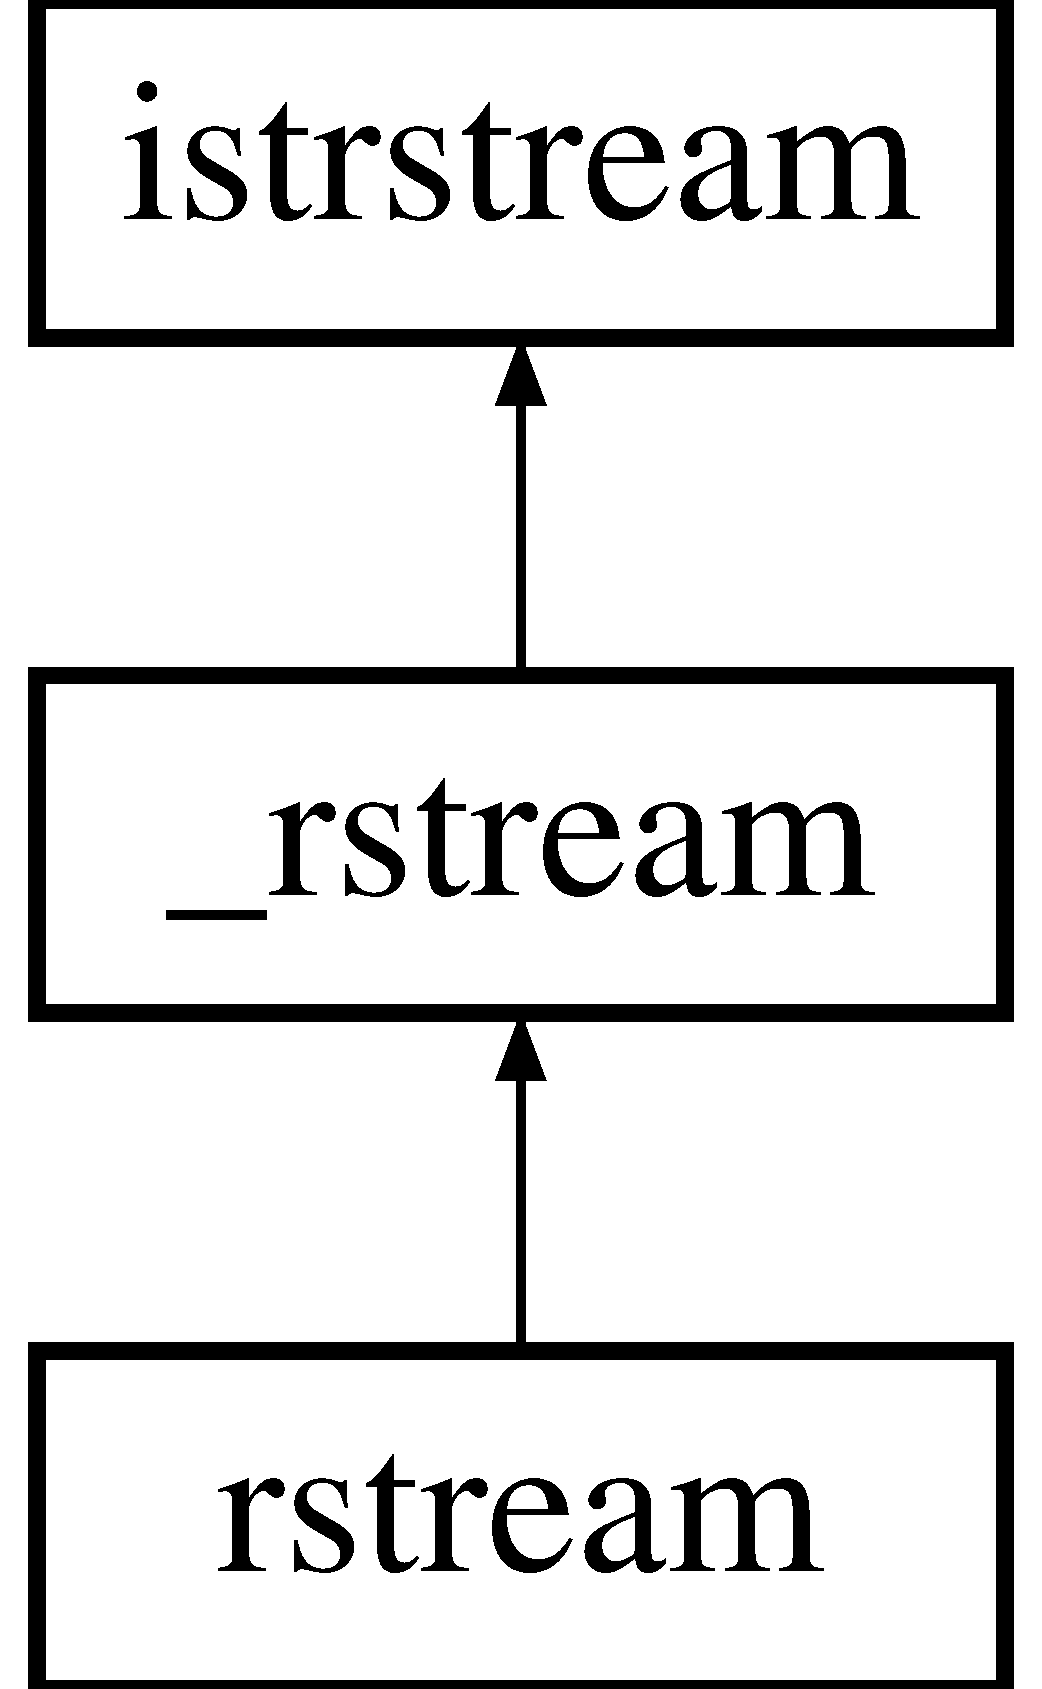
\includegraphics[height=3.000000cm]{class__rstream}
\end{center}
\end{figure}
\subsection*{Protected Member Functions}
\begin{DoxyCompactItemize}
\item 
\hyperlink{class__rstream_a90043965907b6adfdfe529fb6e5be75a}{\-\_\-rstream} (pair$<$ const char $\ast$, streamsize $>$ \hyperlink{ittnotify__static_8h_ab7caea589d3ca96f9f11c78f10bff578}{p})
\item 
\hyperlink{class__rstream_a9c9ab414a63b8b635c07acf25d9bb256}{$\sim$\-\_\-rstream} ()
\end{DoxyCompactItemize}
\subsection*{Private Attributes}
\begin{DoxyCompactItemize}
\item 
const char $\ast$ \hyperlink{class__rstream_aecd5f92faba9be1c69d5c9ad2816fa89}{buf}
\end{DoxyCompactItemize}


\subsection{Detailed Description}


Definition at line 53 of file extract\-External.\-cpp.



\subsection{Constructor \& Destructor Documentation}
\hypertarget{class__rstream_a90043965907b6adfdfe529fb6e5be75a}{\index{\-\_\-rstream@{\-\_\-rstream}!\-\_\-rstream@{\-\_\-rstream}}
\index{\-\_\-rstream@{\-\_\-rstream}!_rstream@{\-\_\-rstream}}
\subsubsection[{\-\_\-rstream}]{\setlength{\rightskip}{0pt plus 5cm}\-\_\-rstream\-::\-\_\-rstream (
\begin{DoxyParamCaption}
\item[{pair$<$ const char $\ast$, streamsize $>$}]{p}
\end{DoxyParamCaption}
)\hspace{0.3cm}{\ttfamily [inline]}, {\ttfamily [protected]}}}\label{class__rstream_a90043965907b6adfdfe529fb6e5be75a}


Definition at line 57 of file extract\-External.\-cpp.


\begin{DoxyCode}
57 :istrstream(\hyperlink{ittnotify__static_8h_ab7caea589d3ca96f9f11c78f10bff578}{p}.first,\hyperlink{ittnotify__static_8h_ab7caea589d3ca96f9f11c78f10bff578}{p}.second),\hyperlink{class__rstream_aecd5f92faba9be1c69d5c9ad2816fa89}{buf}(\hyperlink{ittnotify__static_8h_ab7caea589d3ca96f9f11c78f10bff578}{p}.first)\{\}
\end{DoxyCode}
\hypertarget{class__rstream_a9c9ab414a63b8b635c07acf25d9bb256}{\index{\-\_\-rstream@{\-\_\-rstream}!$\sim$\-\_\-rstream@{$\sim$\-\_\-rstream}}
\index{$\sim$\-\_\-rstream@{$\sim$\-\_\-rstream}!_rstream@{\-\_\-rstream}}
\subsubsection[{$\sim$\-\_\-rstream}]{\setlength{\rightskip}{0pt plus 5cm}\-\_\-rstream\-::$\sim$\-\_\-rstream (
\begin{DoxyParamCaption}
{}
\end{DoxyParamCaption}
)\hspace{0.3cm}{\ttfamily [inline]}, {\ttfamily [protected]}}}\label{class__rstream_a9c9ab414a63b8b635c07acf25d9bb256}


Definition at line 58 of file extract\-External.\-cpp.


\begin{DoxyCode}
58                 \{
59         \textcolor{keyword}{delete}[]\hyperlink{class__rstream_aecd5f92faba9be1c69d5c9ad2816fa89}{buf};
60     \}
\end{DoxyCode}


\subsection{Member Data Documentation}
\hypertarget{class__rstream_aecd5f92faba9be1c69d5c9ad2816fa89}{\index{\-\_\-rstream@{\-\_\-rstream}!buf@{buf}}
\index{buf@{buf}!_rstream@{\-\_\-rstream}}
\subsubsection[{buf}]{\setlength{\rightskip}{0pt plus 5cm}const char$\ast$ \-\_\-rstream\-::buf\hspace{0.3cm}{\ttfamily [private]}}}\label{class__rstream_aecd5f92faba9be1c69d5c9ad2816fa89}


Definition at line 55 of file extract\-External.\-cpp.



The documentation for this class was generated from the following file\-:\begin{DoxyCompactItemize}
\item 
\hyperlink{extractExternal_8cpp}{extract\-External.\-cpp}\end{DoxyCompactItemize}

\hypertarget{classAddress}{\section{Address Class Reference}
\label{classAddress}\index{Address@{Address}}
}


{\ttfamily \#include $<$kmp\-\_\-affinity.\-h$>$}

\subsection*{Public Member Functions}
\begin{DoxyCompactItemize}
\item 
\hyperlink{classAddress_a50c3a5bb9f60be276f7d425a1b373966}{Address} (unsigned \-\_\-depth)
\item 
\hyperlink{classAddress}{Address} \& \hyperlink{classAddress_a16c1cdab8d3345e4237e6209a21422d1}{operator=} (const \hyperlink{classAddress}{Address} \&b)
\item 
bool \hyperlink{classAddress_a2daeaeef46aa7d76d9239da5175eba29}{operator==} (const \hyperlink{classAddress}{Address} \&b) const 
\item 
bool \hyperlink{classAddress_a67cf8a59b7411a21af96bce3081d32a6}{is\-Close} (const \hyperlink{classAddress}{Address} \&b, \hyperlink{ittnotify__static_8h_a8b8dcd723308a8cb5d84277c7a3fff70}{int} level) const 
\item 
bool \hyperlink{classAddress_a971ef7be92846aca64bfa9d96e5a8006}{operator!=} (const \hyperlink{classAddress}{Address} \&b) const 
\item 
\hyperlink{ittnotify__static_8h_af941d56e55e3c5465135b60c4d6343ed}{void} \hyperlink{classAddress_a0bd089006498e492db87e3a9a9c6737b}{print} () const 
\end{DoxyCompactItemize}
\subsection*{Public Attributes}
\begin{DoxyCompactItemize}
\item 
unsigned \hyperlink{classAddress_a0a5fc0038932317cd8f46d802850996a}{labels} \mbox{[}\hyperlink{classAddress_a3c90109b9f20aa28996a78712557683c}{max\-Depth}\mbox{]}
\item 
unsigned \hyperlink{classAddress_aae88cf413f1d90429d34a23387a8fe81}{child\-Nums} \mbox{[}\hyperlink{classAddress_a3c90109b9f20aa28996a78712557683c}{max\-Depth}\mbox{]}
\item 
unsigned \hyperlink{classAddress_a1adef13df4b328813a1bf4b92c56ee10}{depth}
\item 
unsigned \hyperlink{classAddress_ab1535594352babbc297fc1d2b5a48c1a}{leader}
\end{DoxyCompactItemize}
\subsection*{Static Public Attributes}
\begin{DoxyCompactItemize}
\item 
static const unsigned \hyperlink{classAddress_a3c90109b9f20aa28996a78712557683c}{max\-Depth} = 32
\end{DoxyCompactItemize}


\subsection{Detailed Description}


Definition at line 20 of file kmp\-\_\-affinity.\-h.



\subsection{Constructor \& Destructor Documentation}
\hypertarget{classAddress_a50c3a5bb9f60be276f7d425a1b373966}{\index{Address@{Address}!Address@{Address}}
\index{Address@{Address}!Address@{Address}}
\subsubsection[{Address}]{\setlength{\rightskip}{0pt plus 5cm}Address\-::\-Address (
\begin{DoxyParamCaption}
\item[{unsigned}]{\-\_\-depth}
\end{DoxyParamCaption}
)\hspace{0.3cm}{\ttfamily [inline]}}}\label{classAddress_a50c3a5bb9f60be276f7d425a1b373966}


Definition at line 27 of file kmp\-\_\-affinity.\-h.


\begin{DoxyCode}
28       : \hyperlink{classAddress_a1adef13df4b328813a1bf4b92c56ee10}{depth}(\_depth), \hyperlink{classAddress_ab1535594352babbc297fc1d2b5a48c1a}{leader}(\hyperlink{kmp_8h_aa93f0eb578d23995850d61f7d61c55c1}{FALSE}) \{
29     \}
\end{DoxyCode}


\subsection{Member Function Documentation}
\hypertarget{classAddress_a67cf8a59b7411a21af96bce3081d32a6}{\index{Address@{Address}!is\-Close@{is\-Close}}
\index{is\-Close@{is\-Close}!Address@{Address}}
\subsubsection[{is\-Close}]{\setlength{\rightskip}{0pt plus 5cm}bool Address\-::is\-Close (
\begin{DoxyParamCaption}
\item[{const {\bf Address} \&}]{b, }
\item[{{\bf int}}]{level}
\end{DoxyParamCaption}
) const\hspace{0.3cm}{\ttfamily [inline]}}}\label{classAddress_a67cf8a59b7411a21af96bce3081d32a6}


Definition at line 47 of file kmp\-\_\-affinity.\-h.


\begin{DoxyCode}
47                                                     \{
48         \textcolor{keywordflow}{if} (\hyperlink{classAddress_a1adef13df4b328813a1bf4b92c56ee10}{depth} != b.\hyperlink{classAddress_a1adef13df4b328813a1bf4b92c56ee10}{depth})
49             \textcolor{keywordflow}{return} \textcolor{keyword}{false};
50         \textcolor{keywordflow}{if} ((\textcolor{keywordtype}{unsigned})level >= \hyperlink{classAddress_a1adef13df4b328813a1bf4b92c56ee10}{depth})
51             \textcolor{keywordflow}{return} \textcolor{keyword}{true};
52         \textcolor{keywordflow}{for} (\textcolor{keywordtype}{unsigned} \hyperlink{kmp__stub_8c_a08582ce460e3d5e1cf0b7fea017d608e}{i} = 0; \hyperlink{kmp__stub_8c_a08582ce460e3d5e1cf0b7fea017d608e}{i} < (\hyperlink{classAddress_a1adef13df4b328813a1bf4b92c56ee10}{depth} - level); \hyperlink{kmp__stub_8c_a08582ce460e3d5e1cf0b7fea017d608e}{i}++)
53             \textcolor{keywordflow}{if}(\hyperlink{classAddress_a0a5fc0038932317cd8f46d802850996a}{labels}[\hyperlink{kmp__stub_8c_a08582ce460e3d5e1cf0b7fea017d608e}{i}] != b.\hyperlink{classAddress_a0a5fc0038932317cd8f46d802850996a}{labels}[\hyperlink{kmp__stub_8c_a08582ce460e3d5e1cf0b7fea017d608e}{i}])
54                 \textcolor{keywordflow}{return} \textcolor{keyword}{false};
55         \textcolor{keywordflow}{return} \textcolor{keyword}{true};
56     \}
\end{DoxyCode}
\hypertarget{classAddress_a971ef7be92846aca64bfa9d96e5a8006}{\index{Address@{Address}!operator!=@{operator!=}}
\index{operator!=@{operator!=}!Address@{Address}}
\subsubsection[{operator!=}]{\setlength{\rightskip}{0pt plus 5cm}bool Address\-::operator!= (
\begin{DoxyParamCaption}
\item[{const {\bf Address} \&}]{b}
\end{DoxyParamCaption}
) const\hspace{0.3cm}{\ttfamily [inline]}}}\label{classAddress_a971ef7be92846aca64bfa9d96e5a8006}


Definition at line 57 of file kmp\-\_\-affinity.\-h.


\begin{DoxyCode}
57                                             \{
58         \textcolor{keywordflow}{return} !\hyperlink{classAddress_a2daeaeef46aa7d76d9239da5175eba29}{operator==}(b);
59     \}
\end{DoxyCode}
\hypertarget{classAddress_a16c1cdab8d3345e4237e6209a21422d1}{\index{Address@{Address}!operator=@{operator=}}
\index{operator=@{operator=}!Address@{Address}}
\subsubsection[{operator=}]{\setlength{\rightskip}{0pt plus 5cm}{\bf Address}\& Address\-::operator= (
\begin{DoxyParamCaption}
\item[{const {\bf Address} \&}]{b}
\end{DoxyParamCaption}
)\hspace{0.3cm}{\ttfamily [inline]}}}\label{classAddress_a16c1cdab8d3345e4237e6209a21422d1}


Definition at line 30 of file kmp\-\_\-affinity.\-h.


\begin{DoxyCode}
30                                          \{
31         \hyperlink{classAddress_a1adef13df4b328813a1bf4b92c56ee10}{depth} = b.\hyperlink{classAddress_a1adef13df4b328813a1bf4b92c56ee10}{depth};
32         \textcolor{keywordflow}{for} (\textcolor{keywordtype}{unsigned} \hyperlink{kmp__stub_8c_a08582ce460e3d5e1cf0b7fea017d608e}{i} = 0; \hyperlink{kmp__stub_8c_a08582ce460e3d5e1cf0b7fea017d608e}{i} < \hyperlink{classAddress_a1adef13df4b328813a1bf4b92c56ee10}{depth}; \hyperlink{kmp__stub_8c_a08582ce460e3d5e1cf0b7fea017d608e}{i}++) \{
33             \hyperlink{classAddress_a0a5fc0038932317cd8f46d802850996a}{labels}[\hyperlink{kmp__stub_8c_a08582ce460e3d5e1cf0b7fea017d608e}{i}] = b.\hyperlink{classAddress_a0a5fc0038932317cd8f46d802850996a}{labels}[\hyperlink{kmp__stub_8c_a08582ce460e3d5e1cf0b7fea017d608e}{i}];
34             \hyperlink{classAddress_aae88cf413f1d90429d34a23387a8fe81}{childNums}[\hyperlink{kmp__stub_8c_a08582ce460e3d5e1cf0b7fea017d608e}{i}] = b.\hyperlink{classAddress_aae88cf413f1d90429d34a23387a8fe81}{childNums}[\hyperlink{kmp__stub_8c_a08582ce460e3d5e1cf0b7fea017d608e}{i}];
35         \}
36         \hyperlink{classAddress_ab1535594352babbc297fc1d2b5a48c1a}{leader} = \hyperlink{kmp_8h_aa93f0eb578d23995850d61f7d61c55c1}{FALSE};
37         \textcolor{keywordflow}{return} *\textcolor{keyword}{this};
38     \}
\end{DoxyCode}
\hypertarget{classAddress_a2daeaeef46aa7d76d9239da5175eba29}{\index{Address@{Address}!operator==@{operator==}}
\index{operator==@{operator==}!Address@{Address}}
\subsubsection[{operator==}]{\setlength{\rightskip}{0pt plus 5cm}bool Address\-::operator== (
\begin{DoxyParamCaption}
\item[{const {\bf Address} \&}]{b}
\end{DoxyParamCaption}
) const\hspace{0.3cm}{\ttfamily [inline]}}}\label{classAddress_a2daeaeef46aa7d76d9239da5175eba29}


Definition at line 39 of file kmp\-\_\-affinity.\-h.



Referenced by operator!=().


\begin{DoxyCode}
39                                             \{
40         \textcolor{keywordflow}{if} (\hyperlink{classAddress_a1adef13df4b328813a1bf4b92c56ee10}{depth} != b.\hyperlink{classAddress_a1adef13df4b328813a1bf4b92c56ee10}{depth})
41             \textcolor{keywordflow}{return} \textcolor{keyword}{false};
42         \textcolor{keywordflow}{for} (\textcolor{keywordtype}{unsigned} \hyperlink{kmp__stub_8c_a08582ce460e3d5e1cf0b7fea017d608e}{i} = 0; \hyperlink{kmp__stub_8c_a08582ce460e3d5e1cf0b7fea017d608e}{i} < \hyperlink{classAddress_a1adef13df4b328813a1bf4b92c56ee10}{depth}; \hyperlink{kmp__stub_8c_a08582ce460e3d5e1cf0b7fea017d608e}{i}++)
43             \textcolor{keywordflow}{if}(\hyperlink{classAddress_a0a5fc0038932317cd8f46d802850996a}{labels}[\hyperlink{kmp__stub_8c_a08582ce460e3d5e1cf0b7fea017d608e}{i}] != b.\hyperlink{classAddress_a0a5fc0038932317cd8f46d802850996a}{labels}[\hyperlink{kmp__stub_8c_a08582ce460e3d5e1cf0b7fea017d608e}{i}])
44                 \textcolor{keywordflow}{return} \textcolor{keyword}{false};
45         \textcolor{keywordflow}{return} \textcolor{keyword}{true};
46     \}
\end{DoxyCode}
\hypertarget{classAddress_a0bd089006498e492db87e3a9a9c6737b}{\index{Address@{Address}!print@{print}}
\index{print@{print}!Address@{Address}}
\subsubsection[{print}]{\setlength{\rightskip}{0pt plus 5cm}{\bf void} Address\-::print (
\begin{DoxyParamCaption}
{}
\end{DoxyParamCaption}
) const\hspace{0.3cm}{\ttfamily [inline]}}}\label{classAddress_a0bd089006498e492db87e3a9a9c6737b}


Definition at line 60 of file kmp\-\_\-affinity.\-h.



Referenced by Addr\-Uns\-Pair\-::print().


\begin{DoxyCode}
60                        \{
61         \textcolor{keywordtype}{unsigned} \hyperlink{kmp__stub_8c_a08582ce460e3d5e1cf0b7fea017d608e}{i};
62         printf(\textcolor{stringliteral}{"Depth: %u --- "}, \hyperlink{classAddress_a1adef13df4b328813a1bf4b92c56ee10}{depth});
63         \textcolor{keywordflow}{for}(i=0;i<\hyperlink{classAddress_a1adef13df4b328813a1bf4b92c56ee10}{depth};i++) \{
64             printf(\textcolor{stringliteral}{"%u "}, \hyperlink{classAddress_a0a5fc0038932317cd8f46d802850996a}{labels}[i]);
65         \}
66     \}
\end{DoxyCode}


\subsection{Member Data Documentation}
\hypertarget{classAddress_aae88cf413f1d90429d34a23387a8fe81}{\index{Address@{Address}!child\-Nums@{child\-Nums}}
\index{child\-Nums@{child\-Nums}!Address@{Address}}
\subsubsection[{child\-Nums}]{\setlength{\rightskip}{0pt plus 5cm}unsigned Address\-::child\-Nums\mbox{[}{\bf max\-Depth}\mbox{]}}}\label{classAddress_aae88cf413f1d90429d34a23387a8fe81}


Definition at line 24 of file kmp\-\_\-affinity.\-h.



Referenced by \-\_\-\-\_\-kmp\-\_\-affinity\-\_\-cmp\-\_\-\-Address\-\_\-child\-\_\-num(), hierarchy\-\_\-info\-::derive\-Levels(), and operator=().

\hypertarget{classAddress_a1adef13df4b328813a1bf4b92c56ee10}{\index{Address@{Address}!depth@{depth}}
\index{depth@{depth}!Address@{Address}}
\subsubsection[{depth}]{\setlength{\rightskip}{0pt plus 5cm}unsigned Address\-::depth}}\label{classAddress_a1adef13df4b328813a1bf4b92c56ee10}


Definition at line 25 of file kmp\-\_\-affinity.\-h.



Referenced by \-\_\-\-\_\-kmp\-\_\-affinity\-\_\-cmp\-\_\-\-Address\-\_\-child\-\_\-num(), \-\_\-\-\_\-kmp\-\_\-affinity\-\_\-cmp\-\_\-\-Address\-\_\-labels(), hierarchy\-\_\-info\-::derive\-Levels(), is\-Close(), operator=(), operator==(), and print().

\hypertarget{classAddress_a0a5fc0038932317cd8f46d802850996a}{\index{Address@{Address}!labels@{labels}}
\index{labels@{labels}!Address@{Address}}
\subsubsection[{labels}]{\setlength{\rightskip}{0pt plus 5cm}unsigned Address\-::labels\mbox{[}{\bf max\-Depth}\mbox{]}}}\label{classAddress_a0a5fc0038932317cd8f46d802850996a}


Definition at line 23 of file kmp\-\_\-affinity.\-h.



Referenced by \-\_\-\-\_\-kmp\-\_\-affinity\-\_\-cmp\-\_\-\-Address\-\_\-labels(), is\-Close(), operator=(), operator==(), and print().

\hypertarget{classAddress_ab1535594352babbc297fc1d2b5a48c1a}{\index{Address@{Address}!leader@{leader}}
\index{leader@{leader}!Address@{Address}}
\subsubsection[{leader}]{\setlength{\rightskip}{0pt plus 5cm}unsigned Address\-::leader}}\label{classAddress_ab1535594352babbc297fc1d2b5a48c1a}


Definition at line 26 of file kmp\-\_\-affinity.\-h.



Referenced by operator=().

\hypertarget{classAddress_a3c90109b9f20aa28996a78712557683c}{\index{Address@{Address}!max\-Depth@{max\-Depth}}
\index{max\-Depth@{max\-Depth}!Address@{Address}}
\subsubsection[{max\-Depth}]{\setlength{\rightskip}{0pt plus 5cm}const unsigned Address\-::max\-Depth = 32\hspace{0.3cm}{\ttfamily [static]}}}\label{classAddress_a3c90109b9f20aa28996a78712557683c}


Definition at line 22 of file kmp\-\_\-affinity.\-h.



The documentation for this class was generated from the following file\-:\begin{DoxyCompactItemize}
\item 
\hyperlink{kmp__affinity_8h}{kmp\-\_\-affinity.\-h}\end{DoxyCompactItemize}

\hypertarget{classAddrUnsPair}{\section{Addr\-Uns\-Pair Class Reference}
\label{classAddrUnsPair}\index{Addr\-Uns\-Pair@{Addr\-Uns\-Pair}}
}


{\ttfamily \#include $<$kmp\-\_\-affinity.\-h$>$}

\subsection*{Public Member Functions}
\begin{DoxyCompactItemize}
\item 
\hyperlink{classAddrUnsPair_a736ff51c6208c74083b8dc42bd8b5123}{Addr\-Uns\-Pair} (\hyperlink{classAddress}{Address} \-\_\-first, unsigned \-\_\-second)
\item 
\hyperlink{classAddrUnsPair}{Addr\-Uns\-Pair} \& \hyperlink{classAddrUnsPair_a6659b3fd1bd2ffe14a199b39305a2b69}{operator=} (const \hyperlink{classAddrUnsPair}{Addr\-Uns\-Pair} \&b)
\item 
\hyperlink{ittnotify__static_8h_af941d56e55e3c5465135b60c4d6343ed}{void} \hyperlink{classAddrUnsPair_a78d8695fcf76acb6765a6ee1676275a0}{print} () const 
\item 
bool \hyperlink{classAddrUnsPair_ac783e94c518d64ca6f5df1a8a9a437fc}{operator==} (const \hyperlink{classAddrUnsPair}{Addr\-Uns\-Pair} \&b) const 
\item 
bool \hyperlink{classAddrUnsPair_acf8951d00c9ba46651bda36c73541928}{operator!=} (const \hyperlink{classAddrUnsPair}{Addr\-Uns\-Pair} \&b) const 
\end{DoxyCompactItemize}
\subsection*{Public Attributes}
\begin{DoxyCompactItemize}
\item 
\hyperlink{classAddress}{Address} \hyperlink{classAddrUnsPair_a982f64b113d22417f89b279ec24f097e}{first}
\item 
unsigned \hyperlink{classAddrUnsPair_afba7fb1f72a6e49d8024dc37c0bacf1a}{second}
\end{DoxyCompactItemize}


\subsection{Detailed Description}


Definition at line 69 of file kmp\-\_\-affinity.\-h.



\subsection{Constructor \& Destructor Documentation}
\hypertarget{classAddrUnsPair_a736ff51c6208c74083b8dc42bd8b5123}{\index{Addr\-Uns\-Pair@{Addr\-Uns\-Pair}!Addr\-Uns\-Pair@{Addr\-Uns\-Pair}}
\index{Addr\-Uns\-Pair@{Addr\-Uns\-Pair}!AddrUnsPair@{Addr\-Uns\-Pair}}
\subsubsection[{Addr\-Uns\-Pair}]{\setlength{\rightskip}{0pt plus 5cm}Addr\-Uns\-Pair\-::\-Addr\-Uns\-Pair (
\begin{DoxyParamCaption}
\item[{{\bf Address}}]{\-\_\-first, }
\item[{unsigned}]{\-\_\-second}
\end{DoxyParamCaption}
)\hspace{0.3cm}{\ttfamily [inline]}}}\label{classAddrUnsPair_a736ff51c6208c74083b8dc42bd8b5123}


Definition at line 73 of file kmp\-\_\-affinity.\-h.


\begin{DoxyCode}
74       : \hyperlink{classAddrUnsPair_a982f64b113d22417f89b279ec24f097e}{first}(\_first), \hyperlink{classAddrUnsPair_afba7fb1f72a6e49d8024dc37c0bacf1a}{second}(\_second) \{
75     \}
\end{DoxyCode}


\subsection{Member Function Documentation}
\hypertarget{classAddrUnsPair_acf8951d00c9ba46651bda36c73541928}{\index{Addr\-Uns\-Pair@{Addr\-Uns\-Pair}!operator!=@{operator!=}}
\index{operator!=@{operator!=}!AddrUnsPair@{Addr\-Uns\-Pair}}
\subsubsection[{operator!=}]{\setlength{\rightskip}{0pt plus 5cm}bool Addr\-Uns\-Pair\-::operator!= (
\begin{DoxyParamCaption}
\item[{const {\bf Addr\-Uns\-Pair} \&}]{b}
\end{DoxyParamCaption}
) const\hspace{0.3cm}{\ttfamily [inline]}}}\label{classAddrUnsPair_acf8951d00c9ba46651bda36c73541928}


Definition at line 91 of file kmp\-\_\-affinity.\-h.


\begin{DoxyCode}
91                                                 \{
92         \textcolor{keywordflow}{return} !\hyperlink{classAddrUnsPair_ac783e94c518d64ca6f5df1a8a9a437fc}{operator==}(b);
93     \}
\end{DoxyCode}
\hypertarget{classAddrUnsPair_a6659b3fd1bd2ffe14a199b39305a2b69}{\index{Addr\-Uns\-Pair@{Addr\-Uns\-Pair}!operator=@{operator=}}
\index{operator=@{operator=}!AddrUnsPair@{Addr\-Uns\-Pair}}
\subsubsection[{operator=}]{\setlength{\rightskip}{0pt plus 5cm}{\bf Addr\-Uns\-Pair}\& Addr\-Uns\-Pair\-::operator= (
\begin{DoxyParamCaption}
\item[{const {\bf Addr\-Uns\-Pair} \&}]{b}
\end{DoxyParamCaption}
)\hspace{0.3cm}{\ttfamily [inline]}}}\label{classAddrUnsPair_a6659b3fd1bd2ffe14a199b39305a2b69}


Definition at line 76 of file kmp\-\_\-affinity.\-h.


\begin{DoxyCode}
77     \{
78         \hyperlink{classAddrUnsPair_a982f64b113d22417f89b279ec24f097e}{first} = b.\hyperlink{classAddrUnsPair_a982f64b113d22417f89b279ec24f097e}{first};
79         \hyperlink{classAddrUnsPair_afba7fb1f72a6e49d8024dc37c0bacf1a}{second} = b.\hyperlink{classAddrUnsPair_afba7fb1f72a6e49d8024dc37c0bacf1a}{second};
80         \textcolor{keywordflow}{return} *\textcolor{keyword}{this};
81     \}
\end{DoxyCode}
\hypertarget{classAddrUnsPair_ac783e94c518d64ca6f5df1a8a9a437fc}{\index{Addr\-Uns\-Pair@{Addr\-Uns\-Pair}!operator==@{operator==}}
\index{operator==@{operator==}!AddrUnsPair@{Addr\-Uns\-Pair}}
\subsubsection[{operator==}]{\setlength{\rightskip}{0pt plus 5cm}bool Addr\-Uns\-Pair\-::operator== (
\begin{DoxyParamCaption}
\item[{const {\bf Addr\-Uns\-Pair} \&}]{b}
\end{DoxyParamCaption}
) const\hspace{0.3cm}{\ttfamily [inline]}}}\label{classAddrUnsPair_ac783e94c518d64ca6f5df1a8a9a437fc}


Definition at line 86 of file kmp\-\_\-affinity.\-h.



Referenced by operator!=().


\begin{DoxyCode}
86                                                 \{
87         \textcolor{keywordflow}{if}(\hyperlink{classAddrUnsPair_a982f64b113d22417f89b279ec24f097e}{first} != b.\hyperlink{classAddrUnsPair_a982f64b113d22417f89b279ec24f097e}{first}) \textcolor{keywordflow}{return} \textcolor{keyword}{false};
88         \textcolor{keywordflow}{if}(\hyperlink{classAddrUnsPair_afba7fb1f72a6e49d8024dc37c0bacf1a}{second} != b.\hyperlink{classAddrUnsPair_afba7fb1f72a6e49d8024dc37c0bacf1a}{second}) \textcolor{keywordflow}{return} \textcolor{keyword}{false};
89         \textcolor{keywordflow}{return} \textcolor{keyword}{true};
90     \}
\end{DoxyCode}
\hypertarget{classAddrUnsPair_a78d8695fcf76acb6765a6ee1676275a0}{\index{Addr\-Uns\-Pair@{Addr\-Uns\-Pair}!print@{print}}
\index{print@{print}!AddrUnsPair@{Addr\-Uns\-Pair}}
\subsubsection[{print}]{\setlength{\rightskip}{0pt plus 5cm}{\bf void} Addr\-Uns\-Pair\-::print (
\begin{DoxyParamCaption}
{}
\end{DoxyParamCaption}
) const\hspace{0.3cm}{\ttfamily [inline]}}}\label{classAddrUnsPair_a78d8695fcf76acb6765a6ee1676275a0}


Definition at line 82 of file kmp\-\_\-affinity.\-h.


\begin{DoxyCode}
82                        \{
83         printf(\textcolor{stringliteral}{"first = "}); \hyperlink{classAddrUnsPair_a982f64b113d22417f89b279ec24f097e}{first}.\hyperlink{classAddress_a0bd089006498e492db87e3a9a9c6737b}{print}();
84         printf(\textcolor{stringliteral}{" --- second = %u"}, \hyperlink{classAddrUnsPair_afba7fb1f72a6e49d8024dc37c0bacf1a}{second});
85     \}
\end{DoxyCode}


\subsection{Member Data Documentation}
\hypertarget{classAddrUnsPair_a982f64b113d22417f89b279ec24f097e}{\index{Addr\-Uns\-Pair@{Addr\-Uns\-Pair}!first@{first}}
\index{first@{first}!AddrUnsPair@{Addr\-Uns\-Pair}}
\subsubsection[{first}]{\setlength{\rightskip}{0pt plus 5cm}{\bf Address} Addr\-Uns\-Pair\-::first}}\label{classAddrUnsPair_a982f64b113d22417f89b279ec24f097e}


Definition at line 71 of file kmp\-\_\-affinity.\-h.



Referenced by hierarchy\-\_\-info\-::derive\-Levels(), operator=(), operator==(), and print().

\hypertarget{classAddrUnsPair_afba7fb1f72a6e49d8024dc37c0bacf1a}{\index{Addr\-Uns\-Pair@{Addr\-Uns\-Pair}!second@{second}}
\index{second@{second}!AddrUnsPair@{Addr\-Uns\-Pair}}
\subsubsection[{second}]{\setlength{\rightskip}{0pt plus 5cm}unsigned Addr\-Uns\-Pair\-::second}}\label{classAddrUnsPair_afba7fb1f72a6e49d8024dc37c0bacf1a}


Definition at line 72 of file kmp\-\_\-affinity.\-h.



Referenced by operator=(), operator==(), and print().



The documentation for this class was generated from the following file\-:\begin{DoxyCompactItemize}
\item 
\hyperlink{kmp__affinity_8h}{kmp\-\_\-affinity.\-h}\end{DoxyCompactItemize}

\hypertarget{structbdhead}{\section{bdhead Struct Reference}
\label{structbdhead}\index{bdhead@{bdhead}}
}
\subsection*{Public Attributes}
\begin{DoxyCompactItemize}
\item 
\hyperlink{kmp__alloc_8c_acb70eb20828ff76ed9200989f7dcd043}{bufsize} \hyperlink{structbdhead_aac93883268daeee61a9fc08d36a76147}{tsize}
\item 
\hyperlink{kmp__alloc_8c_af1de790fdc3ba84111ab8cd6730510bd}{bhead\-\_\-t} \hyperlink{structbdhead_a18184e6403b513e03bfc8c3e91fb5aa4}{bh}
\end{DoxyCompactItemize}


\subsection{Detailed Description}


Definition at line 185 of file kmp\-\_\-alloc.\-c.



\subsection{Member Data Documentation}
\hypertarget{structbdhead_a18184e6403b513e03bfc8c3e91fb5aa4}{\index{bdhead@{bdhead}!bh@{bh}}
\index{bh@{bh}!bdhead@{bdhead}}
\subsubsection[{bh}]{\setlength{\rightskip}{0pt plus 5cm}{\bf bhead\-\_\-t} bdhead\-::bh}}\label{structbdhead_a18184e6403b513e03bfc8c3e91fb5aa4}


Definition at line 188 of file kmp\-\_\-alloc.\-c.



Referenced by bget().

\hypertarget{structbdhead_aac93883268daeee61a9fc08d36a76147}{\index{bdhead@{bdhead}!tsize@{tsize}}
\index{tsize@{tsize}!bdhead@{bdhead}}
\subsubsection[{tsize}]{\setlength{\rightskip}{0pt plus 5cm}{\bf bufsize} bdhead\-::tsize}}\label{structbdhead_aac93883268daeee61a9fc08d36a76147}


Definition at line 187 of file kmp\-\_\-alloc.\-c.



Referenced by bget(), bgetr(), bgetz(), and brel().



The documentation for this struct was generated from the following file\-:\begin{DoxyCompactItemize}
\item 
\hyperlink{kmp__alloc_8c}{kmp\-\_\-alloc.\-c}\end{DoxyCompactItemize}

\hypertarget{structbfhead}{\section{bfhead Struct Reference}
\label{structbfhead}\index{bfhead@{bfhead}}
}
\subsection*{Public Attributes}
\begin{DoxyCompactItemize}
\item 
\hyperlink{kmp__alloc_8c_af1de790fdc3ba84111ab8cd6730510bd}{bhead\-\_\-t} \hyperlink{structbfhead_a75547156d52c89826f1e0d711014f77a}{bh}
\item 
\hyperlink{kmp__alloc_8c_a9059958aafec0d30537fe432f36b6665}{qlinks\-\_\-t} \hyperlink{structbfhead_adc2c1c9fc5b4081009c158da12064bfe}{ql}
\end{DoxyCompactItemize}


\subsection{Detailed Description}


Definition at line 194 of file kmp\-\_\-alloc.\-c.



\subsection{Member Data Documentation}
\hypertarget{structbfhead_a75547156d52c89826f1e0d711014f77a}{\index{bfhead@{bfhead}!bh@{bh}}
\index{bh@{bh}!bfhead@{bfhead}}
\subsubsection[{bh}]{\setlength{\rightskip}{0pt plus 5cm}{\bf bhead\-\_\-t} bfhead\-::bh}}\label{structbfhead_a75547156d52c89826f1e0d711014f77a}


Definition at line 195 of file kmp\-\_\-alloc.\-c.



Referenced by \-\_\-\-\_\-kmp\-\_\-bget\-\_\-dequeue(), \-\_\-\-\_\-kmp\-\_\-bget\-\_\-enqueue(), \-\_\-\-\_\-kmp\-\_\-finalize\-\_\-bget(), \-\_\-\-\_\-kmp\-\_\-free\-\_\-fast\-\_\-memory(), bcheck(), bfreed(), bget(), bpool(), and brel().

\hypertarget{structbfhead_adc2c1c9fc5b4081009c158da12064bfe}{\index{bfhead@{bfhead}!ql@{ql}}
\index{ql@{ql}!bfhead@{bfhead}}
\subsubsection[{ql}]{\setlength{\rightskip}{0pt plus 5cm}{\bf qlinks\-\_\-t} bfhead\-::ql}}\label{structbfhead_adc2c1c9fc5b4081009c158da12064bfe}


Definition at line 196 of file kmp\-\_\-alloc.\-c.



Referenced by \-\_\-\-\_\-kmp\-\_\-bget\-\_\-dequeue(), \-\_\-\-\_\-kmp\-\_\-bget\-\_\-enqueue(), \-\_\-\-\_\-kmp\-\_\-bget\-\_\-insert\-\_\-into\-\_\-freelist(), \-\_\-\-\_\-kmp\-\_\-bget\-\_\-remove\-\_\-from\-\_\-freelist(), \-\_\-\-\_\-kmp\-\_\-free\-\_\-fast\-\_\-memory(), bcheck(), bfreed(), bget(), and set\-\_\-thr\-\_\-data().



The documentation for this struct was generated from the following file\-:\begin{DoxyCompactItemize}
\item 
\hyperlink{kmp__alloc_8c}{kmp\-\_\-alloc.\-c}\end{DoxyCompactItemize}

\hypertarget{unionbhead}{\section{bhead Union Reference}
\label{unionbhead}\index{bhead@{bhead}}
}
\subsection*{Public Attributes}
\begin{DoxyCompactItemize}
\item 
\hyperlink{kmp__alloc_8c_adaab326653e74716055fed800f3797e7}{Align\-Type} \hyperlink{unionbhead_a625600af39c889888813aeae7f0dd8e3}{b\-\_\-align}
\item 
char \hyperlink{unionbhead_aad3bcf2ab7e479e8e8c918f4659ba445}{b\-\_\-pad} \mbox{[}sizeof(\hyperlink{kmp__alloc_8c_a9651d02bd00b58901a4d1d9af7df824d}{bhead2\-\_\-t})+(\hyperlink{kmp__alloc_8c_a5c41333bbc87068897a3c879fa16fb85}{Size\-Quant}-\/(sizeof(\hyperlink{kmp__alloc_8c_a9651d02bd00b58901a4d1d9af7df824d}{bhead2\-\_\-t})\%\hyperlink{kmp__alloc_8c_a5c41333bbc87068897a3c879fa16fb85}{Size\-Quant}))\mbox{]}
\item 
\hyperlink{kmp__alloc_8c_a9651d02bd00b58901a4d1d9af7df824d}{bhead2\-\_\-t} \hyperlink{unionbhead_ab99fcbcc7514c17564d6e3fca349903a}{bb}
\end{DoxyCompactItemize}


\subsection{Detailed Description}


Definition at line 175 of file kmp\-\_\-alloc.\-c.



\subsection{Member Data Documentation}
\hypertarget{unionbhead_a625600af39c889888813aeae7f0dd8e3}{\index{bhead@{bhead}!b\-\_\-align@{b\-\_\-align}}
\index{b\-\_\-align@{b\-\_\-align}!bhead@{bhead}}
\subsubsection[{b\-\_\-align}]{\setlength{\rightskip}{0pt plus 5cm}{\bf Align\-Type} bhead\-::b\-\_\-align}}\label{unionbhead_a625600af39c889888813aeae7f0dd8e3}


Definition at line 177 of file kmp\-\_\-alloc.\-c.

\hypertarget{unionbhead_aad3bcf2ab7e479e8e8c918f4659ba445}{\index{bhead@{bhead}!b\-\_\-pad@{b\-\_\-pad}}
\index{b\-\_\-pad@{b\-\_\-pad}!bhead@{bhead}}
\subsubsection[{b\-\_\-pad}]{\setlength{\rightskip}{0pt plus 5cm}char bhead\-::b\-\_\-pad\mbox{[}sizeof({\bf bhead2\-\_\-t})+({\bf Size\-Quant}-\/(sizeof({\bf bhead2\-\_\-t})\%{\bf Size\-Quant}))\mbox{]}}}\label{unionbhead_aad3bcf2ab7e479e8e8c918f4659ba445}


Definition at line 178 of file kmp\-\_\-alloc.\-c.

\hypertarget{unionbhead_ab99fcbcc7514c17564d6e3fca349903a}{\index{bhead@{bhead}!bb@{bb}}
\index{bb@{bb}!bhead@{bhead}}
\subsubsection[{bb}]{\setlength{\rightskip}{0pt plus 5cm}{\bf bhead2\-\_\-t} bhead\-::bb}}\label{unionbhead_ab99fcbcc7514c17564d6e3fca349903a}


Definition at line 179 of file kmp\-\_\-alloc.\-c.



Referenced by \-\_\-\-\_\-kmp\-\_\-bget\-\_\-dequeue(), \-\_\-\-\_\-kmp\-\_\-bget\-\_\-enqueue(), \-\_\-\-\_\-kmp\-\_\-finalize\-\_\-bget(), \-\_\-\-\_\-kmp\-\_\-free\-\_\-fast\-\_\-memory(), bcheck(), bfreed(), bget(), bgetr(), bgetz(), bpool(), and brel().



The documentation for this union was generated from the following file\-:\begin{DoxyCompactItemize}
\item 
\hyperlink{kmp__alloc_8c}{kmp\-\_\-alloc.\-c}\end{DoxyCompactItemize}

\hypertarget{structbhead2}{\section{bhead2 Struct Reference}
\label{structbhead2}\index{bhead2@{bhead2}}
}
\subsection*{Public Attributes}
\begin{DoxyCompactItemize}
\item 
\hyperlink{kmp_8h_a194859801fe16b326efe34501a37c30a}{kmp\-\_\-info\-\_\-t} $\ast$ \hyperlink{structbhead2_a641b1866310f899813f98a52a287a32e}{bthr}
\item 
\hyperlink{kmp__alloc_8c_acb70eb20828ff76ed9200989f7dcd043}{bufsize} \hyperlink{structbhead2_a2d15b44cc33113af141a1ed4e66f3ad0}{prevfree}
\item 
\hyperlink{kmp__alloc_8c_acb70eb20828ff76ed9200989f7dcd043}{bufsize} \hyperlink{structbhead2_a880c94691872eca4d73d3933c49a40cf}{bsize}
\end{DoxyCompactItemize}


\subsection{Detailed Description}


Definition at line 164 of file kmp\-\_\-alloc.\-c.



\subsection{Member Data Documentation}
\hypertarget{structbhead2_a880c94691872eca4d73d3933c49a40cf}{\index{bhead2@{bhead2}!bsize@{bsize}}
\index{bsize@{bsize}!bhead2@{bhead2}}
\subsubsection[{bsize}]{\setlength{\rightskip}{0pt plus 5cm}{\bf bufsize} bhead2\-::bsize}}\label{structbhead2_a880c94691872eca4d73d3933c49a40cf}


Definition at line 169 of file kmp\-\_\-alloc.\-c.



Referenced by \-\_\-\-\_\-kmp\-\_\-bget\-\_\-dequeue(), \-\_\-\-\_\-kmp\-\_\-bget\-\_\-enqueue(), \-\_\-\-\_\-kmp\-\_\-finalize\-\_\-bget(), bcheck(), bfreed(), bget(), bgetr(), bgetz(), bpool(), and brel().

\hypertarget{structbhead2_a641b1866310f899813f98a52a287a32e}{\index{bhead2@{bhead2}!bthr@{bthr}}
\index{bthr@{bthr}!bhead2@{bhead2}}
\subsubsection[{bthr}]{\setlength{\rightskip}{0pt plus 5cm}{\bf kmp\-\_\-info\-\_\-t}$\ast$ bhead2\-::bthr}}\label{structbhead2_a641b1866310f899813f98a52a287a32e}


Definition at line 165 of file kmp\-\_\-alloc.\-c.



Referenced by \-\_\-\-\_\-kmp\-\_\-bget\-\_\-dequeue(), \-\_\-\-\_\-kmp\-\_\-bget\-\_\-enqueue(), \-\_\-\-\_\-kmp\-\_\-free\-\_\-fast\-\_\-memory(), bget(), bpool(), and brel().

\hypertarget{structbhead2_a2d15b44cc33113af141a1ed4e66f3ad0}{\index{bhead2@{bhead2}!prevfree@{prevfree}}
\index{prevfree@{prevfree}!bhead2@{bhead2}}
\subsubsection[{prevfree}]{\setlength{\rightskip}{0pt plus 5cm}{\bf bufsize} bhead2\-::prevfree}}\label{structbhead2_a2d15b44cc33113af141a1ed4e66f3ad0}


Definition at line 166 of file kmp\-\_\-alloc.\-c.



Referenced by \-\_\-\-\_\-kmp\-\_\-finalize\-\_\-bget(), bget(), bpool(), and brel().



The documentation for this struct was generated from the following file\-:\begin{DoxyCompactItemize}
\item 
\hyperlink{kmp__alloc_8c}{kmp\-\_\-alloc.\-c}\end{DoxyCompactItemize}

\hypertarget{classblockTimer}{\section{block\-Timer Class Reference}
\label{classblockTimer}\index{block\-Timer@{block\-Timer}}
}


{\ttfamily \#include $<$kmp\-\_\-stats.\-h$>$}

Inheritance diagram for block\-Timer\-:\begin{figure}[H]
\begin{center}
\leavevmode
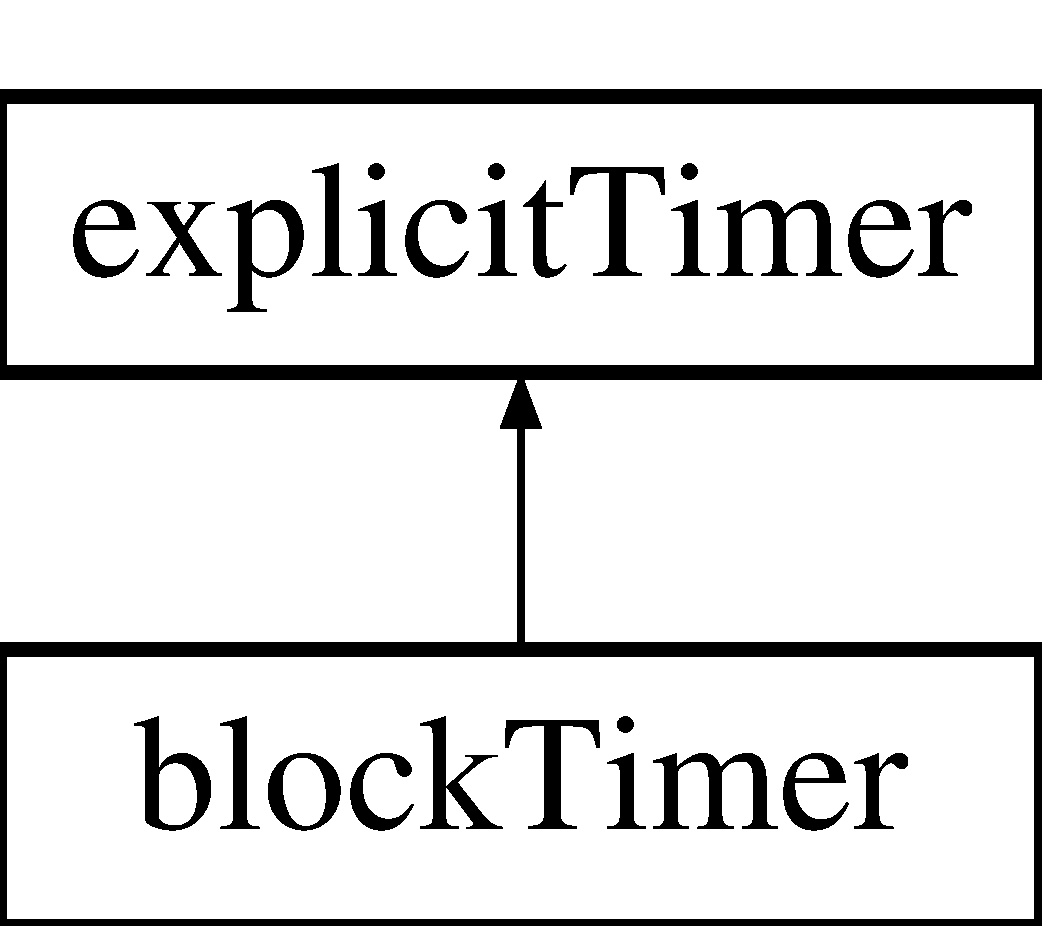
\includegraphics[height=2.000000cm]{classblockTimer}
\end{center}
\end{figure}
\subsection*{Public Member Functions}
\begin{DoxyCompactItemize}
\item 
\hyperlink{classblockTimer_aa7980b081a494a7d2f5a9c1dbf2eb055}{block\-Timer} (\hyperlink{classtimeStat}{time\-Stat} $\ast$\hyperlink{ittnotify__static_8h_a110bd9ede250f97ce56d81bb3c7b171d}{s}, \hyperlink{kmp__stats_8h_ae03f1e0ff609f86afa9b7167a12c6c06}{timer\-\_\-e} new\-Timer\-Enum\-Value)
\item 
\hyperlink{classblockTimer_a7a1dd10314b77b2dfb1a5712538d90b2}{$\sim$block\-Timer} ()
\end{DoxyCompactItemize}
\subsection*{Private Attributes}
\begin{DoxyCompactItemize}
\item 
\hyperlink{kmp__stats_8h_ae03f1e0ff609f86afa9b7167a12c6c06}{timer\-\_\-e} \hyperlink{classblockTimer_a2d8be4c2338d519b503542e1ddd07060}{timer\-Enum\-Value}
\end{DoxyCompactItemize}


\subsection{Detailed Description}


Definition at line 310 of file kmp\-\_\-stats.\-h.



\subsection{Constructor \& Destructor Documentation}
\hypertarget{classblockTimer_aa7980b081a494a7d2f5a9c1dbf2eb055}{\index{block\-Timer@{block\-Timer}!block\-Timer@{block\-Timer}}
\index{block\-Timer@{block\-Timer}!blockTimer@{block\-Timer}}
\subsubsection[{block\-Timer}]{\setlength{\rightskip}{0pt plus 5cm}block\-Timer\-::block\-Timer (
\begin{DoxyParamCaption}
\item[{{\bf time\-Stat} $\ast$}]{s, }
\item[{{\bf timer\-\_\-e}}]{new\-Timer\-Enum\-Value}
\end{DoxyParamCaption}
)\hspace{0.3cm}{\ttfamily [inline]}}}\label{classblockTimer_aa7980b081a494a7d2f5a9c1dbf2eb055}


Definition at line 314 of file kmp\-\_\-stats.\-h.


\begin{DoxyCode}
314 : \hyperlink{classblockTimer_a2d8be4c2338d519b503542e1ddd07060}{timerEnumValue}(newTimerEnumValue), \hyperlink{classexplicitTimer_a6c4946c5479d998e1e12610cd8ca2fe6}{explicitTimer}(s) \{ 
      \hyperlink{classexplicitTimer_a0650affa704a742ae6aae4bf569e964c}{start}(\hyperlink{classblockTimer_a2d8be4c2338d519b503542e1ddd07060}{timerEnumValue}); \}
\end{DoxyCode}
\hypertarget{classblockTimer_a7a1dd10314b77b2dfb1a5712538d90b2}{\index{block\-Timer@{block\-Timer}!$\sim$block\-Timer@{$\sim$block\-Timer}}
\index{$\sim$block\-Timer@{$\sim$block\-Timer}!blockTimer@{block\-Timer}}
\subsubsection[{$\sim$block\-Timer}]{\setlength{\rightskip}{0pt plus 5cm}block\-Timer\-::$\sim$block\-Timer (
\begin{DoxyParamCaption}
{}
\end{DoxyParamCaption}
)\hspace{0.3cm}{\ttfamily [inline]}}}\label{classblockTimer_a7a1dd10314b77b2dfb1a5712538d90b2}


Definition at line 315 of file kmp\-\_\-stats.\-h.


\begin{DoxyCode}
315 \{ \hyperlink{classexplicitTimer_a1a3507bd5e0661935ee7766580244051}{stop}(\hyperlink{classblockTimer_a2d8be4c2338d519b503542e1ddd07060}{timerEnumValue}); \}
\end{DoxyCode}


\subsection{Member Data Documentation}
\hypertarget{classblockTimer_a2d8be4c2338d519b503542e1ddd07060}{\index{block\-Timer@{block\-Timer}!timer\-Enum\-Value@{timer\-Enum\-Value}}
\index{timer\-Enum\-Value@{timer\-Enum\-Value}!blockTimer@{block\-Timer}}
\subsubsection[{timer\-Enum\-Value}]{\setlength{\rightskip}{0pt plus 5cm}{\bf timer\-\_\-e} block\-Timer\-::timer\-Enum\-Value\hspace{0.3cm}{\ttfamily [private]}}}\label{classblockTimer_a2d8be4c2338d519b503542e1ddd07060}


Definition at line 312 of file kmp\-\_\-stats.\-h.



Referenced by block\-Timer(), and $\sim$block\-Timer().



The documentation for this class was generated from the following file\-:\begin{DoxyCompactItemize}
\item 
\hyperlink{kmp__stats_8h}{kmp\-\_\-stats.\-h}\end{DoxyCompactItemize}

\hypertarget{structCLIENT__ID}{\section{C\-L\-I\-E\-N\-T\-\_\-\-I\-D Struct Reference}
\label{structCLIENT__ID}\index{C\-L\-I\-E\-N\-T\-\_\-\-I\-D@{C\-L\-I\-E\-N\-T\-\_\-\-I\-D}}
}
\subsection*{Public Attributes}
\begin{DoxyCompactItemize}
\item 
H\-A\-N\-D\-L\-E \hyperlink{structCLIENT__ID_a49bc0496fea8ea6523f4eb37fb739a89}{Unique\-Process}
\item 
H\-A\-N\-D\-L\-E \hyperlink{structCLIENT__ID_af4423c30ef34cc546bbc23a7c783e6e3}{Unique\-Thread}
\end{DoxyCompactItemize}


\subsection{Detailed Description}


Definition at line 33 of file z\-\_\-\-Windows\-\_\-\-N\-T\-\_\-util.\-c.



\subsection{Member Data Documentation}
\hypertarget{structCLIENT__ID_a49bc0496fea8ea6523f4eb37fb739a89}{\index{C\-L\-I\-E\-N\-T\-\_\-\-I\-D@{C\-L\-I\-E\-N\-T\-\_\-\-I\-D}!Unique\-Process@{Unique\-Process}}
\index{Unique\-Process@{Unique\-Process}!CLIENT_ID@{C\-L\-I\-E\-N\-T\-\_\-\-I\-D}}
\subsubsection[{Unique\-Process}]{\setlength{\rightskip}{0pt plus 5cm}H\-A\-N\-D\-L\-E C\-L\-I\-E\-N\-T\-\_\-\-I\-D\-::\-Unique\-Process}}\label{structCLIENT__ID_a49bc0496fea8ea6523f4eb37fb739a89}


Definition at line 34 of file z\-\_\-\-Windows\-\_\-\-N\-T\-\_\-util.\-c.

\hypertarget{structCLIENT__ID_af4423c30ef34cc546bbc23a7c783e6e3}{\index{C\-L\-I\-E\-N\-T\-\_\-\-I\-D@{C\-L\-I\-E\-N\-T\-\_\-\-I\-D}!Unique\-Thread@{Unique\-Thread}}
\index{Unique\-Thread@{Unique\-Thread}!CLIENT_ID@{C\-L\-I\-E\-N\-T\-\_\-\-I\-D}}
\subsubsection[{Unique\-Thread}]{\setlength{\rightskip}{0pt plus 5cm}H\-A\-N\-D\-L\-E C\-L\-I\-E\-N\-T\-\_\-\-I\-D\-::\-Unique\-Thread}}\label{structCLIENT__ID_af4423c30ef34cc546bbc23a7c783e6e3}


Definition at line 35 of file z\-\_\-\-Windows\-\_\-\-N\-T\-\_\-util.\-c.



The documentation for this struct was generated from the following file\-:\begin{DoxyCompactItemize}
\item 
\hyperlink{z__Windows__NT__util_8c}{z\-\_\-\-Windows\-\_\-\-N\-T\-\_\-util.\-c}\end{DoxyCompactItemize}

\hypertarget{structcommon__table}{\section{common\-\_\-table Struct Reference}
\label{structcommon__table}\index{common\-\_\-table@{common\-\_\-table}}
}


{\ttfamily \#include $<$kmp.\-h$>$}

\subsection*{Public Attributes}
\begin{DoxyCompactItemize}
\item 
struct \hyperlink{structprivate__common}{private\-\_\-common} $\ast$ \hyperlink{structcommon__table_a87c62cea9e986994ca363b2630291621}{data} \mbox{[}\hyperlink{kmp_8h_a18bbfe585fccb920012f9477c07977b7}{K\-M\-P\-\_\-\-H\-A\-S\-H\-\_\-\-T\-A\-B\-L\-E\-\_\-\-S\-I\-Z\-E}\mbox{]}
\end{DoxyCompactItemize}


\subsection{Detailed Description}


Definition at line 1520 of file kmp.\-h.



\subsection{Member Data Documentation}
\hypertarget{structcommon__table_a87c62cea9e986994ca363b2630291621}{\index{common\-\_\-table@{common\-\_\-table}!data@{data}}
\index{data@{data}!common_table@{common\-\_\-table}}
\subsubsection[{data}]{\setlength{\rightskip}{0pt plus 5cm}struct {\bf private\-\_\-common}$\ast$ common\-\_\-table\-::data\mbox{[}{\bf K\-M\-P\-\_\-\-H\-A\-S\-H\-\_\-\-T\-A\-B\-L\-E\-\_\-\-S\-I\-Z\-E}\mbox{]}}}\label{structcommon__table_a87c62cea9e986994ca363b2630291621}


Definition at line 1521 of file kmp.\-h.



Referenced by \-\_\-\-\_\-kmp\-\_\-threadprivate\-\_\-find\-\_\-task\-\_\-common().



The documentation for this struct was generated from the following file\-:\begin{DoxyCompactItemize}
\item 
\hyperlink{kmp_8h}{kmp.\-h}\end{DoxyCompactItemize}

\hypertarget{structcons__data}{\section{cons\-\_\-data Struct Reference}
\label{structcons__data}\index{cons\-\_\-data@{cons\-\_\-data}}
}


{\ttfamily \#include $<$kmp.\-h$>$}

\subsection*{Public Attributes}
\begin{DoxyCompactItemize}
\item 
\hyperlink{group__BASIC__TYPES_ga690fda6b92f039a72db263c6b4394ddb}{ident\-\_\-t} const $\ast$ \hyperlink{structcons__data_a0c586fe208c4f8a2f7deaf145710045b}{ident}
\item 
enum \hyperlink{kmp_8h_a1582e7ddc609220a660d10244ef3e315}{cons\-\_\-type} \hyperlink{structcons__data_a6e32717dd06d661e44e920a0b2d35db3}{type}
\item 
\hyperlink{ittnotify__static_8h_a8b8dcd723308a8cb5d84277c7a3fff70}{int} \hyperlink{structcons__data_ac25aa2afe905faf60427d1590f7795eb}{prev}
\item 
\hyperlink{kmp__lock_8h_a35c88b3ea74b2a8d633ec8156c1c4670}{kmp\-\_\-user\-\_\-lock\-\_\-p} \hyperlink{structcons__data_a2505ac1ca9e905c68f9770d7bfc41214}{name}
\end{DoxyCompactItemize}


\subsection{Detailed Description}


Definition at line 1185 of file kmp.\-h.



\subsection{Member Data Documentation}
\hypertarget{structcons__data_a0c586fe208c4f8a2f7deaf145710045b}{\index{cons\-\_\-data@{cons\-\_\-data}!ident@{ident}}
\index{ident@{ident}!cons_data@{cons\-\_\-data}}
\subsubsection[{ident}]{\setlength{\rightskip}{0pt plus 5cm}{\bf ident\-\_\-t} const$\ast$ cons\-\_\-data\-::ident}}\label{structcons__data_a0c586fe208c4f8a2f7deaf145710045b}


Definition at line 1186 of file kmp.\-h.



Referenced by \-\_\-\-\_\-kmp\-\_\-allocate\-\_\-cons\-\_\-stack(), \-\_\-\-\_\-kmp\-\_\-check\-\_\-sync(), \-\_\-\-\_\-kmp\-\_\-error\-\_\-construct2(), \-\_\-\-\_\-kmp\-\_\-pop\-\_\-parallel(), \-\_\-\-\_\-kmp\-\_\-pop\-\_\-sync(), \-\_\-\-\_\-kmp\-\_\-pop\-\_\-workshare(), \-\_\-\-\_\-kmp\-\_\-push\-\_\-parallel(), \-\_\-\-\_\-kmp\-\_\-push\-\_\-sync(), and \-\_\-\-\_\-kmp\-\_\-push\-\_\-workshare().

\hypertarget{structcons__data_a2505ac1ca9e905c68f9770d7bfc41214}{\index{cons\-\_\-data@{cons\-\_\-data}!name@{name}}
\index{name@{name}!cons_data@{cons\-\_\-data}}
\subsubsection[{name}]{\setlength{\rightskip}{0pt plus 5cm}{\bf kmp\-\_\-user\-\_\-lock\-\_\-p} cons\-\_\-data\-::name}}\label{structcons__data_a2505ac1ca9e905c68f9770d7bfc41214}


Definition at line 1189 of file kmp.\-h.



Referenced by \-\_\-\-\_\-kmp\-\_\-check\-\_\-sync(), \-\_\-\-\_\-kmp\-\_\-push\-\_\-parallel(), \-\_\-\-\_\-kmp\-\_\-push\-\_\-sync(), and \-\_\-\-\_\-kmp\-\_\-push\-\_\-workshare().

\hypertarget{structcons__data_ac25aa2afe905faf60427d1590f7795eb}{\index{cons\-\_\-data@{cons\-\_\-data}!prev@{prev}}
\index{prev@{prev}!cons_data@{cons\-\_\-data}}
\subsubsection[{prev}]{\setlength{\rightskip}{0pt plus 5cm}{\bf int} cons\-\_\-data\-::prev}}\label{structcons__data_ac25aa2afe905faf60427d1590f7795eb}


Definition at line 1188 of file kmp.\-h.



Referenced by \-\_\-\-\_\-kmp\-\_\-allocate\-\_\-cons\-\_\-stack(), \-\_\-\-\_\-kmp\-\_\-check\-\_\-sync(), \-\_\-\-\_\-kmp\-\_\-pop\-\_\-parallel(), \-\_\-\-\_\-kmp\-\_\-pop\-\_\-sync(), \-\_\-\-\_\-kmp\-\_\-pop\-\_\-workshare(), \-\_\-\-\_\-kmp\-\_\-push\-\_\-parallel(), \-\_\-\-\_\-kmp\-\_\-push\-\_\-sync(), and \-\_\-\-\_\-kmp\-\_\-push\-\_\-workshare().

\hypertarget{structcons__data_a6e32717dd06d661e44e920a0b2d35db3}{\index{cons\-\_\-data@{cons\-\_\-data}!type@{type}}
\index{type@{type}!cons_data@{cons\-\_\-data}}
\subsubsection[{type}]{\setlength{\rightskip}{0pt plus 5cm}enum {\bf cons\-\_\-type} cons\-\_\-data\-::type}}\label{structcons__data_a6e32717dd06d661e44e920a0b2d35db3}


Definition at line 1187 of file kmp.\-h.



Referenced by \-\_\-\-\_\-kmp\-\_\-allocate\-\_\-cons\-\_\-stack(), \-\_\-\-\_\-kmp\-\_\-check\-\_\-sync(), \-\_\-\-\_\-kmp\-\_\-check\-\_\-workshare(), \-\_\-\-\_\-kmp\-\_\-error\-\_\-construct2(), \-\_\-\-\_\-kmp\-\_\-pop\-\_\-parallel(), \-\_\-\-\_\-kmp\-\_\-pop\-\_\-sync(), \-\_\-\-\_\-kmp\-\_\-pop\-\_\-workshare(), \-\_\-\-\_\-kmp\-\_\-push\-\_\-parallel(), \-\_\-\-\_\-kmp\-\_\-push\-\_\-sync(), and \-\_\-\-\_\-kmp\-\_\-push\-\_\-workshare().



The documentation for this struct was generated from the following file\-:\begin{DoxyCompactItemize}
\item 
\hyperlink{kmp_8h}{kmp.\-h}\end{DoxyCompactItemize}

\hypertarget{structcons__header}{\section{cons\-\_\-header Struct Reference}
\label{structcons__header}\index{cons\-\_\-header@{cons\-\_\-header}}
}


{\ttfamily \#include $<$kmp.\-h$>$}

\subsection*{Public Attributes}
\begin{DoxyCompactItemize}
\item 
\hyperlink{ittnotify__static_8h_a8b8dcd723308a8cb5d84277c7a3fff70}{int} \hyperlink{structcons__header_ab7848b2de23e2736c18ae9d5af741760}{p\-\_\-top}
\item 
\hyperlink{ittnotify__static_8h_a8b8dcd723308a8cb5d84277c7a3fff70}{int} \hyperlink{structcons__header_ac4dd32db9b0ccf46f318bb61260a8d67}{w\-\_\-top}
\item 
\hyperlink{ittnotify__static_8h_a8b8dcd723308a8cb5d84277c7a3fff70}{int} \hyperlink{structcons__header_acaf8577c3c1f0a0b0aa18b29ce426b30}{s\-\_\-top}
\item 
\hyperlink{ittnotify__static_8h_a8b8dcd723308a8cb5d84277c7a3fff70}{int} \hyperlink{structcons__header_a1ecba36b94cb90347492ca2077dbea33}{stack\-\_\-size}
\item 
\hyperlink{ittnotify__static_8h_a8b8dcd723308a8cb5d84277c7a3fff70}{int} \hyperlink{structcons__header_a264d80e923a0a4babc16d0ab3672ca31}{stack\-\_\-top}
\item 
struct \hyperlink{structcons__data}{cons\-\_\-data} $\ast$ \hyperlink{structcons__header_ad85d65edead496f21419376e08bc6e20}{stack\-\_\-data}
\end{DoxyCompactItemize}


\subsection{Detailed Description}


Definition at line 1192 of file kmp.\-h.



\subsection{Member Data Documentation}
\hypertarget{structcons__header_ab7848b2de23e2736c18ae9d5af741760}{\index{cons\-\_\-header@{cons\-\_\-header}!p\-\_\-top@{p\-\_\-top}}
\index{p\-\_\-top@{p\-\_\-top}!cons_header@{cons\-\_\-header}}
\subsubsection[{p\-\_\-top}]{\setlength{\rightskip}{0pt plus 5cm}{\bf int} cons\-\_\-header\-::p\-\_\-top}}\label{structcons__header_ab7848b2de23e2736c18ae9d5af741760}


Definition at line 1193 of file kmp.\-h.



Referenced by \-\_\-\-\_\-kmp\-\_\-allocate\-\_\-cons\-\_\-stack(), \-\_\-\-\_\-kmp\-\_\-check\-\_\-barrier(), \-\_\-\-\_\-kmp\-\_\-check\-\_\-sync(), \-\_\-\-\_\-kmp\-\_\-check\-\_\-workshare(), \-\_\-\-\_\-kmp\-\_\-pop\-\_\-parallel(), and \-\_\-\-\_\-kmp\-\_\-push\-\_\-parallel().

\hypertarget{structcons__header_acaf8577c3c1f0a0b0aa18b29ce426b30}{\index{cons\-\_\-header@{cons\-\_\-header}!s\-\_\-top@{s\-\_\-top}}
\index{s\-\_\-top@{s\-\_\-top}!cons_header@{cons\-\_\-header}}
\subsubsection[{s\-\_\-top}]{\setlength{\rightskip}{0pt plus 5cm}{\bf int} cons\-\_\-header\-::s\-\_\-top}}\label{structcons__header_acaf8577c3c1f0a0b0aa18b29ce426b30}


Definition at line 1193 of file kmp.\-h.



Referenced by \-\_\-\-\_\-kmp\-\_\-allocate\-\_\-cons\-\_\-stack(), \-\_\-\-\_\-kmp\-\_\-check\-\_\-barrier(), \-\_\-\-\_\-kmp\-\_\-check\-\_\-sync(), \-\_\-\-\_\-kmp\-\_\-check\-\_\-workshare(), \-\_\-\-\_\-kmp\-\_\-pop\-\_\-sync(), and \-\_\-\-\_\-kmp\-\_\-push\-\_\-sync().

\hypertarget{structcons__header_ad85d65edead496f21419376e08bc6e20}{\index{cons\-\_\-header@{cons\-\_\-header}!stack\-\_\-data@{stack\-\_\-data}}
\index{stack\-\_\-data@{stack\-\_\-data}!cons_header@{cons\-\_\-header}}
\subsubsection[{stack\-\_\-data}]{\setlength{\rightskip}{0pt plus 5cm}struct {\bf cons\-\_\-data}$\ast$ cons\-\_\-header\-::stack\-\_\-data}}\label{structcons__header_ad85d65edead496f21419376e08bc6e20}


Definition at line 1195 of file kmp.\-h.



Referenced by \-\_\-\-\_\-kmp\-\_\-allocate\-\_\-cons\-\_\-stack(), \-\_\-\-\_\-kmp\-\_\-check\-\_\-barrier(), \-\_\-\-\_\-kmp\-\_\-check\-\_\-sync(), \-\_\-\-\_\-kmp\-\_\-check\-\_\-workshare(), \-\_\-\-\_\-kmp\-\_\-dispatch\-\_\-deo(), \-\_\-\-\_\-kmp\-\_\-dispatch\-\_\-dxo(), \-\_\-\-\_\-kmp\-\_\-expand\-\_\-cons\-\_\-stack(), \-\_\-\-\_\-kmp\-\_\-free\-\_\-cons\-\_\-stack(), \-\_\-\-\_\-kmp\-\_\-pop\-\_\-parallel(), \-\_\-\-\_\-kmp\-\_\-pop\-\_\-sync(), \-\_\-\-\_\-kmp\-\_\-pop\-\_\-workshare(), \-\_\-\-\_\-kmp\-\_\-push\-\_\-parallel(), \-\_\-\-\_\-kmp\-\_\-push\-\_\-sync(), and \-\_\-\-\_\-kmp\-\_\-push\-\_\-workshare().

\hypertarget{structcons__header_a1ecba36b94cb90347492ca2077dbea33}{\index{cons\-\_\-header@{cons\-\_\-header}!stack\-\_\-size@{stack\-\_\-size}}
\index{stack\-\_\-size@{stack\-\_\-size}!cons_header@{cons\-\_\-header}}
\subsubsection[{stack\-\_\-size}]{\setlength{\rightskip}{0pt plus 5cm}{\bf int} cons\-\_\-header\-::stack\-\_\-size}}\label{structcons__header_a1ecba36b94cb90347492ca2077dbea33}


Definition at line 1194 of file kmp.\-h.



Referenced by \-\_\-\-\_\-kmp\-\_\-allocate\-\_\-cons\-\_\-stack(), \-\_\-\-\_\-kmp\-\_\-check\-\_\-sync(), \-\_\-\-\_\-kmp\-\_\-check\-\_\-workshare(), \-\_\-\-\_\-kmp\-\_\-expand\-\_\-cons\-\_\-stack(), and \-\_\-\-\_\-kmp\-\_\-push\-\_\-parallel().

\hypertarget{structcons__header_a264d80e923a0a4babc16d0ab3672ca31}{\index{cons\-\_\-header@{cons\-\_\-header}!stack\-\_\-top@{stack\-\_\-top}}
\index{stack\-\_\-top@{stack\-\_\-top}!cons_header@{cons\-\_\-header}}
\subsubsection[{stack\-\_\-top}]{\setlength{\rightskip}{0pt plus 5cm}{\bf int} cons\-\_\-header\-::stack\-\_\-top}}\label{structcons__header_a264d80e923a0a4babc16d0ab3672ca31}


Definition at line 1194 of file kmp.\-h.



Referenced by \-\_\-\-\_\-kmp\-\_\-allocate\-\_\-cons\-\_\-stack(), \-\_\-\-\_\-kmp\-\_\-check\-\_\-sync(), \-\_\-\-\_\-kmp\-\_\-check\-\_\-workshare(), \-\_\-\-\_\-kmp\-\_\-expand\-\_\-cons\-\_\-stack(), \-\_\-\-\_\-kmp\-\_\-pop\-\_\-parallel(), \-\_\-\-\_\-kmp\-\_\-pop\-\_\-sync(), \-\_\-\-\_\-kmp\-\_\-pop\-\_\-workshare(), \-\_\-\-\_\-kmp\-\_\-push\-\_\-parallel(), \-\_\-\-\_\-kmp\-\_\-push\-\_\-sync(), and \-\_\-\-\_\-kmp\-\_\-push\-\_\-workshare().

\hypertarget{structcons__header_ac4dd32db9b0ccf46f318bb61260a8d67}{\index{cons\-\_\-header@{cons\-\_\-header}!w\-\_\-top@{w\-\_\-top}}
\index{w\-\_\-top@{w\-\_\-top}!cons_header@{cons\-\_\-header}}
\subsubsection[{w\-\_\-top}]{\setlength{\rightskip}{0pt plus 5cm}{\bf int} cons\-\_\-header\-::w\-\_\-top}}\label{structcons__header_ac4dd32db9b0ccf46f318bb61260a8d67}


Definition at line 1193 of file kmp.\-h.



Referenced by \-\_\-\-\_\-kmp\-\_\-allocate\-\_\-cons\-\_\-stack(), \-\_\-\-\_\-kmp\-\_\-check\-\_\-barrier(), \-\_\-\-\_\-kmp\-\_\-check\-\_\-sync(), \-\_\-\-\_\-kmp\-\_\-check\-\_\-workshare(), \-\_\-\-\_\-kmp\-\_\-dispatch\-\_\-deo(), \-\_\-\-\_\-kmp\-\_\-dispatch\-\_\-dxo(), \-\_\-\-\_\-kmp\-\_\-pop\-\_\-workshare(), and \-\_\-\-\_\-kmp\-\_\-push\-\_\-workshare().



The documentation for this struct was generated from the following file\-:\begin{DoxyCompactItemize}
\item 
\hyperlink{kmp_8h}{kmp.\-h}\end{DoxyCompactItemize}

\hypertarget{classcounter}{\section{counter Class Reference}
\label{classcounter}\index{counter@{counter}}
}


{\ttfamily \#include $<$kmp\-\_\-stats.\-h$>$}

\subsection*{Public Member Functions}
\begin{DoxyCompactItemize}
\item 
\hyperlink{classcounter_aaf68422e2ecf60e236b21bc407d43f05}{counter} ()
\item 
\hyperlink{ittnotify__static_8h_af941d56e55e3c5465135b60c4d6343ed}{void} \hyperlink{classcounter_a869c4acb9046b43421790d994a374d7e}{increment} ()
\item 
uint64\-\_\-t \hyperlink{classcounter_ac90fe351c0596fcddf14ffb3e8742fa1}{get\-Value} () const 
\item 
\hyperlink{ittnotify__static_8h_af941d56e55e3c5465135b60c4d6343ed}{void} \hyperlink{classcounter_a93af6caf9e9fc2a6d235ca16f5fab6b7}{reset} ()
\end{DoxyCompactItemize}
\subsection*{Static Public Member Functions}
\begin{DoxyCompactItemize}
\item 
static const char $\ast$ \hyperlink{classcounter_a47381a4ed766e73be894b74078391a05}{name} (\hyperlink{kmp__stats_8h_a369a3f9687663102f214798ed3915336}{counter\-\_\-e} e)
\item 
static bool \hyperlink{classcounter_ab69639dd9dbdfbb04fc594e431beda1c}{master\-Only} (\hyperlink{kmp__stats_8h_a369a3f9687663102f214798ed3915336}{counter\-\_\-e} e)
\end{DoxyCompactItemize}
\subsection*{Private Attributes}
\begin{DoxyCompactItemize}
\item 
uint64\-\_\-t \hyperlink{classcounter_a86ec46cd3be151acee603a8cd9c93a4e}{value}
\end{DoxyCompactItemize}
\subsection*{Static Private Attributes}
\begin{DoxyCompactItemize}
\item 
static const \hyperlink{structstatInfo}{stat\-Info} \hyperlink{classcounter_ad82a016108023b47028bb79151ab960f}{counter\-Info} \mbox{[}$\,$\mbox{]}
\end{DoxyCompactItemize}


\subsection{Detailed Description}


Definition at line 320 of file kmp\-\_\-stats.\-h.



\subsection{Constructor \& Destructor Documentation}
\hypertarget{classcounter_aaf68422e2ecf60e236b21bc407d43f05}{\index{counter@{counter}!counter@{counter}}
\index{counter@{counter}!counter@{counter}}
\subsubsection[{counter}]{\setlength{\rightskip}{0pt plus 5cm}counter\-::counter (
\begin{DoxyParamCaption}
{}
\end{DoxyParamCaption}
)\hspace{0.3cm}{\ttfamily [inline]}}}\label{classcounter_aaf68422e2ecf60e236b21bc407d43f05}


Definition at line 326 of file kmp\-\_\-stats.\-h.


\begin{DoxyCode}
326 : \hyperlink{classcounter_a86ec46cd3be151acee603a8cd9c93a4e}{value}(0) \{\}
\end{DoxyCode}


\subsection{Member Function Documentation}
\hypertarget{classcounter_ac90fe351c0596fcddf14ffb3e8742fa1}{\index{counter@{counter}!get\-Value@{get\-Value}}
\index{get\-Value@{get\-Value}!counter@{counter}}
\subsubsection[{get\-Value}]{\setlength{\rightskip}{0pt plus 5cm}uint64\-\_\-t counter\-::get\-Value (
\begin{DoxyParamCaption}
{}
\end{DoxyParamCaption}
) const\hspace{0.3cm}{\ttfamily [inline]}}}\label{classcounter_ac90fe351c0596fcddf14ffb3e8742fa1}


Definition at line 328 of file kmp\-\_\-stats.\-h.



Referenced by kmp\-\_\-stats\-\_\-output\-\_\-module\-::print\-Counters().


\begin{DoxyCode}
328 \{ \textcolor{keywordflow}{return} \hyperlink{classcounter_a86ec46cd3be151acee603a8cd9c93a4e}{value}; \}
\end{DoxyCode}
\hypertarget{classcounter_a869c4acb9046b43421790d994a374d7e}{\index{counter@{counter}!increment@{increment}}
\index{increment@{increment}!counter@{counter}}
\subsubsection[{increment}]{\setlength{\rightskip}{0pt plus 5cm}{\bf void} counter\-::increment (
\begin{DoxyParamCaption}
{}
\end{DoxyParamCaption}
)\hspace{0.3cm}{\ttfamily [inline]}}}\label{classcounter_a869c4acb9046b43421790d994a374d7e}


Definition at line 327 of file kmp\-\_\-stats.\-h.


\begin{DoxyCode}
327 \{ \hyperlink{classcounter_a86ec46cd3be151acee603a8cd9c93a4e}{value}++; \}
\end{DoxyCode}
\hypertarget{classcounter_ab69639dd9dbdfbb04fc594e431beda1c}{\index{counter@{counter}!master\-Only@{master\-Only}}
\index{master\-Only@{master\-Only}!counter@{counter}}
\subsubsection[{master\-Only}]{\setlength{\rightskip}{0pt plus 5cm}static bool counter\-::master\-Only (
\begin{DoxyParamCaption}
\item[{{\bf counter\-\_\-e}}]{e}
\end{DoxyParamCaption}
)\hspace{0.3cm}{\ttfamily [inline]}, {\ttfamily [static]}}}\label{classcounter_ab69639dd9dbdfbb04fc594e431beda1c}


Definition at line 331 of file kmp\-\_\-stats.\-h.



Referenced by kmp\-\_\-stats\-\_\-output\-\_\-module\-::output\-Stats().


\begin{DoxyCode}
331 \{ \textcolor{keywordflow}{return} \hyperlink{classcounter_ad82a016108023b47028bb79151ab960f}{counterInfo}[e].\hyperlink{structstatInfo_a590c3b9a2b0786720e9a53b0dd6071fd}{flags} & \hyperlink{group__STATS__GATHERING_gga438c2840cc2d516238ea3eb0f4c116b3ab1b2cd818808a4ee2cc1720286fbc51d}{stats\_flags\_e::onlyInMaster}; \}
\end{DoxyCode}
\hypertarget{classcounter_a47381a4ed766e73be894b74078391a05}{\index{counter@{counter}!name@{name}}
\index{name@{name}!counter@{counter}}
\subsubsection[{name}]{\setlength{\rightskip}{0pt plus 5cm}static const char$\ast$ counter\-::name (
\begin{DoxyParamCaption}
\item[{{\bf counter\-\_\-e}}]{e}
\end{DoxyParamCaption}
)\hspace{0.3cm}{\ttfamily [inline]}, {\ttfamily [static]}}}\label{classcounter_a47381a4ed766e73be894b74078391a05}


Definition at line 330 of file kmp\-\_\-stats.\-h.



Referenced by kmp\-\_\-stats\-\_\-output\-\_\-module\-::print\-Counters(), and kmp\-\_\-stats\-\_\-output\-\_\-module\-::print\-Counter\-Stats().


\begin{DoxyCode}
330 \{ \textcolor{keywordflow}{return} \hyperlink{classcounter_ad82a016108023b47028bb79151ab960f}{counterInfo}[e].\hyperlink{structstatInfo_a83052615f9578ba88744140093a18f37}{name}; \}
\end{DoxyCode}
\hypertarget{classcounter_a93af6caf9e9fc2a6d235ca16f5fab6b7}{\index{counter@{counter}!reset@{reset}}
\index{reset@{reset}!counter@{counter}}
\subsubsection[{reset}]{\setlength{\rightskip}{0pt plus 5cm}{\bf void} counter\-::reset (
\begin{DoxyParamCaption}
{}
\end{DoxyParamCaption}
)\hspace{0.3cm}{\ttfamily [inline]}}}\label{classcounter_a93af6caf9e9fc2a6d235ca16f5fab6b7}


Definition at line 329 of file kmp\-\_\-stats.\-h.


\begin{DoxyCode}
329 \{ \hyperlink{classcounter_a86ec46cd3be151acee603a8cd9c93a4e}{value} = 0; \}
\end{DoxyCode}


\subsection{Member Data Documentation}
\hypertarget{classcounter_ad82a016108023b47028bb79151ab960f}{\index{counter@{counter}!counter\-Info@{counter\-Info}}
\index{counter\-Info@{counter\-Info}!counter@{counter}}
\subsubsection[{counter\-Info}]{\setlength{\rightskip}{0pt plus 5cm}const {\bf stat\-Info} counter\-::counter\-Info\hspace{0.3cm}{\ttfamily [static]}, {\ttfamily [private]}}}\label{classcounter_ad82a016108023b47028bb79151ab960f}
{\bfseries Initial value\-:}
\begin{DoxyCode}
= \{
    \hyperlink{group__STATS__GATHERING_ga49fb18e6ba9abac7dcf1f9a202741b66}{KMP\_FOREACH\_COUNTER}(\hyperlink{kmp__stats_8cpp_a17949c412e2b08e907236b2d496ed7c1}{expandName},0)
    \{0,0\}
\}
\end{DoxyCode}


Definition at line 323 of file kmp\-\_\-stats.\-h.



Referenced by master\-Only(), and name().

\hypertarget{classcounter_a86ec46cd3be151acee603a8cd9c93a4e}{\index{counter@{counter}!value@{value}}
\index{value@{value}!counter@{counter}}
\subsubsection[{value}]{\setlength{\rightskip}{0pt plus 5cm}uint64\-\_\-t counter\-::value\hspace{0.3cm}{\ttfamily [private]}}}\label{classcounter_a86ec46cd3be151acee603a8cd9c93a4e}


Definition at line 322 of file kmp\-\_\-stats.\-h.



Referenced by get\-Value(), increment(), and reset().



The documentation for this class was generated from the following files\-:\begin{DoxyCompactItemize}
\item 
\hyperlink{kmp__stats_8h}{kmp\-\_\-stats.\-h}\item 
\hyperlink{kmp__stats_8cpp}{kmp\-\_\-stats.\-cpp}\end{DoxyCompactItemize}

\hypertarget{structdispatch__private__info}{\section{dispatch\-\_\-private\-\_\-info Struct Reference}
\label{structdispatch__private__info}\index{dispatch\-\_\-private\-\_\-info@{dispatch\-\_\-private\-\_\-info}}
}


{\ttfamily \#include $<$kmp.\-h$>$}

\subsection*{Classes}
\begin{DoxyCompactItemize}
\item 
union \hyperlink{uniondispatch__private__info_1_1private__info}{private\-\_\-info}
\end{DoxyCompactItemize}
\subsection*{Public Attributes}
\begin{DoxyCompactItemize}
\item 
union \\*
\hyperlink{uniondispatch__private__info_1_1private__info}{dispatch\-\_\-private\-\_\-info\-::private\-\_\-info} \hyperlink{structdispatch__private__info_add5d0eaadae18cc00b471cbb7a147c3e}{u}
\item 
enum \hyperlink{group__WORK__SHARING_gadcaf200537aaa0218a60c398438f81be}{sched\-\_\-type} \hyperlink{structdispatch__private__info_a2144fb89314b5bce245276c9a64c0e59}{schedule}
\item 
kmp\-\_\-int32 \hyperlink{structdispatch__private__info_a340e0ba4ef87cb74881b87fb8f511db6}{ordered}
\item 
kmp\-\_\-int32 \hyperlink{structdispatch__private__info_a42cf2fd3ce208f4745eac84f8999f7ea}{ordered\-\_\-bumped}
\item 
kmp\-\_\-int32 \hyperlink{structdispatch__private__info_aa30ee07b35670f9ebddaa0ea4a952f52}{ordered\-\_\-dummy} \mbox{[}\hyperlink{kmp_8h_ab5cc9eb736cfbc3fe74fc2324c0b19be}{K\-M\-P\-\_\-\-M\-A\-X\-\_\-\-O\-R\-D\-E\-R\-E\-D}-\/3\mbox{]}
\item 
struct \hyperlink{structdispatch__private__info}{dispatch\-\_\-private\-\_\-info} $\ast$ \hyperlink{structdispatch__private__info_a1703e91ca6531889f397ad3ea0083fbe}{next}
\item 
kmp\-\_\-int32 \hyperlink{structdispatch__private__info_a1f6f76a7af47bc756e9ef3f785ec0630}{nomerge}
\item 
kmp\-\_\-int32 \hyperlink{structdispatch__private__info_ad6c8ec5e16b0e4109cc12de869a10b67}{type\-\_\-size}
\item 
enum \hyperlink{kmp_8h_a1582e7ddc609220a660d10244ef3e315}{cons\-\_\-type} \hyperlink{structdispatch__private__info_a72c2347692c0d4b2cfde90cd309e045a}{pushed\-\_\-ws}
\end{DoxyCompactItemize}


\subsection{Detailed Description}


Definition at line 1639 of file kmp.\-h.



\subsection{Member Data Documentation}
\hypertarget{structdispatch__private__info_a1703e91ca6531889f397ad3ea0083fbe}{\index{dispatch\-\_\-private\-\_\-info@{dispatch\-\_\-private\-\_\-info}!next@{next}}
\index{next@{next}!dispatch_private_info@{dispatch\-\_\-private\-\_\-info}}
\subsubsection[{next}]{\setlength{\rightskip}{0pt plus 5cm}struct {\bf dispatch\-\_\-private\-\_\-info}$\ast$ dispatch\-\_\-private\-\_\-info\-::next}}\label{structdispatch__private__info_a1703e91ca6531889f397ad3ea0083fbe}


Definition at line 1648 of file kmp.\-h.

\hypertarget{structdispatch__private__info_a1f6f76a7af47bc756e9ef3f785ec0630}{\index{dispatch\-\_\-private\-\_\-info@{dispatch\-\_\-private\-\_\-info}!nomerge@{nomerge}}
\index{nomerge@{nomerge}!dispatch_private_info@{dispatch\-\_\-private\-\_\-info}}
\subsubsection[{nomerge}]{\setlength{\rightskip}{0pt plus 5cm}kmp\-\_\-int32 dispatch\-\_\-private\-\_\-info\-::nomerge}}\label{structdispatch__private__info_a1f6f76a7af47bc756e9ef3f785ec0630}


Definition at line 1649 of file kmp.\-h.

\hypertarget{structdispatch__private__info_a340e0ba4ef87cb74881b87fb8f511db6}{\index{dispatch\-\_\-private\-\_\-info@{dispatch\-\_\-private\-\_\-info}!ordered@{ordered}}
\index{ordered@{ordered}!dispatch_private_info@{dispatch\-\_\-private\-\_\-info}}
\subsubsection[{ordered}]{\setlength{\rightskip}{0pt plus 5cm}kmp\-\_\-int32 dispatch\-\_\-private\-\_\-info\-::ordered}}\label{structdispatch__private__info_a340e0ba4ef87cb74881b87fb8f511db6}


Definition at line 1645 of file kmp.\-h.

\hypertarget{structdispatch__private__info_a42cf2fd3ce208f4745eac84f8999f7ea}{\index{dispatch\-\_\-private\-\_\-info@{dispatch\-\_\-private\-\_\-info}!ordered\-\_\-bumped@{ordered\-\_\-bumped}}
\index{ordered\-\_\-bumped@{ordered\-\_\-bumped}!dispatch_private_info@{dispatch\-\_\-private\-\_\-info}}
\subsubsection[{ordered\-\_\-bumped}]{\setlength{\rightskip}{0pt plus 5cm}kmp\-\_\-int32 dispatch\-\_\-private\-\_\-info\-::ordered\-\_\-bumped}}\label{structdispatch__private__info_a42cf2fd3ce208f4745eac84f8999f7ea}


Definition at line 1646 of file kmp.\-h.

\hypertarget{structdispatch__private__info_aa30ee07b35670f9ebddaa0ea4a952f52}{\index{dispatch\-\_\-private\-\_\-info@{dispatch\-\_\-private\-\_\-info}!ordered\-\_\-dummy@{ordered\-\_\-dummy}}
\index{ordered\-\_\-dummy@{ordered\-\_\-dummy}!dispatch_private_info@{dispatch\-\_\-private\-\_\-info}}
\subsubsection[{ordered\-\_\-dummy}]{\setlength{\rightskip}{0pt plus 5cm}kmp\-\_\-int32 dispatch\-\_\-private\-\_\-info\-::ordered\-\_\-dummy\mbox{[}{\bf K\-M\-P\-\_\-\-M\-A\-X\-\_\-\-O\-R\-D\-E\-R\-E\-D}-\/3\mbox{]}}}\label{structdispatch__private__info_aa30ee07b35670f9ebddaa0ea4a952f52}


Definition at line 1647 of file kmp.\-h.

\hypertarget{structdispatch__private__info_a72c2347692c0d4b2cfde90cd309e045a}{\index{dispatch\-\_\-private\-\_\-info@{dispatch\-\_\-private\-\_\-info}!pushed\-\_\-ws@{pushed\-\_\-ws}}
\index{pushed\-\_\-ws@{pushed\-\_\-ws}!dispatch_private_info@{dispatch\-\_\-private\-\_\-info}}
\subsubsection[{pushed\-\_\-ws}]{\setlength{\rightskip}{0pt plus 5cm}enum {\bf cons\-\_\-type} dispatch\-\_\-private\-\_\-info\-::pushed\-\_\-ws}}\label{structdispatch__private__info_a72c2347692c0d4b2cfde90cd309e045a}


Definition at line 1651 of file kmp.\-h.

\hypertarget{structdispatch__private__info_a2144fb89314b5bce245276c9a64c0e59}{\index{dispatch\-\_\-private\-\_\-info@{dispatch\-\_\-private\-\_\-info}!schedule@{schedule}}
\index{schedule@{schedule}!dispatch_private_info@{dispatch\-\_\-private\-\_\-info}}
\subsubsection[{schedule}]{\setlength{\rightskip}{0pt plus 5cm}enum {\bf sched\-\_\-type} dispatch\-\_\-private\-\_\-info\-::schedule}}\label{structdispatch__private__info_a2144fb89314b5bce245276c9a64c0e59}


Definition at line 1644 of file kmp.\-h.

\hypertarget{structdispatch__private__info_ad6c8ec5e16b0e4109cc12de869a10b67}{\index{dispatch\-\_\-private\-\_\-info@{dispatch\-\_\-private\-\_\-info}!type\-\_\-size@{type\-\_\-size}}
\index{type\-\_\-size@{type\-\_\-size}!dispatch_private_info@{dispatch\-\_\-private\-\_\-info}}
\subsubsection[{type\-\_\-size}]{\setlength{\rightskip}{0pt plus 5cm}kmp\-\_\-int32 dispatch\-\_\-private\-\_\-info\-::type\-\_\-size}}\label{structdispatch__private__info_ad6c8ec5e16b0e4109cc12de869a10b67}


Definition at line 1650 of file kmp.\-h.

\hypertarget{structdispatch__private__info_add5d0eaadae18cc00b471cbb7a147c3e}{\index{dispatch\-\_\-private\-\_\-info@{dispatch\-\_\-private\-\_\-info}!u@{u}}
\index{u@{u}!dispatch_private_info@{dispatch\-\_\-private\-\_\-info}}
\subsubsection[{u}]{\setlength{\rightskip}{0pt plus 5cm}union {\bf dispatch\-\_\-private\-\_\-info\-::private\-\_\-info}  dispatch\-\_\-private\-\_\-info\-::u}}\label{structdispatch__private__info_add5d0eaadae18cc00b471cbb7a147c3e}


The documentation for this struct was generated from the following file\-:\begin{DoxyCompactItemize}
\item 
\hyperlink{kmp_8h}{kmp.\-h}\end{DoxyCompactItemize}

\hypertarget{structdispatch__private__info32}{\section{dispatch\-\_\-private\-\_\-info32 Struct Reference}
\label{structdispatch__private__info32}\index{dispatch\-\_\-private\-\_\-info32@{dispatch\-\_\-private\-\_\-info32}}
}


{\ttfamily \#include $<$kmp.\-h$>$}

\subsection*{Public Member Functions}
\begin{DoxyCompactItemize}
\item 
struct \hyperlink{structdispatch__private__info32_a59a2af75c92e58d67844d9c9723144d1}{K\-M\-P\-\_\-\-A\-L\-I\-G\-N} (32)
\end{DoxyCompactItemize}
\subsection*{Public Attributes}
\begin{DoxyCompactItemize}
\item 
kmp\-\_\-int32 \hyperlink{structdispatch__private__info32_ad4e1ba3a5926a77583047a30c2319c8f}{count}
\item 
kmp\-\_\-int32 \hyperlink{structdispatch__private__info32_a2f5539b2d4b0802837e6b4efcf40e339}{ub}
\item 
kmp\-\_\-int32 \hyperlink{structdispatch__private__info32_aceda8da59ca95fb14f9b1f34815ea7f5}{lb}
\item 
kmp\-\_\-int32 \hyperlink{structdispatch__private__info32_a84a2005ae95339dee87541a39ea4d0ab}{st}
\item 
kmp\-\_\-int32 \hyperlink{structdispatch__private__info32_a406e796c32b90d31e576b523049f8557}{tc}
\item 
kmp\-\_\-int32 \hyperlink{structdispatch__private__info32_a10071a978613d4d659ce187d74e2c8fc}{static\-\_\-steal\-\_\-counter}
\item 
kmp\-\_\-uint32 \hyperlink{structdispatch__private__info32_ac0b2dc8bb1c33ff7e516a258dab4316a}{ordered\-\_\-lower}
\item 
kmp\-\_\-uint32 \hyperlink{structdispatch__private__info32_afc1a1143b8cbe39b41ed6420e0f0e0ef}{ordered\-\_\-upper}
\end{DoxyCompactItemize}


\subsection{Detailed Description}


Definition at line 1531 of file kmp.\-h.



\subsection{Member Function Documentation}
\hypertarget{structdispatch__private__info32_a59a2af75c92e58d67844d9c9723144d1}{\index{dispatch\-\_\-private\-\_\-info32@{dispatch\-\_\-private\-\_\-info32}!K\-M\-P\-\_\-\-A\-L\-I\-G\-N@{K\-M\-P\-\_\-\-A\-L\-I\-G\-N}}
\index{K\-M\-P\-\_\-\-A\-L\-I\-G\-N@{K\-M\-P\-\_\-\-A\-L\-I\-G\-N}!dispatch_private_info32@{dispatch\-\_\-private\-\_\-info32}}
\subsubsection[{K\-M\-P\-\_\-\-A\-L\-I\-G\-N}]{\setlength{\rightskip}{0pt plus 5cm}struct dispatch\-\_\-private\-\_\-info32\-::\-K\-M\-P\-\_\-\-A\-L\-I\-G\-N (
\begin{DoxyParamCaption}
\item[{32}]{}
\end{DoxyParamCaption}
)\hspace{0.3cm}{\ttfamily [inline]}}}\label{structdispatch__private__info32_a59a2af75c92e58d67844d9c9723144d1}


Definition at line 1546 of file kmp.\-h.


\begin{DoxyCode}
1546                            \{ \textcolor{comment}{// AC: changed 16 to 32 in order to simplify template}
1547         kmp\_int32 parm1;     \textcolor{comment}{//     structures in kmp\_dispatch.cpp. This should}
1548         kmp\_int32 parm2;     \textcolor{comment}{//     make no real change at least while padding is off.}
1549         kmp\_int32 parm3;
1550         kmp\_int32 parm4;
1551     \};
\end{DoxyCode}


\subsection{Member Data Documentation}
\hypertarget{structdispatch__private__info32_ad4e1ba3a5926a77583047a30c2319c8f}{\index{dispatch\-\_\-private\-\_\-info32@{dispatch\-\_\-private\-\_\-info32}!count@{count}}
\index{count@{count}!dispatch_private_info32@{dispatch\-\_\-private\-\_\-info32}}
\subsubsection[{count}]{\setlength{\rightskip}{0pt plus 5cm}kmp\-\_\-int32 dispatch\-\_\-private\-\_\-info32\-::count}}\label{structdispatch__private__info32_ad4e1ba3a5926a77583047a30c2319c8f}


Definition at line 1532 of file kmp.\-h.

\hypertarget{structdispatch__private__info32_aceda8da59ca95fb14f9b1f34815ea7f5}{\index{dispatch\-\_\-private\-\_\-info32@{dispatch\-\_\-private\-\_\-info32}!lb@{lb}}
\index{lb@{lb}!dispatch_private_info32@{dispatch\-\_\-private\-\_\-info32}}
\subsubsection[{lb}]{\setlength{\rightskip}{0pt plus 5cm}kmp\-\_\-int32 dispatch\-\_\-private\-\_\-info32\-::lb}}\label{structdispatch__private__info32_aceda8da59ca95fb14f9b1f34815ea7f5}


Definition at line 1535 of file kmp.\-h.

\hypertarget{structdispatch__private__info32_ac0b2dc8bb1c33ff7e516a258dab4316a}{\index{dispatch\-\_\-private\-\_\-info32@{dispatch\-\_\-private\-\_\-info32}!ordered\-\_\-lower@{ordered\-\_\-lower}}
\index{ordered\-\_\-lower@{ordered\-\_\-lower}!dispatch_private_info32@{dispatch\-\_\-private\-\_\-info32}}
\subsubsection[{ordered\-\_\-lower}]{\setlength{\rightskip}{0pt plus 5cm}kmp\-\_\-uint32 dispatch\-\_\-private\-\_\-info32\-::ordered\-\_\-lower}}\label{structdispatch__private__info32_ac0b2dc8bb1c33ff7e516a258dab4316a}


Definition at line 1551 of file kmp.\-h.

\hypertarget{structdispatch__private__info32_afc1a1143b8cbe39b41ed6420e0f0e0ef}{\index{dispatch\-\_\-private\-\_\-info32@{dispatch\-\_\-private\-\_\-info32}!ordered\-\_\-upper@{ordered\-\_\-upper}}
\index{ordered\-\_\-upper@{ordered\-\_\-upper}!dispatch_private_info32@{dispatch\-\_\-private\-\_\-info32}}
\subsubsection[{ordered\-\_\-upper}]{\setlength{\rightskip}{0pt plus 5cm}kmp\-\_\-uint32 dispatch\-\_\-private\-\_\-info32\-::ordered\-\_\-upper}}\label{structdispatch__private__info32_afc1a1143b8cbe39b41ed6420e0f0e0ef}


Definition at line 1554 of file kmp.\-h.

\hypertarget{structdispatch__private__info32_a84a2005ae95339dee87541a39ea4d0ab}{\index{dispatch\-\_\-private\-\_\-info32@{dispatch\-\_\-private\-\_\-info32}!st@{st}}
\index{st@{st}!dispatch_private_info32@{dispatch\-\_\-private\-\_\-info32}}
\subsubsection[{st}]{\setlength{\rightskip}{0pt plus 5cm}kmp\-\_\-int32 dispatch\-\_\-private\-\_\-info32\-::st}}\label{structdispatch__private__info32_a84a2005ae95339dee87541a39ea4d0ab}


Definition at line 1536 of file kmp.\-h.

\hypertarget{structdispatch__private__info32_a10071a978613d4d659ce187d74e2c8fc}{\index{dispatch\-\_\-private\-\_\-info32@{dispatch\-\_\-private\-\_\-info32}!static\-\_\-steal\-\_\-counter@{static\-\_\-steal\-\_\-counter}}
\index{static\-\_\-steal\-\_\-counter@{static\-\_\-steal\-\_\-counter}!dispatch_private_info32@{dispatch\-\_\-private\-\_\-info32}}
\subsubsection[{static\-\_\-steal\-\_\-counter}]{\setlength{\rightskip}{0pt plus 5cm}kmp\-\_\-int32 dispatch\-\_\-private\-\_\-info32\-::static\-\_\-steal\-\_\-counter}}\label{structdispatch__private__info32_a10071a978613d4d659ce187d74e2c8fc}


Definition at line 1538 of file kmp.\-h.

\hypertarget{structdispatch__private__info32_a406e796c32b90d31e576b523049f8557}{\index{dispatch\-\_\-private\-\_\-info32@{dispatch\-\_\-private\-\_\-info32}!tc@{tc}}
\index{tc@{tc}!dispatch_private_info32@{dispatch\-\_\-private\-\_\-info32}}
\subsubsection[{tc}]{\setlength{\rightskip}{0pt plus 5cm}kmp\-\_\-int32 dispatch\-\_\-private\-\_\-info32\-::tc}}\label{structdispatch__private__info32_a406e796c32b90d31e576b523049f8557}


Definition at line 1537 of file kmp.\-h.

\hypertarget{structdispatch__private__info32_a2f5539b2d4b0802837e6b4efcf40e339}{\index{dispatch\-\_\-private\-\_\-info32@{dispatch\-\_\-private\-\_\-info32}!ub@{ub}}
\index{ub@{ub}!dispatch_private_info32@{dispatch\-\_\-private\-\_\-info32}}
\subsubsection[{ub}]{\setlength{\rightskip}{0pt plus 5cm}kmp\-\_\-int32 dispatch\-\_\-private\-\_\-info32\-::ub}}\label{structdispatch__private__info32_a2f5539b2d4b0802837e6b4efcf40e339}


Definition at line 1533 of file kmp.\-h.



The documentation for this struct was generated from the following file\-:\begin{DoxyCompactItemize}
\item 
\hyperlink{kmp_8h}{kmp.\-h}\end{DoxyCompactItemize}

\hypertarget{structdispatch__private__info64}{\section{dispatch\-\_\-private\-\_\-info64 Struct Reference}
\label{structdispatch__private__info64}\index{dispatch\-\_\-private\-\_\-info64@{dispatch\-\_\-private\-\_\-info64}}
}


{\ttfamily \#include $<$kmp.\-h$>$}

\subsection*{Public Member Functions}
\begin{DoxyCompactItemize}
\item 
struct \hyperlink{structdispatch__private__info64_a126cc269fd75b3a581275603135cc138}{K\-M\-P\-\_\-\-A\-L\-I\-G\-N} (32)
\end{DoxyCompactItemize}
\subsection*{Public Attributes}
\begin{DoxyCompactItemize}
\item 
kmp\-\_\-int64 \hyperlink{structdispatch__private__info64_a04e33fbeab02a88ca8c644e533487665}{count}
\item 
kmp\-\_\-int64 \hyperlink{structdispatch__private__info64_a9395a2882f09adccf68ab36b7c797e82}{ub}
\item 
kmp\-\_\-int64 \hyperlink{structdispatch__private__info64_a07d1113d5e87589745d971fd53df7e54}{lb}
\item 
kmp\-\_\-int64 \hyperlink{structdispatch__private__info64_a6f3f169d5b0c93c223f58177e6beae2c}{st}
\item 
kmp\-\_\-int64 \hyperlink{structdispatch__private__info64_acf0cb827cb09138d969c157a89cd8f48}{tc}
\item 
kmp\-\_\-int64 \hyperlink{structdispatch__private__info64_aa9a2e92df78d7f5dab022179e5f940d6}{static\-\_\-steal\-\_\-counter}
\item 
kmp\-\_\-uint64 \hyperlink{structdispatch__private__info64_a7612d73d58d16d478854817bc4a7673f}{ordered\-\_\-lower}
\item 
kmp\-\_\-uint64 \hyperlink{structdispatch__private__info64_a65c09035eab7c34a886d023316f73ca6}{ordered\-\_\-upper}
\end{DoxyCompactItemize}


\subsection{Detailed Description}


Definition at line 1563 of file kmp.\-h.



\subsection{Member Function Documentation}
\hypertarget{structdispatch__private__info64_a126cc269fd75b3a581275603135cc138}{\index{dispatch\-\_\-private\-\_\-info64@{dispatch\-\_\-private\-\_\-info64}!K\-M\-P\-\_\-\-A\-L\-I\-G\-N@{K\-M\-P\-\_\-\-A\-L\-I\-G\-N}}
\index{K\-M\-P\-\_\-\-A\-L\-I\-G\-N@{K\-M\-P\-\_\-\-A\-L\-I\-G\-N}!dispatch_private_info64@{dispatch\-\_\-private\-\_\-info64}}
\subsubsection[{K\-M\-P\-\_\-\-A\-L\-I\-G\-N}]{\setlength{\rightskip}{0pt plus 5cm}struct dispatch\-\_\-private\-\_\-info64\-::\-K\-M\-P\-\_\-\-A\-L\-I\-G\-N (
\begin{DoxyParamCaption}
\item[{32}]{}
\end{DoxyParamCaption}
)\hspace{0.3cm}{\ttfamily [inline]}}}\label{structdispatch__private__info64_a126cc269fd75b3a581275603135cc138}


Definition at line 1580 of file kmp.\-h.


\begin{DoxyCode}
1580                            \{
1581         kmp\_int64 parm1;
1582         kmp\_int64 parm2;
1583         kmp\_int64 parm3;
1584         kmp\_int64 parm4;
1585     \};
\end{DoxyCode}


\subsection{Member Data Documentation}
\hypertarget{structdispatch__private__info64_a04e33fbeab02a88ca8c644e533487665}{\index{dispatch\-\_\-private\-\_\-info64@{dispatch\-\_\-private\-\_\-info64}!count@{count}}
\index{count@{count}!dispatch_private_info64@{dispatch\-\_\-private\-\_\-info64}}
\subsubsection[{count}]{\setlength{\rightskip}{0pt plus 5cm}kmp\-\_\-int64 dispatch\-\_\-private\-\_\-info64\-::count}}\label{structdispatch__private__info64_a04e33fbeab02a88ca8c644e533487665}


Definition at line 1564 of file kmp.\-h.

\hypertarget{structdispatch__private__info64_a07d1113d5e87589745d971fd53df7e54}{\index{dispatch\-\_\-private\-\_\-info64@{dispatch\-\_\-private\-\_\-info64}!lb@{lb}}
\index{lb@{lb}!dispatch_private_info64@{dispatch\-\_\-private\-\_\-info64}}
\subsubsection[{lb}]{\setlength{\rightskip}{0pt plus 5cm}kmp\-\_\-int64 dispatch\-\_\-private\-\_\-info64\-::lb}}\label{structdispatch__private__info64_a07d1113d5e87589745d971fd53df7e54}


Definition at line 1567 of file kmp.\-h.

\hypertarget{structdispatch__private__info64_a7612d73d58d16d478854817bc4a7673f}{\index{dispatch\-\_\-private\-\_\-info64@{dispatch\-\_\-private\-\_\-info64}!ordered\-\_\-lower@{ordered\-\_\-lower}}
\index{ordered\-\_\-lower@{ordered\-\_\-lower}!dispatch_private_info64@{dispatch\-\_\-private\-\_\-info64}}
\subsubsection[{ordered\-\_\-lower}]{\setlength{\rightskip}{0pt plus 5cm}kmp\-\_\-uint64 dispatch\-\_\-private\-\_\-info64\-::ordered\-\_\-lower}}\label{structdispatch__private__info64_a7612d73d58d16d478854817bc4a7673f}


Definition at line 1585 of file kmp.\-h.

\hypertarget{structdispatch__private__info64_a65c09035eab7c34a886d023316f73ca6}{\index{dispatch\-\_\-private\-\_\-info64@{dispatch\-\_\-private\-\_\-info64}!ordered\-\_\-upper@{ordered\-\_\-upper}}
\index{ordered\-\_\-upper@{ordered\-\_\-upper}!dispatch_private_info64@{dispatch\-\_\-private\-\_\-info64}}
\subsubsection[{ordered\-\_\-upper}]{\setlength{\rightskip}{0pt plus 5cm}kmp\-\_\-uint64 dispatch\-\_\-private\-\_\-info64\-::ordered\-\_\-upper}}\label{structdispatch__private__info64_a65c09035eab7c34a886d023316f73ca6}


Definition at line 1588 of file kmp.\-h.

\hypertarget{structdispatch__private__info64_a6f3f169d5b0c93c223f58177e6beae2c}{\index{dispatch\-\_\-private\-\_\-info64@{dispatch\-\_\-private\-\_\-info64}!st@{st}}
\index{st@{st}!dispatch_private_info64@{dispatch\-\_\-private\-\_\-info64}}
\subsubsection[{st}]{\setlength{\rightskip}{0pt plus 5cm}kmp\-\_\-int64 dispatch\-\_\-private\-\_\-info64\-::st}}\label{structdispatch__private__info64_a6f3f169d5b0c93c223f58177e6beae2c}


Definition at line 1568 of file kmp.\-h.

\hypertarget{structdispatch__private__info64_aa9a2e92df78d7f5dab022179e5f940d6}{\index{dispatch\-\_\-private\-\_\-info64@{dispatch\-\_\-private\-\_\-info64}!static\-\_\-steal\-\_\-counter@{static\-\_\-steal\-\_\-counter}}
\index{static\-\_\-steal\-\_\-counter@{static\-\_\-steal\-\_\-counter}!dispatch_private_info64@{dispatch\-\_\-private\-\_\-info64}}
\subsubsection[{static\-\_\-steal\-\_\-counter}]{\setlength{\rightskip}{0pt plus 5cm}kmp\-\_\-int64 dispatch\-\_\-private\-\_\-info64\-::static\-\_\-steal\-\_\-counter}}\label{structdispatch__private__info64_aa9a2e92df78d7f5dab022179e5f940d6}


Definition at line 1570 of file kmp.\-h.

\hypertarget{structdispatch__private__info64_acf0cb827cb09138d969c157a89cd8f48}{\index{dispatch\-\_\-private\-\_\-info64@{dispatch\-\_\-private\-\_\-info64}!tc@{tc}}
\index{tc@{tc}!dispatch_private_info64@{dispatch\-\_\-private\-\_\-info64}}
\subsubsection[{tc}]{\setlength{\rightskip}{0pt plus 5cm}kmp\-\_\-int64 dispatch\-\_\-private\-\_\-info64\-::tc}}\label{structdispatch__private__info64_acf0cb827cb09138d969c157a89cd8f48}


Definition at line 1569 of file kmp.\-h.

\hypertarget{structdispatch__private__info64_a9395a2882f09adccf68ab36b7c797e82}{\index{dispatch\-\_\-private\-\_\-info64@{dispatch\-\_\-private\-\_\-info64}!ub@{ub}}
\index{ub@{ub}!dispatch_private_info64@{dispatch\-\_\-private\-\_\-info64}}
\subsubsection[{ub}]{\setlength{\rightskip}{0pt plus 5cm}kmp\-\_\-int64 dispatch\-\_\-private\-\_\-info64\-::ub}}\label{structdispatch__private__info64_a9395a2882f09adccf68ab36b7c797e82}


Definition at line 1565 of file kmp.\-h.



The documentation for this struct was generated from the following file\-:\begin{DoxyCompactItemize}
\item 
\hyperlink{kmp_8h}{kmp.\-h}\end{DoxyCompactItemize}

\hypertarget{structdispatch__private__info__template}{\section{dispatch\-\_\-private\-\_\-info\-\_\-template$<$ T $>$ Struct Template Reference}
\label{structdispatch__private__info__template}\index{dispatch\-\_\-private\-\_\-info\-\_\-template$<$ T $>$@{dispatch\-\_\-private\-\_\-info\-\_\-template$<$ T $>$}}
}
\subsection*{Classes}
\begin{DoxyCompactItemize}
\item 
union \hyperlink{uniondispatch__private__info__template_1_1private__info__tmpl}{private\-\_\-info\-\_\-tmpl}
\end{DoxyCompactItemize}
\subsection*{Public Attributes}
\begin{DoxyCompactItemize}
\item 
union \hyperlink{kmp__os_8h_a6830c178a3906c25cd0138d8365db070}{K\-M\-P\-\_\-\-A\-L\-I\-G\-N\-\_\-\-C\-A\-C\-H\-E} \\*
\hyperlink{uniondispatch__private__info__template_1_1private__info__tmpl}{dispatch\-\_\-private\-\_\-info\-\_\-template\-::private\-\_\-info\-\_\-tmpl} \hyperlink{structdispatch__private__info__template_af9721ce0273cf9cfe4674af244007e7b}{u}
\item 
enum \hyperlink{group__WORK__SHARING_gadcaf200537aaa0218a60c398438f81be}{sched\-\_\-type} \hyperlink{structdispatch__private__info__template_afc7085a386a2b7b867aad26bbe8dfea7}{schedule}
\item 
kmp\-\_\-uint32 \hyperlink{structdispatch__private__info__template_a2ab5d627f0ac9025d516a358a1da0101}{ordered}
\item 
kmp\-\_\-uint32 \hyperlink{structdispatch__private__info__template_ac04a2f8dd76f45d3103abd5b070c9924}{ordered\-\_\-bumped}
\item 
kmp\-\_\-int32 \hyperlink{structdispatch__private__info__template_a3fae76529a54da350a12c6767ff85506}{ordered\-\_\-dummy} \mbox{[}\hyperlink{kmp_8h_ab5cc9eb736cfbc3fe74fc2324c0b19be}{K\-M\-P\-\_\-\-M\-A\-X\-\_\-\-O\-R\-D\-E\-R\-E\-D}-\/3\mbox{]}
\item 
\hyperlink{structdispatch__private__info}{dispatch\-\_\-private\-\_\-info} $\ast$ \hyperlink{structdispatch__private__info__template_ae8e55887736b25c568047bbc0f2a84d1}{next}
\item 
kmp\-\_\-uint32 \hyperlink{structdispatch__private__info__template_a173b2536a5a9e9dc1945f77dc0497683}{nomerge}
\item 
kmp\-\_\-uint32 \hyperlink{structdispatch__private__info__template_a34d33703aed7b118cffb529ec6ec49e3}{type\-\_\-size}
\item 
enum \hyperlink{kmp_8h_a1582e7ddc609220a660d10244ef3e315}{cons\-\_\-type} \hyperlink{structdispatch__private__info__template_aae7f21fbe2cebe26a14031af3bf17285}{pushed\-\_\-ws}
\end{DoxyCompactItemize}


\subsection{Detailed Description}
\subsubsection*{template$<$typename T$>$struct dispatch\-\_\-private\-\_\-info\-\_\-template$<$ T $>$}



Definition at line 141 of file kmp\-\_\-dispatch.\-cpp.



\subsection{Member Data Documentation}
\hypertarget{structdispatch__private__info__template_ae8e55887736b25c568047bbc0f2a84d1}{\index{dispatch\-\_\-private\-\_\-info\-\_\-template@{dispatch\-\_\-private\-\_\-info\-\_\-template}!next@{next}}
\index{next@{next}!dispatch_private_info_template@{dispatch\-\_\-private\-\_\-info\-\_\-template}}
\subsubsection[{next}]{\setlength{\rightskip}{0pt plus 5cm}template$<$typename T$>$ {\bf dispatch\-\_\-private\-\_\-info}$\ast$ {\bf dispatch\-\_\-private\-\_\-info\-\_\-template}$<$ T $>$\-::next}}\label{structdispatch__private__info__template_ae8e55887736b25c568047bbc0f2a84d1}


Definition at line 151 of file kmp\-\_\-dispatch.\-cpp.

\hypertarget{structdispatch__private__info__template_a173b2536a5a9e9dc1945f77dc0497683}{\index{dispatch\-\_\-private\-\_\-info\-\_\-template@{dispatch\-\_\-private\-\_\-info\-\_\-template}!nomerge@{nomerge}}
\index{nomerge@{nomerge}!dispatch_private_info_template@{dispatch\-\_\-private\-\_\-info\-\_\-template}}
\subsubsection[{nomerge}]{\setlength{\rightskip}{0pt plus 5cm}template$<$typename T$>$ kmp\-\_\-uint32 {\bf dispatch\-\_\-private\-\_\-info\-\_\-template}$<$ T $>$\-::nomerge}}\label{structdispatch__private__info__template_a173b2536a5a9e9dc1945f77dc0497683}


Definition at line 152 of file kmp\-\_\-dispatch.\-cpp.



Referenced by \-\_\-\-\_\-kmp\-\_\-dispatch\-\_\-init(), and \-\_\-\-\_\-kmp\-\_\-dispatch\-\_\-next().

\hypertarget{structdispatch__private__info__template_a2ab5d627f0ac9025d516a358a1da0101}{\index{dispatch\-\_\-private\-\_\-info\-\_\-template@{dispatch\-\_\-private\-\_\-info\-\_\-template}!ordered@{ordered}}
\index{ordered@{ordered}!dispatch_private_info_template@{dispatch\-\_\-private\-\_\-info\-\_\-template}}
\subsubsection[{ordered}]{\setlength{\rightskip}{0pt plus 5cm}template$<$typename T$>$ kmp\-\_\-uint32 {\bf dispatch\-\_\-private\-\_\-info\-\_\-template}$<$ T $>$\-::ordered}}\label{structdispatch__private__info__template_a2ab5d627f0ac9025d516a358a1da0101}


Definition at line 148 of file kmp\-\_\-dispatch.\-cpp.



Referenced by \-\_\-\-\_\-kmp\-\_\-dispatch\-\_\-init(), and \-\_\-\-\_\-kmp\-\_\-dispatch\-\_\-next().

\hypertarget{structdispatch__private__info__template_ac04a2f8dd76f45d3103abd5b070c9924}{\index{dispatch\-\_\-private\-\_\-info\-\_\-template@{dispatch\-\_\-private\-\_\-info\-\_\-template}!ordered\-\_\-bumped@{ordered\-\_\-bumped}}
\index{ordered\-\_\-bumped@{ordered\-\_\-bumped}!dispatch_private_info_template@{dispatch\-\_\-private\-\_\-info\-\_\-template}}
\subsubsection[{ordered\-\_\-bumped}]{\setlength{\rightskip}{0pt plus 5cm}template$<$typename T$>$ kmp\-\_\-uint32 {\bf dispatch\-\_\-private\-\_\-info\-\_\-template}$<$ T $>$\-::ordered\-\_\-bumped}}\label{structdispatch__private__info__template_ac04a2f8dd76f45d3103abd5b070c9924}


Definition at line 149 of file kmp\-\_\-dispatch.\-cpp.



Referenced by \-\_\-\-\_\-kmp\-\_\-dispatch\-\_\-deo(), \-\_\-\-\_\-kmp\-\_\-dispatch\-\_\-dxo(), \-\_\-\-\_\-kmp\-\_\-dispatch\-\_\-finish(), and \-\_\-\-\_\-kmp\-\_\-dispatch\-\_\-init().

\hypertarget{structdispatch__private__info__template_a3fae76529a54da350a12c6767ff85506}{\index{dispatch\-\_\-private\-\_\-info\-\_\-template@{dispatch\-\_\-private\-\_\-info\-\_\-template}!ordered\-\_\-dummy@{ordered\-\_\-dummy}}
\index{ordered\-\_\-dummy@{ordered\-\_\-dummy}!dispatch_private_info_template@{dispatch\-\_\-private\-\_\-info\-\_\-template}}
\subsubsection[{ordered\-\_\-dummy}]{\setlength{\rightskip}{0pt plus 5cm}template$<$typename T$>$ kmp\-\_\-int32 {\bf dispatch\-\_\-private\-\_\-info\-\_\-template}$<$ T $>$\-::ordered\-\_\-dummy\mbox{[}{\bf K\-M\-P\-\_\-\-M\-A\-X\-\_\-\-O\-R\-D\-E\-R\-E\-D}-\/3\mbox{]}}}\label{structdispatch__private__info__template_a3fae76529a54da350a12c6767ff85506}


Definition at line 150 of file kmp\-\_\-dispatch.\-cpp.

\hypertarget{structdispatch__private__info__template_aae7f21fbe2cebe26a14031af3bf17285}{\index{dispatch\-\_\-private\-\_\-info\-\_\-template@{dispatch\-\_\-private\-\_\-info\-\_\-template}!pushed\-\_\-ws@{pushed\-\_\-ws}}
\index{pushed\-\_\-ws@{pushed\-\_\-ws}!dispatch_private_info_template@{dispatch\-\_\-private\-\_\-info\-\_\-template}}
\subsubsection[{pushed\-\_\-ws}]{\setlength{\rightskip}{0pt plus 5cm}template$<$typename T$>$ enum {\bf cons\-\_\-type} {\bf dispatch\-\_\-private\-\_\-info\-\_\-template}$<$ T $>$\-::pushed\-\_\-ws}}\label{structdispatch__private__info__template_aae7f21fbe2cebe26a14031af3bf17285}


Definition at line 154 of file kmp\-\_\-dispatch.\-cpp.



Referenced by \-\_\-\-\_\-kmp\-\_\-dispatch\-\_\-init(), and \-\_\-\-\_\-kmp\-\_\-dispatch\-\_\-next().

\hypertarget{structdispatch__private__info__template_afc7085a386a2b7b867aad26bbe8dfea7}{\index{dispatch\-\_\-private\-\_\-info\-\_\-template@{dispatch\-\_\-private\-\_\-info\-\_\-template}!schedule@{schedule}}
\index{schedule@{schedule}!dispatch_private_info_template@{dispatch\-\_\-private\-\_\-info\-\_\-template}}
\subsubsection[{schedule}]{\setlength{\rightskip}{0pt plus 5cm}template$<$typename T$>$ enum {\bf sched\-\_\-type} {\bf dispatch\-\_\-private\-\_\-info\-\_\-template}$<$ T $>$\-::schedule}}\label{structdispatch__private__info__template_afc7085a386a2b7b867aad26bbe8dfea7}


Definition at line 147 of file kmp\-\_\-dispatch.\-cpp.



Referenced by \-\_\-\-\_\-kmp\-\_\-dispatch\-\_\-next().

\hypertarget{structdispatch__private__info__template_a34d33703aed7b118cffb529ec6ec49e3}{\index{dispatch\-\_\-private\-\_\-info\-\_\-template@{dispatch\-\_\-private\-\_\-info\-\_\-template}!type\-\_\-size@{type\-\_\-size}}
\index{type\-\_\-size@{type\-\_\-size}!dispatch_private_info_template@{dispatch\-\_\-private\-\_\-info\-\_\-template}}
\subsubsection[{type\-\_\-size}]{\setlength{\rightskip}{0pt plus 5cm}template$<$typename T$>$ kmp\-\_\-uint32 {\bf dispatch\-\_\-private\-\_\-info\-\_\-template}$<$ T $>$\-::type\-\_\-size}}\label{structdispatch__private__info__template_a34d33703aed7b118cffb529ec6ec49e3}


Definition at line 153 of file kmp\-\_\-dispatch.\-cpp.



Referenced by \-\_\-\-\_\-kmp\-\_\-dispatch\-\_\-init().

\hypertarget{structdispatch__private__info__template_af9721ce0273cf9cfe4674af244007e7b}{\index{dispatch\-\_\-private\-\_\-info\-\_\-template@{dispatch\-\_\-private\-\_\-info\-\_\-template}!u@{u}}
\index{u@{u}!dispatch_private_info_template@{dispatch\-\_\-private\-\_\-info\-\_\-template}}
\subsubsection[{u}]{\setlength{\rightskip}{0pt plus 5cm}template$<$typename T$>$ union {\bf K\-M\-P\-\_\-\-A\-L\-I\-G\-N\-\_\-\-C\-A\-C\-H\-E} {\bf dispatch\-\_\-private\-\_\-info\-\_\-template\-::private\-\_\-info\-\_\-tmpl}  {\bf dispatch\-\_\-private\-\_\-info\-\_\-template}$<$ T $>$\-::u}}\label{structdispatch__private__info__template_af9721ce0273cf9cfe4674af244007e7b}


Referenced by \-\_\-\-\_\-kmp\-\_\-dispatch\-\_\-deo(), \-\_\-\-\_\-kmp\-\_\-dispatch\-\_\-finish(), \-\_\-\-\_\-kmp\-\_\-dispatch\-\_\-init(), and \-\_\-\-\_\-kmp\-\_\-dispatch\-\_\-next().



The documentation for this struct was generated from the following file\-:\begin{DoxyCompactItemize}
\item 
\hyperlink{kmp__dispatch_8cpp}{kmp\-\_\-dispatch.\-cpp}\end{DoxyCompactItemize}

\hypertarget{structdispatch__private__infoXX__template}{\section{dispatch\-\_\-private\-\_\-info\-X\-X\-\_\-template$<$ T $>$ Struct Template Reference}
\label{structdispatch__private__infoXX__template}\index{dispatch\-\_\-private\-\_\-info\-X\-X\-\_\-template$<$ T $>$@{dispatch\-\_\-private\-\_\-info\-X\-X\-\_\-template$<$ T $>$}}
}
\subsection*{Public Types}
\begin{DoxyCompactItemize}
\item 
typedef traits\-\_\-t$<$ T $>$\-::unsigned\-\_\-t \hyperlink{structdispatch__private__infoXX__template_a36c3bad85f8de302d9d6692f5e365adc}{U\-T}
\item 
typedef traits\-\_\-t$<$ T $>$\-::signed\-\_\-t \hyperlink{structdispatch__private__infoXX__template_afec493a50230162ebb49ef3b83da3b43}{S\-T}
\end{DoxyCompactItemize}
\subsection*{Public Member Functions}
\begin{DoxyCompactItemize}
\item 
struct \hyperlink{structdispatch__private__infoXX__template_accda0d7fe1826b85ac9b0bef78f64407}{K\-M\-P\-\_\-\-A\-L\-I\-G\-N} (32)
\end{DoxyCompactItemize}
\subsection*{Public Attributes}
\begin{DoxyCompactItemize}
\item 
\hyperlink{structdispatch__private__infoXX__template_a36c3bad85f8de302d9d6692f5e365adc}{U\-T} \hyperlink{structdispatch__private__infoXX__template_ac60eea68dbafe57cfd13dc82056c20e3}{count}
\item 
T \hyperlink{structdispatch__private__infoXX__template_a243c57f29d939bdbec44f77b55bc18e5}{ub}
\item 
T \hyperlink{structdispatch__private__infoXX__template_a2bbe8f513cfe2b671e820dfebc014ae4}{lb}
\item 
\hyperlink{structdispatch__private__infoXX__template_afec493a50230162ebb49ef3b83da3b43}{S\-T} \hyperlink{structdispatch__private__infoXX__template_a962f937d3338dfb7e860eb7d451c6a1f}{st}
\item 
\hyperlink{structdispatch__private__infoXX__template_a36c3bad85f8de302d9d6692f5e365adc}{U\-T} \hyperlink{structdispatch__private__infoXX__template_a8cda3453861f128894b5f26df19e401f}{tc}
\item 
T \hyperlink{structdispatch__private__infoXX__template_a96f4be72188c2f8386b83605fbdfa82c}{static\-\_\-steal\-\_\-counter}
\item 
\hyperlink{structdispatch__private__infoXX__template_a36c3bad85f8de302d9d6692f5e365adc}{U\-T} \hyperlink{structdispatch__private__infoXX__template_aa7422dc1e95ed19c25a6a8781fd2f778}{ordered\-\_\-lower}
\item 
\hyperlink{structdispatch__private__infoXX__template_a36c3bad85f8de302d9d6692f5e365adc}{U\-T} \hyperlink{structdispatch__private__infoXX__template_ae5b4524bb3ea2f6fced39f058a72b230}{ordered\-\_\-upper}
\end{DoxyCompactItemize}


\subsection{Detailed Description}
\subsubsection*{template$<$typename T$>$struct dispatch\-\_\-private\-\_\-info\-X\-X\-\_\-template$<$ T $>$}



Definition at line 78 of file kmp\-\_\-dispatch.\-cpp.



\subsection{Member Typedef Documentation}
\hypertarget{structdispatch__private__infoXX__template_afec493a50230162ebb49ef3b83da3b43}{\index{dispatch\-\_\-private\-\_\-info\-X\-X\-\_\-template@{dispatch\-\_\-private\-\_\-info\-X\-X\-\_\-template}!S\-T@{S\-T}}
\index{S\-T@{S\-T}!dispatch_private_infoXX_template@{dispatch\-\_\-private\-\_\-info\-X\-X\-\_\-template}}
\subsubsection[{S\-T}]{\setlength{\rightskip}{0pt plus 5cm}template$<$typename T $>$ typedef traits\-\_\-t$<$ T $>$\-::signed\-\_\-t {\bf dispatch\-\_\-private\-\_\-info\-X\-X\-\_\-template}$<$ T $>$\-::{\bf S\-T}}}\label{structdispatch__private__infoXX__template_afec493a50230162ebb49ef3b83da3b43}


Definition at line 80 of file kmp\-\_\-dispatch.\-cpp.

\hypertarget{structdispatch__private__infoXX__template_a36c3bad85f8de302d9d6692f5e365adc}{\index{dispatch\-\_\-private\-\_\-info\-X\-X\-\_\-template@{dispatch\-\_\-private\-\_\-info\-X\-X\-\_\-template}!U\-T@{U\-T}}
\index{U\-T@{U\-T}!dispatch_private_infoXX_template@{dispatch\-\_\-private\-\_\-info\-X\-X\-\_\-template}}
\subsubsection[{U\-T}]{\setlength{\rightskip}{0pt plus 5cm}template$<$typename T $>$ typedef traits\-\_\-t$<$ T $>$\-::unsigned\-\_\-t {\bf dispatch\-\_\-private\-\_\-info\-X\-X\-\_\-template}$<$ T $>$\-::{\bf U\-T}}}\label{structdispatch__private__infoXX__template_a36c3bad85f8de302d9d6692f5e365adc}


Definition at line 79 of file kmp\-\_\-dispatch.\-cpp.



\subsection{Member Function Documentation}
\hypertarget{structdispatch__private__infoXX__template_accda0d7fe1826b85ac9b0bef78f64407}{\index{dispatch\-\_\-private\-\_\-info\-X\-X\-\_\-template@{dispatch\-\_\-private\-\_\-info\-X\-X\-\_\-template}!K\-M\-P\-\_\-\-A\-L\-I\-G\-N@{K\-M\-P\-\_\-\-A\-L\-I\-G\-N}}
\index{K\-M\-P\-\_\-\-A\-L\-I\-G\-N@{K\-M\-P\-\_\-\-A\-L\-I\-G\-N}!dispatch_private_infoXX_template@{dispatch\-\_\-private\-\_\-info\-X\-X\-\_\-template}}
\subsubsection[{K\-M\-P\-\_\-\-A\-L\-I\-G\-N}]{\setlength{\rightskip}{0pt plus 5cm}template$<$typename T $>$ struct {\bf dispatch\-\_\-private\-\_\-info\-X\-X\-\_\-template}$<$ T $>$\-::K\-M\-P\-\_\-\-A\-L\-I\-G\-N (
\begin{DoxyParamCaption}
\item[{32}]{}
\end{DoxyParamCaption}
)\hspace{0.3cm}{\ttfamily [inline]}}}\label{structdispatch__private__infoXX__template_accda0d7fe1826b85ac9b0bef78f64407}


Definition at line 97 of file kmp\-\_\-dispatch.\-cpp.


\begin{DoxyCode}
97                                \{ \textcolor{comment}{// compiler does not accept sizeof(T)*4}
98             T  parm1;
99             T  parm2;
100             T  parm3;
101             T  parm4;
102         \};
\end{DoxyCode}


\subsection{Member Data Documentation}
\hypertarget{structdispatch__private__infoXX__template_ac60eea68dbafe57cfd13dc82056c20e3}{\index{dispatch\-\_\-private\-\_\-info\-X\-X\-\_\-template@{dispatch\-\_\-private\-\_\-info\-X\-X\-\_\-template}!count@{count}}
\index{count@{count}!dispatch_private_infoXX_template@{dispatch\-\_\-private\-\_\-info\-X\-X\-\_\-template}}
\subsubsection[{count}]{\setlength{\rightskip}{0pt plus 5cm}template$<$typename T $>$ {\bf U\-T} {\bf dispatch\-\_\-private\-\_\-info\-X\-X\-\_\-template}$<$ T $>$\-::count}}\label{structdispatch__private__infoXX__template_ac60eea68dbafe57cfd13dc82056c20e3}


Definition at line 81 of file kmp\-\_\-dispatch.\-cpp.

\hypertarget{structdispatch__private__infoXX__template_a2bbe8f513cfe2b671e820dfebc014ae4}{\index{dispatch\-\_\-private\-\_\-info\-X\-X\-\_\-template@{dispatch\-\_\-private\-\_\-info\-X\-X\-\_\-template}!lb@{lb}}
\index{lb@{lb}!dispatch_private_infoXX_template@{dispatch\-\_\-private\-\_\-info\-X\-X\-\_\-template}}
\subsubsection[{lb}]{\setlength{\rightskip}{0pt plus 5cm}template$<$typename T $>$ T {\bf dispatch\-\_\-private\-\_\-info\-X\-X\-\_\-template}$<$ T $>$\-::lb}}\label{structdispatch__private__infoXX__template_a2bbe8f513cfe2b671e820dfebc014ae4}


Definition at line 84 of file kmp\-\_\-dispatch.\-cpp.

\hypertarget{structdispatch__private__infoXX__template_aa7422dc1e95ed19c25a6a8781fd2f778}{\index{dispatch\-\_\-private\-\_\-info\-X\-X\-\_\-template@{dispatch\-\_\-private\-\_\-info\-X\-X\-\_\-template}!ordered\-\_\-lower@{ordered\-\_\-lower}}
\index{ordered\-\_\-lower@{ordered\-\_\-lower}!dispatch_private_infoXX_template@{dispatch\-\_\-private\-\_\-info\-X\-X\-\_\-template}}
\subsubsection[{ordered\-\_\-lower}]{\setlength{\rightskip}{0pt plus 5cm}template$<$typename T $>$ {\bf U\-T} {\bf dispatch\-\_\-private\-\_\-info\-X\-X\-\_\-template}$<$ T $>$\-::ordered\-\_\-lower}}\label{structdispatch__private__infoXX__template_aa7422dc1e95ed19c25a6a8781fd2f778}


Definition at line 102 of file kmp\-\_\-dispatch.\-cpp.

\hypertarget{structdispatch__private__infoXX__template_ae5b4524bb3ea2f6fced39f058a72b230}{\index{dispatch\-\_\-private\-\_\-info\-X\-X\-\_\-template@{dispatch\-\_\-private\-\_\-info\-X\-X\-\_\-template}!ordered\-\_\-upper@{ordered\-\_\-upper}}
\index{ordered\-\_\-upper@{ordered\-\_\-upper}!dispatch_private_infoXX_template@{dispatch\-\_\-private\-\_\-info\-X\-X\-\_\-template}}
\subsubsection[{ordered\-\_\-upper}]{\setlength{\rightskip}{0pt plus 5cm}template$<$typename T $>$ {\bf U\-T} {\bf dispatch\-\_\-private\-\_\-info\-X\-X\-\_\-template}$<$ T $>$\-::ordered\-\_\-upper}}\label{structdispatch__private__infoXX__template_ae5b4524bb3ea2f6fced39f058a72b230}


Definition at line 105 of file kmp\-\_\-dispatch.\-cpp.

\hypertarget{structdispatch__private__infoXX__template_a962f937d3338dfb7e860eb7d451c6a1f}{\index{dispatch\-\_\-private\-\_\-info\-X\-X\-\_\-template@{dispatch\-\_\-private\-\_\-info\-X\-X\-\_\-template}!st@{st}}
\index{st@{st}!dispatch_private_infoXX_template@{dispatch\-\_\-private\-\_\-info\-X\-X\-\_\-template}}
\subsubsection[{st}]{\setlength{\rightskip}{0pt plus 5cm}template$<$typename T $>$ {\bf S\-T} {\bf dispatch\-\_\-private\-\_\-info\-X\-X\-\_\-template}$<$ T $>$\-::st}}\label{structdispatch__private__infoXX__template_a962f937d3338dfb7e860eb7d451c6a1f}


Definition at line 85 of file kmp\-\_\-dispatch.\-cpp.

\hypertarget{structdispatch__private__infoXX__template_a96f4be72188c2f8386b83605fbdfa82c}{\index{dispatch\-\_\-private\-\_\-info\-X\-X\-\_\-template@{dispatch\-\_\-private\-\_\-info\-X\-X\-\_\-template}!static\-\_\-steal\-\_\-counter@{static\-\_\-steal\-\_\-counter}}
\index{static\-\_\-steal\-\_\-counter@{static\-\_\-steal\-\_\-counter}!dispatch_private_infoXX_template@{dispatch\-\_\-private\-\_\-info\-X\-X\-\_\-template}}
\subsubsection[{static\-\_\-steal\-\_\-counter}]{\setlength{\rightskip}{0pt plus 5cm}template$<$typename T $>$ T {\bf dispatch\-\_\-private\-\_\-info\-X\-X\-\_\-template}$<$ T $>$\-::static\-\_\-steal\-\_\-counter}}\label{structdispatch__private__infoXX__template_a96f4be72188c2f8386b83605fbdfa82c}


Definition at line 87 of file kmp\-\_\-dispatch.\-cpp.

\hypertarget{structdispatch__private__infoXX__template_a8cda3453861f128894b5f26df19e401f}{\index{dispatch\-\_\-private\-\_\-info\-X\-X\-\_\-template@{dispatch\-\_\-private\-\_\-info\-X\-X\-\_\-template}!tc@{tc}}
\index{tc@{tc}!dispatch_private_infoXX_template@{dispatch\-\_\-private\-\_\-info\-X\-X\-\_\-template}}
\subsubsection[{tc}]{\setlength{\rightskip}{0pt plus 5cm}template$<$typename T $>$ {\bf U\-T} {\bf dispatch\-\_\-private\-\_\-info\-X\-X\-\_\-template}$<$ T $>$\-::tc}}\label{structdispatch__private__infoXX__template_a8cda3453861f128894b5f26df19e401f}


Definition at line 86 of file kmp\-\_\-dispatch.\-cpp.

\hypertarget{structdispatch__private__infoXX__template_a243c57f29d939bdbec44f77b55bc18e5}{\index{dispatch\-\_\-private\-\_\-info\-X\-X\-\_\-template@{dispatch\-\_\-private\-\_\-info\-X\-X\-\_\-template}!ub@{ub}}
\index{ub@{ub}!dispatch_private_infoXX_template@{dispatch\-\_\-private\-\_\-info\-X\-X\-\_\-template}}
\subsubsection[{ub}]{\setlength{\rightskip}{0pt plus 5cm}template$<$typename T $>$ T {\bf dispatch\-\_\-private\-\_\-info\-X\-X\-\_\-template}$<$ T $>$\-::ub}}\label{structdispatch__private__infoXX__template_a243c57f29d939bdbec44f77b55bc18e5}


Definition at line 82 of file kmp\-\_\-dispatch.\-cpp.



The documentation for this struct was generated from the following file\-:\begin{DoxyCompactItemize}
\item 
\hyperlink{kmp__dispatch_8cpp}{kmp\-\_\-dispatch.\-cpp}\end{DoxyCompactItemize}

\hypertarget{structdispatch__shared__info}{\section{dispatch\-\_\-shared\-\_\-info Struct Reference}
\label{structdispatch__shared__info}\index{dispatch\-\_\-shared\-\_\-info@{dispatch\-\_\-shared\-\_\-info}}
}


{\ttfamily \#include $<$kmp.\-h$>$}

\subsection*{Classes}
\begin{DoxyCompactItemize}
\item 
union \hyperlink{uniondispatch__shared__info_1_1shared__info}{shared\-\_\-info}
\end{DoxyCompactItemize}
\subsection*{Public Attributes}
\begin{DoxyCompactItemize}
\item 
union \\*
\hyperlink{uniondispatch__shared__info_1_1shared__info}{dispatch\-\_\-shared\-\_\-info\-::shared\-\_\-info} \hyperlink{structdispatch__shared__info_a16b262849d490d72d9bad8b991fa6bb5}{u}
\item 
volatile kmp\-\_\-uint32 \hyperlink{structdispatch__shared__info_a06fda43aad26d2d3ee3c5ac9eaa96a95}{buffer\-\_\-index}
\end{DoxyCompactItemize}


\subsection{Detailed Description}


Definition at line 1672 of file kmp.\-h.



\subsection{Member Data Documentation}
\hypertarget{structdispatch__shared__info_a06fda43aad26d2d3ee3c5ac9eaa96a95}{\index{dispatch\-\_\-shared\-\_\-info@{dispatch\-\_\-shared\-\_\-info}!buffer\-\_\-index@{buffer\-\_\-index}}
\index{buffer\-\_\-index@{buffer\-\_\-index}!dispatch_shared_info@{dispatch\-\_\-shared\-\_\-info}}
\subsubsection[{buffer\-\_\-index}]{\setlength{\rightskip}{0pt plus 5cm}volatile kmp\-\_\-uint32 dispatch\-\_\-shared\-\_\-info\-::buffer\-\_\-index}}\label{structdispatch__shared__info_a06fda43aad26d2d3ee3c5ac9eaa96a95}


Definition at line 1677 of file kmp.\-h.

\hypertarget{structdispatch__shared__info_a16b262849d490d72d9bad8b991fa6bb5}{\index{dispatch\-\_\-shared\-\_\-info@{dispatch\-\_\-shared\-\_\-info}!u@{u}}
\index{u@{u}!dispatch_shared_info@{dispatch\-\_\-shared\-\_\-info}}
\subsubsection[{u}]{\setlength{\rightskip}{0pt plus 5cm}union {\bf dispatch\-\_\-shared\-\_\-info\-::shared\-\_\-info}  dispatch\-\_\-shared\-\_\-info\-::u}}\label{structdispatch__shared__info_a16b262849d490d72d9bad8b991fa6bb5}


The documentation for this struct was generated from the following file\-:\begin{DoxyCompactItemize}
\item 
\hyperlink{kmp_8h}{kmp.\-h}\end{DoxyCompactItemize}

\hypertarget{structdispatch__shared__info32}{\section{dispatch\-\_\-shared\-\_\-info32 Struct Reference}
\label{structdispatch__shared__info32}\index{dispatch\-\_\-shared\-\_\-info32@{dispatch\-\_\-shared\-\_\-info32}}
}


{\ttfamily \#include $<$kmp.\-h$>$}

\subsection*{Public Attributes}
\begin{DoxyCompactItemize}
\item 
volatile kmp\-\_\-uint32 \hyperlink{structdispatch__shared__info32_a8bf8bcc89dcfb18d4c95fc04221c0ff0}{iteration}
\item 
volatile kmp\-\_\-uint32 \hyperlink{structdispatch__shared__info32_ab2d5d2c56afd2fae3393d125678b3ca4}{num\-\_\-done}
\item 
volatile kmp\-\_\-uint32 \hyperlink{structdispatch__shared__info32_a7ac74e8bb8348a7516917151ab987332}{ordered\-\_\-iteration}
\item 
kmp\-\_\-int32 \hyperlink{structdispatch__shared__info32_ae4ef1980d5d99374fc19214e3bdbf5b6}{ordered\-\_\-dummy} \mbox{[}\hyperlink{kmp_8h_ab5cc9eb736cfbc3fe74fc2324c0b19be}{K\-M\-P\-\_\-\-M\-A\-X\-\_\-\-O\-R\-D\-E\-R\-E\-D}-\/1\mbox{]}
\end{DoxyCompactItemize}


\subsection{Detailed Description}


Definition at line 1654 of file kmp.\-h.



\subsection{Member Data Documentation}
\hypertarget{structdispatch__shared__info32_a8bf8bcc89dcfb18d4c95fc04221c0ff0}{\index{dispatch\-\_\-shared\-\_\-info32@{dispatch\-\_\-shared\-\_\-info32}!iteration@{iteration}}
\index{iteration@{iteration}!dispatch_shared_info32@{dispatch\-\_\-shared\-\_\-info32}}
\subsubsection[{iteration}]{\setlength{\rightskip}{0pt plus 5cm}volatile kmp\-\_\-uint32 dispatch\-\_\-shared\-\_\-info32\-::iteration}}\label{structdispatch__shared__info32_a8bf8bcc89dcfb18d4c95fc04221c0ff0}


Definition at line 1657 of file kmp.\-h.

\hypertarget{structdispatch__shared__info32_ab2d5d2c56afd2fae3393d125678b3ca4}{\index{dispatch\-\_\-shared\-\_\-info32@{dispatch\-\_\-shared\-\_\-info32}!num\-\_\-done@{num\-\_\-done}}
\index{num\-\_\-done@{num\-\_\-done}!dispatch_shared_info32@{dispatch\-\_\-shared\-\_\-info32}}
\subsubsection[{num\-\_\-done}]{\setlength{\rightskip}{0pt plus 5cm}volatile kmp\-\_\-uint32 dispatch\-\_\-shared\-\_\-info32\-::num\-\_\-done}}\label{structdispatch__shared__info32_ab2d5d2c56afd2fae3393d125678b3ca4}


Definition at line 1658 of file kmp.\-h.

\hypertarget{structdispatch__shared__info32_ae4ef1980d5d99374fc19214e3bdbf5b6}{\index{dispatch\-\_\-shared\-\_\-info32@{dispatch\-\_\-shared\-\_\-info32}!ordered\-\_\-dummy@{ordered\-\_\-dummy}}
\index{ordered\-\_\-dummy@{ordered\-\_\-dummy}!dispatch_shared_info32@{dispatch\-\_\-shared\-\_\-info32}}
\subsubsection[{ordered\-\_\-dummy}]{\setlength{\rightskip}{0pt plus 5cm}kmp\-\_\-int32 dispatch\-\_\-shared\-\_\-info32\-::ordered\-\_\-dummy\mbox{[}{\bf K\-M\-P\-\_\-\-M\-A\-X\-\_\-\-O\-R\-D\-E\-R\-E\-D}-\/1\mbox{]}}}\label{structdispatch__shared__info32_ae4ef1980d5d99374fc19214e3bdbf5b6}


Definition at line 1660 of file kmp.\-h.

\hypertarget{structdispatch__shared__info32_a7ac74e8bb8348a7516917151ab987332}{\index{dispatch\-\_\-shared\-\_\-info32@{dispatch\-\_\-shared\-\_\-info32}!ordered\-\_\-iteration@{ordered\-\_\-iteration}}
\index{ordered\-\_\-iteration@{ordered\-\_\-iteration}!dispatch_shared_info32@{dispatch\-\_\-shared\-\_\-info32}}
\subsubsection[{ordered\-\_\-iteration}]{\setlength{\rightskip}{0pt plus 5cm}volatile kmp\-\_\-uint32 dispatch\-\_\-shared\-\_\-info32\-::ordered\-\_\-iteration}}\label{structdispatch__shared__info32_a7ac74e8bb8348a7516917151ab987332}


Definition at line 1659 of file kmp.\-h.



The documentation for this struct was generated from the following file\-:\begin{DoxyCompactItemize}
\item 
\hyperlink{kmp_8h}{kmp.\-h}\end{DoxyCompactItemize}

\hypertarget{structdispatch__shared__info64}{\section{dispatch\-\_\-shared\-\_\-info64 Struct Reference}
\label{structdispatch__shared__info64}\index{dispatch\-\_\-shared\-\_\-info64@{dispatch\-\_\-shared\-\_\-info64}}
}


{\ttfamily \#include $<$kmp.\-h$>$}

\subsection*{Public Attributes}
\begin{DoxyCompactItemize}
\item 
volatile kmp\-\_\-uint64 \hyperlink{structdispatch__shared__info64_a97a2317659784e7045310e2298b1188f}{iteration}
\item 
volatile kmp\-\_\-uint64 \hyperlink{structdispatch__shared__info64_a77495e337de2169cbb6f69849bcab4ca}{num\-\_\-done}
\item 
volatile kmp\-\_\-uint64 \hyperlink{structdispatch__shared__info64_aeeadb332311f2be435d7e88e1c0ee23a}{ordered\-\_\-iteration}
\item 
kmp\-\_\-int64 \hyperlink{structdispatch__shared__info64_aec78587b0a9d5e09f8347079e7101a16}{ordered\-\_\-dummy} \mbox{[}\hyperlink{kmp_8h_ab5cc9eb736cfbc3fe74fc2324c0b19be}{K\-M\-P\-\_\-\-M\-A\-X\-\_\-\-O\-R\-D\-E\-R\-E\-D}-\/3\mbox{]}
\end{DoxyCompactItemize}


\subsection{Detailed Description}


Definition at line 1663 of file kmp.\-h.



\subsection{Member Data Documentation}
\hypertarget{structdispatch__shared__info64_a97a2317659784e7045310e2298b1188f}{\index{dispatch\-\_\-shared\-\_\-info64@{dispatch\-\_\-shared\-\_\-info64}!iteration@{iteration}}
\index{iteration@{iteration}!dispatch_shared_info64@{dispatch\-\_\-shared\-\_\-info64}}
\subsubsection[{iteration}]{\setlength{\rightskip}{0pt plus 5cm}volatile kmp\-\_\-uint64 dispatch\-\_\-shared\-\_\-info64\-::iteration}}\label{structdispatch__shared__info64_a97a2317659784e7045310e2298b1188f}


Definition at line 1666 of file kmp.\-h.

\hypertarget{structdispatch__shared__info64_a77495e337de2169cbb6f69849bcab4ca}{\index{dispatch\-\_\-shared\-\_\-info64@{dispatch\-\_\-shared\-\_\-info64}!num\-\_\-done@{num\-\_\-done}}
\index{num\-\_\-done@{num\-\_\-done}!dispatch_shared_info64@{dispatch\-\_\-shared\-\_\-info64}}
\subsubsection[{num\-\_\-done}]{\setlength{\rightskip}{0pt plus 5cm}volatile kmp\-\_\-uint64 dispatch\-\_\-shared\-\_\-info64\-::num\-\_\-done}}\label{structdispatch__shared__info64_a77495e337de2169cbb6f69849bcab4ca}


Definition at line 1667 of file kmp.\-h.

\hypertarget{structdispatch__shared__info64_aec78587b0a9d5e09f8347079e7101a16}{\index{dispatch\-\_\-shared\-\_\-info64@{dispatch\-\_\-shared\-\_\-info64}!ordered\-\_\-dummy@{ordered\-\_\-dummy}}
\index{ordered\-\_\-dummy@{ordered\-\_\-dummy}!dispatch_shared_info64@{dispatch\-\_\-shared\-\_\-info64}}
\subsubsection[{ordered\-\_\-dummy}]{\setlength{\rightskip}{0pt plus 5cm}kmp\-\_\-int64 dispatch\-\_\-shared\-\_\-info64\-::ordered\-\_\-dummy\mbox{[}{\bf K\-M\-P\-\_\-\-M\-A\-X\-\_\-\-O\-R\-D\-E\-R\-E\-D}-\/3\mbox{]}}}\label{structdispatch__shared__info64_aec78587b0a9d5e09f8347079e7101a16}


Definition at line 1669 of file kmp.\-h.

\hypertarget{structdispatch__shared__info64_aeeadb332311f2be435d7e88e1c0ee23a}{\index{dispatch\-\_\-shared\-\_\-info64@{dispatch\-\_\-shared\-\_\-info64}!ordered\-\_\-iteration@{ordered\-\_\-iteration}}
\index{ordered\-\_\-iteration@{ordered\-\_\-iteration}!dispatch_shared_info64@{dispatch\-\_\-shared\-\_\-info64}}
\subsubsection[{ordered\-\_\-iteration}]{\setlength{\rightskip}{0pt plus 5cm}volatile kmp\-\_\-uint64 dispatch\-\_\-shared\-\_\-info64\-::ordered\-\_\-iteration}}\label{structdispatch__shared__info64_aeeadb332311f2be435d7e88e1c0ee23a}


Definition at line 1668 of file kmp.\-h.



The documentation for this struct was generated from the following file\-:\begin{DoxyCompactItemize}
\item 
\hyperlink{kmp_8h}{kmp.\-h}\end{DoxyCompactItemize}

\hypertarget{structdispatch__shared__info__template}{\section{dispatch\-\_\-shared\-\_\-info\-\_\-template$<$ U\-T $>$ Struct Template Reference}
\label{structdispatch__shared__info__template}\index{dispatch\-\_\-shared\-\_\-info\-\_\-template$<$ U\-T $>$@{dispatch\-\_\-shared\-\_\-info\-\_\-template$<$ U\-T $>$}}
}
\subsection*{Classes}
\begin{DoxyCompactItemize}
\item 
union \hyperlink{uniondispatch__shared__info__template_1_1shared__info__tmpl}{shared\-\_\-info\-\_\-tmpl}
\end{DoxyCompactItemize}
\subsection*{Public Attributes}
\begin{DoxyCompactItemize}
\item 
union \\*
\hyperlink{uniondispatch__shared__info__template_1_1shared__info__tmpl}{dispatch\-\_\-shared\-\_\-info\-\_\-template\-::shared\-\_\-info\-\_\-tmpl} \hyperlink{structdispatch__shared__info__template_addc37a0a7602f461c2be5840b5fbea23}{u}
\item 
volatile kmp\-\_\-uint32 \hyperlink{structdispatch__shared__info__template_adbb52e9b93edf55cee184b9b44a6e77a}{buffer\-\_\-index}
\end{DoxyCompactItemize}


\subsection{Detailed Description}
\subsubsection*{template$<$typename U\-T$>$struct dispatch\-\_\-shared\-\_\-info\-\_\-template$<$ U\-T $>$}



Definition at line 171 of file kmp\-\_\-dispatch.\-cpp.



\subsection{Member Data Documentation}
\hypertarget{structdispatch__shared__info__template_adbb52e9b93edf55cee184b9b44a6e77a}{\index{dispatch\-\_\-shared\-\_\-info\-\_\-template@{dispatch\-\_\-shared\-\_\-info\-\_\-template}!buffer\-\_\-index@{buffer\-\_\-index}}
\index{buffer\-\_\-index@{buffer\-\_\-index}!dispatch_shared_info_template@{dispatch\-\_\-shared\-\_\-info\-\_\-template}}
\subsubsection[{buffer\-\_\-index}]{\setlength{\rightskip}{0pt plus 5cm}template$<$typename U\-T$>$ volatile kmp\-\_\-uint32 {\bf dispatch\-\_\-shared\-\_\-info\-\_\-template}$<$ U\-T $>$\-::buffer\-\_\-index}}\label{structdispatch__shared__info__template_adbb52e9b93edf55cee184b9b44a6e77a}


Definition at line 177 of file kmp\-\_\-dispatch.\-cpp.



Referenced by \-\_\-\-\_\-kmp\-\_\-dispatch\-\_\-next().

\hypertarget{structdispatch__shared__info__template_addc37a0a7602f461c2be5840b5fbea23}{\index{dispatch\-\_\-shared\-\_\-info\-\_\-template@{dispatch\-\_\-shared\-\_\-info\-\_\-template}!u@{u}}
\index{u@{u}!dispatch_shared_info_template@{dispatch\-\_\-shared\-\_\-info\-\_\-template}}
\subsubsection[{u}]{\setlength{\rightskip}{0pt plus 5cm}template$<$typename U\-T$>$ union {\bf dispatch\-\_\-shared\-\_\-info\-\_\-template\-::shared\-\_\-info\-\_\-tmpl}  {\bf dispatch\-\_\-shared\-\_\-info\-\_\-template}$<$ U\-T $>$\-::u}}\label{structdispatch__shared__info__template_addc37a0a7602f461c2be5840b5fbea23}


Referenced by \-\_\-\-\_\-kmp\-\_\-dispatch\-\_\-deo(), \-\_\-\-\_\-kmp\-\_\-dispatch\-\_\-dxo(), and \-\_\-\-\_\-kmp\-\_\-dispatch\-\_\-next().



The documentation for this struct was generated from the following file\-:\begin{DoxyCompactItemize}
\item 
\hyperlink{kmp__dispatch_8cpp}{kmp\-\_\-dispatch.\-cpp}\end{DoxyCompactItemize}

\hypertarget{structdispatch__shared__infoXX__template}{\section{dispatch\-\_\-shared\-\_\-info\-X\-X\-\_\-template$<$ U\-T $>$ Struct Template Reference}
\label{structdispatch__shared__infoXX__template}\index{dispatch\-\_\-shared\-\_\-info\-X\-X\-\_\-template$<$ U\-T $>$@{dispatch\-\_\-shared\-\_\-info\-X\-X\-\_\-template$<$ U\-T $>$}}
}
\subsection*{Public Attributes}
\begin{DoxyCompactItemize}
\item 
volatile U\-T \hyperlink{structdispatch__shared__infoXX__template_addd0415a887dac56b1103fa708cec5ca}{iteration}
\item 
volatile U\-T \hyperlink{structdispatch__shared__infoXX__template_ac7d0f74c4a438b516a94455a55c9949a}{num\-\_\-done}
\item 
volatile U\-T \hyperlink{structdispatch__shared__infoXX__template_a34f55d961278aab230430ecf230ab92e}{ordered\-\_\-iteration}
\item 
U\-T \hyperlink{structdispatch__shared__infoXX__template_a90650146228be5fcac95c7dabaaa7fcc}{ordered\-\_\-dummy} \mbox{[}\hyperlink{kmp_8h_ab5cc9eb736cfbc3fe74fc2324c0b19be}{K\-M\-P\-\_\-\-M\-A\-X\-\_\-\-O\-R\-D\-E\-R\-E\-D}-\/3\mbox{]}
\end{DoxyCompactItemize}


\subsection{Detailed Description}
\subsubsection*{template$<$typename U\-T$>$struct dispatch\-\_\-shared\-\_\-info\-X\-X\-\_\-template$<$ U\-T $>$}



Definition at line 160 of file kmp\-\_\-dispatch.\-cpp.



\subsection{Member Data Documentation}
\hypertarget{structdispatch__shared__infoXX__template_addd0415a887dac56b1103fa708cec5ca}{\index{dispatch\-\_\-shared\-\_\-info\-X\-X\-\_\-template@{dispatch\-\_\-shared\-\_\-info\-X\-X\-\_\-template}!iteration@{iteration}}
\index{iteration@{iteration}!dispatch_shared_infoXX_template@{dispatch\-\_\-shared\-\_\-info\-X\-X\-\_\-template}}
\subsubsection[{iteration}]{\setlength{\rightskip}{0pt plus 5cm}template$<$typename U\-T $>$ volatile U\-T {\bf dispatch\-\_\-shared\-\_\-info\-X\-X\-\_\-template}$<$ U\-T $>$\-::iteration}}\label{structdispatch__shared__infoXX__template_addd0415a887dac56b1103fa708cec5ca}


Definition at line 163 of file kmp\-\_\-dispatch.\-cpp.

\hypertarget{structdispatch__shared__infoXX__template_ac7d0f74c4a438b516a94455a55c9949a}{\index{dispatch\-\_\-shared\-\_\-info\-X\-X\-\_\-template@{dispatch\-\_\-shared\-\_\-info\-X\-X\-\_\-template}!num\-\_\-done@{num\-\_\-done}}
\index{num\-\_\-done@{num\-\_\-done}!dispatch_shared_infoXX_template@{dispatch\-\_\-shared\-\_\-info\-X\-X\-\_\-template}}
\subsubsection[{num\-\_\-done}]{\setlength{\rightskip}{0pt plus 5cm}template$<$typename U\-T $>$ volatile U\-T {\bf dispatch\-\_\-shared\-\_\-info\-X\-X\-\_\-template}$<$ U\-T $>$\-::num\-\_\-done}}\label{structdispatch__shared__infoXX__template_ac7d0f74c4a438b516a94455a55c9949a}


Definition at line 164 of file kmp\-\_\-dispatch.\-cpp.

\hypertarget{structdispatch__shared__infoXX__template_a90650146228be5fcac95c7dabaaa7fcc}{\index{dispatch\-\_\-shared\-\_\-info\-X\-X\-\_\-template@{dispatch\-\_\-shared\-\_\-info\-X\-X\-\_\-template}!ordered\-\_\-dummy@{ordered\-\_\-dummy}}
\index{ordered\-\_\-dummy@{ordered\-\_\-dummy}!dispatch_shared_infoXX_template@{dispatch\-\_\-shared\-\_\-info\-X\-X\-\_\-template}}
\subsubsection[{ordered\-\_\-dummy}]{\setlength{\rightskip}{0pt plus 5cm}template$<$typename U\-T $>$ U\-T {\bf dispatch\-\_\-shared\-\_\-info\-X\-X\-\_\-template}$<$ U\-T $>$\-::ordered\-\_\-dummy\mbox{[}{\bf K\-M\-P\-\_\-\-M\-A\-X\-\_\-\-O\-R\-D\-E\-R\-E\-D}-\/3\mbox{]}}}\label{structdispatch__shared__infoXX__template_a90650146228be5fcac95c7dabaaa7fcc}


Definition at line 166 of file kmp\-\_\-dispatch.\-cpp.

\hypertarget{structdispatch__shared__infoXX__template_a34f55d961278aab230430ecf230ab92e}{\index{dispatch\-\_\-shared\-\_\-info\-X\-X\-\_\-template@{dispatch\-\_\-shared\-\_\-info\-X\-X\-\_\-template}!ordered\-\_\-iteration@{ordered\-\_\-iteration}}
\index{ordered\-\_\-iteration@{ordered\-\_\-iteration}!dispatch_shared_infoXX_template@{dispatch\-\_\-shared\-\_\-info\-X\-X\-\_\-template}}
\subsubsection[{ordered\-\_\-iteration}]{\setlength{\rightskip}{0pt plus 5cm}template$<$typename U\-T $>$ volatile U\-T {\bf dispatch\-\_\-shared\-\_\-info\-X\-X\-\_\-template}$<$ U\-T $>$\-::ordered\-\_\-iteration}}\label{structdispatch__shared__infoXX__template_a34f55d961278aab230430ecf230ab92e}


Definition at line 165 of file kmp\-\_\-dispatch.\-cpp.



The documentation for this struct was generated from the following file\-:\begin{DoxyCompactItemize}
\item 
\hyperlink{kmp__dispatch_8cpp}{kmp\-\_\-dispatch.\-cpp}\end{DoxyCompactItemize}

\hypertarget{classexplicitTimer}{\section{explicit\-Timer Class Reference}
\label{classexplicitTimer}\index{explicit\-Timer@{explicit\-Timer}}
}


{\ttfamily \#include $<$kmp\-\_\-stats.\-h$>$}

Inheritance diagram for explicit\-Timer\-:\begin{figure}[H]
\begin{center}
\leavevmode
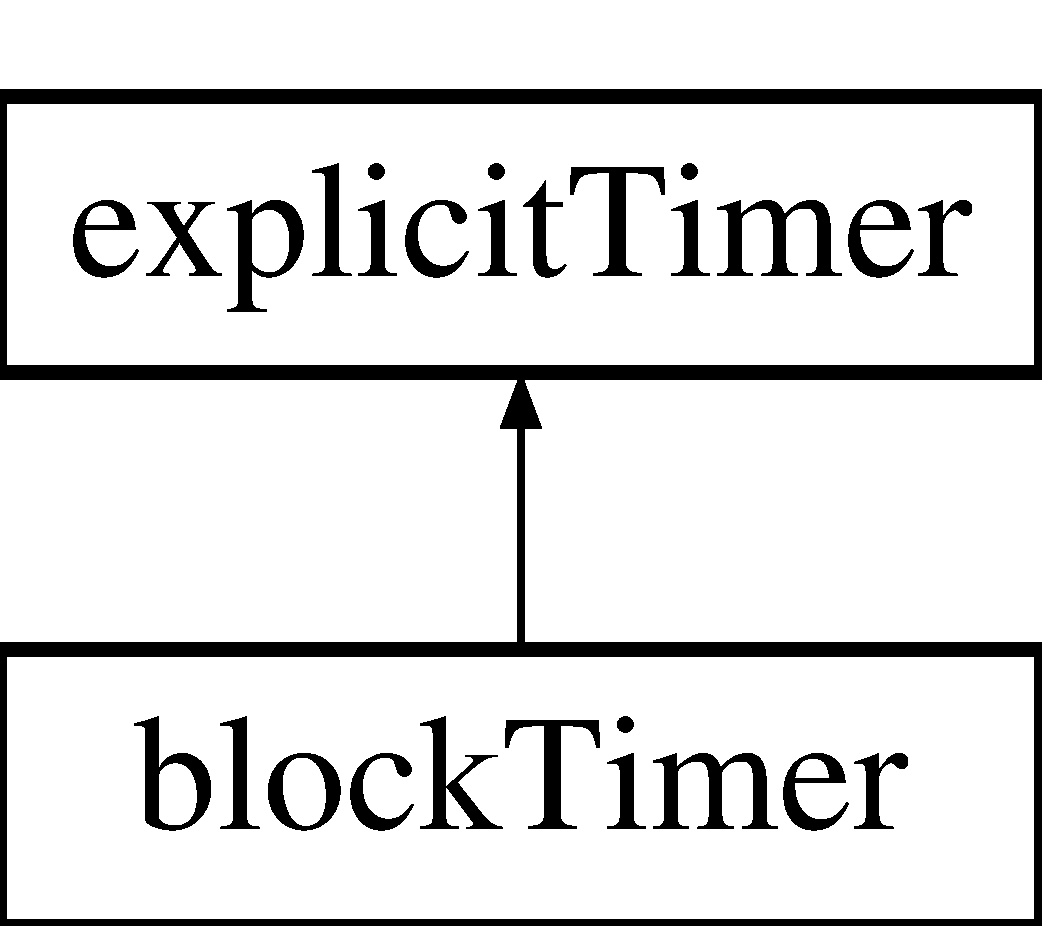
\includegraphics[height=2.000000cm]{classexplicitTimer}
\end{center}
\end{figure}
\subsection*{Public Member Functions}
\begin{DoxyCompactItemize}
\item 
\hyperlink{classexplicitTimer_a6c4946c5479d998e1e12610cd8ca2fe6}{explicit\-Timer} ()
\item 
\hyperlink{classexplicitTimer_ab52fc729eb83047573b962d5b7485098}{explicit\-Timer} (\hyperlink{classtimeStat}{time\-Stat} $\ast$\hyperlink{ittnotify__static_8h_a110bd9ede250f97ce56d81bb3c7b171d}{s})
\item 
\hyperlink{ittnotify__static_8h_af941d56e55e3c5465135b60c4d6343ed}{void} \hyperlink{classexplicitTimer_aacaaa414c0d68d0ba3cab075036baf63}{set\-Stat} (\hyperlink{classtimeStat}{time\-Stat} $\ast$\hyperlink{ittnotify__static_8h_a110bd9ede250f97ce56d81bb3c7b171d}{s})
\item 
\hyperlink{ittnotify__static_8h_af941d56e55e3c5465135b60c4d6343ed}{void} \hyperlink{classexplicitTimer_a0650affa704a742ae6aae4bf569e964c}{start} (\hyperlink{kmp__stats_8h_ae03f1e0ff609f86afa9b7167a12c6c06}{timer\-\_\-e} timer\-Enum\-Value)
\item 
\hyperlink{ittnotify__static_8h_af941d56e55e3c5465135b60c4d6343ed}{void} \hyperlink{classexplicitTimer_a1a3507bd5e0661935ee7766580244051}{stop} (\hyperlink{kmp__stats_8h_ae03f1e0ff609f86afa9b7167a12c6c06}{timer\-\_\-e} timer\-Enum\-Value)
\item 
\hyperlink{ittnotify__static_8h_af941d56e55e3c5465135b60c4d6343ed}{void} \hyperlink{classexplicitTimer_a29a8aeb9f1f2b5abcd70fc6d6c02eda9}{reset} ()
\end{DoxyCompactItemize}
\subsection*{Private Attributes}
\begin{DoxyCompactItemize}
\item 
\hyperlink{classtimeStat}{time\-Stat} $\ast$ \hyperlink{classexplicitTimer_afba814013964a74c3142ffde95f8ba1f}{stat}
\item 
\hyperlink{classtsc__tick__count}{tsc\-\_\-tick\-\_\-count} \hyperlink{classexplicitTimer_ad457d205b0b6d5309f65514e438992d2}{start\-Time}
\end{DoxyCompactItemize}


\subsection{Detailed Description}


Definition at line 293 of file kmp\-\_\-stats.\-h.



\subsection{Constructor \& Destructor Documentation}
\hypertarget{classexplicitTimer_a6c4946c5479d998e1e12610cd8ca2fe6}{\index{explicit\-Timer@{explicit\-Timer}!explicit\-Timer@{explicit\-Timer}}
\index{explicit\-Timer@{explicit\-Timer}!explicitTimer@{explicit\-Timer}}
\subsubsection[{explicit\-Timer}]{\setlength{\rightskip}{0pt plus 5cm}explicit\-Timer\-::explicit\-Timer (
\begin{DoxyParamCaption}
{}
\end{DoxyParamCaption}
)\hspace{0.3cm}{\ttfamily [inline]}}}\label{classexplicitTimer_a6c4946c5479d998e1e12610cd8ca2fe6}


Definition at line 299 of file kmp\-\_\-stats.\-h.


\begin{DoxyCode}
299 : \hyperlink{classexplicitTimer_afba814013964a74c3142ffde95f8ba1f}{stat}(0), \hyperlink{classexplicitTimer_ad457d205b0b6d5309f65514e438992d2}{startTime}(0) \{ \}
\end{DoxyCode}
\hypertarget{classexplicitTimer_ab52fc729eb83047573b962d5b7485098}{\index{explicit\-Timer@{explicit\-Timer}!explicit\-Timer@{explicit\-Timer}}
\index{explicit\-Timer@{explicit\-Timer}!explicitTimer@{explicit\-Timer}}
\subsubsection[{explicit\-Timer}]{\setlength{\rightskip}{0pt plus 5cm}explicit\-Timer\-::explicit\-Timer (
\begin{DoxyParamCaption}
\item[{{\bf time\-Stat} $\ast$}]{s}
\end{DoxyParamCaption}
)\hspace{0.3cm}{\ttfamily [inline]}}}\label{classexplicitTimer_ab52fc729eb83047573b962d5b7485098}


Definition at line 300 of file kmp\-\_\-stats.\-h.


\begin{DoxyCode}
300 : \hyperlink{classexplicitTimer_afba814013964a74c3142ffde95f8ba1f}{stat}(s), \hyperlink{classexplicitTimer_ad457d205b0b6d5309f65514e438992d2}{startTime}() \{ \}
\end{DoxyCode}


\subsection{Member Function Documentation}
\hypertarget{classexplicitTimer_a29a8aeb9f1f2b5abcd70fc6d6c02eda9}{\index{explicit\-Timer@{explicit\-Timer}!reset@{reset}}
\index{reset@{reset}!explicitTimer@{explicit\-Timer}}
\subsubsection[{reset}]{\setlength{\rightskip}{0pt plus 5cm}{\bf void} explicit\-Timer\-::reset (
\begin{DoxyParamCaption}
{}
\end{DoxyParamCaption}
)\hspace{0.3cm}{\ttfamily [inline]}}}\label{classexplicitTimer_a29a8aeb9f1f2b5abcd70fc6d6c02eda9}


Definition at line 305 of file kmp\-\_\-stats.\-h.


\begin{DoxyCode}
305 \{ \hyperlink{classexplicitTimer_ad457d205b0b6d5309f65514e438992d2}{startTime} = 0; \}
\end{DoxyCode}
\hypertarget{classexplicitTimer_aacaaa414c0d68d0ba3cab075036baf63}{\index{explicit\-Timer@{explicit\-Timer}!set\-Stat@{set\-Stat}}
\index{set\-Stat@{set\-Stat}!explicitTimer@{explicit\-Timer}}
\subsubsection[{set\-Stat}]{\setlength{\rightskip}{0pt plus 5cm}{\bf void} explicit\-Timer\-::set\-Stat (
\begin{DoxyParamCaption}
\item[{{\bf time\-Stat} $\ast$}]{s}
\end{DoxyParamCaption}
)\hspace{0.3cm}{\ttfamily [inline]}}}\label{classexplicitTimer_aacaaa414c0d68d0ba3cab075036baf63}


Definition at line 302 of file kmp\-\_\-stats.\-h.


\begin{DoxyCode}
302 \{ \hyperlink{classexplicitTimer_afba814013964a74c3142ffde95f8ba1f}{stat} = \hyperlink{ittnotify__static_8h_a110bd9ede250f97ce56d81bb3c7b171d}{s}; \}
\end{DoxyCode}
\hypertarget{classexplicitTimer_a0650affa704a742ae6aae4bf569e964c}{\index{explicit\-Timer@{explicit\-Timer}!start@{start}}
\index{start@{start}!explicitTimer@{explicit\-Timer}}
\subsubsection[{start}]{\setlength{\rightskip}{0pt plus 5cm}{\bf void} explicit\-Timer\-::start (
\begin{DoxyParamCaption}
\item[{{\bf timer\-\_\-e}}]{timer\-Enum\-Value}
\end{DoxyParamCaption}
)}}\label{classexplicitTimer_a0650affa704a742ae6aae4bf569e964c}


Definition at line 158 of file kmp\-\_\-stats.\-cpp.



Referenced by block\-Timer\-::block\-Timer().


\begin{DoxyCode}
158                                                 \{ 
159     \hyperlink{classexplicitTimer_ad457d205b0b6d5309f65514e438992d2}{startTime} = \hyperlink{classtsc__tick__count_a0caca1efab64714976683134bcdd99b4}{tsc\_tick\_count::now}(); 
160     \textcolor{keywordflow}{if}(\hyperlink{classtimeStat_ab45f55ba382e1ac2018ed6ab3612d3b1}{timeStat::logEvent}(timerEnumValue)) \{
161         \hyperlink{kmp__global_8c_ae8b6bdb1368ab875fdb8322ba2de5803}{\_\_kmp\_stats\_thread\_ptr}->\hyperlink{classkmp__stats__list_ab2bd44c00fe33e5a053cce45d3547625}{incrementNestValue}();
162     \}
163     \textcolor{keywordflow}{return};
164 \}
\end{DoxyCode}
\hypertarget{classexplicitTimer_a1a3507bd5e0661935ee7766580244051}{\index{explicit\-Timer@{explicit\-Timer}!stop@{stop}}
\index{stop@{stop}!explicitTimer@{explicit\-Timer}}
\subsubsection[{stop}]{\setlength{\rightskip}{0pt plus 5cm}{\bf void} explicit\-Timer\-::stop (
\begin{DoxyParamCaption}
\item[{{\bf timer\-\_\-e}}]{timer\-Enum\-Value}
\end{DoxyParamCaption}
)}}\label{classexplicitTimer_a1a3507bd5e0661935ee7766580244051}


Definition at line 166 of file kmp\-\_\-stats.\-cpp.



Referenced by block\-Timer\-::$\sim$block\-Timer().


\begin{DoxyCode}
166                                                \{
167     \textcolor{keywordflow}{if} (\hyperlink{classexplicitTimer_ad457d205b0b6d5309f65514e438992d2}{startTime}.\hyperlink{classtsc__tick__count_a88c80c6a9d8b3b0d76b45cef2d3bc36b}{getValue}() == 0)
168         \textcolor{keywordflow}{return};
169 
170     \hyperlink{classtsc__tick__count}{tsc\_tick\_count} finishTime = \hyperlink{classtsc__tick__count_a0caca1efab64714976683134bcdd99b4}{tsc\_tick\_count::now}();
171 
172     \textcolor{comment}{//stat->addSample ((tsc\_tick\_count::now() - startTime).ticks());}
173     \hyperlink{classexplicitTimer_afba814013964a74c3142ffde95f8ba1f}{stat}->\hyperlink{classstatistic_a608058fd5fac27c72c6019c607f38688}{addSample} ((finishTime - \hyperlink{classexplicitTimer_ad457d205b0b6d5309f65514e438992d2}{startTime}).ticks());
174 
175     \textcolor{keywordflow}{if}(\hyperlink{classtimeStat_ab45f55ba382e1ac2018ed6ab3612d3b1}{timeStat::logEvent}(timerEnumValue)) \{
176         \hyperlink{kmp__global_8c_ae8b6bdb1368ab875fdb8322ba2de5803}{\_\_kmp\_stats\_thread\_ptr}->\hyperlink{classkmp__stats__list_aa342e93ee4681eae6f8ab145ead4c31f}{push\_event}(
      \hyperlink{classexplicitTimer_ad457d205b0b6d5309f65514e438992d2}{startTime}.\hyperlink{classtsc__tick__count_a88c80c6a9d8b3b0d76b45cef2d3bc36b}{getValue}() - \hyperlink{kmp__global_8c_a12d1cf26d9330e0eb6361b6d67086d1d}{\_\_kmp\_stats\_start\_time}.
      \hyperlink{classtsc__tick__count_a88c80c6a9d8b3b0d76b45cef2d3bc36b}{getValue}(), finishTime.\hyperlink{classtsc__tick__count_a88c80c6a9d8b3b0d76b45cef2d3bc36b}{getValue}() - \hyperlink{kmp__global_8c_a12d1cf26d9330e0eb6361b6d67086d1d}{\_\_kmp\_stats\_start\_time}.
      \hyperlink{classtsc__tick__count_a88c80c6a9d8b3b0d76b45cef2d3bc36b}{getValue}(), \hyperlink{kmp__global_8c_ae8b6bdb1368ab875fdb8322ba2de5803}{\_\_kmp\_stats\_thread\_ptr}->\hyperlink{classkmp__stats__list_ad84d6680e0777851ae04a175f858addc}{getNestValue}(), 
      timerEnumValue); 
177         \hyperlink{kmp__global_8c_ae8b6bdb1368ab875fdb8322ba2de5803}{\_\_kmp\_stats\_thread\_ptr}->\hyperlink{classkmp__stats__list_a9a27398f0f242283d1f9c8afa1b32bab}{decrementNestValue}();
178     \}
179 
180     \textcolor{comment}{/* We accept the risk that we drop a sample because it really did start at t==0. */}
181     \hyperlink{classexplicitTimer_ad457d205b0b6d5309f65514e438992d2}{startTime} = 0; 
182     \textcolor{keywordflow}{return};
183 \}
\end{DoxyCode}


\subsection{Member Data Documentation}
\hypertarget{classexplicitTimer_ad457d205b0b6d5309f65514e438992d2}{\index{explicit\-Timer@{explicit\-Timer}!start\-Time@{start\-Time}}
\index{start\-Time@{start\-Time}!explicitTimer@{explicit\-Timer}}
\subsubsection[{start\-Time}]{\setlength{\rightskip}{0pt plus 5cm}{\bf tsc\-\_\-tick\-\_\-count} explicit\-Timer\-::start\-Time\hspace{0.3cm}{\ttfamily [private]}}}\label{classexplicitTimer_ad457d205b0b6d5309f65514e438992d2}


Definition at line 296 of file kmp\-\_\-stats.\-h.



Referenced by reset(), start(), and stop().

\hypertarget{classexplicitTimer_afba814013964a74c3142ffde95f8ba1f}{\index{explicit\-Timer@{explicit\-Timer}!stat@{stat}}
\index{stat@{stat}!explicitTimer@{explicit\-Timer}}
\subsubsection[{stat}]{\setlength{\rightskip}{0pt plus 5cm}{\bf time\-Stat}$\ast$ explicit\-Timer\-::stat\hspace{0.3cm}{\ttfamily [private]}}}\label{classexplicitTimer_afba814013964a74c3142ffde95f8ba1f}


Definition at line 295 of file kmp\-\_\-stats.\-h.



Referenced by set\-Stat(), and stop().



The documentation for this class was generated from the following files\-:\begin{DoxyCompactItemize}
\item 
\hyperlink{kmp__stats_8h}{kmp\-\_\-stats.\-h}\item 
\hyperlink{kmp__stats_8cpp}{kmp\-\_\-stats.\-cpp}\end{DoxyCompactItemize}

\hypertarget{structflag__traits}{\section{flag\-\_\-traits$<$ Flag\-Type $>$ Struct Template Reference}
\label{structflag__traits}\index{flag\-\_\-traits$<$ Flag\-Type $>$@{flag\-\_\-traits$<$ Flag\-Type $>$}}
}


{\ttfamily \#include $<$kmp\-\_\-wait\-\_\-release.\-h$>$}



\subsection{Detailed Description}
\subsubsection*{template$<$typename Flag\-Type$>$struct flag\-\_\-traits$<$ Flag\-Type $>$}



Definition at line 318 of file kmp\-\_\-wait\-\_\-release.\-h.



The documentation for this struct was generated from the following file\-:\begin{DoxyCompactItemize}
\item 
\hyperlink{kmp__wait__release_8h}{kmp\-\_\-wait\-\_\-release.\-h}\end{DoxyCompactItemize}

\hypertarget{structflag__traits_3_01kmp__uint32_01_4}{\section{flag\-\_\-traits$<$ kmp\-\_\-uint32 $>$ Struct Template Reference}
\label{structflag__traits_3_01kmp__uint32_01_4}\index{flag\-\_\-traits$<$ kmp\-\_\-uint32 $>$@{flag\-\_\-traits$<$ kmp\-\_\-uint32 $>$}}
}


{\ttfamily \#include $<$kmp\-\_\-wait\-\_\-release.\-h$>$}

\subsection*{Public Types}
\begin{DoxyCompactItemize}
\item 
typedef kmp\-\_\-uint32 \hyperlink{structflag__traits_3_01kmp__uint32_01_4_a216e25725dfeeee57bb3367f0bffb763}{flag\-\_\-t}
\end{DoxyCompactItemize}
\subsection*{Static Public Member Functions}
\begin{DoxyCompactItemize}
\item 
static \hyperlink{structflag__traits_3_01kmp__uint32_01_4_a216e25725dfeeee57bb3367f0bffb763}{flag\-\_\-t} \hyperlink{structflag__traits_3_01kmp__uint32_01_4_a107e5d82439c7a50b70c28bcd80b3904}{tcr} (\hyperlink{structflag__traits_3_01kmp__uint32_01_4_a216e25725dfeeee57bb3367f0bffb763}{flag\-\_\-t} f)
\item 
static \hyperlink{structflag__traits_3_01kmp__uint32_01_4_a216e25725dfeeee57bb3367f0bffb763}{flag\-\_\-t} \hyperlink{structflag__traits_3_01kmp__uint32_01_4_a7a9f86d9e939f8e571fb708a69f2d1ac}{test\-\_\-then\-\_\-add4} (volatile \hyperlink{structflag__traits_3_01kmp__uint32_01_4_a216e25725dfeeee57bb3367f0bffb763}{flag\-\_\-t} $\ast$f)
\item 
static \hyperlink{structflag__traits_3_01kmp__uint32_01_4_a216e25725dfeeee57bb3367f0bffb763}{flag\-\_\-t} \hyperlink{structflag__traits_3_01kmp__uint32_01_4_ad4ccdffe86b008815a205607a8b8cb20}{test\-\_\-then\-\_\-or} (volatile \hyperlink{structflag__traits_3_01kmp__uint32_01_4_a216e25725dfeeee57bb3367f0bffb763}{flag\-\_\-t} $\ast$f, \hyperlink{structflag__traits_3_01kmp__uint32_01_4_a216e25725dfeeee57bb3367f0bffb763}{flag\-\_\-t} v)
\item 
static \hyperlink{structflag__traits_3_01kmp__uint32_01_4_a216e25725dfeeee57bb3367f0bffb763}{flag\-\_\-t} \hyperlink{structflag__traits_3_01kmp__uint32_01_4_aec09b9100f7c8e56f5bf21fb9266776b}{test\-\_\-then\-\_\-and} (volatile \hyperlink{structflag__traits_3_01kmp__uint32_01_4_a216e25725dfeeee57bb3367f0bffb763}{flag\-\_\-t} $\ast$f, \hyperlink{structflag__traits_3_01kmp__uint32_01_4_a216e25725dfeeee57bb3367f0bffb763}{flag\-\_\-t} v)
\end{DoxyCompactItemize}
\subsection*{Static Public Attributes}
\begin{DoxyCompactItemize}
\item 
static const \hyperlink{group__WAIT__RELEASE_ga507a7197646f995b5529a68c1481e39b}{flag\-\_\-type} \hyperlink{structflag__traits_3_01kmp__uint32_01_4_a28ceb6f9e5394c786d49d3849f29ba78}{t} = \hyperlink{group__WAIT__RELEASE_gga507a7197646f995b5529a68c1481e39baa8e37e16d043d78e34da1d19387be5ba}{flag32}
\end{DoxyCompactItemize}


\subsection{Detailed Description}
\subsubsection*{template$<$$>$struct flag\-\_\-traits$<$ kmp\-\_\-uint32 $>$}



Definition at line 321 of file kmp\-\_\-wait\-\_\-release.\-h.



\subsection{Member Typedef Documentation}
\hypertarget{structflag__traits_3_01kmp__uint32_01_4_a216e25725dfeeee57bb3367f0bffb763}{\index{flag\-\_\-traits$<$ kmp\-\_\-uint32 $>$@{flag\-\_\-traits$<$ kmp\-\_\-uint32 $>$}!flag\-\_\-t@{flag\-\_\-t}}
\index{flag\-\_\-t@{flag\-\_\-t}!flag_traits< kmp_uint32 >@{flag\-\_\-traits$<$ kmp\-\_\-uint32 $>$}}
\subsubsection[{flag\-\_\-t}]{\setlength{\rightskip}{0pt plus 5cm}typedef kmp\-\_\-uint32 {\bf flag\-\_\-traits}$<$ kmp\-\_\-uint32 $>$\-::{\bf flag\-\_\-t}}}\label{structflag__traits_3_01kmp__uint32_01_4_a216e25725dfeeee57bb3367f0bffb763}


Definition at line 322 of file kmp\-\_\-wait\-\_\-release.\-h.



\subsection{Member Function Documentation}
\hypertarget{structflag__traits_3_01kmp__uint32_01_4_a107e5d82439c7a50b70c28bcd80b3904}{\index{flag\-\_\-traits$<$ kmp\-\_\-uint32 $>$@{flag\-\_\-traits$<$ kmp\-\_\-uint32 $>$}!tcr@{tcr}}
\index{tcr@{tcr}!flag_traits< kmp_uint32 >@{flag\-\_\-traits$<$ kmp\-\_\-uint32 $>$}}
\subsubsection[{tcr}]{\setlength{\rightskip}{0pt plus 5cm}static {\bf flag\-\_\-t} {\bf flag\-\_\-traits}$<$ kmp\-\_\-uint32 $>$\-::tcr (
\begin{DoxyParamCaption}
\item[{{\bf flag\-\_\-t}}]{f}
\end{DoxyParamCaption}
)\hspace{0.3cm}{\ttfamily [inline]}, {\ttfamily [static]}}}\label{structflag__traits_3_01kmp__uint32_01_4_a107e5d82439c7a50b70c28bcd80b3904}


Definition at line 324 of file kmp\-\_\-wait\-\_\-release.\-h.


\begin{DoxyCode}
324 \{ \textcolor{keywordflow}{return} \hyperlink{kmp__os_8h_acd6256e4afba32d90997235fc0a38a74}{TCR\_4}(f); \}
\end{DoxyCode}
\hypertarget{structflag__traits_3_01kmp__uint32_01_4_a7a9f86d9e939f8e571fb708a69f2d1ac}{\index{flag\-\_\-traits$<$ kmp\-\_\-uint32 $>$@{flag\-\_\-traits$<$ kmp\-\_\-uint32 $>$}!test\-\_\-then\-\_\-add4@{test\-\_\-then\-\_\-add4}}
\index{test\-\_\-then\-\_\-add4@{test\-\_\-then\-\_\-add4}!flag_traits< kmp_uint32 >@{flag\-\_\-traits$<$ kmp\-\_\-uint32 $>$}}
\subsubsection[{test\-\_\-then\-\_\-add4}]{\setlength{\rightskip}{0pt plus 5cm}static {\bf flag\-\_\-t} {\bf flag\-\_\-traits}$<$ kmp\-\_\-uint32 $>$\-::test\-\_\-then\-\_\-add4 (
\begin{DoxyParamCaption}
\item[{volatile {\bf flag\-\_\-t} $\ast$}]{f}
\end{DoxyParamCaption}
)\hspace{0.3cm}{\ttfamily [inline]}, {\ttfamily [static]}}}\label{structflag__traits_3_01kmp__uint32_01_4_a7a9f86d9e939f8e571fb708a69f2d1ac}


Definition at line 325 of file kmp\-\_\-wait\-\_\-release.\-h.


\begin{DoxyCode}
325 \{ \textcolor{keywordflow}{return} \hyperlink{kmp__os_8h_a275f1e47b12d8fb0cd26eec200c51485}{KMP\_TEST\_THEN\_ADD4\_32}((\textcolor{keyword}{volatile} kmp\_int32 *)f); \}
\end{DoxyCode}
\hypertarget{structflag__traits_3_01kmp__uint32_01_4_aec09b9100f7c8e56f5bf21fb9266776b}{\index{flag\-\_\-traits$<$ kmp\-\_\-uint32 $>$@{flag\-\_\-traits$<$ kmp\-\_\-uint32 $>$}!test\-\_\-then\-\_\-and@{test\-\_\-then\-\_\-and}}
\index{test\-\_\-then\-\_\-and@{test\-\_\-then\-\_\-and}!flag_traits< kmp_uint32 >@{flag\-\_\-traits$<$ kmp\-\_\-uint32 $>$}}
\subsubsection[{test\-\_\-then\-\_\-and}]{\setlength{\rightskip}{0pt plus 5cm}static {\bf flag\-\_\-t} {\bf flag\-\_\-traits}$<$ kmp\-\_\-uint32 $>$\-::test\-\_\-then\-\_\-and (
\begin{DoxyParamCaption}
\item[{volatile {\bf flag\-\_\-t} $\ast$}]{f, }
\item[{{\bf flag\-\_\-t}}]{v}
\end{DoxyParamCaption}
)\hspace{0.3cm}{\ttfamily [inline]}, {\ttfamily [static]}}}\label{structflag__traits_3_01kmp__uint32_01_4_aec09b9100f7c8e56f5bf21fb9266776b}


Definition at line 327 of file kmp\-\_\-wait\-\_\-release.\-h.


\begin{DoxyCode}
327 \{ \textcolor{keywordflow}{return} \hyperlink{kmp__os_8h_ab2a92fe9bb9152a277d0fd01992bf977}{KMP\_TEST\_THEN\_AND32}((\textcolor{keyword}{volatile} kmp\_int32 *)f, v); \}
\end{DoxyCode}
\hypertarget{structflag__traits_3_01kmp__uint32_01_4_ad4ccdffe86b008815a205607a8b8cb20}{\index{flag\-\_\-traits$<$ kmp\-\_\-uint32 $>$@{flag\-\_\-traits$<$ kmp\-\_\-uint32 $>$}!test\-\_\-then\-\_\-or@{test\-\_\-then\-\_\-or}}
\index{test\-\_\-then\-\_\-or@{test\-\_\-then\-\_\-or}!flag_traits< kmp_uint32 >@{flag\-\_\-traits$<$ kmp\-\_\-uint32 $>$}}
\subsubsection[{test\-\_\-then\-\_\-or}]{\setlength{\rightskip}{0pt plus 5cm}static {\bf flag\-\_\-t} {\bf flag\-\_\-traits}$<$ kmp\-\_\-uint32 $>$\-::test\-\_\-then\-\_\-or (
\begin{DoxyParamCaption}
\item[{volatile {\bf flag\-\_\-t} $\ast$}]{f, }
\item[{{\bf flag\-\_\-t}}]{v}
\end{DoxyParamCaption}
)\hspace{0.3cm}{\ttfamily [inline]}, {\ttfamily [static]}}}\label{structflag__traits_3_01kmp__uint32_01_4_ad4ccdffe86b008815a205607a8b8cb20}


Definition at line 326 of file kmp\-\_\-wait\-\_\-release.\-h.


\begin{DoxyCode}
326 \{ \textcolor{keywordflow}{return} \hyperlink{kmp__os_8h_a181d2a30bc941dab902d9006c3faa606}{KMP\_TEST\_THEN\_OR32}((\textcolor{keyword}{volatile} kmp\_int32 *)f, v); \}
\end{DoxyCode}


\subsection{Member Data Documentation}
\hypertarget{structflag__traits_3_01kmp__uint32_01_4_a28ceb6f9e5394c786d49d3849f29ba78}{\index{flag\-\_\-traits$<$ kmp\-\_\-uint32 $>$@{flag\-\_\-traits$<$ kmp\-\_\-uint32 $>$}!t@{t}}
\index{t@{t}!flag_traits< kmp_uint32 >@{flag\-\_\-traits$<$ kmp\-\_\-uint32 $>$}}
\subsubsection[{t}]{\setlength{\rightskip}{0pt plus 5cm}const {\bf flag\-\_\-type} {\bf flag\-\_\-traits}$<$ kmp\-\_\-uint32 $>$\-::t = {\bf flag32}\hspace{0.3cm}{\ttfamily [static]}}}\label{structflag__traits_3_01kmp__uint32_01_4_a28ceb6f9e5394c786d49d3849f29ba78}


Definition at line 323 of file kmp\-\_\-wait\-\_\-release.\-h.



The documentation for this struct was generated from the following file\-:\begin{DoxyCompactItemize}
\item 
\hyperlink{kmp__wait__release_8h}{kmp\-\_\-wait\-\_\-release.\-h}\end{DoxyCompactItemize}

\hypertarget{structflag__traits_3_01kmp__uint64_01_4}{\section{flag\-\_\-traits$<$ kmp\-\_\-uint64 $>$ Struct Template Reference}
\label{structflag__traits_3_01kmp__uint64_01_4}\index{flag\-\_\-traits$<$ kmp\-\_\-uint64 $>$@{flag\-\_\-traits$<$ kmp\-\_\-uint64 $>$}}
}


{\ttfamily \#include $<$kmp\-\_\-wait\-\_\-release.\-h$>$}

\subsection*{Public Types}
\begin{DoxyCompactItemize}
\item 
typedef kmp\-\_\-uint64 \hyperlink{structflag__traits_3_01kmp__uint64_01_4_a1cd5c1b0bf5f69b71ca924315e7320c2}{flag\-\_\-t}
\end{DoxyCompactItemize}
\subsection*{Static Public Member Functions}
\begin{DoxyCompactItemize}
\item 
static \hyperlink{structflag__traits_3_01kmp__uint64_01_4_a1cd5c1b0bf5f69b71ca924315e7320c2}{flag\-\_\-t} \hyperlink{structflag__traits_3_01kmp__uint64_01_4_ac3dc6ed6d8b3f856fcf65f779e0c3bd2}{tcr} (\hyperlink{structflag__traits_3_01kmp__uint64_01_4_a1cd5c1b0bf5f69b71ca924315e7320c2}{flag\-\_\-t} f)
\item 
static \hyperlink{structflag__traits_3_01kmp__uint64_01_4_a1cd5c1b0bf5f69b71ca924315e7320c2}{flag\-\_\-t} \hyperlink{structflag__traits_3_01kmp__uint64_01_4_adf609d7418984d73b263790475250758}{test\-\_\-then\-\_\-add4} (volatile \hyperlink{structflag__traits_3_01kmp__uint64_01_4_a1cd5c1b0bf5f69b71ca924315e7320c2}{flag\-\_\-t} $\ast$f)
\item 
static \hyperlink{structflag__traits_3_01kmp__uint64_01_4_a1cd5c1b0bf5f69b71ca924315e7320c2}{flag\-\_\-t} \hyperlink{structflag__traits_3_01kmp__uint64_01_4_a579a1207cff793eace2c893d194cc575}{test\-\_\-then\-\_\-or} (volatile \hyperlink{structflag__traits_3_01kmp__uint64_01_4_a1cd5c1b0bf5f69b71ca924315e7320c2}{flag\-\_\-t} $\ast$f, \hyperlink{structflag__traits_3_01kmp__uint64_01_4_a1cd5c1b0bf5f69b71ca924315e7320c2}{flag\-\_\-t} v)
\item 
static \hyperlink{structflag__traits_3_01kmp__uint64_01_4_a1cd5c1b0bf5f69b71ca924315e7320c2}{flag\-\_\-t} \hyperlink{structflag__traits_3_01kmp__uint64_01_4_ad8b374576e9d570db9be0aaab8961792}{test\-\_\-then\-\_\-and} (volatile \hyperlink{structflag__traits_3_01kmp__uint64_01_4_a1cd5c1b0bf5f69b71ca924315e7320c2}{flag\-\_\-t} $\ast$f, \hyperlink{structflag__traits_3_01kmp__uint64_01_4_a1cd5c1b0bf5f69b71ca924315e7320c2}{flag\-\_\-t} v)
\end{DoxyCompactItemize}
\subsection*{Static Public Attributes}
\begin{DoxyCompactItemize}
\item 
static const \hyperlink{group__WAIT__RELEASE_ga507a7197646f995b5529a68c1481e39b}{flag\-\_\-type} \hyperlink{structflag__traits_3_01kmp__uint64_01_4_a0fdaf5c8a6127d85abd0b226f923feed}{t} = \hyperlink{group__WAIT__RELEASE_gga507a7197646f995b5529a68c1481e39ba8b02d824728fb546d43123b8b069ed04}{flag64}
\end{DoxyCompactItemize}


\subsection{Detailed Description}
\subsubsection*{template$<$$>$struct flag\-\_\-traits$<$ kmp\-\_\-uint64 $>$}



Definition at line 331 of file kmp\-\_\-wait\-\_\-release.\-h.



\subsection{Member Typedef Documentation}
\hypertarget{structflag__traits_3_01kmp__uint64_01_4_a1cd5c1b0bf5f69b71ca924315e7320c2}{\index{flag\-\_\-traits$<$ kmp\-\_\-uint64 $>$@{flag\-\_\-traits$<$ kmp\-\_\-uint64 $>$}!flag\-\_\-t@{flag\-\_\-t}}
\index{flag\-\_\-t@{flag\-\_\-t}!flag_traits< kmp_uint64 >@{flag\-\_\-traits$<$ kmp\-\_\-uint64 $>$}}
\subsubsection[{flag\-\_\-t}]{\setlength{\rightskip}{0pt plus 5cm}typedef kmp\-\_\-uint64 {\bf flag\-\_\-traits}$<$ kmp\-\_\-uint64 $>$\-::{\bf flag\-\_\-t}}}\label{structflag__traits_3_01kmp__uint64_01_4_a1cd5c1b0bf5f69b71ca924315e7320c2}


Definition at line 332 of file kmp\-\_\-wait\-\_\-release.\-h.



\subsection{Member Function Documentation}
\hypertarget{structflag__traits_3_01kmp__uint64_01_4_ac3dc6ed6d8b3f856fcf65f779e0c3bd2}{\index{flag\-\_\-traits$<$ kmp\-\_\-uint64 $>$@{flag\-\_\-traits$<$ kmp\-\_\-uint64 $>$}!tcr@{tcr}}
\index{tcr@{tcr}!flag_traits< kmp_uint64 >@{flag\-\_\-traits$<$ kmp\-\_\-uint64 $>$}}
\subsubsection[{tcr}]{\setlength{\rightskip}{0pt plus 5cm}static {\bf flag\-\_\-t} {\bf flag\-\_\-traits}$<$ kmp\-\_\-uint64 $>$\-::tcr (
\begin{DoxyParamCaption}
\item[{{\bf flag\-\_\-t}}]{f}
\end{DoxyParamCaption}
)\hspace{0.3cm}{\ttfamily [inline]}, {\ttfamily [static]}}}\label{structflag__traits_3_01kmp__uint64_01_4_ac3dc6ed6d8b3f856fcf65f779e0c3bd2}


Definition at line 334 of file kmp\-\_\-wait\-\_\-release.\-h.


\begin{DoxyCode}
334 \{ \textcolor{keywordflow}{return} \hyperlink{kmp__os_8h_ae7751c4fd274a522c6de1e02f8248aca}{TCR\_8}(f); \}
\end{DoxyCode}
\hypertarget{structflag__traits_3_01kmp__uint64_01_4_adf609d7418984d73b263790475250758}{\index{flag\-\_\-traits$<$ kmp\-\_\-uint64 $>$@{flag\-\_\-traits$<$ kmp\-\_\-uint64 $>$}!test\-\_\-then\-\_\-add4@{test\-\_\-then\-\_\-add4}}
\index{test\-\_\-then\-\_\-add4@{test\-\_\-then\-\_\-add4}!flag_traits< kmp_uint64 >@{flag\-\_\-traits$<$ kmp\-\_\-uint64 $>$}}
\subsubsection[{test\-\_\-then\-\_\-add4}]{\setlength{\rightskip}{0pt plus 5cm}static {\bf flag\-\_\-t} {\bf flag\-\_\-traits}$<$ kmp\-\_\-uint64 $>$\-::test\-\_\-then\-\_\-add4 (
\begin{DoxyParamCaption}
\item[{volatile {\bf flag\-\_\-t} $\ast$}]{f}
\end{DoxyParamCaption}
)\hspace{0.3cm}{\ttfamily [inline]}, {\ttfamily [static]}}}\label{structflag__traits_3_01kmp__uint64_01_4_adf609d7418984d73b263790475250758}


Definition at line 335 of file kmp\-\_\-wait\-\_\-release.\-h.


\begin{DoxyCode}
335 \{ \textcolor{keywordflow}{return} \hyperlink{kmp__os_8h_a8082d77697a2a140cf7784119035c5b8}{KMP\_TEST\_THEN\_ADD4\_64}((\textcolor{keyword}{volatile} kmp\_int64 *)f); \}
\end{DoxyCode}
\hypertarget{structflag__traits_3_01kmp__uint64_01_4_ad8b374576e9d570db9be0aaab8961792}{\index{flag\-\_\-traits$<$ kmp\-\_\-uint64 $>$@{flag\-\_\-traits$<$ kmp\-\_\-uint64 $>$}!test\-\_\-then\-\_\-and@{test\-\_\-then\-\_\-and}}
\index{test\-\_\-then\-\_\-and@{test\-\_\-then\-\_\-and}!flag_traits< kmp_uint64 >@{flag\-\_\-traits$<$ kmp\-\_\-uint64 $>$}}
\subsubsection[{test\-\_\-then\-\_\-and}]{\setlength{\rightskip}{0pt plus 5cm}static {\bf flag\-\_\-t} {\bf flag\-\_\-traits}$<$ kmp\-\_\-uint64 $>$\-::test\-\_\-then\-\_\-and (
\begin{DoxyParamCaption}
\item[{volatile {\bf flag\-\_\-t} $\ast$}]{f, }
\item[{{\bf flag\-\_\-t}}]{v}
\end{DoxyParamCaption}
)\hspace{0.3cm}{\ttfamily [inline]}, {\ttfamily [static]}}}\label{structflag__traits_3_01kmp__uint64_01_4_ad8b374576e9d570db9be0aaab8961792}


Definition at line 337 of file kmp\-\_\-wait\-\_\-release.\-h.


\begin{DoxyCode}
337 \{ \textcolor{keywordflow}{return} \hyperlink{kmp__os_8h_a57b958c796eb825adfa4e4df2f25b06c}{KMP\_TEST\_THEN\_AND64}((\textcolor{keyword}{volatile} kmp\_int64 *)f, v); \}
\end{DoxyCode}
\hypertarget{structflag__traits_3_01kmp__uint64_01_4_a579a1207cff793eace2c893d194cc575}{\index{flag\-\_\-traits$<$ kmp\-\_\-uint64 $>$@{flag\-\_\-traits$<$ kmp\-\_\-uint64 $>$}!test\-\_\-then\-\_\-or@{test\-\_\-then\-\_\-or}}
\index{test\-\_\-then\-\_\-or@{test\-\_\-then\-\_\-or}!flag_traits< kmp_uint64 >@{flag\-\_\-traits$<$ kmp\-\_\-uint64 $>$}}
\subsubsection[{test\-\_\-then\-\_\-or}]{\setlength{\rightskip}{0pt plus 5cm}static {\bf flag\-\_\-t} {\bf flag\-\_\-traits}$<$ kmp\-\_\-uint64 $>$\-::test\-\_\-then\-\_\-or (
\begin{DoxyParamCaption}
\item[{volatile {\bf flag\-\_\-t} $\ast$}]{f, }
\item[{{\bf flag\-\_\-t}}]{v}
\end{DoxyParamCaption}
)\hspace{0.3cm}{\ttfamily [inline]}, {\ttfamily [static]}}}\label{structflag__traits_3_01kmp__uint64_01_4_a579a1207cff793eace2c893d194cc575}


Definition at line 336 of file kmp\-\_\-wait\-\_\-release.\-h.


\begin{DoxyCode}
336 \{ \textcolor{keywordflow}{return} \hyperlink{kmp__os_8h_af743c5b57e6265f8cc3ec213ddd08825}{KMP\_TEST\_THEN\_OR64}((\textcolor{keyword}{volatile} kmp\_int64 *)f, v); \}
\end{DoxyCode}


\subsection{Member Data Documentation}
\hypertarget{structflag__traits_3_01kmp__uint64_01_4_a0fdaf5c8a6127d85abd0b226f923feed}{\index{flag\-\_\-traits$<$ kmp\-\_\-uint64 $>$@{flag\-\_\-traits$<$ kmp\-\_\-uint64 $>$}!t@{t}}
\index{t@{t}!flag_traits< kmp_uint64 >@{flag\-\_\-traits$<$ kmp\-\_\-uint64 $>$}}
\subsubsection[{t}]{\setlength{\rightskip}{0pt plus 5cm}const {\bf flag\-\_\-type} {\bf flag\-\_\-traits}$<$ kmp\-\_\-uint64 $>$\-::t = {\bf flag64}\hspace{0.3cm}{\ttfamily [static]}}}\label{structflag__traits_3_01kmp__uint64_01_4_a0fdaf5c8a6127d85abd0b226f923feed}


Definition at line 333 of file kmp\-\_\-wait\-\_\-release.\-h.



The documentation for this struct was generated from the following file\-:\begin{DoxyCompactItemize}
\item 
\hyperlink{kmp__wait__release_8h}{kmp\-\_\-wait\-\_\-release.\-h}\end{DoxyCompactItemize}

\hypertarget{structfortran__inx__info}{\section{fortran\-\_\-inx\-\_\-info Struct Reference}
\label{structfortran__inx__info}\index{fortran\-\_\-inx\-\_\-info@{fortran\-\_\-inx\-\_\-info}}
}


{\ttfamily \#include $<$kmp.\-h$>$}

\subsection*{Public Attributes}
\begin{DoxyCompactItemize}
\item 
kmp\-\_\-int32 \hyperlink{structfortran__inx__info_a91f68487ee59f2c74bab138ea72a8154}{data}
\end{DoxyCompactItemize}


\subsection{Detailed Description}


Definition at line 2609 of file kmp.\-h.



\subsection{Member Data Documentation}
\hypertarget{structfortran__inx__info_a91f68487ee59f2c74bab138ea72a8154}{\index{fortran\-\_\-inx\-\_\-info@{fortran\-\_\-inx\-\_\-info}!data@{data}}
\index{data@{data}!fortran_inx_info@{fortran\-\_\-inx\-\_\-info}}
\subsubsection[{data}]{\setlength{\rightskip}{0pt plus 5cm}kmp\-\_\-int32 fortran\-\_\-inx\-\_\-info\-::data}}\label{structfortran__inx__info_a91f68487ee59f2c74bab138ea72a8154}


Definition at line 2610 of file kmp.\-h.



The documentation for this struct was generated from the following file\-:\begin{DoxyCompactItemize}
\item 
\hyperlink{kmp_8h}{kmp.\-h}\end{DoxyCompactItemize}

\hypertarget{classhierarchy__info}{\section{hierarchy\-\_\-info Class Reference}
\label{classhierarchy__info}\index{hierarchy\-\_\-info@{hierarchy\-\_\-info}}
}


{\ttfamily \#include $<$kmp\-\_\-affinity.\-h$>$}

\subsection*{Public Attributes}
\begin{DoxyCompactItemize}
\item 
kmp\-\_\-uint32 \hyperlink{classhierarchy__info_aafbad4b89a239ea459aaef1ab4908aba}{max\-Levels}
\item 
kmp\-\_\-uint32 \hyperlink{classhierarchy__info_aeebcad75a7d471e1b1fd37aab6216f22}{depth}
\item 
kmp\-\_\-uint32 $\ast$ \hyperlink{classhierarchy__info_a12fc455d853883d91e3a19567aaac3fe}{num\-Per\-Level}
\end{DoxyCompactItemize}
\subsection*{Static Public Attributes}
\begin{DoxyCompactItemize}
\item 
static const kmp\-\_\-uint32 \hyperlink{classhierarchy__info_a4122e10b5d763f2ca3f13076f836ddfe}{max\-Leaves} =4
\end{DoxyCompactItemize}


\subsection{Detailed Description}
A structure for holding machine-\/specific hierarchy info to be computed once at init. This structure represents a mapping of threads to the actual machine hierarchy, or to our best guess at what the hierarchy might be, for the purpose of performing an efficient barrier. In the worst case, when there is no machine hierarchy information, it produces a tree suitable for a barrier, similar to the tree used in the hyper barrier. 

Definition at line 146 of file kmp\-\_\-affinity.\-h.



\subsection{Member Data Documentation}
\hypertarget{classhierarchy__info_aeebcad75a7d471e1b1fd37aab6216f22}{\index{hierarchy\-\_\-info@{hierarchy\-\_\-info}!depth@{depth}}
\index{depth@{depth}!hierarchy_info@{hierarchy\-\_\-info}}
\subsubsection[{depth}]{\setlength{\rightskip}{0pt plus 5cm}kmp\-\_\-uint32 hierarchy\-\_\-info\-::depth}}\label{classhierarchy__info_aeebcad75a7d471e1b1fd37aab6216f22}
This is specifically the depth of the machine configuration hierarchy, in terms of the number of levels along the longest path from root to any leaf. It corresponds to the number of entries in num\-Per\-Level if we exclude all but one trailing 1. 

Definition at line 161 of file kmp\-\_\-affinity.\-h.

\hypertarget{classhierarchy__info_a4122e10b5d763f2ca3f13076f836ddfe}{\index{hierarchy\-\_\-info@{hierarchy\-\_\-info}!max\-Leaves@{max\-Leaves}}
\index{max\-Leaves@{max\-Leaves}!hierarchy_info@{hierarchy\-\_\-info}}
\subsubsection[{max\-Leaves}]{\setlength{\rightskip}{0pt plus 5cm}const kmp\-\_\-uint32 hierarchy\-\_\-info\-::max\-Leaves =4\hspace{0.3cm}{\ttfamily [static]}}}\label{classhierarchy__info_a4122e10b5d763f2ca3f13076f836ddfe}
Good default values for number of leaves and branching factor, given no affinity information. Behaves a bit like hyper barrier. 

Definition at line 150 of file kmp\-\_\-affinity.\-h.

\hypertarget{classhierarchy__info_aafbad4b89a239ea459aaef1ab4908aba}{\index{hierarchy\-\_\-info@{hierarchy\-\_\-info}!max\-Levels@{max\-Levels}}
\index{max\-Levels@{max\-Levels}!hierarchy_info@{hierarchy\-\_\-info}}
\subsubsection[{max\-Levels}]{\setlength{\rightskip}{0pt plus 5cm}kmp\-\_\-uint32 hierarchy\-\_\-info\-::max\-Levels}}\label{classhierarchy__info_aafbad4b89a239ea459aaef1ab4908aba}
Number of levels in the hierarchy. Typical levels are threads/core, cores/package or socket, packages/node, nodes/machine, etc. We don't want to get specific with nomenclature. When the machine is oversubscribed we add levels to duplicate the hierarchy, doubling the thread capacity of the hierarchy each time we add a level. 

Definition at line 156 of file kmp\-\_\-affinity.\-h.

\hypertarget{classhierarchy__info_a12fc455d853883d91e3a19567aaac3fe}{\index{hierarchy\-\_\-info@{hierarchy\-\_\-info}!num\-Per\-Level@{num\-Per\-Level}}
\index{num\-Per\-Level@{num\-Per\-Level}!hierarchy_info@{hierarchy\-\_\-info}}
\subsubsection[{num\-Per\-Level}]{\setlength{\rightskip}{0pt plus 5cm}kmp\-\_\-uint32$\ast$ hierarchy\-\_\-info\-::num\-Per\-Level}}\label{classhierarchy__info_a12fc455d853883d91e3a19567aaac3fe}
Level 0 corresponds to leaves. num\-Per\-Level\mbox{[}i\mbox{]} is the number of children the parent of a node at level i has. For example, if we have a machine with 4 packages, 4 cores/package and 2 H\-T per core, then num\-Per\-Level = \{2, 4, 4, 1, 1\}. All empty levels are set to 1. 

Definition at line 170 of file kmp\-\_\-affinity.\-h.



The documentation for this class was generated from the following file\-:\begin{DoxyCompactItemize}
\item 
kmp\-\_\-affinity.\-h\end{DoxyCompactItemize}

\hypertarget{structi__maxmin}{\section{i\-\_\-maxmin$<$ T $>$ Struct Template Reference}
\label{structi__maxmin}\index{i\-\_\-maxmin$<$ T $>$@{i\-\_\-maxmin$<$ T $>$}}
}
\subsection*{Static Public Attributes}
\begin{DoxyCompactItemize}
\item 
static const T \hyperlink{structi__maxmin_a63ca8c1703ce381b720bf0b3953f8c5e}{mx}
\item 
static const T \hyperlink{structi__maxmin_a70852044b4bde382ffd4e0fc630b69c4}{mn}
\end{DoxyCompactItemize}


\subsection{Detailed Description}
\subsubsection*{template$<$typename T$>$struct i\-\_\-maxmin$<$ T $>$}



Definition at line 48 of file kmp\-\_\-dispatch.\-cpp.



\subsection{Member Data Documentation}
\hypertarget{structi__maxmin_a70852044b4bde382ffd4e0fc630b69c4}{\index{i\-\_\-maxmin@{i\-\_\-maxmin}!mn@{mn}}
\index{mn@{mn}!i_maxmin@{i\-\_\-maxmin}}
\subsubsection[{mn}]{\setlength{\rightskip}{0pt plus 5cm}template$<$typename T $>$ static const T {\bf i\-\_\-maxmin}$<$ T $>$\-::mn\hspace{0.3cm}{\ttfamily [static]}}}\label{structi__maxmin_a70852044b4bde382ffd4e0fc630b69c4}


Definition at line 50 of file kmp\-\_\-dispatch.\-cpp.

\hypertarget{structi__maxmin_a63ca8c1703ce381b720bf0b3953f8c5e}{\index{i\-\_\-maxmin@{i\-\_\-maxmin}!mx@{mx}}
\index{mx@{mx}!i_maxmin@{i\-\_\-maxmin}}
\subsubsection[{mx}]{\setlength{\rightskip}{0pt plus 5cm}template$<$typename T $>$ static const T {\bf i\-\_\-maxmin}$<$ T $>$\-::mx\hspace{0.3cm}{\ttfamily [static]}}}\label{structi__maxmin_a63ca8c1703ce381b720bf0b3953f8c5e}


Definition at line 49 of file kmp\-\_\-dispatch.\-cpp.



The documentation for this struct was generated from the following files\-:\begin{DoxyCompactItemize}
\item 
\hyperlink{kmp__dispatch_8cpp}{kmp\-\_\-dispatch.\-cpp}\item 
\hyperlink{kmp__sched_8cpp}{kmp\-\_\-sched.\-cpp}\end{DoxyCompactItemize}

\hypertarget{structi__maxmin_3_01int_01_4}{\section{i\-\_\-maxmin$<$ int $>$ Struct Template Reference}
\label{structi__maxmin_3_01int_01_4}\index{i\-\_\-maxmin$<$ int $>$@{i\-\_\-maxmin$<$ int $>$}}
}
\subsection*{Static Public Attributes}
\begin{DoxyCompactItemize}
\item 
static const \hyperlink{ittnotify__static_8h_a8b8dcd723308a8cb5d84277c7a3fff70}{int} \hyperlink{structi__maxmin_3_01int_01_4_aab31e71385a47754964cfb0d06ed4ba8}{mx} = 0x7fffffff
\item 
static const \hyperlink{ittnotify__static_8h_a8b8dcd723308a8cb5d84277c7a3fff70}{int} \hyperlink{structi__maxmin_3_01int_01_4_a47764c5470f2ae5c49a9189ce5bb9c08}{mn} = 0x80000000
\end{DoxyCompactItemize}


\subsection{Detailed Description}
\subsubsection*{template$<$$>$struct i\-\_\-maxmin$<$ int $>$}



Definition at line 53 of file kmp\-\_\-dispatch.\-cpp.



\subsection{Member Data Documentation}
\hypertarget{structi__maxmin_3_01int_01_4_a47764c5470f2ae5c49a9189ce5bb9c08}{\index{i\-\_\-maxmin$<$ int $>$@{i\-\_\-maxmin$<$ int $>$}!mn@{mn}}
\index{mn@{mn}!i_maxmin< int >@{i\-\_\-maxmin$<$ int $>$}}
\subsubsection[{mn}]{\setlength{\rightskip}{0pt plus 5cm}static const {\bf int} {\bf i\-\_\-maxmin}$<$ {\bf int} $>$\-::mn = 0x80000000\hspace{0.3cm}{\ttfamily [static]}}}\label{structi__maxmin_3_01int_01_4_a47764c5470f2ae5c49a9189ce5bb9c08}


Definition at line 55 of file kmp\-\_\-dispatch.\-cpp.

\hypertarget{structi__maxmin_3_01int_01_4_aab31e71385a47754964cfb0d06ed4ba8}{\index{i\-\_\-maxmin$<$ int $>$@{i\-\_\-maxmin$<$ int $>$}!mx@{mx}}
\index{mx@{mx}!i_maxmin< int >@{i\-\_\-maxmin$<$ int $>$}}
\subsubsection[{mx}]{\setlength{\rightskip}{0pt plus 5cm}static const {\bf int} {\bf i\-\_\-maxmin}$<$ {\bf int} $>$\-::mx = 0x7fffffff\hspace{0.3cm}{\ttfamily [static]}}}\label{structi__maxmin_3_01int_01_4_aab31e71385a47754964cfb0d06ed4ba8}


Definition at line 54 of file kmp\-\_\-dispatch.\-cpp.



The documentation for this struct was generated from the following files\-:\begin{DoxyCompactItemize}
\item 
\hyperlink{kmp__dispatch_8cpp}{kmp\-\_\-dispatch.\-cpp}\item 
\hyperlink{kmp__sched_8cpp}{kmp\-\_\-sched.\-cpp}\end{DoxyCompactItemize}

\hypertarget{structi__maxmin_3_01long_01long_01_4}{\section{i\-\_\-maxmin$<$ long long $>$ Struct Template Reference}
\label{structi__maxmin_3_01long_01long_01_4}\index{i\-\_\-maxmin$<$ long long $>$@{i\-\_\-maxmin$<$ long long $>$}}
}
\subsection*{Static Public Attributes}
\begin{DoxyCompactItemize}
\item 
static const long long \hyperlink{structi__maxmin_3_01long_01long_01_4_ad4c05907e6730cde0dfa4c5fde1d8103}{mx} = 0x7fffffffffffffff\-L\-L
\item 
static const long long \hyperlink{structi__maxmin_3_01long_01long_01_4_a58e249ac73f0eeead877aa01194dc58e}{mn} = 0x8000000000000000\-L\-L
\end{DoxyCompactItemize}


\subsection{Detailed Description}
\subsubsection*{template$<$$>$struct i\-\_\-maxmin$<$ long long $>$}



Definition at line 63 of file kmp\-\_\-dispatch.\-cpp.



\subsection{Member Data Documentation}
\hypertarget{structi__maxmin_3_01long_01long_01_4_a58e249ac73f0eeead877aa01194dc58e}{\index{i\-\_\-maxmin$<$ long long $>$@{i\-\_\-maxmin$<$ long long $>$}!mn@{mn}}
\index{mn@{mn}!i_maxmin< long long >@{i\-\_\-maxmin$<$ long long $>$}}
\subsubsection[{mn}]{\setlength{\rightskip}{0pt plus 5cm}static const long long {\bf i\-\_\-maxmin}$<$ long long $>$\-::mn = 0x8000000000000000\-L\-L\hspace{0.3cm}{\ttfamily [static]}}}\label{structi__maxmin_3_01long_01long_01_4_a58e249ac73f0eeead877aa01194dc58e}


Definition at line 65 of file kmp\-\_\-dispatch.\-cpp.

\hypertarget{structi__maxmin_3_01long_01long_01_4_ad4c05907e6730cde0dfa4c5fde1d8103}{\index{i\-\_\-maxmin$<$ long long $>$@{i\-\_\-maxmin$<$ long long $>$}!mx@{mx}}
\index{mx@{mx}!i_maxmin< long long >@{i\-\_\-maxmin$<$ long long $>$}}
\subsubsection[{mx}]{\setlength{\rightskip}{0pt plus 5cm}static const long long {\bf i\-\_\-maxmin}$<$ long long $>$\-::mx = 0x7fffffffffffffff\-L\-L\hspace{0.3cm}{\ttfamily [static]}}}\label{structi__maxmin_3_01long_01long_01_4_ad4c05907e6730cde0dfa4c5fde1d8103}


Definition at line 64 of file kmp\-\_\-dispatch.\-cpp.



The documentation for this struct was generated from the following files\-:\begin{DoxyCompactItemize}
\item 
\hyperlink{kmp__dispatch_8cpp}{kmp\-\_\-dispatch.\-cpp}\item 
\hyperlink{kmp__sched_8cpp}{kmp\-\_\-sched.\-cpp}\end{DoxyCompactItemize}

\hypertarget{structi__maxmin_3_01unsigned_01int_01_4}{\section{i\-\_\-maxmin$<$ unsigned int $>$ Struct Template Reference}
\label{structi__maxmin_3_01unsigned_01int_01_4}\index{i\-\_\-maxmin$<$ unsigned int $>$@{i\-\_\-maxmin$<$ unsigned int $>$}}
}
\subsection*{Static Public Attributes}
\begin{DoxyCompactItemize}
\item 
static const unsigned \hyperlink{ittnotify__static_8h_a8b8dcd723308a8cb5d84277c7a3fff70}{int} \hyperlink{structi__maxmin_3_01unsigned_01int_01_4_a0c4673841eea0b582b09f506e4d29105}{mx} = 0xffffffff
\item 
static const unsigned \hyperlink{ittnotify__static_8h_a8b8dcd723308a8cb5d84277c7a3fff70}{int} \hyperlink{structi__maxmin_3_01unsigned_01int_01_4_a13bbcc86a6bd1134d65335587a5071fc}{mn} = 0x00000000
\end{DoxyCompactItemize}


\subsection{Detailed Description}
\subsubsection*{template$<$$>$struct i\-\_\-maxmin$<$ unsigned int $>$}



Definition at line 58 of file kmp\-\_\-dispatch.\-cpp.



\subsection{Member Data Documentation}
\hypertarget{structi__maxmin_3_01unsigned_01int_01_4_a13bbcc86a6bd1134d65335587a5071fc}{\index{i\-\_\-maxmin$<$ unsigned int $>$@{i\-\_\-maxmin$<$ unsigned int $>$}!mn@{mn}}
\index{mn@{mn}!i_maxmin< unsigned int >@{i\-\_\-maxmin$<$ unsigned int $>$}}
\subsubsection[{mn}]{\setlength{\rightskip}{0pt plus 5cm}static const unsigned {\bf int} {\bf i\-\_\-maxmin}$<$ unsigned {\bf int} $>$\-::mn = 0x00000000\hspace{0.3cm}{\ttfamily [static]}}}\label{structi__maxmin_3_01unsigned_01int_01_4_a13bbcc86a6bd1134d65335587a5071fc}


Definition at line 60 of file kmp\-\_\-dispatch.\-cpp.

\hypertarget{structi__maxmin_3_01unsigned_01int_01_4_a0c4673841eea0b582b09f506e4d29105}{\index{i\-\_\-maxmin$<$ unsigned int $>$@{i\-\_\-maxmin$<$ unsigned int $>$}!mx@{mx}}
\index{mx@{mx}!i_maxmin< unsigned int >@{i\-\_\-maxmin$<$ unsigned int $>$}}
\subsubsection[{mx}]{\setlength{\rightskip}{0pt plus 5cm}static const unsigned {\bf int} {\bf i\-\_\-maxmin}$<$ unsigned {\bf int} $>$\-::mx = 0xffffffff\hspace{0.3cm}{\ttfamily [static]}}}\label{structi__maxmin_3_01unsigned_01int_01_4_a0c4673841eea0b582b09f506e4d29105}


Definition at line 59 of file kmp\-\_\-dispatch.\-cpp.



The documentation for this struct was generated from the following files\-:\begin{DoxyCompactItemize}
\item 
\hyperlink{kmp__dispatch_8cpp}{kmp\-\_\-dispatch.\-cpp}\item 
\hyperlink{kmp__sched_8cpp}{kmp\-\_\-sched.\-cpp}\end{DoxyCompactItemize}

\hypertarget{structi__maxmin_3_01unsigned_01long_01long_01_4}{\section{i\-\_\-maxmin$<$ unsigned long long $>$ Struct Template Reference}
\label{structi__maxmin_3_01unsigned_01long_01long_01_4}\index{i\-\_\-maxmin$<$ unsigned long long $>$@{i\-\_\-maxmin$<$ unsigned long long $>$}}
}
\subsection*{Static Public Attributes}
\begin{DoxyCompactItemize}
\item 
static const unsigned long long \hyperlink{structi__maxmin_3_01unsigned_01long_01long_01_4_a348b4c66fff0c3771110fa98d07e570f}{mx} = 0xffffffffffffffff\-L\-L
\item 
static const unsigned long long \hyperlink{structi__maxmin_3_01unsigned_01long_01long_01_4_abe70bb61cd756a70721203f1c952cc54}{mn} = 0x0000000000000000\-L\-L
\end{DoxyCompactItemize}


\subsection{Detailed Description}
\subsubsection*{template$<$$>$struct i\-\_\-maxmin$<$ unsigned long long $>$}



Definition at line 68 of file kmp\-\_\-dispatch.\-cpp.



\subsection{Member Data Documentation}
\hypertarget{structi__maxmin_3_01unsigned_01long_01long_01_4_abe70bb61cd756a70721203f1c952cc54}{\index{i\-\_\-maxmin$<$ unsigned long long $>$@{i\-\_\-maxmin$<$ unsigned long long $>$}!mn@{mn}}
\index{mn@{mn}!i_maxmin< unsigned long long >@{i\-\_\-maxmin$<$ unsigned long long $>$}}
\subsubsection[{mn}]{\setlength{\rightskip}{0pt plus 5cm}static const unsigned long long {\bf i\-\_\-maxmin}$<$ unsigned long long $>$\-::mn = 0x0000000000000000\-L\-L\hspace{0.3cm}{\ttfamily [static]}}}\label{structi__maxmin_3_01unsigned_01long_01long_01_4_abe70bb61cd756a70721203f1c952cc54}


Definition at line 70 of file kmp\-\_\-dispatch.\-cpp.

\hypertarget{structi__maxmin_3_01unsigned_01long_01long_01_4_a348b4c66fff0c3771110fa98d07e570f}{\index{i\-\_\-maxmin$<$ unsigned long long $>$@{i\-\_\-maxmin$<$ unsigned long long $>$}!mx@{mx}}
\index{mx@{mx}!i_maxmin< unsigned long long >@{i\-\_\-maxmin$<$ unsigned long long $>$}}
\subsubsection[{mx}]{\setlength{\rightskip}{0pt plus 5cm}static const unsigned long long {\bf i\-\_\-maxmin}$<$ unsigned long long $>$\-::mx = 0xffffffffffffffff\-L\-L\hspace{0.3cm}{\ttfamily [static]}}}\label{structi__maxmin_3_01unsigned_01long_01long_01_4_a348b4c66fff0c3771110fa98d07e570f}


Definition at line 69 of file kmp\-\_\-dispatch.\-cpp.



The documentation for this struct was generated from the following files\-:\begin{DoxyCompactItemize}
\item 
\hyperlink{kmp__dispatch_8cpp}{kmp\-\_\-dispatch.\-cpp}\item 
\hyperlink{kmp__sched_8cpp}{kmp\-\_\-sched.\-cpp}\end{DoxyCompactItemize}

\hypertarget{structident}{\section{ident Struct Reference}
\label{structident}\index{ident@{ident}}
}


{\ttfamily \#include $<$kmp.\-h$>$}

\subsection*{Public Attributes}
\begin{DoxyCompactItemize}
\item 
kmp\-\_\-int32 \hyperlink{structident_a8a098c07080704af1d89e401a1b4d10f}{reserved\-\_\-1}
\item 
kmp\-\_\-int32 \hyperlink{structident_afa1ec17df36c4bf1e36e97eab63953b9}{flags}
\item 
kmp\-\_\-int32 \hyperlink{structident_a91db2d18476e0a527ba20e04ca2c3e74}{reserved\-\_\-2}
\item 
kmp\-\_\-int32 \hyperlink{structident_ae29e80f6fc150f73c1790c8796bcfd9f}{reserved\-\_\-3}
\item 
char const $\ast$ \hyperlink{structident_a8c2ccc106967f36d7191d59d4d5a65dc}{psource}
\end{DoxyCompactItemize}


\subsection{Detailed Description}
The ident structure that describes a source location. 

Definition at line 200 of file kmp.\-h.



\subsection{Member Data Documentation}
\hypertarget{structident_afa1ec17df36c4bf1e36e97eab63953b9}{\index{ident@{ident}!flags@{flags}}
\index{flags@{flags}!ident@{ident}}
\subsubsection[{flags}]{\setlength{\rightskip}{0pt plus 5cm}kmp\-\_\-int32 ident\-::flags}}\label{structident_afa1ec17df36c4bf1e36e97eab63953b9}
also f.\-flags; K\-M\-P\-\_\-\-I\-D\-E\-N\-T\-\_\-xxx flags; K\-M\-P\-\_\-\-I\-D\-E\-N\-T\-\_\-\-K\-M\-P\-C identifies this union member 

Definition at line 202 of file kmp.\-h.



Referenced by \-\_\-\-\_\-kmpc\-\_\-end\-\_\-serialized\-\_\-parallel().

\hypertarget{structident_a8c2ccc106967f36d7191d59d4d5a65dc}{\index{ident@{ident}!psource@{psource}}
\index{psource@{psource}!ident@{ident}}
\subsubsection[{psource}]{\setlength{\rightskip}{0pt plus 5cm}char const$\ast$ ident\-::psource}}\label{structident_a8c2ccc106967f36d7191d59d4d5a65dc}
String describing the source location. The string is composed of semi-\/colon separated fields which describe the source file, the function and a pair of line numbers that delimit the construct. 

Definition at line 209 of file kmp.\-h.



Referenced by \-\_\-\-\_\-kmpc\-\_\-ok\-\_\-to\-\_\-fork().

\hypertarget{structident_a8a098c07080704af1d89e401a1b4d10f}{\index{ident@{ident}!reserved\-\_\-1@{reserved\-\_\-1}}
\index{reserved\-\_\-1@{reserved\-\_\-1}!ident@{ident}}
\subsubsection[{reserved\-\_\-1}]{\setlength{\rightskip}{0pt plus 5cm}kmp\-\_\-int32 ident\-::reserved\-\_\-1}}\label{structident_a8a098c07080704af1d89e401a1b4d10f}
might be used in Fortran; see above 

Definition at line 201 of file kmp.\-h.

\hypertarget{structident_a91db2d18476e0a527ba20e04ca2c3e74}{\index{ident@{ident}!reserved\-\_\-2@{reserved\-\_\-2}}
\index{reserved\-\_\-2@{reserved\-\_\-2}!ident@{ident}}
\subsubsection[{reserved\-\_\-2}]{\setlength{\rightskip}{0pt plus 5cm}kmp\-\_\-int32 ident\-::reserved\-\_\-2}}\label{structident_a91db2d18476e0a527ba20e04ca2c3e74}
not really used in Fortran any more; see above 

Definition at line 203 of file kmp.\-h.

\hypertarget{structident_ae29e80f6fc150f73c1790c8796bcfd9f}{\index{ident@{ident}!reserved\-\_\-3@{reserved\-\_\-3}}
\index{reserved\-\_\-3@{reserved\-\_\-3}!ident@{ident}}
\subsubsection[{reserved\-\_\-3}]{\setlength{\rightskip}{0pt plus 5cm}kmp\-\_\-int32 ident\-::reserved\-\_\-3}}\label{structident_ae29e80f6fc150f73c1790c8796bcfd9f}
source\mbox{[}4\mbox{]} in Fortran, do not use for C++ 

Definition at line 208 of file kmp.\-h.



The documentation for this struct was generated from the following file\-:\begin{DoxyCompactItemize}
\item 
kmp.\-h\end{DoxyCompactItemize}

\hypertarget{classkmp__stats__list_1_1iterator}{\section{kmp\-\_\-stats\-\_\-list\-:\-:iterator Class Reference}
\label{classkmp__stats__list_1_1iterator}\index{kmp\-\_\-stats\-\_\-list\-::iterator@{kmp\-\_\-stats\-\_\-list\-::iterator}}
}


{\ttfamily \#include $<$kmp\-\_\-stats.\-h$>$}

\subsection*{Public Member Functions}
\begin{DoxyCompactItemize}
\item 
\hyperlink{classkmp__stats__list_1_1iterator_a173205ad289a48b88462c39c3cfe94fb}{iterator} ()
\item 
\hyperlink{classkmp__stats__list_1_1iterator_a710e71b657dae0a9367fceff301c3e33}{$\sim$iterator} ()
\item 
\hyperlink{classkmp__stats__list_1_1iterator}{iterator} \hyperlink{classkmp__stats__list_1_1iterator_aaa95a20709c42003884aadbd0971675b}{operator++} ()
\item 
\hyperlink{classkmp__stats__list_1_1iterator}{iterator} \hyperlink{classkmp__stats__list_1_1iterator_a745be3aa7b9b76dd63333b59e4e65184}{operator++} (\hyperlink{ittnotify__static_8h_a8b8dcd723308a8cb5d84277c7a3fff70}{int} dummy)
\item 
\hyperlink{classkmp__stats__list_1_1iterator}{iterator} \hyperlink{classkmp__stats__list_1_1iterator_a622259d8da5e2bd92182eeef661e4e42}{operator-\/-\/} ()
\item 
\hyperlink{classkmp__stats__list_1_1iterator}{iterator} \hyperlink{classkmp__stats__list_1_1iterator_ac9d2ec59d1424d5c1b18af6ec134e1f7}{operator-\/-\/} (\hyperlink{ittnotify__static_8h_a8b8dcd723308a8cb5d84277c7a3fff70}{int} dummy)
\item 
bool \hyperlink{classkmp__stats__list_1_1iterator_a3d67b1a0507db2b4464c5b7ef1e75cd6}{operator!=} (const \hyperlink{classkmp__stats__list_1_1iterator}{iterator} \&rhs)
\item 
bool \hyperlink{classkmp__stats__list_1_1iterator_a26eb2b12af64b399136b0db96ece4754}{operator==} (const \hyperlink{classkmp__stats__list_1_1iterator}{iterator} \&rhs)
\item 
\hyperlink{classkmp__stats__list}{kmp\-\_\-stats\-\_\-list} $\ast$ \hyperlink{classkmp__stats__list_1_1iterator_a84cad9bdc6adc35adab992f9036d1da0}{operator$\ast$} () const 
\end{DoxyCompactItemize}
\subsection*{Private Attributes}
\begin{DoxyCompactItemize}
\item 
\hyperlink{classkmp__stats__list}{kmp\-\_\-stats\-\_\-list} $\ast$ \hyperlink{classkmp__stats__list_1_1iterator_a76c05db4d69baea9de51370a7e0b0de9}{ptr}
\end{DoxyCompactItemize}
\subsection*{Friends}
\begin{DoxyCompactItemize}
\item 
\hyperlink{classkmp__stats__list_1_1iterator}{kmp\-\_\-stats\-\_\-list\-::iterator} \hyperlink{classkmp__stats__list_1_1iterator_a76f776a6ab6d0d57b88e2b6a81f3f70a}{kmp\-\_\-stats\-\_\-list\-::begin} ()
\item 
\hyperlink{classkmp__stats__list_1_1iterator}{kmp\-\_\-stats\-\_\-list\-::iterator} \hyperlink{classkmp__stats__list_1_1iterator_a2040629b5859fad2812ddbd943a3d9f0}{kmp\-\_\-stats\-\_\-list\-::end} ()
\end{DoxyCompactItemize}


\subsection{Detailed Description}


Definition at line 510 of file kmp\-\_\-stats.\-h.



\subsection{Constructor \& Destructor Documentation}
\hypertarget{classkmp__stats__list_1_1iterator_a173205ad289a48b88462c39c3cfe94fb}{\index{kmp\-\_\-stats\-\_\-list\-::iterator@{kmp\-\_\-stats\-\_\-list\-::iterator}!iterator@{iterator}}
\index{iterator@{iterator}!kmp_stats_list::iterator@{kmp\-\_\-stats\-\_\-list\-::iterator}}
\subsubsection[{iterator}]{\setlength{\rightskip}{0pt plus 5cm}kmp\-\_\-stats\-\_\-list\-::iterator\-::iterator (
\begin{DoxyParamCaption}
{}
\end{DoxyParamCaption}
)}}\label{classkmp__stats__list_1_1iterator_a173205ad289a48b88462c39c3cfe94fb}


Definition at line 259 of file kmp\-\_\-stats.\-cpp.


\begin{DoxyCode}
259 : \hyperlink{classkmp__stats__list_1_1iterator_a76c05db4d69baea9de51370a7e0b0de9}{ptr}(NULL) \{\} 
\end{DoxyCode}
\hypertarget{classkmp__stats__list_1_1iterator_a710e71b657dae0a9367fceff301c3e33}{\index{kmp\-\_\-stats\-\_\-list\-::iterator@{kmp\-\_\-stats\-\_\-list\-::iterator}!$\sim$iterator@{$\sim$iterator}}
\index{$\sim$iterator@{$\sim$iterator}!kmp_stats_list::iterator@{kmp\-\_\-stats\-\_\-list\-::iterator}}
\subsubsection[{$\sim$iterator}]{\setlength{\rightskip}{0pt plus 5cm}kmp\-\_\-stats\-\_\-list\-::iterator\-::$\sim$iterator (
\begin{DoxyParamCaption}
{}
\end{DoxyParamCaption}
)}}\label{classkmp__stats__list_1_1iterator_a710e71b657dae0a9367fceff301c3e33}


Definition at line 260 of file kmp\-\_\-stats.\-cpp.


\begin{DoxyCode}
260 \{\}
\end{DoxyCode}


\subsection{Member Function Documentation}
\hypertarget{classkmp__stats__list_1_1iterator_a3d67b1a0507db2b4464c5b7ef1e75cd6}{\index{kmp\-\_\-stats\-\_\-list\-::iterator@{kmp\-\_\-stats\-\_\-list\-::iterator}!operator!=@{operator!=}}
\index{operator!=@{operator!=}!kmp_stats_list::iterator@{kmp\-\_\-stats\-\_\-list\-::iterator}}
\subsubsection[{operator!=}]{\setlength{\rightskip}{0pt plus 5cm}bool kmp\-\_\-stats\-\_\-list\-::iterator\-::operator!= (
\begin{DoxyParamCaption}
\item[{const {\bf iterator} \&}]{rhs}
\end{DoxyParamCaption}
)}}\label{classkmp__stats__list_1_1iterator_a3d67b1a0507db2b4464c5b7ef1e75cd6}


Definition at line 277 of file kmp\-\_\-stats.\-cpp.


\begin{DoxyCode}
277                                                                           \{
278    \textcolor{keywordflow}{return} this->\hyperlink{classkmp__stats__list_1_1iterator_a76c05db4d69baea9de51370a7e0b0de9}{ptr}!=rhs.ptr; 
279 \}
\end{DoxyCode}
\hypertarget{classkmp__stats__list_1_1iterator_a84cad9bdc6adc35adab992f9036d1da0}{\index{kmp\-\_\-stats\-\_\-list\-::iterator@{kmp\-\_\-stats\-\_\-list\-::iterator}!operator$\ast$@{operator$\ast$}}
\index{operator$\ast$@{operator$\ast$}!kmp_stats_list::iterator@{kmp\-\_\-stats\-\_\-list\-::iterator}}
\subsubsection[{operator$\ast$}]{\setlength{\rightskip}{0pt plus 5cm}{\bf kmp\-\_\-stats\-\_\-list} $\ast$ kmp\-\_\-stats\-\_\-list\-::iterator\-::operator$\ast$ (
\begin{DoxyParamCaption}
{}
\end{DoxyParamCaption}
) const}}\label{classkmp__stats__list_1_1iterator_a84cad9bdc6adc35adab992f9036d1da0}


Definition at line 283 of file kmp\-\_\-stats.\-cpp.


\begin{DoxyCode}
283                                                         \{
284     \textcolor{keywordflow}{return} this->\hyperlink{classkmp__stats__list_1_1iterator_a76c05db4d69baea9de51370a7e0b0de9}{ptr};
285 \}
\end{DoxyCode}
\hypertarget{classkmp__stats__list_1_1iterator_aaa95a20709c42003884aadbd0971675b}{\index{kmp\-\_\-stats\-\_\-list\-::iterator@{kmp\-\_\-stats\-\_\-list\-::iterator}!operator++@{operator++}}
\index{operator++@{operator++}!kmp_stats_list::iterator@{kmp\-\_\-stats\-\_\-list\-::iterator}}
\subsubsection[{operator++}]{\setlength{\rightskip}{0pt plus 5cm}{\bf kmp\-\_\-stats\-\_\-list\-::iterator} kmp\-\_\-stats\-\_\-list\-::iterator\-::operator++ (
\begin{DoxyParamCaption}
{}
\end{DoxyParamCaption}
)}}\label{classkmp__stats__list_1_1iterator_aaa95a20709c42003884aadbd0971675b}


Definition at line 261 of file kmp\-\_\-stats.\-cpp.


\begin{DoxyCode}
261                                                           \{
262     this->\hyperlink{classkmp__stats__list_1_1iterator_a76c05db4d69baea9de51370a7e0b0de9}{ptr} = this->\hyperlink{classkmp__stats__list_1_1iterator_a76c05db4d69baea9de51370a7e0b0de9}{ptr}->\hyperlink{classkmp__stats__list_ae032b64486b967b266e1c524f993995e}{next};
263     \textcolor{keywordflow}{return} *\textcolor{keyword}{this};
264 \}
\end{DoxyCode}
\hypertarget{classkmp__stats__list_1_1iterator_a745be3aa7b9b76dd63333b59e4e65184}{\index{kmp\-\_\-stats\-\_\-list\-::iterator@{kmp\-\_\-stats\-\_\-list\-::iterator}!operator++@{operator++}}
\index{operator++@{operator++}!kmp_stats_list::iterator@{kmp\-\_\-stats\-\_\-list\-::iterator}}
\subsubsection[{operator++}]{\setlength{\rightskip}{0pt plus 5cm}{\bf kmp\-\_\-stats\-\_\-list\-::iterator} kmp\-\_\-stats\-\_\-list\-::iterator\-::operator++ (
\begin{DoxyParamCaption}
\item[{{\bf int}}]{dummy}
\end{DoxyParamCaption}
)}}\label{classkmp__stats__list_1_1iterator_a745be3aa7b9b76dd63333b59e4e65184}


Definition at line 265 of file kmp\-\_\-stats.\-cpp.


\begin{DoxyCode}
265                                                                    \{
266     this->\hyperlink{classkmp__stats__list_1_1iterator_a76c05db4d69baea9de51370a7e0b0de9}{ptr} = this->\hyperlink{classkmp__stats__list_1_1iterator_a76c05db4d69baea9de51370a7e0b0de9}{ptr}->\hyperlink{classkmp__stats__list_ae032b64486b967b266e1c524f993995e}{next};
267     \textcolor{keywordflow}{return} *\textcolor{keyword}{this};
268 \}
\end{DoxyCode}
\hypertarget{classkmp__stats__list_1_1iterator_a622259d8da5e2bd92182eeef661e4e42}{\index{kmp\-\_\-stats\-\_\-list\-::iterator@{kmp\-\_\-stats\-\_\-list\-::iterator}!operator-\/-\/@{operator-\/-\/}}
\index{operator-\/-\/@{operator-\/-\/}!kmp_stats_list::iterator@{kmp\-\_\-stats\-\_\-list\-::iterator}}
\subsubsection[{operator-\/-\/}]{\setlength{\rightskip}{0pt plus 5cm}{\bf kmp\-\_\-stats\-\_\-list\-::iterator} kmp\-\_\-stats\-\_\-list\-::iterator\-::operator-\/-\/ (
\begin{DoxyParamCaption}
{}
\end{DoxyParamCaption}
)}}\label{classkmp__stats__list_1_1iterator_a622259d8da5e2bd92182eeef661e4e42}


Definition at line 269 of file kmp\-\_\-stats.\-cpp.


\begin{DoxyCode}
269                                                           \{
270     this->\hyperlink{classkmp__stats__list_1_1iterator_a76c05db4d69baea9de51370a7e0b0de9}{ptr} = this->\hyperlink{classkmp__stats__list_1_1iterator_a76c05db4d69baea9de51370a7e0b0de9}{ptr}->\hyperlink{classkmp__stats__list_a247f44ee360e3e51e4c48ce3fe2372cd}{prev};
271     \textcolor{keywordflow}{return} *\textcolor{keyword}{this};
272 \}
\end{DoxyCode}
\hypertarget{classkmp__stats__list_1_1iterator_ac9d2ec59d1424d5c1b18af6ec134e1f7}{\index{kmp\-\_\-stats\-\_\-list\-::iterator@{kmp\-\_\-stats\-\_\-list\-::iterator}!operator-\/-\/@{operator-\/-\/}}
\index{operator-\/-\/@{operator-\/-\/}!kmp_stats_list::iterator@{kmp\-\_\-stats\-\_\-list\-::iterator}}
\subsubsection[{operator-\/-\/}]{\setlength{\rightskip}{0pt plus 5cm}{\bf kmp\-\_\-stats\-\_\-list\-::iterator} kmp\-\_\-stats\-\_\-list\-::iterator\-::operator-\/-\/ (
\begin{DoxyParamCaption}
\item[{{\bf int}}]{dummy}
\end{DoxyParamCaption}
)}}\label{classkmp__stats__list_1_1iterator_ac9d2ec59d1424d5c1b18af6ec134e1f7}


Definition at line 273 of file kmp\-\_\-stats.\-cpp.


\begin{DoxyCode}
273                                                                    \{
274     this->\hyperlink{classkmp__stats__list_1_1iterator_a76c05db4d69baea9de51370a7e0b0de9}{ptr} = this->\hyperlink{classkmp__stats__list_1_1iterator_a76c05db4d69baea9de51370a7e0b0de9}{ptr}->\hyperlink{classkmp__stats__list_a247f44ee360e3e51e4c48ce3fe2372cd}{prev};
275     \textcolor{keywordflow}{return} *\textcolor{keyword}{this};
276 \}
\end{DoxyCode}
\hypertarget{classkmp__stats__list_1_1iterator_a26eb2b12af64b399136b0db96ece4754}{\index{kmp\-\_\-stats\-\_\-list\-::iterator@{kmp\-\_\-stats\-\_\-list\-::iterator}!operator==@{operator==}}
\index{operator==@{operator==}!kmp_stats_list::iterator@{kmp\-\_\-stats\-\_\-list\-::iterator}}
\subsubsection[{operator==}]{\setlength{\rightskip}{0pt plus 5cm}bool kmp\-\_\-stats\-\_\-list\-::iterator\-::operator== (
\begin{DoxyParamCaption}
\item[{const {\bf iterator} \&}]{rhs}
\end{DoxyParamCaption}
)}}\label{classkmp__stats__list_1_1iterator_a26eb2b12af64b399136b0db96ece4754}


Definition at line 280 of file kmp\-\_\-stats.\-cpp.


\begin{DoxyCode}
280                                                                           \{
281    \textcolor{keywordflow}{return} this->\hyperlink{classkmp__stats__list_1_1iterator_a76c05db4d69baea9de51370a7e0b0de9}{ptr}==rhs.ptr; 
282 \}
\end{DoxyCode}


\subsection{Friends And Related Function Documentation}
\hypertarget{classkmp__stats__list_1_1iterator_a76f776a6ab6d0d57b88e2b6a81f3f70a}{\index{kmp\-\_\-stats\-\_\-list\-::iterator@{kmp\-\_\-stats\-\_\-list\-::iterator}!kmp\-\_\-stats\-\_\-list\-::begin@{kmp\-\_\-stats\-\_\-list\-::begin}}
\index{kmp\-\_\-stats\-\_\-list\-::begin@{kmp\-\_\-stats\-\_\-list\-::begin}!kmp_stats_list::iterator@{kmp\-\_\-stats\-\_\-list\-::iterator}}
\subsubsection[{kmp\-\_\-stats\-\_\-list\-::begin}]{\setlength{\rightskip}{0pt plus 5cm}{\bf kmp\-\_\-stats\-\_\-list\-::iterator} {\bf kmp\-\_\-stats\-\_\-list\-::begin} (
\begin{DoxyParamCaption}
{}
\end{DoxyParamCaption}
)\hspace{0.3cm}{\ttfamily [friend]}}}\label{classkmp__stats__list_1_1iterator_a76f776a6ab6d0d57b88e2b6a81f3f70a}
\hypertarget{classkmp__stats__list_1_1iterator_a2040629b5859fad2812ddbd943a3d9f0}{\index{kmp\-\_\-stats\-\_\-list\-::iterator@{kmp\-\_\-stats\-\_\-list\-::iterator}!kmp\-\_\-stats\-\_\-list\-::end@{kmp\-\_\-stats\-\_\-list\-::end}}
\index{kmp\-\_\-stats\-\_\-list\-::end@{kmp\-\_\-stats\-\_\-list\-::end}!kmp_stats_list::iterator@{kmp\-\_\-stats\-\_\-list\-::iterator}}
\subsubsection[{kmp\-\_\-stats\-\_\-list\-::end}]{\setlength{\rightskip}{0pt plus 5cm}{\bf kmp\-\_\-stats\-\_\-list\-::iterator} {\bf kmp\-\_\-stats\-\_\-list\-::end} (
\begin{DoxyParamCaption}
{}
\end{DoxyParamCaption}
)\hspace{0.3cm}{\ttfamily [friend]}}}\label{classkmp__stats__list_1_1iterator_a2040629b5859fad2812ddbd943a3d9f0}


\subsection{Member Data Documentation}
\hypertarget{classkmp__stats__list_1_1iterator_a76c05db4d69baea9de51370a7e0b0de9}{\index{kmp\-\_\-stats\-\_\-list\-::iterator@{kmp\-\_\-stats\-\_\-list\-::iterator}!ptr@{ptr}}
\index{ptr@{ptr}!kmp_stats_list::iterator@{kmp\-\_\-stats\-\_\-list\-::iterator}}
\subsubsection[{ptr}]{\setlength{\rightskip}{0pt plus 5cm}{\bf kmp\-\_\-stats\-\_\-list}$\ast$ kmp\-\_\-stats\-\_\-list\-::iterator\-::ptr\hspace{0.3cm}{\ttfamily [private]}}}\label{classkmp__stats__list_1_1iterator_a76c05db4d69baea9de51370a7e0b0de9}


Definition at line 511 of file kmp\-\_\-stats.\-h.



Referenced by kmp\-\_\-stats\-\_\-list\-::begin(), kmp\-\_\-stats\-\_\-list\-::end(), operator!=(), and operator==().



The documentation for this class was generated from the following files\-:\begin{DoxyCompactItemize}
\item 
\hyperlink{kmp__stats_8h}{kmp\-\_\-stats.\-h}\item 
\hyperlink{kmp__stats_8cpp}{kmp\-\_\-stats.\-cpp}\end{DoxyCompactItemize}

\hypertarget{unionkmp__barrier__team__union}{\section{kmp\-\_\-barrier\-\_\-team\-\_\-union Union Reference}
\label{unionkmp__barrier__team__union}\index{kmp\-\_\-barrier\-\_\-team\-\_\-union@{kmp\-\_\-barrier\-\_\-team\-\_\-union}}
}


{\ttfamily \#include $<$kmp.\-h$>$}

\subsection*{Public Attributes}
\begin{DoxyCompactItemize}
\item 
double \hyperlink{unionkmp__barrier__team__union_ae59235d90aeb643a1f3eb3a4450b16ac}{b\-\_\-align}
\item 
char \hyperlink{unionkmp__barrier__team__union_a47bf784cd8d067b5ac62343d45e03b7d}{b\-\_\-pad} \mbox{[}\hyperlink{kmp__os_8h_a86194c659a2d795e5f5949d293ae4661}{C\-A\-C\-H\-E\-\_\-\-L\-I\-N\-E}\mbox{]}
\item 
\begin{tabbing}
xx\=xx\=xx\=xx\=xx\=xx\=xx\=xx\=xx\=\kill
struct \{\\
\>kmp\_uint64 \hyperlink{unionkmp__barrier__team__union_a469318ad3a602e49e4a77b26af50d120}{b\_arrived}\\
\}; \\

\end{tabbing}\end{DoxyCompactItemize}


\subsection{Detailed Description}


Definition at line 1823 of file kmp.\-h.



\subsection{Member Data Documentation}
\hypertarget{unionkmp__barrier__team__union_af2afb6392bebaed16c3d14e88844c333}{\subsubsection[{"@6}]{\setlength{\rightskip}{0pt plus 5cm}struct \{ ... \} }}\label{unionkmp__barrier__team__union_af2afb6392bebaed16c3d14e88844c333}
\hypertarget{unionkmp__barrier__team__union_ae59235d90aeb643a1f3eb3a4450b16ac}{\index{kmp\-\_\-barrier\-\_\-team\-\_\-union@{kmp\-\_\-barrier\-\_\-team\-\_\-union}!b\-\_\-align@{b\-\_\-align}}
\index{b\-\_\-align@{b\-\_\-align}!kmp_barrier_team_union@{kmp\-\_\-barrier\-\_\-team\-\_\-union}}
\subsubsection[{b\-\_\-align}]{\setlength{\rightskip}{0pt plus 5cm}double kmp\-\_\-barrier\-\_\-team\-\_\-union\-::b\-\_\-align}}\label{unionkmp__barrier__team__union_ae59235d90aeb643a1f3eb3a4450b16ac}


Definition at line 1824 of file kmp.\-h.

\hypertarget{unionkmp__barrier__team__union_a469318ad3a602e49e4a77b26af50d120}{\index{kmp\-\_\-barrier\-\_\-team\-\_\-union@{kmp\-\_\-barrier\-\_\-team\-\_\-union}!b\-\_\-arrived@{b\-\_\-arrived}}
\index{b\-\_\-arrived@{b\-\_\-arrived}!kmp_barrier_team_union@{kmp\-\_\-barrier\-\_\-team\-\_\-union}}
\subsubsection[{b\-\_\-arrived}]{\setlength{\rightskip}{0pt plus 5cm}kmp\-\_\-uint64 kmp\-\_\-barrier\-\_\-team\-\_\-union\-::b\-\_\-arrived}}\label{unionkmp__barrier__team__union_a469318ad3a602e49e4a77b26af50d120}


Definition at line 1827 of file kmp.\-h.



Referenced by \-\_\-\-\_\-kmp\-\_\-linear\-\_\-barrier\-\_\-gather().

\hypertarget{unionkmp__barrier__team__union_a47bf784cd8d067b5ac62343d45e03b7d}{\index{kmp\-\_\-barrier\-\_\-team\-\_\-union@{kmp\-\_\-barrier\-\_\-team\-\_\-union}!b\-\_\-pad@{b\-\_\-pad}}
\index{b\-\_\-pad@{b\-\_\-pad}!kmp_barrier_team_union@{kmp\-\_\-barrier\-\_\-team\-\_\-union}}
\subsubsection[{b\-\_\-pad}]{\setlength{\rightskip}{0pt plus 5cm}char kmp\-\_\-barrier\-\_\-team\-\_\-union\-::b\-\_\-pad\mbox{[}{\bf C\-A\-C\-H\-E\-\_\-\-L\-I\-N\-E}\mbox{]}}}\label{unionkmp__barrier__team__union_a47bf784cd8d067b5ac62343d45e03b7d}


Definition at line 1825 of file kmp.\-h.



The documentation for this union was generated from the following file\-:\begin{DoxyCompactItemize}
\item 
\hyperlink{kmp_8h}{kmp.\-h}\end{DoxyCompactItemize}

\hypertarget{unionkmp__barrier__union}{\section{kmp\-\_\-barrier\-\_\-union Union Reference}
\label{unionkmp__barrier__union}\index{kmp\-\_\-barrier\-\_\-union@{kmp\-\_\-barrier\-\_\-union}}
}


{\ttfamily \#include $<$kmp.\-h$>$}

\subsection*{Public Attributes}
\begin{DoxyCompactItemize}
\item 
double \hyperlink{unionkmp__barrier__union_ab6ba7ef028e55e12ee1465c2dadd974a}{b\-\_\-align}
\item 
char \hyperlink{unionkmp__barrier__union_a1b1194e8d7ad8ae3239c745ded63301a}{b\-\_\-pad} \mbox{[}\hyperlink{kmp__lock_8h_a7e782410115489f45ab1686c39a2bb89}{K\-M\-P\-\_\-\-P\-A\-D}(\hyperlink{kmp_8h_a1493aa680c299d09746e1edfc9116b24}{kmp\-\_\-bstate\-\_\-t}, \hyperlink{kmp__os_8h_a86194c659a2d795e5f5949d293ae4661}{C\-A\-C\-H\-E\-\_\-\-L\-I\-N\-E})\mbox{]}
\item 
\hyperlink{kmp_8h_a1493aa680c299d09746e1edfc9116b24}{kmp\-\_\-bstate\-\_\-t} \hyperlink{unionkmp__barrier__union_ae01f3b4d1f256f9ec18b0528587bcceb}{bb}
\end{DoxyCompactItemize}


\subsection{Detailed Description}


Definition at line 1814 of file kmp.\-h.



\subsection{Member Data Documentation}
\hypertarget{unionkmp__barrier__union_ab6ba7ef028e55e12ee1465c2dadd974a}{\index{kmp\-\_\-barrier\-\_\-union@{kmp\-\_\-barrier\-\_\-union}!b\-\_\-align@{b\-\_\-align}}
\index{b\-\_\-align@{b\-\_\-align}!kmp_barrier_union@{kmp\-\_\-barrier\-\_\-union}}
\subsubsection[{b\-\_\-align}]{\setlength{\rightskip}{0pt plus 5cm}double kmp\-\_\-barrier\-\_\-union\-::b\-\_\-align}}\label{unionkmp__barrier__union_ab6ba7ef028e55e12ee1465c2dadd974a}


Definition at line 1815 of file kmp.\-h.

\hypertarget{unionkmp__barrier__union_a1b1194e8d7ad8ae3239c745ded63301a}{\index{kmp\-\_\-barrier\-\_\-union@{kmp\-\_\-barrier\-\_\-union}!b\-\_\-pad@{b\-\_\-pad}}
\index{b\-\_\-pad@{b\-\_\-pad}!kmp_barrier_union@{kmp\-\_\-barrier\-\_\-union}}
\subsubsection[{b\-\_\-pad}]{\setlength{\rightskip}{0pt plus 5cm}char kmp\-\_\-barrier\-\_\-union\-::b\-\_\-pad\mbox{[}{\bf K\-M\-P\-\_\-\-P\-A\-D}({\bf kmp\-\_\-bstate\-\_\-t}, {\bf C\-A\-C\-H\-E\-\_\-\-L\-I\-N\-E})\mbox{]}}}\label{unionkmp__barrier__union_a1b1194e8d7ad8ae3239c745ded63301a}


Definition at line 1816 of file kmp.\-h.

\hypertarget{unionkmp__barrier__union_ae01f3b4d1f256f9ec18b0528587bcceb}{\index{kmp\-\_\-barrier\-\_\-union@{kmp\-\_\-barrier\-\_\-union}!bb@{bb}}
\index{bb@{bb}!kmp_barrier_union@{kmp\-\_\-barrier\-\_\-union}}
\subsubsection[{bb}]{\setlength{\rightskip}{0pt plus 5cm}{\bf kmp\-\_\-bstate\-\_\-t} kmp\-\_\-barrier\-\_\-union\-::bb}}\label{unionkmp__barrier__union_ae01f3b4d1f256f9ec18b0528587bcceb}


Definition at line 1817 of file kmp.\-h.



Referenced by \-\_\-\-\_\-kmp\-\_\-allocate\-\_\-team(), \-\_\-\-\_\-kmp\-\_\-allocate\-\_\-thread(), \-\_\-\-\_\-kmp\-\_\-fork\-\_\-team\-\_\-threads(), \-\_\-\-\_\-kmp\-\_\-free\-\_\-thread(), and \-\_\-\-\_\-kmp\-\_\-join\-\_\-call().



The documentation for this union was generated from the following file\-:\begin{DoxyCompactItemize}
\item 
\hyperlink{kmp_8h}{kmp.\-h}\end{DoxyCompactItemize}

\hypertarget{structkmp__base__data}{\section{kmp\-\_\-base\-\_\-data Struct Reference}
\label{structkmp__base__data}\index{kmp\-\_\-base\-\_\-data@{kmp\-\_\-base\-\_\-data}}
}


{\ttfamily \#include $<$kmp.\-h$>$}

\subsection*{Public Attributes}
\begin{DoxyCompactItemize}
\item 
volatile kmp\-\_\-uint32 \hyperlink{structkmp__base__data_af2a806148984540b65b4043fbd2bd53c}{t\-\_\-value}
\end{DoxyCompactItemize}


\subsection{Detailed Description}


Definition at line 2442 of file kmp.\-h.



\subsection{Member Data Documentation}
\hypertarget{structkmp__base__data_af2a806148984540b65b4043fbd2bd53c}{\index{kmp\-\_\-base\-\_\-data@{kmp\-\_\-base\-\_\-data}!t\-\_\-value@{t\-\_\-value}}
\index{t\-\_\-value@{t\-\_\-value}!kmp_base_data@{kmp\-\_\-base\-\_\-data}}
\subsubsection[{t\-\_\-value}]{\setlength{\rightskip}{0pt plus 5cm}volatile kmp\-\_\-uint32 kmp\-\_\-base\-\_\-data\-::t\-\_\-value}}\label{structkmp__base__data_af2a806148984540b65b4043fbd2bd53c}


Definition at line 2443 of file kmp.\-h.



The documentation for this struct was generated from the following file\-:\begin{DoxyCompactItemize}
\item 
\hyperlink{kmp_8h}{kmp.\-h}\end{DoxyCompactItemize}

\hypertarget{structkmp__base__depnode}{\section{kmp\-\_\-base\-\_\-depnode Struct Reference}
\label{structkmp__base__depnode}\index{kmp\-\_\-base\-\_\-depnode@{kmp\-\_\-base\-\_\-depnode}}
}


{\ttfamily \#include $<$kmp.\-h$>$}

\subsection*{Public Attributes}
\begin{DoxyCompactItemize}
\item 
\hyperlink{kmp_8h_a877b10d3438c1c7864488165c95be189}{kmp\-\_\-depnode\-\_\-list\-\_\-t} $\ast$ \hyperlink{structkmp__base__depnode_afdece27522eff7b332a209348f2f85e4}{successors}
\item 
\hyperlink{group__BASIC__TYPES_ga2783514e154e897944132a3ba6ed8789}{kmp\-\_\-task\-\_\-t} $\ast$ \hyperlink{structkmp__base__depnode_af23437a6227f2cad37c90e7320d9bdb9}{task}
\item 
\hyperlink{kmp__lock_8h_ad1928c8c2d45f7848000a372ec4fde54}{kmp\-\_\-lock\-\_\-t} \hyperlink{structkmp__base__depnode_ad087d258955483cb697e77f5f8575227}{lock}
\item 
volatile kmp\-\_\-int32 \hyperlink{structkmp__base__depnode_a1b12c30275179b5b16a90959858f2969}{npredecessors}
\item 
volatile kmp\-\_\-int32 \hyperlink{structkmp__base__depnode_a03def393dd90934e18d8d64491919f5e}{nrefs}
\end{DoxyCompactItemize}


\subsection{Detailed Description}


Definition at line 2093 of file kmp.\-h.



\subsection{Member Data Documentation}
\hypertarget{structkmp__base__depnode_ad087d258955483cb697e77f5f8575227}{\index{kmp\-\_\-base\-\_\-depnode@{kmp\-\_\-base\-\_\-depnode}!lock@{lock}}
\index{lock@{lock}!kmp_base_depnode@{kmp\-\_\-base\-\_\-depnode}}
\subsubsection[{lock}]{\setlength{\rightskip}{0pt plus 5cm}{\bf kmp\-\_\-lock\-\_\-t} kmp\-\_\-base\-\_\-depnode\-::lock}}\label{structkmp__base__depnode_ad087d258955483cb697e77f5f8575227}


Definition at line 2097 of file kmp.\-h.



Referenced by \-\_\-\-\_\-kmp\-\_\-init\-\_\-node().

\hypertarget{structkmp__base__depnode_a1b12c30275179b5b16a90959858f2969}{\index{kmp\-\_\-base\-\_\-depnode@{kmp\-\_\-base\-\_\-depnode}!npredecessors@{npredecessors}}
\index{npredecessors@{npredecessors}!kmp_base_depnode@{kmp\-\_\-base\-\_\-depnode}}
\subsubsection[{npredecessors}]{\setlength{\rightskip}{0pt plus 5cm}volatile kmp\-\_\-int32 kmp\-\_\-base\-\_\-depnode\-::npredecessors}}\label{structkmp__base__depnode_a1b12c30275179b5b16a90959858f2969}


Definition at line 2103 of file kmp.\-h.



Referenced by \-\_\-\-\_\-kmp\-\_\-check\-\_\-deps(), \-\_\-\-\_\-kmp\-\_\-release\-\_\-deps(), and \-\_\-\-\_\-kmpc\-\_\-omp\-\_\-wait\-\_\-deps().

\hypertarget{structkmp__base__depnode_a03def393dd90934e18d8d64491919f5e}{\index{kmp\-\_\-base\-\_\-depnode@{kmp\-\_\-base\-\_\-depnode}!nrefs@{nrefs}}
\index{nrefs@{nrefs}!kmp_base_depnode@{kmp\-\_\-base\-\_\-depnode}}
\subsubsection[{nrefs}]{\setlength{\rightskip}{0pt plus 5cm}volatile kmp\-\_\-int32 kmp\-\_\-base\-\_\-depnode\-::nrefs}}\label{structkmp__base__depnode_a03def393dd90934e18d8d64491919f5e}


Definition at line 2104 of file kmp.\-h.



Referenced by \-\_\-\-\_\-kmp\-\_\-init\-\_\-node(), \-\_\-\-\_\-kmp\-\_\-node\-\_\-deref(), and \-\_\-\-\_\-kmp\-\_\-node\-\_\-ref().

\hypertarget{structkmp__base__depnode_afdece27522eff7b332a209348f2f85e4}{\index{kmp\-\_\-base\-\_\-depnode@{kmp\-\_\-base\-\_\-depnode}!successors@{successors}}
\index{successors@{successors}!kmp_base_depnode@{kmp\-\_\-base\-\_\-depnode}}
\subsubsection[{successors}]{\setlength{\rightskip}{0pt plus 5cm}{\bf kmp\-\_\-depnode\-\_\-list\-\_\-t}$\ast$ kmp\-\_\-base\-\_\-depnode\-::successors}}\label{structkmp__base__depnode_afdece27522eff7b332a209348f2f85e4}


Definition at line 2094 of file kmp.\-h.



Referenced by \-\_\-\-\_\-kmp\-\_\-init\-\_\-node(), \-\_\-\-\_\-kmp\-\_\-process\-\_\-deps(), and \-\_\-\-\_\-kmp\-\_\-release\-\_\-deps().

\hypertarget{structkmp__base__depnode_af23437a6227f2cad37c90e7320d9bdb9}{\index{kmp\-\_\-base\-\_\-depnode@{kmp\-\_\-base\-\_\-depnode}!task@{task}}
\index{task@{task}!kmp_base_depnode@{kmp\-\_\-base\-\_\-depnode}}
\subsubsection[{task}]{\setlength{\rightskip}{0pt plus 5cm}{\bf kmp\-\_\-task\-\_\-t}$\ast$ kmp\-\_\-base\-\_\-depnode\-::task}}\label{structkmp__base__depnode_af23437a6227f2cad37c90e7320d9bdb9}


Definition at line 2095 of file kmp.\-h.



Referenced by \-\_\-\-\_\-kmp\-\_\-init\-\_\-node(), \-\_\-\-\_\-kmp\-\_\-process\-\_\-deps(), \-\_\-\-\_\-kmp\-\_\-release\-\_\-deps(), and \-\_\-\-\_\-kmp\-\_\-track\-\_\-dependence().



The documentation for this struct was generated from the following file\-:\begin{DoxyCompactItemize}
\item 
\hyperlink{kmp_8h}{kmp.\-h}\end{DoxyCompactItemize}

\hypertarget{structkmp__base__drdpa__lock}{\section{kmp\-\_\-base\-\_\-drdpa\-\_\-lock Struct Reference}
\label{structkmp__base__drdpa__lock}\index{kmp\-\_\-base\-\_\-drdpa\-\_\-lock@{kmp\-\_\-base\-\_\-drdpa\-\_\-lock}}
}


{\ttfamily \#include $<$kmp\-\_\-lock.\-h$>$}

\subsection*{Classes}
\begin{DoxyCompactItemize}
\item 
struct \hyperlink{structkmp__base__drdpa__lock_1_1kmp__lock__poll}{kmp\-\_\-lock\-\_\-poll}
\end{DoxyCompactItemize}
\subsection*{Public Attributes}
\begin{DoxyCompactItemize}
\item 
\hyperlink{kmp__os_8h_a6830c178a3906c25cd0138d8365db070}{K\-M\-P\-\_\-\-A\-L\-I\-G\-N\-\_\-\-C\-A\-C\-H\-E} volatile union \\*
\hyperlink{unionkmp__drdpa__lock}{kmp\-\_\-drdpa\-\_\-lock} $\ast$ \hyperlink{structkmp__base__drdpa__lock_a92a265553be821abfabdb1c68f70b70b}{initialized}
\item 
\hyperlink{group__BASIC__TYPES_ga690fda6b92f039a72db263c6b4394ddb}{ident\-\_\-t} const $\ast$ \hyperlink{structkmp__base__drdpa__lock_aab9a244dfedf0a444df2955caff8ea7f}{location}
\item 
volatile struct \\*
\hyperlink{structkmp__base__drdpa__lock_1_1kmp__lock__poll}{kmp\-\_\-base\-\_\-drdpa\-\_\-lock\-::kmp\-\_\-lock\-\_\-poll} \hyperlink{structkmp__base__drdpa__lock_a593b095d74a879395f66298a78b97f44}{polls}
\item 
volatile kmp\-\_\-uint64 \hyperlink{structkmp__base__drdpa__lock_acec09bcec7dbfc7df0ed9a06e61f3bcf}{mask}
\item 
kmp\-\_\-uint64 \hyperlink{structkmp__base__drdpa__lock_a6b95d65ec5cc5135a0eed70eafdc11ed}{cleanup\-\_\-ticket}
\item 
volatile struct \hyperlink{structkmp__base__drdpa__lock_1_1kmp__lock__poll}{kmp\-\_\-lock\-\_\-poll} $\ast$ \hyperlink{structkmp__base__drdpa__lock_a1debd4e500c7c07e8943125d5d230555}{old\-\_\-polls}
\item 
kmp\-\_\-uint32 \hyperlink{structkmp__base__drdpa__lock_aae7fd55506d696cd2e4aaf509c90bd08}{num\-\_\-polls}
\item 
\hyperlink{kmp__os_8h_a6830c178a3906c25cd0138d8365db070}{K\-M\-P\-\_\-\-A\-L\-I\-G\-N\-\_\-\-C\-A\-C\-H\-E} volatile kmp\-\_\-uint64 \hyperlink{structkmp__base__drdpa__lock_ad785a638373622c2eb3fb47dc9da66ce}{next\-\_\-ticket}
\item 
\hyperlink{kmp__os_8h_a6830c178a3906c25cd0138d8365db070}{K\-M\-P\-\_\-\-A\-L\-I\-G\-N\-\_\-\-C\-A\-C\-H\-E} kmp\-\_\-uint64 \hyperlink{structkmp__base__drdpa__lock_a5b614d7eb0d32b3ce7e9412aa6ac24d6}{now\-\_\-serving}
\item 
volatile kmp\-\_\-uint32 \hyperlink{structkmp__base__drdpa__lock_a941e91e161836331e4107e447c360fea}{owner\-\_\-id}
\item 
kmp\-\_\-int32 \hyperlink{structkmp__base__drdpa__lock_a8ab4634e1e61fe099058e01b2be89482}{depth\-\_\-locked}
\item 
\hyperlink{kmp__lock_8h_aa9a2d4f195809e8574655b5eda034db7}{kmp\-\_\-lock\-\_\-flags\-\_\-t} \hyperlink{structkmp__base__drdpa__lock_a9307a08687874c5ba8ad3ac355945ac7}{flags}
\end{DoxyCompactItemize}


\subsection{Detailed Description}


Definition at line 409 of file kmp\-\_\-lock.\-h.



\subsection{Member Data Documentation}
\hypertarget{structkmp__base__drdpa__lock_a6b95d65ec5cc5135a0eed70eafdc11ed}{\index{kmp\-\_\-base\-\_\-drdpa\-\_\-lock@{kmp\-\_\-base\-\_\-drdpa\-\_\-lock}!cleanup\-\_\-ticket@{cleanup\-\_\-ticket}}
\index{cleanup\-\_\-ticket@{cleanup\-\_\-ticket}!kmp_base_drdpa_lock@{kmp\-\_\-base\-\_\-drdpa\-\_\-lock}}
\subsubsection[{cleanup\-\_\-ticket}]{\setlength{\rightskip}{0pt plus 5cm}kmp\-\_\-uint64 kmp\-\_\-base\-\_\-drdpa\-\_\-lock\-::cleanup\-\_\-ticket}}\label{structkmp__base__drdpa__lock_a6b95d65ec5cc5135a0eed70eafdc11ed}


Definition at line 426 of file kmp\-\_\-lock.\-h.



Referenced by \-\_\-\-\_\-kmp\-\_\-acquire\-\_\-drdpa\-\_\-lock\-\_\-timed\-\_\-template(), \-\_\-\-\_\-kmp\-\_\-destroy\-\_\-drdpa\-\_\-lock(), and \-\_\-\-\_\-kmp\-\_\-init\-\_\-drdpa\-\_\-lock().

\hypertarget{structkmp__base__drdpa__lock_a8ab4634e1e61fe099058e01b2be89482}{\index{kmp\-\_\-base\-\_\-drdpa\-\_\-lock@{kmp\-\_\-base\-\_\-drdpa\-\_\-lock}!depth\-\_\-locked@{depth\-\_\-locked}}
\index{depth\-\_\-locked@{depth\-\_\-locked}!kmp_base_drdpa_lock@{kmp\-\_\-base\-\_\-drdpa\-\_\-lock}}
\subsubsection[{depth\-\_\-locked}]{\setlength{\rightskip}{0pt plus 5cm}kmp\-\_\-int32 kmp\-\_\-base\-\_\-drdpa\-\_\-lock\-::depth\-\_\-locked}}\label{structkmp__base__drdpa__lock_a8ab4634e1e61fe099058e01b2be89482}


Definition at line 457 of file kmp\-\_\-lock.\-h.



Referenced by \-\_\-\-\_\-kmp\-\_\-acquire\-\_\-nested\-\_\-drdpa\-\_\-lock(), \-\_\-\-\_\-kmp\-\_\-destroy\-\_\-drdpa\-\_\-lock(), \-\_\-\-\_\-kmp\-\_\-destroy\-\_\-nested\-\_\-drdpa\-\_\-lock(), \-\_\-\-\_\-kmp\-\_\-init\-\_\-drdpa\-\_\-lock(), \-\_\-\-\_\-kmp\-\_\-init\-\_\-nested\-\_\-drdpa\-\_\-lock(), \-\_\-\-\_\-kmp\-\_\-is\-\_\-drdpa\-\_\-lock\-\_\-nestable(), \-\_\-\-\_\-kmp\-\_\-release\-\_\-nested\-\_\-drdpa\-\_\-lock(), and \-\_\-\-\_\-kmp\-\_\-test\-\_\-nested\-\_\-drdpa\-\_\-lock().

\hypertarget{structkmp__base__drdpa__lock_a9307a08687874c5ba8ad3ac355945ac7}{\index{kmp\-\_\-base\-\_\-drdpa\-\_\-lock@{kmp\-\_\-base\-\_\-drdpa\-\_\-lock}!flags@{flags}}
\index{flags@{flags}!kmp_base_drdpa_lock@{kmp\-\_\-base\-\_\-drdpa\-\_\-lock}}
\subsubsection[{flags}]{\setlength{\rightskip}{0pt plus 5cm}{\bf kmp\-\_\-lock\-\_\-flags\-\_\-t} kmp\-\_\-base\-\_\-drdpa\-\_\-lock\-::flags}}\label{structkmp__base__drdpa__lock_a9307a08687874c5ba8ad3ac355945ac7}


Definition at line 458 of file kmp\-\_\-lock.\-h.



Referenced by \-\_\-\-\_\-kmp\-\_\-get\-\_\-drdpa\-\_\-lock\-\_\-flags(), and \-\_\-\-\_\-kmp\-\_\-set\-\_\-drdpa\-\_\-lock\-\_\-flags().

\hypertarget{structkmp__base__drdpa__lock_a92a265553be821abfabdb1c68f70b70b}{\index{kmp\-\_\-base\-\_\-drdpa\-\_\-lock@{kmp\-\_\-base\-\_\-drdpa\-\_\-lock}!initialized@{initialized}}
\index{initialized@{initialized}!kmp_base_drdpa_lock@{kmp\-\_\-base\-\_\-drdpa\-\_\-lock}}
\subsubsection[{initialized}]{\setlength{\rightskip}{0pt plus 5cm}{\bf K\-M\-P\-\_\-\-A\-L\-I\-G\-N\-\_\-\-C\-A\-C\-H\-E} volatile union {\bf kmp\-\_\-drdpa\-\_\-lock}$\ast$ kmp\-\_\-base\-\_\-drdpa\-\_\-lock\-::initialized}}\label{structkmp__base__drdpa__lock_a92a265553be821abfabdb1c68f70b70b}


Definition at line 420 of file kmp\-\_\-lock.\-h.



Referenced by \-\_\-\-\_\-kmp\-\_\-acquire\-\_\-drdpa\-\_\-lock\-\_\-with\-\_\-checks(), \-\_\-\-\_\-kmp\-\_\-acquire\-\_\-nested\-\_\-drdpa\-\_\-lock\-\_\-with\-\_\-checks(), \-\_\-\-\_\-kmp\-\_\-destroy\-\_\-drdpa\-\_\-lock(), \-\_\-\-\_\-kmp\-\_\-destroy\-\_\-drdpa\-\_\-lock\-\_\-with\-\_\-checks(), \-\_\-\-\_\-kmp\-\_\-destroy\-\_\-nested\-\_\-drdpa\-\_\-lock\-\_\-with\-\_\-checks(), \-\_\-\-\_\-kmp\-\_\-init\-\_\-drdpa\-\_\-lock(), \-\_\-\-\_\-kmp\-\_\-is\-\_\-drdpa\-\_\-lock\-\_\-initialized(), \-\_\-\-\_\-kmp\-\_\-release\-\_\-drdpa\-\_\-lock\-\_\-with\-\_\-checks(), \-\_\-\-\_\-kmp\-\_\-release\-\_\-nested\-\_\-drdpa\-\_\-lock\-\_\-with\-\_\-checks(), \-\_\-\-\_\-kmp\-\_\-test\-\_\-drdpa\-\_\-lock\-\_\-with\-\_\-checks(), and \-\_\-\-\_\-kmp\-\_\-test\-\_\-nested\-\_\-drdpa\-\_\-lock\-\_\-with\-\_\-checks().

\hypertarget{structkmp__base__drdpa__lock_aab9a244dfedf0a444df2955caff8ea7f}{\index{kmp\-\_\-base\-\_\-drdpa\-\_\-lock@{kmp\-\_\-base\-\_\-drdpa\-\_\-lock}!location@{location}}
\index{location@{location}!kmp_base_drdpa_lock@{kmp\-\_\-base\-\_\-drdpa\-\_\-lock}}
\subsubsection[{location}]{\setlength{\rightskip}{0pt plus 5cm}{\bf ident\-\_\-t} const$\ast$ kmp\-\_\-base\-\_\-drdpa\-\_\-lock\-::location}}\label{structkmp__base__drdpa__lock_aab9a244dfedf0a444df2955caff8ea7f}


Definition at line 421 of file kmp\-\_\-lock.\-h.



Referenced by \-\_\-\-\_\-kmp\-\_\-destroy\-\_\-drdpa\-\_\-lock(), \-\_\-\-\_\-kmp\-\_\-get\-\_\-drdpa\-\_\-lock\-\_\-location(), \-\_\-\-\_\-kmp\-\_\-init\-\_\-drdpa\-\_\-lock(), and \-\_\-\-\_\-kmp\-\_\-set\-\_\-drdpa\-\_\-lock\-\_\-location().

\hypertarget{structkmp__base__drdpa__lock_acec09bcec7dbfc7df0ed9a06e61f3bcf}{\index{kmp\-\_\-base\-\_\-drdpa\-\_\-lock@{kmp\-\_\-base\-\_\-drdpa\-\_\-lock}!mask@{mask}}
\index{mask@{mask}!kmp_base_drdpa_lock@{kmp\-\_\-base\-\_\-drdpa\-\_\-lock}}
\subsubsection[{mask}]{\setlength{\rightskip}{0pt plus 5cm}volatile kmp\-\_\-uint64 kmp\-\_\-base\-\_\-drdpa\-\_\-lock\-::mask}}\label{structkmp__base__drdpa__lock_acec09bcec7dbfc7df0ed9a06e61f3bcf}


Definition at line 425 of file kmp\-\_\-lock.\-h.



Referenced by \-\_\-\-\_\-kmp\-\_\-acquire\-\_\-drdpa\-\_\-lock\-\_\-timed\-\_\-template(), \-\_\-\-\_\-kmp\-\_\-destroy\-\_\-drdpa\-\_\-lock(), \-\_\-\-\_\-kmp\-\_\-init\-\_\-drdpa\-\_\-lock(), \-\_\-\-\_\-kmp\-\_\-release\-\_\-drdpa\-\_\-lock(), and \-\_\-\-\_\-kmp\-\_\-test\-\_\-drdpa\-\_\-lock().

\hypertarget{structkmp__base__drdpa__lock_ad785a638373622c2eb3fb47dc9da66ce}{\index{kmp\-\_\-base\-\_\-drdpa\-\_\-lock@{kmp\-\_\-base\-\_\-drdpa\-\_\-lock}!next\-\_\-ticket@{next\-\_\-ticket}}
\index{next\-\_\-ticket@{next\-\_\-ticket}!kmp_base_drdpa_lock@{kmp\-\_\-base\-\_\-drdpa\-\_\-lock}}
\subsubsection[{next\-\_\-ticket}]{\setlength{\rightskip}{0pt plus 5cm}{\bf K\-M\-P\-\_\-\-A\-L\-I\-G\-N\-\_\-\-C\-A\-C\-H\-E} volatile kmp\-\_\-uint64 kmp\-\_\-base\-\_\-drdpa\-\_\-lock\-::next\-\_\-ticket}}\label{structkmp__base__drdpa__lock_ad785a638373622c2eb3fb47dc9da66ce}


Definition at line 436 of file kmp\-\_\-lock.\-h.



Referenced by \-\_\-\-\_\-kmp\-\_\-acquire\-\_\-drdpa\-\_\-lock\-\_\-timed\-\_\-template(), \-\_\-\-\_\-kmp\-\_\-destroy\-\_\-drdpa\-\_\-lock(), \-\_\-\-\_\-kmp\-\_\-init\-\_\-drdpa\-\_\-lock(), and \-\_\-\-\_\-kmp\-\_\-test\-\_\-drdpa\-\_\-lock().

\hypertarget{structkmp__base__drdpa__lock_a5b614d7eb0d32b3ce7e9412aa6ac24d6}{\index{kmp\-\_\-base\-\_\-drdpa\-\_\-lock@{kmp\-\_\-base\-\_\-drdpa\-\_\-lock}!now\-\_\-serving@{now\-\_\-serving}}
\index{now\-\_\-serving@{now\-\_\-serving}!kmp_base_drdpa_lock@{kmp\-\_\-base\-\_\-drdpa\-\_\-lock}}
\subsubsection[{now\-\_\-serving}]{\setlength{\rightskip}{0pt plus 5cm}{\bf K\-M\-P\-\_\-\-A\-L\-I\-G\-N\-\_\-\-C\-A\-C\-H\-E} kmp\-\_\-uint64 kmp\-\_\-base\-\_\-drdpa\-\_\-lock\-::now\-\_\-serving}}\label{structkmp__base__drdpa__lock_a5b614d7eb0d32b3ce7e9412aa6ac24d6}


Definition at line 455 of file kmp\-\_\-lock.\-h.



Referenced by \-\_\-\-\_\-kmp\-\_\-acquire\-\_\-drdpa\-\_\-lock\-\_\-timed\-\_\-template(), \-\_\-\-\_\-kmp\-\_\-destroy\-\_\-drdpa\-\_\-lock(), \-\_\-\-\_\-kmp\-\_\-init\-\_\-drdpa\-\_\-lock(), \-\_\-\-\_\-kmp\-\_\-release\-\_\-drdpa\-\_\-lock(), and \-\_\-\-\_\-kmp\-\_\-test\-\_\-drdpa\-\_\-lock().

\hypertarget{structkmp__base__drdpa__lock_aae7fd55506d696cd2e4aaf509c90bd08}{\index{kmp\-\_\-base\-\_\-drdpa\-\_\-lock@{kmp\-\_\-base\-\_\-drdpa\-\_\-lock}!num\-\_\-polls@{num\-\_\-polls}}
\index{num\-\_\-polls@{num\-\_\-polls}!kmp_base_drdpa_lock@{kmp\-\_\-base\-\_\-drdpa\-\_\-lock}}
\subsubsection[{num\-\_\-polls}]{\setlength{\rightskip}{0pt plus 5cm}kmp\-\_\-uint32 kmp\-\_\-base\-\_\-drdpa\-\_\-lock\-::num\-\_\-polls}}\label{structkmp__base__drdpa__lock_aae7fd55506d696cd2e4aaf509c90bd08}


Definition at line 428 of file kmp\-\_\-lock.\-h.



Referenced by \-\_\-\-\_\-kmp\-\_\-acquire\-\_\-drdpa\-\_\-lock\-\_\-timed\-\_\-template(), \-\_\-\-\_\-kmp\-\_\-destroy\-\_\-drdpa\-\_\-lock(), and \-\_\-\-\_\-kmp\-\_\-init\-\_\-drdpa\-\_\-lock().

\hypertarget{structkmp__base__drdpa__lock_a1debd4e500c7c07e8943125d5d230555}{\index{kmp\-\_\-base\-\_\-drdpa\-\_\-lock@{kmp\-\_\-base\-\_\-drdpa\-\_\-lock}!old\-\_\-polls@{old\-\_\-polls}}
\index{old\-\_\-polls@{old\-\_\-polls}!kmp_base_drdpa_lock@{kmp\-\_\-base\-\_\-drdpa\-\_\-lock}}
\subsubsection[{old\-\_\-polls}]{\setlength{\rightskip}{0pt plus 5cm}volatile struct {\bf kmp\-\_\-lock\-\_\-poll}$\ast$ kmp\-\_\-base\-\_\-drdpa\-\_\-lock\-::old\-\_\-polls}}\label{structkmp__base__drdpa__lock_a1debd4e500c7c07e8943125d5d230555}


Definition at line 427 of file kmp\-\_\-lock.\-h.



Referenced by \-\_\-\-\_\-kmp\-\_\-acquire\-\_\-drdpa\-\_\-lock\-\_\-timed\-\_\-template(), \-\_\-\-\_\-kmp\-\_\-destroy\-\_\-drdpa\-\_\-lock(), and \-\_\-\-\_\-kmp\-\_\-init\-\_\-drdpa\-\_\-lock().

\hypertarget{structkmp__base__drdpa__lock_a941e91e161836331e4107e447c360fea}{\index{kmp\-\_\-base\-\_\-drdpa\-\_\-lock@{kmp\-\_\-base\-\_\-drdpa\-\_\-lock}!owner\-\_\-id@{owner\-\_\-id}}
\index{owner\-\_\-id@{owner\-\_\-id}!kmp_base_drdpa_lock@{kmp\-\_\-base\-\_\-drdpa\-\_\-lock}}
\subsubsection[{owner\-\_\-id}]{\setlength{\rightskip}{0pt plus 5cm}volatile kmp\-\_\-uint32 kmp\-\_\-base\-\_\-drdpa\-\_\-lock\-::owner\-\_\-id}}\label{structkmp__base__drdpa__lock_a941e91e161836331e4107e447c360fea}


Definition at line 456 of file kmp\-\_\-lock.\-h.



Referenced by \-\_\-\-\_\-kmp\-\_\-acquire\-\_\-drdpa\-\_\-lock\-\_\-with\-\_\-checks(), \-\_\-\-\_\-kmp\-\_\-acquire\-\_\-nested\-\_\-drdpa\-\_\-lock(), \-\_\-\-\_\-kmp\-\_\-destroy\-\_\-drdpa\-\_\-lock(), \-\_\-\-\_\-kmp\-\_\-get\-\_\-drdpa\-\_\-lock\-\_\-owner(), \-\_\-\-\_\-kmp\-\_\-init\-\_\-drdpa\-\_\-lock(), \-\_\-\-\_\-kmp\-\_\-release\-\_\-drdpa\-\_\-lock\-\_\-with\-\_\-checks(), \-\_\-\-\_\-kmp\-\_\-release\-\_\-nested\-\_\-drdpa\-\_\-lock(), \-\_\-\-\_\-kmp\-\_\-test\-\_\-drdpa\-\_\-lock\-\_\-with\-\_\-checks(), and \-\_\-\-\_\-kmp\-\_\-test\-\_\-nested\-\_\-drdpa\-\_\-lock().

\hypertarget{structkmp__base__drdpa__lock_a593b095d74a879395f66298a78b97f44}{\index{kmp\-\_\-base\-\_\-drdpa\-\_\-lock@{kmp\-\_\-base\-\_\-drdpa\-\_\-lock}!polls@{polls}}
\index{polls@{polls}!kmp_base_drdpa_lock@{kmp\-\_\-base\-\_\-drdpa\-\_\-lock}}
\subsubsection[{polls}]{\setlength{\rightskip}{0pt plus 5cm}volatile struct {\bf kmp\-\_\-base\-\_\-drdpa\-\_\-lock\-::kmp\-\_\-lock\-\_\-poll} kmp\-\_\-base\-\_\-drdpa\-\_\-lock\-::polls}}\label{structkmp__base__drdpa__lock_a593b095d74a879395f66298a78b97f44}


Referenced by \-\_\-\-\_\-kmp\-\_\-acquire\-\_\-drdpa\-\_\-lock\-\_\-timed\-\_\-template(), \-\_\-\-\_\-kmp\-\_\-destroy\-\_\-drdpa\-\_\-lock(), \-\_\-\-\_\-kmp\-\_\-init\-\_\-drdpa\-\_\-lock(), \-\_\-\-\_\-kmp\-\_\-release\-\_\-drdpa\-\_\-lock(), and \-\_\-\-\_\-kmp\-\_\-test\-\_\-drdpa\-\_\-lock().



The documentation for this struct was generated from the following file\-:\begin{DoxyCompactItemize}
\item 
\hyperlink{kmp__lock_8h}{kmp\-\_\-lock.\-h}\end{DoxyCompactItemize}

\hypertarget{structkmp__base__global}{\section{kmp\-\_\-base\-\_\-global Struct Reference}
\label{structkmp__base__global}\index{kmp\-\_\-base\-\_\-global@{kmp\-\_\-base\-\_\-global}}
}


{\ttfamily \#include $<$kmp.\-h$>$}

\subsection*{Public Attributes}
\begin{DoxyCompactItemize}
\item 
\hyperlink{kmp_8h_a1d39c554f5c368c3be267e72cf234827}{kmp\-\_\-time\-\_\-global\-\_\-t} \hyperlink{structkmp__base__global_a761441e9b7be073b62ef0a2575edacd7}{g\-\_\-time}
\item 
volatile \hyperlink{ittnotify__static_8h_a8b8dcd723308a8cb5d84277c7a3fff70}{int} \hyperlink{structkmp__base__global_a00324016315ca4870ad3676359d29e1b}{g\-\_\-abort}
\item 
volatile \hyperlink{ittnotify__static_8h_a8b8dcd723308a8cb5d84277c7a3fff70}{int} \hyperlink{structkmp__base__global_aaf20619e3822842a92962506f4c18b97}{g\-\_\-done}
\item 
\hyperlink{ittnotify__static_8h_a8b8dcd723308a8cb5d84277c7a3fff70}{int} \hyperlink{structkmp__base__global_ae97c056c2befd4b0fe07a11d7eeb5b83}{g\-\_\-dynamic}
\item 
enum \hyperlink{kmp_8h_afad9dc14c1f4e31f03a77297c13e0853}{dynamic\-\_\-mode} \hyperlink{structkmp__base__global_a4954f98fc3d44f85315a09b4faceef3e}{g\-\_\-dynamic\-\_\-mode}
\end{DoxyCompactItemize}


\subsection{Detailed Description}


Definition at line 2566 of file kmp.\-h.



\subsection{Member Data Documentation}
\hypertarget{structkmp__base__global_a00324016315ca4870ad3676359d29e1b}{\index{kmp\-\_\-base\-\_\-global@{kmp\-\_\-base\-\_\-global}!g\-\_\-abort@{g\-\_\-abort}}
\index{g\-\_\-abort@{g\-\_\-abort}!kmp_base_global@{kmp\-\_\-base\-\_\-global}}
\subsubsection[{g\-\_\-abort}]{\setlength{\rightskip}{0pt plus 5cm}volatile {\bf int} kmp\-\_\-base\-\_\-global\-::g\-\_\-abort}}\label{structkmp__base__global_a00324016315ca4870ad3676359d29e1b}


Definition at line 2571 of file kmp.\-h.

\hypertarget{structkmp__base__global_aaf20619e3822842a92962506f4c18b97}{\index{kmp\-\_\-base\-\_\-global@{kmp\-\_\-base\-\_\-global}!g\-\_\-done@{g\-\_\-done}}
\index{g\-\_\-done@{g\-\_\-done}!kmp_base_global@{kmp\-\_\-base\-\_\-global}}
\subsubsection[{g\-\_\-done}]{\setlength{\rightskip}{0pt plus 5cm}volatile {\bf int} kmp\-\_\-base\-\_\-global\-::g\-\_\-done}}\label{structkmp__base__global_aaf20619e3822842a92962506f4c18b97}


Definition at line 2572 of file kmp.\-h.

\hypertarget{structkmp__base__global_ae97c056c2befd4b0fe07a11d7eeb5b83}{\index{kmp\-\_\-base\-\_\-global@{kmp\-\_\-base\-\_\-global}!g\-\_\-dynamic@{g\-\_\-dynamic}}
\index{g\-\_\-dynamic@{g\-\_\-dynamic}!kmp_base_global@{kmp\-\_\-base\-\_\-global}}
\subsubsection[{g\-\_\-dynamic}]{\setlength{\rightskip}{0pt plus 5cm}{\bf int} kmp\-\_\-base\-\_\-global\-::g\-\_\-dynamic}}\label{structkmp__base__global_ae97c056c2befd4b0fe07a11d7eeb5b83}


Definition at line 2574 of file kmp.\-h.

\hypertarget{structkmp__base__global_a4954f98fc3d44f85315a09b4faceef3e}{\index{kmp\-\_\-base\-\_\-global@{kmp\-\_\-base\-\_\-global}!g\-\_\-dynamic\-\_\-mode@{g\-\_\-dynamic\-\_\-mode}}
\index{g\-\_\-dynamic\-\_\-mode@{g\-\_\-dynamic\-\_\-mode}!kmp_base_global@{kmp\-\_\-base\-\_\-global}}
\subsubsection[{g\-\_\-dynamic\-\_\-mode}]{\setlength{\rightskip}{0pt plus 5cm}enum {\bf dynamic\-\_\-mode} kmp\-\_\-base\-\_\-global\-::g\-\_\-dynamic\-\_\-mode}}\label{structkmp__base__global_a4954f98fc3d44f85315a09b4faceef3e}


Definition at line 2575 of file kmp.\-h.

\hypertarget{structkmp__base__global_a761441e9b7be073b62ef0a2575edacd7}{\index{kmp\-\_\-base\-\_\-global@{kmp\-\_\-base\-\_\-global}!g\-\_\-time@{g\-\_\-time}}
\index{g\-\_\-time@{g\-\_\-time}!kmp_base_global@{kmp\-\_\-base\-\_\-global}}
\subsubsection[{g\-\_\-time}]{\setlength{\rightskip}{0pt plus 5cm}{\bf kmp\-\_\-time\-\_\-global\-\_\-t} kmp\-\_\-base\-\_\-global\-::g\-\_\-time}}\label{structkmp__base__global_a761441e9b7be073b62ef0a2575edacd7}


Definition at line 2568 of file kmp.\-h.



The documentation for this struct was generated from the following file\-:\begin{DoxyCompactItemize}
\item 
\hyperlink{kmp_8h}{kmp.\-h}\end{DoxyCompactItemize}

\hypertarget{structkmp__base__info}{\section{kmp\-\_\-base\-\_\-info Struct Reference}
\label{structkmp__base__info}\index{kmp\-\_\-base\-\_\-info@{kmp\-\_\-base\-\_\-info}}
}


{\ttfamily \#include $<$kmp.\-h$>$}

\subsection*{Public Attributes}
\begin{DoxyCompactItemize}
\item 
\hyperlink{kmp_8h_a0b10af61096e1bac18cf4fc6acae5708}{kmp\-\_\-desc\-\_\-t} \hyperlink{structkmp__base__info_a922712159f3ad59ee5d79a182151f21b}{th\-\_\-info}
\item 
\hyperlink{kmp_8h_a2d72bf7a856130c6d2324db6367179a8}{kmp\-\_\-team\-\_\-p} $\ast$ \hyperlink{structkmp__base__info_a96385010dd060b2daec2310a7ddbe03e}{th\-\_\-team}
\item 
\hyperlink{kmp_8h_a511bcf1063f449060871e44de91e72f9}{kmp\-\_\-root\-\_\-p} $\ast$ \hyperlink{structkmp__base__info_ab24ae3c86062b1007b6403d0673f0401}{th\-\_\-root}
\item 
\hyperlink{kmp_8h_ac18028528c26006f57fea477167d447e}{kmp\-\_\-info\-\_\-p} $\ast$ \hyperlink{structkmp__base__info_a39a9989f4fd9476ef0868aeff1d5c003}{th\-\_\-next\-\_\-pool}
\item 
\hyperlink{kmp_8h_a125b055d611c51e55aa0b0819c1a5f33}{kmp\-\_\-disp\-\_\-t} $\ast$ \hyperlink{structkmp__base__info_a0b55c692c13be110491c23a0085f6730}{th\-\_\-dispatch}
\item 
\hyperlink{ittnotify__static_8h_a8b8dcd723308a8cb5d84277c7a3fff70}{int} \hyperlink{structkmp__base__info_abc2b3156a7154e8343a8784eeb505636}{th\-\_\-in\-\_\-pool}
\item 
\hyperlink{ittnotify__static_8h_a8b8dcd723308a8cb5d84277c7a3fff70}{int} \hyperlink{structkmp__base__info_acd206276ce1f5c2d3005b74d4631c45a}{th\-\_\-team\-\_\-nproc}
\item 
\hyperlink{kmp_8h_ac18028528c26006f57fea477167d447e}{kmp\-\_\-info\-\_\-p} $\ast$ \hyperlink{structkmp__base__info_afac55a0f7c6ea12c3d6a56290319ccb8}{th\-\_\-team\-\_\-master}
\item 
\hyperlink{ittnotify__static_8h_a8b8dcd723308a8cb5d84277c7a3fff70}{int} \hyperlink{structkmp__base__info_a11cf658fb603478c66c711453fcf2e28}{th\-\_\-team\-\_\-serialized}
\item 
\hyperlink{kmp__os_8h_a390eabec74d95ed005fb6979992598c8}{microtask\-\_\-t} \hyperlink{structkmp__base__info_a4da1ce47bc5e283cb4b8b2e88a152c51}{th\-\_\-teams\-\_\-microtask}
\item 
\hyperlink{ittnotify__static_8h_a8b8dcd723308a8cb5d84277c7a3fff70}{int} \hyperlink{structkmp__base__info_a8046bdfbf9417bb32e06ba1149a0c062}{th\-\_\-teams\-\_\-level}
\item 
\hyperlink{ittnotify__static_8h_a8b8dcd723308a8cb5d84277c7a3fff70}{int} \hyperlink{structkmp__base__info_a8b53d9a59e974d814d0d222ea6e3feb9}{th\-\_\-team\-\_\-bt\-\_\-intervals}
\item 
\hyperlink{ittnotify__static_8h_a8b8dcd723308a8cb5d84277c7a3fff70}{int} \hyperlink{structkmp__base__info_a0dc8b44fa2597832e4a954013c90cd30}{th\-\_\-team\-\_\-bt\-\_\-set}
\item 
\hyperlink{kmp__os_8h_a6830c178a3906c25cd0138d8365db070}{K\-M\-P\-\_\-\-A\-L\-I\-G\-N\-\_\-\-C\-A\-C\-H\-E} \hyperlink{ittnotify__static_8h_a8b8dcd723308a8cb5d84277c7a3fff70}{int} \hyperlink{structkmp__base__info_a0bd099be9aa241334bdfad0f92789bee}{th\-\_\-set\-\_\-nproc}
\item 
\hyperlink{kmp_8h_ae587debf3f0331e4f824daa05f47a241}{kmp\-\_\-proc\-\_\-bind\-\_\-t} \hyperlink{structkmp__base__info_ae85fa12e3aa227e4c734047fe2cadedd}{th\-\_\-set\-\_\-proc\-\_\-bind}
\item 
\hyperlink{kmp_8h_a8a920d283ccd36b0453b0a21d4a93c5e}{kmp\-\_\-teams\-\_\-size\-\_\-t} \hyperlink{structkmp__base__info_ab174e1ae25a32168047ae559f7bcd68a}{th\-\_\-teams\-\_\-size}
\item 
\hyperlink{kmp_8h_acde06dcc5e15f955a93b646d23393de9}{kmp\-\_\-local\-\_\-t} \hyperlink{structkmp__base__info_a28684ea3001b59465f162155f2743ca1}{th\-\_\-local}
\item 
struct \hyperlink{structprivate__common}{private\-\_\-common} $\ast$ \hyperlink{structkmp__base__info_a62a3010124c7c058c41b155a079e41bf}{th\-\_\-pri\-\_\-head}
\item 
\hyperlink{kmp__os_8h_a6830c178a3906c25cd0138d8365db070}{K\-M\-P\-\_\-\-A\-L\-I\-G\-N\-\_\-\-C\-A\-C\-H\-E} \hyperlink{kmp_8h_a2d72bf7a856130c6d2324db6367179a8}{kmp\-\_\-team\-\_\-p} $\ast$ \hyperlink{structkmp__base__info_a2511f7e8e7a8c505c3f27745e7cf7d3f}{th\-\_\-serial\-\_\-team}
\item 
struct \hyperlink{structcommon__table}{common\-\_\-table} $\ast$ \hyperlink{structkmp__base__info_aa2ed8a418357603a07a7d12b2d0750c3}{th\-\_\-pri\-\_\-common}
\item 
volatile kmp\-\_\-uint32 \hyperlink{structkmp__base__info_ab939b611f51b7e2c41d24682469d830b}{th\-\_\-spin\-\_\-here}
\item 
volatile \hyperlink{ittnotify__static_8h_af941d56e55e3c5465135b60c4d6343ed}{void} $\ast$ \hyperlink{structkmp__base__info_ab8cdb45ccd6ce5afbebc735e740ed521}{th\-\_\-sleep\-\_\-loc}
\item 
\hyperlink{group__BASIC__TYPES_ga690fda6b92f039a72db263c6b4394ddb}{ident\-\_\-t} $\ast$ \hyperlink{structkmp__base__info_ae9082db92f2664d4c077862cb3cfc1a7}{th\-\_\-ident}
\item 
unsigned \hyperlink{structkmp__base__info_ade96af70a102039d5a6541c992178749}{th\-\_\-x}
\item 
unsigned \hyperlink{structkmp__base__info_aa7681a0885f659ef85fa65bfe68352e6}{th\-\_\-a}
\item 
\hyperlink{kmp_8h_a1570ef2f4a50702c1be60039e4f5e605}{kmp\-\_\-task\-\_\-team\-\_\-t} $\ast$ \hyperlink{structkmp__base__info_a282edcc15b1d3fa565c3c2faee030138}{th\-\_\-task\-\_\-team}
\item 
\hyperlink{kmp_8h_af73aa077ec760ca83750f8144a5e65fb}{kmp\-\_\-taskdata\-\_\-t} $\ast$ \hyperlink{structkmp__base__info_a1c7bb182836b7c81e110ef3e9612c362}{th\-\_\-current\-\_\-task}
\item 
kmp\-\_\-uint8 \hyperlink{structkmp__base__info_aef78a041104c00baf7fbadf6d773ec20}{th\-\_\-task\-\_\-state}
\item 
kmp\-\_\-uint8 $\ast$ \hyperlink{structkmp__base__info_a639cb35ebbee586cab63b1009b58cedd}{th\-\_\-task\-\_\-state\-\_\-memo\-\_\-stack}
\item 
kmp\-\_\-uint32 \hyperlink{structkmp__base__info_a48b13afdce18fdf958925f449b734c34}{th\-\_\-task\-\_\-state\-\_\-top}
\item 
kmp\-\_\-uint32 \hyperlink{structkmp__base__info_acf1b69326c64788ada477ac832f4d80e}{th\-\_\-task\-\_\-state\-\_\-stack\-\_\-sz}
\item 
kmp\-\_\-uint8 \hyperlink{structkmp__base__info_a8314fc01deddcc18cab43aa4ba3098a6}{th\-\_\-active\-\_\-in\-\_\-pool}
\item 
\hyperlink{ittnotify__static_8h_a8b8dcd723308a8cb5d84277c7a3fff70}{int} \hyperlink{structkmp__base__info_af7578fa494e619f5fc8bab453f6e6e16}{th\-\_\-active}
\item 
struct \hyperlink{structcons__header}{cons\-\_\-header} $\ast$ \hyperlink{structkmp__base__info_a5a43bb0d55e068192da1397b326266ee}{th\-\_\-cons}
\item 
\hyperlink{kmp__os_8h_a6830c178a3906c25cd0138d8365db070}{K\-M\-P\-\_\-\-A\-L\-I\-G\-N\-\_\-\-C\-A\-C\-H\-E} \hyperlink{kmp_8h_aa445bb0d4c289a169bc633a9c9d18140}{kmp\-\_\-balign\-\_\-t} \hyperlink{structkmp__base__info_a11a3e7eb49becf1e6c63dbbf04b0d08e}{th\-\_\-bar} \mbox{[}\hyperlink{kmp_8h_ad0f7c21f2f1d446087ef5714eb0fd8cfaab77402926ed27b4683d9f72f0c369ed}{bs\-\_\-last\-\_\-barrier}\mbox{]}
\item 
\hyperlink{kmp__os_8h_a6830c178a3906c25cd0138d8365db070}{K\-M\-P\-\_\-\-A\-L\-I\-G\-N\-\_\-\-C\-A\-C\-H\-E} volatile kmp\-\_\-int32 \hyperlink{structkmp__base__info_a4fdcd4b88bd79f9d8eaacd8d176a6e3d}{th\-\_\-next\-\_\-waiting}
\item 
\hyperlink{kmp_8h_a6d2ab21f0851df312a9b737d5186d853}{kmp\-\_\-free\-\_\-list\-\_\-t} \hyperlink{structkmp__base__info_aa88271560ab80247998b1ef3dc605a64}{th\-\_\-free\-\_\-lists} \mbox{[}\hyperlink{kmp_8h_aa3c9e19ca57d52bdde58c0e26205d02d}{N\-U\-M\-\_\-\-L\-I\-S\-T\-S}\mbox{]}
\item 
\hyperlink{classkmp__stats__list}{kmp\-\_\-stats\-\_\-list} $\ast$ \hyperlink{structkmp__base__info_af78ae2b3f2ff710fe09732ed25d0e7f1}{th\-\_\-stats}
\end{DoxyCompactItemize}


\subsection{Detailed Description}


Definition at line 2294 of file kmp.\-h.



\subsection{Member Data Documentation}
\hypertarget{structkmp__base__info_aa7681a0885f659ef85fa65bfe68352e6}{\index{kmp\-\_\-base\-\_\-info@{kmp\-\_\-base\-\_\-info}!th\-\_\-a@{th\-\_\-a}}
\index{th\-\_\-a@{th\-\_\-a}!kmp_base_info@{kmp\-\_\-base\-\_\-info}}
\subsubsection[{th\-\_\-a}]{\setlength{\rightskip}{0pt plus 5cm}unsigned kmp\-\_\-base\-\_\-info\-::th\-\_\-a}}\label{structkmp__base__info_aa7681a0885f659ef85fa65bfe68352e6}


Definition at line 2378 of file kmp.\-h.

\hypertarget{structkmp__base__info_af7578fa494e619f5fc8bab453f6e6e16}{\index{kmp\-\_\-base\-\_\-info@{kmp\-\_\-base\-\_\-info}!th\-\_\-active@{th\-\_\-active}}
\index{th\-\_\-active@{th\-\_\-active}!kmp_base_info@{kmp\-\_\-base\-\_\-info}}
\subsubsection[{th\-\_\-active}]{\setlength{\rightskip}{0pt plus 5cm}{\bf int} kmp\-\_\-base\-\_\-info\-::th\-\_\-active}}\label{structkmp__base__info_af7578fa494e619f5fc8bab453f6e6e16}


Definition at line 2396 of file kmp.\-h.

\hypertarget{structkmp__base__info_a8314fc01deddcc18cab43aa4ba3098a6}{\index{kmp\-\_\-base\-\_\-info@{kmp\-\_\-base\-\_\-info}!th\-\_\-active\-\_\-in\-\_\-pool@{th\-\_\-active\-\_\-in\-\_\-pool}}
\index{th\-\_\-active\-\_\-in\-\_\-pool@{th\-\_\-active\-\_\-in\-\_\-pool}!kmp_base_info@{kmp\-\_\-base\-\_\-info}}
\subsubsection[{th\-\_\-active\-\_\-in\-\_\-pool}]{\setlength{\rightskip}{0pt plus 5cm}kmp\-\_\-uint8 kmp\-\_\-base\-\_\-info\-::th\-\_\-active\-\_\-in\-\_\-pool}}\label{structkmp__base__info_a8314fc01deddcc18cab43aa4ba3098a6}


Definition at line 2394 of file kmp.\-h.

\hypertarget{structkmp__base__info_a11a3e7eb49becf1e6c63dbbf04b0d08e}{\index{kmp\-\_\-base\-\_\-info@{kmp\-\_\-base\-\_\-info}!th\-\_\-bar@{th\-\_\-bar}}
\index{th\-\_\-bar@{th\-\_\-bar}!kmp_base_info@{kmp\-\_\-base\-\_\-info}}
\subsubsection[{th\-\_\-bar}]{\setlength{\rightskip}{0pt plus 5cm}{\bf K\-M\-P\-\_\-\-A\-L\-I\-G\-N\-\_\-\-C\-A\-C\-H\-E} {\bf kmp\-\_\-balign\-\_\-t} kmp\-\_\-base\-\_\-info\-::th\-\_\-bar\mbox{[}{\bf bs\-\_\-last\-\_\-barrier}\mbox{]}}}\label{structkmp__base__info_a11a3e7eb49becf1e6c63dbbf04b0d08e}


Definition at line 2404 of file kmp.\-h.

\hypertarget{structkmp__base__info_a5a43bb0d55e068192da1397b326266ee}{\index{kmp\-\_\-base\-\_\-info@{kmp\-\_\-base\-\_\-info}!th\-\_\-cons@{th\-\_\-cons}}
\index{th\-\_\-cons@{th\-\_\-cons}!kmp_base_info@{kmp\-\_\-base\-\_\-info}}
\subsubsection[{th\-\_\-cons}]{\setlength{\rightskip}{0pt plus 5cm}struct {\bf cons\-\_\-header}$\ast$ kmp\-\_\-base\-\_\-info\-::th\-\_\-cons}}\label{structkmp__base__info_a5a43bb0d55e068192da1397b326266ee}


Definition at line 2399 of file kmp.\-h.

\hypertarget{structkmp__base__info_a1c7bb182836b7c81e110ef3e9612c362}{\index{kmp\-\_\-base\-\_\-info@{kmp\-\_\-base\-\_\-info}!th\-\_\-current\-\_\-task@{th\-\_\-current\-\_\-task}}
\index{th\-\_\-current\-\_\-task@{th\-\_\-current\-\_\-task}!kmp_base_info@{kmp\-\_\-base\-\_\-info}}
\subsubsection[{th\-\_\-current\-\_\-task}]{\setlength{\rightskip}{0pt plus 5cm}{\bf kmp\-\_\-taskdata\-\_\-t}$\ast$ kmp\-\_\-base\-\_\-info\-::th\-\_\-current\-\_\-task}}\label{structkmp__base__info_a1c7bb182836b7c81e110ef3e9612c362}


Definition at line 2384 of file kmp.\-h.

\hypertarget{structkmp__base__info_a0b55c692c13be110491c23a0085f6730}{\index{kmp\-\_\-base\-\_\-info@{kmp\-\_\-base\-\_\-info}!th\-\_\-dispatch@{th\-\_\-dispatch}}
\index{th\-\_\-dispatch@{th\-\_\-dispatch}!kmp_base_info@{kmp\-\_\-base\-\_\-info}}
\subsubsection[{th\-\_\-dispatch}]{\setlength{\rightskip}{0pt plus 5cm}{\bf kmp\-\_\-disp\-\_\-t}$\ast$ kmp\-\_\-base\-\_\-info\-::th\-\_\-dispatch}}\label{structkmp__base__info_a0b55c692c13be110491c23a0085f6730}


Definition at line 2305 of file kmp.\-h.

\hypertarget{structkmp__base__info_aa88271560ab80247998b1ef3dc605a64}{\index{kmp\-\_\-base\-\_\-info@{kmp\-\_\-base\-\_\-info}!th\-\_\-free\-\_\-lists@{th\-\_\-free\-\_\-lists}}
\index{th\-\_\-free\-\_\-lists@{th\-\_\-free\-\_\-lists}!kmp_base_info@{kmp\-\_\-base\-\_\-info}}
\subsubsection[{th\-\_\-free\-\_\-lists}]{\setlength{\rightskip}{0pt plus 5cm}{\bf kmp\-\_\-free\-\_\-list\-\_\-t} kmp\-\_\-base\-\_\-info\-::th\-\_\-free\-\_\-lists\mbox{[}{\bf N\-U\-M\-\_\-\-L\-I\-S\-T\-S}\mbox{]}}}\label{structkmp__base__info_aa88271560ab80247998b1ef3dc605a64}


Definition at line 2410 of file kmp.\-h.

\hypertarget{structkmp__base__info_ae9082db92f2664d4c077862cb3cfc1a7}{\index{kmp\-\_\-base\-\_\-info@{kmp\-\_\-base\-\_\-info}!th\-\_\-ident@{th\-\_\-ident}}
\index{th\-\_\-ident@{th\-\_\-ident}!kmp_base_info@{kmp\-\_\-base\-\_\-info}}
\subsubsection[{th\-\_\-ident}]{\setlength{\rightskip}{0pt plus 5cm}{\bf ident\-\_\-t}$\ast$ kmp\-\_\-base\-\_\-info\-::th\-\_\-ident}}\label{structkmp__base__info_ae9082db92f2664d4c077862cb3cfc1a7}


Definition at line 2376 of file kmp.\-h.

\hypertarget{structkmp__base__info_abc2b3156a7154e8343a8784eeb505636}{\index{kmp\-\_\-base\-\_\-info@{kmp\-\_\-base\-\_\-info}!th\-\_\-in\-\_\-pool@{th\-\_\-in\-\_\-pool}}
\index{th\-\_\-in\-\_\-pool@{th\-\_\-in\-\_\-pool}!kmp_base_info@{kmp\-\_\-base\-\_\-info}}
\subsubsection[{th\-\_\-in\-\_\-pool}]{\setlength{\rightskip}{0pt plus 5cm}{\bf int} kmp\-\_\-base\-\_\-info\-::th\-\_\-in\-\_\-pool}}\label{structkmp__base__info_abc2b3156a7154e8343a8784eeb505636}


Definition at line 2306 of file kmp.\-h.

\hypertarget{structkmp__base__info_a922712159f3ad59ee5d79a182151f21b}{\index{kmp\-\_\-base\-\_\-info@{kmp\-\_\-base\-\_\-info}!th\-\_\-info@{th\-\_\-info}}
\index{th\-\_\-info@{th\-\_\-info}!kmp_base_info@{kmp\-\_\-base\-\_\-info}}
\subsubsection[{th\-\_\-info}]{\setlength{\rightskip}{0pt plus 5cm}{\bf kmp\-\_\-desc\-\_\-t} kmp\-\_\-base\-\_\-info\-::th\-\_\-info}}\label{structkmp__base__info_a922712159f3ad59ee5d79a182151f21b}


Definition at line 2301 of file kmp.\-h.

\hypertarget{structkmp__base__info_a28684ea3001b59465f162155f2743ca1}{\index{kmp\-\_\-base\-\_\-info@{kmp\-\_\-base\-\_\-info}!th\-\_\-local@{th\-\_\-local}}
\index{th\-\_\-local@{th\-\_\-local}!kmp_base_info@{kmp\-\_\-base\-\_\-info}}
\subsubsection[{th\-\_\-local}]{\setlength{\rightskip}{0pt plus 5cm}{\bf kmp\-\_\-local\-\_\-t} kmp\-\_\-base\-\_\-info\-::th\-\_\-local}}\label{structkmp__base__info_a28684ea3001b59465f162155f2743ca1}


Definition at line 2354 of file kmp.\-h.

\hypertarget{structkmp__base__info_a39a9989f4fd9476ef0868aeff1d5c003}{\index{kmp\-\_\-base\-\_\-info@{kmp\-\_\-base\-\_\-info}!th\-\_\-next\-\_\-pool@{th\-\_\-next\-\_\-pool}}
\index{th\-\_\-next\-\_\-pool@{th\-\_\-next\-\_\-pool}!kmp_base_info@{kmp\-\_\-base\-\_\-info}}
\subsubsection[{th\-\_\-next\-\_\-pool}]{\setlength{\rightskip}{0pt plus 5cm}{\bf kmp\-\_\-info\-\_\-p}$\ast$ kmp\-\_\-base\-\_\-info\-::th\-\_\-next\-\_\-pool}}\label{structkmp__base__info_a39a9989f4fd9476ef0868aeff1d5c003}


Definition at line 2304 of file kmp.\-h.

\hypertarget{structkmp__base__info_a4fdcd4b88bd79f9d8eaacd8d176a6e3d}{\index{kmp\-\_\-base\-\_\-info@{kmp\-\_\-base\-\_\-info}!th\-\_\-next\-\_\-waiting@{th\-\_\-next\-\_\-waiting}}
\index{th\-\_\-next\-\_\-waiting@{th\-\_\-next\-\_\-waiting}!kmp_base_info@{kmp\-\_\-base\-\_\-info}}
\subsubsection[{th\-\_\-next\-\_\-waiting}]{\setlength{\rightskip}{0pt plus 5cm}{\bf K\-M\-P\-\_\-\-A\-L\-I\-G\-N\-\_\-\-C\-A\-C\-H\-E} volatile kmp\-\_\-int32 kmp\-\_\-base\-\_\-info\-::th\-\_\-next\-\_\-waiting}}\label{structkmp__base__info_a4fdcd4b88bd79f9d8eaacd8d176a6e3d}


Definition at line 2406 of file kmp.\-h.

\hypertarget{structkmp__base__info_aa2ed8a418357603a07a7d12b2d0750c3}{\index{kmp\-\_\-base\-\_\-info@{kmp\-\_\-base\-\_\-info}!th\-\_\-pri\-\_\-common@{th\-\_\-pri\-\_\-common}}
\index{th\-\_\-pri\-\_\-common@{th\-\_\-pri\-\_\-common}!kmp_base_info@{kmp\-\_\-base\-\_\-info}}
\subsubsection[{th\-\_\-pri\-\_\-common}]{\setlength{\rightskip}{0pt plus 5cm}struct {\bf common\-\_\-table}$\ast$ kmp\-\_\-base\-\_\-info\-::th\-\_\-pri\-\_\-common}}\label{structkmp__base__info_aa2ed8a418357603a07a7d12b2d0750c3}


Definition at line 2369 of file kmp.\-h.

\hypertarget{structkmp__base__info_a62a3010124c7c058c41b155a079e41bf}{\index{kmp\-\_\-base\-\_\-info@{kmp\-\_\-base\-\_\-info}!th\-\_\-pri\-\_\-head@{th\-\_\-pri\-\_\-head}}
\index{th\-\_\-pri\-\_\-head@{th\-\_\-pri\-\_\-head}!kmp_base_info@{kmp\-\_\-base\-\_\-info}}
\subsubsection[{th\-\_\-pri\-\_\-head}]{\setlength{\rightskip}{0pt plus 5cm}struct {\bf private\-\_\-common}$\ast$ kmp\-\_\-base\-\_\-info\-::th\-\_\-pri\-\_\-head}}\label{structkmp__base__info_a62a3010124c7c058c41b155a079e41bf}


Definition at line 2355 of file kmp.\-h.

\hypertarget{structkmp__base__info_ab24ae3c86062b1007b6403d0673f0401}{\index{kmp\-\_\-base\-\_\-info@{kmp\-\_\-base\-\_\-info}!th\-\_\-root@{th\-\_\-root}}
\index{th\-\_\-root@{th\-\_\-root}!kmp_base_info@{kmp\-\_\-base\-\_\-info}}
\subsubsection[{th\-\_\-root}]{\setlength{\rightskip}{0pt plus 5cm}{\bf kmp\-\_\-root\-\_\-p}$\ast$ kmp\-\_\-base\-\_\-info\-::th\-\_\-root}}\label{structkmp__base__info_ab24ae3c86062b1007b6403d0673f0401}


Definition at line 2303 of file kmp.\-h.

\hypertarget{structkmp__base__info_a2511f7e8e7a8c505c3f27745e7cf7d3f}{\index{kmp\-\_\-base\-\_\-info@{kmp\-\_\-base\-\_\-info}!th\-\_\-serial\-\_\-team@{th\-\_\-serial\-\_\-team}}
\index{th\-\_\-serial\-\_\-team@{th\-\_\-serial\-\_\-team}!kmp_base_info@{kmp\-\_\-base\-\_\-info}}
\subsubsection[{th\-\_\-serial\-\_\-team}]{\setlength{\rightskip}{0pt plus 5cm}{\bf K\-M\-P\-\_\-\-A\-L\-I\-G\-N\-\_\-\-C\-A\-C\-H\-E} {\bf kmp\-\_\-team\-\_\-p}$\ast$ kmp\-\_\-base\-\_\-info\-::th\-\_\-serial\-\_\-team}}\label{structkmp__base__info_a2511f7e8e7a8c505c3f27745e7cf7d3f}


Definition at line 2362 of file kmp.\-h.

\hypertarget{structkmp__base__info_a0bd099be9aa241334bdfad0f92789bee}{\index{kmp\-\_\-base\-\_\-info@{kmp\-\_\-base\-\_\-info}!th\-\_\-set\-\_\-nproc@{th\-\_\-set\-\_\-nproc}}
\index{th\-\_\-set\-\_\-nproc@{th\-\_\-set\-\_\-nproc}!kmp_base_info@{kmp\-\_\-base\-\_\-info}}
\subsubsection[{th\-\_\-set\-\_\-nproc}]{\setlength{\rightskip}{0pt plus 5cm}{\bf K\-M\-P\-\_\-\-A\-L\-I\-G\-N\-\_\-\-C\-A\-C\-H\-E} {\bf int} kmp\-\_\-base\-\_\-info\-::th\-\_\-set\-\_\-nproc}}\label{structkmp__base__info_a0bd099be9aa241334bdfad0f92789bee}


Definition at line 2334 of file kmp.\-h.

\hypertarget{structkmp__base__info_ae85fa12e3aa227e4c734047fe2cadedd}{\index{kmp\-\_\-base\-\_\-info@{kmp\-\_\-base\-\_\-info}!th\-\_\-set\-\_\-proc\-\_\-bind@{th\-\_\-set\-\_\-proc\-\_\-bind}}
\index{th\-\_\-set\-\_\-proc\-\_\-bind@{th\-\_\-set\-\_\-proc\-\_\-bind}!kmp_base_info@{kmp\-\_\-base\-\_\-info}}
\subsubsection[{th\-\_\-set\-\_\-proc\-\_\-bind}]{\setlength{\rightskip}{0pt plus 5cm}{\bf kmp\-\_\-proc\-\_\-bind\-\_\-t} kmp\-\_\-base\-\_\-info\-::th\-\_\-set\-\_\-proc\-\_\-bind}}\label{structkmp__base__info_ae85fa12e3aa227e4c734047fe2cadedd}


Definition at line 2339 of file kmp.\-h.

\hypertarget{structkmp__base__info_ab8cdb45ccd6ce5afbebc735e740ed521}{\index{kmp\-\_\-base\-\_\-info@{kmp\-\_\-base\-\_\-info}!th\-\_\-sleep\-\_\-loc@{th\-\_\-sleep\-\_\-loc}}
\index{th\-\_\-sleep\-\_\-loc@{th\-\_\-sleep\-\_\-loc}!kmp_base_info@{kmp\-\_\-base\-\_\-info}}
\subsubsection[{th\-\_\-sleep\-\_\-loc}]{\setlength{\rightskip}{0pt plus 5cm}volatile {\bf void}$\ast$ kmp\-\_\-base\-\_\-info\-::th\-\_\-sleep\-\_\-loc}}\label{structkmp__base__info_ab8cdb45ccd6ce5afbebc735e740ed521}


Definition at line 2374 of file kmp.\-h.

\hypertarget{structkmp__base__info_ab939b611f51b7e2c41d24682469d830b}{\index{kmp\-\_\-base\-\_\-info@{kmp\-\_\-base\-\_\-info}!th\-\_\-spin\-\_\-here@{th\-\_\-spin\-\_\-here}}
\index{th\-\_\-spin\-\_\-here@{th\-\_\-spin\-\_\-here}!kmp_base_info@{kmp\-\_\-base\-\_\-info}}
\subsubsection[{th\-\_\-spin\-\_\-here}]{\setlength{\rightskip}{0pt plus 5cm}volatile kmp\-\_\-uint32 kmp\-\_\-base\-\_\-info\-::th\-\_\-spin\-\_\-here}}\label{structkmp__base__info_ab939b611f51b7e2c41d24682469d830b}


Definition at line 2371 of file kmp.\-h.

\hypertarget{structkmp__base__info_af78ae2b3f2ff710fe09732ed25d0e7f1}{\index{kmp\-\_\-base\-\_\-info@{kmp\-\_\-base\-\_\-info}!th\-\_\-stats@{th\-\_\-stats}}
\index{th\-\_\-stats@{th\-\_\-stats}!kmp_base_info@{kmp\-\_\-base\-\_\-info}}
\subsubsection[{th\-\_\-stats}]{\setlength{\rightskip}{0pt plus 5cm}{\bf kmp\-\_\-stats\-\_\-list}$\ast$ kmp\-\_\-base\-\_\-info\-::th\-\_\-stats}}\label{structkmp__base__info_af78ae2b3f2ff710fe09732ed25d0e7f1}


Definition at line 2429 of file kmp.\-h.

\hypertarget{structkmp__base__info_aef78a041104c00baf7fbadf6d773ec20}{\index{kmp\-\_\-base\-\_\-info@{kmp\-\_\-base\-\_\-info}!th\-\_\-task\-\_\-state@{th\-\_\-task\-\_\-state}}
\index{th\-\_\-task\-\_\-state@{th\-\_\-task\-\_\-state}!kmp_base_info@{kmp\-\_\-base\-\_\-info}}
\subsubsection[{th\-\_\-task\-\_\-state}]{\setlength{\rightskip}{0pt plus 5cm}kmp\-\_\-uint8 kmp\-\_\-base\-\_\-info\-::th\-\_\-task\-\_\-state}}\label{structkmp__base__info_aef78a041104c00baf7fbadf6d773ec20}


Definition at line 2385 of file kmp.\-h.

\hypertarget{structkmp__base__info_a639cb35ebbee586cab63b1009b58cedd}{\index{kmp\-\_\-base\-\_\-info@{kmp\-\_\-base\-\_\-info}!th\-\_\-task\-\_\-state\-\_\-memo\-\_\-stack@{th\-\_\-task\-\_\-state\-\_\-memo\-\_\-stack}}
\index{th\-\_\-task\-\_\-state\-\_\-memo\-\_\-stack@{th\-\_\-task\-\_\-state\-\_\-memo\-\_\-stack}!kmp_base_info@{kmp\-\_\-base\-\_\-info}}
\subsubsection[{th\-\_\-task\-\_\-state\-\_\-memo\-\_\-stack}]{\setlength{\rightskip}{0pt plus 5cm}kmp\-\_\-uint8$\ast$ kmp\-\_\-base\-\_\-info\-::th\-\_\-task\-\_\-state\-\_\-memo\-\_\-stack}}\label{structkmp__base__info_a639cb35ebbee586cab63b1009b58cedd}


Definition at line 2386 of file kmp.\-h.

\hypertarget{structkmp__base__info_acf1b69326c64788ada477ac832f4d80e}{\index{kmp\-\_\-base\-\_\-info@{kmp\-\_\-base\-\_\-info}!th\-\_\-task\-\_\-state\-\_\-stack\-\_\-sz@{th\-\_\-task\-\_\-state\-\_\-stack\-\_\-sz}}
\index{th\-\_\-task\-\_\-state\-\_\-stack\-\_\-sz@{th\-\_\-task\-\_\-state\-\_\-stack\-\_\-sz}!kmp_base_info@{kmp\-\_\-base\-\_\-info}}
\subsubsection[{th\-\_\-task\-\_\-state\-\_\-stack\-\_\-sz}]{\setlength{\rightskip}{0pt plus 5cm}kmp\-\_\-uint32 kmp\-\_\-base\-\_\-info\-::th\-\_\-task\-\_\-state\-\_\-stack\-\_\-sz}}\label{structkmp__base__info_acf1b69326c64788ada477ac832f4d80e}


Definition at line 2388 of file kmp.\-h.

\hypertarget{structkmp__base__info_a48b13afdce18fdf958925f449b734c34}{\index{kmp\-\_\-base\-\_\-info@{kmp\-\_\-base\-\_\-info}!th\-\_\-task\-\_\-state\-\_\-top@{th\-\_\-task\-\_\-state\-\_\-top}}
\index{th\-\_\-task\-\_\-state\-\_\-top@{th\-\_\-task\-\_\-state\-\_\-top}!kmp_base_info@{kmp\-\_\-base\-\_\-info}}
\subsubsection[{th\-\_\-task\-\_\-state\-\_\-top}]{\setlength{\rightskip}{0pt plus 5cm}kmp\-\_\-uint32 kmp\-\_\-base\-\_\-info\-::th\-\_\-task\-\_\-state\-\_\-top}}\label{structkmp__base__info_a48b13afdce18fdf958925f449b734c34}


Definition at line 2387 of file kmp.\-h.

\hypertarget{structkmp__base__info_a282edcc15b1d3fa565c3c2faee030138}{\index{kmp\-\_\-base\-\_\-info@{kmp\-\_\-base\-\_\-info}!th\-\_\-task\-\_\-team@{th\-\_\-task\-\_\-team}}
\index{th\-\_\-task\-\_\-team@{th\-\_\-task\-\_\-team}!kmp_base_info@{kmp\-\_\-base\-\_\-info}}
\subsubsection[{th\-\_\-task\-\_\-team}]{\setlength{\rightskip}{0pt plus 5cm}{\bf kmp\-\_\-task\-\_\-team\-\_\-t}$\ast$ kmp\-\_\-base\-\_\-info\-::th\-\_\-task\-\_\-team}}\label{structkmp__base__info_a282edcc15b1d3fa565c3c2faee030138}


Definition at line 2383 of file kmp.\-h.

\hypertarget{structkmp__base__info_a96385010dd060b2daec2310a7ddbe03e}{\index{kmp\-\_\-base\-\_\-info@{kmp\-\_\-base\-\_\-info}!th\-\_\-team@{th\-\_\-team}}
\index{th\-\_\-team@{th\-\_\-team}!kmp_base_info@{kmp\-\_\-base\-\_\-info}}
\subsubsection[{th\-\_\-team}]{\setlength{\rightskip}{0pt plus 5cm}{\bf kmp\-\_\-team\-\_\-p}$\ast$ kmp\-\_\-base\-\_\-info\-::th\-\_\-team}}\label{structkmp__base__info_a96385010dd060b2daec2310a7ddbe03e}


Definition at line 2302 of file kmp.\-h.

\hypertarget{structkmp__base__info_a8b53d9a59e974d814d0d222ea6e3feb9}{\index{kmp\-\_\-base\-\_\-info@{kmp\-\_\-base\-\_\-info}!th\-\_\-team\-\_\-bt\-\_\-intervals@{th\-\_\-team\-\_\-bt\-\_\-intervals}}
\index{th\-\_\-team\-\_\-bt\-\_\-intervals@{th\-\_\-team\-\_\-bt\-\_\-intervals}!kmp_base_info@{kmp\-\_\-base\-\_\-info}}
\subsubsection[{th\-\_\-team\-\_\-bt\-\_\-intervals}]{\setlength{\rightskip}{0pt plus 5cm}{\bf int} kmp\-\_\-base\-\_\-info\-::th\-\_\-team\-\_\-bt\-\_\-intervals}}\label{structkmp__base__info_a8b53d9a59e974d814d0d222ea6e3feb9}


Definition at line 2323 of file kmp.\-h.

\hypertarget{structkmp__base__info_a0dc8b44fa2597832e4a954013c90cd30}{\index{kmp\-\_\-base\-\_\-info@{kmp\-\_\-base\-\_\-info}!th\-\_\-team\-\_\-bt\-\_\-set@{th\-\_\-team\-\_\-bt\-\_\-set}}
\index{th\-\_\-team\-\_\-bt\-\_\-set@{th\-\_\-team\-\_\-bt\-\_\-set}!kmp_base_info@{kmp\-\_\-base\-\_\-info}}
\subsubsection[{th\-\_\-team\-\_\-bt\-\_\-set}]{\setlength{\rightskip}{0pt plus 5cm}{\bf int} kmp\-\_\-base\-\_\-info\-::th\-\_\-team\-\_\-bt\-\_\-set}}\label{structkmp__base__info_a0dc8b44fa2597832e4a954013c90cd30}


Definition at line 2324 of file kmp.\-h.

\hypertarget{structkmp__base__info_afac55a0f7c6ea12c3d6a56290319ccb8}{\index{kmp\-\_\-base\-\_\-info@{kmp\-\_\-base\-\_\-info}!th\-\_\-team\-\_\-master@{th\-\_\-team\-\_\-master}}
\index{th\-\_\-team\-\_\-master@{th\-\_\-team\-\_\-master}!kmp_base_info@{kmp\-\_\-base\-\_\-info}}
\subsubsection[{th\-\_\-team\-\_\-master}]{\setlength{\rightskip}{0pt plus 5cm}{\bf kmp\-\_\-info\-\_\-p}$\ast$ kmp\-\_\-base\-\_\-info\-::th\-\_\-team\-\_\-master}}\label{structkmp__base__info_afac55a0f7c6ea12c3d6a56290319ccb8}


Definition at line 2311 of file kmp.\-h.

\hypertarget{structkmp__base__info_acd206276ce1f5c2d3005b74d4631c45a}{\index{kmp\-\_\-base\-\_\-info@{kmp\-\_\-base\-\_\-info}!th\-\_\-team\-\_\-nproc@{th\-\_\-team\-\_\-nproc}}
\index{th\-\_\-team\-\_\-nproc@{th\-\_\-team\-\_\-nproc}!kmp_base_info@{kmp\-\_\-base\-\_\-info}}
\subsubsection[{th\-\_\-team\-\_\-nproc}]{\setlength{\rightskip}{0pt plus 5cm}{\bf int} kmp\-\_\-base\-\_\-info\-::th\-\_\-team\-\_\-nproc}}\label{structkmp__base__info_acd206276ce1f5c2d3005b74d4631c45a}


Definition at line 2310 of file kmp.\-h.

\hypertarget{structkmp__base__info_a11cf658fb603478c66c711453fcf2e28}{\index{kmp\-\_\-base\-\_\-info@{kmp\-\_\-base\-\_\-info}!th\-\_\-team\-\_\-serialized@{th\-\_\-team\-\_\-serialized}}
\index{th\-\_\-team\-\_\-serialized@{th\-\_\-team\-\_\-serialized}!kmp_base_info@{kmp\-\_\-base\-\_\-info}}
\subsubsection[{th\-\_\-team\-\_\-serialized}]{\setlength{\rightskip}{0pt plus 5cm}{\bf int} kmp\-\_\-base\-\_\-info\-::th\-\_\-team\-\_\-serialized}}\label{structkmp__base__info_a11cf658fb603478c66c711453fcf2e28}


Definition at line 2312 of file kmp.\-h.

\hypertarget{structkmp__base__info_a8046bdfbf9417bb32e06ba1149a0c062}{\index{kmp\-\_\-base\-\_\-info@{kmp\-\_\-base\-\_\-info}!th\-\_\-teams\-\_\-level@{th\-\_\-teams\-\_\-level}}
\index{th\-\_\-teams\-\_\-level@{th\-\_\-teams\-\_\-level}!kmp_base_info@{kmp\-\_\-base\-\_\-info}}
\subsubsection[{th\-\_\-teams\-\_\-level}]{\setlength{\rightskip}{0pt plus 5cm}{\bf int} kmp\-\_\-base\-\_\-info\-::th\-\_\-teams\-\_\-level}}\label{structkmp__base__info_a8046bdfbf9417bb32e06ba1149a0c062}


Definition at line 2315 of file kmp.\-h.

\hypertarget{structkmp__base__info_a4da1ce47bc5e283cb4b8b2e88a152c51}{\index{kmp\-\_\-base\-\_\-info@{kmp\-\_\-base\-\_\-info}!th\-\_\-teams\-\_\-microtask@{th\-\_\-teams\-\_\-microtask}}
\index{th\-\_\-teams\-\_\-microtask@{th\-\_\-teams\-\_\-microtask}!kmp_base_info@{kmp\-\_\-base\-\_\-info}}
\subsubsection[{th\-\_\-teams\-\_\-microtask}]{\setlength{\rightskip}{0pt plus 5cm}{\bf microtask\-\_\-t} kmp\-\_\-base\-\_\-info\-::th\-\_\-teams\-\_\-microtask}}\label{structkmp__base__info_a4da1ce47bc5e283cb4b8b2e88a152c51}


Definition at line 2314 of file kmp.\-h.

\hypertarget{structkmp__base__info_ab174e1ae25a32168047ae559f7bcd68a}{\index{kmp\-\_\-base\-\_\-info@{kmp\-\_\-base\-\_\-info}!th\-\_\-teams\-\_\-size@{th\-\_\-teams\-\_\-size}}
\index{th\-\_\-teams\-\_\-size@{th\-\_\-teams\-\_\-size}!kmp_base_info@{kmp\-\_\-base\-\_\-info}}
\subsubsection[{th\-\_\-teams\-\_\-size}]{\setlength{\rightskip}{0pt plus 5cm}{\bf kmp\-\_\-teams\-\_\-size\-\_\-t} kmp\-\_\-base\-\_\-info\-::th\-\_\-teams\-\_\-size}}\label{structkmp__base__info_ab174e1ae25a32168047ae559f7bcd68a}


Definition at line 2340 of file kmp.\-h.

\hypertarget{structkmp__base__info_ade96af70a102039d5a6541c992178749}{\index{kmp\-\_\-base\-\_\-info@{kmp\-\_\-base\-\_\-info}!th\-\_\-x@{th\-\_\-x}}
\index{th\-\_\-x@{th\-\_\-x}!kmp_base_info@{kmp\-\_\-base\-\_\-info}}
\subsubsection[{th\-\_\-x}]{\setlength{\rightskip}{0pt plus 5cm}unsigned kmp\-\_\-base\-\_\-info\-::th\-\_\-x}}\label{structkmp__base__info_ade96af70a102039d5a6541c992178749}


Definition at line 2377 of file kmp.\-h.



The documentation for this struct was generated from the following file\-:\begin{DoxyCompactItemize}
\item 
\hyperlink{kmp_8h}{kmp.\-h}\end{DoxyCompactItemize}

\hypertarget{structkmp__base__queuing__lock}{\section{kmp\-\_\-base\-\_\-queuing\-\_\-lock Struct Reference}
\label{structkmp__base__queuing__lock}\index{kmp\-\_\-base\-\_\-queuing\-\_\-lock@{kmp\-\_\-base\-\_\-queuing\-\_\-lock}}
}


{\ttfamily \#include $<$kmp\-\_\-lock.\-h$>$}

\subsection*{Public Member Functions}
\begin{DoxyCompactItemize}
\item 
\hyperlink{structkmp__base__queuing__lock_a68535b399c620f671986d9e25bc901c7}{K\-M\-P\-\_\-\-A\-L\-I\-G\-N} (8) volatile kmp\-\_\-int32 tail\-\_\-id
\end{DoxyCompactItemize}
\subsection*{Public Attributes}
\begin{DoxyCompactItemize}
\item 
volatile union \hyperlink{unionkmp__queuing__lock}{kmp\-\_\-queuing\-\_\-lock} $\ast$ \hyperlink{structkmp__base__queuing__lock_ad48bdf610c8430b474d0ae77b818c8f2}{initialized}
\item 
\hyperlink{group__BASIC__TYPES_ga690fda6b92f039a72db263c6b4394ddb}{ident\-\_\-t} const $\ast$ \hyperlink{structkmp__base__queuing__lock_a68cbb904df318e4e669d1ba3b1562c56}{location}
\item 
volatile kmp\-\_\-int32 \hyperlink{structkmp__base__queuing__lock_a7394dd8dc4fcc01f0ca8acda1a2ac82a}{head\-\_\-id}
\item 
volatile kmp\-\_\-uint32 \hyperlink{structkmp__base__queuing__lock_a3fe180e67160e4ffc68fe94cd502e517}{next\-\_\-ticket}
\item 
volatile kmp\-\_\-uint32 \hyperlink{structkmp__base__queuing__lock_aefbcb3d6e899551ed7ae3f2f7dfb4406}{now\-\_\-serving}
\item 
volatile kmp\-\_\-int32 \hyperlink{structkmp__base__queuing__lock_a26c7922624855130950f47f0d41c5b78}{owner\-\_\-id}
\item 
kmp\-\_\-int32 \hyperlink{structkmp__base__queuing__lock_aeb4369f909fac2f5a9b2c728153b1f27}{depth\-\_\-locked}
\item 
\hyperlink{kmp__lock_8h_aa9a2d4f195809e8574655b5eda034db7}{kmp\-\_\-lock\-\_\-flags\-\_\-t} \hyperlink{structkmp__base__queuing__lock_a7a852c13f6838e44d2ef503d98420f2c}{flags}
\end{DoxyCompactItemize}


\subsection{Detailed Description}


Definition at line 333 of file kmp\-\_\-lock.\-h.



\subsection{Member Function Documentation}
\hypertarget{structkmp__base__queuing__lock_a68535b399c620f671986d9e25bc901c7}{\index{kmp\-\_\-base\-\_\-queuing\-\_\-lock@{kmp\-\_\-base\-\_\-queuing\-\_\-lock}!K\-M\-P\-\_\-\-A\-L\-I\-G\-N@{K\-M\-P\-\_\-\-A\-L\-I\-G\-N}}
\index{K\-M\-P\-\_\-\-A\-L\-I\-G\-N@{K\-M\-P\-\_\-\-A\-L\-I\-G\-N}!kmp_base_queuing_lock@{kmp\-\_\-base\-\_\-queuing\-\_\-lock}}
\subsubsection[{K\-M\-P\-\_\-\-A\-L\-I\-G\-N}]{\setlength{\rightskip}{0pt plus 5cm}kmp\-\_\-base\-\_\-queuing\-\_\-lock\-::\-K\-M\-P\-\_\-\-A\-L\-I\-G\-N (
\begin{DoxyParamCaption}
\item[{8}]{}
\end{DoxyParamCaption}
) volatile}}\label{structkmp__base__queuing__lock_a68535b399c620f671986d9e25bc901c7}


\subsection{Member Data Documentation}
\hypertarget{structkmp__base__queuing__lock_aeb4369f909fac2f5a9b2c728153b1f27}{\index{kmp\-\_\-base\-\_\-queuing\-\_\-lock@{kmp\-\_\-base\-\_\-queuing\-\_\-lock}!depth\-\_\-locked@{depth\-\_\-locked}}
\index{depth\-\_\-locked@{depth\-\_\-locked}!kmp_base_queuing_lock@{kmp\-\_\-base\-\_\-queuing\-\_\-lock}}
\subsubsection[{depth\-\_\-locked}]{\setlength{\rightskip}{0pt plus 5cm}kmp\-\_\-int32 kmp\-\_\-base\-\_\-queuing\-\_\-lock\-::depth\-\_\-locked}}\label{structkmp__base__queuing__lock_aeb4369f909fac2f5a9b2c728153b1f27}


Definition at line 350 of file kmp\-\_\-lock.\-h.



Referenced by \-\_\-\-\_\-kmp\-\_\-acquire\-\_\-nested\-\_\-queuing\-\_\-lock(), \-\_\-\-\_\-kmp\-\_\-destroy\-\_\-nested\-\_\-queuing\-\_\-lock(), \-\_\-\-\_\-kmp\-\_\-destroy\-\_\-queuing\-\_\-lock(), \-\_\-\-\_\-kmp\-\_\-init\-\_\-nested\-\_\-queuing\-\_\-lock(), \-\_\-\-\_\-kmp\-\_\-init\-\_\-queuing\-\_\-lock(), \-\_\-\-\_\-kmp\-\_\-is\-\_\-queuing\-\_\-lock\-\_\-nestable(), \-\_\-\-\_\-kmp\-\_\-release\-\_\-nested\-\_\-queuing\-\_\-lock(), and \-\_\-\-\_\-kmp\-\_\-test\-\_\-nested\-\_\-queuing\-\_\-lock().

\hypertarget{structkmp__base__queuing__lock_a7a852c13f6838e44d2ef503d98420f2c}{\index{kmp\-\_\-base\-\_\-queuing\-\_\-lock@{kmp\-\_\-base\-\_\-queuing\-\_\-lock}!flags@{flags}}
\index{flags@{flags}!kmp_base_queuing_lock@{kmp\-\_\-base\-\_\-queuing\-\_\-lock}}
\subsubsection[{flags}]{\setlength{\rightskip}{0pt plus 5cm}{\bf kmp\-\_\-lock\-\_\-flags\-\_\-t} kmp\-\_\-base\-\_\-queuing\-\_\-lock\-::flags}}\label{structkmp__base__queuing__lock_a7a852c13f6838e44d2ef503d98420f2c}


Definition at line 352 of file kmp\-\_\-lock.\-h.



Referenced by \-\_\-\-\_\-kmp\-\_\-get\-\_\-queuing\-\_\-lock\-\_\-flags(), \-\_\-\-\_\-kmp\-\_\-set\-\_\-queuing\-\_\-lock\-\_\-flags(), and \-\_\-\-\_\-kmp\-\_\-set\-\_\-user\-\_\-lock\-\_\-flags().

\hypertarget{structkmp__base__queuing__lock_a7394dd8dc4fcc01f0ca8acda1a2ac82a}{\index{kmp\-\_\-base\-\_\-queuing\-\_\-lock@{kmp\-\_\-base\-\_\-queuing\-\_\-lock}!head\-\_\-id@{head\-\_\-id}}
\index{head\-\_\-id@{head\-\_\-id}!kmp_base_queuing_lock@{kmp\-\_\-base\-\_\-queuing\-\_\-lock}}
\subsubsection[{head\-\_\-id}]{\setlength{\rightskip}{0pt plus 5cm}volatile kmp\-\_\-int32 kmp\-\_\-base\-\_\-queuing\-\_\-lock\-::head\-\_\-id}}\label{structkmp__base__queuing__lock_a7394dd8dc4fcc01f0ca8acda1a2ac82a}


Definition at line 344 of file kmp\-\_\-lock.\-h.



Referenced by \-\_\-\-\_\-kmp\-\_\-acquire\-\_\-queuing\-\_\-lock\-\_\-timed\-\_\-template(), \-\_\-\-\_\-kmp\-\_\-destroy\-\_\-queuing\-\_\-lock(), \-\_\-\-\_\-kmp\-\_\-init\-\_\-queuing\-\_\-lock(), \-\_\-\-\_\-kmp\-\_\-release\-\_\-queuing\-\_\-lock(), and \-\_\-\-\_\-kmp\-\_\-test\-\_\-queuing\-\_\-lock().

\hypertarget{structkmp__base__queuing__lock_ad48bdf610c8430b474d0ae77b818c8f2}{\index{kmp\-\_\-base\-\_\-queuing\-\_\-lock@{kmp\-\_\-base\-\_\-queuing\-\_\-lock}!initialized@{initialized}}
\index{initialized@{initialized}!kmp_base_queuing_lock@{kmp\-\_\-base\-\_\-queuing\-\_\-lock}}
\subsubsection[{initialized}]{\setlength{\rightskip}{0pt plus 5cm}volatile union {\bf kmp\-\_\-queuing\-\_\-lock}$\ast$ kmp\-\_\-base\-\_\-queuing\-\_\-lock\-::initialized}}\label{structkmp__base__queuing__lock_ad48bdf610c8430b474d0ae77b818c8f2}


Definition at line 336 of file kmp\-\_\-lock.\-h.



Referenced by \-\_\-\-\_\-kmp\-\_\-acquire\-\_\-nested\-\_\-queuing\-\_\-lock\-\_\-with\-\_\-checks(), \-\_\-\-\_\-kmp\-\_\-acquire\-\_\-queuing\-\_\-lock\-\_\-with\-\_\-checks(), \-\_\-\-\_\-kmp\-\_\-destroy\-\_\-nested\-\_\-queuing\-\_\-lock\-\_\-with\-\_\-checks(), \-\_\-\-\_\-kmp\-\_\-destroy\-\_\-queuing\-\_\-lock(), \-\_\-\-\_\-kmp\-\_\-destroy\-\_\-queuing\-\_\-lock\-\_\-with\-\_\-checks(), \-\_\-\-\_\-kmp\-\_\-init\-\_\-queuing\-\_\-lock(), \-\_\-\-\_\-kmp\-\_\-is\-\_\-queuing\-\_\-lock\-\_\-initialized(), \-\_\-\-\_\-kmp\-\_\-release\-\_\-nested\-\_\-queuing\-\_\-lock\-\_\-with\-\_\-checks(), \-\_\-\-\_\-kmp\-\_\-release\-\_\-queuing\-\_\-lock\-\_\-with\-\_\-checks(), \-\_\-\-\_\-kmp\-\_\-test\-\_\-nested\-\_\-queuing\-\_\-lock\-\_\-with\-\_\-checks(), and \-\_\-\-\_\-kmp\-\_\-test\-\_\-queuing\-\_\-lock\-\_\-with\-\_\-checks().

\hypertarget{structkmp__base__queuing__lock_a68cbb904df318e4e669d1ba3b1562c56}{\index{kmp\-\_\-base\-\_\-queuing\-\_\-lock@{kmp\-\_\-base\-\_\-queuing\-\_\-lock}!location@{location}}
\index{location@{location}!kmp_base_queuing_lock@{kmp\-\_\-base\-\_\-queuing\-\_\-lock}}
\subsubsection[{location}]{\setlength{\rightskip}{0pt plus 5cm}{\bf ident\-\_\-t} const$\ast$ kmp\-\_\-base\-\_\-queuing\-\_\-lock\-::location}}\label{structkmp__base__queuing__lock_a68cbb904df318e4e669d1ba3b1562c56}


Definition at line 338 of file kmp\-\_\-lock.\-h.



Referenced by \-\_\-\-\_\-kmp\-\_\-destroy\-\_\-queuing\-\_\-lock(), \-\_\-\-\_\-kmp\-\_\-get\-\_\-queuing\-\_\-lock\-\_\-location(), \-\_\-\-\_\-kmp\-\_\-init\-\_\-queuing\-\_\-lock(), and \-\_\-\-\_\-kmp\-\_\-set\-\_\-queuing\-\_\-lock\-\_\-location().

\hypertarget{structkmp__base__queuing__lock_a3fe180e67160e4ffc68fe94cd502e517}{\index{kmp\-\_\-base\-\_\-queuing\-\_\-lock@{kmp\-\_\-base\-\_\-queuing\-\_\-lock}!next\-\_\-ticket@{next\-\_\-ticket}}
\index{next\-\_\-ticket@{next\-\_\-ticket}!kmp_base_queuing_lock@{kmp\-\_\-base\-\_\-queuing\-\_\-lock}}
\subsubsection[{next\-\_\-ticket}]{\setlength{\rightskip}{0pt plus 5cm}volatile kmp\-\_\-uint32 kmp\-\_\-base\-\_\-queuing\-\_\-lock\-::next\-\_\-ticket}}\label{structkmp__base__queuing__lock_a3fe180e67160e4ffc68fe94cd502e517}


Definition at line 347 of file kmp\-\_\-lock.\-h.



Referenced by \-\_\-\-\_\-kmp\-\_\-destroy\-\_\-queuing\-\_\-lock(), and \-\_\-\-\_\-kmp\-\_\-init\-\_\-queuing\-\_\-lock().

\hypertarget{structkmp__base__queuing__lock_aefbcb3d6e899551ed7ae3f2f7dfb4406}{\index{kmp\-\_\-base\-\_\-queuing\-\_\-lock@{kmp\-\_\-base\-\_\-queuing\-\_\-lock}!now\-\_\-serving@{now\-\_\-serving}}
\index{now\-\_\-serving@{now\-\_\-serving}!kmp_base_queuing_lock@{kmp\-\_\-base\-\_\-queuing\-\_\-lock}}
\subsubsection[{now\-\_\-serving}]{\setlength{\rightskip}{0pt plus 5cm}volatile kmp\-\_\-uint32 kmp\-\_\-base\-\_\-queuing\-\_\-lock\-::now\-\_\-serving}}\label{structkmp__base__queuing__lock_aefbcb3d6e899551ed7ae3f2f7dfb4406}


Definition at line 348 of file kmp\-\_\-lock.\-h.



Referenced by \-\_\-\-\_\-kmp\-\_\-destroy\-\_\-queuing\-\_\-lock(), and \-\_\-\-\_\-kmp\-\_\-init\-\_\-queuing\-\_\-lock().

\hypertarget{structkmp__base__queuing__lock_a26c7922624855130950f47f0d41c5b78}{\index{kmp\-\_\-base\-\_\-queuing\-\_\-lock@{kmp\-\_\-base\-\_\-queuing\-\_\-lock}!owner\-\_\-id@{owner\-\_\-id}}
\index{owner\-\_\-id@{owner\-\_\-id}!kmp_base_queuing_lock@{kmp\-\_\-base\-\_\-queuing\-\_\-lock}}
\subsubsection[{owner\-\_\-id}]{\setlength{\rightskip}{0pt plus 5cm}volatile kmp\-\_\-int32 kmp\-\_\-base\-\_\-queuing\-\_\-lock\-::owner\-\_\-id}}\label{structkmp__base__queuing__lock_a26c7922624855130950f47f0d41c5b78}


Definition at line 349 of file kmp\-\_\-lock.\-h.



Referenced by \-\_\-\-\_\-kmp\-\_\-acquire\-\_\-queuing\-\_\-lock\-\_\-with\-\_\-checks(), \-\_\-\-\_\-kmp\-\_\-destroy\-\_\-queuing\-\_\-lock(), \-\_\-\-\_\-kmp\-\_\-get\-\_\-queuing\-\_\-lock\-\_\-owner(), \-\_\-\-\_\-kmp\-\_\-init\-\_\-queuing\-\_\-lock(), \-\_\-\-\_\-kmp\-\_\-release\-\_\-nested\-\_\-queuing\-\_\-lock(), \-\_\-\-\_\-kmp\-\_\-release\-\_\-queuing\-\_\-lock\-\_\-with\-\_\-checks(), \-\_\-\-\_\-kmp\-\_\-test\-\_\-nested\-\_\-queuing\-\_\-lock(), and \-\_\-\-\_\-kmp\-\_\-test\-\_\-queuing\-\_\-lock\-\_\-with\-\_\-checks().



The documentation for this struct was generated from the following file\-:\begin{DoxyCompactItemize}
\item 
\hyperlink{kmp__lock_8h}{kmp\-\_\-lock.\-h}\end{DoxyCompactItemize}

\hypertarget{structkmp__base__root}{\section{kmp\-\_\-base\-\_\-root Struct Reference}
\label{structkmp__base__root}\index{kmp\-\_\-base\-\_\-root@{kmp\-\_\-base\-\_\-root}}
}


{\ttfamily \#include $<$kmp.\-h$>$}

\subsection*{Public Attributes}
\begin{DoxyCompactItemize}
\item 
volatile \hyperlink{ittnotify__static_8h_a8b8dcd723308a8cb5d84277c7a3fff70}{int} \hyperlink{structkmp__base__root_a5e06d11eeaab64b07044ed113e702f88}{r\-\_\-active}
\item 
volatile \hyperlink{ittnotify__static_8h_a8b8dcd723308a8cb5d84277c7a3fff70}{int} \hyperlink{structkmp__base__root_ab4917588eeaf55157ecf8296c364d016}{r\-\_\-nested}
\item 
\hyperlink{ittnotify__static_8h_a8b8dcd723308a8cb5d84277c7a3fff70}{int} \hyperlink{structkmp__base__root_ac92ed0f51c2cde642c6f08776593d157}{r\-\_\-in\-\_\-parallel}
\item 
\hyperlink{kmp_8h_a95f7a64bda9b774add6c27c4a7b2a143}{kmp\-\_\-team\-\_\-t} $\ast$ \hyperlink{structkmp__base__root_a908942350716cff98181b1eed8c19d9c}{r\-\_\-root\-\_\-team}
\item 
\hyperlink{kmp_8h_a95f7a64bda9b774add6c27c4a7b2a143}{kmp\-\_\-team\-\_\-t} $\ast$ \hyperlink{structkmp__base__root_a1d20484cd0e671de0c461c437a2f0d5c}{r\-\_\-hot\-\_\-team}
\item 
\hyperlink{kmp_8h_a194859801fe16b326efe34501a37c30a}{kmp\-\_\-info\-\_\-t} $\ast$ \hyperlink{structkmp__base__root_a8cfa85b2b03f0b7319a8dae9e2e31032}{r\-\_\-uber\-\_\-thread}
\item 
\hyperlink{kmp__lock_8h_ad1928c8c2d45f7848000a372ec4fde54}{kmp\-\_\-lock\-\_\-t} \hyperlink{structkmp__base__root_ae225c346e2a58c1b7bdc13edc16885fc}{r\-\_\-begin\-\_\-lock}
\item 
volatile \hyperlink{ittnotify__static_8h_a8b8dcd723308a8cb5d84277c7a3fff70}{int} \hyperlink{structkmp__base__root_a5e3fa49193a2933672eb8cab130766ab}{r\-\_\-begin}
\item 
\hyperlink{ittnotify__static_8h_a8b8dcd723308a8cb5d84277c7a3fff70}{int} \hyperlink{structkmp__base__root_a93210c748ab8706cb885b5480642900c}{r\-\_\-blocktime}
\end{DoxyCompactItemize}


\subsection{Detailed Description}


Definition at line 2585 of file kmp.\-h.



\subsection{Member Data Documentation}
\hypertarget{structkmp__base__root_a5e06d11eeaab64b07044ed113e702f88}{\index{kmp\-\_\-base\-\_\-root@{kmp\-\_\-base\-\_\-root}!r\-\_\-active@{r\-\_\-active}}
\index{r\-\_\-active@{r\-\_\-active}!kmp_base_root@{kmp\-\_\-base\-\_\-root}}
\subsubsection[{r\-\_\-active}]{\setlength{\rightskip}{0pt plus 5cm}volatile {\bf int} kmp\-\_\-base\-\_\-root\-::r\-\_\-active}}\label{structkmp__base__root_a5e06d11eeaab64b07044ed113e702f88}


Definition at line 2590 of file kmp.\-h.

\hypertarget{structkmp__base__root_a5e3fa49193a2933672eb8cab130766ab}{\index{kmp\-\_\-base\-\_\-root@{kmp\-\_\-base\-\_\-root}!r\-\_\-begin@{r\-\_\-begin}}
\index{r\-\_\-begin@{r\-\_\-begin}!kmp_base_root@{kmp\-\_\-base\-\_\-root}}
\subsubsection[{r\-\_\-begin}]{\setlength{\rightskip}{0pt plus 5cm}volatile {\bf int} kmp\-\_\-base\-\_\-root\-::r\-\_\-begin}}\label{structkmp__base__root_a5e3fa49193a2933672eb8cab130766ab}


Definition at line 2599 of file kmp.\-h.

\hypertarget{structkmp__base__root_ae225c346e2a58c1b7bdc13edc16885fc}{\index{kmp\-\_\-base\-\_\-root@{kmp\-\_\-base\-\_\-root}!r\-\_\-begin\-\_\-lock@{r\-\_\-begin\-\_\-lock}}
\index{r\-\_\-begin\-\_\-lock@{r\-\_\-begin\-\_\-lock}!kmp_base_root@{kmp\-\_\-base\-\_\-root}}
\subsubsection[{r\-\_\-begin\-\_\-lock}]{\setlength{\rightskip}{0pt plus 5cm}{\bf kmp\-\_\-lock\-\_\-t} kmp\-\_\-base\-\_\-root\-::r\-\_\-begin\-\_\-lock}}\label{structkmp__base__root_ae225c346e2a58c1b7bdc13edc16885fc}


Definition at line 2598 of file kmp.\-h.

\hypertarget{structkmp__base__root_a93210c748ab8706cb885b5480642900c}{\index{kmp\-\_\-base\-\_\-root@{kmp\-\_\-base\-\_\-root}!r\-\_\-blocktime@{r\-\_\-blocktime}}
\index{r\-\_\-blocktime@{r\-\_\-blocktime}!kmp_base_root@{kmp\-\_\-base\-\_\-root}}
\subsubsection[{r\-\_\-blocktime}]{\setlength{\rightskip}{0pt plus 5cm}{\bf int} kmp\-\_\-base\-\_\-root\-::r\-\_\-blocktime}}\label{structkmp__base__root_a93210c748ab8706cb885b5480642900c}


Definition at line 2600 of file kmp.\-h.

\hypertarget{structkmp__base__root_a1d20484cd0e671de0c461c437a2f0d5c}{\index{kmp\-\_\-base\-\_\-root@{kmp\-\_\-base\-\_\-root}!r\-\_\-hot\-\_\-team@{r\-\_\-hot\-\_\-team}}
\index{r\-\_\-hot\-\_\-team@{r\-\_\-hot\-\_\-team}!kmp_base_root@{kmp\-\_\-base\-\_\-root}}
\subsubsection[{r\-\_\-hot\-\_\-team}]{\setlength{\rightskip}{0pt plus 5cm}{\bf kmp\-\_\-team\-\_\-t}$\ast$ kmp\-\_\-base\-\_\-root\-::r\-\_\-hot\-\_\-team}}\label{structkmp__base__root_a1d20484cd0e671de0c461c437a2f0d5c}


Definition at line 2596 of file kmp.\-h.

\hypertarget{structkmp__base__root_ac92ed0f51c2cde642c6f08776593d157}{\index{kmp\-\_\-base\-\_\-root@{kmp\-\_\-base\-\_\-root}!r\-\_\-in\-\_\-parallel@{r\-\_\-in\-\_\-parallel}}
\index{r\-\_\-in\-\_\-parallel@{r\-\_\-in\-\_\-parallel}!kmp_base_root@{kmp\-\_\-base\-\_\-root}}
\subsubsection[{r\-\_\-in\-\_\-parallel}]{\setlength{\rightskip}{0pt plus 5cm}{\bf int} kmp\-\_\-base\-\_\-root\-::r\-\_\-in\-\_\-parallel}}\label{structkmp__base__root_ac92ed0f51c2cde642c6f08776593d157}


Definition at line 2593 of file kmp.\-h.

\hypertarget{structkmp__base__root_ab4917588eeaf55157ecf8296c364d016}{\index{kmp\-\_\-base\-\_\-root@{kmp\-\_\-base\-\_\-root}!r\-\_\-nested@{r\-\_\-nested}}
\index{r\-\_\-nested@{r\-\_\-nested}!kmp_base_root@{kmp\-\_\-base\-\_\-root}}
\subsubsection[{r\-\_\-nested}]{\setlength{\rightskip}{0pt plus 5cm}volatile {\bf int} kmp\-\_\-base\-\_\-root\-::r\-\_\-nested}}\label{structkmp__base__root_ab4917588eeaf55157ecf8296c364d016}


Definition at line 2592 of file kmp.\-h.

\hypertarget{structkmp__base__root_a908942350716cff98181b1eed8c19d9c}{\index{kmp\-\_\-base\-\_\-root@{kmp\-\_\-base\-\_\-root}!r\-\_\-root\-\_\-team@{r\-\_\-root\-\_\-team}}
\index{r\-\_\-root\-\_\-team@{r\-\_\-root\-\_\-team}!kmp_base_root@{kmp\-\_\-base\-\_\-root}}
\subsubsection[{r\-\_\-root\-\_\-team}]{\setlength{\rightskip}{0pt plus 5cm}{\bf kmp\-\_\-team\-\_\-t}$\ast$ kmp\-\_\-base\-\_\-root\-::r\-\_\-root\-\_\-team}}\label{structkmp__base__root_a908942350716cff98181b1eed8c19d9c}


Definition at line 2595 of file kmp.\-h.

\hypertarget{structkmp__base__root_a8cfa85b2b03f0b7319a8dae9e2e31032}{\index{kmp\-\_\-base\-\_\-root@{kmp\-\_\-base\-\_\-root}!r\-\_\-uber\-\_\-thread@{r\-\_\-uber\-\_\-thread}}
\index{r\-\_\-uber\-\_\-thread@{r\-\_\-uber\-\_\-thread}!kmp_base_root@{kmp\-\_\-base\-\_\-root}}
\subsubsection[{r\-\_\-uber\-\_\-thread}]{\setlength{\rightskip}{0pt plus 5cm}{\bf kmp\-\_\-info\-\_\-t}$\ast$ kmp\-\_\-base\-\_\-root\-::r\-\_\-uber\-\_\-thread}}\label{structkmp__base__root_a8cfa85b2b03f0b7319a8dae9e2e31032}


Definition at line 2597 of file kmp.\-h.



The documentation for this struct was generated from the following file\-:\begin{DoxyCompactItemize}
\item 
\hyperlink{kmp_8h}{kmp.\-h}\end{DoxyCompactItemize}

\hypertarget{structkmp__base__tas__lock}{\section{kmp\-\_\-base\-\_\-tas\-\_\-lock Struct Reference}
\label{structkmp__base__tas__lock}\index{kmp\-\_\-base\-\_\-tas\-\_\-lock@{kmp\-\_\-base\-\_\-tas\-\_\-lock}}
}


{\ttfamily \#include $<$kmp\-\_\-lock.\-h$>$}

\subsection*{Public Attributes}
\begin{DoxyCompactItemize}
\item 
volatile kmp\-\_\-int32 \hyperlink{structkmp__base__tas__lock_a32c35f002d15ce50345770498ab6b0c0}{poll}
\item 
kmp\-\_\-int32 \hyperlink{structkmp__base__tas__lock_a78d8935d7c7391732f7e6ff82ee8da15}{depth\-\_\-locked}
\end{DoxyCompactItemize}


\subsection{Detailed Description}


Definition at line 139 of file kmp\-\_\-lock.\-h.



\subsection{Member Data Documentation}
\hypertarget{structkmp__base__tas__lock_a78d8935d7c7391732f7e6ff82ee8da15}{\index{kmp\-\_\-base\-\_\-tas\-\_\-lock@{kmp\-\_\-base\-\_\-tas\-\_\-lock}!depth\-\_\-locked@{depth\-\_\-locked}}
\index{depth\-\_\-locked@{depth\-\_\-locked}!kmp_base_tas_lock@{kmp\-\_\-base\-\_\-tas\-\_\-lock}}
\subsubsection[{depth\-\_\-locked}]{\setlength{\rightskip}{0pt plus 5cm}kmp\-\_\-int32 kmp\-\_\-base\-\_\-tas\-\_\-lock\-::depth\-\_\-locked}}\label{structkmp__base__tas__lock_a78d8935d7c7391732f7e6ff82ee8da15}


Definition at line 142 of file kmp\-\_\-lock.\-h.



Referenced by \-\_\-\-\_\-kmp\-\_\-acquire\-\_\-nested\-\_\-tas\-\_\-lock(), \-\_\-\-\_\-kmp\-\_\-destroy\-\_\-nested\-\_\-tas\-\_\-lock(), \-\_\-\-\_\-kmp\-\_\-init\-\_\-nested\-\_\-tas\-\_\-lock(), \-\_\-\-\_\-kmp\-\_\-is\-\_\-tas\-\_\-lock\-\_\-nestable(), \-\_\-\-\_\-kmp\-\_\-release\-\_\-nested\-\_\-tas\-\_\-lock(), \-\_\-\-\_\-kmp\-\_\-test\-\_\-nested\-\_\-tas\-\_\-lock(), \-\_\-\-\_\-kmpc\-\_\-destroy\-\_\-nest\-\_\-lock(), \-\_\-\-\_\-kmpc\-\_\-init\-\_\-nest\-\_\-lock(), \-\_\-\-\_\-kmpc\-\_\-set\-\_\-nest\-\_\-lock(), \-\_\-\-\_\-kmpc\-\_\-test\-\_\-nest\-\_\-lock(), and \-\_\-\-\_\-kmpc\-\_\-unset\-\_\-nest\-\_\-lock().

\hypertarget{structkmp__base__tas__lock_a32c35f002d15ce50345770498ab6b0c0}{\index{kmp\-\_\-base\-\_\-tas\-\_\-lock@{kmp\-\_\-base\-\_\-tas\-\_\-lock}!poll@{poll}}
\index{poll@{poll}!kmp_base_tas_lock@{kmp\-\_\-base\-\_\-tas\-\_\-lock}}
\subsubsection[{poll}]{\setlength{\rightskip}{0pt plus 5cm}volatile kmp\-\_\-int32 kmp\-\_\-base\-\_\-tas\-\_\-lock\-::poll}}\label{structkmp__base__tas__lock_a32c35f002d15ce50345770498ab6b0c0}


Definition at line 140 of file kmp\-\_\-lock.\-h.



Referenced by \-\_\-\-\_\-kmp\-\_\-acquire\-\_\-tas\-\_\-lock\-\_\-timed\-\_\-template(), \-\_\-\-\_\-kmp\-\_\-destroy\-\_\-tas\-\_\-lock(), \-\_\-\-\_\-kmp\-\_\-get\-\_\-tas\-\_\-lock\-\_\-owner(), \-\_\-\-\_\-kmp\-\_\-init\-\_\-tas\-\_\-lock(), \-\_\-\-\_\-kmp\-\_\-release\-\_\-tas\-\_\-lock(), \-\_\-\-\_\-kmp\-\_\-test\-\_\-tas\-\_\-lock(), \-\_\-\-\_\-kmpc\-\_\-critical(), \-\_\-\-\_\-kmpc\-\_\-destroy\-\_\-lock(), \-\_\-\-\_\-kmpc\-\_\-destroy\-\_\-nest\-\_\-lock(), \-\_\-\-\_\-kmpc\-\_\-end\-\_\-critical(), \-\_\-\-\_\-kmpc\-\_\-init\-\_\-lock(), \-\_\-\-\_\-kmpc\-\_\-init\-\_\-nest\-\_\-lock(), \-\_\-\-\_\-kmpc\-\_\-set\-\_\-lock(), \-\_\-\-\_\-kmpc\-\_\-set\-\_\-nest\-\_\-lock(), \-\_\-\-\_\-kmpc\-\_\-test\-\_\-lock(), \-\_\-\-\_\-kmpc\-\_\-test\-\_\-nest\-\_\-lock(), \-\_\-\-\_\-kmpc\-\_\-unset\-\_\-lock(), and \-\_\-\-\_\-kmpc\-\_\-unset\-\_\-nest\-\_\-lock().



The documentation for this struct was generated from the following file\-:\begin{DoxyCompactItemize}
\item 
\hyperlink{kmp__lock_8h}{kmp\-\_\-lock.\-h}\end{DoxyCompactItemize}

\hypertarget{structkmp__base__task__team}{\section{kmp\-\_\-base\-\_\-task\-\_\-team Struct Reference}
\label{structkmp__base__task__team}\index{kmp\-\_\-base\-\_\-task\-\_\-team@{kmp\-\_\-base\-\_\-task\-\_\-team}}
}


{\ttfamily \#include $<$kmp.\-h$>$}

\subsection*{Public Attributes}
\begin{DoxyCompactItemize}
\item 
\hyperlink{kmp__lock_8h_a480dc901a9c2be2a41f0ab8c381e94a7}{kmp\-\_\-bootstrap\-\_\-lock\-\_\-t} \hyperlink{structkmp__base__task__team_a2cb1e2598ab59f4d56f066d730ed98fe}{tt\-\_\-threads\-\_\-lock}
\item 
\hyperlink{kmp_8h_a1570ef2f4a50702c1be60039e4f5e605}{kmp\-\_\-task\-\_\-team\-\_\-t} $\ast$ \hyperlink{structkmp__base__task__team_aafdbe28350091816c93ae8fb66b6c421}{tt\-\_\-next}
\item 
\hyperlink{kmp_8h_a1341a4d3305053812a11b5219464d339}{kmp\-\_\-thread\-\_\-data\-\_\-t} $\ast$ \hyperlink{structkmp__base__task__team_a7433d86baf0395d71012878399e63bde}{tt\-\_\-threads\-\_\-data}
\item 
kmp\-\_\-int32 \hyperlink{structkmp__base__task__team_afb1c5ccacb58cdd0dd0895e4d535c120}{tt\-\_\-found\-\_\-tasks}
\item 
kmp\-\_\-int32 \hyperlink{structkmp__base__task__team_a0e3fe27829e52d0100074babe5f7ed2d}{tt\-\_\-nproc}
\item 
kmp\-\_\-int32 \hyperlink{structkmp__base__task__team_a0646ca6246f55d149ee022b5d9649a62}{tt\-\_\-max\-\_\-threads}
\item 
\hyperlink{kmp__os_8h_a6830c178a3906c25cd0138d8365db070}{K\-M\-P\-\_\-\-A\-L\-I\-G\-N\-\_\-\-C\-A\-C\-H\-E} volatile kmp\-\_\-uint32 \hyperlink{structkmp__base__task__team_a01de70849591effdf315bfc233c6ba1a}{tt\-\_\-unfinished\-\_\-threads}
\item 
\hyperlink{kmp__os_8h_a6830c178a3906c25cd0138d8365db070}{K\-M\-P\-\_\-\-A\-L\-I\-G\-N\-\_\-\-C\-A\-C\-H\-E} volatile kmp\-\_\-uint32 \hyperlink{structkmp__base__task__team_aa6e9a8311f759172e980d0f75bf81f7b}{tt\-\_\-active}
\end{DoxyCompactItemize}


\subsection{Detailed Description}


Definition at line 2240 of file kmp.\-h.



\subsection{Member Data Documentation}
\hypertarget{structkmp__base__task__team_aa6e9a8311f759172e980d0f75bf81f7b}{\index{kmp\-\_\-base\-\_\-task\-\_\-team@{kmp\-\_\-base\-\_\-task\-\_\-team}!tt\-\_\-active@{tt\-\_\-active}}
\index{tt\-\_\-active@{tt\-\_\-active}!kmp_base_task_team@{kmp\-\_\-base\-\_\-task\-\_\-team}}
\subsubsection[{tt\-\_\-active}]{\setlength{\rightskip}{0pt plus 5cm}{\bf K\-M\-P\-\_\-\-A\-L\-I\-G\-N\-\_\-\-C\-A\-C\-H\-E} volatile kmp\-\_\-uint32 kmp\-\_\-base\-\_\-task\-\_\-team\-::tt\-\_\-active}}\label{structkmp__base__task__team_aa6e9a8311f759172e980d0f75bf81f7b}


Definition at line 2258 of file kmp.\-h.



Referenced by \-\_\-\-\_\-kmp\-\_\-task\-\_\-team\-\_\-setup(), \-\_\-\-\_\-kmp\-\_\-task\-\_\-team\-\_\-wait(), and \-\_\-\-\_\-kmp\-\_\-wait\-\_\-template().

\hypertarget{structkmp__base__task__team_afb1c5ccacb58cdd0dd0895e4d535c120}{\index{kmp\-\_\-base\-\_\-task\-\_\-team@{kmp\-\_\-base\-\_\-task\-\_\-team}!tt\-\_\-found\-\_\-tasks@{tt\-\_\-found\-\_\-tasks}}
\index{tt\-\_\-found\-\_\-tasks@{tt\-\_\-found\-\_\-tasks}!kmp_base_task_team@{kmp\-\_\-base\-\_\-task\-\_\-team}}
\subsubsection[{tt\-\_\-found\-\_\-tasks}]{\setlength{\rightskip}{0pt plus 5cm}kmp\-\_\-int32 kmp\-\_\-base\-\_\-task\-\_\-team\-::tt\-\_\-found\-\_\-tasks}}\label{structkmp__base__task__team_afb1c5ccacb58cdd0dd0895e4d535c120}


Definition at line 2246 of file kmp.\-h.



Referenced by \-\_\-\-\_\-kmp\-\_\-task\-\_\-team\-\_\-setup(), and \-\_\-\-\_\-kmp\-\_\-wait\-\_\-template().

\hypertarget{structkmp__base__task__team_a0646ca6246f55d149ee022b5d9649a62}{\index{kmp\-\_\-base\-\_\-task\-\_\-team@{kmp\-\_\-base\-\_\-task\-\_\-team}!tt\-\_\-max\-\_\-threads@{tt\-\_\-max\-\_\-threads}}
\index{tt\-\_\-max\-\_\-threads@{tt\-\_\-max\-\_\-threads}!kmp_base_task_team@{kmp\-\_\-base\-\_\-task\-\_\-team}}
\subsubsection[{tt\-\_\-max\-\_\-threads}]{\setlength{\rightskip}{0pt plus 5cm}kmp\-\_\-int32 kmp\-\_\-base\-\_\-task\-\_\-team\-::tt\-\_\-max\-\_\-threads}}\label{structkmp__base__task__team_a0646ca6246f55d149ee022b5d9649a62}


Definition at line 2249 of file kmp.\-h.



Referenced by \-\_\-\-\_\-kmp\-\_\-free\-\_\-task\-\_\-threads\-\_\-data().

\hypertarget{structkmp__base__task__team_aafdbe28350091816c93ae8fb66b6c421}{\index{kmp\-\_\-base\-\_\-task\-\_\-team@{kmp\-\_\-base\-\_\-task\-\_\-team}!tt\-\_\-next@{tt\-\_\-next}}
\index{tt\-\_\-next@{tt\-\_\-next}!kmp_base_task_team@{kmp\-\_\-base\-\_\-task\-\_\-team}}
\subsubsection[{tt\-\_\-next}]{\setlength{\rightskip}{0pt plus 5cm}{\bf kmp\-\_\-task\-\_\-team\-\_\-t}$\ast$ kmp\-\_\-base\-\_\-task\-\_\-team\-::tt\-\_\-next}}\label{structkmp__base__task__team_aafdbe28350091816c93ae8fb66b6c421}


Definition at line 2243 of file kmp.\-h.

\hypertarget{structkmp__base__task__team_a0e3fe27829e52d0100074babe5f7ed2d}{\index{kmp\-\_\-base\-\_\-task\-\_\-team@{kmp\-\_\-base\-\_\-task\-\_\-team}!tt\-\_\-nproc@{tt\-\_\-nproc}}
\index{tt\-\_\-nproc@{tt\-\_\-nproc}!kmp_base_task_team@{kmp\-\_\-base\-\_\-task\-\_\-team}}
\subsubsection[{tt\-\_\-nproc}]{\setlength{\rightskip}{0pt plus 5cm}kmp\-\_\-int32 kmp\-\_\-base\-\_\-task\-\_\-team\-::tt\-\_\-nproc}}\label{structkmp__base__task__team_a0e3fe27829e52d0100074babe5f7ed2d}


Definition at line 2248 of file kmp.\-h.



Referenced by \-\_\-\-\_\-kmp\-\_\-enable\-\_\-tasking(), \-\_\-\-\_\-kmp\-\_\-task\-\_\-team\-\_\-setup(), and \-\_\-\-\_\-kmp\-\_\-task\-\_\-team\-\_\-wait().

\hypertarget{structkmp__base__task__team_a7433d86baf0395d71012878399e63bde}{\index{kmp\-\_\-base\-\_\-task\-\_\-team@{kmp\-\_\-base\-\_\-task\-\_\-team}!tt\-\_\-threads\-\_\-data@{tt\-\_\-threads\-\_\-data}}
\index{tt\-\_\-threads\-\_\-data@{tt\-\_\-threads\-\_\-data}!kmp_base_task_team@{kmp\-\_\-base\-\_\-task\-\_\-team}}
\subsubsection[{tt\-\_\-threads\-\_\-data}]{\setlength{\rightskip}{0pt plus 5cm}{\bf kmp\-\_\-thread\-\_\-data\-\_\-t}$\ast$ kmp\-\_\-base\-\_\-task\-\_\-team\-::tt\-\_\-threads\-\_\-data}}\label{structkmp__base__task__team_a7433d86baf0395d71012878399e63bde}


Definition at line 2244 of file kmp.\-h.

\hypertarget{structkmp__base__task__team_a2cb1e2598ab59f4d56f066d730ed98fe}{\index{kmp\-\_\-base\-\_\-task\-\_\-team@{kmp\-\_\-base\-\_\-task\-\_\-team}!tt\-\_\-threads\-\_\-lock@{tt\-\_\-threads\-\_\-lock}}
\index{tt\-\_\-threads\-\_\-lock@{tt\-\_\-threads\-\_\-lock}!kmp_base_task_team@{kmp\-\_\-base\-\_\-task\-\_\-team}}
\subsubsection[{tt\-\_\-threads\-\_\-lock}]{\setlength{\rightskip}{0pt plus 5cm}{\bf kmp\-\_\-bootstrap\-\_\-lock\-\_\-t} kmp\-\_\-base\-\_\-task\-\_\-team\-::tt\-\_\-threads\-\_\-lock}}\label{structkmp__base__task__team_a2cb1e2598ab59f4d56f066d730ed98fe}


Definition at line 2241 of file kmp.\-h.

\hypertarget{structkmp__base__task__team_a01de70849591effdf315bfc233c6ba1a}{\index{kmp\-\_\-base\-\_\-task\-\_\-team@{kmp\-\_\-base\-\_\-task\-\_\-team}!tt\-\_\-unfinished\-\_\-threads@{tt\-\_\-unfinished\-\_\-threads}}
\index{tt\-\_\-unfinished\-\_\-threads@{tt\-\_\-unfinished\-\_\-threads}!kmp_base_task_team@{kmp\-\_\-base\-\_\-task\-\_\-team}}
\subsubsection[{tt\-\_\-unfinished\-\_\-threads}]{\setlength{\rightskip}{0pt plus 5cm}{\bf K\-M\-P\-\_\-\-A\-L\-I\-G\-N\-\_\-\-C\-A\-C\-H\-E} volatile kmp\-\_\-uint32 kmp\-\_\-base\-\_\-task\-\_\-team\-::tt\-\_\-unfinished\-\_\-threads}}\label{structkmp__base__task__team_a01de70849591effdf315bfc233c6ba1a}


Definition at line 2255 of file kmp.\-h.



Referenced by \-\_\-\-\_\-kmp\-\_\-task\-\_\-team\-\_\-setup(), and \-\_\-\-\_\-kmp\-\_\-task\-\_\-team\-\_\-wait().



The documentation for this struct was generated from the following file\-:\begin{DoxyCompactItemize}
\item 
\hyperlink{kmp_8h}{kmp.\-h}\end{DoxyCompactItemize}

\hypertarget{structkmp__base__team}{\section{kmp\-\_\-base\-\_\-team Struct Reference}
\label{structkmp__base__team}\index{kmp\-\_\-base\-\_\-team@{kmp\-\_\-base\-\_\-team}}
}


{\ttfamily \#include $<$kmp.\-h$>$}

\subsection*{Public Attributes}
\begin{DoxyCompactItemize}
\item 
\hyperlink{kmp__os_8h_a6830c178a3906c25cd0138d8365db070}{K\-M\-P\-\_\-\-A\-L\-I\-G\-N\-\_\-\-C\-A\-C\-H\-E} \hyperlink{kmp_8h_a381994e6c7e74730e696ecfaf090fdf7}{kmp\-\_\-ordered\-\_\-team\-\_\-t} \hyperlink{structkmp__base__team_af706f747e4270b26eddd3cc6d55226dc}{t\-\_\-ordered}
\item 
\hyperlink{kmp_8h_abcf28f613e5807641f444590718c5c4b}{kmp\-\_\-balign\-\_\-team\-\_\-t} \hyperlink{structkmp__base__team_aa0629d5b774ba2afbb9bae995f48fb59}{t\-\_\-bar} \mbox{[}\hyperlink{kmp_8h_ad0f7c21f2f1d446087ef5714eb0fd8cfaab77402926ed27b4683d9f72f0c369ed}{bs\-\_\-last\-\_\-barrier}\mbox{]}
\item 
volatile \hyperlink{ittnotify__static_8h_a8b8dcd723308a8cb5d84277c7a3fff70}{int} \hyperlink{structkmp__base__team_ad132b580c5fdcc46130bafb56c527e25}{t\-\_\-construct}
\item 
\hyperlink{kmp__lock_8h_ad1928c8c2d45f7848000a372ec4fde54}{kmp\-\_\-lock\-\_\-t} \hyperlink{structkmp__base__team_abecb95e75ade6626a1ae3126d775cdaf}{t\-\_\-single\-\_\-lock}
\item 
\hyperlink{kmp__os_8h_a6830c178a3906c25cd0138d8365db070}{K\-M\-P\-\_\-\-A\-L\-I\-G\-N\-\_\-\-C\-A\-C\-H\-E} \hyperlink{ittnotify__static_8h_a8b8dcd723308a8cb5d84277c7a3fff70}{int} \hyperlink{structkmp__base__team_afca37baea16bb9bc5f42de830c501277}{t\-\_\-master\-\_\-tid}
\item 
\hyperlink{ittnotify__static_8h_a8b8dcd723308a8cb5d84277c7a3fff70}{int} \hyperlink{structkmp__base__team_a4105b3d4eccd8b895d1c608572def9b2}{t\-\_\-master\-\_\-this\-\_\-cons}
\item 
\hyperlink{group__BASIC__TYPES_ga690fda6b92f039a72db263c6b4394ddb}{ident\-\_\-t} $\ast$ \hyperlink{structkmp__base__team_a77d8cd4f28068144c22cb22d148719c4}{t\-\_\-ident}
\item 
\hyperlink{kmp_8h_a2d72bf7a856130c6d2324db6367179a8}{kmp\-\_\-team\-\_\-p} $\ast$ \hyperlink{structkmp__base__team_a89a8b8d8f8291f69ab6fdab0d811f6ad}{t\-\_\-parent}
\item 
\hyperlink{kmp_8h_a2d72bf7a856130c6d2324db6367179a8}{kmp\-\_\-team\-\_\-p} $\ast$ \hyperlink{structkmp__base__team_a7d4909be691ca96c74445fa3bfd75ff2}{t\-\_\-next\-\_\-pool}
\item 
\hyperlink{kmp_8h_a125b055d611c51e55aa0b0819c1a5f33}{kmp\-\_\-disp\-\_\-t} $\ast$ \hyperlink{structkmp__base__team_ae5827b6641abfc165ff01c861a5abf4d}{t\-\_\-dispatch}
\item 
\hyperlink{kmp_8h_a1570ef2f4a50702c1be60039e4f5e605}{kmp\-\_\-task\-\_\-team\-\_\-t} $\ast$ \hyperlink{structkmp__base__team_a46a00f88fcd8f41d394023df0d5f354b}{t\-\_\-task\-\_\-team} \mbox{[}2\mbox{]}
\item 
\hyperlink{kmp_8h_ae587debf3f0331e4f824daa05f47a241}{kmp\-\_\-proc\-\_\-bind\-\_\-t} \hyperlink{structkmp__base__team_a33becbb653f837bc684f18a9757b5f63}{t\-\_\-proc\-\_\-bind}
\item 
\hyperlink{kmp__os_8h_a6830c178a3906c25cd0138d8365db070}{K\-M\-P\-\_\-\-A\-L\-I\-G\-N\-\_\-\-C\-A\-C\-H\-E} \hyperlink{ittnotify__static_8h_af941d56e55e3c5465135b60c4d6343ed}{void} $\ast$$\ast$ \hyperlink{structkmp__base__team_a3c73e14c4ca69f5ffc8b8f07d22eca8f}{t\-\_\-argv}
\item 
\hyperlink{ittnotify__static_8h_a8b8dcd723308a8cb5d84277c7a3fff70}{int} \hyperlink{structkmp__base__team_acb73515747b762604405fcbee3686477}{t\-\_\-argc}
\item 
\hyperlink{ittnotify__static_8h_a8b8dcd723308a8cb5d84277c7a3fff70}{int} \hyperlink{structkmp__base__team_aa3a50b68eb22e0e1e54862b5778b3339}{t\-\_\-nproc}
\item 
\hyperlink{kmp__os_8h_a390eabec74d95ed005fb6979992598c8}{microtask\-\_\-t} \hyperlink{structkmp__base__team_ae4257d7bf56803599fd7b5db1848dfc2}{t\-\_\-pkfn}
\item 
\hyperlink{kmp_8h_a850b6d220ac7bc7284cfe27996d78e98}{launch\-\_\-t} \hyperlink{structkmp__base__team_a1adf2c475f7b5486c1dff23a4f48c2e2}{t\-\_\-invoke}
\item 
\hyperlink{ittnotify__static_8h_af941d56e55e3c5465135b60c4d6343ed}{void} $\ast$ \hyperlink{structkmp__base__team_a43f00716c5f187830f607bbb53db6510}{t\-\_\-inline\-\_\-argv} \mbox{[}\hyperlink{kmp_8h_ad7c5e393cb16fe8c2db3e08a0ce11393}{K\-M\-P\-\_\-\-I\-N\-L\-I\-N\-E\-\_\-\-A\-R\-G\-V\-\_\-\-E\-N\-T\-R\-I\-E\-S}\mbox{]}
\item 
\hyperlink{kmp__os_8h_a6830c178a3906c25cd0138d8365db070}{K\-M\-P\-\_\-\-A\-L\-I\-G\-N\-\_\-\-C\-A\-C\-H\-E} \hyperlink{kmp_8h_a194859801fe16b326efe34501a37c30a}{kmp\-\_\-info\-\_\-t} $\ast$$\ast$ \hyperlink{structkmp__base__team_a6574cfecbdf024b22c209459a8946b5a}{t\-\_\-threads}
\item 
\hyperlink{ittnotify__static_8h_a8b8dcd723308a8cb5d84277c7a3fff70}{int} \hyperlink{structkmp__base__team_a3b3f693b357e59beca228b4d5e516d47}{t\-\_\-max\-\_\-argc}
\item 
\hyperlink{ittnotify__static_8h_a8b8dcd723308a8cb5d84277c7a3fff70}{int} \hyperlink{structkmp__base__team_ac07cb8c925f1419c6dc953624443d5fe}{t\-\_\-max\-\_\-nproc}
\item 
\hyperlink{ittnotify__static_8h_a8b8dcd723308a8cb5d84277c7a3fff70}{int} \hyperlink{structkmp__base__team_af956f01d621369f541f420cc4b43241a}{t\-\_\-serialized}
\item 
\hyperlink{kmp_8h_a77f9babc5a9999a105d305f27cf46d70}{dispatch\-\_\-shared\-\_\-info\-\_\-t} $\ast$ \hyperlink{structkmp__base__team_a6587a1837fa987f494b2f44fd059f6c6}{t\-\_\-disp\-\_\-buffer}
\item 
\hyperlink{ittnotify__static_8h_a8b8dcd723308a8cb5d84277c7a3fff70}{int} \hyperlink{structkmp__base__team_a09eb11ddf6ce40ff7301cddc0e837275}{t\-\_\-id}
\item 
\hyperlink{ittnotify__static_8h_a8b8dcd723308a8cb5d84277c7a3fff70}{int} \hyperlink{structkmp__base__team_a3b11852bae6559f07f079dec0ad17585}{t\-\_\-level}
\item 
\hyperlink{ittnotify__static_8h_a8b8dcd723308a8cb5d84277c7a3fff70}{int} \hyperlink{structkmp__base__team_afd66d880f95d74035a72c0c7fd6da643}{t\-\_\-active\-\_\-level}
\item 
\hyperlink{kmp_8h_a71396c1b9a5e1f45d20c0617948ce646}{kmp\-\_\-r\-\_\-sched\-\_\-t} \hyperlink{structkmp__base__team_af88e8418b231ceff9ce6b29906713a1c}{t\-\_\-sched}
\item 
\hyperlink{ittnotify__static_8h_a8b8dcd723308a8cb5d84277c7a3fff70}{int} \hyperlink{structkmp__base__team_a0716c6d76606cb98d7dff2e8ddde5ff1}{t\-\_\-size\-\_\-changed}
\item 
\hyperlink{kmp__os_8h_a6830c178a3906c25cd0138d8365db070}{K\-M\-P\-\_\-\-A\-L\-I\-G\-N\-\_\-\-C\-A\-C\-H\-E} \hyperlink{kmp_8h_af73aa077ec760ca83750f8144a5e65fb}{kmp\-\_\-taskdata\-\_\-t} $\ast$ \hyperlink{structkmp__base__team_a4aa570739183b4aad20c1556a173a129}{t\-\_\-implicit\-\_\-task\-\_\-taskdata}
\item 
\hyperlink{kmp_8h_aeee976c9503b72fe3e38d18d88b305cf}{kmp\-\_\-internal\-\_\-control\-\_\-t} $\ast$ \hyperlink{structkmp__base__team_a7a04d30c1ddab1dd7fd5367bc4a8d07c}{t\-\_\-control\-\_\-stack\-\_\-top}
\item 
kmp\-\_\-int32 \hyperlink{structkmp__base__team_a30ed1abd475e0ed6fd7d233322289680}{t\-\_\-cancel\-\_\-request}
\item 
\hyperlink{ittnotify__static_8h_a8b8dcd723308a8cb5d84277c7a3fff70}{int} \hyperlink{structkmp__base__team_a18340fbe86c61e660834d20385e6d40c}{t\-\_\-master\-\_\-active}
\item 
\hyperlink{kmp_8h_ae207b236f7a3d55695081785fc567eaf}{kmp\-\_\-taskq\-\_\-t} \hyperlink{structkmp__base__team_a29f00e7a761ee51520f34dd941bba0da}{t\-\_\-taskq}
\item 
\hyperlink{ittnotify__static_8h_af941d56e55e3c5465135b60c4d6343ed}{void} $\ast$ \hyperlink{structkmp__base__team_aa32227ecc52d1d8c3cb1ddd90ea5ae5e}{t\-\_\-copypriv\-\_\-data}
\item 
kmp\-\_\-uint32 \hyperlink{structkmp__base__team_a6d490508396814c7161cae6c4a58d4b0}{t\-\_\-copyin\-\_\-counter}
\end{DoxyCompactItemize}


\subsection{Detailed Description}


Definition at line 2473 of file kmp.\-h.



\subsection{Member Data Documentation}
\hypertarget{structkmp__base__team_afd66d880f95d74035a72c0c7fd6da643}{\index{kmp\-\_\-base\-\_\-team@{kmp\-\_\-base\-\_\-team}!t\-\_\-active\-\_\-level@{t\-\_\-active\-\_\-level}}
\index{t\-\_\-active\-\_\-level@{t\-\_\-active\-\_\-level}!kmp_base_team@{kmp\-\_\-base\-\_\-team}}
\subsubsection[{t\-\_\-active\-\_\-level}]{\setlength{\rightskip}{0pt plus 5cm}{\bf int} kmp\-\_\-base\-\_\-team\-::t\-\_\-active\-\_\-level}}\label{structkmp__base__team_afd66d880f95d74035a72c0c7fd6da643}


Definition at line 2523 of file kmp.\-h.

\hypertarget{structkmp__base__team_acb73515747b762604405fcbee3686477}{\index{kmp\-\_\-base\-\_\-team@{kmp\-\_\-base\-\_\-team}!t\-\_\-argc@{t\-\_\-argc}}
\index{t\-\_\-argc@{t\-\_\-argc}!kmp_base_team@{kmp\-\_\-base\-\_\-team}}
\subsubsection[{t\-\_\-argc}]{\setlength{\rightskip}{0pt plus 5cm}{\bf int} kmp\-\_\-base\-\_\-team\-::t\-\_\-argc}}\label{structkmp__base__team_acb73515747b762604405fcbee3686477}


Definition at line 2497 of file kmp.\-h.

\hypertarget{structkmp__base__team_a3c73e14c4ca69f5ffc8b8f07d22eca8f}{\index{kmp\-\_\-base\-\_\-team@{kmp\-\_\-base\-\_\-team}!t\-\_\-argv@{t\-\_\-argv}}
\index{t\-\_\-argv@{t\-\_\-argv}!kmp_base_team@{kmp\-\_\-base\-\_\-team}}
\subsubsection[{t\-\_\-argv}]{\setlength{\rightskip}{0pt plus 5cm}{\bf K\-M\-P\-\_\-\-A\-L\-I\-G\-N\-\_\-\-C\-A\-C\-H\-E} {\bf void}$\ast$$\ast$ kmp\-\_\-base\-\_\-team\-::t\-\_\-argv}}\label{structkmp__base__team_a3c73e14c4ca69f5ffc8b8f07d22eca8f}


Definition at line 2496 of file kmp.\-h.

\hypertarget{structkmp__base__team_aa0629d5b774ba2afbb9bae995f48fb59}{\index{kmp\-\_\-base\-\_\-team@{kmp\-\_\-base\-\_\-team}!t\-\_\-bar@{t\-\_\-bar}}
\index{t\-\_\-bar@{t\-\_\-bar}!kmp_base_team@{kmp\-\_\-base\-\_\-team}}
\subsubsection[{t\-\_\-bar}]{\setlength{\rightskip}{0pt plus 5cm}{\bf kmp\-\_\-balign\-\_\-team\-\_\-t} kmp\-\_\-base\-\_\-team\-::t\-\_\-bar\mbox{[}{\bf bs\-\_\-last\-\_\-barrier}\mbox{]}}}\label{structkmp__base__team_aa0629d5b774ba2afbb9bae995f48fb59}


Definition at line 2476 of file kmp.\-h.

\hypertarget{structkmp__base__team_a30ed1abd475e0ed6fd7d233322289680}{\index{kmp\-\_\-base\-\_\-team@{kmp\-\_\-base\-\_\-team}!t\-\_\-cancel\-\_\-request@{t\-\_\-cancel\-\_\-request}}
\index{t\-\_\-cancel\-\_\-request@{t\-\_\-cancel\-\_\-request}!kmp_base_team@{kmp\-\_\-base\-\_\-team}}
\subsubsection[{t\-\_\-cancel\-\_\-request}]{\setlength{\rightskip}{0pt plus 5cm}kmp\-\_\-int32 kmp\-\_\-base\-\_\-team\-::t\-\_\-cancel\-\_\-request}}\label{structkmp__base__team_a30ed1abd475e0ed6fd7d233322289680}


Definition at line 2542 of file kmp.\-h.

\hypertarget{structkmp__base__team_ad132b580c5fdcc46130bafb56c527e25}{\index{kmp\-\_\-base\-\_\-team@{kmp\-\_\-base\-\_\-team}!t\-\_\-construct@{t\-\_\-construct}}
\index{t\-\_\-construct@{t\-\_\-construct}!kmp_base_team@{kmp\-\_\-base\-\_\-team}}
\subsubsection[{t\-\_\-construct}]{\setlength{\rightskip}{0pt plus 5cm}volatile {\bf int} kmp\-\_\-base\-\_\-team\-::t\-\_\-construct}}\label{structkmp__base__team_ad132b580c5fdcc46130bafb56c527e25}


Definition at line 2477 of file kmp.\-h.

\hypertarget{structkmp__base__team_a7a04d30c1ddab1dd7fd5367bc4a8d07c}{\index{kmp\-\_\-base\-\_\-team@{kmp\-\_\-base\-\_\-team}!t\-\_\-control\-\_\-stack\-\_\-top@{t\-\_\-control\-\_\-stack\-\_\-top}}
\index{t\-\_\-control\-\_\-stack\-\_\-top@{t\-\_\-control\-\_\-stack\-\_\-top}!kmp_base_team@{kmp\-\_\-base\-\_\-team}}
\subsubsection[{t\-\_\-control\-\_\-stack\-\_\-top}]{\setlength{\rightskip}{0pt plus 5cm}{\bf kmp\-\_\-internal\-\_\-control\-\_\-t}$\ast$ kmp\-\_\-base\-\_\-team\-::t\-\_\-control\-\_\-stack\-\_\-top}}\label{structkmp__base__team_a7a04d30c1ddab1dd7fd5367bc4a8d07c}


Definition at line 2539 of file kmp.\-h.

\hypertarget{structkmp__base__team_a6d490508396814c7161cae6c4a58d4b0}{\index{kmp\-\_\-base\-\_\-team@{kmp\-\_\-base\-\_\-team}!t\-\_\-copyin\-\_\-counter@{t\-\_\-copyin\-\_\-counter}}
\index{t\-\_\-copyin\-\_\-counter@{t\-\_\-copyin\-\_\-counter}!kmp_base_team@{kmp\-\_\-base\-\_\-team}}
\subsubsection[{t\-\_\-copyin\-\_\-counter}]{\setlength{\rightskip}{0pt plus 5cm}kmp\-\_\-uint32 kmp\-\_\-base\-\_\-team\-::t\-\_\-copyin\-\_\-counter}}\label{structkmp__base__team_a6d490508396814c7161cae6c4a58d4b0}


Definition at line 2547 of file kmp.\-h.

\hypertarget{structkmp__base__team_aa32227ecc52d1d8c3cb1ddd90ea5ae5e}{\index{kmp\-\_\-base\-\_\-team@{kmp\-\_\-base\-\_\-team}!t\-\_\-copypriv\-\_\-data@{t\-\_\-copypriv\-\_\-data}}
\index{t\-\_\-copypriv\-\_\-data@{t\-\_\-copypriv\-\_\-data}!kmp_base_team@{kmp\-\_\-base\-\_\-team}}
\subsubsection[{t\-\_\-copypriv\-\_\-data}]{\setlength{\rightskip}{0pt plus 5cm}{\bf void}$\ast$ kmp\-\_\-base\-\_\-team\-::t\-\_\-copypriv\-\_\-data}}\label{structkmp__base__team_aa32227ecc52d1d8c3cb1ddd90ea5ae5e}


Definition at line 2546 of file kmp.\-h.

\hypertarget{structkmp__base__team_a6587a1837fa987f494b2f44fd059f6c6}{\index{kmp\-\_\-base\-\_\-team@{kmp\-\_\-base\-\_\-team}!t\-\_\-disp\-\_\-buffer@{t\-\_\-disp\-\_\-buffer}}
\index{t\-\_\-disp\-\_\-buffer@{t\-\_\-disp\-\_\-buffer}!kmp_base_team@{kmp\-\_\-base\-\_\-team}}
\subsubsection[{t\-\_\-disp\-\_\-buffer}]{\setlength{\rightskip}{0pt plus 5cm}{\bf dispatch\-\_\-shared\-\_\-info\-\_\-t}$\ast$ kmp\-\_\-base\-\_\-team\-::t\-\_\-disp\-\_\-buffer}}\label{structkmp__base__team_a6587a1837fa987f494b2f44fd059f6c6}


Definition at line 2520 of file kmp.\-h.

\hypertarget{structkmp__base__team_ae5827b6641abfc165ff01c861a5abf4d}{\index{kmp\-\_\-base\-\_\-team@{kmp\-\_\-base\-\_\-team}!t\-\_\-dispatch@{t\-\_\-dispatch}}
\index{t\-\_\-dispatch@{t\-\_\-dispatch}!kmp_base_team@{kmp\-\_\-base\-\_\-team}}
\subsubsection[{t\-\_\-dispatch}]{\setlength{\rightskip}{0pt plus 5cm}{\bf kmp\-\_\-disp\-\_\-t}$\ast$ kmp\-\_\-base\-\_\-team\-::t\-\_\-dispatch}}\label{structkmp__base__team_ae5827b6641abfc165ff01c861a5abf4d}


Definition at line 2486 of file kmp.\-h.

\hypertarget{structkmp__base__team_a09eb11ddf6ce40ff7301cddc0e837275}{\index{kmp\-\_\-base\-\_\-team@{kmp\-\_\-base\-\_\-team}!t\-\_\-id@{t\-\_\-id}}
\index{t\-\_\-id@{t\-\_\-id}!kmp_base_team@{kmp\-\_\-base\-\_\-team}}
\subsubsection[{t\-\_\-id}]{\setlength{\rightskip}{0pt plus 5cm}{\bf int} kmp\-\_\-base\-\_\-team\-::t\-\_\-id}}\label{structkmp__base__team_a09eb11ddf6ce40ff7301cddc0e837275}


Definition at line 2521 of file kmp.\-h.

\hypertarget{structkmp__base__team_a77d8cd4f28068144c22cb22d148719c4}{\index{kmp\-\_\-base\-\_\-team@{kmp\-\_\-base\-\_\-team}!t\-\_\-ident@{t\-\_\-ident}}
\index{t\-\_\-ident@{t\-\_\-ident}!kmp_base_team@{kmp\-\_\-base\-\_\-team}}
\subsubsection[{t\-\_\-ident}]{\setlength{\rightskip}{0pt plus 5cm}{\bf ident\-\_\-t}$\ast$ kmp\-\_\-base\-\_\-team\-::t\-\_\-ident}}\label{structkmp__base__team_a77d8cd4f28068144c22cb22d148719c4}


Definition at line 2483 of file kmp.\-h.

\hypertarget{structkmp__base__team_a4aa570739183b4aad20c1556a173a129}{\index{kmp\-\_\-base\-\_\-team@{kmp\-\_\-base\-\_\-team}!t\-\_\-implicit\-\_\-task\-\_\-taskdata@{t\-\_\-implicit\-\_\-task\-\_\-taskdata}}
\index{t\-\_\-implicit\-\_\-task\-\_\-taskdata@{t\-\_\-implicit\-\_\-task\-\_\-taskdata}!kmp_base_team@{kmp\-\_\-base\-\_\-team}}
\subsubsection[{t\-\_\-implicit\-\_\-task\-\_\-taskdata}]{\setlength{\rightskip}{0pt plus 5cm}{\bf K\-M\-P\-\_\-\-A\-L\-I\-G\-N\-\_\-\-C\-A\-C\-H\-E} {\bf kmp\-\_\-taskdata\-\_\-t}$\ast$ kmp\-\_\-base\-\_\-team\-::t\-\_\-implicit\-\_\-task\-\_\-taskdata}}\label{structkmp__base__team_a4aa570739183b4aad20c1556a173a129}


Definition at line 2538 of file kmp.\-h.

\hypertarget{structkmp__base__team_a43f00716c5f187830f607bbb53db6510}{\index{kmp\-\_\-base\-\_\-team@{kmp\-\_\-base\-\_\-team}!t\-\_\-inline\-\_\-argv@{t\-\_\-inline\-\_\-argv}}
\index{t\-\_\-inline\-\_\-argv@{t\-\_\-inline\-\_\-argv}!kmp_base_team@{kmp\-\_\-base\-\_\-team}}
\subsubsection[{t\-\_\-inline\-\_\-argv}]{\setlength{\rightskip}{0pt plus 5cm}{\bf void}$\ast$ kmp\-\_\-base\-\_\-team\-::t\-\_\-inline\-\_\-argv\mbox{[}{\bf K\-M\-P\-\_\-\-I\-N\-L\-I\-N\-E\-\_\-\-A\-R\-G\-V\-\_\-\-E\-N\-T\-R\-I\-E\-S}\mbox{]}}}\label{structkmp__base__team_a43f00716c5f187830f607bbb53db6510}


Definition at line 2514 of file kmp.\-h.

\hypertarget{structkmp__base__team_a1adf2c475f7b5486c1dff23a4f48c2e2}{\index{kmp\-\_\-base\-\_\-team@{kmp\-\_\-base\-\_\-team}!t\-\_\-invoke@{t\-\_\-invoke}}
\index{t\-\_\-invoke@{t\-\_\-invoke}!kmp_base_team@{kmp\-\_\-base\-\_\-team}}
\subsubsection[{t\-\_\-invoke}]{\setlength{\rightskip}{0pt plus 5cm}{\bf launch\-\_\-t} kmp\-\_\-base\-\_\-team\-::t\-\_\-invoke}}\label{structkmp__base__team_a1adf2c475f7b5486c1dff23a4f48c2e2}


Definition at line 2500 of file kmp.\-h.

\hypertarget{structkmp__base__team_a3b11852bae6559f07f079dec0ad17585}{\index{kmp\-\_\-base\-\_\-team@{kmp\-\_\-base\-\_\-team}!t\-\_\-level@{t\-\_\-level}}
\index{t\-\_\-level@{t\-\_\-level}!kmp_base_team@{kmp\-\_\-base\-\_\-team}}
\subsubsection[{t\-\_\-level}]{\setlength{\rightskip}{0pt plus 5cm}{\bf int} kmp\-\_\-base\-\_\-team\-::t\-\_\-level}}\label{structkmp__base__team_a3b11852bae6559f07f079dec0ad17585}


Definition at line 2522 of file kmp.\-h.

\hypertarget{structkmp__base__team_a18340fbe86c61e660834d20385e6d40c}{\index{kmp\-\_\-base\-\_\-team@{kmp\-\_\-base\-\_\-team}!t\-\_\-master\-\_\-active@{t\-\_\-master\-\_\-active}}
\index{t\-\_\-master\-\_\-active@{t\-\_\-master\-\_\-active}!kmp_base_team@{kmp\-\_\-base\-\_\-team}}
\subsubsection[{t\-\_\-master\-\_\-active}]{\setlength{\rightskip}{0pt plus 5cm}{\bf int} kmp\-\_\-base\-\_\-team\-::t\-\_\-master\-\_\-active}}\label{structkmp__base__team_a18340fbe86c61e660834d20385e6d40c}


Definition at line 2544 of file kmp.\-h.

\hypertarget{structkmp__base__team_a4105b3d4eccd8b895d1c608572def9b2}{\index{kmp\-\_\-base\-\_\-team@{kmp\-\_\-base\-\_\-team}!t\-\_\-master\-\_\-this\-\_\-cons@{t\-\_\-master\-\_\-this\-\_\-cons}}
\index{t\-\_\-master\-\_\-this\-\_\-cons@{t\-\_\-master\-\_\-this\-\_\-cons}!kmp_base_team@{kmp\-\_\-base\-\_\-team}}
\subsubsection[{t\-\_\-master\-\_\-this\-\_\-cons}]{\setlength{\rightskip}{0pt plus 5cm}{\bf int} kmp\-\_\-base\-\_\-team\-::t\-\_\-master\-\_\-this\-\_\-cons}}\label{structkmp__base__team_a4105b3d4eccd8b895d1c608572def9b2}


Definition at line 2482 of file kmp.\-h.

\hypertarget{structkmp__base__team_afca37baea16bb9bc5f42de830c501277}{\index{kmp\-\_\-base\-\_\-team@{kmp\-\_\-base\-\_\-team}!t\-\_\-master\-\_\-tid@{t\-\_\-master\-\_\-tid}}
\index{t\-\_\-master\-\_\-tid@{t\-\_\-master\-\_\-tid}!kmp_base_team@{kmp\-\_\-base\-\_\-team}}
\subsubsection[{t\-\_\-master\-\_\-tid}]{\setlength{\rightskip}{0pt plus 5cm}{\bf K\-M\-P\-\_\-\-A\-L\-I\-G\-N\-\_\-\-C\-A\-C\-H\-E} {\bf int} kmp\-\_\-base\-\_\-team\-::t\-\_\-master\-\_\-tid}}\label{structkmp__base__team_afca37baea16bb9bc5f42de830c501277}


Definition at line 2481 of file kmp.\-h.

\hypertarget{structkmp__base__team_a3b3f693b357e59beca228b4d5e516d47}{\index{kmp\-\_\-base\-\_\-team@{kmp\-\_\-base\-\_\-team}!t\-\_\-max\-\_\-argc@{t\-\_\-max\-\_\-argc}}
\index{t\-\_\-max\-\_\-argc@{t\-\_\-max\-\_\-argc}!kmp_base_team@{kmp\-\_\-base\-\_\-team}}
\subsubsection[{t\-\_\-max\-\_\-argc}]{\setlength{\rightskip}{0pt plus 5cm}{\bf int} kmp\-\_\-base\-\_\-team\-::t\-\_\-max\-\_\-argc}}\label{structkmp__base__team_a3b3f693b357e59beca228b4d5e516d47}


Definition at line 2517 of file kmp.\-h.

\hypertarget{structkmp__base__team_ac07cb8c925f1419c6dc953624443d5fe}{\index{kmp\-\_\-base\-\_\-team@{kmp\-\_\-base\-\_\-team}!t\-\_\-max\-\_\-nproc@{t\-\_\-max\-\_\-nproc}}
\index{t\-\_\-max\-\_\-nproc@{t\-\_\-max\-\_\-nproc}!kmp_base_team@{kmp\-\_\-base\-\_\-team}}
\subsubsection[{t\-\_\-max\-\_\-nproc}]{\setlength{\rightskip}{0pt plus 5cm}{\bf int} kmp\-\_\-base\-\_\-team\-::t\-\_\-max\-\_\-nproc}}\label{structkmp__base__team_ac07cb8c925f1419c6dc953624443d5fe}


Definition at line 2518 of file kmp.\-h.

\hypertarget{structkmp__base__team_a7d4909be691ca96c74445fa3bfd75ff2}{\index{kmp\-\_\-base\-\_\-team@{kmp\-\_\-base\-\_\-team}!t\-\_\-next\-\_\-pool@{t\-\_\-next\-\_\-pool}}
\index{t\-\_\-next\-\_\-pool@{t\-\_\-next\-\_\-pool}!kmp_base_team@{kmp\-\_\-base\-\_\-team}}
\subsubsection[{t\-\_\-next\-\_\-pool}]{\setlength{\rightskip}{0pt plus 5cm}{\bf kmp\-\_\-team\-\_\-p}$\ast$ kmp\-\_\-base\-\_\-team\-::t\-\_\-next\-\_\-pool}}\label{structkmp__base__team_a7d4909be691ca96c74445fa3bfd75ff2}


Definition at line 2485 of file kmp.\-h.

\hypertarget{structkmp__base__team_aa3a50b68eb22e0e1e54862b5778b3339}{\index{kmp\-\_\-base\-\_\-team@{kmp\-\_\-base\-\_\-team}!t\-\_\-nproc@{t\-\_\-nproc}}
\index{t\-\_\-nproc@{t\-\_\-nproc}!kmp_base_team@{kmp\-\_\-base\-\_\-team}}
\subsubsection[{t\-\_\-nproc}]{\setlength{\rightskip}{0pt plus 5cm}{\bf int} kmp\-\_\-base\-\_\-team\-::t\-\_\-nproc}}\label{structkmp__base__team_aa3a50b68eb22e0e1e54862b5778b3339}


Definition at line 2498 of file kmp.\-h.

\hypertarget{structkmp__base__team_af706f747e4270b26eddd3cc6d55226dc}{\index{kmp\-\_\-base\-\_\-team@{kmp\-\_\-base\-\_\-team}!t\-\_\-ordered@{t\-\_\-ordered}}
\index{t\-\_\-ordered@{t\-\_\-ordered}!kmp_base_team@{kmp\-\_\-base\-\_\-team}}
\subsubsection[{t\-\_\-ordered}]{\setlength{\rightskip}{0pt plus 5cm}{\bf K\-M\-P\-\_\-\-A\-L\-I\-G\-N\-\_\-\-C\-A\-C\-H\-E} {\bf kmp\-\_\-ordered\-\_\-team\-\_\-t} kmp\-\_\-base\-\_\-team\-::t\-\_\-ordered}}\label{structkmp__base__team_af706f747e4270b26eddd3cc6d55226dc}


Definition at line 2475 of file kmp.\-h.

\hypertarget{structkmp__base__team_a89a8b8d8f8291f69ab6fdab0d811f6ad}{\index{kmp\-\_\-base\-\_\-team@{kmp\-\_\-base\-\_\-team}!t\-\_\-parent@{t\-\_\-parent}}
\index{t\-\_\-parent@{t\-\_\-parent}!kmp_base_team@{kmp\-\_\-base\-\_\-team}}
\subsubsection[{t\-\_\-parent}]{\setlength{\rightskip}{0pt plus 5cm}{\bf kmp\-\_\-team\-\_\-p}$\ast$ kmp\-\_\-base\-\_\-team\-::t\-\_\-parent}}\label{structkmp__base__team_a89a8b8d8f8291f69ab6fdab0d811f6ad}


Definition at line 2484 of file kmp.\-h.

\hypertarget{structkmp__base__team_ae4257d7bf56803599fd7b5db1848dfc2}{\index{kmp\-\_\-base\-\_\-team@{kmp\-\_\-base\-\_\-team}!t\-\_\-pkfn@{t\-\_\-pkfn}}
\index{t\-\_\-pkfn@{t\-\_\-pkfn}!kmp_base_team@{kmp\-\_\-base\-\_\-team}}
\subsubsection[{t\-\_\-pkfn}]{\setlength{\rightskip}{0pt plus 5cm}{\bf microtask\-\_\-t} kmp\-\_\-base\-\_\-team\-::t\-\_\-pkfn}}\label{structkmp__base__team_ae4257d7bf56803599fd7b5db1848dfc2}


Definition at line 2499 of file kmp.\-h.

\hypertarget{structkmp__base__team_a33becbb653f837bc684f18a9757b5f63}{\index{kmp\-\_\-base\-\_\-team@{kmp\-\_\-base\-\_\-team}!t\-\_\-proc\-\_\-bind@{t\-\_\-proc\-\_\-bind}}
\index{t\-\_\-proc\-\_\-bind@{t\-\_\-proc\-\_\-bind}!kmp_base_team@{kmp\-\_\-base\-\_\-team}}
\subsubsection[{t\-\_\-proc\-\_\-bind}]{\setlength{\rightskip}{0pt plus 5cm}{\bf kmp\-\_\-proc\-\_\-bind\-\_\-t} kmp\-\_\-base\-\_\-team\-::t\-\_\-proc\-\_\-bind}}\label{structkmp__base__team_a33becbb653f837bc684f18a9757b5f63}


Definition at line 2489 of file kmp.\-h.

\hypertarget{structkmp__base__team_af88e8418b231ceff9ce6b29906713a1c}{\index{kmp\-\_\-base\-\_\-team@{kmp\-\_\-base\-\_\-team}!t\-\_\-sched@{t\-\_\-sched}}
\index{t\-\_\-sched@{t\-\_\-sched}!kmp_base_team@{kmp\-\_\-base\-\_\-team}}
\subsubsection[{t\-\_\-sched}]{\setlength{\rightskip}{0pt plus 5cm}{\bf kmp\-\_\-r\-\_\-sched\-\_\-t} kmp\-\_\-base\-\_\-team\-::t\-\_\-sched}}\label{structkmp__base__team_af88e8418b231ceff9ce6b29906713a1c}


Definition at line 2524 of file kmp.\-h.

\hypertarget{structkmp__base__team_af956f01d621369f541f420cc4b43241a}{\index{kmp\-\_\-base\-\_\-team@{kmp\-\_\-base\-\_\-team}!t\-\_\-serialized@{t\-\_\-serialized}}
\index{t\-\_\-serialized@{t\-\_\-serialized}!kmp_base_team@{kmp\-\_\-base\-\_\-team}}
\subsubsection[{t\-\_\-serialized}]{\setlength{\rightskip}{0pt plus 5cm}{\bf int} kmp\-\_\-base\-\_\-team\-::t\-\_\-serialized}}\label{structkmp__base__team_af956f01d621369f541f420cc4b43241a}


Definition at line 2519 of file kmp.\-h.

\hypertarget{structkmp__base__team_abecb95e75ade6626a1ae3126d775cdaf}{\index{kmp\-\_\-base\-\_\-team@{kmp\-\_\-base\-\_\-team}!t\-\_\-single\-\_\-lock@{t\-\_\-single\-\_\-lock}}
\index{t\-\_\-single\-\_\-lock@{t\-\_\-single\-\_\-lock}!kmp_base_team@{kmp\-\_\-base\-\_\-team}}
\subsubsection[{t\-\_\-single\-\_\-lock}]{\setlength{\rightskip}{0pt plus 5cm}{\bf kmp\-\_\-lock\-\_\-t} kmp\-\_\-base\-\_\-team\-::t\-\_\-single\-\_\-lock}}\label{structkmp__base__team_abecb95e75ade6626a1ae3126d775cdaf}


Definition at line 2478 of file kmp.\-h.

\hypertarget{structkmp__base__team_a0716c6d76606cb98d7dff2e8ddde5ff1}{\index{kmp\-\_\-base\-\_\-team@{kmp\-\_\-base\-\_\-team}!t\-\_\-size\-\_\-changed@{t\-\_\-size\-\_\-changed}}
\index{t\-\_\-size\-\_\-changed@{t\-\_\-size\-\_\-changed}!kmp_base_team@{kmp\-\_\-base\-\_\-team}}
\subsubsection[{t\-\_\-size\-\_\-changed}]{\setlength{\rightskip}{0pt plus 5cm}{\bf int} kmp\-\_\-base\-\_\-team\-::t\-\_\-size\-\_\-changed}}\label{structkmp__base__team_a0716c6d76606cb98d7dff2e8ddde5ff1}


Definition at line 2529 of file kmp.\-h.

\hypertarget{structkmp__base__team_a46a00f88fcd8f41d394023df0d5f354b}{\index{kmp\-\_\-base\-\_\-team@{kmp\-\_\-base\-\_\-team}!t\-\_\-task\-\_\-team@{t\-\_\-task\-\_\-team}}
\index{t\-\_\-task\-\_\-team@{t\-\_\-task\-\_\-team}!kmp_base_team@{kmp\-\_\-base\-\_\-team}}
\subsubsection[{t\-\_\-task\-\_\-team}]{\setlength{\rightskip}{0pt plus 5cm}{\bf kmp\-\_\-task\-\_\-team\-\_\-t}$\ast$ kmp\-\_\-base\-\_\-team\-::t\-\_\-task\-\_\-team\mbox{[}2\mbox{]}}}\label{structkmp__base__team_a46a00f88fcd8f41d394023df0d5f354b}


Definition at line 2487 of file kmp.\-h.

\hypertarget{structkmp__base__team_a29f00e7a761ee51520f34dd941bba0da}{\index{kmp\-\_\-base\-\_\-team@{kmp\-\_\-base\-\_\-team}!t\-\_\-taskq@{t\-\_\-taskq}}
\index{t\-\_\-taskq@{t\-\_\-taskq}!kmp_base_team@{kmp\-\_\-base\-\_\-team}}
\subsubsection[{t\-\_\-taskq}]{\setlength{\rightskip}{0pt plus 5cm}{\bf kmp\-\_\-taskq\-\_\-t} kmp\-\_\-base\-\_\-team\-::t\-\_\-taskq}}\label{structkmp__base__team_a29f00e7a761ee51520f34dd941bba0da}


Definition at line 2545 of file kmp.\-h.

\hypertarget{structkmp__base__team_a6574cfecbdf024b22c209459a8946b5a}{\index{kmp\-\_\-base\-\_\-team@{kmp\-\_\-base\-\_\-team}!t\-\_\-threads@{t\-\_\-threads}}
\index{t\-\_\-threads@{t\-\_\-threads}!kmp_base_team@{kmp\-\_\-base\-\_\-team}}
\subsubsection[{t\-\_\-threads}]{\setlength{\rightskip}{0pt plus 5cm}{\bf K\-M\-P\-\_\-\-A\-L\-I\-G\-N\-\_\-\-C\-A\-C\-H\-E} {\bf kmp\-\_\-info\-\_\-t}$\ast$$\ast$ kmp\-\_\-base\-\_\-team\-::t\-\_\-threads}}\label{structkmp__base__team_a6574cfecbdf024b22c209459a8946b5a}


Definition at line 2516 of file kmp.\-h.



The documentation for this struct was generated from the following file\-:\begin{DoxyCompactItemize}
\item 
\hyperlink{kmp_8h}{kmp.\-h}\end{DoxyCompactItemize}

\hypertarget{structkmp__base__thread__data}{\section{kmp\-\_\-base\-\_\-thread\-\_\-data Struct Reference}
\label{structkmp__base__thread__data}\index{kmp\-\_\-base\-\_\-thread\-\_\-data@{kmp\-\_\-base\-\_\-thread\-\_\-data}}
}


{\ttfamily \#include $<$kmp.\-h$>$}

\subsection*{Public Attributes}
\begin{DoxyCompactItemize}
\item 
\hyperlink{kmp_8h_ac18028528c26006f57fea477167d447e}{kmp\-\_\-info\-\_\-p} $\ast$ \hyperlink{structkmp__base__thread__data_accbff1b277142a1dfa82c660147acdfe}{td\-\_\-thr}
\item 
\hyperlink{kmp__lock_8h_a480dc901a9c2be2a41f0ab8c381e94a7}{kmp\-\_\-bootstrap\-\_\-lock\-\_\-t} \hyperlink{structkmp__base__thread__data_afa4a079da04b5b91f938163730476253}{td\-\_\-deque\-\_\-lock}
\item 
\hyperlink{kmp_8h_af73aa077ec760ca83750f8144a5e65fb}{kmp\-\_\-taskdata\-\_\-t} $\ast$$\ast$ \hyperlink{structkmp__base__thread__data_a2617b7a1131d390a44e66b6fd7e27b59}{td\-\_\-deque}
\item 
kmp\-\_\-uint32 \hyperlink{structkmp__base__thread__data_a13c57d375dcf1c348424a30ff4ec1342}{td\-\_\-deque\-\_\-head}
\item 
kmp\-\_\-uint32 \hyperlink{structkmp__base__thread__data_a11c677b0d6ffa6e936cf0cce3c2536c3}{td\-\_\-deque\-\_\-tail}
\item 
kmp\-\_\-int32 \hyperlink{structkmp__base__thread__data_a9db07e6f1d2e2ddff722b8d8ee110abd}{td\-\_\-deque\-\_\-ntasks}
\item 
kmp\-\_\-int32 \hyperlink{structkmp__base__thread__data_ac5ff1b2c89bea039db24f574ad06b3f4}{td\-\_\-deque\-\_\-last\-\_\-stolen}
\end{DoxyCompactItemize}


\subsection{Detailed Description}


Definition at line 2217 of file kmp.\-h.



\subsection{Member Data Documentation}
\hypertarget{structkmp__base__thread__data_a2617b7a1131d390a44e66b6fd7e27b59}{\index{kmp\-\_\-base\-\_\-thread\-\_\-data@{kmp\-\_\-base\-\_\-thread\-\_\-data}!td\-\_\-deque@{td\-\_\-deque}}
\index{td\-\_\-deque@{td\-\_\-deque}!kmp_base_thread_data@{kmp\-\_\-base\-\_\-thread\-\_\-data}}
\subsubsection[{td\-\_\-deque}]{\setlength{\rightskip}{0pt plus 5cm}{\bf kmp\-\_\-taskdata\-\_\-t}$\ast$$\ast$ kmp\-\_\-base\-\_\-thread\-\_\-data\-::td\-\_\-deque}}\label{structkmp__base__thread__data_a2617b7a1131d390a44e66b6fd7e27b59}


Definition at line 2221 of file kmp.\-h.

\hypertarget{structkmp__base__thread__data_a13c57d375dcf1c348424a30ff4ec1342}{\index{kmp\-\_\-base\-\_\-thread\-\_\-data@{kmp\-\_\-base\-\_\-thread\-\_\-data}!td\-\_\-deque\-\_\-head@{td\-\_\-deque\-\_\-head}}
\index{td\-\_\-deque\-\_\-head@{td\-\_\-deque\-\_\-head}!kmp_base_thread_data@{kmp\-\_\-base\-\_\-thread\-\_\-data}}
\subsubsection[{td\-\_\-deque\-\_\-head}]{\setlength{\rightskip}{0pt plus 5cm}kmp\-\_\-uint32 kmp\-\_\-base\-\_\-thread\-\_\-data\-::td\-\_\-deque\-\_\-head}}\label{structkmp__base__thread__data_a13c57d375dcf1c348424a30ff4ec1342}


Definition at line 2222 of file kmp.\-h.

\hypertarget{structkmp__base__thread__data_ac5ff1b2c89bea039db24f574ad06b3f4}{\index{kmp\-\_\-base\-\_\-thread\-\_\-data@{kmp\-\_\-base\-\_\-thread\-\_\-data}!td\-\_\-deque\-\_\-last\-\_\-stolen@{td\-\_\-deque\-\_\-last\-\_\-stolen}}
\index{td\-\_\-deque\-\_\-last\-\_\-stolen@{td\-\_\-deque\-\_\-last\-\_\-stolen}!kmp_base_thread_data@{kmp\-\_\-base\-\_\-thread\-\_\-data}}
\subsubsection[{td\-\_\-deque\-\_\-last\-\_\-stolen}]{\setlength{\rightskip}{0pt plus 5cm}kmp\-\_\-int32 kmp\-\_\-base\-\_\-thread\-\_\-data\-::td\-\_\-deque\-\_\-last\-\_\-stolen}}\label{structkmp__base__thread__data_ac5ff1b2c89bea039db24f574ad06b3f4}


Definition at line 2226 of file kmp.\-h.

\hypertarget{structkmp__base__thread__data_afa4a079da04b5b91f938163730476253}{\index{kmp\-\_\-base\-\_\-thread\-\_\-data@{kmp\-\_\-base\-\_\-thread\-\_\-data}!td\-\_\-deque\-\_\-lock@{td\-\_\-deque\-\_\-lock}}
\index{td\-\_\-deque\-\_\-lock@{td\-\_\-deque\-\_\-lock}!kmp_base_thread_data@{kmp\-\_\-base\-\_\-thread\-\_\-data}}
\subsubsection[{td\-\_\-deque\-\_\-lock}]{\setlength{\rightskip}{0pt plus 5cm}{\bf kmp\-\_\-bootstrap\-\_\-lock\-\_\-t} kmp\-\_\-base\-\_\-thread\-\_\-data\-::td\-\_\-deque\-\_\-lock}}\label{structkmp__base__thread__data_afa4a079da04b5b91f938163730476253}


Definition at line 2220 of file kmp.\-h.

\hypertarget{structkmp__base__thread__data_a9db07e6f1d2e2ddff722b8d8ee110abd}{\index{kmp\-\_\-base\-\_\-thread\-\_\-data@{kmp\-\_\-base\-\_\-thread\-\_\-data}!td\-\_\-deque\-\_\-ntasks@{td\-\_\-deque\-\_\-ntasks}}
\index{td\-\_\-deque\-\_\-ntasks@{td\-\_\-deque\-\_\-ntasks}!kmp_base_thread_data@{kmp\-\_\-base\-\_\-thread\-\_\-data}}
\subsubsection[{td\-\_\-deque\-\_\-ntasks}]{\setlength{\rightskip}{0pt plus 5cm}kmp\-\_\-int32 kmp\-\_\-base\-\_\-thread\-\_\-data\-::td\-\_\-deque\-\_\-ntasks}}\label{structkmp__base__thread__data_a9db07e6f1d2e2ddff722b8d8ee110abd}


Definition at line 2224 of file kmp.\-h.

\hypertarget{structkmp__base__thread__data_a11c677b0d6ffa6e936cf0cce3c2536c3}{\index{kmp\-\_\-base\-\_\-thread\-\_\-data@{kmp\-\_\-base\-\_\-thread\-\_\-data}!td\-\_\-deque\-\_\-tail@{td\-\_\-deque\-\_\-tail}}
\index{td\-\_\-deque\-\_\-tail@{td\-\_\-deque\-\_\-tail}!kmp_base_thread_data@{kmp\-\_\-base\-\_\-thread\-\_\-data}}
\subsubsection[{td\-\_\-deque\-\_\-tail}]{\setlength{\rightskip}{0pt plus 5cm}kmp\-\_\-uint32 kmp\-\_\-base\-\_\-thread\-\_\-data\-::td\-\_\-deque\-\_\-tail}}\label{structkmp__base__thread__data_a11c677b0d6ffa6e936cf0cce3c2536c3}


Definition at line 2223 of file kmp.\-h.

\hypertarget{structkmp__base__thread__data_accbff1b277142a1dfa82c660147acdfe}{\index{kmp\-\_\-base\-\_\-thread\-\_\-data@{kmp\-\_\-base\-\_\-thread\-\_\-data}!td\-\_\-thr@{td\-\_\-thr}}
\index{td\-\_\-thr@{td\-\_\-thr}!kmp_base_thread_data@{kmp\-\_\-base\-\_\-thread\-\_\-data}}
\subsubsection[{td\-\_\-thr}]{\setlength{\rightskip}{0pt plus 5cm}{\bf kmp\-\_\-info\-\_\-p}$\ast$ kmp\-\_\-base\-\_\-thread\-\_\-data\-::td\-\_\-thr}}\label{structkmp__base__thread__data_accbff1b277142a1dfa82c660147acdfe}


Definition at line 2218 of file kmp.\-h.



The documentation for this struct was generated from the following file\-:\begin{DoxyCompactItemize}
\item 
\hyperlink{kmp_8h}{kmp.\-h}\end{DoxyCompactItemize}

\hypertarget{structkmp__base__ticket__lock}{\section{kmp\-\_\-base\-\_\-ticket\-\_\-lock Struct Reference}
\label{structkmp__base__ticket__lock}\index{kmp\-\_\-base\-\_\-ticket\-\_\-lock@{kmp\-\_\-base\-\_\-ticket\-\_\-lock}}
}


{\ttfamily \#include $<$kmp\-\_\-lock.\-h$>$}

\subsection*{Public Attributes}
\begin{DoxyCompactItemize}
\item 
volatile union \hyperlink{unionkmp__ticket__lock}{kmp\-\_\-ticket\-\_\-lock} $\ast$ \hyperlink{structkmp__base__ticket__lock_a2dc1ea0be551259b6aa4854628562e0d}{initialized}
\item 
\hyperlink{group__BASIC__TYPES_ga690fda6b92f039a72db263c6b4394ddb}{ident\-\_\-t} const $\ast$ \hyperlink{structkmp__base__ticket__lock_a0dba998d5ca5ad3494098a70ee5d067e}{location}
\item 
volatile kmp\-\_\-uint32 \hyperlink{structkmp__base__ticket__lock_a5d8979535f7e42b2ab96100564315a98}{next\-\_\-ticket}
\item 
volatile kmp\-\_\-uint32 \hyperlink{structkmp__base__ticket__lock_af2e1b640be5026e8bbe7b1ed7d1b341e}{now\-\_\-serving}
\item 
volatile kmp\-\_\-int32 \hyperlink{structkmp__base__ticket__lock_a24b62af42d72540c62cfbca970895539}{owner\-\_\-id}
\item 
kmp\-\_\-int32 \hyperlink{structkmp__base__ticket__lock_a647923086ea397dda0c5d9351cb16835}{depth\-\_\-locked}
\item 
\hyperlink{kmp__lock_8h_aa9a2d4f195809e8574655b5eda034db7}{kmp\-\_\-lock\-\_\-flags\-\_\-t} \hyperlink{structkmp__base__ticket__lock_a2de50496ac13d01017bc079a5bcf09ff}{flags}
\end{DoxyCompactItemize}


\subsection{Detailed Description}


Definition at line 236 of file kmp\-\_\-lock.\-h.



\subsection{Member Data Documentation}
\hypertarget{structkmp__base__ticket__lock_a647923086ea397dda0c5d9351cb16835}{\index{kmp\-\_\-base\-\_\-ticket\-\_\-lock@{kmp\-\_\-base\-\_\-ticket\-\_\-lock}!depth\-\_\-locked@{depth\-\_\-locked}}
\index{depth\-\_\-locked@{depth\-\_\-locked}!kmp_base_ticket_lock@{kmp\-\_\-base\-\_\-ticket\-\_\-lock}}
\subsubsection[{depth\-\_\-locked}]{\setlength{\rightskip}{0pt plus 5cm}kmp\-\_\-int32 kmp\-\_\-base\-\_\-ticket\-\_\-lock\-::depth\-\_\-locked}}\label{structkmp__base__ticket__lock_a647923086ea397dda0c5d9351cb16835}


Definition at line 243 of file kmp\-\_\-lock.\-h.



Referenced by \-\_\-\-\_\-kmp\-\_\-acquire\-\_\-nested\-\_\-ticket\-\_\-lock(), \-\_\-\-\_\-kmp\-\_\-destroy\-\_\-nested\-\_\-ticket\-\_\-lock(), \-\_\-\-\_\-kmp\-\_\-destroy\-\_\-ticket\-\_\-lock(), \-\_\-\-\_\-kmp\-\_\-init\-\_\-nested\-\_\-ticket\-\_\-lock(), \-\_\-\-\_\-kmp\-\_\-init\-\_\-ticket\-\_\-lock(), \-\_\-\-\_\-kmp\-\_\-is\-\_\-ticket\-\_\-lock\-\_\-nestable(), \-\_\-\-\_\-kmp\-\_\-release\-\_\-nested\-\_\-ticket\-\_\-lock(), and \-\_\-\-\_\-kmp\-\_\-test\-\_\-nested\-\_\-ticket\-\_\-lock().

\hypertarget{structkmp__base__ticket__lock_a2de50496ac13d01017bc079a5bcf09ff}{\index{kmp\-\_\-base\-\_\-ticket\-\_\-lock@{kmp\-\_\-base\-\_\-ticket\-\_\-lock}!flags@{flags}}
\index{flags@{flags}!kmp_base_ticket_lock@{kmp\-\_\-base\-\_\-ticket\-\_\-lock}}
\subsubsection[{flags}]{\setlength{\rightskip}{0pt plus 5cm}{\bf kmp\-\_\-lock\-\_\-flags\-\_\-t} kmp\-\_\-base\-\_\-ticket\-\_\-lock\-::flags}}\label{structkmp__base__ticket__lock_a2de50496ac13d01017bc079a5bcf09ff}


Definition at line 244 of file kmp\-\_\-lock.\-h.



Referenced by \-\_\-\-\_\-kmp\-\_\-get\-\_\-ticket\-\_\-lock\-\_\-flags(), and \-\_\-\-\_\-kmp\-\_\-set\-\_\-ticket\-\_\-lock\-\_\-flags().

\hypertarget{structkmp__base__ticket__lock_a2dc1ea0be551259b6aa4854628562e0d}{\index{kmp\-\_\-base\-\_\-ticket\-\_\-lock@{kmp\-\_\-base\-\_\-ticket\-\_\-lock}!initialized@{initialized}}
\index{initialized@{initialized}!kmp_base_ticket_lock@{kmp\-\_\-base\-\_\-ticket\-\_\-lock}}
\subsubsection[{initialized}]{\setlength{\rightskip}{0pt plus 5cm}volatile union {\bf kmp\-\_\-ticket\-\_\-lock}$\ast$ kmp\-\_\-base\-\_\-ticket\-\_\-lock\-::initialized}}\label{structkmp__base__ticket__lock_a2dc1ea0be551259b6aa4854628562e0d}


Definition at line 238 of file kmp\-\_\-lock.\-h.



Referenced by \-\_\-\-\_\-kmp\-\_\-acquire\-\_\-nested\-\_\-ticket\-\_\-lock\-\_\-with\-\_\-checks(), \-\_\-\-\_\-kmp\-\_\-acquire\-\_\-ticket\-\_\-lock\-\_\-with\-\_\-checks(), \-\_\-\-\_\-kmp\-\_\-destroy\-\_\-nested\-\_\-ticket\-\_\-lock\-\_\-with\-\_\-checks(), \-\_\-\-\_\-kmp\-\_\-destroy\-\_\-ticket\-\_\-lock(), \-\_\-\-\_\-kmp\-\_\-destroy\-\_\-ticket\-\_\-lock\-\_\-with\-\_\-checks(), \-\_\-\-\_\-kmp\-\_\-init\-\_\-ticket\-\_\-lock(), \-\_\-\-\_\-kmp\-\_\-is\-\_\-ticket\-\_\-lock\-\_\-initialized(), \-\_\-\-\_\-kmp\-\_\-release\-\_\-nested\-\_\-ticket\-\_\-lock\-\_\-with\-\_\-checks(), \-\_\-\-\_\-kmp\-\_\-release\-\_\-ticket\-\_\-lock\-\_\-with\-\_\-checks(), \-\_\-\-\_\-kmp\-\_\-test\-\_\-nested\-\_\-ticket\-\_\-lock\-\_\-with\-\_\-checks(), and \-\_\-\-\_\-kmp\-\_\-test\-\_\-ticket\-\_\-lock\-\_\-with\-\_\-checks().

\hypertarget{structkmp__base__ticket__lock_a0dba998d5ca5ad3494098a70ee5d067e}{\index{kmp\-\_\-base\-\_\-ticket\-\_\-lock@{kmp\-\_\-base\-\_\-ticket\-\_\-lock}!location@{location}}
\index{location@{location}!kmp_base_ticket_lock@{kmp\-\_\-base\-\_\-ticket\-\_\-lock}}
\subsubsection[{location}]{\setlength{\rightskip}{0pt plus 5cm}{\bf ident\-\_\-t} const$\ast$ kmp\-\_\-base\-\_\-ticket\-\_\-lock\-::location}}\label{structkmp__base__ticket__lock_a0dba998d5ca5ad3494098a70ee5d067e}


Definition at line 239 of file kmp\-\_\-lock.\-h.



Referenced by \-\_\-\-\_\-kmp\-\_\-destroy\-\_\-ticket\-\_\-lock(), \-\_\-\-\_\-kmp\-\_\-get\-\_\-ticket\-\_\-lock\-\_\-location(), \-\_\-\-\_\-kmp\-\_\-init\-\_\-ticket\-\_\-lock(), and \-\_\-\-\_\-kmp\-\_\-set\-\_\-ticket\-\_\-lock\-\_\-location().

\hypertarget{structkmp__base__ticket__lock_a5d8979535f7e42b2ab96100564315a98}{\index{kmp\-\_\-base\-\_\-ticket\-\_\-lock@{kmp\-\_\-base\-\_\-ticket\-\_\-lock}!next\-\_\-ticket@{next\-\_\-ticket}}
\index{next\-\_\-ticket@{next\-\_\-ticket}!kmp_base_ticket_lock@{kmp\-\_\-base\-\_\-ticket\-\_\-lock}}
\subsubsection[{next\-\_\-ticket}]{\setlength{\rightskip}{0pt plus 5cm}volatile kmp\-\_\-uint32 kmp\-\_\-base\-\_\-ticket\-\_\-lock\-::next\-\_\-ticket}}\label{structkmp__base__ticket__lock_a5d8979535f7e42b2ab96100564315a98}


Definition at line 240 of file kmp\-\_\-lock.\-h.



Referenced by \-\_\-\-\_\-kmp\-\_\-acquire\-\_\-ticket\-\_\-lock\-\_\-timed\-\_\-template(), \-\_\-\-\_\-kmp\-\_\-destroy\-\_\-ticket\-\_\-lock(), \-\_\-\-\_\-kmp\-\_\-init\-\_\-ticket\-\_\-lock(), \-\_\-\-\_\-kmp\-\_\-release\-\_\-ticket\-\_\-lock(), and \-\_\-\-\_\-kmp\-\_\-test\-\_\-ticket\-\_\-lock().

\hypertarget{structkmp__base__ticket__lock_af2e1b640be5026e8bbe7b1ed7d1b341e}{\index{kmp\-\_\-base\-\_\-ticket\-\_\-lock@{kmp\-\_\-base\-\_\-ticket\-\_\-lock}!now\-\_\-serving@{now\-\_\-serving}}
\index{now\-\_\-serving@{now\-\_\-serving}!kmp_base_ticket_lock@{kmp\-\_\-base\-\_\-ticket\-\_\-lock}}
\subsubsection[{now\-\_\-serving}]{\setlength{\rightskip}{0pt plus 5cm}volatile kmp\-\_\-uint32 kmp\-\_\-base\-\_\-ticket\-\_\-lock\-::now\-\_\-serving}}\label{structkmp__base__ticket__lock_af2e1b640be5026e8bbe7b1ed7d1b341e}


Definition at line 241 of file kmp\-\_\-lock.\-h.



Referenced by \-\_\-\-\_\-kmp\-\_\-acquire\-\_\-ticket\-\_\-lock\-\_\-timed\-\_\-template(), \-\_\-\-\_\-kmp\-\_\-destroy\-\_\-ticket\-\_\-lock(), \-\_\-\-\_\-kmp\-\_\-init\-\_\-ticket\-\_\-lock(), \-\_\-\-\_\-kmp\-\_\-release\-\_\-ticket\-\_\-lock(), and \-\_\-\-\_\-kmp\-\_\-test\-\_\-ticket\-\_\-lock().

\hypertarget{structkmp__base__ticket__lock_a24b62af42d72540c62cfbca970895539}{\index{kmp\-\_\-base\-\_\-ticket\-\_\-lock@{kmp\-\_\-base\-\_\-ticket\-\_\-lock}!owner\-\_\-id@{owner\-\_\-id}}
\index{owner\-\_\-id@{owner\-\_\-id}!kmp_base_ticket_lock@{kmp\-\_\-base\-\_\-ticket\-\_\-lock}}
\subsubsection[{owner\-\_\-id}]{\setlength{\rightskip}{0pt plus 5cm}volatile kmp\-\_\-int32 kmp\-\_\-base\-\_\-ticket\-\_\-lock\-::owner\-\_\-id}}\label{structkmp__base__ticket__lock_a24b62af42d72540c62cfbca970895539}


Definition at line 242 of file kmp\-\_\-lock.\-h.



Referenced by \-\_\-\-\_\-kmp\-\_\-acquire\-\_\-nested\-\_\-ticket\-\_\-lock(), \-\_\-\-\_\-kmp\-\_\-acquire\-\_\-ticket\-\_\-lock\-\_\-with\-\_\-checks(), \-\_\-\-\_\-kmp\-\_\-destroy\-\_\-ticket\-\_\-lock(), \-\_\-\-\_\-kmp\-\_\-get\-\_\-ticket\-\_\-lock\-\_\-owner(), \-\_\-\-\_\-kmp\-\_\-init\-\_\-ticket\-\_\-lock(), \-\_\-\-\_\-kmp\-\_\-release\-\_\-nested\-\_\-ticket\-\_\-lock(), \-\_\-\-\_\-kmp\-\_\-release\-\_\-ticket\-\_\-lock\-\_\-with\-\_\-checks(), \-\_\-\-\_\-kmp\-\_\-test\-\_\-nested\-\_\-ticket\-\_\-lock(), and \-\_\-\-\_\-kmp\-\_\-test\-\_\-ticket\-\_\-lock\-\_\-with\-\_\-checks().



The documentation for this struct was generated from the following file\-:\begin{DoxyCompactItemize}
\item 
\hyperlink{kmp__lock_8h}{kmp\-\_\-lock.\-h}\end{DoxyCompactItemize}

\hypertarget{classkmp__basic__flag}{\section{kmp\-\_\-basic\-\_\-flag$<$ Flag\-Type $>$ Class Template Reference}
\label{classkmp__basic__flag}\index{kmp\-\_\-basic\-\_\-flag$<$ Flag\-Type $>$@{kmp\-\_\-basic\-\_\-flag$<$ Flag\-Type $>$}}
}


{\ttfamily \#include $<$kmp\-\_\-wait\-\_\-release.\-h$>$}

Inheritance diagram for kmp\-\_\-basic\-\_\-flag$<$ Flag\-Type $>$\-:\begin{figure}[H]
\begin{center}
\leavevmode
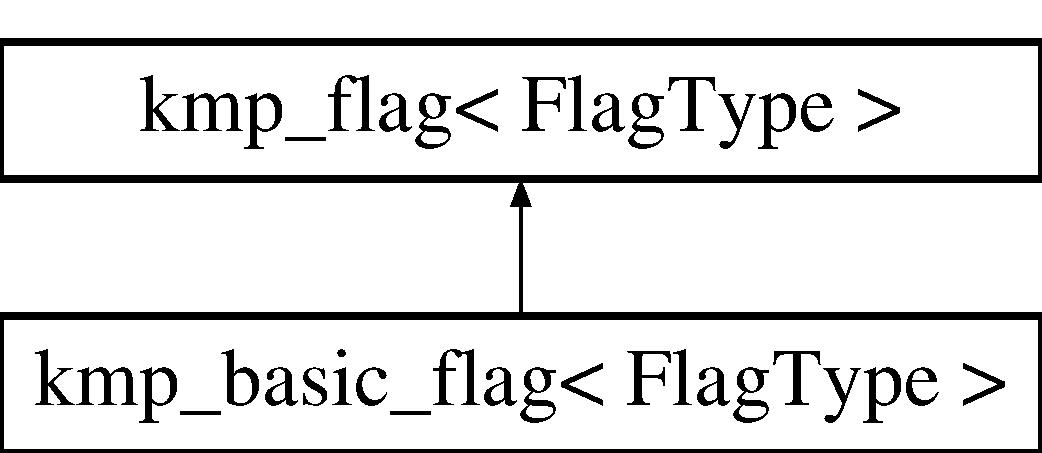
\includegraphics[height=2.000000cm]{classkmp__basic__flag}
\end{center}
\end{figure}
\subsection*{Public Member Functions}
\begin{DoxyCompactItemize}
\item 
\hyperlink{classkmp__basic__flag_aa3f040aef2c063781419ab49285d4b6a}{kmp\-\_\-basic\-\_\-flag} (volatile Flag\-Type $\ast$\hyperlink{ittnotify__static_8h_ab7caea589d3ca96f9f11c78f10bff578}{p})
\item 
\hyperlink{classkmp__basic__flag_a94bd75692e97fbbf547981f74a19286b}{kmp\-\_\-basic\-\_\-flag} (volatile Flag\-Type $\ast$\hyperlink{ittnotify__static_8h_ab7caea589d3ca96f9f11c78f10bff578}{p}, \hyperlink{kmp_8h_a194859801fe16b326efe34501a37c30a}{kmp\-\_\-info\-\_\-t} $\ast$thr)
\item 
\hyperlink{classkmp__basic__flag_a74d7dcf67d8fd1d67848a14eeb534654}{kmp\-\_\-basic\-\_\-flag} (volatile Flag\-Type $\ast$\hyperlink{ittnotify__static_8h_ab7caea589d3ca96f9f11c78f10bff578}{p}, Flag\-Type c)
\item 
\hyperlink{kmp_8h_a194859801fe16b326efe34501a37c30a}{kmp\-\_\-info\-\_\-t} $\ast$ \hyperlink{classkmp__basic__flag_a9bda9152e187ebdd45ddce7fb4e70bbf}{get\-\_\-waiter} (kmp\-\_\-uint32 \hyperlink{kmp__stub_8c_a08582ce460e3d5e1cf0b7fea017d608e}{i})
\item 
kmp\-\_\-uint32 \hyperlink{classkmp__basic__flag_ab1d3109c504f00e97e72e2ce7c109781}{get\-\_\-num\-\_\-waiters} ()
\item 
\hyperlink{ittnotify__static_8h_af941d56e55e3c5465135b60c4d6343ed}{void} \hyperlink{classkmp__basic__flag_a594260bd4ea158ba17bf17a9358ef3d4}{set\-\_\-waiter} (\hyperlink{kmp_8h_a194859801fe16b326efe34501a37c30a}{kmp\-\_\-info\-\_\-t} $\ast$thr)
\item 
bool \hyperlink{classkmp__basic__flag_a2478619a6645b7d93cacadd3843149a8}{done\-\_\-check} ()
\item 
bool \hyperlink{classkmp__basic__flag_a4c3c9eb8b025aa26b047b96de2331286}{done\-\_\-check\-\_\-val} (Flag\-Type old\-\_\-loc)
\item 
bool \hyperlink{classkmp__basic__flag_aa3981ca4f1534af0c3302a4950c7b51c}{notdone\-\_\-check} ()
\item 
\hyperlink{ittnotify__static_8h_af941d56e55e3c5465135b60c4d6343ed}{void} \hyperlink{classkmp__basic__flag_aa238982a2c6f8357f7e98ebb304a18d1}{internal\-\_\-release} ()
\item 
Flag\-Type \hyperlink{classkmp__basic__flag_adad239a48ed436a6e109fbb15c17306c}{set\-\_\-sleeping} ()
\item 
Flag\-Type \hyperlink{classkmp__basic__flag_a6867e3744945bc7dd573c65684695a22}{unset\-\_\-sleeping} ()
\item 
bool \hyperlink{classkmp__basic__flag_ace5db2765c8401a9f19ba2d39942baf4}{is\-\_\-sleeping\-\_\-val} (Flag\-Type old\-\_\-loc)
\item 
bool \hyperlink{classkmp__basic__flag_a7a24177cc9ee6800ba0b9ec3b32e7e3c}{is\-\_\-sleeping} ()
\item 
bool \hyperlink{classkmp__basic__flag_a316cabead194d9e904c0e2277c008587}{is\-\_\-any\-\_\-sleeping} ()
\item 
kmp\-\_\-uint8 $\ast$ \hyperlink{classkmp__basic__flag_ac49c9ce721d91f321d1cfccc06a685cf}{get\-\_\-stolen} ()
\item 
enum \hyperlink{kmp_8h_ad0f7c21f2f1d446087ef5714eb0fd8cf}{barrier\-\_\-type} \hyperlink{classkmp__basic__flag_abe1042797aee6220578ad29522b2e956}{get\-\_\-bt} ()
\end{DoxyCompactItemize}
\subsection*{Private Types}
\begin{DoxyCompactItemize}
\item 
typedef \hyperlink{structflag__traits}{flag\-\_\-traits}$<$ Flag\-Type $>$ \hyperlink{classkmp__basic__flag_a219ab80d54e50ffdd6db76d698b74246}{traits\-\_\-type}
\end{DoxyCompactItemize}
\subsection*{Private Attributes}
\begin{DoxyCompactItemize}
\item 
Flag\-Type \hyperlink{classkmp__basic__flag_ab23a153efd5b913c52cfe0999722812f}{checker}
\item 
\hyperlink{kmp_8h_a194859801fe16b326efe34501a37c30a}{kmp\-\_\-info\-\_\-t} $\ast$ \hyperlink{classkmp__basic__flag_a7011d738e46e39cd78dfad7eed5e79d5}{waiting\-\_\-threads} \mbox{[}1\mbox{]}
\item 
kmp\-\_\-uint32 \hyperlink{classkmp__basic__flag_a71d958593d12ea5389ca5a32864d276c}{num\-\_\-waiting\-\_\-threads}
\end{DoxyCompactItemize}
\subsection*{Additional Inherited Members}


\subsection{Detailed Description}
\subsubsection*{template$<$typename Flag\-Type$>$class kmp\-\_\-basic\-\_\-flag$<$ Flag\-Type $>$}



Definition at line 341 of file kmp\-\_\-wait\-\_\-release.\-h.



\subsection{Member Typedef Documentation}
\hypertarget{classkmp__basic__flag_a219ab80d54e50ffdd6db76d698b74246}{\index{kmp\-\_\-basic\-\_\-flag@{kmp\-\_\-basic\-\_\-flag}!traits\-\_\-type@{traits\-\_\-type}}
\index{traits\-\_\-type@{traits\-\_\-type}!kmp_basic_flag@{kmp\-\_\-basic\-\_\-flag}}
\subsubsection[{traits\-\_\-type}]{\setlength{\rightskip}{0pt plus 5cm}template$<$typename Flag\-Type$>$ typedef {\bf flag\-\_\-traits}$<$Flag\-Type$>$ {\bf kmp\-\_\-basic\-\_\-flag}$<$ Flag\-Type $>$\-::{\bf traits\-\_\-type}\hspace{0.3cm}{\ttfamily [private]}}}\label{classkmp__basic__flag_a219ab80d54e50ffdd6db76d698b74246}


Definition at line 342 of file kmp\-\_\-wait\-\_\-release.\-h.



\subsection{Constructor \& Destructor Documentation}
\hypertarget{classkmp__basic__flag_aa3f040aef2c063781419ab49285d4b6a}{\index{kmp\-\_\-basic\-\_\-flag@{kmp\-\_\-basic\-\_\-flag}!kmp\-\_\-basic\-\_\-flag@{kmp\-\_\-basic\-\_\-flag}}
\index{kmp\-\_\-basic\-\_\-flag@{kmp\-\_\-basic\-\_\-flag}!kmp_basic_flag@{kmp\-\_\-basic\-\_\-flag}}
\subsubsection[{kmp\-\_\-basic\-\_\-flag}]{\setlength{\rightskip}{0pt plus 5cm}template$<$typename Flag\-Type$>$ {\bf kmp\-\_\-basic\-\_\-flag}$<$ Flag\-Type $>$\-::{\bf kmp\-\_\-basic\-\_\-flag} (
\begin{DoxyParamCaption}
\item[{volatile Flag\-Type $\ast$}]{p}
\end{DoxyParamCaption}
)\hspace{0.3cm}{\ttfamily [inline]}}}\label{classkmp__basic__flag_aa3f040aef2c063781419ab49285d4b6a}


Definition at line 347 of file kmp\-\_\-wait\-\_\-release.\-h.


\begin{DoxyCode}
347 : \hyperlink{classkmp__flag}{kmp\_flag<FlagType>}(\hyperlink{ittnotify__static_8h_ab7caea589d3ca96f9f11c78f10bff578}{p}, traits\_type::t), \hyperlink{classkmp__basic__flag_a71d958593d12ea5389ca5a32864d276c}{num\_waiting\_threads}(0) \{\}
\end{DoxyCode}
\hypertarget{classkmp__basic__flag_a94bd75692e97fbbf547981f74a19286b}{\index{kmp\-\_\-basic\-\_\-flag@{kmp\-\_\-basic\-\_\-flag}!kmp\-\_\-basic\-\_\-flag@{kmp\-\_\-basic\-\_\-flag}}
\index{kmp\-\_\-basic\-\_\-flag@{kmp\-\_\-basic\-\_\-flag}!kmp_basic_flag@{kmp\-\_\-basic\-\_\-flag}}
\subsubsection[{kmp\-\_\-basic\-\_\-flag}]{\setlength{\rightskip}{0pt plus 5cm}template$<$typename Flag\-Type$>$ {\bf kmp\-\_\-basic\-\_\-flag}$<$ Flag\-Type $>$\-::{\bf kmp\-\_\-basic\-\_\-flag} (
\begin{DoxyParamCaption}
\item[{volatile Flag\-Type $\ast$}]{p, }
\item[{{\bf kmp\-\_\-info\-\_\-t} $\ast$}]{thr}
\end{DoxyParamCaption}
)\hspace{0.3cm}{\ttfamily [inline]}}}\label{classkmp__basic__flag_a94bd75692e97fbbf547981f74a19286b}


Definition at line 348 of file kmp\-\_\-wait\-\_\-release.\-h.


\begin{DoxyCode}
348                                                           : \hyperlink{classkmp__flag}{kmp\_flag<FlagType>}(
      \hyperlink{ittnotify__static_8h_ab7caea589d3ca96f9f11c78f10bff578}{p}, traits\_type::t), \hyperlink{classkmp__basic__flag_a71d958593d12ea5389ca5a32864d276c}{num\_waiting\_threads}(1) \{
349         \hyperlink{classkmp__basic__flag_a7011d738e46e39cd78dfad7eed5e79d5}{waiting\_threads}[0] = thr; 
350     \}
\end{DoxyCode}
\hypertarget{classkmp__basic__flag_a74d7dcf67d8fd1d67848a14eeb534654}{\index{kmp\-\_\-basic\-\_\-flag@{kmp\-\_\-basic\-\_\-flag}!kmp\-\_\-basic\-\_\-flag@{kmp\-\_\-basic\-\_\-flag}}
\index{kmp\-\_\-basic\-\_\-flag@{kmp\-\_\-basic\-\_\-flag}!kmp_basic_flag@{kmp\-\_\-basic\-\_\-flag}}
\subsubsection[{kmp\-\_\-basic\-\_\-flag}]{\setlength{\rightskip}{0pt plus 5cm}template$<$typename Flag\-Type$>$ {\bf kmp\-\_\-basic\-\_\-flag}$<$ Flag\-Type $>$\-::{\bf kmp\-\_\-basic\-\_\-flag} (
\begin{DoxyParamCaption}
\item[{volatile Flag\-Type $\ast$}]{p, }
\item[{Flag\-Type}]{c}
\end{DoxyParamCaption}
)\hspace{0.3cm}{\ttfamily [inline]}}}\label{classkmp__basic__flag_a74d7dcf67d8fd1d67848a14eeb534654}


Definition at line 351 of file kmp\-\_\-wait\-\_\-release.\-h.


\begin{DoxyCode}
351 : \hyperlink{classkmp__flag}{kmp\_flag<FlagType>}(\hyperlink{ittnotify__static_8h_ab7caea589d3ca96f9f11c78f10bff578}{p}, traits\_type::t), \hyperlink{classkmp__basic__flag_ab23a153efd5b913c52cfe0999722812f}{checker}(c), 
      \hyperlink{classkmp__basic__flag_a71d958593d12ea5389ca5a32864d276c}{num\_waiting\_threads}(0) \{\}
\end{DoxyCode}


\subsection{Member Function Documentation}
\hypertarget{classkmp__basic__flag_a2478619a6645b7d93cacadd3843149a8}{\index{kmp\-\_\-basic\-\_\-flag@{kmp\-\_\-basic\-\_\-flag}!done\-\_\-check@{done\-\_\-check}}
\index{done\-\_\-check@{done\-\_\-check}!kmp_basic_flag@{kmp\-\_\-basic\-\_\-flag}}
\subsubsection[{done\-\_\-check}]{\setlength{\rightskip}{0pt plus 5cm}template$<$typename Flag\-Type$>$ bool {\bf kmp\-\_\-basic\-\_\-flag}$<$ Flag\-Type $>$\-::done\-\_\-check (
\begin{DoxyParamCaption}
{}
\end{DoxyParamCaption}
)\hspace{0.3cm}{\ttfamily [inline]}}}\label{classkmp__basic__flag_a2478619a6645b7d93cacadd3843149a8}
\begin{DoxyReturn}{Returns}
true if the flag object has been released. 
\end{DoxyReturn}


Definition at line 376 of file kmp\-\_\-wait\-\_\-release.\-h.


\begin{DoxyCode}
376 \{ \textcolor{keywordflow}{return} traits\_type::tcr(*(this->\textcolor{keyword}{get}())) == \hyperlink{classkmp__basic__flag_ab23a153efd5b913c52cfe0999722812f}{checker}; \}
\end{DoxyCode}
\hypertarget{classkmp__basic__flag_a4c3c9eb8b025aa26b047b96de2331286}{\index{kmp\-\_\-basic\-\_\-flag@{kmp\-\_\-basic\-\_\-flag}!done\-\_\-check\-\_\-val@{done\-\_\-check\-\_\-val}}
\index{done\-\_\-check\-\_\-val@{done\-\_\-check\-\_\-val}!kmp_basic_flag@{kmp\-\_\-basic\-\_\-flag}}
\subsubsection[{done\-\_\-check\-\_\-val}]{\setlength{\rightskip}{0pt plus 5cm}template$<$typename Flag\-Type$>$ bool {\bf kmp\-\_\-basic\-\_\-flag}$<$ Flag\-Type $>$\-::done\-\_\-check\-\_\-val (
\begin{DoxyParamCaption}
\item[{Flag\-Type}]{old\-\_\-loc}
\end{DoxyParamCaption}
)\hspace{0.3cm}{\ttfamily [inline]}}}\label{classkmp__basic__flag_a4c3c9eb8b025aa26b047b96de2331286}

\begin{DoxyParams}{Parameters}
{\em old\-\_\-loc} & in old value of flag \\
\hline
\end{DoxyParams}
\begin{DoxyReturn}{Returns}
true if the flag's old value indicates it was released. 
\end{DoxyReturn}


Definition at line 381 of file kmp\-\_\-wait\-\_\-release.\-h.


\begin{DoxyCode}
381 \{ \textcolor{keywordflow}{return} old\_loc == \hyperlink{classkmp__basic__flag_ab23a153efd5b913c52cfe0999722812f}{checker}; \}
\end{DoxyCode}
\hypertarget{classkmp__basic__flag_abe1042797aee6220578ad29522b2e956}{\index{kmp\-\_\-basic\-\_\-flag@{kmp\-\_\-basic\-\_\-flag}!get\-\_\-bt@{get\-\_\-bt}}
\index{get\-\_\-bt@{get\-\_\-bt}!kmp_basic_flag@{kmp\-\_\-basic\-\_\-flag}}
\subsubsection[{get\-\_\-bt}]{\setlength{\rightskip}{0pt plus 5cm}template$<$typename Flag\-Type$>$ enum {\bf barrier\-\_\-type} {\bf kmp\-\_\-basic\-\_\-flag}$<$ Flag\-Type $>$\-::get\-\_\-bt (
\begin{DoxyParamCaption}
{}
\end{DoxyParamCaption}
)\hspace{0.3cm}{\ttfamily [inline]}}}\label{classkmp__basic__flag_abe1042797aee6220578ad29522b2e956}


Definition at line 422 of file kmp\-\_\-wait\-\_\-release.\-h.


\begin{DoxyCode}
422 \{ \textcolor{keywordflow}{return} \hyperlink{kmp_8h_ad0f7c21f2f1d446087ef5714eb0fd8cfaab77402926ed27b4683d9f72f0c369ed}{bs\_last\_barrier}; \}
\end{DoxyCode}
\hypertarget{classkmp__basic__flag_ab1d3109c504f00e97e72e2ce7c109781}{\index{kmp\-\_\-basic\-\_\-flag@{kmp\-\_\-basic\-\_\-flag}!get\-\_\-num\-\_\-waiters@{get\-\_\-num\-\_\-waiters}}
\index{get\-\_\-num\-\_\-waiters@{get\-\_\-num\-\_\-waiters}!kmp_basic_flag@{kmp\-\_\-basic\-\_\-flag}}
\subsubsection[{get\-\_\-num\-\_\-waiters}]{\setlength{\rightskip}{0pt plus 5cm}template$<$typename Flag\-Type$>$ kmp\-\_\-uint32 {\bf kmp\-\_\-basic\-\_\-flag}$<$ Flag\-Type $>$\-::get\-\_\-num\-\_\-waiters (
\begin{DoxyParamCaption}
{}
\end{DoxyParamCaption}
)\hspace{0.3cm}{\ttfamily [inline]}}}\label{classkmp__basic__flag_ab1d3109c504f00e97e72e2ce7c109781}
\begin{DoxyReturn}{Returns}
num\-\_\-waiting\-\_\-threads 
\end{DoxyReturn}


Definition at line 363 of file kmp\-\_\-wait\-\_\-release.\-h.


\begin{DoxyCode}
363 \{ \textcolor{keywordflow}{return} \hyperlink{classkmp__basic__flag_a71d958593d12ea5389ca5a32864d276c}{num\_waiting\_threads}; \}
\end{DoxyCode}
\hypertarget{classkmp__basic__flag_ac49c9ce721d91f321d1cfccc06a685cf}{\index{kmp\-\_\-basic\-\_\-flag@{kmp\-\_\-basic\-\_\-flag}!get\-\_\-stolen@{get\-\_\-stolen}}
\index{get\-\_\-stolen@{get\-\_\-stolen}!kmp_basic_flag@{kmp\-\_\-basic\-\_\-flag}}
\subsubsection[{get\-\_\-stolen}]{\setlength{\rightskip}{0pt plus 5cm}template$<$typename Flag\-Type$>$ kmp\-\_\-uint8$\ast$ {\bf kmp\-\_\-basic\-\_\-flag}$<$ Flag\-Type $>$\-::get\-\_\-stolen (
\begin{DoxyParamCaption}
{}
\end{DoxyParamCaption}
)\hspace{0.3cm}{\ttfamily [inline]}}}\label{classkmp__basic__flag_ac49c9ce721d91f321d1cfccc06a685cf}


Definition at line 421 of file kmp\-\_\-wait\-\_\-release.\-h.


\begin{DoxyCode}
421 \{ \textcolor{keywordflow}{return} NULL; \}
\end{DoxyCode}
\hypertarget{classkmp__basic__flag_a9bda9152e187ebdd45ddce7fb4e70bbf}{\index{kmp\-\_\-basic\-\_\-flag@{kmp\-\_\-basic\-\_\-flag}!get\-\_\-waiter@{get\-\_\-waiter}}
\index{get\-\_\-waiter@{get\-\_\-waiter}!kmp_basic_flag@{kmp\-\_\-basic\-\_\-flag}}
\subsubsection[{get\-\_\-waiter}]{\setlength{\rightskip}{0pt plus 5cm}template$<$typename Flag\-Type$>$ {\bf kmp\-\_\-info\-\_\-t}$\ast$ {\bf kmp\-\_\-basic\-\_\-flag}$<$ Flag\-Type $>$\-::get\-\_\-waiter (
\begin{DoxyParamCaption}
\item[{kmp\-\_\-uint32}]{i}
\end{DoxyParamCaption}
)\hspace{0.3cm}{\ttfamily [inline]}}}\label{classkmp__basic__flag_a9bda9152e187ebdd45ddce7fb4e70bbf}
param i in index into waiting\-\_\-threads \begin{DoxyReturn}{Returns}
the thread that is waiting at index i 
\end{DoxyReturn}


Definition at line 356 of file kmp\-\_\-wait\-\_\-release.\-h.


\begin{DoxyCode}
356                                           \{ 
357         \hyperlink{kmp__debug_8h_ad766efc30e33e28634691088e80cdf08}{KMP\_DEBUG\_ASSERT}(\hyperlink{kmp__stub_8c_a08582ce460e3d5e1cf0b7fea017d608e}{i}<\hyperlink{classkmp__basic__flag_a71d958593d12ea5389ca5a32864d276c}{num\_waiting\_threads});
358         \textcolor{keywordflow}{return} \hyperlink{classkmp__basic__flag_a7011d738e46e39cd78dfad7eed5e79d5}{waiting\_threads}[\hyperlink{kmp__stub_8c_a08582ce460e3d5e1cf0b7fea017d608e}{i}]; 
359     \}
\end{DoxyCode}
\hypertarget{classkmp__basic__flag_aa238982a2c6f8357f7e98ebb304a18d1}{\index{kmp\-\_\-basic\-\_\-flag@{kmp\-\_\-basic\-\_\-flag}!internal\-\_\-release@{internal\-\_\-release}}
\index{internal\-\_\-release@{internal\-\_\-release}!kmp_basic_flag@{kmp\-\_\-basic\-\_\-flag}}
\subsubsection[{internal\-\_\-release}]{\setlength{\rightskip}{0pt plus 5cm}template$<$typename Flag\-Type$>$ {\bf void} {\bf kmp\-\_\-basic\-\_\-flag}$<$ Flag\-Type $>$\-::internal\-\_\-release (
\begin{DoxyParamCaption}
{}
\end{DoxyParamCaption}
)\hspace{0.3cm}{\ttfamily [inline]}}}\label{classkmp__basic__flag_aa238982a2c6f8357f7e98ebb304a18d1}
\begin{DoxyReturn}{Returns}
Actual flag value before release was applied. Trigger all waiting threads to run by modifying flag to release state. 
\end{DoxyReturn}


Definition at line 394 of file kmp\-\_\-wait\-\_\-release.\-h.


\begin{DoxyCode}
394                             \{
395         (\hyperlink{ittnotify__static_8h_af941d56e55e3c5465135b60c4d6343ed}{void}) traits\_type::test\_then\_add4((\textcolor{keyword}{volatile} FlagType *)this->\textcolor{keyword}{get}());
396     \}
\end{DoxyCode}
\hypertarget{classkmp__basic__flag_a316cabead194d9e904c0e2277c008587}{\index{kmp\-\_\-basic\-\_\-flag@{kmp\-\_\-basic\-\_\-flag}!is\-\_\-any\-\_\-sleeping@{is\-\_\-any\-\_\-sleeping}}
\index{is\-\_\-any\-\_\-sleeping@{is\-\_\-any\-\_\-sleeping}!kmp_basic_flag@{kmp\-\_\-basic\-\_\-flag}}
\subsubsection[{is\-\_\-any\-\_\-sleeping}]{\setlength{\rightskip}{0pt plus 5cm}template$<$typename Flag\-Type$>$ bool {\bf kmp\-\_\-basic\-\_\-flag}$<$ Flag\-Type $>$\-::is\-\_\-any\-\_\-sleeping (
\begin{DoxyParamCaption}
{}
\end{DoxyParamCaption}
)\hspace{0.3cm}{\ttfamily [inline]}}}\label{classkmp__basic__flag_a316cabead194d9e904c0e2277c008587}


Definition at line 420 of file kmp\-\_\-wait\-\_\-release.\-h.


\begin{DoxyCode}
420 \{ \textcolor{keywordflow}{return} \hyperlink{classkmp__basic__flag_ace5db2765c8401a9f19ba2d39942baf4}{is\_sleeping\_val}(*(this->\textcolor{keyword}{get}())); \}
\end{DoxyCode}
\hypertarget{classkmp__basic__flag_a7a24177cc9ee6800ba0b9ec3b32e7e3c}{\index{kmp\-\_\-basic\-\_\-flag@{kmp\-\_\-basic\-\_\-flag}!is\-\_\-sleeping@{is\-\_\-sleeping}}
\index{is\-\_\-sleeping@{is\-\_\-sleeping}!kmp_basic_flag@{kmp\-\_\-basic\-\_\-flag}}
\subsubsection[{is\-\_\-sleeping}]{\setlength{\rightskip}{0pt plus 5cm}template$<$typename Flag\-Type$>$ bool {\bf kmp\-\_\-basic\-\_\-flag}$<$ Flag\-Type $>$\-::is\-\_\-sleeping (
\begin{DoxyParamCaption}
{}
\end{DoxyParamCaption}
)\hspace{0.3cm}{\ttfamily [inline]}}}\label{classkmp__basic__flag_a7a24177cc9ee6800ba0b9ec3b32e7e3c}
Test whether there are threads sleeping on the flag. 

Definition at line 419 of file kmp\-\_\-wait\-\_\-release.\-h.


\begin{DoxyCode}
419 \{ \textcolor{keywordflow}{return} \hyperlink{classkmp__basic__flag_ace5db2765c8401a9f19ba2d39942baf4}{is\_sleeping\_val}(*(this->\textcolor{keyword}{get}())); \}
\end{DoxyCode}
\hypertarget{classkmp__basic__flag_ace5db2765c8401a9f19ba2d39942baf4}{\index{kmp\-\_\-basic\-\_\-flag@{kmp\-\_\-basic\-\_\-flag}!is\-\_\-sleeping\-\_\-val@{is\-\_\-sleeping\-\_\-val}}
\index{is\-\_\-sleeping\-\_\-val@{is\-\_\-sleeping\-\_\-val}!kmp_basic_flag@{kmp\-\_\-basic\-\_\-flag}}
\subsubsection[{is\-\_\-sleeping\-\_\-val}]{\setlength{\rightskip}{0pt plus 5cm}template$<$typename Flag\-Type$>$ bool {\bf kmp\-\_\-basic\-\_\-flag}$<$ Flag\-Type $>$\-::is\-\_\-sleeping\-\_\-val (
\begin{DoxyParamCaption}
\item[{Flag\-Type}]{old\-\_\-loc}
\end{DoxyParamCaption}
)\hspace{0.3cm}{\ttfamily [inline]}}}\label{classkmp__basic__flag_ace5db2765c8401a9f19ba2d39942baf4}

\begin{DoxyParams}{Parameters}
{\em old\-\_\-loc} & in old value of flag Test whether there are threads sleeping on the flag's old value in old\-\_\-loc. \\
\hline
\end{DoxyParams}


Definition at line 415 of file kmp\-\_\-wait\-\_\-release.\-h.



Referenced by kmp\-\_\-basic\-\_\-flag$<$ kmp\-\_\-uint32 $>$\-::is\-\_\-any\-\_\-sleeping(), and kmp\-\_\-basic\-\_\-flag$<$ kmp\-\_\-uint32 $>$\-::is\-\_\-sleeping().


\begin{DoxyCode}
415 \{ \textcolor{keywordflow}{return} old\_loc & \hyperlink{kmp_8h_a5aea6667969b3c0ec527b73b22aa71e2}{KMP\_BARRIER\_SLEEP\_STATE}; \}
\end{DoxyCode}
\hypertarget{classkmp__basic__flag_aa3981ca4f1534af0c3302a4950c7b51c}{\index{kmp\-\_\-basic\-\_\-flag@{kmp\-\_\-basic\-\_\-flag}!notdone\-\_\-check@{notdone\-\_\-check}}
\index{notdone\-\_\-check@{notdone\-\_\-check}!kmp_basic_flag@{kmp\-\_\-basic\-\_\-flag}}
\subsubsection[{notdone\-\_\-check}]{\setlength{\rightskip}{0pt plus 5cm}template$<$typename Flag\-Type$>$ bool {\bf kmp\-\_\-basic\-\_\-flag}$<$ Flag\-Type $>$\-::notdone\-\_\-check (
\begin{DoxyParamCaption}
{}
\end{DoxyParamCaption}
)\hspace{0.3cm}{\ttfamily [inline]}}}\label{classkmp__basic__flag_aa3981ca4f1534af0c3302a4950c7b51c}
\begin{DoxyReturn}{Returns}
true if the flag object is not yet released. Used in \-\_\-\-\_\-kmp\-\_\-wait\-\_\-template like\-: 
\begin{DoxyCode}
\textcolor{keywordflow}{while} (flag.notdone\_check()) \{ pause(); \}
\end{DoxyCode}
 
\end{DoxyReturn}


Definition at line 389 of file kmp\-\_\-wait\-\_\-release.\-h.


\begin{DoxyCode}
389 \{ \textcolor{keywordflow}{return} traits\_type::tcr(*(this->\textcolor{keyword}{get}())) != \hyperlink{classkmp__basic__flag_ab23a153efd5b913c52cfe0999722812f}{checker}; \}
\end{DoxyCode}
\hypertarget{classkmp__basic__flag_adad239a48ed436a6e109fbb15c17306c}{\index{kmp\-\_\-basic\-\_\-flag@{kmp\-\_\-basic\-\_\-flag}!set\-\_\-sleeping@{set\-\_\-sleeping}}
\index{set\-\_\-sleeping@{set\-\_\-sleeping}!kmp_basic_flag@{kmp\-\_\-basic\-\_\-flag}}
\subsubsection[{set\-\_\-sleeping}]{\setlength{\rightskip}{0pt plus 5cm}template$<$typename Flag\-Type$>$ Flag\-Type {\bf kmp\-\_\-basic\-\_\-flag}$<$ Flag\-Type $>$\-::set\-\_\-sleeping (
\begin{DoxyParamCaption}
{}
\end{DoxyParamCaption}
)\hspace{0.3cm}{\ttfamily [inline]}}}\label{classkmp__basic__flag_adad239a48ed436a6e109fbb15c17306c}
\begin{DoxyReturn}{Returns}
Actual flag value before sleep bit(s) set. Notes that there is at least one thread sleeping on the flag by setting sleep bit(s). 
\end{DoxyReturn}


Definition at line 401 of file kmp\-\_\-wait\-\_\-release.\-h.


\begin{DoxyCode}
401                             \{ 
402         \textcolor{keywordflow}{return} traits\_type::test\_then\_or((\textcolor{keyword}{volatile} FlagType *)this->\textcolor{keyword}{get}(), 
      \hyperlink{kmp_8h_a5aea6667969b3c0ec527b73b22aa71e2}{KMP\_BARRIER\_SLEEP\_STATE});
403     \}
\end{DoxyCode}
\hypertarget{classkmp__basic__flag_a594260bd4ea158ba17bf17a9358ef3d4}{\index{kmp\-\_\-basic\-\_\-flag@{kmp\-\_\-basic\-\_\-flag}!set\-\_\-waiter@{set\-\_\-waiter}}
\index{set\-\_\-waiter@{set\-\_\-waiter}!kmp_basic_flag@{kmp\-\_\-basic\-\_\-flag}}
\subsubsection[{set\-\_\-waiter}]{\setlength{\rightskip}{0pt plus 5cm}template$<$typename Flag\-Type$>$ {\bf void} {\bf kmp\-\_\-basic\-\_\-flag}$<$ Flag\-Type $>$\-::set\-\_\-waiter (
\begin{DoxyParamCaption}
\item[{{\bf kmp\-\_\-info\-\_\-t} $\ast$}]{thr}
\end{DoxyParamCaption}
)\hspace{0.3cm}{\ttfamily [inline]}}}\label{classkmp__basic__flag_a594260bd4ea158ba17bf17a9358ef3d4}

\begin{DoxyParams}{Parameters}
{\em thr} & in the thread which is now waiting\\
\hline
\end{DoxyParams}
Insert a waiting thread at index 0. 

Definition at line 369 of file kmp\-\_\-wait\-\_\-release.\-h.



Referenced by \-\_\-\-\_\-kmp\-\_\-hyper\-\_\-barrier\-\_\-gather().


\begin{DoxyCode}
369                                      \{ 
370         \hyperlink{classkmp__basic__flag_a7011d738e46e39cd78dfad7eed5e79d5}{waiting\_threads}[0] = thr; 
371         \hyperlink{classkmp__basic__flag_a71d958593d12ea5389ca5a32864d276c}{num\_waiting\_threads} = 1;
372     \}
\end{DoxyCode}
\hypertarget{classkmp__basic__flag_a6867e3744945bc7dd573c65684695a22}{\index{kmp\-\_\-basic\-\_\-flag@{kmp\-\_\-basic\-\_\-flag}!unset\-\_\-sleeping@{unset\-\_\-sleeping}}
\index{unset\-\_\-sleeping@{unset\-\_\-sleeping}!kmp_basic_flag@{kmp\-\_\-basic\-\_\-flag}}
\subsubsection[{unset\-\_\-sleeping}]{\setlength{\rightskip}{0pt plus 5cm}template$<$typename Flag\-Type$>$ Flag\-Type {\bf kmp\-\_\-basic\-\_\-flag}$<$ Flag\-Type $>$\-::unset\-\_\-sleeping (
\begin{DoxyParamCaption}
{}
\end{DoxyParamCaption}
)\hspace{0.3cm}{\ttfamily [inline]}}}\label{classkmp__basic__flag_a6867e3744945bc7dd573c65684695a22}
\begin{DoxyReturn}{Returns}
Actual flag value before sleep bit(s) cleared. Notes that there are no longer threads sleeping on the flag by clearing sleep bit(s). 
\end{DoxyReturn}


Definition at line 408 of file kmp\-\_\-wait\-\_\-release.\-h.


\begin{DoxyCode}
408                               \{ 
409         \textcolor{keywordflow}{return} traits\_type::test\_then\_and((\textcolor{keyword}{volatile} FlagType *)this->\textcolor{keyword}{get}(), ~
      \hyperlink{kmp_8h_a5aea6667969b3c0ec527b73b22aa71e2}{KMP\_BARRIER\_SLEEP\_STATE});
410     \}
\end{DoxyCode}


\subsection{Member Data Documentation}
\hypertarget{classkmp__basic__flag_ab23a153efd5b913c52cfe0999722812f}{\index{kmp\-\_\-basic\-\_\-flag@{kmp\-\_\-basic\-\_\-flag}!checker@{checker}}
\index{checker@{checker}!kmp_basic_flag@{kmp\-\_\-basic\-\_\-flag}}
\subsubsection[{checker}]{\setlength{\rightskip}{0pt plus 5cm}template$<$typename Flag\-Type$>$ Flag\-Type {\bf kmp\-\_\-basic\-\_\-flag}$<$ Flag\-Type $>$\-::checker\hspace{0.3cm}{\ttfamily [private]}}}\label{classkmp__basic__flag_ab23a153efd5b913c52cfe0999722812f}
Value to compare flag to to check if flag has been released. 

Definition at line 343 of file kmp\-\_\-wait\-\_\-release.\-h.



Referenced by kmp\-\_\-basic\-\_\-flag$<$ kmp\-\_\-uint32 $>$\-::done\-\_\-check(), kmp\-\_\-basic\-\_\-flag$<$ kmp\-\_\-uint32 $>$\-::done\-\_\-check\-\_\-val(), and kmp\-\_\-basic\-\_\-flag$<$ kmp\-\_\-uint32 $>$\-::notdone\-\_\-check().

\hypertarget{classkmp__basic__flag_a71d958593d12ea5389ca5a32864d276c}{\index{kmp\-\_\-basic\-\_\-flag@{kmp\-\_\-basic\-\_\-flag}!num\-\_\-waiting\-\_\-threads@{num\-\_\-waiting\-\_\-threads}}
\index{num\-\_\-waiting\-\_\-threads@{num\-\_\-waiting\-\_\-threads}!kmp_basic_flag@{kmp\-\_\-basic\-\_\-flag}}
\subsubsection[{num\-\_\-waiting\-\_\-threads}]{\setlength{\rightskip}{0pt plus 5cm}template$<$typename Flag\-Type$>$ kmp\-\_\-uint32 {\bf kmp\-\_\-basic\-\_\-flag}$<$ Flag\-Type $>$\-::num\-\_\-waiting\-\_\-threads\hspace{0.3cm}{\ttfamily [private]}}}\label{classkmp__basic__flag_a71d958593d12ea5389ca5a32864d276c}
Number of threads sleeping on this thread. 

Definition at line 345 of file kmp\-\_\-wait\-\_\-release.\-h.



Referenced by kmp\-\_\-basic\-\_\-flag$<$ kmp\-\_\-uint32 $>$\-::get\-\_\-num\-\_\-waiters(), kmp\-\_\-basic\-\_\-flag$<$ kmp\-\_\-uint32 $>$\-::get\-\_\-waiter(), and kmp\-\_\-basic\-\_\-flag$<$ kmp\-\_\-uint32 $>$\-::set\-\_\-waiter().

\hypertarget{classkmp__basic__flag_a7011d738e46e39cd78dfad7eed5e79d5}{\index{kmp\-\_\-basic\-\_\-flag@{kmp\-\_\-basic\-\_\-flag}!waiting\-\_\-threads@{waiting\-\_\-threads}}
\index{waiting\-\_\-threads@{waiting\-\_\-threads}!kmp_basic_flag@{kmp\-\_\-basic\-\_\-flag}}
\subsubsection[{waiting\-\_\-threads}]{\setlength{\rightskip}{0pt plus 5cm}template$<$typename Flag\-Type$>$ {\bf kmp\-\_\-info\-\_\-t}$\ast$ {\bf kmp\-\_\-basic\-\_\-flag}$<$ Flag\-Type $>$\-::waiting\-\_\-threads\mbox{[}1\mbox{]}\hspace{0.3cm}{\ttfamily [private]}}}\label{classkmp__basic__flag_a7011d738e46e39cd78dfad7eed5e79d5}
Array of threads sleeping on this thread. 

Definition at line 344 of file kmp\-\_\-wait\-\_\-release.\-h.



Referenced by kmp\-\_\-basic\-\_\-flag$<$ kmp\-\_\-uint32 $>$\-::get\-\_\-waiter(), kmp\-\_\-basic\-\_\-flag$<$ kmp\-\_\-uint32 $>$\-::kmp\-\_\-basic\-\_\-flag(), and kmp\-\_\-basic\-\_\-flag$<$ kmp\-\_\-uint32 $>$\-::set\-\_\-waiter().



The documentation for this class was generated from the following file\-:\begin{DoxyCompactItemize}
\item 
\hyperlink{kmp__wait__release_8h}{kmp\-\_\-wait\-\_\-release.\-h}\end{DoxyCompactItemize}

\hypertarget{structkmp__block__of__locks}{\section{kmp\-\_\-block\-\_\-of\-\_\-locks Struct Reference}
\label{structkmp__block__of__locks}\index{kmp\-\_\-block\-\_\-of\-\_\-locks@{kmp\-\_\-block\-\_\-of\-\_\-locks}}
}


{\ttfamily \#include $<$kmp\-\_\-lock.\-h$>$}

\subsection*{Public Attributes}
\begin{DoxyCompactItemize}
\item 
struct \hyperlink{structkmp__block__of__locks}{kmp\-\_\-block\-\_\-of\-\_\-locks} $\ast$ \hyperlink{structkmp__block__of__locks_acd79fe8422ca10aef0f7a31340f2bd5d}{next\-\_\-block}
\item 
\hyperlink{ittnotify__static_8h_af941d56e55e3c5465135b60c4d6343ed}{void} $\ast$ \hyperlink{structkmp__block__of__locks_a03913a2aa7c0f08a912fe7457b0edc1d}{locks}
\end{DoxyCompactItemize}


\subsection{Detailed Description}


Definition at line 1004 of file kmp\-\_\-lock.\-h.



\subsection{Member Data Documentation}
\hypertarget{structkmp__block__of__locks_a03913a2aa7c0f08a912fe7457b0edc1d}{\index{kmp\-\_\-block\-\_\-of\-\_\-locks@{kmp\-\_\-block\-\_\-of\-\_\-locks}!locks@{locks}}
\index{locks@{locks}!kmp_block_of_locks@{kmp\-\_\-block\-\_\-of\-\_\-locks}}
\subsubsection[{locks}]{\setlength{\rightskip}{0pt plus 5cm}{\bf void}$\ast$ kmp\-\_\-block\-\_\-of\-\_\-locks\-::locks}}\label{structkmp__block__of__locks_a03913a2aa7c0f08a912fe7457b0edc1d}


Definition at line 1006 of file kmp\-\_\-lock.\-h.



Referenced by \-\_\-\-\_\-kmp\-\_\-cleanup\-\_\-user\-\_\-locks(), and \-\_\-\-\_\-kmp\-\_\-lock\-\_\-block\-\_\-allocate().

\hypertarget{structkmp__block__of__locks_acd79fe8422ca10aef0f7a31340f2bd5d}{\index{kmp\-\_\-block\-\_\-of\-\_\-locks@{kmp\-\_\-block\-\_\-of\-\_\-locks}!next\-\_\-block@{next\-\_\-block}}
\index{next\-\_\-block@{next\-\_\-block}!kmp_block_of_locks@{kmp\-\_\-block\-\_\-of\-\_\-locks}}
\subsubsection[{next\-\_\-block}]{\setlength{\rightskip}{0pt plus 5cm}struct {\bf kmp\-\_\-block\-\_\-of\-\_\-locks}$\ast$ kmp\-\_\-block\-\_\-of\-\_\-locks\-::next\-\_\-block}}\label{structkmp__block__of__locks_acd79fe8422ca10aef0f7a31340f2bd5d}


Definition at line 1005 of file kmp\-\_\-lock.\-h.



Referenced by \-\_\-\-\_\-kmp\-\_\-cleanup\-\_\-user\-\_\-locks(), and \-\_\-\-\_\-kmp\-\_\-lock\-\_\-block\-\_\-allocate().



The documentation for this struct was generated from the following file\-:\begin{DoxyCompactItemize}
\item 
\hyperlink{kmp__lock_8h}{kmp\-\_\-lock.\-h}\end{DoxyCompactItemize}

\hypertarget{structkmp__bstate}{\section{kmp\-\_\-bstate Struct Reference}
\label{structkmp__bstate}\index{kmp\-\_\-bstate@{kmp\-\_\-bstate}}
}


{\ttfamily \#include $<$kmp.\-h$>$}

\subsection*{Public Attributes}
\begin{DoxyCompactItemize}
\item 
\hyperlink{kmp_8h_aeee976c9503b72fe3e38d18d88b305cf}{kmp\-\_\-internal\-\_\-control\-\_\-t} \hyperlink{structkmp__bstate_aa4c7f2abe8346603fe96d8c17555872b}{th\-\_\-fixed\-\_\-icvs}
\item 
volatile kmp\-\_\-uint64 \hyperlink{structkmp__bstate_a5683452af6bb4ec4bf0862985bc6765f}{b\-\_\-go}
\item 
\hyperlink{kmp__os_8h_a6830c178a3906c25cd0138d8365db070}{K\-M\-P\-\_\-\-A\-L\-I\-G\-N\-\_\-\-C\-A\-C\-H\-E} volatile kmp\-\_\-uint64 \hyperlink{structkmp__bstate_a7467d3c14340048c5ecb4e5ae6b5ba0e}{b\-\_\-arrived}
\item 
kmp\-\_\-uint32 $\ast$ \hyperlink{structkmp__bstate_a0f3bfc82949c603682000e6582cadcf4}{skip\-\_\-per\-\_\-level}
\item 
kmp\-\_\-uint32 \hyperlink{structkmp__bstate_a5e230863e70f4a123e9f199cbab279dc}{my\-\_\-level}
\item 
kmp\-\_\-int32 \hyperlink{structkmp__bstate_afb96816855880f714bba4f2162408ff8}{parent\-\_\-tid}
\item 
kmp\-\_\-int32 \hyperlink{structkmp__bstate_a197984e81d9c2a932289380e558c6ee7}{old\-\_\-tid}
\item 
kmp\-\_\-uint32 \hyperlink{structkmp__bstate_aeee2bd7ab328429c59216e3e003a9750}{depth}
\item 
struct \hyperlink{structkmp__bstate}{kmp\-\_\-bstate} $\ast$ \hyperlink{structkmp__bstate_a908f228353bb5b8f94d3eb20ad82473c}{parent\-\_\-bar}
\item 
\hyperlink{kmp_8h_a95f7a64bda9b774add6c27c4a7b2a143}{kmp\-\_\-team\-\_\-t} $\ast$ \hyperlink{structkmp__bstate_a8980b8fa3491df30edcc2d53a17a77e2}{team}
\item 
kmp\-\_\-uint64 \hyperlink{structkmp__bstate_a937413b859e80adbc07973d4e2a428db}{leaf\-\_\-state}
\item 
kmp\-\_\-uint32 \hyperlink{structkmp__bstate_a4f6dcc9e0b14e7c62f6b90bac37875b2}{nproc}
\item 
kmp\-\_\-uint8 \hyperlink{structkmp__bstate_af4b300647701635112333890bd276a5d}{base\-\_\-leaf\-\_\-kids}
\item 
kmp\-\_\-uint8 \hyperlink{structkmp__bstate_a39d8977f4bd79dbfae45fb58f1fc22fe}{leaf\-\_\-kids}
\item 
kmp\-\_\-uint8 \hyperlink{structkmp__bstate_a6b2ff7524147c480ec05972267ddb874}{offset}
\item 
kmp\-\_\-uint8 \hyperlink{structkmp__bstate_a0247461ecd2e0778986c49789fe9812d}{wait\-\_\-flag}
\item 
kmp\-\_\-uint8 \hyperlink{structkmp__bstate_a76d7182b9224f9a340803e0f9de877da}{use\-\_\-oncore\-\_\-barrier}
\end{DoxyCompactItemize}


\subsection{Detailed Description}


Definition at line 1784 of file kmp.\-h.



\subsection{Member Data Documentation}
\hypertarget{structkmp__bstate_a7467d3c14340048c5ecb4e5ae6b5ba0e}{\index{kmp\-\_\-bstate@{kmp\-\_\-bstate}!b\-\_\-arrived@{b\-\_\-arrived}}
\index{b\-\_\-arrived@{b\-\_\-arrived}!kmp_bstate@{kmp\-\_\-bstate}}
\subsubsection[{b\-\_\-arrived}]{\setlength{\rightskip}{0pt plus 5cm}{\bf K\-M\-P\-\_\-\-A\-L\-I\-G\-N\-\_\-\-C\-A\-C\-H\-E} volatile kmp\-\_\-uint64 kmp\-\_\-bstate\-::b\-\_\-arrived}}\label{structkmp__bstate_a7467d3c14340048c5ecb4e5ae6b5ba0e}


Definition at line 1792 of file kmp.\-h.

\hypertarget{structkmp__bstate_a5683452af6bb4ec4bf0862985bc6765f}{\index{kmp\-\_\-bstate@{kmp\-\_\-bstate}!b\-\_\-go@{b\-\_\-go}}
\index{b\-\_\-go@{b\-\_\-go}!kmp_bstate@{kmp\-\_\-bstate}}
\subsubsection[{b\-\_\-go}]{\setlength{\rightskip}{0pt plus 5cm}volatile kmp\-\_\-uint64 kmp\-\_\-bstate\-::b\-\_\-go}}\label{structkmp__bstate_a5683452af6bb4ec4bf0862985bc6765f}


Definition at line 1791 of file kmp.\-h.

\hypertarget{structkmp__bstate_af4b300647701635112333890bd276a5d}{\index{kmp\-\_\-bstate@{kmp\-\_\-bstate}!base\-\_\-leaf\-\_\-kids@{base\-\_\-leaf\-\_\-kids}}
\index{base\-\_\-leaf\-\_\-kids@{base\-\_\-leaf\-\_\-kids}!kmp_bstate@{kmp\-\_\-bstate}}
\subsubsection[{base\-\_\-leaf\-\_\-kids}]{\setlength{\rightskip}{0pt plus 5cm}kmp\-\_\-uint8 kmp\-\_\-bstate\-::base\-\_\-leaf\-\_\-kids}}\label{structkmp__bstate_af4b300647701635112333890bd276a5d}


Definition at line 1802 of file kmp.\-h.

\hypertarget{structkmp__bstate_aeee2bd7ab328429c59216e3e003a9750}{\index{kmp\-\_\-bstate@{kmp\-\_\-bstate}!depth@{depth}}
\index{depth@{depth}!kmp_bstate@{kmp\-\_\-bstate}}
\subsubsection[{depth}]{\setlength{\rightskip}{0pt plus 5cm}kmp\-\_\-uint32 kmp\-\_\-bstate\-::depth}}\label{structkmp__bstate_aeee2bd7ab328429c59216e3e003a9750}


Definition at line 1797 of file kmp.\-h.

\hypertarget{structkmp__bstate_a39d8977f4bd79dbfae45fb58f1fc22fe}{\index{kmp\-\_\-bstate@{kmp\-\_\-bstate}!leaf\-\_\-kids@{leaf\-\_\-kids}}
\index{leaf\-\_\-kids@{leaf\-\_\-kids}!kmp_bstate@{kmp\-\_\-bstate}}
\subsubsection[{leaf\-\_\-kids}]{\setlength{\rightskip}{0pt plus 5cm}kmp\-\_\-uint8 kmp\-\_\-bstate\-::leaf\-\_\-kids}}\label{structkmp__bstate_a39d8977f4bd79dbfae45fb58f1fc22fe}


Definition at line 1803 of file kmp.\-h.

\hypertarget{structkmp__bstate_a937413b859e80adbc07973d4e2a428db}{\index{kmp\-\_\-bstate@{kmp\-\_\-bstate}!leaf\-\_\-state@{leaf\-\_\-state}}
\index{leaf\-\_\-state@{leaf\-\_\-state}!kmp_bstate@{kmp\-\_\-bstate}}
\subsubsection[{leaf\-\_\-state}]{\setlength{\rightskip}{0pt plus 5cm}kmp\-\_\-uint64 kmp\-\_\-bstate\-::leaf\-\_\-state}}\label{structkmp__bstate_a937413b859e80adbc07973d4e2a428db}


Definition at line 1800 of file kmp.\-h.

\hypertarget{structkmp__bstate_a5e230863e70f4a123e9f199cbab279dc}{\index{kmp\-\_\-bstate@{kmp\-\_\-bstate}!my\-\_\-level@{my\-\_\-level}}
\index{my\-\_\-level@{my\-\_\-level}!kmp_bstate@{kmp\-\_\-bstate}}
\subsubsection[{my\-\_\-level}]{\setlength{\rightskip}{0pt plus 5cm}kmp\-\_\-uint32 kmp\-\_\-bstate\-::my\-\_\-level}}\label{structkmp__bstate_a5e230863e70f4a123e9f199cbab279dc}


Definition at line 1794 of file kmp.\-h.

\hypertarget{structkmp__bstate_a4f6dcc9e0b14e7c62f6b90bac37875b2}{\index{kmp\-\_\-bstate@{kmp\-\_\-bstate}!nproc@{nproc}}
\index{nproc@{nproc}!kmp_bstate@{kmp\-\_\-bstate}}
\subsubsection[{nproc}]{\setlength{\rightskip}{0pt plus 5cm}kmp\-\_\-uint32 kmp\-\_\-bstate\-::nproc}}\label{structkmp__bstate_a4f6dcc9e0b14e7c62f6b90bac37875b2}


Definition at line 1801 of file kmp.\-h.

\hypertarget{structkmp__bstate_a6b2ff7524147c480ec05972267ddb874}{\index{kmp\-\_\-bstate@{kmp\-\_\-bstate}!offset@{offset}}
\index{offset@{offset}!kmp_bstate@{kmp\-\_\-bstate}}
\subsubsection[{offset}]{\setlength{\rightskip}{0pt plus 5cm}kmp\-\_\-uint8 kmp\-\_\-bstate\-::offset}}\label{structkmp__bstate_a6b2ff7524147c480ec05972267ddb874}


Definition at line 1804 of file kmp.\-h.

\hypertarget{structkmp__bstate_a197984e81d9c2a932289380e558c6ee7}{\index{kmp\-\_\-bstate@{kmp\-\_\-bstate}!old\-\_\-tid@{old\-\_\-tid}}
\index{old\-\_\-tid@{old\-\_\-tid}!kmp_bstate@{kmp\-\_\-bstate}}
\subsubsection[{old\-\_\-tid}]{\setlength{\rightskip}{0pt plus 5cm}kmp\-\_\-int32 kmp\-\_\-bstate\-::old\-\_\-tid}}\label{structkmp__bstate_a197984e81d9c2a932289380e558c6ee7}


Definition at line 1796 of file kmp.\-h.

\hypertarget{structkmp__bstate_a908f228353bb5b8f94d3eb20ad82473c}{\index{kmp\-\_\-bstate@{kmp\-\_\-bstate}!parent\-\_\-bar@{parent\-\_\-bar}}
\index{parent\-\_\-bar@{parent\-\_\-bar}!kmp_bstate@{kmp\-\_\-bstate}}
\subsubsection[{parent\-\_\-bar}]{\setlength{\rightskip}{0pt plus 5cm}struct {\bf kmp\-\_\-bstate}$\ast$ kmp\-\_\-bstate\-::parent\-\_\-bar}}\label{structkmp__bstate_a908f228353bb5b8f94d3eb20ad82473c}


Definition at line 1798 of file kmp.\-h.

\hypertarget{structkmp__bstate_afb96816855880f714bba4f2162408ff8}{\index{kmp\-\_\-bstate@{kmp\-\_\-bstate}!parent\-\_\-tid@{parent\-\_\-tid}}
\index{parent\-\_\-tid@{parent\-\_\-tid}!kmp_bstate@{kmp\-\_\-bstate}}
\subsubsection[{parent\-\_\-tid}]{\setlength{\rightskip}{0pt plus 5cm}kmp\-\_\-int32 kmp\-\_\-bstate\-::parent\-\_\-tid}}\label{structkmp__bstate_afb96816855880f714bba4f2162408ff8}


Definition at line 1795 of file kmp.\-h.

\hypertarget{structkmp__bstate_a0f3bfc82949c603682000e6582cadcf4}{\index{kmp\-\_\-bstate@{kmp\-\_\-bstate}!skip\-\_\-per\-\_\-level@{skip\-\_\-per\-\_\-level}}
\index{skip\-\_\-per\-\_\-level@{skip\-\_\-per\-\_\-level}!kmp_bstate@{kmp\-\_\-bstate}}
\subsubsection[{skip\-\_\-per\-\_\-level}]{\setlength{\rightskip}{0pt plus 5cm}kmp\-\_\-uint32$\ast$ kmp\-\_\-bstate\-::skip\-\_\-per\-\_\-level}}\label{structkmp__bstate_a0f3bfc82949c603682000e6582cadcf4}


Definition at line 1793 of file kmp.\-h.

\hypertarget{structkmp__bstate_a8980b8fa3491df30edcc2d53a17a77e2}{\index{kmp\-\_\-bstate@{kmp\-\_\-bstate}!team@{team}}
\index{team@{team}!kmp_bstate@{kmp\-\_\-bstate}}
\subsubsection[{team}]{\setlength{\rightskip}{0pt plus 5cm}{\bf kmp\-\_\-team\-\_\-t}$\ast$ kmp\-\_\-bstate\-::team}}\label{structkmp__bstate_a8980b8fa3491df30edcc2d53a17a77e2}


Definition at line 1799 of file kmp.\-h.

\hypertarget{structkmp__bstate_aa4c7f2abe8346603fe96d8c17555872b}{\index{kmp\-\_\-bstate@{kmp\-\_\-bstate}!th\-\_\-fixed\-\_\-icvs@{th\-\_\-fixed\-\_\-icvs}}
\index{th\-\_\-fixed\-\_\-icvs@{th\-\_\-fixed\-\_\-icvs}!kmp_bstate@{kmp\-\_\-bstate}}
\subsubsection[{th\-\_\-fixed\-\_\-icvs}]{\setlength{\rightskip}{0pt plus 5cm}{\bf kmp\-\_\-internal\-\_\-control\-\_\-t} kmp\-\_\-bstate\-::th\-\_\-fixed\-\_\-icvs}}\label{structkmp__bstate_aa4c7f2abe8346603fe96d8c17555872b}


Definition at line 1789 of file kmp.\-h.

\hypertarget{structkmp__bstate_a76d7182b9224f9a340803e0f9de877da}{\index{kmp\-\_\-bstate@{kmp\-\_\-bstate}!use\-\_\-oncore\-\_\-barrier@{use\-\_\-oncore\-\_\-barrier}}
\index{use\-\_\-oncore\-\_\-barrier@{use\-\_\-oncore\-\_\-barrier}!kmp_bstate@{kmp\-\_\-bstate}}
\subsubsection[{use\-\_\-oncore\-\_\-barrier}]{\setlength{\rightskip}{0pt plus 5cm}kmp\-\_\-uint8 kmp\-\_\-bstate\-::use\-\_\-oncore\-\_\-barrier}}\label{structkmp__bstate_a76d7182b9224f9a340803e0f9de877da}


Definition at line 1806 of file kmp.\-h.

\hypertarget{structkmp__bstate_a0247461ecd2e0778986c49789fe9812d}{\index{kmp\-\_\-bstate@{kmp\-\_\-bstate}!wait\-\_\-flag@{wait\-\_\-flag}}
\index{wait\-\_\-flag@{wait\-\_\-flag}!kmp_bstate@{kmp\-\_\-bstate}}
\subsubsection[{wait\-\_\-flag}]{\setlength{\rightskip}{0pt plus 5cm}kmp\-\_\-uint8 kmp\-\_\-bstate\-::wait\-\_\-flag}}\label{structkmp__bstate_a0247461ecd2e0778986c49789fe9812d}


Definition at line 1805 of file kmp.\-h.



The documentation for this struct was generated from the following file\-:\begin{DoxyCompactItemize}
\item 
\hyperlink{kmp_8h}{kmp.\-h}\end{DoxyCompactItemize}

\hypertarget{structkmp__cached__addr}{\section{kmp\-\_\-cached\-\_\-addr Struct Reference}
\label{structkmp__cached__addr}\index{kmp\-\_\-cached\-\_\-addr@{kmp\-\_\-cached\-\_\-addr}}
}


{\ttfamily \#include $<$kmp.\-h$>$}

\subsection*{Public Attributes}
\begin{DoxyCompactItemize}
\item 
\hyperlink{ittnotify__static_8h_af941d56e55e3c5465135b60c4d6343ed}{void} $\ast$$\ast$ \hyperlink{structkmp__cached__addr_affbc380f12d77a61086ae4dc40256b09}{addr}
\item 
struct \hyperlink{structkmp__cached__addr}{kmp\-\_\-cached\-\_\-addr} $\ast$ \hyperlink{structkmp__cached__addr_ae41b7057e025555848a335dca0ce1788}{next}
\end{DoxyCompactItemize}


\subsection{Detailed Description}


Definition at line 1472 of file kmp.\-h.



\subsection{Member Data Documentation}
\hypertarget{structkmp__cached__addr_affbc380f12d77a61086ae4dc40256b09}{\index{kmp\-\_\-cached\-\_\-addr@{kmp\-\_\-cached\-\_\-addr}!addr@{addr}}
\index{addr@{addr}!kmp_cached_addr@{kmp\-\_\-cached\-\_\-addr}}
\subsubsection[{addr}]{\setlength{\rightskip}{0pt plus 5cm}{\bf void}$\ast$$\ast$ kmp\-\_\-cached\-\_\-addr\-::addr}}\label{structkmp__cached__addr_affbc380f12d77a61086ae4dc40256b09}


Definition at line 1473 of file kmp.\-h.

\hypertarget{structkmp__cached__addr_ae41b7057e025555848a335dca0ce1788}{\index{kmp\-\_\-cached\-\_\-addr@{kmp\-\_\-cached\-\_\-addr}!next@{next}}
\index{next@{next}!kmp_cached_addr@{kmp\-\_\-cached\-\_\-addr}}
\subsubsection[{next}]{\setlength{\rightskip}{0pt plus 5cm}struct {\bf kmp\-\_\-cached\-\_\-addr}$\ast$ kmp\-\_\-cached\-\_\-addr\-::next}}\label{structkmp__cached__addr_ae41b7057e025555848a335dca0ce1788}


Definition at line 1474 of file kmp.\-h.



The documentation for this struct was generated from the following file\-:\begin{DoxyCompactItemize}
\item 
\hyperlink{kmp_8h}{kmp.\-h}\end{DoxyCompactItemize}

\hypertarget{unionkmp__cmplrdata}{\section{kmp\-\_\-cmplrdata Union Reference}
\label{unionkmp__cmplrdata}\index{kmp\-\_\-cmplrdata@{kmp\-\_\-cmplrdata}}
}


{\ttfamily \#include $<$kmp.\-h$>$}

\subsection*{Public Attributes}
\begin{DoxyCompactItemize}
\item 
\hyperlink{group__BASIC__TYPES_ga76e21422ff9984d9bafd0b36277ae115}{kmp\-\_\-routine\-\_\-entry\-\_\-t} \hyperlink{unionkmp__cmplrdata_a55f86681cc0ecc440233e7a93f89b402}{destructors}
\end{DoxyCompactItemize}


\subsection{Detailed Description}


Definition at line 2036 of file kmp.\-h.



\subsection{Member Data Documentation}
\hypertarget{unionkmp__cmplrdata_a55f86681cc0ecc440233e7a93f89b402}{\index{kmp\-\_\-cmplrdata@{kmp\-\_\-cmplrdata}!destructors@{destructors}}
\index{destructors@{destructors}!kmp_cmplrdata@{kmp\-\_\-cmplrdata}}
\subsubsection[{destructors}]{\setlength{\rightskip}{0pt plus 5cm}{\bf kmp\-\_\-routine\-\_\-entry\-\_\-t} kmp\-\_\-cmplrdata\-::destructors}}\label{unionkmp__cmplrdata_a55f86681cc0ecc440233e7a93f89b402}


Definition at line 2041 of file kmp.\-h.



Referenced by \-\_\-\-\_\-kmp\-\_\-task\-\_\-finish().



The documentation for this union was generated from the following file\-:\begin{DoxyCompactItemize}
\item 
\hyperlink{kmp_8h}{kmp.\-h}\end{DoxyCompactItemize}

\hypertarget{structkmp__cpuinfo}{\section{kmp\-\_\-cpuinfo Struct Reference}
\label{structkmp__cpuinfo}\index{kmp\-\_\-cpuinfo@{kmp\-\_\-cpuinfo}}
}


{\ttfamily \#include $<$kmp.\-h$>$}

\subsection*{Public Attributes}
\begin{DoxyCompactItemize}
\item 
\hyperlink{ittnotify__static_8h_a8b8dcd723308a8cb5d84277c7a3fff70}{int} \hyperlink{structkmp__cpuinfo_a340553795a3c12f5f72d3333027dc1ef}{initialized}
\item 
\hyperlink{ittnotify__static_8h_a8b8dcd723308a8cb5d84277c7a3fff70}{int} \hyperlink{structkmp__cpuinfo_a8aac4a116cdfd108b60d8fc8a3cda7c1}{signature}
\item 
\hyperlink{ittnotify__static_8h_a8b8dcd723308a8cb5d84277c7a3fff70}{int} \hyperlink{structkmp__cpuinfo_a0ef7a4d4fcf0f147c6049310bed9d966}{family}
\item 
\hyperlink{ittnotify__static_8h_a8b8dcd723308a8cb5d84277c7a3fff70}{int} \hyperlink{structkmp__cpuinfo_afbf2c46e7d9c4e8f38e78be63e12f34c}{model}
\item 
\hyperlink{ittnotify__static_8h_a8b8dcd723308a8cb5d84277c7a3fff70}{int} \hyperlink{structkmp__cpuinfo_af2dd9e7cd2b55c588f9f7bc8d152dd41}{stepping}
\item 
\hyperlink{ittnotify__static_8h_a8b8dcd723308a8cb5d84277c7a3fff70}{int} \hyperlink{structkmp__cpuinfo_a06952924c8236563056c13d3158c70dc}{sse2}
\item 
\hyperlink{ittnotify__static_8h_a8b8dcd723308a8cb5d84277c7a3fff70}{int} \hyperlink{structkmp__cpuinfo_a86197ba559ddb32df419fe8589b25200}{rtm}
\item 
\hyperlink{ittnotify__static_8h_a8b8dcd723308a8cb5d84277c7a3fff70}{int} \hyperlink{structkmp__cpuinfo_a261ccb280417486b1f9972e6c2d5d717}{cpu\-\_\-stackoffset}
\item 
\hyperlink{ittnotify__static_8h_a8b8dcd723308a8cb5d84277c7a3fff70}{int} \hyperlink{structkmp__cpuinfo_a0aca284c6e9b610e35c33c2ead7b6ce8}{apic\-\_\-id}
\item 
\hyperlink{ittnotify__static_8h_a8b8dcd723308a8cb5d84277c7a3fff70}{int} \hyperlink{structkmp__cpuinfo_a20bc3bb9a899855733dd05d7ba5f042c}{physical\-\_\-id}
\item 
\hyperlink{ittnotify__static_8h_a8b8dcd723308a8cb5d84277c7a3fff70}{int} \hyperlink{structkmp__cpuinfo_a321ce01f5bddf1ca648122ce827b5fb1}{logical\-\_\-id}
\item 
kmp\-\_\-uint64 \hyperlink{structkmp__cpuinfo_a8daaba40f317228e14dc2e37ad8b0170}{frequency}
\item 
char \hyperlink{structkmp__cpuinfo_a17f3ff5dbc72594ab37b92b7ee82b218}{name} \mbox{[}3 $\ast$sizeof(kmp\-\_\-cpuid\-\_\-t)\mbox{]}
\end{DoxyCompactItemize}


\subsection{Detailed Description}


Definition at line 1231 of file kmp.\-h.



\subsection{Member Data Documentation}
\hypertarget{structkmp__cpuinfo_a0aca284c6e9b610e35c33c2ead7b6ce8}{\index{kmp\-\_\-cpuinfo@{kmp\-\_\-cpuinfo}!apic\-\_\-id@{apic\-\_\-id}}
\index{apic\-\_\-id@{apic\-\_\-id}!kmp_cpuinfo@{kmp\-\_\-cpuinfo}}
\subsubsection[{apic\-\_\-id}]{\setlength{\rightskip}{0pt plus 5cm}{\bf int} kmp\-\_\-cpuinfo\-::apic\-\_\-id}}\label{structkmp__cpuinfo_a0aca284c6e9b610e35c33c2ead7b6ce8}


Definition at line 1240 of file kmp.\-h.

\hypertarget{structkmp__cpuinfo_a261ccb280417486b1f9972e6c2d5d717}{\index{kmp\-\_\-cpuinfo@{kmp\-\_\-cpuinfo}!cpu\-\_\-stackoffset@{cpu\-\_\-stackoffset}}
\index{cpu\-\_\-stackoffset@{cpu\-\_\-stackoffset}!kmp_cpuinfo@{kmp\-\_\-cpuinfo}}
\subsubsection[{cpu\-\_\-stackoffset}]{\setlength{\rightskip}{0pt plus 5cm}{\bf int} kmp\-\_\-cpuinfo\-::cpu\-\_\-stackoffset}}\label{structkmp__cpuinfo_a261ccb280417486b1f9972e6c2d5d717}


Definition at line 1239 of file kmp.\-h.

\hypertarget{structkmp__cpuinfo_a0ef7a4d4fcf0f147c6049310bed9d966}{\index{kmp\-\_\-cpuinfo@{kmp\-\_\-cpuinfo}!family@{family}}
\index{family@{family}!kmp_cpuinfo@{kmp\-\_\-cpuinfo}}
\subsubsection[{family}]{\setlength{\rightskip}{0pt plus 5cm}{\bf int} kmp\-\_\-cpuinfo\-::family}}\label{structkmp__cpuinfo_a0ef7a4d4fcf0f147c6049310bed9d966}


Definition at line 1234 of file kmp.\-h.



Referenced by kmp\-\_\-stats\-\_\-output\-\_\-module\-::print\-Header\-Info().

\hypertarget{structkmp__cpuinfo_a8daaba40f317228e14dc2e37ad8b0170}{\index{kmp\-\_\-cpuinfo@{kmp\-\_\-cpuinfo}!frequency@{frequency}}
\index{frequency@{frequency}!kmp_cpuinfo@{kmp\-\_\-cpuinfo}}
\subsubsection[{frequency}]{\setlength{\rightskip}{0pt plus 5cm}kmp\-\_\-uint64 kmp\-\_\-cpuinfo\-::frequency}}\label{structkmp__cpuinfo_a8daaba40f317228e14dc2e37ad8b0170}


Definition at line 1243 of file kmp.\-h.



Referenced by kmp\-\_\-stats\-\_\-output\-\_\-module\-::print\-Header\-Info().

\hypertarget{structkmp__cpuinfo_a340553795a3c12f5f72d3333027dc1ef}{\index{kmp\-\_\-cpuinfo@{kmp\-\_\-cpuinfo}!initialized@{initialized}}
\index{initialized@{initialized}!kmp_cpuinfo@{kmp\-\_\-cpuinfo}}
\subsubsection[{initialized}]{\setlength{\rightskip}{0pt plus 5cm}{\bf int} kmp\-\_\-cpuinfo\-::initialized}}\label{structkmp__cpuinfo_a340553795a3c12f5f72d3333027dc1ef}


Definition at line 1232 of file kmp.\-h.



Referenced by \-\_\-\-\_\-kmp\-\_\-runtime\-\_\-initialize(), and \-\_\-\-\_\-kmpc\-\_\-flush().

\hypertarget{structkmp__cpuinfo_a321ce01f5bddf1ca648122ce827b5fb1}{\index{kmp\-\_\-cpuinfo@{kmp\-\_\-cpuinfo}!logical\-\_\-id@{logical\-\_\-id}}
\index{logical\-\_\-id@{logical\-\_\-id}!kmp_cpuinfo@{kmp\-\_\-cpuinfo}}
\subsubsection[{logical\-\_\-id}]{\setlength{\rightskip}{0pt plus 5cm}{\bf int} kmp\-\_\-cpuinfo\-::logical\-\_\-id}}\label{structkmp__cpuinfo_a321ce01f5bddf1ca648122ce827b5fb1}


Definition at line 1242 of file kmp.\-h.

\hypertarget{structkmp__cpuinfo_afbf2c46e7d9c4e8f38e78be63e12f34c}{\index{kmp\-\_\-cpuinfo@{kmp\-\_\-cpuinfo}!model@{model}}
\index{model@{model}!kmp_cpuinfo@{kmp\-\_\-cpuinfo}}
\subsubsection[{model}]{\setlength{\rightskip}{0pt plus 5cm}{\bf int} kmp\-\_\-cpuinfo\-::model}}\label{structkmp__cpuinfo_afbf2c46e7d9c4e8f38e78be63e12f34c}


Definition at line 1235 of file kmp.\-h.



Referenced by kmp\-\_\-stats\-\_\-output\-\_\-module\-::print\-Header\-Info().

\hypertarget{structkmp__cpuinfo_a17f3ff5dbc72594ab37b92b7ee82b218}{\index{kmp\-\_\-cpuinfo@{kmp\-\_\-cpuinfo}!name@{name}}
\index{name@{name}!kmp_cpuinfo@{kmp\-\_\-cpuinfo}}
\subsubsection[{name}]{\setlength{\rightskip}{0pt plus 5cm}char kmp\-\_\-cpuinfo\-::name\mbox{[}3 $\ast$sizeof(kmp\-\_\-cpuid\-\_\-t)\mbox{]}}}\label{structkmp__cpuinfo_a17f3ff5dbc72594ab37b92b7ee82b218}


Definition at line 1244 of file kmp.\-h.



Referenced by kmp\-\_\-stats\-\_\-output\-\_\-module\-::print\-Header\-Info().

\hypertarget{structkmp__cpuinfo_a20bc3bb9a899855733dd05d7ba5f042c}{\index{kmp\-\_\-cpuinfo@{kmp\-\_\-cpuinfo}!physical\-\_\-id@{physical\-\_\-id}}
\index{physical\-\_\-id@{physical\-\_\-id}!kmp_cpuinfo@{kmp\-\_\-cpuinfo}}
\subsubsection[{physical\-\_\-id}]{\setlength{\rightskip}{0pt plus 5cm}{\bf int} kmp\-\_\-cpuinfo\-::physical\-\_\-id}}\label{structkmp__cpuinfo_a20bc3bb9a899855733dd05d7ba5f042c}


Definition at line 1241 of file kmp.\-h.

\hypertarget{structkmp__cpuinfo_a86197ba559ddb32df419fe8589b25200}{\index{kmp\-\_\-cpuinfo@{kmp\-\_\-cpuinfo}!rtm@{rtm}}
\index{rtm@{rtm}!kmp_cpuinfo@{kmp\-\_\-cpuinfo}}
\subsubsection[{rtm}]{\setlength{\rightskip}{0pt plus 5cm}{\bf int} kmp\-\_\-cpuinfo\-::rtm}}\label{structkmp__cpuinfo_a86197ba559ddb32df419fe8589b25200}


Definition at line 1238 of file kmp.\-h.



Referenced by \-\_\-\-\_\-kmp\-\_\-stg\-\_\-parse\-\_\-lock\-\_\-kind().

\hypertarget{structkmp__cpuinfo_a8aac4a116cdfd108b60d8fc8a3cda7c1}{\index{kmp\-\_\-cpuinfo@{kmp\-\_\-cpuinfo}!signature@{signature}}
\index{signature@{signature}!kmp_cpuinfo@{kmp\-\_\-cpuinfo}}
\subsubsection[{signature}]{\setlength{\rightskip}{0pt plus 5cm}{\bf int} kmp\-\_\-cpuinfo\-::signature}}\label{structkmp__cpuinfo_a8aac4a116cdfd108b60d8fc8a3cda7c1}


Definition at line 1233 of file kmp.\-h.

\hypertarget{structkmp__cpuinfo_a06952924c8236563056c13d3158c70dc}{\index{kmp\-\_\-cpuinfo@{kmp\-\_\-cpuinfo}!sse2@{sse2}}
\index{sse2@{sse2}!kmp_cpuinfo@{kmp\-\_\-cpuinfo}}
\subsubsection[{sse2}]{\setlength{\rightskip}{0pt plus 5cm}{\bf int} kmp\-\_\-cpuinfo\-::sse2}}\label{structkmp__cpuinfo_a06952924c8236563056c13d3158c70dc}


Definition at line 1237 of file kmp.\-h.



Referenced by \-\_\-\-\_\-kmpc\-\_\-flush().

\hypertarget{structkmp__cpuinfo_af2dd9e7cd2b55c588f9f7bc8d152dd41}{\index{kmp\-\_\-cpuinfo@{kmp\-\_\-cpuinfo}!stepping@{stepping}}
\index{stepping@{stepping}!kmp_cpuinfo@{kmp\-\_\-cpuinfo}}
\subsubsection[{stepping}]{\setlength{\rightskip}{0pt plus 5cm}{\bf int} kmp\-\_\-cpuinfo\-::stepping}}\label{structkmp__cpuinfo_af2dd9e7cd2b55c588f9f7bc8d152dd41}


Definition at line 1236 of file kmp.\-h.



Referenced by kmp\-\_\-stats\-\_\-output\-\_\-module\-::print\-Header\-Info().



The documentation for this struct was generated from the following file\-:\begin{DoxyCompactItemize}
\item 
\hyperlink{kmp_8h}{kmp.\-h}\end{DoxyCompactItemize}

\hypertarget{structkmp__depend__info}{\section{kmp\-\_\-depend\-\_\-info Struct Reference}
\label{structkmp__depend__info}\index{kmp\-\_\-depend\-\_\-info@{kmp\-\_\-depend\-\_\-info}}
}


{\ttfamily \#include $<$kmp.\-h$>$}

\subsection*{Public Attributes}
\begin{DoxyCompactItemize}
\item 
\hyperlink{kmp__os_8h_a43fe09095a192381a5e7c93d20a3a2f9}{kmp\-\_\-intptr\-\_\-t} \hyperlink{structkmp__depend__info_a4b110a3ef2f123f550be5ecfcc51d50a}{base\-\_\-addr}
\item 
size\-\_\-t \hyperlink{structkmp__depend__info_a432a5de100db7d4cb311366e88cc79b2}{len}
\item 
\begin{tabbing}
xx\=xx\=xx\=xx\=xx\=xx\=xx\=xx\=xx\=\kill
struct \{\\
\>bool \hyperlink{structkmp__depend__info_a65b239cf11dd7d59dc86eb9ab5f6e414}{in}:1\\
\>bool \hyperlink{structkmp__depend__info_ad2f4d34c0d6aa127073c9e21a5041244}{out}:1\\
\} \hyperlink{structkmp__depend__info_aa36eee45c425e2a66beb059660c9fb63}{flags}\\

\end{tabbing}\end{DoxyCompactItemize}


\subsection{Detailed Description}


Definition at line 2079 of file kmp.\-h.



\subsection{Member Data Documentation}
\hypertarget{structkmp__depend__info_a4b110a3ef2f123f550be5ecfcc51d50a}{\index{kmp\-\_\-depend\-\_\-info@{kmp\-\_\-depend\-\_\-info}!base\-\_\-addr@{base\-\_\-addr}}
\index{base\-\_\-addr@{base\-\_\-addr}!kmp_depend_info@{kmp\-\_\-depend\-\_\-info}}
\subsubsection[{base\-\_\-addr}]{\setlength{\rightskip}{0pt plus 5cm}{\bf kmp\-\_\-intptr\-\_\-t} kmp\-\_\-depend\-\_\-info\-::base\-\_\-addr}}\label{structkmp__depend__info_a4b110a3ef2f123f550be5ecfcc51d50a}


Definition at line 2080 of file kmp.\-h.



Referenced by \-\_\-\-\_\-kmp\-\_\-check\-\_\-deps(), and \-\_\-\-\_\-kmp\-\_\-process\-\_\-deps().

\hypertarget{structkmp__depend__info_aa36eee45c425e2a66beb059660c9fb63}{\index{kmp\-\_\-depend\-\_\-info@{kmp\-\_\-depend\-\_\-info}!flags@{flags}}
\index{flags@{flags}!kmp_depend_info@{kmp\-\_\-depend\-\_\-info}}
\subsubsection[{flags}]{\setlength{\rightskip}{0pt plus 5cm}struct \{ ... \}   kmp\-\_\-depend\-\_\-info\-::flags}}\label{structkmp__depend__info_aa36eee45c425e2a66beb059660c9fb63}


Referenced by \-\_\-\-\_\-kmp\-\_\-check\-\_\-deps(), \-\_\-\-\_\-kmp\-\_\-process\-\_\-deps(), and \-\_\-\-\_\-kmpc\-\_\-omp\-\_\-task\-\_\-with\-\_\-deps().

\hypertarget{structkmp__depend__info_a65b239cf11dd7d59dc86eb9ab5f6e414}{\index{kmp\-\_\-depend\-\_\-info@{kmp\-\_\-depend\-\_\-info}!in@{in}}
\index{in@{in}!kmp_depend_info@{kmp\-\_\-depend\-\_\-info}}
\subsubsection[{in}]{\setlength{\rightskip}{0pt plus 5cm}bool kmp\-\_\-depend\-\_\-info\-::in}}\label{structkmp__depend__info_a65b239cf11dd7d59dc86eb9ab5f6e414}


Definition at line 2083 of file kmp.\-h.



Referenced by \-\_\-\-\_\-kmp\-\_\-check\-\_\-deps(), \-\_\-\-\_\-kmp\-\_\-process\-\_\-deps(), and \-\_\-\-\_\-kmpc\-\_\-omp\-\_\-task\-\_\-with\-\_\-deps().

\hypertarget{structkmp__depend__info_a432a5de100db7d4cb311366e88cc79b2}{\index{kmp\-\_\-depend\-\_\-info@{kmp\-\_\-depend\-\_\-info}!len@{len}}
\index{len@{len}!kmp_depend_info@{kmp\-\_\-depend\-\_\-info}}
\subsubsection[{len}]{\setlength{\rightskip}{0pt plus 5cm}size\-\_\-t kmp\-\_\-depend\-\_\-info\-::len}}\label{structkmp__depend__info_a432a5de100db7d4cb311366e88cc79b2}


Definition at line 2081 of file kmp.\-h.

\hypertarget{structkmp__depend__info_ad2f4d34c0d6aa127073c9e21a5041244}{\index{kmp\-\_\-depend\-\_\-info@{kmp\-\_\-depend\-\_\-info}!out@{out}}
\index{out@{out}!kmp_depend_info@{kmp\-\_\-depend\-\_\-info}}
\subsubsection[{out}]{\setlength{\rightskip}{0pt plus 5cm}bool kmp\-\_\-depend\-\_\-info\-::out}}\label{structkmp__depend__info_ad2f4d34c0d6aa127073c9e21a5041244}


Definition at line 2084 of file kmp.\-h.



Referenced by \-\_\-\-\_\-kmp\-\_\-check\-\_\-deps(), \-\_\-\-\_\-kmp\-\_\-process\-\_\-deps(), and \-\_\-\-\_\-kmpc\-\_\-omp\-\_\-task\-\_\-with\-\_\-deps().



The documentation for this struct was generated from the following file\-:\begin{DoxyCompactItemize}
\item 
\hyperlink{kmp_8h}{kmp.\-h}\end{DoxyCompactItemize}

\hypertarget{structkmp__dephash}{\section{kmp\-\_\-dephash Struct Reference}
\label{structkmp__dephash}\index{kmp\-\_\-dephash@{kmp\-\_\-dephash}}
}


{\ttfamily \#include $<$kmp.\-h$>$}

\subsection*{Public Attributes}
\begin{DoxyCompactItemize}
\item 
\hyperlink{kmp_8h_ae26b65abb82278a8c3dc261171d399d5}{kmp\-\_\-dephash\-\_\-entry\-\_\-t} $\ast$$\ast$ \hyperlink{structkmp__dephash_a06e58d9ddec4328db119b478c7bff4f5}{buckets}
\item 
size\-\_\-t \hyperlink{structkmp__dephash_a6c2dd618cc89b336b65c9e8b822aac5c}{size}
\end{DoxyCompactItemize}


\subsection{Detailed Description}


Definition at line 2120 of file kmp.\-h.



\subsection{Member Data Documentation}
\hypertarget{structkmp__dephash_a06e58d9ddec4328db119b478c7bff4f5}{\index{kmp\-\_\-dephash@{kmp\-\_\-dephash}!buckets@{buckets}}
\index{buckets@{buckets}!kmp_dephash@{kmp\-\_\-dephash}}
\subsubsection[{buckets}]{\setlength{\rightskip}{0pt plus 5cm}{\bf kmp\-\_\-dephash\-\_\-entry\-\_\-t}$\ast$$\ast$ kmp\-\_\-dephash\-::buckets}}\label{structkmp__dephash_a06e58d9ddec4328db119b478c7bff4f5}


Definition at line 2121 of file kmp.\-h.



Referenced by \-\_\-\-\_\-kmp\-\_\-dephash\-\_\-create(), \-\_\-\-\_\-kmp\-\_\-dephash\-\_\-find(), and \-\_\-\-\_\-kmp\-\_\-dephash\-\_\-free().

\hypertarget{structkmp__dephash_a6c2dd618cc89b336b65c9e8b822aac5c}{\index{kmp\-\_\-dephash@{kmp\-\_\-dephash}!size@{size}}
\index{size@{size}!kmp_dephash@{kmp\-\_\-dephash}}
\subsubsection[{size}]{\setlength{\rightskip}{0pt plus 5cm}size\-\_\-t kmp\-\_\-dephash\-::size}}\label{structkmp__dephash_a6c2dd618cc89b336b65c9e8b822aac5c}


Definition at line 2122 of file kmp.\-h.



Referenced by \-\_\-\-\_\-kmp\-\_\-dephash\-\_\-create(), \-\_\-\-\_\-kmp\-\_\-dephash\-\_\-find(), and \-\_\-\-\_\-kmp\-\_\-dephash\-\_\-free().



The documentation for this struct was generated from the following file\-:\begin{DoxyCompactItemize}
\item 
\hyperlink{kmp_8h}{kmp.\-h}\end{DoxyCompactItemize}

\hypertarget{structkmp__dephash__entry}{\section{kmp\-\_\-dephash\-\_\-entry Struct Reference}
\label{structkmp__dephash__entry}\index{kmp\-\_\-dephash\-\_\-entry@{kmp\-\_\-dephash\-\_\-entry}}
}


{\ttfamily \#include $<$kmp.\-h$>$}

\subsection*{Public Attributes}
\begin{DoxyCompactItemize}
\item 
\hyperlink{kmp__os_8h_a43fe09095a192381a5e7c93d20a3a2f9}{kmp\-\_\-intptr\-\_\-t} \hyperlink{structkmp__dephash__entry_a6bddf4b7f2ea115a0bed6b8caa791ef1}{addr}
\item 
\hyperlink{kmp_8h_a5197537dbef055a1d52ecdcbf5578098}{kmp\-\_\-depnode\-\_\-t} $\ast$ \hyperlink{structkmp__dephash__entry_a0ae786669b6c8b01605717a93f8c2c33}{last\-\_\-out}
\item 
\hyperlink{kmp_8h_a877b10d3438c1c7864488165c95be189}{kmp\-\_\-depnode\-\_\-list\-\_\-t} $\ast$ \hyperlink{structkmp__dephash__entry_ad54a7a6e0b862b27750bed4730e2d9b0}{last\-\_\-ins}
\item 
\hyperlink{kmp_8h_ae26b65abb82278a8c3dc261171d399d5}{kmp\-\_\-dephash\-\_\-entry\-\_\-t} $\ast$ \hyperlink{structkmp__dephash__entry_a2708bddc7160e13ec29ba5f36cd37e1a}{next\-\_\-in\-\_\-bucket}
\end{DoxyCompactItemize}


\subsection{Detailed Description}


Definition at line 2113 of file kmp.\-h.



\subsection{Member Data Documentation}
\hypertarget{structkmp__dephash__entry_a6bddf4b7f2ea115a0bed6b8caa791ef1}{\index{kmp\-\_\-dephash\-\_\-entry@{kmp\-\_\-dephash\-\_\-entry}!addr@{addr}}
\index{addr@{addr}!kmp_dephash_entry@{kmp\-\_\-dephash\-\_\-entry}}
\subsubsection[{addr}]{\setlength{\rightskip}{0pt plus 5cm}{\bf kmp\-\_\-intptr\-\_\-t} kmp\-\_\-dephash\-\_\-entry\-::addr}}\label{structkmp__dephash__entry_a6bddf4b7f2ea115a0bed6b8caa791ef1}


Definition at line 2114 of file kmp.\-h.



Referenced by \-\_\-\-\_\-kmp\-\_\-dephash\-\_\-find().

\hypertarget{structkmp__dephash__entry_ad54a7a6e0b862b27750bed4730e2d9b0}{\index{kmp\-\_\-dephash\-\_\-entry@{kmp\-\_\-dephash\-\_\-entry}!last\-\_\-ins@{last\-\_\-ins}}
\index{last\-\_\-ins@{last\-\_\-ins}!kmp_dephash_entry@{kmp\-\_\-dephash\-\_\-entry}}
\subsubsection[{last\-\_\-ins}]{\setlength{\rightskip}{0pt plus 5cm}{\bf kmp\-\_\-depnode\-\_\-list\-\_\-t}$\ast$ kmp\-\_\-dephash\-\_\-entry\-::last\-\_\-ins}}\label{structkmp__dephash__entry_ad54a7a6e0b862b27750bed4730e2d9b0}


Definition at line 2116 of file kmp.\-h.



Referenced by \-\_\-\-\_\-kmp\-\_\-dephash\-\_\-find(), and \-\_\-\-\_\-kmp\-\_\-process\-\_\-deps().

\hypertarget{structkmp__dephash__entry_a0ae786669b6c8b01605717a93f8c2c33}{\index{kmp\-\_\-dephash\-\_\-entry@{kmp\-\_\-dephash\-\_\-entry}!last\-\_\-out@{last\-\_\-out}}
\index{last\-\_\-out@{last\-\_\-out}!kmp_dephash_entry@{kmp\-\_\-dephash\-\_\-entry}}
\subsubsection[{last\-\_\-out}]{\setlength{\rightskip}{0pt plus 5cm}{\bf kmp\-\_\-depnode\-\_\-t}$\ast$ kmp\-\_\-dephash\-\_\-entry\-::last\-\_\-out}}\label{structkmp__dephash__entry_a0ae786669b6c8b01605717a93f8c2c33}


Definition at line 2115 of file kmp.\-h.



Referenced by \-\_\-\-\_\-kmp\-\_\-dephash\-\_\-find(), and \-\_\-\-\_\-kmp\-\_\-process\-\_\-deps().

\hypertarget{structkmp__dephash__entry_a2708bddc7160e13ec29ba5f36cd37e1a}{\index{kmp\-\_\-dephash\-\_\-entry@{kmp\-\_\-dephash\-\_\-entry}!next\-\_\-in\-\_\-bucket@{next\-\_\-in\-\_\-bucket}}
\index{next\-\_\-in\-\_\-bucket@{next\-\_\-in\-\_\-bucket}!kmp_dephash_entry@{kmp\-\_\-dephash\-\_\-entry}}
\subsubsection[{next\-\_\-in\-\_\-bucket}]{\setlength{\rightskip}{0pt plus 5cm}{\bf kmp\-\_\-dephash\-\_\-entry\-\_\-t}$\ast$ kmp\-\_\-dephash\-\_\-entry\-::next\-\_\-in\-\_\-bucket}}\label{structkmp__dephash__entry_a2708bddc7160e13ec29ba5f36cd37e1a}


Definition at line 2117 of file kmp.\-h.



Referenced by \-\_\-\-\_\-kmp\-\_\-dephash\-\_\-find(), and \-\_\-\-\_\-kmp\-\_\-dephash\-\_\-free().



The documentation for this struct was generated from the following file\-:\begin{DoxyCompactItemize}
\item 
\hyperlink{kmp_8h}{kmp.\-h}\end{DoxyCompactItemize}

\hypertarget{unionkmp__depnode}{\section{kmp\-\_\-depnode Union Reference}
\label{unionkmp__depnode}\index{kmp\-\_\-depnode@{kmp\-\_\-depnode}}
}


{\ttfamily \#include $<$kmp.\-h$>$}

\subsection*{Public Attributes}
\begin{DoxyCompactItemize}
\item 
double \hyperlink{unionkmp__depnode_a347b4791e41750279971e4ec00993f7e}{dn\-\_\-align}
\item 
char \hyperlink{unionkmp__depnode_aad9f486cd3fe36dc5c4cf0c3580234a6}{dn\-\_\-pad} \mbox{[}\hyperlink{kmp__lock_8h_a7e782410115489f45ab1686c39a2bb89}{K\-M\-P\-\_\-\-P\-A\-D}(\hyperlink{kmp_8h_a02c8c93518ce0670ea0c9b9c8c23b014}{kmp\-\_\-base\-\_\-depnode\-\_\-t}, \hyperlink{kmp__os_8h_a86194c659a2d795e5f5949d293ae4661}{C\-A\-C\-H\-E\-\_\-\-L\-I\-N\-E})\mbox{]}
\item 
\hyperlink{kmp_8h_a02c8c93518ce0670ea0c9b9c8c23b014}{kmp\-\_\-base\-\_\-depnode\-\_\-t} \hyperlink{unionkmp__depnode_aad9c3578bf502dba0af949b9f8bf02f7}{dn}
\end{DoxyCompactItemize}


\subsection{Detailed Description}


Definition at line 2107 of file kmp.\-h.



\subsection{Member Data Documentation}
\hypertarget{unionkmp__depnode_aad9c3578bf502dba0af949b9f8bf02f7}{\index{kmp\-\_\-depnode@{kmp\-\_\-depnode}!dn@{dn}}
\index{dn@{dn}!kmp_depnode@{kmp\-\_\-depnode}}
\subsubsection[{dn}]{\setlength{\rightskip}{0pt plus 5cm}{\bf kmp\-\_\-base\-\_\-depnode\-\_\-t} kmp\-\_\-depnode\-::dn}}\label{unionkmp__depnode_aad9c3578bf502dba0af949b9f8bf02f7}


Definition at line 2110 of file kmp.\-h.



Referenced by \-\_\-\-\_\-kmp\-\_\-check\-\_\-deps(), \-\_\-\-\_\-kmp\-\_\-init\-\_\-node(), \-\_\-\-\_\-kmp\-\_\-node\-\_\-deref(), \-\_\-\-\_\-kmp\-\_\-node\-\_\-ref(), \-\_\-\-\_\-kmp\-\_\-process\-\_\-deps(), \-\_\-\-\_\-kmp\-\_\-release\-\_\-deps(), \-\_\-\-\_\-kmp\-\_\-track\-\_\-dependence(), and \-\_\-\-\_\-kmpc\-\_\-omp\-\_\-wait\-\_\-deps().

\hypertarget{unionkmp__depnode_a347b4791e41750279971e4ec00993f7e}{\index{kmp\-\_\-depnode@{kmp\-\_\-depnode}!dn\-\_\-align@{dn\-\_\-align}}
\index{dn\-\_\-align@{dn\-\_\-align}!kmp_depnode@{kmp\-\_\-depnode}}
\subsubsection[{dn\-\_\-align}]{\setlength{\rightskip}{0pt plus 5cm}double kmp\-\_\-depnode\-::dn\-\_\-align}}\label{unionkmp__depnode_a347b4791e41750279971e4ec00993f7e}


Definition at line 2108 of file kmp.\-h.

\hypertarget{unionkmp__depnode_aad9f486cd3fe36dc5c4cf0c3580234a6}{\index{kmp\-\_\-depnode@{kmp\-\_\-depnode}!dn\-\_\-pad@{dn\-\_\-pad}}
\index{dn\-\_\-pad@{dn\-\_\-pad}!kmp_depnode@{kmp\-\_\-depnode}}
\subsubsection[{dn\-\_\-pad}]{\setlength{\rightskip}{0pt plus 5cm}char kmp\-\_\-depnode\-::dn\-\_\-pad\mbox{[}{\bf K\-M\-P\-\_\-\-P\-A\-D}({\bf kmp\-\_\-base\-\_\-depnode\-\_\-t}, {\bf C\-A\-C\-H\-E\-\_\-\-L\-I\-N\-E})\mbox{]}}}\label{unionkmp__depnode_aad9f486cd3fe36dc5c4cf0c3580234a6}


Definition at line 2109 of file kmp.\-h.



The documentation for this union was generated from the following file\-:\begin{DoxyCompactItemize}
\item 
\hyperlink{kmp_8h}{kmp.\-h}\end{DoxyCompactItemize}

\hypertarget{structkmp__depnode__list}{\section{kmp\-\_\-depnode\-\_\-list Struct Reference}
\label{structkmp__depnode__list}\index{kmp\-\_\-depnode\-\_\-list@{kmp\-\_\-depnode\-\_\-list}}
}


{\ttfamily \#include $<$kmp.\-h$>$}

\subsection*{Public Attributes}
\begin{DoxyCompactItemize}
\item 
\hyperlink{kmp_8h_a5197537dbef055a1d52ecdcbf5578098}{kmp\-\_\-depnode\-\_\-t} $\ast$ \hyperlink{structkmp__depnode__list_a8873aa1231cab49fdd5ca6dc3b89eca4}{node}
\item 
\hyperlink{kmp_8h_a877b10d3438c1c7864488165c95be189}{kmp\-\_\-depnode\-\_\-list\-\_\-t} $\ast$ \hyperlink{structkmp__depnode__list_a17c86246d585f456214601ceecc1bd0e}{next}
\end{DoxyCompactItemize}


\subsection{Detailed Description}


Definition at line 2088 of file kmp.\-h.



\subsection{Member Data Documentation}
\hypertarget{structkmp__depnode__list_a17c86246d585f456214601ceecc1bd0e}{\index{kmp\-\_\-depnode\-\_\-list@{kmp\-\_\-depnode\-\_\-list}!next@{next}}
\index{next@{next}!kmp_depnode_list@{kmp\-\_\-depnode\-\_\-list}}
\subsubsection[{next}]{\setlength{\rightskip}{0pt plus 5cm}{\bf kmp\-\_\-depnode\-\_\-list\-\_\-t}$\ast$ kmp\-\_\-depnode\-\_\-list\-::next}}\label{structkmp__depnode__list_a17c86246d585f456214601ceecc1bd0e}


Definition at line 2090 of file kmp.\-h.



Referenced by \-\_\-\-\_\-kmp\-\_\-add\-\_\-node(), and \-\_\-\-\_\-kmp\-\_\-depnode\-\_\-list\-\_\-free().

\hypertarget{structkmp__depnode__list_a8873aa1231cab49fdd5ca6dc3b89eca4}{\index{kmp\-\_\-depnode\-\_\-list@{kmp\-\_\-depnode\-\_\-list}!node@{node}}
\index{node@{node}!kmp_depnode_list@{kmp\-\_\-depnode\-\_\-list}}
\subsubsection[{node}]{\setlength{\rightskip}{0pt plus 5cm}{\bf kmp\-\_\-depnode\-\_\-t}$\ast$ kmp\-\_\-depnode\-\_\-list\-::node}}\label{structkmp__depnode__list_a8873aa1231cab49fdd5ca6dc3b89eca4}


Definition at line 2089 of file kmp.\-h.



Referenced by \-\_\-\-\_\-kmp\-\_\-add\-\_\-node(), and \-\_\-\-\_\-kmp\-\_\-depnode\-\_\-list\-\_\-free().



The documentation for this struct was generated from the following file\-:\begin{DoxyCompactItemize}
\item 
\hyperlink{kmp_8h}{kmp.\-h}\end{DoxyCompactItemize}

\hypertarget{unionkmp__desc}{\section{kmp\-\_\-desc Union Reference}
\label{unionkmp__desc}\index{kmp\-\_\-desc@{kmp\-\_\-desc}}
}


{\ttfamily \#include $<$kmp.\-h$>$}

\subsection*{Public Attributes}
\begin{DoxyCompactItemize}
\item 
double \hyperlink{unionkmp__desc_a07ddc184d874a557a32e0a840768c046}{ds\-\_\-align}
\item 
char \hyperlink{unionkmp__desc_a45b5eb29d9e37aba9ac0f8e618097a2a}{ds\-\_\-pad} \mbox{[}\hyperlink{kmp__lock_8h_a7e782410115489f45ab1686c39a2bb89}{K\-M\-P\-\_\-\-P\-A\-D}(\hyperlink{kmp_8h_a5e7f01f0708353f8e3c3f977dce55eb5}{kmp\-\_\-desc\-\_\-base\-\_\-t}, \hyperlink{kmp__os_8h_a86194c659a2d795e5f5949d293ae4661}{C\-A\-C\-H\-E\-\_\-\-L\-I\-N\-E})\mbox{]}
\item 
\hyperlink{kmp_8h_a5e7f01f0708353f8e3c3f977dce55eb5}{kmp\-\_\-desc\-\_\-base\-\_\-t} \hyperlink{unionkmp__desc_aebfb0f1186b63f19217a552941275fa4}{ds}
\end{DoxyCompactItemize}


\subsection{Detailed Description}


Definition at line 1922 of file kmp.\-h.



\subsection{Member Data Documentation}
\hypertarget{unionkmp__desc_aebfb0f1186b63f19217a552941275fa4}{\index{kmp\-\_\-desc@{kmp\-\_\-desc}!ds@{ds}}
\index{ds@{ds}!kmp_desc@{kmp\-\_\-desc}}
\subsubsection[{ds}]{\setlength{\rightskip}{0pt plus 5cm}{\bf kmp\-\_\-desc\-\_\-base\-\_\-t} kmp\-\_\-desc\-::ds}}\label{unionkmp__desc_aebfb0f1186b63f19217a552941275fa4}


Definition at line 1925 of file kmp.\-h.

\hypertarget{unionkmp__desc_a07ddc184d874a557a32e0a840768c046}{\index{kmp\-\_\-desc@{kmp\-\_\-desc}!ds\-\_\-align@{ds\-\_\-align}}
\index{ds\-\_\-align@{ds\-\_\-align}!kmp_desc@{kmp\-\_\-desc}}
\subsubsection[{ds\-\_\-align}]{\setlength{\rightskip}{0pt plus 5cm}double kmp\-\_\-desc\-::ds\-\_\-align}}\label{unionkmp__desc_a07ddc184d874a557a32e0a840768c046}


Definition at line 1923 of file kmp.\-h.

\hypertarget{unionkmp__desc_a45b5eb29d9e37aba9ac0f8e618097a2a}{\index{kmp\-\_\-desc@{kmp\-\_\-desc}!ds\-\_\-pad@{ds\-\_\-pad}}
\index{ds\-\_\-pad@{ds\-\_\-pad}!kmp_desc@{kmp\-\_\-desc}}
\subsubsection[{ds\-\_\-pad}]{\setlength{\rightskip}{0pt plus 5cm}char kmp\-\_\-desc\-::ds\-\_\-pad\mbox{[}{\bf K\-M\-P\-\_\-\-P\-A\-D}({\bf kmp\-\_\-desc\-\_\-base\-\_\-t}, {\bf C\-A\-C\-H\-E\-\_\-\-L\-I\-N\-E})\mbox{]}}}\label{unionkmp__desc_a45b5eb29d9e37aba9ac0f8e618097a2a}


Definition at line 1924 of file kmp.\-h.



The documentation for this union was generated from the following file\-:\begin{DoxyCompactItemize}
\item 
\hyperlink{kmp_8h}{kmp.\-h}\end{DoxyCompactItemize}

\hypertarget{structkmp__desc__base}{\section{kmp\-\_\-desc\-\_\-base Struct Reference}
\label{structkmp__desc__base}\index{kmp\-\_\-desc\-\_\-base@{kmp\-\_\-desc\-\_\-base}}
}


{\ttfamily \#include $<$kmp.\-h$>$}

\subsection*{Public Attributes}
\begin{DoxyCompactItemize}
\item 
\hyperlink{ittnotify__static_8h_af941d56e55e3c5465135b60c4d6343ed}{void} $\ast$ \hyperlink{structkmp__desc__base_a33d81d8dad4336633a06fb03206d74e7}{ds\-\_\-stackbase}
\item 
size\-\_\-t \hyperlink{structkmp__desc__base_a13fc21d4832e63d133b9cc28f4620197}{ds\-\_\-stacksize}
\item 
\hyperlink{ittnotify__static_8h_a8b8dcd723308a8cb5d84277c7a3fff70}{int} \hyperlink{structkmp__desc__base_a803a8f867d5c1a5d675aa03de8b3bc7b}{ds\-\_\-stackgrow}
\item 
kmp\-\_\-thread\-\_\-t \hyperlink{structkmp__desc__base_a870050b7c12984b85171ef1757335bff}{ds\-\_\-thread}
\item 
volatile \hyperlink{ittnotify__static_8h_a8b8dcd723308a8cb5d84277c7a3fff70}{int} \hyperlink{structkmp__desc__base_abc0ecc8ce19cd714e5c888c4383fb287}{ds\-\_\-tid}
\item 
\hyperlink{ittnotify__static_8h_a8b8dcd723308a8cb5d84277c7a3fff70}{int} \hyperlink{structkmp__desc__base_adaadada162cc10167fa30a29f87e71c6}{ds\-\_\-gtid}
\end{DoxyCompactItemize}


\subsection{Detailed Description}


Definition at line 1896 of file kmp.\-h.



\subsection{Member Data Documentation}
\hypertarget{structkmp__desc__base_adaadada162cc10167fa30a29f87e71c6}{\index{kmp\-\_\-desc\-\_\-base@{kmp\-\_\-desc\-\_\-base}!ds\-\_\-gtid@{ds\-\_\-gtid}}
\index{ds\-\_\-gtid@{ds\-\_\-gtid}!kmp_desc_base@{kmp\-\_\-desc\-\_\-base}}
\subsubsection[{ds\-\_\-gtid}]{\setlength{\rightskip}{0pt plus 5cm}{\bf int} kmp\-\_\-desc\-\_\-base\-::ds\-\_\-gtid}}\label{structkmp__desc__base_adaadada162cc10167fa30a29f87e71c6}


Definition at line 1902 of file kmp.\-h.

\hypertarget{structkmp__desc__base_a33d81d8dad4336633a06fb03206d74e7}{\index{kmp\-\_\-desc\-\_\-base@{kmp\-\_\-desc\-\_\-base}!ds\-\_\-stackbase@{ds\-\_\-stackbase}}
\index{ds\-\_\-stackbase@{ds\-\_\-stackbase}!kmp_desc_base@{kmp\-\_\-desc\-\_\-base}}
\subsubsection[{ds\-\_\-stackbase}]{\setlength{\rightskip}{0pt plus 5cm}{\bf void}$\ast$ kmp\-\_\-desc\-\_\-base\-::ds\-\_\-stackbase}}\label{structkmp__desc__base_a33d81d8dad4336633a06fb03206d74e7}


Definition at line 1897 of file kmp.\-h.

\hypertarget{structkmp__desc__base_a803a8f867d5c1a5d675aa03de8b3bc7b}{\index{kmp\-\_\-desc\-\_\-base@{kmp\-\_\-desc\-\_\-base}!ds\-\_\-stackgrow@{ds\-\_\-stackgrow}}
\index{ds\-\_\-stackgrow@{ds\-\_\-stackgrow}!kmp_desc_base@{kmp\-\_\-desc\-\_\-base}}
\subsubsection[{ds\-\_\-stackgrow}]{\setlength{\rightskip}{0pt plus 5cm}{\bf int} kmp\-\_\-desc\-\_\-base\-::ds\-\_\-stackgrow}}\label{structkmp__desc__base_a803a8f867d5c1a5d675aa03de8b3bc7b}


Definition at line 1899 of file kmp.\-h.

\hypertarget{structkmp__desc__base_a13fc21d4832e63d133b9cc28f4620197}{\index{kmp\-\_\-desc\-\_\-base@{kmp\-\_\-desc\-\_\-base}!ds\-\_\-stacksize@{ds\-\_\-stacksize}}
\index{ds\-\_\-stacksize@{ds\-\_\-stacksize}!kmp_desc_base@{kmp\-\_\-desc\-\_\-base}}
\subsubsection[{ds\-\_\-stacksize}]{\setlength{\rightskip}{0pt plus 5cm}size\-\_\-t kmp\-\_\-desc\-\_\-base\-::ds\-\_\-stacksize}}\label{structkmp__desc__base_a13fc21d4832e63d133b9cc28f4620197}


Definition at line 1898 of file kmp.\-h.

\hypertarget{structkmp__desc__base_a870050b7c12984b85171ef1757335bff}{\index{kmp\-\_\-desc\-\_\-base@{kmp\-\_\-desc\-\_\-base}!ds\-\_\-thread@{ds\-\_\-thread}}
\index{ds\-\_\-thread@{ds\-\_\-thread}!kmp_desc_base@{kmp\-\_\-desc\-\_\-base}}
\subsubsection[{ds\-\_\-thread}]{\setlength{\rightskip}{0pt plus 5cm}kmp\-\_\-thread\-\_\-t kmp\-\_\-desc\-\_\-base\-::ds\-\_\-thread}}\label{structkmp__desc__base_a870050b7c12984b85171ef1757335bff}


Definition at line 1900 of file kmp.\-h.

\hypertarget{structkmp__desc__base_abc0ecc8ce19cd714e5c888c4383fb287}{\index{kmp\-\_\-desc\-\_\-base@{kmp\-\_\-desc\-\_\-base}!ds\-\_\-tid@{ds\-\_\-tid}}
\index{ds\-\_\-tid@{ds\-\_\-tid}!kmp_desc_base@{kmp\-\_\-desc\-\_\-base}}
\subsubsection[{ds\-\_\-tid}]{\setlength{\rightskip}{0pt plus 5cm}volatile {\bf int} kmp\-\_\-desc\-\_\-base\-::ds\-\_\-tid}}\label{structkmp__desc__base_abc0ecc8ce19cd714e5c888c4383fb287}


Definition at line 1901 of file kmp.\-h.



The documentation for this struct was generated from the following file\-:\begin{DoxyCompactItemize}
\item 
\hyperlink{kmp_8h}{kmp.\-h}\end{DoxyCompactItemize}

\hypertarget{structkmp__disp}{\section{kmp\-\_\-disp Struct Reference}
\label{structkmp__disp}\index{kmp\-\_\-disp@{kmp\-\_\-disp}}
}


{\ttfamily \#include $<$kmp.\-h$>$}

\subsection*{Public Attributes}
\begin{DoxyCompactItemize}
\item 
\hyperlink{ittnotify__static_8h_af941d56e55e3c5465135b60c4d6343ed}{void}($\ast$ \hyperlink{structkmp__disp_a34c2a4a67bbbb9a596e8cee765a12467}{th\-\_\-deo\-\_\-fcn} )(\hyperlink{ittnotify__static_8h_a8b8dcd723308a8cb5d84277c7a3fff70}{int} $\ast$gtid, \hyperlink{ittnotify__static_8h_a8b8dcd723308a8cb5d84277c7a3fff70}{int} $\ast$cid, \hyperlink{group__BASIC__TYPES_ga690fda6b92f039a72db263c6b4394ddb}{ident\-\_\-t} $\ast$)
\item 
\hyperlink{ittnotify__static_8h_af941d56e55e3c5465135b60c4d6343ed}{void}($\ast$ \hyperlink{structkmp__disp_a661b8f748ff2f3204218ae2d7ece3287}{th\-\_\-dxo\-\_\-fcn} )(\hyperlink{ittnotify__static_8h_a8b8dcd723308a8cb5d84277c7a3fff70}{int} $\ast$gtid, \hyperlink{ittnotify__static_8h_a8b8dcd723308a8cb5d84277c7a3fff70}{int} $\ast$cid, \hyperlink{group__BASIC__TYPES_ga690fda6b92f039a72db263c6b4394ddb}{ident\-\_\-t} $\ast$)
\item 
\hyperlink{kmp_8h_a77f9babc5a9999a105d305f27cf46d70}{dispatch\-\_\-shared\-\_\-info\-\_\-t} $\ast$ \hyperlink{structkmp__disp_afe430cfc39a695761004b645704b6b63}{th\-\_\-dispatch\-\_\-sh\-\_\-current}
\item 
\hyperlink{kmp_8h_a39b4260bfb46eb4f113a70e0a8ac26ea}{dispatch\-\_\-private\-\_\-info\-\_\-t} $\ast$ \hyperlink{structkmp__disp_a720af84b753cfa5961f42459754972b2}{th\-\_\-dispatch\-\_\-pr\-\_\-current}
\item 
\hyperlink{kmp_8h_a39b4260bfb46eb4f113a70e0a8ac26ea}{dispatch\-\_\-private\-\_\-info\-\_\-t} $\ast$ \hyperlink{structkmp__disp_ae9f9d6c19682600e62d7a9d8ab55fe75}{th\-\_\-disp\-\_\-buffer}
\item 
kmp\-\_\-int32 \hyperlink{structkmp__disp_a160f4b28144ce1cb64ccf0ceb9ad9ffc}{th\-\_\-disp\-\_\-index}
\item 
\hyperlink{ittnotify__static_8h_af941d56e55e3c5465135b60c4d6343ed}{void} $\ast$ \hyperlink{structkmp__disp_a2d0804dc17a8f9c75e24d504005595b0}{dummy\-\_\-padding} \mbox{[}2\mbox{]}
\end{DoxyCompactItemize}


\subsection{Detailed Description}


Definition at line 1685 of file kmp.\-h.



\subsection{Member Data Documentation}
\hypertarget{structkmp__disp_a2d0804dc17a8f9c75e24d504005595b0}{\index{kmp\-\_\-disp@{kmp\-\_\-disp}!dummy\-\_\-padding@{dummy\-\_\-padding}}
\index{dummy\-\_\-padding@{dummy\-\_\-padding}!kmp_disp@{kmp\-\_\-disp}}
\subsubsection[{dummy\-\_\-padding}]{\setlength{\rightskip}{0pt plus 5cm}{\bf void}$\ast$ kmp\-\_\-disp\-::dummy\-\_\-padding\mbox{[}2\mbox{]}}}\label{structkmp__disp_a2d0804dc17a8f9c75e24d504005595b0}


Definition at line 1701 of file kmp.\-h.

\hypertarget{structkmp__disp_a34c2a4a67bbbb9a596e8cee765a12467}{\index{kmp\-\_\-disp@{kmp\-\_\-disp}!th\-\_\-deo\-\_\-fcn@{th\-\_\-deo\-\_\-fcn}}
\index{th\-\_\-deo\-\_\-fcn@{th\-\_\-deo\-\_\-fcn}!kmp_disp@{kmp\-\_\-disp}}
\subsubsection[{th\-\_\-deo\-\_\-fcn}]{\setlength{\rightskip}{0pt plus 5cm}{\bf void}($\ast$ kmp\-\_\-disp\-::th\-\_\-deo\-\_\-fcn)({\bf int} $\ast$gtid, {\bf int} $\ast$cid, {\bf ident\-\_\-t} $\ast$)}}\label{structkmp__disp_a34c2a4a67bbbb9a596e8cee765a12467}


Definition at line 1687 of file kmp.\-h.



Referenced by \-\_\-\-\_\-kmp\-\_\-initialize\-\_\-info().

\hypertarget{structkmp__disp_ae9f9d6c19682600e62d7a9d8ab55fe75}{\index{kmp\-\_\-disp@{kmp\-\_\-disp}!th\-\_\-disp\-\_\-buffer@{th\-\_\-disp\-\_\-buffer}}
\index{th\-\_\-disp\-\_\-buffer@{th\-\_\-disp\-\_\-buffer}!kmp_disp@{kmp\-\_\-disp}}
\subsubsection[{th\-\_\-disp\-\_\-buffer}]{\setlength{\rightskip}{0pt plus 5cm}{\bf dispatch\-\_\-private\-\_\-info\-\_\-t}$\ast$ kmp\-\_\-disp\-::th\-\_\-disp\-\_\-buffer}}\label{structkmp__disp_ae9f9d6c19682600e62d7a9d8ab55fe75}


Definition at line 1694 of file kmp.\-h.



Referenced by \-\_\-\-\_\-kmp\-\_\-initialize\-\_\-info().

\hypertarget{structkmp__disp_a160f4b28144ce1cb64ccf0ceb9ad9ffc}{\index{kmp\-\_\-disp@{kmp\-\_\-disp}!th\-\_\-disp\-\_\-index@{th\-\_\-disp\-\_\-index}}
\index{th\-\_\-disp\-\_\-index@{th\-\_\-disp\-\_\-index}!kmp_disp@{kmp\-\_\-disp}}
\subsubsection[{th\-\_\-disp\-\_\-index}]{\setlength{\rightskip}{0pt plus 5cm}kmp\-\_\-int32 kmp\-\_\-disp\-::th\-\_\-disp\-\_\-index}}\label{structkmp__disp_a160f4b28144ce1cb64ccf0ceb9ad9ffc}


Definition at line 1695 of file kmp.\-h.



Referenced by \-\_\-\-\_\-kmp\-\_\-initialize\-\_\-info(), and \-\_\-\-\_\-kmp\-\_\-run\-\_\-before\-\_\-invoked\-\_\-task().

\hypertarget{structkmp__disp_a720af84b753cfa5961f42459754972b2}{\index{kmp\-\_\-disp@{kmp\-\_\-disp}!th\-\_\-dispatch\-\_\-pr\-\_\-current@{th\-\_\-dispatch\-\_\-pr\-\_\-current}}
\index{th\-\_\-dispatch\-\_\-pr\-\_\-current@{th\-\_\-dispatch\-\_\-pr\-\_\-current}!kmp_disp@{kmp\-\_\-disp}}
\subsubsection[{th\-\_\-dispatch\-\_\-pr\-\_\-current}]{\setlength{\rightskip}{0pt plus 5cm}{\bf dispatch\-\_\-private\-\_\-info\-\_\-t}$\ast$ kmp\-\_\-disp\-::th\-\_\-dispatch\-\_\-pr\-\_\-current}}\label{structkmp__disp_a720af84b753cfa5961f42459754972b2}


Definition at line 1692 of file kmp.\-h.



Referenced by \-\_\-\-\_\-kmp\-\_\-initialize\-\_\-info().

\hypertarget{structkmp__disp_afe430cfc39a695761004b645704b6b63}{\index{kmp\-\_\-disp@{kmp\-\_\-disp}!th\-\_\-dispatch\-\_\-sh\-\_\-current@{th\-\_\-dispatch\-\_\-sh\-\_\-current}}
\index{th\-\_\-dispatch\-\_\-sh\-\_\-current@{th\-\_\-dispatch\-\_\-sh\-\_\-current}!kmp_disp@{kmp\-\_\-disp}}
\subsubsection[{th\-\_\-dispatch\-\_\-sh\-\_\-current}]{\setlength{\rightskip}{0pt plus 5cm}{\bf dispatch\-\_\-shared\-\_\-info\-\_\-t}$\ast$ kmp\-\_\-disp\-::th\-\_\-dispatch\-\_\-sh\-\_\-current}}\label{structkmp__disp_afe430cfc39a695761004b645704b6b63}


Definition at line 1691 of file kmp.\-h.



Referenced by \-\_\-\-\_\-kmp\-\_\-initialize\-\_\-info().

\hypertarget{structkmp__disp_a661b8f748ff2f3204218ae2d7ece3287}{\index{kmp\-\_\-disp@{kmp\-\_\-disp}!th\-\_\-dxo\-\_\-fcn@{th\-\_\-dxo\-\_\-fcn}}
\index{th\-\_\-dxo\-\_\-fcn@{th\-\_\-dxo\-\_\-fcn}!kmp_disp@{kmp\-\_\-disp}}
\subsubsection[{th\-\_\-dxo\-\_\-fcn}]{\setlength{\rightskip}{0pt plus 5cm}{\bf void}($\ast$ kmp\-\_\-disp\-::th\-\_\-dxo\-\_\-fcn)({\bf int} $\ast$gtid, {\bf int} $\ast$cid, {\bf ident\-\_\-t} $\ast$)}}\label{structkmp__disp_a661b8f748ff2f3204218ae2d7ece3287}


Definition at line 1689 of file kmp.\-h.



Referenced by \-\_\-\-\_\-kmp\-\_\-initialize\-\_\-info().



The documentation for this struct was generated from the following file\-:\begin{DoxyCompactItemize}
\item 
\hyperlink{kmp_8h}{kmp.\-h}\end{DoxyCompactItemize}

\hypertarget{unionkmp__drdpa__lock}{\section{kmp\-\_\-drdpa\-\_\-lock Union Reference}
\label{unionkmp__drdpa__lock}\index{kmp\-\_\-drdpa\-\_\-lock@{kmp\-\_\-drdpa\-\_\-lock}}
}


{\ttfamily \#include $<$kmp\-\_\-lock.\-h$>$}

\subsection*{Public Attributes}
\begin{DoxyCompactItemize}
\item 
\hyperlink{kmp__lock_8h_a9c05a2302a08b14f8d317b0ed63f3c48}{kmp\-\_\-base\-\_\-drdpa\-\_\-lock\-\_\-t} \hyperlink{unionkmp__drdpa__lock_a86f409a757a405036148f10c7e40d92e}{lk}
\item 
\hyperlink{kmp__lock_8h_a467f5477f4f5397ebd24a94c85922744}{kmp\-\_\-lock\-\_\-pool\-\_\-t} \hyperlink{unionkmp__drdpa__lock_aa1495910d6f872d35d4b7dd3dcbd5c8b}{pool}
\item 
double \hyperlink{unionkmp__drdpa__lock_aa8f648eeb23488e65584493fc61d3e40}{lk\-\_\-align}
\item 
char \hyperlink{unionkmp__drdpa__lock_a21b5a652cc362cd7fb336ca7055fe289}{lk\-\_\-pad} \mbox{[}\hyperlink{kmp__lock_8h_a7e782410115489f45ab1686c39a2bb89}{K\-M\-P\-\_\-\-P\-A\-D}(\hyperlink{kmp__lock_8h_a9c05a2302a08b14f8d317b0ed63f3c48}{kmp\-\_\-base\-\_\-drdpa\-\_\-lock\-\_\-t}, \hyperlink{kmp__os_8h_a86194c659a2d795e5f5949d293ae4661}{C\-A\-C\-H\-E\-\_\-\-L\-I\-N\-E})\mbox{]}
\end{DoxyCompactItemize}


\subsection{Detailed Description}


Definition at line 463 of file kmp\-\_\-lock.\-h.



\subsection{Member Data Documentation}
\hypertarget{unionkmp__drdpa__lock_a86f409a757a405036148f10c7e40d92e}{\index{kmp\-\_\-drdpa\-\_\-lock@{kmp\-\_\-drdpa\-\_\-lock}!lk@{lk}}
\index{lk@{lk}!kmp_drdpa_lock@{kmp\-\_\-drdpa\-\_\-lock}}
\subsubsection[{lk}]{\setlength{\rightskip}{0pt plus 5cm}{\bf kmp\-\_\-base\-\_\-drdpa\-\_\-lock\-\_\-t} kmp\-\_\-drdpa\-\_\-lock\-::lk}}\label{unionkmp__drdpa__lock_a86f409a757a405036148f10c7e40d92e}


Definition at line 464 of file kmp\-\_\-lock.\-h.



Referenced by \-\_\-\-\_\-kmp\-\_\-acquire\-\_\-drdpa\-\_\-lock\-\_\-timed\-\_\-template(), \-\_\-\-\_\-kmp\-\_\-acquire\-\_\-drdpa\-\_\-lock\-\_\-with\-\_\-checks(), \-\_\-\-\_\-kmp\-\_\-acquire\-\_\-nested\-\_\-drdpa\-\_\-lock(), \-\_\-\-\_\-kmp\-\_\-acquire\-\_\-nested\-\_\-drdpa\-\_\-lock\-\_\-with\-\_\-checks(), \-\_\-\-\_\-kmp\-\_\-destroy\-\_\-drdpa\-\_\-lock(), \-\_\-\-\_\-kmp\-\_\-destroy\-\_\-drdpa\-\_\-lock\-\_\-with\-\_\-checks(), \-\_\-\-\_\-kmp\-\_\-destroy\-\_\-nested\-\_\-drdpa\-\_\-lock(), \-\_\-\-\_\-kmp\-\_\-destroy\-\_\-nested\-\_\-drdpa\-\_\-lock\-\_\-with\-\_\-checks(), \-\_\-\-\_\-kmp\-\_\-get\-\_\-drdpa\-\_\-lock\-\_\-flags(), \-\_\-\-\_\-kmp\-\_\-get\-\_\-drdpa\-\_\-lock\-\_\-location(), \-\_\-\-\_\-kmp\-\_\-get\-\_\-drdpa\-\_\-lock\-\_\-owner(), \-\_\-\-\_\-kmp\-\_\-init\-\_\-drdpa\-\_\-lock(), \-\_\-\-\_\-kmp\-\_\-init\-\_\-nested\-\_\-drdpa\-\_\-lock(), \-\_\-\-\_\-kmp\-\_\-is\-\_\-drdpa\-\_\-lock\-\_\-initialized(), \-\_\-\-\_\-kmp\-\_\-is\-\_\-drdpa\-\_\-lock\-\_\-nestable(), \-\_\-\-\_\-kmp\-\_\-release\-\_\-drdpa\-\_\-lock(), \-\_\-\-\_\-kmp\-\_\-release\-\_\-drdpa\-\_\-lock\-\_\-with\-\_\-checks(), \-\_\-\-\_\-kmp\-\_\-release\-\_\-nested\-\_\-drdpa\-\_\-lock(), \-\_\-\-\_\-kmp\-\_\-release\-\_\-nested\-\_\-drdpa\-\_\-lock\-\_\-with\-\_\-checks(), \-\_\-\-\_\-kmp\-\_\-set\-\_\-drdpa\-\_\-lock\-\_\-flags(), \-\_\-\-\_\-kmp\-\_\-set\-\_\-drdpa\-\_\-lock\-\_\-location(), \-\_\-\-\_\-kmp\-\_\-test\-\_\-drdpa\-\_\-lock(), \-\_\-\-\_\-kmp\-\_\-test\-\_\-drdpa\-\_\-lock\-\_\-with\-\_\-checks(), \-\_\-\-\_\-kmp\-\_\-test\-\_\-nested\-\_\-drdpa\-\_\-lock(), and \-\_\-\-\_\-kmp\-\_\-test\-\_\-nested\-\_\-drdpa\-\_\-lock\-\_\-with\-\_\-checks().

\hypertarget{unionkmp__drdpa__lock_aa8f648eeb23488e65584493fc61d3e40}{\index{kmp\-\_\-drdpa\-\_\-lock@{kmp\-\_\-drdpa\-\_\-lock}!lk\-\_\-align@{lk\-\_\-align}}
\index{lk\-\_\-align@{lk\-\_\-align}!kmp_drdpa_lock@{kmp\-\_\-drdpa\-\_\-lock}}
\subsubsection[{lk\-\_\-align}]{\setlength{\rightskip}{0pt plus 5cm}double kmp\-\_\-drdpa\-\_\-lock\-::lk\-\_\-align}}\label{unionkmp__drdpa__lock_aa8f648eeb23488e65584493fc61d3e40}


Definition at line 466 of file kmp\-\_\-lock.\-h.

\hypertarget{unionkmp__drdpa__lock_a21b5a652cc362cd7fb336ca7055fe289}{\index{kmp\-\_\-drdpa\-\_\-lock@{kmp\-\_\-drdpa\-\_\-lock}!lk\-\_\-pad@{lk\-\_\-pad}}
\index{lk\-\_\-pad@{lk\-\_\-pad}!kmp_drdpa_lock@{kmp\-\_\-drdpa\-\_\-lock}}
\subsubsection[{lk\-\_\-pad}]{\setlength{\rightskip}{0pt plus 5cm}char kmp\-\_\-drdpa\-\_\-lock\-::lk\-\_\-pad\mbox{[}{\bf K\-M\-P\-\_\-\-P\-A\-D}({\bf kmp\-\_\-base\-\_\-drdpa\-\_\-lock\-\_\-t}, {\bf C\-A\-C\-H\-E\-\_\-\-L\-I\-N\-E})\mbox{]}}}\label{unionkmp__drdpa__lock_a21b5a652cc362cd7fb336ca7055fe289}


Definition at line 467 of file kmp\-\_\-lock.\-h.

\hypertarget{unionkmp__drdpa__lock_aa1495910d6f872d35d4b7dd3dcbd5c8b}{\index{kmp\-\_\-drdpa\-\_\-lock@{kmp\-\_\-drdpa\-\_\-lock}!pool@{pool}}
\index{pool@{pool}!kmp_drdpa_lock@{kmp\-\_\-drdpa\-\_\-lock}}
\subsubsection[{pool}]{\setlength{\rightskip}{0pt plus 5cm}{\bf kmp\-\_\-lock\-\_\-pool\-\_\-t} kmp\-\_\-drdpa\-\_\-lock\-::pool}}\label{unionkmp__drdpa__lock_aa1495910d6f872d35d4b7dd3dcbd5c8b}


Definition at line 465 of file kmp\-\_\-lock.\-h.



The documentation for this union was generated from the following file\-:\begin{DoxyCompactItemize}
\item 
\hyperlink{kmp__lock_8h}{kmp\-\_\-lock.\-h}\end{DoxyCompactItemize}

\hypertarget{classkmp__flag}{\section{kmp\-\_\-flag$<$ P $>$ Class Template Reference}
\label{classkmp__flag}\index{kmp\-\_\-flag$<$ P $>$@{kmp\-\_\-flag$<$ P $>$}}
}


{\ttfamily \#include $<$kmp\-\_\-wait\-\_\-release.\-h$>$}

\subsection*{Public Member Functions}
\begin{DoxyCompactItemize}
\item 
volatile P $\ast$ \hyperlink{classkmp__flag_af653ec27d16d63dab994e52ac6713aed}{get} ()
\item 
void \hyperlink{classkmp__flag_a61a56555c28015b8f0df8b9c33fea599}{set} (volatile P $\ast$new\-\_\-loc)
\item 
\hyperlink{group__WAIT__RELEASE_ga507a7197646f995b5529a68c1481e39b}{flag\-\_\-type} \hyperlink{classkmp__flag_a36961b6d49f84ab81365a9389613ea34}{get\-\_\-type} ()
\end{DoxyCompactItemize}
\subsection*{Private Attributes}
\begin{DoxyCompactItemize}
\item 
volatile P $\ast$ \hyperlink{classkmp__flag_a5d89de3bda829ab9be324007d915aa3b}{loc}
\item 
\hyperlink{group__WAIT__RELEASE_ga507a7197646f995b5529a68c1481e39b}{flag\-\_\-type} \hyperlink{classkmp__flag_aebad8727c9520d1bb2b2219c94cb3c62}{t}
\end{DoxyCompactItemize}


\subsection{Detailed Description}
\subsubsection*{template$<$typename P$>$class kmp\-\_\-flag$<$ P $>$}

Base class for wait/release volatile flag 

Definition at line 48 of file kmp\-\_\-wait\-\_\-release.\-h.



\subsection{Member Function Documentation}
\hypertarget{classkmp__flag_af653ec27d16d63dab994e52ac6713aed}{\index{kmp\-\_\-flag@{kmp\-\_\-flag}!get@{get}}
\index{get@{get}!kmp_flag@{kmp\-\_\-flag}}
\subsubsection[{get}]{\setlength{\rightskip}{0pt plus 5cm}template$<$typename P$>$ volatile P$\ast$ {\bf kmp\-\_\-flag}$<$ P $>$\-::get (
\begin{DoxyParamCaption}
{}
\end{DoxyParamCaption}
)\hspace{0.3cm}{\ttfamily [inline]}}}\label{classkmp__flag_af653ec27d16d63dab994e52ac6713aed}
\begin{DoxyReturn}{Returns}
the pointer to the actual flag 
\end{DoxyReturn}


Definition at line 57 of file kmp\-\_\-wait\-\_\-release.\-h.

\hypertarget{classkmp__flag_a36961b6d49f84ab81365a9389613ea34}{\index{kmp\-\_\-flag@{kmp\-\_\-flag}!get\-\_\-type@{get\-\_\-type}}
\index{get\-\_\-type@{get\-\_\-type}!kmp_flag@{kmp\-\_\-flag}}
\subsubsection[{get\-\_\-type}]{\setlength{\rightskip}{0pt plus 5cm}template$<$typename P$>$ {\bf flag\-\_\-type} {\bf kmp\-\_\-flag}$<$ P $>$\-::get\-\_\-type (
\begin{DoxyParamCaption}
{}
\end{DoxyParamCaption}
)\hspace{0.3cm}{\ttfamily [inline]}}}\label{classkmp__flag_a36961b6d49f84ab81365a9389613ea34}
\begin{DoxyReturn}{Returns}
the flag\-\_\-type 
\end{DoxyReturn}


Definition at line 65 of file kmp\-\_\-wait\-\_\-release.\-h.

\hypertarget{classkmp__flag_a61a56555c28015b8f0df8b9c33fea599}{\index{kmp\-\_\-flag@{kmp\-\_\-flag}!set@{set}}
\index{set@{set}!kmp_flag@{kmp\-\_\-flag}}
\subsubsection[{set}]{\setlength{\rightskip}{0pt plus 5cm}template$<$typename P$>$ void {\bf kmp\-\_\-flag}$<$ P $>$\-::set (
\begin{DoxyParamCaption}
\item[{volatile P $\ast$}]{new\-\_\-loc}
\end{DoxyParamCaption}
)\hspace{0.3cm}{\ttfamily [inline]}}}\label{classkmp__flag_a61a56555c28015b8f0df8b9c33fea599}

\begin{DoxyParams}{Parameters}
{\em new\-\_\-loc} & in set loc to point at new\-\_\-loc \\
\hline
\end{DoxyParams}


Definition at line 61 of file kmp\-\_\-wait\-\_\-release.\-h.



\subsection{Member Data Documentation}
\hypertarget{classkmp__flag_a5d89de3bda829ab9be324007d915aa3b}{\index{kmp\-\_\-flag@{kmp\-\_\-flag}!loc@{loc}}
\index{loc@{loc}!kmp_flag@{kmp\-\_\-flag}}
\subsubsection[{loc}]{\setlength{\rightskip}{0pt plus 5cm}template$<$typename P$>$ volatile P$\ast$ {\bf kmp\-\_\-flag}$<$ P $>$\-::loc\hspace{0.3cm}{\ttfamily [private]}}}\label{classkmp__flag_a5d89de3bda829ab9be324007d915aa3b}
Pointer to the flag storage that is modified by another thread 

Definition at line 49 of file kmp\-\_\-wait\-\_\-release.\-h.



Referenced by kmp\-\_\-flag$<$ kmp\-\_\-uint32 $>$\-::get(), and kmp\-\_\-flag$<$ kmp\-\_\-uint32 $>$\-::set().

\hypertarget{classkmp__flag_aebad8727c9520d1bb2b2219c94cb3c62}{\index{kmp\-\_\-flag@{kmp\-\_\-flag}!t@{t}}
\index{t@{t}!kmp_flag@{kmp\-\_\-flag}}
\subsubsection[{t}]{\setlength{\rightskip}{0pt plus 5cm}template$<$typename P$>$ {\bf flag\-\_\-type} {\bf kmp\-\_\-flag}$<$ P $>$\-::t\hspace{0.3cm}{\ttfamily [private]}}}\label{classkmp__flag_aebad8727c9520d1bb2b2219c94cb3c62}
\char`\"{}\-Type\char`\"{} of the flag in loc 

Definition at line 50 of file kmp\-\_\-wait\-\_\-release.\-h.



Referenced by kmp\-\_\-flag$<$ kmp\-\_\-uint32 $>$\-::get\-\_\-type().



The documentation for this class was generated from the following file\-:\begin{DoxyCompactItemize}
\item 
kmp\-\_\-wait\-\_\-release.\-h\end{DoxyCompactItemize}

\hypertarget{classkmp__flag__32}{\section{kmp\-\_\-flag\-\_\-32 Class Reference}
\label{classkmp__flag__32}\index{kmp\-\_\-flag\-\_\-32@{kmp\-\_\-flag\-\_\-32}}
}


{\ttfamily \#include $<$kmp\-\_\-wait\-\_\-release.\-h$>$}

Inheritance diagram for kmp\-\_\-flag\-\_\-32\-:\begin{figure}[H]
\begin{center}
\leavevmode
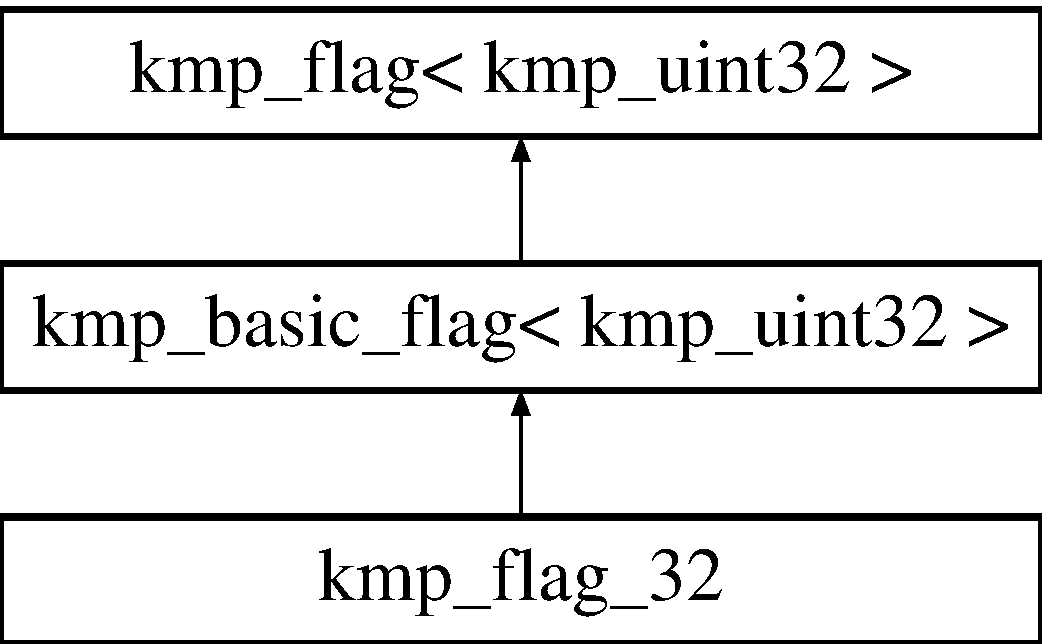
\includegraphics[height=3.000000cm]{classkmp__flag__32}
\end{center}
\end{figure}
\subsection*{Public Member Functions}
\begin{DoxyCompactItemize}
\item 
\hyperlink{classkmp__flag__32_a0d822138677c1dbc93115fabc143461e}{kmp\-\_\-flag\-\_\-32} (volatile kmp\-\_\-uint32 $\ast$\hyperlink{ittnotify__static_8h_ab7caea589d3ca96f9f11c78f10bff578}{p})
\item 
\hyperlink{classkmp__flag__32_ae2faeae32e4b1ed56e9287ffb410934c}{kmp\-\_\-flag\-\_\-32} (volatile kmp\-\_\-uint32 $\ast$\hyperlink{ittnotify__static_8h_ab7caea589d3ca96f9f11c78f10bff578}{p}, \hyperlink{kmp_8h_a194859801fe16b326efe34501a37c30a}{kmp\-\_\-info\-\_\-t} $\ast$thr)
\item 
\hyperlink{classkmp__flag__32_a9b05ae4c5cd703fd250512448bc3dac4}{kmp\-\_\-flag\-\_\-32} (volatile kmp\-\_\-uint32 $\ast$\hyperlink{ittnotify__static_8h_ab7caea589d3ca96f9f11c78f10bff578}{p}, kmp\-\_\-uint32 c)
\item 
\hyperlink{ittnotify__static_8h_af941d56e55e3c5465135b60c4d6343ed}{void} \hyperlink{classkmp__flag__32_a3a7d371bf8201034e96c2cfd8e5fe30a}{suspend} (\hyperlink{ittnotify__static_8h_a8b8dcd723308a8cb5d84277c7a3fff70}{int} th\-\_\-gtid)
\item 
\hyperlink{ittnotify__static_8h_af941d56e55e3c5465135b60c4d6343ed}{void} \hyperlink{classkmp__flag__32_a3c8777315b710987f5214ecb3d89d745}{resume} (\hyperlink{ittnotify__static_8h_a8b8dcd723308a8cb5d84277c7a3fff70}{int} th\-\_\-gtid)
\item 
\hyperlink{ittnotify__static_8h_a8b8dcd723308a8cb5d84277c7a3fff70}{int} \hyperlink{classkmp__flag__32_a60c72c91f420d8034d6aee0e9fa1424d}{execute\-\_\-tasks} (\hyperlink{kmp_8h_a194859801fe16b326efe34501a37c30a}{kmp\-\_\-info\-\_\-t} $\ast$this\-\_\-thr, kmp\-\_\-int32 gtid, \hyperlink{ittnotify__static_8h_a8b8dcd723308a8cb5d84277c7a3fff70}{int} final\-\_\-spin, \hyperlink{ittnotify__static_8h_a8b8dcd723308a8cb5d84277c7a3fff70}{int} $\ast$thread\-\_\-finished \hyperlink{kmp__itt_8h_ac31864b9b5b30f5dcac5ab285ee97ae0}{U\-S\-E\-\_\-\-I\-T\-T\-\_\-\-B\-U\-I\-L\-D\-\_\-\-A\-R\-G}(\hyperlink{ittnotify__static_8h_af941d56e55e3c5465135b60c4d6343ed}{void} $\ast$itt\-\_\-sync\-\_\-obj), kmp\-\_\-int32 is\-\_\-constrained)
\item 
\hyperlink{ittnotify__static_8h_af941d56e55e3c5465135b60c4d6343ed}{void} \hyperlink{classkmp__flag__32_a5eb7b113d70f5fbf581efe086663292c}{wait} (\hyperlink{kmp_8h_a194859801fe16b326efe34501a37c30a}{kmp\-\_\-info\-\_\-t} $\ast$this\-\_\-thr, \hyperlink{ittnotify__static_8h_a8b8dcd723308a8cb5d84277c7a3fff70}{int} final\-\_\-spin \hyperlink{kmp__itt_8h_ac31864b9b5b30f5dcac5ab285ee97ae0}{U\-S\-E\-\_\-\-I\-T\-T\-\_\-\-B\-U\-I\-L\-D\-\_\-\-A\-R\-G}(\hyperlink{ittnotify__static_8h_af941d56e55e3c5465135b60c4d6343ed}{void} $\ast$itt\-\_\-sync\-\_\-obj))
\item 
\hyperlink{ittnotify__static_8h_af941d56e55e3c5465135b60c4d6343ed}{void} \hyperlink{classkmp__flag__32_aaca6043421d473ebc523d7c059ecc8e3}{release} ()
\item 
\hyperlink{group__WAIT__RELEASE_ga507a7197646f995b5529a68c1481e39b}{flag\-\_\-type} \hyperlink{classkmp__flag__32_a1ad56214a0558bf76d9d2e9b5df2a293}{get\-\_\-ptr\-\_\-type} ()
\end{DoxyCompactItemize}
\subsection*{Additional Inherited Members}


\subsection{Detailed Description}


Definition at line 425 of file kmp\-\_\-wait\-\_\-release.\-h.



\subsection{Constructor \& Destructor Documentation}
\hypertarget{classkmp__flag__32_a0d822138677c1dbc93115fabc143461e}{\index{kmp\-\_\-flag\-\_\-32@{kmp\-\_\-flag\-\_\-32}!kmp\-\_\-flag\-\_\-32@{kmp\-\_\-flag\-\_\-32}}
\index{kmp\-\_\-flag\-\_\-32@{kmp\-\_\-flag\-\_\-32}!kmp_flag_32@{kmp\-\_\-flag\-\_\-32}}
\subsubsection[{kmp\-\_\-flag\-\_\-32}]{\setlength{\rightskip}{0pt plus 5cm}kmp\-\_\-flag\-\_\-32\-::kmp\-\_\-flag\-\_\-32 (
\begin{DoxyParamCaption}
\item[{volatile kmp\-\_\-uint32 $\ast$}]{p}
\end{DoxyParamCaption}
)\hspace{0.3cm}{\ttfamily [inline]}}}\label{classkmp__flag__32_a0d822138677c1dbc93115fabc143461e}


Definition at line 427 of file kmp\-\_\-wait\-\_\-release.\-h.


\begin{DoxyCode}
427 : \hyperlink{classkmp__basic__flag}{kmp\_basic\_flag<kmp\_uint32>}(\hyperlink{ittnotify__static_8h_ab7caea589d3ca96f9f11c78f10bff578}{p}) \{\}
\end{DoxyCode}
\hypertarget{classkmp__flag__32_ae2faeae32e4b1ed56e9287ffb410934c}{\index{kmp\-\_\-flag\-\_\-32@{kmp\-\_\-flag\-\_\-32}!kmp\-\_\-flag\-\_\-32@{kmp\-\_\-flag\-\_\-32}}
\index{kmp\-\_\-flag\-\_\-32@{kmp\-\_\-flag\-\_\-32}!kmp_flag_32@{kmp\-\_\-flag\-\_\-32}}
\subsubsection[{kmp\-\_\-flag\-\_\-32}]{\setlength{\rightskip}{0pt plus 5cm}kmp\-\_\-flag\-\_\-32\-::kmp\-\_\-flag\-\_\-32 (
\begin{DoxyParamCaption}
\item[{volatile kmp\-\_\-uint32 $\ast$}]{p, }
\item[{{\bf kmp\-\_\-info\-\_\-t} $\ast$}]{thr}
\end{DoxyParamCaption}
)\hspace{0.3cm}{\ttfamily [inline]}}}\label{classkmp__flag__32_ae2faeae32e4b1ed56e9287ffb410934c}


Definition at line 428 of file kmp\-\_\-wait\-\_\-release.\-h.


\begin{DoxyCode}
428 : \hyperlink{classkmp__basic__flag}{kmp\_basic\_flag<kmp\_uint32>}(\hyperlink{ittnotify__static_8h_ab7caea589d3ca96f9f11c78f10bff578}{p}, thr) \{\}
\end{DoxyCode}
\hypertarget{classkmp__flag__32_a9b05ae4c5cd703fd250512448bc3dac4}{\index{kmp\-\_\-flag\-\_\-32@{kmp\-\_\-flag\-\_\-32}!kmp\-\_\-flag\-\_\-32@{kmp\-\_\-flag\-\_\-32}}
\index{kmp\-\_\-flag\-\_\-32@{kmp\-\_\-flag\-\_\-32}!kmp_flag_32@{kmp\-\_\-flag\-\_\-32}}
\subsubsection[{kmp\-\_\-flag\-\_\-32}]{\setlength{\rightskip}{0pt plus 5cm}kmp\-\_\-flag\-\_\-32\-::kmp\-\_\-flag\-\_\-32 (
\begin{DoxyParamCaption}
\item[{volatile kmp\-\_\-uint32 $\ast$}]{p, }
\item[{kmp\-\_\-uint32}]{c}
\end{DoxyParamCaption}
)\hspace{0.3cm}{\ttfamily [inline]}}}\label{classkmp__flag__32_a9b05ae4c5cd703fd250512448bc3dac4}


Definition at line 429 of file kmp\-\_\-wait\-\_\-release.\-h.


\begin{DoxyCode}
429 : \hyperlink{classkmp__basic__flag}{kmp\_basic\_flag<kmp\_uint32>}(\hyperlink{ittnotify__static_8h_ab7caea589d3ca96f9f11c78f10bff578}{p}, c) \{\}
\end{DoxyCode}


\subsection{Member Function Documentation}
\hypertarget{classkmp__flag__32_a60c72c91f420d8034d6aee0e9fa1424d}{\index{kmp\-\_\-flag\-\_\-32@{kmp\-\_\-flag\-\_\-32}!execute\-\_\-tasks@{execute\-\_\-tasks}}
\index{execute\-\_\-tasks@{execute\-\_\-tasks}!kmp_flag_32@{kmp\-\_\-flag\-\_\-32}}
\subsubsection[{execute\-\_\-tasks}]{\setlength{\rightskip}{0pt plus 5cm}{\bf int} kmp\-\_\-flag\-\_\-32\-::execute\-\_\-tasks (
\begin{DoxyParamCaption}
\item[{{\bf kmp\-\_\-info\-\_\-t} $\ast$}]{this\-\_\-thr, }
\item[{kmp\-\_\-int32}]{gtid, }
\item[{{\bf int}}]{final\-\_\-spin, }
\item[{{\bf int} $\ast$thread\-\_\-finished }]{U\-S\-E\-\_\-\-I\-T\-T\-\_\-\-B\-U\-I\-L\-D\-\_\-\-A\-R\-Gvoid $\ast$itt\-\_\-sync\-\_\-obj, }
\item[{kmp\-\_\-int32}]{is\-\_\-constrained}
\end{DoxyParamCaption}
)\hspace{0.3cm}{\ttfamily [inline]}}}\label{classkmp__flag__32_a60c72c91f420d8034d6aee0e9fa1424d}


Definition at line 432 of file kmp\-\_\-wait\-\_\-release.\-h.



Referenced by \-\_\-\-\_\-kmp\-\_\-tasking\-\_\-barrier(), \-\_\-\-\_\-kmpc\-\_\-end\-\_\-taskgroup(), \-\_\-\-\_\-kmpc\-\_\-omp\-\_\-taskwait(), and \-\_\-\-\_\-kmpc\-\_\-omp\-\_\-wait\-\_\-deps().


\begin{DoxyCode}
433                                                                                         \{
434         \textcolor{keywordflow}{return} \hyperlink{kmp_8h_a64ee8de488c653e4e6364da74d48078c}{\_\_kmp\_execute\_tasks\_32}(this\_thr, gtid, \textcolor{keyword}{this}, final\_spin, 
      thread\_finished
435                                       \hyperlink{kmp__itt_8h_ac31864b9b5b30f5dcac5ab285ee97ae0}{USE\_ITT\_BUILD\_ARG}(itt\_sync\_obj), is\_constrained);
436     \}
\end{DoxyCode}
\hypertarget{classkmp__flag__32_a1ad56214a0558bf76d9d2e9b5df2a293}{\index{kmp\-\_\-flag\-\_\-32@{kmp\-\_\-flag\-\_\-32}!get\-\_\-ptr\-\_\-type@{get\-\_\-ptr\-\_\-type}}
\index{get\-\_\-ptr\-\_\-type@{get\-\_\-ptr\-\_\-type}!kmp_flag_32@{kmp\-\_\-flag\-\_\-32}}
\subsubsection[{get\-\_\-ptr\-\_\-type}]{\setlength{\rightskip}{0pt plus 5cm}{\bf flag\-\_\-type} kmp\-\_\-flag\-\_\-32\-::get\-\_\-ptr\-\_\-type (
\begin{DoxyParamCaption}
{}
\end{DoxyParamCaption}
)\hspace{0.3cm}{\ttfamily [inline]}}}\label{classkmp__flag__32_a1ad56214a0558bf76d9d2e9b5df2a293}


Definition at line 443 of file kmp\-\_\-wait\-\_\-release.\-h.


\begin{DoxyCode}
443 \{ \textcolor{keywordflow}{return} \hyperlink{group__WAIT__RELEASE_gga507a7197646f995b5529a68c1481e39baa8e37e16d043d78e34da1d19387be5ba}{flag32}; \}
\end{DoxyCode}
\hypertarget{classkmp__flag__32_aaca6043421d473ebc523d7c059ecc8e3}{\index{kmp\-\_\-flag\-\_\-32@{kmp\-\_\-flag\-\_\-32}!release@{release}}
\index{release@{release}!kmp_flag_32@{kmp\-\_\-flag\-\_\-32}}
\subsubsection[{release}]{\setlength{\rightskip}{0pt plus 5cm}{\bf void} kmp\-\_\-flag\-\_\-32\-::release (
\begin{DoxyParamCaption}
{}
\end{DoxyParamCaption}
)\hspace{0.3cm}{\ttfamily [inline]}}}\label{classkmp__flag__32_aaca6043421d473ebc523d7c059ecc8e3}


Definition at line 442 of file kmp\-\_\-wait\-\_\-release.\-h.


\begin{DoxyCode}
442 \{ \hyperlink{group__WAIT__RELEASE_ga69a3eeeb736df0221080fff120336b5a}{\_\_kmp\_release\_template}(\textcolor{keyword}{this}); \}
\end{DoxyCode}
\hypertarget{classkmp__flag__32_a3c8777315b710987f5214ecb3d89d745}{\index{kmp\-\_\-flag\-\_\-32@{kmp\-\_\-flag\-\_\-32}!resume@{resume}}
\index{resume@{resume}!kmp_flag_32@{kmp\-\_\-flag\-\_\-32}}
\subsubsection[{resume}]{\setlength{\rightskip}{0pt plus 5cm}{\bf void} kmp\-\_\-flag\-\_\-32\-::resume (
\begin{DoxyParamCaption}
\item[{{\bf int}}]{th\-\_\-gtid}
\end{DoxyParamCaption}
)\hspace{0.3cm}{\ttfamily [inline]}}}\label{classkmp__flag__32_a3c8777315b710987f5214ecb3d89d745}


Definition at line 431 of file kmp\-\_\-wait\-\_\-release.\-h.


\begin{DoxyCode}
431 \{ \hyperlink{kmp_8h_acfe9e02a35d4e38951a53bd689ca2141}{\_\_kmp\_resume\_32}(th\_gtid, \textcolor{keyword}{this}); \}
\end{DoxyCode}
\hypertarget{classkmp__flag__32_a3a7d371bf8201034e96c2cfd8e5fe30a}{\index{kmp\-\_\-flag\-\_\-32@{kmp\-\_\-flag\-\_\-32}!suspend@{suspend}}
\index{suspend@{suspend}!kmp_flag_32@{kmp\-\_\-flag\-\_\-32}}
\subsubsection[{suspend}]{\setlength{\rightskip}{0pt plus 5cm}{\bf void} kmp\-\_\-flag\-\_\-32\-::suspend (
\begin{DoxyParamCaption}
\item[{{\bf int}}]{th\-\_\-gtid}
\end{DoxyParamCaption}
)\hspace{0.3cm}{\ttfamily [inline]}}}\label{classkmp__flag__32_a3a7d371bf8201034e96c2cfd8e5fe30a}


Definition at line 430 of file kmp\-\_\-wait\-\_\-release.\-h.


\begin{DoxyCode}
430 \{ \hyperlink{kmp_8h_aba3964e854aa376fc15165064cf5eff7}{\_\_kmp\_suspend\_32}(th\_gtid, \textcolor{keyword}{this}); \}
\end{DoxyCode}
\hypertarget{classkmp__flag__32_a5eb7b113d70f5fbf581efe086663292c}{\index{kmp\-\_\-flag\-\_\-32@{kmp\-\_\-flag\-\_\-32}!wait@{wait}}
\index{wait@{wait}!kmp_flag_32@{kmp\-\_\-flag\-\_\-32}}
\subsubsection[{wait}]{\setlength{\rightskip}{0pt plus 5cm}{\bf void} kmp\-\_\-flag\-\_\-32\-::wait (
\begin{DoxyParamCaption}
\item[{{\bf kmp\-\_\-info\-\_\-t} $\ast$}]{this\-\_\-thr, }
\item[{{\bf int} final\-\_\-spin }]{U\-S\-E\-\_\-\-I\-T\-T\-\_\-\-B\-U\-I\-L\-D\-\_\-\-A\-R\-Gvoid $\ast$itt\-\_\-sync\-\_\-obj}
\end{DoxyParamCaption}
)\hspace{0.3cm}{\ttfamily [inline]}}}\label{classkmp__flag__32_a5eb7b113d70f5fbf581efe086663292c}


Definition at line 437 of file kmp\-\_\-wait\-\_\-release.\-h.



Referenced by \-\_\-\-\_\-kmp\-\_\-task\-\_\-team\-\_\-wait().


\begin{DoxyCode}
438                                                       \{
439         \hyperlink{group__WAIT__RELEASE_gabe62fb00e04b4d30528d441232b0e62a}{\_\_kmp\_wait\_template}(this\_thr, \textcolor{keyword}{this}, final\_spin
440                             \hyperlink{kmp__itt_8h_ac31864b9b5b30f5dcac5ab285ee97ae0}{USE\_ITT\_BUILD\_ARG}(itt\_sync\_obj));
441     \}
\end{DoxyCode}


The documentation for this class was generated from the following file\-:\begin{DoxyCompactItemize}
\item 
\hyperlink{kmp__wait__release_8h}{kmp\-\_\-wait\-\_\-release.\-h}\end{DoxyCompactItemize}

\hypertarget{classkmp__flag__64}{\section{kmp\-\_\-flag\-\_\-64 Class Reference}
\label{classkmp__flag__64}\index{kmp\-\_\-flag\-\_\-64@{kmp\-\_\-flag\-\_\-64}}
}


{\ttfamily \#include $<$kmp\-\_\-wait\-\_\-release.\-h$>$}

Inheritance diagram for kmp\-\_\-flag\-\_\-64\-:\begin{figure}[H]
\begin{center}
\leavevmode
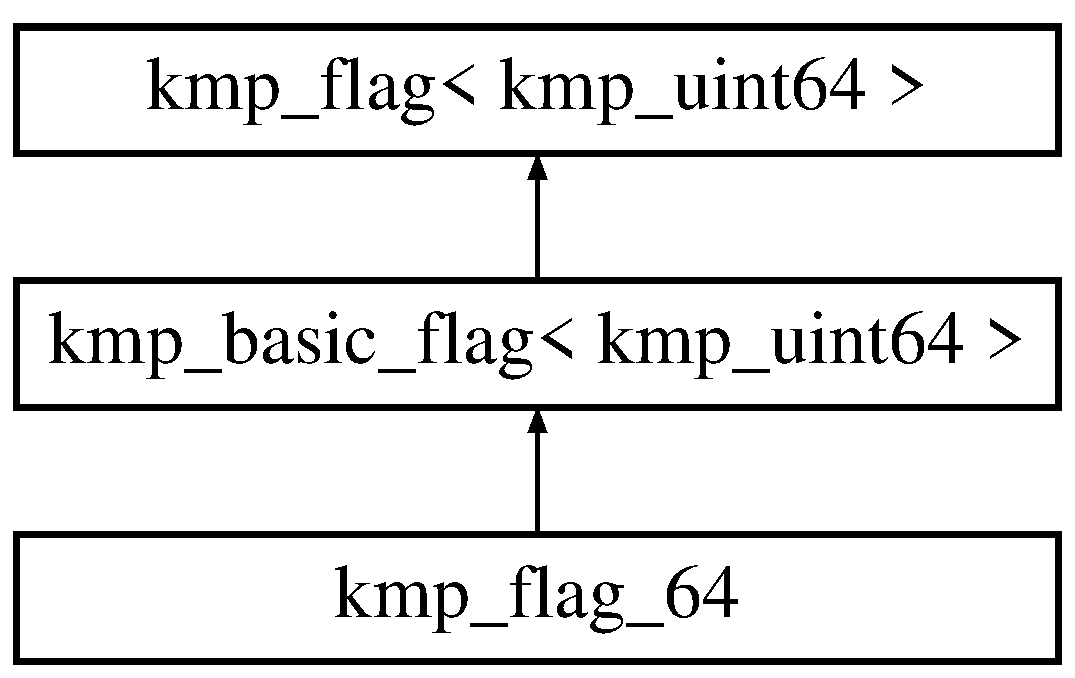
\includegraphics[height=3.000000cm]{classkmp__flag__64}
\end{center}
\end{figure}
\subsection*{Public Member Functions}
\begin{DoxyCompactItemize}
\item 
\hyperlink{classkmp__flag__64_a837c4745c75c9557cb92926763c2ab88}{kmp\-\_\-flag\-\_\-64} (volatile kmp\-\_\-uint64 $\ast$\hyperlink{ittnotify__static_8h_ab7caea589d3ca96f9f11c78f10bff578}{p})
\item 
\hyperlink{classkmp__flag__64_a10a4b7f83ee61552e6e7dbb4f664a6c9}{kmp\-\_\-flag\-\_\-64} (volatile kmp\-\_\-uint64 $\ast$\hyperlink{ittnotify__static_8h_ab7caea589d3ca96f9f11c78f10bff578}{p}, \hyperlink{kmp_8h_a194859801fe16b326efe34501a37c30a}{kmp\-\_\-info\-\_\-t} $\ast$thr)
\item 
\hyperlink{classkmp__flag__64_a7a108292b9fa2f59aeac457185ecca63}{kmp\-\_\-flag\-\_\-64} (volatile kmp\-\_\-uint64 $\ast$\hyperlink{ittnotify__static_8h_ab7caea589d3ca96f9f11c78f10bff578}{p}, kmp\-\_\-uint64 c)
\item 
\hyperlink{ittnotify__static_8h_af941d56e55e3c5465135b60c4d6343ed}{void} \hyperlink{classkmp__flag__64_a56f6b96c1a0a87d217f401b43677447c}{suspend} (\hyperlink{ittnotify__static_8h_a8b8dcd723308a8cb5d84277c7a3fff70}{int} th\-\_\-gtid)
\item 
\hyperlink{ittnotify__static_8h_af941d56e55e3c5465135b60c4d6343ed}{void} \hyperlink{classkmp__flag__64_a66e511c15ef7cb302bcbda4d698d268b}{resume} (\hyperlink{ittnotify__static_8h_a8b8dcd723308a8cb5d84277c7a3fff70}{int} th\-\_\-gtid)
\item 
\hyperlink{ittnotify__static_8h_a8b8dcd723308a8cb5d84277c7a3fff70}{int} \hyperlink{classkmp__flag__64_acb768d08059a3c907c746f138a1c9f3a}{execute\-\_\-tasks} (\hyperlink{kmp_8h_a194859801fe16b326efe34501a37c30a}{kmp\-\_\-info\-\_\-t} $\ast$this\-\_\-thr, kmp\-\_\-int32 gtid, \hyperlink{ittnotify__static_8h_a8b8dcd723308a8cb5d84277c7a3fff70}{int} final\-\_\-spin, \hyperlink{ittnotify__static_8h_a8b8dcd723308a8cb5d84277c7a3fff70}{int} $\ast$thread\-\_\-finished \hyperlink{kmp__itt_8h_ac31864b9b5b30f5dcac5ab285ee97ae0}{U\-S\-E\-\_\-\-I\-T\-T\-\_\-\-B\-U\-I\-L\-D\-\_\-\-A\-R\-G}(\hyperlink{ittnotify__static_8h_af941d56e55e3c5465135b60c4d6343ed}{void} $\ast$itt\-\_\-sync\-\_\-obj), kmp\-\_\-int32 is\-\_\-constrained)
\item 
\hyperlink{ittnotify__static_8h_af941d56e55e3c5465135b60c4d6343ed}{void} \hyperlink{classkmp__flag__64_a459afc03a199c6a548049ae3a097e41f}{wait} (\hyperlink{kmp_8h_a194859801fe16b326efe34501a37c30a}{kmp\-\_\-info\-\_\-t} $\ast$this\-\_\-thr, \hyperlink{ittnotify__static_8h_a8b8dcd723308a8cb5d84277c7a3fff70}{int} final\-\_\-spin \hyperlink{kmp__itt_8h_ac31864b9b5b30f5dcac5ab285ee97ae0}{U\-S\-E\-\_\-\-I\-T\-T\-\_\-\-B\-U\-I\-L\-D\-\_\-\-A\-R\-G}(\hyperlink{ittnotify__static_8h_af941d56e55e3c5465135b60c4d6343ed}{void} $\ast$itt\-\_\-sync\-\_\-obj))
\item 
\hyperlink{ittnotify__static_8h_af941d56e55e3c5465135b60c4d6343ed}{void} \hyperlink{classkmp__flag__64_a2234024d9020be6164618f6971df9aec}{release} ()
\item 
\hyperlink{group__WAIT__RELEASE_ga507a7197646f995b5529a68c1481e39b}{flag\-\_\-type} \hyperlink{classkmp__flag__64_ac1183e9560571418a26da40187e501ee}{get\-\_\-ptr\-\_\-type} ()
\end{DoxyCompactItemize}
\subsection*{Additional Inherited Members}


\subsection{Detailed Description}


Definition at line 446 of file kmp\-\_\-wait\-\_\-release.\-h.



\subsection{Constructor \& Destructor Documentation}
\hypertarget{classkmp__flag__64_a837c4745c75c9557cb92926763c2ab88}{\index{kmp\-\_\-flag\-\_\-64@{kmp\-\_\-flag\-\_\-64}!kmp\-\_\-flag\-\_\-64@{kmp\-\_\-flag\-\_\-64}}
\index{kmp\-\_\-flag\-\_\-64@{kmp\-\_\-flag\-\_\-64}!kmp_flag_64@{kmp\-\_\-flag\-\_\-64}}
\subsubsection[{kmp\-\_\-flag\-\_\-64}]{\setlength{\rightskip}{0pt plus 5cm}kmp\-\_\-flag\-\_\-64\-::kmp\-\_\-flag\-\_\-64 (
\begin{DoxyParamCaption}
\item[{volatile kmp\-\_\-uint64 $\ast$}]{p}
\end{DoxyParamCaption}
)\hspace{0.3cm}{\ttfamily [inline]}}}\label{classkmp__flag__64_a837c4745c75c9557cb92926763c2ab88}


Definition at line 448 of file kmp\-\_\-wait\-\_\-release.\-h.


\begin{DoxyCode}
448 : \hyperlink{classkmp__basic__flag}{kmp\_basic\_flag<kmp\_uint64>}(\hyperlink{ittnotify__static_8h_ab7caea589d3ca96f9f11c78f10bff578}{p}) \{\}
\end{DoxyCode}
\hypertarget{classkmp__flag__64_a10a4b7f83ee61552e6e7dbb4f664a6c9}{\index{kmp\-\_\-flag\-\_\-64@{kmp\-\_\-flag\-\_\-64}!kmp\-\_\-flag\-\_\-64@{kmp\-\_\-flag\-\_\-64}}
\index{kmp\-\_\-flag\-\_\-64@{kmp\-\_\-flag\-\_\-64}!kmp_flag_64@{kmp\-\_\-flag\-\_\-64}}
\subsubsection[{kmp\-\_\-flag\-\_\-64}]{\setlength{\rightskip}{0pt plus 5cm}kmp\-\_\-flag\-\_\-64\-::kmp\-\_\-flag\-\_\-64 (
\begin{DoxyParamCaption}
\item[{volatile kmp\-\_\-uint64 $\ast$}]{p, }
\item[{{\bf kmp\-\_\-info\-\_\-t} $\ast$}]{thr}
\end{DoxyParamCaption}
)\hspace{0.3cm}{\ttfamily [inline]}}}\label{classkmp__flag__64_a10a4b7f83ee61552e6e7dbb4f664a6c9}


Definition at line 449 of file kmp\-\_\-wait\-\_\-release.\-h.


\begin{DoxyCode}
449 : \hyperlink{classkmp__basic__flag}{kmp\_basic\_flag<kmp\_uint64>}(\hyperlink{ittnotify__static_8h_ab7caea589d3ca96f9f11c78f10bff578}{p}, thr) \{\}
\end{DoxyCode}
\hypertarget{classkmp__flag__64_a7a108292b9fa2f59aeac457185ecca63}{\index{kmp\-\_\-flag\-\_\-64@{kmp\-\_\-flag\-\_\-64}!kmp\-\_\-flag\-\_\-64@{kmp\-\_\-flag\-\_\-64}}
\index{kmp\-\_\-flag\-\_\-64@{kmp\-\_\-flag\-\_\-64}!kmp_flag_64@{kmp\-\_\-flag\-\_\-64}}
\subsubsection[{kmp\-\_\-flag\-\_\-64}]{\setlength{\rightskip}{0pt plus 5cm}kmp\-\_\-flag\-\_\-64\-::kmp\-\_\-flag\-\_\-64 (
\begin{DoxyParamCaption}
\item[{volatile kmp\-\_\-uint64 $\ast$}]{p, }
\item[{kmp\-\_\-uint64}]{c}
\end{DoxyParamCaption}
)\hspace{0.3cm}{\ttfamily [inline]}}}\label{classkmp__flag__64_a7a108292b9fa2f59aeac457185ecca63}


Definition at line 450 of file kmp\-\_\-wait\-\_\-release.\-h.


\begin{DoxyCode}
450 : \hyperlink{classkmp__basic__flag}{kmp\_basic\_flag<kmp\_uint64>}(\hyperlink{ittnotify__static_8h_ab7caea589d3ca96f9f11c78f10bff578}{p}, c) \{\}
\end{DoxyCode}


\subsection{Member Function Documentation}
\hypertarget{classkmp__flag__64_acb768d08059a3c907c746f138a1c9f3a}{\index{kmp\-\_\-flag\-\_\-64@{kmp\-\_\-flag\-\_\-64}!execute\-\_\-tasks@{execute\-\_\-tasks}}
\index{execute\-\_\-tasks@{execute\-\_\-tasks}!kmp_flag_64@{kmp\-\_\-flag\-\_\-64}}
\subsubsection[{execute\-\_\-tasks}]{\setlength{\rightskip}{0pt plus 5cm}{\bf int} kmp\-\_\-flag\-\_\-64\-::execute\-\_\-tasks (
\begin{DoxyParamCaption}
\item[{{\bf kmp\-\_\-info\-\_\-t} $\ast$}]{this\-\_\-thr, }
\item[{kmp\-\_\-int32}]{gtid, }
\item[{{\bf int}}]{final\-\_\-spin, }
\item[{{\bf int} $\ast$thread\-\_\-finished }]{U\-S\-E\-\_\-\-I\-T\-T\-\_\-\-B\-U\-I\-L\-D\-\_\-\-A\-R\-Gvoid $\ast$itt\-\_\-sync\-\_\-obj, }
\item[{kmp\-\_\-int32}]{is\-\_\-constrained}
\end{DoxyParamCaption}
)\hspace{0.3cm}{\ttfamily [inline]}}}\label{classkmp__flag__64_acb768d08059a3c907c746f138a1c9f3a}


Definition at line 453 of file kmp\-\_\-wait\-\_\-release.\-h.


\begin{DoxyCode}
454                                                                                         \{
455         \textcolor{keywordflow}{return} \hyperlink{kmp_8h_a93e5c2310a61943ff77e1eb79b954414}{\_\_kmp\_execute\_tasks\_64}(this\_thr, gtid, \textcolor{keyword}{this}, final\_spin, 
      thread\_finished
456                                       \hyperlink{kmp__itt_8h_ac31864b9b5b30f5dcac5ab285ee97ae0}{USE\_ITT\_BUILD\_ARG}(itt\_sync\_obj), is\_constrained);
457     \}
\end{DoxyCode}
\hypertarget{classkmp__flag__64_ac1183e9560571418a26da40187e501ee}{\index{kmp\-\_\-flag\-\_\-64@{kmp\-\_\-flag\-\_\-64}!get\-\_\-ptr\-\_\-type@{get\-\_\-ptr\-\_\-type}}
\index{get\-\_\-ptr\-\_\-type@{get\-\_\-ptr\-\_\-type}!kmp_flag_64@{kmp\-\_\-flag\-\_\-64}}
\subsubsection[{get\-\_\-ptr\-\_\-type}]{\setlength{\rightskip}{0pt plus 5cm}{\bf flag\-\_\-type} kmp\-\_\-flag\-\_\-64\-::get\-\_\-ptr\-\_\-type (
\begin{DoxyParamCaption}
{}
\end{DoxyParamCaption}
)\hspace{0.3cm}{\ttfamily [inline]}}}\label{classkmp__flag__64_ac1183e9560571418a26da40187e501ee}


Definition at line 464 of file kmp\-\_\-wait\-\_\-release.\-h.


\begin{DoxyCode}
464 \{ \textcolor{keywordflow}{return} \hyperlink{group__WAIT__RELEASE_gga507a7197646f995b5529a68c1481e39ba8b02d824728fb546d43123b8b069ed04}{flag64}; \}
\end{DoxyCode}
\hypertarget{classkmp__flag__64_a2234024d9020be6164618f6971df9aec}{\index{kmp\-\_\-flag\-\_\-64@{kmp\-\_\-flag\-\_\-64}!release@{release}}
\index{release@{release}!kmp_flag_64@{kmp\-\_\-flag\-\_\-64}}
\subsubsection[{release}]{\setlength{\rightskip}{0pt plus 5cm}{\bf void} kmp\-\_\-flag\-\_\-64\-::release (
\begin{DoxyParamCaption}
{}
\end{DoxyParamCaption}
)\hspace{0.3cm}{\ttfamily [inline]}}}\label{classkmp__flag__64_a2234024d9020be6164618f6971df9aec}


Definition at line 463 of file kmp\-\_\-wait\-\_\-release.\-h.



Referenced by \-\_\-\-\_\-kmp\-\_\-hierarchical\-\_\-barrier\-\_\-gather(), \-\_\-\-\_\-kmp\-\_\-hierarchical\-\_\-barrier\-\_\-release(), \-\_\-\-\_\-kmp\-\_\-hyper\-\_\-barrier\-\_\-gather(), \-\_\-\-\_\-kmp\-\_\-hyper\-\_\-barrier\-\_\-release(), \-\_\-\-\_\-kmp\-\_\-linear\-\_\-barrier\-\_\-gather(), \-\_\-\-\_\-kmp\-\_\-linear\-\_\-barrier\-\_\-release(), \-\_\-\-\_\-kmp\-\_\-tree\-\_\-barrier\-\_\-gather(), and \-\_\-\-\_\-kmp\-\_\-tree\-\_\-barrier\-\_\-release().


\begin{DoxyCode}
463 \{ \hyperlink{group__WAIT__RELEASE_ga69a3eeeb736df0221080fff120336b5a}{\_\_kmp\_release\_template}(\textcolor{keyword}{this}); \}
\end{DoxyCode}
\hypertarget{classkmp__flag__64_a66e511c15ef7cb302bcbda4d698d268b}{\index{kmp\-\_\-flag\-\_\-64@{kmp\-\_\-flag\-\_\-64}!resume@{resume}}
\index{resume@{resume}!kmp_flag_64@{kmp\-\_\-flag\-\_\-64}}
\subsubsection[{resume}]{\setlength{\rightskip}{0pt plus 5cm}{\bf void} kmp\-\_\-flag\-\_\-64\-::resume (
\begin{DoxyParamCaption}
\item[{{\bf int}}]{th\-\_\-gtid}
\end{DoxyParamCaption}
)\hspace{0.3cm}{\ttfamily [inline]}}}\label{classkmp__flag__64_a66e511c15ef7cb302bcbda4d698d268b}


Definition at line 452 of file kmp\-\_\-wait\-\_\-release.\-h.


\begin{DoxyCode}
452 \{ \hyperlink{kmp_8h_a6d3052650a7678516a888600044b6d63}{\_\_kmp\_resume\_64}(th\_gtid, \textcolor{keyword}{this}); \}
\end{DoxyCode}
\hypertarget{classkmp__flag__64_a56f6b96c1a0a87d217f401b43677447c}{\index{kmp\-\_\-flag\-\_\-64@{kmp\-\_\-flag\-\_\-64}!suspend@{suspend}}
\index{suspend@{suspend}!kmp_flag_64@{kmp\-\_\-flag\-\_\-64}}
\subsubsection[{suspend}]{\setlength{\rightskip}{0pt plus 5cm}{\bf void} kmp\-\_\-flag\-\_\-64\-::suspend (
\begin{DoxyParamCaption}
\item[{{\bf int}}]{th\-\_\-gtid}
\end{DoxyParamCaption}
)\hspace{0.3cm}{\ttfamily [inline]}}}\label{classkmp__flag__64_a56f6b96c1a0a87d217f401b43677447c}


Definition at line 451 of file kmp\-\_\-wait\-\_\-release.\-h.


\begin{DoxyCode}
451 \{ \hyperlink{kmp_8h_aa691a7515df09e540efa307af193ebcf}{\_\_kmp\_suspend\_64}(th\_gtid, \textcolor{keyword}{this}); \}
\end{DoxyCode}
\hypertarget{classkmp__flag__64_a459afc03a199c6a548049ae3a097e41f}{\index{kmp\-\_\-flag\-\_\-64@{kmp\-\_\-flag\-\_\-64}!wait@{wait}}
\index{wait@{wait}!kmp_flag_64@{kmp\-\_\-flag\-\_\-64}}
\subsubsection[{wait}]{\setlength{\rightskip}{0pt plus 5cm}{\bf void} kmp\-\_\-flag\-\_\-64\-::wait (
\begin{DoxyParamCaption}
\item[{{\bf kmp\-\_\-info\-\_\-t} $\ast$}]{this\-\_\-thr, }
\item[{{\bf int} final\-\_\-spin }]{U\-S\-E\-\_\-\-I\-T\-T\-\_\-\-B\-U\-I\-L\-D\-\_\-\-A\-R\-Gvoid $\ast$itt\-\_\-sync\-\_\-obj}
\end{DoxyParamCaption}
)\hspace{0.3cm}{\ttfamily [inline]}}}\label{classkmp__flag__64_a459afc03a199c6a548049ae3a097e41f}


Definition at line 458 of file kmp\-\_\-wait\-\_\-release.\-h.



Referenced by \-\_\-\-\_\-kmp\-\_\-hierarchical\-\_\-barrier\-\_\-gather(), \-\_\-\-\_\-kmp\-\_\-hierarchical\-\_\-barrier\-\_\-release(), \-\_\-\-\_\-kmp\-\_\-hyper\-\_\-barrier\-\_\-gather(), \-\_\-\-\_\-kmp\-\_\-hyper\-\_\-barrier\-\_\-release(), \-\_\-\-\_\-kmp\-\_\-linear\-\_\-barrier\-\_\-gather(), \-\_\-\-\_\-kmp\-\_\-linear\-\_\-barrier\-\_\-release(), \-\_\-\-\_\-kmp\-\_\-tree\-\_\-barrier\-\_\-gather(), and \-\_\-\-\_\-kmp\-\_\-tree\-\_\-barrier\-\_\-release().


\begin{DoxyCode}
459                                                       \{
460         \hyperlink{group__WAIT__RELEASE_gabe62fb00e04b4d30528d441232b0e62a}{\_\_kmp\_wait\_template}(this\_thr, \textcolor{keyword}{this}, final\_spin
461                             \hyperlink{kmp__itt_8h_ac31864b9b5b30f5dcac5ab285ee97ae0}{USE\_ITT\_BUILD\_ARG}(itt\_sync\_obj));
462     \}
\end{DoxyCode}


The documentation for this class was generated from the following file\-:\begin{DoxyCompactItemize}
\item 
\hyperlink{kmp__wait__release_8h}{kmp\-\_\-wait\-\_\-release.\-h}\end{DoxyCompactItemize}

\hypertarget{classkmp__flag__oncore}{\section{kmp\-\_\-flag\-\_\-oncore Class Reference}
\label{classkmp__flag__oncore}\index{kmp\-\_\-flag\-\_\-oncore@{kmp\-\_\-flag\-\_\-oncore}}
}


{\ttfamily \#include $<$kmp\-\_\-wait\-\_\-release.\-h$>$}

Inheritance diagram for kmp\-\_\-flag\-\_\-oncore\-:\begin{figure}[H]
\begin{center}
\leavevmode
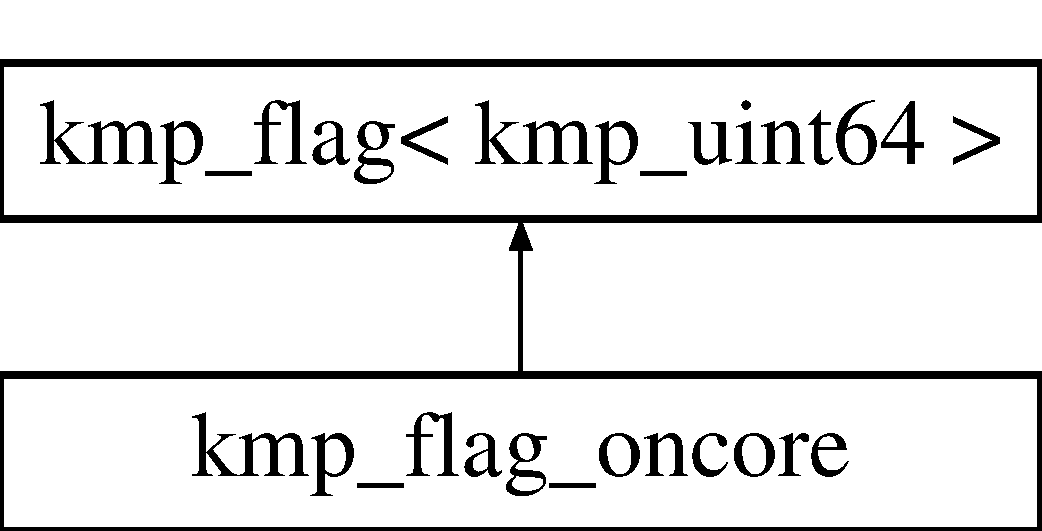
\includegraphics[height=2.000000cm]{classkmp__flag__oncore}
\end{center}
\end{figure}
\subsection*{Public Member Functions}
\begin{DoxyCompactItemize}
\item 
\hyperlink{classkmp__flag__oncore_acf5a14713e98b0422f4f95c8e583f878}{kmp\-\_\-flag\-\_\-oncore} (volatile kmp\-\_\-uint64 $\ast$\hyperlink{ittnotify__static_8h_ab7caea589d3ca96f9f11c78f10bff578}{p})
\item 
\hyperlink{classkmp__flag__oncore_ad9c8add8082423d2f0ffd92935884bfe}{kmp\-\_\-flag\-\_\-oncore} (volatile kmp\-\_\-uint64 $\ast$\hyperlink{ittnotify__static_8h_ab7caea589d3ca96f9f11c78f10bff578}{p}, kmp\-\_\-uint32 idx)
\item 
\hyperlink{classkmp__flag__oncore_ac81f19d6d4ec818b3e35dfff1749ca4b}{kmp\-\_\-flag\-\_\-oncore} (volatile kmp\-\_\-uint64 $\ast$\hyperlink{ittnotify__static_8h_ab7caea589d3ca96f9f11c78f10bff578}{p}, kmp\-\_\-uint64 c, kmp\-\_\-uint32 idx, enum \hyperlink{kmp_8h_ad0f7c21f2f1d446087ef5714eb0fd8cf}{barrier\-\_\-type} bar\-\_\-t, \hyperlink{kmp_8h_a194859801fe16b326efe34501a37c30a}{kmp\-\_\-info\-\_\-t} $\ast$thr)
\item 
\hyperlink{kmp_8h_a194859801fe16b326efe34501a37c30a}{kmp\-\_\-info\-\_\-t} $\ast$ \hyperlink{classkmp__flag__oncore_a41ad8584ed63b8ef81ade52c62871904}{get\-\_\-waiter} (kmp\-\_\-uint32 \hyperlink{kmp__stub_8c_a08582ce460e3d5e1cf0b7fea017d608e}{i})
\item 
kmp\-\_\-uint32 \hyperlink{classkmp__flag__oncore_a74f8cb0dc6652e84a5d69d722a9300f0}{get\-\_\-num\-\_\-waiters} ()
\item 
\hyperlink{ittnotify__static_8h_af941d56e55e3c5465135b60c4d6343ed}{void} \hyperlink{classkmp__flag__oncore_a42a8c8c893495f95e6493ac8530dc319}{set\-\_\-waiter} (\hyperlink{kmp_8h_a194859801fe16b326efe34501a37c30a}{kmp\-\_\-info\-\_\-t} $\ast$thr)
\item 
bool \hyperlink{classkmp__flag__oncore_a9d352ee08ce4f95e7f99549d2b53aaf0}{done\-\_\-check\-\_\-val} (kmp\-\_\-uint64 old\-\_\-loc)
\item 
bool \hyperlink{classkmp__flag__oncore_a5921b4cdaab532b350f3873323bcb021}{done\-\_\-check} ()
\item 
bool \hyperlink{classkmp__flag__oncore_a2f2481d90f9f4ca18d3a71ec9264b224}{notdone\-\_\-check} ()
\item 
\hyperlink{ittnotify__static_8h_af941d56e55e3c5465135b60c4d6343ed}{void} \hyperlink{classkmp__flag__oncore_a85cc9f5fbdc1d291dd2ec7893891a946}{internal\-\_\-release} ()
\item 
kmp\-\_\-uint64 \hyperlink{classkmp__flag__oncore_af2242352965827fa81565fa0e1c35923}{set\-\_\-sleeping} ()
\item 
kmp\-\_\-uint64 \hyperlink{classkmp__flag__oncore_ab49b33119f15328b5c3b558fc3a938ce}{unset\-\_\-sleeping} ()
\item 
bool \hyperlink{classkmp__flag__oncore_a9ca49d662830fecc0022c80414a61809}{is\-\_\-sleeping\-\_\-val} (kmp\-\_\-uint64 old\-\_\-loc)
\item 
bool \hyperlink{classkmp__flag__oncore_a5177877a542322bc2cae59b265eca65a}{is\-\_\-sleeping} ()
\item 
bool \hyperlink{classkmp__flag__oncore_a092f6705d0ab102361b377a6b54d6cc2}{is\-\_\-any\-\_\-sleeping} ()
\item 
\hyperlink{ittnotify__static_8h_af941d56e55e3c5465135b60c4d6343ed}{void} \hyperlink{classkmp__flag__oncore_a69885e3623201f8b51a79c7f034ce175}{wait} (\hyperlink{kmp_8h_a194859801fe16b326efe34501a37c30a}{kmp\-\_\-info\-\_\-t} $\ast$\hyperlink{classkmp__flag__oncore_ab6a0844b7170dfffc0c9a748eaa5690e}{this\-\_\-thr}, \hyperlink{ittnotify__static_8h_a8b8dcd723308a8cb5d84277c7a3fff70}{int} final\-\_\-spin)
\item 
\hyperlink{ittnotify__static_8h_af941d56e55e3c5465135b60c4d6343ed}{void} \hyperlink{classkmp__flag__oncore_a2935978e9898c8f13ee16961c134973c}{release} ()
\item 
\hyperlink{ittnotify__static_8h_af941d56e55e3c5465135b60c4d6343ed}{void} \hyperlink{classkmp__flag__oncore_a83acf5ba45be02b9bedead4674b2da64}{suspend} (\hyperlink{ittnotify__static_8h_a8b8dcd723308a8cb5d84277c7a3fff70}{int} th\-\_\-gtid)
\item 
\hyperlink{ittnotify__static_8h_af941d56e55e3c5465135b60c4d6343ed}{void} \hyperlink{classkmp__flag__oncore_aefad9aaf4ab859af794cfa9dd0ac0c0a}{resume} (\hyperlink{ittnotify__static_8h_a8b8dcd723308a8cb5d84277c7a3fff70}{int} th\-\_\-gtid)
\item 
\hyperlink{ittnotify__static_8h_a8b8dcd723308a8cb5d84277c7a3fff70}{int} \hyperlink{classkmp__flag__oncore_a7bfbc86e21492e2d13f11f64423fa331}{execute\-\_\-tasks} (\hyperlink{kmp_8h_a194859801fe16b326efe34501a37c30a}{kmp\-\_\-info\-\_\-t} $\ast$\hyperlink{classkmp__flag__oncore_ab6a0844b7170dfffc0c9a748eaa5690e}{this\-\_\-thr}, kmp\-\_\-int32 gtid, \hyperlink{ittnotify__static_8h_a8b8dcd723308a8cb5d84277c7a3fff70}{int} final\-\_\-spin, \hyperlink{ittnotify__static_8h_a8b8dcd723308a8cb5d84277c7a3fff70}{int} $\ast$thread\-\_\-finished \hyperlink{kmp__itt_8h_ac31864b9b5b30f5dcac5ab285ee97ae0}{U\-S\-E\-\_\-\-I\-T\-T\-\_\-\-B\-U\-I\-L\-D\-\_\-\-A\-R\-G}(\hyperlink{ittnotify__static_8h_af941d56e55e3c5465135b60c4d6343ed}{void} $\ast$itt\-\_\-sync\-\_\-obj), kmp\-\_\-int32 is\-\_\-constrained)
\item 
kmp\-\_\-uint8 $\ast$ \hyperlink{classkmp__flag__oncore_a4d77160b7c9dcfa2241332bab5d38d5a}{get\-\_\-stolen} ()
\item 
enum \hyperlink{kmp_8h_ad0f7c21f2f1d446087ef5714eb0fd8cf}{barrier\-\_\-type} \hyperlink{classkmp__flag__oncore_aef78caf9a93ab6a62f28788fb35618ff}{get\-\_\-bt} ()
\item 
\hyperlink{group__WAIT__RELEASE_ga507a7197646f995b5529a68c1481e39b}{flag\-\_\-type} \hyperlink{classkmp__flag__oncore_a2c279161e94597d3ce684b81195bf5d4}{get\-\_\-ptr\-\_\-type} ()
\end{DoxyCompactItemize}
\subsection*{Private Member Functions}
\begin{DoxyCompactItemize}
\item 
unsigned char \& \hyperlink{classkmp__flag__oncore_aa09ad2115816f1f6b7fdbe10fcd85552}{byteref} (volatile kmp\-\_\-uint64 $\ast$\hyperlink{classkmp__flag_a5d89de3bda829ab9be324007d915aa3b}{loc}, size\-\_\-t \hyperlink{classkmp__flag__oncore_a0b7c21b4972769775517c46ea0b41bc5}{offset})
\end{DoxyCompactItemize}
\subsection*{Private Attributes}
\begin{DoxyCompactItemize}
\item 
kmp\-\_\-uint64 \hyperlink{classkmp__flag__oncore_a6e37c88438049fcea75785705b281d83}{checker}
\item 
\hyperlink{kmp_8h_a194859801fe16b326efe34501a37c30a}{kmp\-\_\-info\-\_\-t} $\ast$ \hyperlink{classkmp__flag__oncore_a613d89c68444df9e34f59ed5ad9790e6}{waiting\-\_\-threads} \mbox{[}1\mbox{]}
\item 
kmp\-\_\-uint32 \hyperlink{classkmp__flag__oncore_abce7942852f0aca2c03ac0fb83e6d855}{num\-\_\-waiting\-\_\-threads}
\item 
kmp\-\_\-uint32 \hyperlink{classkmp__flag__oncore_a0b7c21b4972769775517c46ea0b41bc5}{offset}
\item 
bool \hyperlink{classkmp__flag__oncore_ad2e8e1e9b2eab43b88c1ae8b27e5d11b}{flag\-\_\-switch}
\item 
enum \hyperlink{kmp_8h_ad0f7c21f2f1d446087ef5714eb0fd8cf}{barrier\-\_\-type} \hyperlink{classkmp__flag__oncore_a01bdd210c6e9b5a3004cf42caa7e0226}{bt}
\item 
\hyperlink{kmp_8h_a194859801fe16b326efe34501a37c30a}{kmp\-\_\-info\-\_\-t} $\ast$ \hyperlink{classkmp__flag__oncore_ab6a0844b7170dfffc0c9a748eaa5690e}{this\-\_\-thr}
\end{DoxyCompactItemize}
\subsection*{Additional Inherited Members}


\subsection{Detailed Description}


Definition at line 468 of file kmp\-\_\-wait\-\_\-release.\-h.



\subsection{Constructor \& Destructor Documentation}
\hypertarget{classkmp__flag__oncore_acf5a14713e98b0422f4f95c8e583f878}{\index{kmp\-\_\-flag\-\_\-oncore@{kmp\-\_\-flag\-\_\-oncore}!kmp\-\_\-flag\-\_\-oncore@{kmp\-\_\-flag\-\_\-oncore}}
\index{kmp\-\_\-flag\-\_\-oncore@{kmp\-\_\-flag\-\_\-oncore}!kmp_flag_oncore@{kmp\-\_\-flag\-\_\-oncore}}
\subsubsection[{kmp\-\_\-flag\-\_\-oncore}]{\setlength{\rightskip}{0pt plus 5cm}kmp\-\_\-flag\-\_\-oncore\-::kmp\-\_\-flag\-\_\-oncore (
\begin{DoxyParamCaption}
\item[{volatile kmp\-\_\-uint64 $\ast$}]{p}
\end{DoxyParamCaption}
)\hspace{0.3cm}{\ttfamily [inline]}}}\label{classkmp__flag__oncore_acf5a14713e98b0422f4f95c8e583f878}


Definition at line 481 of file kmp\-\_\-wait\-\_\-release.\-h.


\begin{DoxyCode}
482         : \hyperlink{classkmp__flag}{kmp\_flag<kmp\_uint64>}(\hyperlink{ittnotify__static_8h_ab7caea589d3ca96f9f11c78f10bff578}{p}, \hyperlink{group__WAIT__RELEASE_gga507a7197646f995b5529a68c1481e39ba9e8f1573ea73441426c6a6dda73b4e49}{flag\_oncore}), 
      \hyperlink{classkmp__flag__oncore_abce7942852f0aca2c03ac0fb83e6d855}{num\_waiting\_threads}(0), \hyperlink{classkmp__flag__oncore_ad2e8e1e9b2eab43b88c1ae8b27e5d11b}{flag\_switch}(\textcolor{keyword}{false}) \{\}
\end{DoxyCode}
\hypertarget{classkmp__flag__oncore_ad9c8add8082423d2f0ffd92935884bfe}{\index{kmp\-\_\-flag\-\_\-oncore@{kmp\-\_\-flag\-\_\-oncore}!kmp\-\_\-flag\-\_\-oncore@{kmp\-\_\-flag\-\_\-oncore}}
\index{kmp\-\_\-flag\-\_\-oncore@{kmp\-\_\-flag\-\_\-oncore}!kmp_flag_oncore@{kmp\-\_\-flag\-\_\-oncore}}
\subsubsection[{kmp\-\_\-flag\-\_\-oncore}]{\setlength{\rightskip}{0pt plus 5cm}kmp\-\_\-flag\-\_\-oncore\-::kmp\-\_\-flag\-\_\-oncore (
\begin{DoxyParamCaption}
\item[{volatile kmp\-\_\-uint64 $\ast$}]{p, }
\item[{kmp\-\_\-uint32}]{idx}
\end{DoxyParamCaption}
)\hspace{0.3cm}{\ttfamily [inline]}}}\label{classkmp__flag__oncore_ad9c8add8082423d2f0ffd92935884bfe}


Definition at line 483 of file kmp\-\_\-wait\-\_\-release.\-h.


\begin{DoxyCode}
484         : \hyperlink{classkmp__flag}{kmp\_flag<kmp\_uint64>}(\hyperlink{ittnotify__static_8h_ab7caea589d3ca96f9f11c78f10bff578}{p}, \hyperlink{group__WAIT__RELEASE_gga507a7197646f995b5529a68c1481e39ba9e8f1573ea73441426c6a6dda73b4e49}{flag\_oncore}), 
      \hyperlink{classkmp__flag__oncore_abce7942852f0aca2c03ac0fb83e6d855}{num\_waiting\_threads}(0), \hyperlink{classkmp__flag__oncore_a0b7c21b4972769775517c46ea0b41bc5}{offset}(idx), \hyperlink{classkmp__flag__oncore_ad2e8e1e9b2eab43b88c1ae8b27e5d11b}{flag\_switch}(\textcolor{keyword}{false}) \{\}
\end{DoxyCode}
\hypertarget{classkmp__flag__oncore_ac81f19d6d4ec818b3e35dfff1749ca4b}{\index{kmp\-\_\-flag\-\_\-oncore@{kmp\-\_\-flag\-\_\-oncore}!kmp\-\_\-flag\-\_\-oncore@{kmp\-\_\-flag\-\_\-oncore}}
\index{kmp\-\_\-flag\-\_\-oncore@{kmp\-\_\-flag\-\_\-oncore}!kmp_flag_oncore@{kmp\-\_\-flag\-\_\-oncore}}
\subsubsection[{kmp\-\_\-flag\-\_\-oncore}]{\setlength{\rightskip}{0pt plus 5cm}kmp\-\_\-flag\-\_\-oncore\-::kmp\-\_\-flag\-\_\-oncore (
\begin{DoxyParamCaption}
\item[{volatile kmp\-\_\-uint64 $\ast$}]{p, }
\item[{kmp\-\_\-uint64}]{c, }
\item[{kmp\-\_\-uint32}]{idx, }
\item[{enum {\bf barrier\-\_\-type}}]{bar\-\_\-t, }
\item[{{\bf kmp\-\_\-info\-\_\-t} $\ast$}]{thr}
\end{DoxyParamCaption}
)\hspace{0.3cm}{\ttfamily [inline]}}}\label{classkmp__flag__oncore_ac81f19d6d4ec818b3e35dfff1749ca4b}


Definition at line 485 of file kmp\-\_\-wait\-\_\-release.\-h.


\begin{DoxyCode}
491         : \hyperlink{classkmp__flag}{kmp\_flag<kmp\_uint64>}(\hyperlink{ittnotify__static_8h_ab7caea589d3ca96f9f11c78f10bff578}{p}, \hyperlink{group__WAIT__RELEASE_gga507a7197646f995b5529a68c1481e39ba9e8f1573ea73441426c6a6dda73b4e49}{flag\_oncore}), 
      \hyperlink{classkmp__flag__oncore_a6e37c88438049fcea75785705b281d83}{checker}(c), \hyperlink{classkmp__flag__oncore_abce7942852f0aca2c03ac0fb83e6d855}{num\_waiting\_threads}(0), \hyperlink{classkmp__flag__oncore_a0b7c21b4972769775517c46ea0b41bc5}{offset}(idx),
492           \hyperlink{classkmp__flag__oncore_ad2e8e1e9b2eab43b88c1ae8b27e5d11b}{flag\_switch}(\textcolor{keyword}{false}), \hyperlink{classkmp__flag__oncore_a01bdd210c6e9b5a3004cf42caa7e0226}{bt}(bar\_t), \hyperlink{classkmp__flag__oncore_ab6a0844b7170dfffc0c9a748eaa5690e}{this\_thr}(thr)
493 \textcolor{preprocessor}{#if USE\_ITT\_BUILD}
494 \textcolor{preprocessor}{}        , itt\_sync\_obj(itt)
495 \textcolor{preprocessor}{#endif}
496 \textcolor{preprocessor}{}        \{\}
\end{DoxyCode}


\subsection{Member Function Documentation}
\hypertarget{classkmp__flag__oncore_aa09ad2115816f1f6b7fdbe10fcd85552}{\index{kmp\-\_\-flag\-\_\-oncore@{kmp\-\_\-flag\-\_\-oncore}!byteref@{byteref}}
\index{byteref@{byteref}!kmp_flag_oncore@{kmp\-\_\-flag\-\_\-oncore}}
\subsubsection[{byteref}]{\setlength{\rightskip}{0pt plus 5cm}unsigned char\& kmp\-\_\-flag\-\_\-oncore\-::byteref (
\begin{DoxyParamCaption}
\item[{volatile kmp\-\_\-uint64 $\ast$}]{loc, }
\item[{size\-\_\-t}]{offset}
\end{DoxyParamCaption}
)\hspace{0.3cm}{\ttfamily [inline]}, {\ttfamily [private]}}}\label{classkmp__flag__oncore_aa09ad2115816f1f6b7fdbe10fcd85552}


Definition at line 479 of file kmp\-\_\-wait\-\_\-release.\-h.



Referenced by done\-\_\-check\-\_\-val(), internal\-\_\-release(), and notdone\-\_\-check().


\begin{DoxyCode}
479 \{ \textcolor{keywordflow}{return} ((\textcolor{keywordtype}{unsigned} \textcolor{keywordtype}{char} *)\hyperlink{classkmp__flag_a5d89de3bda829ab9be324007d915aa3b}{loc})[\hyperlink{classkmp__flag__oncore_a0b7c21b4972769775517c46ea0b41bc5}{offset}]; \}
\end{DoxyCode}
\hypertarget{classkmp__flag__oncore_a5921b4cdaab532b350f3873323bcb021}{\index{kmp\-\_\-flag\-\_\-oncore@{kmp\-\_\-flag\-\_\-oncore}!done\-\_\-check@{done\-\_\-check}}
\index{done\-\_\-check@{done\-\_\-check}!kmp_flag_oncore@{kmp\-\_\-flag\-\_\-oncore}}
\subsubsection[{done\-\_\-check}]{\setlength{\rightskip}{0pt plus 5cm}bool kmp\-\_\-flag\-\_\-oncore\-::done\-\_\-check (
\begin{DoxyParamCaption}
{}
\end{DoxyParamCaption}
)\hspace{0.3cm}{\ttfamily [inline]}}}\label{classkmp__flag__oncore_a5921b4cdaab532b350f3873323bcb021}


Definition at line 507 of file kmp\-\_\-wait\-\_\-release.\-h.


\begin{DoxyCode}
507 \{ \textcolor{keywordflow}{return} \hyperlink{classkmp__flag__oncore_a9d352ee08ce4f95e7f99549d2b53aaf0}{done\_check\_val}(*\textcolor{keyword}{get}()); \}
\end{DoxyCode}
\hypertarget{classkmp__flag__oncore_a9d352ee08ce4f95e7f99549d2b53aaf0}{\index{kmp\-\_\-flag\-\_\-oncore@{kmp\-\_\-flag\-\_\-oncore}!done\-\_\-check\-\_\-val@{done\-\_\-check\-\_\-val}}
\index{done\-\_\-check\-\_\-val@{done\-\_\-check\-\_\-val}!kmp_flag_oncore@{kmp\-\_\-flag\-\_\-oncore}}
\subsubsection[{done\-\_\-check\-\_\-val}]{\setlength{\rightskip}{0pt plus 5cm}bool kmp\-\_\-flag\-\_\-oncore\-::done\-\_\-check\-\_\-val (
\begin{DoxyParamCaption}
\item[{kmp\-\_\-uint64}]{old\-\_\-loc}
\end{DoxyParamCaption}
)\hspace{0.3cm}{\ttfamily [inline]}}}\label{classkmp__flag__oncore_a9d352ee08ce4f95e7f99549d2b53aaf0}


Definition at line 506 of file kmp\-\_\-wait\-\_\-release.\-h.



Referenced by done\-\_\-check().


\begin{DoxyCode}
506 \{ \textcolor{keywordflow}{return} \hyperlink{classkmp__flag__oncore_aa09ad2115816f1f6b7fdbe10fcd85552}{byteref}(&old\_loc,\hyperlink{classkmp__flag__oncore_a0b7c21b4972769775517c46ea0b41bc5}{offset}) == \hyperlink{classkmp__flag__oncore_a6e37c88438049fcea75785705b281d83}{checker}; \}
\end{DoxyCode}
\hypertarget{classkmp__flag__oncore_a7bfbc86e21492e2d13f11f64423fa331}{\index{kmp\-\_\-flag\-\_\-oncore@{kmp\-\_\-flag\-\_\-oncore}!execute\-\_\-tasks@{execute\-\_\-tasks}}
\index{execute\-\_\-tasks@{execute\-\_\-tasks}!kmp_flag_oncore@{kmp\-\_\-flag\-\_\-oncore}}
\subsubsection[{execute\-\_\-tasks}]{\setlength{\rightskip}{0pt plus 5cm}{\bf int} kmp\-\_\-flag\-\_\-oncore\-::execute\-\_\-tasks (
\begin{DoxyParamCaption}
\item[{{\bf kmp\-\_\-info\-\_\-t} $\ast$}]{this\-\_\-thr, }
\item[{kmp\-\_\-int32}]{gtid, }
\item[{{\bf int}}]{final\-\_\-spin, }
\item[{{\bf int} $\ast$thread\-\_\-finished }]{U\-S\-E\-\_\-\-I\-T\-T\-\_\-\-B\-U\-I\-L\-D\-\_\-\-A\-R\-Gvoid $\ast$itt\-\_\-sync\-\_\-obj, }
\item[{kmp\-\_\-int32}]{is\-\_\-constrained}
\end{DoxyParamCaption}
)\hspace{0.3cm}{\ttfamily [inline]}}}\label{classkmp__flag__oncore_a7bfbc86e21492e2d13f11f64423fa331}


Definition at line 551 of file kmp\-\_\-wait\-\_\-release.\-h.


\begin{DoxyCode}
552                                                                                         \{
553         \textcolor{keywordflow}{return} \hyperlink{kmp_8h_a363485ae66fc31ab806bdbb924ccb32b}{\_\_kmp\_execute\_tasks\_oncore}(\hyperlink{classkmp__flag__oncore_ab6a0844b7170dfffc0c9a748eaa5690e}{this\_thr}, gtid, \textcolor{keyword}{this}, 
      final\_spin, thread\_finished
554                                           \hyperlink{kmp__itt_8h_ac31864b9b5b30f5dcac5ab285ee97ae0}{USE\_ITT\_BUILD\_ARG}(itt\_sync\_obj), is\_constrained)
      ;
555     \}
\end{DoxyCode}
\hypertarget{classkmp__flag__oncore_aef78caf9a93ab6a62f28788fb35618ff}{\index{kmp\-\_\-flag\-\_\-oncore@{kmp\-\_\-flag\-\_\-oncore}!get\-\_\-bt@{get\-\_\-bt}}
\index{get\-\_\-bt@{get\-\_\-bt}!kmp_flag_oncore@{kmp\-\_\-flag\-\_\-oncore}}
\subsubsection[{get\-\_\-bt}]{\setlength{\rightskip}{0pt plus 5cm}enum {\bf barrier\-\_\-type} kmp\-\_\-flag\-\_\-oncore\-::get\-\_\-bt (
\begin{DoxyParamCaption}
{}
\end{DoxyParamCaption}
)\hspace{0.3cm}{\ttfamily [inline]}}}\label{classkmp__flag__oncore_aef78caf9a93ab6a62f28788fb35618ff}


Definition at line 557 of file kmp\-\_\-wait\-\_\-release.\-h.


\begin{DoxyCode}
557 \{ \textcolor{keywordflow}{return} \hyperlink{classkmp__flag__oncore_a01bdd210c6e9b5a3004cf42caa7e0226}{bt}; \}
\end{DoxyCode}
\hypertarget{classkmp__flag__oncore_a74f8cb0dc6652e84a5d69d722a9300f0}{\index{kmp\-\_\-flag\-\_\-oncore@{kmp\-\_\-flag\-\_\-oncore}!get\-\_\-num\-\_\-waiters@{get\-\_\-num\-\_\-waiters}}
\index{get\-\_\-num\-\_\-waiters@{get\-\_\-num\-\_\-waiters}!kmp_flag_oncore@{kmp\-\_\-flag\-\_\-oncore}}
\subsubsection[{get\-\_\-num\-\_\-waiters}]{\setlength{\rightskip}{0pt plus 5cm}kmp\-\_\-uint32 kmp\-\_\-flag\-\_\-oncore\-::get\-\_\-num\-\_\-waiters (
\begin{DoxyParamCaption}
{}
\end{DoxyParamCaption}
)\hspace{0.3cm}{\ttfamily [inline]}}}\label{classkmp__flag__oncore_a74f8cb0dc6652e84a5d69d722a9300f0}


Definition at line 501 of file kmp\-\_\-wait\-\_\-release.\-h.


\begin{DoxyCode}
501 \{ \textcolor{keywordflow}{return} \hyperlink{classkmp__flag__oncore_abce7942852f0aca2c03ac0fb83e6d855}{num\_waiting\_threads}; \}
\end{DoxyCode}
\hypertarget{classkmp__flag__oncore_a2c279161e94597d3ce684b81195bf5d4}{\index{kmp\-\_\-flag\-\_\-oncore@{kmp\-\_\-flag\-\_\-oncore}!get\-\_\-ptr\-\_\-type@{get\-\_\-ptr\-\_\-type}}
\index{get\-\_\-ptr\-\_\-type@{get\-\_\-ptr\-\_\-type}!kmp_flag_oncore@{kmp\-\_\-flag\-\_\-oncore}}
\subsubsection[{get\-\_\-ptr\-\_\-type}]{\setlength{\rightskip}{0pt plus 5cm}{\bf flag\-\_\-type} kmp\-\_\-flag\-\_\-oncore\-::get\-\_\-ptr\-\_\-type (
\begin{DoxyParamCaption}
{}
\end{DoxyParamCaption}
)\hspace{0.3cm}{\ttfamily [inline]}}}\label{classkmp__flag__oncore_a2c279161e94597d3ce684b81195bf5d4}


Definition at line 558 of file kmp\-\_\-wait\-\_\-release.\-h.


\begin{DoxyCode}
558 \{ \textcolor{keywordflow}{return} \hyperlink{group__WAIT__RELEASE_gga507a7197646f995b5529a68c1481e39ba9e8f1573ea73441426c6a6dda73b4e49}{flag\_oncore}; \}
\end{DoxyCode}
\hypertarget{classkmp__flag__oncore_a4d77160b7c9dcfa2241332bab5d38d5a}{\index{kmp\-\_\-flag\-\_\-oncore@{kmp\-\_\-flag\-\_\-oncore}!get\-\_\-stolen@{get\-\_\-stolen}}
\index{get\-\_\-stolen@{get\-\_\-stolen}!kmp_flag_oncore@{kmp\-\_\-flag\-\_\-oncore}}
\subsubsection[{get\-\_\-stolen}]{\setlength{\rightskip}{0pt plus 5cm}kmp\-\_\-uint8$\ast$ kmp\-\_\-flag\-\_\-oncore\-::get\-\_\-stolen (
\begin{DoxyParamCaption}
{}
\end{DoxyParamCaption}
)\hspace{0.3cm}{\ttfamily [inline]}}}\label{classkmp__flag__oncore_a4d77160b7c9dcfa2241332bab5d38d5a}


Definition at line 556 of file kmp\-\_\-wait\-\_\-release.\-h.


\begin{DoxyCode}
556 \{ \textcolor{keywordflow}{return} NULL; \}
\end{DoxyCode}
\hypertarget{classkmp__flag__oncore_a41ad8584ed63b8ef81ade52c62871904}{\index{kmp\-\_\-flag\-\_\-oncore@{kmp\-\_\-flag\-\_\-oncore}!get\-\_\-waiter@{get\-\_\-waiter}}
\index{get\-\_\-waiter@{get\-\_\-waiter}!kmp_flag_oncore@{kmp\-\_\-flag\-\_\-oncore}}
\subsubsection[{get\-\_\-waiter}]{\setlength{\rightskip}{0pt plus 5cm}{\bf kmp\-\_\-info\-\_\-t}$\ast$ kmp\-\_\-flag\-\_\-oncore\-::get\-\_\-waiter (
\begin{DoxyParamCaption}
\item[{kmp\-\_\-uint32}]{i}
\end{DoxyParamCaption}
)\hspace{0.3cm}{\ttfamily [inline]}}}\label{classkmp__flag__oncore_a41ad8584ed63b8ef81ade52c62871904}


Definition at line 497 of file kmp\-\_\-wait\-\_\-release.\-h.


\begin{DoxyCode}
497                                           \{
498         \hyperlink{kmp__debug_8h_ad766efc30e33e28634691088e80cdf08}{KMP\_DEBUG\_ASSERT}(\hyperlink{kmp__stub_8c_a08582ce460e3d5e1cf0b7fea017d608e}{i}<\hyperlink{classkmp__flag__oncore_abce7942852f0aca2c03ac0fb83e6d855}{num\_waiting\_threads});
499         \textcolor{keywordflow}{return} \hyperlink{classkmp__flag__oncore_a613d89c68444df9e34f59ed5ad9790e6}{waiting\_threads}[\hyperlink{kmp__stub_8c_a08582ce460e3d5e1cf0b7fea017d608e}{i}];
500     \}
\end{DoxyCode}
\hypertarget{classkmp__flag__oncore_a85cc9f5fbdc1d291dd2ec7893891a946}{\index{kmp\-\_\-flag\-\_\-oncore@{kmp\-\_\-flag\-\_\-oncore}!internal\-\_\-release@{internal\-\_\-release}}
\index{internal\-\_\-release@{internal\-\_\-release}!kmp_flag_oncore@{kmp\-\_\-flag\-\_\-oncore}}
\subsubsection[{internal\-\_\-release}]{\setlength{\rightskip}{0pt plus 5cm}{\bf void} kmp\-\_\-flag\-\_\-oncore\-::internal\-\_\-release (
\begin{DoxyParamCaption}
{}
\end{DoxyParamCaption}
)\hspace{0.3cm}{\ttfamily [inline]}}}\label{classkmp__flag__oncore_a85cc9f5fbdc1d291dd2ec7893891a946}


Definition at line 525 of file kmp\-\_\-wait\-\_\-release.\-h.


\begin{DoxyCode}
525                             \{
526         \textcolor{keywordflow}{if} (\hyperlink{kmp_8h_a3b56e2e90e1539c0b794e4137724bc1c}{\_\_kmp\_dflt\_blocktime} == \hyperlink{kmp_8h_a1ca6c6ce04115f143dc5df627de57958}{KMP\_MAX\_BLOCKTIME}) \{
527             \hyperlink{classkmp__flag__oncore_aa09ad2115816f1f6b7fdbe10fcd85552}{byteref}(\textcolor{keyword}{get}(),\hyperlink{classkmp__flag__oncore_a0b7c21b4972769775517c46ea0b41bc5}{offset}) = 1;
528         \}
529         \textcolor{keywordflow}{else} \{
530             kmp\_uint64 \hyperlink{ittnotify__static_8h_aa2c7de905e06240a7170f2a0da3a5abf}{mask}=0;
531             \hyperlink{classkmp__flag__oncore_aa09ad2115816f1f6b7fdbe10fcd85552}{byteref}(&mask,\hyperlink{classkmp__flag__oncore_a0b7c21b4972769775517c46ea0b41bc5}{offset}) = 1;
532             (\hyperlink{ittnotify__static_8h_af941d56e55e3c5465135b60c4d6343ed}{void}) \hyperlink{kmp__os_8h_af743c5b57e6265f8cc3ec213ddd08825}{KMP\_TEST\_THEN\_OR64}((\textcolor{keyword}{volatile} kmp\_int64 *)\textcolor{keyword}{get}(), mask);
533         \}
534     \}
\end{DoxyCode}
\hypertarget{classkmp__flag__oncore_a092f6705d0ab102361b377a6b54d6cc2}{\index{kmp\-\_\-flag\-\_\-oncore@{kmp\-\_\-flag\-\_\-oncore}!is\-\_\-any\-\_\-sleeping@{is\-\_\-any\-\_\-sleeping}}
\index{is\-\_\-any\-\_\-sleeping@{is\-\_\-any\-\_\-sleeping}!kmp_flag_oncore@{kmp\-\_\-flag\-\_\-oncore}}
\subsubsection[{is\-\_\-any\-\_\-sleeping}]{\setlength{\rightskip}{0pt plus 5cm}bool kmp\-\_\-flag\-\_\-oncore\-::is\-\_\-any\-\_\-sleeping (
\begin{DoxyParamCaption}
{}
\end{DoxyParamCaption}
)\hspace{0.3cm}{\ttfamily [inline]}}}\label{classkmp__flag__oncore_a092f6705d0ab102361b377a6b54d6cc2}


Definition at line 543 of file kmp\-\_\-wait\-\_\-release.\-h.


\begin{DoxyCode}
543 \{ \textcolor{keywordflow}{return} \hyperlink{classkmp__flag__oncore_a9ca49d662830fecc0022c80414a61809}{is\_sleeping\_val}(*\textcolor{keyword}{get}()); \}
\end{DoxyCode}
\hypertarget{classkmp__flag__oncore_a5177877a542322bc2cae59b265eca65a}{\index{kmp\-\_\-flag\-\_\-oncore@{kmp\-\_\-flag\-\_\-oncore}!is\-\_\-sleeping@{is\-\_\-sleeping}}
\index{is\-\_\-sleeping@{is\-\_\-sleeping}!kmp_flag_oncore@{kmp\-\_\-flag\-\_\-oncore}}
\subsubsection[{is\-\_\-sleeping}]{\setlength{\rightskip}{0pt plus 5cm}bool kmp\-\_\-flag\-\_\-oncore\-::is\-\_\-sleeping (
\begin{DoxyParamCaption}
{}
\end{DoxyParamCaption}
)\hspace{0.3cm}{\ttfamily [inline]}}}\label{classkmp__flag__oncore_a5177877a542322bc2cae59b265eca65a}


Definition at line 542 of file kmp\-\_\-wait\-\_\-release.\-h.


\begin{DoxyCode}
542 \{ \textcolor{keywordflow}{return} \hyperlink{classkmp__flag__oncore_a9ca49d662830fecc0022c80414a61809}{is\_sleeping\_val}(*\textcolor{keyword}{get}()); \}
\end{DoxyCode}
\hypertarget{classkmp__flag__oncore_a9ca49d662830fecc0022c80414a61809}{\index{kmp\-\_\-flag\-\_\-oncore@{kmp\-\_\-flag\-\_\-oncore}!is\-\_\-sleeping\-\_\-val@{is\-\_\-sleeping\-\_\-val}}
\index{is\-\_\-sleeping\-\_\-val@{is\-\_\-sleeping\-\_\-val}!kmp_flag_oncore@{kmp\-\_\-flag\-\_\-oncore}}
\subsubsection[{is\-\_\-sleeping\-\_\-val}]{\setlength{\rightskip}{0pt plus 5cm}bool kmp\-\_\-flag\-\_\-oncore\-::is\-\_\-sleeping\-\_\-val (
\begin{DoxyParamCaption}
\item[{kmp\-\_\-uint64}]{old\-\_\-loc}
\end{DoxyParamCaption}
)\hspace{0.3cm}{\ttfamily [inline]}}}\label{classkmp__flag__oncore_a9ca49d662830fecc0022c80414a61809}


Definition at line 541 of file kmp\-\_\-wait\-\_\-release.\-h.



Referenced by is\-\_\-any\-\_\-sleeping(), and is\-\_\-sleeping().


\begin{DoxyCode}
541 \{ \textcolor{keywordflow}{return} old\_loc & \hyperlink{kmp_8h_a5aea6667969b3c0ec527b73b22aa71e2}{KMP\_BARRIER\_SLEEP\_STATE}; \}
\end{DoxyCode}
\hypertarget{classkmp__flag__oncore_a2f2481d90f9f4ca18d3a71ec9264b224}{\index{kmp\-\_\-flag\-\_\-oncore@{kmp\-\_\-flag\-\_\-oncore}!notdone\-\_\-check@{notdone\-\_\-check}}
\index{notdone\-\_\-check@{notdone\-\_\-check}!kmp_flag_oncore@{kmp\-\_\-flag\-\_\-oncore}}
\subsubsection[{notdone\-\_\-check}]{\setlength{\rightskip}{0pt plus 5cm}bool kmp\-\_\-flag\-\_\-oncore\-::notdone\-\_\-check (
\begin{DoxyParamCaption}
{}
\end{DoxyParamCaption}
)\hspace{0.3cm}{\ttfamily [inline]}}}\label{classkmp__flag__oncore_a2f2481d90f9f4ca18d3a71ec9264b224}


Definition at line 508 of file kmp\-\_\-wait\-\_\-release.\-h.


\begin{DoxyCode}
508                          \{
509         \textcolor{comment}{// Calculate flag\_switch}
510         \textcolor{keywordflow}{if} (\hyperlink{classkmp__flag__oncore_ab6a0844b7170dfffc0c9a748eaa5690e}{this\_thr}->th.th\_bar[\hyperlink{classkmp__flag__oncore_a01bdd210c6e9b5a3004cf42caa7e0226}{bt}].bb.wait\_flag == 
      \hyperlink{kmp_8h_a9047ed06d38892c3a2fa977b3a4056e2}{KMP\_BARRIER\_SWITCH\_TO\_OWN\_FLAG})
511             \hyperlink{classkmp__flag__oncore_ad2e8e1e9b2eab43b88c1ae8b27e5d11b}{flag\_switch} = \textcolor{keyword}{true};
512         \textcolor{keywordflow}{if} (\hyperlink{classkmp__flag__oncore_aa09ad2115816f1f6b7fdbe10fcd85552}{byteref}(\textcolor{keyword}{get}(),\hyperlink{classkmp__flag__oncore_a0b7c21b4972769775517c46ea0b41bc5}{offset}) != 1 && !\hyperlink{classkmp__flag__oncore_ad2e8e1e9b2eab43b88c1ae8b27e5d11b}{flag\_switch})
513             \textcolor{keywordflow}{return} \textcolor{keyword}{true};
514         \textcolor{keywordflow}{else} \textcolor{keywordflow}{if} (\hyperlink{classkmp__flag__oncore_ad2e8e1e9b2eab43b88c1ae8b27e5d11b}{flag\_switch}) \{
515             \hyperlink{classkmp__flag__oncore_ab6a0844b7170dfffc0c9a748eaa5690e}{this\_thr}->th.th\_bar[\hyperlink{classkmp__flag__oncore_a01bdd210c6e9b5a3004cf42caa7e0226}{bt}].bb.wait\_flag = 
      \hyperlink{kmp_8h_acedd6aebda7239401f52e069df7f0fc3}{KMP\_BARRIER\_SWITCHING};
516             \hyperlink{classkmp__flag__64}{kmp\_flag\_64} flag(&\hyperlink{classkmp__flag__oncore_ab6a0844b7170dfffc0c9a748eaa5690e}{this\_thr}->th.th\_bar[\hyperlink{classkmp__flag__oncore_a01bdd210c6e9b5a3004cf42caa7e0226}{bt}].bb.b\_go, (kmp\_uint64)
      \hyperlink{kmp_8h_ae7c48b0e6ec41f1300d964344915b7d5}{KMP\_BARRIER\_STATE\_BUMP});
517             \hyperlink{kmp_8h_a06d3615f1070a97fc44b126845f6f327}{\_\_kmp\_wait\_64}(\hyperlink{classkmp__flag__oncore_ab6a0844b7170dfffc0c9a748eaa5690e}{this\_thr}, &flag, \hyperlink{kmp_8h_aa8cecfc5c5c054d2875c03e77b7be15d}{TRUE}
518 #\textcolor{keywordflow}{if} USE\_ITT\_BUILD
519                           , itt\_sync\_obj
520 #endif
521                           );
522         \}
523         \textcolor{keywordflow}{return} \textcolor{keyword}{false};
524     \}
\end{DoxyCode}
\hypertarget{classkmp__flag__oncore_a2935978e9898c8f13ee16961c134973c}{\index{kmp\-\_\-flag\-\_\-oncore@{kmp\-\_\-flag\-\_\-oncore}!release@{release}}
\index{release@{release}!kmp_flag_oncore@{kmp\-\_\-flag\-\_\-oncore}}
\subsubsection[{release}]{\setlength{\rightskip}{0pt plus 5cm}{\bf void} kmp\-\_\-flag\-\_\-oncore\-::release (
\begin{DoxyParamCaption}
{}
\end{DoxyParamCaption}
)\hspace{0.3cm}{\ttfamily [inline]}}}\label{classkmp__flag__oncore_a2935978e9898c8f13ee16961c134973c}


Definition at line 548 of file kmp\-\_\-wait\-\_\-release.\-h.



Referenced by \-\_\-\-\_\-kmp\-\_\-hierarchical\-\_\-barrier\-\_\-gather().


\begin{DoxyCode}
548 \{ \hyperlink{group__WAIT__RELEASE_ga69a3eeeb736df0221080fff120336b5a}{\_\_kmp\_release\_template}(\textcolor{keyword}{this}); \}
\end{DoxyCode}
\hypertarget{classkmp__flag__oncore_aefad9aaf4ab859af794cfa9dd0ac0c0a}{\index{kmp\-\_\-flag\-\_\-oncore@{kmp\-\_\-flag\-\_\-oncore}!resume@{resume}}
\index{resume@{resume}!kmp_flag_oncore@{kmp\-\_\-flag\-\_\-oncore}}
\subsubsection[{resume}]{\setlength{\rightskip}{0pt plus 5cm}{\bf void} kmp\-\_\-flag\-\_\-oncore\-::resume (
\begin{DoxyParamCaption}
\item[{{\bf int}}]{th\-\_\-gtid}
\end{DoxyParamCaption}
)\hspace{0.3cm}{\ttfamily [inline]}}}\label{classkmp__flag__oncore_aefad9aaf4ab859af794cfa9dd0ac0c0a}


Definition at line 550 of file kmp\-\_\-wait\-\_\-release.\-h.


\begin{DoxyCode}
550 \{ \hyperlink{kmp_8h_ace5ec17d5fee86980dead25d07a595d9}{\_\_kmp\_resume\_oncore}(th\_gtid, \textcolor{keyword}{this}); \}
\end{DoxyCode}
\hypertarget{classkmp__flag__oncore_af2242352965827fa81565fa0e1c35923}{\index{kmp\-\_\-flag\-\_\-oncore@{kmp\-\_\-flag\-\_\-oncore}!set\-\_\-sleeping@{set\-\_\-sleeping}}
\index{set\-\_\-sleeping@{set\-\_\-sleeping}!kmp_flag_oncore@{kmp\-\_\-flag\-\_\-oncore}}
\subsubsection[{set\-\_\-sleeping}]{\setlength{\rightskip}{0pt plus 5cm}kmp\-\_\-uint64 kmp\-\_\-flag\-\_\-oncore\-::set\-\_\-sleeping (
\begin{DoxyParamCaption}
{}
\end{DoxyParamCaption}
)\hspace{0.3cm}{\ttfamily [inline]}}}\label{classkmp__flag__oncore_af2242352965827fa81565fa0e1c35923}


Definition at line 535 of file kmp\-\_\-wait\-\_\-release.\-h.


\begin{DoxyCode}
535                               \{
536         \textcolor{keywordflow}{return} \hyperlink{kmp__os_8h_af743c5b57e6265f8cc3ec213ddd08825}{KMP\_TEST\_THEN\_OR64}((kmp\_int64 \textcolor{keyword}{volatile} *)\textcolor{keyword}{get}(), 
      \hyperlink{kmp_8h_a5aea6667969b3c0ec527b73b22aa71e2}{KMP\_BARRIER\_SLEEP\_STATE});
537     \}
\end{DoxyCode}
\hypertarget{classkmp__flag__oncore_a42a8c8c893495f95e6493ac8530dc319}{\index{kmp\-\_\-flag\-\_\-oncore@{kmp\-\_\-flag\-\_\-oncore}!set\-\_\-waiter@{set\-\_\-waiter}}
\index{set\-\_\-waiter@{set\-\_\-waiter}!kmp_flag_oncore@{kmp\-\_\-flag\-\_\-oncore}}
\subsubsection[{set\-\_\-waiter}]{\setlength{\rightskip}{0pt plus 5cm}{\bf void} kmp\-\_\-flag\-\_\-oncore\-::set\-\_\-waiter (
\begin{DoxyParamCaption}
\item[{{\bf kmp\-\_\-info\-\_\-t} $\ast$}]{thr}
\end{DoxyParamCaption}
)\hspace{0.3cm}{\ttfamily [inline]}}}\label{classkmp__flag__oncore_a42a8c8c893495f95e6493ac8530dc319}


Definition at line 502 of file kmp\-\_\-wait\-\_\-release.\-h.



Referenced by \-\_\-\-\_\-kmp\-\_\-hierarchical\-\_\-barrier\-\_\-gather().


\begin{DoxyCode}
502                                      \{
503         \hyperlink{classkmp__flag__oncore_a613d89c68444df9e34f59ed5ad9790e6}{waiting\_threads}[0] = thr;
504         \hyperlink{classkmp__flag__oncore_abce7942852f0aca2c03ac0fb83e6d855}{num\_waiting\_threads} = 1;
505     \}
\end{DoxyCode}
\hypertarget{classkmp__flag__oncore_a83acf5ba45be02b9bedead4674b2da64}{\index{kmp\-\_\-flag\-\_\-oncore@{kmp\-\_\-flag\-\_\-oncore}!suspend@{suspend}}
\index{suspend@{suspend}!kmp_flag_oncore@{kmp\-\_\-flag\-\_\-oncore}}
\subsubsection[{suspend}]{\setlength{\rightskip}{0pt plus 5cm}{\bf void} kmp\-\_\-flag\-\_\-oncore\-::suspend (
\begin{DoxyParamCaption}
\item[{{\bf int}}]{th\-\_\-gtid}
\end{DoxyParamCaption}
)\hspace{0.3cm}{\ttfamily [inline]}}}\label{classkmp__flag__oncore_a83acf5ba45be02b9bedead4674b2da64}


Definition at line 549 of file kmp\-\_\-wait\-\_\-release.\-h.


\begin{DoxyCode}
549 \{ \hyperlink{kmp_8h_a984c4dfb0b0c1966f7f2839107b6bd80}{\_\_kmp\_suspend\_oncore}(th\_gtid, \textcolor{keyword}{this}); \}
\end{DoxyCode}
\hypertarget{classkmp__flag__oncore_ab49b33119f15328b5c3b558fc3a938ce}{\index{kmp\-\_\-flag\-\_\-oncore@{kmp\-\_\-flag\-\_\-oncore}!unset\-\_\-sleeping@{unset\-\_\-sleeping}}
\index{unset\-\_\-sleeping@{unset\-\_\-sleeping}!kmp_flag_oncore@{kmp\-\_\-flag\-\_\-oncore}}
\subsubsection[{unset\-\_\-sleeping}]{\setlength{\rightskip}{0pt plus 5cm}kmp\-\_\-uint64 kmp\-\_\-flag\-\_\-oncore\-::unset\-\_\-sleeping (
\begin{DoxyParamCaption}
{}
\end{DoxyParamCaption}
)\hspace{0.3cm}{\ttfamily [inline]}}}\label{classkmp__flag__oncore_ab49b33119f15328b5c3b558fc3a938ce}


Definition at line 538 of file kmp\-\_\-wait\-\_\-release.\-h.


\begin{DoxyCode}
538                                 \{
539         \textcolor{keywordflow}{return} \hyperlink{kmp__os_8h_a57b958c796eb825adfa4e4df2f25b06c}{KMP\_TEST\_THEN\_AND64}((kmp\_int64 \textcolor{keyword}{volatile} *)\textcolor{keyword}{get}(), ~
      \hyperlink{kmp_8h_a5aea6667969b3c0ec527b73b22aa71e2}{KMP\_BARRIER\_SLEEP\_STATE});
540     \}
\end{DoxyCode}
\hypertarget{classkmp__flag__oncore_a69885e3623201f8b51a79c7f034ce175}{\index{kmp\-\_\-flag\-\_\-oncore@{kmp\-\_\-flag\-\_\-oncore}!wait@{wait}}
\index{wait@{wait}!kmp_flag_oncore@{kmp\-\_\-flag\-\_\-oncore}}
\subsubsection[{wait}]{\setlength{\rightskip}{0pt plus 5cm}{\bf void} kmp\-\_\-flag\-\_\-oncore\-::wait (
\begin{DoxyParamCaption}
\item[{{\bf kmp\-\_\-info\-\_\-t} $\ast$}]{this\-\_\-thr, }
\item[{{\bf int}}]{final\-\_\-spin}
\end{DoxyParamCaption}
)\hspace{0.3cm}{\ttfamily [inline]}}}\label{classkmp__flag__oncore_a69885e3623201f8b51a79c7f034ce175}


Definition at line 544 of file kmp\-\_\-wait\-\_\-release.\-h.



Referenced by \-\_\-\-\_\-kmp\-\_\-hierarchical\-\_\-barrier\-\_\-release().


\begin{DoxyCode}
544                                                     \{
545         \_\_kmp\_wait\_template<kmp\_flag\_oncore>(\hyperlink{classkmp__flag__oncore_ab6a0844b7170dfffc0c9a748eaa5690e}{this\_thr}, \textcolor{keyword}{this}, final\_spin
546                             \hyperlink{kmp__itt_8h_ac31864b9b5b30f5dcac5ab285ee97ae0}{USE\_ITT\_BUILD\_ARG}(itt\_sync\_obj));
547     \}
\end{DoxyCode}


\subsection{Member Data Documentation}
\hypertarget{classkmp__flag__oncore_a01bdd210c6e9b5a3004cf42caa7e0226}{\index{kmp\-\_\-flag\-\_\-oncore@{kmp\-\_\-flag\-\_\-oncore}!bt@{bt}}
\index{bt@{bt}!kmp_flag_oncore@{kmp\-\_\-flag\-\_\-oncore}}
\subsubsection[{bt}]{\setlength{\rightskip}{0pt plus 5cm}enum {\bf barrier\-\_\-type} kmp\-\_\-flag\-\_\-oncore\-::bt\hspace{0.3cm}{\ttfamily [private]}}}\label{classkmp__flag__oncore_a01bdd210c6e9b5a3004cf42caa7e0226}
Barrier type. 

Definition at line 474 of file kmp\-\_\-wait\-\_\-release.\-h.



Referenced by get\-\_\-bt(), and notdone\-\_\-check().

\hypertarget{classkmp__flag__oncore_a6e37c88438049fcea75785705b281d83}{\index{kmp\-\_\-flag\-\_\-oncore@{kmp\-\_\-flag\-\_\-oncore}!checker@{checker}}
\index{checker@{checker}!kmp_flag_oncore@{kmp\-\_\-flag\-\_\-oncore}}
\subsubsection[{checker}]{\setlength{\rightskip}{0pt plus 5cm}kmp\-\_\-uint64 kmp\-\_\-flag\-\_\-oncore\-::checker\hspace{0.3cm}{\ttfamily [private]}}}\label{classkmp__flag__oncore_a6e37c88438049fcea75785705b281d83}


Definition at line 469 of file kmp\-\_\-wait\-\_\-release.\-h.



Referenced by done\-\_\-check\-\_\-val().

\hypertarget{classkmp__flag__oncore_ad2e8e1e9b2eab43b88c1ae8b27e5d11b}{\index{kmp\-\_\-flag\-\_\-oncore@{kmp\-\_\-flag\-\_\-oncore}!flag\-\_\-switch@{flag\-\_\-switch}}
\index{flag\-\_\-switch@{flag\-\_\-switch}!kmp_flag_oncore@{kmp\-\_\-flag\-\_\-oncore}}
\subsubsection[{flag\-\_\-switch}]{\setlength{\rightskip}{0pt plus 5cm}bool kmp\-\_\-flag\-\_\-oncore\-::flag\-\_\-switch\hspace{0.3cm}{\ttfamily [private]}}}\label{classkmp__flag__oncore_ad2e8e1e9b2eab43b88c1ae8b27e5d11b}
Indicates a switch in flag location. 

Definition at line 473 of file kmp\-\_\-wait\-\_\-release.\-h.



Referenced by notdone\-\_\-check().

\hypertarget{classkmp__flag__oncore_abce7942852f0aca2c03ac0fb83e6d855}{\index{kmp\-\_\-flag\-\_\-oncore@{kmp\-\_\-flag\-\_\-oncore}!num\-\_\-waiting\-\_\-threads@{num\-\_\-waiting\-\_\-threads}}
\index{num\-\_\-waiting\-\_\-threads@{num\-\_\-waiting\-\_\-threads}!kmp_flag_oncore@{kmp\-\_\-flag\-\_\-oncore}}
\subsubsection[{num\-\_\-waiting\-\_\-threads}]{\setlength{\rightskip}{0pt plus 5cm}kmp\-\_\-uint32 kmp\-\_\-flag\-\_\-oncore\-::num\-\_\-waiting\-\_\-threads\hspace{0.3cm}{\ttfamily [private]}}}\label{classkmp__flag__oncore_abce7942852f0aca2c03ac0fb83e6d855}


Definition at line 471 of file kmp\-\_\-wait\-\_\-release.\-h.



Referenced by get\-\_\-num\-\_\-waiters(), get\-\_\-waiter(), and set\-\_\-waiter().

\hypertarget{classkmp__flag__oncore_a0b7c21b4972769775517c46ea0b41bc5}{\index{kmp\-\_\-flag\-\_\-oncore@{kmp\-\_\-flag\-\_\-oncore}!offset@{offset}}
\index{offset@{offset}!kmp_flag_oncore@{kmp\-\_\-flag\-\_\-oncore}}
\subsubsection[{offset}]{\setlength{\rightskip}{0pt plus 5cm}kmp\-\_\-uint32 kmp\-\_\-flag\-\_\-oncore\-::offset\hspace{0.3cm}{\ttfamily [private]}}}\label{classkmp__flag__oncore_a0b7c21b4972769775517c46ea0b41bc5}
Portion of flag that is of interest for an operation. 

Definition at line 472 of file kmp\-\_\-wait\-\_\-release.\-h.



Referenced by byteref(), done\-\_\-check\-\_\-val(), internal\-\_\-release(), and notdone\-\_\-check().

\hypertarget{classkmp__flag__oncore_ab6a0844b7170dfffc0c9a748eaa5690e}{\index{kmp\-\_\-flag\-\_\-oncore@{kmp\-\_\-flag\-\_\-oncore}!this\-\_\-thr@{this\-\_\-thr}}
\index{this\-\_\-thr@{this\-\_\-thr}!kmp_flag_oncore@{kmp\-\_\-flag\-\_\-oncore}}
\subsubsection[{this\-\_\-thr}]{\setlength{\rightskip}{0pt plus 5cm}{\bf kmp\-\_\-info\-\_\-t}$\ast$ kmp\-\_\-flag\-\_\-oncore\-::this\-\_\-thr\hspace{0.3cm}{\ttfamily [private]}}}\label{classkmp__flag__oncore_ab6a0844b7170dfffc0c9a748eaa5690e}
Thread that may be redirected to different flag location. 

Definition at line 475 of file kmp\-\_\-wait\-\_\-release.\-h.



Referenced by wait().

\hypertarget{classkmp__flag__oncore_a613d89c68444df9e34f59ed5ad9790e6}{\index{kmp\-\_\-flag\-\_\-oncore@{kmp\-\_\-flag\-\_\-oncore}!waiting\-\_\-threads@{waiting\-\_\-threads}}
\index{waiting\-\_\-threads@{waiting\-\_\-threads}!kmp_flag_oncore@{kmp\-\_\-flag\-\_\-oncore}}
\subsubsection[{waiting\-\_\-threads}]{\setlength{\rightskip}{0pt plus 5cm}{\bf kmp\-\_\-info\-\_\-t}$\ast$ kmp\-\_\-flag\-\_\-oncore\-::waiting\-\_\-threads\mbox{[}1\mbox{]}\hspace{0.3cm}{\ttfamily [private]}}}\label{classkmp__flag__oncore_a613d89c68444df9e34f59ed5ad9790e6}


Definition at line 470 of file kmp\-\_\-wait\-\_\-release.\-h.



Referenced by get\-\_\-waiter(), and set\-\_\-waiter().



The documentation for this class was generated from the following file\-:\begin{DoxyCompactItemize}
\item 
\hyperlink{kmp__wait__release_8h}{kmp\-\_\-wait\-\_\-release.\-h}\end{DoxyCompactItemize}

\hypertarget{structkmp__free__list}{\section{kmp\-\_\-free\-\_\-list Struct Reference}
\label{structkmp__free__list}\index{kmp\-\_\-free\-\_\-list@{kmp\-\_\-free\-\_\-list}}
}


{\ttfamily \#include $<$kmp.\-h$>$}

\subsection*{Public Attributes}
\begin{DoxyCompactItemize}
\item 
\hyperlink{ittnotify__static_8h_af941d56e55e3c5465135b60c4d6343ed}{void} $\ast$ \hyperlink{structkmp__free__list_a40d9e4ab1d810940d42f6aeb1284aec9}{th\-\_\-free\-\_\-list\-\_\-self}
\item 
\hyperlink{ittnotify__static_8h_af941d56e55e3c5465135b60c4d6343ed}{void} $\ast$ \hyperlink{structkmp__free__list_a94f818b577d97fd92da4ab1a83957877}{th\-\_\-free\-\_\-list\-\_\-sync}
\item 
\hyperlink{ittnotify__static_8h_af941d56e55e3c5465135b60c4d6343ed}{void} $\ast$ \hyperlink{structkmp__free__list_a2fc1d2cadbbd628f617ceb288c0189b5}{th\-\_\-free\-\_\-list\-\_\-other}
\end{DoxyCompactItemize}


\subsection{Detailed Description}


Definition at line 2269 of file kmp.\-h.



\subsection{Member Data Documentation}
\hypertarget{structkmp__free__list_a2fc1d2cadbbd628f617ceb288c0189b5}{\index{kmp\-\_\-free\-\_\-list@{kmp\-\_\-free\-\_\-list}!th\-\_\-free\-\_\-list\-\_\-other@{th\-\_\-free\-\_\-list\-\_\-other}}
\index{th\-\_\-free\-\_\-list\-\_\-other@{th\-\_\-free\-\_\-list\-\_\-other}!kmp_free_list@{kmp\-\_\-free\-\_\-list}}
\subsubsection[{th\-\_\-free\-\_\-list\-\_\-other}]{\setlength{\rightskip}{0pt plus 5cm}{\bf void}$\ast$ kmp\-\_\-free\-\_\-list\-::th\-\_\-free\-\_\-list\-\_\-other}}\label{structkmp__free__list_a2fc1d2cadbbd628f617ceb288c0189b5}


Definition at line 2272 of file kmp.\-h.

\hypertarget{structkmp__free__list_a40d9e4ab1d810940d42f6aeb1284aec9}{\index{kmp\-\_\-free\-\_\-list@{kmp\-\_\-free\-\_\-list}!th\-\_\-free\-\_\-list\-\_\-self@{th\-\_\-free\-\_\-list\-\_\-self}}
\index{th\-\_\-free\-\_\-list\-\_\-self@{th\-\_\-free\-\_\-list\-\_\-self}!kmp_free_list@{kmp\-\_\-free\-\_\-list}}
\subsubsection[{th\-\_\-free\-\_\-list\-\_\-self}]{\setlength{\rightskip}{0pt plus 5cm}{\bf void}$\ast$ kmp\-\_\-free\-\_\-list\-::th\-\_\-free\-\_\-list\-\_\-self}}\label{structkmp__free__list_a40d9e4ab1d810940d42f6aeb1284aec9}


Definition at line 2270 of file kmp.\-h.

\hypertarget{structkmp__free__list_a94f818b577d97fd92da4ab1a83957877}{\index{kmp\-\_\-free\-\_\-list@{kmp\-\_\-free\-\_\-list}!th\-\_\-free\-\_\-list\-\_\-sync@{th\-\_\-free\-\_\-list\-\_\-sync}}
\index{th\-\_\-free\-\_\-list\-\_\-sync@{th\-\_\-free\-\_\-list\-\_\-sync}!kmp_free_list@{kmp\-\_\-free\-\_\-list}}
\subsubsection[{th\-\_\-free\-\_\-list\-\_\-sync}]{\setlength{\rightskip}{0pt plus 5cm}{\bf void}$\ast$ kmp\-\_\-free\-\_\-list\-::th\-\_\-free\-\_\-list\-\_\-sync}}\label{structkmp__free__list_a94f818b577d97fd92da4ab1a83957877}


Definition at line 2271 of file kmp.\-h.



The documentation for this struct was generated from the following file\-:\begin{DoxyCompactItemize}
\item 
\hyperlink{kmp_8h}{kmp.\-h}\end{DoxyCompactItemize}

\hypertarget{unionkmp__global}{\section{kmp\-\_\-global Union Reference}
\label{unionkmp__global}\index{kmp\-\_\-global@{kmp\-\_\-global}}
}


{\ttfamily \#include $<$kmp.\-h$>$}

\subsection*{Public Attributes}
\begin{DoxyCompactItemize}
\item 
\hyperlink{kmp_8h_a15e0eaa9478a56cc0f765900770f08ea}{kmp\-\_\-base\-\_\-global\-\_\-t} \hyperlink{unionkmp__global_ac47831a8af59cf9171e22557a79d6cef}{g}
\item 
double \hyperlink{unionkmp__global_a438f9e2a578361527edbb0d9c4dbc9f7}{g\-\_\-align}
\item 
char \hyperlink{unionkmp__global_a264fc6cbbde29a63dff78ebcc602c068}{g\-\_\-pad} \mbox{[}\hyperlink{kmp__lock_8h_a7e782410115489f45ab1686c39a2bb89}{K\-M\-P\-\_\-\-P\-A\-D}(\hyperlink{kmp_8h_a15e0eaa9478a56cc0f765900770f08ea}{kmp\-\_\-base\-\_\-global\-\_\-t}, \hyperlink{kmp__os_8h_a86194c659a2d795e5f5949d293ae4661}{C\-A\-C\-H\-E\-\_\-\-L\-I\-N\-E})\mbox{]}
\end{DoxyCompactItemize}


\subsection{Detailed Description}


Definition at line 2578 of file kmp.\-h.



\subsection{Member Data Documentation}
\hypertarget{unionkmp__global_ac47831a8af59cf9171e22557a79d6cef}{\index{kmp\-\_\-global@{kmp\-\_\-global}!g@{g}}
\index{g@{g}!kmp_global@{kmp\-\_\-global}}
\subsubsection[{g}]{\setlength{\rightskip}{0pt plus 5cm}{\bf kmp\-\_\-base\-\_\-global\-\_\-t} kmp\-\_\-global\-::g}}\label{unionkmp__global_ac47831a8af59cf9171e22557a79d6cef}


Definition at line 2579 of file kmp.\-h.

\hypertarget{unionkmp__global_a438f9e2a578361527edbb0d9c4dbc9f7}{\index{kmp\-\_\-global@{kmp\-\_\-global}!g\-\_\-align@{g\-\_\-align}}
\index{g\-\_\-align@{g\-\_\-align}!kmp_global@{kmp\-\_\-global}}
\subsubsection[{g\-\_\-align}]{\setlength{\rightskip}{0pt plus 5cm}double kmp\-\_\-global\-::g\-\_\-align}}\label{unionkmp__global_a438f9e2a578361527edbb0d9c4dbc9f7}


Definition at line 2580 of file kmp.\-h.

\hypertarget{unionkmp__global_a264fc6cbbde29a63dff78ebcc602c068}{\index{kmp\-\_\-global@{kmp\-\_\-global}!g\-\_\-pad@{g\-\_\-pad}}
\index{g\-\_\-pad@{g\-\_\-pad}!kmp_global@{kmp\-\_\-global}}
\subsubsection[{g\-\_\-pad}]{\setlength{\rightskip}{0pt plus 5cm}char kmp\-\_\-global\-::g\-\_\-pad\mbox{[}{\bf K\-M\-P\-\_\-\-P\-A\-D}({\bf kmp\-\_\-base\-\_\-global\-\_\-t}, {\bf C\-A\-C\-H\-E\-\_\-\-L\-I\-N\-E})\mbox{]}}}\label{unionkmp__global_a264fc6cbbde29a63dff78ebcc602c068}


Definition at line 2581 of file kmp.\-h.



The documentation for this union was generated from the following file\-:\begin{DoxyCompactItemize}
\item 
\hyperlink{kmp_8h}{kmp.\-h}\end{DoxyCompactItemize}

\hypertarget{unionkmp__info}{\section{kmp\-\_\-info Union Reference}
\label{unionkmp__info}\index{kmp\-\_\-info@{kmp\-\_\-info}}
}


{\ttfamily \#include $<$kmp.\-h$>$}

\subsection*{Public Attributes}
\begin{DoxyCompactItemize}
\item 
double \hyperlink{unionkmp__info_a816bfe419e64ada867f448d2df78064d}{th\-\_\-align}
\item 
char \hyperlink{unionkmp__info_a75cad87b55644b8444fb04cb630abc74}{th\-\_\-pad} \mbox{[}\hyperlink{kmp__lock_8h_a7e782410115489f45ab1686c39a2bb89}{K\-M\-P\-\_\-\-P\-A\-D}(\hyperlink{kmp_8h_aa3e9bd85130c43e1771519d5eda9d86f}{kmp\-\_\-base\-\_\-info\-\_\-t}, \hyperlink{kmp__os_8h_a86194c659a2d795e5f5949d293ae4661}{C\-A\-C\-H\-E\-\_\-\-L\-I\-N\-E})\mbox{]}
\item 
\hyperlink{kmp_8h_aa3e9bd85130c43e1771519d5eda9d86f}{kmp\-\_\-base\-\_\-info\-\_\-t} \hyperlink{unionkmp__info_a0a5a5e60beda6bf019575e45ef6f5286}{th}
\end{DoxyCompactItemize}


\subsection{Detailed Description}


Definition at line 2433 of file kmp.\-h.



\subsection{Member Data Documentation}
\hypertarget{unionkmp__info_a0a5a5e60beda6bf019575e45ef6f5286}{\index{kmp\-\_\-info@{kmp\-\_\-info}!th@{th}}
\index{th@{th}!kmp_info@{kmp\-\_\-info}}
\subsubsection[{th}]{\setlength{\rightskip}{0pt plus 5cm}{\bf kmp\-\_\-base\-\_\-info\-\_\-t} kmp\-\_\-info\-::th}}\label{unionkmp__info_a0a5a5e60beda6bf019575e45ef6f5286}


Definition at line 2436 of file kmp.\-h.

\hypertarget{unionkmp__info_a816bfe419e64ada867f448d2df78064d}{\index{kmp\-\_\-info@{kmp\-\_\-info}!th\-\_\-align@{th\-\_\-align}}
\index{th\-\_\-align@{th\-\_\-align}!kmp_info@{kmp\-\_\-info}}
\subsubsection[{th\-\_\-align}]{\setlength{\rightskip}{0pt plus 5cm}double kmp\-\_\-info\-::th\-\_\-align}}\label{unionkmp__info_a816bfe419e64ada867f448d2df78064d}


Definition at line 2434 of file kmp.\-h.

\hypertarget{unionkmp__info_a75cad87b55644b8444fb04cb630abc74}{\index{kmp\-\_\-info@{kmp\-\_\-info}!th\-\_\-pad@{th\-\_\-pad}}
\index{th\-\_\-pad@{th\-\_\-pad}!kmp_info@{kmp\-\_\-info}}
\subsubsection[{th\-\_\-pad}]{\setlength{\rightskip}{0pt plus 5cm}char kmp\-\_\-info\-::th\-\_\-pad\mbox{[}{\bf K\-M\-P\-\_\-\-P\-A\-D}({\bf kmp\-\_\-base\-\_\-info\-\_\-t}, {\bf C\-A\-C\-H\-E\-\_\-\-L\-I\-N\-E})\mbox{]}}}\label{unionkmp__info_a75cad87b55644b8444fb04cb630abc74}


Definition at line 2435 of file kmp.\-h.



The documentation for this union was generated from the following file\-:\begin{DoxyCompactItemize}
\item 
\hyperlink{kmp_8h}{kmp.\-h}\end{DoxyCompactItemize}

\hypertarget{structkmp__internal__control}{\section{kmp\-\_\-internal\-\_\-control Struct Reference}
\label{structkmp__internal__control}\index{kmp\-\_\-internal\-\_\-control@{kmp\-\_\-internal\-\_\-control}}
}


{\ttfamily \#include $<$kmp.\-h$>$}

\subsection*{Public Attributes}
\begin{DoxyCompactItemize}
\item 
\hyperlink{ittnotify__static_8h_a8b8dcd723308a8cb5d84277c7a3fff70}{int} \hyperlink{structkmp__internal__control_aace7f1175db32707e8ad500ed5aea229}{serial\-\_\-nesting\-\_\-level}
\item 
kmp\-\_\-int8 \hyperlink{structkmp__internal__control_aa82c78dc9af4ec7faa03cbbbda0c845b}{nested}
\item 
kmp\-\_\-int8 \hyperlink{structkmp__internal__control_a0c375adc5d6b8f4b65fa6fe183bdcfc7}{dynamic}
\item 
kmp\-\_\-int8 \hyperlink{structkmp__internal__control_ad68ef2c72320d0d153cefa83fc6a1bec}{bt\-\_\-set}
\item 
\hyperlink{ittnotify__static_8h_a8b8dcd723308a8cb5d84277c7a3fff70}{int} \hyperlink{structkmp__internal__control_a8528f85a03edae1a87d0ee4c7b36c4f4}{blocktime}
\item 
\hyperlink{ittnotify__static_8h_a8b8dcd723308a8cb5d84277c7a3fff70}{int} \hyperlink{structkmp__internal__control_aef086c2ffe180b307a02488ca85a18ce}{bt\-\_\-intervals}
\item 
\hyperlink{ittnotify__static_8h_a8b8dcd723308a8cb5d84277c7a3fff70}{int} \hyperlink{structkmp__internal__control_a807067319fd06b644c3aecefadac01e6}{nproc}
\item 
\hyperlink{ittnotify__static_8h_a8b8dcd723308a8cb5d84277c7a3fff70}{int} \hyperlink{structkmp__internal__control_adb864475ccf4b80f3d928c0fd41e7a04}{max\-\_\-active\-\_\-levels}
\item 
\hyperlink{kmp_8h_a71396c1b9a5e1f45d20c0617948ce646}{kmp\-\_\-r\-\_\-sched\-\_\-t} \hyperlink{structkmp__internal__control_a39684c4ec5986537da3c14792fd003fb}{sched}
\item 
\hyperlink{kmp_8h_ae587debf3f0331e4f824daa05f47a241}{kmp\-\_\-proc\-\_\-bind\-\_\-t} \hyperlink{structkmp__internal__control_a17ef4ac8abe321e2d0ea11f730be3995}{proc\-\_\-bind}
\item 
struct \hyperlink{structkmp__internal__control}{kmp\-\_\-internal\-\_\-control} $\ast$ \hyperlink{structkmp__internal__control_a4860e215a4af81a65d3441cdf8b2fd97}{next}
\end{DoxyCompactItemize}


\subsection{Detailed Description}


Definition at line 1762 of file kmp.\-h.



\subsection{Member Data Documentation}
\hypertarget{structkmp__internal__control_a8528f85a03edae1a87d0ee4c7b36c4f4}{\index{kmp\-\_\-internal\-\_\-control@{kmp\-\_\-internal\-\_\-control}!blocktime@{blocktime}}
\index{blocktime@{blocktime}!kmp_internal_control@{kmp\-\_\-internal\-\_\-control}}
\subsubsection[{blocktime}]{\setlength{\rightskip}{0pt plus 5cm}{\bf int} kmp\-\_\-internal\-\_\-control\-::blocktime}}\label{structkmp__internal__control_a8528f85a03edae1a87d0ee4c7b36c4f4}


Definition at line 1767 of file kmp.\-h.

\hypertarget{structkmp__internal__control_aef086c2ffe180b307a02488ca85a18ce}{\index{kmp\-\_\-internal\-\_\-control@{kmp\-\_\-internal\-\_\-control}!bt\-\_\-intervals@{bt\-\_\-intervals}}
\index{bt\-\_\-intervals@{bt\-\_\-intervals}!kmp_internal_control@{kmp\-\_\-internal\-\_\-control}}
\subsubsection[{bt\-\_\-intervals}]{\setlength{\rightskip}{0pt plus 5cm}{\bf int} kmp\-\_\-internal\-\_\-control\-::bt\-\_\-intervals}}\label{structkmp__internal__control_aef086c2ffe180b307a02488ca85a18ce}


Definition at line 1768 of file kmp.\-h.

\hypertarget{structkmp__internal__control_ad68ef2c72320d0d153cefa83fc6a1bec}{\index{kmp\-\_\-internal\-\_\-control@{kmp\-\_\-internal\-\_\-control}!bt\-\_\-set@{bt\-\_\-set}}
\index{bt\-\_\-set@{bt\-\_\-set}!kmp_internal_control@{kmp\-\_\-internal\-\_\-control}}
\subsubsection[{bt\-\_\-set}]{\setlength{\rightskip}{0pt plus 5cm}kmp\-\_\-int8 kmp\-\_\-internal\-\_\-control\-::bt\-\_\-set}}\label{structkmp__internal__control_ad68ef2c72320d0d153cefa83fc6a1bec}


Definition at line 1766 of file kmp.\-h.

\hypertarget{structkmp__internal__control_a0c375adc5d6b8f4b65fa6fe183bdcfc7}{\index{kmp\-\_\-internal\-\_\-control@{kmp\-\_\-internal\-\_\-control}!dynamic@{dynamic}}
\index{dynamic@{dynamic}!kmp_internal_control@{kmp\-\_\-internal\-\_\-control}}
\subsubsection[{dynamic}]{\setlength{\rightskip}{0pt plus 5cm}kmp\-\_\-int8 kmp\-\_\-internal\-\_\-control\-::dynamic}}\label{structkmp__internal__control_a0c375adc5d6b8f4b65fa6fe183bdcfc7}


Definition at line 1765 of file kmp.\-h.

\hypertarget{structkmp__internal__control_adb864475ccf4b80f3d928c0fd41e7a04}{\index{kmp\-\_\-internal\-\_\-control@{kmp\-\_\-internal\-\_\-control}!max\-\_\-active\-\_\-levels@{max\-\_\-active\-\_\-levels}}
\index{max\-\_\-active\-\_\-levels@{max\-\_\-active\-\_\-levels}!kmp_internal_control@{kmp\-\_\-internal\-\_\-control}}
\subsubsection[{max\-\_\-active\-\_\-levels}]{\setlength{\rightskip}{0pt plus 5cm}{\bf int} kmp\-\_\-internal\-\_\-control\-::max\-\_\-active\-\_\-levels}}\label{structkmp__internal__control_adb864475ccf4b80f3d928c0fd41e7a04}


Definition at line 1770 of file kmp.\-h.

\hypertarget{structkmp__internal__control_aa82c78dc9af4ec7faa03cbbbda0c845b}{\index{kmp\-\_\-internal\-\_\-control@{kmp\-\_\-internal\-\_\-control}!nested@{nested}}
\index{nested@{nested}!kmp_internal_control@{kmp\-\_\-internal\-\_\-control}}
\subsubsection[{nested}]{\setlength{\rightskip}{0pt plus 5cm}kmp\-\_\-int8 kmp\-\_\-internal\-\_\-control\-::nested}}\label{structkmp__internal__control_aa82c78dc9af4ec7faa03cbbbda0c845b}


Definition at line 1764 of file kmp.\-h.

\hypertarget{structkmp__internal__control_a4860e215a4af81a65d3441cdf8b2fd97}{\index{kmp\-\_\-internal\-\_\-control@{kmp\-\_\-internal\-\_\-control}!next@{next}}
\index{next@{next}!kmp_internal_control@{kmp\-\_\-internal\-\_\-control}}
\subsubsection[{next}]{\setlength{\rightskip}{0pt plus 5cm}struct {\bf kmp\-\_\-internal\-\_\-control}$\ast$ kmp\-\_\-internal\-\_\-control\-::next}}\label{structkmp__internal__control_a4860e215a4af81a65d3441cdf8b2fd97}


Definition at line 1775 of file kmp.\-h.



Referenced by \-\_\-\-\_\-kmp\-\_\-fork\-\_\-call(), \-\_\-\-\_\-kmp\-\_\-get\-\_\-x\-\_\-global\-\_\-icvs(), and \-\_\-\-\_\-kmp\-\_\-save\-\_\-internal\-\_\-controls().

\hypertarget{structkmp__internal__control_a807067319fd06b644c3aecefadac01e6}{\index{kmp\-\_\-internal\-\_\-control@{kmp\-\_\-internal\-\_\-control}!nproc@{nproc}}
\index{nproc@{nproc}!kmp_internal_control@{kmp\-\_\-internal\-\_\-control}}
\subsubsection[{nproc}]{\setlength{\rightskip}{0pt plus 5cm}{\bf int} kmp\-\_\-internal\-\_\-control\-::nproc}}\label{structkmp__internal__control_a807067319fd06b644c3aecefadac01e6}


Definition at line 1769 of file kmp.\-h.



Referenced by \-\_\-\-\_\-kmp\-\_\-fork\-\_\-call(), \-\_\-\-\_\-kmp\-\_\-reinitialize\-\_\-team(), and \-\_\-\-\_\-kmp\-\_\-setup\-\_\-icv\-\_\-copy().

\hypertarget{structkmp__internal__control_a17ef4ac8abe321e2d0ea11f730be3995}{\index{kmp\-\_\-internal\-\_\-control@{kmp\-\_\-internal\-\_\-control}!proc\-\_\-bind@{proc\-\_\-bind}}
\index{proc\-\_\-bind@{proc\-\_\-bind}!kmp_internal_control@{kmp\-\_\-internal\-\_\-control}}
\subsubsection[{proc\-\_\-bind}]{\setlength{\rightskip}{0pt plus 5cm}{\bf kmp\-\_\-proc\-\_\-bind\-\_\-t} kmp\-\_\-internal\-\_\-control\-::proc\-\_\-bind}}\label{structkmp__internal__control_a17ef4ac8abe321e2d0ea11f730be3995}


Definition at line 1773 of file kmp.\-h.



Referenced by \-\_\-\-\_\-kmp\-\_\-fork\-\_\-call().

\hypertarget{structkmp__internal__control_a39684c4ec5986537da3c14792fd003fb}{\index{kmp\-\_\-internal\-\_\-control@{kmp\-\_\-internal\-\_\-control}!sched@{sched}}
\index{sched@{sched}!kmp_internal_control@{kmp\-\_\-internal\-\_\-control}}
\subsubsection[{sched}]{\setlength{\rightskip}{0pt plus 5cm}{\bf kmp\-\_\-r\-\_\-sched\-\_\-t} kmp\-\_\-internal\-\_\-control\-::sched}}\label{structkmp__internal__control_a39684c4ec5986537da3c14792fd003fb}


Definition at line 1771 of file kmp.\-h.



Referenced by \-\_\-\-\_\-kmp\-\_\-initialize\-\_\-team().

\hypertarget{structkmp__internal__control_aace7f1175db32707e8ad500ed5aea229}{\index{kmp\-\_\-internal\-\_\-control@{kmp\-\_\-internal\-\_\-control}!serial\-\_\-nesting\-\_\-level@{serial\-\_\-nesting\-\_\-level}}
\index{serial\-\_\-nesting\-\_\-level@{serial\-\_\-nesting\-\_\-level}!kmp_internal_control@{kmp\-\_\-internal\-\_\-control}}
\subsubsection[{serial\-\_\-nesting\-\_\-level}]{\setlength{\rightskip}{0pt plus 5cm}{\bf int} kmp\-\_\-internal\-\_\-control\-::serial\-\_\-nesting\-\_\-level}}\label{structkmp__internal__control_aace7f1175db32707e8ad500ed5aea229}


Definition at line 1763 of file kmp.\-h.



Referenced by \-\_\-\-\_\-kmp\-\_\-get\-\_\-x\-\_\-global\-\_\-icvs(), and \-\_\-\-\_\-kmp\-\_\-save\-\_\-internal\-\_\-controls().



The documentation for this struct was generated from the following file\-:\begin{DoxyCompactItemize}
\item 
\hyperlink{kmp_8h}{kmp.\-h}\end{DoxyCompactItemize}

\hypertarget{structkmp__local}{\section{kmp\-\_\-local Struct Reference}
\label{structkmp__local}\index{kmp\-\_\-local@{kmp\-\_\-local}}
}


{\ttfamily \#include $<$kmp.\-h$>$}

\subsection*{Public Attributes}
\begin{DoxyCompactItemize}
\item 
volatile \hyperlink{ittnotify__static_8h_a8b8dcd723308a8cb5d84277c7a3fff70}{int} \hyperlink{structkmp__local_ae1dbf9207545d97a14c37d5fbeb4a4b8}{this\-\_\-construct}
\item 
\hyperlink{ittnotify__static_8h_af941d56e55e3c5465135b60c4d6343ed}{void} $\ast$ \hyperlink{structkmp__local_a4c051e7be68eeeda40a045f7bf9e31c3}{reduce\-\_\-data}
\item 
\hyperlink{ittnotify__static_8h_af941d56e55e3c5465135b60c4d6343ed}{void} $\ast$ \hyperlink{structkmp__local_a31350df36649959b42aaa9478083ab80}{bget\-\_\-data}
\item 
\hyperlink{ittnotify__static_8h_af941d56e55e3c5465135b60c4d6343ed}{void} $\ast$ \hyperlink{structkmp__local_a3a0e1b35577fdbd6a0a0baead836840c}{bget\-\_\-list}
\item 
\hyperlink{kmp_8h_a79cdcd03cc0f2498719630411d56ef84}{P\-A\-C\-K\-E\-D\-\_\-\-R\-E\-D\-U\-C\-T\-I\-O\-N\-\_\-\-M\-E\-T\-H\-O\-D\-\_\-\-T} \hyperlink{structkmp__local_ab9ff578e63fb39dbc41446e9151ef801}{packed\-\_\-reduction\-\_\-method}
\end{DoxyCompactItemize}


\subsection{Detailed Description}


Definition at line 1929 of file kmp.\-h.



\subsection{Member Data Documentation}
\hypertarget{structkmp__local_a31350df36649959b42aaa9478083ab80}{\index{kmp\-\_\-local@{kmp\-\_\-local}!bget\-\_\-data@{bget\-\_\-data}}
\index{bget\-\_\-data@{bget\-\_\-data}!kmp_local@{kmp\-\_\-local}}
\subsubsection[{bget\-\_\-data}]{\setlength{\rightskip}{0pt plus 5cm}{\bf void}$\ast$ kmp\-\_\-local\-::bget\-\_\-data}}\label{structkmp__local_a31350df36649959b42aaa9478083ab80}


Definition at line 1933 of file kmp.\-h.

\hypertarget{structkmp__local_a3a0e1b35577fdbd6a0a0baead836840c}{\index{kmp\-\_\-local@{kmp\-\_\-local}!bget\-\_\-list@{bget\-\_\-list}}
\index{bget\-\_\-list@{bget\-\_\-list}!kmp_local@{kmp\-\_\-local}}
\subsubsection[{bget\-\_\-list}]{\setlength{\rightskip}{0pt plus 5cm}{\bf void}$\ast$ kmp\-\_\-local\-::bget\-\_\-list}}\label{structkmp__local_a3a0e1b35577fdbd6a0a0baead836840c}


Definition at line 1934 of file kmp.\-h.

\hypertarget{structkmp__local_ab9ff578e63fb39dbc41446e9151ef801}{\index{kmp\-\_\-local@{kmp\-\_\-local}!packed\-\_\-reduction\-\_\-method@{packed\-\_\-reduction\-\_\-method}}
\index{packed\-\_\-reduction\-\_\-method@{packed\-\_\-reduction\-\_\-method}!kmp_local@{kmp\-\_\-local}}
\subsubsection[{packed\-\_\-reduction\-\_\-method}]{\setlength{\rightskip}{0pt plus 5cm}{\bf P\-A\-C\-K\-E\-D\-\_\-\-R\-E\-D\-U\-C\-T\-I\-O\-N\-\_\-\-M\-E\-T\-H\-O\-D\-\_\-\-T} kmp\-\_\-local\-::packed\-\_\-reduction\-\_\-method}}\label{structkmp__local_ab9ff578e63fb39dbc41446e9151ef801}


Definition at line 1949 of file kmp.\-h.

\hypertarget{structkmp__local_a4c051e7be68eeeda40a045f7bf9e31c3}{\index{kmp\-\_\-local@{kmp\-\_\-local}!reduce\-\_\-data@{reduce\-\_\-data}}
\index{reduce\-\_\-data@{reduce\-\_\-data}!kmp_local@{kmp\-\_\-local}}
\subsubsection[{reduce\-\_\-data}]{\setlength{\rightskip}{0pt plus 5cm}{\bf void}$\ast$ kmp\-\_\-local\-::reduce\-\_\-data}}\label{structkmp__local_a4c051e7be68eeeda40a045f7bf9e31c3}


Definition at line 1931 of file kmp.\-h.

\hypertarget{structkmp__local_ae1dbf9207545d97a14c37d5fbeb4a4b8}{\index{kmp\-\_\-local@{kmp\-\_\-local}!this\-\_\-construct@{this\-\_\-construct}}
\index{this\-\_\-construct@{this\-\_\-construct}!kmp_local@{kmp\-\_\-local}}
\subsubsection[{this\-\_\-construct}]{\setlength{\rightskip}{0pt plus 5cm}volatile {\bf int} kmp\-\_\-local\-::this\-\_\-construct}}\label{structkmp__local_ae1dbf9207545d97a14c37d5fbeb4a4b8}


Definition at line 1930 of file kmp.\-h.



The documentation for this struct was generated from the following file\-:\begin{DoxyCompactItemize}
\item 
\hyperlink{kmp_8h}{kmp.\-h}\end{DoxyCompactItemize}

\hypertarget{structkmp__base__drdpa__lock_1_1kmp__lock__poll}{\section{kmp\-\_\-base\-\_\-drdpa\-\_\-lock\-:\-:kmp\-\_\-lock\-\_\-poll Struct Reference}
\label{structkmp__base__drdpa__lock_1_1kmp__lock__poll}\index{kmp\-\_\-base\-\_\-drdpa\-\_\-lock\-::kmp\-\_\-lock\-\_\-poll@{kmp\-\_\-base\-\_\-drdpa\-\_\-lock\-::kmp\-\_\-lock\-\_\-poll}}
}


{\ttfamily \#include $<$kmp\-\_\-lock.\-h$>$}

\subsection*{Public Attributes}
\begin{DoxyCompactItemize}
\item 
kmp\-\_\-uint64 \hyperlink{structkmp__base__drdpa__lock_1_1kmp__lock__poll_a8e501c759a67b04ad7e967131b035859}{poll}
\end{DoxyCompactItemize}


\subsection{Detailed Description}


Definition at line 422 of file kmp\-\_\-lock.\-h.



\subsection{Member Data Documentation}
\hypertarget{structkmp__base__drdpa__lock_1_1kmp__lock__poll_a8e501c759a67b04ad7e967131b035859}{\index{kmp\-\_\-base\-\_\-drdpa\-\_\-lock\-::kmp\-\_\-lock\-\_\-poll@{kmp\-\_\-base\-\_\-drdpa\-\_\-lock\-::kmp\-\_\-lock\-\_\-poll}!poll@{poll}}
\index{poll@{poll}!kmp_base_drdpa_lock::kmp_lock_poll@{kmp\-\_\-base\-\_\-drdpa\-\_\-lock\-::kmp\-\_\-lock\-\_\-poll}}
\subsubsection[{poll}]{\setlength{\rightskip}{0pt plus 5cm}kmp\-\_\-uint64 kmp\-\_\-base\-\_\-drdpa\-\_\-lock\-::kmp\-\_\-lock\-\_\-poll\-::poll}}\label{structkmp__base__drdpa__lock_1_1kmp__lock__poll_a8e501c759a67b04ad7e967131b035859}


Definition at line 423 of file kmp\-\_\-lock.\-h.



Referenced by \-\_\-\-\_\-kmp\-\_\-acquire\-\_\-drdpa\-\_\-lock\-\_\-timed\-\_\-template(), \-\_\-\-\_\-kmp\-\_\-release\-\_\-drdpa\-\_\-lock(), and \-\_\-\-\_\-kmp\-\_\-test\-\_\-drdpa\-\_\-lock().



The documentation for this struct was generated from the following file\-:\begin{DoxyCompactItemize}
\item 
\hyperlink{kmp__lock_8h}{kmp\-\_\-lock.\-h}\end{DoxyCompactItemize}

\hypertarget{structkmp__lock__pool}{\section{kmp\-\_\-lock\-\_\-pool Struct Reference}
\label{structkmp__lock__pool}\index{kmp\-\_\-lock\-\_\-pool@{kmp\-\_\-lock\-\_\-pool}}
}


{\ttfamily \#include $<$kmp\-\_\-lock.\-h$>$}

\subsection*{Public Attributes}
\begin{DoxyCompactItemize}
\item 
union \hyperlink{unionkmp__user__lock}{kmp\-\_\-user\-\_\-lock} $\ast$ \hyperlink{structkmp__lock__pool_af643d9132f2383574cec0a390a215014}{next}
\item 
\hyperlink{kmp__lock_8h_ab39663a4351cc2f0ef04180107a5db84}{kmp\-\_\-lock\-\_\-index\-\_\-t} \hyperlink{structkmp__lock__pool_a2a8f902fec6d5df831656b286838fb24}{index}
\end{DoxyCompactItemize}


\subsection{Detailed Description}


Definition at line 87 of file kmp\-\_\-lock.\-h.



\subsection{Member Data Documentation}
\hypertarget{structkmp__lock__pool_a2a8f902fec6d5df831656b286838fb24}{\index{kmp\-\_\-lock\-\_\-pool@{kmp\-\_\-lock\-\_\-pool}!index@{index}}
\index{index@{index}!kmp_lock_pool@{kmp\-\_\-lock\-\_\-pool}}
\subsubsection[{index}]{\setlength{\rightskip}{0pt plus 5cm}{\bf kmp\-\_\-lock\-\_\-index\-\_\-t} kmp\-\_\-lock\-\_\-pool\-::index}}\label{structkmp__lock__pool_a2a8f902fec6d5df831656b286838fb24}


Definition at line 89 of file kmp\-\_\-lock.\-h.



Referenced by \-\_\-\-\_\-kmp\-\_\-user\-\_\-lock\-\_\-allocate(), and \-\_\-\-\_\-kmp\-\_\-user\-\_\-lock\-\_\-free().

\hypertarget{structkmp__lock__pool_af643d9132f2383574cec0a390a215014}{\index{kmp\-\_\-lock\-\_\-pool@{kmp\-\_\-lock\-\_\-pool}!next@{next}}
\index{next@{next}!kmp_lock_pool@{kmp\-\_\-lock\-\_\-pool}}
\subsubsection[{next}]{\setlength{\rightskip}{0pt plus 5cm}union {\bf kmp\-\_\-user\-\_\-lock}$\ast$ kmp\-\_\-lock\-\_\-pool\-::next}}\label{structkmp__lock__pool_af643d9132f2383574cec0a390a215014}


Definition at line 88 of file kmp\-\_\-lock.\-h.



Referenced by \-\_\-\-\_\-kmp\-\_\-user\-\_\-lock\-\_\-allocate(), and \-\_\-\-\_\-kmp\-\_\-user\-\_\-lock\-\_\-free().



The documentation for this struct was generated from the following file\-:\begin{DoxyCompactItemize}
\item 
\hyperlink{kmp__lock_8h}{kmp\-\_\-lock.\-h}\end{DoxyCompactItemize}

\hypertarget{structkmp__lock__table}{\section{kmp\-\_\-lock\-\_\-table Struct Reference}
\label{structkmp__lock__table}\index{kmp\-\_\-lock\-\_\-table@{kmp\-\_\-lock\-\_\-table}}
}


{\ttfamily \#include $<$kmp\-\_\-lock.\-h$>$}

\subsection*{Public Attributes}
\begin{DoxyCompactItemize}
\item 
\hyperlink{kmp__lock_8h_ab39663a4351cc2f0ef04180107a5db84}{kmp\-\_\-lock\-\_\-index\-\_\-t} \hyperlink{structkmp__lock__table_a92f49bd4acf0bbe4548629b8010bcc3b}{used}
\item 
\hyperlink{kmp__lock_8h_ab39663a4351cc2f0ef04180107a5db84}{kmp\-\_\-lock\-\_\-index\-\_\-t} \hyperlink{structkmp__lock__table_a39d3ce64fcbf71b41c2b3ac1dccbb05a}{allocated}
\item 
\hyperlink{kmp__lock_8h_a35c88b3ea74b2a8d633ec8156c1c4670}{kmp\-\_\-user\-\_\-lock\-\_\-p} $\ast$ \hyperlink{structkmp__lock__table_a89b0c01b5aebf4417258655f6d55ff16}{table}
\end{DoxyCompactItemize}


\subsection{Detailed Description}


Definition at line 993 of file kmp\-\_\-lock.\-h.



\subsection{Member Data Documentation}
\hypertarget{structkmp__lock__table_a39d3ce64fcbf71b41c2b3ac1dccbb05a}{\index{kmp\-\_\-lock\-\_\-table@{kmp\-\_\-lock\-\_\-table}!allocated@{allocated}}
\index{allocated@{allocated}!kmp_lock_table@{kmp\-\_\-lock\-\_\-table}}
\subsubsection[{allocated}]{\setlength{\rightskip}{0pt plus 5cm}{\bf kmp\-\_\-lock\-\_\-index\-\_\-t} kmp\-\_\-lock\-\_\-table\-::allocated}}\label{structkmp__lock__table_a39d3ce64fcbf71b41c2b3ac1dccbb05a}


Definition at line 995 of file kmp\-\_\-lock.\-h.



Referenced by \-\_\-\-\_\-kmp\-\_\-atfork\-\_\-child(), \-\_\-\-\_\-kmp\-\_\-cleanup\-\_\-user\-\_\-locks(), and \-\_\-\-\_\-kmp\-\_\-lock\-\_\-table\-\_\-insert().

\hypertarget{structkmp__lock__table_a89b0c01b5aebf4417258655f6d55ff16}{\index{kmp\-\_\-lock\-\_\-table@{kmp\-\_\-lock\-\_\-table}!table@{table}}
\index{table@{table}!kmp_lock_table@{kmp\-\_\-lock\-\_\-table}}
\subsubsection[{table}]{\setlength{\rightskip}{0pt plus 5cm}{\bf kmp\-\_\-user\-\_\-lock\-\_\-p}$\ast$ kmp\-\_\-lock\-\_\-table\-::table}}\label{structkmp__lock__table_a89b0c01b5aebf4417258655f6d55ff16}


Definition at line 996 of file kmp\-\_\-lock.\-h.



Referenced by \-\_\-\-\_\-kmp\-\_\-atfork\-\_\-child(), \-\_\-\-\_\-kmp\-\_\-cleanup\-\_\-user\-\_\-locks(), \-\_\-\-\_\-kmp\-\_\-lock\-\_\-table\-\_\-insert(), and \-\_\-\-\_\-kmp\-\_\-lookup\-\_\-user\-\_\-lock().

\hypertarget{structkmp__lock__table_a92f49bd4acf0bbe4548629b8010bcc3b}{\index{kmp\-\_\-lock\-\_\-table@{kmp\-\_\-lock\-\_\-table}!used@{used}}
\index{used@{used}!kmp_lock_table@{kmp\-\_\-lock\-\_\-table}}
\subsubsection[{used}]{\setlength{\rightskip}{0pt plus 5cm}{\bf kmp\-\_\-lock\-\_\-index\-\_\-t} kmp\-\_\-lock\-\_\-table\-::used}}\label{structkmp__lock__table_a92f49bd4acf0bbe4548629b8010bcc3b}


Definition at line 994 of file kmp\-\_\-lock.\-h.



Referenced by \-\_\-\-\_\-kmp\-\_\-atfork\-\_\-child(), \-\_\-\-\_\-kmp\-\_\-cleanup\-\_\-user\-\_\-locks(), \-\_\-\-\_\-kmp\-\_\-lock\-\_\-table\-\_\-insert(), \-\_\-\-\_\-kmp\-\_\-lookup\-\_\-user\-\_\-lock(), and \-\_\-\-\_\-kmp\-\_\-user\-\_\-lock\-\_\-free().



The documentation for this struct was generated from the following file\-:\begin{DoxyCompactItemize}
\item 
\hyperlink{kmp__lock_8h}{kmp\-\_\-lock.\-h}\end{DoxyCompactItemize}

\hypertarget{structkmp__mem__descr}{\section{kmp\-\_\-mem\-\_\-descr Struct Reference}
\label{structkmp__mem__descr}\index{kmp\-\_\-mem\-\_\-descr@{kmp\-\_\-mem\-\_\-descr}}
}
\subsection*{Public Attributes}
\begin{DoxyCompactItemize}
\item 
\hyperlink{ittnotify__static_8h_af941d56e55e3c5465135b60c4d6343ed}{void} $\ast$ \hyperlink{structkmp__mem__descr_ad2113fb51705dca6a3f4b35a7842b1e6}{ptr\-\_\-allocated}
\item 
size\-\_\-t \hyperlink{structkmp__mem__descr_adaf988fb85d121839a32ce016312ba34}{size\-\_\-allocated}
\item 
\hyperlink{ittnotify__static_8h_af941d56e55e3c5465135b60c4d6343ed}{void} $\ast$ \hyperlink{structkmp__mem__descr_a0db8f2651ee81d991e488b017a09ad31}{ptr\-\_\-aligned}
\item 
size\-\_\-t \hyperlink{structkmp__mem__descr_a6050e2806a19c46a0df4418f4df57f9d}{size\-\_\-aligned}
\end{DoxyCompactItemize}


\subsection{Detailed Description}


Definition at line 1552 of file kmp\-\_\-alloc.\-c.



\subsection{Member Data Documentation}
\hypertarget{structkmp__mem__descr_a0db8f2651ee81d991e488b017a09ad31}{\index{kmp\-\_\-mem\-\_\-descr@{kmp\-\_\-mem\-\_\-descr}!ptr\-\_\-aligned@{ptr\-\_\-aligned}}
\index{ptr\-\_\-aligned@{ptr\-\_\-aligned}!kmp_mem_descr@{kmp\-\_\-mem\-\_\-descr}}
\subsubsection[{ptr\-\_\-aligned}]{\setlength{\rightskip}{0pt plus 5cm}{\bf void}$\ast$ kmp\-\_\-mem\-\_\-descr\-::ptr\-\_\-aligned}}\label{structkmp__mem__descr_a0db8f2651ee81d991e488b017a09ad31}


Definition at line 1555 of file kmp\-\_\-alloc.\-c.



Referenced by \-\_\-\-\_\-\-\_\-kmp\-\_\-allocate\-\_\-align(), \-\_\-\-\_\-\-\_\-kmp\-\_\-fast\-\_\-allocate(), \-\_\-\-\_\-\-\_\-kmp\-\_\-fast\-\_\-free(), and \-\_\-\-\_\-\-\_\-kmp\-\_\-free().

\hypertarget{structkmp__mem__descr_ad2113fb51705dca6a3f4b35a7842b1e6}{\index{kmp\-\_\-mem\-\_\-descr@{kmp\-\_\-mem\-\_\-descr}!ptr\-\_\-allocated@{ptr\-\_\-allocated}}
\index{ptr\-\_\-allocated@{ptr\-\_\-allocated}!kmp_mem_descr@{kmp\-\_\-mem\-\_\-descr}}
\subsubsection[{ptr\-\_\-allocated}]{\setlength{\rightskip}{0pt plus 5cm}{\bf void}$\ast$ kmp\-\_\-mem\-\_\-descr\-::ptr\-\_\-allocated}}\label{structkmp__mem__descr_ad2113fb51705dca6a3f4b35a7842b1e6}


Definition at line 1553 of file kmp\-\_\-alloc.\-c.



Referenced by \-\_\-\-\_\-\-\_\-kmp\-\_\-allocate\-\_\-align(), \-\_\-\-\_\-\-\_\-kmp\-\_\-fast\-\_\-allocate(), \-\_\-\-\_\-\-\_\-kmp\-\_\-fast\-\_\-free(), and \-\_\-\-\_\-\-\_\-kmp\-\_\-free().

\hypertarget{structkmp__mem__descr_a6050e2806a19c46a0df4418f4df57f9d}{\index{kmp\-\_\-mem\-\_\-descr@{kmp\-\_\-mem\-\_\-descr}!size\-\_\-aligned@{size\-\_\-aligned}}
\index{size\-\_\-aligned@{size\-\_\-aligned}!kmp_mem_descr@{kmp\-\_\-mem\-\_\-descr}}
\subsubsection[{size\-\_\-aligned}]{\setlength{\rightskip}{0pt plus 5cm}size\-\_\-t kmp\-\_\-mem\-\_\-descr\-::size\-\_\-aligned}}\label{structkmp__mem__descr_a6050e2806a19c46a0df4418f4df57f9d}


Definition at line 1556 of file kmp\-\_\-alloc.\-c.



Referenced by \-\_\-\-\_\-\-\_\-kmp\-\_\-allocate\-\_\-align(), \-\_\-\-\_\-\-\_\-kmp\-\_\-fast\-\_\-allocate(), \-\_\-\-\_\-\-\_\-kmp\-\_\-fast\-\_\-free(), and \-\_\-\-\_\-\-\_\-kmp\-\_\-free().

\hypertarget{structkmp__mem__descr_adaf988fb85d121839a32ce016312ba34}{\index{kmp\-\_\-mem\-\_\-descr@{kmp\-\_\-mem\-\_\-descr}!size\-\_\-allocated@{size\-\_\-allocated}}
\index{size\-\_\-allocated@{size\-\_\-allocated}!kmp_mem_descr@{kmp\-\_\-mem\-\_\-descr}}
\subsubsection[{size\-\_\-allocated}]{\setlength{\rightskip}{0pt plus 5cm}size\-\_\-t kmp\-\_\-mem\-\_\-descr\-::size\-\_\-allocated}}\label{structkmp__mem__descr_adaf988fb85d121839a32ce016312ba34}


Definition at line 1554 of file kmp\-\_\-alloc.\-c.



Referenced by \-\_\-\-\_\-\-\_\-kmp\-\_\-allocate\-\_\-align(), \-\_\-\-\_\-\-\_\-kmp\-\_\-fast\-\_\-free(), and \-\_\-\-\_\-\-\_\-kmp\-\_\-free().



The documentation for this struct was generated from the following file\-:\begin{DoxyCompactItemize}
\item 
\hyperlink{kmp__alloc_8c}{kmp\-\_\-alloc.\-c}\end{DoxyCompactItemize}

\hypertarget{structkmp__msg}{\section{kmp\-\_\-msg Struct Reference}
\label{structkmp__msg}\index{kmp\-\_\-msg@{kmp\-\_\-msg}}
}


{\ttfamily \#include $<$kmp\-\_\-i18n.\-h$>$}

\subsection*{Public Attributes}
\begin{DoxyCompactItemize}
\item 
\hyperlink{kmp__i18n_8h_a3dfb409e54b3be7c93521cd326acee87}{kmp\-\_\-msg\-\_\-type\-\_\-t} \hyperlink{structkmp__msg_a6059b90ca79c673b7b3a33bf4c4d8642}{type}
\item 
\hyperlink{ittnotify__static_8h_a8b8dcd723308a8cb5d84277c7a3fff70}{int} \hyperlink{structkmp__msg_a21b5d71a9147f3809b40c24485a80b3d}{num}
\item 
char const $\ast$ \hyperlink{structkmp__msg_a11afed2746b1029dcb932a89c56feb78}{str}
\item 
\hyperlink{ittnotify__static_8h_a8b8dcd723308a8cb5d84277c7a3fff70}{int} \hyperlink{structkmp__msg_a7f364e8d5196b057c4bbcc300bbe15b9}{len}
\end{DoxyCompactItemize}


\subsection{Detailed Description}


Definition at line 116 of file kmp\-\_\-i18n.\-h.



\subsection{Member Data Documentation}
\hypertarget{structkmp__msg_a7f364e8d5196b057c4bbcc300bbe15b9}{\index{kmp\-\_\-msg@{kmp\-\_\-msg}!len@{len}}
\index{len@{len}!kmp_msg@{kmp\-\_\-msg}}
\subsubsection[{len}]{\setlength{\rightskip}{0pt plus 5cm}{\bf int} kmp\-\_\-msg\-::len}}\label{structkmp__msg_a7f364e8d5196b057c4bbcc300bbe15b9}


Definition at line 120 of file kmp\-\_\-i18n.\-h.



Referenced by \-\_\-\-\_\-kmp\-\_\-msg(), \-\_\-\-\_\-kmp\-\_\-msg\-\_\-error\-\_\-code(), \-\_\-\-\_\-kmp\-\_\-msg\-\_\-error\-\_\-mesg(), and \-\_\-\-\_\-kmp\-\_\-msg\-\_\-format().

\hypertarget{structkmp__msg_a21b5d71a9147f3809b40c24485a80b3d}{\index{kmp\-\_\-msg@{kmp\-\_\-msg}!num@{num}}
\index{num@{num}!kmp_msg@{kmp\-\_\-msg}}
\subsubsection[{num}]{\setlength{\rightskip}{0pt plus 5cm}{\bf int} kmp\-\_\-msg\-::num}}\label{structkmp__msg_a21b5d71a9147f3809b40c24485a80b3d}


Definition at line 118 of file kmp\-\_\-i18n.\-h.



Referenced by \-\_\-\-\_\-kmp\-\_\-msg(), \-\_\-\-\_\-kmp\-\_\-msg\-\_\-error\-\_\-code(), \-\_\-\-\_\-kmp\-\_\-msg\-\_\-error\-\_\-mesg(), and \-\_\-\-\_\-kmp\-\_\-msg\-\_\-format().

\hypertarget{structkmp__msg_a11afed2746b1029dcb932a89c56feb78}{\index{kmp\-\_\-msg@{kmp\-\_\-msg}!str@{str}}
\index{str@{str}!kmp_msg@{kmp\-\_\-msg}}
\subsubsection[{str}]{\setlength{\rightskip}{0pt plus 5cm}char const$\ast$ kmp\-\_\-msg\-::str}}\label{structkmp__msg_a11afed2746b1029dcb932a89c56feb78}


Definition at line 119 of file kmp\-\_\-i18n.\-h.



Referenced by \-\_\-\-\_\-kmp\-\_\-msg(), \-\_\-\-\_\-kmp\-\_\-msg\-\_\-error\-\_\-code(), \-\_\-\-\_\-kmp\-\_\-msg\-\_\-error\-\_\-mesg(), \-\_\-\-\_\-kmp\-\_\-msg\-\_\-format(), and \-\_\-\-\_\-kmp\-\_\-pragma().

\hypertarget{structkmp__msg_a6059b90ca79c673b7b3a33bf4c4d8642}{\index{kmp\-\_\-msg@{kmp\-\_\-msg}!type@{type}}
\index{type@{type}!kmp_msg@{kmp\-\_\-msg}}
\subsubsection[{type}]{\setlength{\rightskip}{0pt plus 5cm}{\bf kmp\-\_\-msg\-\_\-type\-\_\-t} kmp\-\_\-msg\-::type}}\label{structkmp__msg_a6059b90ca79c673b7b3a33bf4c4d8642}


Definition at line 117 of file kmp\-\_\-i18n.\-h.



Referenced by \-\_\-\-\_\-kmp\-\_\-msg(), \-\_\-\-\_\-kmp\-\_\-msg\-\_\-error\-\_\-code(), \-\_\-\-\_\-kmp\-\_\-msg\-\_\-error\-\_\-mesg(), and \-\_\-\-\_\-kmp\-\_\-msg\-\_\-format().



The documentation for this struct was generated from the following file\-:\begin{DoxyCompactItemize}
\item 
\hyperlink{kmp__i18n_8h}{kmp\-\_\-i18n.\-h}\end{DoxyCompactItemize}

\hypertarget{structkmp__nested__nthreads__t}{\section{kmp\-\_\-nested\-\_\-nthreads\-\_\-t Struct Reference}
\label{structkmp__nested__nthreads__t}\index{kmp\-\_\-nested\-\_\-nthreads\-\_\-t@{kmp\-\_\-nested\-\_\-nthreads\-\_\-t}}
}


{\ttfamily \#include $<$kmp.\-h$>$}

\subsection*{Public Attributes}
\begin{DoxyCompactItemize}
\item 
\hyperlink{ittnotify__static_8h_a8b8dcd723308a8cb5d84277c7a3fff70}{int} $\ast$ \hyperlink{structkmp__nested__nthreads__t_acea2450edad467092ec428717c924ae3}{nth}
\item 
\hyperlink{ittnotify__static_8h_a8b8dcd723308a8cb5d84277c7a3fff70}{int} \hyperlink{structkmp__nested__nthreads__t_adee4be6710fdc135bda1098d9f61458e}{size}
\item 
\hyperlink{ittnotify__static_8h_a8b8dcd723308a8cb5d84277c7a3fff70}{int} \hyperlink{structkmp__nested__nthreads__t_aa7837e3819e8a02eb1fafcc4ff890939}{used}
\end{DoxyCompactItemize}


\subsection{Detailed Description}


Definition at line 2821 of file kmp.\-h.



\subsection{Member Data Documentation}
\hypertarget{structkmp__nested__nthreads__t_acea2450edad467092ec428717c924ae3}{\index{kmp\-\_\-nested\-\_\-nthreads\-\_\-t@{kmp\-\_\-nested\-\_\-nthreads\-\_\-t}!nth@{nth}}
\index{nth@{nth}!kmp_nested_nthreads_t@{kmp\-\_\-nested\-\_\-nthreads\-\_\-t}}
\subsubsection[{nth}]{\setlength{\rightskip}{0pt plus 5cm}{\bf int}$\ast$ kmp\-\_\-nested\-\_\-nthreads\-\_\-t\-::nth}}\label{structkmp__nested__nthreads__t_acea2450edad467092ec428717c924ae3}


Definition at line 2822 of file kmp.\-h.



Referenced by \-\_\-\-\_\-kmp\-\_\-cleanup(), \-\_\-\-\_\-kmp\-\_\-do\-\_\-middle\-\_\-initialize(), \-\_\-\-\_\-kmp\-\_\-fork\-\_\-call(), \-\_\-\-\_\-kmp\-\_\-parse\-\_\-nested\-\_\-num\-\_\-threads(), \-\_\-\-\_\-kmp\-\_\-serialized\-\_\-parallel(), \-\_\-\-\_\-kmp\-\_\-stg\-\_\-parse\-\_\-num\-\_\-threads(), and \-\_\-\-\_\-kmp\-\_\-stg\-\_\-print\-\_\-num\-\_\-threads().

\hypertarget{structkmp__nested__nthreads__t_adee4be6710fdc135bda1098d9f61458e}{\index{kmp\-\_\-nested\-\_\-nthreads\-\_\-t@{kmp\-\_\-nested\-\_\-nthreads\-\_\-t}!size@{size}}
\index{size@{size}!kmp_nested_nthreads_t@{kmp\-\_\-nested\-\_\-nthreads\-\_\-t}}
\subsubsection[{size}]{\setlength{\rightskip}{0pt plus 5cm}{\bf int} kmp\-\_\-nested\-\_\-nthreads\-\_\-t\-::size}}\label{structkmp__nested__nthreads__t_adee4be6710fdc135bda1098d9f61458e}


Definition at line 2823 of file kmp.\-h.



Referenced by \-\_\-\-\_\-kmp\-\_\-cleanup(), \-\_\-\-\_\-kmp\-\_\-parse\-\_\-nested\-\_\-num\-\_\-threads(), and \-\_\-\-\_\-kmp\-\_\-stg\-\_\-parse\-\_\-num\-\_\-threads().

\hypertarget{structkmp__nested__nthreads__t_aa7837e3819e8a02eb1fafcc4ff890939}{\index{kmp\-\_\-nested\-\_\-nthreads\-\_\-t@{kmp\-\_\-nested\-\_\-nthreads\-\_\-t}!used@{used}}
\index{used@{used}!kmp_nested_nthreads_t@{kmp\-\_\-nested\-\_\-nthreads\-\_\-t}}
\subsubsection[{used}]{\setlength{\rightskip}{0pt plus 5cm}{\bf int} kmp\-\_\-nested\-\_\-nthreads\-\_\-t\-::used}}\label{structkmp__nested__nthreads__t_aa7837e3819e8a02eb1fafcc4ff890939}


Definition at line 2824 of file kmp.\-h.



Referenced by \-\_\-\-\_\-kmp\-\_\-cleanup(), \-\_\-\-\_\-kmp\-\_\-do\-\_\-middle\-\_\-initialize(), \-\_\-\-\_\-kmp\-\_\-fork\-\_\-call(), \-\_\-\-\_\-kmp\-\_\-parse\-\_\-nested\-\_\-num\-\_\-threads(), \-\_\-\-\_\-kmp\-\_\-serialized\-\_\-parallel(), \-\_\-\-\_\-kmp\-\_\-stg\-\_\-parse\-\_\-num\-\_\-threads(), and \-\_\-\-\_\-kmp\-\_\-stg\-\_\-print\-\_\-num\-\_\-threads().



The documentation for this struct was generated from the following file\-:\begin{DoxyCompactItemize}
\item 
\hyperlink{kmp_8h}{kmp.\-h}\end{DoxyCompactItemize}

\hypertarget{structkmp__nested__proc__bind__t}{\section{kmp\-\_\-nested\-\_\-proc\-\_\-bind\-\_\-t Struct Reference}
\label{structkmp__nested__proc__bind__t}\index{kmp\-\_\-nested\-\_\-proc\-\_\-bind\-\_\-t@{kmp\-\_\-nested\-\_\-proc\-\_\-bind\-\_\-t}}
}


{\ttfamily \#include $<$kmp.\-h$>$}

\subsection*{Public Attributes}
\begin{DoxyCompactItemize}
\item 
\hyperlink{kmp_8h_ae587debf3f0331e4f824daa05f47a241}{kmp\-\_\-proc\-\_\-bind\-\_\-t} $\ast$ \hyperlink{structkmp__nested__proc__bind__t_a9dd5b54da2cd6bdcf6b056cb3593dbe2}{bind\-\_\-types}
\item 
\hyperlink{ittnotify__static_8h_a8b8dcd723308a8cb5d84277c7a3fff70}{int} \hyperlink{structkmp__nested__proc__bind__t_a8d4665f73ce63116fafb7568c4b4c4b1}{size}
\item 
\hyperlink{ittnotify__static_8h_a8b8dcd723308a8cb5d84277c7a3fff70}{int} \hyperlink{structkmp__nested__proc__bind__t_a4ab1e74b13e91c54a0ff105c9d7db9f6}{used}
\end{DoxyCompactItemize}


\subsection{Detailed Description}


Definition at line 888 of file kmp.\-h.



\subsection{Member Data Documentation}
\hypertarget{structkmp__nested__proc__bind__t_a9dd5b54da2cd6bdcf6b056cb3593dbe2}{\index{kmp\-\_\-nested\-\_\-proc\-\_\-bind\-\_\-t@{kmp\-\_\-nested\-\_\-proc\-\_\-bind\-\_\-t}!bind\-\_\-types@{bind\-\_\-types}}
\index{bind\-\_\-types@{bind\-\_\-types}!kmp_nested_proc_bind_t@{kmp\-\_\-nested\-\_\-proc\-\_\-bind\-\_\-t}}
\subsubsection[{bind\-\_\-types}]{\setlength{\rightskip}{0pt plus 5cm}{\bf kmp\-\_\-proc\-\_\-bind\-\_\-t}$\ast$ kmp\-\_\-nested\-\_\-proc\-\_\-bind\-\_\-t\-::bind\-\_\-types}}\label{structkmp__nested__proc__bind__t_a9dd5b54da2cd6bdcf6b056cb3593dbe2}


Definition at line 889 of file kmp.\-h.



Referenced by \-\_\-\-\_\-kmp\-\_\-env\-\_\-initialize(), \-\_\-\-\_\-kmp\-\_\-fork\-\_\-call(), \-\_\-\-\_\-kmp\-\_\-get\-\_\-global\-\_\-icvs(), \-\_\-\-\_\-kmp\-\_\-initialize\-\_\-root(), \-\_\-\-\_\-kmp\-\_\-serialized\-\_\-parallel(), \-\_\-\-\_\-kmp\-\_\-stg\-\_\-parse\-\_\-proc\-\_\-bind(), and \-\_\-\-\_\-kmp\-\_\-stg\-\_\-print\-\_\-proc\-\_\-bind().

\hypertarget{structkmp__nested__proc__bind__t_a8d4665f73ce63116fafb7568c4b4c4b1}{\index{kmp\-\_\-nested\-\_\-proc\-\_\-bind\-\_\-t@{kmp\-\_\-nested\-\_\-proc\-\_\-bind\-\_\-t}!size@{size}}
\index{size@{size}!kmp_nested_proc_bind_t@{kmp\-\_\-nested\-\_\-proc\-\_\-bind\-\_\-t}}
\subsubsection[{size}]{\setlength{\rightskip}{0pt plus 5cm}{\bf int} kmp\-\_\-nested\-\_\-proc\-\_\-bind\-\_\-t\-::size}}\label{structkmp__nested__proc__bind__t_a8d4665f73ce63116fafb7568c4b4c4b1}


Definition at line 890 of file kmp.\-h.



Referenced by \-\_\-\-\_\-kmp\-\_\-env\-\_\-initialize(), and \-\_\-\-\_\-kmp\-\_\-stg\-\_\-parse\-\_\-proc\-\_\-bind().

\hypertarget{structkmp__nested__proc__bind__t_a4ab1e74b13e91c54a0ff105c9d7db9f6}{\index{kmp\-\_\-nested\-\_\-proc\-\_\-bind\-\_\-t@{kmp\-\_\-nested\-\_\-proc\-\_\-bind\-\_\-t}!used@{used}}
\index{used@{used}!kmp_nested_proc_bind_t@{kmp\-\_\-nested\-\_\-proc\-\_\-bind\-\_\-t}}
\subsubsection[{used}]{\setlength{\rightskip}{0pt plus 5cm}{\bf int} kmp\-\_\-nested\-\_\-proc\-\_\-bind\-\_\-t\-::used}}\label{structkmp__nested__proc__bind__t_a4ab1e74b13e91c54a0ff105c9d7db9f6}


Definition at line 891 of file kmp.\-h.



Referenced by \-\_\-\-\_\-kmp\-\_\-env\-\_\-initialize(), \-\_\-\-\_\-kmp\-\_\-fork\-\_\-call(), \-\_\-\-\_\-kmp\-\_\-get\-\_\-global\-\_\-icvs(), \-\_\-\-\_\-kmp\-\_\-serialized\-\_\-parallel(), \-\_\-\-\_\-kmp\-\_\-stg\-\_\-parse\-\_\-proc\-\_\-bind(), and \-\_\-\-\_\-kmp\-\_\-stg\-\_\-print\-\_\-proc\-\_\-bind().



The documentation for this struct was generated from the following file\-:\begin{DoxyCompactItemize}
\item 
\hyperlink{kmp_8h}{kmp.\-h}\end{DoxyCompactItemize}

\hypertarget{unionkmp__ordered__team}{\section{kmp\-\_\-ordered\-\_\-team Union Reference}
\label{unionkmp__ordered__team}\index{kmp\-\_\-ordered\-\_\-team@{kmp\-\_\-ordered\-\_\-team}}
}


{\ttfamily \#include $<$kmp.\-h$>$}

\subsection*{Public Attributes}
\begin{DoxyCompactItemize}
\item 
double \hyperlink{unionkmp__ordered__team_a5ca8af67bc2e01e55f8bbebd1bc0541a}{dt\-\_\-align}
\item 
char \hyperlink{unionkmp__ordered__team_a9c4afa12f92bb1ceab0c47e9c8193df8}{dt\-\_\-pad} \mbox{[}\hyperlink{kmp__lock_8h_a7e782410115489f45ab1686c39a2bb89}{K\-M\-P\-\_\-\-P\-A\-D}(\hyperlink{kmp_8h_a70eaeca396fffda9b8844afc81efa073}{kmp\-\_\-base\-\_\-data\-\_\-t}, \hyperlink{kmp__os_8h_a86194c659a2d795e5f5949d293ae4661}{C\-A\-C\-H\-E\-\_\-\-L\-I\-N\-E})\mbox{]}
\item 
\hyperlink{kmp_8h_a70eaeca396fffda9b8844afc81efa073}{kmp\-\_\-base\-\_\-data\-\_\-t} \hyperlink{unionkmp__ordered__team_aef47b96fd134d622f1e888e780c2f24e}{dt}
\end{DoxyCompactItemize}


\subsection{Detailed Description}


Definition at line 2452 of file kmp.\-h.



\subsection{Member Data Documentation}
\hypertarget{unionkmp__ordered__team_aef47b96fd134d622f1e888e780c2f24e}{\index{kmp\-\_\-ordered\-\_\-team@{kmp\-\_\-ordered\-\_\-team}!dt@{dt}}
\index{dt@{dt}!kmp_ordered_team@{kmp\-\_\-ordered\-\_\-team}}
\subsubsection[{dt}]{\setlength{\rightskip}{0pt plus 5cm}{\bf kmp\-\_\-base\-\_\-data\-\_\-t} kmp\-\_\-ordered\-\_\-team\-::dt}}\label{unionkmp__ordered__team_aef47b96fd134d622f1e888e780c2f24e}


Definition at line 2455 of file kmp.\-h.

\hypertarget{unionkmp__ordered__team_a5ca8af67bc2e01e55f8bbebd1bc0541a}{\index{kmp\-\_\-ordered\-\_\-team@{kmp\-\_\-ordered\-\_\-team}!dt\-\_\-align@{dt\-\_\-align}}
\index{dt\-\_\-align@{dt\-\_\-align}!kmp_ordered_team@{kmp\-\_\-ordered\-\_\-team}}
\subsubsection[{dt\-\_\-align}]{\setlength{\rightskip}{0pt plus 5cm}double kmp\-\_\-ordered\-\_\-team\-::dt\-\_\-align}}\label{unionkmp__ordered__team_a5ca8af67bc2e01e55f8bbebd1bc0541a}


Definition at line 2453 of file kmp.\-h.

\hypertarget{unionkmp__ordered__team_a9c4afa12f92bb1ceab0c47e9c8193df8}{\index{kmp\-\_\-ordered\-\_\-team@{kmp\-\_\-ordered\-\_\-team}!dt\-\_\-pad@{dt\-\_\-pad}}
\index{dt\-\_\-pad@{dt\-\_\-pad}!kmp_ordered_team@{kmp\-\_\-ordered\-\_\-team}}
\subsubsection[{dt\-\_\-pad}]{\setlength{\rightskip}{0pt plus 5cm}char kmp\-\_\-ordered\-\_\-team\-::dt\-\_\-pad\mbox{[}{\bf K\-M\-P\-\_\-\-P\-A\-D}({\bf kmp\-\_\-base\-\_\-data\-\_\-t}, {\bf C\-A\-C\-H\-E\-\_\-\-L\-I\-N\-E})\mbox{]}}}\label{unionkmp__ordered__team_a9c4afa12f92bb1ceab0c47e9c8193df8}


Definition at line 2454 of file kmp.\-h.



The documentation for this union was generated from the following file\-:\begin{DoxyCompactItemize}
\item 
\hyperlink{kmp_8h}{kmp.\-h}\end{DoxyCompactItemize}

\hypertarget{unionkmp__queuing__lock}{\section{kmp\-\_\-queuing\-\_\-lock Union Reference}
\label{unionkmp__queuing__lock}\index{kmp\-\_\-queuing\-\_\-lock@{kmp\-\_\-queuing\-\_\-lock}}
}


{\ttfamily \#include $<$kmp\-\_\-lock.\-h$>$}

\subsection*{Public Attributes}
\begin{DoxyCompactItemize}
\item 
\hyperlink{kmp__lock_8h_ab8f5f3d036fb40f76bc95272e265e0f0}{kmp\-\_\-base\-\_\-queuing\-\_\-lock\-\_\-t} \hyperlink{unionkmp__queuing__lock_a3c11a864f3b00af968449bd561d0da1b}{lk}
\item 
\hyperlink{kmp__lock_8h_a467f5477f4f5397ebd24a94c85922744}{kmp\-\_\-lock\-\_\-pool\-\_\-t} \hyperlink{unionkmp__queuing__lock_af7aec478c8146a10357708c638cd63e5}{pool}
\item 
double \hyperlink{unionkmp__queuing__lock_aafd587a09109cb5222af369fb68a0c01}{lk\-\_\-align}
\item 
char \hyperlink{unionkmp__queuing__lock_a3f277c8bd18feb404b759189e867c64c}{lk\-\_\-pad} \mbox{[}\hyperlink{kmp__lock_8h_a7e782410115489f45ab1686c39a2bb89}{K\-M\-P\-\_\-\-P\-A\-D}(\hyperlink{kmp__lock_8h_ab8f5f3d036fb40f76bc95272e265e0f0}{kmp\-\_\-base\-\_\-queuing\-\_\-lock\-\_\-t}, \hyperlink{kmp__os_8h_a86194c659a2d795e5f5949d293ae4661}{C\-A\-C\-H\-E\-\_\-\-L\-I\-N\-E})\mbox{]}
\end{DoxyCompactItemize}


\subsection{Detailed Description}


Definition at line 359 of file kmp\-\_\-lock.\-h.



\subsection{Member Data Documentation}
\hypertarget{unionkmp__queuing__lock_a3c11a864f3b00af968449bd561d0da1b}{\index{kmp\-\_\-queuing\-\_\-lock@{kmp\-\_\-queuing\-\_\-lock}!lk@{lk}}
\index{lk@{lk}!kmp_queuing_lock@{kmp\-\_\-queuing\-\_\-lock}}
\subsubsection[{lk}]{\setlength{\rightskip}{0pt plus 5cm}{\bf kmp\-\_\-base\-\_\-queuing\-\_\-lock\-\_\-t} kmp\-\_\-queuing\-\_\-lock\-::lk}}\label{unionkmp__queuing__lock_a3c11a864f3b00af968449bd561d0da1b}


Definition at line 360 of file kmp\-\_\-lock.\-h.



Referenced by \-\_\-\-\_\-kmp\-\_\-acquire\-\_\-nested\-\_\-queuing\-\_\-lock(), \-\_\-\-\_\-kmp\-\_\-acquire\-\_\-nested\-\_\-queuing\-\_\-lock\-\_\-with\-\_\-checks(), \-\_\-\-\_\-kmp\-\_\-acquire\-\_\-queuing\-\_\-lock\-\_\-timed\-\_\-template(), \-\_\-\-\_\-kmp\-\_\-acquire\-\_\-queuing\-\_\-lock\-\_\-with\-\_\-checks(), \-\_\-\-\_\-kmp\-\_\-destroy\-\_\-nested\-\_\-queuing\-\_\-lock(), \-\_\-\-\_\-kmp\-\_\-destroy\-\_\-nested\-\_\-queuing\-\_\-lock\-\_\-with\-\_\-checks(), \-\_\-\-\_\-kmp\-\_\-destroy\-\_\-queuing\-\_\-lock(), \-\_\-\-\_\-kmp\-\_\-destroy\-\_\-queuing\-\_\-lock\-\_\-with\-\_\-checks(), \-\_\-\-\_\-kmp\-\_\-get\-\_\-queuing\-\_\-lock\-\_\-flags(), \-\_\-\-\_\-kmp\-\_\-get\-\_\-queuing\-\_\-lock\-\_\-location(), \-\_\-\-\_\-kmp\-\_\-get\-\_\-queuing\-\_\-lock\-\_\-owner(), \-\_\-\-\_\-kmp\-\_\-init\-\_\-nested\-\_\-queuing\-\_\-lock(), \-\_\-\-\_\-kmp\-\_\-init\-\_\-queuing\-\_\-lock(), \-\_\-\-\_\-kmp\-\_\-is\-\_\-queuing\-\_\-lock\-\_\-initialized(), \-\_\-\-\_\-kmp\-\_\-is\-\_\-queuing\-\_\-lock\-\_\-nestable(), \-\_\-\-\_\-kmp\-\_\-release\-\_\-nested\-\_\-queuing\-\_\-lock(), \-\_\-\-\_\-kmp\-\_\-release\-\_\-nested\-\_\-queuing\-\_\-lock\-\_\-with\-\_\-checks(), \-\_\-\-\_\-kmp\-\_\-release\-\_\-queuing\-\_\-lock(), \-\_\-\-\_\-kmp\-\_\-release\-\_\-queuing\-\_\-lock\-\_\-with\-\_\-checks(), \-\_\-\-\_\-kmp\-\_\-set\-\_\-queuing\-\_\-lock\-\_\-flags(), \-\_\-\-\_\-kmp\-\_\-set\-\_\-queuing\-\_\-lock\-\_\-location(), \-\_\-\-\_\-kmp\-\_\-test\-\_\-nested\-\_\-queuing\-\_\-lock(), \-\_\-\-\_\-kmp\-\_\-test\-\_\-nested\-\_\-queuing\-\_\-lock\-\_\-with\-\_\-checks(), \-\_\-\-\_\-kmp\-\_\-test\-\_\-queuing\-\_\-lock(), and \-\_\-\-\_\-kmp\-\_\-test\-\_\-queuing\-\_\-lock\-\_\-with\-\_\-checks().

\hypertarget{unionkmp__queuing__lock_aafd587a09109cb5222af369fb68a0c01}{\index{kmp\-\_\-queuing\-\_\-lock@{kmp\-\_\-queuing\-\_\-lock}!lk\-\_\-align@{lk\-\_\-align}}
\index{lk\-\_\-align@{lk\-\_\-align}!kmp_queuing_lock@{kmp\-\_\-queuing\-\_\-lock}}
\subsubsection[{lk\-\_\-align}]{\setlength{\rightskip}{0pt plus 5cm}double kmp\-\_\-queuing\-\_\-lock\-::lk\-\_\-align}}\label{unionkmp__queuing__lock_aafd587a09109cb5222af369fb68a0c01}


Definition at line 362 of file kmp\-\_\-lock.\-h.

\hypertarget{unionkmp__queuing__lock_a3f277c8bd18feb404b759189e867c64c}{\index{kmp\-\_\-queuing\-\_\-lock@{kmp\-\_\-queuing\-\_\-lock}!lk\-\_\-pad@{lk\-\_\-pad}}
\index{lk\-\_\-pad@{lk\-\_\-pad}!kmp_queuing_lock@{kmp\-\_\-queuing\-\_\-lock}}
\subsubsection[{lk\-\_\-pad}]{\setlength{\rightskip}{0pt plus 5cm}char kmp\-\_\-queuing\-\_\-lock\-::lk\-\_\-pad\mbox{[}{\bf K\-M\-P\-\_\-\-P\-A\-D}({\bf kmp\-\_\-base\-\_\-queuing\-\_\-lock\-\_\-t}, {\bf C\-A\-C\-H\-E\-\_\-\-L\-I\-N\-E})\mbox{]}}}\label{unionkmp__queuing__lock_a3f277c8bd18feb404b759189e867c64c}


Definition at line 363 of file kmp\-\_\-lock.\-h.

\hypertarget{unionkmp__queuing__lock_af7aec478c8146a10357708c638cd63e5}{\index{kmp\-\_\-queuing\-\_\-lock@{kmp\-\_\-queuing\-\_\-lock}!pool@{pool}}
\index{pool@{pool}!kmp_queuing_lock@{kmp\-\_\-queuing\-\_\-lock}}
\subsubsection[{pool}]{\setlength{\rightskip}{0pt plus 5cm}{\bf kmp\-\_\-lock\-\_\-pool\-\_\-t} kmp\-\_\-queuing\-\_\-lock\-::pool}}\label{unionkmp__queuing__lock_af7aec478c8146a10357708c638cd63e5}


Definition at line 361 of file kmp\-\_\-lock.\-h.



The documentation for this union was generated from the following file\-:\begin{DoxyCompactItemize}
\item 
\hyperlink{kmp__lock_8h}{kmp\-\_\-lock.\-h}\end{DoxyCompactItemize}

\hypertarget{structkmp__r__sched}{\section{kmp\-\_\-r\-\_\-sched Struct Reference}
\label{structkmp__r__sched}\index{kmp\-\_\-r\-\_\-sched@{kmp\-\_\-r\-\_\-sched}}
}


{\ttfamily \#include $<$kmp.\-h$>$}

\subsection*{Public Attributes}
\begin{DoxyCompactItemize}
\item 
enum \hyperlink{group__WORK__SHARING_gadcaf200537aaa0218a60c398438f81be}{sched\-\_\-type} \hyperlink{structkmp__r__sched_adc5935f3b0a5ef40ba9b9a019f815fc1}{r\-\_\-sched\-\_\-type}
\item 
\hyperlink{ittnotify__static_8h_a8b8dcd723308a8cb5d84277c7a3fff70}{int} \hyperlink{structkmp__r__sched_a22eae9ec8051de2d700b8991f33dead5}{chunk}
\end{DoxyCompactItemize}


\subsection{Detailed Description}


Definition at line 409 of file kmp.\-h.



\subsection{Member Data Documentation}
\hypertarget{structkmp__r__sched_a22eae9ec8051de2d700b8991f33dead5}{\index{kmp\-\_\-r\-\_\-sched@{kmp\-\_\-r\-\_\-sched}!chunk@{chunk}}
\index{chunk@{chunk}!kmp_r_sched@{kmp\-\_\-r\-\_\-sched}}
\subsubsection[{chunk}]{\setlength{\rightskip}{0pt plus 5cm}{\bf int} kmp\-\_\-r\-\_\-sched\-::chunk}}\label{structkmp__r__sched_a22eae9ec8051de2d700b8991f33dead5}


Definition at line 411 of file kmp.\-h.



Referenced by \-\_\-\-\_\-kmp\-\_\-get\-\_\-schedule\-\_\-global(), and \-\_\-\-\_\-kmp\-\_\-initialize\-\_\-root().

\hypertarget{structkmp__r__sched_adc5935f3b0a5ef40ba9b9a019f815fc1}{\index{kmp\-\_\-r\-\_\-sched@{kmp\-\_\-r\-\_\-sched}!r\-\_\-sched\-\_\-type@{r\-\_\-sched\-\_\-type}}
\index{r\-\_\-sched\-\_\-type@{r\-\_\-sched\-\_\-type}!kmp_r_sched@{kmp\-\_\-r\-\_\-sched}}
\subsubsection[{r\-\_\-sched\-\_\-type}]{\setlength{\rightskip}{0pt plus 5cm}enum {\bf sched\-\_\-type} kmp\-\_\-r\-\_\-sched\-::r\-\_\-sched\-\_\-type}}\label{structkmp__r__sched_adc5935f3b0a5ef40ba9b9a019f815fc1}


Definition at line 410 of file kmp.\-h.



Referenced by \-\_\-\-\_\-kmp\-\_\-get\-\_\-schedule\-\_\-global(), and \-\_\-\-\_\-kmp\-\_\-initialize\-\_\-root().



The documentation for this struct was generated from the following file\-:\begin{DoxyCompactItemize}
\item 
\hyperlink{kmp_8h}{kmp.\-h}\end{DoxyCompactItemize}

\hypertarget{structkmp__region__info}{\section{kmp\-\_\-region\-\_\-info Struct Reference}
\label{structkmp__region__info}\index{kmp\-\_\-region\-\_\-info@{kmp\-\_\-region\-\_\-info}}
}


{\ttfamily \#include $<$kmp.\-h$>$}

\subsection*{Public Attributes}
\begin{DoxyCompactItemize}
\item 
char $\ast$ \hyperlink{structkmp__region__info_a3b54581bfc8441186a8247bc62402621}{text}
\item 
\hyperlink{ittnotify__static_8h_a8b8dcd723308a8cb5d84277c7a3fff70}{int} \hyperlink{structkmp__region__info_a96bdcd59666e72a9f364182fb92817b4}{offset} \mbox{[}\hyperlink{kmp_8h_a7e7c1f9dc3279e10bf49f6ebcb81ce8e}{K\-M\-P\-\_\-\-M\-A\-X\-\_\-\-F\-I\-E\-L\-D\-S}\mbox{]}
\item 
\hyperlink{ittnotify__static_8h_a8b8dcd723308a8cb5d84277c7a3fff70}{int} \hyperlink{structkmp__region__info_a332d969da39e10cac2e4fb4b03388a64}{length} \mbox{[}\hyperlink{kmp_8h_a7e7c1f9dc3279e10bf49f6ebcb81ce8e}{K\-M\-P\-\_\-\-M\-A\-X\-\_\-\-F\-I\-E\-L\-D\-S}\mbox{]}
\end{DoxyCompactItemize}


\subsection{Detailed Description}


Definition at line 1198 of file kmp.\-h.



\subsection{Member Data Documentation}
\hypertarget{structkmp__region__info_a332d969da39e10cac2e4fb4b03388a64}{\index{kmp\-\_\-region\-\_\-info@{kmp\-\_\-region\-\_\-info}!length@{length}}
\index{length@{length}!kmp_region_info@{kmp\-\_\-region\-\_\-info}}
\subsubsection[{length}]{\setlength{\rightskip}{0pt plus 5cm}{\bf int} kmp\-\_\-region\-\_\-info\-::length\mbox{[}{\bf K\-M\-P\-\_\-\-M\-A\-X\-\_\-\-F\-I\-E\-L\-D\-S}\mbox{]}}}\label{structkmp__region__info_a332d969da39e10cac2e4fb4b03388a64}


Definition at line 1201 of file kmp.\-h.

\hypertarget{structkmp__region__info_a96bdcd59666e72a9f364182fb92817b4}{\index{kmp\-\_\-region\-\_\-info@{kmp\-\_\-region\-\_\-info}!offset@{offset}}
\index{offset@{offset}!kmp_region_info@{kmp\-\_\-region\-\_\-info}}
\subsubsection[{offset}]{\setlength{\rightskip}{0pt plus 5cm}{\bf int} kmp\-\_\-region\-\_\-info\-::offset\mbox{[}{\bf K\-M\-P\-\_\-\-M\-A\-X\-\_\-\-F\-I\-E\-L\-D\-S}\mbox{]}}}\label{structkmp__region__info_a96bdcd59666e72a9f364182fb92817b4}


Definition at line 1200 of file kmp.\-h.

\hypertarget{structkmp__region__info_a3b54581bfc8441186a8247bc62402621}{\index{kmp\-\_\-region\-\_\-info@{kmp\-\_\-region\-\_\-info}!text@{text}}
\index{text@{text}!kmp_region_info@{kmp\-\_\-region\-\_\-info}}
\subsubsection[{text}]{\setlength{\rightskip}{0pt plus 5cm}char$\ast$ kmp\-\_\-region\-\_\-info\-::text}}\label{structkmp__region__info_a3b54581bfc8441186a8247bc62402621}


Definition at line 1199 of file kmp.\-h.



The documentation for this struct was generated from the following file\-:\begin{DoxyCompactItemize}
\item 
\hyperlink{kmp_8h}{kmp.\-h}\end{DoxyCompactItemize}

\hypertarget{unionkmp__root}{\section{kmp\-\_\-root Union Reference}
\label{unionkmp__root}\index{kmp\-\_\-root@{kmp\-\_\-root}}
}


{\ttfamily \#include $<$kmp.\-h$>$}

\subsection*{Public Attributes}
\begin{DoxyCompactItemize}
\item 
\hyperlink{kmp_8h_a59ba9484cb6d4b8e806c6632ccdbaff1}{kmp\-\_\-base\-\_\-root\-\_\-t} \hyperlink{unionkmp__root_a9e88672dfd6856a98a97d6928d22880e}{r}
\item 
double \hyperlink{unionkmp__root_ad50eea87a73ed278159ae5553d5e722e}{r\-\_\-align}
\item 
char \hyperlink{unionkmp__root_a045325ef1bf14a5e91b20236dd26227d}{r\-\_\-pad} \mbox{[}\hyperlink{kmp__lock_8h_a7e782410115489f45ab1686c39a2bb89}{K\-M\-P\-\_\-\-P\-A\-D}(\hyperlink{kmp_8h_a59ba9484cb6d4b8e806c6632ccdbaff1}{kmp\-\_\-base\-\_\-root\-\_\-t}, \hyperlink{kmp__os_8h_a86194c659a2d795e5f5949d293ae4661}{C\-A\-C\-H\-E\-\_\-\-L\-I\-N\-E})\mbox{]}
\end{DoxyCompactItemize}


\subsection{Detailed Description}


Definition at line 2603 of file kmp.\-h.



\subsection{Member Data Documentation}
\hypertarget{unionkmp__root_a9e88672dfd6856a98a97d6928d22880e}{\index{kmp\-\_\-root@{kmp\-\_\-root}!r@{r}}
\index{r@{r}!kmp_root@{kmp\-\_\-root}}
\subsubsection[{r}]{\setlength{\rightskip}{0pt plus 5cm}{\bf kmp\-\_\-base\-\_\-root\-\_\-t} kmp\-\_\-root\-::r}}\label{unionkmp__root_a9e88672dfd6856a98a97d6928d22880e}


Definition at line 2604 of file kmp.\-h.

\hypertarget{unionkmp__root_ad50eea87a73ed278159ae5553d5e722e}{\index{kmp\-\_\-root@{kmp\-\_\-root}!r\-\_\-align@{r\-\_\-align}}
\index{r\-\_\-align@{r\-\_\-align}!kmp_root@{kmp\-\_\-root}}
\subsubsection[{r\-\_\-align}]{\setlength{\rightskip}{0pt plus 5cm}double kmp\-\_\-root\-::r\-\_\-align}}\label{unionkmp__root_ad50eea87a73ed278159ae5553d5e722e}


Definition at line 2605 of file kmp.\-h.

\hypertarget{unionkmp__root_a045325ef1bf14a5e91b20236dd26227d}{\index{kmp\-\_\-root@{kmp\-\_\-root}!r\-\_\-pad@{r\-\_\-pad}}
\index{r\-\_\-pad@{r\-\_\-pad}!kmp_root@{kmp\-\_\-root}}
\subsubsection[{r\-\_\-pad}]{\setlength{\rightskip}{0pt plus 5cm}char kmp\-\_\-root\-::r\-\_\-pad\mbox{[}{\bf K\-M\-P\-\_\-\-P\-A\-D}({\bf kmp\-\_\-base\-\_\-root\-\_\-t}, {\bf C\-A\-C\-H\-E\-\_\-\-L\-I\-N\-E})\mbox{]}}}\label{unionkmp__root_a045325ef1bf14a5e91b20236dd26227d}


Definition at line 2606 of file kmp.\-h.



The documentation for this union was generated from the following file\-:\begin{DoxyCompactItemize}
\item 
\hyperlink{kmp_8h}{kmp.\-h}\end{DoxyCompactItemize}

\hypertarget{unionkmp__sleep__team}{\section{kmp\-\_\-sleep\-\_\-team Union Reference}
\label{unionkmp__sleep__team}\index{kmp\-\_\-sleep\-\_\-team@{kmp\-\_\-sleep\-\_\-team}}
}


{\ttfamily \#include $<$kmp.\-h$>$}

\subsection*{Public Attributes}
\begin{DoxyCompactItemize}
\item 
double \hyperlink{unionkmp__sleep__team_ad34e877662b70f6d5aad13b5b6017be6}{dt\-\_\-align}
\item 
char \hyperlink{unionkmp__sleep__team_abbdb5b123a4f5b5eff4f55983ad1fa43}{dt\-\_\-pad} \mbox{[}\hyperlink{kmp__lock_8h_a7e782410115489f45ab1686c39a2bb89}{K\-M\-P\-\_\-\-P\-A\-D}(\hyperlink{kmp_8h_a70eaeca396fffda9b8844afc81efa073}{kmp\-\_\-base\-\_\-data\-\_\-t}, \hyperlink{kmp__os_8h_a86194c659a2d795e5f5949d293ae4661}{C\-A\-C\-H\-E\-\_\-\-L\-I\-N\-E})\mbox{]}
\item 
\hyperlink{kmp_8h_a70eaeca396fffda9b8844afc81efa073}{kmp\-\_\-base\-\_\-data\-\_\-t} \hyperlink{unionkmp__sleep__team_a716ad24bf33f37360e7c4d9bc0b36816}{dt}
\end{DoxyCompactItemize}


\subsection{Detailed Description}


Definition at line 2446 of file kmp.\-h.



\subsection{Member Data Documentation}
\hypertarget{unionkmp__sleep__team_a716ad24bf33f37360e7c4d9bc0b36816}{\index{kmp\-\_\-sleep\-\_\-team@{kmp\-\_\-sleep\-\_\-team}!dt@{dt}}
\index{dt@{dt}!kmp_sleep_team@{kmp\-\_\-sleep\-\_\-team}}
\subsubsection[{dt}]{\setlength{\rightskip}{0pt plus 5cm}{\bf kmp\-\_\-base\-\_\-data\-\_\-t} kmp\-\_\-sleep\-\_\-team\-::dt}}\label{unionkmp__sleep__team_a716ad24bf33f37360e7c4d9bc0b36816}


Definition at line 2449 of file kmp.\-h.

\hypertarget{unionkmp__sleep__team_ad34e877662b70f6d5aad13b5b6017be6}{\index{kmp\-\_\-sleep\-\_\-team@{kmp\-\_\-sleep\-\_\-team}!dt\-\_\-align@{dt\-\_\-align}}
\index{dt\-\_\-align@{dt\-\_\-align}!kmp_sleep_team@{kmp\-\_\-sleep\-\_\-team}}
\subsubsection[{dt\-\_\-align}]{\setlength{\rightskip}{0pt plus 5cm}double kmp\-\_\-sleep\-\_\-team\-::dt\-\_\-align}}\label{unionkmp__sleep__team_ad34e877662b70f6d5aad13b5b6017be6}


Definition at line 2447 of file kmp.\-h.

\hypertarget{unionkmp__sleep__team_abbdb5b123a4f5b5eff4f55983ad1fa43}{\index{kmp\-\_\-sleep\-\_\-team@{kmp\-\_\-sleep\-\_\-team}!dt\-\_\-pad@{dt\-\_\-pad}}
\index{dt\-\_\-pad@{dt\-\_\-pad}!kmp_sleep_team@{kmp\-\_\-sleep\-\_\-team}}
\subsubsection[{dt\-\_\-pad}]{\setlength{\rightskip}{0pt plus 5cm}char kmp\-\_\-sleep\-\_\-team\-::dt\-\_\-pad\mbox{[}{\bf K\-M\-P\-\_\-\-P\-A\-D}({\bf kmp\-\_\-base\-\_\-data\-\_\-t}, {\bf C\-A\-C\-H\-E\-\_\-\-L\-I\-N\-E})\mbox{]}}}\label{unionkmp__sleep__team_abbdb5b123a4f5b5eff4f55983ad1fa43}


Definition at line 2448 of file kmp.\-h.



The documentation for this union was generated from the following file\-:\begin{DoxyCompactItemize}
\item 
\hyperlink{kmp_8h}{kmp.\-h}\end{DoxyCompactItemize}

\hypertarget{classkmp__stats__event}{\section{kmp\-\_\-stats\-\_\-event Class Reference}
\label{classkmp__stats__event}\index{kmp\-\_\-stats\-\_\-event@{kmp\-\_\-stats\-\_\-event}}
}


{\ttfamily \#include $<$kmp\-\_\-stats.\-h$>$}

\subsection*{Public Member Functions}
\begin{DoxyCompactItemize}
\item 
\hyperlink{classkmp__stats__event_a37d226a15e672d6934bf267fa7081a9c}{kmp\-\_\-stats\-\_\-event} ()
\item 
\hyperlink{classkmp__stats__event_a6a9b055d6eb02a2dc798574c3c3e53cc}{kmp\-\_\-stats\-\_\-event} (uint64\-\_\-t strt, uint64\-\_\-t stp, \hyperlink{ittnotify__static_8h_a8b8dcd723308a8cb5d84277c7a3fff70}{int} nst, \hyperlink{kmp__stats_8h_ae03f1e0ff609f86afa9b7167a12c6c06}{timer\-\_\-e} nme)
\item 
uint64\-\_\-t \hyperlink{classkmp__stats__event_acc3ddb03443fbc33aa998b7cc7a45e1b}{get\-Start} () const 
\item 
uint64\-\_\-t \hyperlink{classkmp__stats__event_ad0be59af5a8326d2763d24a593981bb7}{get\-Stop} () const 
\item 
\hyperlink{ittnotify__static_8h_a8b8dcd723308a8cb5d84277c7a3fff70}{int} \hyperlink{classkmp__stats__event_a3ad479ae63c480045a30b486d560bcd0}{get\-Nest\-Level} () const 
\item 
\hyperlink{kmp__stats_8h_ae03f1e0ff609f86afa9b7167a12c6c06}{timer\-\_\-e} \hyperlink{classkmp__stats__event_afe49e1ae5923b06c20666919783ceaf1}{get\-Timer\-Name} () const 
\end{DoxyCompactItemize}
\subsection*{Private Attributes}
\begin{DoxyCompactItemize}
\item 
uint64\-\_\-t \hyperlink{classkmp__stats__event_aa014a405577493c27743ec39a2b9ea2a}{start}
\item 
uint64\-\_\-t \hyperlink{classkmp__stats__event_a2a06a18d642394884c62461530dd4e68}{stop}
\item 
\hyperlink{ittnotify__static_8h_a8b8dcd723308a8cb5d84277c7a3fff70}{int} \hyperlink{classkmp__stats__event_ac2650266ee0040f60d5145d6b9c7fdd9}{nest\-\_\-level}
\item 
\hyperlink{kmp__stats_8h_ae03f1e0ff609f86afa9b7167a12c6c06}{timer\-\_\-e} \hyperlink{classkmp__stats__event_afd16631d13a4b9a3bcf40e758c182c8b}{timer\-\_\-name}
\end{DoxyCompactItemize}


\subsection{Detailed Description}


Definition at line 367 of file kmp\-\_\-stats.\-h.



\subsection{Constructor \& Destructor Documentation}
\hypertarget{classkmp__stats__event_a37d226a15e672d6934bf267fa7081a9c}{\index{kmp\-\_\-stats\-\_\-event@{kmp\-\_\-stats\-\_\-event}!kmp\-\_\-stats\-\_\-event@{kmp\-\_\-stats\-\_\-event}}
\index{kmp\-\_\-stats\-\_\-event@{kmp\-\_\-stats\-\_\-event}!kmp_stats_event@{kmp\-\_\-stats\-\_\-event}}
\subsubsection[{kmp\-\_\-stats\-\_\-event}]{\setlength{\rightskip}{0pt plus 5cm}kmp\-\_\-stats\-\_\-event\-::kmp\-\_\-stats\-\_\-event (
\begin{DoxyParamCaption}
{}
\end{DoxyParamCaption}
)\hspace{0.3cm}{\ttfamily [inline]}}}\label{classkmp__stats__event_a37d226a15e672d6934bf267fa7081a9c}


Definition at line 373 of file kmp\-\_\-stats.\-h.


\begin{DoxyCode}
373 : \hyperlink{classkmp__stats__event_aa014a405577493c27743ec39a2b9ea2a}{start}(0), \hyperlink{classkmp__stats__event_a2a06a18d642394884c62461530dd4e68}{stop}(0), \hyperlink{classkmp__stats__event_ac2650266ee0040f60d5145d6b9c7fdd9}{nest\_level}(0), \hyperlink{classkmp__stats__event_afd16631d13a4b9a3bcf40e758c182c8b}{timer\_name}(TIMER\_LAST) \{\}
\end{DoxyCode}
\hypertarget{classkmp__stats__event_a6a9b055d6eb02a2dc798574c3c3e53cc}{\index{kmp\-\_\-stats\-\_\-event@{kmp\-\_\-stats\-\_\-event}!kmp\-\_\-stats\-\_\-event@{kmp\-\_\-stats\-\_\-event}}
\index{kmp\-\_\-stats\-\_\-event@{kmp\-\_\-stats\-\_\-event}!kmp_stats_event@{kmp\-\_\-stats\-\_\-event}}
\subsubsection[{kmp\-\_\-stats\-\_\-event}]{\setlength{\rightskip}{0pt plus 5cm}kmp\-\_\-stats\-\_\-event\-::kmp\-\_\-stats\-\_\-event (
\begin{DoxyParamCaption}
\item[{uint64\-\_\-t}]{strt, }
\item[{uint64\-\_\-t}]{stp, }
\item[{{\bf int}}]{nst, }
\item[{{\bf timer\-\_\-e}}]{nme}
\end{DoxyParamCaption}
)\hspace{0.3cm}{\ttfamily [inline]}}}\label{classkmp__stats__event_a6a9b055d6eb02a2dc798574c3c3e53cc}


Definition at line 374 of file kmp\-\_\-stats.\-h.


\begin{DoxyCode}
374 : \hyperlink{classkmp__stats__event_aa014a405577493c27743ec39a2b9ea2a}{start}(strt), \hyperlink{classkmp__stats__event_a2a06a18d642394884c62461530dd4e68}{stop}(stp), \hyperlink{classkmp__stats__event_ac2650266ee0040f60d5145d6b9c7fdd9}{nest\_level}(nst), \hyperlink{classkmp__stats__event_afd16631d13a4b9a3bcf40e758c182c8b}{timer\_name}(nme) \{\}
\end{DoxyCode}


\subsection{Member Function Documentation}
\hypertarget{classkmp__stats__event_a3ad479ae63c480045a30b486d560bcd0}{\index{kmp\-\_\-stats\-\_\-event@{kmp\-\_\-stats\-\_\-event}!get\-Nest\-Level@{get\-Nest\-Level}}
\index{get\-Nest\-Level@{get\-Nest\-Level}!kmp_stats_event@{kmp\-\_\-stats\-\_\-event}}
\subsubsection[{get\-Nest\-Level}]{\setlength{\rightskip}{0pt plus 5cm}{\bf int} kmp\-\_\-stats\-\_\-event\-::get\-Nest\-Level (
\begin{DoxyParamCaption}
{}
\end{DoxyParamCaption}
) const\hspace{0.3cm}{\ttfamily [inline]}}}\label{classkmp__stats__event_a3ad479ae63c480045a30b486d560bcd0}


Definition at line 377 of file kmp\-\_\-stats.\-h.



Referenced by kmp\-\_\-stats\-\_\-output\-\_\-module\-::print\-Events().


\begin{DoxyCode}
377 \{ \textcolor{keywordflow}{return} \hyperlink{classkmp__stats__event_ac2650266ee0040f60d5145d6b9c7fdd9}{nest\_level}; \}
\end{DoxyCode}
\hypertarget{classkmp__stats__event_acc3ddb03443fbc33aa998b7cc7a45e1b}{\index{kmp\-\_\-stats\-\_\-event@{kmp\-\_\-stats\-\_\-event}!get\-Start@{get\-Start}}
\index{get\-Start@{get\-Start}!kmp_stats_event@{kmp\-\_\-stats\-\_\-event}}
\subsubsection[{get\-Start}]{\setlength{\rightskip}{0pt plus 5cm}uint64\-\_\-t kmp\-\_\-stats\-\_\-event\-::get\-Start (
\begin{DoxyParamCaption}
{}
\end{DoxyParamCaption}
) const\hspace{0.3cm}{\ttfamily [inline]}}}\label{classkmp__stats__event_acc3ddb03443fbc33aa998b7cc7a45e1b}


Definition at line 375 of file kmp\-\_\-stats.\-h.



Referenced by compare\-\_\-two\-\_\-events(), and kmp\-\_\-stats\-\_\-output\-\_\-module\-::print\-Events().


\begin{DoxyCode}
375 \{ \textcolor{keywordflow}{return} \hyperlink{classkmp__stats__event_aa014a405577493c27743ec39a2b9ea2a}{start}; \}
\end{DoxyCode}
\hypertarget{classkmp__stats__event_ad0be59af5a8326d2763d24a593981bb7}{\index{kmp\-\_\-stats\-\_\-event@{kmp\-\_\-stats\-\_\-event}!get\-Stop@{get\-Stop}}
\index{get\-Stop@{get\-Stop}!kmp_stats_event@{kmp\-\_\-stats\-\_\-event}}
\subsubsection[{get\-Stop}]{\setlength{\rightskip}{0pt plus 5cm}uint64\-\_\-t kmp\-\_\-stats\-\_\-event\-::get\-Stop (
\begin{DoxyParamCaption}
{}
\end{DoxyParamCaption}
) const\hspace{0.3cm}{\ttfamily [inline]}}}\label{classkmp__stats__event_ad0be59af5a8326d2763d24a593981bb7}


Definition at line 376 of file kmp\-\_\-stats.\-h.



Referenced by kmp\-\_\-stats\-\_\-output\-\_\-module\-::print\-Events().


\begin{DoxyCode}
376 \{ \textcolor{keywordflow}{return} \hyperlink{classkmp__stats__event_a2a06a18d642394884c62461530dd4e68}{stop};  \}
\end{DoxyCode}
\hypertarget{classkmp__stats__event_afe49e1ae5923b06c20666919783ceaf1}{\index{kmp\-\_\-stats\-\_\-event@{kmp\-\_\-stats\-\_\-event}!get\-Timer\-Name@{get\-Timer\-Name}}
\index{get\-Timer\-Name@{get\-Timer\-Name}!kmp_stats_event@{kmp\-\_\-stats\-\_\-event}}
\subsubsection[{get\-Timer\-Name}]{\setlength{\rightskip}{0pt plus 5cm}{\bf timer\-\_\-e} kmp\-\_\-stats\-\_\-event\-::get\-Timer\-Name (
\begin{DoxyParamCaption}
{}
\end{DoxyParamCaption}
) const\hspace{0.3cm}{\ttfamily [inline]}}}\label{classkmp__stats__event_afe49e1ae5923b06c20666919783ceaf1}


Definition at line 378 of file kmp\-\_\-stats.\-h.



Referenced by kmp\-\_\-stats\-\_\-output\-\_\-module\-::print\-Events().


\begin{DoxyCode}
378 \{ \textcolor{keywordflow}{return} \hyperlink{classkmp__stats__event_afd16631d13a4b9a3bcf40e758c182c8b}{timer\_name}; \}
\end{DoxyCode}


\subsection{Member Data Documentation}
\hypertarget{classkmp__stats__event_ac2650266ee0040f60d5145d6b9c7fdd9}{\index{kmp\-\_\-stats\-\_\-event@{kmp\-\_\-stats\-\_\-event}!nest\-\_\-level@{nest\-\_\-level}}
\index{nest\-\_\-level@{nest\-\_\-level}!kmp_stats_event@{kmp\-\_\-stats\-\_\-event}}
\subsubsection[{nest\-\_\-level}]{\setlength{\rightskip}{0pt plus 5cm}{\bf int} kmp\-\_\-stats\-\_\-event\-::nest\-\_\-level\hspace{0.3cm}{\ttfamily [private]}}}\label{classkmp__stats__event_ac2650266ee0040f60d5145d6b9c7fdd9}


Definition at line 370 of file kmp\-\_\-stats.\-h.



Referenced by get\-Nest\-Level().

\hypertarget{classkmp__stats__event_aa014a405577493c27743ec39a2b9ea2a}{\index{kmp\-\_\-stats\-\_\-event@{kmp\-\_\-stats\-\_\-event}!start@{start}}
\index{start@{start}!kmp_stats_event@{kmp\-\_\-stats\-\_\-event}}
\subsubsection[{start}]{\setlength{\rightskip}{0pt plus 5cm}uint64\-\_\-t kmp\-\_\-stats\-\_\-event\-::start\hspace{0.3cm}{\ttfamily [private]}}}\label{classkmp__stats__event_aa014a405577493c27743ec39a2b9ea2a}


Definition at line 368 of file kmp\-\_\-stats.\-h.



Referenced by get\-Start().

\hypertarget{classkmp__stats__event_a2a06a18d642394884c62461530dd4e68}{\index{kmp\-\_\-stats\-\_\-event@{kmp\-\_\-stats\-\_\-event}!stop@{stop}}
\index{stop@{stop}!kmp_stats_event@{kmp\-\_\-stats\-\_\-event}}
\subsubsection[{stop}]{\setlength{\rightskip}{0pt plus 5cm}uint64\-\_\-t kmp\-\_\-stats\-\_\-event\-::stop\hspace{0.3cm}{\ttfamily [private]}}}\label{classkmp__stats__event_a2a06a18d642394884c62461530dd4e68}


Definition at line 369 of file kmp\-\_\-stats.\-h.



Referenced by get\-Stop().

\hypertarget{classkmp__stats__event_afd16631d13a4b9a3bcf40e758c182c8b}{\index{kmp\-\_\-stats\-\_\-event@{kmp\-\_\-stats\-\_\-event}!timer\-\_\-name@{timer\-\_\-name}}
\index{timer\-\_\-name@{timer\-\_\-name}!kmp_stats_event@{kmp\-\_\-stats\-\_\-event}}
\subsubsection[{timer\-\_\-name}]{\setlength{\rightskip}{0pt plus 5cm}{\bf timer\-\_\-e} kmp\-\_\-stats\-\_\-event\-::timer\-\_\-name\hspace{0.3cm}{\ttfamily [private]}}}\label{classkmp__stats__event_afd16631d13a4b9a3bcf40e758c182c8b}


Definition at line 371 of file kmp\-\_\-stats.\-h.



Referenced by get\-Timer\-Name().



The documentation for this class was generated from the following file\-:\begin{DoxyCompactItemize}
\item 
\hyperlink{kmp__stats_8h}{kmp\-\_\-stats.\-h}\end{DoxyCompactItemize}

\hypertarget{classkmp__stats__event__vector}{\section{kmp\-\_\-stats\-\_\-event\-\_\-vector Class Reference}
\label{classkmp__stats__event__vector}\index{kmp\-\_\-stats\-\_\-event\-\_\-vector@{kmp\-\_\-stats\-\_\-event\-\_\-vector}}
}


{\ttfamily \#include $<$kmp\-\_\-stats.\-h$>$}

\subsection*{Public Member Functions}
\begin{DoxyCompactItemize}
\item 
\hyperlink{classkmp__stats__event__vector_a701e68fc446d80e17f17d53dab2f431b}{kmp\-\_\-stats\-\_\-event\-\_\-vector} ()
\item 
\hyperlink{classkmp__stats__event__vector_a70ac5101f972006ed50a6eea91027fc2}{$\sim$kmp\-\_\-stats\-\_\-event\-\_\-vector} ()
\item 
\hyperlink{ittnotify__static_8h_af941d56e55e3c5465135b60c4d6343ed}{void} \hyperlink{classkmp__stats__event__vector_af0e2305c77b2e724b85181f17022eab3}{reset} ()
\item 
\hyperlink{ittnotify__static_8h_a8b8dcd723308a8cb5d84277c7a3fff70}{int} \hyperlink{classkmp__stats__event__vector_afab964a97f95449b50c6f3bc05d4e872}{size} () const 
\item 
\hyperlink{ittnotify__static_8h_af941d56e55e3c5465135b60c4d6343ed}{void} \hyperlink{classkmp__stats__event__vector_a693816e35d8c355dc3441d3b94002b61}{push\-\_\-back} (uint64\-\_\-t start\-\_\-time, uint64\-\_\-t stop\-\_\-time, \hyperlink{ittnotify__static_8h_a8b8dcd723308a8cb5d84277c7a3fff70}{int} nest\-\_\-level, \hyperlink{kmp__stats_8h_ae03f1e0ff609f86afa9b7167a12c6c06}{timer\-\_\-e} \hyperlink{ittnotify__static_8h_a1c34b35a4952969fef60192313bba34a}{name})
\item 
\hyperlink{ittnotify__static_8h_af941d56e55e3c5465135b60c4d6343ed}{void} \hyperlink{classkmp__stats__event__vector_a315662bbdbed0d7303f13d3ec7ddfd0d}{deallocate} ()
\item 
\hyperlink{ittnotify__static_8h_af941d56e55e3c5465135b60c4d6343ed}{void} \hyperlink{classkmp__stats__event__vector_a51c0e7b4b746a02cd3fbcab844abe158}{sort} ()
\item 
const \hyperlink{classkmp__stats__event}{kmp\-\_\-stats\-\_\-event} \& \hyperlink{classkmp__stats__event__vector_a5fc098a513d5b7a5b2eea9e88ea4bbde}{operator\mbox{[}$\,$\mbox{]}} (\hyperlink{ittnotify__static_8h_a8b8dcd723308a8cb5d84277c7a3fff70}{int} index) const 
\item 
\hyperlink{classkmp__stats__event}{kmp\-\_\-stats\-\_\-event} \& \hyperlink{classkmp__stats__event__vector_a22d8cf0f6b565b4e4f70786dbeb0831f}{operator\mbox{[}$\,$\mbox{]}} (\hyperlink{ittnotify__static_8h_a8b8dcd723308a8cb5d84277c7a3fff70}{int} index)
\item 
const \hyperlink{classkmp__stats__event}{kmp\-\_\-stats\-\_\-event} \& \hyperlink{classkmp__stats__event__vector_af84362f749c87ea521b127b8ee6283ae}{at} (\hyperlink{ittnotify__static_8h_a8b8dcd723308a8cb5d84277c7a3fff70}{int} index) const 
\item 
\hyperlink{classkmp__stats__event}{kmp\-\_\-stats\-\_\-event} \& \hyperlink{classkmp__stats__event__vector_a982111c464e846151178b5dffca32176}{at} (\hyperlink{ittnotify__static_8h_a8b8dcd723308a8cb5d84277c7a3fff70}{int} index)
\end{DoxyCompactItemize}
\subsection*{Private Attributes}
\begin{DoxyCompactItemize}
\item 
\hyperlink{classkmp__stats__event}{kmp\-\_\-stats\-\_\-event} $\ast$ \hyperlink{classkmp__stats__event__vector_aaae9f631d4d74f138fc6d2aa57ed9ed6}{events}
\item 
\hyperlink{ittnotify__static_8h_a8b8dcd723308a8cb5d84277c7a3fff70}{int} \hyperlink{classkmp__stats__event__vector_ab81d47b204c28205c304661fadc92009}{internal\-\_\-size}
\item 
\hyperlink{ittnotify__static_8h_a8b8dcd723308a8cb5d84277c7a3fff70}{int} \hyperlink{classkmp__stats__event__vector_a5afeb1aa530bc09efb9edbff32bc203c}{allocated\-\_\-size}
\end{DoxyCompactItemize}
\subsection*{Static Private Attributes}
\begin{DoxyCompactItemize}
\item 
static const \hyperlink{ittnotify__static_8h_a8b8dcd723308a8cb5d84277c7a3fff70}{int} \hyperlink{classkmp__stats__event__vector_a2bf0b8c1003e5ef544127e00fe7280db}{I\-N\-I\-T\-\_\-\-S\-I\-Z\-E} = 1024
\end{DoxyCompactItemize}


\subsection{Detailed Description}


Definition at line 407 of file kmp\-\_\-stats.\-h.



\subsection{Constructor \& Destructor Documentation}
\hypertarget{classkmp__stats__event__vector_a701e68fc446d80e17f17d53dab2f431b}{\index{kmp\-\_\-stats\-\_\-event\-\_\-vector@{kmp\-\_\-stats\-\_\-event\-\_\-vector}!kmp\-\_\-stats\-\_\-event\-\_\-vector@{kmp\-\_\-stats\-\_\-event\-\_\-vector}}
\index{kmp\-\_\-stats\-\_\-event\-\_\-vector@{kmp\-\_\-stats\-\_\-event\-\_\-vector}!kmp_stats_event_vector@{kmp\-\_\-stats\-\_\-event\-\_\-vector}}
\subsubsection[{kmp\-\_\-stats\-\_\-event\-\_\-vector}]{\setlength{\rightskip}{0pt plus 5cm}kmp\-\_\-stats\-\_\-event\-\_\-vector\-::kmp\-\_\-stats\-\_\-event\-\_\-vector (
\begin{DoxyParamCaption}
{}
\end{DoxyParamCaption}
)\hspace{0.3cm}{\ttfamily [inline]}}}\label{classkmp__stats__event__vector_a701e68fc446d80e17f17d53dab2f431b}


Definition at line 413 of file kmp\-\_\-stats.\-h.


\begin{DoxyCode}
413                              \{
414         \hyperlink{classkmp__stats__event__vector_aaae9f631d4d74f138fc6d2aa57ed9ed6}{events} = (\hyperlink{classkmp__stats__event}{kmp\_stats\_event}*)\hyperlink{kmp_8h_aa6a69b47037dcffbfc5dba21a4a64d85}{\_\_kmp\_allocate}(\textcolor{keyword}{sizeof}(
      \hyperlink{classkmp__stats__event}{kmp\_stats\_event})*\hyperlink{classkmp__stats__event__vector_a2bf0b8c1003e5ef544127e00fe7280db}{INIT\_SIZE});
415         \hyperlink{classkmp__stats__event__vector_ab81d47b204c28205c304661fadc92009}{internal\_size} = 0;
416         \hyperlink{classkmp__stats__event__vector_a5afeb1aa530bc09efb9edbff32bc203c}{allocated\_size} = \hyperlink{classkmp__stats__event__vector_a2bf0b8c1003e5ef544127e00fe7280db}{INIT\_SIZE};
417     \}
\end{DoxyCode}
\hypertarget{classkmp__stats__event__vector_a70ac5101f972006ed50a6eea91027fc2}{\index{kmp\-\_\-stats\-\_\-event\-\_\-vector@{kmp\-\_\-stats\-\_\-event\-\_\-vector}!$\sim$kmp\-\_\-stats\-\_\-event\-\_\-vector@{$\sim$kmp\-\_\-stats\-\_\-event\-\_\-vector}}
\index{$\sim$kmp\-\_\-stats\-\_\-event\-\_\-vector@{$\sim$kmp\-\_\-stats\-\_\-event\-\_\-vector}!kmp_stats_event_vector@{kmp\-\_\-stats\-\_\-event\-\_\-vector}}
\subsubsection[{$\sim$kmp\-\_\-stats\-\_\-event\-\_\-vector}]{\setlength{\rightskip}{0pt plus 5cm}kmp\-\_\-stats\-\_\-event\-\_\-vector\-::$\sim$kmp\-\_\-stats\-\_\-event\-\_\-vector (
\begin{DoxyParamCaption}
{}
\end{DoxyParamCaption}
)\hspace{0.3cm}{\ttfamily [inline]}}}\label{classkmp__stats__event__vector_a70ac5101f972006ed50a6eea91027fc2}


Definition at line 418 of file kmp\-\_\-stats.\-h.


\begin{DoxyCode}
418 \{\}
\end{DoxyCode}


\subsection{Member Function Documentation}
\hypertarget{classkmp__stats__event__vector_af84362f749c87ea521b127b8ee6283ae}{\index{kmp\-\_\-stats\-\_\-event\-\_\-vector@{kmp\-\_\-stats\-\_\-event\-\_\-vector}!at@{at}}
\index{at@{at}!kmp_stats_event_vector@{kmp\-\_\-stats\-\_\-event\-\_\-vector}}
\subsubsection[{at}]{\setlength{\rightskip}{0pt plus 5cm}const {\bf kmp\-\_\-stats\-\_\-event}\& kmp\-\_\-stats\-\_\-event\-\_\-vector\-::at (
\begin{DoxyParamCaption}
\item[{{\bf int}}]{index}
\end{DoxyParamCaption}
) const\hspace{0.3cm}{\ttfamily [inline]}}}\label{classkmp__stats__event__vector_af84362f749c87ea521b127b8ee6283ae}


Definition at line 438 of file kmp\-\_\-stats.\-h.



Referenced by kmp\-\_\-stats\-\_\-output\-\_\-module\-::print\-Events().


\begin{DoxyCode}
438 \{ \textcolor{keywordflow}{return} \hyperlink{classkmp__stats__event__vector_aaae9f631d4d74f138fc6d2aa57ed9ed6}{events}[index]; \}
\end{DoxyCode}
\hypertarget{classkmp__stats__event__vector_a982111c464e846151178b5dffca32176}{\index{kmp\-\_\-stats\-\_\-event\-\_\-vector@{kmp\-\_\-stats\-\_\-event\-\_\-vector}!at@{at}}
\index{at@{at}!kmp_stats_event_vector@{kmp\-\_\-stats\-\_\-event\-\_\-vector}}
\subsubsection[{at}]{\setlength{\rightskip}{0pt plus 5cm}{\bf kmp\-\_\-stats\-\_\-event}\& kmp\-\_\-stats\-\_\-event\-\_\-vector\-::at (
\begin{DoxyParamCaption}
\item[{{\bf int}}]{index}
\end{DoxyParamCaption}
)\hspace{0.3cm}{\ttfamily [inline]}}}\label{classkmp__stats__event__vector_a982111c464e846151178b5dffca32176}


Definition at line 439 of file kmp\-\_\-stats.\-h.


\begin{DoxyCode}
439 \{ \textcolor{keywordflow}{return} \hyperlink{classkmp__stats__event__vector_aaae9f631d4d74f138fc6d2aa57ed9ed6}{events}[index]; \}
\end{DoxyCode}
\hypertarget{classkmp__stats__event__vector_a315662bbdbed0d7303f13d3ec7ddfd0d}{\index{kmp\-\_\-stats\-\_\-event\-\_\-vector@{kmp\-\_\-stats\-\_\-event\-\_\-vector}!deallocate@{deallocate}}
\index{deallocate@{deallocate}!kmp_stats_event_vector@{kmp\-\_\-stats\-\_\-event\-\_\-vector}}
\subsubsection[{deallocate}]{\setlength{\rightskip}{0pt plus 5cm}{\bf void} kmp\-\_\-stats\-\_\-event\-\_\-vector\-::deallocate (
\begin{DoxyParamCaption}
{}
\end{DoxyParamCaption}
)}}\label{classkmp__stats__event__vector_a315662bbdbed0d7303f13d3ec7ddfd0d}


Definition at line 188 of file kmp\-\_\-stats.\-cpp.



Referenced by kmp\-\_\-stats\-\_\-list\-::deallocate().


\begin{DoxyCode}
188                                         \{
189     \hyperlink{kmp_8h_a052396231429341ba56a7c1ceacbaa2f}{\_\_kmp\_free}(\hyperlink{classkmp__stats__event__vector_aaae9f631d4d74f138fc6d2aa57ed9ed6}{events});
190     \hyperlink{classkmp__stats__event__vector_ab81d47b204c28205c304661fadc92009}{internal\_size} = 0;
191     \hyperlink{classkmp__stats__event__vector_a5afeb1aa530bc09efb9edbff32bc203c}{allocated\_size} = 0;
192     \hyperlink{classkmp__stats__event__vector_aaae9f631d4d74f138fc6d2aa57ed9ed6}{events} = NULL;
193 \}
\end{DoxyCode}
\hypertarget{classkmp__stats__event__vector_a5fc098a513d5b7a5b2eea9e88ea4bbde}{\index{kmp\-\_\-stats\-\_\-event\-\_\-vector@{kmp\-\_\-stats\-\_\-event\-\_\-vector}!operator\mbox{[}$\,$\mbox{]}@{operator[]}}
\index{operator\mbox{[}$\,$\mbox{]}@{operator[]}!kmp_stats_event_vector@{kmp\-\_\-stats\-\_\-event\-\_\-vector}}
\subsubsection[{operator[]}]{\setlength{\rightskip}{0pt plus 5cm}const {\bf kmp\-\_\-stats\-\_\-event}\& kmp\-\_\-stats\-\_\-event\-\_\-vector\-::operator\mbox{[}$\,$\mbox{]} (
\begin{DoxyParamCaption}
\item[{{\bf int}}]{index}
\end{DoxyParamCaption}
) const\hspace{0.3cm}{\ttfamily [inline]}}}\label{classkmp__stats__event__vector_a5fc098a513d5b7a5b2eea9e88ea4bbde}


Definition at line 436 of file kmp\-\_\-stats.\-h.


\begin{DoxyCode}
436 \{ \textcolor{keywordflow}{return} \hyperlink{classkmp__stats__event__vector_aaae9f631d4d74f138fc6d2aa57ed9ed6}{events}[index]; \}
\end{DoxyCode}
\hypertarget{classkmp__stats__event__vector_a22d8cf0f6b565b4e4f70786dbeb0831f}{\index{kmp\-\_\-stats\-\_\-event\-\_\-vector@{kmp\-\_\-stats\-\_\-event\-\_\-vector}!operator\mbox{[}$\,$\mbox{]}@{operator[]}}
\index{operator\mbox{[}$\,$\mbox{]}@{operator[]}!kmp_stats_event_vector@{kmp\-\_\-stats\-\_\-event\-\_\-vector}}
\subsubsection[{operator[]}]{\setlength{\rightskip}{0pt plus 5cm}{\bf kmp\-\_\-stats\-\_\-event}\& kmp\-\_\-stats\-\_\-event\-\_\-vector\-::operator\mbox{[}$\,$\mbox{]} (
\begin{DoxyParamCaption}
\item[{{\bf int}}]{index}
\end{DoxyParamCaption}
)\hspace{0.3cm}{\ttfamily [inline]}}}\label{classkmp__stats__event__vector_a22d8cf0f6b565b4e4f70786dbeb0831f}


Definition at line 437 of file kmp\-\_\-stats.\-h.


\begin{DoxyCode}
437 \{ \textcolor{keywordflow}{return} \hyperlink{classkmp__stats__event__vector_aaae9f631d4d74f138fc6d2aa57ed9ed6}{events}[index]; \}
\end{DoxyCode}
\hypertarget{classkmp__stats__event__vector_a693816e35d8c355dc3441d3b94002b61}{\index{kmp\-\_\-stats\-\_\-event\-\_\-vector@{kmp\-\_\-stats\-\_\-event\-\_\-vector}!push\-\_\-back@{push\-\_\-back}}
\index{push\-\_\-back@{push\-\_\-back}!kmp_stats_event_vector@{kmp\-\_\-stats\-\_\-event\-\_\-vector}}
\subsubsection[{push\-\_\-back}]{\setlength{\rightskip}{0pt plus 5cm}{\bf void} kmp\-\_\-stats\-\_\-event\-\_\-vector\-::push\-\_\-back (
\begin{DoxyParamCaption}
\item[{uint64\-\_\-t}]{start\-\_\-time, }
\item[{uint64\-\_\-t}]{stop\-\_\-time, }
\item[{{\bf int}}]{nest\-\_\-level, }
\item[{{\bf timer\-\_\-e}}]{name}
\end{DoxyParamCaption}
)\hspace{0.3cm}{\ttfamily [inline]}}}\label{classkmp__stats__event__vector_a693816e35d8c355dc3441d3b94002b61}


Definition at line 421 of file kmp\-\_\-stats.\-h.



Referenced by kmp\-\_\-stats\-\_\-list\-::push\-\_\-event().


\begin{DoxyCode}
421                                                                                           \{
422         \textcolor{keywordtype}{int} \hyperlink{kmp__stub_8c_a08582ce460e3d5e1cf0b7fea017d608e}{i};
423         \textcolor{keywordflow}{if}(\hyperlink{classkmp__stats__event__vector_ab81d47b204c28205c304661fadc92009}{internal\_size} == \hyperlink{classkmp__stats__event__vector_a5afeb1aa530bc09efb9edbff32bc203c}{allocated\_size}) \{
424             \hyperlink{classkmp__stats__event}{kmp\_stats\_event}* tmp = (\hyperlink{classkmp__stats__event}{kmp\_stats\_event}*)
      \hyperlink{kmp_8h_aa6a69b47037dcffbfc5dba21a4a64d85}{\_\_kmp\_allocate}(\textcolor{keyword}{sizeof}(\hyperlink{classkmp__stats__event}{kmp\_stats\_event})*
      \hyperlink{classkmp__stats__event__vector_a5afeb1aa530bc09efb9edbff32bc203c}{allocated\_size}*2);
425             \textcolor{keywordflow}{for}(i=0;i<\hyperlink{classkmp__stats__event__vector_ab81d47b204c28205c304661fadc92009}{internal\_size};i++) tmp[i] = \hyperlink{classkmp__stats__event__vector_aaae9f631d4d74f138fc6d2aa57ed9ed6}{events}[i];
426             \hyperlink{kmp_8h_a052396231429341ba56a7c1ceacbaa2f}{\_\_kmp\_free}(\hyperlink{classkmp__stats__event__vector_aaae9f631d4d74f138fc6d2aa57ed9ed6}{events});
427             \hyperlink{classkmp__stats__event__vector_aaae9f631d4d74f138fc6d2aa57ed9ed6}{events} = tmp;
428             \hyperlink{classkmp__stats__event__vector_a5afeb1aa530bc09efb9edbff32bc203c}{allocated\_size}*=2;
429         \}
430         \hyperlink{classkmp__stats__event__vector_aaae9f631d4d74f138fc6d2aa57ed9ed6}{events}[\hyperlink{classkmp__stats__event__vector_ab81d47b204c28205c304661fadc92009}{internal\_size}] = \hyperlink{classkmp__stats__event}{kmp\_stats\_event}(start\_time, stop\_time, 
      nest\_level, \hyperlink{ittnotify__static_8h_a1c34b35a4952969fef60192313bba34a}{name});
431         \hyperlink{classkmp__stats__event__vector_ab81d47b204c28205c304661fadc92009}{internal\_size}++;
432         \textcolor{keywordflow}{return};
433     \}
\end{DoxyCode}
\hypertarget{classkmp__stats__event__vector_af0e2305c77b2e724b85181f17022eab3}{\index{kmp\-\_\-stats\-\_\-event\-\_\-vector@{kmp\-\_\-stats\-\_\-event\-\_\-vector}!reset@{reset}}
\index{reset@{reset}!kmp_stats_event_vector@{kmp\-\_\-stats\-\_\-event\-\_\-vector}}
\subsubsection[{reset}]{\setlength{\rightskip}{0pt plus 5cm}{\bf void} kmp\-\_\-stats\-\_\-event\-\_\-vector\-::reset (
\begin{DoxyParamCaption}
{}
\end{DoxyParamCaption}
)\hspace{0.3cm}{\ttfamily [inline]}}}\label{classkmp__stats__event__vector_af0e2305c77b2e724b85181f17022eab3}


Definition at line 419 of file kmp\-\_\-stats.\-h.



Referenced by kmp\-\_\-stats\-\_\-list\-::reset\-Event\-Vector().


\begin{DoxyCode}
419 \{ \hyperlink{classkmp__stats__event__vector_ab81d47b204c28205c304661fadc92009}{internal\_size} = 0; \}
\end{DoxyCode}
\hypertarget{classkmp__stats__event__vector_afab964a97f95449b50c6f3bc05d4e872}{\index{kmp\-\_\-stats\-\_\-event\-\_\-vector@{kmp\-\_\-stats\-\_\-event\-\_\-vector}!size@{size}}
\index{size@{size}!kmp_stats_event_vector@{kmp\-\_\-stats\-\_\-event\-\_\-vector}}
\subsubsection[{size}]{\setlength{\rightskip}{0pt plus 5cm}{\bf int} kmp\-\_\-stats\-\_\-event\-\_\-vector\-::size (
\begin{DoxyParamCaption}
{}
\end{DoxyParamCaption}
) const\hspace{0.3cm}{\ttfamily [inline]}}}\label{classkmp__stats__event__vector_afab964a97f95449b50c6f3bc05d4e872}


Definition at line 420 of file kmp\-\_\-stats.\-h.



Referenced by kmp\-\_\-stats\-\_\-output\-\_\-module\-::print\-Events().


\begin{DoxyCode}
420 \{ \textcolor{keywordflow}{return} \hyperlink{classkmp__stats__event__vector_ab81d47b204c28205c304661fadc92009}{internal\_size}; \}
\end{DoxyCode}
\hypertarget{classkmp__stats__event__vector_a51c0e7b4b746a02cd3fbcab844abe158}{\index{kmp\-\_\-stats\-\_\-event\-\_\-vector@{kmp\-\_\-stats\-\_\-event\-\_\-vector}!sort@{sort}}
\index{sort@{sort}!kmp_stats_event_vector@{kmp\-\_\-stats\-\_\-event\-\_\-vector}}
\subsubsection[{sort}]{\setlength{\rightskip}{0pt plus 5cm}{\bf void} kmp\-\_\-stats\-\_\-event\-\_\-vector\-::sort (
\begin{DoxyParamCaption}
{}
\end{DoxyParamCaption}
)}}\label{classkmp__stats__event__vector_a51c0e7b4b746a02cd3fbcab844abe158}


Definition at line 208 of file kmp\-\_\-stats.\-cpp.



Referenced by kmp\-\_\-stats\-\_\-output\-\_\-module\-::print\-Events().


\begin{DoxyCode}
208                                   \{
209     qsort(\hyperlink{classkmp__stats__event__vector_aaae9f631d4d74f138fc6d2aa57ed9ed6}{events}, \hyperlink{classkmp__stats__event__vector_ab81d47b204c28205c304661fadc92009}{internal\_size}, \textcolor{keyword}{sizeof}(\hyperlink{classkmp__stats__event}{kmp\_stats\_event}), 
      \hyperlink{kmp__stats_8cpp_a03149d6f07c69340c9a230882f740fed}{compare\_two\_events});
210 \}
\end{DoxyCode}


\subsection{Member Data Documentation}
\hypertarget{classkmp__stats__event__vector_a5afeb1aa530bc09efb9edbff32bc203c}{\index{kmp\-\_\-stats\-\_\-event\-\_\-vector@{kmp\-\_\-stats\-\_\-event\-\_\-vector}!allocated\-\_\-size@{allocated\-\_\-size}}
\index{allocated\-\_\-size@{allocated\-\_\-size}!kmp_stats_event_vector@{kmp\-\_\-stats\-\_\-event\-\_\-vector}}
\subsubsection[{allocated\-\_\-size}]{\setlength{\rightskip}{0pt plus 5cm}{\bf int} kmp\-\_\-stats\-\_\-event\-\_\-vector\-::allocated\-\_\-size\hspace{0.3cm}{\ttfamily [private]}}}\label{classkmp__stats__event__vector_a5afeb1aa530bc09efb9edbff32bc203c}


Definition at line 410 of file kmp\-\_\-stats.\-h.



Referenced by deallocate(), kmp\-\_\-stats\-\_\-event\-\_\-vector(), and push\-\_\-back().

\hypertarget{classkmp__stats__event__vector_aaae9f631d4d74f138fc6d2aa57ed9ed6}{\index{kmp\-\_\-stats\-\_\-event\-\_\-vector@{kmp\-\_\-stats\-\_\-event\-\_\-vector}!events@{events}}
\index{events@{events}!kmp_stats_event_vector@{kmp\-\_\-stats\-\_\-event\-\_\-vector}}
\subsubsection[{events}]{\setlength{\rightskip}{0pt plus 5cm}{\bf kmp\-\_\-stats\-\_\-event}$\ast$ kmp\-\_\-stats\-\_\-event\-\_\-vector\-::events\hspace{0.3cm}{\ttfamily [private]}}}\label{classkmp__stats__event__vector_aaae9f631d4d74f138fc6d2aa57ed9ed6}


Definition at line 408 of file kmp\-\_\-stats.\-h.



Referenced by at(), deallocate(), kmp\-\_\-stats\-\_\-event\-\_\-vector(), operator\mbox{[}$\,$\mbox{]}(), push\-\_\-back(), and sort().

\hypertarget{classkmp__stats__event__vector_a2bf0b8c1003e5ef544127e00fe7280db}{\index{kmp\-\_\-stats\-\_\-event\-\_\-vector@{kmp\-\_\-stats\-\_\-event\-\_\-vector}!I\-N\-I\-T\-\_\-\-S\-I\-Z\-E@{I\-N\-I\-T\-\_\-\-S\-I\-Z\-E}}
\index{I\-N\-I\-T\-\_\-\-S\-I\-Z\-E@{I\-N\-I\-T\-\_\-\-S\-I\-Z\-E}!kmp_stats_event_vector@{kmp\-\_\-stats\-\_\-event\-\_\-vector}}
\subsubsection[{I\-N\-I\-T\-\_\-\-S\-I\-Z\-E}]{\setlength{\rightskip}{0pt plus 5cm}const {\bf int} kmp\-\_\-stats\-\_\-event\-\_\-vector\-::\-I\-N\-I\-T\-\_\-\-S\-I\-Z\-E = 1024\hspace{0.3cm}{\ttfamily [static]}, {\ttfamily [private]}}}\label{classkmp__stats__event__vector_a2bf0b8c1003e5ef544127e00fe7280db}


Definition at line 411 of file kmp\-\_\-stats.\-h.



Referenced by kmp\-\_\-stats\-\_\-event\-\_\-vector().

\hypertarget{classkmp__stats__event__vector_ab81d47b204c28205c304661fadc92009}{\index{kmp\-\_\-stats\-\_\-event\-\_\-vector@{kmp\-\_\-stats\-\_\-event\-\_\-vector}!internal\-\_\-size@{internal\-\_\-size}}
\index{internal\-\_\-size@{internal\-\_\-size}!kmp_stats_event_vector@{kmp\-\_\-stats\-\_\-event\-\_\-vector}}
\subsubsection[{internal\-\_\-size}]{\setlength{\rightskip}{0pt plus 5cm}{\bf int} kmp\-\_\-stats\-\_\-event\-\_\-vector\-::internal\-\_\-size\hspace{0.3cm}{\ttfamily [private]}}}\label{classkmp__stats__event__vector_ab81d47b204c28205c304661fadc92009}


Definition at line 409 of file kmp\-\_\-stats.\-h.



Referenced by deallocate(), kmp\-\_\-stats\-\_\-event\-\_\-vector(), push\-\_\-back(), reset(), size(), and sort().



The documentation for this class was generated from the following files\-:\begin{DoxyCompactItemize}
\item 
\hyperlink{kmp__stats_8h}{kmp\-\_\-stats.\-h}\item 
\hyperlink{kmp__stats_8cpp}{kmp\-\_\-stats.\-cpp}\end{DoxyCompactItemize}

\hypertarget{classkmp__stats__list}{\section{kmp\-\_\-stats\-\_\-list Class Reference}
\label{classkmp__stats__list}\index{kmp\-\_\-stats\-\_\-list@{kmp\-\_\-stats\-\_\-list}}
}


{\ttfamily \#include $<$kmp\-\_\-stats.\-h$>$}

\subsection*{Classes}
\begin{DoxyCompactItemize}
\item 
class \hyperlink{classkmp__stats__list_1_1iterator}{iterator}
\end{DoxyCompactItemize}
\subsection*{Public Member Functions}
\begin{DoxyCompactItemize}
\item 
\hyperlink{classkmp__stats__list_a303a3de1a41bdd732d09638e49b473c3}{kmp\-\_\-stats\-\_\-list} ()
\item 
\hyperlink{classkmp__stats__list_ab956d9125fbab4c6bb5dfb8ad3c3753c}{$\sim$kmp\-\_\-stats\-\_\-list} ()
\item 
\hyperlink{classtimeStat}{time\-Stat} $\ast$ \hyperlink{classkmp__stats__list_abeaa2d89d4e1b33a09abcec309dbc2ff}{get\-Timer} (\hyperlink{kmp__stats_8h_ae03f1e0ff609f86afa9b7167a12c6c06}{timer\-\_\-e} idx)
\item 
\hyperlink{classcounter}{counter} $\ast$ \hyperlink{classkmp__stats__list_a810614117dd085f58e22874b6286f5d7}{get\-Counter} (\hyperlink{kmp__stats_8h_a369a3f9687663102f214798ed3915336}{counter\-\_\-e} idx)
\item 
\hyperlink{classexplicitTimer}{explicit\-Timer} $\ast$ \hyperlink{classkmp__stats__list_a2c94bf4592241a44056742cda7380ff0}{get\-Explicit\-Timer} (\hyperlink{kmp__stats_8h_a295442cccb9777c926d7b3addc83cce6}{explicit\-\_\-timer\-\_\-e} idx)
\item 
\hyperlink{classtimeStat}{time\-Stat} $\ast$ \hyperlink{classkmp__stats__list_ab17352ccda160ba48990544a6ed19ab9}{get\-Timers} ()
\item 
\hyperlink{classcounter}{counter} $\ast$ \hyperlink{classkmp__stats__list_ae137735f825eb4fea026124ce790cfe3}{get\-Counters} ()
\item 
\hyperlink{classexplicitTimer}{explicit\-Timer} $\ast$ \hyperlink{classkmp__stats__list_a769790b94a06d33ba8eefb7e52a3d1fb}{get\-Explicit\-Timers} ()
\item 
\hyperlink{classkmp__stats__event__vector}{kmp\-\_\-stats\-\_\-event\-\_\-vector} \& \hyperlink{classkmp__stats__list_ade4a49e6d4c84872804dd0f091647b4b}{get\-Event\-Vector} ()
\item 
\hyperlink{ittnotify__static_8h_af941d56e55e3c5465135b60c4d6343ed}{void} \hyperlink{classkmp__stats__list_a3565f9a861a12168e3f96d3a78f6d5a8}{reset\-Event\-Vector} ()
\item 
\hyperlink{ittnotify__static_8h_af941d56e55e3c5465135b60c4d6343ed}{void} \hyperlink{classkmp__stats__list_ab2bd44c00fe33e5a053cce45d3547625}{increment\-Nest\-Value} ()
\item 
\hyperlink{ittnotify__static_8h_a8b8dcd723308a8cb5d84277c7a3fff70}{int} \hyperlink{classkmp__stats__list_ad84d6680e0777851ae04a175f858addc}{get\-Nest\-Value} ()
\item 
\hyperlink{ittnotify__static_8h_af941d56e55e3c5465135b60c4d6343ed}{void} \hyperlink{classkmp__stats__list_a9a27398f0f242283d1f9c8afa1b32bab}{decrement\-Nest\-Value} ()
\item 
\hyperlink{ittnotify__static_8h_a8b8dcd723308a8cb5d84277c7a3fff70}{int} \hyperlink{classkmp__stats__list_a44060b0c7135d18a7da2941a380ccfd1}{get\-Gtid} () const 
\item 
\hyperlink{ittnotify__static_8h_af941d56e55e3c5465135b60c4d6343ed}{void} \hyperlink{classkmp__stats__list_a5e3e9a151fa2bf3bc1346ef3786bcdd1}{set\-Gtid} (\hyperlink{ittnotify__static_8h_a8b8dcd723308a8cb5d84277c7a3fff70}{int} newgtid)
\item 
\hyperlink{classkmp__stats__list}{kmp\-\_\-stats\-\_\-list} $\ast$ \hyperlink{classkmp__stats__list_a5c9c2bae3aee4483d1a1a6119752687e}{push\-\_\-back} (\hyperlink{ittnotify__static_8h_a8b8dcd723308a8cb5d84277c7a3fff70}{int} \hyperlink{classkmp__stats__list_a18c3971024dbebaaeb981747c0bfa34a}{gtid})
\item 
\hyperlink{ittnotify__static_8h_af941d56e55e3c5465135b60c4d6343ed}{void} \hyperlink{classkmp__stats__list_aa342e93ee4681eae6f8ab145ead4c31f}{push\-\_\-event} (uint64\-\_\-t start\-\_\-time, uint64\-\_\-t stop\-\_\-time, \hyperlink{ittnotify__static_8h_a8b8dcd723308a8cb5d84277c7a3fff70}{int} nest\-\_\-level, \hyperlink{kmp__stats_8h_ae03f1e0ff609f86afa9b7167a12c6c06}{timer\-\_\-e} \hyperlink{ittnotify__static_8h_a1c34b35a4952969fef60192313bba34a}{name})
\item 
\hyperlink{ittnotify__static_8h_af941d56e55e3c5465135b60c4d6343ed}{void} \hyperlink{classkmp__stats__list_a0e847043a942149b86455a21d30d3719}{deallocate} ()
\item 
\hyperlink{classkmp__stats__list_1_1iterator}{kmp\-\_\-stats\-\_\-list\-::iterator} \hyperlink{classkmp__stats__list_af688afb91e7dab63d4b1005d8c2d858e}{begin} ()
\item 
\hyperlink{classkmp__stats__list_1_1iterator}{kmp\-\_\-stats\-\_\-list\-::iterator} \hyperlink{classkmp__stats__list_ad0ae8a080fec141c81d3e3454d25c99b}{end} ()
\item 
\hyperlink{ittnotify__static_8h_a8b8dcd723308a8cb5d84277c7a3fff70}{int} \hyperlink{classkmp__stats__list_a2e7b8c47d79298daa179a368132af8af}{size} ()
\end{DoxyCompactItemize}
\subsection*{Private Attributes}
\begin{DoxyCompactItemize}
\item 
\hyperlink{ittnotify__static_8h_a8b8dcd723308a8cb5d84277c7a3fff70}{int} \hyperlink{classkmp__stats__list_a18c3971024dbebaaeb981747c0bfa34a}{gtid}
\item 
\hyperlink{classtimeStat}{time\-Stat} \hyperlink{classkmp__stats__list_a2624345c5644d6c9e463ab997f99de8f}{\-\_\-timers} \mbox{[}T\-I\-M\-E\-R\-\_\-\-L\-A\-S\-T+1\mbox{]}
\item 
\hyperlink{classcounter}{counter} \hyperlink{classkmp__stats__list_a8635a47fbc09bf2a54af3784f72a916b}{\-\_\-counters} \mbox{[}C\-O\-U\-N\-T\-E\-R\-\_\-\-L\-A\-S\-T+1\mbox{]}
\item 
\hyperlink{classexplicitTimer}{explicit\-Timer} \hyperlink{classkmp__stats__list_ad71602833e5b424a719a0e02a28be197}{\-\_\-explicit\-Timers} \mbox{[}E\-X\-P\-L\-I\-C\-I\-T\-\_\-\-T\-I\-M\-E\-R\-\_\-\-L\-A\-S\-T+1\mbox{]}
\item 
\hyperlink{ittnotify__static_8h_a8b8dcd723308a8cb5d84277c7a3fff70}{int} \hyperlink{classkmp__stats__list_a140b3c1a52365bc70ab33ae8faacb5b1}{\-\_\-nest\-Level}
\item 
\hyperlink{classkmp__stats__event__vector}{kmp\-\_\-stats\-\_\-event\-\_\-vector} \hyperlink{classkmp__stats__list_abaddd69e62be5eb0b2e2e6dd4a514c92}{\-\_\-event\-\_\-vector}
\item 
\hyperlink{classkmp__stats__list}{kmp\-\_\-stats\-\_\-list} $\ast$ \hyperlink{classkmp__stats__list_ae032b64486b967b266e1c524f993995e}{next}
\item 
\hyperlink{classkmp__stats__list}{kmp\-\_\-stats\-\_\-list} $\ast$ \hyperlink{classkmp__stats__list_a247f44ee360e3e51e4c48ce3fe2372cd}{prev}
\end{DoxyCompactItemize}


\subsection{Detailed Description}


Definition at line 471 of file kmp\-\_\-stats.\-h.



\subsection{Constructor \& Destructor Documentation}
\hypertarget{classkmp__stats__list_a303a3de1a41bdd732d09638e49b473c3}{\index{kmp\-\_\-stats\-\_\-list@{kmp\-\_\-stats\-\_\-list}!kmp\-\_\-stats\-\_\-list@{kmp\-\_\-stats\-\_\-list}}
\index{kmp\-\_\-stats\-\_\-list@{kmp\-\_\-stats\-\_\-list}!kmp_stats_list@{kmp\-\_\-stats\-\_\-list}}
\subsubsection[{kmp\-\_\-stats\-\_\-list}]{\setlength{\rightskip}{0pt plus 5cm}kmp\-\_\-stats\-\_\-list\-::kmp\-\_\-stats\-\_\-list (
\begin{DoxyParamCaption}
{}
\end{DoxyParamCaption}
)\hspace{0.3cm}{\ttfamily [inline]}}}\label{classkmp__stats__list_a303a3de1a41bdd732d09638e49b473c3}


Definition at line 481 of file kmp\-\_\-stats.\-h.



Referenced by push\-\_\-back().


\begin{DoxyCode}
481                      : \hyperlink{classkmp__stats__list_ae032b64486b967b266e1c524f993995e}{next}(\textcolor{keyword}{this}) , \hyperlink{classkmp__stats__list_a247f44ee360e3e51e4c48ce3fe2372cd}{prev}(\textcolor{keyword}{this}) , \hyperlink{classkmp__stats__list_abaddd69e62be5eb0b2e2e6dd4a514c92}{\_event\_vector}(), 
      \hyperlink{classkmp__stats__list_a140b3c1a52365bc70ab33ae8faacb5b1}{\_nestLevel}(0) \{
482 \textcolor{preprocessor}{#define doInit(name,ignore1,ignore2) \(\backslash\)}
483 \textcolor{preprocessor}{        getExplicitTimer(EXPLICIT\_TIMER\_##name)->setStat(getTimer(TIMER\_##name));}
484 \textcolor{preprocessor}{}        \hyperlink{group__STATS__GATHERING_gab0bd69c3ce378f4f7079276311e034c0}{KMP\_FOREACH\_EXPLICIT\_TIMER}(\hyperlink{kmp__stats_8h_a9ea083ce28a0a2be0e1b633c15fbc163}{doInit},0);
485 \textcolor{preprocessor}{#undef doInit}
486 \textcolor{preprocessor}{}    \}
\end{DoxyCode}
\hypertarget{classkmp__stats__list_ab956d9125fbab4c6bb5dfb8ad3c3753c}{\index{kmp\-\_\-stats\-\_\-list@{kmp\-\_\-stats\-\_\-list}!$\sim$kmp\-\_\-stats\-\_\-list@{$\sim$kmp\-\_\-stats\-\_\-list}}
\index{$\sim$kmp\-\_\-stats\-\_\-list@{$\sim$kmp\-\_\-stats\-\_\-list}!kmp_stats_list@{kmp\-\_\-stats\-\_\-list}}
\subsubsection[{$\sim$kmp\-\_\-stats\-\_\-list}]{\setlength{\rightskip}{0pt plus 5cm}kmp\-\_\-stats\-\_\-list\-::$\sim$kmp\-\_\-stats\-\_\-list (
\begin{DoxyParamCaption}
{}
\end{DoxyParamCaption}
)\hspace{0.3cm}{\ttfamily [inline]}}}\label{classkmp__stats__list_ab956d9125fbab4c6bb5dfb8ad3c3753c}


Definition at line 487 of file kmp\-\_\-stats.\-h.



Referenced by deallocate().


\begin{DoxyCode}
487 \{ \}
\end{DoxyCode}


\subsection{Member Function Documentation}
\hypertarget{classkmp__stats__list_af688afb91e7dab63d4b1005d8c2d858e}{\index{kmp\-\_\-stats\-\_\-list@{kmp\-\_\-stats\-\_\-list}!begin@{begin}}
\index{begin@{begin}!kmp_stats_list@{kmp\-\_\-stats\-\_\-list}}
\subsubsection[{begin}]{\setlength{\rightskip}{0pt plus 5cm}{\bf kmp\-\_\-stats\-\_\-list\-::iterator} kmp\-\_\-stats\-\_\-list\-::begin (
\begin{DoxyParamCaption}
{}
\end{DoxyParamCaption}
)}}\label{classkmp__stats__list_af688afb91e7dab63d4b1005d8c2d858e}


Definition at line 239 of file kmp\-\_\-stats.\-cpp.



Referenced by \-\_\-\-\_\-kmp\-\_\-reset\-\_\-stats(), kmp\-\_\-stats\-\_\-output\-\_\-module\-::output\-Stats(), size(), and kmp\-\_\-stats\-\_\-output\-\_\-module\-::windup\-Explicit\-Timers().


\begin{DoxyCode}
239                                              \{
240     \hyperlink{classkmp__stats__list_1_1iterator}{kmp\_stats\_list::iterator} it;
241     it.\hyperlink{classkmp__stats__list_1_1iterator_a76c05db4d69baea9de51370a7e0b0de9}{ptr} = this->\hyperlink{classkmp__stats__list_ae032b64486b967b266e1c524f993995e}{next};
242     \textcolor{keywordflow}{return} it;
243 \}
\end{DoxyCode}
\hypertarget{classkmp__stats__list_a0e847043a942149b86455a21d30d3719}{\index{kmp\-\_\-stats\-\_\-list@{kmp\-\_\-stats\-\_\-list}!deallocate@{deallocate}}
\index{deallocate@{deallocate}!kmp_stats_list@{kmp\-\_\-stats\-\_\-list}}
\subsubsection[{deallocate}]{\setlength{\rightskip}{0pt plus 5cm}{\bf void} kmp\-\_\-stats\-\_\-list\-::deallocate (
\begin{DoxyParamCaption}
{}
\end{DoxyParamCaption}
)}}\label{classkmp__stats__list_a0e847043a942149b86455a21d30d3719}


Definition at line 227 of file kmp\-\_\-stats.\-cpp.



Referenced by \-\_\-\-\_\-kmp\-\_\-cleanup().


\begin{DoxyCode}
227                                 \{
228     \hyperlink{classkmp__stats__list}{kmp\_stats\_list}* ptr = this->\hyperlink{classkmp__stats__list_ae032b64486b967b266e1c524f993995e}{next};
229     \hyperlink{classkmp__stats__list}{kmp\_stats\_list}* delptr = this->\hyperlink{classkmp__stats__list_ae032b64486b967b266e1c524f993995e}{next};
230     \textcolor{keywordflow}{while}(ptr != \textcolor{keyword}{this}) \{
231         delptr = ptr;
232         ptr=ptr->\hyperlink{classkmp__stats__list_ae032b64486b967b266e1c524f993995e}{next};
233         \textcolor{comment}{// placement new means we have to explicitly call destructor.}
234         delptr->\hyperlink{classkmp__stats__list_abaddd69e62be5eb0b2e2e6dd4a514c92}{\_event\_vector}.\hyperlink{classkmp__stats__event__vector_a315662bbdbed0d7303f13d3ec7ddfd0d}{deallocate}();
235         delptr->\hyperlink{classkmp__stats__list_ab956d9125fbab4c6bb5dfb8ad3c3753c}{~kmp\_stats\_list}();
236         \hyperlink{kmp_8h_a052396231429341ba56a7c1ceacbaa2f}{\_\_kmp\_free}(delptr);
237     \}
238 \}
\end{DoxyCode}
\hypertarget{classkmp__stats__list_a9a27398f0f242283d1f9c8afa1b32bab}{\index{kmp\-\_\-stats\-\_\-list@{kmp\-\_\-stats\-\_\-list}!decrement\-Nest\-Value@{decrement\-Nest\-Value}}
\index{decrement\-Nest\-Value@{decrement\-Nest\-Value}!kmp_stats_list@{kmp\-\_\-stats\-\_\-list}}
\subsubsection[{decrement\-Nest\-Value}]{\setlength{\rightskip}{0pt plus 5cm}{\bf void} kmp\-\_\-stats\-\_\-list\-::decrement\-Nest\-Value (
\begin{DoxyParamCaption}
{}
\end{DoxyParamCaption}
)\hspace{0.3cm}{\ttfamily [inline]}}}\label{classkmp__stats__list_a9a27398f0f242283d1f9c8afa1b32bab}


Definition at line 498 of file kmp\-\_\-stats.\-h.



Referenced by explicit\-Timer\-::stop().


\begin{DoxyCode}
498 \{ \hyperlink{classkmp__stats__list_a140b3c1a52365bc70ab33ae8faacb5b1}{\_nestLevel}--; \}
\end{DoxyCode}
\hypertarget{classkmp__stats__list_ad0ae8a080fec141c81d3e3454d25c99b}{\index{kmp\-\_\-stats\-\_\-list@{kmp\-\_\-stats\-\_\-list}!end@{end}}
\index{end@{end}!kmp_stats_list@{kmp\-\_\-stats\-\_\-list}}
\subsubsection[{end}]{\setlength{\rightskip}{0pt plus 5cm}{\bf kmp\-\_\-stats\-\_\-list\-::iterator} kmp\-\_\-stats\-\_\-list\-::end (
\begin{DoxyParamCaption}
{}
\end{DoxyParamCaption}
)}}\label{classkmp__stats__list_ad0ae8a080fec141c81d3e3454d25c99b}


Definition at line 244 of file kmp\-\_\-stats.\-cpp.



Referenced by \-\_\-\-\_\-kmp\-\_\-reset\-\_\-stats(), kmp\-\_\-stats\-\_\-output\-\_\-module\-::output\-Stats(), size(), and kmp\-\_\-stats\-\_\-output\-\_\-module\-::windup\-Explicit\-Timers().


\begin{DoxyCode}
244                                            \{
245     \hyperlink{classkmp__stats__list_1_1iterator}{kmp\_stats\_list::iterator} it;
246     it.\hyperlink{classkmp__stats__list_1_1iterator_a76c05db4d69baea9de51370a7e0b0de9}{ptr} = \textcolor{keyword}{this};
247     \textcolor{keywordflow}{return} it;
248 \}
\end{DoxyCode}
\hypertarget{classkmp__stats__list_a810614117dd085f58e22874b6286f5d7}{\index{kmp\-\_\-stats\-\_\-list@{kmp\-\_\-stats\-\_\-list}!get\-Counter@{get\-Counter}}
\index{get\-Counter@{get\-Counter}!kmp_stats_list@{kmp\-\_\-stats\-\_\-list}}
\subsubsection[{get\-Counter}]{\setlength{\rightskip}{0pt plus 5cm}{\bf counter}$\ast$ kmp\-\_\-stats\-\_\-list\-::get\-Counter (
\begin{DoxyParamCaption}
\item[{{\bf counter\-\_\-e}}]{idx}
\end{DoxyParamCaption}
)\hspace{0.3cm}{\ttfamily [inline]}}}\label{classkmp__stats__list_a810614117dd085f58e22874b6286f5d7}


Definition at line 489 of file kmp\-\_\-stats.\-h.


\begin{DoxyCode}
489 \{ \textcolor{keywordflow}{return} &\hyperlink{classkmp__stats__list_a8635a47fbc09bf2a54af3784f72a916b}{\_counters}[idx]; \}
\end{DoxyCode}
\hypertarget{classkmp__stats__list_ae137735f825eb4fea026124ce790cfe3}{\index{kmp\-\_\-stats\-\_\-list@{kmp\-\_\-stats\-\_\-list}!get\-Counters@{get\-Counters}}
\index{get\-Counters@{get\-Counters}!kmp_stats_list@{kmp\-\_\-stats\-\_\-list}}
\subsubsection[{get\-Counters}]{\setlength{\rightskip}{0pt plus 5cm}{\bf counter}$\ast$ kmp\-\_\-stats\-\_\-list\-::get\-Counters (
\begin{DoxyParamCaption}
{}
\end{DoxyParamCaption}
)\hspace{0.3cm}{\ttfamily [inline]}}}\label{classkmp__stats__list_ae137735f825eb4fea026124ce790cfe3}


Definition at line 492 of file kmp\-\_\-stats.\-h.


\begin{DoxyCode}
492 \{ \textcolor{keywordflow}{return} \hyperlink{classkmp__stats__list_a8635a47fbc09bf2a54af3784f72a916b}{\_counters}; \}
\end{DoxyCode}
\hypertarget{classkmp__stats__list_ade4a49e6d4c84872804dd0f091647b4b}{\index{kmp\-\_\-stats\-\_\-list@{kmp\-\_\-stats\-\_\-list}!get\-Event\-Vector@{get\-Event\-Vector}}
\index{get\-Event\-Vector@{get\-Event\-Vector}!kmp_stats_list@{kmp\-\_\-stats\-\_\-list}}
\subsubsection[{get\-Event\-Vector}]{\setlength{\rightskip}{0pt plus 5cm}{\bf kmp\-\_\-stats\-\_\-event\-\_\-vector}\& kmp\-\_\-stats\-\_\-list\-::get\-Event\-Vector (
\begin{DoxyParamCaption}
{}
\end{DoxyParamCaption}
)\hspace{0.3cm}{\ttfamily [inline]}}}\label{classkmp__stats__list_ade4a49e6d4c84872804dd0f091647b4b}


Definition at line 494 of file kmp\-\_\-stats.\-h.


\begin{DoxyCode}
494 \{ \textcolor{keywordflow}{return} \hyperlink{classkmp__stats__list_abaddd69e62be5eb0b2e2e6dd4a514c92}{\_event\_vector}; \}
\end{DoxyCode}
\hypertarget{classkmp__stats__list_a2c94bf4592241a44056742cda7380ff0}{\index{kmp\-\_\-stats\-\_\-list@{kmp\-\_\-stats\-\_\-list}!get\-Explicit\-Timer@{get\-Explicit\-Timer}}
\index{get\-Explicit\-Timer@{get\-Explicit\-Timer}!kmp_stats_list@{kmp\-\_\-stats\-\_\-list}}
\subsubsection[{get\-Explicit\-Timer}]{\setlength{\rightskip}{0pt plus 5cm}{\bf explicit\-Timer}$\ast$ kmp\-\_\-stats\-\_\-list\-::get\-Explicit\-Timer (
\begin{DoxyParamCaption}
\item[{{\bf explicit\-\_\-timer\-\_\-e}}]{idx}
\end{DoxyParamCaption}
)\hspace{0.3cm}{\ttfamily [inline]}}}\label{classkmp__stats__list_a2c94bf4592241a44056742cda7380ff0}


Definition at line 490 of file kmp\-\_\-stats.\-h.


\begin{DoxyCode}
490 \{ \textcolor{keywordflow}{return} &\hyperlink{classkmp__stats__list_ad71602833e5b424a719a0e02a28be197}{\_explicitTimers}[idx]; \}
\end{DoxyCode}
\hypertarget{classkmp__stats__list_a769790b94a06d33ba8eefb7e52a3d1fb}{\index{kmp\-\_\-stats\-\_\-list@{kmp\-\_\-stats\-\_\-list}!get\-Explicit\-Timers@{get\-Explicit\-Timers}}
\index{get\-Explicit\-Timers@{get\-Explicit\-Timers}!kmp_stats_list@{kmp\-\_\-stats\-\_\-list}}
\subsubsection[{get\-Explicit\-Timers}]{\setlength{\rightskip}{0pt plus 5cm}{\bf explicit\-Timer}$\ast$ kmp\-\_\-stats\-\_\-list\-::get\-Explicit\-Timers (
\begin{DoxyParamCaption}
{}
\end{DoxyParamCaption}
)\hspace{0.3cm}{\ttfamily [inline]}}}\label{classkmp__stats__list_a769790b94a06d33ba8eefb7e52a3d1fb}


Definition at line 493 of file kmp\-\_\-stats.\-h.


\begin{DoxyCode}
493 \{ \textcolor{keywordflow}{return} \hyperlink{classkmp__stats__list_ad71602833e5b424a719a0e02a28be197}{\_explicitTimers}; \}
\end{DoxyCode}
\hypertarget{classkmp__stats__list_a44060b0c7135d18a7da2941a380ccfd1}{\index{kmp\-\_\-stats\-\_\-list@{kmp\-\_\-stats\-\_\-list}!get\-Gtid@{get\-Gtid}}
\index{get\-Gtid@{get\-Gtid}!kmp_stats_list@{kmp\-\_\-stats\-\_\-list}}
\subsubsection[{get\-Gtid}]{\setlength{\rightskip}{0pt plus 5cm}{\bf int} kmp\-\_\-stats\-\_\-list\-::get\-Gtid (
\begin{DoxyParamCaption}
{}
\end{DoxyParamCaption}
) const\hspace{0.3cm}{\ttfamily [inline]}}}\label{classkmp__stats__list_a44060b0c7135d18a7da2941a380ccfd1}


Definition at line 499 of file kmp\-\_\-stats.\-h.


\begin{DoxyCode}
499 \{ \textcolor{keywordflow}{return} \hyperlink{classkmp__stats__list_a18c3971024dbebaaeb981747c0bfa34a}{gtid}; \}
\end{DoxyCode}
\hypertarget{classkmp__stats__list_ad84d6680e0777851ae04a175f858addc}{\index{kmp\-\_\-stats\-\_\-list@{kmp\-\_\-stats\-\_\-list}!get\-Nest\-Value@{get\-Nest\-Value}}
\index{get\-Nest\-Value@{get\-Nest\-Value}!kmp_stats_list@{kmp\-\_\-stats\-\_\-list}}
\subsubsection[{get\-Nest\-Value}]{\setlength{\rightskip}{0pt plus 5cm}{\bf int} kmp\-\_\-stats\-\_\-list\-::get\-Nest\-Value (
\begin{DoxyParamCaption}
{}
\end{DoxyParamCaption}
)\hspace{0.3cm}{\ttfamily [inline]}}}\label{classkmp__stats__list_ad84d6680e0777851ae04a175f858addc}


Definition at line 497 of file kmp\-\_\-stats.\-h.



Referenced by explicit\-Timer\-::stop().


\begin{DoxyCode}
497 \{ \textcolor{keywordflow}{return} \hyperlink{classkmp__stats__list_a140b3c1a52365bc70ab33ae8faacb5b1}{\_nestLevel}; \}
\end{DoxyCode}
\hypertarget{classkmp__stats__list_abeaa2d89d4e1b33a09abcec309dbc2ff}{\index{kmp\-\_\-stats\-\_\-list@{kmp\-\_\-stats\-\_\-list}!get\-Timer@{get\-Timer}}
\index{get\-Timer@{get\-Timer}!kmp_stats_list@{kmp\-\_\-stats\-\_\-list}}
\subsubsection[{get\-Timer}]{\setlength{\rightskip}{0pt plus 5cm}{\bf time\-Stat}$\ast$ kmp\-\_\-stats\-\_\-list\-::get\-Timer (
\begin{DoxyParamCaption}
\item[{{\bf timer\-\_\-e}}]{idx}
\end{DoxyParamCaption}
)\hspace{0.3cm}{\ttfamily [inline]}}}\label{classkmp__stats__list_abeaa2d89d4e1b33a09abcec309dbc2ff}


Definition at line 488 of file kmp\-\_\-stats.\-h.


\begin{DoxyCode}
488 \{ \textcolor{keywordflow}{return} &\hyperlink{classkmp__stats__list_a2624345c5644d6c9e463ab997f99de8f}{\_timers}[idx]; \}
\end{DoxyCode}
\hypertarget{classkmp__stats__list_ab17352ccda160ba48990544a6ed19ab9}{\index{kmp\-\_\-stats\-\_\-list@{kmp\-\_\-stats\-\_\-list}!get\-Timers@{get\-Timers}}
\index{get\-Timers@{get\-Timers}!kmp_stats_list@{kmp\-\_\-stats\-\_\-list}}
\subsubsection[{get\-Timers}]{\setlength{\rightskip}{0pt plus 5cm}{\bf time\-Stat}$\ast$ kmp\-\_\-stats\-\_\-list\-::get\-Timers (
\begin{DoxyParamCaption}
{}
\end{DoxyParamCaption}
)\hspace{0.3cm}{\ttfamily [inline]}}}\label{classkmp__stats__list_ab17352ccda160ba48990544a6ed19ab9}


Definition at line 491 of file kmp\-\_\-stats.\-h.


\begin{DoxyCode}
491 \{ \textcolor{keywordflow}{return} \hyperlink{classkmp__stats__list_a2624345c5644d6c9e463ab997f99de8f}{\_timers}; \}
\end{DoxyCode}
\hypertarget{classkmp__stats__list_ab2bd44c00fe33e5a053cce45d3547625}{\index{kmp\-\_\-stats\-\_\-list@{kmp\-\_\-stats\-\_\-list}!increment\-Nest\-Value@{increment\-Nest\-Value}}
\index{increment\-Nest\-Value@{increment\-Nest\-Value}!kmp_stats_list@{kmp\-\_\-stats\-\_\-list}}
\subsubsection[{increment\-Nest\-Value}]{\setlength{\rightskip}{0pt plus 5cm}{\bf void} kmp\-\_\-stats\-\_\-list\-::increment\-Nest\-Value (
\begin{DoxyParamCaption}
{}
\end{DoxyParamCaption}
)\hspace{0.3cm}{\ttfamily [inline]}}}\label{classkmp__stats__list_ab2bd44c00fe33e5a053cce45d3547625}


Definition at line 496 of file kmp\-\_\-stats.\-h.



Referenced by explicit\-Timer\-::start().


\begin{DoxyCode}
496 \{ \hyperlink{classkmp__stats__list_a140b3c1a52365bc70ab33ae8faacb5b1}{\_nestLevel}++; \}
\end{DoxyCode}
\hypertarget{classkmp__stats__list_a5c9c2bae3aee4483d1a1a6119752687e}{\index{kmp\-\_\-stats\-\_\-list@{kmp\-\_\-stats\-\_\-list}!push\-\_\-back@{push\-\_\-back}}
\index{push\-\_\-back@{push\-\_\-back}!kmp_stats_list@{kmp\-\_\-stats\-\_\-list}}
\subsubsection[{push\-\_\-back}]{\setlength{\rightskip}{0pt plus 5cm}{\bf kmp\-\_\-stats\-\_\-list} $\ast$ kmp\-\_\-stats\-\_\-list\-::push\-\_\-back (
\begin{DoxyParamCaption}
\item[{{\bf int}}]{gtid}
\end{DoxyParamCaption}
)}}\label{classkmp__stats__list_a5c9c2bae3aee4483d1a1a6119752687e}


Definition at line 216 of file kmp\-\_\-stats.\-cpp.



Referenced by \-\_\-\-\_\-kmp\-\_\-create\-\_\-worker().


\begin{DoxyCode}
216                                                   \{ 
217     \hyperlink{classkmp__stats__list}{kmp\_stats\_list}* newnode = (\hyperlink{classkmp__stats__list}{kmp\_stats\_list}*)
      \hyperlink{kmp_8h_aa6a69b47037dcffbfc5dba21a4a64d85}{\_\_kmp\_allocate}(\textcolor{keyword}{sizeof}(\hyperlink{classkmp__stats__list}{kmp\_stats\_list}));
218     \textcolor{comment}{// placement new, only requires space and pointer and initializes (so \_\_kmp\_allocate instead of C++
       new[] is used)}
219     \textcolor{keyword}{new} (newnode) \hyperlink{classkmp__stats__list_a303a3de1a41bdd732d09638e49b473c3}{kmp\_stats\_list}();
220     newnode->\hyperlink{classkmp__stats__list_a5e3e9a151fa2bf3bc1346ef3786bcdd1}{setGtid}(\hyperlink{classkmp__stats__list_a18c3971024dbebaaeb981747c0bfa34a}{gtid});
221     newnode->\hyperlink{classkmp__stats__list_a247f44ee360e3e51e4c48ce3fe2372cd}{prev} = this->\hyperlink{classkmp__stats__list_a247f44ee360e3e51e4c48ce3fe2372cd}{prev};
222     newnode->\hyperlink{classkmp__stats__list_ae032b64486b967b266e1c524f993995e}{next} = \textcolor{keyword}{this};
223     newnode->\hyperlink{classkmp__stats__list_a247f44ee360e3e51e4c48ce3fe2372cd}{prev}->\hyperlink{classkmp__stats__list_ae032b64486b967b266e1c524f993995e}{next} = newnode;
224     newnode->\hyperlink{classkmp__stats__list_ae032b64486b967b266e1c524f993995e}{next}->\hyperlink{classkmp__stats__list_a247f44ee360e3e51e4c48ce3fe2372cd}{prev} = newnode;
225     \textcolor{keywordflow}{return} newnode;
226 \}
\end{DoxyCode}
\hypertarget{classkmp__stats__list_aa342e93ee4681eae6f8ab145ead4c31f}{\index{kmp\-\_\-stats\-\_\-list@{kmp\-\_\-stats\-\_\-list}!push\-\_\-event@{push\-\_\-event}}
\index{push\-\_\-event@{push\-\_\-event}!kmp_stats_list@{kmp\-\_\-stats\-\_\-list}}
\subsubsection[{push\-\_\-event}]{\setlength{\rightskip}{0pt plus 5cm}{\bf void} kmp\-\_\-stats\-\_\-list\-::push\-\_\-event (
\begin{DoxyParamCaption}
\item[{uint64\-\_\-t}]{start\-\_\-time, }
\item[{uint64\-\_\-t}]{stop\-\_\-time, }
\item[{{\bf int}}]{nest\-\_\-level, }
\item[{{\bf timer\-\_\-e}}]{name}
\end{DoxyParamCaption}
)\hspace{0.3cm}{\ttfamily [inline]}}}\label{classkmp__stats__list_aa342e93ee4681eae6f8ab145ead4c31f}


Definition at line 502 of file kmp\-\_\-stats.\-h.



Referenced by explicit\-Timer\-::stop().


\begin{DoxyCode}
502                                                                                                       \{
503         \hyperlink{classkmp__stats__list_abaddd69e62be5eb0b2e2e6dd4a514c92}{\_event\_vector}.\hyperlink{classkmp__stats__event__vector_a693816e35d8c355dc3441d3b94002b61}{push\_back}(start\_time, stop\_time, nest\_level, 
      \hyperlink{ittnotify__static_8h_a1c34b35a4952969fef60192313bba34a}{name});
504     \}
\end{DoxyCode}
\hypertarget{classkmp__stats__list_a3565f9a861a12168e3f96d3a78f6d5a8}{\index{kmp\-\_\-stats\-\_\-list@{kmp\-\_\-stats\-\_\-list}!reset\-Event\-Vector@{reset\-Event\-Vector}}
\index{reset\-Event\-Vector@{reset\-Event\-Vector}!kmp_stats_list@{kmp\-\_\-stats\-\_\-list}}
\subsubsection[{reset\-Event\-Vector}]{\setlength{\rightskip}{0pt plus 5cm}{\bf void} kmp\-\_\-stats\-\_\-list\-::reset\-Event\-Vector (
\begin{DoxyParamCaption}
{}
\end{DoxyParamCaption}
)\hspace{0.3cm}{\ttfamily [inline]}}}\label{classkmp__stats__list_a3565f9a861a12168e3f96d3a78f6d5a8}


Definition at line 495 of file kmp\-\_\-stats.\-h.


\begin{DoxyCode}
495 \{ \hyperlink{classkmp__stats__list_abaddd69e62be5eb0b2e2e6dd4a514c92}{\_event\_vector}.\hyperlink{classkmp__stats__event__vector_af0e2305c77b2e724b85181f17022eab3}{reset}(); \}
\end{DoxyCode}
\hypertarget{classkmp__stats__list_a5e3e9a151fa2bf3bc1346ef3786bcdd1}{\index{kmp\-\_\-stats\-\_\-list@{kmp\-\_\-stats\-\_\-list}!set\-Gtid@{set\-Gtid}}
\index{set\-Gtid@{set\-Gtid}!kmp_stats_list@{kmp\-\_\-stats\-\_\-list}}
\subsubsection[{set\-Gtid}]{\setlength{\rightskip}{0pt plus 5cm}{\bf void} kmp\-\_\-stats\-\_\-list\-::set\-Gtid (
\begin{DoxyParamCaption}
\item[{{\bf int}}]{newgtid}
\end{DoxyParamCaption}
)\hspace{0.3cm}{\ttfamily [inline]}}}\label{classkmp__stats__list_a5e3e9a151fa2bf3bc1346ef3786bcdd1}


Definition at line 500 of file kmp\-\_\-stats.\-h.



Referenced by push\-\_\-back().


\begin{DoxyCode}
500 \{ \hyperlink{classkmp__stats__list_a18c3971024dbebaaeb981747c0bfa34a}{gtid} = newgtid; \}
\end{DoxyCode}
\hypertarget{classkmp__stats__list_a2e7b8c47d79298daa179a368132af8af}{\index{kmp\-\_\-stats\-\_\-list@{kmp\-\_\-stats\-\_\-list}!size@{size}}
\index{size@{size}!kmp_stats_list@{kmp\-\_\-stats\-\_\-list}}
\subsubsection[{size}]{\setlength{\rightskip}{0pt plus 5cm}{\bf int} kmp\-\_\-stats\-\_\-list\-::size (
\begin{DoxyParamCaption}
{}
\end{DoxyParamCaption}
)}}\label{classkmp__stats__list_a2e7b8c47d79298daa179a368132af8af}


Definition at line 249 of file kmp\-\_\-stats.\-cpp.



Referenced by kmp\-\_\-stats\-\_\-output\-\_\-module\-::print\-Ploticus\-File().


\begin{DoxyCode}
249                          \{
250     \textcolor{keywordtype}{int} retval;
251     \hyperlink{classkmp__stats__list_1_1iterator}{kmp\_stats\_list::iterator} it;
252     \textcolor{keywordflow}{for}(retval=0, it=\hyperlink{classkmp__stats__list_af688afb91e7dab63d4b1005d8c2d858e}{begin}(); it!=\hyperlink{classkmp__stats__list_ad0ae8a080fec141c81d3e3454d25c99b}{end}(); it++, retval++) \{\}
253     \textcolor{keywordflow}{return} retval;
254 \}
\end{DoxyCode}


\subsection{Member Data Documentation}
\hypertarget{classkmp__stats__list_a8635a47fbc09bf2a54af3784f72a916b}{\index{kmp\-\_\-stats\-\_\-list@{kmp\-\_\-stats\-\_\-list}!\-\_\-counters@{\-\_\-counters}}
\index{\-\_\-counters@{\-\_\-counters}!kmp_stats_list@{kmp\-\_\-stats\-\_\-list}}
\subsubsection[{\-\_\-counters}]{\setlength{\rightskip}{0pt plus 5cm}{\bf counter} kmp\-\_\-stats\-\_\-list\-::\-\_\-counters\mbox{[}C\-O\-U\-N\-T\-E\-R\-\_\-\-L\-A\-S\-T+1\mbox{]}\hspace{0.3cm}{\ttfamily [private]}}}\label{classkmp__stats__list_a8635a47fbc09bf2a54af3784f72a916b}


Definition at line 474 of file kmp\-\_\-stats.\-h.



Referenced by get\-Counter(), and get\-Counters().

\hypertarget{classkmp__stats__list_abaddd69e62be5eb0b2e2e6dd4a514c92}{\index{kmp\-\_\-stats\-\_\-list@{kmp\-\_\-stats\-\_\-list}!\-\_\-event\-\_\-vector@{\-\_\-event\-\_\-vector}}
\index{\-\_\-event\-\_\-vector@{\-\_\-event\-\_\-vector}!kmp_stats_list@{kmp\-\_\-stats\-\_\-list}}
\subsubsection[{\-\_\-event\-\_\-vector}]{\setlength{\rightskip}{0pt plus 5cm}{\bf kmp\-\_\-stats\-\_\-event\-\_\-vector} kmp\-\_\-stats\-\_\-list\-::\-\_\-event\-\_\-vector\hspace{0.3cm}{\ttfamily [private]}}}\label{classkmp__stats__list_abaddd69e62be5eb0b2e2e6dd4a514c92}


Definition at line 477 of file kmp\-\_\-stats.\-h.



Referenced by deallocate(), get\-Event\-Vector(), push\-\_\-event(), and reset\-Event\-Vector().

\hypertarget{classkmp__stats__list_ad71602833e5b424a719a0e02a28be197}{\index{kmp\-\_\-stats\-\_\-list@{kmp\-\_\-stats\-\_\-list}!\-\_\-explicit\-Timers@{\-\_\-explicit\-Timers}}
\index{\-\_\-explicit\-Timers@{\-\_\-explicit\-Timers}!kmp_stats_list@{kmp\-\_\-stats\-\_\-list}}
\subsubsection[{\-\_\-explicit\-Timers}]{\setlength{\rightskip}{0pt plus 5cm}{\bf explicit\-Timer} kmp\-\_\-stats\-\_\-list\-::\-\_\-explicit\-Timers\mbox{[}E\-X\-P\-L\-I\-C\-I\-T\-\_\-\-T\-I\-M\-E\-R\-\_\-\-L\-A\-S\-T+1\mbox{]}\hspace{0.3cm}{\ttfamily [private]}}}\label{classkmp__stats__list_ad71602833e5b424a719a0e02a28be197}


Definition at line 475 of file kmp\-\_\-stats.\-h.



Referenced by get\-Explicit\-Timer(), and get\-Explicit\-Timers().

\hypertarget{classkmp__stats__list_a140b3c1a52365bc70ab33ae8faacb5b1}{\index{kmp\-\_\-stats\-\_\-list@{kmp\-\_\-stats\-\_\-list}!\-\_\-nest\-Level@{\-\_\-nest\-Level}}
\index{\-\_\-nest\-Level@{\-\_\-nest\-Level}!kmp_stats_list@{kmp\-\_\-stats\-\_\-list}}
\subsubsection[{\-\_\-nest\-Level}]{\setlength{\rightskip}{0pt plus 5cm}{\bf int} kmp\-\_\-stats\-\_\-list\-::\-\_\-nest\-Level\hspace{0.3cm}{\ttfamily [private]}}}\label{classkmp__stats__list_a140b3c1a52365bc70ab33ae8faacb5b1}


Definition at line 476 of file kmp\-\_\-stats.\-h.



Referenced by decrement\-Nest\-Value(), get\-Nest\-Value(), and increment\-Nest\-Value().

\hypertarget{classkmp__stats__list_a2624345c5644d6c9e463ab997f99de8f}{\index{kmp\-\_\-stats\-\_\-list@{kmp\-\_\-stats\-\_\-list}!\-\_\-timers@{\-\_\-timers}}
\index{\-\_\-timers@{\-\_\-timers}!kmp_stats_list@{kmp\-\_\-stats\-\_\-list}}
\subsubsection[{\-\_\-timers}]{\setlength{\rightskip}{0pt plus 5cm}{\bf time\-Stat} kmp\-\_\-stats\-\_\-list\-::\-\_\-timers\mbox{[}T\-I\-M\-E\-R\-\_\-\-L\-A\-S\-T+1\mbox{]}\hspace{0.3cm}{\ttfamily [private]}}}\label{classkmp__stats__list_a2624345c5644d6c9e463ab997f99de8f}


Definition at line 473 of file kmp\-\_\-stats.\-h.



Referenced by get\-Timer(), and get\-Timers().

\hypertarget{classkmp__stats__list_a18c3971024dbebaaeb981747c0bfa34a}{\index{kmp\-\_\-stats\-\_\-list@{kmp\-\_\-stats\-\_\-list}!gtid@{gtid}}
\index{gtid@{gtid}!kmp_stats_list@{kmp\-\_\-stats\-\_\-list}}
\subsubsection[{gtid}]{\setlength{\rightskip}{0pt plus 5cm}{\bf int} kmp\-\_\-stats\-\_\-list\-::gtid\hspace{0.3cm}{\ttfamily [private]}}}\label{classkmp__stats__list_a18c3971024dbebaaeb981747c0bfa34a}


Definition at line 472 of file kmp\-\_\-stats.\-h.



Referenced by get\-Gtid(), and set\-Gtid().

\hypertarget{classkmp__stats__list_ae032b64486b967b266e1c524f993995e}{\index{kmp\-\_\-stats\-\_\-list@{kmp\-\_\-stats\-\_\-list}!next@{next}}
\index{next@{next}!kmp_stats_list@{kmp\-\_\-stats\-\_\-list}}
\subsubsection[{next}]{\setlength{\rightskip}{0pt plus 5cm}{\bf kmp\-\_\-stats\-\_\-list}$\ast$ kmp\-\_\-stats\-\_\-list\-::next\hspace{0.3cm}{\ttfamily [private]}}}\label{classkmp__stats__list_ae032b64486b967b266e1c524f993995e}


Definition at line 478 of file kmp\-\_\-stats.\-h.



Referenced by begin(), deallocate(), and push\-\_\-back().

\hypertarget{classkmp__stats__list_a247f44ee360e3e51e4c48ce3fe2372cd}{\index{kmp\-\_\-stats\-\_\-list@{kmp\-\_\-stats\-\_\-list}!prev@{prev}}
\index{prev@{prev}!kmp_stats_list@{kmp\-\_\-stats\-\_\-list}}
\subsubsection[{prev}]{\setlength{\rightskip}{0pt plus 5cm}{\bf kmp\-\_\-stats\-\_\-list}$\ast$ kmp\-\_\-stats\-\_\-list\-::prev\hspace{0.3cm}{\ttfamily [private]}}}\label{classkmp__stats__list_a247f44ee360e3e51e4c48ce3fe2372cd}


Definition at line 479 of file kmp\-\_\-stats.\-h.



Referenced by push\-\_\-back().



The documentation for this class was generated from the following files\-:\begin{DoxyCompactItemize}
\item 
\hyperlink{kmp__stats_8h}{kmp\-\_\-stats.\-h}\item 
\hyperlink{kmp__stats_8cpp}{kmp\-\_\-stats.\-cpp}\end{DoxyCompactItemize}

\hypertarget{classkmp__stats__output__module}{\section{kmp\-\_\-stats\-\_\-output\-\_\-module Class Reference}
\label{classkmp__stats__output__module}\index{kmp\-\_\-stats\-\_\-output\-\_\-module@{kmp\-\_\-stats\-\_\-output\-\_\-module}}
}


{\ttfamily \#include $<$kmp\-\_\-stats.\-h$>$}

\subsection*{Classes}
\begin{DoxyCompactItemize}
\item 
struct \hyperlink{structkmp__stats__output__module_1_1rgb__color}{rgb\-\_\-color}
\end{DoxyCompactItemize}
\subsection*{Public Member Functions}
\begin{DoxyCompactItemize}
\item 
\hyperlink{classkmp__stats__output__module_a137ba00a21ba50bcc22a9f74159bb519}{kmp\-\_\-stats\-\_\-output\-\_\-module} ()
\item 
\hyperlink{ittnotify__static_8h_af941d56e55e3c5465135b60c4d6343ed}{void} \hyperlink{classkmp__stats__output__module_a4e2f6da3c56c6d34d6bc13ef056c8372}{output\-Stats} (const char $\ast$heading)
\end{DoxyCompactItemize}
\subsection*{Private Member Functions}
\begin{DoxyCompactItemize}
\item 
\hyperlink{ittnotify__static_8h_af941d56e55e3c5465135b60c4d6343ed}{void} \hyperlink{classkmp__stats__output__module_a003974369e2c2530f671b67f1cc00e08}{init} ()
\item 
bool \hyperlink{classkmp__stats__output__module_a9aeeac53a52599c4f50c7be846ef6e7c}{event\-Printing\-Enabled} () const 
\end{DoxyCompactItemize}
\subsection*{Static Private Member Functions}
\begin{DoxyCompactItemize}
\item 
static \hyperlink{ittnotify__static_8h_af941d56e55e3c5465135b60c4d6343ed}{void} \hyperlink{classkmp__stats__output__module_a380fd50943ea69ad95fc791620f174a1}{setup\-Event\-Colors} ()
\item 
static \hyperlink{ittnotify__static_8h_af941d56e55e3c5465135b60c4d6343ed}{void} \hyperlink{classkmp__stats__output__module_ab420469069beaafe42d54569103a7b85}{print\-Ploticus\-File} ()
\item 
static \hyperlink{ittnotify__static_8h_af941d56e55e3c5465135b60c4d6343ed}{void} \hyperlink{classkmp__stats__output__module_abc56f7bd50f29fdc7b9980d31c95433a}{print\-Header\-Info} (F\-I\-L\-E $\ast$stats\-Out)
\item 
static \hyperlink{ittnotify__static_8h_af941d56e55e3c5465135b60c4d6343ed}{void} \hyperlink{classkmp__stats__output__module_afbfb63055322654b4d730d8d55283918}{print\-Timer\-Stats} (F\-I\-L\-E $\ast$stats\-Out, \hyperlink{classstatistic}{statistic} const $\ast$the\-Stats, \hyperlink{classstatistic}{statistic} const $\ast$total\-Stats)
\item 
static \hyperlink{ittnotify__static_8h_af941d56e55e3c5465135b60c4d6343ed}{void} \hyperlink{classkmp__stats__output__module_a133f6d878d1cfbfb983bd144f6f9af1c}{print\-Counter\-Stats} (F\-I\-L\-E $\ast$stats\-Out, \hyperlink{classstatistic}{statistic} const $\ast$the\-Stats)
\item 
static \hyperlink{ittnotify__static_8h_af941d56e55e3c5465135b60c4d6343ed}{void} \hyperlink{classkmp__stats__output__module_a644fe1493663049283e648cdce5b0d15}{print\-Counters} (F\-I\-L\-E $\ast$stats\-Out, \hyperlink{classcounter}{counter} const $\ast$the\-Counters)
\item 
static \hyperlink{ittnotify__static_8h_af941d56e55e3c5465135b60c4d6343ed}{void} \hyperlink{classkmp__stats__output__module_a08dca734e6b3a759da7593d8e19ba20f}{print\-Events} (F\-I\-L\-E $\ast$events\-Out, \hyperlink{classkmp__stats__event__vector}{kmp\-\_\-stats\-\_\-event\-\_\-vector} $\ast$the\-Events, \hyperlink{ittnotify__static_8h_a8b8dcd723308a8cb5d84277c7a3fff70}{int} gtid)
\item 
static \hyperlink{structkmp__stats__output__module_1_1rgb__color}{rgb\-\_\-color} \hyperlink{classkmp__stats__output__module_ae2d4837ff9b0b4f6fbd0f0ea252a4df4}{get\-Event\-Color} (\hyperlink{kmp__stats_8h_ae03f1e0ff609f86afa9b7167a12c6c06}{timer\-\_\-e} e)
\item 
static \hyperlink{ittnotify__static_8h_af941d56e55e3c5465135b60c4d6343ed}{void} \hyperlink{classkmp__stats__output__module_a899a6909e92d51c4499e9ae122e2c1dd}{windup\-Explicit\-Timers} ()
\end{DoxyCompactItemize}
\subsection*{Static Private Attributes}
\begin{DoxyCompactItemize}
\item 
static const char $\ast$ \hyperlink{classkmp__stats__output__module_a6df3664723fafa911c12fb75870a98ae}{output\-File\-Name} = N\-U\-L\-L
\item 
static const char $\ast$ \hyperlink{classkmp__stats__output__module_abeb05f889265a698f6d82f1a66f0ea6d}{events\-File\-Name} = N\-U\-L\-L
\item 
static const char $\ast$ \hyperlink{classkmp__stats__output__module_ab28d6e78e962dd887f82a6733d82b0ab}{plot\-File\-Name} = N\-U\-L\-L
\item 
static \hyperlink{ittnotify__static_8h_a8b8dcd723308a8cb5d84277c7a3fff70}{int} \hyperlink{classkmp__stats__output__module_adfe5f484599e868c3695086fa3618640}{print\-Per\-Thread\-Flag} = 0
\item 
static \hyperlink{ittnotify__static_8h_a8b8dcd723308a8cb5d84277c7a3fff70}{int} \hyperlink{classkmp__stats__output__module_abfc8ceea0aeda3190a597aa12b1594e8}{print\-Per\-Thread\-Events\-Flag} = 0
\item 
static const \hyperlink{structkmp__stats__output__module_1_1rgb__color}{rgb\-\_\-color} \hyperlink{classkmp__stats__output__module_a578d32fddbaab00f209b626829d85fa2}{global\-Color\-Array} \mbox{[}$\,$\mbox{]}
\item 
static \hyperlink{structkmp__stats__output__module_1_1rgb__color}{rgb\-\_\-color} \hyperlink{classkmp__stats__output__module_ae48e88844238bed4a9994a095a99726d}{timer\-Color\-Info} \mbox{[}$\,$\mbox{]}
\end{DoxyCompactItemize}


\subsection{Detailed Description}


Definition at line 556 of file kmp\-\_\-stats.\-h.



\subsection{Constructor \& Destructor Documentation}
\hypertarget{classkmp__stats__output__module_a137ba00a21ba50bcc22a9f74159bb519}{\index{kmp\-\_\-stats\-\_\-output\-\_\-module@{kmp\-\_\-stats\-\_\-output\-\_\-module}!kmp\-\_\-stats\-\_\-output\-\_\-module@{kmp\-\_\-stats\-\_\-output\-\_\-module}}
\index{kmp\-\_\-stats\-\_\-output\-\_\-module@{kmp\-\_\-stats\-\_\-output\-\_\-module}!kmp_stats_output_module@{kmp\-\_\-stats\-\_\-output\-\_\-module}}
\subsubsection[{kmp\-\_\-stats\-\_\-output\-\_\-module}]{\setlength{\rightskip}{0pt plus 5cm}kmp\-\_\-stats\-\_\-output\-\_\-module\-::kmp\-\_\-stats\-\_\-output\-\_\-module (
\begin{DoxyParamCaption}
{}
\end{DoxyParamCaption}
)\hspace{0.3cm}{\ttfamily [inline]}}}\label{classkmp__stats__output__module_a137ba00a21ba50bcc22a9f74159bb519}


Definition at line 587 of file kmp\-\_\-stats.\-h.


\begin{DoxyCode}
587 \{ \hyperlink{classkmp__stats__output__module_a003974369e2c2530f671b67f1cc00e08}{init}(); \}
\end{DoxyCode}


\subsection{Member Function Documentation}
\hypertarget{classkmp__stats__output__module_a9aeeac53a52599c4f50c7be846ef6e7c}{\index{kmp\-\_\-stats\-\_\-output\-\_\-module@{kmp\-\_\-stats\-\_\-output\-\_\-module}!event\-Printing\-Enabled@{event\-Printing\-Enabled}}
\index{event\-Printing\-Enabled@{event\-Printing\-Enabled}!kmp_stats_output_module@{kmp\-\_\-stats\-\_\-output\-\_\-module}}
\subsubsection[{event\-Printing\-Enabled}]{\setlength{\rightskip}{0pt plus 5cm}bool kmp\-\_\-stats\-\_\-output\-\_\-module\-::event\-Printing\-Enabled (
\begin{DoxyParamCaption}
{}
\end{DoxyParamCaption}
) const\hspace{0.3cm}{\ttfamily [inline]}, {\ttfamily [private]}}}\label{classkmp__stats__output__module_a9aeeac53a52599c4f50c7be846ef6e7c}


Definition at line 584 of file kmp\-\_\-stats.\-h.


\begin{DoxyCode}
584 \{ \textcolor{keywordflow}{return} \hyperlink{classkmp__stats__output__module_abfc8ceea0aeda3190a597aa12b1594e8}{printPerThreadEventsFlag}; \}
\end{DoxyCode}
\hypertarget{classkmp__stats__output__module_ae2d4837ff9b0b4f6fbd0f0ea252a4df4}{\index{kmp\-\_\-stats\-\_\-output\-\_\-module@{kmp\-\_\-stats\-\_\-output\-\_\-module}!get\-Event\-Color@{get\-Event\-Color}}
\index{get\-Event\-Color@{get\-Event\-Color}!kmp_stats_output_module@{kmp\-\_\-stats\-\_\-output\-\_\-module}}
\subsubsection[{get\-Event\-Color}]{\setlength{\rightskip}{0pt plus 5cm}static {\bf rgb\-\_\-color} kmp\-\_\-stats\-\_\-output\-\_\-module\-::get\-Event\-Color (
\begin{DoxyParamCaption}
\item[{{\bf timer\-\_\-e}}]{e}
\end{DoxyParamCaption}
)\hspace{0.3cm}{\ttfamily [inline]}, {\ttfamily [static]}, {\ttfamily [private]}}}\label{classkmp__stats__output__module_ae2d4837ff9b0b4f6fbd0f0ea252a4df4}


Definition at line 582 of file kmp\-\_\-stats.\-h.


\begin{DoxyCode}
582 \{ \textcolor{keywordflow}{return} \hyperlink{classkmp__stats__output__module_ae48e88844238bed4a9994a095a99726d}{timerColorInfo}[e]; \}
\end{DoxyCode}
\hypertarget{classkmp__stats__output__module_a003974369e2c2530f671b67f1cc00e08}{\index{kmp\-\_\-stats\-\_\-output\-\_\-module@{kmp\-\_\-stats\-\_\-output\-\_\-module}!init@{init}}
\index{init@{init}!kmp_stats_output_module@{kmp\-\_\-stats\-\_\-output\-\_\-module}}
\subsubsection[{init}]{\setlength{\rightskip}{0pt plus 5cm}{\bf void} kmp\-\_\-stats\-\_\-output\-\_\-module\-::init (
\begin{DoxyParamCaption}
{}
\end{DoxyParamCaption}
)\hspace{0.3cm}{\ttfamily [private]}}}\label{classkmp__stats__output__module_a003974369e2c2530f671b67f1cc00e08}


Definition at line 297 of file kmp\-\_\-stats.\-cpp.



Referenced by kmp\-\_\-stats\-\_\-output\-\_\-module().


\begin{DoxyCode}
298 \{
299     \textcolor{keywordtype}{char} * statsFileName  = getenv(\textcolor{stringliteral}{"KMP\_STATS\_FILE"});
300     \hyperlink{classkmp__stats__output__module_abeb05f889265a698f6d82f1a66f0ea6d}{eventsFileName}        = getenv(\textcolor{stringliteral}{"KMP\_STATS\_EVENTS\_FILE"});
301     \hyperlink{classkmp__stats__output__module_ab28d6e78e962dd887f82a6733d82b0ab}{plotFileName}          = getenv(\textcolor{stringliteral}{"KMP\_STATS\_PLOT\_FILE"});
302     \textcolor{keywordtype}{char} * threadStats    = getenv(\textcolor{stringliteral}{"KMP\_STATS\_THREADS"});
303     \textcolor{keywordtype}{char} * threadEvents   = getenv(\textcolor{stringliteral}{"KMP\_STATS\_EVENTS"});
304 
305     \textcolor{comment}{// set the stats output filenames based on environment variables and defaults}
306     \hyperlink{classkmp__stats__output__module_a6df3664723fafa911c12fb75870a98ae}{outputFileName} = statsFileName;
307     \hyperlink{classkmp__stats__output__module_abeb05f889265a698f6d82f1a66f0ea6d}{eventsFileName} = \hyperlink{classkmp__stats__output__module_abeb05f889265a698f6d82f1a66f0ea6d}{eventsFileName} ? \hyperlink{classkmp__stats__output__module_abeb05f889265a698f6d82f1a66f0ea6d}{eventsFileName} : \textcolor{stringliteral}{"
      events.dat"};
308     \hyperlink{classkmp__stats__output__module_ab28d6e78e962dd887f82a6733d82b0ab}{plotFileName}   = \hyperlink{classkmp__stats__output__module_ab28d6e78e962dd887f82a6733d82b0ab}{plotFileName}   ? \hyperlink{classkmp__stats__output__module_ab28d6e78e962dd887f82a6733d82b0ab}{plotFileName}   : \textcolor{stringliteral}{"events.plt"};
309 
310     \textcolor{comment}{// set the flags based on environment variables matching: true, on, 1, .true. , .t. , yes}
311     \hyperlink{classkmp__stats__output__module_adfe5f484599e868c3695086fa3618640}{printPerThreadFlag}        = \hyperlink{kmp__str_8c_a8cd4e13706553ea42292e282a0ced826}{\_\_kmp\_str\_match\_true}(threadStats);
312     \hyperlink{classkmp__stats__output__module_abfc8ceea0aeda3190a597aa12b1594e8}{printPerThreadEventsFlag}  = \hyperlink{kmp__str_8c_a8cd4e13706553ea42292e282a0ced826}{\_\_kmp\_str\_match\_true}(
      threadEvents);
313 
314     \textcolor{keywordflow}{if}(\hyperlink{classkmp__stats__output__module_abfc8ceea0aeda3190a597aa12b1594e8}{printPerThreadEventsFlag}) \{
315         \textcolor{comment}{// assigns a color to each timer for printing}
316         \hyperlink{classkmp__stats__output__module_a380fd50943ea69ad95fc791620f174a1}{setupEventColors}();
317     \} \textcolor{keywordflow}{else} \{
318         \textcolor{comment}{// will clear flag so that no event will be logged}
319         \hyperlink{classtimeStat_a1ee4b834f58f4f104d3c1e0a3f253e9a}{timeStat::clearEventFlags}();
320     \}
321 
322     \textcolor{keywordflow}{return};
323 \}
\end{DoxyCode}
\hypertarget{classkmp__stats__output__module_a4e2f6da3c56c6d34d6bc13ef056c8372}{\index{kmp\-\_\-stats\-\_\-output\-\_\-module@{kmp\-\_\-stats\-\_\-output\-\_\-module}!output\-Stats@{output\-Stats}}
\index{output\-Stats@{output\-Stats}!kmp_stats_output_module@{kmp\-\_\-stats\-\_\-output\-\_\-module}}
\subsubsection[{output\-Stats}]{\setlength{\rightskip}{0pt plus 5cm}{\bf void} kmp\-\_\-stats\-\_\-output\-\_\-module\-::output\-Stats (
\begin{DoxyParamCaption}
\item[{const char $\ast$}]{heading}
\end{DoxyParamCaption}
)}}\label{classkmp__stats__output__module_a4e2f6da3c56c6d34d6bc13ef056c8372}


Definition at line 492 of file kmp\-\_\-stats.\-cpp.



Referenced by \-\_\-\-\_\-kmp\-\_\-output\-\_\-stats().


\begin{DoxyCode}
493 \{
494     \textcolor{comment}{// Stop all the explicit timers in all threads}
495     \textcolor{comment}{// Do this before declaring the local statistics because thay have constructors so will take time to
       create.}
496     \hyperlink{classkmp__stats__output__module_a899a6909e92d51c4499e9ae122e2c1dd}{windupExplicitTimers}();
497 
498     \hyperlink{classstatistic}{statistic} allStats[TIMER\_LAST];
499     \hyperlink{classstatistic}{statistic} totalStats[TIMER\_LAST];           \textcolor{comment}{/* Synthesized, cross threads versions of normal
       timer stats */}
500     \hyperlink{classstatistic}{statistic} allCounters[COUNTER\_LAST];
501 
502     FILE * statsOut = \hyperlink{classkmp__stats__output__module_a6df3664723fafa911c12fb75870a98ae}{outputFileName} ? fopen (\hyperlink{classkmp__stats__output__module_a6df3664723fafa911c12fb75870a98ae}{outputFileName}, \textcolor{stringliteral}{"a+"}) : stderr;
503     \textcolor{keywordflow}{if} (!statsOut)
504         statsOut = stderr;
505 
506     FILE * eventsOut;
507     \textcolor{keywordflow}{if} (\hyperlink{classkmp__stats__output__module_a9aeeac53a52599c4f50c7be846ef6e7c}{eventPrintingEnabled}()) \{
508         eventsOut = fopen(\hyperlink{classkmp__stats__output__module_abeb05f889265a698f6d82f1a66f0ea6d}{eventsFileName}, \textcolor{stringliteral}{"w+"});
509     \}
510 
511     \hyperlink{classkmp__stats__output__module_abc56f7bd50f29fdc7b9980d31c95433a}{printHeaderInfo} (statsOut);
512     fprintf(statsOut, \textcolor{stringliteral}{"%s\(\backslash\)n"},heading);
513     \textcolor{comment}{// Accumulate across threads.}
514     \hyperlink{classkmp__stats__list_1_1iterator}{kmp\_stats\_list::iterator} it;
515     \textcolor{keywordflow}{for} (it = \hyperlink{kmp__global_8c_a4ce412fd3335747984f4b5d8fa62cb98}{\_\_kmp\_stats\_list}.\hyperlink{classkmp__stats__list_af688afb91e7dab63d4b1005d8c2d858e}{begin}(); it != 
      \hyperlink{kmp__global_8c_a4ce412fd3335747984f4b5d8fa62cb98}{\_\_kmp\_stats\_list}.\hyperlink{classkmp__stats__list_ad0ae8a080fec141c81d3e3454d25c99b}{end}(); it++) \{
516         \textcolor{keywordtype}{int} t = (*it)->getGtid();
517         \textcolor{comment}{// Output per thread stats if requested.}
518         \textcolor{keywordflow}{if} (\hyperlink{classkmp__stats__output__module_adfe5f484599e868c3695086fa3618640}{printPerThreadFlag}) \{
519             fprintf (statsOut, \textcolor{stringliteral}{"Thread %d\(\backslash\)n"}, t);
520             \hyperlink{classkmp__stats__output__module_afbfb63055322654b4d730d8d55283918}{printTimerStats} (statsOut, (*it)->getTimers(), 0);
521             \hyperlink{classkmp__stats__output__module_a644fe1493663049283e648cdce5b0d15}{printCounters}   (statsOut, (*it)->getCounters());
522             fprintf (statsOut,\textcolor{stringliteral}{"\(\backslash\)n"});
523         \}
524         \textcolor{comment}{// Output per thread events if requested.}
525         \textcolor{keywordflow}{if} (\hyperlink{classkmp__stats__output__module_a9aeeac53a52599c4f50c7be846ef6e7c}{eventPrintingEnabled}()) \{
526             \hyperlink{classkmp__stats__event__vector}{kmp\_stats\_event\_vector} events = (*it)->getEventVector();
527             \hyperlink{classkmp__stats__output__module_a08dca734e6b3a759da7593d8e19ba20f}{printEvents}(eventsOut, &events, t);
528         \}
529 
530         \textcolor{comment}{// Accumulate timers.}
531         \textcolor{keywordflow}{for} (\hyperlink{kmp__stats_8h_ae03f1e0ff609f86afa9b7167a12c6c06}{timer\_e} \hyperlink{ittnotify__static_8h_a110bd9ede250f97ce56d81bb3c7b171d}{s} = \hyperlink{kmp__stats_8h_ae03f1e0ff609f86afa9b7167a12c6c06}{timer\_e}(0); \hyperlink{ittnotify__static_8h_a110bd9ede250f97ce56d81bb3c7b171d}{s}<TIMER\_LAST; \hyperlink{ittnotify__static_8h_a110bd9ede250f97ce56d81bb3c7b171d}{s} = \hyperlink{kmp__stats_8h_ae03f1e0ff609f86afa9b7167a12c6c06}{timer\_e}(
      \hyperlink{ittnotify__static_8h_a110bd9ede250f97ce56d81bb3c7b171d}{s}+1)) \{
532             \textcolor{comment}{// See if we should ignore this timer when aggregating}
533             \textcolor{keywordflow}{if} ((\hyperlink{classtimeStat_a062cb0effb2bca43a2d85accaf5cbe08}{timeStat::masterOnly}(\hyperlink{ittnotify__static_8h_a110bd9ede250f97ce56d81bb3c7b171d}{s}) && (t != 0)) || \textcolor{comment}{// Timer is only valid on the
       master and this thread is a worker}
534                 (\hyperlink{classtimeStat_a5a871113709bc14925c6d60f637e03b6}{timeStat::workerOnly}(\hyperlink{ittnotify__static_8h_a110bd9ede250f97ce56d81bb3c7b171d}{s}) && (t == 0))    \textcolor{comment}{// Timer is only valid on a
       worker and this thread is the master}
535                )            
536             \{
537                 \textcolor{keywordflow}{continue};
538             \}
539 
540             \hyperlink{classstatistic}{statistic} * threadStat = (*it)->getTimer(\hyperlink{ittnotify__static_8h_a110bd9ede250f97ce56d81bb3c7b171d}{s});
541             allStats[\hyperlink{ittnotify__static_8h_a110bd9ede250f97ce56d81bb3c7b171d}{s}] += *threadStat;
542 
543             \textcolor{comment}{// Add Total stats for timers that are valid in more than one thread}
544             \textcolor{keywordflow}{if} (!\hyperlink{classtimeStat_a3c545325fae636418538c3ab7cff2f18}{timeStat::noTotal}(\hyperlink{ittnotify__static_8h_a110bd9ede250f97ce56d81bb3c7b171d}{s}))
545                 totalStats[\hyperlink{ittnotify__static_8h_a110bd9ede250f97ce56d81bb3c7b171d}{s}].\hyperlink{classstatistic_a608058fd5fac27c72c6019c607f38688}{addSample}(threadStat->\hyperlink{classstatistic_a4dc72cbd2d3940ecc55a98cbdac91963}{getTotal}());
546         \}
547 
548         \textcolor{comment}{// Accumulate counters.}
549         \textcolor{keywordflow}{for} (\hyperlink{kmp__stats_8h_a369a3f9687663102f214798ed3915336}{counter\_e} c = \hyperlink{kmp__stats_8h_a369a3f9687663102f214798ed3915336}{counter\_e}(0); c<COUNTER\_LAST; c = 
      \hyperlink{kmp__stats_8h_a369a3f9687663102f214798ed3915336}{counter\_e}(c+1)) \{
550             \textcolor{keywordflow}{if} (\hyperlink{classcounter_ab69639dd9dbdfbb04fc594e431beda1c}{counter::masterOnly}(c) && t != 0)
551                 \textcolor{keywordflow}{continue};
552             allCounters[c].\hyperlink{classstatistic_a608058fd5fac27c72c6019c607f38688}{addSample} ((*it)->getCounter(c)->getValue());
553         \}
554     \}
555 
556     \textcolor{keywordflow}{if} (\hyperlink{classkmp__stats__output__module_a9aeeac53a52599c4f50c7be846ef6e7c}{eventPrintingEnabled}()) \{
557         \hyperlink{classkmp__stats__output__module_ab420469069beaafe42d54569103a7b85}{printPloticusFile}();
558         fclose(eventsOut);
559     \}
560 
561     fprintf (statsOut, \textcolor{stringliteral}{"Aggregate for all threads\(\backslash\)n"});
562     \hyperlink{classkmp__stats__output__module_afbfb63055322654b4d730d8d55283918}{printTimerStats} (statsOut, &allStats[0], &totalStats[0]);
563     fprintf (statsOut, \textcolor{stringliteral}{"\(\backslash\)n"});
564     \hyperlink{classkmp__stats__output__module_a133f6d878d1cfbfb983bd144f6f9af1c}{printCounterStats} (statsOut, &allCounters[0]);
565 
566     \textcolor{keywordflow}{if} (statsOut != stderr)
567         fclose(statsOut);
568 \}
\end{DoxyCode}
\hypertarget{classkmp__stats__output__module_a644fe1493663049283e648cdce5b0d15}{\index{kmp\-\_\-stats\-\_\-output\-\_\-module@{kmp\-\_\-stats\-\_\-output\-\_\-module}!print\-Counters@{print\-Counters}}
\index{print\-Counters@{print\-Counters}!kmp_stats_output_module@{kmp\-\_\-stats\-\_\-output\-\_\-module}}
\subsubsection[{print\-Counters}]{\setlength{\rightskip}{0pt plus 5cm}{\bf void} kmp\-\_\-stats\-\_\-output\-\_\-module\-::print\-Counters (
\begin{DoxyParamCaption}
\item[{F\-I\-L\-E $\ast$}]{stats\-Out, }
\item[{{\bf counter} const $\ast$}]{the\-Counters}
\end{DoxyParamCaption}
)\hspace{0.3cm}{\ttfamily [static]}, {\ttfamily [private]}}}\label{classkmp__stats__output__module_a644fe1493663049283e648cdce5b0d15}


Definition at line 361 of file kmp\-\_\-stats.\-cpp.


\begin{DoxyCode}
362 \{
363     \textcolor{comment}{// We print all the counters even if they are zero.}
364     \textcolor{comment}{// That makes it easier to slice them into a spreadsheet if you need to.}
365     fprintf (statsOut, \textcolor{stringliteral}{"\(\backslash\)nCounter,                    Count\(\backslash\)n"});
366     \textcolor{keywordflow}{for} (\textcolor{keywordtype}{int} c = 0; c<COUNTER\_LAST; c++) \{
367         \hyperlink{classcounter}{counter} \textcolor{keyword}{const} * stat = &theCounters[c];
368         fprintf (statsOut, \textcolor{stringliteral}{"%-25s, %s\(\backslash\)n"}, \hyperlink{classcounter_a47381a4ed766e73be894b74078391a05}{counter::name}(\hyperlink{kmp__stats_8h_a369a3f9687663102f214798ed3915336}{counter\_e}(c)), 
      \hyperlink{kmp__stats__timing_8cpp_af5ae50375ca14e4c793765e7acadb6f0}{formatSI}(stat->\hyperlink{classcounter_ac90fe351c0596fcddf14ffb3e8742fa1}{getValue}(), 9, \textcolor{charliteral}{' '}).c\_str());
369     \}
370 \}
\end{DoxyCode}
\hypertarget{classkmp__stats__output__module_a133f6d878d1cfbfb983bd144f6f9af1c}{\index{kmp\-\_\-stats\-\_\-output\-\_\-module@{kmp\-\_\-stats\-\_\-output\-\_\-module}!print\-Counter\-Stats@{print\-Counter\-Stats}}
\index{print\-Counter\-Stats@{print\-Counter\-Stats}!kmp_stats_output_module@{kmp\-\_\-stats\-\_\-output\-\_\-module}}
\subsubsection[{print\-Counter\-Stats}]{\setlength{\rightskip}{0pt plus 5cm}{\bf void} kmp\-\_\-stats\-\_\-output\-\_\-module\-::print\-Counter\-Stats (
\begin{DoxyParamCaption}
\item[{F\-I\-L\-E $\ast$}]{stats\-Out, }
\item[{{\bf statistic} const $\ast$}]{the\-Stats}
\end{DoxyParamCaption}
)\hspace{0.3cm}{\ttfamily [static]}, {\ttfamily [private]}}}\label{classkmp__stats__output__module_a133f6d878d1cfbfb983bd144f6f9af1c}


Definition at line 352 of file kmp\-\_\-stats.\-cpp.


\begin{DoxyCode}
353 \{
354     fprintf (statsOut, \textcolor{stringliteral}{"Counter,                 ThreadCount,    Min,      Mean,       Max,     Total,     
         SD\(\backslash\)n"});
355     \textcolor{keywordflow}{for} (\textcolor{keywordtype}{int} \hyperlink{ittnotify__static_8h_a110bd9ede250f97ce56d81bb3c7b171d}{s} = 0; \hyperlink{ittnotify__static_8h_a110bd9ede250f97ce56d81bb3c7b171d}{s}<COUNTER\_LAST; \hyperlink{ittnotify__static_8h_a110bd9ede250f97ce56d81bb3c7b171d}{s}++) \{
356         \hyperlink{classstatistic}{statistic} \textcolor{keyword}{const} * stat = &theStats[\hyperlink{ittnotify__static_8h_a110bd9ede250f97ce56d81bb3c7b171d}{s}];
357         fprintf (statsOut, \textcolor{stringliteral}{"%-25s, %s\(\backslash\)n"}, \hyperlink{classcounter_a47381a4ed766e73be894b74078391a05}{counter::name}(\hyperlink{kmp__stats_8h_a369a3f9687663102f214798ed3915336}{counter\_e}(
      \hyperlink{ittnotify__static_8h_a110bd9ede250f97ce56d81bb3c7b171d}{s})), stat->\hyperlink{classstatistic_a82803f1000193073e46079faf078458d}{format}(\textcolor{charliteral}{' '}, \textcolor{keyword}{true}).c\_str());
358     \}
359 \}
\end{DoxyCode}
\hypertarget{classkmp__stats__output__module_a08dca734e6b3a759da7593d8e19ba20f}{\index{kmp\-\_\-stats\-\_\-output\-\_\-module@{kmp\-\_\-stats\-\_\-output\-\_\-module}!print\-Events@{print\-Events}}
\index{print\-Events@{print\-Events}!kmp_stats_output_module@{kmp\-\_\-stats\-\_\-output\-\_\-module}}
\subsubsection[{print\-Events}]{\setlength{\rightskip}{0pt plus 5cm}{\bf void} kmp\-\_\-stats\-\_\-output\-\_\-module\-::print\-Events (
\begin{DoxyParamCaption}
\item[{F\-I\-L\-E $\ast$}]{events\-Out, }
\item[{{\bf kmp\-\_\-stats\-\_\-event\-\_\-vector} $\ast$}]{the\-Events, }
\item[{{\bf int}}]{gtid}
\end{DoxyParamCaption}
)\hspace{0.3cm}{\ttfamily [static]}, {\ttfamily [private]}}}\label{classkmp__stats__output__module_a08dca734e6b3a759da7593d8e19ba20f}


Definition at line 372 of file kmp\-\_\-stats.\-cpp.


\begin{DoxyCode}
372                                                                                                       \{
373     \textcolor{comment}{// sort by start time before printing}
374     theEvents->\hyperlink{classkmp__stats__event__vector_a51c0e7b4b746a02cd3fbcab844abe158}{sort}();
375     \textcolor{keywordflow}{for} (\textcolor{keywordtype}{int} \hyperlink{kmp__stub_8c_a08582ce460e3d5e1cf0b7fea017d608e}{i} = 0; \hyperlink{kmp__stub_8c_a08582ce460e3d5e1cf0b7fea017d608e}{i} < theEvents->\hyperlink{classkmp__stats__event__vector_afab964a97f95449b50c6f3bc05d4e872}{size}(); \hyperlink{kmp__stub_8c_a08582ce460e3d5e1cf0b7fea017d608e}{i}++) \{
376         \hyperlink{classkmp__stats__event}{kmp\_stats\_event} ev = theEvents->\hyperlink{classkmp__stats__event__vector_af84362f749c87ea521b127b8ee6283ae}{at}(\hyperlink{kmp__stub_8c_a08582ce460e3d5e1cf0b7fea017d608e}{i});
377         rgb\_color color = \hyperlink{classkmp__stats__output__module_ae2d4837ff9b0b4f6fbd0f0ea252a4df4}{getEventColor}(ev.\hyperlink{classkmp__stats__event_afe49e1ae5923b06c20666919783ceaf1}{getTimerName}());
378         fprintf(eventsOut, \textcolor{stringliteral}{"%d %lu %lu %1.1f rgb(%1.1f,%1.1f,%1.1f) %s\(\backslash\)n"}, 
379                 gtid, 
380                 ev.\hyperlink{classkmp__stats__event_acc3ddb03443fbc33aa998b7cc7a45e1b}{getStart}(), 
381                 ev.\hyperlink{classkmp__stats__event_ad0be59af5a8326d2763d24a593981bb7}{getStop}(), 
382                 1.2 - (ev.\hyperlink{classkmp__stats__event_a3ad479ae63c480045a30b486d560bcd0}{getNestLevel}() * 0.2),
383                 color.r, color.g, color.b,
384                 \hyperlink{classtimeStat_a4e32a7a1f0685df9f75f837eead8b7be}{timeStat::name}(ev.\hyperlink{classkmp__stats__event_afe49e1ae5923b06c20666919783ceaf1}{getTimerName}())
385                );
386     \}
387     \textcolor{keywordflow}{return};
388 \}
\end{DoxyCode}
\hypertarget{classkmp__stats__output__module_abc56f7bd50f29fdc7b9980d31c95433a}{\index{kmp\-\_\-stats\-\_\-output\-\_\-module@{kmp\-\_\-stats\-\_\-output\-\_\-module}!print\-Header\-Info@{print\-Header\-Info}}
\index{print\-Header\-Info@{print\-Header\-Info}!kmp_stats_output_module@{kmp\-\_\-stats\-\_\-output\-\_\-module}}
\subsubsection[{print\-Header\-Info}]{\setlength{\rightskip}{0pt plus 5cm}{\bf void} kmp\-\_\-stats\-\_\-output\-\_\-module\-::print\-Header\-Info (
\begin{DoxyParamCaption}
\item[{F\-I\-L\-E $\ast$}]{stats\-Out}
\end{DoxyParamCaption}
)\hspace{0.3cm}{\ttfamily [static]}, {\ttfamily [private]}}}\label{classkmp__stats__output__module_abc56f7bd50f29fdc7b9980d31c95433a}


Definition at line 472 of file kmp\-\_\-stats.\-cpp.


\begin{DoxyCode}
473 \{
474     std::time\_t now = std::time(0);
475     \textcolor{keywordtype}{char} buffer[40];
476     \textcolor{keywordtype}{char} hostName[80];
477 
478     std::strftime(&buffer[0], \textcolor{keyword}{sizeof}(buffer), \textcolor{stringliteral}{"%c"}, std::localtime(&now));
479     fprintf (statsOut, \textcolor{stringliteral}{"# Time of run: %s\(\backslash\)n"}, &buffer[0]);
480     \textcolor{keywordflow}{if} (gethostname(&hostName[0], \textcolor{keyword}{sizeof}(hostName)) == 0)
481         fprintf (statsOut,\textcolor{stringliteral}{"# Hostname: %s\(\backslash\)n"}, &hostName[0]);
482 \textcolor{preprocessor}{#if KMP\_ARCH\_X86 || KMP\_ARCH\_X86\_64}
483 \textcolor{preprocessor}{}    fprintf (statsOut, \textcolor{stringliteral}{"# CPU:  %s\(\backslash\)n"}, &\hyperlink{kmp_8h_a9f43d4488c8be0593700cc5b778726b9}{\_\_kmp\_cpuinfo}.\hyperlink{structkmp__cpuinfo_a17f3ff5dbc72594ab37b92b7ee82b218}{name}[0]);
484     fprintf (statsOut, \textcolor{stringliteral}{"# Family: %d, Model: %d, Stepping: %d\(\backslash\)n"}, \hyperlink{kmp_8h_a9f43d4488c8be0593700cc5b778726b9}{\_\_kmp\_cpuinfo}.
      \hyperlink{structkmp__cpuinfo_a0ef7a4d4fcf0f147c6049310bed9d966}{family}, \hyperlink{kmp_8h_a9f43d4488c8be0593700cc5b778726b9}{\_\_kmp\_cpuinfo}.\hyperlink{structkmp__cpuinfo_afbf2c46e7d9c4e8f38e78be63e12f34c}{model}, \hyperlink{kmp_8h_a9f43d4488c8be0593700cc5b778726b9}{\_\_kmp\_cpuinfo}.
      \hyperlink{structkmp__cpuinfo_af2dd9e7cd2b55c588f9f7bc8d152dd41}{stepping});
485     \textcolor{keywordflow}{if} (\hyperlink{kmp_8h_a9f43d4488c8be0593700cc5b778726b9}{\_\_kmp\_cpuinfo}.\hyperlink{structkmp__cpuinfo_a8daaba40f317228e14dc2e37ad8b0170}{frequency} == 0)
486         fprintf (statsOut, \textcolor{stringliteral}{"# Nominal frequency: Unknown\(\backslash\)n"});
487     \textcolor{keywordflow}{else}
488         fprintf (statsOut, \textcolor{stringliteral}{"# Nominal frequency: %sz\(\backslash\)n"}, \hyperlink{kmp__stats__timing_8cpp_af5ae50375ca14e4c793765e7acadb6f0}{formatSI}(\textcolor{keywordtype}{double}(
      \hyperlink{kmp_8h_a9f43d4488c8be0593700cc5b778726b9}{\_\_kmp\_cpuinfo}.\hyperlink{structkmp__cpuinfo_a8daaba40f317228e14dc2e37ad8b0170}{frequency}),9,\textcolor{charliteral}{'H'}).c\_str());
489 \textcolor{preprocessor}{#endif}
490 \textcolor{preprocessor}{}\}
\end{DoxyCode}
\hypertarget{classkmp__stats__output__module_ab420469069beaafe42d54569103a7b85}{\index{kmp\-\_\-stats\-\_\-output\-\_\-module@{kmp\-\_\-stats\-\_\-output\-\_\-module}!print\-Ploticus\-File@{print\-Ploticus\-File}}
\index{print\-Ploticus\-File@{print\-Ploticus\-File}!kmp_stats_output_module@{kmp\-\_\-stats\-\_\-output\-\_\-module}}
\subsubsection[{print\-Ploticus\-File}]{\setlength{\rightskip}{0pt plus 5cm}{\bf void} kmp\-\_\-stats\-\_\-output\-\_\-module\-::print\-Ploticus\-File (
\begin{DoxyParamCaption}
{}
\end{DoxyParamCaption}
)\hspace{0.3cm}{\ttfamily [static]}, {\ttfamily [private]}}}\label{classkmp__stats__output__module_ab420469069beaafe42d54569103a7b85}


Definition at line 403 of file kmp\-\_\-stats.\-cpp.


\begin{DoxyCode}
403                                                 \{
404     \textcolor{keywordtype}{int} \hyperlink{kmp__stub_8c_a08582ce460e3d5e1cf0b7fea017d608e}{i};
405     \textcolor{keywordtype}{int} \hyperlink{ittnotify__static_8h_a5a1daa0c1d342747e3884fa54fc64fb1}{size} = \hyperlink{kmp__global_8c_a4ce412fd3335747984f4b5d8fa62cb98}{\_\_kmp\_stats\_list}.\hyperlink{classkmp__stats__list_a2e7b8c47d79298daa179a368132af8af}{size}();
406     FILE* plotOut = fopen(\hyperlink{classkmp__stats__output__module_ab28d6e78e962dd887f82a6733d82b0ab}{plotFileName}, \textcolor{stringliteral}{"w+"});
407 
408     fprintf(plotOut, \textcolor{stringliteral}{"#proc page\(\backslash\)n"}
409                      \textcolor{stringliteral}{"   pagesize: 15 10\(\backslash\)n"}
410                      \textcolor{stringliteral}{"   scale: 1.0\(\backslash\)n\(\backslash\)n"});
411 
412     fprintf(plotOut, \textcolor{stringliteral}{"#proc getdata\(\backslash\)n"}
413                      \textcolor{stringliteral}{"   file: %s\(\backslash\)n\(\backslash\)n"}, 
414                      \hyperlink{classkmp__stats__output__module_abeb05f889265a698f6d82f1a66f0ea6d}{eventsFileName});
415 
416     fprintf(plotOut, \textcolor{stringliteral}{"#proc areadef\(\backslash\)n"}
417                      \textcolor{stringliteral}{"   title: OpenMP Sampling Timeline\(\backslash\)n"}
418                      \textcolor{stringliteral}{"   titledetails: align=center size=16\(\backslash\)n"}
419                      \textcolor{stringliteral}{"   rectangle: 1 1 13 9\(\backslash\)n"}
420                      \textcolor{stringliteral}{"   xautorange: datafield=2,3\(\backslash\)n"}
421                      \textcolor{stringliteral}{"   yautorange: -1 %d\(\backslash\)n\(\backslash\)n"}, 
422                      size);
423 
424     fprintf(plotOut, \textcolor{stringliteral}{"#proc xaxis\(\backslash\)n"}
425                      \textcolor{stringliteral}{"   stubs: inc\(\backslash\)n"}
426                      \textcolor{stringliteral}{"   stubdetails: size=12\(\backslash\)n"}
427                      \textcolor{stringliteral}{"   label: Time (ticks)\(\backslash\)n"}
428                      \textcolor{stringliteral}{"   labeldetails: size=14\(\backslash\)n\(\backslash\)n"});
429 
430     fprintf(plotOut, \textcolor{stringliteral}{"#proc yaxis\(\backslash\)n"}
431                      \textcolor{stringliteral}{"   stubs: inc 1\(\backslash\)n"}
432                      \textcolor{stringliteral}{"   stubrange: 0 %d\(\backslash\)n"}
433                      \textcolor{stringliteral}{"   stubdetails: size=12\(\backslash\)n"}
434                      \textcolor{stringliteral}{"   label: Thread #\(\backslash\)n"}
435                      \textcolor{stringliteral}{"   labeldetails: size=14\(\backslash\)n\(\backslash\)n"}, 
436                      size-1);
437 
438     fprintf(plotOut, \textcolor{stringliteral}{"#proc bars\(\backslash\)n"}
439                      \textcolor{stringliteral}{"   exactcolorfield: 5\(\backslash\)n"}
440                      \textcolor{stringliteral}{"   axis: x\(\backslash\)n"}
441                      \textcolor{stringliteral}{"   locfield: 1\(\backslash\)n"}
442                      \textcolor{stringliteral}{"   segmentfields: 2 3\(\backslash\)n"}
443                      \textcolor{stringliteral}{"   barwidthfield: 4\(\backslash\)n\(\backslash\)n"});
444 
445     \textcolor{comment}{// create legend entries corresponding to the timer color}
446     \textcolor{keywordflow}{for}(i=0;i<TIMER\_LAST;i++) \{
447         \textcolor{keywordflow}{if}(\hyperlink{classtimeStat_ab45f55ba382e1ac2018ed6ab3612d3b1}{timeStat::logEvent}((\hyperlink{kmp__stats_8h_ae03f1e0ff609f86afa9b7167a12c6c06}{timer\_e})i)) \{
448             rgb\_color c = \hyperlink{classkmp__stats__output__module_ae2d4837ff9b0b4f6fbd0f0ea252a4df4}{getEventColor}((\hyperlink{kmp__stats_8h_ae03f1e0ff609f86afa9b7167a12c6c06}{timer\_e})i);
449             fprintf(plotOut, \textcolor{stringliteral}{"#proc legendentry\(\backslash\)n"}
450                              \textcolor{stringliteral}{"   sampletype: color\(\backslash\)n"}
451                              \textcolor{stringliteral}{"   label: %s\(\backslash\)n"}
452                              \textcolor{stringliteral}{"   details: rgb(%1.1f,%1.1f,%1.1f)\(\backslash\)n\(\backslash\)n"},
453                              \hyperlink{classtimeStat_a4e32a7a1f0685df9f75f837eead8b7be}{timeStat::name}((\hyperlink{kmp__stats_8h_ae03f1e0ff609f86afa9b7167a12c6c06}{timer\_e})i),
454                              c.r, c.g, c.b);
455 
456         \}
457     \}
458 
459     fprintf(plotOut, \textcolor{stringliteral}{"#proc legend\(\backslash\)n"}
460                      \textcolor{stringliteral}{"   format: down\(\backslash\)n"}
461                      \textcolor{stringliteral}{"   location: max max\(\backslash\)n\(\backslash\)n"});
462     fclose(plotOut);
463     \textcolor{keywordflow}{return};
464 \}
\end{DoxyCode}
\hypertarget{classkmp__stats__output__module_afbfb63055322654b4d730d8d55283918}{\index{kmp\-\_\-stats\-\_\-output\-\_\-module@{kmp\-\_\-stats\-\_\-output\-\_\-module}!print\-Timer\-Stats@{print\-Timer\-Stats}}
\index{print\-Timer\-Stats@{print\-Timer\-Stats}!kmp_stats_output_module@{kmp\-\_\-stats\-\_\-output\-\_\-module}}
\subsubsection[{print\-Timer\-Stats}]{\setlength{\rightskip}{0pt plus 5cm}{\bf void} kmp\-\_\-stats\-\_\-output\-\_\-module\-::print\-Timer\-Stats (
\begin{DoxyParamCaption}
\item[{F\-I\-L\-E $\ast$}]{stats\-Out, }
\item[{{\bf statistic} const $\ast$}]{the\-Stats, }
\item[{{\bf statistic} const $\ast$}]{total\-Stats}
\end{DoxyParamCaption}
)\hspace{0.3cm}{\ttfamily [static]}, {\ttfamily [private]}}}\label{classkmp__stats__output__module_afbfb63055322654b4d730d8d55283918}


Definition at line 338 of file kmp\-\_\-stats.\-cpp.


\begin{DoxyCode}
339 \{
340     fprintf (statsOut, \textcolor{stringliteral}{"Timer,                      SampleCount,    Min,      Mean,       Max,     Total,  
            SD\(\backslash\)n"});
341     \textcolor{keywordflow}{for} (\hyperlink{kmp__stats_8h_ae03f1e0ff609f86afa9b7167a12c6c06}{timer\_e} \hyperlink{ittnotify__static_8h_a110bd9ede250f97ce56d81bb3c7b171d}{s} = \hyperlink{kmp__stats_8h_ae03f1e0ff609f86afa9b7167a12c6c06}{timer\_e}(0); \hyperlink{ittnotify__static_8h_a110bd9ede250f97ce56d81bb3c7b171d}{s}<TIMER\_LAST; \hyperlink{ittnotify__static_8h_a110bd9ede250f97ce56d81bb3c7b171d}{s} = \hyperlink{kmp__stats_8h_ae03f1e0ff609f86afa9b7167a12c6c06}{timer\_e}(
      \hyperlink{ittnotify__static_8h_a110bd9ede250f97ce56d81bb3c7b171d}{s}+1)) \{
342         \hyperlink{classstatistic}{statistic} \textcolor{keyword}{const} * stat = &theStats[\hyperlink{ittnotify__static_8h_a110bd9ede250f97ce56d81bb3c7b171d}{s}];
343         \textcolor{keywordtype}{char} tag = \hyperlink{classtimeStat_a5af620a2fff9ca3b1b758d106633e5b6}{timeStat::noUnits}(\hyperlink{ittnotify__static_8h_a110bd9ede250f97ce56d81bb3c7b171d}{s}) ? \textcolor{charliteral}{' '} : \textcolor{charliteral}{'T'};
344 
345         fprintf (statsOut, \textcolor{stringliteral}{"%-28s, %s\(\backslash\)n"}, \hyperlink{classtimeStat_a4e32a7a1f0685df9f75f837eead8b7be}{timeStat::name}(\hyperlink{ittnotify__static_8h_a110bd9ede250f97ce56d81bb3c7b171d}{s}), stat->
      \hyperlink{classstatistic_a82803f1000193073e46079faf078458d}{format}(tag, \textcolor{keyword}{true}).c\_str());
346         \textcolor{comment}{// Also print the Total\_ versions of times.}
347         \textcolor{keywordflow}{if} (totalStats && !\hyperlink{classtimeStat_a3c545325fae636418538c3ab7cff2f18}{timeStat::noTotal}(\hyperlink{ittnotify__static_8h_a110bd9ede250f97ce56d81bb3c7b171d}{s}))
348             fprintf(statsOut, \textcolor{stringliteral}{"Total\_%-22s, %s\(\backslash\)n"}, \hyperlink{classtimeStat_a4e32a7a1f0685df9f75f837eead8b7be}{timeStat::name}(
      \hyperlink{ittnotify__static_8h_a110bd9ede250f97ce56d81bb3c7b171d}{s}), totalStats[\hyperlink{ittnotify__static_8h_a110bd9ede250f97ce56d81bb3c7b171d}{s}].format(tag, \textcolor{keyword}{true}).c\_str());
349     \}
350 \}
\end{DoxyCode}
\hypertarget{classkmp__stats__output__module_a380fd50943ea69ad95fc791620f174a1}{\index{kmp\-\_\-stats\-\_\-output\-\_\-module@{kmp\-\_\-stats\-\_\-output\-\_\-module}!setup\-Event\-Colors@{setup\-Event\-Colors}}
\index{setup\-Event\-Colors@{setup\-Event\-Colors}!kmp_stats_output_module@{kmp\-\_\-stats\-\_\-output\-\_\-module}}
\subsubsection[{setup\-Event\-Colors}]{\setlength{\rightskip}{0pt plus 5cm}{\bf void} kmp\-\_\-stats\-\_\-output\-\_\-module\-::setup\-Event\-Colors (
\begin{DoxyParamCaption}
{}
\end{DoxyParamCaption}
)\hspace{0.3cm}{\ttfamily [static]}, {\ttfamily [private]}}}\label{classkmp__stats__output__module_a380fd50943ea69ad95fc791620f174a1}


Definition at line 325 of file kmp\-\_\-stats.\-cpp.


\begin{DoxyCode}
325                                                \{
326     \textcolor{keywordtype}{int} \hyperlink{kmp__stub_8c_a08582ce460e3d5e1cf0b7fea017d608e}{i};
327     \textcolor{keywordtype}{int} globalColorIndex = 0;
328     \textcolor{keywordtype}{int} numGlobalColors = \textcolor{keyword}{sizeof}(\hyperlink{classkmp__stats__output__module_a578d32fddbaab00f209b626829d85fa2}{globalColorArray}) / \textcolor{keyword}{sizeof}(rgb\_color);
329     \textcolor{keywordflow}{for}(i=0;i<TIMER\_LAST;i++) \{
330         \textcolor{keywordflow}{if}(\hyperlink{classtimeStat_ab45f55ba382e1ac2018ed6ab3612d3b1}{timeStat::logEvent}((\hyperlink{kmp__stats_8h_ae03f1e0ff609f86afa9b7167a12c6c06}{timer\_e})i)) \{
331             \hyperlink{classkmp__stats__output__module_ae48e88844238bed4a9994a095a99726d}{timerColorInfo}[\hyperlink{kmp__stub_8c_a08582ce460e3d5e1cf0b7fea017d608e}{i}] = \hyperlink{classkmp__stats__output__module_a578d32fddbaab00f209b626829d85fa2}{globalColorArray}[globalColorIndex];
332             globalColorIndex = (globalColorIndex+1)%numGlobalColors;
333         \}
334     \}
335     \textcolor{keywordflow}{return};
336 \}
\end{DoxyCode}
\hypertarget{classkmp__stats__output__module_a899a6909e92d51c4499e9ae122e2c1dd}{\index{kmp\-\_\-stats\-\_\-output\-\_\-module@{kmp\-\_\-stats\-\_\-output\-\_\-module}!windup\-Explicit\-Timers@{windup\-Explicit\-Timers}}
\index{windup\-Explicit\-Timers@{windup\-Explicit\-Timers}!kmp_stats_output_module@{kmp\-\_\-stats\-\_\-output\-\_\-module}}
\subsubsection[{windup\-Explicit\-Timers}]{\setlength{\rightskip}{0pt plus 5cm}{\bf void} kmp\-\_\-stats\-\_\-output\-\_\-module\-::windup\-Explicit\-Timers (
\begin{DoxyParamCaption}
{}
\end{DoxyParamCaption}
)\hspace{0.3cm}{\ttfamily [static]}, {\ttfamily [private]}}}\label{classkmp__stats__output__module_a899a6909e92d51c4499e9ae122e2c1dd}


Definition at line 390 of file kmp\-\_\-stats.\-cpp.


\begin{DoxyCode}
391 \{
392     \textcolor{comment}{// Wind up any explicit timers. We assume that it's fair at this point to just walk all the explcit
       timers in all threads }
393     \textcolor{comment}{// and say "it's over".}
394     \textcolor{comment}{// If the timer wasn't running, this won't record anything anyway.}
395     \hyperlink{classkmp__stats__list_1_1iterator}{kmp\_stats\_list::iterator} it;
396     \textcolor{keywordflow}{for}(it = \hyperlink{kmp__global_8c_a4ce412fd3335747984f4b5d8fa62cb98}{\_\_kmp\_stats\_list}.\hyperlink{classkmp__stats__list_af688afb91e7dab63d4b1005d8c2d858e}{begin}(); it != 
      \hyperlink{kmp__global_8c_a4ce412fd3335747984f4b5d8fa62cb98}{\_\_kmp\_stats\_list}.\hyperlink{classkmp__stats__list_ad0ae8a080fec141c81d3e3454d25c99b}{end}(); it++) \{
397         \textcolor{keywordflow}{for} (\textcolor{keywordtype}{int} timer=0; timer<EXPLICIT\_TIMER\_LAST; timer++) \{
398             (*it)->getExplicitTimer(\hyperlink{kmp__stats_8h_a295442cccb9777c926d7b3addc83cce6}{explicit\_timer\_e}(timer))->stop((
      \hyperlink{kmp__stats_8h_ae03f1e0ff609f86afa9b7167a12c6c06}{timer\_e})timer);
399         \}
400     \}
401 \}
\end{DoxyCode}


\subsection{Member Data Documentation}
\hypertarget{classkmp__stats__output__module_abeb05f889265a698f6d82f1a66f0ea6d}{\index{kmp\-\_\-stats\-\_\-output\-\_\-module@{kmp\-\_\-stats\-\_\-output\-\_\-module}!events\-File\-Name@{events\-File\-Name}}
\index{events\-File\-Name@{events\-File\-Name}!kmp_stats_output_module@{kmp\-\_\-stats\-\_\-output\-\_\-module}}
\subsubsection[{events\-File\-Name}]{\setlength{\rightskip}{0pt plus 5cm}const char $\ast$ kmp\-\_\-stats\-\_\-output\-\_\-module\-::events\-File\-Name = N\-U\-L\-L\hspace{0.3cm}{\ttfamily [static]}, {\ttfamily [private]}}}\label{classkmp__stats__output__module_abeb05f889265a698f6d82f1a66f0ea6d}


Definition at line 567 of file kmp\-\_\-stats.\-h.

\hypertarget{classkmp__stats__output__module_a578d32fddbaab00f209b626829d85fa2}{\index{kmp\-\_\-stats\-\_\-output\-\_\-module@{kmp\-\_\-stats\-\_\-output\-\_\-module}!global\-Color\-Array@{global\-Color\-Array}}
\index{global\-Color\-Array@{global\-Color\-Array}!kmp_stats_output_module@{kmp\-\_\-stats\-\_\-output\-\_\-module}}
\subsubsection[{global\-Color\-Array}]{\setlength{\rightskip}{0pt plus 5cm}const {\bf kmp\-\_\-stats\-\_\-output\-\_\-module\-::rgb\-\_\-color} kmp\-\_\-stats\-\_\-output\-\_\-module\-::global\-Color\-Array\hspace{0.3cm}{\ttfamily [static]}, {\ttfamily [private]}}}\label{classkmp__stats__output__module_a578d32fddbaab00f209b626829d85fa2}
{\bfseries Initial value\-:}
\begin{DoxyCode}
= \{
    \{1.0, 0.0, 0.0\}, 
    \{1.0, 0.6, 0.0\}, 
    \{1.0, 1.0, 0.0\}, 
    \{0.0, 1.0, 0.0\}, 
    \{0.0, 0.0, 1.0\}, 
    \{0.6, 0.2, 0.8\}, 
    \{1.0, 0.0, 1.0\}, 
    \{0.0, 0.4, 0.2\}, 
    \{1.0, 1.0, 0.6\}, 
    \{0.6, 0.4, 0.6\}, 
    \{0.0, 1.0, 1.0\}, 
    \{1.0, 0.4, 0.8\}, 
    \{0.5, 0.5, 0.5\}, 
    \{0.8, 0.7, 0.5\}, 
    \{0.6, 0.6, 1.0\}, 
    \{1.0, 0.7, 0.5\}, 
    \{0.8, 0.5, 1.0\}, 
    \{0.6, 0.0, 0.0\}, 
    \{0.7, 0.6, 0.0\}, 
    \{0.0, 0.0, 0.0\}  
\}
\end{DoxyCode}


Definition at line 571 of file kmp\-\_\-stats.\-h.

\hypertarget{classkmp__stats__output__module_a6df3664723fafa911c12fb75870a98ae}{\index{kmp\-\_\-stats\-\_\-output\-\_\-module@{kmp\-\_\-stats\-\_\-output\-\_\-module}!output\-File\-Name@{output\-File\-Name}}
\index{output\-File\-Name@{output\-File\-Name}!kmp_stats_output_module@{kmp\-\_\-stats\-\_\-output\-\_\-module}}
\subsubsection[{output\-File\-Name}]{\setlength{\rightskip}{0pt plus 5cm}const char $\ast$ kmp\-\_\-stats\-\_\-output\-\_\-module\-::output\-File\-Name = N\-U\-L\-L\hspace{0.3cm}{\ttfamily [static]}, {\ttfamily [private]}}}\label{classkmp__stats__output__module_a6df3664723fafa911c12fb75870a98ae}


Definition at line 566 of file kmp\-\_\-stats.\-h.

\hypertarget{classkmp__stats__output__module_ab28d6e78e962dd887f82a6733d82b0ab}{\index{kmp\-\_\-stats\-\_\-output\-\_\-module@{kmp\-\_\-stats\-\_\-output\-\_\-module}!plot\-File\-Name@{plot\-File\-Name}}
\index{plot\-File\-Name@{plot\-File\-Name}!kmp_stats_output_module@{kmp\-\_\-stats\-\_\-output\-\_\-module}}
\subsubsection[{plot\-File\-Name}]{\setlength{\rightskip}{0pt plus 5cm}const char $\ast$ kmp\-\_\-stats\-\_\-output\-\_\-module\-::plot\-File\-Name = N\-U\-L\-L\hspace{0.3cm}{\ttfamily [static]}, {\ttfamily [private]}}}\label{classkmp__stats__output__module_ab28d6e78e962dd887f82a6733d82b0ab}


Definition at line 568 of file kmp\-\_\-stats.\-h.

\hypertarget{classkmp__stats__output__module_abfc8ceea0aeda3190a597aa12b1594e8}{\index{kmp\-\_\-stats\-\_\-output\-\_\-module@{kmp\-\_\-stats\-\_\-output\-\_\-module}!print\-Per\-Thread\-Events\-Flag@{print\-Per\-Thread\-Events\-Flag}}
\index{print\-Per\-Thread\-Events\-Flag@{print\-Per\-Thread\-Events\-Flag}!kmp_stats_output_module@{kmp\-\_\-stats\-\_\-output\-\_\-module}}
\subsubsection[{print\-Per\-Thread\-Events\-Flag}]{\setlength{\rightskip}{0pt plus 5cm}{\bf int} kmp\-\_\-stats\-\_\-output\-\_\-module\-::print\-Per\-Thread\-Events\-Flag = 0\hspace{0.3cm}{\ttfamily [static]}, {\ttfamily [private]}}}\label{classkmp__stats__output__module_abfc8ceea0aeda3190a597aa12b1594e8}


Definition at line 570 of file kmp\-\_\-stats.\-h.



Referenced by event\-Printing\-Enabled().

\hypertarget{classkmp__stats__output__module_adfe5f484599e868c3695086fa3618640}{\index{kmp\-\_\-stats\-\_\-output\-\_\-module@{kmp\-\_\-stats\-\_\-output\-\_\-module}!print\-Per\-Thread\-Flag@{print\-Per\-Thread\-Flag}}
\index{print\-Per\-Thread\-Flag@{print\-Per\-Thread\-Flag}!kmp_stats_output_module@{kmp\-\_\-stats\-\_\-output\-\_\-module}}
\subsubsection[{print\-Per\-Thread\-Flag}]{\setlength{\rightskip}{0pt plus 5cm}{\bf int} kmp\-\_\-stats\-\_\-output\-\_\-module\-::print\-Per\-Thread\-Flag = 0\hspace{0.3cm}{\ttfamily [static]}, {\ttfamily [private]}}}\label{classkmp__stats__output__module_adfe5f484599e868c3695086fa3618640}


Definition at line 569 of file kmp\-\_\-stats.\-h.

\hypertarget{classkmp__stats__output__module_ae48e88844238bed4a9994a095a99726d}{\index{kmp\-\_\-stats\-\_\-output\-\_\-module@{kmp\-\_\-stats\-\_\-output\-\_\-module}!timer\-Color\-Info@{timer\-Color\-Info}}
\index{timer\-Color\-Info@{timer\-Color\-Info}!kmp_stats_output_module@{kmp\-\_\-stats\-\_\-output\-\_\-module}}
\subsubsection[{timer\-Color\-Info}]{\setlength{\rightskip}{0pt plus 5cm}{\bf kmp\-\_\-stats\-\_\-output\-\_\-module\-::rgb\-\_\-color} kmp\-\_\-stats\-\_\-output\-\_\-module\-::timer\-Color\-Info\hspace{0.3cm}{\ttfamily [static]}, {\ttfamily [private]}}}\label{classkmp__stats__output__module_ae48e88844238bed4a9994a095a99726d}
{\bfseries Initial value\-:}
\begin{DoxyCode}
= \{
    \hyperlink{kmp__stats_8h_accf71030e44454acab22210bb4a89d1b}{KMP\_FOREACH\_TIMER}(\hyperlink{kmp__stats_8cpp_a17949c412e2b08e907236b2d496ed7c1}{expandName},0)
    \{0.0,0.0,0.0\}
\}
\end{DoxyCode}


Definition at line 572 of file kmp\-\_\-stats.\-h.



Referenced by get\-Event\-Color().



The documentation for this class was generated from the following files\-:\begin{DoxyCompactItemize}
\item 
\hyperlink{kmp__stats_8h}{kmp\-\_\-stats.\-h}\item 
\hyperlink{kmp__stats_8cpp}{kmp\-\_\-stats.\-cpp}\end{DoxyCompactItemize}

\hypertarget{structkmp__str__buf}{\section{kmp\-\_\-str\-\_\-buf Struct Reference}
\label{structkmp__str__buf}\index{kmp\-\_\-str\-\_\-buf@{kmp\-\_\-str\-\_\-buf}}
}


{\ttfamily \#include $<$kmp\-\_\-str.\-h$>$}

\subsection*{Public Attributes}
\begin{DoxyCompactItemize}
\item 
char $\ast$ \hyperlink{structkmp__str__buf_ac87d13b209cb66e1747bf327dddad2bf}{str}
\item 
unsigned \hyperlink{ittnotify__static_8h_a8b8dcd723308a8cb5d84277c7a3fff70}{int} \hyperlink{structkmp__str__buf_ac6d2fa14f64844ce2113b7d3d3b8d82a}{size}
\item 
\hyperlink{ittnotify__static_8h_a8b8dcd723308a8cb5d84277c7a3fff70}{int} \hyperlink{structkmp__str__buf_aac402122dd4496ecde0715de265d96b0}{used}
\item 
char \hyperlink{structkmp__str__buf_aa9c6640efa6111c3af8199a64fb58e27}{bulk} \mbox{[}512\mbox{]}
\end{DoxyCompactItemize}


\subsection{Detailed Description}


Definition at line 35 of file kmp\-\_\-str.\-h.



\subsection{Member Data Documentation}
\hypertarget{structkmp__str__buf_aa9c6640efa6111c3af8199a64fb58e27}{\index{kmp\-\_\-str\-\_\-buf@{kmp\-\_\-str\-\_\-buf}!bulk@{bulk}}
\index{bulk@{bulk}!kmp_str_buf@{kmp\-\_\-str\-\_\-buf}}
\subsubsection[{bulk}]{\setlength{\rightskip}{0pt plus 5cm}char kmp\-\_\-str\-\_\-buf\-::bulk\mbox{[}512\mbox{]}}}\label{structkmp__str__buf_aa9c6640efa6111c3af8199a64fb58e27}


Definition at line 39 of file kmp\-\_\-str.\-h.



Referenced by \-\_\-\-\_\-kmp\-\_\-str\-\_\-buf\-\_\-detach(), \-\_\-\-\_\-kmp\-\_\-str\-\_\-buf\-\_\-free(), and \-\_\-\-\_\-kmp\-\_\-str\-\_\-buf\-\_\-reserve().

\hypertarget{structkmp__str__buf_ac6d2fa14f64844ce2113b7d3d3b8d82a}{\index{kmp\-\_\-str\-\_\-buf@{kmp\-\_\-str\-\_\-buf}!size@{size}}
\index{size@{size}!kmp_str_buf@{kmp\-\_\-str\-\_\-buf}}
\subsubsection[{size}]{\setlength{\rightskip}{0pt plus 5cm}unsigned {\bf int} kmp\-\_\-str\-\_\-buf\-::size}}\label{structkmp__str__buf_ac6d2fa14f64844ce2113b7d3d3b8d82a}


Definition at line 37 of file kmp\-\_\-str.\-h.



Referenced by \-\_\-\-\_\-kmp\-\_\-runtime\-\_\-initialize(), \-\_\-\-\_\-kmp\-\_\-str\-\_\-buf\-\_\-detach(), \-\_\-\-\_\-kmp\-\_\-str\-\_\-buf\-\_\-free(), \-\_\-\-\_\-kmp\-\_\-str\-\_\-buf\-\_\-reserve(), and \-\_\-\-\_\-kmp\-\_\-str\-\_\-buf\-\_\-vprint().

\hypertarget{structkmp__str__buf_ac87d13b209cb66e1747bf327dddad2bf}{\index{kmp\-\_\-str\-\_\-buf@{kmp\-\_\-str\-\_\-buf}!str@{str}}
\index{str@{str}!kmp_str_buf@{kmp\-\_\-str\-\_\-buf}}
\subsubsection[{str}]{\setlength{\rightskip}{0pt plus 5cm}char$\ast$ kmp\-\_\-str\-\_\-buf\-::str}}\label{structkmp__str__buf_ac87d13b209cb66e1747bf327dddad2bf}


Definition at line 36 of file kmp\-\_\-str.\-h.



Referenced by \-\_\-\-\_\-kmp\-\_\-do\-\_\-serial\-\_\-initialize(), \-\_\-\-\_\-kmp\-\_\-env\-\_\-print(), \-\_\-\-\_\-kmp\-\_\-env\-\_\-print\-\_\-2(), \-\_\-\-\_\-kmp\-\_\-i18n\-\_\-dump\-\_\-catalog(), \-\_\-\-\_\-kmp\-\_\-msg(), \-\_\-\-\_\-kmp\-\_\-msg\-\_\-format(), \-\_\-\-\_\-kmp\-\_\-pragma(), \-\_\-\-\_\-kmp\-\_\-print\-\_\-version\-\_\-1(), \-\_\-\-\_\-kmp\-\_\-runtime\-\_\-initialize(), \-\_\-\-\_\-kmp\-\_\-stg\-\_\-parse\-\_\-int(), \-\_\-\-\_\-kmp\-\_\-stg\-\_\-parse\-\_\-size(), \-\_\-\-\_\-kmp\-\_\-stg\-\_\-print\-\_\-num\-\_\-threads(), \-\_\-\-\_\-kmp\-\_\-stg\-\_\-print\-\_\-place\-\_\-threads(), \-\_\-\-\_\-kmp\-\_\-str\-\_\-buf\-\_\-cat(), \-\_\-\-\_\-kmp\-\_\-str\-\_\-buf\-\_\-clear(), \-\_\-\-\_\-kmp\-\_\-str\-\_\-buf\-\_\-detach(), \-\_\-\-\_\-kmp\-\_\-str\-\_\-buf\-\_\-free(), \-\_\-\-\_\-kmp\-\_\-str\-\_\-buf\-\_\-reserve(), \-\_\-\-\_\-kmp\-\_\-str\-\_\-buf\-\_\-vprint(), and \-\_\-\-\_\-kmp\-\_\-vprintf().

\hypertarget{structkmp__str__buf_aac402122dd4496ecde0715de265d96b0}{\index{kmp\-\_\-str\-\_\-buf@{kmp\-\_\-str\-\_\-buf}!used@{used}}
\index{used@{used}!kmp_str_buf@{kmp\-\_\-str\-\_\-buf}}
\subsubsection[{used}]{\setlength{\rightskip}{0pt plus 5cm}{\bf int} kmp\-\_\-str\-\_\-buf\-::used}}\label{structkmp__str__buf_aac402122dd4496ecde0715de265d96b0}


Definition at line 38 of file kmp\-\_\-str.\-h.



Referenced by \-\_\-\-\_\-kmp\-\_\-msg\-\_\-format(), \-\_\-\-\_\-kmp\-\_\-runtime\-\_\-initialize(), \-\_\-\-\_\-kmp\-\_\-str\-\_\-buf\-\_\-cat(), \-\_\-\-\_\-kmp\-\_\-str\-\_\-buf\-\_\-clear(), \-\_\-\-\_\-kmp\-\_\-str\-\_\-buf\-\_\-detach(), \-\_\-\-\_\-kmp\-\_\-str\-\_\-buf\-\_\-free(), \-\_\-\-\_\-kmp\-\_\-str\-\_\-buf\-\_\-reserve(), \-\_\-\-\_\-kmp\-\_\-str\-\_\-buf\-\_\-vprint(), and \-\_\-\-\_\-kmp\-\_\-vprintf().



The documentation for this struct was generated from the following file\-:\begin{DoxyCompactItemize}
\item 
\hyperlink{kmp__str_8h}{kmp\-\_\-str.\-h}\end{DoxyCompactItemize}

\hypertarget{structkmp__str__fname}{\section{kmp\-\_\-str\-\_\-fname Struct Reference}
\label{structkmp__str__fname}\index{kmp\-\_\-str\-\_\-fname@{kmp\-\_\-str\-\_\-fname}}
}


{\ttfamily \#include $<$kmp\-\_\-str.\-h$>$}

\subsection*{Public Attributes}
\begin{DoxyCompactItemize}
\item 
char $\ast$ \hyperlink{structkmp__str__fname_a513f711d0851cc50629dbd7bcd9b4ccd}{path}
\item 
char $\ast$ \hyperlink{structkmp__str__fname_a5f67b7b74f3c8ee34b6a9cc6b2fc9e91}{dir}
\item 
char $\ast$ \hyperlink{structkmp__str__fname_a1a36034cd5e0ae79404d0f0d05c3ae69}{base}
\end{DoxyCompactItemize}


\subsection{Detailed Description}


Definition at line 63 of file kmp\-\_\-str.\-h.



\subsection{Member Data Documentation}
\hypertarget{structkmp__str__fname_a1a36034cd5e0ae79404d0f0d05c3ae69}{\index{kmp\-\_\-str\-\_\-fname@{kmp\-\_\-str\-\_\-fname}!base@{base}}
\index{base@{base}!kmp_str_fname@{kmp\-\_\-str\-\_\-fname}}
\subsubsection[{base}]{\setlength{\rightskip}{0pt plus 5cm}char$\ast$ kmp\-\_\-str\-\_\-fname\-::base}}\label{structkmp__str__fname_a1a36034cd5e0ae79404d0f0d05c3ae69}


Definition at line 66 of file kmp\-\_\-str.\-h.



Referenced by \-\_\-\-\_\-kmp\-\_\-str\-\_\-fname\-\_\-free(), \-\_\-\-\_\-kmp\-\_\-str\-\_\-fname\-\_\-init(), and \-\_\-\-\_\-kmp\-\_\-str\-\_\-fname\-\_\-match().

\hypertarget{structkmp__str__fname_a5f67b7b74f3c8ee34b6a9cc6b2fc9e91}{\index{kmp\-\_\-str\-\_\-fname@{kmp\-\_\-str\-\_\-fname}!dir@{dir}}
\index{dir@{dir}!kmp_str_fname@{kmp\-\_\-str\-\_\-fname}}
\subsubsection[{dir}]{\setlength{\rightskip}{0pt plus 5cm}char$\ast$ kmp\-\_\-str\-\_\-fname\-::dir}}\label{structkmp__str__fname_a5f67b7b74f3c8ee34b6a9cc6b2fc9e91}


Definition at line 65 of file kmp\-\_\-str.\-h.



Referenced by \-\_\-\-\_\-kmp\-\_\-str\-\_\-fname\-\_\-free(), \-\_\-\-\_\-kmp\-\_\-str\-\_\-fname\-\_\-init(), and \-\_\-\-\_\-kmp\-\_\-str\-\_\-fname\-\_\-match().

\hypertarget{structkmp__str__fname_a513f711d0851cc50629dbd7bcd9b4ccd}{\index{kmp\-\_\-str\-\_\-fname@{kmp\-\_\-str\-\_\-fname}!path@{path}}
\index{path@{path}!kmp_str_fname@{kmp\-\_\-str\-\_\-fname}}
\subsubsection[{path}]{\setlength{\rightskip}{0pt plus 5cm}char$\ast$ kmp\-\_\-str\-\_\-fname\-::path}}\label{structkmp__str__fname_a513f711d0851cc50629dbd7bcd9b4ccd}


Definition at line 64 of file kmp\-\_\-str.\-h.



Referenced by \-\_\-\-\_\-kmp\-\_\-str\-\_\-fname\-\_\-free(), and \-\_\-\-\_\-kmp\-\_\-str\-\_\-fname\-\_\-init().



The documentation for this struct was generated from the following file\-:\begin{DoxyCompactItemize}
\item 
\hyperlink{kmp__str_8h}{kmp\-\_\-str.\-h}\end{DoxyCompactItemize}

\hypertarget{structkmp__str__loc}{\section{kmp\-\_\-str\-\_\-loc Struct Reference}
\label{structkmp__str__loc}\index{kmp\-\_\-str\-\_\-loc@{kmp\-\_\-str\-\_\-loc}}
}


{\ttfamily \#include $<$kmp\-\_\-str.\-h$>$}

\subsection*{Public Attributes}
\begin{DoxyCompactItemize}
\item 
char $\ast$ \hyperlink{structkmp__str__loc_a8e863268403c45a0ddec49f8245b2157}{\-\_\-bulk}
\item 
\hyperlink{kmp__str_8h_a57b726bc025a7e36c2f2ec223145219e}{kmp\-\_\-str\-\_\-fname\-\_\-t} \hyperlink{structkmp__str__loc_a3c120d9ac1b6a294b7ff5e6015b9021f}{fname}
\item 
char $\ast$ \hyperlink{structkmp__str__loc_a58c65f1c3edba40b585cc6b00525e9e2}{file}
\item 
char $\ast$ \hyperlink{structkmp__str__loc_a92f2014d7206fbd45d62f1095fb9e575}{func}
\item 
\hyperlink{ittnotify__static_8h_a8b8dcd723308a8cb5d84277c7a3fff70}{int} \hyperlink{structkmp__str__loc_a225be91d4582b0393c41f1fbfdbea683}{line}
\item 
\hyperlink{ittnotify__static_8h_a8b8dcd723308a8cb5d84277c7a3fff70}{int} \hyperlink{structkmp__str__loc_aaee918129e8140c986d4381f85d3c6ce}{col}
\end{DoxyCompactItemize}


\subsection{Detailed Description}


Definition at line 86 of file kmp\-\_\-str.\-h.



\subsection{Member Data Documentation}
\hypertarget{structkmp__str__loc_a8e863268403c45a0ddec49f8245b2157}{\index{kmp\-\_\-str\-\_\-loc@{kmp\-\_\-str\-\_\-loc}!\-\_\-bulk@{\-\_\-bulk}}
\index{\-\_\-bulk@{\-\_\-bulk}!kmp_str_loc@{kmp\-\_\-str\-\_\-loc}}
\subsubsection[{\-\_\-bulk}]{\setlength{\rightskip}{0pt plus 5cm}char$\ast$ kmp\-\_\-str\-\_\-loc\-::\-\_\-bulk}}\label{structkmp__str__loc_a8e863268403c45a0ddec49f8245b2157}


Definition at line 87 of file kmp\-\_\-str.\-h.



Referenced by \-\_\-\-\_\-kmp\-\_\-str\-\_\-loc\-\_\-free(), and \-\_\-\-\_\-kmp\-\_\-str\-\_\-loc\-\_\-init().

\hypertarget{structkmp__str__loc_aaee918129e8140c986d4381f85d3c6ce}{\index{kmp\-\_\-str\-\_\-loc@{kmp\-\_\-str\-\_\-loc}!col@{col}}
\index{col@{col}!kmp_str_loc@{kmp\-\_\-str\-\_\-loc}}
\subsubsection[{col}]{\setlength{\rightskip}{0pt plus 5cm}{\bf int} kmp\-\_\-str\-\_\-loc\-::col}}\label{structkmp__str__loc_aaee918129e8140c986d4381f85d3c6ce}


Definition at line 92 of file kmp\-\_\-str.\-h.



Referenced by \-\_\-\-\_\-kmp\-\_\-str\-\_\-loc\-\_\-init().

\hypertarget{structkmp__str__loc_a58c65f1c3edba40b585cc6b00525e9e2}{\index{kmp\-\_\-str\-\_\-loc@{kmp\-\_\-str\-\_\-loc}!file@{file}}
\index{file@{file}!kmp_str_loc@{kmp\-\_\-str\-\_\-loc}}
\subsubsection[{file}]{\setlength{\rightskip}{0pt plus 5cm}char$\ast$ kmp\-\_\-str\-\_\-loc\-::file}}\label{structkmp__str__loc_a58c65f1c3edba40b585cc6b00525e9e2}


Definition at line 89 of file kmp\-\_\-str.\-h.



Referenced by \-\_\-\-\_\-kmp\-\_\-cleanup\-\_\-user\-\_\-locks(), \-\_\-\-\_\-kmp\-\_\-str\-\_\-loc\-\_\-free(), and \-\_\-\-\_\-kmp\-\_\-str\-\_\-loc\-\_\-init().

\hypertarget{structkmp__str__loc_a3c120d9ac1b6a294b7ff5e6015b9021f}{\index{kmp\-\_\-str\-\_\-loc@{kmp\-\_\-str\-\_\-loc}!fname@{fname}}
\index{fname@{fname}!kmp_str_loc@{kmp\-\_\-str\-\_\-loc}}
\subsubsection[{fname}]{\setlength{\rightskip}{0pt plus 5cm}{\bf kmp\-\_\-str\-\_\-fname\-\_\-t} kmp\-\_\-str\-\_\-loc\-::fname}}\label{structkmp__str__loc_a3c120d9ac1b6a294b7ff5e6015b9021f}


Definition at line 88 of file kmp\-\_\-str.\-h.



Referenced by \-\_\-\-\_\-kmp\-\_\-str\-\_\-loc\-\_\-free(), and \-\_\-\-\_\-kmp\-\_\-str\-\_\-loc\-\_\-init().

\hypertarget{structkmp__str__loc_a92f2014d7206fbd45d62f1095fb9e575}{\index{kmp\-\_\-str\-\_\-loc@{kmp\-\_\-str\-\_\-loc}!func@{func}}
\index{func@{func}!kmp_str_loc@{kmp\-\_\-str\-\_\-loc}}
\subsubsection[{func}]{\setlength{\rightskip}{0pt plus 5cm}char$\ast$ kmp\-\_\-str\-\_\-loc\-::func}}\label{structkmp__str__loc_a92f2014d7206fbd45d62f1095fb9e575}


Definition at line 90 of file kmp\-\_\-str.\-h.



Referenced by \-\_\-\-\_\-kmp\-\_\-str\-\_\-loc\-\_\-free(), and \-\_\-\-\_\-kmp\-\_\-str\-\_\-loc\-\_\-init().

\hypertarget{structkmp__str__loc_a225be91d4582b0393c41f1fbfdbea683}{\index{kmp\-\_\-str\-\_\-loc@{kmp\-\_\-str\-\_\-loc}!line@{line}}
\index{line@{line}!kmp_str_loc@{kmp\-\_\-str\-\_\-loc}}
\subsubsection[{line}]{\setlength{\rightskip}{0pt plus 5cm}{\bf int} kmp\-\_\-str\-\_\-loc\-::line}}\label{structkmp__str__loc_a225be91d4582b0393c41f1fbfdbea683}


Definition at line 91 of file kmp\-\_\-str.\-h.



Referenced by \-\_\-\-\_\-kmp\-\_\-cleanup\-\_\-user\-\_\-locks(), and \-\_\-\-\_\-kmp\-\_\-str\-\_\-loc\-\_\-init().



The documentation for this struct was generated from the following file\-:\begin{DoxyCompactItemize}
\item 
\hyperlink{kmp__str_8h}{kmp\-\_\-str.\-h}\end{DoxyCompactItemize}

\hypertarget{structkmp__sys__info}{\section{kmp\-\_\-sys\-\_\-info Struct Reference}
\label{structkmp__sys__info}\index{kmp\-\_\-sys\-\_\-info@{kmp\-\_\-sys\-\_\-info}}
}


{\ttfamily \#include $<$kmp.\-h$>$}

\subsection*{Public Attributes}
\begin{DoxyCompactItemize}
\item 
long \hyperlink{structkmp__sys__info_af2816624ab3d81d5955b91761aa533fa}{maxrss}
\item 
long \hyperlink{structkmp__sys__info_a02a36302bc462405fae7b4d7309a7370}{minflt}
\item 
long \hyperlink{structkmp__sys__info_a2831ec7e3cd6546b2e04cfc9afe2c2cf}{majflt}
\item 
long \hyperlink{structkmp__sys__info_aba9c0c66063cc7bdba0b84d87f90b25b}{nswap}
\item 
long \hyperlink{structkmp__sys__info_a0ce85c6a66e6805ed1a8948e7f19d79f}{inblock}
\item 
long \hyperlink{structkmp__sys__info_ab55bb38f87dbda622851940106f8a1c0}{oublock}
\item 
long \hyperlink{structkmp__sys__info_a82b3d7c37a16144f173a69624ef27057}{nvcsw}
\item 
long \hyperlink{structkmp__sys__info_ac7e30691b19415226d39bd4ed92af7a6}{nivcsw}
\end{DoxyCompactItemize}


\subsection{Detailed Description}


Definition at line 1220 of file kmp.\-h.



\subsection{Member Data Documentation}
\hypertarget{structkmp__sys__info_a0ce85c6a66e6805ed1a8948e7f19d79f}{\index{kmp\-\_\-sys\-\_\-info@{kmp\-\_\-sys\-\_\-info}!inblock@{inblock}}
\index{inblock@{inblock}!kmp_sys_info@{kmp\-\_\-sys\-\_\-info}}
\subsubsection[{inblock}]{\setlength{\rightskip}{0pt plus 5cm}long kmp\-\_\-sys\-\_\-info\-::inblock}}\label{structkmp__sys__info_a0ce85c6a66e6805ed1a8948e7f19d79f}


Definition at line 1225 of file kmp.\-h.



Referenced by \-\_\-\-\_\-kmp\-\_\-read\-\_\-system\-\_\-info().

\hypertarget{structkmp__sys__info_a2831ec7e3cd6546b2e04cfc9afe2c2cf}{\index{kmp\-\_\-sys\-\_\-info@{kmp\-\_\-sys\-\_\-info}!majflt@{majflt}}
\index{majflt@{majflt}!kmp_sys_info@{kmp\-\_\-sys\-\_\-info}}
\subsubsection[{majflt}]{\setlength{\rightskip}{0pt plus 5cm}long kmp\-\_\-sys\-\_\-info\-::majflt}}\label{structkmp__sys__info_a2831ec7e3cd6546b2e04cfc9afe2c2cf}


Definition at line 1223 of file kmp.\-h.



Referenced by \-\_\-\-\_\-kmp\-\_\-read\-\_\-system\-\_\-info().

\hypertarget{structkmp__sys__info_af2816624ab3d81d5955b91761aa533fa}{\index{kmp\-\_\-sys\-\_\-info@{kmp\-\_\-sys\-\_\-info}!maxrss@{maxrss}}
\index{maxrss@{maxrss}!kmp_sys_info@{kmp\-\_\-sys\-\_\-info}}
\subsubsection[{maxrss}]{\setlength{\rightskip}{0pt plus 5cm}long kmp\-\_\-sys\-\_\-info\-::maxrss}}\label{structkmp__sys__info_af2816624ab3d81d5955b91761aa533fa}


Definition at line 1221 of file kmp.\-h.



Referenced by \-\_\-\-\_\-kmp\-\_\-read\-\_\-system\-\_\-info().

\hypertarget{structkmp__sys__info_a02a36302bc462405fae7b4d7309a7370}{\index{kmp\-\_\-sys\-\_\-info@{kmp\-\_\-sys\-\_\-info}!minflt@{minflt}}
\index{minflt@{minflt}!kmp_sys_info@{kmp\-\_\-sys\-\_\-info}}
\subsubsection[{minflt}]{\setlength{\rightskip}{0pt plus 5cm}long kmp\-\_\-sys\-\_\-info\-::minflt}}\label{structkmp__sys__info_a02a36302bc462405fae7b4d7309a7370}


Definition at line 1222 of file kmp.\-h.



Referenced by \-\_\-\-\_\-kmp\-\_\-read\-\_\-system\-\_\-info().

\hypertarget{structkmp__sys__info_ac7e30691b19415226d39bd4ed92af7a6}{\index{kmp\-\_\-sys\-\_\-info@{kmp\-\_\-sys\-\_\-info}!nivcsw@{nivcsw}}
\index{nivcsw@{nivcsw}!kmp_sys_info@{kmp\-\_\-sys\-\_\-info}}
\subsubsection[{nivcsw}]{\setlength{\rightskip}{0pt plus 5cm}long kmp\-\_\-sys\-\_\-info\-::nivcsw}}\label{structkmp__sys__info_ac7e30691b19415226d39bd4ed92af7a6}


Definition at line 1228 of file kmp.\-h.



Referenced by \-\_\-\-\_\-kmp\-\_\-read\-\_\-system\-\_\-info().

\hypertarget{structkmp__sys__info_aba9c0c66063cc7bdba0b84d87f90b25b}{\index{kmp\-\_\-sys\-\_\-info@{kmp\-\_\-sys\-\_\-info}!nswap@{nswap}}
\index{nswap@{nswap}!kmp_sys_info@{kmp\-\_\-sys\-\_\-info}}
\subsubsection[{nswap}]{\setlength{\rightskip}{0pt plus 5cm}long kmp\-\_\-sys\-\_\-info\-::nswap}}\label{structkmp__sys__info_aba9c0c66063cc7bdba0b84d87f90b25b}


Definition at line 1224 of file kmp.\-h.



Referenced by \-\_\-\-\_\-kmp\-\_\-read\-\_\-system\-\_\-info().

\hypertarget{structkmp__sys__info_a82b3d7c37a16144f173a69624ef27057}{\index{kmp\-\_\-sys\-\_\-info@{kmp\-\_\-sys\-\_\-info}!nvcsw@{nvcsw}}
\index{nvcsw@{nvcsw}!kmp_sys_info@{kmp\-\_\-sys\-\_\-info}}
\subsubsection[{nvcsw}]{\setlength{\rightskip}{0pt plus 5cm}long kmp\-\_\-sys\-\_\-info\-::nvcsw}}\label{structkmp__sys__info_a82b3d7c37a16144f173a69624ef27057}


Definition at line 1227 of file kmp.\-h.



Referenced by \-\_\-\-\_\-kmp\-\_\-read\-\_\-system\-\_\-info().

\hypertarget{structkmp__sys__info_ab55bb38f87dbda622851940106f8a1c0}{\index{kmp\-\_\-sys\-\_\-info@{kmp\-\_\-sys\-\_\-info}!oublock@{oublock}}
\index{oublock@{oublock}!kmp_sys_info@{kmp\-\_\-sys\-\_\-info}}
\subsubsection[{oublock}]{\setlength{\rightskip}{0pt plus 5cm}long kmp\-\_\-sys\-\_\-info\-::oublock}}\label{structkmp__sys__info_ab55bb38f87dbda622851940106f8a1c0}


Definition at line 1226 of file kmp.\-h.



Referenced by \-\_\-\-\_\-kmp\-\_\-read\-\_\-system\-\_\-info().



The documentation for this struct was generated from the following file\-:\begin{DoxyCompactItemize}
\item 
\hyperlink{kmp_8h}{kmp.\-h}\end{DoxyCompactItemize}

\hypertarget{structkmp__sys__timer}{\section{kmp\-\_\-sys\-\_\-timer Struct Reference}
\label{structkmp__sys__timer}\index{kmp\-\_\-sys\-\_\-timer@{kmp\-\_\-sys\-\_\-timer}}
}
\subsection*{Public Attributes}
\begin{DoxyCompactItemize}
\item 
struct timespec \hyperlink{structkmp__sys__timer_ae9f66812fe3c116738ebc985ab6f66f2}{start}
\end{DoxyCompactItemize}


\subsection{Detailed Description}


Definition at line 64 of file z\-\_\-\-Linux\-\_\-util.\-c.



\subsection{Member Data Documentation}
\hypertarget{structkmp__sys__timer_ae9f66812fe3c116738ebc985ab6f66f2}{\index{kmp\-\_\-sys\-\_\-timer@{kmp\-\_\-sys\-\_\-timer}!start@{start}}
\index{start@{start}!kmp_sys_timer@{kmp\-\_\-sys\-\_\-timer}}
\subsubsection[{start}]{\setlength{\rightskip}{0pt plus 5cm}struct timespec kmp\-\_\-sys\-\_\-timer\-::start}}\label{structkmp__sys__timer_ae9f66812fe3c116738ebc985ab6f66f2}


Definition at line 65 of file z\-\_\-\-Linux\-\_\-util.\-c.



Referenced by \-\_\-\-\_\-kmp\-\_\-clear\-\_\-system\-\_\-time(), and \-\_\-\-\_\-kmp\-\_\-read\-\_\-system\-\_\-time().



The documentation for this struct was generated from the following file\-:\begin{DoxyCompactItemize}
\item 
\hyperlink{z__Linux__util_8c}{z\-\_\-\-Linux\-\_\-util.\-c}\end{DoxyCompactItemize}

\hypertarget{unionkmp__tas__lock}{\section{kmp\-\_\-tas\-\_\-lock Union Reference}
\label{unionkmp__tas__lock}\index{kmp\-\_\-tas\-\_\-lock@{kmp\-\_\-tas\-\_\-lock}}
}


{\ttfamily \#include $<$kmp\-\_\-lock.\-h$>$}

\subsection*{Public Attributes}
\begin{DoxyCompactItemize}
\item 
\hyperlink{kmp__lock_8h_a08465aaad52d67f8ae556e7fccaa8c48}{kmp\-\_\-base\-\_\-tas\-\_\-lock\-\_\-t} \hyperlink{unionkmp__tas__lock_ad51358485337a210e18f4ea9cbe6477a}{lk}
\item 
\hyperlink{kmp__lock_8h_a467f5477f4f5397ebd24a94c85922744}{kmp\-\_\-lock\-\_\-pool\-\_\-t} \hyperlink{unionkmp__tas__lock_aada78443b49259e3da7eb792931a7d27}{pool}
\item 
double \hyperlink{unionkmp__tas__lock_af85f01205b1098bb84f3dce7b038559b}{lk\-\_\-align}
\end{DoxyCompactItemize}


\subsection{Detailed Description}


Definition at line 147 of file kmp\-\_\-lock.\-h.



\subsection{Member Data Documentation}
\hypertarget{unionkmp__tas__lock_ad51358485337a210e18f4ea9cbe6477a}{\index{kmp\-\_\-tas\-\_\-lock@{kmp\-\_\-tas\-\_\-lock}!lk@{lk}}
\index{lk@{lk}!kmp_tas_lock@{kmp\-\_\-tas\-\_\-lock}}
\subsubsection[{lk}]{\setlength{\rightskip}{0pt plus 5cm}{\bf kmp\-\_\-base\-\_\-tas\-\_\-lock\-\_\-t} kmp\-\_\-tas\-\_\-lock\-::lk}}\label{unionkmp__tas__lock_ad51358485337a210e18f4ea9cbe6477a}


Definition at line 148 of file kmp\-\_\-lock.\-h.



Referenced by \-\_\-\-\_\-kmp\-\_\-acquire\-\_\-nested\-\_\-tas\-\_\-lock(), \-\_\-\-\_\-kmp\-\_\-acquire\-\_\-tas\-\_\-lock\-\_\-timed\-\_\-template(), \-\_\-\-\_\-kmp\-\_\-destroy\-\_\-nested\-\_\-tas\-\_\-lock(), \-\_\-\-\_\-kmp\-\_\-destroy\-\_\-tas\-\_\-lock(), \-\_\-\-\_\-kmp\-\_\-get\-\_\-tas\-\_\-lock\-\_\-owner(), \-\_\-\-\_\-kmp\-\_\-init\-\_\-nested\-\_\-tas\-\_\-lock(), \-\_\-\-\_\-kmp\-\_\-init\-\_\-tas\-\_\-lock(), \-\_\-\-\_\-kmp\-\_\-is\-\_\-tas\-\_\-lock\-\_\-nestable(), \-\_\-\-\_\-kmp\-\_\-release\-\_\-nested\-\_\-tas\-\_\-lock(), \-\_\-\-\_\-kmp\-\_\-release\-\_\-tas\-\_\-lock(), \-\_\-\-\_\-kmp\-\_\-test\-\_\-nested\-\_\-tas\-\_\-lock(), \-\_\-\-\_\-kmp\-\_\-test\-\_\-tas\-\_\-lock(), \-\_\-\-\_\-kmpc\-\_\-critical(), \-\_\-\-\_\-kmpc\-\_\-destroy\-\_\-lock(), \-\_\-\-\_\-kmpc\-\_\-destroy\-\_\-nest\-\_\-lock(), \-\_\-\-\_\-kmpc\-\_\-end\-\_\-critical(), \-\_\-\-\_\-kmpc\-\_\-init\-\_\-lock(), \-\_\-\-\_\-kmpc\-\_\-init\-\_\-nest\-\_\-lock(), \-\_\-\-\_\-kmpc\-\_\-set\-\_\-lock(), \-\_\-\-\_\-kmpc\-\_\-set\-\_\-nest\-\_\-lock(), \-\_\-\-\_\-kmpc\-\_\-test\-\_\-lock(), \-\_\-\-\_\-kmpc\-\_\-test\-\_\-nest\-\_\-lock(), \-\_\-\-\_\-kmpc\-\_\-unset\-\_\-lock(), and \-\_\-\-\_\-kmpc\-\_\-unset\-\_\-nest\-\_\-lock().

\hypertarget{unionkmp__tas__lock_af85f01205b1098bb84f3dce7b038559b}{\index{kmp\-\_\-tas\-\_\-lock@{kmp\-\_\-tas\-\_\-lock}!lk\-\_\-align@{lk\-\_\-align}}
\index{lk\-\_\-align@{lk\-\_\-align}!kmp_tas_lock@{kmp\-\_\-tas\-\_\-lock}}
\subsubsection[{lk\-\_\-align}]{\setlength{\rightskip}{0pt plus 5cm}double kmp\-\_\-tas\-\_\-lock\-::lk\-\_\-align}}\label{unionkmp__tas__lock_af85f01205b1098bb84f3dce7b038559b}


Definition at line 150 of file kmp\-\_\-lock.\-h.

\hypertarget{unionkmp__tas__lock_aada78443b49259e3da7eb792931a7d27}{\index{kmp\-\_\-tas\-\_\-lock@{kmp\-\_\-tas\-\_\-lock}!pool@{pool}}
\index{pool@{pool}!kmp_tas_lock@{kmp\-\_\-tas\-\_\-lock}}
\subsubsection[{pool}]{\setlength{\rightskip}{0pt plus 5cm}{\bf kmp\-\_\-lock\-\_\-pool\-\_\-t} kmp\-\_\-tas\-\_\-lock\-::pool}}\label{unionkmp__tas__lock_aada78443b49259e3da7eb792931a7d27}


Definition at line 149 of file kmp\-\_\-lock.\-h.



The documentation for this union was generated from the following file\-:\begin{DoxyCompactItemize}
\item 
\hyperlink{kmp__lock_8h}{kmp\-\_\-lock.\-h}\end{DoxyCompactItemize}

\hypertarget{structkmp__task}{\section{kmp\-\_\-task Struct Reference}
\label{structkmp__task}\index{kmp\-\_\-task@{kmp\-\_\-task}}
}


{\ttfamily \#include $<$kmp.\-h$>$}

\subsection*{Public Attributes}
\begin{DoxyCompactItemize}
\item 
\hyperlink{ittnotify__static_8h_af941d56e55e3c5465135b60c4d6343ed}{void} $\ast$ \hyperlink{structkmp__task_ad0e726e6cc9b1f0200ef55def8edb2da}{shareds}
\item 
\hyperlink{group__BASIC__TYPES_ga76e21422ff9984d9bafd0b36277ae115}{kmp\-\_\-routine\-\_\-entry\-\_\-t} \hyperlink{structkmp__task_ac00e18629b8e1b48d156efc2a420a129}{routine}
\item 
kmp\-\_\-int32 \hyperlink{structkmp__task_a295f4c11c7a6e1429b923b1943891dd3}{part\-\_\-id}
\item 
\hyperlink{group__BASIC__TYPES_gad4583610db83a88008a785b332fdfd39}{kmp\-\_\-cmplrdata\-\_\-t} \hyperlink{structkmp__task_a5b1637c2a81c11598b53be9e4851a64b}{data1}
\item 
\hyperlink{group__BASIC__TYPES_gad4583610db83a88008a785b332fdfd39}{kmp\-\_\-cmplrdata\-\_\-t} \hyperlink{structkmp__task_a53b9731aa85d94f416024ccdaae48b31}{data2}
\end{DoxyCompactItemize}


\subsection{Detailed Description}


Definition at line 2050 of file kmp.\-h.



\subsection{Member Data Documentation}
\hypertarget{structkmp__task_a5b1637c2a81c11598b53be9e4851a64b}{\index{kmp\-\_\-task@{kmp\-\_\-task}!data1@{data1}}
\index{data1@{data1}!kmp_task@{kmp\-\_\-task}}
\subsubsection[{data1}]{\setlength{\rightskip}{0pt plus 5cm}{\bf kmp\-\_\-cmplrdata\-\_\-t} kmp\-\_\-task\-::data1}}\label{structkmp__task_a5b1637c2a81c11598b53be9e4851a64b}


Definition at line 2055 of file kmp.\-h.



Referenced by \-\_\-\-\_\-kmp\-\_\-task\-\_\-finish().

\hypertarget{structkmp__task_a53b9731aa85d94f416024ccdaae48b31}{\index{kmp\-\_\-task@{kmp\-\_\-task}!data2@{data2}}
\index{data2@{data2}!kmp_task@{kmp\-\_\-task}}
\subsubsection[{data2}]{\setlength{\rightskip}{0pt plus 5cm}{\bf kmp\-\_\-cmplrdata\-\_\-t} kmp\-\_\-task\-::data2}}\label{structkmp__task_a53b9731aa85d94f416024ccdaae48b31}


Definition at line 2056 of file kmp.\-h.

\hypertarget{structkmp__task_a295f4c11c7a6e1429b923b1943891dd3}{\index{kmp\-\_\-task@{kmp\-\_\-task}!part\-\_\-id@{part\-\_\-id}}
\index{part\-\_\-id@{part\-\_\-id}!kmp_task@{kmp\-\_\-task}}
\subsubsection[{part\-\_\-id}]{\setlength{\rightskip}{0pt plus 5cm}kmp\-\_\-int32 kmp\-\_\-task\-::part\-\_\-id}}\label{structkmp__task_a295f4c11c7a6e1429b923b1943891dd3}
part id for the task 

Definition at line 2053 of file kmp.\-h.

\hypertarget{structkmp__task_ac00e18629b8e1b48d156efc2a420a129}{\index{kmp\-\_\-task@{kmp\-\_\-task}!routine@{routine}}
\index{routine@{routine}!kmp_task@{kmp\-\_\-task}}
\subsubsection[{routine}]{\setlength{\rightskip}{0pt plus 5cm}{\bf kmp\-\_\-routine\-\_\-entry\-\_\-t} kmp\-\_\-task\-::routine}}\label{structkmp__task_ac00e18629b8e1b48d156efc2a420a129}
pointer to routine to call for executing task 

Definition at line 2052 of file kmp.\-h.



Referenced by \-\_\-\-\_\-kmp\-\_\-invoke\-\_\-task().

\hypertarget{structkmp__task_ad0e726e6cc9b1f0200ef55def8edb2da}{\index{kmp\-\_\-task@{kmp\-\_\-task}!shareds@{shareds}}
\index{shareds@{shareds}!kmp_task@{kmp\-\_\-task}}
\subsubsection[{shareds}]{\setlength{\rightskip}{0pt plus 5cm}{\bf void}$\ast$ kmp\-\_\-task\-::shareds}}\label{structkmp__task_ad0e726e6cc9b1f0200ef55def8edb2da}
pointer to block of pointers to shared vars 

Definition at line 2051 of file kmp.\-h.



Referenced by \-\_\-\-\_\-kmp\-\_\-invoke\-\_\-task(), and P\-A\-R\-A\-L\-L\-E\-L\-\_\-\-L\-O\-O\-P\-\_\-\-S\-T\-A\-R\-T().



The documentation for this struct was generated from the following file\-:\begin{DoxyCompactItemize}
\item 
\hyperlink{kmp_8h}{kmp.\-h}\end{DoxyCompactItemize}

\hypertarget{unionkmp__task__team}{\section{kmp\-\_\-task\-\_\-team Union Reference}
\label{unionkmp__task__team}\index{kmp\-\_\-task\-\_\-team@{kmp\-\_\-task\-\_\-team}}
}


{\ttfamily \#include $<$kmp.\-h$>$}

\subsection*{Public Attributes}
\begin{DoxyCompactItemize}
\item 
\hyperlink{kmp_8h_a3cdf3395131112170618173dc9728607}{kmp\-\_\-base\-\_\-task\-\_\-team\-\_\-t} \hyperlink{unionkmp__task__team_a18728e49ce76f29250a4be77cd7a2ff4}{tt}
\item 
double \hyperlink{unionkmp__task__team_a0acf8ce5539332e0a9c56d28e8361b65}{tt\-\_\-align}
\item 
char \hyperlink{unionkmp__task__team_a030ee1dc84827a068fa846a15e745786}{tt\-\_\-pad} \mbox{[}\hyperlink{kmp__lock_8h_a7e782410115489f45ab1686c39a2bb89}{K\-M\-P\-\_\-\-P\-A\-D}(\hyperlink{kmp_8h_a3cdf3395131112170618173dc9728607}{kmp\-\_\-base\-\_\-task\-\_\-team\-\_\-t}, \hyperlink{kmp__os_8h_a86194c659a2d795e5f5949d293ae4661}{C\-A\-C\-H\-E\-\_\-\-L\-I\-N\-E})\mbox{]}
\end{DoxyCompactItemize}


\subsection{Detailed Description}


Definition at line 2261 of file kmp.\-h.



\subsection{Member Data Documentation}
\hypertarget{unionkmp__task__team_a18728e49ce76f29250a4be77cd7a2ff4}{\index{kmp\-\_\-task\-\_\-team@{kmp\-\_\-task\-\_\-team}!tt@{tt}}
\index{tt@{tt}!kmp_task_team@{kmp\-\_\-task\-\_\-team}}
\subsubsection[{tt}]{\setlength{\rightskip}{0pt plus 5cm}{\bf kmp\-\_\-base\-\_\-task\-\_\-team\-\_\-t} kmp\-\_\-task\-\_\-team\-::tt}}\label{unionkmp__task__team_a18728e49ce76f29250a4be77cd7a2ff4}


Definition at line 2262 of file kmp.\-h.



Referenced by \-\_\-\-\_\-kmp\-\_\-enable\-\_\-tasking(), \-\_\-\-\_\-kmp\-\_\-execute\-\_\-tasks\-\_\-template(), \-\_\-\-\_\-kmp\-\_\-free\-\_\-task\-\_\-threads\-\_\-data(), \-\_\-\-\_\-kmp\-\_\-task\-\_\-alloc(), \-\_\-\-\_\-kmp\-\_\-task\-\_\-team\-\_\-setup(), \-\_\-\-\_\-kmp\-\_\-task\-\_\-team\-\_\-wait(), \-\_\-\-\_\-kmp\-\_\-unregister\-\_\-root\-\_\-current\-\_\-thread(), \-\_\-\-\_\-kmp\-\_\-wait\-\_\-template(), \-\_\-\-\_\-kmpc\-\_\-end\-\_\-serialized\-\_\-parallel(), and \-\_\-\-\_\-kmpc\-\_\-omp\-\_\-task\-\_\-with\-\_\-deps().

\hypertarget{unionkmp__task__team_a0acf8ce5539332e0a9c56d28e8361b65}{\index{kmp\-\_\-task\-\_\-team@{kmp\-\_\-task\-\_\-team}!tt\-\_\-align@{tt\-\_\-align}}
\index{tt\-\_\-align@{tt\-\_\-align}!kmp_task_team@{kmp\-\_\-task\-\_\-team}}
\subsubsection[{tt\-\_\-align}]{\setlength{\rightskip}{0pt plus 5cm}double kmp\-\_\-task\-\_\-team\-::tt\-\_\-align}}\label{unionkmp__task__team_a0acf8ce5539332e0a9c56d28e8361b65}


Definition at line 2263 of file kmp.\-h.

\hypertarget{unionkmp__task__team_a030ee1dc84827a068fa846a15e745786}{\index{kmp\-\_\-task\-\_\-team@{kmp\-\_\-task\-\_\-team}!tt\-\_\-pad@{tt\-\_\-pad}}
\index{tt\-\_\-pad@{tt\-\_\-pad}!kmp_task_team@{kmp\-\_\-task\-\_\-team}}
\subsubsection[{tt\-\_\-pad}]{\setlength{\rightskip}{0pt plus 5cm}char kmp\-\_\-task\-\_\-team\-::tt\-\_\-pad\mbox{[}{\bf K\-M\-P\-\_\-\-P\-A\-D}({\bf kmp\-\_\-base\-\_\-task\-\_\-team\-\_\-t}, {\bf C\-A\-C\-H\-E\-\_\-\-L\-I\-N\-E})\mbox{]}}}\label{unionkmp__task__team_a030ee1dc84827a068fa846a15e745786}


Definition at line 2264 of file kmp.\-h.



The documentation for this union was generated from the following file\-:\begin{DoxyCompactItemize}
\item 
\hyperlink{kmp_8h}{kmp.\-h}\end{DoxyCompactItemize}

\hypertarget{structkmp__taskdata}{\section{kmp\-\_\-taskdata Struct Reference}
\label{structkmp__taskdata}\index{kmp\-\_\-taskdata@{kmp\-\_\-taskdata}}
}


{\ttfamily \#include $<$kmp.\-h$>$}

\subsection*{Public Attributes}
\begin{DoxyCompactItemize}
\item 
kmp\-\_\-int32 \hyperlink{structkmp__taskdata_a5e7bd3946ccea8fd5789f703a628344f}{td\-\_\-task\-\_\-id}
\item 
\hyperlink{kmp_8h_aae6caf584826156e4957a68682e38420}{kmp\-\_\-tasking\-\_\-flags\-\_\-t} \hyperlink{structkmp__taskdata_aa6380b6723d2482345a1e6cffcd15e9f}{td\-\_\-flags}
\item 
\hyperlink{kmp_8h_a95f7a64bda9b774add6c27c4a7b2a143}{kmp\-\_\-team\-\_\-t} $\ast$ \hyperlink{structkmp__taskdata_a2ca48086b6f95cea53c615b83a94e424}{td\-\_\-team}
\item 
\hyperlink{kmp_8h_ac18028528c26006f57fea477167d447e}{kmp\-\_\-info\-\_\-p} $\ast$ \hyperlink{structkmp__taskdata_a7b8d9a186786bc69e6883d4120553c10}{td\-\_\-alloc\-\_\-thread}
\item 
\hyperlink{kmp_8h_af73aa077ec760ca83750f8144a5e65fb}{kmp\-\_\-taskdata\-\_\-t} $\ast$ \hyperlink{structkmp__taskdata_a47e9134b90866241cb795112acf9dabb}{td\-\_\-parent}
\item 
kmp\-\_\-int32 \hyperlink{structkmp__taskdata_a1dce0edb2ca087c66580ff685fae081a}{td\-\_\-level}
\item 
\hyperlink{group__BASIC__TYPES_ga690fda6b92f039a72db263c6b4394ddb}{ident\-\_\-t} $\ast$ \hyperlink{structkmp__taskdata_a80a962f07e81cde9797d70decdd6119d}{td\-\_\-ident}
\item 
\hyperlink{group__BASIC__TYPES_ga690fda6b92f039a72db263c6b4394ddb}{ident\-\_\-t} $\ast$ \hyperlink{structkmp__taskdata_a11ddd31b5102384ab645eef338e40bf3}{td\-\_\-taskwait\-\_\-ident}
\item 
kmp\-\_\-uint32 \hyperlink{structkmp__taskdata_a11a22c35abf51fc2e20a7559001a1e72}{td\-\_\-taskwait\-\_\-counter}
\item 
kmp\-\_\-int32 \hyperlink{structkmp__taskdata_a9721521ef95aac2b984b2ee053c3be9a}{td\-\_\-taskwait\-\_\-thread}
\item 
\hyperlink{kmp__os_8h_a6830c178a3906c25cd0138d8365db070}{K\-M\-P\-\_\-\-A\-L\-I\-G\-N\-\_\-\-C\-A\-C\-H\-E} \\*
\hyperlink{kmp_8h_aeee976c9503b72fe3e38d18d88b305cf}{kmp\-\_\-internal\-\_\-control\-\_\-t} \hyperlink{structkmp__taskdata_abcb9336b26be5ded3ee98a71c1ce3762}{td\-\_\-icvs}
\item 
volatile kmp\-\_\-uint32 \hyperlink{structkmp__taskdata_a56dce087baa8fa613d288f54e5e26bdb}{td\-\_\-allocated\-\_\-child\-\_\-tasks}
\item 
volatile kmp\-\_\-uint32 \hyperlink{structkmp__taskdata_af2d9a1116312e78182a768bb19bc5021}{td\-\_\-incomplete\-\_\-child\-\_\-tasks}
\item 
\hyperlink{kmp_8h_a05ce4b806decc7f74cf428b194a73aae}{kmp\-\_\-taskgroup\-\_\-t} $\ast$ \hyperlink{structkmp__taskdata_a568185a9e8c23a1682491fa55973d61c}{td\-\_\-taskgroup}
\item 
\hyperlink{kmp_8h_a29db3e0a660b708279b843cd5c1b7d2d}{kmp\-\_\-dephash\-\_\-t} $\ast$ \hyperlink{structkmp__taskdata_a428a82593aa88b9d2420390cdee239d8}{td\-\_\-dephash}
\item 
\hyperlink{kmp_8h_a5197537dbef055a1d52ecdcbf5578098}{kmp\-\_\-depnode\-\_\-t} $\ast$ \hyperlink{structkmp__taskdata_a877878bd557ba3bdc7749e531cb845b3}{td\-\_\-depnode}
\end{DoxyCompactItemize}


\subsection{Detailed Description}


Definition at line 2183 of file kmp.\-h.



\subsection{Member Data Documentation}
\hypertarget{structkmp__taskdata_a7b8d9a186786bc69e6883d4120553c10}{\index{kmp\-\_\-taskdata@{kmp\-\_\-taskdata}!td\-\_\-alloc\-\_\-thread@{td\-\_\-alloc\-\_\-thread}}
\index{td\-\_\-alloc\-\_\-thread@{td\-\_\-alloc\-\_\-thread}!kmp_taskdata@{kmp\-\_\-taskdata}}
\subsubsection[{td\-\_\-alloc\-\_\-thread}]{\setlength{\rightskip}{0pt plus 5cm}{\bf kmp\-\_\-info\-\_\-p}$\ast$ kmp\-\_\-taskdata\-::td\-\_\-alloc\-\_\-thread}}\label{structkmp__taskdata_a7b8d9a186786bc69e6883d4120553c10}


Definition at line 2187 of file kmp.\-h.

\hypertarget{structkmp__taskdata_a56dce087baa8fa613d288f54e5e26bdb}{\index{kmp\-\_\-taskdata@{kmp\-\_\-taskdata}!td\-\_\-allocated\-\_\-child\-\_\-tasks@{td\-\_\-allocated\-\_\-child\-\_\-tasks}}
\index{td\-\_\-allocated\-\_\-child\-\_\-tasks@{td\-\_\-allocated\-\_\-child\-\_\-tasks}!kmp_taskdata@{kmp\-\_\-taskdata}}
\subsubsection[{td\-\_\-allocated\-\_\-child\-\_\-tasks}]{\setlength{\rightskip}{0pt plus 5cm}volatile kmp\-\_\-uint32 kmp\-\_\-taskdata\-::td\-\_\-allocated\-\_\-child\-\_\-tasks}}\label{structkmp__taskdata_a56dce087baa8fa613d288f54e5e26bdb}


Definition at line 2197 of file kmp.\-h.



Referenced by \-\_\-\-\_\-kmp\-\_\-free\-\_\-task(), and \-\_\-\-\_\-kmp\-\_\-init\-\_\-implicit\-\_\-task().

\hypertarget{structkmp__taskdata_a428a82593aa88b9d2420390cdee239d8}{\index{kmp\-\_\-taskdata@{kmp\-\_\-taskdata}!td\-\_\-dephash@{td\-\_\-dephash}}
\index{td\-\_\-dephash@{td\-\_\-dephash}!kmp_taskdata@{kmp\-\_\-taskdata}}
\subsubsection[{td\-\_\-dephash}]{\setlength{\rightskip}{0pt plus 5cm}{\bf kmp\-\_\-dephash\-\_\-t}$\ast$ kmp\-\_\-taskdata\-::td\-\_\-dephash}}\label{structkmp__taskdata_a428a82593aa88b9d2420390cdee239d8}


Definition at line 2201 of file kmp.\-h.



Referenced by \-\_\-\-\_\-kmp\-\_\-init\-\_\-implicit\-\_\-task(), \-\_\-\-\_\-kmp\-\_\-release\-\_\-deps(), \-\_\-\-\_\-kmpc\-\_\-omp\-\_\-task\-\_\-with\-\_\-deps(), and \-\_\-\-\_\-kmpc\-\_\-omp\-\_\-wait\-\_\-deps().

\hypertarget{structkmp__taskdata_a877878bd557ba3bdc7749e531cb845b3}{\index{kmp\-\_\-taskdata@{kmp\-\_\-taskdata}!td\-\_\-depnode@{td\-\_\-depnode}}
\index{td\-\_\-depnode@{td\-\_\-depnode}!kmp_taskdata@{kmp\-\_\-taskdata}}
\subsubsection[{td\-\_\-depnode}]{\setlength{\rightskip}{0pt plus 5cm}{\bf kmp\-\_\-depnode\-\_\-t}$\ast$ kmp\-\_\-taskdata\-::td\-\_\-depnode}}\label{structkmp__taskdata_a877878bd557ba3bdc7749e531cb845b3}


Definition at line 2202 of file kmp.\-h.



Referenced by \-\_\-\-\_\-kmp\-\_\-init\-\_\-implicit\-\_\-task(), \-\_\-\-\_\-kmp\-\_\-release\-\_\-deps(), and \-\_\-\-\_\-kmpc\-\_\-omp\-\_\-task\-\_\-with\-\_\-deps().

\hypertarget{structkmp__taskdata_aa6380b6723d2482345a1e6cffcd15e9f}{\index{kmp\-\_\-taskdata@{kmp\-\_\-taskdata}!td\-\_\-flags@{td\-\_\-flags}}
\index{td\-\_\-flags@{td\-\_\-flags}!kmp_taskdata@{kmp\-\_\-taskdata}}
\subsubsection[{td\-\_\-flags}]{\setlength{\rightskip}{0pt plus 5cm}{\bf kmp\-\_\-tasking\-\_\-flags\-\_\-t} kmp\-\_\-taskdata\-::td\-\_\-flags}}\label{structkmp__taskdata_aa6380b6723d2482345a1e6cffcd15e9f}


Definition at line 2185 of file kmp.\-h.



Referenced by \-\_\-\-\_\-kmp\-\_\-dephash\-\_\-create(), \-\_\-\-\_\-kmp\-\_\-free\-\_\-task(), \-\_\-\-\_\-kmp\-\_\-init\-\_\-implicit\-\_\-task(), \-\_\-\-\_\-kmp\-\_\-invoke\-\_\-task(), \-\_\-\-\_\-kmp\-\_\-omp\-\_\-task(), \-\_\-\-\_\-kmp\-\_\-push\-\_\-task(), \-\_\-\-\_\-kmp\-\_\-task\-\_\-alloc(), \-\_\-\-\_\-kmp\-\_\-task\-\_\-finish(), \-\_\-\-\_\-kmpc\-\_\-end\-\_\-taskgroup(), \-\_\-\-\_\-kmpc\-\_\-omp\-\_\-task\-\_\-parts(), \-\_\-\-\_\-kmpc\-\_\-omp\-\_\-task\-\_\-with\-\_\-deps(), \-\_\-\-\_\-kmpc\-\_\-omp\-\_\-taskwait(), \-\_\-\-\_\-kmpc\-\_\-omp\-\_\-taskyield(), and \-\_\-\-\_\-kmpc\-\_\-omp\-\_\-wait\-\_\-deps().

\hypertarget{structkmp__taskdata_abcb9336b26be5ded3ee98a71c1ce3762}{\index{kmp\-\_\-taskdata@{kmp\-\_\-taskdata}!td\-\_\-icvs@{td\-\_\-icvs}}
\index{td\-\_\-icvs@{td\-\_\-icvs}!kmp_taskdata@{kmp\-\_\-taskdata}}
\subsubsection[{td\-\_\-icvs}]{\setlength{\rightskip}{0pt plus 5cm}{\bf K\-M\-P\-\_\-\-A\-L\-I\-G\-N\-\_\-\-C\-A\-C\-H\-E} {\bf kmp\-\_\-internal\-\_\-control\-\_\-t} kmp\-\_\-taskdata\-::td\-\_\-icvs}}\label{structkmp__taskdata_abcb9336b26be5ded3ee98a71c1ce3762}


Definition at line 2196 of file kmp.\-h.

\hypertarget{structkmp__taskdata_a80a962f07e81cde9797d70decdd6119d}{\index{kmp\-\_\-taskdata@{kmp\-\_\-taskdata}!td\-\_\-ident@{td\-\_\-ident}}
\index{td\-\_\-ident@{td\-\_\-ident}!kmp_taskdata@{kmp\-\_\-taskdata}}
\subsubsection[{td\-\_\-ident}]{\setlength{\rightskip}{0pt plus 5cm}{\bf ident\-\_\-t}$\ast$ kmp\-\_\-taskdata\-::td\-\_\-ident}}\label{structkmp__taskdata_a80a962f07e81cde9797d70decdd6119d}


Definition at line 2191 of file kmp.\-h.



Referenced by \-\_\-\-\_\-kmp\-\_\-init\-\_\-implicit\-\_\-task(), and \-\_\-\-\_\-kmp\-\_\-track\-\_\-dependence().

\hypertarget{structkmp__taskdata_af2d9a1116312e78182a768bb19bc5021}{\index{kmp\-\_\-taskdata@{kmp\-\_\-taskdata}!td\-\_\-incomplete\-\_\-child\-\_\-tasks@{td\-\_\-incomplete\-\_\-child\-\_\-tasks}}
\index{td\-\_\-incomplete\-\_\-child\-\_\-tasks@{td\-\_\-incomplete\-\_\-child\-\_\-tasks}!kmp_taskdata@{kmp\-\_\-taskdata}}
\subsubsection[{td\-\_\-incomplete\-\_\-child\-\_\-tasks}]{\setlength{\rightskip}{0pt plus 5cm}volatile kmp\-\_\-uint32 kmp\-\_\-taskdata\-::td\-\_\-incomplete\-\_\-child\-\_\-tasks}}\label{structkmp__taskdata_af2d9a1116312e78182a768bb19bc5021}


Definition at line 2198 of file kmp.\-h.



Referenced by \-\_\-\-\_\-kmp\-\_\-free\-\_\-task(), \-\_\-\-\_\-kmp\-\_\-init\-\_\-implicit\-\_\-task(), \-\_\-\-\_\-kmp\-\_\-task\-\_\-alloc(), and \-\_\-\-\_\-kmpc\-\_\-omp\-\_\-taskwait().

\hypertarget{structkmp__taskdata_a1dce0edb2ca087c66580ff685fae081a}{\index{kmp\-\_\-taskdata@{kmp\-\_\-taskdata}!td\-\_\-level@{td\-\_\-level}}
\index{td\-\_\-level@{td\-\_\-level}!kmp_taskdata@{kmp\-\_\-taskdata}}
\subsubsection[{td\-\_\-level}]{\setlength{\rightskip}{0pt plus 5cm}kmp\-\_\-int32 kmp\-\_\-taskdata\-::td\-\_\-level}}\label{structkmp__taskdata_a1dce0edb2ca087c66580ff685fae081a}


Definition at line 2190 of file kmp.\-h.



Referenced by \-\_\-\-\_\-kmp\-\_\-remove\-\_\-my\-\_\-task(), \-\_\-\-\_\-kmp\-\_\-steal\-\_\-task(), and \-\_\-\-\_\-kmp\-\_\-task\-\_\-alloc().

\hypertarget{structkmp__taskdata_a47e9134b90866241cb795112acf9dabb}{\index{kmp\-\_\-taskdata@{kmp\-\_\-taskdata}!td\-\_\-parent@{td\-\_\-parent}}
\index{td\-\_\-parent@{td\-\_\-parent}!kmp_taskdata@{kmp\-\_\-taskdata}}
\subsubsection[{td\-\_\-parent}]{\setlength{\rightskip}{0pt plus 5cm}{\bf kmp\-\_\-taskdata\-\_\-t}$\ast$ kmp\-\_\-taskdata\-::td\-\_\-parent}}\label{structkmp__taskdata_a47e9134b90866241cb795112acf9dabb}


Definition at line 2189 of file kmp.\-h.



Referenced by \-\_\-\-\_\-kmp\-\_\-remove\-\_\-my\-\_\-task(), \-\_\-\-\_\-kmp\-\_\-steal\-\_\-task(), \-\_\-\-\_\-kmp\-\_\-task\-\_\-finish(), \-\_\-\-\_\-kmp\-\_\-task\-\_\-start(), \-\_\-\-\_\-kmpc\-\_\-get\-\_\-parent\-\_\-taskid(), and \-\_\-\-\_\-ompt\-\_\-get\-\_\-taskinfo().

\hypertarget{structkmp__taskdata_a5e7bd3946ccea8fd5789f703a628344f}{\index{kmp\-\_\-taskdata@{kmp\-\_\-taskdata}!td\-\_\-task\-\_\-id@{td\-\_\-task\-\_\-id}}
\index{td\-\_\-task\-\_\-id@{td\-\_\-task\-\_\-id}!kmp_taskdata@{kmp\-\_\-taskdata}}
\subsubsection[{td\-\_\-task\-\_\-id}]{\setlength{\rightskip}{0pt plus 5cm}kmp\-\_\-int32 kmp\-\_\-taskdata\-::td\-\_\-task\-\_\-id}}\label{structkmp__taskdata_a5e7bd3946ccea8fd5789f703a628344f}


Definition at line 2184 of file kmp.\-h.



Referenced by \-\_\-\-\_\-kmp\-\_\-init\-\_\-implicit\-\_\-task(), and \-\_\-\-\_\-kmpc\-\_\-get\-\_\-parent\-\_\-taskid().

\hypertarget{structkmp__taskdata_a568185a9e8c23a1682491fa55973d61c}{\index{kmp\-\_\-taskdata@{kmp\-\_\-taskdata}!td\-\_\-taskgroup@{td\-\_\-taskgroup}}
\index{td\-\_\-taskgroup@{td\-\_\-taskgroup}!kmp_taskdata@{kmp\-\_\-taskdata}}
\subsubsection[{td\-\_\-taskgroup}]{\setlength{\rightskip}{0pt plus 5cm}{\bf kmp\-\_\-taskgroup\-\_\-t}$\ast$ kmp\-\_\-taskdata\-::td\-\_\-taskgroup}}\label{structkmp__taskdata_a568185a9e8c23a1682491fa55973d61c}


Definition at line 2200 of file kmp.\-h.



Referenced by \-\_\-\-\_\-kmp\-\_\-get\-\_\-cancellation\-\_\-status(), \-\_\-\-\_\-kmp\-\_\-init\-\_\-implicit\-\_\-task(), \-\_\-\-\_\-kmp\-\_\-invoke\-\_\-task(), \-\_\-\-\_\-kmp\-\_\-task\-\_\-alloc(), \-\_\-\-\_\-kmp\-\_\-task\-\_\-finish(), \-\_\-\-\_\-kmpc\-\_\-cancel(), \-\_\-\-\_\-kmpc\-\_\-cancellationpoint(), \-\_\-\-\_\-kmpc\-\_\-end\-\_\-taskgroup(), and \-\_\-\-\_\-kmpc\-\_\-taskgroup().

\hypertarget{structkmp__taskdata_a11a22c35abf51fc2e20a7559001a1e72}{\index{kmp\-\_\-taskdata@{kmp\-\_\-taskdata}!td\-\_\-taskwait\-\_\-counter@{td\-\_\-taskwait\-\_\-counter}}
\index{td\-\_\-taskwait\-\_\-counter@{td\-\_\-taskwait\-\_\-counter}!kmp_taskdata@{kmp\-\_\-taskdata}}
\subsubsection[{td\-\_\-taskwait\-\_\-counter}]{\setlength{\rightskip}{0pt plus 5cm}kmp\-\_\-uint32 kmp\-\_\-taskdata\-::td\-\_\-taskwait\-\_\-counter}}\label{structkmp__taskdata_a11a22c35abf51fc2e20a7559001a1e72}


Definition at line 2194 of file kmp.\-h.



Referenced by \-\_\-\-\_\-kmp\-\_\-init\-\_\-implicit\-\_\-task(), \-\_\-\-\_\-kmpc\-\_\-omp\-\_\-taskwait(), and \-\_\-\-\_\-kmpc\-\_\-omp\-\_\-taskyield().

\hypertarget{structkmp__taskdata_a11ddd31b5102384ab645eef338e40bf3}{\index{kmp\-\_\-taskdata@{kmp\-\_\-taskdata}!td\-\_\-taskwait\-\_\-ident@{td\-\_\-taskwait\-\_\-ident}}
\index{td\-\_\-taskwait\-\_\-ident@{td\-\_\-taskwait\-\_\-ident}!kmp_taskdata@{kmp\-\_\-taskdata}}
\subsubsection[{td\-\_\-taskwait\-\_\-ident}]{\setlength{\rightskip}{0pt plus 5cm}{\bf ident\-\_\-t}$\ast$ kmp\-\_\-taskdata\-::td\-\_\-taskwait\-\_\-ident}}\label{structkmp__taskdata_a11ddd31b5102384ab645eef338e40bf3}


Definition at line 2193 of file kmp.\-h.



Referenced by \-\_\-\-\_\-kmp\-\_\-init\-\_\-implicit\-\_\-task(), \-\_\-\-\_\-kmpc\-\_\-omp\-\_\-taskwait(), and \-\_\-\-\_\-kmpc\-\_\-omp\-\_\-taskyield().

\hypertarget{structkmp__taskdata_a9721521ef95aac2b984b2ee053c3be9a}{\index{kmp\-\_\-taskdata@{kmp\-\_\-taskdata}!td\-\_\-taskwait\-\_\-thread@{td\-\_\-taskwait\-\_\-thread}}
\index{td\-\_\-taskwait\-\_\-thread@{td\-\_\-taskwait\-\_\-thread}!kmp_taskdata@{kmp\-\_\-taskdata}}
\subsubsection[{td\-\_\-taskwait\-\_\-thread}]{\setlength{\rightskip}{0pt plus 5cm}kmp\-\_\-int32 kmp\-\_\-taskdata\-::td\-\_\-taskwait\-\_\-thread}}\label{structkmp__taskdata_a9721521ef95aac2b984b2ee053c3be9a}


Definition at line 2195 of file kmp.\-h.



Referenced by \-\_\-\-\_\-kmp\-\_\-init\-\_\-implicit\-\_\-task(), \-\_\-\-\_\-kmpc\-\_\-omp\-\_\-taskwait(), and \-\_\-\-\_\-kmpc\-\_\-omp\-\_\-taskyield().

\hypertarget{structkmp__taskdata_a2ca48086b6f95cea53c615b83a94e424}{\index{kmp\-\_\-taskdata@{kmp\-\_\-taskdata}!td\-\_\-team@{td\-\_\-team}}
\index{td\-\_\-team@{td\-\_\-team}!kmp_taskdata@{kmp\-\_\-taskdata}}
\subsubsection[{td\-\_\-team}]{\setlength{\rightskip}{0pt plus 5cm}{\bf kmp\-\_\-team\-\_\-t}$\ast$ kmp\-\_\-taskdata\-::td\-\_\-team}}\label{structkmp__taskdata_a2ca48086b6f95cea53c615b83a94e424}


Definition at line 2186 of file kmp.\-h.



Referenced by \-\_\-\-\_\-kmp\-\_\-init\-\_\-implicit\-\_\-task(), and \-\_\-\-\_\-ompt\-\_\-get\-\_\-taskinfo().



The documentation for this struct was generated from the following file\-:\begin{DoxyCompactItemize}
\item 
\hyperlink{kmp_8h}{kmp.\-h}\end{DoxyCompactItemize}

\hypertarget{structkmp__taskgroup}{\section{kmp\-\_\-taskgroup Struct Reference}
\label{structkmp__taskgroup}\index{kmp\-\_\-taskgroup@{kmp\-\_\-taskgroup}}
}


{\ttfamily \#include $<$kmp.\-h$>$}

\subsection*{Public Attributes}
\begin{DoxyCompactItemize}
\item 
kmp\-\_\-uint32 \hyperlink{structkmp__taskgroup_aa0ed4b8e5fd1730ebad7b0f3f3ebadf9}{count}
\item 
kmp\-\_\-int32 \hyperlink{structkmp__taskgroup_a0775c7306150a24b509b4f897be92bce}{cancel\-\_\-request}
\item 
struct \hyperlink{structkmp__taskgroup}{kmp\-\_\-taskgroup} $\ast$ \hyperlink{structkmp__taskgroup_acc9d4f642b6a421dcdc66e44baeca4af}{parent}
\end{DoxyCompactItemize}


\subsection{Detailed Description}


Definition at line 2067 of file kmp.\-h.



\subsection{Member Data Documentation}
\hypertarget{structkmp__taskgroup_a0775c7306150a24b509b4f897be92bce}{\index{kmp\-\_\-taskgroup@{kmp\-\_\-taskgroup}!cancel\-\_\-request@{cancel\-\_\-request}}
\index{cancel\-\_\-request@{cancel\-\_\-request}!kmp_taskgroup@{kmp\-\_\-taskgroup}}
\subsubsection[{cancel\-\_\-request}]{\setlength{\rightskip}{0pt plus 5cm}kmp\-\_\-int32 kmp\-\_\-taskgroup\-::cancel\-\_\-request}}\label{structkmp__taskgroup_a0775c7306150a24b509b4f897be92bce}


Definition at line 2069 of file kmp.\-h.



Referenced by \-\_\-\-\_\-kmp\-\_\-get\-\_\-cancellation\-\_\-status(), \-\_\-\-\_\-kmp\-\_\-invoke\-\_\-task(), \-\_\-\-\_\-kmpc\-\_\-cancel(), \-\_\-\-\_\-kmpc\-\_\-cancellationpoint(), and \-\_\-\-\_\-kmpc\-\_\-taskgroup().

\hypertarget{structkmp__taskgroup_aa0ed4b8e5fd1730ebad7b0f3f3ebadf9}{\index{kmp\-\_\-taskgroup@{kmp\-\_\-taskgroup}!count@{count}}
\index{count@{count}!kmp_taskgroup@{kmp\-\_\-taskgroup}}
\subsubsection[{count}]{\setlength{\rightskip}{0pt plus 5cm}kmp\-\_\-uint32 kmp\-\_\-taskgroup\-::count}}\label{structkmp__taskgroup_aa0ed4b8e5fd1730ebad7b0f3f3ebadf9}


Definition at line 2068 of file kmp.\-h.



Referenced by \-\_\-\-\_\-kmp\-\_\-task\-\_\-alloc(), \-\_\-\-\_\-kmp\-\_\-task\-\_\-finish(), \-\_\-\-\_\-kmpc\-\_\-end\-\_\-taskgroup(), and \-\_\-\-\_\-kmpc\-\_\-taskgroup().

\hypertarget{structkmp__taskgroup_acc9d4f642b6a421dcdc66e44baeca4af}{\index{kmp\-\_\-taskgroup@{kmp\-\_\-taskgroup}!parent@{parent}}
\index{parent@{parent}!kmp_taskgroup@{kmp\-\_\-taskgroup}}
\subsubsection[{parent}]{\setlength{\rightskip}{0pt plus 5cm}struct {\bf kmp\-\_\-taskgroup}$\ast$ kmp\-\_\-taskgroup\-::parent}}\label{structkmp__taskgroup_acc9d4f642b6a421dcdc66e44baeca4af}


Definition at line 2070 of file kmp.\-h.



Referenced by \-\_\-\-\_\-kmpc\-\_\-end\-\_\-taskgroup(), and \-\_\-\-\_\-kmpc\-\_\-taskgroup().



The documentation for this struct was generated from the following file\-:\begin{DoxyCompactItemize}
\item 
\hyperlink{kmp_8h}{kmp.\-h}\end{DoxyCompactItemize}

\hypertarget{structkmp__tasking__flags}{\section{kmp\-\_\-tasking\-\_\-flags Struct Reference}
\label{structkmp__tasking__flags}\index{kmp\-\_\-tasking\-\_\-flags@{kmp\-\_\-tasking\-\_\-flags}}
}


{\ttfamily \#include $<$kmp.\-h$>$}

\subsection*{Public Attributes}
\begin{DoxyCompactItemize}
\item 
unsigned \hyperlink{structkmp__tasking__flags_a896a40bab626e74a4824539d1605d176}{tiedness}\-: 1
\item 
unsigned \hyperlink{structkmp__tasking__flags_adc49b76236bc45b6c68457f8e81230b7}{final}\-: 1
\item 
unsigned \hyperlink{structkmp__tasking__flags_a21feec95b8d05beac5923ca04b98ad0e}{merged\-\_\-if0}\-: 1
\item 
unsigned \hyperlink{structkmp__tasking__flags_a998b866c0ee12e696ddb77d334b61e72}{destructors\-\_\-thunk}\-: 1
\item 
unsigned \hyperlink{structkmp__tasking__flags_a5b6670b83f5fc82d678e44f8eec4fbf2}{reserved}\-: 12
\item 
unsigned \hyperlink{structkmp__tasking__flags_ac102ec6051f4b30f0e81c0f3b5d9e84a}{tasktype}\-: 1
\item 
unsigned \hyperlink{structkmp__tasking__flags_a1e4fa96ecc4d22b55ae1ddfa4f83bdfd}{task\-\_\-serial}\-: 1
\item 
unsigned \hyperlink{structkmp__tasking__flags_a68f882661553dde50d4ccc2e472e9f05}{tasking\-\_\-ser}\-: 1
\item 
unsigned \hyperlink{structkmp__tasking__flags_a69abf7c2ecf0b7284861a90c7ac0cfe1}{team\-\_\-serial}\-: 1
\item 
unsigned \hyperlink{structkmp__tasking__flags_a9242efec8f2956663c96a10a12601c22}{started}\-: 1
\item 
unsigned \hyperlink{structkmp__tasking__flags_a52dcbb49f0b94ac8ff3e130a54df591c}{executing}\-: 1
\item 
unsigned \hyperlink{structkmp__tasking__flags_a2bef3eff248d8bbbeaea3f77f918b1fc}{complete}\-: 1
\item 
unsigned \hyperlink{structkmp__tasking__flags_a44b2b3bfa5de44e0c8c8f8f63cf0c32c}{freed}\-: 1
\item 
unsigned \hyperlink{structkmp__tasking__flags_a6e26667bc33ef72a60338aaf00497f3a}{native}\-: 1
\item 
unsigned \hyperlink{structkmp__tasking__flags_a83c321dce84008628bb9b6f37653dda2}{reserved31}\-: 7
\end{DoxyCompactItemize}


\subsection{Detailed Description}


Definition at line 2148 of file kmp.\-h.



\subsection{Member Data Documentation}
\hypertarget{structkmp__tasking__flags_a2bef3eff248d8bbbeaea3f77f918b1fc}{\index{kmp\-\_\-tasking\-\_\-flags@{kmp\-\_\-tasking\-\_\-flags}!complete@{complete}}
\index{complete@{complete}!kmp_tasking_flags@{kmp\-\_\-tasking\-\_\-flags}}
\subsubsection[{complete}]{\setlength{\rightskip}{0pt plus 5cm}unsigned kmp\-\_\-tasking\-\_\-flags\-::complete}}\label{structkmp__tasking__flags_a2bef3eff248d8bbbeaea3f77f918b1fc}


Definition at line 2175 of file kmp.\-h.



Referenced by \-\_\-\-\_\-kmp\-\_\-free\-\_\-task(), \-\_\-\-\_\-kmp\-\_\-init\-\_\-implicit\-\_\-task(), and \-\_\-\-\_\-kmp\-\_\-invoke\-\_\-task().

\hypertarget{structkmp__tasking__flags_a998b866c0ee12e696ddb77d334b61e72}{\index{kmp\-\_\-tasking\-\_\-flags@{kmp\-\_\-tasking\-\_\-flags}!destructors\-\_\-thunk@{destructors\-\_\-thunk}}
\index{destructors\-\_\-thunk@{destructors\-\_\-thunk}!kmp_tasking_flags@{kmp\-\_\-tasking\-\_\-flags}}
\subsubsection[{destructors\-\_\-thunk}]{\setlength{\rightskip}{0pt plus 5cm}unsigned kmp\-\_\-tasking\-\_\-flags\-::destructors\-\_\-thunk}}\label{structkmp__tasking__flags_a998b866c0ee12e696ddb77d334b61e72}


Definition at line 2154 of file kmp.\-h.



Referenced by \-\_\-\-\_\-kmp\-\_\-task\-\_\-alloc(), and \-\_\-\-\_\-kmp\-\_\-task\-\_\-finish().

\hypertarget{structkmp__tasking__flags_a52dcbb49f0b94ac8ff3e130a54df591c}{\index{kmp\-\_\-tasking\-\_\-flags@{kmp\-\_\-tasking\-\_\-flags}!executing@{executing}}
\index{executing@{executing}!kmp_tasking_flags@{kmp\-\_\-tasking\-\_\-flags}}
\subsubsection[{executing}]{\setlength{\rightskip}{0pt plus 5cm}unsigned kmp\-\_\-tasking\-\_\-flags\-::executing}}\label{structkmp__tasking__flags_a52dcbb49f0b94ac8ff3e130a54df591c}


Definition at line 2174 of file kmp.\-h.



Referenced by \-\_\-\-\_\-kmp\-\_\-free\-\_\-task(), \-\_\-\-\_\-kmp\-\_\-init\-\_\-implicit\-\_\-task(), and \-\_\-\-\_\-kmp\-\_\-task\-\_\-finish().

\hypertarget{structkmp__tasking__flags_adc49b76236bc45b6c68457f8e81230b7}{\index{kmp\-\_\-tasking\-\_\-flags@{kmp\-\_\-tasking\-\_\-flags}!final@{final}}
\index{final@{final}!kmp_tasking_flags@{kmp\-\_\-tasking\-\_\-flags}}
\subsubsection[{final}]{\setlength{\rightskip}{0pt plus 5cm}unsigned kmp\-\_\-tasking\-\_\-flags\-::final}}\label{structkmp__tasking__flags_adc49b76236bc45b6c68457f8e81230b7}


Definition at line 2151 of file kmp.\-h.



Referenced by \-\_\-\-\_\-kmp\-\_\-task\-\_\-alloc(), \-\_\-\-\_\-kmpc\-\_\-omp\-\_\-task\-\_\-with\-\_\-deps(), \-\_\-\-\_\-kmpc\-\_\-omp\-\_\-wait\-\_\-deps(), and P\-A\-R\-A\-L\-L\-E\-L\-\_\-\-L\-O\-O\-P\-\_\-\-S\-T\-A\-R\-T().

\hypertarget{structkmp__tasking__flags_a44b2b3bfa5de44e0c8c8f8f63cf0c32c}{\index{kmp\-\_\-tasking\-\_\-flags@{kmp\-\_\-tasking\-\_\-flags}!freed@{freed}}
\index{freed@{freed}!kmp_tasking_flags@{kmp\-\_\-tasking\-\_\-flags}}
\subsubsection[{freed}]{\setlength{\rightskip}{0pt plus 5cm}unsigned kmp\-\_\-tasking\-\_\-flags\-::freed}}\label{structkmp__tasking__flags_a44b2b3bfa5de44e0c8c8f8f63cf0c32c}


Definition at line 2176 of file kmp.\-h.



Referenced by \-\_\-\-\_\-kmp\-\_\-free\-\_\-task(), and \-\_\-\-\_\-kmp\-\_\-init\-\_\-implicit\-\_\-task().

\hypertarget{structkmp__tasking__flags_a21feec95b8d05beac5923ca04b98ad0e}{\index{kmp\-\_\-tasking\-\_\-flags@{kmp\-\_\-tasking\-\_\-flags}!merged\-\_\-if0@{merged\-\_\-if0}}
\index{merged\-\_\-if0@{merged\-\_\-if0}!kmp_tasking_flags@{kmp\-\_\-tasking\-\_\-flags}}
\subsubsection[{merged\-\_\-if0}]{\setlength{\rightskip}{0pt plus 5cm}unsigned kmp\-\_\-tasking\-\_\-flags\-::merged\-\_\-if0}}\label{structkmp__tasking__flags_a21feec95b8d05beac5923ca04b98ad0e}


Definition at line 2152 of file kmp.\-h.



Referenced by \-\_\-\-\_\-kmp\-\_\-task\-\_\-alloc().

\hypertarget{structkmp__tasking__flags_a6e26667bc33ef72a60338aaf00497f3a}{\index{kmp\-\_\-tasking\-\_\-flags@{kmp\-\_\-tasking\-\_\-flags}!native@{native}}
\index{native@{native}!kmp_tasking_flags@{kmp\-\_\-tasking\-\_\-flags}}
\subsubsection[{native}]{\setlength{\rightskip}{0pt plus 5cm}unsigned kmp\-\_\-tasking\-\_\-flags\-::native}}\label{structkmp__tasking__flags_a6e26667bc33ef72a60338aaf00497f3a}


Definition at line 2177 of file kmp.\-h.



Referenced by \-\_\-\-\_\-kmp\-\_\-invoke\-\_\-task(), \-\_\-\-\_\-kmp\-\_\-task\-\_\-alloc(), \-\_\-\-\_\-kmpc\-\_\-omp\-\_\-task\-\_\-alloc(), and P\-A\-R\-A\-L\-L\-E\-L\-\_\-\-L\-O\-O\-P\-\_\-\-S\-T\-A\-R\-T().

\hypertarget{structkmp__tasking__flags_a5b6670b83f5fc82d678e44f8eec4fbf2}{\index{kmp\-\_\-tasking\-\_\-flags@{kmp\-\_\-tasking\-\_\-flags}!reserved@{reserved}}
\index{reserved@{reserved}!kmp_tasking_flags@{kmp\-\_\-tasking\-\_\-flags}}
\subsubsection[{reserved}]{\setlength{\rightskip}{0pt plus 5cm}unsigned kmp\-\_\-tasking\-\_\-flags\-::reserved}}\label{structkmp__tasking__flags_a5b6670b83f5fc82d678e44f8eec4fbf2}


Definition at line 2160 of file kmp.\-h.

\hypertarget{structkmp__tasking__flags_a83c321dce84008628bb9b6f37653dda2}{\index{kmp\-\_\-tasking\-\_\-flags@{kmp\-\_\-tasking\-\_\-flags}!reserved31@{reserved31}}
\index{reserved31@{reserved31}!kmp_tasking_flags@{kmp\-\_\-tasking\-\_\-flags}}
\subsubsection[{reserved31}]{\setlength{\rightskip}{0pt plus 5cm}unsigned kmp\-\_\-tasking\-\_\-flags\-::reserved31}}\label{structkmp__tasking__flags_a83c321dce84008628bb9b6f37653dda2}


Definition at line 2178 of file kmp.\-h.

\hypertarget{structkmp__tasking__flags_a9242efec8f2956663c96a10a12601c22}{\index{kmp\-\_\-tasking\-\_\-flags@{kmp\-\_\-tasking\-\_\-flags}!started@{started}}
\index{started@{started}!kmp_tasking_flags@{kmp\-\_\-tasking\-\_\-flags}}
\subsubsection[{started}]{\setlength{\rightskip}{0pt plus 5cm}unsigned kmp\-\_\-tasking\-\_\-flags\-::started}}\label{structkmp__tasking__flags_a9242efec8f2956663c96a10a12601c22}


Definition at line 2173 of file kmp.\-h.



Referenced by \-\_\-\-\_\-kmp\-\_\-init\-\_\-implicit\-\_\-task().

\hypertarget{structkmp__tasking__flags_a1e4fa96ecc4d22b55ae1ddfa4f83bdfd}{\index{kmp\-\_\-tasking\-\_\-flags@{kmp\-\_\-tasking\-\_\-flags}!task\-\_\-serial@{task\-\_\-serial}}
\index{task\-\_\-serial@{task\-\_\-serial}!kmp_tasking_flags@{kmp\-\_\-tasking\-\_\-flags}}
\subsubsection[{task\-\_\-serial}]{\setlength{\rightskip}{0pt plus 5cm}unsigned kmp\-\_\-tasking\-\_\-flags\-::task\-\_\-serial}}\label{structkmp__tasking__flags_a1e4fa96ecc4d22b55ae1ddfa4f83bdfd}


Definition at line 2168 of file kmp.\-h.



Referenced by \-\_\-\-\_\-kmp\-\_\-free\-\_\-task(), \-\_\-\-\_\-kmp\-\_\-init\-\_\-implicit\-\_\-task(), \-\_\-\-\_\-kmp\-\_\-push\-\_\-task(), \-\_\-\-\_\-kmp\-\_\-task\-\_\-finish(), and \-\_\-\-\_\-kmpc\-\_\-omp\-\_\-task\-\_\-parts().

\hypertarget{structkmp__tasking__flags_a68f882661553dde50d4ccc2e472e9f05}{\index{kmp\-\_\-tasking\-\_\-flags@{kmp\-\_\-tasking\-\_\-flags}!tasking\-\_\-ser@{tasking\-\_\-ser}}
\index{tasking\-\_\-ser@{tasking\-\_\-ser}!kmp_tasking_flags@{kmp\-\_\-tasking\-\_\-flags}}
\subsubsection[{tasking\-\_\-ser}]{\setlength{\rightskip}{0pt plus 5cm}unsigned kmp\-\_\-tasking\-\_\-flags\-::tasking\-\_\-ser}}\label{structkmp__tasking__flags_a68f882661553dde50d4ccc2e472e9f05}


Definition at line 2169 of file kmp.\-h.



Referenced by \-\_\-\-\_\-kmp\-\_\-init\-\_\-implicit\-\_\-task(), \-\_\-\-\_\-kmp\-\_\-task\-\_\-finish(), \-\_\-\-\_\-kmpc\-\_\-omp\-\_\-task\-\_\-with\-\_\-deps(), and \-\_\-\-\_\-kmpc\-\_\-omp\-\_\-wait\-\_\-deps().

\hypertarget{structkmp__tasking__flags_ac102ec6051f4b30f0e81c0f3b5d9e84a}{\index{kmp\-\_\-tasking\-\_\-flags@{kmp\-\_\-tasking\-\_\-flags}!tasktype@{tasktype}}
\index{tasktype@{tasktype}!kmp_tasking_flags@{kmp\-\_\-tasking\-\_\-flags}}
\subsubsection[{tasktype}]{\setlength{\rightskip}{0pt plus 5cm}unsigned kmp\-\_\-tasking\-\_\-flags\-::tasktype}}\label{structkmp__tasking__flags_ac102ec6051f4b30f0e81c0f3b5d9e84a}


Definition at line 2167 of file kmp.\-h.



Referenced by \-\_\-\-\_\-kmp\-\_\-dephash\-\_\-create(), \-\_\-\-\_\-kmp\-\_\-free\-\_\-task(), \-\_\-\-\_\-kmp\-\_\-init\-\_\-implicit\-\_\-task(), and \-\_\-\-\_\-kmp\-\_\-task\-\_\-alloc().

\hypertarget{structkmp__tasking__flags_a69abf7c2ecf0b7284861a90c7ac0cfe1}{\index{kmp\-\_\-tasking\-\_\-flags@{kmp\-\_\-tasking\-\_\-flags}!team\-\_\-serial@{team\-\_\-serial}}
\index{team\-\_\-serial@{team\-\_\-serial}!kmp_tasking_flags@{kmp\-\_\-tasking\-\_\-flags}}
\subsubsection[{team\-\_\-serial}]{\setlength{\rightskip}{0pt plus 5cm}unsigned kmp\-\_\-tasking\-\_\-flags\-::team\-\_\-serial}}\label{structkmp__tasking__flags_a69abf7c2ecf0b7284861a90c7ac0cfe1}


Definition at line 2170 of file kmp.\-h.



Referenced by \-\_\-\-\_\-kmp\-\_\-init\-\_\-implicit\-\_\-task(), \-\_\-\-\_\-kmpc\-\_\-end\-\_\-taskgroup(), \-\_\-\-\_\-kmpc\-\_\-omp\-\_\-task\-\_\-with\-\_\-deps(), \-\_\-\-\_\-kmpc\-\_\-omp\-\_\-taskwait(), \-\_\-\-\_\-kmpc\-\_\-omp\-\_\-taskyield(), and \-\_\-\-\_\-kmpc\-\_\-omp\-\_\-wait\-\_\-deps().

\hypertarget{structkmp__tasking__flags_a896a40bab626e74a4824539d1605d176}{\index{kmp\-\_\-tasking\-\_\-flags@{kmp\-\_\-tasking\-\_\-flags}!tiedness@{tiedness}}
\index{tiedness@{tiedness}!kmp_tasking_flags@{kmp\-\_\-tasking\-\_\-flags}}
\subsubsection[{tiedness}]{\setlength{\rightskip}{0pt plus 5cm}unsigned kmp\-\_\-tasking\-\_\-flags\-::tiedness}}\label{structkmp__tasking__flags_a896a40bab626e74a4824539d1605d176}


Definition at line 2150 of file kmp.\-h.



Referenced by \-\_\-\-\_\-kmp\-\_\-init\-\_\-implicit\-\_\-task(), \-\_\-\-\_\-kmp\-\_\-task\-\_\-alloc(), \-\_\-\-\_\-kmpc\-\_\-omp\-\_\-task\-\_\-alloc(), and P\-A\-R\-A\-L\-L\-E\-L\-\_\-\-L\-O\-O\-P\-\_\-\-S\-T\-A\-R\-T().



The documentation for this struct was generated from the following file\-:\begin{DoxyCompactItemize}
\item 
\hyperlink{kmp_8h}{kmp.\-h}\end{DoxyCompactItemize}

\hypertarget{structkmp__taskq}{\section{kmp\-\_\-taskq Struct Reference}
\label{structkmp__taskq}\index{kmp\-\_\-taskq@{kmp\-\_\-taskq}}
}


{\ttfamily \#include $<$kmp.\-h$>$}

\subsection*{Public Attributes}
\begin{DoxyCompactItemize}
\item 
\hyperlink{ittnotify__static_8h_a8b8dcd723308a8cb5d84277c7a3fff70}{int} \hyperlink{structkmp__taskq_a45ff2bfd58b826f09f523dd3d5d94ab3}{tq\-\_\-curr\-\_\-thunk\-\_\-capacity}
\item 
\hyperlink{structkmpc__task__queue__t}{kmpc\-\_\-task\-\_\-queue\-\_\-t} $\ast$ \hyperlink{structkmp__taskq_aafe42b67e85280d38e2e8277428c9cc8}{tq\-\_\-root}
\item 
kmp\-\_\-int32 \hyperlink{structkmp__taskq_a3fcec7effcbdd186e9d731640c643858}{tq\-\_\-global\-\_\-flags}
\item 
\hyperlink{kmp__lock_8h_ad1928c8c2d45f7848000a372ec4fde54}{kmp\-\_\-lock\-\_\-t} \hyperlink{structkmp__taskq_acf4e08b3b0ca30ca153287feb367a336}{tq\-\_\-freelist\-\_\-lck}
\item 
\hyperlink{structkmpc__task__queue__t}{kmpc\-\_\-task\-\_\-queue\-\_\-t} $\ast$ \hyperlink{structkmp__taskq_ac7600293c9ae3cc94e5228d1c6e53733}{tq\-\_\-freelist}
\item 
\hyperlink{structkmpc__thunk__t}{kmpc\-\_\-thunk\-\_\-t} $\ast$$\ast$ \hyperlink{structkmp__taskq_af8f4729d7137de047eaa16ccf1481791}{tq\-\_\-curr\-\_\-thunk}
\end{DoxyCompactItemize}


\subsection{Detailed Description}


Definition at line 1388 of file kmp.\-h.



\subsection{Member Data Documentation}
\hypertarget{structkmp__taskq_af8f4729d7137de047eaa16ccf1481791}{\index{kmp\-\_\-taskq@{kmp\-\_\-taskq}!tq\-\_\-curr\-\_\-thunk@{tq\-\_\-curr\-\_\-thunk}}
\index{tq\-\_\-curr\-\_\-thunk@{tq\-\_\-curr\-\_\-thunk}!kmp_taskq@{kmp\-\_\-taskq}}
\subsubsection[{tq\-\_\-curr\-\_\-thunk}]{\setlength{\rightskip}{0pt plus 5cm}{\bf kmpc\-\_\-thunk\-\_\-t}$\ast$$\ast$ kmp\-\_\-taskq\-::tq\-\_\-curr\-\_\-thunk}}\label{structkmp__taskq_af8f4729d7137de047eaa16ccf1481791}


Definition at line 1397 of file kmp.\-h.

\hypertarget{structkmp__taskq_a45ff2bfd58b826f09f523dd3d5d94ab3}{\index{kmp\-\_\-taskq@{kmp\-\_\-taskq}!tq\-\_\-curr\-\_\-thunk\-\_\-capacity@{tq\-\_\-curr\-\_\-thunk\-\_\-capacity}}
\index{tq\-\_\-curr\-\_\-thunk\-\_\-capacity@{tq\-\_\-curr\-\_\-thunk\-\_\-capacity}!kmp_taskq@{kmp\-\_\-taskq}}
\subsubsection[{tq\-\_\-curr\-\_\-thunk\-\_\-capacity}]{\setlength{\rightskip}{0pt plus 5cm}{\bf int} kmp\-\_\-taskq\-::tq\-\_\-curr\-\_\-thunk\-\_\-capacity}}\label{structkmp__taskq_a45ff2bfd58b826f09f523dd3d5d94ab3}


Definition at line 1389 of file kmp.\-h.

\hypertarget{structkmp__taskq_ac7600293c9ae3cc94e5228d1c6e53733}{\index{kmp\-\_\-taskq@{kmp\-\_\-taskq}!tq\-\_\-freelist@{tq\-\_\-freelist}}
\index{tq\-\_\-freelist@{tq\-\_\-freelist}!kmp_taskq@{kmp\-\_\-taskq}}
\subsubsection[{tq\-\_\-freelist}]{\setlength{\rightskip}{0pt plus 5cm}{\bf kmpc\-\_\-task\-\_\-queue\-\_\-t}$\ast$ kmp\-\_\-taskq\-::tq\-\_\-freelist}}\label{structkmp__taskq_ac7600293c9ae3cc94e5228d1c6e53733}


Definition at line 1395 of file kmp.\-h.

\hypertarget{structkmp__taskq_acf4e08b3b0ca30ca153287feb367a336}{\index{kmp\-\_\-taskq@{kmp\-\_\-taskq}!tq\-\_\-freelist\-\_\-lck@{tq\-\_\-freelist\-\_\-lck}}
\index{tq\-\_\-freelist\-\_\-lck@{tq\-\_\-freelist\-\_\-lck}!kmp_taskq@{kmp\-\_\-taskq}}
\subsubsection[{tq\-\_\-freelist\-\_\-lck}]{\setlength{\rightskip}{0pt plus 5cm}{\bf kmp\-\_\-lock\-\_\-t} kmp\-\_\-taskq\-::tq\-\_\-freelist\-\_\-lck}}\label{structkmp__taskq_acf4e08b3b0ca30ca153287feb367a336}


Definition at line 1394 of file kmp.\-h.

\hypertarget{structkmp__taskq_a3fcec7effcbdd186e9d731640c643858}{\index{kmp\-\_\-taskq@{kmp\-\_\-taskq}!tq\-\_\-global\-\_\-flags@{tq\-\_\-global\-\_\-flags}}
\index{tq\-\_\-global\-\_\-flags@{tq\-\_\-global\-\_\-flags}!kmp_taskq@{kmp\-\_\-taskq}}
\subsubsection[{tq\-\_\-global\-\_\-flags}]{\setlength{\rightskip}{0pt plus 5cm}kmp\-\_\-int32 kmp\-\_\-taskq\-::tq\-\_\-global\-\_\-flags}}\label{structkmp__taskq_a3fcec7effcbdd186e9d731640c643858}


Definition at line 1392 of file kmp.\-h.

\hypertarget{structkmp__taskq_aafe42b67e85280d38e2e8277428c9cc8}{\index{kmp\-\_\-taskq@{kmp\-\_\-taskq}!tq\-\_\-root@{tq\-\_\-root}}
\index{tq\-\_\-root@{tq\-\_\-root}!kmp_taskq@{kmp\-\_\-taskq}}
\subsubsection[{tq\-\_\-root}]{\setlength{\rightskip}{0pt plus 5cm}{\bf kmpc\-\_\-task\-\_\-queue\-\_\-t}$\ast$ kmp\-\_\-taskq\-::tq\-\_\-root}}\label{structkmp__taskq_aafe42b67e85280d38e2e8277428c9cc8}


Definition at line 1391 of file kmp.\-h.



The documentation for this struct was generated from the following file\-:\begin{DoxyCompactItemize}
\item 
\hyperlink{kmp_8h}{kmp.\-h}\end{DoxyCompactItemize}

\hypertarget{unionkmp__team}{\section{kmp\-\_\-team Union Reference}
\label{unionkmp__team}\index{kmp\-\_\-team@{kmp\-\_\-team}}
}


{\ttfamily \#include $<$kmp.\-h$>$}

\subsection*{Public Attributes}
\begin{DoxyCompactItemize}
\item 
\hyperlink{kmp_8h_a9f26c9bb8a280bc3563a7b0afe120c1f}{kmp\-\_\-base\-\_\-team\-\_\-t} \hyperlink{unionkmp__team_a87cf4571108a61b446e809094f8c0362}{t}
\item 
double \hyperlink{unionkmp__team_a09ac6c7b4da00a15b684fbabf2dea4ff}{t\-\_\-align}
\item 
char \hyperlink{unionkmp__team_afcf8e203e79dacf92fdb96af967044c0}{t\-\_\-pad} \mbox{[}\hyperlink{kmp__lock_8h_a7e782410115489f45ab1686c39a2bb89}{K\-M\-P\-\_\-\-P\-A\-D}(\hyperlink{kmp_8h_a9f26c9bb8a280bc3563a7b0afe120c1f}{kmp\-\_\-base\-\_\-team\-\_\-t}, \hyperlink{kmp__os_8h_a86194c659a2d795e5f5949d293ae4661}{C\-A\-C\-H\-E\-\_\-\-L\-I\-N\-E})\mbox{]}
\end{DoxyCompactItemize}


\subsection{Detailed Description}


Definition at line 2553 of file kmp.\-h.



\subsection{Member Data Documentation}
\hypertarget{unionkmp__team_a87cf4571108a61b446e809094f8c0362}{\index{kmp\-\_\-team@{kmp\-\_\-team}!t@{t}}
\index{t@{t}!kmp_team@{kmp\-\_\-team}}
\subsubsection[{t}]{\setlength{\rightskip}{0pt plus 5cm}{\bf kmp\-\_\-base\-\_\-team\-\_\-t} kmp\-\_\-team\-::t}}\label{unionkmp__team_a87cf4571108a61b446e809094f8c0362}


Definition at line 2554 of file kmp.\-h.



Referenced by \-\_\-\-\_\-kmp\-\_\-alloc\-\_\-argv\-\_\-entries(), \-\_\-\-\_\-kmp\-\_\-allocate\-\_\-task\-\_\-team(), \-\_\-\-\_\-kmp\-\_\-allocate\-\_\-team(), \-\_\-\-\_\-kmp\-\_\-allocate\-\_\-team\-\_\-arrays(), \-\_\-\-\_\-kmp\-\_\-allocate\-\_\-thread(), \-\_\-\-\_\-kmp\-\_\-barrier(), \-\_\-\-\_\-kmp\-\_\-dispatch\-\_\-init(), \-\_\-\-\_\-kmp\-\_\-dispatch\-\_\-next(), \-\_\-\-\_\-kmp\-\_\-dist\-\_\-for\-\_\-static\-\_\-init(), \-\_\-\-\_\-kmp\-\_\-dist\-\_\-get\-\_\-bounds(), \-\_\-\-\_\-kmp\-\_\-end\-\_\-split\-\_\-barrier(), \-\_\-\-\_\-kmp\-\_\-enter\-\_\-single(), \-\_\-\-\_\-kmp\-\_\-for\-\_\-static\-\_\-init(), \-\_\-\-\_\-kmp\-\_\-fork\-\_\-barrier(), \-\_\-\-\_\-kmp\-\_\-fork\-\_\-call(), \-\_\-\-\_\-kmp\-\_\-fork\-\_\-team\-\_\-threads(), \-\_\-\-\_\-kmp\-\_\-free\-\_\-team(), \-\_\-\-\_\-kmp\-\_\-free\-\_\-team\-\_\-arrays(), \-\_\-\-\_\-kmp\-\_\-get\-\_\-ancestor\-\_\-thread\-\_\-num(), \-\_\-\-\_\-kmp\-\_\-get\-\_\-cancellation\-\_\-status(), \-\_\-\-\_\-kmp\-\_\-get\-\_\-team\-\_\-size(), \-\_\-\-\_\-kmp\-\_\-get\-\_\-x\-\_\-global\-\_\-icvs(), \-\_\-\-\_\-kmp\-\_\-hierarchical\-\_\-barrier\-\_\-gather(), \-\_\-\-\_\-kmp\-\_\-hierarchical\-\_\-barrier\-\_\-release(), \-\_\-\-\_\-kmp\-\_\-hyper\-\_\-barrier\-\_\-gather(), \-\_\-\-\_\-kmp\-\_\-hyper\-\_\-barrier\-\_\-release(), \-\_\-\-\_\-kmp\-\_\-init\-\_\-hierarchical\-\_\-barrier\-\_\-thread(), \-\_\-\-\_\-kmp\-\_\-init\-\_\-implicit\-\_\-task(), \-\_\-\-\_\-kmp\-\_\-initialize\-\_\-info(), \-\_\-\-\_\-kmp\-\_\-initialize\-\_\-root(), \-\_\-\-\_\-kmp\-\_\-initialize\-\_\-team(), \-\_\-\-\_\-kmp\-\_\-internal\-\_\-end(), \-\_\-\-\_\-kmp\-\_\-internal\-\_\-fork(), \-\_\-\-\_\-kmp\-\_\-internal\-\_\-join(), \-\_\-\-\_\-kmp\-\_\-invoke\-\_\-task(), \-\_\-\-\_\-kmp\-\_\-invoke\-\_\-task\-\_\-func(), \-\_\-\-\_\-kmp\-\_\-join\-\_\-barrier(), \-\_\-\-\_\-kmp\-\_\-join\-\_\-call(), \-\_\-\-\_\-kmp\-\_\-linear\-\_\-barrier\-\_\-gather(), \-\_\-\-\_\-kmp\-\_\-linear\-\_\-barrier\-\_\-release(), \-\_\-\-\_\-kmp\-\_\-parallel\-\_\-deo(), \-\_\-\-\_\-kmp\-\_\-parallel\-\_\-dxo(), \-\_\-\-\_\-kmp\-\_\-print\-\_\-team\-\_\-storage\-\_\-map(), \-\_\-\-\_\-kmp\-\_\-push\-\_\-current\-\_\-task\-\_\-to\-\_\-thread(), \-\_\-\-\_\-kmp\-\_\-reallocate\-\_\-team\-\_\-arrays(), \-\_\-\-\_\-kmp\-\_\-reap\-\_\-team(), \-\_\-\-\_\-kmp\-\_\-reinitialize\-\_\-team(), \-\_\-\-\_\-kmp\-\_\-reserve\-\_\-threads(), \-\_\-\-\_\-kmp\-\_\-reset\-\_\-root(), \-\_\-\-\_\-kmp\-\_\-run\-\_\-after\-\_\-invoked\-\_\-task(), \-\_\-\-\_\-kmp\-\_\-run\-\_\-before\-\_\-invoked\-\_\-task(), \-\_\-\-\_\-kmp\-\_\-serialized\-\_\-parallel(), \-\_\-\-\_\-kmp\-\_\-set\-\_\-num\-\_\-threads(), \-\_\-\-\_\-kmp\-\_\-setup\-\_\-icv\-\_\-copy(), \-\_\-\-\_\-kmp\-\_\-task\-\_\-alloc(), \-\_\-\-\_\-kmp\-\_\-task\-\_\-team\-\_\-setup(), \-\_\-\-\_\-kmp\-\_\-task\-\_\-team\-\_\-sync(), \-\_\-\-\_\-kmp\-\_\-tasking\-\_\-barrier(), \-\_\-\-\_\-kmp\-\_\-team\-\_\-static\-\_\-init(), \-\_\-\-\_\-kmp\-\_\-teams\-\_\-master(), \-\_\-\-\_\-kmp\-\_\-tree\-\_\-barrier\-\_\-gather(), \-\_\-\-\_\-kmp\-\_\-tree\-\_\-barrier\-\_\-release(), \-\_\-\-\_\-kmpc\-\_\-cancel(), \-\_\-\-\_\-kmpc\-\_\-cancel\-\_\-barrier(), \-\_\-\-\_\-kmpc\-\_\-cancellationpoint(), \-\_\-\-\_\-kmpc\-\_\-end\-\_\-master(), \-\_\-\-\_\-kmpc\-\_\-end\-\_\-serialized\-\_\-parallel(), \-\_\-\-\_\-kmpc\-\_\-end\-\_\-single(), \-\_\-\-\_\-kmpc\-\_\-for\-\_\-static\-\_\-fini(), \-\_\-\-\_\-kmpc\-\_\-fork\-\_\-call(), \-\_\-\-\_\-kmpc\-\_\-fork\-\_\-teams(), \-\_\-\-\_\-kmpc\-\_\-master(), \-\_\-\-\_\-kmpc\-\_\-omp\-\_\-taskwait(), \-\_\-\-\_\-kmpc\-\_\-reduce\-\_\-nowait(), \-\_\-\-\_\-kmpc\-\_\-single(), \-\_\-\-\_\-ompt\-\_\-get\-\_\-teaminfo(), \-\_\-\-\_\-ompt\-\_\-team\-\_\-assign\-\_\-id(), F\-T\-N\-\_\-\-G\-E\-T\-\_\-\-B\-L\-O\-C\-K\-T\-I\-M\-E(), F\-T\-N\-\_\-\-G\-E\-T\-\_\-\-N\-U\-M\-\_\-\-T\-E\-A\-M\-S(), and F\-T\-N\-\_\-\-G\-E\-T\-\_\-\-T\-E\-A\-M\-\_\-\-N\-U\-M().

\hypertarget{unionkmp__team_a09ac6c7b4da00a15b684fbabf2dea4ff}{\index{kmp\-\_\-team@{kmp\-\_\-team}!t\-\_\-align@{t\-\_\-align}}
\index{t\-\_\-align@{t\-\_\-align}!kmp_team@{kmp\-\_\-team}}
\subsubsection[{t\-\_\-align}]{\setlength{\rightskip}{0pt plus 5cm}double kmp\-\_\-team\-::t\-\_\-align}}\label{unionkmp__team_a09ac6c7b4da00a15b684fbabf2dea4ff}


Definition at line 2555 of file kmp.\-h.

\hypertarget{unionkmp__team_afcf8e203e79dacf92fdb96af967044c0}{\index{kmp\-\_\-team@{kmp\-\_\-team}!t\-\_\-pad@{t\-\_\-pad}}
\index{t\-\_\-pad@{t\-\_\-pad}!kmp_team@{kmp\-\_\-team}}
\subsubsection[{t\-\_\-pad}]{\setlength{\rightskip}{0pt plus 5cm}char kmp\-\_\-team\-::t\-\_\-pad\mbox{[}{\bf K\-M\-P\-\_\-\-P\-A\-D}({\bf kmp\-\_\-base\-\_\-team\-\_\-t}, {\bf C\-A\-C\-H\-E\-\_\-\-L\-I\-N\-E})\mbox{]}}}\label{unionkmp__team_afcf8e203e79dacf92fdb96af967044c0}


Definition at line 2556 of file kmp.\-h.



The documentation for this union was generated from the following file\-:\begin{DoxyCompactItemize}
\item 
\hyperlink{kmp_8h}{kmp.\-h}\end{DoxyCompactItemize}

\hypertarget{structkmp__teams__size}{\section{kmp\-\_\-teams\-\_\-size Struct Reference}
\label{structkmp__teams__size}\index{kmp\-\_\-teams\-\_\-size@{kmp\-\_\-teams\-\_\-size}}
}


{\ttfamily \#include $<$kmp.\-h$>$}

\subsection*{Public Attributes}
\begin{DoxyCompactItemize}
\item 
kmp\-\_\-int32 \hyperlink{structkmp__teams__size_a0ab7ecda4a625251289bbc7c5ba24a68}{nteams}
\item 
kmp\-\_\-int32 \hyperlink{structkmp__teams__size_ade477d8c54972a85dc731bc3400bef7d}{nth}
\end{DoxyCompactItemize}


\subsection{Detailed Description}


Definition at line 2284 of file kmp.\-h.



\subsection{Member Data Documentation}
\hypertarget{structkmp__teams__size_a0ab7ecda4a625251289bbc7c5ba24a68}{\index{kmp\-\_\-teams\-\_\-size@{kmp\-\_\-teams\-\_\-size}!nteams@{nteams}}
\index{nteams@{nteams}!kmp_teams_size@{kmp\-\_\-teams\-\_\-size}}
\subsubsection[{nteams}]{\setlength{\rightskip}{0pt plus 5cm}kmp\-\_\-int32 kmp\-\_\-teams\-\_\-size\-::nteams}}\label{structkmp__teams__size_a0ab7ecda4a625251289bbc7c5ba24a68}


Definition at line 2285 of file kmp.\-h.

\hypertarget{structkmp__teams__size_ade477d8c54972a85dc731bc3400bef7d}{\index{kmp\-\_\-teams\-\_\-size@{kmp\-\_\-teams\-\_\-size}!nth@{nth}}
\index{nth@{nth}!kmp_teams_size@{kmp\-\_\-teams\-\_\-size}}
\subsubsection[{nth}]{\setlength{\rightskip}{0pt plus 5cm}kmp\-\_\-int32 kmp\-\_\-teams\-\_\-size\-::nth}}\label{structkmp__teams__size_ade477d8c54972a85dc731bc3400bef7d}


Definition at line 2286 of file kmp.\-h.



The documentation for this struct was generated from the following file\-:\begin{DoxyCompactItemize}
\item 
\hyperlink{kmp_8h}{kmp.\-h}\end{DoxyCompactItemize}

\hypertarget{unionkmp__thread__data}{\section{kmp\-\_\-thread\-\_\-data Union Reference}
\label{unionkmp__thread__data}\index{kmp\-\_\-thread\-\_\-data@{kmp\-\_\-thread\-\_\-data}}
}


{\ttfamily \#include $<$kmp.\-h$>$}

\subsection*{Public Attributes}
\begin{DoxyCompactItemize}
\item 
\hyperlink{kmp_8h_a4f204ee9ce0088affd5c86e3171243ba}{kmp\-\_\-base\-\_\-thread\-\_\-data\-\_\-t} \hyperlink{unionkmp__thread__data_ab77eb99d95f4c71c3175e4f08ae56375}{td}
\item 
double \hyperlink{unionkmp__thread__data_a827df3ddfdd40df4ed9f3c5f01cd88c8}{td\-\_\-align}
\item 
char \hyperlink{unionkmp__thread__data_a3a2d79e5de9017bc88ce99870eeaad55}{td\-\_\-pad} \mbox{[}\hyperlink{kmp__lock_8h_a7e782410115489f45ab1686c39a2bb89}{K\-M\-P\-\_\-\-P\-A\-D}(\hyperlink{kmp_8h_a4f204ee9ce0088affd5c86e3171243ba}{kmp\-\_\-base\-\_\-thread\-\_\-data\-\_\-t}, \hyperlink{kmp__os_8h_a86194c659a2d795e5f5949d293ae4661}{C\-A\-C\-H\-E\-\_\-\-L\-I\-N\-E})\mbox{]}
\end{DoxyCompactItemize}


\subsection{Detailed Description}


Definition at line 2232 of file kmp.\-h.



\subsection{Member Data Documentation}
\hypertarget{unionkmp__thread__data_ab77eb99d95f4c71c3175e4f08ae56375}{\index{kmp\-\_\-thread\-\_\-data@{kmp\-\_\-thread\-\_\-data}!td@{td}}
\index{td@{td}!kmp_thread_data@{kmp\-\_\-thread\-\_\-data}}
\subsubsection[{td}]{\setlength{\rightskip}{0pt plus 5cm}{\bf kmp\-\_\-base\-\_\-thread\-\_\-data\-\_\-t} kmp\-\_\-thread\-\_\-data\-::td}}\label{unionkmp__thread__data_ab77eb99d95f4c71c3175e4f08ae56375}


Definition at line 2233 of file kmp.\-h.

\hypertarget{unionkmp__thread__data_a827df3ddfdd40df4ed9f3c5f01cd88c8}{\index{kmp\-\_\-thread\-\_\-data@{kmp\-\_\-thread\-\_\-data}!td\-\_\-align@{td\-\_\-align}}
\index{td\-\_\-align@{td\-\_\-align}!kmp_thread_data@{kmp\-\_\-thread\-\_\-data}}
\subsubsection[{td\-\_\-align}]{\setlength{\rightskip}{0pt plus 5cm}double kmp\-\_\-thread\-\_\-data\-::td\-\_\-align}}\label{unionkmp__thread__data_a827df3ddfdd40df4ed9f3c5f01cd88c8}


Definition at line 2234 of file kmp.\-h.

\hypertarget{unionkmp__thread__data_a3a2d79e5de9017bc88ce99870eeaad55}{\index{kmp\-\_\-thread\-\_\-data@{kmp\-\_\-thread\-\_\-data}!td\-\_\-pad@{td\-\_\-pad}}
\index{td\-\_\-pad@{td\-\_\-pad}!kmp_thread_data@{kmp\-\_\-thread\-\_\-data}}
\subsubsection[{td\-\_\-pad}]{\setlength{\rightskip}{0pt plus 5cm}char kmp\-\_\-thread\-\_\-data\-::td\-\_\-pad\mbox{[}{\bf K\-M\-P\-\_\-\-P\-A\-D}({\bf kmp\-\_\-base\-\_\-thread\-\_\-data\-\_\-t}, {\bf C\-A\-C\-H\-E\-\_\-\-L\-I\-N\-E})\mbox{]}}}\label{unionkmp__thread__data_a3a2d79e5de9017bc88ce99870eeaad55}


Definition at line 2235 of file kmp.\-h.



The documentation for this union was generated from the following file\-:\begin{DoxyCompactItemize}
\item 
\hyperlink{kmp_8h}{kmp.\-h}\end{DoxyCompactItemize}

\hypertarget{unionkmp__ticket__lock}{\section{kmp\-\_\-ticket\-\_\-lock Union Reference}
\label{unionkmp__ticket__lock}\index{kmp\-\_\-ticket\-\_\-lock@{kmp\-\_\-ticket\-\_\-lock}}
}


{\ttfamily \#include $<$kmp\-\_\-lock.\-h$>$}

\subsection*{Public Attributes}
\begin{DoxyCompactItemize}
\item 
\hyperlink{kmp__lock_8h_af8dc62875c68083ff0b664d8f2b1075c}{kmp\-\_\-base\-\_\-ticket\-\_\-lock\-\_\-t} \hyperlink{unionkmp__ticket__lock_afc1a5e006715d07f36f2ddae6dc0b04b}{lk}
\item 
\hyperlink{kmp__lock_8h_a467f5477f4f5397ebd24a94c85922744}{kmp\-\_\-lock\-\_\-pool\-\_\-t} \hyperlink{unionkmp__ticket__lock_a54288856f4b927cd2da1c0aa5c702127}{pool}
\item 
double \hyperlink{unionkmp__ticket__lock_a76d2711b4f42f0a986efc2ec5d5e72a1}{lk\-\_\-align}
\item 
char \hyperlink{unionkmp__ticket__lock_a0d8018b3fe9bdf60216f3d3dc870cc5d}{lk\-\_\-pad} \mbox{[}\hyperlink{kmp__lock_8h_a7e782410115489f45ab1686c39a2bb89}{K\-M\-P\-\_\-\-P\-A\-D}(\hyperlink{kmp__lock_8h_af8dc62875c68083ff0b664d8f2b1075c}{kmp\-\_\-base\-\_\-ticket\-\_\-lock\-\_\-t}, \hyperlink{kmp__os_8h_a86194c659a2d795e5f5949d293ae4661}{C\-A\-C\-H\-E\-\_\-\-L\-I\-N\-E})\mbox{]}
\end{DoxyCompactItemize}


\subsection{Detailed Description}


Definition at line 249 of file kmp\-\_\-lock.\-h.



\subsection{Member Data Documentation}
\hypertarget{unionkmp__ticket__lock_afc1a5e006715d07f36f2ddae6dc0b04b}{\index{kmp\-\_\-ticket\-\_\-lock@{kmp\-\_\-ticket\-\_\-lock}!lk@{lk}}
\index{lk@{lk}!kmp_ticket_lock@{kmp\-\_\-ticket\-\_\-lock}}
\subsubsection[{lk}]{\setlength{\rightskip}{0pt plus 5cm}{\bf kmp\-\_\-base\-\_\-ticket\-\_\-lock\-\_\-t} kmp\-\_\-ticket\-\_\-lock\-::lk}}\label{unionkmp__ticket__lock_afc1a5e006715d07f36f2ddae6dc0b04b}


Definition at line 250 of file kmp\-\_\-lock.\-h.



Referenced by \-\_\-\-\_\-kmp\-\_\-acquire\-\_\-nested\-\_\-ticket\-\_\-lock(), \-\_\-\-\_\-kmp\-\_\-acquire\-\_\-nested\-\_\-ticket\-\_\-lock\-\_\-with\-\_\-checks(), \-\_\-\-\_\-kmp\-\_\-acquire\-\_\-ticket\-\_\-lock\-\_\-timed\-\_\-template(), \-\_\-\-\_\-kmp\-\_\-acquire\-\_\-ticket\-\_\-lock\-\_\-with\-\_\-checks(), \-\_\-\-\_\-kmp\-\_\-destroy\-\_\-nested\-\_\-ticket\-\_\-lock(), \-\_\-\-\_\-kmp\-\_\-destroy\-\_\-nested\-\_\-ticket\-\_\-lock\-\_\-with\-\_\-checks(), \-\_\-\-\_\-kmp\-\_\-destroy\-\_\-ticket\-\_\-lock(), \-\_\-\-\_\-kmp\-\_\-destroy\-\_\-ticket\-\_\-lock\-\_\-with\-\_\-checks(), \-\_\-\-\_\-kmp\-\_\-get\-\_\-ticket\-\_\-lock\-\_\-flags(), \-\_\-\-\_\-kmp\-\_\-get\-\_\-ticket\-\_\-lock\-\_\-location(), \-\_\-\-\_\-kmp\-\_\-get\-\_\-ticket\-\_\-lock\-\_\-owner(), \-\_\-\-\_\-kmp\-\_\-init\-\_\-nested\-\_\-ticket\-\_\-lock(), \-\_\-\-\_\-kmp\-\_\-init\-\_\-ticket\-\_\-lock(), \-\_\-\-\_\-kmp\-\_\-is\-\_\-ticket\-\_\-lock\-\_\-initialized(), \-\_\-\-\_\-kmp\-\_\-is\-\_\-ticket\-\_\-lock\-\_\-nestable(), \-\_\-\-\_\-kmp\-\_\-release\-\_\-nested\-\_\-ticket\-\_\-lock(), \-\_\-\-\_\-kmp\-\_\-release\-\_\-nested\-\_\-ticket\-\_\-lock\-\_\-with\-\_\-checks(), \-\_\-\-\_\-kmp\-\_\-release\-\_\-ticket\-\_\-lock(), \-\_\-\-\_\-kmp\-\_\-release\-\_\-ticket\-\_\-lock\-\_\-with\-\_\-checks(), \-\_\-\-\_\-kmp\-\_\-set\-\_\-ticket\-\_\-lock\-\_\-flags(), \-\_\-\-\_\-kmp\-\_\-set\-\_\-ticket\-\_\-lock\-\_\-location(), \-\_\-\-\_\-kmp\-\_\-test\-\_\-nested\-\_\-ticket\-\_\-lock(), \-\_\-\-\_\-kmp\-\_\-test\-\_\-nested\-\_\-ticket\-\_\-lock\-\_\-with\-\_\-checks(), \-\_\-\-\_\-kmp\-\_\-test\-\_\-ticket\-\_\-lock(), and \-\_\-\-\_\-kmp\-\_\-test\-\_\-ticket\-\_\-lock\-\_\-with\-\_\-checks().

\hypertarget{unionkmp__ticket__lock_a76d2711b4f42f0a986efc2ec5d5e72a1}{\index{kmp\-\_\-ticket\-\_\-lock@{kmp\-\_\-ticket\-\_\-lock}!lk\-\_\-align@{lk\-\_\-align}}
\index{lk\-\_\-align@{lk\-\_\-align}!kmp_ticket_lock@{kmp\-\_\-ticket\-\_\-lock}}
\subsubsection[{lk\-\_\-align}]{\setlength{\rightskip}{0pt plus 5cm}double kmp\-\_\-ticket\-\_\-lock\-::lk\-\_\-align}}\label{unionkmp__ticket__lock_a76d2711b4f42f0a986efc2ec5d5e72a1}


Definition at line 252 of file kmp\-\_\-lock.\-h.

\hypertarget{unionkmp__ticket__lock_a0d8018b3fe9bdf60216f3d3dc870cc5d}{\index{kmp\-\_\-ticket\-\_\-lock@{kmp\-\_\-ticket\-\_\-lock}!lk\-\_\-pad@{lk\-\_\-pad}}
\index{lk\-\_\-pad@{lk\-\_\-pad}!kmp_ticket_lock@{kmp\-\_\-ticket\-\_\-lock}}
\subsubsection[{lk\-\_\-pad}]{\setlength{\rightskip}{0pt plus 5cm}char kmp\-\_\-ticket\-\_\-lock\-::lk\-\_\-pad\mbox{[}{\bf K\-M\-P\-\_\-\-P\-A\-D}({\bf kmp\-\_\-base\-\_\-ticket\-\_\-lock\-\_\-t}, {\bf C\-A\-C\-H\-E\-\_\-\-L\-I\-N\-E})\mbox{]}}}\label{unionkmp__ticket__lock_a0d8018b3fe9bdf60216f3d3dc870cc5d}


Definition at line 253 of file kmp\-\_\-lock.\-h.

\hypertarget{unionkmp__ticket__lock_a54288856f4b927cd2da1c0aa5c702127}{\index{kmp\-\_\-ticket\-\_\-lock@{kmp\-\_\-ticket\-\_\-lock}!pool@{pool}}
\index{pool@{pool}!kmp_ticket_lock@{kmp\-\_\-ticket\-\_\-lock}}
\subsubsection[{pool}]{\setlength{\rightskip}{0pt plus 5cm}{\bf kmp\-\_\-lock\-\_\-pool\-\_\-t} kmp\-\_\-ticket\-\_\-lock\-::pool}}\label{unionkmp__ticket__lock_a54288856f4b927cd2da1c0aa5c702127}


Definition at line 251 of file kmp\-\_\-lock.\-h.



The documentation for this union was generated from the following file\-:\begin{DoxyCompactItemize}
\item 
\hyperlink{kmp__lock_8h}{kmp\-\_\-lock.\-h}\end{DoxyCompactItemize}

\hypertarget{unionkmp__time__global}{\section{kmp\-\_\-time\-\_\-global Union Reference}
\label{unionkmp__time__global}\index{kmp\-\_\-time\-\_\-global@{kmp\-\_\-time\-\_\-global}}
}


{\ttfamily \#include $<$kmp.\-h$>$}

\subsection*{Public Attributes}
\begin{DoxyCompactItemize}
\item 
double \hyperlink{unionkmp__time__global_a605cfd0b6711e1888aa3101c3924356b}{dt\-\_\-align}
\item 
char \hyperlink{unionkmp__time__global_a64f185eac5ca727cb2ca06d7a9146c65}{dt\-\_\-pad} \mbox{[}\hyperlink{kmp__lock_8h_a7e782410115489f45ab1686c39a2bb89}{K\-M\-P\-\_\-\-P\-A\-D}(\hyperlink{kmp_8h_a70eaeca396fffda9b8844afc81efa073}{kmp\-\_\-base\-\_\-data\-\_\-t}, \hyperlink{kmp__os_8h_a86194c659a2d795e5f5949d293ae4661}{C\-A\-C\-H\-E\-\_\-\-L\-I\-N\-E})\mbox{]}
\item 
\hyperlink{kmp_8h_a70eaeca396fffda9b8844afc81efa073}{kmp\-\_\-base\-\_\-data\-\_\-t} \hyperlink{unionkmp__time__global_aa9e86e5a1f06ec115a3a87210b720c31}{dt}
\end{DoxyCompactItemize}


\subsection{Detailed Description}


Definition at line 2560 of file kmp.\-h.



\subsection{Member Data Documentation}
\hypertarget{unionkmp__time__global_aa9e86e5a1f06ec115a3a87210b720c31}{\index{kmp\-\_\-time\-\_\-global@{kmp\-\_\-time\-\_\-global}!dt@{dt}}
\index{dt@{dt}!kmp_time_global@{kmp\-\_\-time\-\_\-global}}
\subsubsection[{dt}]{\setlength{\rightskip}{0pt plus 5cm}{\bf kmp\-\_\-base\-\_\-data\-\_\-t} kmp\-\_\-time\-\_\-global\-::dt}}\label{unionkmp__time__global_aa9e86e5a1f06ec115a3a87210b720c31}


Definition at line 2563 of file kmp.\-h.

\hypertarget{unionkmp__time__global_a605cfd0b6711e1888aa3101c3924356b}{\index{kmp\-\_\-time\-\_\-global@{kmp\-\_\-time\-\_\-global}!dt\-\_\-align@{dt\-\_\-align}}
\index{dt\-\_\-align@{dt\-\_\-align}!kmp_time_global@{kmp\-\_\-time\-\_\-global}}
\subsubsection[{dt\-\_\-align}]{\setlength{\rightskip}{0pt plus 5cm}double kmp\-\_\-time\-\_\-global\-::dt\-\_\-align}}\label{unionkmp__time__global_a605cfd0b6711e1888aa3101c3924356b}


Definition at line 2561 of file kmp.\-h.

\hypertarget{unionkmp__time__global_a64f185eac5ca727cb2ca06d7a9146c65}{\index{kmp\-\_\-time\-\_\-global@{kmp\-\_\-time\-\_\-global}!dt\-\_\-pad@{dt\-\_\-pad}}
\index{dt\-\_\-pad@{dt\-\_\-pad}!kmp_time_global@{kmp\-\_\-time\-\_\-global}}
\subsubsection[{dt\-\_\-pad}]{\setlength{\rightskip}{0pt plus 5cm}char kmp\-\_\-time\-\_\-global\-::dt\-\_\-pad\mbox{[}{\bf K\-M\-P\-\_\-\-P\-A\-D}({\bf kmp\-\_\-base\-\_\-data\-\_\-t}, {\bf C\-A\-C\-H\-E\-\_\-\-L\-I\-N\-E})\mbox{]}}}\label{unionkmp__time__global_a64f185eac5ca727cb2ca06d7a9146c65}


Definition at line 2562 of file kmp.\-h.



The documentation for this union was generated from the following file\-:\begin{DoxyCompactItemize}
\item 
\hyperlink{kmp_8h}{kmp.\-h}\end{DoxyCompactItemize}

\hypertarget{unionkmp__user__lock}{\section{kmp\-\_\-user\-\_\-lock Union Reference}
\label{unionkmp__user__lock}\index{kmp\-\_\-user\-\_\-lock@{kmp\-\_\-user\-\_\-lock}}
}


{\ttfamily \#include $<$kmp\-\_\-lock.\-h$>$}

\subsection*{Public Attributes}
\begin{DoxyCompactItemize}
\item 
\hyperlink{kmp__lock_8h_ad7fed30e73035fc66ab6d2c83d310853}{kmp\-\_\-tas\-\_\-lock\-\_\-t} \hyperlink{unionkmp__user__lock_ac0b526819ee392b205697ed5786ccf3f}{tas}
\item 
\hyperlink{kmp__lock_8h_a4b61b6951ad864c4ce5019d331ad3c4c}{kmp\-\_\-ticket\-\_\-lock\-\_\-t} \hyperlink{unionkmp__user__lock_a92265fa873dccf540063d31fd19030ae}{ticket}
\item 
\hyperlink{kmp__lock_8h_afddb88c8dc45b091f6a602c7b4193a6c}{kmp\-\_\-queuing\-\_\-lock\-\_\-t} \hyperlink{unionkmp__user__lock_a62045237fa09ff640f05e05347e7757e}{queuing}
\item 
\hyperlink{kmp__lock_8h_aad008579fd6a362c2a1360d20945d5fe}{kmp\-\_\-drdpa\-\_\-lock\-\_\-t} \hyperlink{unionkmp__user__lock_aa31483e59e6c3c8f94e2352ab660a893}{drdpa}
\item 
\hyperlink{kmp__lock_8h_a467f5477f4f5397ebd24a94c85922744}{kmp\-\_\-lock\-\_\-pool\-\_\-t} \hyperlink{unionkmp__user__lock_adda8ec585d9625951bb781831fb3f3b3}{pool}
\end{DoxyCompactItemize}


\subsection{Detailed Description}


Definition at line 614 of file kmp\-\_\-lock.\-h.



\subsection{Member Data Documentation}
\hypertarget{unionkmp__user__lock_aa31483e59e6c3c8f94e2352ab660a893}{\index{kmp\-\_\-user\-\_\-lock@{kmp\-\_\-user\-\_\-lock}!drdpa@{drdpa}}
\index{drdpa@{drdpa}!kmp_user_lock@{kmp\-\_\-user\-\_\-lock}}
\subsubsection[{drdpa}]{\setlength{\rightskip}{0pt plus 5cm}{\bf kmp\-\_\-drdpa\-\_\-lock\-\_\-t} kmp\-\_\-user\-\_\-lock\-::drdpa}}\label{unionkmp__user__lock_aa31483e59e6c3c8f94e2352ab660a893}


Definition at line 621 of file kmp\-\_\-lock.\-h.

\hypertarget{unionkmp__user__lock_adda8ec585d9625951bb781831fb3f3b3}{\index{kmp\-\_\-user\-\_\-lock@{kmp\-\_\-user\-\_\-lock}!pool@{pool}}
\index{pool@{pool}!kmp_user_lock@{kmp\-\_\-user\-\_\-lock}}
\subsubsection[{pool}]{\setlength{\rightskip}{0pt plus 5cm}{\bf kmp\-\_\-lock\-\_\-pool\-\_\-t} kmp\-\_\-user\-\_\-lock\-::pool}}\label{unionkmp__user__lock_adda8ec585d9625951bb781831fb3f3b3}


Definition at line 625 of file kmp\-\_\-lock.\-h.



Referenced by \-\_\-\-\_\-kmp\-\_\-user\-\_\-lock\-\_\-allocate(), and \-\_\-\-\_\-kmp\-\_\-user\-\_\-lock\-\_\-free().

\hypertarget{unionkmp__user__lock_a62045237fa09ff640f05e05347e7757e}{\index{kmp\-\_\-user\-\_\-lock@{kmp\-\_\-user\-\_\-lock}!queuing@{queuing}}
\index{queuing@{queuing}!kmp_user_lock@{kmp\-\_\-user\-\_\-lock}}
\subsubsection[{queuing}]{\setlength{\rightskip}{0pt plus 5cm}{\bf kmp\-\_\-queuing\-\_\-lock\-\_\-t} kmp\-\_\-user\-\_\-lock\-::queuing}}\label{unionkmp__user__lock_a62045237fa09ff640f05e05347e7757e}


Definition at line 620 of file kmp\-\_\-lock.\-h.

\hypertarget{unionkmp__user__lock_ac0b526819ee392b205697ed5786ccf3f}{\index{kmp\-\_\-user\-\_\-lock@{kmp\-\_\-user\-\_\-lock}!tas@{tas}}
\index{tas@{tas}!kmp_user_lock@{kmp\-\_\-user\-\_\-lock}}
\subsubsection[{tas}]{\setlength{\rightskip}{0pt plus 5cm}{\bf kmp\-\_\-tas\-\_\-lock\-\_\-t} kmp\-\_\-user\-\_\-lock\-::tas}}\label{unionkmp__user__lock_ac0b526819ee392b205697ed5786ccf3f}


Definition at line 615 of file kmp\-\_\-lock.\-h.



Referenced by \-\_\-\-\_\-kmpc\-\_\-critical(), \-\_\-\-\_\-kmpc\-\_\-destroy\-\_\-lock(), \-\_\-\-\_\-kmpc\-\_\-destroy\-\_\-nest\-\_\-lock(), \-\_\-\-\_\-kmpc\-\_\-end\-\_\-critical(), \-\_\-\-\_\-kmpc\-\_\-init\-\_\-lock(), \-\_\-\-\_\-kmpc\-\_\-init\-\_\-nest\-\_\-lock(), \-\_\-\-\_\-kmpc\-\_\-set\-\_\-lock(), \-\_\-\-\_\-kmpc\-\_\-set\-\_\-nest\-\_\-lock(), \-\_\-\-\_\-kmpc\-\_\-test\-\_\-lock(), \-\_\-\-\_\-kmpc\-\_\-test\-\_\-nest\-\_\-lock(), \-\_\-\-\_\-kmpc\-\_\-unset\-\_\-lock(), and \-\_\-\-\_\-kmpc\-\_\-unset\-\_\-nest\-\_\-lock().

\hypertarget{unionkmp__user__lock_a92265fa873dccf540063d31fd19030ae}{\index{kmp\-\_\-user\-\_\-lock@{kmp\-\_\-user\-\_\-lock}!ticket@{ticket}}
\index{ticket@{ticket}!kmp_user_lock@{kmp\-\_\-user\-\_\-lock}}
\subsubsection[{ticket}]{\setlength{\rightskip}{0pt plus 5cm}{\bf kmp\-\_\-ticket\-\_\-lock\-\_\-t} kmp\-\_\-user\-\_\-lock\-::ticket}}\label{unionkmp__user__lock_a92265fa873dccf540063d31fd19030ae}


Definition at line 619 of file kmp\-\_\-lock.\-h.



The documentation for this union was generated from the following file\-:\begin{DoxyCompactItemize}
\item 
\hyperlink{kmp__lock_8h}{kmp\-\_\-lock.\-h}\end{DoxyCompactItemize}

\hypertarget{structkmpc__aligned__int32__t}{\section{kmpc\-\_\-aligned\-\_\-int32\-\_\-t Struct Reference}
\label{structkmpc__aligned__int32__t}\index{kmpc\-\_\-aligned\-\_\-int32\-\_\-t@{kmpc\-\_\-aligned\-\_\-int32\-\_\-t}}
}


{\ttfamily \#include $<$kmp.\-h$>$}

\subsection*{Public Attributes}
\begin{DoxyCompactItemize}
\item 
kmp\-\_\-int32 \hyperlink{structkmpc__aligned__int32__t_a7efe129c534cb7eed099a06549c81cfe}{ai\-\_\-data}
\end{DoxyCompactItemize}


\subsection{Detailed Description}


Definition at line 1308 of file kmp.\-h.



\subsection{Member Data Documentation}
\hypertarget{structkmpc__aligned__int32__t_a7efe129c534cb7eed099a06549c81cfe}{\index{kmpc\-\_\-aligned\-\_\-int32\-\_\-t@{kmpc\-\_\-aligned\-\_\-int32\-\_\-t}!ai\-\_\-data@{ai\-\_\-data}}
\index{ai\-\_\-data@{ai\-\_\-data}!kmpc_aligned_int32_t@{kmpc\-\_\-aligned\-\_\-int32\-\_\-t}}
\subsubsection[{ai\-\_\-data}]{\setlength{\rightskip}{0pt plus 5cm}kmp\-\_\-int32 kmpc\-\_\-aligned\-\_\-int32\-\_\-t\-::ai\-\_\-data}}\label{structkmpc__aligned__int32__t_a7efe129c534cb7eed099a06549c81cfe}


Definition at line 1309 of file kmp.\-h.



Referenced by \-\_\-\-\_\-kmp\-\_\-alloc\-\_\-taskq(), \-\_\-\-\_\-kmp\-\_\-dequeue\-\_\-task(), \-\_\-\-\_\-kmp\-\_\-execute\-\_\-task\-\_\-from\-\_\-queue(), \-\_\-\-\_\-kmp\-\_\-find\-\_\-task\-\_\-in\-\_\-queue(), \-\_\-\-\_\-kmp\-\_\-free\-\_\-taskq(), \-\_\-\-\_\-kmp\-\_\-remove\-\_\-queue\-\_\-from\-\_\-tree(), \-\_\-\-\_\-kmp\-\_\-taskq\-\_\-tasks\-\_\-finished(), and \-\_\-\-\_\-kmpc\-\_\-end\-\_\-taskq().



The documentation for this struct was generated from the following file\-:\begin{DoxyCompactItemize}
\item 
\hyperlink{kmp_8h}{kmp.\-h}\end{DoxyCompactItemize}

\hypertarget{structkmpc__aligned__queue__slot__t}{\section{kmpc\-\_\-aligned\-\_\-queue\-\_\-slot\-\_\-t Struct Reference}
\label{structkmpc__aligned__queue__slot__t}\index{kmpc\-\_\-aligned\-\_\-queue\-\_\-slot\-\_\-t@{kmpc\-\_\-aligned\-\_\-queue\-\_\-slot\-\_\-t}}
}


{\ttfamily \#include $<$kmp.\-h$>$}

\subsection*{Public Attributes}
\begin{DoxyCompactItemize}
\item 
struct \hyperlink{structkmpc__thunk__t}{kmpc\-\_\-thunk\-\_\-t} $\ast$ \hyperlink{structkmpc__aligned__queue__slot__t_ad07a0c151907d6c4c2e93912dfedb026}{qs\-\_\-thunk}
\end{DoxyCompactItemize}


\subsection{Detailed Description}


Definition at line 1312 of file kmp.\-h.



\subsection{Member Data Documentation}
\hypertarget{structkmpc__aligned__queue__slot__t_ad07a0c151907d6c4c2e93912dfedb026}{\index{kmpc\-\_\-aligned\-\_\-queue\-\_\-slot\-\_\-t@{kmpc\-\_\-aligned\-\_\-queue\-\_\-slot\-\_\-t}!qs\-\_\-thunk@{qs\-\_\-thunk}}
\index{qs\-\_\-thunk@{qs\-\_\-thunk}!kmpc_aligned_queue_slot_t@{kmpc\-\_\-aligned\-\_\-queue\-\_\-slot\-\_\-t}}
\subsubsection[{qs\-\_\-thunk}]{\setlength{\rightskip}{0pt plus 5cm}struct {\bf kmpc\-\_\-thunk\-\_\-t}$\ast$ kmpc\-\_\-aligned\-\_\-queue\-\_\-slot\-\_\-t\-::qs\-\_\-thunk}}\label{structkmpc__aligned__queue__slot__t_ad07a0c151907d6c4c2e93912dfedb026}


Definition at line 1313 of file kmp.\-h.



The documentation for this struct was generated from the following file\-:\begin{DoxyCompactItemize}
\item 
\hyperlink{kmp_8h}{kmp.\-h}\end{DoxyCompactItemize}

\hypertarget{structkmpc__aligned__shared__vars__t}{\section{kmpc\-\_\-aligned\-\_\-shared\-\_\-vars\-\_\-t Struct Reference}
\label{structkmpc__aligned__shared__vars__t}\index{kmpc\-\_\-aligned\-\_\-shared\-\_\-vars\-\_\-t@{kmpc\-\_\-aligned\-\_\-shared\-\_\-vars\-\_\-t}}
}


{\ttfamily \#include $<$kmp.\-h$>$}

\subsection*{Public Attributes}
\begin{DoxyCompactItemize}
\item 
volatile struct \\*
\hyperlink{structkmpc__shared__vars__t}{kmpc\-\_\-shared\-\_\-vars\-\_\-t} $\ast$ \hyperlink{structkmpc__aligned__shared__vars__t_a1b5d58f6227a7718f53797cd653993b2}{ai\-\_\-data}
\end{DoxyCompactItemize}


\subsection{Detailed Description}


Definition at line 1370 of file kmp.\-h.



\subsection{Member Data Documentation}
\hypertarget{structkmpc__aligned__shared__vars__t_a1b5d58f6227a7718f53797cd653993b2}{\index{kmpc\-\_\-aligned\-\_\-shared\-\_\-vars\-\_\-t@{kmpc\-\_\-aligned\-\_\-shared\-\_\-vars\-\_\-t}!ai\-\_\-data@{ai\-\_\-data}}
\index{ai\-\_\-data@{ai\-\_\-data}!kmpc_aligned_shared_vars_t@{kmpc\-\_\-aligned\-\_\-shared\-\_\-vars\-\_\-t}}
\subsubsection[{ai\-\_\-data}]{\setlength{\rightskip}{0pt plus 5cm}volatile struct {\bf kmpc\-\_\-shared\-\_\-vars\-\_\-t}$\ast$ kmpc\-\_\-aligned\-\_\-shared\-\_\-vars\-\_\-t\-::ai\-\_\-data}}\label{structkmpc__aligned__shared__vars__t_a1b5d58f6227a7718f53797cd653993b2}


Definition at line 1371 of file kmp.\-h.



Referenced by \-\_\-\-\_\-kmp\-\_\-alloc\-\_\-taskq(), \-\_\-\-\_\-kmp\-\_\-execute\-\_\-task\-\_\-from\-\_\-queue(), \-\_\-\-\_\-kmp\-\_\-free\-\_\-taskq(), \-\_\-\-\_\-kmpc\-\_\-task\-\_\-buffer(), and \-\_\-\-\_\-kmpc\-\_\-taskq().



The documentation for this struct was generated from the following file\-:\begin{DoxyCompactItemize}
\item 
\hyperlink{kmp_8h}{kmp.\-h}\end{DoxyCompactItemize}

\hypertarget{structkmpc__shared__vars__t}{\section{kmpc\-\_\-shared\-\_\-vars\-\_\-t Struct Reference}
\label{structkmpc__shared__vars__t}\index{kmpc\-\_\-shared\-\_\-vars\-\_\-t@{kmpc\-\_\-shared\-\_\-vars\-\_\-t}}
}


{\ttfamily \#include $<$kmp.\-h$>$}

\subsection*{Public Attributes}
\begin{DoxyCompactItemize}
\item 
\hyperlink{structkmpc__task__queue__t}{kmpc\-\_\-task\-\_\-queue\-\_\-t} $\ast$ \hyperlink{structkmpc__shared__vars__t_a580f7b543bc8146cfbb25b5283e5d487}{sv\-\_\-queue}
\end{DoxyCompactItemize}


\subsection{Detailed Description}


Definition at line 1365 of file kmp.\-h.



\subsection{Member Data Documentation}
\hypertarget{structkmpc__shared__vars__t_a580f7b543bc8146cfbb25b5283e5d487}{\index{kmpc\-\_\-shared\-\_\-vars\-\_\-t@{kmpc\-\_\-shared\-\_\-vars\-\_\-t}!sv\-\_\-queue@{sv\-\_\-queue}}
\index{sv\-\_\-queue@{sv\-\_\-queue}!kmpc_shared_vars_t@{kmpc\-\_\-shared\-\_\-vars\-\_\-t}}
\subsubsection[{sv\-\_\-queue}]{\setlength{\rightskip}{0pt plus 5cm}{\bf kmpc\-\_\-task\-\_\-queue\-\_\-t}$\ast$ kmpc\-\_\-shared\-\_\-vars\-\_\-t\-::sv\-\_\-queue}}\label{structkmpc__shared__vars__t_a580f7b543bc8146cfbb25b5283e5d487}


Definition at line 1366 of file kmp.\-h.



Referenced by \-\_\-\-\_\-kmp\-\_\-alloc\-\_\-taskq(), \-\_\-\-\_\-kmp\-\_\-execute\-\_\-task\-\_\-from\-\_\-queue(), \-\_\-\-\_\-kmpc\-\_\-end\-\_\-taskq(), \-\_\-\-\_\-kmpc\-\_\-end\-\_\-taskq\-\_\-task(), \-\_\-\-\_\-kmpc\-\_\-task(), \-\_\-\-\_\-kmpc\-\_\-task\-\_\-buffer(), and \-\_\-\-\_\-kmpc\-\_\-taskq\-\_\-task().



The documentation for this struct was generated from the following file\-:\begin{DoxyCompactItemize}
\item 
\hyperlink{kmp_8h}{kmp.\-h}\end{DoxyCompactItemize}

\hypertarget{structkmpc__task__queue__t}{\section{kmpc\-\_\-task\-\_\-queue\-\_\-t Struct Reference}
\label{structkmpc__task__queue__t}\index{kmpc\-\_\-task\-\_\-queue\-\_\-t@{kmpc\-\_\-task\-\_\-queue\-\_\-t}}
}


{\ttfamily \#include $<$kmp.\-h$>$}

\subsection*{Public Attributes}
\begin{DoxyCompactItemize}
\item 
\hyperlink{kmp__lock_8h_ad1928c8c2d45f7848000a372ec4fde54}{kmp\-\_\-lock\-\_\-t} \hyperlink{structkmpc__task__queue__t_ab58a0e786802a553d6a8982490ec868b}{tq\-\_\-link\-\_\-lck}
\item 
\begin{tabbing}
xx\=xx\=xx\=xx\=xx\=xx\=xx\=xx\=xx\=\kill
union \{\\
\>struct \hyperlink{structkmpc__task__queue__t}{kmpc\_task\_queue\_t} $\ast$ \hyperlink{structkmpc__task__queue__t_a6cb2351947e23ee8877b495428f6a59f}{tq\_parent}\\
\>struct \hyperlink{structkmpc__task__queue__t}{kmpc\_task\_queue\_t} $\ast$ \hyperlink{structkmpc__task__queue__t_a1ed21643e12300700496257e9d543351}{tq\_next\_free}\\
\} \hyperlink{structkmpc__task__queue__t_a553762c08b35b448cda7d34f5f6047c7}{tq}\\

\end{tabbing}\item 
volatile struct \hyperlink{structkmpc__task__queue__t}{kmpc\-\_\-task\-\_\-queue\-\_\-t} $\ast$ \hyperlink{structkmpc__task__queue__t_ada01d183c36f9a0ed158c8f354c78aa3}{tq\-\_\-first\-\_\-child}
\item 
struct \hyperlink{structkmpc__task__queue__t}{kmpc\-\_\-task\-\_\-queue\-\_\-t} $\ast$ \hyperlink{structkmpc__task__queue__t_ac3bcbe8f1494d5a1010ff0009aa2d3e7}{tq\-\_\-next\-\_\-child}
\item 
struct \hyperlink{structkmpc__task__queue__t}{kmpc\-\_\-task\-\_\-queue\-\_\-t} $\ast$ \hyperlink{structkmpc__task__queue__t_ab120e6e740ddd5e3de6e1df41c43b774}{tq\-\_\-prev\-\_\-child}
\item 
volatile kmp\-\_\-int32 \hyperlink{structkmpc__task__queue__t_a4df8f484d6a1c247e69c58c80d22fdb1}{tq\-\_\-ref\-\_\-count}
\item 
struct \hyperlink{structkmpc__aligned__shared__vars__t}{kmpc\-\_\-aligned\-\_\-shared\-\_\-vars\-\_\-t} $\ast$ \hyperlink{structkmpc__task__queue__t_aa91c6d5fa60d60d24b69726f9e99442e}{tq\-\_\-shareds}
\item 
kmp\-\_\-uint32 \hyperlink{structkmpc__task__queue__t_a7b1cdbff4f4f72e05cdf28dbb0b25cc9}{tq\-\_\-tasknum\-\_\-queuing}
\item 
volatile kmp\-\_\-uint32 \hyperlink{structkmpc__task__queue__t_a628cd82e927fca521e942af89f006d59}{tq\-\_\-tasknum\-\_\-serving}
\item 
\hyperlink{kmp__lock_8h_ad1928c8c2d45f7848000a372ec4fde54}{kmp\-\_\-lock\-\_\-t} \hyperlink{structkmpc__task__queue__t_ac4b6aeafed0e9174aeb3706880b5bc56}{tq\-\_\-free\-\_\-thunks\-\_\-lck}
\item 
struct \hyperlink{structkmpc__thunk__t}{kmpc\-\_\-thunk\-\_\-t} $\ast$ \hyperlink{structkmpc__task__queue__t_ae82f0066062ce0785b5407dcf19b6f5d}{tq\-\_\-free\-\_\-thunks}
\item 
struct \hyperlink{structkmpc__thunk__t}{kmpc\-\_\-thunk\-\_\-t} $\ast$ \hyperlink{structkmpc__task__queue__t_a2ba2f7f3ea4c47df06f7220d66a9064e}{tq\-\_\-thunk\-\_\-space}
\item 
\hyperlink{kmp__lock_8h_ad1928c8c2d45f7848000a372ec4fde54}{kmp\-\_\-lock\-\_\-t} \hyperlink{structkmpc__task__queue__t_a55b6f2614333c7fead5b2e8b60f10078}{tq\-\_\-queue\-\_\-lck}
\item 
\hyperlink{structkmpc__aligned__queue__slot__t}{kmpc\-\_\-aligned\-\_\-queue\-\_\-slot\-\_\-t} $\ast$ \hyperlink{structkmpc__task__queue__t_a6db62429603a5a619eddd61a3734704b}{tq\-\_\-queue}
\item 
volatile struct \hyperlink{structkmpc__thunk__t}{kmpc\-\_\-thunk\-\_\-t} $\ast$ \hyperlink{structkmpc__task__queue__t_a65ea724ea74e733bbae58fd1bb7511a6}{tq\-\_\-taskq\-\_\-slot}
\item 
kmp\-\_\-int32 \hyperlink{structkmpc__task__queue__t_ad2fe4fa78d80aad0000f62780a68f84b}{tq\-\_\-nslots}
\item 
kmp\-\_\-int32 \hyperlink{structkmpc__task__queue__t_a592b2cd324a0ce601c5cc875ccf2ed51}{tq\-\_\-head}
\item 
kmp\-\_\-int32 \hyperlink{structkmpc__task__queue__t_a9cabfcfff0691551b1b82ac45e3491c6}{tq\-\_\-tail}
\item 
volatile kmp\-\_\-int32 \hyperlink{structkmpc__task__queue__t_a44546f52b8cb3b1ab9f0819b3a2aacff}{tq\-\_\-nfull}
\item 
kmp\-\_\-int32 \hyperlink{structkmpc__task__queue__t_aeda8f2eb9c68ba154a41c7c839473fec}{tq\-\_\-hiwat}
\item 
volatile kmp\-\_\-int32 \hyperlink{structkmpc__task__queue__t_aa9d9f58c9c437c40f115139fd3e39ef3}{tq\-\_\-flags}
\item 
struct \hyperlink{structkmpc__aligned__int32__t}{kmpc\-\_\-aligned\-\_\-int32\-\_\-t} $\ast$ \hyperlink{structkmpc__task__queue__t_a71cbb7d720973aa2790fbafec688046a}{tq\-\_\-th\-\_\-thunks}
\item 
kmp\-\_\-int32 \hyperlink{structkmpc__task__queue__t_af80c168362026e7d13bbbe9fbf1389b7}{tq\-\_\-nproc}
\item 
\hyperlink{group__BASIC__TYPES_ga690fda6b92f039a72db263c6b4394ddb}{ident\-\_\-t} $\ast$ \hyperlink{structkmpc__task__queue__t_aea2c340b635e160e01da0567adaf247d}{tq\-\_\-loc}
\end{DoxyCompactItemize}


\subsection{Detailed Description}


Definition at line 1316 of file kmp.\-h.



\subsection{Member Data Documentation}
\hypertarget{structkmpc__task__queue__t_a553762c08b35b448cda7d34f5f6047c7}{\index{kmpc\-\_\-task\-\_\-queue\-\_\-t@{kmpc\-\_\-task\-\_\-queue\-\_\-t}!tq@{tq}}
\index{tq@{tq}!kmpc_task_queue_t@{kmpc\-\_\-task\-\_\-queue\-\_\-t}}
\subsubsection[{tq}]{\setlength{\rightskip}{0pt plus 5cm}union \{ ... \}   kmpc\-\_\-task\-\_\-queue\-\_\-t\-::tq}}\label{structkmpc__task__queue__t_a553762c08b35b448cda7d34f5f6047c7}


Referenced by \-\_\-\-\_\-kmp\-\_\-dequeue\-\_\-task(), \-\_\-\-\_\-kmp\-\_\-execute\-\_\-task\-\_\-from\-\_\-queue(), \-\_\-\-\_\-kmp\-\_\-find\-\_\-task\-\_\-in\-\_\-ancestor\-\_\-queue(), \-\_\-\-\_\-kmp\-\_\-free\-\_\-taskq(), \-\_\-\-\_\-kmp\-\_\-remove\-\_\-queue\-\_\-from\-\_\-tree(), \-\_\-\-\_\-kmpc\-\_\-end\-\_\-taskq(), \-\_\-\-\_\-kmpc\-\_\-end\-\_\-taskq\-\_\-task(), \-\_\-\-\_\-kmpc\-\_\-task(), \-\_\-\-\_\-kmpc\-\_\-task\-\_\-buffer(), and \-\_\-\-\_\-kmpc\-\_\-taskq().

\hypertarget{structkmpc__task__queue__t_ada01d183c36f9a0ed158c8f354c78aa3}{\index{kmpc\-\_\-task\-\_\-queue\-\_\-t@{kmpc\-\_\-task\-\_\-queue\-\_\-t}!tq\-\_\-first\-\_\-child@{tq\-\_\-first\-\_\-child}}
\index{tq\-\_\-first\-\_\-child@{tq\-\_\-first\-\_\-child}!kmpc_task_queue_t@{kmpc\-\_\-task\-\_\-queue\-\_\-t}}
\subsubsection[{tq\-\_\-first\-\_\-child}]{\setlength{\rightskip}{0pt plus 5cm}volatile struct {\bf kmpc\-\_\-task\-\_\-queue\-\_\-t}$\ast$ kmpc\-\_\-task\-\_\-queue\-\_\-t\-::tq\-\_\-first\-\_\-child}}\label{structkmpc__task__queue__t_ada01d183c36f9a0ed158c8f354c78aa3}


Definition at line 1323 of file kmp.\-h.



Referenced by \-\_\-\-\_\-kmp\-\_\-find\-\_\-and\-\_\-remove\-\_\-finished\-\_\-child\-\_\-taskq(), \-\_\-\-\_\-kmp\-\_\-find\-\_\-task\-\_\-in\-\_\-descendant\-\_\-queue(), \-\_\-\-\_\-kmp\-\_\-free\-\_\-taskq(), \-\_\-\-\_\-kmp\-\_\-remove\-\_\-all\-\_\-child\-\_\-taskq(), \-\_\-\-\_\-kmp\-\_\-remove\-\_\-queue\-\_\-from\-\_\-tree(), \-\_\-\-\_\-kmp\-\_\-taskq\-\_\-has\-\_\-any\-\_\-children(), \-\_\-\-\_\-kmpc\-\_\-end\-\_\-taskq(), and \-\_\-\-\_\-kmpc\-\_\-taskq().

\hypertarget{structkmpc__task__queue__t_aa9d9f58c9c437c40f115139fd3e39ef3}{\index{kmpc\-\_\-task\-\_\-queue\-\_\-t@{kmpc\-\_\-task\-\_\-queue\-\_\-t}!tq\-\_\-flags@{tq\-\_\-flags}}
\index{tq\-\_\-flags@{tq\-\_\-flags}!kmpc_task_queue_t@{kmpc\-\_\-task\-\_\-queue\-\_\-t}}
\subsubsection[{tq\-\_\-flags}]{\setlength{\rightskip}{0pt plus 5cm}volatile kmp\-\_\-int32 kmpc\-\_\-task\-\_\-queue\-\_\-t\-::tq\-\_\-flags}}\label{structkmpc__task__queue__t_aa9d9f58c9c437c40f115139fd3e39ef3}


Definition at line 1352 of file kmp.\-h.



Referenced by \-\_\-\-\_\-kmp\-\_\-alloc\-\_\-taskq(), \-\_\-\-\_\-kmp\-\_\-execute\-\_\-task\-\_\-from\-\_\-queue(), \-\_\-\-\_\-kmp\-\_\-find\-\_\-and\-\_\-remove\-\_\-finished\-\_\-child\-\_\-taskq(), \-\_\-\-\_\-kmp\-\_\-find\-\_\-task\-\_\-in\-\_\-queue(), \-\_\-\-\_\-kmp\-\_\-free\-\_\-taskq(), \-\_\-\-\_\-kmp\-\_\-remove\-\_\-all\-\_\-child\-\_\-taskq(), \-\_\-\-\_\-kmp\-\_\-remove\-\_\-queue\-\_\-from\-\_\-tree(), \-\_\-\-\_\-kmpc\-\_\-end\-\_\-taskq(), \-\_\-\-\_\-kmpc\-\_\-end\-\_\-taskq\-\_\-task(), \-\_\-\-\_\-kmpc\-\_\-task(), \-\_\-\-\_\-kmpc\-\_\-task\-\_\-buffer(), and \-\_\-\-\_\-kmpc\-\_\-taskq().

\hypertarget{structkmpc__task__queue__t_ae82f0066062ce0785b5407dcf19b6f5d}{\index{kmpc\-\_\-task\-\_\-queue\-\_\-t@{kmpc\-\_\-task\-\_\-queue\-\_\-t}!tq\-\_\-free\-\_\-thunks@{tq\-\_\-free\-\_\-thunks}}
\index{tq\-\_\-free\-\_\-thunks@{tq\-\_\-free\-\_\-thunks}!kmpc_task_queue_t@{kmpc\-\_\-task\-\_\-queue\-\_\-t}}
\subsubsection[{tq\-\_\-free\-\_\-thunks}]{\setlength{\rightskip}{0pt plus 5cm}struct {\bf kmpc\-\_\-thunk\-\_\-t}$\ast$ kmpc\-\_\-task\-\_\-queue\-\_\-t\-::tq\-\_\-free\-\_\-thunks}}\label{structkmpc__task__queue__t_ae82f0066062ce0785b5407dcf19b6f5d}


Definition at line 1340 of file kmp.\-h.



Referenced by \-\_\-\-\_\-kmp\-\_\-alloc\-\_\-taskq(), \-\_\-\-\_\-kmp\-\_\-alloc\-\_\-thunk(), \-\_\-\-\_\-kmp\-\_\-free\-\_\-taskq(), \-\_\-\-\_\-kmp\-\_\-free\-\_\-thunk(), \-\_\-\-\_\-kmp\-\_\-remove\-\_\-queue\-\_\-from\-\_\-tree(), and \-\_\-\-\_\-kmpc\-\_\-end\-\_\-taskq().

\hypertarget{structkmpc__task__queue__t_ac4b6aeafed0e9174aeb3706880b5bc56}{\index{kmpc\-\_\-task\-\_\-queue\-\_\-t@{kmpc\-\_\-task\-\_\-queue\-\_\-t}!tq\-\_\-free\-\_\-thunks\-\_\-lck@{tq\-\_\-free\-\_\-thunks\-\_\-lck}}
\index{tq\-\_\-free\-\_\-thunks\-\_\-lck@{tq\-\_\-free\-\_\-thunks\-\_\-lck}!kmpc_task_queue_t@{kmpc\-\_\-task\-\_\-queue\-\_\-t}}
\subsubsection[{tq\-\_\-free\-\_\-thunks\-\_\-lck}]{\setlength{\rightskip}{0pt plus 5cm}{\bf kmp\-\_\-lock\-\_\-t} kmpc\-\_\-task\-\_\-queue\-\_\-t\-::tq\-\_\-free\-\_\-thunks\-\_\-lck}}\label{structkmpc__task__queue__t_ac4b6aeafed0e9174aeb3706880b5bc56}


Definition at line 1339 of file kmp.\-h.



Referenced by \-\_\-\-\_\-kmp\-\_\-alloc\-\_\-taskq(), \-\_\-\-\_\-kmp\-\_\-alloc\-\_\-thunk(), \-\_\-\-\_\-kmp\-\_\-free\-\_\-taskq(), and \-\_\-\-\_\-kmp\-\_\-free\-\_\-thunk().

\hypertarget{structkmpc__task__queue__t_a592b2cd324a0ce601c5cc875ccf2ed51}{\index{kmpc\-\_\-task\-\_\-queue\-\_\-t@{kmpc\-\_\-task\-\_\-queue\-\_\-t}!tq\-\_\-head@{tq\-\_\-head}}
\index{tq\-\_\-head@{tq\-\_\-head}!kmpc_task_queue_t@{kmpc\-\_\-task\-\_\-queue\-\_\-t}}
\subsubsection[{tq\-\_\-head}]{\setlength{\rightskip}{0pt plus 5cm}kmp\-\_\-int32 kmpc\-\_\-task\-\_\-queue\-\_\-t\-::tq\-\_\-head}}\label{structkmpc__task__queue__t_a592b2cd324a0ce601c5cc875ccf2ed51}


Definition at line 1348 of file kmp.\-h.



Referenced by \-\_\-\-\_\-kmp\-\_\-enqueue\-\_\-task(), \-\_\-\-\_\-kmp\-\_\-free\-\_\-taskq(), and \-\_\-\-\_\-kmpc\-\_\-taskq().

\hypertarget{structkmpc__task__queue__t_aeda8f2eb9c68ba154a41c7c839473fec}{\index{kmpc\-\_\-task\-\_\-queue\-\_\-t@{kmpc\-\_\-task\-\_\-queue\-\_\-t}!tq\-\_\-hiwat@{tq\-\_\-hiwat}}
\index{tq\-\_\-hiwat@{tq\-\_\-hiwat}!kmpc_task_queue_t@{kmpc\-\_\-task\-\_\-queue\-\_\-t}}
\subsubsection[{tq\-\_\-hiwat}]{\setlength{\rightskip}{0pt plus 5cm}kmp\-\_\-int32 kmpc\-\_\-task\-\_\-queue\-\_\-t\-::tq\-\_\-hiwat}}\label{structkmpc__task__queue__t_aeda8f2eb9c68ba154a41c7c839473fec}


Definition at line 1351 of file kmp.\-h.



Referenced by \-\_\-\-\_\-kmp\-\_\-find\-\_\-task\-\_\-in\-\_\-queue(), \-\_\-\-\_\-kmp\-\_\-free\-\_\-taskq(), and \-\_\-\-\_\-kmpc\-\_\-taskq().

\hypertarget{structkmpc__task__queue__t_ab58a0e786802a553d6a8982490ec868b}{\index{kmpc\-\_\-task\-\_\-queue\-\_\-t@{kmpc\-\_\-task\-\_\-queue\-\_\-t}!tq\-\_\-link\-\_\-lck@{tq\-\_\-link\-\_\-lck}}
\index{tq\-\_\-link\-\_\-lck@{tq\-\_\-link\-\_\-lck}!kmpc_task_queue_t@{kmpc\-\_\-task\-\_\-queue\-\_\-t}}
\subsubsection[{tq\-\_\-link\-\_\-lck}]{\setlength{\rightskip}{0pt plus 5cm}{\bf kmp\-\_\-lock\-\_\-t} kmpc\-\_\-task\-\_\-queue\-\_\-t\-::tq\-\_\-link\-\_\-lck}}\label{structkmpc__task__queue__t_ab58a0e786802a553d6a8982490ec868b}


Definition at line 1318 of file kmp.\-h.



Referenced by \-\_\-\-\_\-kmp\-\_\-alloc\-\_\-taskq(), \-\_\-\-\_\-kmp\-\_\-dequeue\-\_\-task(), \-\_\-\-\_\-kmp\-\_\-execute\-\_\-task\-\_\-from\-\_\-queue(), \-\_\-\-\_\-kmp\-\_\-find\-\_\-and\-\_\-remove\-\_\-finished\-\_\-child\-\_\-taskq(), \-\_\-\-\_\-kmp\-\_\-find\-\_\-task\-\_\-in\-\_\-ancestor\-\_\-queue(), \-\_\-\-\_\-kmp\-\_\-find\-\_\-task\-\_\-in\-\_\-descendant\-\_\-queue(), \-\_\-\-\_\-kmp\-\_\-free\-\_\-taskq(), \-\_\-\-\_\-kmp\-\_\-remove\-\_\-queue\-\_\-from\-\_\-tree(), \-\_\-\-\_\-kmpc\-\_\-end\-\_\-taskq(), and \-\_\-\-\_\-kmpc\-\_\-taskq().

\hypertarget{structkmpc__task__queue__t_aea2c340b635e160e01da0567adaf247d}{\index{kmpc\-\_\-task\-\_\-queue\-\_\-t@{kmpc\-\_\-task\-\_\-queue\-\_\-t}!tq\-\_\-loc@{tq\-\_\-loc}}
\index{tq\-\_\-loc@{tq\-\_\-loc}!kmpc_task_queue_t@{kmpc\-\_\-task\-\_\-queue\-\_\-t}}
\subsubsection[{tq\-\_\-loc}]{\setlength{\rightskip}{0pt plus 5cm}{\bf ident\-\_\-t}$\ast$ kmpc\-\_\-task\-\_\-queue\-\_\-t\-::tq\-\_\-loc}}\label{structkmpc__task__queue__t_aea2c340b635e160e01da0567adaf247d}


Definition at line 1359 of file kmp.\-h.



Referenced by \-\_\-\-\_\-kmp\-\_\-execute\-\_\-task\-\_\-from\-\_\-queue(), \-\_\-\-\_\-kmp\-\_\-free\-\_\-taskq(), and \-\_\-\-\_\-kmpc\-\_\-taskq().

\hypertarget{structkmpc__task__queue__t_ac3bcbe8f1494d5a1010ff0009aa2d3e7}{\index{kmpc\-\_\-task\-\_\-queue\-\_\-t@{kmpc\-\_\-task\-\_\-queue\-\_\-t}!tq\-\_\-next\-\_\-child@{tq\-\_\-next\-\_\-child}}
\index{tq\-\_\-next\-\_\-child@{tq\-\_\-next\-\_\-child}!kmpc_task_queue_t@{kmpc\-\_\-task\-\_\-queue\-\_\-t}}
\subsubsection[{tq\-\_\-next\-\_\-child}]{\setlength{\rightskip}{0pt plus 5cm}struct {\bf kmpc\-\_\-task\-\_\-queue\-\_\-t}$\ast$ kmpc\-\_\-task\-\_\-queue\-\_\-t\-::tq\-\_\-next\-\_\-child}}\label{structkmpc__task__queue__t_ac3bcbe8f1494d5a1010ff0009aa2d3e7}


Definition at line 1324 of file kmp.\-h.



Referenced by \-\_\-\-\_\-kmp\-\_\-find\-\_\-and\-\_\-remove\-\_\-finished\-\_\-child\-\_\-taskq(), \-\_\-\-\_\-kmp\-\_\-find\-\_\-task\-\_\-in\-\_\-descendant\-\_\-queue(), \-\_\-\-\_\-kmp\-\_\-free\-\_\-taskq(), \-\_\-\-\_\-kmp\-\_\-remove\-\_\-all\-\_\-child\-\_\-taskq(), \-\_\-\-\_\-kmp\-\_\-remove\-\_\-queue\-\_\-from\-\_\-tree(), \-\_\-\-\_\-kmpc\-\_\-end\-\_\-taskq(), and \-\_\-\-\_\-kmpc\-\_\-taskq().

\hypertarget{structkmpc__task__queue__t_a1ed21643e12300700496257e9d543351}{\index{kmpc\-\_\-task\-\_\-queue\-\_\-t@{kmpc\-\_\-task\-\_\-queue\-\_\-t}!tq\-\_\-next\-\_\-free@{tq\-\_\-next\-\_\-free}}
\index{tq\-\_\-next\-\_\-free@{tq\-\_\-next\-\_\-free}!kmpc_task_queue_t@{kmpc\-\_\-task\-\_\-queue\-\_\-t}}
\subsubsection[{tq\-\_\-next\-\_\-free}]{\setlength{\rightskip}{0pt plus 5cm}struct {\bf kmpc\-\_\-task\-\_\-queue\-\_\-t}$\ast$ kmpc\-\_\-task\-\_\-queue\-\_\-t\-::tq\-\_\-next\-\_\-free}}\label{structkmpc__task__queue__t_a1ed21643e12300700496257e9d543351}


Definition at line 1321 of file kmp.\-h.



Referenced by \-\_\-\-\_\-kmp\-\_\-alloc\-\_\-taskq(), and \-\_\-\-\_\-kmp\-\_\-free\-\_\-taskq().

\hypertarget{structkmpc__task__queue__t_a44546f52b8cb3b1ab9f0819b3a2aacff}{\index{kmpc\-\_\-task\-\_\-queue\-\_\-t@{kmpc\-\_\-task\-\_\-queue\-\_\-t}!tq\-\_\-nfull@{tq\-\_\-nfull}}
\index{tq\-\_\-nfull@{tq\-\_\-nfull}!kmpc_task_queue_t@{kmpc\-\_\-task\-\_\-queue\-\_\-t}}
\subsubsection[{tq\-\_\-nfull}]{\setlength{\rightskip}{0pt plus 5cm}volatile kmp\-\_\-int32 kmpc\-\_\-task\-\_\-queue\-\_\-t\-::tq\-\_\-nfull}}\label{structkmpc__task__queue__t_a44546f52b8cb3b1ab9f0819b3a2aacff}


Definition at line 1350 of file kmp.\-h.



Referenced by \-\_\-\-\_\-kmp\-\_\-dequeue\-\_\-task(), \-\_\-\-\_\-kmp\-\_\-enqueue\-\_\-task(), \-\_\-\-\_\-kmp\-\_\-find\-\_\-and\-\_\-remove\-\_\-finished\-\_\-child\-\_\-taskq(), \-\_\-\-\_\-kmp\-\_\-find\-\_\-task\-\_\-in\-\_\-queue(), \-\_\-\-\_\-kmp\-\_\-free\-\_\-taskq(), \-\_\-\-\_\-kmp\-\_\-remove\-\_\-queue\-\_\-from\-\_\-tree(), \-\_\-\-\_\-kmpc\-\_\-end\-\_\-taskq(), \-\_\-\-\_\-kmpc\-\_\-task(), and \-\_\-\-\_\-kmpc\-\_\-taskq().

\hypertarget{structkmpc__task__queue__t_af80c168362026e7d13bbbe9fbf1389b7}{\index{kmpc\-\_\-task\-\_\-queue\-\_\-t@{kmpc\-\_\-task\-\_\-queue\-\_\-t}!tq\-\_\-nproc@{tq\-\_\-nproc}}
\index{tq\-\_\-nproc@{tq\-\_\-nproc}!kmpc_task_queue_t@{kmpc\-\_\-task\-\_\-queue\-\_\-t}}
\subsubsection[{tq\-\_\-nproc}]{\setlength{\rightskip}{0pt plus 5cm}kmp\-\_\-int32 kmpc\-\_\-task\-\_\-queue\-\_\-t\-::tq\-\_\-nproc}}\label{structkmpc__task__queue__t_af80c168362026e7d13bbbe9fbf1389b7}


Definition at line 1356 of file kmp.\-h.



Referenced by \-\_\-\-\_\-kmp\-\_\-alloc\-\_\-taskq(), \-\_\-\-\_\-kmp\-\_\-free\-\_\-taskq(), \-\_\-\-\_\-kmp\-\_\-remove\-\_\-queue\-\_\-from\-\_\-tree(), and \-\_\-\-\_\-kmp\-\_\-taskq\-\_\-tasks\-\_\-finished().

\hypertarget{structkmpc__task__queue__t_ad2fe4fa78d80aad0000f62780a68f84b}{\index{kmpc\-\_\-task\-\_\-queue\-\_\-t@{kmpc\-\_\-task\-\_\-queue\-\_\-t}!tq\-\_\-nslots@{tq\-\_\-nslots}}
\index{tq\-\_\-nslots@{tq\-\_\-nslots}!kmpc_task_queue_t@{kmpc\-\_\-task\-\_\-queue\-\_\-t}}
\subsubsection[{tq\-\_\-nslots}]{\setlength{\rightskip}{0pt plus 5cm}kmp\-\_\-int32 kmpc\-\_\-task\-\_\-queue\-\_\-t\-::tq\-\_\-nslots}}\label{structkmpc__task__queue__t_ad2fe4fa78d80aad0000f62780a68f84b}


Definition at line 1347 of file kmp.\-h.



Referenced by \-\_\-\-\_\-kmp\-\_\-dequeue\-\_\-task(), \-\_\-\-\_\-kmp\-\_\-enqueue\-\_\-task(), \-\_\-\-\_\-kmp\-\_\-free\-\_\-taskq(), \-\_\-\-\_\-kmp\-\_\-remove\-\_\-queue\-\_\-from\-\_\-tree(), \-\_\-\-\_\-kmpc\-\_\-end\-\_\-taskq(), and \-\_\-\-\_\-kmpc\-\_\-taskq().

\hypertarget{structkmpc__task__queue__t_a6cb2351947e23ee8877b495428f6a59f}{\index{kmpc\-\_\-task\-\_\-queue\-\_\-t@{kmpc\-\_\-task\-\_\-queue\-\_\-t}!tq\-\_\-parent@{tq\-\_\-parent}}
\index{tq\-\_\-parent@{tq\-\_\-parent}!kmpc_task_queue_t@{kmpc\-\_\-task\-\_\-queue\-\_\-t}}
\subsubsection[{tq\-\_\-parent}]{\setlength{\rightskip}{0pt plus 5cm}struct {\bf kmpc\-\_\-task\-\_\-queue\-\_\-t}$\ast$ kmpc\-\_\-task\-\_\-queue\-\_\-t\-::tq\-\_\-parent}}\label{structkmpc__task__queue__t_a6cb2351947e23ee8877b495428f6a59f}


Definition at line 1320 of file kmp.\-h.



Referenced by \-\_\-\-\_\-kmp\-\_\-dequeue\-\_\-task(), \-\_\-\-\_\-kmp\-\_\-execute\-\_\-task\-\_\-from\-\_\-queue(), \-\_\-\-\_\-kmp\-\_\-find\-\_\-task\-\_\-in\-\_\-ancestor\-\_\-queue(), \-\_\-\-\_\-kmp\-\_\-remove\-\_\-queue\-\_\-from\-\_\-tree(), \-\_\-\-\_\-kmpc\-\_\-end\-\_\-taskq(), and \-\_\-\-\_\-kmpc\-\_\-taskq().

\hypertarget{structkmpc__task__queue__t_ab120e6e740ddd5e3de6e1df41c43b774}{\index{kmpc\-\_\-task\-\_\-queue\-\_\-t@{kmpc\-\_\-task\-\_\-queue\-\_\-t}!tq\-\_\-prev\-\_\-child@{tq\-\_\-prev\-\_\-child}}
\index{tq\-\_\-prev\-\_\-child@{tq\-\_\-prev\-\_\-child}!kmpc_task_queue_t@{kmpc\-\_\-task\-\_\-queue\-\_\-t}}
\subsubsection[{tq\-\_\-prev\-\_\-child}]{\setlength{\rightskip}{0pt plus 5cm}struct {\bf kmpc\-\_\-task\-\_\-queue\-\_\-t}$\ast$ kmpc\-\_\-task\-\_\-queue\-\_\-t\-::tq\-\_\-prev\-\_\-child}}\label{structkmpc__task__queue__t_ab120e6e740ddd5e3de6e1df41c43b774}


Definition at line 1325 of file kmp.\-h.



Referenced by \-\_\-\-\_\-kmp\-\_\-free\-\_\-taskq(), \-\_\-\-\_\-kmp\-\_\-remove\-\_\-queue\-\_\-from\-\_\-tree(), and \-\_\-\-\_\-kmpc\-\_\-taskq().

\hypertarget{structkmpc__task__queue__t_a6db62429603a5a619eddd61a3734704b}{\index{kmpc\-\_\-task\-\_\-queue\-\_\-t@{kmpc\-\_\-task\-\_\-queue\-\_\-t}!tq\-\_\-queue@{tq\-\_\-queue}}
\index{tq\-\_\-queue@{tq\-\_\-queue}!kmpc_task_queue_t@{kmpc\-\_\-task\-\_\-queue\-\_\-t}}
\subsubsection[{tq\-\_\-queue}]{\setlength{\rightskip}{0pt plus 5cm}{\bf kmpc\-\_\-aligned\-\_\-queue\-\_\-slot\-\_\-t}$\ast$ kmpc\-\_\-task\-\_\-queue\-\_\-t\-::tq\-\_\-queue}}\label{structkmpc__task__queue__t_a6db62429603a5a619eddd61a3734704b}


Definition at line 1345 of file kmp.\-h.



Referenced by \-\_\-\-\_\-kmp\-\_\-alloc\-\_\-taskq(), \-\_\-\-\_\-kmp\-\_\-dequeue\-\_\-task(), \-\_\-\-\_\-kmp\-\_\-enqueue\-\_\-task(), and \-\_\-\-\_\-kmp\-\_\-free\-\_\-taskq().

\hypertarget{structkmpc__task__queue__t_a55b6f2614333c7fead5b2e8b60f10078}{\index{kmpc\-\_\-task\-\_\-queue\-\_\-t@{kmpc\-\_\-task\-\_\-queue\-\_\-t}!tq\-\_\-queue\-\_\-lck@{tq\-\_\-queue\-\_\-lck}}
\index{tq\-\_\-queue\-\_\-lck@{tq\-\_\-queue\-\_\-lck}!kmpc_task_queue_t@{kmpc\-\_\-task\-\_\-queue\-\_\-t}}
\subsubsection[{tq\-\_\-queue\-\_\-lck}]{\setlength{\rightskip}{0pt plus 5cm}{\bf kmp\-\_\-lock\-\_\-t} kmpc\-\_\-task\-\_\-queue\-\_\-t\-::tq\-\_\-queue\-\_\-lck}}\label{structkmpc__task__queue__t_a55b6f2614333c7fead5b2e8b60f10078}


Definition at line 1344 of file kmp.\-h.



Referenced by \-\_\-\-\_\-kmp\-\_\-alloc\-\_\-taskq(), \-\_\-\-\_\-kmp\-\_\-enqueue\-\_\-task(), \-\_\-\-\_\-kmp\-\_\-find\-\_\-and\-\_\-remove\-\_\-finished\-\_\-child\-\_\-taskq(), \-\_\-\-\_\-kmp\-\_\-find\-\_\-task\-\_\-in\-\_\-queue(), \-\_\-\-\_\-kmp\-\_\-free\-\_\-taskq(), \-\_\-\-\_\-kmpc\-\_\-end\-\_\-taskq(), and \-\_\-\-\_\-kmpc\-\_\-end\-\_\-taskq\-\_\-task().

\hypertarget{structkmpc__task__queue__t_a4df8f484d6a1c247e69c58c80d22fdb1}{\index{kmpc\-\_\-task\-\_\-queue\-\_\-t@{kmpc\-\_\-task\-\_\-queue\-\_\-t}!tq\-\_\-ref\-\_\-count@{tq\-\_\-ref\-\_\-count}}
\index{tq\-\_\-ref\-\_\-count@{tq\-\_\-ref\-\_\-count}!kmpc_task_queue_t@{kmpc\-\_\-task\-\_\-queue\-\_\-t}}
\subsubsection[{tq\-\_\-ref\-\_\-count}]{\setlength{\rightskip}{0pt plus 5cm}volatile kmp\-\_\-int32 kmpc\-\_\-task\-\_\-queue\-\_\-t\-::tq\-\_\-ref\-\_\-count}}\label{structkmpc__task__queue__t_a4df8f484d6a1c247e69c58c80d22fdb1}


Definition at line 1326 of file kmp.\-h.



Referenced by \-\_\-\-\_\-kmp\-\_\-dequeue\-\_\-task(), \-\_\-\-\_\-kmp\-\_\-execute\-\_\-task\-\_\-from\-\_\-queue(), \-\_\-\-\_\-kmp\-\_\-find\-\_\-and\-\_\-remove\-\_\-finished\-\_\-child\-\_\-taskq(), \-\_\-\-\_\-kmp\-\_\-find\-\_\-task\-\_\-in\-\_\-ancestor\-\_\-queue(), \-\_\-\-\_\-kmp\-\_\-find\-\_\-task\-\_\-in\-\_\-descendant\-\_\-queue(), \-\_\-\-\_\-kmp\-\_\-free\-\_\-taskq(), \-\_\-\-\_\-kmp\-\_\-remove\-\_\-queue\-\_\-from\-\_\-tree(), \-\_\-\-\_\-kmpc\-\_\-end\-\_\-taskq(), and \-\_\-\-\_\-kmpc\-\_\-taskq().

\hypertarget{structkmpc__task__queue__t_aa91c6d5fa60d60d24b69726f9e99442e}{\index{kmpc\-\_\-task\-\_\-queue\-\_\-t@{kmpc\-\_\-task\-\_\-queue\-\_\-t}!tq\-\_\-shareds@{tq\-\_\-shareds}}
\index{tq\-\_\-shareds@{tq\-\_\-shareds}!kmpc_task_queue_t@{kmpc\-\_\-task\-\_\-queue\-\_\-t}}
\subsubsection[{tq\-\_\-shareds}]{\setlength{\rightskip}{0pt plus 5cm}struct {\bf kmpc\-\_\-aligned\-\_\-shared\-\_\-vars\-\_\-t}$\ast$ kmpc\-\_\-task\-\_\-queue\-\_\-t\-::tq\-\_\-shareds}}\label{structkmpc__task__queue__t_aa91c6d5fa60d60d24b69726f9e99442e}


Definition at line 1331 of file kmp.\-h.



Referenced by \-\_\-\-\_\-kmp\-\_\-alloc\-\_\-taskq(), \-\_\-\-\_\-kmp\-\_\-execute\-\_\-task\-\_\-from\-\_\-queue(), \-\_\-\-\_\-kmp\-\_\-free\-\_\-taskq(), \-\_\-\-\_\-kmpc\-\_\-task\-\_\-buffer(), and \-\_\-\-\_\-kmpc\-\_\-taskq().

\hypertarget{structkmpc__task__queue__t_a9cabfcfff0691551b1b82ac45e3491c6}{\index{kmpc\-\_\-task\-\_\-queue\-\_\-t@{kmpc\-\_\-task\-\_\-queue\-\_\-t}!tq\-\_\-tail@{tq\-\_\-tail}}
\index{tq\-\_\-tail@{tq\-\_\-tail}!kmpc_task_queue_t@{kmpc\-\_\-task\-\_\-queue\-\_\-t}}
\subsubsection[{tq\-\_\-tail}]{\setlength{\rightskip}{0pt plus 5cm}kmp\-\_\-int32 kmpc\-\_\-task\-\_\-queue\-\_\-t\-::tq\-\_\-tail}}\label{structkmpc__task__queue__t_a9cabfcfff0691551b1b82ac45e3491c6}


Definition at line 1349 of file kmp.\-h.



Referenced by \-\_\-\-\_\-kmp\-\_\-dequeue\-\_\-task(), \-\_\-\-\_\-kmp\-\_\-free\-\_\-taskq(), and \-\_\-\-\_\-kmpc\-\_\-taskq().

\hypertarget{structkmpc__task__queue__t_a7b1cdbff4f4f72e05cdf28dbb0b25cc9}{\index{kmpc\-\_\-task\-\_\-queue\-\_\-t@{kmpc\-\_\-task\-\_\-queue\-\_\-t}!tq\-\_\-tasknum\-\_\-queuing@{tq\-\_\-tasknum\-\_\-queuing}}
\index{tq\-\_\-tasknum\-\_\-queuing@{tq\-\_\-tasknum\-\_\-queuing}!kmpc_task_queue_t@{kmpc\-\_\-task\-\_\-queue\-\_\-t}}
\subsubsection[{tq\-\_\-tasknum\-\_\-queuing}]{\setlength{\rightskip}{0pt plus 5cm}kmp\-\_\-uint32 kmpc\-\_\-task\-\_\-queue\-\_\-t\-::tq\-\_\-tasknum\-\_\-queuing}}\label{structkmpc__task__queue__t_a7b1cdbff4f4f72e05cdf28dbb0b25cc9}


Definition at line 1335 of file kmp.\-h.



Referenced by \-\_\-\-\_\-kmp\-\_\-free\-\_\-taskq(), \-\_\-\-\_\-kmpc\-\_\-task(), and \-\_\-\-\_\-kmpc\-\_\-taskq().

\hypertarget{structkmpc__task__queue__t_a628cd82e927fca521e942af89f006d59}{\index{kmpc\-\_\-task\-\_\-queue\-\_\-t@{kmpc\-\_\-task\-\_\-queue\-\_\-t}!tq\-\_\-tasknum\-\_\-serving@{tq\-\_\-tasknum\-\_\-serving}}
\index{tq\-\_\-tasknum\-\_\-serving@{tq\-\_\-tasknum\-\_\-serving}!kmpc_task_queue_t@{kmpc\-\_\-task\-\_\-queue\-\_\-t}}
\subsubsection[{tq\-\_\-tasknum\-\_\-serving}]{\setlength{\rightskip}{0pt plus 5cm}volatile kmp\-\_\-uint32 kmpc\-\_\-task\-\_\-queue\-\_\-t\-::tq\-\_\-tasknum\-\_\-serving}}\label{structkmpc__task__queue__t_a628cd82e927fca521e942af89f006d59}


Definition at line 1336 of file kmp.\-h.



Referenced by \-\_\-\-\_\-kmp\-\_\-free\-\_\-taskq(), \-\_\-\-\_\-kmp\-\_\-taskq\-\_\-check\-\_\-ordered(), \-\_\-\-\_\-kmp\-\_\-taskq\-\_\-eo(), and \-\_\-\-\_\-kmpc\-\_\-taskq().

\hypertarget{structkmpc__task__queue__t_a65ea724ea74e733bbae58fd1bb7511a6}{\index{kmpc\-\_\-task\-\_\-queue\-\_\-t@{kmpc\-\_\-task\-\_\-queue\-\_\-t}!tq\-\_\-taskq\-\_\-slot@{tq\-\_\-taskq\-\_\-slot}}
\index{tq\-\_\-taskq\-\_\-slot@{tq\-\_\-taskq\-\_\-slot}!kmpc_task_queue_t@{kmpc\-\_\-task\-\_\-queue\-\_\-t}}
\subsubsection[{tq\-\_\-taskq\-\_\-slot}]{\setlength{\rightskip}{0pt plus 5cm}volatile struct {\bf kmpc\-\_\-thunk\-\_\-t}$\ast$ kmpc\-\_\-task\-\_\-queue\-\_\-t\-::tq\-\_\-taskq\-\_\-slot}}\label{structkmpc__task__queue__t_a65ea724ea74e733bbae58fd1bb7511a6}


Definition at line 1346 of file kmp.\-h.



Referenced by \-\_\-\-\_\-kmp\-\_\-find\-\_\-task\-\_\-in\-\_\-queue(), \-\_\-\-\_\-kmp\-\_\-free\-\_\-taskq(), \-\_\-\-\_\-kmpc\-\_\-end\-\_\-taskq(), \-\_\-\-\_\-kmpc\-\_\-taskq(), and \-\_\-\-\_\-kmpc\-\_\-taskq\-\_\-task().

\hypertarget{structkmpc__task__queue__t_a71cbb7d720973aa2790fbafec688046a}{\index{kmpc\-\_\-task\-\_\-queue\-\_\-t@{kmpc\-\_\-task\-\_\-queue\-\_\-t}!tq\-\_\-th\-\_\-thunks@{tq\-\_\-th\-\_\-thunks}}
\index{tq\-\_\-th\-\_\-thunks@{tq\-\_\-th\-\_\-thunks}!kmpc_task_queue_t@{kmpc\-\_\-task\-\_\-queue\-\_\-t}}
\subsubsection[{tq\-\_\-th\-\_\-thunks}]{\setlength{\rightskip}{0pt plus 5cm}struct {\bf kmpc\-\_\-aligned\-\_\-int32\-\_\-t}$\ast$ kmpc\-\_\-task\-\_\-queue\-\_\-t\-::tq\-\_\-th\-\_\-thunks}}\label{structkmpc__task__queue__t_a71cbb7d720973aa2790fbafec688046a}


Definition at line 1355 of file kmp.\-h.



Referenced by \-\_\-\-\_\-kmp\-\_\-alloc\-\_\-taskq(), \-\_\-\-\_\-kmp\-\_\-dequeue\-\_\-task(), \-\_\-\-\_\-kmp\-\_\-execute\-\_\-task\-\_\-from\-\_\-queue(), \-\_\-\-\_\-kmp\-\_\-find\-\_\-task\-\_\-in\-\_\-queue(), \-\_\-\-\_\-kmp\-\_\-free\-\_\-taskq(), \-\_\-\-\_\-kmp\-\_\-remove\-\_\-queue\-\_\-from\-\_\-tree(), \-\_\-\-\_\-kmp\-\_\-taskq\-\_\-tasks\-\_\-finished(), and \-\_\-\-\_\-kmpc\-\_\-end\-\_\-taskq().

\hypertarget{structkmpc__task__queue__t_a2ba2f7f3ea4c47df06f7220d66a9064e}{\index{kmpc\-\_\-task\-\_\-queue\-\_\-t@{kmpc\-\_\-task\-\_\-queue\-\_\-t}!tq\-\_\-thunk\-\_\-space@{tq\-\_\-thunk\-\_\-space}}
\index{tq\-\_\-thunk\-\_\-space@{tq\-\_\-thunk\-\_\-space}!kmpc_task_queue_t@{kmpc\-\_\-task\-\_\-queue\-\_\-t}}
\subsubsection[{tq\-\_\-thunk\-\_\-space}]{\setlength{\rightskip}{0pt plus 5cm}struct {\bf kmpc\-\_\-thunk\-\_\-t}$\ast$ kmpc\-\_\-task\-\_\-queue\-\_\-t\-::tq\-\_\-thunk\-\_\-space}}\label{structkmpc__task__queue__t_a2ba2f7f3ea4c47df06f7220d66a9064e}


Definition at line 1341 of file kmp.\-h.



Referenced by \-\_\-\-\_\-kmp\-\_\-alloc\-\_\-taskq(), and \-\_\-\-\_\-kmp\-\_\-free\-\_\-taskq().



The documentation for this struct was generated from the following file\-:\begin{DoxyCompactItemize}
\item 
\hyperlink{kmp_8h}{kmp.\-h}\end{DoxyCompactItemize}

\hypertarget{structkmpc__thunk__t}{\section{kmpc\-\_\-thunk\-\_\-t Struct Reference}
\label{structkmpc__thunk__t}\index{kmpc\-\_\-thunk\-\_\-t@{kmpc\-\_\-thunk\-\_\-t}}
}


{\ttfamily \#include $<$kmp.\-h$>$}

\subsection*{Public Attributes}
\begin{DoxyCompactItemize}
\item 
\begin{tabbing}
xx\=xx\=xx\=xx\=xx\=xx\=xx\=xx\=xx\=\kill
union \{\\
\>\hyperlink{structkmpc__shared__vars__t}{kmpc\_shared\_vars\_t} $\ast$ \hyperlink{structkmpc__thunk__t_a481b82a1c9aeb8d9141a04e5d1895147}{th\_shareds}\\
\>struct \hyperlink{structkmpc__thunk__t}{kmpc\_thunk\_t} $\ast$ \hyperlink{structkmpc__thunk__t_a8afc990c7593d8046a2f07a2578281db}{th\_next\_free}\\
\} \hyperlink{structkmpc__thunk__t_a9e3c1d0245bed556c044849352192f7f}{th}\\

\end{tabbing}\item 
\hyperlink{kmp_8h_a443fb9b6063601b5a564b4562a836fcf}{kmpc\-\_\-task\-\_\-t} \hyperlink{structkmpc__thunk__t_a3bf681925c3209e5fa5d9a6059d4f8e1}{th\-\_\-task}
\item 
struct \hyperlink{structkmpc__thunk__t}{kmpc\-\_\-thunk\-\_\-t} $\ast$ \hyperlink{structkmpc__thunk__t_a1aeaa8d80dfb3e836624ae5ad492036d}{th\-\_\-encl\-\_\-thunk}
\item 
kmp\-\_\-int32 \hyperlink{structkmpc__thunk__t_a9a36ce89c9dde209b70735a253164a98}{th\-\_\-flags}
\item 
kmp\-\_\-int32 \hyperlink{structkmpc__thunk__t_a6e987faf085a9ed1272495eea346c483}{th\-\_\-status}
\item 
kmp\-\_\-uint32 \hyperlink{structkmpc__thunk__t_ae634cea43cfdc789c6cd8c3fafa394ea}{th\-\_\-tasknum}
\end{DoxyCompactItemize}


\subsection{Detailed Description}


Definition at line 1375 of file kmp.\-h.



\subsection{Member Data Documentation}
\hypertarget{structkmpc__thunk__t_a9e3c1d0245bed556c044849352192f7f}{\index{kmpc\-\_\-thunk\-\_\-t@{kmpc\-\_\-thunk\-\_\-t}!th@{th}}
\index{th@{th}!kmpc_thunk_t@{kmpc\-\_\-thunk\-\_\-t}}
\subsubsection[{th}]{\setlength{\rightskip}{0pt plus 5cm}union \{ ... \}   kmpc\-\_\-thunk\-\_\-t\-::th}}\label{structkmpc__thunk__t_a9e3c1d0245bed556c044849352192f7f}


Referenced by \-\_\-\-\_\-kmp\-\_\-alloc\-\_\-taskq(), \-\_\-\-\_\-kmp\-\_\-alloc\-\_\-thunk(), \-\_\-\-\_\-kmp\-\_\-execute\-\_\-task\-\_\-from\-\_\-queue(), \-\_\-\-\_\-kmp\-\_\-free\-\_\-thunk(), \-\_\-\-\_\-kmp\-\_\-remove\-\_\-queue\-\_\-from\-\_\-tree(), \-\_\-\-\_\-kmpc\-\_\-end\-\_\-taskq(), \-\_\-\-\_\-kmpc\-\_\-end\-\_\-taskq\-\_\-task(), \-\_\-\-\_\-kmpc\-\_\-task(), \-\_\-\-\_\-kmpc\-\_\-task\-\_\-buffer(), \-\_\-\-\_\-kmpc\-\_\-taskq(), and \-\_\-\-\_\-kmpc\-\_\-taskq\-\_\-task().

\hypertarget{structkmpc__thunk__t_a1aeaa8d80dfb3e836624ae5ad492036d}{\index{kmpc\-\_\-thunk\-\_\-t@{kmpc\-\_\-thunk\-\_\-t}!th\-\_\-encl\-\_\-thunk@{th\-\_\-encl\-\_\-thunk}}
\index{th\-\_\-encl\-\_\-thunk@{th\-\_\-encl\-\_\-thunk}!kmpc_thunk_t@{kmpc\-\_\-thunk\-\_\-t}}
\subsubsection[{th\-\_\-encl\-\_\-thunk}]{\setlength{\rightskip}{0pt plus 5cm}struct {\bf kmpc\-\_\-thunk\-\_\-t}$\ast$ kmpc\-\_\-thunk\-\_\-t\-::th\-\_\-encl\-\_\-thunk}}\label{structkmpc__thunk__t_a1aeaa8d80dfb3e836624ae5ad492036d}


Definition at line 1381 of file kmp.\-h.



Referenced by \-\_\-\-\_\-kmp\-\_\-execute\-\_\-task\-\_\-from\-\_\-queue(), \-\_\-\-\_\-kmp\-\_\-free\-\_\-thunk(), \-\_\-\-\_\-kmpc\-\_\-end\-\_\-taskq\-\_\-task(), \-\_\-\-\_\-kmpc\-\_\-task\-\_\-buffer(), \-\_\-\-\_\-kmpc\-\_\-taskq(), and \-\_\-\-\_\-kmpc\-\_\-taskq\-\_\-task().

\hypertarget{structkmpc__thunk__t_a9a36ce89c9dde209b70735a253164a98}{\index{kmpc\-\_\-thunk\-\_\-t@{kmpc\-\_\-thunk\-\_\-t}!th\-\_\-flags@{th\-\_\-flags}}
\index{th\-\_\-flags@{th\-\_\-flags}!kmpc_thunk_t@{kmpc\-\_\-thunk\-\_\-t}}
\subsubsection[{th\-\_\-flags}]{\setlength{\rightskip}{0pt plus 5cm}kmp\-\_\-int32 kmpc\-\_\-thunk\-\_\-t\-::th\-\_\-flags}}\label{structkmpc__thunk__t_a9a36ce89c9dde209b70735a253164a98}


Definition at line 1382 of file kmp.\-h.



Referenced by \-\_\-\-\_\-kmp\-\_\-alloc\-\_\-taskq(), \-\_\-\-\_\-kmp\-\_\-alloc\-\_\-thunk(), \-\_\-\-\_\-kmp\-\_\-execute\-\_\-task\-\_\-from\-\_\-queue(), \-\_\-\-\_\-kmp\-\_\-find\-\_\-task\-\_\-in\-\_\-queue(), \-\_\-\-\_\-kmp\-\_\-free\-\_\-thunk(), \-\_\-\-\_\-kmpc\-\_\-end\-\_\-taskq(), \-\_\-\-\_\-kmpc\-\_\-end\-\_\-taskq\-\_\-task(), \-\_\-\-\_\-kmpc\-\_\-task(), \-\_\-\-\_\-kmpc\-\_\-task\-\_\-buffer(), \-\_\-\-\_\-kmpc\-\_\-taskq(), and \-\_\-\-\_\-kmpc\-\_\-taskq\-\_\-task().

\hypertarget{structkmpc__thunk__t_a8afc990c7593d8046a2f07a2578281db}{\index{kmpc\-\_\-thunk\-\_\-t@{kmpc\-\_\-thunk\-\_\-t}!th\-\_\-next\-\_\-free@{th\-\_\-next\-\_\-free}}
\index{th\-\_\-next\-\_\-free@{th\-\_\-next\-\_\-free}!kmpc_thunk_t@{kmpc\-\_\-thunk\-\_\-t}}
\subsubsection[{th\-\_\-next\-\_\-free}]{\setlength{\rightskip}{0pt plus 5cm}struct {\bf kmpc\-\_\-thunk\-\_\-t}$\ast$ kmpc\-\_\-thunk\-\_\-t\-::th\-\_\-next\-\_\-free}}\label{structkmpc__thunk__t_a8afc990c7593d8046a2f07a2578281db}


Definition at line 1378 of file kmp.\-h.



Referenced by \-\_\-\-\_\-kmp\-\_\-alloc\-\_\-taskq(), \-\_\-\-\_\-kmp\-\_\-alloc\-\_\-thunk(), \-\_\-\-\_\-kmp\-\_\-free\-\_\-thunk(), \-\_\-\-\_\-kmp\-\_\-remove\-\_\-queue\-\_\-from\-\_\-tree(), and \-\_\-\-\_\-kmpc\-\_\-end\-\_\-taskq().

\hypertarget{structkmpc__thunk__t_a481b82a1c9aeb8d9141a04e5d1895147}{\index{kmpc\-\_\-thunk\-\_\-t@{kmpc\-\_\-thunk\-\_\-t}!th\-\_\-shareds@{th\-\_\-shareds}}
\index{th\-\_\-shareds@{th\-\_\-shareds}!kmpc_thunk_t@{kmpc\-\_\-thunk\-\_\-t}}
\subsubsection[{th\-\_\-shareds}]{\setlength{\rightskip}{0pt plus 5cm}{\bf kmpc\-\_\-shared\-\_\-vars\-\_\-t}$\ast$ kmpc\-\_\-thunk\-\_\-t\-::th\-\_\-shareds}}\label{structkmpc__thunk__t_a481b82a1c9aeb8d9141a04e5d1895147}


Definition at line 1377 of file kmp.\-h.



Referenced by \-\_\-\-\_\-kmp\-\_\-execute\-\_\-task\-\_\-from\-\_\-queue(), \-\_\-\-\_\-kmp\-\_\-taskq\-\_\-check\-\_\-ordered(), \-\_\-\-\_\-kmpc\-\_\-end\-\_\-taskq(), \-\_\-\-\_\-kmpc\-\_\-end\-\_\-taskq\-\_\-task(), \-\_\-\-\_\-kmpc\-\_\-task(), \-\_\-\-\_\-kmpc\-\_\-task\-\_\-buffer(), \-\_\-\-\_\-kmpc\-\_\-taskq(), and \-\_\-\-\_\-kmpc\-\_\-taskq\-\_\-task().

\hypertarget{structkmpc__thunk__t_a6e987faf085a9ed1272495eea346c483}{\index{kmpc\-\_\-thunk\-\_\-t@{kmpc\-\_\-thunk\-\_\-t}!th\-\_\-status@{th\-\_\-status}}
\index{th\-\_\-status@{th\-\_\-status}!kmpc_thunk_t@{kmpc\-\_\-thunk\-\_\-t}}
\subsubsection[{th\-\_\-status}]{\setlength{\rightskip}{0pt plus 5cm}kmp\-\_\-int32 kmpc\-\_\-thunk\-\_\-t\-::th\-\_\-status}}\label{structkmpc__thunk__t_a6e987faf085a9ed1272495eea346c483}


Definition at line 1383 of file kmp.\-h.



Referenced by \-\_\-\-\_\-kmp\-\_\-free\-\_\-thunk(), \-\_\-\-\_\-kmpc\-\_\-task\-\_\-buffer(), \-\_\-\-\_\-kmpc\-\_\-taskq(), and \-\_\-\-\_\-kmpc\-\_\-taskq\-\_\-task().

\hypertarget{structkmpc__thunk__t_a3bf681925c3209e5fa5d9a6059d4f8e1}{\index{kmpc\-\_\-thunk\-\_\-t@{kmpc\-\_\-thunk\-\_\-t}!th\-\_\-task@{th\-\_\-task}}
\index{th\-\_\-task@{th\-\_\-task}!kmpc_thunk_t@{kmpc\-\_\-thunk\-\_\-t}}
\subsubsection[{th\-\_\-task}]{\setlength{\rightskip}{0pt plus 5cm}{\bf kmpc\-\_\-task\-\_\-t} kmpc\-\_\-thunk\-\_\-t\-::th\-\_\-task}}\label{structkmpc__thunk__t_a3bf681925c3209e5fa5d9a6059d4f8e1}


Definition at line 1380 of file kmp.\-h.



Referenced by \-\_\-\-\_\-kmp\-\_\-execute\-\_\-task\-\_\-from\-\_\-queue(), \-\_\-\-\_\-kmp\-\_\-free\-\_\-thunk(), \-\_\-\-\_\-kmpc\-\_\-task\-\_\-buffer(), and \-\_\-\-\_\-kmpc\-\_\-taskq().

\hypertarget{structkmpc__thunk__t_ae634cea43cfdc789c6cd8c3fafa394ea}{\index{kmpc\-\_\-thunk\-\_\-t@{kmpc\-\_\-thunk\-\_\-t}!th\-\_\-tasknum@{th\-\_\-tasknum}}
\index{th\-\_\-tasknum@{th\-\_\-tasknum}!kmpc_thunk_t@{kmpc\-\_\-thunk\-\_\-t}}
\subsubsection[{th\-\_\-tasknum}]{\setlength{\rightskip}{0pt plus 5cm}kmp\-\_\-uint32 kmpc\-\_\-thunk\-\_\-t\-::th\-\_\-tasknum}}\label{structkmpc__thunk__t_ae634cea43cfdc789c6cd8c3fafa394ea}


Definition at line 1384 of file kmp.\-h.



Referenced by \-\_\-\-\_\-kmp\-\_\-free\-\_\-thunk(), and \-\_\-\-\_\-kmpc\-\_\-task().



The documentation for this struct was generated from the following file\-:\begin{DoxyCompactItemize}
\item 
\hyperlink{kmp_8h}{kmp.\-h}\end{DoxyCompactItemize}

\hypertarget{structompt__callbacks__s}{\section{ompt\-\_\-callbacks\-\_\-s Struct Reference}
\label{structompt__callbacks__s}\index{ompt\-\_\-callbacks\-\_\-s@{ompt\-\_\-callbacks\-\_\-s}}
}


{\ttfamily \#include $<$ompt-\/internal.\-h$>$}



\subsection{Detailed Description}


Definition at line 18 of file ompt-\/internal.\-h.



The documentation for this struct was generated from the following file\-:\begin{DoxyCompactItemize}
\item 
\hyperlink{ompt-internal_8h}{ompt-\/internal.\-h}\end{DoxyCompactItemize}

\hypertarget{structompt__lw__taskteam__s}{\section{ompt\-\_\-lw\-\_\-taskteam\-\_\-s Struct Reference}
\label{structompt__lw__taskteam__s}\index{ompt\-\_\-lw\-\_\-taskteam\-\_\-s@{ompt\-\_\-lw\-\_\-taskteam\-\_\-s}}
}


{\ttfamily \#include $<$ompt-\/internal.\-h$>$}

\subsection*{Public Attributes}
\begin{DoxyCompactItemize}
\item 
\hyperlink{structompt__team__info__t}{ompt\-\_\-team\-\_\-info\-\_\-t} \hyperlink{structompt__lw__taskteam__s_a548ab004e1bed7cea20532f1e168ce3d}{ompt\-\_\-team\-\_\-info}
\item 
\hyperlink{structompt__task__info__t}{ompt\-\_\-task\-\_\-info\-\_\-t} \hyperlink{structompt__lw__taskteam__s_aef7e0a0307d5b34644ddaa0cc7e9ba46}{ompt\-\_\-task\-\_\-info}
\item 
struct \hyperlink{structompt__lw__taskteam__s}{ompt\-\_\-lw\-\_\-taskteam\-\_\-s} $\ast$ \hyperlink{structompt__lw__taskteam__s_ac945aa2df678ab63f63a5f23ea796974}{parent}
\end{DoxyCompactItemize}


\subsection{Detailed Description}


Definition at line 45 of file ompt-\/internal.\-h.



\subsection{Member Data Documentation}
\hypertarget{structompt__lw__taskteam__s_aef7e0a0307d5b34644ddaa0cc7e9ba46}{\index{ompt\-\_\-lw\-\_\-taskteam\-\_\-s@{ompt\-\_\-lw\-\_\-taskteam\-\_\-s}!ompt\-\_\-task\-\_\-info@{ompt\-\_\-task\-\_\-info}}
\index{ompt\-\_\-task\-\_\-info@{ompt\-\_\-task\-\_\-info}!ompt_lw_taskteam_s@{ompt\-\_\-lw\-\_\-taskteam\-\_\-s}}
\subsubsection[{ompt\-\_\-task\-\_\-info}]{\setlength{\rightskip}{0pt plus 5cm}{\bf ompt\-\_\-task\-\_\-info\-\_\-t} ompt\-\_\-lw\-\_\-taskteam\-\_\-s\-::ompt\-\_\-task\-\_\-info}}\label{structompt__lw__taskteam__s_aef7e0a0307d5b34644ddaa0cc7e9ba46}


Definition at line 47 of file ompt-\/internal.\-h.



Referenced by \-\_\-\-\_\-kmp\-\_\-fork\-\_\-call(), \-\_\-\-\_\-kmp\-\_\-\-G\-O\-M\-P\-\_\-serialized\-\_\-parallel(), \-\_\-\-\_\-kmp\-\_\-wait\-\_\-template(), \-\_\-\-\_\-ompt\-\_\-get\-\_\-taskinfo(), and \-\_\-\-\_\-ompt\-\_\-lw\-\_\-taskteam\-\_\-init().

\hypertarget{structompt__lw__taskteam__s_a548ab004e1bed7cea20532f1e168ce3d}{\index{ompt\-\_\-lw\-\_\-taskteam\-\_\-s@{ompt\-\_\-lw\-\_\-taskteam\-\_\-s}!ompt\-\_\-team\-\_\-info@{ompt\-\_\-team\-\_\-info}}
\index{ompt\-\_\-team\-\_\-info@{ompt\-\_\-team\-\_\-info}!ompt_lw_taskteam_s@{ompt\-\_\-lw\-\_\-taskteam\-\_\-s}}
\subsubsection[{ompt\-\_\-team\-\_\-info}]{\setlength{\rightskip}{0pt plus 5cm}{\bf ompt\-\_\-team\-\_\-info\-\_\-t} ompt\-\_\-lw\-\_\-taskteam\-\_\-s\-::ompt\-\_\-team\-\_\-info}}\label{structompt__lw__taskteam__s_a548ab004e1bed7cea20532f1e168ce3d}


Definition at line 46 of file ompt-\/internal.\-h.



Referenced by \-\_\-\-\_\-kmp\-\_\-wait\-\_\-template(), \-\_\-\-\_\-ompt\-\_\-get\-\_\-teaminfo(), and \-\_\-\-\_\-ompt\-\_\-lw\-\_\-taskteam\-\_\-init().

\hypertarget{structompt__lw__taskteam__s_ac945aa2df678ab63f63a5f23ea796974}{\index{ompt\-\_\-lw\-\_\-taskteam\-\_\-s@{ompt\-\_\-lw\-\_\-taskteam\-\_\-s}!parent@{parent}}
\index{parent@{parent}!ompt_lw_taskteam_s@{ompt\-\_\-lw\-\_\-taskteam\-\_\-s}}
\subsubsection[{parent}]{\setlength{\rightskip}{0pt plus 5cm}struct {\bf ompt\-\_\-lw\-\_\-taskteam\-\_\-s}$\ast$ ompt\-\_\-lw\-\_\-taskteam\-\_\-s\-::parent}}\label{structompt__lw__taskteam__s_ac945aa2df678ab63f63a5f23ea796974}


Definition at line 48 of file ompt-\/internal.\-h.



Referenced by \-\_\-\-\_\-ompt\-\_\-get\-\_\-taskinfo(), \-\_\-\-\_\-ompt\-\_\-get\-\_\-teaminfo(), \-\_\-\-\_\-ompt\-\_\-lw\-\_\-taskteam\-\_\-init(), \-\_\-\-\_\-ompt\-\_\-lw\-\_\-taskteam\-\_\-link(), and \-\_\-\-\_\-ompt\-\_\-lw\-\_\-taskteam\-\_\-unlink().



The documentation for this struct was generated from the following file\-:\begin{DoxyCompactItemize}
\item 
\hyperlink{ompt-internal_8h}{ompt-\/internal.\-h}\end{DoxyCompactItemize}

\hypertarget{structompt__parallel__info__s}{\section{ompt\-\_\-parallel\-\_\-info\-\_\-s Struct Reference}
\label{structompt__parallel__info__s}\index{ompt\-\_\-parallel\-\_\-info\-\_\-s@{ompt\-\_\-parallel\-\_\-info\-\_\-s}}
}


{\ttfamily \#include $<$ompt-\/internal.\-h$>$}

\subsection*{Public Attributes}
\begin{DoxyCompactItemize}
\item 
ompt\-\_\-task\-\_\-id\-\_\-t \hyperlink{structompt__parallel__info__s_a5aecacfb100ffc512bc03698eb14023a}{parent\-\_\-task\-\_\-id}
\item 
ompt\-\_\-parallel\-\_\-id\-\_\-t \hyperlink{structompt__parallel__info__s_ae6048ad408a97960d4bff5630e4cf9df}{parallel\-\_\-id}
\item 
ompt\-\_\-frame\-\_\-t $\ast$ \hyperlink{structompt__parallel__info__s_a2801b33cdc3811de76067d83e8d987cc}{parent\-\_\-task\-\_\-frame}
\item 
\hyperlink{ittnotify__static_8h_af941d56e55e3c5465135b60c4d6343ed}{void} $\ast$ \hyperlink{structompt__parallel__info__s_a8771c26e785718fb9b2f3e96a2d15123}{parallel\-\_\-function}
\end{DoxyCompactItemize}


\subsection{Detailed Description}


Definition at line 52 of file ompt-\/internal.\-h.



\subsection{Member Data Documentation}
\hypertarget{structompt__parallel__info__s_a8771c26e785718fb9b2f3e96a2d15123}{\index{ompt\-\_\-parallel\-\_\-info\-\_\-s@{ompt\-\_\-parallel\-\_\-info\-\_\-s}!parallel\-\_\-function@{parallel\-\_\-function}}
\index{parallel\-\_\-function@{parallel\-\_\-function}!ompt_parallel_info_s@{ompt\-\_\-parallel\-\_\-info\-\_\-s}}
\subsubsection[{parallel\-\_\-function}]{\setlength{\rightskip}{0pt plus 5cm}{\bf void}$\ast$ ompt\-\_\-parallel\-\_\-info\-\_\-s\-::parallel\-\_\-function}}\label{structompt__parallel__info__s_a8771c26e785718fb9b2f3e96a2d15123}


Definition at line 56 of file ompt-\/internal.\-h.

\hypertarget{structompt__parallel__info__s_ae6048ad408a97960d4bff5630e4cf9df}{\index{ompt\-\_\-parallel\-\_\-info\-\_\-s@{ompt\-\_\-parallel\-\_\-info\-\_\-s}!parallel\-\_\-id@{parallel\-\_\-id}}
\index{parallel\-\_\-id@{parallel\-\_\-id}!ompt_parallel_info_s@{ompt\-\_\-parallel\-\_\-info\-\_\-s}}
\subsubsection[{parallel\-\_\-id}]{\setlength{\rightskip}{0pt plus 5cm}ompt\-\_\-parallel\-\_\-id\-\_\-t ompt\-\_\-parallel\-\_\-info\-\_\-s\-::parallel\-\_\-id}}\label{structompt__parallel__info__s_ae6048ad408a97960d4bff5630e4cf9df}


Definition at line 54 of file ompt-\/internal.\-h.

\hypertarget{structompt__parallel__info__s_a2801b33cdc3811de76067d83e8d987cc}{\index{ompt\-\_\-parallel\-\_\-info\-\_\-s@{ompt\-\_\-parallel\-\_\-info\-\_\-s}!parent\-\_\-task\-\_\-frame@{parent\-\_\-task\-\_\-frame}}
\index{parent\-\_\-task\-\_\-frame@{parent\-\_\-task\-\_\-frame}!ompt_parallel_info_s@{ompt\-\_\-parallel\-\_\-info\-\_\-s}}
\subsubsection[{parent\-\_\-task\-\_\-frame}]{\setlength{\rightskip}{0pt plus 5cm}ompt\-\_\-frame\-\_\-t$\ast$ ompt\-\_\-parallel\-\_\-info\-\_\-s\-::parent\-\_\-task\-\_\-frame}}\label{structompt__parallel__info__s_a2801b33cdc3811de76067d83e8d987cc}


Definition at line 55 of file ompt-\/internal.\-h.

\hypertarget{structompt__parallel__info__s_a5aecacfb100ffc512bc03698eb14023a}{\index{ompt\-\_\-parallel\-\_\-info\-\_\-s@{ompt\-\_\-parallel\-\_\-info\-\_\-s}!parent\-\_\-task\-\_\-id@{parent\-\_\-task\-\_\-id}}
\index{parent\-\_\-task\-\_\-id@{parent\-\_\-task\-\_\-id}!ompt_parallel_info_s@{ompt\-\_\-parallel\-\_\-info\-\_\-s}}
\subsubsection[{parent\-\_\-task\-\_\-id}]{\setlength{\rightskip}{0pt plus 5cm}ompt\-\_\-task\-\_\-id\-\_\-t ompt\-\_\-parallel\-\_\-info\-\_\-s\-::parent\-\_\-task\-\_\-id}}\label{structompt__parallel__info__s_a5aecacfb100ffc512bc03698eb14023a}


Definition at line 53 of file ompt-\/internal.\-h.



The documentation for this struct was generated from the following file\-:\begin{DoxyCompactItemize}
\item 
\hyperlink{ompt-internal_8h}{ompt-\/internal.\-h}\end{DoxyCompactItemize}

\hypertarget{structompt__state__info__t}{\section{ompt\-\_\-state\-\_\-info\-\_\-t Struct Reference}
\label{structompt__state__info__t}\index{ompt\-\_\-state\-\_\-info\-\_\-t@{ompt\-\_\-state\-\_\-info\-\_\-t}}
}
\subsection*{Public Attributes}
\begin{DoxyCompactItemize}
\item 
const char $\ast$ \hyperlink{structompt__state__info__t_ae5fd48941be722a3a151e8630c33cad9}{state\-\_\-name}
\item 
ompt\-\_\-state\-\_\-t \hyperlink{structompt__state__info__t_a884c0a4f26b854517671f78a346a530a}{state\-\_\-id}
\end{DoxyCompactItemize}


\subsection{Detailed Description}


Definition at line 42 of file ompt-\/general.\-c.



\subsection{Member Data Documentation}
\hypertarget{structompt__state__info__t_a884c0a4f26b854517671f78a346a530a}{\index{ompt\-\_\-state\-\_\-info\-\_\-t@{ompt\-\_\-state\-\_\-info\-\_\-t}!state\-\_\-id@{state\-\_\-id}}
\index{state\-\_\-id@{state\-\_\-id}!ompt_state_info_t@{ompt\-\_\-state\-\_\-info\-\_\-t}}
\subsubsection[{state\-\_\-id}]{\setlength{\rightskip}{0pt plus 5cm}ompt\-\_\-state\-\_\-t ompt\-\_\-state\-\_\-info\-\_\-t\-::state\-\_\-id}}\label{structompt__state__info__t_a884c0a4f26b854517671f78a346a530a}


Definition at line 44 of file ompt-\/general.\-c.



Referenced by ompt\-\_\-enumerate\-\_\-state().

\hypertarget{structompt__state__info__t_ae5fd48941be722a3a151e8630c33cad9}{\index{ompt\-\_\-state\-\_\-info\-\_\-t@{ompt\-\_\-state\-\_\-info\-\_\-t}!state\-\_\-name@{state\-\_\-name}}
\index{state\-\_\-name@{state\-\_\-name}!ompt_state_info_t@{ompt\-\_\-state\-\_\-info\-\_\-t}}
\subsubsection[{state\-\_\-name}]{\setlength{\rightskip}{0pt plus 5cm}const char$\ast$ ompt\-\_\-state\-\_\-info\-\_\-t\-::state\-\_\-name}}\label{structompt__state__info__t_ae5fd48941be722a3a151e8630c33cad9}


Definition at line 43 of file ompt-\/general.\-c.



Referenced by ompt\-\_\-enumerate\-\_\-state().



The documentation for this struct was generated from the following file\-:\begin{DoxyCompactItemize}
\item 
\hyperlink{ompt-general_8c}{ompt-\/general.\-c}\end{DoxyCompactItemize}

\hypertarget{structompt__task__info__t}{\section{ompt\-\_\-task\-\_\-info\-\_\-t Struct Reference}
\label{structompt__task__info__t}\index{ompt\-\_\-task\-\_\-info\-\_\-t@{ompt\-\_\-task\-\_\-info\-\_\-t}}
}


{\ttfamily \#include $<$ompt-\/internal.\-h$>$}

\subsection*{Public Attributes}
\begin{DoxyCompactItemize}
\item 
ompt\-\_\-frame\-\_\-t \hyperlink{structompt__task__info__t_ab4b3a1c10b649c40015c133ea25fc3ae}{frame}
\item 
\hyperlink{ittnotify__static_8h_af941d56e55e3c5465135b60c4d6343ed}{void} $\ast$ \hyperlink{structompt__task__info__t_ac4cc016e1565bdd8732975f81facfe47}{function}
\item 
ompt\-\_\-task\-\_\-id\-\_\-t \hyperlink{structompt__task__info__t_a9b45ec47bd1086973892108a3a71e6fe}{task\-\_\-id}
\item 
\hyperlink{ittnotify__static_8h_a8b8dcd723308a8cb5d84277c7a3fff70}{int} \hyperlink{structompt__task__info__t_a2d1aa12c03c567b5f34133ef134751b6}{ndeps}
\item 
ompt\-\_\-task\-\_\-dependence\-\_\-t $\ast$ \hyperlink{structompt__task__info__t_acc899972822cd3759f5e4080cd3082b1}{deps}
\end{DoxyCompactItemize}


\subsection{Detailed Description}


Definition at line 28 of file ompt-\/internal.\-h.



\subsection{Member Data Documentation}
\hypertarget{structompt__task__info__t_acc899972822cd3759f5e4080cd3082b1}{\index{ompt\-\_\-task\-\_\-info\-\_\-t@{ompt\-\_\-task\-\_\-info\-\_\-t}!deps@{deps}}
\index{deps@{deps}!ompt_task_info_t@{ompt\-\_\-task\-\_\-info\-\_\-t}}
\subsubsection[{deps}]{\setlength{\rightskip}{0pt plus 5cm}ompt\-\_\-task\-\_\-dependence\-\_\-t$\ast$ ompt\-\_\-task\-\_\-info\-\_\-t\-::deps}}\label{structompt__task__info__t_acc899972822cd3759f5e4080cd3082b1}


Definition at line 34 of file ompt-\/internal.\-h.

\hypertarget{structompt__task__info__t_ab4b3a1c10b649c40015c133ea25fc3ae}{\index{ompt\-\_\-task\-\_\-info\-\_\-t@{ompt\-\_\-task\-\_\-info\-\_\-t}!frame@{frame}}
\index{frame@{frame}!ompt_task_info_t@{ompt\-\_\-task\-\_\-info\-\_\-t}}
\subsubsection[{frame}]{\setlength{\rightskip}{0pt plus 5cm}ompt\-\_\-frame\-\_\-t ompt\-\_\-task\-\_\-info\-\_\-t\-::frame}}\label{structompt__task__info__t_ab4b3a1c10b649c40015c133ea25fc3ae}


Definition at line 29 of file ompt-\/internal.\-h.



Referenced by \-\_\-\-\_\-kmp\-\_\-fork\-\_\-call(), \-\_\-\-\_\-kmp\-\_\-\-G\-O\-M\-P\-\_\-serialized\-\_\-parallel(), \-\_\-\-\_\-kmp\-\_\-join\-\_\-call(), \-\_\-\-\_\-kmp\-\_\-launch\-\_\-thread(), \-\_\-\-\_\-ompt\-\_\-get\-\_\-task\-\_\-frame\-\_\-internal(), and \-\_\-\-\_\-ompt\-\_\-lw\-\_\-taskteam\-\_\-init().

\hypertarget{structompt__task__info__t_ac4cc016e1565bdd8732975f81facfe47}{\index{ompt\-\_\-task\-\_\-info\-\_\-t@{ompt\-\_\-task\-\_\-info\-\_\-t}!function@{function}}
\index{function@{function}!ompt_task_info_t@{ompt\-\_\-task\-\_\-info\-\_\-t}}
\subsubsection[{function}]{\setlength{\rightskip}{0pt plus 5cm}{\bf void}$\ast$ ompt\-\_\-task\-\_\-info\-\_\-t\-::function}}\label{structompt__task__info__t_ac4cc016e1565bdd8732975f81facfe47}


Definition at line 30 of file ompt-\/internal.\-h.



Referenced by \-\_\-\-\_\-ompt\-\_\-get\-\_\-task\-\_\-function\-\_\-internal(), and \-\_\-\-\_\-ompt\-\_\-lw\-\_\-taskteam\-\_\-init().

\hypertarget{structompt__task__info__t_a2d1aa12c03c567b5f34133ef134751b6}{\index{ompt\-\_\-task\-\_\-info\-\_\-t@{ompt\-\_\-task\-\_\-info\-\_\-t}!ndeps@{ndeps}}
\index{ndeps@{ndeps}!ompt_task_info_t@{ompt\-\_\-task\-\_\-info\-\_\-t}}
\subsubsection[{ndeps}]{\setlength{\rightskip}{0pt plus 5cm}{\bf int} ompt\-\_\-task\-\_\-info\-\_\-t\-::ndeps}}\label{structompt__task__info__t_a2d1aa12c03c567b5f34133ef134751b6}


Definition at line 33 of file ompt-\/internal.\-h.

\hypertarget{structompt__task__info__t_a9b45ec47bd1086973892108a3a71e6fe}{\index{ompt\-\_\-task\-\_\-info\-\_\-t@{ompt\-\_\-task\-\_\-info\-\_\-t}!task\-\_\-id@{task\-\_\-id}}
\index{task\-\_\-id@{task\-\_\-id}!ompt_task_info_t@{ompt\-\_\-task\-\_\-info\-\_\-t}}
\subsubsection[{task\-\_\-id}]{\setlength{\rightskip}{0pt plus 5cm}ompt\-\_\-task\-\_\-id\-\_\-t ompt\-\_\-task\-\_\-info\-\_\-t\-::task\-\_\-id}}\label{structompt__task__info__t_a9b45ec47bd1086973892108a3a71e6fe}


Definition at line 31 of file ompt-\/internal.\-h.



Referenced by \-\_\-\-\_\-kmp\-\_\-for\-\_\-static\-\_\-init(), \-\_\-\-\_\-kmp\-\_\-fork\-\_\-call(), \-\_\-\-\_\-kmp\-\_\-\-G\-O\-M\-P\-\_\-fork\-\_\-call(), \-\_\-\-\_\-kmp\-\_\-\-G\-O\-M\-P\-\_\-serialized\-\_\-parallel(), \-\_\-\-\_\-kmp\-\_\-join\-\_\-call(), \-\_\-\-\_\-kmp\-\_\-launch\-\_\-thread(), \-\_\-\-\_\-kmp\-\_\-wait\-\_\-template(), \-\_\-\-\_\-ompt\-\_\-get\-\_\-task\-\_\-id\-\_\-internal(), \-\_\-\-\_\-ompt\-\_\-lw\-\_\-taskteam\-\_\-init(), and K\-M\-P\-\_\-\-A\-P\-I\-\_\-\-N\-A\-M\-E\-\_\-\-G\-O\-M\-P\-\_\-\-P\-A\-R\-A\-L\-L\-E\-L\-\_\-\-E\-N\-D().



The documentation for this struct was generated from the following file\-:\begin{DoxyCompactItemize}
\item 
\hyperlink{ompt-internal_8h}{ompt-\/internal.\-h}\end{DoxyCompactItemize}

\hypertarget{structompt__team__info__t}{\section{ompt\-\_\-team\-\_\-info\-\_\-t Struct Reference}
\label{structompt__team__info__t}\index{ompt\-\_\-team\-\_\-info\-\_\-t@{ompt\-\_\-team\-\_\-info\-\_\-t}}
}


{\ttfamily \#include $<$ompt-\/internal.\-h$>$}

\subsection*{Public Attributes}
\begin{DoxyCompactItemize}
\item 
ompt\-\_\-parallel\-\_\-id\-\_\-t \hyperlink{structompt__team__info__t_aea8969d8ca37577c35b466c675a7a241}{parallel\-\_\-id}
\item 
\hyperlink{ittnotify__static_8h_af941d56e55e3c5465135b60c4d6343ed}{void} $\ast$ \hyperlink{structompt__team__info__t_a8fa76f60a770055c3f0bed45a7120cd6}{microtask}
\end{DoxyCompactItemize}


\subsection{Detailed Description}


Definition at line 39 of file ompt-\/internal.\-h.



\subsection{Member Data Documentation}
\hypertarget{structompt__team__info__t_a8fa76f60a770055c3f0bed45a7120cd6}{\index{ompt\-\_\-team\-\_\-info\-\_\-t@{ompt\-\_\-team\-\_\-info\-\_\-t}!microtask@{microtask}}
\index{microtask@{microtask}!ompt_team_info_t@{ompt\-\_\-team\-\_\-info\-\_\-t}}
\subsubsection[{microtask}]{\setlength{\rightskip}{0pt plus 5cm}{\bf void}$\ast$ ompt\-\_\-team\-\_\-info\-\_\-t\-::microtask}}\label{structompt__team__info__t_a8fa76f60a770055c3f0bed45a7120cd6}


Definition at line 41 of file ompt-\/internal.\-h.



Referenced by \-\_\-\-\_\-kmp\-\_\-for\-\_\-static\-\_\-init(), \-\_\-\-\_\-ompt\-\_\-get\-\_\-parallel\-\_\-function\-\_\-internal(), and \-\_\-\-\_\-ompt\-\_\-lw\-\_\-taskteam\-\_\-init().

\hypertarget{structompt__team__info__t_aea8969d8ca37577c35b466c675a7a241}{\index{ompt\-\_\-team\-\_\-info\-\_\-t@{ompt\-\_\-team\-\_\-info\-\_\-t}!parallel\-\_\-id@{parallel\-\_\-id}}
\index{parallel\-\_\-id@{parallel\-\_\-id}!ompt_team_info_t@{ompt\-\_\-team\-\_\-info\-\_\-t}}
\subsubsection[{parallel\-\_\-id}]{\setlength{\rightskip}{0pt plus 5cm}ompt\-\_\-parallel\-\_\-id\-\_\-t ompt\-\_\-team\-\_\-info\-\_\-t\-::parallel\-\_\-id}}\label{structompt__team__info__t_aea8969d8ca37577c35b466c675a7a241}


Definition at line 40 of file ompt-\/internal.\-h.



Referenced by \-\_\-\-\_\-kmp\-\_\-for\-\_\-static\-\_\-init(), \-\_\-\-\_\-kmp\-\_\-\-G\-O\-M\-P\-\_\-fork\-\_\-call(), \-\_\-\-\_\-kmp\-\_\-wait\-\_\-template(), \-\_\-\-\_\-ompt\-\_\-get\-\_\-parallel\-\_\-id\-\_\-internal(), \-\_\-\-\_\-ompt\-\_\-lw\-\_\-taskteam\-\_\-init(), and K\-M\-P\-\_\-\-A\-P\-I\-\_\-\-N\-A\-M\-E\-\_\-\-G\-O\-M\-P\-\_\-\-P\-A\-R\-A\-L\-L\-E\-L\-\_\-\-E\-N\-D().



The documentation for this struct was generated from the following file\-:\begin{DoxyCompactItemize}
\item 
\hyperlink{ompt-internal_8h}{ompt-\/internal.\-h}\end{DoxyCompactItemize}

\hypertarget{structompt__thread__info__t}{\section{ompt\-\_\-thread\-\_\-info\-\_\-t Struct Reference}
\label{structompt__thread__info__t}\index{ompt\-\_\-thread\-\_\-info\-\_\-t@{ompt\-\_\-thread\-\_\-info\-\_\-t}}
}


{\ttfamily \#include $<$ompt-\/internal.\-h$>$}

\subsection*{Public Attributes}
\begin{DoxyCompactItemize}
\item 
ompt\-\_\-state\-\_\-t \hyperlink{structompt__thread__info__t_afeb7d0d4a4e6602ecebd9f2adf87580f}{state}
\item 
ompt\-\_\-wait\-\_\-id\-\_\-t \hyperlink{structompt__thread__info__t_a8655f45d3e0fe40c28f0a49076a560c3}{wait\-\_\-id}
\item 
\hyperlink{ittnotify__static_8h_af941d56e55e3c5465135b60c4d6343ed}{void} $\ast$ \hyperlink{structompt__thread__info__t_af7662490a9f207a1c609d3280bccc0e6}{idle\-\_\-frame}
\end{DoxyCompactItemize}


\subsection{Detailed Description}


Definition at line 60 of file ompt-\/internal.\-h.



\subsection{Member Data Documentation}
\hypertarget{structompt__thread__info__t_af7662490a9f207a1c609d3280bccc0e6}{\index{ompt\-\_\-thread\-\_\-info\-\_\-t@{ompt\-\_\-thread\-\_\-info\-\_\-t}!idle\-\_\-frame@{idle\-\_\-frame}}
\index{idle\-\_\-frame@{idle\-\_\-frame}!ompt_thread_info_t@{ompt\-\_\-thread\-\_\-info\-\_\-t}}
\subsubsection[{idle\-\_\-frame}]{\setlength{\rightskip}{0pt plus 5cm}{\bf void}$\ast$ ompt\-\_\-thread\-\_\-info\-\_\-t\-::idle\-\_\-frame}}\label{structompt__thread__info__t_af7662490a9f207a1c609d3280bccc0e6}


Definition at line 63 of file ompt-\/internal.\-h.

\hypertarget{structompt__thread__info__t_afeb7d0d4a4e6602ecebd9f2adf87580f}{\index{ompt\-\_\-thread\-\_\-info\-\_\-t@{ompt\-\_\-thread\-\_\-info\-\_\-t}!state@{state}}
\index{state@{state}!ompt_thread_info_t@{ompt\-\_\-thread\-\_\-info\-\_\-t}}
\subsubsection[{state}]{\setlength{\rightskip}{0pt plus 5cm}ompt\-\_\-state\-\_\-t ompt\-\_\-thread\-\_\-info\-\_\-t\-::state}}\label{structompt__thread__info__t_afeb7d0d4a4e6602ecebd9f2adf87580f}


Definition at line 61 of file ompt-\/internal.\-h.

\hypertarget{structompt__thread__info__t_a8655f45d3e0fe40c28f0a49076a560c3}{\index{ompt\-\_\-thread\-\_\-info\-\_\-t@{ompt\-\_\-thread\-\_\-info\-\_\-t}!wait\-\_\-id@{wait\-\_\-id}}
\index{wait\-\_\-id@{wait\-\_\-id}!ompt_thread_info_t@{ompt\-\_\-thread\-\_\-info\-\_\-t}}
\subsubsection[{wait\-\_\-id}]{\setlength{\rightskip}{0pt plus 5cm}ompt\-\_\-wait\-\_\-id\-\_\-t ompt\-\_\-thread\-\_\-info\-\_\-t\-::wait\-\_\-id}}\label{structompt__thread__info__t_a8655f45d3e0fe40c28f0a49076a560c3}


Definition at line 62 of file ompt-\/internal.\-h.



Referenced by \-\_\-\-\_\-kmp\-\_\-invoke\-\_\-task(), and P\-A\-R\-A\-L\-L\-E\-L\-\_\-\-L\-O\-O\-P\-\_\-\-S\-T\-A\-R\-T().



The documentation for this struct was generated from the following file\-:\begin{DoxyCompactItemize}
\item 
\hyperlink{ompt-internal_8h}{ompt-\/internal.\-h}\end{DoxyCompactItemize}

\hypertarget{structprivate__common}{\section{private\-\_\-common Struct Reference}
\label{structprivate__common}\index{private\-\_\-common@{private\-\_\-common}}
}


{\ttfamily \#include $<$kmp.\-h$>$}

\subsection*{Public Attributes}
\begin{DoxyCompactItemize}
\item 
struct \hyperlink{structprivate__common}{private\-\_\-common} $\ast$ \hyperlink{structprivate__common_a9bbe15e09efcd5af8f569dc983a661bc}{next}
\item 
struct \hyperlink{structprivate__common}{private\-\_\-common} $\ast$ \hyperlink{structprivate__common_aaf53273197788a197d0c0498d36ce8f4}{link}
\item 
\hyperlink{ittnotify__static_8h_af941d56e55e3c5465135b60c4d6343ed}{void} $\ast$ \hyperlink{structprivate__common_a3568f36c1e149d053e57e9245b93cc1d}{gbl\-\_\-addr}
\item 
\hyperlink{ittnotify__static_8h_af941d56e55e3c5465135b60c4d6343ed}{void} $\ast$ \hyperlink{structprivate__common_af830d32951feb25766b1ed8b973035fe}{par\-\_\-addr}
\item 
size\-\_\-t \hyperlink{structprivate__common_a3432e13f45e79ec4d2ccb6bbd9d94256}{cmn\-\_\-size}
\end{DoxyCompactItemize}


\subsection{Detailed Description}


Definition at line 1484 of file kmp.\-h.



\subsection{Member Data Documentation}
\hypertarget{structprivate__common_a3432e13f45e79ec4d2ccb6bbd9d94256}{\index{private\-\_\-common@{private\-\_\-common}!cmn\-\_\-size@{cmn\-\_\-size}}
\index{cmn\-\_\-size@{cmn\-\_\-size}!private_common@{private\-\_\-common}}
\subsubsection[{cmn\-\_\-size}]{\setlength{\rightskip}{0pt plus 5cm}size\-\_\-t private\-\_\-common\-::cmn\-\_\-size}}\label{structprivate__common_a3432e13f45e79ec4d2ccb6bbd9d94256}


Definition at line 1489 of file kmp.\-h.



Referenced by \-\_\-\-\_\-kmpc\-\_\-threadprivate(), and kmp\-\_\-threadprivate\-\_\-insert().

\hypertarget{structprivate__common_a3568f36c1e149d053e57e9245b93cc1d}{\index{private\-\_\-common@{private\-\_\-common}!gbl\-\_\-addr@{gbl\-\_\-addr}}
\index{gbl\-\_\-addr@{gbl\-\_\-addr}!private_common@{private\-\_\-common}}
\subsubsection[{gbl\-\_\-addr}]{\setlength{\rightskip}{0pt plus 5cm}{\bf void}$\ast$ private\-\_\-common\-::gbl\-\_\-addr}}\label{structprivate__common_a3568f36c1e149d053e57e9245b93cc1d}


Definition at line 1487 of file kmp.\-h.



Referenced by \-\_\-\-\_\-kmp\-\_\-common\-\_\-destroy\-\_\-gtid(), \-\_\-\-\_\-kmp\-\_\-threadprivate\-\_\-find\-\_\-task\-\_\-common(), and kmp\-\_\-threadprivate\-\_\-insert().

\hypertarget{structprivate__common_aaf53273197788a197d0c0498d36ce8f4}{\index{private\-\_\-common@{private\-\_\-common}!link@{link}}
\index{link@{link}!private_common@{private\-\_\-common}}
\subsubsection[{link}]{\setlength{\rightskip}{0pt plus 5cm}struct {\bf private\-\_\-common}$\ast$ private\-\_\-common\-::link}}\label{structprivate__common_aaf53273197788a197d0c0498d36ce8f4}


Definition at line 1486 of file kmp.\-h.



Referenced by \-\_\-\-\_\-kmp\-\_\-common\-\_\-destroy\-\_\-gtid(), and kmp\-\_\-threadprivate\-\_\-insert().

\hypertarget{structprivate__common_a9bbe15e09efcd5af8f569dc983a661bc}{\index{private\-\_\-common@{private\-\_\-common}!next@{next}}
\index{next@{next}!private_common@{private\-\_\-common}}
\subsubsection[{next}]{\setlength{\rightskip}{0pt plus 5cm}struct {\bf private\-\_\-common}$\ast$ private\-\_\-common\-::next}}\label{structprivate__common_a9bbe15e09efcd5af8f569dc983a661bc}


Definition at line 1485 of file kmp.\-h.



Referenced by \-\_\-\-\_\-kmp\-\_\-threadprivate\-\_\-find\-\_\-task\-\_\-common(), \-\_\-\-\_\-kmpc\-\_\-threadprivate\-\_\-cached(), and kmp\-\_\-threadprivate\-\_\-insert().

\hypertarget{structprivate__common_af830d32951feb25766b1ed8b973035fe}{\index{private\-\_\-common@{private\-\_\-common}!par\-\_\-addr@{par\-\_\-addr}}
\index{par\-\_\-addr@{par\-\_\-addr}!private_common@{private\-\_\-common}}
\subsubsection[{par\-\_\-addr}]{\setlength{\rightskip}{0pt plus 5cm}{\bf void}$\ast$ private\-\_\-common\-::par\-\_\-addr}}\label{structprivate__common_af830d32951feb25766b1ed8b973035fe}


Definition at line 1488 of file kmp.\-h.



Referenced by \-\_\-\-\_\-kmp\-\_\-common\-\_\-destroy(), \-\_\-\-\_\-kmp\-\_\-common\-\_\-destroy\-\_\-gtid(), \-\_\-\-\_\-kmpc\-\_\-threadprivate(), and kmp\-\_\-threadprivate\-\_\-insert().



The documentation for this struct was generated from the following file\-:\begin{DoxyCompactItemize}
\item 
\hyperlink{kmp_8h}{kmp.\-h}\end{DoxyCompactItemize}

\hypertarget{structprivate__data}{\section{private\-\_\-data Struct Reference}
\label{structprivate__data}\index{private\-\_\-data@{private\-\_\-data}}
}


{\ttfamily \#include $<$kmp.\-h$>$}

\subsection*{Public Attributes}
\begin{DoxyCompactItemize}
\item 
struct \hyperlink{structprivate__data}{private\-\_\-data} $\ast$ \hyperlink{structprivate__data_a40405ef18e69262087a4f9430f9cefd2}{next}
\item 
\hyperlink{ittnotify__static_8h_af941d56e55e3c5465135b60c4d6343ed}{void} $\ast$ \hyperlink{structprivate__data_a716a7e5f48fe6428b1697a8a54cc1384}{data}
\item 
\hyperlink{ittnotify__static_8h_a8b8dcd723308a8cb5d84277c7a3fff70}{int} \hyperlink{structprivate__data_aa451b3e8ec1453affabe40b705a8c0e7}{more}
\item 
size\-\_\-t \hyperlink{structprivate__data_ace2d127660a34517f0c1b53a2a2203c1}{size}
\end{DoxyCompactItemize}


\subsection{Detailed Description}


Definition at line 1477 of file kmp.\-h.



\subsection{Member Data Documentation}
\hypertarget{structprivate__data_a716a7e5f48fe6428b1697a8a54cc1384}{\index{private\-\_\-data@{private\-\_\-data}!data@{data}}
\index{data@{data}!private_data@{private\-\_\-data}}
\subsubsection[{data}]{\setlength{\rightskip}{0pt plus 5cm}{\bf void}$\ast$ private\-\_\-data\-::data}}\label{structprivate__data_a716a7e5f48fe6428b1697a8a54cc1384}


Definition at line 1479 of file kmp.\-h.



Referenced by \-\_\-\-\_\-kmp\-\_\-copy\-\_\-common\-\_\-data(), and \-\_\-\-\_\-kmp\-\_\-init\-\_\-common\-\_\-data().

\hypertarget{structprivate__data_aa451b3e8ec1453affabe40b705a8c0e7}{\index{private\-\_\-data@{private\-\_\-data}!more@{more}}
\index{more@{more}!private_data@{private\-\_\-data}}
\subsubsection[{more}]{\setlength{\rightskip}{0pt plus 5cm}{\bf int} private\-\_\-data\-::more}}\label{structprivate__data_aa451b3e8ec1453affabe40b705a8c0e7}


Definition at line 1480 of file kmp.\-h.



Referenced by \-\_\-\-\_\-kmp\-\_\-copy\-\_\-common\-\_\-data(), and \-\_\-\-\_\-kmp\-\_\-init\-\_\-common\-\_\-data().

\hypertarget{structprivate__data_a40405ef18e69262087a4f9430f9cefd2}{\index{private\-\_\-data@{private\-\_\-data}!next@{next}}
\index{next@{next}!private_data@{private\-\_\-data}}
\subsubsection[{next}]{\setlength{\rightskip}{0pt plus 5cm}struct {\bf private\-\_\-data}$\ast$ private\-\_\-data\-::next}}\label{structprivate__data_a40405ef18e69262087a4f9430f9cefd2}


Definition at line 1478 of file kmp.\-h.



Referenced by \-\_\-\-\_\-kmp\-\_\-copy\-\_\-common\-\_\-data().

\hypertarget{structprivate__data_ace2d127660a34517f0c1b53a2a2203c1}{\index{private\-\_\-data@{private\-\_\-data}!size@{size}}
\index{size@{size}!private_data@{private\-\_\-data}}
\subsubsection[{size}]{\setlength{\rightskip}{0pt plus 5cm}size\-\_\-t private\-\_\-data\-::size}}\label{structprivate__data_ace2d127660a34517f0c1b53a2a2203c1}


Definition at line 1481 of file kmp.\-h.



Referenced by \-\_\-\-\_\-kmp\-\_\-copy\-\_\-common\-\_\-data(), and \-\_\-\-\_\-kmp\-\_\-init\-\_\-common\-\_\-data().



The documentation for this struct was generated from the following file\-:\begin{DoxyCompactItemize}
\item 
\hyperlink{kmp_8h}{kmp.\-h}\end{DoxyCompactItemize}

\hypertarget{uniondispatch__private__info_1_1private__info}{\section{dispatch\-\_\-private\-\_\-info\-:\-:private\-\_\-info Union Reference}
\label{uniondispatch__private__info_1_1private__info}\index{dispatch\-\_\-private\-\_\-info\-::private\-\_\-info@{dispatch\-\_\-private\-\_\-info\-::private\-\_\-info}}
}


{\ttfamily \#include $<$kmp.\-h$>$}

\subsection*{Public Attributes}
\begin{DoxyCompactItemize}
\item 
\hyperlink{kmp_8h_a2d7188e34fba0a6c6b85f6de73dc4b28}{dispatch\-\_\-private\-\_\-info32\-\_\-t} \hyperlink{uniondispatch__private__info_1_1private__info_a9ea87e2441f49d893aba7f2c69d9854b}{p32}
\item 
\hyperlink{kmp_8h_a0f4f3549766c34459bc0a3046d47d4ff}{dispatch\-\_\-private\-\_\-info64\-\_\-t} \hyperlink{uniondispatch__private__info_1_1private__info_a0d430fe4aad2d5875d4c9480a2ec984f}{p64}
\end{DoxyCompactItemize}


\subsection{Detailed Description}


Definition at line 1640 of file kmp.\-h.



\subsection{Member Data Documentation}
\hypertarget{uniondispatch__private__info_1_1private__info_a9ea87e2441f49d893aba7f2c69d9854b}{\index{dispatch\-\_\-private\-\_\-info\-::private\-\_\-info@{dispatch\-\_\-private\-\_\-info\-::private\-\_\-info}!p32@{p32}}
\index{p32@{p32}!dispatch_private_info::private_info@{dispatch\-\_\-private\-\_\-info\-::private\-\_\-info}}
\subsubsection[{p32}]{\setlength{\rightskip}{0pt plus 5cm}{\bf dispatch\-\_\-private\-\_\-info32\-\_\-t} dispatch\-\_\-private\-\_\-info\-::private\-\_\-info\-::p32}}\label{uniondispatch__private__info_1_1private__info_a9ea87e2441f49d893aba7f2c69d9854b}


Definition at line 1641 of file kmp.\-h.

\hypertarget{uniondispatch__private__info_1_1private__info_a0d430fe4aad2d5875d4c9480a2ec984f}{\index{dispatch\-\_\-private\-\_\-info\-::private\-\_\-info@{dispatch\-\_\-private\-\_\-info\-::private\-\_\-info}!p64@{p64}}
\index{p64@{p64}!dispatch_private_info::private_info@{dispatch\-\_\-private\-\_\-info\-::private\-\_\-info}}
\subsubsection[{p64}]{\setlength{\rightskip}{0pt plus 5cm}{\bf dispatch\-\_\-private\-\_\-info64\-\_\-t} dispatch\-\_\-private\-\_\-info\-::private\-\_\-info\-::p64}}\label{uniondispatch__private__info_1_1private__info_a0d430fe4aad2d5875d4c9480a2ec984f}


Definition at line 1642 of file kmp.\-h.



The documentation for this union was generated from the following file\-:\begin{DoxyCompactItemize}
\item 
\hyperlink{kmp_8h}{kmp.\-h}\end{DoxyCompactItemize}

\hypertarget{uniondispatch__private__info__template_1_1private__info__tmpl}{\section{dispatch\-\_\-private\-\_\-info\-\_\-template$<$ T $>$\-:\-:private\-\_\-info\-\_\-tmpl Union Reference}
\label{uniondispatch__private__info__template_1_1private__info__tmpl}\index{dispatch\-\_\-private\-\_\-info\-\_\-template$<$ T $>$\-::private\-\_\-info\-\_\-tmpl@{dispatch\-\_\-private\-\_\-info\-\_\-template$<$ T $>$\-::private\-\_\-info\-\_\-tmpl}}
}
\subsection*{Public Attributes}
\begin{DoxyCompactItemize}
\item 
\hyperlink{structdispatch__private__infoXX__template}{dispatch\-\_\-private\-\_\-info\-X\-X\-\_\-template}\\*
$<$ T $>$ \hyperlink{uniondispatch__private__info__template_1_1private__info__tmpl_a3524d72db291bfb9465ece3b2f8fd9af}{p}
\item 
\hyperlink{kmp_8h_a0f4f3549766c34459bc0a3046d47d4ff}{dispatch\-\_\-private\-\_\-info64\-\_\-t} \hyperlink{uniondispatch__private__info__template_1_1private__info__tmpl_a048a68fb2a056c4a56815ed36290f278}{p64}
\end{DoxyCompactItemize}


\subsection{Detailed Description}
\subsubsection*{template$<$typename T$>$union dispatch\-\_\-private\-\_\-info\-\_\-template$<$ T $>$\-::private\-\_\-info\-\_\-tmpl}



Definition at line 143 of file kmp\-\_\-dispatch.\-cpp.



\subsection{Member Data Documentation}
\hypertarget{uniondispatch__private__info__template_1_1private__info__tmpl_a3524d72db291bfb9465ece3b2f8fd9af}{\index{dispatch\-\_\-private\-\_\-info\-\_\-template\-::private\-\_\-info\-\_\-tmpl@{dispatch\-\_\-private\-\_\-info\-\_\-template\-::private\-\_\-info\-\_\-tmpl}!p@{p}}
\index{p@{p}!dispatch_private_info_template::private_info_tmpl@{dispatch\-\_\-private\-\_\-info\-\_\-template\-::private\-\_\-info\-\_\-tmpl}}
\subsubsection[{p}]{\setlength{\rightskip}{0pt plus 5cm}template$<$typename T$>$ {\bf dispatch\-\_\-private\-\_\-info\-X\-X\-\_\-template}$<$ T $>$ {\bf dispatch\-\_\-private\-\_\-info\-\_\-template}$<$ T $>$\-::private\-\_\-info\-\_\-tmpl\-::p}}\label{uniondispatch__private__info__template_1_1private__info__tmpl_a3524d72db291bfb9465ece3b2f8fd9af}


Definition at line 144 of file kmp\-\_\-dispatch.\-cpp.



Referenced by \-\_\-\-\_\-kmp\-\_\-dispatch\-\_\-deo(), \-\_\-\-\_\-kmp\-\_\-dispatch\-\_\-finish(), \-\_\-\-\_\-kmp\-\_\-dispatch\-\_\-init(), and \-\_\-\-\_\-kmp\-\_\-dispatch\-\_\-next().

\hypertarget{uniondispatch__private__info__template_1_1private__info__tmpl_a048a68fb2a056c4a56815ed36290f278}{\index{dispatch\-\_\-private\-\_\-info\-\_\-template\-::private\-\_\-info\-\_\-tmpl@{dispatch\-\_\-private\-\_\-info\-\_\-template\-::private\-\_\-info\-\_\-tmpl}!p64@{p64}}
\index{p64@{p64}!dispatch_private_info_template::private_info_tmpl@{dispatch\-\_\-private\-\_\-info\-\_\-template\-::private\-\_\-info\-\_\-tmpl}}
\subsubsection[{p64}]{\setlength{\rightskip}{0pt plus 5cm}template$<$typename T$>$ {\bf dispatch\-\_\-private\-\_\-info64\-\_\-t} {\bf dispatch\-\_\-private\-\_\-info\-\_\-template}$<$ T $>$\-::private\-\_\-info\-\_\-tmpl\-::p64}}\label{uniondispatch__private__info__template_1_1private__info__tmpl_a048a68fb2a056c4a56815ed36290f278}


Definition at line 145 of file kmp\-\_\-dispatch.\-cpp.



The documentation for this union was generated from the following file\-:\begin{DoxyCompactItemize}
\item 
\hyperlink{kmp__dispatch_8cpp}{kmp\-\_\-dispatch.\-cpp}\end{DoxyCompactItemize}

\hypertarget{structqlinks}{\section{qlinks Struct Reference}
\label{structqlinks}\index{qlinks@{qlinks}}
}
\subsection*{Public Attributes}
\begin{DoxyCompactItemize}
\item 
struct \hyperlink{structbfhead}{bfhead} $\ast$ \hyperlink{structqlinks_a97bd9feb245a055c2317d3cdcfbbb58f}{flink}
\item 
struct \hyperlink{structbfhead}{bfhead} $\ast$ \hyperlink{structqlinks_a81ba302b8b5399c915ec06e843f66842}{blink}
\end{DoxyCompactItemize}


\subsection{Detailed Description}


Definition at line 157 of file kmp\-\_\-alloc.\-c.



\subsection{Member Data Documentation}
\hypertarget{structqlinks_a81ba302b8b5399c915ec06e843f66842}{\index{qlinks@{qlinks}!blink@{blink}}
\index{blink@{blink}!qlinks@{qlinks}}
\subsubsection[{blink}]{\setlength{\rightskip}{0pt plus 5cm}struct {\bf bfhead}$\ast$ qlinks\-::blink}}\label{structqlinks_a81ba302b8b5399c915ec06e843f66842}


Definition at line 159 of file kmp\-\_\-alloc.\-c.



Referenced by \-\_\-\-\_\-kmp\-\_\-bget\-\_\-dequeue(), \-\_\-\-\_\-kmp\-\_\-bget\-\_\-enqueue(), \-\_\-\-\_\-kmp\-\_\-bget\-\_\-insert\-\_\-into\-\_\-freelist(), \-\_\-\-\_\-kmp\-\_\-bget\-\_\-remove\-\_\-from\-\_\-freelist(), bfreed(), bget(), and set\-\_\-thr\-\_\-data().

\hypertarget{structqlinks_a97bd9feb245a055c2317d3cdcfbbb58f}{\index{qlinks@{qlinks}!flink@{flink}}
\index{flink@{flink}!qlinks@{qlinks}}
\subsubsection[{flink}]{\setlength{\rightskip}{0pt plus 5cm}struct {\bf bfhead}$\ast$ qlinks\-::flink}}\label{structqlinks_a97bd9feb245a055c2317d3cdcfbbb58f}


Definition at line 158 of file kmp\-\_\-alloc.\-c.



Referenced by \-\_\-\-\_\-kmp\-\_\-bget\-\_\-dequeue(), \-\_\-\-\_\-kmp\-\_\-bget\-\_\-enqueue(), \-\_\-\-\_\-kmp\-\_\-bget\-\_\-insert\-\_\-into\-\_\-freelist(), \-\_\-\-\_\-kmp\-\_\-bget\-\_\-remove\-\_\-from\-\_\-freelist(), \-\_\-\-\_\-kmp\-\_\-free\-\_\-fast\-\_\-memory(), bcheck(), bfreed(), bget(), and set\-\_\-thr\-\_\-data().



The documentation for this struct was generated from the following file\-:\begin{DoxyCompactItemize}
\item 
\hyperlink{kmp__alloc_8c}{kmp\-\_\-alloc.\-c}\end{DoxyCompactItemize}

\hypertarget{structkmp__stats__output__module_1_1rgb__color}{\section{kmp\-\_\-stats\-\_\-output\-\_\-module\-:\-:rgb\-\_\-color Struct Reference}
\label{structkmp__stats__output__module_1_1rgb__color}\index{kmp\-\_\-stats\-\_\-output\-\_\-module\-::rgb\-\_\-color@{kmp\-\_\-stats\-\_\-output\-\_\-module\-::rgb\-\_\-color}}
}


{\ttfamily \#include $<$kmp\-\_\-stats.\-h$>$}

\subsection*{Public Attributes}
\begin{DoxyCompactItemize}
\item 
float \hyperlink{structkmp__stats__output__module_1_1rgb__color_af0da06f47d8354186744158fbd406733}{r}
\item 
float \hyperlink{structkmp__stats__output__module_1_1rgb__color_a655d2c8f77d84a19aaf715f2751abd3d}{g}
\item 
float \hyperlink{structkmp__stats__output__module_1_1rgb__color_a4e0867bcf2840f7c99b3d55c7e108cdd}{b}
\end{DoxyCompactItemize}


\subsection{Detailed Description}


Definition at line 559 of file kmp\-\_\-stats.\-h.



\subsection{Member Data Documentation}
\hypertarget{structkmp__stats__output__module_1_1rgb__color_a4e0867bcf2840f7c99b3d55c7e108cdd}{\index{kmp\-\_\-stats\-\_\-output\-\_\-module\-::rgb\-\_\-color@{kmp\-\_\-stats\-\_\-output\-\_\-module\-::rgb\-\_\-color}!b@{b}}
\index{b@{b}!kmp_stats_output_module::rgb_color@{kmp\-\_\-stats\-\_\-output\-\_\-module\-::rgb\-\_\-color}}
\subsubsection[{b}]{\setlength{\rightskip}{0pt plus 5cm}float kmp\-\_\-stats\-\_\-output\-\_\-module\-::rgb\-\_\-color\-::b}}\label{structkmp__stats__output__module_1_1rgb__color_a4e0867bcf2840f7c99b3d55c7e108cdd}


Definition at line 562 of file kmp\-\_\-stats.\-h.



Referenced by kmp\-\_\-stats\-\_\-output\-\_\-module\-::print\-Events(), and kmp\-\_\-stats\-\_\-output\-\_\-module\-::print\-Ploticus\-File().

\hypertarget{structkmp__stats__output__module_1_1rgb__color_a655d2c8f77d84a19aaf715f2751abd3d}{\index{kmp\-\_\-stats\-\_\-output\-\_\-module\-::rgb\-\_\-color@{kmp\-\_\-stats\-\_\-output\-\_\-module\-::rgb\-\_\-color}!g@{g}}
\index{g@{g}!kmp_stats_output_module::rgb_color@{kmp\-\_\-stats\-\_\-output\-\_\-module\-::rgb\-\_\-color}}
\subsubsection[{g}]{\setlength{\rightskip}{0pt plus 5cm}float kmp\-\_\-stats\-\_\-output\-\_\-module\-::rgb\-\_\-color\-::g}}\label{structkmp__stats__output__module_1_1rgb__color_a655d2c8f77d84a19aaf715f2751abd3d}


Definition at line 561 of file kmp\-\_\-stats.\-h.



Referenced by kmp\-\_\-stats\-\_\-output\-\_\-module\-::print\-Events(), and kmp\-\_\-stats\-\_\-output\-\_\-module\-::print\-Ploticus\-File().

\hypertarget{structkmp__stats__output__module_1_1rgb__color_af0da06f47d8354186744158fbd406733}{\index{kmp\-\_\-stats\-\_\-output\-\_\-module\-::rgb\-\_\-color@{kmp\-\_\-stats\-\_\-output\-\_\-module\-::rgb\-\_\-color}!r@{r}}
\index{r@{r}!kmp_stats_output_module::rgb_color@{kmp\-\_\-stats\-\_\-output\-\_\-module\-::rgb\-\_\-color}}
\subsubsection[{r}]{\setlength{\rightskip}{0pt plus 5cm}float kmp\-\_\-stats\-\_\-output\-\_\-module\-::rgb\-\_\-color\-::r}}\label{structkmp__stats__output__module_1_1rgb__color_af0da06f47d8354186744158fbd406733}


Definition at line 560 of file kmp\-\_\-stats.\-h.



Referenced by kmp\-\_\-stats\-\_\-output\-\_\-module\-::print\-Events(), and kmp\-\_\-stats\-\_\-output\-\_\-module\-::print\-Ploticus\-File().



The documentation for this struct was generated from the following file\-:\begin{DoxyCompactItemize}
\item 
\hyperlink{kmp__stats_8h}{kmp\-\_\-stats.\-h}\end{DoxyCompactItemize}

\hypertarget{classrstream}{\section{rstream Class Reference}
\label{classrstream}\index{rstream@{rstream}}
}
Inheritance diagram for rstream\-:\begin{figure}[H]
\begin{center}
\leavevmode
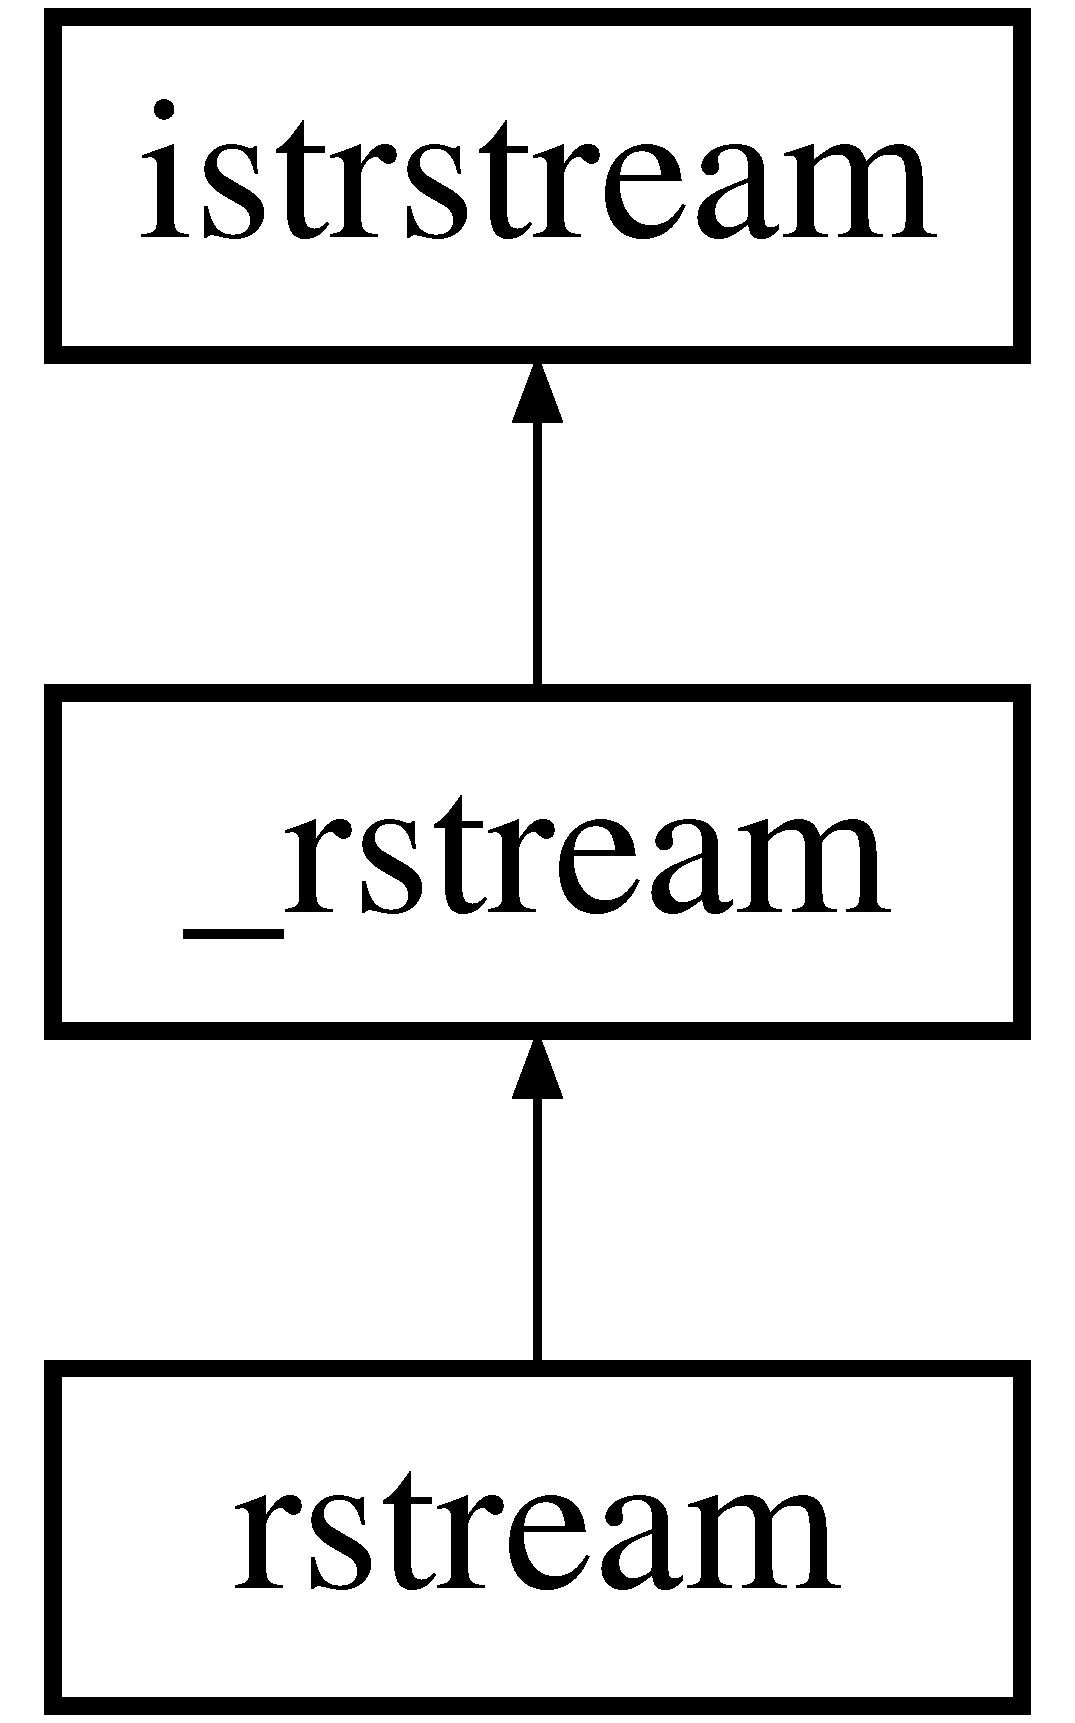
\includegraphics[height=3.000000cm]{classrstream}
\end{center}
\end{figure}
\subsection*{Public Member Functions}
\begin{DoxyCompactItemize}
\item 
\hyperlink{classrstream_a4b35677745769c8f0d9bd86b98bd141b}{rstream} (const char $\ast$\hyperlink{class__rstream_aecd5f92faba9be1c69d5c9ad2816fa89}{buf}, streamsize \hyperlink{ittnotify__static_8h_a5a1daa0c1d342747e3884fa54fc64fb1}{size})
\item 
\hyperlink{classrstream_a3f69f1c20d221bbdc529355d3c577371}{rstream} (const char $\ast$file\-Name)
\item 
\hyperlink{classrstream}{rstream} \& \hyperlink{classrstream_ad873c9748f8fffd60ef780bfc193762c}{operator$>$$>$} (\hyperlink{ittnotify__static_8h_a8b8dcd723308a8cb5d84277c7a3fff70}{int} \&\hyperlink{ittnotify__static_8h_a25eb27b280775b27a5ddc4d1673225aa}{x})
\item 
\hyperlink{classrstream}{rstream} \& \hyperlink{classrstream_a6943a853664c8523e93fb217655b71f4}{operator$>$$>$} (unsigned \&\hyperlink{ittnotify__static_8h_a25eb27b280775b27a5ddc4d1673225aa}{x})
\item 
\hyperlink{classrstream}{rstream} \& \hyperlink{classrstream_a8eb5507f7f7a649637d8aa317d400378}{operator$>$$>$} (short \&\hyperlink{ittnotify__static_8h_a25eb27b280775b27a5ddc4d1673225aa}{x})
\item 
\hyperlink{classrstream}{rstream} \& \hyperlink{classrstream_a0db7605f858c0082e4ba38d7fb59cfcf}{operator$>$$>$} (unsigned short \&\hyperlink{ittnotify__static_8h_a25eb27b280775b27a5ddc4d1673225aa}{x})
\item 
\hyperlink{classrstream}{rstream} \& \hyperlink{classrstream_ae0552d85bad3c2463f1a59d8c416812b}{operator$>$$>$} (\hyperlink{classSymbol}{Symbol} \&e)
\end{DoxyCompactItemize}
\subsection*{Private Member Functions}
\begin{DoxyCompactItemize}
\item 
{\footnotesize template$<$class T $>$ }\\\hyperlink{classrstream}{rstream} \& \hyperlink{classrstream_a672af6c6dcdc14e7640848d95d973dba}{do\-Read} (T \&\hyperlink{ittnotify__static_8h_a25eb27b280775b27a5ddc4d1673225aa}{x})
\end{DoxyCompactItemize}
\subsection*{Static Private Member Functions}
\begin{DoxyCompactItemize}
\item 
static pair$<$ const char \\*
$\ast$, streamsize $>$ \hyperlink{classrstream_aebbb229f31d865be8f1f372d81df2479}{get\-Buf} (const char $\ast$file\-Name)
\end{DoxyCompactItemize}
\subsection*{Additional Inherited Members}


\subsection{Detailed Description}


Definition at line 67 of file extract\-External.\-cpp.



\subsection{Constructor \& Destructor Documentation}
\hypertarget{classrstream_a4b35677745769c8f0d9bd86b98bd141b}{\index{rstream@{rstream}!rstream@{rstream}}
\index{rstream@{rstream}!rstream@{rstream}}
\subsubsection[{rstream}]{\setlength{\rightskip}{0pt plus 5cm}rstream\-::rstream (
\begin{DoxyParamCaption}
\item[{const char $\ast$}]{buf, }
\item[{streamsize}]{size}
\end{DoxyParamCaption}
)\hspace{0.3cm}{\ttfamily [inline]}}}\label{classrstream_a4b35677745769c8f0d9bd86b98bd141b}


Definition at line 89 of file extract\-External.\-cpp.


\begin{DoxyCode}
89 :\hyperlink{class__rstream_a90043965907b6adfdfe529fb6e5be75a}{\_rstream}(pair<const char*,streamsize>(\hyperlink{class__rstream_aecd5f92faba9be1c69d5c9ad2816fa89}{buf}, \hyperlink{ittnotify__static_8h_a5a1daa0c1d342747e3884fa54fc64fb1}{size}))\{\}
\end{DoxyCode}
\hypertarget{classrstream_a3f69f1c20d221bbdc529355d3c577371}{\index{rstream@{rstream}!rstream@{rstream}}
\index{rstream@{rstream}!rstream@{rstream}}
\subsubsection[{rstream}]{\setlength{\rightskip}{0pt plus 5cm}rstream\-::rstream (
\begin{DoxyParamCaption}
\item[{const char $\ast$}]{file\-Name}
\end{DoxyParamCaption}
)\hspace{0.3cm}{\ttfamily [inline]}}}\label{classrstream_a3f69f1c20d221bbdc529355d3c577371}


Definition at line 93 of file extract\-External.\-cpp.


\begin{DoxyCode}
93 :\hyperlink{class__rstream_a90043965907b6adfdfe529fb6e5be75a}{\_rstream}(\hyperlink{classrstream_aebbb229f31d865be8f1f372d81df2479}{getBuf}(fileName))\{\}
\end{DoxyCode}


\subsection{Member Function Documentation}
\hypertarget{classrstream_a672af6c6dcdc14e7640848d95d973dba}{\index{rstream@{rstream}!do\-Read@{do\-Read}}
\index{do\-Read@{do\-Read}!rstream@{rstream}}
\subsubsection[{do\-Read}]{\setlength{\rightskip}{0pt plus 5cm}template$<$class T $>$ {\bf rstream}\& rstream\-::do\-Read (
\begin{DoxyParamCaption}
\item[{T \&}]{x}
\end{DoxyParamCaption}
)\hspace{0.3cm}{\ttfamily [inline]}, {\ttfamily [private]}}}\label{classrstream_a672af6c6dcdc14e7640848d95d973dba}


Definition at line 70 of file extract\-External.\-cpp.


\begin{DoxyCode}
70                                  \{
71         read((\textcolor{keywordtype}{char}*)&\hyperlink{ittnotify__static_8h_a25eb27b280775b27a5ddc4d1673225aa}{x}, \textcolor{keyword}{sizeof}(T));
72         \textcolor{keywordflow}{return} *\textcolor{keyword}{this};
73     \}
\end{DoxyCode}
\hypertarget{classrstream_aebbb229f31d865be8f1f372d81df2479}{\index{rstream@{rstream}!get\-Buf@{get\-Buf}}
\index{get\-Buf@{get\-Buf}!rstream@{rstream}}
\subsubsection[{get\-Buf}]{\setlength{\rightskip}{0pt plus 5cm}static pair$<$const char$\ast$, streamsize$>$ rstream\-::get\-Buf (
\begin{DoxyParamCaption}
\item[{const char $\ast$}]{file\-Name}
\end{DoxyParamCaption}
)\hspace{0.3cm}{\ttfamily [inline]}, {\ttfamily [static]}, {\ttfamily [private]}}}\label{classrstream_aebbb229f31d865be8f1f372d81df2479}


Definition at line 74 of file extract\-External.\-cpp.


\begin{DoxyCode}
74                                                                       \{
75         ifstream raw(fileName,ios::binary | ios::in);
76         \textcolor{keywordflow}{if}(!raw.is\_open())
77             \hyperlink{extractExternal_8cpp_aaabd632593ae454ee6ac33cc02d1d215}{stop}(\textcolor{stringliteral}{"rstream.getBuf: Error opening file"});
78         raw.seekg(0,ios::end);
79         streampos fileSize = raw.tellg();
80         \textcolor{keywordflow}{if}(fileSize < 0)
81             \hyperlink{extractExternal_8cpp_aaabd632593ae454ee6ac33cc02d1d215}{stop}(\textcolor{stringliteral}{"rstream.getBuf: Error reading file"});
82         \textcolor{keywordtype}{char} *\hyperlink{class__rstream_aecd5f92faba9be1c69d5c9ad2816fa89}{buf} = \textcolor{keyword}{new} \textcolor{keywordtype}{char}[fileSize];
83         raw.seekg(0,ios::beg);
84         raw.read(buf, fileSize);
85         \textcolor{keywordflow}{return} pair<const char*, streamsize>(\hyperlink{class__rstream_aecd5f92faba9be1c69d5c9ad2816fa89}{buf},fileSize);
86     \}
\end{DoxyCode}
\hypertarget{classrstream_ad873c9748f8fffd60ef780bfc193762c}{\index{rstream@{rstream}!operator$>$$>$@{operator$>$$>$}}
\index{operator$>$$>$@{operator$>$$>$}!rstream@{rstream}}
\subsubsection[{operator$>$$>$}]{\setlength{\rightskip}{0pt plus 5cm}{\bf rstream}\& rstream\-::operator$>$$>$ (
\begin{DoxyParamCaption}
\item[{{\bf int} \&}]{x}
\end{DoxyParamCaption}
)\hspace{0.3cm}{\ttfamily [inline]}}}\label{classrstream_ad873c9748f8fffd60ef780bfc193762c}


Definition at line 94 of file extract\-External.\-cpp.


\begin{DoxyCode}
94                                 \{
95         \textcolor{keywordflow}{return} \hyperlink{classrstream_a672af6c6dcdc14e7640848d95d973dba}{doRead}(\hyperlink{ittnotify__static_8h_a25eb27b280775b27a5ddc4d1673225aa}{x});
96     \}
\end{DoxyCode}
\hypertarget{classrstream_a6943a853664c8523e93fb217655b71f4}{\index{rstream@{rstream}!operator$>$$>$@{operator$>$$>$}}
\index{operator$>$$>$@{operator$>$$>$}!rstream@{rstream}}
\subsubsection[{operator$>$$>$}]{\setlength{\rightskip}{0pt plus 5cm}{\bf rstream}\& rstream\-::operator$>$$>$ (
\begin{DoxyParamCaption}
\item[{unsigned \&}]{x}
\end{DoxyParamCaption}
)\hspace{0.3cm}{\ttfamily [inline]}}}\label{classrstream_a6943a853664c8523e93fb217655b71f4}


Definition at line 97 of file extract\-External.\-cpp.


\begin{DoxyCode}
97                                      \{
98         \textcolor{keywordflow}{return} \hyperlink{classrstream_a672af6c6dcdc14e7640848d95d973dba}{doRead}(\hyperlink{ittnotify__static_8h_a25eb27b280775b27a5ddc4d1673225aa}{x});
99     \}
\end{DoxyCode}
\hypertarget{classrstream_a8eb5507f7f7a649637d8aa317d400378}{\index{rstream@{rstream}!operator$>$$>$@{operator$>$$>$}}
\index{operator$>$$>$@{operator$>$$>$}!rstream@{rstream}}
\subsubsection[{operator$>$$>$}]{\setlength{\rightskip}{0pt plus 5cm}{\bf rstream}\& rstream\-::operator$>$$>$ (
\begin{DoxyParamCaption}
\item[{short \&}]{x}
\end{DoxyParamCaption}
)\hspace{0.3cm}{\ttfamily [inline]}}}\label{classrstream_a8eb5507f7f7a649637d8aa317d400378}


Definition at line 100 of file extract\-External.\-cpp.


\begin{DoxyCode}
100                                   \{
101         \textcolor{keywordflow}{return} \hyperlink{classrstream_a672af6c6dcdc14e7640848d95d973dba}{doRead}(\hyperlink{ittnotify__static_8h_a25eb27b280775b27a5ddc4d1673225aa}{x});
102     \}
\end{DoxyCode}
\hypertarget{classrstream_a0db7605f858c0082e4ba38d7fb59cfcf}{\index{rstream@{rstream}!operator$>$$>$@{operator$>$$>$}}
\index{operator$>$$>$@{operator$>$$>$}!rstream@{rstream}}
\subsubsection[{operator$>$$>$}]{\setlength{\rightskip}{0pt plus 5cm}{\bf rstream}\& rstream\-::operator$>$$>$ (
\begin{DoxyParamCaption}
\item[{unsigned short \&}]{x}
\end{DoxyParamCaption}
)\hspace{0.3cm}{\ttfamily [inline]}}}\label{classrstream_a0db7605f858c0082e4ba38d7fb59cfcf}


Definition at line 103 of file extract\-External.\-cpp.


\begin{DoxyCode}
103                                            \{
104         \textcolor{keywordflow}{return} \hyperlink{classrstream_a672af6c6dcdc14e7640848d95d973dba}{doRead}(\hyperlink{ittnotify__static_8h_a25eb27b280775b27a5ddc4d1673225aa}{x});
105     \}
\end{DoxyCode}
\hypertarget{classrstream_ae0552d85bad3c2463f1a59d8c416812b}{\index{rstream@{rstream}!operator$>$$>$@{operator$>$$>$}}
\index{operator$>$$>$@{operator$>$$>$}!rstream@{rstream}}
\subsubsection[{operator$>$$>$}]{\setlength{\rightskip}{0pt plus 5cm}{\bf rstream}\& rstream\-::operator$>$$>$ (
\begin{DoxyParamCaption}
\item[{{\bf Symbol} \&}]{e}
\end{DoxyParamCaption}
)\hspace{0.3cm}{\ttfamily [inline]}}}\label{classrstream_ae0552d85bad3c2463f1a59d8c416812b}


Definition at line 106 of file extract\-External.\-cpp.


\begin{DoxyCode}
106                                    \{
107         read((\textcolor{keywordtype}{char}*)&e, 18);
108         \textcolor{keywordflow}{return} *\textcolor{keyword}{this};
109     \}
\end{DoxyCode}


The documentation for this class was generated from the following file\-:\begin{DoxyCompactItemize}
\item 
\hyperlink{extractExternal_8cpp}{extract\-External.\-cpp}\end{DoxyCompactItemize}

\hypertarget{structshared__common}{\section{shared\-\_\-common Struct Reference}
\label{structshared__common}\index{shared\-\_\-common@{shared\-\_\-common}}
}


{\ttfamily \#include $<$kmp.\-h$>$}

\subsection*{Public Attributes}
\begin{DoxyCompactItemize}
\item 
struct \hyperlink{structshared__common}{shared\-\_\-common} $\ast$ \hyperlink{structshared__common_aa54da923f39ba340f472b4a62205b967}{next}
\item 
struct \hyperlink{structprivate__data}{private\-\_\-data} $\ast$ \hyperlink{structshared__common_a7609ddff99a7ccff444c4e1f2a7216e1}{pod\-\_\-init}
\item 
\hyperlink{ittnotify__static_8h_af941d56e55e3c5465135b60c4d6343ed}{void} $\ast$ \hyperlink{structshared__common_a5afc5429e242b0940b1624352aa7df79}{obj\-\_\-init}
\item 
\hyperlink{ittnotify__static_8h_af941d56e55e3c5465135b60c4d6343ed}{void} $\ast$ \hyperlink{structshared__common_abfaf275dda5ac5223f6e0f0aa333b52b}{gbl\-\_\-addr}
\item 
\begin{tabbing}
xx\=xx\=xx\=xx\=xx\=xx\=xx\=xx\=xx\=\kill
union \{\\
\>\hyperlink{group__THREADPRIVATE_ga0c2f8074a8474eee42bc96a4bdc7679a}{kmpc\_ctor} \hyperlink{structshared__common_a26bff742774584fe18d5bca4b432b1ed}{ctor}\\
\>\hyperlink{group__THREADPRIVATE_gac1f868aef7d531d34b91eaa57e339f21}{kmpc\_ctor\_vec} \hyperlink{structshared__common_aa82b661dba8988acd64a0d185851efce}{ctorv}\\
\} \hyperlink{structshared__common_ac98f8d219b58bb8cb289d896c2328e21}{ct}\\

\end{tabbing}\item 
\begin{tabbing}
xx\=xx\=xx\=xx\=xx\=xx\=xx\=xx\=xx\=\kill
union \{\\
\>\hyperlink{group__THREADPRIVATE_gab6148c019e88c8853596bf5f516373b4}{kmpc\_cctor} \hyperlink{structshared__common_a66f5f4ebb70f7db1a21310d31a387377}{cctor}\\
\>\hyperlink{group__THREADPRIVATE_gaf9503cacabf6cf90ed34f2727fc480bc}{kmpc\_cctor\_vec} \hyperlink{structshared__common_a149cfcc7e7cadd6231c21339d9adabea}{cctorv}\\
\} \hyperlink{structshared__common_a3292a73e5a3070dfdb448f7b205f68a5}{cct}\\

\end{tabbing}\item 
\begin{tabbing}
xx\=xx\=xx\=xx\=xx\=xx\=xx\=xx\=xx\=\kill
union \{\\
\>\hyperlink{group__THREADPRIVATE_gad8268ac7d007fa1c3351da682c487c0f}{kmpc\_dtor} \hyperlink{structshared__common_a127171cc49794904b593bee96f1b7d04}{dtor}\\
\>\hyperlink{group__THREADPRIVATE_gab7035b42d465074b31195534efb37e3b}{kmpc\_dtor\_vec} \hyperlink{structshared__common_a010d4cfee51a4eef6f53edb1dd7be918}{dtorv}\\
\} \hyperlink{structshared__common_ae1c3740671335275599c29df1f6d71d1}{dt}\\

\end{tabbing}\item 
size\-\_\-t \hyperlink{structshared__common_ae2761da4a704f4f2f377854538ba153c}{vec\-\_\-len}
\item 
\hyperlink{ittnotify__static_8h_a8b8dcd723308a8cb5d84277c7a3fff70}{int} \hyperlink{structshared__common_affe99e67b32f42b3bae07c95c59d8f24}{is\-\_\-vec}
\item 
size\-\_\-t \hyperlink{structshared__common_acd7343a82a2dd92f8b7a78eab8429b72}{cmn\-\_\-size}
\end{DoxyCompactItemize}


\subsection{Detailed Description}


Definition at line 1492 of file kmp.\-h.



\subsection{Member Data Documentation}
\hypertarget{structshared__common_a3292a73e5a3070dfdb448f7b205f68a5}{\index{shared\-\_\-common@{shared\-\_\-common}!cct@{cct}}
\index{cct@{cct}!shared_common@{shared\-\_\-common}}
\subsubsection[{cct}]{\setlength{\rightskip}{0pt plus 5cm}union \{ ... \}   shared\-\_\-common\-::cct}}\label{structshared__common_a3292a73e5a3070dfdb448f7b205f68a5}


Referenced by \-\_\-\-\_\-kmpc\-\_\-threadprivate\-\_\-register(), \-\_\-\-\_\-kmpc\-\_\-threadprivate\-\_\-register\-\_\-vec(), and kmp\-\_\-threadprivate\-\_\-insert().

\hypertarget{structshared__common_a66f5f4ebb70f7db1a21310d31a387377}{\index{shared\-\_\-common@{shared\-\_\-common}!cctor@{cctor}}
\index{cctor@{cctor}!shared_common@{shared\-\_\-common}}
\subsubsection[{cctor}]{\setlength{\rightskip}{0pt plus 5cm}{\bf kmpc\-\_\-cctor} shared\-\_\-common\-::cctor}}\label{structshared__common_a66f5f4ebb70f7db1a21310d31a387377}


Definition at line 1503 of file kmp.\-h.



Referenced by \-\_\-\-\_\-kmpc\-\_\-threadprivate\-\_\-register(), \-\_\-\-\_\-kmpc\-\_\-threadprivate\-\_\-register\-\_\-vec(), and kmp\-\_\-threadprivate\-\_\-insert().

\hypertarget{structshared__common_a149cfcc7e7cadd6231c21339d9adabea}{\index{shared\-\_\-common@{shared\-\_\-common}!cctorv@{cctorv}}
\index{cctorv@{cctorv}!shared_common@{shared\-\_\-common}}
\subsubsection[{cctorv}]{\setlength{\rightskip}{0pt plus 5cm}{\bf kmpc\-\_\-cctor\-\_\-vec} shared\-\_\-common\-::cctorv}}\label{structshared__common_a149cfcc7e7cadd6231c21339d9adabea}


Definition at line 1504 of file kmp.\-h.



Referenced by \-\_\-\-\_\-kmpc\-\_\-threadprivate\-\_\-register\-\_\-vec(), and kmp\-\_\-threadprivate\-\_\-insert().

\hypertarget{structshared__common_acd7343a82a2dd92f8b7a78eab8429b72}{\index{shared\-\_\-common@{shared\-\_\-common}!cmn\-\_\-size@{cmn\-\_\-size}}
\index{cmn\-\_\-size@{cmn\-\_\-size}!shared_common@{shared\-\_\-common}}
\subsubsection[{cmn\-\_\-size}]{\setlength{\rightskip}{0pt plus 5cm}size\-\_\-t shared\-\_\-common\-::cmn\-\_\-size}}\label{structshared__common_acd7343a82a2dd92f8b7a78eab8429b72}


Definition at line 1512 of file kmp.\-h.



Referenced by kmp\-\_\-threadprivate\-\_\-insert(), and kmp\-\_\-threadprivate\-\_\-insert\-\_\-private\-\_\-data().

\hypertarget{structshared__common_ac98f8d219b58bb8cb289d896c2328e21}{\index{shared\-\_\-common@{shared\-\_\-common}!ct@{ct}}
\index{ct@{ct}!shared_common@{shared\-\_\-common}}
\subsubsection[{ct}]{\setlength{\rightskip}{0pt plus 5cm}union \{ ... \}   shared\-\_\-common\-::ct}}\label{structshared__common_ac98f8d219b58bb8cb289d896c2328e21}


Referenced by \-\_\-\-\_\-kmpc\-\_\-threadprivate\-\_\-register(), \-\_\-\-\_\-kmpc\-\_\-threadprivate\-\_\-register\-\_\-vec(), and kmp\-\_\-threadprivate\-\_\-insert().

\hypertarget{structshared__common_a26bff742774584fe18d5bca4b432b1ed}{\index{shared\-\_\-common@{shared\-\_\-common}!ctor@{ctor}}
\index{ctor@{ctor}!shared_common@{shared\-\_\-common}}
\subsubsection[{ctor}]{\setlength{\rightskip}{0pt plus 5cm}{\bf kmpc\-\_\-ctor} shared\-\_\-common\-::ctor}}\label{structshared__common_a26bff742774584fe18d5bca4b432b1ed}


Definition at line 1499 of file kmp.\-h.



Referenced by \-\_\-\-\_\-kmpc\-\_\-threadprivate\-\_\-register(), \-\_\-\-\_\-kmpc\-\_\-threadprivate\-\_\-register\-\_\-vec(), and kmp\-\_\-threadprivate\-\_\-insert().

\hypertarget{structshared__common_aa82b661dba8988acd64a0d185851efce}{\index{shared\-\_\-common@{shared\-\_\-common}!ctorv@{ctorv}}
\index{ctorv@{ctorv}!shared_common@{shared\-\_\-common}}
\subsubsection[{ctorv}]{\setlength{\rightskip}{0pt plus 5cm}{\bf kmpc\-\_\-ctor\-\_\-vec} shared\-\_\-common\-::ctorv}}\label{structshared__common_aa82b661dba8988acd64a0d185851efce}


Definition at line 1500 of file kmp.\-h.



Referenced by \-\_\-\-\_\-kmpc\-\_\-threadprivate\-\_\-register\-\_\-vec(), and kmp\-\_\-threadprivate\-\_\-insert().

\hypertarget{structshared__common_ae1c3740671335275599c29df1f6d71d1}{\index{shared\-\_\-common@{shared\-\_\-common}!dt@{dt}}
\index{dt@{dt}!shared_common@{shared\-\_\-common}}
\subsubsection[{dt}]{\setlength{\rightskip}{0pt plus 5cm}union \{ ... \}   shared\-\_\-common\-::dt}}\label{structshared__common_ae1c3740671335275599c29df1f6d71d1}


Referenced by \-\_\-\-\_\-kmp\-\_\-common\-\_\-destroy(), \-\_\-\-\_\-kmp\-\_\-common\-\_\-destroy\-\_\-gtid(), \-\_\-\-\_\-kmpc\-\_\-threadprivate\-\_\-register(), and \-\_\-\-\_\-kmpc\-\_\-threadprivate\-\_\-register\-\_\-vec().

\hypertarget{structshared__common_a127171cc49794904b593bee96f1b7d04}{\index{shared\-\_\-common@{shared\-\_\-common}!dtor@{dtor}}
\index{dtor@{dtor}!shared_common@{shared\-\_\-common}}
\subsubsection[{dtor}]{\setlength{\rightskip}{0pt plus 5cm}{\bf kmpc\-\_\-dtor} shared\-\_\-common\-::dtor}}\label{structshared__common_a127171cc49794904b593bee96f1b7d04}


Definition at line 1507 of file kmp.\-h.



Referenced by \-\_\-\-\_\-kmp\-\_\-common\-\_\-destroy(), \-\_\-\-\_\-kmp\-\_\-common\-\_\-destroy\-\_\-gtid(), \-\_\-\-\_\-kmpc\-\_\-threadprivate\-\_\-register(), and \-\_\-\-\_\-kmpc\-\_\-threadprivate\-\_\-register\-\_\-vec().

\hypertarget{structshared__common_a010d4cfee51a4eef6f53edb1dd7be918}{\index{shared\-\_\-common@{shared\-\_\-common}!dtorv@{dtorv}}
\index{dtorv@{dtorv}!shared_common@{shared\-\_\-common}}
\subsubsection[{dtorv}]{\setlength{\rightskip}{0pt plus 5cm}{\bf kmpc\-\_\-dtor\-\_\-vec} shared\-\_\-common\-::dtorv}}\label{structshared__common_a010d4cfee51a4eef6f53edb1dd7be918}


Definition at line 1508 of file kmp.\-h.



Referenced by \-\_\-\-\_\-kmp\-\_\-common\-\_\-destroy(), \-\_\-\-\_\-kmp\-\_\-common\-\_\-destroy\-\_\-gtid(), and \-\_\-\-\_\-kmpc\-\_\-threadprivate\-\_\-register\-\_\-vec().

\hypertarget{structshared__common_abfaf275dda5ac5223f6e0f0aa333b52b}{\index{shared\-\_\-common@{shared\-\_\-common}!gbl\-\_\-addr@{gbl\-\_\-addr}}
\index{gbl\-\_\-addr@{gbl\-\_\-addr}!shared_common@{shared\-\_\-common}}
\subsubsection[{gbl\-\_\-addr}]{\setlength{\rightskip}{0pt plus 5cm}{\bf void}$\ast$ shared\-\_\-common\-::gbl\-\_\-addr}}\label{structshared__common_abfaf275dda5ac5223f6e0f0aa333b52b}


Definition at line 1497 of file kmp.\-h.



Referenced by \-\_\-\-\_\-kmp\-\_\-common\-\_\-destroy(), \-\_\-\-\_\-kmp\-\_\-find\-\_\-shared\-\_\-task\-\_\-common(), \-\_\-\-\_\-kmpc\-\_\-threadprivate\-\_\-register(), \-\_\-\-\_\-kmpc\-\_\-threadprivate\-\_\-register\-\_\-vec(), kmp\-\_\-threadprivate\-\_\-insert(), and kmp\-\_\-threadprivate\-\_\-insert\-\_\-private\-\_\-data().

\hypertarget{structshared__common_affe99e67b32f42b3bae07c95c59d8f24}{\index{shared\-\_\-common@{shared\-\_\-common}!is\-\_\-vec@{is\-\_\-vec}}
\index{is\-\_\-vec@{is\-\_\-vec}!shared_common@{shared\-\_\-common}}
\subsubsection[{is\-\_\-vec}]{\setlength{\rightskip}{0pt plus 5cm}{\bf int} shared\-\_\-common\-::is\-\_\-vec}}\label{structshared__common_affe99e67b32f42b3bae07c95c59d8f24}


Definition at line 1511 of file kmp.\-h.



Referenced by \-\_\-\-\_\-kmp\-\_\-common\-\_\-destroy(), \-\_\-\-\_\-kmp\-\_\-common\-\_\-destroy\-\_\-gtid(), \-\_\-\-\_\-kmpc\-\_\-threadprivate\-\_\-register\-\_\-vec(), and kmp\-\_\-threadprivate\-\_\-insert().

\hypertarget{structshared__common_aa54da923f39ba340f472b4a62205b967}{\index{shared\-\_\-common@{shared\-\_\-common}!next@{next}}
\index{next@{next}!shared_common@{shared\-\_\-common}}
\subsubsection[{next}]{\setlength{\rightskip}{0pt plus 5cm}struct {\bf shared\-\_\-common}$\ast$ shared\-\_\-common\-::next}}\label{structshared__common_aa54da923f39ba340f472b4a62205b967}


Definition at line 1494 of file kmp.\-h.



Referenced by \-\_\-\-\_\-kmp\-\_\-common\-\_\-destroy(), \-\_\-\-\_\-kmp\-\_\-find\-\_\-shared\-\_\-task\-\_\-common(), \-\_\-\-\_\-kmpc\-\_\-threadprivate\-\_\-register(), \-\_\-\-\_\-kmpc\-\_\-threadprivate\-\_\-register\-\_\-vec(), kmp\-\_\-threadprivate\-\_\-insert(), and kmp\-\_\-threadprivate\-\_\-insert\-\_\-private\-\_\-data().

\hypertarget{structshared__common_a5afc5429e242b0940b1624352aa7df79}{\index{shared\-\_\-common@{shared\-\_\-common}!obj\-\_\-init@{obj\-\_\-init}}
\index{obj\-\_\-init@{obj\-\_\-init}!shared_common@{shared\-\_\-common}}
\subsubsection[{obj\-\_\-init}]{\setlength{\rightskip}{0pt plus 5cm}{\bf void}$\ast$ shared\-\_\-common\-::obj\-\_\-init}}\label{structshared__common_a5afc5429e242b0940b1624352aa7df79}


Definition at line 1496 of file kmp.\-h.



Referenced by \-\_\-\-\_\-kmp\-\_\-common\-\_\-destroy(), \-\_\-\-\_\-kmp\-\_\-common\-\_\-destroy\-\_\-gtid(), and kmp\-\_\-threadprivate\-\_\-insert().

\hypertarget{structshared__common_a7609ddff99a7ccff444c4e1f2a7216e1}{\index{shared\-\_\-common@{shared\-\_\-common}!pod\-\_\-init@{pod\-\_\-init}}
\index{pod\-\_\-init@{pod\-\_\-init}!shared_common@{shared\-\_\-common}}
\subsubsection[{pod\-\_\-init}]{\setlength{\rightskip}{0pt plus 5cm}struct {\bf private\-\_\-data}$\ast$ shared\-\_\-common\-::pod\-\_\-init}}\label{structshared__common_a7609ddff99a7ccff444c4e1f2a7216e1}


Definition at line 1495 of file kmp.\-h.



Referenced by kmp\-\_\-threadprivate\-\_\-insert(), and kmp\-\_\-threadprivate\-\_\-insert\-\_\-private\-\_\-data().

\hypertarget{structshared__common_ae2761da4a704f4f2f377854538ba153c}{\index{shared\-\_\-common@{shared\-\_\-common}!vec\-\_\-len@{vec\-\_\-len}}
\index{vec\-\_\-len@{vec\-\_\-len}!shared_common@{shared\-\_\-common}}
\subsubsection[{vec\-\_\-len}]{\setlength{\rightskip}{0pt plus 5cm}size\-\_\-t shared\-\_\-common\-::vec\-\_\-len}}\label{structshared__common_ae2761da4a704f4f2f377854538ba153c}


Definition at line 1510 of file kmp.\-h.



Referenced by \-\_\-\-\_\-kmp\-\_\-common\-\_\-destroy(), \-\_\-\-\_\-kmp\-\_\-common\-\_\-destroy\-\_\-gtid(), \-\_\-\-\_\-kmpc\-\_\-threadprivate\-\_\-register\-\_\-vec(), and kmp\-\_\-threadprivate\-\_\-insert().



The documentation for this struct was generated from the following file\-:\begin{DoxyCompactItemize}
\item 
\hyperlink{kmp_8h}{kmp.\-h}\end{DoxyCompactItemize}

\hypertarget{uniondispatch__shared__info_1_1shared__info}{\section{dispatch\-\_\-shared\-\_\-info\-:\-:shared\-\_\-info Union Reference}
\label{uniondispatch__shared__info_1_1shared__info}\index{dispatch\-\_\-shared\-\_\-info\-::shared\-\_\-info@{dispatch\-\_\-shared\-\_\-info\-::shared\-\_\-info}}
}


{\ttfamily \#include $<$kmp.\-h$>$}

\subsection*{Public Attributes}
\begin{DoxyCompactItemize}
\item 
\hyperlink{kmp_8h_abcf4c94a5d57bd5b976ad9478fe2ea75}{dispatch\-\_\-shared\-\_\-info32\-\_\-t} \hyperlink{uniondispatch__shared__info_1_1shared__info_aee439b88499939c12958ae2e1598d489}{s32}
\item 
\hyperlink{kmp_8h_a8a97d7549f6b7fa3ec64e933bd434fd5}{dispatch\-\_\-shared\-\_\-info64\-\_\-t} \hyperlink{uniondispatch__shared__info_1_1shared__info_a7fdd3cf5a93b568ae520fba0b416e103}{s64}
\end{DoxyCompactItemize}


\subsection{Detailed Description}


Definition at line 1673 of file kmp.\-h.



\subsection{Member Data Documentation}
\hypertarget{uniondispatch__shared__info_1_1shared__info_aee439b88499939c12958ae2e1598d489}{\index{dispatch\-\_\-shared\-\_\-info\-::shared\-\_\-info@{dispatch\-\_\-shared\-\_\-info\-::shared\-\_\-info}!s32@{s32}}
\index{s32@{s32}!dispatch_shared_info::shared_info@{dispatch\-\_\-shared\-\_\-info\-::shared\-\_\-info}}
\subsubsection[{s32}]{\setlength{\rightskip}{0pt plus 5cm}{\bf dispatch\-\_\-shared\-\_\-info32\-\_\-t} dispatch\-\_\-shared\-\_\-info\-::shared\-\_\-info\-::s32}}\label{uniondispatch__shared__info_1_1shared__info_aee439b88499939c12958ae2e1598d489}


Definition at line 1674 of file kmp.\-h.

\hypertarget{uniondispatch__shared__info_1_1shared__info_a7fdd3cf5a93b568ae520fba0b416e103}{\index{dispatch\-\_\-shared\-\_\-info\-::shared\-\_\-info@{dispatch\-\_\-shared\-\_\-info\-::shared\-\_\-info}!s64@{s64}}
\index{s64@{s64}!dispatch_shared_info::shared_info@{dispatch\-\_\-shared\-\_\-info\-::shared\-\_\-info}}
\subsubsection[{s64}]{\setlength{\rightskip}{0pt plus 5cm}{\bf dispatch\-\_\-shared\-\_\-info64\-\_\-t} dispatch\-\_\-shared\-\_\-info\-::shared\-\_\-info\-::s64}}\label{uniondispatch__shared__info_1_1shared__info_a7fdd3cf5a93b568ae520fba0b416e103}


Definition at line 1675 of file kmp.\-h.



The documentation for this union was generated from the following file\-:\begin{DoxyCompactItemize}
\item 
\hyperlink{kmp_8h}{kmp.\-h}\end{DoxyCompactItemize}

\hypertarget{uniondispatch__shared__info__template_1_1shared__info__tmpl}{\section{dispatch\-\_\-shared\-\_\-info\-\_\-template$<$ U\-T $>$\-:\-:shared\-\_\-info\-\_\-tmpl Union Reference}
\label{uniondispatch__shared__info__template_1_1shared__info__tmpl}\index{dispatch\-\_\-shared\-\_\-info\-\_\-template$<$ U\-T $>$\-::shared\-\_\-info\-\_\-tmpl@{dispatch\-\_\-shared\-\_\-info\-\_\-template$<$ U\-T $>$\-::shared\-\_\-info\-\_\-tmpl}}
}
\subsection*{Public Attributes}
\begin{DoxyCompactItemize}
\item 
\hyperlink{structdispatch__shared__infoXX__template}{dispatch\-\_\-shared\-\_\-info\-X\-X\-\_\-template}\\*
$<$ U\-T $>$ \hyperlink{uniondispatch__shared__info__template_1_1shared__info__tmpl_ad685051b57b2ee1fd685f627a04621ef}{s}
\item 
\hyperlink{kmp_8h_a8a97d7549f6b7fa3ec64e933bd434fd5}{dispatch\-\_\-shared\-\_\-info64\-\_\-t} \hyperlink{uniondispatch__shared__info__template_1_1shared__info__tmpl_afcaf714880dfcdedb3d9e4dc9b6320a0}{s64}
\end{DoxyCompactItemize}


\subsection{Detailed Description}
\subsubsection*{template$<$typename U\-T$>$union dispatch\-\_\-shared\-\_\-info\-\_\-template$<$ U\-T $>$\-::shared\-\_\-info\-\_\-tmpl}



Definition at line 173 of file kmp\-\_\-dispatch.\-cpp.



\subsection{Member Data Documentation}
\hypertarget{uniondispatch__shared__info__template_1_1shared__info__tmpl_ad685051b57b2ee1fd685f627a04621ef}{\index{dispatch\-\_\-shared\-\_\-info\-\_\-template\-::shared\-\_\-info\-\_\-tmpl@{dispatch\-\_\-shared\-\_\-info\-\_\-template\-::shared\-\_\-info\-\_\-tmpl}!s@{s}}
\index{s@{s}!dispatch_shared_info_template::shared_info_tmpl@{dispatch\-\_\-shared\-\_\-info\-\_\-template\-::shared\-\_\-info\-\_\-tmpl}}
\subsubsection[{s}]{\setlength{\rightskip}{0pt plus 5cm}template$<$typename U\-T$>$ {\bf dispatch\-\_\-shared\-\_\-info\-X\-X\-\_\-template}$<$ U\-T $>$ {\bf dispatch\-\_\-shared\-\_\-info\-\_\-template}$<$ U\-T $>$\-::shared\-\_\-info\-\_\-tmpl\-::s}}\label{uniondispatch__shared__info__template_1_1shared__info__tmpl_ad685051b57b2ee1fd685f627a04621ef}


Definition at line 174 of file kmp\-\_\-dispatch.\-cpp.



Referenced by \-\_\-\-\_\-kmp\-\_\-dispatch\-\_\-deo(), \-\_\-\-\_\-kmp\-\_\-dispatch\-\_\-dxo(), and \-\_\-\-\_\-kmp\-\_\-dispatch\-\_\-next().

\hypertarget{uniondispatch__shared__info__template_1_1shared__info__tmpl_afcaf714880dfcdedb3d9e4dc9b6320a0}{\index{dispatch\-\_\-shared\-\_\-info\-\_\-template\-::shared\-\_\-info\-\_\-tmpl@{dispatch\-\_\-shared\-\_\-info\-\_\-template\-::shared\-\_\-info\-\_\-tmpl}!s64@{s64}}
\index{s64@{s64}!dispatch_shared_info_template::shared_info_tmpl@{dispatch\-\_\-shared\-\_\-info\-\_\-template\-::shared\-\_\-info\-\_\-tmpl}}
\subsubsection[{s64}]{\setlength{\rightskip}{0pt plus 5cm}template$<$typename U\-T$>$ {\bf dispatch\-\_\-shared\-\_\-info64\-\_\-t} {\bf dispatch\-\_\-shared\-\_\-info\-\_\-template}$<$ U\-T $>$\-::shared\-\_\-info\-\_\-tmpl\-::s64}}\label{uniondispatch__shared__info__template_1_1shared__info__tmpl_afcaf714880dfcdedb3d9e4dc9b6320a0}


Definition at line 175 of file kmp\-\_\-dispatch.\-cpp.



The documentation for this union was generated from the following file\-:\begin{DoxyCompactItemize}
\item 
\hyperlink{kmp__dispatch_8cpp}{kmp\-\_\-dispatch.\-cpp}\end{DoxyCompactItemize}

\hypertarget{structshared__table}{\section{shared\-\_\-table Struct Reference}
\label{structshared__table}\index{shared\-\_\-table@{shared\-\_\-table}}
}


{\ttfamily \#include $<$kmp.\-h$>$}

\subsection*{Public Attributes}
\begin{DoxyCompactItemize}
\item 
struct \hyperlink{structshared__common}{shared\-\_\-common} $\ast$ \hyperlink{structshared__table_acbe02cd3db1cddd2f658db7e64c2bfc5}{data} \mbox{[}\hyperlink{kmp_8h_a18bbfe585fccb920012f9477c07977b7}{K\-M\-P\-\_\-\-H\-A\-S\-H\-\_\-\-T\-A\-B\-L\-E\-\_\-\-S\-I\-Z\-E}\mbox{]}
\end{DoxyCompactItemize}


\subsection{Detailed Description}


Definition at line 1524 of file kmp.\-h.



\subsection{Member Data Documentation}
\hypertarget{structshared__table_acbe02cd3db1cddd2f658db7e64c2bfc5}{\index{shared\-\_\-table@{shared\-\_\-table}!data@{data}}
\index{data@{data}!shared_table@{shared\-\_\-table}}
\subsubsection[{data}]{\setlength{\rightskip}{0pt plus 5cm}struct {\bf shared\-\_\-common}$\ast$ shared\-\_\-table\-::data\mbox{[}{\bf K\-M\-P\-\_\-\-H\-A\-S\-H\-\_\-\-T\-A\-B\-L\-E\-\_\-\-S\-I\-Z\-E}\mbox{]}}}\label{structshared__table_acbe02cd3db1cddd2f658db7e64c2bfc5}


Definition at line 1525 of file kmp.\-h.



Referenced by \-\_\-\-\_\-kmp\-\_\-common\-\_\-destroy(), \-\_\-\-\_\-kmp\-\_\-common\-\_\-initialize(), \-\_\-\-\_\-kmp\-\_\-find\-\_\-shared\-\_\-task\-\_\-common(), \-\_\-\-\_\-kmpc\-\_\-threadprivate\-\_\-register(), \-\_\-\-\_\-kmpc\-\_\-threadprivate\-\_\-register\-\_\-vec(), kmp\-\_\-threadprivate\-\_\-insert(), and kmp\-\_\-threadprivate\-\_\-insert\-\_\-private\-\_\-data().



The documentation for this struct was generated from the following file\-:\begin{DoxyCompactItemize}
\item 
\hyperlink{kmp_8h}{kmp.\-h}\end{DoxyCompactItemize}

\hypertarget{structstatInfo}{\section{stat\-Info Struct Reference}
\label{structstatInfo}\index{stat\-Info@{stat\-Info}}
}


{\ttfamily \#include $<$kmp\-\_\-stats.\-h$>$}

\subsection*{Public Attributes}
\begin{DoxyCompactItemize}
\item 
const char $\ast$ \hyperlink{structstatInfo_a83052615f9578ba88744140093a18f37}{name}
\item 
uint32\-\_\-t \hyperlink{structstatInfo_a590c3b9a2b0786720e9a53b0dd6071fd}{flags}
\end{DoxyCompactItemize}


\subsection{Detailed Description}


Definition at line 265 of file kmp\-\_\-stats.\-h.



\subsection{Member Data Documentation}
\hypertarget{structstatInfo_a590c3b9a2b0786720e9a53b0dd6071fd}{\index{stat\-Info@{stat\-Info}!flags@{flags}}
\index{flags@{flags}!statInfo@{stat\-Info}}
\subsubsection[{flags}]{\setlength{\rightskip}{0pt plus 5cm}uint32\-\_\-t stat\-Info\-::flags}}\label{structstatInfo_a590c3b9a2b0786720e9a53b0dd6071fd}


Definition at line 268 of file kmp\-\_\-stats.\-h.



Referenced by time\-Stat\-::clear\-Event\-Flags(), time\-Stat\-::log\-Event(), time\-Stat\-::master\-Only(), counter\-::master\-Only(), time\-Stat\-::no\-Total(), time\-Stat\-::no\-Units(), and time\-Stat\-::worker\-Only().

\hypertarget{structstatInfo_a83052615f9578ba88744140093a18f37}{\index{stat\-Info@{stat\-Info}!name@{name}}
\index{name@{name}!statInfo@{stat\-Info}}
\subsubsection[{name}]{\setlength{\rightskip}{0pt plus 5cm}const char$\ast$ stat\-Info\-::name}}\label{structstatInfo_a83052615f9578ba88744140093a18f37}


Definition at line 267 of file kmp\-\_\-stats.\-h.



Referenced by time\-Stat\-::name(), and counter\-::name().



The documentation for this struct was generated from the following file\-:\begin{DoxyCompactItemize}
\item 
\hyperlink{kmp__stats_8h}{kmp\-\_\-stats.\-h}\end{DoxyCompactItemize}

\hypertarget{classstatistic}{\section{statistic Class Reference}
\label{classstatistic}\index{statistic@{statistic}}
}


{\ttfamily \#include $<$kmp\-\_\-stats.\-h$>$}

Inheritance diagram for statistic\-:\begin{figure}[H]
\begin{center}
\leavevmode
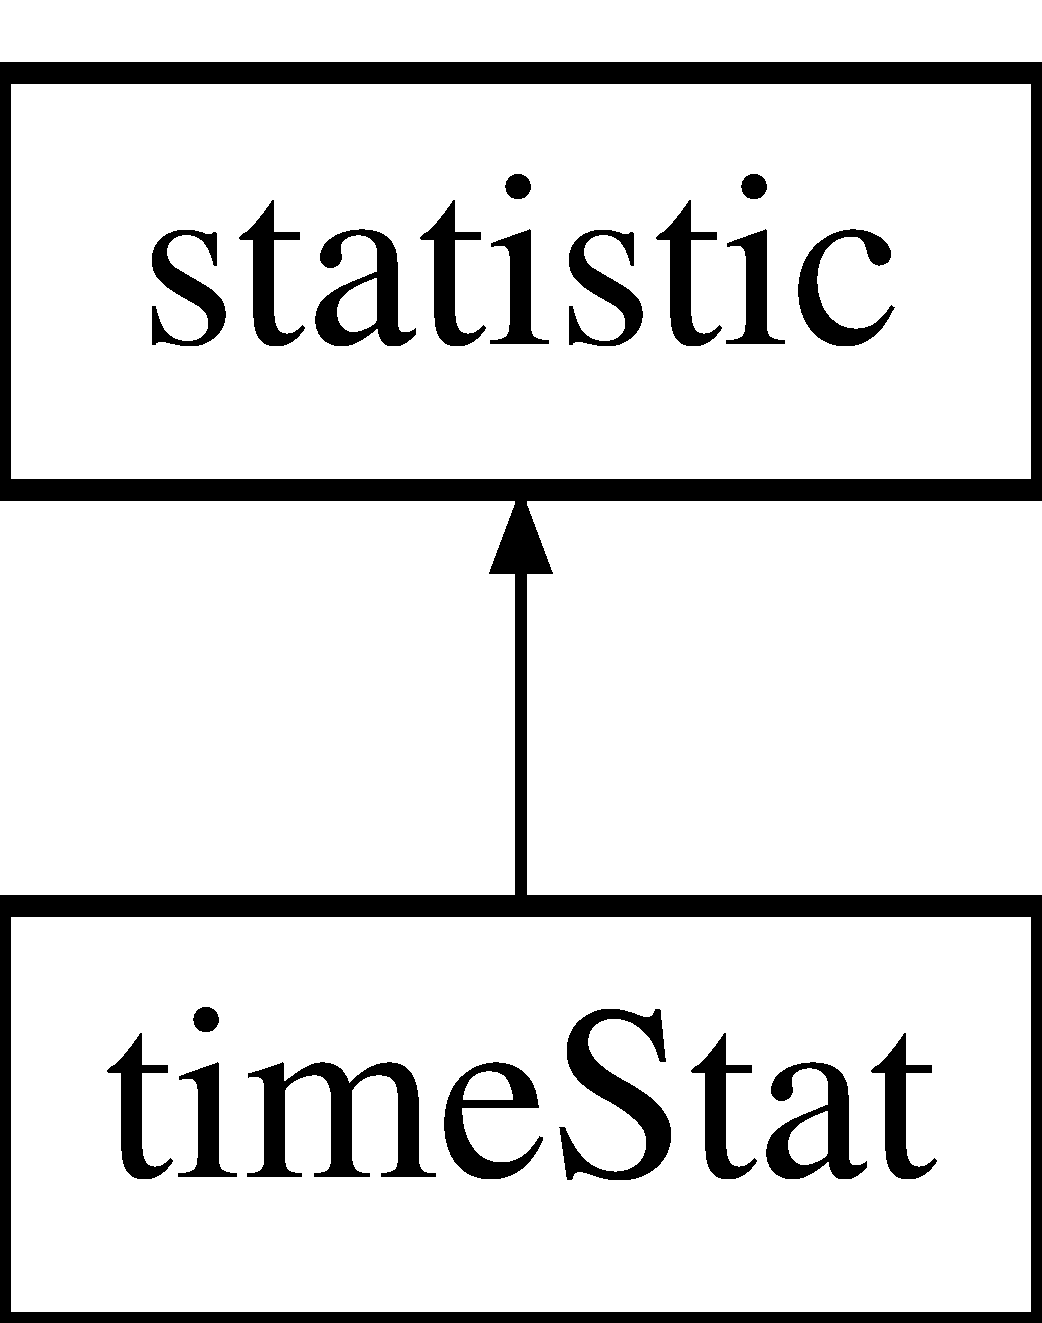
\includegraphics[height=2.000000cm]{classstatistic}
\end{center}
\end{figure}
\subsection*{Public Member Functions}
\begin{DoxyCompactItemize}
\item 
\hyperlink{classstatistic_a3f28cad0a4699e3f2db3892b5556f4e7}{statistic} ()
\item 
\hyperlink{classstatistic_a7ecb0612ab65607ae253b91c5664b756}{statistic} (\hyperlink{classstatistic}{statistic} const \&o)
\item 
double \hyperlink{classstatistic_a74842a553de28750096653e8bf9386d6}{get\-Min} () const 
\item 
double \hyperlink{classstatistic_a57044354c7454db661f485186bde339f}{get\-Mean} () const 
\item 
double \hyperlink{classstatistic_a3b196abb4776e04468138ddfe0b65acd}{get\-Max} () const 
\item 
uint64\-\_\-t \hyperlink{classstatistic_a9c5688424edb33f3a107ca94a6170f08}{get\-Count} () const 
\item 
double \hyperlink{classstatistic_ae90ab239948f240f5fae1d57305196b2}{get\-S\-D} () const 
\item 
double \hyperlink{classstatistic_a4dc72cbd2d3940ecc55a98cbdac91963}{get\-Total} () const 
\item 
\hyperlink{ittnotify__static_8h_af941d56e55e3c5465135b60c4d6343ed}{void} \hyperlink{classstatistic_a5b3a1c2c7c270ef3e6bc077304f57ee1}{reset} ()
\item 
\hyperlink{ittnotify__static_8h_af941d56e55e3c5465135b60c4d6343ed}{void} \hyperlink{classstatistic_a608058fd5fac27c72c6019c607f38688}{add\-Sample} (double sample)
\item 
\hyperlink{ittnotify__static_8h_af941d56e55e3c5465135b60c4d6343ed}{void} \hyperlink{classstatistic_aee49a269c79947670f53f68e24c7d1c9}{scale} (double factor)
\item 
\hyperlink{ittnotify__static_8h_af941d56e55e3c5465135b60c4d6343ed}{void} \hyperlink{classstatistic_add0a3834ecd055e70f48db00df747aea}{scale\-Down} (double f)
\item 
\hyperlink{classstatistic}{statistic} \& \hyperlink{classstatistic_a7fb2040e35a0550e8a7cd0317e326c53}{operator+=} (\hyperlink{classstatistic}{statistic} const \&other)
\item 
std\-::string \hyperlink{classstatistic_a82803f1000193073e46079faf078458d}{format} (char unit, bool total=false) const 
\end{DoxyCompactItemize}
\subsection*{Private Attributes}
\begin{DoxyCompactItemize}
\item 
double \hyperlink{classstatistic_acc6389ee86b103a599905e63222463cc}{min\-Val}
\item 
double \hyperlink{classstatistic_a4d776fbd2f21d0900ab76a02b82dd9ff}{max\-Val}
\item 
double \hyperlink{classstatistic_ae1bd63c1e77867dd3c995344e377e8ea}{mean\-Val}
\item 
double \hyperlink{classstatistic_aebbd60d54ac69333572267817c6fcdd9}{m2}
\item 
uint64\-\_\-t \hyperlink{classstatistic_a0e548b7b46e603d290a3b2be7cfde18d}{sample\-Count}
\end{DoxyCompactItemize}


\subsection{Detailed Description}


Definition at line 230 of file kmp\-\_\-stats.\-h.



\subsection{Constructor \& Destructor Documentation}
\hypertarget{classstatistic_a3f28cad0a4699e3f2db3892b5556f4e7}{\index{statistic@{statistic}!statistic@{statistic}}
\index{statistic@{statistic}!statistic@{statistic}}
\subsubsection[{statistic}]{\setlength{\rightskip}{0pt plus 5cm}statistic\-::statistic (
\begin{DoxyParamCaption}
{}
\end{DoxyParamCaption}
)\hspace{0.3cm}{\ttfamily [inline]}}}\label{classstatistic_a3f28cad0a4699e3f2db3892b5556f4e7}


Definition at line 239 of file kmp\-\_\-stats.\-h.


\begin{DoxyCode}
239 \{ \hyperlink{classstatistic_a5b3a1c2c7c270ef3e6bc077304f57ee1}{reset}(); \}
\end{DoxyCode}
\hypertarget{classstatistic_a7ecb0612ab65607ae253b91c5664b756}{\index{statistic@{statistic}!statistic@{statistic}}
\index{statistic@{statistic}!statistic@{statistic}}
\subsubsection[{statistic}]{\setlength{\rightskip}{0pt plus 5cm}statistic\-::statistic (
\begin{DoxyParamCaption}
\item[{{\bf statistic} const \&}]{o}
\end{DoxyParamCaption}
)\hspace{0.3cm}{\ttfamily [inline]}}}\label{classstatistic_a7ecb0612ab65607ae253b91c5664b756}


Definition at line 240 of file kmp\-\_\-stats.\-h.


\begin{DoxyCode}
240 : \hyperlink{classstatistic_acc6389ee86b103a599905e63222463cc}{minVal}(o.minVal), \hyperlink{classstatistic_a4d776fbd2f21d0900ab76a02b82dd9ff}{maxVal}(o.maxVal), \hyperlink{classstatistic_ae1bd63c1e77867dd3c995344e377e8ea}{meanVal}(o.meanVal), \hyperlink{classstatistic_aebbd60d54ac69333572267817c6fcdd9}{m2}(o.m2), 
      \hyperlink{classstatistic_a0e548b7b46e603d290a3b2be7cfde18d}{sampleCount}(o.sampleCount) \{\}
\end{DoxyCode}


\subsection{Member Function Documentation}
\hypertarget{classstatistic_a608058fd5fac27c72c6019c607f38688}{\index{statistic@{statistic}!add\-Sample@{add\-Sample}}
\index{add\-Sample@{add\-Sample}!statistic@{statistic}}
\subsubsection[{add\-Sample}]{\setlength{\rightskip}{0pt plus 5cm}{\bf void} statistic\-::add\-Sample (
\begin{DoxyParamCaption}
\item[{double}]{sample}
\end{DoxyParamCaption}
)}}\label{classstatistic_a608058fd5fac27c72c6019c607f38688}


Definition at line 79 of file kmp\-\_\-stats.\-cpp.



Referenced by kmp\-\_\-stats\-\_\-output\-\_\-module\-::output\-Stats(), and explicit\-Timer\-::stop().


\begin{DoxyCode}
80 \{
81     \textcolor{keywordtype}{double} delta = sample - \hyperlink{classstatistic_ae1bd63c1e77867dd3c995344e377e8ea}{meanVal};
82 
83     \hyperlink{classstatistic_a0e548b7b46e603d290a3b2be7cfde18d}{sampleCount} = \hyperlink{classstatistic_a0e548b7b46e603d290a3b2be7cfde18d}{sampleCount} + 1;
84     meanVal     = meanVal + delta/\hyperlink{classstatistic_a0e548b7b46e603d290a3b2be7cfde18d}{sampleCount};
85     \hyperlink{classstatistic_aebbd60d54ac69333572267817c6fcdd9}{m2}          = \hyperlink{classstatistic_aebbd60d54ac69333572267817c6fcdd9}{m2} + delta*(sample - \hyperlink{classstatistic_ae1bd63c1e77867dd3c995344e377e8ea}{meanVal});
86 
87     \hyperlink{classstatistic_acc6389ee86b103a599905e63222463cc}{minVal} = \hyperlink{ittnotify__static_8c_ac6afabdc09a49a433ee19d8a9486056d}{std::min}(minVal, sample);
88     \hyperlink{classstatistic_a4d776fbd2f21d0900ab76a02b82dd9ff}{maxVal} = std::max(\hyperlink{classstatistic_a4d776fbd2f21d0900ab76a02b82dd9ff}{maxVal}, sample);
89 \}
\end{DoxyCode}
\hypertarget{classstatistic_a82803f1000193073e46079faf078458d}{\index{statistic@{statistic}!format@{format}}
\index{format@{format}!statistic@{statistic}}
\subsubsection[{format}]{\setlength{\rightskip}{0pt plus 5cm}std\-::string statistic\-::format (
\begin{DoxyParamCaption}
\item[{char}]{unit, }
\item[{bool}]{total = {\ttfamily false}}
\end{DoxyParamCaption}
) const}}\label{classstatistic_a82803f1000193073e46079faf078458d}


Definition at line 130 of file kmp\-\_\-stats.\-cpp.



Referenced by kmp\-\_\-stats\-\_\-output\-\_\-module\-::print\-Counter\-Stats(), and kmp\-\_\-stats\-\_\-output\-\_\-module\-::print\-Timer\-Stats().


\begin{DoxyCode}
131 \{
132     std::string result = \hyperlink{kmp__stats__timing_8cpp_af5ae50375ca14e4c793765e7acadb6f0}{formatSI}(\hyperlink{classstatistic_a0e548b7b46e603d290a3b2be7cfde18d}{sampleCount},9,\textcolor{charliteral}{' '});
133     
134     \textcolor{keywordflow}{if} (\hyperlink{classstatistic_a0e548b7b46e603d290a3b2be7cfde18d}{sampleCount} == 0)
135     \{
136         result = result + std::string(\textcolor{stringliteral}{", "}) + \hyperlink{kmp__stats__timing_8cpp_af5ae50375ca14e4c793765e7acadb6f0}{formatSI}(0.0, 9, unit);
137         result = result + std::string(\textcolor{stringliteral}{", "}) + \hyperlink{kmp__stats__timing_8cpp_af5ae50375ca14e4c793765e7acadb6f0}{formatSI}(0.0, 9, unit);
138         result = result + std::string(\textcolor{stringliteral}{", "}) + \hyperlink{kmp__stats__timing_8cpp_af5ae50375ca14e4c793765e7acadb6f0}{formatSI}(0.0, 9, unit);
139         \textcolor{keywordflow}{if} (total)
140             result = result + std::string(\textcolor{stringliteral}{", "}) + \hyperlink{kmp__stats__timing_8cpp_af5ae50375ca14e4c793765e7acadb6f0}{formatSI}(0.0, 9, unit);
141         result = result + std::string(\textcolor{stringliteral}{", "}) + \hyperlink{kmp__stats__timing_8cpp_af5ae50375ca14e4c793765e7acadb6f0}{formatSI}(0.0, 9, unit);
142     \}
143     \textcolor{keywordflow}{else}
144     \{
145         result = result + std::string(\textcolor{stringliteral}{", "}) + \hyperlink{kmp__stats__timing_8cpp_af5ae50375ca14e4c793765e7acadb6f0}{formatSI}(\hyperlink{classstatistic_acc6389ee86b103a599905e63222463cc}{minVal},  9, unit);
146         result = result + std::string(\textcolor{stringliteral}{", "}) + \hyperlink{kmp__stats__timing_8cpp_af5ae50375ca14e4c793765e7acadb6f0}{formatSI}(\hyperlink{classstatistic_ae1bd63c1e77867dd3c995344e377e8ea}{meanVal}, 9, unit);
147         result = result + std::string(\textcolor{stringliteral}{", "}) + \hyperlink{kmp__stats__timing_8cpp_af5ae50375ca14e4c793765e7acadb6f0}{formatSI}(\hyperlink{classstatistic_a4d776fbd2f21d0900ab76a02b82dd9ff}{maxVal},  9, unit);
148         \textcolor{keywordflow}{if} (total)
149             result = result + std::string(\textcolor{stringliteral}{", "}) + \hyperlink{kmp__stats__timing_8cpp_af5ae50375ca14e4c793765e7acadb6f0}{formatSI}(\hyperlink{classstatistic_ae1bd63c1e77867dd3c995344e377e8ea}{meanVal}*
      \hyperlink{classstatistic_a0e548b7b46e603d290a3b2be7cfde18d}{sampleCount}, 9, unit);
150         result = result + std::string(\textcolor{stringliteral}{", "}) + \hyperlink{kmp__stats__timing_8cpp_af5ae50375ca14e4c793765e7acadb6f0}{formatSI}(\hyperlink{classstatistic_ae90ab239948f240f5fae1d57305196b2}{getSD}(), 9, unit);
151     \}
152     \textcolor{keywordflow}{return} result;
153 \}
\end{DoxyCode}
\hypertarget{classstatistic_a9c5688424edb33f3a107ca94a6170f08}{\index{statistic@{statistic}!get\-Count@{get\-Count}}
\index{get\-Count@{get\-Count}!statistic@{statistic}}
\subsubsection[{get\-Count}]{\setlength{\rightskip}{0pt plus 5cm}uint64\-\_\-t statistic\-::get\-Count (
\begin{DoxyParamCaption}
{}
\end{DoxyParamCaption}
) const\hspace{0.3cm}{\ttfamily [inline]}}}\label{classstatistic_a9c5688424edb33f3a107ca94a6170f08}


Definition at line 245 of file kmp\-\_\-stats.\-h.


\begin{DoxyCode}
245 \{ \textcolor{keywordflow}{return} \hyperlink{classstatistic_a0e548b7b46e603d290a3b2be7cfde18d}{sampleCount}; \}
\end{DoxyCode}
\hypertarget{classstatistic_a3b196abb4776e04468138ddfe0b65acd}{\index{statistic@{statistic}!get\-Max@{get\-Max}}
\index{get\-Max@{get\-Max}!statistic@{statistic}}
\subsubsection[{get\-Max}]{\setlength{\rightskip}{0pt plus 5cm}double statistic\-::get\-Max (
\begin{DoxyParamCaption}
{}
\end{DoxyParamCaption}
) const\hspace{0.3cm}{\ttfamily [inline]}}}\label{classstatistic_a3b196abb4776e04468138ddfe0b65acd}


Definition at line 244 of file kmp\-\_\-stats.\-h.


\begin{DoxyCode}
244 \{ \textcolor{keywordflow}{return} \hyperlink{classstatistic_a4d776fbd2f21d0900ab76a02b82dd9ff}{maxVal}; \}
\end{DoxyCode}
\hypertarget{classstatistic_a57044354c7454db661f485186bde339f}{\index{statistic@{statistic}!get\-Mean@{get\-Mean}}
\index{get\-Mean@{get\-Mean}!statistic@{statistic}}
\subsubsection[{get\-Mean}]{\setlength{\rightskip}{0pt plus 5cm}double statistic\-::get\-Mean (
\begin{DoxyParamCaption}
{}
\end{DoxyParamCaption}
) const\hspace{0.3cm}{\ttfamily [inline]}}}\label{classstatistic_a57044354c7454db661f485186bde339f}


Definition at line 243 of file kmp\-\_\-stats.\-h.


\begin{DoxyCode}
243 \{ \textcolor{keywordflow}{return} \hyperlink{classstatistic_ae1bd63c1e77867dd3c995344e377e8ea}{meanVal}; \}
\end{DoxyCode}
\hypertarget{classstatistic_a74842a553de28750096653e8bf9386d6}{\index{statistic@{statistic}!get\-Min@{get\-Min}}
\index{get\-Min@{get\-Min}!statistic@{statistic}}
\subsubsection[{get\-Min}]{\setlength{\rightskip}{0pt plus 5cm}double statistic\-::get\-Min (
\begin{DoxyParamCaption}
{}
\end{DoxyParamCaption}
) const\hspace{0.3cm}{\ttfamily [inline]}}}\label{classstatistic_a74842a553de28750096653e8bf9386d6}


Definition at line 242 of file kmp\-\_\-stats.\-h.


\begin{DoxyCode}
242 \{ \textcolor{keywordflow}{return} \hyperlink{classstatistic_acc6389ee86b103a599905e63222463cc}{minVal}; \}
\end{DoxyCode}
\hypertarget{classstatistic_ae90ab239948f240f5fae1d57305196b2}{\index{statistic@{statistic}!get\-S\-D@{get\-S\-D}}
\index{get\-S\-D@{get\-S\-D}!statistic@{statistic}}
\subsubsection[{get\-S\-D}]{\setlength{\rightskip}{0pt plus 5cm}double statistic\-::get\-S\-D (
\begin{DoxyParamCaption}
{}
\end{DoxyParamCaption}
) const\hspace{0.3cm}{\ttfamily [inline]}}}\label{classstatistic_ae90ab239948f240f5fae1d57305196b2}


Definition at line 246 of file kmp\-\_\-stats.\-h.



Referenced by format().


\begin{DoxyCode}
246 \{ \textcolor{keywordflow}{return} sqrt(\hyperlink{classstatistic_aebbd60d54ac69333572267817c6fcdd9}{m2}/\hyperlink{classstatistic_a0e548b7b46e603d290a3b2be7cfde18d}{sampleCount}); \}
\end{DoxyCode}
\hypertarget{classstatistic_a4dc72cbd2d3940ecc55a98cbdac91963}{\index{statistic@{statistic}!get\-Total@{get\-Total}}
\index{get\-Total@{get\-Total}!statistic@{statistic}}
\subsubsection[{get\-Total}]{\setlength{\rightskip}{0pt plus 5cm}double statistic\-::get\-Total (
\begin{DoxyParamCaption}
{}
\end{DoxyParamCaption}
) const\hspace{0.3cm}{\ttfamily [inline]}}}\label{classstatistic_a4dc72cbd2d3940ecc55a98cbdac91963}


Definition at line 247 of file kmp\-\_\-stats.\-h.



Referenced by kmp\-\_\-stats\-\_\-output\-\_\-module\-::output\-Stats().


\begin{DoxyCode}
247 \{ \textcolor{keywordflow}{return} \hyperlink{classstatistic_a0e548b7b46e603d290a3b2be7cfde18d}{sampleCount}*\hyperlink{classstatistic_ae1bd63c1e77867dd3c995344e377e8ea}{meanVal}; \}
\end{DoxyCode}
\hypertarget{classstatistic_a7fb2040e35a0550e8a7cd0317e326c53}{\index{statistic@{statistic}!operator+=@{operator+=}}
\index{operator+=@{operator+=}!statistic@{statistic}}
\subsubsection[{operator+=}]{\setlength{\rightskip}{0pt plus 5cm}{\bf statistic} \& statistic\-::operator+= (
\begin{DoxyParamCaption}
\item[{{\bf statistic} const \&}]{other}
\end{DoxyParamCaption}
)}}\label{classstatistic_a7fb2040e35a0550e8a7cd0317e326c53}


Definition at line 91 of file kmp\-\_\-stats.\-cpp.


\begin{DoxyCode}
92 \{
93     \textcolor{keywordflow}{if} (\hyperlink{classstatistic_a0e548b7b46e603d290a3b2be7cfde18d}{sampleCount} == 0)
94     \{
95         *\textcolor{keyword}{this} = other;
96         \textcolor{keywordflow}{return} *\textcolor{keyword}{this};
97     \}
98 
99     uint64\_t newSampleCount = \hyperlink{classstatistic_a0e548b7b46e603d290a3b2be7cfde18d}{sampleCount} + other.sampleCount;
100     \textcolor{keywordtype}{double} dnsc  = double(newSampleCount);
101     \textcolor{keywordtype}{double} dsc   = double(\hyperlink{classstatistic_a0e548b7b46e603d290a3b2be7cfde18d}{sampleCount});
102     \textcolor{keywordtype}{double} dscBydnsc = dsc/dnsc;
103     \textcolor{keywordtype}{double} dosc  = double(other.sampleCount);
104     \textcolor{keywordtype}{double} delta = other.meanVal - \hyperlink{classstatistic_ae1bd63c1e77867dd3c995344e377e8ea}{meanVal};
105 
106     \textcolor{comment}{// Try to order these calculations to avoid overflows.}
107     \textcolor{comment}{// If this were Fortran, then the compiler would not be able to re-order over brackets.}
108     \textcolor{comment}{// In C++ it may be legal to do that (we certainly hope it doesn't, and CC+ Programming Language 2nd
       edition}
109     \textcolor{comment}{// suggests it shouldn't, since it says that exploitation of associativity can only be made if the
       operation}
110     \textcolor{comment}{// really is associative (which floating addition isn't...)).}
111     \hyperlink{classstatistic_ae1bd63c1e77867dd3c995344e377e8ea}{meanVal}     = \hyperlink{classstatistic_ae1bd63c1e77867dd3c995344e377e8ea}{meanVal}*dscBydnsc + other.meanVal*(1-dscBydnsc);
112     \hyperlink{classstatistic_aebbd60d54ac69333572267817c6fcdd9}{m2}          = \hyperlink{classstatistic_aebbd60d54ac69333572267817c6fcdd9}{m2} + other.m2 + dscBydnsc*dosc*delta*delta;
113     \hyperlink{classstatistic_acc6389ee86b103a599905e63222463cc}{minVal}      = \hyperlink{ittnotify__static_8c_ac6afabdc09a49a433ee19d8a9486056d}{std::min} (\hyperlink{classstatistic_acc6389ee86b103a599905e63222463cc}{minVal}, other.minVal);
114     \hyperlink{classstatistic_a4d776fbd2f21d0900ab76a02b82dd9ff}{maxVal}      = std::max (\hyperlink{classstatistic_a4d776fbd2f21d0900ab76a02b82dd9ff}{maxVal}, other.maxVal);
115     \hyperlink{classstatistic_a0e548b7b46e603d290a3b2be7cfde18d}{sampleCount} = newSampleCount;
116 
117 
118     \textcolor{keywordflow}{return} *\textcolor{keyword}{this};
119 \}
\end{DoxyCode}
\hypertarget{classstatistic_a5b3a1c2c7c270ef3e6bc077304f57ee1}{\index{statistic@{statistic}!reset@{reset}}
\index{reset@{reset}!statistic@{statistic}}
\subsubsection[{reset}]{\setlength{\rightskip}{0pt plus 5cm}{\bf void} statistic\-::reset (
\begin{DoxyParamCaption}
{}
\end{DoxyParamCaption}
)\hspace{0.3cm}{\ttfamily [inline]}}}\label{classstatistic_a5b3a1c2c7c270ef3e6bc077304f57ee1}


Definition at line 249 of file kmp\-\_\-stats.\-h.



Referenced by statistic().


\begin{DoxyCode}
250     \{
251         \hyperlink{classstatistic_acc6389ee86b103a599905e63222463cc}{minVal} =  std::numeric\_limits<double>::max();
252         \hyperlink{classstatistic_a4d776fbd2f21d0900ab76a02b82dd9ff}{maxVal} = -std::numeric\_limits<double>::max();
253         \hyperlink{classstatistic_ae1bd63c1e77867dd3c995344e377e8ea}{meanVal}= 0.0;
254         \hyperlink{classstatistic_aebbd60d54ac69333572267817c6fcdd9}{m2}     = 0.0;
255         \hyperlink{classstatistic_a0e548b7b46e603d290a3b2be7cfde18d}{sampleCount} = 0;
256     \}
\end{DoxyCode}
\hypertarget{classstatistic_aee49a269c79947670f53f68e24c7d1c9}{\index{statistic@{statistic}!scale@{scale}}
\index{scale@{scale}!statistic@{statistic}}
\subsubsection[{scale}]{\setlength{\rightskip}{0pt plus 5cm}{\bf void} statistic\-::scale (
\begin{DoxyParamCaption}
\item[{double}]{factor}
\end{DoxyParamCaption}
)}}\label{classstatistic_aee49a269c79947670f53f68e24c7d1c9}


Definition at line 121 of file kmp\-\_\-stats.\-cpp.



Referenced by scale\-Down().


\begin{DoxyCode}
122 \{
123     \hyperlink{classstatistic_acc6389ee86b103a599905e63222463cc}{minVal} = \hyperlink{classstatistic_acc6389ee86b103a599905e63222463cc}{minVal}*factor;
124     \hyperlink{classstatistic_a4d776fbd2f21d0900ab76a02b82dd9ff}{maxVal} = \hyperlink{classstatistic_a4d776fbd2f21d0900ab76a02b82dd9ff}{maxVal}*factor;
125     \hyperlink{classstatistic_ae1bd63c1e77867dd3c995344e377e8ea}{meanVal}= \hyperlink{classstatistic_ae1bd63c1e77867dd3c995344e377e8ea}{meanVal}*factor;
126     \hyperlink{classstatistic_aebbd60d54ac69333572267817c6fcdd9}{m2}     = \hyperlink{classstatistic_aebbd60d54ac69333572267817c6fcdd9}{m2}*factor*factor;
127     \textcolor{keywordflow}{return};
128 \}
\end{DoxyCode}
\hypertarget{classstatistic_add0a3834ecd055e70f48db00df747aea}{\index{statistic@{statistic}!scale\-Down@{scale\-Down}}
\index{scale\-Down@{scale\-Down}!statistic@{statistic}}
\subsubsection[{scale\-Down}]{\setlength{\rightskip}{0pt plus 5cm}{\bf void} statistic\-::scale\-Down (
\begin{DoxyParamCaption}
\item[{double}]{f}
\end{DoxyParamCaption}
)\hspace{0.3cm}{\ttfamily [inline]}}}\label{classstatistic_add0a3834ecd055e70f48db00df747aea}


Definition at line 259 of file kmp\-\_\-stats.\-h.


\begin{DoxyCode}
259 \{ \hyperlink{classstatistic_aee49a269c79947670f53f68e24c7d1c9}{scale} (1./f); \}
\end{DoxyCode}


\subsection{Member Data Documentation}
\hypertarget{classstatistic_aebbd60d54ac69333572267817c6fcdd9}{\index{statistic@{statistic}!m2@{m2}}
\index{m2@{m2}!statistic@{statistic}}
\subsubsection[{m2}]{\setlength{\rightskip}{0pt plus 5cm}double statistic\-::m2\hspace{0.3cm}{\ttfamily [private]}}}\label{classstatistic_aebbd60d54ac69333572267817c6fcdd9}


Definition at line 235 of file kmp\-\_\-stats.\-h.



Referenced by add\-Sample(), get\-S\-D(), operator+=(), reset(), and scale().

\hypertarget{classstatistic_a4d776fbd2f21d0900ab76a02b82dd9ff}{\index{statistic@{statistic}!max\-Val@{max\-Val}}
\index{max\-Val@{max\-Val}!statistic@{statistic}}
\subsubsection[{max\-Val}]{\setlength{\rightskip}{0pt plus 5cm}double statistic\-::max\-Val\hspace{0.3cm}{\ttfamily [private]}}}\label{classstatistic_a4d776fbd2f21d0900ab76a02b82dd9ff}


Definition at line 233 of file kmp\-\_\-stats.\-h.



Referenced by add\-Sample(), format(), get\-Max(), operator+=(), reset(), and scale().

\hypertarget{classstatistic_ae1bd63c1e77867dd3c995344e377e8ea}{\index{statistic@{statistic}!mean\-Val@{mean\-Val}}
\index{mean\-Val@{mean\-Val}!statistic@{statistic}}
\subsubsection[{mean\-Val}]{\setlength{\rightskip}{0pt plus 5cm}double statistic\-::mean\-Val\hspace{0.3cm}{\ttfamily [private]}}}\label{classstatistic_ae1bd63c1e77867dd3c995344e377e8ea}


Definition at line 234 of file kmp\-\_\-stats.\-h.



Referenced by add\-Sample(), format(), get\-Mean(), get\-Total(), operator+=(), reset(), and scale().

\hypertarget{classstatistic_acc6389ee86b103a599905e63222463cc}{\index{statistic@{statistic}!min\-Val@{min\-Val}}
\index{min\-Val@{min\-Val}!statistic@{statistic}}
\subsubsection[{min\-Val}]{\setlength{\rightskip}{0pt plus 5cm}double statistic\-::min\-Val\hspace{0.3cm}{\ttfamily [private]}}}\label{classstatistic_acc6389ee86b103a599905e63222463cc}


Definition at line 232 of file kmp\-\_\-stats.\-h.



Referenced by add\-Sample(), format(), get\-Min(), operator+=(), reset(), and scale().

\hypertarget{classstatistic_a0e548b7b46e603d290a3b2be7cfde18d}{\index{statistic@{statistic}!sample\-Count@{sample\-Count}}
\index{sample\-Count@{sample\-Count}!statistic@{statistic}}
\subsubsection[{sample\-Count}]{\setlength{\rightskip}{0pt plus 5cm}uint64\-\_\-t statistic\-::sample\-Count\hspace{0.3cm}{\ttfamily [private]}}}\label{classstatistic_a0e548b7b46e603d290a3b2be7cfde18d}


Definition at line 236 of file kmp\-\_\-stats.\-h.



Referenced by add\-Sample(), format(), get\-Count(), get\-S\-D(), get\-Total(), operator+=(), and reset().



The documentation for this class was generated from the following files\-:\begin{DoxyCompactItemize}
\item 
\hyperlink{kmp__stats_8h}{kmp\-\_\-stats.\-h}\item 
\hyperlink{kmp__stats_8cpp}{kmp\-\_\-stats.\-cpp}\end{DoxyCompactItemize}

\hypertarget{classStringTable}{\section{String\-Table Class Reference}
\label{classStringTable}\index{String\-Table@{String\-Table}}
}
\subsection*{Public Member Functions}
\begin{DoxyCompactItemize}
\item 
\hyperlink{classStringTable_a7b1d10b164ac537427f69b8f74e82f0e}{String\-Table} (\hyperlink{classrstream}{rstream} \&f)
\item 
\hyperlink{classStringTable_a3cfd042bd8bc8cdbd7605239483ab6f0}{String\-Table} (const set$<$ string $>$ \&strings)
\item 
\hyperlink{classStringTable_a1772239d39a3e9c1a190774d827c276a}{$\sim$\-String\-Table} ()
\item 
\-\_\-\-\_\-int64 \hyperlink{classStringTable_a8974f81180f04c03f4e7a6f96d3a6859}{encode} (const string \&\hyperlink{kmp__ftn__os_8h_a8269f97b2652fc717949a982d7b4f02a}{str})
\item 
string \hyperlink{classStringTable_a4c854682a6ad18571c5c982463623ea3}{decode} (\-\_\-\-\_\-int64 \hyperlink{ittnotify__static_8h_a25eb27b280775b27a5ddc4d1673225aa}{x}) const 
\item 
\hyperlink{ittnotify__static_8h_af941d56e55e3c5465135b60c4d6343ed}{void} \hyperlink{classStringTable_a5723e0a1a205d8ec1efaf4ee831eda6f}{write} (ostream \&os)
\end{DoxyCompactItemize}
\subsection*{Private Member Functions}
\begin{DoxyCompactItemize}
\item 
\hyperlink{ittnotify__static_8h_af941d56e55e3c5465135b60c4d6343ed}{void} \hyperlink{classStringTable_a21adcf6465a0ee5cdd803bb01a1340d6}{make\-Directory} (\hyperlink{ittnotify__static_8h_af941d56e55e3c5465135b60c4d6343ed}{void})
\item 
\hyperlink{ittnotify__static_8h_af941d56e55e3c5465135b60c4d6343ed}{void} \hyperlink{classStringTable_a23dbfe4ddeb01a618c0680da9891c88c}{init} (const char $\ast$\-\_\-data)
\end{DoxyCompactItemize}
\subsection*{Private Attributes}
\begin{DoxyCompactItemize}
\item 
map$<$ string, unsigned $>$ \hyperlink{classStringTable_aae367f0869109a838ade94339db9eb2d}{directory}
\item 
size\-\_\-t \hyperlink{classStringTable_a0990f0196e8550c5040393f30888eb61}{length}
\item 
char $\ast$ \hyperlink{classStringTable_a5f15a003fff4c6086ab9b8888daee316}{data}
\end{DoxyCompactItemize}


\subsection{Detailed Description}


Definition at line 113 of file extract\-External.\-cpp.



\subsection{Constructor \& Destructor Documentation}
\hypertarget{classStringTable_a7b1d10b164ac537427f69b8f74e82f0e}{\index{String\-Table@{String\-Table}!String\-Table@{String\-Table}}
\index{String\-Table@{String\-Table}!StringTable@{String\-Table}}
\subsubsection[{String\-Table}]{\setlength{\rightskip}{0pt plus 5cm}String\-Table\-::\-String\-Table (
\begin{DoxyParamCaption}
\item[{{\bf rstream} \&}]{f}
\end{DoxyParamCaption}
)\hspace{0.3cm}{\ttfamily [inline]}}}\label{classStringTable_a7b1d10b164ac537427f69b8f74e82f0e}


Definition at line 147 of file extract\-External.\-cpp.


\begin{DoxyCode}
147                             \{
148         \textcolor{comment}{/* Construct string table by reading from f.}
149 \textcolor{comment}{         */}
150         streampos \hyperlink{ittnotify__static_8h_a110bd9ede250f97ce56d81bb3c7b171d}{s};
151         \textcolor{keywordtype}{unsigned} strSize;
152         \textcolor{keywordtype}{char} *strData;
153 
154         s = f.tellg();
155         f>>strSize;
156         \textcolor{keywordflow}{if}(strSize < \textcolor{keyword}{sizeof}(\textcolor{keywordtype}{unsigned}))
157             \hyperlink{extractExternal_8cpp_aaabd632593ae454ee6ac33cc02d1d215}{stop}(\textcolor{stringliteral}{"StringTable: Invalid string table"});
158         strData = \textcolor{keyword}{new} \textcolor{keywordtype}{char}[strSize];
159         *(\textcolor{keywordtype}{unsigned}*)strData = strSize;
160         \textcolor{comment}{// read the raw data into <strData>}
161         f.read(strData + \textcolor{keyword}{sizeof}(\textcolor{keywordtype}{unsigned}), strSize - \textcolor{keyword}{sizeof}(\textcolor{keywordtype}{unsigned}));
162         s = f.tellg() - \hyperlink{ittnotify__static_8h_a110bd9ede250f97ce56d81bb3c7b171d}{s};
163         \textcolor{keywordflow}{if}(s < strSize)
164             \hyperlink{extractExternal_8cpp_aaabd632593ae454ee6ac33cc02d1d215}{stop}(\textcolor{stringliteral}{"StringTable: Unexpected EOF"});
165         \hyperlink{classStringTable_a23dbfe4ddeb01a618c0680da9891c88c}{init}(strData);
166         \textcolor{keyword}{delete}[]strData;
167     \}
\end{DoxyCode}
\hypertarget{classStringTable_a3cfd042bd8bc8cdbd7605239483ab6f0}{\index{String\-Table@{String\-Table}!String\-Table@{String\-Table}}
\index{String\-Table@{String\-Table}!StringTable@{String\-Table}}
\subsubsection[{String\-Table}]{\setlength{\rightskip}{0pt plus 5cm}String\-Table\-::\-String\-Table (
\begin{DoxyParamCaption}
\item[{const set$<$ string $>$ \&}]{strings}
\end{DoxyParamCaption}
)\hspace{0.3cm}{\ttfamily [inline]}}}\label{classStringTable_a3cfd042bd8bc8cdbd7605239483ab6f0}


Definition at line 168 of file extract\-External.\-cpp.


\begin{DoxyCode}
168                                             \{
169         \textcolor{comment}{/* Construct string table from given strings.}
170 \textcolor{comment}{         */}
171         \textcolor{keywordtype}{char} *\hyperlink{ittnotify__static_8h_ab7caea589d3ca96f9f11c78f10bff578}{p};
172         set<string>::const\_iterator it;
173         \textcolor{keywordtype}{size\_t} \hyperlink{ittnotify__static_8h_a110bd9ede250f97ce56d81bb3c7b171d}{s};
174 
175         \textcolor{comment}{// count required size for data}
176         \textcolor{keywordflow}{for}(\hyperlink{classStringTable_a0990f0196e8550c5040393f30888eb61}{length} = \textcolor{keyword}{sizeof}(\textcolor{keywordtype}{unsigned}), it = strings.begin(); it != strings.end(); ++it) \{
177             \textcolor{keywordtype}{size\_t} l = (*it).size();
178 
179             \textcolor{keywordflow}{if}(l > (\textcolor{keywordtype}{unsigned}) 0xFFFFFFFF)
180                 \hyperlink{extractExternal_8cpp_aaabd632593ae454ee6ac33cc02d1d215}{stop}(\textcolor{stringliteral}{"StringTable: String too long"});
181             \textcolor{keywordflow}{if}(l > 8) \{
182                 \hyperlink{classStringTable_a0990f0196e8550c5040393f30888eb61}{length} += l + 1;
183                 \textcolor{keywordflow}{if}(\hyperlink{classStringTable_a0990f0196e8550c5040393f30888eb61}{length} > (\textcolor{keywordtype}{unsigned}) 0xFFFFFFFF)
184                     \hyperlink{extractExternal_8cpp_aaabd632593ae454ee6ac33cc02d1d215}{stop}(\textcolor{stringliteral}{"StringTable: Symbol table too long"});
185             \}
186         \}
187         \hyperlink{classStringTable_a5f15a003fff4c6086ab9b8888daee316}{data} = \textcolor{keyword}{new} \textcolor{keywordtype}{char}[\hyperlink{classStringTable_a0990f0196e8550c5040393f30888eb61}{length}];
188         *(\textcolor{keywordtype}{unsigned}*)\hyperlink{classStringTable_a5f15a003fff4c6086ab9b8888daee316}{data} = \hyperlink{classStringTable_a0990f0196e8550c5040393f30888eb61}{length};
189         \textcolor{comment}{// populate data and directory}
190         \textcolor{keywordflow}{for}(p = \hyperlink{classStringTable_a5f15a003fff4c6086ab9b8888daee316}{data} + \textcolor{keyword}{sizeof}(\textcolor{keywordtype}{unsigned}), it = strings.begin(); it != strings.end(); ++it) \{
191             \textcolor{keyword}{const} \textcolor{keywordtype}{string} &\hyperlink{kmp__ftn__os_8h_a8269f97b2652fc717949a982d7b4f02a}{str} = *it;
192             \textcolor{keywordtype}{size\_t} l = str.size();
193             \textcolor{keywordflow}{if}(l > 8) \{
194                 \hyperlink{classStringTable_aae367f0869109a838ade94339db9eb2d}{directory}.insert(make\_pair(str, p - \hyperlink{classStringTable_a5f15a003fff4c6086ab9b8888daee316}{data}));
195                 \hyperlink{kmp__safe__c__api_8h_ab63a75e8bb537bb3ae55c05d0a3b7ca0}{KMP\_MEMCPY}(p, str.c\_str(), l);
196                 p[l] = 0;
197                 p += l + 1;
198             \}
199         \}
200     \}
\end{DoxyCode}
\hypertarget{classStringTable_a1772239d39a3e9c1a190774d827c276a}{\index{String\-Table@{String\-Table}!$\sim$\-String\-Table@{$\sim$\-String\-Table}}
\index{$\sim$\-String\-Table@{$\sim$\-String\-Table}!StringTable@{String\-Table}}
\subsubsection[{$\sim$\-String\-Table}]{\setlength{\rightskip}{0pt plus 5cm}String\-Table\-::$\sim$\-String\-Table (
\begin{DoxyParamCaption}
{}
\end{DoxyParamCaption}
)\hspace{0.3cm}{\ttfamily [inline]}}}\label{classStringTable_a1772239d39a3e9c1a190774d827c276a}


Definition at line 201 of file extract\-External.\-cpp.


\begin{DoxyCode}
201                    \{
202         \textcolor{keyword}{delete}[] \hyperlink{classStringTable_a5f15a003fff4c6086ab9b8888daee316}{data};
203     \}
\end{DoxyCode}


\subsection{Member Function Documentation}
\hypertarget{classStringTable_a4c854682a6ad18571c5c982463623ea3}{\index{String\-Table@{String\-Table}!decode@{decode}}
\index{decode@{decode}!StringTable@{String\-Table}}
\subsubsection[{decode}]{\setlength{\rightskip}{0pt plus 5cm}string String\-Table\-::decode (
\begin{DoxyParamCaption}
\item[{\-\_\-\-\_\-int64}]{x}
\end{DoxyParamCaption}
) const\hspace{0.3cm}{\ttfamily [inline]}}}\label{classStringTable_a4c854682a6ad18571c5c982463623ea3}


Definition at line 230 of file extract\-External.\-cpp.



Referenced by compute\-External\-Symbols(), and hide\-Symbols().


\begin{DoxyCode}
230                                    \{
231         \textcolor{keywordflow}{if}(*(\textcolor{keywordtype}{unsigned}*)&\hyperlink{ittnotify__static_8h_a25eb27b280775b27a5ddc4d1673225aa}{x} == 0) \{
232             \textcolor{comment}{// represented as index into table}
233             \textcolor{keywordtype}{unsigned} &\hyperlink{ittnotify__static_8h_ab7caea589d3ca96f9f11c78f10bff578}{p} = ((\textcolor{keywordtype}{unsigned}*)&\hyperlink{ittnotify__static_8h_a25eb27b280775b27a5ddc4d1673225aa}{x})[1];
234             \textcolor{keywordflow}{if}(p >= \hyperlink{classStringTable_a0990f0196e8550c5040393f30888eb61}{length})
235                 \hyperlink{extractExternal_8cpp_aaabd632593ae454ee6ac33cc02d1d215}{stop}(\textcolor{stringliteral}{"StringTable::decode: Invalid string table lookup"});
236             \textcolor{keywordflow}{return} string(\hyperlink{classStringTable_a5f15a003fff4c6086ab9b8888daee316}{data} + p);
237         \} \textcolor{keywordflow}{else} \{
238             \textcolor{comment}{// encoded directly}
239             \textcolor{keywordtype}{char} *p = (\textcolor{keywordtype}{char}*)&\hyperlink{ittnotify__static_8h_a25eb27b280775b27a5ddc4d1673225aa}{x};
240             \textcolor{keywordtype}{int} \hyperlink{kmp__stub_8c_a08582ce460e3d5e1cf0b7fea017d608e}{i};
241 
242             \textcolor{keywordflow}{for}(i = 0; i < 8 && p[\hyperlink{kmp__stub_8c_a08582ce460e3d5e1cf0b7fea017d608e}{i}]; ++\hyperlink{kmp__stub_8c_a08582ce460e3d5e1cf0b7fea017d608e}{i});
243             \textcolor{keywordflow}{return} string(p, i);
244         \}
245     \}
\end{DoxyCode}
\hypertarget{classStringTable_a8974f81180f04c03f4e7a6f96d3a6859}{\index{String\-Table@{String\-Table}!encode@{encode}}
\index{encode@{encode}!StringTable@{String\-Table}}
\subsubsection[{encode}]{\setlength{\rightskip}{0pt plus 5cm}\-\_\-\-\_\-int64 String\-Table\-::encode (
\begin{DoxyParamCaption}
\item[{const string \&}]{str}
\end{DoxyParamCaption}
)\hspace{0.3cm}{\ttfamily [inline]}}}\label{classStringTable_a8974f81180f04c03f4e7a6f96d3a6859}


Definition at line 208 of file extract\-External.\-cpp.



Referenced by hide\-Symbols().


\begin{DoxyCode}
208                                       \{
209         \_\_int64 r;
210 
211         \textcolor{keywordflow}{if}(\hyperlink{kmp__ftn__os_8h_a8269f97b2652fc717949a982d7b4f02a}{str}.size() <= 8) \{
212             \textcolor{comment}{// encoded directly}
213             ((\textcolor{keywordtype}{char}*)&r)[7] = 0;
214             \hyperlink{kmp__safe__c__api_8h_a4fbbdb06dd5ae6bce158bb85be109864}{KMP\_STRNCPY\_S}((\textcolor{keywordtype}{char}*)&r, \textcolor{keyword}{sizeof}(r), \hyperlink{kmp__ftn__os_8h_a8269f97b2652fc717949a982d7b4f02a}{str}.c\_str(), 8);
215             \textcolor{keywordflow}{return} r;
216         \} \textcolor{keywordflow}{else} \{
217             \textcolor{comment}{// represented as index into table}
218             map<string,unsigned>::const\_iterator it = \hyperlink{classStringTable_aae367f0869109a838ade94339db9eb2d}{directory}.find(
      \hyperlink{kmp__ftn__os_8h_a8269f97b2652fc717949a982d7b4f02a}{str});
219             \textcolor{keywordflow}{if}(it == \hyperlink{classStringTable_aae367f0869109a838ade94339db9eb2d}{directory}.end())
220                 \hyperlink{extractExternal_8cpp_aaabd632593ae454ee6ac33cc02d1d215}{stop}(\textcolor{stringliteral}{"StringTable::encode: String now found in string table"});
221             ((\textcolor{keywordtype}{unsigned}*)&r)[0] = 0;
222             ((\textcolor{keywordtype}{unsigned}*)&r)[1] = (*it).second;
223             \textcolor{keywordflow}{return} r;
224         \}
225     \}
\end{DoxyCode}
\hypertarget{classStringTable_a23dbfe4ddeb01a618c0680da9891c88c}{\index{String\-Table@{String\-Table}!init@{init}}
\index{init@{init}!StringTable@{String\-Table}}
\subsubsection[{init}]{\setlength{\rightskip}{0pt plus 5cm}{\bf void} String\-Table\-::init (
\begin{DoxyParamCaption}
\item[{const char $\ast$}]{\-\_\-data}
\end{DoxyParamCaption}
)\hspace{0.3cm}{\ttfamily [inline]}, {\ttfamily [private]}}}\label{classStringTable_a23dbfe4ddeb01a618c0680da9891c88c}


Definition at line 129 of file extract\-External.\-cpp.


\begin{DoxyCode}
129                                  \{
130         \textcolor{keywordtype}{unsigned} \_length = *(\textcolor{keywordtype}{unsigned}*)\_data;
131 
132         \textcolor{keywordflow}{if}(\_length < \textcolor{keyword}{sizeof}(\textcolor{keywordtype}{unsigned}) || \_length != *(\textcolor{keywordtype}{unsigned}*)\_data)
133             \hyperlink{extractExternal_8cpp_aaabd632593ae454ee6ac33cc02d1d215}{stop}(\textcolor{stringliteral}{"StringTable.init: Invalid symbol table"});
134         \textcolor{keywordflow}{if}(\_data[\_length - 1]) \{
135             \textcolor{comment}{// to prevent runaway strings, make sure the data ends with a zero}
136             \hyperlink{classStringTable_a5f15a003fff4c6086ab9b8888daee316}{data} = \textcolor{keyword}{new} \textcolor{keywordtype}{char}[\hyperlink{classStringTable_a0990f0196e8550c5040393f30888eb61}{length} = \_length + 1];
137             \hyperlink{classStringTable_a5f15a003fff4c6086ab9b8888daee316}{data}[\_length] = 0;
138         \} \textcolor{keywordflow}{else} \{
139             \hyperlink{classStringTable_a5f15a003fff4c6086ab9b8888daee316}{data} = \textcolor{keyword}{new} \textcolor{keywordtype}{char}[\hyperlink{classStringTable_a0990f0196e8550c5040393f30888eb61}{length} = \_length];
140         \}
141         *(\textcolor{keywordtype}{unsigned}*)\hyperlink{classStringTable_a5f15a003fff4c6086ab9b8888daee316}{data} = \hyperlink{classStringTable_a0990f0196e8550c5040393f30888eb61}{length};
142         \hyperlink{kmp__safe__c__api_8h_ab63a75e8bb537bb3ae55c05d0a3b7ca0}{KMP\_MEMCPY}(\hyperlink{classStringTable_a5f15a003fff4c6086ab9b8888daee316}{data} + \textcolor{keyword}{sizeof}(\textcolor{keywordtype}{unsigned}), \_data + \textcolor{keyword}{sizeof}(\textcolor{keywordtype}{unsigned}),
143                    \hyperlink{classStringTable_a0990f0196e8550c5040393f30888eb61}{length} - \textcolor{keyword}{sizeof}(\textcolor{keywordtype}{unsigned}));
144         \hyperlink{classStringTable_a21adcf6465a0ee5cdd803bb01a1340d6}{makeDirectory}();
145     \}
\end{DoxyCode}
\hypertarget{classStringTable_a21adcf6465a0ee5cdd803bb01a1340d6}{\index{String\-Table@{String\-Table}!make\-Directory@{make\-Directory}}
\index{make\-Directory@{make\-Directory}!StringTable@{String\-Table}}
\subsubsection[{make\-Directory}]{\setlength{\rightskip}{0pt plus 5cm}{\bf void} String\-Table\-::make\-Directory (
\begin{DoxyParamCaption}
\item[{{\bf void}}]{}
\end{DoxyParamCaption}
)\hspace{0.3cm}{\ttfamily [inline]}, {\ttfamily [private]}}}\label{classStringTable_a21adcf6465a0ee5cdd803bb01a1340d6}


Definition at line 120 of file extract\-External.\-cpp.


\begin{DoxyCode}
120                              \{
121         \textcolor{keywordtype}{unsigned} \hyperlink{kmp__stub_8c_a08582ce460e3d5e1cf0b7fea017d608e}{i} = 4;
122         \textcolor{keywordflow}{while}(i < \hyperlink{classStringTable_a0990f0196e8550c5040393f30888eb61}{length}) \{
123             \textcolor{keywordtype}{string} \hyperlink{ittnotify__static_8h_a110bd9ede250f97ce56d81bb3c7b171d}{s} = string(\hyperlink{classStringTable_a5f15a003fff4c6086ab9b8888daee316}{data} + i);
124             \hyperlink{classStringTable_aae367f0869109a838ade94339db9eb2d}{directory}.insert(make\_pair(s, i));
125             i += s.size() + 1;
126         \}
127     \}
\end{DoxyCode}
\hypertarget{classStringTable_a5723e0a1a205d8ec1efaf4ee831eda6f}{\index{String\-Table@{String\-Table}!write@{write}}
\index{write@{write}!StringTable@{String\-Table}}
\subsubsection[{write}]{\setlength{\rightskip}{0pt plus 5cm}{\bf void} String\-Table\-::write (
\begin{DoxyParamCaption}
\item[{ostream \&}]{os}
\end{DoxyParamCaption}
)\hspace{0.3cm}{\ttfamily [inline]}}}\label{classStringTable_a5723e0a1a205d8ec1efaf4ee831eda6f}


Definition at line 246 of file extract\-External.\-cpp.



Referenced by hide\-Symbols().


\begin{DoxyCode}
246                             \{
247         os.write(\hyperlink{classStringTable_a5f15a003fff4c6086ab9b8888daee316}{data}, \hyperlink{classStringTable_a0990f0196e8550c5040393f30888eb61}{length});
248     \}
\end{DoxyCode}


\subsection{Member Data Documentation}
\hypertarget{classStringTable_a5f15a003fff4c6086ab9b8888daee316}{\index{String\-Table@{String\-Table}!data@{data}}
\index{data@{data}!StringTable@{String\-Table}}
\subsubsection[{data}]{\setlength{\rightskip}{0pt plus 5cm}char$\ast$ String\-Table\-::data\hspace{0.3cm}{\ttfamily [private]}}}\label{classStringTable_a5f15a003fff4c6086ab9b8888daee316}


Definition at line 117 of file extract\-External.\-cpp.

\hypertarget{classStringTable_aae367f0869109a838ade94339db9eb2d}{\index{String\-Table@{String\-Table}!directory@{directory}}
\index{directory@{directory}!StringTable@{String\-Table}}
\subsubsection[{directory}]{\setlength{\rightskip}{0pt plus 5cm}map$<$string, unsigned$>$ String\-Table\-::directory\hspace{0.3cm}{\ttfamily [private]}}}\label{classStringTable_aae367f0869109a838ade94339db9eb2d}


Definition at line 115 of file extract\-External.\-cpp.

\hypertarget{classStringTable_a0990f0196e8550c5040393f30888eb61}{\index{String\-Table@{String\-Table}!length@{length}}
\index{length@{length}!StringTable@{String\-Table}}
\subsubsection[{length}]{\setlength{\rightskip}{0pt plus 5cm}size\-\_\-t String\-Table\-::length\hspace{0.3cm}{\ttfamily [private]}}}\label{classStringTable_a0990f0196e8550c5040393f30888eb61}


Definition at line 116 of file extract\-External.\-cpp.



The documentation for this class was generated from the following file\-:\begin{DoxyCompactItemize}
\item 
\hyperlink{extractExternal_8cpp}{extract\-External.\-cpp}\end{DoxyCompactItemize}

\hypertarget{classSymbol}{\section{Symbol Class Reference}
\label{classSymbol}\index{Symbol@{Symbol}}
}
\subsection*{Public Attributes}
\begin{DoxyCompactItemize}
\item 
\-\_\-\-\_\-int64 \hyperlink{classSymbol_a1ea294c372f99cc041cc6e9cae2cbe2d}{name}
\item 
unsigned \hyperlink{classSymbol_af145cb57db7f42d1f54b6a7dfcb46e1b}{value}
\item 
unsigned short \hyperlink{classSymbol_a088e5306cf802c20f50738f7a6afb1a4}{section\-Num}
\item 
unsigned short \hyperlink{classSymbol_a3d1c4b34c422f08939298bce745210c0}{type}
\item 
char \hyperlink{classSymbol_afea58ac21e64d497b947b39bbca39e28}{storage\-Class}
\item 
char \hyperlink{classSymbol_aacb81895ea51cc26093dfb62a856f9a0}{n\-Aux}
\end{DoxyCompactItemize}


\subsection{Detailed Description}


Definition at line 45 of file extract\-External.\-cpp.



\subsection{Member Data Documentation}
\hypertarget{classSymbol_a1ea294c372f99cc041cc6e9cae2cbe2d}{\index{Symbol@{Symbol}!name@{name}}
\index{name@{name}!Symbol@{Symbol}}
\subsubsection[{name}]{\setlength{\rightskip}{0pt plus 5cm}\-\_\-\-\_\-int64 Symbol\-::name}}\label{classSymbol_a1ea294c372f99cc041cc6e9cae2cbe2d}


Definition at line 47 of file extract\-External.\-cpp.

\hypertarget{classSymbol_aacb81895ea51cc26093dfb62a856f9a0}{\index{Symbol@{Symbol}!n\-Aux@{n\-Aux}}
\index{n\-Aux@{n\-Aux}!Symbol@{Symbol}}
\subsubsection[{n\-Aux}]{\setlength{\rightskip}{0pt plus 5cm}char Symbol\-::n\-Aux}}\label{classSymbol_aacb81895ea51cc26093dfb62a856f9a0}


Definition at line 50 of file extract\-External.\-cpp.

\hypertarget{classSymbol_a088e5306cf802c20f50738f7a6afb1a4}{\index{Symbol@{Symbol}!section\-Num@{section\-Num}}
\index{section\-Num@{section\-Num}!Symbol@{Symbol}}
\subsubsection[{section\-Num}]{\setlength{\rightskip}{0pt plus 5cm}unsigned short Symbol\-::section\-Num}}\label{classSymbol_a088e5306cf802c20f50738f7a6afb1a4}


Definition at line 49 of file extract\-External.\-cpp.

\hypertarget{classSymbol_afea58ac21e64d497b947b39bbca39e28}{\index{Symbol@{Symbol}!storage\-Class@{storage\-Class}}
\index{storage\-Class@{storage\-Class}!Symbol@{Symbol}}
\subsubsection[{storage\-Class}]{\setlength{\rightskip}{0pt plus 5cm}char Symbol\-::storage\-Class}}\label{classSymbol_afea58ac21e64d497b947b39bbca39e28}


Definition at line 50 of file extract\-External.\-cpp.

\hypertarget{classSymbol_a3d1c4b34c422f08939298bce745210c0}{\index{Symbol@{Symbol}!type@{type}}
\index{type@{type}!Symbol@{Symbol}}
\subsubsection[{type}]{\setlength{\rightskip}{0pt plus 5cm}unsigned short Symbol\-::type}}\label{classSymbol_a3d1c4b34c422f08939298bce745210c0}


Definition at line 49 of file extract\-External.\-cpp.

\hypertarget{classSymbol_af145cb57db7f42d1f54b6a7dfcb46e1b}{\index{Symbol@{Symbol}!value@{value}}
\index{value@{value}!Symbol@{Symbol}}
\subsubsection[{value}]{\setlength{\rightskip}{0pt plus 5cm}unsigned Symbol\-::value}}\label{classSymbol_af145cb57db7f42d1f54b6a7dfcb46e1b}


Definition at line 48 of file extract\-External.\-cpp.



The documentation for this class was generated from the following file\-:\begin{DoxyCompactItemize}
\item 
\hyperlink{extractExternal_8cpp}{extract\-External.\-cpp}\end{DoxyCompactItemize}

\hypertarget{structSYSTEM__PROCESS__INFORMATION}{\section{S\-Y\-S\-T\-E\-M\-\_\-\-P\-R\-O\-C\-E\-S\-S\-\_\-\-I\-N\-F\-O\-R\-M\-A\-T\-I\-O\-N Struct Reference}
\label{structSYSTEM__PROCESS__INFORMATION}\index{S\-Y\-S\-T\-E\-M\-\_\-\-P\-R\-O\-C\-E\-S\-S\-\_\-\-I\-N\-F\-O\-R\-M\-A\-T\-I\-O\-N@{S\-Y\-S\-T\-E\-M\-\_\-\-P\-R\-O\-C\-E\-S\-S\-\_\-\-I\-N\-F\-O\-R\-M\-A\-T\-I\-O\-N}}
}
\subsection*{Public Attributes}
\begin{DoxyCompactItemize}
\item 
U\-L\-O\-N\-G \hyperlink{structSYSTEM__PROCESS__INFORMATION_aa92576ae6698bea511915a7b14eafd7a}{Next\-Entry\-Offset}
\item 
U\-L\-O\-N\-G \hyperlink{structSYSTEM__PROCESS__INFORMATION_a1c86fe94f67735d0688a533d32df3506}{Number\-Of\-Threads}
\item 
L\-A\-R\-G\-E\-\_\-\-I\-N\-T\-E\-G\-E\-R \hyperlink{structSYSTEM__PROCESS__INFORMATION_a6e3f80970bfe1695bb51571a9e525a2e}{Reserved} \mbox{[}3\mbox{]}
\item 
L\-A\-R\-G\-E\-\_\-\-I\-N\-T\-E\-G\-E\-R \hyperlink{structSYSTEM__PROCESS__INFORMATION_ac652f3a31ff840be6134d43f6fdc19e2}{Create\-Time}
\item 
L\-A\-R\-G\-E\-\_\-\-I\-N\-T\-E\-G\-E\-R \hyperlink{structSYSTEM__PROCESS__INFORMATION_a712c9a7874855d5480cdc3254e637d64}{User\-Time}
\item 
L\-A\-R\-G\-E\-\_\-\-I\-N\-T\-E\-G\-E\-R \hyperlink{structSYSTEM__PROCESS__INFORMATION_ae3abb04a658583b590e640c4066c71c5}{Kernel\-Time}
\item 
U\-N\-I\-C\-O\-D\-E\-\_\-\-S\-T\-R\-I\-N\-G \hyperlink{structSYSTEM__PROCESS__INFORMATION_a80d322bf9c6cf036add24770fe2a1007}{Image\-Name}
\item 
D\-W\-O\-R\-D \hyperlink{structSYSTEM__PROCESS__INFORMATION_a1e17428ae6e3cf412506c78188ebdd64}{Base\-Priority}
\item 
H\-A\-N\-D\-L\-E \hyperlink{structSYSTEM__PROCESS__INFORMATION_a1c6313542629246fec2ba77d74f565df}{Process\-Id}
\item 
H\-A\-N\-D\-L\-E \hyperlink{structSYSTEM__PROCESS__INFORMATION_a1f589edd22835d68fabb981742e4352d}{Parent\-Process\-Id}
\item 
U\-L\-O\-N\-G \hyperlink{structSYSTEM__PROCESS__INFORMATION_a93f9b00fb212269bef62e565500b2383}{Handle\-Count}
\item 
U\-L\-O\-N\-G \hyperlink{structSYSTEM__PROCESS__INFORMATION_a67112545756523aca97cbd85d7b21789}{Reserved2} \mbox{[}2\mbox{]}
\item 
\hyperlink{structVM__COUNTERS}{V\-M\-\_\-\-C\-O\-U\-N\-T\-E\-R\-S} \hyperlink{structSYSTEM__PROCESS__INFORMATION_af3f683c905e1f64f14f903903943b488}{V\-M\-Counters}
\item 
I\-O\-\_\-\-C\-O\-U\-N\-T\-E\-R\-S \hyperlink{structSYSTEM__PROCESS__INFORMATION_a937f735ee919ae380aab5eecf62df9d4}{I\-O\-Counters}
\item 
\hyperlink{structSYSTEM__THREAD}{S\-Y\-S\-T\-E\-M\-\_\-\-T\-H\-R\-E\-A\-D} \hyperlink{structSYSTEM__PROCESS__INFORMATION_aac3fdc1ec643d605e0d072f9ac39fe5f}{Threads} \mbox{[}1\mbox{]}
\end{DoxyCompactItemize}


\subsection{Detailed Description}


Definition at line 87 of file z\-\_\-\-Windows\-\_\-\-N\-T\-\_\-util.\-c.



\subsection{Member Data Documentation}
\hypertarget{structSYSTEM__PROCESS__INFORMATION_a1e17428ae6e3cf412506c78188ebdd64}{\index{S\-Y\-S\-T\-E\-M\-\_\-\-P\-R\-O\-C\-E\-S\-S\-\_\-\-I\-N\-F\-O\-R\-M\-A\-T\-I\-O\-N@{S\-Y\-S\-T\-E\-M\-\_\-\-P\-R\-O\-C\-E\-S\-S\-\_\-\-I\-N\-F\-O\-R\-M\-A\-T\-I\-O\-N}!Base\-Priority@{Base\-Priority}}
\index{Base\-Priority@{Base\-Priority}!SYSTEM_PROCESS_INFORMATION@{S\-Y\-S\-T\-E\-M\-\_\-\-P\-R\-O\-C\-E\-S\-S\-\_\-\-I\-N\-F\-O\-R\-M\-A\-T\-I\-O\-N}}
\subsubsection[{Base\-Priority}]{\setlength{\rightskip}{0pt plus 5cm}D\-W\-O\-R\-D S\-Y\-S\-T\-E\-M\-\_\-\-P\-R\-O\-C\-E\-S\-S\-\_\-\-I\-N\-F\-O\-R\-M\-A\-T\-I\-O\-N\-::\-Base\-Priority}}\label{structSYSTEM__PROCESS__INFORMATION_a1e17428ae6e3cf412506c78188ebdd64}


Definition at line 95 of file z\-\_\-\-Windows\-\_\-\-N\-T\-\_\-util.\-c.

\hypertarget{structSYSTEM__PROCESS__INFORMATION_ac652f3a31ff840be6134d43f6fdc19e2}{\index{S\-Y\-S\-T\-E\-M\-\_\-\-P\-R\-O\-C\-E\-S\-S\-\_\-\-I\-N\-F\-O\-R\-M\-A\-T\-I\-O\-N@{S\-Y\-S\-T\-E\-M\-\_\-\-P\-R\-O\-C\-E\-S\-S\-\_\-\-I\-N\-F\-O\-R\-M\-A\-T\-I\-O\-N}!Create\-Time@{Create\-Time}}
\index{Create\-Time@{Create\-Time}!SYSTEM_PROCESS_INFORMATION@{S\-Y\-S\-T\-E\-M\-\_\-\-P\-R\-O\-C\-E\-S\-S\-\_\-\-I\-N\-F\-O\-R\-M\-A\-T\-I\-O\-N}}
\subsubsection[{Create\-Time}]{\setlength{\rightskip}{0pt plus 5cm}L\-A\-R\-G\-E\-\_\-\-I\-N\-T\-E\-G\-E\-R S\-Y\-S\-T\-E\-M\-\_\-\-P\-R\-O\-C\-E\-S\-S\-\_\-\-I\-N\-F\-O\-R\-M\-A\-T\-I\-O\-N\-::\-Create\-Time}}\label{structSYSTEM__PROCESS__INFORMATION_ac652f3a31ff840be6134d43f6fdc19e2}


Definition at line 91 of file z\-\_\-\-Windows\-\_\-\-N\-T\-\_\-util.\-c.

\hypertarget{structSYSTEM__PROCESS__INFORMATION_a93f9b00fb212269bef62e565500b2383}{\index{S\-Y\-S\-T\-E\-M\-\_\-\-P\-R\-O\-C\-E\-S\-S\-\_\-\-I\-N\-F\-O\-R\-M\-A\-T\-I\-O\-N@{S\-Y\-S\-T\-E\-M\-\_\-\-P\-R\-O\-C\-E\-S\-S\-\_\-\-I\-N\-F\-O\-R\-M\-A\-T\-I\-O\-N}!Handle\-Count@{Handle\-Count}}
\index{Handle\-Count@{Handle\-Count}!SYSTEM_PROCESS_INFORMATION@{S\-Y\-S\-T\-E\-M\-\_\-\-P\-R\-O\-C\-E\-S\-S\-\_\-\-I\-N\-F\-O\-R\-M\-A\-T\-I\-O\-N}}
\subsubsection[{Handle\-Count}]{\setlength{\rightskip}{0pt plus 5cm}U\-L\-O\-N\-G S\-Y\-S\-T\-E\-M\-\_\-\-P\-R\-O\-C\-E\-S\-S\-\_\-\-I\-N\-F\-O\-R\-M\-A\-T\-I\-O\-N\-::\-Handle\-Count}}\label{structSYSTEM__PROCESS__INFORMATION_a93f9b00fb212269bef62e565500b2383}


Definition at line 98 of file z\-\_\-\-Windows\-\_\-\-N\-T\-\_\-util.\-c.

\hypertarget{structSYSTEM__PROCESS__INFORMATION_a80d322bf9c6cf036add24770fe2a1007}{\index{S\-Y\-S\-T\-E\-M\-\_\-\-P\-R\-O\-C\-E\-S\-S\-\_\-\-I\-N\-F\-O\-R\-M\-A\-T\-I\-O\-N@{S\-Y\-S\-T\-E\-M\-\_\-\-P\-R\-O\-C\-E\-S\-S\-\_\-\-I\-N\-F\-O\-R\-M\-A\-T\-I\-O\-N}!Image\-Name@{Image\-Name}}
\index{Image\-Name@{Image\-Name}!SYSTEM_PROCESS_INFORMATION@{S\-Y\-S\-T\-E\-M\-\_\-\-P\-R\-O\-C\-E\-S\-S\-\_\-\-I\-N\-F\-O\-R\-M\-A\-T\-I\-O\-N}}
\subsubsection[{Image\-Name}]{\setlength{\rightskip}{0pt plus 5cm}U\-N\-I\-C\-O\-D\-E\-\_\-\-S\-T\-R\-I\-N\-G S\-Y\-S\-T\-E\-M\-\_\-\-P\-R\-O\-C\-E\-S\-S\-\_\-\-I\-N\-F\-O\-R\-M\-A\-T\-I\-O\-N\-::\-Image\-Name}}\label{structSYSTEM__PROCESS__INFORMATION_a80d322bf9c6cf036add24770fe2a1007}


Definition at line 94 of file z\-\_\-\-Windows\-\_\-\-N\-T\-\_\-util.\-c.

\hypertarget{structSYSTEM__PROCESS__INFORMATION_a937f735ee919ae380aab5eecf62df9d4}{\index{S\-Y\-S\-T\-E\-M\-\_\-\-P\-R\-O\-C\-E\-S\-S\-\_\-\-I\-N\-F\-O\-R\-M\-A\-T\-I\-O\-N@{S\-Y\-S\-T\-E\-M\-\_\-\-P\-R\-O\-C\-E\-S\-S\-\_\-\-I\-N\-F\-O\-R\-M\-A\-T\-I\-O\-N}!I\-O\-Counters@{I\-O\-Counters}}
\index{I\-O\-Counters@{I\-O\-Counters}!SYSTEM_PROCESS_INFORMATION@{S\-Y\-S\-T\-E\-M\-\_\-\-P\-R\-O\-C\-E\-S\-S\-\_\-\-I\-N\-F\-O\-R\-M\-A\-T\-I\-O\-N}}
\subsubsection[{I\-O\-Counters}]{\setlength{\rightskip}{0pt plus 5cm}I\-O\-\_\-\-C\-O\-U\-N\-T\-E\-R\-S S\-Y\-S\-T\-E\-M\-\_\-\-P\-R\-O\-C\-E\-S\-S\-\_\-\-I\-N\-F\-O\-R\-M\-A\-T\-I\-O\-N\-::\-I\-O\-Counters}}\label{structSYSTEM__PROCESS__INFORMATION_a937f735ee919ae380aab5eecf62df9d4}


Definition at line 101 of file z\-\_\-\-Windows\-\_\-\-N\-T\-\_\-util.\-c.

\hypertarget{structSYSTEM__PROCESS__INFORMATION_ae3abb04a658583b590e640c4066c71c5}{\index{S\-Y\-S\-T\-E\-M\-\_\-\-P\-R\-O\-C\-E\-S\-S\-\_\-\-I\-N\-F\-O\-R\-M\-A\-T\-I\-O\-N@{S\-Y\-S\-T\-E\-M\-\_\-\-P\-R\-O\-C\-E\-S\-S\-\_\-\-I\-N\-F\-O\-R\-M\-A\-T\-I\-O\-N}!Kernel\-Time@{Kernel\-Time}}
\index{Kernel\-Time@{Kernel\-Time}!SYSTEM_PROCESS_INFORMATION@{S\-Y\-S\-T\-E\-M\-\_\-\-P\-R\-O\-C\-E\-S\-S\-\_\-\-I\-N\-F\-O\-R\-M\-A\-T\-I\-O\-N}}
\subsubsection[{Kernel\-Time}]{\setlength{\rightskip}{0pt plus 5cm}L\-A\-R\-G\-E\-\_\-\-I\-N\-T\-E\-G\-E\-R S\-Y\-S\-T\-E\-M\-\_\-\-P\-R\-O\-C\-E\-S\-S\-\_\-\-I\-N\-F\-O\-R\-M\-A\-T\-I\-O\-N\-::\-Kernel\-Time}}\label{structSYSTEM__PROCESS__INFORMATION_ae3abb04a658583b590e640c4066c71c5}


Definition at line 93 of file z\-\_\-\-Windows\-\_\-\-N\-T\-\_\-util.\-c.

\hypertarget{structSYSTEM__PROCESS__INFORMATION_aa92576ae6698bea511915a7b14eafd7a}{\index{S\-Y\-S\-T\-E\-M\-\_\-\-P\-R\-O\-C\-E\-S\-S\-\_\-\-I\-N\-F\-O\-R\-M\-A\-T\-I\-O\-N@{S\-Y\-S\-T\-E\-M\-\_\-\-P\-R\-O\-C\-E\-S\-S\-\_\-\-I\-N\-F\-O\-R\-M\-A\-T\-I\-O\-N}!Next\-Entry\-Offset@{Next\-Entry\-Offset}}
\index{Next\-Entry\-Offset@{Next\-Entry\-Offset}!SYSTEM_PROCESS_INFORMATION@{S\-Y\-S\-T\-E\-M\-\_\-\-P\-R\-O\-C\-E\-S\-S\-\_\-\-I\-N\-F\-O\-R\-M\-A\-T\-I\-O\-N}}
\subsubsection[{Next\-Entry\-Offset}]{\setlength{\rightskip}{0pt plus 5cm}U\-L\-O\-N\-G S\-Y\-S\-T\-E\-M\-\_\-\-P\-R\-O\-C\-E\-S\-S\-\_\-\-I\-N\-F\-O\-R\-M\-A\-T\-I\-O\-N\-::\-Next\-Entry\-Offset}}\label{structSYSTEM__PROCESS__INFORMATION_aa92576ae6698bea511915a7b14eafd7a}


Definition at line 88 of file z\-\_\-\-Windows\-\_\-\-N\-T\-\_\-util.\-c.



Referenced by \-\_\-\-\_\-kmp\-\_\-get\-\_\-load\-\_\-balance().

\hypertarget{structSYSTEM__PROCESS__INFORMATION_a1c86fe94f67735d0688a533d32df3506}{\index{S\-Y\-S\-T\-E\-M\-\_\-\-P\-R\-O\-C\-E\-S\-S\-\_\-\-I\-N\-F\-O\-R\-M\-A\-T\-I\-O\-N@{S\-Y\-S\-T\-E\-M\-\_\-\-P\-R\-O\-C\-E\-S\-S\-\_\-\-I\-N\-F\-O\-R\-M\-A\-T\-I\-O\-N}!Number\-Of\-Threads@{Number\-Of\-Threads}}
\index{Number\-Of\-Threads@{Number\-Of\-Threads}!SYSTEM_PROCESS_INFORMATION@{S\-Y\-S\-T\-E\-M\-\_\-\-P\-R\-O\-C\-E\-S\-S\-\_\-\-I\-N\-F\-O\-R\-M\-A\-T\-I\-O\-N}}
\subsubsection[{Number\-Of\-Threads}]{\setlength{\rightskip}{0pt plus 5cm}U\-L\-O\-N\-G S\-Y\-S\-T\-E\-M\-\_\-\-P\-R\-O\-C\-E\-S\-S\-\_\-\-I\-N\-F\-O\-R\-M\-A\-T\-I\-O\-N\-::\-Number\-Of\-Threads}}\label{structSYSTEM__PROCESS__INFORMATION_a1c86fe94f67735d0688a533d32df3506}


Definition at line 89 of file z\-\_\-\-Windows\-\_\-\-N\-T\-\_\-util.\-c.



Referenced by \-\_\-\-\_\-kmp\-\_\-get\-\_\-load\-\_\-balance().

\hypertarget{structSYSTEM__PROCESS__INFORMATION_a1f589edd22835d68fabb981742e4352d}{\index{S\-Y\-S\-T\-E\-M\-\_\-\-P\-R\-O\-C\-E\-S\-S\-\_\-\-I\-N\-F\-O\-R\-M\-A\-T\-I\-O\-N@{S\-Y\-S\-T\-E\-M\-\_\-\-P\-R\-O\-C\-E\-S\-S\-\_\-\-I\-N\-F\-O\-R\-M\-A\-T\-I\-O\-N}!Parent\-Process\-Id@{Parent\-Process\-Id}}
\index{Parent\-Process\-Id@{Parent\-Process\-Id}!SYSTEM_PROCESS_INFORMATION@{S\-Y\-S\-T\-E\-M\-\_\-\-P\-R\-O\-C\-E\-S\-S\-\_\-\-I\-N\-F\-O\-R\-M\-A\-T\-I\-O\-N}}
\subsubsection[{Parent\-Process\-Id}]{\setlength{\rightskip}{0pt plus 5cm}H\-A\-N\-D\-L\-E S\-Y\-S\-T\-E\-M\-\_\-\-P\-R\-O\-C\-E\-S\-S\-\_\-\-I\-N\-F\-O\-R\-M\-A\-T\-I\-O\-N\-::\-Parent\-Process\-Id}}\label{structSYSTEM__PROCESS__INFORMATION_a1f589edd22835d68fabb981742e4352d}


Definition at line 97 of file z\-\_\-\-Windows\-\_\-\-N\-T\-\_\-util.\-c.

\hypertarget{structSYSTEM__PROCESS__INFORMATION_a1c6313542629246fec2ba77d74f565df}{\index{S\-Y\-S\-T\-E\-M\-\_\-\-P\-R\-O\-C\-E\-S\-S\-\_\-\-I\-N\-F\-O\-R\-M\-A\-T\-I\-O\-N@{S\-Y\-S\-T\-E\-M\-\_\-\-P\-R\-O\-C\-E\-S\-S\-\_\-\-I\-N\-F\-O\-R\-M\-A\-T\-I\-O\-N}!Process\-Id@{Process\-Id}}
\index{Process\-Id@{Process\-Id}!SYSTEM_PROCESS_INFORMATION@{S\-Y\-S\-T\-E\-M\-\_\-\-P\-R\-O\-C\-E\-S\-S\-\_\-\-I\-N\-F\-O\-R\-M\-A\-T\-I\-O\-N}}
\subsubsection[{Process\-Id}]{\setlength{\rightskip}{0pt plus 5cm}H\-A\-N\-D\-L\-E S\-Y\-S\-T\-E\-M\-\_\-\-P\-R\-O\-C\-E\-S\-S\-\_\-\-I\-N\-F\-O\-R\-M\-A\-T\-I\-O\-N\-::\-Process\-Id}}\label{structSYSTEM__PROCESS__INFORMATION_a1c6313542629246fec2ba77d74f565df}


Definition at line 96 of file z\-\_\-\-Windows\-\_\-\-N\-T\-\_\-util.\-c.



Referenced by \-\_\-\-\_\-kmp\-\_\-get\-\_\-load\-\_\-balance().

\hypertarget{structSYSTEM__PROCESS__INFORMATION_a6e3f80970bfe1695bb51571a9e525a2e}{\index{S\-Y\-S\-T\-E\-M\-\_\-\-P\-R\-O\-C\-E\-S\-S\-\_\-\-I\-N\-F\-O\-R\-M\-A\-T\-I\-O\-N@{S\-Y\-S\-T\-E\-M\-\_\-\-P\-R\-O\-C\-E\-S\-S\-\_\-\-I\-N\-F\-O\-R\-M\-A\-T\-I\-O\-N}!Reserved@{Reserved}}
\index{Reserved@{Reserved}!SYSTEM_PROCESS_INFORMATION@{S\-Y\-S\-T\-E\-M\-\_\-\-P\-R\-O\-C\-E\-S\-S\-\_\-\-I\-N\-F\-O\-R\-M\-A\-T\-I\-O\-N}}
\subsubsection[{Reserved}]{\setlength{\rightskip}{0pt plus 5cm}L\-A\-R\-G\-E\-\_\-\-I\-N\-T\-E\-G\-E\-R S\-Y\-S\-T\-E\-M\-\_\-\-P\-R\-O\-C\-E\-S\-S\-\_\-\-I\-N\-F\-O\-R\-M\-A\-T\-I\-O\-N\-::\-Reserved\mbox{[}3\mbox{]}}}\label{structSYSTEM__PROCESS__INFORMATION_a6e3f80970bfe1695bb51571a9e525a2e}


Definition at line 90 of file z\-\_\-\-Windows\-\_\-\-N\-T\-\_\-util.\-c.

\hypertarget{structSYSTEM__PROCESS__INFORMATION_a67112545756523aca97cbd85d7b21789}{\index{S\-Y\-S\-T\-E\-M\-\_\-\-P\-R\-O\-C\-E\-S\-S\-\_\-\-I\-N\-F\-O\-R\-M\-A\-T\-I\-O\-N@{S\-Y\-S\-T\-E\-M\-\_\-\-P\-R\-O\-C\-E\-S\-S\-\_\-\-I\-N\-F\-O\-R\-M\-A\-T\-I\-O\-N}!Reserved2@{Reserved2}}
\index{Reserved2@{Reserved2}!SYSTEM_PROCESS_INFORMATION@{S\-Y\-S\-T\-E\-M\-\_\-\-P\-R\-O\-C\-E\-S\-S\-\_\-\-I\-N\-F\-O\-R\-M\-A\-T\-I\-O\-N}}
\subsubsection[{Reserved2}]{\setlength{\rightskip}{0pt plus 5cm}U\-L\-O\-N\-G S\-Y\-S\-T\-E\-M\-\_\-\-P\-R\-O\-C\-E\-S\-S\-\_\-\-I\-N\-F\-O\-R\-M\-A\-T\-I\-O\-N\-::\-Reserved2\mbox{[}2\mbox{]}}}\label{structSYSTEM__PROCESS__INFORMATION_a67112545756523aca97cbd85d7b21789}


Definition at line 99 of file z\-\_\-\-Windows\-\_\-\-N\-T\-\_\-util.\-c.

\hypertarget{structSYSTEM__PROCESS__INFORMATION_aac3fdc1ec643d605e0d072f9ac39fe5f}{\index{S\-Y\-S\-T\-E\-M\-\_\-\-P\-R\-O\-C\-E\-S\-S\-\_\-\-I\-N\-F\-O\-R\-M\-A\-T\-I\-O\-N@{S\-Y\-S\-T\-E\-M\-\_\-\-P\-R\-O\-C\-E\-S\-S\-\_\-\-I\-N\-F\-O\-R\-M\-A\-T\-I\-O\-N}!Threads@{Threads}}
\index{Threads@{Threads}!SYSTEM_PROCESS_INFORMATION@{S\-Y\-S\-T\-E\-M\-\_\-\-P\-R\-O\-C\-E\-S\-S\-\_\-\-I\-N\-F\-O\-R\-M\-A\-T\-I\-O\-N}}
\subsubsection[{Threads}]{\setlength{\rightskip}{0pt plus 5cm}{\bf S\-Y\-S\-T\-E\-M\-\_\-\-T\-H\-R\-E\-A\-D} S\-Y\-S\-T\-E\-M\-\_\-\-P\-R\-O\-C\-E\-S\-S\-\_\-\-I\-N\-F\-O\-R\-M\-A\-T\-I\-O\-N\-::\-Threads\mbox{[}1\mbox{]}}}\label{structSYSTEM__PROCESS__INFORMATION_aac3fdc1ec643d605e0d072f9ac39fe5f}


Definition at line 102 of file z\-\_\-\-Windows\-\_\-\-N\-T\-\_\-util.\-c.



Referenced by \-\_\-\-\_\-kmp\-\_\-get\-\_\-load\-\_\-balance().

\hypertarget{structSYSTEM__PROCESS__INFORMATION_a712c9a7874855d5480cdc3254e637d64}{\index{S\-Y\-S\-T\-E\-M\-\_\-\-P\-R\-O\-C\-E\-S\-S\-\_\-\-I\-N\-F\-O\-R\-M\-A\-T\-I\-O\-N@{S\-Y\-S\-T\-E\-M\-\_\-\-P\-R\-O\-C\-E\-S\-S\-\_\-\-I\-N\-F\-O\-R\-M\-A\-T\-I\-O\-N}!User\-Time@{User\-Time}}
\index{User\-Time@{User\-Time}!SYSTEM_PROCESS_INFORMATION@{S\-Y\-S\-T\-E\-M\-\_\-\-P\-R\-O\-C\-E\-S\-S\-\_\-\-I\-N\-F\-O\-R\-M\-A\-T\-I\-O\-N}}
\subsubsection[{User\-Time}]{\setlength{\rightskip}{0pt plus 5cm}L\-A\-R\-G\-E\-\_\-\-I\-N\-T\-E\-G\-E\-R S\-Y\-S\-T\-E\-M\-\_\-\-P\-R\-O\-C\-E\-S\-S\-\_\-\-I\-N\-F\-O\-R\-M\-A\-T\-I\-O\-N\-::\-User\-Time}}\label{structSYSTEM__PROCESS__INFORMATION_a712c9a7874855d5480cdc3254e637d64}


Definition at line 92 of file z\-\_\-\-Windows\-\_\-\-N\-T\-\_\-util.\-c.

\hypertarget{structSYSTEM__PROCESS__INFORMATION_af3f683c905e1f64f14f903903943b488}{\index{S\-Y\-S\-T\-E\-M\-\_\-\-P\-R\-O\-C\-E\-S\-S\-\_\-\-I\-N\-F\-O\-R\-M\-A\-T\-I\-O\-N@{S\-Y\-S\-T\-E\-M\-\_\-\-P\-R\-O\-C\-E\-S\-S\-\_\-\-I\-N\-F\-O\-R\-M\-A\-T\-I\-O\-N}!V\-M\-Counters@{V\-M\-Counters}}
\index{V\-M\-Counters@{V\-M\-Counters}!SYSTEM_PROCESS_INFORMATION@{S\-Y\-S\-T\-E\-M\-\_\-\-P\-R\-O\-C\-E\-S\-S\-\_\-\-I\-N\-F\-O\-R\-M\-A\-T\-I\-O\-N}}
\subsubsection[{V\-M\-Counters}]{\setlength{\rightskip}{0pt plus 5cm}{\bf V\-M\-\_\-\-C\-O\-U\-N\-T\-E\-R\-S} S\-Y\-S\-T\-E\-M\-\_\-\-P\-R\-O\-C\-E\-S\-S\-\_\-\-I\-N\-F\-O\-R\-M\-A\-T\-I\-O\-N\-::\-V\-M\-Counters}}\label{structSYSTEM__PROCESS__INFORMATION_af3f683c905e1f64f14f903903943b488}


Definition at line 100 of file z\-\_\-\-Windows\-\_\-\-N\-T\-\_\-util.\-c.



The documentation for this struct was generated from the following file\-:\begin{DoxyCompactItemize}
\item 
\hyperlink{z__Windows__NT__util_8c}{z\-\_\-\-Windows\-\_\-\-N\-T\-\_\-util.\-c}\end{DoxyCompactItemize}

\hypertarget{structSYSTEM__THREAD}{\section{S\-Y\-S\-T\-E\-M\-\_\-\-T\-H\-R\-E\-A\-D Struct Reference}
\label{structSYSTEM__THREAD}\index{S\-Y\-S\-T\-E\-M\-\_\-\-T\-H\-R\-E\-A\-D@{S\-Y\-S\-T\-E\-M\-\_\-\-T\-H\-R\-E\-A\-D}}
}
\subsection*{Public Attributes}
\begin{DoxyCompactItemize}
\item 
L\-A\-R\-G\-E\-\_\-\-I\-N\-T\-E\-G\-E\-R \hyperlink{structSYSTEM__THREAD_ad7375c33040d6ddb6571c3af81435b77}{Kernel\-Time}
\item 
L\-A\-R\-G\-E\-\_\-\-I\-N\-T\-E\-G\-E\-R \hyperlink{structSYSTEM__THREAD_a184e75552dfdee4dff101e7157fd490e}{User\-Time}
\item 
L\-A\-R\-G\-E\-\_\-\-I\-N\-T\-E\-G\-E\-R \hyperlink{structSYSTEM__THREAD_adcf5aa5b87a05efdae50ecf5109a3357}{Create\-Time}
\item 
U\-L\-O\-N\-G \hyperlink{structSYSTEM__THREAD_ab2667faeff575d5a37ff360237e1d65e}{Wait\-Time}
\item 
L\-P\-V\-O\-I\-D \hyperlink{structSYSTEM__THREAD_a30ad044660735115374fc57eceef20a0}{Start\-Address}
\item 
\hyperlink{structCLIENT__ID}{C\-L\-I\-E\-N\-T\-\_\-\-I\-D} \hyperlink{structSYSTEM__THREAD_aa71e5a8c78ecfb8b9508ab715d723fda}{Client\-Id}
\item 
D\-W\-O\-R\-D \hyperlink{structSYSTEM__THREAD_a5f52ff03bd023ee94543184b9ff098b2}{Priority}
\item 
L\-O\-N\-G \hyperlink{structSYSTEM__THREAD_ada7deae87a563f8523322c2f3751cd95}{Base\-Priority}
\item 
U\-L\-O\-N\-G \hyperlink{structSYSTEM__THREAD_a7b6868bf760ee7bccf074b71537356c8}{Context\-Switch\-Count}
\item 
\hyperlink{z__Windows__NT__util_8c_a39a3627827e25e3c5ab63a617bad3ad4}{T\-H\-R\-E\-A\-D\-\_\-\-S\-T\-A\-T\-E} \hyperlink{structSYSTEM__THREAD_ac2999f6615545dd16388e7d60280a456}{State}
\item 
U\-L\-O\-N\-G \hyperlink{structSYSTEM__THREAD_aa4017ed1b6684d56d00778f09696b1f4}{Wait\-Reason}
\end{DoxyCompactItemize}


\subsection{Detailed Description}


Definition at line 64 of file z\-\_\-\-Windows\-\_\-\-N\-T\-\_\-util.\-c.



\subsection{Member Data Documentation}
\hypertarget{structSYSTEM__THREAD_ada7deae87a563f8523322c2f3751cd95}{\index{S\-Y\-S\-T\-E\-M\-\_\-\-T\-H\-R\-E\-A\-D@{S\-Y\-S\-T\-E\-M\-\_\-\-T\-H\-R\-E\-A\-D}!Base\-Priority@{Base\-Priority}}
\index{Base\-Priority@{Base\-Priority}!SYSTEM_THREAD@{S\-Y\-S\-T\-E\-M\-\_\-\-T\-H\-R\-E\-A\-D}}
\subsubsection[{Base\-Priority}]{\setlength{\rightskip}{0pt plus 5cm}L\-O\-N\-G S\-Y\-S\-T\-E\-M\-\_\-\-T\-H\-R\-E\-A\-D\-::\-Base\-Priority}}\label{structSYSTEM__THREAD_ada7deae87a563f8523322c2f3751cd95}


Definition at line 72 of file z\-\_\-\-Windows\-\_\-\-N\-T\-\_\-util.\-c.

\hypertarget{structSYSTEM__THREAD_aa71e5a8c78ecfb8b9508ab715d723fda}{\index{S\-Y\-S\-T\-E\-M\-\_\-\-T\-H\-R\-E\-A\-D@{S\-Y\-S\-T\-E\-M\-\_\-\-T\-H\-R\-E\-A\-D}!Client\-Id@{Client\-Id}}
\index{Client\-Id@{Client\-Id}!SYSTEM_THREAD@{S\-Y\-S\-T\-E\-M\-\_\-\-T\-H\-R\-E\-A\-D}}
\subsubsection[{Client\-Id}]{\setlength{\rightskip}{0pt plus 5cm}{\bf C\-L\-I\-E\-N\-T\-\_\-\-I\-D} S\-Y\-S\-T\-E\-M\-\_\-\-T\-H\-R\-E\-A\-D\-::\-Client\-Id}}\label{structSYSTEM__THREAD_aa71e5a8c78ecfb8b9508ab715d723fda}


Definition at line 70 of file z\-\_\-\-Windows\-\_\-\-N\-T\-\_\-util.\-c.

\hypertarget{structSYSTEM__THREAD_a7b6868bf760ee7bccf074b71537356c8}{\index{S\-Y\-S\-T\-E\-M\-\_\-\-T\-H\-R\-E\-A\-D@{S\-Y\-S\-T\-E\-M\-\_\-\-T\-H\-R\-E\-A\-D}!Context\-Switch\-Count@{Context\-Switch\-Count}}
\index{Context\-Switch\-Count@{Context\-Switch\-Count}!SYSTEM_THREAD@{S\-Y\-S\-T\-E\-M\-\_\-\-T\-H\-R\-E\-A\-D}}
\subsubsection[{Context\-Switch\-Count}]{\setlength{\rightskip}{0pt plus 5cm}U\-L\-O\-N\-G S\-Y\-S\-T\-E\-M\-\_\-\-T\-H\-R\-E\-A\-D\-::\-Context\-Switch\-Count}}\label{structSYSTEM__THREAD_a7b6868bf760ee7bccf074b71537356c8}


Definition at line 73 of file z\-\_\-\-Windows\-\_\-\-N\-T\-\_\-util.\-c.

\hypertarget{structSYSTEM__THREAD_adcf5aa5b87a05efdae50ecf5109a3357}{\index{S\-Y\-S\-T\-E\-M\-\_\-\-T\-H\-R\-E\-A\-D@{S\-Y\-S\-T\-E\-M\-\_\-\-T\-H\-R\-E\-A\-D}!Create\-Time@{Create\-Time}}
\index{Create\-Time@{Create\-Time}!SYSTEM_THREAD@{S\-Y\-S\-T\-E\-M\-\_\-\-T\-H\-R\-E\-A\-D}}
\subsubsection[{Create\-Time}]{\setlength{\rightskip}{0pt plus 5cm}L\-A\-R\-G\-E\-\_\-\-I\-N\-T\-E\-G\-E\-R S\-Y\-S\-T\-E\-M\-\_\-\-T\-H\-R\-E\-A\-D\-::\-Create\-Time}}\label{structSYSTEM__THREAD_adcf5aa5b87a05efdae50ecf5109a3357}


Definition at line 67 of file z\-\_\-\-Windows\-\_\-\-N\-T\-\_\-util.\-c.

\hypertarget{structSYSTEM__THREAD_ad7375c33040d6ddb6571c3af81435b77}{\index{S\-Y\-S\-T\-E\-M\-\_\-\-T\-H\-R\-E\-A\-D@{S\-Y\-S\-T\-E\-M\-\_\-\-T\-H\-R\-E\-A\-D}!Kernel\-Time@{Kernel\-Time}}
\index{Kernel\-Time@{Kernel\-Time}!SYSTEM_THREAD@{S\-Y\-S\-T\-E\-M\-\_\-\-T\-H\-R\-E\-A\-D}}
\subsubsection[{Kernel\-Time}]{\setlength{\rightskip}{0pt plus 5cm}L\-A\-R\-G\-E\-\_\-\-I\-N\-T\-E\-G\-E\-R S\-Y\-S\-T\-E\-M\-\_\-\-T\-H\-R\-E\-A\-D\-::\-Kernel\-Time}}\label{structSYSTEM__THREAD_ad7375c33040d6ddb6571c3af81435b77}


Definition at line 65 of file z\-\_\-\-Windows\-\_\-\-N\-T\-\_\-util.\-c.

\hypertarget{structSYSTEM__THREAD_a5f52ff03bd023ee94543184b9ff098b2}{\index{S\-Y\-S\-T\-E\-M\-\_\-\-T\-H\-R\-E\-A\-D@{S\-Y\-S\-T\-E\-M\-\_\-\-T\-H\-R\-E\-A\-D}!Priority@{Priority}}
\index{Priority@{Priority}!SYSTEM_THREAD@{S\-Y\-S\-T\-E\-M\-\_\-\-T\-H\-R\-E\-A\-D}}
\subsubsection[{Priority}]{\setlength{\rightskip}{0pt plus 5cm}D\-W\-O\-R\-D S\-Y\-S\-T\-E\-M\-\_\-\-T\-H\-R\-E\-A\-D\-::\-Priority}}\label{structSYSTEM__THREAD_a5f52ff03bd023ee94543184b9ff098b2}


Definition at line 71 of file z\-\_\-\-Windows\-\_\-\-N\-T\-\_\-util.\-c.

\hypertarget{structSYSTEM__THREAD_a30ad044660735115374fc57eceef20a0}{\index{S\-Y\-S\-T\-E\-M\-\_\-\-T\-H\-R\-E\-A\-D@{S\-Y\-S\-T\-E\-M\-\_\-\-T\-H\-R\-E\-A\-D}!Start\-Address@{Start\-Address}}
\index{Start\-Address@{Start\-Address}!SYSTEM_THREAD@{S\-Y\-S\-T\-E\-M\-\_\-\-T\-H\-R\-E\-A\-D}}
\subsubsection[{Start\-Address}]{\setlength{\rightskip}{0pt plus 5cm}L\-P\-V\-O\-I\-D S\-Y\-S\-T\-E\-M\-\_\-\-T\-H\-R\-E\-A\-D\-::\-Start\-Address}}\label{structSYSTEM__THREAD_a30ad044660735115374fc57eceef20a0}


Definition at line 69 of file z\-\_\-\-Windows\-\_\-\-N\-T\-\_\-util.\-c.

\hypertarget{structSYSTEM__THREAD_ac2999f6615545dd16388e7d60280a456}{\index{S\-Y\-S\-T\-E\-M\-\_\-\-T\-H\-R\-E\-A\-D@{S\-Y\-S\-T\-E\-M\-\_\-\-T\-H\-R\-E\-A\-D}!State@{State}}
\index{State@{State}!SYSTEM_THREAD@{S\-Y\-S\-T\-E\-M\-\_\-\-T\-H\-R\-E\-A\-D}}
\subsubsection[{State}]{\setlength{\rightskip}{0pt plus 5cm}{\bf T\-H\-R\-E\-A\-D\-\_\-\-S\-T\-A\-T\-E} S\-Y\-S\-T\-E\-M\-\_\-\-T\-H\-R\-E\-A\-D\-::\-State}}\label{structSYSTEM__THREAD_ac2999f6615545dd16388e7d60280a456}


Definition at line 74 of file z\-\_\-\-Windows\-\_\-\-N\-T\-\_\-util.\-c.



Referenced by \-\_\-\-\_\-kmp\-\_\-get\-\_\-load\-\_\-balance().

\hypertarget{structSYSTEM__THREAD_a184e75552dfdee4dff101e7157fd490e}{\index{S\-Y\-S\-T\-E\-M\-\_\-\-T\-H\-R\-E\-A\-D@{S\-Y\-S\-T\-E\-M\-\_\-\-T\-H\-R\-E\-A\-D}!User\-Time@{User\-Time}}
\index{User\-Time@{User\-Time}!SYSTEM_THREAD@{S\-Y\-S\-T\-E\-M\-\_\-\-T\-H\-R\-E\-A\-D}}
\subsubsection[{User\-Time}]{\setlength{\rightskip}{0pt plus 5cm}L\-A\-R\-G\-E\-\_\-\-I\-N\-T\-E\-G\-E\-R S\-Y\-S\-T\-E\-M\-\_\-\-T\-H\-R\-E\-A\-D\-::\-User\-Time}}\label{structSYSTEM__THREAD_a184e75552dfdee4dff101e7157fd490e}


Definition at line 66 of file z\-\_\-\-Windows\-\_\-\-N\-T\-\_\-util.\-c.

\hypertarget{structSYSTEM__THREAD_aa4017ed1b6684d56d00778f09696b1f4}{\index{S\-Y\-S\-T\-E\-M\-\_\-\-T\-H\-R\-E\-A\-D@{S\-Y\-S\-T\-E\-M\-\_\-\-T\-H\-R\-E\-A\-D}!Wait\-Reason@{Wait\-Reason}}
\index{Wait\-Reason@{Wait\-Reason}!SYSTEM_THREAD@{S\-Y\-S\-T\-E\-M\-\_\-\-T\-H\-R\-E\-A\-D}}
\subsubsection[{Wait\-Reason}]{\setlength{\rightskip}{0pt plus 5cm}U\-L\-O\-N\-G S\-Y\-S\-T\-E\-M\-\_\-\-T\-H\-R\-E\-A\-D\-::\-Wait\-Reason}}\label{structSYSTEM__THREAD_aa4017ed1b6684d56d00778f09696b1f4}


Definition at line 75 of file z\-\_\-\-Windows\-\_\-\-N\-T\-\_\-util.\-c.

\hypertarget{structSYSTEM__THREAD_ab2667faeff575d5a37ff360237e1d65e}{\index{S\-Y\-S\-T\-E\-M\-\_\-\-T\-H\-R\-E\-A\-D@{S\-Y\-S\-T\-E\-M\-\_\-\-T\-H\-R\-E\-A\-D}!Wait\-Time@{Wait\-Time}}
\index{Wait\-Time@{Wait\-Time}!SYSTEM_THREAD@{S\-Y\-S\-T\-E\-M\-\_\-\-T\-H\-R\-E\-A\-D}}
\subsubsection[{Wait\-Time}]{\setlength{\rightskip}{0pt plus 5cm}U\-L\-O\-N\-G S\-Y\-S\-T\-E\-M\-\_\-\-T\-H\-R\-E\-A\-D\-::\-Wait\-Time}}\label{structSYSTEM__THREAD_ab2667faeff575d5a37ff360237e1d65e}


Definition at line 68 of file z\-\_\-\-Windows\-\_\-\-N\-T\-\_\-util.\-c.



The documentation for this struct was generated from the following file\-:\begin{DoxyCompactItemize}
\item 
\hyperlink{z__Windows__NT__util_8c}{z\-\_\-\-Windows\-\_\-\-N\-T\-\_\-util.\-c}\end{DoxyCompactItemize}

\hypertarget{structthr__data}{\section{thr\-\_\-data Struct Reference}
\label{structthr__data}\index{thr\-\_\-data@{thr\-\_\-data}}
}
\subsection*{Public Attributes}
\begin{DoxyCompactItemize}
\item 
\hyperlink{kmp__alloc_8c_abd11e50b08fcad0d4fbfdce33582213c}{bfhead\-\_\-t} \hyperlink{structthr__data_a1ebad8a4582b7e9d0ed15ca2f2448def}{freelist} \mbox{[}\hyperlink{kmp__alloc_8c_af312994da10c636eaa83074b49b44b0a}{M\-A\-X\-\_\-\-B\-G\-E\-T\-\_\-\-B\-I\-N\-S}\mbox{]}
\item 
size\-\_\-t \hyperlink{structthr__data_a190c144a686f291c888741d25b4f6547}{totalloc}
\item 
long \hyperlink{structthr__data_afefb9a334169efb3a1b64eee22f3e60c}{numget}
\item 
long \hyperlink{structthr__data_a391d2806f8e5595fb66a01484c860bf0}{numrel}
\item 
long \hyperlink{structthr__data_ace2317a7c31b3b8ecb3b10ea1067fee0}{numpblk}
\item 
long \hyperlink{structthr__data_a5351a12df0ac848e4148dd2466a4026d}{numpget}
\item 
long \hyperlink{structthr__data_ac9ff0cac89239d263184e77107c03b7d}{numprel}
\item 
long \hyperlink{structthr__data_a2306c5452a73e20dd817a16363162f62}{numdget}
\item 
long \hyperlink{structthr__data_a8f43a52aba5a9b92da0da539dba756c1}{numdrel}
\item 
\hyperlink{kmp__alloc_8c_a97451db29023098b5723ad1ba00f944f}{bget\-\_\-compact\-\_\-t} \hyperlink{structthr__data_ac022ffa492a079f49040bd922cd9dcf8}{compfcn}
\item 
\hyperlink{kmp__alloc_8c_a21f03e368c4e90d00ed20a2b01985ecd}{bget\-\_\-acquire\-\_\-t} \hyperlink{structthr__data_a56f7eab7df7b5d625e22cda6805f2b40}{acqfcn}
\item 
\hyperlink{kmp__alloc_8c_ad26e5d39dca5e04fbcfb74a022e2fcdb}{bget\-\_\-release\-\_\-t} \hyperlink{structthr__data_ab94c9cee76c857baf0a3a3d887b47bd1}{relfcn}
\item 
\hyperlink{kmp__alloc_8c_a625b1696056adee9c191ae4c8fc05f69}{bget\-\_\-mode\-\_\-t} \hyperlink{structthr__data_a790f977bb5c8b2b3409c1cf025c92f65}{mode}
\item 
\hyperlink{kmp__alloc_8c_acb70eb20828ff76ed9200989f7dcd043}{bufsize} \hyperlink{structthr__data_ad76a1f415abd6cbf1c4f9b2c091e3c21}{exp\-\_\-incr}
\item 
\hyperlink{kmp__alloc_8c_acb70eb20828ff76ed9200989f7dcd043}{bufsize} \hyperlink{structthr__data_a614e5671e1497475cd564343d2a1cd3f}{pool\-\_\-len}
\item 
\hyperlink{kmp__alloc_8c_abd11e50b08fcad0d4fbfdce33582213c}{bfhead\-\_\-t} $\ast$ \hyperlink{structthr__data_aac5ddbd2e9047f283da46c5ae55686fe}{last\-\_\-pool}
\end{DoxyCompactItemize}


\subsection{Detailed Description}


Definition at line 200 of file kmp\-\_\-alloc.\-c.



\subsection{Member Data Documentation}
\hypertarget{structthr__data_a56f7eab7df7b5d625e22cda6805f2b40}{\index{thr\-\_\-data@{thr\-\_\-data}!acqfcn@{acqfcn}}
\index{acqfcn@{acqfcn}!thr_data@{thr\-\_\-data}}
\subsubsection[{acqfcn}]{\setlength{\rightskip}{0pt plus 5cm}{\bf bget\-\_\-acquire\-\_\-t} thr\-\_\-data\-::acqfcn}}\label{structthr__data_a56f7eab7df7b5d625e22cda6805f2b40}


Definition at line 212 of file kmp\-\_\-alloc.\-c.



Referenced by bectl(), and bget().

\hypertarget{structthr__data_ac022ffa492a079f49040bd922cd9dcf8}{\index{thr\-\_\-data@{thr\-\_\-data}!compfcn@{compfcn}}
\index{compfcn@{compfcn}!thr_data@{thr\-\_\-data}}
\subsubsection[{compfcn}]{\setlength{\rightskip}{0pt plus 5cm}{\bf bget\-\_\-compact\-\_\-t} thr\-\_\-data\-::compfcn}}\label{structthr__data_ac022ffa492a079f49040bd922cd9dcf8}


Definition at line 211 of file kmp\-\_\-alloc.\-c.



Referenced by bectl(), and bget().

\hypertarget{structthr__data_ad76a1f415abd6cbf1c4f9b2c091e3c21}{\index{thr\-\_\-data@{thr\-\_\-data}!exp\-\_\-incr@{exp\-\_\-incr}}
\index{exp\-\_\-incr@{exp\-\_\-incr}!thr_data@{thr\-\_\-data}}
\subsubsection[{exp\-\_\-incr}]{\setlength{\rightskip}{0pt plus 5cm}{\bf bufsize} thr\-\_\-data\-::exp\-\_\-incr}}\label{structthr__data_ad76a1f415abd6cbf1c4f9b2c091e3c21}


Definition at line 217 of file kmp\-\_\-alloc.\-c.



Referenced by bectl(), bget(), and kmpc\-\_\-get\-\_\-poolsize().

\hypertarget{structthr__data_a1ebad8a4582b7e9d0ed15ca2f2448def}{\index{thr\-\_\-data@{thr\-\_\-data}!freelist@{freelist}}
\index{freelist@{freelist}!thr_data@{thr\-\_\-data}}
\subsubsection[{freelist}]{\setlength{\rightskip}{0pt plus 5cm}{\bf bfhead\-\_\-t} thr\-\_\-data\-::freelist\mbox{[}{\bf M\-A\-X\-\_\-\-B\-G\-E\-T\-\_\-\-B\-I\-N\-S}\mbox{]}}}\label{structthr__data_a1ebad8a4582b7e9d0ed15ca2f2448def}


Definition at line 201 of file kmp\-\_\-alloc.\-c.



Referenced by \-\_\-\-\_\-kmp\-\_\-bget\-\_\-insert\-\_\-into\-\_\-freelist(), \-\_\-\-\_\-kmp\-\_\-free\-\_\-fast\-\_\-memory(), bcheck(), bfreed(), bget(), and set\-\_\-thr\-\_\-data().

\hypertarget{structthr__data_aac5ddbd2e9047f283da46c5ae55686fe}{\index{thr\-\_\-data@{thr\-\_\-data}!last\-\_\-pool@{last\-\_\-pool}}
\index{last\-\_\-pool@{last\-\_\-pool}!thr_data@{thr\-\_\-data}}
\subsubsection[{last\-\_\-pool}]{\setlength{\rightskip}{0pt plus 5cm}{\bf bfhead\-\_\-t}$\ast$ thr\-\_\-data\-::last\-\_\-pool}}\label{structthr__data_aac5ddbd2e9047f283da46c5ae55686fe}


Definition at line 224 of file kmp\-\_\-alloc.\-c.



Referenced by \-\_\-\-\_\-kmp\-\_\-finalize\-\_\-bget(), and brel().

\hypertarget{structthr__data_a790f977bb5c8b2b3409c1cf025c92f65}{\index{thr\-\_\-data@{thr\-\_\-data}!mode@{mode}}
\index{mode@{mode}!thr_data@{thr\-\_\-data}}
\subsubsection[{mode}]{\setlength{\rightskip}{0pt plus 5cm}{\bf bget\-\_\-mode\-\_\-t} thr\-\_\-data\-::mode}}\label{structthr__data_a790f977bb5c8b2b3409c1cf025c92f65}


Definition at line 215 of file kmp\-\_\-alloc.\-c.



Referenced by bget(), kmpc\-\_\-get\-\_\-poolmode(), and kmpc\-\_\-set\-\_\-poolmode().

\hypertarget{structthr__data_a2306c5452a73e20dd817a16363162f62}{\index{thr\-\_\-data@{thr\-\_\-data}!numdget@{numdget}}
\index{numdget@{numdget}!thr_data@{thr\-\_\-data}}
\subsubsection[{numdget}]{\setlength{\rightskip}{0pt plus 5cm}long thr\-\_\-data\-::numdget}}\label{structthr__data_a2306c5452a73e20dd817a16363162f62}


Definition at line 207 of file kmp\-\_\-alloc.\-c.



Referenced by bfreed(), and bget().

\hypertarget{structthr__data_a8f43a52aba5a9b92da0da539dba756c1}{\index{thr\-\_\-data@{thr\-\_\-data}!numdrel@{numdrel}}
\index{numdrel@{numdrel}!thr_data@{thr\-\_\-data}}
\subsubsection[{numdrel}]{\setlength{\rightskip}{0pt plus 5cm}long thr\-\_\-data\-::numdrel}}\label{structthr__data_a8f43a52aba5a9b92da0da539dba756c1}


Definition at line 207 of file kmp\-\_\-alloc.\-c.



Referenced by bfreed(), and brel().

\hypertarget{structthr__data_afefb9a334169efb3a1b64eee22f3e60c}{\index{thr\-\_\-data@{thr\-\_\-data}!numget@{numget}}
\index{numget@{numget}!thr_data@{thr\-\_\-data}}
\subsubsection[{numget}]{\setlength{\rightskip}{0pt plus 5cm}long thr\-\_\-data\-::numget}}\label{structthr__data_afefb9a334169efb3a1b64eee22f3e60c}


Definition at line 204 of file kmp\-\_\-alloc.\-c.



Referenced by bfreed(), and bget().

\hypertarget{structthr__data_ace2317a7c31b3b8ecb3b10ea1067fee0}{\index{thr\-\_\-data@{thr\-\_\-data}!numpblk@{numpblk}}
\index{numpblk@{numpblk}!thr_data@{thr\-\_\-data}}
\subsubsection[{numpblk}]{\setlength{\rightskip}{0pt plus 5cm}long thr\-\_\-data\-::numpblk}}\label{structthr__data_ace2317a7c31b3b8ecb3b10ea1067fee0}


Definition at line 205 of file kmp\-\_\-alloc.\-c.



Referenced by \-\_\-\-\_\-kmp\-\_\-finalize\-\_\-bget(), \-\_\-\-\_\-kmp\-\_\-free\-\_\-fast\-\_\-memory(), bfreed(), bpool(), and brel().

\hypertarget{structthr__data_a5351a12df0ac848e4148dd2466a4026d}{\index{thr\-\_\-data@{thr\-\_\-data}!numpget@{numpget}}
\index{numpget@{numpget}!thr_data@{thr\-\_\-data}}
\subsubsection[{numpget}]{\setlength{\rightskip}{0pt plus 5cm}long thr\-\_\-data\-::numpget}}\label{structthr__data_a5351a12df0ac848e4148dd2466a4026d}


Definition at line 206 of file kmp\-\_\-alloc.\-c.



Referenced by \-\_\-\-\_\-kmp\-\_\-finalize\-\_\-bget(), bfreed(), bpool(), and brel().

\hypertarget{structthr__data_ac9ff0cac89239d263184e77107c03b7d}{\index{thr\-\_\-data@{thr\-\_\-data}!numprel@{numprel}}
\index{numprel@{numprel}!thr_data@{thr\-\_\-data}}
\subsubsection[{numprel}]{\setlength{\rightskip}{0pt plus 5cm}long thr\-\_\-data\-::numprel}}\label{structthr__data_ac9ff0cac89239d263184e77107c03b7d}


Definition at line 206 of file kmp\-\_\-alloc.\-c.



Referenced by \-\_\-\-\_\-kmp\-\_\-finalize\-\_\-bget(), \-\_\-\-\_\-kmp\-\_\-free\-\_\-fast\-\_\-memory(), bfreed(), bpool(), and brel().

\hypertarget{structthr__data_a391d2806f8e5595fb66a01484c860bf0}{\index{thr\-\_\-data@{thr\-\_\-data}!numrel@{numrel}}
\index{numrel@{numrel}!thr_data@{thr\-\_\-data}}
\subsubsection[{numrel}]{\setlength{\rightskip}{0pt plus 5cm}long thr\-\_\-data\-::numrel}}\label{structthr__data_a391d2806f8e5595fb66a01484c860bf0}


Definition at line 204 of file kmp\-\_\-alloc.\-c.



Referenced by bfreed(), and brel().

\hypertarget{structthr__data_a614e5671e1497475cd564343d2a1cd3f}{\index{thr\-\_\-data@{thr\-\_\-data}!pool\-\_\-len@{pool\-\_\-len}}
\index{pool\-\_\-len@{pool\-\_\-len}!thr_data@{thr\-\_\-data}}
\subsubsection[{pool\-\_\-len}]{\setlength{\rightskip}{0pt plus 5cm}{\bf bufsize} thr\-\_\-data\-::pool\-\_\-len}}\label{structthr__data_a614e5671e1497475cd564343d2a1cd3f}


Definition at line 218 of file kmp\-\_\-alloc.\-c.



Referenced by \-\_\-\-\_\-kmp\-\_\-finalize\-\_\-bget(), bpool(), and brel().

\hypertarget{structthr__data_ab94c9cee76c857baf0a3a3d887b47bd1}{\index{thr\-\_\-data@{thr\-\_\-data}!relfcn@{relfcn}}
\index{relfcn@{relfcn}!thr_data@{thr\-\_\-data}}
\subsubsection[{relfcn}]{\setlength{\rightskip}{0pt plus 5cm}{\bf bget\-\_\-release\-\_\-t} thr\-\_\-data\-::relfcn}}\label{structthr__data_ab94c9cee76c857baf0a3a3d887b47bd1}


Definition at line 213 of file kmp\-\_\-alloc.\-c.



Referenced by \-\_\-\-\_\-kmp\-\_\-finalize\-\_\-bget(), \-\_\-\-\_\-kmp\-\_\-free\-\_\-fast\-\_\-memory(), bectl(), and brel().

\hypertarget{structthr__data_a190c144a686f291c888741d25b4f6547}{\index{thr\-\_\-data@{thr\-\_\-data}!totalloc@{totalloc}}
\index{totalloc@{totalloc}!thr_data@{thr\-\_\-data}}
\subsubsection[{totalloc}]{\setlength{\rightskip}{0pt plus 5cm}size\-\_\-t thr\-\_\-data\-::totalloc}}\label{structthr__data_a190c144a686f291c888741d25b4f6547}


Definition at line 203 of file kmp\-\_\-alloc.\-c.



Referenced by bfreed(), bget(), and brel().



The documentation for this struct was generated from the following file\-:\begin{DoxyCompactItemize}
\item 
\hyperlink{kmp__alloc_8c}{kmp\-\_\-alloc.\-c}\end{DoxyCompactItemize}

\hypertarget{classtimePair}{\section{time\-Pair Class Reference}
\label{classtimePair}\index{time\-Pair@{time\-Pair}}
}


{\ttfamily \#include $<$kmp\-\_\-stats\-\_\-timing.\-h$>$}

\subsection*{Public Member Functions}
\begin{DoxyCompactItemize}
\item 
\hyperlink{classtimePair_af057b4a787e11dd007fb9090b298afdc}{time\-Pair} ()
\item 
\hyperlink{classtsc__tick__count}{tsc\-\_\-tick\-\_\-count} \hyperlink{classtimePair_a7af123512477108c0b46f3c7062d994b}{get\-\_\-start} () const 
\item 
\hyperlink{classtsc__tick__count}{tsc\-\_\-tick\-\_\-count} \hyperlink{classtimePair_ad4cc4f6099a6864c91d26f2437a5e907}{get\-\_\-end} () const 
\item 
\hyperlink{classtsc__tick__count}{tsc\-\_\-tick\-\_\-count} $\ast$ \hyperlink{classtimePair_ace8f5405c26695c59b3f1db21caf8d08}{get\-\_\-startp} ()
\item 
\hyperlink{classtsc__tick__count}{tsc\-\_\-tick\-\_\-count} $\ast$ \hyperlink{classtimePair_acd98701ab5237691ab90ab5eebe4c98d}{get\-\_\-endp} ()
\item 
\hyperlink{ittnotify__static_8h_af941d56e55e3c5465135b60c4d6343ed}{void} \hyperlink{classtimePair_a0dd86a61ee6ac6dbbc2a1857708afe7c}{mark\-Start} ()
\item 
\hyperlink{ittnotify__static_8h_af941d56e55e3c5465135b60c4d6343ed}{void} \hyperlink{classtimePair_ad4a2729e5836e46c49e847924a935976}{mark\-End} ()
\item 
\hyperlink{ittnotify__static_8h_af941d56e55e3c5465135b60c4d6343ed}{void} \hyperlink{classtimePair_ac2a974eb5a24df4ff9188f22a4ddbf1c}{set\-\_\-start} (\hyperlink{classtsc__tick__count}{tsc\-\_\-tick\-\_\-count} \hyperlink{ittnotify__static_8h_a110bd9ede250f97ce56d81bb3c7b171d}{s})
\item 
\hyperlink{ittnotify__static_8h_af941d56e55e3c5465135b60c4d6343ed}{void} \hyperlink{classtimePair_a50cea5ded4caaf67a9d08c10c7e91cad}{set\-\_\-end} (\hyperlink{classtsc__tick__count}{tsc\-\_\-tick\-\_\-count} e)
\item 
\hyperlink{classtsc__tick__count_1_1tsc__interval__t}{tsc\-\_\-tick\-\_\-count\-::tsc\-\_\-interval\-\_\-t} \hyperlink{classtimePair_ab3171fe115bf35513f8caf0105db7f6c}{duration} () const 
\item 
std\-::string \hyperlink{classtimePair_a514387492d377869af009ed9f17994e3}{format} () const 
\end{DoxyCompactItemize}
\subsection*{Private Attributes}
\begin{DoxyCompactItemize}
\item 
\hyperlink{classtsc__tick__count}{tsc\-\_\-tick\-\_\-count} \hyperlink{kmp__os_8h_a6830c178a3906c25cd0138d8365db070}{K\-M\-P\-\_\-\-A\-L\-I\-G\-N\-\_\-\-C\-A\-C\-H\-E} \hyperlink{classtimePair_ae18c7ba71195ac16ea67a02d67963dd3}{start}
\item 
\hyperlink{classtsc__tick__count}{tsc\-\_\-tick\-\_\-count} \hyperlink{classtimePair_a7ac60406a592ca4a31fde7ea7ae41b9e}{end}
\end{DoxyCompactItemize}


\subsection{Detailed Description}


Definition at line 96 of file kmp\-\_\-stats\-\_\-timing.\-h.



\subsection{Constructor \& Destructor Documentation}
\hypertarget{classtimePair_af057b4a787e11dd007fb9090b298afdc}{\index{time\-Pair@{time\-Pair}!time\-Pair@{time\-Pair}}
\index{time\-Pair@{time\-Pair}!timePair@{time\-Pair}}
\subsubsection[{time\-Pair}]{\setlength{\rightskip}{0pt plus 5cm}time\-Pair\-::time\-Pair (
\begin{DoxyParamCaption}
{}
\end{DoxyParamCaption}
)\hspace{0.3cm}{\ttfamily [inline]}}}\label{classtimePair_af057b4a787e11dd007fb9090b298afdc}


Definition at line 102 of file kmp\-\_\-stats\-\_\-timing.\-h.


\begin{DoxyCode}
102 : \hyperlink{classtimePair_ae18c7ba71195ac16ea67a02d67963dd3}{start}(-std::numeric\_limits<int64\_t>::max()), \hyperlink{classtimePair_a7ac60406a592ca4a31fde7ea7ae41b9e}{end}(-std::numeric\_limits<int64\_t>::max()) \{\}
\end{DoxyCode}


\subsection{Member Function Documentation}
\hypertarget{classtimePair_ab3171fe115bf35513f8caf0105db7f6c}{\index{time\-Pair@{time\-Pair}!duration@{duration}}
\index{duration@{duration}!timePair@{time\-Pair}}
\subsubsection[{duration}]{\setlength{\rightskip}{0pt plus 5cm}{\bf tsc\-\_\-tick\-\_\-count\-::tsc\-\_\-interval\-\_\-t} time\-Pair\-::duration (
\begin{DoxyParamCaption}
{}
\end{DoxyParamCaption}
) const\hspace{0.3cm}{\ttfamily [inline]}}}\label{classtimePair_ab3171fe115bf35513f8caf0105db7f6c}


Definition at line 113 of file kmp\-\_\-stats\-\_\-timing.\-h.



Referenced by compute\-Last\-In\-Last\-Out\-Interval().


\begin{DoxyCode}
113 \{ \textcolor{keywordflow}{return} \hyperlink{classtimePair_a7ac60406a592ca4a31fde7ea7ae41b9e}{end}-\hyperlink{classtimePair_ae18c7ba71195ac16ea67a02d67963dd3}{start}; \}
\end{DoxyCode}
\hypertarget{classtimePair_a514387492d377869af009ed9f17994e3}{\index{time\-Pair@{time\-Pair}!format@{format}}
\index{format@{format}!timePair@{time\-Pair}}
\subsubsection[{format}]{\setlength{\rightskip}{0pt plus 5cm}std\-::string time\-Pair\-::format (
\begin{DoxyParamCaption}
{}
\end{DoxyParamCaption}
) const}}\label{classtimePair_a514387492d377869af009ed9f17994e3}


Definition at line 161 of file kmp\-\_\-stats\-\_\-timing.\-cpp.


\begin{DoxyCode}
162 \{
163     std::ostringstream oss;
164 
165     oss << \hyperlink{classtimePair_ae18c7ba71195ac16ea67a02d67963dd3}{start}.\hyperlink{classtsc__tick__count_a88c80c6a9d8b3b0d76b45cef2d3bc36b}{getValue}() << \textcolor{stringliteral}{":"} << \hyperlink{classtimePair_a7ac60406a592ca4a31fde7ea7ae41b9e}{end}.\hyperlink{classtsc__tick__count_a88c80c6a9d8b3b0d76b45cef2d3bc36b}{getValue}() << \textcolor{stringliteral}{" = "} << (
      \hyperlink{classtimePair_a7ac60406a592ca4a31fde7ea7ae41b9e}{end}-\hyperlink{classtimePair_ae18c7ba71195ac16ea67a02d67963dd3}{start}).getValue();
166 
167     \textcolor{keywordflow}{return} oss.str();
168 \}
\end{DoxyCode}
\hypertarget{classtimePair_ad4cc4f6099a6864c91d26f2437a5e907}{\index{time\-Pair@{time\-Pair}!get\-\_\-end@{get\-\_\-end}}
\index{get\-\_\-end@{get\-\_\-end}!timePair@{time\-Pair}}
\subsubsection[{get\-\_\-end}]{\setlength{\rightskip}{0pt plus 5cm}{\bf tsc\-\_\-tick\-\_\-count} time\-Pair\-::get\-\_\-end (
\begin{DoxyParamCaption}
{}
\end{DoxyParamCaption}
) const\hspace{0.3cm}{\ttfamily [inline]}}}\label{classtimePair_ad4cc4f6099a6864c91d26f2437a5e907}


Definition at line 104 of file kmp\-\_\-stats\-\_\-timing.\-h.


\begin{DoxyCode}
104 \{ \textcolor{keywordflow}{return} \hyperlink{classtimePair_a7ac60406a592ca4a31fde7ea7ae41b9e}{end}; \}
\end{DoxyCode}
\hypertarget{classtimePair_acd98701ab5237691ab90ab5eebe4c98d}{\index{time\-Pair@{time\-Pair}!get\-\_\-endp@{get\-\_\-endp}}
\index{get\-\_\-endp@{get\-\_\-endp}!timePair@{time\-Pair}}
\subsubsection[{get\-\_\-endp}]{\setlength{\rightskip}{0pt plus 5cm}{\bf tsc\-\_\-tick\-\_\-count}$\ast$ time\-Pair\-::get\-\_\-endp (
\begin{DoxyParamCaption}
{}
\end{DoxyParamCaption}
)\hspace{0.3cm}{\ttfamily [inline]}}}\label{classtimePair_acd98701ab5237691ab90ab5eebe4c98d}


Definition at line 106 of file kmp\-\_\-stats\-\_\-timing.\-h.



Referenced by compute\-Last\-In\-Last\-Out\-Interval().


\begin{DoxyCode}
106 \{ \textcolor{keywordflow}{return} &\hyperlink{classtimePair_a7ac60406a592ca4a31fde7ea7ae41b9e}{end}; \}
\end{DoxyCode}
\hypertarget{classtimePair_a7af123512477108c0b46f3c7062d994b}{\index{time\-Pair@{time\-Pair}!get\-\_\-start@{get\-\_\-start}}
\index{get\-\_\-start@{get\-\_\-start}!timePair@{time\-Pair}}
\subsubsection[{get\-\_\-start}]{\setlength{\rightskip}{0pt plus 5cm}{\bf tsc\-\_\-tick\-\_\-count} time\-Pair\-::get\-\_\-start (
\begin{DoxyParamCaption}
{}
\end{DoxyParamCaption}
) const\hspace{0.3cm}{\ttfamily [inline]}}}\label{classtimePair_a7af123512477108c0b46f3c7062d994b}


Definition at line 103 of file kmp\-\_\-stats\-\_\-timing.\-h.


\begin{DoxyCode}
103 \{ \textcolor{keywordflow}{return} \hyperlink{classtimePair_ae18c7ba71195ac16ea67a02d67963dd3}{start}; \}
\end{DoxyCode}
\hypertarget{classtimePair_ace8f5405c26695c59b3f1db21caf8d08}{\index{time\-Pair@{time\-Pair}!get\-\_\-startp@{get\-\_\-startp}}
\index{get\-\_\-startp@{get\-\_\-startp}!timePair@{time\-Pair}}
\subsubsection[{get\-\_\-startp}]{\setlength{\rightskip}{0pt plus 5cm}{\bf tsc\-\_\-tick\-\_\-count}$\ast$ time\-Pair\-::get\-\_\-startp (
\begin{DoxyParamCaption}
{}
\end{DoxyParamCaption}
)\hspace{0.3cm}{\ttfamily [inline]}}}\label{classtimePair_ace8f5405c26695c59b3f1db21caf8d08}


Definition at line 105 of file kmp\-\_\-stats\-\_\-timing.\-h.



Referenced by compute\-Last\-In\-Last\-Out\-Interval().


\begin{DoxyCode}
105 \{ \textcolor{keywordflow}{return} &\hyperlink{classtimePair_ae18c7ba71195ac16ea67a02d67963dd3}{start}; \}
\end{DoxyCode}
\hypertarget{classtimePair_ad4a2729e5836e46c49e847924a935976}{\index{time\-Pair@{time\-Pair}!mark\-End@{mark\-End}}
\index{mark\-End@{mark\-End}!timePair@{time\-Pair}}
\subsubsection[{mark\-End}]{\setlength{\rightskip}{0pt plus 5cm}{\bf void} time\-Pair\-::mark\-End (
\begin{DoxyParamCaption}
{}
\end{DoxyParamCaption}
)\hspace{0.3cm}{\ttfamily [inline]}}}\label{classtimePair_ad4a2729e5836e46c49e847924a935976}


Definition at line 109 of file kmp\-\_\-stats\-\_\-timing.\-h.


\begin{DoxyCode}
109 \{ \hyperlink{classtimePair_a7ac60406a592ca4a31fde7ea7ae41b9e}{end}   = \hyperlink{classtsc__tick__count_a0caca1efab64714976683134bcdd99b4}{tsc\_tick\_count::now}(); \}
\end{DoxyCode}
\hypertarget{classtimePair_a0dd86a61ee6ac6dbbc2a1857708afe7c}{\index{time\-Pair@{time\-Pair}!mark\-Start@{mark\-Start}}
\index{mark\-Start@{mark\-Start}!timePair@{time\-Pair}}
\subsubsection[{mark\-Start}]{\setlength{\rightskip}{0pt plus 5cm}{\bf void} time\-Pair\-::mark\-Start (
\begin{DoxyParamCaption}
{}
\end{DoxyParamCaption}
)\hspace{0.3cm}{\ttfamily [inline]}}}\label{classtimePair_a0dd86a61ee6ac6dbbc2a1857708afe7c}


Definition at line 108 of file kmp\-\_\-stats\-\_\-timing.\-h.


\begin{DoxyCode}
108 \{ \hyperlink{classtimePair_ae18c7ba71195ac16ea67a02d67963dd3}{start} = \hyperlink{classtsc__tick__count_a0caca1efab64714976683134bcdd99b4}{tsc\_tick\_count::now}(); \}
\end{DoxyCode}
\hypertarget{classtimePair_a50cea5ded4caaf67a9d08c10c7e91cad}{\index{time\-Pair@{time\-Pair}!set\-\_\-end@{set\-\_\-end}}
\index{set\-\_\-end@{set\-\_\-end}!timePair@{time\-Pair}}
\subsubsection[{set\-\_\-end}]{\setlength{\rightskip}{0pt plus 5cm}{\bf void} time\-Pair\-::set\-\_\-end (
\begin{DoxyParamCaption}
\item[{{\bf tsc\-\_\-tick\-\_\-count}}]{e}
\end{DoxyParamCaption}
)\hspace{0.3cm}{\ttfamily [inline]}}}\label{classtimePair_a50cea5ded4caaf67a9d08c10c7e91cad}


Definition at line 111 of file kmp\-\_\-stats\-\_\-timing.\-h.


\begin{DoxyCode}
111 \{ \hyperlink{classtimePair_a7ac60406a592ca4a31fde7ea7ae41b9e}{end} = e; \}
\end{DoxyCode}
\hypertarget{classtimePair_ac2a974eb5a24df4ff9188f22a4ddbf1c}{\index{time\-Pair@{time\-Pair}!set\-\_\-start@{set\-\_\-start}}
\index{set\-\_\-start@{set\-\_\-start}!timePair@{time\-Pair}}
\subsubsection[{set\-\_\-start}]{\setlength{\rightskip}{0pt plus 5cm}{\bf void} time\-Pair\-::set\-\_\-start (
\begin{DoxyParamCaption}
\item[{{\bf tsc\-\_\-tick\-\_\-count}}]{s}
\end{DoxyParamCaption}
)\hspace{0.3cm}{\ttfamily [inline]}}}\label{classtimePair_ac2a974eb5a24df4ff9188f22a4ddbf1c}


Definition at line 110 of file kmp\-\_\-stats\-\_\-timing.\-h.


\begin{DoxyCode}
110 \{ \hyperlink{classtimePair_ae18c7ba71195ac16ea67a02d67963dd3}{start} = \hyperlink{ittnotify__static_8h_a110bd9ede250f97ce56d81bb3c7b171d}{s}; \}
\end{DoxyCode}


\subsection{Member Data Documentation}
\hypertarget{classtimePair_a7ac60406a592ca4a31fde7ea7ae41b9e}{\index{time\-Pair@{time\-Pair}!end@{end}}
\index{end@{end}!timePair@{time\-Pair}}
\subsubsection[{end}]{\setlength{\rightskip}{0pt plus 5cm}{\bf tsc\-\_\-tick\-\_\-count} time\-Pair\-::end\hspace{0.3cm}{\ttfamily [private]}}}\label{classtimePair_a7ac60406a592ca4a31fde7ea7ae41b9e}


Definition at line 99 of file kmp\-\_\-stats\-\_\-timing.\-h.

\hypertarget{classtimePair_ae18c7ba71195ac16ea67a02d67963dd3}{\index{time\-Pair@{time\-Pair}!start@{start}}
\index{start@{start}!timePair@{time\-Pair}}
\subsubsection[{start}]{\setlength{\rightskip}{0pt plus 5cm}{\bf tsc\-\_\-tick\-\_\-count} {\bf K\-M\-P\-\_\-\-A\-L\-I\-G\-N\-\_\-\-C\-A\-C\-H\-E} time\-Pair\-::start\hspace{0.3cm}{\ttfamily [private]}}}\label{classtimePair_ae18c7ba71195ac16ea67a02d67963dd3}


Definition at line 98 of file kmp\-\_\-stats\-\_\-timing.\-h.



The documentation for this class was generated from the following files\-:\begin{DoxyCompactItemize}
\item 
\hyperlink{kmp__stats__timing_8h}{kmp\-\_\-stats\-\_\-timing.\-h}\item 
\hyperlink{kmp__stats__timing_8cpp}{kmp\-\_\-stats\-\_\-timing.\-cpp}\end{DoxyCompactItemize}

\hypertarget{classtimeStat}{\section{time\-Stat Class Reference}
\label{classtimeStat}\index{time\-Stat@{time\-Stat}}
}


{\ttfamily \#include $<$kmp\-\_\-stats.\-h$>$}

Inheritance diagram for time\-Stat\-:\begin{figure}[H]
\begin{center}
\leavevmode
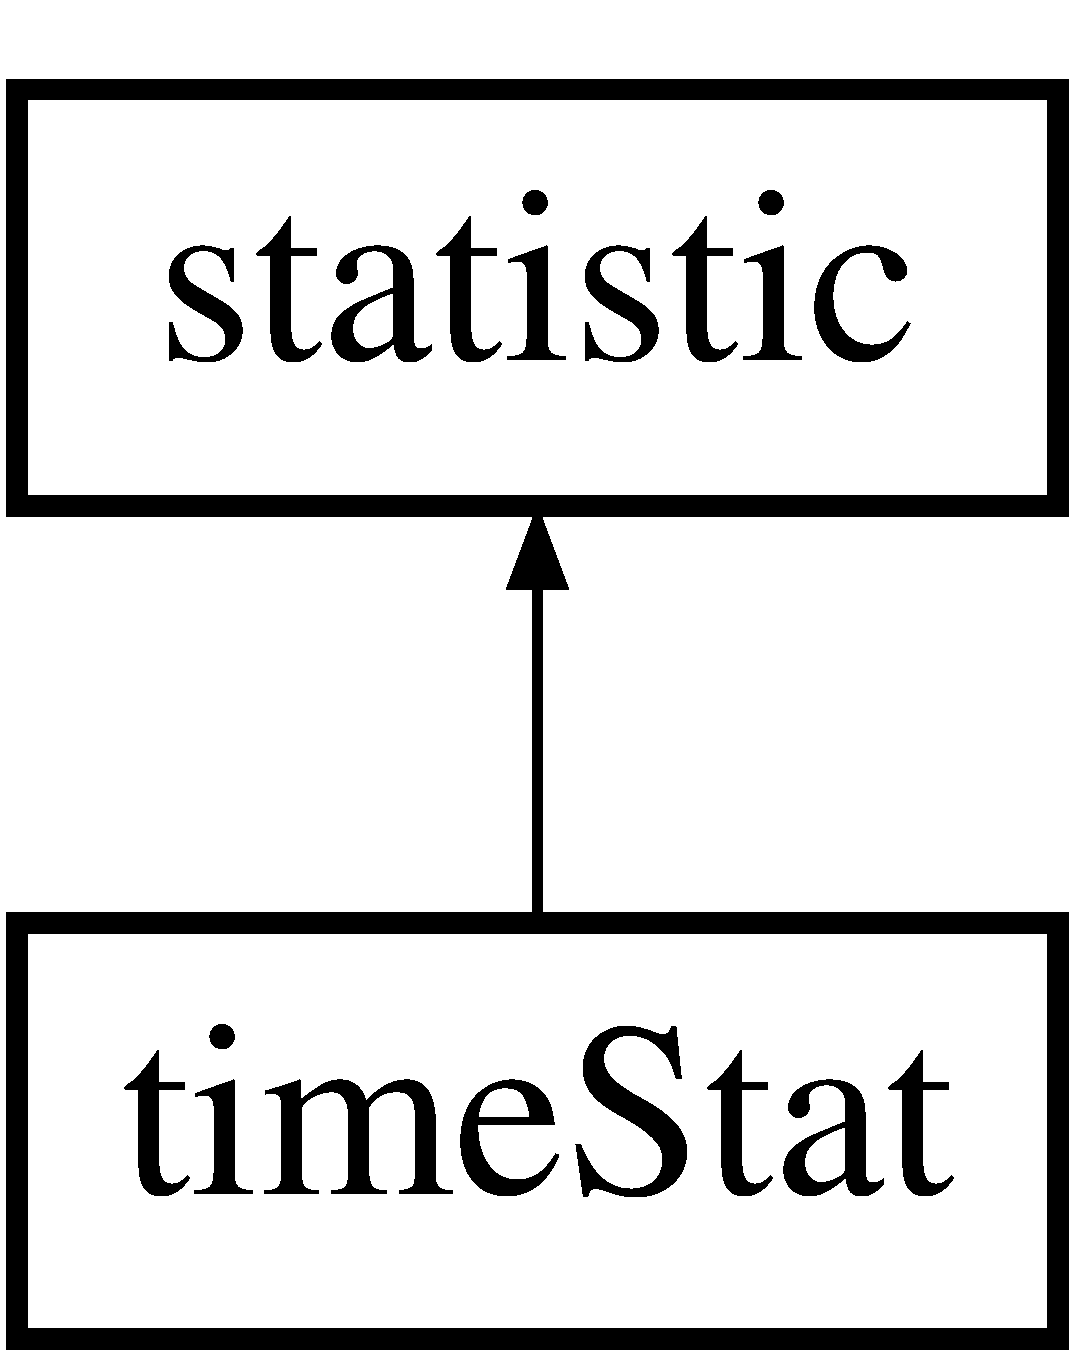
\includegraphics[height=2.000000cm]{classtimeStat}
\end{center}
\end{figure}
\subsection*{Public Member Functions}
\begin{DoxyCompactItemize}
\item 
\hyperlink{classtimeStat_ad35b7334bdf79aa157d0a6d959353a47}{time\-Stat} ()
\end{DoxyCompactItemize}
\subsection*{Static Public Member Functions}
\begin{DoxyCompactItemize}
\item 
static const char $\ast$ \hyperlink{classtimeStat_a4e32a7a1f0685df9f75f837eead8b7be}{name} (\hyperlink{kmp__stats_8h_ae03f1e0ff609f86afa9b7167a12c6c06}{timer\-\_\-e} e)
\item 
static bool \hyperlink{classtimeStat_a3c545325fae636418538c3ab7cff2f18}{no\-Total} (\hyperlink{kmp__stats_8h_ae03f1e0ff609f86afa9b7167a12c6c06}{timer\-\_\-e} e)
\item 
static bool \hyperlink{classtimeStat_a062cb0effb2bca43a2d85accaf5cbe08}{master\-Only} (\hyperlink{kmp__stats_8h_ae03f1e0ff609f86afa9b7167a12c6c06}{timer\-\_\-e} e)
\item 
static bool \hyperlink{classtimeStat_a5a871113709bc14925c6d60f637e03b6}{worker\-Only} (\hyperlink{kmp__stats_8h_ae03f1e0ff609f86afa9b7167a12c6c06}{timer\-\_\-e} e)
\item 
static bool \hyperlink{classtimeStat_a5af620a2fff9ca3b1b758d106633e5b6}{no\-Units} (\hyperlink{kmp__stats_8h_ae03f1e0ff609f86afa9b7167a12c6c06}{timer\-\_\-e} e)
\item 
static bool \hyperlink{classtimeStat_ab45f55ba382e1ac2018ed6ab3612d3b1}{log\-Event} (\hyperlink{kmp__stats_8h_ae03f1e0ff609f86afa9b7167a12c6c06}{timer\-\_\-e} e)
\item 
static \hyperlink{ittnotify__static_8h_af941d56e55e3c5465135b60c4d6343ed}{void} \hyperlink{classtimeStat_a1ee4b834f58f4f104d3c1e0a3f253e9a}{clear\-Event\-Flags} ()
\end{DoxyCompactItemize}
\subsection*{Static Private Attributes}
\begin{DoxyCompactItemize}
\item 
static \hyperlink{structstatInfo}{stat\-Info} \hyperlink{classtimeStat_ab2fce6fab263ba89a398acf2dbe5b0d3}{timer\-Info} \mbox{[}$\,$\mbox{]}
\end{DoxyCompactItemize}


\subsection{Detailed Description}


Definition at line 271 of file kmp\-\_\-stats.\-h.



\subsection{Constructor \& Destructor Documentation}
\hypertarget{classtimeStat_ad35b7334bdf79aa157d0a6d959353a47}{\index{time\-Stat@{time\-Stat}!time\-Stat@{time\-Stat}}
\index{time\-Stat@{time\-Stat}!timeStat@{time\-Stat}}
\subsubsection[{time\-Stat}]{\setlength{\rightskip}{0pt plus 5cm}time\-Stat\-::time\-Stat (
\begin{DoxyParamCaption}
{}
\end{DoxyParamCaption}
)\hspace{0.3cm}{\ttfamily [inline]}}}\label{classtimeStat_ad35b7334bdf79aa157d0a6d959353a47}


Definition at line 276 of file kmp\-\_\-stats.\-h.


\begin{DoxyCode}
276 : \hyperlink{classstatistic_a3f28cad0a4699e3f2db3892b5556f4e7}{statistic}() \{\}
\end{DoxyCode}


\subsection{Member Function Documentation}
\hypertarget{classtimeStat_a1ee4b834f58f4f104d3c1e0a3f253e9a}{\index{time\-Stat@{time\-Stat}!clear\-Event\-Flags@{clear\-Event\-Flags}}
\index{clear\-Event\-Flags@{clear\-Event\-Flags}!timeStat@{time\-Stat}}
\subsubsection[{clear\-Event\-Flags}]{\setlength{\rightskip}{0pt plus 5cm}static {\bf void} time\-Stat\-::clear\-Event\-Flags (
\begin{DoxyParamCaption}
{}
\end{DoxyParamCaption}
)\hspace{0.3cm}{\ttfamily [inline]}, {\ttfamily [static]}}}\label{classtimeStat_a1ee4b834f58f4f104d3c1e0a3f253e9a}


Definition at line 283 of file kmp\-\_\-stats.\-h.



Referenced by kmp\-\_\-stats\-\_\-output\-\_\-module\-::init().


\begin{DoxyCode}
283                                         \{
284         \textcolor{keywordflow}{for}(\textcolor{keywordtype}{int} \hyperlink{kmp__stub_8c_a08582ce460e3d5e1cf0b7fea017d608e}{i}=0;\hyperlink{kmp__stub_8c_a08582ce460e3d5e1cf0b7fea017d608e}{i}<TIMER\_LAST;\hyperlink{kmp__stub_8c_a08582ce460e3d5e1cf0b7fea017d608e}{i}++) \{
285             \hyperlink{classtimeStat_ab2fce6fab263ba89a398acf2dbe5b0d3}{timerInfo}[\hyperlink{kmp__stub_8c_a08582ce460e3d5e1cf0b7fea017d608e}{i}].\hyperlink{structstatInfo_a590c3b9a2b0786720e9a53b0dd6071fd}{flags} &= (~(\hyperlink{group__STATS__GATHERING_gga438c2840cc2d516238ea3eb0f4c116b3a53d50e56126850e531164b0bb1848c5e}{stats\_flags\_e::logEvent}));
286         \}
287     \}
\end{DoxyCode}
\hypertarget{classtimeStat_ab45f55ba382e1ac2018ed6ab3612d3b1}{\index{time\-Stat@{time\-Stat}!log\-Event@{log\-Event}}
\index{log\-Event@{log\-Event}!timeStat@{time\-Stat}}
\subsubsection[{log\-Event}]{\setlength{\rightskip}{0pt plus 5cm}static bool time\-Stat\-::log\-Event (
\begin{DoxyParamCaption}
\item[{{\bf timer\-\_\-e}}]{e}
\end{DoxyParamCaption}
)\hspace{0.3cm}{\ttfamily [inline]}, {\ttfamily [static]}}}\label{classtimeStat_ab45f55ba382e1ac2018ed6ab3612d3b1}


Definition at line 282 of file kmp\-\_\-stats.\-h.



Referenced by kmp\-\_\-stats\-\_\-output\-\_\-module\-::print\-Ploticus\-File(), kmp\-\_\-stats\-\_\-output\-\_\-module\-::setup\-Event\-Colors(), explicit\-Timer\-::start(), and explicit\-Timer\-::stop().


\begin{DoxyCode}
282 \{ \textcolor{keywordflow}{return} \hyperlink{classtimeStat_ab2fce6fab263ba89a398acf2dbe5b0d3}{timerInfo}[e].\hyperlink{structstatInfo_a590c3b9a2b0786720e9a53b0dd6071fd}{flags} & \hyperlink{group__STATS__GATHERING_gga438c2840cc2d516238ea3eb0f4c116b3a53d50e56126850e531164b0bb1848c5e}{stats\_flags\_e::logEvent};     \}
\end{DoxyCode}
\hypertarget{classtimeStat_a062cb0effb2bca43a2d85accaf5cbe08}{\index{time\-Stat@{time\-Stat}!master\-Only@{master\-Only}}
\index{master\-Only@{master\-Only}!timeStat@{time\-Stat}}
\subsubsection[{master\-Only}]{\setlength{\rightskip}{0pt plus 5cm}static bool time\-Stat\-::master\-Only (
\begin{DoxyParamCaption}
\item[{{\bf timer\-\_\-e}}]{e}
\end{DoxyParamCaption}
)\hspace{0.3cm}{\ttfamily [inline]}, {\ttfamily [static]}}}\label{classtimeStat_a062cb0effb2bca43a2d85accaf5cbe08}


Definition at line 279 of file kmp\-\_\-stats.\-h.



Referenced by kmp\-\_\-stats\-\_\-output\-\_\-module\-::output\-Stats().


\begin{DoxyCode}
279 \{ \textcolor{keywordflow}{return} \hyperlink{classtimeStat_ab2fce6fab263ba89a398acf2dbe5b0d3}{timerInfo}[e].\hyperlink{structstatInfo_a590c3b9a2b0786720e9a53b0dd6071fd}{flags} & \hyperlink{group__STATS__GATHERING_gga438c2840cc2d516238ea3eb0f4c116b3ab1b2cd818808a4ee2cc1720286fbc51d}{stats\_flags\_e::onlyInMaster}; \}
\end{DoxyCode}
\hypertarget{classtimeStat_a4e32a7a1f0685df9f75f837eead8b7be}{\index{time\-Stat@{time\-Stat}!name@{name}}
\index{name@{name}!timeStat@{time\-Stat}}
\subsubsection[{name}]{\setlength{\rightskip}{0pt plus 5cm}static const char$\ast$ time\-Stat\-::name (
\begin{DoxyParamCaption}
\item[{{\bf timer\-\_\-e}}]{e}
\end{DoxyParamCaption}
)\hspace{0.3cm}{\ttfamily [inline]}, {\ttfamily [static]}}}\label{classtimeStat_a4e32a7a1f0685df9f75f837eead8b7be}


Definition at line 277 of file kmp\-\_\-stats.\-h.



Referenced by kmp\-\_\-stats\-\_\-output\-\_\-module\-::print\-Events(), kmp\-\_\-stats\-\_\-output\-\_\-module\-::print\-Ploticus\-File(), and kmp\-\_\-stats\-\_\-output\-\_\-module\-::print\-Timer\-Stats().


\begin{DoxyCode}
277 \{ \textcolor{keywordflow}{return} \hyperlink{classtimeStat_ab2fce6fab263ba89a398acf2dbe5b0d3}{timerInfo}[e].\hyperlink{structstatInfo_a83052615f9578ba88744140093a18f37}{name}; \}
\end{DoxyCode}
\hypertarget{classtimeStat_a3c545325fae636418538c3ab7cff2f18}{\index{time\-Stat@{time\-Stat}!no\-Total@{no\-Total}}
\index{no\-Total@{no\-Total}!timeStat@{time\-Stat}}
\subsubsection[{no\-Total}]{\setlength{\rightskip}{0pt plus 5cm}static bool time\-Stat\-::no\-Total (
\begin{DoxyParamCaption}
\item[{{\bf timer\-\_\-e}}]{e}
\end{DoxyParamCaption}
)\hspace{0.3cm}{\ttfamily [inline]}, {\ttfamily [static]}}}\label{classtimeStat_a3c545325fae636418538c3ab7cff2f18}


Definition at line 278 of file kmp\-\_\-stats.\-h.



Referenced by kmp\-\_\-stats\-\_\-output\-\_\-module\-::output\-Stats(), and kmp\-\_\-stats\-\_\-output\-\_\-module\-::print\-Timer\-Stats().


\begin{DoxyCode}
278 \{ \textcolor{keywordflow}{return} \hyperlink{classtimeStat_ab2fce6fab263ba89a398acf2dbe5b0d3}{timerInfo}[e].\hyperlink{structstatInfo_a590c3b9a2b0786720e9a53b0dd6071fd}{flags} & \hyperlink{group__STATS__GATHERING_gga438c2840cc2d516238ea3eb0f4c116b3ab0da7f248271bb150e59d37370c799b7}{stats\_flags\_e::noTotal};      \}
\end{DoxyCode}
\hypertarget{classtimeStat_a5af620a2fff9ca3b1b758d106633e5b6}{\index{time\-Stat@{time\-Stat}!no\-Units@{no\-Units}}
\index{no\-Units@{no\-Units}!timeStat@{time\-Stat}}
\subsubsection[{no\-Units}]{\setlength{\rightskip}{0pt plus 5cm}static bool time\-Stat\-::no\-Units (
\begin{DoxyParamCaption}
\item[{{\bf timer\-\_\-e}}]{e}
\end{DoxyParamCaption}
)\hspace{0.3cm}{\ttfamily [inline]}, {\ttfamily [static]}}}\label{classtimeStat_a5af620a2fff9ca3b1b758d106633e5b6}


Definition at line 281 of file kmp\-\_\-stats.\-h.



Referenced by kmp\-\_\-stats\-\_\-output\-\_\-module\-::print\-Timer\-Stats().


\begin{DoxyCode}
281 \{ \textcolor{keywordflow}{return} \hyperlink{classtimeStat_ab2fce6fab263ba89a398acf2dbe5b0d3}{timerInfo}[e].\hyperlink{structstatInfo_a590c3b9a2b0786720e9a53b0dd6071fd}{flags} & \hyperlink{group__STATS__GATHERING_gga438c2840cc2d516238ea3eb0f4c116b3a1c30b5719af4df0bdc7206f20559c6dc}{stats\_flags\_e::noUnits};      \}
\end{DoxyCode}
\hypertarget{classtimeStat_a5a871113709bc14925c6d60f637e03b6}{\index{time\-Stat@{time\-Stat}!worker\-Only@{worker\-Only}}
\index{worker\-Only@{worker\-Only}!timeStat@{time\-Stat}}
\subsubsection[{worker\-Only}]{\setlength{\rightskip}{0pt plus 5cm}static bool time\-Stat\-::worker\-Only (
\begin{DoxyParamCaption}
\item[{{\bf timer\-\_\-e}}]{e}
\end{DoxyParamCaption}
)\hspace{0.3cm}{\ttfamily [inline]}, {\ttfamily [static]}}}\label{classtimeStat_a5a871113709bc14925c6d60f637e03b6}


Definition at line 280 of file kmp\-\_\-stats.\-h.



Referenced by kmp\-\_\-stats\-\_\-output\-\_\-module\-::output\-Stats().


\begin{DoxyCode}
280 \{ \textcolor{keywordflow}{return} \hyperlink{classtimeStat_ab2fce6fab263ba89a398acf2dbe5b0d3}{timerInfo}[e].\hyperlink{structstatInfo_a590c3b9a2b0786720e9a53b0dd6071fd}{flags} & \hyperlink{group__STATS__GATHERING_gga438c2840cc2d516238ea3eb0f4c116b3a0939773e208cb608fe78bc80a4197523}{stats\_flags\_e::notInMaster};  \}
\end{DoxyCode}


\subsection{Member Data Documentation}
\hypertarget{classtimeStat_ab2fce6fab263ba89a398acf2dbe5b0d3}{\index{time\-Stat@{time\-Stat}!timer\-Info@{timer\-Info}}
\index{timer\-Info@{timer\-Info}!timeStat@{time\-Stat}}
\subsubsection[{timer\-Info}]{\setlength{\rightskip}{0pt plus 5cm}{\bf stat\-Info} time\-Stat\-::timer\-Info\hspace{0.3cm}{\ttfamily [static]}, {\ttfamily [private]}}}\label{classtimeStat_ab2fce6fab263ba89a398acf2dbe5b0d3}
{\bfseries Initial value\-:}
\begin{DoxyCode}
= \{
    \hyperlink{kmp__stats_8h_accf71030e44454acab22210bb4a89d1b}{KMP\_FOREACH\_TIMER}(\hyperlink{kmp__stats_8cpp_a17949c412e2b08e907236b2d496ed7c1}{expandName},0)
    \{0,0\}
\}
\end{DoxyCode}


Definition at line 273 of file kmp\-\_\-stats.\-h.



Referenced by clear\-Event\-Flags(), log\-Event(), master\-Only(), name(), no\-Total(), no\-Units(), and worker\-Only().



The documentation for this class was generated from the following files\-:\begin{DoxyCompactItemize}
\item 
\hyperlink{kmp__stats_8h}{kmp\-\_\-stats.\-h}\item 
\hyperlink{kmp__stats_8cpp}{kmp\-\_\-stats.\-cpp}\end{DoxyCompactItemize}

\hypertarget{classtsc__tick__count_1_1tsc__interval__t}{\section{tsc\-\_\-tick\-\_\-count\-:\-:tsc\-\_\-interval\-\_\-t Class Reference}
\label{classtsc__tick__count_1_1tsc__interval__t}\index{tsc\-\_\-tick\-\_\-count\-::tsc\-\_\-interval\-\_\-t@{tsc\-\_\-tick\-\_\-count\-::tsc\-\_\-interval\-\_\-t}}
}


{\ttfamily \#include $<$kmp\-\_\-stats\-\_\-timing.\-h$>$}

\subsection*{Public Member Functions}
\begin{DoxyCompactItemize}
\item 
\hyperlink{classtsc__tick__count_1_1tsc__interval__t_a84eb1a898a4a2564e9fc2eb0c1c2a36e}{tsc\-\_\-interval\-\_\-t} ()
\item 
double \hyperlink{classtsc__tick__count_1_1tsc__interval__t_a8b8686cc1a0a03561d9ca47753e9654e}{ticks} () const 
\item 
int64\-\_\-t \hyperlink{classtsc__tick__count_1_1tsc__interval__t_a530a465e298a4978e9057e36bc6cf061}{get\-Value} () const 
\end{DoxyCompactItemize}
\subsection*{Private Member Functions}
\begin{DoxyCompactItemize}
\item 
\hyperlink{classtsc__tick__count_1_1tsc__interval__t_adb96003484baf498fbd8269ad0728930}{tsc\-\_\-interval\-\_\-t} (int64\-\_\-t \-\_\-value)
\end{DoxyCompactItemize}
\subsection*{Private Attributes}
\begin{DoxyCompactItemize}
\item 
int64\-\_\-t \hyperlink{classtsc__tick__count_1_1tsc__interval__t_a3e9e7f09cabe4ad49dd6f7baa166486d}{value}
\end{DoxyCompactItemize}
\subsection*{Friends}
\begin{DoxyCompactItemize}
\item 
class \hyperlink{classtsc__tick__count_1_1tsc__interval__t_a9c099c14d1f7ce1a2666f75ae3a0fa8c}{tsc\-\_\-tick\-\_\-count}
\item 
\hyperlink{classtsc__tick__count_1_1tsc__interval__t}{tsc\-\_\-interval\-\_\-t} \hyperlink{classtsc__tick__count_1_1tsc__interval__t_acfbc52e39f98c78200a540665fb37f61}{operator-\/} (const \hyperlink{classtsc__tick__count}{tsc\-\_\-tick\-\_\-count} t1, const \hyperlink{classtsc__tick__count}{tsc\-\_\-tick\-\_\-count} t0)
\end{DoxyCompactItemize}


\subsection{Detailed Description}


Definition at line 33 of file kmp\-\_\-stats\-\_\-timing.\-h.



\subsection{Constructor \& Destructor Documentation}
\hypertarget{classtsc__tick__count_1_1tsc__interval__t_adb96003484baf498fbd8269ad0728930}{\index{tsc\-\_\-tick\-\_\-count\-::tsc\-\_\-interval\-\_\-t@{tsc\-\_\-tick\-\_\-count\-::tsc\-\_\-interval\-\_\-t}!tsc\-\_\-interval\-\_\-t@{tsc\-\_\-interval\-\_\-t}}
\index{tsc\-\_\-interval\-\_\-t@{tsc\-\_\-interval\-\_\-t}!tsc_tick_count::tsc_interval_t@{tsc\-\_\-tick\-\_\-count\-::tsc\-\_\-interval\-\_\-t}}
\subsubsection[{tsc\-\_\-interval\-\_\-t}]{\setlength{\rightskip}{0pt plus 5cm}tsc\-\_\-tick\-\_\-count\-::tsc\-\_\-interval\-\_\-t\-::tsc\-\_\-interval\-\_\-t (
\begin{DoxyParamCaption}
\item[{int64\-\_\-t}]{\-\_\-value}
\end{DoxyParamCaption}
)\hspace{0.3cm}{\ttfamily [inline]}, {\ttfamily [explicit]}, {\ttfamily [private]}}}\label{classtsc__tick__count_1_1tsc__interval__t_adb96003484baf498fbd8269ad0728930}


Definition at line 35 of file kmp\-\_\-stats\-\_\-timing.\-h.


\begin{DoxyCode}
35 : \hyperlink{classtsc__tick__count_1_1tsc__interval__t_a3e9e7f09cabe4ad49dd6f7baa166486d}{value}(\_value) \{\}
\end{DoxyCode}
\hypertarget{classtsc__tick__count_1_1tsc__interval__t_a84eb1a898a4a2564e9fc2eb0c1c2a36e}{\index{tsc\-\_\-tick\-\_\-count\-::tsc\-\_\-interval\-\_\-t@{tsc\-\_\-tick\-\_\-count\-::tsc\-\_\-interval\-\_\-t}!tsc\-\_\-interval\-\_\-t@{tsc\-\_\-interval\-\_\-t}}
\index{tsc\-\_\-interval\-\_\-t@{tsc\-\_\-interval\-\_\-t}!tsc_tick_count::tsc_interval_t@{tsc\-\_\-tick\-\_\-count\-::tsc\-\_\-interval\-\_\-t}}
\subsubsection[{tsc\-\_\-interval\-\_\-t}]{\setlength{\rightskip}{0pt plus 5cm}tsc\-\_\-tick\-\_\-count\-::tsc\-\_\-interval\-\_\-t\-::tsc\-\_\-interval\-\_\-t (
\begin{DoxyParamCaption}
{}
\end{DoxyParamCaption}
)\hspace{0.3cm}{\ttfamily [inline]}}}\label{classtsc__tick__count_1_1tsc__interval__t_a84eb1a898a4a2564e9fc2eb0c1c2a36e}


Definition at line 37 of file kmp\-\_\-stats\-\_\-timing.\-h.


\begin{DoxyCode}
37 : \hyperlink{classtsc__tick__count_1_1tsc__interval__t_a3e9e7f09cabe4ad49dd6f7baa166486d}{value}(0) \{\}; \textcolor{comment}{// Construct 0 time duration}
\end{DoxyCode}


\subsection{Member Function Documentation}
\hypertarget{classtsc__tick__count_1_1tsc__interval__t_a530a465e298a4978e9057e36bc6cf061}{\index{tsc\-\_\-tick\-\_\-count\-::tsc\-\_\-interval\-\_\-t@{tsc\-\_\-tick\-\_\-count\-::tsc\-\_\-interval\-\_\-t}!get\-Value@{get\-Value}}
\index{get\-Value@{get\-Value}!tsc_tick_count::tsc_interval_t@{tsc\-\_\-tick\-\_\-count\-::tsc\-\_\-interval\-\_\-t}}
\subsubsection[{get\-Value}]{\setlength{\rightskip}{0pt plus 5cm}int64\-\_\-t tsc\-\_\-tick\-\_\-count\-::tsc\-\_\-interval\-\_\-t\-::get\-Value (
\begin{DoxyParamCaption}
{}
\end{DoxyParamCaption}
) const\hspace{0.3cm}{\ttfamily [inline]}}}\label{classtsc__tick__count_1_1tsc__interval__t_a530a465e298a4978e9057e36bc6cf061}


Definition at line 42 of file kmp\-\_\-stats\-\_\-timing.\-h.


\begin{DoxyCode}
42 \{ \textcolor{keywordflow}{return} \hyperlink{classtsc__tick__count_1_1tsc__interval__t_a3e9e7f09cabe4ad49dd6f7baa166486d}{value}; \}
\end{DoxyCode}
\hypertarget{classtsc__tick__count_1_1tsc__interval__t_a8b8686cc1a0a03561d9ca47753e9654e}{\index{tsc\-\_\-tick\-\_\-count\-::tsc\-\_\-interval\-\_\-t@{tsc\-\_\-tick\-\_\-count\-::tsc\-\_\-interval\-\_\-t}!ticks@{ticks}}
\index{ticks@{ticks}!tsc_tick_count::tsc_interval_t@{tsc\-\_\-tick\-\_\-count\-::tsc\-\_\-interval\-\_\-t}}
\subsubsection[{ticks}]{\setlength{\rightskip}{0pt plus 5cm}double tsc\-\_\-tick\-\_\-count\-::tsc\-\_\-interval\-\_\-t\-::ticks (
\begin{DoxyParamCaption}
{}
\end{DoxyParamCaption}
) const\hspace{0.3cm}{\ttfamily [inline]}}}\label{classtsc__tick__count_1_1tsc__interval__t_a8b8686cc1a0a03561d9ca47753e9654e}


Definition at line 41 of file kmp\-\_\-stats\-\_\-timing.\-h.


\begin{DoxyCode}
41 \{ \textcolor{keywordflow}{return} double(\hyperlink{classtsc__tick__count_1_1tsc__interval__t_a3e9e7f09cabe4ad49dd6f7baa166486d}{value}); \}
\end{DoxyCode}


\subsection{Friends And Related Function Documentation}
\hypertarget{classtsc__tick__count_1_1tsc__interval__t_acfbc52e39f98c78200a540665fb37f61}{\index{tsc\-\_\-tick\-\_\-count\-::tsc\-\_\-interval\-\_\-t@{tsc\-\_\-tick\-\_\-count\-::tsc\-\_\-interval\-\_\-t}!operator-\/@{operator-\/}}
\index{operator-\/@{operator-\/}!tsc_tick_count::tsc_interval_t@{tsc\-\_\-tick\-\_\-count\-::tsc\-\_\-interval\-\_\-t}}
\subsubsection[{operator-\/}]{\setlength{\rightskip}{0pt plus 5cm}{\bf tsc\-\_\-interval\-\_\-t} operator-\/ (
\begin{DoxyParamCaption}
\item[{const {\bf tsc\-\_\-tick\-\_\-count}}]{t1, }
\item[{const {\bf tsc\-\_\-tick\-\_\-count}}]{t0}
\end{DoxyParamCaption}
)\hspace{0.3cm}{\ttfamily [friend]}}}\label{classtsc__tick__count_1_1tsc__interval__t_acfbc52e39f98c78200a540665fb37f61}


Definition at line 72 of file kmp\-\_\-stats\-\_\-timing.\-h.


\begin{DoxyCode}
73 \{
74     \textcolor{keywordflow}{return} \hyperlink{classtsc__tick__count_1_1tsc__interval__t}{tsc\_tick\_count::tsc\_interval\_t}( t1.
      \hyperlink{classtsc__tick__count_ad3811672b7ec785fc23a9e33a33c9c84}{my\_count}-t0.\hyperlink{classtsc__tick__count_ad3811672b7ec785fc23a9e33a33c9c84}{my\_count} );
75 \}
\end{DoxyCode}
\hypertarget{classtsc__tick__count_1_1tsc__interval__t_a9c099c14d1f7ce1a2666f75ae3a0fa8c}{\index{tsc\-\_\-tick\-\_\-count\-::tsc\-\_\-interval\-\_\-t@{tsc\-\_\-tick\-\_\-count\-::tsc\-\_\-interval\-\_\-t}!tsc\-\_\-tick\-\_\-count@{tsc\-\_\-tick\-\_\-count}}
\index{tsc\-\_\-tick\-\_\-count@{tsc\-\_\-tick\-\_\-count}!tsc_tick_count::tsc_interval_t@{tsc\-\_\-tick\-\_\-count\-::tsc\-\_\-interval\-\_\-t}}
\subsubsection[{tsc\-\_\-tick\-\_\-count}]{\setlength{\rightskip}{0pt plus 5cm}friend class {\bf tsc\-\_\-tick\-\_\-count}\hspace{0.3cm}{\ttfamily [friend]}}}\label{classtsc__tick__count_1_1tsc__interval__t_a9c099c14d1f7ce1a2666f75ae3a0fa8c}


Definition at line 44 of file kmp\-\_\-stats\-\_\-timing.\-h.



\subsection{Member Data Documentation}
\hypertarget{classtsc__tick__count_1_1tsc__interval__t_a3e9e7f09cabe4ad49dd6f7baa166486d}{\index{tsc\-\_\-tick\-\_\-count\-::tsc\-\_\-interval\-\_\-t@{tsc\-\_\-tick\-\_\-count\-::tsc\-\_\-interval\-\_\-t}!value@{value}}
\index{value@{value}!tsc_tick_count::tsc_interval_t@{tsc\-\_\-tick\-\_\-count\-::tsc\-\_\-interval\-\_\-t}}
\subsubsection[{value}]{\setlength{\rightskip}{0pt plus 5cm}int64\-\_\-t tsc\-\_\-tick\-\_\-count\-::tsc\-\_\-interval\-\_\-t\-::value\hspace{0.3cm}{\ttfamily [private]}}}\label{classtsc__tick__count_1_1tsc__interval__t_a3e9e7f09cabe4ad49dd6f7baa166486d}


Definition at line 34 of file kmp\-\_\-stats\-\_\-timing.\-h.



Referenced by get\-Value(), and ticks().



The documentation for this class was generated from the following file\-:\begin{DoxyCompactItemize}
\item 
\hyperlink{kmp__stats__timing_8h}{kmp\-\_\-stats\-\_\-timing.\-h}\end{DoxyCompactItemize}

\hypertarget{classtsc__tick__count}{\section{tsc\-\_\-tick\-\_\-count Class Reference}
\label{classtsc__tick__count}\index{tsc\-\_\-tick\-\_\-count@{tsc\-\_\-tick\-\_\-count}}
}


{\ttfamily \#include $<$kmp\-\_\-stats\-\_\-timing.\-h$>$}

\subsection*{Classes}
\begin{DoxyCompactItemize}
\item 
class \hyperlink{classtsc__tick__count_1_1tsc__interval__t}{tsc\-\_\-interval\-\_\-t}
\end{DoxyCompactItemize}
\subsection*{Public Member Functions}
\begin{DoxyCompactItemize}
\item 
\hyperlink{classtsc__tick__count_aa43ce8ef46395ff35298a53fb78ff4b5}{tsc\-\_\-tick\-\_\-count} (int64\-\_\-t value)
\item 
int64\-\_\-t \hyperlink{classtsc__tick__count_a88c80c6a9d8b3b0d76b45cef2d3bc36b}{get\-Value} () const 
\item 
\hyperlink{classtsc__tick__count}{tsc\-\_\-tick\-\_\-count} \hyperlink{classtsc__tick__count_a1ed40b9912bb3ba1e671f0cf5d68678e}{later} (\hyperlink{classtsc__tick__count}{tsc\-\_\-tick\-\_\-count} const other) const 
\item 
\hyperlink{classtsc__tick__count}{tsc\-\_\-tick\-\_\-count} \hyperlink{classtsc__tick__count_ac9c170398eedc2b192eb121186a16cb4}{earlier} (\hyperlink{classtsc__tick__count}{tsc\-\_\-tick\-\_\-count} const other) const 
\end{DoxyCompactItemize}
\subsection*{Static Public Member Functions}
\begin{DoxyCompactItemize}
\item 
static \hyperlink{classtsc__tick__count}{tsc\-\_\-tick\-\_\-count} \hyperlink{classtsc__tick__count_a0caca1efab64714976683134bcdd99b4}{now} ()
\end{DoxyCompactItemize}
\subsection*{Private Attributes}
\begin{DoxyCompactItemize}
\item 
int64\-\_\-t \hyperlink{classtsc__tick__count_ad3811672b7ec785fc23a9e33a33c9c84}{my\-\_\-count}
\end{DoxyCompactItemize}
\subsection*{Friends}
\begin{DoxyCompactItemize}
\item 
\hyperlink{classtsc__tick__count_1_1tsc__interval__t}{tsc\-\_\-tick\-\_\-count\-::tsc\-\_\-interval\-\_\-t} \hyperlink{classtsc__tick__count_ae40e121006d71e9031defe4198b49508}{operator-\/} (const \hyperlink{classtsc__tick__count}{tsc\-\_\-tick\-\_\-count} t1, const \hyperlink{classtsc__tick__count}{tsc\-\_\-tick\-\_\-count} t0)
\end{DoxyCompactItemize}


\subsection{Detailed Description}


Definition at line 28 of file kmp\-\_\-stats\-\_\-timing.\-h.



\subsection{Constructor \& Destructor Documentation}
\hypertarget{classtsc__tick__count_aa43ce8ef46395ff35298a53fb78ff4b5}{\index{tsc\-\_\-tick\-\_\-count@{tsc\-\_\-tick\-\_\-count}!tsc\-\_\-tick\-\_\-count@{tsc\-\_\-tick\-\_\-count}}
\index{tsc\-\_\-tick\-\_\-count@{tsc\-\_\-tick\-\_\-count}!tsc_tick_count@{tsc\-\_\-tick\-\_\-count}}
\subsubsection[{tsc\-\_\-tick\-\_\-count}]{\setlength{\rightskip}{0pt plus 5cm}tsc\-\_\-tick\-\_\-count\-::tsc\-\_\-tick\-\_\-count (
\begin{DoxyParamCaption}
\item[{int64\-\_\-t}]{value}
\end{DoxyParamCaption}
)\hspace{0.3cm}{\ttfamily [inline]}}}\label{classtsc__tick__count_aa43ce8ef46395ff35298a53fb78ff4b5}


Definition at line 57 of file kmp\-\_\-stats\-\_\-timing.\-h.



Referenced by now().


\begin{DoxyCode}
57 : \hyperlink{classtsc__tick__count_ad3811672b7ec785fc23a9e33a33c9c84}{my\_count}(value) \{\};
\end{DoxyCode}


\subsection{Member Function Documentation}
\hypertarget{classtsc__tick__count_ac9c170398eedc2b192eb121186a16cb4}{\index{tsc\-\_\-tick\-\_\-count@{tsc\-\_\-tick\-\_\-count}!earlier@{earlier}}
\index{earlier@{earlier}!tsc_tick_count@{tsc\-\_\-tick\-\_\-count}}
\subsubsection[{earlier}]{\setlength{\rightskip}{0pt plus 5cm}{\bf tsc\-\_\-tick\-\_\-count} tsc\-\_\-tick\-\_\-count\-::earlier (
\begin{DoxyParamCaption}
\item[{{\bf tsc\-\_\-tick\-\_\-count} const}]{other}
\end{DoxyParamCaption}
) const\hspace{0.3cm}{\ttfamily [inline]}}}\label{classtsc__tick__count_ac9c170398eedc2b192eb121186a16cb4}


Definition at line 62 of file kmp\-\_\-stats\-\_\-timing.\-h.


\begin{DoxyCode}
62                                                              \{ 
63         \textcolor{keywordflow}{return} \hyperlink{classtsc__tick__count_ad3811672b7ec785fc23a9e33a33c9c84}{my\_count} < other.my\_count ? (*this) : other; 
64     \}
\end{DoxyCode}
\hypertarget{classtsc__tick__count_a88c80c6a9d8b3b0d76b45cef2d3bc36b}{\index{tsc\-\_\-tick\-\_\-count@{tsc\-\_\-tick\-\_\-count}!get\-Value@{get\-Value}}
\index{get\-Value@{get\-Value}!tsc_tick_count@{tsc\-\_\-tick\-\_\-count}}
\subsubsection[{get\-Value}]{\setlength{\rightskip}{0pt plus 5cm}int64\-\_\-t tsc\-\_\-tick\-\_\-count\-::get\-Value (
\begin{DoxyParamCaption}
{}
\end{DoxyParamCaption}
) const\hspace{0.3cm}{\ttfamily [inline]}}}\label{classtsc__tick__count_a88c80c6a9d8b3b0d76b45cef2d3bc36b}


Definition at line 58 of file kmp\-\_\-stats\-\_\-timing.\-h.



Referenced by explicit\-Timer\-::stop().


\begin{DoxyCode}
58 \{ \textcolor{keywordflow}{return} \hyperlink{classtsc__tick__count_ad3811672b7ec785fc23a9e33a33c9c84}{my\_count}; \}
\end{DoxyCode}
\hypertarget{classtsc__tick__count_a1ed40b9912bb3ba1e671f0cf5d68678e}{\index{tsc\-\_\-tick\-\_\-count@{tsc\-\_\-tick\-\_\-count}!later@{later}}
\index{later@{later}!tsc_tick_count@{tsc\-\_\-tick\-\_\-count}}
\subsubsection[{later}]{\setlength{\rightskip}{0pt plus 5cm}{\bf tsc\-\_\-tick\-\_\-count} tsc\-\_\-tick\-\_\-count\-::later (
\begin{DoxyParamCaption}
\item[{{\bf tsc\-\_\-tick\-\_\-count} const}]{other}
\end{DoxyParamCaption}
) const\hspace{0.3cm}{\ttfamily [inline]}}}\label{classtsc__tick__count_a1ed40b9912bb3ba1e671f0cf5d68678e}


Definition at line 59 of file kmp\-\_\-stats\-\_\-timing.\-h.



Referenced by compute\-Last\-In\-Last\-Out\-Interval().


\begin{DoxyCode}
59                                                             \{ 
60         \textcolor{keywordflow}{return} \hyperlink{classtsc__tick__count_ad3811672b7ec785fc23a9e33a33c9c84}{my\_count} > other.my\_count ? (*this) : other; 
61     \}
\end{DoxyCode}
\hypertarget{classtsc__tick__count_a0caca1efab64714976683134bcdd99b4}{\index{tsc\-\_\-tick\-\_\-count@{tsc\-\_\-tick\-\_\-count}!now@{now}}
\index{now@{now}!tsc_tick_count@{tsc\-\_\-tick\-\_\-count}}
\subsubsection[{now}]{\setlength{\rightskip}{0pt plus 5cm}static {\bf tsc\-\_\-tick\-\_\-count} tsc\-\_\-tick\-\_\-count\-::now (
\begin{DoxyParamCaption}
{}
\end{DoxyParamCaption}
)\hspace{0.3cm}{\ttfamily [inline]}, {\ttfamily [static]}}}\label{classtsc__tick__count_a0caca1efab64714976683134bcdd99b4}


Definition at line 68 of file kmp\-\_\-stats\-\_\-timing.\-h.



Referenced by \-\_\-\-\_\-kmp\-\_\-create\-\_\-worker(), time\-Pair\-::mark\-End(), time\-Pair\-::mark\-Start(), explicit\-Timer\-::start(), and explicit\-Timer\-::stop().


\begin{DoxyCode}
68 \{ \textcolor{keywordflow}{return} \hyperlink{classtsc__tick__count_aa43ce8ef46395ff35298a53fb78ff4b5}{tsc\_tick\_count}(); \} \textcolor{comment}{// returns the rdtsc register value}
\end{DoxyCode}


\subsection{Friends And Related Function Documentation}
\hypertarget{classtsc__tick__count_ae40e121006d71e9031defe4198b49508}{\index{tsc\-\_\-tick\-\_\-count@{tsc\-\_\-tick\-\_\-count}!operator-\/@{operator-\/}}
\index{operator-\/@{operator-\/}!tsc_tick_count@{tsc\-\_\-tick\-\_\-count}}
\subsubsection[{operator-\/}]{\setlength{\rightskip}{0pt plus 5cm}{\bf tsc\-\_\-tick\-\_\-count\-::tsc\-\_\-interval\-\_\-t} operator-\/ (
\begin{DoxyParamCaption}
\item[{const {\bf tsc\-\_\-tick\-\_\-count}}]{t1, }
\item[{const {\bf tsc\-\_\-tick\-\_\-count}}]{t0}
\end{DoxyParamCaption}
)\hspace{0.3cm}{\ttfamily [friend]}}}\label{classtsc__tick__count_ae40e121006d71e9031defe4198b49508}


Definition at line 72 of file kmp\-\_\-stats\-\_\-timing.\-h.


\begin{DoxyCode}
73 \{
74     \textcolor{keywordflow}{return} \hyperlink{classtsc__tick__count_1_1tsc__interval__t}{tsc\_tick\_count::tsc\_interval\_t}( t1.
      \hyperlink{classtsc__tick__count_ad3811672b7ec785fc23a9e33a33c9c84}{my\_count}-t0.\hyperlink{classtsc__tick__count_ad3811672b7ec785fc23a9e33a33c9c84}{my\_count} );
75 \}
\end{DoxyCode}


\subsection{Member Data Documentation}
\hypertarget{classtsc__tick__count_ad3811672b7ec785fc23a9e33a33c9c84}{\index{tsc\-\_\-tick\-\_\-count@{tsc\-\_\-tick\-\_\-count}!my\-\_\-count@{my\-\_\-count}}
\index{my\-\_\-count@{my\-\_\-count}!tsc_tick_count@{tsc\-\_\-tick\-\_\-count}}
\subsubsection[{my\-\_\-count}]{\setlength{\rightskip}{0pt plus 5cm}int64\-\_\-t tsc\-\_\-tick\-\_\-count\-::my\-\_\-count\hspace{0.3cm}{\ttfamily [private]}}}\label{classtsc__tick__count_ad3811672b7ec785fc23a9e33a33c9c84}


Definition at line 30 of file kmp\-\_\-stats\-\_\-timing.\-h.



Referenced by earlier(), get\-Value(), later(), and operator-\/().



The documentation for this class was generated from the following file\-:\begin{DoxyCompactItemize}
\item 
\hyperlink{kmp__stats__timing_8h}{kmp\-\_\-stats\-\_\-timing.\-h}\end{DoxyCompactItemize}

\hypertarget{structVM__COUNTERS}{\section{V\-M\-\_\-\-C\-O\-U\-N\-T\-E\-R\-S Struct Reference}
\label{structVM__COUNTERS}\index{V\-M\-\_\-\-C\-O\-U\-N\-T\-E\-R\-S@{V\-M\-\_\-\-C\-O\-U\-N\-T\-E\-R\-S}}
}
\subsection*{Public Attributes}
\begin{DoxyCompactItemize}
\item 
S\-I\-Z\-E\-\_\-\-T \hyperlink{structVM__COUNTERS_ab4c550548ddf9b6357ea0f57ce1cf946}{Peak\-Virtual\-Size}
\item 
S\-I\-Z\-E\-\_\-\-T \hyperlink{structVM__COUNTERS_ab394da4c4d9b606a2ad4c00892a6917f}{Virtual\-Size}
\item 
U\-L\-O\-N\-G \hyperlink{structVM__COUNTERS_a2cc46c0341e51f5fd53025bdf0e5658c}{Page\-Fault\-Count}
\item 
S\-I\-Z\-E\-\_\-\-T \hyperlink{structVM__COUNTERS_a15bea203127750ef7fe4fbcd682a7126}{Peak\-Working\-Set\-Size}
\item 
S\-I\-Z\-E\-\_\-\-T \hyperlink{structVM__COUNTERS_a8fff1cd61413ea383c0a9471ff59d033}{Working\-Set\-Size}
\item 
S\-I\-Z\-E\-\_\-\-T \hyperlink{structVM__COUNTERS_a2bfa57675a50a5d3207f0f2b178ac16b}{Quota\-Peak\-Paged\-Pool\-Usage}
\item 
S\-I\-Z\-E\-\_\-\-T \hyperlink{structVM__COUNTERS_ace274383d4b485e37b95809456e16ee3}{Quota\-Paged\-Pool\-Usage}
\item 
S\-I\-Z\-E\-\_\-\-T \hyperlink{structVM__COUNTERS_a9eb845d5989f40f4e277c622fe7bdbb5}{Quota\-Peak\-Non\-Paged\-Pool\-Usage}
\item 
S\-I\-Z\-E\-\_\-\-T \hyperlink{structVM__COUNTERS_a27d5ebeb3ecbcb71a00eb44742417a80}{Quota\-Non\-Paged\-Pool\-Usage}
\item 
S\-I\-Z\-E\-\_\-\-T \hyperlink{structVM__COUNTERS_a1ae3e46e1816321cadd686716c301e8a}{Pagefile\-Usage}
\item 
S\-I\-Z\-E\-\_\-\-T \hyperlink{structVM__COUNTERS_ab30aac195648217a62055b4267aad106}{Peak\-Pagefile\-Usage}
\item 
S\-I\-Z\-E\-\_\-\-T \hyperlink{structVM__COUNTERS_aacbc9ccd46f05cb18cc67ee292ed1a82}{Private\-Page\-Count}
\end{DoxyCompactItemize}


\subsection{Detailed Description}


Definition at line 49 of file z\-\_\-\-Windows\-\_\-\-N\-T\-\_\-util.\-c.



\subsection{Member Data Documentation}
\hypertarget{structVM__COUNTERS_a2cc46c0341e51f5fd53025bdf0e5658c}{\index{V\-M\-\_\-\-C\-O\-U\-N\-T\-E\-R\-S@{V\-M\-\_\-\-C\-O\-U\-N\-T\-E\-R\-S}!Page\-Fault\-Count@{Page\-Fault\-Count}}
\index{Page\-Fault\-Count@{Page\-Fault\-Count}!VM_COUNTERS@{V\-M\-\_\-\-C\-O\-U\-N\-T\-E\-R\-S}}
\subsubsection[{Page\-Fault\-Count}]{\setlength{\rightskip}{0pt plus 5cm}U\-L\-O\-N\-G V\-M\-\_\-\-C\-O\-U\-N\-T\-E\-R\-S\-::\-Page\-Fault\-Count}}\label{structVM__COUNTERS_a2cc46c0341e51f5fd53025bdf0e5658c}


Definition at line 52 of file z\-\_\-\-Windows\-\_\-\-N\-T\-\_\-util.\-c.

\hypertarget{structVM__COUNTERS_a1ae3e46e1816321cadd686716c301e8a}{\index{V\-M\-\_\-\-C\-O\-U\-N\-T\-E\-R\-S@{V\-M\-\_\-\-C\-O\-U\-N\-T\-E\-R\-S}!Pagefile\-Usage@{Pagefile\-Usage}}
\index{Pagefile\-Usage@{Pagefile\-Usage}!VM_COUNTERS@{V\-M\-\_\-\-C\-O\-U\-N\-T\-E\-R\-S}}
\subsubsection[{Pagefile\-Usage}]{\setlength{\rightskip}{0pt plus 5cm}S\-I\-Z\-E\-\_\-\-T V\-M\-\_\-\-C\-O\-U\-N\-T\-E\-R\-S\-::\-Pagefile\-Usage}}\label{structVM__COUNTERS_a1ae3e46e1816321cadd686716c301e8a}


Definition at line 59 of file z\-\_\-\-Windows\-\_\-\-N\-T\-\_\-util.\-c.

\hypertarget{structVM__COUNTERS_ab30aac195648217a62055b4267aad106}{\index{V\-M\-\_\-\-C\-O\-U\-N\-T\-E\-R\-S@{V\-M\-\_\-\-C\-O\-U\-N\-T\-E\-R\-S}!Peak\-Pagefile\-Usage@{Peak\-Pagefile\-Usage}}
\index{Peak\-Pagefile\-Usage@{Peak\-Pagefile\-Usage}!VM_COUNTERS@{V\-M\-\_\-\-C\-O\-U\-N\-T\-E\-R\-S}}
\subsubsection[{Peak\-Pagefile\-Usage}]{\setlength{\rightskip}{0pt plus 5cm}S\-I\-Z\-E\-\_\-\-T V\-M\-\_\-\-C\-O\-U\-N\-T\-E\-R\-S\-::\-Peak\-Pagefile\-Usage}}\label{structVM__COUNTERS_ab30aac195648217a62055b4267aad106}


Definition at line 60 of file z\-\_\-\-Windows\-\_\-\-N\-T\-\_\-util.\-c.

\hypertarget{structVM__COUNTERS_ab4c550548ddf9b6357ea0f57ce1cf946}{\index{V\-M\-\_\-\-C\-O\-U\-N\-T\-E\-R\-S@{V\-M\-\_\-\-C\-O\-U\-N\-T\-E\-R\-S}!Peak\-Virtual\-Size@{Peak\-Virtual\-Size}}
\index{Peak\-Virtual\-Size@{Peak\-Virtual\-Size}!VM_COUNTERS@{V\-M\-\_\-\-C\-O\-U\-N\-T\-E\-R\-S}}
\subsubsection[{Peak\-Virtual\-Size}]{\setlength{\rightskip}{0pt plus 5cm}S\-I\-Z\-E\-\_\-\-T V\-M\-\_\-\-C\-O\-U\-N\-T\-E\-R\-S\-::\-Peak\-Virtual\-Size}}\label{structVM__COUNTERS_ab4c550548ddf9b6357ea0f57ce1cf946}


Definition at line 50 of file z\-\_\-\-Windows\-\_\-\-N\-T\-\_\-util.\-c.

\hypertarget{structVM__COUNTERS_a15bea203127750ef7fe4fbcd682a7126}{\index{V\-M\-\_\-\-C\-O\-U\-N\-T\-E\-R\-S@{V\-M\-\_\-\-C\-O\-U\-N\-T\-E\-R\-S}!Peak\-Working\-Set\-Size@{Peak\-Working\-Set\-Size}}
\index{Peak\-Working\-Set\-Size@{Peak\-Working\-Set\-Size}!VM_COUNTERS@{V\-M\-\_\-\-C\-O\-U\-N\-T\-E\-R\-S}}
\subsubsection[{Peak\-Working\-Set\-Size}]{\setlength{\rightskip}{0pt plus 5cm}S\-I\-Z\-E\-\_\-\-T V\-M\-\_\-\-C\-O\-U\-N\-T\-E\-R\-S\-::\-Peak\-Working\-Set\-Size}}\label{structVM__COUNTERS_a15bea203127750ef7fe4fbcd682a7126}


Definition at line 53 of file z\-\_\-\-Windows\-\_\-\-N\-T\-\_\-util.\-c.

\hypertarget{structVM__COUNTERS_aacbc9ccd46f05cb18cc67ee292ed1a82}{\index{V\-M\-\_\-\-C\-O\-U\-N\-T\-E\-R\-S@{V\-M\-\_\-\-C\-O\-U\-N\-T\-E\-R\-S}!Private\-Page\-Count@{Private\-Page\-Count}}
\index{Private\-Page\-Count@{Private\-Page\-Count}!VM_COUNTERS@{V\-M\-\_\-\-C\-O\-U\-N\-T\-E\-R\-S}}
\subsubsection[{Private\-Page\-Count}]{\setlength{\rightskip}{0pt plus 5cm}S\-I\-Z\-E\-\_\-\-T V\-M\-\_\-\-C\-O\-U\-N\-T\-E\-R\-S\-::\-Private\-Page\-Count}}\label{structVM__COUNTERS_aacbc9ccd46f05cb18cc67ee292ed1a82}


Definition at line 61 of file z\-\_\-\-Windows\-\_\-\-N\-T\-\_\-util.\-c.

\hypertarget{structVM__COUNTERS_a27d5ebeb3ecbcb71a00eb44742417a80}{\index{V\-M\-\_\-\-C\-O\-U\-N\-T\-E\-R\-S@{V\-M\-\_\-\-C\-O\-U\-N\-T\-E\-R\-S}!Quota\-Non\-Paged\-Pool\-Usage@{Quota\-Non\-Paged\-Pool\-Usage}}
\index{Quota\-Non\-Paged\-Pool\-Usage@{Quota\-Non\-Paged\-Pool\-Usage}!VM_COUNTERS@{V\-M\-\_\-\-C\-O\-U\-N\-T\-E\-R\-S}}
\subsubsection[{Quota\-Non\-Paged\-Pool\-Usage}]{\setlength{\rightskip}{0pt plus 5cm}S\-I\-Z\-E\-\_\-\-T V\-M\-\_\-\-C\-O\-U\-N\-T\-E\-R\-S\-::\-Quota\-Non\-Paged\-Pool\-Usage}}\label{structVM__COUNTERS_a27d5ebeb3ecbcb71a00eb44742417a80}


Definition at line 58 of file z\-\_\-\-Windows\-\_\-\-N\-T\-\_\-util.\-c.

\hypertarget{structVM__COUNTERS_ace274383d4b485e37b95809456e16ee3}{\index{V\-M\-\_\-\-C\-O\-U\-N\-T\-E\-R\-S@{V\-M\-\_\-\-C\-O\-U\-N\-T\-E\-R\-S}!Quota\-Paged\-Pool\-Usage@{Quota\-Paged\-Pool\-Usage}}
\index{Quota\-Paged\-Pool\-Usage@{Quota\-Paged\-Pool\-Usage}!VM_COUNTERS@{V\-M\-\_\-\-C\-O\-U\-N\-T\-E\-R\-S}}
\subsubsection[{Quota\-Paged\-Pool\-Usage}]{\setlength{\rightskip}{0pt plus 5cm}S\-I\-Z\-E\-\_\-\-T V\-M\-\_\-\-C\-O\-U\-N\-T\-E\-R\-S\-::\-Quota\-Paged\-Pool\-Usage}}\label{structVM__COUNTERS_ace274383d4b485e37b95809456e16ee3}


Definition at line 56 of file z\-\_\-\-Windows\-\_\-\-N\-T\-\_\-util.\-c.

\hypertarget{structVM__COUNTERS_a9eb845d5989f40f4e277c622fe7bdbb5}{\index{V\-M\-\_\-\-C\-O\-U\-N\-T\-E\-R\-S@{V\-M\-\_\-\-C\-O\-U\-N\-T\-E\-R\-S}!Quota\-Peak\-Non\-Paged\-Pool\-Usage@{Quota\-Peak\-Non\-Paged\-Pool\-Usage}}
\index{Quota\-Peak\-Non\-Paged\-Pool\-Usage@{Quota\-Peak\-Non\-Paged\-Pool\-Usage}!VM_COUNTERS@{V\-M\-\_\-\-C\-O\-U\-N\-T\-E\-R\-S}}
\subsubsection[{Quota\-Peak\-Non\-Paged\-Pool\-Usage}]{\setlength{\rightskip}{0pt plus 5cm}S\-I\-Z\-E\-\_\-\-T V\-M\-\_\-\-C\-O\-U\-N\-T\-E\-R\-S\-::\-Quota\-Peak\-Non\-Paged\-Pool\-Usage}}\label{structVM__COUNTERS_a9eb845d5989f40f4e277c622fe7bdbb5}


Definition at line 57 of file z\-\_\-\-Windows\-\_\-\-N\-T\-\_\-util.\-c.

\hypertarget{structVM__COUNTERS_a2bfa57675a50a5d3207f0f2b178ac16b}{\index{V\-M\-\_\-\-C\-O\-U\-N\-T\-E\-R\-S@{V\-M\-\_\-\-C\-O\-U\-N\-T\-E\-R\-S}!Quota\-Peak\-Paged\-Pool\-Usage@{Quota\-Peak\-Paged\-Pool\-Usage}}
\index{Quota\-Peak\-Paged\-Pool\-Usage@{Quota\-Peak\-Paged\-Pool\-Usage}!VM_COUNTERS@{V\-M\-\_\-\-C\-O\-U\-N\-T\-E\-R\-S}}
\subsubsection[{Quota\-Peak\-Paged\-Pool\-Usage}]{\setlength{\rightskip}{0pt plus 5cm}S\-I\-Z\-E\-\_\-\-T V\-M\-\_\-\-C\-O\-U\-N\-T\-E\-R\-S\-::\-Quota\-Peak\-Paged\-Pool\-Usage}}\label{structVM__COUNTERS_a2bfa57675a50a5d3207f0f2b178ac16b}


Definition at line 55 of file z\-\_\-\-Windows\-\_\-\-N\-T\-\_\-util.\-c.

\hypertarget{structVM__COUNTERS_ab394da4c4d9b606a2ad4c00892a6917f}{\index{V\-M\-\_\-\-C\-O\-U\-N\-T\-E\-R\-S@{V\-M\-\_\-\-C\-O\-U\-N\-T\-E\-R\-S}!Virtual\-Size@{Virtual\-Size}}
\index{Virtual\-Size@{Virtual\-Size}!VM_COUNTERS@{V\-M\-\_\-\-C\-O\-U\-N\-T\-E\-R\-S}}
\subsubsection[{Virtual\-Size}]{\setlength{\rightskip}{0pt plus 5cm}S\-I\-Z\-E\-\_\-\-T V\-M\-\_\-\-C\-O\-U\-N\-T\-E\-R\-S\-::\-Virtual\-Size}}\label{structVM__COUNTERS_ab394da4c4d9b606a2ad4c00892a6917f}


Definition at line 51 of file z\-\_\-\-Windows\-\_\-\-N\-T\-\_\-util.\-c.

\hypertarget{structVM__COUNTERS_a8fff1cd61413ea383c0a9471ff59d033}{\index{V\-M\-\_\-\-C\-O\-U\-N\-T\-E\-R\-S@{V\-M\-\_\-\-C\-O\-U\-N\-T\-E\-R\-S}!Working\-Set\-Size@{Working\-Set\-Size}}
\index{Working\-Set\-Size@{Working\-Set\-Size}!VM_COUNTERS@{V\-M\-\_\-\-C\-O\-U\-N\-T\-E\-R\-S}}
\subsubsection[{Working\-Set\-Size}]{\setlength{\rightskip}{0pt plus 5cm}S\-I\-Z\-E\-\_\-\-T V\-M\-\_\-\-C\-O\-U\-N\-T\-E\-R\-S\-::\-Working\-Set\-Size}}\label{structVM__COUNTERS_a8fff1cd61413ea383c0a9471ff59d033}


Definition at line 54 of file z\-\_\-\-Windows\-\_\-\-N\-T\-\_\-util.\-c.



The documentation for this struct was generated from the following file\-:\begin{DoxyCompactItemize}
\item 
\hyperlink{z__Windows__NT__util_8c}{z\-\_\-\-Windows\-\_\-\-N\-T\-\_\-util.\-c}\end{DoxyCompactItemize}

\chapter{File Documentation}
\hypertarget{disable__warnings_8h}{\section{disable\-\_\-warnings.\-h File Reference}
\label{disable__warnings_8h}\index{disable\-\_\-warnings.\-h@{disable\-\_\-warnings.\-h}}
}
{\ttfamily \#include \char`\"{}ittnotify\-\_\-config.\-h\char`\"{}}\\*

\hypertarget{extractExternal_8cpp}{\section{extract\-External.\-cpp File Reference}
\label{extractExternal_8cpp}\index{extract\-External.\-cpp@{extract\-External.\-cpp}}
}
{\ttfamily \#include $<$stdlib.\-h$>$}\\*
{\ttfamily \#include $<$iostream$>$}\\*
{\ttfamily \#include $<$strstream$>$}\\*
{\ttfamily \#include $<$fstream$>$}\\*
{\ttfamily \#include $<$string$>$}\\*
{\ttfamily \#include $<$set$>$}\\*
{\ttfamily \#include $<$map$>$}\\*
\subsection*{Classes}
\begin{DoxyCompactItemize}
\item 
class \hyperlink{classSymbol}{Symbol}
\item 
class \hyperlink{class__rstream}{\-\_\-rstream}
\item 
class \hyperlink{classrstream}{rstream}
\item 
class \hyperlink{classStringTable}{String\-Table}
\end{DoxyCompactItemize}
\subsection*{Functions}
\begin{DoxyCompactItemize}
\item 
\hyperlink{ittnotify__static_8h_af941d56e55e3c5465135b60c4d6343ed}{void} \hyperlink{extractExternal_8cpp_aaabd632593ae454ee6ac33cc02d1d215}{stop} (char $\ast$error\-Msg)
\item 
\hyperlink{ittnotify__static_8h_af941d56e55e3c5465135b60c4d6343ed}{void} \hyperlink{extractExternal_8cpp_a71eba6268e559b91214206f9b2b9457f}{compute\-External\-Symbols} (const char $\ast$file\-Name, set$<$ string $>$ $\ast$defined, set$<$ string $>$ $\ast$undefined)
\item 
\hyperlink{ittnotify__static_8h_af941d56e55e3c5465135b60c4d6343ed}{void} \hyperlink{extractExternal_8cpp_a36cbffb86ff69fb607c00695012a880a}{hide\-Symbols} (char $\ast$file\-Name, const set$<$ string $>$ \&hide)
\item 
{\footnotesize template$<$class T $>$ }\\bool \hyperlink{extractExternal_8cpp_acab2b3768df4fbc4dd834cf540908ba1}{is\-Disjoint} (const set$<$ T $>$ \&a, const set$<$ T $>$ \&b)
\item 
set$<$ \hyperlink{ittnotify__static_8h_a8b8dcd723308a8cb5d84277c7a3fff70}{int} $>$ $\ast$ \hyperlink{extractExternal_8cpp_a2f990269527c60cb43e541c9041d3690}{find\-Required\-External} (\hyperlink{ittnotify__static_8h_a8b8dcd723308a8cb5d84277c7a3fff70}{int} n\-External, \hyperlink{ittnotify__static_8h_a8b8dcd723308a8cb5d84277c7a3fff70}{int} n\-Total, set$<$ string $>$ $\ast$defined, set$<$ string $>$ $\ast$undefined)
\item 
\hyperlink{ittnotify__static_8h_a8b8dcd723308a8cb5d84277c7a3fff70}{int} \hyperlink{extractExternal_8cpp_a3c04138a5bfe5d72780bb7e82a18e627}{main} (\hyperlink{ittnotify__static_8h_a8b8dcd723308a8cb5d84277c7a3fff70}{int} argc, char $\ast$$\ast$argv)
\end{DoxyCompactItemize}


\subsection{Function Documentation}
\hypertarget{extractExternal_8cpp_a71eba6268e559b91214206f9b2b9457f}{\index{extract\-External.\-cpp@{extract\-External.\-cpp}!compute\-External\-Symbols@{compute\-External\-Symbols}}
\index{compute\-External\-Symbols@{compute\-External\-Symbols}!extractExternal.cpp@{extract\-External.\-cpp}}
\subsubsection[{compute\-External\-Symbols}]{\setlength{\rightskip}{0pt plus 5cm}{\bf void} compute\-External\-Symbols (
\begin{DoxyParamCaption}
\item[{const char $\ast$}]{file\-Name, }
\item[{set$<$ string $>$ $\ast$}]{defined, }
\item[{set$<$ string $>$ $\ast$}]{undefined}
\end{DoxyParamCaption}
)}}\label{extractExternal_8cpp_a71eba6268e559b91214206f9b2b9457f}


Definition at line 254 of file extract\-External.\-cpp.



Referenced by main().


\begin{DoxyCode}
254                                                                                                \{
255     streampos fileSize;
256     \textcolor{keywordtype}{size\_t} strTabStart;
257     \textcolor{keywordtype}{unsigned} symTabStart, symNEntries;
258     \hyperlink{classrstream}{rstream} f(fileName);
259 
260     f.seekg(0,ios::end);
261     fileSize = f.tellg();
262 
263     f.seekg(8);
264     f >> symTabStart >> symNEntries;
265     \textcolor{comment}{// seek to the string table}
266     f.seekg(strTabStart = symTabStart + 18 * (\textcolor{keywordtype}{size\_t})symNEntries);
267     \textcolor{keywordflow}{if}(f.eof()) \{
268         printf(\textcolor{stringliteral}{"computeExternalSymbols: fileName='%s', fileSize = %lu, symTabStart = %u, symNEntries = %u\(\backslash\)n
      "},
269                fileName, (\textcolor{keywordtype}{unsigned} \textcolor{keywordtype}{long}) fileSize, symTabStart, symNEntries);
270         \hyperlink{extractExternal_8cpp_aaabd632593ae454ee6ac33cc02d1d215}{stop}(\textcolor{stringliteral}{"computeExternalSymbols: Unexpected EOF 1"});
271     \}
272     \hyperlink{classStringTable}{StringTable} stringTable(f); \textcolor{comment}{// read the string table}
273     \textcolor{keywordflow}{if}(f.tellg() != fileSize)
274         \hyperlink{extractExternal_8cpp_aaabd632593ae454ee6ac33cc02d1d215}{stop}(\textcolor{stringliteral}{"computeExternalSymbols: Unexpected data after string table"});
275 
276     f.clear();
277     f.seekg(symTabStart); \textcolor{comment}{// seek to the symbol table}
278 
279     defined->clear(); undefined->clear();
280     \textcolor{keywordflow}{for}(\textcolor{keywordtype}{int} \hyperlink{kmp__stub_8c_a08582ce460e3d5e1cf0b7fea017d608e}{i} = 0; \hyperlink{kmp__stub_8c_a08582ce460e3d5e1cf0b7fea017d608e}{i} < symNEntries; ++\hyperlink{kmp__stub_8c_a08582ce460e3d5e1cf0b7fea017d608e}{i}) \{
281         \textcolor{comment}{// process each entry}
282         \hyperlink{classSymbol}{Symbol} e;
283 
284         \textcolor{keywordflow}{if}(f.eof())
285             \hyperlink{extractExternal_8cpp_aaabd632593ae454ee6ac33cc02d1d215}{stop}(\textcolor{stringliteral}{"computeExternalSymbols: Unexpected EOF 2"});
286         f>>e;
287         \textcolor{keywordflow}{if}(f.fail())
288             \hyperlink{extractExternal_8cpp_aaabd632593ae454ee6ac33cc02d1d215}{stop}(\textcolor{stringliteral}{"computeExternalSymbols: File read error"});
289         \textcolor{keywordflow}{if}(e.nAux) \{ \textcolor{comment}{// auxiliary entry: skip}
290             f.seekg(e.nAux * 18, ios::cur);
291             \hyperlink{kmp__stub_8c_a08582ce460e3d5e1cf0b7fea017d608e}{i} += e.nAux;
292         \}
293         \textcolor{comment}{// if symbol is extern and defined in the current file, insert it}
294         \textcolor{keywordflow}{if}(e.storageClass == 2)
295             \textcolor{keywordflow}{if}(e.sectionNum)
296                 defined->insert(stringTable.decode(e.name));
297             \textcolor{keywordflow}{else}
298                 undefined->insert(stringTable.decode(e.name));
299     \}
300 \}
\end{DoxyCode}
\hypertarget{extractExternal_8cpp_a2f990269527c60cb43e541c9041d3690}{\index{extract\-External.\-cpp@{extract\-External.\-cpp}!find\-Required\-External@{find\-Required\-External}}
\index{find\-Required\-External@{find\-Required\-External}!extractExternal.cpp@{extract\-External.\-cpp}}
\subsubsection[{find\-Required\-External}]{\setlength{\rightskip}{0pt plus 5cm}set$<${\bf int}$>$$\ast$ find\-Required\-External (
\begin{DoxyParamCaption}
\item[{{\bf int}}]{n\-External, }
\item[{{\bf int}}]{n\-Total, }
\item[{set$<$ string $>$ $\ast$}]{defined, }
\item[{set$<$ string $>$ $\ast$}]{undefined}
\end{DoxyParamCaption}
)}}\label{extractExternal_8cpp_a2f990269527c60cb43e541c9041d3690}


Definition at line 417 of file extract\-External.\-cpp.



Referenced by main().


\begin{DoxyCode}
417                                                                                                         \{
418     set<int> *required = \textcolor{keyword}{new} set<int>;
419     set<int> fresh[2];
420     \textcolor{keywordtype}{int} \hyperlink{kmp__stub_8c_a08582ce460e3d5e1cf0b7fea017d608e}{i}, cur = 0;
421     \textcolor{keywordtype}{bool} changed;
422 
423     \textcolor{keywordflow}{for}(i = nTotal - 1; i >= nExternal; --\hyperlink{kmp__stub_8c_a08582ce460e3d5e1cf0b7fea017d608e}{i})
424         fresh[cur].insert(i);
425     \textcolor{keywordflow}{do} \{
426         changed = \textcolor{keyword}{false};
427         \textcolor{keywordflow}{for}(set<int>::iterator it = fresh[cur].begin(); it != fresh[cur].end(); ++it) \{
428             set<string> &\hyperlink{ittnotify__static_8h_a110bd9ede250f97ce56d81bb3c7b171d}{s} = undefined[*it];
429 
430             \textcolor{keywordflow}{for}(i = 0; i < nExternal; ++\hyperlink{kmp__stub_8c_a08582ce460e3d5e1cf0b7fea017d608e}{i}) \{
431                 \textcolor{keywordflow}{if}(required->find(i) == required->end()) \{
432                     \textcolor{keywordflow}{if}(!\hyperlink{extractExternal_8cpp_acab2b3768df4fbc4dd834cf540908ba1}{isDisjoint}(defined[i], s)) \{
433                         \textcolor{comment}{// found a new qualifying element}
434                         required->insert(i);
435                         fresh[1 - cur].insert(i);
436                         changed = \textcolor{keyword}{true};
437                     \}
438                 \}
439             \}
440         \}
441         fresh[cur].clear();
442         cur = 1 - cur;
443     \} \textcolor{keywordflow}{while}(changed);
444     \textcolor{keywordflow}{return} required;
445 \}
\end{DoxyCode}
\hypertarget{extractExternal_8cpp_a36cbffb86ff69fb607c00695012a880a}{\index{extract\-External.\-cpp@{extract\-External.\-cpp}!hide\-Symbols@{hide\-Symbols}}
\index{hide\-Symbols@{hide\-Symbols}!extractExternal.cpp@{extract\-External.\-cpp}}
\subsubsection[{hide\-Symbols}]{\setlength{\rightskip}{0pt plus 5cm}{\bf void} hide\-Symbols (
\begin{DoxyParamCaption}
\item[{char $\ast$}]{file\-Name, }
\item[{const set$<$ string $>$ \&}]{hide}
\end{DoxyParamCaption}
)}}\label{extractExternal_8cpp_a36cbffb86ff69fb607c00695012a880a}


Definition at line 306 of file extract\-External.\-cpp.



Referenced by main().


\begin{DoxyCode}
306                                                           \{
307     \textcolor{keyword}{static} \textcolor{keyword}{const} \textcolor{keywordtype}{string} prefix(\textcolor{stringliteral}{"\_\_kmp\_external\_"});
308     set<string> strings; \textcolor{comment}{// set of all occurring symbols, appropriately prefixed}
309     streampos fileSize;
310     \textcolor{keywordtype}{size\_t} strTabStart;
311     \textcolor{keywordtype}{unsigned} symTabStart, symNEntries;
312     \textcolor{keywordtype}{int} \hyperlink{kmp__stub_8c_a08582ce460e3d5e1cf0b7fea017d608e}{i};
313     \hyperlink{classrstream}{rstream} in(fileName);
314 
315     in.seekg(0,ios::end);
316     fileSize = in.tellg();
317 
318     in.seekg(8);
319     in >> symTabStart >> symNEntries;
320     in.seekg(strTabStart = symTabStart + 18 * (\textcolor{keywordtype}{size\_t})symNEntries);
321     \textcolor{keywordflow}{if}(in.eof())
322         \hyperlink{extractExternal_8cpp_aaabd632593ae454ee6ac33cc02d1d215}{stop}(\textcolor{stringliteral}{"hideSymbols: Unexpected EOF"});
323     \hyperlink{classStringTable}{StringTable} stringTableOld(in); \textcolor{comment}{// read original string table}
324 
325     \textcolor{keywordflow}{if}(in.tellg() != fileSize)
326         \hyperlink{extractExternal_8cpp_aaabd632593ae454ee6ac33cc02d1d215}{stop}(\textcolor{stringliteral}{"hideSymbols: Unexpected data after string table"});
327 
328     \textcolor{comment}{// compute set of occurring strings with prefix added}
329     \textcolor{keywordflow}{for}(i = 0; i < symNEntries; ++\hyperlink{kmp__stub_8c_a08582ce460e3d5e1cf0b7fea017d608e}{i}) \{
330         \hyperlink{classSymbol}{Symbol} e;
331 
332         in.seekg(symTabStart + i * 18);
333         \textcolor{keywordflow}{if}(in.eof())
334             \hyperlink{extractExternal_8cpp_aaabd632593ae454ee6ac33cc02d1d215}{stop}(\textcolor{stringliteral}{"hideSymbols: Unexpected EOF"});
335         in >> e;
336         \textcolor{keywordflow}{if}(in.fail())
337             \hyperlink{extractExternal_8cpp_aaabd632593ae454ee6ac33cc02d1d215}{stop}(\textcolor{stringliteral}{"hideSymbols: File read error"});
338         \textcolor{keywordflow}{if}(e.nAux)
339             i += e.nAux;
340         \textcolor{keyword}{const} \textcolor{keywordtype}{string} &\hyperlink{ittnotify__static_8h_a110bd9ede250f97ce56d81bb3c7b171d}{s} = stringTableOld.decode(e.name);
341         \textcolor{comment}{// if symbol is extern and found in <hide>, prefix and insert into strings,}
342         \textcolor{comment}{// otherwise, just insert into strings without prefix}
343         strings.insert( (e.storageClass == 2 && hide.find(s) != hide.end()) ?
344                         prefix + s : s);
345     \}
346 
347     ofstream out(fileName, ios::trunc | ios::out | ios::binary);
348     \textcolor{keywordflow}{if}(!out.is\_open())
349         \hyperlink{extractExternal_8cpp_aaabd632593ae454ee6ac33cc02d1d215}{stop}(\textcolor{stringliteral}{"hideSymbols: Error opening output file"});
350 
351     \textcolor{comment}{// make new string table from string set}
352     \hyperlink{classStringTable}{StringTable} stringTableNew = \hyperlink{classStringTable}{StringTable}(strings);
353 
354     \textcolor{comment}{// copy input file to output file up to just before the symbol table}
355     in.seekg(0);
356     \textcolor{keywordtype}{char} *buf = \textcolor{keyword}{new} \textcolor{keywordtype}{char}[symTabStart];
357     in.read(buf, symTabStart);
358     out.write(buf, symTabStart);
359     \textcolor{keyword}{delete} []buf;
360 
361     \textcolor{comment}{// copy input symbol table to output symbol table with name translation}
362     \textcolor{keywordflow}{for}(i = 0; i < symNEntries; ++\hyperlink{kmp__stub_8c_a08582ce460e3d5e1cf0b7fea017d608e}{i}) \{
363         \hyperlink{classSymbol}{Symbol} e;
364 
365         in.seekg(symTabStart + i*18);
366         \textcolor{keywordflow}{if}(in.eof())
367             \hyperlink{extractExternal_8cpp_aaabd632593ae454ee6ac33cc02d1d215}{stop}(\textcolor{stringliteral}{"hideSymbols: Unexpected EOF"});
368         in >> e;
369         \textcolor{keywordflow}{if}(in.fail())
370             \hyperlink{extractExternal_8cpp_aaabd632593ae454ee6ac33cc02d1d215}{stop}(\textcolor{stringliteral}{"hideSymbols: File read error"});
371         \textcolor{keyword}{const} \textcolor{keywordtype}{string} &s = stringTableOld.decode(e.name);
372         out.seekp(symTabStart + i*18);
373         e.name = stringTableNew.\hyperlink{classStringTable_a8974f81180f04c03f4e7a6f96d3a6859}{encode}( (e.storageClass == 2 && hide.find(s) != hide.end()) ?
374                                         prefix + s : s);
375         out.write((\textcolor{keywordtype}{char}*)&e, 18);
376         \textcolor{keywordflow}{if}(out.fail())
377             \hyperlink{extractExternal_8cpp_aaabd632593ae454ee6ac33cc02d1d215}{stop}(\textcolor{stringliteral}{"hideSymbols: File write error"});
378         \textcolor{keywordflow}{if}(e.nAux) \{
379             \textcolor{comment}{// copy auxiliary symbol table entries}
380             \textcolor{keywordtype}{int} nAux = e.nAux;
381             \textcolor{keywordflow}{for}(\textcolor{keywordtype}{int} j = 1; j <= nAux; ++j) \{
382                 in >> e;
383                 out.seekp(symTabStart + (i + j) * 18);
384                 out.write((\textcolor{keywordtype}{char}*)&e, 18);
385             \}
386             i += nAux;
387         \}
388     \}
389     \textcolor{comment}{// output string table}
390     stringTableNew.\hyperlink{classStringTable_a5723e0a1a205d8ec1efaf4ee831eda6f}{write}(out);
391 \}
\end{DoxyCode}
\hypertarget{extractExternal_8cpp_acab2b3768df4fbc4dd834cf540908ba1}{\index{extract\-External.\-cpp@{extract\-External.\-cpp}!is\-Disjoint@{is\-Disjoint}}
\index{is\-Disjoint@{is\-Disjoint}!extractExternal.cpp@{extract\-External.\-cpp}}
\subsubsection[{is\-Disjoint}]{\setlength{\rightskip}{0pt plus 5cm}template$<$class T $>$ bool is\-Disjoint (
\begin{DoxyParamCaption}
\item[{const set$<$ T $>$ \&}]{a, }
\item[{const set$<$ T $>$ \&}]{b}
\end{DoxyParamCaption}
)}}\label{extractExternal_8cpp_acab2b3768df4fbc4dd834cf540908ba1}


Definition at line 395 of file extract\-External.\-cpp.



Referenced by find\-Required\-External().


\begin{DoxyCode}
395                                                   \{
396     set<T>::const\_iterator ita, itb;
397 
398     \textcolor{keywordflow}{for}(ita = a.begin(), itb = b.begin(); ita != a.end() && itb != b.end();) \{
399         \textcolor{keyword}{const} T &ta = *ita, &tb = *itb;
400         \textcolor{keywordflow}{if}(ta < tb)
401             ++ita;
402         \textcolor{keywordflow}{else} \textcolor{keywordflow}{if} (tb < ta)
403             ++itb;
404         \textcolor{keywordflow}{else}
405             \textcolor{keywordflow}{return} \textcolor{keyword}{false};
406     \}
407     \textcolor{keywordflow}{return} \textcolor{keyword}{true};
408 \}
\end{DoxyCode}
\hypertarget{extractExternal_8cpp_a3c04138a5bfe5d72780bb7e82a18e627}{\index{extract\-External.\-cpp@{extract\-External.\-cpp}!main@{main}}
\index{main@{main}!extractExternal.cpp@{extract\-External.\-cpp}}
\subsubsection[{main}]{\setlength{\rightskip}{0pt plus 5cm}{\bf int} main (
\begin{DoxyParamCaption}
\item[{{\bf int}}]{argc, }
\item[{char $\ast$$\ast$}]{argv}
\end{DoxyParamCaption}
)}}\label{extractExternal_8cpp_a3c04138a5bfe5d72780bb7e82a18e627}


Definition at line 447 of file extract\-External.\-cpp.


\begin{DoxyCode}
447                                 \{
448     \textcolor{keywordtype}{int} nExternal, nInternal, \hyperlink{kmp__stub_8c_a08582ce460e3d5e1cf0b7fea017d608e}{i};
449     set<string> *defined, *undefined;
450     set<int>::iterator it;
451 
452     \textcolor{keywordflow}{if}(argc < 3)
453         \hyperlink{extractExternal_8cpp_aaabd632593ae454ee6ac33cc02d1d215}{stop}(\textcolor{stringliteral}{"Please specify a positive integer followed by a list of object filenames"});
454     nExternal = atoi(argv[1]);
455     \textcolor{keywordflow}{if}(nExternal <= 0)
456         \hyperlink{extractExternal_8cpp_aaabd632593ae454ee6ac33cc02d1d215}{stop}(\textcolor{stringliteral}{"Please specify a positive integer followed by a list of object filenames"});
457     \textcolor{keywordflow}{if}(nExternal +  2 > argc)
458         \hyperlink{extractExternal_8cpp_aaabd632593ae454ee6ac33cc02d1d215}{stop}(\textcolor{stringliteral}{"Too few external objects"});
459     nInternal = argc - nExternal - 2;
460     defined = \textcolor{keyword}{new} set<string>[argc - 2];
461     undefined = \textcolor{keyword}{new} set<string>[argc - 2];
462 
463     \textcolor{comment}{// determine the set of defined and undefined external symbols}
464     \textcolor{keywordflow}{for}(i = 2; i < argc; ++\hyperlink{kmp__stub_8c_a08582ce460e3d5e1cf0b7fea017d608e}{i})
465         \hyperlink{extractExternal_8cpp_a71eba6268e559b91214206f9b2b9457f}{computeExternalSymbols}(argv[i], defined + i - 2, undefined + i - 2);
466 
467     \textcolor{comment}{// determine the set of required external files}
468     set<int> *requiredExternal = \hyperlink{extractExternal_8cpp_a2f990269527c60cb43e541c9041d3690}{findRequiredExternal}(nExternal, argc - 2, defined, 
      undefined);
469     set<string> hide;
470 
471     \textcolor{comment}{/* determine the set of symbols to hide--namely defined external symbols of the}
472 \textcolor{comment}{       required external files}
473 \textcolor{comment}{    */}
474     \textcolor{keywordflow}{for}(it = requiredExternal->begin(); it != requiredExternal->end(); ++it) \{
475         \textcolor{keywordtype}{int} idx = *it;
476         set<string>::iterator it2;
477         \textcolor{comment}{/* We have to insert one element at a time instead of inserting a range because}
478 \textcolor{comment}{           the insert member function taking a range doesn't exist on Windows* OS, at least}
479 \textcolor{comment}{           at the time of this writing.}
480 \textcolor{comment}{        */}
481         \textcolor{keywordflow}{for}(it2 = defined[idx].begin(); it2 != defined[idx].end(); ++it2)
482             hide.insert(*it2);
483     \}
484 
485     \textcolor{comment}{/* process the external files--removing those that are not required and hiding}
486 \textcolor{comment}{       the appropriate symbols in the others}
487 \textcolor{comment}{    */}
488     \textcolor{keywordflow}{for}(i = 0; i < nExternal; ++\hyperlink{kmp__stub_8c_a08582ce460e3d5e1cf0b7fea017d608e}{i})
489         \textcolor{keywordflow}{if}(requiredExternal->find(i) != requiredExternal->end())
490             \hyperlink{extractExternal_8cpp_a36cbffb86ff69fb607c00695012a880a}{hideSymbols}(argv[2 + i], hide);
491         \textcolor{keywordflow}{else}
492             \textcolor{keyword}{remove}(argv[2 + \hyperlink{kmp__stub_8c_a08582ce460e3d5e1cf0b7fea017d608e}{i}]);
493     \textcolor{comment}{// hide the appropriate symbols in the internal files}
494     \textcolor{keywordflow}{for}(i = nExternal + 2; i < argc; ++\hyperlink{kmp__stub_8c_a08582ce460e3d5e1cf0b7fea017d608e}{i})
495         \hyperlink{extractExternal_8cpp_a36cbffb86ff69fb607c00695012a880a}{hideSymbols}(argv[i], hide);
496     \textcolor{keywordflow}{return} 0;
497 \}
\end{DoxyCode}
\hypertarget{extractExternal_8cpp_aaabd632593ae454ee6ac33cc02d1d215}{\index{extract\-External.\-cpp@{extract\-External.\-cpp}!stop@{stop}}
\index{stop@{stop}!extractExternal.cpp@{extract\-External.\-cpp}}
\subsubsection[{stop}]{\setlength{\rightskip}{0pt plus 5cm}{\bf void} stop (
\begin{DoxyParamCaption}
\item[{char $\ast$}]{error\-Msg}
\end{DoxyParamCaption}
)}}\label{extractExternal_8cpp_aaabd632593ae454ee6ac33cc02d1d215}


Definition at line 39 of file extract\-External.\-cpp.



Referenced by compute\-External\-Symbols(), String\-Table\-::decode(), String\-Table\-::encode(), rstream\-::get\-Buf(), hide\-Symbols(), String\-Table\-::init(), main(), and String\-Table\-::\-String\-Table().


\begin{DoxyCode}
39                           \{
40     printf(\textcolor{stringliteral}{"%s\(\backslash\)n"}, errorMsg);
41     exit(1);
42 \}
\end{DoxyCode}

\hypertarget{ittnotify_8h}{\section{ittnotify.\-h File Reference}
\label{ittnotify_8h}\index{ittnotify.\-h@{ittnotify.\-h}}
}


Public User A\-P\-I functions and types.  


{\ttfamily \#include $<$stdarg.\-h$>$}\\*
\subsection*{Macros}
\begin{DoxyCompactItemize}
\item 
\#define \hyperlink{group__threads_gac8113cf8708e0d665fc9448a3e49c201}{\-\_\-\-\_\-itt\-\_\-thread\-\_\-set\-\_\-name}~\hyperlink{group__threads_ga9e8c213f65e14aef25280ed07df6c5e2}{\-\_\-\-\_\-itt\-\_\-thread\-\_\-set\-\_\-name\-A}
\item 
\#define \hyperlink{group__threads_ga995f602e830faca49bd119f4a1fe51d9}{\-\_\-\-\_\-itt\-\_\-thread\-\_\-set\-\_\-name\-\_\-ptr}~\-\_\-\-\_\-itt\-\_\-thread\-\_\-set\-\_\-name\-A\-\_\-ptr
\item 
\#define \hyperlink{group__sync_gaa2de2b08cecad1d567b5312c503ad217}{\-\_\-\-\_\-itt\-\_\-attr\-\_\-barrier}~1
\begin{DoxyCompactList}\small\item\em possible value of attribute argument for sync object type \end{DoxyCompactList}\item 
\#define \hyperlink{group__sync_ga8c78a4fc23e9e2ed0f3d19cd92c7a60d}{\-\_\-\-\_\-itt\-\_\-attr\-\_\-mutex}~2
\begin{DoxyCompactList}\small\item\em possible value of attribute argument for sync object type \end{DoxyCompactList}\item 
\#define \hyperlink{group__sync_gaa7e7aa1f544a4a08faee32b776d534b1}{\-\_\-\-\_\-itt\-\_\-sync\-\_\-create}~\hyperlink{group__sync_ga243666487ff4b8904f1629fa15782af4}{\-\_\-\-\_\-itt\-\_\-sync\-\_\-create\-A}
\item 
\#define \hyperlink{group__sync_gab7f1ba7abf5c98e0e0e0ea53d0e34661}{\-\_\-\-\_\-itt\-\_\-sync\-\_\-create\-\_\-ptr}~\-\_\-\-\_\-itt\-\_\-sync\-\_\-create\-A\-\_\-ptr
\item 
\#define \hyperlink{group__sync_gac8b1ff0b07abb7867832206f7de355ea}{\-\_\-\-\_\-itt\-\_\-sync\-\_\-rename}~\hyperlink{group__sync_ga8e0ee60520e20d33f9dce510b978bb3b}{\-\_\-\-\_\-itt\-\_\-sync\-\_\-rename\-A}
\item 
\#define \hyperlink{group__sync_ga1983a053576fe0172533423524e259b0}{\-\_\-\-\_\-itt\-\_\-sync\-\_\-rename\-\_\-ptr}~\-\_\-\-\_\-itt\-\_\-sync\-\_\-rename\-A\-\_\-ptr
\item 
\#define \hyperlink{group__heap_gaee7be7751f527b329c003ab6b448c3b3}{\-\_\-\-\_\-itt\-\_\-heap\-\_\-function\-\_\-create}~\hyperlink{group__heap_gabbde8e9d232ceaf48c90adad4c1ce233}{\-\_\-\-\_\-itt\-\_\-heap\-\_\-function\-\_\-create\-A}
\item 
\#define \hyperlink{group__heap_gaa1e210ca1b3c31b5ee21996a2d9ed5d7}{\-\_\-\-\_\-itt\-\_\-heap\-\_\-function\-\_\-create\-\_\-ptr}~\-\_\-\-\_\-itt\-\_\-heap\-\_\-function\-\_\-create\-A\-\_\-ptr
\item 
\#define \hyperlink{group__heap_gaaa7b9ac40d4b4111561778090c52ec40}{\-\_\-\-\_\-itt\-\_\-heap\-\_\-leaks}
\begin{DoxyCompactList}\small\item\em Specify the type of heap detection/reporting to modify. \end{DoxyCompactList}\item 
\#define \hyperlink{group__heap_ga2cc49fdf479eba77b24b8ab3d507c5cd}{\-\_\-\-\_\-itt\-\_\-heap\-\_\-growth}
\begin{DoxyCompactList}\small\item\em Report on memory growth. \end{DoxyCompactList}\item 
\#define \hyperlink{group__domains_gaaca2154ec24d785edec256a9296220a4}{\-\_\-\-\_\-itt\-\_\-domain\-\_\-create}~\hyperlink{group__domains_gae8d5e8af6425224626841526000e2ca2}{\-\_\-\-\_\-itt\-\_\-domain\-\_\-create\-A}
\item 
\#define \hyperlink{group__domains_gaf24d68da0ebd8a2773bb4a7d3875df14}{\-\_\-\-\_\-itt\-\_\-domain\-\_\-create\-\_\-ptr}~\-\_\-\-\_\-itt\-\_\-domain\-\_\-create\-A\-\_\-ptr
\item 
\#define \hyperlink{group__handless_ga0a723522866c77dbe13ace2d32ee429c}{\-\_\-\-\_\-itt\-\_\-string\-\_\-handle\-\_\-create}~\hyperlink{group__handless_ga353ab13a4b9325ded923c1c951f6f849}{\-\_\-\-\_\-itt\-\_\-string\-\_\-handle\-\_\-create\-A}
\item 
\#define \hyperlink{group__handless_ga4af0e0826a5b33bf0d9ed25746419936}{\-\_\-\-\_\-itt\-\_\-string\-\_\-handle\-\_\-create\-\_\-ptr}~\-\_\-\-\_\-itt\-\_\-string\-\_\-handle\-\_\-create\-A\-\_\-ptr
\item 
\#define \hyperlink{group__metadata_gabd5fb0265c614e638f36fb465c372e8d}{\-\_\-\-\_\-itt\-\_\-metadata\-\_\-str\-\_\-add}~\hyperlink{group__metadata_ga1c0cbd4717ce08bf6a83fc84bf0a58e2}{\-\_\-\-\_\-itt\-\_\-metadata\-\_\-str\-\_\-add\-A}
\item 
\#define \hyperlink{group__metadata_ga8ebe7302eaf9f291ede62e0f49c846ce}{\-\_\-\-\_\-itt\-\_\-metadata\-\_\-str\-\_\-add\-\_\-ptr}~\-\_\-\-\_\-itt\-\_\-metadata\-\_\-str\-\_\-add\-A\-\_\-ptr
\item 
\#define \hyperlink{group__metadata_gad1d57296dfdaf252ba36eedc7954bd20}{\-\_\-\-\_\-itt\-\_\-metadata\-\_\-str\-\_\-add\-\_\-with\-\_\-scope}~\hyperlink{group__metadata_ga4c53d5ec2eebfd017f3867239750a0ec}{\-\_\-\-\_\-itt\-\_\-metadata\-\_\-str\-\_\-add\-\_\-with\-\_\-scope\-A}
\item 
\#define \hyperlink{group__metadata_gab7da5c687a7bd71d3206bfb1bfcf0e91}{\-\_\-\-\_\-itt\-\_\-metadata\-\_\-str\-\_\-add\-\_\-with\-\_\-scope\-\_\-ptr}~\-\_\-\-\_\-itt\-\_\-metadata\-\_\-str\-\_\-add\-\_\-with\-\_\-scope\-A\-\_\-ptr
\item 
\#define \hyperlink{group__arrays_gaeb4215c9a934c515c6607dd9420e0413}{\-\_\-\-\_\-itt\-\_\-av\-\_\-save}~\hyperlink{group__arrays_ga36a1b96487c316dfa1d773fb5bf5e8af}{\-\_\-\-\_\-itt\-\_\-av\-\_\-save\-A}
\item 
\#define \hyperlink{group__arrays_gab86c8591bc2869f08484d8a792d47b14}{\-\_\-\-\_\-itt\-\_\-av\-\_\-save\-\_\-ptr}~\-\_\-\-\_\-itt\-\_\-av\-\_\-save\-A\-\_\-ptr
\end{DoxyCompactItemize}
\subsection*{Typedefs}
\begin{DoxyCompactItemize}
\item 
typedef \hyperlink{ittnotify__static_8h_af941d56e55e3c5465135b60c4d6343ed}{void} $\ast$ \hyperlink{group__model_ga920087b18ed59a70239461b5295cc26e}{\-\_\-\-\_\-itt\-\_\-model\-\_\-site}
\begin{DoxyCompactList}\small\item\em handle for lexical site \end{DoxyCompactList}\item 
typedef \hyperlink{ittnotify__static_8h_af941d56e55e3c5465135b60c4d6343ed}{void} $\ast$ \hyperlink{group__model_gaa037f000a165fb7fc2c73b97b31491f1}{\-\_\-\-\_\-itt\-\_\-model\-\_\-site\-\_\-instance}
\begin{DoxyCompactList}\small\item\em handle for dynamic instance \end{DoxyCompactList}\item 
typedef \hyperlink{ittnotify__static_8h_af941d56e55e3c5465135b60c4d6343ed}{void} $\ast$ \hyperlink{group__model_ga96b1dc87978dfc08d2f7740f9d3d2196}{\-\_\-\-\_\-itt\-\_\-model\-\_\-task}
\begin{DoxyCompactList}\small\item\em handle for lexical site \end{DoxyCompactList}\item 
typedef \hyperlink{ittnotify__static_8h_af941d56e55e3c5465135b60c4d6343ed}{void} $\ast$ \hyperlink{group__model_ga649e02ad732b5bfc895a239353d09588}{\-\_\-\-\_\-itt\-\_\-model\-\_\-task\-\_\-instance}
\begin{DoxyCompactList}\small\item\em handle for dynamic instance \end{DoxyCompactList}\item 
typedef \hyperlink{ittnotify__static_8h_af941d56e55e3c5465135b60c4d6343ed}{void} $\ast$ \hyperlink{group__heap_ga3907115617c96d09c646554d1a386bdf}{\-\_\-\-\_\-itt\-\_\-heap\-\_\-function}
\item 
typedef enum \hyperlink{ittnotify_8h_a37a50a9e33ca219fac37bbdd6e4c0e10}{\-\_\-\-\_\-\-\_\-itt\-\_\-track\-\_\-type} \hyperlink{ittnotify_8h_a24b24f31754aa2b35710e0b1eb33250b}{\-\_\-\-\_\-itt\-\_\-track\-\_\-type}
\begin{DoxyCompactList}\small\item\em Placeholder for custom track types. Currently, \char`\"{}normal\char`\"{} custom track is the only available track type. \end{DoxyCompactList}\end{DoxyCompactItemize}
\subsection*{Enumerations}
\begin{DoxyCompactItemize}
\item 
enum \hyperlink{group__model_ga1202045d9271afd9f59f323a9fe30622}{\-\_\-\-\_\-itt\-\_\-model\-\_\-disable} \{ \hyperlink{group__model_gga1202045d9271afd9f59f323a9fe30622ae19da767acb4729533faae718e8e9870}{\-\_\-\-\_\-itt\-\_\-model\-\_\-disable\-\_\-observation}, 
\hyperlink{group__model_gga1202045d9271afd9f59f323a9fe30622a8ab0c396253ed1856674e07b6b706b1a}{\-\_\-\-\_\-itt\-\_\-model\-\_\-disable\-\_\-collection}
 \}
\begin{DoxyCompactList}\small\item\em Enumerator for the disable methods. \end{DoxyCompactList}\item 
enum \hyperlink{group__markers_ga9712c6a992a435d4d134e7164f609f04}{\-\_\-\-\_\-itt\-\_\-scope} \{ \\*
\hyperlink{group__markers_gga9712c6a992a435d4d134e7164f609f04ad6b2bb3dfb8a48ee3f7613e50015cf9a}{\-\_\-\-\_\-itt\-\_\-scope\-\_\-unknown} = 0, 
\hyperlink{group__markers_gga9712c6a992a435d4d134e7164f609f04ad72ff04a175559f3187be4ff752b16d6}{\-\_\-\-\_\-itt\-\_\-scope\-\_\-global}, 
\hyperlink{group__markers_gga9712c6a992a435d4d134e7164f609f04a0ba3625570d2e969a85e0a2b486bb5c8}{\-\_\-\-\_\-itt\-\_\-scope\-\_\-track\-\_\-group}, 
\hyperlink{group__markers_gga9712c6a992a435d4d134e7164f609f04a4e61a9c628aa9e1088d54efc75e2c263}{\-\_\-\-\_\-itt\-\_\-scope\-\_\-track}, 
\\*
\hyperlink{group__markers_gga9712c6a992a435d4d134e7164f609f04af81bcf55eaba2fb507be64a5b3169013}{\-\_\-\-\_\-itt\-\_\-scope\-\_\-task}, 
\hyperlink{group__markers_gga9712c6a992a435d4d134e7164f609f04a4ff6b842c3c5daa0be7ae13fb3497852}{\-\_\-\-\_\-itt\-\_\-scope\-\_\-marker}
 \}
\begin{DoxyCompactList}\small\item\em Describes the scope of an event object in the trace. \end{DoxyCompactList}\item 
enum \hyperlink{group__metadata_ga906320efadd24c37fc2ee021e880a673}{\-\_\-\-\_\-itt\-\_\-metadata\-\_\-type} \{ \\*
\hyperlink{group__metadata_gga906320efadd24c37fc2ee021e880a673abfcc238b9fc176510a01b11f5b592904}{\-\_\-\-\_\-itt\-\_\-metadata\-\_\-unknown} = 0, 
\hyperlink{group__metadata_gga906320efadd24c37fc2ee021e880a673a33754465ee8a15fc38270050a8f1eb03}{\-\_\-\-\_\-itt\-\_\-metadata\-\_\-u64}, 
\hyperlink{group__metadata_gga906320efadd24c37fc2ee021e880a673a2ea9b3d3305f3c79899bf2a6cc28c387}{\-\_\-\-\_\-itt\-\_\-metadata\-\_\-s64}, 
\hyperlink{group__metadata_gga906320efadd24c37fc2ee021e880a673aeb76f9ad9507657f720070824421d440}{\-\_\-\-\_\-itt\-\_\-metadata\-\_\-u32}, 
\\*
\hyperlink{group__metadata_gga906320efadd24c37fc2ee021e880a673a9d216a6e79c71de0fd411517a91a68c8}{\-\_\-\-\_\-itt\-\_\-metadata\-\_\-s32}, 
\hyperlink{group__metadata_gga906320efadd24c37fc2ee021e880a673a87743b7100995bca6b0677d05be50c62}{\-\_\-\-\_\-itt\-\_\-metadata\-\_\-u16}, 
\hyperlink{group__metadata_gga906320efadd24c37fc2ee021e880a673a3b3b5d18018461f2c27775dcf1421573}{\-\_\-\-\_\-itt\-\_\-metadata\-\_\-s16}, 
\hyperlink{group__metadata_gga906320efadd24c37fc2ee021e880a673a115d51bb4ac36b09afd93959c2758ff5}{\-\_\-\-\_\-itt\-\_\-metadata\-\_\-float}, 
\\*
\hyperlink{group__metadata_gga906320efadd24c37fc2ee021e880a673a01778ca21a498d0835db181289c605a3}{\-\_\-\-\_\-itt\-\_\-metadata\-\_\-double}
 \}
\begin{DoxyCompactList}\small\item\em describes the type of metadata \end{DoxyCompactList}\item 
enum \hyperlink{group__relations_ga2f588e0d778ac0cca7cc0b64cfb1bdca}{\-\_\-\-\_\-itt\-\_\-relation} \{ \\*
\hyperlink{group__relations_gga2f588e0d778ac0cca7cc0b64cfb1bdcaa1a459a9e26ce70786921b894dca23272}{\-\_\-\-\_\-itt\-\_\-relation\-\_\-is\-\_\-unknown} = 0, 
\hyperlink{group__relations_gga2f588e0d778ac0cca7cc0b64cfb1bdcaa04baff009ada30040481b41a79f4f593}{\-\_\-\-\_\-itt\-\_\-relation\-\_\-is\-\_\-dependent\-\_\-on}, 
\hyperlink{group__relations_gga2f588e0d778ac0cca7cc0b64cfb1bdcaab47399cff08b5c6b90fd5db7d06f46c2}{\-\_\-\-\_\-itt\-\_\-relation\-\_\-is\-\_\-sibling\-\_\-of}, 
\hyperlink{group__relations_gga2f588e0d778ac0cca7cc0b64cfb1bdcaa157629a13cd4b3fda5a0ebaab75fe707}{\-\_\-\-\_\-itt\-\_\-relation\-\_\-is\-\_\-parent\-\_\-of}, 
\\*
\hyperlink{group__relations_gga2f588e0d778ac0cca7cc0b64cfb1bdcaa1e41b50db9c794d31bdcd594993b4b6f}{\-\_\-\-\_\-itt\-\_\-relation\-\_\-is\-\_\-continuation\-\_\-of}, 
\hyperlink{group__relations_gga2f588e0d778ac0cca7cc0b64cfb1bdcaa0996403dd9c42c69163e2c6321d5cf37}{\-\_\-\-\_\-itt\-\_\-relation\-\_\-is\-\_\-child\-\_\-of}, 
\hyperlink{group__relations_gga2f588e0d778ac0cca7cc0b64cfb1bdcaa4d343a796c9e120c638b451d9ce7c001}{\-\_\-\-\_\-itt\-\_\-relation\-\_\-is\-\_\-continued\-\_\-by}, 
\hyperlink{group__relations_gga2f588e0d778ac0cca7cc0b64cfb1bdcaae91984fad33dfb746f08f0db95df3279}{\-\_\-\-\_\-itt\-\_\-relation\-\_\-is\-\_\-predecessor\-\_\-to}
 \}
\begin{DoxyCompactList}\small\item\em The kind of relation between two instances is specified by the enumerated type \-\_\-\-\_\-itt\-\_\-relation. Relations between instances can be added with an A\-P\-I call. The relation A\-P\-I uses instance I\-Ds. Relations can be added before or after the actual instances are created and persist independently of the instances. This is the motivation for having different lifetimes for instance I\-Ds and the actual instances. \end{DoxyCompactList}\item 
enum \hyperlink{ittnotify_8h_a37a50a9e33ca219fac37bbdd6e4c0e10}{\-\_\-\-\_\-\-\_\-itt\-\_\-track\-\_\-type} \{ \hyperlink{group__arrays_ga37a50a9e33ca219fac37bbdd6e4c0e10a6c4330715e8717781ec27c027d1559a5}{\-\_\-\-\_\-itt\-\_\-track\-\_\-type\-\_\-normal} = 0
 \}
\begin{DoxyCompactList}\small\item\em Placeholder for custom track types. Currently, \char`\"{}normal\char`\"{} custom track is the only available track type. \end{DoxyCompactList}\item 
enum \hyperlink{group__arrays_ga5bd7ba5314d3404b24bf164e87fb3635}{\-\_\-\-\_\-itt\-\_\-av\-\_\-data\-\_\-type} \{ \\*
\hyperlink{group__arrays_gga5bd7ba5314d3404b24bf164e87fb3635a47b38f40c7a51ef8ee7944c8451f2fd0}{\-\_\-\-\_\-itt\-\_\-e\-\_\-first} = 0, 
\hyperlink{group__arrays_gga5bd7ba5314d3404b24bf164e87fb3635a0f894aa2e8dc5cc2c5e7b153fca047a8}{\-\_\-\-\_\-itt\-\_\-e\-\_\-char} = 0, 
\hyperlink{group__arrays_gga5bd7ba5314d3404b24bf164e87fb3635a2ea199541d3fc50b12d7c4fdcb0d5878}{\-\_\-\-\_\-itt\-\_\-e\-\_\-uchar}, 
\hyperlink{group__arrays_gga5bd7ba5314d3404b24bf164e87fb3635a378f4fb437398b3ca3e7215d6245750e}{\-\_\-\-\_\-itt\-\_\-e\-\_\-int16}, 
\\*
\hyperlink{group__arrays_gga5bd7ba5314d3404b24bf164e87fb3635ae80a580a805afc6915692aaa37a4eace}{\-\_\-\-\_\-itt\-\_\-e\-\_\-uint16}, 
\hyperlink{group__arrays_gga5bd7ba5314d3404b24bf164e87fb3635ad66b08de4104ad30c4e1560b285365ed}{\-\_\-\-\_\-itt\-\_\-e\-\_\-int32}, 
\hyperlink{group__arrays_gga5bd7ba5314d3404b24bf164e87fb3635a88cc191492c1830752eda7bcce795640}{\-\_\-\-\_\-itt\-\_\-e\-\_\-uint32}, 
\hyperlink{group__arrays_gga5bd7ba5314d3404b24bf164e87fb3635aa4dbfdb2a547cd1f64c065b69ef0a3ba}{\-\_\-\-\_\-itt\-\_\-e\-\_\-int64}, 
\\*
\hyperlink{group__arrays_gga5bd7ba5314d3404b24bf164e87fb3635a203dde7b65b90240759725322c72b2e7}{\-\_\-\-\_\-itt\-\_\-e\-\_\-uint64}, 
\hyperlink{group__arrays_gga5bd7ba5314d3404b24bf164e87fb3635ab2c379b23c411ba1694f34e38b06c06b}{\-\_\-\-\_\-itt\-\_\-e\-\_\-float}, 
\hyperlink{group__arrays_gga5bd7ba5314d3404b24bf164e87fb3635a361814aabc24cc2d37a050ec391bd555}{\-\_\-\-\_\-itt\-\_\-e\-\_\-double}, 
\hyperlink{group__arrays_gga5bd7ba5314d3404b24bf164e87fb3635ad8ba7de721e6ccac7788dabb1962d9b8}{\-\_\-\-\_\-itt\-\_\-e\-\_\-last} = \-\_\-\-\_\-itt\-\_\-e\-\_\-double
 \}
\begin{DoxyCompactList}\small\item\em Defines types of arrays data (for C/\-C++ intrinsic types) \end{DoxyCompactList}\end{DoxyCompactItemize}
\subsection*{Functions}
\begin{DoxyCompactItemize}
\item 
\hyperlink{ittnotify__static_8h_af941d56e55e3c5465135b60c4d6343ed}{void} I\-T\-T\-A\-P\-I \hyperlink{group__threads_ga9e8c213f65e14aef25280ed07df6c5e2}{\-\_\-\-\_\-itt\-\_\-thread\-\_\-set\-\_\-name\-A} (const char $\ast$\hyperlink{ittnotify__static_8h_a1c34b35a4952969fef60192313bba34a}{name})
\begin{DoxyCompactList}\small\item\em Sets thread name of calling thread. \end{DoxyCompactList}\item 
\hyperlink{ittnotify__static_8h_af941d56e55e3c5465135b60c4d6343ed}{void} I\-T\-T\-A\-P\-I \hyperlink{group__threads_gad5d4b8808f625466329f1145e80eb4be}{\-\_\-\-\_\-itt\-\_\-thread\-\_\-set\-\_\-name\-W} (const wchar\-\_\-t $\ast$\hyperlink{ittnotify__static_8h_a1c34b35a4952969fef60192313bba34a}{name})
\item 
\hyperlink{ittnotify__static_8h_af941d56e55e3c5465135b60c4d6343ed}{void} I\-T\-T\-A\-P\-I \hyperlink{group__sync_ga243666487ff4b8904f1629fa15782af4}{\-\_\-\-\_\-itt\-\_\-sync\-\_\-create\-A} (\hyperlink{ittnotify__static_8h_af941d56e55e3c5465135b60c4d6343ed}{void} $\ast$\hyperlink{ittnotify__static_8h_a7e21c61c16fffcc27199a9d66ff39ab8}{addr}, const char $\ast$\hyperlink{ittnotify__static_8h_a94ad88c41c31a6cad0f75a10327296ad}{objtype}, const char $\ast$\hyperlink{ittnotify__static_8h_a5e817ef3c9d2415454921caf87c551f7}{objname}, \hyperlink{ittnotify__static_8h_a8b8dcd723308a8cb5d84277c7a3fff70}{int} \hyperlink{ittnotify__static_8h_abeb49d0a356d83c48cc4c99fccff97be}{attribute})
\begin{DoxyCompactList}\small\item\em Name a synchronization object. \end{DoxyCompactList}\item 
\hyperlink{ittnotify__static_8h_af941d56e55e3c5465135b60c4d6343ed}{void} I\-T\-T\-A\-P\-I \hyperlink{group__sync_ga994a2467bd0fd12e7f32fb12ea4b525b}{\-\_\-\-\_\-itt\-\_\-sync\-\_\-create\-W} (\hyperlink{ittnotify__static_8h_af941d56e55e3c5465135b60c4d6343ed}{void} $\ast$\hyperlink{ittnotify__static_8h_a7e21c61c16fffcc27199a9d66ff39ab8}{addr}, const wchar\-\_\-t $\ast$\hyperlink{ittnotify__static_8h_a94ad88c41c31a6cad0f75a10327296ad}{objtype}, const wchar\-\_\-t $\ast$\hyperlink{ittnotify__static_8h_a5e817ef3c9d2415454921caf87c551f7}{objname}, \hyperlink{ittnotify__static_8h_a8b8dcd723308a8cb5d84277c7a3fff70}{int} \hyperlink{ittnotify__static_8h_abeb49d0a356d83c48cc4c99fccff97be}{attribute})
\item 
\hyperlink{ittnotify__static_8h_af941d56e55e3c5465135b60c4d6343ed}{void} I\-T\-T\-A\-P\-I \hyperlink{group__sync_ga8e0ee60520e20d33f9dce510b978bb3b}{\-\_\-\-\_\-itt\-\_\-sync\-\_\-rename\-A} (\hyperlink{ittnotify__static_8h_af941d56e55e3c5465135b60c4d6343ed}{void} $\ast$\hyperlink{ittnotify__static_8h_a7e21c61c16fffcc27199a9d66ff39ab8}{addr}, const char $\ast$\hyperlink{ittnotify__static_8h_a1c34b35a4952969fef60192313bba34a}{name})
\begin{DoxyCompactList}\small\item\em Rename a synchronization object. \end{DoxyCompactList}\item 
\hyperlink{ittnotify__static_8h_af941d56e55e3c5465135b60c4d6343ed}{void} I\-T\-T\-A\-P\-I \hyperlink{group__sync_gac31e3b71fb178b0732224de292847de9}{\-\_\-\-\_\-itt\-\_\-sync\-\_\-rename\-W} (\hyperlink{ittnotify__static_8h_af941d56e55e3c5465135b60c4d6343ed}{void} $\ast$\hyperlink{ittnotify__static_8h_a7e21c61c16fffcc27199a9d66ff39ab8}{addr}, const wchar\-\_\-t $\ast$\hyperlink{ittnotify__static_8h_a1c34b35a4952969fef60192313bba34a}{name})
\item 
\hyperlink{ittnotify__static_8h_af941d56e55e3c5465135b60c4d6343ed}{void} I\-T\-T\-A\-P\-I \hyperlink{group__sync_ga7c1ea8b984f5f59e077c087a46b4708d}{\-\_\-\-\_\-itt\-\_\-sync\-\_\-destroy} (\hyperlink{ittnotify__static_8h_af941d56e55e3c5465135b60c4d6343ed}{void} $\ast$\hyperlink{ittnotify__static_8h_a7e21c61c16fffcc27199a9d66ff39ab8}{addr})
\begin{DoxyCompactList}\small\item\em Destroy a synchronization object. \end{DoxyCompactList}\item 
\hyperlink{ittnotify__static_8h_af941d56e55e3c5465135b60c4d6343ed}{void} I\-T\-T\-A\-P\-I \hyperlink{group__model_gaa3168df03ab6c8a28c0534fb26dc48c5}{\-\_\-\-\_\-itt\-\_\-model\-\_\-site\-\_\-begin} (\hyperlink{group__model_ga920087b18ed59a70239461b5295cc26e}{\-\_\-\-\_\-itt\-\_\-model\-\_\-site} $\ast$\hyperlink{ittnotify__static_8h_a6451a8ea1fbd86415de4e32f112e7b34}{site}, \hyperlink{group__model_gaa037f000a165fb7fc2c73b97b31491f1}{\-\_\-\-\_\-itt\-\_\-model\-\_\-site\-\_\-instance} $\ast$\hyperlink{ittnotify__static_8h_ab279bddbbeb45ffb20ea9886348683b1}{instance}, const char $\ast$\hyperlink{ittnotify__static_8h_a1c34b35a4952969fef60192313bba34a}{name})
\begin{DoxyCompactList}\small\item\em A\-N\-N\-O\-T\-A\-T\-E\-\_\-\-S\-I\-T\-E\-\_\-\-B\-E\-G\-I\-N/\-A\-N\-N\-O\-T\-A\-T\-E\-\_\-\-S\-I\-T\-E\-\_\-\-E\-N\-D support. \end{DoxyCompactList}\item 
\hyperlink{ittnotify__static_8h_af941d56e55e3c5465135b60c4d6343ed}{void} I\-T\-T\-A\-P\-I \hyperlink{group__model_ga1a2a8393f594d8998c2d5022154ae605}{\-\_\-\-\_\-itt\-\_\-model\-\_\-site\-\_\-begin\-W} (const wchar\-\_\-t $\ast$\hyperlink{ittnotify__static_8h_a1c34b35a4952969fef60192313bba34a}{name})
\item 
\hyperlink{ittnotify__static_8h_af941d56e55e3c5465135b60c4d6343ed}{void} I\-T\-T\-A\-P\-I \hyperlink{group__model_ga5a0b72caf3a67067e456675d357104f4}{\-\_\-\-\_\-itt\-\_\-model\-\_\-site\-\_\-begin\-A} (const char $\ast$\hyperlink{ittnotify__static_8h_a1c34b35a4952969fef60192313bba34a}{name})
\item 
\hyperlink{ittnotify__static_8h_af941d56e55e3c5465135b60c4d6343ed}{void} I\-T\-T\-A\-P\-I \hyperlink{group__model_ga4a35497abdc2fbfeb77bb375f7a6d8dc}{\-\_\-\-\_\-itt\-\_\-model\-\_\-site\-\_\-begin\-A\-L} (const char $\ast$\hyperlink{ittnotify__static_8h_a1c34b35a4952969fef60192313bba34a}{name}, size\-\_\-t site\-Name\-Len)
\item 
\hyperlink{ittnotify__static_8h_af941d56e55e3c5465135b60c4d6343ed}{void} I\-T\-T\-A\-P\-I \hyperlink{group__model_ga979718d663efa6f9250fdb892a7e8e08}{\-\_\-\-\_\-itt\-\_\-model\-\_\-site\-\_\-end} (\hyperlink{group__model_ga920087b18ed59a70239461b5295cc26e}{\-\_\-\-\_\-itt\-\_\-model\-\_\-site} $\ast$\hyperlink{ittnotify__static_8h_a6451a8ea1fbd86415de4e32f112e7b34}{site}, \hyperlink{group__model_gaa037f000a165fb7fc2c73b97b31491f1}{\-\_\-\-\_\-itt\-\_\-model\-\_\-site\-\_\-instance} $\ast$\hyperlink{ittnotify__static_8h_ab279bddbbeb45ffb20ea9886348683b1}{instance})
\item 
\hyperlink{ittnotify__static_8h_af941d56e55e3c5465135b60c4d6343ed}{void} I\-T\-T\-A\-P\-I \hyperlink{group__model_ga427f7c1c6bfaf06cd6d895e066451bf9}{\-\_\-\-\_\-itt\-\_\-model\-\_\-site\-\_\-end\-\_\-2} (\hyperlink{ittnotify__static_8h_af941d56e55e3c5465135b60c4d6343ed}{void})
\item 
\hyperlink{ittnotify__static_8h_af941d56e55e3c5465135b60c4d6343ed}{void} I\-T\-T\-A\-P\-I \hyperlink{group__model_ga5ed326c42962f58017287e207bda47c1}{\-\_\-\-\_\-itt\-\_\-model\-\_\-task\-\_\-begin} (\hyperlink{group__model_ga96b1dc87978dfc08d2f7740f9d3d2196}{\-\_\-\-\_\-itt\-\_\-model\-\_\-task} $\ast$\hyperlink{ittnotify__static_8h_aed9673d42c4239c5498e39aad80df904}{task}, \hyperlink{group__model_ga649e02ad732b5bfc895a239353d09588}{\-\_\-\-\_\-itt\-\_\-model\-\_\-task\-\_\-instance} $\ast$\hyperlink{ittnotify__static_8h_ab279bddbbeb45ffb20ea9886348683b1}{instance}, const char $\ast$\hyperlink{ittnotify__static_8h_a1c34b35a4952969fef60192313bba34a}{name})
\begin{DoxyCompactList}\small\item\em A\-N\-N\-O\-T\-A\-T\-E\-\_\-\-T\-A\-S\-K\-\_\-\-B\-E\-G\-I\-N/\-A\-N\-N\-O\-T\-A\-T\-E\-\_\-\-T\-A\-S\-K\-\_\-\-E\-N\-D support. \end{DoxyCompactList}\item 
\hyperlink{ittnotify__static_8h_af941d56e55e3c5465135b60c4d6343ed}{void} I\-T\-T\-A\-P\-I \hyperlink{group__model_gaf1d8632bde2bef71d4fc01a5b0ebd76f}{\-\_\-\-\_\-itt\-\_\-model\-\_\-task\-\_\-begin\-W} (const wchar\-\_\-t $\ast$\hyperlink{ittnotify__static_8h_a1c34b35a4952969fef60192313bba34a}{name})
\item 
\hyperlink{ittnotify__static_8h_af941d56e55e3c5465135b60c4d6343ed}{void} I\-T\-T\-A\-P\-I \hyperlink{group__model_gace3b1a76c4b0e2a3d3ef546c1ee1814e}{\-\_\-\-\_\-itt\-\_\-model\-\_\-iteration\-\_\-task\-W} (const wchar\-\_\-t $\ast$\hyperlink{ittnotify__static_8h_a1c34b35a4952969fef60192313bba34a}{name})
\item 
\hyperlink{ittnotify__static_8h_af941d56e55e3c5465135b60c4d6343ed}{void} I\-T\-T\-A\-P\-I \hyperlink{group__model_gad2ba1c00072ec87b59c66cf77c9bdcc3}{\-\_\-\-\_\-itt\-\_\-model\-\_\-task\-\_\-begin\-A} (const char $\ast$\hyperlink{ittnotify__static_8h_a1c34b35a4952969fef60192313bba34a}{name})
\item 
\hyperlink{ittnotify__static_8h_af941d56e55e3c5465135b60c4d6343ed}{void} I\-T\-T\-A\-P\-I \hyperlink{group__model_ga63fb5d6e81b9e9fc7632778fcd23dcc4}{\-\_\-\-\_\-itt\-\_\-model\-\_\-task\-\_\-begin\-A\-L} (const char $\ast$\hyperlink{ittnotify__static_8h_a1c34b35a4952969fef60192313bba34a}{name}, size\-\_\-t task\-Name\-Len)
\item 
\hyperlink{ittnotify__static_8h_af941d56e55e3c5465135b60c4d6343ed}{void} I\-T\-T\-A\-P\-I \hyperlink{group__model_gabbd738c639cccc13b9c2cf6919ceb9d2}{\-\_\-\-\_\-itt\-\_\-model\-\_\-iteration\-\_\-task\-A} (const char $\ast$\hyperlink{ittnotify__static_8h_a1c34b35a4952969fef60192313bba34a}{name})
\item 
\hyperlink{ittnotify__static_8h_af941d56e55e3c5465135b60c4d6343ed}{void} I\-T\-T\-A\-P\-I \hyperlink{group__model_ga41daab15af2f1133454d2640ff305d51}{\-\_\-\-\_\-itt\-\_\-model\-\_\-iteration\-\_\-task\-A\-L} (const char $\ast$\hyperlink{ittnotify__static_8h_a1c34b35a4952969fef60192313bba34a}{name}, size\-\_\-t task\-Name\-Len)
\item 
\hyperlink{ittnotify__static_8h_af941d56e55e3c5465135b60c4d6343ed}{void} I\-T\-T\-A\-P\-I \hyperlink{group__model_ga2feec792701efd0cd53ea7dfb2d8a2a2}{\-\_\-\-\_\-itt\-\_\-model\-\_\-task\-\_\-end} (\hyperlink{group__model_ga96b1dc87978dfc08d2f7740f9d3d2196}{\-\_\-\-\_\-itt\-\_\-model\-\_\-task} $\ast$\hyperlink{ittnotify__static_8h_aed9673d42c4239c5498e39aad80df904}{task}, \hyperlink{group__model_ga649e02ad732b5bfc895a239353d09588}{\-\_\-\-\_\-itt\-\_\-model\-\_\-task\-\_\-instance} $\ast$\hyperlink{ittnotify__static_8h_ab279bddbbeb45ffb20ea9886348683b1}{instance})
\item 
\hyperlink{ittnotify__static_8h_af941d56e55e3c5465135b60c4d6343ed}{void} I\-T\-T\-A\-P\-I \hyperlink{group__model_ga8cf5327f38fb174cb59b648f17e417a9}{\-\_\-\-\_\-itt\-\_\-model\-\_\-task\-\_\-end\-\_\-2} (\hyperlink{ittnotify__static_8h_af941d56e55e3c5465135b60c4d6343ed}{void})
\item 
\hyperlink{ittnotify__static_8h_af941d56e55e3c5465135b60c4d6343ed}{void} I\-T\-T\-A\-P\-I \hyperlink{group__model_ga36976a311ffa90e59ec5b9122bd79963}{\-\_\-\-\_\-itt\-\_\-model\-\_\-lock\-\_\-acquire} (\hyperlink{ittnotify__static_8h_af941d56e55e3c5465135b60c4d6343ed}{void} $\ast$\hyperlink{ittnotify__static_8h_ac33a428b292b874e62e0f98c2326b2c7}{lock})
\begin{DoxyCompactList}\small\item\em A\-N\-N\-O\-T\-A\-T\-E\-\_\-\-L\-O\-C\-K\-\_\-\-A\-C\-Q\-U\-I\-R\-E/\-A\-N\-N\-O\-T\-A\-T\-E\-\_\-\-L\-O\-C\-K\-\_\-\-R\-E\-L\-E\-A\-S\-E support. \end{DoxyCompactList}\item 
\hyperlink{ittnotify__static_8h_af941d56e55e3c5465135b60c4d6343ed}{void} I\-T\-T\-A\-P\-I \hyperlink{group__model_gaee0795006c12172e0726bbe1b052b64d}{\-\_\-\-\_\-itt\-\_\-model\-\_\-lock\-\_\-acquire\-\_\-2} (\hyperlink{ittnotify__static_8h_af941d56e55e3c5465135b60c4d6343ed}{void} $\ast$\hyperlink{ittnotify__static_8h_ac33a428b292b874e62e0f98c2326b2c7}{lock})
\item 
\hyperlink{ittnotify__static_8h_af941d56e55e3c5465135b60c4d6343ed}{void} I\-T\-T\-A\-P\-I \hyperlink{group__model_ga57b59ce957b207bd68bbe1a40ff43e72}{\-\_\-\-\_\-itt\-\_\-model\-\_\-lock\-\_\-release} (\hyperlink{ittnotify__static_8h_af941d56e55e3c5465135b60c4d6343ed}{void} $\ast$\hyperlink{ittnotify__static_8h_ac33a428b292b874e62e0f98c2326b2c7}{lock})
\item 
\hyperlink{ittnotify__static_8h_af941d56e55e3c5465135b60c4d6343ed}{void} I\-T\-T\-A\-P\-I \hyperlink{group__model_gaa3c9a6278f8e680ba60394dae6f2c725}{\-\_\-\-\_\-itt\-\_\-model\-\_\-lock\-\_\-release\-\_\-2} (\hyperlink{ittnotify__static_8h_af941d56e55e3c5465135b60c4d6343ed}{void} $\ast$\hyperlink{ittnotify__static_8h_ac33a428b292b874e62e0f98c2326b2c7}{lock})
\item 
\hyperlink{ittnotify__static_8h_af941d56e55e3c5465135b60c4d6343ed}{void} I\-T\-T\-A\-P\-I \hyperlink{group__model_gae05bef073667cfa3d5713103a5256e27}{\-\_\-\-\_\-itt\-\_\-model\-\_\-record\-\_\-allocation} (\hyperlink{ittnotify__static_8h_af941d56e55e3c5465135b60c4d6343ed}{void} $\ast$\hyperlink{ittnotify__static_8h_a7e21c61c16fffcc27199a9d66ff39ab8}{addr}, size\-\_\-t \hyperlink{ittnotify__static_8h_a5a1daa0c1d342747e3884fa54fc64fb1}{size})
\begin{DoxyCompactList}\small\item\em A\-N\-N\-O\-T\-A\-T\-E\-\_\-\-R\-E\-C\-O\-R\-D\-\_\-\-A\-L\-L\-O\-C\-A\-T\-I\-O\-N/\-A\-N\-N\-O\-T\-A\-T\-E\-\_\-\-R\-E\-C\-O\-R\-D\-\_\-\-D\-E\-A\-L\-L\-O\-C\-A\-T\-I\-O\-N support. \end{DoxyCompactList}\item 
\hyperlink{ittnotify__static_8h_af941d56e55e3c5465135b60c4d6343ed}{void} I\-T\-T\-A\-P\-I \hyperlink{group__model_ga02ec434226d34bd3776173025af69283}{\-\_\-\-\_\-itt\-\_\-model\-\_\-record\-\_\-deallocation} (\hyperlink{ittnotify__static_8h_af941d56e55e3c5465135b60c4d6343ed}{void} $\ast$\hyperlink{ittnotify__static_8h_a7e21c61c16fffcc27199a9d66ff39ab8}{addr})
\item 
\hyperlink{ittnotify__static_8h_af941d56e55e3c5465135b60c4d6343ed}{void} I\-T\-T\-A\-P\-I \hyperlink{group__model_gaf8d22f3fc7e8c30ff185735852ff728f}{\-\_\-\-\_\-itt\-\_\-model\-\_\-induction\-\_\-uses} (\hyperlink{ittnotify__static_8h_af941d56e55e3c5465135b60c4d6343ed}{void} $\ast$\hyperlink{ittnotify__static_8h_a7e21c61c16fffcc27199a9d66ff39ab8}{addr}, size\-\_\-t \hyperlink{ittnotify__static_8h_a5a1daa0c1d342747e3884fa54fc64fb1}{size})
\begin{DoxyCompactList}\small\item\em A\-N\-N\-O\-T\-A\-T\-E\-\_\-\-I\-N\-D\-U\-C\-T\-I\-O\-N\-\_\-\-U\-S\-E\-S support. \end{DoxyCompactList}\item 
\hyperlink{ittnotify__static_8h_af941d56e55e3c5465135b60c4d6343ed}{void} I\-T\-T\-A\-P\-I \hyperlink{group__model_ga49bb058451c4b6b44ff26f1d5ee9b2cc}{\-\_\-\-\_\-itt\-\_\-model\-\_\-reduction\-\_\-uses} (\hyperlink{ittnotify__static_8h_af941d56e55e3c5465135b60c4d6343ed}{void} $\ast$\hyperlink{ittnotify__static_8h_a7e21c61c16fffcc27199a9d66ff39ab8}{addr}, size\-\_\-t \hyperlink{ittnotify__static_8h_a5a1daa0c1d342747e3884fa54fc64fb1}{size})
\begin{DoxyCompactList}\small\item\em A\-N\-N\-O\-T\-A\-T\-E\-\_\-\-R\-E\-D\-U\-C\-T\-I\-O\-N\-\_\-\-U\-S\-E\-S support. \end{DoxyCompactList}\item 
\hyperlink{ittnotify__static_8h_af941d56e55e3c5465135b60c4d6343ed}{void} I\-T\-T\-A\-P\-I \hyperlink{group__model_ga54ad5dad8921751223d07ac65c651d9b}{\-\_\-\-\_\-itt\-\_\-model\-\_\-observe\-\_\-uses} (\hyperlink{ittnotify__static_8h_af941d56e55e3c5465135b60c4d6343ed}{void} $\ast$\hyperlink{ittnotify__static_8h_a7e21c61c16fffcc27199a9d66ff39ab8}{addr}, size\-\_\-t \hyperlink{ittnotify__static_8h_a5a1daa0c1d342747e3884fa54fc64fb1}{size})
\begin{DoxyCompactList}\small\item\em A\-N\-N\-O\-T\-A\-T\-E\-\_\-\-O\-B\-S\-E\-R\-V\-E\-\_\-\-U\-S\-E\-S support. \end{DoxyCompactList}\item 
\hyperlink{ittnotify__static_8h_af941d56e55e3c5465135b60c4d6343ed}{void} I\-T\-T\-A\-P\-I \hyperlink{group__model_ga5233fcd88ce2279d95bbc02c0bc1419b}{\-\_\-\-\_\-itt\-\_\-model\-\_\-clear\-\_\-uses} (\hyperlink{ittnotify__static_8h_af941d56e55e3c5465135b60c4d6343ed}{void} $\ast$\hyperlink{ittnotify__static_8h_a7e21c61c16fffcc27199a9d66ff39ab8}{addr})
\begin{DoxyCompactList}\small\item\em A\-N\-N\-O\-T\-A\-T\-E\-\_\-\-C\-L\-E\-A\-R\-\_\-\-U\-S\-E\-S support. \end{DoxyCompactList}\item 
\hyperlink{ittnotify__static_8h_af941d56e55e3c5465135b60c4d6343ed}{void} I\-T\-T\-A\-P\-I \hyperlink{group__model_ga8b1f02078fd0d9c95c18b2f51a2020db}{\-\_\-\-\_\-itt\-\_\-model\-\_\-disable\-\_\-push} (\hyperlink{group__model_ga1202045d9271afd9f59f323a9fe30622}{\-\_\-\-\_\-itt\-\_\-model\-\_\-disable} \hyperlink{ittnotify__static_8h_a25eb27b280775b27a5ddc4d1673225aa}{x})
\begin{DoxyCompactList}\small\item\em A\-N\-N\-O\-T\-A\-T\-E\-\_\-\-D\-I\-S\-A\-B\-L\-E\-\_\-$\ast$\-\_\-\-P\-U\-S\-H/\-A\-N\-N\-O\-T\-A\-T\-E\-\_\-\-D\-I\-S\-A\-B\-L\-E\-\_\-$\ast$\-\_\-\-P\-O\-P support. \end{DoxyCompactList}\item 
\hyperlink{ittnotify__static_8h_af941d56e55e3c5465135b60c4d6343ed}{void} I\-T\-T\-A\-P\-I \hyperlink{group__model_gae0fa340a8815b1e4d29d7e8c59fa652a}{\-\_\-\-\_\-itt\-\_\-model\-\_\-disable\-\_\-pop} (\hyperlink{ittnotify__static_8h_af941d56e55e3c5465135b60c4d6343ed}{void})
\item 
\hyperlink{ittnotify__static_8h_af941d56e55e3c5465135b60c4d6343ed}{void} I\-T\-T\-A\-P\-I \hyperlink{group__model_gac165f33832cb92943a702e083fc4f637}{\-\_\-\-\_\-itt\-\_\-model\-\_\-aggregate\-\_\-task} (size\-\_\-t \hyperlink{ittnotify__static_8h_a25eb27b280775b27a5ddc4d1673225aa}{x})
\item 
\hyperlink{group__heap_ga3907115617c96d09c646554d1a386bdf}{\-\_\-\-\_\-itt\-\_\-heap\-\_\-function} I\-T\-T\-A\-P\-I \hyperlink{group__heap_gabbde8e9d232ceaf48c90adad4c1ce233}{\-\_\-\-\_\-itt\-\_\-heap\-\_\-function\-\_\-create\-A} (const char $\ast$\hyperlink{ittnotify__static_8h_a1c34b35a4952969fef60192313bba34a}{name}, const char $\ast$\hyperlink{ittnotify__static_8h_ae4bc3459cfd348603d57d87ede15591b}{domain})
\begin{DoxyCompactList}\small\item\em Create an identification for heap function. \end{DoxyCompactList}\item 
\hyperlink{group__heap_ga3907115617c96d09c646554d1a386bdf}{\-\_\-\-\_\-itt\-\_\-heap\-\_\-function} I\-T\-T\-A\-P\-I \hyperlink{group__heap_ga90fea265a5509cd00e053d9b0d0ba020}{\-\_\-\-\_\-itt\-\_\-heap\-\_\-function\-\_\-create\-W} (const wchar\-\_\-t $\ast$\hyperlink{ittnotify__static_8h_a1c34b35a4952969fef60192313bba34a}{name}, const wchar\-\_\-t $\ast$\hyperlink{ittnotify__static_8h_ae4bc3459cfd348603d57d87ede15591b}{domain})
\item 
\hyperlink{ittnotify__static_8h_af941d56e55e3c5465135b60c4d6343ed}{void} I\-T\-T\-A\-P\-I \hyperlink{group__heap_gaf925d76e7660314a9f5bc10420053d28}{\-\_\-\-\_\-itt\-\_\-heap\-\_\-allocate\-\_\-begin} (\hyperlink{group__heap_ga3907115617c96d09c646554d1a386bdf}{\-\_\-\-\_\-itt\-\_\-heap\-\_\-function} \hyperlink{ittnotify__static_8h_a9de23e959c2bd79e141842a0025bfef1}{h}, size\-\_\-t \hyperlink{ittnotify__static_8h_a5a1daa0c1d342747e3884fa54fc64fb1}{size}, \hyperlink{ittnotify__static_8h_a8b8dcd723308a8cb5d84277c7a3fff70}{int} \hyperlink{ittnotify__static_8h_a181e12fe220d6a81f1647c5a39479f8d}{initialized})
\begin{DoxyCompactList}\small\item\em Record an allocation begin occurrence. \end{DoxyCompactList}\item 
\hyperlink{ittnotify__static_8h_af941d56e55e3c5465135b60c4d6343ed}{void} I\-T\-T\-A\-P\-I \hyperlink{group__heap_ga28f07d01cc3333fa5e98531585a1b5d0}{\-\_\-\-\_\-itt\-\_\-heap\-\_\-allocate\-\_\-end} (\hyperlink{group__heap_ga3907115617c96d09c646554d1a386bdf}{\-\_\-\-\_\-itt\-\_\-heap\-\_\-function} \hyperlink{ittnotify__static_8h_a9de23e959c2bd79e141842a0025bfef1}{h}, \hyperlink{ittnotify__static_8h_af941d56e55e3c5465135b60c4d6343ed}{void} $\ast$$\ast$\hyperlink{ittnotify__static_8h_a7e21c61c16fffcc27199a9d66ff39ab8}{addr}, size\-\_\-t \hyperlink{ittnotify__static_8h_a5a1daa0c1d342747e3884fa54fc64fb1}{size}, \hyperlink{ittnotify__static_8h_a8b8dcd723308a8cb5d84277c7a3fff70}{int} \hyperlink{ittnotify__static_8h_a181e12fe220d6a81f1647c5a39479f8d}{initialized})
\begin{DoxyCompactList}\small\item\em Record an allocation end occurrence. \end{DoxyCompactList}\item 
\hyperlink{ittnotify__static_8h_af941d56e55e3c5465135b60c4d6343ed}{void} I\-T\-T\-A\-P\-I \hyperlink{group__heap_ga37cf3971eb7a4ffdcb2ec4a29c97ef7d}{\-\_\-\-\_\-itt\-\_\-heap\-\_\-free\-\_\-begin} (\hyperlink{group__heap_ga3907115617c96d09c646554d1a386bdf}{\-\_\-\-\_\-itt\-\_\-heap\-\_\-function} \hyperlink{ittnotify__static_8h_a9de23e959c2bd79e141842a0025bfef1}{h}, \hyperlink{ittnotify__static_8h_af941d56e55e3c5465135b60c4d6343ed}{void} $\ast$\hyperlink{ittnotify__static_8h_a7e21c61c16fffcc27199a9d66ff39ab8}{addr})
\begin{DoxyCompactList}\small\item\em Record an free begin occurrence. \end{DoxyCompactList}\item 
\hyperlink{ittnotify__static_8h_af941d56e55e3c5465135b60c4d6343ed}{void} I\-T\-T\-A\-P\-I \hyperlink{group__heap_gaf7f76cc500828981b9b785292a974c0b}{\-\_\-\-\_\-itt\-\_\-heap\-\_\-free\-\_\-end} (\hyperlink{group__heap_ga3907115617c96d09c646554d1a386bdf}{\-\_\-\-\_\-itt\-\_\-heap\-\_\-function} \hyperlink{ittnotify__static_8h_a9de23e959c2bd79e141842a0025bfef1}{h}, \hyperlink{ittnotify__static_8h_af941d56e55e3c5465135b60c4d6343ed}{void} $\ast$\hyperlink{ittnotify__static_8h_a7e21c61c16fffcc27199a9d66ff39ab8}{addr})
\begin{DoxyCompactList}\small\item\em Record an free end occurrence. \end{DoxyCompactList}\item 
\hyperlink{ittnotify__static_8h_af941d56e55e3c5465135b60c4d6343ed}{void} I\-T\-T\-A\-P\-I \hyperlink{group__heap_gae25ce7c1240c935198ce4652ae8048fd}{\-\_\-\-\_\-itt\-\_\-heap\-\_\-reallocate\-\_\-begin} (\hyperlink{group__heap_ga3907115617c96d09c646554d1a386bdf}{\-\_\-\-\_\-itt\-\_\-heap\-\_\-function} \hyperlink{ittnotify__static_8h_a9de23e959c2bd79e141842a0025bfef1}{h}, \hyperlink{ittnotify__static_8h_af941d56e55e3c5465135b60c4d6343ed}{void} $\ast$\hyperlink{ittnotify__static_8h_a7e21c61c16fffcc27199a9d66ff39ab8}{addr}, size\-\_\-t \hyperlink{ittnotify__static_8h_a2b3f76e6c1e053f69bf377c00991ba4d}{new\-\_\-size}, \hyperlink{ittnotify__static_8h_a8b8dcd723308a8cb5d84277c7a3fff70}{int} \hyperlink{ittnotify__static_8h_a181e12fe220d6a81f1647c5a39479f8d}{initialized})
\begin{DoxyCompactList}\small\item\em Record an reallocation begin occurrence. \end{DoxyCompactList}\item 
\hyperlink{ittnotify__static_8h_af941d56e55e3c5465135b60c4d6343ed}{void} I\-T\-T\-A\-P\-I \hyperlink{group__heap_gaf9533c88db849c2e7e898083b2eb40c7}{\-\_\-\-\_\-itt\-\_\-heap\-\_\-reallocate\-\_\-end} (\hyperlink{group__heap_ga3907115617c96d09c646554d1a386bdf}{\-\_\-\-\_\-itt\-\_\-heap\-\_\-function} \hyperlink{ittnotify__static_8h_a9de23e959c2bd79e141842a0025bfef1}{h}, \hyperlink{ittnotify__static_8h_af941d56e55e3c5465135b60c4d6343ed}{void} $\ast$\hyperlink{ittnotify__static_8h_a7e21c61c16fffcc27199a9d66ff39ab8}{addr}, \hyperlink{ittnotify__static_8h_af941d56e55e3c5465135b60c4d6343ed}{void} $\ast$$\ast$new\-\_\-addr, size\-\_\-t \hyperlink{ittnotify__static_8h_a2b3f76e6c1e053f69bf377c00991ba4d}{new\-\_\-size}, \hyperlink{ittnotify__static_8h_a8b8dcd723308a8cb5d84277c7a3fff70}{int} \hyperlink{ittnotify__static_8h_a181e12fe220d6a81f1647c5a39479f8d}{initialized})
\begin{DoxyCompactList}\small\item\em Record an reallocation end occurrence. \end{DoxyCompactList}\item 
\hyperlink{ittnotify__static_8h_af941d56e55e3c5465135b60c4d6343ed}{void} I\-T\-T\-A\-P\-I \hyperlink{group__heap_gac199e6db97784bf770736cb2ecbe39fe}{\-\_\-\-\_\-itt\-\_\-heap\-\_\-internal\-\_\-access\-\_\-begin} (\hyperlink{ittnotify__static_8h_af941d56e55e3c5465135b60c4d6343ed}{void})
\begin{DoxyCompactList}\small\item\em internal access begin \end{DoxyCompactList}\item 
\hyperlink{ittnotify__static_8h_af941d56e55e3c5465135b60c4d6343ed}{void} I\-T\-T\-A\-P\-I \hyperlink{group__heap_ga2e8dbae7f1fb1c93cc50b4549e2ec91f}{\-\_\-\-\_\-itt\-\_\-heap\-\_\-internal\-\_\-access\-\_\-end} (\hyperlink{ittnotify__static_8h_af941d56e55e3c5465135b60c4d6343ed}{void})
\begin{DoxyCompactList}\small\item\em internal access end \end{DoxyCompactList}\item 
\hyperlink{ittnotify__static_8h_af941d56e55e3c5465135b60c4d6343ed}{void} I\-T\-T\-A\-P\-I \hyperlink{group__heap_ga3e449ab4b9c0cab883f23f74e70db5fb}{\-\_\-\-\_\-itt\-\_\-heap\-\_\-record\-\_\-memory\-\_\-growth\-\_\-begin} (\hyperlink{ittnotify__static_8h_af941d56e55e3c5465135b60c4d6343ed}{void})
\begin{DoxyCompactList}\small\item\em record memory growth begin \end{DoxyCompactList}\item 
\hyperlink{ittnotify__static_8h_af941d56e55e3c5465135b60c4d6343ed}{void} I\-T\-T\-A\-P\-I \hyperlink{group__heap_ga4127abefaf89ca2c2a76c70dc0d7e124}{\-\_\-\-\_\-itt\-\_\-heap\-\_\-record\-\_\-memory\-\_\-growth\-\_\-end} (\hyperlink{ittnotify__static_8h_af941d56e55e3c5465135b60c4d6343ed}{void})
\begin{DoxyCompactList}\small\item\em record memory growth end \end{DoxyCompactList}\item 
\hyperlink{ittnotify__static_8h_af941d56e55e3c5465135b60c4d6343ed}{void} I\-T\-T\-A\-P\-I \hyperlink{group__heap_gae980b97cc0134229a27c1b6263def28c}{\-\_\-\-\_\-itt\-\_\-heap\-\_\-reset\-\_\-detection} (unsigned \hyperlink{ittnotify__static_8h_a8b8dcd723308a8cb5d84277c7a3fff70}{int} \hyperlink{ittnotify__static_8h_a6350ab195f6b73ea7090db0060d0e2bc}{reset\-\_\-mask})
\begin{DoxyCompactList}\small\item\em heap reset detection \end{DoxyCompactList}\item 
\hyperlink{ittnotify__static_8h_af941d56e55e3c5465135b60c4d6343ed}{void} I\-T\-T\-A\-P\-I \hyperlink{group__heap_ga8de33699cca1b37a8309d8047124174e}{\-\_\-\-\_\-itt\-\_\-heap\-\_\-record} (unsigned \hyperlink{ittnotify__static_8h_a8b8dcd723308a8cb5d84277c7a3fff70}{int} record\-\_\-mask)
\begin{DoxyCompactList}\small\item\em report \end{DoxyCompactList}\item 
\-\_\-\-\_\-itt\-\_\-domain $\ast$I\-T\-T\-A\-P\-I \hyperlink{group__domains_gae8d5e8af6425224626841526000e2ca2}{\-\_\-\-\_\-itt\-\_\-domain\-\_\-create\-A} (const char $\ast$\hyperlink{ittnotify__static_8h_a1c34b35a4952969fef60192313bba34a}{name})
\begin{DoxyCompactList}\small\item\em Create a domain. Create domain using some domain name\-: the U\-R\-I naming style is recommended. Because the set of domains is expected to be static over the application's execution time, there is no mechanism to destroy a domain. Any domain can be accessed by any thread in the process, regardless of which thread created the domain. This call is thread-\/safe. \end{DoxyCompactList}\item 
\-\_\-\-\_\-itt\-\_\-domain $\ast$I\-T\-T\-A\-P\-I \hyperlink{group__domains_gad53a1a711a2ceaaee028f64296c89a25}{\-\_\-\-\_\-itt\-\_\-domain\-\_\-create\-W} (const wchar\-\_\-t $\ast$\hyperlink{ittnotify__static_8h_a1c34b35a4952969fef60192313bba34a}{name})
\item 
I\-T\-T\-\_\-\-I\-N\-L\-I\-N\-E \-\_\-\-\_\-itt\-\_\-id I\-T\-T\-A\-P\-I \hyperlink{group__ids_ga3a34add1c1ff5133f68e87a6f21ce8cb}{\-\_\-\-\_\-itt\-\_\-id\-\_\-make} (\hyperlink{ittnotify__static_8h_af941d56e55e3c5465135b60c4d6343ed}{void} $\ast$\hyperlink{ittnotify__static_8h_a7e21c61c16fffcc27199a9d66ff39ab8}{addr}, unsigned long long extra) I\-T\-T\-\_\-\-I\-N\-L\-I\-N\-E\-\_\-\-A\-T\-T\-R\-I\-B\-U\-T\-E
\begin{DoxyCompactList}\small\item\em A convenience function is provided to create an I\-D without domain control. \end{DoxyCompactList}\item 
\hyperlink{ittnotify__static_8h_af941d56e55e3c5465135b60c4d6343ed}{void} I\-T\-T\-A\-P\-I \hyperlink{group__ids_ga935dd3611e942563fb60db1ccee453c7}{\-\_\-\-\_\-itt\-\_\-id\-\_\-create} (const \-\_\-\-\_\-itt\-\_\-domain $\ast$\hyperlink{ittnotify__static_8h_ae4bc3459cfd348603d57d87ede15591b}{domain}, \-\_\-\-\_\-itt\-\_\-id \hyperlink{ittnotify__static_8h_a9ebeaf6e841ab2e3ed2f92a8850e0c3d}{id})
\begin{DoxyCompactList}\small\item\em Create an instance of identifier. This establishes the beginning of the lifetime of an instance of the given I\-D in the trace. Once this lifetime starts, the I\-D can be used to tag named entity instances in calls such as \-\_\-\-\_\-itt\-\_\-task\-\_\-begin, and to specify relationships among identified named entity instances, using the \hyperlink{group__relations}{Relations} A\-P\-Is. Instance I\-Ds are not domain specific! \end{DoxyCompactList}\item 
\hyperlink{ittnotify__static_8h_af941d56e55e3c5465135b60c4d6343ed}{void} I\-T\-T\-A\-P\-I \hyperlink{group__ids_ga9b1b0ac6c1084ae77b22708886f468a5}{\-\_\-\-\_\-itt\-\_\-id\-\_\-destroy} (const \-\_\-\-\_\-itt\-\_\-domain $\ast$\hyperlink{ittnotify__static_8h_ae4bc3459cfd348603d57d87ede15591b}{domain}, \-\_\-\-\_\-itt\-\_\-id \hyperlink{ittnotify__static_8h_a9ebeaf6e841ab2e3ed2f92a8850e0c3d}{id})
\begin{DoxyCompactList}\small\item\em Destroy an instance of identifier. This ends the lifetime of the current instance of the given I\-D value in the trace. Any relationships that are established after this lifetime ends are invalid. This call must be performed before the given I\-D value can be reused for a different named entity instance. \end{DoxyCompactList}\item 
\-\_\-\-\_\-itt\-\_\-string\-\_\-handle $\ast$I\-T\-T\-A\-P\-I \hyperlink{group__handless_ga353ab13a4b9325ded923c1c951f6f849}{\-\_\-\-\_\-itt\-\_\-string\-\_\-handle\-\_\-create\-A} (const char $\ast$\hyperlink{ittnotify__static_8h_a1c34b35a4952969fef60192313bba34a}{name})
\begin{DoxyCompactList}\small\item\em Create a string handle. Create and return handle value that can be associated with a string. Consecutive calls to \-\_\-\-\_\-itt\-\_\-string\-\_\-handle\-\_\-create with the same name return the same value. Because the set of string handles is expected to remain static during the application's execution time, there is no mechanism to destroy a string handle. Any string handle can be accessed by any thread in the process, regardless of which thread created the string handle. This call is thread-\/safe. \end{DoxyCompactList}\item 
\-\_\-\-\_\-itt\-\_\-string\-\_\-handle $\ast$I\-T\-T\-A\-P\-I \hyperlink{group__handless_ga01b031a1ec465e650ccfacae18a3c121}{\-\_\-\-\_\-itt\-\_\-string\-\_\-handle\-\_\-create\-W} (const wchar\-\_\-t $\ast$\hyperlink{ittnotify__static_8h_a1c34b35a4952969fef60192313bba34a}{name})
\item 
\hyperlink{ittnotify__static_8h_af941d56e55e3c5465135b60c4d6343ed}{void} I\-T\-T\-A\-P\-I \hyperlink{group__frames_ga093acc1a6ba76656835ddf17776d7ff3}{\-\_\-\-\_\-itt\-\_\-frame\-\_\-begin\-\_\-v3} (const \-\_\-\-\_\-itt\-\_\-domain $\ast$\hyperlink{ittnotify__static_8h_ae4bc3459cfd348603d57d87ede15591b}{domain}, \-\_\-\-\_\-itt\-\_\-id $\ast$\hyperlink{ittnotify__static_8h_a9ebeaf6e841ab2e3ed2f92a8850e0c3d}{id})
\begin{DoxyCompactList}\small\item\em Begin a frame instance. Successive calls to \-\_\-\-\_\-itt\-\_\-frame\-\_\-begin with the same I\-D are ignored until a call to \-\_\-\-\_\-itt\-\_\-frame\-\_\-end with the same I\-D. \end{DoxyCompactList}\item 
\hyperlink{ittnotify__static_8h_af941d56e55e3c5465135b60c4d6343ed}{void} I\-T\-T\-A\-P\-I \hyperlink{group__frames_ga04806851f8db36359587c111defde4e3}{\-\_\-\-\_\-itt\-\_\-frame\-\_\-end\-\_\-v3} (const \-\_\-\-\_\-itt\-\_\-domain $\ast$\hyperlink{ittnotify__static_8h_ae4bc3459cfd348603d57d87ede15591b}{domain}, \-\_\-\-\_\-itt\-\_\-id $\ast$\hyperlink{ittnotify__static_8h_a9ebeaf6e841ab2e3ed2f92a8850e0c3d}{id})
\begin{DoxyCompactList}\small\item\em End a frame instance. The first call to \-\_\-\-\_\-itt\-\_\-frame\-\_\-end with a given I\-D ends the frame. Successive calls with the same I\-D are ignored, as are calls that do not have a matching \-\_\-\-\_\-itt\-\_\-frame\-\_\-begin call. \end{DoxyCompactList}\item 
\hyperlink{ittnotify__static_8h_af941d56e55e3c5465135b60c4d6343ed}{void} I\-T\-T\-A\-P\-I \hyperlink{group__frames_ga18b8adc466f67480f699e5caa1889b81}{\-\_\-\-\_\-itt\-\_\-frame\-\_\-submit\-\_\-v3} (const \-\_\-\-\_\-itt\-\_\-domain $\ast$\hyperlink{ittnotify__static_8h_ae4bc3459cfd348603d57d87ede15591b}{domain}, \-\_\-\-\_\-itt\-\_\-id $\ast$\hyperlink{ittnotify__static_8h_a9ebeaf6e841ab2e3ed2f92a8850e0c3d}{id}, \hyperlink{ittnotify__static_8h_a4ebf58a692bfd3554b6b888095ea5b64}{\-\_\-\-\_\-itt\-\_\-timestamp} begin, \hyperlink{ittnotify__static_8h_a4ebf58a692bfd3554b6b888095ea5b64}{\-\_\-\-\_\-itt\-\_\-timestamp} end)
\begin{DoxyCompactList}\small\item\em Submits a frame instance. Successive calls to \-\_\-\-\_\-itt\-\_\-frame\-\_\-begin or \-\_\-\-\_\-itt\-\_\-frame\-\_\-submit with the same I\-D are ignored until a call to \-\_\-\-\_\-itt\-\_\-frame\-\_\-end or \-\_\-\-\_\-itt\-\_\-frame\-\_\-submit with the same I\-D. Passing special \-\_\-\-\_\-itt\-\_\-timestamp\-\_\-none value as \char`\"{}end\char`\"{} argument means take the current timestamp as the end timestamp. \end{DoxyCompactList}\item 
\hyperlink{ittnotify__static_8h_af941d56e55e3c5465135b60c4d6343ed}{void} I\-T\-T\-A\-P\-I \hyperlink{group__taskgroup_ga5c4023b7351855c963b5ce2ee5a2388f}{\-\_\-\-\_\-itt\-\_\-task\-\_\-group} (const \-\_\-\-\_\-itt\-\_\-domain $\ast$\hyperlink{ittnotify__static_8h_ae4bc3459cfd348603d57d87ede15591b}{domain}, \-\_\-\-\_\-itt\-\_\-id \hyperlink{ittnotify__static_8h_a9ebeaf6e841ab2e3ed2f92a8850e0c3d}{id}, \-\_\-\-\_\-itt\-\_\-id \hyperlink{ittnotify__static_8h_a7684cd9b2177694edfeedb60071eba61}{parentid}, \-\_\-\-\_\-itt\-\_\-string\-\_\-handle $\ast$\hyperlink{ittnotify__static_8h_a1c34b35a4952969fef60192313bba34a}{name})
\begin{DoxyCompactList}\small\item\em Denotes a task\-\_\-group instance. Successive calls to \-\_\-\-\_\-itt\-\_\-task\-\_\-group with the same I\-D are ignored. \end{DoxyCompactList}\item 
\hyperlink{ittnotify__static_8h_af941d56e55e3c5465135b60c4d6343ed}{void} I\-T\-T\-A\-P\-I \hyperlink{group__tasks_ga2560be40a32fb564081db7197cca4e1b}{\-\_\-\-\_\-itt\-\_\-task\-\_\-begin} (const \-\_\-\-\_\-itt\-\_\-domain $\ast$\hyperlink{ittnotify__static_8h_ae4bc3459cfd348603d57d87ede15591b}{domain}, \-\_\-\-\_\-itt\-\_\-id taskid, \-\_\-\-\_\-itt\-\_\-id \hyperlink{ittnotify__static_8h_a7684cd9b2177694edfeedb60071eba61}{parentid}, \-\_\-\-\_\-itt\-\_\-string\-\_\-handle $\ast$\hyperlink{ittnotify__static_8h_a1c34b35a4952969fef60192313bba34a}{name})
\begin{DoxyCompactList}\small\item\em Begin a task instance. \end{DoxyCompactList}\item 
\hyperlink{ittnotify__static_8h_af941d56e55e3c5465135b60c4d6343ed}{void} I\-T\-T\-A\-P\-I \hyperlink{group__tasks_gaa1cb092474a9aff3d6cba7b4aebb2760}{\-\_\-\-\_\-itt\-\_\-task\-\_\-begin\-\_\-fn} (const \-\_\-\-\_\-itt\-\_\-domain $\ast$\hyperlink{ittnotify__static_8h_ae4bc3459cfd348603d57d87ede15591b}{domain}, \-\_\-\-\_\-itt\-\_\-id taskid, \-\_\-\-\_\-itt\-\_\-id \hyperlink{ittnotify__static_8h_a7684cd9b2177694edfeedb60071eba61}{parentid}, \hyperlink{ittnotify__static_8h_af941d56e55e3c5465135b60c4d6343ed}{void} $\ast$\hyperlink{ittnotify__static_8h_a4da9f78418848eb6658704b4e8aa4aa7}{fn})
\begin{DoxyCompactList}\small\item\em Begin a task instance. \end{DoxyCompactList}\item 
\hyperlink{ittnotify__static_8h_af941d56e55e3c5465135b60c4d6343ed}{void} I\-T\-T\-A\-P\-I \hyperlink{group__tasks_ga087423f93ad4646ff5207e7851d6fa61}{\-\_\-\-\_\-itt\-\_\-task\-\_\-end} (const \-\_\-\-\_\-itt\-\_\-domain $\ast$\hyperlink{ittnotify__static_8h_ae4bc3459cfd348603d57d87ede15591b}{domain})
\begin{DoxyCompactList}\small\item\em End the current task instance. \end{DoxyCompactList}\item 
\hyperlink{ittnotify__static_8h_af941d56e55e3c5465135b60c4d6343ed}{void} I\-T\-T\-A\-P\-I \hyperlink{group__counters_gaa4f0172a7816793aa8adb3bb02a9500d}{\-\_\-\-\_\-itt\-\_\-counter\-\_\-inc\-\_\-v3} (const \-\_\-\-\_\-itt\-\_\-domain $\ast$\hyperlink{ittnotify__static_8h_ae4bc3459cfd348603d57d87ede15591b}{domain}, \-\_\-\-\_\-itt\-\_\-string\-\_\-handle $\ast$\hyperlink{ittnotify__static_8h_a1c34b35a4952969fef60192313bba34a}{name})
\begin{DoxyCompactList}\small\item\em Increment a counter by one. The first call with a given name creates a counter by that name and sets its value to zero on every thread. Successive calls increment the counter value on the thread on which the call is issued. \end{DoxyCompactList}\item 
\hyperlink{ittnotify__static_8h_af941d56e55e3c5465135b60c4d6343ed}{void} I\-T\-T\-A\-P\-I \hyperlink{group__counters_gaff266e66512b9314d16b16c1e67ef1f1}{\-\_\-\-\_\-itt\-\_\-counter\-\_\-inc\-\_\-delta\-\_\-v3} (const \-\_\-\-\_\-itt\-\_\-domain $\ast$\hyperlink{ittnotify__static_8h_ae4bc3459cfd348603d57d87ede15591b}{domain}, \-\_\-\-\_\-itt\-\_\-string\-\_\-handle $\ast$\hyperlink{ittnotify__static_8h_a1c34b35a4952969fef60192313bba34a}{name}, unsigned long long delta)
\begin{DoxyCompactList}\small\item\em Increment a counter by the value specified in delta. \end{DoxyCompactList}\item 
\hyperlink{ittnotify__static_8h_af941d56e55e3c5465135b60c4d6343ed}{void} I\-T\-T\-A\-P\-I \hyperlink{group__markers_gaf5bb17e236d525fa8a84d66d62259503}{\-\_\-\-\_\-itt\-\_\-marker} (const \-\_\-\-\_\-itt\-\_\-domain $\ast$\hyperlink{ittnotify__static_8h_ae4bc3459cfd348603d57d87ede15591b}{domain}, \-\_\-\-\_\-itt\-\_\-id \hyperlink{ittnotify__static_8h_a9ebeaf6e841ab2e3ed2f92a8850e0c3d}{id}, \-\_\-\-\_\-itt\-\_\-string\-\_\-handle $\ast$\hyperlink{ittnotify__static_8h_a1c34b35a4952969fef60192313bba34a}{name}, \hyperlink{group__markers_ga9712c6a992a435d4d134e7164f609f04}{\-\_\-\-\_\-itt\-\_\-scope} \hyperlink{ittnotify__static_8h_a0fd38e6d524143379caa686304561d5b}{scope})
\begin{DoxyCompactList}\small\item\em Create a marker instance. \end{DoxyCompactList}\item 
\hyperlink{ittnotify__static_8h_af941d56e55e3c5465135b60c4d6343ed}{void} I\-T\-T\-A\-P\-I \hyperlink{group__metadata_ga1acb78b07e5c93582ee1974bf8073038}{\-\_\-\-\_\-itt\-\_\-metadata\-\_\-add} (const \-\_\-\-\_\-itt\-\_\-domain $\ast$\hyperlink{ittnotify__static_8h_ae4bc3459cfd348603d57d87ede15591b}{domain}, \-\_\-\-\_\-itt\-\_\-id \hyperlink{ittnotify__static_8h_a9ebeaf6e841ab2e3ed2f92a8850e0c3d}{id}, \-\_\-\-\_\-itt\-\_\-string\-\_\-handle $\ast$\hyperlink{ittnotify__static_8h_af4f22e9c530f1bf5618220b2627b8f02}{key}, \hyperlink{group__metadata_ga906320efadd24c37fc2ee021e880a673}{\-\_\-\-\_\-itt\-\_\-metadata\-\_\-type} \hyperlink{ittnotify__static_8h_ad66c62ad96ed5fc5b56ae47779013f23}{type}, size\-\_\-t \hyperlink{ittnotify__static_8h_a9da14338c9c3be6f21c41cf4ec79eaf1}{count}, \hyperlink{ittnotify__static_8h_af941d56e55e3c5465135b60c4d6343ed}{void} $\ast$\hyperlink{ittnotify__static_8h_ae4b7aa9cddc8e1ade7c67ed7e338b18f}{data})
\begin{DoxyCompactList}\small\item\em Add metadata to an instance of a named entity. \end{DoxyCompactList}\item 
\hyperlink{ittnotify__static_8h_af941d56e55e3c5465135b60c4d6343ed}{void} I\-T\-T\-A\-P\-I \hyperlink{group__metadata_ga1c0cbd4717ce08bf6a83fc84bf0a58e2}{\-\_\-\-\_\-itt\-\_\-metadata\-\_\-str\-\_\-add\-A} (const \-\_\-\-\_\-itt\-\_\-domain $\ast$\hyperlink{ittnotify__static_8h_ae4bc3459cfd348603d57d87ede15591b}{domain}, \-\_\-\-\_\-itt\-\_\-id \hyperlink{ittnotify__static_8h_a9ebeaf6e841ab2e3ed2f92a8850e0c3d}{id}, \-\_\-\-\_\-itt\-\_\-string\-\_\-handle $\ast$\hyperlink{ittnotify__static_8h_af4f22e9c530f1bf5618220b2627b8f02}{key}, const char $\ast$\hyperlink{ittnotify__static_8h_ae4b7aa9cddc8e1ade7c67ed7e338b18f}{data}, size\-\_\-t \hyperlink{ittnotify__static_8h_ac53a0c6bfc9a2eca64ad3e517d9d6b0b}{length})
\begin{DoxyCompactList}\small\item\em Add string metadata to an instance of a named entity. \end{DoxyCompactList}\item 
\hyperlink{ittnotify__static_8h_af941d56e55e3c5465135b60c4d6343ed}{void} I\-T\-T\-A\-P\-I \hyperlink{group__metadata_ga53baf7d63f0b91a61d4b7ea9c8a6f09d}{\-\_\-\-\_\-itt\-\_\-metadata\-\_\-str\-\_\-add\-W} (const \-\_\-\-\_\-itt\-\_\-domain $\ast$\hyperlink{ittnotify__static_8h_ae4bc3459cfd348603d57d87ede15591b}{domain}, \-\_\-\-\_\-itt\-\_\-id \hyperlink{ittnotify__static_8h_a9ebeaf6e841ab2e3ed2f92a8850e0c3d}{id}, \-\_\-\-\_\-itt\-\_\-string\-\_\-handle $\ast$\hyperlink{ittnotify__static_8h_af4f22e9c530f1bf5618220b2627b8f02}{key}, const wchar\-\_\-t $\ast$\hyperlink{ittnotify__static_8h_ae4b7aa9cddc8e1ade7c67ed7e338b18f}{data}, size\-\_\-t \hyperlink{ittnotify__static_8h_ac53a0c6bfc9a2eca64ad3e517d9d6b0b}{length})
\item 
\hyperlink{ittnotify__static_8h_af941d56e55e3c5465135b60c4d6343ed}{void} I\-T\-T\-A\-P\-I \hyperlink{group__metadata_ga281377e05c2aaa34124be44d4f32d6aa}{\-\_\-\-\_\-itt\-\_\-metadata\-\_\-add\-\_\-with\-\_\-scope} (const \-\_\-\-\_\-itt\-\_\-domain $\ast$\hyperlink{ittnotify__static_8h_ae4bc3459cfd348603d57d87ede15591b}{domain}, \hyperlink{group__markers_ga9712c6a992a435d4d134e7164f609f04}{\-\_\-\-\_\-itt\-\_\-scope} \hyperlink{ittnotify__static_8h_a0fd38e6d524143379caa686304561d5b}{scope}, \-\_\-\-\_\-itt\-\_\-string\-\_\-handle $\ast$\hyperlink{ittnotify__static_8h_af4f22e9c530f1bf5618220b2627b8f02}{key}, \hyperlink{group__metadata_ga906320efadd24c37fc2ee021e880a673}{\-\_\-\-\_\-itt\-\_\-metadata\-\_\-type} \hyperlink{ittnotify__static_8h_ad66c62ad96ed5fc5b56ae47779013f23}{type}, size\-\_\-t \hyperlink{ittnotify__static_8h_a9da14338c9c3be6f21c41cf4ec79eaf1}{count}, \hyperlink{ittnotify__static_8h_af941d56e55e3c5465135b60c4d6343ed}{void} $\ast$\hyperlink{ittnotify__static_8h_ae4b7aa9cddc8e1ade7c67ed7e338b18f}{data})
\begin{DoxyCompactList}\small\item\em Add metadata to an instance of a named entity. \end{DoxyCompactList}\item 
\hyperlink{ittnotify__static_8h_af941d56e55e3c5465135b60c4d6343ed}{void} I\-T\-T\-A\-P\-I \hyperlink{group__metadata_ga4c53d5ec2eebfd017f3867239750a0ec}{\-\_\-\-\_\-itt\-\_\-metadata\-\_\-str\-\_\-add\-\_\-with\-\_\-scope\-A} (const \-\_\-\-\_\-itt\-\_\-domain $\ast$\hyperlink{ittnotify__static_8h_ae4bc3459cfd348603d57d87ede15591b}{domain}, \hyperlink{group__markers_ga9712c6a992a435d4d134e7164f609f04}{\-\_\-\-\_\-itt\-\_\-scope} \hyperlink{ittnotify__static_8h_a0fd38e6d524143379caa686304561d5b}{scope}, \-\_\-\-\_\-itt\-\_\-string\-\_\-handle $\ast$\hyperlink{ittnotify__static_8h_af4f22e9c530f1bf5618220b2627b8f02}{key}, const char $\ast$\hyperlink{ittnotify__static_8h_ae4b7aa9cddc8e1ade7c67ed7e338b18f}{data}, size\-\_\-t \hyperlink{ittnotify__static_8h_ac53a0c6bfc9a2eca64ad3e517d9d6b0b}{length})
\begin{DoxyCompactList}\small\item\em Add string metadata to an instance of a named entity. \end{DoxyCompactList}\item 
\hyperlink{ittnotify__static_8h_af941d56e55e3c5465135b60c4d6343ed}{void} I\-T\-T\-A\-P\-I \hyperlink{group__metadata_ga2bd3d1d2de57df7483d7d5b8324e23e0}{\-\_\-\-\_\-itt\-\_\-metadata\-\_\-str\-\_\-add\-\_\-with\-\_\-scope\-W} (const \-\_\-\-\_\-itt\-\_\-domain $\ast$\hyperlink{ittnotify__static_8h_ae4bc3459cfd348603d57d87ede15591b}{domain}, \hyperlink{group__markers_ga9712c6a992a435d4d134e7164f609f04}{\-\_\-\-\_\-itt\-\_\-scope} \hyperlink{ittnotify__static_8h_a0fd38e6d524143379caa686304561d5b}{scope}, \-\_\-\-\_\-itt\-\_\-string\-\_\-handle $\ast$\hyperlink{ittnotify__static_8h_af4f22e9c530f1bf5618220b2627b8f02}{key}, const wchar\-\_\-t $\ast$\hyperlink{ittnotify__static_8h_ae4b7aa9cddc8e1ade7c67ed7e338b18f}{data}, size\-\_\-t \hyperlink{ittnotify__static_8h_ac53a0c6bfc9a2eca64ad3e517d9d6b0b}{length})
\item 
\hyperlink{ittnotify__static_8h_af941d56e55e3c5465135b60c4d6343ed}{void} I\-T\-T\-A\-P\-I \hyperlink{group__relations_ga74908fac2ada0681fe88bf47b30ecf86}{\-\_\-\-\_\-itt\-\_\-relation\-\_\-add\-\_\-to\-\_\-current} (const \-\_\-\-\_\-itt\-\_\-domain $\ast$\hyperlink{ittnotify__static_8h_ae4bc3459cfd348603d57d87ede15591b}{domain}, \hyperlink{group__relations_ga2f588e0d778ac0cca7cc0b64cfb1bdca}{\-\_\-\-\_\-itt\-\_\-relation} \hyperlink{ittnotify__static_8h_ae967281c13f1d244e0ac507299a2cfe9}{relation}, \-\_\-\-\_\-itt\-\_\-id \hyperlink{ittnotify__static_8h_a7205a2ef1da3b41743f40e66ffb8a1be}{tail})
\begin{DoxyCompactList}\small\item\em Add a relation to the current task instance. The current task instance is the head of the relation. \end{DoxyCompactList}\item 
\hyperlink{ittnotify__static_8h_af941d56e55e3c5465135b60c4d6343ed}{void} I\-T\-T\-A\-P\-I \hyperlink{group__relations_gaa92212e121a2b80f71af099fc492b136}{\-\_\-\-\_\-itt\-\_\-relation\-\_\-add} (const \-\_\-\-\_\-itt\-\_\-domain $\ast$\hyperlink{ittnotify__static_8h_ae4bc3459cfd348603d57d87ede15591b}{domain}, \-\_\-\-\_\-itt\-\_\-id \hyperlink{ittnotify__static_8h_ac73017ec329810f133ecdb16b66e5208}{head}, \hyperlink{group__relations_ga2f588e0d778ac0cca7cc0b64cfb1bdca}{\-\_\-\-\_\-itt\-\_\-relation} \hyperlink{ittnotify__static_8h_ae967281c13f1d244e0ac507299a2cfe9}{relation}, \-\_\-\-\_\-itt\-\_\-id \hyperlink{ittnotify__static_8h_a7205a2ef1da3b41743f40e66ffb8a1be}{tail})
\begin{DoxyCompactList}\small\item\em Add a relation between two instance identifiers. \end{DoxyCompactList}\item 
\-\_\-\-\_\-itt\-\_\-clock\-\_\-domain $\ast$I\-T\-T\-A\-P\-I \hyperlink{ittnotify_8h_a9b43b2b5df0afc5f33e56fa3d9459db7}{\-\_\-\-\_\-itt\-\_\-clock\-\_\-domain\-\_\-create} (\-\_\-\-\_\-itt\-\_\-get\-\_\-clock\-\_\-info\-\_\-fn \hyperlink{ittnotify__static_8h_a4da9f78418848eb6658704b4e8aa4aa7}{fn}, \hyperlink{ittnotify__static_8h_af941d56e55e3c5465135b60c4d6343ed}{void} $\ast$\hyperlink{ittnotify__static_8h_a7bbaa4536e73462c868b2d08ef1a2f6a}{fn\-\_\-data})
\begin{DoxyCompactList}\small\item\em Create a clock domain. Certain applications require the capability to trace their application using a clock domain different than the C\-P\-U, for instance the instrumentation of events that occur on a G\-P\-U. Because the set of domains is expected to be static over the application's execution time, there is no mechanism to destroy a domain. Any domain can be accessed by any thread in the process, regardless of which thread created the domain. This call is thread-\/safe. \end{DoxyCompactList}\item 
\hyperlink{ittnotify__static_8h_af941d56e55e3c5465135b60c4d6343ed}{void} I\-T\-T\-A\-P\-I \hyperlink{ittnotify_8h_a3b8e520bcac713db8ee89d76dc2fc645}{\-\_\-\-\_\-itt\-\_\-clock\-\_\-domain\-\_\-reset} (\hyperlink{ittnotify__static_8h_af941d56e55e3c5465135b60c4d6343ed}{void})
\begin{DoxyCompactList}\small\item\em Recalculate clock domains frequences and clock base timestamps. \end{DoxyCompactList}\item 
\hyperlink{ittnotify__static_8h_af941d56e55e3c5465135b60c4d6343ed}{void} I\-T\-T\-A\-P\-I \hyperlink{ittnotify_8h_afbd766ebcc7667cd8f9d2cc2871d4ac9}{\-\_\-\-\_\-itt\-\_\-id\-\_\-create\-\_\-ex} (const \-\_\-\-\_\-itt\-\_\-domain $\ast$\hyperlink{ittnotify__static_8h_ae4bc3459cfd348603d57d87ede15591b}{domain}, \-\_\-\-\_\-itt\-\_\-clock\-\_\-domain $\ast$\hyperlink{ittnotify__static_8h_ae1bcb4e98ad481802f2e81e3011d2b88}{clock\-\_\-domain}, unsigned long long \hyperlink{ittnotify__static_8h_a7f70deb13f0edd71fe66beafff3276d2}{timestamp}, \-\_\-\-\_\-itt\-\_\-id \hyperlink{ittnotify__static_8h_a9ebeaf6e841ab2e3ed2f92a8850e0c3d}{id})
\begin{DoxyCompactList}\small\item\em Create an instance of identifier. This establishes the beginning of the lifetime of an instance of the given I\-D in the trace. Once this lifetime starts, the I\-D can be used to tag named entity instances in calls such as \-\_\-\-\_\-itt\-\_\-task\-\_\-begin, and to specify relationships among identified named entity instances, using the \hyperlink{group__relations}{Relations} A\-P\-Is. \end{DoxyCompactList}\item 
\hyperlink{ittnotify__static_8h_af941d56e55e3c5465135b60c4d6343ed}{void} I\-T\-T\-A\-P\-I \hyperlink{ittnotify_8h_a3824d9ffac3a0dd01d717dfdf14d0566}{\-\_\-\-\_\-itt\-\_\-id\-\_\-destroy\-\_\-ex} (const \-\_\-\-\_\-itt\-\_\-domain $\ast$\hyperlink{ittnotify__static_8h_ae4bc3459cfd348603d57d87ede15591b}{domain}, \-\_\-\-\_\-itt\-\_\-clock\-\_\-domain $\ast$\hyperlink{ittnotify__static_8h_ae1bcb4e98ad481802f2e81e3011d2b88}{clock\-\_\-domain}, unsigned long long \hyperlink{ittnotify__static_8h_a7f70deb13f0edd71fe66beafff3276d2}{timestamp}, \-\_\-\-\_\-itt\-\_\-id \hyperlink{ittnotify__static_8h_a9ebeaf6e841ab2e3ed2f92a8850e0c3d}{id})
\begin{DoxyCompactList}\small\item\em Destroy an instance of identifier. This ends the lifetime of the current instance of the given I\-D value in the trace. Any relationships that are established after this lifetime ends are invalid. This call must be performed before the given I\-D value can be reused for a different named entity instance. \end{DoxyCompactList}\item 
\hyperlink{ittnotify__static_8h_af941d56e55e3c5465135b60c4d6343ed}{void} I\-T\-T\-A\-P\-I \hyperlink{ittnotify_8h_a461b30270c804e0e68022d55d0259518}{\-\_\-\-\_\-itt\-\_\-task\-\_\-begin\-\_\-ex} (const \-\_\-\-\_\-itt\-\_\-domain $\ast$\hyperlink{ittnotify__static_8h_ae4bc3459cfd348603d57d87ede15591b}{domain}, \-\_\-\-\_\-itt\-\_\-clock\-\_\-domain $\ast$\hyperlink{ittnotify__static_8h_ae1bcb4e98ad481802f2e81e3011d2b88}{clock\-\_\-domain}, unsigned long long \hyperlink{ittnotify__static_8h_a7f70deb13f0edd71fe66beafff3276d2}{timestamp}, \-\_\-\-\_\-itt\-\_\-id taskid, \-\_\-\-\_\-itt\-\_\-id \hyperlink{ittnotify__static_8h_a7684cd9b2177694edfeedb60071eba61}{parentid}, \-\_\-\-\_\-itt\-\_\-string\-\_\-handle $\ast$\hyperlink{ittnotify__static_8h_a1c34b35a4952969fef60192313bba34a}{name})
\begin{DoxyCompactList}\small\item\em Begin a task instance. \end{DoxyCompactList}\item 
\hyperlink{ittnotify__static_8h_af941d56e55e3c5465135b60c4d6343ed}{void} I\-T\-T\-A\-P\-I \hyperlink{ittnotify_8h_abcb2c2f077c17fe4789f063d4e9d6a6e}{\-\_\-\-\_\-itt\-\_\-task\-\_\-begin\-\_\-fn\-\_\-ex} (const \-\_\-\-\_\-itt\-\_\-domain $\ast$\hyperlink{ittnotify__static_8h_ae4bc3459cfd348603d57d87ede15591b}{domain}, \-\_\-\-\_\-itt\-\_\-clock\-\_\-domain $\ast$\hyperlink{ittnotify__static_8h_ae1bcb4e98ad481802f2e81e3011d2b88}{clock\-\_\-domain}, unsigned long long \hyperlink{ittnotify__static_8h_a7f70deb13f0edd71fe66beafff3276d2}{timestamp}, \-\_\-\-\_\-itt\-\_\-id taskid, \-\_\-\-\_\-itt\-\_\-id \hyperlink{ittnotify__static_8h_a7684cd9b2177694edfeedb60071eba61}{parentid}, \hyperlink{ittnotify__static_8h_af941d56e55e3c5465135b60c4d6343ed}{void} $\ast$\hyperlink{ittnotify__static_8h_a4da9f78418848eb6658704b4e8aa4aa7}{fn})
\begin{DoxyCompactList}\small\item\em Begin a task instance. \end{DoxyCompactList}\item 
\hyperlink{ittnotify__static_8h_af941d56e55e3c5465135b60c4d6343ed}{void} I\-T\-T\-A\-P\-I \hyperlink{ittnotify_8h_a5b4b66f3aac29a11508c1e4db54c0286}{\-\_\-\-\_\-itt\-\_\-task\-\_\-end\-\_\-ex} (const \-\_\-\-\_\-itt\-\_\-domain $\ast$\hyperlink{ittnotify__static_8h_ae4bc3459cfd348603d57d87ede15591b}{domain}, \-\_\-\-\_\-itt\-\_\-clock\-\_\-domain $\ast$\hyperlink{ittnotify__static_8h_ae1bcb4e98ad481802f2e81e3011d2b88}{clock\-\_\-domain}, unsigned long long \hyperlink{ittnotify__static_8h_a7f70deb13f0edd71fe66beafff3276d2}{timestamp})
\begin{DoxyCompactList}\small\item\em End the current task instance. \end{DoxyCompactList}\item 
\hyperlink{ittnotify__static_8h_af941d56e55e3c5465135b60c4d6343ed}{void} I\-T\-T\-A\-P\-I \hyperlink{group__markers_gad4d64549f975be3321d5bf6e7666311e}{\-\_\-\-\_\-itt\-\_\-marker\-\_\-ex} (const \-\_\-\-\_\-itt\-\_\-domain $\ast$\hyperlink{ittnotify__static_8h_ae4bc3459cfd348603d57d87ede15591b}{domain}, \-\_\-\-\_\-itt\-\_\-clock\-\_\-domain $\ast$\hyperlink{ittnotify__static_8h_ae1bcb4e98ad481802f2e81e3011d2b88}{clock\-\_\-domain}, unsigned long long \hyperlink{ittnotify__static_8h_a7f70deb13f0edd71fe66beafff3276d2}{timestamp}, \-\_\-\-\_\-itt\-\_\-id \hyperlink{ittnotify__static_8h_a9ebeaf6e841ab2e3ed2f92a8850e0c3d}{id}, \-\_\-\-\_\-itt\-\_\-string\-\_\-handle $\ast$\hyperlink{ittnotify__static_8h_a1c34b35a4952969fef60192313bba34a}{name}, \hyperlink{group__markers_ga9712c6a992a435d4d134e7164f609f04}{\-\_\-\-\_\-itt\-\_\-scope} \hyperlink{ittnotify__static_8h_a0fd38e6d524143379caa686304561d5b}{scope})
\begin{DoxyCompactList}\small\item\em Create a marker instance. \end{DoxyCompactList}\item 
\hyperlink{ittnotify__static_8h_af941d56e55e3c5465135b60c4d6343ed}{void} I\-T\-T\-A\-P\-I \hyperlink{ittnotify_8h_a7485b5ea6f1eaa8a0335c8083ebecec7}{\-\_\-\-\_\-itt\-\_\-relation\-\_\-add\-\_\-to\-\_\-current\-\_\-ex} (const \-\_\-\-\_\-itt\-\_\-domain $\ast$\hyperlink{ittnotify__static_8h_ae4bc3459cfd348603d57d87ede15591b}{domain}, \-\_\-\-\_\-itt\-\_\-clock\-\_\-domain $\ast$\hyperlink{ittnotify__static_8h_ae1bcb4e98ad481802f2e81e3011d2b88}{clock\-\_\-domain}, unsigned long long \hyperlink{ittnotify__static_8h_a7f70deb13f0edd71fe66beafff3276d2}{timestamp}, \hyperlink{group__relations_ga2f588e0d778ac0cca7cc0b64cfb1bdca}{\-\_\-\-\_\-itt\-\_\-relation} \hyperlink{ittnotify__static_8h_ae967281c13f1d244e0ac507299a2cfe9}{relation}, \-\_\-\-\_\-itt\-\_\-id \hyperlink{ittnotify__static_8h_a7205a2ef1da3b41743f40e66ffb8a1be}{tail})
\begin{DoxyCompactList}\small\item\em Add a relation to the current task instance. The current task instance is the head of the relation. \end{DoxyCompactList}\item 
\hyperlink{ittnotify__static_8h_af941d56e55e3c5465135b60c4d6343ed}{void} I\-T\-T\-A\-P\-I \hyperlink{ittnotify_8h_a9e15040b5f6e8a5cdda948b77c16f951}{\-\_\-\-\_\-itt\-\_\-relation\-\_\-add\-\_\-ex} (const \-\_\-\-\_\-itt\-\_\-domain $\ast$\hyperlink{ittnotify__static_8h_ae4bc3459cfd348603d57d87ede15591b}{domain}, \-\_\-\-\_\-itt\-\_\-clock\-\_\-domain $\ast$\hyperlink{ittnotify__static_8h_ae1bcb4e98ad481802f2e81e3011d2b88}{clock\-\_\-domain}, unsigned long long \hyperlink{ittnotify__static_8h_a7f70deb13f0edd71fe66beafff3276d2}{timestamp}, \-\_\-\-\_\-itt\-\_\-id \hyperlink{ittnotify__static_8h_ac73017ec329810f133ecdb16b66e5208}{head}, \hyperlink{group__relations_ga2f588e0d778ac0cca7cc0b64cfb1bdca}{\-\_\-\-\_\-itt\-\_\-relation} \hyperlink{ittnotify__static_8h_ae967281c13f1d244e0ac507299a2cfe9}{relation}, \-\_\-\-\_\-itt\-\_\-id \hyperlink{ittnotify__static_8h_a7205a2ef1da3b41743f40e66ffb8a1be}{tail})
\begin{DoxyCompactList}\small\item\em Add a relation between two instance identifiers. \end{DoxyCompactList}\item 
\-\_\-\-\_\-itt\-\_\-track\-\_\-group $\ast$I\-T\-T\-A\-P\-I \hyperlink{ittnotify_8h_a61fdd1a646be23a6319e3a10619c6ec8}{\-\_\-\-\_\-itt\-\_\-track\-\_\-group\-\_\-create} (\-\_\-\-\_\-itt\-\_\-string\-\_\-handle $\ast$\hyperlink{ittnotify__static_8h_a1c34b35a4952969fef60192313bba34a}{name}, \-\_\-\-\_\-itt\-\_\-track\-\_\-group\-\_\-type track\-\_\-group\-\_\-type)
\begin{DoxyCompactList}\small\item\em Create logical track group. \end{DoxyCompactList}\item 
\-\_\-\-\_\-itt\-\_\-track $\ast$I\-T\-T\-A\-P\-I \hyperlink{ittnotify_8h_aff1c2cb21e51ca1cb0b5635822c86fa9}{\-\_\-\-\_\-itt\-\_\-track\-\_\-create} (\-\_\-\-\_\-itt\-\_\-track\-\_\-group $\ast$\hyperlink{ittnotify__static_8h_a7fb066e7bddc0d400896c3b0477860f5}{track\-\_\-group}, \-\_\-\-\_\-itt\-\_\-string\-\_\-handle $\ast$\hyperlink{ittnotify__static_8h_a1c34b35a4952969fef60192313bba34a}{name}, \hyperlink{ittnotify_8h_a24b24f31754aa2b35710e0b1eb33250b}{\-\_\-\-\_\-itt\-\_\-track\-\_\-type} \hyperlink{ittnotify__static_8h_a3cf221e4330a6014a5b646ab900d3eb7}{track\-\_\-type})
\begin{DoxyCompactList}\small\item\em Create logical track. \end{DoxyCompactList}\item 
\hyperlink{ittnotify__static_8h_af941d56e55e3c5465135b60c4d6343ed}{void} I\-T\-T\-A\-P\-I \hyperlink{ittnotify_8h_abc8343dba6ae639ef7475c26e312a1a0}{\-\_\-\-\_\-itt\-\_\-set\-\_\-track} (\-\_\-\-\_\-itt\-\_\-track $\ast$track)
\begin{DoxyCompactList}\small\item\em Set the logical track. \end{DoxyCompactList}\item 
\hyperlink{ittnotify__static_8h_a8b8dcd723308a8cb5d84277c7a3fff70}{int} L\-I\-B\-I\-T\-T\-A\-P\-I \hyperlink{ittnotify_8h_aa8d6914227075c6a03e18a17e0d0749c}{\-\_\-\-\_\-itt\-\_\-event\-\_\-start} (\hyperlink{group__legacy__events_gaf3abb988e507916595fa4a13f5a524e4}{\-\_\-\-\_\-itt\-\_\-event} \hyperlink{ittnotify__static_8h_a67bfbc8333e927ea068b74b6176097f2}{event})
\begin{DoxyCompactList}\small\item\em Record an event occurrence. \end{DoxyCompactList}\item 
\hyperlink{ittnotify__static_8h_a8b8dcd723308a8cb5d84277c7a3fff70}{int} L\-I\-B\-I\-T\-T\-A\-P\-I \hyperlink{ittnotify_8h_a652d494fbcc6c727e15cfb60af679816}{\-\_\-\-\_\-itt\-\_\-event\-\_\-end} (\hyperlink{group__legacy__events_gaf3abb988e507916595fa4a13f5a524e4}{\-\_\-\-\_\-itt\-\_\-event} \hyperlink{ittnotify__static_8h_a67bfbc8333e927ea068b74b6176097f2}{event})
\begin{DoxyCompactList}\small\item\em Record an event end occurrence. \end{DoxyCompactList}\item 
\hyperlink{ittnotify__static_8h_a8b8dcd723308a8cb5d84277c7a3fff70}{int} I\-T\-T\-A\-P\-I \hyperlink{group__arrays_ga36a1b96487c316dfa1d773fb5bf5e8af}{\-\_\-\-\_\-itt\-\_\-av\-\_\-save\-A} (\hyperlink{ittnotify__static_8h_af941d56e55e3c5465135b60c4d6343ed}{void} $\ast$\hyperlink{ittnotify__static_8h_ae4b7aa9cddc8e1ade7c67ed7e338b18f}{data}, \hyperlink{ittnotify__static_8h_a8b8dcd723308a8cb5d84277c7a3fff70}{int} \hyperlink{ittnotify__static_8h_a3b3441a70d760125cf5b5ba145e6926c}{rank}, const \hyperlink{ittnotify__static_8h_a8b8dcd723308a8cb5d84277c7a3fff70}{int} $\ast$\hyperlink{ittnotify__static_8h_a4e632e2b3eb78af485f560b96e089735}{dimensions}, \hyperlink{ittnotify__static_8h_a8b8dcd723308a8cb5d84277c7a3fff70}{int} \hyperlink{ittnotify__static_8h_ad66c62ad96ed5fc5b56ae47779013f23}{type}, const char $\ast$\hyperlink{ittnotify__static_8h_a6527094b501db487fa64d86b278641d6}{file\-Path}, \hyperlink{ittnotify__static_8h_a8b8dcd723308a8cb5d84277c7a3fff70}{int} \hyperlink{ittnotify__static_8h_abfa1dbf9a9a5733087df55ed3b449b82}{column\-Order})
\begin{DoxyCompactList}\small\item\em Save an array data to a file. Output format is defined by the file extension. The csv and bmp formats are supported (bmp -\/ for 2-\/dimensional array only). \end{DoxyCompactList}\item 
\hyperlink{ittnotify__static_8h_a8b8dcd723308a8cb5d84277c7a3fff70}{int} I\-T\-T\-A\-P\-I \hyperlink{group__arrays_ga06b495bcd228c1d087d07363fe60b350}{\-\_\-\-\_\-itt\-\_\-av\-\_\-save\-W} (\hyperlink{ittnotify__static_8h_af941d56e55e3c5465135b60c4d6343ed}{void} $\ast$\hyperlink{ittnotify__static_8h_ae4b7aa9cddc8e1ade7c67ed7e338b18f}{data}, \hyperlink{ittnotify__static_8h_a8b8dcd723308a8cb5d84277c7a3fff70}{int} \hyperlink{ittnotify__static_8h_a3b3441a70d760125cf5b5ba145e6926c}{rank}, const \hyperlink{ittnotify__static_8h_a8b8dcd723308a8cb5d84277c7a3fff70}{int} $\ast$\hyperlink{ittnotify__static_8h_a4e632e2b3eb78af485f560b96e089735}{dimensions}, \hyperlink{ittnotify__static_8h_a8b8dcd723308a8cb5d84277c7a3fff70}{int} \hyperlink{ittnotify__static_8h_ad66c62ad96ed5fc5b56ae47779013f23}{type}, const wchar\-\_\-t $\ast$\hyperlink{ittnotify__static_8h_a6527094b501db487fa64d86b278641d6}{file\-Path}, \hyperlink{ittnotify__static_8h_a8b8dcd723308a8cb5d84277c7a3fff70}{int} \hyperlink{ittnotify__static_8h_abfa1dbf9a9a5733087df55ed3b449b82}{column\-Order})
\item 
\hyperlink{ittnotify__static_8h_af941d56e55e3c5465135b60c4d6343ed}{void} I\-T\-T\-A\-P\-I \hyperlink{group__arrays_ga478fa1e11418e7ef53beddf9eac9f07d}{\-\_\-\-\_\-itt\-\_\-enable\-\_\-attach} (\hyperlink{ittnotify__static_8h_af941d56e55e3c5465135b60c4d6343ed}{void})
\end{DoxyCompactItemize}
\begin{Indent}{\bf group of functions is used for performance measurement tools}\par
\begin{DoxyCompactItemize}
\item 
\hyperlink{ittnotify__static_8h_af941d56e55e3c5465135b60c4d6343ed}{void} I\-T\-T\-A\-P\-I \hyperlink{group__sync_ga27637e91541f997e5e9369a04f094721}{\-\_\-\-\_\-itt\-\_\-sync\-\_\-prepare} (\hyperlink{ittnotify__static_8h_af941d56e55e3c5465135b60c4d6343ed}{void} $\ast$\hyperlink{ittnotify__static_8h_a7e21c61c16fffcc27199a9d66ff39ab8}{addr})
\begin{DoxyCompactList}\small\item\em Enter spin loop on user-\/defined sync object. \end{DoxyCompactList}\item 
\hyperlink{ittnotify__static_8h_af941d56e55e3c5465135b60c4d6343ed}{void} I\-T\-T\-A\-P\-I \hyperlink{group__sync_gadf4d915083aa5ab2193ef5d1b0987e01}{\-\_\-\-\_\-itt\-\_\-sync\-\_\-cancel} (\hyperlink{ittnotify__static_8h_af941d56e55e3c5465135b60c4d6343ed}{void} $\ast$\hyperlink{ittnotify__static_8h_a7e21c61c16fffcc27199a9d66ff39ab8}{addr})
\begin{DoxyCompactList}\small\item\em Quit spin loop without acquiring spin object. \end{DoxyCompactList}\item 
\hyperlink{ittnotify__static_8h_af941d56e55e3c5465135b60c4d6343ed}{void} I\-T\-T\-A\-P\-I \hyperlink{group__sync_ga3a08077b82c93d544473e6155a1e66c6}{\-\_\-\-\_\-itt\-\_\-sync\-\_\-acquired} (\hyperlink{ittnotify__static_8h_af941d56e55e3c5465135b60c4d6343ed}{void} $\ast$\hyperlink{ittnotify__static_8h_a7e21c61c16fffcc27199a9d66ff39ab8}{addr})
\begin{DoxyCompactList}\small\item\em Successful spin loop completion (sync object acquired) \end{DoxyCompactList}\item 
\hyperlink{ittnotify__static_8h_af941d56e55e3c5465135b60c4d6343ed}{void} I\-T\-T\-A\-P\-I \hyperlink{group__sync_gadde263abd14a8ff4b88edf8afd86f7a2}{\-\_\-\-\_\-itt\-\_\-sync\-\_\-releasing} (\hyperlink{ittnotify__static_8h_af941d56e55e3c5465135b60c4d6343ed}{void} $\ast$\hyperlink{ittnotify__static_8h_a7e21c61c16fffcc27199a9d66ff39ab8}{addr})
\begin{DoxyCompactList}\small\item\em Start sync object releasing code. Is called before the lock release call. \end{DoxyCompactList}\end{DoxyCompactItemize}
\end{Indent}
\begin{Indent}{\bf group of functions is used for correctness checking tools}\par
\begin{DoxyCompactItemize}
\item 
\hyperlink{ittnotify__static_8h_af941d56e55e3c5465135b60c4d6343ed}{void} I\-T\-T\-A\-P\-I \hyperlink{group__legacy_ga529918590edeef71ffbe8c6692b7019c}{\-\_\-\-\_\-itt\-\_\-fsync\-\_\-prepare} (\hyperlink{ittnotify__static_8h_af941d56e55e3c5465135b60c4d6343ed}{void} $\ast$\hyperlink{ittnotify__static_8h_a7e21c61c16fffcc27199a9d66ff39ab8}{addr})
\begin{DoxyCompactList}\small\item\em Fast synchronization which does no require spinning. \end{DoxyCompactList}\item 
\hyperlink{ittnotify__static_8h_af941d56e55e3c5465135b60c4d6343ed}{void} I\-T\-T\-A\-P\-I \hyperlink{group__legacy_ga196fcb16865c3f9a316148fa620f7e13}{\-\_\-\-\_\-itt\-\_\-fsync\-\_\-cancel} (\hyperlink{ittnotify__static_8h_af941d56e55e3c5465135b60c4d6343ed}{void} $\ast$\hyperlink{ittnotify__static_8h_a7e21c61c16fffcc27199a9d66ff39ab8}{addr})
\begin{DoxyCompactList}\small\item\em Fast synchronization which does no require spinning. \end{DoxyCompactList}\item 
\hyperlink{ittnotify__static_8h_af941d56e55e3c5465135b60c4d6343ed}{void} I\-T\-T\-A\-P\-I \hyperlink{group__legacy_ga538018fcdc9be04929e3fdcaf444e3be}{\-\_\-\-\_\-itt\-\_\-fsync\-\_\-acquired} (\hyperlink{ittnotify__static_8h_af941d56e55e3c5465135b60c4d6343ed}{void} $\ast$\hyperlink{ittnotify__static_8h_a7e21c61c16fffcc27199a9d66ff39ab8}{addr})
\begin{DoxyCompactList}\small\item\em Fast synchronization which does no require spinning. \end{DoxyCompactList}\item 
\hyperlink{ittnotify__static_8h_af941d56e55e3c5465135b60c4d6343ed}{void} I\-T\-T\-A\-P\-I \hyperlink{group__legacy_ga67e0e05bdecc21673acecf207372b307}{\-\_\-\-\_\-itt\-\_\-fsync\-\_\-releasing} (\hyperlink{ittnotify__static_8h_af941d56e55e3c5465135b60c4d6343ed}{void} $\ast$\hyperlink{ittnotify__static_8h_a7e21c61c16fffcc27199a9d66ff39ab8}{addr})
\begin{DoxyCompactList}\small\item\em Fast synchronization which does no require spinning. \end{DoxyCompactList}\end{DoxyCompactItemize}
\end{Indent}
\subsection*{Variables}
\begin{DoxyCompactItemize}
\item 
static const \-\_\-\-\_\-itt\-\_\-id \hyperlink{group__ids_ga102a5ed04dc57cedd4c514a60ba49eb0}{\-\_\-\-\_\-itt\-\_\-null} = \{ 0, 0, 0 \}
\item 
static const \hyperlink{ittnotify__static_8h_a4ebf58a692bfd3554b6b888095ea5b64}{\-\_\-\-\_\-itt\-\_\-timestamp} \hyperlink{ittnotify_8h_a3c3dcbc312d09cd98ea429c4be60b8f9}{\-\_\-\-\_\-itt\-\_\-timestamp\-\_\-none} = (\hyperlink{ittnotify__static_8h_a4ebf58a692bfd3554b6b888095ea5b64}{\-\_\-\-\_\-itt\-\_\-timestamp})-\/1\-L\-L
\end{DoxyCompactItemize}
\subsection*{group of functions used for error suppression in correctness tools}
\begin{DoxyCompactItemize}
\item 
\#define \hyperlink{group__suppress_ga3900b5fa67bc34ea6d9cd9f13626c7a8}{\-\_\-\-\_\-itt\-\_\-suppress\-\_\-all\-\_\-errors}
\begin{DoxyCompactList}\small\item\em possible value for suppression mask \end{DoxyCompactList}\item 
\#define \hyperlink{group__suppress_gaef282c38d1dd1bdd62faa58a59936f34}{\-\_\-\-\_\-itt\-\_\-suppress\-\_\-threading\-\_\-errors}
\begin{DoxyCompactList}\small\item\em possible value for suppression mask (suppresses errors from threading analysis) \end{DoxyCompactList}\item 
\#define \hyperlink{group__suppress_gacb8880266f3c9716e202a9a6b1e0fa63}{\-\_\-\-\_\-itt\-\_\-suppress\-\_\-memory\-\_\-errors}
\begin{DoxyCompactList}\small\item\em possible value for suppression mask (suppresses errors from memory analysis) \end{DoxyCompactList}\item 
enum \hyperlink{group__suppress_ga2f22a362ce18331383ba16fea9d9b94d}{\-\_\-\-\_\-itt\-\_\-suppress\-\_\-mode} \{ \hyperlink{group__suppress_gga2f22a362ce18331383ba16fea9d9b94dadcd4eae9f146ca28ffcbdb496a8cbb26}{\-\_\-\-\_\-itt\-\_\-unsuppress\-\_\-range}, 
\hyperlink{group__suppress_gga2f22a362ce18331383ba16fea9d9b94da644060c87161325eb973d947191f08eb}{\-\_\-\-\_\-itt\-\_\-suppress\-\_\-range}
 \}
\item 
typedef enum \hyperlink{group__suppress_ga2f22a362ce18331383ba16fea9d9b94d}{\-\_\-\-\_\-itt\-\_\-suppress\-\_\-mode} \hyperlink{group__suppress_ga63fa4a192bd1e53599c2e58fe4527b5a}{\-\_\-\-\_\-itt\-\_\-suppress\-\_\-mode\-\_\-t}
\item 
\hyperlink{ittnotify__static_8h_af941d56e55e3c5465135b60c4d6343ed}{void} I\-T\-T\-A\-P\-I \hyperlink{group__suppress_gaee6d74a43f8ae7e60b397e103d973946}{\-\_\-\-\_\-itt\-\_\-suppress\-\_\-push} (unsigned \hyperlink{ittnotify__static_8h_a8b8dcd723308a8cb5d84277c7a3fff70}{int} \hyperlink{ittnotify__static_8h_aa2c7de905e06240a7170f2a0da3a5abf}{mask})
\begin{DoxyCompactList}\small\item\em Start suppressing errors identified in mask on this thread. \end{DoxyCompactList}\item 
\hyperlink{ittnotify__static_8h_af941d56e55e3c5465135b60c4d6343ed}{void} I\-T\-T\-A\-P\-I \hyperlink{group__suppress_ga5036bae7bba4aac6b63795f1566d7fc2}{\-\_\-\-\_\-itt\-\_\-suppress\-\_\-pop} (\hyperlink{ittnotify__static_8h_af941d56e55e3c5465135b60c4d6343ed}{void})
\begin{DoxyCompactList}\small\item\em Undo the effects of the matching call to \-\_\-\-\_\-itt\-\_\-suppress\-\_\-push. \end{DoxyCompactList}\item 
\hyperlink{ittnotify__static_8h_af941d56e55e3c5465135b60c4d6343ed}{void} I\-T\-T\-A\-P\-I \hyperlink{group__suppress_gad71a60677f91afc54978e840170a71fd}{\-\_\-\-\_\-itt\-\_\-suppress\-\_\-mark\-\_\-range} (\hyperlink{group__suppress_ga63fa4a192bd1e53599c2e58fe4527b5a}{\-\_\-\-\_\-itt\-\_\-suppress\-\_\-mode\-\_\-t} \hyperlink{ittnotify__static_8h_aaa96ee29dca0e28ad6edad4c36f62080}{mode}, unsigned \hyperlink{ittnotify__static_8h_a8b8dcd723308a8cb5d84277c7a3fff70}{int} \hyperlink{ittnotify__static_8h_aa2c7de905e06240a7170f2a0da3a5abf}{mask}, \hyperlink{ittnotify__static_8h_af941d56e55e3c5465135b60c4d6343ed}{void} $\ast$\hyperlink{ittnotify__static_8h_a1021b0467711f8c9fbede1314244a832}{address}, size\-\_\-t \hyperlink{ittnotify__static_8h_a5a1daa0c1d342747e3884fa54fc64fb1}{size})
\begin{DoxyCompactList}\small\item\em Mark a range of memory for error suppression or unsuppression for error types included in mask. \end{DoxyCompactList}\item 
\hyperlink{ittnotify__static_8h_af941d56e55e3c5465135b60c4d6343ed}{void} I\-T\-T\-A\-P\-I \hyperlink{group__suppress_gacfd9cea63c4b07bb44215785ec882583}{\-\_\-\-\_\-itt\-\_\-suppress\-\_\-clear\-\_\-range} (\hyperlink{group__suppress_ga63fa4a192bd1e53599c2e58fe4527b5a}{\-\_\-\-\_\-itt\-\_\-suppress\-\_\-mode\-\_\-t} \hyperlink{ittnotify__static_8h_aaa96ee29dca0e28ad6edad4c36f62080}{mode}, unsigned \hyperlink{ittnotify__static_8h_a8b8dcd723308a8cb5d84277c7a3fff70}{int} \hyperlink{ittnotify__static_8h_aa2c7de905e06240a7170f2a0da3a5abf}{mask}, \hyperlink{ittnotify__static_8h_af941d56e55e3c5465135b60c4d6343ed}{void} $\ast$\hyperlink{ittnotify__static_8h_a1021b0467711f8c9fbede1314244a832}{address}, size\-\_\-t \hyperlink{ittnotify__static_8h_a5a1daa0c1d342747e3884fa54fc64fb1}{size})
\begin{DoxyCompactList}\small\item\em Undo the effect of a matching call to \-\_\-\-\_\-itt\-\_\-suppress\-\_\-mark\-\_\-range. If not matching call is found, nothing is changed. \end{DoxyCompactList}\end{DoxyCompactItemize}


\subsection{Detailed Description}
Public User A\-P\-I functions and types. 

Definition in file \hyperlink{ittnotify_8h_source}{ittnotify.\-h}.



\subsection{Typedef Documentation}
\hypertarget{ittnotify_8h_a24b24f31754aa2b35710e0b1eb33250b}{\index{ittnotify.\-h@{ittnotify.\-h}!\-\_\-\-\_\-itt\-\_\-track\-\_\-type@{\-\_\-\-\_\-itt\-\_\-track\-\_\-type}}
\index{\-\_\-\-\_\-itt\-\_\-track\-\_\-type@{\-\_\-\-\_\-itt\-\_\-track\-\_\-type}!ittnotify.h@{ittnotify.\-h}}
\subsubsection[{\-\_\-\-\_\-itt\-\_\-track\-\_\-type}]{\setlength{\rightskip}{0pt plus 5cm}typedef enum {\bf \-\_\-\-\_\-\-\_\-itt\-\_\-track\-\_\-type}  {\bf \-\_\-\-\_\-itt\-\_\-track\-\_\-type}}}\label{ittnotify_8h_a24b24f31754aa2b35710e0b1eb33250b}


Placeholder for custom track types. Currently, \char`\"{}normal\char`\"{} custom track is the only available track type. 



\subsection{Enumeration Type Documentation}
\hypertarget{ittnotify_8h_a37a50a9e33ca219fac37bbdd6e4c0e10}{\index{ittnotify.\-h@{ittnotify.\-h}!\-\_\-\-\_\-\-\_\-itt\-\_\-track\-\_\-type@{\-\_\-\-\_\-\-\_\-itt\-\_\-track\-\_\-type}}
\index{\-\_\-\-\_\-\-\_\-itt\-\_\-track\-\_\-type@{\-\_\-\-\_\-\-\_\-itt\-\_\-track\-\_\-type}!ittnotify.h@{ittnotify.\-h}}
\subsubsection[{\-\_\-\-\_\-\-\_\-itt\-\_\-track\-\_\-type}]{\setlength{\rightskip}{0pt plus 5cm}enum {\bf \-\_\-\-\_\-\-\_\-itt\-\_\-track\-\_\-type}}}\label{ittnotify_8h_a37a50a9e33ca219fac37bbdd6e4c0e10}


Placeholder for custom track types. Currently, \char`\"{}normal\char`\"{} custom track is the only available track type. 

\begin{Desc}
\item[Enumerator]\par
\begin{description}
\index{\-\_\-\-\_\-itt\-\_\-track\-\_\-type\-\_\-normal@{\-\_\-\-\_\-itt\-\_\-track\-\_\-type\-\_\-normal}!ittnotify.\-h@{ittnotify.\-h}}\index{ittnotify.\-h@{ittnotify.\-h}!\-\_\-\-\_\-itt\-\_\-track\-\_\-type\-\_\-normal@{\-\_\-\-\_\-itt\-\_\-track\-\_\-type\-\_\-normal}}\item[{\em 
\hypertarget{ittnotify_8h_ga37a50a9e33ca219fac37bbdd6e4c0e10a6c4330715e8717781ec27c027d1559a5}{\-\_\-\-\_\-itt\-\_\-track\-\_\-type\-\_\-normal}\label{ittnotify_8h_ga37a50a9e33ca219fac37bbdd6e4c0e10a6c4330715e8717781ec27c027d1559a5}
}]\end{description}
\end{Desc}


Definition at line 2875 of file ittnotify.\-h.


\begin{DoxyCode}
2876 \{
2877     \hyperlink{group__arrays_ga37a50a9e33ca219fac37bbdd6e4c0e10a6c4330715e8717781ec27c027d1559a5}{\_\_itt\_track\_type\_normal} = 0
2878 \textcolor{preprocessor}{#ifdef INTEL\_ITTNOTIFY\_API\_PRIVATE}
2879 \textcolor{preprocessor}{}    , \_\_itt\_track\_type\_queue
2880 \textcolor{preprocessor}{#endif }\textcolor{comment}{/* INTEL\_ITTNOTIFY\_API\_PRIVATE */}\textcolor{preprocessor}{}
2881 \textcolor{preprocessor}{}\} \hyperlink{ittnotify_8h_a24b24f31754aa2b35710e0b1eb33250b}{\_\_itt\_track\_type};
\end{DoxyCode}


\subsection{Function Documentation}
\hypertarget{ittnotify_8h_a9b43b2b5df0afc5f33e56fa3d9459db7}{\index{ittnotify.\-h@{ittnotify.\-h}!\-\_\-\-\_\-itt\-\_\-clock\-\_\-domain\-\_\-create@{\-\_\-\-\_\-itt\-\_\-clock\-\_\-domain\-\_\-create}}
\index{\-\_\-\-\_\-itt\-\_\-clock\-\_\-domain\-\_\-create@{\-\_\-\-\_\-itt\-\_\-clock\-\_\-domain\-\_\-create}!ittnotify.h@{ittnotify.\-h}}
\subsubsection[{\-\_\-\-\_\-itt\-\_\-clock\-\_\-domain\-\_\-create}]{\setlength{\rightskip}{0pt plus 5cm}\-\_\-\-\_\-itt\-\_\-clock\-\_\-domain$\ast$ I\-T\-T\-A\-P\-I \-\_\-\-\_\-itt\-\_\-clock\-\_\-domain\-\_\-create (
\begin{DoxyParamCaption}
\item[{\-\_\-\-\_\-itt\-\_\-get\-\_\-clock\-\_\-info\-\_\-fn}]{fn, }
\item[{{\bf void} $\ast$}]{fn\-\_\-data}
\end{DoxyParamCaption}
)}}\label{ittnotify_8h_a9b43b2b5df0afc5f33e56fa3d9459db7}


Create a clock domain. Certain applications require the capability to trace their application using a clock domain different than the C\-P\-U, for instance the instrumentation of events that occur on a G\-P\-U. Because the set of domains is expected to be static over the application's execution time, there is no mechanism to destroy a domain. Any domain can be accessed by any thread in the process, regardless of which thread created the domain. This call is thread-\/safe. 


\begin{DoxyParams}[1]{Parameters}
\mbox{\tt in}  & {\em fn} & A pointer to a callback function which retrieves alternative C\-P\-U timestamps \\
\hline
\mbox{\tt in}  & {\em fn\-\_\-data} & Argument for a callback function; may be N\-U\-L\-L \\
\hline
\end{DoxyParams}
\hypertarget{ittnotify_8h_a3b8e520bcac713db8ee89d76dc2fc645}{\index{ittnotify.\-h@{ittnotify.\-h}!\-\_\-\-\_\-itt\-\_\-clock\-\_\-domain\-\_\-reset@{\-\_\-\-\_\-itt\-\_\-clock\-\_\-domain\-\_\-reset}}
\index{\-\_\-\-\_\-itt\-\_\-clock\-\_\-domain\-\_\-reset@{\-\_\-\-\_\-itt\-\_\-clock\-\_\-domain\-\_\-reset}!ittnotify.h@{ittnotify.\-h}}
\subsubsection[{\-\_\-\-\_\-itt\-\_\-clock\-\_\-domain\-\_\-reset}]{\setlength{\rightskip}{0pt plus 5cm}{\bf void} I\-T\-T\-A\-P\-I \-\_\-\-\_\-itt\-\_\-clock\-\_\-domain\-\_\-reset (
\begin{DoxyParamCaption}
\item[{{\bf void}}]{}
\end{DoxyParamCaption}
)}}\label{ittnotify_8h_a3b8e520bcac713db8ee89d76dc2fc645}


Recalculate clock domains frequences and clock base timestamps. 

\hypertarget{ittnotify_8h_a652d494fbcc6c727e15cfb60af679816}{\index{ittnotify.\-h@{ittnotify.\-h}!\-\_\-\-\_\-itt\-\_\-event\-\_\-end@{\-\_\-\-\_\-itt\-\_\-event\-\_\-end}}
\index{\-\_\-\-\_\-itt\-\_\-event\-\_\-end@{\-\_\-\-\_\-itt\-\_\-event\-\_\-end}!ittnotify.h@{ittnotify.\-h}}
\subsubsection[{\-\_\-\-\_\-itt\-\_\-event\-\_\-end}]{\setlength{\rightskip}{0pt plus 5cm}{\bf int} L\-I\-B\-I\-T\-T\-A\-P\-I \-\_\-\-\_\-itt\-\_\-event\-\_\-end (
\begin{DoxyParamCaption}
\item[{{\bf \-\_\-\-\_\-itt\-\_\-event}}]{event}
\end{DoxyParamCaption}
)}}\label{ittnotify_8h_a652d494fbcc6c727e15cfb60af679816}


Record an event end occurrence. 

\begin{DoxyNote}{Note}
It is optional if events do not have durations. 
\end{DoxyNote}
\begin{DoxyReturn}{Returns}
\-\_\-\-\_\-itt\-\_\-err upon failure (invalid event id/user event feature not enabled) 
\end{DoxyReturn}
\hypertarget{ittnotify_8h_aa8d6914227075c6a03e18a17e0d0749c}{\index{ittnotify.\-h@{ittnotify.\-h}!\-\_\-\-\_\-itt\-\_\-event\-\_\-start@{\-\_\-\-\_\-itt\-\_\-event\-\_\-start}}
\index{\-\_\-\-\_\-itt\-\_\-event\-\_\-start@{\-\_\-\-\_\-itt\-\_\-event\-\_\-start}!ittnotify.h@{ittnotify.\-h}}
\subsubsection[{\-\_\-\-\_\-itt\-\_\-event\-\_\-start}]{\setlength{\rightskip}{0pt plus 5cm}{\bf int} L\-I\-B\-I\-T\-T\-A\-P\-I \-\_\-\-\_\-itt\-\_\-event\-\_\-start (
\begin{DoxyParamCaption}
\item[{{\bf \-\_\-\-\_\-itt\-\_\-event}}]{event}
\end{DoxyParamCaption}
)}}\label{ittnotify_8h_aa8d6914227075c6a03e18a17e0d0749c}


Record an event occurrence. 

\begin{DoxyReturn}{Returns}
\-\_\-\-\_\-itt\-\_\-err upon failure (invalid event id/user event feature not enabled) 
\end{DoxyReturn}
\hypertarget{ittnotify_8h_afbd766ebcc7667cd8f9d2cc2871d4ac9}{\index{ittnotify.\-h@{ittnotify.\-h}!\-\_\-\-\_\-itt\-\_\-id\-\_\-create\-\_\-ex@{\-\_\-\-\_\-itt\-\_\-id\-\_\-create\-\_\-ex}}
\index{\-\_\-\-\_\-itt\-\_\-id\-\_\-create\-\_\-ex@{\-\_\-\-\_\-itt\-\_\-id\-\_\-create\-\_\-ex}!ittnotify.h@{ittnotify.\-h}}
\subsubsection[{\-\_\-\-\_\-itt\-\_\-id\-\_\-create\-\_\-ex}]{\setlength{\rightskip}{0pt plus 5cm}{\bf void} I\-T\-T\-A\-P\-I \-\_\-\-\_\-itt\-\_\-id\-\_\-create\-\_\-ex (
\begin{DoxyParamCaption}
\item[{const \-\_\-\-\_\-itt\-\_\-domain $\ast$}]{domain, }
\item[{\-\_\-\-\_\-itt\-\_\-clock\-\_\-domain $\ast$}]{clock\-\_\-domain, }
\item[{unsigned long long}]{timestamp, }
\item[{\-\_\-\-\_\-itt\-\_\-id}]{id}
\end{DoxyParamCaption}
)}}\label{ittnotify_8h_afbd766ebcc7667cd8f9d2cc2871d4ac9}


Create an instance of identifier. This establishes the beginning of the lifetime of an instance of the given I\-D in the trace. Once this lifetime starts, the I\-D can be used to tag named entity instances in calls such as \-\_\-\-\_\-itt\-\_\-task\-\_\-begin, and to specify relationships among identified named entity instances, using the \hyperlink{group__relations}{Relations} A\-P\-Is. 


\begin{DoxyParams}[1]{Parameters}
\mbox{\tt in}  & {\em domain} & The domain controlling the execution of this call. \\
\hline
\mbox{\tt in}  & {\em clock\-\_\-domain} & The clock domain controlling the execution of this call. \\
\hline
\mbox{\tt in}  & {\em timestamp} & The user defined timestamp. \\
\hline
\mbox{\tt in}  & {\em id} & The I\-D to create. \\
\hline
\end{DoxyParams}
\hypertarget{ittnotify_8h_a3824d9ffac3a0dd01d717dfdf14d0566}{\index{ittnotify.\-h@{ittnotify.\-h}!\-\_\-\-\_\-itt\-\_\-id\-\_\-destroy\-\_\-ex@{\-\_\-\-\_\-itt\-\_\-id\-\_\-destroy\-\_\-ex}}
\index{\-\_\-\-\_\-itt\-\_\-id\-\_\-destroy\-\_\-ex@{\-\_\-\-\_\-itt\-\_\-id\-\_\-destroy\-\_\-ex}!ittnotify.h@{ittnotify.\-h}}
\subsubsection[{\-\_\-\-\_\-itt\-\_\-id\-\_\-destroy\-\_\-ex}]{\setlength{\rightskip}{0pt plus 5cm}{\bf void} I\-T\-T\-A\-P\-I \-\_\-\-\_\-itt\-\_\-id\-\_\-destroy\-\_\-ex (
\begin{DoxyParamCaption}
\item[{const \-\_\-\-\_\-itt\-\_\-domain $\ast$}]{domain, }
\item[{\-\_\-\-\_\-itt\-\_\-clock\-\_\-domain $\ast$}]{clock\-\_\-domain, }
\item[{unsigned long long}]{timestamp, }
\item[{\-\_\-\-\_\-itt\-\_\-id}]{id}
\end{DoxyParamCaption}
)}}\label{ittnotify_8h_a3824d9ffac3a0dd01d717dfdf14d0566}


Destroy an instance of identifier. This ends the lifetime of the current instance of the given I\-D value in the trace. Any relationships that are established after this lifetime ends are invalid. This call must be performed before the given I\-D value can be reused for a different named entity instance. 


\begin{DoxyParams}[1]{Parameters}
\mbox{\tt in}  & {\em domain} & The domain controlling the execution of this call. \\
\hline
\mbox{\tt in}  & {\em clock\-\_\-domain} & The clock domain controlling the execution of this call. \\
\hline
\mbox{\tt in}  & {\em timestamp} & The user defined timestamp. \\
\hline
\mbox{\tt in}  & {\em id} & The I\-D to destroy. \\
\hline
\end{DoxyParams}
\hypertarget{ittnotify_8h_a9e15040b5f6e8a5cdda948b77c16f951}{\index{ittnotify.\-h@{ittnotify.\-h}!\-\_\-\-\_\-itt\-\_\-relation\-\_\-add\-\_\-ex@{\-\_\-\-\_\-itt\-\_\-relation\-\_\-add\-\_\-ex}}
\index{\-\_\-\-\_\-itt\-\_\-relation\-\_\-add\-\_\-ex@{\-\_\-\-\_\-itt\-\_\-relation\-\_\-add\-\_\-ex}!ittnotify.h@{ittnotify.\-h}}
\subsubsection[{\-\_\-\-\_\-itt\-\_\-relation\-\_\-add\-\_\-ex}]{\setlength{\rightskip}{0pt plus 5cm}{\bf void} I\-T\-T\-A\-P\-I \-\_\-\-\_\-itt\-\_\-relation\-\_\-add\-\_\-ex (
\begin{DoxyParamCaption}
\item[{const \-\_\-\-\_\-itt\-\_\-domain $\ast$}]{domain, }
\item[{\-\_\-\-\_\-itt\-\_\-clock\-\_\-domain $\ast$}]{clock\-\_\-domain, }
\item[{unsigned long long}]{timestamp, }
\item[{\-\_\-\-\_\-itt\-\_\-id}]{head, }
\item[{{\bf \-\_\-\-\_\-itt\-\_\-relation}}]{relation, }
\item[{\-\_\-\-\_\-itt\-\_\-id}]{tail}
\end{DoxyParamCaption}
)}}\label{ittnotify_8h_a9e15040b5f6e8a5cdda948b77c16f951}


Add a relation between two instance identifiers. 


\begin{DoxyParams}[1]{Parameters}
\mbox{\tt in}  & {\em domain} & The domain controlling this call \\
\hline
\mbox{\tt in}  & {\em clock\-\_\-domain} & The clock domain controlling the execution of this call. \\
\hline
\mbox{\tt in}  & {\em timestamp} & The user defined timestamp. \\
\hline
\mbox{\tt in}  & {\em head} & The I\-D for the head of the relation \\
\hline
\mbox{\tt in}  & {\em relation} & The kind of relation \\
\hline
\mbox{\tt in}  & {\em tail} & The I\-D for the tail of the relation \\
\hline
\end{DoxyParams}
\hypertarget{ittnotify_8h_a7485b5ea6f1eaa8a0335c8083ebecec7}{\index{ittnotify.\-h@{ittnotify.\-h}!\-\_\-\-\_\-itt\-\_\-relation\-\_\-add\-\_\-to\-\_\-current\-\_\-ex@{\-\_\-\-\_\-itt\-\_\-relation\-\_\-add\-\_\-to\-\_\-current\-\_\-ex}}
\index{\-\_\-\-\_\-itt\-\_\-relation\-\_\-add\-\_\-to\-\_\-current\-\_\-ex@{\-\_\-\-\_\-itt\-\_\-relation\-\_\-add\-\_\-to\-\_\-current\-\_\-ex}!ittnotify.h@{ittnotify.\-h}}
\subsubsection[{\-\_\-\-\_\-itt\-\_\-relation\-\_\-add\-\_\-to\-\_\-current\-\_\-ex}]{\setlength{\rightskip}{0pt plus 5cm}{\bf void} I\-T\-T\-A\-P\-I \-\_\-\-\_\-itt\-\_\-relation\-\_\-add\-\_\-to\-\_\-current\-\_\-ex (
\begin{DoxyParamCaption}
\item[{const \-\_\-\-\_\-itt\-\_\-domain $\ast$}]{domain, }
\item[{\-\_\-\-\_\-itt\-\_\-clock\-\_\-domain $\ast$}]{clock\-\_\-domain, }
\item[{unsigned long long}]{timestamp, }
\item[{{\bf \-\_\-\-\_\-itt\-\_\-relation}}]{relation, }
\item[{\-\_\-\-\_\-itt\-\_\-id}]{tail}
\end{DoxyParamCaption}
)}}\label{ittnotify_8h_a7485b5ea6f1eaa8a0335c8083ebecec7}


Add a relation to the current task instance. The current task instance is the head of the relation. 


\begin{DoxyParams}[1]{Parameters}
\mbox{\tt in}  & {\em domain} & The domain controlling this call \\
\hline
\mbox{\tt in}  & {\em clock\-\_\-domain} & The clock domain controlling the execution of this call. \\
\hline
\mbox{\tt in}  & {\em timestamp} & The user defined timestamp. \\
\hline
\mbox{\tt in}  & {\em relation} & The kind of relation \\
\hline
\mbox{\tt in}  & {\em tail} & The I\-D for the tail of the relation \\
\hline
\end{DoxyParams}
\hypertarget{ittnotify_8h_abc8343dba6ae639ef7475c26e312a1a0}{\index{ittnotify.\-h@{ittnotify.\-h}!\-\_\-\-\_\-itt\-\_\-set\-\_\-track@{\-\_\-\-\_\-itt\-\_\-set\-\_\-track}}
\index{\-\_\-\-\_\-itt\-\_\-set\-\_\-track@{\-\_\-\-\_\-itt\-\_\-set\-\_\-track}!ittnotify.h@{ittnotify.\-h}}
\subsubsection[{\-\_\-\-\_\-itt\-\_\-set\-\_\-track}]{\setlength{\rightskip}{0pt plus 5cm}{\bf void} I\-T\-T\-A\-P\-I \-\_\-\-\_\-itt\-\_\-set\-\_\-track (
\begin{DoxyParamCaption}
\item[{\-\_\-\-\_\-itt\-\_\-track $\ast$}]{track}
\end{DoxyParamCaption}
)}}\label{ittnotify_8h_abc8343dba6ae639ef7475c26e312a1a0}


Set the logical track. 

\hypertarget{ittnotify_8h_a461b30270c804e0e68022d55d0259518}{\index{ittnotify.\-h@{ittnotify.\-h}!\-\_\-\-\_\-itt\-\_\-task\-\_\-begin\-\_\-ex@{\-\_\-\-\_\-itt\-\_\-task\-\_\-begin\-\_\-ex}}
\index{\-\_\-\-\_\-itt\-\_\-task\-\_\-begin\-\_\-ex@{\-\_\-\-\_\-itt\-\_\-task\-\_\-begin\-\_\-ex}!ittnotify.h@{ittnotify.\-h}}
\subsubsection[{\-\_\-\-\_\-itt\-\_\-task\-\_\-begin\-\_\-ex}]{\setlength{\rightskip}{0pt plus 5cm}{\bf void} I\-T\-T\-A\-P\-I \-\_\-\-\_\-itt\-\_\-task\-\_\-begin\-\_\-ex (
\begin{DoxyParamCaption}
\item[{const \-\_\-\-\_\-itt\-\_\-domain $\ast$}]{domain, }
\item[{\-\_\-\-\_\-itt\-\_\-clock\-\_\-domain $\ast$}]{clock\-\_\-domain, }
\item[{unsigned long long}]{timestamp, }
\item[{\-\_\-\-\_\-itt\-\_\-id}]{taskid, }
\item[{\-\_\-\-\_\-itt\-\_\-id}]{parentid, }
\item[{\-\_\-\-\_\-itt\-\_\-string\-\_\-handle $\ast$}]{name}
\end{DoxyParamCaption}
)}}\label{ittnotify_8h_a461b30270c804e0e68022d55d0259518}


Begin a task instance. 


\begin{DoxyParams}[1]{Parameters}
\mbox{\tt in}  & {\em domain} & The domain for this task \\
\hline
\mbox{\tt in}  & {\em clock\-\_\-domain} & The clock domain controlling the execution of this call. \\
\hline
\mbox{\tt in}  & {\em timestamp} & The user defined timestamp. \\
\hline
\mbox{\tt in}  & {\em taskid} & The instance I\-D for this task instance, or \-\_\-\-\_\-itt\-\_\-null \\
\hline
\mbox{\tt in}  & {\em parentid} & The parent instance to which this task instance belongs, or \-\_\-\-\_\-itt\-\_\-null \\
\hline
\mbox{\tt in}  & {\em name} & The name of this task \\
\hline
\end{DoxyParams}
\hypertarget{ittnotify_8h_abcb2c2f077c17fe4789f063d4e9d6a6e}{\index{ittnotify.\-h@{ittnotify.\-h}!\-\_\-\-\_\-itt\-\_\-task\-\_\-begin\-\_\-fn\-\_\-ex@{\-\_\-\-\_\-itt\-\_\-task\-\_\-begin\-\_\-fn\-\_\-ex}}
\index{\-\_\-\-\_\-itt\-\_\-task\-\_\-begin\-\_\-fn\-\_\-ex@{\-\_\-\-\_\-itt\-\_\-task\-\_\-begin\-\_\-fn\-\_\-ex}!ittnotify.h@{ittnotify.\-h}}
\subsubsection[{\-\_\-\-\_\-itt\-\_\-task\-\_\-begin\-\_\-fn\-\_\-ex}]{\setlength{\rightskip}{0pt plus 5cm}{\bf void} I\-T\-T\-A\-P\-I \-\_\-\-\_\-itt\-\_\-task\-\_\-begin\-\_\-fn\-\_\-ex (
\begin{DoxyParamCaption}
\item[{const \-\_\-\-\_\-itt\-\_\-domain $\ast$}]{domain, }
\item[{\-\_\-\-\_\-itt\-\_\-clock\-\_\-domain $\ast$}]{clock\-\_\-domain, }
\item[{unsigned long long}]{timestamp, }
\item[{\-\_\-\-\_\-itt\-\_\-id}]{taskid, }
\item[{\-\_\-\-\_\-itt\-\_\-id}]{parentid, }
\item[{{\bf void} $\ast$}]{fn}
\end{DoxyParamCaption}
)}}\label{ittnotify_8h_abcb2c2f077c17fe4789f063d4e9d6a6e}


Begin a task instance. 


\begin{DoxyParams}[1]{Parameters}
\mbox{\tt in}  & {\em domain} & The domain for this task \\
\hline
\mbox{\tt in}  & {\em clock\-\_\-domain} & The clock domain controlling the execution of this call. \\
\hline
\mbox{\tt in}  & {\em timestamp} & The user defined timestamp. \\
\hline
\mbox{\tt in}  & {\em taskid} & The identifier for this task instance, or \-\_\-\-\_\-itt\-\_\-null \\
\hline
\mbox{\tt in}  & {\em parentid} & The parent of this task, or \-\_\-\-\_\-itt\-\_\-null \\
\hline
\mbox{\tt in}  & {\em fn} & The pointer to the function you are tracing \\
\hline
\end{DoxyParams}
\hypertarget{ittnotify_8h_a5b4b66f3aac29a11508c1e4db54c0286}{\index{ittnotify.\-h@{ittnotify.\-h}!\-\_\-\-\_\-itt\-\_\-task\-\_\-end\-\_\-ex@{\-\_\-\-\_\-itt\-\_\-task\-\_\-end\-\_\-ex}}
\index{\-\_\-\-\_\-itt\-\_\-task\-\_\-end\-\_\-ex@{\-\_\-\-\_\-itt\-\_\-task\-\_\-end\-\_\-ex}!ittnotify.h@{ittnotify.\-h}}
\subsubsection[{\-\_\-\-\_\-itt\-\_\-task\-\_\-end\-\_\-ex}]{\setlength{\rightskip}{0pt plus 5cm}{\bf void} I\-T\-T\-A\-P\-I \-\_\-\-\_\-itt\-\_\-task\-\_\-end\-\_\-ex (
\begin{DoxyParamCaption}
\item[{const \-\_\-\-\_\-itt\-\_\-domain $\ast$}]{domain, }
\item[{\-\_\-\-\_\-itt\-\_\-clock\-\_\-domain $\ast$}]{clock\-\_\-domain, }
\item[{unsigned long long}]{timestamp}
\end{DoxyParamCaption}
)}}\label{ittnotify_8h_a5b4b66f3aac29a11508c1e4db54c0286}


End the current task instance. 


\begin{DoxyParams}[1]{Parameters}
\mbox{\tt in}  & {\em domain} & The domain for this task \\
\hline
\mbox{\tt in}  & {\em clock\-\_\-domain} & The clock domain controlling the execution of this call. \\
\hline
\mbox{\tt in}  & {\em timestamp} & The user defined timestamp. \\
\hline
\end{DoxyParams}
\hypertarget{ittnotify_8h_aff1c2cb21e51ca1cb0b5635822c86fa9}{\index{ittnotify.\-h@{ittnotify.\-h}!\-\_\-\-\_\-itt\-\_\-track\-\_\-create@{\-\_\-\-\_\-itt\-\_\-track\-\_\-create}}
\index{\-\_\-\-\_\-itt\-\_\-track\-\_\-create@{\-\_\-\-\_\-itt\-\_\-track\-\_\-create}!ittnotify.h@{ittnotify.\-h}}
\subsubsection[{\-\_\-\-\_\-itt\-\_\-track\-\_\-create}]{\setlength{\rightskip}{0pt plus 5cm}\-\_\-\-\_\-itt\-\_\-track$\ast$ I\-T\-T\-A\-P\-I \-\_\-\-\_\-itt\-\_\-track\-\_\-create (
\begin{DoxyParamCaption}
\item[{\-\_\-\-\_\-itt\-\_\-track\-\_\-group $\ast$}]{track\-\_\-group, }
\item[{\-\_\-\-\_\-itt\-\_\-string\-\_\-handle $\ast$}]{name, }
\item[{{\bf \-\_\-\-\_\-itt\-\_\-track\-\_\-type}}]{track\-\_\-type}
\end{DoxyParamCaption}
)}}\label{ittnotify_8h_aff1c2cb21e51ca1cb0b5635822c86fa9}


Create logical track. 

\hypertarget{ittnotify_8h_a61fdd1a646be23a6319e3a10619c6ec8}{\index{ittnotify.\-h@{ittnotify.\-h}!\-\_\-\-\_\-itt\-\_\-track\-\_\-group\-\_\-create@{\-\_\-\-\_\-itt\-\_\-track\-\_\-group\-\_\-create}}
\index{\-\_\-\-\_\-itt\-\_\-track\-\_\-group\-\_\-create@{\-\_\-\-\_\-itt\-\_\-track\-\_\-group\-\_\-create}!ittnotify.h@{ittnotify.\-h}}
\subsubsection[{\-\_\-\-\_\-itt\-\_\-track\-\_\-group\-\_\-create}]{\setlength{\rightskip}{0pt plus 5cm}\-\_\-\-\_\-itt\-\_\-track\-\_\-group$\ast$ I\-T\-T\-A\-P\-I \-\_\-\-\_\-itt\-\_\-track\-\_\-group\-\_\-create (
\begin{DoxyParamCaption}
\item[{\-\_\-\-\_\-itt\-\_\-string\-\_\-handle $\ast$}]{name, }
\item[{\-\_\-\-\_\-itt\-\_\-track\-\_\-group\-\_\-type}]{track\-\_\-group\-\_\-type}
\end{DoxyParamCaption}
)}}\label{ittnotify_8h_a61fdd1a646be23a6319e3a10619c6ec8}


Create logical track group. 



\subsection{Variable Documentation}
\hypertarget{ittnotify_8h_a3c3dcbc312d09cd98ea429c4be60b8f9}{\index{ittnotify.\-h@{ittnotify.\-h}!\-\_\-\-\_\-itt\-\_\-timestamp\-\_\-none@{\-\_\-\-\_\-itt\-\_\-timestamp\-\_\-none}}
\index{\-\_\-\-\_\-itt\-\_\-timestamp\-\_\-none@{\-\_\-\-\_\-itt\-\_\-timestamp\-\_\-none}!ittnotify.h@{ittnotify.\-h}}
\subsubsection[{\-\_\-\-\_\-itt\-\_\-timestamp\-\_\-none}]{\setlength{\rightskip}{0pt plus 5cm}const {\bf \-\_\-\-\_\-itt\-\_\-timestamp} \-\_\-\-\_\-itt\-\_\-timestamp\-\_\-none = ({\bf \-\_\-\-\_\-itt\-\_\-timestamp})-\/1\-L\-L\hspace{0.3cm}{\ttfamily [static]}}}\label{ittnotify_8h_a3c3dcbc312d09cd98ea429c4be60b8f9}


Definition at line 1922 of file ittnotify.\-h.


\hypertarget{legacy_2ittnotify_8h}{\section{ittnotify.\-h File Reference}
\label{legacy_2ittnotify_8h}\index{ittnotify.\-h@{ittnotify.\-h}}
}


Legacy User A\-P\-I functions and types.  


\subsection*{Macros}
\begin{DoxyCompactItemize}
\item 
\#define \hyperlink{group__legacy__threads_ga01a4106860d96c6d77c31b3e35e7c5ac}{\-\_\-\-\_\-itt\-\_\-thr\-\_\-name\-\_\-set}~\hyperlink{group__legacy__threads_gabca4e69158b6ce29fcc0378616ac316a}{\-\_\-\-\_\-itt\-\_\-thr\-\_\-name\-\_\-set\-A}
\item 
\#define \hyperlink{group__legacy__threads_gaa3690d1b081fe1b2e6b47778f51a2904}{\-\_\-\-\_\-itt\-\_\-thr\-\_\-name\-\_\-set\-\_\-ptr}~\-\_\-\-\_\-itt\-\_\-thr\-\_\-name\-\_\-set\-A\-\_\-ptr
\item 
\#define \hyperlink{group__legacy__sync_gaa2de2b08cecad1d567b5312c503ad217}{\-\_\-\-\_\-itt\-\_\-attr\-\_\-barrier}~1
\begin{DoxyCompactList}\small\item\em possible value of attribute argument for sync object type \end{DoxyCompactList}\item 
\#define \hyperlink{group__legacy__sync_ga8c78a4fc23e9e2ed0f3d19cd92c7a60d}{\-\_\-\-\_\-itt\-\_\-attr\-\_\-mutex}~2
\begin{DoxyCompactList}\small\item\em possible value of attribute argument for sync object type \end{DoxyCompactList}\item 
\#define \hyperlink{group__legacy__sync_gac12bf88c486ee4c22a9b96fde51c642f}{\-\_\-\-\_\-itt\-\_\-sync\-\_\-set\-\_\-name}~\hyperlink{group__legacy__sync_ga8e63e2fa02de5df802490554d8ff0a41}{\-\_\-\-\_\-itt\-\_\-sync\-\_\-set\-\_\-name\-A}
\item 
\#define \hyperlink{group__legacy__sync_gab78bffdbce7f664ea5f9ebe516870966}{\-\_\-\-\_\-itt\-\_\-sync\-\_\-set\-\_\-name\-\_\-ptr}~\-\_\-\-\_\-itt\-\_\-sync\-\_\-set\-\_\-name\-A\-\_\-ptr
\item 
\#define \hyperlink{group__legacy__sync_ga9b2bad86cdf5af6dec15777096fad3e1}{\-\_\-\-\_\-itt\-\_\-notify\-\_\-sync\-\_\-name}~\hyperlink{group__legacy__sync_gaa9a3eba5828bf261c60fc84e23c98ae1}{\-\_\-\-\_\-itt\-\_\-notify\-\_\-sync\-\_\-name\-A}
\item 
\#define \hyperlink{group__legacy__events_ga6047262ecd47411ed590bd073f9e4da0}{\-\_\-\-\_\-itt\-\_\-event\-\_\-create}~\hyperlink{group__legacy__events_ga6de94d8c80ce1289fc90a4d4154e4538}{\-\_\-\-\_\-itt\-\_\-event\-\_\-create\-A}
\item 
\#define \hyperlink{group__legacy__events_ga89cc719b31bd37bcb563754a9c9e7f8d}{\-\_\-\-\_\-itt\-\_\-event\-\_\-create\-\_\-ptr}~\-\_\-\-\_\-itt\-\_\-event\-\_\-create\-A\-\_\-ptr
\item 
\#define \hyperlink{group__frames_ga0f3e51aaf74b13975eec5f29533cc442}{\-\_\-\-\_\-itt\-\_\-frame\-\_\-create}~\hyperlink{group__frames_ga8b106f002c9f1ed6e17d5833e8200ff0}{\-\_\-\-\_\-itt\-\_\-frame\-\_\-create\-A}
\item 
\#define \hyperlink{group__frames_ga45e4c9f633e550e222d510aef5616283}{\-\_\-\-\_\-itt\-\_\-frame\-\_\-create\-\_\-ptr}~\-\_\-\-\_\-itt\-\_\-frame\-\_\-create\-A\-\_\-ptr
\end{DoxyCompactItemize}
\subsection*{Typedefs}
\begin{DoxyCompactItemize}
\item 
typedef \hyperlink{ittnotify__static_8h_a8b8dcd723308a8cb5d84277c7a3fff70}{int} \hyperlink{group__legacy__events_gaf3abb988e507916595fa4a13f5a524e4}{\-\_\-\-\_\-itt\-\_\-event}
\begin{DoxyCompactList}\small\item\em user event type \end{DoxyCompactList}\item 
typedef \hyperlink{ittnotify__static_8h_a8b8dcd723308a8cb5d84277c7a3fff70}{int} \hyperlink{legacy_2ittnotify_8h_a104d4bf3a18ea50d2a378b28dd79a665}{\-\_\-\-\_\-itt\-\_\-state\-\_\-t}
\begin{DoxyCompactList}\small\item\em state type \end{DoxyCompactList}\item 
typedef struct \-\_\-\-\_\-itt\-\_\-frame\-\_\-t $\ast$ \hyperlink{group__frames_gad1b74516ce88dc28bff032244625c7c2}{\-\_\-\-\_\-itt\-\_\-frame}
\begin{DoxyCompactList}\small\item\em opaque structure for frame identification \end{DoxyCompactList}\end{DoxyCompactItemize}
\subsection*{Functions}
\begin{DoxyCompactItemize}
\item 
\hyperlink{ittnotify__static_8h_af941d56e55e3c5465135b60c4d6343ed}{void} I\-T\-T\-A\-P\-I \hyperlink{group__legacy__control_gad78ccc44054839ddacb2f9c6a1db05f0}{\-\_\-\-\_\-itt\-\_\-pause} (\hyperlink{ittnotify__static_8h_af941d56e55e3c5465135b60c4d6343ed}{void})
\begin{DoxyCompactList}\small\item\em Pause collection. \end{DoxyCompactList}\item 
\hyperlink{ittnotify__static_8h_af941d56e55e3c5465135b60c4d6343ed}{void} I\-T\-T\-A\-P\-I \hyperlink{group__legacy__control_ga49d9a951d74ef2fe9f93d2a60adfe0e9}{\-\_\-\-\_\-itt\-\_\-resume} (\hyperlink{ittnotify__static_8h_af941d56e55e3c5465135b60c4d6343ed}{void})
\begin{DoxyCompactList}\small\item\em Resume collection. \end{DoxyCompactList}\item 
\hyperlink{ittnotify__static_8h_a8b8dcd723308a8cb5d84277c7a3fff70}{int} L\-I\-B\-I\-T\-T\-A\-P\-I \hyperlink{group__legacy__threads_gabca4e69158b6ce29fcc0378616ac316a}{\-\_\-\-\_\-itt\-\_\-thr\-\_\-name\-\_\-set\-A} (const char $\ast$\hyperlink{ittnotify__static_8h_a1c34b35a4952969fef60192313bba34a}{name}, \hyperlink{ittnotify__static_8h_a8b8dcd723308a8cb5d84277c7a3fff70}{int} \hyperlink{ittnotify__static_8h_ad09d4488ac9ab9e8311005b45b81f4f2}{namelen})
\begin{DoxyCompactList}\small\item\em Set name to be associated with thread in analysis G\-U\-I. \end{DoxyCompactList}\item 
\hyperlink{ittnotify__static_8h_a8b8dcd723308a8cb5d84277c7a3fff70}{int} L\-I\-B\-I\-T\-T\-A\-P\-I \hyperlink{group__legacy__threads_ga6106bca8a2390f16d3c404f32fa5aa9d}{\-\_\-\-\_\-itt\-\_\-thr\-\_\-name\-\_\-set\-W} (const wchar\-\_\-t $\ast$\hyperlink{ittnotify__static_8h_a1c34b35a4952969fef60192313bba34a}{name}, \hyperlink{ittnotify__static_8h_a8b8dcd723308a8cb5d84277c7a3fff70}{int} \hyperlink{ittnotify__static_8h_ad09d4488ac9ab9e8311005b45b81f4f2}{namelen})
\item 
\hyperlink{ittnotify__static_8h_af941d56e55e3c5465135b60c4d6343ed}{void} L\-I\-B\-I\-T\-T\-A\-P\-I \hyperlink{group__legacy__threads_gae17553b2bca44e1d2e4696fc69a06abf}{\-\_\-\-\_\-itt\-\_\-thr\-\_\-ignore} (\hyperlink{ittnotify__static_8h_af941d56e55e3c5465135b60c4d6343ed}{void})
\begin{DoxyCompactList}\small\item\em Mark current thread as ignored from this point on, for the duration of its existence. \end{DoxyCompactList}\item 
\hyperlink{ittnotify__static_8h_af941d56e55e3c5465135b60c4d6343ed}{void} I\-T\-T\-A\-P\-I \hyperlink{group__legacy__sync_ga8e63e2fa02de5df802490554d8ff0a41}{\-\_\-\-\_\-itt\-\_\-sync\-\_\-set\-\_\-name\-A} (\hyperlink{ittnotify__static_8h_af941d56e55e3c5465135b60c4d6343ed}{void} $\ast$\hyperlink{ittnotify__static_8h_a7e21c61c16fffcc27199a9d66ff39ab8}{addr}, const char $\ast$\hyperlink{ittnotify__static_8h_a94ad88c41c31a6cad0f75a10327296ad}{objtype}, const char $\ast$\hyperlink{ittnotify__static_8h_a5e817ef3c9d2415454921caf87c551f7}{objname}, \hyperlink{ittnotify__static_8h_a8b8dcd723308a8cb5d84277c7a3fff70}{int} \hyperlink{ittnotify__static_8h_abeb49d0a356d83c48cc4c99fccff97be}{attribute})
\begin{DoxyCompactList}\small\item\em Assign a name to a sync object using char or Unicode string. \end{DoxyCompactList}\item 
\hyperlink{ittnotify__static_8h_af941d56e55e3c5465135b60c4d6343ed}{void} I\-T\-T\-A\-P\-I \hyperlink{group__legacy__sync_gae6b1c1bc3819b2dd79cf92d5b85cb4c0}{\-\_\-\-\_\-itt\-\_\-sync\-\_\-set\-\_\-name\-W} (\hyperlink{ittnotify__static_8h_af941d56e55e3c5465135b60c4d6343ed}{void} $\ast$\hyperlink{ittnotify__static_8h_a7e21c61c16fffcc27199a9d66ff39ab8}{addr}, const wchar\-\_\-t $\ast$\hyperlink{ittnotify__static_8h_a94ad88c41c31a6cad0f75a10327296ad}{objtype}, const wchar\-\_\-t $\ast$\hyperlink{ittnotify__static_8h_a5e817ef3c9d2415454921caf87c551f7}{objname}, \hyperlink{ittnotify__static_8h_a8b8dcd723308a8cb5d84277c7a3fff70}{int} \hyperlink{ittnotify__static_8h_abeb49d0a356d83c48cc4c99fccff97be}{attribute})
\item 
\hyperlink{ittnotify__static_8h_a8b8dcd723308a8cb5d84277c7a3fff70}{int} L\-I\-B\-I\-T\-T\-A\-P\-I \hyperlink{group__legacy__sync_gaa9a3eba5828bf261c60fc84e23c98ae1}{\-\_\-\-\_\-itt\-\_\-notify\-\_\-sync\-\_\-name\-A} (\hyperlink{ittnotify__static_8h_af941d56e55e3c5465135b60c4d6343ed}{void} $\ast$\hyperlink{ittnotify__static_8h_a7e21c61c16fffcc27199a9d66ff39ab8}{addr}, const char $\ast$\hyperlink{ittnotify__static_8h_a94ad88c41c31a6cad0f75a10327296ad}{objtype}, \hyperlink{ittnotify__static_8h_a8b8dcd723308a8cb5d84277c7a3fff70}{int} \hyperlink{ittnotify__static_8h_ad47dde93945236174d86055e4694d831}{typelen}, const char $\ast$\hyperlink{ittnotify__static_8h_a5e817ef3c9d2415454921caf87c551f7}{objname}, \hyperlink{ittnotify__static_8h_a8b8dcd723308a8cb5d84277c7a3fff70}{int} \hyperlink{ittnotify__static_8h_ad09d4488ac9ab9e8311005b45b81f4f2}{namelen}, \hyperlink{ittnotify__static_8h_a8b8dcd723308a8cb5d84277c7a3fff70}{int} \hyperlink{ittnotify__static_8h_abeb49d0a356d83c48cc4c99fccff97be}{attribute})
\begin{DoxyCompactList}\small\item\em Assign a name and type to a sync object using char or Unicode string. \end{DoxyCompactList}\item 
\hyperlink{ittnotify__static_8h_a8b8dcd723308a8cb5d84277c7a3fff70}{int} L\-I\-B\-I\-T\-T\-A\-P\-I \hyperlink{group__legacy__sync_ga11ad57a229eaaeb89a59f75891ae7c27}{\-\_\-\-\_\-itt\-\_\-notify\-\_\-sync\-\_\-name\-W} (\hyperlink{ittnotify__static_8h_af941d56e55e3c5465135b60c4d6343ed}{void} $\ast$\hyperlink{ittnotify__static_8h_a7e21c61c16fffcc27199a9d66ff39ab8}{addr}, const wchar\-\_\-t $\ast$\hyperlink{ittnotify__static_8h_a94ad88c41c31a6cad0f75a10327296ad}{objtype}, \hyperlink{ittnotify__static_8h_a8b8dcd723308a8cb5d84277c7a3fff70}{int} \hyperlink{ittnotify__static_8h_ad47dde93945236174d86055e4694d831}{typelen}, const wchar\-\_\-t $\ast$\hyperlink{ittnotify__static_8h_a5e817ef3c9d2415454921caf87c551f7}{objname}, \hyperlink{ittnotify__static_8h_a8b8dcd723308a8cb5d84277c7a3fff70}{int} \hyperlink{ittnotify__static_8h_ad09d4488ac9ab9e8311005b45b81f4f2}{namelen}, \hyperlink{ittnotify__static_8h_a8b8dcd723308a8cb5d84277c7a3fff70}{int} \hyperlink{ittnotify__static_8h_abeb49d0a356d83c48cc4c99fccff97be}{attribute})
\item 
\hyperlink{ittnotify__static_8h_af941d56e55e3c5465135b60c4d6343ed}{void} L\-I\-B\-I\-T\-T\-A\-P\-I \hyperlink{group__legacy__sync_gac02b12fb980d0edc058b280a512f9b4c}{\-\_\-\-\_\-itt\-\_\-notify\-\_\-sync\-\_\-prepare} (\hyperlink{ittnotify__static_8h_af941d56e55e3c5465135b60c4d6343ed}{void} $\ast$\hyperlink{ittnotify__static_8h_a7e21c61c16fffcc27199a9d66ff39ab8}{addr})
\begin{DoxyCompactList}\small\item\em Enter spin loop on user-\/defined sync object. \end{DoxyCompactList}\item 
\hyperlink{ittnotify__static_8h_af941d56e55e3c5465135b60c4d6343ed}{void} L\-I\-B\-I\-T\-T\-A\-P\-I \hyperlink{group__legacy__sync_gacf148cea40415abcee401dfd43d8a5c1}{\-\_\-\-\_\-itt\-\_\-notify\-\_\-sync\-\_\-cancel} (\hyperlink{ittnotify__static_8h_af941d56e55e3c5465135b60c4d6343ed}{void} $\ast$\hyperlink{ittnotify__static_8h_a7e21c61c16fffcc27199a9d66ff39ab8}{addr})
\begin{DoxyCompactList}\small\item\em Quit spin loop without acquiring spin object. \end{DoxyCompactList}\item 
\hyperlink{ittnotify__static_8h_af941d56e55e3c5465135b60c4d6343ed}{void} L\-I\-B\-I\-T\-T\-A\-P\-I \hyperlink{group__legacy__sync_gac781d21056c5e4a50ed939eff306e155}{\-\_\-\-\_\-itt\-\_\-notify\-\_\-sync\-\_\-acquired} (\hyperlink{ittnotify__static_8h_af941d56e55e3c5465135b60c4d6343ed}{void} $\ast$\hyperlink{ittnotify__static_8h_a7e21c61c16fffcc27199a9d66ff39ab8}{addr})
\begin{DoxyCompactList}\small\item\em Successful spin loop completion (sync object acquired) \end{DoxyCompactList}\item 
\hyperlink{ittnotify__static_8h_af941d56e55e3c5465135b60c4d6343ed}{void} L\-I\-B\-I\-T\-T\-A\-P\-I \hyperlink{group__legacy__sync_ga6235d3f0e928b27b3fa2ac8e707f4735}{\-\_\-\-\_\-itt\-\_\-notify\-\_\-sync\-\_\-releasing} (\hyperlink{ittnotify__static_8h_af941d56e55e3c5465135b60c4d6343ed}{void} $\ast$\hyperlink{ittnotify__static_8h_a7e21c61c16fffcc27199a9d66ff39ab8}{addr})
\begin{DoxyCompactList}\small\item\em Start sync object releasing code. Is called before the lock release call. \end{DoxyCompactList}\item 
\hyperlink{group__legacy__events_gaf3abb988e507916595fa4a13f5a524e4}{\-\_\-\-\_\-itt\-\_\-event} L\-I\-B\-I\-T\-T\-A\-P\-I \hyperlink{group__legacy__events_ga6de94d8c80ce1289fc90a4d4154e4538}{\-\_\-\-\_\-itt\-\_\-event\-\_\-create\-A} (const char $\ast$\hyperlink{ittnotify__static_8h_a1c34b35a4952969fef60192313bba34a}{name}, \hyperlink{ittnotify__static_8h_a8b8dcd723308a8cb5d84277c7a3fff70}{int} \hyperlink{ittnotify__static_8h_ad09d4488ac9ab9e8311005b45b81f4f2}{namelen})
\begin{DoxyCompactList}\small\item\em Create an event notification. \end{DoxyCompactList}\item 
\hyperlink{group__legacy__events_gaf3abb988e507916595fa4a13f5a524e4}{\-\_\-\-\_\-itt\-\_\-event} L\-I\-B\-I\-T\-T\-A\-P\-I \hyperlink{group__legacy__events_ga656b8b44d98d21f42cdb179f6da343c6}{\-\_\-\-\_\-itt\-\_\-event\-\_\-create\-W} (const wchar\-\_\-t $\ast$\hyperlink{ittnotify__static_8h_a1c34b35a4952969fef60192313bba34a}{name}, \hyperlink{ittnotify__static_8h_a8b8dcd723308a8cb5d84277c7a3fff70}{int} \hyperlink{ittnotify__static_8h_ad09d4488ac9ab9e8311005b45b81f4f2}{namelen})
\item 
\hyperlink{ittnotify__static_8h_a8b8dcd723308a8cb5d84277c7a3fff70}{int} L\-I\-B\-I\-T\-T\-A\-P\-I \hyperlink{group__legacy__events_gaa8d6914227075c6a03e18a17e0d0749c}{\-\_\-\-\_\-itt\-\_\-event\-\_\-start} (\hyperlink{group__legacy__events_gaf3abb988e507916595fa4a13f5a524e4}{\-\_\-\-\_\-itt\-\_\-event} \hyperlink{ittnotify__static_8h_a67bfbc8333e927ea068b74b6176097f2}{event})
\begin{DoxyCompactList}\small\item\em Record an event occurrence. \end{DoxyCompactList}\item 
\hyperlink{ittnotify__static_8h_a8b8dcd723308a8cb5d84277c7a3fff70}{int} L\-I\-B\-I\-T\-T\-A\-P\-I \hyperlink{group__legacy__events_ga652d494fbcc6c727e15cfb60af679816}{\-\_\-\-\_\-itt\-\_\-event\-\_\-end} (\hyperlink{group__legacy__events_gaf3abb988e507916595fa4a13f5a524e4}{\-\_\-\-\_\-itt\-\_\-event} \hyperlink{ittnotify__static_8h_a67bfbc8333e927ea068b74b6176097f2}{event})
\begin{DoxyCompactList}\small\item\em Record an event end occurrence. \end{DoxyCompactList}\item 
\hyperlink{ittnotify__static_8h_af941d56e55e3c5465135b60c4d6343ed}{void} L\-I\-B\-I\-T\-T\-A\-P\-I \hyperlink{legacy_2ittnotify_8h_a4dd528222df06b5eb97cb0abebcd2e82}{\-\_\-\-\_\-itt\-\_\-memory\-\_\-read} (\hyperlink{ittnotify__static_8h_af941d56e55e3c5465135b60c4d6343ed}{void} $\ast$\hyperlink{ittnotify__static_8h_a7e21c61c16fffcc27199a9d66ff39ab8}{addr}, size\-\_\-t \hyperlink{ittnotify__static_8h_a5a1daa0c1d342747e3884fa54fc64fb1}{size})
\begin{DoxyCompactList}\small\item\em Inform the tool of memory accesses on reading. \end{DoxyCompactList}\item 
\hyperlink{ittnotify__static_8h_af941d56e55e3c5465135b60c4d6343ed}{void} L\-I\-B\-I\-T\-T\-A\-P\-I \hyperlink{legacy_2ittnotify_8h_a7ba2fdbc007a86005a418f0fffb7d50e}{\-\_\-\-\_\-itt\-\_\-memory\-\_\-write} (\hyperlink{ittnotify__static_8h_af941d56e55e3c5465135b60c4d6343ed}{void} $\ast$\hyperlink{ittnotify__static_8h_a7e21c61c16fffcc27199a9d66ff39ab8}{addr}, size\-\_\-t \hyperlink{ittnotify__static_8h_a5a1daa0c1d342747e3884fa54fc64fb1}{size})
\begin{DoxyCompactList}\small\item\em Inform the tool of memory accesses on writing. \end{DoxyCompactList}\item 
\hyperlink{ittnotify__static_8h_af941d56e55e3c5465135b60c4d6343ed}{void} L\-I\-B\-I\-T\-T\-A\-P\-I \hyperlink{legacy_2ittnotify_8h_ade926d2b255a178a2d84158ee66e077d}{\-\_\-\-\_\-itt\-\_\-memory\-\_\-update} (\hyperlink{ittnotify__static_8h_af941d56e55e3c5465135b60c4d6343ed}{void} $\ast$\hyperlink{ittnotify__static_8h_a1021b0467711f8c9fbede1314244a832}{address}, size\-\_\-t \hyperlink{ittnotify__static_8h_a5a1daa0c1d342747e3884fa54fc64fb1}{size})
\begin{DoxyCompactList}\small\item\em Inform the tool of memory accesses on updating. \end{DoxyCompactList}\item 
\hyperlink{legacy_2ittnotify_8h_a104d4bf3a18ea50d2a378b28dd79a665}{\-\_\-\-\_\-itt\-\_\-state\-\_\-t} L\-I\-B\-I\-T\-T\-A\-P\-I \hyperlink{legacy_2ittnotify_8h_a2034eb8dd62df94db4437af7dd2a478d}{\-\_\-\-\_\-itt\-\_\-state\-\_\-get} (\hyperlink{ittnotify__static_8h_af941d56e55e3c5465135b60c4d6343ed}{void})
\begin{DoxyCompactList}\small\item\em managing thread and object states \end{DoxyCompactList}\item 
\hyperlink{legacy_2ittnotify_8h_a104d4bf3a18ea50d2a378b28dd79a665}{\-\_\-\-\_\-itt\-\_\-state\-\_\-t} L\-I\-B\-I\-T\-T\-A\-P\-I \hyperlink{legacy_2ittnotify_8h_aea4dd5bc719d76ea354b3beb8308a35c}{\-\_\-\-\_\-itt\-\_\-state\-\_\-set} (\hyperlink{legacy_2ittnotify_8h_a104d4bf3a18ea50d2a378b28dd79a665}{\-\_\-\-\_\-itt\-\_\-state\-\_\-t} \hyperlink{ittnotify__static_8h_a110bd9ede250f97ce56d81bb3c7b171d}{s})
\begin{DoxyCompactList}\small\item\em managing thread and object states \end{DoxyCompactList}\item 
\hyperlink{ittnotify__static_8h_a585505f301e9a625d232bd040bbe4df1}{\-\_\-\-\_\-itt\-\_\-thr\-\_\-state\-\_\-t} L\-I\-B\-I\-T\-T\-A\-P\-I \hyperlink{legacy_2ittnotify_8h_a53154cac330f3cf40f480277e9312d6a}{\-\_\-\-\_\-itt\-\_\-thr\-\_\-mode\-\_\-set} (\-\_\-\-\_\-itt\-\_\-thr\-\_\-prop\-\_\-t \hyperlink{ittnotify__static_8h_ab7caea589d3ca96f9f11c78f10bff578}{p}, \hyperlink{ittnotify__static_8h_a585505f301e9a625d232bd040bbe4df1}{\-\_\-\-\_\-itt\-\_\-thr\-\_\-state\-\_\-t} \hyperlink{ittnotify__static_8h_a110bd9ede250f97ce56d81bb3c7b171d}{s})
\begin{DoxyCompactList}\small\item\em managing thread and object modes \end{DoxyCompactList}\item 
\-\_\-\-\_\-itt\-\_\-obj\-\_\-state\-\_\-t L\-I\-B\-I\-T\-T\-A\-P\-I \hyperlink{legacy_2ittnotify_8h_a5a5ed47978780e8c7a2d8eeb6accd98f}{\-\_\-\-\_\-itt\-\_\-obj\-\_\-mode\-\_\-set} (\-\_\-\-\_\-itt\-\_\-obj\-\_\-prop\-\_\-t \hyperlink{ittnotify__static_8h_ab7caea589d3ca96f9f11c78f10bff578}{p}, \-\_\-\-\_\-itt\-\_\-obj\-\_\-state\-\_\-t \hyperlink{ittnotify__static_8h_a110bd9ede250f97ce56d81bb3c7b171d}{s})
\begin{DoxyCompactList}\small\item\em managing thread and object modes \end{DoxyCompactList}\item 
\hyperlink{group__frames_gad1b74516ce88dc28bff032244625c7c2}{\-\_\-\-\_\-itt\-\_\-frame} I\-T\-T\-A\-P\-I \hyperlink{group__frames_ga8b106f002c9f1ed6e17d5833e8200ff0}{\-\_\-\-\_\-itt\-\_\-frame\-\_\-create\-A} (const char $\ast$\hyperlink{ittnotify__static_8h_ae4bc3459cfd348603d57d87ede15591b}{domain})
\begin{DoxyCompactList}\small\item\em Create a global frame with given domain. \end{DoxyCompactList}\item 
\hyperlink{group__frames_gad1b74516ce88dc28bff032244625c7c2}{\-\_\-\-\_\-itt\-\_\-frame} I\-T\-T\-A\-P\-I \hyperlink{group__frames_gafced67ce3fdb934507bafaedca2c4ed4}{\-\_\-\-\_\-itt\-\_\-frame\-\_\-create\-W} (const wchar\-\_\-t $\ast$\hyperlink{ittnotify__static_8h_ae4bc3459cfd348603d57d87ede15591b}{domain})
\item 
\hyperlink{ittnotify__static_8h_af941d56e55e3c5465135b60c4d6343ed}{void} I\-T\-T\-A\-P\-I \hyperlink{group__frames_ga270e37da31aa32c8e2fbd0b71247e774}{\-\_\-\-\_\-itt\-\_\-frame\-\_\-begin} (\hyperlink{group__frames_gad1b74516ce88dc28bff032244625c7c2}{\-\_\-\-\_\-itt\-\_\-frame} \hyperlink{ittnotify__static_8h_af16c2c7e1ae3ca168c49206b9609496b}{frame})
\begin{DoxyCompactList}\small\item\em Record an frame begin occurrence. \end{DoxyCompactList}\item 
\hyperlink{ittnotify__static_8h_af941d56e55e3c5465135b60c4d6343ed}{void} I\-T\-T\-A\-P\-I \hyperlink{group__frames_ga2f91556b78eae2fc509127af8db2aba5}{\-\_\-\-\_\-itt\-\_\-frame\-\_\-end} (\hyperlink{group__frames_gad1b74516ce88dc28bff032244625c7c2}{\-\_\-\-\_\-itt\-\_\-frame} \hyperlink{ittnotify__static_8h_af16c2c7e1ae3ca168c49206b9609496b}{frame})
\begin{DoxyCompactList}\small\item\em Record an frame end occurrence. \end{DoxyCompactList}\end{DoxyCompactItemize}


\subsection{Detailed Description}
Legacy User A\-P\-I functions and types. 

Definition in file \hyperlink{legacy_2ittnotify_8h_source}{legacy/ittnotify.\-h}.



\subsection{Typedef Documentation}
\hypertarget{legacy_2ittnotify_8h_a104d4bf3a18ea50d2a378b28dd79a665}{\index{legacy/ittnotify.\-h@{legacy/ittnotify.\-h}!\-\_\-\-\_\-itt\-\_\-state\-\_\-t@{\-\_\-\-\_\-itt\-\_\-state\-\_\-t}}
\index{\-\_\-\-\_\-itt\-\_\-state\-\_\-t@{\-\_\-\-\_\-itt\-\_\-state\-\_\-t}!legacy/ittnotify.h@{legacy/ittnotify.\-h}}
\subsubsection[{\-\_\-\-\_\-itt\-\_\-state\-\_\-t}]{\setlength{\rightskip}{0pt plus 5cm}typedef {\bf int} {\bf \-\_\-\-\_\-itt\-\_\-state\-\_\-t}}}\label{legacy_2ittnotify_8h_a104d4bf3a18ea50d2a378b28dd79a665}


state type 



Definition at line 762 of file legacy/ittnotify.\-h.



\subsection{Function Documentation}
\hypertarget{legacy_2ittnotify_8h_a4dd528222df06b5eb97cb0abebcd2e82}{\index{legacy/ittnotify.\-h@{legacy/ittnotify.\-h}!\-\_\-\-\_\-itt\-\_\-memory\-\_\-read@{\-\_\-\-\_\-itt\-\_\-memory\-\_\-read}}
\index{\-\_\-\-\_\-itt\-\_\-memory\-\_\-read@{\-\_\-\-\_\-itt\-\_\-memory\-\_\-read}!legacy/ittnotify.h@{legacy/ittnotify.\-h}}
\subsubsection[{\-\_\-\-\_\-itt\-\_\-memory\-\_\-read}]{\setlength{\rightskip}{0pt plus 5cm}{\bf void} L\-I\-B\-I\-T\-T\-A\-P\-I \-\_\-\-\_\-itt\-\_\-memory\-\_\-read (
\begin{DoxyParamCaption}
\item[{{\bf void} $\ast$}]{addr, }
\item[{size\-\_\-t}]{size}
\end{DoxyParamCaption}
)}}\label{legacy_2ittnotify_8h_a4dd528222df06b5eb97cb0abebcd2e82}


Inform the tool of memory accesses on reading. 

\begin{DoxyRefDesc}{Deprecated}
\item[\hyperlink{deprecated__deprecated000013}{Deprecated}]Legacy A\-P\-I \end{DoxyRefDesc}
\hypertarget{legacy_2ittnotify_8h_ade926d2b255a178a2d84158ee66e077d}{\index{legacy/ittnotify.\-h@{legacy/ittnotify.\-h}!\-\_\-\-\_\-itt\-\_\-memory\-\_\-update@{\-\_\-\-\_\-itt\-\_\-memory\-\_\-update}}
\index{\-\_\-\-\_\-itt\-\_\-memory\-\_\-update@{\-\_\-\-\_\-itt\-\_\-memory\-\_\-update}!legacy/ittnotify.h@{legacy/ittnotify.\-h}}
\subsubsection[{\-\_\-\-\_\-itt\-\_\-memory\-\_\-update}]{\setlength{\rightskip}{0pt plus 5cm}{\bf void} L\-I\-B\-I\-T\-T\-A\-P\-I \-\_\-\-\_\-itt\-\_\-memory\-\_\-update (
\begin{DoxyParamCaption}
\item[{{\bf void} $\ast$}]{address, }
\item[{size\-\_\-t}]{size}
\end{DoxyParamCaption}
)}}\label{legacy_2ittnotify_8h_ade926d2b255a178a2d84158ee66e077d}


Inform the tool of memory accesses on updating. 

\begin{DoxyRefDesc}{Deprecated}
\item[\hyperlink{deprecated__deprecated000015}{Deprecated}]Legacy A\-P\-I \end{DoxyRefDesc}
\hypertarget{legacy_2ittnotify_8h_a7ba2fdbc007a86005a418f0fffb7d50e}{\index{legacy/ittnotify.\-h@{legacy/ittnotify.\-h}!\-\_\-\-\_\-itt\-\_\-memory\-\_\-write@{\-\_\-\-\_\-itt\-\_\-memory\-\_\-write}}
\index{\-\_\-\-\_\-itt\-\_\-memory\-\_\-write@{\-\_\-\-\_\-itt\-\_\-memory\-\_\-write}!legacy/ittnotify.h@{legacy/ittnotify.\-h}}
\subsubsection[{\-\_\-\-\_\-itt\-\_\-memory\-\_\-write}]{\setlength{\rightskip}{0pt plus 5cm}{\bf void} L\-I\-B\-I\-T\-T\-A\-P\-I \-\_\-\-\_\-itt\-\_\-memory\-\_\-write (
\begin{DoxyParamCaption}
\item[{{\bf void} $\ast$}]{addr, }
\item[{size\-\_\-t}]{size}
\end{DoxyParamCaption}
)}}\label{legacy_2ittnotify_8h_a7ba2fdbc007a86005a418f0fffb7d50e}


Inform the tool of memory accesses on writing. 

\begin{DoxyRefDesc}{Deprecated}
\item[\hyperlink{deprecated__deprecated000014}{Deprecated}]Legacy A\-P\-I \end{DoxyRefDesc}
\hypertarget{legacy_2ittnotify_8h_a5a5ed47978780e8c7a2d8eeb6accd98f}{\index{legacy/ittnotify.\-h@{legacy/ittnotify.\-h}!\-\_\-\-\_\-itt\-\_\-obj\-\_\-mode\-\_\-set@{\-\_\-\-\_\-itt\-\_\-obj\-\_\-mode\-\_\-set}}
\index{\-\_\-\-\_\-itt\-\_\-obj\-\_\-mode\-\_\-set@{\-\_\-\-\_\-itt\-\_\-obj\-\_\-mode\-\_\-set}!legacy/ittnotify.h@{legacy/ittnotify.\-h}}
\subsubsection[{\-\_\-\-\_\-itt\-\_\-obj\-\_\-mode\-\_\-set}]{\setlength{\rightskip}{0pt plus 5cm}\-\_\-\-\_\-itt\-\_\-obj\-\_\-state\-\_\-t L\-I\-B\-I\-T\-T\-A\-P\-I \-\_\-\-\_\-itt\-\_\-obj\-\_\-mode\-\_\-set (
\begin{DoxyParamCaption}
\item[{\-\_\-\-\_\-itt\-\_\-obj\-\_\-prop\-\_\-t}]{p, }
\item[{\-\_\-\-\_\-itt\-\_\-obj\-\_\-state\-\_\-t}]{s}
\end{DoxyParamCaption}
)}}\label{legacy_2ittnotify_8h_a5a5ed47978780e8c7a2d8eeb6accd98f}


managing thread and object modes 

\begin{DoxyRefDesc}{Deprecated}
\item[\hyperlink{deprecated__deprecated000019}{Deprecated}]Legacy A\-P\-I \end{DoxyRefDesc}
\hypertarget{legacy_2ittnotify_8h_a2034eb8dd62df94db4437af7dd2a478d}{\index{legacy/ittnotify.\-h@{legacy/ittnotify.\-h}!\-\_\-\-\_\-itt\-\_\-state\-\_\-get@{\-\_\-\-\_\-itt\-\_\-state\-\_\-get}}
\index{\-\_\-\-\_\-itt\-\_\-state\-\_\-get@{\-\_\-\-\_\-itt\-\_\-state\-\_\-get}!legacy/ittnotify.h@{legacy/ittnotify.\-h}}
\subsubsection[{\-\_\-\-\_\-itt\-\_\-state\-\_\-get}]{\setlength{\rightskip}{0pt plus 5cm}{\bf \-\_\-\-\_\-itt\-\_\-state\-\_\-t} L\-I\-B\-I\-T\-T\-A\-P\-I \-\_\-\-\_\-itt\-\_\-state\-\_\-get (
\begin{DoxyParamCaption}
\item[{{\bf void}}]{}
\end{DoxyParamCaption}
)}}\label{legacy_2ittnotify_8h_a2034eb8dd62df94db4437af7dd2a478d}


managing thread and object states 

\begin{DoxyRefDesc}{Deprecated}
\item[\hyperlink{deprecated__deprecated000016}{Deprecated}]Legacy A\-P\-I \end{DoxyRefDesc}
\hypertarget{legacy_2ittnotify_8h_aea4dd5bc719d76ea354b3beb8308a35c}{\index{legacy/ittnotify.\-h@{legacy/ittnotify.\-h}!\-\_\-\-\_\-itt\-\_\-state\-\_\-set@{\-\_\-\-\_\-itt\-\_\-state\-\_\-set}}
\index{\-\_\-\-\_\-itt\-\_\-state\-\_\-set@{\-\_\-\-\_\-itt\-\_\-state\-\_\-set}!legacy/ittnotify.h@{legacy/ittnotify.\-h}}
\subsubsection[{\-\_\-\-\_\-itt\-\_\-state\-\_\-set}]{\setlength{\rightskip}{0pt plus 5cm}{\bf \-\_\-\-\_\-itt\-\_\-state\-\_\-t} L\-I\-B\-I\-T\-T\-A\-P\-I \-\_\-\-\_\-itt\-\_\-state\-\_\-set (
\begin{DoxyParamCaption}
\item[{{\bf \-\_\-\-\_\-itt\-\_\-state\-\_\-t}}]{s}
\end{DoxyParamCaption}
)}}\label{legacy_2ittnotify_8h_aea4dd5bc719d76ea354b3beb8308a35c}


managing thread and object states 

\begin{DoxyRefDesc}{Deprecated}
\item[\hyperlink{deprecated__deprecated000017}{Deprecated}]Legacy A\-P\-I \end{DoxyRefDesc}
\hypertarget{legacy_2ittnotify_8h_a53154cac330f3cf40f480277e9312d6a}{\index{legacy/ittnotify.\-h@{legacy/ittnotify.\-h}!\-\_\-\-\_\-itt\-\_\-thr\-\_\-mode\-\_\-set@{\-\_\-\-\_\-itt\-\_\-thr\-\_\-mode\-\_\-set}}
\index{\-\_\-\-\_\-itt\-\_\-thr\-\_\-mode\-\_\-set@{\-\_\-\-\_\-itt\-\_\-thr\-\_\-mode\-\_\-set}!legacy/ittnotify.h@{legacy/ittnotify.\-h}}
\subsubsection[{\-\_\-\-\_\-itt\-\_\-thr\-\_\-mode\-\_\-set}]{\setlength{\rightskip}{0pt plus 5cm}{\bf \-\_\-\-\_\-itt\-\_\-thr\-\_\-state\-\_\-t} L\-I\-B\-I\-T\-T\-A\-P\-I \-\_\-\-\_\-itt\-\_\-thr\-\_\-mode\-\_\-set (
\begin{DoxyParamCaption}
\item[{\-\_\-\-\_\-itt\-\_\-thr\-\_\-prop\-\_\-t}]{p, }
\item[{{\bf \-\_\-\-\_\-itt\-\_\-thr\-\_\-state\-\_\-t}}]{s}
\end{DoxyParamCaption}
)}}\label{legacy_2ittnotify_8h_a53154cac330f3cf40f480277e9312d6a}


managing thread and object modes 

\begin{DoxyRefDesc}{Deprecated}
\item[\hyperlink{deprecated__deprecated000018}{Deprecated}]Legacy A\-P\-I \end{DoxyRefDesc}

\hypertarget{ittnotify__config_8h}{\section{ittnotify\-\_\-config.\-h File Reference}
\label{ittnotify__config_8h}\index{ittnotify\-\_\-config.\-h@{ittnotify\-\_\-config.\-h}}
}
{\ttfamily \#include $<$windows.\-h$>$}\\*
{\ttfamily \#include \char`\"{}ittnotify\-\_\-types.\-h\char`\"{}}\\*
\subsection*{Classes}
\begin{DoxyCompactItemize}
\item 
struct \hyperlink{struct______itt__thread__info}{\-\_\-\-\_\-\-\_\-itt\-\_\-thread\-\_\-info}
\item 
struct \hyperlink{struct______itt__api__info__20101001}{\-\_\-\-\_\-\-\_\-itt\-\_\-api\-\_\-info\-\_\-20101001}
\item 
struct \hyperlink{struct______itt__api__info}{\-\_\-\-\_\-\-\_\-itt\-\_\-api\-\_\-info}
\item 
struct \hyperlink{struct______itt__global}{\-\_\-\-\_\-\-\_\-itt\-\_\-global}
\end{DoxyCompactItemize}
\subsection*{Macros}
\begin{DoxyCompactItemize}
\item 
\#define \hyperlink{ittnotify__config_8h_abac83131d22c6ba92353985ab6ef1dff}{I\-T\-T\-\_\-\-A\-R\-C\-H\-\_\-\-I\-A32}~1
\item 
\#define \hyperlink{ittnotify__config_8h_a02ccc8f02a9c784d3cd07c015dc6c3bc}{I\-T\-T\-\_\-\-A\-R\-C\-H\-\_\-\-I\-A32\-E}~2
\item 
\#define \hyperlink{ittnotify__config_8h_a99b7407231e72ca864059aad796790d3}{I\-T\-T\-\_\-\-A\-R\-C\-H\-\_\-\-A\-A\-R\-C\-H64}~3
\item 
\#define \hyperlink{ittnotify__config_8h_a7f5019a588ab90d35122d70a5e0988bd}{I\-T\-T\-\_\-\-A\-R\-C\-H\-\_\-\-A\-R\-M}~4
\item 
\#define \hyperlink{ittnotify__config_8h_abe4b723056ca37ac781ad026dc68d814}{I\-T\-T\-\_\-\-A\-R\-C\-H\-\_\-\-P\-P\-C64}~5
\item 
\#define \hyperlink{ittnotify__config_8h_a75bd05b58b95269fd7ec2733d198bb5c}{I\-T\-T\-\_\-\-E\-X\-T\-E\-R\-N\-\_\-\-C}~/$\ast$ nothing $\ast$/
\item 
\#define \hyperlink{ittnotify__config_8h_a2e28c9dae912fc76ebbe17b0b0bb980d}{I\-T\-T\-\_\-\-E\-X\-T\-E\-R\-N\-\_\-\-C\-\_\-\-B\-E\-G\-I\-N}~/$\ast$ nothing $\ast$/
\item 
\#define \hyperlink{ittnotify__config_8h_a51d9545d045af9bc46ba3538a230c706}{I\-T\-T\-\_\-\-E\-X\-T\-E\-R\-N\-\_\-\-C\-\_\-\-E\-N\-D}~/$\ast$ nothing $\ast$/
\item 
\#define \hyperlink{ittnotify__config_8h_a1bed03988fe9b8744c9e490b98dc170e}{I\-T\-T\-\_\-\-T\-O\-\_\-\-S\-T\-R\-\_\-\-A\-U\-X}(\hyperlink{ittnotify__static_8h_a25eb27b280775b27a5ddc4d1673225aa}{x})~\#\hyperlink{ittnotify__static_8h_a25eb27b280775b27a5ddc4d1673225aa}{x}
\item 
\#define \hyperlink{ittnotify__config_8h_ad3a46596592a47e2fa57678bd6735236}{I\-T\-T\-\_\-\-T\-O\-\_\-\-S\-T\-R}(\hyperlink{ittnotify__static_8h_a25eb27b280775b27a5ddc4d1673225aa}{x})~\hyperlink{ittnotify__static_8c_a1bed03988fe9b8744c9e490b98dc170e}{I\-T\-T\-\_\-\-T\-O\-\_\-\-S\-T\-R\-\_\-\-A\-U\-X}(\hyperlink{ittnotify__static_8h_a25eb27b280775b27a5ddc4d1673225aa}{x})
\item 
\#define \hyperlink{ittnotify__config_8h_a5905015aacf407d64a65aa442005ea02}{\-\_\-\-\_\-\-I\-T\-T\-\_\-\-B\-U\-I\-L\-D\-\_\-\-A\-S\-S\-E\-R\-T}(expr, suffix)
\item 
\#define \hyperlink{ittnotify__config_8h_a184fa1841dd5652bd0e49c046075850e}{\-\_\-\-I\-T\-T\-\_\-\-B\-U\-I\-L\-D\-\_\-\-A\-S\-S\-E\-R\-T}(expr, suffix)~\hyperlink{ittnotify__static_8c_a5905015aacf407d64a65aa442005ea02}{\-\_\-\-\_\-\-I\-T\-T\-\_\-\-B\-U\-I\-L\-D\-\_\-\-A\-S\-S\-E\-R\-T}((expr), suffix)
\item 
\#define \hyperlink{ittnotify__config_8h_a94782573e7a3e77a059ed51cbc87307e}{I\-T\-T\-\_\-\-B\-U\-I\-L\-D\-\_\-\-A\-S\-S\-E\-R\-T}(expr)~\hyperlink{ittnotify__static_8c_a184fa1841dd5652bd0e49c046075850e}{\-\_\-\-I\-T\-T\-\_\-\-B\-U\-I\-L\-D\-\_\-\-A\-S\-S\-E\-R\-T}((expr), \-\_\-\-\_\-\-L\-I\-N\-E\-\_\-\-\_\-)
\item 
\#define \hyperlink{ittnotify__config_8h_a1cc3337f533d764fe83f4103bf035bc6}{I\-T\-T\-\_\-\-M\-A\-G\-I\-C}~\{ 0x\-E\-D, 0x\-A\-B, 0x\-A\-B, 0x\-E\-C, 0x0\-D, 0x\-E\-E, 0x\-D\-A, 0x30 \}
\item 
\#define \hyperlink{ittnotify__config_8h_a4c83bbf9dca59c32659edecb40833fec}{A\-P\-I\-\_\-\-V\-E\-R\-S\-I\-O\-N\-\_\-\-B\-U\-I\-L\-D}~20111111
\item 
\#define \hyperlink{ittnotify__config_8h_ab778ba076b32a70c92b819eae580d7ab}{A\-P\-I\-\_\-\-V\-E\-R\-S\-I\-O\-N\-\_\-\-N\-U\-M}~0.\-0.\-0
\item 
\#define \hyperlink{ittnotify__config_8h_ad97188edfdd667de971027b35330fa41}{A\-P\-I\-\_\-\-V\-E\-R\-S\-I\-O\-N}
\item 
\#define \hyperlink{ittnotify__config_8h_a10ba6c8c4a5e2bcf9f5f5fd41675e122}{M\-U\-T\-E\-X\-\_\-\-I\-N\-I\-T\-I\-A\-L\-I\-Z\-E\-R}~\{ 0 \}
\item 
\#define \hyperlink{ittnotify__config_8h_a1766b0df73a71b278069121c567dbb05}{strong\-\_\-alias}(\hyperlink{ittnotify__static_8h_a1c34b35a4952969fef60192313bba34a}{name}, aliasname)~/$\ast$ empty for Windows $\ast$/
\item 
\#define \hyperlink{ittnotify__config_8h_a6eaa51eb38739316b5b33d124c3219ca}{\-\_\-\-\_\-itt\-\_\-get\-\_\-proc}(lib, \hyperlink{ittnotify__static_8h_a1c34b35a4952969fef60192313bba34a}{name})~Get\-Proc\-Address(lib, \hyperlink{ittnotify__static_8h_a1c34b35a4952969fef60192313bba34a}{name})
\item 
\#define \hyperlink{ittnotify__config_8h_a1a4c07130cf60b69db89322732a75aac}{\-\_\-\-\_\-itt\-\_\-mutex\-\_\-init}(mutex)~Initialize\-Critical\-Section(mutex)
\item 
\#define \hyperlink{ittnotify__config_8h_af2b1f6acb3f2fb4f69862d6f63f1d0e7}{\-\_\-\-\_\-itt\-\_\-mutex\-\_\-lock}(mutex)~Enter\-Critical\-Section(mutex)
\item 
\#define \hyperlink{ittnotify__config_8h_a3f37b6b3252f44bfb43bdf459ea9977a}{\-\_\-\-\_\-itt\-\_\-mutex\-\_\-unlock}(mutex)~Leave\-Critical\-Section(mutex)
\item 
\#define \hyperlink{ittnotify__config_8h_af600a4ce0b76f80aebc8659fe52cd906}{\-\_\-\-\_\-itt\-\_\-load\-\_\-lib}(\hyperlink{ittnotify__static_8h_a1c34b35a4952969fef60192313bba34a}{name})~Load\-Library\-A(\hyperlink{ittnotify__static_8h_a1c34b35a4952969fef60192313bba34a}{name})
\item 
\#define \hyperlink{ittnotify__config_8h_acd70c87012bc1d34f91b0bc307db718a}{\-\_\-\-\_\-itt\-\_\-unload\-\_\-lib}(handle)~Free\-Library(handle)
\item 
\#define \hyperlink{ittnotify__config_8h_aa3a1a68f607818255e587eb7cfad0ff4}{\-\_\-\-\_\-itt\-\_\-system\-\_\-error}()~(\hyperlink{ittnotify__static_8h_a8b8dcd723308a8cb5d84277c7a3fff70}{int})Get\-Last\-Error()
\item 
\#define \hyperlink{ittnotify__config_8h_a0c35a1715ab6ced1016470844b504249}{\-\_\-\-\_\-itt\-\_\-fstrcmp}(s1, s2)~lstrcmp\-A(s1, s2)
\item 
\#define \hyperlink{ittnotify__config_8h_a7be57973e36d5fecc5f2105df72708fd}{\-\_\-\-\_\-itt\-\_\-fstrlen}(\hyperlink{ittnotify__static_8h_a110bd9ede250f97ce56d81bb3c7b171d}{s})~lstrlen\-A(\hyperlink{ittnotify__static_8h_a110bd9ede250f97ce56d81bb3c7b171d}{s})
\item 
\#define \hyperlink{ittnotify__config_8h_a26835f98d59acbf775c23518ade1e0bd}{\-\_\-\-\_\-itt\-\_\-fstrcpyn}(s1, s2, l)~lstrcpyn\-A(s1, s2, l)
\item 
\#define \hyperlink{ittnotify__config_8h_af58839bcc8715c36ee89d502fe5140fa}{\-\_\-\-\_\-itt\-\_\-fstrdup}(\hyperlink{ittnotify__static_8h_a110bd9ede250f97ce56d81bb3c7b171d}{s})~\-\_\-strdup(\hyperlink{ittnotify__static_8h_a110bd9ede250f97ce56d81bb3c7b171d}{s})
\item 
\#define \hyperlink{ittnotify__config_8h_a6e1b64acdf2bf87fb41805830c917c4b}{\-\_\-\-\_\-itt\-\_\-thread\-\_\-id}()~Get\-Current\-Thread\-Id()
\item 
\#define \hyperlink{ittnotify__config_8h_a1d159ca76816dc1c09a175b81fdd3e4b}{\-\_\-\-\_\-itt\-\_\-thread\-\_\-yield}()~Switch\-To\-Thread()
\item 
\#define \hyperlink{ittnotify__config_8h_afa25850d2fdf5547ab14b6c2ec2f25a4}{N\-E\-W\-\_\-\-T\-H\-R\-E\-A\-D\-\_\-\-I\-N\-F\-O\-\_\-\-W}(gptr, \hyperlink{ittnotify__static_8h_a9de23e959c2bd79e141842a0025bfef1}{h}, h\-\_\-tail, t, \hyperlink{ittnotify__static_8h_a110bd9ede250f97ce56d81bb3c7b171d}{s}, n)
\item 
\#define \hyperlink{ittnotify__config_8h_a7872a1704345b6f53c4241fb3037b1cc}{N\-E\-W\-\_\-\-T\-H\-R\-E\-A\-D\-\_\-\-I\-N\-F\-O\-\_\-\-A}(gptr, \hyperlink{ittnotify__static_8h_a9de23e959c2bd79e141842a0025bfef1}{h}, h\-\_\-tail, t, \hyperlink{ittnotify__static_8h_a110bd9ede250f97ce56d81bb3c7b171d}{s}, n)
\item 
\#define \hyperlink{ittnotify__config_8h_a11ead54b98e3cb2ca8f413161a3dead2}{N\-E\-W\-\_\-\-D\-O\-M\-A\-I\-N\-\_\-\-W}(gptr, \hyperlink{ittnotify__static_8h_a9de23e959c2bd79e141842a0025bfef1}{h}, h\-\_\-tail, \hyperlink{ittnotify__static_8h_a1c34b35a4952969fef60192313bba34a}{name})
\item 
\#define \hyperlink{ittnotify__config_8h_ac4ec9cf84054012a85f691fff671df65}{N\-E\-W\-\_\-\-D\-O\-M\-A\-I\-N\-\_\-\-A}(gptr, \hyperlink{ittnotify__static_8h_a9de23e959c2bd79e141842a0025bfef1}{h}, h\-\_\-tail, \hyperlink{ittnotify__static_8h_a1c34b35a4952969fef60192313bba34a}{name})
\item 
\#define \hyperlink{ittnotify__config_8h_af91755d48940633714d800b175cd6952}{N\-E\-W\-\_\-\-S\-T\-R\-I\-N\-G\-\_\-\-H\-A\-N\-D\-L\-E\-\_\-\-W}(gptr, \hyperlink{ittnotify__static_8h_a9de23e959c2bd79e141842a0025bfef1}{h}, h\-\_\-tail, \hyperlink{ittnotify__static_8h_a1c34b35a4952969fef60192313bba34a}{name})
\item 
\#define \hyperlink{ittnotify__config_8h_aa630359e8e9e85284805df1f7ccbfd63}{N\-E\-W\-\_\-\-S\-T\-R\-I\-N\-G\-\_\-\-H\-A\-N\-D\-L\-E\-\_\-\-A}(gptr, \hyperlink{ittnotify__static_8h_a9de23e959c2bd79e141842a0025bfef1}{h}, h\-\_\-tail, \hyperlink{ittnotify__static_8h_a1c34b35a4952969fef60192313bba34a}{name})
\item 
\#define \hyperlink{ittnotify__static_8c_abbb1804afd705bf6e46a75ca6a125cad}{\-\_\-\-I\-T\-T\-N\-O\-T\-I\-F\-Y\-\_\-\-C\-O\-N\-F\-I\-G\-\_\-\-H\-\_\-}
\item 
\#define \hyperlink{ittnotify__static_8c_a75bd05b58b95269fd7ec2733d198bb5c}{I\-T\-T\-\_\-\-E\-X\-T\-E\-R\-N\-\_\-\-C}~/$\ast$ nothing $\ast$/
\item 
\#define \hyperlink{ittnotify__static_8c_a2e28c9dae912fc76ebbe17b0b0bb980d}{I\-T\-T\-\_\-\-E\-X\-T\-E\-R\-N\-\_\-\-C\-\_\-\-B\-E\-G\-I\-N}~/$\ast$ nothing $\ast$/
\item 
\#define \hyperlink{ittnotify__static_8c_a51d9545d045af9bc46ba3538a230c706}{I\-T\-T\-\_\-\-E\-X\-T\-E\-R\-N\-\_\-\-C\-\_\-\-E\-N\-D}~/$\ast$ nothing $\ast$/
\item 
\#define \hyperlink{ittnotify__static_8c_a1bed03988fe9b8744c9e490b98dc170e}{I\-T\-T\-\_\-\-T\-O\-\_\-\-S\-T\-R\-\_\-\-A\-U\-X}(\hyperlink{ittnotify__static_8h_a25eb27b280775b27a5ddc4d1673225aa}{x})~\#\hyperlink{ittnotify__static_8h_a25eb27b280775b27a5ddc4d1673225aa}{x}
\item 
\#define \hyperlink{ittnotify__static_8c_ad3a46596592a47e2fa57678bd6735236}{I\-T\-T\-\_\-\-T\-O\-\_\-\-S\-T\-R}(\hyperlink{ittnotify__static_8h_a25eb27b280775b27a5ddc4d1673225aa}{x})~\hyperlink{ittnotify__static_8c_a1bed03988fe9b8744c9e490b98dc170e}{I\-T\-T\-\_\-\-T\-O\-\_\-\-S\-T\-R\-\_\-\-A\-U\-X}(\hyperlink{ittnotify__static_8h_a25eb27b280775b27a5ddc4d1673225aa}{x})
\item 
\#define \hyperlink{ittnotify__static_8c_a5905015aacf407d64a65aa442005ea02}{\-\_\-\-\_\-\-I\-T\-T\-\_\-\-B\-U\-I\-L\-D\-\_\-\-A\-S\-S\-E\-R\-T}(expr, suffix)
\item 
\#define \hyperlink{ittnotify__static_8c_a184fa1841dd5652bd0e49c046075850e}{\-\_\-\-I\-T\-T\-\_\-\-B\-U\-I\-L\-D\-\_\-\-A\-S\-S\-E\-R\-T}(expr, suffix)~\hyperlink{ittnotify__static_8c_a5905015aacf407d64a65aa442005ea02}{\-\_\-\-\_\-\-I\-T\-T\-\_\-\-B\-U\-I\-L\-D\-\_\-\-A\-S\-S\-E\-R\-T}((expr), suffix)
\item 
\#define \hyperlink{ittnotify__static_8c_a94782573e7a3e77a059ed51cbc87307e}{I\-T\-T\-\_\-\-B\-U\-I\-L\-D\-\_\-\-A\-S\-S\-E\-R\-T}(expr)~\hyperlink{ittnotify__static_8c_a184fa1841dd5652bd0e49c046075850e}{\-\_\-\-I\-T\-T\-\_\-\-B\-U\-I\-L\-D\-\_\-\-A\-S\-S\-E\-R\-T}((expr), \-\_\-\-\_\-\-L\-I\-N\-E\-\_\-\-\_\-)
\item 
\#define \hyperlink{ittnotify__static_8c_a1cc3337f533d764fe83f4103bf035bc6}{I\-T\-T\-\_\-\-M\-A\-G\-I\-C}~\{ 0x\-E\-D, 0x\-A\-B, 0x\-A\-B, 0x\-E\-C, 0x0\-D, 0x\-E\-E, 0x\-D\-A, 0x30 \}
\item 
\#define \hyperlink{ittnotify__static_8c_a4c83bbf9dca59c32659edecb40833fec}{A\-P\-I\-\_\-\-V\-E\-R\-S\-I\-O\-N\-\_\-\-B\-U\-I\-L\-D}~20111111
\item 
\#define \hyperlink{ittnotify__static_8c_ad97188edfdd667de971027b35330fa41}{A\-P\-I\-\_\-\-V\-E\-R\-S\-I\-O\-N}
\item 
\#define \hyperlink{ittnotify__static_8c_a10ba6c8c4a5e2bcf9f5f5fd41675e122}{M\-U\-T\-E\-X\-\_\-\-I\-N\-I\-T\-I\-A\-L\-I\-Z\-E\-R}~\{ 0 \}
\item 
\#define \hyperlink{ittnotify__static_8c_a1766b0df73a71b278069121c567dbb05}{strong\-\_\-alias}(\hyperlink{ittnotify__static_8h_a1c34b35a4952969fef60192313bba34a}{name}, aliasname)~/$\ast$ empty for Windows $\ast$/
\item 
\#define \hyperlink{ittnotify__static_8c_a6eaa51eb38739316b5b33d124c3219ca}{\-\_\-\-\_\-itt\-\_\-get\-\_\-proc}(lib, \hyperlink{ittnotify__static_8h_a1c34b35a4952969fef60192313bba34a}{name})~Get\-Proc\-Address(lib, \hyperlink{ittnotify__static_8h_a1c34b35a4952969fef60192313bba34a}{name})
\item 
\#define \hyperlink{ittnotify__static_8c_a1a4c07130cf60b69db89322732a75aac}{\-\_\-\-\_\-itt\-\_\-mutex\-\_\-init}(mutex)~Initialize\-Critical\-Section(mutex)
\item 
\#define \hyperlink{ittnotify__static_8c_af2b1f6acb3f2fb4f69862d6f63f1d0e7}{\-\_\-\-\_\-itt\-\_\-mutex\-\_\-lock}(mutex)~Enter\-Critical\-Section(mutex)
\item 
\#define \hyperlink{ittnotify__static_8c_a3f37b6b3252f44bfb43bdf459ea9977a}{\-\_\-\-\_\-itt\-\_\-mutex\-\_\-unlock}(mutex)~Leave\-Critical\-Section(mutex)
\item 
\#define \hyperlink{ittnotify__static_8c_af600a4ce0b76f80aebc8659fe52cd906}{\-\_\-\-\_\-itt\-\_\-load\-\_\-lib}(\hyperlink{ittnotify__static_8h_a1c34b35a4952969fef60192313bba34a}{name})~Load\-Library\-A(\hyperlink{ittnotify__static_8h_a1c34b35a4952969fef60192313bba34a}{name})
\item 
\#define \hyperlink{ittnotify__static_8c_acd70c87012bc1d34f91b0bc307db718a}{\-\_\-\-\_\-itt\-\_\-unload\-\_\-lib}(handle)~Free\-Library(handle)
\item 
\#define \hyperlink{ittnotify__static_8c_aa3a1a68f607818255e587eb7cfad0ff4}{\-\_\-\-\_\-itt\-\_\-system\-\_\-error}()~(\hyperlink{ittnotify__static_8h_a8b8dcd723308a8cb5d84277c7a3fff70}{int})Get\-Last\-Error()
\item 
\#define \hyperlink{ittnotify__static_8c_a0c35a1715ab6ced1016470844b504249}{\-\_\-\-\_\-itt\-\_\-fstrcmp}(s1, s2)~lstrcmp\-A(s1, s2)
\item 
\#define \hyperlink{ittnotify__static_8c_a7be57973e36d5fecc5f2105df72708fd}{\-\_\-\-\_\-itt\-\_\-fstrlen}(\hyperlink{ittnotify__static_8h_a110bd9ede250f97ce56d81bb3c7b171d}{s})~lstrlen\-A(\hyperlink{ittnotify__static_8h_a110bd9ede250f97ce56d81bb3c7b171d}{s})
\item 
\#define \hyperlink{ittnotify__static_8c_a26835f98d59acbf775c23518ade1e0bd}{\-\_\-\-\_\-itt\-\_\-fstrcpyn}(s1, s2, l)~lstrcpyn\-A(s1, s2, l)
\item 
\#define \hyperlink{ittnotify__static_8c_af58839bcc8715c36ee89d502fe5140fa}{\-\_\-\-\_\-itt\-\_\-fstrdup}(\hyperlink{ittnotify__static_8h_a110bd9ede250f97ce56d81bb3c7b171d}{s})~\-\_\-strdup(\hyperlink{ittnotify__static_8h_a110bd9ede250f97ce56d81bb3c7b171d}{s})
\item 
\#define \hyperlink{ittnotify__static_8c_a6e1b64acdf2bf87fb41805830c917c4b}{\-\_\-\-\_\-itt\-\_\-thread\-\_\-id}()~Get\-Current\-Thread\-Id()
\item 
\#define \hyperlink{ittnotify__static_8c_a1d159ca76816dc1c09a175b81fdd3e4b}{\-\_\-\-\_\-itt\-\_\-thread\-\_\-yield}()~Switch\-To\-Thread()
\item 
\#define \hyperlink{ittnotify__static_8c_afa25850d2fdf5547ab14b6c2ec2f25a4}{N\-E\-W\-\_\-\-T\-H\-R\-E\-A\-D\-\_\-\-I\-N\-F\-O\-\_\-\-W}(gptr, \hyperlink{ittnotify__static_8h_a9de23e959c2bd79e141842a0025bfef1}{h}, h\-\_\-tail, t, \hyperlink{ittnotify__static_8h_a110bd9ede250f97ce56d81bb3c7b171d}{s}, n)
\item 
\#define \hyperlink{ittnotify__static_8c_a7872a1704345b6f53c4241fb3037b1cc}{N\-E\-W\-\_\-\-T\-H\-R\-E\-A\-D\-\_\-\-I\-N\-F\-O\-\_\-\-A}(gptr, \hyperlink{ittnotify__static_8h_a9de23e959c2bd79e141842a0025bfef1}{h}, h\-\_\-tail, t, \hyperlink{ittnotify__static_8h_a110bd9ede250f97ce56d81bb3c7b171d}{s}, n)
\item 
\#define \hyperlink{ittnotify__static_8c_a11ead54b98e3cb2ca8f413161a3dead2}{N\-E\-W\-\_\-\-D\-O\-M\-A\-I\-N\-\_\-\-W}(gptr, \hyperlink{ittnotify__static_8h_a9de23e959c2bd79e141842a0025bfef1}{h}, h\-\_\-tail, \hyperlink{ittnotify__static_8h_a1c34b35a4952969fef60192313bba34a}{name})
\item 
\#define \hyperlink{ittnotify__static_8c_ac4ec9cf84054012a85f691fff671df65}{N\-E\-W\-\_\-\-D\-O\-M\-A\-I\-N\-\_\-\-A}(gptr, \hyperlink{ittnotify__static_8h_a9de23e959c2bd79e141842a0025bfef1}{h}, h\-\_\-tail, \hyperlink{ittnotify__static_8h_a1c34b35a4952969fef60192313bba34a}{name})
\item 
\#define \hyperlink{ittnotify__static_8c_af91755d48940633714d800b175cd6952}{N\-E\-W\-\_\-\-S\-T\-R\-I\-N\-G\-\_\-\-H\-A\-N\-D\-L\-E\-\_\-\-W}(gptr, \hyperlink{ittnotify__static_8h_a9de23e959c2bd79e141842a0025bfef1}{h}, h\-\_\-tail, \hyperlink{ittnotify__static_8h_a1c34b35a4952969fef60192313bba34a}{name})
\item 
\#define \hyperlink{ittnotify__static_8c_aa630359e8e9e85284805df1f7ccbfd63}{N\-E\-W\-\_\-\-S\-T\-R\-I\-N\-G\-\_\-\-H\-A\-N\-D\-L\-E\-\_\-\-A}(gptr, \hyperlink{ittnotify__static_8h_a9de23e959c2bd79e141842a0025bfef1}{h}, h\-\_\-tail, \hyperlink{ittnotify__static_8h_a1c34b35a4952969fef60192313bba34a}{name})
\end{DoxyCompactItemize}
\subsection*{Typedefs}
\begin{DoxyCompactItemize}
\item 
typedef H\-M\-O\-D\-U\-L\-E \hyperlink{ittnotify__config_8h_a448e158e64bb4009efbe4e949cb16b86}{lib\-\_\-t}
\item 
typedef D\-W\-O\-R\-D \hyperlink{ittnotify__config_8h_a29a5bb118e7357976d9168d5cccfb0ce}{T\-I\-D\-T}
\item 
typedef C\-R\-I\-T\-I\-C\-A\-L\-\_\-\-S\-E\-C\-T\-I\-O\-N \hyperlink{ittnotify__config_8h_acd7d16dd262643b525d56ff94c176a11}{mutex\-\_\-t}
\item 
typedef struct \hyperlink{struct______itt__thread__info}{\-\_\-\-\_\-\-\_\-itt\-\_\-thread\-\_\-info} \hyperlink{ittnotify__config_8h_a7f42798ea7ba1f97a4bdcef63cf6d3a4}{\-\_\-\-\_\-itt\-\_\-thread\-\_\-info}
\item 
typedef struct \\*
\hyperlink{struct______itt__api__info__20101001}{\-\_\-\-\_\-\-\_\-itt\-\_\-api\-\_\-info\-\_\-20101001} \hyperlink{ittnotify__config_8h_a0a454d19a407a459f17db3576656c7c2}{\-\_\-\-\_\-itt\-\_\-api\-\_\-info\-\_\-20101001}
\item 
typedef struct \hyperlink{struct______itt__api__info}{\-\_\-\-\_\-\-\_\-itt\-\_\-api\-\_\-info} \hyperlink{ittnotify__config_8h_a8eaaaf57bd53f0fbf0724e31e3cc9e02}{\-\_\-\-\_\-itt\-\_\-api\-\_\-info}
\item 
typedef struct \hyperlink{struct______itt__global}{\-\_\-\-\_\-\-\_\-itt\-\_\-global} \hyperlink{ittnotify__config_8h_a3c3ec7b7a111c1057b4c9d6b3c6e77f2}{\-\_\-\-\_\-itt\-\_\-global}
\end{DoxyCompactItemize}
\subsection*{Enumerations}
\begin{DoxyCompactItemize}
\item 
enum \hyperlink{ittnotify__config_8h_a162a939cdea17dc0fbccab33e9f7d107}{\-\_\-\-\_\-itt\-\_\-collection\-\_\-state} \{ \hyperlink{ittnotify__config_8h_a162a939cdea17dc0fbccab33e9f7d107a2268a3383aff47cdb3521ee179f6416b}{\-\_\-\-\_\-itt\-\_\-collection\-\_\-normal} = 0, 
\hyperlink{ittnotify__config_8h_a162a939cdea17dc0fbccab33e9f7d107a169b5c38f20730f8b10225c0d609dfef}{\-\_\-\-\_\-itt\-\_\-collection\-\_\-paused} = 1
 \}
\item 
enum \hyperlink{ittnotify__config_8h_a0f5df24d0c9150a5b08d6d701060ba27}{\-\_\-\-\_\-itt\-\_\-thread\-\_\-state} \{ \hyperlink{ittnotify__config_8h_a0f5df24d0c9150a5b08d6d701060ba27a5c38a8888ffca1bf714ef49ffe79f08d}{\-\_\-\-\_\-itt\-\_\-thread\-\_\-normal} = 0, 
\hyperlink{ittnotify__config_8h_a0f5df24d0c9150a5b08d6d701060ba27ac38dfd646f4f57a13dd7dc426be89350}{\-\_\-\-\_\-itt\-\_\-thread\-\_\-ignored} = 1
 \}
\end{DoxyCompactItemize}
\subsection*{Functions}
\begin{DoxyCompactItemize}
\item 
I\-T\-T\-\_\-\-I\-N\-L\-I\-N\-E long \hyperlink{ittnotify__config_8h_a2e7b39e27e42477d1581421a54a41201}{\-\_\-\-\_\-itt\-\_\-interlocked\-\_\-increment} (volatile long $\ast$ptr) I\-T\-T\-\_\-\-I\-N\-L\-I\-N\-E\-\_\-\-A\-T\-T\-R\-I\-B\-U\-T\-E
\end{DoxyCompactItemize}


\subsection{Macro Definition Documentation}
\hypertarget{ittnotify__config_8h_a5905015aacf407d64a65aa442005ea02}{\index{ittnotify\-\_\-config.\-h@{ittnotify\-\_\-config.\-h}!\-\_\-\-\_\-\-I\-T\-T\-\_\-\-B\-U\-I\-L\-D\-\_\-\-A\-S\-S\-E\-R\-T@{\-\_\-\-\_\-\-I\-T\-T\-\_\-\-B\-U\-I\-L\-D\-\_\-\-A\-S\-S\-E\-R\-T}}
\index{\-\_\-\-\_\-\-I\-T\-T\-\_\-\-B\-U\-I\-L\-D\-\_\-\-A\-S\-S\-E\-R\-T@{\-\_\-\-\_\-\-I\-T\-T\-\_\-\-B\-U\-I\-L\-D\-\_\-\-A\-S\-S\-E\-R\-T}!ittnotify_config.h@{ittnotify\-\_\-config.\-h}}
\subsubsection[{\-\_\-\-\_\-\-I\-T\-T\-\_\-\-B\-U\-I\-L\-D\-\_\-\-A\-S\-S\-E\-R\-T}]{\setlength{\rightskip}{0pt plus 5cm}\#define \-\_\-\-\_\-\-I\-T\-T\-\_\-\-B\-U\-I\-L\-D\-\_\-\-A\-S\-S\-E\-R\-T(
\begin{DoxyParamCaption}
\item[{}]{expr, }
\item[{}]{suffix}
\end{DoxyParamCaption}
)}}\label{ittnotify__config_8h_a5905015aacf407d64a65aa442005ea02}
{\bfseries Value\-:}
\begin{DoxyCode}
\textcolor{keywordflow}{do} \{ \(\backslash\)
    static \textcolor{keywordtype}{char} \_\_itt\_build\_check\_##suffix[(expr) ? 1 : -1]; \(\backslash\)
    \_\_itt\_build\_check\_##suffix[0] = 0; \(\backslash\)
\} \textcolor{keywordflow}{while}(0)
\end{DoxyCode}


Definition at line 175 of file ittnotify\-\_\-config.\-h.

\hypertarget{ittnotify__static_8c_a5905015aacf407d64a65aa442005ea02}{\index{ittnotify\-\_\-config.\-h@{ittnotify\-\_\-config.\-h}!\-\_\-\-\_\-\-I\-T\-T\-\_\-\-B\-U\-I\-L\-D\-\_\-\-A\-S\-S\-E\-R\-T@{\-\_\-\-\_\-\-I\-T\-T\-\_\-\-B\-U\-I\-L\-D\-\_\-\-A\-S\-S\-E\-R\-T}}
\index{\-\_\-\-\_\-\-I\-T\-T\-\_\-\-B\-U\-I\-L\-D\-\_\-\-A\-S\-S\-E\-R\-T@{\-\_\-\-\_\-\-I\-T\-T\-\_\-\-B\-U\-I\-L\-D\-\_\-\-A\-S\-S\-E\-R\-T}!ittnotify_config.h@{ittnotify\-\_\-config.\-h}}
\subsubsection[{\-\_\-\-\_\-\-I\-T\-T\-\_\-\-B\-U\-I\-L\-D\-\_\-\-A\-S\-S\-E\-R\-T}]{\setlength{\rightskip}{0pt plus 5cm}\#define \-\_\-\-\_\-\-I\-T\-T\-\_\-\-B\-U\-I\-L\-D\-\_\-\-A\-S\-S\-E\-R\-T(
\begin{DoxyParamCaption}
\item[{}]{expr, }
\item[{}]{suffix}
\end{DoxyParamCaption}
)}}\label{ittnotify__static_8c_a5905015aacf407d64a65aa442005ea02}
{\bfseries Value\-:}
\begin{DoxyCode}
\textcolor{keywordflow}{do} \{ \(\backslash\)
    static \textcolor{keywordtype}{char} \_\_itt\_build\_check\_##suffix[(expr) ? 1 : -1]; \(\backslash\)
    \_\_itt\_build\_check\_##suffix[0] = 0; \(\backslash\)
\} \textcolor{keywordflow}{while}(0)
\end{DoxyCode}
\hypertarget{ittnotify__config_8h_a0c35a1715ab6ced1016470844b504249}{\index{ittnotify\-\_\-config.\-h@{ittnotify\-\_\-config.\-h}!\-\_\-\-\_\-itt\-\_\-fstrcmp@{\-\_\-\-\_\-itt\-\_\-fstrcmp}}
\index{\-\_\-\-\_\-itt\-\_\-fstrcmp@{\-\_\-\-\_\-itt\-\_\-fstrcmp}!ittnotify_config.h@{ittnotify\-\_\-config.\-h}}
\subsubsection[{\-\_\-\-\_\-itt\-\_\-fstrcmp}]{\setlength{\rightskip}{0pt plus 5cm}\#define \-\_\-\-\_\-itt\-\_\-fstrcmp(
\begin{DoxyParamCaption}
\item[{}]{s1, }
\item[{}]{s2}
\end{DoxyParamCaption}
)~lstrcmp\-A(s1, s2)}}\label{ittnotify__config_8h_a0c35a1715ab6ced1016470844b504249}


Definition at line 231 of file ittnotify\-\_\-config.\-h.

\hypertarget{ittnotify__static_8c_a0c35a1715ab6ced1016470844b504249}{\index{ittnotify\-\_\-config.\-h@{ittnotify\-\_\-config.\-h}!\-\_\-\-\_\-itt\-\_\-fstrcmp@{\-\_\-\-\_\-itt\-\_\-fstrcmp}}
\index{\-\_\-\-\_\-itt\-\_\-fstrcmp@{\-\_\-\-\_\-itt\-\_\-fstrcmp}!ittnotify_config.h@{ittnotify\-\_\-config.\-h}}
\subsubsection[{\-\_\-\-\_\-itt\-\_\-fstrcmp}]{\setlength{\rightskip}{0pt plus 5cm}\#define \-\_\-\-\_\-itt\-\_\-fstrcmp(
\begin{DoxyParamCaption}
\item[{}]{s1, }
\item[{}]{s2}
\end{DoxyParamCaption}
)~lstrcmp\-A(s1, s2)}}\label{ittnotify__static_8c_a0c35a1715ab6ced1016470844b504249}


Referenced by \-\_\-\-\_\-itt\-\_\-get\-\_\-groups(), and I\-T\-T\-\_\-\-V\-E\-R\-S\-I\-O\-N\-I\-Z\-E().

\hypertarget{ittnotify__config_8h_a26835f98d59acbf775c23518ade1e0bd}{\index{ittnotify\-\_\-config.\-h@{ittnotify\-\_\-config.\-h}!\-\_\-\-\_\-itt\-\_\-fstrcpyn@{\-\_\-\-\_\-itt\-\_\-fstrcpyn}}
\index{\-\_\-\-\_\-itt\-\_\-fstrcpyn@{\-\_\-\-\_\-itt\-\_\-fstrcpyn}!ittnotify_config.h@{ittnotify\-\_\-config.\-h}}
\subsubsection[{\-\_\-\-\_\-itt\-\_\-fstrcpyn}]{\setlength{\rightskip}{0pt plus 5cm}\#define \-\_\-\-\_\-itt\-\_\-fstrcpyn(
\begin{DoxyParamCaption}
\item[{}]{s1, }
\item[{}]{s2, }
\item[{}]{l}
\end{DoxyParamCaption}
)~lstrcpyn\-A(s1, s2, l)}}\label{ittnotify__config_8h_a26835f98d59acbf775c23518ade1e0bd}


Definition at line 233 of file ittnotify\-\_\-config.\-h.

\hypertarget{ittnotify__static_8c_a26835f98d59acbf775c23518ade1e0bd}{\index{ittnotify\-\_\-config.\-h@{ittnotify\-\_\-config.\-h}!\-\_\-\-\_\-itt\-\_\-fstrcpyn@{\-\_\-\-\_\-itt\-\_\-fstrcpyn}}
\index{\-\_\-\-\_\-itt\-\_\-fstrcpyn@{\-\_\-\-\_\-itt\-\_\-fstrcpyn}!ittnotify_config.h@{ittnotify\-\_\-config.\-h}}
\subsubsection[{\-\_\-\-\_\-itt\-\_\-fstrcpyn}]{\setlength{\rightskip}{0pt plus 5cm}\#define \-\_\-\-\_\-itt\-\_\-fstrcpyn(
\begin{DoxyParamCaption}
\item[{}]{s1, }
\item[{}]{s2, }
\item[{}]{l}
\end{DoxyParamCaption}
)~lstrcpyn\-A(s1, s2, l)}}\label{ittnotify__static_8c_a26835f98d59acbf775c23518ade1e0bd}


Referenced by \-\_\-\-\_\-itt\-\_\-get\-\_\-groups().

\hypertarget{ittnotify__config_8h_af58839bcc8715c36ee89d502fe5140fa}{\index{ittnotify\-\_\-config.\-h@{ittnotify\-\_\-config.\-h}!\-\_\-\-\_\-itt\-\_\-fstrdup@{\-\_\-\-\_\-itt\-\_\-fstrdup}}
\index{\-\_\-\-\_\-itt\-\_\-fstrdup@{\-\_\-\-\_\-itt\-\_\-fstrdup}!ittnotify_config.h@{ittnotify\-\_\-config.\-h}}
\subsubsection[{\-\_\-\-\_\-itt\-\_\-fstrdup}]{\setlength{\rightskip}{0pt plus 5cm}\#define \-\_\-\-\_\-itt\-\_\-fstrdup(
\begin{DoxyParamCaption}
\item[{}]{{\bf s}}
\end{DoxyParamCaption}
)~\-\_\-strdup({\bf s})}}\label{ittnotify__config_8h_af58839bcc8715c36ee89d502fe5140fa}


Definition at line 234 of file ittnotify\-\_\-config.\-h.

\hypertarget{ittnotify__static_8c_af58839bcc8715c36ee89d502fe5140fa}{\index{ittnotify\-\_\-config.\-h@{ittnotify\-\_\-config.\-h}!\-\_\-\-\_\-itt\-\_\-fstrdup@{\-\_\-\-\_\-itt\-\_\-fstrdup}}
\index{\-\_\-\-\_\-itt\-\_\-fstrdup@{\-\_\-\-\_\-itt\-\_\-fstrdup}!ittnotify_config.h@{ittnotify\-\_\-config.\-h}}
\subsubsection[{\-\_\-\-\_\-itt\-\_\-fstrdup}]{\setlength{\rightskip}{0pt plus 5cm}\#define \-\_\-\-\_\-itt\-\_\-fstrdup(
\begin{DoxyParamCaption}
\item[{}]{{\bf s}}
\end{DoxyParamCaption}
)~\-\_\-strdup({\bf s})}}\label{ittnotify__static_8c_af58839bcc8715c36ee89d502fe5140fa}


Referenced by I\-T\-T\-\_\-\-V\-E\-R\-S\-I\-O\-N\-I\-Z\-E().

\hypertarget{ittnotify__config_8h_a7be57973e36d5fecc5f2105df72708fd}{\index{ittnotify\-\_\-config.\-h@{ittnotify\-\_\-config.\-h}!\-\_\-\-\_\-itt\-\_\-fstrlen@{\-\_\-\-\_\-itt\-\_\-fstrlen}}
\index{\-\_\-\-\_\-itt\-\_\-fstrlen@{\-\_\-\-\_\-itt\-\_\-fstrlen}!ittnotify_config.h@{ittnotify\-\_\-config.\-h}}
\subsubsection[{\-\_\-\-\_\-itt\-\_\-fstrlen}]{\setlength{\rightskip}{0pt plus 5cm}\#define \-\_\-\-\_\-itt\-\_\-fstrlen(
\begin{DoxyParamCaption}
\item[{}]{{\bf s}}
\end{DoxyParamCaption}
)~lstrlen\-A({\bf s})}}\label{ittnotify__config_8h_a7be57973e36d5fecc5f2105df72708fd}


Definition at line 232 of file ittnotify\-\_\-config.\-h.

\hypertarget{ittnotify__static_8c_a7be57973e36d5fecc5f2105df72708fd}{\index{ittnotify\-\_\-config.\-h@{ittnotify\-\_\-config.\-h}!\-\_\-\-\_\-itt\-\_\-fstrlen@{\-\_\-\-\_\-itt\-\_\-fstrlen}}
\index{\-\_\-\-\_\-itt\-\_\-fstrlen@{\-\_\-\-\_\-itt\-\_\-fstrlen}!ittnotify_config.h@{ittnotify\-\_\-config.\-h}}
\subsubsection[{\-\_\-\-\_\-itt\-\_\-fstrlen}]{\setlength{\rightskip}{0pt plus 5cm}\#define \-\_\-\-\_\-itt\-\_\-fstrlen(
\begin{DoxyParamCaption}
\item[{}]{{\bf s}}
\end{DoxyParamCaption}
)~lstrlen\-A({\bf s})}}\label{ittnotify__static_8c_a7be57973e36d5fecc5f2105df72708fd}
\hypertarget{ittnotify__config_8h_a6eaa51eb38739316b5b33d124c3219ca}{\index{ittnotify\-\_\-config.\-h@{ittnotify\-\_\-config.\-h}!\-\_\-\-\_\-itt\-\_\-get\-\_\-proc@{\-\_\-\-\_\-itt\-\_\-get\-\_\-proc}}
\index{\-\_\-\-\_\-itt\-\_\-get\-\_\-proc@{\-\_\-\-\_\-itt\-\_\-get\-\_\-proc}!ittnotify_config.h@{ittnotify\-\_\-config.\-h}}
\subsubsection[{\-\_\-\-\_\-itt\-\_\-get\-\_\-proc}]{\setlength{\rightskip}{0pt plus 5cm}\#define \-\_\-\-\_\-itt\-\_\-get\-\_\-proc(
\begin{DoxyParamCaption}
\item[{}]{lib, }
\item[{}]{{\bf name}}
\end{DoxyParamCaption}
)~Get\-Proc\-Address(lib, {\bf name})}}\label{ittnotify__config_8h_a6eaa51eb38739316b5b33d124c3219ca}


Definition at line 224 of file ittnotify\-\_\-config.\-h.

\hypertarget{ittnotify__static_8c_a6eaa51eb38739316b5b33d124c3219ca}{\index{ittnotify\-\_\-config.\-h@{ittnotify\-\_\-config.\-h}!\-\_\-\-\_\-itt\-\_\-get\-\_\-proc@{\-\_\-\-\_\-itt\-\_\-get\-\_\-proc}}
\index{\-\_\-\-\_\-itt\-\_\-get\-\_\-proc@{\-\_\-\-\_\-itt\-\_\-get\-\_\-proc}!ittnotify_config.h@{ittnotify\-\_\-config.\-h}}
\subsubsection[{\-\_\-\-\_\-itt\-\_\-get\-\_\-proc}]{\setlength{\rightskip}{0pt plus 5cm}\#define \-\_\-\-\_\-itt\-\_\-get\-\_\-proc(
\begin{DoxyParamCaption}
\item[{}]{lib, }
\item[{}]{{\bf name}}
\end{DoxyParamCaption}
)~Get\-Proc\-Address(lib, {\bf name})}}\label{ittnotify__static_8c_a6eaa51eb38739316b5b33d124c3219ca}


Referenced by \-\_\-\-\_\-itt\-\_\-lib\-\_\-version(), fini\-\_\-ittlib(), and init\-\_\-ittlib().

\hypertarget{ittnotify__config_8h_af600a4ce0b76f80aebc8659fe52cd906}{\index{ittnotify\-\_\-config.\-h@{ittnotify\-\_\-config.\-h}!\-\_\-\-\_\-itt\-\_\-load\-\_\-lib@{\-\_\-\-\_\-itt\-\_\-load\-\_\-lib}}
\index{\-\_\-\-\_\-itt\-\_\-load\-\_\-lib@{\-\_\-\-\_\-itt\-\_\-load\-\_\-lib}!ittnotify_config.h@{ittnotify\-\_\-config.\-h}}
\subsubsection[{\-\_\-\-\_\-itt\-\_\-load\-\_\-lib}]{\setlength{\rightskip}{0pt plus 5cm}\#define \-\_\-\-\_\-itt\-\_\-load\-\_\-lib(
\begin{DoxyParamCaption}
\item[{}]{{\bf name}}
\end{DoxyParamCaption}
)~Load\-Library\-A({\bf name})}}\label{ittnotify__config_8h_af600a4ce0b76f80aebc8659fe52cd906}


Definition at line 228 of file ittnotify\-\_\-config.\-h.

\hypertarget{ittnotify__static_8c_af600a4ce0b76f80aebc8659fe52cd906}{\index{ittnotify\-\_\-config.\-h@{ittnotify\-\_\-config.\-h}!\-\_\-\-\_\-itt\-\_\-load\-\_\-lib@{\-\_\-\-\_\-itt\-\_\-load\-\_\-lib}}
\index{\-\_\-\-\_\-itt\-\_\-load\-\_\-lib@{\-\_\-\-\_\-itt\-\_\-load\-\_\-lib}!ittnotify_config.h@{ittnotify\-\_\-config.\-h}}
\subsubsection[{\-\_\-\-\_\-itt\-\_\-load\-\_\-lib}]{\setlength{\rightskip}{0pt plus 5cm}\#define \-\_\-\-\_\-itt\-\_\-load\-\_\-lib(
\begin{DoxyParamCaption}
\item[{}]{{\bf name}}
\end{DoxyParamCaption}
)~Load\-Library\-A({\bf name})}}\label{ittnotify__static_8c_af600a4ce0b76f80aebc8659fe52cd906}


Referenced by init\-\_\-ittlib().

\hypertarget{ittnotify__config_8h_a1a4c07130cf60b69db89322732a75aac}{\index{ittnotify\-\_\-config.\-h@{ittnotify\-\_\-config.\-h}!\-\_\-\-\_\-itt\-\_\-mutex\-\_\-init@{\-\_\-\-\_\-itt\-\_\-mutex\-\_\-init}}
\index{\-\_\-\-\_\-itt\-\_\-mutex\-\_\-init@{\-\_\-\-\_\-itt\-\_\-mutex\-\_\-init}!ittnotify_config.h@{ittnotify\-\_\-config.\-h}}
\subsubsection[{\-\_\-\-\_\-itt\-\_\-mutex\-\_\-init}]{\setlength{\rightskip}{0pt plus 5cm}\#define \-\_\-\-\_\-itt\-\_\-mutex\-\_\-init(
\begin{DoxyParamCaption}
\item[{}]{mutex}
\end{DoxyParamCaption}
)~Initialize\-Critical\-Section(mutex)}}\label{ittnotify__config_8h_a1a4c07130cf60b69db89322732a75aac}


Definition at line 225 of file ittnotify\-\_\-config.\-h.

\hypertarget{ittnotify__static_8c_a1a4c07130cf60b69db89322732a75aac}{\index{ittnotify\-\_\-config.\-h@{ittnotify\-\_\-config.\-h}!\-\_\-\-\_\-itt\-\_\-mutex\-\_\-init@{\-\_\-\-\_\-itt\-\_\-mutex\-\_\-init}}
\index{\-\_\-\-\_\-itt\-\_\-mutex\-\_\-init@{\-\_\-\-\_\-itt\-\_\-mutex\-\_\-init}!ittnotify_config.h@{ittnotify\-\_\-config.\-h}}
\subsubsection[{\-\_\-\-\_\-itt\-\_\-mutex\-\_\-init}]{\setlength{\rightskip}{0pt plus 5cm}\#define \-\_\-\-\_\-itt\-\_\-mutex\-\_\-init(
\begin{DoxyParamCaption}
\item[{}]{mutex}
\end{DoxyParamCaption}
)~Initialize\-Critical\-Section(mutex)}}\label{ittnotify__static_8c_a1a4c07130cf60b69db89322732a75aac}
\hypertarget{ittnotify__config_8h_af2b1f6acb3f2fb4f69862d6f63f1d0e7}{\index{ittnotify\-\_\-config.\-h@{ittnotify\-\_\-config.\-h}!\-\_\-\-\_\-itt\-\_\-mutex\-\_\-lock@{\-\_\-\-\_\-itt\-\_\-mutex\-\_\-lock}}
\index{\-\_\-\-\_\-itt\-\_\-mutex\-\_\-lock@{\-\_\-\-\_\-itt\-\_\-mutex\-\_\-lock}!ittnotify_config.h@{ittnotify\-\_\-config.\-h}}
\subsubsection[{\-\_\-\-\_\-itt\-\_\-mutex\-\_\-lock}]{\setlength{\rightskip}{0pt plus 5cm}\#define \-\_\-\-\_\-itt\-\_\-mutex\-\_\-lock(
\begin{DoxyParamCaption}
\item[{}]{mutex}
\end{DoxyParamCaption}
)~Enter\-Critical\-Section(mutex)}}\label{ittnotify__config_8h_af2b1f6acb3f2fb4f69862d6f63f1d0e7}


Definition at line 226 of file ittnotify\-\_\-config.\-h.

\hypertarget{ittnotify__static_8c_af2b1f6acb3f2fb4f69862d6f63f1d0e7}{\index{ittnotify\-\_\-config.\-h@{ittnotify\-\_\-config.\-h}!\-\_\-\-\_\-itt\-\_\-mutex\-\_\-lock@{\-\_\-\-\_\-itt\-\_\-mutex\-\_\-lock}}
\index{\-\_\-\-\_\-itt\-\_\-mutex\-\_\-lock@{\-\_\-\-\_\-itt\-\_\-mutex\-\_\-lock}!ittnotify_config.h@{ittnotify\-\_\-config.\-h}}
\subsubsection[{\-\_\-\-\_\-itt\-\_\-mutex\-\_\-lock}]{\setlength{\rightskip}{0pt plus 5cm}\#define \-\_\-\-\_\-itt\-\_\-mutex\-\_\-lock(
\begin{DoxyParamCaption}
\item[{}]{mutex}
\end{DoxyParamCaption}
)~Enter\-Critical\-Section(mutex)}}\label{ittnotify__static_8c_af2b1f6acb3f2fb4f69862d6f63f1d0e7}


Referenced by fini\-\_\-ittlib(), and I\-T\-T\-\_\-\-V\-E\-R\-S\-I\-O\-N\-I\-Z\-E().

\hypertarget{ittnotify__config_8h_a3f37b6b3252f44bfb43bdf459ea9977a}{\index{ittnotify\-\_\-config.\-h@{ittnotify\-\_\-config.\-h}!\-\_\-\-\_\-itt\-\_\-mutex\-\_\-unlock@{\-\_\-\-\_\-itt\-\_\-mutex\-\_\-unlock}}
\index{\-\_\-\-\_\-itt\-\_\-mutex\-\_\-unlock@{\-\_\-\-\_\-itt\-\_\-mutex\-\_\-unlock}!ittnotify_config.h@{ittnotify\-\_\-config.\-h}}
\subsubsection[{\-\_\-\-\_\-itt\-\_\-mutex\-\_\-unlock}]{\setlength{\rightskip}{0pt plus 5cm}\#define \-\_\-\-\_\-itt\-\_\-mutex\-\_\-unlock(
\begin{DoxyParamCaption}
\item[{}]{mutex}
\end{DoxyParamCaption}
)~Leave\-Critical\-Section(mutex)}}\label{ittnotify__config_8h_a3f37b6b3252f44bfb43bdf459ea9977a}


Definition at line 227 of file ittnotify\-\_\-config.\-h.

\hypertarget{ittnotify__static_8c_a3f37b6b3252f44bfb43bdf459ea9977a}{\index{ittnotify\-\_\-config.\-h@{ittnotify\-\_\-config.\-h}!\-\_\-\-\_\-itt\-\_\-mutex\-\_\-unlock@{\-\_\-\-\_\-itt\-\_\-mutex\-\_\-unlock}}
\index{\-\_\-\-\_\-itt\-\_\-mutex\-\_\-unlock@{\-\_\-\-\_\-itt\-\_\-mutex\-\_\-unlock}!ittnotify_config.h@{ittnotify\-\_\-config.\-h}}
\subsubsection[{\-\_\-\-\_\-itt\-\_\-mutex\-\_\-unlock}]{\setlength{\rightskip}{0pt plus 5cm}\#define \-\_\-\-\_\-itt\-\_\-mutex\-\_\-unlock(
\begin{DoxyParamCaption}
\item[{}]{mutex}
\end{DoxyParamCaption}
)~Leave\-Critical\-Section(mutex)}}\label{ittnotify__static_8c_a3f37b6b3252f44bfb43bdf459ea9977a}


Referenced by fini\-\_\-ittlib(), init\-\_\-ittlib(), and I\-T\-T\-\_\-\-V\-E\-R\-S\-I\-O\-N\-I\-Z\-E().

\hypertarget{ittnotify__config_8h_aa3a1a68f607818255e587eb7cfad0ff4}{\index{ittnotify\-\_\-config.\-h@{ittnotify\-\_\-config.\-h}!\-\_\-\-\_\-itt\-\_\-system\-\_\-error@{\-\_\-\-\_\-itt\-\_\-system\-\_\-error}}
\index{\-\_\-\-\_\-itt\-\_\-system\-\_\-error@{\-\_\-\-\_\-itt\-\_\-system\-\_\-error}!ittnotify_config.h@{ittnotify\-\_\-config.\-h}}
\subsubsection[{\-\_\-\-\_\-itt\-\_\-system\-\_\-error}]{\setlength{\rightskip}{0pt plus 5cm}\#define \-\_\-\-\_\-itt\-\_\-system\-\_\-error(
\begin{DoxyParamCaption}
{}
\end{DoxyParamCaption}
)~({\bf int})Get\-Last\-Error()}}\label{ittnotify__config_8h_aa3a1a68f607818255e587eb7cfad0ff4}


Definition at line 230 of file ittnotify\-\_\-config.\-h.

\hypertarget{ittnotify__static_8c_aa3a1a68f607818255e587eb7cfad0ff4}{\index{ittnotify\-\_\-config.\-h@{ittnotify\-\_\-config.\-h}!\-\_\-\-\_\-itt\-\_\-system\-\_\-error@{\-\_\-\-\_\-itt\-\_\-system\-\_\-error}}
\index{\-\_\-\-\_\-itt\-\_\-system\-\_\-error@{\-\_\-\-\_\-itt\-\_\-system\-\_\-error}!ittnotify_config.h@{ittnotify\-\_\-config.\-h}}
\subsubsection[{\-\_\-\-\_\-itt\-\_\-system\-\_\-error}]{\setlength{\rightskip}{0pt plus 5cm}\#define \-\_\-\-\_\-itt\-\_\-system\-\_\-error(
\begin{DoxyParamCaption}
{}
\end{DoxyParamCaption}
)~({\bf int})Get\-Last\-Error()}}\label{ittnotify__static_8c_aa3a1a68f607818255e587eb7cfad0ff4}


Referenced by init\-\_\-ittlib().

\hypertarget{ittnotify__static_8c_a6e1b64acdf2bf87fb41805830c917c4b}{\index{ittnotify\-\_\-config.\-h@{ittnotify\-\_\-config.\-h}!\-\_\-\-\_\-itt\-\_\-thread\-\_\-id@{\-\_\-\-\_\-itt\-\_\-thread\-\_\-id}}
\index{\-\_\-\-\_\-itt\-\_\-thread\-\_\-id@{\-\_\-\-\_\-itt\-\_\-thread\-\_\-id}!ittnotify_config.h@{ittnotify\-\_\-config.\-h}}
\subsubsection[{\-\_\-\-\_\-itt\-\_\-thread\-\_\-id}]{\setlength{\rightskip}{0pt plus 5cm}\#define \-\_\-\-\_\-itt\-\_\-thread\-\_\-id(
\begin{DoxyParamCaption}
{}
\end{DoxyParamCaption}
)~Get\-Current\-Thread\-Id()}}\label{ittnotify__static_8c_a6e1b64acdf2bf87fb41805830c917c4b}


Referenced by fini\-\_\-ittlib(), init\-\_\-ittlib(), and I\-T\-T\-\_\-\-V\-E\-R\-S\-I\-O\-N\-I\-Z\-E().

\hypertarget{ittnotify__config_8h_a6e1b64acdf2bf87fb41805830c917c4b}{\index{ittnotify\-\_\-config.\-h@{ittnotify\-\_\-config.\-h}!\-\_\-\-\_\-itt\-\_\-thread\-\_\-id@{\-\_\-\-\_\-itt\-\_\-thread\-\_\-id}}
\index{\-\_\-\-\_\-itt\-\_\-thread\-\_\-id@{\-\_\-\-\_\-itt\-\_\-thread\-\_\-id}!ittnotify_config.h@{ittnotify\-\_\-config.\-h}}
\subsubsection[{\-\_\-\-\_\-itt\-\_\-thread\-\_\-id}]{\setlength{\rightskip}{0pt plus 5cm}\#define \-\_\-\-\_\-itt\-\_\-thread\-\_\-id(
\begin{DoxyParamCaption}
{}
\end{DoxyParamCaption}
)~Get\-Current\-Thread\-Id()}}\label{ittnotify__config_8h_a6e1b64acdf2bf87fb41805830c917c4b}


Definition at line 235 of file ittnotify\-\_\-config.\-h.

\hypertarget{ittnotify__config_8h_a1d159ca76816dc1c09a175b81fdd3e4b}{\index{ittnotify\-\_\-config.\-h@{ittnotify\-\_\-config.\-h}!\-\_\-\-\_\-itt\-\_\-thread\-\_\-yield@{\-\_\-\-\_\-itt\-\_\-thread\-\_\-yield}}
\index{\-\_\-\-\_\-itt\-\_\-thread\-\_\-yield@{\-\_\-\-\_\-itt\-\_\-thread\-\_\-yield}!ittnotify_config.h@{ittnotify\-\_\-config.\-h}}
\subsubsection[{\-\_\-\-\_\-itt\-\_\-thread\-\_\-yield}]{\setlength{\rightskip}{0pt plus 5cm}\#define \-\_\-\-\_\-itt\-\_\-thread\-\_\-yield(
\begin{DoxyParamCaption}
{}
\end{DoxyParamCaption}
)~Switch\-To\-Thread()}}\label{ittnotify__config_8h_a1d159ca76816dc1c09a175b81fdd3e4b}


Definition at line 236 of file ittnotify\-\_\-config.\-h.

\hypertarget{ittnotify__static_8c_a1d159ca76816dc1c09a175b81fdd3e4b}{\index{ittnotify\-\_\-config.\-h@{ittnotify\-\_\-config.\-h}!\-\_\-\-\_\-itt\-\_\-thread\-\_\-yield@{\-\_\-\-\_\-itt\-\_\-thread\-\_\-yield}}
\index{\-\_\-\-\_\-itt\-\_\-thread\-\_\-yield@{\-\_\-\-\_\-itt\-\_\-thread\-\_\-yield}!ittnotify_config.h@{ittnotify\-\_\-config.\-h}}
\subsubsection[{\-\_\-\-\_\-itt\-\_\-thread\-\_\-yield}]{\setlength{\rightskip}{0pt plus 5cm}\#define \-\_\-\-\_\-itt\-\_\-thread\-\_\-yield(
\begin{DoxyParamCaption}
{}
\end{DoxyParamCaption}
)~Switch\-To\-Thread()}}\label{ittnotify__static_8c_a1d159ca76816dc1c09a175b81fdd3e4b}
\hypertarget{ittnotify__config_8h_acd70c87012bc1d34f91b0bc307db718a}{\index{ittnotify\-\_\-config.\-h@{ittnotify\-\_\-config.\-h}!\-\_\-\-\_\-itt\-\_\-unload\-\_\-lib@{\-\_\-\-\_\-itt\-\_\-unload\-\_\-lib}}
\index{\-\_\-\-\_\-itt\-\_\-unload\-\_\-lib@{\-\_\-\-\_\-itt\-\_\-unload\-\_\-lib}!ittnotify_config.h@{ittnotify\-\_\-config.\-h}}
\subsubsection[{\-\_\-\-\_\-itt\-\_\-unload\-\_\-lib}]{\setlength{\rightskip}{0pt plus 5cm}\#define \-\_\-\-\_\-itt\-\_\-unload\-\_\-lib(
\begin{DoxyParamCaption}
\item[{}]{handle}
\end{DoxyParamCaption}
)~Free\-Library(handle)}}\label{ittnotify__config_8h_acd70c87012bc1d34f91b0bc307db718a}


Definition at line 229 of file ittnotify\-\_\-config.\-h.

\hypertarget{ittnotify__static_8c_acd70c87012bc1d34f91b0bc307db718a}{\index{ittnotify\-\_\-config.\-h@{ittnotify\-\_\-config.\-h}!\-\_\-\-\_\-itt\-\_\-unload\-\_\-lib@{\-\_\-\-\_\-itt\-\_\-unload\-\_\-lib}}
\index{\-\_\-\-\_\-itt\-\_\-unload\-\_\-lib@{\-\_\-\-\_\-itt\-\_\-unload\-\_\-lib}!ittnotify_config.h@{ittnotify\-\_\-config.\-h}}
\subsubsection[{\-\_\-\-\_\-itt\-\_\-unload\-\_\-lib}]{\setlength{\rightskip}{0pt plus 5cm}\#define \-\_\-\-\_\-itt\-\_\-unload\-\_\-lib(
\begin{DoxyParamCaption}
\item[{}]{handle}
\end{DoxyParamCaption}
)~Free\-Library(handle)}}\label{ittnotify__static_8c_acd70c87012bc1d34f91b0bc307db718a}
\hypertarget{ittnotify__static_8c_a184fa1841dd5652bd0e49c046075850e}{\index{ittnotify\-\_\-config.\-h@{ittnotify\-\_\-config.\-h}!\-\_\-\-I\-T\-T\-\_\-\-B\-U\-I\-L\-D\-\_\-\-A\-S\-S\-E\-R\-T@{\-\_\-\-I\-T\-T\-\_\-\-B\-U\-I\-L\-D\-\_\-\-A\-S\-S\-E\-R\-T}}
\index{\-\_\-\-I\-T\-T\-\_\-\-B\-U\-I\-L\-D\-\_\-\-A\-S\-S\-E\-R\-T@{\-\_\-\-I\-T\-T\-\_\-\-B\-U\-I\-L\-D\-\_\-\-A\-S\-S\-E\-R\-T}!ittnotify_config.h@{ittnotify\-\_\-config.\-h}}
\subsubsection[{\-\_\-\-I\-T\-T\-\_\-\-B\-U\-I\-L\-D\-\_\-\-A\-S\-S\-E\-R\-T}]{\setlength{\rightskip}{0pt plus 5cm}\#define \-\_\-\-I\-T\-T\-\_\-\-B\-U\-I\-L\-D\-\_\-\-A\-S\-S\-E\-R\-T(
\begin{DoxyParamCaption}
\item[{}]{expr, }
\item[{}]{suffix}
\end{DoxyParamCaption}
)~{\bf \-\_\-\-\_\-\-I\-T\-T\-\_\-\-B\-U\-I\-L\-D\-\_\-\-A\-S\-S\-E\-R\-T}((expr), suffix)}}\label{ittnotify__static_8c_a184fa1841dd5652bd0e49c046075850e}
\hypertarget{ittnotify__config_8h_a184fa1841dd5652bd0e49c046075850e}{\index{ittnotify\-\_\-config.\-h@{ittnotify\-\_\-config.\-h}!\-\_\-\-I\-T\-T\-\_\-\-B\-U\-I\-L\-D\-\_\-\-A\-S\-S\-E\-R\-T@{\-\_\-\-I\-T\-T\-\_\-\-B\-U\-I\-L\-D\-\_\-\-A\-S\-S\-E\-R\-T}}
\index{\-\_\-\-I\-T\-T\-\_\-\-B\-U\-I\-L\-D\-\_\-\-A\-S\-S\-E\-R\-T@{\-\_\-\-I\-T\-T\-\_\-\-B\-U\-I\-L\-D\-\_\-\-A\-S\-S\-E\-R\-T}!ittnotify_config.h@{ittnotify\-\_\-config.\-h}}
\subsubsection[{\-\_\-\-I\-T\-T\-\_\-\-B\-U\-I\-L\-D\-\_\-\-A\-S\-S\-E\-R\-T}]{\setlength{\rightskip}{0pt plus 5cm}\#define \-\_\-\-I\-T\-T\-\_\-\-B\-U\-I\-L\-D\-\_\-\-A\-S\-S\-E\-R\-T(
\begin{DoxyParamCaption}
\item[{}]{expr, }
\item[{}]{suffix}
\end{DoxyParamCaption}
)~{\bf \-\_\-\-\_\-\-I\-T\-T\-\_\-\-B\-U\-I\-L\-D\-\_\-\-A\-S\-S\-E\-R\-T}((expr), suffix)}}\label{ittnotify__config_8h_a184fa1841dd5652bd0e49c046075850e}


Definition at line 179 of file ittnotify\-\_\-config.\-h.

\hypertarget{ittnotify__static_8c_abbb1804afd705bf6e46a75ca6a125cad}{\index{ittnotify\-\_\-config.\-h@{ittnotify\-\_\-config.\-h}!\-\_\-\-I\-T\-T\-N\-O\-T\-I\-F\-Y\-\_\-\-C\-O\-N\-F\-I\-G\-\_\-\-H\-\_\-@{\-\_\-\-I\-T\-T\-N\-O\-T\-I\-F\-Y\-\_\-\-C\-O\-N\-F\-I\-G\-\_\-\-H\-\_\-}}
\index{\-\_\-\-I\-T\-T\-N\-O\-T\-I\-F\-Y\-\_\-\-C\-O\-N\-F\-I\-G\-\_\-\-H\-\_\-@{\-\_\-\-I\-T\-T\-N\-O\-T\-I\-F\-Y\-\_\-\-C\-O\-N\-F\-I\-G\-\_\-\-H\-\_\-}!ittnotify_config.h@{ittnotify\-\_\-config.\-h}}
\subsubsection[{\-\_\-\-I\-T\-T\-N\-O\-T\-I\-F\-Y\-\_\-\-C\-O\-N\-F\-I\-G\-\_\-\-H\-\_\-}]{\setlength{\rightskip}{0pt plus 5cm}\#define \-\_\-\-I\-T\-T\-N\-O\-T\-I\-F\-Y\-\_\-\-C\-O\-N\-F\-I\-G\-\_\-\-H\-\_\-}}\label{ittnotify__static_8c_abbb1804afd705bf6e46a75ca6a125cad}
\hypertarget{ittnotify__config_8h_ad97188edfdd667de971027b35330fa41}{\index{ittnotify\-\_\-config.\-h@{ittnotify\-\_\-config.\-h}!A\-P\-I\-\_\-\-V\-E\-R\-S\-I\-O\-N@{A\-P\-I\-\_\-\-V\-E\-R\-S\-I\-O\-N}}
\index{A\-P\-I\-\_\-\-V\-E\-R\-S\-I\-O\-N@{A\-P\-I\-\_\-\-V\-E\-R\-S\-I\-O\-N}!ittnotify_config.h@{ittnotify\-\_\-config.\-h}}
\subsubsection[{A\-P\-I\-\_\-\-V\-E\-R\-S\-I\-O\-N}]{\setlength{\rightskip}{0pt plus 5cm}\#define A\-P\-I\-\_\-\-V\-E\-R\-S\-I\-O\-N}}\label{ittnotify__config_8h_ad97188edfdd667de971027b35330fa41}
{\bfseries Value\-:}
\begin{DoxyCode}
\textcolor{stringliteral}{"ITT-API-Version "} \hyperlink{ittnotify__config_8h_ad3a46596592a47e2fa57678bd6735236}{ITT\_TO\_STR}(\hyperlink{ittnotify__config_8h_ab778ba076b32a70c92b819eae580d7ab}{API\_VERSION\_NUM}) \(\backslash\)
                                \textcolor{stringliteral}{" ("} \hyperlink{ittnotify__config_8h_ad3a46596592a47e2fa57678bd6735236}{ITT\_TO\_STR}(\hyperlink{ittnotify__config_8h_a4c83bbf9dca59c32659edecb40833fec}{API\_VERSION\_BUILD}) \textcolor{stringliteral}{")"}
\end{DoxyCode}


Definition at line 191 of file ittnotify\-\_\-config.\-h.

\hypertarget{ittnotify__static_8c_ad97188edfdd667de971027b35330fa41}{\index{ittnotify\-\_\-config.\-h@{ittnotify\-\_\-config.\-h}!A\-P\-I\-\_\-\-V\-E\-R\-S\-I\-O\-N@{A\-P\-I\-\_\-\-V\-E\-R\-S\-I\-O\-N}}
\index{A\-P\-I\-\_\-\-V\-E\-R\-S\-I\-O\-N@{A\-P\-I\-\_\-\-V\-E\-R\-S\-I\-O\-N}!ittnotify_config.h@{ittnotify\-\_\-config.\-h}}
\subsubsection[{A\-P\-I\-\_\-\-V\-E\-R\-S\-I\-O\-N}]{\setlength{\rightskip}{0pt plus 5cm}\#define A\-P\-I\-\_\-\-V\-E\-R\-S\-I\-O\-N}}\label{ittnotify__static_8c_ad97188edfdd667de971027b35330fa41}
{\bfseries Value\-:}
\begin{DoxyCode}
\textcolor{stringliteral}{"ITT-API-Version "} \hyperlink{ittnotify__static_8c_ad3a46596592a47e2fa57678bd6735236}{ITT\_TO\_STR}(\hyperlink{ittnotify__config_8h_ab778ba076b32a70c92b819eae580d7ab}{API\_VERSION\_NUM}) \(\backslash\)
                                \textcolor{stringliteral}{" ("} \hyperlink{ittnotify__static_8c_ad3a46596592a47e2fa57678bd6735236}{ITT\_TO\_STR}(\hyperlink{ittnotify__static_8c_a4c83bbf9dca59c32659edecb40833fec}{API\_VERSION\_BUILD}) \textcolor{stringliteral}{")"}
\end{DoxyCode}
\hypertarget{ittnotify__config_8h_a4c83bbf9dca59c32659edecb40833fec}{\index{ittnotify\-\_\-config.\-h@{ittnotify\-\_\-config.\-h}!A\-P\-I\-\_\-\-V\-E\-R\-S\-I\-O\-N\-\_\-\-B\-U\-I\-L\-D@{A\-P\-I\-\_\-\-V\-E\-R\-S\-I\-O\-N\-\_\-\-B\-U\-I\-L\-D}}
\index{A\-P\-I\-\_\-\-V\-E\-R\-S\-I\-O\-N\-\_\-\-B\-U\-I\-L\-D@{A\-P\-I\-\_\-\-V\-E\-R\-S\-I\-O\-N\-\_\-\-B\-U\-I\-L\-D}!ittnotify_config.h@{ittnotify\-\_\-config.\-h}}
\subsubsection[{A\-P\-I\-\_\-\-V\-E\-R\-S\-I\-O\-N\-\_\-\-B\-U\-I\-L\-D}]{\setlength{\rightskip}{0pt plus 5cm}\#define A\-P\-I\-\_\-\-V\-E\-R\-S\-I\-O\-N\-\_\-\-B\-U\-I\-L\-D~20111111}}\label{ittnotify__config_8h_a4c83bbf9dca59c32659edecb40833fec}


Definition at line 185 of file ittnotify\-\_\-config.\-h.

\hypertarget{ittnotify__static_8c_a4c83bbf9dca59c32659edecb40833fec}{\index{ittnotify\-\_\-config.\-h@{ittnotify\-\_\-config.\-h}!A\-P\-I\-\_\-\-V\-E\-R\-S\-I\-O\-N\-\_\-\-B\-U\-I\-L\-D@{A\-P\-I\-\_\-\-V\-E\-R\-S\-I\-O\-N\-\_\-\-B\-U\-I\-L\-D}}
\index{A\-P\-I\-\_\-\-V\-E\-R\-S\-I\-O\-N\-\_\-\-B\-U\-I\-L\-D@{A\-P\-I\-\_\-\-V\-E\-R\-S\-I\-O\-N\-\_\-\-B\-U\-I\-L\-D}!ittnotify_config.h@{ittnotify\-\_\-config.\-h}}
\subsubsection[{A\-P\-I\-\_\-\-V\-E\-R\-S\-I\-O\-N\-\_\-\-B\-U\-I\-L\-D}]{\setlength{\rightskip}{0pt plus 5cm}\#define A\-P\-I\-\_\-\-V\-E\-R\-S\-I\-O\-N\-\_\-\-B\-U\-I\-L\-D~20111111}}\label{ittnotify__static_8c_a4c83bbf9dca59c32659edecb40833fec}
\hypertarget{ittnotify__config_8h_ab778ba076b32a70c92b819eae580d7ab}{\index{ittnotify\-\_\-config.\-h@{ittnotify\-\_\-config.\-h}!A\-P\-I\-\_\-\-V\-E\-R\-S\-I\-O\-N\-\_\-\-N\-U\-M@{A\-P\-I\-\_\-\-V\-E\-R\-S\-I\-O\-N\-\_\-\-N\-U\-M}}
\index{A\-P\-I\-\_\-\-V\-E\-R\-S\-I\-O\-N\-\_\-\-N\-U\-M@{A\-P\-I\-\_\-\-V\-E\-R\-S\-I\-O\-N\-\_\-\-N\-U\-M}!ittnotify_config.h@{ittnotify\-\_\-config.\-h}}
\subsubsection[{A\-P\-I\-\_\-\-V\-E\-R\-S\-I\-O\-N\-\_\-\-N\-U\-M}]{\setlength{\rightskip}{0pt plus 5cm}\#define A\-P\-I\-\_\-\-V\-E\-R\-S\-I\-O\-N\-\_\-\-N\-U\-M~0.\-0.\-0}}\label{ittnotify__config_8h_ab778ba076b32a70c92b819eae580d7ab}


Definition at line 188 of file ittnotify\-\_\-config.\-h.

\hypertarget{ittnotify__config_8h_a99b7407231e72ca864059aad796790d3}{\index{ittnotify\-\_\-config.\-h@{ittnotify\-\_\-config.\-h}!I\-T\-T\-\_\-\-A\-R\-C\-H\-\_\-\-A\-A\-R\-C\-H64@{I\-T\-T\-\_\-\-A\-R\-C\-H\-\_\-\-A\-A\-R\-C\-H64}}
\index{I\-T\-T\-\_\-\-A\-R\-C\-H\-\_\-\-A\-A\-R\-C\-H64@{I\-T\-T\-\_\-\-A\-R\-C\-H\-\_\-\-A\-A\-R\-C\-H64}!ittnotify_config.h@{ittnotify\-\_\-config.\-h}}
\subsubsection[{I\-T\-T\-\_\-\-A\-R\-C\-H\-\_\-\-A\-A\-R\-C\-H64}]{\setlength{\rightskip}{0pt plus 5cm}\#define I\-T\-T\-\_\-\-A\-R\-C\-H\-\_\-\-A\-A\-R\-C\-H64~3}}\label{ittnotify__config_8h_a99b7407231e72ca864059aad796790d3}


Definition at line 134 of file ittnotify\-\_\-config.\-h.

\hypertarget{ittnotify__config_8h_a7f5019a588ab90d35122d70a5e0988bd}{\index{ittnotify\-\_\-config.\-h@{ittnotify\-\_\-config.\-h}!I\-T\-T\-\_\-\-A\-R\-C\-H\-\_\-\-A\-R\-M@{I\-T\-T\-\_\-\-A\-R\-C\-H\-\_\-\-A\-R\-M}}
\index{I\-T\-T\-\_\-\-A\-R\-C\-H\-\_\-\-A\-R\-M@{I\-T\-T\-\_\-\-A\-R\-C\-H\-\_\-\-A\-R\-M}!ittnotify_config.h@{ittnotify\-\_\-config.\-h}}
\subsubsection[{I\-T\-T\-\_\-\-A\-R\-C\-H\-\_\-\-A\-R\-M}]{\setlength{\rightskip}{0pt plus 5cm}\#define I\-T\-T\-\_\-\-A\-R\-C\-H\-\_\-\-A\-R\-M~4}}\label{ittnotify__config_8h_a7f5019a588ab90d35122d70a5e0988bd}


Definition at line 138 of file ittnotify\-\_\-config.\-h.

\hypertarget{ittnotify__config_8h_abac83131d22c6ba92353985ab6ef1dff}{\index{ittnotify\-\_\-config.\-h@{ittnotify\-\_\-config.\-h}!I\-T\-T\-\_\-\-A\-R\-C\-H\-\_\-\-I\-A32@{I\-T\-T\-\_\-\-A\-R\-C\-H\-\_\-\-I\-A32}}
\index{I\-T\-T\-\_\-\-A\-R\-C\-H\-\_\-\-I\-A32@{I\-T\-T\-\_\-\-A\-R\-C\-H\-\_\-\-I\-A32}!ittnotify_config.h@{ittnotify\-\_\-config.\-h}}
\subsubsection[{I\-T\-T\-\_\-\-A\-R\-C\-H\-\_\-\-I\-A32}]{\setlength{\rightskip}{0pt plus 5cm}\#define I\-T\-T\-\_\-\-A\-R\-C\-H\-\_\-\-I\-A32~1}}\label{ittnotify__config_8h_abac83131d22c6ba92353985ab6ef1dff}


Definition at line 125 of file ittnotify\-\_\-config.\-h.

\hypertarget{ittnotify__config_8h_a02ccc8f02a9c784d3cd07c015dc6c3bc}{\index{ittnotify\-\_\-config.\-h@{ittnotify\-\_\-config.\-h}!I\-T\-T\-\_\-\-A\-R\-C\-H\-\_\-\-I\-A32\-E@{I\-T\-T\-\_\-\-A\-R\-C\-H\-\_\-\-I\-A32\-E}}
\index{I\-T\-T\-\_\-\-A\-R\-C\-H\-\_\-\-I\-A32\-E@{I\-T\-T\-\_\-\-A\-R\-C\-H\-\_\-\-I\-A32\-E}!ittnotify_config.h@{ittnotify\-\_\-config.\-h}}
\subsubsection[{I\-T\-T\-\_\-\-A\-R\-C\-H\-\_\-\-I\-A32\-E}]{\setlength{\rightskip}{0pt plus 5cm}\#define I\-T\-T\-\_\-\-A\-R\-C\-H\-\_\-\-I\-A32\-E~2}}\label{ittnotify__config_8h_a02ccc8f02a9c784d3cd07c015dc6c3bc}


Definition at line 129 of file ittnotify\-\_\-config.\-h.

\hypertarget{ittnotify__config_8h_abe4b723056ca37ac781ad026dc68d814}{\index{ittnotify\-\_\-config.\-h@{ittnotify\-\_\-config.\-h}!I\-T\-T\-\_\-\-A\-R\-C\-H\-\_\-\-P\-P\-C64@{I\-T\-T\-\_\-\-A\-R\-C\-H\-\_\-\-P\-P\-C64}}
\index{I\-T\-T\-\_\-\-A\-R\-C\-H\-\_\-\-P\-P\-C64@{I\-T\-T\-\_\-\-A\-R\-C\-H\-\_\-\-P\-P\-C64}!ittnotify_config.h@{ittnotify\-\_\-config.\-h}}
\subsubsection[{I\-T\-T\-\_\-\-A\-R\-C\-H\-\_\-\-P\-P\-C64}]{\setlength{\rightskip}{0pt plus 5cm}\#define I\-T\-T\-\_\-\-A\-R\-C\-H\-\_\-\-P\-P\-C64~5}}\label{ittnotify__config_8h_abe4b723056ca37ac781ad026dc68d814}


Definition at line 142 of file ittnotify\-\_\-config.\-h.

\hypertarget{ittnotify__static_8c_a94782573e7a3e77a059ed51cbc87307e}{\index{ittnotify\-\_\-config.\-h@{ittnotify\-\_\-config.\-h}!I\-T\-T\-\_\-\-B\-U\-I\-L\-D\-\_\-\-A\-S\-S\-E\-R\-T@{I\-T\-T\-\_\-\-B\-U\-I\-L\-D\-\_\-\-A\-S\-S\-E\-R\-T}}
\index{I\-T\-T\-\_\-\-B\-U\-I\-L\-D\-\_\-\-A\-S\-S\-E\-R\-T@{I\-T\-T\-\_\-\-B\-U\-I\-L\-D\-\_\-\-A\-S\-S\-E\-R\-T}!ittnotify_config.h@{ittnotify\-\_\-config.\-h}}
\subsubsection[{I\-T\-T\-\_\-\-B\-U\-I\-L\-D\-\_\-\-A\-S\-S\-E\-R\-T}]{\setlength{\rightskip}{0pt plus 5cm}\#define I\-T\-T\-\_\-\-B\-U\-I\-L\-D\-\_\-\-A\-S\-S\-E\-R\-T(
\begin{DoxyParamCaption}
\item[{}]{expr}
\end{DoxyParamCaption}
)~{\bf \-\_\-\-I\-T\-T\-\_\-\-B\-U\-I\-L\-D\-\_\-\-A\-S\-S\-E\-R\-T}((expr), \-\_\-\-\_\-\-L\-I\-N\-E\-\_\-\-\_\-)}}\label{ittnotify__static_8c_a94782573e7a3e77a059ed51cbc87307e}
\hypertarget{ittnotify__config_8h_a94782573e7a3e77a059ed51cbc87307e}{\index{ittnotify\-\_\-config.\-h@{ittnotify\-\_\-config.\-h}!I\-T\-T\-\_\-\-B\-U\-I\-L\-D\-\_\-\-A\-S\-S\-E\-R\-T@{I\-T\-T\-\_\-\-B\-U\-I\-L\-D\-\_\-\-A\-S\-S\-E\-R\-T}}
\index{I\-T\-T\-\_\-\-B\-U\-I\-L\-D\-\_\-\-A\-S\-S\-E\-R\-T@{I\-T\-T\-\_\-\-B\-U\-I\-L\-D\-\_\-\-A\-S\-S\-E\-R\-T}!ittnotify_config.h@{ittnotify\-\_\-config.\-h}}
\subsubsection[{I\-T\-T\-\_\-\-B\-U\-I\-L\-D\-\_\-\-A\-S\-S\-E\-R\-T}]{\setlength{\rightskip}{0pt plus 5cm}\#define I\-T\-T\-\_\-\-B\-U\-I\-L\-D\-\_\-\-A\-S\-S\-E\-R\-T(
\begin{DoxyParamCaption}
\item[{}]{expr}
\end{DoxyParamCaption}
)~{\bf \-\_\-\-I\-T\-T\-\_\-\-B\-U\-I\-L\-D\-\_\-\-A\-S\-S\-E\-R\-T}((expr), \-\_\-\-\_\-\-L\-I\-N\-E\-\_\-\-\_\-)}}\label{ittnotify__config_8h_a94782573e7a3e77a059ed51cbc87307e}


Definition at line 180 of file ittnotify\-\_\-config.\-h.

\hypertarget{ittnotify__static_8c_a75bd05b58b95269fd7ec2733d198bb5c}{\index{ittnotify\-\_\-config.\-h@{ittnotify\-\_\-config.\-h}!I\-T\-T\-\_\-\-E\-X\-T\-E\-R\-N\-\_\-\-C@{I\-T\-T\-\_\-\-E\-X\-T\-E\-R\-N\-\_\-\-C}}
\index{I\-T\-T\-\_\-\-E\-X\-T\-E\-R\-N\-\_\-\-C@{I\-T\-T\-\_\-\-E\-X\-T\-E\-R\-N\-\_\-\-C}!ittnotify_config.h@{ittnotify\-\_\-config.\-h}}
\subsubsection[{I\-T\-T\-\_\-\-E\-X\-T\-E\-R\-N\-\_\-\-C}]{\setlength{\rightskip}{0pt plus 5cm}\#define I\-T\-T\-\_\-\-E\-X\-T\-E\-R\-N\-\_\-\-C~/$\ast$ nothing $\ast$/}}\label{ittnotify__static_8c_a75bd05b58b95269fd7ec2733d198bb5c}
\hypertarget{ittnotify__config_8h_a75bd05b58b95269fd7ec2733d198bb5c}{\index{ittnotify\-\_\-config.\-h@{ittnotify\-\_\-config.\-h}!I\-T\-T\-\_\-\-E\-X\-T\-E\-R\-N\-\_\-\-C@{I\-T\-T\-\_\-\-E\-X\-T\-E\-R\-N\-\_\-\-C}}
\index{I\-T\-T\-\_\-\-E\-X\-T\-E\-R\-N\-\_\-\-C@{I\-T\-T\-\_\-\-E\-X\-T\-E\-R\-N\-\_\-\-C}!ittnotify_config.h@{ittnotify\-\_\-config.\-h}}
\subsubsection[{I\-T\-T\-\_\-\-E\-X\-T\-E\-R\-N\-\_\-\-C}]{\setlength{\rightskip}{0pt plus 5cm}\#define I\-T\-T\-\_\-\-E\-X\-T\-E\-R\-N\-\_\-\-C~/$\ast$ nothing $\ast$/}}\label{ittnotify__config_8h_a75bd05b58b95269fd7ec2733d198bb5c}


Definition at line 167 of file ittnotify\-\_\-config.\-h.

\hypertarget{ittnotify__static_8c_a2e28c9dae912fc76ebbe17b0b0bb980d}{\index{ittnotify\-\_\-config.\-h@{ittnotify\-\_\-config.\-h}!I\-T\-T\-\_\-\-E\-X\-T\-E\-R\-N\-\_\-\-C\-\_\-\-B\-E\-G\-I\-N@{I\-T\-T\-\_\-\-E\-X\-T\-E\-R\-N\-\_\-\-C\-\_\-\-B\-E\-G\-I\-N}}
\index{I\-T\-T\-\_\-\-E\-X\-T\-E\-R\-N\-\_\-\-C\-\_\-\-B\-E\-G\-I\-N@{I\-T\-T\-\_\-\-E\-X\-T\-E\-R\-N\-\_\-\-C\-\_\-\-B\-E\-G\-I\-N}!ittnotify_config.h@{ittnotify\-\_\-config.\-h}}
\subsubsection[{I\-T\-T\-\_\-\-E\-X\-T\-E\-R\-N\-\_\-\-C\-\_\-\-B\-E\-G\-I\-N}]{\setlength{\rightskip}{0pt plus 5cm}\#define I\-T\-T\-\_\-\-E\-X\-T\-E\-R\-N\-\_\-\-C\-\_\-\-B\-E\-G\-I\-N~/$\ast$ nothing $\ast$/}}\label{ittnotify__static_8c_a2e28c9dae912fc76ebbe17b0b0bb980d}
\hypertarget{ittnotify__config_8h_a2e28c9dae912fc76ebbe17b0b0bb980d}{\index{ittnotify\-\_\-config.\-h@{ittnotify\-\_\-config.\-h}!I\-T\-T\-\_\-\-E\-X\-T\-E\-R\-N\-\_\-\-C\-\_\-\-B\-E\-G\-I\-N@{I\-T\-T\-\_\-\-E\-X\-T\-E\-R\-N\-\_\-\-C\-\_\-\-B\-E\-G\-I\-N}}
\index{I\-T\-T\-\_\-\-E\-X\-T\-E\-R\-N\-\_\-\-C\-\_\-\-B\-E\-G\-I\-N@{I\-T\-T\-\_\-\-E\-X\-T\-E\-R\-N\-\_\-\-C\-\_\-\-B\-E\-G\-I\-N}!ittnotify_config.h@{ittnotify\-\_\-config.\-h}}
\subsubsection[{I\-T\-T\-\_\-\-E\-X\-T\-E\-R\-N\-\_\-\-C\-\_\-\-B\-E\-G\-I\-N}]{\setlength{\rightskip}{0pt plus 5cm}\#define I\-T\-T\-\_\-\-E\-X\-T\-E\-R\-N\-\_\-\-C\-\_\-\-B\-E\-G\-I\-N~/$\ast$ nothing $\ast$/}}\label{ittnotify__config_8h_a2e28c9dae912fc76ebbe17b0b0bb980d}


Definition at line 168 of file ittnotify\-\_\-config.\-h.

\hypertarget{ittnotify__static_8c_a51d9545d045af9bc46ba3538a230c706}{\index{ittnotify\-\_\-config.\-h@{ittnotify\-\_\-config.\-h}!I\-T\-T\-\_\-\-E\-X\-T\-E\-R\-N\-\_\-\-C\-\_\-\-E\-N\-D@{I\-T\-T\-\_\-\-E\-X\-T\-E\-R\-N\-\_\-\-C\-\_\-\-E\-N\-D}}
\index{I\-T\-T\-\_\-\-E\-X\-T\-E\-R\-N\-\_\-\-C\-\_\-\-E\-N\-D@{I\-T\-T\-\_\-\-E\-X\-T\-E\-R\-N\-\_\-\-C\-\_\-\-E\-N\-D}!ittnotify_config.h@{ittnotify\-\_\-config.\-h}}
\subsubsection[{I\-T\-T\-\_\-\-E\-X\-T\-E\-R\-N\-\_\-\-C\-\_\-\-E\-N\-D}]{\setlength{\rightskip}{0pt plus 5cm}\#define I\-T\-T\-\_\-\-E\-X\-T\-E\-R\-N\-\_\-\-C\-\_\-\-E\-N\-D~/$\ast$ nothing $\ast$/}}\label{ittnotify__static_8c_a51d9545d045af9bc46ba3538a230c706}
\hypertarget{ittnotify__config_8h_a51d9545d045af9bc46ba3538a230c706}{\index{ittnotify\-\_\-config.\-h@{ittnotify\-\_\-config.\-h}!I\-T\-T\-\_\-\-E\-X\-T\-E\-R\-N\-\_\-\-C\-\_\-\-E\-N\-D@{I\-T\-T\-\_\-\-E\-X\-T\-E\-R\-N\-\_\-\-C\-\_\-\-E\-N\-D}}
\index{I\-T\-T\-\_\-\-E\-X\-T\-E\-R\-N\-\_\-\-C\-\_\-\-E\-N\-D@{I\-T\-T\-\_\-\-E\-X\-T\-E\-R\-N\-\_\-\-C\-\_\-\-E\-N\-D}!ittnotify_config.h@{ittnotify\-\_\-config.\-h}}
\subsubsection[{I\-T\-T\-\_\-\-E\-X\-T\-E\-R\-N\-\_\-\-C\-\_\-\-E\-N\-D}]{\setlength{\rightskip}{0pt plus 5cm}\#define I\-T\-T\-\_\-\-E\-X\-T\-E\-R\-N\-\_\-\-C\-\_\-\-E\-N\-D~/$\ast$ nothing $\ast$/}}\label{ittnotify__config_8h_a51d9545d045af9bc46ba3538a230c706}


Definition at line 169 of file ittnotify\-\_\-config.\-h.

\hypertarget{ittnotify__static_8c_a1cc3337f533d764fe83f4103bf035bc6}{\index{ittnotify\-\_\-config.\-h@{ittnotify\-\_\-config.\-h}!I\-T\-T\-\_\-\-M\-A\-G\-I\-C@{I\-T\-T\-\_\-\-M\-A\-G\-I\-C}}
\index{I\-T\-T\-\_\-\-M\-A\-G\-I\-C@{I\-T\-T\-\_\-\-M\-A\-G\-I\-C}!ittnotify_config.h@{ittnotify\-\_\-config.\-h}}
\subsubsection[{I\-T\-T\-\_\-\-M\-A\-G\-I\-C}]{\setlength{\rightskip}{0pt plus 5cm}\#define I\-T\-T\-\_\-\-M\-A\-G\-I\-C~\{ 0x\-E\-D, 0x\-A\-B, 0x\-A\-B, 0x\-E\-C, 0x0\-D, 0x\-E\-E, 0x\-D\-A, 0x30 \}}}\label{ittnotify__static_8c_a1cc3337f533d764fe83f4103bf035bc6}
\hypertarget{ittnotify__config_8h_a1cc3337f533d764fe83f4103bf035bc6}{\index{ittnotify\-\_\-config.\-h@{ittnotify\-\_\-config.\-h}!I\-T\-T\-\_\-\-M\-A\-G\-I\-C@{I\-T\-T\-\_\-\-M\-A\-G\-I\-C}}
\index{I\-T\-T\-\_\-\-M\-A\-G\-I\-C@{I\-T\-T\-\_\-\-M\-A\-G\-I\-C}!ittnotify_config.h@{ittnotify\-\_\-config.\-h}}
\subsubsection[{I\-T\-T\-\_\-\-M\-A\-G\-I\-C}]{\setlength{\rightskip}{0pt plus 5cm}\#define I\-T\-T\-\_\-\-M\-A\-G\-I\-C~\{ 0x\-E\-D, 0x\-A\-B, 0x\-A\-B, 0x\-E\-C, 0x0\-D, 0x\-E\-E, 0x\-D\-A, 0x30 \}}}\label{ittnotify__config_8h_a1cc3337f533d764fe83f4103bf035bc6}


Definition at line 182 of file ittnotify\-\_\-config.\-h.

\hypertarget{ittnotify__static_8c_ad3a46596592a47e2fa57678bd6735236}{\index{ittnotify\-\_\-config.\-h@{ittnotify\-\_\-config.\-h}!I\-T\-T\-\_\-\-T\-O\-\_\-\-S\-T\-R@{I\-T\-T\-\_\-\-T\-O\-\_\-\-S\-T\-R}}
\index{I\-T\-T\-\_\-\-T\-O\-\_\-\-S\-T\-R@{I\-T\-T\-\_\-\-T\-O\-\_\-\-S\-T\-R}!ittnotify_config.h@{ittnotify\-\_\-config.\-h}}
\subsubsection[{I\-T\-T\-\_\-\-T\-O\-\_\-\-S\-T\-R}]{\setlength{\rightskip}{0pt plus 5cm}\#define I\-T\-T\-\_\-\-T\-O\-\_\-\-S\-T\-R(
\begin{DoxyParamCaption}
\item[{}]{{\bf x}}
\end{DoxyParamCaption}
)~{\bf I\-T\-T\-\_\-\-T\-O\-\_\-\-S\-T\-R\-\_\-\-A\-U\-X}({\bf x})}}\label{ittnotify__static_8c_ad3a46596592a47e2fa57678bd6735236}


Referenced by \-\_\-\-\_\-itt\-\_\-get\-\_\-lib\-\_\-name(), and I\-T\-T\-\_\-\-V\-E\-R\-S\-I\-O\-N\-I\-Z\-E().

\hypertarget{ittnotify__config_8h_ad3a46596592a47e2fa57678bd6735236}{\index{ittnotify\-\_\-config.\-h@{ittnotify\-\_\-config.\-h}!I\-T\-T\-\_\-\-T\-O\-\_\-\-S\-T\-R@{I\-T\-T\-\_\-\-T\-O\-\_\-\-S\-T\-R}}
\index{I\-T\-T\-\_\-\-T\-O\-\_\-\-S\-T\-R@{I\-T\-T\-\_\-\-T\-O\-\_\-\-S\-T\-R}!ittnotify_config.h@{ittnotify\-\_\-config.\-h}}
\subsubsection[{I\-T\-T\-\_\-\-T\-O\-\_\-\-S\-T\-R}]{\setlength{\rightskip}{0pt plus 5cm}\#define I\-T\-T\-\_\-\-T\-O\-\_\-\-S\-T\-R(
\begin{DoxyParamCaption}
\item[{}]{{\bf x}}
\end{DoxyParamCaption}
)~{\bf I\-T\-T\-\_\-\-T\-O\-\_\-\-S\-T\-R\-\_\-\-A\-U\-X}({\bf x})}}\label{ittnotify__config_8h_ad3a46596592a47e2fa57678bd6735236}


Definition at line 173 of file ittnotify\-\_\-config.\-h.

\hypertarget{ittnotify__config_8h_a1bed03988fe9b8744c9e490b98dc170e}{\index{ittnotify\-\_\-config.\-h@{ittnotify\-\_\-config.\-h}!I\-T\-T\-\_\-\-T\-O\-\_\-\-S\-T\-R\-\_\-\-A\-U\-X@{I\-T\-T\-\_\-\-T\-O\-\_\-\-S\-T\-R\-\_\-\-A\-U\-X}}
\index{I\-T\-T\-\_\-\-T\-O\-\_\-\-S\-T\-R\-\_\-\-A\-U\-X@{I\-T\-T\-\_\-\-T\-O\-\_\-\-S\-T\-R\-\_\-\-A\-U\-X}!ittnotify_config.h@{ittnotify\-\_\-config.\-h}}
\subsubsection[{I\-T\-T\-\_\-\-T\-O\-\_\-\-S\-T\-R\-\_\-\-A\-U\-X}]{\setlength{\rightskip}{0pt plus 5cm}\#define I\-T\-T\-\_\-\-T\-O\-\_\-\-S\-T\-R\-\_\-\-A\-U\-X(
\begin{DoxyParamCaption}
\item[{}]{{\bf x}}
\end{DoxyParamCaption}
)~\#{\bf x}}}\label{ittnotify__config_8h_a1bed03988fe9b8744c9e490b98dc170e}


Definition at line 172 of file ittnotify\-\_\-config.\-h.

\hypertarget{ittnotify__static_8c_a1bed03988fe9b8744c9e490b98dc170e}{\index{ittnotify\-\_\-config.\-h@{ittnotify\-\_\-config.\-h}!I\-T\-T\-\_\-\-T\-O\-\_\-\-S\-T\-R\-\_\-\-A\-U\-X@{I\-T\-T\-\_\-\-T\-O\-\_\-\-S\-T\-R\-\_\-\-A\-U\-X}}
\index{I\-T\-T\-\_\-\-T\-O\-\_\-\-S\-T\-R\-\_\-\-A\-U\-X@{I\-T\-T\-\_\-\-T\-O\-\_\-\-S\-T\-R\-\_\-\-A\-U\-X}!ittnotify_config.h@{ittnotify\-\_\-config.\-h}}
\subsubsection[{I\-T\-T\-\_\-\-T\-O\-\_\-\-S\-T\-R\-\_\-\-A\-U\-X}]{\setlength{\rightskip}{0pt plus 5cm}\#define I\-T\-T\-\_\-\-T\-O\-\_\-\-S\-T\-R\-\_\-\-A\-U\-X(
\begin{DoxyParamCaption}
\item[{}]{{\bf x}}
\end{DoxyParamCaption}
)~\#{\bf x}}}\label{ittnotify__static_8c_a1bed03988fe9b8744c9e490b98dc170e}
\hypertarget{ittnotify__config_8h_a10ba6c8c4a5e2bcf9f5f5fd41675e122}{\index{ittnotify\-\_\-config.\-h@{ittnotify\-\_\-config.\-h}!M\-U\-T\-E\-X\-\_\-\-I\-N\-I\-T\-I\-A\-L\-I\-Z\-E\-R@{M\-U\-T\-E\-X\-\_\-\-I\-N\-I\-T\-I\-A\-L\-I\-Z\-E\-R}}
\index{M\-U\-T\-E\-X\-\_\-\-I\-N\-I\-T\-I\-A\-L\-I\-Z\-E\-R@{M\-U\-T\-E\-X\-\_\-\-I\-N\-I\-T\-I\-A\-L\-I\-Z\-E\-R}!ittnotify_config.h@{ittnotify\-\_\-config.\-h}}
\subsubsection[{M\-U\-T\-E\-X\-\_\-\-I\-N\-I\-T\-I\-A\-L\-I\-Z\-E\-R}]{\setlength{\rightskip}{0pt plus 5cm}\#define M\-U\-T\-E\-X\-\_\-\-I\-N\-I\-T\-I\-A\-L\-I\-Z\-E\-R~\{ 0 \}}}\label{ittnotify__config_8h_a10ba6c8c4a5e2bcf9f5f5fd41675e122}


Definition at line 200 of file ittnotify\-\_\-config.\-h.

\hypertarget{ittnotify__static_8c_a10ba6c8c4a5e2bcf9f5f5fd41675e122}{\index{ittnotify\-\_\-config.\-h@{ittnotify\-\_\-config.\-h}!M\-U\-T\-E\-X\-\_\-\-I\-N\-I\-T\-I\-A\-L\-I\-Z\-E\-R@{M\-U\-T\-E\-X\-\_\-\-I\-N\-I\-T\-I\-A\-L\-I\-Z\-E\-R}}
\index{M\-U\-T\-E\-X\-\_\-\-I\-N\-I\-T\-I\-A\-L\-I\-Z\-E\-R@{M\-U\-T\-E\-X\-\_\-\-I\-N\-I\-T\-I\-A\-L\-I\-Z\-E\-R}!ittnotify_config.h@{ittnotify\-\_\-config.\-h}}
\subsubsection[{M\-U\-T\-E\-X\-\_\-\-I\-N\-I\-T\-I\-A\-L\-I\-Z\-E\-R}]{\setlength{\rightskip}{0pt plus 5cm}\#define M\-U\-T\-E\-X\-\_\-\-I\-N\-I\-T\-I\-A\-L\-I\-Z\-E\-R~\{ 0 \}}}\label{ittnotify__static_8c_a10ba6c8c4a5e2bcf9f5f5fd41675e122}
\hypertarget{ittnotify__config_8h_ac4ec9cf84054012a85f691fff671df65}{\index{ittnotify\-\_\-config.\-h@{ittnotify\-\_\-config.\-h}!N\-E\-W\-\_\-\-D\-O\-M\-A\-I\-N\-\_\-\-A@{N\-E\-W\-\_\-\-D\-O\-M\-A\-I\-N\-\_\-\-A}}
\index{N\-E\-W\-\_\-\-D\-O\-M\-A\-I\-N\-\_\-\-A@{N\-E\-W\-\_\-\-D\-O\-M\-A\-I\-N\-\_\-\-A}!ittnotify_config.h@{ittnotify\-\_\-config.\-h}}
\subsubsection[{N\-E\-W\-\_\-\-D\-O\-M\-A\-I\-N\-\_\-\-A}]{\setlength{\rightskip}{0pt plus 5cm}\#define N\-E\-W\-\_\-\-D\-O\-M\-A\-I\-N\-\_\-\-A(
\begin{DoxyParamCaption}
\item[{}]{gptr, }
\item[{}]{{\bf h}, }
\item[{}]{h\-\_\-tail, }
\item[{}]{{\bf name}}
\end{DoxyParamCaption}
)}}\label{ittnotify__config_8h_ac4ec9cf84054012a85f691fff671df65}
{\bfseries Value\-:}
\begin{DoxyCode}
\{ \hyperlink{ittnotify__static_8h_a9de23e959c2bd79e141842a0025bfef1}{\(\backslash\)}
\hyperlink{ittnotify__static_8h_a9de23e959c2bd79e141842a0025bfef1}{    h} = (\_\_itt\_domain*)malloc(\textcolor{keyword}{sizeof}(\_\_itt\_domain)); \(\backslash\)
    if (\hyperlink{ittnotify__static_8h_a9de23e959c2bd79e141842a0025bfef1}{h} != NULL) \{ \hyperlink{ittnotify__static_8h_a9de23e959c2bd79e141842a0025bfef1}{\(\backslash\)}
\hyperlink{ittnotify__static_8h_a9de23e959c2bd79e141842a0025bfef1}{        h}->flags  = 0;    \textcolor{comment}{/* domain is disabled by default */} \hyperlink{ittnotify__static_8h_a9de23e959c2bd79e141842a0025bfef1}{\(\backslash\)}
\hyperlink{ittnotify__static_8h_a9de23e959c2bd79e141842a0025bfef1}{        h}->nameA  = \hyperlink{ittnotify__static_8h_a1c34b35a4952969fef60192313bba34a}{name} ? \hyperlink{ittnotify__config_8h_af58839bcc8715c36ee89d502fe5140fa}{\_\_itt\_fstrdup}(\hyperlink{ittnotify__static_8h_a1c34b35a4952969fef60192313bba34a}{name}) : NULL; 
      \hyperlink{ittnotify__static_8h_a9de23e959c2bd79e141842a0025bfef1}{\(\backslash\)}
\hyperlink{ittnotify__static_8h_a9de23e959c2bd79e141842a0025bfef1}{        h}->nameW  = NULL; \hyperlink{ittnotify__static_8h_a9de23e959c2bd79e141842a0025bfef1}{\(\backslash\)}
\hyperlink{ittnotify__static_8h_a9de23e959c2bd79e141842a0025bfef1}{        h}->extra1 = 0;    \textcolor{comment}{/* reserved */} \hyperlink{ittnotify__static_8h_a9de23e959c2bd79e141842a0025bfef1}{\(\backslash\)}
\hyperlink{ittnotify__static_8h_a9de23e959c2bd79e141842a0025bfef1}{        h}->extra2 = NULL; \textcolor{comment}{/* reserved */} \hyperlink{ittnotify__static_8h_a9de23e959c2bd79e141842a0025bfef1}{\(\backslash\)}
\hyperlink{ittnotify__static_8h_a9de23e959c2bd79e141842a0025bfef1}{        h}->next   = NULL; \(\backslash\)
        if (h\_tail == NULL) \(\backslash\)
            (gptr)->domain\_list = \hyperlink{ittnotify__static_8h_a9de23e959c2bd79e141842a0025bfef1}{h}; \(\backslash\)
        else \(\backslash\)
            h\_tail->next = \hyperlink{ittnotify__static_8h_a9de23e959c2bd79e141842a0025bfef1}{h}; \(\backslash\)
    \} \(\backslash\)
\}
\end{DoxyCode}


Definition at line 432 of file ittnotify\-\_\-config.\-h.

\hypertarget{ittnotify__static_8c_ac4ec9cf84054012a85f691fff671df65}{\index{ittnotify\-\_\-config.\-h@{ittnotify\-\_\-config.\-h}!N\-E\-W\-\_\-\-D\-O\-M\-A\-I\-N\-\_\-\-A@{N\-E\-W\-\_\-\-D\-O\-M\-A\-I\-N\-\_\-\-A}}
\index{N\-E\-W\-\_\-\-D\-O\-M\-A\-I\-N\-\_\-\-A@{N\-E\-W\-\_\-\-D\-O\-M\-A\-I\-N\-\_\-\-A}!ittnotify_config.h@{ittnotify\-\_\-config.\-h}}
\subsubsection[{N\-E\-W\-\_\-\-D\-O\-M\-A\-I\-N\-\_\-\-A}]{\setlength{\rightskip}{0pt plus 5cm}\#define N\-E\-W\-\_\-\-D\-O\-M\-A\-I\-N\-\_\-\-A(
\begin{DoxyParamCaption}
\item[{}]{gptr, }
\item[{}]{{\bf h}, }
\item[{}]{h\-\_\-tail, }
\item[{}]{{\bf name}}
\end{DoxyParamCaption}
)}}\label{ittnotify__static_8c_ac4ec9cf84054012a85f691fff671df65}
{\bfseries Value\-:}
\begin{DoxyCode}
\{ \hyperlink{ittnotify__static_8h_a9de23e959c2bd79e141842a0025bfef1}{\(\backslash\)}
\hyperlink{ittnotify__static_8h_a9de23e959c2bd79e141842a0025bfef1}{    h} = (\_\_itt\_domain*)malloc(\textcolor{keyword}{sizeof}(\_\_itt\_domain)); \(\backslash\)
    if (\hyperlink{ittnotify__static_8h_a9de23e959c2bd79e141842a0025bfef1}{h} != NULL) \{ \hyperlink{ittnotify__static_8h_a9de23e959c2bd79e141842a0025bfef1}{\(\backslash\)}
\hyperlink{ittnotify__static_8h_a9de23e959c2bd79e141842a0025bfef1}{        h}->flags  = 0;    \textcolor{comment}{/* domain is disabled by default */} \hyperlink{ittnotify__static_8h_a9de23e959c2bd79e141842a0025bfef1}{\(\backslash\)}
\hyperlink{ittnotify__static_8h_a9de23e959c2bd79e141842a0025bfef1}{        h}->nameA  = \hyperlink{ittnotify__static_8h_a1c34b35a4952969fef60192313bba34a}{name} ? \hyperlink{ittnotify__static_8c_af58839bcc8715c36ee89d502fe5140fa}{\_\_itt\_fstrdup}(\hyperlink{ittnotify__static_8h_a1c34b35a4952969fef60192313bba34a}{name}) : NULL; 
      \hyperlink{ittnotify__static_8h_a9de23e959c2bd79e141842a0025bfef1}{\(\backslash\)}
\hyperlink{ittnotify__static_8h_a9de23e959c2bd79e141842a0025bfef1}{        h}->nameW  = NULL; \hyperlink{ittnotify__static_8h_a9de23e959c2bd79e141842a0025bfef1}{\(\backslash\)}
\hyperlink{ittnotify__static_8h_a9de23e959c2bd79e141842a0025bfef1}{        h}->extra1 = 0;    \textcolor{comment}{/* reserved */} \hyperlink{ittnotify__static_8h_a9de23e959c2bd79e141842a0025bfef1}{\(\backslash\)}
\hyperlink{ittnotify__static_8h_a9de23e959c2bd79e141842a0025bfef1}{        h}->extra2 = NULL; \textcolor{comment}{/* reserved */} \hyperlink{ittnotify__static_8h_a9de23e959c2bd79e141842a0025bfef1}{\(\backslash\)}
\hyperlink{ittnotify__static_8h_a9de23e959c2bd79e141842a0025bfef1}{        h}->next   = NULL; \(\backslash\)
        if (h\_tail == NULL) \(\backslash\)
            (gptr)->domain\_list = \hyperlink{ittnotify__static_8h_a9de23e959c2bd79e141842a0025bfef1}{h}; \(\backslash\)
        else \(\backslash\)
            h\_tail->next = \hyperlink{ittnotify__static_8h_a9de23e959c2bd79e141842a0025bfef1}{h}; \(\backslash\)
    \} \(\backslash\)
\}
\end{DoxyCode}


Referenced by I\-T\-T\-\_\-\-V\-E\-R\-S\-I\-O\-N\-I\-Z\-E().

\hypertarget{ittnotify__config_8h_a11ead54b98e3cb2ca8f413161a3dead2}{\index{ittnotify\-\_\-config.\-h@{ittnotify\-\_\-config.\-h}!N\-E\-W\-\_\-\-D\-O\-M\-A\-I\-N\-\_\-\-W@{N\-E\-W\-\_\-\-D\-O\-M\-A\-I\-N\-\_\-\-W}}
\index{N\-E\-W\-\_\-\-D\-O\-M\-A\-I\-N\-\_\-\-W@{N\-E\-W\-\_\-\-D\-O\-M\-A\-I\-N\-\_\-\-W}!ittnotify_config.h@{ittnotify\-\_\-config.\-h}}
\subsubsection[{N\-E\-W\-\_\-\-D\-O\-M\-A\-I\-N\-\_\-\-W}]{\setlength{\rightskip}{0pt plus 5cm}\#define N\-E\-W\-\_\-\-D\-O\-M\-A\-I\-N\-\_\-\-W(
\begin{DoxyParamCaption}
\item[{}]{gptr, }
\item[{}]{{\bf h}, }
\item[{}]{h\-\_\-tail, }
\item[{}]{{\bf name}}
\end{DoxyParamCaption}
)}}\label{ittnotify__config_8h_a11ead54b98e3cb2ca8f413161a3dead2}
{\bfseries Value\-:}
\begin{DoxyCode}
\{ \hyperlink{ittnotify__static_8h_a9de23e959c2bd79e141842a0025bfef1}{\(\backslash\)}
\hyperlink{ittnotify__static_8h_a9de23e959c2bd79e141842a0025bfef1}{    h} = (\_\_itt\_domain*)malloc(\textcolor{keyword}{sizeof}(\_\_itt\_domain)); \(\backslash\)
    if (\hyperlink{ittnotify__static_8h_a9de23e959c2bd79e141842a0025bfef1}{h} != NULL) \{ \hyperlink{ittnotify__static_8h_a9de23e959c2bd79e141842a0025bfef1}{\(\backslash\)}
\hyperlink{ittnotify__static_8h_a9de23e959c2bd79e141842a0025bfef1}{        h}->flags  = 0;    \textcolor{comment}{/* domain is disabled by default */} \hyperlink{ittnotify__static_8h_a9de23e959c2bd79e141842a0025bfef1}{\(\backslash\)}
\hyperlink{ittnotify__static_8h_a9de23e959c2bd79e141842a0025bfef1}{        h}->nameA  = NULL; \hyperlink{ittnotify__static_8h_a9de23e959c2bd79e141842a0025bfef1}{\(\backslash\)}
\hyperlink{ittnotify__static_8h_a9de23e959c2bd79e141842a0025bfef1}{        h}->nameW  = \hyperlink{ittnotify__static_8h_a1c34b35a4952969fef60192313bba34a}{name} ? \_wcsdup(\hyperlink{ittnotify__static_8h_a1c34b35a4952969fef60192313bba34a}{name}) : NULL; \hyperlink{ittnotify__static_8h_a9de23e959c2bd79e141842a0025bfef1}{\(\backslash\)}
\hyperlink{ittnotify__static_8h_a9de23e959c2bd79e141842a0025bfef1}{        h}->extra1 = 0;    \textcolor{comment}{/* reserved */} \hyperlink{ittnotify__static_8h_a9de23e959c2bd79e141842a0025bfef1}{\(\backslash\)}
\hyperlink{ittnotify__static_8h_a9de23e959c2bd79e141842a0025bfef1}{        h}->extra2 = NULL; \textcolor{comment}{/* reserved */} \hyperlink{ittnotify__static_8h_a9de23e959c2bd79e141842a0025bfef1}{\(\backslash\)}
\hyperlink{ittnotify__static_8h_a9de23e959c2bd79e141842a0025bfef1}{        h}->next   = NULL; \(\backslash\)
        if (h\_tail == NULL) \(\backslash\)
            (gptr)->domain\_list = \hyperlink{ittnotify__static_8h_a9de23e959c2bd79e141842a0025bfef1}{h}; \(\backslash\)
        else \(\backslash\)
            h\_tail->next = \hyperlink{ittnotify__static_8h_a9de23e959c2bd79e141842a0025bfef1}{h}; \(\backslash\)
    \} \(\backslash\)
\}
\end{DoxyCode}


Definition at line 416 of file ittnotify\-\_\-config.\-h.

\hypertarget{ittnotify__static_8c_a11ead54b98e3cb2ca8f413161a3dead2}{\index{ittnotify\-\_\-config.\-h@{ittnotify\-\_\-config.\-h}!N\-E\-W\-\_\-\-D\-O\-M\-A\-I\-N\-\_\-\-W@{N\-E\-W\-\_\-\-D\-O\-M\-A\-I\-N\-\_\-\-W}}
\index{N\-E\-W\-\_\-\-D\-O\-M\-A\-I\-N\-\_\-\-W@{N\-E\-W\-\_\-\-D\-O\-M\-A\-I\-N\-\_\-\-W}!ittnotify_config.h@{ittnotify\-\_\-config.\-h}}
\subsubsection[{N\-E\-W\-\_\-\-D\-O\-M\-A\-I\-N\-\_\-\-W}]{\setlength{\rightskip}{0pt plus 5cm}\#define N\-E\-W\-\_\-\-D\-O\-M\-A\-I\-N\-\_\-\-W(
\begin{DoxyParamCaption}
\item[{}]{gptr, }
\item[{}]{{\bf h}, }
\item[{}]{h\-\_\-tail, }
\item[{}]{{\bf name}}
\end{DoxyParamCaption}
)}}\label{ittnotify__static_8c_a11ead54b98e3cb2ca8f413161a3dead2}
{\bfseries Value\-:}
\begin{DoxyCode}
\{ \hyperlink{ittnotify__static_8h_a9de23e959c2bd79e141842a0025bfef1}{\(\backslash\)}
\hyperlink{ittnotify__static_8h_a9de23e959c2bd79e141842a0025bfef1}{    h} = (\_\_itt\_domain*)malloc(\textcolor{keyword}{sizeof}(\_\_itt\_domain)); \(\backslash\)
    if (\hyperlink{ittnotify__static_8h_a9de23e959c2bd79e141842a0025bfef1}{h} != NULL) \{ \hyperlink{ittnotify__static_8h_a9de23e959c2bd79e141842a0025bfef1}{\(\backslash\)}
\hyperlink{ittnotify__static_8h_a9de23e959c2bd79e141842a0025bfef1}{        h}->flags  = 0;    \textcolor{comment}{/* domain is disabled by default */} \hyperlink{ittnotify__static_8h_a9de23e959c2bd79e141842a0025bfef1}{\(\backslash\)}
\hyperlink{ittnotify__static_8h_a9de23e959c2bd79e141842a0025bfef1}{        h}->nameA  = NULL; \hyperlink{ittnotify__static_8h_a9de23e959c2bd79e141842a0025bfef1}{\(\backslash\)}
\hyperlink{ittnotify__static_8h_a9de23e959c2bd79e141842a0025bfef1}{        h}->nameW  = \hyperlink{ittnotify__static_8h_a1c34b35a4952969fef60192313bba34a}{name} ? \_wcsdup(\hyperlink{ittnotify__static_8h_a1c34b35a4952969fef60192313bba34a}{name}) : NULL; \hyperlink{ittnotify__static_8h_a9de23e959c2bd79e141842a0025bfef1}{\(\backslash\)}
\hyperlink{ittnotify__static_8h_a9de23e959c2bd79e141842a0025bfef1}{        h}->extra1 = 0;    \textcolor{comment}{/* reserved */} \hyperlink{ittnotify__static_8h_a9de23e959c2bd79e141842a0025bfef1}{\(\backslash\)}
\hyperlink{ittnotify__static_8h_a9de23e959c2bd79e141842a0025bfef1}{        h}->extra2 = NULL; \textcolor{comment}{/* reserved */} \hyperlink{ittnotify__static_8h_a9de23e959c2bd79e141842a0025bfef1}{\(\backslash\)}
\hyperlink{ittnotify__static_8h_a9de23e959c2bd79e141842a0025bfef1}{        h}->next   = NULL; \(\backslash\)
        if (h\_tail == NULL) \(\backslash\)
            (gptr)->domain\_list = \hyperlink{ittnotify__static_8h_a9de23e959c2bd79e141842a0025bfef1}{h}; \(\backslash\)
        else \(\backslash\)
            h\_tail->next = \hyperlink{ittnotify__static_8h_a9de23e959c2bd79e141842a0025bfef1}{h}; \(\backslash\)
    \} \(\backslash\)
\}
\end{DoxyCode}


Referenced by I\-T\-T\-\_\-\-V\-E\-R\-S\-I\-O\-N\-I\-Z\-E().

\hypertarget{ittnotify__config_8h_aa630359e8e9e85284805df1f7ccbfd63}{\index{ittnotify\-\_\-config.\-h@{ittnotify\-\_\-config.\-h}!N\-E\-W\-\_\-\-S\-T\-R\-I\-N\-G\-\_\-\-H\-A\-N\-D\-L\-E\-\_\-\-A@{N\-E\-W\-\_\-\-S\-T\-R\-I\-N\-G\-\_\-\-H\-A\-N\-D\-L\-E\-\_\-\-A}}
\index{N\-E\-W\-\_\-\-S\-T\-R\-I\-N\-G\-\_\-\-H\-A\-N\-D\-L\-E\-\_\-\-A@{N\-E\-W\-\_\-\-S\-T\-R\-I\-N\-G\-\_\-\-H\-A\-N\-D\-L\-E\-\_\-\-A}!ittnotify_config.h@{ittnotify\-\_\-config.\-h}}
\subsubsection[{N\-E\-W\-\_\-\-S\-T\-R\-I\-N\-G\-\_\-\-H\-A\-N\-D\-L\-E\-\_\-\-A}]{\setlength{\rightskip}{0pt plus 5cm}\#define N\-E\-W\-\_\-\-S\-T\-R\-I\-N\-G\-\_\-\-H\-A\-N\-D\-L\-E\-\_\-\-A(
\begin{DoxyParamCaption}
\item[{}]{gptr, }
\item[{}]{{\bf h}, }
\item[{}]{h\-\_\-tail, }
\item[{}]{{\bf name}}
\end{DoxyParamCaption}
)}}\label{ittnotify__config_8h_aa630359e8e9e85284805df1f7ccbfd63}
{\bfseries Value\-:}
\begin{DoxyCode}
\{ \hyperlink{ittnotify__static_8h_a9de23e959c2bd79e141842a0025bfef1}{\(\backslash\)}
\hyperlink{ittnotify__static_8h_a9de23e959c2bd79e141842a0025bfef1}{    h} = (\_\_itt\_string\_handle*)malloc(\textcolor{keyword}{sizeof}(\_\_itt\_string\_handle)); \(\backslash\)
    if (\hyperlink{ittnotify__static_8h_a9de23e959c2bd79e141842a0025bfef1}{h} != NULL) \{ \hyperlink{ittnotify__static_8h_a9de23e959c2bd79e141842a0025bfef1}{\(\backslash\)}
\hyperlink{ittnotify__static_8h_a9de23e959c2bd79e141842a0025bfef1}{        h}->strA   = \hyperlink{ittnotify__static_8h_a1c34b35a4952969fef60192313bba34a}{name} ? \hyperlink{ittnotify__config_8h_af58839bcc8715c36ee89d502fe5140fa}{\_\_itt\_fstrdup}(\hyperlink{ittnotify__static_8h_a1c34b35a4952969fef60192313bba34a}{name}) : NULL; 
      \hyperlink{ittnotify__static_8h_a9de23e959c2bd79e141842a0025bfef1}{\(\backslash\)}
\hyperlink{ittnotify__static_8h_a9de23e959c2bd79e141842a0025bfef1}{        h}->strW   = NULL; \hyperlink{ittnotify__static_8h_a9de23e959c2bd79e141842a0025bfef1}{\(\backslash\)}
\hyperlink{ittnotify__static_8h_a9de23e959c2bd79e141842a0025bfef1}{        h}->extra1 = 0;    \textcolor{comment}{/* reserved */} \hyperlink{ittnotify__static_8h_a9de23e959c2bd79e141842a0025bfef1}{\(\backslash\)}
\hyperlink{ittnotify__static_8h_a9de23e959c2bd79e141842a0025bfef1}{        h}->extra2 = NULL; \textcolor{comment}{/* reserved */} \hyperlink{ittnotify__static_8h_a9de23e959c2bd79e141842a0025bfef1}{\(\backslash\)}
\hyperlink{ittnotify__static_8h_a9de23e959c2bd79e141842a0025bfef1}{        h}->next   = NULL; \(\backslash\)
        if (h\_tail == NULL) \(\backslash\)
            (gptr)->string\_list = \hyperlink{ittnotify__static_8h_a9de23e959c2bd79e141842a0025bfef1}{h}; \(\backslash\)
        else \(\backslash\)
            h\_tail->next = \hyperlink{ittnotify__static_8h_a9de23e959c2bd79e141842a0025bfef1}{h}; \(\backslash\)
    \} \(\backslash\)
\}
\end{DoxyCode}


Definition at line 463 of file ittnotify\-\_\-config.\-h.

\hypertarget{ittnotify__static_8c_aa630359e8e9e85284805df1f7ccbfd63}{\index{ittnotify\-\_\-config.\-h@{ittnotify\-\_\-config.\-h}!N\-E\-W\-\_\-\-S\-T\-R\-I\-N\-G\-\_\-\-H\-A\-N\-D\-L\-E\-\_\-\-A@{N\-E\-W\-\_\-\-S\-T\-R\-I\-N\-G\-\_\-\-H\-A\-N\-D\-L\-E\-\_\-\-A}}
\index{N\-E\-W\-\_\-\-S\-T\-R\-I\-N\-G\-\_\-\-H\-A\-N\-D\-L\-E\-\_\-\-A@{N\-E\-W\-\_\-\-S\-T\-R\-I\-N\-G\-\_\-\-H\-A\-N\-D\-L\-E\-\_\-\-A}!ittnotify_config.h@{ittnotify\-\_\-config.\-h}}
\subsubsection[{N\-E\-W\-\_\-\-S\-T\-R\-I\-N\-G\-\_\-\-H\-A\-N\-D\-L\-E\-\_\-\-A}]{\setlength{\rightskip}{0pt plus 5cm}\#define N\-E\-W\-\_\-\-S\-T\-R\-I\-N\-G\-\_\-\-H\-A\-N\-D\-L\-E\-\_\-\-A(
\begin{DoxyParamCaption}
\item[{}]{gptr, }
\item[{}]{{\bf h}, }
\item[{}]{h\-\_\-tail, }
\item[{}]{{\bf name}}
\end{DoxyParamCaption}
)}}\label{ittnotify__static_8c_aa630359e8e9e85284805df1f7ccbfd63}
{\bfseries Value\-:}
\begin{DoxyCode}
\{ \hyperlink{ittnotify__static_8h_a9de23e959c2bd79e141842a0025bfef1}{\(\backslash\)}
\hyperlink{ittnotify__static_8h_a9de23e959c2bd79e141842a0025bfef1}{    h} = (\_\_itt\_string\_handle*)malloc(\textcolor{keyword}{sizeof}(\_\_itt\_string\_handle)); \(\backslash\)
    if (\hyperlink{ittnotify__static_8h_a9de23e959c2bd79e141842a0025bfef1}{h} != NULL) \{ \hyperlink{ittnotify__static_8h_a9de23e959c2bd79e141842a0025bfef1}{\(\backslash\)}
\hyperlink{ittnotify__static_8h_a9de23e959c2bd79e141842a0025bfef1}{        h}->strA   = \hyperlink{ittnotify__static_8h_a1c34b35a4952969fef60192313bba34a}{name} ? \hyperlink{ittnotify__static_8c_af58839bcc8715c36ee89d502fe5140fa}{\_\_itt\_fstrdup}(\hyperlink{ittnotify__static_8h_a1c34b35a4952969fef60192313bba34a}{name}) : NULL; 
      \hyperlink{ittnotify__static_8h_a9de23e959c2bd79e141842a0025bfef1}{\(\backslash\)}
\hyperlink{ittnotify__static_8h_a9de23e959c2bd79e141842a0025bfef1}{        h}->strW   = NULL; \hyperlink{ittnotify__static_8h_a9de23e959c2bd79e141842a0025bfef1}{\(\backslash\)}
\hyperlink{ittnotify__static_8h_a9de23e959c2bd79e141842a0025bfef1}{        h}->extra1 = 0;    \textcolor{comment}{/* reserved */} \hyperlink{ittnotify__static_8h_a9de23e959c2bd79e141842a0025bfef1}{\(\backslash\)}
\hyperlink{ittnotify__static_8h_a9de23e959c2bd79e141842a0025bfef1}{        h}->extra2 = NULL; \textcolor{comment}{/* reserved */} \hyperlink{ittnotify__static_8h_a9de23e959c2bd79e141842a0025bfef1}{\(\backslash\)}
\hyperlink{ittnotify__static_8h_a9de23e959c2bd79e141842a0025bfef1}{        h}->next   = NULL; \(\backslash\)
        if (h\_tail == NULL) \(\backslash\)
            (gptr)->string\_list = \hyperlink{ittnotify__static_8h_a9de23e959c2bd79e141842a0025bfef1}{h}; \(\backslash\)
        else \(\backslash\)
            h\_tail->next = \hyperlink{ittnotify__static_8h_a9de23e959c2bd79e141842a0025bfef1}{h}; \(\backslash\)
    \} \(\backslash\)
\}
\end{DoxyCode}


Referenced by I\-T\-T\-\_\-\-V\-E\-R\-S\-I\-O\-N\-I\-Z\-E().

\hypertarget{ittnotify__config_8h_af91755d48940633714d800b175cd6952}{\index{ittnotify\-\_\-config.\-h@{ittnotify\-\_\-config.\-h}!N\-E\-W\-\_\-\-S\-T\-R\-I\-N\-G\-\_\-\-H\-A\-N\-D\-L\-E\-\_\-\-W@{N\-E\-W\-\_\-\-S\-T\-R\-I\-N\-G\-\_\-\-H\-A\-N\-D\-L\-E\-\_\-\-W}}
\index{N\-E\-W\-\_\-\-S\-T\-R\-I\-N\-G\-\_\-\-H\-A\-N\-D\-L\-E\-\_\-\-W@{N\-E\-W\-\_\-\-S\-T\-R\-I\-N\-G\-\_\-\-H\-A\-N\-D\-L\-E\-\_\-\-W}!ittnotify_config.h@{ittnotify\-\_\-config.\-h}}
\subsubsection[{N\-E\-W\-\_\-\-S\-T\-R\-I\-N\-G\-\_\-\-H\-A\-N\-D\-L\-E\-\_\-\-W}]{\setlength{\rightskip}{0pt plus 5cm}\#define N\-E\-W\-\_\-\-S\-T\-R\-I\-N\-G\-\_\-\-H\-A\-N\-D\-L\-E\-\_\-\-W(
\begin{DoxyParamCaption}
\item[{}]{gptr, }
\item[{}]{{\bf h}, }
\item[{}]{h\-\_\-tail, }
\item[{}]{{\bf name}}
\end{DoxyParamCaption}
)}}\label{ittnotify__config_8h_af91755d48940633714d800b175cd6952}
{\bfseries Value\-:}
\begin{DoxyCode}
\{ \hyperlink{ittnotify__static_8h_a9de23e959c2bd79e141842a0025bfef1}{\(\backslash\)}
\hyperlink{ittnotify__static_8h_a9de23e959c2bd79e141842a0025bfef1}{    h} = (\_\_itt\_string\_handle*)malloc(\textcolor{keyword}{sizeof}(\_\_itt\_string\_handle)); \(\backslash\)
    if (\hyperlink{ittnotify__static_8h_a9de23e959c2bd79e141842a0025bfef1}{h} != NULL) \{ \hyperlink{ittnotify__static_8h_a9de23e959c2bd79e141842a0025bfef1}{\(\backslash\)}
\hyperlink{ittnotify__static_8h_a9de23e959c2bd79e141842a0025bfef1}{        h}->strA   = NULL; \hyperlink{ittnotify__static_8h_a9de23e959c2bd79e141842a0025bfef1}{\(\backslash\)}
\hyperlink{ittnotify__static_8h_a9de23e959c2bd79e141842a0025bfef1}{        h}->strW   = \hyperlink{ittnotify__static_8h_a1c34b35a4952969fef60192313bba34a}{name} ? \_wcsdup(\hyperlink{ittnotify__static_8h_a1c34b35a4952969fef60192313bba34a}{name}) : NULL; \hyperlink{ittnotify__static_8h_a9de23e959c2bd79e141842a0025bfef1}{\(\backslash\)}
\hyperlink{ittnotify__static_8h_a9de23e959c2bd79e141842a0025bfef1}{        h}->extra1 = 0;    \textcolor{comment}{/* reserved */} \hyperlink{ittnotify__static_8h_a9de23e959c2bd79e141842a0025bfef1}{\(\backslash\)}
\hyperlink{ittnotify__static_8h_a9de23e959c2bd79e141842a0025bfef1}{        h}->extra2 = NULL; \textcolor{comment}{/* reserved */} \hyperlink{ittnotify__static_8h_a9de23e959c2bd79e141842a0025bfef1}{\(\backslash\)}
\hyperlink{ittnotify__static_8h_a9de23e959c2bd79e141842a0025bfef1}{        h}->next   = NULL; \(\backslash\)
        if (h\_tail == NULL) \(\backslash\)
            (gptr)->string\_list = \hyperlink{ittnotify__static_8h_a9de23e959c2bd79e141842a0025bfef1}{h}; \(\backslash\)
        else \(\backslash\)
            h\_tail->next = \hyperlink{ittnotify__static_8h_a9de23e959c2bd79e141842a0025bfef1}{h}; \(\backslash\)
    \} \(\backslash\)
\}
\end{DoxyCode}


Definition at line 448 of file ittnotify\-\_\-config.\-h.

\hypertarget{ittnotify__static_8c_af91755d48940633714d800b175cd6952}{\index{ittnotify\-\_\-config.\-h@{ittnotify\-\_\-config.\-h}!N\-E\-W\-\_\-\-S\-T\-R\-I\-N\-G\-\_\-\-H\-A\-N\-D\-L\-E\-\_\-\-W@{N\-E\-W\-\_\-\-S\-T\-R\-I\-N\-G\-\_\-\-H\-A\-N\-D\-L\-E\-\_\-\-W}}
\index{N\-E\-W\-\_\-\-S\-T\-R\-I\-N\-G\-\_\-\-H\-A\-N\-D\-L\-E\-\_\-\-W@{N\-E\-W\-\_\-\-S\-T\-R\-I\-N\-G\-\_\-\-H\-A\-N\-D\-L\-E\-\_\-\-W}!ittnotify_config.h@{ittnotify\-\_\-config.\-h}}
\subsubsection[{N\-E\-W\-\_\-\-S\-T\-R\-I\-N\-G\-\_\-\-H\-A\-N\-D\-L\-E\-\_\-\-W}]{\setlength{\rightskip}{0pt plus 5cm}\#define N\-E\-W\-\_\-\-S\-T\-R\-I\-N\-G\-\_\-\-H\-A\-N\-D\-L\-E\-\_\-\-W(
\begin{DoxyParamCaption}
\item[{}]{gptr, }
\item[{}]{{\bf h}, }
\item[{}]{h\-\_\-tail, }
\item[{}]{{\bf name}}
\end{DoxyParamCaption}
)}}\label{ittnotify__static_8c_af91755d48940633714d800b175cd6952}
{\bfseries Value\-:}
\begin{DoxyCode}
\{ \hyperlink{ittnotify__static_8h_a9de23e959c2bd79e141842a0025bfef1}{\(\backslash\)}
\hyperlink{ittnotify__static_8h_a9de23e959c2bd79e141842a0025bfef1}{    h} = (\_\_itt\_string\_handle*)malloc(\textcolor{keyword}{sizeof}(\_\_itt\_string\_handle)); \(\backslash\)
    if (\hyperlink{ittnotify__static_8h_a9de23e959c2bd79e141842a0025bfef1}{h} != NULL) \{ \hyperlink{ittnotify__static_8h_a9de23e959c2bd79e141842a0025bfef1}{\(\backslash\)}
\hyperlink{ittnotify__static_8h_a9de23e959c2bd79e141842a0025bfef1}{        h}->strA   = NULL; \hyperlink{ittnotify__static_8h_a9de23e959c2bd79e141842a0025bfef1}{\(\backslash\)}
\hyperlink{ittnotify__static_8h_a9de23e959c2bd79e141842a0025bfef1}{        h}->strW   = \hyperlink{ittnotify__static_8h_a1c34b35a4952969fef60192313bba34a}{name} ? \_wcsdup(\hyperlink{ittnotify__static_8h_a1c34b35a4952969fef60192313bba34a}{name}) : NULL; \hyperlink{ittnotify__static_8h_a9de23e959c2bd79e141842a0025bfef1}{\(\backslash\)}
\hyperlink{ittnotify__static_8h_a9de23e959c2bd79e141842a0025bfef1}{        h}->extra1 = 0;    \textcolor{comment}{/* reserved */} \hyperlink{ittnotify__static_8h_a9de23e959c2bd79e141842a0025bfef1}{\(\backslash\)}
\hyperlink{ittnotify__static_8h_a9de23e959c2bd79e141842a0025bfef1}{        h}->extra2 = NULL; \textcolor{comment}{/* reserved */} \hyperlink{ittnotify__static_8h_a9de23e959c2bd79e141842a0025bfef1}{\(\backslash\)}
\hyperlink{ittnotify__static_8h_a9de23e959c2bd79e141842a0025bfef1}{        h}->next   = NULL; \(\backslash\)
        if (h\_tail == NULL) \(\backslash\)
            (gptr)->string\_list = \hyperlink{ittnotify__static_8h_a9de23e959c2bd79e141842a0025bfef1}{h}; \(\backslash\)
        else \(\backslash\)
            h\_tail->next = \hyperlink{ittnotify__static_8h_a9de23e959c2bd79e141842a0025bfef1}{h}; \(\backslash\)
    \} \(\backslash\)
\}
\end{DoxyCode}


Referenced by I\-T\-T\-\_\-\-V\-E\-R\-S\-I\-O\-N\-I\-Z\-E().

\hypertarget{ittnotify__config_8h_a7872a1704345b6f53c4241fb3037b1cc}{\index{ittnotify\-\_\-config.\-h@{ittnotify\-\_\-config.\-h}!N\-E\-W\-\_\-\-T\-H\-R\-E\-A\-D\-\_\-\-I\-N\-F\-O\-\_\-\-A@{N\-E\-W\-\_\-\-T\-H\-R\-E\-A\-D\-\_\-\-I\-N\-F\-O\-\_\-\-A}}
\index{N\-E\-W\-\_\-\-T\-H\-R\-E\-A\-D\-\_\-\-I\-N\-F\-O\-\_\-\-A@{N\-E\-W\-\_\-\-T\-H\-R\-E\-A\-D\-\_\-\-I\-N\-F\-O\-\_\-\-A}!ittnotify_config.h@{ittnotify\-\_\-config.\-h}}
\subsubsection[{N\-E\-W\-\_\-\-T\-H\-R\-E\-A\-D\-\_\-\-I\-N\-F\-O\-\_\-\-A}]{\setlength{\rightskip}{0pt plus 5cm}\#define N\-E\-W\-\_\-\-T\-H\-R\-E\-A\-D\-\_\-\-I\-N\-F\-O\-\_\-\-A(
\begin{DoxyParamCaption}
\item[{}]{gptr, }
\item[{}]{{\bf h}, }
\item[{}]{h\-\_\-tail, }
\item[{}]{t, }
\item[{}]{{\bf s}, }
\item[{}]{n}
\end{DoxyParamCaption}
)}}\label{ittnotify__config_8h_a7872a1704345b6f53c4241fb3037b1cc}
{\bfseries Value\-:}
\begin{DoxyCode}
\{ \hyperlink{ittnotify__static_8h_a9de23e959c2bd79e141842a0025bfef1}{\(\backslash\)}
\hyperlink{ittnotify__static_8h_a9de23e959c2bd79e141842a0025bfef1}{    h} = (\hyperlink{struct______itt__thread__info}{\_\_itt\_thread\_info}*)malloc(\textcolor{keyword}{sizeof}(
      \hyperlink{struct______itt__thread__info}{\_\_itt\_thread\_info})); \(\backslash\)
    if (\hyperlink{ittnotify__static_8h_a9de23e959c2bd79e141842a0025bfef1}{h} != NULL) \{ \hyperlink{ittnotify__static_8h_a9de23e959c2bd79e141842a0025bfef1}{\(\backslash\)}
\hyperlink{ittnotify__static_8h_a9de23e959c2bd79e141842a0025bfef1}{        h}->tid    = t; \hyperlink{ittnotify__static_8h_a9de23e959c2bd79e141842a0025bfef1}{\(\backslash\)}
\hyperlink{ittnotify__static_8h_a9de23e959c2bd79e141842a0025bfef1}{        h}->nameA  = n ? \hyperlink{ittnotify__config_8h_af58839bcc8715c36ee89d502fe5140fa}{\_\_itt\_fstrdup}(n) : NULL; \hyperlink{ittnotify__static_8h_a9de23e959c2bd79e141842a0025bfef1}{\(\backslash\)}
\hyperlink{ittnotify__static_8h_a9de23e959c2bd79e141842a0025bfef1}{        h}->nameW  = NULL; \hyperlink{ittnotify__static_8h_a9de23e959c2bd79e141842a0025bfef1}{\(\backslash\)}
\hyperlink{ittnotify__static_8h_a9de23e959c2bd79e141842a0025bfef1}{        h}->state  = \hyperlink{ittnotify__static_8h_a110bd9ede250f97ce56d81bb3c7b171d}{s}; \hyperlink{ittnotify__static_8h_a9de23e959c2bd79e141842a0025bfef1}{\(\backslash\)}
\hyperlink{ittnotify__static_8h_a9de23e959c2bd79e141842a0025bfef1}{        h}->extra1 = 0;    \textcolor{comment}{/* reserved */} \hyperlink{ittnotify__static_8h_a9de23e959c2bd79e141842a0025bfef1}{\(\backslash\)}
\hyperlink{ittnotify__static_8h_a9de23e959c2bd79e141842a0025bfef1}{        h}->extra2 = NULL; \textcolor{comment}{/* reserved */} \hyperlink{ittnotify__static_8h_a9de23e959c2bd79e141842a0025bfef1}{\(\backslash\)}
\hyperlink{ittnotify__static_8h_a9de23e959c2bd79e141842a0025bfef1}{        h}->next   = NULL; \(\backslash\)
        if (h\_tail == NULL) \(\backslash\)
            (gptr)->thread\_list = \hyperlink{ittnotify__static_8h_a9de23e959c2bd79e141842a0025bfef1}{h}; \(\backslash\)
        else \(\backslash\)
            h\_tail->next = \hyperlink{ittnotify__static_8h_a9de23e959c2bd79e141842a0025bfef1}{h}; \(\backslash\)
    \} \(\backslash\)
\}
\end{DoxyCode}


Definition at line 399 of file ittnotify\-\_\-config.\-h.

\hypertarget{ittnotify__static_8c_a7872a1704345b6f53c4241fb3037b1cc}{\index{ittnotify\-\_\-config.\-h@{ittnotify\-\_\-config.\-h}!N\-E\-W\-\_\-\-T\-H\-R\-E\-A\-D\-\_\-\-I\-N\-F\-O\-\_\-\-A@{N\-E\-W\-\_\-\-T\-H\-R\-E\-A\-D\-\_\-\-I\-N\-F\-O\-\_\-\-A}}
\index{N\-E\-W\-\_\-\-T\-H\-R\-E\-A\-D\-\_\-\-I\-N\-F\-O\-\_\-\-A@{N\-E\-W\-\_\-\-T\-H\-R\-E\-A\-D\-\_\-\-I\-N\-F\-O\-\_\-\-A}!ittnotify_config.h@{ittnotify\-\_\-config.\-h}}
\subsubsection[{N\-E\-W\-\_\-\-T\-H\-R\-E\-A\-D\-\_\-\-I\-N\-F\-O\-\_\-\-A}]{\setlength{\rightskip}{0pt plus 5cm}\#define N\-E\-W\-\_\-\-T\-H\-R\-E\-A\-D\-\_\-\-I\-N\-F\-O\-\_\-\-A(
\begin{DoxyParamCaption}
\item[{}]{gptr, }
\item[{}]{{\bf h}, }
\item[{}]{h\-\_\-tail, }
\item[{}]{t, }
\item[{}]{{\bf s}, }
\item[{}]{n}
\end{DoxyParamCaption}
)}}\label{ittnotify__static_8c_a7872a1704345b6f53c4241fb3037b1cc}
{\bfseries Value\-:}
\begin{DoxyCode}
\{ \hyperlink{ittnotify__static_8h_a9de23e959c2bd79e141842a0025bfef1}{\(\backslash\)}
\hyperlink{ittnotify__static_8h_a9de23e959c2bd79e141842a0025bfef1}{    h} = (\hyperlink{struct______itt__thread__info}{\_\_itt\_thread\_info}*)malloc(\textcolor{keyword}{sizeof}(
      \hyperlink{struct______itt__thread__info}{\_\_itt\_thread\_info})); \(\backslash\)
    if (\hyperlink{ittnotify__static_8h_a9de23e959c2bd79e141842a0025bfef1}{h} != NULL) \{ \hyperlink{ittnotify__static_8h_a9de23e959c2bd79e141842a0025bfef1}{\(\backslash\)}
\hyperlink{ittnotify__static_8h_a9de23e959c2bd79e141842a0025bfef1}{        h}->tid    = t; \hyperlink{ittnotify__static_8h_a9de23e959c2bd79e141842a0025bfef1}{\(\backslash\)}
\hyperlink{ittnotify__static_8h_a9de23e959c2bd79e141842a0025bfef1}{        h}->nameA  = n ? \hyperlink{ittnotify__static_8c_af58839bcc8715c36ee89d502fe5140fa}{\_\_itt\_fstrdup}(n) : NULL; \hyperlink{ittnotify__static_8h_a9de23e959c2bd79e141842a0025bfef1}{\(\backslash\)}
\hyperlink{ittnotify__static_8h_a9de23e959c2bd79e141842a0025bfef1}{        h}->nameW  = NULL; \hyperlink{ittnotify__static_8h_a9de23e959c2bd79e141842a0025bfef1}{\(\backslash\)}
\hyperlink{ittnotify__static_8h_a9de23e959c2bd79e141842a0025bfef1}{        h}->state  = \hyperlink{ittnotify__static_8h_a110bd9ede250f97ce56d81bb3c7b171d}{s}; \hyperlink{ittnotify__static_8h_a9de23e959c2bd79e141842a0025bfef1}{\(\backslash\)}
\hyperlink{ittnotify__static_8h_a9de23e959c2bd79e141842a0025bfef1}{        h}->extra1 = 0;    \textcolor{comment}{/* reserved */} \hyperlink{ittnotify__static_8h_a9de23e959c2bd79e141842a0025bfef1}{\(\backslash\)}
\hyperlink{ittnotify__static_8h_a9de23e959c2bd79e141842a0025bfef1}{        h}->extra2 = NULL; \textcolor{comment}{/* reserved */} \hyperlink{ittnotify__static_8h_a9de23e959c2bd79e141842a0025bfef1}{\(\backslash\)}
\hyperlink{ittnotify__static_8h_a9de23e959c2bd79e141842a0025bfef1}{        h}->next   = NULL; \(\backslash\)
        if (h\_tail == NULL) \(\backslash\)
            (gptr)->thread\_list = \hyperlink{ittnotify__static_8h_a9de23e959c2bd79e141842a0025bfef1}{h}; \(\backslash\)
        else \(\backslash\)
            h\_tail->next = \hyperlink{ittnotify__static_8h_a9de23e959c2bd79e141842a0025bfef1}{h}; \(\backslash\)
    \} \(\backslash\)
\}
\end{DoxyCode}


Referenced by I\-T\-T\-\_\-\-V\-E\-R\-S\-I\-O\-N\-I\-Z\-E().

\hypertarget{ittnotify__config_8h_afa25850d2fdf5547ab14b6c2ec2f25a4}{\index{ittnotify\-\_\-config.\-h@{ittnotify\-\_\-config.\-h}!N\-E\-W\-\_\-\-T\-H\-R\-E\-A\-D\-\_\-\-I\-N\-F\-O\-\_\-\-W@{N\-E\-W\-\_\-\-T\-H\-R\-E\-A\-D\-\_\-\-I\-N\-F\-O\-\_\-\-W}}
\index{N\-E\-W\-\_\-\-T\-H\-R\-E\-A\-D\-\_\-\-I\-N\-F\-O\-\_\-\-W@{N\-E\-W\-\_\-\-T\-H\-R\-E\-A\-D\-\_\-\-I\-N\-F\-O\-\_\-\-W}!ittnotify_config.h@{ittnotify\-\_\-config.\-h}}
\subsubsection[{N\-E\-W\-\_\-\-T\-H\-R\-E\-A\-D\-\_\-\-I\-N\-F\-O\-\_\-\-W}]{\setlength{\rightskip}{0pt plus 5cm}\#define N\-E\-W\-\_\-\-T\-H\-R\-E\-A\-D\-\_\-\-I\-N\-F\-O\-\_\-\-W(
\begin{DoxyParamCaption}
\item[{}]{gptr, }
\item[{}]{{\bf h}, }
\item[{}]{h\-\_\-tail, }
\item[{}]{t, }
\item[{}]{{\bf s}, }
\item[{}]{n}
\end{DoxyParamCaption}
)}}\label{ittnotify__config_8h_afa25850d2fdf5547ab14b6c2ec2f25a4}
{\bfseries Value\-:}
\begin{DoxyCode}
\{ \hyperlink{ittnotify__static_8h_a9de23e959c2bd79e141842a0025bfef1}{\(\backslash\)}
\hyperlink{ittnotify__static_8h_a9de23e959c2bd79e141842a0025bfef1}{    h} = (\hyperlink{struct______itt__thread__info}{\_\_itt\_thread\_info}*)malloc(\textcolor{keyword}{sizeof}(
      \hyperlink{struct______itt__thread__info}{\_\_itt\_thread\_info})); \(\backslash\)
    if (\hyperlink{ittnotify__static_8h_a9de23e959c2bd79e141842a0025bfef1}{h} != NULL) \{ \hyperlink{ittnotify__static_8h_a9de23e959c2bd79e141842a0025bfef1}{\(\backslash\)}
\hyperlink{ittnotify__static_8h_a9de23e959c2bd79e141842a0025bfef1}{        h}->tid    = t; \hyperlink{ittnotify__static_8h_a9de23e959c2bd79e141842a0025bfef1}{\(\backslash\)}
\hyperlink{ittnotify__static_8h_a9de23e959c2bd79e141842a0025bfef1}{        h}->nameA  = NULL; \hyperlink{ittnotify__static_8h_a9de23e959c2bd79e141842a0025bfef1}{\(\backslash\)}
\hyperlink{ittnotify__static_8h_a9de23e959c2bd79e141842a0025bfef1}{        h}->nameW  = n ? \_wcsdup(n) : NULL; \hyperlink{ittnotify__static_8h_a9de23e959c2bd79e141842a0025bfef1}{\(\backslash\)}
\hyperlink{ittnotify__static_8h_a9de23e959c2bd79e141842a0025bfef1}{        h}->state  = \hyperlink{ittnotify__static_8h_a110bd9ede250f97ce56d81bb3c7b171d}{s}; \hyperlink{ittnotify__static_8h_a9de23e959c2bd79e141842a0025bfef1}{\(\backslash\)}
\hyperlink{ittnotify__static_8h_a9de23e959c2bd79e141842a0025bfef1}{        h}->extra1 = 0;    \textcolor{comment}{/* reserved */} \hyperlink{ittnotify__static_8h_a9de23e959c2bd79e141842a0025bfef1}{\(\backslash\)}
\hyperlink{ittnotify__static_8h_a9de23e959c2bd79e141842a0025bfef1}{        h}->extra2 = NULL; \textcolor{comment}{/* reserved */} \hyperlink{ittnotify__static_8h_a9de23e959c2bd79e141842a0025bfef1}{\(\backslash\)}
\hyperlink{ittnotify__static_8h_a9de23e959c2bd79e141842a0025bfef1}{        h}->next   = NULL; \(\backslash\)
        if (h\_tail == NULL) \(\backslash\)
            (gptr)->thread\_list = \hyperlink{ittnotify__static_8h_a9de23e959c2bd79e141842a0025bfef1}{h}; \(\backslash\)
        else \(\backslash\)
            h\_tail->next = \hyperlink{ittnotify__static_8h_a9de23e959c2bd79e141842a0025bfef1}{h}; \(\backslash\)
    \} \(\backslash\)
\}
\end{DoxyCode}


Definition at line 382 of file ittnotify\-\_\-config.\-h.

\hypertarget{ittnotify__static_8c_afa25850d2fdf5547ab14b6c2ec2f25a4}{\index{ittnotify\-\_\-config.\-h@{ittnotify\-\_\-config.\-h}!N\-E\-W\-\_\-\-T\-H\-R\-E\-A\-D\-\_\-\-I\-N\-F\-O\-\_\-\-W@{N\-E\-W\-\_\-\-T\-H\-R\-E\-A\-D\-\_\-\-I\-N\-F\-O\-\_\-\-W}}
\index{N\-E\-W\-\_\-\-T\-H\-R\-E\-A\-D\-\_\-\-I\-N\-F\-O\-\_\-\-W@{N\-E\-W\-\_\-\-T\-H\-R\-E\-A\-D\-\_\-\-I\-N\-F\-O\-\_\-\-W}!ittnotify_config.h@{ittnotify\-\_\-config.\-h}}
\subsubsection[{N\-E\-W\-\_\-\-T\-H\-R\-E\-A\-D\-\_\-\-I\-N\-F\-O\-\_\-\-W}]{\setlength{\rightskip}{0pt plus 5cm}\#define N\-E\-W\-\_\-\-T\-H\-R\-E\-A\-D\-\_\-\-I\-N\-F\-O\-\_\-\-W(
\begin{DoxyParamCaption}
\item[{}]{gptr, }
\item[{}]{{\bf h}, }
\item[{}]{h\-\_\-tail, }
\item[{}]{t, }
\item[{}]{{\bf s}, }
\item[{}]{n}
\end{DoxyParamCaption}
)}}\label{ittnotify__static_8c_afa25850d2fdf5547ab14b6c2ec2f25a4}
{\bfseries Value\-:}
\begin{DoxyCode}
\{ \hyperlink{ittnotify__static_8h_a9de23e959c2bd79e141842a0025bfef1}{\(\backslash\)}
\hyperlink{ittnotify__static_8h_a9de23e959c2bd79e141842a0025bfef1}{    h} = (\hyperlink{struct______itt__thread__info}{\_\_itt\_thread\_info}*)malloc(\textcolor{keyword}{sizeof}(
      \hyperlink{struct______itt__thread__info}{\_\_itt\_thread\_info})); \(\backslash\)
    if (\hyperlink{ittnotify__static_8h_a9de23e959c2bd79e141842a0025bfef1}{h} != NULL) \{ \hyperlink{ittnotify__static_8h_a9de23e959c2bd79e141842a0025bfef1}{\(\backslash\)}
\hyperlink{ittnotify__static_8h_a9de23e959c2bd79e141842a0025bfef1}{        h}->tid    = t; \hyperlink{ittnotify__static_8h_a9de23e959c2bd79e141842a0025bfef1}{\(\backslash\)}
\hyperlink{ittnotify__static_8h_a9de23e959c2bd79e141842a0025bfef1}{        h}->nameA  = NULL; \hyperlink{ittnotify__static_8h_a9de23e959c2bd79e141842a0025bfef1}{\(\backslash\)}
\hyperlink{ittnotify__static_8h_a9de23e959c2bd79e141842a0025bfef1}{        h}->nameW  = n ? \_wcsdup(n) : NULL; \hyperlink{ittnotify__static_8h_a9de23e959c2bd79e141842a0025bfef1}{\(\backslash\)}
\hyperlink{ittnotify__static_8h_a9de23e959c2bd79e141842a0025bfef1}{        h}->state  = \hyperlink{ittnotify__static_8h_a110bd9ede250f97ce56d81bb3c7b171d}{s}; \hyperlink{ittnotify__static_8h_a9de23e959c2bd79e141842a0025bfef1}{\(\backslash\)}
\hyperlink{ittnotify__static_8h_a9de23e959c2bd79e141842a0025bfef1}{        h}->extra1 = 0;    \textcolor{comment}{/* reserved */} \hyperlink{ittnotify__static_8h_a9de23e959c2bd79e141842a0025bfef1}{\(\backslash\)}
\hyperlink{ittnotify__static_8h_a9de23e959c2bd79e141842a0025bfef1}{        h}->extra2 = NULL; \textcolor{comment}{/* reserved */} \hyperlink{ittnotify__static_8h_a9de23e959c2bd79e141842a0025bfef1}{\(\backslash\)}
\hyperlink{ittnotify__static_8h_a9de23e959c2bd79e141842a0025bfef1}{        h}->next   = NULL; \(\backslash\)
        if (h\_tail == NULL) \(\backslash\)
            (gptr)->thread\_list = \hyperlink{ittnotify__static_8h_a9de23e959c2bd79e141842a0025bfef1}{h}; \(\backslash\)
        else \(\backslash\)
            h\_tail->next = \hyperlink{ittnotify__static_8h_a9de23e959c2bd79e141842a0025bfef1}{h}; \(\backslash\)
    \} \(\backslash\)
\}
\end{DoxyCode}


Referenced by I\-T\-T\-\_\-\-V\-E\-R\-S\-I\-O\-N\-I\-Z\-E().

\hypertarget{ittnotify__static_8c_a1766b0df73a71b278069121c567dbb05}{\index{ittnotify\-\_\-config.\-h@{ittnotify\-\_\-config.\-h}!strong\-\_\-alias@{strong\-\_\-alias}}
\index{strong\-\_\-alias@{strong\-\_\-alias}!ittnotify_config.h@{ittnotify\-\_\-config.\-h}}
\subsubsection[{strong\-\_\-alias}]{\setlength{\rightskip}{0pt plus 5cm}\#define strong\-\_\-alias(
\begin{DoxyParamCaption}
\item[{}]{{\bf name}, }
\item[{}]{aliasname}
\end{DoxyParamCaption}
)~/$\ast$ empty for Windows $\ast$/}}\label{ittnotify__static_8c_a1766b0df73a71b278069121c567dbb05}
\hypertarget{ittnotify__config_8h_a1766b0df73a71b278069121c567dbb05}{\index{ittnotify\-\_\-config.\-h@{ittnotify\-\_\-config.\-h}!strong\-\_\-alias@{strong\-\_\-alias}}
\index{strong\-\_\-alias@{strong\-\_\-alias}!ittnotify_config.h@{ittnotify\-\_\-config.\-h}}
\subsubsection[{strong\-\_\-alias}]{\setlength{\rightskip}{0pt plus 5cm}\#define strong\-\_\-alias(
\begin{DoxyParamCaption}
\item[{}]{{\bf name}, }
\item[{}]{aliasname}
\end{DoxyParamCaption}
)~/$\ast$ empty for Windows $\ast$/}}\label{ittnotify__config_8h_a1766b0df73a71b278069121c567dbb05}


Definition at line 201 of file ittnotify\-\_\-config.\-h.



\subsection{Typedef Documentation}
\hypertarget{ittnotify__config_8h_a8eaaaf57bd53f0fbf0724e31e3cc9e02}{\index{ittnotify\-\_\-config.\-h@{ittnotify\-\_\-config.\-h}!\-\_\-\-\_\-itt\-\_\-api\-\_\-info@{\-\_\-\-\_\-itt\-\_\-api\-\_\-info}}
\index{\-\_\-\-\_\-itt\-\_\-api\-\_\-info@{\-\_\-\-\_\-itt\-\_\-api\-\_\-info}!ittnotify_config.h@{ittnotify\-\_\-config.\-h}}
\subsubsection[{\-\_\-\-\_\-itt\-\_\-api\-\_\-info}]{\setlength{\rightskip}{0pt plus 5cm}typedef struct {\bf \-\_\-\-\_\-\-\_\-itt\-\_\-api\-\_\-info}   {\bf \-\_\-\-\_\-itt\-\_\-api\-\_\-info}}}\label{ittnotify__config_8h_a8eaaaf57bd53f0fbf0724e31e3cc9e02}
\hypertarget{ittnotify__config_8h_a0a454d19a407a459f17db3576656c7c2}{\index{ittnotify\-\_\-config.\-h@{ittnotify\-\_\-config.\-h}!\-\_\-\-\_\-itt\-\_\-api\-\_\-info\-\_\-20101001@{\-\_\-\-\_\-itt\-\_\-api\-\_\-info\-\_\-20101001}}
\index{\-\_\-\-\_\-itt\-\_\-api\-\_\-info\-\_\-20101001@{\-\_\-\-\_\-itt\-\_\-api\-\_\-info\-\_\-20101001}!ittnotify_config.h@{ittnotify\-\_\-config.\-h}}
\subsubsection[{\-\_\-\-\_\-itt\-\_\-api\-\_\-info\-\_\-20101001}]{\setlength{\rightskip}{0pt plus 5cm}typedef struct {\bf \-\_\-\-\_\-\-\_\-itt\-\_\-api\-\_\-info\-\_\-20101001}   {\bf \-\_\-\-\_\-itt\-\_\-api\-\_\-info\-\_\-20101001}}}\label{ittnotify__config_8h_a0a454d19a407a459f17db3576656c7c2}
\hypertarget{ittnotify__config_8h_a3c3ec7b7a111c1057b4c9d6b3c6e77f2}{\index{ittnotify\-\_\-config.\-h@{ittnotify\-\_\-config.\-h}!\-\_\-\-\_\-itt\-\_\-global@{\-\_\-\-\_\-itt\-\_\-global}}
\index{\-\_\-\-\_\-itt\-\_\-global@{\-\_\-\-\_\-itt\-\_\-global}!ittnotify_config.h@{ittnotify\-\_\-config.\-h}}
\subsubsection[{\-\_\-\-\_\-itt\-\_\-global}]{\setlength{\rightskip}{0pt plus 5cm}typedef struct {\bf \-\_\-\-\_\-\-\_\-itt\-\_\-global}  {\bf \-\_\-\-\_\-itt\-\_\-global}}}\label{ittnotify__config_8h_a3c3ec7b7a111c1057b4c9d6b3c6e77f2}
\hypertarget{ittnotify__config_8h_a7f42798ea7ba1f97a4bdcef63cf6d3a4}{\index{ittnotify\-\_\-config.\-h@{ittnotify\-\_\-config.\-h}!\-\_\-\-\_\-itt\-\_\-thread\-\_\-info@{\-\_\-\-\_\-itt\-\_\-thread\-\_\-info}}
\index{\-\_\-\-\_\-itt\-\_\-thread\-\_\-info@{\-\_\-\-\_\-itt\-\_\-thread\-\_\-info}!ittnotify_config.h@{ittnotify\-\_\-config.\-h}}
\subsubsection[{\-\_\-\-\_\-itt\-\_\-thread\-\_\-info}]{\setlength{\rightskip}{0pt plus 5cm}typedef struct {\bf \-\_\-\-\_\-\-\_\-itt\-\_\-thread\-\_\-info}  {\bf \-\_\-\-\_\-itt\-\_\-thread\-\_\-info}}}\label{ittnotify__config_8h_a7f42798ea7ba1f97a4bdcef63cf6d3a4}
\hypertarget{ittnotify__config_8h_a448e158e64bb4009efbe4e949cb16b86}{\index{ittnotify\-\_\-config.\-h@{ittnotify\-\_\-config.\-h}!lib\-\_\-t@{lib\-\_\-t}}
\index{lib\-\_\-t@{lib\-\_\-t}!ittnotify_config.h@{ittnotify\-\_\-config.\-h}}
\subsubsection[{lib\-\_\-t}]{\setlength{\rightskip}{0pt plus 5cm}typedef H\-M\-O\-D\-U\-L\-E {\bf lib\-\_\-t}}}\label{ittnotify__config_8h_a448e158e64bb4009efbe4e949cb16b86}


Definition at line 197 of file ittnotify\-\_\-config.\-h.

\hypertarget{ittnotify__config_8h_acd7d16dd262643b525d56ff94c176a11}{\index{ittnotify\-\_\-config.\-h@{ittnotify\-\_\-config.\-h}!mutex\-\_\-t@{mutex\-\_\-t}}
\index{mutex\-\_\-t@{mutex\-\_\-t}!ittnotify_config.h@{ittnotify\-\_\-config.\-h}}
\subsubsection[{mutex\-\_\-t}]{\setlength{\rightskip}{0pt plus 5cm}typedef C\-R\-I\-T\-I\-C\-A\-L\-\_\-\-S\-E\-C\-T\-I\-O\-N {\bf mutex\-\_\-t}}}\label{ittnotify__config_8h_acd7d16dd262643b525d56ff94c176a11}


Definition at line 199 of file ittnotify\-\_\-config.\-h.

\hypertarget{ittnotify__config_8h_a29a5bb118e7357976d9168d5cccfb0ce}{\index{ittnotify\-\_\-config.\-h@{ittnotify\-\_\-config.\-h}!T\-I\-D\-T@{T\-I\-D\-T}}
\index{T\-I\-D\-T@{T\-I\-D\-T}!ittnotify_config.h@{ittnotify\-\_\-config.\-h}}
\subsubsection[{T\-I\-D\-T}]{\setlength{\rightskip}{0pt plus 5cm}typedef D\-W\-O\-R\-D {\bf T\-I\-D\-T}}}\label{ittnotify__config_8h_a29a5bb118e7357976d9168d5cccfb0ce}


Definition at line 198 of file ittnotify\-\_\-config.\-h.



\subsection{Enumeration Type Documentation}
\hypertarget{ittnotify__config_8h_a162a939cdea17dc0fbccab33e9f7d107}{\index{ittnotify\-\_\-config.\-h@{ittnotify\-\_\-config.\-h}!\-\_\-\-\_\-itt\-\_\-collection\-\_\-state@{\-\_\-\-\_\-itt\-\_\-collection\-\_\-state}}
\index{\-\_\-\-\_\-itt\-\_\-collection\-\_\-state@{\-\_\-\-\_\-itt\-\_\-collection\-\_\-state}!ittnotify_config.h@{ittnotify\-\_\-config.\-h}}
\subsubsection[{\-\_\-\-\_\-itt\-\_\-collection\-\_\-state}]{\setlength{\rightskip}{0pt plus 5cm}enum {\bf \-\_\-\-\_\-itt\-\_\-collection\-\_\-state}}}\label{ittnotify__config_8h_a162a939cdea17dc0fbccab33e9f7d107}
\begin{Desc}
\item[Enumerator]\par
\begin{description}
\index{\-\_\-\-\_\-itt\-\_\-collection\-\_\-normal@{\-\_\-\-\_\-itt\-\_\-collection\-\_\-normal}!ittnotify\-\_\-config.\-h@{ittnotify\-\_\-config.\-h}}\index{ittnotify\-\_\-config.\-h@{ittnotify\-\_\-config.\-h}!\-\_\-\-\_\-itt\-\_\-collection\-\_\-normal@{\-\_\-\-\_\-itt\-\_\-collection\-\_\-normal}}\item[{\em 
\hypertarget{ittnotify__config_8h_a162a939cdea17dc0fbccab33e9f7d107a2268a3383aff47cdb3521ee179f6416b}{\-\_\-\-\_\-itt\-\_\-collection\-\_\-normal}\label{ittnotify__config_8h_a162a939cdea17dc0fbccab33e9f7d107a2268a3383aff47cdb3521ee179f6416b}
}]\index{\-\_\-\-\_\-itt\-\_\-collection\-\_\-paused@{\-\_\-\-\_\-itt\-\_\-collection\-\_\-paused}!ittnotify\-\_\-config.\-h@{ittnotify\-\_\-config.\-h}}\index{ittnotify\-\_\-config.\-h@{ittnotify\-\_\-config.\-h}!\-\_\-\-\_\-itt\-\_\-collection\-\_\-paused@{\-\_\-\-\_\-itt\-\_\-collection\-\_\-paused}}\item[{\em 
\hypertarget{ittnotify__config_8h_a162a939cdea17dc0fbccab33e9f7d107a169b5c38f20730f8b10225c0d609dfef}{\-\_\-\-\_\-itt\-\_\-collection\-\_\-paused}\label{ittnotify__config_8h_a162a939cdea17dc0fbccab33e9f7d107a169b5c38f20730f8b10225c0d609dfef}
}]\end{description}
\end{Desc}


Definition at line 309 of file ittnotify\-\_\-config.\-h.


\begin{DoxyCode}
309              \{
310     \hyperlink{ittnotify__config_8h_a162a939cdea17dc0fbccab33e9f7d107a2268a3383aff47cdb3521ee179f6416b}{\_\_itt\_collection\_normal} = 0,
311     \hyperlink{ittnotify__config_8h_a162a939cdea17dc0fbccab33e9f7d107a169b5c38f20730f8b10225c0d609dfef}{\_\_itt\_collection\_paused} = 1
312 \} \hyperlink{ittnotify__config_8h_a162a939cdea17dc0fbccab33e9f7d107}{\_\_itt\_collection\_state};
\end{DoxyCode}
\hypertarget{ittnotify__config_8h_a0f5df24d0c9150a5b08d6d701060ba27}{\index{ittnotify\-\_\-config.\-h@{ittnotify\-\_\-config.\-h}!\-\_\-\-\_\-itt\-\_\-thread\-\_\-state@{\-\_\-\-\_\-itt\-\_\-thread\-\_\-state}}
\index{\-\_\-\-\_\-itt\-\_\-thread\-\_\-state@{\-\_\-\-\_\-itt\-\_\-thread\-\_\-state}!ittnotify_config.h@{ittnotify\-\_\-config.\-h}}
\subsubsection[{\-\_\-\-\_\-itt\-\_\-thread\-\_\-state}]{\setlength{\rightskip}{0pt plus 5cm}enum {\bf \-\_\-\-\_\-itt\-\_\-thread\-\_\-state}}}\label{ittnotify__config_8h_a0f5df24d0c9150a5b08d6d701060ba27}
\begin{Desc}
\item[Enumerator]\par
\begin{description}
\index{\-\_\-\-\_\-itt\-\_\-thread\-\_\-normal@{\-\_\-\-\_\-itt\-\_\-thread\-\_\-normal}!ittnotify\-\_\-config.\-h@{ittnotify\-\_\-config.\-h}}\index{ittnotify\-\_\-config.\-h@{ittnotify\-\_\-config.\-h}!\-\_\-\-\_\-itt\-\_\-thread\-\_\-normal@{\-\_\-\-\_\-itt\-\_\-thread\-\_\-normal}}\item[{\em 
\hypertarget{ittnotify__config_8h_a0f5df24d0c9150a5b08d6d701060ba27a5c38a8888ffca1bf714ef49ffe79f08d}{\-\_\-\-\_\-itt\-\_\-thread\-\_\-normal}\label{ittnotify__config_8h_a0f5df24d0c9150a5b08d6d701060ba27a5c38a8888ffca1bf714ef49ffe79f08d}
}]\index{\-\_\-\-\_\-itt\-\_\-thread\-\_\-ignored@{\-\_\-\-\_\-itt\-\_\-thread\-\_\-ignored}!ittnotify\-\_\-config.\-h@{ittnotify\-\_\-config.\-h}}\index{ittnotify\-\_\-config.\-h@{ittnotify\-\_\-config.\-h}!\-\_\-\-\_\-itt\-\_\-thread\-\_\-ignored@{\-\_\-\-\_\-itt\-\_\-thread\-\_\-ignored}}\item[{\em 
\hypertarget{ittnotify__config_8h_a0f5df24d0c9150a5b08d6d701060ba27ac38dfd646f4f57a13dd7dc426be89350}{\-\_\-\-\_\-itt\-\_\-thread\-\_\-ignored}\label{ittnotify__config_8h_a0f5df24d0c9150a5b08d6d701060ba27ac38dfd646f4f57a13dd7dc426be89350}
}]\end{description}
\end{Desc}


Definition at line 314 of file ittnotify\-\_\-config.\-h.


\begin{DoxyCode}
314              \{
315     \hyperlink{ittnotify__config_8h_a0f5df24d0c9150a5b08d6d701060ba27a5c38a8888ffca1bf714ef49ffe79f08d}{\_\_itt\_thread\_normal}  = 0,
316     \hyperlink{ittnotify__config_8h_a0f5df24d0c9150a5b08d6d701060ba27ac38dfd646f4f57a13dd7dc426be89350}{\_\_itt\_thread\_ignored} = 1
317 \} \hyperlink{ittnotify__config_8h_a0f5df24d0c9150a5b08d6d701060ba27}{\_\_itt\_thread\_state};
\end{DoxyCode}


\subsection{Function Documentation}
\hypertarget{ittnotify__config_8h_a2e7b39e27e42477d1581421a54a41201}{\index{ittnotify\-\_\-config.\-h@{ittnotify\-\_\-config.\-h}!\-\_\-\-\_\-itt\-\_\-interlocked\-\_\-increment@{\-\_\-\-\_\-itt\-\_\-interlocked\-\_\-increment}}
\index{\-\_\-\-\_\-itt\-\_\-interlocked\-\_\-increment@{\-\_\-\-\_\-itt\-\_\-interlocked\-\_\-increment}!ittnotify_config.h@{ittnotify\-\_\-config.\-h}}
\subsubsection[{\-\_\-\-\_\-itt\-\_\-interlocked\-\_\-increment}]{\setlength{\rightskip}{0pt plus 5cm}I\-T\-T\-\_\-\-I\-N\-L\-I\-N\-E long \-\_\-\-\_\-itt\-\_\-interlocked\-\_\-increment (
\begin{DoxyParamCaption}
\item[{volatile long $\ast$}]{ptr}
\end{DoxyParamCaption}
)}}\label{ittnotify__config_8h_a2e7b39e27e42477d1581421a54a41201}


Definition at line 240 of file ittnotify\-\_\-config.\-h.


\begin{DoxyCode}
241 \{
242     \textcolor{keywordflow}{return} InterlockedIncrement(ptr);
243 \}
\end{DoxyCode}

\hypertarget{ittnotify__static_8c}{\section{ittnotify\-\_\-static.\-c File Reference}
\label{ittnotify__static_8c}\index{ittnotify\-\_\-static.\-c@{ittnotify\-\_\-static.\-c}}
}
{\ttfamily \#include \char`\"{}kmp\-\_\-config.\-h\char`\"{}}\\*
{\ttfamily \#include \char`\"{}ittnotify\-\_\-config.\-h\char`\"{}}\\*
{\ttfamily \#include $<$stdio.\-h$>$}\\*
{\ttfamily \#include $<$stdlib.\-h$>$}\\*
{\ttfamily \#include $<$stdarg.\-h$>$}\\*
{\ttfamily \#include $<$string.\-h$>$}\\*
{\ttfamily \#include \char`\"{}ittnotify.\-h\char`\"{}}\\*
{\ttfamily \#include \char`\"{}legacy/ittnotify.\-h\char`\"{}}\\*
{\ttfamily \#include \char`\"{}disable\-\_\-warnings.\-h\char`\"{}}\\*
{\ttfamily \#include \char`\"{}ittnotify\-\_\-static.\-h\char`\"{}}\\*
\subsection*{Classes}
\begin{DoxyCompactItemize}
\item 
struct \hyperlink{struct______itt__group__alias}{\-\_\-\-\_\-\-\_\-itt\-\_\-group\-\_\-alias}
\end{DoxyCompactItemize}
\subsection*{Macros}
\begin{DoxyCompactItemize}
\item 
\#define \hyperlink{ittnotify__static_8c_ae688d728e1acdfe5988c7db45d6f0166}{P\-A\-T\-H\-\_\-\-M\-A\-X}~512
\item 
\#define \hyperlink{ittnotify__static_8c_a7d3865183864109d47b13d37faeca06b}{I\-N\-T\-E\-L\-\_\-\-N\-O\-\_\-\-M\-A\-C\-R\-O\-\_\-\-B\-O\-D\-Y}
\item 
\#define \hyperlink{ittnotify__static_8c_ab8be960fe921347a39ecb7977e28d84b}{I\-N\-T\-E\-L\-\_\-\-I\-T\-T\-N\-O\-T\-I\-F\-Y\-\_\-\-A\-P\-I\-\_\-\-P\-R\-I\-V\-A\-T\-E}
\item 
\#define \hyperlink{ittnotify__static_8c_a2c8daf9ed0696813fb3e438ead27ae5e}{\-\_\-\-N\-\_\-}(n)~I\-T\-T\-\_\-\-J\-O\-I\-N(I\-N\-T\-E\-L\-\_\-\-I\-T\-T\-N\-O\-T\-I\-F\-Y\-\_\-\-P\-R\-E\-F\-I\-X,n)
\item 
\#define \hyperlink{ittnotify__static_8c_a6385890f0e3f353c77218b008ee7b929}{L\-I\-B\-\_\-\-V\-A\-R\-\_\-\-N\-A\-M\-E}~I\-N\-T\-E\-L\-\_\-\-L\-I\-B\-I\-T\-T\-N\-O\-T\-I\-F\-Y64
\item 
\#define \hyperlink{ittnotify__static_8c_a511da537a51b17f5369c5505de6b20b0}{I\-T\-T\-\_\-\-M\-U\-T\-E\-X\-\_\-\-I\-N\-I\-T\-\_\-\-A\-N\-D\-\_\-\-L\-O\-C\-K}(\hyperlink{ittnotify__static_8h_ab7caea589d3ca96f9f11c78f10bff578}{p})
\item 
\#define \hyperlink{ittnotify__static_8c_a4931d3d4b629d4c0e2f8ecbf6ae9f63e}{\-\_\-\-\_\-itt\-\_\-init\-\_\-ittlib\-\_\-name}~\hyperlink{ittnotify__static_8c_a10366a84d461f8a48a7911907c32a58e}{\-\_\-\-\_\-itt\-\_\-init\-\_\-ittlib\-\_\-ptr}
\item 
\#define \hyperlink{ittnotify__static_8c_aa7c8b1868fe3a818cd4937ba8fd9b08b}{\-\_\-\-\_\-itt\-\_\-fini\-\_\-ittlib\-\_\-name}~\hyperlink{ittnotify__static_8c_a055953fde384bf0fbcf89de0a4005e33}{\-\_\-\-\_\-itt\-\_\-fini\-\_\-ittlib\-\_\-ptr}
\item 
\#define \hyperlink{ittnotify__static_8c_a716f12e002efe994664bb8ed49bc5cdd}{I\-T\-T\-\_\-\-S\-T\-U\-B}(api, \hyperlink{ittnotify__static_8h_ad66c62ad96ed5fc5b56ae47779013f23}{type}, \hyperlink{ittnotify__static_8h_a1c34b35a4952969fef60192313bba34a}{name}, \hyperlink{kmp__str_8c_acd08a6295eccfeb30c79985f047e4be5}{args}, params, ptr, group, format)
\item 
\#define \hyperlink{ittnotify__static_8c_a4aca9be7013c2c433451f618254ccc5d}{I\-T\-T\-\_\-\-S\-T\-U\-B\-V}(api, \hyperlink{ittnotify__static_8h_ad66c62ad96ed5fc5b56ae47779013f23}{type}, \hyperlink{ittnotify__static_8h_a1c34b35a4952969fef60192313bba34a}{name}, \hyperlink{kmp__str_8c_acd08a6295eccfeb30c79985f047e4be5}{args}, params, ptr, group, format)
\item 
\#define \hyperlink{ittnotify__static_8c_a716f12e002efe994664bb8ed49bc5cdd}{I\-T\-T\-\_\-\-S\-T\-U\-B}(api, \hyperlink{ittnotify__static_8h_ad66c62ad96ed5fc5b56ae47779013f23}{type}, \hyperlink{ittnotify__static_8h_a1c34b35a4952969fef60192313bba34a}{name}, \hyperlink{kmp__str_8c_acd08a6295eccfeb30c79985f047e4be5}{args}, params, ptr, group, format)
\item 
\#define \hyperlink{ittnotify__static_8c_a4aca9be7013c2c433451f618254ccc5d}{I\-T\-T\-\_\-\-S\-T\-U\-B\-V}(api, \hyperlink{ittnotify__static_8h_ad66c62ad96ed5fc5b56ae47779013f23}{type}, \hyperlink{ittnotify__static_8h_a1c34b35a4952969fef60192313bba34a}{name}, \hyperlink{kmp__str_8c_acd08a6295eccfeb30c79985f047e4be5}{args}, params, ptr, group, format)
\item 
\#define \hyperlink{ittnotify__static_8c_a7b042b59c795483811759f388280adf9}{\-\_\-\-\_\-\-I\-T\-T\-\_\-\-I\-N\-T\-E\-R\-N\-A\-L\-\_\-\-I\-N\-I\-T}
\item 
\#define \hyperlink{ittnotify__static_8c_ae0e1378d8ce651b53690b54e59f0229d}{I\-T\-T\-\_\-\-S\-T\-U\-B}(api, \hyperlink{ittnotify__static_8h_ad66c62ad96ed5fc5b56ae47779013f23}{type}, \hyperlink{ittnotify__static_8h_a1c34b35a4952969fef60192313bba34a}{name}, \hyperlink{kmp__str_8c_acd08a6295eccfeb30c79985f047e4be5}{args}, params, nameindll, group, format)~\{ \hyperlink{ittnotify__static_8c_ad3a46596592a47e2fa57678bd6735236}{I\-T\-T\-\_\-\-T\-O\-\_\-\-S\-T\-R}(I\-T\-T\-\_\-\-J\-O\-I\-N(\-\_\-\-\_\-itt\-\_\-,nameindll)), (\hyperlink{ittnotify__static_8h_af941d56e55e3c5465135b60c4d6343ed}{void}$\ast$$\ast$)(\hyperlink{ittnotify__static_8h_af941d56e55e3c5465135b60c4d6343ed}{void}$\ast$)\&I\-T\-T\-N\-O\-T\-I\-F\-Y\-\_\-\-N\-A\-M\-E(\hyperlink{ittnotify__static_8h_a1c34b35a4952969fef60192313bba34a}{name}), (\hyperlink{ittnotify__static_8h_af941d56e55e3c5465135b60c4d6343ed}{void}$\ast$)(size\-\_\-t)\&\hyperlink{ittnotify__static_8c_a8856544417691d8ae6e52a25778d39c5}{I\-T\-T\-\_\-\-V\-E\-R\-S\-I\-O\-N\-I\-Z\-E}(I\-T\-T\-\_\-\-J\-O\-I\-N(\hyperlink{ittnotify__static_8c_a356d8d88f3ec992898c23767170837e4}{\-\_\-\-N\-\_\-}(\hyperlink{ittnotify__static_8h_a1c34b35a4952969fef60192313bba34a}{name}),\-\_\-init)), (\hyperlink{ittnotify__static_8h_af941d56e55e3c5465135b60c4d6343ed}{void}$\ast$)(size\-\_\-t)\&\hyperlink{ittnotify__static_8c_a8856544417691d8ae6e52a25778d39c5}{I\-T\-T\-\_\-\-V\-E\-R\-S\-I\-O\-N\-I\-Z\-E}(I\-T\-T\-\_\-\-J\-O\-I\-N(\hyperlink{ittnotify__static_8c_a356d8d88f3ec992898c23767170837e4}{\-\_\-\-N\-\_\-}(\hyperlink{ittnotify__static_8h_a1c34b35a4952969fef60192313bba34a}{name}),\-\_\-init)), (\hyperlink{ittnotify__types_8h_ab43d42e38047ed421321091868ff992b}{\-\_\-\-\_\-itt\-\_\-group\-\_\-id})(group)\},
\item 
\#define \hyperlink{ittnotify__static_8c_a2ea04e633e340e6f5a67ef1d3af1b425}{I\-T\-T\-\_\-\-S\-T\-U\-B\-V}~\hyperlink{ittnotify__static_8h_ade54db8ed49244abdb7ca04546549ff2}{I\-T\-T\-\_\-\-S\-T\-U\-B}
\item 
\#define \hyperlink{ittnotify__static_8c_a7b042b59c795483811759f388280adf9}{\-\_\-\-\_\-\-I\-T\-T\-\_\-\-I\-N\-T\-E\-R\-N\-A\-L\-\_\-\-I\-N\-I\-T}
\item 
\#define \hyperlink{ittnotify__static_8c_ae0e1378d8ce651b53690b54e59f0229d}{I\-T\-T\-\_\-\-S\-T\-U\-B}(api, \hyperlink{ittnotify__static_8h_ad66c62ad96ed5fc5b56ae47779013f23}{type}, \hyperlink{ittnotify__static_8h_a1c34b35a4952969fef60192313bba34a}{name}, \hyperlink{kmp__str_8c_acd08a6295eccfeb30c79985f047e4be5}{args}, params, nameindll, group, format)~\{\hyperlink{ittnotify__static_8c_ad3a46596592a47e2fa57678bd6735236}{I\-T\-T\-\_\-\-T\-O\-\_\-\-S\-T\-R}(I\-T\-T\-\_\-\-J\-O\-I\-N(\-\_\-\-\_\-itt\-\_\-,nameindll)), (\hyperlink{ittnotify__static_8h_af941d56e55e3c5465135b60c4d6343ed}{void}$\ast$$\ast$)(\hyperlink{ittnotify__static_8h_af941d56e55e3c5465135b60c4d6343ed}{void}$\ast$)\&I\-T\-T\-N\-O\-T\-I\-F\-Y\-\_\-\-N\-A\-M\-E(\hyperlink{ittnotify__static_8h_a1c34b35a4952969fef60192313bba34a}{name}), (\hyperlink{ittnotify__static_8h_af941d56e55e3c5465135b60c4d6343ed}{void}$\ast$)(size\-\_\-t)\&\hyperlink{ittnotify__static_8c_a8856544417691d8ae6e52a25778d39c5}{I\-T\-T\-\_\-\-V\-E\-R\-S\-I\-O\-N\-I\-Z\-E}(I\-T\-T\-\_\-\-J\-O\-I\-N(\hyperlink{ittnotify__static_8c_a356d8d88f3ec992898c23767170837e4}{\-\_\-\-N\-\_\-}(\hyperlink{ittnotify__static_8h_a1c34b35a4952969fef60192313bba34a}{name}),\-\_\-init)), N\-U\-L\-L, (\hyperlink{ittnotify__types_8h_ab43d42e38047ed421321091868ff992b}{\-\_\-\-\_\-itt\-\_\-group\-\_\-id})(group)\},
\item 
\#define \hyperlink{ittnotify__static_8c_a2ea04e633e340e6f5a67ef1d3af1b425}{I\-T\-T\-\_\-\-S\-T\-U\-B\-V}~\hyperlink{ittnotify__static_8h_ade54db8ed49244abdb7ca04546549ff2}{I\-T\-T\-\_\-\-S\-T\-U\-B}
\item 
\#define \hyperlink{ittnotify__static_8c_a3f09a8f682d6fccd1ba566c3ea91e95b}{M\-A\-X\-\_\-\-E\-N\-V\-\_\-\-V\-A\-L\-U\-E\-\_\-\-S\-I\-Z\-E}~4086
\item 
\#define \hyperlink{ittnotify__static_8c_ac6afabdc09a49a433ee19d8a9486056d}{min}(a, b)~(a) $<$ (b) ? (a) \-: (b)
\end{DoxyCompactItemize}
\subsection*{Typedefs}
\begin{DoxyCompactItemize}
\item 
typedef \hyperlink{ittnotify__static_8h_a8b8dcd723308a8cb5d84277c7a3fff70}{int}( \hyperlink{ittnotify__static_8c_a9c8efeea521d0285cc04b4b52045be01}{\-\_\-\-\_\-itt\-\_\-init\-\_\-ittlib\-\_\-t} )(const char $\ast$, \hyperlink{ittnotify__types_8h_ab43d42e38047ed421321091868ff992b}{\-\_\-\-\_\-itt\-\_\-group\-\_\-id})
\item 
typedef \hyperlink{ittnotify__static_8h_af941d56e55e3c5465135b60c4d6343ed}{void}( \hyperlink{ittnotify__static_8c_a296dec4300652bffe1c87dc256e9ef1a}{\-\_\-\-\_\-itt\-\_\-fini\-\_\-ittlib\-\_\-t} )(\hyperlink{ittnotify__static_8h_af941d56e55e3c5465135b60c4d6343ed}{void})
\item 
typedef struct \hyperlink{struct______itt__group__alias}{\-\_\-\-\_\-\-\_\-itt\-\_\-group\-\_\-alias} \hyperlink{ittnotify__static_8c_ab3515180b9ad95150a5ba626750b03a9}{\-\_\-\-\_\-itt\-\_\-group\-\_\-alias}
\item 
typedef \hyperlink{ittnotify__static_8h_af941d56e55e3c5465135b60c4d6343ed}{void}( \hyperlink{ittnotify__static_8c_a7da2817eb46d872e2456df2fdc49fc7d}{\-\_\-\-\_\-itt\-\_\-api\-\_\-init\-\_\-t} )(\hyperlink{ittnotify__config_8h_a3c3ec7b7a111c1057b4c9d6b3c6e77f2}{\-\_\-\-\_\-itt\-\_\-global} $\ast$, \hyperlink{ittnotify__types_8h_ab43d42e38047ed421321091868ff992b}{\-\_\-\-\_\-itt\-\_\-group\-\_\-id})
\item 
typedef \hyperlink{ittnotify__static_8h_af941d56e55e3c5465135b60c4d6343ed}{void}( \hyperlink{ittnotify__static_8c_a3f7c33f93fb55ccfa2893fbb987915e1}{\-\_\-\-\_\-itt\-\_\-api\-\_\-fini\-\_\-t} )(\hyperlink{ittnotify__config_8h_a3c3ec7b7a111c1057b4c9d6b3c6e77f2}{\-\_\-\-\_\-itt\-\_\-global} $\ast$)
\end{DoxyCompactItemize}
\subsection*{Functions}
\begin{DoxyCompactItemize}
\item 
const \hyperlink{ittnotify__static_8h_a8b8dcd723308a8cb5d84277c7a3fff70}{int} \hyperlink{ittnotify__static_8c_a7ec7e36b588179837b6c1de30fecd766}{\-\_\-\-N\-\_\-} (err)=0
\item 
\hyperlink{ittnotify__static_8c_a75bd05b58b95269fd7ec2733d198bb5c}{I\-T\-T\-\_\-\-E\-X\-T\-E\-R\-N\-\_\-\-C} \hyperlink{ittnotify__static_8h_a8b8dcd723308a8cb5d84277c7a3fff70}{int} \hyperlink{ittnotify__static_8c_a356d8d88f3ec992898c23767170837e4}{\-\_\-\-N\-\_\-}() \hyperlink{ittnotify__static_8c_a2d25dd72789f7c4ea1e5878088499c06}{init\-\_\-ittlib} (const char $\ast$, \hyperlink{ittnotify__types_8h_ab43d42e38047ed421321091868ff992b}{\-\_\-\-\_\-itt\-\_\-group\-\_\-id})
\item 
\hyperlink{ittnotify__static_8c_a75bd05b58b95269fd7ec2733d198bb5c}{I\-T\-T\-\_\-\-E\-X\-T\-E\-R\-N\-\_\-\-C} \hyperlink{ittnotify__static_8h_af941d56e55e3c5465135b60c4d6343ed}{void} \hyperlink{ittnotify__static_8c_a356d8d88f3ec992898c23767170837e4}{\-\_\-\-N\-\_\-}() \hyperlink{ittnotify__static_8c_aa918059b71bd077e491ad6f021a64038}{fini\-\_\-ittlib} (\hyperlink{ittnotify__static_8h_af941d56e55e3c5465135b60c4d6343ed}{void})
\item 
\hyperlink{ittnotify__static_8c_ae3e6e91af687a352bda08fbefb7f6135}{I\-T\-T\-\_\-\-G\-R\-O\-U\-P\-\_\-\-L\-I\-S\-T} (group\-\_\-list)
\item 
\hyperlink{ittnotify__config_8h_a3c3ec7b7a111c1057b4c9d6b3c6e77f2}{\-\_\-\-\_\-itt\-\_\-global} \hyperlink{ittnotify__static_8c_a356d8d88f3ec992898c23767170837e4}{\-\_\-\-N\-\_\-} (\-\_\-ittapi\-\_\-global)
\item 
static \hyperlink{ittnotify__static_8h_af941d56e55e3c5465135b60c4d6343ed}{void} \hyperlink{ittnotify__static_8c_ad5ffb80db656773be5c3b9b27a2d76cf}{\-\_\-\-\_\-itt\-\_\-report\-\_\-error} (\-\_\-\-\_\-itt\-\_\-error\-\_\-code code,...)
\item 
static \-\_\-\-\_\-itt\-\_\-domain $\ast$I\-T\-T\-A\-P\-I \hyperlink{ittnotify__static_8c_abb0b03b0d464d5a00040af895e824129}{I\-T\-T\-\_\-\-V\-E\-R\-S\-I\-O\-N\-I\-Z\-E} (I\-T\-T\-\_\-\-J\-O\-I\-N(\hyperlink{ittnotify__static_8c_a356d8d88f3ec992898c23767170837e4}{\-\_\-\-N\-\_\-}(domain\-\_\-create\-W), \-\_\-init)) const
\item 
static \-\_\-\-\_\-itt\-\_\-domain $\ast$I\-T\-T\-A\-P\-I \hyperlink{ittnotify__static_8c_a2adb7d6acc3ea517f0ccd172e06fe333}{I\-T\-T\-\_\-\-V\-E\-R\-S\-I\-O\-N\-I\-Z\-E} (I\-T\-T\-\_\-\-J\-O\-I\-N(\hyperlink{ittnotify__static_8c_a356d8d88f3ec992898c23767170837e4}{\-\_\-\-N\-\_\-}(domain\-\_\-create\-A), \-\_\-init)) const
\item 
static \-\_\-\-\_\-itt\-\_\-string\-\_\-handle $\ast$I\-T\-T\-A\-P\-I \hyperlink{ittnotify__static_8c_a894a13355be4e500808e87071c7b1fa4}{I\-T\-T\-\_\-\-V\-E\-R\-S\-I\-O\-N\-I\-Z\-E} (I\-T\-T\-\_\-\-J\-O\-I\-N(\hyperlink{ittnotify__static_8c_a356d8d88f3ec992898c23767170837e4}{\-\_\-\-N\-\_\-}(string\-\_\-handle\-\_\-create\-W), \-\_\-init)) const
\item 
static \-\_\-\-\_\-itt\-\_\-string\-\_\-handle $\ast$I\-T\-T\-A\-P\-I \hyperlink{ittnotify__static_8c_a506a086c20fdbad9f2dd0971bac0d6d7}{I\-T\-T\-\_\-\-V\-E\-R\-S\-I\-O\-N\-I\-Z\-E} (I\-T\-T\-\_\-\-J\-O\-I\-N(\hyperlink{ittnotify__static_8c_a356d8d88f3ec992898c23767170837e4}{\-\_\-\-N\-\_\-}(string\-\_\-handle\-\_\-create\-A), \-\_\-init)) const
\item 
static \hyperlink{ittnotify__static_8h_af941d56e55e3c5465135b60c4d6343ed}{void} I\-T\-T\-A\-P\-I \hyperlink{ittnotify__static_8c_aff5912ff27b8c8a8b14c0cd91e5dfb80}{I\-T\-T\-\_\-\-V\-E\-R\-S\-I\-O\-N\-I\-Z\-E} (I\-T\-T\-\_\-\-J\-O\-I\-N(\hyperlink{ittnotify__static_8c_a356d8d88f3ec992898c23767170837e4}{\-\_\-\-N\-\_\-}(pause), \-\_\-init))
\item 
static \hyperlink{ittnotify__static_8h_af941d56e55e3c5465135b60c4d6343ed}{void} I\-T\-T\-A\-P\-I \hyperlink{ittnotify__static_8c_af1275659a7b25e792214fd8e2ae58ed9}{I\-T\-T\-\_\-\-V\-E\-R\-S\-I\-O\-N\-I\-Z\-E} (I\-T\-T\-\_\-\-J\-O\-I\-N(\hyperlink{ittnotify__static_8c_a356d8d88f3ec992898c23767170837e4}{\-\_\-\-N\-\_\-}(resume), \-\_\-init))
\item 
static \hyperlink{ittnotify__static_8h_af941d56e55e3c5465135b60c4d6343ed}{void} I\-T\-T\-A\-P\-I \hyperlink{ittnotify__static_8c_a24a88dd741684d9d406c74da6ee1ae96}{I\-T\-T\-\_\-\-V\-E\-R\-S\-I\-O\-N\-I\-Z\-E} (I\-T\-T\-\_\-\-J\-O\-I\-N(\hyperlink{ittnotify__static_8c_a356d8d88f3ec992898c23767170837e4}{\-\_\-\-N\-\_\-}(thread\-\_\-set\-\_\-name\-W), \-\_\-init)) const
\item 
static \hyperlink{ittnotify__static_8h_a8b8dcd723308a8cb5d84277c7a3fff70}{int} I\-T\-T\-A\-P\-I \hyperlink{ittnotify__static_8c_aa3d9932608c35489c4f50b1aaf671d0a}{I\-T\-T\-\_\-\-V\-E\-R\-S\-I\-O\-N\-I\-Z\-E} (I\-T\-T\-\_\-\-J\-O\-I\-N(\hyperlink{ittnotify__static_8c_a356d8d88f3ec992898c23767170837e4}{\-\_\-\-N\-\_\-}(thr\-\_\-name\-\_\-set\-W), \-\_\-init)) const
\item 
static \hyperlink{ittnotify__static_8h_af941d56e55e3c5465135b60c4d6343ed}{void} I\-T\-T\-A\-P\-I \hyperlink{ittnotify__static_8c_a6000ebf02a38a342a5a7f3e2cb428a61}{I\-T\-T\-\_\-\-V\-E\-R\-S\-I\-O\-N\-I\-Z\-E} (I\-T\-T\-\_\-\-J\-O\-I\-N(\hyperlink{ittnotify__static_8c_a356d8d88f3ec992898c23767170837e4}{\-\_\-\-N\-\_\-}(thread\-\_\-set\-\_\-name\-A), \-\_\-init)) const
\item 
static \hyperlink{ittnotify__static_8h_a8b8dcd723308a8cb5d84277c7a3fff70}{int} I\-T\-T\-A\-P\-I \hyperlink{ittnotify__static_8c_aa5677fe8a18047301418deffed6eef86}{I\-T\-T\-\_\-\-V\-E\-R\-S\-I\-O\-N\-I\-Z\-E} (I\-T\-T\-\_\-\-J\-O\-I\-N(\hyperlink{ittnotify__static_8c_a356d8d88f3ec992898c23767170837e4}{\-\_\-\-N\-\_\-}(thr\-\_\-name\-\_\-set\-A), \-\_\-init)) const
\item 
static \hyperlink{ittnotify__static_8h_af941d56e55e3c5465135b60c4d6343ed}{void} I\-T\-T\-A\-P\-I \hyperlink{ittnotify__static_8c_ae41076e0460ba89bd36842796f53a538}{I\-T\-T\-\_\-\-V\-E\-R\-S\-I\-O\-N\-I\-Z\-E} (I\-T\-T\-\_\-\-J\-O\-I\-N(\hyperlink{ittnotify__static_8c_a356d8d88f3ec992898c23767170837e4}{\-\_\-\-N\-\_\-}(thread\-\_\-ignore), \-\_\-init))
\item 
static \hyperlink{ittnotify__static_8h_af941d56e55e3c5465135b60c4d6343ed}{void} I\-T\-T\-A\-P\-I \hyperlink{ittnotify__static_8c_afd9b36cb55cd49329ce7c7d33a3dee35}{I\-T\-T\-\_\-\-V\-E\-R\-S\-I\-O\-N\-I\-Z\-E} (I\-T\-T\-\_\-\-J\-O\-I\-N(\hyperlink{ittnotify__static_8c_a356d8d88f3ec992898c23767170837e4}{\-\_\-\-N\-\_\-}(thr\-\_\-ignore), \-\_\-init))
\item 
static \hyperlink{ittnotify__static_8h_af941d56e55e3c5465135b60c4d6343ed}{void} I\-T\-T\-A\-P\-I \hyperlink{ittnotify__static_8c_a8856544417691d8ae6e52a25778d39c5}{I\-T\-T\-\_\-\-V\-E\-R\-S\-I\-O\-N\-I\-Z\-E} (I\-T\-T\-\_\-\-J\-O\-I\-N(\hyperlink{ittnotify__static_8c_a356d8d88f3ec992898c23767170837e4}{\-\_\-\-N\-\_\-}(enable\-\_\-attach), \-\_\-init))
\item 
static const char $\ast$ \hyperlink{ittnotify__static_8c_a103168dbaf82ad9738dcc8a56e23f50c}{\-\_\-\-\_\-itt\-\_\-fsplit} (const char $\ast$\hyperlink{ittnotify__static_8h_a110bd9ede250f97ce56d81bb3c7b171d}{s}, const char $\ast$sep, const char $\ast$$\ast$out, \hyperlink{ittnotify__static_8h_a8b8dcd723308a8cb5d84277c7a3fff70}{int} $\ast$\hyperlink{ittnotify__static_8h_a607b6bb4c1ebd6e828c6a54ec9bd1411}{len})
\item 
static const char $\ast$ \hyperlink{ittnotify__static_8c_a87e96c1072474253abe61776e12745b9}{\-\_\-\-\_\-itt\-\_\-get\-\_\-env\-\_\-var} (const char $\ast$\hyperlink{ittnotify__static_8h_a1c34b35a4952969fef60192313bba34a}{name})
\item 
static const char $\ast$ \hyperlink{ittnotify__static_8c_ac750ba596b29bd642672e4f63a9d8bd9}{\-\_\-\-\_\-itt\-\_\-get\-\_\-lib\-\_\-name} (\hyperlink{ittnotify__static_8h_af941d56e55e3c5465135b60c4d6343ed}{void})
\item 
static \hyperlink{ittnotify__types_8h_ab43d42e38047ed421321091868ff992b}{\-\_\-\-\_\-itt\-\_\-group\-\_\-id} \hyperlink{ittnotify__static_8c_a373fd46da33ab903956380c407ea6a58}{\-\_\-\-\_\-itt\-\_\-get\-\_\-groups} (\hyperlink{ittnotify__static_8h_af941d56e55e3c5465135b60c4d6343ed}{void})
\item 
static \hyperlink{ittnotify__static_8h_a8b8dcd723308a8cb5d84277c7a3fff70}{int} \hyperlink{ittnotify__static_8c_af457a948cb762564561bdd3636fd29dc}{\-\_\-\-\_\-itt\-\_\-lib\-\_\-version} (\hyperlink{ittnotify__config_8h_a448e158e64bb4009efbe4e949cb16b86}{lib\-\_\-t} lib)
\item 
static \hyperlink{ittnotify__static_8h_af941d56e55e3c5465135b60c4d6343ed}{void} \hyperlink{ittnotify__static_8c_adf31a404558bb48da06a5aece609f937}{\-\_\-\-\_\-itt\-\_\-nullify\-\_\-all\-\_\-pointers} (\hyperlink{ittnotify__static_8h_af941d56e55e3c5465135b60c4d6343ed}{void})
\item 
\hyperlink{ittnotify__static_8c_a75bd05b58b95269fd7ec2733d198bb5c}{I\-T\-T\-\_\-\-E\-X\-T\-E\-R\-N\-\_\-\-C} \\*
\-\_\-\-\_\-itt\-\_\-error\-\_\-handler\-\_\-t $\ast$\hyperlink{ittnotify__static_8c_a356d8d88f3ec992898c23767170837e4}{\-\_\-\-N\-\_\-}() \hyperlink{ittnotify__static_8c_ae26d2300faa74f1c99adea41d6807348}{set\-\_\-error\-\_\-handler} (\-\_\-\-\_\-itt\-\_\-error\-\_\-handler\-\_\-t $\ast$handler)
\end{DoxyCompactItemize}
\subsection*{Variables}
\begin{DoxyCompactItemize}
\item 
static const char \hyperlink{ittnotify__static_8c_a4da0240b2786d60dab5c93d95797ad20}{api\-\_\-version} \mbox{[}$\,$\mbox{]} = \hyperlink{ittnotify__static_8c_ad97188edfdd667de971027b35330fa41}{A\-P\-I\-\_\-\-V\-E\-R\-S\-I\-O\-N} \char`\"{}\textbackslash{}0\textbackslash{}n@(\#) \$Revision\-: 43375 \$\textbackslash{}n\char`\"{}
\item 
static const char $\ast$ \hyperlink{ittnotify__static_8c_af0e89f88ff9ba604e5c6e9b188613fe1}{ittnotify\-\_\-lib\-\_\-name} = \char`\"{}libittnotify.\-dll\char`\"{}
\item 
static \hyperlink{ittnotify__static_8c_a9c8efeea521d0285cc04b4b52045be01}{\-\_\-\-\_\-itt\-\_\-init\-\_\-ittlib\-\_\-t} $\ast$ \hyperlink{ittnotify__static_8c_a10366a84d461f8a48a7911907c32a58e}{\-\_\-\-\_\-itt\-\_\-init\-\_\-ittlib\-\_\-ptr} = \hyperlink{ittnotify__static_8c_a356d8d88f3ec992898c23767170837e4}{\-\_\-\-N\-\_\-}(\hyperlink{ittnotify__static_8c_a2d25dd72789f7c4ea1e5878088499c06}{init\-\_\-ittlib})
\item 
static \hyperlink{ittnotify__static_8c_a296dec4300652bffe1c87dc256e9ef1a}{\-\_\-\-\_\-itt\-\_\-fini\-\_\-ittlib\-\_\-t} $\ast$ \hyperlink{ittnotify__static_8c_a055953fde384bf0fbcf89de0a4005e33}{\-\_\-\-\_\-itt\-\_\-fini\-\_\-ittlib\-\_\-ptr} = \hyperlink{ittnotify__static_8c_a356d8d88f3ec992898c23767170837e4}{\-\_\-\-N\-\_\-}(\hyperlink{ittnotify__static_8c_aa918059b71bd077e491ad6f021a64038}{fini\-\_\-ittlib})
\item 
static \hyperlink{ittnotify__static_8c_ab3515180b9ad95150a5ba626750b03a9}{\-\_\-\-\_\-itt\-\_\-group\-\_\-alias} \hyperlink{ittnotify__static_8c_a2d1a06f4d5e02af7f565f94ab8ec4f59}{group\-\_\-alias} \mbox{[}$\,$\mbox{]}
\item 
static \hyperlink{ittnotify__config_8h_a8eaaaf57bd53f0fbf0724e31e3cc9e02}{\-\_\-\-\_\-itt\-\_\-api\-\_\-info} \hyperlink{ittnotify__static_8c_ab3c7c803969b661a142c55f4124d791d}{api\-\_\-list} \mbox{[}$\,$\mbox{]}
\item 
static \hyperlink{ittnotify__config_8h_a7f42798ea7ba1f97a4bdcef63cf6d3a4}{\-\_\-\-\_\-itt\-\_\-thread\-\_\-info} \hyperlink{ittnotify__static_8c_a1382e1cb95abf8114e66b4f5239c77c9}{init\-\_\-thread\-\_\-info}
\item 
static \-\_\-\-\_\-itt\-\_\-domain \hyperlink{ittnotify__static_8c_acbc1a4539faf29c5211652f7b9a00741}{null\-\_\-domain}
\item 
static \-\_\-\-\_\-itt\-\_\-string\-\_\-handle \hyperlink{ittnotify__static_8c_a32d6de78b4723dacdab9ce256c981773}{null\-\_\-string\-\_\-handle}
\item 
static const char \hyperlink{ittnotify__static_8c_a244ca6c42ef57013995b56f7ab1dc370}{dll\-\_\-path} \mbox{[}\hyperlink{ittnotify__static_8c_ae688d728e1acdfe5988c7db45d6f0166}{P\-A\-T\-H\-\_\-\-M\-A\-X}\mbox{]} = \{ 0 \}
\end{DoxyCompactItemize}


\subsection{Macro Definition Documentation}
\hypertarget{ittnotify__static_8c_aa7c8b1868fe3a818cd4937ba8fd9b08b}{\index{ittnotify\-\_\-static.\-c@{ittnotify\-\_\-static.\-c}!\-\_\-\-\_\-itt\-\_\-fini\-\_\-ittlib\-\_\-name@{\-\_\-\-\_\-itt\-\_\-fini\-\_\-ittlib\-\_\-name}}
\index{\-\_\-\-\_\-itt\-\_\-fini\-\_\-ittlib\-\_\-name@{\-\_\-\-\_\-itt\-\_\-fini\-\_\-ittlib\-\_\-name}!ittnotify_static.c@{ittnotify\-\_\-static.\-c}}
\subsubsection[{\-\_\-\-\_\-itt\-\_\-fini\-\_\-ittlib\-\_\-name}]{\setlength{\rightskip}{0pt plus 5cm}\#define \-\_\-\-\_\-itt\-\_\-fini\-\_\-ittlib\-\_\-name~{\bf \-\_\-\-\_\-itt\-\_\-fini\-\_\-ittlib\-\_\-ptr}}}\label{ittnotify__static_8c_aa7c8b1868fe3a818cd4937ba8fd9b08b}


Definition at line 114 of file ittnotify\-\_\-static.\-c.

\hypertarget{ittnotify__static_8c_a4931d3d4b629d4c0e2f8ecbf6ae9f63e}{\index{ittnotify\-\_\-static.\-c@{ittnotify\-\_\-static.\-c}!\-\_\-\-\_\-itt\-\_\-init\-\_\-ittlib\-\_\-name@{\-\_\-\-\_\-itt\-\_\-init\-\_\-ittlib\-\_\-name}}
\index{\-\_\-\-\_\-itt\-\_\-init\-\_\-ittlib\-\_\-name@{\-\_\-\-\_\-itt\-\_\-init\-\_\-ittlib\-\_\-name}!ittnotify_static.c@{ittnotify\-\_\-static.\-c}}
\subsubsection[{\-\_\-\-\_\-itt\-\_\-init\-\_\-ittlib\-\_\-name}]{\setlength{\rightskip}{0pt plus 5cm}\#define \-\_\-\-\_\-itt\-\_\-init\-\_\-ittlib\-\_\-name~{\bf \-\_\-\-\_\-itt\-\_\-init\-\_\-ittlib\-\_\-ptr}}}\label{ittnotify__static_8c_a4931d3d4b629d4c0e2f8ecbf6ae9f63e}


Definition at line 105 of file ittnotify\-\_\-static.\-c.



Referenced by I\-T\-T\-\_\-\-V\-E\-R\-S\-I\-O\-N\-I\-Z\-E().

\hypertarget{ittnotify__static_8c_a7b042b59c795483811759f388280adf9}{\index{ittnotify\-\_\-static.\-c@{ittnotify\-\_\-static.\-c}!\-\_\-\-\_\-\-I\-T\-T\-\_\-\-I\-N\-T\-E\-R\-N\-A\-L\-\_\-\-I\-N\-I\-T@{\-\_\-\-\_\-\-I\-T\-T\-\_\-\-I\-N\-T\-E\-R\-N\-A\-L\-\_\-\-I\-N\-I\-T}}
\index{\-\_\-\-\_\-\-I\-T\-T\-\_\-\-I\-N\-T\-E\-R\-N\-A\-L\-\_\-\-I\-N\-I\-T@{\-\_\-\-\_\-\-I\-T\-T\-\_\-\-I\-N\-T\-E\-R\-N\-A\-L\-\_\-\-I\-N\-I\-T}!ittnotify_static.c@{ittnotify\-\_\-static.\-c}}
\subsubsection[{\-\_\-\-\_\-\-I\-T\-T\-\_\-\-I\-N\-T\-E\-R\-N\-A\-L\-\_\-\-I\-N\-I\-T}]{\setlength{\rightskip}{0pt plus 5cm}\#define \-\_\-\-\_\-\-I\-T\-T\-\_\-\-I\-N\-T\-E\-R\-N\-A\-L\-\_\-\-I\-N\-I\-T}}\label{ittnotify__static_8c_a7b042b59c795483811759f388280adf9}


Definition at line 161 of file ittnotify\-\_\-static.\-c.

\hypertarget{ittnotify__static_8c_a7b042b59c795483811759f388280adf9}{\index{ittnotify\-\_\-static.\-c@{ittnotify\-\_\-static.\-c}!\-\_\-\-\_\-\-I\-T\-T\-\_\-\-I\-N\-T\-E\-R\-N\-A\-L\-\_\-\-I\-N\-I\-T@{\-\_\-\-\_\-\-I\-T\-T\-\_\-\-I\-N\-T\-E\-R\-N\-A\-L\-\_\-\-I\-N\-I\-T}}
\index{\-\_\-\-\_\-\-I\-T\-T\-\_\-\-I\-N\-T\-E\-R\-N\-A\-L\-\_\-\-I\-N\-I\-T@{\-\_\-\-\_\-\-I\-T\-T\-\_\-\-I\-N\-T\-E\-R\-N\-A\-L\-\_\-\-I\-N\-I\-T}!ittnotify_static.c@{ittnotify\-\_\-static.\-c}}
\subsubsection[{\-\_\-\-\_\-\-I\-T\-T\-\_\-\-I\-N\-T\-E\-R\-N\-A\-L\-\_\-\-I\-N\-I\-T}]{\setlength{\rightskip}{0pt plus 5cm}\#define \-\_\-\-\_\-\-I\-T\-T\-\_\-\-I\-N\-T\-E\-R\-N\-A\-L\-\_\-\-I\-N\-I\-T}}\label{ittnotify__static_8c_a7b042b59c795483811759f388280adf9}


Definition at line 161 of file ittnotify\-\_\-static.\-c.

\hypertarget{ittnotify__static_8c_a2c8daf9ed0696813fb3e438ead27ae5e}{\index{ittnotify\-\_\-static.\-c@{ittnotify\-\_\-static.\-c}!\-\_\-\-N\-\_\-@{\-\_\-\-N\-\_\-}}
\index{\-\_\-\-N\-\_\-@{\-\_\-\-N\-\_\-}!ittnotify_static.c@{ittnotify\-\_\-static.\-c}}
\subsubsection[{\-\_\-\-N\-\_\-}]{\setlength{\rightskip}{0pt plus 5cm}\#define \-\_\-\-N\-\_\-(
\begin{DoxyParamCaption}
\item[{}]{n}
\end{DoxyParamCaption}
)~I\-T\-T\-\_\-\-J\-O\-I\-N(I\-N\-T\-E\-L\-\_\-\-I\-T\-T\-N\-O\-T\-I\-F\-Y\-\_\-\-P\-R\-E\-F\-I\-X,n)}}\label{ittnotify__static_8c_a2c8daf9ed0696813fb3e438ead27ae5e}


Definition at line 35 of file ittnotify\-\_\-static.\-c.



Referenced by \-\_\-\-\_\-itt\-\_\-nullify\-\_\-all\-\_\-pointers(), \-\_\-\-\_\-itt\-\_\-report\-\_\-error(), fini\-\_\-ittlib(), init\-\_\-ittlib(), I\-T\-T\-\_\-\-V\-E\-R\-S\-I\-O\-N\-I\-Z\-E(), and set\-\_\-error\-\_\-handler().

\hypertarget{ittnotify__static_8c_ab8be960fe921347a39ecb7977e28d84b}{\index{ittnotify\-\_\-static.\-c@{ittnotify\-\_\-static.\-c}!I\-N\-T\-E\-L\-\_\-\-I\-T\-T\-N\-O\-T\-I\-F\-Y\-\_\-\-A\-P\-I\-\_\-\-P\-R\-I\-V\-A\-T\-E@{I\-N\-T\-E\-L\-\_\-\-I\-T\-T\-N\-O\-T\-I\-F\-Y\-\_\-\-A\-P\-I\-\_\-\-P\-R\-I\-V\-A\-T\-E}}
\index{I\-N\-T\-E\-L\-\_\-\-I\-T\-T\-N\-O\-T\-I\-F\-Y\-\_\-\-A\-P\-I\-\_\-\-P\-R\-I\-V\-A\-T\-E@{I\-N\-T\-E\-L\-\_\-\-I\-T\-T\-N\-O\-T\-I\-F\-Y\-\_\-\-A\-P\-I\-\_\-\-P\-R\-I\-V\-A\-T\-E}!ittnotify_static.c@{ittnotify\-\_\-static.\-c}}
\subsubsection[{I\-N\-T\-E\-L\-\_\-\-I\-T\-T\-N\-O\-T\-I\-F\-Y\-\_\-\-A\-P\-I\-\_\-\-P\-R\-I\-V\-A\-T\-E}]{\setlength{\rightskip}{0pt plus 5cm}\#define I\-N\-T\-E\-L\-\_\-\-I\-T\-T\-N\-O\-T\-I\-F\-Y\-\_\-\-A\-P\-I\-\_\-\-P\-R\-I\-V\-A\-T\-E}}\label{ittnotify__static_8c_ab8be960fe921347a39ecb7977e28d84b}


Definition at line 27 of file ittnotify\-\_\-static.\-c.

\hypertarget{ittnotify__static_8c_a7d3865183864109d47b13d37faeca06b}{\index{ittnotify\-\_\-static.\-c@{ittnotify\-\_\-static.\-c}!I\-N\-T\-E\-L\-\_\-\-N\-O\-\_\-\-M\-A\-C\-R\-O\-\_\-\-B\-O\-D\-Y@{I\-N\-T\-E\-L\-\_\-\-N\-O\-\_\-\-M\-A\-C\-R\-O\-\_\-\-B\-O\-D\-Y}}
\index{I\-N\-T\-E\-L\-\_\-\-N\-O\-\_\-\-M\-A\-C\-R\-O\-\_\-\-B\-O\-D\-Y@{I\-N\-T\-E\-L\-\_\-\-N\-O\-\_\-\-M\-A\-C\-R\-O\-\_\-\-B\-O\-D\-Y}!ittnotify_static.c@{ittnotify\-\_\-static.\-c}}
\subsubsection[{I\-N\-T\-E\-L\-\_\-\-N\-O\-\_\-\-M\-A\-C\-R\-O\-\_\-\-B\-O\-D\-Y}]{\setlength{\rightskip}{0pt plus 5cm}\#define I\-N\-T\-E\-L\-\_\-\-N\-O\-\_\-\-M\-A\-C\-R\-O\-\_\-\-B\-O\-D\-Y}}\label{ittnotify__static_8c_a7d3865183864109d47b13d37faeca06b}


Definition at line 26 of file ittnotify\-\_\-static.\-c.

\hypertarget{ittnotify__static_8c_a511da537a51b17f5369c5505de6b20b0}{\index{ittnotify\-\_\-static.\-c@{ittnotify\-\_\-static.\-c}!I\-T\-T\-\_\-\-M\-U\-T\-E\-X\-\_\-\-I\-N\-I\-T\-\_\-\-A\-N\-D\-\_\-\-L\-O\-C\-K@{I\-T\-T\-\_\-\-M\-U\-T\-E\-X\-\_\-\-I\-N\-I\-T\-\_\-\-A\-N\-D\-\_\-\-L\-O\-C\-K}}
\index{I\-T\-T\-\_\-\-M\-U\-T\-E\-X\-\_\-\-I\-N\-I\-T\-\_\-\-A\-N\-D\-\_\-\-L\-O\-C\-K@{I\-T\-T\-\_\-\-M\-U\-T\-E\-X\-\_\-\-I\-N\-I\-T\-\_\-\-A\-N\-D\-\_\-\-L\-O\-C\-K}!ittnotify_static.c@{ittnotify\-\_\-static.\-c}}
\subsubsection[{I\-T\-T\-\_\-\-M\-U\-T\-E\-X\-\_\-\-I\-N\-I\-T\-\_\-\-A\-N\-D\-\_\-\-L\-O\-C\-K}]{\setlength{\rightskip}{0pt plus 5cm}\#define I\-T\-T\-\_\-\-M\-U\-T\-E\-X\-\_\-\-I\-N\-I\-T\-\_\-\-A\-N\-D\-\_\-\-L\-O\-C\-K(
\begin{DoxyParamCaption}
\item[{}]{{\bf p}}
\end{DoxyParamCaption}
)}}\label{ittnotify__static_8c_a511da537a51b17f5369c5505de6b20b0}
{\bfseries Value\-:}
\begin{DoxyCode}
\{                                 \(\backslash\)
        if (!\hyperlink{ittnotify__static_8h_ab7caea589d3ca96f9f11c78f10bff578}{p}.mutex\_initialized)                                    \(\backslash\)
        \{                                                            \(\backslash\)
            if (\hyperlink{ittnotify__config_8h_a2e7b39e27e42477d1581421a54a41201}{\_\_itt\_interlocked\_increment}(&\hyperlink{ittnotify__static_8h_ab7caea589d3ca96f9f11c78f10bff578}{p}.atomic\_counter) == 1) \(\backslash\)
            \{                                                        \hyperlink{ittnotify__static_8c_a1a4c07130cf60b69db89322732a75aac}{\(\backslash\)}
\hyperlink{ittnotify__static_8c_a1a4c07130cf60b69db89322732a75aac}{                \_\_itt\_mutex\_init}(&\hyperlink{ittnotify__static_8h_ab7caea589d3ca96f9f11c78f10bff578}{p}.mutex);                          
      \hyperlink{ittnotify__static_8h_ab7caea589d3ca96f9f11c78f10bff578}{\(\backslash\)}
\hyperlink{ittnotify__static_8h_ab7caea589d3ca96f9f11c78f10bff578}{                p}.mutex\_initialized = 1;                             \(\backslash\)
            \}                                                        \(\backslash\)
            else                                                     \(\backslash\)
                while (!\hyperlink{ittnotify__static_8h_ab7caea589d3ca96f9f11c78f10bff578}{p}.mutex\_initialized)                         \hyperlink{ittnotify__static_8c_a1d159ca76816dc1c09a175b81fdd3e4b}{\(\backslash\)}
\hyperlink{ittnotify__static_8c_a1d159ca76816dc1c09a175b81fdd3e4b}{                    \_\_itt\_thread\_yield}();                            
      \(\backslash\)
        \}                                                            \hyperlink{ittnotify__static_8c_af2b1f6acb3f2fb4f69862d6f63f1d0e7}{\(\backslash\)}
\hyperlink{ittnotify__static_8c_af2b1f6acb3f2fb4f69862d6f63f1d0e7}{        \_\_itt\_mutex\_lock}(&\hyperlink{ittnotify__static_8h_ab7caea589d3ca96f9f11c78f10bff578}{p}.mutex);                                  \(\backslash\)
\}
\end{DoxyCode}


Definition at line 82 of file ittnotify\-\_\-static.\-c.



Referenced by init\-\_\-ittlib(), and I\-T\-T\-\_\-\-V\-E\-R\-S\-I\-O\-N\-I\-Z\-E().

\hypertarget{ittnotify__static_8c_a716f12e002efe994664bb8ed49bc5cdd}{\index{ittnotify\-\_\-static.\-c@{ittnotify\-\_\-static.\-c}!I\-T\-T\-\_\-\-S\-T\-U\-B@{I\-T\-T\-\_\-\-S\-T\-U\-B}}
\index{I\-T\-T\-\_\-\-S\-T\-U\-B@{I\-T\-T\-\_\-\-S\-T\-U\-B}!ittnotify_static.c@{ittnotify\-\_\-static.\-c}}
\subsubsection[{I\-T\-T\-\_\-\-S\-T\-U\-B}]{\setlength{\rightskip}{0pt plus 5cm}\#define I\-T\-T\-\_\-\-S\-T\-U\-B(
\begin{DoxyParamCaption}
\item[{}]{api, }
\item[{}]{{\bf type}, }
\item[{}]{{\bf name}, }
\item[{}]{{\bf args}, }
\item[{}]{params, }
\item[{}]{ptr, }
\item[{}]{group, }
\item[{}]{format}
\end{DoxyParamCaption}
)}}\label{ittnotify__static_8c_a716f12e002efe994664bb8ed49bc5cdd}
{\bfseries Value\-:}
\begin{DoxyCode}
\textcolor{keyword}{static} \hyperlink{ittnotify__static_8h_ad66c62ad96ed5fc5b56ae47779013f23}{type} api \hyperlink{ittnotify__static_8c_abb0b03b0d464d5a00040af895e824129}{ITT\_VERSIONIZE}(ITT\_JOIN(\hyperlink{ittnotify__static_8c_a2c8daf9ed0696813fb3e438ead27ae5e}{\_N\_}(\hyperlink{ittnotify__static_8h_a1c34b35a4952969fef60192313bba34a}{name}),\_init)) 
      \hyperlink{kmp__str_8c_acd08a6295eccfeb30c79985f047e4be5}{args};\(\backslash\)
typedef \hyperlink{ittnotify__static_8h_ad66c62ad96ed5fc5b56ae47779013f23}{type} api ITT\_JOIN(\hyperlink{ittnotify__static_8c_a2c8daf9ed0696813fb3e438ead27ae5e}{\_N\_}(\hyperlink{ittnotify__static_8h_a1c34b35a4952969fef60192313bba34a}{name}),\_t) args;                  \(\backslash\)
\hyperlink{ittnotify__static_8c_a2e28c9dae912fc76ebbe17b0b0bb980d}{ITT\_EXTERN\_C\_BEGIN} ITT\_JOIN(\hyperlink{ittnotify__static_8c_a2c8daf9ed0696813fb3e438ead27ae5e}{\_N\_}(name),\_t)* ITTNOTIFY\_NAME(name) = 
      \hyperlink{ittnotify__static_8c_abb0b03b0d464d5a00040af895e824129}{ITT\_VERSIONIZE}(ITT\_JOIN(\hyperlink{ittnotify__static_8c_a2c8daf9ed0696813fb3e438ead27ae5e}{\_N\_}(name),\_init)); \hyperlink{ittnotify__static_8c_a51d9545d045af9bc46ba3538a230c706}{ITT\_EXTERN\_C\_END} \(\backslash\)
static \hyperlink{ittnotify__static_8h_ad66c62ad96ed5fc5b56ae47779013f23}{type} api \hyperlink{ittnotify__static_8c_abb0b03b0d464d5a00040af895e824129}{ITT\_VERSIONIZE}(ITT\_JOIN(\hyperlink{ittnotify__static_8c_a2c8daf9ed0696813fb3e438ead27ae5e}{\_N\_}(name),\_init)) args \(\backslash\)
\{                                                              \hyperlink{ittnotify__static_8c_a4931d3d4b629d4c0e2f8ecbf6ae9f63e}{\(\backslash\)}
\hyperlink{ittnotify__static_8c_a4931d3d4b629d4c0e2f8ecbf6ae9f63e}{    \_\_itt\_init\_ittlib\_name}(NULL, \hyperlink{ittnotify__types_8h_a0198eaa61a096e2b322d33cd52c5a013aed3e44e1ea491695f95f14ddb95824ed}{\_\_itt\_group\_all});             \(\backslash\)
    if (ITTNOTIFY\_NAME(name) && ITTNOTIFY\_NAME(name) != \hyperlink{ittnotify__static_8c_abb0b03b0d464d5a00040af895e824129}{ITT\_VERSIONIZE}(ITT\_JOIN(
      \hyperlink{ittnotify__static_8c_a2c8daf9ed0696813fb3e438ead27ae5e}{\_N\_}(name),\_init))) \(\backslash\)
        return ITTNOTIFY\_NAME(name) params;                    \(\backslash\)
    else                                                       \(\backslash\)
        return (\hyperlink{ittnotify__static_8h_ad66c62ad96ed5fc5b56ae47779013f23}{type})0;                                        \(\backslash\)
\}
\end{DoxyCode}


Definition at line 151 of file ittnotify\-\_\-static.\-c.

\hypertarget{ittnotify__static_8c_a716f12e002efe994664bb8ed49bc5cdd}{\index{ittnotify\-\_\-static.\-c@{ittnotify\-\_\-static.\-c}!I\-T\-T\-\_\-\-S\-T\-U\-B@{I\-T\-T\-\_\-\-S\-T\-U\-B}}
\index{I\-T\-T\-\_\-\-S\-T\-U\-B@{I\-T\-T\-\_\-\-S\-T\-U\-B}!ittnotify_static.c@{ittnotify\-\_\-static.\-c}}
\subsubsection[{I\-T\-T\-\_\-\-S\-T\-U\-B}]{\setlength{\rightskip}{0pt plus 5cm}\#define I\-T\-T\-\_\-\-S\-T\-U\-B(
\begin{DoxyParamCaption}
\item[{}]{api, }
\item[{}]{{\bf type}, }
\item[{}]{{\bf name}, }
\item[{}]{{\bf args}, }
\item[{}]{params, }
\item[{}]{ptr, }
\item[{}]{group, }
\item[{}]{format}
\end{DoxyParamCaption}
)}}\label{ittnotify__static_8c_a716f12e002efe994664bb8ed49bc5cdd}
{\bfseries Value\-:}
\begin{DoxyCode}
\textcolor{keyword}{static} \hyperlink{ittnotify__static_8h_ad66c62ad96ed5fc5b56ae47779013f23}{type} api \hyperlink{ittnotify__static_8c_abb0b03b0d464d5a00040af895e824129}{ITT\_VERSIONIZE}(ITT\_JOIN(\hyperlink{ittnotify__static_8c_a2c8daf9ed0696813fb3e438ead27ae5e}{\_N\_}(\hyperlink{ittnotify__static_8h_a1c34b35a4952969fef60192313bba34a}{name}),\_init)) 
      \hyperlink{kmp__str_8c_acd08a6295eccfeb30c79985f047e4be5}{args};\(\backslash\)
typedef \hyperlink{ittnotify__static_8h_ad66c62ad96ed5fc5b56ae47779013f23}{type} api ITT\_JOIN(\hyperlink{ittnotify__static_8c_a2c8daf9ed0696813fb3e438ead27ae5e}{\_N\_}(\hyperlink{ittnotify__static_8h_a1c34b35a4952969fef60192313bba34a}{name}),\_t) args;                  \(\backslash\)
\hyperlink{ittnotify__static_8c_a2e28c9dae912fc76ebbe17b0b0bb980d}{ITT\_EXTERN\_C\_BEGIN} ITT\_JOIN(\hyperlink{ittnotify__static_8c_a2c8daf9ed0696813fb3e438ead27ae5e}{\_N\_}(name),\_t)* ITTNOTIFY\_NAME(name) = 
      \hyperlink{ittnotify__static_8c_abb0b03b0d464d5a00040af895e824129}{ITT\_VERSIONIZE}(ITT\_JOIN(\hyperlink{ittnotify__static_8c_a2c8daf9ed0696813fb3e438ead27ae5e}{\_N\_}(name),\_init)); \hyperlink{ittnotify__static_8c_a51d9545d045af9bc46ba3538a230c706}{ITT\_EXTERN\_C\_END}
\end{DoxyCode}


Definition at line 151 of file ittnotify\-\_\-static.\-c.

\hypertarget{ittnotify__static_8c_ae0e1378d8ce651b53690b54e59f0229d}{\index{ittnotify\-\_\-static.\-c@{ittnotify\-\_\-static.\-c}!I\-T\-T\-\_\-\-S\-T\-U\-B@{I\-T\-T\-\_\-\-S\-T\-U\-B}}
\index{I\-T\-T\-\_\-\-S\-T\-U\-B@{I\-T\-T\-\_\-\-S\-T\-U\-B}!ittnotify_static.c@{ittnotify\-\_\-static.\-c}}
\subsubsection[{I\-T\-T\-\_\-\-S\-T\-U\-B}]{\setlength{\rightskip}{0pt plus 5cm}\#define I\-T\-T\-\_\-\-S\-T\-U\-B(
\begin{DoxyParamCaption}
\item[{}]{api, }
\item[{}]{{\bf type}, }
\item[{}]{{\bf name}, }
\item[{}]{{\bf args}, }
\item[{}]{params, }
\item[{}]{nameindll, }
\item[{}]{group, }
\item[{}]{format}
\end{DoxyParamCaption}
)~\{ {\bf I\-T\-T\-\_\-\-T\-O\-\_\-\-S\-T\-R}(I\-T\-T\-\_\-\-J\-O\-I\-N(\-\_\-\-\_\-itt\-\_\-,nameindll)), ({\bf void}$\ast$$\ast$)({\bf void}$\ast$)\&I\-T\-T\-N\-O\-T\-I\-F\-Y\-\_\-\-N\-A\-M\-E({\bf name}), ({\bf void}$\ast$)(size\-\_\-t)\&{\bf I\-T\-T\-\_\-\-V\-E\-R\-S\-I\-O\-N\-I\-Z\-E}(I\-T\-T\-\_\-\-J\-O\-I\-N({\bf \-\_\-\-N\-\_\-}({\bf name}),\-\_\-init)), ({\bf void}$\ast$)(size\-\_\-t)\&{\bf I\-T\-T\-\_\-\-V\-E\-R\-S\-I\-O\-N\-I\-Z\-E}(I\-T\-T\-\_\-\-J\-O\-I\-N({\bf \-\_\-\-N\-\_\-}({\bf name}),\-\_\-init)), ({\bf \-\_\-\-\_\-itt\-\_\-group\-\_\-id})(group)\},}}\label{ittnotify__static_8c_ae0e1378d8ce651b53690b54e59f0229d}


Definition at line 151 of file ittnotify\-\_\-static.\-c.

\hypertarget{ittnotify__static_8c_ae0e1378d8ce651b53690b54e59f0229d}{\index{ittnotify\-\_\-static.\-c@{ittnotify\-\_\-static.\-c}!I\-T\-T\-\_\-\-S\-T\-U\-B@{I\-T\-T\-\_\-\-S\-T\-U\-B}}
\index{I\-T\-T\-\_\-\-S\-T\-U\-B@{I\-T\-T\-\_\-\-S\-T\-U\-B}!ittnotify_static.c@{ittnotify\-\_\-static.\-c}}
\subsubsection[{I\-T\-T\-\_\-\-S\-T\-U\-B}]{\setlength{\rightskip}{0pt plus 5cm}\#define I\-T\-T\-\_\-\-S\-T\-U\-B(
\begin{DoxyParamCaption}
\item[{}]{api, }
\item[{}]{{\bf type}, }
\item[{}]{{\bf name}, }
\item[{}]{{\bf args}, }
\item[{}]{params, }
\item[{}]{nameindll, }
\item[{}]{group, }
\item[{}]{format}
\end{DoxyParamCaption}
)~\{{\bf I\-T\-T\-\_\-\-T\-O\-\_\-\-S\-T\-R}(I\-T\-T\-\_\-\-J\-O\-I\-N(\-\_\-\-\_\-itt\-\_\-,nameindll)), ({\bf void}$\ast$$\ast$)({\bf void}$\ast$)\&I\-T\-T\-N\-O\-T\-I\-F\-Y\-\_\-\-N\-A\-M\-E({\bf name}), ({\bf void}$\ast$)(size\-\_\-t)\&{\bf I\-T\-T\-\_\-\-V\-E\-R\-S\-I\-O\-N\-I\-Z\-E}(I\-T\-T\-\_\-\-J\-O\-I\-N({\bf \-\_\-\-N\-\_\-}({\bf name}),\-\_\-init)), N\-U\-L\-L, ({\bf \-\_\-\-\_\-itt\-\_\-group\-\_\-id})(group)\},}}\label{ittnotify__static_8c_ae0e1378d8ce651b53690b54e59f0229d}


Definition at line 151 of file ittnotify\-\_\-static.\-c.

\hypertarget{ittnotify__static_8c_a4aca9be7013c2c433451f618254ccc5d}{\index{ittnotify\-\_\-static.\-c@{ittnotify\-\_\-static.\-c}!I\-T\-T\-\_\-\-S\-T\-U\-B\-V@{I\-T\-T\-\_\-\-S\-T\-U\-B\-V}}
\index{I\-T\-T\-\_\-\-S\-T\-U\-B\-V@{I\-T\-T\-\_\-\-S\-T\-U\-B\-V}!ittnotify_static.c@{ittnotify\-\_\-static.\-c}}
\subsubsection[{I\-T\-T\-\_\-\-S\-T\-U\-B\-V}]{\setlength{\rightskip}{0pt plus 5cm}\#define I\-T\-T\-\_\-\-S\-T\-U\-B\-V(
\begin{DoxyParamCaption}
\item[{}]{api, }
\item[{}]{{\bf type}, }
\item[{}]{{\bf name}, }
\item[{}]{{\bf args}, }
\item[{}]{params, }
\item[{}]{ptr, }
\item[{}]{group, }
\item[{}]{format}
\end{DoxyParamCaption}
)}}\label{ittnotify__static_8c_a4aca9be7013c2c433451f618254ccc5d}
{\bfseries Value\-:}
\begin{DoxyCode}
\textcolor{keyword}{static} \hyperlink{ittnotify__static_8h_ad66c62ad96ed5fc5b56ae47779013f23}{type} api \hyperlink{ittnotify__static_8c_abb0b03b0d464d5a00040af895e824129}{ITT\_VERSIONIZE}(ITT\_JOIN(\hyperlink{ittnotify__static_8c_a2c8daf9ed0696813fb3e438ead27ae5e}{\_N\_}(\hyperlink{ittnotify__static_8h_a1c34b35a4952969fef60192313bba34a}{name}),\_init)) 
      \hyperlink{kmp__str_8c_acd08a6295eccfeb30c79985f047e4be5}{args};\(\backslash\)
typedef \hyperlink{ittnotify__static_8h_ad66c62ad96ed5fc5b56ae47779013f23}{type} api ITT\_JOIN(\hyperlink{ittnotify__static_8c_a2c8daf9ed0696813fb3e438ead27ae5e}{\_N\_}(\hyperlink{ittnotify__static_8h_a1c34b35a4952969fef60192313bba34a}{name}),\_t) args;                  \(\backslash\)
\hyperlink{ittnotify__static_8c_a2e28c9dae912fc76ebbe17b0b0bb980d}{ITT\_EXTERN\_C\_BEGIN} ITT\_JOIN(\hyperlink{ittnotify__static_8c_a2c8daf9ed0696813fb3e438ead27ae5e}{\_N\_}(name),\_t)* ITTNOTIFY\_NAME(name) = 
      \hyperlink{ittnotify__static_8c_abb0b03b0d464d5a00040af895e824129}{ITT\_VERSIONIZE}(ITT\_JOIN(\hyperlink{ittnotify__static_8c_a2c8daf9ed0696813fb3e438ead27ae5e}{\_N\_}(name),\_init)); \hyperlink{ittnotify__static_8c_a51d9545d045af9bc46ba3538a230c706}{ITT\_EXTERN\_C\_END} \(\backslash\)
static \hyperlink{ittnotify__static_8h_ad66c62ad96ed5fc5b56ae47779013f23}{type} api \hyperlink{ittnotify__static_8c_abb0b03b0d464d5a00040af895e824129}{ITT\_VERSIONIZE}(ITT\_JOIN(\hyperlink{ittnotify__static_8c_a2c8daf9ed0696813fb3e438ead27ae5e}{\_N\_}(name),\_init)) args \(\backslash\)
\{                                                              \hyperlink{ittnotify__static_8c_a4931d3d4b629d4c0e2f8ecbf6ae9f63e}{\(\backslash\)}
\hyperlink{ittnotify__static_8c_a4931d3d4b629d4c0e2f8ecbf6ae9f63e}{    \_\_itt\_init\_ittlib\_name}(NULL, \hyperlink{ittnotify__types_8h_a0198eaa61a096e2b322d33cd52c5a013aed3e44e1ea491695f95f14ddb95824ed}{\_\_itt\_group\_all});             \(\backslash\)
    if (ITTNOTIFY\_NAME(name) && ITTNOTIFY\_NAME(name) != \hyperlink{ittnotify__static_8c_abb0b03b0d464d5a00040af895e824129}{ITT\_VERSIONIZE}(ITT\_JOIN(
      \hyperlink{ittnotify__static_8c_a2c8daf9ed0696813fb3e438ead27ae5e}{\_N\_}(name),\_init))) \(\backslash\)
        ITTNOTIFY\_NAME(name) params;                           \(\backslash\)
    else                                                       \(\backslash\)
        return;                                                \(\backslash\)
\}
\end{DoxyCode}


Definition at line 156 of file ittnotify\-\_\-static.\-c.

\hypertarget{ittnotify__static_8c_a4aca9be7013c2c433451f618254ccc5d}{\index{ittnotify\-\_\-static.\-c@{ittnotify\-\_\-static.\-c}!I\-T\-T\-\_\-\-S\-T\-U\-B\-V@{I\-T\-T\-\_\-\-S\-T\-U\-B\-V}}
\index{I\-T\-T\-\_\-\-S\-T\-U\-B\-V@{I\-T\-T\-\_\-\-S\-T\-U\-B\-V}!ittnotify_static.c@{ittnotify\-\_\-static.\-c}}
\subsubsection[{I\-T\-T\-\_\-\-S\-T\-U\-B\-V}]{\setlength{\rightskip}{0pt plus 5cm}\#define I\-T\-T\-\_\-\-S\-T\-U\-B\-V(
\begin{DoxyParamCaption}
\item[{}]{api, }
\item[{}]{{\bf type}, }
\item[{}]{{\bf name}, }
\item[{}]{{\bf args}, }
\item[{}]{params, }
\item[{}]{ptr, }
\item[{}]{group, }
\item[{}]{format}
\end{DoxyParamCaption}
)}}\label{ittnotify__static_8c_a4aca9be7013c2c433451f618254ccc5d}
{\bfseries Value\-:}
\begin{DoxyCode}
\textcolor{keyword}{static} \hyperlink{ittnotify__static_8h_ad66c62ad96ed5fc5b56ae47779013f23}{type} api \hyperlink{ittnotify__static_8c_abb0b03b0d464d5a00040af895e824129}{ITT\_VERSIONIZE}(ITT\_JOIN(\hyperlink{ittnotify__static_8c_a2c8daf9ed0696813fb3e438ead27ae5e}{\_N\_}(\hyperlink{ittnotify__static_8h_a1c34b35a4952969fef60192313bba34a}{name}),\_init)) 
      \hyperlink{kmp__str_8c_acd08a6295eccfeb30c79985f047e4be5}{args};\(\backslash\)
typedef \hyperlink{ittnotify__static_8h_ad66c62ad96ed5fc5b56ae47779013f23}{type} api ITT\_JOIN(\hyperlink{ittnotify__static_8c_a2c8daf9ed0696813fb3e438ead27ae5e}{\_N\_}(\hyperlink{ittnotify__static_8h_a1c34b35a4952969fef60192313bba34a}{name}),\_t) args;                  \(\backslash\)
\hyperlink{ittnotify__static_8c_a2e28c9dae912fc76ebbe17b0b0bb980d}{ITT\_EXTERN\_C\_BEGIN} ITT\_JOIN(\hyperlink{ittnotify__static_8c_a2c8daf9ed0696813fb3e438ead27ae5e}{\_N\_}(name),\_t)* ITTNOTIFY\_NAME(name) = 
      \hyperlink{ittnotify__static_8c_abb0b03b0d464d5a00040af895e824129}{ITT\_VERSIONIZE}(ITT\_JOIN(\hyperlink{ittnotify__static_8c_a2c8daf9ed0696813fb3e438ead27ae5e}{\_N\_}(name),\_init)); \hyperlink{ittnotify__static_8c_a51d9545d045af9bc46ba3538a230c706}{ITT\_EXTERN\_C\_END}
\end{DoxyCode}


Definition at line 156 of file ittnotify\-\_\-static.\-c.

\hypertarget{ittnotify__static_8c_a2ea04e633e340e6f5a67ef1d3af1b425}{\index{ittnotify\-\_\-static.\-c@{ittnotify\-\_\-static.\-c}!I\-T\-T\-\_\-\-S\-T\-U\-B\-V@{I\-T\-T\-\_\-\-S\-T\-U\-B\-V}}
\index{I\-T\-T\-\_\-\-S\-T\-U\-B\-V@{I\-T\-T\-\_\-\-S\-T\-U\-B\-V}!ittnotify_static.c@{ittnotify\-\_\-static.\-c}}
\subsubsection[{I\-T\-T\-\_\-\-S\-T\-U\-B\-V}]{\setlength{\rightskip}{0pt plus 5cm}\#define I\-T\-T\-\_\-\-S\-T\-U\-B\-V~{\bf I\-T\-T\-\_\-\-S\-T\-U\-B}}}\label{ittnotify__static_8c_a2ea04e633e340e6f5a67ef1d3af1b425}


Definition at line 156 of file ittnotify\-\_\-static.\-c.

\hypertarget{ittnotify__static_8c_a2ea04e633e340e6f5a67ef1d3af1b425}{\index{ittnotify\-\_\-static.\-c@{ittnotify\-\_\-static.\-c}!I\-T\-T\-\_\-\-S\-T\-U\-B\-V@{I\-T\-T\-\_\-\-S\-T\-U\-B\-V}}
\index{I\-T\-T\-\_\-\-S\-T\-U\-B\-V@{I\-T\-T\-\_\-\-S\-T\-U\-B\-V}!ittnotify_static.c@{ittnotify\-\_\-static.\-c}}
\subsubsection[{I\-T\-T\-\_\-\-S\-T\-U\-B\-V}]{\setlength{\rightskip}{0pt plus 5cm}\#define I\-T\-T\-\_\-\-S\-T\-U\-B\-V~{\bf I\-T\-T\-\_\-\-S\-T\-U\-B}}}\label{ittnotify__static_8c_a2ea04e633e340e6f5a67ef1d3af1b425}


Definition at line 156 of file ittnotify\-\_\-static.\-c.

\hypertarget{ittnotify__static_8c_a6385890f0e3f353c77218b008ee7b929}{\index{ittnotify\-\_\-static.\-c@{ittnotify\-\_\-static.\-c}!L\-I\-B\-\_\-\-V\-A\-R\-\_\-\-N\-A\-M\-E@{L\-I\-B\-\_\-\-V\-A\-R\-\_\-\-N\-A\-M\-E}}
\index{L\-I\-B\-\_\-\-V\-A\-R\-\_\-\-N\-A\-M\-E@{L\-I\-B\-\_\-\-V\-A\-R\-\_\-\-N\-A\-M\-E}!ittnotify_static.c@{ittnotify\-\_\-static.\-c}}
\subsubsection[{L\-I\-B\-\_\-\-V\-A\-R\-\_\-\-N\-A\-M\-E}]{\setlength{\rightskip}{0pt plus 5cm}\#define L\-I\-B\-\_\-\-V\-A\-R\-\_\-\-N\-A\-M\-E~I\-N\-T\-E\-L\-\_\-\-L\-I\-B\-I\-T\-T\-N\-O\-T\-I\-F\-Y64}}\label{ittnotify__static_8c_a6385890f0e3f353c77218b008ee7b929}


Definition at line 78 of file ittnotify\-\_\-static.\-c.



Referenced by \-\_\-\-\_\-itt\-\_\-get\-\_\-lib\-\_\-name(), and I\-T\-T\-\_\-\-V\-E\-R\-S\-I\-O\-N\-I\-Z\-E().

\hypertarget{ittnotify__static_8c_a3f09a8f682d6fccd1ba566c3ea91e95b}{\index{ittnotify\-\_\-static.\-c@{ittnotify\-\_\-static.\-c}!M\-A\-X\-\_\-\-E\-N\-V\-\_\-\-V\-A\-L\-U\-E\-\_\-\-S\-I\-Z\-E@{M\-A\-X\-\_\-\-E\-N\-V\-\_\-\-V\-A\-L\-U\-E\-\_\-\-S\-I\-Z\-E}}
\index{M\-A\-X\-\_\-\-E\-N\-V\-\_\-\-V\-A\-L\-U\-E\-\_\-\-S\-I\-Z\-E@{M\-A\-X\-\_\-\-E\-N\-V\-\_\-\-V\-A\-L\-U\-E\-\_\-\-S\-I\-Z\-E}!ittnotify_static.c@{ittnotify\-\_\-static.\-c}}
\subsubsection[{M\-A\-X\-\_\-\-E\-N\-V\-\_\-\-V\-A\-L\-U\-E\-\_\-\-S\-I\-Z\-E}]{\setlength{\rightskip}{0pt plus 5cm}\#define M\-A\-X\-\_\-\-E\-N\-V\-\_\-\-V\-A\-L\-U\-E\-\_\-\-S\-I\-Z\-E~4086}}\label{ittnotify__static_8c_a3f09a8f682d6fccd1ba566c3ea91e95b}


Referenced by \-\_\-\-\_\-itt\-\_\-get\-\_\-env\-\_\-var().

\hypertarget{ittnotify__static_8c_ac6afabdc09a49a433ee19d8a9486056d}{\index{ittnotify\-\_\-static.\-c@{ittnotify\-\_\-static.\-c}!min@{min}}
\index{min@{min}!ittnotify_static.c@{ittnotify\-\_\-static.\-c}}
\subsubsection[{min}]{\setlength{\rightskip}{0pt plus 5cm}\#define min(
\begin{DoxyParamCaption}
\item[{}]{a, }
\item[{}]{b}
\end{DoxyParamCaption}
)~(a) $<$ (b) ? (a) \-: (b)}}\label{ittnotify__static_8c_ac6afabdc09a49a433ee19d8a9486056d}


Definition at line 802 of file ittnotify\-\_\-static.\-c.



Referenced by \-\_\-\-\_\-itt\-\_\-get\-\_\-groups(), \-\_\-\-\_\-kmp\-\_\-stg\-\_\-parse\-\_\-int(), statistic\-::add\-Sample(), and statistic\-::operator+=().

\hypertarget{ittnotify__static_8c_ae688d728e1acdfe5988c7db45d6f0166}{\index{ittnotify\-\_\-static.\-c@{ittnotify\-\_\-static.\-c}!P\-A\-T\-H\-\_\-\-M\-A\-X@{P\-A\-T\-H\-\_\-\-M\-A\-X}}
\index{P\-A\-T\-H\-\_\-\-M\-A\-X@{P\-A\-T\-H\-\_\-\-M\-A\-X}!ittnotify_static.c@{ittnotify\-\_\-static.\-c}}
\subsubsection[{P\-A\-T\-H\-\_\-\-M\-A\-X}]{\setlength{\rightskip}{0pt plus 5cm}\#define P\-A\-T\-H\-\_\-\-M\-A\-X~512}}\label{ittnotify__static_8c_ae688d728e1acdfe5988c7db45d6f0166}


Definition at line 15 of file ittnotify\-\_\-static.\-c.



Referenced by \-\_\-\-\_\-itt\-\_\-get\-\_\-lib\-\_\-name().



\subsection{Typedef Documentation}
\hypertarget{ittnotify__static_8c_a3f7c33f93fb55ccfa2893fbb987915e1}{\index{ittnotify\-\_\-static.\-c@{ittnotify\-\_\-static.\-c}!\-\_\-\-\_\-itt\-\_\-api\-\_\-fini\-\_\-t@{\-\_\-\-\_\-itt\-\_\-api\-\_\-fini\-\_\-t}}
\index{\-\_\-\-\_\-itt\-\_\-api\-\_\-fini\-\_\-t@{\-\_\-\-\_\-itt\-\_\-api\-\_\-fini\-\_\-t}!ittnotify_static.c@{ittnotify\-\_\-static.\-c}}
\subsubsection[{\-\_\-\-\_\-itt\-\_\-api\-\_\-fini\-\_\-t}]{\setlength{\rightskip}{0pt plus 5cm}typedef {\bf void}( \-\_\-\-\_\-itt\-\_\-api\-\_\-fini\-\_\-t)({\bf \-\_\-\-\_\-itt\-\_\-global} $\ast$)}}\label{ittnotify__static_8c_a3f7c33f93fb55ccfa2893fbb987915e1}


Definition at line 275 of file ittnotify\-\_\-static.\-c.

\hypertarget{ittnotify__static_8c_a7da2817eb46d872e2456df2fdc49fc7d}{\index{ittnotify\-\_\-static.\-c@{ittnotify\-\_\-static.\-c}!\-\_\-\-\_\-itt\-\_\-api\-\_\-init\-\_\-t@{\-\_\-\-\_\-itt\-\_\-api\-\_\-init\-\_\-t}}
\index{\-\_\-\-\_\-itt\-\_\-api\-\_\-init\-\_\-t@{\-\_\-\-\_\-itt\-\_\-api\-\_\-init\-\_\-t}!ittnotify_static.c@{ittnotify\-\_\-static.\-c}}
\subsubsection[{\-\_\-\-\_\-itt\-\_\-api\-\_\-init\-\_\-t}]{\setlength{\rightskip}{0pt plus 5cm}typedef {\bf void}( \-\_\-\-\_\-itt\-\_\-api\-\_\-init\-\_\-t)({\bf \-\_\-\-\_\-itt\-\_\-global} $\ast$, {\bf \-\_\-\-\_\-itt\-\_\-group\-\_\-id})}}\label{ittnotify__static_8c_a7da2817eb46d872e2456df2fdc49fc7d}


Definition at line 274 of file ittnotify\-\_\-static.\-c.

\hypertarget{ittnotify__static_8c_a296dec4300652bffe1c87dc256e9ef1a}{\index{ittnotify\-\_\-static.\-c@{ittnotify\-\_\-static.\-c}!\-\_\-\-\_\-itt\-\_\-fini\-\_\-ittlib\-\_\-t@{\-\_\-\-\_\-itt\-\_\-fini\-\_\-ittlib\-\_\-t}}
\index{\-\_\-\-\_\-itt\-\_\-fini\-\_\-ittlib\-\_\-t@{\-\_\-\-\_\-itt\-\_\-fini\-\_\-ittlib\-\_\-t}!ittnotify_static.c@{ittnotify\-\_\-static.\-c}}
\subsubsection[{\-\_\-\-\_\-itt\-\_\-fini\-\_\-ittlib\-\_\-t}]{\setlength{\rightskip}{0pt plus 5cm}typedef {\bf void}( \-\_\-\-\_\-itt\-\_\-fini\-\_\-ittlib\-\_\-t)({\bf void})}}\label{ittnotify__static_8c_a296dec4300652bffe1c87dc256e9ef1a}


Definition at line 108 of file ittnotify\-\_\-static.\-c.

\hypertarget{ittnotify__static_8c_ab3515180b9ad95150a5ba626750b03a9}{\index{ittnotify\-\_\-static.\-c@{ittnotify\-\_\-static.\-c}!\-\_\-\-\_\-itt\-\_\-group\-\_\-alias@{\-\_\-\-\_\-itt\-\_\-group\-\_\-alias}}
\index{\-\_\-\-\_\-itt\-\_\-group\-\_\-alias@{\-\_\-\-\_\-itt\-\_\-group\-\_\-alias}!ittnotify_static.c@{ittnotify\-\_\-static.\-c}}
\subsubsection[{\-\_\-\-\_\-itt\-\_\-group\-\_\-alias}]{\setlength{\rightskip}{0pt plus 5cm}typedef struct {\bf \-\_\-\-\_\-\-\_\-itt\-\_\-group\-\_\-alias}  {\bf \-\_\-\-\_\-itt\-\_\-group\-\_\-alias}}}\label{ittnotify__static_8c_ab3515180b9ad95150a5ba626750b03a9}
\hypertarget{ittnotify__static_8c_a9c8efeea521d0285cc04b4b52045be01}{\index{ittnotify\-\_\-static.\-c@{ittnotify\-\_\-static.\-c}!\-\_\-\-\_\-itt\-\_\-init\-\_\-ittlib\-\_\-t@{\-\_\-\-\_\-itt\-\_\-init\-\_\-ittlib\-\_\-t}}
\index{\-\_\-\-\_\-itt\-\_\-init\-\_\-ittlib\-\_\-t@{\-\_\-\-\_\-itt\-\_\-init\-\_\-ittlib\-\_\-t}!ittnotify_static.c@{ittnotify\-\_\-static.\-c}}
\subsubsection[{\-\_\-\-\_\-itt\-\_\-init\-\_\-ittlib\-\_\-t}]{\setlength{\rightskip}{0pt plus 5cm}typedef {\bf int}( \-\_\-\-\_\-itt\-\_\-init\-\_\-ittlib\-\_\-t)(const char $\ast$, {\bf \-\_\-\-\_\-itt\-\_\-group\-\_\-id})}}\label{ittnotify__static_8c_a9c8efeea521d0285cc04b4b52045be01}


Definition at line 99 of file ittnotify\-\_\-static.\-c.



\subsection{Function Documentation}
\hypertarget{ittnotify__static_8c_a103168dbaf82ad9738dcc8a56e23f50c}{\index{ittnotify\-\_\-static.\-c@{ittnotify\-\_\-static.\-c}!\-\_\-\-\_\-itt\-\_\-fsplit@{\-\_\-\-\_\-itt\-\_\-fsplit}}
\index{\-\_\-\-\_\-itt\-\_\-fsplit@{\-\_\-\-\_\-itt\-\_\-fsplit}!ittnotify_static.c@{ittnotify\-\_\-static.\-c}}
\subsubsection[{\-\_\-\-\_\-itt\-\_\-fsplit}]{\setlength{\rightskip}{0pt plus 5cm}static const char$\ast$ \-\_\-\-\_\-itt\-\_\-fsplit (
\begin{DoxyParamCaption}
\item[{const char $\ast$}]{s, }
\item[{const char $\ast$}]{sep, }
\item[{const char $\ast$$\ast$}]{out, }
\item[{{\bf int} $\ast$}]{len}
\end{DoxyParamCaption}
)\hspace{0.3cm}{\ttfamily [static]}}}\label{ittnotify__static_8c_a103168dbaf82ad9738dcc8a56e23f50c}


Definition at line 596 of file ittnotify\-\_\-static.\-c.



Referenced by \-\_\-\-\_\-itt\-\_\-get\-\_\-groups().


\begin{DoxyCode}
597 \{
598     \textcolor{keywordtype}{int} \hyperlink{kmp__stub_8c_a08582ce460e3d5e1cf0b7fea017d608e}{i};
599     \textcolor{keywordtype}{int} j;
600 
601     \textcolor{keywordflow}{if} (!\hyperlink{ittnotify__static_8h_a110bd9ede250f97ce56d81bb3c7b171d}{s} || !sep || !out || !\hyperlink{ittnotify__static_8h_a607b6bb4c1ebd6e828c6a54ec9bd1411}{len})
602         \textcolor{keywordflow}{return} NULL;
603 
604     \textcolor{keywordflow}{for} (i = 0; \hyperlink{ittnotify__static_8h_a110bd9ede250f97ce56d81bb3c7b171d}{s}[\hyperlink{kmp__stub_8c_a08582ce460e3d5e1cf0b7fea017d608e}{i}]; i++)
605     \{
606         \textcolor{keywordtype}{int} b = 0;
607         \textcolor{keywordflow}{for} (j = 0; sep[j]; j++)
608             \textcolor{keywordflow}{if} (\hyperlink{ittnotify__static_8h_a110bd9ede250f97ce56d81bb3c7b171d}{s}[i] == sep[j])
609             \{
610                 b = 1;
611                 \textcolor{keywordflow}{break};
612             \}
613         \textcolor{keywordflow}{if} (!b)
614             \textcolor{keywordflow}{break};
615     \}
616 
617     \textcolor{keywordflow}{if} (!\hyperlink{ittnotify__static_8h_a110bd9ede250f97ce56d81bb3c7b171d}{s}[i])
618         \textcolor{keywordflow}{return} NULL;
619 
620     *\hyperlink{ittnotify__static_8h_a607b6bb4c1ebd6e828c6a54ec9bd1411}{len} = 0;
621     *out = &\hyperlink{ittnotify__static_8h_a110bd9ede250f97ce56d81bb3c7b171d}{s}[\hyperlink{kmp__stub_8c_a08582ce460e3d5e1cf0b7fea017d608e}{i}];
622 
623     \textcolor{keywordflow}{for} (; \hyperlink{ittnotify__static_8h_a110bd9ede250f97ce56d81bb3c7b171d}{s}[\hyperlink{kmp__stub_8c_a08582ce460e3d5e1cf0b7fea017d608e}{i}]; i++, (*len)++)
624     \{
625         \textcolor{keywordtype}{int} b = 0;
626         \textcolor{keywordflow}{for} (j = 0; sep[j]; j++)
627             \textcolor{keywordflow}{if} (\hyperlink{ittnotify__static_8h_a110bd9ede250f97ce56d81bb3c7b171d}{s}[i] == sep[j])
628             \{
629                 b = 1;
630                 \textcolor{keywordflow}{break};
631             \}
632         \textcolor{keywordflow}{if} (b)
633             \textcolor{keywordflow}{break};
634     \}
635 
636     \textcolor{keywordflow}{for} (; \hyperlink{ittnotify__static_8h_a110bd9ede250f97ce56d81bb3c7b171d}{s}[\hyperlink{kmp__stub_8c_a08582ce460e3d5e1cf0b7fea017d608e}{i}]; i++)
637     \{
638         \textcolor{keywordtype}{int} b = 0;
639         \textcolor{keywordflow}{for} (j = 0; sep[j]; j++)
640             \textcolor{keywordflow}{if} (\hyperlink{ittnotify__static_8h_a110bd9ede250f97ce56d81bb3c7b171d}{s}[i] == sep[j])
641             \{
642                 b = 1;
643                 \textcolor{keywordflow}{break};
644             \}
645         \textcolor{keywordflow}{if} (!b)
646             \textcolor{keywordflow}{break};
647     \}
648 
649     \textcolor{keywordflow}{return} &\hyperlink{ittnotify__static_8h_a110bd9ede250f97ce56d81bb3c7b171d}{s}[\hyperlink{kmp__stub_8c_a08582ce460e3d5e1cf0b7fea017d608e}{i}];
650 \}
\end{DoxyCode}
\hypertarget{ittnotify__static_8c_a87e96c1072474253abe61776e12745b9}{\index{ittnotify\-\_\-static.\-c@{ittnotify\-\_\-static.\-c}!\-\_\-\-\_\-itt\-\_\-get\-\_\-env\-\_\-var@{\-\_\-\-\_\-itt\-\_\-get\-\_\-env\-\_\-var}}
\index{\-\_\-\-\_\-itt\-\_\-get\-\_\-env\-\_\-var@{\-\_\-\-\_\-itt\-\_\-get\-\_\-env\-\_\-var}!ittnotify_static.c@{ittnotify\-\_\-static.\-c}}
\subsubsection[{\-\_\-\-\_\-itt\-\_\-get\-\_\-env\-\_\-var}]{\setlength{\rightskip}{0pt plus 5cm}static const char$\ast$ \-\_\-\-\_\-itt\-\_\-get\-\_\-env\-\_\-var (
\begin{DoxyParamCaption}
\item[{const char $\ast$}]{name}
\end{DoxyParamCaption}
)\hspace{0.3cm}{\ttfamily [static]}}}\label{ittnotify__static_8c_a87e96c1072474253abe61776e12745b9}


Definition at line 657 of file ittnotify\-\_\-static.\-c.



Referenced by \-\_\-\-\_\-itt\-\_\-get\-\_\-groups(), and \-\_\-\-\_\-itt\-\_\-get\-\_\-lib\-\_\-name().


\begin{DoxyCode}
658 \{
659 \textcolor{preprocessor}{#define MAX\_ENV\_VALUE\_SIZE 4086}
660 \textcolor{preprocessor}{}    \textcolor{keyword}{static} \textcolor{keywordtype}{char}  env\_buff[\hyperlink{ittnotify__static_8c_a3f09a8f682d6fccd1ba566c3ea91e95b}{MAX\_ENV\_VALUE\_SIZE}];
661     \textcolor{keyword}{static} \textcolor{keywordtype}{char}* env\_value = (\textcolor{keywordtype}{char}*)env\_buff;
662 
663     \textcolor{keywordflow}{if} (\hyperlink{ittnotify__static_8h_a1c34b35a4952969fef60192313bba34a}{name} != NULL)
664     \{
665 \textcolor{preprocessor}{#if ITT\_PLATFORM==ITT\_PLATFORM\_WIN}
666 \textcolor{preprocessor}{}        \textcolor{keywordtype}{size\_t} max\_len = \hyperlink{ittnotify__static_8c_a3f09a8f682d6fccd1ba566c3ea91e95b}{MAX\_ENV\_VALUE\_SIZE} - (size\_t)(env\_value - env\_buff);
667         DWORD rc = GetEnvironmentVariableA(\hyperlink{ittnotify__static_8h_a1c34b35a4952969fef60192313bba34a}{name}, env\_value, (DWORD)max\_len);
668         \textcolor{keywordflow}{if} (rc >= max\_len)
669             \hyperlink{ittnotify__static_8c_ad5ffb80db656773be5c3b9b27a2d76cf}{\_\_itt\_report\_error}(\_\_itt\_error\_env\_too\_long, \hyperlink{ittnotify__static_8h_a1c34b35a4952969fef60192313bba34a}{name}, (\textcolor{keywordtype}{size\_t})rc - 1, (\textcolor{keywordtype}{
      size\_t})(max\_len - 1));
670         \textcolor{keywordflow}{else} \textcolor{keywordflow}{if} (rc > 0)
671         \{
672             \textcolor{keyword}{const} \textcolor{keywordtype}{char}* ret = (\textcolor{keyword}{const} \textcolor{keywordtype}{char}*)env\_value;
673             env\_value += rc + 1;
674             \textcolor{keywordflow}{return} ret;
675         \}
676         \textcolor{keywordflow}{else}
677         \{
678             \textcolor{comment}{/* If environment variable is empty, GetEnvirornmentVariables()}
679 \textcolor{comment}{             * returns zero (number of characters (not including terminating null),}
680 \textcolor{comment}{             * and GetLastError() returns ERROR\_SUCCESS. */}
681             DWORD err = GetLastError();
682             \textcolor{keywordflow}{if} (err == ERROR\_SUCCESS)
683                 \textcolor{keywordflow}{return} env\_value;
684 
685             \textcolor{keywordflow}{if} (err != ERROR\_ENVVAR\_NOT\_FOUND)
686                 \hyperlink{ittnotify__static_8c_ad5ffb80db656773be5c3b9b27a2d76cf}{\_\_itt\_report\_error}(\_\_itt\_error\_cant\_read\_env, 
      \hyperlink{ittnotify__static_8h_a1c34b35a4952969fef60192313bba34a}{name}, (\textcolor{keywordtype}{int})err);
687         \}
688 \textcolor{preprocessor}{#else  }\textcolor{comment}{/* ITT\_PLATFORM!=ITT\_PLATFORM\_WIN */}\textcolor{preprocessor}{}
689 \textcolor{preprocessor}{}        \textcolor{keywordtype}{char}* env = getenv(\hyperlink{ittnotify__static_8h_a1c34b35a4952969fef60192313bba34a}{name});
690         \textcolor{keywordflow}{if} (env != NULL)
691         \{
692             \textcolor{keywordtype}{size\_t} \hyperlink{ittnotify__static_8h_a607b6bb4c1ebd6e828c6a54ec9bd1411}{len} = strlen(env);
693             \textcolor{keywordtype}{size\_t} max\_len = \hyperlink{ittnotify__static_8c_a3f09a8f682d6fccd1ba566c3ea91e95b}{MAX\_ENV\_VALUE\_SIZE} - (size\_t)(env\_value - env\_buff);
694             \textcolor{keywordflow}{if} (len < max\_len)
695             \{
696                 \textcolor{keyword}{const} \textcolor{keywordtype}{char}* ret = (\textcolor{keyword}{const} \textcolor{keywordtype}{char}*)env\_value;
697                 strncpy(env\_value, env, len + 1);
698                 env\_value += len + 1;
699                 \textcolor{keywordflow}{return} ret;
700             \} \textcolor{keywordflow}{else}
701                 \hyperlink{ittnotify__static_8c_ad5ffb80db656773be5c3b9b27a2d76cf}{\_\_itt\_report\_error}(\_\_itt\_error\_env\_too\_long, 
      \hyperlink{ittnotify__static_8h_a1c34b35a4952969fef60192313bba34a}{name}, (\textcolor{keywordtype}{size\_t})len, (\textcolor{keywordtype}{size\_t})(max\_len - 1));
702         \}
703 \textcolor{preprocessor}{#endif }\textcolor{comment}{/* ITT\_PLATFORM==ITT\_PLATFORM\_WIN */}\textcolor{preprocessor}{}
704 \textcolor{preprocessor}{}    \}
705     \textcolor{keywordflow}{return} NULL;
706 \}
\end{DoxyCode}
\hypertarget{ittnotify__static_8c_a373fd46da33ab903956380c407ea6a58}{\index{ittnotify\-\_\-static.\-c@{ittnotify\-\_\-static.\-c}!\-\_\-\-\_\-itt\-\_\-get\-\_\-groups@{\-\_\-\-\_\-itt\-\_\-get\-\_\-groups}}
\index{\-\_\-\-\_\-itt\-\_\-get\-\_\-groups@{\-\_\-\-\_\-itt\-\_\-get\-\_\-groups}!ittnotify_static.c@{ittnotify\-\_\-static.\-c}}
\subsubsection[{\-\_\-\-\_\-itt\-\_\-get\-\_\-groups}]{\setlength{\rightskip}{0pt plus 5cm}static {\bf \-\_\-\-\_\-itt\-\_\-group\-\_\-id} \-\_\-\-\_\-itt\-\_\-get\-\_\-groups (
\begin{DoxyParamCaption}
\item[{{\bf void}}]{}
\end{DoxyParamCaption}
)\hspace{0.3cm}{\ttfamily [static]}}}\label{ittnotify__static_8c_a373fd46da33ab903956380c407ea6a58}


Definition at line 805 of file ittnotify\-\_\-static.\-c.



Referenced by init\-\_\-ittlib().


\begin{DoxyCode}
806 \{
807     \textcolor{keyword}{register} \textcolor{keywordtype}{int} \hyperlink{kmp__stub_8c_a08582ce460e3d5e1cf0b7fea017d608e}{i};
808     \hyperlink{ittnotify__types_8h_ab43d42e38047ed421321091868ff992b}{\_\_itt\_group\_id} res = \hyperlink{ittnotify__types_8h_a0198eaa61a096e2b322d33cd52c5a013a6c548a46381b2987350e54145d283915}{\_\_itt\_group\_none};
809     \textcolor{keyword}{const} \textcolor{keywordtype}{char}* var\_name  = \textcolor{stringliteral}{"INTEL\_ITTNOTIFY\_GROUPS"};
810     \textcolor{keyword}{const} \textcolor{keywordtype}{char}* group\_str = \hyperlink{ittnotify__static_8c_a87e96c1072474253abe61776e12745b9}{\_\_itt\_get\_env\_var}(var\_name);
811 
812     \textcolor{keywordflow}{if} (group\_str != NULL)
813     \{
814         \textcolor{keywordtype}{int} \hyperlink{ittnotify__static_8h_a607b6bb4c1ebd6e828c6a54ec9bd1411}{len};
815         \textcolor{keywordtype}{char} gr[255];
816         \textcolor{keyword}{const} \textcolor{keywordtype}{char}* chunk;
817         \textcolor{keywordflow}{while} ((group\_str = \hyperlink{ittnotify__static_8c_a103168dbaf82ad9738dcc8a56e23f50c}{\_\_itt\_fsplit}(group\_str, \textcolor{stringliteral}{",; "}, &chunk, &len)) != NULL)
818         \{
819             \hyperlink{ittnotify__static_8c_a26835f98d59acbf775c23518ade1e0bd}{\_\_itt\_fstrcpyn}(gr, chunk, \textcolor{keyword}{sizeof}(gr) - 1);
820             gr[\hyperlink{ittnotify__static_8c_ac6afabdc09a49a433ee19d8a9486056d}{min}(len, (\textcolor{keywordtype}{int})(\textcolor{keyword}{sizeof}(gr) - 1))] = 0;
821 
822             \textcolor{keywordflow}{for} (i = 0; group\_list[\hyperlink{kmp__stub_8c_a08582ce460e3d5e1cf0b7fea017d608e}{i}].name != NULL; i++)
823             \{
824                 \textcolor{keywordflow}{if} (!\hyperlink{ittnotify__static_8c_a0c35a1715ab6ced1016470844b504249}{\_\_itt\_fstrcmp}(gr, group\_list[i].\hyperlink{ittnotify__static_8h_a1c34b35a4952969fef60192313bba34a}{name}))
825                 \{
826                     res = (\hyperlink{ittnotify__types_8h_ab43d42e38047ed421321091868ff992b}{\_\_itt\_group\_id})(res | group\_list[i].\textcolor{keywordtype}{id});
827                     \textcolor{keywordflow}{break};
828                 \}
829             \}
830         \}
831         \textcolor{comment}{/* TODO: !!! Workaround for bug with warning for unknown group !!!}
832 \textcolor{comment}{         * Should be fixed in new initialization scheme.}
833 \textcolor{comment}{         * Now the following groups should be set always. */}
834         \textcolor{keywordflow}{for} (i = 0; group\_list[\hyperlink{kmp__stub_8c_a08582ce460e3d5e1cf0b7fea017d608e}{i}].id != \hyperlink{ittnotify__types_8h_a0198eaa61a096e2b322d33cd52c5a013a6c548a46381b2987350e54145d283915}{\_\_itt\_group\_none}; i++)
835             \textcolor{keywordflow}{if} (group\_list[i].\textcolor{keywordtype}{id} != \hyperlink{ittnotify__types_8h_a0198eaa61a096e2b322d33cd52c5a013aed3e44e1ea491695f95f14ddb95824ed}{\_\_itt\_group\_all} &&
836                 group\_list[i].\textcolor{keywordtype}{id} > \hyperlink{ittnotify__types_8h_a0198eaa61a096e2b322d33cd52c5a013ac71454cb65ba932335eeb0dfa8ab9cdd}{\_\_itt\_group\_splitter\_min} &&
837                 group\_list[i].\textcolor{keywordtype}{id} < \hyperlink{ittnotify__types_8h_a0198eaa61a096e2b322d33cd52c5a013a58835bb64527bffaf809800abf41d9e9}{\_\_itt\_group\_splitter\_max})
838                 res = (\hyperlink{ittnotify__types_8h_ab43d42e38047ed421321091868ff992b}{\_\_itt\_group\_id})(res | group\_list[i].\textcolor{keywordtype}{id});
839         \textcolor{keywordflow}{return} res;
840     \}
841     \textcolor{keywordflow}{else}
842     \{
843         \textcolor{keywordflow}{for} (i = 0; \hyperlink{ittnotify__static_8c_a2d1a06f4d5e02af7f565f94ab8ec4f59}{group\_alias}[\hyperlink{kmp__stub_8c_a08582ce460e3d5e1cf0b7fea017d608e}{i}].\hyperlink{struct______itt__group__alias_a81ff6c9390e517806319fab580899de4}{env\_var} != NULL; i++)
844             \textcolor{keywordflow}{if} (\hyperlink{ittnotify__static_8c_a87e96c1072474253abe61776e12745b9}{\_\_itt\_get\_env\_var}(\hyperlink{ittnotify__static_8c_a2d1a06f4d5e02af7f565f94ab8ec4f59}{group\_alias}[i].env\_var) != NULL)
845                 \textcolor{keywordflow}{return} \hyperlink{ittnotify__static_8c_a2d1a06f4d5e02af7f565f94ab8ec4f59}{group\_alias}[i].groups;
846     \}
847 
848     \textcolor{keywordflow}{return} res;
849 \}
\end{DoxyCode}
\hypertarget{ittnotify__static_8c_ac750ba596b29bd642672e4f63a9d8bd9}{\index{ittnotify\-\_\-static.\-c@{ittnotify\-\_\-static.\-c}!\-\_\-\-\_\-itt\-\_\-get\-\_\-lib\-\_\-name@{\-\_\-\-\_\-itt\-\_\-get\-\_\-lib\-\_\-name}}
\index{\-\_\-\-\_\-itt\-\_\-get\-\_\-lib\-\_\-name@{\-\_\-\-\_\-itt\-\_\-get\-\_\-lib\-\_\-name}!ittnotify_static.c@{ittnotify\-\_\-static.\-c}}
\subsubsection[{\-\_\-\-\_\-itt\-\_\-get\-\_\-lib\-\_\-name}]{\setlength{\rightskip}{0pt plus 5cm}static const char$\ast$ \-\_\-\-\_\-itt\-\_\-get\-\_\-lib\-\_\-name (
\begin{DoxyParamCaption}
\item[{{\bf void}}]{}
\end{DoxyParamCaption}
)\hspace{0.3cm}{\ttfamily [static]}}}\label{ittnotify__static_8c_ac750ba596b29bd642672e4f63a9d8bd9}


Definition at line 708 of file ittnotify\-\_\-static.\-c.



Referenced by init\-\_\-ittlib().


\begin{DoxyCode}
709 \{
710     \textcolor{keyword}{const} \textcolor{keywordtype}{char}* lib\_name = \hyperlink{ittnotify__static_8c_a87e96c1072474253abe61776e12745b9}{\_\_itt\_get\_env\_var}(\hyperlink{ittnotify__static_8c_ad3a46596592a47e2fa57678bd6735236}{ITT\_TO\_STR}(
      \hyperlink{ittnotify__static_8c_a6385890f0e3f353c77218b008ee7b929}{LIB\_VAR\_NAME}));
711 
712 \textcolor{preprocessor}{#ifdef \_\_ANDROID\_\_}
713 \textcolor{preprocessor}{}    \textcolor{keywordflow}{if} (lib\_name == NULL)
714     \{
715         \textcolor{keyword}{const} \textcolor{keywordtype}{char}* \textcolor{keyword}{const} system\_wide\_marker\_filename = \textcolor{stringliteral}{"/data/local/tmp/com.intel.itt.collector\_lib"};
716         \textcolor{keywordtype}{int} itt\_marker\_file\_fd = open(system\_wide\_marker\_filename, O\_RDONLY);
717         ssize\_t res = 0;
718 
719         \textcolor{keywordflow}{if} (itt\_marker\_file\_fd == -1)
720         \{
721             \textcolor{keyword}{const} pid\_t my\_pid = getpid();
722             \textcolor{keywordtype}{char} cmdline\_path[\hyperlink{ittnotify__static_8c_ae688d728e1acdfe5988c7db45d6f0166}{PATH\_MAX}] = \{0\};
723             \textcolor{keywordtype}{char} package\_name[\hyperlink{ittnotify__static_8c_ae688d728e1acdfe5988c7db45d6f0166}{PATH\_MAX}] = \{0\};
724             \textcolor{keywordtype}{char} app\_sandbox\_file[\hyperlink{ittnotify__static_8c_ae688d728e1acdfe5988c7db45d6f0166}{PATH\_MAX}] = \{0\};
725             \textcolor{keywordtype}{int} cmdline\_fd = 0;
726 
727             ITT\_ANDROID\_LOGI(\textcolor{stringliteral}{"Unable to open system-wide marker file."});
728             snprintf(cmdline\_path, \hyperlink{ittnotify__static_8c_ae688d728e1acdfe5988c7db45d6f0166}{PATH\_MAX} - 1, \textcolor{stringliteral}{"/proc/%d/cmdline"}, my\_pid);
729             ITT\_ANDROID\_LOGI(\textcolor{stringliteral}{"CMD file: %s\(\backslash\)n"}, cmdline\_path);
730             cmdline\_fd = open(cmdline\_path, O\_RDONLY);
731             \textcolor{keywordflow}{if} (cmdline\_fd == -1)
732             \{
733                 ITT\_ANDROID\_LOGE(\textcolor{stringliteral}{"Unable to open %s file!"}, cmdline\_path);
734                 \textcolor{keywordflow}{return} lib\_name;
735             \}
736             res = read(cmdline\_fd, package\_name, \hyperlink{ittnotify__static_8c_ae688d728e1acdfe5988c7db45d6f0166}{PATH\_MAX} - 1);
737             \textcolor{keywordflow}{if} (res == -1)
738             \{
739                 ITT\_ANDROID\_LOGE(\textcolor{stringliteral}{"Unable to read %s file!"}, cmdline\_path);
740                 res = close(cmdline\_fd);
741                 \textcolor{keywordflow}{if} (res == -1)
742                 \{
743                     ITT\_ANDROID\_LOGE(\textcolor{stringliteral}{"Unable to close %s file!"}, cmdline\_path);
744                 \}
745                 \textcolor{keywordflow}{return} lib\_name;
746             \}
747             res = close(cmdline\_fd);
748             \textcolor{keywordflow}{if} (res == -1)
749             \{
750                 ITT\_ANDROID\_LOGE(\textcolor{stringliteral}{"Unable to close %s file!"}, cmdline\_path);
751                 \textcolor{keywordflow}{return} lib\_name;
752             \}
753             ITT\_ANDROID\_LOGI(\textcolor{stringliteral}{"Package name: %s\(\backslash\)n"}, package\_name);
754             snprintf(app\_sandbox\_file, \hyperlink{ittnotify__static_8c_ae688d728e1acdfe5988c7db45d6f0166}{PATH\_MAX} - 1, \textcolor{stringliteral}{"/data/data/%s/com.intel.itt.collector\_lib"}, 
      package\_name);
755             ITT\_ANDROID\_LOGI(\textcolor{stringliteral}{"Lib marker file name: %s\(\backslash\)n"}, app\_sandbox\_file);
756             itt\_marker\_file\_fd = open(app\_sandbox\_file, O\_RDONLY);
757             \textcolor{keywordflow}{if} (itt\_marker\_file\_fd == -1)
758             \{
759                 ITT\_ANDROID\_LOGE(\textcolor{stringliteral}{"Unable to open app marker file!"});
760                 \textcolor{keywordflow}{return} lib\_name;
761             \}
762         \}
763 
764         \{
765             \textcolor{keywordtype}{char} itt\_lib\_name[\hyperlink{ittnotify__static_8c_ae688d728e1acdfe5988c7db45d6f0166}{PATH\_MAX}] = \{0\};
766 
767             res = read(itt\_marker\_file\_fd, itt\_lib\_name, \hyperlink{ittnotify__static_8c_ae688d728e1acdfe5988c7db45d6f0166}{PATH\_MAX} - 1);
768             \textcolor{keywordflow}{if} (res == -1)
769             \{
770                 ITT\_ANDROID\_LOGE(\textcolor{stringliteral}{"Unable to read %s file!"}, itt\_marker\_file\_fd);
771                 res = close(itt\_marker\_file\_fd);
772                 \textcolor{keywordflow}{if} (res == -1)
773                 \{
774                     ITT\_ANDROID\_LOGE(\textcolor{stringliteral}{"Unable to close %s file!"}, itt\_marker\_file\_fd);
775                 \}
776                 \textcolor{keywordflow}{return} lib\_name;
777             \}
778             ITT\_ANDROID\_LOGI(\textcolor{stringliteral}{"ITT Lib path: %s"}, itt\_lib\_name);
779             res = close(itt\_marker\_file\_fd);
780             \textcolor{keywordflow}{if} (res == -1)
781             \{
782                 ITT\_ANDROID\_LOGE(\textcolor{stringliteral}{"Unable to close %s file!"}, itt\_marker\_file\_fd);
783                 \textcolor{keywordflow}{return} lib\_name;
784             \}
785             ITT\_ANDROID\_LOGI(\textcolor{stringliteral}{"Set env"});
786             res = setenv(\hyperlink{ittnotify__static_8c_ad3a46596592a47e2fa57678bd6735236}{ITT\_TO\_STR}(\hyperlink{ittnotify__static_8c_a6385890f0e3f353c77218b008ee7b929}{LIB\_VAR\_NAME}), itt\_lib\_name, 0);
787             \textcolor{keywordflow}{if} (res == -1)
788             \{
789                 ITT\_ANDROID\_LOGE(\textcolor{stringliteral}{"Unable to set env var!"});
790                 \textcolor{keywordflow}{return} lib\_name;
791             \}
792             lib\_name = \hyperlink{ittnotify__static_8c_a87e96c1072474253abe61776e12745b9}{\_\_itt\_get\_env\_var}(\hyperlink{ittnotify__static_8c_ad3a46596592a47e2fa57678bd6735236}{ITT\_TO\_STR}(
      \hyperlink{ittnotify__static_8c_a6385890f0e3f353c77218b008ee7b929}{LIB\_VAR\_NAME}));
793             ITT\_ANDROID\_LOGI(\textcolor{stringliteral}{"ITT Lib path from env: %s"}, itt\_lib\_name);
794         \}
795     \}
796 \textcolor{preprocessor}{#endif}
797 \textcolor{preprocessor}{}
798     \textcolor{keywordflow}{return} lib\_name;
799 \}
\end{DoxyCode}
\hypertarget{ittnotify__static_8c_af457a948cb762564561bdd3636fd29dc}{\index{ittnotify\-\_\-static.\-c@{ittnotify\-\_\-static.\-c}!\-\_\-\-\_\-itt\-\_\-lib\-\_\-version@{\-\_\-\-\_\-itt\-\_\-lib\-\_\-version}}
\index{\-\_\-\-\_\-itt\-\_\-lib\-\_\-version@{\-\_\-\-\_\-itt\-\_\-lib\-\_\-version}!ittnotify_static.c@{ittnotify\-\_\-static.\-c}}
\subsubsection[{\-\_\-\-\_\-itt\-\_\-lib\-\_\-version}]{\setlength{\rightskip}{0pt plus 5cm}static {\bf int} \-\_\-\-\_\-itt\-\_\-lib\-\_\-version (
\begin{DoxyParamCaption}
\item[{{\bf lib\-\_\-t}}]{lib}
\end{DoxyParamCaption}
)\hspace{0.3cm}{\ttfamily [static]}}}\label{ittnotify__static_8c_af457a948cb762564561bdd3636fd29dc}


Definition at line 851 of file ittnotify\-\_\-static.\-c.



Referenced by init\-\_\-ittlib().


\begin{DoxyCode}
852 \{
853     \textcolor{keywordflow}{if} (lib == NULL)
854         \textcolor{keywordflow}{return} 0;
855     \textcolor{keywordflow}{if} (\hyperlink{ittnotify__static_8c_a6eaa51eb38739316b5b33d124c3219ca}{\_\_itt\_get\_proc}(lib, \textcolor{stringliteral}{"\_\_itt\_api\_init"}))
856         \textcolor{keywordflow}{return} 2;
857     \textcolor{keywordflow}{if} (\hyperlink{ittnotify__static_8c_a6eaa51eb38739316b5b33d124c3219ca}{\_\_itt\_get\_proc}(lib, \textcolor{stringliteral}{"\_\_itt\_api\_version"}))
858         \textcolor{keywordflow}{return} 1;
859     \textcolor{keywordflow}{return} 0;
860 \}
\end{DoxyCode}
\hypertarget{ittnotify__static_8c_adf31a404558bb48da06a5aece609f937}{\index{ittnotify\-\_\-static.\-c@{ittnotify\-\_\-static.\-c}!\-\_\-\-\_\-itt\-\_\-nullify\-\_\-all\-\_\-pointers@{\-\_\-\-\_\-itt\-\_\-nullify\-\_\-all\-\_\-pointers}}
\index{\-\_\-\-\_\-itt\-\_\-nullify\-\_\-all\-\_\-pointers@{\-\_\-\-\_\-itt\-\_\-nullify\-\_\-all\-\_\-pointers}!ittnotify_static.c@{ittnotify\-\_\-static.\-c}}
\subsubsection[{\-\_\-\-\_\-itt\-\_\-nullify\-\_\-all\-\_\-pointers}]{\setlength{\rightskip}{0pt plus 5cm}static {\bf void} \-\_\-\-\_\-itt\-\_\-nullify\-\_\-all\-\_\-pointers (
\begin{DoxyParamCaption}
\item[{{\bf void}}]{}
\end{DoxyParamCaption}
)\hspace{0.3cm}{\ttfamily [static]}}}\label{ittnotify__static_8c_adf31a404558bb48da06a5aece609f937}


Definition at line 872 of file ittnotify\-\_\-static.\-c.



Referenced by fini\-\_\-ittlib(), and init\-\_\-ittlib().


\begin{DoxyCode}
873 \{
874     \textcolor{keyword}{register} \textcolor{keywordtype}{int} \hyperlink{kmp__stub_8c_a08582ce460e3d5e1cf0b7fea017d608e}{i};
875     \textcolor{comment}{/* Nulify all pointers except domain\_create and string\_handle\_create */}
876     \textcolor{keywordflow}{for} (i = 0; \hyperlink{ittnotify__static_8c_a2c8daf9ed0696813fb3e438ead27ae5e}{\_N\_}(\_ittapi\_global).api\_list\_ptr[\hyperlink{kmp__stub_8c_a08582ce460e3d5e1cf0b7fea017d608e}{i}].name != NULL; i++)
877         *\hyperlink{ittnotify__static_8c_a2c8daf9ed0696813fb3e438ead27ae5e}{\_N\_}(\_ittapi\_global).api\_list\_ptr[\hyperlink{kmp__stub_8c_a08582ce460e3d5e1cf0b7fea017d608e}{i}].func\_ptr = \hyperlink{ittnotify__static_8c_a2c8daf9ed0696813fb3e438ead27ae5e}{\_N\_}(\_ittapi\_global).api\_list\_ptr[
      \hyperlink{kmp__stub_8c_a08582ce460e3d5e1cf0b7fea017d608e}{i}].null\_func;
878 \}
\end{DoxyCode}
\hypertarget{ittnotify__static_8c_ad5ffb80db656773be5c3b9b27a2d76cf}{\index{ittnotify\-\_\-static.\-c@{ittnotify\-\_\-static.\-c}!\-\_\-\-\_\-itt\-\_\-report\-\_\-error@{\-\_\-\-\_\-itt\-\_\-report\-\_\-error}}
\index{\-\_\-\-\_\-itt\-\_\-report\-\_\-error@{\-\_\-\-\_\-itt\-\_\-report\-\_\-error}!ittnotify_static.c@{ittnotify\-\_\-static.\-c}}
\subsubsection[{\-\_\-\-\_\-itt\-\_\-report\-\_\-error}]{\setlength{\rightskip}{0pt plus 5cm}static {\bf void} \-\_\-\-\_\-itt\-\_\-report\-\_\-error (
\begin{DoxyParamCaption}
\item[{\-\_\-\-\_\-itt\-\_\-error\-\_\-code}]{code, }
\item[{}]{...}
\end{DoxyParamCaption}
)\hspace{0.3cm}{\ttfamily [static]}}}\label{ittnotify__static_8c_ad5ffb80db656773be5c3b9b27a2d76cf}


Definition at line 288 of file ittnotify\-\_\-static.\-c.



Referenced by \-\_\-\-\_\-itt\-\_\-get\-\_\-env\-\_\-var(), and init\-\_\-ittlib().


\begin{DoxyCode}
289 \{
290     va\_list \hyperlink{kmp__str_8c_acd08a6295eccfeb30c79985f047e4be5}{args};
291     va\_start(args, code);
292     \textcolor{keywordflow}{if} (\hyperlink{ittnotify__static_8c_a2c8daf9ed0696813fb3e438ead27ae5e}{\_N\_}(\_ittapi\_global).error\_handler != NULL)
293     \{
294         \_\_itt\_error\_handler\_t* handler = (\_\_itt\_error\_handler\_t*)(\textcolor{keywordtype}{size\_t})\hyperlink{ittnotify__static_8c_a2c8daf9ed0696813fb3e438ead27ae5e}{\_N\_}(\_ittapi\_global).
      error\_handler;
295         handler(code, args);
296     \}
297 \textcolor{preprocessor}{#ifdef ITT\_NOTIFY\_EXT\_REPORT}
298 \textcolor{preprocessor}{}    \hyperlink{ittnotify__static_8c_a2c8daf9ed0696813fb3e438ead27ae5e}{\_N\_}(error\_handler)(code, \hyperlink{kmp__str_8c_acd08a6295eccfeb30c79985f047e4be5}{args});
299 \textcolor{preprocessor}{#endif }\textcolor{comment}{/* ITT\_NOTIFY\_EXT\_REPORT */}\textcolor{preprocessor}{}
300 \textcolor{preprocessor}{}    va\_end(args);
301 \}
\end{DoxyCode}
\hypertarget{ittnotify__static_8c_a7ec7e36b588179837b6c1de30fecd766}{\index{ittnotify\-\_\-static.\-c@{ittnotify\-\_\-static.\-c}!\-\_\-\-N\-\_\-@{\-\_\-\-N\-\_\-}}
\index{\-\_\-\-N\-\_\-@{\-\_\-\-N\-\_\-}!ittnotify_static.c@{ittnotify\-\_\-static.\-c}}
\subsubsection[{\-\_\-\-N\-\_\-}]{\setlength{\rightskip}{0pt plus 5cm}const {\bf int} \-\_\-\-N\-\_\- (
\begin{DoxyParamCaption}
\item[{err}]{}
\end{DoxyParamCaption}
)\hspace{0.3cm}{\ttfamily [pure virtual]}}}\label{ittnotify__static_8c_a7ec7e36b588179837b6c1de30fecd766}
\hypertarget{ittnotify__static_8c_a356d8d88f3ec992898c23767170837e4}{\index{ittnotify\-\_\-static.\-c@{ittnotify\-\_\-static.\-c}!\-\_\-\-N\-\_\-@{\-\_\-\-N\-\_\-}}
\index{\-\_\-\-N\-\_\-@{\-\_\-\-N\-\_\-}!ittnotify_static.c@{ittnotify\-\_\-static.\-c}}
\subsubsection[{\-\_\-\-N\-\_\-}]{\setlength{\rightskip}{0pt plus 5cm}{\bf \-\_\-\-\_\-itt\-\_\-global} \-\_\-\-N\-\_\- (
\begin{DoxyParamCaption}
\item[{\-\_\-ittapi\-\_\-global}]{}
\end{DoxyParamCaption}
)}}\label{ittnotify__static_8c_a356d8d88f3ec992898c23767170837e4}
\hypertarget{ittnotify__static_8c_aa918059b71bd077e491ad6f021a64038}{\index{ittnotify\-\_\-static.\-c@{ittnotify\-\_\-static.\-c}!fini\-\_\-ittlib@{fini\-\_\-ittlib}}
\index{fini\-\_\-ittlib@{fini\-\_\-ittlib}!ittnotify_static.c@{ittnotify\-\_\-static.\-c}}
\subsubsection[{fini\-\_\-ittlib}]{\setlength{\rightskip}{0pt plus 5cm}{\bf I\-T\-T\-\_\-\-E\-X\-T\-E\-R\-N\-\_\-\-C} {\bf void} {\bf \-\_\-\-N\-\_\-}() fini\-\_\-ittlib (
\begin{DoxyParamCaption}
\item[{{\bf void}}]{}
\end{DoxyParamCaption}
)}}\label{ittnotify__static_8c_aa918059b71bd077e491ad6f021a64038}


Definition at line 886 of file ittnotify\-\_\-static.\-c.



Referenced by init\-\_\-ittlib().


\begin{DoxyCode}
887 \{
888     \hyperlink{ittnotify__static_8c_a3f7c33f93fb55ccfa2893fbb987915e1}{\_\_itt\_api\_fini\_t}* \_\_itt\_api\_fini\_ptr;
889     \textcolor{keyword}{static} \textcolor{keyword}{volatile} \hyperlink{ittnotify__config_8h_a29a5bb118e7357976d9168d5cccfb0ce}{TIDT} current\_thread = 0;
890 
891     \textcolor{keywordflow}{if} (\hyperlink{ittnotify__static_8c_a2c8daf9ed0696813fb3e438ead27ae5e}{\_N\_}(\_ittapi\_global).api\_initialized)
892     \{
893         \hyperlink{ittnotify__static_8c_af2b1f6acb3f2fb4f69862d6f63f1d0e7}{\_\_itt\_mutex\_lock}(&\hyperlink{ittnotify__static_8c_a2c8daf9ed0696813fb3e438ead27ae5e}{\_N\_}(\_ittapi\_global).mutex);
894         \textcolor{keywordflow}{if} (\hyperlink{ittnotify__static_8c_a2c8daf9ed0696813fb3e438ead27ae5e}{\_N\_}(\_ittapi\_global).api\_initialized)
895         \{
896             \textcolor{keywordflow}{if} (current\_thread == 0)
897             \{
898                 current\_thread = \hyperlink{ittnotify__static_8c_a6e1b64acdf2bf87fb41805830c917c4b}{\_\_itt\_thread\_id}();
899                 \_\_itt\_api\_fini\_ptr = (\hyperlink{ittnotify__static_8c_a3f7c33f93fb55ccfa2893fbb987915e1}{\_\_itt\_api\_fini\_t}*)(\textcolor{keywordtype}{size\_t})
      \hyperlink{ittnotify__static_8c_a6eaa51eb38739316b5b33d124c3219ca}{\_\_itt\_get\_proc}(\hyperlink{ittnotify__static_8c_a2c8daf9ed0696813fb3e438ead27ae5e}{\_N\_}(\_ittapi\_global).lib, \textcolor{stringliteral}{"\_\_itt\_api\_fini"});
900                 \textcolor{keywordflow}{if} (\_\_itt\_api\_fini\_ptr)
901                     \_\_itt\_api\_fini\_ptr(&\hyperlink{ittnotify__static_8c_a2c8daf9ed0696813fb3e438ead27ae5e}{\_N\_}(\_ittapi\_global));
902 
903                 \hyperlink{ittnotify__static_8c_adf31a404558bb48da06a5aece609f937}{\_\_itt\_nullify\_all\_pointers}();
904 
905  \textcolor{comment}{/* TODO: !!! not safe !!! don't support unload so far.}
906 \textcolor{comment}{  *             if (\_N\_(\_ittapi\_global).lib != NULL)}
907 \textcolor{comment}{  *                 \_\_itt\_unload\_lib(\_N\_(\_ittapi\_global).lib);}
908 \textcolor{comment}{  *             \_N\_(\_ittapi\_global).lib = NULL;}
909 \textcolor{comment}{  */}
910                 \hyperlink{ittnotify__static_8c_a2c8daf9ed0696813fb3e438ead27ae5e}{\_N\_}(\_ittapi\_global).api\_initialized = 0;
911                 current\_thread = 0;
912             \}
913         \}
914         \hyperlink{ittnotify__static_8c_a3f37b6b3252f44bfb43bdf459ea9977a}{\_\_itt\_mutex\_unlock}(&\hyperlink{ittnotify__static_8c_a2c8daf9ed0696813fb3e438ead27ae5e}{\_N\_}(\_ittapi\_global).mutex);
915     \}
916 \}
\end{DoxyCode}
\hypertarget{ittnotify__static_8c_a2d25dd72789f7c4ea1e5878088499c06}{\index{ittnotify\-\_\-static.\-c@{ittnotify\-\_\-static.\-c}!init\-\_\-ittlib@{init\-\_\-ittlib}}
\index{init\-\_\-ittlib@{init\-\_\-ittlib}!ittnotify_static.c@{ittnotify\-\_\-static.\-c}}
\subsubsection[{init\-\_\-ittlib}]{\setlength{\rightskip}{0pt plus 5cm}{\bf I\-T\-T\-\_\-\-E\-X\-T\-E\-R\-N\-\_\-\-C} {\bf int} {\bf \-\_\-\-N\-\_\-}() init\-\_\-ittlib (
\begin{DoxyParamCaption}
\item[{const char $\ast$}]{lib\-\_\-name, }
\item[{{\bf \-\_\-\-\_\-itt\-\_\-group\-\_\-id}}]{init\-\_\-groups}
\end{DoxyParamCaption}
)}}\label{ittnotify__static_8c_a2d25dd72789f7c4ea1e5878088499c06}


Definition at line 918 of file ittnotify\-\_\-static.\-c.


\begin{DoxyCode}
919 \{
920     \textcolor{keyword}{register} \textcolor{keywordtype}{int} \hyperlink{kmp__stub_8c_a08582ce460e3d5e1cf0b7fea017d608e}{i};
921     \hyperlink{ittnotify__types_8h_ab43d42e38047ed421321091868ff992b}{\_\_itt\_group\_id} groups;
922 \textcolor{preprocessor}{#ifdef ITT\_COMPLETE\_GROUP}
923 \textcolor{preprocessor}{}    \hyperlink{ittnotify__types_8h_ab43d42e38047ed421321091868ff992b}{\_\_itt\_group\_id} zero\_group = \hyperlink{ittnotify__types_8h_a0198eaa61a096e2b322d33cd52c5a013a6c548a46381b2987350e54145d283915}{\_\_itt\_group\_none};
924 \textcolor{preprocessor}{#endif }\textcolor{comment}{/* ITT\_COMPLETE\_GROUP */}\textcolor{preprocessor}{}
925 \textcolor{preprocessor}{}    \textcolor{keyword}{static} \textcolor{keyword}{volatile} \hyperlink{ittnotify__config_8h_a29a5bb118e7357976d9168d5cccfb0ce}{TIDT} current\_thread = 0;
926 
927     \textcolor{keywordflow}{if} (!\hyperlink{ittnotify__static_8c_a2c8daf9ed0696813fb3e438ead27ae5e}{\_N\_}(\_ittapi\_global).api\_initialized)
928     \{
929 \textcolor{preprocessor}{#ifndef ITT\_SIMPLE\_INIT}
930 \textcolor{preprocessor}{}        \hyperlink{ittnotify__static_8c_a511da537a51b17f5369c5505de6b20b0}{ITT\_MUTEX\_INIT\_AND\_LOCK}(\hyperlink{ittnotify__static_8c_a2c8daf9ed0696813fb3e438ead27ae5e}{\_N\_}(\_ittapi\_global));
931 \textcolor{preprocessor}{#endif }\textcolor{comment}{/* ITT\_SIMPLE\_INIT */}\textcolor{preprocessor}{}
932 \textcolor{preprocessor}{}
933         \textcolor{keywordflow}{if} (!\hyperlink{ittnotify__static_8c_a2c8daf9ed0696813fb3e438ead27ae5e}{\_N\_}(\_ittapi\_global).api\_initialized)
934         \{
935             \textcolor{keywordflow}{if} (current\_thread == 0)
936             \{
937                 current\_thread = \hyperlink{ittnotify__static_8c_a6e1b64acdf2bf87fb41805830c917c4b}{\_\_itt\_thread\_id}();
938                 \hyperlink{ittnotify__static_8c_a2c8daf9ed0696813fb3e438ead27ae5e}{\_N\_}(\_ittapi\_global).thread\_list->tid = current\_thread;
939                 \textcolor{keywordflow}{if} (lib\_name == NULL)
940                     lib\_name = \hyperlink{ittnotify__static_8c_ac750ba596b29bd642672e4f63a9d8bd9}{\_\_itt\_get\_lib\_name}();
941                 groups = \hyperlink{ittnotify__static_8c_a373fd46da33ab903956380c407ea6a58}{\_\_itt\_get\_groups}();
942                 \textcolor{keywordflow}{if} (groups != \hyperlink{ittnotify__types_8h_a0198eaa61a096e2b322d33cd52c5a013a6c548a46381b2987350e54145d283915}{\_\_itt\_group\_none} || lib\_name != NULL)
943                 \{
944                     \hyperlink{ittnotify__static_8c_a2c8daf9ed0696813fb3e438ead27ae5e}{\_N\_}(\_ittapi\_global).lib = \hyperlink{ittnotify__static_8c_af600a4ce0b76f80aebc8659fe52cd906}{\_\_itt\_load\_lib}((lib\_name == NULL) ? 
      \hyperlink{ittnotify__static_8c_af0e89f88ff9ba604e5c6e9b188613fe1}{ittnotify\_lib\_name} : lib\_name);
945 
946                     \textcolor{keywordflow}{if} (\hyperlink{ittnotify__static_8c_a2c8daf9ed0696813fb3e438ead27ae5e}{\_N\_}(\_ittapi\_global).lib != NULL)
947                     \{
948                         \hyperlink{ittnotify__static_8c_a7da2817eb46d872e2456df2fdc49fc7d}{\_\_itt\_api\_init\_t}* \_\_itt\_api\_init\_ptr;
949                         \textcolor{keywordtype}{int} lib\_version = \hyperlink{ittnotify__static_8c_af457a948cb762564561bdd3636fd29dc}{\_\_itt\_lib\_version}(\hyperlink{ittnotify__static_8c_a2c8daf9ed0696813fb3e438ead27ae5e}{\_N\_}(\_ittapi\_global).lib);
950 
951                         \textcolor{keywordflow}{switch} (lib\_version) \{
952                         \textcolor{keywordflow}{case} 0:
953                             groups = \hyperlink{ittnotify__static_8h_ad1aaf444603d18db15139f0df6c0a416}{\_\_itt\_group\_legacy};
954                         \textcolor{keywordflow}{case} 1:
955                             \textcolor{comment}{/* Fill all pointers from dynamic library */}
956                             \textcolor{keywordflow}{for} (i = 0; \hyperlink{ittnotify__static_8c_a2c8daf9ed0696813fb3e438ead27ae5e}{\_N\_}(\_ittapi\_global).api\_list\_ptr[\hyperlink{kmp__stub_8c_a08582ce460e3d5e1cf0b7fea017d608e}{i}].name != NULL; i++)
957                             \{
958                                 \textcolor{keywordflow}{if} (\hyperlink{ittnotify__static_8c_a2c8daf9ed0696813fb3e438ead27ae5e}{\_N\_}(\_ittapi\_global).api\_list\_ptr[\hyperlink{kmp__stub_8c_a08582ce460e3d5e1cf0b7fea017d608e}{i}].group & groups & init\_groups)
959                                 \{
960                                     *\hyperlink{ittnotify__static_8c_a2c8daf9ed0696813fb3e438ead27ae5e}{\_N\_}(\_ittapi\_global).api\_list\_ptr[\hyperlink{kmp__stub_8c_a08582ce460e3d5e1cf0b7fea017d608e}{i}].func\_ptr = (\textcolor{keywordtype}{void}*)
      \hyperlink{ittnotify__static_8c_a6eaa51eb38739316b5b33d124c3219ca}{\_\_itt\_get\_proc}(\hyperlink{ittnotify__static_8c_a2c8daf9ed0696813fb3e438ead27ae5e}{\_N\_}(\_ittapi\_global).lib, \hyperlink{ittnotify__static_8c_a2c8daf9ed0696813fb3e438ead27ae5e}{\_N\_}(\_ittapi\_global).api\_list\_ptr[
      \hyperlink{kmp__stub_8c_a08582ce460e3d5e1cf0b7fea017d608e}{i}].name);
961                                     \textcolor{keywordflow}{if} (*\hyperlink{ittnotify__static_8c_a2c8daf9ed0696813fb3e438ead27ae5e}{\_N\_}(\_ittapi\_global).api\_list\_ptr[\hyperlink{kmp__stub_8c_a08582ce460e3d5e1cf0b7fea017d608e}{i}].func\_ptr == NULL)
962                                     \{
963                                         \textcolor{comment}{/* Restore pointers for function with static implementation */}
964                                         *\hyperlink{ittnotify__static_8c_a2c8daf9ed0696813fb3e438ead27ae5e}{\_N\_}(\_ittapi\_global).api\_list\_ptr[\hyperlink{kmp__stub_8c_a08582ce460e3d5e1cf0b7fea017d608e}{i}].func\_ptr = 
      \hyperlink{ittnotify__static_8c_a2c8daf9ed0696813fb3e438ead27ae5e}{\_N\_}(\_ittapi\_global).api\_list\_ptr[\hyperlink{kmp__stub_8c_a08582ce460e3d5e1cf0b7fea017d608e}{i}].null\_func;
965                                         \hyperlink{ittnotify__static_8c_ad5ffb80db656773be5c3b9b27a2d76cf}{\_\_itt\_report\_error}(\_\_itt\_error\_no\_symbol, 
      lib\_name, \hyperlink{ittnotify__static_8c_a2c8daf9ed0696813fb3e438ead27ae5e}{\_N\_}(\_ittapi\_global).api\_list\_ptr[i].\hyperlink{ittnotify__static_8h_a1c34b35a4952969fef60192313bba34a}{name});
966 \textcolor{preprocessor}{#ifdef ITT\_COMPLETE\_GROUP}
967 \textcolor{preprocessor}{}                                        zero\_group = (\hyperlink{ittnotify__types_8h_ab43d42e38047ed421321091868ff992b}{\_\_itt\_group\_id})(zero\_group | 
      \hyperlink{ittnotify__static_8c_a2c8daf9ed0696813fb3e438ead27ae5e}{\_N\_}(\_ittapi\_global).api\_list\_ptr[\hyperlink{kmp__stub_8c_a08582ce460e3d5e1cf0b7fea017d608e}{i}].group);
968 \textcolor{preprocessor}{#endif }\textcolor{comment}{/* ITT\_COMPLETE\_GROUP */}\textcolor{preprocessor}{}
969 \textcolor{preprocessor}{}                                    \}
970                                 \}
971                                 \textcolor{keywordflow}{else}
972                                     *\hyperlink{ittnotify__static_8c_a2c8daf9ed0696813fb3e438ead27ae5e}{\_N\_}(\_ittapi\_global).api\_list\_ptr[\hyperlink{kmp__stub_8c_a08582ce460e3d5e1cf0b7fea017d608e}{i}].func\_ptr = 
      \hyperlink{ittnotify__static_8c_a2c8daf9ed0696813fb3e438ead27ae5e}{\_N\_}(\_ittapi\_global).api\_list\_ptr[\hyperlink{kmp__stub_8c_a08582ce460e3d5e1cf0b7fea017d608e}{i}].null\_func;
973                             \}
974 
975                             \textcolor{keywordflow}{if} (groups == \hyperlink{ittnotify__static_8h_ad1aaf444603d18db15139f0df6c0a416}{\_\_itt\_group\_legacy})
976                             \{
977                                 \textcolor{comment}{/* Compatibility with legacy tools */}
978                                 ITTNOTIFY\_NAME(thread\_ignore)  = ITTNOTIFY\_NAME(thr\_ignore);
979 \textcolor{preprocessor}{#if ITT\_PLATFORM==ITT\_PLATFORM\_WIN}
980 \textcolor{preprocessor}{}                                ITTNOTIFY\_NAME(sync\_createA)   = ITTNOTIFY\_NAME(
      \hyperlink{ittnotify__static_8h_a327249c39436e02c10662b75e8e73b6d}{sync\_set\_nameA});
981                                 ITTNOTIFY\_NAME(\hyperlink{ittnotify__static_8h_a8d0616e4a745996d174d59fe1804801c}{sync\_createW})   = ITTNOTIFY\_NAME(sync\_set\_nameW)
      ;
982 \textcolor{preprocessor}{#else  }\textcolor{comment}{/* ITT\_PLATFORM!=ITT\_PLATFORM\_WIN */}\textcolor{preprocessor}{}
983 \textcolor{preprocessor}{}                                ITTNOTIFY\_NAME(sync\_create)    = ITTNOTIFY\_NAME(sync\_set\_name);
984 \textcolor{preprocessor}{#endif }\textcolor{comment}{/* ITT\_PLATFORM==ITT\_PLATFORM\_WIN */}\textcolor{preprocessor}{}
985 \textcolor{preprocessor}{}                                ITTNOTIFY\_NAME(\hyperlink{ittnotify__static_8h_adeb94782d5331e1ea1c3c2f0abd38d67}{sync\_prepare})   = ITTNOTIFY\_NAME(
      \hyperlink{ittnotify__static_8h_a71f63702100f22f3f8021e500257c919}{notify\_sync\_prepare});
986                                 ITTNOTIFY\_NAME(sync\_cancel)    = ITTNOTIFY\_NAME(notify\_sync\_cancel);
987                                 ITTNOTIFY\_NAME(\hyperlink{ittnotify__static_8h_a84c05553dc59b154f74501873fd06dcc}{sync\_acquired})  = ITTNOTIFY\_NAME(
      \hyperlink{ittnotify__static_8h_afccaa8fce8d63c9859543e794d4e5989}{notify\_sync\_acquired});
988                                 ITTNOTIFY\_NAME(sync\_releasing) = ITTNOTIFY\_NAME(notify\_sync\_releasing);
989                             \}
990 
991 \textcolor{preprocessor}{#ifdef ITT\_COMPLETE\_GROUP}
992 \textcolor{preprocessor}{}                            \textcolor{keywordflow}{for} (i = 0; \hyperlink{ittnotify__static_8c_a2c8daf9ed0696813fb3e438ead27ae5e}{\_N\_}(\_ittapi\_global).api\_list\_ptr[\hyperlink{kmp__stub_8c_a08582ce460e3d5e1cf0b7fea017d608e}{i}].name != NULL; i++)
993                                 \textcolor{keywordflow}{if} (\hyperlink{ittnotify__static_8c_a2c8daf9ed0696813fb3e438ead27ae5e}{\_N\_}(\_ittapi\_global).api\_list\_ptr[\hyperlink{kmp__stub_8c_a08582ce460e3d5e1cf0b7fea017d608e}{i}].group & zero\_group)
994                                     *\hyperlink{ittnotify__static_8c_a2c8daf9ed0696813fb3e438ead27ae5e}{\_N\_}(\_ittapi\_global).api\_list\_ptr[\hyperlink{kmp__stub_8c_a08582ce460e3d5e1cf0b7fea017d608e}{i}].func\_ptr = 
      \hyperlink{ittnotify__static_8c_a2c8daf9ed0696813fb3e438ead27ae5e}{\_N\_}(\_ittapi\_global).api\_list\_ptr[\hyperlink{kmp__stub_8c_a08582ce460e3d5e1cf0b7fea017d608e}{i}].null\_func;
995 \textcolor{preprocessor}{#endif }\textcolor{comment}{/* ITT\_COMPLETE\_GROUP */}\textcolor{preprocessor}{}
996 \textcolor{preprocessor}{}                            \textcolor{keywordflow}{break};
997                         \textcolor{keywordflow}{case} 2:
998                             \_\_itt\_api\_init\_ptr = (\hyperlink{ittnotify__static_8c_a7da2817eb46d872e2456df2fdc49fc7d}{\_\_itt\_api\_init\_t}*)(\textcolor{keywordtype}{size\_t})
      \hyperlink{ittnotify__static_8c_a6eaa51eb38739316b5b33d124c3219ca}{\_\_itt\_get\_proc}(\hyperlink{ittnotify__static_8c_a2c8daf9ed0696813fb3e438ead27ae5e}{\_N\_}(\_ittapi\_global).lib, \textcolor{stringliteral}{"\_\_itt\_api\_init"});
999                             \textcolor{keywordflow}{if} (\_\_itt\_api\_init\_ptr)
1000                                 \_\_itt\_api\_init\_ptr(&\hyperlink{ittnotify__static_8c_a2c8daf9ed0696813fb3e438ead27ae5e}{\_N\_}(\_ittapi\_global), init\_groups);
1001                             \textcolor{keywordflow}{break};
1002                         \}
1003                     \}
1004                     \textcolor{keywordflow}{else}
1005                     \{
1006                         \hyperlink{ittnotify__static_8c_adf31a404558bb48da06a5aece609f937}{\_\_itt\_nullify\_all\_pointers}();
1007 
1008                         \hyperlink{ittnotify__static_8c_ad5ffb80db656773be5c3b9b27a2d76cf}{\_\_itt\_report\_error}(\_\_itt\_error\_no\_module, lib\_name,
1009 #\textcolor{keywordflow}{if} ITT\_PLATFORM==ITT\_PLATFORM\_WIN
1010                             \hyperlink{ittnotify__static_8c_aa3a1a68f607818255e587eb7cfad0ff4}{\_\_itt\_system\_error}()
1011 #\textcolor{keywordflow}{else}  \textcolor{comment}{/* ITT\_PLATFORM==ITT\_PLATFORM\_WIN */}
1012                             dlerror()
1013 #endif \textcolor{comment}{/* ITT\_PLATFORM==ITT\_PLATFORM\_WIN */}
1014                         );
1015                     \}
1016                 \}
1017                 \textcolor{keywordflow}{else}
1018                 \{
1019                     \hyperlink{ittnotify__static_8c_adf31a404558bb48da06a5aece609f937}{\_\_itt\_nullify\_all\_pointers}();
1020                 \}
1021                 \hyperlink{ittnotify__static_8c_a2c8daf9ed0696813fb3e438ead27ae5e}{\_N\_}(\_ittapi\_global).api\_initialized = 1;
1022                 current\_thread = 0;
1023                 \textcolor{comment}{/* !!! Just to avoid unused code elimination !!! */}
1024                 \textcolor{keywordflow}{if} (\hyperlink{ittnotify__static_8c_a055953fde384bf0fbcf89de0a4005e33}{\_\_itt\_fini\_ittlib\_ptr} == \hyperlink{ittnotify__static_8c_a2c8daf9ed0696813fb3e438ead27ae5e}{\_N\_}(
      \hyperlink{ittnotify__static_8c_aa918059b71bd077e491ad6f021a64038}{fini\_ittlib})) current\_thread = 0;
1025             \}
1026         \}
1027 
1028 \textcolor{preprocessor}{#ifndef ITT\_SIMPLE\_INIT}
1029 \textcolor{preprocessor}{}        \hyperlink{ittnotify__static_8c_a3f37b6b3252f44bfb43bdf459ea9977a}{\_\_itt\_mutex\_unlock}(&\hyperlink{ittnotify__static_8c_a2c8daf9ed0696813fb3e438ead27ae5e}{\_N\_}(\_ittapi\_global).mutex);
1030 \textcolor{preprocessor}{#endif }\textcolor{comment}{/* ITT\_SIMPLE\_INIT */}\textcolor{preprocessor}{}
1031 \textcolor{preprocessor}{}    \}
1032 
1033     \textcolor{comment}{/* Evaluating if any function ptr is non empty and it's in init\_groups */}
1034     \textcolor{keywordflow}{for} (i = 0; \hyperlink{ittnotify__static_8c_a2c8daf9ed0696813fb3e438ead27ae5e}{\_N\_}(\_ittapi\_global).api\_list\_ptr[\hyperlink{kmp__stub_8c_a08582ce460e3d5e1cf0b7fea017d608e}{i}].name != NULL; i++)
1035         \textcolor{keywordflow}{if} (*\hyperlink{ittnotify__static_8c_a2c8daf9ed0696813fb3e438ead27ae5e}{\_N\_}(\_ittapi\_global).api\_list\_ptr[\hyperlink{kmp__stub_8c_a08582ce460e3d5e1cf0b7fea017d608e}{i}].func\_ptr != \hyperlink{ittnotify__static_8c_a2c8daf9ed0696813fb3e438ead27ae5e}{\_N\_}(\_ittapi\_global).api\_list\_ptr[
      \hyperlink{kmp__stub_8c_a08582ce460e3d5e1cf0b7fea017d608e}{i}].null\_func &&
1036             \hyperlink{ittnotify__static_8c_a2c8daf9ed0696813fb3e438ead27ae5e}{\_N\_}(\_ittapi\_global).api\_list\_ptr[\hyperlink{kmp__stub_8c_a08582ce460e3d5e1cf0b7fea017d608e}{i}].group & init\_groups)
1037             \textcolor{keywordflow}{return} 1;
1038     \textcolor{keywordflow}{return} 0;
1039 \}
\end{DoxyCode}
\hypertarget{ittnotify__static_8c_ae3e6e91af687a352bda08fbefb7f6135}{\index{ittnotify\-\_\-static.\-c@{ittnotify\-\_\-static.\-c}!I\-T\-T\-\_\-\-G\-R\-O\-U\-P\-\_\-\-L\-I\-S\-T@{I\-T\-T\-\_\-\-G\-R\-O\-U\-P\-\_\-\-L\-I\-S\-T}}
\index{I\-T\-T\-\_\-\-G\-R\-O\-U\-P\-\_\-\-L\-I\-S\-T@{I\-T\-T\-\_\-\-G\-R\-O\-U\-P\-\_\-\-L\-I\-S\-T}!ittnotify_static.c@{ittnotify\-\_\-static.\-c}}
\subsubsection[{I\-T\-T\-\_\-\-G\-R\-O\-U\-P\-\_\-\-L\-I\-S\-T}]{\setlength{\rightskip}{0pt plus 5cm}I\-T\-T\-\_\-\-G\-R\-O\-U\-P\-\_\-\-L\-I\-S\-T (
\begin{DoxyParamCaption}
\item[{group\-\_\-list}]{}
\end{DoxyParamCaption}
)}}\label{ittnotify__static_8c_ae3e6e91af687a352bda08fbefb7f6135}
\hypertarget{ittnotify__static_8c_abb0b03b0d464d5a00040af895e824129}{\index{ittnotify\-\_\-static.\-c@{ittnotify\-\_\-static.\-c}!I\-T\-T\-\_\-\-V\-E\-R\-S\-I\-O\-N\-I\-Z\-E@{I\-T\-T\-\_\-\-V\-E\-R\-S\-I\-O\-N\-I\-Z\-E}}
\index{I\-T\-T\-\_\-\-V\-E\-R\-S\-I\-O\-N\-I\-Z\-E@{I\-T\-T\-\_\-\-V\-E\-R\-S\-I\-O\-N\-I\-Z\-E}!ittnotify_static.c@{ittnotify\-\_\-static.\-c}}
\subsubsection[{I\-T\-T\-\_\-\-V\-E\-R\-S\-I\-O\-N\-I\-Z\-E}]{\setlength{\rightskip}{0pt plus 5cm}static \-\_\-\-\_\-itt\-\_\-domain$\ast$ I\-T\-T\-A\-P\-I I\-T\-T\-\_\-\-V\-E\-R\-S\-I\-O\-N\-I\-Z\-E (
\begin{DoxyParamCaption}
\item[{I\-T\-T\-\_\-\-J\-O\-I\-N({\bf \-\_\-\-N\-\_\-}(domain\-\_\-create\-W), \-\_\-init)}]{}
\end{DoxyParamCaption}
) const\hspace{0.3cm}{\ttfamily [static]}}}\label{ittnotify__static_8c_abb0b03b0d464d5a00040af895e824129}


Definition at line 308 of file ittnotify\-\_\-static.\-c.



Referenced by I\-T\-T\-\_\-\-V\-E\-R\-S\-I\-O\-N\-I\-Z\-E().


\begin{DoxyCode}
309 \{
310     \_\_itt\_domain *h\_tail, *\hyperlink{ittnotify__static_8h_a9de23e959c2bd79e141842a0025bfef1}{h};
311 
312     \textcolor{keywordflow}{if} (!\hyperlink{ittnotify__static_8c_a2c8daf9ed0696813fb3e438ead27ae5e}{\_N\_}(\_ittapi\_global).api\_initialized && \hyperlink{ittnotify__static_8c_a2c8daf9ed0696813fb3e438ead27ae5e}{\_N\_}(\_ittapi\_global).thread\_list->tid == 0)
313     \{
314         \hyperlink{ittnotify__static_8c_a4931d3d4b629d4c0e2f8ecbf6ae9f63e}{\_\_itt\_init\_ittlib\_name}(NULL, \hyperlink{ittnotify__types_8h_a0198eaa61a096e2b322d33cd52c5a013aed3e44e1ea491695f95f14ddb95824ed}{\_\_itt\_group\_all});
315         \textcolor{keywordflow}{if} (ITTNOTIFY\_NAME(domain\_createW) && ITTNOTIFY\_NAME(domain\_createW) != 
      \hyperlink{ittnotify__static_8c_abb0b03b0d464d5a00040af895e824129}{ITT\_VERSIONIZE}(ITT\_JOIN(\hyperlink{ittnotify__static_8c_a2c8daf9ed0696813fb3e438ead27ae5e}{\_N\_}(domain\_createW),\_init)))
316             \textcolor{keywordflow}{return} ITTNOTIFY\_NAME(domain\_createW)(\hyperlink{ittnotify__static_8h_a1c34b35a4952969fef60192313bba34a}{name});
317     \}
318 
319     \textcolor{keywordflow}{if} (\hyperlink{ittnotify__static_8h_a1c34b35a4952969fef60192313bba34a}{name} == NULL)
320         \textcolor{keywordflow}{return} \hyperlink{ittnotify__static_8c_a2c8daf9ed0696813fb3e438ead27ae5e}{\_N\_}(\_ittapi\_global).domain\_list;
321 
322     \hyperlink{ittnotify__static_8c_a511da537a51b17f5369c5505de6b20b0}{ITT\_MUTEX\_INIT\_AND\_LOCK}(\hyperlink{ittnotify__static_8c_a2c8daf9ed0696813fb3e438ead27ae5e}{\_N\_}(\_ittapi\_global));
323     \textcolor{keywordflow}{for} (h\_tail = NULL, h = \hyperlink{ittnotify__static_8c_a2c8daf9ed0696813fb3e438ead27ae5e}{\_N\_}(\_ittapi\_global).domain\_list; h != NULL; h\_tail = 
      \hyperlink{ittnotify__static_8h_a9de23e959c2bd79e141842a0025bfef1}{h}, h = h->next)
324         \textcolor{keywordflow}{if} (h->nameW != NULL && !wcscmp(h->nameW, \hyperlink{ittnotify__static_8h_a1c34b35a4952969fef60192313bba34a}{name}))
325             \textcolor{keywordflow}{break};
326     \textcolor{keywordflow}{if} (h == NULL) \{
327         \hyperlink{ittnotify__static_8c_a11ead54b98e3cb2ca8f413161a3dead2}{NEW\_DOMAIN\_W}(&\hyperlink{ittnotify__static_8c_a2c8daf9ed0696813fb3e438ead27ae5e}{\_N\_}(\_ittapi\_global),h,h\_tail,\hyperlink{ittnotify__static_8h_a1c34b35a4952969fef60192313bba34a}{name});
328     \}
329     \hyperlink{ittnotify__static_8c_a3f37b6b3252f44bfb43bdf459ea9977a}{\_\_itt\_mutex\_unlock}(&\hyperlink{ittnotify__static_8c_a2c8daf9ed0696813fb3e438ead27ae5e}{\_N\_}(\_ittapi\_global).mutex);
330     \textcolor{keywordflow}{return} \hyperlink{ittnotify__static_8h_a9de23e959c2bd79e141842a0025bfef1}{h};
331 \}
\end{DoxyCode}
\hypertarget{ittnotify__static_8c_a2adb7d6acc3ea517f0ccd172e06fe333}{\index{ittnotify\-\_\-static.\-c@{ittnotify\-\_\-static.\-c}!I\-T\-T\-\_\-\-V\-E\-R\-S\-I\-O\-N\-I\-Z\-E@{I\-T\-T\-\_\-\-V\-E\-R\-S\-I\-O\-N\-I\-Z\-E}}
\index{I\-T\-T\-\_\-\-V\-E\-R\-S\-I\-O\-N\-I\-Z\-E@{I\-T\-T\-\_\-\-V\-E\-R\-S\-I\-O\-N\-I\-Z\-E}!ittnotify_static.c@{ittnotify\-\_\-static.\-c}}
\subsubsection[{I\-T\-T\-\_\-\-V\-E\-R\-S\-I\-O\-N\-I\-Z\-E}]{\setlength{\rightskip}{0pt plus 5cm}static \-\_\-\-\_\-itt\-\_\-domain$\ast$ I\-T\-T\-A\-P\-I I\-T\-T\-\_\-\-V\-E\-R\-S\-I\-O\-N\-I\-Z\-E (
\begin{DoxyParamCaption}
\item[{I\-T\-T\-\_\-\-J\-O\-I\-N({\bf \-\_\-\-N\-\_\-}(domain\-\_\-create\-A), \-\_\-init)}]{}
\end{DoxyParamCaption}
) const\hspace{0.3cm}{\ttfamily [static]}}}\label{ittnotify__static_8c_a2adb7d6acc3ea517f0ccd172e06fe333}


Definition at line 333 of file ittnotify\-\_\-static.\-c.


\begin{DoxyCode}
337 \{
338     \_\_itt\_domain *h\_tail, *\hyperlink{ittnotify__static_8h_a9de23e959c2bd79e141842a0025bfef1}{h};
339 
340     \textcolor{keywordflow}{if} (!\hyperlink{ittnotify__static_8c_a2c8daf9ed0696813fb3e438ead27ae5e}{\_N\_}(\_ittapi\_global).api\_initialized && \hyperlink{ittnotify__static_8c_a2c8daf9ed0696813fb3e438ead27ae5e}{\_N\_}(\_ittapi\_global).thread\_list->tid == 0)
341     \{
342         \hyperlink{ittnotify__static_8c_a4931d3d4b629d4c0e2f8ecbf6ae9f63e}{\_\_itt\_init\_ittlib\_name}(NULL, \hyperlink{ittnotify__types_8h_a0198eaa61a096e2b322d33cd52c5a013aed3e44e1ea491695f95f14ddb95824ed}{\_\_itt\_group\_all});
343 \textcolor{preprocessor}{#if ITT\_PLATFORM==ITT\_PLATFORM\_WIN}
344 \textcolor{preprocessor}{}        \textcolor{keywordflow}{if} (ITTNOTIFY\_NAME(domain\_createA) && ITTNOTIFY\_NAME(domain\_createA) != 
      \hyperlink{ittnotify__static_8c_abb0b03b0d464d5a00040af895e824129}{ITT\_VERSIONIZE}(ITT\_JOIN(\hyperlink{ittnotify__static_8c_a2c8daf9ed0696813fb3e438ead27ae5e}{\_N\_}(domain\_createA),\_init)))
345             \textcolor{keywordflow}{return} ITTNOTIFY\_NAME(domain\_createA)(\hyperlink{ittnotify__static_8h_a1c34b35a4952969fef60192313bba34a}{name});
346 \textcolor{preprocessor}{#else}
347 \textcolor{preprocessor}{}        \textcolor{keywordflow}{if} (ITTNOTIFY\_NAME(domain\_create) && ITTNOTIFY\_NAME(domain\_create) != 
      \hyperlink{ittnotify__static_8c_abb0b03b0d464d5a00040af895e824129}{ITT\_VERSIONIZE}(ITT\_JOIN(\hyperlink{ittnotify__static_8c_a2c8daf9ed0696813fb3e438ead27ae5e}{\_N\_}(domain\_create),\_init)))
348             \textcolor{keywordflow}{return} ITTNOTIFY\_NAME(domain\_create)(\hyperlink{ittnotify__static_8h_a1c34b35a4952969fef60192313bba34a}{name});
349 \textcolor{preprocessor}{#endif}
350 \textcolor{preprocessor}{}    \}
351 
352     \textcolor{keywordflow}{if} (\hyperlink{ittnotify__static_8h_a1c34b35a4952969fef60192313bba34a}{name} == NULL)
353         \textcolor{keywordflow}{return} \hyperlink{ittnotify__static_8c_a2c8daf9ed0696813fb3e438ead27ae5e}{\_N\_}(\_ittapi\_global).domain\_list;
354 
355     \hyperlink{ittnotify__static_8c_a511da537a51b17f5369c5505de6b20b0}{ITT\_MUTEX\_INIT\_AND\_LOCK}(\hyperlink{ittnotify__static_8c_a2c8daf9ed0696813fb3e438ead27ae5e}{\_N\_}(\_ittapi\_global));
356     \textcolor{keywordflow}{for} (h\_tail = NULL, h = \hyperlink{ittnotify__static_8c_a2c8daf9ed0696813fb3e438ead27ae5e}{\_N\_}(\_ittapi\_global).domain\_list; h != NULL; h\_tail = 
      \hyperlink{ittnotify__static_8h_a9de23e959c2bd79e141842a0025bfef1}{h}, h = h->next)
357         \textcolor{keywordflow}{if} (h->nameA != NULL && !\hyperlink{ittnotify__static_8c_a0c35a1715ab6ced1016470844b504249}{\_\_itt\_fstrcmp}(h->nameA, \hyperlink{ittnotify__static_8h_a1c34b35a4952969fef60192313bba34a}{name}))
358             \textcolor{keywordflow}{break};
359     \textcolor{keywordflow}{if} (h == NULL) \{
360         \hyperlink{ittnotify__static_8c_ac4ec9cf84054012a85f691fff671df65}{NEW\_DOMAIN\_A}(&\hyperlink{ittnotify__static_8c_a2c8daf9ed0696813fb3e438ead27ae5e}{\_N\_}(\_ittapi\_global),h,h\_tail,\hyperlink{ittnotify__static_8h_a1c34b35a4952969fef60192313bba34a}{name});
361     \}
362     \hyperlink{ittnotify__static_8c_a3f37b6b3252f44bfb43bdf459ea9977a}{\_\_itt\_mutex\_unlock}(&\hyperlink{ittnotify__static_8c_a2c8daf9ed0696813fb3e438ead27ae5e}{\_N\_}(\_ittapi\_global).mutex);
363     \textcolor{keywordflow}{return} \hyperlink{ittnotify__static_8h_a9de23e959c2bd79e141842a0025bfef1}{h};
364 \}
\end{DoxyCode}
\hypertarget{ittnotify__static_8c_a894a13355be4e500808e87071c7b1fa4}{\index{ittnotify\-\_\-static.\-c@{ittnotify\-\_\-static.\-c}!I\-T\-T\-\_\-\-V\-E\-R\-S\-I\-O\-N\-I\-Z\-E@{I\-T\-T\-\_\-\-V\-E\-R\-S\-I\-O\-N\-I\-Z\-E}}
\index{I\-T\-T\-\_\-\-V\-E\-R\-S\-I\-O\-N\-I\-Z\-E@{I\-T\-T\-\_\-\-V\-E\-R\-S\-I\-O\-N\-I\-Z\-E}!ittnotify_static.c@{ittnotify\-\_\-static.\-c}}
\subsubsection[{I\-T\-T\-\_\-\-V\-E\-R\-S\-I\-O\-N\-I\-Z\-E}]{\setlength{\rightskip}{0pt plus 5cm}static \-\_\-\-\_\-itt\-\_\-string\-\_\-handle$\ast$ I\-T\-T\-A\-P\-I I\-T\-T\-\_\-\-V\-E\-R\-S\-I\-O\-N\-I\-Z\-E (
\begin{DoxyParamCaption}
\item[{I\-T\-T\-\_\-\-J\-O\-I\-N({\bf \-\_\-\-N\-\_\-}(string\-\_\-handle\-\_\-create\-W), \-\_\-init)}]{}
\end{DoxyParamCaption}
) const\hspace{0.3cm}{\ttfamily [static]}}}\label{ittnotify__static_8c_a894a13355be4e500808e87071c7b1fa4}


Definition at line 367 of file ittnotify\-\_\-static.\-c.


\begin{DoxyCode}
368 \{
369     \_\_itt\_string\_handle *h\_tail, *\hyperlink{ittnotify__static_8h_a9de23e959c2bd79e141842a0025bfef1}{h};
370 
371     \textcolor{keywordflow}{if} (!\hyperlink{ittnotify__static_8c_a2c8daf9ed0696813fb3e438ead27ae5e}{\_N\_}(\_ittapi\_global).api\_initialized && \hyperlink{ittnotify__static_8c_a2c8daf9ed0696813fb3e438ead27ae5e}{\_N\_}(\_ittapi\_global).thread\_list->tid == 0)
372     \{
373         \hyperlink{ittnotify__static_8c_a4931d3d4b629d4c0e2f8ecbf6ae9f63e}{\_\_itt\_init\_ittlib\_name}(NULL, \hyperlink{ittnotify__types_8h_a0198eaa61a096e2b322d33cd52c5a013aed3e44e1ea491695f95f14ddb95824ed}{\_\_itt\_group\_all});
374         \textcolor{keywordflow}{if} (ITTNOTIFY\_NAME(string\_handle\_createW) && ITTNOTIFY\_NAME(string\_handle\_createW) != 
      \hyperlink{ittnotify__static_8c_abb0b03b0d464d5a00040af895e824129}{ITT\_VERSIONIZE}(ITT\_JOIN(\hyperlink{ittnotify__static_8c_a2c8daf9ed0696813fb3e438ead27ae5e}{\_N\_}(string\_handle\_createW),\_init)))
375             \textcolor{keywordflow}{return} ITTNOTIFY\_NAME(string\_handle\_createW)(\hyperlink{ittnotify__static_8h_a1c34b35a4952969fef60192313bba34a}{name});
376     \}
377 
378     \textcolor{keywordflow}{if} (\hyperlink{ittnotify__static_8h_a1c34b35a4952969fef60192313bba34a}{name} == NULL)
379         \textcolor{keywordflow}{return} \hyperlink{ittnotify__static_8c_a2c8daf9ed0696813fb3e438ead27ae5e}{\_N\_}(\_ittapi\_global).string\_list;
380 
381     \hyperlink{ittnotify__static_8c_a511da537a51b17f5369c5505de6b20b0}{ITT\_MUTEX\_INIT\_AND\_LOCK}(\hyperlink{ittnotify__static_8c_a2c8daf9ed0696813fb3e438ead27ae5e}{\_N\_}(\_ittapi\_global));
382     \textcolor{keywordflow}{for} (h\_tail = NULL, h = \hyperlink{ittnotify__static_8c_a2c8daf9ed0696813fb3e438ead27ae5e}{\_N\_}(\_ittapi\_global).string\_list; h != NULL; h\_tail = 
      \hyperlink{ittnotify__static_8h_a9de23e959c2bd79e141842a0025bfef1}{h}, h = h->next)
383         \textcolor{keywordflow}{if} (h->strW != NULL && !wcscmp(h->strW, \hyperlink{ittnotify__static_8h_a1c34b35a4952969fef60192313bba34a}{name}))
384             \textcolor{keywordflow}{break};
385     \textcolor{keywordflow}{if} (h == NULL) \{
386         \hyperlink{ittnotify__static_8c_af91755d48940633714d800b175cd6952}{NEW\_STRING\_HANDLE\_W}(&\hyperlink{ittnotify__static_8c_a2c8daf9ed0696813fb3e438ead27ae5e}{\_N\_}(\_ittapi\_global),h,h\_tail,
      \hyperlink{ittnotify__static_8h_a1c34b35a4952969fef60192313bba34a}{name});
387     \}
388     \hyperlink{ittnotify__static_8c_a3f37b6b3252f44bfb43bdf459ea9977a}{\_\_itt\_mutex\_unlock}(&\hyperlink{ittnotify__static_8c_a2c8daf9ed0696813fb3e438ead27ae5e}{\_N\_}(\_ittapi\_global).mutex);
389     \textcolor{keywordflow}{return} \hyperlink{ittnotify__static_8h_a9de23e959c2bd79e141842a0025bfef1}{h};
390 \}
\end{DoxyCode}
\hypertarget{ittnotify__static_8c_a506a086c20fdbad9f2dd0971bac0d6d7}{\index{ittnotify\-\_\-static.\-c@{ittnotify\-\_\-static.\-c}!I\-T\-T\-\_\-\-V\-E\-R\-S\-I\-O\-N\-I\-Z\-E@{I\-T\-T\-\_\-\-V\-E\-R\-S\-I\-O\-N\-I\-Z\-E}}
\index{I\-T\-T\-\_\-\-V\-E\-R\-S\-I\-O\-N\-I\-Z\-E@{I\-T\-T\-\_\-\-V\-E\-R\-S\-I\-O\-N\-I\-Z\-E}!ittnotify_static.c@{ittnotify\-\_\-static.\-c}}
\subsubsection[{I\-T\-T\-\_\-\-V\-E\-R\-S\-I\-O\-N\-I\-Z\-E}]{\setlength{\rightskip}{0pt plus 5cm}static \-\_\-\-\_\-itt\-\_\-string\-\_\-handle$\ast$ I\-T\-T\-A\-P\-I I\-T\-T\-\_\-\-V\-E\-R\-S\-I\-O\-N\-I\-Z\-E (
\begin{DoxyParamCaption}
\item[{I\-T\-T\-\_\-\-J\-O\-I\-N({\bf \-\_\-\-N\-\_\-}(string\-\_\-handle\-\_\-create\-A), \-\_\-init)}]{}
\end{DoxyParamCaption}
) const\hspace{0.3cm}{\ttfamily [static]}}}\label{ittnotify__static_8c_a506a086c20fdbad9f2dd0971bac0d6d7}


Definition at line 392 of file ittnotify\-\_\-static.\-c.


\begin{DoxyCode}
396 \{
397     \_\_itt\_string\_handle *h\_tail, *\hyperlink{ittnotify__static_8h_a9de23e959c2bd79e141842a0025bfef1}{h};
398 
399     \textcolor{keywordflow}{if} (!\hyperlink{ittnotify__static_8c_a2c8daf9ed0696813fb3e438ead27ae5e}{\_N\_}(\_ittapi\_global).api\_initialized && \hyperlink{ittnotify__static_8c_a2c8daf9ed0696813fb3e438ead27ae5e}{\_N\_}(\_ittapi\_global).thread\_list->tid == 0)
400     \{
401         \hyperlink{ittnotify__static_8c_a4931d3d4b629d4c0e2f8ecbf6ae9f63e}{\_\_itt\_init\_ittlib\_name}(NULL, \hyperlink{ittnotify__types_8h_a0198eaa61a096e2b322d33cd52c5a013aed3e44e1ea491695f95f14ddb95824ed}{\_\_itt\_group\_all});
402 \textcolor{preprocessor}{#if ITT\_PLATFORM==ITT\_PLATFORM\_WIN}
403 \textcolor{preprocessor}{}        \textcolor{keywordflow}{if} (ITTNOTIFY\_NAME(string\_handle\_createA) && ITTNOTIFY\_NAME(string\_handle\_createA) != 
      \hyperlink{ittnotify__static_8c_abb0b03b0d464d5a00040af895e824129}{ITT\_VERSIONIZE}(ITT\_JOIN(\hyperlink{ittnotify__static_8c_a2c8daf9ed0696813fb3e438ead27ae5e}{\_N\_}(string\_handle\_createA),\_init)))
404             \textcolor{keywordflow}{return} ITTNOTIFY\_NAME(string\_handle\_createA)(\hyperlink{ittnotify__static_8h_a1c34b35a4952969fef60192313bba34a}{name});
405 \textcolor{preprocessor}{#else}
406 \textcolor{preprocessor}{}        \textcolor{keywordflow}{if} (ITTNOTIFY\_NAME(string\_handle\_create) && ITTNOTIFY\_NAME(string\_handle\_create) != 
      \hyperlink{ittnotify__static_8c_abb0b03b0d464d5a00040af895e824129}{ITT\_VERSIONIZE}(ITT\_JOIN(\hyperlink{ittnotify__static_8c_a2c8daf9ed0696813fb3e438ead27ae5e}{\_N\_}(string\_handle\_create),\_init)))
407             \textcolor{keywordflow}{return} ITTNOTIFY\_NAME(string\_handle\_create)(\hyperlink{ittnotify__static_8h_a1c34b35a4952969fef60192313bba34a}{name});
408 \textcolor{preprocessor}{#endif}
409 \textcolor{preprocessor}{}    \}
410 
411     \textcolor{keywordflow}{if} (\hyperlink{ittnotify__static_8h_a1c34b35a4952969fef60192313bba34a}{name} == NULL)
412         \textcolor{keywordflow}{return} \hyperlink{ittnotify__static_8c_a2c8daf9ed0696813fb3e438ead27ae5e}{\_N\_}(\_ittapi\_global).string\_list;
413 
414     \hyperlink{ittnotify__static_8c_a511da537a51b17f5369c5505de6b20b0}{ITT\_MUTEX\_INIT\_AND\_LOCK}(\hyperlink{ittnotify__static_8c_a2c8daf9ed0696813fb3e438ead27ae5e}{\_N\_}(\_ittapi\_global));
415     \textcolor{keywordflow}{for} (h\_tail = NULL, h = \hyperlink{ittnotify__static_8c_a2c8daf9ed0696813fb3e438ead27ae5e}{\_N\_}(\_ittapi\_global).string\_list; h != NULL; h\_tail = 
      \hyperlink{ittnotify__static_8h_a9de23e959c2bd79e141842a0025bfef1}{h}, h = h->next)
416         \textcolor{keywordflow}{if} (h->strA != NULL && !\hyperlink{ittnotify__static_8c_a0c35a1715ab6ced1016470844b504249}{\_\_itt\_fstrcmp}(h->strA, \hyperlink{ittnotify__static_8h_a1c34b35a4952969fef60192313bba34a}{name}))
417             \textcolor{keywordflow}{break};
418     \textcolor{keywordflow}{if} (h == NULL) \{
419         \hyperlink{ittnotify__static_8c_aa630359e8e9e85284805df1f7ccbfd63}{NEW\_STRING\_HANDLE\_A}(&\hyperlink{ittnotify__static_8c_a2c8daf9ed0696813fb3e438ead27ae5e}{\_N\_}(\_ittapi\_global),h,h\_tail,
      \hyperlink{ittnotify__static_8h_a1c34b35a4952969fef60192313bba34a}{name});
420     \}
421     \hyperlink{ittnotify__static_8c_a3f37b6b3252f44bfb43bdf459ea9977a}{\_\_itt\_mutex\_unlock}(&\hyperlink{ittnotify__static_8c_a2c8daf9ed0696813fb3e438ead27ae5e}{\_N\_}(\_ittapi\_global).mutex);
422     \textcolor{keywordflow}{return} \hyperlink{ittnotify__static_8h_a9de23e959c2bd79e141842a0025bfef1}{h};
423 \}
\end{DoxyCode}
\hypertarget{ittnotify__static_8c_aff5912ff27b8c8a8b14c0cd91e5dfb80}{\index{ittnotify\-\_\-static.\-c@{ittnotify\-\_\-static.\-c}!I\-T\-T\-\_\-\-V\-E\-R\-S\-I\-O\-N\-I\-Z\-E@{I\-T\-T\-\_\-\-V\-E\-R\-S\-I\-O\-N\-I\-Z\-E}}
\index{I\-T\-T\-\_\-\-V\-E\-R\-S\-I\-O\-N\-I\-Z\-E@{I\-T\-T\-\_\-\-V\-E\-R\-S\-I\-O\-N\-I\-Z\-E}!ittnotify_static.c@{ittnotify\-\_\-static.\-c}}
\subsubsection[{I\-T\-T\-\_\-\-V\-E\-R\-S\-I\-O\-N\-I\-Z\-E}]{\setlength{\rightskip}{0pt plus 5cm}static {\bf void} I\-T\-T\-A\-P\-I I\-T\-T\-\_\-\-V\-E\-R\-S\-I\-O\-N\-I\-Z\-E (
\begin{DoxyParamCaption}
\item[{I\-T\-T\-\_\-\-J\-O\-I\-N({\bf \-\_\-\-N\-\_\-}(pause), \-\_\-init)}]{}
\end{DoxyParamCaption}
)\hspace{0.3cm}{\ttfamily [static]}}}\label{ittnotify__static_8c_aff5912ff27b8c8a8b14c0cd91e5dfb80}


Definition at line 427 of file ittnotify\-\_\-static.\-c.


\begin{DoxyCode}
428 \{
429     \textcolor{keywordflow}{if} (!\hyperlink{ittnotify__static_8c_a2c8daf9ed0696813fb3e438ead27ae5e}{\_N\_}(\_ittapi\_global).api\_initialized && \hyperlink{ittnotify__static_8c_a2c8daf9ed0696813fb3e438ead27ae5e}{\_N\_}(\_ittapi\_global).thread\_list->tid == 0)
430     \{
431         \hyperlink{ittnotify__static_8c_a4931d3d4b629d4c0e2f8ecbf6ae9f63e}{\_\_itt\_init\_ittlib\_name}(NULL, \hyperlink{ittnotify__types_8h_a0198eaa61a096e2b322d33cd52c5a013aed3e44e1ea491695f95f14ddb95824ed}{\_\_itt\_group\_all});
432         \textcolor{keywordflow}{if} (ITTNOTIFY\_NAME(pause) && ITTNOTIFY\_NAME(pause) != \hyperlink{ittnotify__static_8c_abb0b03b0d464d5a00040af895e824129}{ITT\_VERSIONIZE}(ITT\_JOIN(
      \hyperlink{ittnotify__static_8c_a2c8daf9ed0696813fb3e438ead27ae5e}{\_N\_}(pause),\_init)))
433         \{
434             ITTNOTIFY\_NAME(pause)();
435             \textcolor{keywordflow}{return};
436         \}
437     \}
438     \hyperlink{ittnotify__static_8c_a2c8daf9ed0696813fb3e438ead27ae5e}{\_N\_}(\_ittapi\_global).state = \hyperlink{ittnotify__config_8h_a162a939cdea17dc0fbccab33e9f7d107a169b5c38f20730f8b10225c0d609dfef}{\_\_itt\_collection\_paused};
439 \}
\end{DoxyCode}
\hypertarget{ittnotify__static_8c_af1275659a7b25e792214fd8e2ae58ed9}{\index{ittnotify\-\_\-static.\-c@{ittnotify\-\_\-static.\-c}!I\-T\-T\-\_\-\-V\-E\-R\-S\-I\-O\-N\-I\-Z\-E@{I\-T\-T\-\_\-\-V\-E\-R\-S\-I\-O\-N\-I\-Z\-E}}
\index{I\-T\-T\-\_\-\-V\-E\-R\-S\-I\-O\-N\-I\-Z\-E@{I\-T\-T\-\_\-\-V\-E\-R\-S\-I\-O\-N\-I\-Z\-E}!ittnotify_static.c@{ittnotify\-\_\-static.\-c}}
\subsubsection[{I\-T\-T\-\_\-\-V\-E\-R\-S\-I\-O\-N\-I\-Z\-E}]{\setlength{\rightskip}{0pt plus 5cm}static {\bf void} I\-T\-T\-A\-P\-I I\-T\-T\-\_\-\-V\-E\-R\-S\-I\-O\-N\-I\-Z\-E (
\begin{DoxyParamCaption}
\item[{I\-T\-T\-\_\-\-J\-O\-I\-N({\bf \-\_\-\-N\-\_\-}(resume), \-\_\-init)}]{}
\end{DoxyParamCaption}
)\hspace{0.3cm}{\ttfamily [static]}}}\label{ittnotify__static_8c_af1275659a7b25e792214fd8e2ae58ed9}


Definition at line 441 of file ittnotify\-\_\-static.\-c.


\begin{DoxyCode}
442 \{
443     \textcolor{keywordflow}{if} (!\hyperlink{ittnotify__static_8c_a2c8daf9ed0696813fb3e438ead27ae5e}{\_N\_}(\_ittapi\_global).api\_initialized && \hyperlink{ittnotify__static_8c_a2c8daf9ed0696813fb3e438ead27ae5e}{\_N\_}(\_ittapi\_global).thread\_list->tid == 0)
444     \{
445         \hyperlink{ittnotify__static_8c_a4931d3d4b629d4c0e2f8ecbf6ae9f63e}{\_\_itt\_init\_ittlib\_name}(NULL, \hyperlink{ittnotify__types_8h_a0198eaa61a096e2b322d33cd52c5a013aed3e44e1ea491695f95f14ddb95824ed}{\_\_itt\_group\_all});
446         \textcolor{keywordflow}{if} (ITTNOTIFY\_NAME(resume) && ITTNOTIFY\_NAME(resume) != \hyperlink{ittnotify__static_8c_abb0b03b0d464d5a00040af895e824129}{ITT\_VERSIONIZE}(ITT\_JOIN(
      \hyperlink{ittnotify__static_8c_a2c8daf9ed0696813fb3e438ead27ae5e}{\_N\_}(resume),\_init)))
447         \{
448             ITTNOTIFY\_NAME(resume)();
449             \textcolor{keywordflow}{return};
450         \}
451     \}
452     \hyperlink{ittnotify__static_8c_a2c8daf9ed0696813fb3e438ead27ae5e}{\_N\_}(\_ittapi\_global).state = \hyperlink{ittnotify__config_8h_a162a939cdea17dc0fbccab33e9f7d107a2268a3383aff47cdb3521ee179f6416b}{\_\_itt\_collection\_normal};
453 \}
\end{DoxyCode}
\hypertarget{ittnotify__static_8c_a24a88dd741684d9d406c74da6ee1ae96}{\index{ittnotify\-\_\-static.\-c@{ittnotify\-\_\-static.\-c}!I\-T\-T\-\_\-\-V\-E\-R\-S\-I\-O\-N\-I\-Z\-E@{I\-T\-T\-\_\-\-V\-E\-R\-S\-I\-O\-N\-I\-Z\-E}}
\index{I\-T\-T\-\_\-\-V\-E\-R\-S\-I\-O\-N\-I\-Z\-E@{I\-T\-T\-\_\-\-V\-E\-R\-S\-I\-O\-N\-I\-Z\-E}!ittnotify_static.c@{ittnotify\-\_\-static.\-c}}
\subsubsection[{I\-T\-T\-\_\-\-V\-E\-R\-S\-I\-O\-N\-I\-Z\-E}]{\setlength{\rightskip}{0pt plus 5cm}static {\bf void} I\-T\-T\-A\-P\-I I\-T\-T\-\_\-\-V\-E\-R\-S\-I\-O\-N\-I\-Z\-E (
\begin{DoxyParamCaption}
\item[{I\-T\-T\-\_\-\-J\-O\-I\-N({\bf \-\_\-\-N\-\_\-}(thread\-\_\-set\-\_\-name\-W), \-\_\-init)}]{}
\end{DoxyParamCaption}
) const\hspace{0.3cm}{\ttfamily [static]}}}\label{ittnotify__static_8c_a24a88dd741684d9d406c74da6ee1ae96}


Definition at line 456 of file ittnotify\-\_\-static.\-c.


\begin{DoxyCode}
457 \{
458     \hyperlink{ittnotify__config_8h_a29a5bb118e7357976d9168d5cccfb0ce}{TIDT} tid = \hyperlink{ittnotify__static_8c_a6e1b64acdf2bf87fb41805830c917c4b}{\_\_itt\_thread\_id}();
459     \hyperlink{struct______itt__thread__info}{\_\_itt\_thread\_info} *h\_tail, *\hyperlink{ittnotify__static_8h_a9de23e959c2bd79e141842a0025bfef1}{h};
460 
461     \textcolor{keywordflow}{if} (!\hyperlink{ittnotify__static_8c_a2c8daf9ed0696813fb3e438ead27ae5e}{\_N\_}(\_ittapi\_global).api\_initialized && \hyperlink{ittnotify__static_8c_a2c8daf9ed0696813fb3e438ead27ae5e}{\_N\_}(\_ittapi\_global).thread\_list->tid == 0)
462     \{
463         \hyperlink{ittnotify__static_8c_a4931d3d4b629d4c0e2f8ecbf6ae9f63e}{\_\_itt\_init\_ittlib\_name}(NULL, \hyperlink{ittnotify__types_8h_a0198eaa61a096e2b322d33cd52c5a013aed3e44e1ea491695f95f14ddb95824ed}{\_\_itt\_group\_all});
464         \textcolor{keywordflow}{if} (ITTNOTIFY\_NAME(thread\_set\_nameW) && ITTNOTIFY\_NAME(thread\_set\_nameW) != 
      \hyperlink{ittnotify__static_8c_abb0b03b0d464d5a00040af895e824129}{ITT\_VERSIONIZE}(ITT\_JOIN(\hyperlink{ittnotify__static_8c_a2c8daf9ed0696813fb3e438ead27ae5e}{\_N\_}(thread\_set\_nameW),\_init)))
465         \{
466             ITTNOTIFY\_NAME(thread\_set\_nameW)(\hyperlink{ittnotify__static_8h_a1c34b35a4952969fef60192313bba34a}{name});
467             \textcolor{keywordflow}{return};
468         \}
469     \}
470 
471     \hyperlink{ittnotify__static_8c_af2b1f6acb3f2fb4f69862d6f63f1d0e7}{\_\_itt\_mutex\_lock}(&\hyperlink{ittnotify__static_8c_a2c8daf9ed0696813fb3e438ead27ae5e}{\_N\_}(\_ittapi\_global).mutex);
472     \textcolor{keywordflow}{for} (h\_tail = NULL, h = \hyperlink{ittnotify__static_8c_a2c8daf9ed0696813fb3e438ead27ae5e}{\_N\_}(\_ittapi\_global).thread\_list; h != NULL; h\_tail = 
      \hyperlink{ittnotify__static_8h_a9de23e959c2bd79e141842a0025bfef1}{h}, h = h->\hyperlink{struct______itt__thread__info_a1c1665afb537536190a66931a94ccae8}{next})
473         \textcolor{keywordflow}{if} (h->tid == tid)
474             \textcolor{keywordflow}{break};
475     \textcolor{keywordflow}{if} (h == NULL) \{
476         \hyperlink{ittnotify__static_8c_afa25850d2fdf5547ab14b6c2ec2f25a4}{NEW\_THREAD\_INFO\_W}(&\hyperlink{ittnotify__static_8c_a2c8daf9ed0696813fb3e438ead27ae5e}{\_N\_}(\_ittapi\_global), h, h\_tail, tid, 
      \hyperlink{ittnotify__config_8h_a0f5df24d0c9150a5b08d6d701060ba27a5c38a8888ffca1bf714ef49ffe79f08d}{\_\_itt\_thread\_normal}, \hyperlink{ittnotify__static_8h_a1c34b35a4952969fef60192313bba34a}{name});
477     \}
478     \textcolor{keywordflow}{else}
479     \{
480         h->nameW = \hyperlink{ittnotify__static_8h_a1c34b35a4952969fef60192313bba34a}{name} ? \_wcsdup(\hyperlink{ittnotify__static_8h_a1c34b35a4952969fef60192313bba34a}{name}) : NULL;
481     \}
482     \hyperlink{ittnotify__static_8c_a3f37b6b3252f44bfb43bdf459ea9977a}{\_\_itt\_mutex\_unlock}(&\hyperlink{ittnotify__static_8c_a2c8daf9ed0696813fb3e438ead27ae5e}{\_N\_}(\_ittapi\_global).mutex);
483 \}
\end{DoxyCode}
\hypertarget{ittnotify__static_8c_aa3d9932608c35489c4f50b1aaf671d0a}{\index{ittnotify\-\_\-static.\-c@{ittnotify\-\_\-static.\-c}!I\-T\-T\-\_\-\-V\-E\-R\-S\-I\-O\-N\-I\-Z\-E@{I\-T\-T\-\_\-\-V\-E\-R\-S\-I\-O\-N\-I\-Z\-E}}
\index{I\-T\-T\-\_\-\-V\-E\-R\-S\-I\-O\-N\-I\-Z\-E@{I\-T\-T\-\_\-\-V\-E\-R\-S\-I\-O\-N\-I\-Z\-E}!ittnotify_static.c@{ittnotify\-\_\-static.\-c}}
\subsubsection[{I\-T\-T\-\_\-\-V\-E\-R\-S\-I\-O\-N\-I\-Z\-E}]{\setlength{\rightskip}{0pt plus 5cm}static {\bf int} I\-T\-T\-A\-P\-I I\-T\-T\-\_\-\-V\-E\-R\-S\-I\-O\-N\-I\-Z\-E (
\begin{DoxyParamCaption}
\item[{I\-T\-T\-\_\-\-J\-O\-I\-N({\bf \-\_\-\-N\-\_\-}(thr\-\_\-name\-\_\-set\-W), \-\_\-init)}]{}
\end{DoxyParamCaption}
) const\hspace{0.3cm}{\ttfamily [static]}}}\label{ittnotify__static_8c_aa3d9932608c35489c4f50b1aaf671d0a}


Definition at line 485 of file ittnotify\-\_\-static.\-c.


\begin{DoxyCode}
486 \{
487     \hyperlink{ittnotify__static_8h_ad09d4488ac9ab9e8311005b45b81f4f2}{namelen} = \hyperlink{ittnotify__static_8h_ad09d4488ac9ab9e8311005b45b81f4f2}{namelen};
488     \hyperlink{ittnotify__static_8c_abb0b03b0d464d5a00040af895e824129}{ITT\_VERSIONIZE}(ITT\_JOIN(\hyperlink{ittnotify__static_8c_a2c8daf9ed0696813fb3e438ead27ae5e}{\_N\_}(thread\_set\_nameW),\_init))(\hyperlink{ittnotify__static_8h_a1c34b35a4952969fef60192313bba34a}{name});
489     \textcolor{keywordflow}{return} 0;
490 \}
\end{DoxyCode}
\hypertarget{ittnotify__static_8c_a6000ebf02a38a342a5a7f3e2cb428a61}{\index{ittnotify\-\_\-static.\-c@{ittnotify\-\_\-static.\-c}!I\-T\-T\-\_\-\-V\-E\-R\-S\-I\-O\-N\-I\-Z\-E@{I\-T\-T\-\_\-\-V\-E\-R\-S\-I\-O\-N\-I\-Z\-E}}
\index{I\-T\-T\-\_\-\-V\-E\-R\-S\-I\-O\-N\-I\-Z\-E@{I\-T\-T\-\_\-\-V\-E\-R\-S\-I\-O\-N\-I\-Z\-E}!ittnotify_static.c@{ittnotify\-\_\-static.\-c}}
\subsubsection[{I\-T\-T\-\_\-\-V\-E\-R\-S\-I\-O\-N\-I\-Z\-E}]{\setlength{\rightskip}{0pt plus 5cm}static {\bf void} I\-T\-T\-A\-P\-I I\-T\-T\-\_\-\-V\-E\-R\-S\-I\-O\-N\-I\-Z\-E (
\begin{DoxyParamCaption}
\item[{I\-T\-T\-\_\-\-J\-O\-I\-N({\bf \-\_\-\-N\-\_\-}(thread\-\_\-set\-\_\-name\-A), \-\_\-init)}]{}
\end{DoxyParamCaption}
) const\hspace{0.3cm}{\ttfamily [static]}}}\label{ittnotify__static_8c_a6000ebf02a38a342a5a7f3e2cb428a61}


Definition at line 492 of file ittnotify\-\_\-static.\-c.


\begin{DoxyCode}
496 \{
497     \hyperlink{ittnotify__config_8h_a29a5bb118e7357976d9168d5cccfb0ce}{TIDT} tid = \hyperlink{ittnotify__static_8c_a6e1b64acdf2bf87fb41805830c917c4b}{\_\_itt\_thread\_id}();
498     \hyperlink{struct______itt__thread__info}{\_\_itt\_thread\_info} *h\_tail, *\hyperlink{ittnotify__static_8h_a9de23e959c2bd79e141842a0025bfef1}{h};
499 
500     \textcolor{keywordflow}{if} (!\hyperlink{ittnotify__static_8c_a2c8daf9ed0696813fb3e438ead27ae5e}{\_N\_}(\_ittapi\_global).api\_initialized && \hyperlink{ittnotify__static_8c_a2c8daf9ed0696813fb3e438ead27ae5e}{\_N\_}(\_ittapi\_global).thread\_list->tid == 0)
501     \{
502         \hyperlink{ittnotify__static_8c_a4931d3d4b629d4c0e2f8ecbf6ae9f63e}{\_\_itt\_init\_ittlib\_name}(NULL, \hyperlink{ittnotify__types_8h_a0198eaa61a096e2b322d33cd52c5a013aed3e44e1ea491695f95f14ddb95824ed}{\_\_itt\_group\_all});
503 \textcolor{preprocessor}{#if ITT\_PLATFORM==ITT\_PLATFORM\_WIN}
504 \textcolor{preprocessor}{}        \textcolor{keywordflow}{if} (ITTNOTIFY\_NAME(thread\_set\_nameA) && ITTNOTIFY\_NAME(thread\_set\_nameA) != 
      \hyperlink{ittnotify__static_8c_abb0b03b0d464d5a00040af895e824129}{ITT\_VERSIONIZE}(ITT\_JOIN(\hyperlink{ittnotify__static_8c_a2c8daf9ed0696813fb3e438ead27ae5e}{\_N\_}(thread\_set\_nameA),\_init)))
505         \{
506             ITTNOTIFY\_NAME(thread\_set\_nameA)(\hyperlink{ittnotify__static_8h_a1c34b35a4952969fef60192313bba34a}{name});
507             \textcolor{keywordflow}{return};
508         \}
509 \textcolor{preprocessor}{#else  }\textcolor{comment}{/* ITT\_PLATFORM==ITT\_PLATFORM\_WIN */}\textcolor{preprocessor}{}
510 \textcolor{preprocessor}{}        \textcolor{keywordflow}{if} (ITTNOTIFY\_NAME(thread\_set\_name) && ITTNOTIFY\_NAME(thread\_set\_name) != 
      \hyperlink{ittnotify__static_8c_abb0b03b0d464d5a00040af895e824129}{ITT\_VERSIONIZE}(ITT\_JOIN(\hyperlink{ittnotify__static_8c_a2c8daf9ed0696813fb3e438ead27ae5e}{\_N\_}(thread\_set\_name),\_init)))
511         \{
512             ITTNOTIFY\_NAME(thread\_set\_name)(\hyperlink{ittnotify__static_8h_a1c34b35a4952969fef60192313bba34a}{name});
513             \textcolor{keywordflow}{return};
514         \}
515 \textcolor{preprocessor}{#endif }\textcolor{comment}{/* ITT\_PLATFORM==ITT\_PLATFORM\_WIN */}\textcolor{preprocessor}{}
516 \textcolor{preprocessor}{}    \}
517 
518     \hyperlink{ittnotify__static_8c_af2b1f6acb3f2fb4f69862d6f63f1d0e7}{\_\_itt\_mutex\_lock}(&\hyperlink{ittnotify__static_8c_a2c8daf9ed0696813fb3e438ead27ae5e}{\_N\_}(\_ittapi\_global).mutex);
519     \textcolor{keywordflow}{for} (h\_tail = NULL, h = \hyperlink{ittnotify__static_8c_a2c8daf9ed0696813fb3e438ead27ae5e}{\_N\_}(\_ittapi\_global).thread\_list; h != NULL; h\_tail = 
      \hyperlink{ittnotify__static_8h_a9de23e959c2bd79e141842a0025bfef1}{h}, h = h->\hyperlink{struct______itt__thread__info_a1c1665afb537536190a66931a94ccae8}{next})
520         \textcolor{keywordflow}{if} (h->tid == tid)
521             \textcolor{keywordflow}{break};
522     \textcolor{keywordflow}{if} (h == NULL) \{
523         \hyperlink{ittnotify__static_8c_a7872a1704345b6f53c4241fb3037b1cc}{NEW\_THREAD\_INFO\_A}(&\hyperlink{ittnotify__static_8c_a2c8daf9ed0696813fb3e438ead27ae5e}{\_N\_}(\_ittapi\_global), h, h\_tail, tid, 
      \hyperlink{ittnotify__config_8h_a0f5df24d0c9150a5b08d6d701060ba27a5c38a8888ffca1bf714ef49ffe79f08d}{\_\_itt\_thread\_normal}, \hyperlink{ittnotify__static_8h_a1c34b35a4952969fef60192313bba34a}{name});
524     \}
525     \textcolor{keywordflow}{else}
526     \{
527         h->nameA = \hyperlink{ittnotify__static_8h_a1c34b35a4952969fef60192313bba34a}{name} ? \hyperlink{ittnotify__static_8c_af58839bcc8715c36ee89d502fe5140fa}{\_\_itt\_fstrdup}(\hyperlink{ittnotify__static_8h_a1c34b35a4952969fef60192313bba34a}{name}) : NULL;
528     \}
529     \hyperlink{ittnotify__static_8c_a3f37b6b3252f44bfb43bdf459ea9977a}{\_\_itt\_mutex\_unlock}(&\hyperlink{ittnotify__static_8c_a2c8daf9ed0696813fb3e438ead27ae5e}{\_N\_}(\_ittapi\_global).mutex);
530 \}
\end{DoxyCode}
\hypertarget{ittnotify__static_8c_aa5677fe8a18047301418deffed6eef86}{\index{ittnotify\-\_\-static.\-c@{ittnotify\-\_\-static.\-c}!I\-T\-T\-\_\-\-V\-E\-R\-S\-I\-O\-N\-I\-Z\-E@{I\-T\-T\-\_\-\-V\-E\-R\-S\-I\-O\-N\-I\-Z\-E}}
\index{I\-T\-T\-\_\-\-V\-E\-R\-S\-I\-O\-N\-I\-Z\-E@{I\-T\-T\-\_\-\-V\-E\-R\-S\-I\-O\-N\-I\-Z\-E}!ittnotify_static.c@{ittnotify\-\_\-static.\-c}}
\subsubsection[{I\-T\-T\-\_\-\-V\-E\-R\-S\-I\-O\-N\-I\-Z\-E}]{\setlength{\rightskip}{0pt plus 5cm}static {\bf int} I\-T\-T\-A\-P\-I I\-T\-T\-\_\-\-V\-E\-R\-S\-I\-O\-N\-I\-Z\-E (
\begin{DoxyParamCaption}
\item[{I\-T\-T\-\_\-\-J\-O\-I\-N({\bf \-\_\-\-N\-\_\-}(thr\-\_\-name\-\_\-set\-A), \-\_\-init)}]{}
\end{DoxyParamCaption}
) const\hspace{0.3cm}{\ttfamily [static]}}}\label{ittnotify__static_8c_aa5677fe8a18047301418deffed6eef86}


Definition at line 533 of file ittnotify\-\_\-static.\-c.


\begin{DoxyCode}
534 \{
535     \hyperlink{ittnotify__static_8h_ad09d4488ac9ab9e8311005b45b81f4f2}{namelen} = \hyperlink{ittnotify__static_8h_ad09d4488ac9ab9e8311005b45b81f4f2}{namelen};
536     \hyperlink{ittnotify__static_8c_abb0b03b0d464d5a00040af895e824129}{ITT\_VERSIONIZE}(ITT\_JOIN(\hyperlink{ittnotify__static_8c_a2c8daf9ed0696813fb3e438ead27ae5e}{\_N\_}(thread\_set\_nameA),\_init))(\hyperlink{ittnotify__static_8h_a1c34b35a4952969fef60192313bba34a}{name});
537     \textcolor{keywordflow}{return} 0;
538 \}
\end{DoxyCode}
\hypertarget{ittnotify__static_8c_ae41076e0460ba89bd36842796f53a538}{\index{ittnotify\-\_\-static.\-c@{ittnotify\-\_\-static.\-c}!I\-T\-T\-\_\-\-V\-E\-R\-S\-I\-O\-N\-I\-Z\-E@{I\-T\-T\-\_\-\-V\-E\-R\-S\-I\-O\-N\-I\-Z\-E}}
\index{I\-T\-T\-\_\-\-V\-E\-R\-S\-I\-O\-N\-I\-Z\-E@{I\-T\-T\-\_\-\-V\-E\-R\-S\-I\-O\-N\-I\-Z\-E}!ittnotify_static.c@{ittnotify\-\_\-static.\-c}}
\subsubsection[{I\-T\-T\-\_\-\-V\-E\-R\-S\-I\-O\-N\-I\-Z\-E}]{\setlength{\rightskip}{0pt plus 5cm}static {\bf void} I\-T\-T\-A\-P\-I I\-T\-T\-\_\-\-V\-E\-R\-S\-I\-O\-N\-I\-Z\-E (
\begin{DoxyParamCaption}
\item[{I\-T\-T\-\_\-\-J\-O\-I\-N({\bf \-\_\-\-N\-\_\-}(thread\-\_\-ignore), \-\_\-init)}]{}
\end{DoxyParamCaption}
)\hspace{0.3cm}{\ttfamily [static]}}}\label{ittnotify__static_8c_ae41076e0460ba89bd36842796f53a538}


Definition at line 548 of file ittnotify\-\_\-static.\-c.


\begin{DoxyCode}
549 \{
550     \hyperlink{ittnotify__config_8h_a29a5bb118e7357976d9168d5cccfb0ce}{TIDT} tid = \hyperlink{ittnotify__static_8c_a6e1b64acdf2bf87fb41805830c917c4b}{\_\_itt\_thread\_id}();
551     \hyperlink{struct______itt__thread__info}{\_\_itt\_thread\_info} *h\_tail, *\hyperlink{ittnotify__static_8h_a9de23e959c2bd79e141842a0025bfef1}{h};
552 
553     \textcolor{keywordflow}{if} (!\hyperlink{ittnotify__static_8c_a2c8daf9ed0696813fb3e438ead27ae5e}{\_N\_}(\_ittapi\_global).api\_initialized && \hyperlink{ittnotify__static_8c_a2c8daf9ed0696813fb3e438ead27ae5e}{\_N\_}(\_ittapi\_global).thread\_list->tid == 0)
554     \{
555         \hyperlink{ittnotify__static_8c_a4931d3d4b629d4c0e2f8ecbf6ae9f63e}{\_\_itt\_init\_ittlib\_name}(NULL, \hyperlink{ittnotify__types_8h_a0198eaa61a096e2b322d33cd52c5a013aed3e44e1ea491695f95f14ddb95824ed}{\_\_itt\_group\_all});
556         \textcolor{keywordflow}{if} (ITTNOTIFY\_NAME(thread\_ignore) && ITTNOTIFY\_NAME(thread\_ignore) != 
      \hyperlink{ittnotify__static_8c_abb0b03b0d464d5a00040af895e824129}{ITT\_VERSIONIZE}(ITT\_JOIN(\hyperlink{ittnotify__static_8c_a2c8daf9ed0696813fb3e438ead27ae5e}{\_N\_}(thread\_ignore),\_init)))
557         \{
558             ITTNOTIFY\_NAME(thread\_ignore)();
559             \textcolor{keywordflow}{return};
560         \}
561     \}
562 
563     \hyperlink{ittnotify__static_8c_af2b1f6acb3f2fb4f69862d6f63f1d0e7}{\_\_itt\_mutex\_lock}(&\hyperlink{ittnotify__static_8c_a2c8daf9ed0696813fb3e438ead27ae5e}{\_N\_}(\_ittapi\_global).mutex);
564     \textcolor{keywordflow}{for} (h\_tail = NULL, h = \hyperlink{ittnotify__static_8c_a2c8daf9ed0696813fb3e438ead27ae5e}{\_N\_}(\_ittapi\_global).thread\_list; h != NULL; h\_tail = 
      \hyperlink{ittnotify__static_8h_a9de23e959c2bd79e141842a0025bfef1}{h}, h = h->\hyperlink{struct______itt__thread__info_a1c1665afb537536190a66931a94ccae8}{next})
565         \textcolor{keywordflow}{if} (h->tid == tid)
566             \textcolor{keywordflow}{break};
567     \textcolor{keywordflow}{if} (h == NULL) \{
568         \textcolor{keyword}{static} \textcolor{keyword}{const} \textcolor{keywordtype}{char}* \hyperlink{ittnotify__static_8h_a1c34b35a4952969fef60192313bba34a}{name} = \textcolor{stringliteral}{"unknown"};
569         \hyperlink{ittnotify__static_8c_a7872a1704345b6f53c4241fb3037b1cc}{NEW\_THREAD\_INFO\_A}(&\hyperlink{ittnotify__static_8c_a2c8daf9ed0696813fb3e438ead27ae5e}{\_N\_}(\_ittapi\_global), h, h\_tail, tid, 
      \hyperlink{ittnotify__config_8h_a0f5df24d0c9150a5b08d6d701060ba27ac38dfd646f4f57a13dd7dc426be89350}{\_\_itt\_thread\_ignored}, name);
570     \}
571     \textcolor{keywordflow}{else}
572     \{
573         h->state = \hyperlink{ittnotify__config_8h_a0f5df24d0c9150a5b08d6d701060ba27ac38dfd646f4f57a13dd7dc426be89350}{\_\_itt\_thread\_ignored};
574     \}
575     \hyperlink{ittnotify__static_8c_a3f37b6b3252f44bfb43bdf459ea9977a}{\_\_itt\_mutex\_unlock}(&\hyperlink{ittnotify__static_8c_a2c8daf9ed0696813fb3e438ead27ae5e}{\_N\_}(\_ittapi\_global).mutex);
576 \}
\end{DoxyCode}
\hypertarget{ittnotify__static_8c_afd9b36cb55cd49329ce7c7d33a3dee35}{\index{ittnotify\-\_\-static.\-c@{ittnotify\-\_\-static.\-c}!I\-T\-T\-\_\-\-V\-E\-R\-S\-I\-O\-N\-I\-Z\-E@{I\-T\-T\-\_\-\-V\-E\-R\-S\-I\-O\-N\-I\-Z\-E}}
\index{I\-T\-T\-\_\-\-V\-E\-R\-S\-I\-O\-N\-I\-Z\-E@{I\-T\-T\-\_\-\-V\-E\-R\-S\-I\-O\-N\-I\-Z\-E}!ittnotify_static.c@{ittnotify\-\_\-static.\-c}}
\subsubsection[{I\-T\-T\-\_\-\-V\-E\-R\-S\-I\-O\-N\-I\-Z\-E}]{\setlength{\rightskip}{0pt plus 5cm}static {\bf void} I\-T\-T\-A\-P\-I I\-T\-T\-\_\-\-V\-E\-R\-S\-I\-O\-N\-I\-Z\-E (
\begin{DoxyParamCaption}
\item[{I\-T\-T\-\_\-\-J\-O\-I\-N({\bf \-\_\-\-N\-\_\-}(thr\-\_\-ignore), \-\_\-init)}]{}
\end{DoxyParamCaption}
)\hspace{0.3cm}{\ttfamily [static]}}}\label{ittnotify__static_8c_afd9b36cb55cd49329ce7c7d33a3dee35}


Definition at line 578 of file ittnotify\-\_\-static.\-c.


\begin{DoxyCode}
579 \{
580     \hyperlink{ittnotify__static_8c_abb0b03b0d464d5a00040af895e824129}{ITT\_VERSIONIZE}(ITT\_JOIN(\hyperlink{ittnotify__static_8c_a2c8daf9ed0696813fb3e438ead27ae5e}{\_N\_}(thread\_ignore),\_init))();
581 \}
\end{DoxyCode}
\hypertarget{ittnotify__static_8c_a8856544417691d8ae6e52a25778d39c5}{\index{ittnotify\-\_\-static.\-c@{ittnotify\-\_\-static.\-c}!I\-T\-T\-\_\-\-V\-E\-R\-S\-I\-O\-N\-I\-Z\-E@{I\-T\-T\-\_\-\-V\-E\-R\-S\-I\-O\-N\-I\-Z\-E}}
\index{I\-T\-T\-\_\-\-V\-E\-R\-S\-I\-O\-N\-I\-Z\-E@{I\-T\-T\-\_\-\-V\-E\-R\-S\-I\-O\-N\-I\-Z\-E}!ittnotify_static.c@{ittnotify\-\_\-static.\-c}}
\subsubsection[{I\-T\-T\-\_\-\-V\-E\-R\-S\-I\-O\-N\-I\-Z\-E}]{\setlength{\rightskip}{0pt plus 5cm}static {\bf void} I\-T\-T\-A\-P\-I I\-T\-T\-\_\-\-V\-E\-R\-S\-I\-O\-N\-I\-Z\-E (
\begin{DoxyParamCaption}
\item[{I\-T\-T\-\_\-\-J\-O\-I\-N({\bf \-\_\-\-N\-\_\-}(enable\-\_\-attach), \-\_\-init)}]{}
\end{DoxyParamCaption}
)\hspace{0.3cm}{\ttfamily [static]}}}\label{ittnotify__static_8c_a8856544417691d8ae6e52a25778d39c5}


Definition at line 583 of file ittnotify\-\_\-static.\-c.


\begin{DoxyCode}
584 \{
585 \textcolor{preprocessor}{#ifdef \_\_ANDROID\_\_}
586 \textcolor{preprocessor}{}    \textcolor{comment}{/*}
587 \textcolor{comment}{     * if LIB\_VAR\_NAME env variable were set before then stay previous value}
588 \textcolor{comment}{     * else set default path}
589 \textcolor{comment}{    */}
590     setenv(\hyperlink{ittnotify__static_8c_ad3a46596592a47e2fa57678bd6735236}{ITT\_TO\_STR}(\hyperlink{ittnotify__static_8c_a6385890f0e3f353c77218b008ee7b929}{LIB\_VAR\_NAME}), ANDROID\_ITTNOTIFY\_DEFAULT\_PATH, 0);
591 \textcolor{preprocessor}{#endif}
592 \textcolor{preprocessor}{}\}
\end{DoxyCode}
\hypertarget{ittnotify__static_8c_ae26d2300faa74f1c99adea41d6807348}{\index{ittnotify\-\_\-static.\-c@{ittnotify\-\_\-static.\-c}!set\-\_\-error\-\_\-handler@{set\-\_\-error\-\_\-handler}}
\index{set\-\_\-error\-\_\-handler@{set\-\_\-error\-\_\-handler}!ittnotify_static.c@{ittnotify\-\_\-static.\-c}}
\subsubsection[{set\-\_\-error\-\_\-handler}]{\setlength{\rightskip}{0pt plus 5cm}{\bf I\-T\-T\-\_\-\-E\-X\-T\-E\-R\-N\-\_\-\-C} \-\_\-\-\_\-itt\-\_\-error\-\_\-handler\-\_\-t$\ast$ {\bf \-\_\-\-N\-\_\-}() set\-\_\-error\-\_\-handler (
\begin{DoxyParamCaption}
\item[{\-\_\-\-\_\-itt\-\_\-error\-\_\-handler\-\_\-t $\ast$}]{handler}
\end{DoxyParamCaption}
)}}\label{ittnotify__static_8c_ae26d2300faa74f1c99adea41d6807348}


Definition at line 1041 of file ittnotify\-\_\-static.\-c.


\begin{DoxyCode}
1042 \{
1043     \_\_itt\_error\_handler\_t* prev = (\_\_itt\_error\_handler\_t*)(\textcolor{keywordtype}{size\_t})\hyperlink{ittnotify__static_8c_a2c8daf9ed0696813fb3e438ead27ae5e}{\_N\_}(\_ittapi\_global).error\_handler;
1044     \hyperlink{ittnotify__static_8c_a2c8daf9ed0696813fb3e438ead27ae5e}{\_N\_}(\_ittapi\_global).error\_handler = (\textcolor{keywordtype}{void}*)(\textcolor{keywordtype}{size\_t})handler;
1045     \textcolor{keywordflow}{return} prev;
1046 \}
\end{DoxyCode}


\subsection{Variable Documentation}
\hypertarget{ittnotify__static_8c_a055953fde384bf0fbcf89de0a4005e33}{\index{ittnotify\-\_\-static.\-c@{ittnotify\-\_\-static.\-c}!\-\_\-\-\_\-itt\-\_\-fini\-\_\-ittlib\-\_\-ptr@{\-\_\-\-\_\-itt\-\_\-fini\-\_\-ittlib\-\_\-ptr}}
\index{\-\_\-\-\_\-itt\-\_\-fini\-\_\-ittlib\-\_\-ptr@{\-\_\-\-\_\-itt\-\_\-fini\-\_\-ittlib\-\_\-ptr}!ittnotify_static.c@{ittnotify\-\_\-static.\-c}}
\subsubsection[{\-\_\-\-\_\-itt\-\_\-fini\-\_\-ittlib\-\_\-ptr}]{\setlength{\rightskip}{0pt plus 5cm}{\bf \-\_\-\-\_\-itt\-\_\-fini\-\_\-ittlib\-\_\-t}$\ast$ \-\_\-\-\_\-itt\-\_\-fini\-\_\-ittlib\-\_\-ptr = {\bf \-\_\-\-N\-\_\-}({\bf fini\-\_\-ittlib})\hspace{0.3cm}{\ttfamily [static]}}}\label{ittnotify__static_8c_a055953fde384bf0fbcf89de0a4005e33}


Definition at line 113 of file ittnotify\-\_\-static.\-c.



Referenced by init\-\_\-ittlib().

\hypertarget{ittnotify__static_8c_a10366a84d461f8a48a7911907c32a58e}{\index{ittnotify\-\_\-static.\-c@{ittnotify\-\_\-static.\-c}!\-\_\-\-\_\-itt\-\_\-init\-\_\-ittlib\-\_\-ptr@{\-\_\-\-\_\-itt\-\_\-init\-\_\-ittlib\-\_\-ptr}}
\index{\-\_\-\-\_\-itt\-\_\-init\-\_\-ittlib\-\_\-ptr@{\-\_\-\-\_\-itt\-\_\-init\-\_\-ittlib\-\_\-ptr}!ittnotify_static.c@{ittnotify\-\_\-static.\-c}}
\subsubsection[{\-\_\-\-\_\-itt\-\_\-init\-\_\-ittlib\-\_\-ptr}]{\setlength{\rightskip}{0pt plus 5cm}{\bf \-\_\-\-\_\-itt\-\_\-init\-\_\-ittlib\-\_\-t}$\ast$ \-\_\-\-\_\-itt\-\_\-init\-\_\-ittlib\-\_\-ptr = {\bf \-\_\-\-N\-\_\-}({\bf init\-\_\-ittlib})\hspace{0.3cm}{\ttfamily [static]}}}\label{ittnotify__static_8c_a10366a84d461f8a48a7911907c32a58e}


Definition at line 104 of file ittnotify\-\_\-static.\-c.

\hypertarget{ittnotify__static_8c_ab3c7c803969b661a142c55f4124d791d}{\index{ittnotify\-\_\-static.\-c@{ittnotify\-\_\-static.\-c}!api\-\_\-list@{api\-\_\-list}}
\index{api\-\_\-list@{api\-\_\-list}!ittnotify_static.c@{ittnotify\-\_\-static.\-c}}
\subsubsection[{api\-\_\-list}]{\setlength{\rightskip}{0pt plus 5cm}{\bf \-\_\-\-\_\-itt\-\_\-api\-\_\-info} api\-\_\-list\mbox{[}$\,$\mbox{]}\hspace{0.3cm}{\ttfamily [static]}}}\label{ittnotify__static_8c_ab3c7c803969b661a142c55f4124d791d}


Definition at line 189 of file ittnotify\-\_\-static.\-c.

\hypertarget{ittnotify__static_8c_a4da0240b2786d60dab5c93d95797ad20}{\index{ittnotify\-\_\-static.\-c@{ittnotify\-\_\-static.\-c}!api\-\_\-version@{api\-\_\-version}}
\index{api\-\_\-version@{api\-\_\-version}!ittnotify_static.c@{ittnotify\-\_\-static.\-c}}
\subsubsection[{api\-\_\-version}]{\setlength{\rightskip}{0pt plus 5cm}const char api\-\_\-version\mbox{[}$\,$\mbox{]} = {\bf A\-P\-I\-\_\-\-V\-E\-R\-S\-I\-O\-N} \char`\"{}\textbackslash{}0\textbackslash{}n@(\#) \$Revision\-: 43375 \$\textbackslash{}n\char`\"{}\hspace{0.3cm}{\ttfamily [static]}}}\label{ittnotify__static_8c_a4da0240b2786d60dab5c93d95797ad20}


Definition at line 33 of file ittnotify\-\_\-static.\-c.

\hypertarget{ittnotify__static_8c_a244ca6c42ef57013995b56f7ab1dc370}{\index{ittnotify\-\_\-static.\-c@{ittnotify\-\_\-static.\-c}!dll\-\_\-path@{dll\-\_\-path}}
\index{dll\-\_\-path@{dll\-\_\-path}!ittnotify_static.c@{ittnotify\-\_\-static.\-c}}
\subsubsection[{dll\-\_\-path}]{\setlength{\rightskip}{0pt plus 5cm}const char dll\-\_\-path\mbox{[}{\bf P\-A\-T\-H\-\_\-\-M\-A\-X}\mbox{]} = \{ 0 \}\hspace{0.3cm}{\ttfamily [static]}}}\label{ittnotify__static_8c_a244ca6c42ef57013995b56f7ab1dc370}


Definition at line 253 of file ittnotify\-\_\-static.\-c.

\hypertarget{ittnotify__static_8c_a2d1a06f4d5e02af7f565f94ab8ec4f59}{\index{ittnotify\-\_\-static.\-c@{ittnotify\-\_\-static.\-c}!group\-\_\-alias@{group\-\_\-alias}}
\index{group\-\_\-alias@{group\-\_\-alias}!ittnotify_static.c@{ittnotify\-\_\-static.\-c}}
\subsubsection[{group\-\_\-alias}]{\setlength{\rightskip}{0pt plus 5cm}{\bf \-\_\-\-\_\-itt\-\_\-group\-\_\-alias} group\-\_\-alias\mbox{[}$\,$\mbox{]}\hspace{0.3cm}{\ttfamily [static]}}}\label{ittnotify__static_8c_a2d1a06f4d5e02af7f565f94ab8ec4f59}
{\bfseries Initial value\-:}
\begin{DoxyCode}
= \{
    \{ \textcolor{stringliteral}{"KMP\_FOR\_TPROFILE"}, (\hyperlink{ittnotify__types_8h_ab43d42e38047ed421321091868ff992b}{\_\_itt\_group\_id})(\hyperlink{ittnotify__types_8h_a0198eaa61a096e2b322d33cd52c5a013a76647fa9c77a1d98604ee9887dba456b}{\_\_itt\_group\_control} | 
      \hyperlink{ittnotify__types_8h_a0198eaa61a096e2b322d33cd52c5a013ac6423392a482373f089763f2b5fec395}{\_\_itt\_group\_thread} | \hyperlink{ittnotify__static_8h_a736b6a96caab32f4117bef17d15439bf}{\_\_itt\_group\_sync}  | 
      \hyperlink{ittnotify__static_8h_a493c6adf30f51e95f245a15496756249}{\_\_itt\_group\_mark}) \},
    \{ \textcolor{stringliteral}{"KMP\_FOR\_TCHECK"},   (\hyperlink{ittnotify__types_8h_ab43d42e38047ed421321091868ff992b}{\_\_itt\_group\_id})(\hyperlink{ittnotify__types_8h_a0198eaa61a096e2b322d33cd52c5a013a76647fa9c77a1d98604ee9887dba456b}{\_\_itt\_group\_control} | 
      \hyperlink{ittnotify__types_8h_a0198eaa61a096e2b322d33cd52c5a013ac6423392a482373f089763f2b5fec395}{\_\_itt\_group\_thread} | \hyperlink{ittnotify__static_8h_a736b6a96caab32f4117bef17d15439bf}{\_\_itt\_group\_sync}  | 
      \hyperlink{ittnotify__static_8h_aa89b70242df37f7872e963b6240df9ce}{\_\_itt\_group\_fsync} | \hyperlink{ittnotify__static_8h_a493c6adf30f51e95f245a15496756249}{\_\_itt\_group\_mark} | 
      \hyperlink{ittnotify__static_8h_a73f7c9f25601eba1a158b0f515fa415d}{\_\_itt\_group\_suppress}) \},
    \{ NULL,               (\hyperlink{ittnotify__types_8h_a0198eaa61a096e2b322d33cd52c5a013a6c548a46381b2987350e54145d283915}{\_\_itt\_group\_none}) \},
    \{ \hyperlink{ittnotify__static_8c_a4da0240b2786d60dab5c93d95797ad20}{api\_version},        (\hyperlink{ittnotify__types_8h_a0198eaa61a096e2b322d33cd52c5a013a6c548a46381b2987350e54145d283915}{\_\_itt\_group\_none}) \} 
\}
\end{DoxyCode}


Definition at line 175 of file ittnotify\-\_\-static.\-c.

\hypertarget{ittnotify__static_8c_a1382e1cb95abf8114e66b4f5239c77c9}{\index{ittnotify\-\_\-static.\-c@{ittnotify\-\_\-static.\-c}!init\-\_\-thread\-\_\-info@{init\-\_\-thread\-\_\-info}}
\index{init\-\_\-thread\-\_\-info@{init\-\_\-thread\-\_\-info}!ittnotify_static.c@{ittnotify\-\_\-static.\-c}}
\subsubsection[{init\-\_\-thread\-\_\-info}]{\setlength{\rightskip}{0pt plus 5cm}{\bf \-\_\-\-\_\-itt\-\_\-thread\-\_\-info} init\-\_\-thread\-\_\-info\hspace{0.3cm}{\ttfamily [static]}}}\label{ittnotify__static_8c_a1382e1cb95abf8114e66b4f5239c77c9}
{\bfseries Initial value\-:}
\begin{DoxyCode}
= \{
    (\textcolor{keyword}{const} \textcolor{keywordtype}{char}*)NULL,                        



    (\textcolor{keywordtype}{void}*)NULL,                              

    0,                                        
    \hyperlink{ittnotify__config_8h_a0f5df24d0c9150a5b08d6d701060ba27a5c38a8888ffca1bf714ef49ffe79f08d}{\_\_itt\_thread\_normal},                      
    0,                                        
    (\textcolor{keywordtype}{void}*)NULL,                              
    (\hyperlink{struct______itt__thread__info}{\_\_itt\_thread\_info}*)NULL                  
\}
\end{DoxyCode}


Definition at line 212 of file ittnotify\-\_\-static.\-c.

\hypertarget{ittnotify__static_8c_af0e89f88ff9ba604e5c6e9b188613fe1}{\index{ittnotify\-\_\-static.\-c@{ittnotify\-\_\-static.\-c}!ittnotify\-\_\-lib\-\_\-name@{ittnotify\-\_\-lib\-\_\-name}}
\index{ittnotify\-\_\-lib\-\_\-name@{ittnotify\-\_\-lib\-\_\-name}!ittnotify_static.c@{ittnotify\-\_\-static.\-c}}
\subsubsection[{ittnotify\-\_\-lib\-\_\-name}]{\setlength{\rightskip}{0pt plus 5cm}const char$\ast$ ittnotify\-\_\-lib\-\_\-name = \char`\"{}libittnotify.\-dll\char`\"{}\hspace{0.3cm}{\ttfamily [static]}}}\label{ittnotify__static_8c_af0e89f88ff9ba604e5c6e9b188613fe1}


Definition at line 38 of file ittnotify\-\_\-static.\-c.



Referenced by init\-\_\-ittlib().

\hypertarget{ittnotify__static_8c_acbc1a4539faf29c5211652f7b9a00741}{\index{ittnotify\-\_\-static.\-c@{ittnotify\-\_\-static.\-c}!null\-\_\-domain@{null\-\_\-domain}}
\index{null\-\_\-domain@{null\-\_\-domain}!ittnotify_static.c@{ittnotify\-\_\-static.\-c}}
\subsubsection[{null\-\_\-domain}]{\setlength{\rightskip}{0pt plus 5cm}\-\_\-\-\_\-itt\-\_\-domain null\-\_\-domain\hspace{0.3cm}{\ttfamily [static]}}}\label{ittnotify__static_8c_acbc1a4539faf29c5211652f7b9a00741}
{\bfseries Initial value\-:}
\begin{DoxyCode}
= \{
    0,                                        
    (\textcolor{keyword}{const} \textcolor{keywordtype}{char}*)NULL,                        



    (\textcolor{keywordtype}{void}*)NULL,                              

    0,                                        
    (\textcolor{keywordtype}{void}*)NULL,                              
    (\_\_itt\_domain*)NULL                       
\}
\end{DoxyCode}


Definition at line 227 of file ittnotify\-\_\-static.\-c.

\hypertarget{ittnotify__static_8c_a32d6de78b4723dacdab9ce256c981773}{\index{ittnotify\-\_\-static.\-c@{ittnotify\-\_\-static.\-c}!null\-\_\-string\-\_\-handle@{null\-\_\-string\-\_\-handle}}
\index{null\-\_\-string\-\_\-handle@{null\-\_\-string\-\_\-handle}!ittnotify_static.c@{ittnotify\-\_\-static.\-c}}
\subsubsection[{null\-\_\-string\-\_\-handle}]{\setlength{\rightskip}{0pt plus 5cm}\-\_\-\-\_\-itt\-\_\-string\-\_\-handle null\-\_\-string\-\_\-handle\hspace{0.3cm}{\ttfamily [static]}}}\label{ittnotify__static_8c_a32d6de78b4723dacdab9ce256c981773}
{\bfseries Initial value\-:}
\begin{DoxyCode}
= \{
    (\textcolor{keyword}{const} \textcolor{keywordtype}{char}*)NULL,                        



    (\textcolor{keywordtype}{void}*)NULL,                              

    0,                                        
    (\textcolor{keywordtype}{void}*)NULL,                              
    (\_\_itt\_string\_handle*)NULL                
\}
\end{DoxyCode}


Definition at line 241 of file ittnotify\-\_\-static.\-c.


\hypertarget{ittnotify__static_8h}{\section{ittnotify\-\_\-static.\-h File Reference}
\label{ittnotify__static_8h}\index{ittnotify\-\_\-static.\-h@{ittnotify\-\_\-static.\-h}}
}
{\ttfamily \#include \char`\"{}ittnotify\-\_\-config.\-h\char`\"{}}\\*
\subsection*{Macros}
\begin{DoxyCompactItemize}
\item 
\#define \hyperlink{ittnotify__static_8h_a12174b2b72c89df3a8334198892bbe99}{I\-T\-T\-\_\-\-N\-O\-\_\-\-P\-A\-R\-A\-M\-S}
\end{DoxyCompactItemize}
\subsection*{Functions}
\begin{DoxyCompactItemize}
\item 
\hyperlink{ittnotify__static_8h_ad6b345b1a37f30c2d0c6263fb09aff88}{I\-T\-T\-\_\-\-S\-T\-U\-B\-V} (I\-T\-T\-A\-P\-I, \hyperlink{ittnotify__static_8h_af941d56e55e3c5465135b60c4d6343ed}{void}, sync\-\_\-create\-A,(\hyperlink{ittnotify__static_8h_af941d56e55e3c5465135b60c4d6343ed}{void} $\ast$\hyperlink{ittnotify__static_8h_a7e21c61c16fffcc27199a9d66ff39ab8}{addr}, const char $\ast$\hyperlink{ittnotify__static_8h_a94ad88c41c31a6cad0f75a10327296ad}{objtype}, const char $\ast$\hyperlink{ittnotify__static_8h_a5e817ef3c9d2415454921caf87c551f7}{objname}, \hyperlink{ittnotify__static_8h_a8b8dcd723308a8cb5d84277c7a3fff70}{int} \hyperlink{ittnotify__static_8h_abeb49d0a356d83c48cc4c99fccff97be}{attribute}),(I\-T\-T\-\_\-\-F\-O\-R\-M\-A\-T \hyperlink{ittnotify__static_8h_a7e21c61c16fffcc27199a9d66ff39ab8}{addr}, \hyperlink{ittnotify__static_8h_a94ad88c41c31a6cad0f75a10327296ad}{objtype}, \hyperlink{ittnotify__static_8h_a5e817ef3c9d2415454921caf87c551f7}{objname}, \hyperlink{ittnotify__static_8h_abeb49d0a356d83c48cc4c99fccff97be}{attribute}), sync\-\_\-create\-A, \hyperlink{ittnotify__types_8h_a0198eaa61a096e2b322d33cd52c5a013abd0ccaad01b974589c026f0e6d5cfb31}{\-\_\-\-\_\-itt\-\_\-group\-\_\-sync}$\vert$\hyperlink{ittnotify__types_8h_a0198eaa61a096e2b322d33cd52c5a013a7d917791d6ac63e15a0753c5d2b8096a}{\-\_\-\-\_\-itt\-\_\-group\-\_\-fsync},\char`\"{}\%p, \textbackslash{}\char`\"{}\%s\textbackslash{}\char`\"{}, \textbackslash{}\char`\"{}\%s\textbackslash{}\char`\"{}, \%x\char`\"{}) I\-T\-T\-\_\-\-S\-T\-U\-B\-V(I\-T\-T\-A\-P\-I
\item 
\hyperlink{ittnotify__static_8h_af941d56e55e3c5465135b60c4d6343ed}{void} const wchar\-\_\-t const \\*
wchar\-\_\-t \hyperlink{ittnotify__static_8h_a8b8dcd723308a8cb5d84277c7a3fff70}{int} I\-T\-T\-\_\-\-F\-O\-R\-M\-A\-T \\*
\hyperlink{ittnotify__types_8h_a0198eaa61a096e2b322d33cd52c5a013abd0ccaad01b974589c026f0e6d5cfb31}{\-\_\-\-\_\-itt\-\_\-group\-\_\-sync} \hyperlink{ittnotify__static_8h_a25eb27b280775b27a5ddc4d1673225aa}{x} \hyperlink{ittnotify__static_8h_a09a3b03d3cc1c4299abaa5b4de314d00}{I\-T\-T\-\_\-\-S\-T\-U\-B\-V} (I\-T\-T\-A\-P\-I, \hyperlink{ittnotify__static_8h_af941d56e55e3c5465135b60c4d6343ed}{void}, sync\-\_\-rename\-A,(\hyperlink{ittnotify__static_8h_af941d56e55e3c5465135b60c4d6343ed}{void} $\ast$\hyperlink{ittnotify__static_8h_a7e21c61c16fffcc27199a9d66ff39ab8}{addr}, const char $\ast$\hyperlink{ittnotify__static_8h_a1c34b35a4952969fef60192313bba34a}{name}),(I\-T\-T\-\_\-\-F\-O\-R\-M\-A\-T \hyperlink{ittnotify__static_8h_a7e21c61c16fffcc27199a9d66ff39ab8}{addr}, \hyperlink{ittnotify__static_8h_a1c34b35a4952969fef60192313bba34a}{name}), sync\-\_\-rename\-A, \hyperlink{ittnotify__types_8h_a0198eaa61a096e2b322d33cd52c5a013abd0ccaad01b974589c026f0e6d5cfb31}{\-\_\-\-\_\-itt\-\_\-group\-\_\-sync}$\vert$\hyperlink{ittnotify__types_8h_a0198eaa61a096e2b322d33cd52c5a013a7d917791d6ac63e15a0753c5d2b8096a}{\-\_\-\-\_\-itt\-\_\-group\-\_\-fsync},\char`\"{}\%p, \textbackslash{}\char`\"{}\%s\textbackslash{}\char`\"{}\char`\"{}) I\-T\-T\-\_\-\-S\-T\-U\-B\-V(I\-T\-T\-A\-P\-I
\item 
\hyperlink{ittnotify__static_8h_af941d56e55e3c5465135b60c4d6343ed}{void} const wchar\-\_\-t const \\*
wchar\-\_\-t \hyperlink{ittnotify__static_8h_a8b8dcd723308a8cb5d84277c7a3fff70}{int} I\-T\-T\-\_\-\-F\-O\-R\-M\-A\-T \\*
\hyperlink{ittnotify__types_8h_a0198eaa61a096e2b322d33cd52c5a013abd0ccaad01b974589c026f0e6d5cfb31}{\-\_\-\-\_\-itt\-\_\-group\-\_\-sync} \hyperlink{ittnotify__static_8h_a25eb27b280775b27a5ddc4d1673225aa}{x} \hyperlink{ittnotify__static_8h_af941d56e55e3c5465135b60c4d6343ed}{void} const \\*
wchar\-\_\-t I\-T\-T\-\_\-\-F\-O\-R\-M\-A\-T \\*
\hyperlink{ittnotify__types_8h_a0198eaa61a096e2b322d33cd52c5a013abd0ccaad01b974589c026f0e6d5cfb31}{\-\_\-\-\_\-itt\-\_\-group\-\_\-sync} \hyperlink{ittnotify__static_8h_adb27febd553e7e06f368f5a43fa1e2e0}{S} \hyperlink{ittnotify__static_8h_a0641d4ae7cfc983420d40350831d0365}{I\-T\-T\-\_\-\-S\-T\-U\-B\-V} (I\-T\-T\-A\-P\-I, \hyperlink{ittnotify__static_8h_af941d56e55e3c5465135b60c4d6343ed}{void}, sync\-\_\-destroy,(\hyperlink{ittnotify__static_8h_af941d56e55e3c5465135b60c4d6343ed}{void} $\ast$\hyperlink{ittnotify__static_8h_a7e21c61c16fffcc27199a9d66ff39ab8}{addr}),(I\-T\-T\-\_\-\-F\-O\-R\-M\-A\-T \hyperlink{ittnotify__static_8h_a7e21c61c16fffcc27199a9d66ff39ab8}{addr}), sync\-\_\-destroy, \hyperlink{ittnotify__types_8h_a0198eaa61a096e2b322d33cd52c5a013abd0ccaad01b974589c026f0e6d5cfb31}{\-\_\-\-\_\-itt\-\_\-group\-\_\-sync}$\vert$\hyperlink{ittnotify__types_8h_a0198eaa61a096e2b322d33cd52c5a013a7d917791d6ac63e15a0753c5d2b8096a}{\-\_\-\-\_\-itt\-\_\-group\-\_\-fsync},\char`\"{}\%p\char`\"{}) I\-T\-T\-\_\-\-S\-T\-U\-B\-V(I\-T\-T\-A\-P\-I
\item 
\hyperlink{ittnotify__static_8h_af941d56e55e3c5465135b60c4d6343ed}{void} const wchar\-\_\-t const \\*
wchar\-\_\-t \hyperlink{ittnotify__static_8h_a8b8dcd723308a8cb5d84277c7a3fff70}{int} I\-T\-T\-\_\-\-F\-O\-R\-M\-A\-T \\*
\hyperlink{ittnotify__types_8h_a0198eaa61a096e2b322d33cd52c5a013abd0ccaad01b974589c026f0e6d5cfb31}{\-\_\-\-\_\-itt\-\_\-group\-\_\-sync} \hyperlink{ittnotify__static_8h_a25eb27b280775b27a5ddc4d1673225aa}{x} \hyperlink{ittnotify__static_8h_af941d56e55e3c5465135b60c4d6343ed}{void} const \\*
wchar\-\_\-t I\-T\-T\-\_\-\-F\-O\-R\-M\-A\-T \\*
\hyperlink{ittnotify__types_8h_a0198eaa61a096e2b322d33cd52c5a013abd0ccaad01b974589c026f0e6d5cfb31}{\-\_\-\-\_\-itt\-\_\-group\-\_\-sync} \hyperlink{ittnotify__static_8h_adb27febd553e7e06f368f5a43fa1e2e0}{S} \hyperlink{ittnotify__static_8h_af941d56e55e3c5465135b60c4d6343ed}{void} \\*
I\-T\-T\-\_\-\-F\-O\-R\-M\-A\-T \hyperlink{ittnotify__static_8h_ab7caea589d3ca96f9f11c78f10bff578}{p} \hyperlink{ittnotify__static_8h_a91ee5c1d5b03ae716e17a9445a2aa07e}{I\-T\-T\-\_\-\-S\-T\-U\-B\-V} (I\-T\-T\-A\-P\-I, \hyperlink{ittnotify__static_8h_af941d56e55e3c5465135b60c4d6343ed}{void}, sync\-\_\-cancel,(\hyperlink{ittnotify__static_8h_af941d56e55e3c5465135b60c4d6343ed}{void} $\ast$\hyperlink{ittnotify__static_8h_a7e21c61c16fffcc27199a9d66ff39ab8}{addr}),(I\-T\-T\-\_\-\-F\-O\-R\-M\-A\-T \hyperlink{ittnotify__static_8h_a7e21c61c16fffcc27199a9d66ff39ab8}{addr}), sync\-\_\-cancel, \hyperlink{ittnotify__types_8h_a0198eaa61a096e2b322d33cd52c5a013abd0ccaad01b974589c026f0e6d5cfb31}{\-\_\-\-\_\-itt\-\_\-group\-\_\-sync},\char`\"{}\%p\char`\"{}) I\-T\-T\-\_\-\-S\-T\-U\-B\-V(I\-T\-T\-A\-P\-I
\item 
\hyperlink{ittnotify__static_8h_af941d56e55e3c5465135b60c4d6343ed}{void} const wchar\-\_\-t const \\*
wchar\-\_\-t \hyperlink{ittnotify__static_8h_a8b8dcd723308a8cb5d84277c7a3fff70}{int} I\-T\-T\-\_\-\-F\-O\-R\-M\-A\-T \\*
\hyperlink{ittnotify__types_8h_a0198eaa61a096e2b322d33cd52c5a013abd0ccaad01b974589c026f0e6d5cfb31}{\-\_\-\-\_\-itt\-\_\-group\-\_\-sync} \hyperlink{ittnotify__static_8h_a25eb27b280775b27a5ddc4d1673225aa}{x} \hyperlink{ittnotify__static_8h_af941d56e55e3c5465135b60c4d6343ed}{void} const \\*
wchar\-\_\-t I\-T\-T\-\_\-\-F\-O\-R\-M\-A\-T \\*
\hyperlink{ittnotify__types_8h_a0198eaa61a096e2b322d33cd52c5a013abd0ccaad01b974589c026f0e6d5cfb31}{\-\_\-\-\_\-itt\-\_\-group\-\_\-sync} \hyperlink{ittnotify__static_8h_adb27febd553e7e06f368f5a43fa1e2e0}{S} \hyperlink{ittnotify__static_8h_af941d56e55e3c5465135b60c4d6343ed}{void} \\*
I\-T\-T\-\_\-\-F\-O\-R\-M\-A\-T \hyperlink{ittnotify__static_8h_ab7caea589d3ca96f9f11c78f10bff578}{p} \hyperlink{ittnotify__static_8h_af941d56e55e3c5465135b60c4d6343ed}{void} I\-T\-T\-\_\-\-F\-O\-R\-M\-A\-T \hyperlink{ittnotify__static_8h_ab7caea589d3ca96f9f11c78f10bff578}{p} \hyperlink{ittnotify__static_8h_a1d727b9e5818c379121797e769168f01}{I\-T\-T\-\_\-\-S\-T\-U\-B\-V} (I\-T\-T\-A\-P\-I, \hyperlink{ittnotify__static_8h_af941d56e55e3c5465135b60c4d6343ed}{void}, sync\-\_\-releasing,(\hyperlink{ittnotify__static_8h_af941d56e55e3c5465135b60c4d6343ed}{void} $\ast$\hyperlink{ittnotify__static_8h_a7e21c61c16fffcc27199a9d66ff39ab8}{addr}),(I\-T\-T\-\_\-\-F\-O\-R\-M\-A\-T \hyperlink{ittnotify__static_8h_a7e21c61c16fffcc27199a9d66ff39ab8}{addr}), sync\-\_\-releasing, \hyperlink{ittnotify__types_8h_a0198eaa61a096e2b322d33cd52c5a013abd0ccaad01b974589c026f0e6d5cfb31}{\-\_\-\-\_\-itt\-\_\-group\-\_\-sync},\char`\"{}\%p\char`\"{}) I\-T\-T\-\_\-\-S\-T\-U\-B\-V(I\-T\-T\-A\-P\-I
\item 
\hyperlink{ittnotify__static_8h_af941d56e55e3c5465135b60c4d6343ed}{void} const wchar\-\_\-t const \\*
wchar\-\_\-t \hyperlink{ittnotify__static_8h_a8b8dcd723308a8cb5d84277c7a3fff70}{int} I\-T\-T\-\_\-\-F\-O\-R\-M\-A\-T \\*
\hyperlink{ittnotify__types_8h_a0198eaa61a096e2b322d33cd52c5a013abd0ccaad01b974589c026f0e6d5cfb31}{\-\_\-\-\_\-itt\-\_\-group\-\_\-sync} \hyperlink{ittnotify__static_8h_a25eb27b280775b27a5ddc4d1673225aa}{x} \hyperlink{ittnotify__static_8h_af941d56e55e3c5465135b60c4d6343ed}{void} const \\*
wchar\-\_\-t I\-T\-T\-\_\-\-F\-O\-R\-M\-A\-T \\*
\hyperlink{ittnotify__types_8h_a0198eaa61a096e2b322d33cd52c5a013abd0ccaad01b974589c026f0e6d5cfb31}{\-\_\-\-\_\-itt\-\_\-group\-\_\-sync} \hyperlink{ittnotify__static_8h_adb27febd553e7e06f368f5a43fa1e2e0}{S} \hyperlink{ittnotify__static_8h_af941d56e55e3c5465135b60c4d6343ed}{void} \\*
I\-T\-T\-\_\-\-F\-O\-R\-M\-A\-T \hyperlink{ittnotify__static_8h_ab7caea589d3ca96f9f11c78f10bff578}{p} \hyperlink{ittnotify__static_8h_af941d56e55e3c5465135b60c4d6343ed}{void} I\-T\-T\-\_\-\-F\-O\-R\-M\-A\-T \hyperlink{ittnotify__static_8h_ab7caea589d3ca96f9f11c78f10bff578}{p} \\*
unsigned \hyperlink{ittnotify__static_8h_a8b8dcd723308a8cb5d84277c7a3fff70}{int} I\-T\-T\-\_\-\-F\-O\-R\-M\-A\-T \hyperlink{ittnotify__static_8h_ab7caea589d3ca96f9f11c78f10bff578}{p} \hyperlink{ittnotify__static_8h_a098ab50d8cd25a79e4dadd51b54c3122}{I\-T\-T\-\_\-\-S\-T\-U\-B\-V} (I\-T\-T\-A\-P\-I, \hyperlink{ittnotify__static_8h_af941d56e55e3c5465135b60c4d6343ed}{void}, suppress\-\_\-pop,(\hyperlink{ittnotify__static_8h_af941d56e55e3c5465135b60c4d6343ed}{void}),(\hyperlink{ittnotify__static_8h_a12174b2b72c89df3a8334198892bbe99}{I\-T\-T\-\_\-\-N\-O\-\_\-\-P\-A\-R\-A\-M\-S}), suppress\-\_\-pop, \hyperlink{ittnotify__types_8h_a0198eaa61a096e2b322d33cd52c5a013ad6ff72a830ec3c1ae59fb26734f9b548}{\-\_\-\-\_\-itt\-\_\-group\-\_\-suppress},\char`\"{}no \hyperlink{kmp__str_8c_acd08a6295eccfeb30c79985f047e4be5}{args}\char`\"{}) I\-T\-T\-\_\-\-S\-T\-U\-B\-V(I\-T\-T\-A\-P\-I
\item 
\hyperlink{ittnotify__static_8h_af941d56e55e3c5465135b60c4d6343ed}{void} const wchar\-\_\-t const \\*
wchar\-\_\-t \hyperlink{ittnotify__static_8h_a8b8dcd723308a8cb5d84277c7a3fff70}{int} I\-T\-T\-\_\-\-F\-O\-R\-M\-A\-T \\*
\hyperlink{ittnotify__types_8h_a0198eaa61a096e2b322d33cd52c5a013abd0ccaad01b974589c026f0e6d5cfb31}{\-\_\-\-\_\-itt\-\_\-group\-\_\-sync} \hyperlink{ittnotify__static_8h_a25eb27b280775b27a5ddc4d1673225aa}{x} \hyperlink{ittnotify__static_8h_af941d56e55e3c5465135b60c4d6343ed}{void} const \\*
wchar\-\_\-t I\-T\-T\-\_\-\-F\-O\-R\-M\-A\-T \\*
\hyperlink{ittnotify__types_8h_a0198eaa61a096e2b322d33cd52c5a013abd0ccaad01b974589c026f0e6d5cfb31}{\-\_\-\-\_\-itt\-\_\-group\-\_\-sync} \hyperlink{ittnotify__static_8h_adb27febd553e7e06f368f5a43fa1e2e0}{S} \hyperlink{ittnotify__static_8h_af941d56e55e3c5465135b60c4d6343ed}{void} \\*
I\-T\-T\-\_\-\-F\-O\-R\-M\-A\-T \hyperlink{ittnotify__static_8h_ab7caea589d3ca96f9f11c78f10bff578}{p} \hyperlink{ittnotify__static_8h_af941d56e55e3c5465135b60c4d6343ed}{void} I\-T\-T\-\_\-\-F\-O\-R\-M\-A\-T \hyperlink{ittnotify__static_8h_ab7caea589d3ca96f9f11c78f10bff578}{p} \\*
unsigned \hyperlink{ittnotify__static_8h_a8b8dcd723308a8cb5d84277c7a3fff70}{int} I\-T\-T\-\_\-\-F\-O\-R\-M\-A\-T \hyperlink{ittnotify__static_8h_ab7caea589d3ca96f9f11c78f10bff578}{p} \\*
\hyperlink{group__suppress_ga63fa4a192bd1e53599c2e58fe4527b5a}{\-\_\-\-\_\-itt\-\_\-suppress\-\_\-mode\-\_\-t} unsigned \\*
\hyperlink{ittnotify__static_8h_a8b8dcd723308a8cb5d84277c7a3fff70}{int} \hyperlink{ittnotify__static_8h_af941d56e55e3c5465135b60c4d6343ed}{void} size\-\_\-t I\-T\-T\-\_\-\-F\-O\-R\-M\-A\-T \hyperlink{ittnotify__static_8h_a6b8793c3e5dd8bb67b04141713a65d2d}{d} \hyperlink{ittnotify__static_8h_acfbdbd65dfd5085c7ceb50645df018b3}{I\-T\-T\-\_\-\-S\-T\-U\-B\-V} (I\-T\-T\-A\-P\-I, \hyperlink{ittnotify__static_8h_af941d56e55e3c5465135b60c4d6343ed}{void}, suppress\-\_\-clear\-\_\-range,(\hyperlink{group__suppress_ga63fa4a192bd1e53599c2e58fe4527b5a}{\-\_\-\-\_\-itt\-\_\-suppress\-\_\-mode\-\_\-t} \hyperlink{ittnotify__static_8h_aaa96ee29dca0e28ad6edad4c36f62080}{mode}, unsigned \hyperlink{ittnotify__static_8h_a8b8dcd723308a8cb5d84277c7a3fff70}{int} \hyperlink{ittnotify__static_8h_aa2c7de905e06240a7170f2a0da3a5abf}{mask}, \hyperlink{ittnotify__static_8h_af941d56e55e3c5465135b60c4d6343ed}{void} $\ast$\hyperlink{ittnotify__static_8h_a1021b0467711f8c9fbede1314244a832}{address}, size\-\_\-t \hyperlink{ittnotify__static_8h_a5a1daa0c1d342747e3884fa54fc64fb1}{size}),(I\-T\-T\-\_\-\-F\-O\-R\-M\-A\-T \hyperlink{ittnotify__static_8h_aaa96ee29dca0e28ad6edad4c36f62080}{mode}, \hyperlink{ittnotify__static_8h_aa2c7de905e06240a7170f2a0da3a5abf}{mask}, \hyperlink{ittnotify__static_8h_a1021b0467711f8c9fbede1314244a832}{address}, \hyperlink{ittnotify__static_8h_a5a1daa0c1d342747e3884fa54fc64fb1}{size}), suppress\-\_\-clear\-\_\-range, \hyperlink{ittnotify__types_8h_a0198eaa61a096e2b322d33cd52c5a013ad6ff72a830ec3c1ae59fb26734f9b548}{\-\_\-\-\_\-itt\-\_\-group\-\_\-suppress},\char`\"{}\%d, \%\hyperlink{ittnotify__static_8h_ab7caea589d3ca96f9f11c78f10bff578}{p}, \%\hyperlink{ittnotify__static_8h_ab7caea589d3ca96f9f11c78f10bff578}{p}, \%\hyperlink{ittnotify__static_8h_a6b8793c3e5dd8bb67b04141713a65d2d}{d}\char`\"{}) I\-T\-T\-\_\-\-S\-T\-U\-B\-V(I\-T\-T\-A\-P\-I
\item 
\hyperlink{ittnotify__static_8h_af941d56e55e3c5465135b60c4d6343ed}{void} const wchar\-\_\-t const \\*
wchar\-\_\-t \hyperlink{ittnotify__static_8h_a8b8dcd723308a8cb5d84277c7a3fff70}{int} I\-T\-T\-\_\-\-F\-O\-R\-M\-A\-T \\*
\hyperlink{ittnotify__types_8h_a0198eaa61a096e2b322d33cd52c5a013abd0ccaad01b974589c026f0e6d5cfb31}{\-\_\-\-\_\-itt\-\_\-group\-\_\-sync} \hyperlink{ittnotify__static_8h_a25eb27b280775b27a5ddc4d1673225aa}{x} \hyperlink{ittnotify__static_8h_af941d56e55e3c5465135b60c4d6343ed}{void} const \\*
wchar\-\_\-t I\-T\-T\-\_\-\-F\-O\-R\-M\-A\-T \\*
\hyperlink{ittnotify__types_8h_a0198eaa61a096e2b322d33cd52c5a013abd0ccaad01b974589c026f0e6d5cfb31}{\-\_\-\-\_\-itt\-\_\-group\-\_\-sync} \hyperlink{ittnotify__static_8h_adb27febd553e7e06f368f5a43fa1e2e0}{S} \hyperlink{ittnotify__static_8h_af941d56e55e3c5465135b60c4d6343ed}{void} \\*
I\-T\-T\-\_\-\-F\-O\-R\-M\-A\-T \hyperlink{ittnotify__static_8h_ab7caea589d3ca96f9f11c78f10bff578}{p} \hyperlink{ittnotify__static_8h_af941d56e55e3c5465135b60c4d6343ed}{void} I\-T\-T\-\_\-\-F\-O\-R\-M\-A\-T \hyperlink{ittnotify__static_8h_ab7caea589d3ca96f9f11c78f10bff578}{p} \\*
unsigned \hyperlink{ittnotify__static_8h_a8b8dcd723308a8cb5d84277c7a3fff70}{int} I\-T\-T\-\_\-\-F\-O\-R\-M\-A\-T \hyperlink{ittnotify__static_8h_ab7caea589d3ca96f9f11c78f10bff578}{p} \\*
\hyperlink{group__suppress_ga63fa4a192bd1e53599c2e58fe4527b5a}{\-\_\-\-\_\-itt\-\_\-suppress\-\_\-mode\-\_\-t} unsigned \\*
\hyperlink{ittnotify__static_8h_a8b8dcd723308a8cb5d84277c7a3fff70}{int} \hyperlink{ittnotify__static_8h_af941d56e55e3c5465135b60c4d6343ed}{void} size\-\_\-t I\-T\-T\-\_\-\-F\-O\-R\-M\-A\-T \hyperlink{ittnotify__static_8h_a6b8793c3e5dd8bb67b04141713a65d2d}{d} \\*
\hyperlink{ittnotify__static_8h_af941d56e55e3c5465135b60c4d6343ed}{void} I\-T\-T\-\_\-\-F\-O\-R\-M\-A\-T \hyperlink{ittnotify__static_8h_ab7caea589d3ca96f9f11c78f10bff578}{p} \hyperlink{ittnotify__static_8h_a1f72359b5a8e4588e5cb9fe5babd44ad}{I\-T\-T\-\_\-\-S\-T\-U\-B\-V} (I\-T\-T\-A\-P\-I, \hyperlink{ittnotify__static_8h_af941d56e55e3c5465135b60c4d6343ed}{void}, fsync\-\_\-cancel,(\hyperlink{ittnotify__static_8h_af941d56e55e3c5465135b60c4d6343ed}{void} $\ast$\hyperlink{ittnotify__static_8h_a7e21c61c16fffcc27199a9d66ff39ab8}{addr}),(I\-T\-T\-\_\-\-F\-O\-R\-M\-A\-T \hyperlink{ittnotify__static_8h_a7e21c61c16fffcc27199a9d66ff39ab8}{addr}), sync\-\_\-cancel, \hyperlink{ittnotify__types_8h_a0198eaa61a096e2b322d33cd52c5a013a7d917791d6ac63e15a0753c5d2b8096a}{\-\_\-\-\_\-itt\-\_\-group\-\_\-fsync},\char`\"{}\%p\char`\"{}) I\-T\-T\-\_\-\-S\-T\-U\-B\-V(I\-T\-T\-A\-P\-I
\item 
\hyperlink{ittnotify__static_8h_af941d56e55e3c5465135b60c4d6343ed}{void} const wchar\-\_\-t const \\*
wchar\-\_\-t \hyperlink{ittnotify__static_8h_a8b8dcd723308a8cb5d84277c7a3fff70}{int} I\-T\-T\-\_\-\-F\-O\-R\-M\-A\-T \\*
\hyperlink{ittnotify__types_8h_a0198eaa61a096e2b322d33cd52c5a013abd0ccaad01b974589c026f0e6d5cfb31}{\-\_\-\-\_\-itt\-\_\-group\-\_\-sync} \hyperlink{ittnotify__static_8h_a25eb27b280775b27a5ddc4d1673225aa}{x} \hyperlink{ittnotify__static_8h_af941d56e55e3c5465135b60c4d6343ed}{void} const \\*
wchar\-\_\-t I\-T\-T\-\_\-\-F\-O\-R\-M\-A\-T \\*
\hyperlink{ittnotify__types_8h_a0198eaa61a096e2b322d33cd52c5a013abd0ccaad01b974589c026f0e6d5cfb31}{\-\_\-\-\_\-itt\-\_\-group\-\_\-sync} \hyperlink{ittnotify__static_8h_adb27febd553e7e06f368f5a43fa1e2e0}{S} \hyperlink{ittnotify__static_8h_af941d56e55e3c5465135b60c4d6343ed}{void} \\*
I\-T\-T\-\_\-\-F\-O\-R\-M\-A\-T \hyperlink{ittnotify__static_8h_ab7caea589d3ca96f9f11c78f10bff578}{p} \hyperlink{ittnotify__static_8h_af941d56e55e3c5465135b60c4d6343ed}{void} I\-T\-T\-\_\-\-F\-O\-R\-M\-A\-T \hyperlink{ittnotify__static_8h_ab7caea589d3ca96f9f11c78f10bff578}{p} \\*
unsigned \hyperlink{ittnotify__static_8h_a8b8dcd723308a8cb5d84277c7a3fff70}{int} I\-T\-T\-\_\-\-F\-O\-R\-M\-A\-T \hyperlink{ittnotify__static_8h_ab7caea589d3ca96f9f11c78f10bff578}{p} \\*
\hyperlink{group__suppress_ga63fa4a192bd1e53599c2e58fe4527b5a}{\-\_\-\-\_\-itt\-\_\-suppress\-\_\-mode\-\_\-t} unsigned \\*
\hyperlink{ittnotify__static_8h_a8b8dcd723308a8cb5d84277c7a3fff70}{int} \hyperlink{ittnotify__static_8h_af941d56e55e3c5465135b60c4d6343ed}{void} size\-\_\-t I\-T\-T\-\_\-\-F\-O\-R\-M\-A\-T \hyperlink{ittnotify__static_8h_a6b8793c3e5dd8bb67b04141713a65d2d}{d} \\*
\hyperlink{ittnotify__static_8h_af941d56e55e3c5465135b60c4d6343ed}{void} I\-T\-T\-\_\-\-F\-O\-R\-M\-A\-T \hyperlink{ittnotify__static_8h_ab7caea589d3ca96f9f11c78f10bff578}{p} \hyperlink{ittnotify__static_8h_af941d56e55e3c5465135b60c4d6343ed}{void} \\*
I\-T\-T\-\_\-\-F\-O\-R\-M\-A\-T \hyperlink{ittnotify__static_8h_ab7caea589d3ca96f9f11c78f10bff578}{p} \hyperlink{ittnotify__static_8h_a1ca86d4a8ca6b22e494c9e516b18b394}{I\-T\-T\-\_\-\-S\-T\-U\-B\-V} (I\-T\-T\-A\-P\-I, \hyperlink{ittnotify__static_8h_af941d56e55e3c5465135b60c4d6343ed}{void}, fsync\-\_\-releasing,(\hyperlink{ittnotify__static_8h_af941d56e55e3c5465135b60c4d6343ed}{void} $\ast$\hyperlink{ittnotify__static_8h_a7e21c61c16fffcc27199a9d66ff39ab8}{addr}),(I\-T\-T\-\_\-\-F\-O\-R\-M\-A\-T \hyperlink{ittnotify__static_8h_a7e21c61c16fffcc27199a9d66ff39ab8}{addr}), sync\-\_\-releasing, \hyperlink{ittnotify__types_8h_a0198eaa61a096e2b322d33cd52c5a013a7d917791d6ac63e15a0753c5d2b8096a}{\-\_\-\-\_\-itt\-\_\-group\-\_\-fsync},\char`\"{}\%p\char`\"{}) I\-T\-T\-\_\-\-S\-T\-U\-B\-V(I\-T\-T\-A\-P\-I
\item 
\hyperlink{ittnotify__static_8h_af941d56e55e3c5465135b60c4d6343ed}{void} const wchar\-\_\-t const \\*
wchar\-\_\-t \hyperlink{ittnotify__static_8h_a8b8dcd723308a8cb5d84277c7a3fff70}{int} I\-T\-T\-\_\-\-F\-O\-R\-M\-A\-T \\*
\hyperlink{ittnotify__types_8h_a0198eaa61a096e2b322d33cd52c5a013abd0ccaad01b974589c026f0e6d5cfb31}{\-\_\-\-\_\-itt\-\_\-group\-\_\-sync} \hyperlink{ittnotify__static_8h_a25eb27b280775b27a5ddc4d1673225aa}{x} \hyperlink{ittnotify__static_8h_af941d56e55e3c5465135b60c4d6343ed}{void} const \\*
wchar\-\_\-t I\-T\-T\-\_\-\-F\-O\-R\-M\-A\-T \\*
\hyperlink{ittnotify__types_8h_a0198eaa61a096e2b322d33cd52c5a013abd0ccaad01b974589c026f0e6d5cfb31}{\-\_\-\-\_\-itt\-\_\-group\-\_\-sync} \hyperlink{ittnotify__static_8h_adb27febd553e7e06f368f5a43fa1e2e0}{S} \hyperlink{ittnotify__static_8h_af941d56e55e3c5465135b60c4d6343ed}{void} \\*
I\-T\-T\-\_\-\-F\-O\-R\-M\-A\-T \hyperlink{ittnotify__static_8h_ab7caea589d3ca96f9f11c78f10bff578}{p} \hyperlink{ittnotify__static_8h_af941d56e55e3c5465135b60c4d6343ed}{void} I\-T\-T\-\_\-\-F\-O\-R\-M\-A\-T \hyperlink{ittnotify__static_8h_ab7caea589d3ca96f9f11c78f10bff578}{p} \\*
unsigned \hyperlink{ittnotify__static_8h_a8b8dcd723308a8cb5d84277c7a3fff70}{int} I\-T\-T\-\_\-\-F\-O\-R\-M\-A\-T \hyperlink{ittnotify__static_8h_ab7caea589d3ca96f9f11c78f10bff578}{p} \\*
\hyperlink{group__suppress_ga63fa4a192bd1e53599c2e58fe4527b5a}{\-\_\-\-\_\-itt\-\_\-suppress\-\_\-mode\-\_\-t} unsigned \\*
\hyperlink{ittnotify__static_8h_a8b8dcd723308a8cb5d84277c7a3fff70}{int} \hyperlink{ittnotify__static_8h_af941d56e55e3c5465135b60c4d6343ed}{void} size\-\_\-t I\-T\-T\-\_\-\-F\-O\-R\-M\-A\-T \hyperlink{ittnotify__static_8h_a6b8793c3e5dd8bb67b04141713a65d2d}{d} \\*
\hyperlink{ittnotify__static_8h_af941d56e55e3c5465135b60c4d6343ed}{void} I\-T\-T\-\_\-\-F\-O\-R\-M\-A\-T \hyperlink{ittnotify__static_8h_ab7caea589d3ca96f9f11c78f10bff578}{p} \hyperlink{ittnotify__static_8h_af941d56e55e3c5465135b60c4d6343ed}{void} \\*
I\-T\-T\-\_\-\-F\-O\-R\-M\-A\-T \hyperlink{ittnotify__static_8h_ab7caea589d3ca96f9f11c78f10bff578}{p} \hyperlink{group__model_ga920087b18ed59a70239461b5295cc26e}{\-\_\-\-\_\-itt\-\_\-model\-\_\-site} \\*
\hyperlink{group__model_gaa037f000a165fb7fc2c73b97b31491f1}{\-\_\-\-\_\-itt\-\_\-model\-\_\-site\-\_\-instance} \\*
const char I\-T\-T\-\_\-\-F\-O\-R\-M\-A\-T \hyperlink{ittnotify__static_8h_a110bd9ede250f97ce56d81bb3c7b171d}{s} \hyperlink{ittnotify__static_8h_a08a6b340b9c13a6da461b901fada5be0}{I\-T\-T\-\_\-\-S\-T\-U\-B\-V} (I\-T\-T\-A\-P\-I, \hyperlink{ittnotify__static_8h_af941d56e55e3c5465135b60c4d6343ed}{void}, model\-\_\-site\-\_\-end,(\hyperlink{group__model_ga920087b18ed59a70239461b5295cc26e}{\-\_\-\-\_\-itt\-\_\-model\-\_\-site} $\ast$\hyperlink{ittnotify__static_8h_a6451a8ea1fbd86415de4e32f112e7b34}{site}, \hyperlink{group__model_gaa037f000a165fb7fc2c73b97b31491f1}{\-\_\-\-\_\-itt\-\_\-model\-\_\-site\-\_\-instance} $\ast$\hyperlink{ittnotify__static_8h_ab279bddbbeb45ffb20ea9886348683b1}{instance}),(I\-T\-T\-\_\-\-F\-O\-R\-M\-A\-T \hyperlink{ittnotify__static_8h_a6451a8ea1fbd86415de4e32f112e7b34}{site}, \hyperlink{ittnotify__static_8h_ab279bddbbeb45ffb20ea9886348683b1}{instance}), model\-\_\-site\-\_\-end, \hyperlink{ittnotify__types_8h_a0198eaa61a096e2b322d33cd52c5a013a8ca3370924fd3566e1284399158dad8e}{\-\_\-\-\_\-itt\-\_\-group\-\_\-model},\char`\"{}\%p, \%\hyperlink{ittnotify__static_8h_ab7caea589d3ca96f9f11c78f10bff578}{p}\char`\"{}) I\-T\-T\-\_\-\-S\-T\-U\-B\-V(I\-T\-T\-A\-P\-I
\item 
\hyperlink{ittnotify__static_8h_af941d56e55e3c5465135b60c4d6343ed}{void} const wchar\-\_\-t const \\*
wchar\-\_\-t \hyperlink{ittnotify__static_8h_a8b8dcd723308a8cb5d84277c7a3fff70}{int} I\-T\-T\-\_\-\-F\-O\-R\-M\-A\-T \\*
\hyperlink{ittnotify__types_8h_a0198eaa61a096e2b322d33cd52c5a013abd0ccaad01b974589c026f0e6d5cfb31}{\-\_\-\-\_\-itt\-\_\-group\-\_\-sync} \hyperlink{ittnotify__static_8h_a25eb27b280775b27a5ddc4d1673225aa}{x} \hyperlink{ittnotify__static_8h_af941d56e55e3c5465135b60c4d6343ed}{void} const \\*
wchar\-\_\-t I\-T\-T\-\_\-\-F\-O\-R\-M\-A\-T \\*
\hyperlink{ittnotify__types_8h_a0198eaa61a096e2b322d33cd52c5a013abd0ccaad01b974589c026f0e6d5cfb31}{\-\_\-\-\_\-itt\-\_\-group\-\_\-sync} \hyperlink{ittnotify__static_8h_adb27febd553e7e06f368f5a43fa1e2e0}{S} \hyperlink{ittnotify__static_8h_af941d56e55e3c5465135b60c4d6343ed}{void} \\*
I\-T\-T\-\_\-\-F\-O\-R\-M\-A\-T \hyperlink{ittnotify__static_8h_ab7caea589d3ca96f9f11c78f10bff578}{p} \hyperlink{ittnotify__static_8h_af941d56e55e3c5465135b60c4d6343ed}{void} I\-T\-T\-\_\-\-F\-O\-R\-M\-A\-T \hyperlink{ittnotify__static_8h_ab7caea589d3ca96f9f11c78f10bff578}{p} \\*
unsigned \hyperlink{ittnotify__static_8h_a8b8dcd723308a8cb5d84277c7a3fff70}{int} I\-T\-T\-\_\-\-F\-O\-R\-M\-A\-T \hyperlink{ittnotify__static_8h_ab7caea589d3ca96f9f11c78f10bff578}{p} \\*
\hyperlink{group__suppress_ga63fa4a192bd1e53599c2e58fe4527b5a}{\-\_\-\-\_\-itt\-\_\-suppress\-\_\-mode\-\_\-t} unsigned \\*
\hyperlink{ittnotify__static_8h_a8b8dcd723308a8cb5d84277c7a3fff70}{int} \hyperlink{ittnotify__static_8h_af941d56e55e3c5465135b60c4d6343ed}{void} size\-\_\-t I\-T\-T\-\_\-\-F\-O\-R\-M\-A\-T \hyperlink{ittnotify__static_8h_a6b8793c3e5dd8bb67b04141713a65d2d}{d} \\*
\hyperlink{ittnotify__static_8h_af941d56e55e3c5465135b60c4d6343ed}{void} I\-T\-T\-\_\-\-F\-O\-R\-M\-A\-T \hyperlink{ittnotify__static_8h_ab7caea589d3ca96f9f11c78f10bff578}{p} \hyperlink{ittnotify__static_8h_af941d56e55e3c5465135b60c4d6343ed}{void} \\*
I\-T\-T\-\_\-\-F\-O\-R\-M\-A\-T \hyperlink{ittnotify__static_8h_ab7caea589d3ca96f9f11c78f10bff578}{p} \hyperlink{group__model_ga920087b18ed59a70239461b5295cc26e}{\-\_\-\-\_\-itt\-\_\-model\-\_\-site} \\*
\hyperlink{group__model_gaa037f000a165fb7fc2c73b97b31491f1}{\-\_\-\-\_\-itt\-\_\-model\-\_\-site\-\_\-instance} \\*
const char I\-T\-T\-\_\-\-F\-O\-R\-M\-A\-T \hyperlink{ittnotify__static_8h_a110bd9ede250f97ce56d81bb3c7b171d}{s} \\*
\hyperlink{group__model_ga96b1dc87978dfc08d2f7740f9d3d2196}{\-\_\-\-\_\-itt\-\_\-model\-\_\-task} \\*
\hyperlink{group__model_ga649e02ad732b5bfc895a239353d09588}{\-\_\-\-\_\-itt\-\_\-model\-\_\-task\-\_\-instance} \\*
const char I\-T\-T\-\_\-\-F\-O\-R\-M\-A\-T \hyperlink{ittnotify__static_8h_a110bd9ede250f97ce56d81bb3c7b171d}{s} \hyperlink{ittnotify__static_8h_aa79dae1c14364b7a504128112da899bd}{I\-T\-T\-\_\-\-S\-T\-U\-B\-V} (I\-T\-T\-A\-P\-I, \hyperlink{ittnotify__static_8h_af941d56e55e3c5465135b60c4d6343ed}{void}, model\-\_\-task\-\_\-end,(\hyperlink{group__model_ga96b1dc87978dfc08d2f7740f9d3d2196}{\-\_\-\-\_\-itt\-\_\-model\-\_\-task} $\ast$\hyperlink{ittnotify__static_8h_aed9673d42c4239c5498e39aad80df904}{task}, \hyperlink{group__model_ga649e02ad732b5bfc895a239353d09588}{\-\_\-\-\_\-itt\-\_\-model\-\_\-task\-\_\-instance} $\ast$\hyperlink{ittnotify__static_8h_ab279bddbbeb45ffb20ea9886348683b1}{instance}),(I\-T\-T\-\_\-\-F\-O\-R\-M\-A\-T \hyperlink{ittnotify__static_8h_aed9673d42c4239c5498e39aad80df904}{task}, \hyperlink{ittnotify__static_8h_ab279bddbbeb45ffb20ea9886348683b1}{instance}), model\-\_\-task\-\_\-end, \hyperlink{ittnotify__types_8h_a0198eaa61a096e2b322d33cd52c5a013a8ca3370924fd3566e1284399158dad8e}{\-\_\-\-\_\-itt\-\_\-group\-\_\-model},\char`\"{}\%p, \%\hyperlink{ittnotify__static_8h_ab7caea589d3ca96f9f11c78f10bff578}{p}\char`\"{}) I\-T\-T\-\_\-\-S\-T\-U\-B\-V(I\-T\-T\-A\-P\-I
\item 
\hyperlink{ittnotify__static_8h_af941d56e55e3c5465135b60c4d6343ed}{void} const wchar\-\_\-t const \\*
wchar\-\_\-t \hyperlink{ittnotify__static_8h_a8b8dcd723308a8cb5d84277c7a3fff70}{int} I\-T\-T\-\_\-\-F\-O\-R\-M\-A\-T \\*
\hyperlink{ittnotify__types_8h_a0198eaa61a096e2b322d33cd52c5a013abd0ccaad01b974589c026f0e6d5cfb31}{\-\_\-\-\_\-itt\-\_\-group\-\_\-sync} \hyperlink{ittnotify__static_8h_a25eb27b280775b27a5ddc4d1673225aa}{x} \hyperlink{ittnotify__static_8h_af941d56e55e3c5465135b60c4d6343ed}{void} const \\*
wchar\-\_\-t I\-T\-T\-\_\-\-F\-O\-R\-M\-A\-T \\*
\hyperlink{ittnotify__types_8h_a0198eaa61a096e2b322d33cd52c5a013abd0ccaad01b974589c026f0e6d5cfb31}{\-\_\-\-\_\-itt\-\_\-group\-\_\-sync} \hyperlink{ittnotify__static_8h_adb27febd553e7e06f368f5a43fa1e2e0}{S} \hyperlink{ittnotify__static_8h_af941d56e55e3c5465135b60c4d6343ed}{void} \\*
I\-T\-T\-\_\-\-F\-O\-R\-M\-A\-T \hyperlink{ittnotify__static_8h_ab7caea589d3ca96f9f11c78f10bff578}{p} \hyperlink{ittnotify__static_8h_af941d56e55e3c5465135b60c4d6343ed}{void} I\-T\-T\-\_\-\-F\-O\-R\-M\-A\-T \hyperlink{ittnotify__static_8h_ab7caea589d3ca96f9f11c78f10bff578}{p} \\*
unsigned \hyperlink{ittnotify__static_8h_a8b8dcd723308a8cb5d84277c7a3fff70}{int} I\-T\-T\-\_\-\-F\-O\-R\-M\-A\-T \hyperlink{ittnotify__static_8h_ab7caea589d3ca96f9f11c78f10bff578}{p} \\*
\hyperlink{group__suppress_ga63fa4a192bd1e53599c2e58fe4527b5a}{\-\_\-\-\_\-itt\-\_\-suppress\-\_\-mode\-\_\-t} unsigned \\*
\hyperlink{ittnotify__static_8h_a8b8dcd723308a8cb5d84277c7a3fff70}{int} \hyperlink{ittnotify__static_8h_af941d56e55e3c5465135b60c4d6343ed}{void} size\-\_\-t I\-T\-T\-\_\-\-F\-O\-R\-M\-A\-T \hyperlink{ittnotify__static_8h_a6b8793c3e5dd8bb67b04141713a65d2d}{d} \\*
\hyperlink{ittnotify__static_8h_af941d56e55e3c5465135b60c4d6343ed}{void} I\-T\-T\-\_\-\-F\-O\-R\-M\-A\-T \hyperlink{ittnotify__static_8h_ab7caea589d3ca96f9f11c78f10bff578}{p} \hyperlink{ittnotify__static_8h_af941d56e55e3c5465135b60c4d6343ed}{void} \\*
I\-T\-T\-\_\-\-F\-O\-R\-M\-A\-T \hyperlink{ittnotify__static_8h_ab7caea589d3ca96f9f11c78f10bff578}{p} \hyperlink{group__model_ga920087b18ed59a70239461b5295cc26e}{\-\_\-\-\_\-itt\-\_\-model\-\_\-site} \\*
\hyperlink{group__model_gaa037f000a165fb7fc2c73b97b31491f1}{\-\_\-\-\_\-itt\-\_\-model\-\_\-site\-\_\-instance} \\*
const char I\-T\-T\-\_\-\-F\-O\-R\-M\-A\-T \hyperlink{ittnotify__static_8h_a110bd9ede250f97ce56d81bb3c7b171d}{s} \\*
\hyperlink{group__model_ga96b1dc87978dfc08d2f7740f9d3d2196}{\-\_\-\-\_\-itt\-\_\-model\-\_\-task} \\*
\hyperlink{group__model_ga649e02ad732b5bfc895a239353d09588}{\-\_\-\-\_\-itt\-\_\-model\-\_\-task\-\_\-instance} \\*
const char I\-T\-T\-\_\-\-F\-O\-R\-M\-A\-T \hyperlink{ittnotify__static_8h_a110bd9ede250f97ce56d81bb3c7b171d}{s} \hyperlink{ittnotify__static_8h_af941d56e55e3c5465135b60c4d6343ed}{void} \\*
I\-T\-T\-\_\-\-F\-O\-R\-M\-A\-T \hyperlink{ittnotify__static_8h_ab7caea589d3ca96f9f11c78f10bff578}{p} \hyperlink{ittnotify__static_8h_a26c6b3566e0e37648d5fc973353b18e9}{I\-T\-T\-\_\-\-S\-T\-U\-B\-V} (I\-T\-T\-A\-P\-I, \hyperlink{ittnotify__static_8h_af941d56e55e3c5465135b60c4d6343ed}{void}, model\-\_\-lock\-\_\-release,(\hyperlink{ittnotify__static_8h_af941d56e55e3c5465135b60c4d6343ed}{void} $\ast$\hyperlink{ittnotify__static_8h_ac33a428b292b874e62e0f98c2326b2c7}{lock}),(I\-T\-T\-\_\-\-F\-O\-R\-M\-A\-T \hyperlink{ittnotify__static_8h_ac33a428b292b874e62e0f98c2326b2c7}{lock}), model\-\_\-lock\-\_\-release, \hyperlink{ittnotify__types_8h_a0198eaa61a096e2b322d33cd52c5a013a8ca3370924fd3566e1284399158dad8e}{\-\_\-\-\_\-itt\-\_\-group\-\_\-model},\char`\"{}\%p\char`\"{}) I\-T\-T\-\_\-\-S\-T\-U\-B\-V(I\-T\-T\-A\-P\-I
\item 
\hyperlink{ittnotify__static_8h_af941d56e55e3c5465135b60c4d6343ed}{void} const wchar\-\_\-t const \\*
wchar\-\_\-t \hyperlink{ittnotify__static_8h_a8b8dcd723308a8cb5d84277c7a3fff70}{int} I\-T\-T\-\_\-\-F\-O\-R\-M\-A\-T \\*
\hyperlink{ittnotify__types_8h_a0198eaa61a096e2b322d33cd52c5a013abd0ccaad01b974589c026f0e6d5cfb31}{\-\_\-\-\_\-itt\-\_\-group\-\_\-sync} \hyperlink{ittnotify__static_8h_a25eb27b280775b27a5ddc4d1673225aa}{x} \hyperlink{ittnotify__static_8h_af941d56e55e3c5465135b60c4d6343ed}{void} const \\*
wchar\-\_\-t I\-T\-T\-\_\-\-F\-O\-R\-M\-A\-T \\*
\hyperlink{ittnotify__types_8h_a0198eaa61a096e2b322d33cd52c5a013abd0ccaad01b974589c026f0e6d5cfb31}{\-\_\-\-\_\-itt\-\_\-group\-\_\-sync} \hyperlink{ittnotify__static_8h_adb27febd553e7e06f368f5a43fa1e2e0}{S} \hyperlink{ittnotify__static_8h_af941d56e55e3c5465135b60c4d6343ed}{void} \\*
I\-T\-T\-\_\-\-F\-O\-R\-M\-A\-T \hyperlink{ittnotify__static_8h_ab7caea589d3ca96f9f11c78f10bff578}{p} \hyperlink{ittnotify__static_8h_af941d56e55e3c5465135b60c4d6343ed}{void} I\-T\-T\-\_\-\-F\-O\-R\-M\-A\-T \hyperlink{ittnotify__static_8h_ab7caea589d3ca96f9f11c78f10bff578}{p} \\*
unsigned \hyperlink{ittnotify__static_8h_a8b8dcd723308a8cb5d84277c7a3fff70}{int} I\-T\-T\-\_\-\-F\-O\-R\-M\-A\-T \hyperlink{ittnotify__static_8h_ab7caea589d3ca96f9f11c78f10bff578}{p} \\*
\hyperlink{group__suppress_ga63fa4a192bd1e53599c2e58fe4527b5a}{\-\_\-\-\_\-itt\-\_\-suppress\-\_\-mode\-\_\-t} unsigned \\*
\hyperlink{ittnotify__static_8h_a8b8dcd723308a8cb5d84277c7a3fff70}{int} \hyperlink{ittnotify__static_8h_af941d56e55e3c5465135b60c4d6343ed}{void} size\-\_\-t I\-T\-T\-\_\-\-F\-O\-R\-M\-A\-T \hyperlink{ittnotify__static_8h_a6b8793c3e5dd8bb67b04141713a65d2d}{d} \\*
\hyperlink{ittnotify__static_8h_af941d56e55e3c5465135b60c4d6343ed}{void} I\-T\-T\-\_\-\-F\-O\-R\-M\-A\-T \hyperlink{ittnotify__static_8h_ab7caea589d3ca96f9f11c78f10bff578}{p} \hyperlink{ittnotify__static_8h_af941d56e55e3c5465135b60c4d6343ed}{void} \\*
I\-T\-T\-\_\-\-F\-O\-R\-M\-A\-T \hyperlink{ittnotify__static_8h_ab7caea589d3ca96f9f11c78f10bff578}{p} \hyperlink{group__model_ga920087b18ed59a70239461b5295cc26e}{\-\_\-\-\_\-itt\-\_\-model\-\_\-site} \\*
\hyperlink{group__model_gaa037f000a165fb7fc2c73b97b31491f1}{\-\_\-\-\_\-itt\-\_\-model\-\_\-site\-\_\-instance} \\*
const char I\-T\-T\-\_\-\-F\-O\-R\-M\-A\-T \hyperlink{ittnotify__static_8h_a110bd9ede250f97ce56d81bb3c7b171d}{s} \\*
\hyperlink{group__model_ga96b1dc87978dfc08d2f7740f9d3d2196}{\-\_\-\-\_\-itt\-\_\-model\-\_\-task} \\*
\hyperlink{group__model_ga649e02ad732b5bfc895a239353d09588}{\-\_\-\-\_\-itt\-\_\-model\-\_\-task\-\_\-instance} \\*
const char I\-T\-T\-\_\-\-F\-O\-R\-M\-A\-T \hyperlink{ittnotify__static_8h_a110bd9ede250f97ce56d81bb3c7b171d}{s} \hyperlink{ittnotify__static_8h_af941d56e55e3c5465135b60c4d6343ed}{void} \\*
I\-T\-T\-\_\-\-F\-O\-R\-M\-A\-T \hyperlink{ittnotify__static_8h_ab7caea589d3ca96f9f11c78f10bff578}{p} \hyperlink{ittnotify__static_8h_af941d56e55e3c5465135b60c4d6343ed}{void} size\-\_\-t \\*
I\-T\-T\-\_\-\-F\-O\-R\-M\-A\-T \hyperlink{ittnotify__static_8h_a6b8793c3e5dd8bb67b04141713a65d2d}{d} \hyperlink{ittnotify__static_8h_a0eb7d94516787e97c879c7e1e256582d}{I\-T\-T\-\_\-\-S\-T\-U\-B\-V} (I\-T\-T\-A\-P\-I, \hyperlink{ittnotify__static_8h_af941d56e55e3c5465135b60c4d6343ed}{void}, model\-\_\-record\-\_\-deallocation,(\hyperlink{ittnotify__static_8h_af941d56e55e3c5465135b60c4d6343ed}{void} $\ast$\hyperlink{ittnotify__static_8h_a7e21c61c16fffcc27199a9d66ff39ab8}{addr}),(I\-T\-T\-\_\-\-F\-O\-R\-M\-A\-T \hyperlink{ittnotify__static_8h_a7e21c61c16fffcc27199a9d66ff39ab8}{addr}), model\-\_\-record\-\_\-deallocation, \hyperlink{ittnotify__types_8h_a0198eaa61a096e2b322d33cd52c5a013a8ca3370924fd3566e1284399158dad8e}{\-\_\-\-\_\-itt\-\_\-group\-\_\-model},\char`\"{}\%p\char`\"{}) I\-T\-T\-\_\-\-S\-T\-U\-B\-V(I\-T\-T\-A\-P\-I
\item 
\hyperlink{ittnotify__static_8h_af941d56e55e3c5465135b60c4d6343ed}{void} const wchar\-\_\-t const \\*
wchar\-\_\-t \hyperlink{ittnotify__static_8h_a8b8dcd723308a8cb5d84277c7a3fff70}{int} I\-T\-T\-\_\-\-F\-O\-R\-M\-A\-T \\*
\hyperlink{ittnotify__types_8h_a0198eaa61a096e2b322d33cd52c5a013abd0ccaad01b974589c026f0e6d5cfb31}{\-\_\-\-\_\-itt\-\_\-group\-\_\-sync} \hyperlink{ittnotify__static_8h_a25eb27b280775b27a5ddc4d1673225aa}{x} \hyperlink{ittnotify__static_8h_af941d56e55e3c5465135b60c4d6343ed}{void} const \\*
wchar\-\_\-t I\-T\-T\-\_\-\-F\-O\-R\-M\-A\-T \\*
\hyperlink{ittnotify__types_8h_a0198eaa61a096e2b322d33cd52c5a013abd0ccaad01b974589c026f0e6d5cfb31}{\-\_\-\-\_\-itt\-\_\-group\-\_\-sync} \hyperlink{ittnotify__static_8h_adb27febd553e7e06f368f5a43fa1e2e0}{S} \hyperlink{ittnotify__static_8h_af941d56e55e3c5465135b60c4d6343ed}{void} \\*
I\-T\-T\-\_\-\-F\-O\-R\-M\-A\-T \hyperlink{ittnotify__static_8h_ab7caea589d3ca96f9f11c78f10bff578}{p} \hyperlink{ittnotify__static_8h_af941d56e55e3c5465135b60c4d6343ed}{void} I\-T\-T\-\_\-\-F\-O\-R\-M\-A\-T \hyperlink{ittnotify__static_8h_ab7caea589d3ca96f9f11c78f10bff578}{p} \\*
unsigned \hyperlink{ittnotify__static_8h_a8b8dcd723308a8cb5d84277c7a3fff70}{int} I\-T\-T\-\_\-\-F\-O\-R\-M\-A\-T \hyperlink{ittnotify__static_8h_ab7caea589d3ca96f9f11c78f10bff578}{p} \\*
\hyperlink{group__suppress_ga63fa4a192bd1e53599c2e58fe4527b5a}{\-\_\-\-\_\-itt\-\_\-suppress\-\_\-mode\-\_\-t} unsigned \\*
\hyperlink{ittnotify__static_8h_a8b8dcd723308a8cb5d84277c7a3fff70}{int} \hyperlink{ittnotify__static_8h_af941d56e55e3c5465135b60c4d6343ed}{void} size\-\_\-t I\-T\-T\-\_\-\-F\-O\-R\-M\-A\-T \hyperlink{ittnotify__static_8h_a6b8793c3e5dd8bb67b04141713a65d2d}{d} \\*
\hyperlink{ittnotify__static_8h_af941d56e55e3c5465135b60c4d6343ed}{void} I\-T\-T\-\_\-\-F\-O\-R\-M\-A\-T \hyperlink{ittnotify__static_8h_ab7caea589d3ca96f9f11c78f10bff578}{p} \hyperlink{ittnotify__static_8h_af941d56e55e3c5465135b60c4d6343ed}{void} \\*
I\-T\-T\-\_\-\-F\-O\-R\-M\-A\-T \hyperlink{ittnotify__static_8h_ab7caea589d3ca96f9f11c78f10bff578}{p} \hyperlink{group__model_ga920087b18ed59a70239461b5295cc26e}{\-\_\-\-\_\-itt\-\_\-model\-\_\-site} \\*
\hyperlink{group__model_gaa037f000a165fb7fc2c73b97b31491f1}{\-\_\-\-\_\-itt\-\_\-model\-\_\-site\-\_\-instance} \\*
const char I\-T\-T\-\_\-\-F\-O\-R\-M\-A\-T \hyperlink{ittnotify__static_8h_a110bd9ede250f97ce56d81bb3c7b171d}{s} \\*
\hyperlink{group__model_ga96b1dc87978dfc08d2f7740f9d3d2196}{\-\_\-\-\_\-itt\-\_\-model\-\_\-task} \\*
\hyperlink{group__model_ga649e02ad732b5bfc895a239353d09588}{\-\_\-\-\_\-itt\-\_\-model\-\_\-task\-\_\-instance} \\*
const char I\-T\-T\-\_\-\-F\-O\-R\-M\-A\-T \hyperlink{ittnotify__static_8h_a110bd9ede250f97ce56d81bb3c7b171d}{s} \hyperlink{ittnotify__static_8h_af941d56e55e3c5465135b60c4d6343ed}{void} \\*
I\-T\-T\-\_\-\-F\-O\-R\-M\-A\-T \hyperlink{ittnotify__static_8h_ab7caea589d3ca96f9f11c78f10bff578}{p} \hyperlink{ittnotify__static_8h_af941d56e55e3c5465135b60c4d6343ed}{void} size\-\_\-t \\*
I\-T\-T\-\_\-\-F\-O\-R\-M\-A\-T \hyperlink{ittnotify__static_8h_a6b8793c3e5dd8bb67b04141713a65d2d}{d} \hyperlink{ittnotify__static_8h_af941d56e55e3c5465135b60c4d6343ed}{void} size\-\_\-t \\*
I\-T\-T\-\_\-\-F\-O\-R\-M\-A\-T \hyperlink{ittnotify__static_8h_a6b8793c3e5dd8bb67b04141713a65d2d}{d} \hyperlink{ittnotify__static_8h_a0688e10c641aec608e3ead4d3e7ae7d6}{I\-T\-T\-\_\-\-S\-T\-U\-B\-V} (I\-T\-T\-A\-P\-I, \hyperlink{ittnotify__static_8h_af941d56e55e3c5465135b60c4d6343ed}{void}, model\-\_\-reduction\-\_\-uses,(\hyperlink{ittnotify__static_8h_af941d56e55e3c5465135b60c4d6343ed}{void} $\ast$\hyperlink{ittnotify__static_8h_a7e21c61c16fffcc27199a9d66ff39ab8}{addr}, size\-\_\-t \hyperlink{ittnotify__static_8h_a5a1daa0c1d342747e3884fa54fc64fb1}{size}),(I\-T\-T\-\_\-\-F\-O\-R\-M\-A\-T \hyperlink{ittnotify__static_8h_a7e21c61c16fffcc27199a9d66ff39ab8}{addr}, \hyperlink{ittnotify__static_8h_a5a1daa0c1d342747e3884fa54fc64fb1}{size}), model\-\_\-reduction\-\_\-uses, \hyperlink{ittnotify__types_8h_a0198eaa61a096e2b322d33cd52c5a013a8ca3370924fd3566e1284399158dad8e}{\-\_\-\-\_\-itt\-\_\-group\-\_\-model},\char`\"{}\%p, \%\hyperlink{ittnotify__static_8h_a6b8793c3e5dd8bb67b04141713a65d2d}{d}\char`\"{}) I\-T\-T\-\_\-\-S\-T\-U\-B\-V(I\-T\-T\-A\-P\-I
\item 
\hyperlink{ittnotify__static_8h_af941d56e55e3c5465135b60c4d6343ed}{void} const wchar\-\_\-t const \\*
wchar\-\_\-t \hyperlink{ittnotify__static_8h_a8b8dcd723308a8cb5d84277c7a3fff70}{int} I\-T\-T\-\_\-\-F\-O\-R\-M\-A\-T \\*
\hyperlink{ittnotify__types_8h_a0198eaa61a096e2b322d33cd52c5a013abd0ccaad01b974589c026f0e6d5cfb31}{\-\_\-\-\_\-itt\-\_\-group\-\_\-sync} \hyperlink{ittnotify__static_8h_a25eb27b280775b27a5ddc4d1673225aa}{x} \hyperlink{ittnotify__static_8h_af941d56e55e3c5465135b60c4d6343ed}{void} const \\*
wchar\-\_\-t I\-T\-T\-\_\-\-F\-O\-R\-M\-A\-T \\*
\hyperlink{ittnotify__types_8h_a0198eaa61a096e2b322d33cd52c5a013abd0ccaad01b974589c026f0e6d5cfb31}{\-\_\-\-\_\-itt\-\_\-group\-\_\-sync} \hyperlink{ittnotify__static_8h_adb27febd553e7e06f368f5a43fa1e2e0}{S} \hyperlink{ittnotify__static_8h_af941d56e55e3c5465135b60c4d6343ed}{void} \\*
I\-T\-T\-\_\-\-F\-O\-R\-M\-A\-T \hyperlink{ittnotify__static_8h_ab7caea589d3ca96f9f11c78f10bff578}{p} \hyperlink{ittnotify__static_8h_af941d56e55e3c5465135b60c4d6343ed}{void} I\-T\-T\-\_\-\-F\-O\-R\-M\-A\-T \hyperlink{ittnotify__static_8h_ab7caea589d3ca96f9f11c78f10bff578}{p} \\*
unsigned \hyperlink{ittnotify__static_8h_a8b8dcd723308a8cb5d84277c7a3fff70}{int} I\-T\-T\-\_\-\-F\-O\-R\-M\-A\-T \hyperlink{ittnotify__static_8h_ab7caea589d3ca96f9f11c78f10bff578}{p} \\*
\hyperlink{group__suppress_ga63fa4a192bd1e53599c2e58fe4527b5a}{\-\_\-\-\_\-itt\-\_\-suppress\-\_\-mode\-\_\-t} unsigned \\*
\hyperlink{ittnotify__static_8h_a8b8dcd723308a8cb5d84277c7a3fff70}{int} \hyperlink{ittnotify__static_8h_af941d56e55e3c5465135b60c4d6343ed}{void} size\-\_\-t I\-T\-T\-\_\-\-F\-O\-R\-M\-A\-T \hyperlink{ittnotify__static_8h_a6b8793c3e5dd8bb67b04141713a65d2d}{d} \\*
\hyperlink{ittnotify__static_8h_af941d56e55e3c5465135b60c4d6343ed}{void} I\-T\-T\-\_\-\-F\-O\-R\-M\-A\-T \hyperlink{ittnotify__static_8h_ab7caea589d3ca96f9f11c78f10bff578}{p} \hyperlink{ittnotify__static_8h_af941d56e55e3c5465135b60c4d6343ed}{void} \\*
I\-T\-T\-\_\-\-F\-O\-R\-M\-A\-T \hyperlink{ittnotify__static_8h_ab7caea589d3ca96f9f11c78f10bff578}{p} \hyperlink{group__model_ga920087b18ed59a70239461b5295cc26e}{\-\_\-\-\_\-itt\-\_\-model\-\_\-site} \\*
\hyperlink{group__model_gaa037f000a165fb7fc2c73b97b31491f1}{\-\_\-\-\_\-itt\-\_\-model\-\_\-site\-\_\-instance} \\*
const char I\-T\-T\-\_\-\-F\-O\-R\-M\-A\-T \hyperlink{ittnotify__static_8h_a110bd9ede250f97ce56d81bb3c7b171d}{s} \\*
\hyperlink{group__model_ga96b1dc87978dfc08d2f7740f9d3d2196}{\-\_\-\-\_\-itt\-\_\-model\-\_\-task} \\*
\hyperlink{group__model_ga649e02ad732b5bfc895a239353d09588}{\-\_\-\-\_\-itt\-\_\-model\-\_\-task\-\_\-instance} \\*
const char I\-T\-T\-\_\-\-F\-O\-R\-M\-A\-T \hyperlink{ittnotify__static_8h_a110bd9ede250f97ce56d81bb3c7b171d}{s} \hyperlink{ittnotify__static_8h_af941d56e55e3c5465135b60c4d6343ed}{void} \\*
I\-T\-T\-\_\-\-F\-O\-R\-M\-A\-T \hyperlink{ittnotify__static_8h_ab7caea589d3ca96f9f11c78f10bff578}{p} \hyperlink{ittnotify__static_8h_af941d56e55e3c5465135b60c4d6343ed}{void} size\-\_\-t \\*
I\-T\-T\-\_\-\-F\-O\-R\-M\-A\-T \hyperlink{ittnotify__static_8h_a6b8793c3e5dd8bb67b04141713a65d2d}{d} \hyperlink{ittnotify__static_8h_af941d56e55e3c5465135b60c4d6343ed}{void} size\-\_\-t \\*
I\-T\-T\-\_\-\-F\-O\-R\-M\-A\-T \hyperlink{ittnotify__static_8h_a6b8793c3e5dd8bb67b04141713a65d2d}{d} \hyperlink{ittnotify__static_8h_af941d56e55e3c5465135b60c4d6343ed}{void} size\-\_\-t \\*
I\-T\-T\-\_\-\-F\-O\-R\-M\-A\-T \hyperlink{ittnotify__static_8h_a6b8793c3e5dd8bb67b04141713a65d2d}{d} \hyperlink{ittnotify__static_8h_a3b9a79750b99e2d5350d15159c11115f}{I\-T\-T\-\_\-\-S\-T\-U\-B\-V} (I\-T\-T\-A\-P\-I, \hyperlink{ittnotify__static_8h_af941d56e55e3c5465135b60c4d6343ed}{void}, model\-\_\-clear\-\_\-uses,(\hyperlink{ittnotify__static_8h_af941d56e55e3c5465135b60c4d6343ed}{void} $\ast$\hyperlink{ittnotify__static_8h_a7e21c61c16fffcc27199a9d66ff39ab8}{addr}),(I\-T\-T\-\_\-\-F\-O\-R\-M\-A\-T \hyperlink{ittnotify__static_8h_a7e21c61c16fffcc27199a9d66ff39ab8}{addr}), model\-\_\-clear\-\_\-uses, \hyperlink{ittnotify__types_8h_a0198eaa61a096e2b322d33cd52c5a013a8ca3370924fd3566e1284399158dad8e}{\-\_\-\-\_\-itt\-\_\-group\-\_\-model},\char`\"{}\%p\char`\"{}) I\-T\-T\-\_\-\-S\-T\-U\-B\-V(I\-T\-T\-A\-P\-I
\item 
\hyperlink{ittnotify__static_8h_af941d56e55e3c5465135b60c4d6343ed}{void} const wchar\-\_\-t const \\*
wchar\-\_\-t \hyperlink{ittnotify__static_8h_a8b8dcd723308a8cb5d84277c7a3fff70}{int} I\-T\-T\-\_\-\-F\-O\-R\-M\-A\-T \\*
\hyperlink{ittnotify__types_8h_a0198eaa61a096e2b322d33cd52c5a013abd0ccaad01b974589c026f0e6d5cfb31}{\-\_\-\-\_\-itt\-\_\-group\-\_\-sync} \hyperlink{ittnotify__static_8h_a25eb27b280775b27a5ddc4d1673225aa}{x} \hyperlink{ittnotify__static_8h_af941d56e55e3c5465135b60c4d6343ed}{void} const \\*
wchar\-\_\-t I\-T\-T\-\_\-\-F\-O\-R\-M\-A\-T \\*
\hyperlink{ittnotify__types_8h_a0198eaa61a096e2b322d33cd52c5a013abd0ccaad01b974589c026f0e6d5cfb31}{\-\_\-\-\_\-itt\-\_\-group\-\_\-sync} \hyperlink{ittnotify__static_8h_adb27febd553e7e06f368f5a43fa1e2e0}{S} \hyperlink{ittnotify__static_8h_af941d56e55e3c5465135b60c4d6343ed}{void} \\*
I\-T\-T\-\_\-\-F\-O\-R\-M\-A\-T \hyperlink{ittnotify__static_8h_ab7caea589d3ca96f9f11c78f10bff578}{p} \hyperlink{ittnotify__static_8h_af941d56e55e3c5465135b60c4d6343ed}{void} I\-T\-T\-\_\-\-F\-O\-R\-M\-A\-T \hyperlink{ittnotify__static_8h_ab7caea589d3ca96f9f11c78f10bff578}{p} \\*
unsigned \hyperlink{ittnotify__static_8h_a8b8dcd723308a8cb5d84277c7a3fff70}{int} I\-T\-T\-\_\-\-F\-O\-R\-M\-A\-T \hyperlink{ittnotify__static_8h_ab7caea589d3ca96f9f11c78f10bff578}{p} \\*
\hyperlink{group__suppress_ga63fa4a192bd1e53599c2e58fe4527b5a}{\-\_\-\-\_\-itt\-\_\-suppress\-\_\-mode\-\_\-t} unsigned \\*
\hyperlink{ittnotify__static_8h_a8b8dcd723308a8cb5d84277c7a3fff70}{int} \hyperlink{ittnotify__static_8h_af941d56e55e3c5465135b60c4d6343ed}{void} size\-\_\-t I\-T\-T\-\_\-\-F\-O\-R\-M\-A\-T \hyperlink{ittnotify__static_8h_a6b8793c3e5dd8bb67b04141713a65d2d}{d} \\*
\hyperlink{ittnotify__static_8h_af941d56e55e3c5465135b60c4d6343ed}{void} I\-T\-T\-\_\-\-F\-O\-R\-M\-A\-T \hyperlink{ittnotify__static_8h_ab7caea589d3ca96f9f11c78f10bff578}{p} \hyperlink{ittnotify__static_8h_af941d56e55e3c5465135b60c4d6343ed}{void} \\*
I\-T\-T\-\_\-\-F\-O\-R\-M\-A\-T \hyperlink{ittnotify__static_8h_ab7caea589d3ca96f9f11c78f10bff578}{p} \hyperlink{group__model_ga920087b18ed59a70239461b5295cc26e}{\-\_\-\-\_\-itt\-\_\-model\-\_\-site} \\*
\hyperlink{group__model_gaa037f000a165fb7fc2c73b97b31491f1}{\-\_\-\-\_\-itt\-\_\-model\-\_\-site\-\_\-instance} \\*
const char I\-T\-T\-\_\-\-F\-O\-R\-M\-A\-T \hyperlink{ittnotify__static_8h_a110bd9ede250f97ce56d81bb3c7b171d}{s} \\*
\hyperlink{group__model_ga96b1dc87978dfc08d2f7740f9d3d2196}{\-\_\-\-\_\-itt\-\_\-model\-\_\-task} \\*
\hyperlink{group__model_ga649e02ad732b5bfc895a239353d09588}{\-\_\-\-\_\-itt\-\_\-model\-\_\-task\-\_\-instance} \\*
const char I\-T\-T\-\_\-\-F\-O\-R\-M\-A\-T \hyperlink{ittnotify__static_8h_a110bd9ede250f97ce56d81bb3c7b171d}{s} \hyperlink{ittnotify__static_8h_af941d56e55e3c5465135b60c4d6343ed}{void} \\*
I\-T\-T\-\_\-\-F\-O\-R\-M\-A\-T \hyperlink{ittnotify__static_8h_ab7caea589d3ca96f9f11c78f10bff578}{p} \hyperlink{ittnotify__static_8h_af941d56e55e3c5465135b60c4d6343ed}{void} size\-\_\-t \\*
I\-T\-T\-\_\-\-F\-O\-R\-M\-A\-T \hyperlink{ittnotify__static_8h_a6b8793c3e5dd8bb67b04141713a65d2d}{d} \hyperlink{ittnotify__static_8h_af941d56e55e3c5465135b60c4d6343ed}{void} size\-\_\-t \\*
I\-T\-T\-\_\-\-F\-O\-R\-M\-A\-T \hyperlink{ittnotify__static_8h_a6b8793c3e5dd8bb67b04141713a65d2d}{d} \hyperlink{ittnotify__static_8h_af941d56e55e3c5465135b60c4d6343ed}{void} size\-\_\-t \\*
I\-T\-T\-\_\-\-F\-O\-R\-M\-A\-T \hyperlink{ittnotify__static_8h_a6b8793c3e5dd8bb67b04141713a65d2d}{d} const wchar\-\_\-t \\*
I\-T\-T\-\_\-\-F\-O\-R\-M\-A\-T \hyperlink{ittnotify__static_8h_a110bd9ede250f97ce56d81bb3c7b171d}{s} \hyperlink{ittnotify__static_8h_a240ff6a8b226c53d373b10cfd471484b}{I\-T\-T\-\_\-\-S\-T\-U\-B\-V} (I\-T\-T\-A\-P\-I, \hyperlink{ittnotify__static_8h_af941d56e55e3c5465135b60c4d6343ed}{void}, model\-\_\-task\-\_\-begin\-W,(const wchar\-\_\-t $\ast$\hyperlink{ittnotify__static_8h_a1c34b35a4952969fef60192313bba34a}{name}),(I\-T\-T\-\_\-\-F\-O\-R\-M\-A\-T \hyperlink{ittnotify__static_8h_a1c34b35a4952969fef60192313bba34a}{name}), model\-\_\-task\-\_\-begin\-W, \hyperlink{ittnotify__types_8h_a0198eaa61a096e2b322d33cd52c5a013a8ca3370924fd3566e1284399158dad8e}{\-\_\-\-\_\-itt\-\_\-group\-\_\-model},\char`\"{}\textbackslash{}\char`\"{}\%s\textbackslash{}\char`\"{}\char`\"{}) I\-T\-T\-\_\-\-S\-T\-U\-B\-V(I\-T\-T\-A\-P\-I
\item 
\hyperlink{ittnotify__static_8h_af941d56e55e3c5465135b60c4d6343ed}{void} const wchar\-\_\-t const \\*
wchar\-\_\-t \hyperlink{ittnotify__static_8h_a8b8dcd723308a8cb5d84277c7a3fff70}{int} I\-T\-T\-\_\-\-F\-O\-R\-M\-A\-T \\*
\hyperlink{ittnotify__types_8h_a0198eaa61a096e2b322d33cd52c5a013abd0ccaad01b974589c026f0e6d5cfb31}{\-\_\-\-\_\-itt\-\_\-group\-\_\-sync} \hyperlink{ittnotify__static_8h_a25eb27b280775b27a5ddc4d1673225aa}{x} \hyperlink{ittnotify__static_8h_af941d56e55e3c5465135b60c4d6343ed}{void} const \\*
wchar\-\_\-t I\-T\-T\-\_\-\-F\-O\-R\-M\-A\-T \\*
\hyperlink{ittnotify__types_8h_a0198eaa61a096e2b322d33cd52c5a013abd0ccaad01b974589c026f0e6d5cfb31}{\-\_\-\-\_\-itt\-\_\-group\-\_\-sync} \hyperlink{ittnotify__static_8h_adb27febd553e7e06f368f5a43fa1e2e0}{S} \hyperlink{ittnotify__static_8h_af941d56e55e3c5465135b60c4d6343ed}{void} \\*
I\-T\-T\-\_\-\-F\-O\-R\-M\-A\-T \hyperlink{ittnotify__static_8h_ab7caea589d3ca96f9f11c78f10bff578}{p} \hyperlink{ittnotify__static_8h_af941d56e55e3c5465135b60c4d6343ed}{void} I\-T\-T\-\_\-\-F\-O\-R\-M\-A\-T \hyperlink{ittnotify__static_8h_ab7caea589d3ca96f9f11c78f10bff578}{p} \\*
unsigned \hyperlink{ittnotify__static_8h_a8b8dcd723308a8cb5d84277c7a3fff70}{int} I\-T\-T\-\_\-\-F\-O\-R\-M\-A\-T \hyperlink{ittnotify__static_8h_ab7caea589d3ca96f9f11c78f10bff578}{p} \\*
\hyperlink{group__suppress_ga63fa4a192bd1e53599c2e58fe4527b5a}{\-\_\-\-\_\-itt\-\_\-suppress\-\_\-mode\-\_\-t} unsigned \\*
\hyperlink{ittnotify__static_8h_a8b8dcd723308a8cb5d84277c7a3fff70}{int} \hyperlink{ittnotify__static_8h_af941d56e55e3c5465135b60c4d6343ed}{void} size\-\_\-t I\-T\-T\-\_\-\-F\-O\-R\-M\-A\-T \hyperlink{ittnotify__static_8h_a6b8793c3e5dd8bb67b04141713a65d2d}{d} \\*
\hyperlink{ittnotify__static_8h_af941d56e55e3c5465135b60c4d6343ed}{void} I\-T\-T\-\_\-\-F\-O\-R\-M\-A\-T \hyperlink{ittnotify__static_8h_ab7caea589d3ca96f9f11c78f10bff578}{p} \hyperlink{ittnotify__static_8h_af941d56e55e3c5465135b60c4d6343ed}{void} \\*
I\-T\-T\-\_\-\-F\-O\-R\-M\-A\-T \hyperlink{ittnotify__static_8h_ab7caea589d3ca96f9f11c78f10bff578}{p} \hyperlink{group__model_ga920087b18ed59a70239461b5295cc26e}{\-\_\-\-\_\-itt\-\_\-model\-\_\-site} \\*
\hyperlink{group__model_gaa037f000a165fb7fc2c73b97b31491f1}{\-\_\-\-\_\-itt\-\_\-model\-\_\-site\-\_\-instance} \\*
const char I\-T\-T\-\_\-\-F\-O\-R\-M\-A\-T \hyperlink{ittnotify__static_8h_a110bd9ede250f97ce56d81bb3c7b171d}{s} \\*
\hyperlink{group__model_ga96b1dc87978dfc08d2f7740f9d3d2196}{\-\_\-\-\_\-itt\-\_\-model\-\_\-task} \\*
\hyperlink{group__model_ga649e02ad732b5bfc895a239353d09588}{\-\_\-\-\_\-itt\-\_\-model\-\_\-task\-\_\-instance} \\*
const char I\-T\-T\-\_\-\-F\-O\-R\-M\-A\-T \hyperlink{ittnotify__static_8h_a110bd9ede250f97ce56d81bb3c7b171d}{s} \hyperlink{ittnotify__static_8h_af941d56e55e3c5465135b60c4d6343ed}{void} \\*
I\-T\-T\-\_\-\-F\-O\-R\-M\-A\-T \hyperlink{ittnotify__static_8h_ab7caea589d3ca96f9f11c78f10bff578}{p} \hyperlink{ittnotify__static_8h_af941d56e55e3c5465135b60c4d6343ed}{void} size\-\_\-t \\*
I\-T\-T\-\_\-\-F\-O\-R\-M\-A\-T \hyperlink{ittnotify__static_8h_a6b8793c3e5dd8bb67b04141713a65d2d}{d} \hyperlink{ittnotify__static_8h_af941d56e55e3c5465135b60c4d6343ed}{void} size\-\_\-t \\*
I\-T\-T\-\_\-\-F\-O\-R\-M\-A\-T \hyperlink{ittnotify__static_8h_a6b8793c3e5dd8bb67b04141713a65d2d}{d} \hyperlink{ittnotify__static_8h_af941d56e55e3c5465135b60c4d6343ed}{void} size\-\_\-t \\*
I\-T\-T\-\_\-\-F\-O\-R\-M\-A\-T \hyperlink{ittnotify__static_8h_a6b8793c3e5dd8bb67b04141713a65d2d}{d} const wchar\-\_\-t \\*
I\-T\-T\-\_\-\-F\-O\-R\-M\-A\-T \hyperlink{ittnotify__static_8h_a110bd9ede250f97ce56d81bb3c7b171d}{s} const wchar\-\_\-t \\*
I\-T\-T\-\_\-\-F\-O\-R\-M\-A\-T \hyperlink{ittnotify__static_8h_a110bd9ede250f97ce56d81bb3c7b171d}{s} \hyperlink{ittnotify__static_8h_a48846d17dd6a021a8ed4e6db6f162ee9}{I\-T\-T\-\_\-\-S\-T\-U\-B\-V} (I\-T\-T\-A\-P\-I, \hyperlink{ittnotify__static_8h_af941d56e55e3c5465135b60c4d6343ed}{void}, model\-\_\-site\-\_\-begin\-A,(const char $\ast$\hyperlink{ittnotify__static_8h_a1c34b35a4952969fef60192313bba34a}{name}),(I\-T\-T\-\_\-\-F\-O\-R\-M\-A\-T \hyperlink{ittnotify__static_8h_a1c34b35a4952969fef60192313bba34a}{name}), model\-\_\-site\-\_\-begin\-A, \hyperlink{ittnotify__types_8h_a0198eaa61a096e2b322d33cd52c5a013a8ca3370924fd3566e1284399158dad8e}{\-\_\-\-\_\-itt\-\_\-group\-\_\-model},\char`\"{}\textbackslash{}\char`\"{}\%s\textbackslash{}\char`\"{}\char`\"{}) I\-T\-T\-\_\-\-S\-T\-U\-B\-V(I\-T\-T\-A\-P\-I
\item 
\hyperlink{ittnotify__static_8h_af941d56e55e3c5465135b60c4d6343ed}{void} const wchar\-\_\-t const \\*
wchar\-\_\-t \hyperlink{ittnotify__static_8h_a8b8dcd723308a8cb5d84277c7a3fff70}{int} I\-T\-T\-\_\-\-F\-O\-R\-M\-A\-T \\*
\hyperlink{ittnotify__types_8h_a0198eaa61a096e2b322d33cd52c5a013abd0ccaad01b974589c026f0e6d5cfb31}{\-\_\-\-\_\-itt\-\_\-group\-\_\-sync} \hyperlink{ittnotify__static_8h_a25eb27b280775b27a5ddc4d1673225aa}{x} \hyperlink{ittnotify__static_8h_af941d56e55e3c5465135b60c4d6343ed}{void} const \\*
wchar\-\_\-t I\-T\-T\-\_\-\-F\-O\-R\-M\-A\-T \\*
\hyperlink{ittnotify__types_8h_a0198eaa61a096e2b322d33cd52c5a013abd0ccaad01b974589c026f0e6d5cfb31}{\-\_\-\-\_\-itt\-\_\-group\-\_\-sync} \hyperlink{ittnotify__static_8h_adb27febd553e7e06f368f5a43fa1e2e0}{S} \hyperlink{ittnotify__static_8h_af941d56e55e3c5465135b60c4d6343ed}{void} \\*
I\-T\-T\-\_\-\-F\-O\-R\-M\-A\-T \hyperlink{ittnotify__static_8h_ab7caea589d3ca96f9f11c78f10bff578}{p} \hyperlink{ittnotify__static_8h_af941d56e55e3c5465135b60c4d6343ed}{void} I\-T\-T\-\_\-\-F\-O\-R\-M\-A\-T \hyperlink{ittnotify__static_8h_ab7caea589d3ca96f9f11c78f10bff578}{p} \\*
unsigned \hyperlink{ittnotify__static_8h_a8b8dcd723308a8cb5d84277c7a3fff70}{int} I\-T\-T\-\_\-\-F\-O\-R\-M\-A\-T \hyperlink{ittnotify__static_8h_ab7caea589d3ca96f9f11c78f10bff578}{p} \\*
\hyperlink{group__suppress_ga63fa4a192bd1e53599c2e58fe4527b5a}{\-\_\-\-\_\-itt\-\_\-suppress\-\_\-mode\-\_\-t} unsigned \\*
\hyperlink{ittnotify__static_8h_a8b8dcd723308a8cb5d84277c7a3fff70}{int} \hyperlink{ittnotify__static_8h_af941d56e55e3c5465135b60c4d6343ed}{void} size\-\_\-t I\-T\-T\-\_\-\-F\-O\-R\-M\-A\-T \hyperlink{ittnotify__static_8h_a6b8793c3e5dd8bb67b04141713a65d2d}{d} \\*
\hyperlink{ittnotify__static_8h_af941d56e55e3c5465135b60c4d6343ed}{void} I\-T\-T\-\_\-\-F\-O\-R\-M\-A\-T \hyperlink{ittnotify__static_8h_ab7caea589d3ca96f9f11c78f10bff578}{p} \hyperlink{ittnotify__static_8h_af941d56e55e3c5465135b60c4d6343ed}{void} \\*
I\-T\-T\-\_\-\-F\-O\-R\-M\-A\-T \hyperlink{ittnotify__static_8h_ab7caea589d3ca96f9f11c78f10bff578}{p} \hyperlink{group__model_ga920087b18ed59a70239461b5295cc26e}{\-\_\-\-\_\-itt\-\_\-model\-\_\-site} \\*
\hyperlink{group__model_gaa037f000a165fb7fc2c73b97b31491f1}{\-\_\-\-\_\-itt\-\_\-model\-\_\-site\-\_\-instance} \\*
const char I\-T\-T\-\_\-\-F\-O\-R\-M\-A\-T \hyperlink{ittnotify__static_8h_a110bd9ede250f97ce56d81bb3c7b171d}{s} \\*
\hyperlink{group__model_ga96b1dc87978dfc08d2f7740f9d3d2196}{\-\_\-\-\_\-itt\-\_\-model\-\_\-task} \\*
\hyperlink{group__model_ga649e02ad732b5bfc895a239353d09588}{\-\_\-\-\_\-itt\-\_\-model\-\_\-task\-\_\-instance} \\*
const char I\-T\-T\-\_\-\-F\-O\-R\-M\-A\-T \hyperlink{ittnotify__static_8h_a110bd9ede250f97ce56d81bb3c7b171d}{s} \hyperlink{ittnotify__static_8h_af941d56e55e3c5465135b60c4d6343ed}{void} \\*
I\-T\-T\-\_\-\-F\-O\-R\-M\-A\-T \hyperlink{ittnotify__static_8h_ab7caea589d3ca96f9f11c78f10bff578}{p} \hyperlink{ittnotify__static_8h_af941d56e55e3c5465135b60c4d6343ed}{void} size\-\_\-t \\*
I\-T\-T\-\_\-\-F\-O\-R\-M\-A\-T \hyperlink{ittnotify__static_8h_a6b8793c3e5dd8bb67b04141713a65d2d}{d} \hyperlink{ittnotify__static_8h_af941d56e55e3c5465135b60c4d6343ed}{void} size\-\_\-t \\*
I\-T\-T\-\_\-\-F\-O\-R\-M\-A\-T \hyperlink{ittnotify__static_8h_a6b8793c3e5dd8bb67b04141713a65d2d}{d} \hyperlink{ittnotify__static_8h_af941d56e55e3c5465135b60c4d6343ed}{void} size\-\_\-t \\*
I\-T\-T\-\_\-\-F\-O\-R\-M\-A\-T \hyperlink{ittnotify__static_8h_a6b8793c3e5dd8bb67b04141713a65d2d}{d} const wchar\-\_\-t \\*
I\-T\-T\-\_\-\-F\-O\-R\-M\-A\-T \hyperlink{ittnotify__static_8h_a110bd9ede250f97ce56d81bb3c7b171d}{s} const wchar\-\_\-t \\*
I\-T\-T\-\_\-\-F\-O\-R\-M\-A\-T \hyperlink{ittnotify__static_8h_a110bd9ede250f97ce56d81bb3c7b171d}{s} const char size\-\_\-t \\*
I\-T\-T\-\_\-\-F\-O\-R\-M\-A\-T \hyperlink{ittnotify__static_8h_a6b8793c3e5dd8bb67b04141713a65d2d}{d} \hyperlink{ittnotify__static_8h_a5dd04b0cc6da8598dcdec6c5ac51f3fa}{I\-T\-T\-\_\-\-S\-T\-U\-B\-V} (I\-T\-T\-A\-P\-I, \hyperlink{ittnotify__static_8h_af941d56e55e3c5465135b60c4d6343ed}{void}, model\-\_\-task\-\_\-begin\-A,(const char $\ast$\hyperlink{ittnotify__static_8h_a1c34b35a4952969fef60192313bba34a}{name}),(I\-T\-T\-\_\-\-F\-O\-R\-M\-A\-T \hyperlink{ittnotify__static_8h_a1c34b35a4952969fef60192313bba34a}{name}), model\-\_\-task\-\_\-begin\-A, \hyperlink{ittnotify__types_8h_a0198eaa61a096e2b322d33cd52c5a013a8ca3370924fd3566e1284399158dad8e}{\-\_\-\-\_\-itt\-\_\-group\-\_\-model},\char`\"{}\textbackslash{}\char`\"{}\%s\textbackslash{}\char`\"{}\char`\"{}) I\-T\-T\-\_\-\-S\-T\-U\-B\-V(I\-T\-T\-A\-P\-I
\item 
\hyperlink{ittnotify__static_8h_af941d56e55e3c5465135b60c4d6343ed}{void} const wchar\-\_\-t const \\*
wchar\-\_\-t \hyperlink{ittnotify__static_8h_a8b8dcd723308a8cb5d84277c7a3fff70}{int} I\-T\-T\-\_\-\-F\-O\-R\-M\-A\-T \\*
\hyperlink{ittnotify__types_8h_a0198eaa61a096e2b322d33cd52c5a013abd0ccaad01b974589c026f0e6d5cfb31}{\-\_\-\-\_\-itt\-\_\-group\-\_\-sync} \hyperlink{ittnotify__static_8h_a25eb27b280775b27a5ddc4d1673225aa}{x} \hyperlink{ittnotify__static_8h_af941d56e55e3c5465135b60c4d6343ed}{void} const \\*
wchar\-\_\-t I\-T\-T\-\_\-\-F\-O\-R\-M\-A\-T \\*
\hyperlink{ittnotify__types_8h_a0198eaa61a096e2b322d33cd52c5a013abd0ccaad01b974589c026f0e6d5cfb31}{\-\_\-\-\_\-itt\-\_\-group\-\_\-sync} \hyperlink{ittnotify__static_8h_adb27febd553e7e06f368f5a43fa1e2e0}{S} \hyperlink{ittnotify__static_8h_af941d56e55e3c5465135b60c4d6343ed}{void} \\*
I\-T\-T\-\_\-\-F\-O\-R\-M\-A\-T \hyperlink{ittnotify__static_8h_ab7caea589d3ca96f9f11c78f10bff578}{p} \hyperlink{ittnotify__static_8h_af941d56e55e3c5465135b60c4d6343ed}{void} I\-T\-T\-\_\-\-F\-O\-R\-M\-A\-T \hyperlink{ittnotify__static_8h_ab7caea589d3ca96f9f11c78f10bff578}{p} \\*
unsigned \hyperlink{ittnotify__static_8h_a8b8dcd723308a8cb5d84277c7a3fff70}{int} I\-T\-T\-\_\-\-F\-O\-R\-M\-A\-T \hyperlink{ittnotify__static_8h_ab7caea589d3ca96f9f11c78f10bff578}{p} \\*
\hyperlink{group__suppress_ga63fa4a192bd1e53599c2e58fe4527b5a}{\-\_\-\-\_\-itt\-\_\-suppress\-\_\-mode\-\_\-t} unsigned \\*
\hyperlink{ittnotify__static_8h_a8b8dcd723308a8cb5d84277c7a3fff70}{int} \hyperlink{ittnotify__static_8h_af941d56e55e3c5465135b60c4d6343ed}{void} size\-\_\-t I\-T\-T\-\_\-\-F\-O\-R\-M\-A\-T \hyperlink{ittnotify__static_8h_a6b8793c3e5dd8bb67b04141713a65d2d}{d} \\*
\hyperlink{ittnotify__static_8h_af941d56e55e3c5465135b60c4d6343ed}{void} I\-T\-T\-\_\-\-F\-O\-R\-M\-A\-T \hyperlink{ittnotify__static_8h_ab7caea589d3ca96f9f11c78f10bff578}{p} \hyperlink{ittnotify__static_8h_af941d56e55e3c5465135b60c4d6343ed}{void} \\*
I\-T\-T\-\_\-\-F\-O\-R\-M\-A\-T \hyperlink{ittnotify__static_8h_ab7caea589d3ca96f9f11c78f10bff578}{p} \hyperlink{group__model_ga920087b18ed59a70239461b5295cc26e}{\-\_\-\-\_\-itt\-\_\-model\-\_\-site} \\*
\hyperlink{group__model_gaa037f000a165fb7fc2c73b97b31491f1}{\-\_\-\-\_\-itt\-\_\-model\-\_\-site\-\_\-instance} \\*
const char I\-T\-T\-\_\-\-F\-O\-R\-M\-A\-T \hyperlink{ittnotify__static_8h_a110bd9ede250f97ce56d81bb3c7b171d}{s} \\*
\hyperlink{group__model_ga96b1dc87978dfc08d2f7740f9d3d2196}{\-\_\-\-\_\-itt\-\_\-model\-\_\-task} \\*
\hyperlink{group__model_ga649e02ad732b5bfc895a239353d09588}{\-\_\-\-\_\-itt\-\_\-model\-\_\-task\-\_\-instance} \\*
const char I\-T\-T\-\_\-\-F\-O\-R\-M\-A\-T \hyperlink{ittnotify__static_8h_a110bd9ede250f97ce56d81bb3c7b171d}{s} \hyperlink{ittnotify__static_8h_af941d56e55e3c5465135b60c4d6343ed}{void} \\*
I\-T\-T\-\_\-\-F\-O\-R\-M\-A\-T \hyperlink{ittnotify__static_8h_ab7caea589d3ca96f9f11c78f10bff578}{p} \hyperlink{ittnotify__static_8h_af941d56e55e3c5465135b60c4d6343ed}{void} size\-\_\-t \\*
I\-T\-T\-\_\-\-F\-O\-R\-M\-A\-T \hyperlink{ittnotify__static_8h_a6b8793c3e5dd8bb67b04141713a65d2d}{d} \hyperlink{ittnotify__static_8h_af941d56e55e3c5465135b60c4d6343ed}{void} size\-\_\-t \\*
I\-T\-T\-\_\-\-F\-O\-R\-M\-A\-T \hyperlink{ittnotify__static_8h_a6b8793c3e5dd8bb67b04141713a65d2d}{d} \hyperlink{ittnotify__static_8h_af941d56e55e3c5465135b60c4d6343ed}{void} size\-\_\-t \\*
I\-T\-T\-\_\-\-F\-O\-R\-M\-A\-T \hyperlink{ittnotify__static_8h_a6b8793c3e5dd8bb67b04141713a65d2d}{d} const wchar\-\_\-t \\*
I\-T\-T\-\_\-\-F\-O\-R\-M\-A\-T \hyperlink{ittnotify__static_8h_a110bd9ede250f97ce56d81bb3c7b171d}{s} const wchar\-\_\-t \\*
I\-T\-T\-\_\-\-F\-O\-R\-M\-A\-T \hyperlink{ittnotify__static_8h_a110bd9ede250f97ce56d81bb3c7b171d}{s} const char size\-\_\-t \\*
I\-T\-T\-\_\-\-F\-O\-R\-M\-A\-T \hyperlink{ittnotify__static_8h_a6b8793c3e5dd8bb67b04141713a65d2d}{d} const char size\-\_\-t \\*
I\-T\-T\-\_\-\-F\-O\-R\-M\-A\-T \hyperlink{ittnotify__static_8h_a6b8793c3e5dd8bb67b04141713a65d2d}{d} \hyperlink{ittnotify__static_8h_a875b9e28f8938aae338e4d2e029e3b37}{I\-T\-T\-\_\-\-S\-T\-U\-B\-V} (I\-T\-T\-A\-P\-I, \hyperlink{ittnotify__static_8h_af941d56e55e3c5465135b60c4d6343ed}{void}, model\-\_\-iteration\-\_\-task\-A,(const char $\ast$\hyperlink{ittnotify__static_8h_a1c34b35a4952969fef60192313bba34a}{name}),(I\-T\-T\-\_\-\-F\-O\-R\-M\-A\-T \hyperlink{ittnotify__static_8h_a1c34b35a4952969fef60192313bba34a}{name}), model\-\_\-iteration\-\_\-task\-A, \hyperlink{ittnotify__types_8h_a0198eaa61a096e2b322d33cd52c5a013a8ca3370924fd3566e1284399158dad8e}{\-\_\-\-\_\-itt\-\_\-group\-\_\-model},\char`\"{}\textbackslash{}\char`\"{}\%s\textbackslash{}\char`\"{}\char`\"{}) I\-T\-T\-\_\-\-S\-T\-U\-B\-V(I\-T\-T\-A\-P\-I
\item 
\hyperlink{ittnotify__static_8h_af941d56e55e3c5465135b60c4d6343ed}{void} const wchar\-\_\-t const \\*
wchar\-\_\-t \hyperlink{ittnotify__static_8h_a8b8dcd723308a8cb5d84277c7a3fff70}{int} I\-T\-T\-\_\-\-F\-O\-R\-M\-A\-T \\*
\hyperlink{ittnotify__types_8h_a0198eaa61a096e2b322d33cd52c5a013abd0ccaad01b974589c026f0e6d5cfb31}{\-\_\-\-\_\-itt\-\_\-group\-\_\-sync} \hyperlink{ittnotify__static_8h_a25eb27b280775b27a5ddc4d1673225aa}{x} \hyperlink{ittnotify__static_8h_af941d56e55e3c5465135b60c4d6343ed}{void} const \\*
wchar\-\_\-t I\-T\-T\-\_\-\-F\-O\-R\-M\-A\-T \\*
\hyperlink{ittnotify__types_8h_a0198eaa61a096e2b322d33cd52c5a013abd0ccaad01b974589c026f0e6d5cfb31}{\-\_\-\-\_\-itt\-\_\-group\-\_\-sync} \hyperlink{ittnotify__static_8h_adb27febd553e7e06f368f5a43fa1e2e0}{S} \hyperlink{ittnotify__static_8h_af941d56e55e3c5465135b60c4d6343ed}{void} \\*
I\-T\-T\-\_\-\-F\-O\-R\-M\-A\-T \hyperlink{ittnotify__static_8h_ab7caea589d3ca96f9f11c78f10bff578}{p} \hyperlink{ittnotify__static_8h_af941d56e55e3c5465135b60c4d6343ed}{void} I\-T\-T\-\_\-\-F\-O\-R\-M\-A\-T \hyperlink{ittnotify__static_8h_ab7caea589d3ca96f9f11c78f10bff578}{p} \\*
unsigned \hyperlink{ittnotify__static_8h_a8b8dcd723308a8cb5d84277c7a3fff70}{int} I\-T\-T\-\_\-\-F\-O\-R\-M\-A\-T \hyperlink{ittnotify__static_8h_ab7caea589d3ca96f9f11c78f10bff578}{p} \\*
\hyperlink{group__suppress_ga63fa4a192bd1e53599c2e58fe4527b5a}{\-\_\-\-\_\-itt\-\_\-suppress\-\_\-mode\-\_\-t} unsigned \\*
\hyperlink{ittnotify__static_8h_a8b8dcd723308a8cb5d84277c7a3fff70}{int} \hyperlink{ittnotify__static_8h_af941d56e55e3c5465135b60c4d6343ed}{void} size\-\_\-t I\-T\-T\-\_\-\-F\-O\-R\-M\-A\-T \hyperlink{ittnotify__static_8h_a6b8793c3e5dd8bb67b04141713a65d2d}{d} \\*
\hyperlink{ittnotify__static_8h_af941d56e55e3c5465135b60c4d6343ed}{void} I\-T\-T\-\_\-\-F\-O\-R\-M\-A\-T \hyperlink{ittnotify__static_8h_ab7caea589d3ca96f9f11c78f10bff578}{p} \hyperlink{ittnotify__static_8h_af941d56e55e3c5465135b60c4d6343ed}{void} \\*
I\-T\-T\-\_\-\-F\-O\-R\-M\-A\-T \hyperlink{ittnotify__static_8h_ab7caea589d3ca96f9f11c78f10bff578}{p} \hyperlink{group__model_ga920087b18ed59a70239461b5295cc26e}{\-\_\-\-\_\-itt\-\_\-model\-\_\-site} \\*
\hyperlink{group__model_gaa037f000a165fb7fc2c73b97b31491f1}{\-\_\-\-\_\-itt\-\_\-model\-\_\-site\-\_\-instance} \\*
const char I\-T\-T\-\_\-\-F\-O\-R\-M\-A\-T \hyperlink{ittnotify__static_8h_a110bd9ede250f97ce56d81bb3c7b171d}{s} \\*
\hyperlink{group__model_ga96b1dc87978dfc08d2f7740f9d3d2196}{\-\_\-\-\_\-itt\-\_\-model\-\_\-task} \\*
\hyperlink{group__model_ga649e02ad732b5bfc895a239353d09588}{\-\_\-\-\_\-itt\-\_\-model\-\_\-task\-\_\-instance} \\*
const char I\-T\-T\-\_\-\-F\-O\-R\-M\-A\-T \hyperlink{ittnotify__static_8h_a110bd9ede250f97ce56d81bb3c7b171d}{s} \hyperlink{ittnotify__static_8h_af941d56e55e3c5465135b60c4d6343ed}{void} \\*
I\-T\-T\-\_\-\-F\-O\-R\-M\-A\-T \hyperlink{ittnotify__static_8h_ab7caea589d3ca96f9f11c78f10bff578}{p} \hyperlink{ittnotify__static_8h_af941d56e55e3c5465135b60c4d6343ed}{void} size\-\_\-t \\*
I\-T\-T\-\_\-\-F\-O\-R\-M\-A\-T \hyperlink{ittnotify__static_8h_a6b8793c3e5dd8bb67b04141713a65d2d}{d} \hyperlink{ittnotify__static_8h_af941d56e55e3c5465135b60c4d6343ed}{void} size\-\_\-t \\*
I\-T\-T\-\_\-\-F\-O\-R\-M\-A\-T \hyperlink{ittnotify__static_8h_a6b8793c3e5dd8bb67b04141713a65d2d}{d} \hyperlink{ittnotify__static_8h_af941d56e55e3c5465135b60c4d6343ed}{void} size\-\_\-t \\*
I\-T\-T\-\_\-\-F\-O\-R\-M\-A\-T \hyperlink{ittnotify__static_8h_a6b8793c3e5dd8bb67b04141713a65d2d}{d} const wchar\-\_\-t \\*
I\-T\-T\-\_\-\-F\-O\-R\-M\-A\-T \hyperlink{ittnotify__static_8h_a110bd9ede250f97ce56d81bb3c7b171d}{s} const wchar\-\_\-t \\*
I\-T\-T\-\_\-\-F\-O\-R\-M\-A\-T \hyperlink{ittnotify__static_8h_a110bd9ede250f97ce56d81bb3c7b171d}{s} const char size\-\_\-t \\*
I\-T\-T\-\_\-\-F\-O\-R\-M\-A\-T \hyperlink{ittnotify__static_8h_a6b8793c3e5dd8bb67b04141713a65d2d}{d} const char size\-\_\-t \\*
I\-T\-T\-\_\-\-F\-O\-R\-M\-A\-T \hyperlink{ittnotify__static_8h_a6b8793c3e5dd8bb67b04141713a65d2d}{d} const char size\-\_\-t \\*
I\-T\-T\-\_\-\-F\-O\-R\-M\-A\-T \hyperlink{ittnotify__static_8h_a6b8793c3e5dd8bb67b04141713a65d2d}{d} \hyperlink{ittnotify__static_8h_a6611f4d6a25d53880ec9b0f1e170da41}{I\-T\-T\-\_\-\-S\-T\-U\-B\-V} (I\-T\-T\-A\-P\-I, \hyperlink{ittnotify__static_8h_af941d56e55e3c5465135b60c4d6343ed}{void}, model\-\_\-site\-\_\-end\-\_\-2,(\hyperlink{ittnotify__static_8h_af941d56e55e3c5465135b60c4d6343ed}{void}),(\hyperlink{ittnotify__static_8h_a12174b2b72c89df3a8334198892bbe99}{I\-T\-T\-\_\-\-N\-O\-\_\-\-P\-A\-R\-A\-M\-S}), model\-\_\-site\-\_\-end\-\_\-2, \hyperlink{ittnotify__types_8h_a0198eaa61a096e2b322d33cd52c5a013a8ca3370924fd3566e1284399158dad8e}{\-\_\-\-\_\-itt\-\_\-group\-\_\-model},\char`\"{}no \hyperlink{kmp__str_8c_acd08a6295eccfeb30c79985f047e4be5}{args}\char`\"{}) I\-T\-T\-\_\-\-S\-T\-U\-B\-V(I\-T\-T\-A\-P\-I
\item 
\hyperlink{ittnotify__static_8h_af941d56e55e3c5465135b60c4d6343ed}{void} const wchar\-\_\-t const \\*
wchar\-\_\-t \hyperlink{ittnotify__static_8h_a8b8dcd723308a8cb5d84277c7a3fff70}{int} I\-T\-T\-\_\-\-F\-O\-R\-M\-A\-T \\*
\hyperlink{ittnotify__types_8h_a0198eaa61a096e2b322d33cd52c5a013abd0ccaad01b974589c026f0e6d5cfb31}{\-\_\-\-\_\-itt\-\_\-group\-\_\-sync} \hyperlink{ittnotify__static_8h_a25eb27b280775b27a5ddc4d1673225aa}{x} \hyperlink{ittnotify__static_8h_af941d56e55e3c5465135b60c4d6343ed}{void} const \\*
wchar\-\_\-t I\-T\-T\-\_\-\-F\-O\-R\-M\-A\-T \\*
\hyperlink{ittnotify__types_8h_a0198eaa61a096e2b322d33cd52c5a013abd0ccaad01b974589c026f0e6d5cfb31}{\-\_\-\-\_\-itt\-\_\-group\-\_\-sync} \hyperlink{ittnotify__static_8h_adb27febd553e7e06f368f5a43fa1e2e0}{S} \hyperlink{ittnotify__static_8h_af941d56e55e3c5465135b60c4d6343ed}{void} \\*
I\-T\-T\-\_\-\-F\-O\-R\-M\-A\-T \hyperlink{ittnotify__static_8h_ab7caea589d3ca96f9f11c78f10bff578}{p} \hyperlink{ittnotify__static_8h_af941d56e55e3c5465135b60c4d6343ed}{void} I\-T\-T\-\_\-\-F\-O\-R\-M\-A\-T \hyperlink{ittnotify__static_8h_ab7caea589d3ca96f9f11c78f10bff578}{p} \\*
unsigned \hyperlink{ittnotify__static_8h_a8b8dcd723308a8cb5d84277c7a3fff70}{int} I\-T\-T\-\_\-\-F\-O\-R\-M\-A\-T \hyperlink{ittnotify__static_8h_ab7caea589d3ca96f9f11c78f10bff578}{p} \\*
\hyperlink{group__suppress_ga63fa4a192bd1e53599c2e58fe4527b5a}{\-\_\-\-\_\-itt\-\_\-suppress\-\_\-mode\-\_\-t} unsigned \\*
\hyperlink{ittnotify__static_8h_a8b8dcd723308a8cb5d84277c7a3fff70}{int} \hyperlink{ittnotify__static_8h_af941d56e55e3c5465135b60c4d6343ed}{void} size\-\_\-t I\-T\-T\-\_\-\-F\-O\-R\-M\-A\-T \hyperlink{ittnotify__static_8h_a6b8793c3e5dd8bb67b04141713a65d2d}{d} \\*
\hyperlink{ittnotify__static_8h_af941d56e55e3c5465135b60c4d6343ed}{void} I\-T\-T\-\_\-\-F\-O\-R\-M\-A\-T \hyperlink{ittnotify__static_8h_ab7caea589d3ca96f9f11c78f10bff578}{p} \hyperlink{ittnotify__static_8h_af941d56e55e3c5465135b60c4d6343ed}{void} \\*
I\-T\-T\-\_\-\-F\-O\-R\-M\-A\-T \hyperlink{ittnotify__static_8h_ab7caea589d3ca96f9f11c78f10bff578}{p} \hyperlink{group__model_ga920087b18ed59a70239461b5295cc26e}{\-\_\-\-\_\-itt\-\_\-model\-\_\-site} \\*
\hyperlink{group__model_gaa037f000a165fb7fc2c73b97b31491f1}{\-\_\-\-\_\-itt\-\_\-model\-\_\-site\-\_\-instance} \\*
const char I\-T\-T\-\_\-\-F\-O\-R\-M\-A\-T \hyperlink{ittnotify__static_8h_a110bd9ede250f97ce56d81bb3c7b171d}{s} \\*
\hyperlink{group__model_ga96b1dc87978dfc08d2f7740f9d3d2196}{\-\_\-\-\_\-itt\-\_\-model\-\_\-task} \\*
\hyperlink{group__model_ga649e02ad732b5bfc895a239353d09588}{\-\_\-\-\_\-itt\-\_\-model\-\_\-task\-\_\-instance} \\*
const char I\-T\-T\-\_\-\-F\-O\-R\-M\-A\-T \hyperlink{ittnotify__static_8h_a110bd9ede250f97ce56d81bb3c7b171d}{s} \hyperlink{ittnotify__static_8h_af941d56e55e3c5465135b60c4d6343ed}{void} \\*
I\-T\-T\-\_\-\-F\-O\-R\-M\-A\-T \hyperlink{ittnotify__static_8h_ab7caea589d3ca96f9f11c78f10bff578}{p} \hyperlink{ittnotify__static_8h_af941d56e55e3c5465135b60c4d6343ed}{void} size\-\_\-t \\*
I\-T\-T\-\_\-\-F\-O\-R\-M\-A\-T \hyperlink{ittnotify__static_8h_a6b8793c3e5dd8bb67b04141713a65d2d}{d} \hyperlink{ittnotify__static_8h_af941d56e55e3c5465135b60c4d6343ed}{void} size\-\_\-t \\*
I\-T\-T\-\_\-\-F\-O\-R\-M\-A\-T \hyperlink{ittnotify__static_8h_a6b8793c3e5dd8bb67b04141713a65d2d}{d} \hyperlink{ittnotify__static_8h_af941d56e55e3c5465135b60c4d6343ed}{void} size\-\_\-t \\*
I\-T\-T\-\_\-\-F\-O\-R\-M\-A\-T \hyperlink{ittnotify__static_8h_a6b8793c3e5dd8bb67b04141713a65d2d}{d} const wchar\-\_\-t \\*
I\-T\-T\-\_\-\-F\-O\-R\-M\-A\-T \hyperlink{ittnotify__static_8h_a110bd9ede250f97ce56d81bb3c7b171d}{s} const wchar\-\_\-t \\*
I\-T\-T\-\_\-\-F\-O\-R\-M\-A\-T \hyperlink{ittnotify__static_8h_a110bd9ede250f97ce56d81bb3c7b171d}{s} const char size\-\_\-t \\*
I\-T\-T\-\_\-\-F\-O\-R\-M\-A\-T \hyperlink{ittnotify__static_8h_a6b8793c3e5dd8bb67b04141713a65d2d}{d} const char size\-\_\-t \\*
I\-T\-T\-\_\-\-F\-O\-R\-M\-A\-T \hyperlink{ittnotify__static_8h_a6b8793c3e5dd8bb67b04141713a65d2d}{d} const char size\-\_\-t \\*
I\-T\-T\-\_\-\-F\-O\-R\-M\-A\-T \hyperlink{ittnotify__static_8h_a6b8793c3e5dd8bb67b04141713a65d2d}{d} no \hyperlink{kmp__str_8c_acd08a6295eccfeb30c79985f047e4be5}{args} \hyperlink{ittnotify__static_8h_ae4acd831f68a538e76490add5f968006}{I\-T\-T\-\_\-\-S\-T\-U\-B\-V} (I\-T\-T\-A\-P\-I, \hyperlink{ittnotify__static_8h_af941d56e55e3c5465135b60c4d6343ed}{void}, model\-\_\-lock\-\_\-acquire\-\_\-2,(\hyperlink{ittnotify__static_8h_af941d56e55e3c5465135b60c4d6343ed}{void} $\ast$\hyperlink{ittnotify__static_8h_ac33a428b292b874e62e0f98c2326b2c7}{lock}),(I\-T\-T\-\_\-\-F\-O\-R\-M\-A\-T \hyperlink{ittnotify__static_8h_ac33a428b292b874e62e0f98c2326b2c7}{lock}), model\-\_\-lock\-\_\-acquire\-\_\-2, \hyperlink{ittnotify__types_8h_a0198eaa61a096e2b322d33cd52c5a013a8ca3370924fd3566e1284399158dad8e}{\-\_\-\-\_\-itt\-\_\-group\-\_\-model},\char`\"{}\%p\char`\"{}) I\-T\-T\-\_\-\-S\-T\-U\-B\-V(I\-T\-T\-A\-P\-I
\item 
\hyperlink{ittnotify__static_8h_af941d56e55e3c5465135b60c4d6343ed}{void} const wchar\-\_\-t const \\*
wchar\-\_\-t \hyperlink{ittnotify__static_8h_a8b8dcd723308a8cb5d84277c7a3fff70}{int} I\-T\-T\-\_\-\-F\-O\-R\-M\-A\-T \\*
\hyperlink{ittnotify__types_8h_a0198eaa61a096e2b322d33cd52c5a013abd0ccaad01b974589c026f0e6d5cfb31}{\-\_\-\-\_\-itt\-\_\-group\-\_\-sync} \hyperlink{ittnotify__static_8h_a25eb27b280775b27a5ddc4d1673225aa}{x} \hyperlink{ittnotify__static_8h_af941d56e55e3c5465135b60c4d6343ed}{void} const \\*
wchar\-\_\-t I\-T\-T\-\_\-\-F\-O\-R\-M\-A\-T \\*
\hyperlink{ittnotify__types_8h_a0198eaa61a096e2b322d33cd52c5a013abd0ccaad01b974589c026f0e6d5cfb31}{\-\_\-\-\_\-itt\-\_\-group\-\_\-sync} \hyperlink{ittnotify__static_8h_adb27febd553e7e06f368f5a43fa1e2e0}{S} \hyperlink{ittnotify__static_8h_af941d56e55e3c5465135b60c4d6343ed}{void} \\*
I\-T\-T\-\_\-\-F\-O\-R\-M\-A\-T \hyperlink{ittnotify__static_8h_ab7caea589d3ca96f9f11c78f10bff578}{p} \hyperlink{ittnotify__static_8h_af941d56e55e3c5465135b60c4d6343ed}{void} I\-T\-T\-\_\-\-F\-O\-R\-M\-A\-T \hyperlink{ittnotify__static_8h_ab7caea589d3ca96f9f11c78f10bff578}{p} \\*
unsigned \hyperlink{ittnotify__static_8h_a8b8dcd723308a8cb5d84277c7a3fff70}{int} I\-T\-T\-\_\-\-F\-O\-R\-M\-A\-T \hyperlink{ittnotify__static_8h_ab7caea589d3ca96f9f11c78f10bff578}{p} \\*
\hyperlink{group__suppress_ga63fa4a192bd1e53599c2e58fe4527b5a}{\-\_\-\-\_\-itt\-\_\-suppress\-\_\-mode\-\_\-t} unsigned \\*
\hyperlink{ittnotify__static_8h_a8b8dcd723308a8cb5d84277c7a3fff70}{int} \hyperlink{ittnotify__static_8h_af941d56e55e3c5465135b60c4d6343ed}{void} size\-\_\-t I\-T\-T\-\_\-\-F\-O\-R\-M\-A\-T \hyperlink{ittnotify__static_8h_a6b8793c3e5dd8bb67b04141713a65d2d}{d} \\*
\hyperlink{ittnotify__static_8h_af941d56e55e3c5465135b60c4d6343ed}{void} I\-T\-T\-\_\-\-F\-O\-R\-M\-A\-T \hyperlink{ittnotify__static_8h_ab7caea589d3ca96f9f11c78f10bff578}{p} \hyperlink{ittnotify__static_8h_af941d56e55e3c5465135b60c4d6343ed}{void} \\*
I\-T\-T\-\_\-\-F\-O\-R\-M\-A\-T \hyperlink{ittnotify__static_8h_ab7caea589d3ca96f9f11c78f10bff578}{p} \hyperlink{group__model_ga920087b18ed59a70239461b5295cc26e}{\-\_\-\-\_\-itt\-\_\-model\-\_\-site} \\*
\hyperlink{group__model_gaa037f000a165fb7fc2c73b97b31491f1}{\-\_\-\-\_\-itt\-\_\-model\-\_\-site\-\_\-instance} \\*
const char I\-T\-T\-\_\-\-F\-O\-R\-M\-A\-T \hyperlink{ittnotify__static_8h_a110bd9ede250f97ce56d81bb3c7b171d}{s} \\*
\hyperlink{group__model_ga96b1dc87978dfc08d2f7740f9d3d2196}{\-\_\-\-\_\-itt\-\_\-model\-\_\-task} \\*
\hyperlink{group__model_ga649e02ad732b5bfc895a239353d09588}{\-\_\-\-\_\-itt\-\_\-model\-\_\-task\-\_\-instance} \\*
const char I\-T\-T\-\_\-\-F\-O\-R\-M\-A\-T \hyperlink{ittnotify__static_8h_a110bd9ede250f97ce56d81bb3c7b171d}{s} \hyperlink{ittnotify__static_8h_af941d56e55e3c5465135b60c4d6343ed}{void} \\*
I\-T\-T\-\_\-\-F\-O\-R\-M\-A\-T \hyperlink{ittnotify__static_8h_ab7caea589d3ca96f9f11c78f10bff578}{p} \hyperlink{ittnotify__static_8h_af941d56e55e3c5465135b60c4d6343ed}{void} size\-\_\-t \\*
I\-T\-T\-\_\-\-F\-O\-R\-M\-A\-T \hyperlink{ittnotify__static_8h_a6b8793c3e5dd8bb67b04141713a65d2d}{d} \hyperlink{ittnotify__static_8h_af941d56e55e3c5465135b60c4d6343ed}{void} size\-\_\-t \\*
I\-T\-T\-\_\-\-F\-O\-R\-M\-A\-T \hyperlink{ittnotify__static_8h_a6b8793c3e5dd8bb67b04141713a65d2d}{d} \hyperlink{ittnotify__static_8h_af941d56e55e3c5465135b60c4d6343ed}{void} size\-\_\-t \\*
I\-T\-T\-\_\-\-F\-O\-R\-M\-A\-T \hyperlink{ittnotify__static_8h_a6b8793c3e5dd8bb67b04141713a65d2d}{d} const wchar\-\_\-t \\*
I\-T\-T\-\_\-\-F\-O\-R\-M\-A\-T \hyperlink{ittnotify__static_8h_a110bd9ede250f97ce56d81bb3c7b171d}{s} const wchar\-\_\-t \\*
I\-T\-T\-\_\-\-F\-O\-R\-M\-A\-T \hyperlink{ittnotify__static_8h_a110bd9ede250f97ce56d81bb3c7b171d}{s} const char size\-\_\-t \\*
I\-T\-T\-\_\-\-F\-O\-R\-M\-A\-T \hyperlink{ittnotify__static_8h_a6b8793c3e5dd8bb67b04141713a65d2d}{d} const char size\-\_\-t \\*
I\-T\-T\-\_\-\-F\-O\-R\-M\-A\-T \hyperlink{ittnotify__static_8h_a6b8793c3e5dd8bb67b04141713a65d2d}{d} const char size\-\_\-t \\*
I\-T\-T\-\_\-\-F\-O\-R\-M\-A\-T \hyperlink{ittnotify__static_8h_a6b8793c3e5dd8bb67b04141713a65d2d}{d} no \hyperlink{kmp__str_8c_acd08a6295eccfeb30c79985f047e4be5}{args} \hyperlink{ittnotify__static_8h_af941d56e55e3c5465135b60c4d6343ed}{void} \\*
I\-T\-T\-\_\-\-F\-O\-R\-M\-A\-T \hyperlink{ittnotify__static_8h_ab7caea589d3ca96f9f11c78f10bff578}{p} \hyperlink{ittnotify__static_8h_a8224db06982311e7c908834c53edd2bc}{I\-T\-T\-\_\-\-S\-T\-U\-B\-V} (I\-T\-T\-A\-P\-I, \hyperlink{ittnotify__static_8h_af941d56e55e3c5465135b60c4d6343ed}{void}, model\-\_\-aggregate\-\_\-task,(size\-\_\-t \hyperlink{ittnotify__static_8h_a9da14338c9c3be6f21c41cf4ec79eaf1}{count}),(I\-T\-T\-\_\-\-F\-O\-R\-M\-A\-T \hyperlink{ittnotify__static_8h_a9da14338c9c3be6f21c41cf4ec79eaf1}{count}), model\-\_\-aggregate\-\_\-task, \hyperlink{ittnotify__types_8h_a0198eaa61a096e2b322d33cd52c5a013a8ca3370924fd3566e1284399158dad8e}{\-\_\-\-\_\-itt\-\_\-group\-\_\-model},\char`\"{}\%d\char`\"{}) I\-T\-T\-\_\-\-S\-T\-U\-B\-V(I\-T\-T\-A\-P\-I
\item 
\hyperlink{ittnotify__static_8h_af941d56e55e3c5465135b60c4d6343ed}{void} const wchar\-\_\-t const \\*
wchar\-\_\-t \hyperlink{ittnotify__static_8h_a8b8dcd723308a8cb5d84277c7a3fff70}{int} I\-T\-T\-\_\-\-F\-O\-R\-M\-A\-T \\*
\hyperlink{ittnotify__types_8h_a0198eaa61a096e2b322d33cd52c5a013abd0ccaad01b974589c026f0e6d5cfb31}{\-\_\-\-\_\-itt\-\_\-group\-\_\-sync} \hyperlink{ittnotify__static_8h_a25eb27b280775b27a5ddc4d1673225aa}{x} \hyperlink{ittnotify__static_8h_af941d56e55e3c5465135b60c4d6343ed}{void} const \\*
wchar\-\_\-t I\-T\-T\-\_\-\-F\-O\-R\-M\-A\-T \\*
\hyperlink{ittnotify__types_8h_a0198eaa61a096e2b322d33cd52c5a013abd0ccaad01b974589c026f0e6d5cfb31}{\-\_\-\-\_\-itt\-\_\-group\-\_\-sync} \hyperlink{ittnotify__static_8h_adb27febd553e7e06f368f5a43fa1e2e0}{S} \hyperlink{ittnotify__static_8h_af941d56e55e3c5465135b60c4d6343ed}{void} \\*
I\-T\-T\-\_\-\-F\-O\-R\-M\-A\-T \hyperlink{ittnotify__static_8h_ab7caea589d3ca96f9f11c78f10bff578}{p} \hyperlink{ittnotify__static_8h_af941d56e55e3c5465135b60c4d6343ed}{void} I\-T\-T\-\_\-\-F\-O\-R\-M\-A\-T \hyperlink{ittnotify__static_8h_ab7caea589d3ca96f9f11c78f10bff578}{p} \\*
unsigned \hyperlink{ittnotify__static_8h_a8b8dcd723308a8cb5d84277c7a3fff70}{int} I\-T\-T\-\_\-\-F\-O\-R\-M\-A\-T \hyperlink{ittnotify__static_8h_ab7caea589d3ca96f9f11c78f10bff578}{p} \\*
\hyperlink{group__suppress_ga63fa4a192bd1e53599c2e58fe4527b5a}{\-\_\-\-\_\-itt\-\_\-suppress\-\_\-mode\-\_\-t} unsigned \\*
\hyperlink{ittnotify__static_8h_a8b8dcd723308a8cb5d84277c7a3fff70}{int} \hyperlink{ittnotify__static_8h_af941d56e55e3c5465135b60c4d6343ed}{void} size\-\_\-t I\-T\-T\-\_\-\-F\-O\-R\-M\-A\-T \hyperlink{ittnotify__static_8h_a6b8793c3e5dd8bb67b04141713a65d2d}{d} \\*
\hyperlink{ittnotify__static_8h_af941d56e55e3c5465135b60c4d6343ed}{void} I\-T\-T\-\_\-\-F\-O\-R\-M\-A\-T \hyperlink{ittnotify__static_8h_ab7caea589d3ca96f9f11c78f10bff578}{p} \hyperlink{ittnotify__static_8h_af941d56e55e3c5465135b60c4d6343ed}{void} \\*
I\-T\-T\-\_\-\-F\-O\-R\-M\-A\-T \hyperlink{ittnotify__static_8h_ab7caea589d3ca96f9f11c78f10bff578}{p} \hyperlink{group__model_ga920087b18ed59a70239461b5295cc26e}{\-\_\-\-\_\-itt\-\_\-model\-\_\-site} \\*
\hyperlink{group__model_gaa037f000a165fb7fc2c73b97b31491f1}{\-\_\-\-\_\-itt\-\_\-model\-\_\-site\-\_\-instance} \\*
const char I\-T\-T\-\_\-\-F\-O\-R\-M\-A\-T \hyperlink{ittnotify__static_8h_a110bd9ede250f97ce56d81bb3c7b171d}{s} \\*
\hyperlink{group__model_ga96b1dc87978dfc08d2f7740f9d3d2196}{\-\_\-\-\_\-itt\-\_\-model\-\_\-task} \\*
\hyperlink{group__model_ga649e02ad732b5bfc895a239353d09588}{\-\_\-\-\_\-itt\-\_\-model\-\_\-task\-\_\-instance} \\*
const char I\-T\-T\-\_\-\-F\-O\-R\-M\-A\-T \hyperlink{ittnotify__static_8h_a110bd9ede250f97ce56d81bb3c7b171d}{s} \hyperlink{ittnotify__static_8h_af941d56e55e3c5465135b60c4d6343ed}{void} \\*
I\-T\-T\-\_\-\-F\-O\-R\-M\-A\-T \hyperlink{ittnotify__static_8h_ab7caea589d3ca96f9f11c78f10bff578}{p} \hyperlink{ittnotify__static_8h_af941d56e55e3c5465135b60c4d6343ed}{void} size\-\_\-t \\*
I\-T\-T\-\_\-\-F\-O\-R\-M\-A\-T \hyperlink{ittnotify__static_8h_a6b8793c3e5dd8bb67b04141713a65d2d}{d} \hyperlink{ittnotify__static_8h_af941d56e55e3c5465135b60c4d6343ed}{void} size\-\_\-t \\*
I\-T\-T\-\_\-\-F\-O\-R\-M\-A\-T \hyperlink{ittnotify__static_8h_a6b8793c3e5dd8bb67b04141713a65d2d}{d} \hyperlink{ittnotify__static_8h_af941d56e55e3c5465135b60c4d6343ed}{void} size\-\_\-t \\*
I\-T\-T\-\_\-\-F\-O\-R\-M\-A\-T \hyperlink{ittnotify__static_8h_a6b8793c3e5dd8bb67b04141713a65d2d}{d} const wchar\-\_\-t \\*
I\-T\-T\-\_\-\-F\-O\-R\-M\-A\-T \hyperlink{ittnotify__static_8h_a110bd9ede250f97ce56d81bb3c7b171d}{s} const wchar\-\_\-t \\*
I\-T\-T\-\_\-\-F\-O\-R\-M\-A\-T \hyperlink{ittnotify__static_8h_a110bd9ede250f97ce56d81bb3c7b171d}{s} const char size\-\_\-t \\*
I\-T\-T\-\_\-\-F\-O\-R\-M\-A\-T \hyperlink{ittnotify__static_8h_a6b8793c3e5dd8bb67b04141713a65d2d}{d} const char size\-\_\-t \\*
I\-T\-T\-\_\-\-F\-O\-R\-M\-A\-T \hyperlink{ittnotify__static_8h_a6b8793c3e5dd8bb67b04141713a65d2d}{d} const char size\-\_\-t \\*
I\-T\-T\-\_\-\-F\-O\-R\-M\-A\-T \hyperlink{ittnotify__static_8h_a6b8793c3e5dd8bb67b04141713a65d2d}{d} no \hyperlink{kmp__str_8c_acd08a6295eccfeb30c79985f047e4be5}{args} \hyperlink{ittnotify__static_8h_af941d56e55e3c5465135b60c4d6343ed}{void} \\*
I\-T\-T\-\_\-\-F\-O\-R\-M\-A\-T \hyperlink{ittnotify__static_8h_ab7caea589d3ca96f9f11c78f10bff578}{p} \\*
\hyperlink{group__model_ga1202045d9271afd9f59f323a9fe30622}{\-\_\-\-\_\-itt\-\_\-model\-\_\-disable} I\-T\-T\-\_\-\-F\-O\-R\-M\-A\-T \\*
\hyperlink{ittnotify__static_8h_ab7caea589d3ca96f9f11c78f10bff578}{p} \hyperlink{ittnotify__static_8h_a03cac602efd7d7d814472e60c859b1e9}{I\-T\-T\-\_\-\-S\-T\-U\-B\-V} (I\-T\-T\-A\-P\-I, \hyperlink{ittnotify__static_8h_af941d56e55e3c5465135b60c4d6343ed}{void}, model\-\_\-disable\-\_\-pop,(\hyperlink{ittnotify__static_8h_af941d56e55e3c5465135b60c4d6343ed}{void}),(\hyperlink{ittnotify__static_8h_a12174b2b72c89df3a8334198892bbe99}{I\-T\-T\-\_\-\-N\-O\-\_\-\-P\-A\-R\-A\-M\-S}), model\-\_\-disable\-\_\-pop, \hyperlink{ittnotify__types_8h_a0198eaa61a096e2b322d33cd52c5a013a8ca3370924fd3566e1284399158dad8e}{\-\_\-\-\_\-itt\-\_\-group\-\_\-model},\char`\"{}no \hyperlink{kmp__str_8c_acd08a6295eccfeb30c79985f047e4be5}{args}\char`\"{}) I\-T\-T\-\_\-\-S\-T\-U\-B(I\-T\-T\-A\-P\-I
\item 
\hyperlink{ittnotify__static_8h_af941d56e55e3c5465135b60c4d6343ed}{void} const wchar\-\_\-t const \\*
wchar\-\_\-t \hyperlink{ittnotify__static_8h_a8b8dcd723308a8cb5d84277c7a3fff70}{int} I\-T\-T\-\_\-\-F\-O\-R\-M\-A\-T \\*
\hyperlink{ittnotify__types_8h_a0198eaa61a096e2b322d33cd52c5a013abd0ccaad01b974589c026f0e6d5cfb31}{\-\_\-\-\_\-itt\-\_\-group\-\_\-sync} \hyperlink{ittnotify__static_8h_a25eb27b280775b27a5ddc4d1673225aa}{x} \hyperlink{ittnotify__static_8h_af941d56e55e3c5465135b60c4d6343ed}{void} const \\*
wchar\-\_\-t I\-T\-T\-\_\-\-F\-O\-R\-M\-A\-T \\*
\hyperlink{ittnotify__types_8h_a0198eaa61a096e2b322d33cd52c5a013abd0ccaad01b974589c026f0e6d5cfb31}{\-\_\-\-\_\-itt\-\_\-group\-\_\-sync} \hyperlink{ittnotify__static_8h_adb27febd553e7e06f368f5a43fa1e2e0}{S} \hyperlink{ittnotify__static_8h_af941d56e55e3c5465135b60c4d6343ed}{void} \\*
I\-T\-T\-\_\-\-F\-O\-R\-M\-A\-T \hyperlink{ittnotify__static_8h_ab7caea589d3ca96f9f11c78f10bff578}{p} \hyperlink{ittnotify__static_8h_af941d56e55e3c5465135b60c4d6343ed}{void} I\-T\-T\-\_\-\-F\-O\-R\-M\-A\-T \hyperlink{ittnotify__static_8h_ab7caea589d3ca96f9f11c78f10bff578}{p} \\*
unsigned \hyperlink{ittnotify__static_8h_a8b8dcd723308a8cb5d84277c7a3fff70}{int} I\-T\-T\-\_\-\-F\-O\-R\-M\-A\-T \hyperlink{ittnotify__static_8h_ab7caea589d3ca96f9f11c78f10bff578}{p} \\*
\hyperlink{group__suppress_ga63fa4a192bd1e53599c2e58fe4527b5a}{\-\_\-\-\_\-itt\-\_\-suppress\-\_\-mode\-\_\-t} unsigned \\*
\hyperlink{ittnotify__static_8h_a8b8dcd723308a8cb5d84277c7a3fff70}{int} \hyperlink{ittnotify__static_8h_af941d56e55e3c5465135b60c4d6343ed}{void} size\-\_\-t I\-T\-T\-\_\-\-F\-O\-R\-M\-A\-T \hyperlink{ittnotify__static_8h_a6b8793c3e5dd8bb67b04141713a65d2d}{d} \\*
\hyperlink{ittnotify__static_8h_af941d56e55e3c5465135b60c4d6343ed}{void} I\-T\-T\-\_\-\-F\-O\-R\-M\-A\-T \hyperlink{ittnotify__static_8h_ab7caea589d3ca96f9f11c78f10bff578}{p} \hyperlink{ittnotify__static_8h_af941d56e55e3c5465135b60c4d6343ed}{void} \\*
I\-T\-T\-\_\-\-F\-O\-R\-M\-A\-T \hyperlink{ittnotify__static_8h_ab7caea589d3ca96f9f11c78f10bff578}{p} \hyperlink{group__model_ga920087b18ed59a70239461b5295cc26e}{\-\_\-\-\_\-itt\-\_\-model\-\_\-site} \\*
\hyperlink{group__model_gaa037f000a165fb7fc2c73b97b31491f1}{\-\_\-\-\_\-itt\-\_\-model\-\_\-site\-\_\-instance} \\*
const char I\-T\-T\-\_\-\-F\-O\-R\-M\-A\-T \hyperlink{ittnotify__static_8h_a110bd9ede250f97ce56d81bb3c7b171d}{s} \\*
\hyperlink{group__model_ga96b1dc87978dfc08d2f7740f9d3d2196}{\-\_\-\-\_\-itt\-\_\-model\-\_\-task} \\*
\hyperlink{group__model_ga649e02ad732b5bfc895a239353d09588}{\-\_\-\-\_\-itt\-\_\-model\-\_\-task\-\_\-instance} \\*
const char I\-T\-T\-\_\-\-F\-O\-R\-M\-A\-T \hyperlink{ittnotify__static_8h_a110bd9ede250f97ce56d81bb3c7b171d}{s} \hyperlink{ittnotify__static_8h_af941d56e55e3c5465135b60c4d6343ed}{void} \\*
I\-T\-T\-\_\-\-F\-O\-R\-M\-A\-T \hyperlink{ittnotify__static_8h_ab7caea589d3ca96f9f11c78f10bff578}{p} \hyperlink{ittnotify__static_8h_af941d56e55e3c5465135b60c4d6343ed}{void} size\-\_\-t \\*
I\-T\-T\-\_\-\-F\-O\-R\-M\-A\-T \hyperlink{ittnotify__static_8h_a6b8793c3e5dd8bb67b04141713a65d2d}{d} \hyperlink{ittnotify__static_8h_af941d56e55e3c5465135b60c4d6343ed}{void} size\-\_\-t \\*
I\-T\-T\-\_\-\-F\-O\-R\-M\-A\-T \hyperlink{ittnotify__static_8h_a6b8793c3e5dd8bb67b04141713a65d2d}{d} \hyperlink{ittnotify__static_8h_af941d56e55e3c5465135b60c4d6343ed}{void} size\-\_\-t \\*
I\-T\-T\-\_\-\-F\-O\-R\-M\-A\-T \hyperlink{ittnotify__static_8h_a6b8793c3e5dd8bb67b04141713a65d2d}{d} const wchar\-\_\-t \\*
I\-T\-T\-\_\-\-F\-O\-R\-M\-A\-T \hyperlink{ittnotify__static_8h_a110bd9ede250f97ce56d81bb3c7b171d}{s} const wchar\-\_\-t \\*
I\-T\-T\-\_\-\-F\-O\-R\-M\-A\-T \hyperlink{ittnotify__static_8h_a110bd9ede250f97ce56d81bb3c7b171d}{s} const char size\-\_\-t \\*
I\-T\-T\-\_\-\-F\-O\-R\-M\-A\-T \hyperlink{ittnotify__static_8h_a6b8793c3e5dd8bb67b04141713a65d2d}{d} const char size\-\_\-t \\*
I\-T\-T\-\_\-\-F\-O\-R\-M\-A\-T \hyperlink{ittnotify__static_8h_a6b8793c3e5dd8bb67b04141713a65d2d}{d} const char size\-\_\-t \\*
I\-T\-T\-\_\-\-F\-O\-R\-M\-A\-T \hyperlink{ittnotify__static_8h_a6b8793c3e5dd8bb67b04141713a65d2d}{d} no \hyperlink{kmp__str_8c_acd08a6295eccfeb30c79985f047e4be5}{args} \hyperlink{ittnotify__static_8h_af941d56e55e3c5465135b60c4d6343ed}{void} \\*
I\-T\-T\-\_\-\-F\-O\-R\-M\-A\-T \hyperlink{ittnotify__static_8h_ab7caea589d3ca96f9f11c78f10bff578}{p} \\*
\hyperlink{group__model_ga1202045d9271afd9f59f323a9fe30622}{\-\_\-\-\_\-itt\-\_\-model\-\_\-disable} I\-T\-T\-\_\-\-F\-O\-R\-M\-A\-T \\*
\hyperlink{ittnotify__static_8h_ab7caea589d3ca96f9f11c78f10bff578}{p} const char const char \\*
I\-T\-T\-\_\-\-F\-O\-R\-M\-A\-T \hyperlink{ittnotify__static_8h_a110bd9ede250f97ce56d81bb3c7b171d}{s} \hyperlink{ittnotify__static_8h_a937514f13720cc937360c3c31db2fb5c}{I\-T\-T\-\_\-\-S\-T\-U\-B} (I\-T\-T\-A\-P\-I, \hyperlink{group__heap_ga3907115617c96d09c646554d1a386bdf}{\-\_\-\-\_\-itt\-\_\-heap\-\_\-function}, heap\-\_\-function\-\_\-create\-W,(const wchar\-\_\-t $\ast$\hyperlink{ittnotify__static_8h_a1c34b35a4952969fef60192313bba34a}{name}, const wchar\-\_\-t $\ast$\hyperlink{ittnotify__static_8h_ae4bc3459cfd348603d57d87ede15591b}{domain}),(I\-T\-T\-\_\-\-F\-O\-R\-M\-A\-T \hyperlink{ittnotify__static_8h_a1c34b35a4952969fef60192313bba34a}{name}, \hyperlink{ittnotify__static_8h_ae4bc3459cfd348603d57d87ede15591b}{domain}), heap\-\_\-function\-\_\-create\-W, \hyperlink{ittnotify__types_8h_a0198eaa61a096e2b322d33cd52c5a013a1ec9aedaf921f47b4f44a7c0812d8807}{\-\_\-\-\_\-itt\-\_\-group\-\_\-heap},\char`\"{}\textbackslash{}\char`\"{}\%s\textbackslash{}\char`\"{}, \textbackslash{}\char`\"{}\%s\textbackslash{}\char`\"{}\char`\"{}) \hyperlink{ittnotify__static_8h_ad3da243be3179e8e450dbf06e1ece1cd}{I\-T\-T\-\_\-\-S\-T\-U\-B\-V}(I\-T\-T\-A\-P\-I
\item 
\hyperlink{ittnotify__static_8h_af941d56e55e3c5465135b60c4d6343ed}{void} const wchar\-\_\-t const \\*
wchar\-\_\-t \hyperlink{ittnotify__static_8h_a8b8dcd723308a8cb5d84277c7a3fff70}{int} I\-T\-T\-\_\-\-F\-O\-R\-M\-A\-T \\*
\hyperlink{ittnotify__types_8h_a0198eaa61a096e2b322d33cd52c5a013abd0ccaad01b974589c026f0e6d5cfb31}{\-\_\-\-\_\-itt\-\_\-group\-\_\-sync} \hyperlink{ittnotify__static_8h_a25eb27b280775b27a5ddc4d1673225aa}{x} \hyperlink{ittnotify__static_8h_af941d56e55e3c5465135b60c4d6343ed}{void} const \\*
wchar\-\_\-t I\-T\-T\-\_\-\-F\-O\-R\-M\-A\-T \\*
\hyperlink{ittnotify__types_8h_a0198eaa61a096e2b322d33cd52c5a013abd0ccaad01b974589c026f0e6d5cfb31}{\-\_\-\-\_\-itt\-\_\-group\-\_\-sync} \hyperlink{ittnotify__static_8h_adb27febd553e7e06f368f5a43fa1e2e0}{S} \hyperlink{ittnotify__static_8h_af941d56e55e3c5465135b60c4d6343ed}{void} \\*
I\-T\-T\-\_\-\-F\-O\-R\-M\-A\-T \hyperlink{ittnotify__static_8h_ab7caea589d3ca96f9f11c78f10bff578}{p} \hyperlink{ittnotify__static_8h_af941d56e55e3c5465135b60c4d6343ed}{void} I\-T\-T\-\_\-\-F\-O\-R\-M\-A\-T \hyperlink{ittnotify__static_8h_ab7caea589d3ca96f9f11c78f10bff578}{p} \\*
unsigned \hyperlink{ittnotify__static_8h_a8b8dcd723308a8cb5d84277c7a3fff70}{int} I\-T\-T\-\_\-\-F\-O\-R\-M\-A\-T \hyperlink{ittnotify__static_8h_ab7caea589d3ca96f9f11c78f10bff578}{p} \\*
\hyperlink{group__suppress_ga63fa4a192bd1e53599c2e58fe4527b5a}{\-\_\-\-\_\-itt\-\_\-suppress\-\_\-mode\-\_\-t} unsigned \\*
\hyperlink{ittnotify__static_8h_a8b8dcd723308a8cb5d84277c7a3fff70}{int} \hyperlink{ittnotify__static_8h_af941d56e55e3c5465135b60c4d6343ed}{void} size\-\_\-t I\-T\-T\-\_\-\-F\-O\-R\-M\-A\-T \hyperlink{ittnotify__static_8h_a6b8793c3e5dd8bb67b04141713a65d2d}{d} \\*
\hyperlink{ittnotify__static_8h_af941d56e55e3c5465135b60c4d6343ed}{void} I\-T\-T\-\_\-\-F\-O\-R\-M\-A\-T \hyperlink{ittnotify__static_8h_ab7caea589d3ca96f9f11c78f10bff578}{p} \hyperlink{ittnotify__static_8h_af941d56e55e3c5465135b60c4d6343ed}{void} \\*
I\-T\-T\-\_\-\-F\-O\-R\-M\-A\-T \hyperlink{ittnotify__static_8h_ab7caea589d3ca96f9f11c78f10bff578}{p} \hyperlink{group__model_ga920087b18ed59a70239461b5295cc26e}{\-\_\-\-\_\-itt\-\_\-model\-\_\-site} \\*
\hyperlink{group__model_gaa037f000a165fb7fc2c73b97b31491f1}{\-\_\-\-\_\-itt\-\_\-model\-\_\-site\-\_\-instance} \\*
const char I\-T\-T\-\_\-\-F\-O\-R\-M\-A\-T \hyperlink{ittnotify__static_8h_a110bd9ede250f97ce56d81bb3c7b171d}{s} \\*
\hyperlink{group__model_ga96b1dc87978dfc08d2f7740f9d3d2196}{\-\_\-\-\_\-itt\-\_\-model\-\_\-task} \\*
\hyperlink{group__model_ga649e02ad732b5bfc895a239353d09588}{\-\_\-\-\_\-itt\-\_\-model\-\_\-task\-\_\-instance} \\*
const char I\-T\-T\-\_\-\-F\-O\-R\-M\-A\-T \hyperlink{ittnotify__static_8h_a110bd9ede250f97ce56d81bb3c7b171d}{s} \hyperlink{ittnotify__static_8h_af941d56e55e3c5465135b60c4d6343ed}{void} \\*
I\-T\-T\-\_\-\-F\-O\-R\-M\-A\-T \hyperlink{ittnotify__static_8h_ab7caea589d3ca96f9f11c78f10bff578}{p} \hyperlink{ittnotify__static_8h_af941d56e55e3c5465135b60c4d6343ed}{void} size\-\_\-t \\*
I\-T\-T\-\_\-\-F\-O\-R\-M\-A\-T \hyperlink{ittnotify__static_8h_a6b8793c3e5dd8bb67b04141713a65d2d}{d} \hyperlink{ittnotify__static_8h_af941d56e55e3c5465135b60c4d6343ed}{void} size\-\_\-t \\*
I\-T\-T\-\_\-\-F\-O\-R\-M\-A\-T \hyperlink{ittnotify__static_8h_a6b8793c3e5dd8bb67b04141713a65d2d}{d} \hyperlink{ittnotify__static_8h_af941d56e55e3c5465135b60c4d6343ed}{void} size\-\_\-t \\*
I\-T\-T\-\_\-\-F\-O\-R\-M\-A\-T \hyperlink{ittnotify__static_8h_a6b8793c3e5dd8bb67b04141713a65d2d}{d} const wchar\-\_\-t \\*
I\-T\-T\-\_\-\-F\-O\-R\-M\-A\-T \hyperlink{ittnotify__static_8h_a110bd9ede250f97ce56d81bb3c7b171d}{s} const wchar\-\_\-t \\*
I\-T\-T\-\_\-\-F\-O\-R\-M\-A\-T \hyperlink{ittnotify__static_8h_a110bd9ede250f97ce56d81bb3c7b171d}{s} const char size\-\_\-t \\*
I\-T\-T\-\_\-\-F\-O\-R\-M\-A\-T \hyperlink{ittnotify__static_8h_a6b8793c3e5dd8bb67b04141713a65d2d}{d} const char size\-\_\-t \\*
I\-T\-T\-\_\-\-F\-O\-R\-M\-A\-T \hyperlink{ittnotify__static_8h_a6b8793c3e5dd8bb67b04141713a65d2d}{d} const char size\-\_\-t \\*
I\-T\-T\-\_\-\-F\-O\-R\-M\-A\-T \hyperlink{ittnotify__static_8h_a6b8793c3e5dd8bb67b04141713a65d2d}{d} no \hyperlink{kmp__str_8c_acd08a6295eccfeb30c79985f047e4be5}{args} \hyperlink{ittnotify__static_8h_af941d56e55e3c5465135b60c4d6343ed}{void} \\*
I\-T\-T\-\_\-\-F\-O\-R\-M\-A\-T \hyperlink{ittnotify__static_8h_ab7caea589d3ca96f9f11c78f10bff578}{p} \\*
\hyperlink{group__model_ga1202045d9271afd9f59f323a9fe30622}{\-\_\-\-\_\-itt\-\_\-model\-\_\-disable} I\-T\-T\-\_\-\-F\-O\-R\-M\-A\-T \\*
\hyperlink{ittnotify__static_8h_ab7caea589d3ca96f9f11c78f10bff578}{p} const char const char \\*
I\-T\-T\-\_\-\-F\-O\-R\-M\-A\-T \hyperlink{ittnotify__static_8h_a110bd9ede250f97ce56d81bb3c7b171d}{s} \\*
\hyperlink{group__heap_ga3907115617c96d09c646554d1a386bdf}{\-\_\-\-\_\-itt\-\_\-heap\-\_\-function} size\-\_\-t \hyperlink{ittnotify__static_8h_a8b8dcd723308a8cb5d84277c7a3fff70}{int} \\*
I\-T\-T\-\_\-\-F\-O\-R\-M\-A\-T \hyperlink{ittnotify__static_8h_a6b8793c3e5dd8bb67b04141713a65d2d}{d} \hyperlink{ittnotify__static_8h_ad6fedcb300e025abe579a90e65fa8b5b}{I\-T\-T\-\_\-\-S\-T\-U\-B\-V} (I\-T\-T\-A\-P\-I, \hyperlink{ittnotify__static_8h_af941d56e55e3c5465135b60c4d6343ed}{void}, heap\-\_\-allocate\-\_\-end,(\hyperlink{group__heap_ga3907115617c96d09c646554d1a386bdf}{\-\_\-\-\_\-itt\-\_\-heap\-\_\-function} \hyperlink{ittnotify__static_8h_a9de23e959c2bd79e141842a0025bfef1}{h}, \hyperlink{ittnotify__static_8h_af941d56e55e3c5465135b60c4d6343ed}{void} $\ast$$\ast$\hyperlink{ittnotify__static_8h_a7e21c61c16fffcc27199a9d66ff39ab8}{addr}, size\-\_\-t \hyperlink{ittnotify__static_8h_a5a1daa0c1d342747e3884fa54fc64fb1}{size}, \hyperlink{ittnotify__static_8h_a8b8dcd723308a8cb5d84277c7a3fff70}{int} \hyperlink{ittnotify__static_8h_a181e12fe220d6a81f1647c5a39479f8d}{initialized}),(I\-T\-T\-\_\-\-F\-O\-R\-M\-A\-T \hyperlink{ittnotify__static_8h_a9de23e959c2bd79e141842a0025bfef1}{h}, \hyperlink{ittnotify__static_8h_a7e21c61c16fffcc27199a9d66ff39ab8}{addr}, \hyperlink{ittnotify__static_8h_a5a1daa0c1d342747e3884fa54fc64fb1}{size}, \hyperlink{ittnotify__static_8h_a181e12fe220d6a81f1647c5a39479f8d}{initialized}), heap\-\_\-allocate\-\_\-end, \hyperlink{ittnotify__types_8h_a0198eaa61a096e2b322d33cd52c5a013a1ec9aedaf921f47b4f44a7c0812d8807}{\-\_\-\-\_\-itt\-\_\-group\-\_\-heap},\char`\"{}\%p, \%\hyperlink{ittnotify__static_8h_ab7caea589d3ca96f9f11c78f10bff578}{p}, \%\hyperlink{ittnotify__static_8h_a1a36735afe3dcb3b914cfba324d7892a}{lu}, \%\hyperlink{ittnotify__static_8h_a6b8793c3e5dd8bb67b04141713a65d2d}{d}\char`\"{}) I\-T\-T\-\_\-\-S\-T\-U\-B\-V(I\-T\-T\-A\-P\-I
\item 
\hyperlink{ittnotify__static_8h_af941d56e55e3c5465135b60c4d6343ed}{void} const wchar\-\_\-t const \\*
wchar\-\_\-t \hyperlink{ittnotify__static_8h_a8b8dcd723308a8cb5d84277c7a3fff70}{int} I\-T\-T\-\_\-\-F\-O\-R\-M\-A\-T \\*
\hyperlink{ittnotify__types_8h_a0198eaa61a096e2b322d33cd52c5a013abd0ccaad01b974589c026f0e6d5cfb31}{\-\_\-\-\_\-itt\-\_\-group\-\_\-sync} \hyperlink{ittnotify__static_8h_a25eb27b280775b27a5ddc4d1673225aa}{x} \hyperlink{ittnotify__static_8h_af941d56e55e3c5465135b60c4d6343ed}{void} const \\*
wchar\-\_\-t I\-T\-T\-\_\-\-F\-O\-R\-M\-A\-T \\*
\hyperlink{ittnotify__types_8h_a0198eaa61a096e2b322d33cd52c5a013abd0ccaad01b974589c026f0e6d5cfb31}{\-\_\-\-\_\-itt\-\_\-group\-\_\-sync} \hyperlink{ittnotify__static_8h_adb27febd553e7e06f368f5a43fa1e2e0}{S} \hyperlink{ittnotify__static_8h_af941d56e55e3c5465135b60c4d6343ed}{void} \\*
I\-T\-T\-\_\-\-F\-O\-R\-M\-A\-T \hyperlink{ittnotify__static_8h_ab7caea589d3ca96f9f11c78f10bff578}{p} \hyperlink{ittnotify__static_8h_af941d56e55e3c5465135b60c4d6343ed}{void} I\-T\-T\-\_\-\-F\-O\-R\-M\-A\-T \hyperlink{ittnotify__static_8h_ab7caea589d3ca96f9f11c78f10bff578}{p} \\*
unsigned \hyperlink{ittnotify__static_8h_a8b8dcd723308a8cb5d84277c7a3fff70}{int} I\-T\-T\-\_\-\-F\-O\-R\-M\-A\-T \hyperlink{ittnotify__static_8h_ab7caea589d3ca96f9f11c78f10bff578}{p} \\*
\hyperlink{group__suppress_ga63fa4a192bd1e53599c2e58fe4527b5a}{\-\_\-\-\_\-itt\-\_\-suppress\-\_\-mode\-\_\-t} unsigned \\*
\hyperlink{ittnotify__static_8h_a8b8dcd723308a8cb5d84277c7a3fff70}{int} \hyperlink{ittnotify__static_8h_af941d56e55e3c5465135b60c4d6343ed}{void} size\-\_\-t I\-T\-T\-\_\-\-F\-O\-R\-M\-A\-T \hyperlink{ittnotify__static_8h_a6b8793c3e5dd8bb67b04141713a65d2d}{d} \\*
\hyperlink{ittnotify__static_8h_af941d56e55e3c5465135b60c4d6343ed}{void} I\-T\-T\-\_\-\-F\-O\-R\-M\-A\-T \hyperlink{ittnotify__static_8h_ab7caea589d3ca96f9f11c78f10bff578}{p} \hyperlink{ittnotify__static_8h_af941d56e55e3c5465135b60c4d6343ed}{void} \\*
I\-T\-T\-\_\-\-F\-O\-R\-M\-A\-T \hyperlink{ittnotify__static_8h_ab7caea589d3ca96f9f11c78f10bff578}{p} \hyperlink{group__model_ga920087b18ed59a70239461b5295cc26e}{\-\_\-\-\_\-itt\-\_\-model\-\_\-site} \\*
\hyperlink{group__model_gaa037f000a165fb7fc2c73b97b31491f1}{\-\_\-\-\_\-itt\-\_\-model\-\_\-site\-\_\-instance} \\*
const char I\-T\-T\-\_\-\-F\-O\-R\-M\-A\-T \hyperlink{ittnotify__static_8h_a110bd9ede250f97ce56d81bb3c7b171d}{s} \\*
\hyperlink{group__model_ga96b1dc87978dfc08d2f7740f9d3d2196}{\-\_\-\-\_\-itt\-\_\-model\-\_\-task} \\*
\hyperlink{group__model_ga649e02ad732b5bfc895a239353d09588}{\-\_\-\-\_\-itt\-\_\-model\-\_\-task\-\_\-instance} \\*
const char I\-T\-T\-\_\-\-F\-O\-R\-M\-A\-T \hyperlink{ittnotify__static_8h_a110bd9ede250f97ce56d81bb3c7b171d}{s} \hyperlink{ittnotify__static_8h_af941d56e55e3c5465135b60c4d6343ed}{void} \\*
I\-T\-T\-\_\-\-F\-O\-R\-M\-A\-T \hyperlink{ittnotify__static_8h_ab7caea589d3ca96f9f11c78f10bff578}{p} \hyperlink{ittnotify__static_8h_af941d56e55e3c5465135b60c4d6343ed}{void} size\-\_\-t \\*
I\-T\-T\-\_\-\-F\-O\-R\-M\-A\-T \hyperlink{ittnotify__static_8h_a6b8793c3e5dd8bb67b04141713a65d2d}{d} \hyperlink{ittnotify__static_8h_af941d56e55e3c5465135b60c4d6343ed}{void} size\-\_\-t \\*
I\-T\-T\-\_\-\-F\-O\-R\-M\-A\-T \hyperlink{ittnotify__static_8h_a6b8793c3e5dd8bb67b04141713a65d2d}{d} \hyperlink{ittnotify__static_8h_af941d56e55e3c5465135b60c4d6343ed}{void} size\-\_\-t \\*
I\-T\-T\-\_\-\-F\-O\-R\-M\-A\-T \hyperlink{ittnotify__static_8h_a6b8793c3e5dd8bb67b04141713a65d2d}{d} const wchar\-\_\-t \\*
I\-T\-T\-\_\-\-F\-O\-R\-M\-A\-T \hyperlink{ittnotify__static_8h_a110bd9ede250f97ce56d81bb3c7b171d}{s} const wchar\-\_\-t \\*
I\-T\-T\-\_\-\-F\-O\-R\-M\-A\-T \hyperlink{ittnotify__static_8h_a110bd9ede250f97ce56d81bb3c7b171d}{s} const char size\-\_\-t \\*
I\-T\-T\-\_\-\-F\-O\-R\-M\-A\-T \hyperlink{ittnotify__static_8h_a6b8793c3e5dd8bb67b04141713a65d2d}{d} const char size\-\_\-t \\*
I\-T\-T\-\_\-\-F\-O\-R\-M\-A\-T \hyperlink{ittnotify__static_8h_a6b8793c3e5dd8bb67b04141713a65d2d}{d} const char size\-\_\-t \\*
I\-T\-T\-\_\-\-F\-O\-R\-M\-A\-T \hyperlink{ittnotify__static_8h_a6b8793c3e5dd8bb67b04141713a65d2d}{d} no \hyperlink{kmp__str_8c_acd08a6295eccfeb30c79985f047e4be5}{args} \hyperlink{ittnotify__static_8h_af941d56e55e3c5465135b60c4d6343ed}{void} \\*
I\-T\-T\-\_\-\-F\-O\-R\-M\-A\-T \hyperlink{ittnotify__static_8h_ab7caea589d3ca96f9f11c78f10bff578}{p} \\*
\hyperlink{group__model_ga1202045d9271afd9f59f323a9fe30622}{\-\_\-\-\_\-itt\-\_\-model\-\_\-disable} I\-T\-T\-\_\-\-F\-O\-R\-M\-A\-T \\*
\hyperlink{ittnotify__static_8h_ab7caea589d3ca96f9f11c78f10bff578}{p} const char const char \\*
I\-T\-T\-\_\-\-F\-O\-R\-M\-A\-T \hyperlink{ittnotify__static_8h_a110bd9ede250f97ce56d81bb3c7b171d}{s} \\*
\hyperlink{group__heap_ga3907115617c96d09c646554d1a386bdf}{\-\_\-\-\_\-itt\-\_\-heap\-\_\-function} size\-\_\-t \hyperlink{ittnotify__static_8h_a8b8dcd723308a8cb5d84277c7a3fff70}{int} \\*
I\-T\-T\-\_\-\-F\-O\-R\-M\-A\-T \hyperlink{ittnotify__static_8h_a6b8793c3e5dd8bb67b04141713a65d2d}{d} \\*
\hyperlink{group__heap_ga3907115617c96d09c646554d1a386bdf}{\-\_\-\-\_\-itt\-\_\-heap\-\_\-function} \hyperlink{ittnotify__static_8h_af941d56e55e3c5465135b60c4d6343ed}{void} \\*
I\-T\-T\-\_\-\-F\-O\-R\-M\-A\-T \hyperlink{ittnotify__static_8h_ab7caea589d3ca96f9f11c78f10bff578}{p} \hyperlink{ittnotify__static_8h_a6f350d4a59fcb4a2358d0615ded66bb8}{I\-T\-T\-\_\-\-S\-T\-U\-B\-V} (I\-T\-T\-A\-P\-I, \hyperlink{ittnotify__static_8h_af941d56e55e3c5465135b60c4d6343ed}{void}, heap\-\_\-free\-\_\-end,(\hyperlink{group__heap_ga3907115617c96d09c646554d1a386bdf}{\-\_\-\-\_\-itt\-\_\-heap\-\_\-function} \hyperlink{ittnotify__static_8h_a9de23e959c2bd79e141842a0025bfef1}{h}, \hyperlink{ittnotify__static_8h_af941d56e55e3c5465135b60c4d6343ed}{void} $\ast$\hyperlink{ittnotify__static_8h_a7e21c61c16fffcc27199a9d66ff39ab8}{addr}),(I\-T\-T\-\_\-\-F\-O\-R\-M\-A\-T \hyperlink{ittnotify__static_8h_a9de23e959c2bd79e141842a0025bfef1}{h}, \hyperlink{ittnotify__static_8h_a7e21c61c16fffcc27199a9d66ff39ab8}{addr}), heap\-\_\-free\-\_\-end, \hyperlink{ittnotify__types_8h_a0198eaa61a096e2b322d33cd52c5a013a1ec9aedaf921f47b4f44a7c0812d8807}{\-\_\-\-\_\-itt\-\_\-group\-\_\-heap},\char`\"{}\%p, \%\hyperlink{ittnotify__static_8h_ab7caea589d3ca96f9f11c78f10bff578}{p}\char`\"{}) I\-T\-T\-\_\-\-S\-T\-U\-B\-V(I\-T\-T\-A\-P\-I
\item 
\hyperlink{ittnotify__static_8h_af941d56e55e3c5465135b60c4d6343ed}{void} const wchar\-\_\-t const \\*
wchar\-\_\-t \hyperlink{ittnotify__static_8h_a8b8dcd723308a8cb5d84277c7a3fff70}{int} I\-T\-T\-\_\-\-F\-O\-R\-M\-A\-T \\*
\hyperlink{ittnotify__types_8h_a0198eaa61a096e2b322d33cd52c5a013abd0ccaad01b974589c026f0e6d5cfb31}{\-\_\-\-\_\-itt\-\_\-group\-\_\-sync} \hyperlink{ittnotify__static_8h_a25eb27b280775b27a5ddc4d1673225aa}{x} \hyperlink{ittnotify__static_8h_af941d56e55e3c5465135b60c4d6343ed}{void} const \\*
wchar\-\_\-t I\-T\-T\-\_\-\-F\-O\-R\-M\-A\-T \\*
\hyperlink{ittnotify__types_8h_a0198eaa61a096e2b322d33cd52c5a013abd0ccaad01b974589c026f0e6d5cfb31}{\-\_\-\-\_\-itt\-\_\-group\-\_\-sync} \hyperlink{ittnotify__static_8h_adb27febd553e7e06f368f5a43fa1e2e0}{S} \hyperlink{ittnotify__static_8h_af941d56e55e3c5465135b60c4d6343ed}{void} \\*
I\-T\-T\-\_\-\-F\-O\-R\-M\-A\-T \hyperlink{ittnotify__static_8h_ab7caea589d3ca96f9f11c78f10bff578}{p} \hyperlink{ittnotify__static_8h_af941d56e55e3c5465135b60c4d6343ed}{void} I\-T\-T\-\_\-\-F\-O\-R\-M\-A\-T \hyperlink{ittnotify__static_8h_ab7caea589d3ca96f9f11c78f10bff578}{p} \\*
unsigned \hyperlink{ittnotify__static_8h_a8b8dcd723308a8cb5d84277c7a3fff70}{int} I\-T\-T\-\_\-\-F\-O\-R\-M\-A\-T \hyperlink{ittnotify__static_8h_ab7caea589d3ca96f9f11c78f10bff578}{p} \\*
\hyperlink{group__suppress_ga63fa4a192bd1e53599c2e58fe4527b5a}{\-\_\-\-\_\-itt\-\_\-suppress\-\_\-mode\-\_\-t} unsigned \\*
\hyperlink{ittnotify__static_8h_a8b8dcd723308a8cb5d84277c7a3fff70}{int} \hyperlink{ittnotify__static_8h_af941d56e55e3c5465135b60c4d6343ed}{void} size\-\_\-t I\-T\-T\-\_\-\-F\-O\-R\-M\-A\-T \hyperlink{ittnotify__static_8h_a6b8793c3e5dd8bb67b04141713a65d2d}{d} \\*
\hyperlink{ittnotify__static_8h_af941d56e55e3c5465135b60c4d6343ed}{void} I\-T\-T\-\_\-\-F\-O\-R\-M\-A\-T \hyperlink{ittnotify__static_8h_ab7caea589d3ca96f9f11c78f10bff578}{p} \hyperlink{ittnotify__static_8h_af941d56e55e3c5465135b60c4d6343ed}{void} \\*
I\-T\-T\-\_\-\-F\-O\-R\-M\-A\-T \hyperlink{ittnotify__static_8h_ab7caea589d3ca96f9f11c78f10bff578}{p} \hyperlink{group__model_ga920087b18ed59a70239461b5295cc26e}{\-\_\-\-\_\-itt\-\_\-model\-\_\-site} \\*
\hyperlink{group__model_gaa037f000a165fb7fc2c73b97b31491f1}{\-\_\-\-\_\-itt\-\_\-model\-\_\-site\-\_\-instance} \\*
const char I\-T\-T\-\_\-\-F\-O\-R\-M\-A\-T \hyperlink{ittnotify__static_8h_a110bd9ede250f97ce56d81bb3c7b171d}{s} \\*
\hyperlink{group__model_ga96b1dc87978dfc08d2f7740f9d3d2196}{\-\_\-\-\_\-itt\-\_\-model\-\_\-task} \\*
\hyperlink{group__model_ga649e02ad732b5bfc895a239353d09588}{\-\_\-\-\_\-itt\-\_\-model\-\_\-task\-\_\-instance} \\*
const char I\-T\-T\-\_\-\-F\-O\-R\-M\-A\-T \hyperlink{ittnotify__static_8h_a110bd9ede250f97ce56d81bb3c7b171d}{s} \hyperlink{ittnotify__static_8h_af941d56e55e3c5465135b60c4d6343ed}{void} \\*
I\-T\-T\-\_\-\-F\-O\-R\-M\-A\-T \hyperlink{ittnotify__static_8h_ab7caea589d3ca96f9f11c78f10bff578}{p} \hyperlink{ittnotify__static_8h_af941d56e55e3c5465135b60c4d6343ed}{void} size\-\_\-t \\*
I\-T\-T\-\_\-\-F\-O\-R\-M\-A\-T \hyperlink{ittnotify__static_8h_a6b8793c3e5dd8bb67b04141713a65d2d}{d} \hyperlink{ittnotify__static_8h_af941d56e55e3c5465135b60c4d6343ed}{void} size\-\_\-t \\*
I\-T\-T\-\_\-\-F\-O\-R\-M\-A\-T \hyperlink{ittnotify__static_8h_a6b8793c3e5dd8bb67b04141713a65d2d}{d} \hyperlink{ittnotify__static_8h_af941d56e55e3c5465135b60c4d6343ed}{void} size\-\_\-t \\*
I\-T\-T\-\_\-\-F\-O\-R\-M\-A\-T \hyperlink{ittnotify__static_8h_a6b8793c3e5dd8bb67b04141713a65d2d}{d} const wchar\-\_\-t \\*
I\-T\-T\-\_\-\-F\-O\-R\-M\-A\-T \hyperlink{ittnotify__static_8h_a110bd9ede250f97ce56d81bb3c7b171d}{s} const wchar\-\_\-t \\*
I\-T\-T\-\_\-\-F\-O\-R\-M\-A\-T \hyperlink{ittnotify__static_8h_a110bd9ede250f97ce56d81bb3c7b171d}{s} const char size\-\_\-t \\*
I\-T\-T\-\_\-\-F\-O\-R\-M\-A\-T \hyperlink{ittnotify__static_8h_a6b8793c3e5dd8bb67b04141713a65d2d}{d} const char size\-\_\-t \\*
I\-T\-T\-\_\-\-F\-O\-R\-M\-A\-T \hyperlink{ittnotify__static_8h_a6b8793c3e5dd8bb67b04141713a65d2d}{d} const char size\-\_\-t \\*
I\-T\-T\-\_\-\-F\-O\-R\-M\-A\-T \hyperlink{ittnotify__static_8h_a6b8793c3e5dd8bb67b04141713a65d2d}{d} no \hyperlink{kmp__str_8c_acd08a6295eccfeb30c79985f047e4be5}{args} \hyperlink{ittnotify__static_8h_af941d56e55e3c5465135b60c4d6343ed}{void} \\*
I\-T\-T\-\_\-\-F\-O\-R\-M\-A\-T \hyperlink{ittnotify__static_8h_ab7caea589d3ca96f9f11c78f10bff578}{p} \\*
\hyperlink{group__model_ga1202045d9271afd9f59f323a9fe30622}{\-\_\-\-\_\-itt\-\_\-model\-\_\-disable} I\-T\-T\-\_\-\-F\-O\-R\-M\-A\-T \\*
\hyperlink{ittnotify__static_8h_ab7caea589d3ca96f9f11c78f10bff578}{p} const char const char \\*
I\-T\-T\-\_\-\-F\-O\-R\-M\-A\-T \hyperlink{ittnotify__static_8h_a110bd9ede250f97ce56d81bb3c7b171d}{s} \\*
\hyperlink{group__heap_ga3907115617c96d09c646554d1a386bdf}{\-\_\-\-\_\-itt\-\_\-heap\-\_\-function} size\-\_\-t \hyperlink{ittnotify__static_8h_a8b8dcd723308a8cb5d84277c7a3fff70}{int} \\*
I\-T\-T\-\_\-\-F\-O\-R\-M\-A\-T \hyperlink{ittnotify__static_8h_a6b8793c3e5dd8bb67b04141713a65d2d}{d} \\*
\hyperlink{group__heap_ga3907115617c96d09c646554d1a386bdf}{\-\_\-\-\_\-itt\-\_\-heap\-\_\-function} \hyperlink{ittnotify__static_8h_af941d56e55e3c5465135b60c4d6343ed}{void} \\*
I\-T\-T\-\_\-\-F\-O\-R\-M\-A\-T \hyperlink{ittnotify__static_8h_ab7caea589d3ca96f9f11c78f10bff578}{p} \\*
\hyperlink{group__heap_ga3907115617c96d09c646554d1a386bdf}{\-\_\-\-\_\-itt\-\_\-heap\-\_\-function} \hyperlink{ittnotify__static_8h_af941d56e55e3c5465135b60c4d6343ed}{void} \\*
size\-\_\-t \hyperlink{ittnotify__static_8h_a8b8dcd723308a8cb5d84277c7a3fff70}{int} I\-T\-T\-\_\-\-F\-O\-R\-M\-A\-T \hyperlink{ittnotify__static_8h_a6b8793c3e5dd8bb67b04141713a65d2d}{d} \hyperlink{ittnotify__static_8h_aeb6236589b050c909f9dca70942c9b8a}{I\-T\-T\-\_\-\-S\-T\-U\-B\-V} (I\-T\-T\-A\-P\-I, \hyperlink{ittnotify__static_8h_af941d56e55e3c5465135b60c4d6343ed}{void}, heap\-\_\-reallocate\-\_\-end,(\hyperlink{group__heap_ga3907115617c96d09c646554d1a386bdf}{\-\_\-\-\_\-itt\-\_\-heap\-\_\-function} \hyperlink{ittnotify__static_8h_a9de23e959c2bd79e141842a0025bfef1}{h}, \hyperlink{ittnotify__static_8h_af941d56e55e3c5465135b60c4d6343ed}{void} $\ast$\hyperlink{ittnotify__static_8h_a7e21c61c16fffcc27199a9d66ff39ab8}{addr}, \hyperlink{ittnotify__static_8h_af941d56e55e3c5465135b60c4d6343ed}{void} $\ast$$\ast$new\-\_\-addr, size\-\_\-t \hyperlink{ittnotify__static_8h_a2b3f76e6c1e053f69bf377c00991ba4d}{new\-\_\-size}, \hyperlink{ittnotify__static_8h_a8b8dcd723308a8cb5d84277c7a3fff70}{int} \hyperlink{ittnotify__static_8h_a181e12fe220d6a81f1647c5a39479f8d}{initialized}),(I\-T\-T\-\_\-\-F\-O\-R\-M\-A\-T \hyperlink{ittnotify__static_8h_a9de23e959c2bd79e141842a0025bfef1}{h}, \hyperlink{ittnotify__static_8h_a7e21c61c16fffcc27199a9d66ff39ab8}{addr}, new\-\_\-addr, \hyperlink{ittnotify__static_8h_a2b3f76e6c1e053f69bf377c00991ba4d}{new\-\_\-size}, \hyperlink{ittnotify__static_8h_a181e12fe220d6a81f1647c5a39479f8d}{initialized}), heap\-\_\-reallocate\-\_\-end, \hyperlink{ittnotify__types_8h_a0198eaa61a096e2b322d33cd52c5a013a1ec9aedaf921f47b4f44a7c0812d8807}{\-\_\-\-\_\-itt\-\_\-group\-\_\-heap},\char`\"{}\%p, \%\hyperlink{ittnotify__static_8h_ab7caea589d3ca96f9f11c78f10bff578}{p}, \%\hyperlink{ittnotify__static_8h_ab7caea589d3ca96f9f11c78f10bff578}{p}, \%\hyperlink{ittnotify__static_8h_a1a36735afe3dcb3b914cfba324d7892a}{lu}, \%\hyperlink{ittnotify__static_8h_a6b8793c3e5dd8bb67b04141713a65d2d}{d}\char`\"{}) I\-T\-T\-\_\-\-S\-T\-U\-B\-V(I\-T\-T\-A\-P\-I
\item 
\hyperlink{ittnotify__static_8h_af941d56e55e3c5465135b60c4d6343ed}{void} const wchar\-\_\-t const \\*
wchar\-\_\-t \hyperlink{ittnotify__static_8h_a8b8dcd723308a8cb5d84277c7a3fff70}{int} I\-T\-T\-\_\-\-F\-O\-R\-M\-A\-T \\*
\hyperlink{ittnotify__types_8h_a0198eaa61a096e2b322d33cd52c5a013abd0ccaad01b974589c026f0e6d5cfb31}{\-\_\-\-\_\-itt\-\_\-group\-\_\-sync} \hyperlink{ittnotify__static_8h_a25eb27b280775b27a5ddc4d1673225aa}{x} \hyperlink{ittnotify__static_8h_af941d56e55e3c5465135b60c4d6343ed}{void} const \\*
wchar\-\_\-t I\-T\-T\-\_\-\-F\-O\-R\-M\-A\-T \\*
\hyperlink{ittnotify__types_8h_a0198eaa61a096e2b322d33cd52c5a013abd0ccaad01b974589c026f0e6d5cfb31}{\-\_\-\-\_\-itt\-\_\-group\-\_\-sync} \hyperlink{ittnotify__static_8h_adb27febd553e7e06f368f5a43fa1e2e0}{S} \hyperlink{ittnotify__static_8h_af941d56e55e3c5465135b60c4d6343ed}{void} \\*
I\-T\-T\-\_\-\-F\-O\-R\-M\-A\-T \hyperlink{ittnotify__static_8h_ab7caea589d3ca96f9f11c78f10bff578}{p} \hyperlink{ittnotify__static_8h_af941d56e55e3c5465135b60c4d6343ed}{void} I\-T\-T\-\_\-\-F\-O\-R\-M\-A\-T \hyperlink{ittnotify__static_8h_ab7caea589d3ca96f9f11c78f10bff578}{p} \\*
unsigned \hyperlink{ittnotify__static_8h_a8b8dcd723308a8cb5d84277c7a3fff70}{int} I\-T\-T\-\_\-\-F\-O\-R\-M\-A\-T \hyperlink{ittnotify__static_8h_ab7caea589d3ca96f9f11c78f10bff578}{p} \\*
\hyperlink{group__suppress_ga63fa4a192bd1e53599c2e58fe4527b5a}{\-\_\-\-\_\-itt\-\_\-suppress\-\_\-mode\-\_\-t} unsigned \\*
\hyperlink{ittnotify__static_8h_a8b8dcd723308a8cb5d84277c7a3fff70}{int} \hyperlink{ittnotify__static_8h_af941d56e55e3c5465135b60c4d6343ed}{void} size\-\_\-t I\-T\-T\-\_\-\-F\-O\-R\-M\-A\-T \hyperlink{ittnotify__static_8h_a6b8793c3e5dd8bb67b04141713a65d2d}{d} \\*
\hyperlink{ittnotify__static_8h_af941d56e55e3c5465135b60c4d6343ed}{void} I\-T\-T\-\_\-\-F\-O\-R\-M\-A\-T \hyperlink{ittnotify__static_8h_ab7caea589d3ca96f9f11c78f10bff578}{p} \hyperlink{ittnotify__static_8h_af941d56e55e3c5465135b60c4d6343ed}{void} \\*
I\-T\-T\-\_\-\-F\-O\-R\-M\-A\-T \hyperlink{ittnotify__static_8h_ab7caea589d3ca96f9f11c78f10bff578}{p} \hyperlink{group__model_ga920087b18ed59a70239461b5295cc26e}{\-\_\-\-\_\-itt\-\_\-model\-\_\-site} \\*
\hyperlink{group__model_gaa037f000a165fb7fc2c73b97b31491f1}{\-\_\-\-\_\-itt\-\_\-model\-\_\-site\-\_\-instance} \\*
const char I\-T\-T\-\_\-\-F\-O\-R\-M\-A\-T \hyperlink{ittnotify__static_8h_a110bd9ede250f97ce56d81bb3c7b171d}{s} \\*
\hyperlink{group__model_ga96b1dc87978dfc08d2f7740f9d3d2196}{\-\_\-\-\_\-itt\-\_\-model\-\_\-task} \\*
\hyperlink{group__model_ga649e02ad732b5bfc895a239353d09588}{\-\_\-\-\_\-itt\-\_\-model\-\_\-task\-\_\-instance} \\*
const char I\-T\-T\-\_\-\-F\-O\-R\-M\-A\-T \hyperlink{ittnotify__static_8h_a110bd9ede250f97ce56d81bb3c7b171d}{s} \hyperlink{ittnotify__static_8h_af941d56e55e3c5465135b60c4d6343ed}{void} \\*
I\-T\-T\-\_\-\-F\-O\-R\-M\-A\-T \hyperlink{ittnotify__static_8h_ab7caea589d3ca96f9f11c78f10bff578}{p} \hyperlink{ittnotify__static_8h_af941d56e55e3c5465135b60c4d6343ed}{void} size\-\_\-t \\*
I\-T\-T\-\_\-\-F\-O\-R\-M\-A\-T \hyperlink{ittnotify__static_8h_a6b8793c3e5dd8bb67b04141713a65d2d}{d} \hyperlink{ittnotify__static_8h_af941d56e55e3c5465135b60c4d6343ed}{void} size\-\_\-t \\*
I\-T\-T\-\_\-\-F\-O\-R\-M\-A\-T \hyperlink{ittnotify__static_8h_a6b8793c3e5dd8bb67b04141713a65d2d}{d} \hyperlink{ittnotify__static_8h_af941d56e55e3c5465135b60c4d6343ed}{void} size\-\_\-t \\*
I\-T\-T\-\_\-\-F\-O\-R\-M\-A\-T \hyperlink{ittnotify__static_8h_a6b8793c3e5dd8bb67b04141713a65d2d}{d} const wchar\-\_\-t \\*
I\-T\-T\-\_\-\-F\-O\-R\-M\-A\-T \hyperlink{ittnotify__static_8h_a110bd9ede250f97ce56d81bb3c7b171d}{s} const wchar\-\_\-t \\*
I\-T\-T\-\_\-\-F\-O\-R\-M\-A\-T \hyperlink{ittnotify__static_8h_a110bd9ede250f97ce56d81bb3c7b171d}{s} const char size\-\_\-t \\*
I\-T\-T\-\_\-\-F\-O\-R\-M\-A\-T \hyperlink{ittnotify__static_8h_a6b8793c3e5dd8bb67b04141713a65d2d}{d} const char size\-\_\-t \\*
I\-T\-T\-\_\-\-F\-O\-R\-M\-A\-T \hyperlink{ittnotify__static_8h_a6b8793c3e5dd8bb67b04141713a65d2d}{d} const char size\-\_\-t \\*
I\-T\-T\-\_\-\-F\-O\-R\-M\-A\-T \hyperlink{ittnotify__static_8h_a6b8793c3e5dd8bb67b04141713a65d2d}{d} no \hyperlink{kmp__str_8c_acd08a6295eccfeb30c79985f047e4be5}{args} \hyperlink{ittnotify__static_8h_af941d56e55e3c5465135b60c4d6343ed}{void} \\*
I\-T\-T\-\_\-\-F\-O\-R\-M\-A\-T \hyperlink{ittnotify__static_8h_ab7caea589d3ca96f9f11c78f10bff578}{p} \\*
\hyperlink{group__model_ga1202045d9271afd9f59f323a9fe30622}{\-\_\-\-\_\-itt\-\_\-model\-\_\-disable} I\-T\-T\-\_\-\-F\-O\-R\-M\-A\-T \\*
\hyperlink{ittnotify__static_8h_ab7caea589d3ca96f9f11c78f10bff578}{p} const char const char \\*
I\-T\-T\-\_\-\-F\-O\-R\-M\-A\-T \hyperlink{ittnotify__static_8h_a110bd9ede250f97ce56d81bb3c7b171d}{s} \\*
\hyperlink{group__heap_ga3907115617c96d09c646554d1a386bdf}{\-\_\-\-\_\-itt\-\_\-heap\-\_\-function} size\-\_\-t \hyperlink{ittnotify__static_8h_a8b8dcd723308a8cb5d84277c7a3fff70}{int} \\*
I\-T\-T\-\_\-\-F\-O\-R\-M\-A\-T \hyperlink{ittnotify__static_8h_a6b8793c3e5dd8bb67b04141713a65d2d}{d} \\*
\hyperlink{group__heap_ga3907115617c96d09c646554d1a386bdf}{\-\_\-\-\_\-itt\-\_\-heap\-\_\-function} \hyperlink{ittnotify__static_8h_af941d56e55e3c5465135b60c4d6343ed}{void} \\*
I\-T\-T\-\_\-\-F\-O\-R\-M\-A\-T \hyperlink{ittnotify__static_8h_ab7caea589d3ca96f9f11c78f10bff578}{p} \\*
\hyperlink{group__heap_ga3907115617c96d09c646554d1a386bdf}{\-\_\-\-\_\-itt\-\_\-heap\-\_\-function} \hyperlink{ittnotify__static_8h_af941d56e55e3c5465135b60c4d6343ed}{void} \\*
size\-\_\-t \hyperlink{ittnotify__static_8h_a8b8dcd723308a8cb5d84277c7a3fff70}{int} I\-T\-T\-\_\-\-F\-O\-R\-M\-A\-T \hyperlink{ittnotify__static_8h_a6b8793c3e5dd8bb67b04141713a65d2d}{d} no \\*
\hyperlink{kmp__str_8c_acd08a6295eccfeb30c79985f047e4be5}{args} \hyperlink{ittnotify__static_8h_a2ff081c4e3ff8da28f708a8790493fb4}{I\-T\-T\-\_\-\-S\-T\-U\-B\-V} (I\-T\-T\-A\-P\-I, \hyperlink{ittnotify__static_8h_af941d56e55e3c5465135b60c4d6343ed}{void}, heap\-\_\-internal\-\_\-access\-\_\-end,(\hyperlink{ittnotify__static_8h_af941d56e55e3c5465135b60c4d6343ed}{void}),(\hyperlink{ittnotify__static_8h_a12174b2b72c89df3a8334198892bbe99}{I\-T\-T\-\_\-\-N\-O\-\_\-\-P\-A\-R\-A\-M\-S}), heap\-\_\-internal\-\_\-access\-\_\-end, \hyperlink{ittnotify__types_8h_a0198eaa61a096e2b322d33cd52c5a013a1ec9aedaf921f47b4f44a7c0812d8807}{\-\_\-\-\_\-itt\-\_\-group\-\_\-heap},\char`\"{}no \hyperlink{kmp__str_8c_acd08a6295eccfeb30c79985f047e4be5}{args}\char`\"{}) I\-T\-T\-\_\-\-S\-T\-U\-B\-V(I\-T\-T\-A\-P\-I
\item 
\hyperlink{ittnotify__static_8h_af941d56e55e3c5465135b60c4d6343ed}{void} const wchar\-\_\-t const \\*
wchar\-\_\-t \hyperlink{ittnotify__static_8h_a8b8dcd723308a8cb5d84277c7a3fff70}{int} I\-T\-T\-\_\-\-F\-O\-R\-M\-A\-T \\*
\hyperlink{ittnotify__types_8h_a0198eaa61a096e2b322d33cd52c5a013abd0ccaad01b974589c026f0e6d5cfb31}{\-\_\-\-\_\-itt\-\_\-group\-\_\-sync} \hyperlink{ittnotify__static_8h_a25eb27b280775b27a5ddc4d1673225aa}{x} \hyperlink{ittnotify__static_8h_af941d56e55e3c5465135b60c4d6343ed}{void} const \\*
wchar\-\_\-t I\-T\-T\-\_\-\-F\-O\-R\-M\-A\-T \\*
\hyperlink{ittnotify__types_8h_a0198eaa61a096e2b322d33cd52c5a013abd0ccaad01b974589c026f0e6d5cfb31}{\-\_\-\-\_\-itt\-\_\-group\-\_\-sync} \hyperlink{ittnotify__static_8h_adb27febd553e7e06f368f5a43fa1e2e0}{S} \hyperlink{ittnotify__static_8h_af941d56e55e3c5465135b60c4d6343ed}{void} \\*
I\-T\-T\-\_\-\-F\-O\-R\-M\-A\-T \hyperlink{ittnotify__static_8h_ab7caea589d3ca96f9f11c78f10bff578}{p} \hyperlink{ittnotify__static_8h_af941d56e55e3c5465135b60c4d6343ed}{void} I\-T\-T\-\_\-\-F\-O\-R\-M\-A\-T \hyperlink{ittnotify__static_8h_ab7caea589d3ca96f9f11c78f10bff578}{p} \\*
unsigned \hyperlink{ittnotify__static_8h_a8b8dcd723308a8cb5d84277c7a3fff70}{int} I\-T\-T\-\_\-\-F\-O\-R\-M\-A\-T \hyperlink{ittnotify__static_8h_ab7caea589d3ca96f9f11c78f10bff578}{p} \\*
\hyperlink{group__suppress_ga63fa4a192bd1e53599c2e58fe4527b5a}{\-\_\-\-\_\-itt\-\_\-suppress\-\_\-mode\-\_\-t} unsigned \\*
\hyperlink{ittnotify__static_8h_a8b8dcd723308a8cb5d84277c7a3fff70}{int} \hyperlink{ittnotify__static_8h_af941d56e55e3c5465135b60c4d6343ed}{void} size\-\_\-t I\-T\-T\-\_\-\-F\-O\-R\-M\-A\-T \hyperlink{ittnotify__static_8h_a6b8793c3e5dd8bb67b04141713a65d2d}{d} \\*
\hyperlink{ittnotify__static_8h_af941d56e55e3c5465135b60c4d6343ed}{void} I\-T\-T\-\_\-\-F\-O\-R\-M\-A\-T \hyperlink{ittnotify__static_8h_ab7caea589d3ca96f9f11c78f10bff578}{p} \hyperlink{ittnotify__static_8h_af941d56e55e3c5465135b60c4d6343ed}{void} \\*
I\-T\-T\-\_\-\-F\-O\-R\-M\-A\-T \hyperlink{ittnotify__static_8h_ab7caea589d3ca96f9f11c78f10bff578}{p} \hyperlink{group__model_ga920087b18ed59a70239461b5295cc26e}{\-\_\-\-\_\-itt\-\_\-model\-\_\-site} \\*
\hyperlink{group__model_gaa037f000a165fb7fc2c73b97b31491f1}{\-\_\-\-\_\-itt\-\_\-model\-\_\-site\-\_\-instance} \\*
const char I\-T\-T\-\_\-\-F\-O\-R\-M\-A\-T \hyperlink{ittnotify__static_8h_a110bd9ede250f97ce56d81bb3c7b171d}{s} \\*
\hyperlink{group__model_ga96b1dc87978dfc08d2f7740f9d3d2196}{\-\_\-\-\_\-itt\-\_\-model\-\_\-task} \\*
\hyperlink{group__model_ga649e02ad732b5bfc895a239353d09588}{\-\_\-\-\_\-itt\-\_\-model\-\_\-task\-\_\-instance} \\*
const char I\-T\-T\-\_\-\-F\-O\-R\-M\-A\-T \hyperlink{ittnotify__static_8h_a110bd9ede250f97ce56d81bb3c7b171d}{s} \hyperlink{ittnotify__static_8h_af941d56e55e3c5465135b60c4d6343ed}{void} \\*
I\-T\-T\-\_\-\-F\-O\-R\-M\-A\-T \hyperlink{ittnotify__static_8h_ab7caea589d3ca96f9f11c78f10bff578}{p} \hyperlink{ittnotify__static_8h_af941d56e55e3c5465135b60c4d6343ed}{void} size\-\_\-t \\*
I\-T\-T\-\_\-\-F\-O\-R\-M\-A\-T \hyperlink{ittnotify__static_8h_a6b8793c3e5dd8bb67b04141713a65d2d}{d} \hyperlink{ittnotify__static_8h_af941d56e55e3c5465135b60c4d6343ed}{void} size\-\_\-t \\*
I\-T\-T\-\_\-\-F\-O\-R\-M\-A\-T \hyperlink{ittnotify__static_8h_a6b8793c3e5dd8bb67b04141713a65d2d}{d} \hyperlink{ittnotify__static_8h_af941d56e55e3c5465135b60c4d6343ed}{void} size\-\_\-t \\*
I\-T\-T\-\_\-\-F\-O\-R\-M\-A\-T \hyperlink{ittnotify__static_8h_a6b8793c3e5dd8bb67b04141713a65d2d}{d} const wchar\-\_\-t \\*
I\-T\-T\-\_\-\-F\-O\-R\-M\-A\-T \hyperlink{ittnotify__static_8h_a110bd9ede250f97ce56d81bb3c7b171d}{s} const wchar\-\_\-t \\*
I\-T\-T\-\_\-\-F\-O\-R\-M\-A\-T \hyperlink{ittnotify__static_8h_a110bd9ede250f97ce56d81bb3c7b171d}{s} const char size\-\_\-t \\*
I\-T\-T\-\_\-\-F\-O\-R\-M\-A\-T \hyperlink{ittnotify__static_8h_a6b8793c3e5dd8bb67b04141713a65d2d}{d} const char size\-\_\-t \\*
I\-T\-T\-\_\-\-F\-O\-R\-M\-A\-T \hyperlink{ittnotify__static_8h_a6b8793c3e5dd8bb67b04141713a65d2d}{d} const char size\-\_\-t \\*
I\-T\-T\-\_\-\-F\-O\-R\-M\-A\-T \hyperlink{ittnotify__static_8h_a6b8793c3e5dd8bb67b04141713a65d2d}{d} no \hyperlink{kmp__str_8c_acd08a6295eccfeb30c79985f047e4be5}{args} \hyperlink{ittnotify__static_8h_af941d56e55e3c5465135b60c4d6343ed}{void} \\*
I\-T\-T\-\_\-\-F\-O\-R\-M\-A\-T \hyperlink{ittnotify__static_8h_ab7caea589d3ca96f9f11c78f10bff578}{p} \\*
\hyperlink{group__model_ga1202045d9271afd9f59f323a9fe30622}{\-\_\-\-\_\-itt\-\_\-model\-\_\-disable} I\-T\-T\-\_\-\-F\-O\-R\-M\-A\-T \\*
\hyperlink{ittnotify__static_8h_ab7caea589d3ca96f9f11c78f10bff578}{p} const char const char \\*
I\-T\-T\-\_\-\-F\-O\-R\-M\-A\-T \hyperlink{ittnotify__static_8h_a110bd9ede250f97ce56d81bb3c7b171d}{s} \\*
\hyperlink{group__heap_ga3907115617c96d09c646554d1a386bdf}{\-\_\-\-\_\-itt\-\_\-heap\-\_\-function} size\-\_\-t \hyperlink{ittnotify__static_8h_a8b8dcd723308a8cb5d84277c7a3fff70}{int} \\*
I\-T\-T\-\_\-\-F\-O\-R\-M\-A\-T \hyperlink{ittnotify__static_8h_a6b8793c3e5dd8bb67b04141713a65d2d}{d} \\*
\hyperlink{group__heap_ga3907115617c96d09c646554d1a386bdf}{\-\_\-\-\_\-itt\-\_\-heap\-\_\-function} \hyperlink{ittnotify__static_8h_af941d56e55e3c5465135b60c4d6343ed}{void} \\*
I\-T\-T\-\_\-\-F\-O\-R\-M\-A\-T \hyperlink{ittnotify__static_8h_ab7caea589d3ca96f9f11c78f10bff578}{p} \\*
\hyperlink{group__heap_ga3907115617c96d09c646554d1a386bdf}{\-\_\-\-\_\-itt\-\_\-heap\-\_\-function} \hyperlink{ittnotify__static_8h_af941d56e55e3c5465135b60c4d6343ed}{void} \\*
size\-\_\-t \hyperlink{ittnotify__static_8h_a8b8dcd723308a8cb5d84277c7a3fff70}{int} I\-T\-T\-\_\-\-F\-O\-R\-M\-A\-T \hyperlink{ittnotify__static_8h_a6b8793c3e5dd8bb67b04141713a65d2d}{d} no \\*
\hyperlink{kmp__str_8c_acd08a6295eccfeb30c79985f047e4be5}{args} no \hyperlink{kmp__str_8c_acd08a6295eccfeb30c79985f047e4be5}{args} \hyperlink{ittnotify__static_8h_a6a9286ca0851be24eaa328a53fa5e9f2}{I\-T\-T\-\_\-\-S\-T\-U\-B\-V} (I\-T\-T\-A\-P\-I, \hyperlink{ittnotify__static_8h_af941d56e55e3c5465135b60c4d6343ed}{void}, heap\-\_\-record\-\_\-memory\-\_\-growth\-\_\-end,(\hyperlink{ittnotify__static_8h_af941d56e55e3c5465135b60c4d6343ed}{void}),(\hyperlink{ittnotify__static_8h_a12174b2b72c89df3a8334198892bbe99}{I\-T\-T\-\_\-\-N\-O\-\_\-\-P\-A\-R\-A\-M\-S}), heap\-\_\-record\-\_\-memory\-\_\-growth\-\_\-end, \hyperlink{ittnotify__types_8h_a0198eaa61a096e2b322d33cd52c5a013a1ec9aedaf921f47b4f44a7c0812d8807}{\-\_\-\-\_\-itt\-\_\-group\-\_\-heap},\char`\"{}no \hyperlink{kmp__str_8c_acd08a6295eccfeb30c79985f047e4be5}{args}\char`\"{}) I\-T\-T\-\_\-\-S\-T\-U\-B\-V(I\-T\-T\-A\-P\-I
\item 
\hyperlink{ittnotify__static_8h_af941d56e55e3c5465135b60c4d6343ed}{void} const wchar\-\_\-t const \\*
wchar\-\_\-t \hyperlink{ittnotify__static_8h_a8b8dcd723308a8cb5d84277c7a3fff70}{int} I\-T\-T\-\_\-\-F\-O\-R\-M\-A\-T \\*
\hyperlink{ittnotify__types_8h_a0198eaa61a096e2b322d33cd52c5a013abd0ccaad01b974589c026f0e6d5cfb31}{\-\_\-\-\_\-itt\-\_\-group\-\_\-sync} \hyperlink{ittnotify__static_8h_a25eb27b280775b27a5ddc4d1673225aa}{x} \hyperlink{ittnotify__static_8h_af941d56e55e3c5465135b60c4d6343ed}{void} const \\*
wchar\-\_\-t I\-T\-T\-\_\-\-F\-O\-R\-M\-A\-T \\*
\hyperlink{ittnotify__types_8h_a0198eaa61a096e2b322d33cd52c5a013abd0ccaad01b974589c026f0e6d5cfb31}{\-\_\-\-\_\-itt\-\_\-group\-\_\-sync} \hyperlink{ittnotify__static_8h_adb27febd553e7e06f368f5a43fa1e2e0}{S} \hyperlink{ittnotify__static_8h_af941d56e55e3c5465135b60c4d6343ed}{void} \\*
I\-T\-T\-\_\-\-F\-O\-R\-M\-A\-T \hyperlink{ittnotify__static_8h_ab7caea589d3ca96f9f11c78f10bff578}{p} \hyperlink{ittnotify__static_8h_af941d56e55e3c5465135b60c4d6343ed}{void} I\-T\-T\-\_\-\-F\-O\-R\-M\-A\-T \hyperlink{ittnotify__static_8h_ab7caea589d3ca96f9f11c78f10bff578}{p} \\*
unsigned \hyperlink{ittnotify__static_8h_a8b8dcd723308a8cb5d84277c7a3fff70}{int} I\-T\-T\-\_\-\-F\-O\-R\-M\-A\-T \hyperlink{ittnotify__static_8h_ab7caea589d3ca96f9f11c78f10bff578}{p} \\*
\hyperlink{group__suppress_ga63fa4a192bd1e53599c2e58fe4527b5a}{\-\_\-\-\_\-itt\-\_\-suppress\-\_\-mode\-\_\-t} unsigned \\*
\hyperlink{ittnotify__static_8h_a8b8dcd723308a8cb5d84277c7a3fff70}{int} \hyperlink{ittnotify__static_8h_af941d56e55e3c5465135b60c4d6343ed}{void} size\-\_\-t I\-T\-T\-\_\-\-F\-O\-R\-M\-A\-T \hyperlink{ittnotify__static_8h_a6b8793c3e5dd8bb67b04141713a65d2d}{d} \\*
\hyperlink{ittnotify__static_8h_af941d56e55e3c5465135b60c4d6343ed}{void} I\-T\-T\-\_\-\-F\-O\-R\-M\-A\-T \hyperlink{ittnotify__static_8h_ab7caea589d3ca96f9f11c78f10bff578}{p} \hyperlink{ittnotify__static_8h_af941d56e55e3c5465135b60c4d6343ed}{void} \\*
I\-T\-T\-\_\-\-F\-O\-R\-M\-A\-T \hyperlink{ittnotify__static_8h_ab7caea589d3ca96f9f11c78f10bff578}{p} \hyperlink{group__model_ga920087b18ed59a70239461b5295cc26e}{\-\_\-\-\_\-itt\-\_\-model\-\_\-site} \\*
\hyperlink{group__model_gaa037f000a165fb7fc2c73b97b31491f1}{\-\_\-\-\_\-itt\-\_\-model\-\_\-site\-\_\-instance} \\*
const char I\-T\-T\-\_\-\-F\-O\-R\-M\-A\-T \hyperlink{ittnotify__static_8h_a110bd9ede250f97ce56d81bb3c7b171d}{s} \\*
\hyperlink{group__model_ga96b1dc87978dfc08d2f7740f9d3d2196}{\-\_\-\-\_\-itt\-\_\-model\-\_\-task} \\*
\hyperlink{group__model_ga649e02ad732b5bfc895a239353d09588}{\-\_\-\-\_\-itt\-\_\-model\-\_\-task\-\_\-instance} \\*
const char I\-T\-T\-\_\-\-F\-O\-R\-M\-A\-T \hyperlink{ittnotify__static_8h_a110bd9ede250f97ce56d81bb3c7b171d}{s} \hyperlink{ittnotify__static_8h_af941d56e55e3c5465135b60c4d6343ed}{void} \\*
I\-T\-T\-\_\-\-F\-O\-R\-M\-A\-T \hyperlink{ittnotify__static_8h_ab7caea589d3ca96f9f11c78f10bff578}{p} \hyperlink{ittnotify__static_8h_af941d56e55e3c5465135b60c4d6343ed}{void} size\-\_\-t \\*
I\-T\-T\-\_\-\-F\-O\-R\-M\-A\-T \hyperlink{ittnotify__static_8h_a6b8793c3e5dd8bb67b04141713a65d2d}{d} \hyperlink{ittnotify__static_8h_af941d56e55e3c5465135b60c4d6343ed}{void} size\-\_\-t \\*
I\-T\-T\-\_\-\-F\-O\-R\-M\-A\-T \hyperlink{ittnotify__static_8h_a6b8793c3e5dd8bb67b04141713a65d2d}{d} \hyperlink{ittnotify__static_8h_af941d56e55e3c5465135b60c4d6343ed}{void} size\-\_\-t \\*
I\-T\-T\-\_\-\-F\-O\-R\-M\-A\-T \hyperlink{ittnotify__static_8h_a6b8793c3e5dd8bb67b04141713a65d2d}{d} const wchar\-\_\-t \\*
I\-T\-T\-\_\-\-F\-O\-R\-M\-A\-T \hyperlink{ittnotify__static_8h_a110bd9ede250f97ce56d81bb3c7b171d}{s} const wchar\-\_\-t \\*
I\-T\-T\-\_\-\-F\-O\-R\-M\-A\-T \hyperlink{ittnotify__static_8h_a110bd9ede250f97ce56d81bb3c7b171d}{s} const char size\-\_\-t \\*
I\-T\-T\-\_\-\-F\-O\-R\-M\-A\-T \hyperlink{ittnotify__static_8h_a6b8793c3e5dd8bb67b04141713a65d2d}{d} const char size\-\_\-t \\*
I\-T\-T\-\_\-\-F\-O\-R\-M\-A\-T \hyperlink{ittnotify__static_8h_a6b8793c3e5dd8bb67b04141713a65d2d}{d} const char size\-\_\-t \\*
I\-T\-T\-\_\-\-F\-O\-R\-M\-A\-T \hyperlink{ittnotify__static_8h_a6b8793c3e5dd8bb67b04141713a65d2d}{d} no \hyperlink{kmp__str_8c_acd08a6295eccfeb30c79985f047e4be5}{args} \hyperlink{ittnotify__static_8h_af941d56e55e3c5465135b60c4d6343ed}{void} \\*
I\-T\-T\-\_\-\-F\-O\-R\-M\-A\-T \hyperlink{ittnotify__static_8h_ab7caea589d3ca96f9f11c78f10bff578}{p} \\*
\hyperlink{group__model_ga1202045d9271afd9f59f323a9fe30622}{\-\_\-\-\_\-itt\-\_\-model\-\_\-disable} I\-T\-T\-\_\-\-F\-O\-R\-M\-A\-T \\*
\hyperlink{ittnotify__static_8h_ab7caea589d3ca96f9f11c78f10bff578}{p} const char const char \\*
I\-T\-T\-\_\-\-F\-O\-R\-M\-A\-T \hyperlink{ittnotify__static_8h_a110bd9ede250f97ce56d81bb3c7b171d}{s} \\*
\hyperlink{group__heap_ga3907115617c96d09c646554d1a386bdf}{\-\_\-\-\_\-itt\-\_\-heap\-\_\-function} size\-\_\-t \hyperlink{ittnotify__static_8h_a8b8dcd723308a8cb5d84277c7a3fff70}{int} \\*
I\-T\-T\-\_\-\-F\-O\-R\-M\-A\-T \hyperlink{ittnotify__static_8h_a6b8793c3e5dd8bb67b04141713a65d2d}{d} \\*
\hyperlink{group__heap_ga3907115617c96d09c646554d1a386bdf}{\-\_\-\-\_\-itt\-\_\-heap\-\_\-function} \hyperlink{ittnotify__static_8h_af941d56e55e3c5465135b60c4d6343ed}{void} \\*
I\-T\-T\-\_\-\-F\-O\-R\-M\-A\-T \hyperlink{ittnotify__static_8h_ab7caea589d3ca96f9f11c78f10bff578}{p} \\*
\hyperlink{group__heap_ga3907115617c96d09c646554d1a386bdf}{\-\_\-\-\_\-itt\-\_\-heap\-\_\-function} \hyperlink{ittnotify__static_8h_af941d56e55e3c5465135b60c4d6343ed}{void} \\*
size\-\_\-t \hyperlink{ittnotify__static_8h_a8b8dcd723308a8cb5d84277c7a3fff70}{int} I\-T\-T\-\_\-\-F\-O\-R\-M\-A\-T \hyperlink{ittnotify__static_8h_a6b8793c3e5dd8bb67b04141713a65d2d}{d} no \\*
\hyperlink{kmp__str_8c_acd08a6295eccfeb30c79985f047e4be5}{args} no \hyperlink{kmp__str_8c_acd08a6295eccfeb30c79985f047e4be5}{args} unsigned \hyperlink{ittnotify__static_8h_a8b8dcd723308a8cb5d84277c7a3fff70}{int} \\*
I\-T\-T\-\_\-\-F\-O\-R\-M\-A\-T u \hyperlink{ittnotify__static_8h_abd360ce077b014975074ba524089fed5}{I\-T\-T\-\_\-\-S\-T\-U\-B\-V} (I\-T\-T\-A\-P\-I, \hyperlink{ittnotify__static_8h_af941d56e55e3c5465135b60c4d6343ed}{void}, heap\-\_\-record,(unsigned \hyperlink{ittnotify__static_8h_a8b8dcd723308a8cb5d84277c7a3fff70}{int} record\-\_\-mask),(I\-T\-T\-\_\-\-F\-O\-R\-M\-A\-T record\-\_\-mask), heap\-\_\-record, \hyperlink{ittnotify__types_8h_a0198eaa61a096e2b322d33cd52c5a013a1ec9aedaf921f47b4f44a7c0812d8807}{\-\_\-\-\_\-itt\-\_\-group\-\_\-heap},\char`\"{}\%u\char`\"{}) I\-T\-T\-\_\-\-S\-T\-U\-B\-V(I\-T\-T\-A\-P\-I
\item 
\hyperlink{ittnotify__static_8h_af941d56e55e3c5465135b60c4d6343ed}{void} const wchar\-\_\-t const \\*
wchar\-\_\-t \hyperlink{ittnotify__static_8h_a8b8dcd723308a8cb5d84277c7a3fff70}{int} I\-T\-T\-\_\-\-F\-O\-R\-M\-A\-T \\*
\hyperlink{ittnotify__types_8h_a0198eaa61a096e2b322d33cd52c5a013abd0ccaad01b974589c026f0e6d5cfb31}{\-\_\-\-\_\-itt\-\_\-group\-\_\-sync} \hyperlink{ittnotify__static_8h_a25eb27b280775b27a5ddc4d1673225aa}{x} \hyperlink{ittnotify__static_8h_af941d56e55e3c5465135b60c4d6343ed}{void} const \\*
wchar\-\_\-t I\-T\-T\-\_\-\-F\-O\-R\-M\-A\-T \\*
\hyperlink{ittnotify__types_8h_a0198eaa61a096e2b322d33cd52c5a013abd0ccaad01b974589c026f0e6d5cfb31}{\-\_\-\-\_\-itt\-\_\-group\-\_\-sync} \hyperlink{ittnotify__static_8h_adb27febd553e7e06f368f5a43fa1e2e0}{S} \hyperlink{ittnotify__static_8h_af941d56e55e3c5465135b60c4d6343ed}{void} \\*
I\-T\-T\-\_\-\-F\-O\-R\-M\-A\-T \hyperlink{ittnotify__static_8h_ab7caea589d3ca96f9f11c78f10bff578}{p} \hyperlink{ittnotify__static_8h_af941d56e55e3c5465135b60c4d6343ed}{void} I\-T\-T\-\_\-\-F\-O\-R\-M\-A\-T \hyperlink{ittnotify__static_8h_ab7caea589d3ca96f9f11c78f10bff578}{p} \\*
unsigned \hyperlink{ittnotify__static_8h_a8b8dcd723308a8cb5d84277c7a3fff70}{int} I\-T\-T\-\_\-\-F\-O\-R\-M\-A\-T \hyperlink{ittnotify__static_8h_ab7caea589d3ca96f9f11c78f10bff578}{p} \\*
\hyperlink{group__suppress_ga63fa4a192bd1e53599c2e58fe4527b5a}{\-\_\-\-\_\-itt\-\_\-suppress\-\_\-mode\-\_\-t} unsigned \\*
\hyperlink{ittnotify__static_8h_a8b8dcd723308a8cb5d84277c7a3fff70}{int} \hyperlink{ittnotify__static_8h_af941d56e55e3c5465135b60c4d6343ed}{void} size\-\_\-t I\-T\-T\-\_\-\-F\-O\-R\-M\-A\-T \hyperlink{ittnotify__static_8h_a6b8793c3e5dd8bb67b04141713a65d2d}{d} \\*
\hyperlink{ittnotify__static_8h_af941d56e55e3c5465135b60c4d6343ed}{void} I\-T\-T\-\_\-\-F\-O\-R\-M\-A\-T \hyperlink{ittnotify__static_8h_ab7caea589d3ca96f9f11c78f10bff578}{p} \hyperlink{ittnotify__static_8h_af941d56e55e3c5465135b60c4d6343ed}{void} \\*
I\-T\-T\-\_\-\-F\-O\-R\-M\-A\-T \hyperlink{ittnotify__static_8h_ab7caea589d3ca96f9f11c78f10bff578}{p} \hyperlink{group__model_ga920087b18ed59a70239461b5295cc26e}{\-\_\-\-\_\-itt\-\_\-model\-\_\-site} \\*
\hyperlink{group__model_gaa037f000a165fb7fc2c73b97b31491f1}{\-\_\-\-\_\-itt\-\_\-model\-\_\-site\-\_\-instance} \\*
const char I\-T\-T\-\_\-\-F\-O\-R\-M\-A\-T \hyperlink{ittnotify__static_8h_a110bd9ede250f97ce56d81bb3c7b171d}{s} \\*
\hyperlink{group__model_ga96b1dc87978dfc08d2f7740f9d3d2196}{\-\_\-\-\_\-itt\-\_\-model\-\_\-task} \\*
\hyperlink{group__model_ga649e02ad732b5bfc895a239353d09588}{\-\_\-\-\_\-itt\-\_\-model\-\_\-task\-\_\-instance} \\*
const char I\-T\-T\-\_\-\-F\-O\-R\-M\-A\-T \hyperlink{ittnotify__static_8h_a110bd9ede250f97ce56d81bb3c7b171d}{s} \hyperlink{ittnotify__static_8h_af941d56e55e3c5465135b60c4d6343ed}{void} \\*
I\-T\-T\-\_\-\-F\-O\-R\-M\-A\-T \hyperlink{ittnotify__static_8h_ab7caea589d3ca96f9f11c78f10bff578}{p} \hyperlink{ittnotify__static_8h_af941d56e55e3c5465135b60c4d6343ed}{void} size\-\_\-t \\*
I\-T\-T\-\_\-\-F\-O\-R\-M\-A\-T \hyperlink{ittnotify__static_8h_a6b8793c3e5dd8bb67b04141713a65d2d}{d} \hyperlink{ittnotify__static_8h_af941d56e55e3c5465135b60c4d6343ed}{void} size\-\_\-t \\*
I\-T\-T\-\_\-\-F\-O\-R\-M\-A\-T \hyperlink{ittnotify__static_8h_a6b8793c3e5dd8bb67b04141713a65d2d}{d} \hyperlink{ittnotify__static_8h_af941d56e55e3c5465135b60c4d6343ed}{void} size\-\_\-t \\*
I\-T\-T\-\_\-\-F\-O\-R\-M\-A\-T \hyperlink{ittnotify__static_8h_a6b8793c3e5dd8bb67b04141713a65d2d}{d} const wchar\-\_\-t \\*
I\-T\-T\-\_\-\-F\-O\-R\-M\-A\-T \hyperlink{ittnotify__static_8h_a110bd9ede250f97ce56d81bb3c7b171d}{s} const wchar\-\_\-t \\*
I\-T\-T\-\_\-\-F\-O\-R\-M\-A\-T \hyperlink{ittnotify__static_8h_a110bd9ede250f97ce56d81bb3c7b171d}{s} const char size\-\_\-t \\*
I\-T\-T\-\_\-\-F\-O\-R\-M\-A\-T \hyperlink{ittnotify__static_8h_a6b8793c3e5dd8bb67b04141713a65d2d}{d} const char size\-\_\-t \\*
I\-T\-T\-\_\-\-F\-O\-R\-M\-A\-T \hyperlink{ittnotify__static_8h_a6b8793c3e5dd8bb67b04141713a65d2d}{d} const char size\-\_\-t \\*
I\-T\-T\-\_\-\-F\-O\-R\-M\-A\-T \hyperlink{ittnotify__static_8h_a6b8793c3e5dd8bb67b04141713a65d2d}{d} no \hyperlink{kmp__str_8c_acd08a6295eccfeb30c79985f047e4be5}{args} \hyperlink{ittnotify__static_8h_af941d56e55e3c5465135b60c4d6343ed}{void} \\*
I\-T\-T\-\_\-\-F\-O\-R\-M\-A\-T \hyperlink{ittnotify__static_8h_ab7caea589d3ca96f9f11c78f10bff578}{p} \\*
\hyperlink{group__model_ga1202045d9271afd9f59f323a9fe30622}{\-\_\-\-\_\-itt\-\_\-model\-\_\-disable} I\-T\-T\-\_\-\-F\-O\-R\-M\-A\-T \\*
\hyperlink{ittnotify__static_8h_ab7caea589d3ca96f9f11c78f10bff578}{p} const char const char \\*
I\-T\-T\-\_\-\-F\-O\-R\-M\-A\-T \hyperlink{ittnotify__static_8h_a110bd9ede250f97ce56d81bb3c7b171d}{s} \\*
\hyperlink{group__heap_ga3907115617c96d09c646554d1a386bdf}{\-\_\-\-\_\-itt\-\_\-heap\-\_\-function} size\-\_\-t \hyperlink{ittnotify__static_8h_a8b8dcd723308a8cb5d84277c7a3fff70}{int} \\*
I\-T\-T\-\_\-\-F\-O\-R\-M\-A\-T \hyperlink{ittnotify__static_8h_a6b8793c3e5dd8bb67b04141713a65d2d}{d} \\*
\hyperlink{group__heap_ga3907115617c96d09c646554d1a386bdf}{\-\_\-\-\_\-itt\-\_\-heap\-\_\-function} \hyperlink{ittnotify__static_8h_af941d56e55e3c5465135b60c4d6343ed}{void} \\*
I\-T\-T\-\_\-\-F\-O\-R\-M\-A\-T \hyperlink{ittnotify__static_8h_ab7caea589d3ca96f9f11c78f10bff578}{p} \\*
\hyperlink{group__heap_ga3907115617c96d09c646554d1a386bdf}{\-\_\-\-\_\-itt\-\_\-heap\-\_\-function} \hyperlink{ittnotify__static_8h_af941d56e55e3c5465135b60c4d6343ed}{void} \\*
size\-\_\-t \hyperlink{ittnotify__static_8h_a8b8dcd723308a8cb5d84277c7a3fff70}{int} I\-T\-T\-\_\-\-F\-O\-R\-M\-A\-T \hyperlink{ittnotify__static_8h_a6b8793c3e5dd8bb67b04141713a65d2d}{d} no \\*
\hyperlink{kmp__str_8c_acd08a6295eccfeb30c79985f047e4be5}{args} no \hyperlink{kmp__str_8c_acd08a6295eccfeb30c79985f047e4be5}{args} unsigned \hyperlink{ittnotify__static_8h_a8b8dcd723308a8cb5d84277c7a3fff70}{int} \\*
I\-T\-T\-\_\-\-F\-O\-R\-M\-A\-T u const \\*
\-\_\-\-\_\-itt\-\_\-domain \-\_\-\-\_\-itt\-\_\-id \\*
I\-T\-T\-\_\-\-F\-O\-R\-M\-A\-T \hyperlink{ittnotify__static_8h_a1a36735afe3dcb3b914cfba324d7892a}{lu} \hyperlink{ittnotify__static_8h_a2c1279a32853f07f76889a5f1dc843a1}{I\-T\-T\-\_\-\-S\-T\-U\-B\-V} (I\-T\-T\-A\-P\-I, \hyperlink{ittnotify__static_8h_af941d56e55e3c5465135b60c4d6343ed}{void}, id\-\_\-destroy,(const \-\_\-\-\_\-itt\-\_\-domain $\ast$\hyperlink{ittnotify__static_8h_ae4bc3459cfd348603d57d87ede15591b}{domain}, \-\_\-\-\_\-itt\-\_\-id \hyperlink{ittnotify__static_8h_a9ebeaf6e841ab2e3ed2f92a8850e0c3d}{id}),(I\-T\-T\-\_\-\-F\-O\-R\-M\-A\-T \hyperlink{ittnotify__static_8h_ae4bc3459cfd348603d57d87ede15591b}{domain}, \hyperlink{ittnotify__static_8h_a9ebeaf6e841ab2e3ed2f92a8850e0c3d}{id}), id\-\_\-destroy, \hyperlink{ittnotify__types_8h_a0198eaa61a096e2b322d33cd52c5a013ae64643ddcc5edc6f40cd27db2beed802}{\-\_\-\-\_\-itt\-\_\-group\-\_\-structure},\char`\"{}\%p, \%\hyperlink{ittnotify__static_8h_a1a36735afe3dcb3b914cfba324d7892a}{lu}\char`\"{}) I\-T\-T\-\_\-\-S\-T\-U\-B(I\-T\-T\-A\-P\-I
\item 
\hyperlink{ittnotify__static_8h_af941d56e55e3c5465135b60c4d6343ed}{void} const wchar\-\_\-t const \\*
wchar\-\_\-t \hyperlink{ittnotify__static_8h_a8b8dcd723308a8cb5d84277c7a3fff70}{int} I\-T\-T\-\_\-\-F\-O\-R\-M\-A\-T \\*
\hyperlink{ittnotify__types_8h_a0198eaa61a096e2b322d33cd52c5a013abd0ccaad01b974589c026f0e6d5cfb31}{\-\_\-\-\_\-itt\-\_\-group\-\_\-sync} \hyperlink{ittnotify__static_8h_a25eb27b280775b27a5ddc4d1673225aa}{x} \hyperlink{ittnotify__static_8h_af941d56e55e3c5465135b60c4d6343ed}{void} const \\*
wchar\-\_\-t I\-T\-T\-\_\-\-F\-O\-R\-M\-A\-T \\*
\hyperlink{ittnotify__types_8h_a0198eaa61a096e2b322d33cd52c5a013abd0ccaad01b974589c026f0e6d5cfb31}{\-\_\-\-\_\-itt\-\_\-group\-\_\-sync} \hyperlink{ittnotify__static_8h_adb27febd553e7e06f368f5a43fa1e2e0}{S} \hyperlink{ittnotify__static_8h_af941d56e55e3c5465135b60c4d6343ed}{void} \\*
I\-T\-T\-\_\-\-F\-O\-R\-M\-A\-T \hyperlink{ittnotify__static_8h_ab7caea589d3ca96f9f11c78f10bff578}{p} \hyperlink{ittnotify__static_8h_af941d56e55e3c5465135b60c4d6343ed}{void} I\-T\-T\-\_\-\-F\-O\-R\-M\-A\-T \hyperlink{ittnotify__static_8h_ab7caea589d3ca96f9f11c78f10bff578}{p} \\*
unsigned \hyperlink{ittnotify__static_8h_a8b8dcd723308a8cb5d84277c7a3fff70}{int} I\-T\-T\-\_\-\-F\-O\-R\-M\-A\-T \hyperlink{ittnotify__static_8h_ab7caea589d3ca96f9f11c78f10bff578}{p} \\*
\hyperlink{group__suppress_ga63fa4a192bd1e53599c2e58fe4527b5a}{\-\_\-\-\_\-itt\-\_\-suppress\-\_\-mode\-\_\-t} unsigned \\*
\hyperlink{ittnotify__static_8h_a8b8dcd723308a8cb5d84277c7a3fff70}{int} \hyperlink{ittnotify__static_8h_af941d56e55e3c5465135b60c4d6343ed}{void} size\-\_\-t I\-T\-T\-\_\-\-F\-O\-R\-M\-A\-T \hyperlink{ittnotify__static_8h_a6b8793c3e5dd8bb67b04141713a65d2d}{d} \\*
\hyperlink{ittnotify__static_8h_af941d56e55e3c5465135b60c4d6343ed}{void} I\-T\-T\-\_\-\-F\-O\-R\-M\-A\-T \hyperlink{ittnotify__static_8h_ab7caea589d3ca96f9f11c78f10bff578}{p} \hyperlink{ittnotify__static_8h_af941d56e55e3c5465135b60c4d6343ed}{void} \\*
I\-T\-T\-\_\-\-F\-O\-R\-M\-A\-T \hyperlink{ittnotify__static_8h_ab7caea589d3ca96f9f11c78f10bff578}{p} \hyperlink{group__model_ga920087b18ed59a70239461b5295cc26e}{\-\_\-\-\_\-itt\-\_\-model\-\_\-site} \\*
\hyperlink{group__model_gaa037f000a165fb7fc2c73b97b31491f1}{\-\_\-\-\_\-itt\-\_\-model\-\_\-site\-\_\-instance} \\*
const char I\-T\-T\-\_\-\-F\-O\-R\-M\-A\-T \hyperlink{ittnotify__static_8h_a110bd9ede250f97ce56d81bb3c7b171d}{s} \\*
\hyperlink{group__model_ga96b1dc87978dfc08d2f7740f9d3d2196}{\-\_\-\-\_\-itt\-\_\-model\-\_\-task} \\*
\hyperlink{group__model_ga649e02ad732b5bfc895a239353d09588}{\-\_\-\-\_\-itt\-\_\-model\-\_\-task\-\_\-instance} \\*
const char I\-T\-T\-\_\-\-F\-O\-R\-M\-A\-T \hyperlink{ittnotify__static_8h_a110bd9ede250f97ce56d81bb3c7b171d}{s} \hyperlink{ittnotify__static_8h_af941d56e55e3c5465135b60c4d6343ed}{void} \\*
I\-T\-T\-\_\-\-F\-O\-R\-M\-A\-T \hyperlink{ittnotify__static_8h_ab7caea589d3ca96f9f11c78f10bff578}{p} \hyperlink{ittnotify__static_8h_af941d56e55e3c5465135b60c4d6343ed}{void} size\-\_\-t \\*
I\-T\-T\-\_\-\-F\-O\-R\-M\-A\-T \hyperlink{ittnotify__static_8h_a6b8793c3e5dd8bb67b04141713a65d2d}{d} \hyperlink{ittnotify__static_8h_af941d56e55e3c5465135b60c4d6343ed}{void} size\-\_\-t \\*
I\-T\-T\-\_\-\-F\-O\-R\-M\-A\-T \hyperlink{ittnotify__static_8h_a6b8793c3e5dd8bb67b04141713a65d2d}{d} \hyperlink{ittnotify__static_8h_af941d56e55e3c5465135b60c4d6343ed}{void} size\-\_\-t \\*
I\-T\-T\-\_\-\-F\-O\-R\-M\-A\-T \hyperlink{ittnotify__static_8h_a6b8793c3e5dd8bb67b04141713a65d2d}{d} const wchar\-\_\-t \\*
I\-T\-T\-\_\-\-F\-O\-R\-M\-A\-T \hyperlink{ittnotify__static_8h_a110bd9ede250f97ce56d81bb3c7b171d}{s} const wchar\-\_\-t \\*
I\-T\-T\-\_\-\-F\-O\-R\-M\-A\-T \hyperlink{ittnotify__static_8h_a110bd9ede250f97ce56d81bb3c7b171d}{s} const char size\-\_\-t \\*
I\-T\-T\-\_\-\-F\-O\-R\-M\-A\-T \hyperlink{ittnotify__static_8h_a6b8793c3e5dd8bb67b04141713a65d2d}{d} const char size\-\_\-t \\*
I\-T\-T\-\_\-\-F\-O\-R\-M\-A\-T \hyperlink{ittnotify__static_8h_a6b8793c3e5dd8bb67b04141713a65d2d}{d} const char size\-\_\-t \\*
I\-T\-T\-\_\-\-F\-O\-R\-M\-A\-T \hyperlink{ittnotify__static_8h_a6b8793c3e5dd8bb67b04141713a65d2d}{d} no \hyperlink{kmp__str_8c_acd08a6295eccfeb30c79985f047e4be5}{args} \hyperlink{ittnotify__static_8h_af941d56e55e3c5465135b60c4d6343ed}{void} \\*
I\-T\-T\-\_\-\-F\-O\-R\-M\-A\-T \hyperlink{ittnotify__static_8h_ab7caea589d3ca96f9f11c78f10bff578}{p} \\*
\hyperlink{group__model_ga1202045d9271afd9f59f323a9fe30622}{\-\_\-\-\_\-itt\-\_\-model\-\_\-disable} I\-T\-T\-\_\-\-F\-O\-R\-M\-A\-T \\*
\hyperlink{ittnotify__static_8h_ab7caea589d3ca96f9f11c78f10bff578}{p} const char const char \\*
I\-T\-T\-\_\-\-F\-O\-R\-M\-A\-T \hyperlink{ittnotify__static_8h_a110bd9ede250f97ce56d81bb3c7b171d}{s} \\*
\hyperlink{group__heap_ga3907115617c96d09c646554d1a386bdf}{\-\_\-\-\_\-itt\-\_\-heap\-\_\-function} size\-\_\-t \hyperlink{ittnotify__static_8h_a8b8dcd723308a8cb5d84277c7a3fff70}{int} \\*
I\-T\-T\-\_\-\-F\-O\-R\-M\-A\-T \hyperlink{ittnotify__static_8h_a6b8793c3e5dd8bb67b04141713a65d2d}{d} \\*
\hyperlink{group__heap_ga3907115617c96d09c646554d1a386bdf}{\-\_\-\-\_\-itt\-\_\-heap\-\_\-function} \hyperlink{ittnotify__static_8h_af941d56e55e3c5465135b60c4d6343ed}{void} \\*
I\-T\-T\-\_\-\-F\-O\-R\-M\-A\-T \hyperlink{ittnotify__static_8h_ab7caea589d3ca96f9f11c78f10bff578}{p} \\*
\hyperlink{group__heap_ga3907115617c96d09c646554d1a386bdf}{\-\_\-\-\_\-itt\-\_\-heap\-\_\-function} \hyperlink{ittnotify__static_8h_af941d56e55e3c5465135b60c4d6343ed}{void} \\*
size\-\_\-t \hyperlink{ittnotify__static_8h_a8b8dcd723308a8cb5d84277c7a3fff70}{int} I\-T\-T\-\_\-\-F\-O\-R\-M\-A\-T \hyperlink{ittnotify__static_8h_a6b8793c3e5dd8bb67b04141713a65d2d}{d} no \\*
\hyperlink{kmp__str_8c_acd08a6295eccfeb30c79985f047e4be5}{args} no \hyperlink{kmp__str_8c_acd08a6295eccfeb30c79985f047e4be5}{args} unsigned \hyperlink{ittnotify__static_8h_a8b8dcd723308a8cb5d84277c7a3fff70}{int} \\*
I\-T\-T\-\_\-\-F\-O\-R\-M\-A\-T u const \\*
\-\_\-\-\_\-itt\-\_\-domain \-\_\-\-\_\-itt\-\_\-id \\*
I\-T\-T\-\_\-\-F\-O\-R\-M\-A\-T \hyperlink{ittnotify__static_8h_a1a36735afe3dcb3b914cfba324d7892a}{lu} no \hyperlink{kmp__str_8c_acd08a6295eccfeb30c79985f047e4be5}{args} \hyperlink{ittnotify__static_8h_a1c8b20a76638dfbbe281155476832d36}{I\-T\-T\-\_\-\-S\-T\-U\-B\-V} (I\-T\-T\-A\-P\-I, \hyperlink{ittnotify__static_8h_af941d56e55e3c5465135b60c4d6343ed}{void}, region\-\_\-begin,(const \-\_\-\-\_\-itt\-\_\-domain $\ast$\hyperlink{ittnotify__static_8h_ae4bc3459cfd348603d57d87ede15591b}{domain}, \-\_\-\-\_\-itt\-\_\-id \hyperlink{ittnotify__static_8h_a9ebeaf6e841ab2e3ed2f92a8850e0c3d}{id}, \-\_\-\-\_\-itt\-\_\-id \hyperlink{ittnotify__static_8h_a05e33740d1c7ac239093593607ff58a9}{parent}, \-\_\-\-\_\-itt\-\_\-string\-\_\-handle $\ast$\hyperlink{ittnotify__static_8h_a1c34b35a4952969fef60192313bba34a}{name}),(I\-T\-T\-\_\-\-F\-O\-R\-M\-A\-T \hyperlink{ittnotify__static_8h_ae4bc3459cfd348603d57d87ede15591b}{domain}, \hyperlink{ittnotify__static_8h_a9ebeaf6e841ab2e3ed2f92a8850e0c3d}{id}, \hyperlink{ittnotify__static_8h_a05e33740d1c7ac239093593607ff58a9}{parent}, \hyperlink{ittnotify__static_8h_a1c34b35a4952969fef60192313bba34a}{name}), region\-\_\-begin, \hyperlink{ittnotify__types_8h_a0198eaa61a096e2b322d33cd52c5a013ae64643ddcc5edc6f40cd27db2beed802}{\-\_\-\-\_\-itt\-\_\-group\-\_\-structure},\char`\"{}\%p, \%\hyperlink{ittnotify__static_8h_a1a36735afe3dcb3b914cfba324d7892a}{lu}, \%\hyperlink{ittnotify__static_8h_a1a36735afe3dcb3b914cfba324d7892a}{lu}, \%\hyperlink{ittnotify__static_8h_ab7caea589d3ca96f9f11c78f10bff578}{p}\char`\"{}) I\-T\-T\-\_\-\-S\-T\-U\-B\-V(I\-T\-T\-A\-P\-I
\item 
\hyperlink{ittnotify__static_8h_af941d56e55e3c5465135b60c4d6343ed}{void} const wchar\-\_\-t const \\*
wchar\-\_\-t \hyperlink{ittnotify__static_8h_a8b8dcd723308a8cb5d84277c7a3fff70}{int} I\-T\-T\-\_\-\-F\-O\-R\-M\-A\-T \\*
\hyperlink{ittnotify__types_8h_a0198eaa61a096e2b322d33cd52c5a013abd0ccaad01b974589c026f0e6d5cfb31}{\-\_\-\-\_\-itt\-\_\-group\-\_\-sync} \hyperlink{ittnotify__static_8h_a25eb27b280775b27a5ddc4d1673225aa}{x} \hyperlink{ittnotify__static_8h_af941d56e55e3c5465135b60c4d6343ed}{void} const \\*
wchar\-\_\-t I\-T\-T\-\_\-\-F\-O\-R\-M\-A\-T \\*
\hyperlink{ittnotify__types_8h_a0198eaa61a096e2b322d33cd52c5a013abd0ccaad01b974589c026f0e6d5cfb31}{\-\_\-\-\_\-itt\-\_\-group\-\_\-sync} \hyperlink{ittnotify__static_8h_adb27febd553e7e06f368f5a43fa1e2e0}{S} \hyperlink{ittnotify__static_8h_af941d56e55e3c5465135b60c4d6343ed}{void} \\*
I\-T\-T\-\_\-\-F\-O\-R\-M\-A\-T \hyperlink{ittnotify__static_8h_ab7caea589d3ca96f9f11c78f10bff578}{p} \hyperlink{ittnotify__static_8h_af941d56e55e3c5465135b60c4d6343ed}{void} I\-T\-T\-\_\-\-F\-O\-R\-M\-A\-T \hyperlink{ittnotify__static_8h_ab7caea589d3ca96f9f11c78f10bff578}{p} \\*
unsigned \hyperlink{ittnotify__static_8h_a8b8dcd723308a8cb5d84277c7a3fff70}{int} I\-T\-T\-\_\-\-F\-O\-R\-M\-A\-T \hyperlink{ittnotify__static_8h_ab7caea589d3ca96f9f11c78f10bff578}{p} \\*
\hyperlink{group__suppress_ga63fa4a192bd1e53599c2e58fe4527b5a}{\-\_\-\-\_\-itt\-\_\-suppress\-\_\-mode\-\_\-t} unsigned \\*
\hyperlink{ittnotify__static_8h_a8b8dcd723308a8cb5d84277c7a3fff70}{int} \hyperlink{ittnotify__static_8h_af941d56e55e3c5465135b60c4d6343ed}{void} size\-\_\-t I\-T\-T\-\_\-\-F\-O\-R\-M\-A\-T \hyperlink{ittnotify__static_8h_a6b8793c3e5dd8bb67b04141713a65d2d}{d} \\*
\hyperlink{ittnotify__static_8h_af941d56e55e3c5465135b60c4d6343ed}{void} I\-T\-T\-\_\-\-F\-O\-R\-M\-A\-T \hyperlink{ittnotify__static_8h_ab7caea589d3ca96f9f11c78f10bff578}{p} \hyperlink{ittnotify__static_8h_af941d56e55e3c5465135b60c4d6343ed}{void} \\*
I\-T\-T\-\_\-\-F\-O\-R\-M\-A\-T \hyperlink{ittnotify__static_8h_ab7caea589d3ca96f9f11c78f10bff578}{p} \hyperlink{group__model_ga920087b18ed59a70239461b5295cc26e}{\-\_\-\-\_\-itt\-\_\-model\-\_\-site} \\*
\hyperlink{group__model_gaa037f000a165fb7fc2c73b97b31491f1}{\-\_\-\-\_\-itt\-\_\-model\-\_\-site\-\_\-instance} \\*
const char I\-T\-T\-\_\-\-F\-O\-R\-M\-A\-T \hyperlink{ittnotify__static_8h_a110bd9ede250f97ce56d81bb3c7b171d}{s} \\*
\hyperlink{group__model_ga96b1dc87978dfc08d2f7740f9d3d2196}{\-\_\-\-\_\-itt\-\_\-model\-\_\-task} \\*
\hyperlink{group__model_ga649e02ad732b5bfc895a239353d09588}{\-\_\-\-\_\-itt\-\_\-model\-\_\-task\-\_\-instance} \\*
const char I\-T\-T\-\_\-\-F\-O\-R\-M\-A\-T \hyperlink{ittnotify__static_8h_a110bd9ede250f97ce56d81bb3c7b171d}{s} \hyperlink{ittnotify__static_8h_af941d56e55e3c5465135b60c4d6343ed}{void} \\*
I\-T\-T\-\_\-\-F\-O\-R\-M\-A\-T \hyperlink{ittnotify__static_8h_ab7caea589d3ca96f9f11c78f10bff578}{p} \hyperlink{ittnotify__static_8h_af941d56e55e3c5465135b60c4d6343ed}{void} size\-\_\-t \\*
I\-T\-T\-\_\-\-F\-O\-R\-M\-A\-T \hyperlink{ittnotify__static_8h_a6b8793c3e5dd8bb67b04141713a65d2d}{d} \hyperlink{ittnotify__static_8h_af941d56e55e3c5465135b60c4d6343ed}{void} size\-\_\-t \\*
I\-T\-T\-\_\-\-F\-O\-R\-M\-A\-T \hyperlink{ittnotify__static_8h_a6b8793c3e5dd8bb67b04141713a65d2d}{d} \hyperlink{ittnotify__static_8h_af941d56e55e3c5465135b60c4d6343ed}{void} size\-\_\-t \\*
I\-T\-T\-\_\-\-F\-O\-R\-M\-A\-T \hyperlink{ittnotify__static_8h_a6b8793c3e5dd8bb67b04141713a65d2d}{d} const wchar\-\_\-t \\*
I\-T\-T\-\_\-\-F\-O\-R\-M\-A\-T \hyperlink{ittnotify__static_8h_a110bd9ede250f97ce56d81bb3c7b171d}{s} const wchar\-\_\-t \\*
I\-T\-T\-\_\-\-F\-O\-R\-M\-A\-T \hyperlink{ittnotify__static_8h_a110bd9ede250f97ce56d81bb3c7b171d}{s} const char size\-\_\-t \\*
I\-T\-T\-\_\-\-F\-O\-R\-M\-A\-T \hyperlink{ittnotify__static_8h_a6b8793c3e5dd8bb67b04141713a65d2d}{d} const char size\-\_\-t \\*
I\-T\-T\-\_\-\-F\-O\-R\-M\-A\-T \hyperlink{ittnotify__static_8h_a6b8793c3e5dd8bb67b04141713a65d2d}{d} const char size\-\_\-t \\*
I\-T\-T\-\_\-\-F\-O\-R\-M\-A\-T \hyperlink{ittnotify__static_8h_a6b8793c3e5dd8bb67b04141713a65d2d}{d} no \hyperlink{kmp__str_8c_acd08a6295eccfeb30c79985f047e4be5}{args} \hyperlink{ittnotify__static_8h_af941d56e55e3c5465135b60c4d6343ed}{void} \\*
I\-T\-T\-\_\-\-F\-O\-R\-M\-A\-T \hyperlink{ittnotify__static_8h_ab7caea589d3ca96f9f11c78f10bff578}{p} \\*
\hyperlink{group__model_ga1202045d9271afd9f59f323a9fe30622}{\-\_\-\-\_\-itt\-\_\-model\-\_\-disable} I\-T\-T\-\_\-\-F\-O\-R\-M\-A\-T \\*
\hyperlink{ittnotify__static_8h_ab7caea589d3ca96f9f11c78f10bff578}{p} const char const char \\*
I\-T\-T\-\_\-\-F\-O\-R\-M\-A\-T \hyperlink{ittnotify__static_8h_a110bd9ede250f97ce56d81bb3c7b171d}{s} \\*
\hyperlink{group__heap_ga3907115617c96d09c646554d1a386bdf}{\-\_\-\-\_\-itt\-\_\-heap\-\_\-function} size\-\_\-t \hyperlink{ittnotify__static_8h_a8b8dcd723308a8cb5d84277c7a3fff70}{int} \\*
I\-T\-T\-\_\-\-F\-O\-R\-M\-A\-T \hyperlink{ittnotify__static_8h_a6b8793c3e5dd8bb67b04141713a65d2d}{d} \\*
\hyperlink{group__heap_ga3907115617c96d09c646554d1a386bdf}{\-\_\-\-\_\-itt\-\_\-heap\-\_\-function} \hyperlink{ittnotify__static_8h_af941d56e55e3c5465135b60c4d6343ed}{void} \\*
I\-T\-T\-\_\-\-F\-O\-R\-M\-A\-T \hyperlink{ittnotify__static_8h_ab7caea589d3ca96f9f11c78f10bff578}{p} \\*
\hyperlink{group__heap_ga3907115617c96d09c646554d1a386bdf}{\-\_\-\-\_\-itt\-\_\-heap\-\_\-function} \hyperlink{ittnotify__static_8h_af941d56e55e3c5465135b60c4d6343ed}{void} \\*
size\-\_\-t \hyperlink{ittnotify__static_8h_a8b8dcd723308a8cb5d84277c7a3fff70}{int} I\-T\-T\-\_\-\-F\-O\-R\-M\-A\-T \hyperlink{ittnotify__static_8h_a6b8793c3e5dd8bb67b04141713a65d2d}{d} no \\*
\hyperlink{kmp__str_8c_acd08a6295eccfeb30c79985f047e4be5}{args} no \hyperlink{kmp__str_8c_acd08a6295eccfeb30c79985f047e4be5}{args} unsigned \hyperlink{ittnotify__static_8h_a8b8dcd723308a8cb5d84277c7a3fff70}{int} \\*
I\-T\-T\-\_\-\-F\-O\-R\-M\-A\-T u const \\*
\-\_\-\-\_\-itt\-\_\-domain \-\_\-\-\_\-itt\-\_\-id \\*
I\-T\-T\-\_\-\-F\-O\-R\-M\-A\-T \hyperlink{ittnotify__static_8h_a1a36735afe3dcb3b914cfba324d7892a}{lu} no \hyperlink{kmp__str_8c_acd08a6295eccfeb30c79985f047e4be5}{args} const \\*
\-\_\-\-\_\-itt\-\_\-domain \-\_\-\-\_\-itt\-\_\-id \\*
I\-T\-T\-\_\-\-F\-O\-R\-M\-A\-T \hyperlink{ittnotify__static_8h_a1a36735afe3dcb3b914cfba324d7892a}{lu} \hyperlink{ittnotify__static_8h_a755a631e386fd377c785b8739f34419d}{I\-T\-T\-\_\-\-S\-T\-U\-B\-V} (I\-T\-T\-A\-P\-I, \hyperlink{ittnotify__static_8h_af941d56e55e3c5465135b60c4d6343ed}{void}, frame\-\_\-begin\-\_\-v3,(const \-\_\-\-\_\-itt\-\_\-domain $\ast$\hyperlink{ittnotify__static_8h_ae4bc3459cfd348603d57d87ede15591b}{domain}, \-\_\-\-\_\-itt\-\_\-id $\ast$\hyperlink{ittnotify__static_8h_a9ebeaf6e841ab2e3ed2f92a8850e0c3d}{id}),(I\-T\-T\-\_\-\-F\-O\-R\-M\-A\-T \hyperlink{ittnotify__static_8h_ae4bc3459cfd348603d57d87ede15591b}{domain}, \hyperlink{ittnotify__static_8h_a9ebeaf6e841ab2e3ed2f92a8850e0c3d}{id}), frame\-\_\-begin\-\_\-v3, \hyperlink{ittnotify__types_8h_a0198eaa61a096e2b322d33cd52c5a013ae64643ddcc5edc6f40cd27db2beed802}{\-\_\-\-\_\-itt\-\_\-group\-\_\-structure},\char`\"{}\%p, \%\hyperlink{ittnotify__static_8h_ab7caea589d3ca96f9f11c78f10bff578}{p}\char`\"{}) I\-T\-T\-\_\-\-S\-T\-U\-B\-V(I\-T\-T\-A\-P\-I
\item 
\hyperlink{ittnotify__static_8h_af941d56e55e3c5465135b60c4d6343ed}{void} const wchar\-\_\-t const \\*
wchar\-\_\-t \hyperlink{ittnotify__static_8h_a8b8dcd723308a8cb5d84277c7a3fff70}{int} I\-T\-T\-\_\-\-F\-O\-R\-M\-A\-T \\*
\hyperlink{ittnotify__types_8h_a0198eaa61a096e2b322d33cd52c5a013abd0ccaad01b974589c026f0e6d5cfb31}{\-\_\-\-\_\-itt\-\_\-group\-\_\-sync} \hyperlink{ittnotify__static_8h_a25eb27b280775b27a5ddc4d1673225aa}{x} \hyperlink{ittnotify__static_8h_af941d56e55e3c5465135b60c4d6343ed}{void} const \\*
wchar\-\_\-t I\-T\-T\-\_\-\-F\-O\-R\-M\-A\-T \\*
\hyperlink{ittnotify__types_8h_a0198eaa61a096e2b322d33cd52c5a013abd0ccaad01b974589c026f0e6d5cfb31}{\-\_\-\-\_\-itt\-\_\-group\-\_\-sync} \hyperlink{ittnotify__static_8h_adb27febd553e7e06f368f5a43fa1e2e0}{S} \hyperlink{ittnotify__static_8h_af941d56e55e3c5465135b60c4d6343ed}{void} \\*
I\-T\-T\-\_\-\-F\-O\-R\-M\-A\-T \hyperlink{ittnotify__static_8h_ab7caea589d3ca96f9f11c78f10bff578}{p} \hyperlink{ittnotify__static_8h_af941d56e55e3c5465135b60c4d6343ed}{void} I\-T\-T\-\_\-\-F\-O\-R\-M\-A\-T \hyperlink{ittnotify__static_8h_ab7caea589d3ca96f9f11c78f10bff578}{p} \\*
unsigned \hyperlink{ittnotify__static_8h_a8b8dcd723308a8cb5d84277c7a3fff70}{int} I\-T\-T\-\_\-\-F\-O\-R\-M\-A\-T \hyperlink{ittnotify__static_8h_ab7caea589d3ca96f9f11c78f10bff578}{p} \\*
\hyperlink{group__suppress_ga63fa4a192bd1e53599c2e58fe4527b5a}{\-\_\-\-\_\-itt\-\_\-suppress\-\_\-mode\-\_\-t} unsigned \\*
\hyperlink{ittnotify__static_8h_a8b8dcd723308a8cb5d84277c7a3fff70}{int} \hyperlink{ittnotify__static_8h_af941d56e55e3c5465135b60c4d6343ed}{void} size\-\_\-t I\-T\-T\-\_\-\-F\-O\-R\-M\-A\-T \hyperlink{ittnotify__static_8h_a6b8793c3e5dd8bb67b04141713a65d2d}{d} \\*
\hyperlink{ittnotify__static_8h_af941d56e55e3c5465135b60c4d6343ed}{void} I\-T\-T\-\_\-\-F\-O\-R\-M\-A\-T \hyperlink{ittnotify__static_8h_ab7caea589d3ca96f9f11c78f10bff578}{p} \hyperlink{ittnotify__static_8h_af941d56e55e3c5465135b60c4d6343ed}{void} \\*
I\-T\-T\-\_\-\-F\-O\-R\-M\-A\-T \hyperlink{ittnotify__static_8h_ab7caea589d3ca96f9f11c78f10bff578}{p} \hyperlink{group__model_ga920087b18ed59a70239461b5295cc26e}{\-\_\-\-\_\-itt\-\_\-model\-\_\-site} \\*
\hyperlink{group__model_gaa037f000a165fb7fc2c73b97b31491f1}{\-\_\-\-\_\-itt\-\_\-model\-\_\-site\-\_\-instance} \\*
const char I\-T\-T\-\_\-\-F\-O\-R\-M\-A\-T \hyperlink{ittnotify__static_8h_a110bd9ede250f97ce56d81bb3c7b171d}{s} \\*
\hyperlink{group__model_ga96b1dc87978dfc08d2f7740f9d3d2196}{\-\_\-\-\_\-itt\-\_\-model\-\_\-task} \\*
\hyperlink{group__model_ga649e02ad732b5bfc895a239353d09588}{\-\_\-\-\_\-itt\-\_\-model\-\_\-task\-\_\-instance} \\*
const char I\-T\-T\-\_\-\-F\-O\-R\-M\-A\-T \hyperlink{ittnotify__static_8h_a110bd9ede250f97ce56d81bb3c7b171d}{s} \hyperlink{ittnotify__static_8h_af941d56e55e3c5465135b60c4d6343ed}{void} \\*
I\-T\-T\-\_\-\-F\-O\-R\-M\-A\-T \hyperlink{ittnotify__static_8h_ab7caea589d3ca96f9f11c78f10bff578}{p} \hyperlink{ittnotify__static_8h_af941d56e55e3c5465135b60c4d6343ed}{void} size\-\_\-t \\*
I\-T\-T\-\_\-\-F\-O\-R\-M\-A\-T \hyperlink{ittnotify__static_8h_a6b8793c3e5dd8bb67b04141713a65d2d}{d} \hyperlink{ittnotify__static_8h_af941d56e55e3c5465135b60c4d6343ed}{void} size\-\_\-t \\*
I\-T\-T\-\_\-\-F\-O\-R\-M\-A\-T \hyperlink{ittnotify__static_8h_a6b8793c3e5dd8bb67b04141713a65d2d}{d} \hyperlink{ittnotify__static_8h_af941d56e55e3c5465135b60c4d6343ed}{void} size\-\_\-t \\*
I\-T\-T\-\_\-\-F\-O\-R\-M\-A\-T \hyperlink{ittnotify__static_8h_a6b8793c3e5dd8bb67b04141713a65d2d}{d} const wchar\-\_\-t \\*
I\-T\-T\-\_\-\-F\-O\-R\-M\-A\-T \hyperlink{ittnotify__static_8h_a110bd9ede250f97ce56d81bb3c7b171d}{s} const wchar\-\_\-t \\*
I\-T\-T\-\_\-\-F\-O\-R\-M\-A\-T \hyperlink{ittnotify__static_8h_a110bd9ede250f97ce56d81bb3c7b171d}{s} const char size\-\_\-t \\*
I\-T\-T\-\_\-\-F\-O\-R\-M\-A\-T \hyperlink{ittnotify__static_8h_a6b8793c3e5dd8bb67b04141713a65d2d}{d} const char size\-\_\-t \\*
I\-T\-T\-\_\-\-F\-O\-R\-M\-A\-T \hyperlink{ittnotify__static_8h_a6b8793c3e5dd8bb67b04141713a65d2d}{d} const char size\-\_\-t \\*
I\-T\-T\-\_\-\-F\-O\-R\-M\-A\-T \hyperlink{ittnotify__static_8h_a6b8793c3e5dd8bb67b04141713a65d2d}{d} no \hyperlink{kmp__str_8c_acd08a6295eccfeb30c79985f047e4be5}{args} \hyperlink{ittnotify__static_8h_af941d56e55e3c5465135b60c4d6343ed}{void} \\*
I\-T\-T\-\_\-\-F\-O\-R\-M\-A\-T \hyperlink{ittnotify__static_8h_ab7caea589d3ca96f9f11c78f10bff578}{p} \\*
\hyperlink{group__model_ga1202045d9271afd9f59f323a9fe30622}{\-\_\-\-\_\-itt\-\_\-model\-\_\-disable} I\-T\-T\-\_\-\-F\-O\-R\-M\-A\-T \\*
\hyperlink{ittnotify__static_8h_ab7caea589d3ca96f9f11c78f10bff578}{p} const char const char \\*
I\-T\-T\-\_\-\-F\-O\-R\-M\-A\-T \hyperlink{ittnotify__static_8h_a110bd9ede250f97ce56d81bb3c7b171d}{s} \\*
\hyperlink{group__heap_ga3907115617c96d09c646554d1a386bdf}{\-\_\-\-\_\-itt\-\_\-heap\-\_\-function} size\-\_\-t \hyperlink{ittnotify__static_8h_a8b8dcd723308a8cb5d84277c7a3fff70}{int} \\*
I\-T\-T\-\_\-\-F\-O\-R\-M\-A\-T \hyperlink{ittnotify__static_8h_a6b8793c3e5dd8bb67b04141713a65d2d}{d} \\*
\hyperlink{group__heap_ga3907115617c96d09c646554d1a386bdf}{\-\_\-\-\_\-itt\-\_\-heap\-\_\-function} \hyperlink{ittnotify__static_8h_af941d56e55e3c5465135b60c4d6343ed}{void} \\*
I\-T\-T\-\_\-\-F\-O\-R\-M\-A\-T \hyperlink{ittnotify__static_8h_ab7caea589d3ca96f9f11c78f10bff578}{p} \\*
\hyperlink{group__heap_ga3907115617c96d09c646554d1a386bdf}{\-\_\-\-\_\-itt\-\_\-heap\-\_\-function} \hyperlink{ittnotify__static_8h_af941d56e55e3c5465135b60c4d6343ed}{void} \\*
size\-\_\-t \hyperlink{ittnotify__static_8h_a8b8dcd723308a8cb5d84277c7a3fff70}{int} I\-T\-T\-\_\-\-F\-O\-R\-M\-A\-T \hyperlink{ittnotify__static_8h_a6b8793c3e5dd8bb67b04141713a65d2d}{d} no \\*
\hyperlink{kmp__str_8c_acd08a6295eccfeb30c79985f047e4be5}{args} no \hyperlink{kmp__str_8c_acd08a6295eccfeb30c79985f047e4be5}{args} unsigned \hyperlink{ittnotify__static_8h_a8b8dcd723308a8cb5d84277c7a3fff70}{int} \\*
I\-T\-T\-\_\-\-F\-O\-R\-M\-A\-T u const \\*
\-\_\-\-\_\-itt\-\_\-domain \-\_\-\-\_\-itt\-\_\-id \\*
I\-T\-T\-\_\-\-F\-O\-R\-M\-A\-T \hyperlink{ittnotify__static_8h_a1a36735afe3dcb3b914cfba324d7892a}{lu} no \hyperlink{kmp__str_8c_acd08a6295eccfeb30c79985f047e4be5}{args} const \\*
\-\_\-\-\_\-itt\-\_\-domain \-\_\-\-\_\-itt\-\_\-id \\*
I\-T\-T\-\_\-\-F\-O\-R\-M\-A\-T \hyperlink{ittnotify__static_8h_a1a36735afe3dcb3b914cfba324d7892a}{lu} const \\*
\-\_\-\-\_\-itt\-\_\-domain \-\_\-\-\_\-itt\-\_\-id \\*
I\-T\-T\-\_\-\-F\-O\-R\-M\-A\-T \hyperlink{ittnotify__static_8h_ab7caea589d3ca96f9f11c78f10bff578}{p} \hyperlink{ittnotify__static_8h_a12c849aa356e9c8c576603e3873a9db5}{I\-T\-T\-\_\-\-S\-T\-U\-B\-V} (I\-T\-T\-A\-P\-I, \hyperlink{ittnotify__static_8h_af941d56e55e3c5465135b60c4d6343ed}{void}, frame\-\_\-submit\-\_\-v3,(const \-\_\-\-\_\-itt\-\_\-domain $\ast$\hyperlink{ittnotify__static_8h_ae4bc3459cfd348603d57d87ede15591b}{domain}, \-\_\-\-\_\-itt\-\_\-id $\ast$\hyperlink{ittnotify__static_8h_a9ebeaf6e841ab2e3ed2f92a8850e0c3d}{id}, \hyperlink{ittnotify__static_8h_a4ebf58a692bfd3554b6b888095ea5b64}{\-\_\-\-\_\-itt\-\_\-timestamp} begin, \hyperlink{ittnotify__static_8h_a4ebf58a692bfd3554b6b888095ea5b64}{\-\_\-\-\_\-itt\-\_\-timestamp} end),(I\-T\-T\-\_\-\-F\-O\-R\-M\-A\-T \hyperlink{ittnotify__static_8h_ae4bc3459cfd348603d57d87ede15591b}{domain}, \hyperlink{ittnotify__static_8h_a9ebeaf6e841ab2e3ed2f92a8850e0c3d}{id}, begin, end), frame\-\_\-submit\-\_\-v3, \hyperlink{ittnotify__types_8h_a0198eaa61a096e2b322d33cd52c5a013ae64643ddcc5edc6f40cd27db2beed802}{\-\_\-\-\_\-itt\-\_\-group\-\_\-structure},\char`\"{}\%p, \%\hyperlink{ittnotify__static_8h_ab7caea589d3ca96f9f11c78f10bff578}{p}, \%\hyperlink{ittnotify__static_8h_a1a36735afe3dcb3b914cfba324d7892a}{lu}, \%\hyperlink{ittnotify__static_8h_a1a36735afe3dcb3b914cfba324d7892a}{lu}\char`\"{}) I\-T\-T\-\_\-\-S\-T\-U\-B\-V(I\-T\-T\-A\-P\-I
\item 
\hyperlink{ittnotify__static_8h_af941d56e55e3c5465135b60c4d6343ed}{void} const wchar\-\_\-t const \\*
wchar\-\_\-t \hyperlink{ittnotify__static_8h_a8b8dcd723308a8cb5d84277c7a3fff70}{int} I\-T\-T\-\_\-\-F\-O\-R\-M\-A\-T \\*
\hyperlink{ittnotify__types_8h_a0198eaa61a096e2b322d33cd52c5a013abd0ccaad01b974589c026f0e6d5cfb31}{\-\_\-\-\_\-itt\-\_\-group\-\_\-sync} \hyperlink{ittnotify__static_8h_a25eb27b280775b27a5ddc4d1673225aa}{x} \hyperlink{ittnotify__static_8h_af941d56e55e3c5465135b60c4d6343ed}{void} const \\*
wchar\-\_\-t I\-T\-T\-\_\-\-F\-O\-R\-M\-A\-T \\*
\hyperlink{ittnotify__types_8h_a0198eaa61a096e2b322d33cd52c5a013abd0ccaad01b974589c026f0e6d5cfb31}{\-\_\-\-\_\-itt\-\_\-group\-\_\-sync} \hyperlink{ittnotify__static_8h_adb27febd553e7e06f368f5a43fa1e2e0}{S} \hyperlink{ittnotify__static_8h_af941d56e55e3c5465135b60c4d6343ed}{void} \\*
I\-T\-T\-\_\-\-F\-O\-R\-M\-A\-T \hyperlink{ittnotify__static_8h_ab7caea589d3ca96f9f11c78f10bff578}{p} \hyperlink{ittnotify__static_8h_af941d56e55e3c5465135b60c4d6343ed}{void} I\-T\-T\-\_\-\-F\-O\-R\-M\-A\-T \hyperlink{ittnotify__static_8h_ab7caea589d3ca96f9f11c78f10bff578}{p} \\*
unsigned \hyperlink{ittnotify__static_8h_a8b8dcd723308a8cb5d84277c7a3fff70}{int} I\-T\-T\-\_\-\-F\-O\-R\-M\-A\-T \hyperlink{ittnotify__static_8h_ab7caea589d3ca96f9f11c78f10bff578}{p} \\*
\hyperlink{group__suppress_ga63fa4a192bd1e53599c2e58fe4527b5a}{\-\_\-\-\_\-itt\-\_\-suppress\-\_\-mode\-\_\-t} unsigned \\*
\hyperlink{ittnotify__static_8h_a8b8dcd723308a8cb5d84277c7a3fff70}{int} \hyperlink{ittnotify__static_8h_af941d56e55e3c5465135b60c4d6343ed}{void} size\-\_\-t I\-T\-T\-\_\-\-F\-O\-R\-M\-A\-T \hyperlink{ittnotify__static_8h_a6b8793c3e5dd8bb67b04141713a65d2d}{d} \\*
\hyperlink{ittnotify__static_8h_af941d56e55e3c5465135b60c4d6343ed}{void} I\-T\-T\-\_\-\-F\-O\-R\-M\-A\-T \hyperlink{ittnotify__static_8h_ab7caea589d3ca96f9f11c78f10bff578}{p} \hyperlink{ittnotify__static_8h_af941d56e55e3c5465135b60c4d6343ed}{void} \\*
I\-T\-T\-\_\-\-F\-O\-R\-M\-A\-T \hyperlink{ittnotify__static_8h_ab7caea589d3ca96f9f11c78f10bff578}{p} \hyperlink{group__model_ga920087b18ed59a70239461b5295cc26e}{\-\_\-\-\_\-itt\-\_\-model\-\_\-site} \\*
\hyperlink{group__model_gaa037f000a165fb7fc2c73b97b31491f1}{\-\_\-\-\_\-itt\-\_\-model\-\_\-site\-\_\-instance} \\*
const char I\-T\-T\-\_\-\-F\-O\-R\-M\-A\-T \hyperlink{ittnotify__static_8h_a110bd9ede250f97ce56d81bb3c7b171d}{s} \\*
\hyperlink{group__model_ga96b1dc87978dfc08d2f7740f9d3d2196}{\-\_\-\-\_\-itt\-\_\-model\-\_\-task} \\*
\hyperlink{group__model_ga649e02ad732b5bfc895a239353d09588}{\-\_\-\-\_\-itt\-\_\-model\-\_\-task\-\_\-instance} \\*
const char I\-T\-T\-\_\-\-F\-O\-R\-M\-A\-T \hyperlink{ittnotify__static_8h_a110bd9ede250f97ce56d81bb3c7b171d}{s} \hyperlink{ittnotify__static_8h_af941d56e55e3c5465135b60c4d6343ed}{void} \\*
I\-T\-T\-\_\-\-F\-O\-R\-M\-A\-T \hyperlink{ittnotify__static_8h_ab7caea589d3ca96f9f11c78f10bff578}{p} \hyperlink{ittnotify__static_8h_af941d56e55e3c5465135b60c4d6343ed}{void} size\-\_\-t \\*
I\-T\-T\-\_\-\-F\-O\-R\-M\-A\-T \hyperlink{ittnotify__static_8h_a6b8793c3e5dd8bb67b04141713a65d2d}{d} \hyperlink{ittnotify__static_8h_af941d56e55e3c5465135b60c4d6343ed}{void} size\-\_\-t \\*
I\-T\-T\-\_\-\-F\-O\-R\-M\-A\-T \hyperlink{ittnotify__static_8h_a6b8793c3e5dd8bb67b04141713a65d2d}{d} \hyperlink{ittnotify__static_8h_af941d56e55e3c5465135b60c4d6343ed}{void} size\-\_\-t \\*
I\-T\-T\-\_\-\-F\-O\-R\-M\-A\-T \hyperlink{ittnotify__static_8h_a6b8793c3e5dd8bb67b04141713a65d2d}{d} const wchar\-\_\-t \\*
I\-T\-T\-\_\-\-F\-O\-R\-M\-A\-T \hyperlink{ittnotify__static_8h_a110bd9ede250f97ce56d81bb3c7b171d}{s} const wchar\-\_\-t \\*
I\-T\-T\-\_\-\-F\-O\-R\-M\-A\-T \hyperlink{ittnotify__static_8h_a110bd9ede250f97ce56d81bb3c7b171d}{s} const char size\-\_\-t \\*
I\-T\-T\-\_\-\-F\-O\-R\-M\-A\-T \hyperlink{ittnotify__static_8h_a6b8793c3e5dd8bb67b04141713a65d2d}{d} const char size\-\_\-t \\*
I\-T\-T\-\_\-\-F\-O\-R\-M\-A\-T \hyperlink{ittnotify__static_8h_a6b8793c3e5dd8bb67b04141713a65d2d}{d} const char size\-\_\-t \\*
I\-T\-T\-\_\-\-F\-O\-R\-M\-A\-T \hyperlink{ittnotify__static_8h_a6b8793c3e5dd8bb67b04141713a65d2d}{d} no \hyperlink{kmp__str_8c_acd08a6295eccfeb30c79985f047e4be5}{args} \hyperlink{ittnotify__static_8h_af941d56e55e3c5465135b60c4d6343ed}{void} \\*
I\-T\-T\-\_\-\-F\-O\-R\-M\-A\-T \hyperlink{ittnotify__static_8h_ab7caea589d3ca96f9f11c78f10bff578}{p} \\*
\hyperlink{group__model_ga1202045d9271afd9f59f323a9fe30622}{\-\_\-\-\_\-itt\-\_\-model\-\_\-disable} I\-T\-T\-\_\-\-F\-O\-R\-M\-A\-T \\*
\hyperlink{ittnotify__static_8h_ab7caea589d3ca96f9f11c78f10bff578}{p} const char const char \\*
I\-T\-T\-\_\-\-F\-O\-R\-M\-A\-T \hyperlink{ittnotify__static_8h_a110bd9ede250f97ce56d81bb3c7b171d}{s} \\*
\hyperlink{group__heap_ga3907115617c96d09c646554d1a386bdf}{\-\_\-\-\_\-itt\-\_\-heap\-\_\-function} size\-\_\-t \hyperlink{ittnotify__static_8h_a8b8dcd723308a8cb5d84277c7a3fff70}{int} \\*
I\-T\-T\-\_\-\-F\-O\-R\-M\-A\-T \hyperlink{ittnotify__static_8h_a6b8793c3e5dd8bb67b04141713a65d2d}{d} \\*
\hyperlink{group__heap_ga3907115617c96d09c646554d1a386bdf}{\-\_\-\-\_\-itt\-\_\-heap\-\_\-function} \hyperlink{ittnotify__static_8h_af941d56e55e3c5465135b60c4d6343ed}{void} \\*
I\-T\-T\-\_\-\-F\-O\-R\-M\-A\-T \hyperlink{ittnotify__static_8h_ab7caea589d3ca96f9f11c78f10bff578}{p} \\*
\hyperlink{group__heap_ga3907115617c96d09c646554d1a386bdf}{\-\_\-\-\_\-itt\-\_\-heap\-\_\-function} \hyperlink{ittnotify__static_8h_af941d56e55e3c5465135b60c4d6343ed}{void} \\*
size\-\_\-t \hyperlink{ittnotify__static_8h_a8b8dcd723308a8cb5d84277c7a3fff70}{int} I\-T\-T\-\_\-\-F\-O\-R\-M\-A\-T \hyperlink{ittnotify__static_8h_a6b8793c3e5dd8bb67b04141713a65d2d}{d} no \\*
\hyperlink{kmp__str_8c_acd08a6295eccfeb30c79985f047e4be5}{args} no \hyperlink{kmp__str_8c_acd08a6295eccfeb30c79985f047e4be5}{args} unsigned \hyperlink{ittnotify__static_8h_a8b8dcd723308a8cb5d84277c7a3fff70}{int} \\*
I\-T\-T\-\_\-\-F\-O\-R\-M\-A\-T u const \\*
\-\_\-\-\_\-itt\-\_\-domain \-\_\-\-\_\-itt\-\_\-id \\*
I\-T\-T\-\_\-\-F\-O\-R\-M\-A\-T \hyperlink{ittnotify__static_8h_a1a36735afe3dcb3b914cfba324d7892a}{lu} no \hyperlink{kmp__str_8c_acd08a6295eccfeb30c79985f047e4be5}{args} const \\*
\-\_\-\-\_\-itt\-\_\-domain \-\_\-\-\_\-itt\-\_\-id \\*
I\-T\-T\-\_\-\-F\-O\-R\-M\-A\-T \hyperlink{ittnotify__static_8h_a1a36735afe3dcb3b914cfba324d7892a}{lu} const \\*
\-\_\-\-\_\-itt\-\_\-domain \-\_\-\-\_\-itt\-\_\-id \\*
I\-T\-T\-\_\-\-F\-O\-R\-M\-A\-T \hyperlink{ittnotify__static_8h_ab7caea589d3ca96f9f11c78f10bff578}{p} const \\*
\-\_\-\-\_\-itt\-\_\-domain \-\_\-\-\_\-itt\-\_\-id \-\_\-\-\_\-itt\-\_\-id \\*
\-\_\-\-\_\-itt\-\_\-string\-\_\-handle I\-T\-T\-\_\-\-F\-O\-R\-M\-A\-T \\*
\hyperlink{ittnotify__static_8h_ab7caea589d3ca96f9f11c78f10bff578}{p} \hyperlink{ittnotify__static_8h_aaee7b0f6ec6f7c34863caeca6151e829}{I\-T\-T\-\_\-\-S\-T\-U\-B\-V} (I\-T\-T\-A\-P\-I, \hyperlink{ittnotify__static_8h_af941d56e55e3c5465135b60c4d6343ed}{void}, task\-\_\-begin,(const \-\_\-\-\_\-itt\-\_\-domain $\ast$\hyperlink{ittnotify__static_8h_ae4bc3459cfd348603d57d87ede15591b}{domain}, \-\_\-\-\_\-itt\-\_\-id \hyperlink{ittnotify__static_8h_a9ebeaf6e841ab2e3ed2f92a8850e0c3d}{id}, \-\_\-\-\_\-itt\-\_\-id \hyperlink{ittnotify__static_8h_a05e33740d1c7ac239093593607ff58a9}{parent}, \-\_\-\-\_\-itt\-\_\-string\-\_\-handle $\ast$\hyperlink{ittnotify__static_8h_a1c34b35a4952969fef60192313bba34a}{name}),(I\-T\-T\-\_\-\-F\-O\-R\-M\-A\-T \hyperlink{ittnotify__static_8h_ae4bc3459cfd348603d57d87ede15591b}{domain}, \hyperlink{ittnotify__static_8h_a9ebeaf6e841ab2e3ed2f92a8850e0c3d}{id}, \hyperlink{ittnotify__static_8h_a05e33740d1c7ac239093593607ff58a9}{parent}, \hyperlink{ittnotify__static_8h_a1c34b35a4952969fef60192313bba34a}{name}), task\-\_\-begin, \hyperlink{ittnotify__types_8h_a0198eaa61a096e2b322d33cd52c5a013ae64643ddcc5edc6f40cd27db2beed802}{\-\_\-\-\_\-itt\-\_\-group\-\_\-structure},\char`\"{}\%p, \%\hyperlink{ittnotify__static_8h_a1a36735afe3dcb3b914cfba324d7892a}{lu}, \%\hyperlink{ittnotify__static_8h_a1a36735afe3dcb3b914cfba324d7892a}{lu}, \%\hyperlink{ittnotify__static_8h_ab7caea589d3ca96f9f11c78f10bff578}{p}\char`\"{}) I\-T\-T\-\_\-\-S\-T\-U\-B\-V(I\-T\-T\-A\-P\-I
\item 
\hyperlink{ittnotify__static_8h_af941d56e55e3c5465135b60c4d6343ed}{void} const wchar\-\_\-t const \\*
wchar\-\_\-t \hyperlink{ittnotify__static_8h_a8b8dcd723308a8cb5d84277c7a3fff70}{int} I\-T\-T\-\_\-\-F\-O\-R\-M\-A\-T \\*
\hyperlink{ittnotify__types_8h_a0198eaa61a096e2b322d33cd52c5a013abd0ccaad01b974589c026f0e6d5cfb31}{\-\_\-\-\_\-itt\-\_\-group\-\_\-sync} \hyperlink{ittnotify__static_8h_a25eb27b280775b27a5ddc4d1673225aa}{x} \hyperlink{ittnotify__static_8h_af941d56e55e3c5465135b60c4d6343ed}{void} const \\*
wchar\-\_\-t I\-T\-T\-\_\-\-F\-O\-R\-M\-A\-T \\*
\hyperlink{ittnotify__types_8h_a0198eaa61a096e2b322d33cd52c5a013abd0ccaad01b974589c026f0e6d5cfb31}{\-\_\-\-\_\-itt\-\_\-group\-\_\-sync} \hyperlink{ittnotify__static_8h_adb27febd553e7e06f368f5a43fa1e2e0}{S} \hyperlink{ittnotify__static_8h_af941d56e55e3c5465135b60c4d6343ed}{void} \\*
I\-T\-T\-\_\-\-F\-O\-R\-M\-A\-T \hyperlink{ittnotify__static_8h_ab7caea589d3ca96f9f11c78f10bff578}{p} \hyperlink{ittnotify__static_8h_af941d56e55e3c5465135b60c4d6343ed}{void} I\-T\-T\-\_\-\-F\-O\-R\-M\-A\-T \hyperlink{ittnotify__static_8h_ab7caea589d3ca96f9f11c78f10bff578}{p} \\*
unsigned \hyperlink{ittnotify__static_8h_a8b8dcd723308a8cb5d84277c7a3fff70}{int} I\-T\-T\-\_\-\-F\-O\-R\-M\-A\-T \hyperlink{ittnotify__static_8h_ab7caea589d3ca96f9f11c78f10bff578}{p} \\*
\hyperlink{group__suppress_ga63fa4a192bd1e53599c2e58fe4527b5a}{\-\_\-\-\_\-itt\-\_\-suppress\-\_\-mode\-\_\-t} unsigned \\*
\hyperlink{ittnotify__static_8h_a8b8dcd723308a8cb5d84277c7a3fff70}{int} \hyperlink{ittnotify__static_8h_af941d56e55e3c5465135b60c4d6343ed}{void} size\-\_\-t I\-T\-T\-\_\-\-F\-O\-R\-M\-A\-T \hyperlink{ittnotify__static_8h_a6b8793c3e5dd8bb67b04141713a65d2d}{d} \\*
\hyperlink{ittnotify__static_8h_af941d56e55e3c5465135b60c4d6343ed}{void} I\-T\-T\-\_\-\-F\-O\-R\-M\-A\-T \hyperlink{ittnotify__static_8h_ab7caea589d3ca96f9f11c78f10bff578}{p} \hyperlink{ittnotify__static_8h_af941d56e55e3c5465135b60c4d6343ed}{void} \\*
I\-T\-T\-\_\-\-F\-O\-R\-M\-A\-T \hyperlink{ittnotify__static_8h_ab7caea589d3ca96f9f11c78f10bff578}{p} \hyperlink{group__model_ga920087b18ed59a70239461b5295cc26e}{\-\_\-\-\_\-itt\-\_\-model\-\_\-site} \\*
\hyperlink{group__model_gaa037f000a165fb7fc2c73b97b31491f1}{\-\_\-\-\_\-itt\-\_\-model\-\_\-site\-\_\-instance} \\*
const char I\-T\-T\-\_\-\-F\-O\-R\-M\-A\-T \hyperlink{ittnotify__static_8h_a110bd9ede250f97ce56d81bb3c7b171d}{s} \\*
\hyperlink{group__model_ga96b1dc87978dfc08d2f7740f9d3d2196}{\-\_\-\-\_\-itt\-\_\-model\-\_\-task} \\*
\hyperlink{group__model_ga649e02ad732b5bfc895a239353d09588}{\-\_\-\-\_\-itt\-\_\-model\-\_\-task\-\_\-instance} \\*
const char I\-T\-T\-\_\-\-F\-O\-R\-M\-A\-T \hyperlink{ittnotify__static_8h_a110bd9ede250f97ce56d81bb3c7b171d}{s} \hyperlink{ittnotify__static_8h_af941d56e55e3c5465135b60c4d6343ed}{void} \\*
I\-T\-T\-\_\-\-F\-O\-R\-M\-A\-T \hyperlink{ittnotify__static_8h_ab7caea589d3ca96f9f11c78f10bff578}{p} \hyperlink{ittnotify__static_8h_af941d56e55e3c5465135b60c4d6343ed}{void} size\-\_\-t \\*
I\-T\-T\-\_\-\-F\-O\-R\-M\-A\-T \hyperlink{ittnotify__static_8h_a6b8793c3e5dd8bb67b04141713a65d2d}{d} \hyperlink{ittnotify__static_8h_af941d56e55e3c5465135b60c4d6343ed}{void} size\-\_\-t \\*
I\-T\-T\-\_\-\-F\-O\-R\-M\-A\-T \hyperlink{ittnotify__static_8h_a6b8793c3e5dd8bb67b04141713a65d2d}{d} \hyperlink{ittnotify__static_8h_af941d56e55e3c5465135b60c4d6343ed}{void} size\-\_\-t \\*
I\-T\-T\-\_\-\-F\-O\-R\-M\-A\-T \hyperlink{ittnotify__static_8h_a6b8793c3e5dd8bb67b04141713a65d2d}{d} const wchar\-\_\-t \\*
I\-T\-T\-\_\-\-F\-O\-R\-M\-A\-T \hyperlink{ittnotify__static_8h_a110bd9ede250f97ce56d81bb3c7b171d}{s} const wchar\-\_\-t \\*
I\-T\-T\-\_\-\-F\-O\-R\-M\-A\-T \hyperlink{ittnotify__static_8h_a110bd9ede250f97ce56d81bb3c7b171d}{s} const char size\-\_\-t \\*
I\-T\-T\-\_\-\-F\-O\-R\-M\-A\-T \hyperlink{ittnotify__static_8h_a6b8793c3e5dd8bb67b04141713a65d2d}{d} const char size\-\_\-t \\*
I\-T\-T\-\_\-\-F\-O\-R\-M\-A\-T \hyperlink{ittnotify__static_8h_a6b8793c3e5dd8bb67b04141713a65d2d}{d} const char size\-\_\-t \\*
I\-T\-T\-\_\-\-F\-O\-R\-M\-A\-T \hyperlink{ittnotify__static_8h_a6b8793c3e5dd8bb67b04141713a65d2d}{d} no \hyperlink{kmp__str_8c_acd08a6295eccfeb30c79985f047e4be5}{args} \hyperlink{ittnotify__static_8h_af941d56e55e3c5465135b60c4d6343ed}{void} \\*
I\-T\-T\-\_\-\-F\-O\-R\-M\-A\-T \hyperlink{ittnotify__static_8h_ab7caea589d3ca96f9f11c78f10bff578}{p} \\*
\hyperlink{group__model_ga1202045d9271afd9f59f323a9fe30622}{\-\_\-\-\_\-itt\-\_\-model\-\_\-disable} I\-T\-T\-\_\-\-F\-O\-R\-M\-A\-T \\*
\hyperlink{ittnotify__static_8h_ab7caea589d3ca96f9f11c78f10bff578}{p} const char const char \\*
I\-T\-T\-\_\-\-F\-O\-R\-M\-A\-T \hyperlink{ittnotify__static_8h_a110bd9ede250f97ce56d81bb3c7b171d}{s} \\*
\hyperlink{group__heap_ga3907115617c96d09c646554d1a386bdf}{\-\_\-\-\_\-itt\-\_\-heap\-\_\-function} size\-\_\-t \hyperlink{ittnotify__static_8h_a8b8dcd723308a8cb5d84277c7a3fff70}{int} \\*
I\-T\-T\-\_\-\-F\-O\-R\-M\-A\-T \hyperlink{ittnotify__static_8h_a6b8793c3e5dd8bb67b04141713a65d2d}{d} \\*
\hyperlink{group__heap_ga3907115617c96d09c646554d1a386bdf}{\-\_\-\-\_\-itt\-\_\-heap\-\_\-function} \hyperlink{ittnotify__static_8h_af941d56e55e3c5465135b60c4d6343ed}{void} \\*
I\-T\-T\-\_\-\-F\-O\-R\-M\-A\-T \hyperlink{ittnotify__static_8h_ab7caea589d3ca96f9f11c78f10bff578}{p} \\*
\hyperlink{group__heap_ga3907115617c96d09c646554d1a386bdf}{\-\_\-\-\_\-itt\-\_\-heap\-\_\-function} \hyperlink{ittnotify__static_8h_af941d56e55e3c5465135b60c4d6343ed}{void} \\*
size\-\_\-t \hyperlink{ittnotify__static_8h_a8b8dcd723308a8cb5d84277c7a3fff70}{int} I\-T\-T\-\_\-\-F\-O\-R\-M\-A\-T \hyperlink{ittnotify__static_8h_a6b8793c3e5dd8bb67b04141713a65d2d}{d} no \\*
\hyperlink{kmp__str_8c_acd08a6295eccfeb30c79985f047e4be5}{args} no \hyperlink{kmp__str_8c_acd08a6295eccfeb30c79985f047e4be5}{args} unsigned \hyperlink{ittnotify__static_8h_a8b8dcd723308a8cb5d84277c7a3fff70}{int} \\*
I\-T\-T\-\_\-\-F\-O\-R\-M\-A\-T u const \\*
\-\_\-\-\_\-itt\-\_\-domain \-\_\-\-\_\-itt\-\_\-id \\*
I\-T\-T\-\_\-\-F\-O\-R\-M\-A\-T \hyperlink{ittnotify__static_8h_a1a36735afe3dcb3b914cfba324d7892a}{lu} no \hyperlink{kmp__str_8c_acd08a6295eccfeb30c79985f047e4be5}{args} const \\*
\-\_\-\-\_\-itt\-\_\-domain \-\_\-\-\_\-itt\-\_\-id \\*
I\-T\-T\-\_\-\-F\-O\-R\-M\-A\-T \hyperlink{ittnotify__static_8h_a1a36735afe3dcb3b914cfba324d7892a}{lu} const \\*
\-\_\-\-\_\-itt\-\_\-domain \-\_\-\-\_\-itt\-\_\-id \\*
I\-T\-T\-\_\-\-F\-O\-R\-M\-A\-T \hyperlink{ittnotify__static_8h_ab7caea589d3ca96f9f11c78f10bff578}{p} const \\*
\-\_\-\-\_\-itt\-\_\-domain \-\_\-\-\_\-itt\-\_\-id \-\_\-\-\_\-itt\-\_\-id \\*
\-\_\-\-\_\-itt\-\_\-string\-\_\-handle I\-T\-T\-\_\-\-F\-O\-R\-M\-A\-T \\*
\hyperlink{ittnotify__static_8h_ab7caea589d3ca96f9f11c78f10bff578}{p} const \-\_\-\-\_\-itt\-\_\-domain \-\_\-\-\_\-itt\-\_\-id \\*
\-\_\-\-\_\-itt\-\_\-id \hyperlink{ittnotify__static_8h_af941d56e55e3c5465135b60c4d6343ed}{void} I\-T\-T\-\_\-\-F\-O\-R\-M\-A\-T \hyperlink{ittnotify__static_8h_ab7caea589d3ca96f9f11c78f10bff578}{p} \hyperlink{ittnotify__static_8h_aa6ef8c5dad3f4be8e95a81655a960662}{I\-T\-T\-\_\-\-S\-T\-U\-B\-V} (I\-T\-T\-A\-P\-I, \hyperlink{ittnotify__static_8h_af941d56e55e3c5465135b60c4d6343ed}{void}, task\-\_\-end,(const \-\_\-\-\_\-itt\-\_\-domain $\ast$\hyperlink{ittnotify__static_8h_ae4bc3459cfd348603d57d87ede15591b}{domain}),(I\-T\-T\-\_\-\-F\-O\-R\-M\-A\-T \hyperlink{ittnotify__static_8h_ae4bc3459cfd348603d57d87ede15591b}{domain}), task\-\_\-end, \hyperlink{ittnotify__types_8h_a0198eaa61a096e2b322d33cd52c5a013ae64643ddcc5edc6f40cd27db2beed802}{\-\_\-\-\_\-itt\-\_\-group\-\_\-structure},\char`\"{}\%p\char`\"{}) I\-T\-T\-\_\-\-S\-T\-U\-B\-V(I\-T\-T\-A\-P\-I
\item 
\hyperlink{ittnotify__static_8h_af941d56e55e3c5465135b60c4d6343ed}{void} const wchar\-\_\-t const \\*
wchar\-\_\-t \hyperlink{ittnotify__static_8h_a8b8dcd723308a8cb5d84277c7a3fff70}{int} I\-T\-T\-\_\-\-F\-O\-R\-M\-A\-T \\*
\hyperlink{ittnotify__types_8h_a0198eaa61a096e2b322d33cd52c5a013abd0ccaad01b974589c026f0e6d5cfb31}{\-\_\-\-\_\-itt\-\_\-group\-\_\-sync} \hyperlink{ittnotify__static_8h_a25eb27b280775b27a5ddc4d1673225aa}{x} \hyperlink{ittnotify__static_8h_af941d56e55e3c5465135b60c4d6343ed}{void} const \\*
wchar\-\_\-t I\-T\-T\-\_\-\-F\-O\-R\-M\-A\-T \\*
\hyperlink{ittnotify__types_8h_a0198eaa61a096e2b322d33cd52c5a013abd0ccaad01b974589c026f0e6d5cfb31}{\-\_\-\-\_\-itt\-\_\-group\-\_\-sync} \hyperlink{ittnotify__static_8h_adb27febd553e7e06f368f5a43fa1e2e0}{S} \hyperlink{ittnotify__static_8h_af941d56e55e3c5465135b60c4d6343ed}{void} \\*
I\-T\-T\-\_\-\-F\-O\-R\-M\-A\-T \hyperlink{ittnotify__static_8h_ab7caea589d3ca96f9f11c78f10bff578}{p} \hyperlink{ittnotify__static_8h_af941d56e55e3c5465135b60c4d6343ed}{void} I\-T\-T\-\_\-\-F\-O\-R\-M\-A\-T \hyperlink{ittnotify__static_8h_ab7caea589d3ca96f9f11c78f10bff578}{p} \\*
unsigned \hyperlink{ittnotify__static_8h_a8b8dcd723308a8cb5d84277c7a3fff70}{int} I\-T\-T\-\_\-\-F\-O\-R\-M\-A\-T \hyperlink{ittnotify__static_8h_ab7caea589d3ca96f9f11c78f10bff578}{p} \\*
\hyperlink{group__suppress_ga63fa4a192bd1e53599c2e58fe4527b5a}{\-\_\-\-\_\-itt\-\_\-suppress\-\_\-mode\-\_\-t} unsigned \\*
\hyperlink{ittnotify__static_8h_a8b8dcd723308a8cb5d84277c7a3fff70}{int} \hyperlink{ittnotify__static_8h_af941d56e55e3c5465135b60c4d6343ed}{void} size\-\_\-t I\-T\-T\-\_\-\-F\-O\-R\-M\-A\-T \hyperlink{ittnotify__static_8h_a6b8793c3e5dd8bb67b04141713a65d2d}{d} \\*
\hyperlink{ittnotify__static_8h_af941d56e55e3c5465135b60c4d6343ed}{void} I\-T\-T\-\_\-\-F\-O\-R\-M\-A\-T \hyperlink{ittnotify__static_8h_ab7caea589d3ca96f9f11c78f10bff578}{p} \hyperlink{ittnotify__static_8h_af941d56e55e3c5465135b60c4d6343ed}{void} \\*
I\-T\-T\-\_\-\-F\-O\-R\-M\-A\-T \hyperlink{ittnotify__static_8h_ab7caea589d3ca96f9f11c78f10bff578}{p} \hyperlink{group__model_ga920087b18ed59a70239461b5295cc26e}{\-\_\-\-\_\-itt\-\_\-model\-\_\-site} \\*
\hyperlink{group__model_gaa037f000a165fb7fc2c73b97b31491f1}{\-\_\-\-\_\-itt\-\_\-model\-\_\-site\-\_\-instance} \\*
const char I\-T\-T\-\_\-\-F\-O\-R\-M\-A\-T \hyperlink{ittnotify__static_8h_a110bd9ede250f97ce56d81bb3c7b171d}{s} \\*
\hyperlink{group__model_ga96b1dc87978dfc08d2f7740f9d3d2196}{\-\_\-\-\_\-itt\-\_\-model\-\_\-task} \\*
\hyperlink{group__model_ga649e02ad732b5bfc895a239353d09588}{\-\_\-\-\_\-itt\-\_\-model\-\_\-task\-\_\-instance} \\*
const char I\-T\-T\-\_\-\-F\-O\-R\-M\-A\-T \hyperlink{ittnotify__static_8h_a110bd9ede250f97ce56d81bb3c7b171d}{s} \hyperlink{ittnotify__static_8h_af941d56e55e3c5465135b60c4d6343ed}{void} \\*
I\-T\-T\-\_\-\-F\-O\-R\-M\-A\-T \hyperlink{ittnotify__static_8h_ab7caea589d3ca96f9f11c78f10bff578}{p} \hyperlink{ittnotify__static_8h_af941d56e55e3c5465135b60c4d6343ed}{void} size\-\_\-t \\*
I\-T\-T\-\_\-\-F\-O\-R\-M\-A\-T \hyperlink{ittnotify__static_8h_a6b8793c3e5dd8bb67b04141713a65d2d}{d} \hyperlink{ittnotify__static_8h_af941d56e55e3c5465135b60c4d6343ed}{void} size\-\_\-t \\*
I\-T\-T\-\_\-\-F\-O\-R\-M\-A\-T \hyperlink{ittnotify__static_8h_a6b8793c3e5dd8bb67b04141713a65d2d}{d} \hyperlink{ittnotify__static_8h_af941d56e55e3c5465135b60c4d6343ed}{void} size\-\_\-t \\*
I\-T\-T\-\_\-\-F\-O\-R\-M\-A\-T \hyperlink{ittnotify__static_8h_a6b8793c3e5dd8bb67b04141713a65d2d}{d} const wchar\-\_\-t \\*
I\-T\-T\-\_\-\-F\-O\-R\-M\-A\-T \hyperlink{ittnotify__static_8h_a110bd9ede250f97ce56d81bb3c7b171d}{s} const wchar\-\_\-t \\*
I\-T\-T\-\_\-\-F\-O\-R\-M\-A\-T \hyperlink{ittnotify__static_8h_a110bd9ede250f97ce56d81bb3c7b171d}{s} const char size\-\_\-t \\*
I\-T\-T\-\_\-\-F\-O\-R\-M\-A\-T \hyperlink{ittnotify__static_8h_a6b8793c3e5dd8bb67b04141713a65d2d}{d} const char size\-\_\-t \\*
I\-T\-T\-\_\-\-F\-O\-R\-M\-A\-T \hyperlink{ittnotify__static_8h_a6b8793c3e5dd8bb67b04141713a65d2d}{d} const char size\-\_\-t \\*
I\-T\-T\-\_\-\-F\-O\-R\-M\-A\-T \hyperlink{ittnotify__static_8h_a6b8793c3e5dd8bb67b04141713a65d2d}{d} no \hyperlink{kmp__str_8c_acd08a6295eccfeb30c79985f047e4be5}{args} \hyperlink{ittnotify__static_8h_af941d56e55e3c5465135b60c4d6343ed}{void} \\*
I\-T\-T\-\_\-\-F\-O\-R\-M\-A\-T \hyperlink{ittnotify__static_8h_ab7caea589d3ca96f9f11c78f10bff578}{p} \\*
\hyperlink{group__model_ga1202045d9271afd9f59f323a9fe30622}{\-\_\-\-\_\-itt\-\_\-model\-\_\-disable} I\-T\-T\-\_\-\-F\-O\-R\-M\-A\-T \\*
\hyperlink{ittnotify__static_8h_ab7caea589d3ca96f9f11c78f10bff578}{p} const char const char \\*
I\-T\-T\-\_\-\-F\-O\-R\-M\-A\-T \hyperlink{ittnotify__static_8h_a110bd9ede250f97ce56d81bb3c7b171d}{s} \\*
\hyperlink{group__heap_ga3907115617c96d09c646554d1a386bdf}{\-\_\-\-\_\-itt\-\_\-heap\-\_\-function} size\-\_\-t \hyperlink{ittnotify__static_8h_a8b8dcd723308a8cb5d84277c7a3fff70}{int} \\*
I\-T\-T\-\_\-\-F\-O\-R\-M\-A\-T \hyperlink{ittnotify__static_8h_a6b8793c3e5dd8bb67b04141713a65d2d}{d} \\*
\hyperlink{group__heap_ga3907115617c96d09c646554d1a386bdf}{\-\_\-\-\_\-itt\-\_\-heap\-\_\-function} \hyperlink{ittnotify__static_8h_af941d56e55e3c5465135b60c4d6343ed}{void} \\*
I\-T\-T\-\_\-\-F\-O\-R\-M\-A\-T \hyperlink{ittnotify__static_8h_ab7caea589d3ca96f9f11c78f10bff578}{p} \\*
\hyperlink{group__heap_ga3907115617c96d09c646554d1a386bdf}{\-\_\-\-\_\-itt\-\_\-heap\-\_\-function} \hyperlink{ittnotify__static_8h_af941d56e55e3c5465135b60c4d6343ed}{void} \\*
size\-\_\-t \hyperlink{ittnotify__static_8h_a8b8dcd723308a8cb5d84277c7a3fff70}{int} I\-T\-T\-\_\-\-F\-O\-R\-M\-A\-T \hyperlink{ittnotify__static_8h_a6b8793c3e5dd8bb67b04141713a65d2d}{d} no \\*
\hyperlink{kmp__str_8c_acd08a6295eccfeb30c79985f047e4be5}{args} no \hyperlink{kmp__str_8c_acd08a6295eccfeb30c79985f047e4be5}{args} unsigned \hyperlink{ittnotify__static_8h_a8b8dcd723308a8cb5d84277c7a3fff70}{int} \\*
I\-T\-T\-\_\-\-F\-O\-R\-M\-A\-T u const \\*
\-\_\-\-\_\-itt\-\_\-domain \-\_\-\-\_\-itt\-\_\-id \\*
I\-T\-T\-\_\-\-F\-O\-R\-M\-A\-T \hyperlink{ittnotify__static_8h_a1a36735afe3dcb3b914cfba324d7892a}{lu} no \hyperlink{kmp__str_8c_acd08a6295eccfeb30c79985f047e4be5}{args} const \\*
\-\_\-\-\_\-itt\-\_\-domain \-\_\-\-\_\-itt\-\_\-id \\*
I\-T\-T\-\_\-\-F\-O\-R\-M\-A\-T \hyperlink{ittnotify__static_8h_a1a36735afe3dcb3b914cfba324d7892a}{lu} const \\*
\-\_\-\-\_\-itt\-\_\-domain \-\_\-\-\_\-itt\-\_\-id \\*
I\-T\-T\-\_\-\-F\-O\-R\-M\-A\-T \hyperlink{ittnotify__static_8h_ab7caea589d3ca96f9f11c78f10bff578}{p} const \\*
\-\_\-\-\_\-itt\-\_\-domain \-\_\-\-\_\-itt\-\_\-id \-\_\-\-\_\-itt\-\_\-id \\*
\-\_\-\-\_\-itt\-\_\-string\-\_\-handle I\-T\-T\-\_\-\-F\-O\-R\-M\-A\-T \\*
\hyperlink{ittnotify__static_8h_ab7caea589d3ca96f9f11c78f10bff578}{p} const \-\_\-\-\_\-itt\-\_\-domain \-\_\-\-\_\-itt\-\_\-id \\*
\-\_\-\-\_\-itt\-\_\-id \hyperlink{ittnotify__static_8h_af941d56e55e3c5465135b60c4d6343ed}{void} I\-T\-T\-\_\-\-F\-O\-R\-M\-A\-T \hyperlink{ittnotify__static_8h_ab7caea589d3ca96f9f11c78f10bff578}{p} \\*
const \-\_\-\-\_\-itt\-\_\-domain \\*
\-\_\-\-\_\-itt\-\_\-string\-\_\-handle I\-T\-T\-\_\-\-F\-O\-R\-M\-A\-T \\*
\hyperlink{ittnotify__static_8h_ab7caea589d3ca96f9f11c78f10bff578}{p} \hyperlink{ittnotify__static_8h_add04ba06b6963855ab96d4b4c166ca56}{I\-T\-T\-\_\-\-S\-T\-U\-B\-V} (I\-T\-T\-A\-P\-I, \hyperlink{ittnotify__static_8h_af941d56e55e3c5465135b60c4d6343ed}{void}, counter\-\_\-inc\-\_\-delta\-\_\-v3,(const \-\_\-\-\_\-itt\-\_\-domain $\ast$\hyperlink{ittnotify__static_8h_ae4bc3459cfd348603d57d87ede15591b}{domain}, \-\_\-\-\_\-itt\-\_\-string\-\_\-handle $\ast$\hyperlink{ittnotify__static_8h_a1c34b35a4952969fef60192313bba34a}{name}, unsigned long long value),(I\-T\-T\-\_\-\-F\-O\-R\-M\-A\-T \hyperlink{ittnotify__static_8h_ae4bc3459cfd348603d57d87ede15591b}{domain}, \hyperlink{ittnotify__static_8h_a1c34b35a4952969fef60192313bba34a}{name}, value), counter\-\_\-inc\-\_\-delta\-\_\-v3, \hyperlink{ittnotify__types_8h_a0198eaa61a096e2b322d33cd52c5a013ae64643ddcc5edc6f40cd27db2beed802}{\-\_\-\-\_\-itt\-\_\-group\-\_\-structure},\char`\"{}\%p, \%\hyperlink{ittnotify__static_8h_ab7caea589d3ca96f9f11c78f10bff578}{p}, \%\hyperlink{ittnotify__static_8h_a1a36735afe3dcb3b914cfba324d7892a}{lu}\char`\"{}) I\-T\-T\-\_\-\-S\-T\-U\-B\-V(I\-T\-T\-A\-P\-I
\item 
\hyperlink{ittnotify__static_8h_af941d56e55e3c5465135b60c4d6343ed}{void} const wchar\-\_\-t const \\*
wchar\-\_\-t \hyperlink{ittnotify__static_8h_a8b8dcd723308a8cb5d84277c7a3fff70}{int} I\-T\-T\-\_\-\-F\-O\-R\-M\-A\-T \\*
\hyperlink{ittnotify__types_8h_a0198eaa61a096e2b322d33cd52c5a013abd0ccaad01b974589c026f0e6d5cfb31}{\-\_\-\-\_\-itt\-\_\-group\-\_\-sync} \hyperlink{ittnotify__static_8h_a25eb27b280775b27a5ddc4d1673225aa}{x} \hyperlink{ittnotify__static_8h_af941d56e55e3c5465135b60c4d6343ed}{void} const \\*
wchar\-\_\-t I\-T\-T\-\_\-\-F\-O\-R\-M\-A\-T \\*
\hyperlink{ittnotify__types_8h_a0198eaa61a096e2b322d33cd52c5a013abd0ccaad01b974589c026f0e6d5cfb31}{\-\_\-\-\_\-itt\-\_\-group\-\_\-sync} \hyperlink{ittnotify__static_8h_adb27febd553e7e06f368f5a43fa1e2e0}{S} \hyperlink{ittnotify__static_8h_af941d56e55e3c5465135b60c4d6343ed}{void} \\*
I\-T\-T\-\_\-\-F\-O\-R\-M\-A\-T \hyperlink{ittnotify__static_8h_ab7caea589d3ca96f9f11c78f10bff578}{p} \hyperlink{ittnotify__static_8h_af941d56e55e3c5465135b60c4d6343ed}{void} I\-T\-T\-\_\-\-F\-O\-R\-M\-A\-T \hyperlink{ittnotify__static_8h_ab7caea589d3ca96f9f11c78f10bff578}{p} \\*
unsigned \hyperlink{ittnotify__static_8h_a8b8dcd723308a8cb5d84277c7a3fff70}{int} I\-T\-T\-\_\-\-F\-O\-R\-M\-A\-T \hyperlink{ittnotify__static_8h_ab7caea589d3ca96f9f11c78f10bff578}{p} \\*
\hyperlink{group__suppress_ga63fa4a192bd1e53599c2e58fe4527b5a}{\-\_\-\-\_\-itt\-\_\-suppress\-\_\-mode\-\_\-t} unsigned \\*
\hyperlink{ittnotify__static_8h_a8b8dcd723308a8cb5d84277c7a3fff70}{int} \hyperlink{ittnotify__static_8h_af941d56e55e3c5465135b60c4d6343ed}{void} size\-\_\-t I\-T\-T\-\_\-\-F\-O\-R\-M\-A\-T \hyperlink{ittnotify__static_8h_a6b8793c3e5dd8bb67b04141713a65d2d}{d} \\*
\hyperlink{ittnotify__static_8h_af941d56e55e3c5465135b60c4d6343ed}{void} I\-T\-T\-\_\-\-F\-O\-R\-M\-A\-T \hyperlink{ittnotify__static_8h_ab7caea589d3ca96f9f11c78f10bff578}{p} \hyperlink{ittnotify__static_8h_af941d56e55e3c5465135b60c4d6343ed}{void} \\*
I\-T\-T\-\_\-\-F\-O\-R\-M\-A\-T \hyperlink{ittnotify__static_8h_ab7caea589d3ca96f9f11c78f10bff578}{p} \hyperlink{group__model_ga920087b18ed59a70239461b5295cc26e}{\-\_\-\-\_\-itt\-\_\-model\-\_\-site} \\*
\hyperlink{group__model_gaa037f000a165fb7fc2c73b97b31491f1}{\-\_\-\-\_\-itt\-\_\-model\-\_\-site\-\_\-instance} \\*
const char I\-T\-T\-\_\-\-F\-O\-R\-M\-A\-T \hyperlink{ittnotify__static_8h_a110bd9ede250f97ce56d81bb3c7b171d}{s} \\*
\hyperlink{group__model_ga96b1dc87978dfc08d2f7740f9d3d2196}{\-\_\-\-\_\-itt\-\_\-model\-\_\-task} \\*
\hyperlink{group__model_ga649e02ad732b5bfc895a239353d09588}{\-\_\-\-\_\-itt\-\_\-model\-\_\-task\-\_\-instance} \\*
const char I\-T\-T\-\_\-\-F\-O\-R\-M\-A\-T \hyperlink{ittnotify__static_8h_a110bd9ede250f97ce56d81bb3c7b171d}{s} \hyperlink{ittnotify__static_8h_af941d56e55e3c5465135b60c4d6343ed}{void} \\*
I\-T\-T\-\_\-\-F\-O\-R\-M\-A\-T \hyperlink{ittnotify__static_8h_ab7caea589d3ca96f9f11c78f10bff578}{p} \hyperlink{ittnotify__static_8h_af941d56e55e3c5465135b60c4d6343ed}{void} size\-\_\-t \\*
I\-T\-T\-\_\-\-F\-O\-R\-M\-A\-T \hyperlink{ittnotify__static_8h_a6b8793c3e5dd8bb67b04141713a65d2d}{d} \hyperlink{ittnotify__static_8h_af941d56e55e3c5465135b60c4d6343ed}{void} size\-\_\-t \\*
I\-T\-T\-\_\-\-F\-O\-R\-M\-A\-T \hyperlink{ittnotify__static_8h_a6b8793c3e5dd8bb67b04141713a65d2d}{d} \hyperlink{ittnotify__static_8h_af941d56e55e3c5465135b60c4d6343ed}{void} size\-\_\-t \\*
I\-T\-T\-\_\-\-F\-O\-R\-M\-A\-T \hyperlink{ittnotify__static_8h_a6b8793c3e5dd8bb67b04141713a65d2d}{d} const wchar\-\_\-t \\*
I\-T\-T\-\_\-\-F\-O\-R\-M\-A\-T \hyperlink{ittnotify__static_8h_a110bd9ede250f97ce56d81bb3c7b171d}{s} const wchar\-\_\-t \\*
I\-T\-T\-\_\-\-F\-O\-R\-M\-A\-T \hyperlink{ittnotify__static_8h_a110bd9ede250f97ce56d81bb3c7b171d}{s} const char size\-\_\-t \\*
I\-T\-T\-\_\-\-F\-O\-R\-M\-A\-T \hyperlink{ittnotify__static_8h_a6b8793c3e5dd8bb67b04141713a65d2d}{d} const char size\-\_\-t \\*
I\-T\-T\-\_\-\-F\-O\-R\-M\-A\-T \hyperlink{ittnotify__static_8h_a6b8793c3e5dd8bb67b04141713a65d2d}{d} const char size\-\_\-t \\*
I\-T\-T\-\_\-\-F\-O\-R\-M\-A\-T \hyperlink{ittnotify__static_8h_a6b8793c3e5dd8bb67b04141713a65d2d}{d} no \hyperlink{kmp__str_8c_acd08a6295eccfeb30c79985f047e4be5}{args} \hyperlink{ittnotify__static_8h_af941d56e55e3c5465135b60c4d6343ed}{void} \\*
I\-T\-T\-\_\-\-F\-O\-R\-M\-A\-T \hyperlink{ittnotify__static_8h_ab7caea589d3ca96f9f11c78f10bff578}{p} \\*
\hyperlink{group__model_ga1202045d9271afd9f59f323a9fe30622}{\-\_\-\-\_\-itt\-\_\-model\-\_\-disable} I\-T\-T\-\_\-\-F\-O\-R\-M\-A\-T \\*
\hyperlink{ittnotify__static_8h_ab7caea589d3ca96f9f11c78f10bff578}{p} const char const char \\*
I\-T\-T\-\_\-\-F\-O\-R\-M\-A\-T \hyperlink{ittnotify__static_8h_a110bd9ede250f97ce56d81bb3c7b171d}{s} \\*
\hyperlink{group__heap_ga3907115617c96d09c646554d1a386bdf}{\-\_\-\-\_\-itt\-\_\-heap\-\_\-function} size\-\_\-t \hyperlink{ittnotify__static_8h_a8b8dcd723308a8cb5d84277c7a3fff70}{int} \\*
I\-T\-T\-\_\-\-F\-O\-R\-M\-A\-T \hyperlink{ittnotify__static_8h_a6b8793c3e5dd8bb67b04141713a65d2d}{d} \\*
\hyperlink{group__heap_ga3907115617c96d09c646554d1a386bdf}{\-\_\-\-\_\-itt\-\_\-heap\-\_\-function} \hyperlink{ittnotify__static_8h_af941d56e55e3c5465135b60c4d6343ed}{void} \\*
I\-T\-T\-\_\-\-F\-O\-R\-M\-A\-T \hyperlink{ittnotify__static_8h_ab7caea589d3ca96f9f11c78f10bff578}{p} \\*
\hyperlink{group__heap_ga3907115617c96d09c646554d1a386bdf}{\-\_\-\-\_\-itt\-\_\-heap\-\_\-function} \hyperlink{ittnotify__static_8h_af941d56e55e3c5465135b60c4d6343ed}{void} \\*
size\-\_\-t \hyperlink{ittnotify__static_8h_a8b8dcd723308a8cb5d84277c7a3fff70}{int} I\-T\-T\-\_\-\-F\-O\-R\-M\-A\-T \hyperlink{ittnotify__static_8h_a6b8793c3e5dd8bb67b04141713a65d2d}{d} no \\*
\hyperlink{kmp__str_8c_acd08a6295eccfeb30c79985f047e4be5}{args} no \hyperlink{kmp__str_8c_acd08a6295eccfeb30c79985f047e4be5}{args} unsigned \hyperlink{ittnotify__static_8h_a8b8dcd723308a8cb5d84277c7a3fff70}{int} \\*
I\-T\-T\-\_\-\-F\-O\-R\-M\-A\-T u const \\*
\-\_\-\-\_\-itt\-\_\-domain \-\_\-\-\_\-itt\-\_\-id \\*
I\-T\-T\-\_\-\-F\-O\-R\-M\-A\-T \hyperlink{ittnotify__static_8h_a1a36735afe3dcb3b914cfba324d7892a}{lu} no \hyperlink{kmp__str_8c_acd08a6295eccfeb30c79985f047e4be5}{args} const \\*
\-\_\-\-\_\-itt\-\_\-domain \-\_\-\-\_\-itt\-\_\-id \\*
I\-T\-T\-\_\-\-F\-O\-R\-M\-A\-T \hyperlink{ittnotify__static_8h_a1a36735afe3dcb3b914cfba324d7892a}{lu} const \\*
\-\_\-\-\_\-itt\-\_\-domain \-\_\-\-\_\-itt\-\_\-id \\*
I\-T\-T\-\_\-\-F\-O\-R\-M\-A\-T \hyperlink{ittnotify__static_8h_ab7caea589d3ca96f9f11c78f10bff578}{p} const \\*
\-\_\-\-\_\-itt\-\_\-domain \-\_\-\-\_\-itt\-\_\-id \-\_\-\-\_\-itt\-\_\-id \\*
\-\_\-\-\_\-itt\-\_\-string\-\_\-handle I\-T\-T\-\_\-\-F\-O\-R\-M\-A\-T \\*
\hyperlink{ittnotify__static_8h_ab7caea589d3ca96f9f11c78f10bff578}{p} const \-\_\-\-\_\-itt\-\_\-domain \-\_\-\-\_\-itt\-\_\-id \\*
\-\_\-\-\_\-itt\-\_\-id \hyperlink{ittnotify__static_8h_af941d56e55e3c5465135b60c4d6343ed}{void} I\-T\-T\-\_\-\-F\-O\-R\-M\-A\-T \hyperlink{ittnotify__static_8h_ab7caea589d3ca96f9f11c78f10bff578}{p} \\*
const \-\_\-\-\_\-itt\-\_\-domain \\*
\-\_\-\-\_\-itt\-\_\-string\-\_\-handle I\-T\-T\-\_\-\-F\-O\-R\-M\-A\-T \\*
\hyperlink{ittnotify__static_8h_ab7caea589d3ca96f9f11c78f10bff578}{p} const \-\_\-\-\_\-itt\-\_\-domain \-\_\-\-\_\-itt\-\_\-id \\*
\-\_\-\-\_\-itt\-\_\-string\-\_\-handle \\*
\hyperlink{group__markers_ga9712c6a992a435d4d134e7164f609f04}{\-\_\-\-\_\-itt\-\_\-scope} I\-T\-T\-\_\-\-F\-O\-R\-M\-A\-T \hyperlink{ittnotify__static_8h_a6b8793c3e5dd8bb67b04141713a65d2d}{d} \hyperlink{ittnotify__static_8h_a606f6608c3b647b04a1d8fdc2b25b2fe}{I\-T\-T\-\_\-\-S\-T\-U\-B\-V} (I\-T\-T\-A\-P\-I, \hyperlink{ittnotify__static_8h_af941d56e55e3c5465135b60c4d6343ed}{void}, metadata\-\_\-add,(const \-\_\-\-\_\-itt\-\_\-domain $\ast$\hyperlink{ittnotify__static_8h_ae4bc3459cfd348603d57d87ede15591b}{domain}, \-\_\-\-\_\-itt\-\_\-id \hyperlink{ittnotify__static_8h_a9ebeaf6e841ab2e3ed2f92a8850e0c3d}{id}, \-\_\-\-\_\-itt\-\_\-string\-\_\-handle $\ast$\hyperlink{ittnotify__static_8h_af4f22e9c530f1bf5618220b2627b8f02}{key}, \hyperlink{group__metadata_ga906320efadd24c37fc2ee021e880a673}{\-\_\-\-\_\-itt\-\_\-metadata\-\_\-type} \hyperlink{ittnotify__static_8h_ad66c62ad96ed5fc5b56ae47779013f23}{type}, size\-\_\-t \hyperlink{ittnotify__static_8h_a9da14338c9c3be6f21c41cf4ec79eaf1}{count}, \hyperlink{ittnotify__static_8h_af941d56e55e3c5465135b60c4d6343ed}{void} $\ast$\hyperlink{ittnotify__static_8h_ae4b7aa9cddc8e1ade7c67ed7e338b18f}{data}),(I\-T\-T\-\_\-\-F\-O\-R\-M\-A\-T \hyperlink{ittnotify__static_8h_ae4bc3459cfd348603d57d87ede15591b}{domain}, \hyperlink{ittnotify__static_8h_a9ebeaf6e841ab2e3ed2f92a8850e0c3d}{id}, \hyperlink{ittnotify__static_8h_af4f22e9c530f1bf5618220b2627b8f02}{key}, \hyperlink{ittnotify__static_8h_ad66c62ad96ed5fc5b56ae47779013f23}{type}, \hyperlink{ittnotify__static_8h_a9da14338c9c3be6f21c41cf4ec79eaf1}{count}, \hyperlink{ittnotify__static_8h_ae4b7aa9cddc8e1ade7c67ed7e338b18f}{data}), metadata\-\_\-add, \hyperlink{ittnotify__types_8h_a0198eaa61a096e2b322d33cd52c5a013ae64643ddcc5edc6f40cd27db2beed802}{\-\_\-\-\_\-itt\-\_\-group\-\_\-structure},\char`\"{}\%p, \%\hyperlink{ittnotify__static_8h_a1a36735afe3dcb3b914cfba324d7892a}{lu}, \%\hyperlink{ittnotify__static_8h_ab7caea589d3ca96f9f11c78f10bff578}{p}, \%\hyperlink{ittnotify__static_8h_a6b8793c3e5dd8bb67b04141713a65d2d}{d}, \%\hyperlink{ittnotify__static_8h_a1a36735afe3dcb3b914cfba324d7892a}{lu}, \%\hyperlink{ittnotify__static_8h_ab7caea589d3ca96f9f11c78f10bff578}{p}\char`\"{}) I\-T\-T\-\_\-\-S\-T\-U\-B\-V(I\-T\-T\-A\-P\-I
\item 
\hyperlink{ittnotify__static_8h_af941d56e55e3c5465135b60c4d6343ed}{void} const wchar\-\_\-t const \\*
wchar\-\_\-t \hyperlink{ittnotify__static_8h_a8b8dcd723308a8cb5d84277c7a3fff70}{int} I\-T\-T\-\_\-\-F\-O\-R\-M\-A\-T \\*
\hyperlink{ittnotify__types_8h_a0198eaa61a096e2b322d33cd52c5a013abd0ccaad01b974589c026f0e6d5cfb31}{\-\_\-\-\_\-itt\-\_\-group\-\_\-sync} \hyperlink{ittnotify__static_8h_a25eb27b280775b27a5ddc4d1673225aa}{x} \hyperlink{ittnotify__static_8h_af941d56e55e3c5465135b60c4d6343ed}{void} const \\*
wchar\-\_\-t I\-T\-T\-\_\-\-F\-O\-R\-M\-A\-T \\*
\hyperlink{ittnotify__types_8h_a0198eaa61a096e2b322d33cd52c5a013abd0ccaad01b974589c026f0e6d5cfb31}{\-\_\-\-\_\-itt\-\_\-group\-\_\-sync} \hyperlink{ittnotify__static_8h_adb27febd553e7e06f368f5a43fa1e2e0}{S} \hyperlink{ittnotify__static_8h_af941d56e55e3c5465135b60c4d6343ed}{void} \\*
I\-T\-T\-\_\-\-F\-O\-R\-M\-A\-T \hyperlink{ittnotify__static_8h_ab7caea589d3ca96f9f11c78f10bff578}{p} \hyperlink{ittnotify__static_8h_af941d56e55e3c5465135b60c4d6343ed}{void} I\-T\-T\-\_\-\-F\-O\-R\-M\-A\-T \hyperlink{ittnotify__static_8h_ab7caea589d3ca96f9f11c78f10bff578}{p} \\*
unsigned \hyperlink{ittnotify__static_8h_a8b8dcd723308a8cb5d84277c7a3fff70}{int} I\-T\-T\-\_\-\-F\-O\-R\-M\-A\-T \hyperlink{ittnotify__static_8h_ab7caea589d3ca96f9f11c78f10bff578}{p} \\*
\hyperlink{group__suppress_ga63fa4a192bd1e53599c2e58fe4527b5a}{\-\_\-\-\_\-itt\-\_\-suppress\-\_\-mode\-\_\-t} unsigned \\*
\hyperlink{ittnotify__static_8h_a8b8dcd723308a8cb5d84277c7a3fff70}{int} \hyperlink{ittnotify__static_8h_af941d56e55e3c5465135b60c4d6343ed}{void} size\-\_\-t I\-T\-T\-\_\-\-F\-O\-R\-M\-A\-T \hyperlink{ittnotify__static_8h_a6b8793c3e5dd8bb67b04141713a65d2d}{d} \\*
\hyperlink{ittnotify__static_8h_af941d56e55e3c5465135b60c4d6343ed}{void} I\-T\-T\-\_\-\-F\-O\-R\-M\-A\-T \hyperlink{ittnotify__static_8h_ab7caea589d3ca96f9f11c78f10bff578}{p} \hyperlink{ittnotify__static_8h_af941d56e55e3c5465135b60c4d6343ed}{void} \\*
I\-T\-T\-\_\-\-F\-O\-R\-M\-A\-T \hyperlink{ittnotify__static_8h_ab7caea589d3ca96f9f11c78f10bff578}{p} \hyperlink{group__model_ga920087b18ed59a70239461b5295cc26e}{\-\_\-\-\_\-itt\-\_\-model\-\_\-site} \\*
\hyperlink{group__model_gaa037f000a165fb7fc2c73b97b31491f1}{\-\_\-\-\_\-itt\-\_\-model\-\_\-site\-\_\-instance} \\*
const char I\-T\-T\-\_\-\-F\-O\-R\-M\-A\-T \hyperlink{ittnotify__static_8h_a110bd9ede250f97ce56d81bb3c7b171d}{s} \\*
\hyperlink{group__model_ga96b1dc87978dfc08d2f7740f9d3d2196}{\-\_\-\-\_\-itt\-\_\-model\-\_\-task} \\*
\hyperlink{group__model_ga649e02ad732b5bfc895a239353d09588}{\-\_\-\-\_\-itt\-\_\-model\-\_\-task\-\_\-instance} \\*
const char I\-T\-T\-\_\-\-F\-O\-R\-M\-A\-T \hyperlink{ittnotify__static_8h_a110bd9ede250f97ce56d81bb3c7b171d}{s} \hyperlink{ittnotify__static_8h_af941d56e55e3c5465135b60c4d6343ed}{void} \\*
I\-T\-T\-\_\-\-F\-O\-R\-M\-A\-T \hyperlink{ittnotify__static_8h_ab7caea589d3ca96f9f11c78f10bff578}{p} \hyperlink{ittnotify__static_8h_af941d56e55e3c5465135b60c4d6343ed}{void} size\-\_\-t \\*
I\-T\-T\-\_\-\-F\-O\-R\-M\-A\-T \hyperlink{ittnotify__static_8h_a6b8793c3e5dd8bb67b04141713a65d2d}{d} \hyperlink{ittnotify__static_8h_af941d56e55e3c5465135b60c4d6343ed}{void} size\-\_\-t \\*
I\-T\-T\-\_\-\-F\-O\-R\-M\-A\-T \hyperlink{ittnotify__static_8h_a6b8793c3e5dd8bb67b04141713a65d2d}{d} \hyperlink{ittnotify__static_8h_af941d56e55e3c5465135b60c4d6343ed}{void} size\-\_\-t \\*
I\-T\-T\-\_\-\-F\-O\-R\-M\-A\-T \hyperlink{ittnotify__static_8h_a6b8793c3e5dd8bb67b04141713a65d2d}{d} const wchar\-\_\-t \\*
I\-T\-T\-\_\-\-F\-O\-R\-M\-A\-T \hyperlink{ittnotify__static_8h_a110bd9ede250f97ce56d81bb3c7b171d}{s} const wchar\-\_\-t \\*
I\-T\-T\-\_\-\-F\-O\-R\-M\-A\-T \hyperlink{ittnotify__static_8h_a110bd9ede250f97ce56d81bb3c7b171d}{s} const char size\-\_\-t \\*
I\-T\-T\-\_\-\-F\-O\-R\-M\-A\-T \hyperlink{ittnotify__static_8h_a6b8793c3e5dd8bb67b04141713a65d2d}{d} const char size\-\_\-t \\*
I\-T\-T\-\_\-\-F\-O\-R\-M\-A\-T \hyperlink{ittnotify__static_8h_a6b8793c3e5dd8bb67b04141713a65d2d}{d} const char size\-\_\-t \\*
I\-T\-T\-\_\-\-F\-O\-R\-M\-A\-T \hyperlink{ittnotify__static_8h_a6b8793c3e5dd8bb67b04141713a65d2d}{d} no \hyperlink{kmp__str_8c_acd08a6295eccfeb30c79985f047e4be5}{args} \hyperlink{ittnotify__static_8h_af941d56e55e3c5465135b60c4d6343ed}{void} \\*
I\-T\-T\-\_\-\-F\-O\-R\-M\-A\-T \hyperlink{ittnotify__static_8h_ab7caea589d3ca96f9f11c78f10bff578}{p} \\*
\hyperlink{group__model_ga1202045d9271afd9f59f323a9fe30622}{\-\_\-\-\_\-itt\-\_\-model\-\_\-disable} I\-T\-T\-\_\-\-F\-O\-R\-M\-A\-T \\*
\hyperlink{ittnotify__static_8h_ab7caea589d3ca96f9f11c78f10bff578}{p} const char const char \\*
I\-T\-T\-\_\-\-F\-O\-R\-M\-A\-T \hyperlink{ittnotify__static_8h_a110bd9ede250f97ce56d81bb3c7b171d}{s} \\*
\hyperlink{group__heap_ga3907115617c96d09c646554d1a386bdf}{\-\_\-\-\_\-itt\-\_\-heap\-\_\-function} size\-\_\-t \hyperlink{ittnotify__static_8h_a8b8dcd723308a8cb5d84277c7a3fff70}{int} \\*
I\-T\-T\-\_\-\-F\-O\-R\-M\-A\-T \hyperlink{ittnotify__static_8h_a6b8793c3e5dd8bb67b04141713a65d2d}{d} \\*
\hyperlink{group__heap_ga3907115617c96d09c646554d1a386bdf}{\-\_\-\-\_\-itt\-\_\-heap\-\_\-function} \hyperlink{ittnotify__static_8h_af941d56e55e3c5465135b60c4d6343ed}{void} \\*
I\-T\-T\-\_\-\-F\-O\-R\-M\-A\-T \hyperlink{ittnotify__static_8h_ab7caea589d3ca96f9f11c78f10bff578}{p} \\*
\hyperlink{group__heap_ga3907115617c96d09c646554d1a386bdf}{\-\_\-\-\_\-itt\-\_\-heap\-\_\-function} \hyperlink{ittnotify__static_8h_af941d56e55e3c5465135b60c4d6343ed}{void} \\*
size\-\_\-t \hyperlink{ittnotify__static_8h_a8b8dcd723308a8cb5d84277c7a3fff70}{int} I\-T\-T\-\_\-\-F\-O\-R\-M\-A\-T \hyperlink{ittnotify__static_8h_a6b8793c3e5dd8bb67b04141713a65d2d}{d} no \\*
\hyperlink{kmp__str_8c_acd08a6295eccfeb30c79985f047e4be5}{args} no \hyperlink{kmp__str_8c_acd08a6295eccfeb30c79985f047e4be5}{args} unsigned \hyperlink{ittnotify__static_8h_a8b8dcd723308a8cb5d84277c7a3fff70}{int} \\*
I\-T\-T\-\_\-\-F\-O\-R\-M\-A\-T u const \\*
\-\_\-\-\_\-itt\-\_\-domain \-\_\-\-\_\-itt\-\_\-id \\*
I\-T\-T\-\_\-\-F\-O\-R\-M\-A\-T \hyperlink{ittnotify__static_8h_a1a36735afe3dcb3b914cfba324d7892a}{lu} no \hyperlink{kmp__str_8c_acd08a6295eccfeb30c79985f047e4be5}{args} const \\*
\-\_\-\-\_\-itt\-\_\-domain \-\_\-\-\_\-itt\-\_\-id \\*
I\-T\-T\-\_\-\-F\-O\-R\-M\-A\-T \hyperlink{ittnotify__static_8h_a1a36735afe3dcb3b914cfba324d7892a}{lu} const \\*
\-\_\-\-\_\-itt\-\_\-domain \-\_\-\-\_\-itt\-\_\-id \\*
I\-T\-T\-\_\-\-F\-O\-R\-M\-A\-T \hyperlink{ittnotify__static_8h_ab7caea589d3ca96f9f11c78f10bff578}{p} const \\*
\-\_\-\-\_\-itt\-\_\-domain \-\_\-\-\_\-itt\-\_\-id \-\_\-\-\_\-itt\-\_\-id \\*
\-\_\-\-\_\-itt\-\_\-string\-\_\-handle I\-T\-T\-\_\-\-F\-O\-R\-M\-A\-T \\*
\hyperlink{ittnotify__static_8h_ab7caea589d3ca96f9f11c78f10bff578}{p} const \-\_\-\-\_\-itt\-\_\-domain \-\_\-\-\_\-itt\-\_\-id \\*
\-\_\-\-\_\-itt\-\_\-id \hyperlink{ittnotify__static_8h_af941d56e55e3c5465135b60c4d6343ed}{void} I\-T\-T\-\_\-\-F\-O\-R\-M\-A\-T \hyperlink{ittnotify__static_8h_ab7caea589d3ca96f9f11c78f10bff578}{p} \\*
const \-\_\-\-\_\-itt\-\_\-domain \\*
\-\_\-\-\_\-itt\-\_\-string\-\_\-handle I\-T\-T\-\_\-\-F\-O\-R\-M\-A\-T \\*
\hyperlink{ittnotify__static_8h_ab7caea589d3ca96f9f11c78f10bff578}{p} const \-\_\-\-\_\-itt\-\_\-domain \-\_\-\-\_\-itt\-\_\-id \\*
\-\_\-\-\_\-itt\-\_\-string\-\_\-handle \\*
\hyperlink{group__markers_ga9712c6a992a435d4d134e7164f609f04}{\-\_\-\-\_\-itt\-\_\-scope} I\-T\-T\-\_\-\-F\-O\-R\-M\-A\-T \hyperlink{ittnotify__static_8h_a6b8793c3e5dd8bb67b04141713a65d2d}{d} const \\*
\-\_\-\-\_\-itt\-\_\-domain \-\_\-\-\_\-itt\-\_\-id \\*
\-\_\-\-\_\-itt\-\_\-string\-\_\-handle const char \\*
size\-\_\-t I\-T\-T\-\_\-\-F\-O\-R\-M\-A\-T \hyperlink{ittnotify__static_8h_a1a36735afe3dcb3b914cfba324d7892a}{lu} \hyperlink{ittnotify__static_8h_a4e35eddd28c5007c02ef5ce042caca16}{I\-T\-T\-\_\-\-S\-T\-U\-B\-V} (I\-T\-T\-A\-P\-I, \hyperlink{ittnotify__static_8h_af941d56e55e3c5465135b60c4d6343ed}{void}, metadata\-\_\-str\-\_\-add\-W,(const \-\_\-\-\_\-itt\-\_\-domain $\ast$\hyperlink{ittnotify__static_8h_ae4bc3459cfd348603d57d87ede15591b}{domain}, \-\_\-\-\_\-itt\-\_\-id \hyperlink{ittnotify__static_8h_a9ebeaf6e841ab2e3ed2f92a8850e0c3d}{id}, \-\_\-\-\_\-itt\-\_\-string\-\_\-handle $\ast$\hyperlink{ittnotify__static_8h_af4f22e9c530f1bf5618220b2627b8f02}{key}, const wchar\-\_\-t $\ast$\hyperlink{ittnotify__static_8h_ae4b7aa9cddc8e1ade7c67ed7e338b18f}{data}, size\-\_\-t \hyperlink{ittnotify__static_8h_ac53a0c6bfc9a2eca64ad3e517d9d6b0b}{length}),(I\-T\-T\-\_\-\-F\-O\-R\-M\-A\-T \hyperlink{ittnotify__static_8h_ae4bc3459cfd348603d57d87ede15591b}{domain}, \hyperlink{ittnotify__static_8h_a9ebeaf6e841ab2e3ed2f92a8850e0c3d}{id}, \hyperlink{ittnotify__static_8h_af4f22e9c530f1bf5618220b2627b8f02}{key}, \hyperlink{ittnotify__static_8h_ae4b7aa9cddc8e1ade7c67ed7e338b18f}{data}, \hyperlink{ittnotify__static_8h_ac53a0c6bfc9a2eca64ad3e517d9d6b0b}{length}), metadata\-\_\-str\-\_\-add\-W, \hyperlink{ittnotify__types_8h_a0198eaa61a096e2b322d33cd52c5a013ae64643ddcc5edc6f40cd27db2beed802}{\-\_\-\-\_\-itt\-\_\-group\-\_\-structure},\char`\"{}\%p, \%\hyperlink{ittnotify__static_8h_a1a36735afe3dcb3b914cfba324d7892a}{lu}, \%\hyperlink{ittnotify__static_8h_ab7caea589d3ca96f9f11c78f10bff578}{p}, \%\hyperlink{ittnotify__static_8h_ab7caea589d3ca96f9f11c78f10bff578}{p}, \%\hyperlink{ittnotify__static_8h_a1a36735afe3dcb3b914cfba324d7892a}{lu}\char`\"{}) I\-T\-T\-\_\-\-S\-T\-U\-B\-V(I\-T\-T\-A\-P\-I
\item 
\hyperlink{ittnotify__static_8h_af941d56e55e3c5465135b60c4d6343ed}{void} const wchar\-\_\-t const \\*
wchar\-\_\-t \hyperlink{ittnotify__static_8h_a8b8dcd723308a8cb5d84277c7a3fff70}{int} I\-T\-T\-\_\-\-F\-O\-R\-M\-A\-T \\*
\hyperlink{ittnotify__types_8h_a0198eaa61a096e2b322d33cd52c5a013abd0ccaad01b974589c026f0e6d5cfb31}{\-\_\-\-\_\-itt\-\_\-group\-\_\-sync} \hyperlink{ittnotify__static_8h_a25eb27b280775b27a5ddc4d1673225aa}{x} \hyperlink{ittnotify__static_8h_af941d56e55e3c5465135b60c4d6343ed}{void} const \\*
wchar\-\_\-t I\-T\-T\-\_\-\-F\-O\-R\-M\-A\-T \\*
\hyperlink{ittnotify__types_8h_a0198eaa61a096e2b322d33cd52c5a013abd0ccaad01b974589c026f0e6d5cfb31}{\-\_\-\-\_\-itt\-\_\-group\-\_\-sync} \hyperlink{ittnotify__static_8h_adb27febd553e7e06f368f5a43fa1e2e0}{S} \hyperlink{ittnotify__static_8h_af941d56e55e3c5465135b60c4d6343ed}{void} \\*
I\-T\-T\-\_\-\-F\-O\-R\-M\-A\-T \hyperlink{ittnotify__static_8h_ab7caea589d3ca96f9f11c78f10bff578}{p} \hyperlink{ittnotify__static_8h_af941d56e55e3c5465135b60c4d6343ed}{void} I\-T\-T\-\_\-\-F\-O\-R\-M\-A\-T \hyperlink{ittnotify__static_8h_ab7caea589d3ca96f9f11c78f10bff578}{p} \\*
unsigned \hyperlink{ittnotify__static_8h_a8b8dcd723308a8cb5d84277c7a3fff70}{int} I\-T\-T\-\_\-\-F\-O\-R\-M\-A\-T \hyperlink{ittnotify__static_8h_ab7caea589d3ca96f9f11c78f10bff578}{p} \\*
\hyperlink{group__suppress_ga63fa4a192bd1e53599c2e58fe4527b5a}{\-\_\-\-\_\-itt\-\_\-suppress\-\_\-mode\-\_\-t} unsigned \\*
\hyperlink{ittnotify__static_8h_a8b8dcd723308a8cb5d84277c7a3fff70}{int} \hyperlink{ittnotify__static_8h_af941d56e55e3c5465135b60c4d6343ed}{void} size\-\_\-t I\-T\-T\-\_\-\-F\-O\-R\-M\-A\-T \hyperlink{ittnotify__static_8h_a6b8793c3e5dd8bb67b04141713a65d2d}{d} \\*
\hyperlink{ittnotify__static_8h_af941d56e55e3c5465135b60c4d6343ed}{void} I\-T\-T\-\_\-\-F\-O\-R\-M\-A\-T \hyperlink{ittnotify__static_8h_ab7caea589d3ca96f9f11c78f10bff578}{p} \hyperlink{ittnotify__static_8h_af941d56e55e3c5465135b60c4d6343ed}{void} \\*
I\-T\-T\-\_\-\-F\-O\-R\-M\-A\-T \hyperlink{ittnotify__static_8h_ab7caea589d3ca96f9f11c78f10bff578}{p} \hyperlink{group__model_ga920087b18ed59a70239461b5295cc26e}{\-\_\-\-\_\-itt\-\_\-model\-\_\-site} \\*
\hyperlink{group__model_gaa037f000a165fb7fc2c73b97b31491f1}{\-\_\-\-\_\-itt\-\_\-model\-\_\-site\-\_\-instance} \\*
const char I\-T\-T\-\_\-\-F\-O\-R\-M\-A\-T \hyperlink{ittnotify__static_8h_a110bd9ede250f97ce56d81bb3c7b171d}{s} \\*
\hyperlink{group__model_ga96b1dc87978dfc08d2f7740f9d3d2196}{\-\_\-\-\_\-itt\-\_\-model\-\_\-task} \\*
\hyperlink{group__model_ga649e02ad732b5bfc895a239353d09588}{\-\_\-\-\_\-itt\-\_\-model\-\_\-task\-\_\-instance} \\*
const char I\-T\-T\-\_\-\-F\-O\-R\-M\-A\-T \hyperlink{ittnotify__static_8h_a110bd9ede250f97ce56d81bb3c7b171d}{s} \hyperlink{ittnotify__static_8h_af941d56e55e3c5465135b60c4d6343ed}{void} \\*
I\-T\-T\-\_\-\-F\-O\-R\-M\-A\-T \hyperlink{ittnotify__static_8h_ab7caea589d3ca96f9f11c78f10bff578}{p} \hyperlink{ittnotify__static_8h_af941d56e55e3c5465135b60c4d6343ed}{void} size\-\_\-t \\*
I\-T\-T\-\_\-\-F\-O\-R\-M\-A\-T \hyperlink{ittnotify__static_8h_a6b8793c3e5dd8bb67b04141713a65d2d}{d} \hyperlink{ittnotify__static_8h_af941d56e55e3c5465135b60c4d6343ed}{void} size\-\_\-t \\*
I\-T\-T\-\_\-\-F\-O\-R\-M\-A\-T \hyperlink{ittnotify__static_8h_a6b8793c3e5dd8bb67b04141713a65d2d}{d} \hyperlink{ittnotify__static_8h_af941d56e55e3c5465135b60c4d6343ed}{void} size\-\_\-t \\*
I\-T\-T\-\_\-\-F\-O\-R\-M\-A\-T \hyperlink{ittnotify__static_8h_a6b8793c3e5dd8bb67b04141713a65d2d}{d} const wchar\-\_\-t \\*
I\-T\-T\-\_\-\-F\-O\-R\-M\-A\-T \hyperlink{ittnotify__static_8h_a110bd9ede250f97ce56d81bb3c7b171d}{s} const wchar\-\_\-t \\*
I\-T\-T\-\_\-\-F\-O\-R\-M\-A\-T \hyperlink{ittnotify__static_8h_a110bd9ede250f97ce56d81bb3c7b171d}{s} const char size\-\_\-t \\*
I\-T\-T\-\_\-\-F\-O\-R\-M\-A\-T \hyperlink{ittnotify__static_8h_a6b8793c3e5dd8bb67b04141713a65d2d}{d} const char size\-\_\-t \\*
I\-T\-T\-\_\-\-F\-O\-R\-M\-A\-T \hyperlink{ittnotify__static_8h_a6b8793c3e5dd8bb67b04141713a65d2d}{d} const char size\-\_\-t \\*
I\-T\-T\-\_\-\-F\-O\-R\-M\-A\-T \hyperlink{ittnotify__static_8h_a6b8793c3e5dd8bb67b04141713a65d2d}{d} no \hyperlink{kmp__str_8c_acd08a6295eccfeb30c79985f047e4be5}{args} \hyperlink{ittnotify__static_8h_af941d56e55e3c5465135b60c4d6343ed}{void} \\*
I\-T\-T\-\_\-\-F\-O\-R\-M\-A\-T \hyperlink{ittnotify__static_8h_ab7caea589d3ca96f9f11c78f10bff578}{p} \\*
\hyperlink{group__model_ga1202045d9271afd9f59f323a9fe30622}{\-\_\-\-\_\-itt\-\_\-model\-\_\-disable} I\-T\-T\-\_\-\-F\-O\-R\-M\-A\-T \\*
\hyperlink{ittnotify__static_8h_ab7caea589d3ca96f9f11c78f10bff578}{p} const char const char \\*
I\-T\-T\-\_\-\-F\-O\-R\-M\-A\-T \hyperlink{ittnotify__static_8h_a110bd9ede250f97ce56d81bb3c7b171d}{s} \\*
\hyperlink{group__heap_ga3907115617c96d09c646554d1a386bdf}{\-\_\-\-\_\-itt\-\_\-heap\-\_\-function} size\-\_\-t \hyperlink{ittnotify__static_8h_a8b8dcd723308a8cb5d84277c7a3fff70}{int} \\*
I\-T\-T\-\_\-\-F\-O\-R\-M\-A\-T \hyperlink{ittnotify__static_8h_a6b8793c3e5dd8bb67b04141713a65d2d}{d} \\*
\hyperlink{group__heap_ga3907115617c96d09c646554d1a386bdf}{\-\_\-\-\_\-itt\-\_\-heap\-\_\-function} \hyperlink{ittnotify__static_8h_af941d56e55e3c5465135b60c4d6343ed}{void} \\*
I\-T\-T\-\_\-\-F\-O\-R\-M\-A\-T \hyperlink{ittnotify__static_8h_ab7caea589d3ca96f9f11c78f10bff578}{p} \\*
\hyperlink{group__heap_ga3907115617c96d09c646554d1a386bdf}{\-\_\-\-\_\-itt\-\_\-heap\-\_\-function} \hyperlink{ittnotify__static_8h_af941d56e55e3c5465135b60c4d6343ed}{void} \\*
size\-\_\-t \hyperlink{ittnotify__static_8h_a8b8dcd723308a8cb5d84277c7a3fff70}{int} I\-T\-T\-\_\-\-F\-O\-R\-M\-A\-T \hyperlink{ittnotify__static_8h_a6b8793c3e5dd8bb67b04141713a65d2d}{d} no \\*
\hyperlink{kmp__str_8c_acd08a6295eccfeb30c79985f047e4be5}{args} no \hyperlink{kmp__str_8c_acd08a6295eccfeb30c79985f047e4be5}{args} unsigned \hyperlink{ittnotify__static_8h_a8b8dcd723308a8cb5d84277c7a3fff70}{int} \\*
I\-T\-T\-\_\-\-F\-O\-R\-M\-A\-T u const \\*
\-\_\-\-\_\-itt\-\_\-domain \-\_\-\-\_\-itt\-\_\-id \\*
I\-T\-T\-\_\-\-F\-O\-R\-M\-A\-T \hyperlink{ittnotify__static_8h_a1a36735afe3dcb3b914cfba324d7892a}{lu} no \hyperlink{kmp__str_8c_acd08a6295eccfeb30c79985f047e4be5}{args} const \\*
\-\_\-\-\_\-itt\-\_\-domain \-\_\-\-\_\-itt\-\_\-id \\*
I\-T\-T\-\_\-\-F\-O\-R\-M\-A\-T \hyperlink{ittnotify__static_8h_a1a36735afe3dcb3b914cfba324d7892a}{lu} const \\*
\-\_\-\-\_\-itt\-\_\-domain \-\_\-\-\_\-itt\-\_\-id \\*
I\-T\-T\-\_\-\-F\-O\-R\-M\-A\-T \hyperlink{ittnotify__static_8h_ab7caea589d3ca96f9f11c78f10bff578}{p} const \\*
\-\_\-\-\_\-itt\-\_\-domain \-\_\-\-\_\-itt\-\_\-id \-\_\-\-\_\-itt\-\_\-id \\*
\-\_\-\-\_\-itt\-\_\-string\-\_\-handle I\-T\-T\-\_\-\-F\-O\-R\-M\-A\-T \\*
\hyperlink{ittnotify__static_8h_ab7caea589d3ca96f9f11c78f10bff578}{p} const \-\_\-\-\_\-itt\-\_\-domain \-\_\-\-\_\-itt\-\_\-id \\*
\-\_\-\-\_\-itt\-\_\-id \hyperlink{ittnotify__static_8h_af941d56e55e3c5465135b60c4d6343ed}{void} I\-T\-T\-\_\-\-F\-O\-R\-M\-A\-T \hyperlink{ittnotify__static_8h_ab7caea589d3ca96f9f11c78f10bff578}{p} \\*
const \-\_\-\-\_\-itt\-\_\-domain \\*
\-\_\-\-\_\-itt\-\_\-string\-\_\-handle I\-T\-T\-\_\-\-F\-O\-R\-M\-A\-T \\*
\hyperlink{ittnotify__static_8h_ab7caea589d3ca96f9f11c78f10bff578}{p} const \-\_\-\-\_\-itt\-\_\-domain \-\_\-\-\_\-itt\-\_\-id \\*
\-\_\-\-\_\-itt\-\_\-string\-\_\-handle \\*
\hyperlink{group__markers_ga9712c6a992a435d4d134e7164f609f04}{\-\_\-\-\_\-itt\-\_\-scope} I\-T\-T\-\_\-\-F\-O\-R\-M\-A\-T \hyperlink{ittnotify__static_8h_a6b8793c3e5dd8bb67b04141713a65d2d}{d} const \\*
\-\_\-\-\_\-itt\-\_\-domain \-\_\-\-\_\-itt\-\_\-id \\*
\-\_\-\-\_\-itt\-\_\-string\-\_\-handle const char \\*
size\-\_\-t I\-T\-T\-\_\-\-F\-O\-R\-M\-A\-T \hyperlink{ittnotify__static_8h_a1a36735afe3dcb3b914cfba324d7892a}{lu} const \\*
\-\_\-\-\_\-itt\-\_\-domain \hyperlink{group__relations_ga2f588e0d778ac0cca7cc0b64cfb1bdca}{\-\_\-\-\_\-itt\-\_\-relation} \\*
\-\_\-\-\_\-itt\-\_\-id I\-T\-T\-\_\-\-F\-O\-R\-M\-A\-T \hyperlink{ittnotify__static_8h_ab7caea589d3ca96f9f11c78f10bff578}{p} \hyperlink{ittnotify__static_8h_a1ad357f2a4197219c49dad0d5c34246a}{I\-T\-T\-\_\-\-S\-T\-U\-B\-V} (I\-T\-T\-A\-P\-I, \hyperlink{ittnotify__static_8h_af941d56e55e3c5465135b60c4d6343ed}{void}, relation\-\_\-add,(const \-\_\-\-\_\-itt\-\_\-domain $\ast$\hyperlink{ittnotify__static_8h_ae4bc3459cfd348603d57d87ede15591b}{domain}, \-\_\-\-\_\-itt\-\_\-id \hyperlink{ittnotify__static_8h_ac73017ec329810f133ecdb16b66e5208}{head}, \hyperlink{group__relations_ga2f588e0d778ac0cca7cc0b64cfb1bdca}{\-\_\-\-\_\-itt\-\_\-relation} \hyperlink{ittnotify__static_8h_ae967281c13f1d244e0ac507299a2cfe9}{relation}, \-\_\-\-\_\-itt\-\_\-id \hyperlink{ittnotify__static_8h_a7205a2ef1da3b41743f40e66ffb8a1be}{tail}),(I\-T\-T\-\_\-\-F\-O\-R\-M\-A\-T \hyperlink{ittnotify__static_8h_ae4bc3459cfd348603d57d87ede15591b}{domain}, \hyperlink{ittnotify__static_8h_ac73017ec329810f133ecdb16b66e5208}{head}, \hyperlink{ittnotify__static_8h_ae967281c13f1d244e0ac507299a2cfe9}{relation}, \hyperlink{ittnotify__static_8h_a7205a2ef1da3b41743f40e66ffb8a1be}{tail}), relation\-\_\-add, \hyperlink{ittnotify__types_8h_a0198eaa61a096e2b322d33cd52c5a013ae64643ddcc5edc6f40cd27db2beed802}{\-\_\-\-\_\-itt\-\_\-group\-\_\-structure},\char`\"{}\%p, \%\hyperlink{ittnotify__static_8h_ab7caea589d3ca96f9f11c78f10bff578}{p}, \%\hyperlink{ittnotify__static_8h_a1a36735afe3dcb3b914cfba324d7892a}{lu}, \%\hyperlink{ittnotify__static_8h_ab7caea589d3ca96f9f11c78f10bff578}{p}\char`\"{}) I\-T\-T\-\_\-\-S\-T\-U\-B(L\-I\-B\-I\-T\-T\-A\-P\-I
\item 
\hyperlink{ittnotify__static_8h_af941d56e55e3c5465135b60c4d6343ed}{void} const wchar\-\_\-t const \\*
wchar\-\_\-t \hyperlink{ittnotify__static_8h_a8b8dcd723308a8cb5d84277c7a3fff70}{int} I\-T\-T\-\_\-\-F\-O\-R\-M\-A\-T \\*
\hyperlink{ittnotify__types_8h_a0198eaa61a096e2b322d33cd52c5a013abd0ccaad01b974589c026f0e6d5cfb31}{\-\_\-\-\_\-itt\-\_\-group\-\_\-sync} \hyperlink{ittnotify__static_8h_a25eb27b280775b27a5ddc4d1673225aa}{x} \hyperlink{ittnotify__static_8h_af941d56e55e3c5465135b60c4d6343ed}{void} const \\*
wchar\-\_\-t I\-T\-T\-\_\-\-F\-O\-R\-M\-A\-T \\*
\hyperlink{ittnotify__types_8h_a0198eaa61a096e2b322d33cd52c5a013abd0ccaad01b974589c026f0e6d5cfb31}{\-\_\-\-\_\-itt\-\_\-group\-\_\-sync} \hyperlink{ittnotify__static_8h_adb27febd553e7e06f368f5a43fa1e2e0}{S} \hyperlink{ittnotify__static_8h_af941d56e55e3c5465135b60c4d6343ed}{void} \\*
I\-T\-T\-\_\-\-F\-O\-R\-M\-A\-T \hyperlink{ittnotify__static_8h_ab7caea589d3ca96f9f11c78f10bff578}{p} \hyperlink{ittnotify__static_8h_af941d56e55e3c5465135b60c4d6343ed}{void} I\-T\-T\-\_\-\-F\-O\-R\-M\-A\-T \hyperlink{ittnotify__static_8h_ab7caea589d3ca96f9f11c78f10bff578}{p} \\*
unsigned \hyperlink{ittnotify__static_8h_a8b8dcd723308a8cb5d84277c7a3fff70}{int} I\-T\-T\-\_\-\-F\-O\-R\-M\-A\-T \hyperlink{ittnotify__static_8h_ab7caea589d3ca96f9f11c78f10bff578}{p} \\*
\hyperlink{group__suppress_ga63fa4a192bd1e53599c2e58fe4527b5a}{\-\_\-\-\_\-itt\-\_\-suppress\-\_\-mode\-\_\-t} unsigned \\*
\hyperlink{ittnotify__static_8h_a8b8dcd723308a8cb5d84277c7a3fff70}{int} \hyperlink{ittnotify__static_8h_af941d56e55e3c5465135b60c4d6343ed}{void} size\-\_\-t I\-T\-T\-\_\-\-F\-O\-R\-M\-A\-T \hyperlink{ittnotify__static_8h_a6b8793c3e5dd8bb67b04141713a65d2d}{d} \\*
\hyperlink{ittnotify__static_8h_af941d56e55e3c5465135b60c4d6343ed}{void} I\-T\-T\-\_\-\-F\-O\-R\-M\-A\-T \hyperlink{ittnotify__static_8h_ab7caea589d3ca96f9f11c78f10bff578}{p} \hyperlink{ittnotify__static_8h_af941d56e55e3c5465135b60c4d6343ed}{void} \\*
I\-T\-T\-\_\-\-F\-O\-R\-M\-A\-T \hyperlink{ittnotify__static_8h_ab7caea589d3ca96f9f11c78f10bff578}{p} \hyperlink{group__model_ga920087b18ed59a70239461b5295cc26e}{\-\_\-\-\_\-itt\-\_\-model\-\_\-site} \\*
\hyperlink{group__model_gaa037f000a165fb7fc2c73b97b31491f1}{\-\_\-\-\_\-itt\-\_\-model\-\_\-site\-\_\-instance} \\*
const char I\-T\-T\-\_\-\-F\-O\-R\-M\-A\-T \hyperlink{ittnotify__static_8h_a110bd9ede250f97ce56d81bb3c7b171d}{s} \\*
\hyperlink{group__model_ga96b1dc87978dfc08d2f7740f9d3d2196}{\-\_\-\-\_\-itt\-\_\-model\-\_\-task} \\*
\hyperlink{group__model_ga649e02ad732b5bfc895a239353d09588}{\-\_\-\-\_\-itt\-\_\-model\-\_\-task\-\_\-instance} \\*
const char I\-T\-T\-\_\-\-F\-O\-R\-M\-A\-T \hyperlink{ittnotify__static_8h_a110bd9ede250f97ce56d81bb3c7b171d}{s} \hyperlink{ittnotify__static_8h_af941d56e55e3c5465135b60c4d6343ed}{void} \\*
I\-T\-T\-\_\-\-F\-O\-R\-M\-A\-T \hyperlink{ittnotify__static_8h_ab7caea589d3ca96f9f11c78f10bff578}{p} \hyperlink{ittnotify__static_8h_af941d56e55e3c5465135b60c4d6343ed}{void} size\-\_\-t \\*
I\-T\-T\-\_\-\-F\-O\-R\-M\-A\-T \hyperlink{ittnotify__static_8h_a6b8793c3e5dd8bb67b04141713a65d2d}{d} \hyperlink{ittnotify__static_8h_af941d56e55e3c5465135b60c4d6343ed}{void} size\-\_\-t \\*
I\-T\-T\-\_\-\-F\-O\-R\-M\-A\-T \hyperlink{ittnotify__static_8h_a6b8793c3e5dd8bb67b04141713a65d2d}{d} \hyperlink{ittnotify__static_8h_af941d56e55e3c5465135b60c4d6343ed}{void} size\-\_\-t \\*
I\-T\-T\-\_\-\-F\-O\-R\-M\-A\-T \hyperlink{ittnotify__static_8h_a6b8793c3e5dd8bb67b04141713a65d2d}{d} const wchar\-\_\-t \\*
I\-T\-T\-\_\-\-F\-O\-R\-M\-A\-T \hyperlink{ittnotify__static_8h_a110bd9ede250f97ce56d81bb3c7b171d}{s} const wchar\-\_\-t \\*
I\-T\-T\-\_\-\-F\-O\-R\-M\-A\-T \hyperlink{ittnotify__static_8h_a110bd9ede250f97ce56d81bb3c7b171d}{s} const char size\-\_\-t \\*
I\-T\-T\-\_\-\-F\-O\-R\-M\-A\-T \hyperlink{ittnotify__static_8h_a6b8793c3e5dd8bb67b04141713a65d2d}{d} const char size\-\_\-t \\*
I\-T\-T\-\_\-\-F\-O\-R\-M\-A\-T \hyperlink{ittnotify__static_8h_a6b8793c3e5dd8bb67b04141713a65d2d}{d} const char size\-\_\-t \\*
I\-T\-T\-\_\-\-F\-O\-R\-M\-A\-T \hyperlink{ittnotify__static_8h_a6b8793c3e5dd8bb67b04141713a65d2d}{d} no \hyperlink{kmp__str_8c_acd08a6295eccfeb30c79985f047e4be5}{args} \hyperlink{ittnotify__static_8h_af941d56e55e3c5465135b60c4d6343ed}{void} \\*
I\-T\-T\-\_\-\-F\-O\-R\-M\-A\-T \hyperlink{ittnotify__static_8h_ab7caea589d3ca96f9f11c78f10bff578}{p} \\*
\hyperlink{group__model_ga1202045d9271afd9f59f323a9fe30622}{\-\_\-\-\_\-itt\-\_\-model\-\_\-disable} I\-T\-T\-\_\-\-F\-O\-R\-M\-A\-T \\*
\hyperlink{ittnotify__static_8h_ab7caea589d3ca96f9f11c78f10bff578}{p} const char const char \\*
I\-T\-T\-\_\-\-F\-O\-R\-M\-A\-T \hyperlink{ittnotify__static_8h_a110bd9ede250f97ce56d81bb3c7b171d}{s} \\*
\hyperlink{group__heap_ga3907115617c96d09c646554d1a386bdf}{\-\_\-\-\_\-itt\-\_\-heap\-\_\-function} size\-\_\-t \hyperlink{ittnotify__static_8h_a8b8dcd723308a8cb5d84277c7a3fff70}{int} \\*
I\-T\-T\-\_\-\-F\-O\-R\-M\-A\-T \hyperlink{ittnotify__static_8h_a6b8793c3e5dd8bb67b04141713a65d2d}{d} \\*
\hyperlink{group__heap_ga3907115617c96d09c646554d1a386bdf}{\-\_\-\-\_\-itt\-\_\-heap\-\_\-function} \hyperlink{ittnotify__static_8h_af941d56e55e3c5465135b60c4d6343ed}{void} \\*
I\-T\-T\-\_\-\-F\-O\-R\-M\-A\-T \hyperlink{ittnotify__static_8h_ab7caea589d3ca96f9f11c78f10bff578}{p} \\*
\hyperlink{group__heap_ga3907115617c96d09c646554d1a386bdf}{\-\_\-\-\_\-itt\-\_\-heap\-\_\-function} \hyperlink{ittnotify__static_8h_af941d56e55e3c5465135b60c4d6343ed}{void} \\*
size\-\_\-t \hyperlink{ittnotify__static_8h_a8b8dcd723308a8cb5d84277c7a3fff70}{int} I\-T\-T\-\_\-\-F\-O\-R\-M\-A\-T \hyperlink{ittnotify__static_8h_a6b8793c3e5dd8bb67b04141713a65d2d}{d} no \\*
\hyperlink{kmp__str_8c_acd08a6295eccfeb30c79985f047e4be5}{args} no \hyperlink{kmp__str_8c_acd08a6295eccfeb30c79985f047e4be5}{args} unsigned \hyperlink{ittnotify__static_8h_a8b8dcd723308a8cb5d84277c7a3fff70}{int} \\*
I\-T\-T\-\_\-\-F\-O\-R\-M\-A\-T u const \\*
\-\_\-\-\_\-itt\-\_\-domain \-\_\-\-\_\-itt\-\_\-id \\*
I\-T\-T\-\_\-\-F\-O\-R\-M\-A\-T \hyperlink{ittnotify__static_8h_a1a36735afe3dcb3b914cfba324d7892a}{lu} no \hyperlink{kmp__str_8c_acd08a6295eccfeb30c79985f047e4be5}{args} const \\*
\-\_\-\-\_\-itt\-\_\-domain \-\_\-\-\_\-itt\-\_\-id \\*
I\-T\-T\-\_\-\-F\-O\-R\-M\-A\-T \hyperlink{ittnotify__static_8h_a1a36735afe3dcb3b914cfba324d7892a}{lu} const \\*
\-\_\-\-\_\-itt\-\_\-domain \-\_\-\-\_\-itt\-\_\-id \\*
I\-T\-T\-\_\-\-F\-O\-R\-M\-A\-T \hyperlink{ittnotify__static_8h_ab7caea589d3ca96f9f11c78f10bff578}{p} const \\*
\-\_\-\-\_\-itt\-\_\-domain \-\_\-\-\_\-itt\-\_\-id \-\_\-\-\_\-itt\-\_\-id \\*
\-\_\-\-\_\-itt\-\_\-string\-\_\-handle I\-T\-T\-\_\-\-F\-O\-R\-M\-A\-T \\*
\hyperlink{ittnotify__static_8h_ab7caea589d3ca96f9f11c78f10bff578}{p} const \-\_\-\-\_\-itt\-\_\-domain \-\_\-\-\_\-itt\-\_\-id \\*
\-\_\-\-\_\-itt\-\_\-id \hyperlink{ittnotify__static_8h_af941d56e55e3c5465135b60c4d6343ed}{void} I\-T\-T\-\_\-\-F\-O\-R\-M\-A\-T \hyperlink{ittnotify__static_8h_ab7caea589d3ca96f9f11c78f10bff578}{p} \\*
const \-\_\-\-\_\-itt\-\_\-domain \\*
\-\_\-\-\_\-itt\-\_\-string\-\_\-handle I\-T\-T\-\_\-\-F\-O\-R\-M\-A\-T \\*
\hyperlink{ittnotify__static_8h_ab7caea589d3ca96f9f11c78f10bff578}{p} const \-\_\-\-\_\-itt\-\_\-domain \-\_\-\-\_\-itt\-\_\-id \\*
\-\_\-\-\_\-itt\-\_\-string\-\_\-handle \\*
\hyperlink{group__markers_ga9712c6a992a435d4d134e7164f609f04}{\-\_\-\-\_\-itt\-\_\-scope} I\-T\-T\-\_\-\-F\-O\-R\-M\-A\-T \hyperlink{ittnotify__static_8h_a6b8793c3e5dd8bb67b04141713a65d2d}{d} const \\*
\-\_\-\-\_\-itt\-\_\-domain \-\_\-\-\_\-itt\-\_\-id \\*
\-\_\-\-\_\-itt\-\_\-string\-\_\-handle const char \\*
size\-\_\-t I\-T\-T\-\_\-\-F\-O\-R\-M\-A\-T \hyperlink{ittnotify__static_8h_a1a36735afe3dcb3b914cfba324d7892a}{lu} const \\*
\-\_\-\-\_\-itt\-\_\-domain \hyperlink{group__relations_ga2f588e0d778ac0cca7cc0b64cfb1bdca}{\-\_\-\-\_\-itt\-\_\-relation} \\*
\-\_\-\-\_\-itt\-\_\-id I\-T\-T\-\_\-\-F\-O\-R\-M\-A\-T \hyperlink{ittnotify__static_8h_ab7caea589d3ca96f9f11c78f10bff578}{p} const \\*
char \hyperlink{ittnotify__static_8h_a8b8dcd723308a8cb5d84277c7a3fff70}{int} I\-T\-T\-\_\-\-F\-O\-R\-M\-A\-T \\*
\hyperlink{ittnotify__types_8h_a0198eaa61a096e2b322d33cd52c5a013a21a21957ff2b6cc23f89e1025deefeea}{\-\_\-\-\_\-itt\-\_\-group\-\_\-mark} \hyperlink{ittnotify__static_8h_a6b8793c3e5dd8bb67b04141713a65d2d}{d} \hyperlink{ittnotify__static_8h_a1af63f54ab10882cdb882b96c6227b75}{I\-T\-T\-\_\-\-S\-T\-U\-B} (L\-I\-B\-I\-T\-T\-A\-P\-I, \hyperlink{group__legacy__events_gaf3abb988e507916595fa4a13f5a524e4}{\-\_\-\-\_\-itt\-\_\-event}, event\-\_\-create\-W,(const wchar\-\_\-t $\ast$\hyperlink{ittnotify__static_8h_a1c34b35a4952969fef60192313bba34a}{name}, \hyperlink{ittnotify__static_8h_a8b8dcd723308a8cb5d84277c7a3fff70}{int} \hyperlink{ittnotify__static_8h_ad09d4488ac9ab9e8311005b45b81f4f2}{namelen}),(I\-T\-T\-\_\-\-F\-O\-R\-M\-A\-T \hyperlink{ittnotify__static_8h_a1c34b35a4952969fef60192313bba34a}{name}, \hyperlink{ittnotify__static_8h_ad09d4488ac9ab9e8311005b45b81f4f2}{namelen}), event\-\_\-create\-W, \hyperlink{ittnotify__types_8h_a0198eaa61a096e2b322d33cd52c5a013a21a21957ff2b6cc23f89e1025deefeea}{\-\_\-\-\_\-itt\-\_\-group\-\_\-mark}$\vert$\hyperlink{ittnotify__types_8h_a0198eaa61a096e2b322d33cd52c5a013ab711aa1b0a55a5161bd15dd47114e916}{\-\_\-\-\_\-itt\-\_\-group\-\_\-legacy},\char`\"{}\textbackslash{}\char`\"{}\%S\textbackslash{}\char`\"{}, \%d\char`\"{}) I\-T\-T\-\_\-\-S\-T\-U\-B(L\-I\-B\-I\-T\-T\-A\-P\-I
\item 
\hyperlink{ittnotify__static_8h_af941d56e55e3c5465135b60c4d6343ed}{void} const wchar\-\_\-t const \\*
wchar\-\_\-t \hyperlink{ittnotify__static_8h_a8b8dcd723308a8cb5d84277c7a3fff70}{int} I\-T\-T\-\_\-\-F\-O\-R\-M\-A\-T \\*
\hyperlink{ittnotify__types_8h_a0198eaa61a096e2b322d33cd52c5a013abd0ccaad01b974589c026f0e6d5cfb31}{\-\_\-\-\_\-itt\-\_\-group\-\_\-sync} \hyperlink{ittnotify__static_8h_a25eb27b280775b27a5ddc4d1673225aa}{x} \hyperlink{ittnotify__static_8h_af941d56e55e3c5465135b60c4d6343ed}{void} const \\*
wchar\-\_\-t I\-T\-T\-\_\-\-F\-O\-R\-M\-A\-T \\*
\hyperlink{ittnotify__types_8h_a0198eaa61a096e2b322d33cd52c5a013abd0ccaad01b974589c026f0e6d5cfb31}{\-\_\-\-\_\-itt\-\_\-group\-\_\-sync} \hyperlink{ittnotify__static_8h_adb27febd553e7e06f368f5a43fa1e2e0}{S} \hyperlink{ittnotify__static_8h_af941d56e55e3c5465135b60c4d6343ed}{void} \\*
I\-T\-T\-\_\-\-F\-O\-R\-M\-A\-T \hyperlink{ittnotify__static_8h_ab7caea589d3ca96f9f11c78f10bff578}{p} \hyperlink{ittnotify__static_8h_af941d56e55e3c5465135b60c4d6343ed}{void} I\-T\-T\-\_\-\-F\-O\-R\-M\-A\-T \hyperlink{ittnotify__static_8h_ab7caea589d3ca96f9f11c78f10bff578}{p} \\*
unsigned \hyperlink{ittnotify__static_8h_a8b8dcd723308a8cb5d84277c7a3fff70}{int} I\-T\-T\-\_\-\-F\-O\-R\-M\-A\-T \hyperlink{ittnotify__static_8h_ab7caea589d3ca96f9f11c78f10bff578}{p} \\*
\hyperlink{group__suppress_ga63fa4a192bd1e53599c2e58fe4527b5a}{\-\_\-\-\_\-itt\-\_\-suppress\-\_\-mode\-\_\-t} unsigned \\*
\hyperlink{ittnotify__static_8h_a8b8dcd723308a8cb5d84277c7a3fff70}{int} \hyperlink{ittnotify__static_8h_af941d56e55e3c5465135b60c4d6343ed}{void} size\-\_\-t I\-T\-T\-\_\-\-F\-O\-R\-M\-A\-T \hyperlink{ittnotify__static_8h_a6b8793c3e5dd8bb67b04141713a65d2d}{d} \\*
\hyperlink{ittnotify__static_8h_af941d56e55e3c5465135b60c4d6343ed}{void} I\-T\-T\-\_\-\-F\-O\-R\-M\-A\-T \hyperlink{ittnotify__static_8h_ab7caea589d3ca96f9f11c78f10bff578}{p} \hyperlink{ittnotify__static_8h_af941d56e55e3c5465135b60c4d6343ed}{void} \\*
I\-T\-T\-\_\-\-F\-O\-R\-M\-A\-T \hyperlink{ittnotify__static_8h_ab7caea589d3ca96f9f11c78f10bff578}{p} \hyperlink{group__model_ga920087b18ed59a70239461b5295cc26e}{\-\_\-\-\_\-itt\-\_\-model\-\_\-site} \\*
\hyperlink{group__model_gaa037f000a165fb7fc2c73b97b31491f1}{\-\_\-\-\_\-itt\-\_\-model\-\_\-site\-\_\-instance} \\*
const char I\-T\-T\-\_\-\-F\-O\-R\-M\-A\-T \hyperlink{ittnotify__static_8h_a110bd9ede250f97ce56d81bb3c7b171d}{s} \\*
\hyperlink{group__model_ga96b1dc87978dfc08d2f7740f9d3d2196}{\-\_\-\-\_\-itt\-\_\-model\-\_\-task} \\*
\hyperlink{group__model_ga649e02ad732b5bfc895a239353d09588}{\-\_\-\-\_\-itt\-\_\-model\-\_\-task\-\_\-instance} \\*
const char I\-T\-T\-\_\-\-F\-O\-R\-M\-A\-T \hyperlink{ittnotify__static_8h_a110bd9ede250f97ce56d81bb3c7b171d}{s} \hyperlink{ittnotify__static_8h_af941d56e55e3c5465135b60c4d6343ed}{void} \\*
I\-T\-T\-\_\-\-F\-O\-R\-M\-A\-T \hyperlink{ittnotify__static_8h_ab7caea589d3ca96f9f11c78f10bff578}{p} \hyperlink{ittnotify__static_8h_af941d56e55e3c5465135b60c4d6343ed}{void} size\-\_\-t \\*
I\-T\-T\-\_\-\-F\-O\-R\-M\-A\-T \hyperlink{ittnotify__static_8h_a6b8793c3e5dd8bb67b04141713a65d2d}{d} \hyperlink{ittnotify__static_8h_af941d56e55e3c5465135b60c4d6343ed}{void} size\-\_\-t \\*
I\-T\-T\-\_\-\-F\-O\-R\-M\-A\-T \hyperlink{ittnotify__static_8h_a6b8793c3e5dd8bb67b04141713a65d2d}{d} \hyperlink{ittnotify__static_8h_af941d56e55e3c5465135b60c4d6343ed}{void} size\-\_\-t \\*
I\-T\-T\-\_\-\-F\-O\-R\-M\-A\-T \hyperlink{ittnotify__static_8h_a6b8793c3e5dd8bb67b04141713a65d2d}{d} const wchar\-\_\-t \\*
I\-T\-T\-\_\-\-F\-O\-R\-M\-A\-T \hyperlink{ittnotify__static_8h_a110bd9ede250f97ce56d81bb3c7b171d}{s} const wchar\-\_\-t \\*
I\-T\-T\-\_\-\-F\-O\-R\-M\-A\-T \hyperlink{ittnotify__static_8h_a110bd9ede250f97ce56d81bb3c7b171d}{s} const char size\-\_\-t \\*
I\-T\-T\-\_\-\-F\-O\-R\-M\-A\-T \hyperlink{ittnotify__static_8h_a6b8793c3e5dd8bb67b04141713a65d2d}{d} const char size\-\_\-t \\*
I\-T\-T\-\_\-\-F\-O\-R\-M\-A\-T \hyperlink{ittnotify__static_8h_a6b8793c3e5dd8bb67b04141713a65d2d}{d} const char size\-\_\-t \\*
I\-T\-T\-\_\-\-F\-O\-R\-M\-A\-T \hyperlink{ittnotify__static_8h_a6b8793c3e5dd8bb67b04141713a65d2d}{d} no \hyperlink{kmp__str_8c_acd08a6295eccfeb30c79985f047e4be5}{args} \hyperlink{ittnotify__static_8h_af941d56e55e3c5465135b60c4d6343ed}{void} \\*
I\-T\-T\-\_\-\-F\-O\-R\-M\-A\-T \hyperlink{ittnotify__static_8h_ab7caea589d3ca96f9f11c78f10bff578}{p} \\*
\hyperlink{group__model_ga1202045d9271afd9f59f323a9fe30622}{\-\_\-\-\_\-itt\-\_\-model\-\_\-disable} I\-T\-T\-\_\-\-F\-O\-R\-M\-A\-T \\*
\hyperlink{ittnotify__static_8h_ab7caea589d3ca96f9f11c78f10bff578}{p} const char const char \\*
I\-T\-T\-\_\-\-F\-O\-R\-M\-A\-T \hyperlink{ittnotify__static_8h_a110bd9ede250f97ce56d81bb3c7b171d}{s} \\*
\hyperlink{group__heap_ga3907115617c96d09c646554d1a386bdf}{\-\_\-\-\_\-itt\-\_\-heap\-\_\-function} size\-\_\-t \hyperlink{ittnotify__static_8h_a8b8dcd723308a8cb5d84277c7a3fff70}{int} \\*
I\-T\-T\-\_\-\-F\-O\-R\-M\-A\-T \hyperlink{ittnotify__static_8h_a6b8793c3e5dd8bb67b04141713a65d2d}{d} \\*
\hyperlink{group__heap_ga3907115617c96d09c646554d1a386bdf}{\-\_\-\-\_\-itt\-\_\-heap\-\_\-function} \hyperlink{ittnotify__static_8h_af941d56e55e3c5465135b60c4d6343ed}{void} \\*
I\-T\-T\-\_\-\-F\-O\-R\-M\-A\-T \hyperlink{ittnotify__static_8h_ab7caea589d3ca96f9f11c78f10bff578}{p} \\*
\hyperlink{group__heap_ga3907115617c96d09c646554d1a386bdf}{\-\_\-\-\_\-itt\-\_\-heap\-\_\-function} \hyperlink{ittnotify__static_8h_af941d56e55e3c5465135b60c4d6343ed}{void} \\*
size\-\_\-t \hyperlink{ittnotify__static_8h_a8b8dcd723308a8cb5d84277c7a3fff70}{int} I\-T\-T\-\_\-\-F\-O\-R\-M\-A\-T \hyperlink{ittnotify__static_8h_a6b8793c3e5dd8bb67b04141713a65d2d}{d} no \\*
\hyperlink{kmp__str_8c_acd08a6295eccfeb30c79985f047e4be5}{args} no \hyperlink{kmp__str_8c_acd08a6295eccfeb30c79985f047e4be5}{args} unsigned \hyperlink{ittnotify__static_8h_a8b8dcd723308a8cb5d84277c7a3fff70}{int} \\*
I\-T\-T\-\_\-\-F\-O\-R\-M\-A\-T u const \\*
\-\_\-\-\_\-itt\-\_\-domain \-\_\-\-\_\-itt\-\_\-id \\*
I\-T\-T\-\_\-\-F\-O\-R\-M\-A\-T \hyperlink{ittnotify__static_8h_a1a36735afe3dcb3b914cfba324d7892a}{lu} no \hyperlink{kmp__str_8c_acd08a6295eccfeb30c79985f047e4be5}{args} const \\*
\-\_\-\-\_\-itt\-\_\-domain \-\_\-\-\_\-itt\-\_\-id \\*
I\-T\-T\-\_\-\-F\-O\-R\-M\-A\-T \hyperlink{ittnotify__static_8h_a1a36735afe3dcb3b914cfba324d7892a}{lu} const \\*
\-\_\-\-\_\-itt\-\_\-domain \-\_\-\-\_\-itt\-\_\-id \\*
I\-T\-T\-\_\-\-F\-O\-R\-M\-A\-T \hyperlink{ittnotify__static_8h_ab7caea589d3ca96f9f11c78f10bff578}{p} const \\*
\-\_\-\-\_\-itt\-\_\-domain \-\_\-\-\_\-itt\-\_\-id \-\_\-\-\_\-itt\-\_\-id \\*
\-\_\-\-\_\-itt\-\_\-string\-\_\-handle I\-T\-T\-\_\-\-F\-O\-R\-M\-A\-T \\*
\hyperlink{ittnotify__static_8h_ab7caea589d3ca96f9f11c78f10bff578}{p} const \-\_\-\-\_\-itt\-\_\-domain \-\_\-\-\_\-itt\-\_\-id \\*
\-\_\-\-\_\-itt\-\_\-id \hyperlink{ittnotify__static_8h_af941d56e55e3c5465135b60c4d6343ed}{void} I\-T\-T\-\_\-\-F\-O\-R\-M\-A\-T \hyperlink{ittnotify__static_8h_ab7caea589d3ca96f9f11c78f10bff578}{p} \\*
const \-\_\-\-\_\-itt\-\_\-domain \\*
\-\_\-\-\_\-itt\-\_\-string\-\_\-handle I\-T\-T\-\_\-\-F\-O\-R\-M\-A\-T \\*
\hyperlink{ittnotify__static_8h_ab7caea589d3ca96f9f11c78f10bff578}{p} const \-\_\-\-\_\-itt\-\_\-domain \-\_\-\-\_\-itt\-\_\-id \\*
\-\_\-\-\_\-itt\-\_\-string\-\_\-handle \\*
\hyperlink{group__markers_ga9712c6a992a435d4d134e7164f609f04}{\-\_\-\-\_\-itt\-\_\-scope} I\-T\-T\-\_\-\-F\-O\-R\-M\-A\-T \hyperlink{ittnotify__static_8h_a6b8793c3e5dd8bb67b04141713a65d2d}{d} const \\*
\-\_\-\-\_\-itt\-\_\-domain \-\_\-\-\_\-itt\-\_\-id \\*
\-\_\-\-\_\-itt\-\_\-string\-\_\-handle const char \\*
size\-\_\-t I\-T\-T\-\_\-\-F\-O\-R\-M\-A\-T \hyperlink{ittnotify__static_8h_a1a36735afe3dcb3b914cfba324d7892a}{lu} const \\*
\-\_\-\-\_\-itt\-\_\-domain \hyperlink{group__relations_ga2f588e0d778ac0cca7cc0b64cfb1bdca}{\-\_\-\-\_\-itt\-\_\-relation} \\*
\-\_\-\-\_\-itt\-\_\-id I\-T\-T\-\_\-\-F\-O\-R\-M\-A\-T \hyperlink{ittnotify__static_8h_ab7caea589d3ca96f9f11c78f10bff578}{p} const \\*
char \hyperlink{ittnotify__static_8h_a8b8dcd723308a8cb5d84277c7a3fff70}{int} I\-T\-T\-\_\-\-F\-O\-R\-M\-A\-T \\*
\hyperlink{ittnotify__types_8h_a0198eaa61a096e2b322d33cd52c5a013a21a21957ff2b6cc23f89e1025deefeea}{\-\_\-\-\_\-itt\-\_\-group\-\_\-mark} \hyperlink{ittnotify__static_8h_a6b8793c3e5dd8bb67b04141713a65d2d}{d} \hyperlink{group__legacy__events_gaf3abb988e507916595fa4a13f5a524e4}{\-\_\-\-\_\-itt\-\_\-event} \\*
I\-T\-T\-\_\-\-F\-O\-R\-M\-A\-T \hyperlink{ittnotify__types_8h_a0198eaa61a096e2b322d33cd52c5a013a21a21957ff2b6cc23f89e1025deefeea}{\-\_\-\-\_\-itt\-\_\-group\-\_\-mark} \hyperlink{ittnotify__static_8h_a6b8793c3e5dd8bb67b04141713a65d2d}{d} \hyperlink{ittnotify__static_8h_aaf1a952d6cf2e903e4799d4a57e3b48a}{I\-T\-T\-\_\-\-S\-T\-U\-B} (L\-I\-B\-I\-T\-T\-A\-P\-I, \hyperlink{ittnotify__static_8h_a8b8dcd723308a8cb5d84277c7a3fff70}{int}, event\-\_\-end,(\hyperlink{group__legacy__events_gaf3abb988e507916595fa4a13f5a524e4}{\-\_\-\-\_\-itt\-\_\-event} \hyperlink{ittnotify__static_8h_a67bfbc8333e927ea068b74b6176097f2}{event}),(I\-T\-T\-\_\-\-F\-O\-R\-M\-A\-T \hyperlink{ittnotify__static_8h_a67bfbc8333e927ea068b74b6176097f2}{event}), event\-\_\-end, \hyperlink{ittnotify__types_8h_a0198eaa61a096e2b322d33cd52c5a013a21a21957ff2b6cc23f89e1025deefeea}{\-\_\-\-\_\-itt\-\_\-group\-\_\-mark}$\vert$\hyperlink{ittnotify__types_8h_a0198eaa61a096e2b322d33cd52c5a013ab711aa1b0a55a5161bd15dd47114e916}{\-\_\-\-\_\-itt\-\_\-group\-\_\-legacy},\char`\"{}\%d\char`\"{}) I\-T\-T\-\_\-\-S\-T\-U\-B\-V(I\-T\-T\-A\-P\-I
\item 
\hyperlink{ittnotify__static_8h_af941d56e55e3c5465135b60c4d6343ed}{void} const wchar\-\_\-t const \\*
wchar\-\_\-t \hyperlink{ittnotify__static_8h_a8b8dcd723308a8cb5d84277c7a3fff70}{int} I\-T\-T\-\_\-\-F\-O\-R\-M\-A\-T \\*
\hyperlink{ittnotify__types_8h_a0198eaa61a096e2b322d33cd52c5a013abd0ccaad01b974589c026f0e6d5cfb31}{\-\_\-\-\_\-itt\-\_\-group\-\_\-sync} \hyperlink{ittnotify__static_8h_a25eb27b280775b27a5ddc4d1673225aa}{x} \hyperlink{ittnotify__static_8h_af941d56e55e3c5465135b60c4d6343ed}{void} const \\*
wchar\-\_\-t I\-T\-T\-\_\-\-F\-O\-R\-M\-A\-T \\*
\hyperlink{ittnotify__types_8h_a0198eaa61a096e2b322d33cd52c5a013abd0ccaad01b974589c026f0e6d5cfb31}{\-\_\-\-\_\-itt\-\_\-group\-\_\-sync} \hyperlink{ittnotify__static_8h_adb27febd553e7e06f368f5a43fa1e2e0}{S} \hyperlink{ittnotify__static_8h_af941d56e55e3c5465135b60c4d6343ed}{void} \\*
I\-T\-T\-\_\-\-F\-O\-R\-M\-A\-T \hyperlink{ittnotify__static_8h_ab7caea589d3ca96f9f11c78f10bff578}{p} \hyperlink{ittnotify__static_8h_af941d56e55e3c5465135b60c4d6343ed}{void} I\-T\-T\-\_\-\-F\-O\-R\-M\-A\-T \hyperlink{ittnotify__static_8h_ab7caea589d3ca96f9f11c78f10bff578}{p} \\*
unsigned \hyperlink{ittnotify__static_8h_a8b8dcd723308a8cb5d84277c7a3fff70}{int} I\-T\-T\-\_\-\-F\-O\-R\-M\-A\-T \hyperlink{ittnotify__static_8h_ab7caea589d3ca96f9f11c78f10bff578}{p} \\*
\hyperlink{group__suppress_ga63fa4a192bd1e53599c2e58fe4527b5a}{\-\_\-\-\_\-itt\-\_\-suppress\-\_\-mode\-\_\-t} unsigned \\*
\hyperlink{ittnotify__static_8h_a8b8dcd723308a8cb5d84277c7a3fff70}{int} \hyperlink{ittnotify__static_8h_af941d56e55e3c5465135b60c4d6343ed}{void} size\-\_\-t I\-T\-T\-\_\-\-F\-O\-R\-M\-A\-T \hyperlink{ittnotify__static_8h_a6b8793c3e5dd8bb67b04141713a65d2d}{d} \\*
\hyperlink{ittnotify__static_8h_af941d56e55e3c5465135b60c4d6343ed}{void} I\-T\-T\-\_\-\-F\-O\-R\-M\-A\-T \hyperlink{ittnotify__static_8h_ab7caea589d3ca96f9f11c78f10bff578}{p} \hyperlink{ittnotify__static_8h_af941d56e55e3c5465135b60c4d6343ed}{void} \\*
I\-T\-T\-\_\-\-F\-O\-R\-M\-A\-T \hyperlink{ittnotify__static_8h_ab7caea589d3ca96f9f11c78f10bff578}{p} \hyperlink{group__model_ga920087b18ed59a70239461b5295cc26e}{\-\_\-\-\_\-itt\-\_\-model\-\_\-site} \\*
\hyperlink{group__model_gaa037f000a165fb7fc2c73b97b31491f1}{\-\_\-\-\_\-itt\-\_\-model\-\_\-site\-\_\-instance} \\*
const char I\-T\-T\-\_\-\-F\-O\-R\-M\-A\-T \hyperlink{ittnotify__static_8h_a110bd9ede250f97ce56d81bb3c7b171d}{s} \\*
\hyperlink{group__model_ga96b1dc87978dfc08d2f7740f9d3d2196}{\-\_\-\-\_\-itt\-\_\-model\-\_\-task} \\*
\hyperlink{group__model_ga649e02ad732b5bfc895a239353d09588}{\-\_\-\-\_\-itt\-\_\-model\-\_\-task\-\_\-instance} \\*
const char I\-T\-T\-\_\-\-F\-O\-R\-M\-A\-T \hyperlink{ittnotify__static_8h_a110bd9ede250f97ce56d81bb3c7b171d}{s} \hyperlink{ittnotify__static_8h_af941d56e55e3c5465135b60c4d6343ed}{void} \\*
I\-T\-T\-\_\-\-F\-O\-R\-M\-A\-T \hyperlink{ittnotify__static_8h_ab7caea589d3ca96f9f11c78f10bff578}{p} \hyperlink{ittnotify__static_8h_af941d56e55e3c5465135b60c4d6343ed}{void} size\-\_\-t \\*
I\-T\-T\-\_\-\-F\-O\-R\-M\-A\-T \hyperlink{ittnotify__static_8h_a6b8793c3e5dd8bb67b04141713a65d2d}{d} \hyperlink{ittnotify__static_8h_af941d56e55e3c5465135b60c4d6343ed}{void} size\-\_\-t \\*
I\-T\-T\-\_\-\-F\-O\-R\-M\-A\-T \hyperlink{ittnotify__static_8h_a6b8793c3e5dd8bb67b04141713a65d2d}{d} \hyperlink{ittnotify__static_8h_af941d56e55e3c5465135b60c4d6343ed}{void} size\-\_\-t \\*
I\-T\-T\-\_\-\-F\-O\-R\-M\-A\-T \hyperlink{ittnotify__static_8h_a6b8793c3e5dd8bb67b04141713a65d2d}{d} const wchar\-\_\-t \\*
I\-T\-T\-\_\-\-F\-O\-R\-M\-A\-T \hyperlink{ittnotify__static_8h_a110bd9ede250f97ce56d81bb3c7b171d}{s} const wchar\-\_\-t \\*
I\-T\-T\-\_\-\-F\-O\-R\-M\-A\-T \hyperlink{ittnotify__static_8h_a110bd9ede250f97ce56d81bb3c7b171d}{s} const char size\-\_\-t \\*
I\-T\-T\-\_\-\-F\-O\-R\-M\-A\-T \hyperlink{ittnotify__static_8h_a6b8793c3e5dd8bb67b04141713a65d2d}{d} const char size\-\_\-t \\*
I\-T\-T\-\_\-\-F\-O\-R\-M\-A\-T \hyperlink{ittnotify__static_8h_a6b8793c3e5dd8bb67b04141713a65d2d}{d} const char size\-\_\-t \\*
I\-T\-T\-\_\-\-F\-O\-R\-M\-A\-T \hyperlink{ittnotify__static_8h_a6b8793c3e5dd8bb67b04141713a65d2d}{d} no \hyperlink{kmp__str_8c_acd08a6295eccfeb30c79985f047e4be5}{args} \hyperlink{ittnotify__static_8h_af941d56e55e3c5465135b60c4d6343ed}{void} \\*
I\-T\-T\-\_\-\-F\-O\-R\-M\-A\-T \hyperlink{ittnotify__static_8h_ab7caea589d3ca96f9f11c78f10bff578}{p} \\*
\hyperlink{group__model_ga1202045d9271afd9f59f323a9fe30622}{\-\_\-\-\_\-itt\-\_\-model\-\_\-disable} I\-T\-T\-\_\-\-F\-O\-R\-M\-A\-T \\*
\hyperlink{ittnotify__static_8h_ab7caea589d3ca96f9f11c78f10bff578}{p} const char const char \\*
I\-T\-T\-\_\-\-F\-O\-R\-M\-A\-T \hyperlink{ittnotify__static_8h_a110bd9ede250f97ce56d81bb3c7b171d}{s} \\*
\hyperlink{group__heap_ga3907115617c96d09c646554d1a386bdf}{\-\_\-\-\_\-itt\-\_\-heap\-\_\-function} size\-\_\-t \hyperlink{ittnotify__static_8h_a8b8dcd723308a8cb5d84277c7a3fff70}{int} \\*
I\-T\-T\-\_\-\-F\-O\-R\-M\-A\-T \hyperlink{ittnotify__static_8h_a6b8793c3e5dd8bb67b04141713a65d2d}{d} \\*
\hyperlink{group__heap_ga3907115617c96d09c646554d1a386bdf}{\-\_\-\-\_\-itt\-\_\-heap\-\_\-function} \hyperlink{ittnotify__static_8h_af941d56e55e3c5465135b60c4d6343ed}{void} \\*
I\-T\-T\-\_\-\-F\-O\-R\-M\-A\-T \hyperlink{ittnotify__static_8h_ab7caea589d3ca96f9f11c78f10bff578}{p} \\*
\hyperlink{group__heap_ga3907115617c96d09c646554d1a386bdf}{\-\_\-\-\_\-itt\-\_\-heap\-\_\-function} \hyperlink{ittnotify__static_8h_af941d56e55e3c5465135b60c4d6343ed}{void} \\*
size\-\_\-t \hyperlink{ittnotify__static_8h_a8b8dcd723308a8cb5d84277c7a3fff70}{int} I\-T\-T\-\_\-\-F\-O\-R\-M\-A\-T \hyperlink{ittnotify__static_8h_a6b8793c3e5dd8bb67b04141713a65d2d}{d} no \\*
\hyperlink{kmp__str_8c_acd08a6295eccfeb30c79985f047e4be5}{args} no \hyperlink{kmp__str_8c_acd08a6295eccfeb30c79985f047e4be5}{args} unsigned \hyperlink{ittnotify__static_8h_a8b8dcd723308a8cb5d84277c7a3fff70}{int} \\*
I\-T\-T\-\_\-\-F\-O\-R\-M\-A\-T u const \\*
\-\_\-\-\_\-itt\-\_\-domain \-\_\-\-\_\-itt\-\_\-id \\*
I\-T\-T\-\_\-\-F\-O\-R\-M\-A\-T \hyperlink{ittnotify__static_8h_a1a36735afe3dcb3b914cfba324d7892a}{lu} no \hyperlink{kmp__str_8c_acd08a6295eccfeb30c79985f047e4be5}{args} const \\*
\-\_\-\-\_\-itt\-\_\-domain \-\_\-\-\_\-itt\-\_\-id \\*
I\-T\-T\-\_\-\-F\-O\-R\-M\-A\-T \hyperlink{ittnotify__static_8h_a1a36735afe3dcb3b914cfba324d7892a}{lu} const \\*
\-\_\-\-\_\-itt\-\_\-domain \-\_\-\-\_\-itt\-\_\-id \\*
I\-T\-T\-\_\-\-F\-O\-R\-M\-A\-T \hyperlink{ittnotify__static_8h_ab7caea589d3ca96f9f11c78f10bff578}{p} const \\*
\-\_\-\-\_\-itt\-\_\-domain \-\_\-\-\_\-itt\-\_\-id \-\_\-\-\_\-itt\-\_\-id \\*
\-\_\-\-\_\-itt\-\_\-string\-\_\-handle I\-T\-T\-\_\-\-F\-O\-R\-M\-A\-T \\*
\hyperlink{ittnotify__static_8h_ab7caea589d3ca96f9f11c78f10bff578}{p} const \-\_\-\-\_\-itt\-\_\-domain \-\_\-\-\_\-itt\-\_\-id \\*
\-\_\-\-\_\-itt\-\_\-id \hyperlink{ittnotify__static_8h_af941d56e55e3c5465135b60c4d6343ed}{void} I\-T\-T\-\_\-\-F\-O\-R\-M\-A\-T \hyperlink{ittnotify__static_8h_ab7caea589d3ca96f9f11c78f10bff578}{p} \\*
const \-\_\-\-\_\-itt\-\_\-domain \\*
\-\_\-\-\_\-itt\-\_\-string\-\_\-handle I\-T\-T\-\_\-\-F\-O\-R\-M\-A\-T \\*
\hyperlink{ittnotify__static_8h_ab7caea589d3ca96f9f11c78f10bff578}{p} const \-\_\-\-\_\-itt\-\_\-domain \-\_\-\-\_\-itt\-\_\-id \\*
\-\_\-\-\_\-itt\-\_\-string\-\_\-handle \\*
\hyperlink{group__markers_ga9712c6a992a435d4d134e7164f609f04}{\-\_\-\-\_\-itt\-\_\-scope} I\-T\-T\-\_\-\-F\-O\-R\-M\-A\-T \hyperlink{ittnotify__static_8h_a6b8793c3e5dd8bb67b04141713a65d2d}{d} const \\*
\-\_\-\-\_\-itt\-\_\-domain \-\_\-\-\_\-itt\-\_\-id \\*
\-\_\-\-\_\-itt\-\_\-string\-\_\-handle const char \\*
size\-\_\-t I\-T\-T\-\_\-\-F\-O\-R\-M\-A\-T \hyperlink{ittnotify__static_8h_a1a36735afe3dcb3b914cfba324d7892a}{lu} const \\*
\-\_\-\-\_\-itt\-\_\-domain \hyperlink{group__relations_ga2f588e0d778ac0cca7cc0b64cfb1bdca}{\-\_\-\-\_\-itt\-\_\-relation} \\*
\-\_\-\-\_\-itt\-\_\-id I\-T\-T\-\_\-\-F\-O\-R\-M\-A\-T \hyperlink{ittnotify__static_8h_ab7caea589d3ca96f9f11c78f10bff578}{p} const \\*
char \hyperlink{ittnotify__static_8h_a8b8dcd723308a8cb5d84277c7a3fff70}{int} I\-T\-T\-\_\-\-F\-O\-R\-M\-A\-T \\*
\hyperlink{ittnotify__types_8h_a0198eaa61a096e2b322d33cd52c5a013a21a21957ff2b6cc23f89e1025deefeea}{\-\_\-\-\_\-itt\-\_\-group\-\_\-mark} \hyperlink{ittnotify__static_8h_a6b8793c3e5dd8bb67b04141713a65d2d}{d} \hyperlink{group__legacy__events_gaf3abb988e507916595fa4a13f5a524e4}{\-\_\-\-\_\-itt\-\_\-event} \\*
I\-T\-T\-\_\-\-F\-O\-R\-M\-A\-T \hyperlink{ittnotify__types_8h_a0198eaa61a096e2b322d33cd52c5a013a21a21957ff2b6cc23f89e1025deefeea}{\-\_\-\-\_\-itt\-\_\-group\-\_\-mark} \hyperlink{ittnotify__static_8h_a6b8793c3e5dd8bb67b04141713a65d2d}{d} \\*
\hyperlink{ittnotify__static_8h_af941d56e55e3c5465135b60c4d6343ed}{void} const char const char \hyperlink{ittnotify__static_8h_a8b8dcd723308a8cb5d84277c7a3fff70}{int} \\*
I\-T\-T\-\_\-\-F\-O\-R\-M\-A\-T \hyperlink{ittnotify__types_8h_a0198eaa61a096e2b322d33cd52c5a013abd0ccaad01b974589c026f0e6d5cfb31}{\-\_\-\-\_\-itt\-\_\-group\-\_\-sync} \\*
\hyperlink{ittnotify__types_8h_a0198eaa61a096e2b322d33cd52c5a013a7d917791d6ac63e15a0753c5d2b8096a}{\-\_\-\-\_\-itt\-\_\-group\-\_\-fsync} \hyperlink{ittnotify__static_8h_a25eb27b280775b27a5ddc4d1673225aa}{x} \hyperlink{ittnotify__static_8h_a406786abd07e6e415f8d350ab0a6427f}{I\-T\-T\-\_\-\-S\-T\-U\-B\-V} (I\-T\-T\-A\-P\-I, \hyperlink{ittnotify__static_8h_af941d56e55e3c5465135b60c4d6343ed}{void}, sync\-\_\-set\-\_\-name\-W,(\hyperlink{ittnotify__static_8h_af941d56e55e3c5465135b60c4d6343ed}{void} $\ast$\hyperlink{ittnotify__static_8h_a7e21c61c16fffcc27199a9d66ff39ab8}{addr}, const wchar\-\_\-t $\ast$\hyperlink{ittnotify__static_8h_a94ad88c41c31a6cad0f75a10327296ad}{objtype}, const wchar\-\_\-t $\ast$\hyperlink{ittnotify__static_8h_a5e817ef3c9d2415454921caf87c551f7}{objname}, \hyperlink{ittnotify__static_8h_a8b8dcd723308a8cb5d84277c7a3fff70}{int} \hyperlink{ittnotify__static_8h_abeb49d0a356d83c48cc4c99fccff97be}{attribute}),(I\-T\-T\-\_\-\-F\-O\-R\-M\-A\-T \hyperlink{ittnotify__static_8h_a7e21c61c16fffcc27199a9d66ff39ab8}{addr}, \hyperlink{ittnotify__static_8h_a94ad88c41c31a6cad0f75a10327296ad}{objtype}, \hyperlink{ittnotify__static_8h_a5e817ef3c9d2415454921caf87c551f7}{objname}, \hyperlink{ittnotify__static_8h_abeb49d0a356d83c48cc4c99fccff97be}{attribute}), sync\-\_\-set\-\_\-name\-W, \hyperlink{ittnotify__types_8h_a0198eaa61a096e2b322d33cd52c5a013abd0ccaad01b974589c026f0e6d5cfb31}{\-\_\-\-\_\-itt\-\_\-group\-\_\-sync}$\vert$\hyperlink{ittnotify__types_8h_a0198eaa61a096e2b322d33cd52c5a013a7d917791d6ac63e15a0753c5d2b8096a}{\-\_\-\-\_\-itt\-\_\-group\-\_\-fsync}$\vert$\hyperlink{ittnotify__types_8h_a0198eaa61a096e2b322d33cd52c5a013ab711aa1b0a55a5161bd15dd47114e916}{\-\_\-\-\_\-itt\-\_\-group\-\_\-legacy},\char`\"{}\%p, \textbackslash{}\char`\"{}\%S\textbackslash{}\char`\"{}, \textbackslash{}\char`\"{}\%S\textbackslash{}\char`\"{}, \%x\char`\"{}) I\-T\-T\-\_\-\-S\-T\-U\-B(L\-I\-B\-I\-T\-T\-A\-P\-I
\item 
\hyperlink{ittnotify__static_8h_af941d56e55e3c5465135b60c4d6343ed}{void} const wchar\-\_\-t const \\*
wchar\-\_\-t \hyperlink{ittnotify__static_8h_a8b8dcd723308a8cb5d84277c7a3fff70}{int} I\-T\-T\-\_\-\-F\-O\-R\-M\-A\-T \\*
\hyperlink{ittnotify__types_8h_a0198eaa61a096e2b322d33cd52c5a013abd0ccaad01b974589c026f0e6d5cfb31}{\-\_\-\-\_\-itt\-\_\-group\-\_\-sync} \hyperlink{ittnotify__static_8h_a25eb27b280775b27a5ddc4d1673225aa}{x} \hyperlink{ittnotify__static_8h_af941d56e55e3c5465135b60c4d6343ed}{void} const \\*
wchar\-\_\-t I\-T\-T\-\_\-\-F\-O\-R\-M\-A\-T \\*
\hyperlink{ittnotify__types_8h_a0198eaa61a096e2b322d33cd52c5a013abd0ccaad01b974589c026f0e6d5cfb31}{\-\_\-\-\_\-itt\-\_\-group\-\_\-sync} \hyperlink{ittnotify__static_8h_adb27febd553e7e06f368f5a43fa1e2e0}{S} \hyperlink{ittnotify__static_8h_af941d56e55e3c5465135b60c4d6343ed}{void} \\*
I\-T\-T\-\_\-\-F\-O\-R\-M\-A\-T \hyperlink{ittnotify__static_8h_ab7caea589d3ca96f9f11c78f10bff578}{p} \hyperlink{ittnotify__static_8h_af941d56e55e3c5465135b60c4d6343ed}{void} I\-T\-T\-\_\-\-F\-O\-R\-M\-A\-T \hyperlink{ittnotify__static_8h_ab7caea589d3ca96f9f11c78f10bff578}{p} \\*
unsigned \hyperlink{ittnotify__static_8h_a8b8dcd723308a8cb5d84277c7a3fff70}{int} I\-T\-T\-\_\-\-F\-O\-R\-M\-A\-T \hyperlink{ittnotify__static_8h_ab7caea589d3ca96f9f11c78f10bff578}{p} \\*
\hyperlink{group__suppress_ga63fa4a192bd1e53599c2e58fe4527b5a}{\-\_\-\-\_\-itt\-\_\-suppress\-\_\-mode\-\_\-t} unsigned \\*
\hyperlink{ittnotify__static_8h_a8b8dcd723308a8cb5d84277c7a3fff70}{int} \hyperlink{ittnotify__static_8h_af941d56e55e3c5465135b60c4d6343ed}{void} size\-\_\-t I\-T\-T\-\_\-\-F\-O\-R\-M\-A\-T \hyperlink{ittnotify__static_8h_a6b8793c3e5dd8bb67b04141713a65d2d}{d} \\*
\hyperlink{ittnotify__static_8h_af941d56e55e3c5465135b60c4d6343ed}{void} I\-T\-T\-\_\-\-F\-O\-R\-M\-A\-T \hyperlink{ittnotify__static_8h_ab7caea589d3ca96f9f11c78f10bff578}{p} \hyperlink{ittnotify__static_8h_af941d56e55e3c5465135b60c4d6343ed}{void} \\*
I\-T\-T\-\_\-\-F\-O\-R\-M\-A\-T \hyperlink{ittnotify__static_8h_ab7caea589d3ca96f9f11c78f10bff578}{p} \hyperlink{group__model_ga920087b18ed59a70239461b5295cc26e}{\-\_\-\-\_\-itt\-\_\-model\-\_\-site} \\*
\hyperlink{group__model_gaa037f000a165fb7fc2c73b97b31491f1}{\-\_\-\-\_\-itt\-\_\-model\-\_\-site\-\_\-instance} \\*
const char I\-T\-T\-\_\-\-F\-O\-R\-M\-A\-T \hyperlink{ittnotify__static_8h_a110bd9ede250f97ce56d81bb3c7b171d}{s} \\*
\hyperlink{group__model_ga96b1dc87978dfc08d2f7740f9d3d2196}{\-\_\-\-\_\-itt\-\_\-model\-\_\-task} \\*
\hyperlink{group__model_ga649e02ad732b5bfc895a239353d09588}{\-\_\-\-\_\-itt\-\_\-model\-\_\-task\-\_\-instance} \\*
const char I\-T\-T\-\_\-\-F\-O\-R\-M\-A\-T \hyperlink{ittnotify__static_8h_a110bd9ede250f97ce56d81bb3c7b171d}{s} \hyperlink{ittnotify__static_8h_af941d56e55e3c5465135b60c4d6343ed}{void} \\*
I\-T\-T\-\_\-\-F\-O\-R\-M\-A\-T \hyperlink{ittnotify__static_8h_ab7caea589d3ca96f9f11c78f10bff578}{p} \hyperlink{ittnotify__static_8h_af941d56e55e3c5465135b60c4d6343ed}{void} size\-\_\-t \\*
I\-T\-T\-\_\-\-F\-O\-R\-M\-A\-T \hyperlink{ittnotify__static_8h_a6b8793c3e5dd8bb67b04141713a65d2d}{d} \hyperlink{ittnotify__static_8h_af941d56e55e3c5465135b60c4d6343ed}{void} size\-\_\-t \\*
I\-T\-T\-\_\-\-F\-O\-R\-M\-A\-T \hyperlink{ittnotify__static_8h_a6b8793c3e5dd8bb67b04141713a65d2d}{d} \hyperlink{ittnotify__static_8h_af941d56e55e3c5465135b60c4d6343ed}{void} size\-\_\-t \\*
I\-T\-T\-\_\-\-F\-O\-R\-M\-A\-T \hyperlink{ittnotify__static_8h_a6b8793c3e5dd8bb67b04141713a65d2d}{d} const wchar\-\_\-t \\*
I\-T\-T\-\_\-\-F\-O\-R\-M\-A\-T \hyperlink{ittnotify__static_8h_a110bd9ede250f97ce56d81bb3c7b171d}{s} const wchar\-\_\-t \\*
I\-T\-T\-\_\-\-F\-O\-R\-M\-A\-T \hyperlink{ittnotify__static_8h_a110bd9ede250f97ce56d81bb3c7b171d}{s} const char size\-\_\-t \\*
I\-T\-T\-\_\-\-F\-O\-R\-M\-A\-T \hyperlink{ittnotify__static_8h_a6b8793c3e5dd8bb67b04141713a65d2d}{d} const char size\-\_\-t \\*
I\-T\-T\-\_\-\-F\-O\-R\-M\-A\-T \hyperlink{ittnotify__static_8h_a6b8793c3e5dd8bb67b04141713a65d2d}{d} const char size\-\_\-t \\*
I\-T\-T\-\_\-\-F\-O\-R\-M\-A\-T \hyperlink{ittnotify__static_8h_a6b8793c3e5dd8bb67b04141713a65d2d}{d} no \hyperlink{kmp__str_8c_acd08a6295eccfeb30c79985f047e4be5}{args} \hyperlink{ittnotify__static_8h_af941d56e55e3c5465135b60c4d6343ed}{void} \\*
I\-T\-T\-\_\-\-F\-O\-R\-M\-A\-T \hyperlink{ittnotify__static_8h_ab7caea589d3ca96f9f11c78f10bff578}{p} \\*
\hyperlink{group__model_ga1202045d9271afd9f59f323a9fe30622}{\-\_\-\-\_\-itt\-\_\-model\-\_\-disable} I\-T\-T\-\_\-\-F\-O\-R\-M\-A\-T \\*
\hyperlink{ittnotify__static_8h_ab7caea589d3ca96f9f11c78f10bff578}{p} const char const char \\*
I\-T\-T\-\_\-\-F\-O\-R\-M\-A\-T \hyperlink{ittnotify__static_8h_a110bd9ede250f97ce56d81bb3c7b171d}{s} \\*
\hyperlink{group__heap_ga3907115617c96d09c646554d1a386bdf}{\-\_\-\-\_\-itt\-\_\-heap\-\_\-function} size\-\_\-t \hyperlink{ittnotify__static_8h_a8b8dcd723308a8cb5d84277c7a3fff70}{int} \\*
I\-T\-T\-\_\-\-F\-O\-R\-M\-A\-T \hyperlink{ittnotify__static_8h_a6b8793c3e5dd8bb67b04141713a65d2d}{d} \\*
\hyperlink{group__heap_ga3907115617c96d09c646554d1a386bdf}{\-\_\-\-\_\-itt\-\_\-heap\-\_\-function} \hyperlink{ittnotify__static_8h_af941d56e55e3c5465135b60c4d6343ed}{void} \\*
I\-T\-T\-\_\-\-F\-O\-R\-M\-A\-T \hyperlink{ittnotify__static_8h_ab7caea589d3ca96f9f11c78f10bff578}{p} \\*
\hyperlink{group__heap_ga3907115617c96d09c646554d1a386bdf}{\-\_\-\-\_\-itt\-\_\-heap\-\_\-function} \hyperlink{ittnotify__static_8h_af941d56e55e3c5465135b60c4d6343ed}{void} \\*
size\-\_\-t \hyperlink{ittnotify__static_8h_a8b8dcd723308a8cb5d84277c7a3fff70}{int} I\-T\-T\-\_\-\-F\-O\-R\-M\-A\-T \hyperlink{ittnotify__static_8h_a6b8793c3e5dd8bb67b04141713a65d2d}{d} no \\*
\hyperlink{kmp__str_8c_acd08a6295eccfeb30c79985f047e4be5}{args} no \hyperlink{kmp__str_8c_acd08a6295eccfeb30c79985f047e4be5}{args} unsigned \hyperlink{ittnotify__static_8h_a8b8dcd723308a8cb5d84277c7a3fff70}{int} \\*
I\-T\-T\-\_\-\-F\-O\-R\-M\-A\-T u const \\*
\-\_\-\-\_\-itt\-\_\-domain \-\_\-\-\_\-itt\-\_\-id \\*
I\-T\-T\-\_\-\-F\-O\-R\-M\-A\-T \hyperlink{ittnotify__static_8h_a1a36735afe3dcb3b914cfba324d7892a}{lu} no \hyperlink{kmp__str_8c_acd08a6295eccfeb30c79985f047e4be5}{args} const \\*
\-\_\-\-\_\-itt\-\_\-domain \-\_\-\-\_\-itt\-\_\-id \\*
I\-T\-T\-\_\-\-F\-O\-R\-M\-A\-T \hyperlink{ittnotify__static_8h_a1a36735afe3dcb3b914cfba324d7892a}{lu} const \\*
\-\_\-\-\_\-itt\-\_\-domain \-\_\-\-\_\-itt\-\_\-id \\*
I\-T\-T\-\_\-\-F\-O\-R\-M\-A\-T \hyperlink{ittnotify__static_8h_ab7caea589d3ca96f9f11c78f10bff578}{p} const \\*
\-\_\-\-\_\-itt\-\_\-domain \-\_\-\-\_\-itt\-\_\-id \-\_\-\-\_\-itt\-\_\-id \\*
\-\_\-\-\_\-itt\-\_\-string\-\_\-handle I\-T\-T\-\_\-\-F\-O\-R\-M\-A\-T \\*
\hyperlink{ittnotify__static_8h_ab7caea589d3ca96f9f11c78f10bff578}{p} const \-\_\-\-\_\-itt\-\_\-domain \-\_\-\-\_\-itt\-\_\-id \\*
\-\_\-\-\_\-itt\-\_\-id \hyperlink{ittnotify__static_8h_af941d56e55e3c5465135b60c4d6343ed}{void} I\-T\-T\-\_\-\-F\-O\-R\-M\-A\-T \hyperlink{ittnotify__static_8h_ab7caea589d3ca96f9f11c78f10bff578}{p} \\*
const \-\_\-\-\_\-itt\-\_\-domain \\*
\-\_\-\-\_\-itt\-\_\-string\-\_\-handle I\-T\-T\-\_\-\-F\-O\-R\-M\-A\-T \\*
\hyperlink{ittnotify__static_8h_ab7caea589d3ca96f9f11c78f10bff578}{p} const \-\_\-\-\_\-itt\-\_\-domain \-\_\-\-\_\-itt\-\_\-id \\*
\-\_\-\-\_\-itt\-\_\-string\-\_\-handle \\*
\hyperlink{group__markers_ga9712c6a992a435d4d134e7164f609f04}{\-\_\-\-\_\-itt\-\_\-scope} I\-T\-T\-\_\-\-F\-O\-R\-M\-A\-T \hyperlink{ittnotify__static_8h_a6b8793c3e5dd8bb67b04141713a65d2d}{d} const \\*
\-\_\-\-\_\-itt\-\_\-domain \-\_\-\-\_\-itt\-\_\-id \\*
\-\_\-\-\_\-itt\-\_\-string\-\_\-handle const char \\*
size\-\_\-t I\-T\-T\-\_\-\-F\-O\-R\-M\-A\-T \hyperlink{ittnotify__static_8h_a1a36735afe3dcb3b914cfba324d7892a}{lu} const \\*
\-\_\-\-\_\-itt\-\_\-domain \hyperlink{group__relations_ga2f588e0d778ac0cca7cc0b64cfb1bdca}{\-\_\-\-\_\-itt\-\_\-relation} \\*
\-\_\-\-\_\-itt\-\_\-id I\-T\-T\-\_\-\-F\-O\-R\-M\-A\-T \hyperlink{ittnotify__static_8h_ab7caea589d3ca96f9f11c78f10bff578}{p} const \\*
char \hyperlink{ittnotify__static_8h_a8b8dcd723308a8cb5d84277c7a3fff70}{int} I\-T\-T\-\_\-\-F\-O\-R\-M\-A\-T \\*
\hyperlink{ittnotify__types_8h_a0198eaa61a096e2b322d33cd52c5a013a21a21957ff2b6cc23f89e1025deefeea}{\-\_\-\-\_\-itt\-\_\-group\-\_\-mark} \hyperlink{ittnotify__static_8h_a6b8793c3e5dd8bb67b04141713a65d2d}{d} \hyperlink{group__legacy__events_gaf3abb988e507916595fa4a13f5a524e4}{\-\_\-\-\_\-itt\-\_\-event} \\*
I\-T\-T\-\_\-\-F\-O\-R\-M\-A\-T \hyperlink{ittnotify__types_8h_a0198eaa61a096e2b322d33cd52c5a013a21a21957ff2b6cc23f89e1025deefeea}{\-\_\-\-\_\-itt\-\_\-group\-\_\-mark} \hyperlink{ittnotify__static_8h_a6b8793c3e5dd8bb67b04141713a65d2d}{d} \\*
\hyperlink{ittnotify__static_8h_af941d56e55e3c5465135b60c4d6343ed}{void} const char const char \hyperlink{ittnotify__static_8h_a8b8dcd723308a8cb5d84277c7a3fff70}{int} \\*
I\-T\-T\-\_\-\-F\-O\-R\-M\-A\-T \hyperlink{ittnotify__types_8h_a0198eaa61a096e2b322d33cd52c5a013abd0ccaad01b974589c026f0e6d5cfb31}{\-\_\-\-\_\-itt\-\_\-group\-\_\-sync} \\*
\hyperlink{ittnotify__types_8h_a0198eaa61a096e2b322d33cd52c5a013a7d917791d6ac63e15a0753c5d2b8096a}{\-\_\-\-\_\-itt\-\_\-group\-\_\-fsync} \hyperlink{ittnotify__static_8h_a25eb27b280775b27a5ddc4d1673225aa}{x} \hyperlink{ittnotify__static_8h_af941d56e55e3c5465135b60c4d6343ed}{void} const \\*
char \hyperlink{ittnotify__static_8h_a8b8dcd723308a8cb5d84277c7a3fff70}{int} const char \hyperlink{ittnotify__static_8h_a8b8dcd723308a8cb5d84277c7a3fff70}{int} \hyperlink{ittnotify__static_8h_a8b8dcd723308a8cb5d84277c7a3fff70}{int} \\*
I\-T\-T\-\_\-\-F\-O\-R\-M\-A\-T \hyperlink{ittnotify__types_8h_a0198eaa61a096e2b322d33cd52c5a013abd0ccaad01b974589c026f0e6d5cfb31}{\-\_\-\-\_\-itt\-\_\-group\-\_\-sync} \\*
\hyperlink{ittnotify__types_8h_a0198eaa61a096e2b322d33cd52c5a013a7d917791d6ac63e15a0753c5d2b8096a}{\-\_\-\-\_\-itt\-\_\-group\-\_\-fsync} \hyperlink{ittnotify__static_8h_a25eb27b280775b27a5ddc4d1673225aa}{x} \hyperlink{ittnotify__static_8h_a2fc2a6ec66d358509d28a19d5ca30879}{I\-T\-T\-\_\-\-S\-T\-U\-B} (L\-I\-B\-I\-T\-T\-A\-P\-I, \hyperlink{ittnotify__static_8h_a8b8dcd723308a8cb5d84277c7a3fff70}{int}, notify\-\_\-sync\-\_\-name\-W,(\hyperlink{ittnotify__static_8h_af941d56e55e3c5465135b60c4d6343ed}{void} $\ast$\hyperlink{ittnotify__static_8h_ab7caea589d3ca96f9f11c78f10bff578}{p}, const wchar\-\_\-t $\ast$\hyperlink{ittnotify__static_8h_a94ad88c41c31a6cad0f75a10327296ad}{objtype}, \hyperlink{ittnotify__static_8h_a8b8dcd723308a8cb5d84277c7a3fff70}{int} \hyperlink{ittnotify__static_8h_ad47dde93945236174d86055e4694d831}{typelen}, const wchar\-\_\-t $\ast$\hyperlink{ittnotify__static_8h_a5e817ef3c9d2415454921caf87c551f7}{objname}, \hyperlink{ittnotify__static_8h_a8b8dcd723308a8cb5d84277c7a3fff70}{int} \hyperlink{ittnotify__static_8h_ad09d4488ac9ab9e8311005b45b81f4f2}{namelen}, \hyperlink{ittnotify__static_8h_a8b8dcd723308a8cb5d84277c7a3fff70}{int} \hyperlink{ittnotify__static_8h_abeb49d0a356d83c48cc4c99fccff97be}{attribute}),(I\-T\-T\-\_\-\-F\-O\-R\-M\-A\-T \hyperlink{ittnotify__static_8h_ab7caea589d3ca96f9f11c78f10bff578}{p}, \hyperlink{ittnotify__static_8h_a94ad88c41c31a6cad0f75a10327296ad}{objtype}, \hyperlink{ittnotify__static_8h_ad47dde93945236174d86055e4694d831}{typelen}, \hyperlink{ittnotify__static_8h_a5e817ef3c9d2415454921caf87c551f7}{objname}, \hyperlink{ittnotify__static_8h_ad09d4488ac9ab9e8311005b45b81f4f2}{namelen}, \hyperlink{ittnotify__static_8h_abeb49d0a356d83c48cc4c99fccff97be}{attribute}), notify\-\_\-sync\-\_\-name\-W, \hyperlink{ittnotify__types_8h_a0198eaa61a096e2b322d33cd52c5a013abd0ccaad01b974589c026f0e6d5cfb31}{\-\_\-\-\_\-itt\-\_\-group\-\_\-sync}$\vert$\hyperlink{ittnotify__types_8h_a0198eaa61a096e2b322d33cd52c5a013a7d917791d6ac63e15a0753c5d2b8096a}{\-\_\-\-\_\-itt\-\_\-group\-\_\-fsync}$\vert$\hyperlink{ittnotify__types_8h_a0198eaa61a096e2b322d33cd52c5a013ab711aa1b0a55a5161bd15dd47114e916}{\-\_\-\-\_\-itt\-\_\-group\-\_\-legacy},\char`\"{}\%p, \textbackslash{}\char`\"{}\%S\textbackslash{}\char`\"{}, \%d, \textbackslash{}\char`\"{}\%S\textbackslash{}\char`\"{}, \%d, \%\hyperlink{ittnotify__static_8h_a25eb27b280775b27a5ddc4d1673225aa}{x}\char`\"{}) I\-T\-T\-\_\-\-S\-T\-U\-B\-V(L\-I\-B\-I\-T\-T\-A\-P\-I
\item 
\hyperlink{ittnotify__static_8h_af941d56e55e3c5465135b60c4d6343ed}{void} const wchar\-\_\-t const \\*
wchar\-\_\-t \hyperlink{ittnotify__static_8h_a8b8dcd723308a8cb5d84277c7a3fff70}{int} I\-T\-T\-\_\-\-F\-O\-R\-M\-A\-T \\*
\hyperlink{ittnotify__types_8h_a0198eaa61a096e2b322d33cd52c5a013abd0ccaad01b974589c026f0e6d5cfb31}{\-\_\-\-\_\-itt\-\_\-group\-\_\-sync} \hyperlink{ittnotify__static_8h_a25eb27b280775b27a5ddc4d1673225aa}{x} \hyperlink{ittnotify__static_8h_af941d56e55e3c5465135b60c4d6343ed}{void} const \\*
wchar\-\_\-t I\-T\-T\-\_\-\-F\-O\-R\-M\-A\-T \\*
\hyperlink{ittnotify__types_8h_a0198eaa61a096e2b322d33cd52c5a013abd0ccaad01b974589c026f0e6d5cfb31}{\-\_\-\-\_\-itt\-\_\-group\-\_\-sync} \hyperlink{ittnotify__static_8h_adb27febd553e7e06f368f5a43fa1e2e0}{S} \hyperlink{ittnotify__static_8h_af941d56e55e3c5465135b60c4d6343ed}{void} \\*
I\-T\-T\-\_\-\-F\-O\-R\-M\-A\-T \hyperlink{ittnotify__static_8h_ab7caea589d3ca96f9f11c78f10bff578}{p} \hyperlink{ittnotify__static_8h_af941d56e55e3c5465135b60c4d6343ed}{void} I\-T\-T\-\_\-\-F\-O\-R\-M\-A\-T \hyperlink{ittnotify__static_8h_ab7caea589d3ca96f9f11c78f10bff578}{p} \\*
unsigned \hyperlink{ittnotify__static_8h_a8b8dcd723308a8cb5d84277c7a3fff70}{int} I\-T\-T\-\_\-\-F\-O\-R\-M\-A\-T \hyperlink{ittnotify__static_8h_ab7caea589d3ca96f9f11c78f10bff578}{p} \\*
\hyperlink{group__suppress_ga63fa4a192bd1e53599c2e58fe4527b5a}{\-\_\-\-\_\-itt\-\_\-suppress\-\_\-mode\-\_\-t} unsigned \\*
\hyperlink{ittnotify__static_8h_a8b8dcd723308a8cb5d84277c7a3fff70}{int} \hyperlink{ittnotify__static_8h_af941d56e55e3c5465135b60c4d6343ed}{void} size\-\_\-t I\-T\-T\-\_\-\-F\-O\-R\-M\-A\-T \hyperlink{ittnotify__static_8h_a6b8793c3e5dd8bb67b04141713a65d2d}{d} \\*
\hyperlink{ittnotify__static_8h_af941d56e55e3c5465135b60c4d6343ed}{void} I\-T\-T\-\_\-\-F\-O\-R\-M\-A\-T \hyperlink{ittnotify__static_8h_ab7caea589d3ca96f9f11c78f10bff578}{p} \hyperlink{ittnotify__static_8h_af941d56e55e3c5465135b60c4d6343ed}{void} \\*
I\-T\-T\-\_\-\-F\-O\-R\-M\-A\-T \hyperlink{ittnotify__static_8h_ab7caea589d3ca96f9f11c78f10bff578}{p} \hyperlink{group__model_ga920087b18ed59a70239461b5295cc26e}{\-\_\-\-\_\-itt\-\_\-model\-\_\-site} \\*
\hyperlink{group__model_gaa037f000a165fb7fc2c73b97b31491f1}{\-\_\-\-\_\-itt\-\_\-model\-\_\-site\-\_\-instance} \\*
const char I\-T\-T\-\_\-\-F\-O\-R\-M\-A\-T \hyperlink{ittnotify__static_8h_a110bd9ede250f97ce56d81bb3c7b171d}{s} \\*
\hyperlink{group__model_ga96b1dc87978dfc08d2f7740f9d3d2196}{\-\_\-\-\_\-itt\-\_\-model\-\_\-task} \\*
\hyperlink{group__model_ga649e02ad732b5bfc895a239353d09588}{\-\_\-\-\_\-itt\-\_\-model\-\_\-task\-\_\-instance} \\*
const char I\-T\-T\-\_\-\-F\-O\-R\-M\-A\-T \hyperlink{ittnotify__static_8h_a110bd9ede250f97ce56d81bb3c7b171d}{s} \hyperlink{ittnotify__static_8h_af941d56e55e3c5465135b60c4d6343ed}{void} \\*
I\-T\-T\-\_\-\-F\-O\-R\-M\-A\-T \hyperlink{ittnotify__static_8h_ab7caea589d3ca96f9f11c78f10bff578}{p} \hyperlink{ittnotify__static_8h_af941d56e55e3c5465135b60c4d6343ed}{void} size\-\_\-t \\*
I\-T\-T\-\_\-\-F\-O\-R\-M\-A\-T \hyperlink{ittnotify__static_8h_a6b8793c3e5dd8bb67b04141713a65d2d}{d} \hyperlink{ittnotify__static_8h_af941d56e55e3c5465135b60c4d6343ed}{void} size\-\_\-t \\*
I\-T\-T\-\_\-\-F\-O\-R\-M\-A\-T \hyperlink{ittnotify__static_8h_a6b8793c3e5dd8bb67b04141713a65d2d}{d} \hyperlink{ittnotify__static_8h_af941d56e55e3c5465135b60c4d6343ed}{void} size\-\_\-t \\*
I\-T\-T\-\_\-\-F\-O\-R\-M\-A\-T \hyperlink{ittnotify__static_8h_a6b8793c3e5dd8bb67b04141713a65d2d}{d} const wchar\-\_\-t \\*
I\-T\-T\-\_\-\-F\-O\-R\-M\-A\-T \hyperlink{ittnotify__static_8h_a110bd9ede250f97ce56d81bb3c7b171d}{s} const wchar\-\_\-t \\*
I\-T\-T\-\_\-\-F\-O\-R\-M\-A\-T \hyperlink{ittnotify__static_8h_a110bd9ede250f97ce56d81bb3c7b171d}{s} const char size\-\_\-t \\*
I\-T\-T\-\_\-\-F\-O\-R\-M\-A\-T \hyperlink{ittnotify__static_8h_a6b8793c3e5dd8bb67b04141713a65d2d}{d} const char size\-\_\-t \\*
I\-T\-T\-\_\-\-F\-O\-R\-M\-A\-T \hyperlink{ittnotify__static_8h_a6b8793c3e5dd8bb67b04141713a65d2d}{d} const char size\-\_\-t \\*
I\-T\-T\-\_\-\-F\-O\-R\-M\-A\-T \hyperlink{ittnotify__static_8h_a6b8793c3e5dd8bb67b04141713a65d2d}{d} no \hyperlink{kmp__str_8c_acd08a6295eccfeb30c79985f047e4be5}{args} \hyperlink{ittnotify__static_8h_af941d56e55e3c5465135b60c4d6343ed}{void} \\*
I\-T\-T\-\_\-\-F\-O\-R\-M\-A\-T \hyperlink{ittnotify__static_8h_ab7caea589d3ca96f9f11c78f10bff578}{p} \\*
\hyperlink{group__model_ga1202045d9271afd9f59f323a9fe30622}{\-\_\-\-\_\-itt\-\_\-model\-\_\-disable} I\-T\-T\-\_\-\-F\-O\-R\-M\-A\-T \\*
\hyperlink{ittnotify__static_8h_ab7caea589d3ca96f9f11c78f10bff578}{p} const char const char \\*
I\-T\-T\-\_\-\-F\-O\-R\-M\-A\-T \hyperlink{ittnotify__static_8h_a110bd9ede250f97ce56d81bb3c7b171d}{s} \\*
\hyperlink{group__heap_ga3907115617c96d09c646554d1a386bdf}{\-\_\-\-\_\-itt\-\_\-heap\-\_\-function} size\-\_\-t \hyperlink{ittnotify__static_8h_a8b8dcd723308a8cb5d84277c7a3fff70}{int} \\*
I\-T\-T\-\_\-\-F\-O\-R\-M\-A\-T \hyperlink{ittnotify__static_8h_a6b8793c3e5dd8bb67b04141713a65d2d}{d} \\*
\hyperlink{group__heap_ga3907115617c96d09c646554d1a386bdf}{\-\_\-\-\_\-itt\-\_\-heap\-\_\-function} \hyperlink{ittnotify__static_8h_af941d56e55e3c5465135b60c4d6343ed}{void} \\*
I\-T\-T\-\_\-\-F\-O\-R\-M\-A\-T \hyperlink{ittnotify__static_8h_ab7caea589d3ca96f9f11c78f10bff578}{p} \\*
\hyperlink{group__heap_ga3907115617c96d09c646554d1a386bdf}{\-\_\-\-\_\-itt\-\_\-heap\-\_\-function} \hyperlink{ittnotify__static_8h_af941d56e55e3c5465135b60c4d6343ed}{void} \\*
size\-\_\-t \hyperlink{ittnotify__static_8h_a8b8dcd723308a8cb5d84277c7a3fff70}{int} I\-T\-T\-\_\-\-F\-O\-R\-M\-A\-T \hyperlink{ittnotify__static_8h_a6b8793c3e5dd8bb67b04141713a65d2d}{d} no \\*
\hyperlink{kmp__str_8c_acd08a6295eccfeb30c79985f047e4be5}{args} no \hyperlink{kmp__str_8c_acd08a6295eccfeb30c79985f047e4be5}{args} unsigned \hyperlink{ittnotify__static_8h_a8b8dcd723308a8cb5d84277c7a3fff70}{int} \\*
I\-T\-T\-\_\-\-F\-O\-R\-M\-A\-T u const \\*
\-\_\-\-\_\-itt\-\_\-domain \-\_\-\-\_\-itt\-\_\-id \\*
I\-T\-T\-\_\-\-F\-O\-R\-M\-A\-T \hyperlink{ittnotify__static_8h_a1a36735afe3dcb3b914cfba324d7892a}{lu} no \hyperlink{kmp__str_8c_acd08a6295eccfeb30c79985f047e4be5}{args} const \\*
\-\_\-\-\_\-itt\-\_\-domain \-\_\-\-\_\-itt\-\_\-id \\*
I\-T\-T\-\_\-\-F\-O\-R\-M\-A\-T \hyperlink{ittnotify__static_8h_a1a36735afe3dcb3b914cfba324d7892a}{lu} const \\*
\-\_\-\-\_\-itt\-\_\-domain \-\_\-\-\_\-itt\-\_\-id \\*
I\-T\-T\-\_\-\-F\-O\-R\-M\-A\-T \hyperlink{ittnotify__static_8h_ab7caea589d3ca96f9f11c78f10bff578}{p} const \\*
\-\_\-\-\_\-itt\-\_\-domain \-\_\-\-\_\-itt\-\_\-id \-\_\-\-\_\-itt\-\_\-id \\*
\-\_\-\-\_\-itt\-\_\-string\-\_\-handle I\-T\-T\-\_\-\-F\-O\-R\-M\-A\-T \\*
\hyperlink{ittnotify__static_8h_ab7caea589d3ca96f9f11c78f10bff578}{p} const \-\_\-\-\_\-itt\-\_\-domain \-\_\-\-\_\-itt\-\_\-id \\*
\-\_\-\-\_\-itt\-\_\-id \hyperlink{ittnotify__static_8h_af941d56e55e3c5465135b60c4d6343ed}{void} I\-T\-T\-\_\-\-F\-O\-R\-M\-A\-T \hyperlink{ittnotify__static_8h_ab7caea589d3ca96f9f11c78f10bff578}{p} \\*
const \-\_\-\-\_\-itt\-\_\-domain \\*
\-\_\-\-\_\-itt\-\_\-string\-\_\-handle I\-T\-T\-\_\-\-F\-O\-R\-M\-A\-T \\*
\hyperlink{ittnotify__static_8h_ab7caea589d3ca96f9f11c78f10bff578}{p} const \-\_\-\-\_\-itt\-\_\-domain \-\_\-\-\_\-itt\-\_\-id \\*
\-\_\-\-\_\-itt\-\_\-string\-\_\-handle \\*
\hyperlink{group__markers_ga9712c6a992a435d4d134e7164f609f04}{\-\_\-\-\_\-itt\-\_\-scope} I\-T\-T\-\_\-\-F\-O\-R\-M\-A\-T \hyperlink{ittnotify__static_8h_a6b8793c3e5dd8bb67b04141713a65d2d}{d} const \\*
\-\_\-\-\_\-itt\-\_\-domain \-\_\-\-\_\-itt\-\_\-id \\*
\-\_\-\-\_\-itt\-\_\-string\-\_\-handle const char \\*
size\-\_\-t I\-T\-T\-\_\-\-F\-O\-R\-M\-A\-T \hyperlink{ittnotify__static_8h_a1a36735afe3dcb3b914cfba324d7892a}{lu} const \\*
\-\_\-\-\_\-itt\-\_\-domain \hyperlink{group__relations_ga2f588e0d778ac0cca7cc0b64cfb1bdca}{\-\_\-\-\_\-itt\-\_\-relation} \\*
\-\_\-\-\_\-itt\-\_\-id I\-T\-T\-\_\-\-F\-O\-R\-M\-A\-T \hyperlink{ittnotify__static_8h_ab7caea589d3ca96f9f11c78f10bff578}{p} const \\*
char \hyperlink{ittnotify__static_8h_a8b8dcd723308a8cb5d84277c7a3fff70}{int} I\-T\-T\-\_\-\-F\-O\-R\-M\-A\-T \\*
\hyperlink{ittnotify__types_8h_a0198eaa61a096e2b322d33cd52c5a013a21a21957ff2b6cc23f89e1025deefeea}{\-\_\-\-\_\-itt\-\_\-group\-\_\-mark} \hyperlink{ittnotify__static_8h_a6b8793c3e5dd8bb67b04141713a65d2d}{d} \hyperlink{group__legacy__events_gaf3abb988e507916595fa4a13f5a524e4}{\-\_\-\-\_\-itt\-\_\-event} \\*
I\-T\-T\-\_\-\-F\-O\-R\-M\-A\-T \hyperlink{ittnotify__types_8h_a0198eaa61a096e2b322d33cd52c5a013a21a21957ff2b6cc23f89e1025deefeea}{\-\_\-\-\_\-itt\-\_\-group\-\_\-mark} \hyperlink{ittnotify__static_8h_a6b8793c3e5dd8bb67b04141713a65d2d}{d} \\*
\hyperlink{ittnotify__static_8h_af941d56e55e3c5465135b60c4d6343ed}{void} const char const char \hyperlink{ittnotify__static_8h_a8b8dcd723308a8cb5d84277c7a3fff70}{int} \\*
I\-T\-T\-\_\-\-F\-O\-R\-M\-A\-T \hyperlink{ittnotify__types_8h_a0198eaa61a096e2b322d33cd52c5a013abd0ccaad01b974589c026f0e6d5cfb31}{\-\_\-\-\_\-itt\-\_\-group\-\_\-sync} \\*
\hyperlink{ittnotify__types_8h_a0198eaa61a096e2b322d33cd52c5a013a7d917791d6ac63e15a0753c5d2b8096a}{\-\_\-\-\_\-itt\-\_\-group\-\_\-fsync} \hyperlink{ittnotify__static_8h_a25eb27b280775b27a5ddc4d1673225aa}{x} \hyperlink{ittnotify__static_8h_af941d56e55e3c5465135b60c4d6343ed}{void} const \\*
char \hyperlink{ittnotify__static_8h_a8b8dcd723308a8cb5d84277c7a3fff70}{int} const char \hyperlink{ittnotify__static_8h_a8b8dcd723308a8cb5d84277c7a3fff70}{int} \hyperlink{ittnotify__static_8h_a8b8dcd723308a8cb5d84277c7a3fff70}{int} \\*
I\-T\-T\-\_\-\-F\-O\-R\-M\-A\-T \hyperlink{ittnotify__types_8h_a0198eaa61a096e2b322d33cd52c5a013abd0ccaad01b974589c026f0e6d5cfb31}{\-\_\-\-\_\-itt\-\_\-group\-\_\-sync} \\*
\hyperlink{ittnotify__types_8h_a0198eaa61a096e2b322d33cd52c5a013a7d917791d6ac63e15a0753c5d2b8096a}{\-\_\-\-\_\-itt\-\_\-group\-\_\-fsync} \hyperlink{ittnotify__static_8h_a25eb27b280775b27a5ddc4d1673225aa}{x} \hyperlink{ittnotify__static_8h_af941d56e55e3c5465135b60c4d6343ed}{void} \\*
I\-T\-T\-\_\-\-F\-O\-R\-M\-A\-T \hyperlink{ittnotify__types_8h_a0198eaa61a096e2b322d33cd52c5a013abd0ccaad01b974589c026f0e6d5cfb31}{\-\_\-\-\_\-itt\-\_\-group\-\_\-sync} \\*
\hyperlink{ittnotify__types_8h_a0198eaa61a096e2b322d33cd52c5a013a7d917791d6ac63e15a0753c5d2b8096a}{\-\_\-\-\_\-itt\-\_\-group\-\_\-fsync} \hyperlink{ittnotify__static_8h_ab7caea589d3ca96f9f11c78f10bff578}{p} \hyperlink{ittnotify__static_8h_a5b211c5d578f9eb51d6073539636b593}{I\-T\-T\-\_\-\-S\-T\-U\-B\-V} (L\-I\-B\-I\-T\-T\-A\-P\-I, \hyperlink{ittnotify__static_8h_af941d56e55e3c5465135b60c4d6343ed}{void}, notify\-\_\-sync\-\_\-cancel,(\hyperlink{ittnotify__static_8h_af941d56e55e3c5465135b60c4d6343ed}{void} $\ast$\hyperlink{ittnotify__static_8h_ab7caea589d3ca96f9f11c78f10bff578}{p}),(I\-T\-T\-\_\-\-F\-O\-R\-M\-A\-T \hyperlink{ittnotify__static_8h_ab7caea589d3ca96f9f11c78f10bff578}{p}), notify\-\_\-sync\-\_\-cancel, \hyperlink{ittnotify__types_8h_a0198eaa61a096e2b322d33cd52c5a013abd0ccaad01b974589c026f0e6d5cfb31}{\-\_\-\-\_\-itt\-\_\-group\-\_\-sync}$\vert$\hyperlink{ittnotify__types_8h_a0198eaa61a096e2b322d33cd52c5a013a7d917791d6ac63e15a0753c5d2b8096a}{\-\_\-\-\_\-itt\-\_\-group\-\_\-fsync}$\vert$\hyperlink{ittnotify__types_8h_a0198eaa61a096e2b322d33cd52c5a013ab711aa1b0a55a5161bd15dd47114e916}{\-\_\-\-\_\-itt\-\_\-group\-\_\-legacy},\char`\"{}\%p\char`\"{}) I\-T\-T\-\_\-\-S\-T\-U\-B\-V(L\-I\-B\-I\-T\-T\-A\-P\-I
\item 
\hyperlink{ittnotify__static_8h_af941d56e55e3c5465135b60c4d6343ed}{void} const wchar\-\_\-t const \\*
wchar\-\_\-t \hyperlink{ittnotify__static_8h_a8b8dcd723308a8cb5d84277c7a3fff70}{int} I\-T\-T\-\_\-\-F\-O\-R\-M\-A\-T \\*
\hyperlink{ittnotify__types_8h_a0198eaa61a096e2b322d33cd52c5a013abd0ccaad01b974589c026f0e6d5cfb31}{\-\_\-\-\_\-itt\-\_\-group\-\_\-sync} \hyperlink{ittnotify__static_8h_a25eb27b280775b27a5ddc4d1673225aa}{x} \hyperlink{ittnotify__static_8h_af941d56e55e3c5465135b60c4d6343ed}{void} const \\*
wchar\-\_\-t I\-T\-T\-\_\-\-F\-O\-R\-M\-A\-T \\*
\hyperlink{ittnotify__types_8h_a0198eaa61a096e2b322d33cd52c5a013abd0ccaad01b974589c026f0e6d5cfb31}{\-\_\-\-\_\-itt\-\_\-group\-\_\-sync} \hyperlink{ittnotify__static_8h_adb27febd553e7e06f368f5a43fa1e2e0}{S} \hyperlink{ittnotify__static_8h_af941d56e55e3c5465135b60c4d6343ed}{void} \\*
I\-T\-T\-\_\-\-F\-O\-R\-M\-A\-T \hyperlink{ittnotify__static_8h_ab7caea589d3ca96f9f11c78f10bff578}{p} \hyperlink{ittnotify__static_8h_af941d56e55e3c5465135b60c4d6343ed}{void} I\-T\-T\-\_\-\-F\-O\-R\-M\-A\-T \hyperlink{ittnotify__static_8h_ab7caea589d3ca96f9f11c78f10bff578}{p} \\*
unsigned \hyperlink{ittnotify__static_8h_a8b8dcd723308a8cb5d84277c7a3fff70}{int} I\-T\-T\-\_\-\-F\-O\-R\-M\-A\-T \hyperlink{ittnotify__static_8h_ab7caea589d3ca96f9f11c78f10bff578}{p} \\*
\hyperlink{group__suppress_ga63fa4a192bd1e53599c2e58fe4527b5a}{\-\_\-\-\_\-itt\-\_\-suppress\-\_\-mode\-\_\-t} unsigned \\*
\hyperlink{ittnotify__static_8h_a8b8dcd723308a8cb5d84277c7a3fff70}{int} \hyperlink{ittnotify__static_8h_af941d56e55e3c5465135b60c4d6343ed}{void} size\-\_\-t I\-T\-T\-\_\-\-F\-O\-R\-M\-A\-T \hyperlink{ittnotify__static_8h_a6b8793c3e5dd8bb67b04141713a65d2d}{d} \\*
\hyperlink{ittnotify__static_8h_af941d56e55e3c5465135b60c4d6343ed}{void} I\-T\-T\-\_\-\-F\-O\-R\-M\-A\-T \hyperlink{ittnotify__static_8h_ab7caea589d3ca96f9f11c78f10bff578}{p} \hyperlink{ittnotify__static_8h_af941d56e55e3c5465135b60c4d6343ed}{void} \\*
I\-T\-T\-\_\-\-F\-O\-R\-M\-A\-T \hyperlink{ittnotify__static_8h_ab7caea589d3ca96f9f11c78f10bff578}{p} \hyperlink{group__model_ga920087b18ed59a70239461b5295cc26e}{\-\_\-\-\_\-itt\-\_\-model\-\_\-site} \\*
\hyperlink{group__model_gaa037f000a165fb7fc2c73b97b31491f1}{\-\_\-\-\_\-itt\-\_\-model\-\_\-site\-\_\-instance} \\*
const char I\-T\-T\-\_\-\-F\-O\-R\-M\-A\-T \hyperlink{ittnotify__static_8h_a110bd9ede250f97ce56d81bb3c7b171d}{s} \\*
\hyperlink{group__model_ga96b1dc87978dfc08d2f7740f9d3d2196}{\-\_\-\-\_\-itt\-\_\-model\-\_\-task} \\*
\hyperlink{group__model_ga649e02ad732b5bfc895a239353d09588}{\-\_\-\-\_\-itt\-\_\-model\-\_\-task\-\_\-instance} \\*
const char I\-T\-T\-\_\-\-F\-O\-R\-M\-A\-T \hyperlink{ittnotify__static_8h_a110bd9ede250f97ce56d81bb3c7b171d}{s} \hyperlink{ittnotify__static_8h_af941d56e55e3c5465135b60c4d6343ed}{void} \\*
I\-T\-T\-\_\-\-F\-O\-R\-M\-A\-T \hyperlink{ittnotify__static_8h_ab7caea589d3ca96f9f11c78f10bff578}{p} \hyperlink{ittnotify__static_8h_af941d56e55e3c5465135b60c4d6343ed}{void} size\-\_\-t \\*
I\-T\-T\-\_\-\-F\-O\-R\-M\-A\-T \hyperlink{ittnotify__static_8h_a6b8793c3e5dd8bb67b04141713a65d2d}{d} \hyperlink{ittnotify__static_8h_af941d56e55e3c5465135b60c4d6343ed}{void} size\-\_\-t \\*
I\-T\-T\-\_\-\-F\-O\-R\-M\-A\-T \hyperlink{ittnotify__static_8h_a6b8793c3e5dd8bb67b04141713a65d2d}{d} \hyperlink{ittnotify__static_8h_af941d56e55e3c5465135b60c4d6343ed}{void} size\-\_\-t \\*
I\-T\-T\-\_\-\-F\-O\-R\-M\-A\-T \hyperlink{ittnotify__static_8h_a6b8793c3e5dd8bb67b04141713a65d2d}{d} const wchar\-\_\-t \\*
I\-T\-T\-\_\-\-F\-O\-R\-M\-A\-T \hyperlink{ittnotify__static_8h_a110bd9ede250f97ce56d81bb3c7b171d}{s} const wchar\-\_\-t \\*
I\-T\-T\-\_\-\-F\-O\-R\-M\-A\-T \hyperlink{ittnotify__static_8h_a110bd9ede250f97ce56d81bb3c7b171d}{s} const char size\-\_\-t \\*
I\-T\-T\-\_\-\-F\-O\-R\-M\-A\-T \hyperlink{ittnotify__static_8h_a6b8793c3e5dd8bb67b04141713a65d2d}{d} const char size\-\_\-t \\*
I\-T\-T\-\_\-\-F\-O\-R\-M\-A\-T \hyperlink{ittnotify__static_8h_a6b8793c3e5dd8bb67b04141713a65d2d}{d} const char size\-\_\-t \\*
I\-T\-T\-\_\-\-F\-O\-R\-M\-A\-T \hyperlink{ittnotify__static_8h_a6b8793c3e5dd8bb67b04141713a65d2d}{d} no \hyperlink{kmp__str_8c_acd08a6295eccfeb30c79985f047e4be5}{args} \hyperlink{ittnotify__static_8h_af941d56e55e3c5465135b60c4d6343ed}{void} \\*
I\-T\-T\-\_\-\-F\-O\-R\-M\-A\-T \hyperlink{ittnotify__static_8h_ab7caea589d3ca96f9f11c78f10bff578}{p} \\*
\hyperlink{group__model_ga1202045d9271afd9f59f323a9fe30622}{\-\_\-\-\_\-itt\-\_\-model\-\_\-disable} I\-T\-T\-\_\-\-F\-O\-R\-M\-A\-T \\*
\hyperlink{ittnotify__static_8h_ab7caea589d3ca96f9f11c78f10bff578}{p} const char const char \\*
I\-T\-T\-\_\-\-F\-O\-R\-M\-A\-T \hyperlink{ittnotify__static_8h_a110bd9ede250f97ce56d81bb3c7b171d}{s} \\*
\hyperlink{group__heap_ga3907115617c96d09c646554d1a386bdf}{\-\_\-\-\_\-itt\-\_\-heap\-\_\-function} size\-\_\-t \hyperlink{ittnotify__static_8h_a8b8dcd723308a8cb5d84277c7a3fff70}{int} \\*
I\-T\-T\-\_\-\-F\-O\-R\-M\-A\-T \hyperlink{ittnotify__static_8h_a6b8793c3e5dd8bb67b04141713a65d2d}{d} \\*
\hyperlink{group__heap_ga3907115617c96d09c646554d1a386bdf}{\-\_\-\-\_\-itt\-\_\-heap\-\_\-function} \hyperlink{ittnotify__static_8h_af941d56e55e3c5465135b60c4d6343ed}{void} \\*
I\-T\-T\-\_\-\-F\-O\-R\-M\-A\-T \hyperlink{ittnotify__static_8h_ab7caea589d3ca96f9f11c78f10bff578}{p} \\*
\hyperlink{group__heap_ga3907115617c96d09c646554d1a386bdf}{\-\_\-\-\_\-itt\-\_\-heap\-\_\-function} \hyperlink{ittnotify__static_8h_af941d56e55e3c5465135b60c4d6343ed}{void} \\*
size\-\_\-t \hyperlink{ittnotify__static_8h_a8b8dcd723308a8cb5d84277c7a3fff70}{int} I\-T\-T\-\_\-\-F\-O\-R\-M\-A\-T \hyperlink{ittnotify__static_8h_a6b8793c3e5dd8bb67b04141713a65d2d}{d} no \\*
\hyperlink{kmp__str_8c_acd08a6295eccfeb30c79985f047e4be5}{args} no \hyperlink{kmp__str_8c_acd08a6295eccfeb30c79985f047e4be5}{args} unsigned \hyperlink{ittnotify__static_8h_a8b8dcd723308a8cb5d84277c7a3fff70}{int} \\*
I\-T\-T\-\_\-\-F\-O\-R\-M\-A\-T u const \\*
\-\_\-\-\_\-itt\-\_\-domain \-\_\-\-\_\-itt\-\_\-id \\*
I\-T\-T\-\_\-\-F\-O\-R\-M\-A\-T \hyperlink{ittnotify__static_8h_a1a36735afe3dcb3b914cfba324d7892a}{lu} no \hyperlink{kmp__str_8c_acd08a6295eccfeb30c79985f047e4be5}{args} const \\*
\-\_\-\-\_\-itt\-\_\-domain \-\_\-\-\_\-itt\-\_\-id \\*
I\-T\-T\-\_\-\-F\-O\-R\-M\-A\-T \hyperlink{ittnotify__static_8h_a1a36735afe3dcb3b914cfba324d7892a}{lu} const \\*
\-\_\-\-\_\-itt\-\_\-domain \-\_\-\-\_\-itt\-\_\-id \\*
I\-T\-T\-\_\-\-F\-O\-R\-M\-A\-T \hyperlink{ittnotify__static_8h_ab7caea589d3ca96f9f11c78f10bff578}{p} const \\*
\-\_\-\-\_\-itt\-\_\-domain \-\_\-\-\_\-itt\-\_\-id \-\_\-\-\_\-itt\-\_\-id \\*
\-\_\-\-\_\-itt\-\_\-string\-\_\-handle I\-T\-T\-\_\-\-F\-O\-R\-M\-A\-T \\*
\hyperlink{ittnotify__static_8h_ab7caea589d3ca96f9f11c78f10bff578}{p} const \-\_\-\-\_\-itt\-\_\-domain \-\_\-\-\_\-itt\-\_\-id \\*
\-\_\-\-\_\-itt\-\_\-id \hyperlink{ittnotify__static_8h_af941d56e55e3c5465135b60c4d6343ed}{void} I\-T\-T\-\_\-\-F\-O\-R\-M\-A\-T \hyperlink{ittnotify__static_8h_ab7caea589d3ca96f9f11c78f10bff578}{p} \\*
const \-\_\-\-\_\-itt\-\_\-domain \\*
\-\_\-\-\_\-itt\-\_\-string\-\_\-handle I\-T\-T\-\_\-\-F\-O\-R\-M\-A\-T \\*
\hyperlink{ittnotify__static_8h_ab7caea589d3ca96f9f11c78f10bff578}{p} const \-\_\-\-\_\-itt\-\_\-domain \-\_\-\-\_\-itt\-\_\-id \\*
\-\_\-\-\_\-itt\-\_\-string\-\_\-handle \\*
\hyperlink{group__markers_ga9712c6a992a435d4d134e7164f609f04}{\-\_\-\-\_\-itt\-\_\-scope} I\-T\-T\-\_\-\-F\-O\-R\-M\-A\-T \hyperlink{ittnotify__static_8h_a6b8793c3e5dd8bb67b04141713a65d2d}{d} const \\*
\-\_\-\-\_\-itt\-\_\-domain \-\_\-\-\_\-itt\-\_\-id \\*
\-\_\-\-\_\-itt\-\_\-string\-\_\-handle const char \\*
size\-\_\-t I\-T\-T\-\_\-\-F\-O\-R\-M\-A\-T \hyperlink{ittnotify__static_8h_a1a36735afe3dcb3b914cfba324d7892a}{lu} const \\*
\-\_\-\-\_\-itt\-\_\-domain \hyperlink{group__relations_ga2f588e0d778ac0cca7cc0b64cfb1bdca}{\-\_\-\-\_\-itt\-\_\-relation} \\*
\-\_\-\-\_\-itt\-\_\-id I\-T\-T\-\_\-\-F\-O\-R\-M\-A\-T \hyperlink{ittnotify__static_8h_ab7caea589d3ca96f9f11c78f10bff578}{p} const \\*
char \hyperlink{ittnotify__static_8h_a8b8dcd723308a8cb5d84277c7a3fff70}{int} I\-T\-T\-\_\-\-F\-O\-R\-M\-A\-T \\*
\hyperlink{ittnotify__types_8h_a0198eaa61a096e2b322d33cd52c5a013a21a21957ff2b6cc23f89e1025deefeea}{\-\_\-\-\_\-itt\-\_\-group\-\_\-mark} \hyperlink{ittnotify__static_8h_a6b8793c3e5dd8bb67b04141713a65d2d}{d} \hyperlink{group__legacy__events_gaf3abb988e507916595fa4a13f5a524e4}{\-\_\-\-\_\-itt\-\_\-event} \\*
I\-T\-T\-\_\-\-F\-O\-R\-M\-A\-T \hyperlink{ittnotify__types_8h_a0198eaa61a096e2b322d33cd52c5a013a21a21957ff2b6cc23f89e1025deefeea}{\-\_\-\-\_\-itt\-\_\-group\-\_\-mark} \hyperlink{ittnotify__static_8h_a6b8793c3e5dd8bb67b04141713a65d2d}{d} \\*
\hyperlink{ittnotify__static_8h_af941d56e55e3c5465135b60c4d6343ed}{void} const char const char \hyperlink{ittnotify__static_8h_a8b8dcd723308a8cb5d84277c7a3fff70}{int} \\*
I\-T\-T\-\_\-\-F\-O\-R\-M\-A\-T \hyperlink{ittnotify__types_8h_a0198eaa61a096e2b322d33cd52c5a013abd0ccaad01b974589c026f0e6d5cfb31}{\-\_\-\-\_\-itt\-\_\-group\-\_\-sync} \\*
\hyperlink{ittnotify__types_8h_a0198eaa61a096e2b322d33cd52c5a013a7d917791d6ac63e15a0753c5d2b8096a}{\-\_\-\-\_\-itt\-\_\-group\-\_\-fsync} \hyperlink{ittnotify__static_8h_a25eb27b280775b27a5ddc4d1673225aa}{x} \hyperlink{ittnotify__static_8h_af941d56e55e3c5465135b60c4d6343ed}{void} const \\*
char \hyperlink{ittnotify__static_8h_a8b8dcd723308a8cb5d84277c7a3fff70}{int} const char \hyperlink{ittnotify__static_8h_a8b8dcd723308a8cb5d84277c7a3fff70}{int} \hyperlink{ittnotify__static_8h_a8b8dcd723308a8cb5d84277c7a3fff70}{int} \\*
I\-T\-T\-\_\-\-F\-O\-R\-M\-A\-T \hyperlink{ittnotify__types_8h_a0198eaa61a096e2b322d33cd52c5a013abd0ccaad01b974589c026f0e6d5cfb31}{\-\_\-\-\_\-itt\-\_\-group\-\_\-sync} \\*
\hyperlink{ittnotify__types_8h_a0198eaa61a096e2b322d33cd52c5a013a7d917791d6ac63e15a0753c5d2b8096a}{\-\_\-\-\_\-itt\-\_\-group\-\_\-fsync} \hyperlink{ittnotify__static_8h_a25eb27b280775b27a5ddc4d1673225aa}{x} \hyperlink{ittnotify__static_8h_af941d56e55e3c5465135b60c4d6343ed}{void} \\*
I\-T\-T\-\_\-\-F\-O\-R\-M\-A\-T \hyperlink{ittnotify__types_8h_a0198eaa61a096e2b322d33cd52c5a013abd0ccaad01b974589c026f0e6d5cfb31}{\-\_\-\-\_\-itt\-\_\-group\-\_\-sync} \\*
\hyperlink{ittnotify__types_8h_a0198eaa61a096e2b322d33cd52c5a013a7d917791d6ac63e15a0753c5d2b8096a}{\-\_\-\-\_\-itt\-\_\-group\-\_\-fsync} \hyperlink{ittnotify__static_8h_ab7caea589d3ca96f9f11c78f10bff578}{p} \hyperlink{ittnotify__static_8h_af941d56e55e3c5465135b60c4d6343ed}{void} \\*
I\-T\-T\-\_\-\-F\-O\-R\-M\-A\-T \hyperlink{ittnotify__types_8h_a0198eaa61a096e2b322d33cd52c5a013abd0ccaad01b974589c026f0e6d5cfb31}{\-\_\-\-\_\-itt\-\_\-group\-\_\-sync} \\*
\hyperlink{ittnotify__types_8h_a0198eaa61a096e2b322d33cd52c5a013a7d917791d6ac63e15a0753c5d2b8096a}{\-\_\-\-\_\-itt\-\_\-group\-\_\-fsync} \hyperlink{ittnotify__static_8h_ab7caea589d3ca96f9f11c78f10bff578}{p} \hyperlink{ittnotify__static_8h_a39332ac16e8497b2d826f34683f6facd}{I\-T\-T\-\_\-\-S\-T\-U\-B\-V} (L\-I\-B\-I\-T\-T\-A\-P\-I, \hyperlink{ittnotify__static_8h_af941d56e55e3c5465135b60c4d6343ed}{void}, notify\-\_\-sync\-\_\-releasing,(\hyperlink{ittnotify__static_8h_af941d56e55e3c5465135b60c4d6343ed}{void} $\ast$\hyperlink{ittnotify__static_8h_ab7caea589d3ca96f9f11c78f10bff578}{p}),(I\-T\-T\-\_\-\-F\-O\-R\-M\-A\-T \hyperlink{ittnotify__static_8h_ab7caea589d3ca96f9f11c78f10bff578}{p}), notify\-\_\-sync\-\_\-releasing, \hyperlink{ittnotify__types_8h_a0198eaa61a096e2b322d33cd52c5a013abd0ccaad01b974589c026f0e6d5cfb31}{\-\_\-\-\_\-itt\-\_\-group\-\_\-sync}$\vert$\hyperlink{ittnotify__types_8h_a0198eaa61a096e2b322d33cd52c5a013a7d917791d6ac63e15a0753c5d2b8096a}{\-\_\-\-\_\-itt\-\_\-group\-\_\-fsync}$\vert$\hyperlink{ittnotify__types_8h_a0198eaa61a096e2b322d33cd52c5a013ab711aa1b0a55a5161bd15dd47114e916}{\-\_\-\-\_\-itt\-\_\-group\-\_\-legacy},\char`\"{}\%p\char`\"{}) I\-T\-T\-\_\-\-S\-T\-U\-B\-V(L\-I\-B\-I\-T\-T\-A\-P\-I
\item 
\hyperlink{ittnotify__static_8h_af941d56e55e3c5465135b60c4d6343ed}{void} const wchar\-\_\-t const \\*
wchar\-\_\-t \hyperlink{ittnotify__static_8h_a8b8dcd723308a8cb5d84277c7a3fff70}{int} I\-T\-T\-\_\-\-F\-O\-R\-M\-A\-T \\*
\hyperlink{ittnotify__types_8h_a0198eaa61a096e2b322d33cd52c5a013abd0ccaad01b974589c026f0e6d5cfb31}{\-\_\-\-\_\-itt\-\_\-group\-\_\-sync} \hyperlink{ittnotify__static_8h_a25eb27b280775b27a5ddc4d1673225aa}{x} \hyperlink{ittnotify__static_8h_af941d56e55e3c5465135b60c4d6343ed}{void} const \\*
wchar\-\_\-t I\-T\-T\-\_\-\-F\-O\-R\-M\-A\-T \\*
\hyperlink{ittnotify__types_8h_a0198eaa61a096e2b322d33cd52c5a013abd0ccaad01b974589c026f0e6d5cfb31}{\-\_\-\-\_\-itt\-\_\-group\-\_\-sync} \hyperlink{ittnotify__static_8h_adb27febd553e7e06f368f5a43fa1e2e0}{S} \hyperlink{ittnotify__static_8h_af941d56e55e3c5465135b60c4d6343ed}{void} \\*
I\-T\-T\-\_\-\-F\-O\-R\-M\-A\-T \hyperlink{ittnotify__static_8h_ab7caea589d3ca96f9f11c78f10bff578}{p} \hyperlink{ittnotify__static_8h_af941d56e55e3c5465135b60c4d6343ed}{void} I\-T\-T\-\_\-\-F\-O\-R\-M\-A\-T \hyperlink{ittnotify__static_8h_ab7caea589d3ca96f9f11c78f10bff578}{p} \\*
unsigned \hyperlink{ittnotify__static_8h_a8b8dcd723308a8cb5d84277c7a3fff70}{int} I\-T\-T\-\_\-\-F\-O\-R\-M\-A\-T \hyperlink{ittnotify__static_8h_ab7caea589d3ca96f9f11c78f10bff578}{p} \\*
\hyperlink{group__suppress_ga63fa4a192bd1e53599c2e58fe4527b5a}{\-\_\-\-\_\-itt\-\_\-suppress\-\_\-mode\-\_\-t} unsigned \\*
\hyperlink{ittnotify__static_8h_a8b8dcd723308a8cb5d84277c7a3fff70}{int} \hyperlink{ittnotify__static_8h_af941d56e55e3c5465135b60c4d6343ed}{void} size\-\_\-t I\-T\-T\-\_\-\-F\-O\-R\-M\-A\-T \hyperlink{ittnotify__static_8h_a6b8793c3e5dd8bb67b04141713a65d2d}{d} \\*
\hyperlink{ittnotify__static_8h_af941d56e55e3c5465135b60c4d6343ed}{void} I\-T\-T\-\_\-\-F\-O\-R\-M\-A\-T \hyperlink{ittnotify__static_8h_ab7caea589d3ca96f9f11c78f10bff578}{p} \hyperlink{ittnotify__static_8h_af941d56e55e3c5465135b60c4d6343ed}{void} \\*
I\-T\-T\-\_\-\-F\-O\-R\-M\-A\-T \hyperlink{ittnotify__static_8h_ab7caea589d3ca96f9f11c78f10bff578}{p} \hyperlink{group__model_ga920087b18ed59a70239461b5295cc26e}{\-\_\-\-\_\-itt\-\_\-model\-\_\-site} \\*
\hyperlink{group__model_gaa037f000a165fb7fc2c73b97b31491f1}{\-\_\-\-\_\-itt\-\_\-model\-\_\-site\-\_\-instance} \\*
const char I\-T\-T\-\_\-\-F\-O\-R\-M\-A\-T \hyperlink{ittnotify__static_8h_a110bd9ede250f97ce56d81bb3c7b171d}{s} \\*
\hyperlink{group__model_ga96b1dc87978dfc08d2f7740f9d3d2196}{\-\_\-\-\_\-itt\-\_\-model\-\_\-task} \\*
\hyperlink{group__model_ga649e02ad732b5bfc895a239353d09588}{\-\_\-\-\_\-itt\-\_\-model\-\_\-task\-\_\-instance} \\*
const char I\-T\-T\-\_\-\-F\-O\-R\-M\-A\-T \hyperlink{ittnotify__static_8h_a110bd9ede250f97ce56d81bb3c7b171d}{s} \hyperlink{ittnotify__static_8h_af941d56e55e3c5465135b60c4d6343ed}{void} \\*
I\-T\-T\-\_\-\-F\-O\-R\-M\-A\-T \hyperlink{ittnotify__static_8h_ab7caea589d3ca96f9f11c78f10bff578}{p} \hyperlink{ittnotify__static_8h_af941d56e55e3c5465135b60c4d6343ed}{void} size\-\_\-t \\*
I\-T\-T\-\_\-\-F\-O\-R\-M\-A\-T \hyperlink{ittnotify__static_8h_a6b8793c3e5dd8bb67b04141713a65d2d}{d} \hyperlink{ittnotify__static_8h_af941d56e55e3c5465135b60c4d6343ed}{void} size\-\_\-t \\*
I\-T\-T\-\_\-\-F\-O\-R\-M\-A\-T \hyperlink{ittnotify__static_8h_a6b8793c3e5dd8bb67b04141713a65d2d}{d} \hyperlink{ittnotify__static_8h_af941d56e55e3c5465135b60c4d6343ed}{void} size\-\_\-t \\*
I\-T\-T\-\_\-\-F\-O\-R\-M\-A\-T \hyperlink{ittnotify__static_8h_a6b8793c3e5dd8bb67b04141713a65d2d}{d} const wchar\-\_\-t \\*
I\-T\-T\-\_\-\-F\-O\-R\-M\-A\-T \hyperlink{ittnotify__static_8h_a110bd9ede250f97ce56d81bb3c7b171d}{s} const wchar\-\_\-t \\*
I\-T\-T\-\_\-\-F\-O\-R\-M\-A\-T \hyperlink{ittnotify__static_8h_a110bd9ede250f97ce56d81bb3c7b171d}{s} const char size\-\_\-t \\*
I\-T\-T\-\_\-\-F\-O\-R\-M\-A\-T \hyperlink{ittnotify__static_8h_a6b8793c3e5dd8bb67b04141713a65d2d}{d} const char size\-\_\-t \\*
I\-T\-T\-\_\-\-F\-O\-R\-M\-A\-T \hyperlink{ittnotify__static_8h_a6b8793c3e5dd8bb67b04141713a65d2d}{d} const char size\-\_\-t \\*
I\-T\-T\-\_\-\-F\-O\-R\-M\-A\-T \hyperlink{ittnotify__static_8h_a6b8793c3e5dd8bb67b04141713a65d2d}{d} no \hyperlink{kmp__str_8c_acd08a6295eccfeb30c79985f047e4be5}{args} \hyperlink{ittnotify__static_8h_af941d56e55e3c5465135b60c4d6343ed}{void} \\*
I\-T\-T\-\_\-\-F\-O\-R\-M\-A\-T \hyperlink{ittnotify__static_8h_ab7caea589d3ca96f9f11c78f10bff578}{p} \\*
\hyperlink{group__model_ga1202045d9271afd9f59f323a9fe30622}{\-\_\-\-\_\-itt\-\_\-model\-\_\-disable} I\-T\-T\-\_\-\-F\-O\-R\-M\-A\-T \\*
\hyperlink{ittnotify__static_8h_ab7caea589d3ca96f9f11c78f10bff578}{p} const char const char \\*
I\-T\-T\-\_\-\-F\-O\-R\-M\-A\-T \hyperlink{ittnotify__static_8h_a110bd9ede250f97ce56d81bb3c7b171d}{s} \\*
\hyperlink{group__heap_ga3907115617c96d09c646554d1a386bdf}{\-\_\-\-\_\-itt\-\_\-heap\-\_\-function} size\-\_\-t \hyperlink{ittnotify__static_8h_a8b8dcd723308a8cb5d84277c7a3fff70}{int} \\*
I\-T\-T\-\_\-\-F\-O\-R\-M\-A\-T \hyperlink{ittnotify__static_8h_a6b8793c3e5dd8bb67b04141713a65d2d}{d} \\*
\hyperlink{group__heap_ga3907115617c96d09c646554d1a386bdf}{\-\_\-\-\_\-itt\-\_\-heap\-\_\-function} \hyperlink{ittnotify__static_8h_af941d56e55e3c5465135b60c4d6343ed}{void} \\*
I\-T\-T\-\_\-\-F\-O\-R\-M\-A\-T \hyperlink{ittnotify__static_8h_ab7caea589d3ca96f9f11c78f10bff578}{p} \\*
\hyperlink{group__heap_ga3907115617c96d09c646554d1a386bdf}{\-\_\-\-\_\-itt\-\_\-heap\-\_\-function} \hyperlink{ittnotify__static_8h_af941d56e55e3c5465135b60c4d6343ed}{void} \\*
size\-\_\-t \hyperlink{ittnotify__static_8h_a8b8dcd723308a8cb5d84277c7a3fff70}{int} I\-T\-T\-\_\-\-F\-O\-R\-M\-A\-T \hyperlink{ittnotify__static_8h_a6b8793c3e5dd8bb67b04141713a65d2d}{d} no \\*
\hyperlink{kmp__str_8c_acd08a6295eccfeb30c79985f047e4be5}{args} no \hyperlink{kmp__str_8c_acd08a6295eccfeb30c79985f047e4be5}{args} unsigned \hyperlink{ittnotify__static_8h_a8b8dcd723308a8cb5d84277c7a3fff70}{int} \\*
I\-T\-T\-\_\-\-F\-O\-R\-M\-A\-T u const \\*
\-\_\-\-\_\-itt\-\_\-domain \-\_\-\-\_\-itt\-\_\-id \\*
I\-T\-T\-\_\-\-F\-O\-R\-M\-A\-T \hyperlink{ittnotify__static_8h_a1a36735afe3dcb3b914cfba324d7892a}{lu} no \hyperlink{kmp__str_8c_acd08a6295eccfeb30c79985f047e4be5}{args} const \\*
\-\_\-\-\_\-itt\-\_\-domain \-\_\-\-\_\-itt\-\_\-id \\*
I\-T\-T\-\_\-\-F\-O\-R\-M\-A\-T \hyperlink{ittnotify__static_8h_a1a36735afe3dcb3b914cfba324d7892a}{lu} const \\*
\-\_\-\-\_\-itt\-\_\-domain \-\_\-\-\_\-itt\-\_\-id \\*
I\-T\-T\-\_\-\-F\-O\-R\-M\-A\-T \hyperlink{ittnotify__static_8h_ab7caea589d3ca96f9f11c78f10bff578}{p} const \\*
\-\_\-\-\_\-itt\-\_\-domain \-\_\-\-\_\-itt\-\_\-id \-\_\-\-\_\-itt\-\_\-id \\*
\-\_\-\-\_\-itt\-\_\-string\-\_\-handle I\-T\-T\-\_\-\-F\-O\-R\-M\-A\-T \\*
\hyperlink{ittnotify__static_8h_ab7caea589d3ca96f9f11c78f10bff578}{p} const \-\_\-\-\_\-itt\-\_\-domain \-\_\-\-\_\-itt\-\_\-id \\*
\-\_\-\-\_\-itt\-\_\-id \hyperlink{ittnotify__static_8h_af941d56e55e3c5465135b60c4d6343ed}{void} I\-T\-T\-\_\-\-F\-O\-R\-M\-A\-T \hyperlink{ittnotify__static_8h_ab7caea589d3ca96f9f11c78f10bff578}{p} \\*
const \-\_\-\-\_\-itt\-\_\-domain \\*
\-\_\-\-\_\-itt\-\_\-string\-\_\-handle I\-T\-T\-\_\-\-F\-O\-R\-M\-A\-T \\*
\hyperlink{ittnotify__static_8h_ab7caea589d3ca96f9f11c78f10bff578}{p} const \-\_\-\-\_\-itt\-\_\-domain \-\_\-\-\_\-itt\-\_\-id \\*
\-\_\-\-\_\-itt\-\_\-string\-\_\-handle \\*
\hyperlink{group__markers_ga9712c6a992a435d4d134e7164f609f04}{\-\_\-\-\_\-itt\-\_\-scope} I\-T\-T\-\_\-\-F\-O\-R\-M\-A\-T \hyperlink{ittnotify__static_8h_a6b8793c3e5dd8bb67b04141713a65d2d}{d} const \\*
\-\_\-\-\_\-itt\-\_\-domain \-\_\-\-\_\-itt\-\_\-id \\*
\-\_\-\-\_\-itt\-\_\-string\-\_\-handle const char \\*
size\-\_\-t I\-T\-T\-\_\-\-F\-O\-R\-M\-A\-T \hyperlink{ittnotify__static_8h_a1a36735afe3dcb3b914cfba324d7892a}{lu} const \\*
\-\_\-\-\_\-itt\-\_\-domain \hyperlink{group__relations_ga2f588e0d778ac0cca7cc0b64cfb1bdca}{\-\_\-\-\_\-itt\-\_\-relation} \\*
\-\_\-\-\_\-itt\-\_\-id I\-T\-T\-\_\-\-F\-O\-R\-M\-A\-T \hyperlink{ittnotify__static_8h_ab7caea589d3ca96f9f11c78f10bff578}{p} const \\*
char \hyperlink{ittnotify__static_8h_a8b8dcd723308a8cb5d84277c7a3fff70}{int} I\-T\-T\-\_\-\-F\-O\-R\-M\-A\-T \\*
\hyperlink{ittnotify__types_8h_a0198eaa61a096e2b322d33cd52c5a013a21a21957ff2b6cc23f89e1025deefeea}{\-\_\-\-\_\-itt\-\_\-group\-\_\-mark} \hyperlink{ittnotify__static_8h_a6b8793c3e5dd8bb67b04141713a65d2d}{d} \hyperlink{group__legacy__events_gaf3abb988e507916595fa4a13f5a524e4}{\-\_\-\-\_\-itt\-\_\-event} \\*
I\-T\-T\-\_\-\-F\-O\-R\-M\-A\-T \hyperlink{ittnotify__types_8h_a0198eaa61a096e2b322d33cd52c5a013a21a21957ff2b6cc23f89e1025deefeea}{\-\_\-\-\_\-itt\-\_\-group\-\_\-mark} \hyperlink{ittnotify__static_8h_a6b8793c3e5dd8bb67b04141713a65d2d}{d} \\*
\hyperlink{ittnotify__static_8h_af941d56e55e3c5465135b60c4d6343ed}{void} const char const char \hyperlink{ittnotify__static_8h_a8b8dcd723308a8cb5d84277c7a3fff70}{int} \\*
I\-T\-T\-\_\-\-F\-O\-R\-M\-A\-T \hyperlink{ittnotify__types_8h_a0198eaa61a096e2b322d33cd52c5a013abd0ccaad01b974589c026f0e6d5cfb31}{\-\_\-\-\_\-itt\-\_\-group\-\_\-sync} \\*
\hyperlink{ittnotify__types_8h_a0198eaa61a096e2b322d33cd52c5a013a7d917791d6ac63e15a0753c5d2b8096a}{\-\_\-\-\_\-itt\-\_\-group\-\_\-fsync} \hyperlink{ittnotify__static_8h_a25eb27b280775b27a5ddc4d1673225aa}{x} \hyperlink{ittnotify__static_8h_af941d56e55e3c5465135b60c4d6343ed}{void} const \\*
char \hyperlink{ittnotify__static_8h_a8b8dcd723308a8cb5d84277c7a3fff70}{int} const char \hyperlink{ittnotify__static_8h_a8b8dcd723308a8cb5d84277c7a3fff70}{int} \hyperlink{ittnotify__static_8h_a8b8dcd723308a8cb5d84277c7a3fff70}{int} \\*
I\-T\-T\-\_\-\-F\-O\-R\-M\-A\-T \hyperlink{ittnotify__types_8h_a0198eaa61a096e2b322d33cd52c5a013abd0ccaad01b974589c026f0e6d5cfb31}{\-\_\-\-\_\-itt\-\_\-group\-\_\-sync} \\*
\hyperlink{ittnotify__types_8h_a0198eaa61a096e2b322d33cd52c5a013a7d917791d6ac63e15a0753c5d2b8096a}{\-\_\-\-\_\-itt\-\_\-group\-\_\-fsync} \hyperlink{ittnotify__static_8h_a25eb27b280775b27a5ddc4d1673225aa}{x} \hyperlink{ittnotify__static_8h_af941d56e55e3c5465135b60c4d6343ed}{void} \\*
I\-T\-T\-\_\-\-F\-O\-R\-M\-A\-T \hyperlink{ittnotify__types_8h_a0198eaa61a096e2b322d33cd52c5a013abd0ccaad01b974589c026f0e6d5cfb31}{\-\_\-\-\_\-itt\-\_\-group\-\_\-sync} \\*
\hyperlink{ittnotify__types_8h_a0198eaa61a096e2b322d33cd52c5a013a7d917791d6ac63e15a0753c5d2b8096a}{\-\_\-\-\_\-itt\-\_\-group\-\_\-fsync} \hyperlink{ittnotify__static_8h_ab7caea589d3ca96f9f11c78f10bff578}{p} \hyperlink{ittnotify__static_8h_af941d56e55e3c5465135b60c4d6343ed}{void} \\*
I\-T\-T\-\_\-\-F\-O\-R\-M\-A\-T \hyperlink{ittnotify__types_8h_a0198eaa61a096e2b322d33cd52c5a013abd0ccaad01b974589c026f0e6d5cfb31}{\-\_\-\-\_\-itt\-\_\-group\-\_\-sync} \\*
\hyperlink{ittnotify__types_8h_a0198eaa61a096e2b322d33cd52c5a013a7d917791d6ac63e15a0753c5d2b8096a}{\-\_\-\-\_\-itt\-\_\-group\-\_\-fsync} \hyperlink{ittnotify__static_8h_ab7caea589d3ca96f9f11c78f10bff578}{p} \hyperlink{ittnotify__static_8h_af941d56e55e3c5465135b60c4d6343ed}{void} \\*
size\-\_\-t I\-T\-T\-\_\-\-F\-O\-R\-M\-A\-T \hyperlink{ittnotify__static_8h_a1a36735afe3dcb3b914cfba324d7892a}{lu} \hyperlink{ittnotify__static_8h_a885601dbe5e8ddcf1ff300713bb17090}{I\-T\-T\-\_\-\-S\-T\-U\-B\-V} (L\-I\-B\-I\-T\-T\-A\-P\-I, \hyperlink{ittnotify__static_8h_af941d56e55e3c5465135b60c4d6343ed}{void}, memory\-\_\-write,(\hyperlink{ittnotify__static_8h_af941d56e55e3c5465135b60c4d6343ed}{void} $\ast$\hyperlink{ittnotify__static_8h_a7e21c61c16fffcc27199a9d66ff39ab8}{addr}, size\-\_\-t \hyperlink{ittnotify__static_8h_a5a1daa0c1d342747e3884fa54fc64fb1}{size}),(I\-T\-T\-\_\-\-F\-O\-R\-M\-A\-T \hyperlink{ittnotify__static_8h_a7e21c61c16fffcc27199a9d66ff39ab8}{addr}, \hyperlink{ittnotify__static_8h_a5a1daa0c1d342747e3884fa54fc64fb1}{size}), memory\-\_\-write, \hyperlink{ittnotify__types_8h_a0198eaa61a096e2b322d33cd52c5a013ab711aa1b0a55a5161bd15dd47114e916}{\-\_\-\-\_\-itt\-\_\-group\-\_\-legacy},\char`\"{}\%p, \%\hyperlink{ittnotify__static_8h_a1a36735afe3dcb3b914cfba324d7892a}{lu}\char`\"{}) I\-T\-T\-\_\-\-S\-T\-U\-B\-V(L\-I\-B\-I\-T\-T\-A\-P\-I
\item 
\hyperlink{ittnotify__static_8h_af941d56e55e3c5465135b60c4d6343ed}{void} const wchar\-\_\-t const \\*
wchar\-\_\-t \hyperlink{ittnotify__static_8h_a8b8dcd723308a8cb5d84277c7a3fff70}{int} I\-T\-T\-\_\-\-F\-O\-R\-M\-A\-T \\*
\hyperlink{ittnotify__types_8h_a0198eaa61a096e2b322d33cd52c5a013abd0ccaad01b974589c026f0e6d5cfb31}{\-\_\-\-\_\-itt\-\_\-group\-\_\-sync} \hyperlink{ittnotify__static_8h_a25eb27b280775b27a5ddc4d1673225aa}{x} \hyperlink{ittnotify__static_8h_af941d56e55e3c5465135b60c4d6343ed}{void} const \\*
wchar\-\_\-t I\-T\-T\-\_\-\-F\-O\-R\-M\-A\-T \\*
\hyperlink{ittnotify__types_8h_a0198eaa61a096e2b322d33cd52c5a013abd0ccaad01b974589c026f0e6d5cfb31}{\-\_\-\-\_\-itt\-\_\-group\-\_\-sync} \hyperlink{ittnotify__static_8h_adb27febd553e7e06f368f5a43fa1e2e0}{S} \hyperlink{ittnotify__static_8h_af941d56e55e3c5465135b60c4d6343ed}{void} \\*
I\-T\-T\-\_\-\-F\-O\-R\-M\-A\-T \hyperlink{ittnotify__static_8h_ab7caea589d3ca96f9f11c78f10bff578}{p} \hyperlink{ittnotify__static_8h_af941d56e55e3c5465135b60c4d6343ed}{void} I\-T\-T\-\_\-\-F\-O\-R\-M\-A\-T \hyperlink{ittnotify__static_8h_ab7caea589d3ca96f9f11c78f10bff578}{p} \\*
unsigned \hyperlink{ittnotify__static_8h_a8b8dcd723308a8cb5d84277c7a3fff70}{int} I\-T\-T\-\_\-\-F\-O\-R\-M\-A\-T \hyperlink{ittnotify__static_8h_ab7caea589d3ca96f9f11c78f10bff578}{p} \\*
\hyperlink{group__suppress_ga63fa4a192bd1e53599c2e58fe4527b5a}{\-\_\-\-\_\-itt\-\_\-suppress\-\_\-mode\-\_\-t} unsigned \\*
\hyperlink{ittnotify__static_8h_a8b8dcd723308a8cb5d84277c7a3fff70}{int} \hyperlink{ittnotify__static_8h_af941d56e55e3c5465135b60c4d6343ed}{void} size\-\_\-t I\-T\-T\-\_\-\-F\-O\-R\-M\-A\-T \hyperlink{ittnotify__static_8h_a6b8793c3e5dd8bb67b04141713a65d2d}{d} \\*
\hyperlink{ittnotify__static_8h_af941d56e55e3c5465135b60c4d6343ed}{void} I\-T\-T\-\_\-\-F\-O\-R\-M\-A\-T \hyperlink{ittnotify__static_8h_ab7caea589d3ca96f9f11c78f10bff578}{p} \hyperlink{ittnotify__static_8h_af941d56e55e3c5465135b60c4d6343ed}{void} \\*
I\-T\-T\-\_\-\-F\-O\-R\-M\-A\-T \hyperlink{ittnotify__static_8h_ab7caea589d3ca96f9f11c78f10bff578}{p} \hyperlink{group__model_ga920087b18ed59a70239461b5295cc26e}{\-\_\-\-\_\-itt\-\_\-model\-\_\-site} \\*
\hyperlink{group__model_gaa037f000a165fb7fc2c73b97b31491f1}{\-\_\-\-\_\-itt\-\_\-model\-\_\-site\-\_\-instance} \\*
const char I\-T\-T\-\_\-\-F\-O\-R\-M\-A\-T \hyperlink{ittnotify__static_8h_a110bd9ede250f97ce56d81bb3c7b171d}{s} \\*
\hyperlink{group__model_ga96b1dc87978dfc08d2f7740f9d3d2196}{\-\_\-\-\_\-itt\-\_\-model\-\_\-task} \\*
\hyperlink{group__model_ga649e02ad732b5bfc895a239353d09588}{\-\_\-\-\_\-itt\-\_\-model\-\_\-task\-\_\-instance} \\*
const char I\-T\-T\-\_\-\-F\-O\-R\-M\-A\-T \hyperlink{ittnotify__static_8h_a110bd9ede250f97ce56d81bb3c7b171d}{s} \hyperlink{ittnotify__static_8h_af941d56e55e3c5465135b60c4d6343ed}{void} \\*
I\-T\-T\-\_\-\-F\-O\-R\-M\-A\-T \hyperlink{ittnotify__static_8h_ab7caea589d3ca96f9f11c78f10bff578}{p} \hyperlink{ittnotify__static_8h_af941d56e55e3c5465135b60c4d6343ed}{void} size\-\_\-t \\*
I\-T\-T\-\_\-\-F\-O\-R\-M\-A\-T \hyperlink{ittnotify__static_8h_a6b8793c3e5dd8bb67b04141713a65d2d}{d} \hyperlink{ittnotify__static_8h_af941d56e55e3c5465135b60c4d6343ed}{void} size\-\_\-t \\*
I\-T\-T\-\_\-\-F\-O\-R\-M\-A\-T \hyperlink{ittnotify__static_8h_a6b8793c3e5dd8bb67b04141713a65d2d}{d} \hyperlink{ittnotify__static_8h_af941d56e55e3c5465135b60c4d6343ed}{void} size\-\_\-t \\*
I\-T\-T\-\_\-\-F\-O\-R\-M\-A\-T \hyperlink{ittnotify__static_8h_a6b8793c3e5dd8bb67b04141713a65d2d}{d} const wchar\-\_\-t \\*
I\-T\-T\-\_\-\-F\-O\-R\-M\-A\-T \hyperlink{ittnotify__static_8h_a110bd9ede250f97ce56d81bb3c7b171d}{s} const wchar\-\_\-t \\*
I\-T\-T\-\_\-\-F\-O\-R\-M\-A\-T \hyperlink{ittnotify__static_8h_a110bd9ede250f97ce56d81bb3c7b171d}{s} const char size\-\_\-t \\*
I\-T\-T\-\_\-\-F\-O\-R\-M\-A\-T \hyperlink{ittnotify__static_8h_a6b8793c3e5dd8bb67b04141713a65d2d}{d} const char size\-\_\-t \\*
I\-T\-T\-\_\-\-F\-O\-R\-M\-A\-T \hyperlink{ittnotify__static_8h_a6b8793c3e5dd8bb67b04141713a65d2d}{d} const char size\-\_\-t \\*
I\-T\-T\-\_\-\-F\-O\-R\-M\-A\-T \hyperlink{ittnotify__static_8h_a6b8793c3e5dd8bb67b04141713a65d2d}{d} no \hyperlink{kmp__str_8c_acd08a6295eccfeb30c79985f047e4be5}{args} \hyperlink{ittnotify__static_8h_af941d56e55e3c5465135b60c4d6343ed}{void} \\*
I\-T\-T\-\_\-\-F\-O\-R\-M\-A\-T \hyperlink{ittnotify__static_8h_ab7caea589d3ca96f9f11c78f10bff578}{p} \\*
\hyperlink{group__model_ga1202045d9271afd9f59f323a9fe30622}{\-\_\-\-\_\-itt\-\_\-model\-\_\-disable} I\-T\-T\-\_\-\-F\-O\-R\-M\-A\-T \\*
\hyperlink{ittnotify__static_8h_ab7caea589d3ca96f9f11c78f10bff578}{p} const char const char \\*
I\-T\-T\-\_\-\-F\-O\-R\-M\-A\-T \hyperlink{ittnotify__static_8h_a110bd9ede250f97ce56d81bb3c7b171d}{s} \\*
\hyperlink{group__heap_ga3907115617c96d09c646554d1a386bdf}{\-\_\-\-\_\-itt\-\_\-heap\-\_\-function} size\-\_\-t \hyperlink{ittnotify__static_8h_a8b8dcd723308a8cb5d84277c7a3fff70}{int} \\*
I\-T\-T\-\_\-\-F\-O\-R\-M\-A\-T \hyperlink{ittnotify__static_8h_a6b8793c3e5dd8bb67b04141713a65d2d}{d} \\*
\hyperlink{group__heap_ga3907115617c96d09c646554d1a386bdf}{\-\_\-\-\_\-itt\-\_\-heap\-\_\-function} \hyperlink{ittnotify__static_8h_af941d56e55e3c5465135b60c4d6343ed}{void} \\*
I\-T\-T\-\_\-\-F\-O\-R\-M\-A\-T \hyperlink{ittnotify__static_8h_ab7caea589d3ca96f9f11c78f10bff578}{p} \\*
\hyperlink{group__heap_ga3907115617c96d09c646554d1a386bdf}{\-\_\-\-\_\-itt\-\_\-heap\-\_\-function} \hyperlink{ittnotify__static_8h_af941d56e55e3c5465135b60c4d6343ed}{void} \\*
size\-\_\-t \hyperlink{ittnotify__static_8h_a8b8dcd723308a8cb5d84277c7a3fff70}{int} I\-T\-T\-\_\-\-F\-O\-R\-M\-A\-T \hyperlink{ittnotify__static_8h_a6b8793c3e5dd8bb67b04141713a65d2d}{d} no \\*
\hyperlink{kmp__str_8c_acd08a6295eccfeb30c79985f047e4be5}{args} no \hyperlink{kmp__str_8c_acd08a6295eccfeb30c79985f047e4be5}{args} unsigned \hyperlink{ittnotify__static_8h_a8b8dcd723308a8cb5d84277c7a3fff70}{int} \\*
I\-T\-T\-\_\-\-F\-O\-R\-M\-A\-T u const \\*
\-\_\-\-\_\-itt\-\_\-domain \-\_\-\-\_\-itt\-\_\-id \\*
I\-T\-T\-\_\-\-F\-O\-R\-M\-A\-T \hyperlink{ittnotify__static_8h_a1a36735afe3dcb3b914cfba324d7892a}{lu} no \hyperlink{kmp__str_8c_acd08a6295eccfeb30c79985f047e4be5}{args} const \\*
\-\_\-\-\_\-itt\-\_\-domain \-\_\-\-\_\-itt\-\_\-id \\*
I\-T\-T\-\_\-\-F\-O\-R\-M\-A\-T \hyperlink{ittnotify__static_8h_a1a36735afe3dcb3b914cfba324d7892a}{lu} const \\*
\-\_\-\-\_\-itt\-\_\-domain \-\_\-\-\_\-itt\-\_\-id \\*
I\-T\-T\-\_\-\-F\-O\-R\-M\-A\-T \hyperlink{ittnotify__static_8h_ab7caea589d3ca96f9f11c78f10bff578}{p} const \\*
\-\_\-\-\_\-itt\-\_\-domain \-\_\-\-\_\-itt\-\_\-id \-\_\-\-\_\-itt\-\_\-id \\*
\-\_\-\-\_\-itt\-\_\-string\-\_\-handle I\-T\-T\-\_\-\-F\-O\-R\-M\-A\-T \\*
\hyperlink{ittnotify__static_8h_ab7caea589d3ca96f9f11c78f10bff578}{p} const \-\_\-\-\_\-itt\-\_\-domain \-\_\-\-\_\-itt\-\_\-id \\*
\-\_\-\-\_\-itt\-\_\-id \hyperlink{ittnotify__static_8h_af941d56e55e3c5465135b60c4d6343ed}{void} I\-T\-T\-\_\-\-F\-O\-R\-M\-A\-T \hyperlink{ittnotify__static_8h_ab7caea589d3ca96f9f11c78f10bff578}{p} \\*
const \-\_\-\-\_\-itt\-\_\-domain \\*
\-\_\-\-\_\-itt\-\_\-string\-\_\-handle I\-T\-T\-\_\-\-F\-O\-R\-M\-A\-T \\*
\hyperlink{ittnotify__static_8h_ab7caea589d3ca96f9f11c78f10bff578}{p} const \-\_\-\-\_\-itt\-\_\-domain \-\_\-\-\_\-itt\-\_\-id \\*
\-\_\-\-\_\-itt\-\_\-string\-\_\-handle \\*
\hyperlink{group__markers_ga9712c6a992a435d4d134e7164f609f04}{\-\_\-\-\_\-itt\-\_\-scope} I\-T\-T\-\_\-\-F\-O\-R\-M\-A\-T \hyperlink{ittnotify__static_8h_a6b8793c3e5dd8bb67b04141713a65d2d}{d} const \\*
\-\_\-\-\_\-itt\-\_\-domain \-\_\-\-\_\-itt\-\_\-id \\*
\-\_\-\-\_\-itt\-\_\-string\-\_\-handle const char \\*
size\-\_\-t I\-T\-T\-\_\-\-F\-O\-R\-M\-A\-T \hyperlink{ittnotify__static_8h_a1a36735afe3dcb3b914cfba324d7892a}{lu} const \\*
\-\_\-\-\_\-itt\-\_\-domain \hyperlink{group__relations_ga2f588e0d778ac0cca7cc0b64cfb1bdca}{\-\_\-\-\_\-itt\-\_\-relation} \\*
\-\_\-\-\_\-itt\-\_\-id I\-T\-T\-\_\-\-F\-O\-R\-M\-A\-T \hyperlink{ittnotify__static_8h_ab7caea589d3ca96f9f11c78f10bff578}{p} const \\*
char \hyperlink{ittnotify__static_8h_a8b8dcd723308a8cb5d84277c7a3fff70}{int} I\-T\-T\-\_\-\-F\-O\-R\-M\-A\-T \\*
\hyperlink{ittnotify__types_8h_a0198eaa61a096e2b322d33cd52c5a013a21a21957ff2b6cc23f89e1025deefeea}{\-\_\-\-\_\-itt\-\_\-group\-\_\-mark} \hyperlink{ittnotify__static_8h_a6b8793c3e5dd8bb67b04141713a65d2d}{d} \hyperlink{group__legacy__events_gaf3abb988e507916595fa4a13f5a524e4}{\-\_\-\-\_\-itt\-\_\-event} \\*
I\-T\-T\-\_\-\-F\-O\-R\-M\-A\-T \hyperlink{ittnotify__types_8h_a0198eaa61a096e2b322d33cd52c5a013a21a21957ff2b6cc23f89e1025deefeea}{\-\_\-\-\_\-itt\-\_\-group\-\_\-mark} \hyperlink{ittnotify__static_8h_a6b8793c3e5dd8bb67b04141713a65d2d}{d} \\*
\hyperlink{ittnotify__static_8h_af941d56e55e3c5465135b60c4d6343ed}{void} const char const char \hyperlink{ittnotify__static_8h_a8b8dcd723308a8cb5d84277c7a3fff70}{int} \\*
I\-T\-T\-\_\-\-F\-O\-R\-M\-A\-T \hyperlink{ittnotify__types_8h_a0198eaa61a096e2b322d33cd52c5a013abd0ccaad01b974589c026f0e6d5cfb31}{\-\_\-\-\_\-itt\-\_\-group\-\_\-sync} \\*
\hyperlink{ittnotify__types_8h_a0198eaa61a096e2b322d33cd52c5a013a7d917791d6ac63e15a0753c5d2b8096a}{\-\_\-\-\_\-itt\-\_\-group\-\_\-fsync} \hyperlink{ittnotify__static_8h_a25eb27b280775b27a5ddc4d1673225aa}{x} \hyperlink{ittnotify__static_8h_af941d56e55e3c5465135b60c4d6343ed}{void} const \\*
char \hyperlink{ittnotify__static_8h_a8b8dcd723308a8cb5d84277c7a3fff70}{int} const char \hyperlink{ittnotify__static_8h_a8b8dcd723308a8cb5d84277c7a3fff70}{int} \hyperlink{ittnotify__static_8h_a8b8dcd723308a8cb5d84277c7a3fff70}{int} \\*
I\-T\-T\-\_\-\-F\-O\-R\-M\-A\-T \hyperlink{ittnotify__types_8h_a0198eaa61a096e2b322d33cd52c5a013abd0ccaad01b974589c026f0e6d5cfb31}{\-\_\-\-\_\-itt\-\_\-group\-\_\-sync} \\*
\hyperlink{ittnotify__types_8h_a0198eaa61a096e2b322d33cd52c5a013a7d917791d6ac63e15a0753c5d2b8096a}{\-\_\-\-\_\-itt\-\_\-group\-\_\-fsync} \hyperlink{ittnotify__static_8h_a25eb27b280775b27a5ddc4d1673225aa}{x} \hyperlink{ittnotify__static_8h_af941d56e55e3c5465135b60c4d6343ed}{void} \\*
I\-T\-T\-\_\-\-F\-O\-R\-M\-A\-T \hyperlink{ittnotify__types_8h_a0198eaa61a096e2b322d33cd52c5a013abd0ccaad01b974589c026f0e6d5cfb31}{\-\_\-\-\_\-itt\-\_\-group\-\_\-sync} \\*
\hyperlink{ittnotify__types_8h_a0198eaa61a096e2b322d33cd52c5a013a7d917791d6ac63e15a0753c5d2b8096a}{\-\_\-\-\_\-itt\-\_\-group\-\_\-fsync} \hyperlink{ittnotify__static_8h_ab7caea589d3ca96f9f11c78f10bff578}{p} \hyperlink{ittnotify__static_8h_af941d56e55e3c5465135b60c4d6343ed}{void} \\*
I\-T\-T\-\_\-\-F\-O\-R\-M\-A\-T \hyperlink{ittnotify__types_8h_a0198eaa61a096e2b322d33cd52c5a013abd0ccaad01b974589c026f0e6d5cfb31}{\-\_\-\-\_\-itt\-\_\-group\-\_\-sync} \\*
\hyperlink{ittnotify__types_8h_a0198eaa61a096e2b322d33cd52c5a013a7d917791d6ac63e15a0753c5d2b8096a}{\-\_\-\-\_\-itt\-\_\-group\-\_\-fsync} \hyperlink{ittnotify__static_8h_ab7caea589d3ca96f9f11c78f10bff578}{p} \hyperlink{ittnotify__static_8h_af941d56e55e3c5465135b60c4d6343ed}{void} \\*
size\-\_\-t I\-T\-T\-\_\-\-F\-O\-R\-M\-A\-T \hyperlink{ittnotify__static_8h_a1a36735afe3dcb3b914cfba324d7892a}{lu} \hyperlink{ittnotify__static_8h_af941d56e55e3c5465135b60c4d6343ed}{void} \\*
size\-\_\-t I\-T\-T\-\_\-\-F\-O\-R\-M\-A\-T \hyperlink{ittnotify__static_8h_a1a36735afe3dcb3b914cfba324d7892a}{lu} \hyperlink{ittnotify__static_8h_a355cb963e23f64ce3350db54673793e5}{I\-T\-T\-\_\-\-S\-T\-U\-B} (L\-I\-B\-I\-T\-T\-A\-P\-I, \hyperlink{legacy_2ittnotify_8h_a104d4bf3a18ea50d2a378b28dd79a665}{\-\_\-\-\_\-itt\-\_\-state\-\_\-t}, state\-\_\-get,(\hyperlink{ittnotify__static_8h_af941d56e55e3c5465135b60c4d6343ed}{void}),(\hyperlink{ittnotify__static_8h_a12174b2b72c89df3a8334198892bbe99}{I\-T\-T\-\_\-\-N\-O\-\_\-\-P\-A\-R\-A\-M\-S}), state\-\_\-get, \hyperlink{ittnotify__types_8h_a0198eaa61a096e2b322d33cd52c5a013ab711aa1b0a55a5161bd15dd47114e916}{\-\_\-\-\_\-itt\-\_\-group\-\_\-legacy},\char`\"{}no \hyperlink{kmp__str_8c_acd08a6295eccfeb30c79985f047e4be5}{args}\char`\"{}) I\-T\-T\-\_\-\-S\-T\-U\-B(L\-I\-B\-I\-T\-T\-A\-P\-I
\item 
\hyperlink{ittnotify__static_8h_af941d56e55e3c5465135b60c4d6343ed}{void} const wchar\-\_\-t const \\*
wchar\-\_\-t \hyperlink{ittnotify__static_8h_a8b8dcd723308a8cb5d84277c7a3fff70}{int} I\-T\-T\-\_\-\-F\-O\-R\-M\-A\-T \\*
\hyperlink{ittnotify__types_8h_a0198eaa61a096e2b322d33cd52c5a013abd0ccaad01b974589c026f0e6d5cfb31}{\-\_\-\-\_\-itt\-\_\-group\-\_\-sync} \hyperlink{ittnotify__static_8h_a25eb27b280775b27a5ddc4d1673225aa}{x} \hyperlink{ittnotify__static_8h_af941d56e55e3c5465135b60c4d6343ed}{void} const \\*
wchar\-\_\-t I\-T\-T\-\_\-\-F\-O\-R\-M\-A\-T \\*
\hyperlink{ittnotify__types_8h_a0198eaa61a096e2b322d33cd52c5a013abd0ccaad01b974589c026f0e6d5cfb31}{\-\_\-\-\_\-itt\-\_\-group\-\_\-sync} \hyperlink{ittnotify__static_8h_adb27febd553e7e06f368f5a43fa1e2e0}{S} \hyperlink{ittnotify__static_8h_af941d56e55e3c5465135b60c4d6343ed}{void} \\*
I\-T\-T\-\_\-\-F\-O\-R\-M\-A\-T \hyperlink{ittnotify__static_8h_ab7caea589d3ca96f9f11c78f10bff578}{p} \hyperlink{ittnotify__static_8h_af941d56e55e3c5465135b60c4d6343ed}{void} I\-T\-T\-\_\-\-F\-O\-R\-M\-A\-T \hyperlink{ittnotify__static_8h_ab7caea589d3ca96f9f11c78f10bff578}{p} \\*
unsigned \hyperlink{ittnotify__static_8h_a8b8dcd723308a8cb5d84277c7a3fff70}{int} I\-T\-T\-\_\-\-F\-O\-R\-M\-A\-T \hyperlink{ittnotify__static_8h_ab7caea589d3ca96f9f11c78f10bff578}{p} \\*
\hyperlink{group__suppress_ga63fa4a192bd1e53599c2e58fe4527b5a}{\-\_\-\-\_\-itt\-\_\-suppress\-\_\-mode\-\_\-t} unsigned \\*
\hyperlink{ittnotify__static_8h_a8b8dcd723308a8cb5d84277c7a3fff70}{int} \hyperlink{ittnotify__static_8h_af941d56e55e3c5465135b60c4d6343ed}{void} size\-\_\-t I\-T\-T\-\_\-\-F\-O\-R\-M\-A\-T \hyperlink{ittnotify__static_8h_a6b8793c3e5dd8bb67b04141713a65d2d}{d} \\*
\hyperlink{ittnotify__static_8h_af941d56e55e3c5465135b60c4d6343ed}{void} I\-T\-T\-\_\-\-F\-O\-R\-M\-A\-T \hyperlink{ittnotify__static_8h_ab7caea589d3ca96f9f11c78f10bff578}{p} \hyperlink{ittnotify__static_8h_af941d56e55e3c5465135b60c4d6343ed}{void} \\*
I\-T\-T\-\_\-\-F\-O\-R\-M\-A\-T \hyperlink{ittnotify__static_8h_ab7caea589d3ca96f9f11c78f10bff578}{p} \hyperlink{group__model_ga920087b18ed59a70239461b5295cc26e}{\-\_\-\-\_\-itt\-\_\-model\-\_\-site} \\*
\hyperlink{group__model_gaa037f000a165fb7fc2c73b97b31491f1}{\-\_\-\-\_\-itt\-\_\-model\-\_\-site\-\_\-instance} \\*
const char I\-T\-T\-\_\-\-F\-O\-R\-M\-A\-T \hyperlink{ittnotify__static_8h_a110bd9ede250f97ce56d81bb3c7b171d}{s} \\*
\hyperlink{group__model_ga96b1dc87978dfc08d2f7740f9d3d2196}{\-\_\-\-\_\-itt\-\_\-model\-\_\-task} \\*
\hyperlink{group__model_ga649e02ad732b5bfc895a239353d09588}{\-\_\-\-\_\-itt\-\_\-model\-\_\-task\-\_\-instance} \\*
const char I\-T\-T\-\_\-\-F\-O\-R\-M\-A\-T \hyperlink{ittnotify__static_8h_a110bd9ede250f97ce56d81bb3c7b171d}{s} \hyperlink{ittnotify__static_8h_af941d56e55e3c5465135b60c4d6343ed}{void} \\*
I\-T\-T\-\_\-\-F\-O\-R\-M\-A\-T \hyperlink{ittnotify__static_8h_ab7caea589d3ca96f9f11c78f10bff578}{p} \hyperlink{ittnotify__static_8h_af941d56e55e3c5465135b60c4d6343ed}{void} size\-\_\-t \\*
I\-T\-T\-\_\-\-F\-O\-R\-M\-A\-T \hyperlink{ittnotify__static_8h_a6b8793c3e5dd8bb67b04141713a65d2d}{d} \hyperlink{ittnotify__static_8h_af941d56e55e3c5465135b60c4d6343ed}{void} size\-\_\-t \\*
I\-T\-T\-\_\-\-F\-O\-R\-M\-A\-T \hyperlink{ittnotify__static_8h_a6b8793c3e5dd8bb67b04141713a65d2d}{d} \hyperlink{ittnotify__static_8h_af941d56e55e3c5465135b60c4d6343ed}{void} size\-\_\-t \\*
I\-T\-T\-\_\-\-F\-O\-R\-M\-A\-T \hyperlink{ittnotify__static_8h_a6b8793c3e5dd8bb67b04141713a65d2d}{d} const wchar\-\_\-t \\*
I\-T\-T\-\_\-\-F\-O\-R\-M\-A\-T \hyperlink{ittnotify__static_8h_a110bd9ede250f97ce56d81bb3c7b171d}{s} const wchar\-\_\-t \\*
I\-T\-T\-\_\-\-F\-O\-R\-M\-A\-T \hyperlink{ittnotify__static_8h_a110bd9ede250f97ce56d81bb3c7b171d}{s} const char size\-\_\-t \\*
I\-T\-T\-\_\-\-F\-O\-R\-M\-A\-T \hyperlink{ittnotify__static_8h_a6b8793c3e5dd8bb67b04141713a65d2d}{d} const char size\-\_\-t \\*
I\-T\-T\-\_\-\-F\-O\-R\-M\-A\-T \hyperlink{ittnotify__static_8h_a6b8793c3e5dd8bb67b04141713a65d2d}{d} const char size\-\_\-t \\*
I\-T\-T\-\_\-\-F\-O\-R\-M\-A\-T \hyperlink{ittnotify__static_8h_a6b8793c3e5dd8bb67b04141713a65d2d}{d} no \hyperlink{kmp__str_8c_acd08a6295eccfeb30c79985f047e4be5}{args} \hyperlink{ittnotify__static_8h_af941d56e55e3c5465135b60c4d6343ed}{void} \\*
I\-T\-T\-\_\-\-F\-O\-R\-M\-A\-T \hyperlink{ittnotify__static_8h_ab7caea589d3ca96f9f11c78f10bff578}{p} \\*
\hyperlink{group__model_ga1202045d9271afd9f59f323a9fe30622}{\-\_\-\-\_\-itt\-\_\-model\-\_\-disable} I\-T\-T\-\_\-\-F\-O\-R\-M\-A\-T \\*
\hyperlink{ittnotify__static_8h_ab7caea589d3ca96f9f11c78f10bff578}{p} const char const char \\*
I\-T\-T\-\_\-\-F\-O\-R\-M\-A\-T \hyperlink{ittnotify__static_8h_a110bd9ede250f97ce56d81bb3c7b171d}{s} \\*
\hyperlink{group__heap_ga3907115617c96d09c646554d1a386bdf}{\-\_\-\-\_\-itt\-\_\-heap\-\_\-function} size\-\_\-t \hyperlink{ittnotify__static_8h_a8b8dcd723308a8cb5d84277c7a3fff70}{int} \\*
I\-T\-T\-\_\-\-F\-O\-R\-M\-A\-T \hyperlink{ittnotify__static_8h_a6b8793c3e5dd8bb67b04141713a65d2d}{d} \\*
\hyperlink{group__heap_ga3907115617c96d09c646554d1a386bdf}{\-\_\-\-\_\-itt\-\_\-heap\-\_\-function} \hyperlink{ittnotify__static_8h_af941d56e55e3c5465135b60c4d6343ed}{void} \\*
I\-T\-T\-\_\-\-F\-O\-R\-M\-A\-T \hyperlink{ittnotify__static_8h_ab7caea589d3ca96f9f11c78f10bff578}{p} \\*
\hyperlink{group__heap_ga3907115617c96d09c646554d1a386bdf}{\-\_\-\-\_\-itt\-\_\-heap\-\_\-function} \hyperlink{ittnotify__static_8h_af941d56e55e3c5465135b60c4d6343ed}{void} \\*
size\-\_\-t \hyperlink{ittnotify__static_8h_a8b8dcd723308a8cb5d84277c7a3fff70}{int} I\-T\-T\-\_\-\-F\-O\-R\-M\-A\-T \hyperlink{ittnotify__static_8h_a6b8793c3e5dd8bb67b04141713a65d2d}{d} no \\*
\hyperlink{kmp__str_8c_acd08a6295eccfeb30c79985f047e4be5}{args} no \hyperlink{kmp__str_8c_acd08a6295eccfeb30c79985f047e4be5}{args} unsigned \hyperlink{ittnotify__static_8h_a8b8dcd723308a8cb5d84277c7a3fff70}{int} \\*
I\-T\-T\-\_\-\-F\-O\-R\-M\-A\-T u const \\*
\-\_\-\-\_\-itt\-\_\-domain \-\_\-\-\_\-itt\-\_\-id \\*
I\-T\-T\-\_\-\-F\-O\-R\-M\-A\-T \hyperlink{ittnotify__static_8h_a1a36735afe3dcb3b914cfba324d7892a}{lu} no \hyperlink{kmp__str_8c_acd08a6295eccfeb30c79985f047e4be5}{args} const \\*
\-\_\-\-\_\-itt\-\_\-domain \-\_\-\-\_\-itt\-\_\-id \\*
I\-T\-T\-\_\-\-F\-O\-R\-M\-A\-T \hyperlink{ittnotify__static_8h_a1a36735afe3dcb3b914cfba324d7892a}{lu} const \\*
\-\_\-\-\_\-itt\-\_\-domain \-\_\-\-\_\-itt\-\_\-id \\*
I\-T\-T\-\_\-\-F\-O\-R\-M\-A\-T \hyperlink{ittnotify__static_8h_ab7caea589d3ca96f9f11c78f10bff578}{p} const \\*
\-\_\-\-\_\-itt\-\_\-domain \-\_\-\-\_\-itt\-\_\-id \-\_\-\-\_\-itt\-\_\-id \\*
\-\_\-\-\_\-itt\-\_\-string\-\_\-handle I\-T\-T\-\_\-\-F\-O\-R\-M\-A\-T \\*
\hyperlink{ittnotify__static_8h_ab7caea589d3ca96f9f11c78f10bff578}{p} const \-\_\-\-\_\-itt\-\_\-domain \-\_\-\-\_\-itt\-\_\-id \\*
\-\_\-\-\_\-itt\-\_\-id \hyperlink{ittnotify__static_8h_af941d56e55e3c5465135b60c4d6343ed}{void} I\-T\-T\-\_\-\-F\-O\-R\-M\-A\-T \hyperlink{ittnotify__static_8h_ab7caea589d3ca96f9f11c78f10bff578}{p} \\*
const \-\_\-\-\_\-itt\-\_\-domain \\*
\-\_\-\-\_\-itt\-\_\-string\-\_\-handle I\-T\-T\-\_\-\-F\-O\-R\-M\-A\-T \\*
\hyperlink{ittnotify__static_8h_ab7caea589d3ca96f9f11c78f10bff578}{p} const \-\_\-\-\_\-itt\-\_\-domain \-\_\-\-\_\-itt\-\_\-id \\*
\-\_\-\-\_\-itt\-\_\-string\-\_\-handle \\*
\hyperlink{group__markers_ga9712c6a992a435d4d134e7164f609f04}{\-\_\-\-\_\-itt\-\_\-scope} I\-T\-T\-\_\-\-F\-O\-R\-M\-A\-T \hyperlink{ittnotify__static_8h_a6b8793c3e5dd8bb67b04141713a65d2d}{d} const \\*
\-\_\-\-\_\-itt\-\_\-domain \-\_\-\-\_\-itt\-\_\-id \\*
\-\_\-\-\_\-itt\-\_\-string\-\_\-handle const char \\*
size\-\_\-t I\-T\-T\-\_\-\-F\-O\-R\-M\-A\-T \hyperlink{ittnotify__static_8h_a1a36735afe3dcb3b914cfba324d7892a}{lu} const \\*
\-\_\-\-\_\-itt\-\_\-domain \hyperlink{group__relations_ga2f588e0d778ac0cca7cc0b64cfb1bdca}{\-\_\-\-\_\-itt\-\_\-relation} \\*
\-\_\-\-\_\-itt\-\_\-id I\-T\-T\-\_\-\-F\-O\-R\-M\-A\-T \hyperlink{ittnotify__static_8h_ab7caea589d3ca96f9f11c78f10bff578}{p} const \\*
char \hyperlink{ittnotify__static_8h_a8b8dcd723308a8cb5d84277c7a3fff70}{int} I\-T\-T\-\_\-\-F\-O\-R\-M\-A\-T \\*
\hyperlink{ittnotify__types_8h_a0198eaa61a096e2b322d33cd52c5a013a21a21957ff2b6cc23f89e1025deefeea}{\-\_\-\-\_\-itt\-\_\-group\-\_\-mark} \hyperlink{ittnotify__static_8h_a6b8793c3e5dd8bb67b04141713a65d2d}{d} \hyperlink{group__legacy__events_gaf3abb988e507916595fa4a13f5a524e4}{\-\_\-\-\_\-itt\-\_\-event} \\*
I\-T\-T\-\_\-\-F\-O\-R\-M\-A\-T \hyperlink{ittnotify__types_8h_a0198eaa61a096e2b322d33cd52c5a013a21a21957ff2b6cc23f89e1025deefeea}{\-\_\-\-\_\-itt\-\_\-group\-\_\-mark} \hyperlink{ittnotify__static_8h_a6b8793c3e5dd8bb67b04141713a65d2d}{d} \\*
\hyperlink{ittnotify__static_8h_af941d56e55e3c5465135b60c4d6343ed}{void} const char const char \hyperlink{ittnotify__static_8h_a8b8dcd723308a8cb5d84277c7a3fff70}{int} \\*
I\-T\-T\-\_\-\-F\-O\-R\-M\-A\-T \hyperlink{ittnotify__types_8h_a0198eaa61a096e2b322d33cd52c5a013abd0ccaad01b974589c026f0e6d5cfb31}{\-\_\-\-\_\-itt\-\_\-group\-\_\-sync} \\*
\hyperlink{ittnotify__types_8h_a0198eaa61a096e2b322d33cd52c5a013a7d917791d6ac63e15a0753c5d2b8096a}{\-\_\-\-\_\-itt\-\_\-group\-\_\-fsync} \hyperlink{ittnotify__static_8h_a25eb27b280775b27a5ddc4d1673225aa}{x} \hyperlink{ittnotify__static_8h_af941d56e55e3c5465135b60c4d6343ed}{void} const \\*
char \hyperlink{ittnotify__static_8h_a8b8dcd723308a8cb5d84277c7a3fff70}{int} const char \hyperlink{ittnotify__static_8h_a8b8dcd723308a8cb5d84277c7a3fff70}{int} \hyperlink{ittnotify__static_8h_a8b8dcd723308a8cb5d84277c7a3fff70}{int} \\*
I\-T\-T\-\_\-\-F\-O\-R\-M\-A\-T \hyperlink{ittnotify__types_8h_a0198eaa61a096e2b322d33cd52c5a013abd0ccaad01b974589c026f0e6d5cfb31}{\-\_\-\-\_\-itt\-\_\-group\-\_\-sync} \\*
\hyperlink{ittnotify__types_8h_a0198eaa61a096e2b322d33cd52c5a013a7d917791d6ac63e15a0753c5d2b8096a}{\-\_\-\-\_\-itt\-\_\-group\-\_\-fsync} \hyperlink{ittnotify__static_8h_a25eb27b280775b27a5ddc4d1673225aa}{x} \hyperlink{ittnotify__static_8h_af941d56e55e3c5465135b60c4d6343ed}{void} \\*
I\-T\-T\-\_\-\-F\-O\-R\-M\-A\-T \hyperlink{ittnotify__types_8h_a0198eaa61a096e2b322d33cd52c5a013abd0ccaad01b974589c026f0e6d5cfb31}{\-\_\-\-\_\-itt\-\_\-group\-\_\-sync} \\*
\hyperlink{ittnotify__types_8h_a0198eaa61a096e2b322d33cd52c5a013a7d917791d6ac63e15a0753c5d2b8096a}{\-\_\-\-\_\-itt\-\_\-group\-\_\-fsync} \hyperlink{ittnotify__static_8h_ab7caea589d3ca96f9f11c78f10bff578}{p} \hyperlink{ittnotify__static_8h_af941d56e55e3c5465135b60c4d6343ed}{void} \\*
I\-T\-T\-\_\-\-F\-O\-R\-M\-A\-T \hyperlink{ittnotify__types_8h_a0198eaa61a096e2b322d33cd52c5a013abd0ccaad01b974589c026f0e6d5cfb31}{\-\_\-\-\_\-itt\-\_\-group\-\_\-sync} \\*
\hyperlink{ittnotify__types_8h_a0198eaa61a096e2b322d33cd52c5a013a7d917791d6ac63e15a0753c5d2b8096a}{\-\_\-\-\_\-itt\-\_\-group\-\_\-fsync} \hyperlink{ittnotify__static_8h_ab7caea589d3ca96f9f11c78f10bff578}{p} \hyperlink{ittnotify__static_8h_af941d56e55e3c5465135b60c4d6343ed}{void} \\*
size\-\_\-t I\-T\-T\-\_\-\-F\-O\-R\-M\-A\-T \hyperlink{ittnotify__static_8h_a1a36735afe3dcb3b914cfba324d7892a}{lu} \hyperlink{ittnotify__static_8h_af941d56e55e3c5465135b60c4d6343ed}{void} \\*
size\-\_\-t I\-T\-T\-\_\-\-F\-O\-R\-M\-A\-T \hyperlink{ittnotify__static_8h_a1a36735afe3dcb3b914cfba324d7892a}{lu} \\*
\hyperlink{legacy_2ittnotify_8h_a104d4bf3a18ea50d2a378b28dd79a665}{\-\_\-\-\_\-itt\-\_\-state\-\_\-t} I\-T\-T\-\_\-\-F\-O\-R\-M\-A\-T \hyperlink{ittnotify__static_8h_a6b8793c3e5dd8bb67b04141713a65d2d}{d} \hyperlink{ittnotify__static_8h_a38cdf7bed40a3790ffe8ca9bc9cfcfad}{I\-T\-T\-\_\-\-S\-T\-U\-B} (L\-I\-B\-I\-T\-T\-A\-P\-I, \-\_\-\-\_\-itt\-\_\-obj\-\_\-state\-\_\-t, obj\-\_\-mode\-\_\-set,(\-\_\-\-\_\-itt\-\_\-obj\-\_\-prop\-\_\-t \hyperlink{ittnotify__static_8h_ab7caea589d3ca96f9f11c78f10bff578}{p}, \-\_\-\-\_\-itt\-\_\-obj\-\_\-state\-\_\-t \hyperlink{ittnotify__static_8h_a110bd9ede250f97ce56d81bb3c7b171d}{s}),(I\-T\-T\-\_\-\-F\-O\-R\-M\-A\-T \hyperlink{ittnotify__static_8h_ab7caea589d3ca96f9f11c78f10bff578}{p}, \hyperlink{ittnotify__static_8h_a110bd9ede250f97ce56d81bb3c7b171d}{s}), obj\-\_\-mode\-\_\-set, \hyperlink{ittnotify__types_8h_a0198eaa61a096e2b322d33cd52c5a013ab711aa1b0a55a5161bd15dd47114e916}{\-\_\-\-\_\-itt\-\_\-group\-\_\-legacy},\char`\"{}\%d, \%\hyperlink{ittnotify__static_8h_a6b8793c3e5dd8bb67b04141713a65d2d}{d}\char`\"{}) I\-T\-T\-\_\-\-S\-T\-U\-B(L\-I\-B\-I\-T\-T\-A\-P\-I
\item 
\hyperlink{ittnotify__static_8h_af941d56e55e3c5465135b60c4d6343ed}{void} const wchar\-\_\-t const \\*
wchar\-\_\-t \hyperlink{ittnotify__static_8h_a8b8dcd723308a8cb5d84277c7a3fff70}{int} I\-T\-T\-\_\-\-F\-O\-R\-M\-A\-T \\*
\hyperlink{ittnotify__types_8h_a0198eaa61a096e2b322d33cd52c5a013abd0ccaad01b974589c026f0e6d5cfb31}{\-\_\-\-\_\-itt\-\_\-group\-\_\-sync} \hyperlink{ittnotify__static_8h_a25eb27b280775b27a5ddc4d1673225aa}{x} \hyperlink{ittnotify__static_8h_af941d56e55e3c5465135b60c4d6343ed}{void} const \\*
wchar\-\_\-t I\-T\-T\-\_\-\-F\-O\-R\-M\-A\-T \\*
\hyperlink{ittnotify__types_8h_a0198eaa61a096e2b322d33cd52c5a013abd0ccaad01b974589c026f0e6d5cfb31}{\-\_\-\-\_\-itt\-\_\-group\-\_\-sync} \hyperlink{ittnotify__static_8h_adb27febd553e7e06f368f5a43fa1e2e0}{S} \hyperlink{ittnotify__static_8h_af941d56e55e3c5465135b60c4d6343ed}{void} \\*
I\-T\-T\-\_\-\-F\-O\-R\-M\-A\-T \hyperlink{ittnotify__static_8h_ab7caea589d3ca96f9f11c78f10bff578}{p} \hyperlink{ittnotify__static_8h_af941d56e55e3c5465135b60c4d6343ed}{void} I\-T\-T\-\_\-\-F\-O\-R\-M\-A\-T \hyperlink{ittnotify__static_8h_ab7caea589d3ca96f9f11c78f10bff578}{p} \\*
unsigned \hyperlink{ittnotify__static_8h_a8b8dcd723308a8cb5d84277c7a3fff70}{int} I\-T\-T\-\_\-\-F\-O\-R\-M\-A\-T \hyperlink{ittnotify__static_8h_ab7caea589d3ca96f9f11c78f10bff578}{p} \\*
\hyperlink{group__suppress_ga63fa4a192bd1e53599c2e58fe4527b5a}{\-\_\-\-\_\-itt\-\_\-suppress\-\_\-mode\-\_\-t} unsigned \\*
\hyperlink{ittnotify__static_8h_a8b8dcd723308a8cb5d84277c7a3fff70}{int} \hyperlink{ittnotify__static_8h_af941d56e55e3c5465135b60c4d6343ed}{void} size\-\_\-t I\-T\-T\-\_\-\-F\-O\-R\-M\-A\-T \hyperlink{ittnotify__static_8h_a6b8793c3e5dd8bb67b04141713a65d2d}{d} \\*
\hyperlink{ittnotify__static_8h_af941d56e55e3c5465135b60c4d6343ed}{void} I\-T\-T\-\_\-\-F\-O\-R\-M\-A\-T \hyperlink{ittnotify__static_8h_ab7caea589d3ca96f9f11c78f10bff578}{p} \hyperlink{ittnotify__static_8h_af941d56e55e3c5465135b60c4d6343ed}{void} \\*
I\-T\-T\-\_\-\-F\-O\-R\-M\-A\-T \hyperlink{ittnotify__static_8h_ab7caea589d3ca96f9f11c78f10bff578}{p} \hyperlink{group__model_ga920087b18ed59a70239461b5295cc26e}{\-\_\-\-\_\-itt\-\_\-model\-\_\-site} \\*
\hyperlink{group__model_gaa037f000a165fb7fc2c73b97b31491f1}{\-\_\-\-\_\-itt\-\_\-model\-\_\-site\-\_\-instance} \\*
const char I\-T\-T\-\_\-\-F\-O\-R\-M\-A\-T \hyperlink{ittnotify__static_8h_a110bd9ede250f97ce56d81bb3c7b171d}{s} \\*
\hyperlink{group__model_ga96b1dc87978dfc08d2f7740f9d3d2196}{\-\_\-\-\_\-itt\-\_\-model\-\_\-task} \\*
\hyperlink{group__model_ga649e02ad732b5bfc895a239353d09588}{\-\_\-\-\_\-itt\-\_\-model\-\_\-task\-\_\-instance} \\*
const char I\-T\-T\-\_\-\-F\-O\-R\-M\-A\-T \hyperlink{ittnotify__static_8h_a110bd9ede250f97ce56d81bb3c7b171d}{s} \hyperlink{ittnotify__static_8h_af941d56e55e3c5465135b60c4d6343ed}{void} \\*
I\-T\-T\-\_\-\-F\-O\-R\-M\-A\-T \hyperlink{ittnotify__static_8h_ab7caea589d3ca96f9f11c78f10bff578}{p} \hyperlink{ittnotify__static_8h_af941d56e55e3c5465135b60c4d6343ed}{void} size\-\_\-t \\*
I\-T\-T\-\_\-\-F\-O\-R\-M\-A\-T \hyperlink{ittnotify__static_8h_a6b8793c3e5dd8bb67b04141713a65d2d}{d} \hyperlink{ittnotify__static_8h_af941d56e55e3c5465135b60c4d6343ed}{void} size\-\_\-t \\*
I\-T\-T\-\_\-\-F\-O\-R\-M\-A\-T \hyperlink{ittnotify__static_8h_a6b8793c3e5dd8bb67b04141713a65d2d}{d} \hyperlink{ittnotify__static_8h_af941d56e55e3c5465135b60c4d6343ed}{void} size\-\_\-t \\*
I\-T\-T\-\_\-\-F\-O\-R\-M\-A\-T \hyperlink{ittnotify__static_8h_a6b8793c3e5dd8bb67b04141713a65d2d}{d} const wchar\-\_\-t \\*
I\-T\-T\-\_\-\-F\-O\-R\-M\-A\-T \hyperlink{ittnotify__static_8h_a110bd9ede250f97ce56d81bb3c7b171d}{s} const wchar\-\_\-t \\*
I\-T\-T\-\_\-\-F\-O\-R\-M\-A\-T \hyperlink{ittnotify__static_8h_a110bd9ede250f97ce56d81bb3c7b171d}{s} const char size\-\_\-t \\*
I\-T\-T\-\_\-\-F\-O\-R\-M\-A\-T \hyperlink{ittnotify__static_8h_a6b8793c3e5dd8bb67b04141713a65d2d}{d} const char size\-\_\-t \\*
I\-T\-T\-\_\-\-F\-O\-R\-M\-A\-T \hyperlink{ittnotify__static_8h_a6b8793c3e5dd8bb67b04141713a65d2d}{d} const char size\-\_\-t \\*
I\-T\-T\-\_\-\-F\-O\-R\-M\-A\-T \hyperlink{ittnotify__static_8h_a6b8793c3e5dd8bb67b04141713a65d2d}{d} no \hyperlink{kmp__str_8c_acd08a6295eccfeb30c79985f047e4be5}{args} \hyperlink{ittnotify__static_8h_af941d56e55e3c5465135b60c4d6343ed}{void} \\*
I\-T\-T\-\_\-\-F\-O\-R\-M\-A\-T \hyperlink{ittnotify__static_8h_ab7caea589d3ca96f9f11c78f10bff578}{p} \\*
\hyperlink{group__model_ga1202045d9271afd9f59f323a9fe30622}{\-\_\-\-\_\-itt\-\_\-model\-\_\-disable} I\-T\-T\-\_\-\-F\-O\-R\-M\-A\-T \\*
\hyperlink{ittnotify__static_8h_ab7caea589d3ca96f9f11c78f10bff578}{p} const char const char \\*
I\-T\-T\-\_\-\-F\-O\-R\-M\-A\-T \hyperlink{ittnotify__static_8h_a110bd9ede250f97ce56d81bb3c7b171d}{s} \\*
\hyperlink{group__heap_ga3907115617c96d09c646554d1a386bdf}{\-\_\-\-\_\-itt\-\_\-heap\-\_\-function} size\-\_\-t \hyperlink{ittnotify__static_8h_a8b8dcd723308a8cb5d84277c7a3fff70}{int} \\*
I\-T\-T\-\_\-\-F\-O\-R\-M\-A\-T \hyperlink{ittnotify__static_8h_a6b8793c3e5dd8bb67b04141713a65d2d}{d} \\*
\hyperlink{group__heap_ga3907115617c96d09c646554d1a386bdf}{\-\_\-\-\_\-itt\-\_\-heap\-\_\-function} \hyperlink{ittnotify__static_8h_af941d56e55e3c5465135b60c4d6343ed}{void} \\*
I\-T\-T\-\_\-\-F\-O\-R\-M\-A\-T \hyperlink{ittnotify__static_8h_ab7caea589d3ca96f9f11c78f10bff578}{p} \\*
\hyperlink{group__heap_ga3907115617c96d09c646554d1a386bdf}{\-\_\-\-\_\-itt\-\_\-heap\-\_\-function} \hyperlink{ittnotify__static_8h_af941d56e55e3c5465135b60c4d6343ed}{void} \\*
size\-\_\-t \hyperlink{ittnotify__static_8h_a8b8dcd723308a8cb5d84277c7a3fff70}{int} I\-T\-T\-\_\-\-F\-O\-R\-M\-A\-T \hyperlink{ittnotify__static_8h_a6b8793c3e5dd8bb67b04141713a65d2d}{d} no \\*
\hyperlink{kmp__str_8c_acd08a6295eccfeb30c79985f047e4be5}{args} no \hyperlink{kmp__str_8c_acd08a6295eccfeb30c79985f047e4be5}{args} unsigned \hyperlink{ittnotify__static_8h_a8b8dcd723308a8cb5d84277c7a3fff70}{int} \\*
I\-T\-T\-\_\-\-F\-O\-R\-M\-A\-T u const \\*
\-\_\-\-\_\-itt\-\_\-domain \-\_\-\-\_\-itt\-\_\-id \\*
I\-T\-T\-\_\-\-F\-O\-R\-M\-A\-T \hyperlink{ittnotify__static_8h_a1a36735afe3dcb3b914cfba324d7892a}{lu} no \hyperlink{kmp__str_8c_acd08a6295eccfeb30c79985f047e4be5}{args} const \\*
\-\_\-\-\_\-itt\-\_\-domain \-\_\-\-\_\-itt\-\_\-id \\*
I\-T\-T\-\_\-\-F\-O\-R\-M\-A\-T \hyperlink{ittnotify__static_8h_a1a36735afe3dcb3b914cfba324d7892a}{lu} const \\*
\-\_\-\-\_\-itt\-\_\-domain \-\_\-\-\_\-itt\-\_\-id \\*
I\-T\-T\-\_\-\-F\-O\-R\-M\-A\-T \hyperlink{ittnotify__static_8h_ab7caea589d3ca96f9f11c78f10bff578}{p} const \\*
\-\_\-\-\_\-itt\-\_\-domain \-\_\-\-\_\-itt\-\_\-id \-\_\-\-\_\-itt\-\_\-id \\*
\-\_\-\-\_\-itt\-\_\-string\-\_\-handle I\-T\-T\-\_\-\-F\-O\-R\-M\-A\-T \\*
\hyperlink{ittnotify__static_8h_ab7caea589d3ca96f9f11c78f10bff578}{p} const \-\_\-\-\_\-itt\-\_\-domain \-\_\-\-\_\-itt\-\_\-id \\*
\-\_\-\-\_\-itt\-\_\-id \hyperlink{ittnotify__static_8h_af941d56e55e3c5465135b60c4d6343ed}{void} I\-T\-T\-\_\-\-F\-O\-R\-M\-A\-T \hyperlink{ittnotify__static_8h_ab7caea589d3ca96f9f11c78f10bff578}{p} \\*
const \-\_\-\-\_\-itt\-\_\-domain \\*
\-\_\-\-\_\-itt\-\_\-string\-\_\-handle I\-T\-T\-\_\-\-F\-O\-R\-M\-A\-T \\*
\hyperlink{ittnotify__static_8h_ab7caea589d3ca96f9f11c78f10bff578}{p} const \-\_\-\-\_\-itt\-\_\-domain \-\_\-\-\_\-itt\-\_\-id \\*
\-\_\-\-\_\-itt\-\_\-string\-\_\-handle \\*
\hyperlink{group__markers_ga9712c6a992a435d4d134e7164f609f04}{\-\_\-\-\_\-itt\-\_\-scope} I\-T\-T\-\_\-\-F\-O\-R\-M\-A\-T \hyperlink{ittnotify__static_8h_a6b8793c3e5dd8bb67b04141713a65d2d}{d} const \\*
\-\_\-\-\_\-itt\-\_\-domain \-\_\-\-\_\-itt\-\_\-id \\*
\-\_\-\-\_\-itt\-\_\-string\-\_\-handle const char \\*
size\-\_\-t I\-T\-T\-\_\-\-F\-O\-R\-M\-A\-T \hyperlink{ittnotify__static_8h_a1a36735afe3dcb3b914cfba324d7892a}{lu} const \\*
\-\_\-\-\_\-itt\-\_\-domain \hyperlink{group__relations_ga2f588e0d778ac0cca7cc0b64cfb1bdca}{\-\_\-\-\_\-itt\-\_\-relation} \\*
\-\_\-\-\_\-itt\-\_\-id I\-T\-T\-\_\-\-F\-O\-R\-M\-A\-T \hyperlink{ittnotify__static_8h_ab7caea589d3ca96f9f11c78f10bff578}{p} const \\*
char \hyperlink{ittnotify__static_8h_a8b8dcd723308a8cb5d84277c7a3fff70}{int} I\-T\-T\-\_\-\-F\-O\-R\-M\-A\-T \\*
\hyperlink{ittnotify__types_8h_a0198eaa61a096e2b322d33cd52c5a013a21a21957ff2b6cc23f89e1025deefeea}{\-\_\-\-\_\-itt\-\_\-group\-\_\-mark} \hyperlink{ittnotify__static_8h_a6b8793c3e5dd8bb67b04141713a65d2d}{d} \hyperlink{group__legacy__events_gaf3abb988e507916595fa4a13f5a524e4}{\-\_\-\-\_\-itt\-\_\-event} \\*
I\-T\-T\-\_\-\-F\-O\-R\-M\-A\-T \hyperlink{ittnotify__types_8h_a0198eaa61a096e2b322d33cd52c5a013a21a21957ff2b6cc23f89e1025deefeea}{\-\_\-\-\_\-itt\-\_\-group\-\_\-mark} \hyperlink{ittnotify__static_8h_a6b8793c3e5dd8bb67b04141713a65d2d}{d} \\*
\hyperlink{ittnotify__static_8h_af941d56e55e3c5465135b60c4d6343ed}{void} const char const char \hyperlink{ittnotify__static_8h_a8b8dcd723308a8cb5d84277c7a3fff70}{int} \\*
I\-T\-T\-\_\-\-F\-O\-R\-M\-A\-T \hyperlink{ittnotify__types_8h_a0198eaa61a096e2b322d33cd52c5a013abd0ccaad01b974589c026f0e6d5cfb31}{\-\_\-\-\_\-itt\-\_\-group\-\_\-sync} \\*
\hyperlink{ittnotify__types_8h_a0198eaa61a096e2b322d33cd52c5a013a7d917791d6ac63e15a0753c5d2b8096a}{\-\_\-\-\_\-itt\-\_\-group\-\_\-fsync} \hyperlink{ittnotify__static_8h_a25eb27b280775b27a5ddc4d1673225aa}{x} \hyperlink{ittnotify__static_8h_af941d56e55e3c5465135b60c4d6343ed}{void} const \\*
char \hyperlink{ittnotify__static_8h_a8b8dcd723308a8cb5d84277c7a3fff70}{int} const char \hyperlink{ittnotify__static_8h_a8b8dcd723308a8cb5d84277c7a3fff70}{int} \hyperlink{ittnotify__static_8h_a8b8dcd723308a8cb5d84277c7a3fff70}{int} \\*
I\-T\-T\-\_\-\-F\-O\-R\-M\-A\-T \hyperlink{ittnotify__types_8h_a0198eaa61a096e2b322d33cd52c5a013abd0ccaad01b974589c026f0e6d5cfb31}{\-\_\-\-\_\-itt\-\_\-group\-\_\-sync} \\*
\hyperlink{ittnotify__types_8h_a0198eaa61a096e2b322d33cd52c5a013a7d917791d6ac63e15a0753c5d2b8096a}{\-\_\-\-\_\-itt\-\_\-group\-\_\-fsync} \hyperlink{ittnotify__static_8h_a25eb27b280775b27a5ddc4d1673225aa}{x} \hyperlink{ittnotify__static_8h_af941d56e55e3c5465135b60c4d6343ed}{void} \\*
I\-T\-T\-\_\-\-F\-O\-R\-M\-A\-T \hyperlink{ittnotify__types_8h_a0198eaa61a096e2b322d33cd52c5a013abd0ccaad01b974589c026f0e6d5cfb31}{\-\_\-\-\_\-itt\-\_\-group\-\_\-sync} \\*
\hyperlink{ittnotify__types_8h_a0198eaa61a096e2b322d33cd52c5a013a7d917791d6ac63e15a0753c5d2b8096a}{\-\_\-\-\_\-itt\-\_\-group\-\_\-fsync} \hyperlink{ittnotify__static_8h_ab7caea589d3ca96f9f11c78f10bff578}{p} \hyperlink{ittnotify__static_8h_af941d56e55e3c5465135b60c4d6343ed}{void} \\*
I\-T\-T\-\_\-\-F\-O\-R\-M\-A\-T \hyperlink{ittnotify__types_8h_a0198eaa61a096e2b322d33cd52c5a013abd0ccaad01b974589c026f0e6d5cfb31}{\-\_\-\-\_\-itt\-\_\-group\-\_\-sync} \\*
\hyperlink{ittnotify__types_8h_a0198eaa61a096e2b322d33cd52c5a013a7d917791d6ac63e15a0753c5d2b8096a}{\-\_\-\-\_\-itt\-\_\-group\-\_\-fsync} \hyperlink{ittnotify__static_8h_ab7caea589d3ca96f9f11c78f10bff578}{p} \hyperlink{ittnotify__static_8h_af941d56e55e3c5465135b60c4d6343ed}{void} \\*
size\-\_\-t I\-T\-T\-\_\-\-F\-O\-R\-M\-A\-T \hyperlink{ittnotify__static_8h_a1a36735afe3dcb3b914cfba324d7892a}{lu} \hyperlink{ittnotify__static_8h_af941d56e55e3c5465135b60c4d6343ed}{void} \\*
size\-\_\-t I\-T\-T\-\_\-\-F\-O\-R\-M\-A\-T \hyperlink{ittnotify__static_8h_a1a36735afe3dcb3b914cfba324d7892a}{lu} \\*
\hyperlink{legacy_2ittnotify_8h_a104d4bf3a18ea50d2a378b28dd79a665}{\-\_\-\-\_\-itt\-\_\-state\-\_\-t} I\-T\-T\-\_\-\-F\-O\-R\-M\-A\-T \hyperlink{ittnotify__static_8h_a6b8793c3e5dd8bb67b04141713a65d2d}{d} \\*
\-\_\-\-\_\-itt\-\_\-thr\-\_\-prop\-\_\-t \\*
\hyperlink{ittnotify__static_8h_a585505f301e9a625d232bd040bbe4df1}{\-\_\-\-\_\-itt\-\_\-thr\-\_\-state\-\_\-t} I\-T\-T\-\_\-\-F\-O\-R\-M\-A\-T \hyperlink{ittnotify__static_8h_a6b8793c3e5dd8bb67b04141713a65d2d}{d} \hyperlink{ittnotify__static_8h_a7d5f7e3f14dcea09862eb5c1ce4c1d1f}{I\-T\-T\-\_\-\-S\-T\-U\-B} (I\-T\-T\-A\-P\-I, \hyperlink{group__frames_gad1b74516ce88dc28bff032244625c7c2}{\-\_\-\-\_\-itt\-\_\-frame}, frame\-\_\-create\-A,(const char $\ast$\hyperlink{ittnotify__static_8h_ae4bc3459cfd348603d57d87ede15591b}{domain}),(I\-T\-T\-\_\-\-F\-O\-R\-M\-A\-T \hyperlink{ittnotify__static_8h_ae4bc3459cfd348603d57d87ede15591b}{domain}), frame\-\_\-create\-A, \hyperlink{ittnotify__types_8h_a0198eaa61a096e2b322d33cd52c5a013ab05ed6b87550f66913badecc5a9fef4d}{\-\_\-\-\_\-itt\-\_\-group\-\_\-frame},\char`\"{}\textbackslash{}\char`\"{}\%s\textbackslash{}\char`\"{}\char`\"{}) I\-T\-T\-\_\-\-S\-T\-U\-B(I\-T\-T\-A\-P\-I
\item 
\hyperlink{ittnotify__static_8h_af941d56e55e3c5465135b60c4d6343ed}{void} const wchar\-\_\-t const \\*
wchar\-\_\-t \hyperlink{ittnotify__static_8h_a8b8dcd723308a8cb5d84277c7a3fff70}{int} I\-T\-T\-\_\-\-F\-O\-R\-M\-A\-T \\*
\hyperlink{ittnotify__types_8h_a0198eaa61a096e2b322d33cd52c5a013abd0ccaad01b974589c026f0e6d5cfb31}{\-\_\-\-\_\-itt\-\_\-group\-\_\-sync} \hyperlink{ittnotify__static_8h_a25eb27b280775b27a5ddc4d1673225aa}{x} \hyperlink{ittnotify__static_8h_af941d56e55e3c5465135b60c4d6343ed}{void} const \\*
wchar\-\_\-t I\-T\-T\-\_\-\-F\-O\-R\-M\-A\-T \\*
\hyperlink{ittnotify__types_8h_a0198eaa61a096e2b322d33cd52c5a013abd0ccaad01b974589c026f0e6d5cfb31}{\-\_\-\-\_\-itt\-\_\-group\-\_\-sync} \hyperlink{ittnotify__static_8h_adb27febd553e7e06f368f5a43fa1e2e0}{S} \hyperlink{ittnotify__static_8h_af941d56e55e3c5465135b60c4d6343ed}{void} \\*
I\-T\-T\-\_\-\-F\-O\-R\-M\-A\-T \hyperlink{ittnotify__static_8h_ab7caea589d3ca96f9f11c78f10bff578}{p} \hyperlink{ittnotify__static_8h_af941d56e55e3c5465135b60c4d6343ed}{void} I\-T\-T\-\_\-\-F\-O\-R\-M\-A\-T \hyperlink{ittnotify__static_8h_ab7caea589d3ca96f9f11c78f10bff578}{p} \\*
unsigned \hyperlink{ittnotify__static_8h_a8b8dcd723308a8cb5d84277c7a3fff70}{int} I\-T\-T\-\_\-\-F\-O\-R\-M\-A\-T \hyperlink{ittnotify__static_8h_ab7caea589d3ca96f9f11c78f10bff578}{p} \\*
\hyperlink{group__suppress_ga63fa4a192bd1e53599c2e58fe4527b5a}{\-\_\-\-\_\-itt\-\_\-suppress\-\_\-mode\-\_\-t} unsigned \\*
\hyperlink{ittnotify__static_8h_a8b8dcd723308a8cb5d84277c7a3fff70}{int} \hyperlink{ittnotify__static_8h_af941d56e55e3c5465135b60c4d6343ed}{void} size\-\_\-t I\-T\-T\-\_\-\-F\-O\-R\-M\-A\-T \hyperlink{ittnotify__static_8h_a6b8793c3e5dd8bb67b04141713a65d2d}{d} \\*
\hyperlink{ittnotify__static_8h_af941d56e55e3c5465135b60c4d6343ed}{void} I\-T\-T\-\_\-\-F\-O\-R\-M\-A\-T \hyperlink{ittnotify__static_8h_ab7caea589d3ca96f9f11c78f10bff578}{p} \hyperlink{ittnotify__static_8h_af941d56e55e3c5465135b60c4d6343ed}{void} \\*
I\-T\-T\-\_\-\-F\-O\-R\-M\-A\-T \hyperlink{ittnotify__static_8h_ab7caea589d3ca96f9f11c78f10bff578}{p} \hyperlink{group__model_ga920087b18ed59a70239461b5295cc26e}{\-\_\-\-\_\-itt\-\_\-model\-\_\-site} \\*
\hyperlink{group__model_gaa037f000a165fb7fc2c73b97b31491f1}{\-\_\-\-\_\-itt\-\_\-model\-\_\-site\-\_\-instance} \\*
const char I\-T\-T\-\_\-\-F\-O\-R\-M\-A\-T \hyperlink{ittnotify__static_8h_a110bd9ede250f97ce56d81bb3c7b171d}{s} \\*
\hyperlink{group__model_ga96b1dc87978dfc08d2f7740f9d3d2196}{\-\_\-\-\_\-itt\-\_\-model\-\_\-task} \\*
\hyperlink{group__model_ga649e02ad732b5bfc895a239353d09588}{\-\_\-\-\_\-itt\-\_\-model\-\_\-task\-\_\-instance} \\*
const char I\-T\-T\-\_\-\-F\-O\-R\-M\-A\-T \hyperlink{ittnotify__static_8h_a110bd9ede250f97ce56d81bb3c7b171d}{s} \hyperlink{ittnotify__static_8h_af941d56e55e3c5465135b60c4d6343ed}{void} \\*
I\-T\-T\-\_\-\-F\-O\-R\-M\-A\-T \hyperlink{ittnotify__static_8h_ab7caea589d3ca96f9f11c78f10bff578}{p} \hyperlink{ittnotify__static_8h_af941d56e55e3c5465135b60c4d6343ed}{void} size\-\_\-t \\*
I\-T\-T\-\_\-\-F\-O\-R\-M\-A\-T \hyperlink{ittnotify__static_8h_a6b8793c3e5dd8bb67b04141713a65d2d}{d} \hyperlink{ittnotify__static_8h_af941d56e55e3c5465135b60c4d6343ed}{void} size\-\_\-t \\*
I\-T\-T\-\_\-\-F\-O\-R\-M\-A\-T \hyperlink{ittnotify__static_8h_a6b8793c3e5dd8bb67b04141713a65d2d}{d} \hyperlink{ittnotify__static_8h_af941d56e55e3c5465135b60c4d6343ed}{void} size\-\_\-t \\*
I\-T\-T\-\_\-\-F\-O\-R\-M\-A\-T \hyperlink{ittnotify__static_8h_a6b8793c3e5dd8bb67b04141713a65d2d}{d} const wchar\-\_\-t \\*
I\-T\-T\-\_\-\-F\-O\-R\-M\-A\-T \hyperlink{ittnotify__static_8h_a110bd9ede250f97ce56d81bb3c7b171d}{s} const wchar\-\_\-t \\*
I\-T\-T\-\_\-\-F\-O\-R\-M\-A\-T \hyperlink{ittnotify__static_8h_a110bd9ede250f97ce56d81bb3c7b171d}{s} const char size\-\_\-t \\*
I\-T\-T\-\_\-\-F\-O\-R\-M\-A\-T \hyperlink{ittnotify__static_8h_a6b8793c3e5dd8bb67b04141713a65d2d}{d} const char size\-\_\-t \\*
I\-T\-T\-\_\-\-F\-O\-R\-M\-A\-T \hyperlink{ittnotify__static_8h_a6b8793c3e5dd8bb67b04141713a65d2d}{d} const char size\-\_\-t \\*
I\-T\-T\-\_\-\-F\-O\-R\-M\-A\-T \hyperlink{ittnotify__static_8h_a6b8793c3e5dd8bb67b04141713a65d2d}{d} no \hyperlink{kmp__str_8c_acd08a6295eccfeb30c79985f047e4be5}{args} \hyperlink{ittnotify__static_8h_af941d56e55e3c5465135b60c4d6343ed}{void} \\*
I\-T\-T\-\_\-\-F\-O\-R\-M\-A\-T \hyperlink{ittnotify__static_8h_ab7caea589d3ca96f9f11c78f10bff578}{p} \\*
\hyperlink{group__model_ga1202045d9271afd9f59f323a9fe30622}{\-\_\-\-\_\-itt\-\_\-model\-\_\-disable} I\-T\-T\-\_\-\-F\-O\-R\-M\-A\-T \\*
\hyperlink{ittnotify__static_8h_ab7caea589d3ca96f9f11c78f10bff578}{p} const char const char \\*
I\-T\-T\-\_\-\-F\-O\-R\-M\-A\-T \hyperlink{ittnotify__static_8h_a110bd9ede250f97ce56d81bb3c7b171d}{s} \\*
\hyperlink{group__heap_ga3907115617c96d09c646554d1a386bdf}{\-\_\-\-\_\-itt\-\_\-heap\-\_\-function} size\-\_\-t \hyperlink{ittnotify__static_8h_a8b8dcd723308a8cb5d84277c7a3fff70}{int} \\*
I\-T\-T\-\_\-\-F\-O\-R\-M\-A\-T \hyperlink{ittnotify__static_8h_a6b8793c3e5dd8bb67b04141713a65d2d}{d} \\*
\hyperlink{group__heap_ga3907115617c96d09c646554d1a386bdf}{\-\_\-\-\_\-itt\-\_\-heap\-\_\-function} \hyperlink{ittnotify__static_8h_af941d56e55e3c5465135b60c4d6343ed}{void} \\*
I\-T\-T\-\_\-\-F\-O\-R\-M\-A\-T \hyperlink{ittnotify__static_8h_ab7caea589d3ca96f9f11c78f10bff578}{p} \\*
\hyperlink{group__heap_ga3907115617c96d09c646554d1a386bdf}{\-\_\-\-\_\-itt\-\_\-heap\-\_\-function} \hyperlink{ittnotify__static_8h_af941d56e55e3c5465135b60c4d6343ed}{void} \\*
size\-\_\-t \hyperlink{ittnotify__static_8h_a8b8dcd723308a8cb5d84277c7a3fff70}{int} I\-T\-T\-\_\-\-F\-O\-R\-M\-A\-T \hyperlink{ittnotify__static_8h_a6b8793c3e5dd8bb67b04141713a65d2d}{d} no \\*
\hyperlink{kmp__str_8c_acd08a6295eccfeb30c79985f047e4be5}{args} no \hyperlink{kmp__str_8c_acd08a6295eccfeb30c79985f047e4be5}{args} unsigned \hyperlink{ittnotify__static_8h_a8b8dcd723308a8cb5d84277c7a3fff70}{int} \\*
I\-T\-T\-\_\-\-F\-O\-R\-M\-A\-T u const \\*
\-\_\-\-\_\-itt\-\_\-domain \-\_\-\-\_\-itt\-\_\-id \\*
I\-T\-T\-\_\-\-F\-O\-R\-M\-A\-T \hyperlink{ittnotify__static_8h_a1a36735afe3dcb3b914cfba324d7892a}{lu} no \hyperlink{kmp__str_8c_acd08a6295eccfeb30c79985f047e4be5}{args} const \\*
\-\_\-\-\_\-itt\-\_\-domain \-\_\-\-\_\-itt\-\_\-id \\*
I\-T\-T\-\_\-\-F\-O\-R\-M\-A\-T \hyperlink{ittnotify__static_8h_a1a36735afe3dcb3b914cfba324d7892a}{lu} const \\*
\-\_\-\-\_\-itt\-\_\-domain \-\_\-\-\_\-itt\-\_\-id \\*
I\-T\-T\-\_\-\-F\-O\-R\-M\-A\-T \hyperlink{ittnotify__static_8h_ab7caea589d3ca96f9f11c78f10bff578}{p} const \\*
\-\_\-\-\_\-itt\-\_\-domain \-\_\-\-\_\-itt\-\_\-id \-\_\-\-\_\-itt\-\_\-id \\*
\-\_\-\-\_\-itt\-\_\-string\-\_\-handle I\-T\-T\-\_\-\-F\-O\-R\-M\-A\-T \\*
\hyperlink{ittnotify__static_8h_ab7caea589d3ca96f9f11c78f10bff578}{p} const \-\_\-\-\_\-itt\-\_\-domain \-\_\-\-\_\-itt\-\_\-id \\*
\-\_\-\-\_\-itt\-\_\-id \hyperlink{ittnotify__static_8h_af941d56e55e3c5465135b60c4d6343ed}{void} I\-T\-T\-\_\-\-F\-O\-R\-M\-A\-T \hyperlink{ittnotify__static_8h_ab7caea589d3ca96f9f11c78f10bff578}{p} \\*
const \-\_\-\-\_\-itt\-\_\-domain \\*
\-\_\-\-\_\-itt\-\_\-string\-\_\-handle I\-T\-T\-\_\-\-F\-O\-R\-M\-A\-T \\*
\hyperlink{ittnotify__static_8h_ab7caea589d3ca96f9f11c78f10bff578}{p} const \-\_\-\-\_\-itt\-\_\-domain \-\_\-\-\_\-itt\-\_\-id \\*
\-\_\-\-\_\-itt\-\_\-string\-\_\-handle \\*
\hyperlink{group__markers_ga9712c6a992a435d4d134e7164f609f04}{\-\_\-\-\_\-itt\-\_\-scope} I\-T\-T\-\_\-\-F\-O\-R\-M\-A\-T \hyperlink{ittnotify__static_8h_a6b8793c3e5dd8bb67b04141713a65d2d}{d} const \\*
\-\_\-\-\_\-itt\-\_\-domain \-\_\-\-\_\-itt\-\_\-id \\*
\-\_\-\-\_\-itt\-\_\-string\-\_\-handle const char \\*
size\-\_\-t I\-T\-T\-\_\-\-F\-O\-R\-M\-A\-T \hyperlink{ittnotify__static_8h_a1a36735afe3dcb3b914cfba324d7892a}{lu} const \\*
\-\_\-\-\_\-itt\-\_\-domain \hyperlink{group__relations_ga2f588e0d778ac0cca7cc0b64cfb1bdca}{\-\_\-\-\_\-itt\-\_\-relation} \\*
\-\_\-\-\_\-itt\-\_\-id I\-T\-T\-\_\-\-F\-O\-R\-M\-A\-T \hyperlink{ittnotify__static_8h_ab7caea589d3ca96f9f11c78f10bff578}{p} const \\*
char \hyperlink{ittnotify__static_8h_a8b8dcd723308a8cb5d84277c7a3fff70}{int} I\-T\-T\-\_\-\-F\-O\-R\-M\-A\-T \\*
\hyperlink{ittnotify__types_8h_a0198eaa61a096e2b322d33cd52c5a013a21a21957ff2b6cc23f89e1025deefeea}{\-\_\-\-\_\-itt\-\_\-group\-\_\-mark} \hyperlink{ittnotify__static_8h_a6b8793c3e5dd8bb67b04141713a65d2d}{d} \hyperlink{group__legacy__events_gaf3abb988e507916595fa4a13f5a524e4}{\-\_\-\-\_\-itt\-\_\-event} \\*
I\-T\-T\-\_\-\-F\-O\-R\-M\-A\-T \hyperlink{ittnotify__types_8h_a0198eaa61a096e2b322d33cd52c5a013a21a21957ff2b6cc23f89e1025deefeea}{\-\_\-\-\_\-itt\-\_\-group\-\_\-mark} \hyperlink{ittnotify__static_8h_a6b8793c3e5dd8bb67b04141713a65d2d}{d} \\*
\hyperlink{ittnotify__static_8h_af941d56e55e3c5465135b60c4d6343ed}{void} const char const char \hyperlink{ittnotify__static_8h_a8b8dcd723308a8cb5d84277c7a3fff70}{int} \\*
I\-T\-T\-\_\-\-F\-O\-R\-M\-A\-T \hyperlink{ittnotify__types_8h_a0198eaa61a096e2b322d33cd52c5a013abd0ccaad01b974589c026f0e6d5cfb31}{\-\_\-\-\_\-itt\-\_\-group\-\_\-sync} \\*
\hyperlink{ittnotify__types_8h_a0198eaa61a096e2b322d33cd52c5a013a7d917791d6ac63e15a0753c5d2b8096a}{\-\_\-\-\_\-itt\-\_\-group\-\_\-fsync} \hyperlink{ittnotify__static_8h_a25eb27b280775b27a5ddc4d1673225aa}{x} \hyperlink{ittnotify__static_8h_af941d56e55e3c5465135b60c4d6343ed}{void} const \\*
char \hyperlink{ittnotify__static_8h_a8b8dcd723308a8cb5d84277c7a3fff70}{int} const char \hyperlink{ittnotify__static_8h_a8b8dcd723308a8cb5d84277c7a3fff70}{int} \hyperlink{ittnotify__static_8h_a8b8dcd723308a8cb5d84277c7a3fff70}{int} \\*
I\-T\-T\-\_\-\-F\-O\-R\-M\-A\-T \hyperlink{ittnotify__types_8h_a0198eaa61a096e2b322d33cd52c5a013abd0ccaad01b974589c026f0e6d5cfb31}{\-\_\-\-\_\-itt\-\_\-group\-\_\-sync} \\*
\hyperlink{ittnotify__types_8h_a0198eaa61a096e2b322d33cd52c5a013a7d917791d6ac63e15a0753c5d2b8096a}{\-\_\-\-\_\-itt\-\_\-group\-\_\-fsync} \hyperlink{ittnotify__static_8h_a25eb27b280775b27a5ddc4d1673225aa}{x} \hyperlink{ittnotify__static_8h_af941d56e55e3c5465135b60c4d6343ed}{void} \\*
I\-T\-T\-\_\-\-F\-O\-R\-M\-A\-T \hyperlink{ittnotify__types_8h_a0198eaa61a096e2b322d33cd52c5a013abd0ccaad01b974589c026f0e6d5cfb31}{\-\_\-\-\_\-itt\-\_\-group\-\_\-sync} \\*
\hyperlink{ittnotify__types_8h_a0198eaa61a096e2b322d33cd52c5a013a7d917791d6ac63e15a0753c5d2b8096a}{\-\_\-\-\_\-itt\-\_\-group\-\_\-fsync} \hyperlink{ittnotify__static_8h_ab7caea589d3ca96f9f11c78f10bff578}{p} \hyperlink{ittnotify__static_8h_af941d56e55e3c5465135b60c4d6343ed}{void} \\*
I\-T\-T\-\_\-\-F\-O\-R\-M\-A\-T \hyperlink{ittnotify__types_8h_a0198eaa61a096e2b322d33cd52c5a013abd0ccaad01b974589c026f0e6d5cfb31}{\-\_\-\-\_\-itt\-\_\-group\-\_\-sync} \\*
\hyperlink{ittnotify__types_8h_a0198eaa61a096e2b322d33cd52c5a013a7d917791d6ac63e15a0753c5d2b8096a}{\-\_\-\-\_\-itt\-\_\-group\-\_\-fsync} \hyperlink{ittnotify__static_8h_ab7caea589d3ca96f9f11c78f10bff578}{p} \hyperlink{ittnotify__static_8h_af941d56e55e3c5465135b60c4d6343ed}{void} \\*
size\-\_\-t I\-T\-T\-\_\-\-F\-O\-R\-M\-A\-T \hyperlink{ittnotify__static_8h_a1a36735afe3dcb3b914cfba324d7892a}{lu} \hyperlink{ittnotify__static_8h_af941d56e55e3c5465135b60c4d6343ed}{void} \\*
size\-\_\-t I\-T\-T\-\_\-\-F\-O\-R\-M\-A\-T \hyperlink{ittnotify__static_8h_a1a36735afe3dcb3b914cfba324d7892a}{lu} \\*
\hyperlink{legacy_2ittnotify_8h_a104d4bf3a18ea50d2a378b28dd79a665}{\-\_\-\-\_\-itt\-\_\-state\-\_\-t} I\-T\-T\-\_\-\-F\-O\-R\-M\-A\-T \hyperlink{ittnotify__static_8h_a6b8793c3e5dd8bb67b04141713a65d2d}{d} \\*
\-\_\-\-\_\-itt\-\_\-thr\-\_\-prop\-\_\-t \\*
\hyperlink{ittnotify__static_8h_a585505f301e9a625d232bd040bbe4df1}{\-\_\-\-\_\-itt\-\_\-thr\-\_\-state\-\_\-t} I\-T\-T\-\_\-\-F\-O\-R\-M\-A\-T \hyperlink{ittnotify__static_8h_a6b8793c3e5dd8bb67b04141713a65d2d}{d} \\*
const wchar\-\_\-t I\-T\-T\-\_\-\-F\-O\-R\-M\-A\-T \hyperlink{ittnotify__static_8h_a110bd9ede250f97ce56d81bb3c7b171d}{s} \hyperlink{ittnotify__static_8h_a6ce49f8c80a2c431e19ba77b6e69dc1e}{I\-T\-T\-\_\-\-S\-T\-U\-B\-V} (I\-T\-T\-A\-P\-I, \hyperlink{ittnotify__static_8h_af941d56e55e3c5465135b60c4d6343ed}{void}, frame\-\_\-begin,(\hyperlink{group__frames_gad1b74516ce88dc28bff032244625c7c2}{\-\_\-\-\_\-itt\-\_\-frame} \hyperlink{ittnotify__static_8h_af16c2c7e1ae3ca168c49206b9609496b}{frame}),(I\-T\-T\-\_\-\-F\-O\-R\-M\-A\-T \hyperlink{ittnotify__static_8h_af16c2c7e1ae3ca168c49206b9609496b}{frame}), frame\-\_\-begin, \hyperlink{ittnotify__types_8h_a0198eaa61a096e2b322d33cd52c5a013ab05ed6b87550f66913badecc5a9fef4d}{\-\_\-\-\_\-itt\-\_\-group\-\_\-frame},\char`\"{}\%p\char`\"{}) I\-T\-T\-\_\-\-S\-T\-U\-B\-V(I\-T\-T\-A\-P\-I
\item 
\hyperlink{ittnotify__static_8h_af941d56e55e3c5465135b60c4d6343ed}{void} const wchar\-\_\-t const \\*
wchar\-\_\-t \hyperlink{ittnotify__static_8h_a8b8dcd723308a8cb5d84277c7a3fff70}{int} I\-T\-T\-\_\-\-F\-O\-R\-M\-A\-T \\*
\hyperlink{ittnotify__types_8h_a0198eaa61a096e2b322d33cd52c5a013abd0ccaad01b974589c026f0e6d5cfb31}{\-\_\-\-\_\-itt\-\_\-group\-\_\-sync} \hyperlink{ittnotify__static_8h_a25eb27b280775b27a5ddc4d1673225aa}{x} \hyperlink{ittnotify__static_8h_af941d56e55e3c5465135b60c4d6343ed}{void} const \\*
wchar\-\_\-t I\-T\-T\-\_\-\-F\-O\-R\-M\-A\-T \\*
\hyperlink{ittnotify__types_8h_a0198eaa61a096e2b322d33cd52c5a013abd0ccaad01b974589c026f0e6d5cfb31}{\-\_\-\-\_\-itt\-\_\-group\-\_\-sync} \hyperlink{ittnotify__static_8h_adb27febd553e7e06f368f5a43fa1e2e0}{S} \hyperlink{ittnotify__static_8h_af941d56e55e3c5465135b60c4d6343ed}{void} \\*
I\-T\-T\-\_\-\-F\-O\-R\-M\-A\-T \hyperlink{ittnotify__static_8h_ab7caea589d3ca96f9f11c78f10bff578}{p} \hyperlink{ittnotify__static_8h_af941d56e55e3c5465135b60c4d6343ed}{void} I\-T\-T\-\_\-\-F\-O\-R\-M\-A\-T \hyperlink{ittnotify__static_8h_ab7caea589d3ca96f9f11c78f10bff578}{p} \\*
unsigned \hyperlink{ittnotify__static_8h_a8b8dcd723308a8cb5d84277c7a3fff70}{int} I\-T\-T\-\_\-\-F\-O\-R\-M\-A\-T \hyperlink{ittnotify__static_8h_ab7caea589d3ca96f9f11c78f10bff578}{p} \\*
\hyperlink{group__suppress_ga63fa4a192bd1e53599c2e58fe4527b5a}{\-\_\-\-\_\-itt\-\_\-suppress\-\_\-mode\-\_\-t} unsigned \\*
\hyperlink{ittnotify__static_8h_a8b8dcd723308a8cb5d84277c7a3fff70}{int} \hyperlink{ittnotify__static_8h_af941d56e55e3c5465135b60c4d6343ed}{void} size\-\_\-t I\-T\-T\-\_\-\-F\-O\-R\-M\-A\-T \hyperlink{ittnotify__static_8h_a6b8793c3e5dd8bb67b04141713a65d2d}{d} \\*
\hyperlink{ittnotify__static_8h_af941d56e55e3c5465135b60c4d6343ed}{void} I\-T\-T\-\_\-\-F\-O\-R\-M\-A\-T \hyperlink{ittnotify__static_8h_ab7caea589d3ca96f9f11c78f10bff578}{p} \hyperlink{ittnotify__static_8h_af941d56e55e3c5465135b60c4d6343ed}{void} \\*
I\-T\-T\-\_\-\-F\-O\-R\-M\-A\-T \hyperlink{ittnotify__static_8h_ab7caea589d3ca96f9f11c78f10bff578}{p} \hyperlink{group__model_ga920087b18ed59a70239461b5295cc26e}{\-\_\-\-\_\-itt\-\_\-model\-\_\-site} \\*
\hyperlink{group__model_gaa037f000a165fb7fc2c73b97b31491f1}{\-\_\-\-\_\-itt\-\_\-model\-\_\-site\-\_\-instance} \\*
const char I\-T\-T\-\_\-\-F\-O\-R\-M\-A\-T \hyperlink{ittnotify__static_8h_a110bd9ede250f97ce56d81bb3c7b171d}{s} \\*
\hyperlink{group__model_ga96b1dc87978dfc08d2f7740f9d3d2196}{\-\_\-\-\_\-itt\-\_\-model\-\_\-task} \\*
\hyperlink{group__model_ga649e02ad732b5bfc895a239353d09588}{\-\_\-\-\_\-itt\-\_\-model\-\_\-task\-\_\-instance} \\*
const char I\-T\-T\-\_\-\-F\-O\-R\-M\-A\-T \hyperlink{ittnotify__static_8h_a110bd9ede250f97ce56d81bb3c7b171d}{s} \hyperlink{ittnotify__static_8h_af941d56e55e3c5465135b60c4d6343ed}{void} \\*
I\-T\-T\-\_\-\-F\-O\-R\-M\-A\-T \hyperlink{ittnotify__static_8h_ab7caea589d3ca96f9f11c78f10bff578}{p} \hyperlink{ittnotify__static_8h_af941d56e55e3c5465135b60c4d6343ed}{void} size\-\_\-t \\*
I\-T\-T\-\_\-\-F\-O\-R\-M\-A\-T \hyperlink{ittnotify__static_8h_a6b8793c3e5dd8bb67b04141713a65d2d}{d} \hyperlink{ittnotify__static_8h_af941d56e55e3c5465135b60c4d6343ed}{void} size\-\_\-t \\*
I\-T\-T\-\_\-\-F\-O\-R\-M\-A\-T \hyperlink{ittnotify__static_8h_a6b8793c3e5dd8bb67b04141713a65d2d}{d} \hyperlink{ittnotify__static_8h_af941d56e55e3c5465135b60c4d6343ed}{void} size\-\_\-t \\*
I\-T\-T\-\_\-\-F\-O\-R\-M\-A\-T \hyperlink{ittnotify__static_8h_a6b8793c3e5dd8bb67b04141713a65d2d}{d} const wchar\-\_\-t \\*
I\-T\-T\-\_\-\-F\-O\-R\-M\-A\-T \hyperlink{ittnotify__static_8h_a110bd9ede250f97ce56d81bb3c7b171d}{s} const wchar\-\_\-t \\*
I\-T\-T\-\_\-\-F\-O\-R\-M\-A\-T \hyperlink{ittnotify__static_8h_a110bd9ede250f97ce56d81bb3c7b171d}{s} const char size\-\_\-t \\*
I\-T\-T\-\_\-\-F\-O\-R\-M\-A\-T \hyperlink{ittnotify__static_8h_a6b8793c3e5dd8bb67b04141713a65d2d}{d} const char size\-\_\-t \\*
I\-T\-T\-\_\-\-F\-O\-R\-M\-A\-T \hyperlink{ittnotify__static_8h_a6b8793c3e5dd8bb67b04141713a65d2d}{d} const char size\-\_\-t \\*
I\-T\-T\-\_\-\-F\-O\-R\-M\-A\-T \hyperlink{ittnotify__static_8h_a6b8793c3e5dd8bb67b04141713a65d2d}{d} no \hyperlink{kmp__str_8c_acd08a6295eccfeb30c79985f047e4be5}{args} \hyperlink{ittnotify__static_8h_af941d56e55e3c5465135b60c4d6343ed}{void} \\*
I\-T\-T\-\_\-\-F\-O\-R\-M\-A\-T \hyperlink{ittnotify__static_8h_ab7caea589d3ca96f9f11c78f10bff578}{p} \\*
\hyperlink{group__model_ga1202045d9271afd9f59f323a9fe30622}{\-\_\-\-\_\-itt\-\_\-model\-\_\-disable} I\-T\-T\-\_\-\-F\-O\-R\-M\-A\-T \\*
\hyperlink{ittnotify__static_8h_ab7caea589d3ca96f9f11c78f10bff578}{p} const char const char \\*
I\-T\-T\-\_\-\-F\-O\-R\-M\-A\-T \hyperlink{ittnotify__static_8h_a110bd9ede250f97ce56d81bb3c7b171d}{s} \\*
\hyperlink{group__heap_ga3907115617c96d09c646554d1a386bdf}{\-\_\-\-\_\-itt\-\_\-heap\-\_\-function} size\-\_\-t \hyperlink{ittnotify__static_8h_a8b8dcd723308a8cb5d84277c7a3fff70}{int} \\*
I\-T\-T\-\_\-\-F\-O\-R\-M\-A\-T \hyperlink{ittnotify__static_8h_a6b8793c3e5dd8bb67b04141713a65d2d}{d} \\*
\hyperlink{group__heap_ga3907115617c96d09c646554d1a386bdf}{\-\_\-\-\_\-itt\-\_\-heap\-\_\-function} \hyperlink{ittnotify__static_8h_af941d56e55e3c5465135b60c4d6343ed}{void} \\*
I\-T\-T\-\_\-\-F\-O\-R\-M\-A\-T \hyperlink{ittnotify__static_8h_ab7caea589d3ca96f9f11c78f10bff578}{p} \\*
\hyperlink{group__heap_ga3907115617c96d09c646554d1a386bdf}{\-\_\-\-\_\-itt\-\_\-heap\-\_\-function} \hyperlink{ittnotify__static_8h_af941d56e55e3c5465135b60c4d6343ed}{void} \\*
size\-\_\-t \hyperlink{ittnotify__static_8h_a8b8dcd723308a8cb5d84277c7a3fff70}{int} I\-T\-T\-\_\-\-F\-O\-R\-M\-A\-T \hyperlink{ittnotify__static_8h_a6b8793c3e5dd8bb67b04141713a65d2d}{d} no \\*
\hyperlink{kmp__str_8c_acd08a6295eccfeb30c79985f047e4be5}{args} no \hyperlink{kmp__str_8c_acd08a6295eccfeb30c79985f047e4be5}{args} unsigned \hyperlink{ittnotify__static_8h_a8b8dcd723308a8cb5d84277c7a3fff70}{int} \\*
I\-T\-T\-\_\-\-F\-O\-R\-M\-A\-T u const \\*
\-\_\-\-\_\-itt\-\_\-domain \-\_\-\-\_\-itt\-\_\-id \\*
I\-T\-T\-\_\-\-F\-O\-R\-M\-A\-T \hyperlink{ittnotify__static_8h_a1a36735afe3dcb3b914cfba324d7892a}{lu} no \hyperlink{kmp__str_8c_acd08a6295eccfeb30c79985f047e4be5}{args} const \\*
\-\_\-\-\_\-itt\-\_\-domain \-\_\-\-\_\-itt\-\_\-id \\*
I\-T\-T\-\_\-\-F\-O\-R\-M\-A\-T \hyperlink{ittnotify__static_8h_a1a36735afe3dcb3b914cfba324d7892a}{lu} const \\*
\-\_\-\-\_\-itt\-\_\-domain \-\_\-\-\_\-itt\-\_\-id \\*
I\-T\-T\-\_\-\-F\-O\-R\-M\-A\-T \hyperlink{ittnotify__static_8h_ab7caea589d3ca96f9f11c78f10bff578}{p} const \\*
\-\_\-\-\_\-itt\-\_\-domain \-\_\-\-\_\-itt\-\_\-id \-\_\-\-\_\-itt\-\_\-id \\*
\-\_\-\-\_\-itt\-\_\-string\-\_\-handle I\-T\-T\-\_\-\-F\-O\-R\-M\-A\-T \\*
\hyperlink{ittnotify__static_8h_ab7caea589d3ca96f9f11c78f10bff578}{p} const \-\_\-\-\_\-itt\-\_\-domain \-\_\-\-\_\-itt\-\_\-id \\*
\-\_\-\-\_\-itt\-\_\-id \hyperlink{ittnotify__static_8h_af941d56e55e3c5465135b60c4d6343ed}{void} I\-T\-T\-\_\-\-F\-O\-R\-M\-A\-T \hyperlink{ittnotify__static_8h_ab7caea589d3ca96f9f11c78f10bff578}{p} \\*
const \-\_\-\-\_\-itt\-\_\-domain \\*
\-\_\-\-\_\-itt\-\_\-string\-\_\-handle I\-T\-T\-\_\-\-F\-O\-R\-M\-A\-T \\*
\hyperlink{ittnotify__static_8h_ab7caea589d3ca96f9f11c78f10bff578}{p} const \-\_\-\-\_\-itt\-\_\-domain \-\_\-\-\_\-itt\-\_\-id \\*
\-\_\-\-\_\-itt\-\_\-string\-\_\-handle \\*
\hyperlink{group__markers_ga9712c6a992a435d4d134e7164f609f04}{\-\_\-\-\_\-itt\-\_\-scope} I\-T\-T\-\_\-\-F\-O\-R\-M\-A\-T \hyperlink{ittnotify__static_8h_a6b8793c3e5dd8bb67b04141713a65d2d}{d} const \\*
\-\_\-\-\_\-itt\-\_\-domain \-\_\-\-\_\-itt\-\_\-id \\*
\-\_\-\-\_\-itt\-\_\-string\-\_\-handle const char \\*
size\-\_\-t I\-T\-T\-\_\-\-F\-O\-R\-M\-A\-T \hyperlink{ittnotify__static_8h_a1a36735afe3dcb3b914cfba324d7892a}{lu} const \\*
\-\_\-\-\_\-itt\-\_\-domain \hyperlink{group__relations_ga2f588e0d778ac0cca7cc0b64cfb1bdca}{\-\_\-\-\_\-itt\-\_\-relation} \\*
\-\_\-\-\_\-itt\-\_\-id I\-T\-T\-\_\-\-F\-O\-R\-M\-A\-T \hyperlink{ittnotify__static_8h_ab7caea589d3ca96f9f11c78f10bff578}{p} const \\*
char \hyperlink{ittnotify__static_8h_a8b8dcd723308a8cb5d84277c7a3fff70}{int} I\-T\-T\-\_\-\-F\-O\-R\-M\-A\-T \\*
\hyperlink{ittnotify__types_8h_a0198eaa61a096e2b322d33cd52c5a013a21a21957ff2b6cc23f89e1025deefeea}{\-\_\-\-\_\-itt\-\_\-group\-\_\-mark} \hyperlink{ittnotify__static_8h_a6b8793c3e5dd8bb67b04141713a65d2d}{d} \hyperlink{group__legacy__events_gaf3abb988e507916595fa4a13f5a524e4}{\-\_\-\-\_\-itt\-\_\-event} \\*
I\-T\-T\-\_\-\-F\-O\-R\-M\-A\-T \hyperlink{ittnotify__types_8h_a0198eaa61a096e2b322d33cd52c5a013a21a21957ff2b6cc23f89e1025deefeea}{\-\_\-\-\_\-itt\-\_\-group\-\_\-mark} \hyperlink{ittnotify__static_8h_a6b8793c3e5dd8bb67b04141713a65d2d}{d} \\*
\hyperlink{ittnotify__static_8h_af941d56e55e3c5465135b60c4d6343ed}{void} const char const char \hyperlink{ittnotify__static_8h_a8b8dcd723308a8cb5d84277c7a3fff70}{int} \\*
I\-T\-T\-\_\-\-F\-O\-R\-M\-A\-T \hyperlink{ittnotify__types_8h_a0198eaa61a096e2b322d33cd52c5a013abd0ccaad01b974589c026f0e6d5cfb31}{\-\_\-\-\_\-itt\-\_\-group\-\_\-sync} \\*
\hyperlink{ittnotify__types_8h_a0198eaa61a096e2b322d33cd52c5a013a7d917791d6ac63e15a0753c5d2b8096a}{\-\_\-\-\_\-itt\-\_\-group\-\_\-fsync} \hyperlink{ittnotify__static_8h_a25eb27b280775b27a5ddc4d1673225aa}{x} \hyperlink{ittnotify__static_8h_af941d56e55e3c5465135b60c4d6343ed}{void} const \\*
char \hyperlink{ittnotify__static_8h_a8b8dcd723308a8cb5d84277c7a3fff70}{int} const char \hyperlink{ittnotify__static_8h_a8b8dcd723308a8cb5d84277c7a3fff70}{int} \hyperlink{ittnotify__static_8h_a8b8dcd723308a8cb5d84277c7a3fff70}{int} \\*
I\-T\-T\-\_\-\-F\-O\-R\-M\-A\-T \hyperlink{ittnotify__types_8h_a0198eaa61a096e2b322d33cd52c5a013abd0ccaad01b974589c026f0e6d5cfb31}{\-\_\-\-\_\-itt\-\_\-group\-\_\-sync} \\*
\hyperlink{ittnotify__types_8h_a0198eaa61a096e2b322d33cd52c5a013a7d917791d6ac63e15a0753c5d2b8096a}{\-\_\-\-\_\-itt\-\_\-group\-\_\-fsync} \hyperlink{ittnotify__static_8h_a25eb27b280775b27a5ddc4d1673225aa}{x} \hyperlink{ittnotify__static_8h_af941d56e55e3c5465135b60c4d6343ed}{void} \\*
I\-T\-T\-\_\-\-F\-O\-R\-M\-A\-T \hyperlink{ittnotify__types_8h_a0198eaa61a096e2b322d33cd52c5a013abd0ccaad01b974589c026f0e6d5cfb31}{\-\_\-\-\_\-itt\-\_\-group\-\_\-sync} \\*
\hyperlink{ittnotify__types_8h_a0198eaa61a096e2b322d33cd52c5a013a7d917791d6ac63e15a0753c5d2b8096a}{\-\_\-\-\_\-itt\-\_\-group\-\_\-fsync} \hyperlink{ittnotify__static_8h_ab7caea589d3ca96f9f11c78f10bff578}{p} \hyperlink{ittnotify__static_8h_af941d56e55e3c5465135b60c4d6343ed}{void} \\*
I\-T\-T\-\_\-\-F\-O\-R\-M\-A\-T \hyperlink{ittnotify__types_8h_a0198eaa61a096e2b322d33cd52c5a013abd0ccaad01b974589c026f0e6d5cfb31}{\-\_\-\-\_\-itt\-\_\-group\-\_\-sync} \\*
\hyperlink{ittnotify__types_8h_a0198eaa61a096e2b322d33cd52c5a013a7d917791d6ac63e15a0753c5d2b8096a}{\-\_\-\-\_\-itt\-\_\-group\-\_\-fsync} \hyperlink{ittnotify__static_8h_ab7caea589d3ca96f9f11c78f10bff578}{p} \hyperlink{ittnotify__static_8h_af941d56e55e3c5465135b60c4d6343ed}{void} \\*
size\-\_\-t I\-T\-T\-\_\-\-F\-O\-R\-M\-A\-T \hyperlink{ittnotify__static_8h_a1a36735afe3dcb3b914cfba324d7892a}{lu} \hyperlink{ittnotify__static_8h_af941d56e55e3c5465135b60c4d6343ed}{void} \\*
size\-\_\-t I\-T\-T\-\_\-\-F\-O\-R\-M\-A\-T \hyperlink{ittnotify__static_8h_a1a36735afe3dcb3b914cfba324d7892a}{lu} \\*
\hyperlink{legacy_2ittnotify_8h_a104d4bf3a18ea50d2a378b28dd79a665}{\-\_\-\-\_\-itt\-\_\-state\-\_\-t} I\-T\-T\-\_\-\-F\-O\-R\-M\-A\-T \hyperlink{ittnotify__static_8h_a6b8793c3e5dd8bb67b04141713a65d2d}{d} \\*
\-\_\-\-\_\-itt\-\_\-thr\-\_\-prop\-\_\-t \\*
\hyperlink{ittnotify__static_8h_a585505f301e9a625d232bd040bbe4df1}{\-\_\-\-\_\-itt\-\_\-thr\-\_\-state\-\_\-t} I\-T\-T\-\_\-\-F\-O\-R\-M\-A\-T \hyperlink{ittnotify__static_8h_a6b8793c3e5dd8bb67b04141713a65d2d}{d} \\*
const wchar\-\_\-t I\-T\-T\-\_\-\-F\-O\-R\-M\-A\-T \hyperlink{ittnotify__static_8h_a110bd9ede250f97ce56d81bb3c7b171d}{s} \\*
\hyperlink{group__frames_gad1b74516ce88dc28bff032244625c7c2}{\-\_\-\-\_\-itt\-\_\-frame} I\-T\-T\-\_\-\-F\-O\-R\-M\-A\-T \hyperlink{ittnotify__static_8h_ab7caea589d3ca96f9f11c78f10bff578}{p} \hyperlink{ittnotify__static_8h_af128d329e1d4c2fa4ae300df5e571736}{I\-T\-T\-\_\-\-S\-T\-U\-B} (I\-T\-T\-A\-P\-I, \hyperlink{ittnotify__static_8h_a536a71cf65144b94b94f7b4a7dc492b7}{\-\_\-\-\_\-itt\-\_\-counter}, counter\-\_\-create\-A,(const char $\ast$\hyperlink{ittnotify__static_8h_a1c34b35a4952969fef60192313bba34a}{name}, const char $\ast$\hyperlink{ittnotify__static_8h_ae4bc3459cfd348603d57d87ede15591b}{domain}),(I\-T\-T\-\_\-\-F\-O\-R\-M\-A\-T \hyperlink{ittnotify__static_8h_a1c34b35a4952969fef60192313bba34a}{name}, \hyperlink{ittnotify__static_8h_ae4bc3459cfd348603d57d87ede15591b}{domain}), counter\-\_\-create\-A, \hyperlink{ittnotify__types_8h_a0198eaa61a096e2b322d33cd52c5a013a1dcd981247d048e141db64b740685d06}{\-\_\-\-\_\-itt\-\_\-group\-\_\-counter},\char`\"{}\textbackslash{}\char`\"{}\%s\textbackslash{}\char`\"{}, \textbackslash{}\char`\"{}\%s\textbackslash{}\char`\"{}\char`\"{}) I\-T\-T\-\_\-\-S\-T\-U\-B(I\-T\-T\-A\-P\-I
\item 
\hyperlink{ittnotify__static_8h_af941d56e55e3c5465135b60c4d6343ed}{void} const wchar\-\_\-t const \\*
wchar\-\_\-t \hyperlink{ittnotify__static_8h_a8b8dcd723308a8cb5d84277c7a3fff70}{int} I\-T\-T\-\_\-\-F\-O\-R\-M\-A\-T \\*
\hyperlink{ittnotify__types_8h_a0198eaa61a096e2b322d33cd52c5a013abd0ccaad01b974589c026f0e6d5cfb31}{\-\_\-\-\_\-itt\-\_\-group\-\_\-sync} \hyperlink{ittnotify__static_8h_a25eb27b280775b27a5ddc4d1673225aa}{x} \hyperlink{ittnotify__static_8h_af941d56e55e3c5465135b60c4d6343ed}{void} const \\*
wchar\-\_\-t I\-T\-T\-\_\-\-F\-O\-R\-M\-A\-T \\*
\hyperlink{ittnotify__types_8h_a0198eaa61a096e2b322d33cd52c5a013abd0ccaad01b974589c026f0e6d5cfb31}{\-\_\-\-\_\-itt\-\_\-group\-\_\-sync} \hyperlink{ittnotify__static_8h_adb27febd553e7e06f368f5a43fa1e2e0}{S} \hyperlink{ittnotify__static_8h_af941d56e55e3c5465135b60c4d6343ed}{void} \\*
I\-T\-T\-\_\-\-F\-O\-R\-M\-A\-T \hyperlink{ittnotify__static_8h_ab7caea589d3ca96f9f11c78f10bff578}{p} \hyperlink{ittnotify__static_8h_af941d56e55e3c5465135b60c4d6343ed}{void} I\-T\-T\-\_\-\-F\-O\-R\-M\-A\-T \hyperlink{ittnotify__static_8h_ab7caea589d3ca96f9f11c78f10bff578}{p} \\*
unsigned \hyperlink{ittnotify__static_8h_a8b8dcd723308a8cb5d84277c7a3fff70}{int} I\-T\-T\-\_\-\-F\-O\-R\-M\-A\-T \hyperlink{ittnotify__static_8h_ab7caea589d3ca96f9f11c78f10bff578}{p} \\*
\hyperlink{group__suppress_ga63fa4a192bd1e53599c2e58fe4527b5a}{\-\_\-\-\_\-itt\-\_\-suppress\-\_\-mode\-\_\-t} unsigned \\*
\hyperlink{ittnotify__static_8h_a8b8dcd723308a8cb5d84277c7a3fff70}{int} \hyperlink{ittnotify__static_8h_af941d56e55e3c5465135b60c4d6343ed}{void} size\-\_\-t I\-T\-T\-\_\-\-F\-O\-R\-M\-A\-T \hyperlink{ittnotify__static_8h_a6b8793c3e5dd8bb67b04141713a65d2d}{d} \\*
\hyperlink{ittnotify__static_8h_af941d56e55e3c5465135b60c4d6343ed}{void} I\-T\-T\-\_\-\-F\-O\-R\-M\-A\-T \hyperlink{ittnotify__static_8h_ab7caea589d3ca96f9f11c78f10bff578}{p} \hyperlink{ittnotify__static_8h_af941d56e55e3c5465135b60c4d6343ed}{void} \\*
I\-T\-T\-\_\-\-F\-O\-R\-M\-A\-T \hyperlink{ittnotify__static_8h_ab7caea589d3ca96f9f11c78f10bff578}{p} \hyperlink{group__model_ga920087b18ed59a70239461b5295cc26e}{\-\_\-\-\_\-itt\-\_\-model\-\_\-site} \\*
\hyperlink{group__model_gaa037f000a165fb7fc2c73b97b31491f1}{\-\_\-\-\_\-itt\-\_\-model\-\_\-site\-\_\-instance} \\*
const char I\-T\-T\-\_\-\-F\-O\-R\-M\-A\-T \hyperlink{ittnotify__static_8h_a110bd9ede250f97ce56d81bb3c7b171d}{s} \\*
\hyperlink{group__model_ga96b1dc87978dfc08d2f7740f9d3d2196}{\-\_\-\-\_\-itt\-\_\-model\-\_\-task} \\*
\hyperlink{group__model_ga649e02ad732b5bfc895a239353d09588}{\-\_\-\-\_\-itt\-\_\-model\-\_\-task\-\_\-instance} \\*
const char I\-T\-T\-\_\-\-F\-O\-R\-M\-A\-T \hyperlink{ittnotify__static_8h_a110bd9ede250f97ce56d81bb3c7b171d}{s} \hyperlink{ittnotify__static_8h_af941d56e55e3c5465135b60c4d6343ed}{void} \\*
I\-T\-T\-\_\-\-F\-O\-R\-M\-A\-T \hyperlink{ittnotify__static_8h_ab7caea589d3ca96f9f11c78f10bff578}{p} \hyperlink{ittnotify__static_8h_af941d56e55e3c5465135b60c4d6343ed}{void} size\-\_\-t \\*
I\-T\-T\-\_\-\-F\-O\-R\-M\-A\-T \hyperlink{ittnotify__static_8h_a6b8793c3e5dd8bb67b04141713a65d2d}{d} \hyperlink{ittnotify__static_8h_af941d56e55e3c5465135b60c4d6343ed}{void} size\-\_\-t \\*
I\-T\-T\-\_\-\-F\-O\-R\-M\-A\-T \hyperlink{ittnotify__static_8h_a6b8793c3e5dd8bb67b04141713a65d2d}{d} \hyperlink{ittnotify__static_8h_af941d56e55e3c5465135b60c4d6343ed}{void} size\-\_\-t \\*
I\-T\-T\-\_\-\-F\-O\-R\-M\-A\-T \hyperlink{ittnotify__static_8h_a6b8793c3e5dd8bb67b04141713a65d2d}{d} const wchar\-\_\-t \\*
I\-T\-T\-\_\-\-F\-O\-R\-M\-A\-T \hyperlink{ittnotify__static_8h_a110bd9ede250f97ce56d81bb3c7b171d}{s} const wchar\-\_\-t \\*
I\-T\-T\-\_\-\-F\-O\-R\-M\-A\-T \hyperlink{ittnotify__static_8h_a110bd9ede250f97ce56d81bb3c7b171d}{s} const char size\-\_\-t \\*
I\-T\-T\-\_\-\-F\-O\-R\-M\-A\-T \hyperlink{ittnotify__static_8h_a6b8793c3e5dd8bb67b04141713a65d2d}{d} const char size\-\_\-t \\*
I\-T\-T\-\_\-\-F\-O\-R\-M\-A\-T \hyperlink{ittnotify__static_8h_a6b8793c3e5dd8bb67b04141713a65d2d}{d} const char size\-\_\-t \\*
I\-T\-T\-\_\-\-F\-O\-R\-M\-A\-T \hyperlink{ittnotify__static_8h_a6b8793c3e5dd8bb67b04141713a65d2d}{d} no \hyperlink{kmp__str_8c_acd08a6295eccfeb30c79985f047e4be5}{args} \hyperlink{ittnotify__static_8h_af941d56e55e3c5465135b60c4d6343ed}{void} \\*
I\-T\-T\-\_\-\-F\-O\-R\-M\-A\-T \hyperlink{ittnotify__static_8h_ab7caea589d3ca96f9f11c78f10bff578}{p} \\*
\hyperlink{group__model_ga1202045d9271afd9f59f323a9fe30622}{\-\_\-\-\_\-itt\-\_\-model\-\_\-disable} I\-T\-T\-\_\-\-F\-O\-R\-M\-A\-T \\*
\hyperlink{ittnotify__static_8h_ab7caea589d3ca96f9f11c78f10bff578}{p} const char const char \\*
I\-T\-T\-\_\-\-F\-O\-R\-M\-A\-T \hyperlink{ittnotify__static_8h_a110bd9ede250f97ce56d81bb3c7b171d}{s} \\*
\hyperlink{group__heap_ga3907115617c96d09c646554d1a386bdf}{\-\_\-\-\_\-itt\-\_\-heap\-\_\-function} size\-\_\-t \hyperlink{ittnotify__static_8h_a8b8dcd723308a8cb5d84277c7a3fff70}{int} \\*
I\-T\-T\-\_\-\-F\-O\-R\-M\-A\-T \hyperlink{ittnotify__static_8h_a6b8793c3e5dd8bb67b04141713a65d2d}{d} \\*
\hyperlink{group__heap_ga3907115617c96d09c646554d1a386bdf}{\-\_\-\-\_\-itt\-\_\-heap\-\_\-function} \hyperlink{ittnotify__static_8h_af941d56e55e3c5465135b60c4d6343ed}{void} \\*
I\-T\-T\-\_\-\-F\-O\-R\-M\-A\-T \hyperlink{ittnotify__static_8h_ab7caea589d3ca96f9f11c78f10bff578}{p} \\*
\hyperlink{group__heap_ga3907115617c96d09c646554d1a386bdf}{\-\_\-\-\_\-itt\-\_\-heap\-\_\-function} \hyperlink{ittnotify__static_8h_af941d56e55e3c5465135b60c4d6343ed}{void} \\*
size\-\_\-t \hyperlink{ittnotify__static_8h_a8b8dcd723308a8cb5d84277c7a3fff70}{int} I\-T\-T\-\_\-\-F\-O\-R\-M\-A\-T \hyperlink{ittnotify__static_8h_a6b8793c3e5dd8bb67b04141713a65d2d}{d} no \\*
\hyperlink{kmp__str_8c_acd08a6295eccfeb30c79985f047e4be5}{args} no \hyperlink{kmp__str_8c_acd08a6295eccfeb30c79985f047e4be5}{args} unsigned \hyperlink{ittnotify__static_8h_a8b8dcd723308a8cb5d84277c7a3fff70}{int} \\*
I\-T\-T\-\_\-\-F\-O\-R\-M\-A\-T u const \\*
\-\_\-\-\_\-itt\-\_\-domain \-\_\-\-\_\-itt\-\_\-id \\*
I\-T\-T\-\_\-\-F\-O\-R\-M\-A\-T \hyperlink{ittnotify__static_8h_a1a36735afe3dcb3b914cfba324d7892a}{lu} no \hyperlink{kmp__str_8c_acd08a6295eccfeb30c79985f047e4be5}{args} const \\*
\-\_\-\-\_\-itt\-\_\-domain \-\_\-\-\_\-itt\-\_\-id \\*
I\-T\-T\-\_\-\-F\-O\-R\-M\-A\-T \hyperlink{ittnotify__static_8h_a1a36735afe3dcb3b914cfba324d7892a}{lu} const \\*
\-\_\-\-\_\-itt\-\_\-domain \-\_\-\-\_\-itt\-\_\-id \\*
I\-T\-T\-\_\-\-F\-O\-R\-M\-A\-T \hyperlink{ittnotify__static_8h_ab7caea589d3ca96f9f11c78f10bff578}{p} const \\*
\-\_\-\-\_\-itt\-\_\-domain \-\_\-\-\_\-itt\-\_\-id \-\_\-\-\_\-itt\-\_\-id \\*
\-\_\-\-\_\-itt\-\_\-string\-\_\-handle I\-T\-T\-\_\-\-F\-O\-R\-M\-A\-T \\*
\hyperlink{ittnotify__static_8h_ab7caea589d3ca96f9f11c78f10bff578}{p} const \-\_\-\-\_\-itt\-\_\-domain \-\_\-\-\_\-itt\-\_\-id \\*
\-\_\-\-\_\-itt\-\_\-id \hyperlink{ittnotify__static_8h_af941d56e55e3c5465135b60c4d6343ed}{void} I\-T\-T\-\_\-\-F\-O\-R\-M\-A\-T \hyperlink{ittnotify__static_8h_ab7caea589d3ca96f9f11c78f10bff578}{p} \\*
const \-\_\-\-\_\-itt\-\_\-domain \\*
\-\_\-\-\_\-itt\-\_\-string\-\_\-handle I\-T\-T\-\_\-\-F\-O\-R\-M\-A\-T \\*
\hyperlink{ittnotify__static_8h_ab7caea589d3ca96f9f11c78f10bff578}{p} const \-\_\-\-\_\-itt\-\_\-domain \-\_\-\-\_\-itt\-\_\-id \\*
\-\_\-\-\_\-itt\-\_\-string\-\_\-handle \\*
\hyperlink{group__markers_ga9712c6a992a435d4d134e7164f609f04}{\-\_\-\-\_\-itt\-\_\-scope} I\-T\-T\-\_\-\-F\-O\-R\-M\-A\-T \hyperlink{ittnotify__static_8h_a6b8793c3e5dd8bb67b04141713a65d2d}{d} const \\*
\-\_\-\-\_\-itt\-\_\-domain \-\_\-\-\_\-itt\-\_\-id \\*
\-\_\-\-\_\-itt\-\_\-string\-\_\-handle const char \\*
size\-\_\-t I\-T\-T\-\_\-\-F\-O\-R\-M\-A\-T \hyperlink{ittnotify__static_8h_a1a36735afe3dcb3b914cfba324d7892a}{lu} const \\*
\-\_\-\-\_\-itt\-\_\-domain \hyperlink{group__relations_ga2f588e0d778ac0cca7cc0b64cfb1bdca}{\-\_\-\-\_\-itt\-\_\-relation} \\*
\-\_\-\-\_\-itt\-\_\-id I\-T\-T\-\_\-\-F\-O\-R\-M\-A\-T \hyperlink{ittnotify__static_8h_ab7caea589d3ca96f9f11c78f10bff578}{p} const \\*
char \hyperlink{ittnotify__static_8h_a8b8dcd723308a8cb5d84277c7a3fff70}{int} I\-T\-T\-\_\-\-F\-O\-R\-M\-A\-T \\*
\hyperlink{ittnotify__types_8h_a0198eaa61a096e2b322d33cd52c5a013a21a21957ff2b6cc23f89e1025deefeea}{\-\_\-\-\_\-itt\-\_\-group\-\_\-mark} \hyperlink{ittnotify__static_8h_a6b8793c3e5dd8bb67b04141713a65d2d}{d} \hyperlink{group__legacy__events_gaf3abb988e507916595fa4a13f5a524e4}{\-\_\-\-\_\-itt\-\_\-event} \\*
I\-T\-T\-\_\-\-F\-O\-R\-M\-A\-T \hyperlink{ittnotify__types_8h_a0198eaa61a096e2b322d33cd52c5a013a21a21957ff2b6cc23f89e1025deefeea}{\-\_\-\-\_\-itt\-\_\-group\-\_\-mark} \hyperlink{ittnotify__static_8h_a6b8793c3e5dd8bb67b04141713a65d2d}{d} \\*
\hyperlink{ittnotify__static_8h_af941d56e55e3c5465135b60c4d6343ed}{void} const char const char \hyperlink{ittnotify__static_8h_a8b8dcd723308a8cb5d84277c7a3fff70}{int} \\*
I\-T\-T\-\_\-\-F\-O\-R\-M\-A\-T \hyperlink{ittnotify__types_8h_a0198eaa61a096e2b322d33cd52c5a013abd0ccaad01b974589c026f0e6d5cfb31}{\-\_\-\-\_\-itt\-\_\-group\-\_\-sync} \\*
\hyperlink{ittnotify__types_8h_a0198eaa61a096e2b322d33cd52c5a013a7d917791d6ac63e15a0753c5d2b8096a}{\-\_\-\-\_\-itt\-\_\-group\-\_\-fsync} \hyperlink{ittnotify__static_8h_a25eb27b280775b27a5ddc4d1673225aa}{x} \hyperlink{ittnotify__static_8h_af941d56e55e3c5465135b60c4d6343ed}{void} const \\*
char \hyperlink{ittnotify__static_8h_a8b8dcd723308a8cb5d84277c7a3fff70}{int} const char \hyperlink{ittnotify__static_8h_a8b8dcd723308a8cb5d84277c7a3fff70}{int} \hyperlink{ittnotify__static_8h_a8b8dcd723308a8cb5d84277c7a3fff70}{int} \\*
I\-T\-T\-\_\-\-F\-O\-R\-M\-A\-T \hyperlink{ittnotify__types_8h_a0198eaa61a096e2b322d33cd52c5a013abd0ccaad01b974589c026f0e6d5cfb31}{\-\_\-\-\_\-itt\-\_\-group\-\_\-sync} \\*
\hyperlink{ittnotify__types_8h_a0198eaa61a096e2b322d33cd52c5a013a7d917791d6ac63e15a0753c5d2b8096a}{\-\_\-\-\_\-itt\-\_\-group\-\_\-fsync} \hyperlink{ittnotify__static_8h_a25eb27b280775b27a5ddc4d1673225aa}{x} \hyperlink{ittnotify__static_8h_af941d56e55e3c5465135b60c4d6343ed}{void} \\*
I\-T\-T\-\_\-\-F\-O\-R\-M\-A\-T \hyperlink{ittnotify__types_8h_a0198eaa61a096e2b322d33cd52c5a013abd0ccaad01b974589c026f0e6d5cfb31}{\-\_\-\-\_\-itt\-\_\-group\-\_\-sync} \\*
\hyperlink{ittnotify__types_8h_a0198eaa61a096e2b322d33cd52c5a013a7d917791d6ac63e15a0753c5d2b8096a}{\-\_\-\-\_\-itt\-\_\-group\-\_\-fsync} \hyperlink{ittnotify__static_8h_ab7caea589d3ca96f9f11c78f10bff578}{p} \hyperlink{ittnotify__static_8h_af941d56e55e3c5465135b60c4d6343ed}{void} \\*
I\-T\-T\-\_\-\-F\-O\-R\-M\-A\-T \hyperlink{ittnotify__types_8h_a0198eaa61a096e2b322d33cd52c5a013abd0ccaad01b974589c026f0e6d5cfb31}{\-\_\-\-\_\-itt\-\_\-group\-\_\-sync} \\*
\hyperlink{ittnotify__types_8h_a0198eaa61a096e2b322d33cd52c5a013a7d917791d6ac63e15a0753c5d2b8096a}{\-\_\-\-\_\-itt\-\_\-group\-\_\-fsync} \hyperlink{ittnotify__static_8h_ab7caea589d3ca96f9f11c78f10bff578}{p} \hyperlink{ittnotify__static_8h_af941d56e55e3c5465135b60c4d6343ed}{void} \\*
size\-\_\-t I\-T\-T\-\_\-\-F\-O\-R\-M\-A\-T \hyperlink{ittnotify__static_8h_a1a36735afe3dcb3b914cfba324d7892a}{lu} \hyperlink{ittnotify__static_8h_af941d56e55e3c5465135b60c4d6343ed}{void} \\*
size\-\_\-t I\-T\-T\-\_\-\-F\-O\-R\-M\-A\-T \hyperlink{ittnotify__static_8h_a1a36735afe3dcb3b914cfba324d7892a}{lu} \\*
\hyperlink{legacy_2ittnotify_8h_a104d4bf3a18ea50d2a378b28dd79a665}{\-\_\-\-\_\-itt\-\_\-state\-\_\-t} I\-T\-T\-\_\-\-F\-O\-R\-M\-A\-T \hyperlink{ittnotify__static_8h_a6b8793c3e5dd8bb67b04141713a65d2d}{d} \\*
\-\_\-\-\_\-itt\-\_\-thr\-\_\-prop\-\_\-t \\*
\hyperlink{ittnotify__static_8h_a585505f301e9a625d232bd040bbe4df1}{\-\_\-\-\_\-itt\-\_\-thr\-\_\-state\-\_\-t} I\-T\-T\-\_\-\-F\-O\-R\-M\-A\-T \hyperlink{ittnotify__static_8h_a6b8793c3e5dd8bb67b04141713a65d2d}{d} \\*
const wchar\-\_\-t I\-T\-T\-\_\-\-F\-O\-R\-M\-A\-T \hyperlink{ittnotify__static_8h_a110bd9ede250f97ce56d81bb3c7b171d}{s} \\*
\hyperlink{group__frames_gad1b74516ce88dc28bff032244625c7c2}{\-\_\-\-\_\-itt\-\_\-frame} I\-T\-T\-\_\-\-F\-O\-R\-M\-A\-T \hyperlink{ittnotify__static_8h_ab7caea589d3ca96f9f11c78f10bff578}{p} const \\*
wchar\-\_\-t const wchar\-\_\-t \\*
I\-T\-T\-\_\-\-F\-O\-R\-M\-A\-T \hyperlink{ittnotify__static_8h_a110bd9ede250f97ce56d81bb3c7b171d}{s} \hyperlink{ittnotify__static_8h_a01ac2d70df6e30d50ed8a84a29e9584c}{I\-T\-T\-\_\-\-S\-T\-U\-B\-V} (I\-T\-T\-A\-P\-I, \hyperlink{ittnotify__static_8h_af941d56e55e3c5465135b60c4d6343ed}{void}, counter\-\_\-destroy,(\hyperlink{ittnotify__static_8h_a536a71cf65144b94b94f7b4a7dc492b7}{\-\_\-\-\_\-itt\-\_\-counter} \hyperlink{ittnotify__static_8h_a9ebeaf6e841ab2e3ed2f92a8850e0c3d}{id}),(I\-T\-T\-\_\-\-F\-O\-R\-M\-A\-T \hyperlink{ittnotify__static_8h_a9ebeaf6e841ab2e3ed2f92a8850e0c3d}{id}), counter\-\_\-destroy, \hyperlink{ittnotify__types_8h_a0198eaa61a096e2b322d33cd52c5a013a1dcd981247d048e141db64b740685d06}{\-\_\-\-\_\-itt\-\_\-group\-\_\-counter},\char`\"{}\%p\char`\"{}) I\-T\-T\-\_\-\-S\-T\-U\-B\-V(I\-T\-T\-A\-P\-I
\item 
\hyperlink{ittnotify__static_8h_af941d56e55e3c5465135b60c4d6343ed}{void} const wchar\-\_\-t const \\*
wchar\-\_\-t \hyperlink{ittnotify__static_8h_a8b8dcd723308a8cb5d84277c7a3fff70}{int} I\-T\-T\-\_\-\-F\-O\-R\-M\-A\-T \\*
\hyperlink{ittnotify__types_8h_a0198eaa61a096e2b322d33cd52c5a013abd0ccaad01b974589c026f0e6d5cfb31}{\-\_\-\-\_\-itt\-\_\-group\-\_\-sync} \hyperlink{ittnotify__static_8h_a25eb27b280775b27a5ddc4d1673225aa}{x} \hyperlink{ittnotify__static_8h_af941d56e55e3c5465135b60c4d6343ed}{void} const \\*
wchar\-\_\-t I\-T\-T\-\_\-\-F\-O\-R\-M\-A\-T \\*
\hyperlink{ittnotify__types_8h_a0198eaa61a096e2b322d33cd52c5a013abd0ccaad01b974589c026f0e6d5cfb31}{\-\_\-\-\_\-itt\-\_\-group\-\_\-sync} \hyperlink{ittnotify__static_8h_adb27febd553e7e06f368f5a43fa1e2e0}{S} \hyperlink{ittnotify__static_8h_af941d56e55e3c5465135b60c4d6343ed}{void} \\*
I\-T\-T\-\_\-\-F\-O\-R\-M\-A\-T \hyperlink{ittnotify__static_8h_ab7caea589d3ca96f9f11c78f10bff578}{p} \hyperlink{ittnotify__static_8h_af941d56e55e3c5465135b60c4d6343ed}{void} I\-T\-T\-\_\-\-F\-O\-R\-M\-A\-T \hyperlink{ittnotify__static_8h_ab7caea589d3ca96f9f11c78f10bff578}{p} \\*
unsigned \hyperlink{ittnotify__static_8h_a8b8dcd723308a8cb5d84277c7a3fff70}{int} I\-T\-T\-\_\-\-F\-O\-R\-M\-A\-T \hyperlink{ittnotify__static_8h_ab7caea589d3ca96f9f11c78f10bff578}{p} \\*
\hyperlink{group__suppress_ga63fa4a192bd1e53599c2e58fe4527b5a}{\-\_\-\-\_\-itt\-\_\-suppress\-\_\-mode\-\_\-t} unsigned \\*
\hyperlink{ittnotify__static_8h_a8b8dcd723308a8cb5d84277c7a3fff70}{int} \hyperlink{ittnotify__static_8h_af941d56e55e3c5465135b60c4d6343ed}{void} size\-\_\-t I\-T\-T\-\_\-\-F\-O\-R\-M\-A\-T \hyperlink{ittnotify__static_8h_a6b8793c3e5dd8bb67b04141713a65d2d}{d} \\*
\hyperlink{ittnotify__static_8h_af941d56e55e3c5465135b60c4d6343ed}{void} I\-T\-T\-\_\-\-F\-O\-R\-M\-A\-T \hyperlink{ittnotify__static_8h_ab7caea589d3ca96f9f11c78f10bff578}{p} \hyperlink{ittnotify__static_8h_af941d56e55e3c5465135b60c4d6343ed}{void} \\*
I\-T\-T\-\_\-\-F\-O\-R\-M\-A\-T \hyperlink{ittnotify__static_8h_ab7caea589d3ca96f9f11c78f10bff578}{p} \hyperlink{group__model_ga920087b18ed59a70239461b5295cc26e}{\-\_\-\-\_\-itt\-\_\-model\-\_\-site} \\*
\hyperlink{group__model_gaa037f000a165fb7fc2c73b97b31491f1}{\-\_\-\-\_\-itt\-\_\-model\-\_\-site\-\_\-instance} \\*
const char I\-T\-T\-\_\-\-F\-O\-R\-M\-A\-T \hyperlink{ittnotify__static_8h_a110bd9ede250f97ce56d81bb3c7b171d}{s} \\*
\hyperlink{group__model_ga96b1dc87978dfc08d2f7740f9d3d2196}{\-\_\-\-\_\-itt\-\_\-model\-\_\-task} \\*
\hyperlink{group__model_ga649e02ad732b5bfc895a239353d09588}{\-\_\-\-\_\-itt\-\_\-model\-\_\-task\-\_\-instance} \\*
const char I\-T\-T\-\_\-\-F\-O\-R\-M\-A\-T \hyperlink{ittnotify__static_8h_a110bd9ede250f97ce56d81bb3c7b171d}{s} \hyperlink{ittnotify__static_8h_af941d56e55e3c5465135b60c4d6343ed}{void} \\*
I\-T\-T\-\_\-\-F\-O\-R\-M\-A\-T \hyperlink{ittnotify__static_8h_ab7caea589d3ca96f9f11c78f10bff578}{p} \hyperlink{ittnotify__static_8h_af941d56e55e3c5465135b60c4d6343ed}{void} size\-\_\-t \\*
I\-T\-T\-\_\-\-F\-O\-R\-M\-A\-T \hyperlink{ittnotify__static_8h_a6b8793c3e5dd8bb67b04141713a65d2d}{d} \hyperlink{ittnotify__static_8h_af941d56e55e3c5465135b60c4d6343ed}{void} size\-\_\-t \\*
I\-T\-T\-\_\-\-F\-O\-R\-M\-A\-T \hyperlink{ittnotify__static_8h_a6b8793c3e5dd8bb67b04141713a65d2d}{d} \hyperlink{ittnotify__static_8h_af941d56e55e3c5465135b60c4d6343ed}{void} size\-\_\-t \\*
I\-T\-T\-\_\-\-F\-O\-R\-M\-A\-T \hyperlink{ittnotify__static_8h_a6b8793c3e5dd8bb67b04141713a65d2d}{d} const wchar\-\_\-t \\*
I\-T\-T\-\_\-\-F\-O\-R\-M\-A\-T \hyperlink{ittnotify__static_8h_a110bd9ede250f97ce56d81bb3c7b171d}{s} const wchar\-\_\-t \\*
I\-T\-T\-\_\-\-F\-O\-R\-M\-A\-T \hyperlink{ittnotify__static_8h_a110bd9ede250f97ce56d81bb3c7b171d}{s} const char size\-\_\-t \\*
I\-T\-T\-\_\-\-F\-O\-R\-M\-A\-T \hyperlink{ittnotify__static_8h_a6b8793c3e5dd8bb67b04141713a65d2d}{d} const char size\-\_\-t \\*
I\-T\-T\-\_\-\-F\-O\-R\-M\-A\-T \hyperlink{ittnotify__static_8h_a6b8793c3e5dd8bb67b04141713a65d2d}{d} const char size\-\_\-t \\*
I\-T\-T\-\_\-\-F\-O\-R\-M\-A\-T \hyperlink{ittnotify__static_8h_a6b8793c3e5dd8bb67b04141713a65d2d}{d} no \hyperlink{kmp__str_8c_acd08a6295eccfeb30c79985f047e4be5}{args} \hyperlink{ittnotify__static_8h_af941d56e55e3c5465135b60c4d6343ed}{void} \\*
I\-T\-T\-\_\-\-F\-O\-R\-M\-A\-T \hyperlink{ittnotify__static_8h_ab7caea589d3ca96f9f11c78f10bff578}{p} \\*
\hyperlink{group__model_ga1202045d9271afd9f59f323a9fe30622}{\-\_\-\-\_\-itt\-\_\-model\-\_\-disable} I\-T\-T\-\_\-\-F\-O\-R\-M\-A\-T \\*
\hyperlink{ittnotify__static_8h_ab7caea589d3ca96f9f11c78f10bff578}{p} const char const char \\*
I\-T\-T\-\_\-\-F\-O\-R\-M\-A\-T \hyperlink{ittnotify__static_8h_a110bd9ede250f97ce56d81bb3c7b171d}{s} \\*
\hyperlink{group__heap_ga3907115617c96d09c646554d1a386bdf}{\-\_\-\-\_\-itt\-\_\-heap\-\_\-function} size\-\_\-t \hyperlink{ittnotify__static_8h_a8b8dcd723308a8cb5d84277c7a3fff70}{int} \\*
I\-T\-T\-\_\-\-F\-O\-R\-M\-A\-T \hyperlink{ittnotify__static_8h_a6b8793c3e5dd8bb67b04141713a65d2d}{d} \\*
\hyperlink{group__heap_ga3907115617c96d09c646554d1a386bdf}{\-\_\-\-\_\-itt\-\_\-heap\-\_\-function} \hyperlink{ittnotify__static_8h_af941d56e55e3c5465135b60c4d6343ed}{void} \\*
I\-T\-T\-\_\-\-F\-O\-R\-M\-A\-T \hyperlink{ittnotify__static_8h_ab7caea589d3ca96f9f11c78f10bff578}{p} \\*
\hyperlink{group__heap_ga3907115617c96d09c646554d1a386bdf}{\-\_\-\-\_\-itt\-\_\-heap\-\_\-function} \hyperlink{ittnotify__static_8h_af941d56e55e3c5465135b60c4d6343ed}{void} \\*
size\-\_\-t \hyperlink{ittnotify__static_8h_a8b8dcd723308a8cb5d84277c7a3fff70}{int} I\-T\-T\-\_\-\-F\-O\-R\-M\-A\-T \hyperlink{ittnotify__static_8h_a6b8793c3e5dd8bb67b04141713a65d2d}{d} no \\*
\hyperlink{kmp__str_8c_acd08a6295eccfeb30c79985f047e4be5}{args} no \hyperlink{kmp__str_8c_acd08a6295eccfeb30c79985f047e4be5}{args} unsigned \hyperlink{ittnotify__static_8h_a8b8dcd723308a8cb5d84277c7a3fff70}{int} \\*
I\-T\-T\-\_\-\-F\-O\-R\-M\-A\-T u const \\*
\-\_\-\-\_\-itt\-\_\-domain \-\_\-\-\_\-itt\-\_\-id \\*
I\-T\-T\-\_\-\-F\-O\-R\-M\-A\-T \hyperlink{ittnotify__static_8h_a1a36735afe3dcb3b914cfba324d7892a}{lu} no \hyperlink{kmp__str_8c_acd08a6295eccfeb30c79985f047e4be5}{args} const \\*
\-\_\-\-\_\-itt\-\_\-domain \-\_\-\-\_\-itt\-\_\-id \\*
I\-T\-T\-\_\-\-F\-O\-R\-M\-A\-T \hyperlink{ittnotify__static_8h_a1a36735afe3dcb3b914cfba324d7892a}{lu} const \\*
\-\_\-\-\_\-itt\-\_\-domain \-\_\-\-\_\-itt\-\_\-id \\*
I\-T\-T\-\_\-\-F\-O\-R\-M\-A\-T \hyperlink{ittnotify__static_8h_ab7caea589d3ca96f9f11c78f10bff578}{p} const \\*
\-\_\-\-\_\-itt\-\_\-domain \-\_\-\-\_\-itt\-\_\-id \-\_\-\-\_\-itt\-\_\-id \\*
\-\_\-\-\_\-itt\-\_\-string\-\_\-handle I\-T\-T\-\_\-\-F\-O\-R\-M\-A\-T \\*
\hyperlink{ittnotify__static_8h_ab7caea589d3ca96f9f11c78f10bff578}{p} const \-\_\-\-\_\-itt\-\_\-domain \-\_\-\-\_\-itt\-\_\-id \\*
\-\_\-\-\_\-itt\-\_\-id \hyperlink{ittnotify__static_8h_af941d56e55e3c5465135b60c4d6343ed}{void} I\-T\-T\-\_\-\-F\-O\-R\-M\-A\-T \hyperlink{ittnotify__static_8h_ab7caea589d3ca96f9f11c78f10bff578}{p} \\*
const \-\_\-\-\_\-itt\-\_\-domain \\*
\-\_\-\-\_\-itt\-\_\-string\-\_\-handle I\-T\-T\-\_\-\-F\-O\-R\-M\-A\-T \\*
\hyperlink{ittnotify__static_8h_ab7caea589d3ca96f9f11c78f10bff578}{p} const \-\_\-\-\_\-itt\-\_\-domain \-\_\-\-\_\-itt\-\_\-id \\*
\-\_\-\-\_\-itt\-\_\-string\-\_\-handle \\*
\hyperlink{group__markers_ga9712c6a992a435d4d134e7164f609f04}{\-\_\-\-\_\-itt\-\_\-scope} I\-T\-T\-\_\-\-F\-O\-R\-M\-A\-T \hyperlink{ittnotify__static_8h_a6b8793c3e5dd8bb67b04141713a65d2d}{d} const \\*
\-\_\-\-\_\-itt\-\_\-domain \-\_\-\-\_\-itt\-\_\-id \\*
\-\_\-\-\_\-itt\-\_\-string\-\_\-handle const char \\*
size\-\_\-t I\-T\-T\-\_\-\-F\-O\-R\-M\-A\-T \hyperlink{ittnotify__static_8h_a1a36735afe3dcb3b914cfba324d7892a}{lu} const \\*
\-\_\-\-\_\-itt\-\_\-domain \hyperlink{group__relations_ga2f588e0d778ac0cca7cc0b64cfb1bdca}{\-\_\-\-\_\-itt\-\_\-relation} \\*
\-\_\-\-\_\-itt\-\_\-id I\-T\-T\-\_\-\-F\-O\-R\-M\-A\-T \hyperlink{ittnotify__static_8h_ab7caea589d3ca96f9f11c78f10bff578}{p} const \\*
char \hyperlink{ittnotify__static_8h_a8b8dcd723308a8cb5d84277c7a3fff70}{int} I\-T\-T\-\_\-\-F\-O\-R\-M\-A\-T \\*
\hyperlink{ittnotify__types_8h_a0198eaa61a096e2b322d33cd52c5a013a21a21957ff2b6cc23f89e1025deefeea}{\-\_\-\-\_\-itt\-\_\-group\-\_\-mark} \hyperlink{ittnotify__static_8h_a6b8793c3e5dd8bb67b04141713a65d2d}{d} \hyperlink{group__legacy__events_gaf3abb988e507916595fa4a13f5a524e4}{\-\_\-\-\_\-itt\-\_\-event} \\*
I\-T\-T\-\_\-\-F\-O\-R\-M\-A\-T \hyperlink{ittnotify__types_8h_a0198eaa61a096e2b322d33cd52c5a013a21a21957ff2b6cc23f89e1025deefeea}{\-\_\-\-\_\-itt\-\_\-group\-\_\-mark} \hyperlink{ittnotify__static_8h_a6b8793c3e5dd8bb67b04141713a65d2d}{d} \\*
\hyperlink{ittnotify__static_8h_af941d56e55e3c5465135b60c4d6343ed}{void} const char const char \hyperlink{ittnotify__static_8h_a8b8dcd723308a8cb5d84277c7a3fff70}{int} \\*
I\-T\-T\-\_\-\-F\-O\-R\-M\-A\-T \hyperlink{ittnotify__types_8h_a0198eaa61a096e2b322d33cd52c5a013abd0ccaad01b974589c026f0e6d5cfb31}{\-\_\-\-\_\-itt\-\_\-group\-\_\-sync} \\*
\hyperlink{ittnotify__types_8h_a0198eaa61a096e2b322d33cd52c5a013a7d917791d6ac63e15a0753c5d2b8096a}{\-\_\-\-\_\-itt\-\_\-group\-\_\-fsync} \hyperlink{ittnotify__static_8h_a25eb27b280775b27a5ddc4d1673225aa}{x} \hyperlink{ittnotify__static_8h_af941d56e55e3c5465135b60c4d6343ed}{void} const \\*
char \hyperlink{ittnotify__static_8h_a8b8dcd723308a8cb5d84277c7a3fff70}{int} const char \hyperlink{ittnotify__static_8h_a8b8dcd723308a8cb5d84277c7a3fff70}{int} \hyperlink{ittnotify__static_8h_a8b8dcd723308a8cb5d84277c7a3fff70}{int} \\*
I\-T\-T\-\_\-\-F\-O\-R\-M\-A\-T \hyperlink{ittnotify__types_8h_a0198eaa61a096e2b322d33cd52c5a013abd0ccaad01b974589c026f0e6d5cfb31}{\-\_\-\-\_\-itt\-\_\-group\-\_\-sync} \\*
\hyperlink{ittnotify__types_8h_a0198eaa61a096e2b322d33cd52c5a013a7d917791d6ac63e15a0753c5d2b8096a}{\-\_\-\-\_\-itt\-\_\-group\-\_\-fsync} \hyperlink{ittnotify__static_8h_a25eb27b280775b27a5ddc4d1673225aa}{x} \hyperlink{ittnotify__static_8h_af941d56e55e3c5465135b60c4d6343ed}{void} \\*
I\-T\-T\-\_\-\-F\-O\-R\-M\-A\-T \hyperlink{ittnotify__types_8h_a0198eaa61a096e2b322d33cd52c5a013abd0ccaad01b974589c026f0e6d5cfb31}{\-\_\-\-\_\-itt\-\_\-group\-\_\-sync} \\*
\hyperlink{ittnotify__types_8h_a0198eaa61a096e2b322d33cd52c5a013a7d917791d6ac63e15a0753c5d2b8096a}{\-\_\-\-\_\-itt\-\_\-group\-\_\-fsync} \hyperlink{ittnotify__static_8h_ab7caea589d3ca96f9f11c78f10bff578}{p} \hyperlink{ittnotify__static_8h_af941d56e55e3c5465135b60c4d6343ed}{void} \\*
I\-T\-T\-\_\-\-F\-O\-R\-M\-A\-T \hyperlink{ittnotify__types_8h_a0198eaa61a096e2b322d33cd52c5a013abd0ccaad01b974589c026f0e6d5cfb31}{\-\_\-\-\_\-itt\-\_\-group\-\_\-sync} \\*
\hyperlink{ittnotify__types_8h_a0198eaa61a096e2b322d33cd52c5a013a7d917791d6ac63e15a0753c5d2b8096a}{\-\_\-\-\_\-itt\-\_\-group\-\_\-fsync} \hyperlink{ittnotify__static_8h_ab7caea589d3ca96f9f11c78f10bff578}{p} \hyperlink{ittnotify__static_8h_af941d56e55e3c5465135b60c4d6343ed}{void} \\*
size\-\_\-t I\-T\-T\-\_\-\-F\-O\-R\-M\-A\-T \hyperlink{ittnotify__static_8h_a1a36735afe3dcb3b914cfba324d7892a}{lu} \hyperlink{ittnotify__static_8h_af941d56e55e3c5465135b60c4d6343ed}{void} \\*
size\-\_\-t I\-T\-T\-\_\-\-F\-O\-R\-M\-A\-T \hyperlink{ittnotify__static_8h_a1a36735afe3dcb3b914cfba324d7892a}{lu} \\*
\hyperlink{legacy_2ittnotify_8h_a104d4bf3a18ea50d2a378b28dd79a665}{\-\_\-\-\_\-itt\-\_\-state\-\_\-t} I\-T\-T\-\_\-\-F\-O\-R\-M\-A\-T \hyperlink{ittnotify__static_8h_a6b8793c3e5dd8bb67b04141713a65d2d}{d} \\*
\-\_\-\-\_\-itt\-\_\-thr\-\_\-prop\-\_\-t \\*
\hyperlink{ittnotify__static_8h_a585505f301e9a625d232bd040bbe4df1}{\-\_\-\-\_\-itt\-\_\-thr\-\_\-state\-\_\-t} I\-T\-T\-\_\-\-F\-O\-R\-M\-A\-T \hyperlink{ittnotify__static_8h_a6b8793c3e5dd8bb67b04141713a65d2d}{d} \\*
const wchar\-\_\-t I\-T\-T\-\_\-\-F\-O\-R\-M\-A\-T \hyperlink{ittnotify__static_8h_a110bd9ede250f97ce56d81bb3c7b171d}{s} \\*
\hyperlink{group__frames_gad1b74516ce88dc28bff032244625c7c2}{\-\_\-\-\_\-itt\-\_\-frame} I\-T\-T\-\_\-\-F\-O\-R\-M\-A\-T \hyperlink{ittnotify__static_8h_ab7caea589d3ca96f9f11c78f10bff578}{p} const \\*
wchar\-\_\-t const wchar\-\_\-t \\*
I\-T\-T\-\_\-\-F\-O\-R\-M\-A\-T \hyperlink{ittnotify__static_8h_a110bd9ede250f97ce56d81bb3c7b171d}{s} \hyperlink{ittnotify__static_8h_a536a71cf65144b94b94f7b4a7dc492b7}{\-\_\-\-\_\-itt\-\_\-counter} \\*
I\-T\-T\-\_\-\-F\-O\-R\-M\-A\-T \hyperlink{ittnotify__static_8h_ab7caea589d3ca96f9f11c78f10bff578}{p} \hyperlink{ittnotify__static_8h_abe70e930904ecbcb4b1cae306891c8ae}{I\-T\-T\-\_\-\-S\-T\-U\-B\-V} (I\-T\-T\-A\-P\-I, \hyperlink{ittnotify__static_8h_af941d56e55e3c5465135b60c4d6343ed}{void}, counter\-\_\-inc\-\_\-delta,(\hyperlink{ittnotify__static_8h_a536a71cf65144b94b94f7b4a7dc492b7}{\-\_\-\-\_\-itt\-\_\-counter} \hyperlink{ittnotify__static_8h_a9ebeaf6e841ab2e3ed2f92a8850e0c3d}{id}, unsigned long long value),(I\-T\-T\-\_\-\-F\-O\-R\-M\-A\-T \hyperlink{ittnotify__static_8h_a9ebeaf6e841ab2e3ed2f92a8850e0c3d}{id}, value), counter\-\_\-inc\-\_\-delta, \hyperlink{ittnotify__types_8h_a0198eaa61a096e2b322d33cd52c5a013a1dcd981247d048e141db64b740685d06}{\-\_\-\-\_\-itt\-\_\-group\-\_\-counter},\char`\"{}\%p, \%\hyperlink{ittnotify__static_8h_a1a36735afe3dcb3b914cfba324d7892a}{lu}\char`\"{}) I\-T\-T\-\_\-\-S\-T\-U\-B(I\-T\-T\-A\-P\-I
\item 
\hyperlink{ittnotify__static_8h_af941d56e55e3c5465135b60c4d6343ed}{void} const wchar\-\_\-t const \\*
wchar\-\_\-t \hyperlink{ittnotify__static_8h_a8b8dcd723308a8cb5d84277c7a3fff70}{int} I\-T\-T\-\_\-\-F\-O\-R\-M\-A\-T \\*
\hyperlink{ittnotify__types_8h_a0198eaa61a096e2b322d33cd52c5a013abd0ccaad01b974589c026f0e6d5cfb31}{\-\_\-\-\_\-itt\-\_\-group\-\_\-sync} \hyperlink{ittnotify__static_8h_a25eb27b280775b27a5ddc4d1673225aa}{x} \hyperlink{ittnotify__static_8h_af941d56e55e3c5465135b60c4d6343ed}{void} const \\*
wchar\-\_\-t I\-T\-T\-\_\-\-F\-O\-R\-M\-A\-T \\*
\hyperlink{ittnotify__types_8h_a0198eaa61a096e2b322d33cd52c5a013abd0ccaad01b974589c026f0e6d5cfb31}{\-\_\-\-\_\-itt\-\_\-group\-\_\-sync} \hyperlink{ittnotify__static_8h_adb27febd553e7e06f368f5a43fa1e2e0}{S} \hyperlink{ittnotify__static_8h_af941d56e55e3c5465135b60c4d6343ed}{void} \\*
I\-T\-T\-\_\-\-F\-O\-R\-M\-A\-T \hyperlink{ittnotify__static_8h_ab7caea589d3ca96f9f11c78f10bff578}{p} \hyperlink{ittnotify__static_8h_af941d56e55e3c5465135b60c4d6343ed}{void} I\-T\-T\-\_\-\-F\-O\-R\-M\-A\-T \hyperlink{ittnotify__static_8h_ab7caea589d3ca96f9f11c78f10bff578}{p} \\*
unsigned \hyperlink{ittnotify__static_8h_a8b8dcd723308a8cb5d84277c7a3fff70}{int} I\-T\-T\-\_\-\-F\-O\-R\-M\-A\-T \hyperlink{ittnotify__static_8h_ab7caea589d3ca96f9f11c78f10bff578}{p} \\*
\hyperlink{group__suppress_ga63fa4a192bd1e53599c2e58fe4527b5a}{\-\_\-\-\_\-itt\-\_\-suppress\-\_\-mode\-\_\-t} unsigned \\*
\hyperlink{ittnotify__static_8h_a8b8dcd723308a8cb5d84277c7a3fff70}{int} \hyperlink{ittnotify__static_8h_af941d56e55e3c5465135b60c4d6343ed}{void} size\-\_\-t I\-T\-T\-\_\-\-F\-O\-R\-M\-A\-T \hyperlink{ittnotify__static_8h_a6b8793c3e5dd8bb67b04141713a65d2d}{d} \\*
\hyperlink{ittnotify__static_8h_af941d56e55e3c5465135b60c4d6343ed}{void} I\-T\-T\-\_\-\-F\-O\-R\-M\-A\-T \hyperlink{ittnotify__static_8h_ab7caea589d3ca96f9f11c78f10bff578}{p} \hyperlink{ittnotify__static_8h_af941d56e55e3c5465135b60c4d6343ed}{void} \\*
I\-T\-T\-\_\-\-F\-O\-R\-M\-A\-T \hyperlink{ittnotify__static_8h_ab7caea589d3ca96f9f11c78f10bff578}{p} \hyperlink{group__model_ga920087b18ed59a70239461b5295cc26e}{\-\_\-\-\_\-itt\-\_\-model\-\_\-site} \\*
\hyperlink{group__model_gaa037f000a165fb7fc2c73b97b31491f1}{\-\_\-\-\_\-itt\-\_\-model\-\_\-site\-\_\-instance} \\*
const char I\-T\-T\-\_\-\-F\-O\-R\-M\-A\-T \hyperlink{ittnotify__static_8h_a110bd9ede250f97ce56d81bb3c7b171d}{s} \\*
\hyperlink{group__model_ga96b1dc87978dfc08d2f7740f9d3d2196}{\-\_\-\-\_\-itt\-\_\-model\-\_\-task} \\*
\hyperlink{group__model_ga649e02ad732b5bfc895a239353d09588}{\-\_\-\-\_\-itt\-\_\-model\-\_\-task\-\_\-instance} \\*
const char I\-T\-T\-\_\-\-F\-O\-R\-M\-A\-T \hyperlink{ittnotify__static_8h_a110bd9ede250f97ce56d81bb3c7b171d}{s} \hyperlink{ittnotify__static_8h_af941d56e55e3c5465135b60c4d6343ed}{void} \\*
I\-T\-T\-\_\-\-F\-O\-R\-M\-A\-T \hyperlink{ittnotify__static_8h_ab7caea589d3ca96f9f11c78f10bff578}{p} \hyperlink{ittnotify__static_8h_af941d56e55e3c5465135b60c4d6343ed}{void} size\-\_\-t \\*
I\-T\-T\-\_\-\-F\-O\-R\-M\-A\-T \hyperlink{ittnotify__static_8h_a6b8793c3e5dd8bb67b04141713a65d2d}{d} \hyperlink{ittnotify__static_8h_af941d56e55e3c5465135b60c4d6343ed}{void} size\-\_\-t \\*
I\-T\-T\-\_\-\-F\-O\-R\-M\-A\-T \hyperlink{ittnotify__static_8h_a6b8793c3e5dd8bb67b04141713a65d2d}{d} \hyperlink{ittnotify__static_8h_af941d56e55e3c5465135b60c4d6343ed}{void} size\-\_\-t \\*
I\-T\-T\-\_\-\-F\-O\-R\-M\-A\-T \hyperlink{ittnotify__static_8h_a6b8793c3e5dd8bb67b04141713a65d2d}{d} const wchar\-\_\-t \\*
I\-T\-T\-\_\-\-F\-O\-R\-M\-A\-T \hyperlink{ittnotify__static_8h_a110bd9ede250f97ce56d81bb3c7b171d}{s} const wchar\-\_\-t \\*
I\-T\-T\-\_\-\-F\-O\-R\-M\-A\-T \hyperlink{ittnotify__static_8h_a110bd9ede250f97ce56d81bb3c7b171d}{s} const char size\-\_\-t \\*
I\-T\-T\-\_\-\-F\-O\-R\-M\-A\-T \hyperlink{ittnotify__static_8h_a6b8793c3e5dd8bb67b04141713a65d2d}{d} const char size\-\_\-t \\*
I\-T\-T\-\_\-\-F\-O\-R\-M\-A\-T \hyperlink{ittnotify__static_8h_a6b8793c3e5dd8bb67b04141713a65d2d}{d} const char size\-\_\-t \\*
I\-T\-T\-\_\-\-F\-O\-R\-M\-A\-T \hyperlink{ittnotify__static_8h_a6b8793c3e5dd8bb67b04141713a65d2d}{d} no \hyperlink{kmp__str_8c_acd08a6295eccfeb30c79985f047e4be5}{args} \hyperlink{ittnotify__static_8h_af941d56e55e3c5465135b60c4d6343ed}{void} \\*
I\-T\-T\-\_\-\-F\-O\-R\-M\-A\-T \hyperlink{ittnotify__static_8h_ab7caea589d3ca96f9f11c78f10bff578}{p} \\*
\hyperlink{group__model_ga1202045d9271afd9f59f323a9fe30622}{\-\_\-\-\_\-itt\-\_\-model\-\_\-disable} I\-T\-T\-\_\-\-F\-O\-R\-M\-A\-T \\*
\hyperlink{ittnotify__static_8h_ab7caea589d3ca96f9f11c78f10bff578}{p} const char const char \\*
I\-T\-T\-\_\-\-F\-O\-R\-M\-A\-T \hyperlink{ittnotify__static_8h_a110bd9ede250f97ce56d81bb3c7b171d}{s} \\*
\hyperlink{group__heap_ga3907115617c96d09c646554d1a386bdf}{\-\_\-\-\_\-itt\-\_\-heap\-\_\-function} size\-\_\-t \hyperlink{ittnotify__static_8h_a8b8dcd723308a8cb5d84277c7a3fff70}{int} \\*
I\-T\-T\-\_\-\-F\-O\-R\-M\-A\-T \hyperlink{ittnotify__static_8h_a6b8793c3e5dd8bb67b04141713a65d2d}{d} \\*
\hyperlink{group__heap_ga3907115617c96d09c646554d1a386bdf}{\-\_\-\-\_\-itt\-\_\-heap\-\_\-function} \hyperlink{ittnotify__static_8h_af941d56e55e3c5465135b60c4d6343ed}{void} \\*
I\-T\-T\-\_\-\-F\-O\-R\-M\-A\-T \hyperlink{ittnotify__static_8h_ab7caea589d3ca96f9f11c78f10bff578}{p} \\*
\hyperlink{group__heap_ga3907115617c96d09c646554d1a386bdf}{\-\_\-\-\_\-itt\-\_\-heap\-\_\-function} \hyperlink{ittnotify__static_8h_af941d56e55e3c5465135b60c4d6343ed}{void} \\*
size\-\_\-t \hyperlink{ittnotify__static_8h_a8b8dcd723308a8cb5d84277c7a3fff70}{int} I\-T\-T\-\_\-\-F\-O\-R\-M\-A\-T \hyperlink{ittnotify__static_8h_a6b8793c3e5dd8bb67b04141713a65d2d}{d} no \\*
\hyperlink{kmp__str_8c_acd08a6295eccfeb30c79985f047e4be5}{args} no \hyperlink{kmp__str_8c_acd08a6295eccfeb30c79985f047e4be5}{args} unsigned \hyperlink{ittnotify__static_8h_a8b8dcd723308a8cb5d84277c7a3fff70}{int} \\*
I\-T\-T\-\_\-\-F\-O\-R\-M\-A\-T u const \\*
\-\_\-\-\_\-itt\-\_\-domain \-\_\-\-\_\-itt\-\_\-id \\*
I\-T\-T\-\_\-\-F\-O\-R\-M\-A\-T \hyperlink{ittnotify__static_8h_a1a36735afe3dcb3b914cfba324d7892a}{lu} no \hyperlink{kmp__str_8c_acd08a6295eccfeb30c79985f047e4be5}{args} const \\*
\-\_\-\-\_\-itt\-\_\-domain \-\_\-\-\_\-itt\-\_\-id \\*
I\-T\-T\-\_\-\-F\-O\-R\-M\-A\-T \hyperlink{ittnotify__static_8h_a1a36735afe3dcb3b914cfba324d7892a}{lu} const \\*
\-\_\-\-\_\-itt\-\_\-domain \-\_\-\-\_\-itt\-\_\-id \\*
I\-T\-T\-\_\-\-F\-O\-R\-M\-A\-T \hyperlink{ittnotify__static_8h_ab7caea589d3ca96f9f11c78f10bff578}{p} const \\*
\-\_\-\-\_\-itt\-\_\-domain \-\_\-\-\_\-itt\-\_\-id \-\_\-\-\_\-itt\-\_\-id \\*
\-\_\-\-\_\-itt\-\_\-string\-\_\-handle I\-T\-T\-\_\-\-F\-O\-R\-M\-A\-T \\*
\hyperlink{ittnotify__static_8h_ab7caea589d3ca96f9f11c78f10bff578}{p} const \-\_\-\-\_\-itt\-\_\-domain \-\_\-\-\_\-itt\-\_\-id \\*
\-\_\-\-\_\-itt\-\_\-id \hyperlink{ittnotify__static_8h_af941d56e55e3c5465135b60c4d6343ed}{void} I\-T\-T\-\_\-\-F\-O\-R\-M\-A\-T \hyperlink{ittnotify__static_8h_ab7caea589d3ca96f9f11c78f10bff578}{p} \\*
const \-\_\-\-\_\-itt\-\_\-domain \\*
\-\_\-\-\_\-itt\-\_\-string\-\_\-handle I\-T\-T\-\_\-\-F\-O\-R\-M\-A\-T \\*
\hyperlink{ittnotify__static_8h_ab7caea589d3ca96f9f11c78f10bff578}{p} const \-\_\-\-\_\-itt\-\_\-domain \-\_\-\-\_\-itt\-\_\-id \\*
\-\_\-\-\_\-itt\-\_\-string\-\_\-handle \\*
\hyperlink{group__markers_ga9712c6a992a435d4d134e7164f609f04}{\-\_\-\-\_\-itt\-\_\-scope} I\-T\-T\-\_\-\-F\-O\-R\-M\-A\-T \hyperlink{ittnotify__static_8h_a6b8793c3e5dd8bb67b04141713a65d2d}{d} const \\*
\-\_\-\-\_\-itt\-\_\-domain \-\_\-\-\_\-itt\-\_\-id \\*
\-\_\-\-\_\-itt\-\_\-string\-\_\-handle const char \\*
size\-\_\-t I\-T\-T\-\_\-\-F\-O\-R\-M\-A\-T \hyperlink{ittnotify__static_8h_a1a36735afe3dcb3b914cfba324d7892a}{lu} const \\*
\-\_\-\-\_\-itt\-\_\-domain \hyperlink{group__relations_ga2f588e0d778ac0cca7cc0b64cfb1bdca}{\-\_\-\-\_\-itt\-\_\-relation} \\*
\-\_\-\-\_\-itt\-\_\-id I\-T\-T\-\_\-\-F\-O\-R\-M\-A\-T \hyperlink{ittnotify__static_8h_ab7caea589d3ca96f9f11c78f10bff578}{p} const \\*
char \hyperlink{ittnotify__static_8h_a8b8dcd723308a8cb5d84277c7a3fff70}{int} I\-T\-T\-\_\-\-F\-O\-R\-M\-A\-T \\*
\hyperlink{ittnotify__types_8h_a0198eaa61a096e2b322d33cd52c5a013a21a21957ff2b6cc23f89e1025deefeea}{\-\_\-\-\_\-itt\-\_\-group\-\_\-mark} \hyperlink{ittnotify__static_8h_a6b8793c3e5dd8bb67b04141713a65d2d}{d} \hyperlink{group__legacy__events_gaf3abb988e507916595fa4a13f5a524e4}{\-\_\-\-\_\-itt\-\_\-event} \\*
I\-T\-T\-\_\-\-F\-O\-R\-M\-A\-T \hyperlink{ittnotify__types_8h_a0198eaa61a096e2b322d33cd52c5a013a21a21957ff2b6cc23f89e1025deefeea}{\-\_\-\-\_\-itt\-\_\-group\-\_\-mark} \hyperlink{ittnotify__static_8h_a6b8793c3e5dd8bb67b04141713a65d2d}{d} \\*
\hyperlink{ittnotify__static_8h_af941d56e55e3c5465135b60c4d6343ed}{void} const char const char \hyperlink{ittnotify__static_8h_a8b8dcd723308a8cb5d84277c7a3fff70}{int} \\*
I\-T\-T\-\_\-\-F\-O\-R\-M\-A\-T \hyperlink{ittnotify__types_8h_a0198eaa61a096e2b322d33cd52c5a013abd0ccaad01b974589c026f0e6d5cfb31}{\-\_\-\-\_\-itt\-\_\-group\-\_\-sync} \\*
\hyperlink{ittnotify__types_8h_a0198eaa61a096e2b322d33cd52c5a013a7d917791d6ac63e15a0753c5d2b8096a}{\-\_\-\-\_\-itt\-\_\-group\-\_\-fsync} \hyperlink{ittnotify__static_8h_a25eb27b280775b27a5ddc4d1673225aa}{x} \hyperlink{ittnotify__static_8h_af941d56e55e3c5465135b60c4d6343ed}{void} const \\*
char \hyperlink{ittnotify__static_8h_a8b8dcd723308a8cb5d84277c7a3fff70}{int} const char \hyperlink{ittnotify__static_8h_a8b8dcd723308a8cb5d84277c7a3fff70}{int} \hyperlink{ittnotify__static_8h_a8b8dcd723308a8cb5d84277c7a3fff70}{int} \\*
I\-T\-T\-\_\-\-F\-O\-R\-M\-A\-T \hyperlink{ittnotify__types_8h_a0198eaa61a096e2b322d33cd52c5a013abd0ccaad01b974589c026f0e6d5cfb31}{\-\_\-\-\_\-itt\-\_\-group\-\_\-sync} \\*
\hyperlink{ittnotify__types_8h_a0198eaa61a096e2b322d33cd52c5a013a7d917791d6ac63e15a0753c5d2b8096a}{\-\_\-\-\_\-itt\-\_\-group\-\_\-fsync} \hyperlink{ittnotify__static_8h_a25eb27b280775b27a5ddc4d1673225aa}{x} \hyperlink{ittnotify__static_8h_af941d56e55e3c5465135b60c4d6343ed}{void} \\*
I\-T\-T\-\_\-\-F\-O\-R\-M\-A\-T \hyperlink{ittnotify__types_8h_a0198eaa61a096e2b322d33cd52c5a013abd0ccaad01b974589c026f0e6d5cfb31}{\-\_\-\-\_\-itt\-\_\-group\-\_\-sync} \\*
\hyperlink{ittnotify__types_8h_a0198eaa61a096e2b322d33cd52c5a013a7d917791d6ac63e15a0753c5d2b8096a}{\-\_\-\-\_\-itt\-\_\-group\-\_\-fsync} \hyperlink{ittnotify__static_8h_ab7caea589d3ca96f9f11c78f10bff578}{p} \hyperlink{ittnotify__static_8h_af941d56e55e3c5465135b60c4d6343ed}{void} \\*
I\-T\-T\-\_\-\-F\-O\-R\-M\-A\-T \hyperlink{ittnotify__types_8h_a0198eaa61a096e2b322d33cd52c5a013abd0ccaad01b974589c026f0e6d5cfb31}{\-\_\-\-\_\-itt\-\_\-group\-\_\-sync} \\*
\hyperlink{ittnotify__types_8h_a0198eaa61a096e2b322d33cd52c5a013a7d917791d6ac63e15a0753c5d2b8096a}{\-\_\-\-\_\-itt\-\_\-group\-\_\-fsync} \hyperlink{ittnotify__static_8h_ab7caea589d3ca96f9f11c78f10bff578}{p} \hyperlink{ittnotify__static_8h_af941d56e55e3c5465135b60c4d6343ed}{void} \\*
size\-\_\-t I\-T\-T\-\_\-\-F\-O\-R\-M\-A\-T \hyperlink{ittnotify__static_8h_a1a36735afe3dcb3b914cfba324d7892a}{lu} \hyperlink{ittnotify__static_8h_af941d56e55e3c5465135b60c4d6343ed}{void} \\*
size\-\_\-t I\-T\-T\-\_\-\-F\-O\-R\-M\-A\-T \hyperlink{ittnotify__static_8h_a1a36735afe3dcb3b914cfba324d7892a}{lu} \\*
\hyperlink{legacy_2ittnotify_8h_a104d4bf3a18ea50d2a378b28dd79a665}{\-\_\-\-\_\-itt\-\_\-state\-\_\-t} I\-T\-T\-\_\-\-F\-O\-R\-M\-A\-T \hyperlink{ittnotify__static_8h_a6b8793c3e5dd8bb67b04141713a65d2d}{d} \\*
\-\_\-\-\_\-itt\-\_\-thr\-\_\-prop\-\_\-t \\*
\hyperlink{ittnotify__static_8h_a585505f301e9a625d232bd040bbe4df1}{\-\_\-\-\_\-itt\-\_\-thr\-\_\-state\-\_\-t} I\-T\-T\-\_\-\-F\-O\-R\-M\-A\-T \hyperlink{ittnotify__static_8h_a6b8793c3e5dd8bb67b04141713a65d2d}{d} \\*
const wchar\-\_\-t I\-T\-T\-\_\-\-F\-O\-R\-M\-A\-T \hyperlink{ittnotify__static_8h_a110bd9ede250f97ce56d81bb3c7b171d}{s} \\*
\hyperlink{group__frames_gad1b74516ce88dc28bff032244625c7c2}{\-\_\-\-\_\-itt\-\_\-frame} I\-T\-T\-\_\-\-F\-O\-R\-M\-A\-T \hyperlink{ittnotify__static_8h_ab7caea589d3ca96f9f11c78f10bff578}{p} const \\*
wchar\-\_\-t const wchar\-\_\-t \\*
I\-T\-T\-\_\-\-F\-O\-R\-M\-A\-T \hyperlink{ittnotify__static_8h_a110bd9ede250f97ce56d81bb3c7b171d}{s} \hyperlink{ittnotify__static_8h_a536a71cf65144b94b94f7b4a7dc492b7}{\-\_\-\-\_\-itt\-\_\-counter} \\*
I\-T\-T\-\_\-\-F\-O\-R\-M\-A\-T \hyperlink{ittnotify__static_8h_ab7caea589d3ca96f9f11c78f10bff578}{p} const char \\*
I\-T\-T\-\_\-\-F\-O\-R\-M\-A\-T \hyperlink{ittnotify__static_8h_a110bd9ede250f97ce56d81bb3c7b171d}{s} \hyperlink{ittnotify__static_8h_a0777ed83ccaf63a7e197dcaf61f0c6d5}{I\-T\-T\-\_\-\-S\-T\-U\-B} (I\-T\-T\-A\-P\-I, \hyperlink{ittnotify__static_8h_a95ac1841383fec8e402f51813b8dd354}{\-\_\-\-\_\-itt\-\_\-mark\-\_\-type}, mark\-\_\-create\-W,(const wchar\-\_\-t $\ast$\hyperlink{ittnotify__static_8h_a1c34b35a4952969fef60192313bba34a}{name}),(I\-T\-T\-\_\-\-F\-O\-R\-M\-A\-T \hyperlink{ittnotify__static_8h_a1c34b35a4952969fef60192313bba34a}{name}), mark\-\_\-create\-W, \hyperlink{ittnotify__types_8h_a0198eaa61a096e2b322d33cd52c5a013a21a21957ff2b6cc23f89e1025deefeea}{\-\_\-\-\_\-itt\-\_\-group\-\_\-mark},\char`\"{}\textbackslash{}\char`\"{}\%S\textbackslash{}\char`\"{}\char`\"{}) I\-T\-T\-\_\-\-S\-T\-U\-B(I\-T\-T\-A\-P\-I
\item 
\hyperlink{ittnotify__static_8h_af941d56e55e3c5465135b60c4d6343ed}{void} const wchar\-\_\-t const \\*
wchar\-\_\-t \hyperlink{ittnotify__static_8h_a8b8dcd723308a8cb5d84277c7a3fff70}{int} I\-T\-T\-\_\-\-F\-O\-R\-M\-A\-T \\*
\hyperlink{ittnotify__types_8h_a0198eaa61a096e2b322d33cd52c5a013abd0ccaad01b974589c026f0e6d5cfb31}{\-\_\-\-\_\-itt\-\_\-group\-\_\-sync} \hyperlink{ittnotify__static_8h_a25eb27b280775b27a5ddc4d1673225aa}{x} \hyperlink{ittnotify__static_8h_af941d56e55e3c5465135b60c4d6343ed}{void} const \\*
wchar\-\_\-t I\-T\-T\-\_\-\-F\-O\-R\-M\-A\-T \\*
\hyperlink{ittnotify__types_8h_a0198eaa61a096e2b322d33cd52c5a013abd0ccaad01b974589c026f0e6d5cfb31}{\-\_\-\-\_\-itt\-\_\-group\-\_\-sync} \hyperlink{ittnotify__static_8h_adb27febd553e7e06f368f5a43fa1e2e0}{S} \hyperlink{ittnotify__static_8h_af941d56e55e3c5465135b60c4d6343ed}{void} \\*
I\-T\-T\-\_\-\-F\-O\-R\-M\-A\-T \hyperlink{ittnotify__static_8h_ab7caea589d3ca96f9f11c78f10bff578}{p} \hyperlink{ittnotify__static_8h_af941d56e55e3c5465135b60c4d6343ed}{void} I\-T\-T\-\_\-\-F\-O\-R\-M\-A\-T \hyperlink{ittnotify__static_8h_ab7caea589d3ca96f9f11c78f10bff578}{p} \\*
unsigned \hyperlink{ittnotify__static_8h_a8b8dcd723308a8cb5d84277c7a3fff70}{int} I\-T\-T\-\_\-\-F\-O\-R\-M\-A\-T \hyperlink{ittnotify__static_8h_ab7caea589d3ca96f9f11c78f10bff578}{p} \\*
\hyperlink{group__suppress_ga63fa4a192bd1e53599c2e58fe4527b5a}{\-\_\-\-\_\-itt\-\_\-suppress\-\_\-mode\-\_\-t} unsigned \\*
\hyperlink{ittnotify__static_8h_a8b8dcd723308a8cb5d84277c7a3fff70}{int} \hyperlink{ittnotify__static_8h_af941d56e55e3c5465135b60c4d6343ed}{void} size\-\_\-t I\-T\-T\-\_\-\-F\-O\-R\-M\-A\-T \hyperlink{ittnotify__static_8h_a6b8793c3e5dd8bb67b04141713a65d2d}{d} \\*
\hyperlink{ittnotify__static_8h_af941d56e55e3c5465135b60c4d6343ed}{void} I\-T\-T\-\_\-\-F\-O\-R\-M\-A\-T \hyperlink{ittnotify__static_8h_ab7caea589d3ca96f9f11c78f10bff578}{p} \hyperlink{ittnotify__static_8h_af941d56e55e3c5465135b60c4d6343ed}{void} \\*
I\-T\-T\-\_\-\-F\-O\-R\-M\-A\-T \hyperlink{ittnotify__static_8h_ab7caea589d3ca96f9f11c78f10bff578}{p} \hyperlink{group__model_ga920087b18ed59a70239461b5295cc26e}{\-\_\-\-\_\-itt\-\_\-model\-\_\-site} \\*
\hyperlink{group__model_gaa037f000a165fb7fc2c73b97b31491f1}{\-\_\-\-\_\-itt\-\_\-model\-\_\-site\-\_\-instance} \\*
const char I\-T\-T\-\_\-\-F\-O\-R\-M\-A\-T \hyperlink{ittnotify__static_8h_a110bd9ede250f97ce56d81bb3c7b171d}{s} \\*
\hyperlink{group__model_ga96b1dc87978dfc08d2f7740f9d3d2196}{\-\_\-\-\_\-itt\-\_\-model\-\_\-task} \\*
\hyperlink{group__model_ga649e02ad732b5bfc895a239353d09588}{\-\_\-\-\_\-itt\-\_\-model\-\_\-task\-\_\-instance} \\*
const char I\-T\-T\-\_\-\-F\-O\-R\-M\-A\-T \hyperlink{ittnotify__static_8h_a110bd9ede250f97ce56d81bb3c7b171d}{s} \hyperlink{ittnotify__static_8h_af941d56e55e3c5465135b60c4d6343ed}{void} \\*
I\-T\-T\-\_\-\-F\-O\-R\-M\-A\-T \hyperlink{ittnotify__static_8h_ab7caea589d3ca96f9f11c78f10bff578}{p} \hyperlink{ittnotify__static_8h_af941d56e55e3c5465135b60c4d6343ed}{void} size\-\_\-t \\*
I\-T\-T\-\_\-\-F\-O\-R\-M\-A\-T \hyperlink{ittnotify__static_8h_a6b8793c3e5dd8bb67b04141713a65d2d}{d} \hyperlink{ittnotify__static_8h_af941d56e55e3c5465135b60c4d6343ed}{void} size\-\_\-t \\*
I\-T\-T\-\_\-\-F\-O\-R\-M\-A\-T \hyperlink{ittnotify__static_8h_a6b8793c3e5dd8bb67b04141713a65d2d}{d} \hyperlink{ittnotify__static_8h_af941d56e55e3c5465135b60c4d6343ed}{void} size\-\_\-t \\*
I\-T\-T\-\_\-\-F\-O\-R\-M\-A\-T \hyperlink{ittnotify__static_8h_a6b8793c3e5dd8bb67b04141713a65d2d}{d} const wchar\-\_\-t \\*
I\-T\-T\-\_\-\-F\-O\-R\-M\-A\-T \hyperlink{ittnotify__static_8h_a110bd9ede250f97ce56d81bb3c7b171d}{s} const wchar\-\_\-t \\*
I\-T\-T\-\_\-\-F\-O\-R\-M\-A\-T \hyperlink{ittnotify__static_8h_a110bd9ede250f97ce56d81bb3c7b171d}{s} const char size\-\_\-t \\*
I\-T\-T\-\_\-\-F\-O\-R\-M\-A\-T \hyperlink{ittnotify__static_8h_a6b8793c3e5dd8bb67b04141713a65d2d}{d} const char size\-\_\-t \\*
I\-T\-T\-\_\-\-F\-O\-R\-M\-A\-T \hyperlink{ittnotify__static_8h_a6b8793c3e5dd8bb67b04141713a65d2d}{d} const char size\-\_\-t \\*
I\-T\-T\-\_\-\-F\-O\-R\-M\-A\-T \hyperlink{ittnotify__static_8h_a6b8793c3e5dd8bb67b04141713a65d2d}{d} no \hyperlink{kmp__str_8c_acd08a6295eccfeb30c79985f047e4be5}{args} \hyperlink{ittnotify__static_8h_af941d56e55e3c5465135b60c4d6343ed}{void} \\*
I\-T\-T\-\_\-\-F\-O\-R\-M\-A\-T \hyperlink{ittnotify__static_8h_ab7caea589d3ca96f9f11c78f10bff578}{p} \\*
\hyperlink{group__model_ga1202045d9271afd9f59f323a9fe30622}{\-\_\-\-\_\-itt\-\_\-model\-\_\-disable} I\-T\-T\-\_\-\-F\-O\-R\-M\-A\-T \\*
\hyperlink{ittnotify__static_8h_ab7caea589d3ca96f9f11c78f10bff578}{p} const char const char \\*
I\-T\-T\-\_\-\-F\-O\-R\-M\-A\-T \hyperlink{ittnotify__static_8h_a110bd9ede250f97ce56d81bb3c7b171d}{s} \\*
\hyperlink{group__heap_ga3907115617c96d09c646554d1a386bdf}{\-\_\-\-\_\-itt\-\_\-heap\-\_\-function} size\-\_\-t \hyperlink{ittnotify__static_8h_a8b8dcd723308a8cb5d84277c7a3fff70}{int} \\*
I\-T\-T\-\_\-\-F\-O\-R\-M\-A\-T \hyperlink{ittnotify__static_8h_a6b8793c3e5dd8bb67b04141713a65d2d}{d} \\*
\hyperlink{group__heap_ga3907115617c96d09c646554d1a386bdf}{\-\_\-\-\_\-itt\-\_\-heap\-\_\-function} \hyperlink{ittnotify__static_8h_af941d56e55e3c5465135b60c4d6343ed}{void} \\*
I\-T\-T\-\_\-\-F\-O\-R\-M\-A\-T \hyperlink{ittnotify__static_8h_ab7caea589d3ca96f9f11c78f10bff578}{p} \\*
\hyperlink{group__heap_ga3907115617c96d09c646554d1a386bdf}{\-\_\-\-\_\-itt\-\_\-heap\-\_\-function} \hyperlink{ittnotify__static_8h_af941d56e55e3c5465135b60c4d6343ed}{void} \\*
size\-\_\-t \hyperlink{ittnotify__static_8h_a8b8dcd723308a8cb5d84277c7a3fff70}{int} I\-T\-T\-\_\-\-F\-O\-R\-M\-A\-T \hyperlink{ittnotify__static_8h_a6b8793c3e5dd8bb67b04141713a65d2d}{d} no \\*
\hyperlink{kmp__str_8c_acd08a6295eccfeb30c79985f047e4be5}{args} no \hyperlink{kmp__str_8c_acd08a6295eccfeb30c79985f047e4be5}{args} unsigned \hyperlink{ittnotify__static_8h_a8b8dcd723308a8cb5d84277c7a3fff70}{int} \\*
I\-T\-T\-\_\-\-F\-O\-R\-M\-A\-T u const \\*
\-\_\-\-\_\-itt\-\_\-domain \-\_\-\-\_\-itt\-\_\-id \\*
I\-T\-T\-\_\-\-F\-O\-R\-M\-A\-T \hyperlink{ittnotify__static_8h_a1a36735afe3dcb3b914cfba324d7892a}{lu} no \hyperlink{kmp__str_8c_acd08a6295eccfeb30c79985f047e4be5}{args} const \\*
\-\_\-\-\_\-itt\-\_\-domain \-\_\-\-\_\-itt\-\_\-id \\*
I\-T\-T\-\_\-\-F\-O\-R\-M\-A\-T \hyperlink{ittnotify__static_8h_a1a36735afe3dcb3b914cfba324d7892a}{lu} const \\*
\-\_\-\-\_\-itt\-\_\-domain \-\_\-\-\_\-itt\-\_\-id \\*
I\-T\-T\-\_\-\-F\-O\-R\-M\-A\-T \hyperlink{ittnotify__static_8h_ab7caea589d3ca96f9f11c78f10bff578}{p} const \\*
\-\_\-\-\_\-itt\-\_\-domain \-\_\-\-\_\-itt\-\_\-id \-\_\-\-\_\-itt\-\_\-id \\*
\-\_\-\-\_\-itt\-\_\-string\-\_\-handle I\-T\-T\-\_\-\-F\-O\-R\-M\-A\-T \\*
\hyperlink{ittnotify__static_8h_ab7caea589d3ca96f9f11c78f10bff578}{p} const \-\_\-\-\_\-itt\-\_\-domain \-\_\-\-\_\-itt\-\_\-id \\*
\-\_\-\-\_\-itt\-\_\-id \hyperlink{ittnotify__static_8h_af941d56e55e3c5465135b60c4d6343ed}{void} I\-T\-T\-\_\-\-F\-O\-R\-M\-A\-T \hyperlink{ittnotify__static_8h_ab7caea589d3ca96f9f11c78f10bff578}{p} \\*
const \-\_\-\-\_\-itt\-\_\-domain \\*
\-\_\-\-\_\-itt\-\_\-string\-\_\-handle I\-T\-T\-\_\-\-F\-O\-R\-M\-A\-T \\*
\hyperlink{ittnotify__static_8h_ab7caea589d3ca96f9f11c78f10bff578}{p} const \-\_\-\-\_\-itt\-\_\-domain \-\_\-\-\_\-itt\-\_\-id \\*
\-\_\-\-\_\-itt\-\_\-string\-\_\-handle \\*
\hyperlink{group__markers_ga9712c6a992a435d4d134e7164f609f04}{\-\_\-\-\_\-itt\-\_\-scope} I\-T\-T\-\_\-\-F\-O\-R\-M\-A\-T \hyperlink{ittnotify__static_8h_a6b8793c3e5dd8bb67b04141713a65d2d}{d} const \\*
\-\_\-\-\_\-itt\-\_\-domain \-\_\-\-\_\-itt\-\_\-id \\*
\-\_\-\-\_\-itt\-\_\-string\-\_\-handle const char \\*
size\-\_\-t I\-T\-T\-\_\-\-F\-O\-R\-M\-A\-T \hyperlink{ittnotify__static_8h_a1a36735afe3dcb3b914cfba324d7892a}{lu} const \\*
\-\_\-\-\_\-itt\-\_\-domain \hyperlink{group__relations_ga2f588e0d778ac0cca7cc0b64cfb1bdca}{\-\_\-\-\_\-itt\-\_\-relation} \\*
\-\_\-\-\_\-itt\-\_\-id I\-T\-T\-\_\-\-F\-O\-R\-M\-A\-T \hyperlink{ittnotify__static_8h_ab7caea589d3ca96f9f11c78f10bff578}{p} const \\*
char \hyperlink{ittnotify__static_8h_a8b8dcd723308a8cb5d84277c7a3fff70}{int} I\-T\-T\-\_\-\-F\-O\-R\-M\-A\-T \\*
\hyperlink{ittnotify__types_8h_a0198eaa61a096e2b322d33cd52c5a013a21a21957ff2b6cc23f89e1025deefeea}{\-\_\-\-\_\-itt\-\_\-group\-\_\-mark} \hyperlink{ittnotify__static_8h_a6b8793c3e5dd8bb67b04141713a65d2d}{d} \hyperlink{group__legacy__events_gaf3abb988e507916595fa4a13f5a524e4}{\-\_\-\-\_\-itt\-\_\-event} \\*
I\-T\-T\-\_\-\-F\-O\-R\-M\-A\-T \hyperlink{ittnotify__types_8h_a0198eaa61a096e2b322d33cd52c5a013a21a21957ff2b6cc23f89e1025deefeea}{\-\_\-\-\_\-itt\-\_\-group\-\_\-mark} \hyperlink{ittnotify__static_8h_a6b8793c3e5dd8bb67b04141713a65d2d}{d} \\*
\hyperlink{ittnotify__static_8h_af941d56e55e3c5465135b60c4d6343ed}{void} const char const char \hyperlink{ittnotify__static_8h_a8b8dcd723308a8cb5d84277c7a3fff70}{int} \\*
I\-T\-T\-\_\-\-F\-O\-R\-M\-A\-T \hyperlink{ittnotify__types_8h_a0198eaa61a096e2b322d33cd52c5a013abd0ccaad01b974589c026f0e6d5cfb31}{\-\_\-\-\_\-itt\-\_\-group\-\_\-sync} \\*
\hyperlink{ittnotify__types_8h_a0198eaa61a096e2b322d33cd52c5a013a7d917791d6ac63e15a0753c5d2b8096a}{\-\_\-\-\_\-itt\-\_\-group\-\_\-fsync} \hyperlink{ittnotify__static_8h_a25eb27b280775b27a5ddc4d1673225aa}{x} \hyperlink{ittnotify__static_8h_af941d56e55e3c5465135b60c4d6343ed}{void} const \\*
char \hyperlink{ittnotify__static_8h_a8b8dcd723308a8cb5d84277c7a3fff70}{int} const char \hyperlink{ittnotify__static_8h_a8b8dcd723308a8cb5d84277c7a3fff70}{int} \hyperlink{ittnotify__static_8h_a8b8dcd723308a8cb5d84277c7a3fff70}{int} \\*
I\-T\-T\-\_\-\-F\-O\-R\-M\-A\-T \hyperlink{ittnotify__types_8h_a0198eaa61a096e2b322d33cd52c5a013abd0ccaad01b974589c026f0e6d5cfb31}{\-\_\-\-\_\-itt\-\_\-group\-\_\-sync} \\*
\hyperlink{ittnotify__types_8h_a0198eaa61a096e2b322d33cd52c5a013a7d917791d6ac63e15a0753c5d2b8096a}{\-\_\-\-\_\-itt\-\_\-group\-\_\-fsync} \hyperlink{ittnotify__static_8h_a25eb27b280775b27a5ddc4d1673225aa}{x} \hyperlink{ittnotify__static_8h_af941d56e55e3c5465135b60c4d6343ed}{void} \\*
I\-T\-T\-\_\-\-F\-O\-R\-M\-A\-T \hyperlink{ittnotify__types_8h_a0198eaa61a096e2b322d33cd52c5a013abd0ccaad01b974589c026f0e6d5cfb31}{\-\_\-\-\_\-itt\-\_\-group\-\_\-sync} \\*
\hyperlink{ittnotify__types_8h_a0198eaa61a096e2b322d33cd52c5a013a7d917791d6ac63e15a0753c5d2b8096a}{\-\_\-\-\_\-itt\-\_\-group\-\_\-fsync} \hyperlink{ittnotify__static_8h_ab7caea589d3ca96f9f11c78f10bff578}{p} \hyperlink{ittnotify__static_8h_af941d56e55e3c5465135b60c4d6343ed}{void} \\*
I\-T\-T\-\_\-\-F\-O\-R\-M\-A\-T \hyperlink{ittnotify__types_8h_a0198eaa61a096e2b322d33cd52c5a013abd0ccaad01b974589c026f0e6d5cfb31}{\-\_\-\-\_\-itt\-\_\-group\-\_\-sync} \\*
\hyperlink{ittnotify__types_8h_a0198eaa61a096e2b322d33cd52c5a013a7d917791d6ac63e15a0753c5d2b8096a}{\-\_\-\-\_\-itt\-\_\-group\-\_\-fsync} \hyperlink{ittnotify__static_8h_ab7caea589d3ca96f9f11c78f10bff578}{p} \hyperlink{ittnotify__static_8h_af941d56e55e3c5465135b60c4d6343ed}{void} \\*
size\-\_\-t I\-T\-T\-\_\-\-F\-O\-R\-M\-A\-T \hyperlink{ittnotify__static_8h_a1a36735afe3dcb3b914cfba324d7892a}{lu} \hyperlink{ittnotify__static_8h_af941d56e55e3c5465135b60c4d6343ed}{void} \\*
size\-\_\-t I\-T\-T\-\_\-\-F\-O\-R\-M\-A\-T \hyperlink{ittnotify__static_8h_a1a36735afe3dcb3b914cfba324d7892a}{lu} \\*
\hyperlink{legacy_2ittnotify_8h_a104d4bf3a18ea50d2a378b28dd79a665}{\-\_\-\-\_\-itt\-\_\-state\-\_\-t} I\-T\-T\-\_\-\-F\-O\-R\-M\-A\-T \hyperlink{ittnotify__static_8h_a6b8793c3e5dd8bb67b04141713a65d2d}{d} \\*
\-\_\-\-\_\-itt\-\_\-thr\-\_\-prop\-\_\-t \\*
\hyperlink{ittnotify__static_8h_a585505f301e9a625d232bd040bbe4df1}{\-\_\-\-\_\-itt\-\_\-thr\-\_\-state\-\_\-t} I\-T\-T\-\_\-\-F\-O\-R\-M\-A\-T \hyperlink{ittnotify__static_8h_a6b8793c3e5dd8bb67b04141713a65d2d}{d} \\*
const wchar\-\_\-t I\-T\-T\-\_\-\-F\-O\-R\-M\-A\-T \hyperlink{ittnotify__static_8h_a110bd9ede250f97ce56d81bb3c7b171d}{s} \\*
\hyperlink{group__frames_gad1b74516ce88dc28bff032244625c7c2}{\-\_\-\-\_\-itt\-\_\-frame} I\-T\-T\-\_\-\-F\-O\-R\-M\-A\-T \hyperlink{ittnotify__static_8h_ab7caea589d3ca96f9f11c78f10bff578}{p} const \\*
wchar\-\_\-t const wchar\-\_\-t \\*
I\-T\-T\-\_\-\-F\-O\-R\-M\-A\-T \hyperlink{ittnotify__static_8h_a110bd9ede250f97ce56d81bb3c7b171d}{s} \hyperlink{ittnotify__static_8h_a536a71cf65144b94b94f7b4a7dc492b7}{\-\_\-\-\_\-itt\-\_\-counter} \\*
I\-T\-T\-\_\-\-F\-O\-R\-M\-A\-T \hyperlink{ittnotify__static_8h_ab7caea589d3ca96f9f11c78f10bff578}{p} const char \\*
I\-T\-T\-\_\-\-F\-O\-R\-M\-A\-T \hyperlink{ittnotify__static_8h_a110bd9ede250f97ce56d81bb3c7b171d}{s} \hyperlink{ittnotify__static_8h_a95ac1841383fec8e402f51813b8dd354}{\-\_\-\-\_\-itt\-\_\-mark\-\_\-type} \\*
const char I\-T\-T\-\_\-\-F\-O\-R\-M\-A\-T \hyperlink{ittnotify__static_8h_a110bd9ede250f97ce56d81bb3c7b171d}{s} \hyperlink{ittnotify__static_8h_a03810ee3ecd479ebd02ef5cb76fb37f3}{I\-T\-T\-\_\-\-S\-T\-U\-B} (I\-T\-T\-A\-P\-I, \hyperlink{ittnotify__static_8h_a8b8dcd723308a8cb5d84277c7a3fff70}{int}, mark\-W,(\hyperlink{ittnotify__static_8h_a95ac1841383fec8e402f51813b8dd354}{\-\_\-\-\_\-itt\-\_\-mark\-\_\-type} \hyperlink{ittnotify__static_8h_aae370fb07ae4acf2d3afaf99ba5a0996}{mt}, const wchar\-\_\-t $\ast$\hyperlink{ittnotify__static_8h_a9e3dd44f3abe619b836c8a597a1593f7}{parameter}),(I\-T\-T\-\_\-\-F\-O\-R\-M\-A\-T \hyperlink{ittnotify__static_8h_aae370fb07ae4acf2d3afaf99ba5a0996}{mt}, \hyperlink{ittnotify__static_8h_a9e3dd44f3abe619b836c8a597a1593f7}{parameter}), mark\-W, \hyperlink{ittnotify__types_8h_a0198eaa61a096e2b322d33cd52c5a013a21a21957ff2b6cc23f89e1025deefeea}{\-\_\-\-\_\-itt\-\_\-group\-\_\-mark},\char`\"{}\%d, \textbackslash{}\char`\"{}\%S\textbackslash{}\char`\"{}\char`\"{}) I\-T\-T\-\_\-\-S\-T\-U\-B(I\-T\-T\-A\-P\-I
\item 
\hyperlink{ittnotify__static_8h_af941d56e55e3c5465135b60c4d6343ed}{void} const wchar\-\_\-t const \\*
wchar\-\_\-t \hyperlink{ittnotify__static_8h_a8b8dcd723308a8cb5d84277c7a3fff70}{int} I\-T\-T\-\_\-\-F\-O\-R\-M\-A\-T \\*
\hyperlink{ittnotify__types_8h_a0198eaa61a096e2b322d33cd52c5a013abd0ccaad01b974589c026f0e6d5cfb31}{\-\_\-\-\_\-itt\-\_\-group\-\_\-sync} \hyperlink{ittnotify__static_8h_a25eb27b280775b27a5ddc4d1673225aa}{x} \hyperlink{ittnotify__static_8h_af941d56e55e3c5465135b60c4d6343ed}{void} const \\*
wchar\-\_\-t I\-T\-T\-\_\-\-F\-O\-R\-M\-A\-T \\*
\hyperlink{ittnotify__types_8h_a0198eaa61a096e2b322d33cd52c5a013abd0ccaad01b974589c026f0e6d5cfb31}{\-\_\-\-\_\-itt\-\_\-group\-\_\-sync} \hyperlink{ittnotify__static_8h_adb27febd553e7e06f368f5a43fa1e2e0}{S} \hyperlink{ittnotify__static_8h_af941d56e55e3c5465135b60c4d6343ed}{void} \\*
I\-T\-T\-\_\-\-F\-O\-R\-M\-A\-T \hyperlink{ittnotify__static_8h_ab7caea589d3ca96f9f11c78f10bff578}{p} \hyperlink{ittnotify__static_8h_af941d56e55e3c5465135b60c4d6343ed}{void} I\-T\-T\-\_\-\-F\-O\-R\-M\-A\-T \hyperlink{ittnotify__static_8h_ab7caea589d3ca96f9f11c78f10bff578}{p} \\*
unsigned \hyperlink{ittnotify__static_8h_a8b8dcd723308a8cb5d84277c7a3fff70}{int} I\-T\-T\-\_\-\-F\-O\-R\-M\-A\-T \hyperlink{ittnotify__static_8h_ab7caea589d3ca96f9f11c78f10bff578}{p} \\*
\hyperlink{group__suppress_ga63fa4a192bd1e53599c2e58fe4527b5a}{\-\_\-\-\_\-itt\-\_\-suppress\-\_\-mode\-\_\-t} unsigned \\*
\hyperlink{ittnotify__static_8h_a8b8dcd723308a8cb5d84277c7a3fff70}{int} \hyperlink{ittnotify__static_8h_af941d56e55e3c5465135b60c4d6343ed}{void} size\-\_\-t I\-T\-T\-\_\-\-F\-O\-R\-M\-A\-T \hyperlink{ittnotify__static_8h_a6b8793c3e5dd8bb67b04141713a65d2d}{d} \\*
\hyperlink{ittnotify__static_8h_af941d56e55e3c5465135b60c4d6343ed}{void} I\-T\-T\-\_\-\-F\-O\-R\-M\-A\-T \hyperlink{ittnotify__static_8h_ab7caea589d3ca96f9f11c78f10bff578}{p} \hyperlink{ittnotify__static_8h_af941d56e55e3c5465135b60c4d6343ed}{void} \\*
I\-T\-T\-\_\-\-F\-O\-R\-M\-A\-T \hyperlink{ittnotify__static_8h_ab7caea589d3ca96f9f11c78f10bff578}{p} \hyperlink{group__model_ga920087b18ed59a70239461b5295cc26e}{\-\_\-\-\_\-itt\-\_\-model\-\_\-site} \\*
\hyperlink{group__model_gaa037f000a165fb7fc2c73b97b31491f1}{\-\_\-\-\_\-itt\-\_\-model\-\_\-site\-\_\-instance} \\*
const char I\-T\-T\-\_\-\-F\-O\-R\-M\-A\-T \hyperlink{ittnotify__static_8h_a110bd9ede250f97ce56d81bb3c7b171d}{s} \\*
\hyperlink{group__model_ga96b1dc87978dfc08d2f7740f9d3d2196}{\-\_\-\-\_\-itt\-\_\-model\-\_\-task} \\*
\hyperlink{group__model_ga649e02ad732b5bfc895a239353d09588}{\-\_\-\-\_\-itt\-\_\-model\-\_\-task\-\_\-instance} \\*
const char I\-T\-T\-\_\-\-F\-O\-R\-M\-A\-T \hyperlink{ittnotify__static_8h_a110bd9ede250f97ce56d81bb3c7b171d}{s} \hyperlink{ittnotify__static_8h_af941d56e55e3c5465135b60c4d6343ed}{void} \\*
I\-T\-T\-\_\-\-F\-O\-R\-M\-A\-T \hyperlink{ittnotify__static_8h_ab7caea589d3ca96f9f11c78f10bff578}{p} \hyperlink{ittnotify__static_8h_af941d56e55e3c5465135b60c4d6343ed}{void} size\-\_\-t \\*
I\-T\-T\-\_\-\-F\-O\-R\-M\-A\-T \hyperlink{ittnotify__static_8h_a6b8793c3e5dd8bb67b04141713a65d2d}{d} \hyperlink{ittnotify__static_8h_af941d56e55e3c5465135b60c4d6343ed}{void} size\-\_\-t \\*
I\-T\-T\-\_\-\-F\-O\-R\-M\-A\-T \hyperlink{ittnotify__static_8h_a6b8793c3e5dd8bb67b04141713a65d2d}{d} \hyperlink{ittnotify__static_8h_af941d56e55e3c5465135b60c4d6343ed}{void} size\-\_\-t \\*
I\-T\-T\-\_\-\-F\-O\-R\-M\-A\-T \hyperlink{ittnotify__static_8h_a6b8793c3e5dd8bb67b04141713a65d2d}{d} const wchar\-\_\-t \\*
I\-T\-T\-\_\-\-F\-O\-R\-M\-A\-T \hyperlink{ittnotify__static_8h_a110bd9ede250f97ce56d81bb3c7b171d}{s} const wchar\-\_\-t \\*
I\-T\-T\-\_\-\-F\-O\-R\-M\-A\-T \hyperlink{ittnotify__static_8h_a110bd9ede250f97ce56d81bb3c7b171d}{s} const char size\-\_\-t \\*
I\-T\-T\-\_\-\-F\-O\-R\-M\-A\-T \hyperlink{ittnotify__static_8h_a6b8793c3e5dd8bb67b04141713a65d2d}{d} const char size\-\_\-t \\*
I\-T\-T\-\_\-\-F\-O\-R\-M\-A\-T \hyperlink{ittnotify__static_8h_a6b8793c3e5dd8bb67b04141713a65d2d}{d} const char size\-\_\-t \\*
I\-T\-T\-\_\-\-F\-O\-R\-M\-A\-T \hyperlink{ittnotify__static_8h_a6b8793c3e5dd8bb67b04141713a65d2d}{d} no \hyperlink{kmp__str_8c_acd08a6295eccfeb30c79985f047e4be5}{args} \hyperlink{ittnotify__static_8h_af941d56e55e3c5465135b60c4d6343ed}{void} \\*
I\-T\-T\-\_\-\-F\-O\-R\-M\-A\-T \hyperlink{ittnotify__static_8h_ab7caea589d3ca96f9f11c78f10bff578}{p} \\*
\hyperlink{group__model_ga1202045d9271afd9f59f323a9fe30622}{\-\_\-\-\_\-itt\-\_\-model\-\_\-disable} I\-T\-T\-\_\-\-F\-O\-R\-M\-A\-T \\*
\hyperlink{ittnotify__static_8h_ab7caea589d3ca96f9f11c78f10bff578}{p} const char const char \\*
I\-T\-T\-\_\-\-F\-O\-R\-M\-A\-T \hyperlink{ittnotify__static_8h_a110bd9ede250f97ce56d81bb3c7b171d}{s} \\*
\hyperlink{group__heap_ga3907115617c96d09c646554d1a386bdf}{\-\_\-\-\_\-itt\-\_\-heap\-\_\-function} size\-\_\-t \hyperlink{ittnotify__static_8h_a8b8dcd723308a8cb5d84277c7a3fff70}{int} \\*
I\-T\-T\-\_\-\-F\-O\-R\-M\-A\-T \hyperlink{ittnotify__static_8h_a6b8793c3e5dd8bb67b04141713a65d2d}{d} \\*
\hyperlink{group__heap_ga3907115617c96d09c646554d1a386bdf}{\-\_\-\-\_\-itt\-\_\-heap\-\_\-function} \hyperlink{ittnotify__static_8h_af941d56e55e3c5465135b60c4d6343ed}{void} \\*
I\-T\-T\-\_\-\-F\-O\-R\-M\-A\-T \hyperlink{ittnotify__static_8h_ab7caea589d3ca96f9f11c78f10bff578}{p} \\*
\hyperlink{group__heap_ga3907115617c96d09c646554d1a386bdf}{\-\_\-\-\_\-itt\-\_\-heap\-\_\-function} \hyperlink{ittnotify__static_8h_af941d56e55e3c5465135b60c4d6343ed}{void} \\*
size\-\_\-t \hyperlink{ittnotify__static_8h_a8b8dcd723308a8cb5d84277c7a3fff70}{int} I\-T\-T\-\_\-\-F\-O\-R\-M\-A\-T \hyperlink{ittnotify__static_8h_a6b8793c3e5dd8bb67b04141713a65d2d}{d} no \\*
\hyperlink{kmp__str_8c_acd08a6295eccfeb30c79985f047e4be5}{args} no \hyperlink{kmp__str_8c_acd08a6295eccfeb30c79985f047e4be5}{args} unsigned \hyperlink{ittnotify__static_8h_a8b8dcd723308a8cb5d84277c7a3fff70}{int} \\*
I\-T\-T\-\_\-\-F\-O\-R\-M\-A\-T u const \\*
\-\_\-\-\_\-itt\-\_\-domain \-\_\-\-\_\-itt\-\_\-id \\*
I\-T\-T\-\_\-\-F\-O\-R\-M\-A\-T \hyperlink{ittnotify__static_8h_a1a36735afe3dcb3b914cfba324d7892a}{lu} no \hyperlink{kmp__str_8c_acd08a6295eccfeb30c79985f047e4be5}{args} const \\*
\-\_\-\-\_\-itt\-\_\-domain \-\_\-\-\_\-itt\-\_\-id \\*
I\-T\-T\-\_\-\-F\-O\-R\-M\-A\-T \hyperlink{ittnotify__static_8h_a1a36735afe3dcb3b914cfba324d7892a}{lu} const \\*
\-\_\-\-\_\-itt\-\_\-domain \-\_\-\-\_\-itt\-\_\-id \\*
I\-T\-T\-\_\-\-F\-O\-R\-M\-A\-T \hyperlink{ittnotify__static_8h_ab7caea589d3ca96f9f11c78f10bff578}{p} const \\*
\-\_\-\-\_\-itt\-\_\-domain \-\_\-\-\_\-itt\-\_\-id \-\_\-\-\_\-itt\-\_\-id \\*
\-\_\-\-\_\-itt\-\_\-string\-\_\-handle I\-T\-T\-\_\-\-F\-O\-R\-M\-A\-T \\*
\hyperlink{ittnotify__static_8h_ab7caea589d3ca96f9f11c78f10bff578}{p} const \-\_\-\-\_\-itt\-\_\-domain \-\_\-\-\_\-itt\-\_\-id \\*
\-\_\-\-\_\-itt\-\_\-id \hyperlink{ittnotify__static_8h_af941d56e55e3c5465135b60c4d6343ed}{void} I\-T\-T\-\_\-\-F\-O\-R\-M\-A\-T \hyperlink{ittnotify__static_8h_ab7caea589d3ca96f9f11c78f10bff578}{p} \\*
const \-\_\-\-\_\-itt\-\_\-domain \\*
\-\_\-\-\_\-itt\-\_\-string\-\_\-handle I\-T\-T\-\_\-\-F\-O\-R\-M\-A\-T \\*
\hyperlink{ittnotify__static_8h_ab7caea589d3ca96f9f11c78f10bff578}{p} const \-\_\-\-\_\-itt\-\_\-domain \-\_\-\-\_\-itt\-\_\-id \\*
\-\_\-\-\_\-itt\-\_\-string\-\_\-handle \\*
\hyperlink{group__markers_ga9712c6a992a435d4d134e7164f609f04}{\-\_\-\-\_\-itt\-\_\-scope} I\-T\-T\-\_\-\-F\-O\-R\-M\-A\-T \hyperlink{ittnotify__static_8h_a6b8793c3e5dd8bb67b04141713a65d2d}{d} const \\*
\-\_\-\-\_\-itt\-\_\-domain \-\_\-\-\_\-itt\-\_\-id \\*
\-\_\-\-\_\-itt\-\_\-string\-\_\-handle const char \\*
size\-\_\-t I\-T\-T\-\_\-\-F\-O\-R\-M\-A\-T \hyperlink{ittnotify__static_8h_a1a36735afe3dcb3b914cfba324d7892a}{lu} const \\*
\-\_\-\-\_\-itt\-\_\-domain \hyperlink{group__relations_ga2f588e0d778ac0cca7cc0b64cfb1bdca}{\-\_\-\-\_\-itt\-\_\-relation} \\*
\-\_\-\-\_\-itt\-\_\-id I\-T\-T\-\_\-\-F\-O\-R\-M\-A\-T \hyperlink{ittnotify__static_8h_ab7caea589d3ca96f9f11c78f10bff578}{p} const \\*
char \hyperlink{ittnotify__static_8h_a8b8dcd723308a8cb5d84277c7a3fff70}{int} I\-T\-T\-\_\-\-F\-O\-R\-M\-A\-T \\*
\hyperlink{ittnotify__types_8h_a0198eaa61a096e2b322d33cd52c5a013a21a21957ff2b6cc23f89e1025deefeea}{\-\_\-\-\_\-itt\-\_\-group\-\_\-mark} \hyperlink{ittnotify__static_8h_a6b8793c3e5dd8bb67b04141713a65d2d}{d} \hyperlink{group__legacy__events_gaf3abb988e507916595fa4a13f5a524e4}{\-\_\-\-\_\-itt\-\_\-event} \\*
I\-T\-T\-\_\-\-F\-O\-R\-M\-A\-T \hyperlink{ittnotify__types_8h_a0198eaa61a096e2b322d33cd52c5a013a21a21957ff2b6cc23f89e1025deefeea}{\-\_\-\-\_\-itt\-\_\-group\-\_\-mark} \hyperlink{ittnotify__static_8h_a6b8793c3e5dd8bb67b04141713a65d2d}{d} \\*
\hyperlink{ittnotify__static_8h_af941d56e55e3c5465135b60c4d6343ed}{void} const char const char \hyperlink{ittnotify__static_8h_a8b8dcd723308a8cb5d84277c7a3fff70}{int} \\*
I\-T\-T\-\_\-\-F\-O\-R\-M\-A\-T \hyperlink{ittnotify__types_8h_a0198eaa61a096e2b322d33cd52c5a013abd0ccaad01b974589c026f0e6d5cfb31}{\-\_\-\-\_\-itt\-\_\-group\-\_\-sync} \\*
\hyperlink{ittnotify__types_8h_a0198eaa61a096e2b322d33cd52c5a013a7d917791d6ac63e15a0753c5d2b8096a}{\-\_\-\-\_\-itt\-\_\-group\-\_\-fsync} \hyperlink{ittnotify__static_8h_a25eb27b280775b27a5ddc4d1673225aa}{x} \hyperlink{ittnotify__static_8h_af941d56e55e3c5465135b60c4d6343ed}{void} const \\*
char \hyperlink{ittnotify__static_8h_a8b8dcd723308a8cb5d84277c7a3fff70}{int} const char \hyperlink{ittnotify__static_8h_a8b8dcd723308a8cb5d84277c7a3fff70}{int} \hyperlink{ittnotify__static_8h_a8b8dcd723308a8cb5d84277c7a3fff70}{int} \\*
I\-T\-T\-\_\-\-F\-O\-R\-M\-A\-T \hyperlink{ittnotify__types_8h_a0198eaa61a096e2b322d33cd52c5a013abd0ccaad01b974589c026f0e6d5cfb31}{\-\_\-\-\_\-itt\-\_\-group\-\_\-sync} \\*
\hyperlink{ittnotify__types_8h_a0198eaa61a096e2b322d33cd52c5a013a7d917791d6ac63e15a0753c5d2b8096a}{\-\_\-\-\_\-itt\-\_\-group\-\_\-fsync} \hyperlink{ittnotify__static_8h_a25eb27b280775b27a5ddc4d1673225aa}{x} \hyperlink{ittnotify__static_8h_af941d56e55e3c5465135b60c4d6343ed}{void} \\*
I\-T\-T\-\_\-\-F\-O\-R\-M\-A\-T \hyperlink{ittnotify__types_8h_a0198eaa61a096e2b322d33cd52c5a013abd0ccaad01b974589c026f0e6d5cfb31}{\-\_\-\-\_\-itt\-\_\-group\-\_\-sync} \\*
\hyperlink{ittnotify__types_8h_a0198eaa61a096e2b322d33cd52c5a013a7d917791d6ac63e15a0753c5d2b8096a}{\-\_\-\-\_\-itt\-\_\-group\-\_\-fsync} \hyperlink{ittnotify__static_8h_ab7caea589d3ca96f9f11c78f10bff578}{p} \hyperlink{ittnotify__static_8h_af941d56e55e3c5465135b60c4d6343ed}{void} \\*
I\-T\-T\-\_\-\-F\-O\-R\-M\-A\-T \hyperlink{ittnotify__types_8h_a0198eaa61a096e2b322d33cd52c5a013abd0ccaad01b974589c026f0e6d5cfb31}{\-\_\-\-\_\-itt\-\_\-group\-\_\-sync} \\*
\hyperlink{ittnotify__types_8h_a0198eaa61a096e2b322d33cd52c5a013a7d917791d6ac63e15a0753c5d2b8096a}{\-\_\-\-\_\-itt\-\_\-group\-\_\-fsync} \hyperlink{ittnotify__static_8h_ab7caea589d3ca96f9f11c78f10bff578}{p} \hyperlink{ittnotify__static_8h_af941d56e55e3c5465135b60c4d6343ed}{void} \\*
size\-\_\-t I\-T\-T\-\_\-\-F\-O\-R\-M\-A\-T \hyperlink{ittnotify__static_8h_a1a36735afe3dcb3b914cfba324d7892a}{lu} \hyperlink{ittnotify__static_8h_af941d56e55e3c5465135b60c4d6343ed}{void} \\*
size\-\_\-t I\-T\-T\-\_\-\-F\-O\-R\-M\-A\-T \hyperlink{ittnotify__static_8h_a1a36735afe3dcb3b914cfba324d7892a}{lu} \\*
\hyperlink{legacy_2ittnotify_8h_a104d4bf3a18ea50d2a378b28dd79a665}{\-\_\-\-\_\-itt\-\_\-state\-\_\-t} I\-T\-T\-\_\-\-F\-O\-R\-M\-A\-T \hyperlink{ittnotify__static_8h_a6b8793c3e5dd8bb67b04141713a65d2d}{d} \\*
\-\_\-\-\_\-itt\-\_\-thr\-\_\-prop\-\_\-t \\*
\hyperlink{ittnotify__static_8h_a585505f301e9a625d232bd040bbe4df1}{\-\_\-\-\_\-itt\-\_\-thr\-\_\-state\-\_\-t} I\-T\-T\-\_\-\-F\-O\-R\-M\-A\-T \hyperlink{ittnotify__static_8h_a6b8793c3e5dd8bb67b04141713a65d2d}{d} \\*
const wchar\-\_\-t I\-T\-T\-\_\-\-F\-O\-R\-M\-A\-T \hyperlink{ittnotify__static_8h_a110bd9ede250f97ce56d81bb3c7b171d}{s} \\*
\hyperlink{group__frames_gad1b74516ce88dc28bff032244625c7c2}{\-\_\-\-\_\-itt\-\_\-frame} I\-T\-T\-\_\-\-F\-O\-R\-M\-A\-T \hyperlink{ittnotify__static_8h_ab7caea589d3ca96f9f11c78f10bff578}{p} const \\*
wchar\-\_\-t const wchar\-\_\-t \\*
I\-T\-T\-\_\-\-F\-O\-R\-M\-A\-T \hyperlink{ittnotify__static_8h_a110bd9ede250f97ce56d81bb3c7b171d}{s} \hyperlink{ittnotify__static_8h_a536a71cf65144b94b94f7b4a7dc492b7}{\-\_\-\-\_\-itt\-\_\-counter} \\*
I\-T\-T\-\_\-\-F\-O\-R\-M\-A\-T \hyperlink{ittnotify__static_8h_ab7caea589d3ca96f9f11c78f10bff578}{p} const char \\*
I\-T\-T\-\_\-\-F\-O\-R\-M\-A\-T \hyperlink{ittnotify__static_8h_a110bd9ede250f97ce56d81bb3c7b171d}{s} \hyperlink{ittnotify__static_8h_a95ac1841383fec8e402f51813b8dd354}{\-\_\-\-\_\-itt\-\_\-mark\-\_\-type} \\*
const char I\-T\-T\-\_\-\-F\-O\-R\-M\-A\-T \hyperlink{ittnotify__static_8h_a110bd9ede250f97ce56d81bb3c7b171d}{s} \\*
\hyperlink{ittnotify__static_8h_a95ac1841383fec8e402f51813b8dd354}{\-\_\-\-\_\-itt\-\_\-mark\-\_\-type} I\-T\-T\-\_\-\-F\-O\-R\-M\-A\-T \hyperlink{ittnotify__static_8h_a6b8793c3e5dd8bb67b04141713a65d2d}{d} \hyperlink{ittnotify__static_8h_a12b5aca5f6efa40c2e1dec49d1850287}{I\-T\-T\-\_\-\-S\-T\-U\-B} (I\-T\-T\-A\-P\-I, \hyperlink{ittnotify__static_8h_a8b8dcd723308a8cb5d84277c7a3fff70}{int}, mark\-\_\-global\-A,(\hyperlink{ittnotify__static_8h_a95ac1841383fec8e402f51813b8dd354}{\-\_\-\-\_\-itt\-\_\-mark\-\_\-type} \hyperlink{ittnotify__static_8h_aae370fb07ae4acf2d3afaf99ba5a0996}{mt}, const char $\ast$\hyperlink{ittnotify__static_8h_a9e3dd44f3abe619b836c8a597a1593f7}{parameter}),(I\-T\-T\-\_\-\-F\-O\-R\-M\-A\-T \hyperlink{ittnotify__static_8h_aae370fb07ae4acf2d3afaf99ba5a0996}{mt}, \hyperlink{ittnotify__static_8h_a9e3dd44f3abe619b836c8a597a1593f7}{parameter}), mark\-\_\-global\-A, \hyperlink{ittnotify__types_8h_a0198eaa61a096e2b322d33cd52c5a013a21a21957ff2b6cc23f89e1025deefeea}{\-\_\-\-\_\-itt\-\_\-group\-\_\-mark},\char`\"{}\%d, \textbackslash{}\char`\"{}\%s\textbackslash{}\char`\"{}\char`\"{}) I\-T\-T\-\_\-\-S\-T\-U\-B(I\-T\-T\-A\-P\-I
\item 
\hyperlink{ittnotify__static_8h_af941d56e55e3c5465135b60c4d6343ed}{void} const wchar\-\_\-t const \\*
wchar\-\_\-t \hyperlink{ittnotify__static_8h_a8b8dcd723308a8cb5d84277c7a3fff70}{int} I\-T\-T\-\_\-\-F\-O\-R\-M\-A\-T \\*
\hyperlink{ittnotify__types_8h_a0198eaa61a096e2b322d33cd52c5a013abd0ccaad01b974589c026f0e6d5cfb31}{\-\_\-\-\_\-itt\-\_\-group\-\_\-sync} \hyperlink{ittnotify__static_8h_a25eb27b280775b27a5ddc4d1673225aa}{x} \hyperlink{ittnotify__static_8h_af941d56e55e3c5465135b60c4d6343ed}{void} const \\*
wchar\-\_\-t I\-T\-T\-\_\-\-F\-O\-R\-M\-A\-T \\*
\hyperlink{ittnotify__types_8h_a0198eaa61a096e2b322d33cd52c5a013abd0ccaad01b974589c026f0e6d5cfb31}{\-\_\-\-\_\-itt\-\_\-group\-\_\-sync} \hyperlink{ittnotify__static_8h_adb27febd553e7e06f368f5a43fa1e2e0}{S} \hyperlink{ittnotify__static_8h_af941d56e55e3c5465135b60c4d6343ed}{void} \\*
I\-T\-T\-\_\-\-F\-O\-R\-M\-A\-T \hyperlink{ittnotify__static_8h_ab7caea589d3ca96f9f11c78f10bff578}{p} \hyperlink{ittnotify__static_8h_af941d56e55e3c5465135b60c4d6343ed}{void} I\-T\-T\-\_\-\-F\-O\-R\-M\-A\-T \hyperlink{ittnotify__static_8h_ab7caea589d3ca96f9f11c78f10bff578}{p} \\*
unsigned \hyperlink{ittnotify__static_8h_a8b8dcd723308a8cb5d84277c7a3fff70}{int} I\-T\-T\-\_\-\-F\-O\-R\-M\-A\-T \hyperlink{ittnotify__static_8h_ab7caea589d3ca96f9f11c78f10bff578}{p} \\*
\hyperlink{group__suppress_ga63fa4a192bd1e53599c2e58fe4527b5a}{\-\_\-\-\_\-itt\-\_\-suppress\-\_\-mode\-\_\-t} unsigned \\*
\hyperlink{ittnotify__static_8h_a8b8dcd723308a8cb5d84277c7a3fff70}{int} \hyperlink{ittnotify__static_8h_af941d56e55e3c5465135b60c4d6343ed}{void} size\-\_\-t I\-T\-T\-\_\-\-F\-O\-R\-M\-A\-T \hyperlink{ittnotify__static_8h_a6b8793c3e5dd8bb67b04141713a65d2d}{d} \\*
\hyperlink{ittnotify__static_8h_af941d56e55e3c5465135b60c4d6343ed}{void} I\-T\-T\-\_\-\-F\-O\-R\-M\-A\-T \hyperlink{ittnotify__static_8h_ab7caea589d3ca96f9f11c78f10bff578}{p} \hyperlink{ittnotify__static_8h_af941d56e55e3c5465135b60c4d6343ed}{void} \\*
I\-T\-T\-\_\-\-F\-O\-R\-M\-A\-T \hyperlink{ittnotify__static_8h_ab7caea589d3ca96f9f11c78f10bff578}{p} \hyperlink{group__model_ga920087b18ed59a70239461b5295cc26e}{\-\_\-\-\_\-itt\-\_\-model\-\_\-site} \\*
\hyperlink{group__model_gaa037f000a165fb7fc2c73b97b31491f1}{\-\_\-\-\_\-itt\-\_\-model\-\_\-site\-\_\-instance} \\*
const char I\-T\-T\-\_\-\-F\-O\-R\-M\-A\-T \hyperlink{ittnotify__static_8h_a110bd9ede250f97ce56d81bb3c7b171d}{s} \\*
\hyperlink{group__model_ga96b1dc87978dfc08d2f7740f9d3d2196}{\-\_\-\-\_\-itt\-\_\-model\-\_\-task} \\*
\hyperlink{group__model_ga649e02ad732b5bfc895a239353d09588}{\-\_\-\-\_\-itt\-\_\-model\-\_\-task\-\_\-instance} \\*
const char I\-T\-T\-\_\-\-F\-O\-R\-M\-A\-T \hyperlink{ittnotify__static_8h_a110bd9ede250f97ce56d81bb3c7b171d}{s} \hyperlink{ittnotify__static_8h_af941d56e55e3c5465135b60c4d6343ed}{void} \\*
I\-T\-T\-\_\-\-F\-O\-R\-M\-A\-T \hyperlink{ittnotify__static_8h_ab7caea589d3ca96f9f11c78f10bff578}{p} \hyperlink{ittnotify__static_8h_af941d56e55e3c5465135b60c4d6343ed}{void} size\-\_\-t \\*
I\-T\-T\-\_\-\-F\-O\-R\-M\-A\-T \hyperlink{ittnotify__static_8h_a6b8793c3e5dd8bb67b04141713a65d2d}{d} \hyperlink{ittnotify__static_8h_af941d56e55e3c5465135b60c4d6343ed}{void} size\-\_\-t \\*
I\-T\-T\-\_\-\-F\-O\-R\-M\-A\-T \hyperlink{ittnotify__static_8h_a6b8793c3e5dd8bb67b04141713a65d2d}{d} \hyperlink{ittnotify__static_8h_af941d56e55e3c5465135b60c4d6343ed}{void} size\-\_\-t \\*
I\-T\-T\-\_\-\-F\-O\-R\-M\-A\-T \hyperlink{ittnotify__static_8h_a6b8793c3e5dd8bb67b04141713a65d2d}{d} const wchar\-\_\-t \\*
I\-T\-T\-\_\-\-F\-O\-R\-M\-A\-T \hyperlink{ittnotify__static_8h_a110bd9ede250f97ce56d81bb3c7b171d}{s} const wchar\-\_\-t \\*
I\-T\-T\-\_\-\-F\-O\-R\-M\-A\-T \hyperlink{ittnotify__static_8h_a110bd9ede250f97ce56d81bb3c7b171d}{s} const char size\-\_\-t \\*
I\-T\-T\-\_\-\-F\-O\-R\-M\-A\-T \hyperlink{ittnotify__static_8h_a6b8793c3e5dd8bb67b04141713a65d2d}{d} const char size\-\_\-t \\*
I\-T\-T\-\_\-\-F\-O\-R\-M\-A\-T \hyperlink{ittnotify__static_8h_a6b8793c3e5dd8bb67b04141713a65d2d}{d} const char size\-\_\-t \\*
I\-T\-T\-\_\-\-F\-O\-R\-M\-A\-T \hyperlink{ittnotify__static_8h_a6b8793c3e5dd8bb67b04141713a65d2d}{d} no \hyperlink{kmp__str_8c_acd08a6295eccfeb30c79985f047e4be5}{args} \hyperlink{ittnotify__static_8h_af941d56e55e3c5465135b60c4d6343ed}{void} \\*
I\-T\-T\-\_\-\-F\-O\-R\-M\-A\-T \hyperlink{ittnotify__static_8h_ab7caea589d3ca96f9f11c78f10bff578}{p} \\*
\hyperlink{group__model_ga1202045d9271afd9f59f323a9fe30622}{\-\_\-\-\_\-itt\-\_\-model\-\_\-disable} I\-T\-T\-\_\-\-F\-O\-R\-M\-A\-T \\*
\hyperlink{ittnotify__static_8h_ab7caea589d3ca96f9f11c78f10bff578}{p} const char const char \\*
I\-T\-T\-\_\-\-F\-O\-R\-M\-A\-T \hyperlink{ittnotify__static_8h_a110bd9ede250f97ce56d81bb3c7b171d}{s} \\*
\hyperlink{group__heap_ga3907115617c96d09c646554d1a386bdf}{\-\_\-\-\_\-itt\-\_\-heap\-\_\-function} size\-\_\-t \hyperlink{ittnotify__static_8h_a8b8dcd723308a8cb5d84277c7a3fff70}{int} \\*
I\-T\-T\-\_\-\-F\-O\-R\-M\-A\-T \hyperlink{ittnotify__static_8h_a6b8793c3e5dd8bb67b04141713a65d2d}{d} \\*
\hyperlink{group__heap_ga3907115617c96d09c646554d1a386bdf}{\-\_\-\-\_\-itt\-\_\-heap\-\_\-function} \hyperlink{ittnotify__static_8h_af941d56e55e3c5465135b60c4d6343ed}{void} \\*
I\-T\-T\-\_\-\-F\-O\-R\-M\-A\-T \hyperlink{ittnotify__static_8h_ab7caea589d3ca96f9f11c78f10bff578}{p} \\*
\hyperlink{group__heap_ga3907115617c96d09c646554d1a386bdf}{\-\_\-\-\_\-itt\-\_\-heap\-\_\-function} \hyperlink{ittnotify__static_8h_af941d56e55e3c5465135b60c4d6343ed}{void} \\*
size\-\_\-t \hyperlink{ittnotify__static_8h_a8b8dcd723308a8cb5d84277c7a3fff70}{int} I\-T\-T\-\_\-\-F\-O\-R\-M\-A\-T \hyperlink{ittnotify__static_8h_a6b8793c3e5dd8bb67b04141713a65d2d}{d} no \\*
\hyperlink{kmp__str_8c_acd08a6295eccfeb30c79985f047e4be5}{args} no \hyperlink{kmp__str_8c_acd08a6295eccfeb30c79985f047e4be5}{args} unsigned \hyperlink{ittnotify__static_8h_a8b8dcd723308a8cb5d84277c7a3fff70}{int} \\*
I\-T\-T\-\_\-\-F\-O\-R\-M\-A\-T u const \\*
\-\_\-\-\_\-itt\-\_\-domain \-\_\-\-\_\-itt\-\_\-id \\*
I\-T\-T\-\_\-\-F\-O\-R\-M\-A\-T \hyperlink{ittnotify__static_8h_a1a36735afe3dcb3b914cfba324d7892a}{lu} no \hyperlink{kmp__str_8c_acd08a6295eccfeb30c79985f047e4be5}{args} const \\*
\-\_\-\-\_\-itt\-\_\-domain \-\_\-\-\_\-itt\-\_\-id \\*
I\-T\-T\-\_\-\-F\-O\-R\-M\-A\-T \hyperlink{ittnotify__static_8h_a1a36735afe3dcb3b914cfba324d7892a}{lu} const \\*
\-\_\-\-\_\-itt\-\_\-domain \-\_\-\-\_\-itt\-\_\-id \\*
I\-T\-T\-\_\-\-F\-O\-R\-M\-A\-T \hyperlink{ittnotify__static_8h_ab7caea589d3ca96f9f11c78f10bff578}{p} const \\*
\-\_\-\-\_\-itt\-\_\-domain \-\_\-\-\_\-itt\-\_\-id \-\_\-\-\_\-itt\-\_\-id \\*
\-\_\-\-\_\-itt\-\_\-string\-\_\-handle I\-T\-T\-\_\-\-F\-O\-R\-M\-A\-T \\*
\hyperlink{ittnotify__static_8h_ab7caea589d3ca96f9f11c78f10bff578}{p} const \-\_\-\-\_\-itt\-\_\-domain \-\_\-\-\_\-itt\-\_\-id \\*
\-\_\-\-\_\-itt\-\_\-id \hyperlink{ittnotify__static_8h_af941d56e55e3c5465135b60c4d6343ed}{void} I\-T\-T\-\_\-\-F\-O\-R\-M\-A\-T \hyperlink{ittnotify__static_8h_ab7caea589d3ca96f9f11c78f10bff578}{p} \\*
const \-\_\-\-\_\-itt\-\_\-domain \\*
\-\_\-\-\_\-itt\-\_\-string\-\_\-handle I\-T\-T\-\_\-\-F\-O\-R\-M\-A\-T \\*
\hyperlink{ittnotify__static_8h_ab7caea589d3ca96f9f11c78f10bff578}{p} const \-\_\-\-\_\-itt\-\_\-domain \-\_\-\-\_\-itt\-\_\-id \\*
\-\_\-\-\_\-itt\-\_\-string\-\_\-handle \\*
\hyperlink{group__markers_ga9712c6a992a435d4d134e7164f609f04}{\-\_\-\-\_\-itt\-\_\-scope} I\-T\-T\-\_\-\-F\-O\-R\-M\-A\-T \hyperlink{ittnotify__static_8h_a6b8793c3e5dd8bb67b04141713a65d2d}{d} const \\*
\-\_\-\-\_\-itt\-\_\-domain \-\_\-\-\_\-itt\-\_\-id \\*
\-\_\-\-\_\-itt\-\_\-string\-\_\-handle const char \\*
size\-\_\-t I\-T\-T\-\_\-\-F\-O\-R\-M\-A\-T \hyperlink{ittnotify__static_8h_a1a36735afe3dcb3b914cfba324d7892a}{lu} const \\*
\-\_\-\-\_\-itt\-\_\-domain \hyperlink{group__relations_ga2f588e0d778ac0cca7cc0b64cfb1bdca}{\-\_\-\-\_\-itt\-\_\-relation} \\*
\-\_\-\-\_\-itt\-\_\-id I\-T\-T\-\_\-\-F\-O\-R\-M\-A\-T \hyperlink{ittnotify__static_8h_ab7caea589d3ca96f9f11c78f10bff578}{p} const \\*
char \hyperlink{ittnotify__static_8h_a8b8dcd723308a8cb5d84277c7a3fff70}{int} I\-T\-T\-\_\-\-F\-O\-R\-M\-A\-T \\*
\hyperlink{ittnotify__types_8h_a0198eaa61a096e2b322d33cd52c5a013a21a21957ff2b6cc23f89e1025deefeea}{\-\_\-\-\_\-itt\-\_\-group\-\_\-mark} \hyperlink{ittnotify__static_8h_a6b8793c3e5dd8bb67b04141713a65d2d}{d} \hyperlink{group__legacy__events_gaf3abb988e507916595fa4a13f5a524e4}{\-\_\-\-\_\-itt\-\_\-event} \\*
I\-T\-T\-\_\-\-F\-O\-R\-M\-A\-T \hyperlink{ittnotify__types_8h_a0198eaa61a096e2b322d33cd52c5a013a21a21957ff2b6cc23f89e1025deefeea}{\-\_\-\-\_\-itt\-\_\-group\-\_\-mark} \hyperlink{ittnotify__static_8h_a6b8793c3e5dd8bb67b04141713a65d2d}{d} \\*
\hyperlink{ittnotify__static_8h_af941d56e55e3c5465135b60c4d6343ed}{void} const char const char \hyperlink{ittnotify__static_8h_a8b8dcd723308a8cb5d84277c7a3fff70}{int} \\*
I\-T\-T\-\_\-\-F\-O\-R\-M\-A\-T \hyperlink{ittnotify__types_8h_a0198eaa61a096e2b322d33cd52c5a013abd0ccaad01b974589c026f0e6d5cfb31}{\-\_\-\-\_\-itt\-\_\-group\-\_\-sync} \\*
\hyperlink{ittnotify__types_8h_a0198eaa61a096e2b322d33cd52c5a013a7d917791d6ac63e15a0753c5d2b8096a}{\-\_\-\-\_\-itt\-\_\-group\-\_\-fsync} \hyperlink{ittnotify__static_8h_a25eb27b280775b27a5ddc4d1673225aa}{x} \hyperlink{ittnotify__static_8h_af941d56e55e3c5465135b60c4d6343ed}{void} const \\*
char \hyperlink{ittnotify__static_8h_a8b8dcd723308a8cb5d84277c7a3fff70}{int} const char \hyperlink{ittnotify__static_8h_a8b8dcd723308a8cb5d84277c7a3fff70}{int} \hyperlink{ittnotify__static_8h_a8b8dcd723308a8cb5d84277c7a3fff70}{int} \\*
I\-T\-T\-\_\-\-F\-O\-R\-M\-A\-T \hyperlink{ittnotify__types_8h_a0198eaa61a096e2b322d33cd52c5a013abd0ccaad01b974589c026f0e6d5cfb31}{\-\_\-\-\_\-itt\-\_\-group\-\_\-sync} \\*
\hyperlink{ittnotify__types_8h_a0198eaa61a096e2b322d33cd52c5a013a7d917791d6ac63e15a0753c5d2b8096a}{\-\_\-\-\_\-itt\-\_\-group\-\_\-fsync} \hyperlink{ittnotify__static_8h_a25eb27b280775b27a5ddc4d1673225aa}{x} \hyperlink{ittnotify__static_8h_af941d56e55e3c5465135b60c4d6343ed}{void} \\*
I\-T\-T\-\_\-\-F\-O\-R\-M\-A\-T \hyperlink{ittnotify__types_8h_a0198eaa61a096e2b322d33cd52c5a013abd0ccaad01b974589c026f0e6d5cfb31}{\-\_\-\-\_\-itt\-\_\-group\-\_\-sync} \\*
\hyperlink{ittnotify__types_8h_a0198eaa61a096e2b322d33cd52c5a013a7d917791d6ac63e15a0753c5d2b8096a}{\-\_\-\-\_\-itt\-\_\-group\-\_\-fsync} \hyperlink{ittnotify__static_8h_ab7caea589d3ca96f9f11c78f10bff578}{p} \hyperlink{ittnotify__static_8h_af941d56e55e3c5465135b60c4d6343ed}{void} \\*
I\-T\-T\-\_\-\-F\-O\-R\-M\-A\-T \hyperlink{ittnotify__types_8h_a0198eaa61a096e2b322d33cd52c5a013abd0ccaad01b974589c026f0e6d5cfb31}{\-\_\-\-\_\-itt\-\_\-group\-\_\-sync} \\*
\hyperlink{ittnotify__types_8h_a0198eaa61a096e2b322d33cd52c5a013a7d917791d6ac63e15a0753c5d2b8096a}{\-\_\-\-\_\-itt\-\_\-group\-\_\-fsync} \hyperlink{ittnotify__static_8h_ab7caea589d3ca96f9f11c78f10bff578}{p} \hyperlink{ittnotify__static_8h_af941d56e55e3c5465135b60c4d6343ed}{void} \\*
size\-\_\-t I\-T\-T\-\_\-\-F\-O\-R\-M\-A\-T \hyperlink{ittnotify__static_8h_a1a36735afe3dcb3b914cfba324d7892a}{lu} \hyperlink{ittnotify__static_8h_af941d56e55e3c5465135b60c4d6343ed}{void} \\*
size\-\_\-t I\-T\-T\-\_\-\-F\-O\-R\-M\-A\-T \hyperlink{ittnotify__static_8h_a1a36735afe3dcb3b914cfba324d7892a}{lu} \\*
\hyperlink{legacy_2ittnotify_8h_a104d4bf3a18ea50d2a378b28dd79a665}{\-\_\-\-\_\-itt\-\_\-state\-\_\-t} I\-T\-T\-\_\-\-F\-O\-R\-M\-A\-T \hyperlink{ittnotify__static_8h_a6b8793c3e5dd8bb67b04141713a65d2d}{d} \\*
\-\_\-\-\_\-itt\-\_\-thr\-\_\-prop\-\_\-t \\*
\hyperlink{ittnotify__static_8h_a585505f301e9a625d232bd040bbe4df1}{\-\_\-\-\_\-itt\-\_\-thr\-\_\-state\-\_\-t} I\-T\-T\-\_\-\-F\-O\-R\-M\-A\-T \hyperlink{ittnotify__static_8h_a6b8793c3e5dd8bb67b04141713a65d2d}{d} \\*
const wchar\-\_\-t I\-T\-T\-\_\-\-F\-O\-R\-M\-A\-T \hyperlink{ittnotify__static_8h_a110bd9ede250f97ce56d81bb3c7b171d}{s} \\*
\hyperlink{group__frames_gad1b74516ce88dc28bff032244625c7c2}{\-\_\-\-\_\-itt\-\_\-frame} I\-T\-T\-\_\-\-F\-O\-R\-M\-A\-T \hyperlink{ittnotify__static_8h_ab7caea589d3ca96f9f11c78f10bff578}{p} const \\*
wchar\-\_\-t const wchar\-\_\-t \\*
I\-T\-T\-\_\-\-F\-O\-R\-M\-A\-T \hyperlink{ittnotify__static_8h_a110bd9ede250f97ce56d81bb3c7b171d}{s} \hyperlink{ittnotify__static_8h_a536a71cf65144b94b94f7b4a7dc492b7}{\-\_\-\-\_\-itt\-\_\-counter} \\*
I\-T\-T\-\_\-\-F\-O\-R\-M\-A\-T \hyperlink{ittnotify__static_8h_ab7caea589d3ca96f9f11c78f10bff578}{p} const char \\*
I\-T\-T\-\_\-\-F\-O\-R\-M\-A\-T \hyperlink{ittnotify__static_8h_a110bd9ede250f97ce56d81bb3c7b171d}{s} \hyperlink{ittnotify__static_8h_a95ac1841383fec8e402f51813b8dd354}{\-\_\-\-\_\-itt\-\_\-mark\-\_\-type} \\*
const char I\-T\-T\-\_\-\-F\-O\-R\-M\-A\-T \hyperlink{ittnotify__static_8h_a110bd9ede250f97ce56d81bb3c7b171d}{s} \\*
\hyperlink{ittnotify__static_8h_a95ac1841383fec8e402f51813b8dd354}{\-\_\-\-\_\-itt\-\_\-mark\-\_\-type} I\-T\-T\-\_\-\-F\-O\-R\-M\-A\-T \hyperlink{ittnotify__static_8h_a6b8793c3e5dd8bb67b04141713a65d2d}{d} \\*
\hyperlink{ittnotify__static_8h_a95ac1841383fec8e402f51813b8dd354}{\-\_\-\-\_\-itt\-\_\-mark\-\_\-type} const wchar\-\_\-t \\*
I\-T\-T\-\_\-\-F\-O\-R\-M\-A\-T \hyperlink{ittnotify__static_8h_adb27febd553e7e06f368f5a43fa1e2e0}{S} \hyperlink{ittnotify__static_8h_a5aa0b87ec04e6b28fee6b618f550e83c}{I\-T\-T\-\_\-\-S\-T\-U\-B} (I\-T\-T\-A\-P\-I, \hyperlink{ittnotify__static_8h_a8b8dcd723308a8cb5d84277c7a3fff70}{int}, mark\-\_\-global\-\_\-off,(\hyperlink{ittnotify__static_8h_a95ac1841383fec8e402f51813b8dd354}{\-\_\-\-\_\-itt\-\_\-mark\-\_\-type} \hyperlink{ittnotify__static_8h_aae370fb07ae4acf2d3afaf99ba5a0996}{mt}),(I\-T\-T\-\_\-\-F\-O\-R\-M\-A\-T \hyperlink{ittnotify__static_8h_aae370fb07ae4acf2d3afaf99ba5a0996}{mt}), mark\-\_\-global\-\_\-off, \hyperlink{ittnotify__types_8h_a0198eaa61a096e2b322d33cd52c5a013a21a21957ff2b6cc23f89e1025deefeea}{\-\_\-\-\_\-itt\-\_\-group\-\_\-mark},\char`\"{}\%d\char`\"{}) I\-T\-T\-\_\-\-S\-T\-U\-B(I\-T\-T\-A\-P\-I
\item 
\hyperlink{ittnotify__static_8h_af941d56e55e3c5465135b60c4d6343ed}{void} const wchar\-\_\-t const \\*
wchar\-\_\-t \hyperlink{ittnotify__static_8h_a8b8dcd723308a8cb5d84277c7a3fff70}{int} I\-T\-T\-\_\-\-F\-O\-R\-M\-A\-T \\*
\hyperlink{ittnotify__types_8h_a0198eaa61a096e2b322d33cd52c5a013abd0ccaad01b974589c026f0e6d5cfb31}{\-\_\-\-\_\-itt\-\_\-group\-\_\-sync} \hyperlink{ittnotify__static_8h_a25eb27b280775b27a5ddc4d1673225aa}{x} \hyperlink{ittnotify__static_8h_af941d56e55e3c5465135b60c4d6343ed}{void} const \\*
wchar\-\_\-t I\-T\-T\-\_\-\-F\-O\-R\-M\-A\-T \\*
\hyperlink{ittnotify__types_8h_a0198eaa61a096e2b322d33cd52c5a013abd0ccaad01b974589c026f0e6d5cfb31}{\-\_\-\-\_\-itt\-\_\-group\-\_\-sync} \hyperlink{ittnotify__static_8h_adb27febd553e7e06f368f5a43fa1e2e0}{S} \hyperlink{ittnotify__static_8h_af941d56e55e3c5465135b60c4d6343ed}{void} \\*
I\-T\-T\-\_\-\-F\-O\-R\-M\-A\-T \hyperlink{ittnotify__static_8h_ab7caea589d3ca96f9f11c78f10bff578}{p} \hyperlink{ittnotify__static_8h_af941d56e55e3c5465135b60c4d6343ed}{void} I\-T\-T\-\_\-\-F\-O\-R\-M\-A\-T \hyperlink{ittnotify__static_8h_ab7caea589d3ca96f9f11c78f10bff578}{p} \\*
unsigned \hyperlink{ittnotify__static_8h_a8b8dcd723308a8cb5d84277c7a3fff70}{int} I\-T\-T\-\_\-\-F\-O\-R\-M\-A\-T \hyperlink{ittnotify__static_8h_ab7caea589d3ca96f9f11c78f10bff578}{p} \\*
\hyperlink{group__suppress_ga63fa4a192bd1e53599c2e58fe4527b5a}{\-\_\-\-\_\-itt\-\_\-suppress\-\_\-mode\-\_\-t} unsigned \\*
\hyperlink{ittnotify__static_8h_a8b8dcd723308a8cb5d84277c7a3fff70}{int} \hyperlink{ittnotify__static_8h_af941d56e55e3c5465135b60c4d6343ed}{void} size\-\_\-t I\-T\-T\-\_\-\-F\-O\-R\-M\-A\-T \hyperlink{ittnotify__static_8h_a6b8793c3e5dd8bb67b04141713a65d2d}{d} \\*
\hyperlink{ittnotify__static_8h_af941d56e55e3c5465135b60c4d6343ed}{void} I\-T\-T\-\_\-\-F\-O\-R\-M\-A\-T \hyperlink{ittnotify__static_8h_ab7caea589d3ca96f9f11c78f10bff578}{p} \hyperlink{ittnotify__static_8h_af941d56e55e3c5465135b60c4d6343ed}{void} \\*
I\-T\-T\-\_\-\-F\-O\-R\-M\-A\-T \hyperlink{ittnotify__static_8h_ab7caea589d3ca96f9f11c78f10bff578}{p} \hyperlink{group__model_ga920087b18ed59a70239461b5295cc26e}{\-\_\-\-\_\-itt\-\_\-model\-\_\-site} \\*
\hyperlink{group__model_gaa037f000a165fb7fc2c73b97b31491f1}{\-\_\-\-\_\-itt\-\_\-model\-\_\-site\-\_\-instance} \\*
const char I\-T\-T\-\_\-\-F\-O\-R\-M\-A\-T \hyperlink{ittnotify__static_8h_a110bd9ede250f97ce56d81bb3c7b171d}{s} \\*
\hyperlink{group__model_ga96b1dc87978dfc08d2f7740f9d3d2196}{\-\_\-\-\_\-itt\-\_\-model\-\_\-task} \\*
\hyperlink{group__model_ga649e02ad732b5bfc895a239353d09588}{\-\_\-\-\_\-itt\-\_\-model\-\_\-task\-\_\-instance} \\*
const char I\-T\-T\-\_\-\-F\-O\-R\-M\-A\-T \hyperlink{ittnotify__static_8h_a110bd9ede250f97ce56d81bb3c7b171d}{s} \hyperlink{ittnotify__static_8h_af941d56e55e3c5465135b60c4d6343ed}{void} \\*
I\-T\-T\-\_\-\-F\-O\-R\-M\-A\-T \hyperlink{ittnotify__static_8h_ab7caea589d3ca96f9f11c78f10bff578}{p} \hyperlink{ittnotify__static_8h_af941d56e55e3c5465135b60c4d6343ed}{void} size\-\_\-t \\*
I\-T\-T\-\_\-\-F\-O\-R\-M\-A\-T \hyperlink{ittnotify__static_8h_a6b8793c3e5dd8bb67b04141713a65d2d}{d} \hyperlink{ittnotify__static_8h_af941d56e55e3c5465135b60c4d6343ed}{void} size\-\_\-t \\*
I\-T\-T\-\_\-\-F\-O\-R\-M\-A\-T \hyperlink{ittnotify__static_8h_a6b8793c3e5dd8bb67b04141713a65d2d}{d} \hyperlink{ittnotify__static_8h_af941d56e55e3c5465135b60c4d6343ed}{void} size\-\_\-t \\*
I\-T\-T\-\_\-\-F\-O\-R\-M\-A\-T \hyperlink{ittnotify__static_8h_a6b8793c3e5dd8bb67b04141713a65d2d}{d} const wchar\-\_\-t \\*
I\-T\-T\-\_\-\-F\-O\-R\-M\-A\-T \hyperlink{ittnotify__static_8h_a110bd9ede250f97ce56d81bb3c7b171d}{s} const wchar\-\_\-t \\*
I\-T\-T\-\_\-\-F\-O\-R\-M\-A\-T \hyperlink{ittnotify__static_8h_a110bd9ede250f97ce56d81bb3c7b171d}{s} const char size\-\_\-t \\*
I\-T\-T\-\_\-\-F\-O\-R\-M\-A\-T \hyperlink{ittnotify__static_8h_a6b8793c3e5dd8bb67b04141713a65d2d}{d} const char size\-\_\-t \\*
I\-T\-T\-\_\-\-F\-O\-R\-M\-A\-T \hyperlink{ittnotify__static_8h_a6b8793c3e5dd8bb67b04141713a65d2d}{d} const char size\-\_\-t \\*
I\-T\-T\-\_\-\-F\-O\-R\-M\-A\-T \hyperlink{ittnotify__static_8h_a6b8793c3e5dd8bb67b04141713a65d2d}{d} no \hyperlink{kmp__str_8c_acd08a6295eccfeb30c79985f047e4be5}{args} \hyperlink{ittnotify__static_8h_af941d56e55e3c5465135b60c4d6343ed}{void} \\*
I\-T\-T\-\_\-\-F\-O\-R\-M\-A\-T \hyperlink{ittnotify__static_8h_ab7caea589d3ca96f9f11c78f10bff578}{p} \\*
\hyperlink{group__model_ga1202045d9271afd9f59f323a9fe30622}{\-\_\-\-\_\-itt\-\_\-model\-\_\-disable} I\-T\-T\-\_\-\-F\-O\-R\-M\-A\-T \\*
\hyperlink{ittnotify__static_8h_ab7caea589d3ca96f9f11c78f10bff578}{p} const char const char \\*
I\-T\-T\-\_\-\-F\-O\-R\-M\-A\-T \hyperlink{ittnotify__static_8h_a110bd9ede250f97ce56d81bb3c7b171d}{s} \\*
\hyperlink{group__heap_ga3907115617c96d09c646554d1a386bdf}{\-\_\-\-\_\-itt\-\_\-heap\-\_\-function} size\-\_\-t \hyperlink{ittnotify__static_8h_a8b8dcd723308a8cb5d84277c7a3fff70}{int} \\*
I\-T\-T\-\_\-\-F\-O\-R\-M\-A\-T \hyperlink{ittnotify__static_8h_a6b8793c3e5dd8bb67b04141713a65d2d}{d} \\*
\hyperlink{group__heap_ga3907115617c96d09c646554d1a386bdf}{\-\_\-\-\_\-itt\-\_\-heap\-\_\-function} \hyperlink{ittnotify__static_8h_af941d56e55e3c5465135b60c4d6343ed}{void} \\*
I\-T\-T\-\_\-\-F\-O\-R\-M\-A\-T \hyperlink{ittnotify__static_8h_ab7caea589d3ca96f9f11c78f10bff578}{p} \\*
\hyperlink{group__heap_ga3907115617c96d09c646554d1a386bdf}{\-\_\-\-\_\-itt\-\_\-heap\-\_\-function} \hyperlink{ittnotify__static_8h_af941d56e55e3c5465135b60c4d6343ed}{void} \\*
size\-\_\-t \hyperlink{ittnotify__static_8h_a8b8dcd723308a8cb5d84277c7a3fff70}{int} I\-T\-T\-\_\-\-F\-O\-R\-M\-A\-T \hyperlink{ittnotify__static_8h_a6b8793c3e5dd8bb67b04141713a65d2d}{d} no \\*
\hyperlink{kmp__str_8c_acd08a6295eccfeb30c79985f047e4be5}{args} no \hyperlink{kmp__str_8c_acd08a6295eccfeb30c79985f047e4be5}{args} unsigned \hyperlink{ittnotify__static_8h_a8b8dcd723308a8cb5d84277c7a3fff70}{int} \\*
I\-T\-T\-\_\-\-F\-O\-R\-M\-A\-T u const \\*
\-\_\-\-\_\-itt\-\_\-domain \-\_\-\-\_\-itt\-\_\-id \\*
I\-T\-T\-\_\-\-F\-O\-R\-M\-A\-T \hyperlink{ittnotify__static_8h_a1a36735afe3dcb3b914cfba324d7892a}{lu} no \hyperlink{kmp__str_8c_acd08a6295eccfeb30c79985f047e4be5}{args} const \\*
\-\_\-\-\_\-itt\-\_\-domain \-\_\-\-\_\-itt\-\_\-id \\*
I\-T\-T\-\_\-\-F\-O\-R\-M\-A\-T \hyperlink{ittnotify__static_8h_a1a36735afe3dcb3b914cfba324d7892a}{lu} const \\*
\-\_\-\-\_\-itt\-\_\-domain \-\_\-\-\_\-itt\-\_\-id \\*
I\-T\-T\-\_\-\-F\-O\-R\-M\-A\-T \hyperlink{ittnotify__static_8h_ab7caea589d3ca96f9f11c78f10bff578}{p} const \\*
\-\_\-\-\_\-itt\-\_\-domain \-\_\-\-\_\-itt\-\_\-id \-\_\-\-\_\-itt\-\_\-id \\*
\-\_\-\-\_\-itt\-\_\-string\-\_\-handle I\-T\-T\-\_\-\-F\-O\-R\-M\-A\-T \\*
\hyperlink{ittnotify__static_8h_ab7caea589d3ca96f9f11c78f10bff578}{p} const \-\_\-\-\_\-itt\-\_\-domain \-\_\-\-\_\-itt\-\_\-id \\*
\-\_\-\-\_\-itt\-\_\-id \hyperlink{ittnotify__static_8h_af941d56e55e3c5465135b60c4d6343ed}{void} I\-T\-T\-\_\-\-F\-O\-R\-M\-A\-T \hyperlink{ittnotify__static_8h_ab7caea589d3ca96f9f11c78f10bff578}{p} \\*
const \-\_\-\-\_\-itt\-\_\-domain \\*
\-\_\-\-\_\-itt\-\_\-string\-\_\-handle I\-T\-T\-\_\-\-F\-O\-R\-M\-A\-T \\*
\hyperlink{ittnotify__static_8h_ab7caea589d3ca96f9f11c78f10bff578}{p} const \-\_\-\-\_\-itt\-\_\-domain \-\_\-\-\_\-itt\-\_\-id \\*
\-\_\-\-\_\-itt\-\_\-string\-\_\-handle \\*
\hyperlink{group__markers_ga9712c6a992a435d4d134e7164f609f04}{\-\_\-\-\_\-itt\-\_\-scope} I\-T\-T\-\_\-\-F\-O\-R\-M\-A\-T \hyperlink{ittnotify__static_8h_a6b8793c3e5dd8bb67b04141713a65d2d}{d} const \\*
\-\_\-\-\_\-itt\-\_\-domain \-\_\-\-\_\-itt\-\_\-id \\*
\-\_\-\-\_\-itt\-\_\-string\-\_\-handle const char \\*
size\-\_\-t I\-T\-T\-\_\-\-F\-O\-R\-M\-A\-T \hyperlink{ittnotify__static_8h_a1a36735afe3dcb3b914cfba324d7892a}{lu} const \\*
\-\_\-\-\_\-itt\-\_\-domain \hyperlink{group__relations_ga2f588e0d778ac0cca7cc0b64cfb1bdca}{\-\_\-\-\_\-itt\-\_\-relation} \\*
\-\_\-\-\_\-itt\-\_\-id I\-T\-T\-\_\-\-F\-O\-R\-M\-A\-T \hyperlink{ittnotify__static_8h_ab7caea589d3ca96f9f11c78f10bff578}{p} const \\*
char \hyperlink{ittnotify__static_8h_a8b8dcd723308a8cb5d84277c7a3fff70}{int} I\-T\-T\-\_\-\-F\-O\-R\-M\-A\-T \\*
\hyperlink{ittnotify__types_8h_a0198eaa61a096e2b322d33cd52c5a013a21a21957ff2b6cc23f89e1025deefeea}{\-\_\-\-\_\-itt\-\_\-group\-\_\-mark} \hyperlink{ittnotify__static_8h_a6b8793c3e5dd8bb67b04141713a65d2d}{d} \hyperlink{group__legacy__events_gaf3abb988e507916595fa4a13f5a524e4}{\-\_\-\-\_\-itt\-\_\-event} \\*
I\-T\-T\-\_\-\-F\-O\-R\-M\-A\-T \hyperlink{ittnotify__types_8h_a0198eaa61a096e2b322d33cd52c5a013a21a21957ff2b6cc23f89e1025deefeea}{\-\_\-\-\_\-itt\-\_\-group\-\_\-mark} \hyperlink{ittnotify__static_8h_a6b8793c3e5dd8bb67b04141713a65d2d}{d} \\*
\hyperlink{ittnotify__static_8h_af941d56e55e3c5465135b60c4d6343ed}{void} const char const char \hyperlink{ittnotify__static_8h_a8b8dcd723308a8cb5d84277c7a3fff70}{int} \\*
I\-T\-T\-\_\-\-F\-O\-R\-M\-A\-T \hyperlink{ittnotify__types_8h_a0198eaa61a096e2b322d33cd52c5a013abd0ccaad01b974589c026f0e6d5cfb31}{\-\_\-\-\_\-itt\-\_\-group\-\_\-sync} \\*
\hyperlink{ittnotify__types_8h_a0198eaa61a096e2b322d33cd52c5a013a7d917791d6ac63e15a0753c5d2b8096a}{\-\_\-\-\_\-itt\-\_\-group\-\_\-fsync} \hyperlink{ittnotify__static_8h_a25eb27b280775b27a5ddc4d1673225aa}{x} \hyperlink{ittnotify__static_8h_af941d56e55e3c5465135b60c4d6343ed}{void} const \\*
char \hyperlink{ittnotify__static_8h_a8b8dcd723308a8cb5d84277c7a3fff70}{int} const char \hyperlink{ittnotify__static_8h_a8b8dcd723308a8cb5d84277c7a3fff70}{int} \hyperlink{ittnotify__static_8h_a8b8dcd723308a8cb5d84277c7a3fff70}{int} \\*
I\-T\-T\-\_\-\-F\-O\-R\-M\-A\-T \hyperlink{ittnotify__types_8h_a0198eaa61a096e2b322d33cd52c5a013abd0ccaad01b974589c026f0e6d5cfb31}{\-\_\-\-\_\-itt\-\_\-group\-\_\-sync} \\*
\hyperlink{ittnotify__types_8h_a0198eaa61a096e2b322d33cd52c5a013a7d917791d6ac63e15a0753c5d2b8096a}{\-\_\-\-\_\-itt\-\_\-group\-\_\-fsync} \hyperlink{ittnotify__static_8h_a25eb27b280775b27a5ddc4d1673225aa}{x} \hyperlink{ittnotify__static_8h_af941d56e55e3c5465135b60c4d6343ed}{void} \\*
I\-T\-T\-\_\-\-F\-O\-R\-M\-A\-T \hyperlink{ittnotify__types_8h_a0198eaa61a096e2b322d33cd52c5a013abd0ccaad01b974589c026f0e6d5cfb31}{\-\_\-\-\_\-itt\-\_\-group\-\_\-sync} \\*
\hyperlink{ittnotify__types_8h_a0198eaa61a096e2b322d33cd52c5a013a7d917791d6ac63e15a0753c5d2b8096a}{\-\_\-\-\_\-itt\-\_\-group\-\_\-fsync} \hyperlink{ittnotify__static_8h_ab7caea589d3ca96f9f11c78f10bff578}{p} \hyperlink{ittnotify__static_8h_af941d56e55e3c5465135b60c4d6343ed}{void} \\*
I\-T\-T\-\_\-\-F\-O\-R\-M\-A\-T \hyperlink{ittnotify__types_8h_a0198eaa61a096e2b322d33cd52c5a013abd0ccaad01b974589c026f0e6d5cfb31}{\-\_\-\-\_\-itt\-\_\-group\-\_\-sync} \\*
\hyperlink{ittnotify__types_8h_a0198eaa61a096e2b322d33cd52c5a013a7d917791d6ac63e15a0753c5d2b8096a}{\-\_\-\-\_\-itt\-\_\-group\-\_\-fsync} \hyperlink{ittnotify__static_8h_ab7caea589d3ca96f9f11c78f10bff578}{p} \hyperlink{ittnotify__static_8h_af941d56e55e3c5465135b60c4d6343ed}{void} \\*
size\-\_\-t I\-T\-T\-\_\-\-F\-O\-R\-M\-A\-T \hyperlink{ittnotify__static_8h_a1a36735afe3dcb3b914cfba324d7892a}{lu} \hyperlink{ittnotify__static_8h_af941d56e55e3c5465135b60c4d6343ed}{void} \\*
size\-\_\-t I\-T\-T\-\_\-\-F\-O\-R\-M\-A\-T \hyperlink{ittnotify__static_8h_a1a36735afe3dcb3b914cfba324d7892a}{lu} \\*
\hyperlink{legacy_2ittnotify_8h_a104d4bf3a18ea50d2a378b28dd79a665}{\-\_\-\-\_\-itt\-\_\-state\-\_\-t} I\-T\-T\-\_\-\-F\-O\-R\-M\-A\-T \hyperlink{ittnotify__static_8h_a6b8793c3e5dd8bb67b04141713a65d2d}{d} \\*
\-\_\-\-\_\-itt\-\_\-thr\-\_\-prop\-\_\-t \\*
\hyperlink{ittnotify__static_8h_a585505f301e9a625d232bd040bbe4df1}{\-\_\-\-\_\-itt\-\_\-thr\-\_\-state\-\_\-t} I\-T\-T\-\_\-\-F\-O\-R\-M\-A\-T \hyperlink{ittnotify__static_8h_a6b8793c3e5dd8bb67b04141713a65d2d}{d} \\*
const wchar\-\_\-t I\-T\-T\-\_\-\-F\-O\-R\-M\-A\-T \hyperlink{ittnotify__static_8h_a110bd9ede250f97ce56d81bb3c7b171d}{s} \\*
\hyperlink{group__frames_gad1b74516ce88dc28bff032244625c7c2}{\-\_\-\-\_\-itt\-\_\-frame} I\-T\-T\-\_\-\-F\-O\-R\-M\-A\-T \hyperlink{ittnotify__static_8h_ab7caea589d3ca96f9f11c78f10bff578}{p} const \\*
wchar\-\_\-t const wchar\-\_\-t \\*
I\-T\-T\-\_\-\-F\-O\-R\-M\-A\-T \hyperlink{ittnotify__static_8h_a110bd9ede250f97ce56d81bb3c7b171d}{s} \hyperlink{ittnotify__static_8h_a536a71cf65144b94b94f7b4a7dc492b7}{\-\_\-\-\_\-itt\-\_\-counter} \\*
I\-T\-T\-\_\-\-F\-O\-R\-M\-A\-T \hyperlink{ittnotify__static_8h_ab7caea589d3ca96f9f11c78f10bff578}{p} const char \\*
I\-T\-T\-\_\-\-F\-O\-R\-M\-A\-T \hyperlink{ittnotify__static_8h_a110bd9ede250f97ce56d81bb3c7b171d}{s} \hyperlink{ittnotify__static_8h_a95ac1841383fec8e402f51813b8dd354}{\-\_\-\-\_\-itt\-\_\-mark\-\_\-type} \\*
const char I\-T\-T\-\_\-\-F\-O\-R\-M\-A\-T \hyperlink{ittnotify__static_8h_a110bd9ede250f97ce56d81bb3c7b171d}{s} \\*
\hyperlink{ittnotify__static_8h_a95ac1841383fec8e402f51813b8dd354}{\-\_\-\-\_\-itt\-\_\-mark\-\_\-type} I\-T\-T\-\_\-\-F\-O\-R\-M\-A\-T \hyperlink{ittnotify__static_8h_a6b8793c3e5dd8bb67b04141713a65d2d}{d} \\*
\hyperlink{ittnotify__static_8h_a95ac1841383fec8e402f51813b8dd354}{\-\_\-\-\_\-itt\-\_\-mark\-\_\-type} const wchar\-\_\-t \\*
I\-T\-T\-\_\-\-F\-O\-R\-M\-A\-T \hyperlink{ittnotify__static_8h_adb27febd553e7e06f368f5a43fa1e2e0}{S} no \hyperlink{kmp__str_8c_acd08a6295eccfeb30c79985f047e4be5}{args} \hyperlink{ittnotify__static_8h_a9cc54efb060fc492040eb201e3674528}{I\-T\-T\-\_\-\-S\-T\-U\-B\-V} (I\-T\-T\-A\-P\-I, \hyperlink{ittnotify__static_8h_af941d56e55e3c5465135b60c4d6343ed}{void}, stack\-\_\-caller\-\_\-destroy,(\hyperlink{ittnotify__static_8h_a13361cbb7d40628ec1345dcfb7264892}{\-\_\-\-\_\-itt\-\_\-caller} \hyperlink{ittnotify__static_8h_a9ebeaf6e841ab2e3ed2f92a8850e0c3d}{id}),(I\-T\-T\-\_\-\-F\-O\-R\-M\-A\-T \hyperlink{ittnotify__static_8h_a9ebeaf6e841ab2e3ed2f92a8850e0c3d}{id}), stack\-\_\-caller\-\_\-destroy, \hyperlink{ittnotify__types_8h_a0198eaa61a096e2b322d33cd52c5a013a6d5aa04f0798800f4942eb7ecb67382d}{\-\_\-\-\_\-itt\-\_\-group\-\_\-stitch},\char`\"{}\%p\char`\"{}) I\-T\-T\-\_\-\-S\-T\-U\-B\-V(I\-T\-T\-A\-P\-I
\item 
\hyperlink{ittnotify__static_8h_af941d56e55e3c5465135b60c4d6343ed}{void} const wchar\-\_\-t const \\*
wchar\-\_\-t \hyperlink{ittnotify__static_8h_a8b8dcd723308a8cb5d84277c7a3fff70}{int} I\-T\-T\-\_\-\-F\-O\-R\-M\-A\-T \\*
\hyperlink{ittnotify__types_8h_a0198eaa61a096e2b322d33cd52c5a013abd0ccaad01b974589c026f0e6d5cfb31}{\-\_\-\-\_\-itt\-\_\-group\-\_\-sync} \hyperlink{ittnotify__static_8h_a25eb27b280775b27a5ddc4d1673225aa}{x} \hyperlink{ittnotify__static_8h_af941d56e55e3c5465135b60c4d6343ed}{void} const \\*
wchar\-\_\-t I\-T\-T\-\_\-\-F\-O\-R\-M\-A\-T \\*
\hyperlink{ittnotify__types_8h_a0198eaa61a096e2b322d33cd52c5a013abd0ccaad01b974589c026f0e6d5cfb31}{\-\_\-\-\_\-itt\-\_\-group\-\_\-sync} \hyperlink{ittnotify__static_8h_adb27febd553e7e06f368f5a43fa1e2e0}{S} \hyperlink{ittnotify__static_8h_af941d56e55e3c5465135b60c4d6343ed}{void} \\*
I\-T\-T\-\_\-\-F\-O\-R\-M\-A\-T \hyperlink{ittnotify__static_8h_ab7caea589d3ca96f9f11c78f10bff578}{p} \hyperlink{ittnotify__static_8h_af941d56e55e3c5465135b60c4d6343ed}{void} I\-T\-T\-\_\-\-F\-O\-R\-M\-A\-T \hyperlink{ittnotify__static_8h_ab7caea589d3ca96f9f11c78f10bff578}{p} \\*
unsigned \hyperlink{ittnotify__static_8h_a8b8dcd723308a8cb5d84277c7a3fff70}{int} I\-T\-T\-\_\-\-F\-O\-R\-M\-A\-T \hyperlink{ittnotify__static_8h_ab7caea589d3ca96f9f11c78f10bff578}{p} \\*
\hyperlink{group__suppress_ga63fa4a192bd1e53599c2e58fe4527b5a}{\-\_\-\-\_\-itt\-\_\-suppress\-\_\-mode\-\_\-t} unsigned \\*
\hyperlink{ittnotify__static_8h_a8b8dcd723308a8cb5d84277c7a3fff70}{int} \hyperlink{ittnotify__static_8h_af941d56e55e3c5465135b60c4d6343ed}{void} size\-\_\-t I\-T\-T\-\_\-\-F\-O\-R\-M\-A\-T \hyperlink{ittnotify__static_8h_a6b8793c3e5dd8bb67b04141713a65d2d}{d} \\*
\hyperlink{ittnotify__static_8h_af941d56e55e3c5465135b60c4d6343ed}{void} I\-T\-T\-\_\-\-F\-O\-R\-M\-A\-T \hyperlink{ittnotify__static_8h_ab7caea589d3ca96f9f11c78f10bff578}{p} \hyperlink{ittnotify__static_8h_af941d56e55e3c5465135b60c4d6343ed}{void} \\*
I\-T\-T\-\_\-\-F\-O\-R\-M\-A\-T \hyperlink{ittnotify__static_8h_ab7caea589d3ca96f9f11c78f10bff578}{p} \hyperlink{group__model_ga920087b18ed59a70239461b5295cc26e}{\-\_\-\-\_\-itt\-\_\-model\-\_\-site} \\*
\hyperlink{group__model_gaa037f000a165fb7fc2c73b97b31491f1}{\-\_\-\-\_\-itt\-\_\-model\-\_\-site\-\_\-instance} \\*
const char I\-T\-T\-\_\-\-F\-O\-R\-M\-A\-T \hyperlink{ittnotify__static_8h_a110bd9ede250f97ce56d81bb3c7b171d}{s} \\*
\hyperlink{group__model_ga96b1dc87978dfc08d2f7740f9d3d2196}{\-\_\-\-\_\-itt\-\_\-model\-\_\-task} \\*
\hyperlink{group__model_ga649e02ad732b5bfc895a239353d09588}{\-\_\-\-\_\-itt\-\_\-model\-\_\-task\-\_\-instance} \\*
const char I\-T\-T\-\_\-\-F\-O\-R\-M\-A\-T \hyperlink{ittnotify__static_8h_a110bd9ede250f97ce56d81bb3c7b171d}{s} \hyperlink{ittnotify__static_8h_af941d56e55e3c5465135b60c4d6343ed}{void} \\*
I\-T\-T\-\_\-\-F\-O\-R\-M\-A\-T \hyperlink{ittnotify__static_8h_ab7caea589d3ca96f9f11c78f10bff578}{p} \hyperlink{ittnotify__static_8h_af941d56e55e3c5465135b60c4d6343ed}{void} size\-\_\-t \\*
I\-T\-T\-\_\-\-F\-O\-R\-M\-A\-T \hyperlink{ittnotify__static_8h_a6b8793c3e5dd8bb67b04141713a65d2d}{d} \hyperlink{ittnotify__static_8h_af941d56e55e3c5465135b60c4d6343ed}{void} size\-\_\-t \\*
I\-T\-T\-\_\-\-F\-O\-R\-M\-A\-T \hyperlink{ittnotify__static_8h_a6b8793c3e5dd8bb67b04141713a65d2d}{d} \hyperlink{ittnotify__static_8h_af941d56e55e3c5465135b60c4d6343ed}{void} size\-\_\-t \\*
I\-T\-T\-\_\-\-F\-O\-R\-M\-A\-T \hyperlink{ittnotify__static_8h_a6b8793c3e5dd8bb67b04141713a65d2d}{d} const wchar\-\_\-t \\*
I\-T\-T\-\_\-\-F\-O\-R\-M\-A\-T \hyperlink{ittnotify__static_8h_a110bd9ede250f97ce56d81bb3c7b171d}{s} const wchar\-\_\-t \\*
I\-T\-T\-\_\-\-F\-O\-R\-M\-A\-T \hyperlink{ittnotify__static_8h_a110bd9ede250f97ce56d81bb3c7b171d}{s} const char size\-\_\-t \\*
I\-T\-T\-\_\-\-F\-O\-R\-M\-A\-T \hyperlink{ittnotify__static_8h_a6b8793c3e5dd8bb67b04141713a65d2d}{d} const char size\-\_\-t \\*
I\-T\-T\-\_\-\-F\-O\-R\-M\-A\-T \hyperlink{ittnotify__static_8h_a6b8793c3e5dd8bb67b04141713a65d2d}{d} const char size\-\_\-t \\*
I\-T\-T\-\_\-\-F\-O\-R\-M\-A\-T \hyperlink{ittnotify__static_8h_a6b8793c3e5dd8bb67b04141713a65d2d}{d} no \hyperlink{kmp__str_8c_acd08a6295eccfeb30c79985f047e4be5}{args} \hyperlink{ittnotify__static_8h_af941d56e55e3c5465135b60c4d6343ed}{void} \\*
I\-T\-T\-\_\-\-F\-O\-R\-M\-A\-T \hyperlink{ittnotify__static_8h_ab7caea589d3ca96f9f11c78f10bff578}{p} \\*
\hyperlink{group__model_ga1202045d9271afd9f59f323a9fe30622}{\-\_\-\-\_\-itt\-\_\-model\-\_\-disable} I\-T\-T\-\_\-\-F\-O\-R\-M\-A\-T \\*
\hyperlink{ittnotify__static_8h_ab7caea589d3ca96f9f11c78f10bff578}{p} const char const char \\*
I\-T\-T\-\_\-\-F\-O\-R\-M\-A\-T \hyperlink{ittnotify__static_8h_a110bd9ede250f97ce56d81bb3c7b171d}{s} \\*
\hyperlink{group__heap_ga3907115617c96d09c646554d1a386bdf}{\-\_\-\-\_\-itt\-\_\-heap\-\_\-function} size\-\_\-t \hyperlink{ittnotify__static_8h_a8b8dcd723308a8cb5d84277c7a3fff70}{int} \\*
I\-T\-T\-\_\-\-F\-O\-R\-M\-A\-T \hyperlink{ittnotify__static_8h_a6b8793c3e5dd8bb67b04141713a65d2d}{d} \\*
\hyperlink{group__heap_ga3907115617c96d09c646554d1a386bdf}{\-\_\-\-\_\-itt\-\_\-heap\-\_\-function} \hyperlink{ittnotify__static_8h_af941d56e55e3c5465135b60c4d6343ed}{void} \\*
I\-T\-T\-\_\-\-F\-O\-R\-M\-A\-T \hyperlink{ittnotify__static_8h_ab7caea589d3ca96f9f11c78f10bff578}{p} \\*
\hyperlink{group__heap_ga3907115617c96d09c646554d1a386bdf}{\-\_\-\-\_\-itt\-\_\-heap\-\_\-function} \hyperlink{ittnotify__static_8h_af941d56e55e3c5465135b60c4d6343ed}{void} \\*
size\-\_\-t \hyperlink{ittnotify__static_8h_a8b8dcd723308a8cb5d84277c7a3fff70}{int} I\-T\-T\-\_\-\-F\-O\-R\-M\-A\-T \hyperlink{ittnotify__static_8h_a6b8793c3e5dd8bb67b04141713a65d2d}{d} no \\*
\hyperlink{kmp__str_8c_acd08a6295eccfeb30c79985f047e4be5}{args} no \hyperlink{kmp__str_8c_acd08a6295eccfeb30c79985f047e4be5}{args} unsigned \hyperlink{ittnotify__static_8h_a8b8dcd723308a8cb5d84277c7a3fff70}{int} \\*
I\-T\-T\-\_\-\-F\-O\-R\-M\-A\-T u const \\*
\-\_\-\-\_\-itt\-\_\-domain \-\_\-\-\_\-itt\-\_\-id \\*
I\-T\-T\-\_\-\-F\-O\-R\-M\-A\-T \hyperlink{ittnotify__static_8h_a1a36735afe3dcb3b914cfba324d7892a}{lu} no \hyperlink{kmp__str_8c_acd08a6295eccfeb30c79985f047e4be5}{args} const \\*
\-\_\-\-\_\-itt\-\_\-domain \-\_\-\-\_\-itt\-\_\-id \\*
I\-T\-T\-\_\-\-F\-O\-R\-M\-A\-T \hyperlink{ittnotify__static_8h_a1a36735afe3dcb3b914cfba324d7892a}{lu} const \\*
\-\_\-\-\_\-itt\-\_\-domain \-\_\-\-\_\-itt\-\_\-id \\*
I\-T\-T\-\_\-\-F\-O\-R\-M\-A\-T \hyperlink{ittnotify__static_8h_ab7caea589d3ca96f9f11c78f10bff578}{p} const \\*
\-\_\-\-\_\-itt\-\_\-domain \-\_\-\-\_\-itt\-\_\-id \-\_\-\-\_\-itt\-\_\-id \\*
\-\_\-\-\_\-itt\-\_\-string\-\_\-handle I\-T\-T\-\_\-\-F\-O\-R\-M\-A\-T \\*
\hyperlink{ittnotify__static_8h_ab7caea589d3ca96f9f11c78f10bff578}{p} const \-\_\-\-\_\-itt\-\_\-domain \-\_\-\-\_\-itt\-\_\-id \\*
\-\_\-\-\_\-itt\-\_\-id \hyperlink{ittnotify__static_8h_af941d56e55e3c5465135b60c4d6343ed}{void} I\-T\-T\-\_\-\-F\-O\-R\-M\-A\-T \hyperlink{ittnotify__static_8h_ab7caea589d3ca96f9f11c78f10bff578}{p} \\*
const \-\_\-\-\_\-itt\-\_\-domain \\*
\-\_\-\-\_\-itt\-\_\-string\-\_\-handle I\-T\-T\-\_\-\-F\-O\-R\-M\-A\-T \\*
\hyperlink{ittnotify__static_8h_ab7caea589d3ca96f9f11c78f10bff578}{p} const \-\_\-\-\_\-itt\-\_\-domain \-\_\-\-\_\-itt\-\_\-id \\*
\-\_\-\-\_\-itt\-\_\-string\-\_\-handle \\*
\hyperlink{group__markers_ga9712c6a992a435d4d134e7164f609f04}{\-\_\-\-\_\-itt\-\_\-scope} I\-T\-T\-\_\-\-F\-O\-R\-M\-A\-T \hyperlink{ittnotify__static_8h_a6b8793c3e5dd8bb67b04141713a65d2d}{d} const \\*
\-\_\-\-\_\-itt\-\_\-domain \-\_\-\-\_\-itt\-\_\-id \\*
\-\_\-\-\_\-itt\-\_\-string\-\_\-handle const char \\*
size\-\_\-t I\-T\-T\-\_\-\-F\-O\-R\-M\-A\-T \hyperlink{ittnotify__static_8h_a1a36735afe3dcb3b914cfba324d7892a}{lu} const \\*
\-\_\-\-\_\-itt\-\_\-domain \hyperlink{group__relations_ga2f588e0d778ac0cca7cc0b64cfb1bdca}{\-\_\-\-\_\-itt\-\_\-relation} \\*
\-\_\-\-\_\-itt\-\_\-id I\-T\-T\-\_\-\-F\-O\-R\-M\-A\-T \hyperlink{ittnotify__static_8h_ab7caea589d3ca96f9f11c78f10bff578}{p} const \\*
char \hyperlink{ittnotify__static_8h_a8b8dcd723308a8cb5d84277c7a3fff70}{int} I\-T\-T\-\_\-\-F\-O\-R\-M\-A\-T \\*
\hyperlink{ittnotify__types_8h_a0198eaa61a096e2b322d33cd52c5a013a21a21957ff2b6cc23f89e1025deefeea}{\-\_\-\-\_\-itt\-\_\-group\-\_\-mark} \hyperlink{ittnotify__static_8h_a6b8793c3e5dd8bb67b04141713a65d2d}{d} \hyperlink{group__legacy__events_gaf3abb988e507916595fa4a13f5a524e4}{\-\_\-\-\_\-itt\-\_\-event} \\*
I\-T\-T\-\_\-\-F\-O\-R\-M\-A\-T \hyperlink{ittnotify__types_8h_a0198eaa61a096e2b322d33cd52c5a013a21a21957ff2b6cc23f89e1025deefeea}{\-\_\-\-\_\-itt\-\_\-group\-\_\-mark} \hyperlink{ittnotify__static_8h_a6b8793c3e5dd8bb67b04141713a65d2d}{d} \\*
\hyperlink{ittnotify__static_8h_af941d56e55e3c5465135b60c4d6343ed}{void} const char const char \hyperlink{ittnotify__static_8h_a8b8dcd723308a8cb5d84277c7a3fff70}{int} \\*
I\-T\-T\-\_\-\-F\-O\-R\-M\-A\-T \hyperlink{ittnotify__types_8h_a0198eaa61a096e2b322d33cd52c5a013abd0ccaad01b974589c026f0e6d5cfb31}{\-\_\-\-\_\-itt\-\_\-group\-\_\-sync} \\*
\hyperlink{ittnotify__types_8h_a0198eaa61a096e2b322d33cd52c5a013a7d917791d6ac63e15a0753c5d2b8096a}{\-\_\-\-\_\-itt\-\_\-group\-\_\-fsync} \hyperlink{ittnotify__static_8h_a25eb27b280775b27a5ddc4d1673225aa}{x} \hyperlink{ittnotify__static_8h_af941d56e55e3c5465135b60c4d6343ed}{void} const \\*
char \hyperlink{ittnotify__static_8h_a8b8dcd723308a8cb5d84277c7a3fff70}{int} const char \hyperlink{ittnotify__static_8h_a8b8dcd723308a8cb5d84277c7a3fff70}{int} \hyperlink{ittnotify__static_8h_a8b8dcd723308a8cb5d84277c7a3fff70}{int} \\*
I\-T\-T\-\_\-\-F\-O\-R\-M\-A\-T \hyperlink{ittnotify__types_8h_a0198eaa61a096e2b322d33cd52c5a013abd0ccaad01b974589c026f0e6d5cfb31}{\-\_\-\-\_\-itt\-\_\-group\-\_\-sync} \\*
\hyperlink{ittnotify__types_8h_a0198eaa61a096e2b322d33cd52c5a013a7d917791d6ac63e15a0753c5d2b8096a}{\-\_\-\-\_\-itt\-\_\-group\-\_\-fsync} \hyperlink{ittnotify__static_8h_a25eb27b280775b27a5ddc4d1673225aa}{x} \hyperlink{ittnotify__static_8h_af941d56e55e3c5465135b60c4d6343ed}{void} \\*
I\-T\-T\-\_\-\-F\-O\-R\-M\-A\-T \hyperlink{ittnotify__types_8h_a0198eaa61a096e2b322d33cd52c5a013abd0ccaad01b974589c026f0e6d5cfb31}{\-\_\-\-\_\-itt\-\_\-group\-\_\-sync} \\*
\hyperlink{ittnotify__types_8h_a0198eaa61a096e2b322d33cd52c5a013a7d917791d6ac63e15a0753c5d2b8096a}{\-\_\-\-\_\-itt\-\_\-group\-\_\-fsync} \hyperlink{ittnotify__static_8h_ab7caea589d3ca96f9f11c78f10bff578}{p} \hyperlink{ittnotify__static_8h_af941d56e55e3c5465135b60c4d6343ed}{void} \\*
I\-T\-T\-\_\-\-F\-O\-R\-M\-A\-T \hyperlink{ittnotify__types_8h_a0198eaa61a096e2b322d33cd52c5a013abd0ccaad01b974589c026f0e6d5cfb31}{\-\_\-\-\_\-itt\-\_\-group\-\_\-sync} \\*
\hyperlink{ittnotify__types_8h_a0198eaa61a096e2b322d33cd52c5a013a7d917791d6ac63e15a0753c5d2b8096a}{\-\_\-\-\_\-itt\-\_\-group\-\_\-fsync} \hyperlink{ittnotify__static_8h_ab7caea589d3ca96f9f11c78f10bff578}{p} \hyperlink{ittnotify__static_8h_af941d56e55e3c5465135b60c4d6343ed}{void} \\*
size\-\_\-t I\-T\-T\-\_\-\-F\-O\-R\-M\-A\-T \hyperlink{ittnotify__static_8h_a1a36735afe3dcb3b914cfba324d7892a}{lu} \hyperlink{ittnotify__static_8h_af941d56e55e3c5465135b60c4d6343ed}{void} \\*
size\-\_\-t I\-T\-T\-\_\-\-F\-O\-R\-M\-A\-T \hyperlink{ittnotify__static_8h_a1a36735afe3dcb3b914cfba324d7892a}{lu} \\*
\hyperlink{legacy_2ittnotify_8h_a104d4bf3a18ea50d2a378b28dd79a665}{\-\_\-\-\_\-itt\-\_\-state\-\_\-t} I\-T\-T\-\_\-\-F\-O\-R\-M\-A\-T \hyperlink{ittnotify__static_8h_a6b8793c3e5dd8bb67b04141713a65d2d}{d} \\*
\-\_\-\-\_\-itt\-\_\-thr\-\_\-prop\-\_\-t \\*
\hyperlink{ittnotify__static_8h_a585505f301e9a625d232bd040bbe4df1}{\-\_\-\-\_\-itt\-\_\-thr\-\_\-state\-\_\-t} I\-T\-T\-\_\-\-F\-O\-R\-M\-A\-T \hyperlink{ittnotify__static_8h_a6b8793c3e5dd8bb67b04141713a65d2d}{d} \\*
const wchar\-\_\-t I\-T\-T\-\_\-\-F\-O\-R\-M\-A\-T \hyperlink{ittnotify__static_8h_a110bd9ede250f97ce56d81bb3c7b171d}{s} \\*
\hyperlink{group__frames_gad1b74516ce88dc28bff032244625c7c2}{\-\_\-\-\_\-itt\-\_\-frame} I\-T\-T\-\_\-\-F\-O\-R\-M\-A\-T \hyperlink{ittnotify__static_8h_ab7caea589d3ca96f9f11c78f10bff578}{p} const \\*
wchar\-\_\-t const wchar\-\_\-t \\*
I\-T\-T\-\_\-\-F\-O\-R\-M\-A\-T \hyperlink{ittnotify__static_8h_a110bd9ede250f97ce56d81bb3c7b171d}{s} \hyperlink{ittnotify__static_8h_a536a71cf65144b94b94f7b4a7dc492b7}{\-\_\-\-\_\-itt\-\_\-counter} \\*
I\-T\-T\-\_\-\-F\-O\-R\-M\-A\-T \hyperlink{ittnotify__static_8h_ab7caea589d3ca96f9f11c78f10bff578}{p} const char \\*
I\-T\-T\-\_\-\-F\-O\-R\-M\-A\-T \hyperlink{ittnotify__static_8h_a110bd9ede250f97ce56d81bb3c7b171d}{s} \hyperlink{ittnotify__static_8h_a95ac1841383fec8e402f51813b8dd354}{\-\_\-\-\_\-itt\-\_\-mark\-\_\-type} \\*
const char I\-T\-T\-\_\-\-F\-O\-R\-M\-A\-T \hyperlink{ittnotify__static_8h_a110bd9ede250f97ce56d81bb3c7b171d}{s} \\*
\hyperlink{ittnotify__static_8h_a95ac1841383fec8e402f51813b8dd354}{\-\_\-\-\_\-itt\-\_\-mark\-\_\-type} I\-T\-T\-\_\-\-F\-O\-R\-M\-A\-T \hyperlink{ittnotify__static_8h_a6b8793c3e5dd8bb67b04141713a65d2d}{d} \\*
\hyperlink{ittnotify__static_8h_a95ac1841383fec8e402f51813b8dd354}{\-\_\-\-\_\-itt\-\_\-mark\-\_\-type} const wchar\-\_\-t \\*
I\-T\-T\-\_\-\-F\-O\-R\-M\-A\-T \hyperlink{ittnotify__static_8h_adb27febd553e7e06f368f5a43fa1e2e0}{S} no \hyperlink{kmp__str_8c_acd08a6295eccfeb30c79985f047e4be5}{args} \\*
\hyperlink{ittnotify__static_8h_a13361cbb7d40628ec1345dcfb7264892}{\-\_\-\-\_\-itt\-\_\-caller} I\-T\-T\-\_\-\-F\-O\-R\-M\-A\-T \hyperlink{ittnotify__static_8h_ab7caea589d3ca96f9f11c78f10bff578}{p} \hyperlink{ittnotify__static_8h_ac014a15ab0a251fa6fba1792f7ac7f10}{I\-T\-T\-\_\-\-S\-T\-U\-B\-V} (I\-T\-T\-A\-P\-I, \hyperlink{ittnotify__static_8h_af941d56e55e3c5465135b60c4d6343ed}{void}, stack\-\_\-callee\-\_\-leave,(\hyperlink{ittnotify__static_8h_a13361cbb7d40628ec1345dcfb7264892}{\-\_\-\-\_\-itt\-\_\-caller} \hyperlink{ittnotify__static_8h_a9ebeaf6e841ab2e3ed2f92a8850e0c3d}{id}),(I\-T\-T\-\_\-\-F\-O\-R\-M\-A\-T \hyperlink{ittnotify__static_8h_a9ebeaf6e841ab2e3ed2f92a8850e0c3d}{id}), stack\-\_\-callee\-\_\-leave, \hyperlink{ittnotify__types_8h_a0198eaa61a096e2b322d33cd52c5a013a6d5aa04f0798800f4942eb7ecb67382d}{\-\_\-\-\_\-itt\-\_\-group\-\_\-stitch},\char`\"{}\%p\char`\"{}) I\-T\-T\-\_\-\-S\-T\-U\-B(I\-T\-T\-A\-P\-I
\item 
\hyperlink{ittnotify__static_8h_af941d56e55e3c5465135b60c4d6343ed}{void} const wchar\-\_\-t const \\*
wchar\-\_\-t \hyperlink{ittnotify__static_8h_a8b8dcd723308a8cb5d84277c7a3fff70}{int} I\-T\-T\-\_\-\-F\-O\-R\-M\-A\-T \\*
\hyperlink{ittnotify__types_8h_a0198eaa61a096e2b322d33cd52c5a013abd0ccaad01b974589c026f0e6d5cfb31}{\-\_\-\-\_\-itt\-\_\-group\-\_\-sync} \hyperlink{ittnotify__static_8h_a25eb27b280775b27a5ddc4d1673225aa}{x} \hyperlink{ittnotify__static_8h_af941d56e55e3c5465135b60c4d6343ed}{void} const \\*
wchar\-\_\-t I\-T\-T\-\_\-\-F\-O\-R\-M\-A\-T \\*
\hyperlink{ittnotify__types_8h_a0198eaa61a096e2b322d33cd52c5a013abd0ccaad01b974589c026f0e6d5cfb31}{\-\_\-\-\_\-itt\-\_\-group\-\_\-sync} \hyperlink{ittnotify__static_8h_adb27febd553e7e06f368f5a43fa1e2e0}{S} \hyperlink{ittnotify__static_8h_af941d56e55e3c5465135b60c4d6343ed}{void} \\*
I\-T\-T\-\_\-\-F\-O\-R\-M\-A\-T \hyperlink{ittnotify__static_8h_ab7caea589d3ca96f9f11c78f10bff578}{p} \hyperlink{ittnotify__static_8h_af941d56e55e3c5465135b60c4d6343ed}{void} I\-T\-T\-\_\-\-F\-O\-R\-M\-A\-T \hyperlink{ittnotify__static_8h_ab7caea589d3ca96f9f11c78f10bff578}{p} \\*
unsigned \hyperlink{ittnotify__static_8h_a8b8dcd723308a8cb5d84277c7a3fff70}{int} I\-T\-T\-\_\-\-F\-O\-R\-M\-A\-T \hyperlink{ittnotify__static_8h_ab7caea589d3ca96f9f11c78f10bff578}{p} \\*
\hyperlink{group__suppress_ga63fa4a192bd1e53599c2e58fe4527b5a}{\-\_\-\-\_\-itt\-\_\-suppress\-\_\-mode\-\_\-t} unsigned \\*
\hyperlink{ittnotify__static_8h_a8b8dcd723308a8cb5d84277c7a3fff70}{int} \hyperlink{ittnotify__static_8h_af941d56e55e3c5465135b60c4d6343ed}{void} size\-\_\-t I\-T\-T\-\_\-\-F\-O\-R\-M\-A\-T \hyperlink{ittnotify__static_8h_a6b8793c3e5dd8bb67b04141713a65d2d}{d} \\*
\hyperlink{ittnotify__static_8h_af941d56e55e3c5465135b60c4d6343ed}{void} I\-T\-T\-\_\-\-F\-O\-R\-M\-A\-T \hyperlink{ittnotify__static_8h_ab7caea589d3ca96f9f11c78f10bff578}{p} \hyperlink{ittnotify__static_8h_af941d56e55e3c5465135b60c4d6343ed}{void} \\*
I\-T\-T\-\_\-\-F\-O\-R\-M\-A\-T \hyperlink{ittnotify__static_8h_ab7caea589d3ca96f9f11c78f10bff578}{p} \hyperlink{group__model_ga920087b18ed59a70239461b5295cc26e}{\-\_\-\-\_\-itt\-\_\-model\-\_\-site} \\*
\hyperlink{group__model_gaa037f000a165fb7fc2c73b97b31491f1}{\-\_\-\-\_\-itt\-\_\-model\-\_\-site\-\_\-instance} \\*
const char I\-T\-T\-\_\-\-F\-O\-R\-M\-A\-T \hyperlink{ittnotify__static_8h_a110bd9ede250f97ce56d81bb3c7b171d}{s} \\*
\hyperlink{group__model_ga96b1dc87978dfc08d2f7740f9d3d2196}{\-\_\-\-\_\-itt\-\_\-model\-\_\-task} \\*
\hyperlink{group__model_ga649e02ad732b5bfc895a239353d09588}{\-\_\-\-\_\-itt\-\_\-model\-\_\-task\-\_\-instance} \\*
const char I\-T\-T\-\_\-\-F\-O\-R\-M\-A\-T \hyperlink{ittnotify__static_8h_a110bd9ede250f97ce56d81bb3c7b171d}{s} \hyperlink{ittnotify__static_8h_af941d56e55e3c5465135b60c4d6343ed}{void} \\*
I\-T\-T\-\_\-\-F\-O\-R\-M\-A\-T \hyperlink{ittnotify__static_8h_ab7caea589d3ca96f9f11c78f10bff578}{p} \hyperlink{ittnotify__static_8h_af941d56e55e3c5465135b60c4d6343ed}{void} size\-\_\-t \\*
I\-T\-T\-\_\-\-F\-O\-R\-M\-A\-T \hyperlink{ittnotify__static_8h_a6b8793c3e5dd8bb67b04141713a65d2d}{d} \hyperlink{ittnotify__static_8h_af941d56e55e3c5465135b60c4d6343ed}{void} size\-\_\-t \\*
I\-T\-T\-\_\-\-F\-O\-R\-M\-A\-T \hyperlink{ittnotify__static_8h_a6b8793c3e5dd8bb67b04141713a65d2d}{d} \hyperlink{ittnotify__static_8h_af941d56e55e3c5465135b60c4d6343ed}{void} size\-\_\-t \\*
I\-T\-T\-\_\-\-F\-O\-R\-M\-A\-T \hyperlink{ittnotify__static_8h_a6b8793c3e5dd8bb67b04141713a65d2d}{d} const wchar\-\_\-t \\*
I\-T\-T\-\_\-\-F\-O\-R\-M\-A\-T \hyperlink{ittnotify__static_8h_a110bd9ede250f97ce56d81bb3c7b171d}{s} const wchar\-\_\-t \\*
I\-T\-T\-\_\-\-F\-O\-R\-M\-A\-T \hyperlink{ittnotify__static_8h_a110bd9ede250f97ce56d81bb3c7b171d}{s} const char size\-\_\-t \\*
I\-T\-T\-\_\-\-F\-O\-R\-M\-A\-T \hyperlink{ittnotify__static_8h_a6b8793c3e5dd8bb67b04141713a65d2d}{d} const char size\-\_\-t \\*
I\-T\-T\-\_\-\-F\-O\-R\-M\-A\-T \hyperlink{ittnotify__static_8h_a6b8793c3e5dd8bb67b04141713a65d2d}{d} const char size\-\_\-t \\*
I\-T\-T\-\_\-\-F\-O\-R\-M\-A\-T \hyperlink{ittnotify__static_8h_a6b8793c3e5dd8bb67b04141713a65d2d}{d} no \hyperlink{kmp__str_8c_acd08a6295eccfeb30c79985f047e4be5}{args} \hyperlink{ittnotify__static_8h_af941d56e55e3c5465135b60c4d6343ed}{void} \\*
I\-T\-T\-\_\-\-F\-O\-R\-M\-A\-T \hyperlink{ittnotify__static_8h_ab7caea589d3ca96f9f11c78f10bff578}{p} \\*
\hyperlink{group__model_ga1202045d9271afd9f59f323a9fe30622}{\-\_\-\-\_\-itt\-\_\-model\-\_\-disable} I\-T\-T\-\_\-\-F\-O\-R\-M\-A\-T \\*
\hyperlink{ittnotify__static_8h_ab7caea589d3ca96f9f11c78f10bff578}{p} const char const char \\*
I\-T\-T\-\_\-\-F\-O\-R\-M\-A\-T \hyperlink{ittnotify__static_8h_a110bd9ede250f97ce56d81bb3c7b171d}{s} \\*
\hyperlink{group__heap_ga3907115617c96d09c646554d1a386bdf}{\-\_\-\-\_\-itt\-\_\-heap\-\_\-function} size\-\_\-t \hyperlink{ittnotify__static_8h_a8b8dcd723308a8cb5d84277c7a3fff70}{int} \\*
I\-T\-T\-\_\-\-F\-O\-R\-M\-A\-T \hyperlink{ittnotify__static_8h_a6b8793c3e5dd8bb67b04141713a65d2d}{d} \\*
\hyperlink{group__heap_ga3907115617c96d09c646554d1a386bdf}{\-\_\-\-\_\-itt\-\_\-heap\-\_\-function} \hyperlink{ittnotify__static_8h_af941d56e55e3c5465135b60c4d6343ed}{void} \\*
I\-T\-T\-\_\-\-F\-O\-R\-M\-A\-T \hyperlink{ittnotify__static_8h_ab7caea589d3ca96f9f11c78f10bff578}{p} \\*
\hyperlink{group__heap_ga3907115617c96d09c646554d1a386bdf}{\-\_\-\-\_\-itt\-\_\-heap\-\_\-function} \hyperlink{ittnotify__static_8h_af941d56e55e3c5465135b60c4d6343ed}{void} \\*
size\-\_\-t \hyperlink{ittnotify__static_8h_a8b8dcd723308a8cb5d84277c7a3fff70}{int} I\-T\-T\-\_\-\-F\-O\-R\-M\-A\-T \hyperlink{ittnotify__static_8h_a6b8793c3e5dd8bb67b04141713a65d2d}{d} no \\*
\hyperlink{kmp__str_8c_acd08a6295eccfeb30c79985f047e4be5}{args} no \hyperlink{kmp__str_8c_acd08a6295eccfeb30c79985f047e4be5}{args} unsigned \hyperlink{ittnotify__static_8h_a8b8dcd723308a8cb5d84277c7a3fff70}{int} \\*
I\-T\-T\-\_\-\-F\-O\-R\-M\-A\-T u const \\*
\-\_\-\-\_\-itt\-\_\-domain \-\_\-\-\_\-itt\-\_\-id \\*
I\-T\-T\-\_\-\-F\-O\-R\-M\-A\-T \hyperlink{ittnotify__static_8h_a1a36735afe3dcb3b914cfba324d7892a}{lu} no \hyperlink{kmp__str_8c_acd08a6295eccfeb30c79985f047e4be5}{args} const \\*
\-\_\-\-\_\-itt\-\_\-domain \-\_\-\-\_\-itt\-\_\-id \\*
I\-T\-T\-\_\-\-F\-O\-R\-M\-A\-T \hyperlink{ittnotify__static_8h_a1a36735afe3dcb3b914cfba324d7892a}{lu} const \\*
\-\_\-\-\_\-itt\-\_\-domain \-\_\-\-\_\-itt\-\_\-id \\*
I\-T\-T\-\_\-\-F\-O\-R\-M\-A\-T \hyperlink{ittnotify__static_8h_ab7caea589d3ca96f9f11c78f10bff578}{p} const \\*
\-\_\-\-\_\-itt\-\_\-domain \-\_\-\-\_\-itt\-\_\-id \-\_\-\-\_\-itt\-\_\-id \\*
\-\_\-\-\_\-itt\-\_\-string\-\_\-handle I\-T\-T\-\_\-\-F\-O\-R\-M\-A\-T \\*
\hyperlink{ittnotify__static_8h_ab7caea589d3ca96f9f11c78f10bff578}{p} const \-\_\-\-\_\-itt\-\_\-domain \-\_\-\-\_\-itt\-\_\-id \\*
\-\_\-\-\_\-itt\-\_\-id \hyperlink{ittnotify__static_8h_af941d56e55e3c5465135b60c4d6343ed}{void} I\-T\-T\-\_\-\-F\-O\-R\-M\-A\-T \hyperlink{ittnotify__static_8h_ab7caea589d3ca96f9f11c78f10bff578}{p} \\*
const \-\_\-\-\_\-itt\-\_\-domain \\*
\-\_\-\-\_\-itt\-\_\-string\-\_\-handle I\-T\-T\-\_\-\-F\-O\-R\-M\-A\-T \\*
\hyperlink{ittnotify__static_8h_ab7caea589d3ca96f9f11c78f10bff578}{p} const \-\_\-\-\_\-itt\-\_\-domain \-\_\-\-\_\-itt\-\_\-id \\*
\-\_\-\-\_\-itt\-\_\-string\-\_\-handle \\*
\hyperlink{group__markers_ga9712c6a992a435d4d134e7164f609f04}{\-\_\-\-\_\-itt\-\_\-scope} I\-T\-T\-\_\-\-F\-O\-R\-M\-A\-T \hyperlink{ittnotify__static_8h_a6b8793c3e5dd8bb67b04141713a65d2d}{d} const \\*
\-\_\-\-\_\-itt\-\_\-domain \-\_\-\-\_\-itt\-\_\-id \\*
\-\_\-\-\_\-itt\-\_\-string\-\_\-handle const char \\*
size\-\_\-t I\-T\-T\-\_\-\-F\-O\-R\-M\-A\-T \hyperlink{ittnotify__static_8h_a1a36735afe3dcb3b914cfba324d7892a}{lu} const \\*
\-\_\-\-\_\-itt\-\_\-domain \hyperlink{group__relations_ga2f588e0d778ac0cca7cc0b64cfb1bdca}{\-\_\-\-\_\-itt\-\_\-relation} \\*
\-\_\-\-\_\-itt\-\_\-id I\-T\-T\-\_\-\-F\-O\-R\-M\-A\-T \hyperlink{ittnotify__static_8h_ab7caea589d3ca96f9f11c78f10bff578}{p} const \\*
char \hyperlink{ittnotify__static_8h_a8b8dcd723308a8cb5d84277c7a3fff70}{int} I\-T\-T\-\_\-\-F\-O\-R\-M\-A\-T \\*
\hyperlink{ittnotify__types_8h_a0198eaa61a096e2b322d33cd52c5a013a21a21957ff2b6cc23f89e1025deefeea}{\-\_\-\-\_\-itt\-\_\-group\-\_\-mark} \hyperlink{ittnotify__static_8h_a6b8793c3e5dd8bb67b04141713a65d2d}{d} \hyperlink{group__legacy__events_gaf3abb988e507916595fa4a13f5a524e4}{\-\_\-\-\_\-itt\-\_\-event} \\*
I\-T\-T\-\_\-\-F\-O\-R\-M\-A\-T \hyperlink{ittnotify__types_8h_a0198eaa61a096e2b322d33cd52c5a013a21a21957ff2b6cc23f89e1025deefeea}{\-\_\-\-\_\-itt\-\_\-group\-\_\-mark} \hyperlink{ittnotify__static_8h_a6b8793c3e5dd8bb67b04141713a65d2d}{d} \\*
\hyperlink{ittnotify__static_8h_af941d56e55e3c5465135b60c4d6343ed}{void} const char const char \hyperlink{ittnotify__static_8h_a8b8dcd723308a8cb5d84277c7a3fff70}{int} \\*
I\-T\-T\-\_\-\-F\-O\-R\-M\-A\-T \hyperlink{ittnotify__types_8h_a0198eaa61a096e2b322d33cd52c5a013abd0ccaad01b974589c026f0e6d5cfb31}{\-\_\-\-\_\-itt\-\_\-group\-\_\-sync} \\*
\hyperlink{ittnotify__types_8h_a0198eaa61a096e2b322d33cd52c5a013a7d917791d6ac63e15a0753c5d2b8096a}{\-\_\-\-\_\-itt\-\_\-group\-\_\-fsync} \hyperlink{ittnotify__static_8h_a25eb27b280775b27a5ddc4d1673225aa}{x} \hyperlink{ittnotify__static_8h_af941d56e55e3c5465135b60c4d6343ed}{void} const \\*
char \hyperlink{ittnotify__static_8h_a8b8dcd723308a8cb5d84277c7a3fff70}{int} const char \hyperlink{ittnotify__static_8h_a8b8dcd723308a8cb5d84277c7a3fff70}{int} \hyperlink{ittnotify__static_8h_a8b8dcd723308a8cb5d84277c7a3fff70}{int} \\*
I\-T\-T\-\_\-\-F\-O\-R\-M\-A\-T \hyperlink{ittnotify__types_8h_a0198eaa61a096e2b322d33cd52c5a013abd0ccaad01b974589c026f0e6d5cfb31}{\-\_\-\-\_\-itt\-\_\-group\-\_\-sync} \\*
\hyperlink{ittnotify__types_8h_a0198eaa61a096e2b322d33cd52c5a013a7d917791d6ac63e15a0753c5d2b8096a}{\-\_\-\-\_\-itt\-\_\-group\-\_\-fsync} \hyperlink{ittnotify__static_8h_a25eb27b280775b27a5ddc4d1673225aa}{x} \hyperlink{ittnotify__static_8h_af941d56e55e3c5465135b60c4d6343ed}{void} \\*
I\-T\-T\-\_\-\-F\-O\-R\-M\-A\-T \hyperlink{ittnotify__types_8h_a0198eaa61a096e2b322d33cd52c5a013abd0ccaad01b974589c026f0e6d5cfb31}{\-\_\-\-\_\-itt\-\_\-group\-\_\-sync} \\*
\hyperlink{ittnotify__types_8h_a0198eaa61a096e2b322d33cd52c5a013a7d917791d6ac63e15a0753c5d2b8096a}{\-\_\-\-\_\-itt\-\_\-group\-\_\-fsync} \hyperlink{ittnotify__static_8h_ab7caea589d3ca96f9f11c78f10bff578}{p} \hyperlink{ittnotify__static_8h_af941d56e55e3c5465135b60c4d6343ed}{void} \\*
I\-T\-T\-\_\-\-F\-O\-R\-M\-A\-T \hyperlink{ittnotify__types_8h_a0198eaa61a096e2b322d33cd52c5a013abd0ccaad01b974589c026f0e6d5cfb31}{\-\_\-\-\_\-itt\-\_\-group\-\_\-sync} \\*
\hyperlink{ittnotify__types_8h_a0198eaa61a096e2b322d33cd52c5a013a7d917791d6ac63e15a0753c5d2b8096a}{\-\_\-\-\_\-itt\-\_\-group\-\_\-fsync} \hyperlink{ittnotify__static_8h_ab7caea589d3ca96f9f11c78f10bff578}{p} \hyperlink{ittnotify__static_8h_af941d56e55e3c5465135b60c4d6343ed}{void} \\*
size\-\_\-t I\-T\-T\-\_\-\-F\-O\-R\-M\-A\-T \hyperlink{ittnotify__static_8h_a1a36735afe3dcb3b914cfba324d7892a}{lu} \hyperlink{ittnotify__static_8h_af941d56e55e3c5465135b60c4d6343ed}{void} \\*
size\-\_\-t I\-T\-T\-\_\-\-F\-O\-R\-M\-A\-T \hyperlink{ittnotify__static_8h_a1a36735afe3dcb3b914cfba324d7892a}{lu} \\*
\hyperlink{legacy_2ittnotify_8h_a104d4bf3a18ea50d2a378b28dd79a665}{\-\_\-\-\_\-itt\-\_\-state\-\_\-t} I\-T\-T\-\_\-\-F\-O\-R\-M\-A\-T \hyperlink{ittnotify__static_8h_a6b8793c3e5dd8bb67b04141713a65d2d}{d} \\*
\-\_\-\-\_\-itt\-\_\-thr\-\_\-prop\-\_\-t \\*
\hyperlink{ittnotify__static_8h_a585505f301e9a625d232bd040bbe4df1}{\-\_\-\-\_\-itt\-\_\-thr\-\_\-state\-\_\-t} I\-T\-T\-\_\-\-F\-O\-R\-M\-A\-T \hyperlink{ittnotify__static_8h_a6b8793c3e5dd8bb67b04141713a65d2d}{d} \\*
const wchar\-\_\-t I\-T\-T\-\_\-\-F\-O\-R\-M\-A\-T \hyperlink{ittnotify__static_8h_a110bd9ede250f97ce56d81bb3c7b171d}{s} \\*
\hyperlink{group__frames_gad1b74516ce88dc28bff032244625c7c2}{\-\_\-\-\_\-itt\-\_\-frame} I\-T\-T\-\_\-\-F\-O\-R\-M\-A\-T \hyperlink{ittnotify__static_8h_ab7caea589d3ca96f9f11c78f10bff578}{p} const \\*
wchar\-\_\-t const wchar\-\_\-t \\*
I\-T\-T\-\_\-\-F\-O\-R\-M\-A\-T \hyperlink{ittnotify__static_8h_a110bd9ede250f97ce56d81bb3c7b171d}{s} \hyperlink{ittnotify__static_8h_a536a71cf65144b94b94f7b4a7dc492b7}{\-\_\-\-\_\-itt\-\_\-counter} \\*
I\-T\-T\-\_\-\-F\-O\-R\-M\-A\-T \hyperlink{ittnotify__static_8h_ab7caea589d3ca96f9f11c78f10bff578}{p} const char \\*
I\-T\-T\-\_\-\-F\-O\-R\-M\-A\-T \hyperlink{ittnotify__static_8h_a110bd9ede250f97ce56d81bb3c7b171d}{s} \hyperlink{ittnotify__static_8h_a95ac1841383fec8e402f51813b8dd354}{\-\_\-\-\_\-itt\-\_\-mark\-\_\-type} \\*
const char I\-T\-T\-\_\-\-F\-O\-R\-M\-A\-T \hyperlink{ittnotify__static_8h_a110bd9ede250f97ce56d81bb3c7b171d}{s} \\*
\hyperlink{ittnotify__static_8h_a95ac1841383fec8e402f51813b8dd354}{\-\_\-\-\_\-itt\-\_\-mark\-\_\-type} I\-T\-T\-\_\-\-F\-O\-R\-M\-A\-T \hyperlink{ittnotify__static_8h_a6b8793c3e5dd8bb67b04141713a65d2d}{d} \\*
\hyperlink{ittnotify__static_8h_a95ac1841383fec8e402f51813b8dd354}{\-\_\-\-\_\-itt\-\_\-mark\-\_\-type} const wchar\-\_\-t \\*
I\-T\-T\-\_\-\-F\-O\-R\-M\-A\-T \hyperlink{ittnotify__static_8h_adb27febd553e7e06f368f5a43fa1e2e0}{S} no \hyperlink{kmp__str_8c_acd08a6295eccfeb30c79985f047e4be5}{args} \\*
\hyperlink{ittnotify__static_8h_a13361cbb7d40628ec1345dcfb7264892}{\-\_\-\-\_\-itt\-\_\-caller} I\-T\-T\-\_\-\-F\-O\-R\-M\-A\-T \hyperlink{ittnotify__static_8h_ab7caea589d3ca96f9f11c78f10bff578}{p} \\*
\-\_\-\-\_\-itt\-\_\-clock\-\_\-domain \\*
\-\_\-\-\_\-itt\-\_\-get\-\_\-clock\-\_\-info\-\_\-fn \hyperlink{ittnotify__static_8h_af941d56e55e3c5465135b60c4d6343ed}{void} \\*
I\-T\-T\-\_\-\-F\-O\-R\-M\-A\-T \hyperlink{ittnotify__static_8h_ab7caea589d3ca96f9f11c78f10bff578}{p} \hyperlink{ittnotify__static_8h_a03742462cfc2f2a47622ffae6cbeb6f6}{I\-T\-T\-\_\-\-S\-T\-U\-B\-V} (I\-T\-T\-A\-P\-I, \hyperlink{ittnotify__static_8h_af941d56e55e3c5465135b60c4d6343ed}{void}, clock\-\_\-domain\-\_\-reset,(\hyperlink{ittnotify__static_8h_af941d56e55e3c5465135b60c4d6343ed}{void}),(\hyperlink{ittnotify__static_8h_a12174b2b72c89df3a8334198892bbe99}{I\-T\-T\-\_\-\-N\-O\-\_\-\-P\-A\-R\-A\-M\-S}), clock\-\_\-domain\-\_\-reset, \hyperlink{ittnotify__types_8h_a0198eaa61a096e2b322d33cd52c5a013ae64643ddcc5edc6f40cd27db2beed802}{\-\_\-\-\_\-itt\-\_\-group\-\_\-structure},\char`\"{}no \hyperlink{kmp__str_8c_acd08a6295eccfeb30c79985f047e4be5}{args}\char`\"{}) I\-T\-T\-\_\-\-S\-T\-U\-B\-V(I\-T\-T\-A\-P\-I
\item 
\hyperlink{ittnotify__static_8h_af941d56e55e3c5465135b60c4d6343ed}{void} const wchar\-\_\-t const \\*
wchar\-\_\-t \hyperlink{ittnotify__static_8h_a8b8dcd723308a8cb5d84277c7a3fff70}{int} I\-T\-T\-\_\-\-F\-O\-R\-M\-A\-T \\*
\hyperlink{ittnotify__types_8h_a0198eaa61a096e2b322d33cd52c5a013abd0ccaad01b974589c026f0e6d5cfb31}{\-\_\-\-\_\-itt\-\_\-group\-\_\-sync} \hyperlink{ittnotify__static_8h_a25eb27b280775b27a5ddc4d1673225aa}{x} \hyperlink{ittnotify__static_8h_af941d56e55e3c5465135b60c4d6343ed}{void} const \\*
wchar\-\_\-t I\-T\-T\-\_\-\-F\-O\-R\-M\-A\-T \\*
\hyperlink{ittnotify__types_8h_a0198eaa61a096e2b322d33cd52c5a013abd0ccaad01b974589c026f0e6d5cfb31}{\-\_\-\-\_\-itt\-\_\-group\-\_\-sync} \hyperlink{ittnotify__static_8h_adb27febd553e7e06f368f5a43fa1e2e0}{S} \hyperlink{ittnotify__static_8h_af941d56e55e3c5465135b60c4d6343ed}{void} \\*
I\-T\-T\-\_\-\-F\-O\-R\-M\-A\-T \hyperlink{ittnotify__static_8h_ab7caea589d3ca96f9f11c78f10bff578}{p} \hyperlink{ittnotify__static_8h_af941d56e55e3c5465135b60c4d6343ed}{void} I\-T\-T\-\_\-\-F\-O\-R\-M\-A\-T \hyperlink{ittnotify__static_8h_ab7caea589d3ca96f9f11c78f10bff578}{p} \\*
unsigned \hyperlink{ittnotify__static_8h_a8b8dcd723308a8cb5d84277c7a3fff70}{int} I\-T\-T\-\_\-\-F\-O\-R\-M\-A\-T \hyperlink{ittnotify__static_8h_ab7caea589d3ca96f9f11c78f10bff578}{p} \\*
\hyperlink{group__suppress_ga63fa4a192bd1e53599c2e58fe4527b5a}{\-\_\-\-\_\-itt\-\_\-suppress\-\_\-mode\-\_\-t} unsigned \\*
\hyperlink{ittnotify__static_8h_a8b8dcd723308a8cb5d84277c7a3fff70}{int} \hyperlink{ittnotify__static_8h_af941d56e55e3c5465135b60c4d6343ed}{void} size\-\_\-t I\-T\-T\-\_\-\-F\-O\-R\-M\-A\-T \hyperlink{ittnotify__static_8h_a6b8793c3e5dd8bb67b04141713a65d2d}{d} \\*
\hyperlink{ittnotify__static_8h_af941d56e55e3c5465135b60c4d6343ed}{void} I\-T\-T\-\_\-\-F\-O\-R\-M\-A\-T \hyperlink{ittnotify__static_8h_ab7caea589d3ca96f9f11c78f10bff578}{p} \hyperlink{ittnotify__static_8h_af941d56e55e3c5465135b60c4d6343ed}{void} \\*
I\-T\-T\-\_\-\-F\-O\-R\-M\-A\-T \hyperlink{ittnotify__static_8h_ab7caea589d3ca96f9f11c78f10bff578}{p} \hyperlink{group__model_ga920087b18ed59a70239461b5295cc26e}{\-\_\-\-\_\-itt\-\_\-model\-\_\-site} \\*
\hyperlink{group__model_gaa037f000a165fb7fc2c73b97b31491f1}{\-\_\-\-\_\-itt\-\_\-model\-\_\-site\-\_\-instance} \\*
const char I\-T\-T\-\_\-\-F\-O\-R\-M\-A\-T \hyperlink{ittnotify__static_8h_a110bd9ede250f97ce56d81bb3c7b171d}{s} \\*
\hyperlink{group__model_ga96b1dc87978dfc08d2f7740f9d3d2196}{\-\_\-\-\_\-itt\-\_\-model\-\_\-task} \\*
\hyperlink{group__model_ga649e02ad732b5bfc895a239353d09588}{\-\_\-\-\_\-itt\-\_\-model\-\_\-task\-\_\-instance} \\*
const char I\-T\-T\-\_\-\-F\-O\-R\-M\-A\-T \hyperlink{ittnotify__static_8h_a110bd9ede250f97ce56d81bb3c7b171d}{s} \hyperlink{ittnotify__static_8h_af941d56e55e3c5465135b60c4d6343ed}{void} \\*
I\-T\-T\-\_\-\-F\-O\-R\-M\-A\-T \hyperlink{ittnotify__static_8h_ab7caea589d3ca96f9f11c78f10bff578}{p} \hyperlink{ittnotify__static_8h_af941d56e55e3c5465135b60c4d6343ed}{void} size\-\_\-t \\*
I\-T\-T\-\_\-\-F\-O\-R\-M\-A\-T \hyperlink{ittnotify__static_8h_a6b8793c3e5dd8bb67b04141713a65d2d}{d} \hyperlink{ittnotify__static_8h_af941d56e55e3c5465135b60c4d6343ed}{void} size\-\_\-t \\*
I\-T\-T\-\_\-\-F\-O\-R\-M\-A\-T \hyperlink{ittnotify__static_8h_a6b8793c3e5dd8bb67b04141713a65d2d}{d} \hyperlink{ittnotify__static_8h_af941d56e55e3c5465135b60c4d6343ed}{void} size\-\_\-t \\*
I\-T\-T\-\_\-\-F\-O\-R\-M\-A\-T \hyperlink{ittnotify__static_8h_a6b8793c3e5dd8bb67b04141713a65d2d}{d} const wchar\-\_\-t \\*
I\-T\-T\-\_\-\-F\-O\-R\-M\-A\-T \hyperlink{ittnotify__static_8h_a110bd9ede250f97ce56d81bb3c7b171d}{s} const wchar\-\_\-t \\*
I\-T\-T\-\_\-\-F\-O\-R\-M\-A\-T \hyperlink{ittnotify__static_8h_a110bd9ede250f97ce56d81bb3c7b171d}{s} const char size\-\_\-t \\*
I\-T\-T\-\_\-\-F\-O\-R\-M\-A\-T \hyperlink{ittnotify__static_8h_a6b8793c3e5dd8bb67b04141713a65d2d}{d} const char size\-\_\-t \\*
I\-T\-T\-\_\-\-F\-O\-R\-M\-A\-T \hyperlink{ittnotify__static_8h_a6b8793c3e5dd8bb67b04141713a65d2d}{d} const char size\-\_\-t \\*
I\-T\-T\-\_\-\-F\-O\-R\-M\-A\-T \hyperlink{ittnotify__static_8h_a6b8793c3e5dd8bb67b04141713a65d2d}{d} no \hyperlink{kmp__str_8c_acd08a6295eccfeb30c79985f047e4be5}{args} \hyperlink{ittnotify__static_8h_af941d56e55e3c5465135b60c4d6343ed}{void} \\*
I\-T\-T\-\_\-\-F\-O\-R\-M\-A\-T \hyperlink{ittnotify__static_8h_ab7caea589d3ca96f9f11c78f10bff578}{p} \\*
\hyperlink{group__model_ga1202045d9271afd9f59f323a9fe30622}{\-\_\-\-\_\-itt\-\_\-model\-\_\-disable} I\-T\-T\-\_\-\-F\-O\-R\-M\-A\-T \\*
\hyperlink{ittnotify__static_8h_ab7caea589d3ca96f9f11c78f10bff578}{p} const char const char \\*
I\-T\-T\-\_\-\-F\-O\-R\-M\-A\-T \hyperlink{ittnotify__static_8h_a110bd9ede250f97ce56d81bb3c7b171d}{s} \\*
\hyperlink{group__heap_ga3907115617c96d09c646554d1a386bdf}{\-\_\-\-\_\-itt\-\_\-heap\-\_\-function} size\-\_\-t \hyperlink{ittnotify__static_8h_a8b8dcd723308a8cb5d84277c7a3fff70}{int} \\*
I\-T\-T\-\_\-\-F\-O\-R\-M\-A\-T \hyperlink{ittnotify__static_8h_a6b8793c3e5dd8bb67b04141713a65d2d}{d} \\*
\hyperlink{group__heap_ga3907115617c96d09c646554d1a386bdf}{\-\_\-\-\_\-itt\-\_\-heap\-\_\-function} \hyperlink{ittnotify__static_8h_af941d56e55e3c5465135b60c4d6343ed}{void} \\*
I\-T\-T\-\_\-\-F\-O\-R\-M\-A\-T \hyperlink{ittnotify__static_8h_ab7caea589d3ca96f9f11c78f10bff578}{p} \\*
\hyperlink{group__heap_ga3907115617c96d09c646554d1a386bdf}{\-\_\-\-\_\-itt\-\_\-heap\-\_\-function} \hyperlink{ittnotify__static_8h_af941d56e55e3c5465135b60c4d6343ed}{void} \\*
size\-\_\-t \hyperlink{ittnotify__static_8h_a8b8dcd723308a8cb5d84277c7a3fff70}{int} I\-T\-T\-\_\-\-F\-O\-R\-M\-A\-T \hyperlink{ittnotify__static_8h_a6b8793c3e5dd8bb67b04141713a65d2d}{d} no \\*
\hyperlink{kmp__str_8c_acd08a6295eccfeb30c79985f047e4be5}{args} no \hyperlink{kmp__str_8c_acd08a6295eccfeb30c79985f047e4be5}{args} unsigned \hyperlink{ittnotify__static_8h_a8b8dcd723308a8cb5d84277c7a3fff70}{int} \\*
I\-T\-T\-\_\-\-F\-O\-R\-M\-A\-T u const \\*
\-\_\-\-\_\-itt\-\_\-domain \-\_\-\-\_\-itt\-\_\-id \\*
I\-T\-T\-\_\-\-F\-O\-R\-M\-A\-T \hyperlink{ittnotify__static_8h_a1a36735afe3dcb3b914cfba324d7892a}{lu} no \hyperlink{kmp__str_8c_acd08a6295eccfeb30c79985f047e4be5}{args} const \\*
\-\_\-\-\_\-itt\-\_\-domain \-\_\-\-\_\-itt\-\_\-id \\*
I\-T\-T\-\_\-\-F\-O\-R\-M\-A\-T \hyperlink{ittnotify__static_8h_a1a36735afe3dcb3b914cfba324d7892a}{lu} const \\*
\-\_\-\-\_\-itt\-\_\-domain \-\_\-\-\_\-itt\-\_\-id \\*
I\-T\-T\-\_\-\-F\-O\-R\-M\-A\-T \hyperlink{ittnotify__static_8h_ab7caea589d3ca96f9f11c78f10bff578}{p} const \\*
\-\_\-\-\_\-itt\-\_\-domain \-\_\-\-\_\-itt\-\_\-id \-\_\-\-\_\-itt\-\_\-id \\*
\-\_\-\-\_\-itt\-\_\-string\-\_\-handle I\-T\-T\-\_\-\-F\-O\-R\-M\-A\-T \\*
\hyperlink{ittnotify__static_8h_ab7caea589d3ca96f9f11c78f10bff578}{p} const \-\_\-\-\_\-itt\-\_\-domain \-\_\-\-\_\-itt\-\_\-id \\*
\-\_\-\-\_\-itt\-\_\-id \hyperlink{ittnotify__static_8h_af941d56e55e3c5465135b60c4d6343ed}{void} I\-T\-T\-\_\-\-F\-O\-R\-M\-A\-T \hyperlink{ittnotify__static_8h_ab7caea589d3ca96f9f11c78f10bff578}{p} \\*
const \-\_\-\-\_\-itt\-\_\-domain \\*
\-\_\-\-\_\-itt\-\_\-string\-\_\-handle I\-T\-T\-\_\-\-F\-O\-R\-M\-A\-T \\*
\hyperlink{ittnotify__static_8h_ab7caea589d3ca96f9f11c78f10bff578}{p} const \-\_\-\-\_\-itt\-\_\-domain \-\_\-\-\_\-itt\-\_\-id \\*
\-\_\-\-\_\-itt\-\_\-string\-\_\-handle \\*
\hyperlink{group__markers_ga9712c6a992a435d4d134e7164f609f04}{\-\_\-\-\_\-itt\-\_\-scope} I\-T\-T\-\_\-\-F\-O\-R\-M\-A\-T \hyperlink{ittnotify__static_8h_a6b8793c3e5dd8bb67b04141713a65d2d}{d} const \\*
\-\_\-\-\_\-itt\-\_\-domain \-\_\-\-\_\-itt\-\_\-id \\*
\-\_\-\-\_\-itt\-\_\-string\-\_\-handle const char \\*
size\-\_\-t I\-T\-T\-\_\-\-F\-O\-R\-M\-A\-T \hyperlink{ittnotify__static_8h_a1a36735afe3dcb3b914cfba324d7892a}{lu} const \\*
\-\_\-\-\_\-itt\-\_\-domain \hyperlink{group__relations_ga2f588e0d778ac0cca7cc0b64cfb1bdca}{\-\_\-\-\_\-itt\-\_\-relation} \\*
\-\_\-\-\_\-itt\-\_\-id I\-T\-T\-\_\-\-F\-O\-R\-M\-A\-T \hyperlink{ittnotify__static_8h_ab7caea589d3ca96f9f11c78f10bff578}{p} const \\*
char \hyperlink{ittnotify__static_8h_a8b8dcd723308a8cb5d84277c7a3fff70}{int} I\-T\-T\-\_\-\-F\-O\-R\-M\-A\-T \\*
\hyperlink{ittnotify__types_8h_a0198eaa61a096e2b322d33cd52c5a013a21a21957ff2b6cc23f89e1025deefeea}{\-\_\-\-\_\-itt\-\_\-group\-\_\-mark} \hyperlink{ittnotify__static_8h_a6b8793c3e5dd8bb67b04141713a65d2d}{d} \hyperlink{group__legacy__events_gaf3abb988e507916595fa4a13f5a524e4}{\-\_\-\-\_\-itt\-\_\-event} \\*
I\-T\-T\-\_\-\-F\-O\-R\-M\-A\-T \hyperlink{ittnotify__types_8h_a0198eaa61a096e2b322d33cd52c5a013a21a21957ff2b6cc23f89e1025deefeea}{\-\_\-\-\_\-itt\-\_\-group\-\_\-mark} \hyperlink{ittnotify__static_8h_a6b8793c3e5dd8bb67b04141713a65d2d}{d} \\*
\hyperlink{ittnotify__static_8h_af941d56e55e3c5465135b60c4d6343ed}{void} const char const char \hyperlink{ittnotify__static_8h_a8b8dcd723308a8cb5d84277c7a3fff70}{int} \\*
I\-T\-T\-\_\-\-F\-O\-R\-M\-A\-T \hyperlink{ittnotify__types_8h_a0198eaa61a096e2b322d33cd52c5a013abd0ccaad01b974589c026f0e6d5cfb31}{\-\_\-\-\_\-itt\-\_\-group\-\_\-sync} \\*
\hyperlink{ittnotify__types_8h_a0198eaa61a096e2b322d33cd52c5a013a7d917791d6ac63e15a0753c5d2b8096a}{\-\_\-\-\_\-itt\-\_\-group\-\_\-fsync} \hyperlink{ittnotify__static_8h_a25eb27b280775b27a5ddc4d1673225aa}{x} \hyperlink{ittnotify__static_8h_af941d56e55e3c5465135b60c4d6343ed}{void} const \\*
char \hyperlink{ittnotify__static_8h_a8b8dcd723308a8cb5d84277c7a3fff70}{int} const char \hyperlink{ittnotify__static_8h_a8b8dcd723308a8cb5d84277c7a3fff70}{int} \hyperlink{ittnotify__static_8h_a8b8dcd723308a8cb5d84277c7a3fff70}{int} \\*
I\-T\-T\-\_\-\-F\-O\-R\-M\-A\-T \hyperlink{ittnotify__types_8h_a0198eaa61a096e2b322d33cd52c5a013abd0ccaad01b974589c026f0e6d5cfb31}{\-\_\-\-\_\-itt\-\_\-group\-\_\-sync} \\*
\hyperlink{ittnotify__types_8h_a0198eaa61a096e2b322d33cd52c5a013a7d917791d6ac63e15a0753c5d2b8096a}{\-\_\-\-\_\-itt\-\_\-group\-\_\-fsync} \hyperlink{ittnotify__static_8h_a25eb27b280775b27a5ddc4d1673225aa}{x} \hyperlink{ittnotify__static_8h_af941d56e55e3c5465135b60c4d6343ed}{void} \\*
I\-T\-T\-\_\-\-F\-O\-R\-M\-A\-T \hyperlink{ittnotify__types_8h_a0198eaa61a096e2b322d33cd52c5a013abd0ccaad01b974589c026f0e6d5cfb31}{\-\_\-\-\_\-itt\-\_\-group\-\_\-sync} \\*
\hyperlink{ittnotify__types_8h_a0198eaa61a096e2b322d33cd52c5a013a7d917791d6ac63e15a0753c5d2b8096a}{\-\_\-\-\_\-itt\-\_\-group\-\_\-fsync} \hyperlink{ittnotify__static_8h_ab7caea589d3ca96f9f11c78f10bff578}{p} \hyperlink{ittnotify__static_8h_af941d56e55e3c5465135b60c4d6343ed}{void} \\*
I\-T\-T\-\_\-\-F\-O\-R\-M\-A\-T \hyperlink{ittnotify__types_8h_a0198eaa61a096e2b322d33cd52c5a013abd0ccaad01b974589c026f0e6d5cfb31}{\-\_\-\-\_\-itt\-\_\-group\-\_\-sync} \\*
\hyperlink{ittnotify__types_8h_a0198eaa61a096e2b322d33cd52c5a013a7d917791d6ac63e15a0753c5d2b8096a}{\-\_\-\-\_\-itt\-\_\-group\-\_\-fsync} \hyperlink{ittnotify__static_8h_ab7caea589d3ca96f9f11c78f10bff578}{p} \hyperlink{ittnotify__static_8h_af941d56e55e3c5465135b60c4d6343ed}{void} \\*
size\-\_\-t I\-T\-T\-\_\-\-F\-O\-R\-M\-A\-T \hyperlink{ittnotify__static_8h_a1a36735afe3dcb3b914cfba324d7892a}{lu} \hyperlink{ittnotify__static_8h_af941d56e55e3c5465135b60c4d6343ed}{void} \\*
size\-\_\-t I\-T\-T\-\_\-\-F\-O\-R\-M\-A\-T \hyperlink{ittnotify__static_8h_a1a36735afe3dcb3b914cfba324d7892a}{lu} \\*
\hyperlink{legacy_2ittnotify_8h_a104d4bf3a18ea50d2a378b28dd79a665}{\-\_\-\-\_\-itt\-\_\-state\-\_\-t} I\-T\-T\-\_\-\-F\-O\-R\-M\-A\-T \hyperlink{ittnotify__static_8h_a6b8793c3e5dd8bb67b04141713a65d2d}{d} \\*
\-\_\-\-\_\-itt\-\_\-thr\-\_\-prop\-\_\-t \\*
\hyperlink{ittnotify__static_8h_a585505f301e9a625d232bd040bbe4df1}{\-\_\-\-\_\-itt\-\_\-thr\-\_\-state\-\_\-t} I\-T\-T\-\_\-\-F\-O\-R\-M\-A\-T \hyperlink{ittnotify__static_8h_a6b8793c3e5dd8bb67b04141713a65d2d}{d} \\*
const wchar\-\_\-t I\-T\-T\-\_\-\-F\-O\-R\-M\-A\-T \hyperlink{ittnotify__static_8h_a110bd9ede250f97ce56d81bb3c7b171d}{s} \\*
\hyperlink{group__frames_gad1b74516ce88dc28bff032244625c7c2}{\-\_\-\-\_\-itt\-\_\-frame} I\-T\-T\-\_\-\-F\-O\-R\-M\-A\-T \hyperlink{ittnotify__static_8h_ab7caea589d3ca96f9f11c78f10bff578}{p} const \\*
wchar\-\_\-t const wchar\-\_\-t \\*
I\-T\-T\-\_\-\-F\-O\-R\-M\-A\-T \hyperlink{ittnotify__static_8h_a110bd9ede250f97ce56d81bb3c7b171d}{s} \hyperlink{ittnotify__static_8h_a536a71cf65144b94b94f7b4a7dc492b7}{\-\_\-\-\_\-itt\-\_\-counter} \\*
I\-T\-T\-\_\-\-F\-O\-R\-M\-A\-T \hyperlink{ittnotify__static_8h_ab7caea589d3ca96f9f11c78f10bff578}{p} const char \\*
I\-T\-T\-\_\-\-F\-O\-R\-M\-A\-T \hyperlink{ittnotify__static_8h_a110bd9ede250f97ce56d81bb3c7b171d}{s} \hyperlink{ittnotify__static_8h_a95ac1841383fec8e402f51813b8dd354}{\-\_\-\-\_\-itt\-\_\-mark\-\_\-type} \\*
const char I\-T\-T\-\_\-\-F\-O\-R\-M\-A\-T \hyperlink{ittnotify__static_8h_a110bd9ede250f97ce56d81bb3c7b171d}{s} \\*
\hyperlink{ittnotify__static_8h_a95ac1841383fec8e402f51813b8dd354}{\-\_\-\-\_\-itt\-\_\-mark\-\_\-type} I\-T\-T\-\_\-\-F\-O\-R\-M\-A\-T \hyperlink{ittnotify__static_8h_a6b8793c3e5dd8bb67b04141713a65d2d}{d} \\*
\hyperlink{ittnotify__static_8h_a95ac1841383fec8e402f51813b8dd354}{\-\_\-\-\_\-itt\-\_\-mark\-\_\-type} const wchar\-\_\-t \\*
I\-T\-T\-\_\-\-F\-O\-R\-M\-A\-T \hyperlink{ittnotify__static_8h_adb27febd553e7e06f368f5a43fa1e2e0}{S} no \hyperlink{kmp__str_8c_acd08a6295eccfeb30c79985f047e4be5}{args} \\*
\hyperlink{ittnotify__static_8h_a13361cbb7d40628ec1345dcfb7264892}{\-\_\-\-\_\-itt\-\_\-caller} I\-T\-T\-\_\-\-F\-O\-R\-M\-A\-T \hyperlink{ittnotify__static_8h_ab7caea589d3ca96f9f11c78f10bff578}{p} \\*
\-\_\-\-\_\-itt\-\_\-clock\-\_\-domain \\*
\-\_\-\-\_\-itt\-\_\-get\-\_\-clock\-\_\-info\-\_\-fn \hyperlink{ittnotify__static_8h_af941d56e55e3c5465135b60c4d6343ed}{void} \\*
I\-T\-T\-\_\-\-F\-O\-R\-M\-A\-T \hyperlink{ittnotify__static_8h_ab7caea589d3ca96f9f11c78f10bff578}{p} const \\*
\-\_\-\-\_\-itt\-\_\-domain \\*
\-\_\-\-\_\-itt\-\_\-clock\-\_\-domain unsigned \\*
long long \-\_\-\-\_\-itt\-\_\-id I\-T\-T\-\_\-\-F\-O\-R\-M\-A\-T \\*
\hyperlink{ittnotify__static_8h_a1a36735afe3dcb3b914cfba324d7892a}{lu} \hyperlink{ittnotify__static_8h_a3c18a5907fcd361269dec7d56a88cabf}{I\-T\-T\-\_\-\-S\-T\-U\-B\-V} (I\-T\-T\-A\-P\-I, \hyperlink{ittnotify__static_8h_af941d56e55e3c5465135b60c4d6343ed}{void}, id\-\_\-destroy\-\_\-ex,(const \-\_\-\-\_\-itt\-\_\-domain $\ast$\hyperlink{ittnotify__static_8h_ae4bc3459cfd348603d57d87ede15591b}{domain}, \-\_\-\-\_\-itt\-\_\-clock\-\_\-domain $\ast$\hyperlink{ittnotify__static_8h_ae1bcb4e98ad481802f2e81e3011d2b88}{clock\-\_\-domain}, unsigned long long \hyperlink{ittnotify__static_8h_a7f70deb13f0edd71fe66beafff3276d2}{timestamp}, \-\_\-\-\_\-itt\-\_\-id \hyperlink{ittnotify__static_8h_a9ebeaf6e841ab2e3ed2f92a8850e0c3d}{id}),(I\-T\-T\-\_\-\-F\-O\-R\-M\-A\-T \hyperlink{ittnotify__static_8h_ae4bc3459cfd348603d57d87ede15591b}{domain}, \hyperlink{ittnotify__static_8h_ae1bcb4e98ad481802f2e81e3011d2b88}{clock\-\_\-domain}, \hyperlink{ittnotify__static_8h_a7f70deb13f0edd71fe66beafff3276d2}{timestamp}, \hyperlink{ittnotify__static_8h_a9ebeaf6e841ab2e3ed2f92a8850e0c3d}{id}), id\-\_\-destroy\-\_\-ex, \hyperlink{ittnotify__types_8h_a0198eaa61a096e2b322d33cd52c5a013ae64643ddcc5edc6f40cd27db2beed802}{\-\_\-\-\_\-itt\-\_\-group\-\_\-structure},\char`\"{}\%p, \%\hyperlink{ittnotify__static_8h_ab7caea589d3ca96f9f11c78f10bff578}{p}, \%\hyperlink{ittnotify__static_8h_a1a36735afe3dcb3b914cfba324d7892a}{lu}, \%\hyperlink{ittnotify__static_8h_a1a36735afe3dcb3b914cfba324d7892a}{lu}\char`\"{}) I\-T\-T\-\_\-\-S\-T\-U\-B\-V(I\-T\-T\-A\-P\-I
\item 
\hyperlink{ittnotify__static_8h_af941d56e55e3c5465135b60c4d6343ed}{void} const wchar\-\_\-t const \\*
wchar\-\_\-t \hyperlink{ittnotify__static_8h_a8b8dcd723308a8cb5d84277c7a3fff70}{int} I\-T\-T\-\_\-\-F\-O\-R\-M\-A\-T \\*
\hyperlink{ittnotify__types_8h_a0198eaa61a096e2b322d33cd52c5a013abd0ccaad01b974589c026f0e6d5cfb31}{\-\_\-\-\_\-itt\-\_\-group\-\_\-sync} \hyperlink{ittnotify__static_8h_a25eb27b280775b27a5ddc4d1673225aa}{x} \hyperlink{ittnotify__static_8h_af941d56e55e3c5465135b60c4d6343ed}{void} const \\*
wchar\-\_\-t I\-T\-T\-\_\-\-F\-O\-R\-M\-A\-T \\*
\hyperlink{ittnotify__types_8h_a0198eaa61a096e2b322d33cd52c5a013abd0ccaad01b974589c026f0e6d5cfb31}{\-\_\-\-\_\-itt\-\_\-group\-\_\-sync} \hyperlink{ittnotify__static_8h_adb27febd553e7e06f368f5a43fa1e2e0}{S} \hyperlink{ittnotify__static_8h_af941d56e55e3c5465135b60c4d6343ed}{void} \\*
I\-T\-T\-\_\-\-F\-O\-R\-M\-A\-T \hyperlink{ittnotify__static_8h_ab7caea589d3ca96f9f11c78f10bff578}{p} \hyperlink{ittnotify__static_8h_af941d56e55e3c5465135b60c4d6343ed}{void} I\-T\-T\-\_\-\-F\-O\-R\-M\-A\-T \hyperlink{ittnotify__static_8h_ab7caea589d3ca96f9f11c78f10bff578}{p} \\*
unsigned \hyperlink{ittnotify__static_8h_a8b8dcd723308a8cb5d84277c7a3fff70}{int} I\-T\-T\-\_\-\-F\-O\-R\-M\-A\-T \hyperlink{ittnotify__static_8h_ab7caea589d3ca96f9f11c78f10bff578}{p} \\*
\hyperlink{group__suppress_ga63fa4a192bd1e53599c2e58fe4527b5a}{\-\_\-\-\_\-itt\-\_\-suppress\-\_\-mode\-\_\-t} unsigned \\*
\hyperlink{ittnotify__static_8h_a8b8dcd723308a8cb5d84277c7a3fff70}{int} \hyperlink{ittnotify__static_8h_af941d56e55e3c5465135b60c4d6343ed}{void} size\-\_\-t I\-T\-T\-\_\-\-F\-O\-R\-M\-A\-T \hyperlink{ittnotify__static_8h_a6b8793c3e5dd8bb67b04141713a65d2d}{d} \\*
\hyperlink{ittnotify__static_8h_af941d56e55e3c5465135b60c4d6343ed}{void} I\-T\-T\-\_\-\-F\-O\-R\-M\-A\-T \hyperlink{ittnotify__static_8h_ab7caea589d3ca96f9f11c78f10bff578}{p} \hyperlink{ittnotify__static_8h_af941d56e55e3c5465135b60c4d6343ed}{void} \\*
I\-T\-T\-\_\-\-F\-O\-R\-M\-A\-T \hyperlink{ittnotify__static_8h_ab7caea589d3ca96f9f11c78f10bff578}{p} \hyperlink{group__model_ga920087b18ed59a70239461b5295cc26e}{\-\_\-\-\_\-itt\-\_\-model\-\_\-site} \\*
\hyperlink{group__model_gaa037f000a165fb7fc2c73b97b31491f1}{\-\_\-\-\_\-itt\-\_\-model\-\_\-site\-\_\-instance} \\*
const char I\-T\-T\-\_\-\-F\-O\-R\-M\-A\-T \hyperlink{ittnotify__static_8h_a110bd9ede250f97ce56d81bb3c7b171d}{s} \\*
\hyperlink{group__model_ga96b1dc87978dfc08d2f7740f9d3d2196}{\-\_\-\-\_\-itt\-\_\-model\-\_\-task} \\*
\hyperlink{group__model_ga649e02ad732b5bfc895a239353d09588}{\-\_\-\-\_\-itt\-\_\-model\-\_\-task\-\_\-instance} \\*
const char I\-T\-T\-\_\-\-F\-O\-R\-M\-A\-T \hyperlink{ittnotify__static_8h_a110bd9ede250f97ce56d81bb3c7b171d}{s} \hyperlink{ittnotify__static_8h_af941d56e55e3c5465135b60c4d6343ed}{void} \\*
I\-T\-T\-\_\-\-F\-O\-R\-M\-A\-T \hyperlink{ittnotify__static_8h_ab7caea589d3ca96f9f11c78f10bff578}{p} \hyperlink{ittnotify__static_8h_af941d56e55e3c5465135b60c4d6343ed}{void} size\-\_\-t \\*
I\-T\-T\-\_\-\-F\-O\-R\-M\-A\-T \hyperlink{ittnotify__static_8h_a6b8793c3e5dd8bb67b04141713a65d2d}{d} \hyperlink{ittnotify__static_8h_af941d56e55e3c5465135b60c4d6343ed}{void} size\-\_\-t \\*
I\-T\-T\-\_\-\-F\-O\-R\-M\-A\-T \hyperlink{ittnotify__static_8h_a6b8793c3e5dd8bb67b04141713a65d2d}{d} \hyperlink{ittnotify__static_8h_af941d56e55e3c5465135b60c4d6343ed}{void} size\-\_\-t \\*
I\-T\-T\-\_\-\-F\-O\-R\-M\-A\-T \hyperlink{ittnotify__static_8h_a6b8793c3e5dd8bb67b04141713a65d2d}{d} const wchar\-\_\-t \\*
I\-T\-T\-\_\-\-F\-O\-R\-M\-A\-T \hyperlink{ittnotify__static_8h_a110bd9ede250f97ce56d81bb3c7b171d}{s} const wchar\-\_\-t \\*
I\-T\-T\-\_\-\-F\-O\-R\-M\-A\-T \hyperlink{ittnotify__static_8h_a110bd9ede250f97ce56d81bb3c7b171d}{s} const char size\-\_\-t \\*
I\-T\-T\-\_\-\-F\-O\-R\-M\-A\-T \hyperlink{ittnotify__static_8h_a6b8793c3e5dd8bb67b04141713a65d2d}{d} const char size\-\_\-t \\*
I\-T\-T\-\_\-\-F\-O\-R\-M\-A\-T \hyperlink{ittnotify__static_8h_a6b8793c3e5dd8bb67b04141713a65d2d}{d} const char size\-\_\-t \\*
I\-T\-T\-\_\-\-F\-O\-R\-M\-A\-T \hyperlink{ittnotify__static_8h_a6b8793c3e5dd8bb67b04141713a65d2d}{d} no \hyperlink{kmp__str_8c_acd08a6295eccfeb30c79985f047e4be5}{args} \hyperlink{ittnotify__static_8h_af941d56e55e3c5465135b60c4d6343ed}{void} \\*
I\-T\-T\-\_\-\-F\-O\-R\-M\-A\-T \hyperlink{ittnotify__static_8h_ab7caea589d3ca96f9f11c78f10bff578}{p} \\*
\hyperlink{group__model_ga1202045d9271afd9f59f323a9fe30622}{\-\_\-\-\_\-itt\-\_\-model\-\_\-disable} I\-T\-T\-\_\-\-F\-O\-R\-M\-A\-T \\*
\hyperlink{ittnotify__static_8h_ab7caea589d3ca96f9f11c78f10bff578}{p} const char const char \\*
I\-T\-T\-\_\-\-F\-O\-R\-M\-A\-T \hyperlink{ittnotify__static_8h_a110bd9ede250f97ce56d81bb3c7b171d}{s} \\*
\hyperlink{group__heap_ga3907115617c96d09c646554d1a386bdf}{\-\_\-\-\_\-itt\-\_\-heap\-\_\-function} size\-\_\-t \hyperlink{ittnotify__static_8h_a8b8dcd723308a8cb5d84277c7a3fff70}{int} \\*
I\-T\-T\-\_\-\-F\-O\-R\-M\-A\-T \hyperlink{ittnotify__static_8h_a6b8793c3e5dd8bb67b04141713a65d2d}{d} \\*
\hyperlink{group__heap_ga3907115617c96d09c646554d1a386bdf}{\-\_\-\-\_\-itt\-\_\-heap\-\_\-function} \hyperlink{ittnotify__static_8h_af941d56e55e3c5465135b60c4d6343ed}{void} \\*
I\-T\-T\-\_\-\-F\-O\-R\-M\-A\-T \hyperlink{ittnotify__static_8h_ab7caea589d3ca96f9f11c78f10bff578}{p} \\*
\hyperlink{group__heap_ga3907115617c96d09c646554d1a386bdf}{\-\_\-\-\_\-itt\-\_\-heap\-\_\-function} \hyperlink{ittnotify__static_8h_af941d56e55e3c5465135b60c4d6343ed}{void} \\*
size\-\_\-t \hyperlink{ittnotify__static_8h_a8b8dcd723308a8cb5d84277c7a3fff70}{int} I\-T\-T\-\_\-\-F\-O\-R\-M\-A\-T \hyperlink{ittnotify__static_8h_a6b8793c3e5dd8bb67b04141713a65d2d}{d} no \\*
\hyperlink{kmp__str_8c_acd08a6295eccfeb30c79985f047e4be5}{args} no \hyperlink{kmp__str_8c_acd08a6295eccfeb30c79985f047e4be5}{args} unsigned \hyperlink{ittnotify__static_8h_a8b8dcd723308a8cb5d84277c7a3fff70}{int} \\*
I\-T\-T\-\_\-\-F\-O\-R\-M\-A\-T u const \\*
\-\_\-\-\_\-itt\-\_\-domain \-\_\-\-\_\-itt\-\_\-id \\*
I\-T\-T\-\_\-\-F\-O\-R\-M\-A\-T \hyperlink{ittnotify__static_8h_a1a36735afe3dcb3b914cfba324d7892a}{lu} no \hyperlink{kmp__str_8c_acd08a6295eccfeb30c79985f047e4be5}{args} const \\*
\-\_\-\-\_\-itt\-\_\-domain \-\_\-\-\_\-itt\-\_\-id \\*
I\-T\-T\-\_\-\-F\-O\-R\-M\-A\-T \hyperlink{ittnotify__static_8h_a1a36735afe3dcb3b914cfba324d7892a}{lu} const \\*
\-\_\-\-\_\-itt\-\_\-domain \-\_\-\-\_\-itt\-\_\-id \\*
I\-T\-T\-\_\-\-F\-O\-R\-M\-A\-T \hyperlink{ittnotify__static_8h_ab7caea589d3ca96f9f11c78f10bff578}{p} const \\*
\-\_\-\-\_\-itt\-\_\-domain \-\_\-\-\_\-itt\-\_\-id \-\_\-\-\_\-itt\-\_\-id \\*
\-\_\-\-\_\-itt\-\_\-string\-\_\-handle I\-T\-T\-\_\-\-F\-O\-R\-M\-A\-T \\*
\hyperlink{ittnotify__static_8h_ab7caea589d3ca96f9f11c78f10bff578}{p} const \-\_\-\-\_\-itt\-\_\-domain \-\_\-\-\_\-itt\-\_\-id \\*
\-\_\-\-\_\-itt\-\_\-id \hyperlink{ittnotify__static_8h_af941d56e55e3c5465135b60c4d6343ed}{void} I\-T\-T\-\_\-\-F\-O\-R\-M\-A\-T \hyperlink{ittnotify__static_8h_ab7caea589d3ca96f9f11c78f10bff578}{p} \\*
const \-\_\-\-\_\-itt\-\_\-domain \\*
\-\_\-\-\_\-itt\-\_\-string\-\_\-handle I\-T\-T\-\_\-\-F\-O\-R\-M\-A\-T \\*
\hyperlink{ittnotify__static_8h_ab7caea589d3ca96f9f11c78f10bff578}{p} const \-\_\-\-\_\-itt\-\_\-domain \-\_\-\-\_\-itt\-\_\-id \\*
\-\_\-\-\_\-itt\-\_\-string\-\_\-handle \\*
\hyperlink{group__markers_ga9712c6a992a435d4d134e7164f609f04}{\-\_\-\-\_\-itt\-\_\-scope} I\-T\-T\-\_\-\-F\-O\-R\-M\-A\-T \hyperlink{ittnotify__static_8h_a6b8793c3e5dd8bb67b04141713a65d2d}{d} const \\*
\-\_\-\-\_\-itt\-\_\-domain \-\_\-\-\_\-itt\-\_\-id \\*
\-\_\-\-\_\-itt\-\_\-string\-\_\-handle const char \\*
size\-\_\-t I\-T\-T\-\_\-\-F\-O\-R\-M\-A\-T \hyperlink{ittnotify__static_8h_a1a36735afe3dcb3b914cfba324d7892a}{lu} const \\*
\-\_\-\-\_\-itt\-\_\-domain \hyperlink{group__relations_ga2f588e0d778ac0cca7cc0b64cfb1bdca}{\-\_\-\-\_\-itt\-\_\-relation} \\*
\-\_\-\-\_\-itt\-\_\-id I\-T\-T\-\_\-\-F\-O\-R\-M\-A\-T \hyperlink{ittnotify__static_8h_ab7caea589d3ca96f9f11c78f10bff578}{p} const \\*
char \hyperlink{ittnotify__static_8h_a8b8dcd723308a8cb5d84277c7a3fff70}{int} I\-T\-T\-\_\-\-F\-O\-R\-M\-A\-T \\*
\hyperlink{ittnotify__types_8h_a0198eaa61a096e2b322d33cd52c5a013a21a21957ff2b6cc23f89e1025deefeea}{\-\_\-\-\_\-itt\-\_\-group\-\_\-mark} \hyperlink{ittnotify__static_8h_a6b8793c3e5dd8bb67b04141713a65d2d}{d} \hyperlink{group__legacy__events_gaf3abb988e507916595fa4a13f5a524e4}{\-\_\-\-\_\-itt\-\_\-event} \\*
I\-T\-T\-\_\-\-F\-O\-R\-M\-A\-T \hyperlink{ittnotify__types_8h_a0198eaa61a096e2b322d33cd52c5a013a21a21957ff2b6cc23f89e1025deefeea}{\-\_\-\-\_\-itt\-\_\-group\-\_\-mark} \hyperlink{ittnotify__static_8h_a6b8793c3e5dd8bb67b04141713a65d2d}{d} \\*
\hyperlink{ittnotify__static_8h_af941d56e55e3c5465135b60c4d6343ed}{void} const char const char \hyperlink{ittnotify__static_8h_a8b8dcd723308a8cb5d84277c7a3fff70}{int} \\*
I\-T\-T\-\_\-\-F\-O\-R\-M\-A\-T \hyperlink{ittnotify__types_8h_a0198eaa61a096e2b322d33cd52c5a013abd0ccaad01b974589c026f0e6d5cfb31}{\-\_\-\-\_\-itt\-\_\-group\-\_\-sync} \\*
\hyperlink{ittnotify__types_8h_a0198eaa61a096e2b322d33cd52c5a013a7d917791d6ac63e15a0753c5d2b8096a}{\-\_\-\-\_\-itt\-\_\-group\-\_\-fsync} \hyperlink{ittnotify__static_8h_a25eb27b280775b27a5ddc4d1673225aa}{x} \hyperlink{ittnotify__static_8h_af941d56e55e3c5465135b60c4d6343ed}{void} const \\*
char \hyperlink{ittnotify__static_8h_a8b8dcd723308a8cb5d84277c7a3fff70}{int} const char \hyperlink{ittnotify__static_8h_a8b8dcd723308a8cb5d84277c7a3fff70}{int} \hyperlink{ittnotify__static_8h_a8b8dcd723308a8cb5d84277c7a3fff70}{int} \\*
I\-T\-T\-\_\-\-F\-O\-R\-M\-A\-T \hyperlink{ittnotify__types_8h_a0198eaa61a096e2b322d33cd52c5a013abd0ccaad01b974589c026f0e6d5cfb31}{\-\_\-\-\_\-itt\-\_\-group\-\_\-sync} \\*
\hyperlink{ittnotify__types_8h_a0198eaa61a096e2b322d33cd52c5a013a7d917791d6ac63e15a0753c5d2b8096a}{\-\_\-\-\_\-itt\-\_\-group\-\_\-fsync} \hyperlink{ittnotify__static_8h_a25eb27b280775b27a5ddc4d1673225aa}{x} \hyperlink{ittnotify__static_8h_af941d56e55e3c5465135b60c4d6343ed}{void} \\*
I\-T\-T\-\_\-\-F\-O\-R\-M\-A\-T \hyperlink{ittnotify__types_8h_a0198eaa61a096e2b322d33cd52c5a013abd0ccaad01b974589c026f0e6d5cfb31}{\-\_\-\-\_\-itt\-\_\-group\-\_\-sync} \\*
\hyperlink{ittnotify__types_8h_a0198eaa61a096e2b322d33cd52c5a013a7d917791d6ac63e15a0753c5d2b8096a}{\-\_\-\-\_\-itt\-\_\-group\-\_\-fsync} \hyperlink{ittnotify__static_8h_ab7caea589d3ca96f9f11c78f10bff578}{p} \hyperlink{ittnotify__static_8h_af941d56e55e3c5465135b60c4d6343ed}{void} \\*
I\-T\-T\-\_\-\-F\-O\-R\-M\-A\-T \hyperlink{ittnotify__types_8h_a0198eaa61a096e2b322d33cd52c5a013abd0ccaad01b974589c026f0e6d5cfb31}{\-\_\-\-\_\-itt\-\_\-group\-\_\-sync} \\*
\hyperlink{ittnotify__types_8h_a0198eaa61a096e2b322d33cd52c5a013a7d917791d6ac63e15a0753c5d2b8096a}{\-\_\-\-\_\-itt\-\_\-group\-\_\-fsync} \hyperlink{ittnotify__static_8h_ab7caea589d3ca96f9f11c78f10bff578}{p} \hyperlink{ittnotify__static_8h_af941d56e55e3c5465135b60c4d6343ed}{void} \\*
size\-\_\-t I\-T\-T\-\_\-\-F\-O\-R\-M\-A\-T \hyperlink{ittnotify__static_8h_a1a36735afe3dcb3b914cfba324d7892a}{lu} \hyperlink{ittnotify__static_8h_af941d56e55e3c5465135b60c4d6343ed}{void} \\*
size\-\_\-t I\-T\-T\-\_\-\-F\-O\-R\-M\-A\-T \hyperlink{ittnotify__static_8h_a1a36735afe3dcb3b914cfba324d7892a}{lu} \\*
\hyperlink{legacy_2ittnotify_8h_a104d4bf3a18ea50d2a378b28dd79a665}{\-\_\-\-\_\-itt\-\_\-state\-\_\-t} I\-T\-T\-\_\-\-F\-O\-R\-M\-A\-T \hyperlink{ittnotify__static_8h_a6b8793c3e5dd8bb67b04141713a65d2d}{d} \\*
\-\_\-\-\_\-itt\-\_\-thr\-\_\-prop\-\_\-t \\*
\hyperlink{ittnotify__static_8h_a585505f301e9a625d232bd040bbe4df1}{\-\_\-\-\_\-itt\-\_\-thr\-\_\-state\-\_\-t} I\-T\-T\-\_\-\-F\-O\-R\-M\-A\-T \hyperlink{ittnotify__static_8h_a6b8793c3e5dd8bb67b04141713a65d2d}{d} \\*
const wchar\-\_\-t I\-T\-T\-\_\-\-F\-O\-R\-M\-A\-T \hyperlink{ittnotify__static_8h_a110bd9ede250f97ce56d81bb3c7b171d}{s} \\*
\hyperlink{group__frames_gad1b74516ce88dc28bff032244625c7c2}{\-\_\-\-\_\-itt\-\_\-frame} I\-T\-T\-\_\-\-F\-O\-R\-M\-A\-T \hyperlink{ittnotify__static_8h_ab7caea589d3ca96f9f11c78f10bff578}{p} const \\*
wchar\-\_\-t const wchar\-\_\-t \\*
I\-T\-T\-\_\-\-F\-O\-R\-M\-A\-T \hyperlink{ittnotify__static_8h_a110bd9ede250f97ce56d81bb3c7b171d}{s} \hyperlink{ittnotify__static_8h_a536a71cf65144b94b94f7b4a7dc492b7}{\-\_\-\-\_\-itt\-\_\-counter} \\*
I\-T\-T\-\_\-\-F\-O\-R\-M\-A\-T \hyperlink{ittnotify__static_8h_ab7caea589d3ca96f9f11c78f10bff578}{p} const char \\*
I\-T\-T\-\_\-\-F\-O\-R\-M\-A\-T \hyperlink{ittnotify__static_8h_a110bd9ede250f97ce56d81bb3c7b171d}{s} \hyperlink{ittnotify__static_8h_a95ac1841383fec8e402f51813b8dd354}{\-\_\-\-\_\-itt\-\_\-mark\-\_\-type} \\*
const char I\-T\-T\-\_\-\-F\-O\-R\-M\-A\-T \hyperlink{ittnotify__static_8h_a110bd9ede250f97ce56d81bb3c7b171d}{s} \\*
\hyperlink{ittnotify__static_8h_a95ac1841383fec8e402f51813b8dd354}{\-\_\-\-\_\-itt\-\_\-mark\-\_\-type} I\-T\-T\-\_\-\-F\-O\-R\-M\-A\-T \hyperlink{ittnotify__static_8h_a6b8793c3e5dd8bb67b04141713a65d2d}{d} \\*
\hyperlink{ittnotify__static_8h_a95ac1841383fec8e402f51813b8dd354}{\-\_\-\-\_\-itt\-\_\-mark\-\_\-type} const wchar\-\_\-t \\*
I\-T\-T\-\_\-\-F\-O\-R\-M\-A\-T \hyperlink{ittnotify__static_8h_adb27febd553e7e06f368f5a43fa1e2e0}{S} no \hyperlink{kmp__str_8c_acd08a6295eccfeb30c79985f047e4be5}{args} \\*
\hyperlink{ittnotify__static_8h_a13361cbb7d40628ec1345dcfb7264892}{\-\_\-\-\_\-itt\-\_\-caller} I\-T\-T\-\_\-\-F\-O\-R\-M\-A\-T \hyperlink{ittnotify__static_8h_ab7caea589d3ca96f9f11c78f10bff578}{p} \\*
\-\_\-\-\_\-itt\-\_\-clock\-\_\-domain \\*
\-\_\-\-\_\-itt\-\_\-get\-\_\-clock\-\_\-info\-\_\-fn \hyperlink{ittnotify__static_8h_af941d56e55e3c5465135b60c4d6343ed}{void} \\*
I\-T\-T\-\_\-\-F\-O\-R\-M\-A\-T \hyperlink{ittnotify__static_8h_ab7caea589d3ca96f9f11c78f10bff578}{p} const \\*
\-\_\-\-\_\-itt\-\_\-domain \\*
\-\_\-\-\_\-itt\-\_\-clock\-\_\-domain unsigned \\*
long long \-\_\-\-\_\-itt\-\_\-id I\-T\-T\-\_\-\-F\-O\-R\-M\-A\-T \\*
\hyperlink{ittnotify__static_8h_a1a36735afe3dcb3b914cfba324d7892a}{lu} const \-\_\-\-\_\-itt\-\_\-domain \\*
\-\_\-\-\_\-itt\-\_\-clock\-\_\-domain unsigned \\*
long long \-\_\-\-\_\-itt\-\_\-id \-\_\-\-\_\-itt\-\_\-id \\*
\-\_\-\-\_\-itt\-\_\-string\-\_\-handle I\-T\-T\-\_\-\-F\-O\-R\-M\-A\-T \\*
\hyperlink{ittnotify__static_8h_ab7caea589d3ca96f9f11c78f10bff578}{p} \hyperlink{ittnotify__static_8h_a1c46e1bda3f0504164080c284463d12b}{I\-T\-T\-\_\-\-S\-T\-U\-B\-V} (I\-T\-T\-A\-P\-I, \hyperlink{ittnotify__static_8h_af941d56e55e3c5465135b60c4d6343ed}{void}, task\-\_\-begin\-\_\-fn\-\_\-ex,(const \-\_\-\-\_\-itt\-\_\-domain $\ast$\hyperlink{ittnotify__static_8h_ae4bc3459cfd348603d57d87ede15591b}{domain}, \-\_\-\-\_\-itt\-\_\-clock\-\_\-domain $\ast$\hyperlink{ittnotify__static_8h_ae1bcb4e98ad481802f2e81e3011d2b88}{clock\-\_\-domain}, unsigned long long \hyperlink{ittnotify__static_8h_a7f70deb13f0edd71fe66beafff3276d2}{timestamp}, \-\_\-\-\_\-itt\-\_\-id \hyperlink{ittnotify__static_8h_a9ebeaf6e841ab2e3ed2f92a8850e0c3d}{id}, \-\_\-\-\_\-itt\-\_\-id \hyperlink{ittnotify__static_8h_a7684cd9b2177694edfeedb60071eba61}{parentid}, \hyperlink{ittnotify__static_8h_af941d56e55e3c5465135b60c4d6343ed}{void} $\ast$\hyperlink{ittnotify__static_8h_a4da9f78418848eb6658704b4e8aa4aa7}{fn}),(I\-T\-T\-\_\-\-F\-O\-R\-M\-A\-T \hyperlink{ittnotify__static_8h_ae4bc3459cfd348603d57d87ede15591b}{domain}, \hyperlink{ittnotify__static_8h_ae1bcb4e98ad481802f2e81e3011d2b88}{clock\-\_\-domain}, \hyperlink{ittnotify__static_8h_a7f70deb13f0edd71fe66beafff3276d2}{timestamp}, \hyperlink{ittnotify__static_8h_a9ebeaf6e841ab2e3ed2f92a8850e0c3d}{id}, \hyperlink{ittnotify__static_8h_a7684cd9b2177694edfeedb60071eba61}{parentid}, \hyperlink{ittnotify__static_8h_a4da9f78418848eb6658704b4e8aa4aa7}{fn}), task\-\_\-begin\-\_\-fn\-\_\-ex, \hyperlink{ittnotify__types_8h_a0198eaa61a096e2b322d33cd52c5a013ae64643ddcc5edc6f40cd27db2beed802}{\-\_\-\-\_\-itt\-\_\-group\-\_\-structure},\char`\"{}\%p, \%\hyperlink{ittnotify__static_8h_ab7caea589d3ca96f9f11c78f10bff578}{p}, \%\hyperlink{ittnotify__static_8h_a1a36735afe3dcb3b914cfba324d7892a}{lu}, \%\hyperlink{ittnotify__static_8h_a1a36735afe3dcb3b914cfba324d7892a}{lu}, \%\hyperlink{ittnotify__static_8h_a1a36735afe3dcb3b914cfba324d7892a}{lu}, \%\hyperlink{ittnotify__static_8h_ab7caea589d3ca96f9f11c78f10bff578}{p}\char`\"{}) I\-T\-T\-\_\-\-S\-T\-U\-B\-V(I\-T\-T\-A\-P\-I
\item 
\hyperlink{ittnotify__static_8h_af941d56e55e3c5465135b60c4d6343ed}{void} const wchar\-\_\-t const \\*
wchar\-\_\-t \hyperlink{ittnotify__static_8h_a8b8dcd723308a8cb5d84277c7a3fff70}{int} I\-T\-T\-\_\-\-F\-O\-R\-M\-A\-T \\*
\hyperlink{ittnotify__types_8h_a0198eaa61a096e2b322d33cd52c5a013abd0ccaad01b974589c026f0e6d5cfb31}{\-\_\-\-\_\-itt\-\_\-group\-\_\-sync} \hyperlink{ittnotify__static_8h_a25eb27b280775b27a5ddc4d1673225aa}{x} \hyperlink{ittnotify__static_8h_af941d56e55e3c5465135b60c4d6343ed}{void} const \\*
wchar\-\_\-t I\-T\-T\-\_\-\-F\-O\-R\-M\-A\-T \\*
\hyperlink{ittnotify__types_8h_a0198eaa61a096e2b322d33cd52c5a013abd0ccaad01b974589c026f0e6d5cfb31}{\-\_\-\-\_\-itt\-\_\-group\-\_\-sync} \hyperlink{ittnotify__static_8h_adb27febd553e7e06f368f5a43fa1e2e0}{S} \hyperlink{ittnotify__static_8h_af941d56e55e3c5465135b60c4d6343ed}{void} \\*
I\-T\-T\-\_\-\-F\-O\-R\-M\-A\-T \hyperlink{ittnotify__static_8h_ab7caea589d3ca96f9f11c78f10bff578}{p} \hyperlink{ittnotify__static_8h_af941d56e55e3c5465135b60c4d6343ed}{void} I\-T\-T\-\_\-\-F\-O\-R\-M\-A\-T \hyperlink{ittnotify__static_8h_ab7caea589d3ca96f9f11c78f10bff578}{p} \\*
unsigned \hyperlink{ittnotify__static_8h_a8b8dcd723308a8cb5d84277c7a3fff70}{int} I\-T\-T\-\_\-\-F\-O\-R\-M\-A\-T \hyperlink{ittnotify__static_8h_ab7caea589d3ca96f9f11c78f10bff578}{p} \\*
\hyperlink{group__suppress_ga63fa4a192bd1e53599c2e58fe4527b5a}{\-\_\-\-\_\-itt\-\_\-suppress\-\_\-mode\-\_\-t} unsigned \\*
\hyperlink{ittnotify__static_8h_a8b8dcd723308a8cb5d84277c7a3fff70}{int} \hyperlink{ittnotify__static_8h_af941d56e55e3c5465135b60c4d6343ed}{void} size\-\_\-t I\-T\-T\-\_\-\-F\-O\-R\-M\-A\-T \hyperlink{ittnotify__static_8h_a6b8793c3e5dd8bb67b04141713a65d2d}{d} \\*
\hyperlink{ittnotify__static_8h_af941d56e55e3c5465135b60c4d6343ed}{void} I\-T\-T\-\_\-\-F\-O\-R\-M\-A\-T \hyperlink{ittnotify__static_8h_ab7caea589d3ca96f9f11c78f10bff578}{p} \hyperlink{ittnotify__static_8h_af941d56e55e3c5465135b60c4d6343ed}{void} \\*
I\-T\-T\-\_\-\-F\-O\-R\-M\-A\-T \hyperlink{ittnotify__static_8h_ab7caea589d3ca96f9f11c78f10bff578}{p} \hyperlink{group__model_ga920087b18ed59a70239461b5295cc26e}{\-\_\-\-\_\-itt\-\_\-model\-\_\-site} \\*
\hyperlink{group__model_gaa037f000a165fb7fc2c73b97b31491f1}{\-\_\-\-\_\-itt\-\_\-model\-\_\-site\-\_\-instance} \\*
const char I\-T\-T\-\_\-\-F\-O\-R\-M\-A\-T \hyperlink{ittnotify__static_8h_a110bd9ede250f97ce56d81bb3c7b171d}{s} \\*
\hyperlink{group__model_ga96b1dc87978dfc08d2f7740f9d3d2196}{\-\_\-\-\_\-itt\-\_\-model\-\_\-task} \\*
\hyperlink{group__model_ga649e02ad732b5bfc895a239353d09588}{\-\_\-\-\_\-itt\-\_\-model\-\_\-task\-\_\-instance} \\*
const char I\-T\-T\-\_\-\-F\-O\-R\-M\-A\-T \hyperlink{ittnotify__static_8h_a110bd9ede250f97ce56d81bb3c7b171d}{s} \hyperlink{ittnotify__static_8h_af941d56e55e3c5465135b60c4d6343ed}{void} \\*
I\-T\-T\-\_\-\-F\-O\-R\-M\-A\-T \hyperlink{ittnotify__static_8h_ab7caea589d3ca96f9f11c78f10bff578}{p} \hyperlink{ittnotify__static_8h_af941d56e55e3c5465135b60c4d6343ed}{void} size\-\_\-t \\*
I\-T\-T\-\_\-\-F\-O\-R\-M\-A\-T \hyperlink{ittnotify__static_8h_a6b8793c3e5dd8bb67b04141713a65d2d}{d} \hyperlink{ittnotify__static_8h_af941d56e55e3c5465135b60c4d6343ed}{void} size\-\_\-t \\*
I\-T\-T\-\_\-\-F\-O\-R\-M\-A\-T \hyperlink{ittnotify__static_8h_a6b8793c3e5dd8bb67b04141713a65d2d}{d} \hyperlink{ittnotify__static_8h_af941d56e55e3c5465135b60c4d6343ed}{void} size\-\_\-t \\*
I\-T\-T\-\_\-\-F\-O\-R\-M\-A\-T \hyperlink{ittnotify__static_8h_a6b8793c3e5dd8bb67b04141713a65d2d}{d} const wchar\-\_\-t \\*
I\-T\-T\-\_\-\-F\-O\-R\-M\-A\-T \hyperlink{ittnotify__static_8h_a110bd9ede250f97ce56d81bb3c7b171d}{s} const wchar\-\_\-t \\*
I\-T\-T\-\_\-\-F\-O\-R\-M\-A\-T \hyperlink{ittnotify__static_8h_a110bd9ede250f97ce56d81bb3c7b171d}{s} const char size\-\_\-t \\*
I\-T\-T\-\_\-\-F\-O\-R\-M\-A\-T \hyperlink{ittnotify__static_8h_a6b8793c3e5dd8bb67b04141713a65d2d}{d} const char size\-\_\-t \\*
I\-T\-T\-\_\-\-F\-O\-R\-M\-A\-T \hyperlink{ittnotify__static_8h_a6b8793c3e5dd8bb67b04141713a65d2d}{d} const char size\-\_\-t \\*
I\-T\-T\-\_\-\-F\-O\-R\-M\-A\-T \hyperlink{ittnotify__static_8h_a6b8793c3e5dd8bb67b04141713a65d2d}{d} no \hyperlink{kmp__str_8c_acd08a6295eccfeb30c79985f047e4be5}{args} \hyperlink{ittnotify__static_8h_af941d56e55e3c5465135b60c4d6343ed}{void} \\*
I\-T\-T\-\_\-\-F\-O\-R\-M\-A\-T \hyperlink{ittnotify__static_8h_ab7caea589d3ca96f9f11c78f10bff578}{p} \\*
\hyperlink{group__model_ga1202045d9271afd9f59f323a9fe30622}{\-\_\-\-\_\-itt\-\_\-model\-\_\-disable} I\-T\-T\-\_\-\-F\-O\-R\-M\-A\-T \\*
\hyperlink{ittnotify__static_8h_ab7caea589d3ca96f9f11c78f10bff578}{p} const char const char \\*
I\-T\-T\-\_\-\-F\-O\-R\-M\-A\-T \hyperlink{ittnotify__static_8h_a110bd9ede250f97ce56d81bb3c7b171d}{s} \\*
\hyperlink{group__heap_ga3907115617c96d09c646554d1a386bdf}{\-\_\-\-\_\-itt\-\_\-heap\-\_\-function} size\-\_\-t \hyperlink{ittnotify__static_8h_a8b8dcd723308a8cb5d84277c7a3fff70}{int} \\*
I\-T\-T\-\_\-\-F\-O\-R\-M\-A\-T \hyperlink{ittnotify__static_8h_a6b8793c3e5dd8bb67b04141713a65d2d}{d} \\*
\hyperlink{group__heap_ga3907115617c96d09c646554d1a386bdf}{\-\_\-\-\_\-itt\-\_\-heap\-\_\-function} \hyperlink{ittnotify__static_8h_af941d56e55e3c5465135b60c4d6343ed}{void} \\*
I\-T\-T\-\_\-\-F\-O\-R\-M\-A\-T \hyperlink{ittnotify__static_8h_ab7caea589d3ca96f9f11c78f10bff578}{p} \\*
\hyperlink{group__heap_ga3907115617c96d09c646554d1a386bdf}{\-\_\-\-\_\-itt\-\_\-heap\-\_\-function} \hyperlink{ittnotify__static_8h_af941d56e55e3c5465135b60c4d6343ed}{void} \\*
size\-\_\-t \hyperlink{ittnotify__static_8h_a8b8dcd723308a8cb5d84277c7a3fff70}{int} I\-T\-T\-\_\-\-F\-O\-R\-M\-A\-T \hyperlink{ittnotify__static_8h_a6b8793c3e5dd8bb67b04141713a65d2d}{d} no \\*
\hyperlink{kmp__str_8c_acd08a6295eccfeb30c79985f047e4be5}{args} no \hyperlink{kmp__str_8c_acd08a6295eccfeb30c79985f047e4be5}{args} unsigned \hyperlink{ittnotify__static_8h_a8b8dcd723308a8cb5d84277c7a3fff70}{int} \\*
I\-T\-T\-\_\-\-F\-O\-R\-M\-A\-T u const \\*
\-\_\-\-\_\-itt\-\_\-domain \-\_\-\-\_\-itt\-\_\-id \\*
I\-T\-T\-\_\-\-F\-O\-R\-M\-A\-T \hyperlink{ittnotify__static_8h_a1a36735afe3dcb3b914cfba324d7892a}{lu} no \hyperlink{kmp__str_8c_acd08a6295eccfeb30c79985f047e4be5}{args} const \\*
\-\_\-\-\_\-itt\-\_\-domain \-\_\-\-\_\-itt\-\_\-id \\*
I\-T\-T\-\_\-\-F\-O\-R\-M\-A\-T \hyperlink{ittnotify__static_8h_a1a36735afe3dcb3b914cfba324d7892a}{lu} const \\*
\-\_\-\-\_\-itt\-\_\-domain \-\_\-\-\_\-itt\-\_\-id \\*
I\-T\-T\-\_\-\-F\-O\-R\-M\-A\-T \hyperlink{ittnotify__static_8h_ab7caea589d3ca96f9f11c78f10bff578}{p} const \\*
\-\_\-\-\_\-itt\-\_\-domain \-\_\-\-\_\-itt\-\_\-id \-\_\-\-\_\-itt\-\_\-id \\*
\-\_\-\-\_\-itt\-\_\-string\-\_\-handle I\-T\-T\-\_\-\-F\-O\-R\-M\-A\-T \\*
\hyperlink{ittnotify__static_8h_ab7caea589d3ca96f9f11c78f10bff578}{p} const \-\_\-\-\_\-itt\-\_\-domain \-\_\-\-\_\-itt\-\_\-id \\*
\-\_\-\-\_\-itt\-\_\-id \hyperlink{ittnotify__static_8h_af941d56e55e3c5465135b60c4d6343ed}{void} I\-T\-T\-\_\-\-F\-O\-R\-M\-A\-T \hyperlink{ittnotify__static_8h_ab7caea589d3ca96f9f11c78f10bff578}{p} \\*
const \-\_\-\-\_\-itt\-\_\-domain \\*
\-\_\-\-\_\-itt\-\_\-string\-\_\-handle I\-T\-T\-\_\-\-F\-O\-R\-M\-A\-T \\*
\hyperlink{ittnotify__static_8h_ab7caea589d3ca96f9f11c78f10bff578}{p} const \-\_\-\-\_\-itt\-\_\-domain \-\_\-\-\_\-itt\-\_\-id \\*
\-\_\-\-\_\-itt\-\_\-string\-\_\-handle \\*
\hyperlink{group__markers_ga9712c6a992a435d4d134e7164f609f04}{\-\_\-\-\_\-itt\-\_\-scope} I\-T\-T\-\_\-\-F\-O\-R\-M\-A\-T \hyperlink{ittnotify__static_8h_a6b8793c3e5dd8bb67b04141713a65d2d}{d} const \\*
\-\_\-\-\_\-itt\-\_\-domain \-\_\-\-\_\-itt\-\_\-id \\*
\-\_\-\-\_\-itt\-\_\-string\-\_\-handle const char \\*
size\-\_\-t I\-T\-T\-\_\-\-F\-O\-R\-M\-A\-T \hyperlink{ittnotify__static_8h_a1a36735afe3dcb3b914cfba324d7892a}{lu} const \\*
\-\_\-\-\_\-itt\-\_\-domain \hyperlink{group__relations_ga2f588e0d778ac0cca7cc0b64cfb1bdca}{\-\_\-\-\_\-itt\-\_\-relation} \\*
\-\_\-\-\_\-itt\-\_\-id I\-T\-T\-\_\-\-F\-O\-R\-M\-A\-T \hyperlink{ittnotify__static_8h_ab7caea589d3ca96f9f11c78f10bff578}{p} const \\*
char \hyperlink{ittnotify__static_8h_a8b8dcd723308a8cb5d84277c7a3fff70}{int} I\-T\-T\-\_\-\-F\-O\-R\-M\-A\-T \\*
\hyperlink{ittnotify__types_8h_a0198eaa61a096e2b322d33cd52c5a013a21a21957ff2b6cc23f89e1025deefeea}{\-\_\-\-\_\-itt\-\_\-group\-\_\-mark} \hyperlink{ittnotify__static_8h_a6b8793c3e5dd8bb67b04141713a65d2d}{d} \hyperlink{group__legacy__events_gaf3abb988e507916595fa4a13f5a524e4}{\-\_\-\-\_\-itt\-\_\-event} \\*
I\-T\-T\-\_\-\-F\-O\-R\-M\-A\-T \hyperlink{ittnotify__types_8h_a0198eaa61a096e2b322d33cd52c5a013a21a21957ff2b6cc23f89e1025deefeea}{\-\_\-\-\_\-itt\-\_\-group\-\_\-mark} \hyperlink{ittnotify__static_8h_a6b8793c3e5dd8bb67b04141713a65d2d}{d} \\*
\hyperlink{ittnotify__static_8h_af941d56e55e3c5465135b60c4d6343ed}{void} const char const char \hyperlink{ittnotify__static_8h_a8b8dcd723308a8cb5d84277c7a3fff70}{int} \\*
I\-T\-T\-\_\-\-F\-O\-R\-M\-A\-T \hyperlink{ittnotify__types_8h_a0198eaa61a096e2b322d33cd52c5a013abd0ccaad01b974589c026f0e6d5cfb31}{\-\_\-\-\_\-itt\-\_\-group\-\_\-sync} \\*
\hyperlink{ittnotify__types_8h_a0198eaa61a096e2b322d33cd52c5a013a7d917791d6ac63e15a0753c5d2b8096a}{\-\_\-\-\_\-itt\-\_\-group\-\_\-fsync} \hyperlink{ittnotify__static_8h_a25eb27b280775b27a5ddc4d1673225aa}{x} \hyperlink{ittnotify__static_8h_af941d56e55e3c5465135b60c4d6343ed}{void} const \\*
char \hyperlink{ittnotify__static_8h_a8b8dcd723308a8cb5d84277c7a3fff70}{int} const char \hyperlink{ittnotify__static_8h_a8b8dcd723308a8cb5d84277c7a3fff70}{int} \hyperlink{ittnotify__static_8h_a8b8dcd723308a8cb5d84277c7a3fff70}{int} \\*
I\-T\-T\-\_\-\-F\-O\-R\-M\-A\-T \hyperlink{ittnotify__types_8h_a0198eaa61a096e2b322d33cd52c5a013abd0ccaad01b974589c026f0e6d5cfb31}{\-\_\-\-\_\-itt\-\_\-group\-\_\-sync} \\*
\hyperlink{ittnotify__types_8h_a0198eaa61a096e2b322d33cd52c5a013a7d917791d6ac63e15a0753c5d2b8096a}{\-\_\-\-\_\-itt\-\_\-group\-\_\-fsync} \hyperlink{ittnotify__static_8h_a25eb27b280775b27a5ddc4d1673225aa}{x} \hyperlink{ittnotify__static_8h_af941d56e55e3c5465135b60c4d6343ed}{void} \\*
I\-T\-T\-\_\-\-F\-O\-R\-M\-A\-T \hyperlink{ittnotify__types_8h_a0198eaa61a096e2b322d33cd52c5a013abd0ccaad01b974589c026f0e6d5cfb31}{\-\_\-\-\_\-itt\-\_\-group\-\_\-sync} \\*
\hyperlink{ittnotify__types_8h_a0198eaa61a096e2b322d33cd52c5a013a7d917791d6ac63e15a0753c5d2b8096a}{\-\_\-\-\_\-itt\-\_\-group\-\_\-fsync} \hyperlink{ittnotify__static_8h_ab7caea589d3ca96f9f11c78f10bff578}{p} \hyperlink{ittnotify__static_8h_af941d56e55e3c5465135b60c4d6343ed}{void} \\*
I\-T\-T\-\_\-\-F\-O\-R\-M\-A\-T \hyperlink{ittnotify__types_8h_a0198eaa61a096e2b322d33cd52c5a013abd0ccaad01b974589c026f0e6d5cfb31}{\-\_\-\-\_\-itt\-\_\-group\-\_\-sync} \\*
\hyperlink{ittnotify__types_8h_a0198eaa61a096e2b322d33cd52c5a013a7d917791d6ac63e15a0753c5d2b8096a}{\-\_\-\-\_\-itt\-\_\-group\-\_\-fsync} \hyperlink{ittnotify__static_8h_ab7caea589d3ca96f9f11c78f10bff578}{p} \hyperlink{ittnotify__static_8h_af941d56e55e3c5465135b60c4d6343ed}{void} \\*
size\-\_\-t I\-T\-T\-\_\-\-F\-O\-R\-M\-A\-T \hyperlink{ittnotify__static_8h_a1a36735afe3dcb3b914cfba324d7892a}{lu} \hyperlink{ittnotify__static_8h_af941d56e55e3c5465135b60c4d6343ed}{void} \\*
size\-\_\-t I\-T\-T\-\_\-\-F\-O\-R\-M\-A\-T \hyperlink{ittnotify__static_8h_a1a36735afe3dcb3b914cfba324d7892a}{lu} \\*
\hyperlink{legacy_2ittnotify_8h_a104d4bf3a18ea50d2a378b28dd79a665}{\-\_\-\-\_\-itt\-\_\-state\-\_\-t} I\-T\-T\-\_\-\-F\-O\-R\-M\-A\-T \hyperlink{ittnotify__static_8h_a6b8793c3e5dd8bb67b04141713a65d2d}{d} \\*
\-\_\-\-\_\-itt\-\_\-thr\-\_\-prop\-\_\-t \\*
\hyperlink{ittnotify__static_8h_a585505f301e9a625d232bd040bbe4df1}{\-\_\-\-\_\-itt\-\_\-thr\-\_\-state\-\_\-t} I\-T\-T\-\_\-\-F\-O\-R\-M\-A\-T \hyperlink{ittnotify__static_8h_a6b8793c3e5dd8bb67b04141713a65d2d}{d} \\*
const wchar\-\_\-t I\-T\-T\-\_\-\-F\-O\-R\-M\-A\-T \hyperlink{ittnotify__static_8h_a110bd9ede250f97ce56d81bb3c7b171d}{s} \\*
\hyperlink{group__frames_gad1b74516ce88dc28bff032244625c7c2}{\-\_\-\-\_\-itt\-\_\-frame} I\-T\-T\-\_\-\-F\-O\-R\-M\-A\-T \hyperlink{ittnotify__static_8h_ab7caea589d3ca96f9f11c78f10bff578}{p} const \\*
wchar\-\_\-t const wchar\-\_\-t \\*
I\-T\-T\-\_\-\-F\-O\-R\-M\-A\-T \hyperlink{ittnotify__static_8h_a110bd9ede250f97ce56d81bb3c7b171d}{s} \hyperlink{ittnotify__static_8h_a536a71cf65144b94b94f7b4a7dc492b7}{\-\_\-\-\_\-itt\-\_\-counter} \\*
I\-T\-T\-\_\-\-F\-O\-R\-M\-A\-T \hyperlink{ittnotify__static_8h_ab7caea589d3ca96f9f11c78f10bff578}{p} const char \\*
I\-T\-T\-\_\-\-F\-O\-R\-M\-A\-T \hyperlink{ittnotify__static_8h_a110bd9ede250f97ce56d81bb3c7b171d}{s} \hyperlink{ittnotify__static_8h_a95ac1841383fec8e402f51813b8dd354}{\-\_\-\-\_\-itt\-\_\-mark\-\_\-type} \\*
const char I\-T\-T\-\_\-\-F\-O\-R\-M\-A\-T \hyperlink{ittnotify__static_8h_a110bd9ede250f97ce56d81bb3c7b171d}{s} \\*
\hyperlink{ittnotify__static_8h_a95ac1841383fec8e402f51813b8dd354}{\-\_\-\-\_\-itt\-\_\-mark\-\_\-type} I\-T\-T\-\_\-\-F\-O\-R\-M\-A\-T \hyperlink{ittnotify__static_8h_a6b8793c3e5dd8bb67b04141713a65d2d}{d} \\*
\hyperlink{ittnotify__static_8h_a95ac1841383fec8e402f51813b8dd354}{\-\_\-\-\_\-itt\-\_\-mark\-\_\-type} const wchar\-\_\-t \\*
I\-T\-T\-\_\-\-F\-O\-R\-M\-A\-T \hyperlink{ittnotify__static_8h_adb27febd553e7e06f368f5a43fa1e2e0}{S} no \hyperlink{kmp__str_8c_acd08a6295eccfeb30c79985f047e4be5}{args} \\*
\hyperlink{ittnotify__static_8h_a13361cbb7d40628ec1345dcfb7264892}{\-\_\-\-\_\-itt\-\_\-caller} I\-T\-T\-\_\-\-F\-O\-R\-M\-A\-T \hyperlink{ittnotify__static_8h_ab7caea589d3ca96f9f11c78f10bff578}{p} \\*
\-\_\-\-\_\-itt\-\_\-clock\-\_\-domain \\*
\-\_\-\-\_\-itt\-\_\-get\-\_\-clock\-\_\-info\-\_\-fn \hyperlink{ittnotify__static_8h_af941d56e55e3c5465135b60c4d6343ed}{void} \\*
I\-T\-T\-\_\-\-F\-O\-R\-M\-A\-T \hyperlink{ittnotify__static_8h_ab7caea589d3ca96f9f11c78f10bff578}{p} const \\*
\-\_\-\-\_\-itt\-\_\-domain \\*
\-\_\-\-\_\-itt\-\_\-clock\-\_\-domain unsigned \\*
long long \-\_\-\-\_\-itt\-\_\-id I\-T\-T\-\_\-\-F\-O\-R\-M\-A\-T \\*
\hyperlink{ittnotify__static_8h_a1a36735afe3dcb3b914cfba324d7892a}{lu} const \-\_\-\-\_\-itt\-\_\-domain \\*
\-\_\-\-\_\-itt\-\_\-clock\-\_\-domain unsigned \\*
long long \-\_\-\-\_\-itt\-\_\-id \-\_\-\-\_\-itt\-\_\-id \\*
\-\_\-\-\_\-itt\-\_\-string\-\_\-handle I\-T\-T\-\_\-\-F\-O\-R\-M\-A\-T \\*
\hyperlink{ittnotify__static_8h_ab7caea589d3ca96f9f11c78f10bff578}{p} const \-\_\-\-\_\-itt\-\_\-domain \\*
\-\_\-\-\_\-itt\-\_\-clock\-\_\-domain unsigned \\*
long long I\-T\-T\-\_\-\-F\-O\-R\-M\-A\-T \hyperlink{ittnotify__static_8h_a1a36735afe3dcb3b914cfba324d7892a}{lu} \hyperlink{ittnotify__static_8h_ac471cf037c9806a9256902f6d838c98f}{I\-T\-T\-\_\-\-S\-T\-U\-B\-V} (I\-T\-T\-A\-P\-I, \hyperlink{ittnotify__static_8h_af941d56e55e3c5465135b60c4d6343ed}{void}, task\-\_\-begin\-\_\-overlapped,(const \-\_\-\-\_\-itt\-\_\-domain $\ast$\hyperlink{ittnotify__static_8h_ae4bc3459cfd348603d57d87ede15591b}{domain}, \-\_\-\-\_\-itt\-\_\-id \hyperlink{ittnotify__static_8h_a9ebeaf6e841ab2e3ed2f92a8850e0c3d}{id}, \-\_\-\-\_\-itt\-\_\-id \hyperlink{ittnotify__static_8h_a05e33740d1c7ac239093593607ff58a9}{parent}, \-\_\-\-\_\-itt\-\_\-string\-\_\-handle $\ast$\hyperlink{ittnotify__static_8h_a1c34b35a4952969fef60192313bba34a}{name}),(I\-T\-T\-\_\-\-F\-O\-R\-M\-A\-T \hyperlink{ittnotify__static_8h_ae4bc3459cfd348603d57d87ede15591b}{domain}, \hyperlink{ittnotify__static_8h_a9ebeaf6e841ab2e3ed2f92a8850e0c3d}{id}, \hyperlink{ittnotify__static_8h_a05e33740d1c7ac239093593607ff58a9}{parent}, \hyperlink{ittnotify__static_8h_a1c34b35a4952969fef60192313bba34a}{name}), task\-\_\-begin\-\_\-overlapped, \hyperlink{ittnotify__types_8h_a0198eaa61a096e2b322d33cd52c5a013ae64643ddcc5edc6f40cd27db2beed802}{\-\_\-\-\_\-itt\-\_\-group\-\_\-structure},\char`\"{}\%p, \%\hyperlink{ittnotify__static_8h_a1a36735afe3dcb3b914cfba324d7892a}{lu}, \%\hyperlink{ittnotify__static_8h_a1a36735afe3dcb3b914cfba324d7892a}{lu}, \%\hyperlink{ittnotify__static_8h_ab7caea589d3ca96f9f11c78f10bff578}{p}\char`\"{}) I\-T\-T\-\_\-\-S\-T\-U\-B\-V(I\-T\-T\-A\-P\-I
\item 
\hyperlink{ittnotify__static_8h_af941d56e55e3c5465135b60c4d6343ed}{void} const wchar\-\_\-t const \\*
wchar\-\_\-t \hyperlink{ittnotify__static_8h_a8b8dcd723308a8cb5d84277c7a3fff70}{int} I\-T\-T\-\_\-\-F\-O\-R\-M\-A\-T \\*
\hyperlink{ittnotify__types_8h_a0198eaa61a096e2b322d33cd52c5a013abd0ccaad01b974589c026f0e6d5cfb31}{\-\_\-\-\_\-itt\-\_\-group\-\_\-sync} \hyperlink{ittnotify__static_8h_a25eb27b280775b27a5ddc4d1673225aa}{x} \hyperlink{ittnotify__static_8h_af941d56e55e3c5465135b60c4d6343ed}{void} const \\*
wchar\-\_\-t I\-T\-T\-\_\-\-F\-O\-R\-M\-A\-T \\*
\hyperlink{ittnotify__types_8h_a0198eaa61a096e2b322d33cd52c5a013abd0ccaad01b974589c026f0e6d5cfb31}{\-\_\-\-\_\-itt\-\_\-group\-\_\-sync} \hyperlink{ittnotify__static_8h_adb27febd553e7e06f368f5a43fa1e2e0}{S} \hyperlink{ittnotify__static_8h_af941d56e55e3c5465135b60c4d6343ed}{void} \\*
I\-T\-T\-\_\-\-F\-O\-R\-M\-A\-T \hyperlink{ittnotify__static_8h_ab7caea589d3ca96f9f11c78f10bff578}{p} \hyperlink{ittnotify__static_8h_af941d56e55e3c5465135b60c4d6343ed}{void} I\-T\-T\-\_\-\-F\-O\-R\-M\-A\-T \hyperlink{ittnotify__static_8h_ab7caea589d3ca96f9f11c78f10bff578}{p} \\*
unsigned \hyperlink{ittnotify__static_8h_a8b8dcd723308a8cb5d84277c7a3fff70}{int} I\-T\-T\-\_\-\-F\-O\-R\-M\-A\-T \hyperlink{ittnotify__static_8h_ab7caea589d3ca96f9f11c78f10bff578}{p} \\*
\hyperlink{group__suppress_ga63fa4a192bd1e53599c2e58fe4527b5a}{\-\_\-\-\_\-itt\-\_\-suppress\-\_\-mode\-\_\-t} unsigned \\*
\hyperlink{ittnotify__static_8h_a8b8dcd723308a8cb5d84277c7a3fff70}{int} \hyperlink{ittnotify__static_8h_af941d56e55e3c5465135b60c4d6343ed}{void} size\-\_\-t I\-T\-T\-\_\-\-F\-O\-R\-M\-A\-T \hyperlink{ittnotify__static_8h_a6b8793c3e5dd8bb67b04141713a65d2d}{d} \\*
\hyperlink{ittnotify__static_8h_af941d56e55e3c5465135b60c4d6343ed}{void} I\-T\-T\-\_\-\-F\-O\-R\-M\-A\-T \hyperlink{ittnotify__static_8h_ab7caea589d3ca96f9f11c78f10bff578}{p} \hyperlink{ittnotify__static_8h_af941d56e55e3c5465135b60c4d6343ed}{void} \\*
I\-T\-T\-\_\-\-F\-O\-R\-M\-A\-T \hyperlink{ittnotify__static_8h_ab7caea589d3ca96f9f11c78f10bff578}{p} \hyperlink{group__model_ga920087b18ed59a70239461b5295cc26e}{\-\_\-\-\_\-itt\-\_\-model\-\_\-site} \\*
\hyperlink{group__model_gaa037f000a165fb7fc2c73b97b31491f1}{\-\_\-\-\_\-itt\-\_\-model\-\_\-site\-\_\-instance} \\*
const char I\-T\-T\-\_\-\-F\-O\-R\-M\-A\-T \hyperlink{ittnotify__static_8h_a110bd9ede250f97ce56d81bb3c7b171d}{s} \\*
\hyperlink{group__model_ga96b1dc87978dfc08d2f7740f9d3d2196}{\-\_\-\-\_\-itt\-\_\-model\-\_\-task} \\*
\hyperlink{group__model_ga649e02ad732b5bfc895a239353d09588}{\-\_\-\-\_\-itt\-\_\-model\-\_\-task\-\_\-instance} \\*
const char I\-T\-T\-\_\-\-F\-O\-R\-M\-A\-T \hyperlink{ittnotify__static_8h_a110bd9ede250f97ce56d81bb3c7b171d}{s} \hyperlink{ittnotify__static_8h_af941d56e55e3c5465135b60c4d6343ed}{void} \\*
I\-T\-T\-\_\-\-F\-O\-R\-M\-A\-T \hyperlink{ittnotify__static_8h_ab7caea589d3ca96f9f11c78f10bff578}{p} \hyperlink{ittnotify__static_8h_af941d56e55e3c5465135b60c4d6343ed}{void} size\-\_\-t \\*
I\-T\-T\-\_\-\-F\-O\-R\-M\-A\-T \hyperlink{ittnotify__static_8h_a6b8793c3e5dd8bb67b04141713a65d2d}{d} \hyperlink{ittnotify__static_8h_af941d56e55e3c5465135b60c4d6343ed}{void} size\-\_\-t \\*
I\-T\-T\-\_\-\-F\-O\-R\-M\-A\-T \hyperlink{ittnotify__static_8h_a6b8793c3e5dd8bb67b04141713a65d2d}{d} \hyperlink{ittnotify__static_8h_af941d56e55e3c5465135b60c4d6343ed}{void} size\-\_\-t \\*
I\-T\-T\-\_\-\-F\-O\-R\-M\-A\-T \hyperlink{ittnotify__static_8h_a6b8793c3e5dd8bb67b04141713a65d2d}{d} const wchar\-\_\-t \\*
I\-T\-T\-\_\-\-F\-O\-R\-M\-A\-T \hyperlink{ittnotify__static_8h_a110bd9ede250f97ce56d81bb3c7b171d}{s} const wchar\-\_\-t \\*
I\-T\-T\-\_\-\-F\-O\-R\-M\-A\-T \hyperlink{ittnotify__static_8h_a110bd9ede250f97ce56d81bb3c7b171d}{s} const char size\-\_\-t \\*
I\-T\-T\-\_\-\-F\-O\-R\-M\-A\-T \hyperlink{ittnotify__static_8h_a6b8793c3e5dd8bb67b04141713a65d2d}{d} const char size\-\_\-t \\*
I\-T\-T\-\_\-\-F\-O\-R\-M\-A\-T \hyperlink{ittnotify__static_8h_a6b8793c3e5dd8bb67b04141713a65d2d}{d} const char size\-\_\-t \\*
I\-T\-T\-\_\-\-F\-O\-R\-M\-A\-T \hyperlink{ittnotify__static_8h_a6b8793c3e5dd8bb67b04141713a65d2d}{d} no \hyperlink{kmp__str_8c_acd08a6295eccfeb30c79985f047e4be5}{args} \hyperlink{ittnotify__static_8h_af941d56e55e3c5465135b60c4d6343ed}{void} \\*
I\-T\-T\-\_\-\-F\-O\-R\-M\-A\-T \hyperlink{ittnotify__static_8h_ab7caea589d3ca96f9f11c78f10bff578}{p} \\*
\hyperlink{group__model_ga1202045d9271afd9f59f323a9fe30622}{\-\_\-\-\_\-itt\-\_\-model\-\_\-disable} I\-T\-T\-\_\-\-F\-O\-R\-M\-A\-T \\*
\hyperlink{ittnotify__static_8h_ab7caea589d3ca96f9f11c78f10bff578}{p} const char const char \\*
I\-T\-T\-\_\-\-F\-O\-R\-M\-A\-T \hyperlink{ittnotify__static_8h_a110bd9ede250f97ce56d81bb3c7b171d}{s} \\*
\hyperlink{group__heap_ga3907115617c96d09c646554d1a386bdf}{\-\_\-\-\_\-itt\-\_\-heap\-\_\-function} size\-\_\-t \hyperlink{ittnotify__static_8h_a8b8dcd723308a8cb5d84277c7a3fff70}{int} \\*
I\-T\-T\-\_\-\-F\-O\-R\-M\-A\-T \hyperlink{ittnotify__static_8h_a6b8793c3e5dd8bb67b04141713a65d2d}{d} \\*
\hyperlink{group__heap_ga3907115617c96d09c646554d1a386bdf}{\-\_\-\-\_\-itt\-\_\-heap\-\_\-function} \hyperlink{ittnotify__static_8h_af941d56e55e3c5465135b60c4d6343ed}{void} \\*
I\-T\-T\-\_\-\-F\-O\-R\-M\-A\-T \hyperlink{ittnotify__static_8h_ab7caea589d3ca96f9f11c78f10bff578}{p} \\*
\hyperlink{group__heap_ga3907115617c96d09c646554d1a386bdf}{\-\_\-\-\_\-itt\-\_\-heap\-\_\-function} \hyperlink{ittnotify__static_8h_af941d56e55e3c5465135b60c4d6343ed}{void} \\*
size\-\_\-t \hyperlink{ittnotify__static_8h_a8b8dcd723308a8cb5d84277c7a3fff70}{int} I\-T\-T\-\_\-\-F\-O\-R\-M\-A\-T \hyperlink{ittnotify__static_8h_a6b8793c3e5dd8bb67b04141713a65d2d}{d} no \\*
\hyperlink{kmp__str_8c_acd08a6295eccfeb30c79985f047e4be5}{args} no \hyperlink{kmp__str_8c_acd08a6295eccfeb30c79985f047e4be5}{args} unsigned \hyperlink{ittnotify__static_8h_a8b8dcd723308a8cb5d84277c7a3fff70}{int} \\*
I\-T\-T\-\_\-\-F\-O\-R\-M\-A\-T u const \\*
\-\_\-\-\_\-itt\-\_\-domain \-\_\-\-\_\-itt\-\_\-id \\*
I\-T\-T\-\_\-\-F\-O\-R\-M\-A\-T \hyperlink{ittnotify__static_8h_a1a36735afe3dcb3b914cfba324d7892a}{lu} no \hyperlink{kmp__str_8c_acd08a6295eccfeb30c79985f047e4be5}{args} const \\*
\-\_\-\-\_\-itt\-\_\-domain \-\_\-\-\_\-itt\-\_\-id \\*
I\-T\-T\-\_\-\-F\-O\-R\-M\-A\-T \hyperlink{ittnotify__static_8h_a1a36735afe3dcb3b914cfba324d7892a}{lu} const \\*
\-\_\-\-\_\-itt\-\_\-domain \-\_\-\-\_\-itt\-\_\-id \\*
I\-T\-T\-\_\-\-F\-O\-R\-M\-A\-T \hyperlink{ittnotify__static_8h_ab7caea589d3ca96f9f11c78f10bff578}{p} const \\*
\-\_\-\-\_\-itt\-\_\-domain \-\_\-\-\_\-itt\-\_\-id \-\_\-\-\_\-itt\-\_\-id \\*
\-\_\-\-\_\-itt\-\_\-string\-\_\-handle I\-T\-T\-\_\-\-F\-O\-R\-M\-A\-T \\*
\hyperlink{ittnotify__static_8h_ab7caea589d3ca96f9f11c78f10bff578}{p} const \-\_\-\-\_\-itt\-\_\-domain \-\_\-\-\_\-itt\-\_\-id \\*
\-\_\-\-\_\-itt\-\_\-id \hyperlink{ittnotify__static_8h_af941d56e55e3c5465135b60c4d6343ed}{void} I\-T\-T\-\_\-\-F\-O\-R\-M\-A\-T \hyperlink{ittnotify__static_8h_ab7caea589d3ca96f9f11c78f10bff578}{p} \\*
const \-\_\-\-\_\-itt\-\_\-domain \\*
\-\_\-\-\_\-itt\-\_\-string\-\_\-handle I\-T\-T\-\_\-\-F\-O\-R\-M\-A\-T \\*
\hyperlink{ittnotify__static_8h_ab7caea589d3ca96f9f11c78f10bff578}{p} const \-\_\-\-\_\-itt\-\_\-domain \-\_\-\-\_\-itt\-\_\-id \\*
\-\_\-\-\_\-itt\-\_\-string\-\_\-handle \\*
\hyperlink{group__markers_ga9712c6a992a435d4d134e7164f609f04}{\-\_\-\-\_\-itt\-\_\-scope} I\-T\-T\-\_\-\-F\-O\-R\-M\-A\-T \hyperlink{ittnotify__static_8h_a6b8793c3e5dd8bb67b04141713a65d2d}{d} const \\*
\-\_\-\-\_\-itt\-\_\-domain \-\_\-\-\_\-itt\-\_\-id \\*
\-\_\-\-\_\-itt\-\_\-string\-\_\-handle const char \\*
size\-\_\-t I\-T\-T\-\_\-\-F\-O\-R\-M\-A\-T \hyperlink{ittnotify__static_8h_a1a36735afe3dcb3b914cfba324d7892a}{lu} const \\*
\-\_\-\-\_\-itt\-\_\-domain \hyperlink{group__relations_ga2f588e0d778ac0cca7cc0b64cfb1bdca}{\-\_\-\-\_\-itt\-\_\-relation} \\*
\-\_\-\-\_\-itt\-\_\-id I\-T\-T\-\_\-\-F\-O\-R\-M\-A\-T \hyperlink{ittnotify__static_8h_ab7caea589d3ca96f9f11c78f10bff578}{p} const \\*
char \hyperlink{ittnotify__static_8h_a8b8dcd723308a8cb5d84277c7a3fff70}{int} I\-T\-T\-\_\-\-F\-O\-R\-M\-A\-T \\*
\hyperlink{ittnotify__types_8h_a0198eaa61a096e2b322d33cd52c5a013a21a21957ff2b6cc23f89e1025deefeea}{\-\_\-\-\_\-itt\-\_\-group\-\_\-mark} \hyperlink{ittnotify__static_8h_a6b8793c3e5dd8bb67b04141713a65d2d}{d} \hyperlink{group__legacy__events_gaf3abb988e507916595fa4a13f5a524e4}{\-\_\-\-\_\-itt\-\_\-event} \\*
I\-T\-T\-\_\-\-F\-O\-R\-M\-A\-T \hyperlink{ittnotify__types_8h_a0198eaa61a096e2b322d33cd52c5a013a21a21957ff2b6cc23f89e1025deefeea}{\-\_\-\-\_\-itt\-\_\-group\-\_\-mark} \hyperlink{ittnotify__static_8h_a6b8793c3e5dd8bb67b04141713a65d2d}{d} \\*
\hyperlink{ittnotify__static_8h_af941d56e55e3c5465135b60c4d6343ed}{void} const char const char \hyperlink{ittnotify__static_8h_a8b8dcd723308a8cb5d84277c7a3fff70}{int} \\*
I\-T\-T\-\_\-\-F\-O\-R\-M\-A\-T \hyperlink{ittnotify__types_8h_a0198eaa61a096e2b322d33cd52c5a013abd0ccaad01b974589c026f0e6d5cfb31}{\-\_\-\-\_\-itt\-\_\-group\-\_\-sync} \\*
\hyperlink{ittnotify__types_8h_a0198eaa61a096e2b322d33cd52c5a013a7d917791d6ac63e15a0753c5d2b8096a}{\-\_\-\-\_\-itt\-\_\-group\-\_\-fsync} \hyperlink{ittnotify__static_8h_a25eb27b280775b27a5ddc4d1673225aa}{x} \hyperlink{ittnotify__static_8h_af941d56e55e3c5465135b60c4d6343ed}{void} const \\*
char \hyperlink{ittnotify__static_8h_a8b8dcd723308a8cb5d84277c7a3fff70}{int} const char \hyperlink{ittnotify__static_8h_a8b8dcd723308a8cb5d84277c7a3fff70}{int} \hyperlink{ittnotify__static_8h_a8b8dcd723308a8cb5d84277c7a3fff70}{int} \\*
I\-T\-T\-\_\-\-F\-O\-R\-M\-A\-T \hyperlink{ittnotify__types_8h_a0198eaa61a096e2b322d33cd52c5a013abd0ccaad01b974589c026f0e6d5cfb31}{\-\_\-\-\_\-itt\-\_\-group\-\_\-sync} \\*
\hyperlink{ittnotify__types_8h_a0198eaa61a096e2b322d33cd52c5a013a7d917791d6ac63e15a0753c5d2b8096a}{\-\_\-\-\_\-itt\-\_\-group\-\_\-fsync} \hyperlink{ittnotify__static_8h_a25eb27b280775b27a5ddc4d1673225aa}{x} \hyperlink{ittnotify__static_8h_af941d56e55e3c5465135b60c4d6343ed}{void} \\*
I\-T\-T\-\_\-\-F\-O\-R\-M\-A\-T \hyperlink{ittnotify__types_8h_a0198eaa61a096e2b322d33cd52c5a013abd0ccaad01b974589c026f0e6d5cfb31}{\-\_\-\-\_\-itt\-\_\-group\-\_\-sync} \\*
\hyperlink{ittnotify__types_8h_a0198eaa61a096e2b322d33cd52c5a013a7d917791d6ac63e15a0753c5d2b8096a}{\-\_\-\-\_\-itt\-\_\-group\-\_\-fsync} \hyperlink{ittnotify__static_8h_ab7caea589d3ca96f9f11c78f10bff578}{p} \hyperlink{ittnotify__static_8h_af941d56e55e3c5465135b60c4d6343ed}{void} \\*
I\-T\-T\-\_\-\-F\-O\-R\-M\-A\-T \hyperlink{ittnotify__types_8h_a0198eaa61a096e2b322d33cd52c5a013abd0ccaad01b974589c026f0e6d5cfb31}{\-\_\-\-\_\-itt\-\_\-group\-\_\-sync} \\*
\hyperlink{ittnotify__types_8h_a0198eaa61a096e2b322d33cd52c5a013a7d917791d6ac63e15a0753c5d2b8096a}{\-\_\-\-\_\-itt\-\_\-group\-\_\-fsync} \hyperlink{ittnotify__static_8h_ab7caea589d3ca96f9f11c78f10bff578}{p} \hyperlink{ittnotify__static_8h_af941d56e55e3c5465135b60c4d6343ed}{void} \\*
size\-\_\-t I\-T\-T\-\_\-\-F\-O\-R\-M\-A\-T \hyperlink{ittnotify__static_8h_a1a36735afe3dcb3b914cfba324d7892a}{lu} \hyperlink{ittnotify__static_8h_af941d56e55e3c5465135b60c4d6343ed}{void} \\*
size\-\_\-t I\-T\-T\-\_\-\-F\-O\-R\-M\-A\-T \hyperlink{ittnotify__static_8h_a1a36735afe3dcb3b914cfba324d7892a}{lu} \\*
\hyperlink{legacy_2ittnotify_8h_a104d4bf3a18ea50d2a378b28dd79a665}{\-\_\-\-\_\-itt\-\_\-state\-\_\-t} I\-T\-T\-\_\-\-F\-O\-R\-M\-A\-T \hyperlink{ittnotify__static_8h_a6b8793c3e5dd8bb67b04141713a65d2d}{d} \\*
\-\_\-\-\_\-itt\-\_\-thr\-\_\-prop\-\_\-t \\*
\hyperlink{ittnotify__static_8h_a585505f301e9a625d232bd040bbe4df1}{\-\_\-\-\_\-itt\-\_\-thr\-\_\-state\-\_\-t} I\-T\-T\-\_\-\-F\-O\-R\-M\-A\-T \hyperlink{ittnotify__static_8h_a6b8793c3e5dd8bb67b04141713a65d2d}{d} \\*
const wchar\-\_\-t I\-T\-T\-\_\-\-F\-O\-R\-M\-A\-T \hyperlink{ittnotify__static_8h_a110bd9ede250f97ce56d81bb3c7b171d}{s} \\*
\hyperlink{group__frames_gad1b74516ce88dc28bff032244625c7c2}{\-\_\-\-\_\-itt\-\_\-frame} I\-T\-T\-\_\-\-F\-O\-R\-M\-A\-T \hyperlink{ittnotify__static_8h_ab7caea589d3ca96f9f11c78f10bff578}{p} const \\*
wchar\-\_\-t const wchar\-\_\-t \\*
I\-T\-T\-\_\-\-F\-O\-R\-M\-A\-T \hyperlink{ittnotify__static_8h_a110bd9ede250f97ce56d81bb3c7b171d}{s} \hyperlink{ittnotify__static_8h_a536a71cf65144b94b94f7b4a7dc492b7}{\-\_\-\-\_\-itt\-\_\-counter} \\*
I\-T\-T\-\_\-\-F\-O\-R\-M\-A\-T \hyperlink{ittnotify__static_8h_ab7caea589d3ca96f9f11c78f10bff578}{p} const char \\*
I\-T\-T\-\_\-\-F\-O\-R\-M\-A\-T \hyperlink{ittnotify__static_8h_a110bd9ede250f97ce56d81bb3c7b171d}{s} \hyperlink{ittnotify__static_8h_a95ac1841383fec8e402f51813b8dd354}{\-\_\-\-\_\-itt\-\_\-mark\-\_\-type} \\*
const char I\-T\-T\-\_\-\-F\-O\-R\-M\-A\-T \hyperlink{ittnotify__static_8h_a110bd9ede250f97ce56d81bb3c7b171d}{s} \\*
\hyperlink{ittnotify__static_8h_a95ac1841383fec8e402f51813b8dd354}{\-\_\-\-\_\-itt\-\_\-mark\-\_\-type} I\-T\-T\-\_\-\-F\-O\-R\-M\-A\-T \hyperlink{ittnotify__static_8h_a6b8793c3e5dd8bb67b04141713a65d2d}{d} \\*
\hyperlink{ittnotify__static_8h_a95ac1841383fec8e402f51813b8dd354}{\-\_\-\-\_\-itt\-\_\-mark\-\_\-type} const wchar\-\_\-t \\*
I\-T\-T\-\_\-\-F\-O\-R\-M\-A\-T \hyperlink{ittnotify__static_8h_adb27febd553e7e06f368f5a43fa1e2e0}{S} no \hyperlink{kmp__str_8c_acd08a6295eccfeb30c79985f047e4be5}{args} \\*
\hyperlink{ittnotify__static_8h_a13361cbb7d40628ec1345dcfb7264892}{\-\_\-\-\_\-itt\-\_\-caller} I\-T\-T\-\_\-\-F\-O\-R\-M\-A\-T \hyperlink{ittnotify__static_8h_ab7caea589d3ca96f9f11c78f10bff578}{p} \\*
\-\_\-\-\_\-itt\-\_\-clock\-\_\-domain \\*
\-\_\-\-\_\-itt\-\_\-get\-\_\-clock\-\_\-info\-\_\-fn \hyperlink{ittnotify__static_8h_af941d56e55e3c5465135b60c4d6343ed}{void} \\*
I\-T\-T\-\_\-\-F\-O\-R\-M\-A\-T \hyperlink{ittnotify__static_8h_ab7caea589d3ca96f9f11c78f10bff578}{p} const \\*
\-\_\-\-\_\-itt\-\_\-domain \\*
\-\_\-\-\_\-itt\-\_\-clock\-\_\-domain unsigned \\*
long long \-\_\-\-\_\-itt\-\_\-id I\-T\-T\-\_\-\-F\-O\-R\-M\-A\-T \\*
\hyperlink{ittnotify__static_8h_a1a36735afe3dcb3b914cfba324d7892a}{lu} const \-\_\-\-\_\-itt\-\_\-domain \\*
\-\_\-\-\_\-itt\-\_\-clock\-\_\-domain unsigned \\*
long long \-\_\-\-\_\-itt\-\_\-id \-\_\-\-\_\-itt\-\_\-id \\*
\-\_\-\-\_\-itt\-\_\-string\-\_\-handle I\-T\-T\-\_\-\-F\-O\-R\-M\-A\-T \\*
\hyperlink{ittnotify__static_8h_ab7caea589d3ca96f9f11c78f10bff578}{p} const \-\_\-\-\_\-itt\-\_\-domain \\*
\-\_\-\-\_\-itt\-\_\-clock\-\_\-domain unsigned \\*
long long I\-T\-T\-\_\-\-F\-O\-R\-M\-A\-T \hyperlink{ittnotify__static_8h_a1a36735afe3dcb3b914cfba324d7892a}{lu} const \\*
\-\_\-\-\_\-itt\-\_\-domain \\*
\-\_\-\-\_\-itt\-\_\-clock\-\_\-domain unsigned \\*
long long \-\_\-\-\_\-itt\-\_\-id \-\_\-\-\_\-itt\-\_\-id \\*
\-\_\-\-\_\-itt\-\_\-string\-\_\-handle I\-T\-T\-\_\-\-F\-O\-R\-M\-A\-T \\*
\hyperlink{ittnotify__static_8h_ab7caea589d3ca96f9f11c78f10bff578}{p} \hyperlink{ittnotify__static_8h_a15f9a61f3d104deea46fd32dafcbb9f4}{I\-T\-T\-\_\-\-S\-T\-U\-B\-V} (I\-T\-T\-A\-P\-I, \hyperlink{ittnotify__static_8h_af941d56e55e3c5465135b60c4d6343ed}{void}, task\-\_\-end\-\_\-overlapped,(const \-\_\-\-\_\-itt\-\_\-domain $\ast$\hyperlink{ittnotify__static_8h_ae4bc3459cfd348603d57d87ede15591b}{domain}, \-\_\-\-\_\-itt\-\_\-id \hyperlink{ittnotify__static_8h_a9ebeaf6e841ab2e3ed2f92a8850e0c3d}{id}),(I\-T\-T\-\_\-\-F\-O\-R\-M\-A\-T \hyperlink{ittnotify__static_8h_ae4bc3459cfd348603d57d87ede15591b}{domain}, \hyperlink{ittnotify__static_8h_a9ebeaf6e841ab2e3ed2f92a8850e0c3d}{id}), task\-\_\-end\-\_\-overlapped, \hyperlink{ittnotify__types_8h_a0198eaa61a096e2b322d33cd52c5a013ae64643ddcc5edc6f40cd27db2beed802}{\-\_\-\-\_\-itt\-\_\-group\-\_\-structure},\char`\"{}\%p, \%\hyperlink{ittnotify__static_8h_a1a36735afe3dcb3b914cfba324d7892a}{lu}\char`\"{}) I\-T\-T\-\_\-\-S\-T\-U\-B\-V(I\-T\-T\-A\-P\-I
\item 
\hyperlink{ittnotify__static_8h_af941d56e55e3c5465135b60c4d6343ed}{void} const wchar\-\_\-t const \\*
wchar\-\_\-t \hyperlink{ittnotify__static_8h_a8b8dcd723308a8cb5d84277c7a3fff70}{int} I\-T\-T\-\_\-\-F\-O\-R\-M\-A\-T \\*
\hyperlink{ittnotify__types_8h_a0198eaa61a096e2b322d33cd52c5a013abd0ccaad01b974589c026f0e6d5cfb31}{\-\_\-\-\_\-itt\-\_\-group\-\_\-sync} \hyperlink{ittnotify__static_8h_a25eb27b280775b27a5ddc4d1673225aa}{x} \hyperlink{ittnotify__static_8h_af941d56e55e3c5465135b60c4d6343ed}{void} const \\*
wchar\-\_\-t I\-T\-T\-\_\-\-F\-O\-R\-M\-A\-T \\*
\hyperlink{ittnotify__types_8h_a0198eaa61a096e2b322d33cd52c5a013abd0ccaad01b974589c026f0e6d5cfb31}{\-\_\-\-\_\-itt\-\_\-group\-\_\-sync} \hyperlink{ittnotify__static_8h_adb27febd553e7e06f368f5a43fa1e2e0}{S} \hyperlink{ittnotify__static_8h_af941d56e55e3c5465135b60c4d6343ed}{void} \\*
I\-T\-T\-\_\-\-F\-O\-R\-M\-A\-T \hyperlink{ittnotify__static_8h_ab7caea589d3ca96f9f11c78f10bff578}{p} \hyperlink{ittnotify__static_8h_af941d56e55e3c5465135b60c4d6343ed}{void} I\-T\-T\-\_\-\-F\-O\-R\-M\-A\-T \hyperlink{ittnotify__static_8h_ab7caea589d3ca96f9f11c78f10bff578}{p} \\*
unsigned \hyperlink{ittnotify__static_8h_a8b8dcd723308a8cb5d84277c7a3fff70}{int} I\-T\-T\-\_\-\-F\-O\-R\-M\-A\-T \hyperlink{ittnotify__static_8h_ab7caea589d3ca96f9f11c78f10bff578}{p} \\*
\hyperlink{group__suppress_ga63fa4a192bd1e53599c2e58fe4527b5a}{\-\_\-\-\_\-itt\-\_\-suppress\-\_\-mode\-\_\-t} unsigned \\*
\hyperlink{ittnotify__static_8h_a8b8dcd723308a8cb5d84277c7a3fff70}{int} \hyperlink{ittnotify__static_8h_af941d56e55e3c5465135b60c4d6343ed}{void} size\-\_\-t I\-T\-T\-\_\-\-F\-O\-R\-M\-A\-T \hyperlink{ittnotify__static_8h_a6b8793c3e5dd8bb67b04141713a65d2d}{d} \\*
\hyperlink{ittnotify__static_8h_af941d56e55e3c5465135b60c4d6343ed}{void} I\-T\-T\-\_\-\-F\-O\-R\-M\-A\-T \hyperlink{ittnotify__static_8h_ab7caea589d3ca96f9f11c78f10bff578}{p} \hyperlink{ittnotify__static_8h_af941d56e55e3c5465135b60c4d6343ed}{void} \\*
I\-T\-T\-\_\-\-F\-O\-R\-M\-A\-T \hyperlink{ittnotify__static_8h_ab7caea589d3ca96f9f11c78f10bff578}{p} \hyperlink{group__model_ga920087b18ed59a70239461b5295cc26e}{\-\_\-\-\_\-itt\-\_\-model\-\_\-site} \\*
\hyperlink{group__model_gaa037f000a165fb7fc2c73b97b31491f1}{\-\_\-\-\_\-itt\-\_\-model\-\_\-site\-\_\-instance} \\*
const char I\-T\-T\-\_\-\-F\-O\-R\-M\-A\-T \hyperlink{ittnotify__static_8h_a110bd9ede250f97ce56d81bb3c7b171d}{s} \\*
\hyperlink{group__model_ga96b1dc87978dfc08d2f7740f9d3d2196}{\-\_\-\-\_\-itt\-\_\-model\-\_\-task} \\*
\hyperlink{group__model_ga649e02ad732b5bfc895a239353d09588}{\-\_\-\-\_\-itt\-\_\-model\-\_\-task\-\_\-instance} \\*
const char I\-T\-T\-\_\-\-F\-O\-R\-M\-A\-T \hyperlink{ittnotify__static_8h_a110bd9ede250f97ce56d81bb3c7b171d}{s} \hyperlink{ittnotify__static_8h_af941d56e55e3c5465135b60c4d6343ed}{void} \\*
I\-T\-T\-\_\-\-F\-O\-R\-M\-A\-T \hyperlink{ittnotify__static_8h_ab7caea589d3ca96f9f11c78f10bff578}{p} \hyperlink{ittnotify__static_8h_af941d56e55e3c5465135b60c4d6343ed}{void} size\-\_\-t \\*
I\-T\-T\-\_\-\-F\-O\-R\-M\-A\-T \hyperlink{ittnotify__static_8h_a6b8793c3e5dd8bb67b04141713a65d2d}{d} \hyperlink{ittnotify__static_8h_af941d56e55e3c5465135b60c4d6343ed}{void} size\-\_\-t \\*
I\-T\-T\-\_\-\-F\-O\-R\-M\-A\-T \hyperlink{ittnotify__static_8h_a6b8793c3e5dd8bb67b04141713a65d2d}{d} \hyperlink{ittnotify__static_8h_af941d56e55e3c5465135b60c4d6343ed}{void} size\-\_\-t \\*
I\-T\-T\-\_\-\-F\-O\-R\-M\-A\-T \hyperlink{ittnotify__static_8h_a6b8793c3e5dd8bb67b04141713a65d2d}{d} const wchar\-\_\-t \\*
I\-T\-T\-\_\-\-F\-O\-R\-M\-A\-T \hyperlink{ittnotify__static_8h_a110bd9ede250f97ce56d81bb3c7b171d}{s} const wchar\-\_\-t \\*
I\-T\-T\-\_\-\-F\-O\-R\-M\-A\-T \hyperlink{ittnotify__static_8h_a110bd9ede250f97ce56d81bb3c7b171d}{s} const char size\-\_\-t \\*
I\-T\-T\-\_\-\-F\-O\-R\-M\-A\-T \hyperlink{ittnotify__static_8h_a6b8793c3e5dd8bb67b04141713a65d2d}{d} const char size\-\_\-t \\*
I\-T\-T\-\_\-\-F\-O\-R\-M\-A\-T \hyperlink{ittnotify__static_8h_a6b8793c3e5dd8bb67b04141713a65d2d}{d} const char size\-\_\-t \\*
I\-T\-T\-\_\-\-F\-O\-R\-M\-A\-T \hyperlink{ittnotify__static_8h_a6b8793c3e5dd8bb67b04141713a65d2d}{d} no \hyperlink{kmp__str_8c_acd08a6295eccfeb30c79985f047e4be5}{args} \hyperlink{ittnotify__static_8h_af941d56e55e3c5465135b60c4d6343ed}{void} \\*
I\-T\-T\-\_\-\-F\-O\-R\-M\-A\-T \hyperlink{ittnotify__static_8h_ab7caea589d3ca96f9f11c78f10bff578}{p} \\*
\hyperlink{group__model_ga1202045d9271afd9f59f323a9fe30622}{\-\_\-\-\_\-itt\-\_\-model\-\_\-disable} I\-T\-T\-\_\-\-F\-O\-R\-M\-A\-T \\*
\hyperlink{ittnotify__static_8h_ab7caea589d3ca96f9f11c78f10bff578}{p} const char const char \\*
I\-T\-T\-\_\-\-F\-O\-R\-M\-A\-T \hyperlink{ittnotify__static_8h_a110bd9ede250f97ce56d81bb3c7b171d}{s} \\*
\hyperlink{group__heap_ga3907115617c96d09c646554d1a386bdf}{\-\_\-\-\_\-itt\-\_\-heap\-\_\-function} size\-\_\-t \hyperlink{ittnotify__static_8h_a8b8dcd723308a8cb5d84277c7a3fff70}{int} \\*
I\-T\-T\-\_\-\-F\-O\-R\-M\-A\-T \hyperlink{ittnotify__static_8h_a6b8793c3e5dd8bb67b04141713a65d2d}{d} \\*
\hyperlink{group__heap_ga3907115617c96d09c646554d1a386bdf}{\-\_\-\-\_\-itt\-\_\-heap\-\_\-function} \hyperlink{ittnotify__static_8h_af941d56e55e3c5465135b60c4d6343ed}{void} \\*
I\-T\-T\-\_\-\-F\-O\-R\-M\-A\-T \hyperlink{ittnotify__static_8h_ab7caea589d3ca96f9f11c78f10bff578}{p} \\*
\hyperlink{group__heap_ga3907115617c96d09c646554d1a386bdf}{\-\_\-\-\_\-itt\-\_\-heap\-\_\-function} \hyperlink{ittnotify__static_8h_af941d56e55e3c5465135b60c4d6343ed}{void} \\*
size\-\_\-t \hyperlink{ittnotify__static_8h_a8b8dcd723308a8cb5d84277c7a3fff70}{int} I\-T\-T\-\_\-\-F\-O\-R\-M\-A\-T \hyperlink{ittnotify__static_8h_a6b8793c3e5dd8bb67b04141713a65d2d}{d} no \\*
\hyperlink{kmp__str_8c_acd08a6295eccfeb30c79985f047e4be5}{args} no \hyperlink{kmp__str_8c_acd08a6295eccfeb30c79985f047e4be5}{args} unsigned \hyperlink{ittnotify__static_8h_a8b8dcd723308a8cb5d84277c7a3fff70}{int} \\*
I\-T\-T\-\_\-\-F\-O\-R\-M\-A\-T u const \\*
\-\_\-\-\_\-itt\-\_\-domain \-\_\-\-\_\-itt\-\_\-id \\*
I\-T\-T\-\_\-\-F\-O\-R\-M\-A\-T \hyperlink{ittnotify__static_8h_a1a36735afe3dcb3b914cfba324d7892a}{lu} no \hyperlink{kmp__str_8c_acd08a6295eccfeb30c79985f047e4be5}{args} const \\*
\-\_\-\-\_\-itt\-\_\-domain \-\_\-\-\_\-itt\-\_\-id \\*
I\-T\-T\-\_\-\-F\-O\-R\-M\-A\-T \hyperlink{ittnotify__static_8h_a1a36735afe3dcb3b914cfba324d7892a}{lu} const \\*
\-\_\-\-\_\-itt\-\_\-domain \-\_\-\-\_\-itt\-\_\-id \\*
I\-T\-T\-\_\-\-F\-O\-R\-M\-A\-T \hyperlink{ittnotify__static_8h_ab7caea589d3ca96f9f11c78f10bff578}{p} const \\*
\-\_\-\-\_\-itt\-\_\-domain \-\_\-\-\_\-itt\-\_\-id \-\_\-\-\_\-itt\-\_\-id \\*
\-\_\-\-\_\-itt\-\_\-string\-\_\-handle I\-T\-T\-\_\-\-F\-O\-R\-M\-A\-T \\*
\hyperlink{ittnotify__static_8h_ab7caea589d3ca96f9f11c78f10bff578}{p} const \-\_\-\-\_\-itt\-\_\-domain \-\_\-\-\_\-itt\-\_\-id \\*
\-\_\-\-\_\-itt\-\_\-id \hyperlink{ittnotify__static_8h_af941d56e55e3c5465135b60c4d6343ed}{void} I\-T\-T\-\_\-\-F\-O\-R\-M\-A\-T \hyperlink{ittnotify__static_8h_ab7caea589d3ca96f9f11c78f10bff578}{p} \\*
const \-\_\-\-\_\-itt\-\_\-domain \\*
\-\_\-\-\_\-itt\-\_\-string\-\_\-handle I\-T\-T\-\_\-\-F\-O\-R\-M\-A\-T \\*
\hyperlink{ittnotify__static_8h_ab7caea589d3ca96f9f11c78f10bff578}{p} const \-\_\-\-\_\-itt\-\_\-domain \-\_\-\-\_\-itt\-\_\-id \\*
\-\_\-\-\_\-itt\-\_\-string\-\_\-handle \\*
\hyperlink{group__markers_ga9712c6a992a435d4d134e7164f609f04}{\-\_\-\-\_\-itt\-\_\-scope} I\-T\-T\-\_\-\-F\-O\-R\-M\-A\-T \hyperlink{ittnotify__static_8h_a6b8793c3e5dd8bb67b04141713a65d2d}{d} const \\*
\-\_\-\-\_\-itt\-\_\-domain \-\_\-\-\_\-itt\-\_\-id \\*
\-\_\-\-\_\-itt\-\_\-string\-\_\-handle const char \\*
size\-\_\-t I\-T\-T\-\_\-\-F\-O\-R\-M\-A\-T \hyperlink{ittnotify__static_8h_a1a36735afe3dcb3b914cfba324d7892a}{lu} const \\*
\-\_\-\-\_\-itt\-\_\-domain \hyperlink{group__relations_ga2f588e0d778ac0cca7cc0b64cfb1bdca}{\-\_\-\-\_\-itt\-\_\-relation} \\*
\-\_\-\-\_\-itt\-\_\-id I\-T\-T\-\_\-\-F\-O\-R\-M\-A\-T \hyperlink{ittnotify__static_8h_ab7caea589d3ca96f9f11c78f10bff578}{p} const \\*
char \hyperlink{ittnotify__static_8h_a8b8dcd723308a8cb5d84277c7a3fff70}{int} I\-T\-T\-\_\-\-F\-O\-R\-M\-A\-T \\*
\hyperlink{ittnotify__types_8h_a0198eaa61a096e2b322d33cd52c5a013a21a21957ff2b6cc23f89e1025deefeea}{\-\_\-\-\_\-itt\-\_\-group\-\_\-mark} \hyperlink{ittnotify__static_8h_a6b8793c3e5dd8bb67b04141713a65d2d}{d} \hyperlink{group__legacy__events_gaf3abb988e507916595fa4a13f5a524e4}{\-\_\-\-\_\-itt\-\_\-event} \\*
I\-T\-T\-\_\-\-F\-O\-R\-M\-A\-T \hyperlink{ittnotify__types_8h_a0198eaa61a096e2b322d33cd52c5a013a21a21957ff2b6cc23f89e1025deefeea}{\-\_\-\-\_\-itt\-\_\-group\-\_\-mark} \hyperlink{ittnotify__static_8h_a6b8793c3e5dd8bb67b04141713a65d2d}{d} \\*
\hyperlink{ittnotify__static_8h_af941d56e55e3c5465135b60c4d6343ed}{void} const char const char \hyperlink{ittnotify__static_8h_a8b8dcd723308a8cb5d84277c7a3fff70}{int} \\*
I\-T\-T\-\_\-\-F\-O\-R\-M\-A\-T \hyperlink{ittnotify__types_8h_a0198eaa61a096e2b322d33cd52c5a013abd0ccaad01b974589c026f0e6d5cfb31}{\-\_\-\-\_\-itt\-\_\-group\-\_\-sync} \\*
\hyperlink{ittnotify__types_8h_a0198eaa61a096e2b322d33cd52c5a013a7d917791d6ac63e15a0753c5d2b8096a}{\-\_\-\-\_\-itt\-\_\-group\-\_\-fsync} \hyperlink{ittnotify__static_8h_a25eb27b280775b27a5ddc4d1673225aa}{x} \hyperlink{ittnotify__static_8h_af941d56e55e3c5465135b60c4d6343ed}{void} const \\*
char \hyperlink{ittnotify__static_8h_a8b8dcd723308a8cb5d84277c7a3fff70}{int} const char \hyperlink{ittnotify__static_8h_a8b8dcd723308a8cb5d84277c7a3fff70}{int} \hyperlink{ittnotify__static_8h_a8b8dcd723308a8cb5d84277c7a3fff70}{int} \\*
I\-T\-T\-\_\-\-F\-O\-R\-M\-A\-T \hyperlink{ittnotify__types_8h_a0198eaa61a096e2b322d33cd52c5a013abd0ccaad01b974589c026f0e6d5cfb31}{\-\_\-\-\_\-itt\-\_\-group\-\_\-sync} \\*
\hyperlink{ittnotify__types_8h_a0198eaa61a096e2b322d33cd52c5a013a7d917791d6ac63e15a0753c5d2b8096a}{\-\_\-\-\_\-itt\-\_\-group\-\_\-fsync} \hyperlink{ittnotify__static_8h_a25eb27b280775b27a5ddc4d1673225aa}{x} \hyperlink{ittnotify__static_8h_af941d56e55e3c5465135b60c4d6343ed}{void} \\*
I\-T\-T\-\_\-\-F\-O\-R\-M\-A\-T \hyperlink{ittnotify__types_8h_a0198eaa61a096e2b322d33cd52c5a013abd0ccaad01b974589c026f0e6d5cfb31}{\-\_\-\-\_\-itt\-\_\-group\-\_\-sync} \\*
\hyperlink{ittnotify__types_8h_a0198eaa61a096e2b322d33cd52c5a013a7d917791d6ac63e15a0753c5d2b8096a}{\-\_\-\-\_\-itt\-\_\-group\-\_\-fsync} \hyperlink{ittnotify__static_8h_ab7caea589d3ca96f9f11c78f10bff578}{p} \hyperlink{ittnotify__static_8h_af941d56e55e3c5465135b60c4d6343ed}{void} \\*
I\-T\-T\-\_\-\-F\-O\-R\-M\-A\-T \hyperlink{ittnotify__types_8h_a0198eaa61a096e2b322d33cd52c5a013abd0ccaad01b974589c026f0e6d5cfb31}{\-\_\-\-\_\-itt\-\_\-group\-\_\-sync} \\*
\hyperlink{ittnotify__types_8h_a0198eaa61a096e2b322d33cd52c5a013a7d917791d6ac63e15a0753c5d2b8096a}{\-\_\-\-\_\-itt\-\_\-group\-\_\-fsync} \hyperlink{ittnotify__static_8h_ab7caea589d3ca96f9f11c78f10bff578}{p} \hyperlink{ittnotify__static_8h_af941d56e55e3c5465135b60c4d6343ed}{void} \\*
size\-\_\-t I\-T\-T\-\_\-\-F\-O\-R\-M\-A\-T \hyperlink{ittnotify__static_8h_a1a36735afe3dcb3b914cfba324d7892a}{lu} \hyperlink{ittnotify__static_8h_af941d56e55e3c5465135b60c4d6343ed}{void} \\*
size\-\_\-t I\-T\-T\-\_\-\-F\-O\-R\-M\-A\-T \hyperlink{ittnotify__static_8h_a1a36735afe3dcb3b914cfba324d7892a}{lu} \\*
\hyperlink{legacy_2ittnotify_8h_a104d4bf3a18ea50d2a378b28dd79a665}{\-\_\-\-\_\-itt\-\_\-state\-\_\-t} I\-T\-T\-\_\-\-F\-O\-R\-M\-A\-T \hyperlink{ittnotify__static_8h_a6b8793c3e5dd8bb67b04141713a65d2d}{d} \\*
\-\_\-\-\_\-itt\-\_\-thr\-\_\-prop\-\_\-t \\*
\hyperlink{ittnotify__static_8h_a585505f301e9a625d232bd040bbe4df1}{\-\_\-\-\_\-itt\-\_\-thr\-\_\-state\-\_\-t} I\-T\-T\-\_\-\-F\-O\-R\-M\-A\-T \hyperlink{ittnotify__static_8h_a6b8793c3e5dd8bb67b04141713a65d2d}{d} \\*
const wchar\-\_\-t I\-T\-T\-\_\-\-F\-O\-R\-M\-A\-T \hyperlink{ittnotify__static_8h_a110bd9ede250f97ce56d81bb3c7b171d}{s} \\*
\hyperlink{group__frames_gad1b74516ce88dc28bff032244625c7c2}{\-\_\-\-\_\-itt\-\_\-frame} I\-T\-T\-\_\-\-F\-O\-R\-M\-A\-T \hyperlink{ittnotify__static_8h_ab7caea589d3ca96f9f11c78f10bff578}{p} const \\*
wchar\-\_\-t const wchar\-\_\-t \\*
I\-T\-T\-\_\-\-F\-O\-R\-M\-A\-T \hyperlink{ittnotify__static_8h_a110bd9ede250f97ce56d81bb3c7b171d}{s} \hyperlink{ittnotify__static_8h_a536a71cf65144b94b94f7b4a7dc492b7}{\-\_\-\-\_\-itt\-\_\-counter} \\*
I\-T\-T\-\_\-\-F\-O\-R\-M\-A\-T \hyperlink{ittnotify__static_8h_ab7caea589d3ca96f9f11c78f10bff578}{p} const char \\*
I\-T\-T\-\_\-\-F\-O\-R\-M\-A\-T \hyperlink{ittnotify__static_8h_a110bd9ede250f97ce56d81bb3c7b171d}{s} \hyperlink{ittnotify__static_8h_a95ac1841383fec8e402f51813b8dd354}{\-\_\-\-\_\-itt\-\_\-mark\-\_\-type} \\*
const char I\-T\-T\-\_\-\-F\-O\-R\-M\-A\-T \hyperlink{ittnotify__static_8h_a110bd9ede250f97ce56d81bb3c7b171d}{s} \\*
\hyperlink{ittnotify__static_8h_a95ac1841383fec8e402f51813b8dd354}{\-\_\-\-\_\-itt\-\_\-mark\-\_\-type} I\-T\-T\-\_\-\-F\-O\-R\-M\-A\-T \hyperlink{ittnotify__static_8h_a6b8793c3e5dd8bb67b04141713a65d2d}{d} \\*
\hyperlink{ittnotify__static_8h_a95ac1841383fec8e402f51813b8dd354}{\-\_\-\-\_\-itt\-\_\-mark\-\_\-type} const wchar\-\_\-t \\*
I\-T\-T\-\_\-\-F\-O\-R\-M\-A\-T \hyperlink{ittnotify__static_8h_adb27febd553e7e06f368f5a43fa1e2e0}{S} no \hyperlink{kmp__str_8c_acd08a6295eccfeb30c79985f047e4be5}{args} \\*
\hyperlink{ittnotify__static_8h_a13361cbb7d40628ec1345dcfb7264892}{\-\_\-\-\_\-itt\-\_\-caller} I\-T\-T\-\_\-\-F\-O\-R\-M\-A\-T \hyperlink{ittnotify__static_8h_ab7caea589d3ca96f9f11c78f10bff578}{p} \\*
\-\_\-\-\_\-itt\-\_\-clock\-\_\-domain \\*
\-\_\-\-\_\-itt\-\_\-get\-\_\-clock\-\_\-info\-\_\-fn \hyperlink{ittnotify__static_8h_af941d56e55e3c5465135b60c4d6343ed}{void} \\*
I\-T\-T\-\_\-\-F\-O\-R\-M\-A\-T \hyperlink{ittnotify__static_8h_ab7caea589d3ca96f9f11c78f10bff578}{p} const \\*
\-\_\-\-\_\-itt\-\_\-domain \\*
\-\_\-\-\_\-itt\-\_\-clock\-\_\-domain unsigned \\*
long long \-\_\-\-\_\-itt\-\_\-id I\-T\-T\-\_\-\-F\-O\-R\-M\-A\-T \\*
\hyperlink{ittnotify__static_8h_a1a36735afe3dcb3b914cfba324d7892a}{lu} const \-\_\-\-\_\-itt\-\_\-domain \\*
\-\_\-\-\_\-itt\-\_\-clock\-\_\-domain unsigned \\*
long long \-\_\-\-\_\-itt\-\_\-id \-\_\-\-\_\-itt\-\_\-id \\*
\-\_\-\-\_\-itt\-\_\-string\-\_\-handle I\-T\-T\-\_\-\-F\-O\-R\-M\-A\-T \\*
\hyperlink{ittnotify__static_8h_ab7caea589d3ca96f9f11c78f10bff578}{p} const \-\_\-\-\_\-itt\-\_\-domain \\*
\-\_\-\-\_\-itt\-\_\-clock\-\_\-domain unsigned \\*
long long I\-T\-T\-\_\-\-F\-O\-R\-M\-A\-T \hyperlink{ittnotify__static_8h_a1a36735afe3dcb3b914cfba324d7892a}{lu} const \\*
\-\_\-\-\_\-itt\-\_\-domain \\*
\-\_\-\-\_\-itt\-\_\-clock\-\_\-domain unsigned \\*
long long \-\_\-\-\_\-itt\-\_\-id \-\_\-\-\_\-itt\-\_\-id \\*
\-\_\-\-\_\-itt\-\_\-string\-\_\-handle I\-T\-T\-\_\-\-F\-O\-R\-M\-A\-T \\*
\hyperlink{ittnotify__static_8h_ab7caea589d3ca96f9f11c78f10bff578}{p} const \-\_\-\-\_\-itt\-\_\-domain \\*
\-\_\-\-\_\-itt\-\_\-clock\-\_\-domain unsigned \\*
long long \-\_\-\-\_\-itt\-\_\-id I\-T\-T\-\_\-\-F\-O\-R\-M\-A\-T \\*
\hyperlink{ittnotify__static_8h_a1a36735afe3dcb3b914cfba324d7892a}{lu} \hyperlink{ittnotify__static_8h_acc75f7ad36d7e6d5d948bdd35b7786ab}{I\-T\-T\-\_\-\-S\-T\-U\-B\-V} (I\-T\-T\-A\-P\-I, \hyperlink{ittnotify__static_8h_af941d56e55e3c5465135b60c4d6343ed}{void}, marker\-\_\-ex,(const \-\_\-\-\_\-itt\-\_\-domain $\ast$\hyperlink{ittnotify__static_8h_ae4bc3459cfd348603d57d87ede15591b}{domain}, \-\_\-\-\_\-itt\-\_\-clock\-\_\-domain $\ast$\hyperlink{ittnotify__static_8h_ae1bcb4e98ad481802f2e81e3011d2b88}{clock\-\_\-domain}, unsigned long long \hyperlink{ittnotify__static_8h_a7f70deb13f0edd71fe66beafff3276d2}{timestamp}, \-\_\-\-\_\-itt\-\_\-id \hyperlink{ittnotify__static_8h_a9ebeaf6e841ab2e3ed2f92a8850e0c3d}{id}, \-\_\-\-\_\-itt\-\_\-string\-\_\-handle $\ast$\hyperlink{ittnotify__static_8h_a1c34b35a4952969fef60192313bba34a}{name}, \hyperlink{group__markers_ga9712c6a992a435d4d134e7164f609f04}{\-\_\-\-\_\-itt\-\_\-scope} \hyperlink{ittnotify__static_8h_a0fd38e6d524143379caa686304561d5b}{scope}),(I\-T\-T\-\_\-\-F\-O\-R\-M\-A\-T \hyperlink{ittnotify__static_8h_ae4bc3459cfd348603d57d87ede15591b}{domain}, \hyperlink{ittnotify__static_8h_ae1bcb4e98ad481802f2e81e3011d2b88}{clock\-\_\-domain}, \hyperlink{ittnotify__static_8h_a7f70deb13f0edd71fe66beafff3276d2}{timestamp}, \hyperlink{ittnotify__static_8h_a9ebeaf6e841ab2e3ed2f92a8850e0c3d}{id}, \hyperlink{ittnotify__static_8h_a1c34b35a4952969fef60192313bba34a}{name}, \hyperlink{ittnotify__static_8h_a0fd38e6d524143379caa686304561d5b}{scope}), marker\-\_\-ex, \hyperlink{ittnotify__types_8h_a0198eaa61a096e2b322d33cd52c5a013ae64643ddcc5edc6f40cd27db2beed802}{\-\_\-\-\_\-itt\-\_\-group\-\_\-structure},\char`\"{}\%p, \%\hyperlink{ittnotify__static_8h_ab7caea589d3ca96f9f11c78f10bff578}{p}, \%\hyperlink{ittnotify__static_8h_a1a36735afe3dcb3b914cfba324d7892a}{lu}, \%\hyperlink{ittnotify__static_8h_a1a36735afe3dcb3b914cfba324d7892a}{lu}, \%\hyperlink{ittnotify__static_8h_ab7caea589d3ca96f9f11c78f10bff578}{p}, \%\hyperlink{ittnotify__static_8h_a6b8793c3e5dd8bb67b04141713a65d2d}{d}\char`\"{}) I\-T\-T\-\_\-\-S\-T\-U\-B\-V(I\-T\-T\-A\-P\-I
\item 
\hyperlink{ittnotify__static_8h_af941d56e55e3c5465135b60c4d6343ed}{void} const wchar\-\_\-t const \\*
wchar\-\_\-t \hyperlink{ittnotify__static_8h_a8b8dcd723308a8cb5d84277c7a3fff70}{int} I\-T\-T\-\_\-\-F\-O\-R\-M\-A\-T \\*
\hyperlink{ittnotify__types_8h_a0198eaa61a096e2b322d33cd52c5a013abd0ccaad01b974589c026f0e6d5cfb31}{\-\_\-\-\_\-itt\-\_\-group\-\_\-sync} \hyperlink{ittnotify__static_8h_a25eb27b280775b27a5ddc4d1673225aa}{x} \hyperlink{ittnotify__static_8h_af941d56e55e3c5465135b60c4d6343ed}{void} const \\*
wchar\-\_\-t I\-T\-T\-\_\-\-F\-O\-R\-M\-A\-T \\*
\hyperlink{ittnotify__types_8h_a0198eaa61a096e2b322d33cd52c5a013abd0ccaad01b974589c026f0e6d5cfb31}{\-\_\-\-\_\-itt\-\_\-group\-\_\-sync} \hyperlink{ittnotify__static_8h_adb27febd553e7e06f368f5a43fa1e2e0}{S} \hyperlink{ittnotify__static_8h_af941d56e55e3c5465135b60c4d6343ed}{void} \\*
I\-T\-T\-\_\-\-F\-O\-R\-M\-A\-T \hyperlink{ittnotify__static_8h_ab7caea589d3ca96f9f11c78f10bff578}{p} \hyperlink{ittnotify__static_8h_af941d56e55e3c5465135b60c4d6343ed}{void} I\-T\-T\-\_\-\-F\-O\-R\-M\-A\-T \hyperlink{ittnotify__static_8h_ab7caea589d3ca96f9f11c78f10bff578}{p} \\*
unsigned \hyperlink{ittnotify__static_8h_a8b8dcd723308a8cb5d84277c7a3fff70}{int} I\-T\-T\-\_\-\-F\-O\-R\-M\-A\-T \hyperlink{ittnotify__static_8h_ab7caea589d3ca96f9f11c78f10bff578}{p} \\*
\hyperlink{group__suppress_ga63fa4a192bd1e53599c2e58fe4527b5a}{\-\_\-\-\_\-itt\-\_\-suppress\-\_\-mode\-\_\-t} unsigned \\*
\hyperlink{ittnotify__static_8h_a8b8dcd723308a8cb5d84277c7a3fff70}{int} \hyperlink{ittnotify__static_8h_af941d56e55e3c5465135b60c4d6343ed}{void} size\-\_\-t I\-T\-T\-\_\-\-F\-O\-R\-M\-A\-T \hyperlink{ittnotify__static_8h_a6b8793c3e5dd8bb67b04141713a65d2d}{d} \\*
\hyperlink{ittnotify__static_8h_af941d56e55e3c5465135b60c4d6343ed}{void} I\-T\-T\-\_\-\-F\-O\-R\-M\-A\-T \hyperlink{ittnotify__static_8h_ab7caea589d3ca96f9f11c78f10bff578}{p} \hyperlink{ittnotify__static_8h_af941d56e55e3c5465135b60c4d6343ed}{void} \\*
I\-T\-T\-\_\-\-F\-O\-R\-M\-A\-T \hyperlink{ittnotify__static_8h_ab7caea589d3ca96f9f11c78f10bff578}{p} \hyperlink{group__model_ga920087b18ed59a70239461b5295cc26e}{\-\_\-\-\_\-itt\-\_\-model\-\_\-site} \\*
\hyperlink{group__model_gaa037f000a165fb7fc2c73b97b31491f1}{\-\_\-\-\_\-itt\-\_\-model\-\_\-site\-\_\-instance} \\*
const char I\-T\-T\-\_\-\-F\-O\-R\-M\-A\-T \hyperlink{ittnotify__static_8h_a110bd9ede250f97ce56d81bb3c7b171d}{s} \\*
\hyperlink{group__model_ga96b1dc87978dfc08d2f7740f9d3d2196}{\-\_\-\-\_\-itt\-\_\-model\-\_\-task} \\*
\hyperlink{group__model_ga649e02ad732b5bfc895a239353d09588}{\-\_\-\-\_\-itt\-\_\-model\-\_\-task\-\_\-instance} \\*
const char I\-T\-T\-\_\-\-F\-O\-R\-M\-A\-T \hyperlink{ittnotify__static_8h_a110bd9ede250f97ce56d81bb3c7b171d}{s} \hyperlink{ittnotify__static_8h_af941d56e55e3c5465135b60c4d6343ed}{void} \\*
I\-T\-T\-\_\-\-F\-O\-R\-M\-A\-T \hyperlink{ittnotify__static_8h_ab7caea589d3ca96f9f11c78f10bff578}{p} \hyperlink{ittnotify__static_8h_af941d56e55e3c5465135b60c4d6343ed}{void} size\-\_\-t \\*
I\-T\-T\-\_\-\-F\-O\-R\-M\-A\-T \hyperlink{ittnotify__static_8h_a6b8793c3e5dd8bb67b04141713a65d2d}{d} \hyperlink{ittnotify__static_8h_af941d56e55e3c5465135b60c4d6343ed}{void} size\-\_\-t \\*
I\-T\-T\-\_\-\-F\-O\-R\-M\-A\-T \hyperlink{ittnotify__static_8h_a6b8793c3e5dd8bb67b04141713a65d2d}{d} \hyperlink{ittnotify__static_8h_af941d56e55e3c5465135b60c4d6343ed}{void} size\-\_\-t \\*
I\-T\-T\-\_\-\-F\-O\-R\-M\-A\-T \hyperlink{ittnotify__static_8h_a6b8793c3e5dd8bb67b04141713a65d2d}{d} const wchar\-\_\-t \\*
I\-T\-T\-\_\-\-F\-O\-R\-M\-A\-T \hyperlink{ittnotify__static_8h_a110bd9ede250f97ce56d81bb3c7b171d}{s} const wchar\-\_\-t \\*
I\-T\-T\-\_\-\-F\-O\-R\-M\-A\-T \hyperlink{ittnotify__static_8h_a110bd9ede250f97ce56d81bb3c7b171d}{s} const char size\-\_\-t \\*
I\-T\-T\-\_\-\-F\-O\-R\-M\-A\-T \hyperlink{ittnotify__static_8h_a6b8793c3e5dd8bb67b04141713a65d2d}{d} const char size\-\_\-t \\*
I\-T\-T\-\_\-\-F\-O\-R\-M\-A\-T \hyperlink{ittnotify__static_8h_a6b8793c3e5dd8bb67b04141713a65d2d}{d} const char size\-\_\-t \\*
I\-T\-T\-\_\-\-F\-O\-R\-M\-A\-T \hyperlink{ittnotify__static_8h_a6b8793c3e5dd8bb67b04141713a65d2d}{d} no \hyperlink{kmp__str_8c_acd08a6295eccfeb30c79985f047e4be5}{args} \hyperlink{ittnotify__static_8h_af941d56e55e3c5465135b60c4d6343ed}{void} \\*
I\-T\-T\-\_\-\-F\-O\-R\-M\-A\-T \hyperlink{ittnotify__static_8h_ab7caea589d3ca96f9f11c78f10bff578}{p} \\*
\hyperlink{group__model_ga1202045d9271afd9f59f323a9fe30622}{\-\_\-\-\_\-itt\-\_\-model\-\_\-disable} I\-T\-T\-\_\-\-F\-O\-R\-M\-A\-T \\*
\hyperlink{ittnotify__static_8h_ab7caea589d3ca96f9f11c78f10bff578}{p} const char const char \\*
I\-T\-T\-\_\-\-F\-O\-R\-M\-A\-T \hyperlink{ittnotify__static_8h_a110bd9ede250f97ce56d81bb3c7b171d}{s} \\*
\hyperlink{group__heap_ga3907115617c96d09c646554d1a386bdf}{\-\_\-\-\_\-itt\-\_\-heap\-\_\-function} size\-\_\-t \hyperlink{ittnotify__static_8h_a8b8dcd723308a8cb5d84277c7a3fff70}{int} \\*
I\-T\-T\-\_\-\-F\-O\-R\-M\-A\-T \hyperlink{ittnotify__static_8h_a6b8793c3e5dd8bb67b04141713a65d2d}{d} \\*
\hyperlink{group__heap_ga3907115617c96d09c646554d1a386bdf}{\-\_\-\-\_\-itt\-\_\-heap\-\_\-function} \hyperlink{ittnotify__static_8h_af941d56e55e3c5465135b60c4d6343ed}{void} \\*
I\-T\-T\-\_\-\-F\-O\-R\-M\-A\-T \hyperlink{ittnotify__static_8h_ab7caea589d3ca96f9f11c78f10bff578}{p} \\*
\hyperlink{group__heap_ga3907115617c96d09c646554d1a386bdf}{\-\_\-\-\_\-itt\-\_\-heap\-\_\-function} \hyperlink{ittnotify__static_8h_af941d56e55e3c5465135b60c4d6343ed}{void} \\*
size\-\_\-t \hyperlink{ittnotify__static_8h_a8b8dcd723308a8cb5d84277c7a3fff70}{int} I\-T\-T\-\_\-\-F\-O\-R\-M\-A\-T \hyperlink{ittnotify__static_8h_a6b8793c3e5dd8bb67b04141713a65d2d}{d} no \\*
\hyperlink{kmp__str_8c_acd08a6295eccfeb30c79985f047e4be5}{args} no \hyperlink{kmp__str_8c_acd08a6295eccfeb30c79985f047e4be5}{args} unsigned \hyperlink{ittnotify__static_8h_a8b8dcd723308a8cb5d84277c7a3fff70}{int} \\*
I\-T\-T\-\_\-\-F\-O\-R\-M\-A\-T u const \\*
\-\_\-\-\_\-itt\-\_\-domain \-\_\-\-\_\-itt\-\_\-id \\*
I\-T\-T\-\_\-\-F\-O\-R\-M\-A\-T \hyperlink{ittnotify__static_8h_a1a36735afe3dcb3b914cfba324d7892a}{lu} no \hyperlink{kmp__str_8c_acd08a6295eccfeb30c79985f047e4be5}{args} const \\*
\-\_\-\-\_\-itt\-\_\-domain \-\_\-\-\_\-itt\-\_\-id \\*
I\-T\-T\-\_\-\-F\-O\-R\-M\-A\-T \hyperlink{ittnotify__static_8h_a1a36735afe3dcb3b914cfba324d7892a}{lu} const \\*
\-\_\-\-\_\-itt\-\_\-domain \-\_\-\-\_\-itt\-\_\-id \\*
I\-T\-T\-\_\-\-F\-O\-R\-M\-A\-T \hyperlink{ittnotify__static_8h_ab7caea589d3ca96f9f11c78f10bff578}{p} const \\*
\-\_\-\-\_\-itt\-\_\-domain \-\_\-\-\_\-itt\-\_\-id \-\_\-\-\_\-itt\-\_\-id \\*
\-\_\-\-\_\-itt\-\_\-string\-\_\-handle I\-T\-T\-\_\-\-F\-O\-R\-M\-A\-T \\*
\hyperlink{ittnotify__static_8h_ab7caea589d3ca96f9f11c78f10bff578}{p} const \-\_\-\-\_\-itt\-\_\-domain \-\_\-\-\_\-itt\-\_\-id \\*
\-\_\-\-\_\-itt\-\_\-id \hyperlink{ittnotify__static_8h_af941d56e55e3c5465135b60c4d6343ed}{void} I\-T\-T\-\_\-\-F\-O\-R\-M\-A\-T \hyperlink{ittnotify__static_8h_ab7caea589d3ca96f9f11c78f10bff578}{p} \\*
const \-\_\-\-\_\-itt\-\_\-domain \\*
\-\_\-\-\_\-itt\-\_\-string\-\_\-handle I\-T\-T\-\_\-\-F\-O\-R\-M\-A\-T \\*
\hyperlink{ittnotify__static_8h_ab7caea589d3ca96f9f11c78f10bff578}{p} const \-\_\-\-\_\-itt\-\_\-domain \-\_\-\-\_\-itt\-\_\-id \\*
\-\_\-\-\_\-itt\-\_\-string\-\_\-handle \\*
\hyperlink{group__markers_ga9712c6a992a435d4d134e7164f609f04}{\-\_\-\-\_\-itt\-\_\-scope} I\-T\-T\-\_\-\-F\-O\-R\-M\-A\-T \hyperlink{ittnotify__static_8h_a6b8793c3e5dd8bb67b04141713a65d2d}{d} const \\*
\-\_\-\-\_\-itt\-\_\-domain \-\_\-\-\_\-itt\-\_\-id \\*
\-\_\-\-\_\-itt\-\_\-string\-\_\-handle const char \\*
size\-\_\-t I\-T\-T\-\_\-\-F\-O\-R\-M\-A\-T \hyperlink{ittnotify__static_8h_a1a36735afe3dcb3b914cfba324d7892a}{lu} const \\*
\-\_\-\-\_\-itt\-\_\-domain \hyperlink{group__relations_ga2f588e0d778ac0cca7cc0b64cfb1bdca}{\-\_\-\-\_\-itt\-\_\-relation} \\*
\-\_\-\-\_\-itt\-\_\-id I\-T\-T\-\_\-\-F\-O\-R\-M\-A\-T \hyperlink{ittnotify__static_8h_ab7caea589d3ca96f9f11c78f10bff578}{p} const \\*
char \hyperlink{ittnotify__static_8h_a8b8dcd723308a8cb5d84277c7a3fff70}{int} I\-T\-T\-\_\-\-F\-O\-R\-M\-A\-T \\*
\hyperlink{ittnotify__types_8h_a0198eaa61a096e2b322d33cd52c5a013a21a21957ff2b6cc23f89e1025deefeea}{\-\_\-\-\_\-itt\-\_\-group\-\_\-mark} \hyperlink{ittnotify__static_8h_a6b8793c3e5dd8bb67b04141713a65d2d}{d} \hyperlink{group__legacy__events_gaf3abb988e507916595fa4a13f5a524e4}{\-\_\-\-\_\-itt\-\_\-event} \\*
I\-T\-T\-\_\-\-F\-O\-R\-M\-A\-T \hyperlink{ittnotify__types_8h_a0198eaa61a096e2b322d33cd52c5a013a21a21957ff2b6cc23f89e1025deefeea}{\-\_\-\-\_\-itt\-\_\-group\-\_\-mark} \hyperlink{ittnotify__static_8h_a6b8793c3e5dd8bb67b04141713a65d2d}{d} \\*
\hyperlink{ittnotify__static_8h_af941d56e55e3c5465135b60c4d6343ed}{void} const char const char \hyperlink{ittnotify__static_8h_a8b8dcd723308a8cb5d84277c7a3fff70}{int} \\*
I\-T\-T\-\_\-\-F\-O\-R\-M\-A\-T \hyperlink{ittnotify__types_8h_a0198eaa61a096e2b322d33cd52c5a013abd0ccaad01b974589c026f0e6d5cfb31}{\-\_\-\-\_\-itt\-\_\-group\-\_\-sync} \\*
\hyperlink{ittnotify__types_8h_a0198eaa61a096e2b322d33cd52c5a013a7d917791d6ac63e15a0753c5d2b8096a}{\-\_\-\-\_\-itt\-\_\-group\-\_\-fsync} \hyperlink{ittnotify__static_8h_a25eb27b280775b27a5ddc4d1673225aa}{x} \hyperlink{ittnotify__static_8h_af941d56e55e3c5465135b60c4d6343ed}{void} const \\*
char \hyperlink{ittnotify__static_8h_a8b8dcd723308a8cb5d84277c7a3fff70}{int} const char \hyperlink{ittnotify__static_8h_a8b8dcd723308a8cb5d84277c7a3fff70}{int} \hyperlink{ittnotify__static_8h_a8b8dcd723308a8cb5d84277c7a3fff70}{int} \\*
I\-T\-T\-\_\-\-F\-O\-R\-M\-A\-T \hyperlink{ittnotify__types_8h_a0198eaa61a096e2b322d33cd52c5a013abd0ccaad01b974589c026f0e6d5cfb31}{\-\_\-\-\_\-itt\-\_\-group\-\_\-sync} \\*
\hyperlink{ittnotify__types_8h_a0198eaa61a096e2b322d33cd52c5a013a7d917791d6ac63e15a0753c5d2b8096a}{\-\_\-\-\_\-itt\-\_\-group\-\_\-fsync} \hyperlink{ittnotify__static_8h_a25eb27b280775b27a5ddc4d1673225aa}{x} \hyperlink{ittnotify__static_8h_af941d56e55e3c5465135b60c4d6343ed}{void} \\*
I\-T\-T\-\_\-\-F\-O\-R\-M\-A\-T \hyperlink{ittnotify__types_8h_a0198eaa61a096e2b322d33cd52c5a013abd0ccaad01b974589c026f0e6d5cfb31}{\-\_\-\-\_\-itt\-\_\-group\-\_\-sync} \\*
\hyperlink{ittnotify__types_8h_a0198eaa61a096e2b322d33cd52c5a013a7d917791d6ac63e15a0753c5d2b8096a}{\-\_\-\-\_\-itt\-\_\-group\-\_\-fsync} \hyperlink{ittnotify__static_8h_ab7caea589d3ca96f9f11c78f10bff578}{p} \hyperlink{ittnotify__static_8h_af941d56e55e3c5465135b60c4d6343ed}{void} \\*
I\-T\-T\-\_\-\-F\-O\-R\-M\-A\-T \hyperlink{ittnotify__types_8h_a0198eaa61a096e2b322d33cd52c5a013abd0ccaad01b974589c026f0e6d5cfb31}{\-\_\-\-\_\-itt\-\_\-group\-\_\-sync} \\*
\hyperlink{ittnotify__types_8h_a0198eaa61a096e2b322d33cd52c5a013a7d917791d6ac63e15a0753c5d2b8096a}{\-\_\-\-\_\-itt\-\_\-group\-\_\-fsync} \hyperlink{ittnotify__static_8h_ab7caea589d3ca96f9f11c78f10bff578}{p} \hyperlink{ittnotify__static_8h_af941d56e55e3c5465135b60c4d6343ed}{void} \\*
size\-\_\-t I\-T\-T\-\_\-\-F\-O\-R\-M\-A\-T \hyperlink{ittnotify__static_8h_a1a36735afe3dcb3b914cfba324d7892a}{lu} \hyperlink{ittnotify__static_8h_af941d56e55e3c5465135b60c4d6343ed}{void} \\*
size\-\_\-t I\-T\-T\-\_\-\-F\-O\-R\-M\-A\-T \hyperlink{ittnotify__static_8h_a1a36735afe3dcb3b914cfba324d7892a}{lu} \\*
\hyperlink{legacy_2ittnotify_8h_a104d4bf3a18ea50d2a378b28dd79a665}{\-\_\-\-\_\-itt\-\_\-state\-\_\-t} I\-T\-T\-\_\-\-F\-O\-R\-M\-A\-T \hyperlink{ittnotify__static_8h_a6b8793c3e5dd8bb67b04141713a65d2d}{d} \\*
\-\_\-\-\_\-itt\-\_\-thr\-\_\-prop\-\_\-t \\*
\hyperlink{ittnotify__static_8h_a585505f301e9a625d232bd040bbe4df1}{\-\_\-\-\_\-itt\-\_\-thr\-\_\-state\-\_\-t} I\-T\-T\-\_\-\-F\-O\-R\-M\-A\-T \hyperlink{ittnotify__static_8h_a6b8793c3e5dd8bb67b04141713a65d2d}{d} \\*
const wchar\-\_\-t I\-T\-T\-\_\-\-F\-O\-R\-M\-A\-T \hyperlink{ittnotify__static_8h_a110bd9ede250f97ce56d81bb3c7b171d}{s} \\*
\hyperlink{group__frames_gad1b74516ce88dc28bff032244625c7c2}{\-\_\-\-\_\-itt\-\_\-frame} I\-T\-T\-\_\-\-F\-O\-R\-M\-A\-T \hyperlink{ittnotify__static_8h_ab7caea589d3ca96f9f11c78f10bff578}{p} const \\*
wchar\-\_\-t const wchar\-\_\-t \\*
I\-T\-T\-\_\-\-F\-O\-R\-M\-A\-T \hyperlink{ittnotify__static_8h_a110bd9ede250f97ce56d81bb3c7b171d}{s} \hyperlink{ittnotify__static_8h_a536a71cf65144b94b94f7b4a7dc492b7}{\-\_\-\-\_\-itt\-\_\-counter} \\*
I\-T\-T\-\_\-\-F\-O\-R\-M\-A\-T \hyperlink{ittnotify__static_8h_ab7caea589d3ca96f9f11c78f10bff578}{p} const char \\*
I\-T\-T\-\_\-\-F\-O\-R\-M\-A\-T \hyperlink{ittnotify__static_8h_a110bd9ede250f97ce56d81bb3c7b171d}{s} \hyperlink{ittnotify__static_8h_a95ac1841383fec8e402f51813b8dd354}{\-\_\-\-\_\-itt\-\_\-mark\-\_\-type} \\*
const char I\-T\-T\-\_\-\-F\-O\-R\-M\-A\-T \hyperlink{ittnotify__static_8h_a110bd9ede250f97ce56d81bb3c7b171d}{s} \\*
\hyperlink{ittnotify__static_8h_a95ac1841383fec8e402f51813b8dd354}{\-\_\-\-\_\-itt\-\_\-mark\-\_\-type} I\-T\-T\-\_\-\-F\-O\-R\-M\-A\-T \hyperlink{ittnotify__static_8h_a6b8793c3e5dd8bb67b04141713a65d2d}{d} \\*
\hyperlink{ittnotify__static_8h_a95ac1841383fec8e402f51813b8dd354}{\-\_\-\-\_\-itt\-\_\-mark\-\_\-type} const wchar\-\_\-t \\*
I\-T\-T\-\_\-\-F\-O\-R\-M\-A\-T \hyperlink{ittnotify__static_8h_adb27febd553e7e06f368f5a43fa1e2e0}{S} no \hyperlink{kmp__str_8c_acd08a6295eccfeb30c79985f047e4be5}{args} \\*
\hyperlink{ittnotify__static_8h_a13361cbb7d40628ec1345dcfb7264892}{\-\_\-\-\_\-itt\-\_\-caller} I\-T\-T\-\_\-\-F\-O\-R\-M\-A\-T \hyperlink{ittnotify__static_8h_ab7caea589d3ca96f9f11c78f10bff578}{p} \\*
\-\_\-\-\_\-itt\-\_\-clock\-\_\-domain \\*
\-\_\-\-\_\-itt\-\_\-get\-\_\-clock\-\_\-info\-\_\-fn \hyperlink{ittnotify__static_8h_af941d56e55e3c5465135b60c4d6343ed}{void} \\*
I\-T\-T\-\_\-\-F\-O\-R\-M\-A\-T \hyperlink{ittnotify__static_8h_ab7caea589d3ca96f9f11c78f10bff578}{p} const \\*
\-\_\-\-\_\-itt\-\_\-domain \\*
\-\_\-\-\_\-itt\-\_\-clock\-\_\-domain unsigned \\*
long long \-\_\-\-\_\-itt\-\_\-id I\-T\-T\-\_\-\-F\-O\-R\-M\-A\-T \\*
\hyperlink{ittnotify__static_8h_a1a36735afe3dcb3b914cfba324d7892a}{lu} const \-\_\-\-\_\-itt\-\_\-domain \\*
\-\_\-\-\_\-itt\-\_\-clock\-\_\-domain unsigned \\*
long long \-\_\-\-\_\-itt\-\_\-id \-\_\-\-\_\-itt\-\_\-id \\*
\-\_\-\-\_\-itt\-\_\-string\-\_\-handle I\-T\-T\-\_\-\-F\-O\-R\-M\-A\-T \\*
\hyperlink{ittnotify__static_8h_ab7caea589d3ca96f9f11c78f10bff578}{p} const \-\_\-\-\_\-itt\-\_\-domain \\*
\-\_\-\-\_\-itt\-\_\-clock\-\_\-domain unsigned \\*
long long I\-T\-T\-\_\-\-F\-O\-R\-M\-A\-T \hyperlink{ittnotify__static_8h_a1a36735afe3dcb3b914cfba324d7892a}{lu} const \\*
\-\_\-\-\_\-itt\-\_\-domain \\*
\-\_\-\-\_\-itt\-\_\-clock\-\_\-domain unsigned \\*
long long \-\_\-\-\_\-itt\-\_\-id \-\_\-\-\_\-itt\-\_\-id \\*
\-\_\-\-\_\-itt\-\_\-string\-\_\-handle I\-T\-T\-\_\-\-F\-O\-R\-M\-A\-T \\*
\hyperlink{ittnotify__static_8h_ab7caea589d3ca96f9f11c78f10bff578}{p} const \-\_\-\-\_\-itt\-\_\-domain \\*
\-\_\-\-\_\-itt\-\_\-clock\-\_\-domain unsigned \\*
long long \-\_\-\-\_\-itt\-\_\-id I\-T\-T\-\_\-\-F\-O\-R\-M\-A\-T \\*
\hyperlink{ittnotify__static_8h_a1a36735afe3dcb3b914cfba324d7892a}{lu} const \-\_\-\-\_\-itt\-\_\-domain \\*
\hyperlink{group__markers_ga9712c6a992a435d4d134e7164f609f04}{\-\_\-\-\_\-itt\-\_\-scope} \\*
\-\_\-\-\_\-itt\-\_\-string\-\_\-handle \\*
\hyperlink{group__metadata_ga906320efadd24c37fc2ee021e880a673}{\-\_\-\-\_\-itt\-\_\-metadata\-\_\-type} size\-\_\-t \\*
\hyperlink{ittnotify__static_8h_af941d56e55e3c5465135b60c4d6343ed}{void} I\-T\-T\-\_\-\-F\-O\-R\-M\-A\-T \hyperlink{ittnotify__static_8h_ab7caea589d3ca96f9f11c78f10bff578}{p} \hyperlink{ittnotify__static_8h_a85b5497a1835888a880af8d15d14b244}{I\-T\-T\-\_\-\-S\-T\-U\-B\-V} (I\-T\-T\-A\-P\-I, \hyperlink{ittnotify__static_8h_af941d56e55e3c5465135b60c4d6343ed}{void}, metadata\-\_\-str\-\_\-add\-\_\-with\-\_\-scope\-A,(const \-\_\-\-\_\-itt\-\_\-domain $\ast$\hyperlink{ittnotify__static_8h_ae4bc3459cfd348603d57d87ede15591b}{domain}, \hyperlink{group__markers_ga9712c6a992a435d4d134e7164f609f04}{\-\_\-\-\_\-itt\-\_\-scope} \hyperlink{ittnotify__static_8h_a0fd38e6d524143379caa686304561d5b}{scope}, \-\_\-\-\_\-itt\-\_\-string\-\_\-handle $\ast$\hyperlink{ittnotify__static_8h_af4f22e9c530f1bf5618220b2627b8f02}{key}, const char $\ast$\hyperlink{ittnotify__static_8h_ae4b7aa9cddc8e1ade7c67ed7e338b18f}{data}, size\-\_\-t \hyperlink{ittnotify__static_8h_ac53a0c6bfc9a2eca64ad3e517d9d6b0b}{length}),(I\-T\-T\-\_\-\-F\-O\-R\-M\-A\-T \hyperlink{ittnotify__static_8h_ae4bc3459cfd348603d57d87ede15591b}{domain}, \hyperlink{ittnotify__static_8h_a0fd38e6d524143379caa686304561d5b}{scope}, \hyperlink{ittnotify__static_8h_af4f22e9c530f1bf5618220b2627b8f02}{key}, \hyperlink{ittnotify__static_8h_ae4b7aa9cddc8e1ade7c67ed7e338b18f}{data}, \hyperlink{ittnotify__static_8h_ac53a0c6bfc9a2eca64ad3e517d9d6b0b}{length}), metadata\-\_\-str\-\_\-add\-\_\-with\-\_\-scope\-A, \hyperlink{ittnotify__types_8h_a0198eaa61a096e2b322d33cd52c5a013ae64643ddcc5edc6f40cd27db2beed802}{\-\_\-\-\_\-itt\-\_\-group\-\_\-structure},\char`\"{}\%p, \%\hyperlink{ittnotify__static_8h_a6b8793c3e5dd8bb67b04141713a65d2d}{d}, \%\hyperlink{ittnotify__static_8h_ab7caea589d3ca96f9f11c78f10bff578}{p}, \%\hyperlink{ittnotify__static_8h_ab7caea589d3ca96f9f11c78f10bff578}{p}, \%\hyperlink{ittnotify__static_8h_a1a36735afe3dcb3b914cfba324d7892a}{lu}\char`\"{}) I\-T\-T\-\_\-\-S\-T\-U\-B\-V(I\-T\-T\-A\-P\-I
\item 
\hyperlink{ittnotify__static_8h_af941d56e55e3c5465135b60c4d6343ed}{void} const wchar\-\_\-t const \\*
wchar\-\_\-t \hyperlink{ittnotify__static_8h_a8b8dcd723308a8cb5d84277c7a3fff70}{int} I\-T\-T\-\_\-\-F\-O\-R\-M\-A\-T \\*
\hyperlink{ittnotify__types_8h_a0198eaa61a096e2b322d33cd52c5a013abd0ccaad01b974589c026f0e6d5cfb31}{\-\_\-\-\_\-itt\-\_\-group\-\_\-sync} \hyperlink{ittnotify__static_8h_a25eb27b280775b27a5ddc4d1673225aa}{x} \hyperlink{ittnotify__static_8h_af941d56e55e3c5465135b60c4d6343ed}{void} const \\*
wchar\-\_\-t I\-T\-T\-\_\-\-F\-O\-R\-M\-A\-T \\*
\hyperlink{ittnotify__types_8h_a0198eaa61a096e2b322d33cd52c5a013abd0ccaad01b974589c026f0e6d5cfb31}{\-\_\-\-\_\-itt\-\_\-group\-\_\-sync} \hyperlink{ittnotify__static_8h_adb27febd553e7e06f368f5a43fa1e2e0}{S} \hyperlink{ittnotify__static_8h_af941d56e55e3c5465135b60c4d6343ed}{void} \\*
I\-T\-T\-\_\-\-F\-O\-R\-M\-A\-T \hyperlink{ittnotify__static_8h_ab7caea589d3ca96f9f11c78f10bff578}{p} \hyperlink{ittnotify__static_8h_af941d56e55e3c5465135b60c4d6343ed}{void} I\-T\-T\-\_\-\-F\-O\-R\-M\-A\-T \hyperlink{ittnotify__static_8h_ab7caea589d3ca96f9f11c78f10bff578}{p} \\*
unsigned \hyperlink{ittnotify__static_8h_a8b8dcd723308a8cb5d84277c7a3fff70}{int} I\-T\-T\-\_\-\-F\-O\-R\-M\-A\-T \hyperlink{ittnotify__static_8h_ab7caea589d3ca96f9f11c78f10bff578}{p} \\*
\hyperlink{group__suppress_ga63fa4a192bd1e53599c2e58fe4527b5a}{\-\_\-\-\_\-itt\-\_\-suppress\-\_\-mode\-\_\-t} unsigned \\*
\hyperlink{ittnotify__static_8h_a8b8dcd723308a8cb5d84277c7a3fff70}{int} \hyperlink{ittnotify__static_8h_af941d56e55e3c5465135b60c4d6343ed}{void} size\-\_\-t I\-T\-T\-\_\-\-F\-O\-R\-M\-A\-T \hyperlink{ittnotify__static_8h_a6b8793c3e5dd8bb67b04141713a65d2d}{d} \\*
\hyperlink{ittnotify__static_8h_af941d56e55e3c5465135b60c4d6343ed}{void} I\-T\-T\-\_\-\-F\-O\-R\-M\-A\-T \hyperlink{ittnotify__static_8h_ab7caea589d3ca96f9f11c78f10bff578}{p} \hyperlink{ittnotify__static_8h_af941d56e55e3c5465135b60c4d6343ed}{void} \\*
I\-T\-T\-\_\-\-F\-O\-R\-M\-A\-T \hyperlink{ittnotify__static_8h_ab7caea589d3ca96f9f11c78f10bff578}{p} \hyperlink{group__model_ga920087b18ed59a70239461b5295cc26e}{\-\_\-\-\_\-itt\-\_\-model\-\_\-site} \\*
\hyperlink{group__model_gaa037f000a165fb7fc2c73b97b31491f1}{\-\_\-\-\_\-itt\-\_\-model\-\_\-site\-\_\-instance} \\*
const char I\-T\-T\-\_\-\-F\-O\-R\-M\-A\-T \hyperlink{ittnotify__static_8h_a110bd9ede250f97ce56d81bb3c7b171d}{s} \\*
\hyperlink{group__model_ga96b1dc87978dfc08d2f7740f9d3d2196}{\-\_\-\-\_\-itt\-\_\-model\-\_\-task} \\*
\hyperlink{group__model_ga649e02ad732b5bfc895a239353d09588}{\-\_\-\-\_\-itt\-\_\-model\-\_\-task\-\_\-instance} \\*
const char I\-T\-T\-\_\-\-F\-O\-R\-M\-A\-T \hyperlink{ittnotify__static_8h_a110bd9ede250f97ce56d81bb3c7b171d}{s} \hyperlink{ittnotify__static_8h_af941d56e55e3c5465135b60c4d6343ed}{void} \\*
I\-T\-T\-\_\-\-F\-O\-R\-M\-A\-T \hyperlink{ittnotify__static_8h_ab7caea589d3ca96f9f11c78f10bff578}{p} \hyperlink{ittnotify__static_8h_af941d56e55e3c5465135b60c4d6343ed}{void} size\-\_\-t \\*
I\-T\-T\-\_\-\-F\-O\-R\-M\-A\-T \hyperlink{ittnotify__static_8h_a6b8793c3e5dd8bb67b04141713a65d2d}{d} \hyperlink{ittnotify__static_8h_af941d56e55e3c5465135b60c4d6343ed}{void} size\-\_\-t \\*
I\-T\-T\-\_\-\-F\-O\-R\-M\-A\-T \hyperlink{ittnotify__static_8h_a6b8793c3e5dd8bb67b04141713a65d2d}{d} \hyperlink{ittnotify__static_8h_af941d56e55e3c5465135b60c4d6343ed}{void} size\-\_\-t \\*
I\-T\-T\-\_\-\-F\-O\-R\-M\-A\-T \hyperlink{ittnotify__static_8h_a6b8793c3e5dd8bb67b04141713a65d2d}{d} const wchar\-\_\-t \\*
I\-T\-T\-\_\-\-F\-O\-R\-M\-A\-T \hyperlink{ittnotify__static_8h_a110bd9ede250f97ce56d81bb3c7b171d}{s} const wchar\-\_\-t \\*
I\-T\-T\-\_\-\-F\-O\-R\-M\-A\-T \hyperlink{ittnotify__static_8h_a110bd9ede250f97ce56d81bb3c7b171d}{s} const char size\-\_\-t \\*
I\-T\-T\-\_\-\-F\-O\-R\-M\-A\-T \hyperlink{ittnotify__static_8h_a6b8793c3e5dd8bb67b04141713a65d2d}{d} const char size\-\_\-t \\*
I\-T\-T\-\_\-\-F\-O\-R\-M\-A\-T \hyperlink{ittnotify__static_8h_a6b8793c3e5dd8bb67b04141713a65d2d}{d} const char size\-\_\-t \\*
I\-T\-T\-\_\-\-F\-O\-R\-M\-A\-T \hyperlink{ittnotify__static_8h_a6b8793c3e5dd8bb67b04141713a65d2d}{d} no \hyperlink{kmp__str_8c_acd08a6295eccfeb30c79985f047e4be5}{args} \hyperlink{ittnotify__static_8h_af941d56e55e3c5465135b60c4d6343ed}{void} \\*
I\-T\-T\-\_\-\-F\-O\-R\-M\-A\-T \hyperlink{ittnotify__static_8h_ab7caea589d3ca96f9f11c78f10bff578}{p} \\*
\hyperlink{group__model_ga1202045d9271afd9f59f323a9fe30622}{\-\_\-\-\_\-itt\-\_\-model\-\_\-disable} I\-T\-T\-\_\-\-F\-O\-R\-M\-A\-T \\*
\hyperlink{ittnotify__static_8h_ab7caea589d3ca96f9f11c78f10bff578}{p} const char const char \\*
I\-T\-T\-\_\-\-F\-O\-R\-M\-A\-T \hyperlink{ittnotify__static_8h_a110bd9ede250f97ce56d81bb3c7b171d}{s} \\*
\hyperlink{group__heap_ga3907115617c96d09c646554d1a386bdf}{\-\_\-\-\_\-itt\-\_\-heap\-\_\-function} size\-\_\-t \hyperlink{ittnotify__static_8h_a8b8dcd723308a8cb5d84277c7a3fff70}{int} \\*
I\-T\-T\-\_\-\-F\-O\-R\-M\-A\-T \hyperlink{ittnotify__static_8h_a6b8793c3e5dd8bb67b04141713a65d2d}{d} \\*
\hyperlink{group__heap_ga3907115617c96d09c646554d1a386bdf}{\-\_\-\-\_\-itt\-\_\-heap\-\_\-function} \hyperlink{ittnotify__static_8h_af941d56e55e3c5465135b60c4d6343ed}{void} \\*
I\-T\-T\-\_\-\-F\-O\-R\-M\-A\-T \hyperlink{ittnotify__static_8h_ab7caea589d3ca96f9f11c78f10bff578}{p} \\*
\hyperlink{group__heap_ga3907115617c96d09c646554d1a386bdf}{\-\_\-\-\_\-itt\-\_\-heap\-\_\-function} \hyperlink{ittnotify__static_8h_af941d56e55e3c5465135b60c4d6343ed}{void} \\*
size\-\_\-t \hyperlink{ittnotify__static_8h_a8b8dcd723308a8cb5d84277c7a3fff70}{int} I\-T\-T\-\_\-\-F\-O\-R\-M\-A\-T \hyperlink{ittnotify__static_8h_a6b8793c3e5dd8bb67b04141713a65d2d}{d} no \\*
\hyperlink{kmp__str_8c_acd08a6295eccfeb30c79985f047e4be5}{args} no \hyperlink{kmp__str_8c_acd08a6295eccfeb30c79985f047e4be5}{args} unsigned \hyperlink{ittnotify__static_8h_a8b8dcd723308a8cb5d84277c7a3fff70}{int} \\*
I\-T\-T\-\_\-\-F\-O\-R\-M\-A\-T u const \\*
\-\_\-\-\_\-itt\-\_\-domain \-\_\-\-\_\-itt\-\_\-id \\*
I\-T\-T\-\_\-\-F\-O\-R\-M\-A\-T \hyperlink{ittnotify__static_8h_a1a36735afe3dcb3b914cfba324d7892a}{lu} no \hyperlink{kmp__str_8c_acd08a6295eccfeb30c79985f047e4be5}{args} const \\*
\-\_\-\-\_\-itt\-\_\-domain \-\_\-\-\_\-itt\-\_\-id \\*
I\-T\-T\-\_\-\-F\-O\-R\-M\-A\-T \hyperlink{ittnotify__static_8h_a1a36735afe3dcb3b914cfba324d7892a}{lu} const \\*
\-\_\-\-\_\-itt\-\_\-domain \-\_\-\-\_\-itt\-\_\-id \\*
I\-T\-T\-\_\-\-F\-O\-R\-M\-A\-T \hyperlink{ittnotify__static_8h_ab7caea589d3ca96f9f11c78f10bff578}{p} const \\*
\-\_\-\-\_\-itt\-\_\-domain \-\_\-\-\_\-itt\-\_\-id \-\_\-\-\_\-itt\-\_\-id \\*
\-\_\-\-\_\-itt\-\_\-string\-\_\-handle I\-T\-T\-\_\-\-F\-O\-R\-M\-A\-T \\*
\hyperlink{ittnotify__static_8h_ab7caea589d3ca96f9f11c78f10bff578}{p} const \-\_\-\-\_\-itt\-\_\-domain \-\_\-\-\_\-itt\-\_\-id \\*
\-\_\-\-\_\-itt\-\_\-id \hyperlink{ittnotify__static_8h_af941d56e55e3c5465135b60c4d6343ed}{void} I\-T\-T\-\_\-\-F\-O\-R\-M\-A\-T \hyperlink{ittnotify__static_8h_ab7caea589d3ca96f9f11c78f10bff578}{p} \\*
const \-\_\-\-\_\-itt\-\_\-domain \\*
\-\_\-\-\_\-itt\-\_\-string\-\_\-handle I\-T\-T\-\_\-\-F\-O\-R\-M\-A\-T \\*
\hyperlink{ittnotify__static_8h_ab7caea589d3ca96f9f11c78f10bff578}{p} const \-\_\-\-\_\-itt\-\_\-domain \-\_\-\-\_\-itt\-\_\-id \\*
\-\_\-\-\_\-itt\-\_\-string\-\_\-handle \\*
\hyperlink{group__markers_ga9712c6a992a435d4d134e7164f609f04}{\-\_\-\-\_\-itt\-\_\-scope} I\-T\-T\-\_\-\-F\-O\-R\-M\-A\-T \hyperlink{ittnotify__static_8h_a6b8793c3e5dd8bb67b04141713a65d2d}{d} const \\*
\-\_\-\-\_\-itt\-\_\-domain \-\_\-\-\_\-itt\-\_\-id \\*
\-\_\-\-\_\-itt\-\_\-string\-\_\-handle const char \\*
size\-\_\-t I\-T\-T\-\_\-\-F\-O\-R\-M\-A\-T \hyperlink{ittnotify__static_8h_a1a36735afe3dcb3b914cfba324d7892a}{lu} const \\*
\-\_\-\-\_\-itt\-\_\-domain \hyperlink{group__relations_ga2f588e0d778ac0cca7cc0b64cfb1bdca}{\-\_\-\-\_\-itt\-\_\-relation} \\*
\-\_\-\-\_\-itt\-\_\-id I\-T\-T\-\_\-\-F\-O\-R\-M\-A\-T \hyperlink{ittnotify__static_8h_ab7caea589d3ca96f9f11c78f10bff578}{p} const \\*
char \hyperlink{ittnotify__static_8h_a8b8dcd723308a8cb5d84277c7a3fff70}{int} I\-T\-T\-\_\-\-F\-O\-R\-M\-A\-T \\*
\hyperlink{ittnotify__types_8h_a0198eaa61a096e2b322d33cd52c5a013a21a21957ff2b6cc23f89e1025deefeea}{\-\_\-\-\_\-itt\-\_\-group\-\_\-mark} \hyperlink{ittnotify__static_8h_a6b8793c3e5dd8bb67b04141713a65d2d}{d} \hyperlink{group__legacy__events_gaf3abb988e507916595fa4a13f5a524e4}{\-\_\-\-\_\-itt\-\_\-event} \\*
I\-T\-T\-\_\-\-F\-O\-R\-M\-A\-T \hyperlink{ittnotify__types_8h_a0198eaa61a096e2b322d33cd52c5a013a21a21957ff2b6cc23f89e1025deefeea}{\-\_\-\-\_\-itt\-\_\-group\-\_\-mark} \hyperlink{ittnotify__static_8h_a6b8793c3e5dd8bb67b04141713a65d2d}{d} \\*
\hyperlink{ittnotify__static_8h_af941d56e55e3c5465135b60c4d6343ed}{void} const char const char \hyperlink{ittnotify__static_8h_a8b8dcd723308a8cb5d84277c7a3fff70}{int} \\*
I\-T\-T\-\_\-\-F\-O\-R\-M\-A\-T \hyperlink{ittnotify__types_8h_a0198eaa61a096e2b322d33cd52c5a013abd0ccaad01b974589c026f0e6d5cfb31}{\-\_\-\-\_\-itt\-\_\-group\-\_\-sync} \\*
\hyperlink{ittnotify__types_8h_a0198eaa61a096e2b322d33cd52c5a013a7d917791d6ac63e15a0753c5d2b8096a}{\-\_\-\-\_\-itt\-\_\-group\-\_\-fsync} \hyperlink{ittnotify__static_8h_a25eb27b280775b27a5ddc4d1673225aa}{x} \hyperlink{ittnotify__static_8h_af941d56e55e3c5465135b60c4d6343ed}{void} const \\*
char \hyperlink{ittnotify__static_8h_a8b8dcd723308a8cb5d84277c7a3fff70}{int} const char \hyperlink{ittnotify__static_8h_a8b8dcd723308a8cb5d84277c7a3fff70}{int} \hyperlink{ittnotify__static_8h_a8b8dcd723308a8cb5d84277c7a3fff70}{int} \\*
I\-T\-T\-\_\-\-F\-O\-R\-M\-A\-T \hyperlink{ittnotify__types_8h_a0198eaa61a096e2b322d33cd52c5a013abd0ccaad01b974589c026f0e6d5cfb31}{\-\_\-\-\_\-itt\-\_\-group\-\_\-sync} \\*
\hyperlink{ittnotify__types_8h_a0198eaa61a096e2b322d33cd52c5a013a7d917791d6ac63e15a0753c5d2b8096a}{\-\_\-\-\_\-itt\-\_\-group\-\_\-fsync} \hyperlink{ittnotify__static_8h_a25eb27b280775b27a5ddc4d1673225aa}{x} \hyperlink{ittnotify__static_8h_af941d56e55e3c5465135b60c4d6343ed}{void} \\*
I\-T\-T\-\_\-\-F\-O\-R\-M\-A\-T \hyperlink{ittnotify__types_8h_a0198eaa61a096e2b322d33cd52c5a013abd0ccaad01b974589c026f0e6d5cfb31}{\-\_\-\-\_\-itt\-\_\-group\-\_\-sync} \\*
\hyperlink{ittnotify__types_8h_a0198eaa61a096e2b322d33cd52c5a013a7d917791d6ac63e15a0753c5d2b8096a}{\-\_\-\-\_\-itt\-\_\-group\-\_\-fsync} \hyperlink{ittnotify__static_8h_ab7caea589d3ca96f9f11c78f10bff578}{p} \hyperlink{ittnotify__static_8h_af941d56e55e3c5465135b60c4d6343ed}{void} \\*
I\-T\-T\-\_\-\-F\-O\-R\-M\-A\-T \hyperlink{ittnotify__types_8h_a0198eaa61a096e2b322d33cd52c5a013abd0ccaad01b974589c026f0e6d5cfb31}{\-\_\-\-\_\-itt\-\_\-group\-\_\-sync} \\*
\hyperlink{ittnotify__types_8h_a0198eaa61a096e2b322d33cd52c5a013a7d917791d6ac63e15a0753c5d2b8096a}{\-\_\-\-\_\-itt\-\_\-group\-\_\-fsync} \hyperlink{ittnotify__static_8h_ab7caea589d3ca96f9f11c78f10bff578}{p} \hyperlink{ittnotify__static_8h_af941d56e55e3c5465135b60c4d6343ed}{void} \\*
size\-\_\-t I\-T\-T\-\_\-\-F\-O\-R\-M\-A\-T \hyperlink{ittnotify__static_8h_a1a36735afe3dcb3b914cfba324d7892a}{lu} \hyperlink{ittnotify__static_8h_af941d56e55e3c5465135b60c4d6343ed}{void} \\*
size\-\_\-t I\-T\-T\-\_\-\-F\-O\-R\-M\-A\-T \hyperlink{ittnotify__static_8h_a1a36735afe3dcb3b914cfba324d7892a}{lu} \\*
\hyperlink{legacy_2ittnotify_8h_a104d4bf3a18ea50d2a378b28dd79a665}{\-\_\-\-\_\-itt\-\_\-state\-\_\-t} I\-T\-T\-\_\-\-F\-O\-R\-M\-A\-T \hyperlink{ittnotify__static_8h_a6b8793c3e5dd8bb67b04141713a65d2d}{d} \\*
\-\_\-\-\_\-itt\-\_\-thr\-\_\-prop\-\_\-t \\*
\hyperlink{ittnotify__static_8h_a585505f301e9a625d232bd040bbe4df1}{\-\_\-\-\_\-itt\-\_\-thr\-\_\-state\-\_\-t} I\-T\-T\-\_\-\-F\-O\-R\-M\-A\-T \hyperlink{ittnotify__static_8h_a6b8793c3e5dd8bb67b04141713a65d2d}{d} \\*
const wchar\-\_\-t I\-T\-T\-\_\-\-F\-O\-R\-M\-A\-T \hyperlink{ittnotify__static_8h_a110bd9ede250f97ce56d81bb3c7b171d}{s} \\*
\hyperlink{group__frames_gad1b74516ce88dc28bff032244625c7c2}{\-\_\-\-\_\-itt\-\_\-frame} I\-T\-T\-\_\-\-F\-O\-R\-M\-A\-T \hyperlink{ittnotify__static_8h_ab7caea589d3ca96f9f11c78f10bff578}{p} const \\*
wchar\-\_\-t const wchar\-\_\-t \\*
I\-T\-T\-\_\-\-F\-O\-R\-M\-A\-T \hyperlink{ittnotify__static_8h_a110bd9ede250f97ce56d81bb3c7b171d}{s} \hyperlink{ittnotify__static_8h_a536a71cf65144b94b94f7b4a7dc492b7}{\-\_\-\-\_\-itt\-\_\-counter} \\*
I\-T\-T\-\_\-\-F\-O\-R\-M\-A\-T \hyperlink{ittnotify__static_8h_ab7caea589d3ca96f9f11c78f10bff578}{p} const char \\*
I\-T\-T\-\_\-\-F\-O\-R\-M\-A\-T \hyperlink{ittnotify__static_8h_a110bd9ede250f97ce56d81bb3c7b171d}{s} \hyperlink{ittnotify__static_8h_a95ac1841383fec8e402f51813b8dd354}{\-\_\-\-\_\-itt\-\_\-mark\-\_\-type} \\*
const char I\-T\-T\-\_\-\-F\-O\-R\-M\-A\-T \hyperlink{ittnotify__static_8h_a110bd9ede250f97ce56d81bb3c7b171d}{s} \\*
\hyperlink{ittnotify__static_8h_a95ac1841383fec8e402f51813b8dd354}{\-\_\-\-\_\-itt\-\_\-mark\-\_\-type} I\-T\-T\-\_\-\-F\-O\-R\-M\-A\-T \hyperlink{ittnotify__static_8h_a6b8793c3e5dd8bb67b04141713a65d2d}{d} \\*
\hyperlink{ittnotify__static_8h_a95ac1841383fec8e402f51813b8dd354}{\-\_\-\-\_\-itt\-\_\-mark\-\_\-type} const wchar\-\_\-t \\*
I\-T\-T\-\_\-\-F\-O\-R\-M\-A\-T \hyperlink{ittnotify__static_8h_adb27febd553e7e06f368f5a43fa1e2e0}{S} no \hyperlink{kmp__str_8c_acd08a6295eccfeb30c79985f047e4be5}{args} \\*
\hyperlink{ittnotify__static_8h_a13361cbb7d40628ec1345dcfb7264892}{\-\_\-\-\_\-itt\-\_\-caller} I\-T\-T\-\_\-\-F\-O\-R\-M\-A\-T \hyperlink{ittnotify__static_8h_ab7caea589d3ca96f9f11c78f10bff578}{p} \\*
\-\_\-\-\_\-itt\-\_\-clock\-\_\-domain \\*
\-\_\-\-\_\-itt\-\_\-get\-\_\-clock\-\_\-info\-\_\-fn \hyperlink{ittnotify__static_8h_af941d56e55e3c5465135b60c4d6343ed}{void} \\*
I\-T\-T\-\_\-\-F\-O\-R\-M\-A\-T \hyperlink{ittnotify__static_8h_ab7caea589d3ca96f9f11c78f10bff578}{p} const \\*
\-\_\-\-\_\-itt\-\_\-domain \\*
\-\_\-\-\_\-itt\-\_\-clock\-\_\-domain unsigned \\*
long long \-\_\-\-\_\-itt\-\_\-id I\-T\-T\-\_\-\-F\-O\-R\-M\-A\-T \\*
\hyperlink{ittnotify__static_8h_a1a36735afe3dcb3b914cfba324d7892a}{lu} const \-\_\-\-\_\-itt\-\_\-domain \\*
\-\_\-\-\_\-itt\-\_\-clock\-\_\-domain unsigned \\*
long long \-\_\-\-\_\-itt\-\_\-id \-\_\-\-\_\-itt\-\_\-id \\*
\-\_\-\-\_\-itt\-\_\-string\-\_\-handle I\-T\-T\-\_\-\-F\-O\-R\-M\-A\-T \\*
\hyperlink{ittnotify__static_8h_ab7caea589d3ca96f9f11c78f10bff578}{p} const \-\_\-\-\_\-itt\-\_\-domain \\*
\-\_\-\-\_\-itt\-\_\-clock\-\_\-domain unsigned \\*
long long I\-T\-T\-\_\-\-F\-O\-R\-M\-A\-T \hyperlink{ittnotify__static_8h_a1a36735afe3dcb3b914cfba324d7892a}{lu} const \\*
\-\_\-\-\_\-itt\-\_\-domain \\*
\-\_\-\-\_\-itt\-\_\-clock\-\_\-domain unsigned \\*
long long \-\_\-\-\_\-itt\-\_\-id \-\_\-\-\_\-itt\-\_\-id \\*
\-\_\-\-\_\-itt\-\_\-string\-\_\-handle I\-T\-T\-\_\-\-F\-O\-R\-M\-A\-T \\*
\hyperlink{ittnotify__static_8h_ab7caea589d3ca96f9f11c78f10bff578}{p} const \-\_\-\-\_\-itt\-\_\-domain \\*
\-\_\-\-\_\-itt\-\_\-clock\-\_\-domain unsigned \\*
long long \-\_\-\-\_\-itt\-\_\-id I\-T\-T\-\_\-\-F\-O\-R\-M\-A\-T \\*
\hyperlink{ittnotify__static_8h_a1a36735afe3dcb3b914cfba324d7892a}{lu} const \-\_\-\-\_\-itt\-\_\-domain \\*
\hyperlink{group__markers_ga9712c6a992a435d4d134e7164f609f04}{\-\_\-\-\_\-itt\-\_\-scope} \\*
\-\_\-\-\_\-itt\-\_\-string\-\_\-handle \\*
\hyperlink{group__metadata_ga906320efadd24c37fc2ee021e880a673}{\-\_\-\-\_\-itt\-\_\-metadata\-\_\-type} size\-\_\-t \\*
\hyperlink{ittnotify__static_8h_af941d56e55e3c5465135b60c4d6343ed}{void} I\-T\-T\-\_\-\-F\-O\-R\-M\-A\-T \hyperlink{ittnotify__static_8h_ab7caea589d3ca96f9f11c78f10bff578}{p} const \\*
\-\_\-\-\_\-itt\-\_\-domain \hyperlink{group__markers_ga9712c6a992a435d4d134e7164f609f04}{\-\_\-\-\_\-itt\-\_\-scope} \\*
\-\_\-\-\_\-itt\-\_\-string\-\_\-handle const \\*
wchar\-\_\-t size\-\_\-t I\-T\-T\-\_\-\-F\-O\-R\-M\-A\-T \hyperlink{ittnotify__static_8h_a1a36735afe3dcb3b914cfba324d7892a}{lu} \hyperlink{ittnotify__static_8h_a195f4663d7a0b48819937945d4a5cf1f}{I\-T\-T\-\_\-\-S\-T\-U\-B\-V} (I\-T\-T\-A\-P\-I, \hyperlink{ittnotify__static_8h_af941d56e55e3c5465135b60c4d6343ed}{void}, relation\-\_\-add\-\_\-to\-\_\-current\-\_\-ex,(const \-\_\-\-\_\-itt\-\_\-domain $\ast$\hyperlink{ittnotify__static_8h_ae4bc3459cfd348603d57d87ede15591b}{domain}, \-\_\-\-\_\-itt\-\_\-clock\-\_\-domain $\ast$\hyperlink{ittnotify__static_8h_ae1bcb4e98ad481802f2e81e3011d2b88}{clock\-\_\-domain}, unsigned long long \hyperlink{ittnotify__static_8h_a7f70deb13f0edd71fe66beafff3276d2}{timestamp}, \hyperlink{group__relations_ga2f588e0d778ac0cca7cc0b64cfb1bdca}{\-\_\-\-\_\-itt\-\_\-relation} \hyperlink{ittnotify__static_8h_ae967281c13f1d244e0ac507299a2cfe9}{relation}, \-\_\-\-\_\-itt\-\_\-id \hyperlink{ittnotify__static_8h_a7205a2ef1da3b41743f40e66ffb8a1be}{tail}),(I\-T\-T\-\_\-\-F\-O\-R\-M\-A\-T \hyperlink{ittnotify__static_8h_ae4bc3459cfd348603d57d87ede15591b}{domain}, \hyperlink{ittnotify__static_8h_ae1bcb4e98ad481802f2e81e3011d2b88}{clock\-\_\-domain}, \hyperlink{ittnotify__static_8h_a7f70deb13f0edd71fe66beafff3276d2}{timestamp}, \hyperlink{ittnotify__static_8h_ae967281c13f1d244e0ac507299a2cfe9}{relation}, \hyperlink{ittnotify__static_8h_a7205a2ef1da3b41743f40e66ffb8a1be}{tail}), relation\-\_\-add\-\_\-to\-\_\-current\-\_\-ex, \hyperlink{ittnotify__types_8h_a0198eaa61a096e2b322d33cd52c5a013ae64643ddcc5edc6f40cd27db2beed802}{\-\_\-\-\_\-itt\-\_\-group\-\_\-structure},\char`\"{}\%p, \%\hyperlink{ittnotify__static_8h_ab7caea589d3ca96f9f11c78f10bff578}{p}, \%\hyperlink{ittnotify__static_8h_a1a36735afe3dcb3b914cfba324d7892a}{lu}, \%\hyperlink{ittnotify__static_8h_a6b8793c3e5dd8bb67b04141713a65d2d}{d}, \%\hyperlink{ittnotify__static_8h_a1a36735afe3dcb3b914cfba324d7892a}{lu}\char`\"{}) I\-T\-T\-\_\-\-S\-T\-U\-B\-V(I\-T\-T\-A\-P\-I
\item 
\hyperlink{ittnotify__static_8h_af941d56e55e3c5465135b60c4d6343ed}{void} const wchar\-\_\-t const \\*
wchar\-\_\-t \hyperlink{ittnotify__static_8h_a8b8dcd723308a8cb5d84277c7a3fff70}{int} I\-T\-T\-\_\-\-F\-O\-R\-M\-A\-T \\*
\hyperlink{ittnotify__types_8h_a0198eaa61a096e2b322d33cd52c5a013abd0ccaad01b974589c026f0e6d5cfb31}{\-\_\-\-\_\-itt\-\_\-group\-\_\-sync} \hyperlink{ittnotify__static_8h_a25eb27b280775b27a5ddc4d1673225aa}{x} \hyperlink{ittnotify__static_8h_af941d56e55e3c5465135b60c4d6343ed}{void} const \\*
wchar\-\_\-t I\-T\-T\-\_\-\-F\-O\-R\-M\-A\-T \\*
\hyperlink{ittnotify__types_8h_a0198eaa61a096e2b322d33cd52c5a013abd0ccaad01b974589c026f0e6d5cfb31}{\-\_\-\-\_\-itt\-\_\-group\-\_\-sync} \hyperlink{ittnotify__static_8h_adb27febd553e7e06f368f5a43fa1e2e0}{S} \hyperlink{ittnotify__static_8h_af941d56e55e3c5465135b60c4d6343ed}{void} \\*
I\-T\-T\-\_\-\-F\-O\-R\-M\-A\-T \hyperlink{ittnotify__static_8h_ab7caea589d3ca96f9f11c78f10bff578}{p} \hyperlink{ittnotify__static_8h_af941d56e55e3c5465135b60c4d6343ed}{void} I\-T\-T\-\_\-\-F\-O\-R\-M\-A\-T \hyperlink{ittnotify__static_8h_ab7caea589d3ca96f9f11c78f10bff578}{p} \\*
unsigned \hyperlink{ittnotify__static_8h_a8b8dcd723308a8cb5d84277c7a3fff70}{int} I\-T\-T\-\_\-\-F\-O\-R\-M\-A\-T \hyperlink{ittnotify__static_8h_ab7caea589d3ca96f9f11c78f10bff578}{p} \\*
\hyperlink{group__suppress_ga63fa4a192bd1e53599c2e58fe4527b5a}{\-\_\-\-\_\-itt\-\_\-suppress\-\_\-mode\-\_\-t} unsigned \\*
\hyperlink{ittnotify__static_8h_a8b8dcd723308a8cb5d84277c7a3fff70}{int} \hyperlink{ittnotify__static_8h_af941d56e55e3c5465135b60c4d6343ed}{void} size\-\_\-t I\-T\-T\-\_\-\-F\-O\-R\-M\-A\-T \hyperlink{ittnotify__static_8h_a6b8793c3e5dd8bb67b04141713a65d2d}{d} \\*
\hyperlink{ittnotify__static_8h_af941d56e55e3c5465135b60c4d6343ed}{void} I\-T\-T\-\_\-\-F\-O\-R\-M\-A\-T \hyperlink{ittnotify__static_8h_ab7caea589d3ca96f9f11c78f10bff578}{p} \hyperlink{ittnotify__static_8h_af941d56e55e3c5465135b60c4d6343ed}{void} \\*
I\-T\-T\-\_\-\-F\-O\-R\-M\-A\-T \hyperlink{ittnotify__static_8h_ab7caea589d3ca96f9f11c78f10bff578}{p} \hyperlink{group__model_ga920087b18ed59a70239461b5295cc26e}{\-\_\-\-\_\-itt\-\_\-model\-\_\-site} \\*
\hyperlink{group__model_gaa037f000a165fb7fc2c73b97b31491f1}{\-\_\-\-\_\-itt\-\_\-model\-\_\-site\-\_\-instance} \\*
const char I\-T\-T\-\_\-\-F\-O\-R\-M\-A\-T \hyperlink{ittnotify__static_8h_a110bd9ede250f97ce56d81bb3c7b171d}{s} \\*
\hyperlink{group__model_ga96b1dc87978dfc08d2f7740f9d3d2196}{\-\_\-\-\_\-itt\-\_\-model\-\_\-task} \\*
\hyperlink{group__model_ga649e02ad732b5bfc895a239353d09588}{\-\_\-\-\_\-itt\-\_\-model\-\_\-task\-\_\-instance} \\*
const char I\-T\-T\-\_\-\-F\-O\-R\-M\-A\-T \hyperlink{ittnotify__static_8h_a110bd9ede250f97ce56d81bb3c7b171d}{s} \hyperlink{ittnotify__static_8h_af941d56e55e3c5465135b60c4d6343ed}{void} \\*
I\-T\-T\-\_\-\-F\-O\-R\-M\-A\-T \hyperlink{ittnotify__static_8h_ab7caea589d3ca96f9f11c78f10bff578}{p} \hyperlink{ittnotify__static_8h_af941d56e55e3c5465135b60c4d6343ed}{void} size\-\_\-t \\*
I\-T\-T\-\_\-\-F\-O\-R\-M\-A\-T \hyperlink{ittnotify__static_8h_a6b8793c3e5dd8bb67b04141713a65d2d}{d} \hyperlink{ittnotify__static_8h_af941d56e55e3c5465135b60c4d6343ed}{void} size\-\_\-t \\*
I\-T\-T\-\_\-\-F\-O\-R\-M\-A\-T \hyperlink{ittnotify__static_8h_a6b8793c3e5dd8bb67b04141713a65d2d}{d} \hyperlink{ittnotify__static_8h_af941d56e55e3c5465135b60c4d6343ed}{void} size\-\_\-t \\*
I\-T\-T\-\_\-\-F\-O\-R\-M\-A\-T \hyperlink{ittnotify__static_8h_a6b8793c3e5dd8bb67b04141713a65d2d}{d} const wchar\-\_\-t \\*
I\-T\-T\-\_\-\-F\-O\-R\-M\-A\-T \hyperlink{ittnotify__static_8h_a110bd9ede250f97ce56d81bb3c7b171d}{s} const wchar\-\_\-t \\*
I\-T\-T\-\_\-\-F\-O\-R\-M\-A\-T \hyperlink{ittnotify__static_8h_a110bd9ede250f97ce56d81bb3c7b171d}{s} const char size\-\_\-t \\*
I\-T\-T\-\_\-\-F\-O\-R\-M\-A\-T \hyperlink{ittnotify__static_8h_a6b8793c3e5dd8bb67b04141713a65d2d}{d} const char size\-\_\-t \\*
I\-T\-T\-\_\-\-F\-O\-R\-M\-A\-T \hyperlink{ittnotify__static_8h_a6b8793c3e5dd8bb67b04141713a65d2d}{d} const char size\-\_\-t \\*
I\-T\-T\-\_\-\-F\-O\-R\-M\-A\-T \hyperlink{ittnotify__static_8h_a6b8793c3e5dd8bb67b04141713a65d2d}{d} no \hyperlink{kmp__str_8c_acd08a6295eccfeb30c79985f047e4be5}{args} \hyperlink{ittnotify__static_8h_af941d56e55e3c5465135b60c4d6343ed}{void} \\*
I\-T\-T\-\_\-\-F\-O\-R\-M\-A\-T \hyperlink{ittnotify__static_8h_ab7caea589d3ca96f9f11c78f10bff578}{p} \\*
\hyperlink{group__model_ga1202045d9271afd9f59f323a9fe30622}{\-\_\-\-\_\-itt\-\_\-model\-\_\-disable} I\-T\-T\-\_\-\-F\-O\-R\-M\-A\-T \\*
\hyperlink{ittnotify__static_8h_ab7caea589d3ca96f9f11c78f10bff578}{p} const char const char \\*
I\-T\-T\-\_\-\-F\-O\-R\-M\-A\-T \hyperlink{ittnotify__static_8h_a110bd9ede250f97ce56d81bb3c7b171d}{s} \\*
\hyperlink{group__heap_ga3907115617c96d09c646554d1a386bdf}{\-\_\-\-\_\-itt\-\_\-heap\-\_\-function} size\-\_\-t \hyperlink{ittnotify__static_8h_a8b8dcd723308a8cb5d84277c7a3fff70}{int} \\*
I\-T\-T\-\_\-\-F\-O\-R\-M\-A\-T \hyperlink{ittnotify__static_8h_a6b8793c3e5dd8bb67b04141713a65d2d}{d} \\*
\hyperlink{group__heap_ga3907115617c96d09c646554d1a386bdf}{\-\_\-\-\_\-itt\-\_\-heap\-\_\-function} \hyperlink{ittnotify__static_8h_af941d56e55e3c5465135b60c4d6343ed}{void} \\*
I\-T\-T\-\_\-\-F\-O\-R\-M\-A\-T \hyperlink{ittnotify__static_8h_ab7caea589d3ca96f9f11c78f10bff578}{p} \\*
\hyperlink{group__heap_ga3907115617c96d09c646554d1a386bdf}{\-\_\-\-\_\-itt\-\_\-heap\-\_\-function} \hyperlink{ittnotify__static_8h_af941d56e55e3c5465135b60c4d6343ed}{void} \\*
size\-\_\-t \hyperlink{ittnotify__static_8h_a8b8dcd723308a8cb5d84277c7a3fff70}{int} I\-T\-T\-\_\-\-F\-O\-R\-M\-A\-T \hyperlink{ittnotify__static_8h_a6b8793c3e5dd8bb67b04141713a65d2d}{d} no \\*
\hyperlink{kmp__str_8c_acd08a6295eccfeb30c79985f047e4be5}{args} no \hyperlink{kmp__str_8c_acd08a6295eccfeb30c79985f047e4be5}{args} unsigned \hyperlink{ittnotify__static_8h_a8b8dcd723308a8cb5d84277c7a3fff70}{int} \\*
I\-T\-T\-\_\-\-F\-O\-R\-M\-A\-T u const \\*
\-\_\-\-\_\-itt\-\_\-domain \-\_\-\-\_\-itt\-\_\-id \\*
I\-T\-T\-\_\-\-F\-O\-R\-M\-A\-T \hyperlink{ittnotify__static_8h_a1a36735afe3dcb3b914cfba324d7892a}{lu} no \hyperlink{kmp__str_8c_acd08a6295eccfeb30c79985f047e4be5}{args} const \\*
\-\_\-\-\_\-itt\-\_\-domain \-\_\-\-\_\-itt\-\_\-id \\*
I\-T\-T\-\_\-\-F\-O\-R\-M\-A\-T \hyperlink{ittnotify__static_8h_a1a36735afe3dcb3b914cfba324d7892a}{lu} const \\*
\-\_\-\-\_\-itt\-\_\-domain \-\_\-\-\_\-itt\-\_\-id \\*
I\-T\-T\-\_\-\-F\-O\-R\-M\-A\-T \hyperlink{ittnotify__static_8h_ab7caea589d3ca96f9f11c78f10bff578}{p} const \\*
\-\_\-\-\_\-itt\-\_\-domain \-\_\-\-\_\-itt\-\_\-id \-\_\-\-\_\-itt\-\_\-id \\*
\-\_\-\-\_\-itt\-\_\-string\-\_\-handle I\-T\-T\-\_\-\-F\-O\-R\-M\-A\-T \\*
\hyperlink{ittnotify__static_8h_ab7caea589d3ca96f9f11c78f10bff578}{p} const \-\_\-\-\_\-itt\-\_\-domain \-\_\-\-\_\-itt\-\_\-id \\*
\-\_\-\-\_\-itt\-\_\-id \hyperlink{ittnotify__static_8h_af941d56e55e3c5465135b60c4d6343ed}{void} I\-T\-T\-\_\-\-F\-O\-R\-M\-A\-T \hyperlink{ittnotify__static_8h_ab7caea589d3ca96f9f11c78f10bff578}{p} \\*
const \-\_\-\-\_\-itt\-\_\-domain \\*
\-\_\-\-\_\-itt\-\_\-string\-\_\-handle I\-T\-T\-\_\-\-F\-O\-R\-M\-A\-T \\*
\hyperlink{ittnotify__static_8h_ab7caea589d3ca96f9f11c78f10bff578}{p} const \-\_\-\-\_\-itt\-\_\-domain \-\_\-\-\_\-itt\-\_\-id \\*
\-\_\-\-\_\-itt\-\_\-string\-\_\-handle \\*
\hyperlink{group__markers_ga9712c6a992a435d4d134e7164f609f04}{\-\_\-\-\_\-itt\-\_\-scope} I\-T\-T\-\_\-\-F\-O\-R\-M\-A\-T \hyperlink{ittnotify__static_8h_a6b8793c3e5dd8bb67b04141713a65d2d}{d} const \\*
\-\_\-\-\_\-itt\-\_\-domain \-\_\-\-\_\-itt\-\_\-id \\*
\-\_\-\-\_\-itt\-\_\-string\-\_\-handle const char \\*
size\-\_\-t I\-T\-T\-\_\-\-F\-O\-R\-M\-A\-T \hyperlink{ittnotify__static_8h_a1a36735afe3dcb3b914cfba324d7892a}{lu} const \\*
\-\_\-\-\_\-itt\-\_\-domain \hyperlink{group__relations_ga2f588e0d778ac0cca7cc0b64cfb1bdca}{\-\_\-\-\_\-itt\-\_\-relation} \\*
\-\_\-\-\_\-itt\-\_\-id I\-T\-T\-\_\-\-F\-O\-R\-M\-A\-T \hyperlink{ittnotify__static_8h_ab7caea589d3ca96f9f11c78f10bff578}{p} const \\*
char \hyperlink{ittnotify__static_8h_a8b8dcd723308a8cb5d84277c7a3fff70}{int} I\-T\-T\-\_\-\-F\-O\-R\-M\-A\-T \\*
\hyperlink{ittnotify__types_8h_a0198eaa61a096e2b322d33cd52c5a013a21a21957ff2b6cc23f89e1025deefeea}{\-\_\-\-\_\-itt\-\_\-group\-\_\-mark} \hyperlink{ittnotify__static_8h_a6b8793c3e5dd8bb67b04141713a65d2d}{d} \hyperlink{group__legacy__events_gaf3abb988e507916595fa4a13f5a524e4}{\-\_\-\-\_\-itt\-\_\-event} \\*
I\-T\-T\-\_\-\-F\-O\-R\-M\-A\-T \hyperlink{ittnotify__types_8h_a0198eaa61a096e2b322d33cd52c5a013a21a21957ff2b6cc23f89e1025deefeea}{\-\_\-\-\_\-itt\-\_\-group\-\_\-mark} \hyperlink{ittnotify__static_8h_a6b8793c3e5dd8bb67b04141713a65d2d}{d} \\*
\hyperlink{ittnotify__static_8h_af941d56e55e3c5465135b60c4d6343ed}{void} const char const char \hyperlink{ittnotify__static_8h_a8b8dcd723308a8cb5d84277c7a3fff70}{int} \\*
I\-T\-T\-\_\-\-F\-O\-R\-M\-A\-T \hyperlink{ittnotify__types_8h_a0198eaa61a096e2b322d33cd52c5a013abd0ccaad01b974589c026f0e6d5cfb31}{\-\_\-\-\_\-itt\-\_\-group\-\_\-sync} \\*
\hyperlink{ittnotify__types_8h_a0198eaa61a096e2b322d33cd52c5a013a7d917791d6ac63e15a0753c5d2b8096a}{\-\_\-\-\_\-itt\-\_\-group\-\_\-fsync} \hyperlink{ittnotify__static_8h_a25eb27b280775b27a5ddc4d1673225aa}{x} \hyperlink{ittnotify__static_8h_af941d56e55e3c5465135b60c4d6343ed}{void} const \\*
char \hyperlink{ittnotify__static_8h_a8b8dcd723308a8cb5d84277c7a3fff70}{int} const char \hyperlink{ittnotify__static_8h_a8b8dcd723308a8cb5d84277c7a3fff70}{int} \hyperlink{ittnotify__static_8h_a8b8dcd723308a8cb5d84277c7a3fff70}{int} \\*
I\-T\-T\-\_\-\-F\-O\-R\-M\-A\-T \hyperlink{ittnotify__types_8h_a0198eaa61a096e2b322d33cd52c5a013abd0ccaad01b974589c026f0e6d5cfb31}{\-\_\-\-\_\-itt\-\_\-group\-\_\-sync} \\*
\hyperlink{ittnotify__types_8h_a0198eaa61a096e2b322d33cd52c5a013a7d917791d6ac63e15a0753c5d2b8096a}{\-\_\-\-\_\-itt\-\_\-group\-\_\-fsync} \hyperlink{ittnotify__static_8h_a25eb27b280775b27a5ddc4d1673225aa}{x} \hyperlink{ittnotify__static_8h_af941d56e55e3c5465135b60c4d6343ed}{void} \\*
I\-T\-T\-\_\-\-F\-O\-R\-M\-A\-T \hyperlink{ittnotify__types_8h_a0198eaa61a096e2b322d33cd52c5a013abd0ccaad01b974589c026f0e6d5cfb31}{\-\_\-\-\_\-itt\-\_\-group\-\_\-sync} \\*
\hyperlink{ittnotify__types_8h_a0198eaa61a096e2b322d33cd52c5a013a7d917791d6ac63e15a0753c5d2b8096a}{\-\_\-\-\_\-itt\-\_\-group\-\_\-fsync} \hyperlink{ittnotify__static_8h_ab7caea589d3ca96f9f11c78f10bff578}{p} \hyperlink{ittnotify__static_8h_af941d56e55e3c5465135b60c4d6343ed}{void} \\*
I\-T\-T\-\_\-\-F\-O\-R\-M\-A\-T \hyperlink{ittnotify__types_8h_a0198eaa61a096e2b322d33cd52c5a013abd0ccaad01b974589c026f0e6d5cfb31}{\-\_\-\-\_\-itt\-\_\-group\-\_\-sync} \\*
\hyperlink{ittnotify__types_8h_a0198eaa61a096e2b322d33cd52c5a013a7d917791d6ac63e15a0753c5d2b8096a}{\-\_\-\-\_\-itt\-\_\-group\-\_\-fsync} \hyperlink{ittnotify__static_8h_ab7caea589d3ca96f9f11c78f10bff578}{p} \hyperlink{ittnotify__static_8h_af941d56e55e3c5465135b60c4d6343ed}{void} \\*
size\-\_\-t I\-T\-T\-\_\-\-F\-O\-R\-M\-A\-T \hyperlink{ittnotify__static_8h_a1a36735afe3dcb3b914cfba324d7892a}{lu} \hyperlink{ittnotify__static_8h_af941d56e55e3c5465135b60c4d6343ed}{void} \\*
size\-\_\-t I\-T\-T\-\_\-\-F\-O\-R\-M\-A\-T \hyperlink{ittnotify__static_8h_a1a36735afe3dcb3b914cfba324d7892a}{lu} \\*
\hyperlink{legacy_2ittnotify_8h_a104d4bf3a18ea50d2a378b28dd79a665}{\-\_\-\-\_\-itt\-\_\-state\-\_\-t} I\-T\-T\-\_\-\-F\-O\-R\-M\-A\-T \hyperlink{ittnotify__static_8h_a6b8793c3e5dd8bb67b04141713a65d2d}{d} \\*
\-\_\-\-\_\-itt\-\_\-thr\-\_\-prop\-\_\-t \\*
\hyperlink{ittnotify__static_8h_a585505f301e9a625d232bd040bbe4df1}{\-\_\-\-\_\-itt\-\_\-thr\-\_\-state\-\_\-t} I\-T\-T\-\_\-\-F\-O\-R\-M\-A\-T \hyperlink{ittnotify__static_8h_a6b8793c3e5dd8bb67b04141713a65d2d}{d} \\*
const wchar\-\_\-t I\-T\-T\-\_\-\-F\-O\-R\-M\-A\-T \hyperlink{ittnotify__static_8h_a110bd9ede250f97ce56d81bb3c7b171d}{s} \\*
\hyperlink{group__frames_gad1b74516ce88dc28bff032244625c7c2}{\-\_\-\-\_\-itt\-\_\-frame} I\-T\-T\-\_\-\-F\-O\-R\-M\-A\-T \hyperlink{ittnotify__static_8h_ab7caea589d3ca96f9f11c78f10bff578}{p} const \\*
wchar\-\_\-t const wchar\-\_\-t \\*
I\-T\-T\-\_\-\-F\-O\-R\-M\-A\-T \hyperlink{ittnotify__static_8h_a110bd9ede250f97ce56d81bb3c7b171d}{s} \hyperlink{ittnotify__static_8h_a536a71cf65144b94b94f7b4a7dc492b7}{\-\_\-\-\_\-itt\-\_\-counter} \\*
I\-T\-T\-\_\-\-F\-O\-R\-M\-A\-T \hyperlink{ittnotify__static_8h_ab7caea589d3ca96f9f11c78f10bff578}{p} const char \\*
I\-T\-T\-\_\-\-F\-O\-R\-M\-A\-T \hyperlink{ittnotify__static_8h_a110bd9ede250f97ce56d81bb3c7b171d}{s} \hyperlink{ittnotify__static_8h_a95ac1841383fec8e402f51813b8dd354}{\-\_\-\-\_\-itt\-\_\-mark\-\_\-type} \\*
const char I\-T\-T\-\_\-\-F\-O\-R\-M\-A\-T \hyperlink{ittnotify__static_8h_a110bd9ede250f97ce56d81bb3c7b171d}{s} \\*
\hyperlink{ittnotify__static_8h_a95ac1841383fec8e402f51813b8dd354}{\-\_\-\-\_\-itt\-\_\-mark\-\_\-type} I\-T\-T\-\_\-\-F\-O\-R\-M\-A\-T \hyperlink{ittnotify__static_8h_a6b8793c3e5dd8bb67b04141713a65d2d}{d} \\*
\hyperlink{ittnotify__static_8h_a95ac1841383fec8e402f51813b8dd354}{\-\_\-\-\_\-itt\-\_\-mark\-\_\-type} const wchar\-\_\-t \\*
I\-T\-T\-\_\-\-F\-O\-R\-M\-A\-T \hyperlink{ittnotify__static_8h_adb27febd553e7e06f368f5a43fa1e2e0}{S} no \hyperlink{kmp__str_8c_acd08a6295eccfeb30c79985f047e4be5}{args} \\*
\hyperlink{ittnotify__static_8h_a13361cbb7d40628ec1345dcfb7264892}{\-\_\-\-\_\-itt\-\_\-caller} I\-T\-T\-\_\-\-F\-O\-R\-M\-A\-T \hyperlink{ittnotify__static_8h_ab7caea589d3ca96f9f11c78f10bff578}{p} \\*
\-\_\-\-\_\-itt\-\_\-clock\-\_\-domain \\*
\-\_\-\-\_\-itt\-\_\-get\-\_\-clock\-\_\-info\-\_\-fn \hyperlink{ittnotify__static_8h_af941d56e55e3c5465135b60c4d6343ed}{void} \\*
I\-T\-T\-\_\-\-F\-O\-R\-M\-A\-T \hyperlink{ittnotify__static_8h_ab7caea589d3ca96f9f11c78f10bff578}{p} const \\*
\-\_\-\-\_\-itt\-\_\-domain \\*
\-\_\-\-\_\-itt\-\_\-clock\-\_\-domain unsigned \\*
long long \-\_\-\-\_\-itt\-\_\-id I\-T\-T\-\_\-\-F\-O\-R\-M\-A\-T \\*
\hyperlink{ittnotify__static_8h_a1a36735afe3dcb3b914cfba324d7892a}{lu} const \-\_\-\-\_\-itt\-\_\-domain \\*
\-\_\-\-\_\-itt\-\_\-clock\-\_\-domain unsigned \\*
long long \-\_\-\-\_\-itt\-\_\-id \-\_\-\-\_\-itt\-\_\-id \\*
\-\_\-\-\_\-itt\-\_\-string\-\_\-handle I\-T\-T\-\_\-\-F\-O\-R\-M\-A\-T \\*
\hyperlink{ittnotify__static_8h_ab7caea589d3ca96f9f11c78f10bff578}{p} const \-\_\-\-\_\-itt\-\_\-domain \\*
\-\_\-\-\_\-itt\-\_\-clock\-\_\-domain unsigned \\*
long long I\-T\-T\-\_\-\-F\-O\-R\-M\-A\-T \hyperlink{ittnotify__static_8h_a1a36735afe3dcb3b914cfba324d7892a}{lu} const \\*
\-\_\-\-\_\-itt\-\_\-domain \\*
\-\_\-\-\_\-itt\-\_\-clock\-\_\-domain unsigned \\*
long long \-\_\-\-\_\-itt\-\_\-id \-\_\-\-\_\-itt\-\_\-id \\*
\-\_\-\-\_\-itt\-\_\-string\-\_\-handle I\-T\-T\-\_\-\-F\-O\-R\-M\-A\-T \\*
\hyperlink{ittnotify__static_8h_ab7caea589d3ca96f9f11c78f10bff578}{p} const \-\_\-\-\_\-itt\-\_\-domain \\*
\-\_\-\-\_\-itt\-\_\-clock\-\_\-domain unsigned \\*
long long \-\_\-\-\_\-itt\-\_\-id I\-T\-T\-\_\-\-F\-O\-R\-M\-A\-T \\*
\hyperlink{ittnotify__static_8h_a1a36735afe3dcb3b914cfba324d7892a}{lu} const \-\_\-\-\_\-itt\-\_\-domain \\*
\hyperlink{group__markers_ga9712c6a992a435d4d134e7164f609f04}{\-\_\-\-\_\-itt\-\_\-scope} \\*
\-\_\-\-\_\-itt\-\_\-string\-\_\-handle \\*
\hyperlink{group__metadata_ga906320efadd24c37fc2ee021e880a673}{\-\_\-\-\_\-itt\-\_\-metadata\-\_\-type} size\-\_\-t \\*
\hyperlink{ittnotify__static_8h_af941d56e55e3c5465135b60c4d6343ed}{void} I\-T\-T\-\_\-\-F\-O\-R\-M\-A\-T \hyperlink{ittnotify__static_8h_ab7caea589d3ca96f9f11c78f10bff578}{p} const \\*
\-\_\-\-\_\-itt\-\_\-domain \hyperlink{group__markers_ga9712c6a992a435d4d134e7164f609f04}{\-\_\-\-\_\-itt\-\_\-scope} \\*
\-\_\-\-\_\-itt\-\_\-string\-\_\-handle const \\*
wchar\-\_\-t size\-\_\-t I\-T\-T\-\_\-\-F\-O\-R\-M\-A\-T \hyperlink{ittnotify__static_8h_a1a36735afe3dcb3b914cfba324d7892a}{lu} \\*
const \-\_\-\-\_\-itt\-\_\-domain \\*
\-\_\-\-\_\-itt\-\_\-clock\-\_\-domain unsigned \\*
long long \-\_\-\-\_\-itt\-\_\-id \\*
\hyperlink{group__relations_ga2f588e0d778ac0cca7cc0b64cfb1bdca}{\-\_\-\-\_\-itt\-\_\-relation} \-\_\-\-\_\-itt\-\_\-id \\*
I\-T\-T\-\_\-\-F\-O\-R\-M\-A\-T \hyperlink{ittnotify__static_8h_a1a36735afe3dcb3b914cfba324d7892a}{lu} \hyperlink{ittnotify__static_8h_a00330cdf198a64d6f8affa338602c724}{I\-T\-T\-\_\-\-S\-T\-U\-B} (I\-T\-T\-A\-P\-I, \-\_\-\-\_\-itt\-\_\-track\-\_\-group $\ast$, track\-\_\-group\-\_\-create,(\-\_\-\-\_\-itt\-\_\-string\-\_\-handle $\ast$\hyperlink{ittnotify__static_8h_a1c34b35a4952969fef60192313bba34a}{name}, \-\_\-\-\_\-itt\-\_\-track\-\_\-group\-\_\-type track\-\_\-group\-\_\-type),(I\-T\-T\-\_\-\-F\-O\-R\-M\-A\-T \hyperlink{ittnotify__static_8h_a1c34b35a4952969fef60192313bba34a}{name}, track\-\_\-group\-\_\-type), track\-\_\-group\-\_\-create, \hyperlink{ittnotify__types_8h_a0198eaa61a096e2b322d33cd52c5a013ae64643ddcc5edc6f40cd27db2beed802}{\-\_\-\-\_\-itt\-\_\-group\-\_\-structure},\char`\"{}\%p, \%\hyperlink{ittnotify__static_8h_a6b8793c3e5dd8bb67b04141713a65d2d}{d}\char`\"{}) I\-T\-T\-\_\-\-S\-T\-U\-B(I\-T\-T\-A\-P\-I
\item 
\hyperlink{ittnotify__static_8h_af941d56e55e3c5465135b60c4d6343ed}{void} const wchar\-\_\-t const \\*
wchar\-\_\-t \hyperlink{ittnotify__static_8h_a8b8dcd723308a8cb5d84277c7a3fff70}{int} I\-T\-T\-\_\-\-F\-O\-R\-M\-A\-T \\*
\hyperlink{ittnotify__types_8h_a0198eaa61a096e2b322d33cd52c5a013abd0ccaad01b974589c026f0e6d5cfb31}{\-\_\-\-\_\-itt\-\_\-group\-\_\-sync} \hyperlink{ittnotify__static_8h_a25eb27b280775b27a5ddc4d1673225aa}{x} \hyperlink{ittnotify__static_8h_af941d56e55e3c5465135b60c4d6343ed}{void} const \\*
wchar\-\_\-t I\-T\-T\-\_\-\-F\-O\-R\-M\-A\-T \\*
\hyperlink{ittnotify__types_8h_a0198eaa61a096e2b322d33cd52c5a013abd0ccaad01b974589c026f0e6d5cfb31}{\-\_\-\-\_\-itt\-\_\-group\-\_\-sync} \hyperlink{ittnotify__static_8h_adb27febd553e7e06f368f5a43fa1e2e0}{S} \hyperlink{ittnotify__static_8h_af941d56e55e3c5465135b60c4d6343ed}{void} \\*
I\-T\-T\-\_\-\-F\-O\-R\-M\-A\-T \hyperlink{ittnotify__static_8h_ab7caea589d3ca96f9f11c78f10bff578}{p} \hyperlink{ittnotify__static_8h_af941d56e55e3c5465135b60c4d6343ed}{void} I\-T\-T\-\_\-\-F\-O\-R\-M\-A\-T \hyperlink{ittnotify__static_8h_ab7caea589d3ca96f9f11c78f10bff578}{p} \\*
unsigned \hyperlink{ittnotify__static_8h_a8b8dcd723308a8cb5d84277c7a3fff70}{int} I\-T\-T\-\_\-\-F\-O\-R\-M\-A\-T \hyperlink{ittnotify__static_8h_ab7caea589d3ca96f9f11c78f10bff578}{p} \\*
\hyperlink{group__suppress_ga63fa4a192bd1e53599c2e58fe4527b5a}{\-\_\-\-\_\-itt\-\_\-suppress\-\_\-mode\-\_\-t} unsigned \\*
\hyperlink{ittnotify__static_8h_a8b8dcd723308a8cb5d84277c7a3fff70}{int} \hyperlink{ittnotify__static_8h_af941d56e55e3c5465135b60c4d6343ed}{void} size\-\_\-t I\-T\-T\-\_\-\-F\-O\-R\-M\-A\-T \hyperlink{ittnotify__static_8h_a6b8793c3e5dd8bb67b04141713a65d2d}{d} \\*
\hyperlink{ittnotify__static_8h_af941d56e55e3c5465135b60c4d6343ed}{void} I\-T\-T\-\_\-\-F\-O\-R\-M\-A\-T \hyperlink{ittnotify__static_8h_ab7caea589d3ca96f9f11c78f10bff578}{p} \hyperlink{ittnotify__static_8h_af941d56e55e3c5465135b60c4d6343ed}{void} \\*
I\-T\-T\-\_\-\-F\-O\-R\-M\-A\-T \hyperlink{ittnotify__static_8h_ab7caea589d3ca96f9f11c78f10bff578}{p} \hyperlink{group__model_ga920087b18ed59a70239461b5295cc26e}{\-\_\-\-\_\-itt\-\_\-model\-\_\-site} \\*
\hyperlink{group__model_gaa037f000a165fb7fc2c73b97b31491f1}{\-\_\-\-\_\-itt\-\_\-model\-\_\-site\-\_\-instance} \\*
const char I\-T\-T\-\_\-\-F\-O\-R\-M\-A\-T \hyperlink{ittnotify__static_8h_a110bd9ede250f97ce56d81bb3c7b171d}{s} \\*
\hyperlink{group__model_ga96b1dc87978dfc08d2f7740f9d3d2196}{\-\_\-\-\_\-itt\-\_\-model\-\_\-task} \\*
\hyperlink{group__model_ga649e02ad732b5bfc895a239353d09588}{\-\_\-\-\_\-itt\-\_\-model\-\_\-task\-\_\-instance} \\*
const char I\-T\-T\-\_\-\-F\-O\-R\-M\-A\-T \hyperlink{ittnotify__static_8h_a110bd9ede250f97ce56d81bb3c7b171d}{s} \hyperlink{ittnotify__static_8h_af941d56e55e3c5465135b60c4d6343ed}{void} \\*
I\-T\-T\-\_\-\-F\-O\-R\-M\-A\-T \hyperlink{ittnotify__static_8h_ab7caea589d3ca96f9f11c78f10bff578}{p} \hyperlink{ittnotify__static_8h_af941d56e55e3c5465135b60c4d6343ed}{void} size\-\_\-t \\*
I\-T\-T\-\_\-\-F\-O\-R\-M\-A\-T \hyperlink{ittnotify__static_8h_a6b8793c3e5dd8bb67b04141713a65d2d}{d} \hyperlink{ittnotify__static_8h_af941d56e55e3c5465135b60c4d6343ed}{void} size\-\_\-t \\*
I\-T\-T\-\_\-\-F\-O\-R\-M\-A\-T \hyperlink{ittnotify__static_8h_a6b8793c3e5dd8bb67b04141713a65d2d}{d} \hyperlink{ittnotify__static_8h_af941d56e55e3c5465135b60c4d6343ed}{void} size\-\_\-t \\*
I\-T\-T\-\_\-\-F\-O\-R\-M\-A\-T \hyperlink{ittnotify__static_8h_a6b8793c3e5dd8bb67b04141713a65d2d}{d} const wchar\-\_\-t \\*
I\-T\-T\-\_\-\-F\-O\-R\-M\-A\-T \hyperlink{ittnotify__static_8h_a110bd9ede250f97ce56d81bb3c7b171d}{s} const wchar\-\_\-t \\*
I\-T\-T\-\_\-\-F\-O\-R\-M\-A\-T \hyperlink{ittnotify__static_8h_a110bd9ede250f97ce56d81bb3c7b171d}{s} const char size\-\_\-t \\*
I\-T\-T\-\_\-\-F\-O\-R\-M\-A\-T \hyperlink{ittnotify__static_8h_a6b8793c3e5dd8bb67b04141713a65d2d}{d} const char size\-\_\-t \\*
I\-T\-T\-\_\-\-F\-O\-R\-M\-A\-T \hyperlink{ittnotify__static_8h_a6b8793c3e5dd8bb67b04141713a65d2d}{d} const char size\-\_\-t \\*
I\-T\-T\-\_\-\-F\-O\-R\-M\-A\-T \hyperlink{ittnotify__static_8h_a6b8793c3e5dd8bb67b04141713a65d2d}{d} no \hyperlink{kmp__str_8c_acd08a6295eccfeb30c79985f047e4be5}{args} \hyperlink{ittnotify__static_8h_af941d56e55e3c5465135b60c4d6343ed}{void} \\*
I\-T\-T\-\_\-\-F\-O\-R\-M\-A\-T \hyperlink{ittnotify__static_8h_ab7caea589d3ca96f9f11c78f10bff578}{p} \\*
\hyperlink{group__model_ga1202045d9271afd9f59f323a9fe30622}{\-\_\-\-\_\-itt\-\_\-model\-\_\-disable} I\-T\-T\-\_\-\-F\-O\-R\-M\-A\-T \\*
\hyperlink{ittnotify__static_8h_ab7caea589d3ca96f9f11c78f10bff578}{p} const char const char \\*
I\-T\-T\-\_\-\-F\-O\-R\-M\-A\-T \hyperlink{ittnotify__static_8h_a110bd9ede250f97ce56d81bb3c7b171d}{s} \\*
\hyperlink{group__heap_ga3907115617c96d09c646554d1a386bdf}{\-\_\-\-\_\-itt\-\_\-heap\-\_\-function} size\-\_\-t \hyperlink{ittnotify__static_8h_a8b8dcd723308a8cb5d84277c7a3fff70}{int} \\*
I\-T\-T\-\_\-\-F\-O\-R\-M\-A\-T \hyperlink{ittnotify__static_8h_a6b8793c3e5dd8bb67b04141713a65d2d}{d} \\*
\hyperlink{group__heap_ga3907115617c96d09c646554d1a386bdf}{\-\_\-\-\_\-itt\-\_\-heap\-\_\-function} \hyperlink{ittnotify__static_8h_af941d56e55e3c5465135b60c4d6343ed}{void} \\*
I\-T\-T\-\_\-\-F\-O\-R\-M\-A\-T \hyperlink{ittnotify__static_8h_ab7caea589d3ca96f9f11c78f10bff578}{p} \\*
\hyperlink{group__heap_ga3907115617c96d09c646554d1a386bdf}{\-\_\-\-\_\-itt\-\_\-heap\-\_\-function} \hyperlink{ittnotify__static_8h_af941d56e55e3c5465135b60c4d6343ed}{void} \\*
size\-\_\-t \hyperlink{ittnotify__static_8h_a8b8dcd723308a8cb5d84277c7a3fff70}{int} I\-T\-T\-\_\-\-F\-O\-R\-M\-A\-T \hyperlink{ittnotify__static_8h_a6b8793c3e5dd8bb67b04141713a65d2d}{d} no \\*
\hyperlink{kmp__str_8c_acd08a6295eccfeb30c79985f047e4be5}{args} no \hyperlink{kmp__str_8c_acd08a6295eccfeb30c79985f047e4be5}{args} unsigned \hyperlink{ittnotify__static_8h_a8b8dcd723308a8cb5d84277c7a3fff70}{int} \\*
I\-T\-T\-\_\-\-F\-O\-R\-M\-A\-T u const \\*
\-\_\-\-\_\-itt\-\_\-domain \-\_\-\-\_\-itt\-\_\-id \\*
I\-T\-T\-\_\-\-F\-O\-R\-M\-A\-T \hyperlink{ittnotify__static_8h_a1a36735afe3dcb3b914cfba324d7892a}{lu} no \hyperlink{kmp__str_8c_acd08a6295eccfeb30c79985f047e4be5}{args} const \\*
\-\_\-\-\_\-itt\-\_\-domain \-\_\-\-\_\-itt\-\_\-id \\*
I\-T\-T\-\_\-\-F\-O\-R\-M\-A\-T \hyperlink{ittnotify__static_8h_a1a36735afe3dcb3b914cfba324d7892a}{lu} const \\*
\-\_\-\-\_\-itt\-\_\-domain \-\_\-\-\_\-itt\-\_\-id \\*
I\-T\-T\-\_\-\-F\-O\-R\-M\-A\-T \hyperlink{ittnotify__static_8h_ab7caea589d3ca96f9f11c78f10bff578}{p} const \\*
\-\_\-\-\_\-itt\-\_\-domain \-\_\-\-\_\-itt\-\_\-id \-\_\-\-\_\-itt\-\_\-id \\*
\-\_\-\-\_\-itt\-\_\-string\-\_\-handle I\-T\-T\-\_\-\-F\-O\-R\-M\-A\-T \\*
\hyperlink{ittnotify__static_8h_ab7caea589d3ca96f9f11c78f10bff578}{p} const \-\_\-\-\_\-itt\-\_\-domain \-\_\-\-\_\-itt\-\_\-id \\*
\-\_\-\-\_\-itt\-\_\-id \hyperlink{ittnotify__static_8h_af941d56e55e3c5465135b60c4d6343ed}{void} I\-T\-T\-\_\-\-F\-O\-R\-M\-A\-T \hyperlink{ittnotify__static_8h_ab7caea589d3ca96f9f11c78f10bff578}{p} \\*
const \-\_\-\-\_\-itt\-\_\-domain \\*
\-\_\-\-\_\-itt\-\_\-string\-\_\-handle I\-T\-T\-\_\-\-F\-O\-R\-M\-A\-T \\*
\hyperlink{ittnotify__static_8h_ab7caea589d3ca96f9f11c78f10bff578}{p} const \-\_\-\-\_\-itt\-\_\-domain \-\_\-\-\_\-itt\-\_\-id \\*
\-\_\-\-\_\-itt\-\_\-string\-\_\-handle \\*
\hyperlink{group__markers_ga9712c6a992a435d4d134e7164f609f04}{\-\_\-\-\_\-itt\-\_\-scope} I\-T\-T\-\_\-\-F\-O\-R\-M\-A\-T \hyperlink{ittnotify__static_8h_a6b8793c3e5dd8bb67b04141713a65d2d}{d} const \\*
\-\_\-\-\_\-itt\-\_\-domain \-\_\-\-\_\-itt\-\_\-id \\*
\-\_\-\-\_\-itt\-\_\-string\-\_\-handle const char \\*
size\-\_\-t I\-T\-T\-\_\-\-F\-O\-R\-M\-A\-T \hyperlink{ittnotify__static_8h_a1a36735afe3dcb3b914cfba324d7892a}{lu} const \\*
\-\_\-\-\_\-itt\-\_\-domain \hyperlink{group__relations_ga2f588e0d778ac0cca7cc0b64cfb1bdca}{\-\_\-\-\_\-itt\-\_\-relation} \\*
\-\_\-\-\_\-itt\-\_\-id I\-T\-T\-\_\-\-F\-O\-R\-M\-A\-T \hyperlink{ittnotify__static_8h_ab7caea589d3ca96f9f11c78f10bff578}{p} const \\*
char \hyperlink{ittnotify__static_8h_a8b8dcd723308a8cb5d84277c7a3fff70}{int} I\-T\-T\-\_\-\-F\-O\-R\-M\-A\-T \\*
\hyperlink{ittnotify__types_8h_a0198eaa61a096e2b322d33cd52c5a013a21a21957ff2b6cc23f89e1025deefeea}{\-\_\-\-\_\-itt\-\_\-group\-\_\-mark} \hyperlink{ittnotify__static_8h_a6b8793c3e5dd8bb67b04141713a65d2d}{d} \hyperlink{group__legacy__events_gaf3abb988e507916595fa4a13f5a524e4}{\-\_\-\-\_\-itt\-\_\-event} \\*
I\-T\-T\-\_\-\-F\-O\-R\-M\-A\-T \hyperlink{ittnotify__types_8h_a0198eaa61a096e2b322d33cd52c5a013a21a21957ff2b6cc23f89e1025deefeea}{\-\_\-\-\_\-itt\-\_\-group\-\_\-mark} \hyperlink{ittnotify__static_8h_a6b8793c3e5dd8bb67b04141713a65d2d}{d} \\*
\hyperlink{ittnotify__static_8h_af941d56e55e3c5465135b60c4d6343ed}{void} const char const char \hyperlink{ittnotify__static_8h_a8b8dcd723308a8cb5d84277c7a3fff70}{int} \\*
I\-T\-T\-\_\-\-F\-O\-R\-M\-A\-T \hyperlink{ittnotify__types_8h_a0198eaa61a096e2b322d33cd52c5a013abd0ccaad01b974589c026f0e6d5cfb31}{\-\_\-\-\_\-itt\-\_\-group\-\_\-sync} \\*
\hyperlink{ittnotify__types_8h_a0198eaa61a096e2b322d33cd52c5a013a7d917791d6ac63e15a0753c5d2b8096a}{\-\_\-\-\_\-itt\-\_\-group\-\_\-fsync} \hyperlink{ittnotify__static_8h_a25eb27b280775b27a5ddc4d1673225aa}{x} \hyperlink{ittnotify__static_8h_af941d56e55e3c5465135b60c4d6343ed}{void} const \\*
char \hyperlink{ittnotify__static_8h_a8b8dcd723308a8cb5d84277c7a3fff70}{int} const char \hyperlink{ittnotify__static_8h_a8b8dcd723308a8cb5d84277c7a3fff70}{int} \hyperlink{ittnotify__static_8h_a8b8dcd723308a8cb5d84277c7a3fff70}{int} \\*
I\-T\-T\-\_\-\-F\-O\-R\-M\-A\-T \hyperlink{ittnotify__types_8h_a0198eaa61a096e2b322d33cd52c5a013abd0ccaad01b974589c026f0e6d5cfb31}{\-\_\-\-\_\-itt\-\_\-group\-\_\-sync} \\*
\hyperlink{ittnotify__types_8h_a0198eaa61a096e2b322d33cd52c5a013a7d917791d6ac63e15a0753c5d2b8096a}{\-\_\-\-\_\-itt\-\_\-group\-\_\-fsync} \hyperlink{ittnotify__static_8h_a25eb27b280775b27a5ddc4d1673225aa}{x} \hyperlink{ittnotify__static_8h_af941d56e55e3c5465135b60c4d6343ed}{void} \\*
I\-T\-T\-\_\-\-F\-O\-R\-M\-A\-T \hyperlink{ittnotify__types_8h_a0198eaa61a096e2b322d33cd52c5a013abd0ccaad01b974589c026f0e6d5cfb31}{\-\_\-\-\_\-itt\-\_\-group\-\_\-sync} \\*
\hyperlink{ittnotify__types_8h_a0198eaa61a096e2b322d33cd52c5a013a7d917791d6ac63e15a0753c5d2b8096a}{\-\_\-\-\_\-itt\-\_\-group\-\_\-fsync} \hyperlink{ittnotify__static_8h_ab7caea589d3ca96f9f11c78f10bff578}{p} \hyperlink{ittnotify__static_8h_af941d56e55e3c5465135b60c4d6343ed}{void} \\*
I\-T\-T\-\_\-\-F\-O\-R\-M\-A\-T \hyperlink{ittnotify__types_8h_a0198eaa61a096e2b322d33cd52c5a013abd0ccaad01b974589c026f0e6d5cfb31}{\-\_\-\-\_\-itt\-\_\-group\-\_\-sync} \\*
\hyperlink{ittnotify__types_8h_a0198eaa61a096e2b322d33cd52c5a013a7d917791d6ac63e15a0753c5d2b8096a}{\-\_\-\-\_\-itt\-\_\-group\-\_\-fsync} \hyperlink{ittnotify__static_8h_ab7caea589d3ca96f9f11c78f10bff578}{p} \hyperlink{ittnotify__static_8h_af941d56e55e3c5465135b60c4d6343ed}{void} \\*
size\-\_\-t I\-T\-T\-\_\-\-F\-O\-R\-M\-A\-T \hyperlink{ittnotify__static_8h_a1a36735afe3dcb3b914cfba324d7892a}{lu} \hyperlink{ittnotify__static_8h_af941d56e55e3c5465135b60c4d6343ed}{void} \\*
size\-\_\-t I\-T\-T\-\_\-\-F\-O\-R\-M\-A\-T \hyperlink{ittnotify__static_8h_a1a36735afe3dcb3b914cfba324d7892a}{lu} \\*
\hyperlink{legacy_2ittnotify_8h_a104d4bf3a18ea50d2a378b28dd79a665}{\-\_\-\-\_\-itt\-\_\-state\-\_\-t} I\-T\-T\-\_\-\-F\-O\-R\-M\-A\-T \hyperlink{ittnotify__static_8h_a6b8793c3e5dd8bb67b04141713a65d2d}{d} \\*
\-\_\-\-\_\-itt\-\_\-thr\-\_\-prop\-\_\-t \\*
\hyperlink{ittnotify__static_8h_a585505f301e9a625d232bd040bbe4df1}{\-\_\-\-\_\-itt\-\_\-thr\-\_\-state\-\_\-t} I\-T\-T\-\_\-\-F\-O\-R\-M\-A\-T \hyperlink{ittnotify__static_8h_a6b8793c3e5dd8bb67b04141713a65d2d}{d} \\*
const wchar\-\_\-t I\-T\-T\-\_\-\-F\-O\-R\-M\-A\-T \hyperlink{ittnotify__static_8h_a110bd9ede250f97ce56d81bb3c7b171d}{s} \\*
\hyperlink{group__frames_gad1b74516ce88dc28bff032244625c7c2}{\-\_\-\-\_\-itt\-\_\-frame} I\-T\-T\-\_\-\-F\-O\-R\-M\-A\-T \hyperlink{ittnotify__static_8h_ab7caea589d3ca96f9f11c78f10bff578}{p} const \\*
wchar\-\_\-t const wchar\-\_\-t \\*
I\-T\-T\-\_\-\-F\-O\-R\-M\-A\-T \hyperlink{ittnotify__static_8h_a110bd9ede250f97ce56d81bb3c7b171d}{s} \hyperlink{ittnotify__static_8h_a536a71cf65144b94b94f7b4a7dc492b7}{\-\_\-\-\_\-itt\-\_\-counter} \\*
I\-T\-T\-\_\-\-F\-O\-R\-M\-A\-T \hyperlink{ittnotify__static_8h_ab7caea589d3ca96f9f11c78f10bff578}{p} const char \\*
I\-T\-T\-\_\-\-F\-O\-R\-M\-A\-T \hyperlink{ittnotify__static_8h_a110bd9ede250f97ce56d81bb3c7b171d}{s} \hyperlink{ittnotify__static_8h_a95ac1841383fec8e402f51813b8dd354}{\-\_\-\-\_\-itt\-\_\-mark\-\_\-type} \\*
const char I\-T\-T\-\_\-\-F\-O\-R\-M\-A\-T \hyperlink{ittnotify__static_8h_a110bd9ede250f97ce56d81bb3c7b171d}{s} \\*
\hyperlink{ittnotify__static_8h_a95ac1841383fec8e402f51813b8dd354}{\-\_\-\-\_\-itt\-\_\-mark\-\_\-type} I\-T\-T\-\_\-\-F\-O\-R\-M\-A\-T \hyperlink{ittnotify__static_8h_a6b8793c3e5dd8bb67b04141713a65d2d}{d} \\*
\hyperlink{ittnotify__static_8h_a95ac1841383fec8e402f51813b8dd354}{\-\_\-\-\_\-itt\-\_\-mark\-\_\-type} const wchar\-\_\-t \\*
I\-T\-T\-\_\-\-F\-O\-R\-M\-A\-T \hyperlink{ittnotify__static_8h_adb27febd553e7e06f368f5a43fa1e2e0}{S} no \hyperlink{kmp__str_8c_acd08a6295eccfeb30c79985f047e4be5}{args} \\*
\hyperlink{ittnotify__static_8h_a13361cbb7d40628ec1345dcfb7264892}{\-\_\-\-\_\-itt\-\_\-caller} I\-T\-T\-\_\-\-F\-O\-R\-M\-A\-T \hyperlink{ittnotify__static_8h_ab7caea589d3ca96f9f11c78f10bff578}{p} \\*
\-\_\-\-\_\-itt\-\_\-clock\-\_\-domain \\*
\-\_\-\-\_\-itt\-\_\-get\-\_\-clock\-\_\-info\-\_\-fn \hyperlink{ittnotify__static_8h_af941d56e55e3c5465135b60c4d6343ed}{void} \\*
I\-T\-T\-\_\-\-F\-O\-R\-M\-A\-T \hyperlink{ittnotify__static_8h_ab7caea589d3ca96f9f11c78f10bff578}{p} const \\*
\-\_\-\-\_\-itt\-\_\-domain \\*
\-\_\-\-\_\-itt\-\_\-clock\-\_\-domain unsigned \\*
long long \-\_\-\-\_\-itt\-\_\-id I\-T\-T\-\_\-\-F\-O\-R\-M\-A\-T \\*
\hyperlink{ittnotify__static_8h_a1a36735afe3dcb3b914cfba324d7892a}{lu} const \-\_\-\-\_\-itt\-\_\-domain \\*
\-\_\-\-\_\-itt\-\_\-clock\-\_\-domain unsigned \\*
long long \-\_\-\-\_\-itt\-\_\-id \-\_\-\-\_\-itt\-\_\-id \\*
\-\_\-\-\_\-itt\-\_\-string\-\_\-handle I\-T\-T\-\_\-\-F\-O\-R\-M\-A\-T \\*
\hyperlink{ittnotify__static_8h_ab7caea589d3ca96f9f11c78f10bff578}{p} const \-\_\-\-\_\-itt\-\_\-domain \\*
\-\_\-\-\_\-itt\-\_\-clock\-\_\-domain unsigned \\*
long long I\-T\-T\-\_\-\-F\-O\-R\-M\-A\-T \hyperlink{ittnotify__static_8h_a1a36735afe3dcb3b914cfba324d7892a}{lu} const \\*
\-\_\-\-\_\-itt\-\_\-domain \\*
\-\_\-\-\_\-itt\-\_\-clock\-\_\-domain unsigned \\*
long long \-\_\-\-\_\-itt\-\_\-id \-\_\-\-\_\-itt\-\_\-id \\*
\-\_\-\-\_\-itt\-\_\-string\-\_\-handle I\-T\-T\-\_\-\-F\-O\-R\-M\-A\-T \\*
\hyperlink{ittnotify__static_8h_ab7caea589d3ca96f9f11c78f10bff578}{p} const \-\_\-\-\_\-itt\-\_\-domain \\*
\-\_\-\-\_\-itt\-\_\-clock\-\_\-domain unsigned \\*
long long \-\_\-\-\_\-itt\-\_\-id I\-T\-T\-\_\-\-F\-O\-R\-M\-A\-T \\*
\hyperlink{ittnotify__static_8h_a1a36735afe3dcb3b914cfba324d7892a}{lu} const \-\_\-\-\_\-itt\-\_\-domain \\*
\hyperlink{group__markers_ga9712c6a992a435d4d134e7164f609f04}{\-\_\-\-\_\-itt\-\_\-scope} \\*
\-\_\-\-\_\-itt\-\_\-string\-\_\-handle \\*
\hyperlink{group__metadata_ga906320efadd24c37fc2ee021e880a673}{\-\_\-\-\_\-itt\-\_\-metadata\-\_\-type} size\-\_\-t \\*
\hyperlink{ittnotify__static_8h_af941d56e55e3c5465135b60c4d6343ed}{void} I\-T\-T\-\_\-\-F\-O\-R\-M\-A\-T \hyperlink{ittnotify__static_8h_ab7caea589d3ca96f9f11c78f10bff578}{p} const \\*
\-\_\-\-\_\-itt\-\_\-domain \hyperlink{group__markers_ga9712c6a992a435d4d134e7164f609f04}{\-\_\-\-\_\-itt\-\_\-scope} \\*
\-\_\-\-\_\-itt\-\_\-string\-\_\-handle const \\*
wchar\-\_\-t size\-\_\-t I\-T\-T\-\_\-\-F\-O\-R\-M\-A\-T \hyperlink{ittnotify__static_8h_a1a36735afe3dcb3b914cfba324d7892a}{lu} \\*
const \-\_\-\-\_\-itt\-\_\-domain \\*
\-\_\-\-\_\-itt\-\_\-clock\-\_\-domain unsigned \\*
long long \-\_\-\-\_\-itt\-\_\-id \\*
\hyperlink{group__relations_ga2f588e0d778ac0cca7cc0b64cfb1bdca}{\-\_\-\-\_\-itt\-\_\-relation} \-\_\-\-\_\-itt\-\_\-id \\*
I\-T\-T\-\_\-\-F\-O\-R\-M\-A\-T \hyperlink{ittnotify__static_8h_a1a36735afe3dcb3b914cfba324d7892a}{lu} \-\_\-\-\_\-itt\-\_\-track \\*
\-\_\-\-\_\-itt\-\_\-track\-\_\-group \\*
\-\_\-\-\_\-itt\-\_\-string\-\_\-handle \\*
\hyperlink{ittnotify_8h_a24b24f31754aa2b35710e0b1eb33250b}{\-\_\-\-\_\-itt\-\_\-track\-\_\-type} I\-T\-T\-\_\-\-F\-O\-R\-M\-A\-T \hyperlink{ittnotify__static_8h_a6b8793c3e5dd8bb67b04141713a65d2d}{d} \hyperlink{ittnotify__static_8h_ad3da243be3179e8e450dbf06e1ece1cd}{I\-T\-T\-\_\-\-S\-T\-U\-B\-V} (I\-T\-T\-A\-P\-I, \hyperlink{ittnotify__static_8h_af941d56e55e3c5465135b60c4d6343ed}{void}, set\-\_\-track,(\-\_\-\-\_\-itt\-\_\-track $\ast$track),(I\-T\-T\-\_\-\-F\-O\-R\-M\-A\-T track), set\-\_\-track, \hyperlink{ittnotify__types_8h_a0198eaa61a096e2b322d33cd52c5a013ae64643ddcc5edc6f40cd27db2beed802}{\-\_\-\-\_\-itt\-\_\-group\-\_\-structure},\char`\"{}\%p\char`\"{}) I\-T\-T\-\_\-\-S\-T\-U\-B(I\-T\-T\-A\-P\-I
\item 
\hyperlink{ittnotify__static_8h_af941d56e55e3c5465135b60c4d6343ed}{void} const wchar\-\_\-t const \\*
wchar\-\_\-t \hyperlink{ittnotify__static_8h_a8b8dcd723308a8cb5d84277c7a3fff70}{int} I\-T\-T\-\_\-\-F\-O\-R\-M\-A\-T \\*
\hyperlink{ittnotify__types_8h_a0198eaa61a096e2b322d33cd52c5a013abd0ccaad01b974589c026f0e6d5cfb31}{\-\_\-\-\_\-itt\-\_\-group\-\_\-sync} \hyperlink{ittnotify__static_8h_a25eb27b280775b27a5ddc4d1673225aa}{x} \hyperlink{ittnotify__static_8h_af941d56e55e3c5465135b60c4d6343ed}{void} const \\*
wchar\-\_\-t I\-T\-T\-\_\-\-F\-O\-R\-M\-A\-T \\*
\hyperlink{ittnotify__types_8h_a0198eaa61a096e2b322d33cd52c5a013abd0ccaad01b974589c026f0e6d5cfb31}{\-\_\-\-\_\-itt\-\_\-group\-\_\-sync} \hyperlink{ittnotify__static_8h_adb27febd553e7e06f368f5a43fa1e2e0}{S} \hyperlink{ittnotify__static_8h_af941d56e55e3c5465135b60c4d6343ed}{void} \\*
I\-T\-T\-\_\-\-F\-O\-R\-M\-A\-T \hyperlink{ittnotify__static_8h_ab7caea589d3ca96f9f11c78f10bff578}{p} \hyperlink{ittnotify__static_8h_af941d56e55e3c5465135b60c4d6343ed}{void} I\-T\-T\-\_\-\-F\-O\-R\-M\-A\-T \hyperlink{ittnotify__static_8h_ab7caea589d3ca96f9f11c78f10bff578}{p} \\*
unsigned \hyperlink{ittnotify__static_8h_a8b8dcd723308a8cb5d84277c7a3fff70}{int} I\-T\-T\-\_\-\-F\-O\-R\-M\-A\-T \hyperlink{ittnotify__static_8h_ab7caea589d3ca96f9f11c78f10bff578}{p} \\*
\hyperlink{group__suppress_ga63fa4a192bd1e53599c2e58fe4527b5a}{\-\_\-\-\_\-itt\-\_\-suppress\-\_\-mode\-\_\-t} unsigned \\*
\hyperlink{ittnotify__static_8h_a8b8dcd723308a8cb5d84277c7a3fff70}{int} \hyperlink{ittnotify__static_8h_af941d56e55e3c5465135b60c4d6343ed}{void} size\-\_\-t I\-T\-T\-\_\-\-F\-O\-R\-M\-A\-T \hyperlink{ittnotify__static_8h_a6b8793c3e5dd8bb67b04141713a65d2d}{d} \\*
\hyperlink{ittnotify__static_8h_af941d56e55e3c5465135b60c4d6343ed}{void} I\-T\-T\-\_\-\-F\-O\-R\-M\-A\-T \hyperlink{ittnotify__static_8h_ab7caea589d3ca96f9f11c78f10bff578}{p} \hyperlink{ittnotify__static_8h_af941d56e55e3c5465135b60c4d6343ed}{void} \\*
I\-T\-T\-\_\-\-F\-O\-R\-M\-A\-T \hyperlink{ittnotify__static_8h_ab7caea589d3ca96f9f11c78f10bff578}{p} \hyperlink{group__model_ga920087b18ed59a70239461b5295cc26e}{\-\_\-\-\_\-itt\-\_\-model\-\_\-site} \\*
\hyperlink{group__model_gaa037f000a165fb7fc2c73b97b31491f1}{\-\_\-\-\_\-itt\-\_\-model\-\_\-site\-\_\-instance} \\*
const char I\-T\-T\-\_\-\-F\-O\-R\-M\-A\-T \hyperlink{ittnotify__static_8h_a110bd9ede250f97ce56d81bb3c7b171d}{s} \\*
\hyperlink{group__model_ga96b1dc87978dfc08d2f7740f9d3d2196}{\-\_\-\-\_\-itt\-\_\-model\-\_\-task} \\*
\hyperlink{group__model_ga649e02ad732b5bfc895a239353d09588}{\-\_\-\-\_\-itt\-\_\-model\-\_\-task\-\_\-instance} \\*
const char I\-T\-T\-\_\-\-F\-O\-R\-M\-A\-T \hyperlink{ittnotify__static_8h_a110bd9ede250f97ce56d81bb3c7b171d}{s} \hyperlink{ittnotify__static_8h_af941d56e55e3c5465135b60c4d6343ed}{void} \\*
I\-T\-T\-\_\-\-F\-O\-R\-M\-A\-T \hyperlink{ittnotify__static_8h_ab7caea589d3ca96f9f11c78f10bff578}{p} \hyperlink{ittnotify__static_8h_af941d56e55e3c5465135b60c4d6343ed}{void} size\-\_\-t \\*
I\-T\-T\-\_\-\-F\-O\-R\-M\-A\-T \hyperlink{ittnotify__static_8h_a6b8793c3e5dd8bb67b04141713a65d2d}{d} \hyperlink{ittnotify__static_8h_af941d56e55e3c5465135b60c4d6343ed}{void} size\-\_\-t \\*
I\-T\-T\-\_\-\-F\-O\-R\-M\-A\-T \hyperlink{ittnotify__static_8h_a6b8793c3e5dd8bb67b04141713a65d2d}{d} \hyperlink{ittnotify__static_8h_af941d56e55e3c5465135b60c4d6343ed}{void} size\-\_\-t \\*
I\-T\-T\-\_\-\-F\-O\-R\-M\-A\-T \hyperlink{ittnotify__static_8h_a6b8793c3e5dd8bb67b04141713a65d2d}{d} const wchar\-\_\-t \\*
I\-T\-T\-\_\-\-F\-O\-R\-M\-A\-T \hyperlink{ittnotify__static_8h_a110bd9ede250f97ce56d81bb3c7b171d}{s} const wchar\-\_\-t \\*
I\-T\-T\-\_\-\-F\-O\-R\-M\-A\-T \hyperlink{ittnotify__static_8h_a110bd9ede250f97ce56d81bb3c7b171d}{s} const char size\-\_\-t \\*
I\-T\-T\-\_\-\-F\-O\-R\-M\-A\-T \hyperlink{ittnotify__static_8h_a6b8793c3e5dd8bb67b04141713a65d2d}{d} const char size\-\_\-t \\*
I\-T\-T\-\_\-\-F\-O\-R\-M\-A\-T \hyperlink{ittnotify__static_8h_a6b8793c3e5dd8bb67b04141713a65d2d}{d} const char size\-\_\-t \\*
I\-T\-T\-\_\-\-F\-O\-R\-M\-A\-T \hyperlink{ittnotify__static_8h_a6b8793c3e5dd8bb67b04141713a65d2d}{d} no \hyperlink{kmp__str_8c_acd08a6295eccfeb30c79985f047e4be5}{args} \hyperlink{ittnotify__static_8h_af941d56e55e3c5465135b60c4d6343ed}{void} \\*
I\-T\-T\-\_\-\-F\-O\-R\-M\-A\-T \hyperlink{ittnotify__static_8h_ab7caea589d3ca96f9f11c78f10bff578}{p} \\*
\hyperlink{group__model_ga1202045d9271afd9f59f323a9fe30622}{\-\_\-\-\_\-itt\-\_\-model\-\_\-disable} I\-T\-T\-\_\-\-F\-O\-R\-M\-A\-T \\*
\hyperlink{ittnotify__static_8h_ab7caea589d3ca96f9f11c78f10bff578}{p} const char const char \\*
I\-T\-T\-\_\-\-F\-O\-R\-M\-A\-T \hyperlink{ittnotify__static_8h_a110bd9ede250f97ce56d81bb3c7b171d}{s} \\*
\hyperlink{group__heap_ga3907115617c96d09c646554d1a386bdf}{\-\_\-\-\_\-itt\-\_\-heap\-\_\-function} size\-\_\-t \hyperlink{ittnotify__static_8h_a8b8dcd723308a8cb5d84277c7a3fff70}{int} \\*
I\-T\-T\-\_\-\-F\-O\-R\-M\-A\-T \hyperlink{ittnotify__static_8h_a6b8793c3e5dd8bb67b04141713a65d2d}{d} \\*
\hyperlink{group__heap_ga3907115617c96d09c646554d1a386bdf}{\-\_\-\-\_\-itt\-\_\-heap\-\_\-function} \hyperlink{ittnotify__static_8h_af941d56e55e3c5465135b60c4d6343ed}{void} \\*
I\-T\-T\-\_\-\-F\-O\-R\-M\-A\-T \hyperlink{ittnotify__static_8h_ab7caea589d3ca96f9f11c78f10bff578}{p} \\*
\hyperlink{group__heap_ga3907115617c96d09c646554d1a386bdf}{\-\_\-\-\_\-itt\-\_\-heap\-\_\-function} \hyperlink{ittnotify__static_8h_af941d56e55e3c5465135b60c4d6343ed}{void} \\*
size\-\_\-t \hyperlink{ittnotify__static_8h_a8b8dcd723308a8cb5d84277c7a3fff70}{int} I\-T\-T\-\_\-\-F\-O\-R\-M\-A\-T \hyperlink{ittnotify__static_8h_a6b8793c3e5dd8bb67b04141713a65d2d}{d} no \\*
\hyperlink{kmp__str_8c_acd08a6295eccfeb30c79985f047e4be5}{args} no \hyperlink{kmp__str_8c_acd08a6295eccfeb30c79985f047e4be5}{args} unsigned \hyperlink{ittnotify__static_8h_a8b8dcd723308a8cb5d84277c7a3fff70}{int} \\*
I\-T\-T\-\_\-\-F\-O\-R\-M\-A\-T u const \\*
\-\_\-\-\_\-itt\-\_\-domain \-\_\-\-\_\-itt\-\_\-id \\*
I\-T\-T\-\_\-\-F\-O\-R\-M\-A\-T \hyperlink{ittnotify__static_8h_a1a36735afe3dcb3b914cfba324d7892a}{lu} no \hyperlink{kmp__str_8c_acd08a6295eccfeb30c79985f047e4be5}{args} const \\*
\-\_\-\-\_\-itt\-\_\-domain \-\_\-\-\_\-itt\-\_\-id \\*
I\-T\-T\-\_\-\-F\-O\-R\-M\-A\-T \hyperlink{ittnotify__static_8h_a1a36735afe3dcb3b914cfba324d7892a}{lu} const \\*
\-\_\-\-\_\-itt\-\_\-domain \-\_\-\-\_\-itt\-\_\-id \\*
I\-T\-T\-\_\-\-F\-O\-R\-M\-A\-T \hyperlink{ittnotify__static_8h_ab7caea589d3ca96f9f11c78f10bff578}{p} const \\*
\-\_\-\-\_\-itt\-\_\-domain \-\_\-\-\_\-itt\-\_\-id \-\_\-\-\_\-itt\-\_\-id \\*
\-\_\-\-\_\-itt\-\_\-string\-\_\-handle I\-T\-T\-\_\-\-F\-O\-R\-M\-A\-T \\*
\hyperlink{ittnotify__static_8h_ab7caea589d3ca96f9f11c78f10bff578}{p} const \-\_\-\-\_\-itt\-\_\-domain \-\_\-\-\_\-itt\-\_\-id \\*
\-\_\-\-\_\-itt\-\_\-id \hyperlink{ittnotify__static_8h_af941d56e55e3c5465135b60c4d6343ed}{void} I\-T\-T\-\_\-\-F\-O\-R\-M\-A\-T \hyperlink{ittnotify__static_8h_ab7caea589d3ca96f9f11c78f10bff578}{p} \\*
const \-\_\-\-\_\-itt\-\_\-domain \\*
\-\_\-\-\_\-itt\-\_\-string\-\_\-handle I\-T\-T\-\_\-\-F\-O\-R\-M\-A\-T \\*
\hyperlink{ittnotify__static_8h_ab7caea589d3ca96f9f11c78f10bff578}{p} const \-\_\-\-\_\-itt\-\_\-domain \-\_\-\-\_\-itt\-\_\-id \\*
\-\_\-\-\_\-itt\-\_\-string\-\_\-handle \\*
\hyperlink{group__markers_ga9712c6a992a435d4d134e7164f609f04}{\-\_\-\-\_\-itt\-\_\-scope} I\-T\-T\-\_\-\-F\-O\-R\-M\-A\-T \hyperlink{ittnotify__static_8h_a6b8793c3e5dd8bb67b04141713a65d2d}{d} const \\*
\-\_\-\-\_\-itt\-\_\-domain \-\_\-\-\_\-itt\-\_\-id \\*
\-\_\-\-\_\-itt\-\_\-string\-\_\-handle const char \\*
size\-\_\-t I\-T\-T\-\_\-\-F\-O\-R\-M\-A\-T \hyperlink{ittnotify__static_8h_a1a36735afe3dcb3b914cfba324d7892a}{lu} const \\*
\-\_\-\-\_\-itt\-\_\-domain \hyperlink{group__relations_ga2f588e0d778ac0cca7cc0b64cfb1bdca}{\-\_\-\-\_\-itt\-\_\-relation} \\*
\-\_\-\-\_\-itt\-\_\-id I\-T\-T\-\_\-\-F\-O\-R\-M\-A\-T \hyperlink{ittnotify__static_8h_ab7caea589d3ca96f9f11c78f10bff578}{p} const \\*
char \hyperlink{ittnotify__static_8h_a8b8dcd723308a8cb5d84277c7a3fff70}{int} I\-T\-T\-\_\-\-F\-O\-R\-M\-A\-T \\*
\hyperlink{ittnotify__types_8h_a0198eaa61a096e2b322d33cd52c5a013a21a21957ff2b6cc23f89e1025deefeea}{\-\_\-\-\_\-itt\-\_\-group\-\_\-mark} \hyperlink{ittnotify__static_8h_a6b8793c3e5dd8bb67b04141713a65d2d}{d} \hyperlink{group__legacy__events_gaf3abb988e507916595fa4a13f5a524e4}{\-\_\-\-\_\-itt\-\_\-event} \\*
I\-T\-T\-\_\-\-F\-O\-R\-M\-A\-T \hyperlink{ittnotify__types_8h_a0198eaa61a096e2b322d33cd52c5a013a21a21957ff2b6cc23f89e1025deefeea}{\-\_\-\-\_\-itt\-\_\-group\-\_\-mark} \hyperlink{ittnotify__static_8h_a6b8793c3e5dd8bb67b04141713a65d2d}{d} \\*
\hyperlink{ittnotify__static_8h_af941d56e55e3c5465135b60c4d6343ed}{void} const char const char \hyperlink{ittnotify__static_8h_a8b8dcd723308a8cb5d84277c7a3fff70}{int} \\*
I\-T\-T\-\_\-\-F\-O\-R\-M\-A\-T \hyperlink{ittnotify__types_8h_a0198eaa61a096e2b322d33cd52c5a013abd0ccaad01b974589c026f0e6d5cfb31}{\-\_\-\-\_\-itt\-\_\-group\-\_\-sync} \\*
\hyperlink{ittnotify__types_8h_a0198eaa61a096e2b322d33cd52c5a013a7d917791d6ac63e15a0753c5d2b8096a}{\-\_\-\-\_\-itt\-\_\-group\-\_\-fsync} \hyperlink{ittnotify__static_8h_a25eb27b280775b27a5ddc4d1673225aa}{x} \hyperlink{ittnotify__static_8h_af941d56e55e3c5465135b60c4d6343ed}{void} const \\*
char \hyperlink{ittnotify__static_8h_a8b8dcd723308a8cb5d84277c7a3fff70}{int} const char \hyperlink{ittnotify__static_8h_a8b8dcd723308a8cb5d84277c7a3fff70}{int} \hyperlink{ittnotify__static_8h_a8b8dcd723308a8cb5d84277c7a3fff70}{int} \\*
I\-T\-T\-\_\-\-F\-O\-R\-M\-A\-T \hyperlink{ittnotify__types_8h_a0198eaa61a096e2b322d33cd52c5a013abd0ccaad01b974589c026f0e6d5cfb31}{\-\_\-\-\_\-itt\-\_\-group\-\_\-sync} \\*
\hyperlink{ittnotify__types_8h_a0198eaa61a096e2b322d33cd52c5a013a7d917791d6ac63e15a0753c5d2b8096a}{\-\_\-\-\_\-itt\-\_\-group\-\_\-fsync} \hyperlink{ittnotify__static_8h_a25eb27b280775b27a5ddc4d1673225aa}{x} \hyperlink{ittnotify__static_8h_af941d56e55e3c5465135b60c4d6343ed}{void} \\*
I\-T\-T\-\_\-\-F\-O\-R\-M\-A\-T \hyperlink{ittnotify__types_8h_a0198eaa61a096e2b322d33cd52c5a013abd0ccaad01b974589c026f0e6d5cfb31}{\-\_\-\-\_\-itt\-\_\-group\-\_\-sync} \\*
\hyperlink{ittnotify__types_8h_a0198eaa61a096e2b322d33cd52c5a013a7d917791d6ac63e15a0753c5d2b8096a}{\-\_\-\-\_\-itt\-\_\-group\-\_\-fsync} \hyperlink{ittnotify__static_8h_ab7caea589d3ca96f9f11c78f10bff578}{p} \hyperlink{ittnotify__static_8h_af941d56e55e3c5465135b60c4d6343ed}{void} \\*
I\-T\-T\-\_\-\-F\-O\-R\-M\-A\-T \hyperlink{ittnotify__types_8h_a0198eaa61a096e2b322d33cd52c5a013abd0ccaad01b974589c026f0e6d5cfb31}{\-\_\-\-\_\-itt\-\_\-group\-\_\-sync} \\*
\hyperlink{ittnotify__types_8h_a0198eaa61a096e2b322d33cd52c5a013a7d917791d6ac63e15a0753c5d2b8096a}{\-\_\-\-\_\-itt\-\_\-group\-\_\-fsync} \hyperlink{ittnotify__static_8h_ab7caea589d3ca96f9f11c78f10bff578}{p} \hyperlink{ittnotify__static_8h_af941d56e55e3c5465135b60c4d6343ed}{void} \\*
size\-\_\-t I\-T\-T\-\_\-\-F\-O\-R\-M\-A\-T \hyperlink{ittnotify__static_8h_a1a36735afe3dcb3b914cfba324d7892a}{lu} \hyperlink{ittnotify__static_8h_af941d56e55e3c5465135b60c4d6343ed}{void} \\*
size\-\_\-t I\-T\-T\-\_\-\-F\-O\-R\-M\-A\-T \hyperlink{ittnotify__static_8h_a1a36735afe3dcb3b914cfba324d7892a}{lu} \\*
\hyperlink{legacy_2ittnotify_8h_a104d4bf3a18ea50d2a378b28dd79a665}{\-\_\-\-\_\-itt\-\_\-state\-\_\-t} I\-T\-T\-\_\-\-F\-O\-R\-M\-A\-T \hyperlink{ittnotify__static_8h_a6b8793c3e5dd8bb67b04141713a65d2d}{d} \\*
\-\_\-\-\_\-itt\-\_\-thr\-\_\-prop\-\_\-t \\*
\hyperlink{ittnotify__static_8h_a585505f301e9a625d232bd040bbe4df1}{\-\_\-\-\_\-itt\-\_\-thr\-\_\-state\-\_\-t} I\-T\-T\-\_\-\-F\-O\-R\-M\-A\-T \hyperlink{ittnotify__static_8h_a6b8793c3e5dd8bb67b04141713a65d2d}{d} \\*
const wchar\-\_\-t I\-T\-T\-\_\-\-F\-O\-R\-M\-A\-T \hyperlink{ittnotify__static_8h_a110bd9ede250f97ce56d81bb3c7b171d}{s} \\*
\hyperlink{group__frames_gad1b74516ce88dc28bff032244625c7c2}{\-\_\-\-\_\-itt\-\_\-frame} I\-T\-T\-\_\-\-F\-O\-R\-M\-A\-T \hyperlink{ittnotify__static_8h_ab7caea589d3ca96f9f11c78f10bff578}{p} const \\*
wchar\-\_\-t const wchar\-\_\-t \\*
I\-T\-T\-\_\-\-F\-O\-R\-M\-A\-T \hyperlink{ittnotify__static_8h_a110bd9ede250f97ce56d81bb3c7b171d}{s} \hyperlink{ittnotify__static_8h_a536a71cf65144b94b94f7b4a7dc492b7}{\-\_\-\-\_\-itt\-\_\-counter} \\*
I\-T\-T\-\_\-\-F\-O\-R\-M\-A\-T \hyperlink{ittnotify__static_8h_ab7caea589d3ca96f9f11c78f10bff578}{p} const char \\*
I\-T\-T\-\_\-\-F\-O\-R\-M\-A\-T \hyperlink{ittnotify__static_8h_a110bd9ede250f97ce56d81bb3c7b171d}{s} \hyperlink{ittnotify__static_8h_a95ac1841383fec8e402f51813b8dd354}{\-\_\-\-\_\-itt\-\_\-mark\-\_\-type} \\*
const char I\-T\-T\-\_\-\-F\-O\-R\-M\-A\-T \hyperlink{ittnotify__static_8h_a110bd9ede250f97ce56d81bb3c7b171d}{s} \\*
\hyperlink{ittnotify__static_8h_a95ac1841383fec8e402f51813b8dd354}{\-\_\-\-\_\-itt\-\_\-mark\-\_\-type} I\-T\-T\-\_\-\-F\-O\-R\-M\-A\-T \hyperlink{ittnotify__static_8h_a6b8793c3e5dd8bb67b04141713a65d2d}{d} \\*
\hyperlink{ittnotify__static_8h_a95ac1841383fec8e402f51813b8dd354}{\-\_\-\-\_\-itt\-\_\-mark\-\_\-type} const wchar\-\_\-t \\*
I\-T\-T\-\_\-\-F\-O\-R\-M\-A\-T \hyperlink{ittnotify__static_8h_adb27febd553e7e06f368f5a43fa1e2e0}{S} no \hyperlink{kmp__str_8c_acd08a6295eccfeb30c79985f047e4be5}{args} \\*
\hyperlink{ittnotify__static_8h_a13361cbb7d40628ec1345dcfb7264892}{\-\_\-\-\_\-itt\-\_\-caller} I\-T\-T\-\_\-\-F\-O\-R\-M\-A\-T \hyperlink{ittnotify__static_8h_ab7caea589d3ca96f9f11c78f10bff578}{p} \\*
\-\_\-\-\_\-itt\-\_\-clock\-\_\-domain \\*
\-\_\-\-\_\-itt\-\_\-get\-\_\-clock\-\_\-info\-\_\-fn \hyperlink{ittnotify__static_8h_af941d56e55e3c5465135b60c4d6343ed}{void} \\*
I\-T\-T\-\_\-\-F\-O\-R\-M\-A\-T \hyperlink{ittnotify__static_8h_ab7caea589d3ca96f9f11c78f10bff578}{p} const \\*
\-\_\-\-\_\-itt\-\_\-domain \\*
\-\_\-\-\_\-itt\-\_\-clock\-\_\-domain unsigned \\*
long long \-\_\-\-\_\-itt\-\_\-id I\-T\-T\-\_\-\-F\-O\-R\-M\-A\-T \\*
\hyperlink{ittnotify__static_8h_a1a36735afe3dcb3b914cfba324d7892a}{lu} const \-\_\-\-\_\-itt\-\_\-domain \\*
\-\_\-\-\_\-itt\-\_\-clock\-\_\-domain unsigned \\*
long long \-\_\-\-\_\-itt\-\_\-id \-\_\-\-\_\-itt\-\_\-id \\*
\-\_\-\-\_\-itt\-\_\-string\-\_\-handle I\-T\-T\-\_\-\-F\-O\-R\-M\-A\-T \\*
\hyperlink{ittnotify__static_8h_ab7caea589d3ca96f9f11c78f10bff578}{p} const \-\_\-\-\_\-itt\-\_\-domain \\*
\-\_\-\-\_\-itt\-\_\-clock\-\_\-domain unsigned \\*
long long I\-T\-T\-\_\-\-F\-O\-R\-M\-A\-T \hyperlink{ittnotify__static_8h_a1a36735afe3dcb3b914cfba324d7892a}{lu} const \\*
\-\_\-\-\_\-itt\-\_\-domain \\*
\-\_\-\-\_\-itt\-\_\-clock\-\_\-domain unsigned \\*
long long \-\_\-\-\_\-itt\-\_\-id \-\_\-\-\_\-itt\-\_\-id \\*
\-\_\-\-\_\-itt\-\_\-string\-\_\-handle I\-T\-T\-\_\-\-F\-O\-R\-M\-A\-T \\*
\hyperlink{ittnotify__static_8h_ab7caea589d3ca96f9f11c78f10bff578}{p} const \-\_\-\-\_\-itt\-\_\-domain \\*
\-\_\-\-\_\-itt\-\_\-clock\-\_\-domain unsigned \\*
long long \-\_\-\-\_\-itt\-\_\-id I\-T\-T\-\_\-\-F\-O\-R\-M\-A\-T \\*
\hyperlink{ittnotify__static_8h_a1a36735afe3dcb3b914cfba324d7892a}{lu} const \-\_\-\-\_\-itt\-\_\-domain \\*
\hyperlink{group__markers_ga9712c6a992a435d4d134e7164f609f04}{\-\_\-\-\_\-itt\-\_\-scope} \\*
\-\_\-\-\_\-itt\-\_\-string\-\_\-handle \\*
\hyperlink{group__metadata_ga906320efadd24c37fc2ee021e880a673}{\-\_\-\-\_\-itt\-\_\-metadata\-\_\-type} size\-\_\-t \\*
\hyperlink{ittnotify__static_8h_af941d56e55e3c5465135b60c4d6343ed}{void} I\-T\-T\-\_\-\-F\-O\-R\-M\-A\-T \hyperlink{ittnotify__static_8h_ab7caea589d3ca96f9f11c78f10bff578}{p} const \\*
\-\_\-\-\_\-itt\-\_\-domain \hyperlink{group__markers_ga9712c6a992a435d4d134e7164f609f04}{\-\_\-\-\_\-itt\-\_\-scope} \\*
\-\_\-\-\_\-itt\-\_\-string\-\_\-handle const \\*
wchar\-\_\-t size\-\_\-t I\-T\-T\-\_\-\-F\-O\-R\-M\-A\-T \hyperlink{ittnotify__static_8h_a1a36735afe3dcb3b914cfba324d7892a}{lu} \\*
const \-\_\-\-\_\-itt\-\_\-domain \\*
\-\_\-\-\_\-itt\-\_\-clock\-\_\-domain unsigned \\*
long long \-\_\-\-\_\-itt\-\_\-id \\*
\hyperlink{group__relations_ga2f588e0d778ac0cca7cc0b64cfb1bdca}{\-\_\-\-\_\-itt\-\_\-relation} \-\_\-\-\_\-itt\-\_\-id \\*
I\-T\-T\-\_\-\-F\-O\-R\-M\-A\-T \hyperlink{ittnotify__static_8h_a1a36735afe3dcb3b914cfba324d7892a}{lu} \-\_\-\-\_\-itt\-\_\-track \\*
\-\_\-\-\_\-itt\-\_\-track\-\_\-group \\*
\-\_\-\-\_\-itt\-\_\-string\-\_\-handle \\*
\hyperlink{ittnotify_8h_a24b24f31754aa2b35710e0b1eb33250b}{\-\_\-\-\_\-itt\-\_\-track\-\_\-type} I\-T\-T\-\_\-\-F\-O\-R\-M\-A\-T \hyperlink{ittnotify__static_8h_a6b8793c3e5dd8bb67b04141713a65d2d}{d} \\*
const char \hyperlink{ittnotify__types_8h_a0198eaa61a096e2b322d33cd52c5a013aed3e44e1ea491695f95f14ddb95824ed}{\-\_\-\-\_\-itt\-\_\-group\-\_\-all} no \\*
\hyperlink{kmp__str_8c_acd08a6295eccfeb30c79985f047e4be5}{args} \hyperlink{ittnotify__static_8h_ade54db8ed49244abdb7ca04546549ff2}{I\-T\-T\-\_\-\-S\-T\-U\-B} (I\-T\-T\-A\-P\-I, \hyperlink{ittnotify__static_8h_a8b8dcd723308a8cb5d84277c7a3fff70}{int}, av\-\_\-save\-A,(\hyperlink{ittnotify__static_8h_af941d56e55e3c5465135b60c4d6343ed}{void} $\ast$\hyperlink{ittnotify__static_8h_ae4b7aa9cddc8e1ade7c67ed7e338b18f}{data}, \hyperlink{ittnotify__static_8h_a8b8dcd723308a8cb5d84277c7a3fff70}{int} \hyperlink{ittnotify__static_8h_a3b3441a70d760125cf5b5ba145e6926c}{rank}, const \hyperlink{ittnotify__static_8h_a8b8dcd723308a8cb5d84277c7a3fff70}{int} $\ast$\hyperlink{ittnotify__static_8h_a4e632e2b3eb78af485f560b96e089735}{dimensions}, \hyperlink{ittnotify__static_8h_a8b8dcd723308a8cb5d84277c7a3fff70}{int} \hyperlink{ittnotify__static_8h_ad66c62ad96ed5fc5b56ae47779013f23}{type}, const char $\ast$\hyperlink{ittnotify__static_8h_a6527094b501db487fa64d86b278641d6}{file\-Path}, \hyperlink{ittnotify__static_8h_a8b8dcd723308a8cb5d84277c7a3fff70}{int} \hyperlink{ittnotify__static_8h_abfa1dbf9a9a5733087df55ed3b449b82}{column\-Order}),(I\-T\-T\-\_\-\-F\-O\-R\-M\-A\-T \hyperlink{ittnotify__static_8h_ae4b7aa9cddc8e1ade7c67ed7e338b18f}{data}, \hyperlink{ittnotify__static_8h_a3b3441a70d760125cf5b5ba145e6926c}{rank}, \hyperlink{ittnotify__static_8h_a4e632e2b3eb78af485f560b96e089735}{dimensions}, \hyperlink{ittnotify__static_8h_ad66c62ad96ed5fc5b56ae47779013f23}{type}, \hyperlink{ittnotify__static_8h_a6527094b501db487fa64d86b278641d6}{file\-Path}, \hyperlink{ittnotify__static_8h_abfa1dbf9a9a5733087df55ed3b449b82}{column\-Order}), av\-\_\-save\-A, \hyperlink{ittnotify__types_8h_a0198eaa61a096e2b322d33cd52c5a013ad3327400c806aafe0aff98e436068acd}{\-\_\-\-\_\-itt\-\_\-group\-\_\-arrays},\char`\"{}\%p, \%\hyperlink{ittnotify__static_8h_a6b8793c3e5dd8bb67b04141713a65d2d}{d}, \%\hyperlink{ittnotify__static_8h_ab7caea589d3ca96f9f11c78f10bff578}{p}, \%\hyperlink{ittnotify__static_8h_a6b8793c3e5dd8bb67b04141713a65d2d}{d}, \textbackslash{}\char`\"{}\%s\textbackslash{}\char`\"{}, \%d\char`\"{}) I\-T\-T\-\_\-\-S\-T\-U\-B(I\-T\-T\-A\-P\-I
\end{DoxyCompactItemize}
\subsection*{Variables}
\begin{DoxyCompactItemize}
\item 
\hyperlink{ittnotify__static_8h_af941d56e55e3c5465135b60c4d6343ed}{void}
\item 
\hyperlink{ittnotify__static_8h_a8d0616e4a745996d174d59fe1804801c}{sync\-\_\-create\-W}
\item 
\hyperlink{ittnotify__static_8h_af941d56e55e3c5465135b60c4d6343ed}{void} $\ast$ \hyperlink{ittnotify__static_8h_a7e21c61c16fffcc27199a9d66ff39ab8}{addr}
\item 
\hyperlink{ittnotify__static_8h_af941d56e55e3c5465135b60c4d6343ed}{void} const wchar\-\_\-t $\ast$ \hyperlink{ittnotify__static_8h_a94ad88c41c31a6cad0f75a10327296ad}{objtype}
\item 
\hyperlink{ittnotify__static_8h_af941d56e55e3c5465135b60c4d6343ed}{void} const wchar\-\_\-t const wchar\-\_\-t $\ast$ \hyperlink{ittnotify__static_8h_a5e817ef3c9d2415454921caf87c551f7}{objname}
\item 
\hyperlink{ittnotify__static_8h_af941d56e55e3c5465135b60c4d6343ed}{void} const wchar\-\_\-t const \\*
wchar\-\_\-t \hyperlink{ittnotify__static_8h_a8b8dcd723308a8cb5d84277c7a3fff70}{int} \hyperlink{ittnotify__static_8h_abeb49d0a356d83c48cc4c99fccff97be}{attribute}
\item 
\hyperlink{ittnotify__static_8h_af941d56e55e3c5465135b60c4d6343ed}{void} const wchar\-\_\-t const \\*
wchar\-\_\-t \hyperlink{ittnotify__static_8h_a8b8dcd723308a8cb5d84277c7a3fff70}{int} I\-T\-T\-\_\-\-F\-O\-R\-M\-A\-T \\*
\hyperlink{ittnotify__types_8h_a0198eaa61a096e2b322d33cd52c5a013abd0ccaad01b974589c026f0e6d5cfb31}{\-\_\-\-\_\-itt\-\_\-group\-\_\-sync} \hyperlink{ittnotify__static_8h_aa89b70242df37f7872e963b6240df9ce}{\-\_\-\-\_\-itt\-\_\-group\-\_\-fsync}
\item 
\hyperlink{ittnotify__static_8h_af941d56e55e3c5465135b60c4d6343ed}{void} const wchar\-\_\-t const \\*
wchar\-\_\-t \hyperlink{ittnotify__static_8h_a8b8dcd723308a8cb5d84277c7a3fff70}{int} I\-T\-T\-\_\-\-F\-O\-R\-M\-A\-T \\*
\hyperlink{ittnotify__types_8h_a0198eaa61a096e2b322d33cd52c5a013abd0ccaad01b974589c026f0e6d5cfb31}{\-\_\-\-\_\-itt\-\_\-group\-\_\-sync} \hyperlink{ittnotify__static_8h_ab7caea589d3ca96f9f11c78f10bff578}{p}
\item 
\hyperlink{ittnotify__static_8h_af941d56e55e3c5465135b60c4d6343ed}{void} const wchar\-\_\-t const \\*
wchar\-\_\-t \hyperlink{ittnotify__static_8h_a8b8dcd723308a8cb5d84277c7a3fff70}{int} I\-T\-T\-\_\-\-F\-O\-R\-M\-A\-T \\*
\hyperlink{ittnotify__types_8h_a0198eaa61a096e2b322d33cd52c5a013abd0ccaad01b974589c026f0e6d5cfb31}{\-\_\-\-\_\-itt\-\_\-group\-\_\-sync} \hyperlink{ittnotify__static_8h_adb27febd553e7e06f368f5a43fa1e2e0}{S}
\item 
\hyperlink{ittnotify__static_8h_af941d56e55e3c5465135b60c4d6343ed}{void} const wchar\-\_\-t const \\*
wchar\-\_\-t \hyperlink{ittnotify__static_8h_a8b8dcd723308a8cb5d84277c7a3fff70}{int} I\-T\-T\-\_\-\-F\-O\-R\-M\-A\-T \\*
\hyperlink{ittnotify__types_8h_a0198eaa61a096e2b322d33cd52c5a013abd0ccaad01b974589c026f0e6d5cfb31}{\-\_\-\-\_\-itt\-\_\-group\-\_\-sync} \hyperlink{ittnotify__static_8h_a25eb27b280775b27a5ddc4d1673225aa}{x} \hyperlink{ittnotify__static_8h_a484e1af46110c1020e0272a3520f31da}{sync\-\_\-rename\-W}
\item 
\hyperlink{ittnotify__static_8h_af941d56e55e3c5465135b60c4d6343ed}{void} const wchar\-\_\-t const \\*
wchar\-\_\-t \hyperlink{ittnotify__static_8h_a8b8dcd723308a8cb5d84277c7a3fff70}{int} I\-T\-T\-\_\-\-F\-O\-R\-M\-A\-T \\*
\hyperlink{ittnotify__types_8h_a0198eaa61a096e2b322d33cd52c5a013abd0ccaad01b974589c026f0e6d5cfb31}{\-\_\-\-\_\-itt\-\_\-group\-\_\-sync} \hyperlink{ittnotify__static_8h_a25eb27b280775b27a5ddc4d1673225aa}{x} \hyperlink{ittnotify__static_8h_af941d56e55e3c5465135b60c4d6343ed}{void} const \\*
wchar\-\_\-t $\ast$ \hyperlink{ittnotify__static_8h_a1c34b35a4952969fef60192313bba34a}{name}
\item 
\hyperlink{ittnotify__static_8h_af941d56e55e3c5465135b60c4d6343ed}{void} const wchar\-\_\-t const \\*
wchar\-\_\-t \hyperlink{ittnotify__static_8h_a8b8dcd723308a8cb5d84277c7a3fff70}{int} I\-T\-T\-\_\-\-F\-O\-R\-M\-A\-T \\*
\hyperlink{ittnotify__types_8h_a0198eaa61a096e2b322d33cd52c5a013abd0ccaad01b974589c026f0e6d5cfb31}{\-\_\-\-\_\-itt\-\_\-group\-\_\-sync} \hyperlink{ittnotify__static_8h_a25eb27b280775b27a5ddc4d1673225aa}{x} \hyperlink{ittnotify__static_8h_af941d56e55e3c5465135b60c4d6343ed}{void} const \\*
wchar\-\_\-t I\-T\-T\-\_\-\-F\-O\-R\-M\-A\-T \\*
\hyperlink{ittnotify__types_8h_a0198eaa61a096e2b322d33cd52c5a013abd0ccaad01b974589c026f0e6d5cfb31}{\-\_\-\-\_\-itt\-\_\-group\-\_\-sync} \hyperlink{ittnotify__static_8h_adb27febd553e7e06f368f5a43fa1e2e0}{S} \hyperlink{ittnotify__static_8h_adeb94782d5331e1ea1c3c2f0abd38d67}{sync\-\_\-prepare}
\item 
\hyperlink{ittnotify__static_8h_af941d56e55e3c5465135b60c4d6343ed}{void} const wchar\-\_\-t const \\*
wchar\-\_\-t \hyperlink{ittnotify__static_8h_a8b8dcd723308a8cb5d84277c7a3fff70}{int} I\-T\-T\-\_\-\-F\-O\-R\-M\-A\-T \\*
\-\_\-\-\_\-itt\-\_\-group\-\_\-sync \hyperlink{ittnotify__static_8h_a25eb27b280775b27a5ddc4d1673225aa}{x} \hyperlink{ittnotify__static_8h_af941d56e55e3c5465135b60c4d6343ed}{void} const \\*
wchar\-\_\-t I\-T\-T\-\_\-\-F\-O\-R\-M\-A\-T \\*
\-\_\-\-\_\-itt\-\_\-group\-\_\-sync \hyperlink{ittnotify__static_8h_adb27febd553e7e06f368f5a43fa1e2e0}{S} \hyperlink{ittnotify__static_8h_af941d56e55e3c5465135b60c4d6343ed}{void} \\*
I\-T\-T\-\_\-\-F\-O\-R\-M\-A\-T \hyperlink{ittnotify__static_8h_a736b6a96caab32f4117bef17d15439bf}{\-\_\-\-\_\-itt\-\_\-group\-\_\-sync}
\item 
\hyperlink{ittnotify__static_8h_af941d56e55e3c5465135b60c4d6343ed}{void} const wchar\-\_\-t const \\*
wchar\-\_\-t \hyperlink{ittnotify__static_8h_a8b8dcd723308a8cb5d84277c7a3fff70}{int} I\-T\-T\-\_\-\-F\-O\-R\-M\-A\-T \\*
\hyperlink{ittnotify__types_8h_a0198eaa61a096e2b322d33cd52c5a013abd0ccaad01b974589c026f0e6d5cfb31}{\-\_\-\-\_\-itt\-\_\-group\-\_\-sync} \hyperlink{ittnotify__static_8h_a25eb27b280775b27a5ddc4d1673225aa}{x} \hyperlink{ittnotify__static_8h_af941d56e55e3c5465135b60c4d6343ed}{void} const \\*
wchar\-\_\-t I\-T\-T\-\_\-\-F\-O\-R\-M\-A\-T \\*
\hyperlink{ittnotify__types_8h_a0198eaa61a096e2b322d33cd52c5a013abd0ccaad01b974589c026f0e6d5cfb31}{\-\_\-\-\_\-itt\-\_\-group\-\_\-sync} \hyperlink{ittnotify__static_8h_adb27febd553e7e06f368f5a43fa1e2e0}{S} \hyperlink{ittnotify__static_8h_af941d56e55e3c5465135b60c4d6343ed}{void} \\*
I\-T\-T\-\_\-\-F\-O\-R\-M\-A\-T \hyperlink{ittnotify__static_8h_ab7caea589d3ca96f9f11c78f10bff578}{p} \hyperlink{ittnotify__static_8h_a84c05553dc59b154f74501873fd06dcc}{sync\-\_\-acquired}
\item 
\hyperlink{ittnotify__static_8h_af941d56e55e3c5465135b60c4d6343ed}{void} const wchar\-\_\-t const \\*
wchar\-\_\-t \hyperlink{ittnotify__static_8h_a8b8dcd723308a8cb5d84277c7a3fff70}{int} I\-T\-T\-\_\-\-F\-O\-R\-M\-A\-T \\*
\hyperlink{ittnotify__types_8h_a0198eaa61a096e2b322d33cd52c5a013abd0ccaad01b974589c026f0e6d5cfb31}{\-\_\-\-\_\-itt\-\_\-group\-\_\-sync} \hyperlink{ittnotify__static_8h_a25eb27b280775b27a5ddc4d1673225aa}{x} \hyperlink{ittnotify__static_8h_af941d56e55e3c5465135b60c4d6343ed}{void} const \\*
wchar\-\_\-t I\-T\-T\-\_\-\-F\-O\-R\-M\-A\-T \\*
\hyperlink{ittnotify__types_8h_a0198eaa61a096e2b322d33cd52c5a013abd0ccaad01b974589c026f0e6d5cfb31}{\-\_\-\-\_\-itt\-\_\-group\-\_\-sync} \hyperlink{ittnotify__static_8h_adb27febd553e7e06f368f5a43fa1e2e0}{S} \hyperlink{ittnotify__static_8h_af941d56e55e3c5465135b60c4d6343ed}{void} \\*
I\-T\-T\-\_\-\-F\-O\-R\-M\-A\-T \hyperlink{ittnotify__static_8h_ab7caea589d3ca96f9f11c78f10bff578}{p} \hyperlink{ittnotify__static_8h_af941d56e55e3c5465135b60c4d6343ed}{void} I\-T\-T\-\_\-\-F\-O\-R\-M\-A\-T \hyperlink{ittnotify__static_8h_ab7caea589d3ca96f9f11c78f10bff578}{p} \hyperlink{ittnotify__static_8h_a75eaa74c9eb40a9cf2780789c1483907}{suppress\-\_\-push}
\item 
\hyperlink{ittnotify__static_8h_af941d56e55e3c5465135b60c4d6343ed}{void} const wchar\-\_\-t const \\*
wchar\-\_\-t \hyperlink{ittnotify__static_8h_a8b8dcd723308a8cb5d84277c7a3fff70}{int} I\-T\-T\-\_\-\-F\-O\-R\-M\-A\-T \\*
\hyperlink{ittnotify__types_8h_a0198eaa61a096e2b322d33cd52c5a013abd0ccaad01b974589c026f0e6d5cfb31}{\-\_\-\-\_\-itt\-\_\-group\-\_\-sync} \hyperlink{ittnotify__static_8h_a25eb27b280775b27a5ddc4d1673225aa}{x} \hyperlink{ittnotify__static_8h_af941d56e55e3c5465135b60c4d6343ed}{void} const \\*
wchar\-\_\-t I\-T\-T\-\_\-\-F\-O\-R\-M\-A\-T \\*
\hyperlink{ittnotify__types_8h_a0198eaa61a096e2b322d33cd52c5a013abd0ccaad01b974589c026f0e6d5cfb31}{\-\_\-\-\_\-itt\-\_\-group\-\_\-sync} \hyperlink{ittnotify__static_8h_adb27febd553e7e06f368f5a43fa1e2e0}{S} \hyperlink{ittnotify__static_8h_af941d56e55e3c5465135b60c4d6343ed}{void} \\*
I\-T\-T\-\_\-\-F\-O\-R\-M\-A\-T \hyperlink{ittnotify__static_8h_ab7caea589d3ca96f9f11c78f10bff578}{p} \hyperlink{ittnotify__static_8h_af941d56e55e3c5465135b60c4d6343ed}{void} I\-T\-T\-\_\-\-F\-O\-R\-M\-A\-T \hyperlink{ittnotify__static_8h_ab7caea589d3ca96f9f11c78f10bff578}{p} \\*
unsigned \hyperlink{ittnotify__static_8h_a8b8dcd723308a8cb5d84277c7a3fff70}{int} \hyperlink{ittnotify__static_8h_aa2c7de905e06240a7170f2a0da3a5abf}{mask}
\item 
\hyperlink{ittnotify__static_8h_af941d56e55e3c5465135b60c4d6343ed}{void} const wchar\-\_\-t const \\*
wchar\-\_\-t \hyperlink{ittnotify__static_8h_a8b8dcd723308a8cb5d84277c7a3fff70}{int} I\-T\-T\-\_\-\-F\-O\-R\-M\-A\-T \\*
\hyperlink{ittnotify__types_8h_a0198eaa61a096e2b322d33cd52c5a013abd0ccaad01b974589c026f0e6d5cfb31}{\-\_\-\-\_\-itt\-\_\-group\-\_\-sync} \hyperlink{ittnotify__static_8h_a25eb27b280775b27a5ddc4d1673225aa}{x} \hyperlink{ittnotify__static_8h_af941d56e55e3c5465135b60c4d6343ed}{void} const \\*
wchar\-\_\-t I\-T\-T\-\_\-\-F\-O\-R\-M\-A\-T \\*
\hyperlink{ittnotify__types_8h_a0198eaa61a096e2b322d33cd52c5a013abd0ccaad01b974589c026f0e6d5cfb31}{\-\_\-\-\_\-itt\-\_\-group\-\_\-sync} \hyperlink{ittnotify__static_8h_adb27febd553e7e06f368f5a43fa1e2e0}{S} \hyperlink{ittnotify__static_8h_af941d56e55e3c5465135b60c4d6343ed}{void} \\*
I\-T\-T\-\_\-\-F\-O\-R\-M\-A\-T \hyperlink{ittnotify__static_8h_ab7caea589d3ca96f9f11c78f10bff578}{p} \hyperlink{ittnotify__static_8h_af941d56e55e3c5465135b60c4d6343ed}{void} I\-T\-T\-\_\-\-F\-O\-R\-M\-A\-T \hyperlink{ittnotify__static_8h_ab7caea589d3ca96f9f11c78f10bff578}{p} \\*
unsigned \hyperlink{ittnotify__static_8h_a8b8dcd723308a8cb5d84277c7a3fff70}{int} I\-T\-T\-\_\-\-F\-O\-R\-M\-A\-T \hyperlink{ittnotify__static_8h_a73f7c9f25601eba1a158b0f515fa415d}{\-\_\-\-\_\-itt\-\_\-group\-\_\-suppress}
\item 
\hyperlink{ittnotify__static_8h_af941d56e55e3c5465135b60c4d6343ed}{void} const wchar\-\_\-t const \\*
wchar\-\_\-t \hyperlink{ittnotify__static_8h_a8b8dcd723308a8cb5d84277c7a3fff70}{int} I\-T\-T\-\_\-\-F\-O\-R\-M\-A\-T \\*
\hyperlink{ittnotify__types_8h_a0198eaa61a096e2b322d33cd52c5a013abd0ccaad01b974589c026f0e6d5cfb31}{\-\_\-\-\_\-itt\-\_\-group\-\_\-sync} \hyperlink{ittnotify__static_8h_a25eb27b280775b27a5ddc4d1673225aa}{x} \hyperlink{ittnotify__static_8h_af941d56e55e3c5465135b60c4d6343ed}{void} const \\*
wchar\-\_\-t I\-T\-T\-\_\-\-F\-O\-R\-M\-A\-T \\*
\hyperlink{ittnotify__types_8h_a0198eaa61a096e2b322d33cd52c5a013abd0ccaad01b974589c026f0e6d5cfb31}{\-\_\-\-\_\-itt\-\_\-group\-\_\-sync} \hyperlink{ittnotify__static_8h_adb27febd553e7e06f368f5a43fa1e2e0}{S} \hyperlink{ittnotify__static_8h_af941d56e55e3c5465135b60c4d6343ed}{void} \\*
I\-T\-T\-\_\-\-F\-O\-R\-M\-A\-T \hyperlink{ittnotify__static_8h_ab7caea589d3ca96f9f11c78f10bff578}{p} \hyperlink{ittnotify__static_8h_af941d56e55e3c5465135b60c4d6343ed}{void} I\-T\-T\-\_\-\-F\-O\-R\-M\-A\-T \hyperlink{ittnotify__static_8h_ab7caea589d3ca96f9f11c78f10bff578}{p} \\*
unsigned \hyperlink{ittnotify__static_8h_a8b8dcd723308a8cb5d84277c7a3fff70}{int} I\-T\-T\-\_\-\-F\-O\-R\-M\-A\-T \hyperlink{ittnotify__static_8h_ab7caea589d3ca96f9f11c78f10bff578}{p} \hyperlink{ittnotify__static_8h_a129f331d722428a99251f3b4b3c0709b}{suppress\-\_\-mark\-\_\-range}
\item 
\hyperlink{ittnotify__static_8h_af941d56e55e3c5465135b60c4d6343ed}{void} const wchar\-\_\-t const \\*
wchar\-\_\-t \hyperlink{ittnotify__static_8h_a8b8dcd723308a8cb5d84277c7a3fff70}{int} I\-T\-T\-\_\-\-F\-O\-R\-M\-A\-T \\*
\hyperlink{ittnotify__types_8h_a0198eaa61a096e2b322d33cd52c5a013abd0ccaad01b974589c026f0e6d5cfb31}{\-\_\-\-\_\-itt\-\_\-group\-\_\-sync} \hyperlink{ittnotify__static_8h_a25eb27b280775b27a5ddc4d1673225aa}{x} \hyperlink{ittnotify__static_8h_af941d56e55e3c5465135b60c4d6343ed}{void} const \\*
wchar\-\_\-t I\-T\-T\-\_\-\-F\-O\-R\-M\-A\-T \\*
\hyperlink{ittnotify__types_8h_a0198eaa61a096e2b322d33cd52c5a013abd0ccaad01b974589c026f0e6d5cfb31}{\-\_\-\-\_\-itt\-\_\-group\-\_\-sync} \hyperlink{ittnotify__static_8h_adb27febd553e7e06f368f5a43fa1e2e0}{S} \hyperlink{ittnotify__static_8h_af941d56e55e3c5465135b60c4d6343ed}{void} \\*
I\-T\-T\-\_\-\-F\-O\-R\-M\-A\-T \hyperlink{ittnotify__static_8h_ab7caea589d3ca96f9f11c78f10bff578}{p} \hyperlink{ittnotify__static_8h_af941d56e55e3c5465135b60c4d6343ed}{void} I\-T\-T\-\_\-\-F\-O\-R\-M\-A\-T \hyperlink{ittnotify__static_8h_ab7caea589d3ca96f9f11c78f10bff578}{p} \\*
unsigned \hyperlink{ittnotify__static_8h_a8b8dcd723308a8cb5d84277c7a3fff70}{int} I\-T\-T\-\_\-\-F\-O\-R\-M\-A\-T \hyperlink{ittnotify__static_8h_ab7caea589d3ca96f9f11c78f10bff578}{p} \\*
\hyperlink{group__suppress_ga63fa4a192bd1e53599c2e58fe4527b5a}{\-\_\-\-\_\-itt\-\_\-suppress\-\_\-mode\-\_\-t} \hyperlink{ittnotify__static_8h_aaa96ee29dca0e28ad6edad4c36f62080}{mode}
\item 
\hyperlink{ittnotify__static_8h_af941d56e55e3c5465135b60c4d6343ed}{void} const wchar\-\_\-t const \\*
wchar\-\_\-t \hyperlink{ittnotify__static_8h_a8b8dcd723308a8cb5d84277c7a3fff70}{int} I\-T\-T\-\_\-\-F\-O\-R\-M\-A\-T \\*
\hyperlink{ittnotify__types_8h_a0198eaa61a096e2b322d33cd52c5a013abd0ccaad01b974589c026f0e6d5cfb31}{\-\_\-\-\_\-itt\-\_\-group\-\_\-sync} \hyperlink{ittnotify__static_8h_a25eb27b280775b27a5ddc4d1673225aa}{x} \hyperlink{ittnotify__static_8h_af941d56e55e3c5465135b60c4d6343ed}{void} const \\*
wchar\-\_\-t I\-T\-T\-\_\-\-F\-O\-R\-M\-A\-T \\*
\hyperlink{ittnotify__types_8h_a0198eaa61a096e2b322d33cd52c5a013abd0ccaad01b974589c026f0e6d5cfb31}{\-\_\-\-\_\-itt\-\_\-group\-\_\-sync} \hyperlink{ittnotify__static_8h_adb27febd553e7e06f368f5a43fa1e2e0}{S} \hyperlink{ittnotify__static_8h_af941d56e55e3c5465135b60c4d6343ed}{void} \\*
I\-T\-T\-\_\-\-F\-O\-R\-M\-A\-T \hyperlink{ittnotify__static_8h_ab7caea589d3ca96f9f11c78f10bff578}{p} \hyperlink{ittnotify__static_8h_af941d56e55e3c5465135b60c4d6343ed}{void} I\-T\-T\-\_\-\-F\-O\-R\-M\-A\-T \hyperlink{ittnotify__static_8h_ab7caea589d3ca96f9f11c78f10bff578}{p} \\*
unsigned \hyperlink{ittnotify__static_8h_a8b8dcd723308a8cb5d84277c7a3fff70}{int} I\-T\-T\-\_\-\-F\-O\-R\-M\-A\-T \hyperlink{ittnotify__static_8h_ab7caea589d3ca96f9f11c78f10bff578}{p} \\*
\hyperlink{group__suppress_ga63fa4a192bd1e53599c2e58fe4527b5a}{\-\_\-\-\_\-itt\-\_\-suppress\-\_\-mode\-\_\-t} unsigned \\*
\hyperlink{ittnotify__static_8h_a8b8dcd723308a8cb5d84277c7a3fff70}{int} \hyperlink{ittnotify__static_8h_af941d56e55e3c5465135b60c4d6343ed}{void} $\ast$ \hyperlink{ittnotify__static_8h_a1021b0467711f8c9fbede1314244a832}{address}
\item 
\hyperlink{ittnotify__static_8h_af941d56e55e3c5465135b60c4d6343ed}{void} const wchar\-\_\-t const \\*
wchar\-\_\-t \hyperlink{ittnotify__static_8h_a8b8dcd723308a8cb5d84277c7a3fff70}{int} I\-T\-T\-\_\-\-F\-O\-R\-M\-A\-T \\*
\hyperlink{ittnotify__types_8h_a0198eaa61a096e2b322d33cd52c5a013abd0ccaad01b974589c026f0e6d5cfb31}{\-\_\-\-\_\-itt\-\_\-group\-\_\-sync} \hyperlink{ittnotify__static_8h_a25eb27b280775b27a5ddc4d1673225aa}{x} \hyperlink{ittnotify__static_8h_af941d56e55e3c5465135b60c4d6343ed}{void} const \\*
wchar\-\_\-t I\-T\-T\-\_\-\-F\-O\-R\-M\-A\-T \\*
\hyperlink{ittnotify__types_8h_a0198eaa61a096e2b322d33cd52c5a013abd0ccaad01b974589c026f0e6d5cfb31}{\-\_\-\-\_\-itt\-\_\-group\-\_\-sync} \hyperlink{ittnotify__static_8h_adb27febd553e7e06f368f5a43fa1e2e0}{S} \hyperlink{ittnotify__static_8h_af941d56e55e3c5465135b60c4d6343ed}{void} \\*
I\-T\-T\-\_\-\-F\-O\-R\-M\-A\-T \hyperlink{ittnotify__static_8h_ab7caea589d3ca96f9f11c78f10bff578}{p} \hyperlink{ittnotify__static_8h_af941d56e55e3c5465135b60c4d6343ed}{void} I\-T\-T\-\_\-\-F\-O\-R\-M\-A\-T \hyperlink{ittnotify__static_8h_ab7caea589d3ca96f9f11c78f10bff578}{p} \\*
unsigned \hyperlink{ittnotify__static_8h_a8b8dcd723308a8cb5d84277c7a3fff70}{int} I\-T\-T\-\_\-\-F\-O\-R\-M\-A\-T \hyperlink{ittnotify__static_8h_ab7caea589d3ca96f9f11c78f10bff578}{p} \\*
\hyperlink{group__suppress_ga63fa4a192bd1e53599c2e58fe4527b5a}{\-\_\-\-\_\-itt\-\_\-suppress\-\_\-mode\-\_\-t} unsigned \\*
\hyperlink{ittnotify__static_8h_a8b8dcd723308a8cb5d84277c7a3fff70}{int} \hyperlink{ittnotify__static_8h_af941d56e55e3c5465135b60c4d6343ed}{void} size\-\_\-t \hyperlink{ittnotify__static_8h_a5a1daa0c1d342747e3884fa54fc64fb1}{size}
\item 
\hyperlink{ittnotify__static_8h_af941d56e55e3c5465135b60c4d6343ed}{void} const wchar\-\_\-t const \\*
wchar\-\_\-t \hyperlink{ittnotify__static_8h_a8b8dcd723308a8cb5d84277c7a3fff70}{int} I\-T\-T\-\_\-\-F\-O\-R\-M\-A\-T \\*
\hyperlink{ittnotify__types_8h_a0198eaa61a096e2b322d33cd52c5a013abd0ccaad01b974589c026f0e6d5cfb31}{\-\_\-\-\_\-itt\-\_\-group\-\_\-sync} \hyperlink{ittnotify__static_8h_a25eb27b280775b27a5ddc4d1673225aa}{x} \hyperlink{ittnotify__static_8h_af941d56e55e3c5465135b60c4d6343ed}{void} const \\*
wchar\-\_\-t I\-T\-T\-\_\-\-F\-O\-R\-M\-A\-T \\*
\hyperlink{ittnotify__types_8h_a0198eaa61a096e2b322d33cd52c5a013abd0ccaad01b974589c026f0e6d5cfb31}{\-\_\-\-\_\-itt\-\_\-group\-\_\-sync} \hyperlink{ittnotify__static_8h_adb27febd553e7e06f368f5a43fa1e2e0}{S} \hyperlink{ittnotify__static_8h_af941d56e55e3c5465135b60c4d6343ed}{void} \\*
I\-T\-T\-\_\-\-F\-O\-R\-M\-A\-T \hyperlink{ittnotify__static_8h_ab7caea589d3ca96f9f11c78f10bff578}{p} \hyperlink{ittnotify__static_8h_af941d56e55e3c5465135b60c4d6343ed}{void} I\-T\-T\-\_\-\-F\-O\-R\-M\-A\-T \hyperlink{ittnotify__static_8h_ab7caea589d3ca96f9f11c78f10bff578}{p} \\*
unsigned \hyperlink{ittnotify__static_8h_a8b8dcd723308a8cb5d84277c7a3fff70}{int} I\-T\-T\-\_\-\-F\-O\-R\-M\-A\-T \hyperlink{ittnotify__static_8h_ab7caea589d3ca96f9f11c78f10bff578}{p} \\*
\hyperlink{group__suppress_ga63fa4a192bd1e53599c2e58fe4527b5a}{\-\_\-\-\_\-itt\-\_\-suppress\-\_\-mode\-\_\-t} unsigned \\*
\hyperlink{ittnotify__static_8h_a8b8dcd723308a8cb5d84277c7a3fff70}{int} \hyperlink{ittnotify__static_8h_af941d56e55e3c5465135b60c4d6343ed}{void} size\-\_\-t I\-T\-T\-\_\-\-F\-O\-R\-M\-A\-T \hyperlink{ittnotify__static_8h_a6b8793c3e5dd8bb67b04141713a65d2d}{d}
\item 
\hyperlink{ittnotify__static_8h_af941d56e55e3c5465135b60c4d6343ed}{void} const wchar\-\_\-t const \\*
wchar\-\_\-t \hyperlink{ittnotify__static_8h_a8b8dcd723308a8cb5d84277c7a3fff70}{int} I\-T\-T\-\_\-\-F\-O\-R\-M\-A\-T \\*
\hyperlink{ittnotify__types_8h_a0198eaa61a096e2b322d33cd52c5a013abd0ccaad01b974589c026f0e6d5cfb31}{\-\_\-\-\_\-itt\-\_\-group\-\_\-sync} \hyperlink{ittnotify__static_8h_a25eb27b280775b27a5ddc4d1673225aa}{x} \hyperlink{ittnotify__static_8h_af941d56e55e3c5465135b60c4d6343ed}{void} const \\*
wchar\-\_\-t I\-T\-T\-\_\-\-F\-O\-R\-M\-A\-T \\*
\hyperlink{ittnotify__types_8h_a0198eaa61a096e2b322d33cd52c5a013abd0ccaad01b974589c026f0e6d5cfb31}{\-\_\-\-\_\-itt\-\_\-group\-\_\-sync} \hyperlink{ittnotify__static_8h_adb27febd553e7e06f368f5a43fa1e2e0}{S} \hyperlink{ittnotify__static_8h_af941d56e55e3c5465135b60c4d6343ed}{void} \\*
I\-T\-T\-\_\-\-F\-O\-R\-M\-A\-T \hyperlink{ittnotify__static_8h_ab7caea589d3ca96f9f11c78f10bff578}{p} \hyperlink{ittnotify__static_8h_af941d56e55e3c5465135b60c4d6343ed}{void} I\-T\-T\-\_\-\-F\-O\-R\-M\-A\-T \hyperlink{ittnotify__static_8h_ab7caea589d3ca96f9f11c78f10bff578}{p} \\*
unsigned \hyperlink{ittnotify__static_8h_a8b8dcd723308a8cb5d84277c7a3fff70}{int} I\-T\-T\-\_\-\-F\-O\-R\-M\-A\-T \hyperlink{ittnotify__static_8h_ab7caea589d3ca96f9f11c78f10bff578}{p} \\*
\hyperlink{group__suppress_ga63fa4a192bd1e53599c2e58fe4527b5a}{\-\_\-\-\_\-itt\-\_\-suppress\-\_\-mode\-\_\-t} unsigned \\*
\hyperlink{ittnotify__static_8h_a8b8dcd723308a8cb5d84277c7a3fff70}{int} \hyperlink{ittnotify__static_8h_af941d56e55e3c5465135b60c4d6343ed}{void} size\-\_\-t I\-T\-T\-\_\-\-F\-O\-R\-M\-A\-T \hyperlink{ittnotify__static_8h_a6b8793c3e5dd8bb67b04141713a65d2d}{d} \hyperlink{ittnotify__static_8h_a3dca5084c459da14f6e8419fb133055e}{fsync\-\_\-prepare}
\item 
\hyperlink{ittnotify__static_8h_af941d56e55e3c5465135b60c4d6343ed}{void} const wchar\-\_\-t const \\*
wchar\-\_\-t \hyperlink{ittnotify__static_8h_a8b8dcd723308a8cb5d84277c7a3fff70}{int} I\-T\-T\-\_\-\-F\-O\-R\-M\-A\-T \\*
\hyperlink{ittnotify__types_8h_a0198eaa61a096e2b322d33cd52c5a013abd0ccaad01b974589c026f0e6d5cfb31}{\-\_\-\-\_\-itt\-\_\-group\-\_\-sync} \hyperlink{ittnotify__static_8h_a25eb27b280775b27a5ddc4d1673225aa}{x} \hyperlink{ittnotify__static_8h_af941d56e55e3c5465135b60c4d6343ed}{void} const \\*
wchar\-\_\-t I\-T\-T\-\_\-\-F\-O\-R\-M\-A\-T \\*
\hyperlink{ittnotify__types_8h_a0198eaa61a096e2b322d33cd52c5a013abd0ccaad01b974589c026f0e6d5cfb31}{\-\_\-\-\_\-itt\-\_\-group\-\_\-sync} \hyperlink{ittnotify__static_8h_adb27febd553e7e06f368f5a43fa1e2e0}{S} \hyperlink{ittnotify__static_8h_af941d56e55e3c5465135b60c4d6343ed}{void} \\*
I\-T\-T\-\_\-\-F\-O\-R\-M\-A\-T \hyperlink{ittnotify__static_8h_ab7caea589d3ca96f9f11c78f10bff578}{p} \hyperlink{ittnotify__static_8h_af941d56e55e3c5465135b60c4d6343ed}{void} I\-T\-T\-\_\-\-F\-O\-R\-M\-A\-T \hyperlink{ittnotify__static_8h_ab7caea589d3ca96f9f11c78f10bff578}{p} \\*
unsigned \hyperlink{ittnotify__static_8h_a8b8dcd723308a8cb5d84277c7a3fff70}{int} I\-T\-T\-\_\-\-F\-O\-R\-M\-A\-T \hyperlink{ittnotify__static_8h_ab7caea589d3ca96f9f11c78f10bff578}{p} \\*
\hyperlink{group__suppress_ga63fa4a192bd1e53599c2e58fe4527b5a}{\-\_\-\-\_\-itt\-\_\-suppress\-\_\-mode\-\_\-t} unsigned \\*
\hyperlink{ittnotify__static_8h_a8b8dcd723308a8cb5d84277c7a3fff70}{int} \hyperlink{ittnotify__static_8h_af941d56e55e3c5465135b60c4d6343ed}{void} size\-\_\-t I\-T\-T\-\_\-\-F\-O\-R\-M\-A\-T \hyperlink{ittnotify__static_8h_a6b8793c3e5dd8bb67b04141713a65d2d}{d} \\*
\hyperlink{ittnotify__static_8h_af941d56e55e3c5465135b60c4d6343ed}{void} I\-T\-T\-\_\-\-F\-O\-R\-M\-A\-T \hyperlink{ittnotify__static_8h_ab7caea589d3ca96f9f11c78f10bff578}{p} \hyperlink{ittnotify__static_8h_a9b6239e125e523a0c08e9715fc44dc2d}{fsync\-\_\-acquired}
\item 
\hyperlink{ittnotify__static_8h_af941d56e55e3c5465135b60c4d6343ed}{void} const wchar\-\_\-t const \\*
wchar\-\_\-t \hyperlink{ittnotify__static_8h_a8b8dcd723308a8cb5d84277c7a3fff70}{int} I\-T\-T\-\_\-\-F\-O\-R\-M\-A\-T \\*
\hyperlink{ittnotify__types_8h_a0198eaa61a096e2b322d33cd52c5a013abd0ccaad01b974589c026f0e6d5cfb31}{\-\_\-\-\_\-itt\-\_\-group\-\_\-sync} \hyperlink{ittnotify__static_8h_a25eb27b280775b27a5ddc4d1673225aa}{x} \hyperlink{ittnotify__static_8h_af941d56e55e3c5465135b60c4d6343ed}{void} const \\*
wchar\-\_\-t I\-T\-T\-\_\-\-F\-O\-R\-M\-A\-T \\*
\hyperlink{ittnotify__types_8h_a0198eaa61a096e2b322d33cd52c5a013abd0ccaad01b974589c026f0e6d5cfb31}{\-\_\-\-\_\-itt\-\_\-group\-\_\-sync} \hyperlink{ittnotify__static_8h_adb27febd553e7e06f368f5a43fa1e2e0}{S} \hyperlink{ittnotify__static_8h_af941d56e55e3c5465135b60c4d6343ed}{void} \\*
I\-T\-T\-\_\-\-F\-O\-R\-M\-A\-T \hyperlink{ittnotify__static_8h_ab7caea589d3ca96f9f11c78f10bff578}{p} \hyperlink{ittnotify__static_8h_af941d56e55e3c5465135b60c4d6343ed}{void} I\-T\-T\-\_\-\-F\-O\-R\-M\-A\-T \hyperlink{ittnotify__static_8h_ab7caea589d3ca96f9f11c78f10bff578}{p} \\*
unsigned \hyperlink{ittnotify__static_8h_a8b8dcd723308a8cb5d84277c7a3fff70}{int} I\-T\-T\-\_\-\-F\-O\-R\-M\-A\-T \hyperlink{ittnotify__static_8h_ab7caea589d3ca96f9f11c78f10bff578}{p} \\*
\hyperlink{group__suppress_ga63fa4a192bd1e53599c2e58fe4527b5a}{\-\_\-\-\_\-itt\-\_\-suppress\-\_\-mode\-\_\-t} unsigned \\*
\hyperlink{ittnotify__static_8h_a8b8dcd723308a8cb5d84277c7a3fff70}{int} \hyperlink{ittnotify__static_8h_af941d56e55e3c5465135b60c4d6343ed}{void} size\-\_\-t I\-T\-T\-\_\-\-F\-O\-R\-M\-A\-T \hyperlink{ittnotify__static_8h_a6b8793c3e5dd8bb67b04141713a65d2d}{d} \\*
\hyperlink{ittnotify__static_8h_af941d56e55e3c5465135b60c4d6343ed}{void} I\-T\-T\-\_\-\-F\-O\-R\-M\-A\-T \hyperlink{ittnotify__static_8h_ab7caea589d3ca96f9f11c78f10bff578}{p} \hyperlink{ittnotify__static_8h_af941d56e55e3c5465135b60c4d6343ed}{void} \\*
I\-T\-T\-\_\-\-F\-O\-R\-M\-A\-T \hyperlink{ittnotify__static_8h_ab7caea589d3ca96f9f11c78f10bff578}{p} \hyperlink{ittnotify__static_8h_a71d8fb5045212ba652e44d48e970b5b6}{model\-\_\-site\-\_\-begin}
\item 
\hyperlink{ittnotify__static_8h_af941d56e55e3c5465135b60c4d6343ed}{void} const wchar\-\_\-t const \\*
wchar\-\_\-t \hyperlink{ittnotify__static_8h_a8b8dcd723308a8cb5d84277c7a3fff70}{int} I\-T\-T\-\_\-\-F\-O\-R\-M\-A\-T \\*
\hyperlink{ittnotify__types_8h_a0198eaa61a096e2b322d33cd52c5a013abd0ccaad01b974589c026f0e6d5cfb31}{\-\_\-\-\_\-itt\-\_\-group\-\_\-sync} \hyperlink{ittnotify__static_8h_a25eb27b280775b27a5ddc4d1673225aa}{x} \hyperlink{ittnotify__static_8h_af941d56e55e3c5465135b60c4d6343ed}{void} const \\*
wchar\-\_\-t I\-T\-T\-\_\-\-F\-O\-R\-M\-A\-T \\*
\hyperlink{ittnotify__types_8h_a0198eaa61a096e2b322d33cd52c5a013abd0ccaad01b974589c026f0e6d5cfb31}{\-\_\-\-\_\-itt\-\_\-group\-\_\-sync} \hyperlink{ittnotify__static_8h_adb27febd553e7e06f368f5a43fa1e2e0}{S} \hyperlink{ittnotify__static_8h_af941d56e55e3c5465135b60c4d6343ed}{void} \\*
I\-T\-T\-\_\-\-F\-O\-R\-M\-A\-T \hyperlink{ittnotify__static_8h_ab7caea589d3ca96f9f11c78f10bff578}{p} \hyperlink{ittnotify__static_8h_af941d56e55e3c5465135b60c4d6343ed}{void} I\-T\-T\-\_\-\-F\-O\-R\-M\-A\-T \hyperlink{ittnotify__static_8h_ab7caea589d3ca96f9f11c78f10bff578}{p} \\*
unsigned \hyperlink{ittnotify__static_8h_a8b8dcd723308a8cb5d84277c7a3fff70}{int} I\-T\-T\-\_\-\-F\-O\-R\-M\-A\-T \hyperlink{ittnotify__static_8h_ab7caea589d3ca96f9f11c78f10bff578}{p} \\*
\hyperlink{group__suppress_ga63fa4a192bd1e53599c2e58fe4527b5a}{\-\_\-\-\_\-itt\-\_\-suppress\-\_\-mode\-\_\-t} unsigned \\*
\hyperlink{ittnotify__static_8h_a8b8dcd723308a8cb5d84277c7a3fff70}{int} \hyperlink{ittnotify__static_8h_af941d56e55e3c5465135b60c4d6343ed}{void} size\-\_\-t I\-T\-T\-\_\-\-F\-O\-R\-M\-A\-T \hyperlink{ittnotify__static_8h_a6b8793c3e5dd8bb67b04141713a65d2d}{d} \\*
\hyperlink{ittnotify__static_8h_af941d56e55e3c5465135b60c4d6343ed}{void} I\-T\-T\-\_\-\-F\-O\-R\-M\-A\-T \hyperlink{ittnotify__static_8h_ab7caea589d3ca96f9f11c78f10bff578}{p} \hyperlink{ittnotify__static_8h_af941d56e55e3c5465135b60c4d6343ed}{void} \\*
I\-T\-T\-\_\-\-F\-O\-R\-M\-A\-T \hyperlink{ittnotify__static_8h_ab7caea589d3ca96f9f11c78f10bff578}{p} \hyperlink{group__model_ga920087b18ed59a70239461b5295cc26e}{\-\_\-\-\_\-itt\-\_\-model\-\_\-site} $\ast$ \hyperlink{ittnotify__static_8h_a6451a8ea1fbd86415de4e32f112e7b34}{site}
\item 
\hyperlink{ittnotify__static_8h_af941d56e55e3c5465135b60c4d6343ed}{void} const wchar\-\_\-t const \\*
wchar\-\_\-t \hyperlink{ittnotify__static_8h_a8b8dcd723308a8cb5d84277c7a3fff70}{int} I\-T\-T\-\_\-\-F\-O\-R\-M\-A\-T \\*
\hyperlink{ittnotify__types_8h_a0198eaa61a096e2b322d33cd52c5a013abd0ccaad01b974589c026f0e6d5cfb31}{\-\_\-\-\_\-itt\-\_\-group\-\_\-sync} \hyperlink{ittnotify__static_8h_a25eb27b280775b27a5ddc4d1673225aa}{x} \hyperlink{ittnotify__static_8h_af941d56e55e3c5465135b60c4d6343ed}{void} const \\*
wchar\-\_\-t I\-T\-T\-\_\-\-F\-O\-R\-M\-A\-T \\*
\hyperlink{ittnotify__types_8h_a0198eaa61a096e2b322d33cd52c5a013abd0ccaad01b974589c026f0e6d5cfb31}{\-\_\-\-\_\-itt\-\_\-group\-\_\-sync} \hyperlink{ittnotify__static_8h_adb27febd553e7e06f368f5a43fa1e2e0}{S} \hyperlink{ittnotify__static_8h_af941d56e55e3c5465135b60c4d6343ed}{void} \\*
I\-T\-T\-\_\-\-F\-O\-R\-M\-A\-T \hyperlink{ittnotify__static_8h_ab7caea589d3ca96f9f11c78f10bff578}{p} \hyperlink{ittnotify__static_8h_af941d56e55e3c5465135b60c4d6343ed}{void} I\-T\-T\-\_\-\-F\-O\-R\-M\-A\-T \hyperlink{ittnotify__static_8h_ab7caea589d3ca96f9f11c78f10bff578}{p} \\*
unsigned \hyperlink{ittnotify__static_8h_a8b8dcd723308a8cb5d84277c7a3fff70}{int} I\-T\-T\-\_\-\-F\-O\-R\-M\-A\-T \hyperlink{ittnotify__static_8h_ab7caea589d3ca96f9f11c78f10bff578}{p} \\*
\hyperlink{group__suppress_ga63fa4a192bd1e53599c2e58fe4527b5a}{\-\_\-\-\_\-itt\-\_\-suppress\-\_\-mode\-\_\-t} unsigned \\*
\hyperlink{ittnotify__static_8h_a8b8dcd723308a8cb5d84277c7a3fff70}{int} \hyperlink{ittnotify__static_8h_af941d56e55e3c5465135b60c4d6343ed}{void} size\-\_\-t I\-T\-T\-\_\-\-F\-O\-R\-M\-A\-T \hyperlink{ittnotify__static_8h_a6b8793c3e5dd8bb67b04141713a65d2d}{d} \\*
\hyperlink{ittnotify__static_8h_af941d56e55e3c5465135b60c4d6343ed}{void} I\-T\-T\-\_\-\-F\-O\-R\-M\-A\-T \hyperlink{ittnotify__static_8h_ab7caea589d3ca96f9f11c78f10bff578}{p} \hyperlink{ittnotify__static_8h_af941d56e55e3c5465135b60c4d6343ed}{void} \\*
I\-T\-T\-\_\-\-F\-O\-R\-M\-A\-T \hyperlink{ittnotify__static_8h_ab7caea589d3ca96f9f11c78f10bff578}{p} \hyperlink{group__model_ga920087b18ed59a70239461b5295cc26e}{\-\_\-\-\_\-itt\-\_\-model\-\_\-site} \\*
\hyperlink{group__model_gaa037f000a165fb7fc2c73b97b31491f1}{\-\_\-\-\_\-itt\-\_\-model\-\_\-site\-\_\-instance} $\ast$ \hyperlink{ittnotify__static_8h_ab279bddbbeb45ffb20ea9886348683b1}{instance}
\item 
\hyperlink{ittnotify__static_8h_af941d56e55e3c5465135b60c4d6343ed}{void} const wchar\-\_\-t const \\*
wchar\-\_\-t \hyperlink{ittnotify__static_8h_a8b8dcd723308a8cb5d84277c7a3fff70}{int} I\-T\-T\-\_\-\-F\-O\-R\-M\-A\-T \\*
\hyperlink{ittnotify__types_8h_a0198eaa61a096e2b322d33cd52c5a013abd0ccaad01b974589c026f0e6d5cfb31}{\-\_\-\-\_\-itt\-\_\-group\-\_\-sync} \hyperlink{ittnotify__static_8h_a25eb27b280775b27a5ddc4d1673225aa}{x} \hyperlink{ittnotify__static_8h_af941d56e55e3c5465135b60c4d6343ed}{void} const \\*
wchar\-\_\-t I\-T\-T\-\_\-\-F\-O\-R\-M\-A\-T \\*
\hyperlink{ittnotify__types_8h_a0198eaa61a096e2b322d33cd52c5a013abd0ccaad01b974589c026f0e6d5cfb31}{\-\_\-\-\_\-itt\-\_\-group\-\_\-sync} \hyperlink{ittnotify__static_8h_adb27febd553e7e06f368f5a43fa1e2e0}{S} \hyperlink{ittnotify__static_8h_af941d56e55e3c5465135b60c4d6343ed}{void} \\*
I\-T\-T\-\_\-\-F\-O\-R\-M\-A\-T \hyperlink{ittnotify__static_8h_ab7caea589d3ca96f9f11c78f10bff578}{p} \hyperlink{ittnotify__static_8h_af941d56e55e3c5465135b60c4d6343ed}{void} I\-T\-T\-\_\-\-F\-O\-R\-M\-A\-T \hyperlink{ittnotify__static_8h_ab7caea589d3ca96f9f11c78f10bff578}{p} \\*
unsigned \hyperlink{ittnotify__static_8h_a8b8dcd723308a8cb5d84277c7a3fff70}{int} I\-T\-T\-\_\-\-F\-O\-R\-M\-A\-T \hyperlink{ittnotify__static_8h_ab7caea589d3ca96f9f11c78f10bff578}{p} \\*
\hyperlink{group__suppress_ga63fa4a192bd1e53599c2e58fe4527b5a}{\-\_\-\-\_\-itt\-\_\-suppress\-\_\-mode\-\_\-t} unsigned \\*
\hyperlink{ittnotify__static_8h_a8b8dcd723308a8cb5d84277c7a3fff70}{int} \hyperlink{ittnotify__static_8h_af941d56e55e3c5465135b60c4d6343ed}{void} size\-\_\-t I\-T\-T\-\_\-\-F\-O\-R\-M\-A\-T \hyperlink{ittnotify__static_8h_a6b8793c3e5dd8bb67b04141713a65d2d}{d} \\*
\hyperlink{ittnotify__static_8h_af941d56e55e3c5465135b60c4d6343ed}{void} I\-T\-T\-\_\-\-F\-O\-R\-M\-A\-T \hyperlink{ittnotify__static_8h_ab7caea589d3ca96f9f11c78f10bff578}{p} \hyperlink{ittnotify__static_8h_af941d56e55e3c5465135b60c4d6343ed}{void} \\*
I\-T\-T\-\_\-\-F\-O\-R\-M\-A\-T \hyperlink{ittnotify__static_8h_ab7caea589d3ca96f9f11c78f10bff578}{p} \hyperlink{group__model_ga920087b18ed59a70239461b5295cc26e}{\-\_\-\-\_\-itt\-\_\-model\-\_\-site} \\*
\hyperlink{group__model_gaa037f000a165fb7fc2c73b97b31491f1}{\-\_\-\-\_\-itt\-\_\-model\-\_\-site\-\_\-instance} \\*
const char I\-T\-T\-\_\-\-F\-O\-R\-M\-A\-T \hyperlink{ittnotify__static_8h_a8a74df9cdb2eb569c113604c96a749cc}{\-\_\-\-\_\-itt\-\_\-group\-\_\-model}
\item 
\hyperlink{ittnotify__static_8h_af941d56e55e3c5465135b60c4d6343ed}{void} const wchar\-\_\-t const \\*
wchar\-\_\-t \hyperlink{ittnotify__static_8h_a8b8dcd723308a8cb5d84277c7a3fff70}{int} I\-T\-T\-\_\-\-F\-O\-R\-M\-A\-T \\*
\hyperlink{ittnotify__types_8h_a0198eaa61a096e2b322d33cd52c5a013abd0ccaad01b974589c026f0e6d5cfb31}{\-\_\-\-\_\-itt\-\_\-group\-\_\-sync} \hyperlink{ittnotify__static_8h_a25eb27b280775b27a5ddc4d1673225aa}{x} \hyperlink{ittnotify__static_8h_af941d56e55e3c5465135b60c4d6343ed}{void} const \\*
wchar\-\_\-t I\-T\-T\-\_\-\-F\-O\-R\-M\-A\-T \\*
\hyperlink{ittnotify__types_8h_a0198eaa61a096e2b322d33cd52c5a013abd0ccaad01b974589c026f0e6d5cfb31}{\-\_\-\-\_\-itt\-\_\-group\-\_\-sync} \hyperlink{ittnotify__static_8h_adb27febd553e7e06f368f5a43fa1e2e0}{S} \hyperlink{ittnotify__static_8h_af941d56e55e3c5465135b60c4d6343ed}{void} \\*
I\-T\-T\-\_\-\-F\-O\-R\-M\-A\-T \hyperlink{ittnotify__static_8h_ab7caea589d3ca96f9f11c78f10bff578}{p} \hyperlink{ittnotify__static_8h_af941d56e55e3c5465135b60c4d6343ed}{void} I\-T\-T\-\_\-\-F\-O\-R\-M\-A\-T \hyperlink{ittnotify__static_8h_ab7caea589d3ca96f9f11c78f10bff578}{p} \\*
unsigned \hyperlink{ittnotify__static_8h_a8b8dcd723308a8cb5d84277c7a3fff70}{int} I\-T\-T\-\_\-\-F\-O\-R\-M\-A\-T \hyperlink{ittnotify__static_8h_ab7caea589d3ca96f9f11c78f10bff578}{p} \\*
\hyperlink{group__suppress_ga63fa4a192bd1e53599c2e58fe4527b5a}{\-\_\-\-\_\-itt\-\_\-suppress\-\_\-mode\-\_\-t} unsigned \\*
\hyperlink{ittnotify__static_8h_a8b8dcd723308a8cb5d84277c7a3fff70}{int} \hyperlink{ittnotify__static_8h_af941d56e55e3c5465135b60c4d6343ed}{void} size\-\_\-t I\-T\-T\-\_\-\-F\-O\-R\-M\-A\-T \hyperlink{ittnotify__static_8h_a6b8793c3e5dd8bb67b04141713a65d2d}{d} \\*
\hyperlink{ittnotify__static_8h_af941d56e55e3c5465135b60c4d6343ed}{void} I\-T\-T\-\_\-\-F\-O\-R\-M\-A\-T \hyperlink{ittnotify__static_8h_ab7caea589d3ca96f9f11c78f10bff578}{p} \hyperlink{ittnotify__static_8h_af941d56e55e3c5465135b60c4d6343ed}{void} \\*
I\-T\-T\-\_\-\-F\-O\-R\-M\-A\-T \hyperlink{ittnotify__static_8h_ab7caea589d3ca96f9f11c78f10bff578}{p} \hyperlink{group__model_ga920087b18ed59a70239461b5295cc26e}{\-\_\-\-\_\-itt\-\_\-model\-\_\-site} \\*
\hyperlink{group__model_gaa037f000a165fb7fc2c73b97b31491f1}{\-\_\-\-\_\-itt\-\_\-model\-\_\-site\-\_\-instance} \\*
const char I\-T\-T\-\_\-\-F\-O\-R\-M\-A\-T \hyperlink{ittnotify__static_8h_a110bd9ede250f97ce56d81bb3c7b171d}{s} \hyperlink{ittnotify__static_8h_a2b75e94c724a302e3bf3131d3405501d}{model\-\_\-task\-\_\-begin}
\item 
\hyperlink{ittnotify__static_8h_af941d56e55e3c5465135b60c4d6343ed}{void} const wchar\-\_\-t const \\*
wchar\-\_\-t \hyperlink{ittnotify__static_8h_a8b8dcd723308a8cb5d84277c7a3fff70}{int} I\-T\-T\-\_\-\-F\-O\-R\-M\-A\-T \\*
\hyperlink{ittnotify__types_8h_a0198eaa61a096e2b322d33cd52c5a013abd0ccaad01b974589c026f0e6d5cfb31}{\-\_\-\-\_\-itt\-\_\-group\-\_\-sync} \hyperlink{ittnotify__static_8h_a25eb27b280775b27a5ddc4d1673225aa}{x} \hyperlink{ittnotify__static_8h_af941d56e55e3c5465135b60c4d6343ed}{void} const \\*
wchar\-\_\-t I\-T\-T\-\_\-\-F\-O\-R\-M\-A\-T \\*
\hyperlink{ittnotify__types_8h_a0198eaa61a096e2b322d33cd52c5a013abd0ccaad01b974589c026f0e6d5cfb31}{\-\_\-\-\_\-itt\-\_\-group\-\_\-sync} \hyperlink{ittnotify__static_8h_adb27febd553e7e06f368f5a43fa1e2e0}{S} \hyperlink{ittnotify__static_8h_af941d56e55e3c5465135b60c4d6343ed}{void} \\*
I\-T\-T\-\_\-\-F\-O\-R\-M\-A\-T \hyperlink{ittnotify__static_8h_ab7caea589d3ca96f9f11c78f10bff578}{p} \hyperlink{ittnotify__static_8h_af941d56e55e3c5465135b60c4d6343ed}{void} I\-T\-T\-\_\-\-F\-O\-R\-M\-A\-T \hyperlink{ittnotify__static_8h_ab7caea589d3ca96f9f11c78f10bff578}{p} \\*
unsigned \hyperlink{ittnotify__static_8h_a8b8dcd723308a8cb5d84277c7a3fff70}{int} I\-T\-T\-\_\-\-F\-O\-R\-M\-A\-T \hyperlink{ittnotify__static_8h_ab7caea589d3ca96f9f11c78f10bff578}{p} \\*
\hyperlink{group__suppress_ga63fa4a192bd1e53599c2e58fe4527b5a}{\-\_\-\-\_\-itt\-\_\-suppress\-\_\-mode\-\_\-t} unsigned \\*
\hyperlink{ittnotify__static_8h_a8b8dcd723308a8cb5d84277c7a3fff70}{int} \hyperlink{ittnotify__static_8h_af941d56e55e3c5465135b60c4d6343ed}{void} size\-\_\-t I\-T\-T\-\_\-\-F\-O\-R\-M\-A\-T \hyperlink{ittnotify__static_8h_a6b8793c3e5dd8bb67b04141713a65d2d}{d} \\*
\hyperlink{ittnotify__static_8h_af941d56e55e3c5465135b60c4d6343ed}{void} I\-T\-T\-\_\-\-F\-O\-R\-M\-A\-T \hyperlink{ittnotify__static_8h_ab7caea589d3ca96f9f11c78f10bff578}{p} \hyperlink{ittnotify__static_8h_af941d56e55e3c5465135b60c4d6343ed}{void} \\*
I\-T\-T\-\_\-\-F\-O\-R\-M\-A\-T \hyperlink{ittnotify__static_8h_ab7caea589d3ca96f9f11c78f10bff578}{p} \hyperlink{group__model_ga920087b18ed59a70239461b5295cc26e}{\-\_\-\-\_\-itt\-\_\-model\-\_\-site} \\*
\hyperlink{group__model_gaa037f000a165fb7fc2c73b97b31491f1}{\-\_\-\-\_\-itt\-\_\-model\-\_\-site\-\_\-instance} \\*
const char I\-T\-T\-\_\-\-F\-O\-R\-M\-A\-T \hyperlink{ittnotify__static_8h_a110bd9ede250f97ce56d81bb3c7b171d}{s} \\*
\hyperlink{group__model_ga96b1dc87978dfc08d2f7740f9d3d2196}{\-\_\-\-\_\-itt\-\_\-model\-\_\-task} $\ast$ \hyperlink{ittnotify__static_8h_aed9673d42c4239c5498e39aad80df904}{task}
\item 
\hyperlink{ittnotify__static_8h_af941d56e55e3c5465135b60c4d6343ed}{void} const wchar\-\_\-t const \\*
wchar\-\_\-t \hyperlink{ittnotify__static_8h_a8b8dcd723308a8cb5d84277c7a3fff70}{int} I\-T\-T\-\_\-\-F\-O\-R\-M\-A\-T \\*
\hyperlink{ittnotify__types_8h_a0198eaa61a096e2b322d33cd52c5a013abd0ccaad01b974589c026f0e6d5cfb31}{\-\_\-\-\_\-itt\-\_\-group\-\_\-sync} \hyperlink{ittnotify__static_8h_a25eb27b280775b27a5ddc4d1673225aa}{x} \hyperlink{ittnotify__static_8h_af941d56e55e3c5465135b60c4d6343ed}{void} const \\*
wchar\-\_\-t I\-T\-T\-\_\-\-F\-O\-R\-M\-A\-T \\*
\hyperlink{ittnotify__types_8h_a0198eaa61a096e2b322d33cd52c5a013abd0ccaad01b974589c026f0e6d5cfb31}{\-\_\-\-\_\-itt\-\_\-group\-\_\-sync} \hyperlink{ittnotify__static_8h_adb27febd553e7e06f368f5a43fa1e2e0}{S} \hyperlink{ittnotify__static_8h_af941d56e55e3c5465135b60c4d6343ed}{void} \\*
I\-T\-T\-\_\-\-F\-O\-R\-M\-A\-T \hyperlink{ittnotify__static_8h_ab7caea589d3ca96f9f11c78f10bff578}{p} \hyperlink{ittnotify__static_8h_af941d56e55e3c5465135b60c4d6343ed}{void} I\-T\-T\-\_\-\-F\-O\-R\-M\-A\-T \hyperlink{ittnotify__static_8h_ab7caea589d3ca96f9f11c78f10bff578}{p} \\*
unsigned \hyperlink{ittnotify__static_8h_a8b8dcd723308a8cb5d84277c7a3fff70}{int} I\-T\-T\-\_\-\-F\-O\-R\-M\-A\-T \hyperlink{ittnotify__static_8h_ab7caea589d3ca96f9f11c78f10bff578}{p} \\*
\hyperlink{group__suppress_ga63fa4a192bd1e53599c2e58fe4527b5a}{\-\_\-\-\_\-itt\-\_\-suppress\-\_\-mode\-\_\-t} unsigned \\*
\hyperlink{ittnotify__static_8h_a8b8dcd723308a8cb5d84277c7a3fff70}{int} \hyperlink{ittnotify__static_8h_af941d56e55e3c5465135b60c4d6343ed}{void} size\-\_\-t I\-T\-T\-\_\-\-F\-O\-R\-M\-A\-T \hyperlink{ittnotify__static_8h_a6b8793c3e5dd8bb67b04141713a65d2d}{d} \\*
\hyperlink{ittnotify__static_8h_af941d56e55e3c5465135b60c4d6343ed}{void} I\-T\-T\-\_\-\-F\-O\-R\-M\-A\-T \hyperlink{ittnotify__static_8h_ab7caea589d3ca96f9f11c78f10bff578}{p} \hyperlink{ittnotify__static_8h_af941d56e55e3c5465135b60c4d6343ed}{void} \\*
I\-T\-T\-\_\-\-F\-O\-R\-M\-A\-T \hyperlink{ittnotify__static_8h_ab7caea589d3ca96f9f11c78f10bff578}{p} \hyperlink{group__model_ga920087b18ed59a70239461b5295cc26e}{\-\_\-\-\_\-itt\-\_\-model\-\_\-site} \\*
\hyperlink{group__model_gaa037f000a165fb7fc2c73b97b31491f1}{\-\_\-\-\_\-itt\-\_\-model\-\_\-site\-\_\-instance} \\*
const char I\-T\-T\-\_\-\-F\-O\-R\-M\-A\-T \hyperlink{ittnotify__static_8h_a110bd9ede250f97ce56d81bb3c7b171d}{s} \\*
\hyperlink{group__model_ga96b1dc87978dfc08d2f7740f9d3d2196}{\-\_\-\-\_\-itt\-\_\-model\-\_\-task} \\*
\hyperlink{group__model_ga649e02ad732b5bfc895a239353d09588}{\-\_\-\-\_\-itt\-\_\-model\-\_\-task\-\_\-instance} \\*
const char I\-T\-T\-\_\-\-F\-O\-R\-M\-A\-T \hyperlink{ittnotify__static_8h_a110bd9ede250f97ce56d81bb3c7b171d}{s} \hyperlink{ittnotify__static_8h_aff6eb1275940cad00956f4136d08d6f2}{model\-\_\-lock\-\_\-acquire}
\item 
\hyperlink{ittnotify__static_8h_af941d56e55e3c5465135b60c4d6343ed}{void} const wchar\-\_\-t const \\*
wchar\-\_\-t \hyperlink{ittnotify__static_8h_a8b8dcd723308a8cb5d84277c7a3fff70}{int} I\-T\-T\-\_\-\-F\-O\-R\-M\-A\-T \\*
\hyperlink{ittnotify__types_8h_a0198eaa61a096e2b322d33cd52c5a013abd0ccaad01b974589c026f0e6d5cfb31}{\-\_\-\-\_\-itt\-\_\-group\-\_\-sync} \hyperlink{ittnotify__static_8h_a25eb27b280775b27a5ddc4d1673225aa}{x} \hyperlink{ittnotify__static_8h_af941d56e55e3c5465135b60c4d6343ed}{void} const \\*
wchar\-\_\-t I\-T\-T\-\_\-\-F\-O\-R\-M\-A\-T \\*
\hyperlink{ittnotify__types_8h_a0198eaa61a096e2b322d33cd52c5a013abd0ccaad01b974589c026f0e6d5cfb31}{\-\_\-\-\_\-itt\-\_\-group\-\_\-sync} \hyperlink{ittnotify__static_8h_adb27febd553e7e06f368f5a43fa1e2e0}{S} \hyperlink{ittnotify__static_8h_af941d56e55e3c5465135b60c4d6343ed}{void} \\*
I\-T\-T\-\_\-\-F\-O\-R\-M\-A\-T \hyperlink{ittnotify__static_8h_ab7caea589d3ca96f9f11c78f10bff578}{p} \hyperlink{ittnotify__static_8h_af941d56e55e3c5465135b60c4d6343ed}{void} I\-T\-T\-\_\-\-F\-O\-R\-M\-A\-T \hyperlink{ittnotify__static_8h_ab7caea589d3ca96f9f11c78f10bff578}{p} \\*
unsigned \hyperlink{ittnotify__static_8h_a8b8dcd723308a8cb5d84277c7a3fff70}{int} I\-T\-T\-\_\-\-F\-O\-R\-M\-A\-T \hyperlink{ittnotify__static_8h_ab7caea589d3ca96f9f11c78f10bff578}{p} \\*
\hyperlink{group__suppress_ga63fa4a192bd1e53599c2e58fe4527b5a}{\-\_\-\-\_\-itt\-\_\-suppress\-\_\-mode\-\_\-t} unsigned \\*
\hyperlink{ittnotify__static_8h_a8b8dcd723308a8cb5d84277c7a3fff70}{int} \hyperlink{ittnotify__static_8h_af941d56e55e3c5465135b60c4d6343ed}{void} size\-\_\-t I\-T\-T\-\_\-\-F\-O\-R\-M\-A\-T \hyperlink{ittnotify__static_8h_a6b8793c3e5dd8bb67b04141713a65d2d}{d} \\*
\hyperlink{ittnotify__static_8h_af941d56e55e3c5465135b60c4d6343ed}{void} I\-T\-T\-\_\-\-F\-O\-R\-M\-A\-T \hyperlink{ittnotify__static_8h_ab7caea589d3ca96f9f11c78f10bff578}{p} \hyperlink{ittnotify__static_8h_af941d56e55e3c5465135b60c4d6343ed}{void} \\*
I\-T\-T\-\_\-\-F\-O\-R\-M\-A\-T \hyperlink{ittnotify__static_8h_ab7caea589d3ca96f9f11c78f10bff578}{p} \hyperlink{group__model_ga920087b18ed59a70239461b5295cc26e}{\-\_\-\-\_\-itt\-\_\-model\-\_\-site} \\*
\hyperlink{group__model_gaa037f000a165fb7fc2c73b97b31491f1}{\-\_\-\-\_\-itt\-\_\-model\-\_\-site\-\_\-instance} \\*
const char I\-T\-T\-\_\-\-F\-O\-R\-M\-A\-T \hyperlink{ittnotify__static_8h_a110bd9ede250f97ce56d81bb3c7b171d}{s} \\*
\hyperlink{group__model_ga96b1dc87978dfc08d2f7740f9d3d2196}{\-\_\-\-\_\-itt\-\_\-model\-\_\-task} \\*
\hyperlink{group__model_ga649e02ad732b5bfc895a239353d09588}{\-\_\-\-\_\-itt\-\_\-model\-\_\-task\-\_\-instance} \\*
const char I\-T\-T\-\_\-\-F\-O\-R\-M\-A\-T \hyperlink{ittnotify__static_8h_a110bd9ede250f97ce56d81bb3c7b171d}{s} \hyperlink{ittnotify__static_8h_af941d56e55e3c5465135b60c4d6343ed}{void} $\ast$ \hyperlink{ittnotify__static_8h_ac33a428b292b874e62e0f98c2326b2c7}{lock}
\item 
\hyperlink{ittnotify__static_8h_af941d56e55e3c5465135b60c4d6343ed}{void} const wchar\-\_\-t const \\*
wchar\-\_\-t \hyperlink{ittnotify__static_8h_a8b8dcd723308a8cb5d84277c7a3fff70}{int} I\-T\-T\-\_\-\-F\-O\-R\-M\-A\-T \\*
\hyperlink{ittnotify__types_8h_a0198eaa61a096e2b322d33cd52c5a013abd0ccaad01b974589c026f0e6d5cfb31}{\-\_\-\-\_\-itt\-\_\-group\-\_\-sync} \hyperlink{ittnotify__static_8h_a25eb27b280775b27a5ddc4d1673225aa}{x} \hyperlink{ittnotify__static_8h_af941d56e55e3c5465135b60c4d6343ed}{void} const \\*
wchar\-\_\-t I\-T\-T\-\_\-\-F\-O\-R\-M\-A\-T \\*
\hyperlink{ittnotify__types_8h_a0198eaa61a096e2b322d33cd52c5a013abd0ccaad01b974589c026f0e6d5cfb31}{\-\_\-\-\_\-itt\-\_\-group\-\_\-sync} \hyperlink{ittnotify__static_8h_adb27febd553e7e06f368f5a43fa1e2e0}{S} \hyperlink{ittnotify__static_8h_af941d56e55e3c5465135b60c4d6343ed}{void} \\*
I\-T\-T\-\_\-\-F\-O\-R\-M\-A\-T \hyperlink{ittnotify__static_8h_ab7caea589d3ca96f9f11c78f10bff578}{p} \hyperlink{ittnotify__static_8h_af941d56e55e3c5465135b60c4d6343ed}{void} I\-T\-T\-\_\-\-F\-O\-R\-M\-A\-T \hyperlink{ittnotify__static_8h_ab7caea589d3ca96f9f11c78f10bff578}{p} \\*
unsigned \hyperlink{ittnotify__static_8h_a8b8dcd723308a8cb5d84277c7a3fff70}{int} I\-T\-T\-\_\-\-F\-O\-R\-M\-A\-T \hyperlink{ittnotify__static_8h_ab7caea589d3ca96f9f11c78f10bff578}{p} \\*
\hyperlink{group__suppress_ga63fa4a192bd1e53599c2e58fe4527b5a}{\-\_\-\-\_\-itt\-\_\-suppress\-\_\-mode\-\_\-t} unsigned \\*
\hyperlink{ittnotify__static_8h_a8b8dcd723308a8cb5d84277c7a3fff70}{int} \hyperlink{ittnotify__static_8h_af941d56e55e3c5465135b60c4d6343ed}{void} size\-\_\-t I\-T\-T\-\_\-\-F\-O\-R\-M\-A\-T \hyperlink{ittnotify__static_8h_a6b8793c3e5dd8bb67b04141713a65d2d}{d} \\*
\hyperlink{ittnotify__static_8h_af941d56e55e3c5465135b60c4d6343ed}{void} I\-T\-T\-\_\-\-F\-O\-R\-M\-A\-T \hyperlink{ittnotify__static_8h_ab7caea589d3ca96f9f11c78f10bff578}{p} \hyperlink{ittnotify__static_8h_af941d56e55e3c5465135b60c4d6343ed}{void} \\*
I\-T\-T\-\_\-\-F\-O\-R\-M\-A\-T \hyperlink{ittnotify__static_8h_ab7caea589d3ca96f9f11c78f10bff578}{p} \hyperlink{group__model_ga920087b18ed59a70239461b5295cc26e}{\-\_\-\-\_\-itt\-\_\-model\-\_\-site} \\*
\hyperlink{group__model_gaa037f000a165fb7fc2c73b97b31491f1}{\-\_\-\-\_\-itt\-\_\-model\-\_\-site\-\_\-instance} \\*
const char I\-T\-T\-\_\-\-F\-O\-R\-M\-A\-T \hyperlink{ittnotify__static_8h_a110bd9ede250f97ce56d81bb3c7b171d}{s} \\*
\hyperlink{group__model_ga96b1dc87978dfc08d2f7740f9d3d2196}{\-\_\-\-\_\-itt\-\_\-model\-\_\-task} \\*
\hyperlink{group__model_ga649e02ad732b5bfc895a239353d09588}{\-\_\-\-\_\-itt\-\_\-model\-\_\-task\-\_\-instance} \\*
const char I\-T\-T\-\_\-\-F\-O\-R\-M\-A\-T \hyperlink{ittnotify__static_8h_a110bd9ede250f97ce56d81bb3c7b171d}{s} \hyperlink{ittnotify__static_8h_af941d56e55e3c5465135b60c4d6343ed}{void} \\*
I\-T\-T\-\_\-\-F\-O\-R\-M\-A\-T \hyperlink{ittnotify__static_8h_ab7caea589d3ca96f9f11c78f10bff578}{p} \hyperlink{ittnotify__static_8h_a5a4d23d438622a98a52c6bcb11273ede}{model\-\_\-record\-\_\-allocation}
\item 
\hyperlink{ittnotify__static_8h_af941d56e55e3c5465135b60c4d6343ed}{void} const wchar\-\_\-t const \\*
wchar\-\_\-t \hyperlink{ittnotify__static_8h_a8b8dcd723308a8cb5d84277c7a3fff70}{int} I\-T\-T\-\_\-\-F\-O\-R\-M\-A\-T \\*
\hyperlink{ittnotify__types_8h_a0198eaa61a096e2b322d33cd52c5a013abd0ccaad01b974589c026f0e6d5cfb31}{\-\_\-\-\_\-itt\-\_\-group\-\_\-sync} \hyperlink{ittnotify__static_8h_a25eb27b280775b27a5ddc4d1673225aa}{x} \hyperlink{ittnotify__static_8h_af941d56e55e3c5465135b60c4d6343ed}{void} const \\*
wchar\-\_\-t I\-T\-T\-\_\-\-F\-O\-R\-M\-A\-T \\*
\hyperlink{ittnotify__types_8h_a0198eaa61a096e2b322d33cd52c5a013abd0ccaad01b974589c026f0e6d5cfb31}{\-\_\-\-\_\-itt\-\_\-group\-\_\-sync} \hyperlink{ittnotify__static_8h_adb27febd553e7e06f368f5a43fa1e2e0}{S} \hyperlink{ittnotify__static_8h_af941d56e55e3c5465135b60c4d6343ed}{void} \\*
I\-T\-T\-\_\-\-F\-O\-R\-M\-A\-T \hyperlink{ittnotify__static_8h_ab7caea589d3ca96f9f11c78f10bff578}{p} \hyperlink{ittnotify__static_8h_af941d56e55e3c5465135b60c4d6343ed}{void} I\-T\-T\-\_\-\-F\-O\-R\-M\-A\-T \hyperlink{ittnotify__static_8h_ab7caea589d3ca96f9f11c78f10bff578}{p} \\*
unsigned \hyperlink{ittnotify__static_8h_a8b8dcd723308a8cb5d84277c7a3fff70}{int} I\-T\-T\-\_\-\-F\-O\-R\-M\-A\-T \hyperlink{ittnotify__static_8h_ab7caea589d3ca96f9f11c78f10bff578}{p} \\*
\hyperlink{group__suppress_ga63fa4a192bd1e53599c2e58fe4527b5a}{\-\_\-\-\_\-itt\-\_\-suppress\-\_\-mode\-\_\-t} unsigned \\*
\hyperlink{ittnotify__static_8h_a8b8dcd723308a8cb5d84277c7a3fff70}{int} \hyperlink{ittnotify__static_8h_af941d56e55e3c5465135b60c4d6343ed}{void} size\-\_\-t I\-T\-T\-\_\-\-F\-O\-R\-M\-A\-T \hyperlink{ittnotify__static_8h_a6b8793c3e5dd8bb67b04141713a65d2d}{d} \\*
\hyperlink{ittnotify__static_8h_af941d56e55e3c5465135b60c4d6343ed}{void} I\-T\-T\-\_\-\-F\-O\-R\-M\-A\-T \hyperlink{ittnotify__static_8h_ab7caea589d3ca96f9f11c78f10bff578}{p} \hyperlink{ittnotify__static_8h_af941d56e55e3c5465135b60c4d6343ed}{void} \\*
I\-T\-T\-\_\-\-F\-O\-R\-M\-A\-T \hyperlink{ittnotify__static_8h_ab7caea589d3ca96f9f11c78f10bff578}{p} \hyperlink{group__model_ga920087b18ed59a70239461b5295cc26e}{\-\_\-\-\_\-itt\-\_\-model\-\_\-site} \\*
\hyperlink{group__model_gaa037f000a165fb7fc2c73b97b31491f1}{\-\_\-\-\_\-itt\-\_\-model\-\_\-site\-\_\-instance} \\*
const char I\-T\-T\-\_\-\-F\-O\-R\-M\-A\-T \hyperlink{ittnotify__static_8h_a110bd9ede250f97ce56d81bb3c7b171d}{s} \\*
\hyperlink{group__model_ga96b1dc87978dfc08d2f7740f9d3d2196}{\-\_\-\-\_\-itt\-\_\-model\-\_\-task} \\*
\hyperlink{group__model_ga649e02ad732b5bfc895a239353d09588}{\-\_\-\-\_\-itt\-\_\-model\-\_\-task\-\_\-instance} \\*
const char I\-T\-T\-\_\-\-F\-O\-R\-M\-A\-T \hyperlink{ittnotify__static_8h_a110bd9ede250f97ce56d81bb3c7b171d}{s} \hyperlink{ittnotify__static_8h_af941d56e55e3c5465135b60c4d6343ed}{void} \\*
I\-T\-T\-\_\-\-F\-O\-R\-M\-A\-T \hyperlink{ittnotify__static_8h_ab7caea589d3ca96f9f11c78f10bff578}{p} \hyperlink{ittnotify__static_8h_af941d56e55e3c5465135b60c4d6343ed}{void} size\-\_\-t \\*
I\-T\-T\-\_\-\-F\-O\-R\-M\-A\-T \hyperlink{ittnotify__static_8h_a6b8793c3e5dd8bb67b04141713a65d2d}{d} \hyperlink{ittnotify__static_8h_a57336673a56ac8ebdc9b04a30174b651}{model\-\_\-induction\-\_\-uses}
\item 
\hyperlink{ittnotify__static_8h_af941d56e55e3c5465135b60c4d6343ed}{void} const wchar\-\_\-t const \\*
wchar\-\_\-t \hyperlink{ittnotify__static_8h_a8b8dcd723308a8cb5d84277c7a3fff70}{int} I\-T\-T\-\_\-\-F\-O\-R\-M\-A\-T \\*
\hyperlink{ittnotify__types_8h_a0198eaa61a096e2b322d33cd52c5a013abd0ccaad01b974589c026f0e6d5cfb31}{\-\_\-\-\_\-itt\-\_\-group\-\_\-sync} \hyperlink{ittnotify__static_8h_a25eb27b280775b27a5ddc4d1673225aa}{x} \hyperlink{ittnotify__static_8h_af941d56e55e3c5465135b60c4d6343ed}{void} const \\*
wchar\-\_\-t I\-T\-T\-\_\-\-F\-O\-R\-M\-A\-T \\*
\hyperlink{ittnotify__types_8h_a0198eaa61a096e2b322d33cd52c5a013abd0ccaad01b974589c026f0e6d5cfb31}{\-\_\-\-\_\-itt\-\_\-group\-\_\-sync} \hyperlink{ittnotify__static_8h_adb27febd553e7e06f368f5a43fa1e2e0}{S} \hyperlink{ittnotify__static_8h_af941d56e55e3c5465135b60c4d6343ed}{void} \\*
I\-T\-T\-\_\-\-F\-O\-R\-M\-A\-T \hyperlink{ittnotify__static_8h_ab7caea589d3ca96f9f11c78f10bff578}{p} \hyperlink{ittnotify__static_8h_af941d56e55e3c5465135b60c4d6343ed}{void} I\-T\-T\-\_\-\-F\-O\-R\-M\-A\-T \hyperlink{ittnotify__static_8h_ab7caea589d3ca96f9f11c78f10bff578}{p} \\*
unsigned \hyperlink{ittnotify__static_8h_a8b8dcd723308a8cb5d84277c7a3fff70}{int} I\-T\-T\-\_\-\-F\-O\-R\-M\-A\-T \hyperlink{ittnotify__static_8h_ab7caea589d3ca96f9f11c78f10bff578}{p} \\*
\hyperlink{group__suppress_ga63fa4a192bd1e53599c2e58fe4527b5a}{\-\_\-\-\_\-itt\-\_\-suppress\-\_\-mode\-\_\-t} unsigned \\*
\hyperlink{ittnotify__static_8h_a8b8dcd723308a8cb5d84277c7a3fff70}{int} \hyperlink{ittnotify__static_8h_af941d56e55e3c5465135b60c4d6343ed}{void} size\-\_\-t I\-T\-T\-\_\-\-F\-O\-R\-M\-A\-T \hyperlink{ittnotify__static_8h_a6b8793c3e5dd8bb67b04141713a65d2d}{d} \\*
\hyperlink{ittnotify__static_8h_af941d56e55e3c5465135b60c4d6343ed}{void} I\-T\-T\-\_\-\-F\-O\-R\-M\-A\-T \hyperlink{ittnotify__static_8h_ab7caea589d3ca96f9f11c78f10bff578}{p} \hyperlink{ittnotify__static_8h_af941d56e55e3c5465135b60c4d6343ed}{void} \\*
I\-T\-T\-\_\-\-F\-O\-R\-M\-A\-T \hyperlink{ittnotify__static_8h_ab7caea589d3ca96f9f11c78f10bff578}{p} \hyperlink{group__model_ga920087b18ed59a70239461b5295cc26e}{\-\_\-\-\_\-itt\-\_\-model\-\_\-site} \\*
\hyperlink{group__model_gaa037f000a165fb7fc2c73b97b31491f1}{\-\_\-\-\_\-itt\-\_\-model\-\_\-site\-\_\-instance} \\*
const char I\-T\-T\-\_\-\-F\-O\-R\-M\-A\-T \hyperlink{ittnotify__static_8h_a110bd9ede250f97ce56d81bb3c7b171d}{s} \\*
\hyperlink{group__model_ga96b1dc87978dfc08d2f7740f9d3d2196}{\-\_\-\-\_\-itt\-\_\-model\-\_\-task} \\*
\hyperlink{group__model_ga649e02ad732b5bfc895a239353d09588}{\-\_\-\-\_\-itt\-\_\-model\-\_\-task\-\_\-instance} \\*
const char I\-T\-T\-\_\-\-F\-O\-R\-M\-A\-T \hyperlink{ittnotify__static_8h_a110bd9ede250f97ce56d81bb3c7b171d}{s} \hyperlink{ittnotify__static_8h_af941d56e55e3c5465135b60c4d6343ed}{void} \\*
I\-T\-T\-\_\-\-F\-O\-R\-M\-A\-T \hyperlink{ittnotify__static_8h_ab7caea589d3ca96f9f11c78f10bff578}{p} \hyperlink{ittnotify__static_8h_af941d56e55e3c5465135b60c4d6343ed}{void} size\-\_\-t \\*
I\-T\-T\-\_\-\-F\-O\-R\-M\-A\-T \hyperlink{ittnotify__static_8h_a6b8793c3e5dd8bb67b04141713a65d2d}{d} \hyperlink{ittnotify__static_8h_af941d56e55e3c5465135b60c4d6343ed}{void} size\-\_\-t \\*
I\-T\-T\-\_\-\-F\-O\-R\-M\-A\-T \hyperlink{ittnotify__static_8h_a6b8793c3e5dd8bb67b04141713a65d2d}{d} \hyperlink{ittnotify__static_8h_a5913e9ddb785b0b9210be4d41a45c608}{model\-\_\-observe\-\_\-uses}
\item 
\hyperlink{ittnotify__static_8h_af941d56e55e3c5465135b60c4d6343ed}{void} const wchar\-\_\-t const \\*
wchar\-\_\-t \hyperlink{ittnotify__static_8h_a8b8dcd723308a8cb5d84277c7a3fff70}{int} I\-T\-T\-\_\-\-F\-O\-R\-M\-A\-T \\*
\hyperlink{ittnotify__types_8h_a0198eaa61a096e2b322d33cd52c5a013abd0ccaad01b974589c026f0e6d5cfb31}{\-\_\-\-\_\-itt\-\_\-group\-\_\-sync} \hyperlink{ittnotify__static_8h_a25eb27b280775b27a5ddc4d1673225aa}{x} \hyperlink{ittnotify__static_8h_af941d56e55e3c5465135b60c4d6343ed}{void} const \\*
wchar\-\_\-t I\-T\-T\-\_\-\-F\-O\-R\-M\-A\-T \\*
\hyperlink{ittnotify__types_8h_a0198eaa61a096e2b322d33cd52c5a013abd0ccaad01b974589c026f0e6d5cfb31}{\-\_\-\-\_\-itt\-\_\-group\-\_\-sync} \hyperlink{ittnotify__static_8h_adb27febd553e7e06f368f5a43fa1e2e0}{S} \hyperlink{ittnotify__static_8h_af941d56e55e3c5465135b60c4d6343ed}{void} \\*
I\-T\-T\-\_\-\-F\-O\-R\-M\-A\-T \hyperlink{ittnotify__static_8h_ab7caea589d3ca96f9f11c78f10bff578}{p} \hyperlink{ittnotify__static_8h_af941d56e55e3c5465135b60c4d6343ed}{void} I\-T\-T\-\_\-\-F\-O\-R\-M\-A\-T \hyperlink{ittnotify__static_8h_ab7caea589d3ca96f9f11c78f10bff578}{p} \\*
unsigned \hyperlink{ittnotify__static_8h_a8b8dcd723308a8cb5d84277c7a3fff70}{int} I\-T\-T\-\_\-\-F\-O\-R\-M\-A\-T \hyperlink{ittnotify__static_8h_ab7caea589d3ca96f9f11c78f10bff578}{p} \\*
\hyperlink{group__suppress_ga63fa4a192bd1e53599c2e58fe4527b5a}{\-\_\-\-\_\-itt\-\_\-suppress\-\_\-mode\-\_\-t} unsigned \\*
\hyperlink{ittnotify__static_8h_a8b8dcd723308a8cb5d84277c7a3fff70}{int} \hyperlink{ittnotify__static_8h_af941d56e55e3c5465135b60c4d6343ed}{void} size\-\_\-t I\-T\-T\-\_\-\-F\-O\-R\-M\-A\-T \hyperlink{ittnotify__static_8h_a6b8793c3e5dd8bb67b04141713a65d2d}{d} \\*
\hyperlink{ittnotify__static_8h_af941d56e55e3c5465135b60c4d6343ed}{void} I\-T\-T\-\_\-\-F\-O\-R\-M\-A\-T \hyperlink{ittnotify__static_8h_ab7caea589d3ca96f9f11c78f10bff578}{p} \hyperlink{ittnotify__static_8h_af941d56e55e3c5465135b60c4d6343ed}{void} \\*
I\-T\-T\-\_\-\-F\-O\-R\-M\-A\-T \hyperlink{ittnotify__static_8h_ab7caea589d3ca96f9f11c78f10bff578}{p} \hyperlink{group__model_ga920087b18ed59a70239461b5295cc26e}{\-\_\-\-\_\-itt\-\_\-model\-\_\-site} \\*
\hyperlink{group__model_gaa037f000a165fb7fc2c73b97b31491f1}{\-\_\-\-\_\-itt\-\_\-model\-\_\-site\-\_\-instance} \\*
const char I\-T\-T\-\_\-\-F\-O\-R\-M\-A\-T \hyperlink{ittnotify__static_8h_a110bd9ede250f97ce56d81bb3c7b171d}{s} \\*
\hyperlink{group__model_ga96b1dc87978dfc08d2f7740f9d3d2196}{\-\_\-\-\_\-itt\-\_\-model\-\_\-task} \\*
\hyperlink{group__model_ga649e02ad732b5bfc895a239353d09588}{\-\_\-\-\_\-itt\-\_\-model\-\_\-task\-\_\-instance} \\*
const char I\-T\-T\-\_\-\-F\-O\-R\-M\-A\-T \hyperlink{ittnotify__static_8h_a110bd9ede250f97ce56d81bb3c7b171d}{s} \hyperlink{ittnotify__static_8h_af941d56e55e3c5465135b60c4d6343ed}{void} \\*
I\-T\-T\-\_\-\-F\-O\-R\-M\-A\-T \hyperlink{ittnotify__static_8h_ab7caea589d3ca96f9f11c78f10bff578}{p} \hyperlink{ittnotify__static_8h_af941d56e55e3c5465135b60c4d6343ed}{void} size\-\_\-t \\*
I\-T\-T\-\_\-\-F\-O\-R\-M\-A\-T \hyperlink{ittnotify__static_8h_a6b8793c3e5dd8bb67b04141713a65d2d}{d} \hyperlink{ittnotify__static_8h_af941d56e55e3c5465135b60c4d6343ed}{void} size\-\_\-t \\*
I\-T\-T\-\_\-\-F\-O\-R\-M\-A\-T \hyperlink{ittnotify__static_8h_a6b8793c3e5dd8bb67b04141713a65d2d}{d} \hyperlink{ittnotify__static_8h_af941d56e55e3c5465135b60c4d6343ed}{void} size\-\_\-t \\*
I\-T\-T\-\_\-\-F\-O\-R\-M\-A\-T \hyperlink{ittnotify__static_8h_a6b8793c3e5dd8bb67b04141713a65d2d}{d} \hyperlink{ittnotify__static_8h_a8e91a393293a7f495eb118023fc8eb84}{model\-\_\-site\-\_\-begin\-W}
\item 
\hyperlink{ittnotify__static_8h_af941d56e55e3c5465135b60c4d6343ed}{void} const wchar\-\_\-t const \\*
wchar\-\_\-t \hyperlink{ittnotify__static_8h_a8b8dcd723308a8cb5d84277c7a3fff70}{int} I\-T\-T\-\_\-\-F\-O\-R\-M\-A\-T \\*
\hyperlink{ittnotify__types_8h_a0198eaa61a096e2b322d33cd52c5a013abd0ccaad01b974589c026f0e6d5cfb31}{\-\_\-\-\_\-itt\-\_\-group\-\_\-sync} \hyperlink{ittnotify__static_8h_a25eb27b280775b27a5ddc4d1673225aa}{x} \hyperlink{ittnotify__static_8h_af941d56e55e3c5465135b60c4d6343ed}{void} const \\*
wchar\-\_\-t I\-T\-T\-\_\-\-F\-O\-R\-M\-A\-T \\*
\hyperlink{ittnotify__types_8h_a0198eaa61a096e2b322d33cd52c5a013abd0ccaad01b974589c026f0e6d5cfb31}{\-\_\-\-\_\-itt\-\_\-group\-\_\-sync} \hyperlink{ittnotify__static_8h_adb27febd553e7e06f368f5a43fa1e2e0}{S} \hyperlink{ittnotify__static_8h_af941d56e55e3c5465135b60c4d6343ed}{void} \\*
I\-T\-T\-\_\-\-F\-O\-R\-M\-A\-T \hyperlink{ittnotify__static_8h_ab7caea589d3ca96f9f11c78f10bff578}{p} \hyperlink{ittnotify__static_8h_af941d56e55e3c5465135b60c4d6343ed}{void} I\-T\-T\-\_\-\-F\-O\-R\-M\-A\-T \hyperlink{ittnotify__static_8h_ab7caea589d3ca96f9f11c78f10bff578}{p} \\*
unsigned \hyperlink{ittnotify__static_8h_a8b8dcd723308a8cb5d84277c7a3fff70}{int} I\-T\-T\-\_\-\-F\-O\-R\-M\-A\-T \hyperlink{ittnotify__static_8h_ab7caea589d3ca96f9f11c78f10bff578}{p} \\*
\hyperlink{group__suppress_ga63fa4a192bd1e53599c2e58fe4527b5a}{\-\_\-\-\_\-itt\-\_\-suppress\-\_\-mode\-\_\-t} unsigned \\*
\hyperlink{ittnotify__static_8h_a8b8dcd723308a8cb5d84277c7a3fff70}{int} \hyperlink{ittnotify__static_8h_af941d56e55e3c5465135b60c4d6343ed}{void} size\-\_\-t I\-T\-T\-\_\-\-F\-O\-R\-M\-A\-T \hyperlink{ittnotify__static_8h_a6b8793c3e5dd8bb67b04141713a65d2d}{d} \\*
\hyperlink{ittnotify__static_8h_af941d56e55e3c5465135b60c4d6343ed}{void} I\-T\-T\-\_\-\-F\-O\-R\-M\-A\-T \hyperlink{ittnotify__static_8h_ab7caea589d3ca96f9f11c78f10bff578}{p} \hyperlink{ittnotify__static_8h_af941d56e55e3c5465135b60c4d6343ed}{void} \\*
I\-T\-T\-\_\-\-F\-O\-R\-M\-A\-T \hyperlink{ittnotify__static_8h_ab7caea589d3ca96f9f11c78f10bff578}{p} \hyperlink{group__model_ga920087b18ed59a70239461b5295cc26e}{\-\_\-\-\_\-itt\-\_\-model\-\_\-site} \\*
\hyperlink{group__model_gaa037f000a165fb7fc2c73b97b31491f1}{\-\_\-\-\_\-itt\-\_\-model\-\_\-site\-\_\-instance} \\*
const char I\-T\-T\-\_\-\-F\-O\-R\-M\-A\-T \hyperlink{ittnotify__static_8h_a110bd9ede250f97ce56d81bb3c7b171d}{s} \\*
\hyperlink{group__model_ga96b1dc87978dfc08d2f7740f9d3d2196}{\-\_\-\-\_\-itt\-\_\-model\-\_\-task} \\*
\hyperlink{group__model_ga649e02ad732b5bfc895a239353d09588}{\-\_\-\-\_\-itt\-\_\-model\-\_\-task\-\_\-instance} \\*
const char I\-T\-T\-\_\-\-F\-O\-R\-M\-A\-T \hyperlink{ittnotify__static_8h_a110bd9ede250f97ce56d81bb3c7b171d}{s} \hyperlink{ittnotify__static_8h_af941d56e55e3c5465135b60c4d6343ed}{void} \\*
I\-T\-T\-\_\-\-F\-O\-R\-M\-A\-T \hyperlink{ittnotify__static_8h_ab7caea589d3ca96f9f11c78f10bff578}{p} \hyperlink{ittnotify__static_8h_af941d56e55e3c5465135b60c4d6343ed}{void} size\-\_\-t \\*
I\-T\-T\-\_\-\-F\-O\-R\-M\-A\-T \hyperlink{ittnotify__static_8h_a6b8793c3e5dd8bb67b04141713a65d2d}{d} \hyperlink{ittnotify__static_8h_af941d56e55e3c5465135b60c4d6343ed}{void} size\-\_\-t \\*
I\-T\-T\-\_\-\-F\-O\-R\-M\-A\-T \hyperlink{ittnotify__static_8h_a6b8793c3e5dd8bb67b04141713a65d2d}{d} \hyperlink{ittnotify__static_8h_af941d56e55e3c5465135b60c4d6343ed}{void} size\-\_\-t \\*
I\-T\-T\-\_\-\-F\-O\-R\-M\-A\-T \hyperlink{ittnotify__static_8h_a6b8793c3e5dd8bb67b04141713a65d2d}{d} const wchar\-\_\-t \\*
I\-T\-T\-\_\-\-F\-O\-R\-M\-A\-T \hyperlink{ittnotify__static_8h_a110bd9ede250f97ce56d81bb3c7b171d}{s} \hyperlink{ittnotify__static_8h_a6727582d3a22c0a40a30a6a0f17779a6}{model\-\_\-iteration\-\_\-task\-W}
\item 
\hyperlink{ittnotify__static_8h_af941d56e55e3c5465135b60c4d6343ed}{void} const wchar\-\_\-t const \\*
wchar\-\_\-t \hyperlink{ittnotify__static_8h_a8b8dcd723308a8cb5d84277c7a3fff70}{int} I\-T\-T\-\_\-\-F\-O\-R\-M\-A\-T \\*
\hyperlink{ittnotify__types_8h_a0198eaa61a096e2b322d33cd52c5a013abd0ccaad01b974589c026f0e6d5cfb31}{\-\_\-\-\_\-itt\-\_\-group\-\_\-sync} \hyperlink{ittnotify__static_8h_a25eb27b280775b27a5ddc4d1673225aa}{x} \hyperlink{ittnotify__static_8h_af941d56e55e3c5465135b60c4d6343ed}{void} const \\*
wchar\-\_\-t I\-T\-T\-\_\-\-F\-O\-R\-M\-A\-T \\*
\hyperlink{ittnotify__types_8h_a0198eaa61a096e2b322d33cd52c5a013abd0ccaad01b974589c026f0e6d5cfb31}{\-\_\-\-\_\-itt\-\_\-group\-\_\-sync} \hyperlink{ittnotify__static_8h_adb27febd553e7e06f368f5a43fa1e2e0}{S} \hyperlink{ittnotify__static_8h_af941d56e55e3c5465135b60c4d6343ed}{void} \\*
I\-T\-T\-\_\-\-F\-O\-R\-M\-A\-T \hyperlink{ittnotify__static_8h_ab7caea589d3ca96f9f11c78f10bff578}{p} \hyperlink{ittnotify__static_8h_af941d56e55e3c5465135b60c4d6343ed}{void} I\-T\-T\-\_\-\-F\-O\-R\-M\-A\-T \hyperlink{ittnotify__static_8h_ab7caea589d3ca96f9f11c78f10bff578}{p} \\*
unsigned \hyperlink{ittnotify__static_8h_a8b8dcd723308a8cb5d84277c7a3fff70}{int} I\-T\-T\-\_\-\-F\-O\-R\-M\-A\-T \hyperlink{ittnotify__static_8h_ab7caea589d3ca96f9f11c78f10bff578}{p} \\*
\hyperlink{group__suppress_ga63fa4a192bd1e53599c2e58fe4527b5a}{\-\_\-\-\_\-itt\-\_\-suppress\-\_\-mode\-\_\-t} unsigned \\*
\hyperlink{ittnotify__static_8h_a8b8dcd723308a8cb5d84277c7a3fff70}{int} \hyperlink{ittnotify__static_8h_af941d56e55e3c5465135b60c4d6343ed}{void} size\-\_\-t I\-T\-T\-\_\-\-F\-O\-R\-M\-A\-T \hyperlink{ittnotify__static_8h_a6b8793c3e5dd8bb67b04141713a65d2d}{d} \\*
\hyperlink{ittnotify__static_8h_af941d56e55e3c5465135b60c4d6343ed}{void} I\-T\-T\-\_\-\-F\-O\-R\-M\-A\-T \hyperlink{ittnotify__static_8h_ab7caea589d3ca96f9f11c78f10bff578}{p} \hyperlink{ittnotify__static_8h_af941d56e55e3c5465135b60c4d6343ed}{void} \\*
I\-T\-T\-\_\-\-F\-O\-R\-M\-A\-T \hyperlink{ittnotify__static_8h_ab7caea589d3ca96f9f11c78f10bff578}{p} \hyperlink{group__model_ga920087b18ed59a70239461b5295cc26e}{\-\_\-\-\_\-itt\-\_\-model\-\_\-site} \\*
\hyperlink{group__model_gaa037f000a165fb7fc2c73b97b31491f1}{\-\_\-\-\_\-itt\-\_\-model\-\_\-site\-\_\-instance} \\*
const char I\-T\-T\-\_\-\-F\-O\-R\-M\-A\-T \hyperlink{ittnotify__static_8h_a110bd9ede250f97ce56d81bb3c7b171d}{s} \\*
\hyperlink{group__model_ga96b1dc87978dfc08d2f7740f9d3d2196}{\-\_\-\-\_\-itt\-\_\-model\-\_\-task} \\*
\hyperlink{group__model_ga649e02ad732b5bfc895a239353d09588}{\-\_\-\-\_\-itt\-\_\-model\-\_\-task\-\_\-instance} \\*
const char I\-T\-T\-\_\-\-F\-O\-R\-M\-A\-T \hyperlink{ittnotify__static_8h_a110bd9ede250f97ce56d81bb3c7b171d}{s} \hyperlink{ittnotify__static_8h_af941d56e55e3c5465135b60c4d6343ed}{void} \\*
I\-T\-T\-\_\-\-F\-O\-R\-M\-A\-T \hyperlink{ittnotify__static_8h_ab7caea589d3ca96f9f11c78f10bff578}{p} \hyperlink{ittnotify__static_8h_af941d56e55e3c5465135b60c4d6343ed}{void} size\-\_\-t \\*
I\-T\-T\-\_\-\-F\-O\-R\-M\-A\-T \hyperlink{ittnotify__static_8h_a6b8793c3e5dd8bb67b04141713a65d2d}{d} \hyperlink{ittnotify__static_8h_af941d56e55e3c5465135b60c4d6343ed}{void} size\-\_\-t \\*
I\-T\-T\-\_\-\-F\-O\-R\-M\-A\-T \hyperlink{ittnotify__static_8h_a6b8793c3e5dd8bb67b04141713a65d2d}{d} \hyperlink{ittnotify__static_8h_af941d56e55e3c5465135b60c4d6343ed}{void} size\-\_\-t \\*
I\-T\-T\-\_\-\-F\-O\-R\-M\-A\-T \hyperlink{ittnotify__static_8h_a6b8793c3e5dd8bb67b04141713a65d2d}{d} const wchar\-\_\-t \\*
I\-T\-T\-\_\-\-F\-O\-R\-M\-A\-T \hyperlink{ittnotify__static_8h_a110bd9ede250f97ce56d81bb3c7b171d}{s} const wchar\-\_\-t \\*
I\-T\-T\-\_\-\-F\-O\-R\-M\-A\-T \hyperlink{ittnotify__static_8h_a110bd9ede250f97ce56d81bb3c7b171d}{s} \hyperlink{ittnotify__static_8h_ab67f84c3044f505d53a67e8252e28e43}{model\-\_\-site\-\_\-begin\-A\-L}
\item 
\hyperlink{ittnotify__static_8h_af941d56e55e3c5465135b60c4d6343ed}{void} const wchar\-\_\-t const \\*
wchar\-\_\-t \hyperlink{ittnotify__static_8h_a8b8dcd723308a8cb5d84277c7a3fff70}{int} I\-T\-T\-\_\-\-F\-O\-R\-M\-A\-T \\*
\hyperlink{ittnotify__types_8h_a0198eaa61a096e2b322d33cd52c5a013abd0ccaad01b974589c026f0e6d5cfb31}{\-\_\-\-\_\-itt\-\_\-group\-\_\-sync} \hyperlink{ittnotify__static_8h_a25eb27b280775b27a5ddc4d1673225aa}{x} \hyperlink{ittnotify__static_8h_af941d56e55e3c5465135b60c4d6343ed}{void} const \\*
wchar\-\_\-t I\-T\-T\-\_\-\-F\-O\-R\-M\-A\-T \\*
\hyperlink{ittnotify__types_8h_a0198eaa61a096e2b322d33cd52c5a013abd0ccaad01b974589c026f0e6d5cfb31}{\-\_\-\-\_\-itt\-\_\-group\-\_\-sync} \hyperlink{ittnotify__static_8h_adb27febd553e7e06f368f5a43fa1e2e0}{S} \hyperlink{ittnotify__static_8h_af941d56e55e3c5465135b60c4d6343ed}{void} \\*
I\-T\-T\-\_\-\-F\-O\-R\-M\-A\-T \hyperlink{ittnotify__static_8h_ab7caea589d3ca96f9f11c78f10bff578}{p} \hyperlink{ittnotify__static_8h_af941d56e55e3c5465135b60c4d6343ed}{void} I\-T\-T\-\_\-\-F\-O\-R\-M\-A\-T \hyperlink{ittnotify__static_8h_ab7caea589d3ca96f9f11c78f10bff578}{p} \\*
unsigned \hyperlink{ittnotify__static_8h_a8b8dcd723308a8cb5d84277c7a3fff70}{int} I\-T\-T\-\_\-\-F\-O\-R\-M\-A\-T \hyperlink{ittnotify__static_8h_ab7caea589d3ca96f9f11c78f10bff578}{p} \\*
\hyperlink{group__suppress_ga63fa4a192bd1e53599c2e58fe4527b5a}{\-\_\-\-\_\-itt\-\_\-suppress\-\_\-mode\-\_\-t} unsigned \\*
\hyperlink{ittnotify__static_8h_a8b8dcd723308a8cb5d84277c7a3fff70}{int} \hyperlink{ittnotify__static_8h_af941d56e55e3c5465135b60c4d6343ed}{void} size\-\_\-t I\-T\-T\-\_\-\-F\-O\-R\-M\-A\-T \hyperlink{ittnotify__static_8h_a6b8793c3e5dd8bb67b04141713a65d2d}{d} \\*
\hyperlink{ittnotify__static_8h_af941d56e55e3c5465135b60c4d6343ed}{void} I\-T\-T\-\_\-\-F\-O\-R\-M\-A\-T \hyperlink{ittnotify__static_8h_ab7caea589d3ca96f9f11c78f10bff578}{p} \hyperlink{ittnotify__static_8h_af941d56e55e3c5465135b60c4d6343ed}{void} \\*
I\-T\-T\-\_\-\-F\-O\-R\-M\-A\-T \hyperlink{ittnotify__static_8h_ab7caea589d3ca96f9f11c78f10bff578}{p} \hyperlink{group__model_ga920087b18ed59a70239461b5295cc26e}{\-\_\-\-\_\-itt\-\_\-model\-\_\-site} \\*
\hyperlink{group__model_gaa037f000a165fb7fc2c73b97b31491f1}{\-\_\-\-\_\-itt\-\_\-model\-\_\-site\-\_\-instance} \\*
const char I\-T\-T\-\_\-\-F\-O\-R\-M\-A\-T \hyperlink{ittnotify__static_8h_a110bd9ede250f97ce56d81bb3c7b171d}{s} \\*
\hyperlink{group__model_ga96b1dc87978dfc08d2f7740f9d3d2196}{\-\_\-\-\_\-itt\-\_\-model\-\_\-task} \\*
\hyperlink{group__model_ga649e02ad732b5bfc895a239353d09588}{\-\_\-\-\_\-itt\-\_\-model\-\_\-task\-\_\-instance} \\*
const char I\-T\-T\-\_\-\-F\-O\-R\-M\-A\-T \hyperlink{ittnotify__static_8h_a110bd9ede250f97ce56d81bb3c7b171d}{s} \hyperlink{ittnotify__static_8h_af941d56e55e3c5465135b60c4d6343ed}{void} \\*
I\-T\-T\-\_\-\-F\-O\-R\-M\-A\-T \hyperlink{ittnotify__static_8h_ab7caea589d3ca96f9f11c78f10bff578}{p} \hyperlink{ittnotify__static_8h_af941d56e55e3c5465135b60c4d6343ed}{void} size\-\_\-t \\*
I\-T\-T\-\_\-\-F\-O\-R\-M\-A\-T \hyperlink{ittnotify__static_8h_a6b8793c3e5dd8bb67b04141713a65d2d}{d} \hyperlink{ittnotify__static_8h_af941d56e55e3c5465135b60c4d6343ed}{void} size\-\_\-t \\*
I\-T\-T\-\_\-\-F\-O\-R\-M\-A\-T \hyperlink{ittnotify__static_8h_a6b8793c3e5dd8bb67b04141713a65d2d}{d} \hyperlink{ittnotify__static_8h_af941d56e55e3c5465135b60c4d6343ed}{void} size\-\_\-t \\*
I\-T\-T\-\_\-\-F\-O\-R\-M\-A\-T \hyperlink{ittnotify__static_8h_a6b8793c3e5dd8bb67b04141713a65d2d}{d} const wchar\-\_\-t \\*
I\-T\-T\-\_\-\-F\-O\-R\-M\-A\-T \hyperlink{ittnotify__static_8h_a110bd9ede250f97ce56d81bb3c7b171d}{s} const wchar\-\_\-t \\*
I\-T\-T\-\_\-\-F\-O\-R\-M\-A\-T \hyperlink{ittnotify__static_8h_a110bd9ede250f97ce56d81bb3c7b171d}{s} const char size\-\_\-t \hyperlink{ittnotify__static_8h_a607b6bb4c1ebd6e828c6a54ec9bd1411}{len}
\item 
\hyperlink{ittnotify__static_8h_af941d56e55e3c5465135b60c4d6343ed}{void} const wchar\-\_\-t const \\*
wchar\-\_\-t \hyperlink{ittnotify__static_8h_a8b8dcd723308a8cb5d84277c7a3fff70}{int} I\-T\-T\-\_\-\-F\-O\-R\-M\-A\-T \\*
\hyperlink{ittnotify__types_8h_a0198eaa61a096e2b322d33cd52c5a013abd0ccaad01b974589c026f0e6d5cfb31}{\-\_\-\-\_\-itt\-\_\-group\-\_\-sync} \hyperlink{ittnotify__static_8h_a25eb27b280775b27a5ddc4d1673225aa}{x} \hyperlink{ittnotify__static_8h_af941d56e55e3c5465135b60c4d6343ed}{void} const \\*
wchar\-\_\-t I\-T\-T\-\_\-\-F\-O\-R\-M\-A\-T \\*
\hyperlink{ittnotify__types_8h_a0198eaa61a096e2b322d33cd52c5a013abd0ccaad01b974589c026f0e6d5cfb31}{\-\_\-\-\_\-itt\-\_\-group\-\_\-sync} \hyperlink{ittnotify__static_8h_adb27febd553e7e06f368f5a43fa1e2e0}{S} \hyperlink{ittnotify__static_8h_af941d56e55e3c5465135b60c4d6343ed}{void} \\*
I\-T\-T\-\_\-\-F\-O\-R\-M\-A\-T \hyperlink{ittnotify__static_8h_ab7caea589d3ca96f9f11c78f10bff578}{p} \hyperlink{ittnotify__static_8h_af941d56e55e3c5465135b60c4d6343ed}{void} I\-T\-T\-\_\-\-F\-O\-R\-M\-A\-T \hyperlink{ittnotify__static_8h_ab7caea589d3ca96f9f11c78f10bff578}{p} \\*
unsigned \hyperlink{ittnotify__static_8h_a8b8dcd723308a8cb5d84277c7a3fff70}{int} I\-T\-T\-\_\-\-F\-O\-R\-M\-A\-T \hyperlink{ittnotify__static_8h_ab7caea589d3ca96f9f11c78f10bff578}{p} \\*
\hyperlink{group__suppress_ga63fa4a192bd1e53599c2e58fe4527b5a}{\-\_\-\-\_\-itt\-\_\-suppress\-\_\-mode\-\_\-t} unsigned \\*
\hyperlink{ittnotify__static_8h_a8b8dcd723308a8cb5d84277c7a3fff70}{int} \hyperlink{ittnotify__static_8h_af941d56e55e3c5465135b60c4d6343ed}{void} size\-\_\-t I\-T\-T\-\_\-\-F\-O\-R\-M\-A\-T \hyperlink{ittnotify__static_8h_a6b8793c3e5dd8bb67b04141713a65d2d}{d} \\*
\hyperlink{ittnotify__static_8h_af941d56e55e3c5465135b60c4d6343ed}{void} I\-T\-T\-\_\-\-F\-O\-R\-M\-A\-T \hyperlink{ittnotify__static_8h_ab7caea589d3ca96f9f11c78f10bff578}{p} \hyperlink{ittnotify__static_8h_af941d56e55e3c5465135b60c4d6343ed}{void} \\*
I\-T\-T\-\_\-\-F\-O\-R\-M\-A\-T \hyperlink{ittnotify__static_8h_ab7caea589d3ca96f9f11c78f10bff578}{p} \hyperlink{group__model_ga920087b18ed59a70239461b5295cc26e}{\-\_\-\-\_\-itt\-\_\-model\-\_\-site} \\*
\hyperlink{group__model_gaa037f000a165fb7fc2c73b97b31491f1}{\-\_\-\-\_\-itt\-\_\-model\-\_\-site\-\_\-instance} \\*
const char I\-T\-T\-\_\-\-F\-O\-R\-M\-A\-T s \\*
\hyperlink{group__model_ga96b1dc87978dfc08d2f7740f9d3d2196}{\-\_\-\-\_\-itt\-\_\-model\-\_\-task} \\*
\hyperlink{group__model_ga649e02ad732b5bfc895a239353d09588}{\-\_\-\-\_\-itt\-\_\-model\-\_\-task\-\_\-instance} \\*
const char I\-T\-T\-\_\-\-F\-O\-R\-M\-A\-T s \hyperlink{ittnotify__static_8h_af941d56e55e3c5465135b60c4d6343ed}{void} \\*
I\-T\-T\-\_\-\-F\-O\-R\-M\-A\-T \hyperlink{ittnotify__static_8h_ab7caea589d3ca96f9f11c78f10bff578}{p} \hyperlink{ittnotify__static_8h_af941d56e55e3c5465135b60c4d6343ed}{void} size\-\_\-t \\*
I\-T\-T\-\_\-\-F\-O\-R\-M\-A\-T \hyperlink{ittnotify__static_8h_a6b8793c3e5dd8bb67b04141713a65d2d}{d} \hyperlink{ittnotify__static_8h_af941d56e55e3c5465135b60c4d6343ed}{void} size\-\_\-t \\*
I\-T\-T\-\_\-\-F\-O\-R\-M\-A\-T \hyperlink{ittnotify__static_8h_a6b8793c3e5dd8bb67b04141713a65d2d}{d} \hyperlink{ittnotify__static_8h_af941d56e55e3c5465135b60c4d6343ed}{void} size\-\_\-t \\*
I\-T\-T\-\_\-\-F\-O\-R\-M\-A\-T \hyperlink{ittnotify__static_8h_a6b8793c3e5dd8bb67b04141713a65d2d}{d} const wchar\-\_\-t \\*
I\-T\-T\-\_\-\-F\-O\-R\-M\-A\-T s const wchar\-\_\-t \\*
I\-T\-T\-\_\-\-F\-O\-R\-M\-A\-T s const char size\-\_\-t \\*
I\-T\-T\-\_\-\-F\-O\-R\-M\-A\-T \hyperlink{ittnotify__static_8h_a110bd9ede250f97ce56d81bb3c7b171d}{s}
\item 
\hyperlink{ittnotify__static_8h_af941d56e55e3c5465135b60c4d6343ed}{void} const wchar\-\_\-t const \\*
wchar\-\_\-t \hyperlink{ittnotify__static_8h_a8b8dcd723308a8cb5d84277c7a3fff70}{int} I\-T\-T\-\_\-\-F\-O\-R\-M\-A\-T \\*
\hyperlink{ittnotify__types_8h_a0198eaa61a096e2b322d33cd52c5a013abd0ccaad01b974589c026f0e6d5cfb31}{\-\_\-\-\_\-itt\-\_\-group\-\_\-sync} \hyperlink{ittnotify__static_8h_a25eb27b280775b27a5ddc4d1673225aa}{x} \hyperlink{ittnotify__static_8h_af941d56e55e3c5465135b60c4d6343ed}{void} const \\*
wchar\-\_\-t I\-T\-T\-\_\-\-F\-O\-R\-M\-A\-T \\*
\hyperlink{ittnotify__types_8h_a0198eaa61a096e2b322d33cd52c5a013abd0ccaad01b974589c026f0e6d5cfb31}{\-\_\-\-\_\-itt\-\_\-group\-\_\-sync} \hyperlink{ittnotify__static_8h_adb27febd553e7e06f368f5a43fa1e2e0}{S} \hyperlink{ittnotify__static_8h_af941d56e55e3c5465135b60c4d6343ed}{void} \\*
I\-T\-T\-\_\-\-F\-O\-R\-M\-A\-T \hyperlink{ittnotify__static_8h_ab7caea589d3ca96f9f11c78f10bff578}{p} \hyperlink{ittnotify__static_8h_af941d56e55e3c5465135b60c4d6343ed}{void} I\-T\-T\-\_\-\-F\-O\-R\-M\-A\-T \hyperlink{ittnotify__static_8h_ab7caea589d3ca96f9f11c78f10bff578}{p} \\*
unsigned \hyperlink{ittnotify__static_8h_a8b8dcd723308a8cb5d84277c7a3fff70}{int} I\-T\-T\-\_\-\-F\-O\-R\-M\-A\-T \hyperlink{ittnotify__static_8h_ab7caea589d3ca96f9f11c78f10bff578}{p} \\*
\hyperlink{group__suppress_ga63fa4a192bd1e53599c2e58fe4527b5a}{\-\_\-\-\_\-itt\-\_\-suppress\-\_\-mode\-\_\-t} unsigned \\*
\hyperlink{ittnotify__static_8h_a8b8dcd723308a8cb5d84277c7a3fff70}{int} \hyperlink{ittnotify__static_8h_af941d56e55e3c5465135b60c4d6343ed}{void} size\-\_\-t I\-T\-T\-\_\-\-F\-O\-R\-M\-A\-T \hyperlink{ittnotify__static_8h_a6b8793c3e5dd8bb67b04141713a65d2d}{d} \\*
\hyperlink{ittnotify__static_8h_af941d56e55e3c5465135b60c4d6343ed}{void} I\-T\-T\-\_\-\-F\-O\-R\-M\-A\-T \hyperlink{ittnotify__static_8h_ab7caea589d3ca96f9f11c78f10bff578}{p} \hyperlink{ittnotify__static_8h_af941d56e55e3c5465135b60c4d6343ed}{void} \\*
I\-T\-T\-\_\-\-F\-O\-R\-M\-A\-T \hyperlink{ittnotify__static_8h_ab7caea589d3ca96f9f11c78f10bff578}{p} \hyperlink{group__model_ga920087b18ed59a70239461b5295cc26e}{\-\_\-\-\_\-itt\-\_\-model\-\_\-site} \\*
\hyperlink{group__model_gaa037f000a165fb7fc2c73b97b31491f1}{\-\_\-\-\_\-itt\-\_\-model\-\_\-site\-\_\-instance} \\*
const char I\-T\-T\-\_\-\-F\-O\-R\-M\-A\-T \hyperlink{ittnotify__static_8h_a110bd9ede250f97ce56d81bb3c7b171d}{s} \\*
\hyperlink{group__model_ga96b1dc87978dfc08d2f7740f9d3d2196}{\-\_\-\-\_\-itt\-\_\-model\-\_\-task} \\*
\hyperlink{group__model_ga649e02ad732b5bfc895a239353d09588}{\-\_\-\-\_\-itt\-\_\-model\-\_\-task\-\_\-instance} \\*
const char I\-T\-T\-\_\-\-F\-O\-R\-M\-A\-T \hyperlink{ittnotify__static_8h_a110bd9ede250f97ce56d81bb3c7b171d}{s} \hyperlink{ittnotify__static_8h_af941d56e55e3c5465135b60c4d6343ed}{void} \\*
I\-T\-T\-\_\-\-F\-O\-R\-M\-A\-T \hyperlink{ittnotify__static_8h_ab7caea589d3ca96f9f11c78f10bff578}{p} \hyperlink{ittnotify__static_8h_af941d56e55e3c5465135b60c4d6343ed}{void} size\-\_\-t \\*
I\-T\-T\-\_\-\-F\-O\-R\-M\-A\-T \hyperlink{ittnotify__static_8h_a6b8793c3e5dd8bb67b04141713a65d2d}{d} \hyperlink{ittnotify__static_8h_af941d56e55e3c5465135b60c4d6343ed}{void} size\-\_\-t \\*
I\-T\-T\-\_\-\-F\-O\-R\-M\-A\-T \hyperlink{ittnotify__static_8h_a6b8793c3e5dd8bb67b04141713a65d2d}{d} \hyperlink{ittnotify__static_8h_af941d56e55e3c5465135b60c4d6343ed}{void} size\-\_\-t \\*
I\-T\-T\-\_\-\-F\-O\-R\-M\-A\-T \hyperlink{ittnotify__static_8h_a6b8793c3e5dd8bb67b04141713a65d2d}{d} const wchar\-\_\-t \\*
I\-T\-T\-\_\-\-F\-O\-R\-M\-A\-T \hyperlink{ittnotify__static_8h_a110bd9ede250f97ce56d81bb3c7b171d}{s} const wchar\-\_\-t \\*
I\-T\-T\-\_\-\-F\-O\-R\-M\-A\-T \hyperlink{ittnotify__static_8h_a110bd9ede250f97ce56d81bb3c7b171d}{s} const char size\-\_\-t \\*
I\-T\-T\-\_\-\-F\-O\-R\-M\-A\-T \hyperlink{ittnotify__static_8h_a6b8793c3e5dd8bb67b04141713a65d2d}{d} \hyperlink{ittnotify__static_8h_a6d59f9e19570dd280ec7af036b9b613e}{model\-\_\-task\-\_\-begin\-A\-L}
\item 
\hyperlink{ittnotify__static_8h_af941d56e55e3c5465135b60c4d6343ed}{void} const wchar\-\_\-t const \\*
wchar\-\_\-t \hyperlink{ittnotify__static_8h_a8b8dcd723308a8cb5d84277c7a3fff70}{int} I\-T\-T\-\_\-\-F\-O\-R\-M\-A\-T \\*
\hyperlink{ittnotify__types_8h_a0198eaa61a096e2b322d33cd52c5a013abd0ccaad01b974589c026f0e6d5cfb31}{\-\_\-\-\_\-itt\-\_\-group\-\_\-sync} \hyperlink{ittnotify__static_8h_a25eb27b280775b27a5ddc4d1673225aa}{x} \hyperlink{ittnotify__static_8h_af941d56e55e3c5465135b60c4d6343ed}{void} const \\*
wchar\-\_\-t I\-T\-T\-\_\-\-F\-O\-R\-M\-A\-T \\*
\hyperlink{ittnotify__types_8h_a0198eaa61a096e2b322d33cd52c5a013abd0ccaad01b974589c026f0e6d5cfb31}{\-\_\-\-\_\-itt\-\_\-group\-\_\-sync} \hyperlink{ittnotify__static_8h_adb27febd553e7e06f368f5a43fa1e2e0}{S} \hyperlink{ittnotify__static_8h_af941d56e55e3c5465135b60c4d6343ed}{void} \\*
I\-T\-T\-\_\-\-F\-O\-R\-M\-A\-T \hyperlink{ittnotify__static_8h_ab7caea589d3ca96f9f11c78f10bff578}{p} \hyperlink{ittnotify__static_8h_af941d56e55e3c5465135b60c4d6343ed}{void} I\-T\-T\-\_\-\-F\-O\-R\-M\-A\-T \hyperlink{ittnotify__static_8h_ab7caea589d3ca96f9f11c78f10bff578}{p} \\*
unsigned \hyperlink{ittnotify__static_8h_a8b8dcd723308a8cb5d84277c7a3fff70}{int} I\-T\-T\-\_\-\-F\-O\-R\-M\-A\-T \hyperlink{ittnotify__static_8h_ab7caea589d3ca96f9f11c78f10bff578}{p} \\*
\hyperlink{group__suppress_ga63fa4a192bd1e53599c2e58fe4527b5a}{\-\_\-\-\_\-itt\-\_\-suppress\-\_\-mode\-\_\-t} unsigned \\*
\hyperlink{ittnotify__static_8h_a8b8dcd723308a8cb5d84277c7a3fff70}{int} \hyperlink{ittnotify__static_8h_af941d56e55e3c5465135b60c4d6343ed}{void} size\-\_\-t I\-T\-T\-\_\-\-F\-O\-R\-M\-A\-T \hyperlink{ittnotify__static_8h_a6b8793c3e5dd8bb67b04141713a65d2d}{d} \\*
\hyperlink{ittnotify__static_8h_af941d56e55e3c5465135b60c4d6343ed}{void} I\-T\-T\-\_\-\-F\-O\-R\-M\-A\-T \hyperlink{ittnotify__static_8h_ab7caea589d3ca96f9f11c78f10bff578}{p} \hyperlink{ittnotify__static_8h_af941d56e55e3c5465135b60c4d6343ed}{void} \\*
I\-T\-T\-\_\-\-F\-O\-R\-M\-A\-T \hyperlink{ittnotify__static_8h_ab7caea589d3ca96f9f11c78f10bff578}{p} \hyperlink{group__model_ga920087b18ed59a70239461b5295cc26e}{\-\_\-\-\_\-itt\-\_\-model\-\_\-site} \\*
\hyperlink{group__model_gaa037f000a165fb7fc2c73b97b31491f1}{\-\_\-\-\_\-itt\-\_\-model\-\_\-site\-\_\-instance} \\*
const char I\-T\-T\-\_\-\-F\-O\-R\-M\-A\-T \hyperlink{ittnotify__static_8h_a110bd9ede250f97ce56d81bb3c7b171d}{s} \\*
\hyperlink{group__model_ga96b1dc87978dfc08d2f7740f9d3d2196}{\-\_\-\-\_\-itt\-\_\-model\-\_\-task} \\*
\hyperlink{group__model_ga649e02ad732b5bfc895a239353d09588}{\-\_\-\-\_\-itt\-\_\-model\-\_\-task\-\_\-instance} \\*
const char I\-T\-T\-\_\-\-F\-O\-R\-M\-A\-T \hyperlink{ittnotify__static_8h_a110bd9ede250f97ce56d81bb3c7b171d}{s} \hyperlink{ittnotify__static_8h_af941d56e55e3c5465135b60c4d6343ed}{void} \\*
I\-T\-T\-\_\-\-F\-O\-R\-M\-A\-T \hyperlink{ittnotify__static_8h_ab7caea589d3ca96f9f11c78f10bff578}{p} \hyperlink{ittnotify__static_8h_af941d56e55e3c5465135b60c4d6343ed}{void} size\-\_\-t \\*
I\-T\-T\-\_\-\-F\-O\-R\-M\-A\-T \hyperlink{ittnotify__static_8h_a6b8793c3e5dd8bb67b04141713a65d2d}{d} \hyperlink{ittnotify__static_8h_af941d56e55e3c5465135b60c4d6343ed}{void} size\-\_\-t \\*
I\-T\-T\-\_\-\-F\-O\-R\-M\-A\-T \hyperlink{ittnotify__static_8h_a6b8793c3e5dd8bb67b04141713a65d2d}{d} \hyperlink{ittnotify__static_8h_af941d56e55e3c5465135b60c4d6343ed}{void} size\-\_\-t \\*
I\-T\-T\-\_\-\-F\-O\-R\-M\-A\-T \hyperlink{ittnotify__static_8h_a6b8793c3e5dd8bb67b04141713a65d2d}{d} const wchar\-\_\-t \\*
I\-T\-T\-\_\-\-F\-O\-R\-M\-A\-T \hyperlink{ittnotify__static_8h_a110bd9ede250f97ce56d81bb3c7b171d}{s} const wchar\-\_\-t \\*
I\-T\-T\-\_\-\-F\-O\-R\-M\-A\-T \hyperlink{ittnotify__static_8h_a110bd9ede250f97ce56d81bb3c7b171d}{s} const char size\-\_\-t \\*
I\-T\-T\-\_\-\-F\-O\-R\-M\-A\-T \hyperlink{ittnotify__static_8h_a6b8793c3e5dd8bb67b04141713a65d2d}{d} const char size\-\_\-t \\*
I\-T\-T\-\_\-\-F\-O\-R\-M\-A\-T \hyperlink{ittnotify__static_8h_a6b8793c3e5dd8bb67b04141713a65d2d}{d} \hyperlink{ittnotify__static_8h_af2f11cf787093cf3b9abb373100c0ded}{model\-\_\-iteration\-\_\-task\-A\-L}
\item 
\hyperlink{ittnotify__static_8h_af941d56e55e3c5465135b60c4d6343ed}{void} const wchar\-\_\-t const \\*
wchar\-\_\-t \hyperlink{ittnotify__static_8h_a8b8dcd723308a8cb5d84277c7a3fff70}{int} I\-T\-T\-\_\-\-F\-O\-R\-M\-A\-T \\*
\hyperlink{ittnotify__types_8h_a0198eaa61a096e2b322d33cd52c5a013abd0ccaad01b974589c026f0e6d5cfb31}{\-\_\-\-\_\-itt\-\_\-group\-\_\-sync} \hyperlink{ittnotify__static_8h_a25eb27b280775b27a5ddc4d1673225aa}{x} \hyperlink{ittnotify__static_8h_af941d56e55e3c5465135b60c4d6343ed}{void} const \\*
wchar\-\_\-t I\-T\-T\-\_\-\-F\-O\-R\-M\-A\-T \\*
\hyperlink{ittnotify__types_8h_a0198eaa61a096e2b322d33cd52c5a013abd0ccaad01b974589c026f0e6d5cfb31}{\-\_\-\-\_\-itt\-\_\-group\-\_\-sync} \hyperlink{ittnotify__static_8h_adb27febd553e7e06f368f5a43fa1e2e0}{S} \hyperlink{ittnotify__static_8h_af941d56e55e3c5465135b60c4d6343ed}{void} \\*
I\-T\-T\-\_\-\-F\-O\-R\-M\-A\-T \hyperlink{ittnotify__static_8h_ab7caea589d3ca96f9f11c78f10bff578}{p} \hyperlink{ittnotify__static_8h_af941d56e55e3c5465135b60c4d6343ed}{void} I\-T\-T\-\_\-\-F\-O\-R\-M\-A\-T \hyperlink{ittnotify__static_8h_ab7caea589d3ca96f9f11c78f10bff578}{p} \\*
unsigned \hyperlink{ittnotify__static_8h_a8b8dcd723308a8cb5d84277c7a3fff70}{int} I\-T\-T\-\_\-\-F\-O\-R\-M\-A\-T \hyperlink{ittnotify__static_8h_ab7caea589d3ca96f9f11c78f10bff578}{p} \\*
\hyperlink{group__suppress_ga63fa4a192bd1e53599c2e58fe4527b5a}{\-\_\-\-\_\-itt\-\_\-suppress\-\_\-mode\-\_\-t} unsigned \\*
\hyperlink{ittnotify__static_8h_a8b8dcd723308a8cb5d84277c7a3fff70}{int} \hyperlink{ittnotify__static_8h_af941d56e55e3c5465135b60c4d6343ed}{void} size\-\_\-t I\-T\-T\-\_\-\-F\-O\-R\-M\-A\-T \hyperlink{ittnotify__static_8h_a6b8793c3e5dd8bb67b04141713a65d2d}{d} \\*
\hyperlink{ittnotify__static_8h_af941d56e55e3c5465135b60c4d6343ed}{void} I\-T\-T\-\_\-\-F\-O\-R\-M\-A\-T \hyperlink{ittnotify__static_8h_ab7caea589d3ca96f9f11c78f10bff578}{p} \hyperlink{ittnotify__static_8h_af941d56e55e3c5465135b60c4d6343ed}{void} \\*
I\-T\-T\-\_\-\-F\-O\-R\-M\-A\-T \hyperlink{ittnotify__static_8h_ab7caea589d3ca96f9f11c78f10bff578}{p} \hyperlink{group__model_ga920087b18ed59a70239461b5295cc26e}{\-\_\-\-\_\-itt\-\_\-model\-\_\-site} \\*
\hyperlink{group__model_gaa037f000a165fb7fc2c73b97b31491f1}{\-\_\-\-\_\-itt\-\_\-model\-\_\-site\-\_\-instance} \\*
const char I\-T\-T\-\_\-\-F\-O\-R\-M\-A\-T \hyperlink{ittnotify__static_8h_a110bd9ede250f97ce56d81bb3c7b171d}{s} \\*
\hyperlink{group__model_ga96b1dc87978dfc08d2f7740f9d3d2196}{\-\_\-\-\_\-itt\-\_\-model\-\_\-task} \\*
\hyperlink{group__model_ga649e02ad732b5bfc895a239353d09588}{\-\_\-\-\_\-itt\-\_\-model\-\_\-task\-\_\-instance} \\*
const char I\-T\-T\-\_\-\-F\-O\-R\-M\-A\-T \hyperlink{ittnotify__static_8h_a110bd9ede250f97ce56d81bb3c7b171d}{s} \hyperlink{ittnotify__static_8h_af941d56e55e3c5465135b60c4d6343ed}{void} \\*
I\-T\-T\-\_\-\-F\-O\-R\-M\-A\-T \hyperlink{ittnotify__static_8h_ab7caea589d3ca96f9f11c78f10bff578}{p} \hyperlink{ittnotify__static_8h_af941d56e55e3c5465135b60c4d6343ed}{void} size\-\_\-t \\*
I\-T\-T\-\_\-\-F\-O\-R\-M\-A\-T \hyperlink{ittnotify__static_8h_a6b8793c3e5dd8bb67b04141713a65d2d}{d} \hyperlink{ittnotify__static_8h_af941d56e55e3c5465135b60c4d6343ed}{void} size\-\_\-t \\*
I\-T\-T\-\_\-\-F\-O\-R\-M\-A\-T \hyperlink{ittnotify__static_8h_a6b8793c3e5dd8bb67b04141713a65d2d}{d} \hyperlink{ittnotify__static_8h_af941d56e55e3c5465135b60c4d6343ed}{void} size\-\_\-t \\*
I\-T\-T\-\_\-\-F\-O\-R\-M\-A\-T \hyperlink{ittnotify__static_8h_a6b8793c3e5dd8bb67b04141713a65d2d}{d} const wchar\-\_\-t \\*
I\-T\-T\-\_\-\-F\-O\-R\-M\-A\-T \hyperlink{ittnotify__static_8h_a110bd9ede250f97ce56d81bb3c7b171d}{s} const wchar\-\_\-t \\*
I\-T\-T\-\_\-\-F\-O\-R\-M\-A\-T \hyperlink{ittnotify__static_8h_a110bd9ede250f97ce56d81bb3c7b171d}{s} const char size\-\_\-t \\*
I\-T\-T\-\_\-\-F\-O\-R\-M\-A\-T \hyperlink{ittnotify__static_8h_a6b8793c3e5dd8bb67b04141713a65d2d}{d} const char size\-\_\-t \\*
I\-T\-T\-\_\-\-F\-O\-R\-M\-A\-T \hyperlink{ittnotify__static_8h_a6b8793c3e5dd8bb67b04141713a65d2d}{d} const char size\-\_\-t \\*
I\-T\-T\-\_\-\-F\-O\-R\-M\-A\-T \hyperlink{ittnotify__static_8h_a6b8793c3e5dd8bb67b04141713a65d2d}{d} \hyperlink{ittnotify__static_8h_ab86fb310aae10e69277c10437a02b5e7}{model\-\_\-task\-\_\-end\-\_\-2}
\item 
\hyperlink{ittnotify__static_8h_af941d56e55e3c5465135b60c4d6343ed}{void} const wchar\-\_\-t const \\*
wchar\-\_\-t \hyperlink{ittnotify__static_8h_a8b8dcd723308a8cb5d84277c7a3fff70}{int} I\-T\-T\-\_\-\-F\-O\-R\-M\-A\-T \\*
\hyperlink{ittnotify__types_8h_a0198eaa61a096e2b322d33cd52c5a013abd0ccaad01b974589c026f0e6d5cfb31}{\-\_\-\-\_\-itt\-\_\-group\-\_\-sync} \hyperlink{ittnotify__static_8h_a25eb27b280775b27a5ddc4d1673225aa}{x} \hyperlink{ittnotify__static_8h_af941d56e55e3c5465135b60c4d6343ed}{void} const \\*
wchar\-\_\-t I\-T\-T\-\_\-\-F\-O\-R\-M\-A\-T \\*
\hyperlink{ittnotify__types_8h_a0198eaa61a096e2b322d33cd52c5a013abd0ccaad01b974589c026f0e6d5cfb31}{\-\_\-\-\_\-itt\-\_\-group\-\_\-sync} \hyperlink{ittnotify__static_8h_adb27febd553e7e06f368f5a43fa1e2e0}{S} \hyperlink{ittnotify__static_8h_af941d56e55e3c5465135b60c4d6343ed}{void} \\*
I\-T\-T\-\_\-\-F\-O\-R\-M\-A\-T \hyperlink{ittnotify__static_8h_ab7caea589d3ca96f9f11c78f10bff578}{p} \hyperlink{ittnotify__static_8h_af941d56e55e3c5465135b60c4d6343ed}{void} I\-T\-T\-\_\-\-F\-O\-R\-M\-A\-T \hyperlink{ittnotify__static_8h_ab7caea589d3ca96f9f11c78f10bff578}{p} \\*
unsigned \hyperlink{ittnotify__static_8h_a8b8dcd723308a8cb5d84277c7a3fff70}{int} I\-T\-T\-\_\-\-F\-O\-R\-M\-A\-T \hyperlink{ittnotify__static_8h_ab7caea589d3ca96f9f11c78f10bff578}{p} \\*
\hyperlink{group__suppress_ga63fa4a192bd1e53599c2e58fe4527b5a}{\-\_\-\-\_\-itt\-\_\-suppress\-\_\-mode\-\_\-t} unsigned \\*
\hyperlink{ittnotify__static_8h_a8b8dcd723308a8cb5d84277c7a3fff70}{int} \hyperlink{ittnotify__static_8h_af941d56e55e3c5465135b60c4d6343ed}{void} size\-\_\-t I\-T\-T\-\_\-\-F\-O\-R\-M\-A\-T \hyperlink{ittnotify__static_8h_a6b8793c3e5dd8bb67b04141713a65d2d}{d} \\*
\hyperlink{ittnotify__static_8h_af941d56e55e3c5465135b60c4d6343ed}{void} I\-T\-T\-\_\-\-F\-O\-R\-M\-A\-T \hyperlink{ittnotify__static_8h_ab7caea589d3ca96f9f11c78f10bff578}{p} \hyperlink{ittnotify__static_8h_af941d56e55e3c5465135b60c4d6343ed}{void} \\*
I\-T\-T\-\_\-\-F\-O\-R\-M\-A\-T \hyperlink{ittnotify__static_8h_ab7caea589d3ca96f9f11c78f10bff578}{p} \hyperlink{group__model_ga920087b18ed59a70239461b5295cc26e}{\-\_\-\-\_\-itt\-\_\-model\-\_\-site} \\*
\hyperlink{group__model_gaa037f000a165fb7fc2c73b97b31491f1}{\-\_\-\-\_\-itt\-\_\-model\-\_\-site\-\_\-instance} \\*
const char I\-T\-T\-\_\-\-F\-O\-R\-M\-A\-T \hyperlink{ittnotify__static_8h_a110bd9ede250f97ce56d81bb3c7b171d}{s} \\*
\hyperlink{group__model_ga96b1dc87978dfc08d2f7740f9d3d2196}{\-\_\-\-\_\-itt\-\_\-model\-\_\-task} \\*
\hyperlink{group__model_ga649e02ad732b5bfc895a239353d09588}{\-\_\-\-\_\-itt\-\_\-model\-\_\-task\-\_\-instance} \\*
const char I\-T\-T\-\_\-\-F\-O\-R\-M\-A\-T \hyperlink{ittnotify__static_8h_a110bd9ede250f97ce56d81bb3c7b171d}{s} \hyperlink{ittnotify__static_8h_af941d56e55e3c5465135b60c4d6343ed}{void} \\*
I\-T\-T\-\_\-\-F\-O\-R\-M\-A\-T \hyperlink{ittnotify__static_8h_ab7caea589d3ca96f9f11c78f10bff578}{p} \hyperlink{ittnotify__static_8h_af941d56e55e3c5465135b60c4d6343ed}{void} size\-\_\-t \\*
I\-T\-T\-\_\-\-F\-O\-R\-M\-A\-T \hyperlink{ittnotify__static_8h_a6b8793c3e5dd8bb67b04141713a65d2d}{d} \hyperlink{ittnotify__static_8h_af941d56e55e3c5465135b60c4d6343ed}{void} size\-\_\-t \\*
I\-T\-T\-\_\-\-F\-O\-R\-M\-A\-T \hyperlink{ittnotify__static_8h_a6b8793c3e5dd8bb67b04141713a65d2d}{d} \hyperlink{ittnotify__static_8h_af941d56e55e3c5465135b60c4d6343ed}{void} size\-\_\-t \\*
I\-T\-T\-\_\-\-F\-O\-R\-M\-A\-T \hyperlink{ittnotify__static_8h_a6b8793c3e5dd8bb67b04141713a65d2d}{d} const wchar\-\_\-t \\*
I\-T\-T\-\_\-\-F\-O\-R\-M\-A\-T \hyperlink{ittnotify__static_8h_a110bd9ede250f97ce56d81bb3c7b171d}{s} const wchar\-\_\-t \\*
I\-T\-T\-\_\-\-F\-O\-R\-M\-A\-T \hyperlink{ittnotify__static_8h_a110bd9ede250f97ce56d81bb3c7b171d}{s} const char size\-\_\-t \\*
I\-T\-T\-\_\-\-F\-O\-R\-M\-A\-T \hyperlink{ittnotify__static_8h_a6b8793c3e5dd8bb67b04141713a65d2d}{d} const char size\-\_\-t \\*
I\-T\-T\-\_\-\-F\-O\-R\-M\-A\-T \hyperlink{ittnotify__static_8h_a6b8793c3e5dd8bb67b04141713a65d2d}{d} const char size\-\_\-t \\*
I\-T\-T\-\_\-\-F\-O\-R\-M\-A\-T \hyperlink{ittnotify__static_8h_a6b8793c3e5dd8bb67b04141713a65d2d}{d} \hyperlink{ittnotify__static_8h_a12174b2b72c89df3a8334198892bbe99}{I\-T\-T\-\_\-\-N\-O\-\_\-\-P\-A\-R\-A\-M\-S}
\item 
\hyperlink{ittnotify__static_8h_af941d56e55e3c5465135b60c4d6343ed}{void} const wchar\-\_\-t const \\*
wchar\-\_\-t \hyperlink{ittnotify__static_8h_a8b8dcd723308a8cb5d84277c7a3fff70}{int} I\-T\-T\-\_\-\-F\-O\-R\-M\-A\-T \\*
\hyperlink{ittnotify__types_8h_a0198eaa61a096e2b322d33cd52c5a013abd0ccaad01b974589c026f0e6d5cfb31}{\-\_\-\-\_\-itt\-\_\-group\-\_\-sync} \hyperlink{ittnotify__static_8h_a25eb27b280775b27a5ddc4d1673225aa}{x} \hyperlink{ittnotify__static_8h_af941d56e55e3c5465135b60c4d6343ed}{void} const \\*
wchar\-\_\-t I\-T\-T\-\_\-\-F\-O\-R\-M\-A\-T \\*
\hyperlink{ittnotify__types_8h_a0198eaa61a096e2b322d33cd52c5a013abd0ccaad01b974589c026f0e6d5cfb31}{\-\_\-\-\_\-itt\-\_\-group\-\_\-sync} \hyperlink{ittnotify__static_8h_adb27febd553e7e06f368f5a43fa1e2e0}{S} \hyperlink{ittnotify__static_8h_af941d56e55e3c5465135b60c4d6343ed}{void} \\*
I\-T\-T\-\_\-\-F\-O\-R\-M\-A\-T \hyperlink{ittnotify__static_8h_ab7caea589d3ca96f9f11c78f10bff578}{p} \hyperlink{ittnotify__static_8h_af941d56e55e3c5465135b60c4d6343ed}{void} I\-T\-T\-\_\-\-F\-O\-R\-M\-A\-T \hyperlink{ittnotify__static_8h_ab7caea589d3ca96f9f11c78f10bff578}{p} \\*
unsigned \hyperlink{ittnotify__static_8h_a8b8dcd723308a8cb5d84277c7a3fff70}{int} I\-T\-T\-\_\-\-F\-O\-R\-M\-A\-T \hyperlink{ittnotify__static_8h_ab7caea589d3ca96f9f11c78f10bff578}{p} \\*
\hyperlink{group__suppress_ga63fa4a192bd1e53599c2e58fe4527b5a}{\-\_\-\-\_\-itt\-\_\-suppress\-\_\-mode\-\_\-t} unsigned \\*
\hyperlink{ittnotify__static_8h_a8b8dcd723308a8cb5d84277c7a3fff70}{int} \hyperlink{ittnotify__static_8h_af941d56e55e3c5465135b60c4d6343ed}{void} size\-\_\-t I\-T\-T\-\_\-\-F\-O\-R\-M\-A\-T \hyperlink{ittnotify__static_8h_a6b8793c3e5dd8bb67b04141713a65d2d}{d} \\*
\hyperlink{ittnotify__static_8h_af941d56e55e3c5465135b60c4d6343ed}{void} I\-T\-T\-\_\-\-F\-O\-R\-M\-A\-T \hyperlink{ittnotify__static_8h_ab7caea589d3ca96f9f11c78f10bff578}{p} \hyperlink{ittnotify__static_8h_af941d56e55e3c5465135b60c4d6343ed}{void} \\*
I\-T\-T\-\_\-\-F\-O\-R\-M\-A\-T \hyperlink{ittnotify__static_8h_ab7caea589d3ca96f9f11c78f10bff578}{p} \hyperlink{group__model_ga920087b18ed59a70239461b5295cc26e}{\-\_\-\-\_\-itt\-\_\-model\-\_\-site} \\*
\hyperlink{group__model_gaa037f000a165fb7fc2c73b97b31491f1}{\-\_\-\-\_\-itt\-\_\-model\-\_\-site\-\_\-instance} \\*
const char I\-T\-T\-\_\-\-F\-O\-R\-M\-A\-T \hyperlink{ittnotify__static_8h_a110bd9ede250f97ce56d81bb3c7b171d}{s} \\*
\hyperlink{group__model_ga96b1dc87978dfc08d2f7740f9d3d2196}{\-\_\-\-\_\-itt\-\_\-model\-\_\-task} \\*
\hyperlink{group__model_ga649e02ad732b5bfc895a239353d09588}{\-\_\-\-\_\-itt\-\_\-model\-\_\-task\-\_\-instance} \\*
const char I\-T\-T\-\_\-\-F\-O\-R\-M\-A\-T \hyperlink{ittnotify__static_8h_a110bd9ede250f97ce56d81bb3c7b171d}{s} \hyperlink{ittnotify__static_8h_af941d56e55e3c5465135b60c4d6343ed}{void} \\*
I\-T\-T\-\_\-\-F\-O\-R\-M\-A\-T \hyperlink{ittnotify__static_8h_ab7caea589d3ca96f9f11c78f10bff578}{p} \hyperlink{ittnotify__static_8h_af941d56e55e3c5465135b60c4d6343ed}{void} size\-\_\-t \\*
I\-T\-T\-\_\-\-F\-O\-R\-M\-A\-T \hyperlink{ittnotify__static_8h_a6b8793c3e5dd8bb67b04141713a65d2d}{d} \hyperlink{ittnotify__static_8h_af941d56e55e3c5465135b60c4d6343ed}{void} size\-\_\-t \\*
I\-T\-T\-\_\-\-F\-O\-R\-M\-A\-T \hyperlink{ittnotify__static_8h_a6b8793c3e5dd8bb67b04141713a65d2d}{d} \hyperlink{ittnotify__static_8h_af941d56e55e3c5465135b60c4d6343ed}{void} size\-\_\-t \\*
I\-T\-T\-\_\-\-F\-O\-R\-M\-A\-T \hyperlink{ittnotify__static_8h_a6b8793c3e5dd8bb67b04141713a65d2d}{d} const wchar\-\_\-t \\*
I\-T\-T\-\_\-\-F\-O\-R\-M\-A\-T \hyperlink{ittnotify__static_8h_a110bd9ede250f97ce56d81bb3c7b171d}{s} const wchar\-\_\-t \\*
I\-T\-T\-\_\-\-F\-O\-R\-M\-A\-T \hyperlink{ittnotify__static_8h_a110bd9ede250f97ce56d81bb3c7b171d}{s} const char size\-\_\-t \\*
I\-T\-T\-\_\-\-F\-O\-R\-M\-A\-T \hyperlink{ittnotify__static_8h_a6b8793c3e5dd8bb67b04141713a65d2d}{d} const char size\-\_\-t \\*
I\-T\-T\-\_\-\-F\-O\-R\-M\-A\-T \hyperlink{ittnotify__static_8h_a6b8793c3e5dd8bb67b04141713a65d2d}{d} const char size\-\_\-t \\*
I\-T\-T\-\_\-\-F\-O\-R\-M\-A\-T \hyperlink{ittnotify__static_8h_a6b8793c3e5dd8bb67b04141713a65d2d}{d} no \hyperlink{kmp__str_8c_acd08a6295eccfeb30c79985f047e4be5}{args} \hyperlink{ittnotify__static_8h_a4ad78f0e19dc264d574392deb7555629}{model\-\_\-lock\-\_\-release\-\_\-2}
\item 
\hyperlink{ittnotify__static_8h_af941d56e55e3c5465135b60c4d6343ed}{void} const wchar\-\_\-t const \\*
wchar\-\_\-t \hyperlink{ittnotify__static_8h_a8b8dcd723308a8cb5d84277c7a3fff70}{int} I\-T\-T\-\_\-\-F\-O\-R\-M\-A\-T \\*
\hyperlink{ittnotify__types_8h_a0198eaa61a096e2b322d33cd52c5a013abd0ccaad01b974589c026f0e6d5cfb31}{\-\_\-\-\_\-itt\-\_\-group\-\_\-sync} \hyperlink{ittnotify__static_8h_a25eb27b280775b27a5ddc4d1673225aa}{x} \hyperlink{ittnotify__static_8h_af941d56e55e3c5465135b60c4d6343ed}{void} const \\*
wchar\-\_\-t I\-T\-T\-\_\-\-F\-O\-R\-M\-A\-T \\*
\hyperlink{ittnotify__types_8h_a0198eaa61a096e2b322d33cd52c5a013abd0ccaad01b974589c026f0e6d5cfb31}{\-\_\-\-\_\-itt\-\_\-group\-\_\-sync} \hyperlink{ittnotify__static_8h_adb27febd553e7e06f368f5a43fa1e2e0}{S} \hyperlink{ittnotify__static_8h_af941d56e55e3c5465135b60c4d6343ed}{void} \\*
I\-T\-T\-\_\-\-F\-O\-R\-M\-A\-T \hyperlink{ittnotify__static_8h_ab7caea589d3ca96f9f11c78f10bff578}{p} \hyperlink{ittnotify__static_8h_af941d56e55e3c5465135b60c4d6343ed}{void} I\-T\-T\-\_\-\-F\-O\-R\-M\-A\-T \hyperlink{ittnotify__static_8h_ab7caea589d3ca96f9f11c78f10bff578}{p} \\*
unsigned \hyperlink{ittnotify__static_8h_a8b8dcd723308a8cb5d84277c7a3fff70}{int} I\-T\-T\-\_\-\-F\-O\-R\-M\-A\-T \hyperlink{ittnotify__static_8h_ab7caea589d3ca96f9f11c78f10bff578}{p} \\*
\hyperlink{group__suppress_ga63fa4a192bd1e53599c2e58fe4527b5a}{\-\_\-\-\_\-itt\-\_\-suppress\-\_\-mode\-\_\-t} unsigned \\*
\hyperlink{ittnotify__static_8h_a8b8dcd723308a8cb5d84277c7a3fff70}{int} \hyperlink{ittnotify__static_8h_af941d56e55e3c5465135b60c4d6343ed}{void} size\-\_\-t I\-T\-T\-\_\-\-F\-O\-R\-M\-A\-T \hyperlink{ittnotify__static_8h_a6b8793c3e5dd8bb67b04141713a65d2d}{d} \\*
\hyperlink{ittnotify__static_8h_af941d56e55e3c5465135b60c4d6343ed}{void} I\-T\-T\-\_\-\-F\-O\-R\-M\-A\-T \hyperlink{ittnotify__static_8h_ab7caea589d3ca96f9f11c78f10bff578}{p} \hyperlink{ittnotify__static_8h_af941d56e55e3c5465135b60c4d6343ed}{void} \\*
I\-T\-T\-\_\-\-F\-O\-R\-M\-A\-T \hyperlink{ittnotify__static_8h_ab7caea589d3ca96f9f11c78f10bff578}{p} \hyperlink{group__model_ga920087b18ed59a70239461b5295cc26e}{\-\_\-\-\_\-itt\-\_\-model\-\_\-site} \\*
\hyperlink{group__model_gaa037f000a165fb7fc2c73b97b31491f1}{\-\_\-\-\_\-itt\-\_\-model\-\_\-site\-\_\-instance} \\*
const char I\-T\-T\-\_\-\-F\-O\-R\-M\-A\-T \hyperlink{ittnotify__static_8h_a110bd9ede250f97ce56d81bb3c7b171d}{s} \\*
\hyperlink{group__model_ga96b1dc87978dfc08d2f7740f9d3d2196}{\-\_\-\-\_\-itt\-\_\-model\-\_\-task} \\*
\hyperlink{group__model_ga649e02ad732b5bfc895a239353d09588}{\-\_\-\-\_\-itt\-\_\-model\-\_\-task\-\_\-instance} \\*
const char I\-T\-T\-\_\-\-F\-O\-R\-M\-A\-T \hyperlink{ittnotify__static_8h_a110bd9ede250f97ce56d81bb3c7b171d}{s} \hyperlink{ittnotify__static_8h_af941d56e55e3c5465135b60c4d6343ed}{void} \\*
I\-T\-T\-\_\-\-F\-O\-R\-M\-A\-T \hyperlink{ittnotify__static_8h_ab7caea589d3ca96f9f11c78f10bff578}{p} \hyperlink{ittnotify__static_8h_af941d56e55e3c5465135b60c4d6343ed}{void} size\-\_\-t \\*
I\-T\-T\-\_\-\-F\-O\-R\-M\-A\-T \hyperlink{ittnotify__static_8h_a6b8793c3e5dd8bb67b04141713a65d2d}{d} \hyperlink{ittnotify__static_8h_af941d56e55e3c5465135b60c4d6343ed}{void} size\-\_\-t \\*
I\-T\-T\-\_\-\-F\-O\-R\-M\-A\-T \hyperlink{ittnotify__static_8h_a6b8793c3e5dd8bb67b04141713a65d2d}{d} \hyperlink{ittnotify__static_8h_af941d56e55e3c5465135b60c4d6343ed}{void} size\-\_\-t \\*
I\-T\-T\-\_\-\-F\-O\-R\-M\-A\-T \hyperlink{ittnotify__static_8h_a6b8793c3e5dd8bb67b04141713a65d2d}{d} const wchar\-\_\-t \\*
I\-T\-T\-\_\-\-F\-O\-R\-M\-A\-T \hyperlink{ittnotify__static_8h_a110bd9ede250f97ce56d81bb3c7b171d}{s} const wchar\-\_\-t \\*
I\-T\-T\-\_\-\-F\-O\-R\-M\-A\-T \hyperlink{ittnotify__static_8h_a110bd9ede250f97ce56d81bb3c7b171d}{s} const char size\-\_\-t \\*
I\-T\-T\-\_\-\-F\-O\-R\-M\-A\-T \hyperlink{ittnotify__static_8h_a6b8793c3e5dd8bb67b04141713a65d2d}{d} const char size\-\_\-t \\*
I\-T\-T\-\_\-\-F\-O\-R\-M\-A\-T \hyperlink{ittnotify__static_8h_a6b8793c3e5dd8bb67b04141713a65d2d}{d} const char size\-\_\-t \\*
I\-T\-T\-\_\-\-F\-O\-R\-M\-A\-T \hyperlink{ittnotify__static_8h_a6b8793c3e5dd8bb67b04141713a65d2d}{d} no \hyperlink{kmp__str_8c_acd08a6295eccfeb30c79985f047e4be5}{args} \hyperlink{ittnotify__static_8h_af941d56e55e3c5465135b60c4d6343ed}{void} \\*
I\-T\-T\-\_\-\-F\-O\-R\-M\-A\-T \hyperlink{ittnotify__static_8h_ab7caea589d3ca96f9f11c78f10bff578}{p} \hyperlink{ittnotify__static_8h_a9b5d703d3b4d01777d72a828bb169cf0}{model\-\_\-disable\-\_\-push}
\item 
\hyperlink{ittnotify__static_8h_af941d56e55e3c5465135b60c4d6343ed}{void} const wchar\-\_\-t const \\*
wchar\-\_\-t \hyperlink{ittnotify__static_8h_a8b8dcd723308a8cb5d84277c7a3fff70}{int} I\-T\-T\-\_\-\-F\-O\-R\-M\-A\-T \\*
\hyperlink{ittnotify__types_8h_a0198eaa61a096e2b322d33cd52c5a013abd0ccaad01b974589c026f0e6d5cfb31}{\-\_\-\-\_\-itt\-\_\-group\-\_\-sync} x \hyperlink{ittnotify__static_8h_af941d56e55e3c5465135b60c4d6343ed}{void} const \\*
wchar\-\_\-t I\-T\-T\-\_\-\-F\-O\-R\-M\-A\-T \\*
\hyperlink{ittnotify__types_8h_a0198eaa61a096e2b322d33cd52c5a013abd0ccaad01b974589c026f0e6d5cfb31}{\-\_\-\-\_\-itt\-\_\-group\-\_\-sync} \hyperlink{ittnotify__static_8h_adb27febd553e7e06f368f5a43fa1e2e0}{S} \hyperlink{ittnotify__static_8h_af941d56e55e3c5465135b60c4d6343ed}{void} \\*
I\-T\-T\-\_\-\-F\-O\-R\-M\-A\-T \hyperlink{ittnotify__static_8h_ab7caea589d3ca96f9f11c78f10bff578}{p} \hyperlink{ittnotify__static_8h_af941d56e55e3c5465135b60c4d6343ed}{void} I\-T\-T\-\_\-\-F\-O\-R\-M\-A\-T \hyperlink{ittnotify__static_8h_ab7caea589d3ca96f9f11c78f10bff578}{p} \\*
unsigned \hyperlink{ittnotify__static_8h_a8b8dcd723308a8cb5d84277c7a3fff70}{int} I\-T\-T\-\_\-\-F\-O\-R\-M\-A\-T \hyperlink{ittnotify__static_8h_ab7caea589d3ca96f9f11c78f10bff578}{p} \\*
\hyperlink{group__suppress_ga63fa4a192bd1e53599c2e58fe4527b5a}{\-\_\-\-\_\-itt\-\_\-suppress\-\_\-mode\-\_\-t} unsigned \\*
\hyperlink{ittnotify__static_8h_a8b8dcd723308a8cb5d84277c7a3fff70}{int} \hyperlink{ittnotify__static_8h_af941d56e55e3c5465135b60c4d6343ed}{void} size\-\_\-t I\-T\-T\-\_\-\-F\-O\-R\-M\-A\-T \hyperlink{ittnotify__static_8h_a6b8793c3e5dd8bb67b04141713a65d2d}{d} \\*
\hyperlink{ittnotify__static_8h_af941d56e55e3c5465135b60c4d6343ed}{void} I\-T\-T\-\_\-\-F\-O\-R\-M\-A\-T \hyperlink{ittnotify__static_8h_ab7caea589d3ca96f9f11c78f10bff578}{p} \hyperlink{ittnotify__static_8h_af941d56e55e3c5465135b60c4d6343ed}{void} \\*
I\-T\-T\-\_\-\-F\-O\-R\-M\-A\-T \hyperlink{ittnotify__static_8h_ab7caea589d3ca96f9f11c78f10bff578}{p} \hyperlink{group__model_ga920087b18ed59a70239461b5295cc26e}{\-\_\-\-\_\-itt\-\_\-model\-\_\-site} \\*
\hyperlink{group__model_gaa037f000a165fb7fc2c73b97b31491f1}{\-\_\-\-\_\-itt\-\_\-model\-\_\-site\-\_\-instance} \\*
const char I\-T\-T\-\_\-\-F\-O\-R\-M\-A\-T \hyperlink{ittnotify__static_8h_a110bd9ede250f97ce56d81bb3c7b171d}{s} \\*
\hyperlink{group__model_ga96b1dc87978dfc08d2f7740f9d3d2196}{\-\_\-\-\_\-itt\-\_\-model\-\_\-task} \\*
\hyperlink{group__model_ga649e02ad732b5bfc895a239353d09588}{\-\_\-\-\_\-itt\-\_\-model\-\_\-task\-\_\-instance} \\*
const char I\-T\-T\-\_\-\-F\-O\-R\-M\-A\-T \hyperlink{ittnotify__static_8h_a110bd9ede250f97ce56d81bb3c7b171d}{s} \hyperlink{ittnotify__static_8h_af941d56e55e3c5465135b60c4d6343ed}{void} \\*
I\-T\-T\-\_\-\-F\-O\-R\-M\-A\-T \hyperlink{ittnotify__static_8h_ab7caea589d3ca96f9f11c78f10bff578}{p} \hyperlink{ittnotify__static_8h_af941d56e55e3c5465135b60c4d6343ed}{void} size\-\_\-t \\*
I\-T\-T\-\_\-\-F\-O\-R\-M\-A\-T \hyperlink{ittnotify__static_8h_a6b8793c3e5dd8bb67b04141713a65d2d}{d} \hyperlink{ittnotify__static_8h_af941d56e55e3c5465135b60c4d6343ed}{void} size\-\_\-t \\*
I\-T\-T\-\_\-\-F\-O\-R\-M\-A\-T \hyperlink{ittnotify__static_8h_a6b8793c3e5dd8bb67b04141713a65d2d}{d} \hyperlink{ittnotify__static_8h_af941d56e55e3c5465135b60c4d6343ed}{void} size\-\_\-t \\*
I\-T\-T\-\_\-\-F\-O\-R\-M\-A\-T \hyperlink{ittnotify__static_8h_a6b8793c3e5dd8bb67b04141713a65d2d}{d} const wchar\-\_\-t \\*
I\-T\-T\-\_\-\-F\-O\-R\-M\-A\-T \hyperlink{ittnotify__static_8h_a110bd9ede250f97ce56d81bb3c7b171d}{s} const wchar\-\_\-t \\*
I\-T\-T\-\_\-\-F\-O\-R\-M\-A\-T \hyperlink{ittnotify__static_8h_a110bd9ede250f97ce56d81bb3c7b171d}{s} const char size\-\_\-t \\*
I\-T\-T\-\_\-\-F\-O\-R\-M\-A\-T \hyperlink{ittnotify__static_8h_a6b8793c3e5dd8bb67b04141713a65d2d}{d} const char size\-\_\-t \\*
I\-T\-T\-\_\-\-F\-O\-R\-M\-A\-T \hyperlink{ittnotify__static_8h_a6b8793c3e5dd8bb67b04141713a65d2d}{d} const char size\-\_\-t \\*
I\-T\-T\-\_\-\-F\-O\-R\-M\-A\-T \hyperlink{ittnotify__static_8h_a6b8793c3e5dd8bb67b04141713a65d2d}{d} no \hyperlink{kmp__str_8c_acd08a6295eccfeb30c79985f047e4be5}{args} \hyperlink{ittnotify__static_8h_af941d56e55e3c5465135b60c4d6343ed}{void} \\*
I\-T\-T\-\_\-\-F\-O\-R\-M\-A\-T \hyperlink{ittnotify__static_8h_ab7caea589d3ca96f9f11c78f10bff578}{p} \\*
\hyperlink{group__model_ga1202045d9271afd9f59f323a9fe30622}{\-\_\-\-\_\-itt\-\_\-model\-\_\-disable} \hyperlink{ittnotify__static_8h_a25eb27b280775b27a5ddc4d1673225aa}{x}
\item 
\hyperlink{ittnotify__static_8h_af941d56e55e3c5465135b60c4d6343ed}{void} const wchar\-\_\-t const \\*
wchar\-\_\-t \hyperlink{ittnotify__static_8h_a8b8dcd723308a8cb5d84277c7a3fff70}{int} I\-T\-T\-\_\-\-F\-O\-R\-M\-A\-T \\*
\hyperlink{ittnotify__types_8h_a0198eaa61a096e2b322d33cd52c5a013abd0ccaad01b974589c026f0e6d5cfb31}{\-\_\-\-\_\-itt\-\_\-group\-\_\-sync} \hyperlink{ittnotify__static_8h_a25eb27b280775b27a5ddc4d1673225aa}{x} \hyperlink{ittnotify__static_8h_af941d56e55e3c5465135b60c4d6343ed}{void} const \\*
wchar\-\_\-t I\-T\-T\-\_\-\-F\-O\-R\-M\-A\-T \\*
\hyperlink{ittnotify__types_8h_a0198eaa61a096e2b322d33cd52c5a013abd0ccaad01b974589c026f0e6d5cfb31}{\-\_\-\-\_\-itt\-\_\-group\-\_\-sync} \hyperlink{ittnotify__static_8h_adb27febd553e7e06f368f5a43fa1e2e0}{S} \hyperlink{ittnotify__static_8h_af941d56e55e3c5465135b60c4d6343ed}{void} \\*
I\-T\-T\-\_\-\-F\-O\-R\-M\-A\-T \hyperlink{ittnotify__static_8h_ab7caea589d3ca96f9f11c78f10bff578}{p} \hyperlink{ittnotify__static_8h_af941d56e55e3c5465135b60c4d6343ed}{void} I\-T\-T\-\_\-\-F\-O\-R\-M\-A\-T \hyperlink{ittnotify__static_8h_ab7caea589d3ca96f9f11c78f10bff578}{p} \\*
unsigned \hyperlink{ittnotify__static_8h_a8b8dcd723308a8cb5d84277c7a3fff70}{int} I\-T\-T\-\_\-\-F\-O\-R\-M\-A\-T \hyperlink{ittnotify__static_8h_ab7caea589d3ca96f9f11c78f10bff578}{p} \\*
\hyperlink{group__suppress_ga63fa4a192bd1e53599c2e58fe4527b5a}{\-\_\-\-\_\-itt\-\_\-suppress\-\_\-mode\-\_\-t} unsigned \\*
\hyperlink{ittnotify__static_8h_a8b8dcd723308a8cb5d84277c7a3fff70}{int} \hyperlink{ittnotify__static_8h_af941d56e55e3c5465135b60c4d6343ed}{void} size\-\_\-t I\-T\-T\-\_\-\-F\-O\-R\-M\-A\-T \hyperlink{ittnotify__static_8h_a6b8793c3e5dd8bb67b04141713a65d2d}{d} \\*
\hyperlink{ittnotify__static_8h_af941d56e55e3c5465135b60c4d6343ed}{void} I\-T\-T\-\_\-\-F\-O\-R\-M\-A\-T \hyperlink{ittnotify__static_8h_ab7caea589d3ca96f9f11c78f10bff578}{p} \hyperlink{ittnotify__static_8h_af941d56e55e3c5465135b60c4d6343ed}{void} \\*
I\-T\-T\-\_\-\-F\-O\-R\-M\-A\-T \hyperlink{ittnotify__static_8h_ab7caea589d3ca96f9f11c78f10bff578}{p} \hyperlink{group__model_ga920087b18ed59a70239461b5295cc26e}{\-\_\-\-\_\-itt\-\_\-model\-\_\-site} \\*
\hyperlink{group__model_gaa037f000a165fb7fc2c73b97b31491f1}{\-\_\-\-\_\-itt\-\_\-model\-\_\-site\-\_\-instance} \\*
const char I\-T\-T\-\_\-\-F\-O\-R\-M\-A\-T \hyperlink{ittnotify__static_8h_a110bd9ede250f97ce56d81bb3c7b171d}{s} \\*
\hyperlink{group__model_ga96b1dc87978dfc08d2f7740f9d3d2196}{\-\_\-\-\_\-itt\-\_\-model\-\_\-task} \\*
\hyperlink{group__model_ga649e02ad732b5bfc895a239353d09588}{\-\_\-\-\_\-itt\-\_\-model\-\_\-task\-\_\-instance} \\*
const char I\-T\-T\-\_\-\-F\-O\-R\-M\-A\-T \hyperlink{ittnotify__static_8h_a110bd9ede250f97ce56d81bb3c7b171d}{s} \hyperlink{ittnotify__static_8h_af941d56e55e3c5465135b60c4d6343ed}{void} \\*
I\-T\-T\-\_\-\-F\-O\-R\-M\-A\-T \hyperlink{ittnotify__static_8h_ab7caea589d3ca96f9f11c78f10bff578}{p} \hyperlink{ittnotify__static_8h_af941d56e55e3c5465135b60c4d6343ed}{void} size\-\_\-t \\*
I\-T\-T\-\_\-\-F\-O\-R\-M\-A\-T \hyperlink{ittnotify__static_8h_a6b8793c3e5dd8bb67b04141713a65d2d}{d} \hyperlink{ittnotify__static_8h_af941d56e55e3c5465135b60c4d6343ed}{void} size\-\_\-t \\*
I\-T\-T\-\_\-\-F\-O\-R\-M\-A\-T \hyperlink{ittnotify__static_8h_a6b8793c3e5dd8bb67b04141713a65d2d}{d} \hyperlink{ittnotify__static_8h_af941d56e55e3c5465135b60c4d6343ed}{void} size\-\_\-t \\*
I\-T\-T\-\_\-\-F\-O\-R\-M\-A\-T \hyperlink{ittnotify__static_8h_a6b8793c3e5dd8bb67b04141713a65d2d}{d} const wchar\-\_\-t \\*
I\-T\-T\-\_\-\-F\-O\-R\-M\-A\-T \hyperlink{ittnotify__static_8h_a110bd9ede250f97ce56d81bb3c7b171d}{s} const wchar\-\_\-t \\*
I\-T\-T\-\_\-\-F\-O\-R\-M\-A\-T \hyperlink{ittnotify__static_8h_a110bd9ede250f97ce56d81bb3c7b171d}{s} const char size\-\_\-t \\*
I\-T\-T\-\_\-\-F\-O\-R\-M\-A\-T \hyperlink{ittnotify__static_8h_a6b8793c3e5dd8bb67b04141713a65d2d}{d} const char size\-\_\-t \\*
I\-T\-T\-\_\-\-F\-O\-R\-M\-A\-T \hyperlink{ittnotify__static_8h_a6b8793c3e5dd8bb67b04141713a65d2d}{d} const char size\-\_\-t \\*
I\-T\-T\-\_\-\-F\-O\-R\-M\-A\-T \hyperlink{ittnotify__static_8h_a6b8793c3e5dd8bb67b04141713a65d2d}{d} no \hyperlink{kmp__str_8c_acd08a6295eccfeb30c79985f047e4be5}{args} \hyperlink{ittnotify__static_8h_af941d56e55e3c5465135b60c4d6343ed}{void} \\*
I\-T\-T\-\_\-\-F\-O\-R\-M\-A\-T \hyperlink{ittnotify__static_8h_ab7caea589d3ca96f9f11c78f10bff578}{p} \\*
\hyperlink{group__model_ga1202045d9271afd9f59f323a9fe30622}{\-\_\-\-\_\-itt\-\_\-model\-\_\-disable} I\-T\-T\-\_\-\-F\-O\-R\-M\-A\-T \\*
\hyperlink{ittnotify__static_8h_ab7caea589d3ca96f9f11c78f10bff578}{p} \hyperlink{ittnotify__static_8h_ade64bc0043ee4da365532e251e89ae71}{\-\_\-\-\_\-itt\-\_\-heap\-\_\-function}
\item 
\hyperlink{ittnotify__static_8h_af941d56e55e3c5465135b60c4d6343ed}{void} const wchar\-\_\-t const \\*
wchar\-\_\-t \hyperlink{ittnotify__static_8h_a8b8dcd723308a8cb5d84277c7a3fff70}{int} I\-T\-T\-\_\-\-F\-O\-R\-M\-A\-T \\*
\hyperlink{ittnotify__types_8h_a0198eaa61a096e2b322d33cd52c5a013abd0ccaad01b974589c026f0e6d5cfb31}{\-\_\-\-\_\-itt\-\_\-group\-\_\-sync} \hyperlink{ittnotify__static_8h_a25eb27b280775b27a5ddc4d1673225aa}{x} \hyperlink{ittnotify__static_8h_af941d56e55e3c5465135b60c4d6343ed}{void} const \\*
wchar\-\_\-t I\-T\-T\-\_\-\-F\-O\-R\-M\-A\-T \\*
\hyperlink{ittnotify__types_8h_a0198eaa61a096e2b322d33cd52c5a013abd0ccaad01b974589c026f0e6d5cfb31}{\-\_\-\-\_\-itt\-\_\-group\-\_\-sync} \hyperlink{ittnotify__static_8h_adb27febd553e7e06f368f5a43fa1e2e0}{S} \hyperlink{ittnotify__static_8h_af941d56e55e3c5465135b60c4d6343ed}{void} \\*
I\-T\-T\-\_\-\-F\-O\-R\-M\-A\-T \hyperlink{ittnotify__static_8h_ab7caea589d3ca96f9f11c78f10bff578}{p} \hyperlink{ittnotify__static_8h_af941d56e55e3c5465135b60c4d6343ed}{void} I\-T\-T\-\_\-\-F\-O\-R\-M\-A\-T \hyperlink{ittnotify__static_8h_ab7caea589d3ca96f9f11c78f10bff578}{p} \\*
unsigned \hyperlink{ittnotify__static_8h_a8b8dcd723308a8cb5d84277c7a3fff70}{int} I\-T\-T\-\_\-\-F\-O\-R\-M\-A\-T \hyperlink{ittnotify__static_8h_ab7caea589d3ca96f9f11c78f10bff578}{p} \\*
\hyperlink{group__suppress_ga63fa4a192bd1e53599c2e58fe4527b5a}{\-\_\-\-\_\-itt\-\_\-suppress\-\_\-mode\-\_\-t} unsigned \\*
\hyperlink{ittnotify__static_8h_a8b8dcd723308a8cb5d84277c7a3fff70}{int} \hyperlink{ittnotify__static_8h_af941d56e55e3c5465135b60c4d6343ed}{void} size\-\_\-t I\-T\-T\-\_\-\-F\-O\-R\-M\-A\-T \hyperlink{ittnotify__static_8h_a6b8793c3e5dd8bb67b04141713a65d2d}{d} \\*
\hyperlink{ittnotify__static_8h_af941d56e55e3c5465135b60c4d6343ed}{void} I\-T\-T\-\_\-\-F\-O\-R\-M\-A\-T \hyperlink{ittnotify__static_8h_ab7caea589d3ca96f9f11c78f10bff578}{p} \hyperlink{ittnotify__static_8h_af941d56e55e3c5465135b60c4d6343ed}{void} \\*
I\-T\-T\-\_\-\-F\-O\-R\-M\-A\-T \hyperlink{ittnotify__static_8h_ab7caea589d3ca96f9f11c78f10bff578}{p} \hyperlink{group__model_ga920087b18ed59a70239461b5295cc26e}{\-\_\-\-\_\-itt\-\_\-model\-\_\-site} \\*
\hyperlink{group__model_gaa037f000a165fb7fc2c73b97b31491f1}{\-\_\-\-\_\-itt\-\_\-model\-\_\-site\-\_\-instance} \\*
const char I\-T\-T\-\_\-\-F\-O\-R\-M\-A\-T \hyperlink{ittnotify__static_8h_a110bd9ede250f97ce56d81bb3c7b171d}{s} \\*
\hyperlink{group__model_ga96b1dc87978dfc08d2f7740f9d3d2196}{\-\_\-\-\_\-itt\-\_\-model\-\_\-task} \\*
\hyperlink{group__model_ga649e02ad732b5bfc895a239353d09588}{\-\_\-\-\_\-itt\-\_\-model\-\_\-task\-\_\-instance} \\*
const char I\-T\-T\-\_\-\-F\-O\-R\-M\-A\-T \hyperlink{ittnotify__static_8h_a110bd9ede250f97ce56d81bb3c7b171d}{s} \hyperlink{ittnotify__static_8h_af941d56e55e3c5465135b60c4d6343ed}{void} \\*
I\-T\-T\-\_\-\-F\-O\-R\-M\-A\-T \hyperlink{ittnotify__static_8h_ab7caea589d3ca96f9f11c78f10bff578}{p} \hyperlink{ittnotify__static_8h_af941d56e55e3c5465135b60c4d6343ed}{void} size\-\_\-t \\*
I\-T\-T\-\_\-\-F\-O\-R\-M\-A\-T \hyperlink{ittnotify__static_8h_a6b8793c3e5dd8bb67b04141713a65d2d}{d} \hyperlink{ittnotify__static_8h_af941d56e55e3c5465135b60c4d6343ed}{void} size\-\_\-t \\*
I\-T\-T\-\_\-\-F\-O\-R\-M\-A\-T \hyperlink{ittnotify__static_8h_a6b8793c3e5dd8bb67b04141713a65d2d}{d} \hyperlink{ittnotify__static_8h_af941d56e55e3c5465135b60c4d6343ed}{void} size\-\_\-t \\*
I\-T\-T\-\_\-\-F\-O\-R\-M\-A\-T \hyperlink{ittnotify__static_8h_a6b8793c3e5dd8bb67b04141713a65d2d}{d} const wchar\-\_\-t \\*
I\-T\-T\-\_\-\-F\-O\-R\-M\-A\-T \hyperlink{ittnotify__static_8h_a110bd9ede250f97ce56d81bb3c7b171d}{s} const wchar\-\_\-t \\*
I\-T\-T\-\_\-\-F\-O\-R\-M\-A\-T \hyperlink{ittnotify__static_8h_a110bd9ede250f97ce56d81bb3c7b171d}{s} const char size\-\_\-t \\*
I\-T\-T\-\_\-\-F\-O\-R\-M\-A\-T \hyperlink{ittnotify__static_8h_a6b8793c3e5dd8bb67b04141713a65d2d}{d} const char size\-\_\-t \\*
I\-T\-T\-\_\-\-F\-O\-R\-M\-A\-T \hyperlink{ittnotify__static_8h_a6b8793c3e5dd8bb67b04141713a65d2d}{d} const char size\-\_\-t \\*
I\-T\-T\-\_\-\-F\-O\-R\-M\-A\-T \hyperlink{ittnotify__static_8h_a6b8793c3e5dd8bb67b04141713a65d2d}{d} no \hyperlink{kmp__str_8c_acd08a6295eccfeb30c79985f047e4be5}{args} \hyperlink{ittnotify__static_8h_af941d56e55e3c5465135b60c4d6343ed}{void} \\*
I\-T\-T\-\_\-\-F\-O\-R\-M\-A\-T \hyperlink{ittnotify__static_8h_ab7caea589d3ca96f9f11c78f10bff578}{p} \\*
\hyperlink{group__model_ga1202045d9271afd9f59f323a9fe30622}{\-\_\-\-\_\-itt\-\_\-model\-\_\-disable} I\-T\-T\-\_\-\-F\-O\-R\-M\-A\-T \\*
\hyperlink{ittnotify__static_8h_ab7caea589d3ca96f9f11c78f10bff578}{p} \hyperlink{ittnotify__static_8h_a839830ec34686ebb624869e62ce77f79}{heap\-\_\-function\-\_\-create\-A}
\item 
\hyperlink{ittnotify__static_8h_af941d56e55e3c5465135b60c4d6343ed}{void} const wchar\-\_\-t const \\*
wchar\-\_\-t \hyperlink{ittnotify__static_8h_a8b8dcd723308a8cb5d84277c7a3fff70}{int} I\-T\-T\-\_\-\-F\-O\-R\-M\-A\-T \\*
\hyperlink{ittnotify__types_8h_a0198eaa61a096e2b322d33cd52c5a013abd0ccaad01b974589c026f0e6d5cfb31}{\-\_\-\-\_\-itt\-\_\-group\-\_\-sync} \hyperlink{ittnotify__static_8h_a25eb27b280775b27a5ddc4d1673225aa}{x} \hyperlink{ittnotify__static_8h_af941d56e55e3c5465135b60c4d6343ed}{void} const \\*
wchar\-\_\-t I\-T\-T\-\_\-\-F\-O\-R\-M\-A\-T \\*
\hyperlink{ittnotify__types_8h_a0198eaa61a096e2b322d33cd52c5a013abd0ccaad01b974589c026f0e6d5cfb31}{\-\_\-\-\_\-itt\-\_\-group\-\_\-sync} \hyperlink{ittnotify__static_8h_adb27febd553e7e06f368f5a43fa1e2e0}{S} \hyperlink{ittnotify__static_8h_af941d56e55e3c5465135b60c4d6343ed}{void} \\*
I\-T\-T\-\_\-\-F\-O\-R\-M\-A\-T \hyperlink{ittnotify__static_8h_ab7caea589d3ca96f9f11c78f10bff578}{p} \hyperlink{ittnotify__static_8h_af941d56e55e3c5465135b60c4d6343ed}{void} I\-T\-T\-\_\-\-F\-O\-R\-M\-A\-T \hyperlink{ittnotify__static_8h_ab7caea589d3ca96f9f11c78f10bff578}{p} \\*
unsigned \hyperlink{ittnotify__static_8h_a8b8dcd723308a8cb5d84277c7a3fff70}{int} I\-T\-T\-\_\-\-F\-O\-R\-M\-A\-T \hyperlink{ittnotify__static_8h_ab7caea589d3ca96f9f11c78f10bff578}{p} \\*
\hyperlink{group__suppress_ga63fa4a192bd1e53599c2e58fe4527b5a}{\-\_\-\-\_\-itt\-\_\-suppress\-\_\-mode\-\_\-t} unsigned \\*
\hyperlink{ittnotify__static_8h_a8b8dcd723308a8cb5d84277c7a3fff70}{int} \hyperlink{ittnotify__static_8h_af941d56e55e3c5465135b60c4d6343ed}{void} size\-\_\-t I\-T\-T\-\_\-\-F\-O\-R\-M\-A\-T \hyperlink{ittnotify__static_8h_a6b8793c3e5dd8bb67b04141713a65d2d}{d} \\*
\hyperlink{ittnotify__static_8h_af941d56e55e3c5465135b60c4d6343ed}{void} I\-T\-T\-\_\-\-F\-O\-R\-M\-A\-T \hyperlink{ittnotify__static_8h_ab7caea589d3ca96f9f11c78f10bff578}{p} \hyperlink{ittnotify__static_8h_af941d56e55e3c5465135b60c4d6343ed}{void} \\*
I\-T\-T\-\_\-\-F\-O\-R\-M\-A\-T \hyperlink{ittnotify__static_8h_ab7caea589d3ca96f9f11c78f10bff578}{p} \hyperlink{group__model_ga920087b18ed59a70239461b5295cc26e}{\-\_\-\-\_\-itt\-\_\-model\-\_\-site} \\*
\hyperlink{group__model_gaa037f000a165fb7fc2c73b97b31491f1}{\-\_\-\-\_\-itt\-\_\-model\-\_\-site\-\_\-instance} \\*
const char I\-T\-T\-\_\-\-F\-O\-R\-M\-A\-T \hyperlink{ittnotify__static_8h_a110bd9ede250f97ce56d81bb3c7b171d}{s} \\*
\hyperlink{group__model_ga96b1dc87978dfc08d2f7740f9d3d2196}{\-\_\-\-\_\-itt\-\_\-model\-\_\-task} \\*
\hyperlink{group__model_ga649e02ad732b5bfc895a239353d09588}{\-\_\-\-\_\-itt\-\_\-model\-\_\-task\-\_\-instance} \\*
const char I\-T\-T\-\_\-\-F\-O\-R\-M\-A\-T \hyperlink{ittnotify__static_8h_a110bd9ede250f97ce56d81bb3c7b171d}{s} \hyperlink{ittnotify__static_8h_af941d56e55e3c5465135b60c4d6343ed}{void} \\*
I\-T\-T\-\_\-\-F\-O\-R\-M\-A\-T \hyperlink{ittnotify__static_8h_ab7caea589d3ca96f9f11c78f10bff578}{p} \hyperlink{ittnotify__static_8h_af941d56e55e3c5465135b60c4d6343ed}{void} size\-\_\-t \\*
I\-T\-T\-\_\-\-F\-O\-R\-M\-A\-T \hyperlink{ittnotify__static_8h_a6b8793c3e5dd8bb67b04141713a65d2d}{d} \hyperlink{ittnotify__static_8h_af941d56e55e3c5465135b60c4d6343ed}{void} size\-\_\-t \\*
I\-T\-T\-\_\-\-F\-O\-R\-M\-A\-T \hyperlink{ittnotify__static_8h_a6b8793c3e5dd8bb67b04141713a65d2d}{d} \hyperlink{ittnotify__static_8h_af941d56e55e3c5465135b60c4d6343ed}{void} size\-\_\-t \\*
I\-T\-T\-\_\-\-F\-O\-R\-M\-A\-T \hyperlink{ittnotify__static_8h_a6b8793c3e5dd8bb67b04141713a65d2d}{d} const wchar\-\_\-t \\*
I\-T\-T\-\_\-\-F\-O\-R\-M\-A\-T \hyperlink{ittnotify__static_8h_a110bd9ede250f97ce56d81bb3c7b171d}{s} const wchar\-\_\-t \\*
I\-T\-T\-\_\-\-F\-O\-R\-M\-A\-T \hyperlink{ittnotify__static_8h_a110bd9ede250f97ce56d81bb3c7b171d}{s} const char size\-\_\-t \\*
I\-T\-T\-\_\-\-F\-O\-R\-M\-A\-T \hyperlink{ittnotify__static_8h_a6b8793c3e5dd8bb67b04141713a65d2d}{d} const char size\-\_\-t \\*
I\-T\-T\-\_\-\-F\-O\-R\-M\-A\-T \hyperlink{ittnotify__static_8h_a6b8793c3e5dd8bb67b04141713a65d2d}{d} const char size\-\_\-t \\*
I\-T\-T\-\_\-\-F\-O\-R\-M\-A\-T \hyperlink{ittnotify__static_8h_a6b8793c3e5dd8bb67b04141713a65d2d}{d} no \hyperlink{kmp__str_8c_acd08a6295eccfeb30c79985f047e4be5}{args} \hyperlink{ittnotify__static_8h_af941d56e55e3c5465135b60c4d6343ed}{void} \\*
I\-T\-T\-\_\-\-F\-O\-R\-M\-A\-T \hyperlink{ittnotify__static_8h_ab7caea589d3ca96f9f11c78f10bff578}{p} \\*
\hyperlink{group__model_ga1202045d9271afd9f59f323a9fe30622}{\-\_\-\-\_\-itt\-\_\-model\-\_\-disable} I\-T\-T\-\_\-\-F\-O\-R\-M\-A\-T \\*
\hyperlink{ittnotify__static_8h_ab7caea589d3ca96f9f11c78f10bff578}{p} const char const char $\ast$ \hyperlink{ittnotify__static_8h_ae4bc3459cfd348603d57d87ede15591b}{domain}
\item 
\hyperlink{ittnotify__static_8h_af941d56e55e3c5465135b60c4d6343ed}{void} const wchar\-\_\-t const \\*
wchar\-\_\-t \hyperlink{ittnotify__static_8h_a8b8dcd723308a8cb5d84277c7a3fff70}{int} I\-T\-T\-\_\-\-F\-O\-R\-M\-A\-T \\*
\hyperlink{ittnotify__types_8h_a0198eaa61a096e2b322d33cd52c5a013abd0ccaad01b974589c026f0e6d5cfb31}{\-\_\-\-\_\-itt\-\_\-group\-\_\-sync} \hyperlink{ittnotify__static_8h_a25eb27b280775b27a5ddc4d1673225aa}{x} \hyperlink{ittnotify__static_8h_af941d56e55e3c5465135b60c4d6343ed}{void} const \\*
wchar\-\_\-t I\-T\-T\-\_\-\-F\-O\-R\-M\-A\-T \\*
\hyperlink{ittnotify__types_8h_a0198eaa61a096e2b322d33cd52c5a013abd0ccaad01b974589c026f0e6d5cfb31}{\-\_\-\-\_\-itt\-\_\-group\-\_\-sync} \hyperlink{ittnotify__static_8h_adb27febd553e7e06f368f5a43fa1e2e0}{S} \hyperlink{ittnotify__static_8h_af941d56e55e3c5465135b60c4d6343ed}{void} \\*
I\-T\-T\-\_\-\-F\-O\-R\-M\-A\-T \hyperlink{ittnotify__static_8h_ab7caea589d3ca96f9f11c78f10bff578}{p} \hyperlink{ittnotify__static_8h_af941d56e55e3c5465135b60c4d6343ed}{void} I\-T\-T\-\_\-\-F\-O\-R\-M\-A\-T \hyperlink{ittnotify__static_8h_ab7caea589d3ca96f9f11c78f10bff578}{p} \\*
unsigned \hyperlink{ittnotify__static_8h_a8b8dcd723308a8cb5d84277c7a3fff70}{int} I\-T\-T\-\_\-\-F\-O\-R\-M\-A\-T \hyperlink{ittnotify__static_8h_ab7caea589d3ca96f9f11c78f10bff578}{p} \\*
\hyperlink{group__suppress_ga63fa4a192bd1e53599c2e58fe4527b5a}{\-\_\-\-\_\-itt\-\_\-suppress\-\_\-mode\-\_\-t} unsigned \\*
\hyperlink{ittnotify__static_8h_a8b8dcd723308a8cb5d84277c7a3fff70}{int} \hyperlink{ittnotify__static_8h_af941d56e55e3c5465135b60c4d6343ed}{void} size\-\_\-t I\-T\-T\-\_\-\-F\-O\-R\-M\-A\-T \hyperlink{ittnotify__static_8h_a6b8793c3e5dd8bb67b04141713a65d2d}{d} \\*
\hyperlink{ittnotify__static_8h_af941d56e55e3c5465135b60c4d6343ed}{void} I\-T\-T\-\_\-\-F\-O\-R\-M\-A\-T \hyperlink{ittnotify__static_8h_ab7caea589d3ca96f9f11c78f10bff578}{p} \hyperlink{ittnotify__static_8h_af941d56e55e3c5465135b60c4d6343ed}{void} \\*
I\-T\-T\-\_\-\-F\-O\-R\-M\-A\-T \hyperlink{ittnotify__static_8h_ab7caea589d3ca96f9f11c78f10bff578}{p} \hyperlink{group__model_ga920087b18ed59a70239461b5295cc26e}{\-\_\-\-\_\-itt\-\_\-model\-\_\-site} \\*
\hyperlink{group__model_gaa037f000a165fb7fc2c73b97b31491f1}{\-\_\-\-\_\-itt\-\_\-model\-\_\-site\-\_\-instance} \\*
const char I\-T\-T\-\_\-\-F\-O\-R\-M\-A\-T \hyperlink{ittnotify__static_8h_a110bd9ede250f97ce56d81bb3c7b171d}{s} \\*
\hyperlink{group__model_ga96b1dc87978dfc08d2f7740f9d3d2196}{\-\_\-\-\_\-itt\-\_\-model\-\_\-task} \\*
\hyperlink{group__model_ga649e02ad732b5bfc895a239353d09588}{\-\_\-\-\_\-itt\-\_\-model\-\_\-task\-\_\-instance} \\*
const char I\-T\-T\-\_\-\-F\-O\-R\-M\-A\-T \hyperlink{ittnotify__static_8h_a110bd9ede250f97ce56d81bb3c7b171d}{s} \hyperlink{ittnotify__static_8h_af941d56e55e3c5465135b60c4d6343ed}{void} \\*
I\-T\-T\-\_\-\-F\-O\-R\-M\-A\-T \hyperlink{ittnotify__static_8h_ab7caea589d3ca96f9f11c78f10bff578}{p} \hyperlink{ittnotify__static_8h_af941d56e55e3c5465135b60c4d6343ed}{void} size\-\_\-t \\*
I\-T\-T\-\_\-\-F\-O\-R\-M\-A\-T \hyperlink{ittnotify__static_8h_a6b8793c3e5dd8bb67b04141713a65d2d}{d} \hyperlink{ittnotify__static_8h_af941d56e55e3c5465135b60c4d6343ed}{void} size\-\_\-t \\*
I\-T\-T\-\_\-\-F\-O\-R\-M\-A\-T \hyperlink{ittnotify__static_8h_a6b8793c3e5dd8bb67b04141713a65d2d}{d} \hyperlink{ittnotify__static_8h_af941d56e55e3c5465135b60c4d6343ed}{void} size\-\_\-t \\*
I\-T\-T\-\_\-\-F\-O\-R\-M\-A\-T \hyperlink{ittnotify__static_8h_a6b8793c3e5dd8bb67b04141713a65d2d}{d} const wchar\-\_\-t \\*
I\-T\-T\-\_\-\-F\-O\-R\-M\-A\-T \hyperlink{ittnotify__static_8h_a110bd9ede250f97ce56d81bb3c7b171d}{s} const wchar\-\_\-t \\*
I\-T\-T\-\_\-\-F\-O\-R\-M\-A\-T \hyperlink{ittnotify__static_8h_a110bd9ede250f97ce56d81bb3c7b171d}{s} const char size\-\_\-t \\*
I\-T\-T\-\_\-\-F\-O\-R\-M\-A\-T \hyperlink{ittnotify__static_8h_a6b8793c3e5dd8bb67b04141713a65d2d}{d} const char size\-\_\-t \\*
I\-T\-T\-\_\-\-F\-O\-R\-M\-A\-T \hyperlink{ittnotify__static_8h_a6b8793c3e5dd8bb67b04141713a65d2d}{d} const char size\-\_\-t \\*
I\-T\-T\-\_\-\-F\-O\-R\-M\-A\-T \hyperlink{ittnotify__static_8h_a6b8793c3e5dd8bb67b04141713a65d2d}{d} no \hyperlink{kmp__str_8c_acd08a6295eccfeb30c79985f047e4be5}{args} \hyperlink{ittnotify__static_8h_af941d56e55e3c5465135b60c4d6343ed}{void} \\*
I\-T\-T\-\_\-\-F\-O\-R\-M\-A\-T \hyperlink{ittnotify__static_8h_ab7caea589d3ca96f9f11c78f10bff578}{p} \\*
\hyperlink{group__model_ga1202045d9271afd9f59f323a9fe30622}{\-\_\-\-\_\-itt\-\_\-model\-\_\-disable} I\-T\-T\-\_\-\-F\-O\-R\-M\-A\-T \\*
\hyperlink{ittnotify__static_8h_ab7caea589d3ca96f9f11c78f10bff578}{p} const char const char \\*
I\-T\-T\-\_\-\-F\-O\-R\-M\-A\-T \hyperlink{ittnotify__static_8h_a5caaa8d063a3d312a333dc7f3cac7006}{\-\_\-\-\_\-itt\-\_\-group\-\_\-heap}
\item 
\hyperlink{ittnotify__static_8h_af941d56e55e3c5465135b60c4d6343ed}{void} const wchar\-\_\-t const \\*
wchar\-\_\-t \hyperlink{ittnotify__static_8h_a8b8dcd723308a8cb5d84277c7a3fff70}{int} I\-T\-T\-\_\-\-F\-O\-R\-M\-A\-T \\*
\hyperlink{ittnotify__types_8h_a0198eaa61a096e2b322d33cd52c5a013abd0ccaad01b974589c026f0e6d5cfb31}{\-\_\-\-\_\-itt\-\_\-group\-\_\-sync} \hyperlink{ittnotify__static_8h_a25eb27b280775b27a5ddc4d1673225aa}{x} \hyperlink{ittnotify__static_8h_af941d56e55e3c5465135b60c4d6343ed}{void} const \\*
wchar\-\_\-t I\-T\-T\-\_\-\-F\-O\-R\-M\-A\-T \\*
\hyperlink{ittnotify__types_8h_a0198eaa61a096e2b322d33cd52c5a013abd0ccaad01b974589c026f0e6d5cfb31}{\-\_\-\-\_\-itt\-\_\-group\-\_\-sync} \hyperlink{ittnotify__static_8h_adb27febd553e7e06f368f5a43fa1e2e0}{S} \hyperlink{ittnotify__static_8h_af941d56e55e3c5465135b60c4d6343ed}{void} \\*
I\-T\-T\-\_\-\-F\-O\-R\-M\-A\-T \hyperlink{ittnotify__static_8h_ab7caea589d3ca96f9f11c78f10bff578}{p} \hyperlink{ittnotify__static_8h_af941d56e55e3c5465135b60c4d6343ed}{void} I\-T\-T\-\_\-\-F\-O\-R\-M\-A\-T \hyperlink{ittnotify__static_8h_ab7caea589d3ca96f9f11c78f10bff578}{p} \\*
unsigned \hyperlink{ittnotify__static_8h_a8b8dcd723308a8cb5d84277c7a3fff70}{int} I\-T\-T\-\_\-\-F\-O\-R\-M\-A\-T \hyperlink{ittnotify__static_8h_ab7caea589d3ca96f9f11c78f10bff578}{p} \\*
\hyperlink{group__suppress_ga63fa4a192bd1e53599c2e58fe4527b5a}{\-\_\-\-\_\-itt\-\_\-suppress\-\_\-mode\-\_\-t} unsigned \\*
\hyperlink{ittnotify__static_8h_a8b8dcd723308a8cb5d84277c7a3fff70}{int} \hyperlink{ittnotify__static_8h_af941d56e55e3c5465135b60c4d6343ed}{void} size\-\_\-t I\-T\-T\-\_\-\-F\-O\-R\-M\-A\-T \hyperlink{ittnotify__static_8h_a6b8793c3e5dd8bb67b04141713a65d2d}{d} \\*
\hyperlink{ittnotify__static_8h_af941d56e55e3c5465135b60c4d6343ed}{void} I\-T\-T\-\_\-\-F\-O\-R\-M\-A\-T \hyperlink{ittnotify__static_8h_ab7caea589d3ca96f9f11c78f10bff578}{p} \hyperlink{ittnotify__static_8h_af941d56e55e3c5465135b60c4d6343ed}{void} \\*
I\-T\-T\-\_\-\-F\-O\-R\-M\-A\-T \hyperlink{ittnotify__static_8h_ab7caea589d3ca96f9f11c78f10bff578}{p} \hyperlink{group__model_ga920087b18ed59a70239461b5295cc26e}{\-\_\-\-\_\-itt\-\_\-model\-\_\-site} \\*
\hyperlink{group__model_gaa037f000a165fb7fc2c73b97b31491f1}{\-\_\-\-\_\-itt\-\_\-model\-\_\-site\-\_\-instance} \\*
const char I\-T\-T\-\_\-\-F\-O\-R\-M\-A\-T \hyperlink{ittnotify__static_8h_a110bd9ede250f97ce56d81bb3c7b171d}{s} \\*
\hyperlink{group__model_ga96b1dc87978dfc08d2f7740f9d3d2196}{\-\_\-\-\_\-itt\-\_\-model\-\_\-task} \\*
\hyperlink{group__model_ga649e02ad732b5bfc895a239353d09588}{\-\_\-\-\_\-itt\-\_\-model\-\_\-task\-\_\-instance} \\*
const char I\-T\-T\-\_\-\-F\-O\-R\-M\-A\-T \hyperlink{ittnotify__static_8h_a110bd9ede250f97ce56d81bb3c7b171d}{s} \hyperlink{ittnotify__static_8h_af941d56e55e3c5465135b60c4d6343ed}{void} \\*
I\-T\-T\-\_\-\-F\-O\-R\-M\-A\-T \hyperlink{ittnotify__static_8h_ab7caea589d3ca96f9f11c78f10bff578}{p} \hyperlink{ittnotify__static_8h_af941d56e55e3c5465135b60c4d6343ed}{void} size\-\_\-t \\*
I\-T\-T\-\_\-\-F\-O\-R\-M\-A\-T \hyperlink{ittnotify__static_8h_a6b8793c3e5dd8bb67b04141713a65d2d}{d} \hyperlink{ittnotify__static_8h_af941d56e55e3c5465135b60c4d6343ed}{void} size\-\_\-t \\*
I\-T\-T\-\_\-\-F\-O\-R\-M\-A\-T \hyperlink{ittnotify__static_8h_a6b8793c3e5dd8bb67b04141713a65d2d}{d} \hyperlink{ittnotify__static_8h_af941d56e55e3c5465135b60c4d6343ed}{void} size\-\_\-t \\*
I\-T\-T\-\_\-\-F\-O\-R\-M\-A\-T \hyperlink{ittnotify__static_8h_a6b8793c3e5dd8bb67b04141713a65d2d}{d} const wchar\-\_\-t \\*
I\-T\-T\-\_\-\-F\-O\-R\-M\-A\-T \hyperlink{ittnotify__static_8h_a110bd9ede250f97ce56d81bb3c7b171d}{s} const wchar\-\_\-t \\*
I\-T\-T\-\_\-\-F\-O\-R\-M\-A\-T \hyperlink{ittnotify__static_8h_a110bd9ede250f97ce56d81bb3c7b171d}{s} const char size\-\_\-t \\*
I\-T\-T\-\_\-\-F\-O\-R\-M\-A\-T \hyperlink{ittnotify__static_8h_a6b8793c3e5dd8bb67b04141713a65d2d}{d} const char size\-\_\-t \\*
I\-T\-T\-\_\-\-F\-O\-R\-M\-A\-T \hyperlink{ittnotify__static_8h_a6b8793c3e5dd8bb67b04141713a65d2d}{d} const char size\-\_\-t \\*
I\-T\-T\-\_\-\-F\-O\-R\-M\-A\-T \hyperlink{ittnotify__static_8h_a6b8793c3e5dd8bb67b04141713a65d2d}{d} no \hyperlink{kmp__str_8c_acd08a6295eccfeb30c79985f047e4be5}{args} \hyperlink{ittnotify__static_8h_af941d56e55e3c5465135b60c4d6343ed}{void} \\*
I\-T\-T\-\_\-\-F\-O\-R\-M\-A\-T \hyperlink{ittnotify__static_8h_ab7caea589d3ca96f9f11c78f10bff578}{p} \\*
\hyperlink{group__model_ga1202045d9271afd9f59f323a9fe30622}{\-\_\-\-\_\-itt\-\_\-model\-\_\-disable} I\-T\-T\-\_\-\-F\-O\-R\-M\-A\-T \\*
\hyperlink{ittnotify__static_8h_ab7caea589d3ca96f9f11c78f10bff578}{p} const char const char \\*
I\-T\-T\-\_\-\-F\-O\-R\-M\-A\-T \hyperlink{ittnotify__static_8h_a110bd9ede250f97ce56d81bb3c7b171d}{s} \hyperlink{ittnotify__static_8h_a1730363ec3c2faa8efdd6586cf91b22e}{heap\-\_\-allocate\-\_\-begin}
\item 
\hyperlink{ittnotify__static_8h_af941d56e55e3c5465135b60c4d6343ed}{void} const wchar\-\_\-t const \\*
wchar\-\_\-t \hyperlink{ittnotify__static_8h_a8b8dcd723308a8cb5d84277c7a3fff70}{int} I\-T\-T\-\_\-\-F\-O\-R\-M\-A\-T \\*
\hyperlink{ittnotify__types_8h_a0198eaa61a096e2b322d33cd52c5a013abd0ccaad01b974589c026f0e6d5cfb31}{\-\_\-\-\_\-itt\-\_\-group\-\_\-sync} \hyperlink{ittnotify__static_8h_a25eb27b280775b27a5ddc4d1673225aa}{x} \hyperlink{ittnotify__static_8h_af941d56e55e3c5465135b60c4d6343ed}{void} const \\*
wchar\-\_\-t I\-T\-T\-\_\-\-F\-O\-R\-M\-A\-T \\*
\hyperlink{ittnotify__types_8h_a0198eaa61a096e2b322d33cd52c5a013abd0ccaad01b974589c026f0e6d5cfb31}{\-\_\-\-\_\-itt\-\_\-group\-\_\-sync} \hyperlink{ittnotify__static_8h_adb27febd553e7e06f368f5a43fa1e2e0}{S} \hyperlink{ittnotify__static_8h_af941d56e55e3c5465135b60c4d6343ed}{void} \\*
I\-T\-T\-\_\-\-F\-O\-R\-M\-A\-T \hyperlink{ittnotify__static_8h_ab7caea589d3ca96f9f11c78f10bff578}{p} \hyperlink{ittnotify__static_8h_af941d56e55e3c5465135b60c4d6343ed}{void} I\-T\-T\-\_\-\-F\-O\-R\-M\-A\-T \hyperlink{ittnotify__static_8h_ab7caea589d3ca96f9f11c78f10bff578}{p} \\*
unsigned \hyperlink{ittnotify__static_8h_a8b8dcd723308a8cb5d84277c7a3fff70}{int} I\-T\-T\-\_\-\-F\-O\-R\-M\-A\-T \hyperlink{ittnotify__static_8h_ab7caea589d3ca96f9f11c78f10bff578}{p} \\*
\hyperlink{group__suppress_ga63fa4a192bd1e53599c2e58fe4527b5a}{\-\_\-\-\_\-itt\-\_\-suppress\-\_\-mode\-\_\-t} unsigned \\*
\hyperlink{ittnotify__static_8h_a8b8dcd723308a8cb5d84277c7a3fff70}{int} \hyperlink{ittnotify__static_8h_af941d56e55e3c5465135b60c4d6343ed}{void} size\-\_\-t I\-T\-T\-\_\-\-F\-O\-R\-M\-A\-T \hyperlink{ittnotify__static_8h_a6b8793c3e5dd8bb67b04141713a65d2d}{d} \\*
\hyperlink{ittnotify__static_8h_af941d56e55e3c5465135b60c4d6343ed}{void} I\-T\-T\-\_\-\-F\-O\-R\-M\-A\-T \hyperlink{ittnotify__static_8h_ab7caea589d3ca96f9f11c78f10bff578}{p} \hyperlink{ittnotify__static_8h_af941d56e55e3c5465135b60c4d6343ed}{void} \\*
I\-T\-T\-\_\-\-F\-O\-R\-M\-A\-T \hyperlink{ittnotify__static_8h_ab7caea589d3ca96f9f11c78f10bff578}{p} \hyperlink{group__model_ga920087b18ed59a70239461b5295cc26e}{\-\_\-\-\_\-itt\-\_\-model\-\_\-site} \\*
\hyperlink{group__model_gaa037f000a165fb7fc2c73b97b31491f1}{\-\_\-\-\_\-itt\-\_\-model\-\_\-site\-\_\-instance} \\*
const char I\-T\-T\-\_\-\-F\-O\-R\-M\-A\-T \hyperlink{ittnotify__static_8h_a110bd9ede250f97ce56d81bb3c7b171d}{s} \\*
\hyperlink{group__model_ga96b1dc87978dfc08d2f7740f9d3d2196}{\-\_\-\-\_\-itt\-\_\-model\-\_\-task} \\*
\hyperlink{group__model_ga649e02ad732b5bfc895a239353d09588}{\-\_\-\-\_\-itt\-\_\-model\-\_\-task\-\_\-instance} \\*
const char I\-T\-T\-\_\-\-F\-O\-R\-M\-A\-T \hyperlink{ittnotify__static_8h_a110bd9ede250f97ce56d81bb3c7b171d}{s} \hyperlink{ittnotify__static_8h_af941d56e55e3c5465135b60c4d6343ed}{void} \\*
I\-T\-T\-\_\-\-F\-O\-R\-M\-A\-T \hyperlink{ittnotify__static_8h_ab7caea589d3ca96f9f11c78f10bff578}{p} \hyperlink{ittnotify__static_8h_af941d56e55e3c5465135b60c4d6343ed}{void} size\-\_\-t \\*
I\-T\-T\-\_\-\-F\-O\-R\-M\-A\-T \hyperlink{ittnotify__static_8h_a6b8793c3e5dd8bb67b04141713a65d2d}{d} \hyperlink{ittnotify__static_8h_af941d56e55e3c5465135b60c4d6343ed}{void} size\-\_\-t \\*
I\-T\-T\-\_\-\-F\-O\-R\-M\-A\-T \hyperlink{ittnotify__static_8h_a6b8793c3e5dd8bb67b04141713a65d2d}{d} \hyperlink{ittnotify__static_8h_af941d56e55e3c5465135b60c4d6343ed}{void} size\-\_\-t \\*
I\-T\-T\-\_\-\-F\-O\-R\-M\-A\-T \hyperlink{ittnotify__static_8h_a6b8793c3e5dd8bb67b04141713a65d2d}{d} const wchar\-\_\-t \\*
I\-T\-T\-\_\-\-F\-O\-R\-M\-A\-T \hyperlink{ittnotify__static_8h_a110bd9ede250f97ce56d81bb3c7b171d}{s} const wchar\-\_\-t \\*
I\-T\-T\-\_\-\-F\-O\-R\-M\-A\-T \hyperlink{ittnotify__static_8h_a110bd9ede250f97ce56d81bb3c7b171d}{s} const char size\-\_\-t \\*
I\-T\-T\-\_\-\-F\-O\-R\-M\-A\-T \hyperlink{ittnotify__static_8h_a6b8793c3e5dd8bb67b04141713a65d2d}{d} const char size\-\_\-t \\*
I\-T\-T\-\_\-\-F\-O\-R\-M\-A\-T \hyperlink{ittnotify__static_8h_a6b8793c3e5dd8bb67b04141713a65d2d}{d} const char size\-\_\-t \\*
I\-T\-T\-\_\-\-F\-O\-R\-M\-A\-T \hyperlink{ittnotify__static_8h_a6b8793c3e5dd8bb67b04141713a65d2d}{d} no \hyperlink{kmp__str_8c_acd08a6295eccfeb30c79985f047e4be5}{args} \hyperlink{ittnotify__static_8h_af941d56e55e3c5465135b60c4d6343ed}{void} \\*
I\-T\-T\-\_\-\-F\-O\-R\-M\-A\-T \hyperlink{ittnotify__static_8h_ab7caea589d3ca96f9f11c78f10bff578}{p} \\*
\hyperlink{group__model_ga1202045d9271afd9f59f323a9fe30622}{\-\_\-\-\_\-itt\-\_\-model\-\_\-disable} I\-T\-T\-\_\-\-F\-O\-R\-M\-A\-T \\*
\hyperlink{ittnotify__static_8h_ab7caea589d3ca96f9f11c78f10bff578}{p} const char const char \\*
I\-T\-T\-\_\-\-F\-O\-R\-M\-A\-T \hyperlink{ittnotify__static_8h_a110bd9ede250f97ce56d81bb3c7b171d}{s} \\*
\hyperlink{group__heap_ga3907115617c96d09c646554d1a386bdf}{\-\_\-\-\_\-itt\-\_\-heap\-\_\-function} \hyperlink{ittnotify__static_8h_a9de23e959c2bd79e141842a0025bfef1}{h}
\item 
\hyperlink{ittnotify__static_8h_af941d56e55e3c5465135b60c4d6343ed}{void} const wchar\-\_\-t const \\*
wchar\-\_\-t \hyperlink{ittnotify__static_8h_a8b8dcd723308a8cb5d84277c7a3fff70}{int} I\-T\-T\-\_\-\-F\-O\-R\-M\-A\-T \\*
\hyperlink{ittnotify__types_8h_a0198eaa61a096e2b322d33cd52c5a013abd0ccaad01b974589c026f0e6d5cfb31}{\-\_\-\-\_\-itt\-\_\-group\-\_\-sync} \hyperlink{ittnotify__static_8h_a25eb27b280775b27a5ddc4d1673225aa}{x} \hyperlink{ittnotify__static_8h_af941d56e55e3c5465135b60c4d6343ed}{void} const \\*
wchar\-\_\-t I\-T\-T\-\_\-\-F\-O\-R\-M\-A\-T \\*
\hyperlink{ittnotify__types_8h_a0198eaa61a096e2b322d33cd52c5a013abd0ccaad01b974589c026f0e6d5cfb31}{\-\_\-\-\_\-itt\-\_\-group\-\_\-sync} \hyperlink{ittnotify__static_8h_adb27febd553e7e06f368f5a43fa1e2e0}{S} \hyperlink{ittnotify__static_8h_af941d56e55e3c5465135b60c4d6343ed}{void} \\*
I\-T\-T\-\_\-\-F\-O\-R\-M\-A\-T \hyperlink{ittnotify__static_8h_ab7caea589d3ca96f9f11c78f10bff578}{p} \hyperlink{ittnotify__static_8h_af941d56e55e3c5465135b60c4d6343ed}{void} I\-T\-T\-\_\-\-F\-O\-R\-M\-A\-T \hyperlink{ittnotify__static_8h_ab7caea589d3ca96f9f11c78f10bff578}{p} \\*
unsigned \hyperlink{ittnotify__static_8h_a8b8dcd723308a8cb5d84277c7a3fff70}{int} I\-T\-T\-\_\-\-F\-O\-R\-M\-A\-T \hyperlink{ittnotify__static_8h_ab7caea589d3ca96f9f11c78f10bff578}{p} \\*
\hyperlink{group__suppress_ga63fa4a192bd1e53599c2e58fe4527b5a}{\-\_\-\-\_\-itt\-\_\-suppress\-\_\-mode\-\_\-t} unsigned \\*
\hyperlink{ittnotify__static_8h_a8b8dcd723308a8cb5d84277c7a3fff70}{int} \hyperlink{ittnotify__static_8h_af941d56e55e3c5465135b60c4d6343ed}{void} size\-\_\-t I\-T\-T\-\_\-\-F\-O\-R\-M\-A\-T \hyperlink{ittnotify__static_8h_a6b8793c3e5dd8bb67b04141713a65d2d}{d} \\*
\hyperlink{ittnotify__static_8h_af941d56e55e3c5465135b60c4d6343ed}{void} I\-T\-T\-\_\-\-F\-O\-R\-M\-A\-T \hyperlink{ittnotify__static_8h_ab7caea589d3ca96f9f11c78f10bff578}{p} \hyperlink{ittnotify__static_8h_af941d56e55e3c5465135b60c4d6343ed}{void} \\*
I\-T\-T\-\_\-\-F\-O\-R\-M\-A\-T \hyperlink{ittnotify__static_8h_ab7caea589d3ca96f9f11c78f10bff578}{p} \hyperlink{group__model_ga920087b18ed59a70239461b5295cc26e}{\-\_\-\-\_\-itt\-\_\-model\-\_\-site} \\*
\hyperlink{group__model_gaa037f000a165fb7fc2c73b97b31491f1}{\-\_\-\-\_\-itt\-\_\-model\-\_\-site\-\_\-instance} \\*
const char I\-T\-T\-\_\-\-F\-O\-R\-M\-A\-T \hyperlink{ittnotify__static_8h_a110bd9ede250f97ce56d81bb3c7b171d}{s} \\*
\hyperlink{group__model_ga96b1dc87978dfc08d2f7740f9d3d2196}{\-\_\-\-\_\-itt\-\_\-model\-\_\-task} \\*
\hyperlink{group__model_ga649e02ad732b5bfc895a239353d09588}{\-\_\-\-\_\-itt\-\_\-model\-\_\-task\-\_\-instance} \\*
const char I\-T\-T\-\_\-\-F\-O\-R\-M\-A\-T \hyperlink{ittnotify__static_8h_a110bd9ede250f97ce56d81bb3c7b171d}{s} \hyperlink{ittnotify__static_8h_af941d56e55e3c5465135b60c4d6343ed}{void} \\*
I\-T\-T\-\_\-\-F\-O\-R\-M\-A\-T \hyperlink{ittnotify__static_8h_ab7caea589d3ca96f9f11c78f10bff578}{p} \hyperlink{ittnotify__static_8h_af941d56e55e3c5465135b60c4d6343ed}{void} size\-\_\-t \\*
I\-T\-T\-\_\-\-F\-O\-R\-M\-A\-T \hyperlink{ittnotify__static_8h_a6b8793c3e5dd8bb67b04141713a65d2d}{d} \hyperlink{ittnotify__static_8h_af941d56e55e3c5465135b60c4d6343ed}{void} size\-\_\-t \\*
I\-T\-T\-\_\-\-F\-O\-R\-M\-A\-T \hyperlink{ittnotify__static_8h_a6b8793c3e5dd8bb67b04141713a65d2d}{d} \hyperlink{ittnotify__static_8h_af941d56e55e3c5465135b60c4d6343ed}{void} size\-\_\-t \\*
I\-T\-T\-\_\-\-F\-O\-R\-M\-A\-T \hyperlink{ittnotify__static_8h_a6b8793c3e5dd8bb67b04141713a65d2d}{d} const wchar\-\_\-t \\*
I\-T\-T\-\_\-\-F\-O\-R\-M\-A\-T \hyperlink{ittnotify__static_8h_a110bd9ede250f97ce56d81bb3c7b171d}{s} const wchar\-\_\-t \\*
I\-T\-T\-\_\-\-F\-O\-R\-M\-A\-T \hyperlink{ittnotify__static_8h_a110bd9ede250f97ce56d81bb3c7b171d}{s} const char size\-\_\-t \\*
I\-T\-T\-\_\-\-F\-O\-R\-M\-A\-T \hyperlink{ittnotify__static_8h_a6b8793c3e5dd8bb67b04141713a65d2d}{d} const char size\-\_\-t \\*
I\-T\-T\-\_\-\-F\-O\-R\-M\-A\-T \hyperlink{ittnotify__static_8h_a6b8793c3e5dd8bb67b04141713a65d2d}{d} const char size\-\_\-t \\*
I\-T\-T\-\_\-\-F\-O\-R\-M\-A\-T \hyperlink{ittnotify__static_8h_a6b8793c3e5dd8bb67b04141713a65d2d}{d} no \hyperlink{kmp__str_8c_acd08a6295eccfeb30c79985f047e4be5}{args} \hyperlink{ittnotify__static_8h_af941d56e55e3c5465135b60c4d6343ed}{void} \\*
I\-T\-T\-\_\-\-F\-O\-R\-M\-A\-T \hyperlink{ittnotify__static_8h_ab7caea589d3ca96f9f11c78f10bff578}{p} \\*
\hyperlink{group__model_ga1202045d9271afd9f59f323a9fe30622}{\-\_\-\-\_\-itt\-\_\-model\-\_\-disable} I\-T\-T\-\_\-\-F\-O\-R\-M\-A\-T \\*
\hyperlink{ittnotify__static_8h_ab7caea589d3ca96f9f11c78f10bff578}{p} const char const char \\*
I\-T\-T\-\_\-\-F\-O\-R\-M\-A\-T \hyperlink{ittnotify__static_8h_a110bd9ede250f97ce56d81bb3c7b171d}{s} \\*
\hyperlink{group__heap_ga3907115617c96d09c646554d1a386bdf}{\-\_\-\-\_\-itt\-\_\-heap\-\_\-function} size\-\_\-t \hyperlink{ittnotify__static_8h_a8b8dcd723308a8cb5d84277c7a3fff70}{int} \hyperlink{ittnotify__static_8h_a181e12fe220d6a81f1647c5a39479f8d}{initialized}
\item 
\hyperlink{ittnotify__static_8h_af941d56e55e3c5465135b60c4d6343ed}{void} const wchar\-\_\-t const \\*
wchar\-\_\-t \hyperlink{ittnotify__static_8h_a8b8dcd723308a8cb5d84277c7a3fff70}{int} I\-T\-T\-\_\-\-F\-O\-R\-M\-A\-T \\*
\hyperlink{ittnotify__types_8h_a0198eaa61a096e2b322d33cd52c5a013abd0ccaad01b974589c026f0e6d5cfb31}{\-\_\-\-\_\-itt\-\_\-group\-\_\-sync} \hyperlink{ittnotify__static_8h_a25eb27b280775b27a5ddc4d1673225aa}{x} \hyperlink{ittnotify__static_8h_af941d56e55e3c5465135b60c4d6343ed}{void} const \\*
wchar\-\_\-t I\-T\-T\-\_\-\-F\-O\-R\-M\-A\-T \\*
\hyperlink{ittnotify__types_8h_a0198eaa61a096e2b322d33cd52c5a013abd0ccaad01b974589c026f0e6d5cfb31}{\-\_\-\-\_\-itt\-\_\-group\-\_\-sync} \hyperlink{ittnotify__static_8h_adb27febd553e7e06f368f5a43fa1e2e0}{S} \hyperlink{ittnotify__static_8h_af941d56e55e3c5465135b60c4d6343ed}{void} \\*
I\-T\-T\-\_\-\-F\-O\-R\-M\-A\-T \hyperlink{ittnotify__static_8h_ab7caea589d3ca96f9f11c78f10bff578}{p} \hyperlink{ittnotify__static_8h_af941d56e55e3c5465135b60c4d6343ed}{void} I\-T\-T\-\_\-\-F\-O\-R\-M\-A\-T \hyperlink{ittnotify__static_8h_ab7caea589d3ca96f9f11c78f10bff578}{p} \\*
unsigned \hyperlink{ittnotify__static_8h_a8b8dcd723308a8cb5d84277c7a3fff70}{int} I\-T\-T\-\_\-\-F\-O\-R\-M\-A\-T \hyperlink{ittnotify__static_8h_ab7caea589d3ca96f9f11c78f10bff578}{p} \\*
\hyperlink{group__suppress_ga63fa4a192bd1e53599c2e58fe4527b5a}{\-\_\-\-\_\-itt\-\_\-suppress\-\_\-mode\-\_\-t} unsigned \\*
\hyperlink{ittnotify__static_8h_a8b8dcd723308a8cb5d84277c7a3fff70}{int} \hyperlink{ittnotify__static_8h_af941d56e55e3c5465135b60c4d6343ed}{void} size\-\_\-t I\-T\-T\-\_\-\-F\-O\-R\-M\-A\-T \hyperlink{ittnotify__static_8h_a6b8793c3e5dd8bb67b04141713a65d2d}{d} \\*
\hyperlink{ittnotify__static_8h_af941d56e55e3c5465135b60c4d6343ed}{void} I\-T\-T\-\_\-\-F\-O\-R\-M\-A\-T \hyperlink{ittnotify__static_8h_ab7caea589d3ca96f9f11c78f10bff578}{p} \hyperlink{ittnotify__static_8h_af941d56e55e3c5465135b60c4d6343ed}{void} \\*
I\-T\-T\-\_\-\-F\-O\-R\-M\-A\-T \hyperlink{ittnotify__static_8h_ab7caea589d3ca96f9f11c78f10bff578}{p} \hyperlink{group__model_ga920087b18ed59a70239461b5295cc26e}{\-\_\-\-\_\-itt\-\_\-model\-\_\-site} \\*
\hyperlink{group__model_gaa037f000a165fb7fc2c73b97b31491f1}{\-\_\-\-\_\-itt\-\_\-model\-\_\-site\-\_\-instance} \\*
const char I\-T\-T\-\_\-\-F\-O\-R\-M\-A\-T \hyperlink{ittnotify__static_8h_a110bd9ede250f97ce56d81bb3c7b171d}{s} \\*
\hyperlink{group__model_ga96b1dc87978dfc08d2f7740f9d3d2196}{\-\_\-\-\_\-itt\-\_\-model\-\_\-task} \\*
\hyperlink{group__model_ga649e02ad732b5bfc895a239353d09588}{\-\_\-\-\_\-itt\-\_\-model\-\_\-task\-\_\-instance} \\*
const char I\-T\-T\-\_\-\-F\-O\-R\-M\-A\-T \hyperlink{ittnotify__static_8h_a110bd9ede250f97ce56d81bb3c7b171d}{s} \hyperlink{ittnotify__static_8h_af941d56e55e3c5465135b60c4d6343ed}{void} \\*
I\-T\-T\-\_\-\-F\-O\-R\-M\-A\-T \hyperlink{ittnotify__static_8h_ab7caea589d3ca96f9f11c78f10bff578}{p} \hyperlink{ittnotify__static_8h_af941d56e55e3c5465135b60c4d6343ed}{void} size\-\_\-t \\*
I\-T\-T\-\_\-\-F\-O\-R\-M\-A\-T \hyperlink{ittnotify__static_8h_a6b8793c3e5dd8bb67b04141713a65d2d}{d} \hyperlink{ittnotify__static_8h_af941d56e55e3c5465135b60c4d6343ed}{void} size\-\_\-t \\*
I\-T\-T\-\_\-\-F\-O\-R\-M\-A\-T \hyperlink{ittnotify__static_8h_a6b8793c3e5dd8bb67b04141713a65d2d}{d} \hyperlink{ittnotify__static_8h_af941d56e55e3c5465135b60c4d6343ed}{void} size\-\_\-t \\*
I\-T\-T\-\_\-\-F\-O\-R\-M\-A\-T \hyperlink{ittnotify__static_8h_a6b8793c3e5dd8bb67b04141713a65d2d}{d} const wchar\-\_\-t \\*
I\-T\-T\-\_\-\-F\-O\-R\-M\-A\-T \hyperlink{ittnotify__static_8h_a110bd9ede250f97ce56d81bb3c7b171d}{s} const wchar\-\_\-t \\*
I\-T\-T\-\_\-\-F\-O\-R\-M\-A\-T \hyperlink{ittnotify__static_8h_a110bd9ede250f97ce56d81bb3c7b171d}{s} const char size\-\_\-t \\*
I\-T\-T\-\_\-\-F\-O\-R\-M\-A\-T \hyperlink{ittnotify__static_8h_a6b8793c3e5dd8bb67b04141713a65d2d}{d} const char size\-\_\-t \\*
I\-T\-T\-\_\-\-F\-O\-R\-M\-A\-T \hyperlink{ittnotify__static_8h_a6b8793c3e5dd8bb67b04141713a65d2d}{d} const char size\-\_\-t \\*
I\-T\-T\-\_\-\-F\-O\-R\-M\-A\-T \hyperlink{ittnotify__static_8h_a6b8793c3e5dd8bb67b04141713a65d2d}{d} no \hyperlink{kmp__str_8c_acd08a6295eccfeb30c79985f047e4be5}{args} \hyperlink{ittnotify__static_8h_af941d56e55e3c5465135b60c4d6343ed}{void} \\*
I\-T\-T\-\_\-\-F\-O\-R\-M\-A\-T \hyperlink{ittnotify__static_8h_ab7caea589d3ca96f9f11c78f10bff578}{p} \\*
\hyperlink{group__model_ga1202045d9271afd9f59f323a9fe30622}{\-\_\-\-\_\-itt\-\_\-model\-\_\-disable} I\-T\-T\-\_\-\-F\-O\-R\-M\-A\-T \\*
\hyperlink{ittnotify__static_8h_ab7caea589d3ca96f9f11c78f10bff578}{p} const char const char \\*
I\-T\-T\-\_\-\-F\-O\-R\-M\-A\-T \hyperlink{ittnotify__static_8h_a110bd9ede250f97ce56d81bb3c7b171d}{s} \\*
\hyperlink{group__heap_ga3907115617c96d09c646554d1a386bdf}{\-\_\-\-\_\-itt\-\_\-heap\-\_\-function} size\-\_\-t \hyperlink{ittnotify__static_8h_a8b8dcd723308a8cb5d84277c7a3fff70}{int} \\*
I\-T\-T\-\_\-\-F\-O\-R\-M\-A\-T \hyperlink{ittnotify__static_8h_a1a36735afe3dcb3b914cfba324d7892a}{lu}
\item 
\hyperlink{ittnotify__static_8h_af941d56e55e3c5465135b60c4d6343ed}{void} const wchar\-\_\-t const \\*
wchar\-\_\-t \hyperlink{ittnotify__static_8h_a8b8dcd723308a8cb5d84277c7a3fff70}{int} I\-T\-T\-\_\-\-F\-O\-R\-M\-A\-T \\*
\hyperlink{ittnotify__types_8h_a0198eaa61a096e2b322d33cd52c5a013abd0ccaad01b974589c026f0e6d5cfb31}{\-\_\-\-\_\-itt\-\_\-group\-\_\-sync} \hyperlink{ittnotify__static_8h_a25eb27b280775b27a5ddc4d1673225aa}{x} \hyperlink{ittnotify__static_8h_af941d56e55e3c5465135b60c4d6343ed}{void} const \\*
wchar\-\_\-t I\-T\-T\-\_\-\-F\-O\-R\-M\-A\-T \\*
\hyperlink{ittnotify__types_8h_a0198eaa61a096e2b322d33cd52c5a013abd0ccaad01b974589c026f0e6d5cfb31}{\-\_\-\-\_\-itt\-\_\-group\-\_\-sync} \hyperlink{ittnotify__static_8h_adb27febd553e7e06f368f5a43fa1e2e0}{S} \hyperlink{ittnotify__static_8h_af941d56e55e3c5465135b60c4d6343ed}{void} \\*
I\-T\-T\-\_\-\-F\-O\-R\-M\-A\-T \hyperlink{ittnotify__static_8h_ab7caea589d3ca96f9f11c78f10bff578}{p} \hyperlink{ittnotify__static_8h_af941d56e55e3c5465135b60c4d6343ed}{void} I\-T\-T\-\_\-\-F\-O\-R\-M\-A\-T \hyperlink{ittnotify__static_8h_ab7caea589d3ca96f9f11c78f10bff578}{p} \\*
unsigned \hyperlink{ittnotify__static_8h_a8b8dcd723308a8cb5d84277c7a3fff70}{int} I\-T\-T\-\_\-\-F\-O\-R\-M\-A\-T \hyperlink{ittnotify__static_8h_ab7caea589d3ca96f9f11c78f10bff578}{p} \\*
\hyperlink{group__suppress_ga63fa4a192bd1e53599c2e58fe4527b5a}{\-\_\-\-\_\-itt\-\_\-suppress\-\_\-mode\-\_\-t} unsigned \\*
\hyperlink{ittnotify__static_8h_a8b8dcd723308a8cb5d84277c7a3fff70}{int} \hyperlink{ittnotify__static_8h_af941d56e55e3c5465135b60c4d6343ed}{void} size\-\_\-t I\-T\-T\-\_\-\-F\-O\-R\-M\-A\-T \hyperlink{ittnotify__static_8h_a6b8793c3e5dd8bb67b04141713a65d2d}{d} \\*
\hyperlink{ittnotify__static_8h_af941d56e55e3c5465135b60c4d6343ed}{void} I\-T\-T\-\_\-\-F\-O\-R\-M\-A\-T \hyperlink{ittnotify__static_8h_ab7caea589d3ca96f9f11c78f10bff578}{p} \hyperlink{ittnotify__static_8h_af941d56e55e3c5465135b60c4d6343ed}{void} \\*
I\-T\-T\-\_\-\-F\-O\-R\-M\-A\-T \hyperlink{ittnotify__static_8h_ab7caea589d3ca96f9f11c78f10bff578}{p} \hyperlink{group__model_ga920087b18ed59a70239461b5295cc26e}{\-\_\-\-\_\-itt\-\_\-model\-\_\-site} \\*
\hyperlink{group__model_gaa037f000a165fb7fc2c73b97b31491f1}{\-\_\-\-\_\-itt\-\_\-model\-\_\-site\-\_\-instance} \\*
const char I\-T\-T\-\_\-\-F\-O\-R\-M\-A\-T \hyperlink{ittnotify__static_8h_a110bd9ede250f97ce56d81bb3c7b171d}{s} \\*
\hyperlink{group__model_ga96b1dc87978dfc08d2f7740f9d3d2196}{\-\_\-\-\_\-itt\-\_\-model\-\_\-task} \\*
\hyperlink{group__model_ga649e02ad732b5bfc895a239353d09588}{\-\_\-\-\_\-itt\-\_\-model\-\_\-task\-\_\-instance} \\*
const char I\-T\-T\-\_\-\-F\-O\-R\-M\-A\-T \hyperlink{ittnotify__static_8h_a110bd9ede250f97ce56d81bb3c7b171d}{s} \hyperlink{ittnotify__static_8h_af941d56e55e3c5465135b60c4d6343ed}{void} \\*
I\-T\-T\-\_\-\-F\-O\-R\-M\-A\-T \hyperlink{ittnotify__static_8h_ab7caea589d3ca96f9f11c78f10bff578}{p} \hyperlink{ittnotify__static_8h_af941d56e55e3c5465135b60c4d6343ed}{void} size\-\_\-t \\*
I\-T\-T\-\_\-\-F\-O\-R\-M\-A\-T \hyperlink{ittnotify__static_8h_a6b8793c3e5dd8bb67b04141713a65d2d}{d} \hyperlink{ittnotify__static_8h_af941d56e55e3c5465135b60c4d6343ed}{void} size\-\_\-t \\*
I\-T\-T\-\_\-\-F\-O\-R\-M\-A\-T \hyperlink{ittnotify__static_8h_a6b8793c3e5dd8bb67b04141713a65d2d}{d} \hyperlink{ittnotify__static_8h_af941d56e55e3c5465135b60c4d6343ed}{void} size\-\_\-t \\*
I\-T\-T\-\_\-\-F\-O\-R\-M\-A\-T \hyperlink{ittnotify__static_8h_a6b8793c3e5dd8bb67b04141713a65d2d}{d} const wchar\-\_\-t \\*
I\-T\-T\-\_\-\-F\-O\-R\-M\-A\-T \hyperlink{ittnotify__static_8h_a110bd9ede250f97ce56d81bb3c7b171d}{s} const wchar\-\_\-t \\*
I\-T\-T\-\_\-\-F\-O\-R\-M\-A\-T \hyperlink{ittnotify__static_8h_a110bd9ede250f97ce56d81bb3c7b171d}{s} const char size\-\_\-t \\*
I\-T\-T\-\_\-\-F\-O\-R\-M\-A\-T \hyperlink{ittnotify__static_8h_a6b8793c3e5dd8bb67b04141713a65d2d}{d} const char size\-\_\-t \\*
I\-T\-T\-\_\-\-F\-O\-R\-M\-A\-T \hyperlink{ittnotify__static_8h_a6b8793c3e5dd8bb67b04141713a65d2d}{d} const char size\-\_\-t \\*
I\-T\-T\-\_\-\-F\-O\-R\-M\-A\-T \hyperlink{ittnotify__static_8h_a6b8793c3e5dd8bb67b04141713a65d2d}{d} no \hyperlink{kmp__str_8c_acd08a6295eccfeb30c79985f047e4be5}{args} \hyperlink{ittnotify__static_8h_af941d56e55e3c5465135b60c4d6343ed}{void} \\*
I\-T\-T\-\_\-\-F\-O\-R\-M\-A\-T \hyperlink{ittnotify__static_8h_ab7caea589d3ca96f9f11c78f10bff578}{p} \\*
\hyperlink{group__model_ga1202045d9271afd9f59f323a9fe30622}{\-\_\-\-\_\-itt\-\_\-model\-\_\-disable} I\-T\-T\-\_\-\-F\-O\-R\-M\-A\-T \\*
\hyperlink{ittnotify__static_8h_ab7caea589d3ca96f9f11c78f10bff578}{p} const char const char \\*
I\-T\-T\-\_\-\-F\-O\-R\-M\-A\-T \hyperlink{ittnotify__static_8h_a110bd9ede250f97ce56d81bb3c7b171d}{s} \\*
\hyperlink{group__heap_ga3907115617c96d09c646554d1a386bdf}{\-\_\-\-\_\-itt\-\_\-heap\-\_\-function} size\-\_\-t \hyperlink{ittnotify__static_8h_a8b8dcd723308a8cb5d84277c7a3fff70}{int} \\*
I\-T\-T\-\_\-\-F\-O\-R\-M\-A\-T \hyperlink{ittnotify__static_8h_a6b8793c3e5dd8bb67b04141713a65d2d}{d} \hyperlink{ittnotify__static_8h_a3c473217dd1fee072e5aedf5307bfd81}{heap\-\_\-free\-\_\-begin}
\item 
\hyperlink{ittnotify__static_8h_af941d56e55e3c5465135b60c4d6343ed}{void} const wchar\-\_\-t const \\*
wchar\-\_\-t \hyperlink{ittnotify__static_8h_a8b8dcd723308a8cb5d84277c7a3fff70}{int} I\-T\-T\-\_\-\-F\-O\-R\-M\-A\-T \\*
\hyperlink{ittnotify__types_8h_a0198eaa61a096e2b322d33cd52c5a013abd0ccaad01b974589c026f0e6d5cfb31}{\-\_\-\-\_\-itt\-\_\-group\-\_\-sync} \hyperlink{ittnotify__static_8h_a25eb27b280775b27a5ddc4d1673225aa}{x} \hyperlink{ittnotify__static_8h_af941d56e55e3c5465135b60c4d6343ed}{void} const \\*
wchar\-\_\-t I\-T\-T\-\_\-\-F\-O\-R\-M\-A\-T \\*
\hyperlink{ittnotify__types_8h_a0198eaa61a096e2b322d33cd52c5a013abd0ccaad01b974589c026f0e6d5cfb31}{\-\_\-\-\_\-itt\-\_\-group\-\_\-sync} \hyperlink{ittnotify__static_8h_adb27febd553e7e06f368f5a43fa1e2e0}{S} \hyperlink{ittnotify__static_8h_af941d56e55e3c5465135b60c4d6343ed}{void} \\*
I\-T\-T\-\_\-\-F\-O\-R\-M\-A\-T \hyperlink{ittnotify__static_8h_ab7caea589d3ca96f9f11c78f10bff578}{p} \hyperlink{ittnotify__static_8h_af941d56e55e3c5465135b60c4d6343ed}{void} I\-T\-T\-\_\-\-F\-O\-R\-M\-A\-T \hyperlink{ittnotify__static_8h_ab7caea589d3ca96f9f11c78f10bff578}{p} \\*
unsigned \hyperlink{ittnotify__static_8h_a8b8dcd723308a8cb5d84277c7a3fff70}{int} I\-T\-T\-\_\-\-F\-O\-R\-M\-A\-T \hyperlink{ittnotify__static_8h_ab7caea589d3ca96f9f11c78f10bff578}{p} \\*
\hyperlink{group__suppress_ga63fa4a192bd1e53599c2e58fe4527b5a}{\-\_\-\-\_\-itt\-\_\-suppress\-\_\-mode\-\_\-t} unsigned \\*
\hyperlink{ittnotify__static_8h_a8b8dcd723308a8cb5d84277c7a3fff70}{int} \hyperlink{ittnotify__static_8h_af941d56e55e3c5465135b60c4d6343ed}{void} size\-\_\-t I\-T\-T\-\_\-\-F\-O\-R\-M\-A\-T \hyperlink{ittnotify__static_8h_a6b8793c3e5dd8bb67b04141713a65d2d}{d} \\*
\hyperlink{ittnotify__static_8h_af941d56e55e3c5465135b60c4d6343ed}{void} I\-T\-T\-\_\-\-F\-O\-R\-M\-A\-T \hyperlink{ittnotify__static_8h_ab7caea589d3ca96f9f11c78f10bff578}{p} \hyperlink{ittnotify__static_8h_af941d56e55e3c5465135b60c4d6343ed}{void} \\*
I\-T\-T\-\_\-\-F\-O\-R\-M\-A\-T \hyperlink{ittnotify__static_8h_ab7caea589d3ca96f9f11c78f10bff578}{p} \hyperlink{group__model_ga920087b18ed59a70239461b5295cc26e}{\-\_\-\-\_\-itt\-\_\-model\-\_\-site} \\*
\hyperlink{group__model_gaa037f000a165fb7fc2c73b97b31491f1}{\-\_\-\-\_\-itt\-\_\-model\-\_\-site\-\_\-instance} \\*
const char I\-T\-T\-\_\-\-F\-O\-R\-M\-A\-T \hyperlink{ittnotify__static_8h_a110bd9ede250f97ce56d81bb3c7b171d}{s} \\*
\hyperlink{group__model_ga96b1dc87978dfc08d2f7740f9d3d2196}{\-\_\-\-\_\-itt\-\_\-model\-\_\-task} \\*
\hyperlink{group__model_ga649e02ad732b5bfc895a239353d09588}{\-\_\-\-\_\-itt\-\_\-model\-\_\-task\-\_\-instance} \\*
const char I\-T\-T\-\_\-\-F\-O\-R\-M\-A\-T \hyperlink{ittnotify__static_8h_a110bd9ede250f97ce56d81bb3c7b171d}{s} \hyperlink{ittnotify__static_8h_af941d56e55e3c5465135b60c4d6343ed}{void} \\*
I\-T\-T\-\_\-\-F\-O\-R\-M\-A\-T \hyperlink{ittnotify__static_8h_ab7caea589d3ca96f9f11c78f10bff578}{p} \hyperlink{ittnotify__static_8h_af941d56e55e3c5465135b60c4d6343ed}{void} size\-\_\-t \\*
I\-T\-T\-\_\-\-F\-O\-R\-M\-A\-T \hyperlink{ittnotify__static_8h_a6b8793c3e5dd8bb67b04141713a65d2d}{d} \hyperlink{ittnotify__static_8h_af941d56e55e3c5465135b60c4d6343ed}{void} size\-\_\-t \\*
I\-T\-T\-\_\-\-F\-O\-R\-M\-A\-T \hyperlink{ittnotify__static_8h_a6b8793c3e5dd8bb67b04141713a65d2d}{d} \hyperlink{ittnotify__static_8h_af941d56e55e3c5465135b60c4d6343ed}{void} size\-\_\-t \\*
I\-T\-T\-\_\-\-F\-O\-R\-M\-A\-T \hyperlink{ittnotify__static_8h_a6b8793c3e5dd8bb67b04141713a65d2d}{d} const wchar\-\_\-t \\*
I\-T\-T\-\_\-\-F\-O\-R\-M\-A\-T \hyperlink{ittnotify__static_8h_a110bd9ede250f97ce56d81bb3c7b171d}{s} const wchar\-\_\-t \\*
I\-T\-T\-\_\-\-F\-O\-R\-M\-A\-T \hyperlink{ittnotify__static_8h_a110bd9ede250f97ce56d81bb3c7b171d}{s} const char size\-\_\-t \\*
I\-T\-T\-\_\-\-F\-O\-R\-M\-A\-T \hyperlink{ittnotify__static_8h_a6b8793c3e5dd8bb67b04141713a65d2d}{d} const char size\-\_\-t \\*
I\-T\-T\-\_\-\-F\-O\-R\-M\-A\-T \hyperlink{ittnotify__static_8h_a6b8793c3e5dd8bb67b04141713a65d2d}{d} const char size\-\_\-t \\*
I\-T\-T\-\_\-\-F\-O\-R\-M\-A\-T \hyperlink{ittnotify__static_8h_a6b8793c3e5dd8bb67b04141713a65d2d}{d} no \hyperlink{kmp__str_8c_acd08a6295eccfeb30c79985f047e4be5}{args} \hyperlink{ittnotify__static_8h_af941d56e55e3c5465135b60c4d6343ed}{void} \\*
I\-T\-T\-\_\-\-F\-O\-R\-M\-A\-T \hyperlink{ittnotify__static_8h_ab7caea589d3ca96f9f11c78f10bff578}{p} \\*
\hyperlink{group__model_ga1202045d9271afd9f59f323a9fe30622}{\-\_\-\-\_\-itt\-\_\-model\-\_\-disable} I\-T\-T\-\_\-\-F\-O\-R\-M\-A\-T \\*
\hyperlink{ittnotify__static_8h_ab7caea589d3ca96f9f11c78f10bff578}{p} const char const char \\*
I\-T\-T\-\_\-\-F\-O\-R\-M\-A\-T \hyperlink{ittnotify__static_8h_a110bd9ede250f97ce56d81bb3c7b171d}{s} \\*
\hyperlink{group__heap_ga3907115617c96d09c646554d1a386bdf}{\-\_\-\-\_\-itt\-\_\-heap\-\_\-function} size\-\_\-t \hyperlink{ittnotify__static_8h_a8b8dcd723308a8cb5d84277c7a3fff70}{int} \\*
I\-T\-T\-\_\-\-F\-O\-R\-M\-A\-T \hyperlink{ittnotify__static_8h_a6b8793c3e5dd8bb67b04141713a65d2d}{d} \\*
\hyperlink{group__heap_ga3907115617c96d09c646554d1a386bdf}{\-\_\-\-\_\-itt\-\_\-heap\-\_\-function} \hyperlink{ittnotify__static_8h_af941d56e55e3c5465135b60c4d6343ed}{void} \\*
I\-T\-T\-\_\-\-F\-O\-R\-M\-A\-T \hyperlink{ittnotify__static_8h_ab7caea589d3ca96f9f11c78f10bff578}{p} \hyperlink{ittnotify__static_8h_ab2561f675b8d9fbd3ec0ef0f9684a01a}{heap\-\_\-reallocate\-\_\-begin}
\item 
\hyperlink{ittnotify__static_8h_af941d56e55e3c5465135b60c4d6343ed}{void} const wchar\-\_\-t const \\*
wchar\-\_\-t \hyperlink{ittnotify__static_8h_a8b8dcd723308a8cb5d84277c7a3fff70}{int} I\-T\-T\-\_\-\-F\-O\-R\-M\-A\-T \\*
\hyperlink{ittnotify__types_8h_a0198eaa61a096e2b322d33cd52c5a013abd0ccaad01b974589c026f0e6d5cfb31}{\-\_\-\-\_\-itt\-\_\-group\-\_\-sync} \hyperlink{ittnotify__static_8h_a25eb27b280775b27a5ddc4d1673225aa}{x} \hyperlink{ittnotify__static_8h_af941d56e55e3c5465135b60c4d6343ed}{void} const \\*
wchar\-\_\-t I\-T\-T\-\_\-\-F\-O\-R\-M\-A\-T \\*
\hyperlink{ittnotify__types_8h_a0198eaa61a096e2b322d33cd52c5a013abd0ccaad01b974589c026f0e6d5cfb31}{\-\_\-\-\_\-itt\-\_\-group\-\_\-sync} \hyperlink{ittnotify__static_8h_adb27febd553e7e06f368f5a43fa1e2e0}{S} \hyperlink{ittnotify__static_8h_af941d56e55e3c5465135b60c4d6343ed}{void} \\*
I\-T\-T\-\_\-\-F\-O\-R\-M\-A\-T \hyperlink{ittnotify__static_8h_ab7caea589d3ca96f9f11c78f10bff578}{p} \hyperlink{ittnotify__static_8h_af941d56e55e3c5465135b60c4d6343ed}{void} I\-T\-T\-\_\-\-F\-O\-R\-M\-A\-T \hyperlink{ittnotify__static_8h_ab7caea589d3ca96f9f11c78f10bff578}{p} \\*
unsigned \hyperlink{ittnotify__static_8h_a8b8dcd723308a8cb5d84277c7a3fff70}{int} I\-T\-T\-\_\-\-F\-O\-R\-M\-A\-T \hyperlink{ittnotify__static_8h_ab7caea589d3ca96f9f11c78f10bff578}{p} \\*
\hyperlink{group__suppress_ga63fa4a192bd1e53599c2e58fe4527b5a}{\-\_\-\-\_\-itt\-\_\-suppress\-\_\-mode\-\_\-t} unsigned \\*
\hyperlink{ittnotify__static_8h_a8b8dcd723308a8cb5d84277c7a3fff70}{int} \hyperlink{ittnotify__static_8h_af941d56e55e3c5465135b60c4d6343ed}{void} size\-\_\-t I\-T\-T\-\_\-\-F\-O\-R\-M\-A\-T \hyperlink{ittnotify__static_8h_a6b8793c3e5dd8bb67b04141713a65d2d}{d} \\*
\hyperlink{ittnotify__static_8h_af941d56e55e3c5465135b60c4d6343ed}{void} I\-T\-T\-\_\-\-F\-O\-R\-M\-A\-T \hyperlink{ittnotify__static_8h_ab7caea589d3ca96f9f11c78f10bff578}{p} \hyperlink{ittnotify__static_8h_af941d56e55e3c5465135b60c4d6343ed}{void} \\*
I\-T\-T\-\_\-\-F\-O\-R\-M\-A\-T \hyperlink{ittnotify__static_8h_ab7caea589d3ca96f9f11c78f10bff578}{p} \hyperlink{group__model_ga920087b18ed59a70239461b5295cc26e}{\-\_\-\-\_\-itt\-\_\-model\-\_\-site} \\*
\hyperlink{group__model_gaa037f000a165fb7fc2c73b97b31491f1}{\-\_\-\-\_\-itt\-\_\-model\-\_\-site\-\_\-instance} \\*
const char I\-T\-T\-\_\-\-F\-O\-R\-M\-A\-T \hyperlink{ittnotify__static_8h_a110bd9ede250f97ce56d81bb3c7b171d}{s} \\*
\hyperlink{group__model_ga96b1dc87978dfc08d2f7740f9d3d2196}{\-\_\-\-\_\-itt\-\_\-model\-\_\-task} \\*
\hyperlink{group__model_ga649e02ad732b5bfc895a239353d09588}{\-\_\-\-\_\-itt\-\_\-model\-\_\-task\-\_\-instance} \\*
const char I\-T\-T\-\_\-\-F\-O\-R\-M\-A\-T \hyperlink{ittnotify__static_8h_a110bd9ede250f97ce56d81bb3c7b171d}{s} \hyperlink{ittnotify__static_8h_af941d56e55e3c5465135b60c4d6343ed}{void} \\*
I\-T\-T\-\_\-\-F\-O\-R\-M\-A\-T \hyperlink{ittnotify__static_8h_ab7caea589d3ca96f9f11c78f10bff578}{p} \hyperlink{ittnotify__static_8h_af941d56e55e3c5465135b60c4d6343ed}{void} size\-\_\-t \\*
I\-T\-T\-\_\-\-F\-O\-R\-M\-A\-T \hyperlink{ittnotify__static_8h_a6b8793c3e5dd8bb67b04141713a65d2d}{d} \hyperlink{ittnotify__static_8h_af941d56e55e3c5465135b60c4d6343ed}{void} size\-\_\-t \\*
I\-T\-T\-\_\-\-F\-O\-R\-M\-A\-T \hyperlink{ittnotify__static_8h_a6b8793c3e5dd8bb67b04141713a65d2d}{d} \hyperlink{ittnotify__static_8h_af941d56e55e3c5465135b60c4d6343ed}{void} size\-\_\-t \\*
I\-T\-T\-\_\-\-F\-O\-R\-M\-A\-T \hyperlink{ittnotify__static_8h_a6b8793c3e5dd8bb67b04141713a65d2d}{d} const wchar\-\_\-t \\*
I\-T\-T\-\_\-\-F\-O\-R\-M\-A\-T \hyperlink{ittnotify__static_8h_a110bd9ede250f97ce56d81bb3c7b171d}{s} const wchar\-\_\-t \\*
I\-T\-T\-\_\-\-F\-O\-R\-M\-A\-T \hyperlink{ittnotify__static_8h_a110bd9ede250f97ce56d81bb3c7b171d}{s} const char size\-\_\-t \\*
I\-T\-T\-\_\-\-F\-O\-R\-M\-A\-T \hyperlink{ittnotify__static_8h_a6b8793c3e5dd8bb67b04141713a65d2d}{d} const char size\-\_\-t \\*
I\-T\-T\-\_\-\-F\-O\-R\-M\-A\-T \hyperlink{ittnotify__static_8h_a6b8793c3e5dd8bb67b04141713a65d2d}{d} const char size\-\_\-t \\*
I\-T\-T\-\_\-\-F\-O\-R\-M\-A\-T \hyperlink{ittnotify__static_8h_a6b8793c3e5dd8bb67b04141713a65d2d}{d} no \hyperlink{kmp__str_8c_acd08a6295eccfeb30c79985f047e4be5}{args} \hyperlink{ittnotify__static_8h_af941d56e55e3c5465135b60c4d6343ed}{void} \\*
I\-T\-T\-\_\-\-F\-O\-R\-M\-A\-T \hyperlink{ittnotify__static_8h_ab7caea589d3ca96f9f11c78f10bff578}{p} \\*
\hyperlink{group__model_ga1202045d9271afd9f59f323a9fe30622}{\-\_\-\-\_\-itt\-\_\-model\-\_\-disable} I\-T\-T\-\_\-\-F\-O\-R\-M\-A\-T \\*
\hyperlink{ittnotify__static_8h_ab7caea589d3ca96f9f11c78f10bff578}{p} const char const char \\*
I\-T\-T\-\_\-\-F\-O\-R\-M\-A\-T \hyperlink{ittnotify__static_8h_a110bd9ede250f97ce56d81bb3c7b171d}{s} \\*
\hyperlink{group__heap_ga3907115617c96d09c646554d1a386bdf}{\-\_\-\-\_\-itt\-\_\-heap\-\_\-function} size\-\_\-t \hyperlink{ittnotify__static_8h_a8b8dcd723308a8cb5d84277c7a3fff70}{int} \\*
I\-T\-T\-\_\-\-F\-O\-R\-M\-A\-T \hyperlink{ittnotify__static_8h_a6b8793c3e5dd8bb67b04141713a65d2d}{d} \\*
\hyperlink{group__heap_ga3907115617c96d09c646554d1a386bdf}{\-\_\-\-\_\-itt\-\_\-heap\-\_\-function} \hyperlink{ittnotify__static_8h_af941d56e55e3c5465135b60c4d6343ed}{void} \\*
I\-T\-T\-\_\-\-F\-O\-R\-M\-A\-T \hyperlink{ittnotify__static_8h_ab7caea589d3ca96f9f11c78f10bff578}{p} \\*
\hyperlink{group__heap_ga3907115617c96d09c646554d1a386bdf}{\-\_\-\-\_\-itt\-\_\-heap\-\_\-function} \hyperlink{ittnotify__static_8h_af941d56e55e3c5465135b60c4d6343ed}{void} \\*
size\-\_\-t \hyperlink{ittnotify__static_8h_a2b3f76e6c1e053f69bf377c00991ba4d}{new\-\_\-size}
\item 
\hyperlink{ittnotify__static_8h_af941d56e55e3c5465135b60c4d6343ed}{void} const wchar\-\_\-t const \\*
wchar\-\_\-t \hyperlink{ittnotify__static_8h_a8b8dcd723308a8cb5d84277c7a3fff70}{int} I\-T\-T\-\_\-\-F\-O\-R\-M\-A\-T \\*
\hyperlink{ittnotify__types_8h_a0198eaa61a096e2b322d33cd52c5a013abd0ccaad01b974589c026f0e6d5cfb31}{\-\_\-\-\_\-itt\-\_\-group\-\_\-sync} \hyperlink{ittnotify__static_8h_a25eb27b280775b27a5ddc4d1673225aa}{x} \hyperlink{ittnotify__static_8h_af941d56e55e3c5465135b60c4d6343ed}{void} const \\*
wchar\-\_\-t I\-T\-T\-\_\-\-F\-O\-R\-M\-A\-T \\*
\hyperlink{ittnotify__types_8h_a0198eaa61a096e2b322d33cd52c5a013abd0ccaad01b974589c026f0e6d5cfb31}{\-\_\-\-\_\-itt\-\_\-group\-\_\-sync} \hyperlink{ittnotify__static_8h_adb27febd553e7e06f368f5a43fa1e2e0}{S} \hyperlink{ittnotify__static_8h_af941d56e55e3c5465135b60c4d6343ed}{void} \\*
I\-T\-T\-\_\-\-F\-O\-R\-M\-A\-T \hyperlink{ittnotify__static_8h_ab7caea589d3ca96f9f11c78f10bff578}{p} \hyperlink{ittnotify__static_8h_af941d56e55e3c5465135b60c4d6343ed}{void} I\-T\-T\-\_\-\-F\-O\-R\-M\-A\-T \hyperlink{ittnotify__static_8h_ab7caea589d3ca96f9f11c78f10bff578}{p} \\*
unsigned \hyperlink{ittnotify__static_8h_a8b8dcd723308a8cb5d84277c7a3fff70}{int} I\-T\-T\-\_\-\-F\-O\-R\-M\-A\-T \hyperlink{ittnotify__static_8h_ab7caea589d3ca96f9f11c78f10bff578}{p} \\*
\hyperlink{group__suppress_ga63fa4a192bd1e53599c2e58fe4527b5a}{\-\_\-\-\_\-itt\-\_\-suppress\-\_\-mode\-\_\-t} unsigned \\*
\hyperlink{ittnotify__static_8h_a8b8dcd723308a8cb5d84277c7a3fff70}{int} \hyperlink{ittnotify__static_8h_af941d56e55e3c5465135b60c4d6343ed}{void} size\-\_\-t I\-T\-T\-\_\-\-F\-O\-R\-M\-A\-T \hyperlink{ittnotify__static_8h_a6b8793c3e5dd8bb67b04141713a65d2d}{d} \\*
\hyperlink{ittnotify__static_8h_af941d56e55e3c5465135b60c4d6343ed}{void} I\-T\-T\-\_\-\-F\-O\-R\-M\-A\-T \hyperlink{ittnotify__static_8h_ab7caea589d3ca96f9f11c78f10bff578}{p} \hyperlink{ittnotify__static_8h_af941d56e55e3c5465135b60c4d6343ed}{void} \\*
I\-T\-T\-\_\-\-F\-O\-R\-M\-A\-T \hyperlink{ittnotify__static_8h_ab7caea589d3ca96f9f11c78f10bff578}{p} \hyperlink{group__model_ga920087b18ed59a70239461b5295cc26e}{\-\_\-\-\_\-itt\-\_\-model\-\_\-site} \\*
\hyperlink{group__model_gaa037f000a165fb7fc2c73b97b31491f1}{\-\_\-\-\_\-itt\-\_\-model\-\_\-site\-\_\-instance} \\*
const char I\-T\-T\-\_\-\-F\-O\-R\-M\-A\-T \hyperlink{ittnotify__static_8h_a110bd9ede250f97ce56d81bb3c7b171d}{s} \\*
\hyperlink{group__model_ga96b1dc87978dfc08d2f7740f9d3d2196}{\-\_\-\-\_\-itt\-\_\-model\-\_\-task} \\*
\hyperlink{group__model_ga649e02ad732b5bfc895a239353d09588}{\-\_\-\-\_\-itt\-\_\-model\-\_\-task\-\_\-instance} \\*
const char I\-T\-T\-\_\-\-F\-O\-R\-M\-A\-T \hyperlink{ittnotify__static_8h_a110bd9ede250f97ce56d81bb3c7b171d}{s} \hyperlink{ittnotify__static_8h_af941d56e55e3c5465135b60c4d6343ed}{void} \\*
I\-T\-T\-\_\-\-F\-O\-R\-M\-A\-T \hyperlink{ittnotify__static_8h_ab7caea589d3ca96f9f11c78f10bff578}{p} \hyperlink{ittnotify__static_8h_af941d56e55e3c5465135b60c4d6343ed}{void} size\-\_\-t \\*
I\-T\-T\-\_\-\-F\-O\-R\-M\-A\-T \hyperlink{ittnotify__static_8h_a6b8793c3e5dd8bb67b04141713a65d2d}{d} \hyperlink{ittnotify__static_8h_af941d56e55e3c5465135b60c4d6343ed}{void} size\-\_\-t \\*
I\-T\-T\-\_\-\-F\-O\-R\-M\-A\-T \hyperlink{ittnotify__static_8h_a6b8793c3e5dd8bb67b04141713a65d2d}{d} \hyperlink{ittnotify__static_8h_af941d56e55e3c5465135b60c4d6343ed}{void} size\-\_\-t \\*
I\-T\-T\-\_\-\-F\-O\-R\-M\-A\-T \hyperlink{ittnotify__static_8h_a6b8793c3e5dd8bb67b04141713a65d2d}{d} const wchar\-\_\-t \\*
I\-T\-T\-\_\-\-F\-O\-R\-M\-A\-T \hyperlink{ittnotify__static_8h_a110bd9ede250f97ce56d81bb3c7b171d}{s} const wchar\-\_\-t \\*
I\-T\-T\-\_\-\-F\-O\-R\-M\-A\-T \hyperlink{ittnotify__static_8h_a110bd9ede250f97ce56d81bb3c7b171d}{s} const char size\-\_\-t \\*
I\-T\-T\-\_\-\-F\-O\-R\-M\-A\-T \hyperlink{ittnotify__static_8h_a6b8793c3e5dd8bb67b04141713a65d2d}{d} const char size\-\_\-t \\*
I\-T\-T\-\_\-\-F\-O\-R\-M\-A\-T \hyperlink{ittnotify__static_8h_a6b8793c3e5dd8bb67b04141713a65d2d}{d} const char size\-\_\-t \\*
I\-T\-T\-\_\-\-F\-O\-R\-M\-A\-T \hyperlink{ittnotify__static_8h_a6b8793c3e5dd8bb67b04141713a65d2d}{d} no \hyperlink{kmp__str_8c_acd08a6295eccfeb30c79985f047e4be5}{args} \hyperlink{ittnotify__static_8h_af941d56e55e3c5465135b60c4d6343ed}{void} \\*
I\-T\-T\-\_\-\-F\-O\-R\-M\-A\-T \hyperlink{ittnotify__static_8h_ab7caea589d3ca96f9f11c78f10bff578}{p} \\*
\hyperlink{group__model_ga1202045d9271afd9f59f323a9fe30622}{\-\_\-\-\_\-itt\-\_\-model\-\_\-disable} I\-T\-T\-\_\-\-F\-O\-R\-M\-A\-T \\*
\hyperlink{ittnotify__static_8h_ab7caea589d3ca96f9f11c78f10bff578}{p} const char const char \\*
I\-T\-T\-\_\-\-F\-O\-R\-M\-A\-T \hyperlink{ittnotify__static_8h_a110bd9ede250f97ce56d81bb3c7b171d}{s} \\*
\hyperlink{group__heap_ga3907115617c96d09c646554d1a386bdf}{\-\_\-\-\_\-itt\-\_\-heap\-\_\-function} size\-\_\-t \hyperlink{ittnotify__static_8h_a8b8dcd723308a8cb5d84277c7a3fff70}{int} \\*
I\-T\-T\-\_\-\-F\-O\-R\-M\-A\-T \hyperlink{ittnotify__static_8h_a6b8793c3e5dd8bb67b04141713a65d2d}{d} \\*
\hyperlink{group__heap_ga3907115617c96d09c646554d1a386bdf}{\-\_\-\-\_\-itt\-\_\-heap\-\_\-function} \hyperlink{ittnotify__static_8h_af941d56e55e3c5465135b60c4d6343ed}{void} \\*
I\-T\-T\-\_\-\-F\-O\-R\-M\-A\-T \hyperlink{ittnotify__static_8h_ab7caea589d3ca96f9f11c78f10bff578}{p} \\*
\hyperlink{group__heap_ga3907115617c96d09c646554d1a386bdf}{\-\_\-\-\_\-itt\-\_\-heap\-\_\-function} \hyperlink{ittnotify__static_8h_af941d56e55e3c5465135b60c4d6343ed}{void} \\*
size\-\_\-t \hyperlink{ittnotify__static_8h_a8b8dcd723308a8cb5d84277c7a3fff70}{int} I\-T\-T\-\_\-\-F\-O\-R\-M\-A\-T \hyperlink{ittnotify__static_8h_a6b8793c3e5dd8bb67b04141713a65d2d}{d} \hyperlink{ittnotify__static_8h_a2c1c424ec2031b62a6be5d00f46678e6}{heap\-\_\-internal\-\_\-access\-\_\-begin}
\item 
\hyperlink{ittnotify__static_8h_af941d56e55e3c5465135b60c4d6343ed}{void} const wchar\-\_\-t const \\*
wchar\-\_\-t \hyperlink{ittnotify__static_8h_a8b8dcd723308a8cb5d84277c7a3fff70}{int} I\-T\-T\-\_\-\-F\-O\-R\-M\-A\-T \\*
\hyperlink{ittnotify__types_8h_a0198eaa61a096e2b322d33cd52c5a013abd0ccaad01b974589c026f0e6d5cfb31}{\-\_\-\-\_\-itt\-\_\-group\-\_\-sync} \hyperlink{ittnotify__static_8h_a25eb27b280775b27a5ddc4d1673225aa}{x} \hyperlink{ittnotify__static_8h_af941d56e55e3c5465135b60c4d6343ed}{void} const \\*
wchar\-\_\-t I\-T\-T\-\_\-\-F\-O\-R\-M\-A\-T \\*
\hyperlink{ittnotify__types_8h_a0198eaa61a096e2b322d33cd52c5a013abd0ccaad01b974589c026f0e6d5cfb31}{\-\_\-\-\_\-itt\-\_\-group\-\_\-sync} \hyperlink{ittnotify__static_8h_adb27febd553e7e06f368f5a43fa1e2e0}{S} \hyperlink{ittnotify__static_8h_af941d56e55e3c5465135b60c4d6343ed}{void} \\*
I\-T\-T\-\_\-\-F\-O\-R\-M\-A\-T \hyperlink{ittnotify__static_8h_ab7caea589d3ca96f9f11c78f10bff578}{p} \hyperlink{ittnotify__static_8h_af941d56e55e3c5465135b60c4d6343ed}{void} I\-T\-T\-\_\-\-F\-O\-R\-M\-A\-T \hyperlink{ittnotify__static_8h_ab7caea589d3ca96f9f11c78f10bff578}{p} \\*
unsigned \hyperlink{ittnotify__static_8h_a8b8dcd723308a8cb5d84277c7a3fff70}{int} I\-T\-T\-\_\-\-F\-O\-R\-M\-A\-T \hyperlink{ittnotify__static_8h_ab7caea589d3ca96f9f11c78f10bff578}{p} \\*
\hyperlink{group__suppress_ga63fa4a192bd1e53599c2e58fe4527b5a}{\-\_\-\-\_\-itt\-\_\-suppress\-\_\-mode\-\_\-t} unsigned \\*
\hyperlink{ittnotify__static_8h_a8b8dcd723308a8cb5d84277c7a3fff70}{int} \hyperlink{ittnotify__static_8h_af941d56e55e3c5465135b60c4d6343ed}{void} size\-\_\-t I\-T\-T\-\_\-\-F\-O\-R\-M\-A\-T \hyperlink{ittnotify__static_8h_a6b8793c3e5dd8bb67b04141713a65d2d}{d} \\*
\hyperlink{ittnotify__static_8h_af941d56e55e3c5465135b60c4d6343ed}{void} I\-T\-T\-\_\-\-F\-O\-R\-M\-A\-T \hyperlink{ittnotify__static_8h_ab7caea589d3ca96f9f11c78f10bff578}{p} \hyperlink{ittnotify__static_8h_af941d56e55e3c5465135b60c4d6343ed}{void} \\*
I\-T\-T\-\_\-\-F\-O\-R\-M\-A\-T \hyperlink{ittnotify__static_8h_ab7caea589d3ca96f9f11c78f10bff578}{p} \hyperlink{group__model_ga920087b18ed59a70239461b5295cc26e}{\-\_\-\-\_\-itt\-\_\-model\-\_\-site} \\*
\hyperlink{group__model_gaa037f000a165fb7fc2c73b97b31491f1}{\-\_\-\-\_\-itt\-\_\-model\-\_\-site\-\_\-instance} \\*
const char I\-T\-T\-\_\-\-F\-O\-R\-M\-A\-T \hyperlink{ittnotify__static_8h_a110bd9ede250f97ce56d81bb3c7b171d}{s} \\*
\hyperlink{group__model_ga96b1dc87978dfc08d2f7740f9d3d2196}{\-\_\-\-\_\-itt\-\_\-model\-\_\-task} \\*
\hyperlink{group__model_ga649e02ad732b5bfc895a239353d09588}{\-\_\-\-\_\-itt\-\_\-model\-\_\-task\-\_\-instance} \\*
const char I\-T\-T\-\_\-\-F\-O\-R\-M\-A\-T \hyperlink{ittnotify__static_8h_a110bd9ede250f97ce56d81bb3c7b171d}{s} \hyperlink{ittnotify__static_8h_af941d56e55e3c5465135b60c4d6343ed}{void} \\*
I\-T\-T\-\_\-\-F\-O\-R\-M\-A\-T \hyperlink{ittnotify__static_8h_ab7caea589d3ca96f9f11c78f10bff578}{p} \hyperlink{ittnotify__static_8h_af941d56e55e3c5465135b60c4d6343ed}{void} size\-\_\-t \\*
I\-T\-T\-\_\-\-F\-O\-R\-M\-A\-T \hyperlink{ittnotify__static_8h_a6b8793c3e5dd8bb67b04141713a65d2d}{d} \hyperlink{ittnotify__static_8h_af941d56e55e3c5465135b60c4d6343ed}{void} size\-\_\-t \\*
I\-T\-T\-\_\-\-F\-O\-R\-M\-A\-T \hyperlink{ittnotify__static_8h_a6b8793c3e5dd8bb67b04141713a65d2d}{d} \hyperlink{ittnotify__static_8h_af941d56e55e3c5465135b60c4d6343ed}{void} size\-\_\-t \\*
I\-T\-T\-\_\-\-F\-O\-R\-M\-A\-T \hyperlink{ittnotify__static_8h_a6b8793c3e5dd8bb67b04141713a65d2d}{d} const wchar\-\_\-t \\*
I\-T\-T\-\_\-\-F\-O\-R\-M\-A\-T \hyperlink{ittnotify__static_8h_a110bd9ede250f97ce56d81bb3c7b171d}{s} const wchar\-\_\-t \\*
I\-T\-T\-\_\-\-F\-O\-R\-M\-A\-T \hyperlink{ittnotify__static_8h_a110bd9ede250f97ce56d81bb3c7b171d}{s} const char size\-\_\-t \\*
I\-T\-T\-\_\-\-F\-O\-R\-M\-A\-T \hyperlink{ittnotify__static_8h_a6b8793c3e5dd8bb67b04141713a65d2d}{d} const char size\-\_\-t \\*
I\-T\-T\-\_\-\-F\-O\-R\-M\-A\-T \hyperlink{ittnotify__static_8h_a6b8793c3e5dd8bb67b04141713a65d2d}{d} const char size\-\_\-t \\*
I\-T\-T\-\_\-\-F\-O\-R\-M\-A\-T \hyperlink{ittnotify__static_8h_a6b8793c3e5dd8bb67b04141713a65d2d}{d} no \hyperlink{kmp__str_8c_acd08a6295eccfeb30c79985f047e4be5}{args} \hyperlink{ittnotify__static_8h_af941d56e55e3c5465135b60c4d6343ed}{void} \\*
I\-T\-T\-\_\-\-F\-O\-R\-M\-A\-T \hyperlink{ittnotify__static_8h_ab7caea589d3ca96f9f11c78f10bff578}{p} \\*
\hyperlink{group__model_ga1202045d9271afd9f59f323a9fe30622}{\-\_\-\-\_\-itt\-\_\-model\-\_\-disable} I\-T\-T\-\_\-\-F\-O\-R\-M\-A\-T \\*
\hyperlink{ittnotify__static_8h_ab7caea589d3ca96f9f11c78f10bff578}{p} const char const char \\*
I\-T\-T\-\_\-\-F\-O\-R\-M\-A\-T \hyperlink{ittnotify__static_8h_a110bd9ede250f97ce56d81bb3c7b171d}{s} \\*
\hyperlink{group__heap_ga3907115617c96d09c646554d1a386bdf}{\-\_\-\-\_\-itt\-\_\-heap\-\_\-function} size\-\_\-t \hyperlink{ittnotify__static_8h_a8b8dcd723308a8cb5d84277c7a3fff70}{int} \\*
I\-T\-T\-\_\-\-F\-O\-R\-M\-A\-T \hyperlink{ittnotify__static_8h_a6b8793c3e5dd8bb67b04141713a65d2d}{d} \\*
\hyperlink{group__heap_ga3907115617c96d09c646554d1a386bdf}{\-\_\-\-\_\-itt\-\_\-heap\-\_\-function} \hyperlink{ittnotify__static_8h_af941d56e55e3c5465135b60c4d6343ed}{void} \\*
I\-T\-T\-\_\-\-F\-O\-R\-M\-A\-T \hyperlink{ittnotify__static_8h_ab7caea589d3ca96f9f11c78f10bff578}{p} \\*
\hyperlink{group__heap_ga3907115617c96d09c646554d1a386bdf}{\-\_\-\-\_\-itt\-\_\-heap\-\_\-function} \hyperlink{ittnotify__static_8h_af941d56e55e3c5465135b60c4d6343ed}{void} \\*
size\-\_\-t \hyperlink{ittnotify__static_8h_a8b8dcd723308a8cb5d84277c7a3fff70}{int} I\-T\-T\-\_\-\-F\-O\-R\-M\-A\-T \hyperlink{ittnotify__static_8h_a6b8793c3e5dd8bb67b04141713a65d2d}{d} no \\*
\hyperlink{kmp__str_8c_acd08a6295eccfeb30c79985f047e4be5}{args} \hyperlink{ittnotify__static_8h_a2fa106037132bc8835b0a81f38001931}{heap\-\_\-record\-\_\-memory\-\_\-growth\-\_\-begin}
\item 
\hyperlink{ittnotify__static_8h_af941d56e55e3c5465135b60c4d6343ed}{void} const wchar\-\_\-t const \\*
wchar\-\_\-t \hyperlink{ittnotify__static_8h_a8b8dcd723308a8cb5d84277c7a3fff70}{int} I\-T\-T\-\_\-\-F\-O\-R\-M\-A\-T \\*
\hyperlink{ittnotify__types_8h_a0198eaa61a096e2b322d33cd52c5a013abd0ccaad01b974589c026f0e6d5cfb31}{\-\_\-\-\_\-itt\-\_\-group\-\_\-sync} \hyperlink{ittnotify__static_8h_a25eb27b280775b27a5ddc4d1673225aa}{x} \hyperlink{ittnotify__static_8h_af941d56e55e3c5465135b60c4d6343ed}{void} const \\*
wchar\-\_\-t I\-T\-T\-\_\-\-F\-O\-R\-M\-A\-T \\*
\hyperlink{ittnotify__types_8h_a0198eaa61a096e2b322d33cd52c5a013abd0ccaad01b974589c026f0e6d5cfb31}{\-\_\-\-\_\-itt\-\_\-group\-\_\-sync} \hyperlink{ittnotify__static_8h_adb27febd553e7e06f368f5a43fa1e2e0}{S} \hyperlink{ittnotify__static_8h_af941d56e55e3c5465135b60c4d6343ed}{void} \\*
I\-T\-T\-\_\-\-F\-O\-R\-M\-A\-T \hyperlink{ittnotify__static_8h_ab7caea589d3ca96f9f11c78f10bff578}{p} \hyperlink{ittnotify__static_8h_af941d56e55e3c5465135b60c4d6343ed}{void} I\-T\-T\-\_\-\-F\-O\-R\-M\-A\-T \hyperlink{ittnotify__static_8h_ab7caea589d3ca96f9f11c78f10bff578}{p} \\*
unsigned \hyperlink{ittnotify__static_8h_a8b8dcd723308a8cb5d84277c7a3fff70}{int} I\-T\-T\-\_\-\-F\-O\-R\-M\-A\-T \hyperlink{ittnotify__static_8h_ab7caea589d3ca96f9f11c78f10bff578}{p} \\*
\hyperlink{group__suppress_ga63fa4a192bd1e53599c2e58fe4527b5a}{\-\_\-\-\_\-itt\-\_\-suppress\-\_\-mode\-\_\-t} unsigned \\*
\hyperlink{ittnotify__static_8h_a8b8dcd723308a8cb5d84277c7a3fff70}{int} \hyperlink{ittnotify__static_8h_af941d56e55e3c5465135b60c4d6343ed}{void} size\-\_\-t I\-T\-T\-\_\-\-F\-O\-R\-M\-A\-T \hyperlink{ittnotify__static_8h_a6b8793c3e5dd8bb67b04141713a65d2d}{d} \\*
\hyperlink{ittnotify__static_8h_af941d56e55e3c5465135b60c4d6343ed}{void} I\-T\-T\-\_\-\-F\-O\-R\-M\-A\-T \hyperlink{ittnotify__static_8h_ab7caea589d3ca96f9f11c78f10bff578}{p} \hyperlink{ittnotify__static_8h_af941d56e55e3c5465135b60c4d6343ed}{void} \\*
I\-T\-T\-\_\-\-F\-O\-R\-M\-A\-T \hyperlink{ittnotify__static_8h_ab7caea589d3ca96f9f11c78f10bff578}{p} \hyperlink{group__model_ga920087b18ed59a70239461b5295cc26e}{\-\_\-\-\_\-itt\-\_\-model\-\_\-site} \\*
\hyperlink{group__model_gaa037f000a165fb7fc2c73b97b31491f1}{\-\_\-\-\_\-itt\-\_\-model\-\_\-site\-\_\-instance} \\*
const char I\-T\-T\-\_\-\-F\-O\-R\-M\-A\-T \hyperlink{ittnotify__static_8h_a110bd9ede250f97ce56d81bb3c7b171d}{s} \\*
\hyperlink{group__model_ga96b1dc87978dfc08d2f7740f9d3d2196}{\-\_\-\-\_\-itt\-\_\-model\-\_\-task} \\*
\hyperlink{group__model_ga649e02ad732b5bfc895a239353d09588}{\-\_\-\-\_\-itt\-\_\-model\-\_\-task\-\_\-instance} \\*
const char I\-T\-T\-\_\-\-F\-O\-R\-M\-A\-T \hyperlink{ittnotify__static_8h_a110bd9ede250f97ce56d81bb3c7b171d}{s} \hyperlink{ittnotify__static_8h_af941d56e55e3c5465135b60c4d6343ed}{void} \\*
I\-T\-T\-\_\-\-F\-O\-R\-M\-A\-T \hyperlink{ittnotify__static_8h_ab7caea589d3ca96f9f11c78f10bff578}{p} \hyperlink{ittnotify__static_8h_af941d56e55e3c5465135b60c4d6343ed}{void} size\-\_\-t \\*
I\-T\-T\-\_\-\-F\-O\-R\-M\-A\-T \hyperlink{ittnotify__static_8h_a6b8793c3e5dd8bb67b04141713a65d2d}{d} \hyperlink{ittnotify__static_8h_af941d56e55e3c5465135b60c4d6343ed}{void} size\-\_\-t \\*
I\-T\-T\-\_\-\-F\-O\-R\-M\-A\-T \hyperlink{ittnotify__static_8h_a6b8793c3e5dd8bb67b04141713a65d2d}{d} \hyperlink{ittnotify__static_8h_af941d56e55e3c5465135b60c4d6343ed}{void} size\-\_\-t \\*
I\-T\-T\-\_\-\-F\-O\-R\-M\-A\-T \hyperlink{ittnotify__static_8h_a6b8793c3e5dd8bb67b04141713a65d2d}{d} const wchar\-\_\-t \\*
I\-T\-T\-\_\-\-F\-O\-R\-M\-A\-T \hyperlink{ittnotify__static_8h_a110bd9ede250f97ce56d81bb3c7b171d}{s} const wchar\-\_\-t \\*
I\-T\-T\-\_\-\-F\-O\-R\-M\-A\-T \hyperlink{ittnotify__static_8h_a110bd9ede250f97ce56d81bb3c7b171d}{s} const char size\-\_\-t \\*
I\-T\-T\-\_\-\-F\-O\-R\-M\-A\-T \hyperlink{ittnotify__static_8h_a6b8793c3e5dd8bb67b04141713a65d2d}{d} const char size\-\_\-t \\*
I\-T\-T\-\_\-\-F\-O\-R\-M\-A\-T \hyperlink{ittnotify__static_8h_a6b8793c3e5dd8bb67b04141713a65d2d}{d} const char size\-\_\-t \\*
I\-T\-T\-\_\-\-F\-O\-R\-M\-A\-T \hyperlink{ittnotify__static_8h_a6b8793c3e5dd8bb67b04141713a65d2d}{d} no \hyperlink{kmp__str_8c_acd08a6295eccfeb30c79985f047e4be5}{args} \hyperlink{ittnotify__static_8h_af941d56e55e3c5465135b60c4d6343ed}{void} \\*
I\-T\-T\-\_\-\-F\-O\-R\-M\-A\-T \hyperlink{ittnotify__static_8h_ab7caea589d3ca96f9f11c78f10bff578}{p} \\*
\hyperlink{group__model_ga1202045d9271afd9f59f323a9fe30622}{\-\_\-\-\_\-itt\-\_\-model\-\_\-disable} I\-T\-T\-\_\-\-F\-O\-R\-M\-A\-T \\*
\hyperlink{ittnotify__static_8h_ab7caea589d3ca96f9f11c78f10bff578}{p} const char const char \\*
I\-T\-T\-\_\-\-F\-O\-R\-M\-A\-T \hyperlink{ittnotify__static_8h_a110bd9ede250f97ce56d81bb3c7b171d}{s} \\*
\hyperlink{group__heap_ga3907115617c96d09c646554d1a386bdf}{\-\_\-\-\_\-itt\-\_\-heap\-\_\-function} size\-\_\-t \hyperlink{ittnotify__static_8h_a8b8dcd723308a8cb5d84277c7a3fff70}{int} \\*
I\-T\-T\-\_\-\-F\-O\-R\-M\-A\-T \hyperlink{ittnotify__static_8h_a6b8793c3e5dd8bb67b04141713a65d2d}{d} \\*
\hyperlink{group__heap_ga3907115617c96d09c646554d1a386bdf}{\-\_\-\-\_\-itt\-\_\-heap\-\_\-function} \hyperlink{ittnotify__static_8h_af941d56e55e3c5465135b60c4d6343ed}{void} \\*
I\-T\-T\-\_\-\-F\-O\-R\-M\-A\-T \hyperlink{ittnotify__static_8h_ab7caea589d3ca96f9f11c78f10bff578}{p} \\*
\hyperlink{group__heap_ga3907115617c96d09c646554d1a386bdf}{\-\_\-\-\_\-itt\-\_\-heap\-\_\-function} \hyperlink{ittnotify__static_8h_af941d56e55e3c5465135b60c4d6343ed}{void} \\*
size\-\_\-t \hyperlink{ittnotify__static_8h_a8b8dcd723308a8cb5d84277c7a3fff70}{int} I\-T\-T\-\_\-\-F\-O\-R\-M\-A\-T \hyperlink{ittnotify__static_8h_a6b8793c3e5dd8bb67b04141713a65d2d}{d} no \\*
\hyperlink{kmp__str_8c_acd08a6295eccfeb30c79985f047e4be5}{args} no \hyperlink{kmp__str_8c_acd08a6295eccfeb30c79985f047e4be5}{args} \hyperlink{ittnotify__static_8h_af867b61f255455f00ceb26f26b7fd5c5}{heap\-\_\-reset\-\_\-detection}
\item 
\hyperlink{ittnotify__static_8h_af941d56e55e3c5465135b60c4d6343ed}{void} const wchar\-\_\-t const \\*
wchar\-\_\-t \hyperlink{ittnotify__static_8h_a8b8dcd723308a8cb5d84277c7a3fff70}{int} I\-T\-T\-\_\-\-F\-O\-R\-M\-A\-T \\*
\hyperlink{ittnotify__types_8h_a0198eaa61a096e2b322d33cd52c5a013abd0ccaad01b974589c026f0e6d5cfb31}{\-\_\-\-\_\-itt\-\_\-group\-\_\-sync} \hyperlink{ittnotify__static_8h_a25eb27b280775b27a5ddc4d1673225aa}{x} \hyperlink{ittnotify__static_8h_af941d56e55e3c5465135b60c4d6343ed}{void} const \\*
wchar\-\_\-t I\-T\-T\-\_\-\-F\-O\-R\-M\-A\-T \\*
\hyperlink{ittnotify__types_8h_a0198eaa61a096e2b322d33cd52c5a013abd0ccaad01b974589c026f0e6d5cfb31}{\-\_\-\-\_\-itt\-\_\-group\-\_\-sync} \hyperlink{ittnotify__static_8h_adb27febd553e7e06f368f5a43fa1e2e0}{S} \hyperlink{ittnotify__static_8h_af941d56e55e3c5465135b60c4d6343ed}{void} \\*
I\-T\-T\-\_\-\-F\-O\-R\-M\-A\-T \hyperlink{ittnotify__static_8h_ab7caea589d3ca96f9f11c78f10bff578}{p} \hyperlink{ittnotify__static_8h_af941d56e55e3c5465135b60c4d6343ed}{void} I\-T\-T\-\_\-\-F\-O\-R\-M\-A\-T \hyperlink{ittnotify__static_8h_ab7caea589d3ca96f9f11c78f10bff578}{p} \\*
unsigned \hyperlink{ittnotify__static_8h_a8b8dcd723308a8cb5d84277c7a3fff70}{int} I\-T\-T\-\_\-\-F\-O\-R\-M\-A\-T \hyperlink{ittnotify__static_8h_ab7caea589d3ca96f9f11c78f10bff578}{p} \\*
\hyperlink{group__suppress_ga63fa4a192bd1e53599c2e58fe4527b5a}{\-\_\-\-\_\-itt\-\_\-suppress\-\_\-mode\-\_\-t} unsigned \\*
\hyperlink{ittnotify__static_8h_a8b8dcd723308a8cb5d84277c7a3fff70}{int} \hyperlink{ittnotify__static_8h_af941d56e55e3c5465135b60c4d6343ed}{void} size\-\_\-t I\-T\-T\-\_\-\-F\-O\-R\-M\-A\-T \hyperlink{ittnotify__static_8h_a6b8793c3e5dd8bb67b04141713a65d2d}{d} \\*
\hyperlink{ittnotify__static_8h_af941d56e55e3c5465135b60c4d6343ed}{void} I\-T\-T\-\_\-\-F\-O\-R\-M\-A\-T \hyperlink{ittnotify__static_8h_ab7caea589d3ca96f9f11c78f10bff578}{p} \hyperlink{ittnotify__static_8h_af941d56e55e3c5465135b60c4d6343ed}{void} \\*
I\-T\-T\-\_\-\-F\-O\-R\-M\-A\-T \hyperlink{ittnotify__static_8h_ab7caea589d3ca96f9f11c78f10bff578}{p} \hyperlink{group__model_ga920087b18ed59a70239461b5295cc26e}{\-\_\-\-\_\-itt\-\_\-model\-\_\-site} \\*
\hyperlink{group__model_gaa037f000a165fb7fc2c73b97b31491f1}{\-\_\-\-\_\-itt\-\_\-model\-\_\-site\-\_\-instance} \\*
const char I\-T\-T\-\_\-\-F\-O\-R\-M\-A\-T \hyperlink{ittnotify__static_8h_a110bd9ede250f97ce56d81bb3c7b171d}{s} \\*
\hyperlink{group__model_ga96b1dc87978dfc08d2f7740f9d3d2196}{\-\_\-\-\_\-itt\-\_\-model\-\_\-task} \\*
\hyperlink{group__model_ga649e02ad732b5bfc895a239353d09588}{\-\_\-\-\_\-itt\-\_\-model\-\_\-task\-\_\-instance} \\*
const char I\-T\-T\-\_\-\-F\-O\-R\-M\-A\-T \hyperlink{ittnotify__static_8h_a110bd9ede250f97ce56d81bb3c7b171d}{s} \hyperlink{ittnotify__static_8h_af941d56e55e3c5465135b60c4d6343ed}{void} \\*
I\-T\-T\-\_\-\-F\-O\-R\-M\-A\-T \hyperlink{ittnotify__static_8h_ab7caea589d3ca96f9f11c78f10bff578}{p} \hyperlink{ittnotify__static_8h_af941d56e55e3c5465135b60c4d6343ed}{void} size\-\_\-t \\*
I\-T\-T\-\_\-\-F\-O\-R\-M\-A\-T \hyperlink{ittnotify__static_8h_a6b8793c3e5dd8bb67b04141713a65d2d}{d} \hyperlink{ittnotify__static_8h_af941d56e55e3c5465135b60c4d6343ed}{void} size\-\_\-t \\*
I\-T\-T\-\_\-\-F\-O\-R\-M\-A\-T \hyperlink{ittnotify__static_8h_a6b8793c3e5dd8bb67b04141713a65d2d}{d} \hyperlink{ittnotify__static_8h_af941d56e55e3c5465135b60c4d6343ed}{void} size\-\_\-t \\*
I\-T\-T\-\_\-\-F\-O\-R\-M\-A\-T \hyperlink{ittnotify__static_8h_a6b8793c3e5dd8bb67b04141713a65d2d}{d} const wchar\-\_\-t \\*
I\-T\-T\-\_\-\-F\-O\-R\-M\-A\-T \hyperlink{ittnotify__static_8h_a110bd9ede250f97ce56d81bb3c7b171d}{s} const wchar\-\_\-t \\*
I\-T\-T\-\_\-\-F\-O\-R\-M\-A\-T \hyperlink{ittnotify__static_8h_a110bd9ede250f97ce56d81bb3c7b171d}{s} const char size\-\_\-t \\*
I\-T\-T\-\_\-\-F\-O\-R\-M\-A\-T \hyperlink{ittnotify__static_8h_a6b8793c3e5dd8bb67b04141713a65d2d}{d} const char size\-\_\-t \\*
I\-T\-T\-\_\-\-F\-O\-R\-M\-A\-T \hyperlink{ittnotify__static_8h_a6b8793c3e5dd8bb67b04141713a65d2d}{d} const char size\-\_\-t \\*
I\-T\-T\-\_\-\-F\-O\-R\-M\-A\-T \hyperlink{ittnotify__static_8h_a6b8793c3e5dd8bb67b04141713a65d2d}{d} no \hyperlink{kmp__str_8c_acd08a6295eccfeb30c79985f047e4be5}{args} \hyperlink{ittnotify__static_8h_af941d56e55e3c5465135b60c4d6343ed}{void} \\*
I\-T\-T\-\_\-\-F\-O\-R\-M\-A\-T \hyperlink{ittnotify__static_8h_ab7caea589d3ca96f9f11c78f10bff578}{p} \\*
\hyperlink{group__model_ga1202045d9271afd9f59f323a9fe30622}{\-\_\-\-\_\-itt\-\_\-model\-\_\-disable} I\-T\-T\-\_\-\-F\-O\-R\-M\-A\-T \\*
\hyperlink{ittnotify__static_8h_ab7caea589d3ca96f9f11c78f10bff578}{p} const char const char \\*
I\-T\-T\-\_\-\-F\-O\-R\-M\-A\-T \hyperlink{ittnotify__static_8h_a110bd9ede250f97ce56d81bb3c7b171d}{s} \\*
\hyperlink{group__heap_ga3907115617c96d09c646554d1a386bdf}{\-\_\-\-\_\-itt\-\_\-heap\-\_\-function} size\-\_\-t \hyperlink{ittnotify__static_8h_a8b8dcd723308a8cb5d84277c7a3fff70}{int} \\*
I\-T\-T\-\_\-\-F\-O\-R\-M\-A\-T \hyperlink{ittnotify__static_8h_a6b8793c3e5dd8bb67b04141713a65d2d}{d} \\*
\hyperlink{group__heap_ga3907115617c96d09c646554d1a386bdf}{\-\_\-\-\_\-itt\-\_\-heap\-\_\-function} \hyperlink{ittnotify__static_8h_af941d56e55e3c5465135b60c4d6343ed}{void} \\*
I\-T\-T\-\_\-\-F\-O\-R\-M\-A\-T \hyperlink{ittnotify__static_8h_ab7caea589d3ca96f9f11c78f10bff578}{p} \\*
\hyperlink{group__heap_ga3907115617c96d09c646554d1a386bdf}{\-\_\-\-\_\-itt\-\_\-heap\-\_\-function} \hyperlink{ittnotify__static_8h_af941d56e55e3c5465135b60c4d6343ed}{void} \\*
size\-\_\-t \hyperlink{ittnotify__static_8h_a8b8dcd723308a8cb5d84277c7a3fff70}{int} I\-T\-T\-\_\-\-F\-O\-R\-M\-A\-T \hyperlink{ittnotify__static_8h_a6b8793c3e5dd8bb67b04141713a65d2d}{d} no \\*
\hyperlink{kmp__str_8c_acd08a6295eccfeb30c79985f047e4be5}{args} no \hyperlink{kmp__str_8c_acd08a6295eccfeb30c79985f047e4be5}{args} unsigned \hyperlink{ittnotify__static_8h_a8b8dcd723308a8cb5d84277c7a3fff70}{int} \hyperlink{ittnotify__static_8h_a6350ab195f6b73ea7090db0060d0e2bc}{reset\-\_\-mask}
\item 
\hyperlink{ittnotify__static_8h_af941d56e55e3c5465135b60c4d6343ed}{void} const wchar\-\_\-t const \\*
wchar\-\_\-t \hyperlink{ittnotify__static_8h_a8b8dcd723308a8cb5d84277c7a3fff70}{int} I\-T\-T\-\_\-\-F\-O\-R\-M\-A\-T \\*
\hyperlink{ittnotify__types_8h_a0198eaa61a096e2b322d33cd52c5a013abd0ccaad01b974589c026f0e6d5cfb31}{\-\_\-\-\_\-itt\-\_\-group\-\_\-sync} \hyperlink{ittnotify__static_8h_a25eb27b280775b27a5ddc4d1673225aa}{x} \hyperlink{ittnotify__static_8h_af941d56e55e3c5465135b60c4d6343ed}{void} const \\*
wchar\-\_\-t I\-T\-T\-\_\-\-F\-O\-R\-M\-A\-T \\*
\hyperlink{ittnotify__types_8h_a0198eaa61a096e2b322d33cd52c5a013abd0ccaad01b974589c026f0e6d5cfb31}{\-\_\-\-\_\-itt\-\_\-group\-\_\-sync} \hyperlink{ittnotify__static_8h_adb27febd553e7e06f368f5a43fa1e2e0}{S} \hyperlink{ittnotify__static_8h_af941d56e55e3c5465135b60c4d6343ed}{void} \\*
I\-T\-T\-\_\-\-F\-O\-R\-M\-A\-T \hyperlink{ittnotify__static_8h_ab7caea589d3ca96f9f11c78f10bff578}{p} \hyperlink{ittnotify__static_8h_af941d56e55e3c5465135b60c4d6343ed}{void} I\-T\-T\-\_\-\-F\-O\-R\-M\-A\-T \hyperlink{ittnotify__static_8h_ab7caea589d3ca96f9f11c78f10bff578}{p} \\*
unsigned \hyperlink{ittnotify__static_8h_a8b8dcd723308a8cb5d84277c7a3fff70}{int} I\-T\-T\-\_\-\-F\-O\-R\-M\-A\-T \hyperlink{ittnotify__static_8h_ab7caea589d3ca96f9f11c78f10bff578}{p} \\*
\hyperlink{group__suppress_ga63fa4a192bd1e53599c2e58fe4527b5a}{\-\_\-\-\_\-itt\-\_\-suppress\-\_\-mode\-\_\-t} unsigned \\*
\hyperlink{ittnotify__static_8h_a8b8dcd723308a8cb5d84277c7a3fff70}{int} \hyperlink{ittnotify__static_8h_af941d56e55e3c5465135b60c4d6343ed}{void} size\-\_\-t I\-T\-T\-\_\-\-F\-O\-R\-M\-A\-T \hyperlink{ittnotify__static_8h_a6b8793c3e5dd8bb67b04141713a65d2d}{d} \\*
\hyperlink{ittnotify__static_8h_af941d56e55e3c5465135b60c4d6343ed}{void} I\-T\-T\-\_\-\-F\-O\-R\-M\-A\-T \hyperlink{ittnotify__static_8h_ab7caea589d3ca96f9f11c78f10bff578}{p} \hyperlink{ittnotify__static_8h_af941d56e55e3c5465135b60c4d6343ed}{void} \\*
I\-T\-T\-\_\-\-F\-O\-R\-M\-A\-T \hyperlink{ittnotify__static_8h_ab7caea589d3ca96f9f11c78f10bff578}{p} \hyperlink{group__model_ga920087b18ed59a70239461b5295cc26e}{\-\_\-\-\_\-itt\-\_\-model\-\_\-site} \\*
\hyperlink{group__model_gaa037f000a165fb7fc2c73b97b31491f1}{\-\_\-\-\_\-itt\-\_\-model\-\_\-site\-\_\-instance} \\*
const char I\-T\-T\-\_\-\-F\-O\-R\-M\-A\-T \hyperlink{ittnotify__static_8h_a110bd9ede250f97ce56d81bb3c7b171d}{s} \\*
\hyperlink{group__model_ga96b1dc87978dfc08d2f7740f9d3d2196}{\-\_\-\-\_\-itt\-\_\-model\-\_\-task} \\*
\hyperlink{group__model_ga649e02ad732b5bfc895a239353d09588}{\-\_\-\-\_\-itt\-\_\-model\-\_\-task\-\_\-instance} \\*
const char I\-T\-T\-\_\-\-F\-O\-R\-M\-A\-T \hyperlink{ittnotify__static_8h_a110bd9ede250f97ce56d81bb3c7b171d}{s} \hyperlink{ittnotify__static_8h_af941d56e55e3c5465135b60c4d6343ed}{void} \\*
I\-T\-T\-\_\-\-F\-O\-R\-M\-A\-T \hyperlink{ittnotify__static_8h_ab7caea589d3ca96f9f11c78f10bff578}{p} \hyperlink{ittnotify__static_8h_af941d56e55e3c5465135b60c4d6343ed}{void} size\-\_\-t \\*
I\-T\-T\-\_\-\-F\-O\-R\-M\-A\-T \hyperlink{ittnotify__static_8h_a6b8793c3e5dd8bb67b04141713a65d2d}{d} \hyperlink{ittnotify__static_8h_af941d56e55e3c5465135b60c4d6343ed}{void} size\-\_\-t \\*
I\-T\-T\-\_\-\-F\-O\-R\-M\-A\-T \hyperlink{ittnotify__static_8h_a6b8793c3e5dd8bb67b04141713a65d2d}{d} \hyperlink{ittnotify__static_8h_af941d56e55e3c5465135b60c4d6343ed}{void} size\-\_\-t \\*
I\-T\-T\-\_\-\-F\-O\-R\-M\-A\-T \hyperlink{ittnotify__static_8h_a6b8793c3e5dd8bb67b04141713a65d2d}{d} const wchar\-\_\-t \\*
I\-T\-T\-\_\-\-F\-O\-R\-M\-A\-T \hyperlink{ittnotify__static_8h_a110bd9ede250f97ce56d81bb3c7b171d}{s} const wchar\-\_\-t \\*
I\-T\-T\-\_\-\-F\-O\-R\-M\-A\-T \hyperlink{ittnotify__static_8h_a110bd9ede250f97ce56d81bb3c7b171d}{s} const char size\-\_\-t \\*
I\-T\-T\-\_\-\-F\-O\-R\-M\-A\-T \hyperlink{ittnotify__static_8h_a6b8793c3e5dd8bb67b04141713a65d2d}{d} const char size\-\_\-t \\*
I\-T\-T\-\_\-\-F\-O\-R\-M\-A\-T \hyperlink{ittnotify__static_8h_a6b8793c3e5dd8bb67b04141713a65d2d}{d} const char size\-\_\-t \\*
I\-T\-T\-\_\-\-F\-O\-R\-M\-A\-T \hyperlink{ittnotify__static_8h_a6b8793c3e5dd8bb67b04141713a65d2d}{d} no \hyperlink{kmp__str_8c_acd08a6295eccfeb30c79985f047e4be5}{args} \hyperlink{ittnotify__static_8h_af941d56e55e3c5465135b60c4d6343ed}{void} \\*
I\-T\-T\-\_\-\-F\-O\-R\-M\-A\-T \hyperlink{ittnotify__static_8h_ab7caea589d3ca96f9f11c78f10bff578}{p} \\*
\hyperlink{group__model_ga1202045d9271afd9f59f323a9fe30622}{\-\_\-\-\_\-itt\-\_\-model\-\_\-disable} I\-T\-T\-\_\-\-F\-O\-R\-M\-A\-T \\*
\hyperlink{ittnotify__static_8h_ab7caea589d3ca96f9f11c78f10bff578}{p} const char const char \\*
I\-T\-T\-\_\-\-F\-O\-R\-M\-A\-T \hyperlink{ittnotify__static_8h_a110bd9ede250f97ce56d81bb3c7b171d}{s} \\*
\hyperlink{group__heap_ga3907115617c96d09c646554d1a386bdf}{\-\_\-\-\_\-itt\-\_\-heap\-\_\-function} size\-\_\-t \hyperlink{ittnotify__static_8h_a8b8dcd723308a8cb5d84277c7a3fff70}{int} \\*
I\-T\-T\-\_\-\-F\-O\-R\-M\-A\-T \hyperlink{ittnotify__static_8h_a6b8793c3e5dd8bb67b04141713a65d2d}{d} \\*
\hyperlink{group__heap_ga3907115617c96d09c646554d1a386bdf}{\-\_\-\-\_\-itt\-\_\-heap\-\_\-function} \hyperlink{ittnotify__static_8h_af941d56e55e3c5465135b60c4d6343ed}{void} \\*
I\-T\-T\-\_\-\-F\-O\-R\-M\-A\-T \hyperlink{ittnotify__static_8h_ab7caea589d3ca96f9f11c78f10bff578}{p} \\*
\hyperlink{group__heap_ga3907115617c96d09c646554d1a386bdf}{\-\_\-\-\_\-itt\-\_\-heap\-\_\-function} \hyperlink{ittnotify__static_8h_af941d56e55e3c5465135b60c4d6343ed}{void} \\*
size\-\_\-t \hyperlink{ittnotify__static_8h_a8b8dcd723308a8cb5d84277c7a3fff70}{int} I\-T\-T\-\_\-\-F\-O\-R\-M\-A\-T \hyperlink{ittnotify__static_8h_a6b8793c3e5dd8bb67b04141713a65d2d}{d} no \\*
\hyperlink{kmp__str_8c_acd08a6295eccfeb30c79985f047e4be5}{args} no \hyperlink{kmp__str_8c_acd08a6295eccfeb30c79985f047e4be5}{args} unsigned \hyperlink{ittnotify__static_8h_a8b8dcd723308a8cb5d84277c7a3fff70}{int} \\*
I\-T\-T\-\_\-\-F\-O\-R\-M\-A\-T u \hyperlink{ittnotify__static_8h_a2bfb86980fb9ab81b1a9d275f2eb60a5}{id\-\_\-create}
\item 
\hyperlink{ittnotify__static_8h_af941d56e55e3c5465135b60c4d6343ed}{void} const wchar\-\_\-t const \\*
wchar\-\_\-t \hyperlink{ittnotify__static_8h_a8b8dcd723308a8cb5d84277c7a3fff70}{int} I\-T\-T\-\_\-\-F\-O\-R\-M\-A\-T \\*
\hyperlink{ittnotify__types_8h_a0198eaa61a096e2b322d33cd52c5a013abd0ccaad01b974589c026f0e6d5cfb31}{\-\_\-\-\_\-itt\-\_\-group\-\_\-sync} \hyperlink{ittnotify__static_8h_a25eb27b280775b27a5ddc4d1673225aa}{x} \hyperlink{ittnotify__static_8h_af941d56e55e3c5465135b60c4d6343ed}{void} const \\*
wchar\-\_\-t I\-T\-T\-\_\-\-F\-O\-R\-M\-A\-T \\*
\hyperlink{ittnotify__types_8h_a0198eaa61a096e2b322d33cd52c5a013abd0ccaad01b974589c026f0e6d5cfb31}{\-\_\-\-\_\-itt\-\_\-group\-\_\-sync} \hyperlink{ittnotify__static_8h_adb27febd553e7e06f368f5a43fa1e2e0}{S} \hyperlink{ittnotify__static_8h_af941d56e55e3c5465135b60c4d6343ed}{void} \\*
I\-T\-T\-\_\-\-F\-O\-R\-M\-A\-T \hyperlink{ittnotify__static_8h_ab7caea589d3ca96f9f11c78f10bff578}{p} \hyperlink{ittnotify__static_8h_af941d56e55e3c5465135b60c4d6343ed}{void} I\-T\-T\-\_\-\-F\-O\-R\-M\-A\-T \hyperlink{ittnotify__static_8h_ab7caea589d3ca96f9f11c78f10bff578}{p} \\*
unsigned \hyperlink{ittnotify__static_8h_a8b8dcd723308a8cb5d84277c7a3fff70}{int} I\-T\-T\-\_\-\-F\-O\-R\-M\-A\-T \hyperlink{ittnotify__static_8h_ab7caea589d3ca96f9f11c78f10bff578}{p} \\*
\hyperlink{group__suppress_ga63fa4a192bd1e53599c2e58fe4527b5a}{\-\_\-\-\_\-itt\-\_\-suppress\-\_\-mode\-\_\-t} unsigned \\*
\hyperlink{ittnotify__static_8h_a8b8dcd723308a8cb5d84277c7a3fff70}{int} \hyperlink{ittnotify__static_8h_af941d56e55e3c5465135b60c4d6343ed}{void} size\-\_\-t I\-T\-T\-\_\-\-F\-O\-R\-M\-A\-T \hyperlink{ittnotify__static_8h_a6b8793c3e5dd8bb67b04141713a65d2d}{d} \\*
\hyperlink{ittnotify__static_8h_af941d56e55e3c5465135b60c4d6343ed}{void} I\-T\-T\-\_\-\-F\-O\-R\-M\-A\-T \hyperlink{ittnotify__static_8h_ab7caea589d3ca96f9f11c78f10bff578}{p} \hyperlink{ittnotify__static_8h_af941d56e55e3c5465135b60c4d6343ed}{void} \\*
I\-T\-T\-\_\-\-F\-O\-R\-M\-A\-T \hyperlink{ittnotify__static_8h_ab7caea589d3ca96f9f11c78f10bff578}{p} \hyperlink{group__model_ga920087b18ed59a70239461b5295cc26e}{\-\_\-\-\_\-itt\-\_\-model\-\_\-site} \\*
\hyperlink{group__model_gaa037f000a165fb7fc2c73b97b31491f1}{\-\_\-\-\_\-itt\-\_\-model\-\_\-site\-\_\-instance} \\*
const char I\-T\-T\-\_\-\-F\-O\-R\-M\-A\-T \hyperlink{ittnotify__static_8h_a110bd9ede250f97ce56d81bb3c7b171d}{s} \\*
\hyperlink{group__model_ga96b1dc87978dfc08d2f7740f9d3d2196}{\-\_\-\-\_\-itt\-\_\-model\-\_\-task} \\*
\hyperlink{group__model_ga649e02ad732b5bfc895a239353d09588}{\-\_\-\-\_\-itt\-\_\-model\-\_\-task\-\_\-instance} \\*
const char I\-T\-T\-\_\-\-F\-O\-R\-M\-A\-T \hyperlink{ittnotify__static_8h_a110bd9ede250f97ce56d81bb3c7b171d}{s} \hyperlink{ittnotify__static_8h_af941d56e55e3c5465135b60c4d6343ed}{void} \\*
I\-T\-T\-\_\-\-F\-O\-R\-M\-A\-T \hyperlink{ittnotify__static_8h_ab7caea589d3ca96f9f11c78f10bff578}{p} \hyperlink{ittnotify__static_8h_af941d56e55e3c5465135b60c4d6343ed}{void} size\-\_\-t \\*
I\-T\-T\-\_\-\-F\-O\-R\-M\-A\-T \hyperlink{ittnotify__static_8h_a6b8793c3e5dd8bb67b04141713a65d2d}{d} \hyperlink{ittnotify__static_8h_af941d56e55e3c5465135b60c4d6343ed}{void} size\-\_\-t \\*
I\-T\-T\-\_\-\-F\-O\-R\-M\-A\-T \hyperlink{ittnotify__static_8h_a6b8793c3e5dd8bb67b04141713a65d2d}{d} \hyperlink{ittnotify__static_8h_af941d56e55e3c5465135b60c4d6343ed}{void} size\-\_\-t \\*
I\-T\-T\-\_\-\-F\-O\-R\-M\-A\-T \hyperlink{ittnotify__static_8h_a6b8793c3e5dd8bb67b04141713a65d2d}{d} const wchar\-\_\-t \\*
I\-T\-T\-\_\-\-F\-O\-R\-M\-A\-T \hyperlink{ittnotify__static_8h_a110bd9ede250f97ce56d81bb3c7b171d}{s} const wchar\-\_\-t \\*
I\-T\-T\-\_\-\-F\-O\-R\-M\-A\-T \hyperlink{ittnotify__static_8h_a110bd9ede250f97ce56d81bb3c7b171d}{s} const char size\-\_\-t \\*
I\-T\-T\-\_\-\-F\-O\-R\-M\-A\-T \hyperlink{ittnotify__static_8h_a6b8793c3e5dd8bb67b04141713a65d2d}{d} const char size\-\_\-t \\*
I\-T\-T\-\_\-\-F\-O\-R\-M\-A\-T \hyperlink{ittnotify__static_8h_a6b8793c3e5dd8bb67b04141713a65d2d}{d} const char size\-\_\-t \\*
I\-T\-T\-\_\-\-F\-O\-R\-M\-A\-T \hyperlink{ittnotify__static_8h_a6b8793c3e5dd8bb67b04141713a65d2d}{d} no \hyperlink{kmp__str_8c_acd08a6295eccfeb30c79985f047e4be5}{args} \hyperlink{ittnotify__static_8h_af941d56e55e3c5465135b60c4d6343ed}{void} \\*
I\-T\-T\-\_\-\-F\-O\-R\-M\-A\-T \hyperlink{ittnotify__static_8h_ab7caea589d3ca96f9f11c78f10bff578}{p} \\*
\hyperlink{group__model_ga1202045d9271afd9f59f323a9fe30622}{\-\_\-\-\_\-itt\-\_\-model\-\_\-disable} I\-T\-T\-\_\-\-F\-O\-R\-M\-A\-T \\*
\hyperlink{ittnotify__static_8h_ab7caea589d3ca96f9f11c78f10bff578}{p} const char const char \\*
I\-T\-T\-\_\-\-F\-O\-R\-M\-A\-T \hyperlink{ittnotify__static_8h_a110bd9ede250f97ce56d81bb3c7b171d}{s} \\*
\hyperlink{group__heap_ga3907115617c96d09c646554d1a386bdf}{\-\_\-\-\_\-itt\-\_\-heap\-\_\-function} size\-\_\-t \hyperlink{ittnotify__static_8h_a8b8dcd723308a8cb5d84277c7a3fff70}{int} \\*
I\-T\-T\-\_\-\-F\-O\-R\-M\-A\-T \hyperlink{ittnotify__static_8h_a6b8793c3e5dd8bb67b04141713a65d2d}{d} \\*
\hyperlink{group__heap_ga3907115617c96d09c646554d1a386bdf}{\-\_\-\-\_\-itt\-\_\-heap\-\_\-function} \hyperlink{ittnotify__static_8h_af941d56e55e3c5465135b60c4d6343ed}{void} \\*
I\-T\-T\-\_\-\-F\-O\-R\-M\-A\-T \hyperlink{ittnotify__static_8h_ab7caea589d3ca96f9f11c78f10bff578}{p} \\*
\hyperlink{group__heap_ga3907115617c96d09c646554d1a386bdf}{\-\_\-\-\_\-itt\-\_\-heap\-\_\-function} \hyperlink{ittnotify__static_8h_af941d56e55e3c5465135b60c4d6343ed}{void} \\*
size\-\_\-t \hyperlink{ittnotify__static_8h_a8b8dcd723308a8cb5d84277c7a3fff70}{int} I\-T\-T\-\_\-\-F\-O\-R\-M\-A\-T \hyperlink{ittnotify__static_8h_a6b8793c3e5dd8bb67b04141713a65d2d}{d} no \\*
\hyperlink{kmp__str_8c_acd08a6295eccfeb30c79985f047e4be5}{args} no \hyperlink{kmp__str_8c_acd08a6295eccfeb30c79985f047e4be5}{args} unsigned \hyperlink{ittnotify__static_8h_a8b8dcd723308a8cb5d84277c7a3fff70}{int} \\*
I\-T\-T\-\_\-\-F\-O\-R\-M\-A\-T u const \\*
\-\_\-\-\_\-itt\-\_\-domain \-\_\-\-\_\-itt\-\_\-id \hyperlink{ittnotify__static_8h_a9ebeaf6e841ab2e3ed2f92a8850e0c3d}{id}
\item 
\hyperlink{ittnotify__static_8h_af941d56e55e3c5465135b60c4d6343ed}{void} const wchar\-\_\-t const \\*
wchar\-\_\-t \hyperlink{ittnotify__static_8h_a8b8dcd723308a8cb5d84277c7a3fff70}{int} I\-T\-T\-\_\-\-F\-O\-R\-M\-A\-T \\*
\hyperlink{ittnotify__types_8h_a0198eaa61a096e2b322d33cd52c5a013abd0ccaad01b974589c026f0e6d5cfb31}{\-\_\-\-\_\-itt\-\_\-group\-\_\-sync} \hyperlink{ittnotify__static_8h_a25eb27b280775b27a5ddc4d1673225aa}{x} \hyperlink{ittnotify__static_8h_af941d56e55e3c5465135b60c4d6343ed}{void} const \\*
wchar\-\_\-t I\-T\-T\-\_\-\-F\-O\-R\-M\-A\-T \\*
\hyperlink{ittnotify__types_8h_a0198eaa61a096e2b322d33cd52c5a013abd0ccaad01b974589c026f0e6d5cfb31}{\-\_\-\-\_\-itt\-\_\-group\-\_\-sync} \hyperlink{ittnotify__static_8h_adb27febd553e7e06f368f5a43fa1e2e0}{S} \hyperlink{ittnotify__static_8h_af941d56e55e3c5465135b60c4d6343ed}{void} \\*
I\-T\-T\-\_\-\-F\-O\-R\-M\-A\-T \hyperlink{ittnotify__static_8h_ab7caea589d3ca96f9f11c78f10bff578}{p} \hyperlink{ittnotify__static_8h_af941d56e55e3c5465135b60c4d6343ed}{void} I\-T\-T\-\_\-\-F\-O\-R\-M\-A\-T \hyperlink{ittnotify__static_8h_ab7caea589d3ca96f9f11c78f10bff578}{p} \\*
unsigned \hyperlink{ittnotify__static_8h_a8b8dcd723308a8cb5d84277c7a3fff70}{int} I\-T\-T\-\_\-\-F\-O\-R\-M\-A\-T \hyperlink{ittnotify__static_8h_ab7caea589d3ca96f9f11c78f10bff578}{p} \\*
\hyperlink{group__suppress_ga63fa4a192bd1e53599c2e58fe4527b5a}{\-\_\-\-\_\-itt\-\_\-suppress\-\_\-mode\-\_\-t} unsigned \\*
\hyperlink{ittnotify__static_8h_a8b8dcd723308a8cb5d84277c7a3fff70}{int} \hyperlink{ittnotify__static_8h_af941d56e55e3c5465135b60c4d6343ed}{void} size\-\_\-t I\-T\-T\-\_\-\-F\-O\-R\-M\-A\-T \hyperlink{ittnotify__static_8h_a6b8793c3e5dd8bb67b04141713a65d2d}{d} \\*
\hyperlink{ittnotify__static_8h_af941d56e55e3c5465135b60c4d6343ed}{void} I\-T\-T\-\_\-\-F\-O\-R\-M\-A\-T \hyperlink{ittnotify__static_8h_ab7caea589d3ca96f9f11c78f10bff578}{p} \hyperlink{ittnotify__static_8h_af941d56e55e3c5465135b60c4d6343ed}{void} \\*
I\-T\-T\-\_\-\-F\-O\-R\-M\-A\-T \hyperlink{ittnotify__static_8h_ab7caea589d3ca96f9f11c78f10bff578}{p} \hyperlink{group__model_ga920087b18ed59a70239461b5295cc26e}{\-\_\-\-\_\-itt\-\_\-model\-\_\-site} \\*
\hyperlink{group__model_gaa037f000a165fb7fc2c73b97b31491f1}{\-\_\-\-\_\-itt\-\_\-model\-\_\-site\-\_\-instance} \\*
const char I\-T\-T\-\_\-\-F\-O\-R\-M\-A\-T \hyperlink{ittnotify__static_8h_a110bd9ede250f97ce56d81bb3c7b171d}{s} \\*
\hyperlink{group__model_ga96b1dc87978dfc08d2f7740f9d3d2196}{\-\_\-\-\_\-itt\-\_\-model\-\_\-task} \\*
\hyperlink{group__model_ga649e02ad732b5bfc895a239353d09588}{\-\_\-\-\_\-itt\-\_\-model\-\_\-task\-\_\-instance} \\*
const char I\-T\-T\-\_\-\-F\-O\-R\-M\-A\-T \hyperlink{ittnotify__static_8h_a110bd9ede250f97ce56d81bb3c7b171d}{s} \hyperlink{ittnotify__static_8h_af941d56e55e3c5465135b60c4d6343ed}{void} \\*
I\-T\-T\-\_\-\-F\-O\-R\-M\-A\-T \hyperlink{ittnotify__static_8h_ab7caea589d3ca96f9f11c78f10bff578}{p} \hyperlink{ittnotify__static_8h_af941d56e55e3c5465135b60c4d6343ed}{void} size\-\_\-t \\*
I\-T\-T\-\_\-\-F\-O\-R\-M\-A\-T \hyperlink{ittnotify__static_8h_a6b8793c3e5dd8bb67b04141713a65d2d}{d} \hyperlink{ittnotify__static_8h_af941d56e55e3c5465135b60c4d6343ed}{void} size\-\_\-t \\*
I\-T\-T\-\_\-\-F\-O\-R\-M\-A\-T \hyperlink{ittnotify__static_8h_a6b8793c3e5dd8bb67b04141713a65d2d}{d} \hyperlink{ittnotify__static_8h_af941d56e55e3c5465135b60c4d6343ed}{void} size\-\_\-t \\*
I\-T\-T\-\_\-\-F\-O\-R\-M\-A\-T \hyperlink{ittnotify__static_8h_a6b8793c3e5dd8bb67b04141713a65d2d}{d} const wchar\-\_\-t \\*
I\-T\-T\-\_\-\-F\-O\-R\-M\-A\-T \hyperlink{ittnotify__static_8h_a110bd9ede250f97ce56d81bb3c7b171d}{s} const wchar\-\_\-t \\*
I\-T\-T\-\_\-\-F\-O\-R\-M\-A\-T \hyperlink{ittnotify__static_8h_a110bd9ede250f97ce56d81bb3c7b171d}{s} const char size\-\_\-t \\*
I\-T\-T\-\_\-\-F\-O\-R\-M\-A\-T \hyperlink{ittnotify__static_8h_a6b8793c3e5dd8bb67b04141713a65d2d}{d} const char size\-\_\-t \\*
I\-T\-T\-\_\-\-F\-O\-R\-M\-A\-T \hyperlink{ittnotify__static_8h_a6b8793c3e5dd8bb67b04141713a65d2d}{d} const char size\-\_\-t \\*
I\-T\-T\-\_\-\-F\-O\-R\-M\-A\-T \hyperlink{ittnotify__static_8h_a6b8793c3e5dd8bb67b04141713a65d2d}{d} no \hyperlink{kmp__str_8c_acd08a6295eccfeb30c79985f047e4be5}{args} \hyperlink{ittnotify__static_8h_af941d56e55e3c5465135b60c4d6343ed}{void} \\*
I\-T\-T\-\_\-\-F\-O\-R\-M\-A\-T \hyperlink{ittnotify__static_8h_ab7caea589d3ca96f9f11c78f10bff578}{p} \\*
\hyperlink{group__model_ga1202045d9271afd9f59f323a9fe30622}{\-\_\-\-\_\-itt\-\_\-model\-\_\-disable} I\-T\-T\-\_\-\-F\-O\-R\-M\-A\-T \\*
\hyperlink{ittnotify__static_8h_ab7caea589d3ca96f9f11c78f10bff578}{p} const char const char \\*
I\-T\-T\-\_\-\-F\-O\-R\-M\-A\-T \hyperlink{ittnotify__static_8h_a110bd9ede250f97ce56d81bb3c7b171d}{s} \\*
\hyperlink{group__heap_ga3907115617c96d09c646554d1a386bdf}{\-\_\-\-\_\-itt\-\_\-heap\-\_\-function} size\-\_\-t \hyperlink{ittnotify__static_8h_a8b8dcd723308a8cb5d84277c7a3fff70}{int} \\*
I\-T\-T\-\_\-\-F\-O\-R\-M\-A\-T \hyperlink{ittnotify__static_8h_a6b8793c3e5dd8bb67b04141713a65d2d}{d} \\*
\hyperlink{group__heap_ga3907115617c96d09c646554d1a386bdf}{\-\_\-\-\_\-itt\-\_\-heap\-\_\-function} \hyperlink{ittnotify__static_8h_af941d56e55e3c5465135b60c4d6343ed}{void} \\*
I\-T\-T\-\_\-\-F\-O\-R\-M\-A\-T \hyperlink{ittnotify__static_8h_ab7caea589d3ca96f9f11c78f10bff578}{p} \\*
\hyperlink{group__heap_ga3907115617c96d09c646554d1a386bdf}{\-\_\-\-\_\-itt\-\_\-heap\-\_\-function} \hyperlink{ittnotify__static_8h_af941d56e55e3c5465135b60c4d6343ed}{void} \\*
size\-\_\-t \hyperlink{ittnotify__static_8h_a8b8dcd723308a8cb5d84277c7a3fff70}{int} I\-T\-T\-\_\-\-F\-O\-R\-M\-A\-T \hyperlink{ittnotify__static_8h_a6b8793c3e5dd8bb67b04141713a65d2d}{d} no \\*
\hyperlink{kmp__str_8c_acd08a6295eccfeb30c79985f047e4be5}{args} no \hyperlink{kmp__str_8c_acd08a6295eccfeb30c79985f047e4be5}{args} unsigned \hyperlink{ittnotify__static_8h_a8b8dcd723308a8cb5d84277c7a3fff70}{int} \\*
I\-T\-T\-\_\-\-F\-O\-R\-M\-A\-T u const \\*
\-\_\-\-\_\-itt\-\_\-domain \-\_\-\-\_\-itt\-\_\-id \\*
I\-T\-T\-\_\-\-F\-O\-R\-M\-A\-T \hyperlink{ittnotify__static_8h_aa0d23ca0afaba9091eda00429d392868}{\-\_\-\-\_\-itt\-\_\-group\-\_\-structure}
\item 
\hyperlink{ittnotify__static_8h_af941d56e55e3c5465135b60c4d6343ed}{void} const wchar\-\_\-t const \\*
wchar\-\_\-t \hyperlink{ittnotify__static_8h_a8b8dcd723308a8cb5d84277c7a3fff70}{int} I\-T\-T\-\_\-\-F\-O\-R\-M\-A\-T \\*
\hyperlink{ittnotify__types_8h_a0198eaa61a096e2b322d33cd52c5a013abd0ccaad01b974589c026f0e6d5cfb31}{\-\_\-\-\_\-itt\-\_\-group\-\_\-sync} \hyperlink{ittnotify__static_8h_a25eb27b280775b27a5ddc4d1673225aa}{x} \hyperlink{ittnotify__static_8h_af941d56e55e3c5465135b60c4d6343ed}{void} const \\*
wchar\-\_\-t I\-T\-T\-\_\-\-F\-O\-R\-M\-A\-T \\*
\hyperlink{ittnotify__types_8h_a0198eaa61a096e2b322d33cd52c5a013abd0ccaad01b974589c026f0e6d5cfb31}{\-\_\-\-\_\-itt\-\_\-group\-\_\-sync} \hyperlink{ittnotify__static_8h_adb27febd553e7e06f368f5a43fa1e2e0}{S} \hyperlink{ittnotify__static_8h_af941d56e55e3c5465135b60c4d6343ed}{void} \\*
I\-T\-T\-\_\-\-F\-O\-R\-M\-A\-T \hyperlink{ittnotify__static_8h_ab7caea589d3ca96f9f11c78f10bff578}{p} \hyperlink{ittnotify__static_8h_af941d56e55e3c5465135b60c4d6343ed}{void} I\-T\-T\-\_\-\-F\-O\-R\-M\-A\-T \hyperlink{ittnotify__static_8h_ab7caea589d3ca96f9f11c78f10bff578}{p} \\*
unsigned \hyperlink{ittnotify__static_8h_a8b8dcd723308a8cb5d84277c7a3fff70}{int} I\-T\-T\-\_\-\-F\-O\-R\-M\-A\-T \hyperlink{ittnotify__static_8h_ab7caea589d3ca96f9f11c78f10bff578}{p} \\*
\hyperlink{group__suppress_ga63fa4a192bd1e53599c2e58fe4527b5a}{\-\_\-\-\_\-itt\-\_\-suppress\-\_\-mode\-\_\-t} unsigned \\*
\hyperlink{ittnotify__static_8h_a8b8dcd723308a8cb5d84277c7a3fff70}{int} \hyperlink{ittnotify__static_8h_af941d56e55e3c5465135b60c4d6343ed}{void} size\-\_\-t I\-T\-T\-\_\-\-F\-O\-R\-M\-A\-T \hyperlink{ittnotify__static_8h_a6b8793c3e5dd8bb67b04141713a65d2d}{d} \\*
\hyperlink{ittnotify__static_8h_af941d56e55e3c5465135b60c4d6343ed}{void} I\-T\-T\-\_\-\-F\-O\-R\-M\-A\-T \hyperlink{ittnotify__static_8h_ab7caea589d3ca96f9f11c78f10bff578}{p} \hyperlink{ittnotify__static_8h_af941d56e55e3c5465135b60c4d6343ed}{void} \\*
I\-T\-T\-\_\-\-F\-O\-R\-M\-A\-T \hyperlink{ittnotify__static_8h_ab7caea589d3ca96f9f11c78f10bff578}{p} \hyperlink{group__model_ga920087b18ed59a70239461b5295cc26e}{\-\_\-\-\_\-itt\-\_\-model\-\_\-site} \\*
\hyperlink{group__model_gaa037f000a165fb7fc2c73b97b31491f1}{\-\_\-\-\_\-itt\-\_\-model\-\_\-site\-\_\-instance} \\*
const char I\-T\-T\-\_\-\-F\-O\-R\-M\-A\-T \hyperlink{ittnotify__static_8h_a110bd9ede250f97ce56d81bb3c7b171d}{s} \\*
\hyperlink{group__model_ga96b1dc87978dfc08d2f7740f9d3d2196}{\-\_\-\-\_\-itt\-\_\-model\-\_\-task} \\*
\hyperlink{group__model_ga649e02ad732b5bfc895a239353d09588}{\-\_\-\-\_\-itt\-\_\-model\-\_\-task\-\_\-instance} \\*
const char I\-T\-T\-\_\-\-F\-O\-R\-M\-A\-T \hyperlink{ittnotify__static_8h_a110bd9ede250f97ce56d81bb3c7b171d}{s} \hyperlink{ittnotify__static_8h_af941d56e55e3c5465135b60c4d6343ed}{void} \\*
I\-T\-T\-\_\-\-F\-O\-R\-M\-A\-T \hyperlink{ittnotify__static_8h_ab7caea589d3ca96f9f11c78f10bff578}{p} \hyperlink{ittnotify__static_8h_af941d56e55e3c5465135b60c4d6343ed}{void} size\-\_\-t \\*
I\-T\-T\-\_\-\-F\-O\-R\-M\-A\-T \hyperlink{ittnotify__static_8h_a6b8793c3e5dd8bb67b04141713a65d2d}{d} \hyperlink{ittnotify__static_8h_af941d56e55e3c5465135b60c4d6343ed}{void} size\-\_\-t \\*
I\-T\-T\-\_\-\-F\-O\-R\-M\-A\-T \hyperlink{ittnotify__static_8h_a6b8793c3e5dd8bb67b04141713a65d2d}{d} \hyperlink{ittnotify__static_8h_af941d56e55e3c5465135b60c4d6343ed}{void} size\-\_\-t \\*
I\-T\-T\-\_\-\-F\-O\-R\-M\-A\-T \hyperlink{ittnotify__static_8h_a6b8793c3e5dd8bb67b04141713a65d2d}{d} const wchar\-\_\-t \\*
I\-T\-T\-\_\-\-F\-O\-R\-M\-A\-T \hyperlink{ittnotify__static_8h_a110bd9ede250f97ce56d81bb3c7b171d}{s} const wchar\-\_\-t \\*
I\-T\-T\-\_\-\-F\-O\-R\-M\-A\-T \hyperlink{ittnotify__static_8h_a110bd9ede250f97ce56d81bb3c7b171d}{s} const char size\-\_\-t \\*
I\-T\-T\-\_\-\-F\-O\-R\-M\-A\-T \hyperlink{ittnotify__static_8h_a6b8793c3e5dd8bb67b04141713a65d2d}{d} const char size\-\_\-t \\*
I\-T\-T\-\_\-\-F\-O\-R\-M\-A\-T \hyperlink{ittnotify__static_8h_a6b8793c3e5dd8bb67b04141713a65d2d}{d} const char size\-\_\-t \\*
I\-T\-T\-\_\-\-F\-O\-R\-M\-A\-T \hyperlink{ittnotify__static_8h_a6b8793c3e5dd8bb67b04141713a65d2d}{d} no \hyperlink{kmp__str_8c_acd08a6295eccfeb30c79985f047e4be5}{args} \hyperlink{ittnotify__static_8h_af941d56e55e3c5465135b60c4d6343ed}{void} \\*
I\-T\-T\-\_\-\-F\-O\-R\-M\-A\-T \hyperlink{ittnotify__static_8h_ab7caea589d3ca96f9f11c78f10bff578}{p} \\*
\hyperlink{group__model_ga1202045d9271afd9f59f323a9fe30622}{\-\_\-\-\_\-itt\-\_\-model\-\_\-disable} I\-T\-T\-\_\-\-F\-O\-R\-M\-A\-T \\*
\hyperlink{ittnotify__static_8h_ab7caea589d3ca96f9f11c78f10bff578}{p} const char const char \\*
I\-T\-T\-\_\-\-F\-O\-R\-M\-A\-T \hyperlink{ittnotify__static_8h_a110bd9ede250f97ce56d81bb3c7b171d}{s} \\*
\hyperlink{group__heap_ga3907115617c96d09c646554d1a386bdf}{\-\_\-\-\_\-itt\-\_\-heap\-\_\-function} size\-\_\-t \hyperlink{ittnotify__static_8h_a8b8dcd723308a8cb5d84277c7a3fff70}{int} \\*
I\-T\-T\-\_\-\-F\-O\-R\-M\-A\-T \hyperlink{ittnotify__static_8h_a6b8793c3e5dd8bb67b04141713a65d2d}{d} \\*
\hyperlink{group__heap_ga3907115617c96d09c646554d1a386bdf}{\-\_\-\-\_\-itt\-\_\-heap\-\_\-function} \hyperlink{ittnotify__static_8h_af941d56e55e3c5465135b60c4d6343ed}{void} \\*
I\-T\-T\-\_\-\-F\-O\-R\-M\-A\-T \hyperlink{ittnotify__static_8h_ab7caea589d3ca96f9f11c78f10bff578}{p} \\*
\hyperlink{group__heap_ga3907115617c96d09c646554d1a386bdf}{\-\_\-\-\_\-itt\-\_\-heap\-\_\-function} \hyperlink{ittnotify__static_8h_af941d56e55e3c5465135b60c4d6343ed}{void} \\*
size\-\_\-t \hyperlink{ittnotify__static_8h_a8b8dcd723308a8cb5d84277c7a3fff70}{int} I\-T\-T\-\_\-\-F\-O\-R\-M\-A\-T \hyperlink{ittnotify__static_8h_a6b8793c3e5dd8bb67b04141713a65d2d}{d} no \\*
\hyperlink{kmp__str_8c_acd08a6295eccfeb30c79985f047e4be5}{args} no \hyperlink{kmp__str_8c_acd08a6295eccfeb30c79985f047e4be5}{args} unsigned \hyperlink{ittnotify__static_8h_a8b8dcd723308a8cb5d84277c7a3fff70}{int} \\*
I\-T\-T\-\_\-\-F\-O\-R\-M\-A\-T u const \\*
\-\_\-\-\_\-itt\-\_\-domain \-\_\-\-\_\-itt\-\_\-id \\*
I\-T\-T\-\_\-\-F\-O\-R\-M\-A\-T \hyperlink{ittnotify__static_8h_a1a36735afe3dcb3b914cfba324d7892a}{lu} \hyperlink{ittnotify__static_8h_a4ebf58a692bfd3554b6b888095ea5b64}{\-\_\-\-\_\-itt\-\_\-timestamp}
\item 
\hyperlink{ittnotify__static_8h_af941d56e55e3c5465135b60c4d6343ed}{void} const wchar\-\_\-t const \\*
wchar\-\_\-t \hyperlink{ittnotify__static_8h_a8b8dcd723308a8cb5d84277c7a3fff70}{int} I\-T\-T\-\_\-\-F\-O\-R\-M\-A\-T \\*
\hyperlink{ittnotify__types_8h_a0198eaa61a096e2b322d33cd52c5a013abd0ccaad01b974589c026f0e6d5cfb31}{\-\_\-\-\_\-itt\-\_\-group\-\_\-sync} \hyperlink{ittnotify__static_8h_a25eb27b280775b27a5ddc4d1673225aa}{x} \hyperlink{ittnotify__static_8h_af941d56e55e3c5465135b60c4d6343ed}{void} const \\*
wchar\-\_\-t I\-T\-T\-\_\-\-F\-O\-R\-M\-A\-T \\*
\hyperlink{ittnotify__types_8h_a0198eaa61a096e2b322d33cd52c5a013abd0ccaad01b974589c026f0e6d5cfb31}{\-\_\-\-\_\-itt\-\_\-group\-\_\-sync} \hyperlink{ittnotify__static_8h_adb27febd553e7e06f368f5a43fa1e2e0}{S} \hyperlink{ittnotify__static_8h_af941d56e55e3c5465135b60c4d6343ed}{void} \\*
I\-T\-T\-\_\-\-F\-O\-R\-M\-A\-T \hyperlink{ittnotify__static_8h_ab7caea589d3ca96f9f11c78f10bff578}{p} \hyperlink{ittnotify__static_8h_af941d56e55e3c5465135b60c4d6343ed}{void} I\-T\-T\-\_\-\-F\-O\-R\-M\-A\-T \hyperlink{ittnotify__static_8h_ab7caea589d3ca96f9f11c78f10bff578}{p} \\*
unsigned \hyperlink{ittnotify__static_8h_a8b8dcd723308a8cb5d84277c7a3fff70}{int} I\-T\-T\-\_\-\-F\-O\-R\-M\-A\-T \hyperlink{ittnotify__static_8h_ab7caea589d3ca96f9f11c78f10bff578}{p} \\*
\hyperlink{group__suppress_ga63fa4a192bd1e53599c2e58fe4527b5a}{\-\_\-\-\_\-itt\-\_\-suppress\-\_\-mode\-\_\-t} unsigned \\*
\hyperlink{ittnotify__static_8h_a8b8dcd723308a8cb5d84277c7a3fff70}{int} \hyperlink{ittnotify__static_8h_af941d56e55e3c5465135b60c4d6343ed}{void} size\-\_\-t I\-T\-T\-\_\-\-F\-O\-R\-M\-A\-T \hyperlink{ittnotify__static_8h_a6b8793c3e5dd8bb67b04141713a65d2d}{d} \\*
\hyperlink{ittnotify__static_8h_af941d56e55e3c5465135b60c4d6343ed}{void} I\-T\-T\-\_\-\-F\-O\-R\-M\-A\-T \hyperlink{ittnotify__static_8h_ab7caea589d3ca96f9f11c78f10bff578}{p} \hyperlink{ittnotify__static_8h_af941d56e55e3c5465135b60c4d6343ed}{void} \\*
I\-T\-T\-\_\-\-F\-O\-R\-M\-A\-T \hyperlink{ittnotify__static_8h_ab7caea589d3ca96f9f11c78f10bff578}{p} \hyperlink{group__model_ga920087b18ed59a70239461b5295cc26e}{\-\_\-\-\_\-itt\-\_\-model\-\_\-site} \\*
\hyperlink{group__model_gaa037f000a165fb7fc2c73b97b31491f1}{\-\_\-\-\_\-itt\-\_\-model\-\_\-site\-\_\-instance} \\*
const char I\-T\-T\-\_\-\-F\-O\-R\-M\-A\-T \hyperlink{ittnotify__static_8h_a110bd9ede250f97ce56d81bb3c7b171d}{s} \\*
\hyperlink{group__model_ga96b1dc87978dfc08d2f7740f9d3d2196}{\-\_\-\-\_\-itt\-\_\-model\-\_\-task} \\*
\hyperlink{group__model_ga649e02ad732b5bfc895a239353d09588}{\-\_\-\-\_\-itt\-\_\-model\-\_\-task\-\_\-instance} \\*
const char I\-T\-T\-\_\-\-F\-O\-R\-M\-A\-T \hyperlink{ittnotify__static_8h_a110bd9ede250f97ce56d81bb3c7b171d}{s} \hyperlink{ittnotify__static_8h_af941d56e55e3c5465135b60c4d6343ed}{void} \\*
I\-T\-T\-\_\-\-F\-O\-R\-M\-A\-T \hyperlink{ittnotify__static_8h_ab7caea589d3ca96f9f11c78f10bff578}{p} \hyperlink{ittnotify__static_8h_af941d56e55e3c5465135b60c4d6343ed}{void} size\-\_\-t \\*
I\-T\-T\-\_\-\-F\-O\-R\-M\-A\-T \hyperlink{ittnotify__static_8h_a6b8793c3e5dd8bb67b04141713a65d2d}{d} \hyperlink{ittnotify__static_8h_af941d56e55e3c5465135b60c4d6343ed}{void} size\-\_\-t \\*
I\-T\-T\-\_\-\-F\-O\-R\-M\-A\-T \hyperlink{ittnotify__static_8h_a6b8793c3e5dd8bb67b04141713a65d2d}{d} \hyperlink{ittnotify__static_8h_af941d56e55e3c5465135b60c4d6343ed}{void} size\-\_\-t \\*
I\-T\-T\-\_\-\-F\-O\-R\-M\-A\-T \hyperlink{ittnotify__static_8h_a6b8793c3e5dd8bb67b04141713a65d2d}{d} const wchar\-\_\-t \\*
I\-T\-T\-\_\-\-F\-O\-R\-M\-A\-T \hyperlink{ittnotify__static_8h_a110bd9ede250f97ce56d81bb3c7b171d}{s} const wchar\-\_\-t \\*
I\-T\-T\-\_\-\-F\-O\-R\-M\-A\-T \hyperlink{ittnotify__static_8h_a110bd9ede250f97ce56d81bb3c7b171d}{s} const char size\-\_\-t \\*
I\-T\-T\-\_\-\-F\-O\-R\-M\-A\-T \hyperlink{ittnotify__static_8h_a6b8793c3e5dd8bb67b04141713a65d2d}{d} const char size\-\_\-t \\*
I\-T\-T\-\_\-\-F\-O\-R\-M\-A\-T \hyperlink{ittnotify__static_8h_a6b8793c3e5dd8bb67b04141713a65d2d}{d} const char size\-\_\-t \\*
I\-T\-T\-\_\-\-F\-O\-R\-M\-A\-T \hyperlink{ittnotify__static_8h_a6b8793c3e5dd8bb67b04141713a65d2d}{d} no \hyperlink{kmp__str_8c_acd08a6295eccfeb30c79985f047e4be5}{args} \hyperlink{ittnotify__static_8h_af941d56e55e3c5465135b60c4d6343ed}{void} \\*
I\-T\-T\-\_\-\-F\-O\-R\-M\-A\-T \hyperlink{ittnotify__static_8h_ab7caea589d3ca96f9f11c78f10bff578}{p} \\*
\hyperlink{group__model_ga1202045d9271afd9f59f323a9fe30622}{\-\_\-\-\_\-itt\-\_\-model\-\_\-disable} I\-T\-T\-\_\-\-F\-O\-R\-M\-A\-T \\*
\hyperlink{ittnotify__static_8h_ab7caea589d3ca96f9f11c78f10bff578}{p} const char const char \\*
I\-T\-T\-\_\-\-F\-O\-R\-M\-A\-T \hyperlink{ittnotify__static_8h_a110bd9ede250f97ce56d81bb3c7b171d}{s} \\*
\hyperlink{group__heap_ga3907115617c96d09c646554d1a386bdf}{\-\_\-\-\_\-itt\-\_\-heap\-\_\-function} size\-\_\-t \hyperlink{ittnotify__static_8h_a8b8dcd723308a8cb5d84277c7a3fff70}{int} \\*
I\-T\-T\-\_\-\-F\-O\-R\-M\-A\-T \hyperlink{ittnotify__static_8h_a6b8793c3e5dd8bb67b04141713a65d2d}{d} \\*
\hyperlink{group__heap_ga3907115617c96d09c646554d1a386bdf}{\-\_\-\-\_\-itt\-\_\-heap\-\_\-function} \hyperlink{ittnotify__static_8h_af941d56e55e3c5465135b60c4d6343ed}{void} \\*
I\-T\-T\-\_\-\-F\-O\-R\-M\-A\-T \hyperlink{ittnotify__static_8h_ab7caea589d3ca96f9f11c78f10bff578}{p} \\*
\hyperlink{group__heap_ga3907115617c96d09c646554d1a386bdf}{\-\_\-\-\_\-itt\-\_\-heap\-\_\-function} \hyperlink{ittnotify__static_8h_af941d56e55e3c5465135b60c4d6343ed}{void} \\*
size\-\_\-t \hyperlink{ittnotify__static_8h_a8b8dcd723308a8cb5d84277c7a3fff70}{int} I\-T\-T\-\_\-\-F\-O\-R\-M\-A\-T \hyperlink{ittnotify__static_8h_a6b8793c3e5dd8bb67b04141713a65d2d}{d} no \\*
\hyperlink{kmp__str_8c_acd08a6295eccfeb30c79985f047e4be5}{args} no \hyperlink{kmp__str_8c_acd08a6295eccfeb30c79985f047e4be5}{args} unsigned \hyperlink{ittnotify__static_8h_a8b8dcd723308a8cb5d84277c7a3fff70}{int} \\*
I\-T\-T\-\_\-\-F\-O\-R\-M\-A\-T u const \\*
\-\_\-\-\_\-itt\-\_\-domain \-\_\-\-\_\-itt\-\_\-id \\*
I\-T\-T\-\_\-\-F\-O\-R\-M\-A\-T \hyperlink{ittnotify__static_8h_a1a36735afe3dcb3b914cfba324d7892a}{lu} \hyperlink{ittnotify__static_8h_a8dbd68ea78e70bfb58330ad4c455a5a3}{get\-\_\-timestamp}
\item 
\hyperlink{ittnotify__static_8h_af941d56e55e3c5465135b60c4d6343ed}{void} const wchar\-\_\-t const \\*
wchar\-\_\-t \hyperlink{ittnotify__static_8h_a8b8dcd723308a8cb5d84277c7a3fff70}{int} I\-T\-T\-\_\-\-F\-O\-R\-M\-A\-T \\*
\hyperlink{ittnotify__types_8h_a0198eaa61a096e2b322d33cd52c5a013abd0ccaad01b974589c026f0e6d5cfb31}{\-\_\-\-\_\-itt\-\_\-group\-\_\-sync} \hyperlink{ittnotify__static_8h_a25eb27b280775b27a5ddc4d1673225aa}{x} \hyperlink{ittnotify__static_8h_af941d56e55e3c5465135b60c4d6343ed}{void} const \\*
wchar\-\_\-t I\-T\-T\-\_\-\-F\-O\-R\-M\-A\-T \\*
\hyperlink{ittnotify__types_8h_a0198eaa61a096e2b322d33cd52c5a013abd0ccaad01b974589c026f0e6d5cfb31}{\-\_\-\-\_\-itt\-\_\-group\-\_\-sync} \hyperlink{ittnotify__static_8h_adb27febd553e7e06f368f5a43fa1e2e0}{S} \hyperlink{ittnotify__static_8h_af941d56e55e3c5465135b60c4d6343ed}{void} \\*
I\-T\-T\-\_\-\-F\-O\-R\-M\-A\-T \hyperlink{ittnotify__static_8h_ab7caea589d3ca96f9f11c78f10bff578}{p} \hyperlink{ittnotify__static_8h_af941d56e55e3c5465135b60c4d6343ed}{void} I\-T\-T\-\_\-\-F\-O\-R\-M\-A\-T \hyperlink{ittnotify__static_8h_ab7caea589d3ca96f9f11c78f10bff578}{p} \\*
unsigned \hyperlink{ittnotify__static_8h_a8b8dcd723308a8cb5d84277c7a3fff70}{int} I\-T\-T\-\_\-\-F\-O\-R\-M\-A\-T \hyperlink{ittnotify__static_8h_ab7caea589d3ca96f9f11c78f10bff578}{p} \\*
\hyperlink{group__suppress_ga63fa4a192bd1e53599c2e58fe4527b5a}{\-\_\-\-\_\-itt\-\_\-suppress\-\_\-mode\-\_\-t} unsigned \\*
\hyperlink{ittnotify__static_8h_a8b8dcd723308a8cb5d84277c7a3fff70}{int} \hyperlink{ittnotify__static_8h_af941d56e55e3c5465135b60c4d6343ed}{void} size\-\_\-t I\-T\-T\-\_\-\-F\-O\-R\-M\-A\-T \hyperlink{ittnotify__static_8h_a6b8793c3e5dd8bb67b04141713a65d2d}{d} \\*
\hyperlink{ittnotify__static_8h_af941d56e55e3c5465135b60c4d6343ed}{void} I\-T\-T\-\_\-\-F\-O\-R\-M\-A\-T \hyperlink{ittnotify__static_8h_ab7caea589d3ca96f9f11c78f10bff578}{p} \hyperlink{ittnotify__static_8h_af941d56e55e3c5465135b60c4d6343ed}{void} \\*
I\-T\-T\-\_\-\-F\-O\-R\-M\-A\-T \hyperlink{ittnotify__static_8h_ab7caea589d3ca96f9f11c78f10bff578}{p} \hyperlink{group__model_ga920087b18ed59a70239461b5295cc26e}{\-\_\-\-\_\-itt\-\_\-model\-\_\-site} \\*
\hyperlink{group__model_gaa037f000a165fb7fc2c73b97b31491f1}{\-\_\-\-\_\-itt\-\_\-model\-\_\-site\-\_\-instance} \\*
const char I\-T\-T\-\_\-\-F\-O\-R\-M\-A\-T \hyperlink{ittnotify__static_8h_a110bd9ede250f97ce56d81bb3c7b171d}{s} \\*
\hyperlink{group__model_ga96b1dc87978dfc08d2f7740f9d3d2196}{\-\_\-\-\_\-itt\-\_\-model\-\_\-task} \\*
\hyperlink{group__model_ga649e02ad732b5bfc895a239353d09588}{\-\_\-\-\_\-itt\-\_\-model\-\_\-task\-\_\-instance} \\*
const char I\-T\-T\-\_\-\-F\-O\-R\-M\-A\-T \hyperlink{ittnotify__static_8h_a110bd9ede250f97ce56d81bb3c7b171d}{s} \hyperlink{ittnotify__static_8h_af941d56e55e3c5465135b60c4d6343ed}{void} \\*
I\-T\-T\-\_\-\-F\-O\-R\-M\-A\-T \hyperlink{ittnotify__static_8h_ab7caea589d3ca96f9f11c78f10bff578}{p} \hyperlink{ittnotify__static_8h_af941d56e55e3c5465135b60c4d6343ed}{void} size\-\_\-t \\*
I\-T\-T\-\_\-\-F\-O\-R\-M\-A\-T \hyperlink{ittnotify__static_8h_a6b8793c3e5dd8bb67b04141713a65d2d}{d} \hyperlink{ittnotify__static_8h_af941d56e55e3c5465135b60c4d6343ed}{void} size\-\_\-t \\*
I\-T\-T\-\_\-\-F\-O\-R\-M\-A\-T \hyperlink{ittnotify__static_8h_a6b8793c3e5dd8bb67b04141713a65d2d}{d} \hyperlink{ittnotify__static_8h_af941d56e55e3c5465135b60c4d6343ed}{void} size\-\_\-t \\*
I\-T\-T\-\_\-\-F\-O\-R\-M\-A\-T \hyperlink{ittnotify__static_8h_a6b8793c3e5dd8bb67b04141713a65d2d}{d} const wchar\-\_\-t \\*
I\-T\-T\-\_\-\-F\-O\-R\-M\-A\-T \hyperlink{ittnotify__static_8h_a110bd9ede250f97ce56d81bb3c7b171d}{s} const wchar\-\_\-t \\*
I\-T\-T\-\_\-\-F\-O\-R\-M\-A\-T \hyperlink{ittnotify__static_8h_a110bd9ede250f97ce56d81bb3c7b171d}{s} const char size\-\_\-t \\*
I\-T\-T\-\_\-\-F\-O\-R\-M\-A\-T \hyperlink{ittnotify__static_8h_a6b8793c3e5dd8bb67b04141713a65d2d}{d} const char size\-\_\-t \\*
I\-T\-T\-\_\-\-F\-O\-R\-M\-A\-T \hyperlink{ittnotify__static_8h_a6b8793c3e5dd8bb67b04141713a65d2d}{d} const char size\-\_\-t \\*
I\-T\-T\-\_\-\-F\-O\-R\-M\-A\-T \hyperlink{ittnotify__static_8h_a6b8793c3e5dd8bb67b04141713a65d2d}{d} no \hyperlink{kmp__str_8c_acd08a6295eccfeb30c79985f047e4be5}{args} \hyperlink{ittnotify__static_8h_af941d56e55e3c5465135b60c4d6343ed}{void} \\*
I\-T\-T\-\_\-\-F\-O\-R\-M\-A\-T \hyperlink{ittnotify__static_8h_ab7caea589d3ca96f9f11c78f10bff578}{p} \\*
\hyperlink{group__model_ga1202045d9271afd9f59f323a9fe30622}{\-\_\-\-\_\-itt\-\_\-model\-\_\-disable} I\-T\-T\-\_\-\-F\-O\-R\-M\-A\-T \\*
\hyperlink{ittnotify__static_8h_ab7caea589d3ca96f9f11c78f10bff578}{p} const char const char \\*
I\-T\-T\-\_\-\-F\-O\-R\-M\-A\-T \hyperlink{ittnotify__static_8h_a110bd9ede250f97ce56d81bb3c7b171d}{s} \\*
\hyperlink{group__heap_ga3907115617c96d09c646554d1a386bdf}{\-\_\-\-\_\-itt\-\_\-heap\-\_\-function} size\-\_\-t \hyperlink{ittnotify__static_8h_a8b8dcd723308a8cb5d84277c7a3fff70}{int} \\*
I\-T\-T\-\_\-\-F\-O\-R\-M\-A\-T \hyperlink{ittnotify__static_8h_a6b8793c3e5dd8bb67b04141713a65d2d}{d} \\*
\hyperlink{group__heap_ga3907115617c96d09c646554d1a386bdf}{\-\_\-\-\_\-itt\-\_\-heap\-\_\-function} \hyperlink{ittnotify__static_8h_af941d56e55e3c5465135b60c4d6343ed}{void} \\*
I\-T\-T\-\_\-\-F\-O\-R\-M\-A\-T \hyperlink{ittnotify__static_8h_ab7caea589d3ca96f9f11c78f10bff578}{p} \\*
\hyperlink{group__heap_ga3907115617c96d09c646554d1a386bdf}{\-\_\-\-\_\-itt\-\_\-heap\-\_\-function} \hyperlink{ittnotify__static_8h_af941d56e55e3c5465135b60c4d6343ed}{void} \\*
size\-\_\-t \hyperlink{ittnotify__static_8h_a8b8dcd723308a8cb5d84277c7a3fff70}{int} I\-T\-T\-\_\-\-F\-O\-R\-M\-A\-T \hyperlink{ittnotify__static_8h_a6b8793c3e5dd8bb67b04141713a65d2d}{d} no \\*
\hyperlink{kmp__str_8c_acd08a6295eccfeb30c79985f047e4be5}{args} no \hyperlink{kmp__str_8c_acd08a6295eccfeb30c79985f047e4be5}{args} unsigned \hyperlink{ittnotify__static_8h_a8b8dcd723308a8cb5d84277c7a3fff70}{int} \\*
I\-T\-T\-\_\-\-F\-O\-R\-M\-A\-T u const \\*
\-\_\-\-\_\-itt\-\_\-domain \-\_\-\-\_\-itt\-\_\-id \\*
I\-T\-T\-\_\-\-F\-O\-R\-M\-A\-T \hyperlink{ittnotify__static_8h_a1a36735afe3dcb3b914cfba324d7892a}{lu} no \hyperlink{kmp__str_8c_acd08a6295eccfeb30c79985f047e4be5}{args} \hyperlink{ittnotify__static_8h_a876a1dff1bf4b6863d68ad7263294d61}{region\-\_\-end}
\item 
\hyperlink{ittnotify__static_8h_af941d56e55e3c5465135b60c4d6343ed}{void} const wchar\-\_\-t const \\*
wchar\-\_\-t \hyperlink{ittnotify__static_8h_a8b8dcd723308a8cb5d84277c7a3fff70}{int} I\-T\-T\-\_\-\-F\-O\-R\-M\-A\-T \\*
\hyperlink{ittnotify__types_8h_a0198eaa61a096e2b322d33cd52c5a013abd0ccaad01b974589c026f0e6d5cfb31}{\-\_\-\-\_\-itt\-\_\-group\-\_\-sync} \hyperlink{ittnotify__static_8h_a25eb27b280775b27a5ddc4d1673225aa}{x} \hyperlink{ittnotify__static_8h_af941d56e55e3c5465135b60c4d6343ed}{void} const \\*
wchar\-\_\-t I\-T\-T\-\_\-\-F\-O\-R\-M\-A\-T \\*
\hyperlink{ittnotify__types_8h_a0198eaa61a096e2b322d33cd52c5a013abd0ccaad01b974589c026f0e6d5cfb31}{\-\_\-\-\_\-itt\-\_\-group\-\_\-sync} \hyperlink{ittnotify__static_8h_adb27febd553e7e06f368f5a43fa1e2e0}{S} \hyperlink{ittnotify__static_8h_af941d56e55e3c5465135b60c4d6343ed}{void} \\*
I\-T\-T\-\_\-\-F\-O\-R\-M\-A\-T \hyperlink{ittnotify__static_8h_ab7caea589d3ca96f9f11c78f10bff578}{p} \hyperlink{ittnotify__static_8h_af941d56e55e3c5465135b60c4d6343ed}{void} I\-T\-T\-\_\-\-F\-O\-R\-M\-A\-T \hyperlink{ittnotify__static_8h_ab7caea589d3ca96f9f11c78f10bff578}{p} \\*
unsigned \hyperlink{ittnotify__static_8h_a8b8dcd723308a8cb5d84277c7a3fff70}{int} I\-T\-T\-\_\-\-F\-O\-R\-M\-A\-T \hyperlink{ittnotify__static_8h_ab7caea589d3ca96f9f11c78f10bff578}{p} \\*
\hyperlink{group__suppress_ga63fa4a192bd1e53599c2e58fe4527b5a}{\-\_\-\-\_\-itt\-\_\-suppress\-\_\-mode\-\_\-t} unsigned \\*
\hyperlink{ittnotify__static_8h_a8b8dcd723308a8cb5d84277c7a3fff70}{int} \hyperlink{ittnotify__static_8h_af941d56e55e3c5465135b60c4d6343ed}{void} size\-\_\-t I\-T\-T\-\_\-\-F\-O\-R\-M\-A\-T \hyperlink{ittnotify__static_8h_a6b8793c3e5dd8bb67b04141713a65d2d}{d} \\*
\hyperlink{ittnotify__static_8h_af941d56e55e3c5465135b60c4d6343ed}{void} I\-T\-T\-\_\-\-F\-O\-R\-M\-A\-T \hyperlink{ittnotify__static_8h_ab7caea589d3ca96f9f11c78f10bff578}{p} \hyperlink{ittnotify__static_8h_af941d56e55e3c5465135b60c4d6343ed}{void} \\*
I\-T\-T\-\_\-\-F\-O\-R\-M\-A\-T \hyperlink{ittnotify__static_8h_ab7caea589d3ca96f9f11c78f10bff578}{p} \hyperlink{group__model_ga920087b18ed59a70239461b5295cc26e}{\-\_\-\-\_\-itt\-\_\-model\-\_\-site} \\*
\hyperlink{group__model_gaa037f000a165fb7fc2c73b97b31491f1}{\-\_\-\-\_\-itt\-\_\-model\-\_\-site\-\_\-instance} \\*
const char I\-T\-T\-\_\-\-F\-O\-R\-M\-A\-T \hyperlink{ittnotify__static_8h_a110bd9ede250f97ce56d81bb3c7b171d}{s} \\*
\hyperlink{group__model_ga96b1dc87978dfc08d2f7740f9d3d2196}{\-\_\-\-\_\-itt\-\_\-model\-\_\-task} \\*
\hyperlink{group__model_ga649e02ad732b5bfc895a239353d09588}{\-\_\-\-\_\-itt\-\_\-model\-\_\-task\-\_\-instance} \\*
const char I\-T\-T\-\_\-\-F\-O\-R\-M\-A\-T \hyperlink{ittnotify__static_8h_a110bd9ede250f97ce56d81bb3c7b171d}{s} \hyperlink{ittnotify__static_8h_af941d56e55e3c5465135b60c4d6343ed}{void} \\*
I\-T\-T\-\_\-\-F\-O\-R\-M\-A\-T \hyperlink{ittnotify__static_8h_ab7caea589d3ca96f9f11c78f10bff578}{p} \hyperlink{ittnotify__static_8h_af941d56e55e3c5465135b60c4d6343ed}{void} size\-\_\-t \\*
I\-T\-T\-\_\-\-F\-O\-R\-M\-A\-T \hyperlink{ittnotify__static_8h_a6b8793c3e5dd8bb67b04141713a65d2d}{d} \hyperlink{ittnotify__static_8h_af941d56e55e3c5465135b60c4d6343ed}{void} size\-\_\-t \\*
I\-T\-T\-\_\-\-F\-O\-R\-M\-A\-T \hyperlink{ittnotify__static_8h_a6b8793c3e5dd8bb67b04141713a65d2d}{d} \hyperlink{ittnotify__static_8h_af941d56e55e3c5465135b60c4d6343ed}{void} size\-\_\-t \\*
I\-T\-T\-\_\-\-F\-O\-R\-M\-A\-T \hyperlink{ittnotify__static_8h_a6b8793c3e5dd8bb67b04141713a65d2d}{d} const wchar\-\_\-t \\*
I\-T\-T\-\_\-\-F\-O\-R\-M\-A\-T \hyperlink{ittnotify__static_8h_a110bd9ede250f97ce56d81bb3c7b171d}{s} const wchar\-\_\-t \\*
I\-T\-T\-\_\-\-F\-O\-R\-M\-A\-T \hyperlink{ittnotify__static_8h_a110bd9ede250f97ce56d81bb3c7b171d}{s} const char size\-\_\-t \\*
I\-T\-T\-\_\-\-F\-O\-R\-M\-A\-T \hyperlink{ittnotify__static_8h_a6b8793c3e5dd8bb67b04141713a65d2d}{d} const char size\-\_\-t \\*
I\-T\-T\-\_\-\-F\-O\-R\-M\-A\-T \hyperlink{ittnotify__static_8h_a6b8793c3e5dd8bb67b04141713a65d2d}{d} const char size\-\_\-t \\*
I\-T\-T\-\_\-\-F\-O\-R\-M\-A\-T \hyperlink{ittnotify__static_8h_a6b8793c3e5dd8bb67b04141713a65d2d}{d} no \hyperlink{kmp__str_8c_acd08a6295eccfeb30c79985f047e4be5}{args} \hyperlink{ittnotify__static_8h_af941d56e55e3c5465135b60c4d6343ed}{void} \\*
I\-T\-T\-\_\-\-F\-O\-R\-M\-A\-T \hyperlink{ittnotify__static_8h_ab7caea589d3ca96f9f11c78f10bff578}{p} \\*
\hyperlink{group__model_ga1202045d9271afd9f59f323a9fe30622}{\-\_\-\-\_\-itt\-\_\-model\-\_\-disable} I\-T\-T\-\_\-\-F\-O\-R\-M\-A\-T \\*
\hyperlink{ittnotify__static_8h_ab7caea589d3ca96f9f11c78f10bff578}{p} const char const char \\*
I\-T\-T\-\_\-\-F\-O\-R\-M\-A\-T \hyperlink{ittnotify__static_8h_a110bd9ede250f97ce56d81bb3c7b171d}{s} \\*
\hyperlink{group__heap_ga3907115617c96d09c646554d1a386bdf}{\-\_\-\-\_\-itt\-\_\-heap\-\_\-function} size\-\_\-t \hyperlink{ittnotify__static_8h_a8b8dcd723308a8cb5d84277c7a3fff70}{int} \\*
I\-T\-T\-\_\-\-F\-O\-R\-M\-A\-T \hyperlink{ittnotify__static_8h_a6b8793c3e5dd8bb67b04141713a65d2d}{d} \\*
\hyperlink{group__heap_ga3907115617c96d09c646554d1a386bdf}{\-\_\-\-\_\-itt\-\_\-heap\-\_\-function} \hyperlink{ittnotify__static_8h_af941d56e55e3c5465135b60c4d6343ed}{void} \\*
I\-T\-T\-\_\-\-F\-O\-R\-M\-A\-T \hyperlink{ittnotify__static_8h_ab7caea589d3ca96f9f11c78f10bff578}{p} \\*
\hyperlink{group__heap_ga3907115617c96d09c646554d1a386bdf}{\-\_\-\-\_\-itt\-\_\-heap\-\_\-function} \hyperlink{ittnotify__static_8h_af941d56e55e3c5465135b60c4d6343ed}{void} \\*
size\-\_\-t \hyperlink{ittnotify__static_8h_a8b8dcd723308a8cb5d84277c7a3fff70}{int} I\-T\-T\-\_\-\-F\-O\-R\-M\-A\-T \hyperlink{ittnotify__static_8h_a6b8793c3e5dd8bb67b04141713a65d2d}{d} no \\*
\hyperlink{kmp__str_8c_acd08a6295eccfeb30c79985f047e4be5}{args} no \hyperlink{kmp__str_8c_acd08a6295eccfeb30c79985f047e4be5}{args} unsigned \hyperlink{ittnotify__static_8h_a8b8dcd723308a8cb5d84277c7a3fff70}{int} \\*
I\-T\-T\-\_\-\-F\-O\-R\-M\-A\-T u const \\*
\-\_\-\-\_\-itt\-\_\-domain \-\_\-\-\_\-itt\-\_\-id \\*
I\-T\-T\-\_\-\-F\-O\-R\-M\-A\-T \hyperlink{ittnotify__static_8h_a1a36735afe3dcb3b914cfba324d7892a}{lu} no \hyperlink{kmp__str_8c_acd08a6295eccfeb30c79985f047e4be5}{args} const \\*
\-\_\-\-\_\-itt\-\_\-domain \-\_\-\-\_\-itt\-\_\-id \\*
I\-T\-T\-\_\-\-F\-O\-R\-M\-A\-T \hyperlink{ittnotify__static_8h_a1a36735afe3dcb3b914cfba324d7892a}{lu} \hyperlink{ittnotify__static_8h_a1d4e9601c8387f7d5e10e4671eeaa679}{frame\-\_\-end\-\_\-v3}
\item 
\hyperlink{ittnotify__static_8h_af941d56e55e3c5465135b60c4d6343ed}{void} const wchar\-\_\-t const \\*
wchar\-\_\-t \hyperlink{ittnotify__static_8h_a8b8dcd723308a8cb5d84277c7a3fff70}{int} I\-T\-T\-\_\-\-F\-O\-R\-M\-A\-T \\*
\hyperlink{ittnotify__types_8h_a0198eaa61a096e2b322d33cd52c5a013abd0ccaad01b974589c026f0e6d5cfb31}{\-\_\-\-\_\-itt\-\_\-group\-\_\-sync} \hyperlink{ittnotify__static_8h_a25eb27b280775b27a5ddc4d1673225aa}{x} \hyperlink{ittnotify__static_8h_af941d56e55e3c5465135b60c4d6343ed}{void} const \\*
wchar\-\_\-t I\-T\-T\-\_\-\-F\-O\-R\-M\-A\-T \\*
\hyperlink{ittnotify__types_8h_a0198eaa61a096e2b322d33cd52c5a013abd0ccaad01b974589c026f0e6d5cfb31}{\-\_\-\-\_\-itt\-\_\-group\-\_\-sync} \hyperlink{ittnotify__static_8h_adb27febd553e7e06f368f5a43fa1e2e0}{S} \hyperlink{ittnotify__static_8h_af941d56e55e3c5465135b60c4d6343ed}{void} \\*
I\-T\-T\-\_\-\-F\-O\-R\-M\-A\-T \hyperlink{ittnotify__static_8h_ab7caea589d3ca96f9f11c78f10bff578}{p} \hyperlink{ittnotify__static_8h_af941d56e55e3c5465135b60c4d6343ed}{void} I\-T\-T\-\_\-\-F\-O\-R\-M\-A\-T \hyperlink{ittnotify__static_8h_ab7caea589d3ca96f9f11c78f10bff578}{p} \\*
unsigned \hyperlink{ittnotify__static_8h_a8b8dcd723308a8cb5d84277c7a3fff70}{int} I\-T\-T\-\_\-\-F\-O\-R\-M\-A\-T \hyperlink{ittnotify__static_8h_ab7caea589d3ca96f9f11c78f10bff578}{p} \\*
\hyperlink{group__suppress_ga63fa4a192bd1e53599c2e58fe4527b5a}{\-\_\-\-\_\-itt\-\_\-suppress\-\_\-mode\-\_\-t} unsigned \\*
\hyperlink{ittnotify__static_8h_a8b8dcd723308a8cb5d84277c7a3fff70}{int} \hyperlink{ittnotify__static_8h_af941d56e55e3c5465135b60c4d6343ed}{void} size\-\_\-t I\-T\-T\-\_\-\-F\-O\-R\-M\-A\-T \hyperlink{ittnotify__static_8h_a6b8793c3e5dd8bb67b04141713a65d2d}{d} \\*
\hyperlink{ittnotify__static_8h_af941d56e55e3c5465135b60c4d6343ed}{void} I\-T\-T\-\_\-\-F\-O\-R\-M\-A\-T \hyperlink{ittnotify__static_8h_ab7caea589d3ca96f9f11c78f10bff578}{p} \hyperlink{ittnotify__static_8h_af941d56e55e3c5465135b60c4d6343ed}{void} \\*
I\-T\-T\-\_\-\-F\-O\-R\-M\-A\-T \hyperlink{ittnotify__static_8h_ab7caea589d3ca96f9f11c78f10bff578}{p} \hyperlink{group__model_ga920087b18ed59a70239461b5295cc26e}{\-\_\-\-\_\-itt\-\_\-model\-\_\-site} \\*
\hyperlink{group__model_gaa037f000a165fb7fc2c73b97b31491f1}{\-\_\-\-\_\-itt\-\_\-model\-\_\-site\-\_\-instance} \\*
const char I\-T\-T\-\_\-\-F\-O\-R\-M\-A\-T \hyperlink{ittnotify__static_8h_a110bd9ede250f97ce56d81bb3c7b171d}{s} \\*
\hyperlink{group__model_ga96b1dc87978dfc08d2f7740f9d3d2196}{\-\_\-\-\_\-itt\-\_\-model\-\_\-task} \\*
\hyperlink{group__model_ga649e02ad732b5bfc895a239353d09588}{\-\_\-\-\_\-itt\-\_\-model\-\_\-task\-\_\-instance} \\*
const char I\-T\-T\-\_\-\-F\-O\-R\-M\-A\-T \hyperlink{ittnotify__static_8h_a110bd9ede250f97ce56d81bb3c7b171d}{s} \hyperlink{ittnotify__static_8h_af941d56e55e3c5465135b60c4d6343ed}{void} \\*
I\-T\-T\-\_\-\-F\-O\-R\-M\-A\-T \hyperlink{ittnotify__static_8h_ab7caea589d3ca96f9f11c78f10bff578}{p} \hyperlink{ittnotify__static_8h_af941d56e55e3c5465135b60c4d6343ed}{void} size\-\_\-t \\*
I\-T\-T\-\_\-\-F\-O\-R\-M\-A\-T \hyperlink{ittnotify__static_8h_a6b8793c3e5dd8bb67b04141713a65d2d}{d} \hyperlink{ittnotify__static_8h_af941d56e55e3c5465135b60c4d6343ed}{void} size\-\_\-t \\*
I\-T\-T\-\_\-\-F\-O\-R\-M\-A\-T \hyperlink{ittnotify__static_8h_a6b8793c3e5dd8bb67b04141713a65d2d}{d} \hyperlink{ittnotify__static_8h_af941d56e55e3c5465135b60c4d6343ed}{void} size\-\_\-t \\*
I\-T\-T\-\_\-\-F\-O\-R\-M\-A\-T \hyperlink{ittnotify__static_8h_a6b8793c3e5dd8bb67b04141713a65d2d}{d} const wchar\-\_\-t \\*
I\-T\-T\-\_\-\-F\-O\-R\-M\-A\-T \hyperlink{ittnotify__static_8h_a110bd9ede250f97ce56d81bb3c7b171d}{s} const wchar\-\_\-t \\*
I\-T\-T\-\_\-\-F\-O\-R\-M\-A\-T \hyperlink{ittnotify__static_8h_a110bd9ede250f97ce56d81bb3c7b171d}{s} const char size\-\_\-t \\*
I\-T\-T\-\_\-\-F\-O\-R\-M\-A\-T \hyperlink{ittnotify__static_8h_a6b8793c3e5dd8bb67b04141713a65d2d}{d} const char size\-\_\-t \\*
I\-T\-T\-\_\-\-F\-O\-R\-M\-A\-T \hyperlink{ittnotify__static_8h_a6b8793c3e5dd8bb67b04141713a65d2d}{d} const char size\-\_\-t \\*
I\-T\-T\-\_\-\-F\-O\-R\-M\-A\-T \hyperlink{ittnotify__static_8h_a6b8793c3e5dd8bb67b04141713a65d2d}{d} no \hyperlink{kmp__str_8c_acd08a6295eccfeb30c79985f047e4be5}{args} \hyperlink{ittnotify__static_8h_af941d56e55e3c5465135b60c4d6343ed}{void} \\*
I\-T\-T\-\_\-\-F\-O\-R\-M\-A\-T \hyperlink{ittnotify__static_8h_ab7caea589d3ca96f9f11c78f10bff578}{p} \\*
\hyperlink{group__model_ga1202045d9271afd9f59f323a9fe30622}{\-\_\-\-\_\-itt\-\_\-model\-\_\-disable} I\-T\-T\-\_\-\-F\-O\-R\-M\-A\-T \\*
\hyperlink{ittnotify__static_8h_ab7caea589d3ca96f9f11c78f10bff578}{p} const char const char \\*
I\-T\-T\-\_\-\-F\-O\-R\-M\-A\-T \hyperlink{ittnotify__static_8h_a110bd9ede250f97ce56d81bb3c7b171d}{s} \\*
\hyperlink{group__heap_ga3907115617c96d09c646554d1a386bdf}{\-\_\-\-\_\-itt\-\_\-heap\-\_\-function} size\-\_\-t \hyperlink{ittnotify__static_8h_a8b8dcd723308a8cb5d84277c7a3fff70}{int} \\*
I\-T\-T\-\_\-\-F\-O\-R\-M\-A\-T \hyperlink{ittnotify__static_8h_a6b8793c3e5dd8bb67b04141713a65d2d}{d} \\*
\hyperlink{group__heap_ga3907115617c96d09c646554d1a386bdf}{\-\_\-\-\_\-itt\-\_\-heap\-\_\-function} \hyperlink{ittnotify__static_8h_af941d56e55e3c5465135b60c4d6343ed}{void} \\*
I\-T\-T\-\_\-\-F\-O\-R\-M\-A\-T \hyperlink{ittnotify__static_8h_ab7caea589d3ca96f9f11c78f10bff578}{p} \\*
\hyperlink{group__heap_ga3907115617c96d09c646554d1a386bdf}{\-\_\-\-\_\-itt\-\_\-heap\-\_\-function} \hyperlink{ittnotify__static_8h_af941d56e55e3c5465135b60c4d6343ed}{void} \\*
size\-\_\-t \hyperlink{ittnotify__static_8h_a8b8dcd723308a8cb5d84277c7a3fff70}{int} I\-T\-T\-\_\-\-F\-O\-R\-M\-A\-T \hyperlink{ittnotify__static_8h_a6b8793c3e5dd8bb67b04141713a65d2d}{d} no \\*
\hyperlink{kmp__str_8c_acd08a6295eccfeb30c79985f047e4be5}{args} no \hyperlink{kmp__str_8c_acd08a6295eccfeb30c79985f047e4be5}{args} unsigned \hyperlink{ittnotify__static_8h_a8b8dcd723308a8cb5d84277c7a3fff70}{int} \\*
I\-T\-T\-\_\-\-F\-O\-R\-M\-A\-T u const \\*
\-\_\-\-\_\-itt\-\_\-domain \-\_\-\-\_\-itt\-\_\-id \\*
I\-T\-T\-\_\-\-F\-O\-R\-M\-A\-T \hyperlink{ittnotify__static_8h_a1a36735afe3dcb3b914cfba324d7892a}{lu} no \hyperlink{kmp__str_8c_acd08a6295eccfeb30c79985f047e4be5}{args} const \\*
\-\_\-\-\_\-itt\-\_\-domain \-\_\-\-\_\-itt\-\_\-id \\*
I\-T\-T\-\_\-\-F\-O\-R\-M\-A\-T \hyperlink{ittnotify__static_8h_a1a36735afe3dcb3b914cfba324d7892a}{lu} const \\*
\-\_\-\-\_\-itt\-\_\-domain \-\_\-\-\_\-itt\-\_\-id \\*
I\-T\-T\-\_\-\-F\-O\-R\-M\-A\-T \hyperlink{ittnotify__static_8h_ab7caea589d3ca96f9f11c78f10bff578}{p} \hyperlink{ittnotify__static_8h_ab288d70580336d27b1e25e8703555679}{task\-\_\-group}
\item 
\hyperlink{ittnotify__static_8h_af941d56e55e3c5465135b60c4d6343ed}{void} const wchar\-\_\-t const \\*
wchar\-\_\-t \hyperlink{ittnotify__static_8h_a8b8dcd723308a8cb5d84277c7a3fff70}{int} I\-T\-T\-\_\-\-F\-O\-R\-M\-A\-T \\*
\hyperlink{ittnotify__types_8h_a0198eaa61a096e2b322d33cd52c5a013abd0ccaad01b974589c026f0e6d5cfb31}{\-\_\-\-\_\-itt\-\_\-group\-\_\-sync} \hyperlink{ittnotify__static_8h_a25eb27b280775b27a5ddc4d1673225aa}{x} \hyperlink{ittnotify__static_8h_af941d56e55e3c5465135b60c4d6343ed}{void} const \\*
wchar\-\_\-t I\-T\-T\-\_\-\-F\-O\-R\-M\-A\-T \\*
\hyperlink{ittnotify__types_8h_a0198eaa61a096e2b322d33cd52c5a013abd0ccaad01b974589c026f0e6d5cfb31}{\-\_\-\-\_\-itt\-\_\-group\-\_\-sync} \hyperlink{ittnotify__static_8h_adb27febd553e7e06f368f5a43fa1e2e0}{S} \hyperlink{ittnotify__static_8h_af941d56e55e3c5465135b60c4d6343ed}{void} \\*
I\-T\-T\-\_\-\-F\-O\-R\-M\-A\-T \hyperlink{ittnotify__static_8h_ab7caea589d3ca96f9f11c78f10bff578}{p} \hyperlink{ittnotify__static_8h_af941d56e55e3c5465135b60c4d6343ed}{void} I\-T\-T\-\_\-\-F\-O\-R\-M\-A\-T \hyperlink{ittnotify__static_8h_ab7caea589d3ca96f9f11c78f10bff578}{p} \\*
unsigned \hyperlink{ittnotify__static_8h_a8b8dcd723308a8cb5d84277c7a3fff70}{int} I\-T\-T\-\_\-\-F\-O\-R\-M\-A\-T \hyperlink{ittnotify__static_8h_ab7caea589d3ca96f9f11c78f10bff578}{p} \\*
\hyperlink{group__suppress_ga63fa4a192bd1e53599c2e58fe4527b5a}{\-\_\-\-\_\-itt\-\_\-suppress\-\_\-mode\-\_\-t} unsigned \\*
\hyperlink{ittnotify__static_8h_a8b8dcd723308a8cb5d84277c7a3fff70}{int} \hyperlink{ittnotify__static_8h_af941d56e55e3c5465135b60c4d6343ed}{void} size\-\_\-t I\-T\-T\-\_\-\-F\-O\-R\-M\-A\-T \hyperlink{ittnotify__static_8h_a6b8793c3e5dd8bb67b04141713a65d2d}{d} \\*
\hyperlink{ittnotify__static_8h_af941d56e55e3c5465135b60c4d6343ed}{void} I\-T\-T\-\_\-\-F\-O\-R\-M\-A\-T \hyperlink{ittnotify__static_8h_ab7caea589d3ca96f9f11c78f10bff578}{p} \hyperlink{ittnotify__static_8h_af941d56e55e3c5465135b60c4d6343ed}{void} \\*
I\-T\-T\-\_\-\-F\-O\-R\-M\-A\-T \hyperlink{ittnotify__static_8h_ab7caea589d3ca96f9f11c78f10bff578}{p} \hyperlink{group__model_ga920087b18ed59a70239461b5295cc26e}{\-\_\-\-\_\-itt\-\_\-model\-\_\-site} \\*
\hyperlink{group__model_gaa037f000a165fb7fc2c73b97b31491f1}{\-\_\-\-\_\-itt\-\_\-model\-\_\-site\-\_\-instance} \\*
const char I\-T\-T\-\_\-\-F\-O\-R\-M\-A\-T \hyperlink{ittnotify__static_8h_a110bd9ede250f97ce56d81bb3c7b171d}{s} \\*
\hyperlink{group__model_ga96b1dc87978dfc08d2f7740f9d3d2196}{\-\_\-\-\_\-itt\-\_\-model\-\_\-task} \\*
\hyperlink{group__model_ga649e02ad732b5bfc895a239353d09588}{\-\_\-\-\_\-itt\-\_\-model\-\_\-task\-\_\-instance} \\*
const char I\-T\-T\-\_\-\-F\-O\-R\-M\-A\-T \hyperlink{ittnotify__static_8h_a110bd9ede250f97ce56d81bb3c7b171d}{s} \hyperlink{ittnotify__static_8h_af941d56e55e3c5465135b60c4d6343ed}{void} \\*
I\-T\-T\-\_\-\-F\-O\-R\-M\-A\-T \hyperlink{ittnotify__static_8h_ab7caea589d3ca96f9f11c78f10bff578}{p} \hyperlink{ittnotify__static_8h_af941d56e55e3c5465135b60c4d6343ed}{void} size\-\_\-t \\*
I\-T\-T\-\_\-\-F\-O\-R\-M\-A\-T \hyperlink{ittnotify__static_8h_a6b8793c3e5dd8bb67b04141713a65d2d}{d} \hyperlink{ittnotify__static_8h_af941d56e55e3c5465135b60c4d6343ed}{void} size\-\_\-t \\*
I\-T\-T\-\_\-\-F\-O\-R\-M\-A\-T \hyperlink{ittnotify__static_8h_a6b8793c3e5dd8bb67b04141713a65d2d}{d} \hyperlink{ittnotify__static_8h_af941d56e55e3c5465135b60c4d6343ed}{void} size\-\_\-t \\*
I\-T\-T\-\_\-\-F\-O\-R\-M\-A\-T \hyperlink{ittnotify__static_8h_a6b8793c3e5dd8bb67b04141713a65d2d}{d} const wchar\-\_\-t \\*
I\-T\-T\-\_\-\-F\-O\-R\-M\-A\-T \hyperlink{ittnotify__static_8h_a110bd9ede250f97ce56d81bb3c7b171d}{s} const wchar\-\_\-t \\*
I\-T\-T\-\_\-\-F\-O\-R\-M\-A\-T \hyperlink{ittnotify__static_8h_a110bd9ede250f97ce56d81bb3c7b171d}{s} const char size\-\_\-t \\*
I\-T\-T\-\_\-\-F\-O\-R\-M\-A\-T \hyperlink{ittnotify__static_8h_a6b8793c3e5dd8bb67b04141713a65d2d}{d} const char size\-\_\-t \\*
I\-T\-T\-\_\-\-F\-O\-R\-M\-A\-T \hyperlink{ittnotify__static_8h_a6b8793c3e5dd8bb67b04141713a65d2d}{d} const char size\-\_\-t \\*
I\-T\-T\-\_\-\-F\-O\-R\-M\-A\-T \hyperlink{ittnotify__static_8h_a6b8793c3e5dd8bb67b04141713a65d2d}{d} no \hyperlink{kmp__str_8c_acd08a6295eccfeb30c79985f047e4be5}{args} \hyperlink{ittnotify__static_8h_af941d56e55e3c5465135b60c4d6343ed}{void} \\*
I\-T\-T\-\_\-\-F\-O\-R\-M\-A\-T \hyperlink{ittnotify__static_8h_ab7caea589d3ca96f9f11c78f10bff578}{p} \\*
\hyperlink{group__model_ga1202045d9271afd9f59f323a9fe30622}{\-\_\-\-\_\-itt\-\_\-model\-\_\-disable} I\-T\-T\-\_\-\-F\-O\-R\-M\-A\-T \\*
\hyperlink{ittnotify__static_8h_ab7caea589d3ca96f9f11c78f10bff578}{p} const char const char \\*
I\-T\-T\-\_\-\-F\-O\-R\-M\-A\-T \hyperlink{ittnotify__static_8h_a110bd9ede250f97ce56d81bb3c7b171d}{s} \\*
\hyperlink{group__heap_ga3907115617c96d09c646554d1a386bdf}{\-\_\-\-\_\-itt\-\_\-heap\-\_\-function} size\-\_\-t \hyperlink{ittnotify__static_8h_a8b8dcd723308a8cb5d84277c7a3fff70}{int} \\*
I\-T\-T\-\_\-\-F\-O\-R\-M\-A\-T \hyperlink{ittnotify__static_8h_a6b8793c3e5dd8bb67b04141713a65d2d}{d} \\*
\hyperlink{group__heap_ga3907115617c96d09c646554d1a386bdf}{\-\_\-\-\_\-itt\-\_\-heap\-\_\-function} \hyperlink{ittnotify__static_8h_af941d56e55e3c5465135b60c4d6343ed}{void} \\*
I\-T\-T\-\_\-\-F\-O\-R\-M\-A\-T \hyperlink{ittnotify__static_8h_ab7caea589d3ca96f9f11c78f10bff578}{p} \\*
\hyperlink{group__heap_ga3907115617c96d09c646554d1a386bdf}{\-\_\-\-\_\-itt\-\_\-heap\-\_\-function} \hyperlink{ittnotify__static_8h_af941d56e55e3c5465135b60c4d6343ed}{void} \\*
size\-\_\-t \hyperlink{ittnotify__static_8h_a8b8dcd723308a8cb5d84277c7a3fff70}{int} I\-T\-T\-\_\-\-F\-O\-R\-M\-A\-T \hyperlink{ittnotify__static_8h_a6b8793c3e5dd8bb67b04141713a65d2d}{d} no \\*
\hyperlink{kmp__str_8c_acd08a6295eccfeb30c79985f047e4be5}{args} no \hyperlink{kmp__str_8c_acd08a6295eccfeb30c79985f047e4be5}{args} unsigned \hyperlink{ittnotify__static_8h_a8b8dcd723308a8cb5d84277c7a3fff70}{int} \\*
I\-T\-T\-\_\-\-F\-O\-R\-M\-A\-T u const \\*
\-\_\-\-\_\-itt\-\_\-domain \-\_\-\-\_\-itt\-\_\-id \\*
I\-T\-T\-\_\-\-F\-O\-R\-M\-A\-T \hyperlink{ittnotify__static_8h_a1a36735afe3dcb3b914cfba324d7892a}{lu} no \hyperlink{kmp__str_8c_acd08a6295eccfeb30c79985f047e4be5}{args} const \\*
\-\_\-\-\_\-itt\-\_\-domain \-\_\-\-\_\-itt\-\_\-id \\*
I\-T\-T\-\_\-\-F\-O\-R\-M\-A\-T \hyperlink{ittnotify__static_8h_a1a36735afe3dcb3b914cfba324d7892a}{lu} const \\*
\-\_\-\-\_\-itt\-\_\-domain \-\_\-\-\_\-itt\-\_\-id \\*
I\-T\-T\-\_\-\-F\-O\-R\-M\-A\-T \hyperlink{ittnotify__static_8h_ab7caea589d3ca96f9f11c78f10bff578}{p} const \\*
\-\_\-\-\_\-itt\-\_\-domain \-\_\-\-\_\-itt\-\_\-id \-\_\-\-\_\-itt\-\_\-id \hyperlink{ittnotify__static_8h_a05e33740d1c7ac239093593607ff58a9}{parent}
\item 
\hyperlink{ittnotify__static_8h_af941d56e55e3c5465135b60c4d6343ed}{void} const wchar\-\_\-t const \\*
wchar\-\_\-t \hyperlink{ittnotify__static_8h_a8b8dcd723308a8cb5d84277c7a3fff70}{int} I\-T\-T\-\_\-\-F\-O\-R\-M\-A\-T \\*
\hyperlink{ittnotify__types_8h_a0198eaa61a096e2b322d33cd52c5a013abd0ccaad01b974589c026f0e6d5cfb31}{\-\_\-\-\_\-itt\-\_\-group\-\_\-sync} \hyperlink{ittnotify__static_8h_a25eb27b280775b27a5ddc4d1673225aa}{x} \hyperlink{ittnotify__static_8h_af941d56e55e3c5465135b60c4d6343ed}{void} const \\*
wchar\-\_\-t I\-T\-T\-\_\-\-F\-O\-R\-M\-A\-T \\*
\hyperlink{ittnotify__types_8h_a0198eaa61a096e2b322d33cd52c5a013abd0ccaad01b974589c026f0e6d5cfb31}{\-\_\-\-\_\-itt\-\_\-group\-\_\-sync} \hyperlink{ittnotify__static_8h_adb27febd553e7e06f368f5a43fa1e2e0}{S} \hyperlink{ittnotify__static_8h_af941d56e55e3c5465135b60c4d6343ed}{void} \\*
I\-T\-T\-\_\-\-F\-O\-R\-M\-A\-T \hyperlink{ittnotify__static_8h_ab7caea589d3ca96f9f11c78f10bff578}{p} \hyperlink{ittnotify__static_8h_af941d56e55e3c5465135b60c4d6343ed}{void} I\-T\-T\-\_\-\-F\-O\-R\-M\-A\-T \hyperlink{ittnotify__static_8h_ab7caea589d3ca96f9f11c78f10bff578}{p} \\*
unsigned \hyperlink{ittnotify__static_8h_a8b8dcd723308a8cb5d84277c7a3fff70}{int} I\-T\-T\-\_\-\-F\-O\-R\-M\-A\-T \hyperlink{ittnotify__static_8h_ab7caea589d3ca96f9f11c78f10bff578}{p} \\*
\hyperlink{group__suppress_ga63fa4a192bd1e53599c2e58fe4527b5a}{\-\_\-\-\_\-itt\-\_\-suppress\-\_\-mode\-\_\-t} unsigned \\*
\hyperlink{ittnotify__static_8h_a8b8dcd723308a8cb5d84277c7a3fff70}{int} \hyperlink{ittnotify__static_8h_af941d56e55e3c5465135b60c4d6343ed}{void} size\-\_\-t I\-T\-T\-\_\-\-F\-O\-R\-M\-A\-T \hyperlink{ittnotify__static_8h_a6b8793c3e5dd8bb67b04141713a65d2d}{d} \\*
\hyperlink{ittnotify__static_8h_af941d56e55e3c5465135b60c4d6343ed}{void} I\-T\-T\-\_\-\-F\-O\-R\-M\-A\-T \hyperlink{ittnotify__static_8h_ab7caea589d3ca96f9f11c78f10bff578}{p} \hyperlink{ittnotify__static_8h_af941d56e55e3c5465135b60c4d6343ed}{void} \\*
I\-T\-T\-\_\-\-F\-O\-R\-M\-A\-T \hyperlink{ittnotify__static_8h_ab7caea589d3ca96f9f11c78f10bff578}{p} \hyperlink{group__model_ga920087b18ed59a70239461b5295cc26e}{\-\_\-\-\_\-itt\-\_\-model\-\_\-site} \\*
\hyperlink{group__model_gaa037f000a165fb7fc2c73b97b31491f1}{\-\_\-\-\_\-itt\-\_\-model\-\_\-site\-\_\-instance} \\*
const char I\-T\-T\-\_\-\-F\-O\-R\-M\-A\-T \hyperlink{ittnotify__static_8h_a110bd9ede250f97ce56d81bb3c7b171d}{s} \\*
\hyperlink{group__model_ga96b1dc87978dfc08d2f7740f9d3d2196}{\-\_\-\-\_\-itt\-\_\-model\-\_\-task} \\*
\hyperlink{group__model_ga649e02ad732b5bfc895a239353d09588}{\-\_\-\-\_\-itt\-\_\-model\-\_\-task\-\_\-instance} \\*
const char I\-T\-T\-\_\-\-F\-O\-R\-M\-A\-T \hyperlink{ittnotify__static_8h_a110bd9ede250f97ce56d81bb3c7b171d}{s} \hyperlink{ittnotify__static_8h_af941d56e55e3c5465135b60c4d6343ed}{void} \\*
I\-T\-T\-\_\-\-F\-O\-R\-M\-A\-T \hyperlink{ittnotify__static_8h_ab7caea589d3ca96f9f11c78f10bff578}{p} \hyperlink{ittnotify__static_8h_af941d56e55e3c5465135b60c4d6343ed}{void} size\-\_\-t \\*
I\-T\-T\-\_\-\-F\-O\-R\-M\-A\-T \hyperlink{ittnotify__static_8h_a6b8793c3e5dd8bb67b04141713a65d2d}{d} \hyperlink{ittnotify__static_8h_af941d56e55e3c5465135b60c4d6343ed}{void} size\-\_\-t \\*
I\-T\-T\-\_\-\-F\-O\-R\-M\-A\-T \hyperlink{ittnotify__static_8h_a6b8793c3e5dd8bb67b04141713a65d2d}{d} \hyperlink{ittnotify__static_8h_af941d56e55e3c5465135b60c4d6343ed}{void} size\-\_\-t \\*
I\-T\-T\-\_\-\-F\-O\-R\-M\-A\-T \hyperlink{ittnotify__static_8h_a6b8793c3e5dd8bb67b04141713a65d2d}{d} const wchar\-\_\-t \\*
I\-T\-T\-\_\-\-F\-O\-R\-M\-A\-T \hyperlink{ittnotify__static_8h_a110bd9ede250f97ce56d81bb3c7b171d}{s} const wchar\-\_\-t \\*
I\-T\-T\-\_\-\-F\-O\-R\-M\-A\-T \hyperlink{ittnotify__static_8h_a110bd9ede250f97ce56d81bb3c7b171d}{s} const char size\-\_\-t \\*
I\-T\-T\-\_\-\-F\-O\-R\-M\-A\-T \hyperlink{ittnotify__static_8h_a6b8793c3e5dd8bb67b04141713a65d2d}{d} const char size\-\_\-t \\*
I\-T\-T\-\_\-\-F\-O\-R\-M\-A\-T \hyperlink{ittnotify__static_8h_a6b8793c3e5dd8bb67b04141713a65d2d}{d} const char size\-\_\-t \\*
I\-T\-T\-\_\-\-F\-O\-R\-M\-A\-T \hyperlink{ittnotify__static_8h_a6b8793c3e5dd8bb67b04141713a65d2d}{d} no \hyperlink{kmp__str_8c_acd08a6295eccfeb30c79985f047e4be5}{args} \hyperlink{ittnotify__static_8h_af941d56e55e3c5465135b60c4d6343ed}{void} \\*
I\-T\-T\-\_\-\-F\-O\-R\-M\-A\-T \hyperlink{ittnotify__static_8h_ab7caea589d3ca96f9f11c78f10bff578}{p} \\*
\hyperlink{group__model_ga1202045d9271afd9f59f323a9fe30622}{\-\_\-\-\_\-itt\-\_\-model\-\_\-disable} I\-T\-T\-\_\-\-F\-O\-R\-M\-A\-T \\*
\hyperlink{ittnotify__static_8h_ab7caea589d3ca96f9f11c78f10bff578}{p} const char const char \\*
I\-T\-T\-\_\-\-F\-O\-R\-M\-A\-T \hyperlink{ittnotify__static_8h_a110bd9ede250f97ce56d81bb3c7b171d}{s} \\*
\hyperlink{group__heap_ga3907115617c96d09c646554d1a386bdf}{\-\_\-\-\_\-itt\-\_\-heap\-\_\-function} size\-\_\-t \hyperlink{ittnotify__static_8h_a8b8dcd723308a8cb5d84277c7a3fff70}{int} \\*
I\-T\-T\-\_\-\-F\-O\-R\-M\-A\-T \hyperlink{ittnotify__static_8h_a6b8793c3e5dd8bb67b04141713a65d2d}{d} \\*
\hyperlink{group__heap_ga3907115617c96d09c646554d1a386bdf}{\-\_\-\-\_\-itt\-\_\-heap\-\_\-function} \hyperlink{ittnotify__static_8h_af941d56e55e3c5465135b60c4d6343ed}{void} \\*
I\-T\-T\-\_\-\-F\-O\-R\-M\-A\-T \hyperlink{ittnotify__static_8h_ab7caea589d3ca96f9f11c78f10bff578}{p} \\*
\hyperlink{group__heap_ga3907115617c96d09c646554d1a386bdf}{\-\_\-\-\_\-itt\-\_\-heap\-\_\-function} \hyperlink{ittnotify__static_8h_af941d56e55e3c5465135b60c4d6343ed}{void} \\*
size\-\_\-t \hyperlink{ittnotify__static_8h_a8b8dcd723308a8cb5d84277c7a3fff70}{int} I\-T\-T\-\_\-\-F\-O\-R\-M\-A\-T \hyperlink{ittnotify__static_8h_a6b8793c3e5dd8bb67b04141713a65d2d}{d} no \\*
\hyperlink{kmp__str_8c_acd08a6295eccfeb30c79985f047e4be5}{args} no \hyperlink{kmp__str_8c_acd08a6295eccfeb30c79985f047e4be5}{args} unsigned \hyperlink{ittnotify__static_8h_a8b8dcd723308a8cb5d84277c7a3fff70}{int} \\*
I\-T\-T\-\_\-\-F\-O\-R\-M\-A\-T u const \\*
\-\_\-\-\_\-itt\-\_\-domain \-\_\-\-\_\-itt\-\_\-id \\*
I\-T\-T\-\_\-\-F\-O\-R\-M\-A\-T \hyperlink{ittnotify__static_8h_a1a36735afe3dcb3b914cfba324d7892a}{lu} no \hyperlink{kmp__str_8c_acd08a6295eccfeb30c79985f047e4be5}{args} const \\*
\-\_\-\-\_\-itt\-\_\-domain \-\_\-\-\_\-itt\-\_\-id \\*
I\-T\-T\-\_\-\-F\-O\-R\-M\-A\-T \hyperlink{ittnotify__static_8h_a1a36735afe3dcb3b914cfba324d7892a}{lu} const \\*
\-\_\-\-\_\-itt\-\_\-domain \-\_\-\-\_\-itt\-\_\-id \\*
I\-T\-T\-\_\-\-F\-O\-R\-M\-A\-T \hyperlink{ittnotify__static_8h_ab7caea589d3ca96f9f11c78f10bff578}{p} const \\*
\-\_\-\-\_\-itt\-\_\-domain \-\_\-\-\_\-itt\-\_\-id \-\_\-\-\_\-itt\-\_\-id \\*
\-\_\-\-\_\-itt\-\_\-string\-\_\-handle I\-T\-T\-\_\-\-F\-O\-R\-M\-A\-T \\*
\hyperlink{ittnotify__static_8h_ab7caea589d3ca96f9f11c78f10bff578}{p} \hyperlink{ittnotify__static_8h_a36bd0ba7c7abaec713f8cafeb01f0912}{task\-\_\-begin\-\_\-fn}
\item 
\hyperlink{ittnotify__static_8h_af941d56e55e3c5465135b60c4d6343ed}{void} const wchar\-\_\-t const \\*
wchar\-\_\-t \hyperlink{ittnotify__static_8h_a8b8dcd723308a8cb5d84277c7a3fff70}{int} I\-T\-T\-\_\-\-F\-O\-R\-M\-A\-T \\*
\hyperlink{ittnotify__types_8h_a0198eaa61a096e2b322d33cd52c5a013abd0ccaad01b974589c026f0e6d5cfb31}{\-\_\-\-\_\-itt\-\_\-group\-\_\-sync} \hyperlink{ittnotify__static_8h_a25eb27b280775b27a5ddc4d1673225aa}{x} \hyperlink{ittnotify__static_8h_af941d56e55e3c5465135b60c4d6343ed}{void} const \\*
wchar\-\_\-t I\-T\-T\-\_\-\-F\-O\-R\-M\-A\-T \\*
\hyperlink{ittnotify__types_8h_a0198eaa61a096e2b322d33cd52c5a013abd0ccaad01b974589c026f0e6d5cfb31}{\-\_\-\-\_\-itt\-\_\-group\-\_\-sync} \hyperlink{ittnotify__static_8h_adb27febd553e7e06f368f5a43fa1e2e0}{S} \hyperlink{ittnotify__static_8h_af941d56e55e3c5465135b60c4d6343ed}{void} \\*
I\-T\-T\-\_\-\-F\-O\-R\-M\-A\-T \hyperlink{ittnotify__static_8h_ab7caea589d3ca96f9f11c78f10bff578}{p} \hyperlink{ittnotify__static_8h_af941d56e55e3c5465135b60c4d6343ed}{void} I\-T\-T\-\_\-\-F\-O\-R\-M\-A\-T \hyperlink{ittnotify__static_8h_ab7caea589d3ca96f9f11c78f10bff578}{p} \\*
unsigned \hyperlink{ittnotify__static_8h_a8b8dcd723308a8cb5d84277c7a3fff70}{int} I\-T\-T\-\_\-\-F\-O\-R\-M\-A\-T \hyperlink{ittnotify__static_8h_ab7caea589d3ca96f9f11c78f10bff578}{p} \\*
\hyperlink{group__suppress_ga63fa4a192bd1e53599c2e58fe4527b5a}{\-\_\-\-\_\-itt\-\_\-suppress\-\_\-mode\-\_\-t} unsigned \\*
\hyperlink{ittnotify__static_8h_a8b8dcd723308a8cb5d84277c7a3fff70}{int} \hyperlink{ittnotify__static_8h_af941d56e55e3c5465135b60c4d6343ed}{void} size\-\_\-t I\-T\-T\-\_\-\-F\-O\-R\-M\-A\-T \hyperlink{ittnotify__static_8h_a6b8793c3e5dd8bb67b04141713a65d2d}{d} \\*
\hyperlink{ittnotify__static_8h_af941d56e55e3c5465135b60c4d6343ed}{void} I\-T\-T\-\_\-\-F\-O\-R\-M\-A\-T \hyperlink{ittnotify__static_8h_ab7caea589d3ca96f9f11c78f10bff578}{p} \hyperlink{ittnotify__static_8h_af941d56e55e3c5465135b60c4d6343ed}{void} \\*
I\-T\-T\-\_\-\-F\-O\-R\-M\-A\-T \hyperlink{ittnotify__static_8h_ab7caea589d3ca96f9f11c78f10bff578}{p} \hyperlink{group__model_ga920087b18ed59a70239461b5295cc26e}{\-\_\-\-\_\-itt\-\_\-model\-\_\-site} \\*
\hyperlink{group__model_gaa037f000a165fb7fc2c73b97b31491f1}{\-\_\-\-\_\-itt\-\_\-model\-\_\-site\-\_\-instance} \\*
const char I\-T\-T\-\_\-\-F\-O\-R\-M\-A\-T \hyperlink{ittnotify__static_8h_a110bd9ede250f97ce56d81bb3c7b171d}{s} \\*
\hyperlink{group__model_ga96b1dc87978dfc08d2f7740f9d3d2196}{\-\_\-\-\_\-itt\-\_\-model\-\_\-task} \\*
\hyperlink{group__model_ga649e02ad732b5bfc895a239353d09588}{\-\_\-\-\_\-itt\-\_\-model\-\_\-task\-\_\-instance} \\*
const char I\-T\-T\-\_\-\-F\-O\-R\-M\-A\-T \hyperlink{ittnotify__static_8h_a110bd9ede250f97ce56d81bb3c7b171d}{s} \hyperlink{ittnotify__static_8h_af941d56e55e3c5465135b60c4d6343ed}{void} \\*
I\-T\-T\-\_\-\-F\-O\-R\-M\-A\-T \hyperlink{ittnotify__static_8h_ab7caea589d3ca96f9f11c78f10bff578}{p} \hyperlink{ittnotify__static_8h_af941d56e55e3c5465135b60c4d6343ed}{void} size\-\_\-t \\*
I\-T\-T\-\_\-\-F\-O\-R\-M\-A\-T \hyperlink{ittnotify__static_8h_a6b8793c3e5dd8bb67b04141713a65d2d}{d} \hyperlink{ittnotify__static_8h_af941d56e55e3c5465135b60c4d6343ed}{void} size\-\_\-t \\*
I\-T\-T\-\_\-\-F\-O\-R\-M\-A\-T \hyperlink{ittnotify__static_8h_a6b8793c3e5dd8bb67b04141713a65d2d}{d} \hyperlink{ittnotify__static_8h_af941d56e55e3c5465135b60c4d6343ed}{void} size\-\_\-t \\*
I\-T\-T\-\_\-\-F\-O\-R\-M\-A\-T \hyperlink{ittnotify__static_8h_a6b8793c3e5dd8bb67b04141713a65d2d}{d} const wchar\-\_\-t \\*
I\-T\-T\-\_\-\-F\-O\-R\-M\-A\-T \hyperlink{ittnotify__static_8h_a110bd9ede250f97ce56d81bb3c7b171d}{s} const wchar\-\_\-t \\*
I\-T\-T\-\_\-\-F\-O\-R\-M\-A\-T \hyperlink{ittnotify__static_8h_a110bd9ede250f97ce56d81bb3c7b171d}{s} const char size\-\_\-t \\*
I\-T\-T\-\_\-\-F\-O\-R\-M\-A\-T \hyperlink{ittnotify__static_8h_a6b8793c3e5dd8bb67b04141713a65d2d}{d} const char size\-\_\-t \\*
I\-T\-T\-\_\-\-F\-O\-R\-M\-A\-T \hyperlink{ittnotify__static_8h_a6b8793c3e5dd8bb67b04141713a65d2d}{d} const char size\-\_\-t \\*
I\-T\-T\-\_\-\-F\-O\-R\-M\-A\-T \hyperlink{ittnotify__static_8h_a6b8793c3e5dd8bb67b04141713a65d2d}{d} no \hyperlink{kmp__str_8c_acd08a6295eccfeb30c79985f047e4be5}{args} \hyperlink{ittnotify__static_8h_af941d56e55e3c5465135b60c4d6343ed}{void} \\*
I\-T\-T\-\_\-\-F\-O\-R\-M\-A\-T \hyperlink{ittnotify__static_8h_ab7caea589d3ca96f9f11c78f10bff578}{p} \\*
\hyperlink{group__model_ga1202045d9271afd9f59f323a9fe30622}{\-\_\-\-\_\-itt\-\_\-model\-\_\-disable} I\-T\-T\-\_\-\-F\-O\-R\-M\-A\-T \\*
\hyperlink{ittnotify__static_8h_ab7caea589d3ca96f9f11c78f10bff578}{p} const char const char \\*
I\-T\-T\-\_\-\-F\-O\-R\-M\-A\-T \hyperlink{ittnotify__static_8h_a110bd9ede250f97ce56d81bb3c7b171d}{s} \\*
\hyperlink{group__heap_ga3907115617c96d09c646554d1a386bdf}{\-\_\-\-\_\-itt\-\_\-heap\-\_\-function} size\-\_\-t \hyperlink{ittnotify__static_8h_a8b8dcd723308a8cb5d84277c7a3fff70}{int} \\*
I\-T\-T\-\_\-\-F\-O\-R\-M\-A\-T \hyperlink{ittnotify__static_8h_a6b8793c3e5dd8bb67b04141713a65d2d}{d} \\*
\hyperlink{group__heap_ga3907115617c96d09c646554d1a386bdf}{\-\_\-\-\_\-itt\-\_\-heap\-\_\-function} \hyperlink{ittnotify__static_8h_af941d56e55e3c5465135b60c4d6343ed}{void} \\*
I\-T\-T\-\_\-\-F\-O\-R\-M\-A\-T \hyperlink{ittnotify__static_8h_ab7caea589d3ca96f9f11c78f10bff578}{p} \\*
\hyperlink{group__heap_ga3907115617c96d09c646554d1a386bdf}{\-\_\-\-\_\-itt\-\_\-heap\-\_\-function} \hyperlink{ittnotify__static_8h_af941d56e55e3c5465135b60c4d6343ed}{void} \\*
size\-\_\-t \hyperlink{ittnotify__static_8h_a8b8dcd723308a8cb5d84277c7a3fff70}{int} I\-T\-T\-\_\-\-F\-O\-R\-M\-A\-T \hyperlink{ittnotify__static_8h_a6b8793c3e5dd8bb67b04141713a65d2d}{d} no \\*
\hyperlink{kmp__str_8c_acd08a6295eccfeb30c79985f047e4be5}{args} no \hyperlink{kmp__str_8c_acd08a6295eccfeb30c79985f047e4be5}{args} unsigned \hyperlink{ittnotify__static_8h_a8b8dcd723308a8cb5d84277c7a3fff70}{int} \\*
I\-T\-T\-\_\-\-F\-O\-R\-M\-A\-T u const \\*
\-\_\-\-\_\-itt\-\_\-domain \-\_\-\-\_\-itt\-\_\-id \\*
I\-T\-T\-\_\-\-F\-O\-R\-M\-A\-T \hyperlink{ittnotify__static_8h_a1a36735afe3dcb3b914cfba324d7892a}{lu} no \hyperlink{kmp__str_8c_acd08a6295eccfeb30c79985f047e4be5}{args} const \\*
\-\_\-\-\_\-itt\-\_\-domain \-\_\-\-\_\-itt\-\_\-id \\*
I\-T\-T\-\_\-\-F\-O\-R\-M\-A\-T \hyperlink{ittnotify__static_8h_a1a36735afe3dcb3b914cfba324d7892a}{lu} const \\*
\-\_\-\-\_\-itt\-\_\-domain \-\_\-\-\_\-itt\-\_\-id \\*
I\-T\-T\-\_\-\-F\-O\-R\-M\-A\-T \hyperlink{ittnotify__static_8h_ab7caea589d3ca96f9f11c78f10bff578}{p} const \\*
\-\_\-\-\_\-itt\-\_\-domain \-\_\-\-\_\-itt\-\_\-id \-\_\-\-\_\-itt\-\_\-id \\*
\-\_\-\-\_\-itt\-\_\-string\-\_\-handle I\-T\-T\-\_\-\-F\-O\-R\-M\-A\-T \\*
\hyperlink{ittnotify__static_8h_ab7caea589d3ca96f9f11c78f10bff578}{p} const \-\_\-\-\_\-itt\-\_\-domain \-\_\-\-\_\-itt\-\_\-id \\*
\-\_\-\-\_\-itt\-\_\-id \hyperlink{ittnotify__static_8h_af941d56e55e3c5465135b60c4d6343ed}{void} $\ast$ \hyperlink{ittnotify__static_8h_a4da9f78418848eb6658704b4e8aa4aa7}{fn}
\item 
\hyperlink{ittnotify__static_8h_af941d56e55e3c5465135b60c4d6343ed}{void} const wchar\-\_\-t const \\*
wchar\-\_\-t \hyperlink{ittnotify__static_8h_a8b8dcd723308a8cb5d84277c7a3fff70}{int} I\-T\-T\-\_\-\-F\-O\-R\-M\-A\-T \\*
\hyperlink{ittnotify__types_8h_a0198eaa61a096e2b322d33cd52c5a013abd0ccaad01b974589c026f0e6d5cfb31}{\-\_\-\-\_\-itt\-\_\-group\-\_\-sync} \hyperlink{ittnotify__static_8h_a25eb27b280775b27a5ddc4d1673225aa}{x} \hyperlink{ittnotify__static_8h_af941d56e55e3c5465135b60c4d6343ed}{void} const \\*
wchar\-\_\-t I\-T\-T\-\_\-\-F\-O\-R\-M\-A\-T \\*
\hyperlink{ittnotify__types_8h_a0198eaa61a096e2b322d33cd52c5a013abd0ccaad01b974589c026f0e6d5cfb31}{\-\_\-\-\_\-itt\-\_\-group\-\_\-sync} \hyperlink{ittnotify__static_8h_adb27febd553e7e06f368f5a43fa1e2e0}{S} \hyperlink{ittnotify__static_8h_af941d56e55e3c5465135b60c4d6343ed}{void} \\*
I\-T\-T\-\_\-\-F\-O\-R\-M\-A\-T \hyperlink{ittnotify__static_8h_ab7caea589d3ca96f9f11c78f10bff578}{p} \hyperlink{ittnotify__static_8h_af941d56e55e3c5465135b60c4d6343ed}{void} I\-T\-T\-\_\-\-F\-O\-R\-M\-A\-T \hyperlink{ittnotify__static_8h_ab7caea589d3ca96f9f11c78f10bff578}{p} \\*
unsigned \hyperlink{ittnotify__static_8h_a8b8dcd723308a8cb5d84277c7a3fff70}{int} I\-T\-T\-\_\-\-F\-O\-R\-M\-A\-T \hyperlink{ittnotify__static_8h_ab7caea589d3ca96f9f11c78f10bff578}{p} \\*
\hyperlink{group__suppress_ga63fa4a192bd1e53599c2e58fe4527b5a}{\-\_\-\-\_\-itt\-\_\-suppress\-\_\-mode\-\_\-t} unsigned \\*
\hyperlink{ittnotify__static_8h_a8b8dcd723308a8cb5d84277c7a3fff70}{int} \hyperlink{ittnotify__static_8h_af941d56e55e3c5465135b60c4d6343ed}{void} size\-\_\-t I\-T\-T\-\_\-\-F\-O\-R\-M\-A\-T \hyperlink{ittnotify__static_8h_a6b8793c3e5dd8bb67b04141713a65d2d}{d} \\*
\hyperlink{ittnotify__static_8h_af941d56e55e3c5465135b60c4d6343ed}{void} I\-T\-T\-\_\-\-F\-O\-R\-M\-A\-T \hyperlink{ittnotify__static_8h_ab7caea589d3ca96f9f11c78f10bff578}{p} \hyperlink{ittnotify__static_8h_af941d56e55e3c5465135b60c4d6343ed}{void} \\*
I\-T\-T\-\_\-\-F\-O\-R\-M\-A\-T \hyperlink{ittnotify__static_8h_ab7caea589d3ca96f9f11c78f10bff578}{p} \hyperlink{group__model_ga920087b18ed59a70239461b5295cc26e}{\-\_\-\-\_\-itt\-\_\-model\-\_\-site} \\*
\hyperlink{group__model_gaa037f000a165fb7fc2c73b97b31491f1}{\-\_\-\-\_\-itt\-\_\-model\-\_\-site\-\_\-instance} \\*
const char I\-T\-T\-\_\-\-F\-O\-R\-M\-A\-T \hyperlink{ittnotify__static_8h_a110bd9ede250f97ce56d81bb3c7b171d}{s} \\*
\hyperlink{group__model_ga96b1dc87978dfc08d2f7740f9d3d2196}{\-\_\-\-\_\-itt\-\_\-model\-\_\-task} \\*
\hyperlink{group__model_ga649e02ad732b5bfc895a239353d09588}{\-\_\-\-\_\-itt\-\_\-model\-\_\-task\-\_\-instance} \\*
const char I\-T\-T\-\_\-\-F\-O\-R\-M\-A\-T \hyperlink{ittnotify__static_8h_a110bd9ede250f97ce56d81bb3c7b171d}{s} \hyperlink{ittnotify__static_8h_af941d56e55e3c5465135b60c4d6343ed}{void} \\*
I\-T\-T\-\_\-\-F\-O\-R\-M\-A\-T \hyperlink{ittnotify__static_8h_ab7caea589d3ca96f9f11c78f10bff578}{p} \hyperlink{ittnotify__static_8h_af941d56e55e3c5465135b60c4d6343ed}{void} size\-\_\-t \\*
I\-T\-T\-\_\-\-F\-O\-R\-M\-A\-T \hyperlink{ittnotify__static_8h_a6b8793c3e5dd8bb67b04141713a65d2d}{d} \hyperlink{ittnotify__static_8h_af941d56e55e3c5465135b60c4d6343ed}{void} size\-\_\-t \\*
I\-T\-T\-\_\-\-F\-O\-R\-M\-A\-T \hyperlink{ittnotify__static_8h_a6b8793c3e5dd8bb67b04141713a65d2d}{d} \hyperlink{ittnotify__static_8h_af941d56e55e3c5465135b60c4d6343ed}{void} size\-\_\-t \\*
I\-T\-T\-\_\-\-F\-O\-R\-M\-A\-T \hyperlink{ittnotify__static_8h_a6b8793c3e5dd8bb67b04141713a65d2d}{d} const wchar\-\_\-t \\*
I\-T\-T\-\_\-\-F\-O\-R\-M\-A\-T \hyperlink{ittnotify__static_8h_a110bd9ede250f97ce56d81bb3c7b171d}{s} const wchar\-\_\-t \\*
I\-T\-T\-\_\-\-F\-O\-R\-M\-A\-T \hyperlink{ittnotify__static_8h_a110bd9ede250f97ce56d81bb3c7b171d}{s} const char size\-\_\-t \\*
I\-T\-T\-\_\-\-F\-O\-R\-M\-A\-T \hyperlink{ittnotify__static_8h_a6b8793c3e5dd8bb67b04141713a65d2d}{d} const char size\-\_\-t \\*
I\-T\-T\-\_\-\-F\-O\-R\-M\-A\-T \hyperlink{ittnotify__static_8h_a6b8793c3e5dd8bb67b04141713a65d2d}{d} const char size\-\_\-t \\*
I\-T\-T\-\_\-\-F\-O\-R\-M\-A\-T \hyperlink{ittnotify__static_8h_a6b8793c3e5dd8bb67b04141713a65d2d}{d} no \hyperlink{kmp__str_8c_acd08a6295eccfeb30c79985f047e4be5}{args} \hyperlink{ittnotify__static_8h_af941d56e55e3c5465135b60c4d6343ed}{void} \\*
I\-T\-T\-\_\-\-F\-O\-R\-M\-A\-T \hyperlink{ittnotify__static_8h_ab7caea589d3ca96f9f11c78f10bff578}{p} \\*
\hyperlink{group__model_ga1202045d9271afd9f59f323a9fe30622}{\-\_\-\-\_\-itt\-\_\-model\-\_\-disable} I\-T\-T\-\_\-\-F\-O\-R\-M\-A\-T \\*
\hyperlink{ittnotify__static_8h_ab7caea589d3ca96f9f11c78f10bff578}{p} const char const char \\*
I\-T\-T\-\_\-\-F\-O\-R\-M\-A\-T \hyperlink{ittnotify__static_8h_a110bd9ede250f97ce56d81bb3c7b171d}{s} \\*
\hyperlink{group__heap_ga3907115617c96d09c646554d1a386bdf}{\-\_\-\-\_\-itt\-\_\-heap\-\_\-function} size\-\_\-t \hyperlink{ittnotify__static_8h_a8b8dcd723308a8cb5d84277c7a3fff70}{int} \\*
I\-T\-T\-\_\-\-F\-O\-R\-M\-A\-T \hyperlink{ittnotify__static_8h_a6b8793c3e5dd8bb67b04141713a65d2d}{d} \\*
\hyperlink{group__heap_ga3907115617c96d09c646554d1a386bdf}{\-\_\-\-\_\-itt\-\_\-heap\-\_\-function} \hyperlink{ittnotify__static_8h_af941d56e55e3c5465135b60c4d6343ed}{void} \\*
I\-T\-T\-\_\-\-F\-O\-R\-M\-A\-T \hyperlink{ittnotify__static_8h_ab7caea589d3ca96f9f11c78f10bff578}{p} \\*
\hyperlink{group__heap_ga3907115617c96d09c646554d1a386bdf}{\-\_\-\-\_\-itt\-\_\-heap\-\_\-function} \hyperlink{ittnotify__static_8h_af941d56e55e3c5465135b60c4d6343ed}{void} \\*
size\-\_\-t \hyperlink{ittnotify__static_8h_a8b8dcd723308a8cb5d84277c7a3fff70}{int} I\-T\-T\-\_\-\-F\-O\-R\-M\-A\-T \hyperlink{ittnotify__static_8h_a6b8793c3e5dd8bb67b04141713a65d2d}{d} no \\*
\hyperlink{kmp__str_8c_acd08a6295eccfeb30c79985f047e4be5}{args} no \hyperlink{kmp__str_8c_acd08a6295eccfeb30c79985f047e4be5}{args} unsigned \hyperlink{ittnotify__static_8h_a8b8dcd723308a8cb5d84277c7a3fff70}{int} \\*
I\-T\-T\-\_\-\-F\-O\-R\-M\-A\-T u const \\*
\-\_\-\-\_\-itt\-\_\-domain \-\_\-\-\_\-itt\-\_\-id \\*
I\-T\-T\-\_\-\-F\-O\-R\-M\-A\-T \hyperlink{ittnotify__static_8h_a1a36735afe3dcb3b914cfba324d7892a}{lu} no \hyperlink{kmp__str_8c_acd08a6295eccfeb30c79985f047e4be5}{args} const \\*
\-\_\-\-\_\-itt\-\_\-domain \-\_\-\-\_\-itt\-\_\-id \\*
I\-T\-T\-\_\-\-F\-O\-R\-M\-A\-T \hyperlink{ittnotify__static_8h_a1a36735afe3dcb3b914cfba324d7892a}{lu} const \\*
\-\_\-\-\_\-itt\-\_\-domain \-\_\-\-\_\-itt\-\_\-id \\*
I\-T\-T\-\_\-\-F\-O\-R\-M\-A\-T \hyperlink{ittnotify__static_8h_ab7caea589d3ca96f9f11c78f10bff578}{p} const \\*
\-\_\-\-\_\-itt\-\_\-domain \-\_\-\-\_\-itt\-\_\-id \-\_\-\-\_\-itt\-\_\-id \\*
\-\_\-\-\_\-itt\-\_\-string\-\_\-handle I\-T\-T\-\_\-\-F\-O\-R\-M\-A\-T \\*
\hyperlink{ittnotify__static_8h_ab7caea589d3ca96f9f11c78f10bff578}{p} const \-\_\-\-\_\-itt\-\_\-domain \-\_\-\-\_\-itt\-\_\-id \\*
\-\_\-\-\_\-itt\-\_\-id \hyperlink{ittnotify__static_8h_af941d56e55e3c5465135b60c4d6343ed}{void} I\-T\-T\-\_\-\-F\-O\-R\-M\-A\-T \hyperlink{ittnotify__static_8h_ab7caea589d3ca96f9f11c78f10bff578}{p} \hyperlink{ittnotify__static_8h_a5ee0cfb779e9522f99001cab5196b884}{counter\-\_\-inc\-\_\-v3}
\item 
\hyperlink{ittnotify__static_8h_af941d56e55e3c5465135b60c4d6343ed}{void} const wchar\-\_\-t const \\*
wchar\-\_\-t \hyperlink{ittnotify__static_8h_a8b8dcd723308a8cb5d84277c7a3fff70}{int} I\-T\-T\-\_\-\-F\-O\-R\-M\-A\-T \\*
\hyperlink{ittnotify__types_8h_a0198eaa61a096e2b322d33cd52c5a013abd0ccaad01b974589c026f0e6d5cfb31}{\-\_\-\-\_\-itt\-\_\-group\-\_\-sync} \hyperlink{ittnotify__static_8h_a25eb27b280775b27a5ddc4d1673225aa}{x} \hyperlink{ittnotify__static_8h_af941d56e55e3c5465135b60c4d6343ed}{void} const \\*
wchar\-\_\-t I\-T\-T\-\_\-\-F\-O\-R\-M\-A\-T \\*
\hyperlink{ittnotify__types_8h_a0198eaa61a096e2b322d33cd52c5a013abd0ccaad01b974589c026f0e6d5cfb31}{\-\_\-\-\_\-itt\-\_\-group\-\_\-sync} \hyperlink{ittnotify__static_8h_adb27febd553e7e06f368f5a43fa1e2e0}{S} \hyperlink{ittnotify__static_8h_af941d56e55e3c5465135b60c4d6343ed}{void} \\*
I\-T\-T\-\_\-\-F\-O\-R\-M\-A\-T \hyperlink{ittnotify__static_8h_ab7caea589d3ca96f9f11c78f10bff578}{p} \hyperlink{ittnotify__static_8h_af941d56e55e3c5465135b60c4d6343ed}{void} I\-T\-T\-\_\-\-F\-O\-R\-M\-A\-T \hyperlink{ittnotify__static_8h_ab7caea589d3ca96f9f11c78f10bff578}{p} \\*
unsigned \hyperlink{ittnotify__static_8h_a8b8dcd723308a8cb5d84277c7a3fff70}{int} I\-T\-T\-\_\-\-F\-O\-R\-M\-A\-T \hyperlink{ittnotify__static_8h_ab7caea589d3ca96f9f11c78f10bff578}{p} \\*
\hyperlink{group__suppress_ga63fa4a192bd1e53599c2e58fe4527b5a}{\-\_\-\-\_\-itt\-\_\-suppress\-\_\-mode\-\_\-t} unsigned \\*
\hyperlink{ittnotify__static_8h_a8b8dcd723308a8cb5d84277c7a3fff70}{int} \hyperlink{ittnotify__static_8h_af941d56e55e3c5465135b60c4d6343ed}{void} size\-\_\-t I\-T\-T\-\_\-\-F\-O\-R\-M\-A\-T \hyperlink{ittnotify__static_8h_a6b8793c3e5dd8bb67b04141713a65d2d}{d} \\*
\hyperlink{ittnotify__static_8h_af941d56e55e3c5465135b60c4d6343ed}{void} I\-T\-T\-\_\-\-F\-O\-R\-M\-A\-T \hyperlink{ittnotify__static_8h_ab7caea589d3ca96f9f11c78f10bff578}{p} \hyperlink{ittnotify__static_8h_af941d56e55e3c5465135b60c4d6343ed}{void} \\*
I\-T\-T\-\_\-\-F\-O\-R\-M\-A\-T \hyperlink{ittnotify__static_8h_ab7caea589d3ca96f9f11c78f10bff578}{p} \hyperlink{group__model_ga920087b18ed59a70239461b5295cc26e}{\-\_\-\-\_\-itt\-\_\-model\-\_\-site} \\*
\hyperlink{group__model_gaa037f000a165fb7fc2c73b97b31491f1}{\-\_\-\-\_\-itt\-\_\-model\-\_\-site\-\_\-instance} \\*
const char I\-T\-T\-\_\-\-F\-O\-R\-M\-A\-T \hyperlink{ittnotify__static_8h_a110bd9ede250f97ce56d81bb3c7b171d}{s} \\*
\hyperlink{group__model_ga96b1dc87978dfc08d2f7740f9d3d2196}{\-\_\-\-\_\-itt\-\_\-model\-\_\-task} \\*
\hyperlink{group__model_ga649e02ad732b5bfc895a239353d09588}{\-\_\-\-\_\-itt\-\_\-model\-\_\-task\-\_\-instance} \\*
const char I\-T\-T\-\_\-\-F\-O\-R\-M\-A\-T \hyperlink{ittnotify__static_8h_a110bd9ede250f97ce56d81bb3c7b171d}{s} \hyperlink{ittnotify__static_8h_af941d56e55e3c5465135b60c4d6343ed}{void} \\*
I\-T\-T\-\_\-\-F\-O\-R\-M\-A\-T \hyperlink{ittnotify__static_8h_ab7caea589d3ca96f9f11c78f10bff578}{p} \hyperlink{ittnotify__static_8h_af941d56e55e3c5465135b60c4d6343ed}{void} size\-\_\-t \\*
I\-T\-T\-\_\-\-F\-O\-R\-M\-A\-T \hyperlink{ittnotify__static_8h_a6b8793c3e5dd8bb67b04141713a65d2d}{d} \hyperlink{ittnotify__static_8h_af941d56e55e3c5465135b60c4d6343ed}{void} size\-\_\-t \\*
I\-T\-T\-\_\-\-F\-O\-R\-M\-A\-T \hyperlink{ittnotify__static_8h_a6b8793c3e5dd8bb67b04141713a65d2d}{d} \hyperlink{ittnotify__static_8h_af941d56e55e3c5465135b60c4d6343ed}{void} size\-\_\-t \\*
I\-T\-T\-\_\-\-F\-O\-R\-M\-A\-T \hyperlink{ittnotify__static_8h_a6b8793c3e5dd8bb67b04141713a65d2d}{d} const wchar\-\_\-t \\*
I\-T\-T\-\_\-\-F\-O\-R\-M\-A\-T \hyperlink{ittnotify__static_8h_a110bd9ede250f97ce56d81bb3c7b171d}{s} const wchar\-\_\-t \\*
I\-T\-T\-\_\-\-F\-O\-R\-M\-A\-T \hyperlink{ittnotify__static_8h_a110bd9ede250f97ce56d81bb3c7b171d}{s} const char size\-\_\-t \\*
I\-T\-T\-\_\-\-F\-O\-R\-M\-A\-T \hyperlink{ittnotify__static_8h_a6b8793c3e5dd8bb67b04141713a65d2d}{d} const char size\-\_\-t \\*
I\-T\-T\-\_\-\-F\-O\-R\-M\-A\-T \hyperlink{ittnotify__static_8h_a6b8793c3e5dd8bb67b04141713a65d2d}{d} const char size\-\_\-t \\*
I\-T\-T\-\_\-\-F\-O\-R\-M\-A\-T \hyperlink{ittnotify__static_8h_a6b8793c3e5dd8bb67b04141713a65d2d}{d} no \hyperlink{kmp__str_8c_acd08a6295eccfeb30c79985f047e4be5}{args} \hyperlink{ittnotify__static_8h_af941d56e55e3c5465135b60c4d6343ed}{void} \\*
I\-T\-T\-\_\-\-F\-O\-R\-M\-A\-T \hyperlink{ittnotify__static_8h_ab7caea589d3ca96f9f11c78f10bff578}{p} \\*
\hyperlink{group__model_ga1202045d9271afd9f59f323a9fe30622}{\-\_\-\-\_\-itt\-\_\-model\-\_\-disable} I\-T\-T\-\_\-\-F\-O\-R\-M\-A\-T \\*
\hyperlink{ittnotify__static_8h_ab7caea589d3ca96f9f11c78f10bff578}{p} const char const char \\*
I\-T\-T\-\_\-\-F\-O\-R\-M\-A\-T \hyperlink{ittnotify__static_8h_a110bd9ede250f97ce56d81bb3c7b171d}{s} \\*
\hyperlink{group__heap_ga3907115617c96d09c646554d1a386bdf}{\-\_\-\-\_\-itt\-\_\-heap\-\_\-function} size\-\_\-t \hyperlink{ittnotify__static_8h_a8b8dcd723308a8cb5d84277c7a3fff70}{int} \\*
I\-T\-T\-\_\-\-F\-O\-R\-M\-A\-T \hyperlink{ittnotify__static_8h_a6b8793c3e5dd8bb67b04141713a65d2d}{d} \\*
\hyperlink{group__heap_ga3907115617c96d09c646554d1a386bdf}{\-\_\-\-\_\-itt\-\_\-heap\-\_\-function} \hyperlink{ittnotify__static_8h_af941d56e55e3c5465135b60c4d6343ed}{void} \\*
I\-T\-T\-\_\-\-F\-O\-R\-M\-A\-T \hyperlink{ittnotify__static_8h_ab7caea589d3ca96f9f11c78f10bff578}{p} \\*
\hyperlink{group__heap_ga3907115617c96d09c646554d1a386bdf}{\-\_\-\-\_\-itt\-\_\-heap\-\_\-function} \hyperlink{ittnotify__static_8h_af941d56e55e3c5465135b60c4d6343ed}{void} \\*
size\-\_\-t \hyperlink{ittnotify__static_8h_a8b8dcd723308a8cb5d84277c7a3fff70}{int} I\-T\-T\-\_\-\-F\-O\-R\-M\-A\-T \hyperlink{ittnotify__static_8h_a6b8793c3e5dd8bb67b04141713a65d2d}{d} no \\*
\hyperlink{kmp__str_8c_acd08a6295eccfeb30c79985f047e4be5}{args} no \hyperlink{kmp__str_8c_acd08a6295eccfeb30c79985f047e4be5}{args} unsigned \hyperlink{ittnotify__static_8h_a8b8dcd723308a8cb5d84277c7a3fff70}{int} \\*
I\-T\-T\-\_\-\-F\-O\-R\-M\-A\-T u const \\*
\-\_\-\-\_\-itt\-\_\-domain \-\_\-\-\_\-itt\-\_\-id \\*
I\-T\-T\-\_\-\-F\-O\-R\-M\-A\-T \hyperlink{ittnotify__static_8h_a1a36735afe3dcb3b914cfba324d7892a}{lu} no \hyperlink{kmp__str_8c_acd08a6295eccfeb30c79985f047e4be5}{args} const \\*
\-\_\-\-\_\-itt\-\_\-domain \-\_\-\-\_\-itt\-\_\-id \\*
I\-T\-T\-\_\-\-F\-O\-R\-M\-A\-T \hyperlink{ittnotify__static_8h_a1a36735afe3dcb3b914cfba324d7892a}{lu} const \\*
\-\_\-\-\_\-itt\-\_\-domain \-\_\-\-\_\-itt\-\_\-id \\*
I\-T\-T\-\_\-\-F\-O\-R\-M\-A\-T \hyperlink{ittnotify__static_8h_ab7caea589d3ca96f9f11c78f10bff578}{p} const \\*
\-\_\-\-\_\-itt\-\_\-domain \-\_\-\-\_\-itt\-\_\-id \-\_\-\-\_\-itt\-\_\-id \\*
\-\_\-\-\_\-itt\-\_\-string\-\_\-handle I\-T\-T\-\_\-\-F\-O\-R\-M\-A\-T \\*
\hyperlink{ittnotify__static_8h_ab7caea589d3ca96f9f11c78f10bff578}{p} const \-\_\-\-\_\-itt\-\_\-domain \-\_\-\-\_\-itt\-\_\-id \\*
\-\_\-\-\_\-itt\-\_\-id \hyperlink{ittnotify__static_8h_af941d56e55e3c5465135b60c4d6343ed}{void} I\-T\-T\-\_\-\-F\-O\-R\-M\-A\-T \hyperlink{ittnotify__static_8h_ab7caea589d3ca96f9f11c78f10bff578}{p} \\*
const \-\_\-\-\_\-itt\-\_\-domain \\*
\-\_\-\-\_\-itt\-\_\-string\-\_\-handle I\-T\-T\-\_\-\-F\-O\-R\-M\-A\-T \\*
\hyperlink{ittnotify__static_8h_ab7caea589d3ca96f9f11c78f10bff578}{p} \hyperlink{ittnotify__static_8h_a4e14d52155e4f5717ccca0877df11342}{marker}
\item 
\hyperlink{ittnotify__static_8h_af941d56e55e3c5465135b60c4d6343ed}{void} const wchar\-\_\-t const \\*
wchar\-\_\-t \hyperlink{ittnotify__static_8h_a8b8dcd723308a8cb5d84277c7a3fff70}{int} I\-T\-T\-\_\-\-F\-O\-R\-M\-A\-T \\*
\hyperlink{ittnotify__types_8h_a0198eaa61a096e2b322d33cd52c5a013abd0ccaad01b974589c026f0e6d5cfb31}{\-\_\-\-\_\-itt\-\_\-group\-\_\-sync} \hyperlink{ittnotify__static_8h_a25eb27b280775b27a5ddc4d1673225aa}{x} \hyperlink{ittnotify__static_8h_af941d56e55e3c5465135b60c4d6343ed}{void} const \\*
wchar\-\_\-t I\-T\-T\-\_\-\-F\-O\-R\-M\-A\-T \\*
\hyperlink{ittnotify__types_8h_a0198eaa61a096e2b322d33cd52c5a013abd0ccaad01b974589c026f0e6d5cfb31}{\-\_\-\-\_\-itt\-\_\-group\-\_\-sync} \hyperlink{ittnotify__static_8h_adb27febd553e7e06f368f5a43fa1e2e0}{S} \hyperlink{ittnotify__static_8h_af941d56e55e3c5465135b60c4d6343ed}{void} \\*
I\-T\-T\-\_\-\-F\-O\-R\-M\-A\-T \hyperlink{ittnotify__static_8h_ab7caea589d3ca96f9f11c78f10bff578}{p} \hyperlink{ittnotify__static_8h_af941d56e55e3c5465135b60c4d6343ed}{void} I\-T\-T\-\_\-\-F\-O\-R\-M\-A\-T \hyperlink{ittnotify__static_8h_ab7caea589d3ca96f9f11c78f10bff578}{p} \\*
unsigned \hyperlink{ittnotify__static_8h_a8b8dcd723308a8cb5d84277c7a3fff70}{int} I\-T\-T\-\_\-\-F\-O\-R\-M\-A\-T \hyperlink{ittnotify__static_8h_ab7caea589d3ca96f9f11c78f10bff578}{p} \\*
\hyperlink{group__suppress_ga63fa4a192bd1e53599c2e58fe4527b5a}{\-\_\-\-\_\-itt\-\_\-suppress\-\_\-mode\-\_\-t} unsigned \\*
\hyperlink{ittnotify__static_8h_a8b8dcd723308a8cb5d84277c7a3fff70}{int} \hyperlink{ittnotify__static_8h_af941d56e55e3c5465135b60c4d6343ed}{void} size\-\_\-t I\-T\-T\-\_\-\-F\-O\-R\-M\-A\-T \hyperlink{ittnotify__static_8h_a6b8793c3e5dd8bb67b04141713a65d2d}{d} \\*
\hyperlink{ittnotify__static_8h_af941d56e55e3c5465135b60c4d6343ed}{void} I\-T\-T\-\_\-\-F\-O\-R\-M\-A\-T \hyperlink{ittnotify__static_8h_ab7caea589d3ca96f9f11c78f10bff578}{p} \hyperlink{ittnotify__static_8h_af941d56e55e3c5465135b60c4d6343ed}{void} \\*
I\-T\-T\-\_\-\-F\-O\-R\-M\-A\-T \hyperlink{ittnotify__static_8h_ab7caea589d3ca96f9f11c78f10bff578}{p} \hyperlink{group__model_ga920087b18ed59a70239461b5295cc26e}{\-\_\-\-\_\-itt\-\_\-model\-\_\-site} \\*
\hyperlink{group__model_gaa037f000a165fb7fc2c73b97b31491f1}{\-\_\-\-\_\-itt\-\_\-model\-\_\-site\-\_\-instance} \\*
const char I\-T\-T\-\_\-\-F\-O\-R\-M\-A\-T \hyperlink{ittnotify__static_8h_a110bd9ede250f97ce56d81bb3c7b171d}{s} \\*
\hyperlink{group__model_ga96b1dc87978dfc08d2f7740f9d3d2196}{\-\_\-\-\_\-itt\-\_\-model\-\_\-task} \\*
\hyperlink{group__model_ga649e02ad732b5bfc895a239353d09588}{\-\_\-\-\_\-itt\-\_\-model\-\_\-task\-\_\-instance} \\*
const char I\-T\-T\-\_\-\-F\-O\-R\-M\-A\-T \hyperlink{ittnotify__static_8h_a110bd9ede250f97ce56d81bb3c7b171d}{s} \hyperlink{ittnotify__static_8h_af941d56e55e3c5465135b60c4d6343ed}{void} \\*
I\-T\-T\-\_\-\-F\-O\-R\-M\-A\-T \hyperlink{ittnotify__static_8h_ab7caea589d3ca96f9f11c78f10bff578}{p} \hyperlink{ittnotify__static_8h_af941d56e55e3c5465135b60c4d6343ed}{void} size\-\_\-t \\*
I\-T\-T\-\_\-\-F\-O\-R\-M\-A\-T \hyperlink{ittnotify__static_8h_a6b8793c3e5dd8bb67b04141713a65d2d}{d} \hyperlink{ittnotify__static_8h_af941d56e55e3c5465135b60c4d6343ed}{void} size\-\_\-t \\*
I\-T\-T\-\_\-\-F\-O\-R\-M\-A\-T \hyperlink{ittnotify__static_8h_a6b8793c3e5dd8bb67b04141713a65d2d}{d} \hyperlink{ittnotify__static_8h_af941d56e55e3c5465135b60c4d6343ed}{void} size\-\_\-t \\*
I\-T\-T\-\_\-\-F\-O\-R\-M\-A\-T \hyperlink{ittnotify__static_8h_a6b8793c3e5dd8bb67b04141713a65d2d}{d} const wchar\-\_\-t \\*
I\-T\-T\-\_\-\-F\-O\-R\-M\-A\-T \hyperlink{ittnotify__static_8h_a110bd9ede250f97ce56d81bb3c7b171d}{s} const wchar\-\_\-t \\*
I\-T\-T\-\_\-\-F\-O\-R\-M\-A\-T \hyperlink{ittnotify__static_8h_a110bd9ede250f97ce56d81bb3c7b171d}{s} const char size\-\_\-t \\*
I\-T\-T\-\_\-\-F\-O\-R\-M\-A\-T \hyperlink{ittnotify__static_8h_a6b8793c3e5dd8bb67b04141713a65d2d}{d} const char size\-\_\-t \\*
I\-T\-T\-\_\-\-F\-O\-R\-M\-A\-T \hyperlink{ittnotify__static_8h_a6b8793c3e5dd8bb67b04141713a65d2d}{d} const char size\-\_\-t \\*
I\-T\-T\-\_\-\-F\-O\-R\-M\-A\-T \hyperlink{ittnotify__static_8h_a6b8793c3e5dd8bb67b04141713a65d2d}{d} no \hyperlink{kmp__str_8c_acd08a6295eccfeb30c79985f047e4be5}{args} \hyperlink{ittnotify__static_8h_af941d56e55e3c5465135b60c4d6343ed}{void} \\*
I\-T\-T\-\_\-\-F\-O\-R\-M\-A\-T \hyperlink{ittnotify__static_8h_ab7caea589d3ca96f9f11c78f10bff578}{p} \\*
\hyperlink{group__model_ga1202045d9271afd9f59f323a9fe30622}{\-\_\-\-\_\-itt\-\_\-model\-\_\-disable} I\-T\-T\-\_\-\-F\-O\-R\-M\-A\-T \\*
\hyperlink{ittnotify__static_8h_ab7caea589d3ca96f9f11c78f10bff578}{p} const char const char \\*
I\-T\-T\-\_\-\-F\-O\-R\-M\-A\-T \hyperlink{ittnotify__static_8h_a110bd9ede250f97ce56d81bb3c7b171d}{s} \\*
\hyperlink{group__heap_ga3907115617c96d09c646554d1a386bdf}{\-\_\-\-\_\-itt\-\_\-heap\-\_\-function} size\-\_\-t \hyperlink{ittnotify__static_8h_a8b8dcd723308a8cb5d84277c7a3fff70}{int} \\*
I\-T\-T\-\_\-\-F\-O\-R\-M\-A\-T \hyperlink{ittnotify__static_8h_a6b8793c3e5dd8bb67b04141713a65d2d}{d} \\*
\hyperlink{group__heap_ga3907115617c96d09c646554d1a386bdf}{\-\_\-\-\_\-itt\-\_\-heap\-\_\-function} \hyperlink{ittnotify__static_8h_af941d56e55e3c5465135b60c4d6343ed}{void} \\*
I\-T\-T\-\_\-\-F\-O\-R\-M\-A\-T \hyperlink{ittnotify__static_8h_ab7caea589d3ca96f9f11c78f10bff578}{p} \\*
\hyperlink{group__heap_ga3907115617c96d09c646554d1a386bdf}{\-\_\-\-\_\-itt\-\_\-heap\-\_\-function} \hyperlink{ittnotify__static_8h_af941d56e55e3c5465135b60c4d6343ed}{void} \\*
size\-\_\-t \hyperlink{ittnotify__static_8h_a8b8dcd723308a8cb5d84277c7a3fff70}{int} I\-T\-T\-\_\-\-F\-O\-R\-M\-A\-T \hyperlink{ittnotify__static_8h_a6b8793c3e5dd8bb67b04141713a65d2d}{d} no \\*
\hyperlink{kmp__str_8c_acd08a6295eccfeb30c79985f047e4be5}{args} no \hyperlink{kmp__str_8c_acd08a6295eccfeb30c79985f047e4be5}{args} unsigned \hyperlink{ittnotify__static_8h_a8b8dcd723308a8cb5d84277c7a3fff70}{int} \\*
I\-T\-T\-\_\-\-F\-O\-R\-M\-A\-T u const \\*
\-\_\-\-\_\-itt\-\_\-domain \-\_\-\-\_\-itt\-\_\-id \\*
I\-T\-T\-\_\-\-F\-O\-R\-M\-A\-T \hyperlink{ittnotify__static_8h_a1a36735afe3dcb3b914cfba324d7892a}{lu} no \hyperlink{kmp__str_8c_acd08a6295eccfeb30c79985f047e4be5}{args} const \\*
\-\_\-\-\_\-itt\-\_\-domain \-\_\-\-\_\-itt\-\_\-id \\*
I\-T\-T\-\_\-\-F\-O\-R\-M\-A\-T \hyperlink{ittnotify__static_8h_a1a36735afe3dcb3b914cfba324d7892a}{lu} const \\*
\-\_\-\-\_\-itt\-\_\-domain \-\_\-\-\_\-itt\-\_\-id \\*
I\-T\-T\-\_\-\-F\-O\-R\-M\-A\-T \hyperlink{ittnotify__static_8h_ab7caea589d3ca96f9f11c78f10bff578}{p} const \\*
\-\_\-\-\_\-itt\-\_\-domain \-\_\-\-\_\-itt\-\_\-id \-\_\-\-\_\-itt\-\_\-id \\*
\-\_\-\-\_\-itt\-\_\-string\-\_\-handle I\-T\-T\-\_\-\-F\-O\-R\-M\-A\-T \\*
\hyperlink{ittnotify__static_8h_ab7caea589d3ca96f9f11c78f10bff578}{p} const \-\_\-\-\_\-itt\-\_\-domain \-\_\-\-\_\-itt\-\_\-id \\*
\-\_\-\-\_\-itt\-\_\-id \hyperlink{ittnotify__static_8h_af941d56e55e3c5465135b60c4d6343ed}{void} I\-T\-T\-\_\-\-F\-O\-R\-M\-A\-T \hyperlink{ittnotify__static_8h_ab7caea589d3ca96f9f11c78f10bff578}{p} \\*
const \-\_\-\-\_\-itt\-\_\-domain \\*
\-\_\-\-\_\-itt\-\_\-string\-\_\-handle I\-T\-T\-\_\-\-F\-O\-R\-M\-A\-T \\*
\hyperlink{ittnotify__static_8h_ab7caea589d3ca96f9f11c78f10bff578}{p} const \-\_\-\-\_\-itt\-\_\-domain \-\_\-\-\_\-itt\-\_\-id \\*
\-\_\-\-\_\-itt\-\_\-string\-\_\-handle \\*
\hyperlink{group__markers_ga9712c6a992a435d4d134e7164f609f04}{\-\_\-\-\_\-itt\-\_\-scope} \hyperlink{ittnotify__static_8h_a0fd38e6d524143379caa686304561d5b}{scope}
\item 
\hyperlink{ittnotify__static_8h_af941d56e55e3c5465135b60c4d6343ed}{void} const wchar\-\_\-t const \\*
wchar\-\_\-t \hyperlink{ittnotify__static_8h_a8b8dcd723308a8cb5d84277c7a3fff70}{int} I\-T\-T\-\_\-\-F\-O\-R\-M\-A\-T \\*
\hyperlink{ittnotify__types_8h_a0198eaa61a096e2b322d33cd52c5a013abd0ccaad01b974589c026f0e6d5cfb31}{\-\_\-\-\_\-itt\-\_\-group\-\_\-sync} \hyperlink{ittnotify__static_8h_a25eb27b280775b27a5ddc4d1673225aa}{x} \hyperlink{ittnotify__static_8h_af941d56e55e3c5465135b60c4d6343ed}{void} const \\*
wchar\-\_\-t I\-T\-T\-\_\-\-F\-O\-R\-M\-A\-T \\*
\hyperlink{ittnotify__types_8h_a0198eaa61a096e2b322d33cd52c5a013abd0ccaad01b974589c026f0e6d5cfb31}{\-\_\-\-\_\-itt\-\_\-group\-\_\-sync} \hyperlink{ittnotify__static_8h_adb27febd553e7e06f368f5a43fa1e2e0}{S} \hyperlink{ittnotify__static_8h_af941d56e55e3c5465135b60c4d6343ed}{void} \\*
I\-T\-T\-\_\-\-F\-O\-R\-M\-A\-T \hyperlink{ittnotify__static_8h_ab7caea589d3ca96f9f11c78f10bff578}{p} \hyperlink{ittnotify__static_8h_af941d56e55e3c5465135b60c4d6343ed}{void} I\-T\-T\-\_\-\-F\-O\-R\-M\-A\-T \hyperlink{ittnotify__static_8h_ab7caea589d3ca96f9f11c78f10bff578}{p} \\*
unsigned \hyperlink{ittnotify__static_8h_a8b8dcd723308a8cb5d84277c7a3fff70}{int} I\-T\-T\-\_\-\-F\-O\-R\-M\-A\-T \hyperlink{ittnotify__static_8h_ab7caea589d3ca96f9f11c78f10bff578}{p} \\*
\hyperlink{group__suppress_ga63fa4a192bd1e53599c2e58fe4527b5a}{\-\_\-\-\_\-itt\-\_\-suppress\-\_\-mode\-\_\-t} unsigned \\*
\hyperlink{ittnotify__static_8h_a8b8dcd723308a8cb5d84277c7a3fff70}{int} \hyperlink{ittnotify__static_8h_af941d56e55e3c5465135b60c4d6343ed}{void} size\-\_\-t I\-T\-T\-\_\-\-F\-O\-R\-M\-A\-T \hyperlink{ittnotify__static_8h_a6b8793c3e5dd8bb67b04141713a65d2d}{d} \\*
\hyperlink{ittnotify__static_8h_af941d56e55e3c5465135b60c4d6343ed}{void} I\-T\-T\-\_\-\-F\-O\-R\-M\-A\-T \hyperlink{ittnotify__static_8h_ab7caea589d3ca96f9f11c78f10bff578}{p} \hyperlink{ittnotify__static_8h_af941d56e55e3c5465135b60c4d6343ed}{void} \\*
I\-T\-T\-\_\-\-F\-O\-R\-M\-A\-T \hyperlink{ittnotify__static_8h_ab7caea589d3ca96f9f11c78f10bff578}{p} \hyperlink{group__model_ga920087b18ed59a70239461b5295cc26e}{\-\_\-\-\_\-itt\-\_\-model\-\_\-site} \\*
\hyperlink{group__model_gaa037f000a165fb7fc2c73b97b31491f1}{\-\_\-\-\_\-itt\-\_\-model\-\_\-site\-\_\-instance} \\*
const char I\-T\-T\-\_\-\-F\-O\-R\-M\-A\-T \hyperlink{ittnotify__static_8h_a110bd9ede250f97ce56d81bb3c7b171d}{s} \\*
\hyperlink{group__model_ga96b1dc87978dfc08d2f7740f9d3d2196}{\-\_\-\-\_\-itt\-\_\-model\-\_\-task} \\*
\hyperlink{group__model_ga649e02ad732b5bfc895a239353d09588}{\-\_\-\-\_\-itt\-\_\-model\-\_\-task\-\_\-instance} \\*
const char I\-T\-T\-\_\-\-F\-O\-R\-M\-A\-T \hyperlink{ittnotify__static_8h_a110bd9ede250f97ce56d81bb3c7b171d}{s} \hyperlink{ittnotify__static_8h_af941d56e55e3c5465135b60c4d6343ed}{void} \\*
I\-T\-T\-\_\-\-F\-O\-R\-M\-A\-T \hyperlink{ittnotify__static_8h_ab7caea589d3ca96f9f11c78f10bff578}{p} \hyperlink{ittnotify__static_8h_af941d56e55e3c5465135b60c4d6343ed}{void} size\-\_\-t \\*
I\-T\-T\-\_\-\-F\-O\-R\-M\-A\-T \hyperlink{ittnotify__static_8h_a6b8793c3e5dd8bb67b04141713a65d2d}{d} \hyperlink{ittnotify__static_8h_af941d56e55e3c5465135b60c4d6343ed}{void} size\-\_\-t \\*
I\-T\-T\-\_\-\-F\-O\-R\-M\-A\-T \hyperlink{ittnotify__static_8h_a6b8793c3e5dd8bb67b04141713a65d2d}{d} \hyperlink{ittnotify__static_8h_af941d56e55e3c5465135b60c4d6343ed}{void} size\-\_\-t \\*
I\-T\-T\-\_\-\-F\-O\-R\-M\-A\-T \hyperlink{ittnotify__static_8h_a6b8793c3e5dd8bb67b04141713a65d2d}{d} const wchar\-\_\-t \\*
I\-T\-T\-\_\-\-F\-O\-R\-M\-A\-T \hyperlink{ittnotify__static_8h_a110bd9ede250f97ce56d81bb3c7b171d}{s} const wchar\-\_\-t \\*
I\-T\-T\-\_\-\-F\-O\-R\-M\-A\-T \hyperlink{ittnotify__static_8h_a110bd9ede250f97ce56d81bb3c7b171d}{s} const char size\-\_\-t \\*
I\-T\-T\-\_\-\-F\-O\-R\-M\-A\-T \hyperlink{ittnotify__static_8h_a6b8793c3e5dd8bb67b04141713a65d2d}{d} const char size\-\_\-t \\*
I\-T\-T\-\_\-\-F\-O\-R\-M\-A\-T \hyperlink{ittnotify__static_8h_a6b8793c3e5dd8bb67b04141713a65d2d}{d} const char size\-\_\-t \\*
I\-T\-T\-\_\-\-F\-O\-R\-M\-A\-T \hyperlink{ittnotify__static_8h_a6b8793c3e5dd8bb67b04141713a65d2d}{d} no \hyperlink{kmp__str_8c_acd08a6295eccfeb30c79985f047e4be5}{args} \hyperlink{ittnotify__static_8h_af941d56e55e3c5465135b60c4d6343ed}{void} \\*
I\-T\-T\-\_\-\-F\-O\-R\-M\-A\-T \hyperlink{ittnotify__static_8h_ab7caea589d3ca96f9f11c78f10bff578}{p} \\*
\hyperlink{group__model_ga1202045d9271afd9f59f323a9fe30622}{\-\_\-\-\_\-itt\-\_\-model\-\_\-disable} I\-T\-T\-\_\-\-F\-O\-R\-M\-A\-T \\*
\hyperlink{ittnotify__static_8h_ab7caea589d3ca96f9f11c78f10bff578}{p} const char const char \\*
I\-T\-T\-\_\-\-F\-O\-R\-M\-A\-T \hyperlink{ittnotify__static_8h_a110bd9ede250f97ce56d81bb3c7b171d}{s} \\*
\hyperlink{group__heap_ga3907115617c96d09c646554d1a386bdf}{\-\_\-\-\_\-itt\-\_\-heap\-\_\-function} size\-\_\-t \hyperlink{ittnotify__static_8h_a8b8dcd723308a8cb5d84277c7a3fff70}{int} \\*
I\-T\-T\-\_\-\-F\-O\-R\-M\-A\-T \hyperlink{ittnotify__static_8h_a6b8793c3e5dd8bb67b04141713a65d2d}{d} \\*
\hyperlink{group__heap_ga3907115617c96d09c646554d1a386bdf}{\-\_\-\-\_\-itt\-\_\-heap\-\_\-function} \hyperlink{ittnotify__static_8h_af941d56e55e3c5465135b60c4d6343ed}{void} \\*
I\-T\-T\-\_\-\-F\-O\-R\-M\-A\-T \hyperlink{ittnotify__static_8h_ab7caea589d3ca96f9f11c78f10bff578}{p} \\*
\hyperlink{group__heap_ga3907115617c96d09c646554d1a386bdf}{\-\_\-\-\_\-itt\-\_\-heap\-\_\-function} \hyperlink{ittnotify__static_8h_af941d56e55e3c5465135b60c4d6343ed}{void} \\*
size\-\_\-t \hyperlink{ittnotify__static_8h_a8b8dcd723308a8cb5d84277c7a3fff70}{int} I\-T\-T\-\_\-\-F\-O\-R\-M\-A\-T \hyperlink{ittnotify__static_8h_a6b8793c3e5dd8bb67b04141713a65d2d}{d} no \\*
\hyperlink{kmp__str_8c_acd08a6295eccfeb30c79985f047e4be5}{args} no \hyperlink{kmp__str_8c_acd08a6295eccfeb30c79985f047e4be5}{args} unsigned \hyperlink{ittnotify__static_8h_a8b8dcd723308a8cb5d84277c7a3fff70}{int} \\*
I\-T\-T\-\_\-\-F\-O\-R\-M\-A\-T u const \\*
\-\_\-\-\_\-itt\-\_\-domain \-\_\-\-\_\-itt\-\_\-id \\*
I\-T\-T\-\_\-\-F\-O\-R\-M\-A\-T \hyperlink{ittnotify__static_8h_a1a36735afe3dcb3b914cfba324d7892a}{lu} no \hyperlink{kmp__str_8c_acd08a6295eccfeb30c79985f047e4be5}{args} const \\*
\-\_\-\-\_\-itt\-\_\-domain \-\_\-\-\_\-itt\-\_\-id \\*
I\-T\-T\-\_\-\-F\-O\-R\-M\-A\-T \hyperlink{ittnotify__static_8h_a1a36735afe3dcb3b914cfba324d7892a}{lu} const \\*
\-\_\-\-\_\-itt\-\_\-domain \-\_\-\-\_\-itt\-\_\-id \\*
I\-T\-T\-\_\-\-F\-O\-R\-M\-A\-T \hyperlink{ittnotify__static_8h_ab7caea589d3ca96f9f11c78f10bff578}{p} const \\*
\-\_\-\-\_\-itt\-\_\-domain \-\_\-\-\_\-itt\-\_\-id \-\_\-\-\_\-itt\-\_\-id \\*
\-\_\-\-\_\-itt\-\_\-string\-\_\-handle I\-T\-T\-\_\-\-F\-O\-R\-M\-A\-T \\*
\hyperlink{ittnotify__static_8h_ab7caea589d3ca96f9f11c78f10bff578}{p} const \-\_\-\-\_\-itt\-\_\-domain \-\_\-\-\_\-itt\-\_\-id \\*
\-\_\-\-\_\-itt\-\_\-id \hyperlink{ittnotify__static_8h_af941d56e55e3c5465135b60c4d6343ed}{void} I\-T\-T\-\_\-\-F\-O\-R\-M\-A\-T \hyperlink{ittnotify__static_8h_ab7caea589d3ca96f9f11c78f10bff578}{p} \\*
const \-\_\-\-\_\-itt\-\_\-domain \\*
\-\_\-\-\_\-itt\-\_\-string\-\_\-handle I\-T\-T\-\_\-\-F\-O\-R\-M\-A\-T \\*
\hyperlink{ittnotify__static_8h_ab7caea589d3ca96f9f11c78f10bff578}{p} const \-\_\-\-\_\-itt\-\_\-domain \-\_\-\-\_\-itt\-\_\-id \\*
\-\_\-\-\_\-itt\-\_\-string\-\_\-handle \\*
\hyperlink{group__markers_ga9712c6a992a435d4d134e7164f609f04}{\-\_\-\-\_\-itt\-\_\-scope} I\-T\-T\-\_\-\-F\-O\-R\-M\-A\-T \hyperlink{ittnotify__static_8h_a6b8793c3e5dd8bb67b04141713a65d2d}{d} \hyperlink{ittnotify__static_8h_a986ba3dae6cb5e3ef43bf11c21ab834f}{metadata\-\_\-str\-\_\-add\-A}
\item 
\hyperlink{ittnotify__static_8h_af941d56e55e3c5465135b60c4d6343ed}{void} const wchar\-\_\-t const \\*
wchar\-\_\-t \hyperlink{ittnotify__static_8h_a8b8dcd723308a8cb5d84277c7a3fff70}{int} I\-T\-T\-\_\-\-F\-O\-R\-M\-A\-T \\*
\hyperlink{ittnotify__types_8h_a0198eaa61a096e2b322d33cd52c5a013abd0ccaad01b974589c026f0e6d5cfb31}{\-\_\-\-\_\-itt\-\_\-group\-\_\-sync} \hyperlink{ittnotify__static_8h_a25eb27b280775b27a5ddc4d1673225aa}{x} \hyperlink{ittnotify__static_8h_af941d56e55e3c5465135b60c4d6343ed}{void} const \\*
wchar\-\_\-t I\-T\-T\-\_\-\-F\-O\-R\-M\-A\-T \\*
\hyperlink{ittnotify__types_8h_a0198eaa61a096e2b322d33cd52c5a013abd0ccaad01b974589c026f0e6d5cfb31}{\-\_\-\-\_\-itt\-\_\-group\-\_\-sync} \hyperlink{ittnotify__static_8h_adb27febd553e7e06f368f5a43fa1e2e0}{S} \hyperlink{ittnotify__static_8h_af941d56e55e3c5465135b60c4d6343ed}{void} \\*
I\-T\-T\-\_\-\-F\-O\-R\-M\-A\-T \hyperlink{ittnotify__static_8h_ab7caea589d3ca96f9f11c78f10bff578}{p} \hyperlink{ittnotify__static_8h_af941d56e55e3c5465135b60c4d6343ed}{void} I\-T\-T\-\_\-\-F\-O\-R\-M\-A\-T \hyperlink{ittnotify__static_8h_ab7caea589d3ca96f9f11c78f10bff578}{p} \\*
unsigned \hyperlink{ittnotify__static_8h_a8b8dcd723308a8cb5d84277c7a3fff70}{int} I\-T\-T\-\_\-\-F\-O\-R\-M\-A\-T \hyperlink{ittnotify__static_8h_ab7caea589d3ca96f9f11c78f10bff578}{p} \\*
\hyperlink{group__suppress_ga63fa4a192bd1e53599c2e58fe4527b5a}{\-\_\-\-\_\-itt\-\_\-suppress\-\_\-mode\-\_\-t} unsigned \\*
\hyperlink{ittnotify__static_8h_a8b8dcd723308a8cb5d84277c7a3fff70}{int} \hyperlink{ittnotify__static_8h_af941d56e55e3c5465135b60c4d6343ed}{void} size\-\_\-t I\-T\-T\-\_\-\-F\-O\-R\-M\-A\-T \hyperlink{ittnotify__static_8h_a6b8793c3e5dd8bb67b04141713a65d2d}{d} \\*
\hyperlink{ittnotify__static_8h_af941d56e55e3c5465135b60c4d6343ed}{void} I\-T\-T\-\_\-\-F\-O\-R\-M\-A\-T \hyperlink{ittnotify__static_8h_ab7caea589d3ca96f9f11c78f10bff578}{p} \hyperlink{ittnotify__static_8h_af941d56e55e3c5465135b60c4d6343ed}{void} \\*
I\-T\-T\-\_\-\-F\-O\-R\-M\-A\-T \hyperlink{ittnotify__static_8h_ab7caea589d3ca96f9f11c78f10bff578}{p} \hyperlink{group__model_ga920087b18ed59a70239461b5295cc26e}{\-\_\-\-\_\-itt\-\_\-model\-\_\-site} \\*
\hyperlink{group__model_gaa037f000a165fb7fc2c73b97b31491f1}{\-\_\-\-\_\-itt\-\_\-model\-\_\-site\-\_\-instance} \\*
const char I\-T\-T\-\_\-\-F\-O\-R\-M\-A\-T \hyperlink{ittnotify__static_8h_a110bd9ede250f97ce56d81bb3c7b171d}{s} \\*
\hyperlink{group__model_ga96b1dc87978dfc08d2f7740f9d3d2196}{\-\_\-\-\_\-itt\-\_\-model\-\_\-task} \\*
\hyperlink{group__model_ga649e02ad732b5bfc895a239353d09588}{\-\_\-\-\_\-itt\-\_\-model\-\_\-task\-\_\-instance} \\*
const char I\-T\-T\-\_\-\-F\-O\-R\-M\-A\-T \hyperlink{ittnotify__static_8h_a110bd9ede250f97ce56d81bb3c7b171d}{s} \hyperlink{ittnotify__static_8h_af941d56e55e3c5465135b60c4d6343ed}{void} \\*
I\-T\-T\-\_\-\-F\-O\-R\-M\-A\-T \hyperlink{ittnotify__static_8h_ab7caea589d3ca96f9f11c78f10bff578}{p} \hyperlink{ittnotify__static_8h_af941d56e55e3c5465135b60c4d6343ed}{void} size\-\_\-t \\*
I\-T\-T\-\_\-\-F\-O\-R\-M\-A\-T \hyperlink{ittnotify__static_8h_a6b8793c3e5dd8bb67b04141713a65d2d}{d} \hyperlink{ittnotify__static_8h_af941d56e55e3c5465135b60c4d6343ed}{void} size\-\_\-t \\*
I\-T\-T\-\_\-\-F\-O\-R\-M\-A\-T \hyperlink{ittnotify__static_8h_a6b8793c3e5dd8bb67b04141713a65d2d}{d} \hyperlink{ittnotify__static_8h_af941d56e55e3c5465135b60c4d6343ed}{void} size\-\_\-t \\*
I\-T\-T\-\_\-\-F\-O\-R\-M\-A\-T \hyperlink{ittnotify__static_8h_a6b8793c3e5dd8bb67b04141713a65d2d}{d} const wchar\-\_\-t \\*
I\-T\-T\-\_\-\-F\-O\-R\-M\-A\-T \hyperlink{ittnotify__static_8h_a110bd9ede250f97ce56d81bb3c7b171d}{s} const wchar\-\_\-t \\*
I\-T\-T\-\_\-\-F\-O\-R\-M\-A\-T \hyperlink{ittnotify__static_8h_a110bd9ede250f97ce56d81bb3c7b171d}{s} const char size\-\_\-t \\*
I\-T\-T\-\_\-\-F\-O\-R\-M\-A\-T \hyperlink{ittnotify__static_8h_a6b8793c3e5dd8bb67b04141713a65d2d}{d} const char size\-\_\-t \\*
I\-T\-T\-\_\-\-F\-O\-R\-M\-A\-T \hyperlink{ittnotify__static_8h_a6b8793c3e5dd8bb67b04141713a65d2d}{d} const char size\-\_\-t \\*
I\-T\-T\-\_\-\-F\-O\-R\-M\-A\-T \hyperlink{ittnotify__static_8h_a6b8793c3e5dd8bb67b04141713a65d2d}{d} no \hyperlink{kmp__str_8c_acd08a6295eccfeb30c79985f047e4be5}{args} \hyperlink{ittnotify__static_8h_af941d56e55e3c5465135b60c4d6343ed}{void} \\*
I\-T\-T\-\_\-\-F\-O\-R\-M\-A\-T \hyperlink{ittnotify__static_8h_ab7caea589d3ca96f9f11c78f10bff578}{p} \\*
\hyperlink{group__model_ga1202045d9271afd9f59f323a9fe30622}{\-\_\-\-\_\-itt\-\_\-model\-\_\-disable} I\-T\-T\-\_\-\-F\-O\-R\-M\-A\-T \\*
\hyperlink{ittnotify__static_8h_ab7caea589d3ca96f9f11c78f10bff578}{p} const char const char \\*
I\-T\-T\-\_\-\-F\-O\-R\-M\-A\-T \hyperlink{ittnotify__static_8h_a110bd9ede250f97ce56d81bb3c7b171d}{s} \\*
\hyperlink{group__heap_ga3907115617c96d09c646554d1a386bdf}{\-\_\-\-\_\-itt\-\_\-heap\-\_\-function} size\-\_\-t \hyperlink{ittnotify__static_8h_a8b8dcd723308a8cb5d84277c7a3fff70}{int} \\*
I\-T\-T\-\_\-\-F\-O\-R\-M\-A\-T \hyperlink{ittnotify__static_8h_a6b8793c3e5dd8bb67b04141713a65d2d}{d} \\*
\hyperlink{group__heap_ga3907115617c96d09c646554d1a386bdf}{\-\_\-\-\_\-itt\-\_\-heap\-\_\-function} \hyperlink{ittnotify__static_8h_af941d56e55e3c5465135b60c4d6343ed}{void} \\*
I\-T\-T\-\_\-\-F\-O\-R\-M\-A\-T \hyperlink{ittnotify__static_8h_ab7caea589d3ca96f9f11c78f10bff578}{p} \\*
\hyperlink{group__heap_ga3907115617c96d09c646554d1a386bdf}{\-\_\-\-\_\-itt\-\_\-heap\-\_\-function} \hyperlink{ittnotify__static_8h_af941d56e55e3c5465135b60c4d6343ed}{void} \\*
size\-\_\-t \hyperlink{ittnotify__static_8h_a8b8dcd723308a8cb5d84277c7a3fff70}{int} I\-T\-T\-\_\-\-F\-O\-R\-M\-A\-T \hyperlink{ittnotify__static_8h_a6b8793c3e5dd8bb67b04141713a65d2d}{d} no \\*
\hyperlink{kmp__str_8c_acd08a6295eccfeb30c79985f047e4be5}{args} no \hyperlink{kmp__str_8c_acd08a6295eccfeb30c79985f047e4be5}{args} unsigned \hyperlink{ittnotify__static_8h_a8b8dcd723308a8cb5d84277c7a3fff70}{int} \\*
I\-T\-T\-\_\-\-F\-O\-R\-M\-A\-T u const \\*
\-\_\-\-\_\-itt\-\_\-domain \-\_\-\-\_\-itt\-\_\-id \\*
I\-T\-T\-\_\-\-F\-O\-R\-M\-A\-T \hyperlink{ittnotify__static_8h_a1a36735afe3dcb3b914cfba324d7892a}{lu} no \hyperlink{kmp__str_8c_acd08a6295eccfeb30c79985f047e4be5}{args} const \\*
\-\_\-\-\_\-itt\-\_\-domain \-\_\-\-\_\-itt\-\_\-id \\*
I\-T\-T\-\_\-\-F\-O\-R\-M\-A\-T \hyperlink{ittnotify__static_8h_a1a36735afe3dcb3b914cfba324d7892a}{lu} const \\*
\-\_\-\-\_\-itt\-\_\-domain \-\_\-\-\_\-itt\-\_\-id \\*
I\-T\-T\-\_\-\-F\-O\-R\-M\-A\-T \hyperlink{ittnotify__static_8h_ab7caea589d3ca96f9f11c78f10bff578}{p} const \\*
\-\_\-\-\_\-itt\-\_\-domain \-\_\-\-\_\-itt\-\_\-id \-\_\-\-\_\-itt\-\_\-id \\*
\-\_\-\-\_\-itt\-\_\-string\-\_\-handle I\-T\-T\-\_\-\-F\-O\-R\-M\-A\-T \\*
\hyperlink{ittnotify__static_8h_ab7caea589d3ca96f9f11c78f10bff578}{p} const \-\_\-\-\_\-itt\-\_\-domain \-\_\-\-\_\-itt\-\_\-id \\*
\-\_\-\-\_\-itt\-\_\-id \hyperlink{ittnotify__static_8h_af941d56e55e3c5465135b60c4d6343ed}{void} I\-T\-T\-\_\-\-F\-O\-R\-M\-A\-T \hyperlink{ittnotify__static_8h_ab7caea589d3ca96f9f11c78f10bff578}{p} \\*
const \-\_\-\-\_\-itt\-\_\-domain \\*
\-\_\-\-\_\-itt\-\_\-string\-\_\-handle I\-T\-T\-\_\-\-F\-O\-R\-M\-A\-T \\*
\hyperlink{ittnotify__static_8h_ab7caea589d3ca96f9f11c78f10bff578}{p} const \-\_\-\-\_\-itt\-\_\-domain \-\_\-\-\_\-itt\-\_\-id \\*
\-\_\-\-\_\-itt\-\_\-string\-\_\-handle \\*
\hyperlink{group__markers_ga9712c6a992a435d4d134e7164f609f04}{\-\_\-\-\_\-itt\-\_\-scope} I\-T\-T\-\_\-\-F\-O\-R\-M\-A\-T \hyperlink{ittnotify__static_8h_a6b8793c3e5dd8bb67b04141713a65d2d}{d} const \\*
\-\_\-\-\_\-itt\-\_\-domain \-\_\-\-\_\-itt\-\_\-id \\*
\-\_\-\-\_\-itt\-\_\-string\-\_\-handle $\ast$ \hyperlink{ittnotify__static_8h_af4f22e9c530f1bf5618220b2627b8f02}{key}
\item 
\hyperlink{ittnotify__static_8h_af941d56e55e3c5465135b60c4d6343ed}{void} const wchar\-\_\-t const \\*
wchar\-\_\-t \hyperlink{ittnotify__static_8h_a8b8dcd723308a8cb5d84277c7a3fff70}{int} I\-T\-T\-\_\-\-F\-O\-R\-M\-A\-T \\*
\hyperlink{ittnotify__types_8h_a0198eaa61a096e2b322d33cd52c5a013abd0ccaad01b974589c026f0e6d5cfb31}{\-\_\-\-\_\-itt\-\_\-group\-\_\-sync} \hyperlink{ittnotify__static_8h_a25eb27b280775b27a5ddc4d1673225aa}{x} \hyperlink{ittnotify__static_8h_af941d56e55e3c5465135b60c4d6343ed}{void} const \\*
wchar\-\_\-t I\-T\-T\-\_\-\-F\-O\-R\-M\-A\-T \\*
\hyperlink{ittnotify__types_8h_a0198eaa61a096e2b322d33cd52c5a013abd0ccaad01b974589c026f0e6d5cfb31}{\-\_\-\-\_\-itt\-\_\-group\-\_\-sync} \hyperlink{ittnotify__static_8h_adb27febd553e7e06f368f5a43fa1e2e0}{S} \hyperlink{ittnotify__static_8h_af941d56e55e3c5465135b60c4d6343ed}{void} \\*
I\-T\-T\-\_\-\-F\-O\-R\-M\-A\-T \hyperlink{ittnotify__static_8h_ab7caea589d3ca96f9f11c78f10bff578}{p} \hyperlink{ittnotify__static_8h_af941d56e55e3c5465135b60c4d6343ed}{void} I\-T\-T\-\_\-\-F\-O\-R\-M\-A\-T \hyperlink{ittnotify__static_8h_ab7caea589d3ca96f9f11c78f10bff578}{p} \\*
unsigned \hyperlink{ittnotify__static_8h_a8b8dcd723308a8cb5d84277c7a3fff70}{int} I\-T\-T\-\_\-\-F\-O\-R\-M\-A\-T \hyperlink{ittnotify__static_8h_ab7caea589d3ca96f9f11c78f10bff578}{p} \\*
\hyperlink{group__suppress_ga63fa4a192bd1e53599c2e58fe4527b5a}{\-\_\-\-\_\-itt\-\_\-suppress\-\_\-mode\-\_\-t} unsigned \\*
\hyperlink{ittnotify__static_8h_a8b8dcd723308a8cb5d84277c7a3fff70}{int} \hyperlink{ittnotify__static_8h_af941d56e55e3c5465135b60c4d6343ed}{void} size\-\_\-t I\-T\-T\-\_\-\-F\-O\-R\-M\-A\-T \hyperlink{ittnotify__static_8h_a6b8793c3e5dd8bb67b04141713a65d2d}{d} \\*
\hyperlink{ittnotify__static_8h_af941d56e55e3c5465135b60c4d6343ed}{void} I\-T\-T\-\_\-\-F\-O\-R\-M\-A\-T \hyperlink{ittnotify__static_8h_ab7caea589d3ca96f9f11c78f10bff578}{p} \hyperlink{ittnotify__static_8h_af941d56e55e3c5465135b60c4d6343ed}{void} \\*
I\-T\-T\-\_\-\-F\-O\-R\-M\-A\-T \hyperlink{ittnotify__static_8h_ab7caea589d3ca96f9f11c78f10bff578}{p} \hyperlink{group__model_ga920087b18ed59a70239461b5295cc26e}{\-\_\-\-\_\-itt\-\_\-model\-\_\-site} \\*
\hyperlink{group__model_gaa037f000a165fb7fc2c73b97b31491f1}{\-\_\-\-\_\-itt\-\_\-model\-\_\-site\-\_\-instance} \\*
const char I\-T\-T\-\_\-\-F\-O\-R\-M\-A\-T \hyperlink{ittnotify__static_8h_a110bd9ede250f97ce56d81bb3c7b171d}{s} \\*
\hyperlink{group__model_ga96b1dc87978dfc08d2f7740f9d3d2196}{\-\_\-\-\_\-itt\-\_\-model\-\_\-task} \\*
\hyperlink{group__model_ga649e02ad732b5bfc895a239353d09588}{\-\_\-\-\_\-itt\-\_\-model\-\_\-task\-\_\-instance} \\*
const char I\-T\-T\-\_\-\-F\-O\-R\-M\-A\-T \hyperlink{ittnotify__static_8h_a110bd9ede250f97ce56d81bb3c7b171d}{s} \hyperlink{ittnotify__static_8h_af941d56e55e3c5465135b60c4d6343ed}{void} \\*
I\-T\-T\-\_\-\-F\-O\-R\-M\-A\-T \hyperlink{ittnotify__static_8h_ab7caea589d3ca96f9f11c78f10bff578}{p} \hyperlink{ittnotify__static_8h_af941d56e55e3c5465135b60c4d6343ed}{void} size\-\_\-t \\*
I\-T\-T\-\_\-\-F\-O\-R\-M\-A\-T \hyperlink{ittnotify__static_8h_a6b8793c3e5dd8bb67b04141713a65d2d}{d} \hyperlink{ittnotify__static_8h_af941d56e55e3c5465135b60c4d6343ed}{void} size\-\_\-t \\*
I\-T\-T\-\_\-\-F\-O\-R\-M\-A\-T \hyperlink{ittnotify__static_8h_a6b8793c3e5dd8bb67b04141713a65d2d}{d} \hyperlink{ittnotify__static_8h_af941d56e55e3c5465135b60c4d6343ed}{void} size\-\_\-t \\*
I\-T\-T\-\_\-\-F\-O\-R\-M\-A\-T \hyperlink{ittnotify__static_8h_a6b8793c3e5dd8bb67b04141713a65d2d}{d} const wchar\-\_\-t \\*
I\-T\-T\-\_\-\-F\-O\-R\-M\-A\-T \hyperlink{ittnotify__static_8h_a110bd9ede250f97ce56d81bb3c7b171d}{s} const wchar\-\_\-t \\*
I\-T\-T\-\_\-\-F\-O\-R\-M\-A\-T \hyperlink{ittnotify__static_8h_a110bd9ede250f97ce56d81bb3c7b171d}{s} const char size\-\_\-t \\*
I\-T\-T\-\_\-\-F\-O\-R\-M\-A\-T \hyperlink{ittnotify__static_8h_a6b8793c3e5dd8bb67b04141713a65d2d}{d} const char size\-\_\-t \\*
I\-T\-T\-\_\-\-F\-O\-R\-M\-A\-T \hyperlink{ittnotify__static_8h_a6b8793c3e5dd8bb67b04141713a65d2d}{d} const char size\-\_\-t \\*
I\-T\-T\-\_\-\-F\-O\-R\-M\-A\-T \hyperlink{ittnotify__static_8h_a6b8793c3e5dd8bb67b04141713a65d2d}{d} no \hyperlink{kmp__str_8c_acd08a6295eccfeb30c79985f047e4be5}{args} \hyperlink{ittnotify__static_8h_af941d56e55e3c5465135b60c4d6343ed}{void} \\*
I\-T\-T\-\_\-\-F\-O\-R\-M\-A\-T \hyperlink{ittnotify__static_8h_ab7caea589d3ca96f9f11c78f10bff578}{p} \\*
\hyperlink{group__model_ga1202045d9271afd9f59f323a9fe30622}{\-\_\-\-\_\-itt\-\_\-model\-\_\-disable} I\-T\-T\-\_\-\-F\-O\-R\-M\-A\-T \\*
\hyperlink{ittnotify__static_8h_ab7caea589d3ca96f9f11c78f10bff578}{p} const char const char \\*
I\-T\-T\-\_\-\-F\-O\-R\-M\-A\-T \hyperlink{ittnotify__static_8h_a110bd9ede250f97ce56d81bb3c7b171d}{s} \\*
\hyperlink{group__heap_ga3907115617c96d09c646554d1a386bdf}{\-\_\-\-\_\-itt\-\_\-heap\-\_\-function} size\-\_\-t \hyperlink{ittnotify__static_8h_a8b8dcd723308a8cb5d84277c7a3fff70}{int} \\*
I\-T\-T\-\_\-\-F\-O\-R\-M\-A\-T \hyperlink{ittnotify__static_8h_a6b8793c3e5dd8bb67b04141713a65d2d}{d} \\*
\hyperlink{group__heap_ga3907115617c96d09c646554d1a386bdf}{\-\_\-\-\_\-itt\-\_\-heap\-\_\-function} \hyperlink{ittnotify__static_8h_af941d56e55e3c5465135b60c4d6343ed}{void} \\*
I\-T\-T\-\_\-\-F\-O\-R\-M\-A\-T \hyperlink{ittnotify__static_8h_ab7caea589d3ca96f9f11c78f10bff578}{p} \\*
\hyperlink{group__heap_ga3907115617c96d09c646554d1a386bdf}{\-\_\-\-\_\-itt\-\_\-heap\-\_\-function} \hyperlink{ittnotify__static_8h_af941d56e55e3c5465135b60c4d6343ed}{void} \\*
size\-\_\-t \hyperlink{ittnotify__static_8h_a8b8dcd723308a8cb5d84277c7a3fff70}{int} I\-T\-T\-\_\-\-F\-O\-R\-M\-A\-T \hyperlink{ittnotify__static_8h_a6b8793c3e5dd8bb67b04141713a65d2d}{d} no \\*
\hyperlink{kmp__str_8c_acd08a6295eccfeb30c79985f047e4be5}{args} no \hyperlink{kmp__str_8c_acd08a6295eccfeb30c79985f047e4be5}{args} unsigned \hyperlink{ittnotify__static_8h_a8b8dcd723308a8cb5d84277c7a3fff70}{int} \\*
I\-T\-T\-\_\-\-F\-O\-R\-M\-A\-T u const \\*
\-\_\-\-\_\-itt\-\_\-domain \-\_\-\-\_\-itt\-\_\-id \\*
I\-T\-T\-\_\-\-F\-O\-R\-M\-A\-T \hyperlink{ittnotify__static_8h_a1a36735afe3dcb3b914cfba324d7892a}{lu} no \hyperlink{kmp__str_8c_acd08a6295eccfeb30c79985f047e4be5}{args} const \\*
\-\_\-\-\_\-itt\-\_\-domain \-\_\-\-\_\-itt\-\_\-id \\*
I\-T\-T\-\_\-\-F\-O\-R\-M\-A\-T \hyperlink{ittnotify__static_8h_a1a36735afe3dcb3b914cfba324d7892a}{lu} const \\*
\-\_\-\-\_\-itt\-\_\-domain \-\_\-\-\_\-itt\-\_\-id \\*
I\-T\-T\-\_\-\-F\-O\-R\-M\-A\-T \hyperlink{ittnotify__static_8h_ab7caea589d3ca96f9f11c78f10bff578}{p} const \\*
\-\_\-\-\_\-itt\-\_\-domain \-\_\-\-\_\-itt\-\_\-id \-\_\-\-\_\-itt\-\_\-id \\*
\-\_\-\-\_\-itt\-\_\-string\-\_\-handle I\-T\-T\-\_\-\-F\-O\-R\-M\-A\-T \\*
\hyperlink{ittnotify__static_8h_ab7caea589d3ca96f9f11c78f10bff578}{p} const \-\_\-\-\_\-itt\-\_\-domain \-\_\-\-\_\-itt\-\_\-id \\*
\-\_\-\-\_\-itt\-\_\-id \hyperlink{ittnotify__static_8h_af941d56e55e3c5465135b60c4d6343ed}{void} I\-T\-T\-\_\-\-F\-O\-R\-M\-A\-T \hyperlink{ittnotify__static_8h_ab7caea589d3ca96f9f11c78f10bff578}{p} \\*
const \-\_\-\-\_\-itt\-\_\-domain \\*
\-\_\-\-\_\-itt\-\_\-string\-\_\-handle I\-T\-T\-\_\-\-F\-O\-R\-M\-A\-T \\*
\hyperlink{ittnotify__static_8h_ab7caea589d3ca96f9f11c78f10bff578}{p} const \-\_\-\-\_\-itt\-\_\-domain \-\_\-\-\_\-itt\-\_\-id \\*
\-\_\-\-\_\-itt\-\_\-string\-\_\-handle \\*
\hyperlink{group__markers_ga9712c6a992a435d4d134e7164f609f04}{\-\_\-\-\_\-itt\-\_\-scope} I\-T\-T\-\_\-\-F\-O\-R\-M\-A\-T \hyperlink{ittnotify__static_8h_a6b8793c3e5dd8bb67b04141713a65d2d}{d} const \\*
\-\_\-\-\_\-itt\-\_\-domain \-\_\-\-\_\-itt\-\_\-id \\*
\-\_\-\-\_\-itt\-\_\-string\-\_\-handle const char $\ast$ \hyperlink{ittnotify__static_8h_ae4b7aa9cddc8e1ade7c67ed7e338b18f}{data}
\item 
\hyperlink{ittnotify__static_8h_af941d56e55e3c5465135b60c4d6343ed}{void} const wchar\-\_\-t const \\*
wchar\-\_\-t \hyperlink{ittnotify__static_8h_a8b8dcd723308a8cb5d84277c7a3fff70}{int} I\-T\-T\-\_\-\-F\-O\-R\-M\-A\-T \\*
\hyperlink{ittnotify__types_8h_a0198eaa61a096e2b322d33cd52c5a013abd0ccaad01b974589c026f0e6d5cfb31}{\-\_\-\-\_\-itt\-\_\-group\-\_\-sync} \hyperlink{ittnotify__static_8h_a25eb27b280775b27a5ddc4d1673225aa}{x} \hyperlink{ittnotify__static_8h_af941d56e55e3c5465135b60c4d6343ed}{void} const \\*
wchar\-\_\-t I\-T\-T\-\_\-\-F\-O\-R\-M\-A\-T \\*
\hyperlink{ittnotify__types_8h_a0198eaa61a096e2b322d33cd52c5a013abd0ccaad01b974589c026f0e6d5cfb31}{\-\_\-\-\_\-itt\-\_\-group\-\_\-sync} \hyperlink{ittnotify__static_8h_adb27febd553e7e06f368f5a43fa1e2e0}{S} \hyperlink{ittnotify__static_8h_af941d56e55e3c5465135b60c4d6343ed}{void} \\*
I\-T\-T\-\_\-\-F\-O\-R\-M\-A\-T \hyperlink{ittnotify__static_8h_ab7caea589d3ca96f9f11c78f10bff578}{p} \hyperlink{ittnotify__static_8h_af941d56e55e3c5465135b60c4d6343ed}{void} I\-T\-T\-\_\-\-F\-O\-R\-M\-A\-T \hyperlink{ittnotify__static_8h_ab7caea589d3ca96f9f11c78f10bff578}{p} \\*
unsigned \hyperlink{ittnotify__static_8h_a8b8dcd723308a8cb5d84277c7a3fff70}{int} I\-T\-T\-\_\-\-F\-O\-R\-M\-A\-T \hyperlink{ittnotify__static_8h_ab7caea589d3ca96f9f11c78f10bff578}{p} \\*
\hyperlink{group__suppress_ga63fa4a192bd1e53599c2e58fe4527b5a}{\-\_\-\-\_\-itt\-\_\-suppress\-\_\-mode\-\_\-t} unsigned \\*
\hyperlink{ittnotify__static_8h_a8b8dcd723308a8cb5d84277c7a3fff70}{int} \hyperlink{ittnotify__static_8h_af941d56e55e3c5465135b60c4d6343ed}{void} size\-\_\-t I\-T\-T\-\_\-\-F\-O\-R\-M\-A\-T \hyperlink{ittnotify__static_8h_a6b8793c3e5dd8bb67b04141713a65d2d}{d} \\*
\hyperlink{ittnotify__static_8h_af941d56e55e3c5465135b60c4d6343ed}{void} I\-T\-T\-\_\-\-F\-O\-R\-M\-A\-T \hyperlink{ittnotify__static_8h_ab7caea589d3ca96f9f11c78f10bff578}{p} \hyperlink{ittnotify__static_8h_af941d56e55e3c5465135b60c4d6343ed}{void} \\*
I\-T\-T\-\_\-\-F\-O\-R\-M\-A\-T \hyperlink{ittnotify__static_8h_ab7caea589d3ca96f9f11c78f10bff578}{p} \hyperlink{group__model_ga920087b18ed59a70239461b5295cc26e}{\-\_\-\-\_\-itt\-\_\-model\-\_\-site} \\*
\hyperlink{group__model_gaa037f000a165fb7fc2c73b97b31491f1}{\-\_\-\-\_\-itt\-\_\-model\-\_\-site\-\_\-instance} \\*
const char I\-T\-T\-\_\-\-F\-O\-R\-M\-A\-T \hyperlink{ittnotify__static_8h_a110bd9ede250f97ce56d81bb3c7b171d}{s} \\*
\hyperlink{group__model_ga96b1dc87978dfc08d2f7740f9d3d2196}{\-\_\-\-\_\-itt\-\_\-model\-\_\-task} \\*
\hyperlink{group__model_ga649e02ad732b5bfc895a239353d09588}{\-\_\-\-\_\-itt\-\_\-model\-\_\-task\-\_\-instance} \\*
const char I\-T\-T\-\_\-\-F\-O\-R\-M\-A\-T \hyperlink{ittnotify__static_8h_a110bd9ede250f97ce56d81bb3c7b171d}{s} \hyperlink{ittnotify__static_8h_af941d56e55e3c5465135b60c4d6343ed}{void} \\*
I\-T\-T\-\_\-\-F\-O\-R\-M\-A\-T \hyperlink{ittnotify__static_8h_ab7caea589d3ca96f9f11c78f10bff578}{p} \hyperlink{ittnotify__static_8h_af941d56e55e3c5465135b60c4d6343ed}{void} size\-\_\-t \\*
I\-T\-T\-\_\-\-F\-O\-R\-M\-A\-T \hyperlink{ittnotify__static_8h_a6b8793c3e5dd8bb67b04141713a65d2d}{d} \hyperlink{ittnotify__static_8h_af941d56e55e3c5465135b60c4d6343ed}{void} size\-\_\-t \\*
I\-T\-T\-\_\-\-F\-O\-R\-M\-A\-T \hyperlink{ittnotify__static_8h_a6b8793c3e5dd8bb67b04141713a65d2d}{d} \hyperlink{ittnotify__static_8h_af941d56e55e3c5465135b60c4d6343ed}{void} size\-\_\-t \\*
I\-T\-T\-\_\-\-F\-O\-R\-M\-A\-T \hyperlink{ittnotify__static_8h_a6b8793c3e5dd8bb67b04141713a65d2d}{d} const wchar\-\_\-t \\*
I\-T\-T\-\_\-\-F\-O\-R\-M\-A\-T \hyperlink{ittnotify__static_8h_a110bd9ede250f97ce56d81bb3c7b171d}{s} const wchar\-\_\-t \\*
I\-T\-T\-\_\-\-F\-O\-R\-M\-A\-T \hyperlink{ittnotify__static_8h_a110bd9ede250f97ce56d81bb3c7b171d}{s} const char size\-\_\-t \\*
I\-T\-T\-\_\-\-F\-O\-R\-M\-A\-T \hyperlink{ittnotify__static_8h_a6b8793c3e5dd8bb67b04141713a65d2d}{d} const char size\-\_\-t \\*
I\-T\-T\-\_\-\-F\-O\-R\-M\-A\-T \hyperlink{ittnotify__static_8h_a6b8793c3e5dd8bb67b04141713a65d2d}{d} const char size\-\_\-t \\*
I\-T\-T\-\_\-\-F\-O\-R\-M\-A\-T \hyperlink{ittnotify__static_8h_a6b8793c3e5dd8bb67b04141713a65d2d}{d} no \hyperlink{kmp__str_8c_acd08a6295eccfeb30c79985f047e4be5}{args} \hyperlink{ittnotify__static_8h_af941d56e55e3c5465135b60c4d6343ed}{void} \\*
I\-T\-T\-\_\-\-F\-O\-R\-M\-A\-T \hyperlink{ittnotify__static_8h_ab7caea589d3ca96f9f11c78f10bff578}{p} \\*
\hyperlink{group__model_ga1202045d9271afd9f59f323a9fe30622}{\-\_\-\-\_\-itt\-\_\-model\-\_\-disable} I\-T\-T\-\_\-\-F\-O\-R\-M\-A\-T \\*
\hyperlink{ittnotify__static_8h_ab7caea589d3ca96f9f11c78f10bff578}{p} const char const char \\*
I\-T\-T\-\_\-\-F\-O\-R\-M\-A\-T \hyperlink{ittnotify__static_8h_a110bd9ede250f97ce56d81bb3c7b171d}{s} \\*
\hyperlink{group__heap_ga3907115617c96d09c646554d1a386bdf}{\-\_\-\-\_\-itt\-\_\-heap\-\_\-function} size\-\_\-t \hyperlink{ittnotify__static_8h_a8b8dcd723308a8cb5d84277c7a3fff70}{int} \\*
I\-T\-T\-\_\-\-F\-O\-R\-M\-A\-T \hyperlink{ittnotify__static_8h_a6b8793c3e5dd8bb67b04141713a65d2d}{d} \\*
\hyperlink{group__heap_ga3907115617c96d09c646554d1a386bdf}{\-\_\-\-\_\-itt\-\_\-heap\-\_\-function} \hyperlink{ittnotify__static_8h_af941d56e55e3c5465135b60c4d6343ed}{void} \\*
I\-T\-T\-\_\-\-F\-O\-R\-M\-A\-T \hyperlink{ittnotify__static_8h_ab7caea589d3ca96f9f11c78f10bff578}{p} \\*
\hyperlink{group__heap_ga3907115617c96d09c646554d1a386bdf}{\-\_\-\-\_\-itt\-\_\-heap\-\_\-function} \hyperlink{ittnotify__static_8h_af941d56e55e3c5465135b60c4d6343ed}{void} \\*
size\-\_\-t \hyperlink{ittnotify__static_8h_a8b8dcd723308a8cb5d84277c7a3fff70}{int} I\-T\-T\-\_\-\-F\-O\-R\-M\-A\-T \hyperlink{ittnotify__static_8h_a6b8793c3e5dd8bb67b04141713a65d2d}{d} no \\*
\hyperlink{kmp__str_8c_acd08a6295eccfeb30c79985f047e4be5}{args} no \hyperlink{kmp__str_8c_acd08a6295eccfeb30c79985f047e4be5}{args} unsigned \hyperlink{ittnotify__static_8h_a8b8dcd723308a8cb5d84277c7a3fff70}{int} \\*
I\-T\-T\-\_\-\-F\-O\-R\-M\-A\-T u const \\*
\-\_\-\-\_\-itt\-\_\-domain \-\_\-\-\_\-itt\-\_\-id \\*
I\-T\-T\-\_\-\-F\-O\-R\-M\-A\-T \hyperlink{ittnotify__static_8h_a1a36735afe3dcb3b914cfba324d7892a}{lu} no \hyperlink{kmp__str_8c_acd08a6295eccfeb30c79985f047e4be5}{args} const \\*
\-\_\-\-\_\-itt\-\_\-domain \-\_\-\-\_\-itt\-\_\-id \\*
I\-T\-T\-\_\-\-F\-O\-R\-M\-A\-T \hyperlink{ittnotify__static_8h_a1a36735afe3dcb3b914cfba324d7892a}{lu} const \\*
\-\_\-\-\_\-itt\-\_\-domain \-\_\-\-\_\-itt\-\_\-id \\*
I\-T\-T\-\_\-\-F\-O\-R\-M\-A\-T \hyperlink{ittnotify__static_8h_ab7caea589d3ca96f9f11c78f10bff578}{p} const \\*
\-\_\-\-\_\-itt\-\_\-domain \-\_\-\-\_\-itt\-\_\-id \-\_\-\-\_\-itt\-\_\-id \\*
\-\_\-\-\_\-itt\-\_\-string\-\_\-handle I\-T\-T\-\_\-\-F\-O\-R\-M\-A\-T \\*
\hyperlink{ittnotify__static_8h_ab7caea589d3ca96f9f11c78f10bff578}{p} const \-\_\-\-\_\-itt\-\_\-domain \-\_\-\-\_\-itt\-\_\-id \\*
\-\_\-\-\_\-itt\-\_\-id \hyperlink{ittnotify__static_8h_af941d56e55e3c5465135b60c4d6343ed}{void} I\-T\-T\-\_\-\-F\-O\-R\-M\-A\-T \hyperlink{ittnotify__static_8h_ab7caea589d3ca96f9f11c78f10bff578}{p} \\*
const \-\_\-\-\_\-itt\-\_\-domain \\*
\-\_\-\-\_\-itt\-\_\-string\-\_\-handle I\-T\-T\-\_\-\-F\-O\-R\-M\-A\-T \\*
\hyperlink{ittnotify__static_8h_ab7caea589d3ca96f9f11c78f10bff578}{p} const \-\_\-\-\_\-itt\-\_\-domain \-\_\-\-\_\-itt\-\_\-id \\*
\-\_\-\-\_\-itt\-\_\-string\-\_\-handle \\*
\hyperlink{group__markers_ga9712c6a992a435d4d134e7164f609f04}{\-\_\-\-\_\-itt\-\_\-scope} I\-T\-T\-\_\-\-F\-O\-R\-M\-A\-T \hyperlink{ittnotify__static_8h_a6b8793c3e5dd8bb67b04141713a65d2d}{d} const \\*
\-\_\-\-\_\-itt\-\_\-domain \-\_\-\-\_\-itt\-\_\-id \\*
\-\_\-\-\_\-itt\-\_\-string\-\_\-handle const char \\*
size\-\_\-t \hyperlink{ittnotify__static_8h_ac53a0c6bfc9a2eca64ad3e517d9d6b0b}{length}
\item 
\hyperlink{ittnotify__static_8h_af941d56e55e3c5465135b60c4d6343ed}{void} const wchar\-\_\-t const \\*
wchar\-\_\-t \hyperlink{ittnotify__static_8h_a8b8dcd723308a8cb5d84277c7a3fff70}{int} I\-T\-T\-\_\-\-F\-O\-R\-M\-A\-T \\*
\hyperlink{ittnotify__types_8h_a0198eaa61a096e2b322d33cd52c5a013abd0ccaad01b974589c026f0e6d5cfb31}{\-\_\-\-\_\-itt\-\_\-group\-\_\-sync} \hyperlink{ittnotify__static_8h_a25eb27b280775b27a5ddc4d1673225aa}{x} \hyperlink{ittnotify__static_8h_af941d56e55e3c5465135b60c4d6343ed}{void} const \\*
wchar\-\_\-t I\-T\-T\-\_\-\-F\-O\-R\-M\-A\-T \\*
\hyperlink{ittnotify__types_8h_a0198eaa61a096e2b322d33cd52c5a013abd0ccaad01b974589c026f0e6d5cfb31}{\-\_\-\-\_\-itt\-\_\-group\-\_\-sync} \hyperlink{ittnotify__static_8h_adb27febd553e7e06f368f5a43fa1e2e0}{S} \hyperlink{ittnotify__static_8h_af941d56e55e3c5465135b60c4d6343ed}{void} \\*
I\-T\-T\-\_\-\-F\-O\-R\-M\-A\-T \hyperlink{ittnotify__static_8h_ab7caea589d3ca96f9f11c78f10bff578}{p} \hyperlink{ittnotify__static_8h_af941d56e55e3c5465135b60c4d6343ed}{void} I\-T\-T\-\_\-\-F\-O\-R\-M\-A\-T \hyperlink{ittnotify__static_8h_ab7caea589d3ca96f9f11c78f10bff578}{p} \\*
unsigned \hyperlink{ittnotify__static_8h_a8b8dcd723308a8cb5d84277c7a3fff70}{int} I\-T\-T\-\_\-\-F\-O\-R\-M\-A\-T \hyperlink{ittnotify__static_8h_ab7caea589d3ca96f9f11c78f10bff578}{p} \\*
\hyperlink{group__suppress_ga63fa4a192bd1e53599c2e58fe4527b5a}{\-\_\-\-\_\-itt\-\_\-suppress\-\_\-mode\-\_\-t} unsigned \\*
\hyperlink{ittnotify__static_8h_a8b8dcd723308a8cb5d84277c7a3fff70}{int} \hyperlink{ittnotify__static_8h_af941d56e55e3c5465135b60c4d6343ed}{void} size\-\_\-t I\-T\-T\-\_\-\-F\-O\-R\-M\-A\-T \hyperlink{ittnotify__static_8h_a6b8793c3e5dd8bb67b04141713a65d2d}{d} \\*
\hyperlink{ittnotify__static_8h_af941d56e55e3c5465135b60c4d6343ed}{void} I\-T\-T\-\_\-\-F\-O\-R\-M\-A\-T \hyperlink{ittnotify__static_8h_ab7caea589d3ca96f9f11c78f10bff578}{p} \hyperlink{ittnotify__static_8h_af941d56e55e3c5465135b60c4d6343ed}{void} \\*
I\-T\-T\-\_\-\-F\-O\-R\-M\-A\-T \hyperlink{ittnotify__static_8h_ab7caea589d3ca96f9f11c78f10bff578}{p} \hyperlink{group__model_ga920087b18ed59a70239461b5295cc26e}{\-\_\-\-\_\-itt\-\_\-model\-\_\-site} \\*
\hyperlink{group__model_gaa037f000a165fb7fc2c73b97b31491f1}{\-\_\-\-\_\-itt\-\_\-model\-\_\-site\-\_\-instance} \\*
const char I\-T\-T\-\_\-\-F\-O\-R\-M\-A\-T \hyperlink{ittnotify__static_8h_a110bd9ede250f97ce56d81bb3c7b171d}{s} \\*
\hyperlink{group__model_ga96b1dc87978dfc08d2f7740f9d3d2196}{\-\_\-\-\_\-itt\-\_\-model\-\_\-task} \\*
\hyperlink{group__model_ga649e02ad732b5bfc895a239353d09588}{\-\_\-\-\_\-itt\-\_\-model\-\_\-task\-\_\-instance} \\*
const char I\-T\-T\-\_\-\-F\-O\-R\-M\-A\-T \hyperlink{ittnotify__static_8h_a110bd9ede250f97ce56d81bb3c7b171d}{s} \hyperlink{ittnotify__static_8h_af941d56e55e3c5465135b60c4d6343ed}{void} \\*
I\-T\-T\-\_\-\-F\-O\-R\-M\-A\-T \hyperlink{ittnotify__static_8h_ab7caea589d3ca96f9f11c78f10bff578}{p} \hyperlink{ittnotify__static_8h_af941d56e55e3c5465135b60c4d6343ed}{void} size\-\_\-t \\*
I\-T\-T\-\_\-\-F\-O\-R\-M\-A\-T \hyperlink{ittnotify__static_8h_a6b8793c3e5dd8bb67b04141713a65d2d}{d} \hyperlink{ittnotify__static_8h_af941d56e55e3c5465135b60c4d6343ed}{void} size\-\_\-t \\*
I\-T\-T\-\_\-\-F\-O\-R\-M\-A\-T \hyperlink{ittnotify__static_8h_a6b8793c3e5dd8bb67b04141713a65d2d}{d} \hyperlink{ittnotify__static_8h_af941d56e55e3c5465135b60c4d6343ed}{void} size\-\_\-t \\*
I\-T\-T\-\_\-\-F\-O\-R\-M\-A\-T \hyperlink{ittnotify__static_8h_a6b8793c3e5dd8bb67b04141713a65d2d}{d} const wchar\-\_\-t \\*
I\-T\-T\-\_\-\-F\-O\-R\-M\-A\-T \hyperlink{ittnotify__static_8h_a110bd9ede250f97ce56d81bb3c7b171d}{s} const wchar\-\_\-t \\*
I\-T\-T\-\_\-\-F\-O\-R\-M\-A\-T \hyperlink{ittnotify__static_8h_a110bd9ede250f97ce56d81bb3c7b171d}{s} const char size\-\_\-t \\*
I\-T\-T\-\_\-\-F\-O\-R\-M\-A\-T \hyperlink{ittnotify__static_8h_a6b8793c3e5dd8bb67b04141713a65d2d}{d} const char size\-\_\-t \\*
I\-T\-T\-\_\-\-F\-O\-R\-M\-A\-T \hyperlink{ittnotify__static_8h_a6b8793c3e5dd8bb67b04141713a65d2d}{d} const char size\-\_\-t \\*
I\-T\-T\-\_\-\-F\-O\-R\-M\-A\-T \hyperlink{ittnotify__static_8h_a6b8793c3e5dd8bb67b04141713a65d2d}{d} no \hyperlink{kmp__str_8c_acd08a6295eccfeb30c79985f047e4be5}{args} \hyperlink{ittnotify__static_8h_af941d56e55e3c5465135b60c4d6343ed}{void} \\*
I\-T\-T\-\_\-\-F\-O\-R\-M\-A\-T \hyperlink{ittnotify__static_8h_ab7caea589d3ca96f9f11c78f10bff578}{p} \\*
\hyperlink{group__model_ga1202045d9271afd9f59f323a9fe30622}{\-\_\-\-\_\-itt\-\_\-model\-\_\-disable} I\-T\-T\-\_\-\-F\-O\-R\-M\-A\-T \\*
\hyperlink{ittnotify__static_8h_ab7caea589d3ca96f9f11c78f10bff578}{p} const char const char \\*
I\-T\-T\-\_\-\-F\-O\-R\-M\-A\-T \hyperlink{ittnotify__static_8h_a110bd9ede250f97ce56d81bb3c7b171d}{s} \\*
\hyperlink{group__heap_ga3907115617c96d09c646554d1a386bdf}{\-\_\-\-\_\-itt\-\_\-heap\-\_\-function} size\-\_\-t \hyperlink{ittnotify__static_8h_a8b8dcd723308a8cb5d84277c7a3fff70}{int} \\*
I\-T\-T\-\_\-\-F\-O\-R\-M\-A\-T \hyperlink{ittnotify__static_8h_a6b8793c3e5dd8bb67b04141713a65d2d}{d} \\*
\hyperlink{group__heap_ga3907115617c96d09c646554d1a386bdf}{\-\_\-\-\_\-itt\-\_\-heap\-\_\-function} \hyperlink{ittnotify__static_8h_af941d56e55e3c5465135b60c4d6343ed}{void} \\*
I\-T\-T\-\_\-\-F\-O\-R\-M\-A\-T \hyperlink{ittnotify__static_8h_ab7caea589d3ca96f9f11c78f10bff578}{p} \\*
\hyperlink{group__heap_ga3907115617c96d09c646554d1a386bdf}{\-\_\-\-\_\-itt\-\_\-heap\-\_\-function} \hyperlink{ittnotify__static_8h_af941d56e55e3c5465135b60c4d6343ed}{void} \\*
size\-\_\-t \hyperlink{ittnotify__static_8h_a8b8dcd723308a8cb5d84277c7a3fff70}{int} I\-T\-T\-\_\-\-F\-O\-R\-M\-A\-T \hyperlink{ittnotify__static_8h_a6b8793c3e5dd8bb67b04141713a65d2d}{d} no \\*
\hyperlink{kmp__str_8c_acd08a6295eccfeb30c79985f047e4be5}{args} no \hyperlink{kmp__str_8c_acd08a6295eccfeb30c79985f047e4be5}{args} unsigned \hyperlink{ittnotify__static_8h_a8b8dcd723308a8cb5d84277c7a3fff70}{int} \\*
I\-T\-T\-\_\-\-F\-O\-R\-M\-A\-T u const \\*
\-\_\-\-\_\-itt\-\_\-domain \-\_\-\-\_\-itt\-\_\-id \\*
I\-T\-T\-\_\-\-F\-O\-R\-M\-A\-T \hyperlink{ittnotify__static_8h_a1a36735afe3dcb3b914cfba324d7892a}{lu} no \hyperlink{kmp__str_8c_acd08a6295eccfeb30c79985f047e4be5}{args} const \\*
\-\_\-\-\_\-itt\-\_\-domain \-\_\-\-\_\-itt\-\_\-id \\*
I\-T\-T\-\_\-\-F\-O\-R\-M\-A\-T \hyperlink{ittnotify__static_8h_a1a36735afe3dcb3b914cfba324d7892a}{lu} const \\*
\-\_\-\-\_\-itt\-\_\-domain \-\_\-\-\_\-itt\-\_\-id \\*
I\-T\-T\-\_\-\-F\-O\-R\-M\-A\-T \hyperlink{ittnotify__static_8h_ab7caea589d3ca96f9f11c78f10bff578}{p} const \\*
\-\_\-\-\_\-itt\-\_\-domain \-\_\-\-\_\-itt\-\_\-id \-\_\-\-\_\-itt\-\_\-id \\*
\-\_\-\-\_\-itt\-\_\-string\-\_\-handle I\-T\-T\-\_\-\-F\-O\-R\-M\-A\-T \\*
\hyperlink{ittnotify__static_8h_ab7caea589d3ca96f9f11c78f10bff578}{p} const \-\_\-\-\_\-itt\-\_\-domain \-\_\-\-\_\-itt\-\_\-id \\*
\-\_\-\-\_\-itt\-\_\-id \hyperlink{ittnotify__static_8h_af941d56e55e3c5465135b60c4d6343ed}{void} I\-T\-T\-\_\-\-F\-O\-R\-M\-A\-T \hyperlink{ittnotify__static_8h_ab7caea589d3ca96f9f11c78f10bff578}{p} \\*
const \-\_\-\-\_\-itt\-\_\-domain \\*
\-\_\-\-\_\-itt\-\_\-string\-\_\-handle I\-T\-T\-\_\-\-F\-O\-R\-M\-A\-T \\*
\hyperlink{ittnotify__static_8h_ab7caea589d3ca96f9f11c78f10bff578}{p} const \-\_\-\-\_\-itt\-\_\-domain \-\_\-\-\_\-itt\-\_\-id \\*
\-\_\-\-\_\-itt\-\_\-string\-\_\-handle \\*
\hyperlink{group__markers_ga9712c6a992a435d4d134e7164f609f04}{\-\_\-\-\_\-itt\-\_\-scope} I\-T\-T\-\_\-\-F\-O\-R\-M\-A\-T \hyperlink{ittnotify__static_8h_a6b8793c3e5dd8bb67b04141713a65d2d}{d} const \\*
\-\_\-\-\_\-itt\-\_\-domain \-\_\-\-\_\-itt\-\_\-id \\*
\-\_\-\-\_\-itt\-\_\-string\-\_\-handle const char \\*
size\-\_\-t I\-T\-T\-\_\-\-F\-O\-R\-M\-A\-T \hyperlink{ittnotify__static_8h_a1a36735afe3dcb3b914cfba324d7892a}{lu} \hyperlink{ittnotify__static_8h_a5b2b850e25a681d553ad28bb0c747631}{relation\-\_\-add\-\_\-to\-\_\-current}
\item 
\hyperlink{ittnotify__static_8h_af941d56e55e3c5465135b60c4d6343ed}{void} const wchar\-\_\-t const \\*
wchar\-\_\-t \hyperlink{ittnotify__static_8h_a8b8dcd723308a8cb5d84277c7a3fff70}{int} I\-T\-T\-\_\-\-F\-O\-R\-M\-A\-T \\*
\hyperlink{ittnotify__types_8h_a0198eaa61a096e2b322d33cd52c5a013abd0ccaad01b974589c026f0e6d5cfb31}{\-\_\-\-\_\-itt\-\_\-group\-\_\-sync} \hyperlink{ittnotify__static_8h_a25eb27b280775b27a5ddc4d1673225aa}{x} \hyperlink{ittnotify__static_8h_af941d56e55e3c5465135b60c4d6343ed}{void} const \\*
wchar\-\_\-t I\-T\-T\-\_\-\-F\-O\-R\-M\-A\-T \\*
\hyperlink{ittnotify__types_8h_a0198eaa61a096e2b322d33cd52c5a013abd0ccaad01b974589c026f0e6d5cfb31}{\-\_\-\-\_\-itt\-\_\-group\-\_\-sync} \hyperlink{ittnotify__static_8h_adb27febd553e7e06f368f5a43fa1e2e0}{S} \hyperlink{ittnotify__static_8h_af941d56e55e3c5465135b60c4d6343ed}{void} \\*
I\-T\-T\-\_\-\-F\-O\-R\-M\-A\-T \hyperlink{ittnotify__static_8h_ab7caea589d3ca96f9f11c78f10bff578}{p} \hyperlink{ittnotify__static_8h_af941d56e55e3c5465135b60c4d6343ed}{void} I\-T\-T\-\_\-\-F\-O\-R\-M\-A\-T \hyperlink{ittnotify__static_8h_ab7caea589d3ca96f9f11c78f10bff578}{p} \\*
unsigned \hyperlink{ittnotify__static_8h_a8b8dcd723308a8cb5d84277c7a3fff70}{int} I\-T\-T\-\_\-\-F\-O\-R\-M\-A\-T \hyperlink{ittnotify__static_8h_ab7caea589d3ca96f9f11c78f10bff578}{p} \\*
\hyperlink{group__suppress_ga63fa4a192bd1e53599c2e58fe4527b5a}{\-\_\-\-\_\-itt\-\_\-suppress\-\_\-mode\-\_\-t} unsigned \\*
\hyperlink{ittnotify__static_8h_a8b8dcd723308a8cb5d84277c7a3fff70}{int} \hyperlink{ittnotify__static_8h_af941d56e55e3c5465135b60c4d6343ed}{void} size\-\_\-t I\-T\-T\-\_\-\-F\-O\-R\-M\-A\-T \hyperlink{ittnotify__static_8h_a6b8793c3e5dd8bb67b04141713a65d2d}{d} \\*
\hyperlink{ittnotify__static_8h_af941d56e55e3c5465135b60c4d6343ed}{void} I\-T\-T\-\_\-\-F\-O\-R\-M\-A\-T \hyperlink{ittnotify__static_8h_ab7caea589d3ca96f9f11c78f10bff578}{p} \hyperlink{ittnotify__static_8h_af941d56e55e3c5465135b60c4d6343ed}{void} \\*
I\-T\-T\-\_\-\-F\-O\-R\-M\-A\-T \hyperlink{ittnotify__static_8h_ab7caea589d3ca96f9f11c78f10bff578}{p} \hyperlink{group__model_ga920087b18ed59a70239461b5295cc26e}{\-\_\-\-\_\-itt\-\_\-model\-\_\-site} \\*
\hyperlink{group__model_gaa037f000a165fb7fc2c73b97b31491f1}{\-\_\-\-\_\-itt\-\_\-model\-\_\-site\-\_\-instance} \\*
const char I\-T\-T\-\_\-\-F\-O\-R\-M\-A\-T \hyperlink{ittnotify__static_8h_a110bd9ede250f97ce56d81bb3c7b171d}{s} \\*
\hyperlink{group__model_ga96b1dc87978dfc08d2f7740f9d3d2196}{\-\_\-\-\_\-itt\-\_\-model\-\_\-task} \\*
\hyperlink{group__model_ga649e02ad732b5bfc895a239353d09588}{\-\_\-\-\_\-itt\-\_\-model\-\_\-task\-\_\-instance} \\*
const char I\-T\-T\-\_\-\-F\-O\-R\-M\-A\-T \hyperlink{ittnotify__static_8h_a110bd9ede250f97ce56d81bb3c7b171d}{s} \hyperlink{ittnotify__static_8h_af941d56e55e3c5465135b60c4d6343ed}{void} \\*
I\-T\-T\-\_\-\-F\-O\-R\-M\-A\-T \hyperlink{ittnotify__static_8h_ab7caea589d3ca96f9f11c78f10bff578}{p} \hyperlink{ittnotify__static_8h_af941d56e55e3c5465135b60c4d6343ed}{void} size\-\_\-t \\*
I\-T\-T\-\_\-\-F\-O\-R\-M\-A\-T \hyperlink{ittnotify__static_8h_a6b8793c3e5dd8bb67b04141713a65d2d}{d} \hyperlink{ittnotify__static_8h_af941d56e55e3c5465135b60c4d6343ed}{void} size\-\_\-t \\*
I\-T\-T\-\_\-\-F\-O\-R\-M\-A\-T \hyperlink{ittnotify__static_8h_a6b8793c3e5dd8bb67b04141713a65d2d}{d} \hyperlink{ittnotify__static_8h_af941d56e55e3c5465135b60c4d6343ed}{void} size\-\_\-t \\*
I\-T\-T\-\_\-\-F\-O\-R\-M\-A\-T \hyperlink{ittnotify__static_8h_a6b8793c3e5dd8bb67b04141713a65d2d}{d} const wchar\-\_\-t \\*
I\-T\-T\-\_\-\-F\-O\-R\-M\-A\-T \hyperlink{ittnotify__static_8h_a110bd9ede250f97ce56d81bb3c7b171d}{s} const wchar\-\_\-t \\*
I\-T\-T\-\_\-\-F\-O\-R\-M\-A\-T \hyperlink{ittnotify__static_8h_a110bd9ede250f97ce56d81bb3c7b171d}{s} const char size\-\_\-t \\*
I\-T\-T\-\_\-\-F\-O\-R\-M\-A\-T \hyperlink{ittnotify__static_8h_a6b8793c3e5dd8bb67b04141713a65d2d}{d} const char size\-\_\-t \\*
I\-T\-T\-\_\-\-F\-O\-R\-M\-A\-T \hyperlink{ittnotify__static_8h_a6b8793c3e5dd8bb67b04141713a65d2d}{d} const char size\-\_\-t \\*
I\-T\-T\-\_\-\-F\-O\-R\-M\-A\-T \hyperlink{ittnotify__static_8h_a6b8793c3e5dd8bb67b04141713a65d2d}{d} no \hyperlink{kmp__str_8c_acd08a6295eccfeb30c79985f047e4be5}{args} \hyperlink{ittnotify__static_8h_af941d56e55e3c5465135b60c4d6343ed}{void} \\*
I\-T\-T\-\_\-\-F\-O\-R\-M\-A\-T \hyperlink{ittnotify__static_8h_ab7caea589d3ca96f9f11c78f10bff578}{p} \\*
\hyperlink{group__model_ga1202045d9271afd9f59f323a9fe30622}{\-\_\-\-\_\-itt\-\_\-model\-\_\-disable} I\-T\-T\-\_\-\-F\-O\-R\-M\-A\-T \\*
\hyperlink{ittnotify__static_8h_ab7caea589d3ca96f9f11c78f10bff578}{p} const char const char \\*
I\-T\-T\-\_\-\-F\-O\-R\-M\-A\-T \hyperlink{ittnotify__static_8h_a110bd9ede250f97ce56d81bb3c7b171d}{s} \\*
\hyperlink{group__heap_ga3907115617c96d09c646554d1a386bdf}{\-\_\-\-\_\-itt\-\_\-heap\-\_\-function} size\-\_\-t \hyperlink{ittnotify__static_8h_a8b8dcd723308a8cb5d84277c7a3fff70}{int} \\*
I\-T\-T\-\_\-\-F\-O\-R\-M\-A\-T \hyperlink{ittnotify__static_8h_a6b8793c3e5dd8bb67b04141713a65d2d}{d} \\*
\hyperlink{group__heap_ga3907115617c96d09c646554d1a386bdf}{\-\_\-\-\_\-itt\-\_\-heap\-\_\-function} \hyperlink{ittnotify__static_8h_af941d56e55e3c5465135b60c4d6343ed}{void} \\*
I\-T\-T\-\_\-\-F\-O\-R\-M\-A\-T \hyperlink{ittnotify__static_8h_ab7caea589d3ca96f9f11c78f10bff578}{p} \\*
\hyperlink{group__heap_ga3907115617c96d09c646554d1a386bdf}{\-\_\-\-\_\-itt\-\_\-heap\-\_\-function} \hyperlink{ittnotify__static_8h_af941d56e55e3c5465135b60c4d6343ed}{void} \\*
size\-\_\-t \hyperlink{ittnotify__static_8h_a8b8dcd723308a8cb5d84277c7a3fff70}{int} I\-T\-T\-\_\-\-F\-O\-R\-M\-A\-T \hyperlink{ittnotify__static_8h_a6b8793c3e5dd8bb67b04141713a65d2d}{d} no \\*
\hyperlink{kmp__str_8c_acd08a6295eccfeb30c79985f047e4be5}{args} no \hyperlink{kmp__str_8c_acd08a6295eccfeb30c79985f047e4be5}{args} unsigned \hyperlink{ittnotify__static_8h_a8b8dcd723308a8cb5d84277c7a3fff70}{int} \\*
I\-T\-T\-\_\-\-F\-O\-R\-M\-A\-T u const \\*
\-\_\-\-\_\-itt\-\_\-domain \-\_\-\-\_\-itt\-\_\-id \\*
I\-T\-T\-\_\-\-F\-O\-R\-M\-A\-T \hyperlink{ittnotify__static_8h_a1a36735afe3dcb3b914cfba324d7892a}{lu} no \hyperlink{kmp__str_8c_acd08a6295eccfeb30c79985f047e4be5}{args} const \\*
\-\_\-\-\_\-itt\-\_\-domain \-\_\-\-\_\-itt\-\_\-id \\*
I\-T\-T\-\_\-\-F\-O\-R\-M\-A\-T \hyperlink{ittnotify__static_8h_a1a36735afe3dcb3b914cfba324d7892a}{lu} const \\*
\-\_\-\-\_\-itt\-\_\-domain \-\_\-\-\_\-itt\-\_\-id \\*
I\-T\-T\-\_\-\-F\-O\-R\-M\-A\-T \hyperlink{ittnotify__static_8h_ab7caea589d3ca96f9f11c78f10bff578}{p} const \\*
\-\_\-\-\_\-itt\-\_\-domain \-\_\-\-\_\-itt\-\_\-id \-\_\-\-\_\-itt\-\_\-id \\*
\-\_\-\-\_\-itt\-\_\-string\-\_\-handle I\-T\-T\-\_\-\-F\-O\-R\-M\-A\-T \\*
\hyperlink{ittnotify__static_8h_ab7caea589d3ca96f9f11c78f10bff578}{p} const \-\_\-\-\_\-itt\-\_\-domain \-\_\-\-\_\-itt\-\_\-id \\*
\-\_\-\-\_\-itt\-\_\-id \hyperlink{ittnotify__static_8h_af941d56e55e3c5465135b60c4d6343ed}{void} I\-T\-T\-\_\-\-F\-O\-R\-M\-A\-T \hyperlink{ittnotify__static_8h_ab7caea589d3ca96f9f11c78f10bff578}{p} \\*
const \-\_\-\-\_\-itt\-\_\-domain \\*
\-\_\-\-\_\-itt\-\_\-string\-\_\-handle I\-T\-T\-\_\-\-F\-O\-R\-M\-A\-T \\*
\hyperlink{ittnotify__static_8h_ab7caea589d3ca96f9f11c78f10bff578}{p} const \-\_\-\-\_\-itt\-\_\-domain \-\_\-\-\_\-itt\-\_\-id \\*
\-\_\-\-\_\-itt\-\_\-string\-\_\-handle \\*
\hyperlink{group__markers_ga9712c6a992a435d4d134e7164f609f04}{\-\_\-\-\_\-itt\-\_\-scope} I\-T\-T\-\_\-\-F\-O\-R\-M\-A\-T \hyperlink{ittnotify__static_8h_a6b8793c3e5dd8bb67b04141713a65d2d}{d} const \\*
\-\_\-\-\_\-itt\-\_\-domain \-\_\-\-\_\-itt\-\_\-id \\*
\-\_\-\-\_\-itt\-\_\-string\-\_\-handle const char \\*
size\-\_\-t I\-T\-T\-\_\-\-F\-O\-R\-M\-A\-T \hyperlink{ittnotify__static_8h_a1a36735afe3dcb3b914cfba324d7892a}{lu} const \\*
\-\_\-\-\_\-itt\-\_\-domain \hyperlink{group__relations_ga2f588e0d778ac0cca7cc0b64cfb1bdca}{\-\_\-\-\_\-itt\-\_\-relation} \hyperlink{ittnotify__static_8h_ae967281c13f1d244e0ac507299a2cfe9}{relation}
\item 
\hyperlink{ittnotify__static_8h_af941d56e55e3c5465135b60c4d6343ed}{void} const wchar\-\_\-t const \\*
wchar\-\_\-t \hyperlink{ittnotify__static_8h_a8b8dcd723308a8cb5d84277c7a3fff70}{int} I\-T\-T\-\_\-\-F\-O\-R\-M\-A\-T \\*
\hyperlink{ittnotify__types_8h_a0198eaa61a096e2b322d33cd52c5a013abd0ccaad01b974589c026f0e6d5cfb31}{\-\_\-\-\_\-itt\-\_\-group\-\_\-sync} \hyperlink{ittnotify__static_8h_a25eb27b280775b27a5ddc4d1673225aa}{x} \hyperlink{ittnotify__static_8h_af941d56e55e3c5465135b60c4d6343ed}{void} const \\*
wchar\-\_\-t I\-T\-T\-\_\-\-F\-O\-R\-M\-A\-T \\*
\hyperlink{ittnotify__types_8h_a0198eaa61a096e2b322d33cd52c5a013abd0ccaad01b974589c026f0e6d5cfb31}{\-\_\-\-\_\-itt\-\_\-group\-\_\-sync} \hyperlink{ittnotify__static_8h_adb27febd553e7e06f368f5a43fa1e2e0}{S} \hyperlink{ittnotify__static_8h_af941d56e55e3c5465135b60c4d6343ed}{void} \\*
I\-T\-T\-\_\-\-F\-O\-R\-M\-A\-T \hyperlink{ittnotify__static_8h_ab7caea589d3ca96f9f11c78f10bff578}{p} \hyperlink{ittnotify__static_8h_af941d56e55e3c5465135b60c4d6343ed}{void} I\-T\-T\-\_\-\-F\-O\-R\-M\-A\-T \hyperlink{ittnotify__static_8h_ab7caea589d3ca96f9f11c78f10bff578}{p} \\*
unsigned \hyperlink{ittnotify__static_8h_a8b8dcd723308a8cb5d84277c7a3fff70}{int} I\-T\-T\-\_\-\-F\-O\-R\-M\-A\-T \hyperlink{ittnotify__static_8h_ab7caea589d3ca96f9f11c78f10bff578}{p} \\*
\hyperlink{group__suppress_ga63fa4a192bd1e53599c2e58fe4527b5a}{\-\_\-\-\_\-itt\-\_\-suppress\-\_\-mode\-\_\-t} unsigned \\*
\hyperlink{ittnotify__static_8h_a8b8dcd723308a8cb5d84277c7a3fff70}{int} \hyperlink{ittnotify__static_8h_af941d56e55e3c5465135b60c4d6343ed}{void} size\-\_\-t I\-T\-T\-\_\-\-F\-O\-R\-M\-A\-T \hyperlink{ittnotify__static_8h_a6b8793c3e5dd8bb67b04141713a65d2d}{d} \\*
\hyperlink{ittnotify__static_8h_af941d56e55e3c5465135b60c4d6343ed}{void} I\-T\-T\-\_\-\-F\-O\-R\-M\-A\-T \hyperlink{ittnotify__static_8h_ab7caea589d3ca96f9f11c78f10bff578}{p} \hyperlink{ittnotify__static_8h_af941d56e55e3c5465135b60c4d6343ed}{void} \\*
I\-T\-T\-\_\-\-F\-O\-R\-M\-A\-T \hyperlink{ittnotify__static_8h_ab7caea589d3ca96f9f11c78f10bff578}{p} \hyperlink{group__model_ga920087b18ed59a70239461b5295cc26e}{\-\_\-\-\_\-itt\-\_\-model\-\_\-site} \\*
\hyperlink{group__model_gaa037f000a165fb7fc2c73b97b31491f1}{\-\_\-\-\_\-itt\-\_\-model\-\_\-site\-\_\-instance} \\*
const char I\-T\-T\-\_\-\-F\-O\-R\-M\-A\-T \hyperlink{ittnotify__static_8h_a110bd9ede250f97ce56d81bb3c7b171d}{s} \\*
\hyperlink{group__model_ga96b1dc87978dfc08d2f7740f9d3d2196}{\-\_\-\-\_\-itt\-\_\-model\-\_\-task} \\*
\hyperlink{group__model_ga649e02ad732b5bfc895a239353d09588}{\-\_\-\-\_\-itt\-\_\-model\-\_\-task\-\_\-instance} \\*
const char I\-T\-T\-\_\-\-F\-O\-R\-M\-A\-T \hyperlink{ittnotify__static_8h_a110bd9ede250f97ce56d81bb3c7b171d}{s} \hyperlink{ittnotify__static_8h_af941d56e55e3c5465135b60c4d6343ed}{void} \\*
I\-T\-T\-\_\-\-F\-O\-R\-M\-A\-T \hyperlink{ittnotify__static_8h_ab7caea589d3ca96f9f11c78f10bff578}{p} \hyperlink{ittnotify__static_8h_af941d56e55e3c5465135b60c4d6343ed}{void} size\-\_\-t \\*
I\-T\-T\-\_\-\-F\-O\-R\-M\-A\-T \hyperlink{ittnotify__static_8h_a6b8793c3e5dd8bb67b04141713a65d2d}{d} \hyperlink{ittnotify__static_8h_af941d56e55e3c5465135b60c4d6343ed}{void} size\-\_\-t \\*
I\-T\-T\-\_\-\-F\-O\-R\-M\-A\-T \hyperlink{ittnotify__static_8h_a6b8793c3e5dd8bb67b04141713a65d2d}{d} \hyperlink{ittnotify__static_8h_af941d56e55e3c5465135b60c4d6343ed}{void} size\-\_\-t \\*
I\-T\-T\-\_\-\-F\-O\-R\-M\-A\-T \hyperlink{ittnotify__static_8h_a6b8793c3e5dd8bb67b04141713a65d2d}{d} const wchar\-\_\-t \\*
I\-T\-T\-\_\-\-F\-O\-R\-M\-A\-T \hyperlink{ittnotify__static_8h_a110bd9ede250f97ce56d81bb3c7b171d}{s} const wchar\-\_\-t \\*
I\-T\-T\-\_\-\-F\-O\-R\-M\-A\-T \hyperlink{ittnotify__static_8h_a110bd9ede250f97ce56d81bb3c7b171d}{s} const char size\-\_\-t \\*
I\-T\-T\-\_\-\-F\-O\-R\-M\-A\-T \hyperlink{ittnotify__static_8h_a6b8793c3e5dd8bb67b04141713a65d2d}{d} const char size\-\_\-t \\*
I\-T\-T\-\_\-\-F\-O\-R\-M\-A\-T \hyperlink{ittnotify__static_8h_a6b8793c3e5dd8bb67b04141713a65d2d}{d} const char size\-\_\-t \\*
I\-T\-T\-\_\-\-F\-O\-R\-M\-A\-T \hyperlink{ittnotify__static_8h_a6b8793c3e5dd8bb67b04141713a65d2d}{d} no \hyperlink{kmp__str_8c_acd08a6295eccfeb30c79985f047e4be5}{args} \hyperlink{ittnotify__static_8h_af941d56e55e3c5465135b60c4d6343ed}{void} \\*
I\-T\-T\-\_\-\-F\-O\-R\-M\-A\-T \hyperlink{ittnotify__static_8h_ab7caea589d3ca96f9f11c78f10bff578}{p} \\*
\hyperlink{group__model_ga1202045d9271afd9f59f323a9fe30622}{\-\_\-\-\_\-itt\-\_\-model\-\_\-disable} I\-T\-T\-\_\-\-F\-O\-R\-M\-A\-T \\*
\hyperlink{ittnotify__static_8h_ab7caea589d3ca96f9f11c78f10bff578}{p} const char const char \\*
I\-T\-T\-\_\-\-F\-O\-R\-M\-A\-T \hyperlink{ittnotify__static_8h_a110bd9ede250f97ce56d81bb3c7b171d}{s} \\*
\hyperlink{group__heap_ga3907115617c96d09c646554d1a386bdf}{\-\_\-\-\_\-itt\-\_\-heap\-\_\-function} size\-\_\-t \hyperlink{ittnotify__static_8h_a8b8dcd723308a8cb5d84277c7a3fff70}{int} \\*
I\-T\-T\-\_\-\-F\-O\-R\-M\-A\-T \hyperlink{ittnotify__static_8h_a6b8793c3e5dd8bb67b04141713a65d2d}{d} \\*
\hyperlink{group__heap_ga3907115617c96d09c646554d1a386bdf}{\-\_\-\-\_\-itt\-\_\-heap\-\_\-function} \hyperlink{ittnotify__static_8h_af941d56e55e3c5465135b60c4d6343ed}{void} \\*
I\-T\-T\-\_\-\-F\-O\-R\-M\-A\-T \hyperlink{ittnotify__static_8h_ab7caea589d3ca96f9f11c78f10bff578}{p} \\*
\hyperlink{group__heap_ga3907115617c96d09c646554d1a386bdf}{\-\_\-\-\_\-itt\-\_\-heap\-\_\-function} \hyperlink{ittnotify__static_8h_af941d56e55e3c5465135b60c4d6343ed}{void} \\*
size\-\_\-t \hyperlink{ittnotify__static_8h_a8b8dcd723308a8cb5d84277c7a3fff70}{int} I\-T\-T\-\_\-\-F\-O\-R\-M\-A\-T \hyperlink{ittnotify__static_8h_a6b8793c3e5dd8bb67b04141713a65d2d}{d} no \\*
\hyperlink{kmp__str_8c_acd08a6295eccfeb30c79985f047e4be5}{args} no \hyperlink{kmp__str_8c_acd08a6295eccfeb30c79985f047e4be5}{args} unsigned \hyperlink{ittnotify__static_8h_a8b8dcd723308a8cb5d84277c7a3fff70}{int} \\*
I\-T\-T\-\_\-\-F\-O\-R\-M\-A\-T u const \\*
\-\_\-\-\_\-itt\-\_\-domain \-\_\-\-\_\-itt\-\_\-id \\*
I\-T\-T\-\_\-\-F\-O\-R\-M\-A\-T \hyperlink{ittnotify__static_8h_a1a36735afe3dcb3b914cfba324d7892a}{lu} no \hyperlink{kmp__str_8c_acd08a6295eccfeb30c79985f047e4be5}{args} const \\*
\-\_\-\-\_\-itt\-\_\-domain \-\_\-\-\_\-itt\-\_\-id \\*
I\-T\-T\-\_\-\-F\-O\-R\-M\-A\-T \hyperlink{ittnotify__static_8h_a1a36735afe3dcb3b914cfba324d7892a}{lu} const \\*
\-\_\-\-\_\-itt\-\_\-domain \-\_\-\-\_\-itt\-\_\-id \\*
I\-T\-T\-\_\-\-F\-O\-R\-M\-A\-T \hyperlink{ittnotify__static_8h_ab7caea589d3ca96f9f11c78f10bff578}{p} const \\*
\-\_\-\-\_\-itt\-\_\-domain \-\_\-\-\_\-itt\-\_\-id \-\_\-\-\_\-itt\-\_\-id \\*
\-\_\-\-\_\-itt\-\_\-string\-\_\-handle I\-T\-T\-\_\-\-F\-O\-R\-M\-A\-T \\*
\hyperlink{ittnotify__static_8h_ab7caea589d3ca96f9f11c78f10bff578}{p} const \-\_\-\-\_\-itt\-\_\-domain \-\_\-\-\_\-itt\-\_\-id \\*
\-\_\-\-\_\-itt\-\_\-id \hyperlink{ittnotify__static_8h_af941d56e55e3c5465135b60c4d6343ed}{void} I\-T\-T\-\_\-\-F\-O\-R\-M\-A\-T \hyperlink{ittnotify__static_8h_ab7caea589d3ca96f9f11c78f10bff578}{p} \\*
const \-\_\-\-\_\-itt\-\_\-domain \\*
\-\_\-\-\_\-itt\-\_\-string\-\_\-handle I\-T\-T\-\_\-\-F\-O\-R\-M\-A\-T \\*
\hyperlink{ittnotify__static_8h_ab7caea589d3ca96f9f11c78f10bff578}{p} const \-\_\-\-\_\-itt\-\_\-domain \-\_\-\-\_\-itt\-\_\-id \\*
\-\_\-\-\_\-itt\-\_\-string\-\_\-handle \\*
\hyperlink{group__markers_ga9712c6a992a435d4d134e7164f609f04}{\-\_\-\-\_\-itt\-\_\-scope} I\-T\-T\-\_\-\-F\-O\-R\-M\-A\-T \hyperlink{ittnotify__static_8h_a6b8793c3e5dd8bb67b04141713a65d2d}{d} const \\*
\-\_\-\-\_\-itt\-\_\-domain \-\_\-\-\_\-itt\-\_\-id \\*
\-\_\-\-\_\-itt\-\_\-string\-\_\-handle const char \\*
size\-\_\-t I\-T\-T\-\_\-\-F\-O\-R\-M\-A\-T \hyperlink{ittnotify__static_8h_a1a36735afe3dcb3b914cfba324d7892a}{lu} const \\*
\-\_\-\-\_\-itt\-\_\-domain \hyperlink{group__relations_ga2f588e0d778ac0cca7cc0b64cfb1bdca}{\-\_\-\-\_\-itt\-\_\-relation} \\*
\-\_\-\-\_\-itt\-\_\-id \hyperlink{ittnotify__static_8h_a7205a2ef1da3b41743f40e66ffb8a1be}{tail}
\item 
\hyperlink{ittnotify__static_8h_af941d56e55e3c5465135b60c4d6343ed}{void} const wchar\-\_\-t const \\*
wchar\-\_\-t \hyperlink{ittnotify__static_8h_a8b8dcd723308a8cb5d84277c7a3fff70}{int} I\-T\-T\-\_\-\-F\-O\-R\-M\-A\-T \\*
\hyperlink{ittnotify__types_8h_a0198eaa61a096e2b322d33cd52c5a013abd0ccaad01b974589c026f0e6d5cfb31}{\-\_\-\-\_\-itt\-\_\-group\-\_\-sync} \hyperlink{ittnotify__static_8h_a25eb27b280775b27a5ddc4d1673225aa}{x} \hyperlink{ittnotify__static_8h_af941d56e55e3c5465135b60c4d6343ed}{void} const \\*
wchar\-\_\-t I\-T\-T\-\_\-\-F\-O\-R\-M\-A\-T \\*
\hyperlink{ittnotify__types_8h_a0198eaa61a096e2b322d33cd52c5a013abd0ccaad01b974589c026f0e6d5cfb31}{\-\_\-\-\_\-itt\-\_\-group\-\_\-sync} \hyperlink{ittnotify__static_8h_adb27febd553e7e06f368f5a43fa1e2e0}{S} \hyperlink{ittnotify__static_8h_af941d56e55e3c5465135b60c4d6343ed}{void} \\*
I\-T\-T\-\_\-\-F\-O\-R\-M\-A\-T \hyperlink{ittnotify__static_8h_ab7caea589d3ca96f9f11c78f10bff578}{p} \hyperlink{ittnotify__static_8h_af941d56e55e3c5465135b60c4d6343ed}{void} I\-T\-T\-\_\-\-F\-O\-R\-M\-A\-T \hyperlink{ittnotify__static_8h_ab7caea589d3ca96f9f11c78f10bff578}{p} \\*
unsigned \hyperlink{ittnotify__static_8h_a8b8dcd723308a8cb5d84277c7a3fff70}{int} I\-T\-T\-\_\-\-F\-O\-R\-M\-A\-T \hyperlink{ittnotify__static_8h_ab7caea589d3ca96f9f11c78f10bff578}{p} \\*
\hyperlink{group__suppress_ga63fa4a192bd1e53599c2e58fe4527b5a}{\-\_\-\-\_\-itt\-\_\-suppress\-\_\-mode\-\_\-t} unsigned \\*
\hyperlink{ittnotify__static_8h_a8b8dcd723308a8cb5d84277c7a3fff70}{int} \hyperlink{ittnotify__static_8h_af941d56e55e3c5465135b60c4d6343ed}{void} size\-\_\-t I\-T\-T\-\_\-\-F\-O\-R\-M\-A\-T \hyperlink{ittnotify__static_8h_a6b8793c3e5dd8bb67b04141713a65d2d}{d} \\*
\hyperlink{ittnotify__static_8h_af941d56e55e3c5465135b60c4d6343ed}{void} I\-T\-T\-\_\-\-F\-O\-R\-M\-A\-T \hyperlink{ittnotify__static_8h_ab7caea589d3ca96f9f11c78f10bff578}{p} \hyperlink{ittnotify__static_8h_af941d56e55e3c5465135b60c4d6343ed}{void} \\*
I\-T\-T\-\_\-\-F\-O\-R\-M\-A\-T \hyperlink{ittnotify__static_8h_ab7caea589d3ca96f9f11c78f10bff578}{p} \hyperlink{group__model_ga920087b18ed59a70239461b5295cc26e}{\-\_\-\-\_\-itt\-\_\-model\-\_\-site} \\*
\hyperlink{group__model_gaa037f000a165fb7fc2c73b97b31491f1}{\-\_\-\-\_\-itt\-\_\-model\-\_\-site\-\_\-instance} \\*
const char I\-T\-T\-\_\-\-F\-O\-R\-M\-A\-T \hyperlink{ittnotify__static_8h_a110bd9ede250f97ce56d81bb3c7b171d}{s} \\*
\hyperlink{group__model_ga96b1dc87978dfc08d2f7740f9d3d2196}{\-\_\-\-\_\-itt\-\_\-model\-\_\-task} \\*
\hyperlink{group__model_ga649e02ad732b5bfc895a239353d09588}{\-\_\-\-\_\-itt\-\_\-model\-\_\-task\-\_\-instance} \\*
const char I\-T\-T\-\_\-\-F\-O\-R\-M\-A\-T \hyperlink{ittnotify__static_8h_a110bd9ede250f97ce56d81bb3c7b171d}{s} \hyperlink{ittnotify__static_8h_af941d56e55e3c5465135b60c4d6343ed}{void} \\*
I\-T\-T\-\_\-\-F\-O\-R\-M\-A\-T \hyperlink{ittnotify__static_8h_ab7caea589d3ca96f9f11c78f10bff578}{p} \hyperlink{ittnotify__static_8h_af941d56e55e3c5465135b60c4d6343ed}{void} size\-\_\-t \\*
I\-T\-T\-\_\-\-F\-O\-R\-M\-A\-T \hyperlink{ittnotify__static_8h_a6b8793c3e5dd8bb67b04141713a65d2d}{d} \hyperlink{ittnotify__static_8h_af941d56e55e3c5465135b60c4d6343ed}{void} size\-\_\-t \\*
I\-T\-T\-\_\-\-F\-O\-R\-M\-A\-T \hyperlink{ittnotify__static_8h_a6b8793c3e5dd8bb67b04141713a65d2d}{d} \hyperlink{ittnotify__static_8h_af941d56e55e3c5465135b60c4d6343ed}{void} size\-\_\-t \\*
I\-T\-T\-\_\-\-F\-O\-R\-M\-A\-T \hyperlink{ittnotify__static_8h_a6b8793c3e5dd8bb67b04141713a65d2d}{d} const wchar\-\_\-t \\*
I\-T\-T\-\_\-\-F\-O\-R\-M\-A\-T \hyperlink{ittnotify__static_8h_a110bd9ede250f97ce56d81bb3c7b171d}{s} const wchar\-\_\-t \\*
I\-T\-T\-\_\-\-F\-O\-R\-M\-A\-T \hyperlink{ittnotify__static_8h_a110bd9ede250f97ce56d81bb3c7b171d}{s} const char size\-\_\-t \\*
I\-T\-T\-\_\-\-F\-O\-R\-M\-A\-T \hyperlink{ittnotify__static_8h_a6b8793c3e5dd8bb67b04141713a65d2d}{d} const char size\-\_\-t \\*
I\-T\-T\-\_\-\-F\-O\-R\-M\-A\-T \hyperlink{ittnotify__static_8h_a6b8793c3e5dd8bb67b04141713a65d2d}{d} const char size\-\_\-t \\*
I\-T\-T\-\_\-\-F\-O\-R\-M\-A\-T \hyperlink{ittnotify__static_8h_a6b8793c3e5dd8bb67b04141713a65d2d}{d} no \hyperlink{kmp__str_8c_acd08a6295eccfeb30c79985f047e4be5}{args} \hyperlink{ittnotify__static_8h_af941d56e55e3c5465135b60c4d6343ed}{void} \\*
I\-T\-T\-\_\-\-F\-O\-R\-M\-A\-T \hyperlink{ittnotify__static_8h_ab7caea589d3ca96f9f11c78f10bff578}{p} \\*
\hyperlink{group__model_ga1202045d9271afd9f59f323a9fe30622}{\-\_\-\-\_\-itt\-\_\-model\-\_\-disable} I\-T\-T\-\_\-\-F\-O\-R\-M\-A\-T \\*
\hyperlink{ittnotify__static_8h_ab7caea589d3ca96f9f11c78f10bff578}{p} const char const char \\*
I\-T\-T\-\_\-\-F\-O\-R\-M\-A\-T \hyperlink{ittnotify__static_8h_a110bd9ede250f97ce56d81bb3c7b171d}{s} \\*
\hyperlink{group__heap_ga3907115617c96d09c646554d1a386bdf}{\-\_\-\-\_\-itt\-\_\-heap\-\_\-function} size\-\_\-t \hyperlink{ittnotify__static_8h_a8b8dcd723308a8cb5d84277c7a3fff70}{int} \\*
I\-T\-T\-\_\-\-F\-O\-R\-M\-A\-T \hyperlink{ittnotify__static_8h_a6b8793c3e5dd8bb67b04141713a65d2d}{d} \\*
\hyperlink{group__heap_ga3907115617c96d09c646554d1a386bdf}{\-\_\-\-\_\-itt\-\_\-heap\-\_\-function} \hyperlink{ittnotify__static_8h_af941d56e55e3c5465135b60c4d6343ed}{void} \\*
I\-T\-T\-\_\-\-F\-O\-R\-M\-A\-T \hyperlink{ittnotify__static_8h_ab7caea589d3ca96f9f11c78f10bff578}{p} \\*
\hyperlink{group__heap_ga3907115617c96d09c646554d1a386bdf}{\-\_\-\-\_\-itt\-\_\-heap\-\_\-function} \hyperlink{ittnotify__static_8h_af941d56e55e3c5465135b60c4d6343ed}{void} \\*
size\-\_\-t \hyperlink{ittnotify__static_8h_a8b8dcd723308a8cb5d84277c7a3fff70}{int} I\-T\-T\-\_\-\-F\-O\-R\-M\-A\-T \hyperlink{ittnotify__static_8h_a6b8793c3e5dd8bb67b04141713a65d2d}{d} no \\*
\hyperlink{kmp__str_8c_acd08a6295eccfeb30c79985f047e4be5}{args} no \hyperlink{kmp__str_8c_acd08a6295eccfeb30c79985f047e4be5}{args} unsigned \hyperlink{ittnotify__static_8h_a8b8dcd723308a8cb5d84277c7a3fff70}{int} \\*
I\-T\-T\-\_\-\-F\-O\-R\-M\-A\-T u const \\*
\-\_\-\-\_\-itt\-\_\-domain \-\_\-\-\_\-itt\-\_\-id \\*
I\-T\-T\-\_\-\-F\-O\-R\-M\-A\-T \hyperlink{ittnotify__static_8h_a1a36735afe3dcb3b914cfba324d7892a}{lu} no \hyperlink{kmp__str_8c_acd08a6295eccfeb30c79985f047e4be5}{args} const \\*
\-\_\-\-\_\-itt\-\_\-domain \-\_\-\-\_\-itt\-\_\-id \\*
I\-T\-T\-\_\-\-F\-O\-R\-M\-A\-T \hyperlink{ittnotify__static_8h_a1a36735afe3dcb3b914cfba324d7892a}{lu} const \\*
\-\_\-\-\_\-itt\-\_\-domain \-\_\-\-\_\-itt\-\_\-id \\*
I\-T\-T\-\_\-\-F\-O\-R\-M\-A\-T \hyperlink{ittnotify__static_8h_ab7caea589d3ca96f9f11c78f10bff578}{p} const \\*
\-\_\-\-\_\-itt\-\_\-domain \-\_\-\-\_\-itt\-\_\-id \-\_\-\-\_\-itt\-\_\-id \\*
\-\_\-\-\_\-itt\-\_\-string\-\_\-handle I\-T\-T\-\_\-\-F\-O\-R\-M\-A\-T \\*
\hyperlink{ittnotify__static_8h_ab7caea589d3ca96f9f11c78f10bff578}{p} const \-\_\-\-\_\-itt\-\_\-domain \-\_\-\-\_\-itt\-\_\-id \\*
\-\_\-\-\_\-itt\-\_\-id \hyperlink{ittnotify__static_8h_af941d56e55e3c5465135b60c4d6343ed}{void} I\-T\-T\-\_\-\-F\-O\-R\-M\-A\-T \hyperlink{ittnotify__static_8h_ab7caea589d3ca96f9f11c78f10bff578}{p} \\*
const \-\_\-\-\_\-itt\-\_\-domain \\*
\-\_\-\-\_\-itt\-\_\-string\-\_\-handle I\-T\-T\-\_\-\-F\-O\-R\-M\-A\-T \\*
\hyperlink{ittnotify__static_8h_ab7caea589d3ca96f9f11c78f10bff578}{p} const \-\_\-\-\_\-itt\-\_\-domain \-\_\-\-\_\-itt\-\_\-id \\*
\-\_\-\-\_\-itt\-\_\-string\-\_\-handle \\*
\hyperlink{group__markers_ga9712c6a992a435d4d134e7164f609f04}{\-\_\-\-\_\-itt\-\_\-scope} I\-T\-T\-\_\-\-F\-O\-R\-M\-A\-T \hyperlink{ittnotify__static_8h_a6b8793c3e5dd8bb67b04141713a65d2d}{d} const \\*
\-\_\-\-\_\-itt\-\_\-domain \-\_\-\-\_\-itt\-\_\-id \\*
\-\_\-\-\_\-itt\-\_\-string\-\_\-handle const char \\*
size\-\_\-t I\-T\-T\-\_\-\-F\-O\-R\-M\-A\-T \hyperlink{ittnotify__static_8h_a1a36735afe3dcb3b914cfba324d7892a}{lu} const \\*
\-\_\-\-\_\-itt\-\_\-domain \hyperlink{group__relations_ga2f588e0d778ac0cca7cc0b64cfb1bdca}{\-\_\-\-\_\-itt\-\_\-relation} \\*
\-\_\-\-\_\-itt\-\_\-id I\-T\-T\-\_\-\-F\-O\-R\-M\-A\-T \hyperlink{ittnotify__static_8h_ab7caea589d3ca96f9f11c78f10bff578}{p} \hyperlink{ittnotify__static_8h_aa1f183d491adfbb80f344f02e2ade9aa}{\-\_\-\-\_\-itt\-\_\-event}
\item 
\hyperlink{ittnotify__static_8h_af941d56e55e3c5465135b60c4d6343ed}{void} const wchar\-\_\-t const \\*
wchar\-\_\-t \hyperlink{ittnotify__static_8h_a8b8dcd723308a8cb5d84277c7a3fff70}{int} I\-T\-T\-\_\-\-F\-O\-R\-M\-A\-T \\*
\hyperlink{ittnotify__types_8h_a0198eaa61a096e2b322d33cd52c5a013abd0ccaad01b974589c026f0e6d5cfb31}{\-\_\-\-\_\-itt\-\_\-group\-\_\-sync} \hyperlink{ittnotify__static_8h_a25eb27b280775b27a5ddc4d1673225aa}{x} \hyperlink{ittnotify__static_8h_af941d56e55e3c5465135b60c4d6343ed}{void} const \\*
wchar\-\_\-t I\-T\-T\-\_\-\-F\-O\-R\-M\-A\-T \\*
\hyperlink{ittnotify__types_8h_a0198eaa61a096e2b322d33cd52c5a013abd0ccaad01b974589c026f0e6d5cfb31}{\-\_\-\-\_\-itt\-\_\-group\-\_\-sync} \hyperlink{ittnotify__static_8h_adb27febd553e7e06f368f5a43fa1e2e0}{S} \hyperlink{ittnotify__static_8h_af941d56e55e3c5465135b60c4d6343ed}{void} \\*
I\-T\-T\-\_\-\-F\-O\-R\-M\-A\-T \hyperlink{ittnotify__static_8h_ab7caea589d3ca96f9f11c78f10bff578}{p} \hyperlink{ittnotify__static_8h_af941d56e55e3c5465135b60c4d6343ed}{void} I\-T\-T\-\_\-\-F\-O\-R\-M\-A\-T \hyperlink{ittnotify__static_8h_ab7caea589d3ca96f9f11c78f10bff578}{p} \\*
unsigned \hyperlink{ittnotify__static_8h_a8b8dcd723308a8cb5d84277c7a3fff70}{int} I\-T\-T\-\_\-\-F\-O\-R\-M\-A\-T \hyperlink{ittnotify__static_8h_ab7caea589d3ca96f9f11c78f10bff578}{p} \\*
\hyperlink{group__suppress_ga63fa4a192bd1e53599c2e58fe4527b5a}{\-\_\-\-\_\-itt\-\_\-suppress\-\_\-mode\-\_\-t} unsigned \\*
\hyperlink{ittnotify__static_8h_a8b8dcd723308a8cb5d84277c7a3fff70}{int} \hyperlink{ittnotify__static_8h_af941d56e55e3c5465135b60c4d6343ed}{void} size\-\_\-t I\-T\-T\-\_\-\-F\-O\-R\-M\-A\-T \hyperlink{ittnotify__static_8h_a6b8793c3e5dd8bb67b04141713a65d2d}{d} \\*
\hyperlink{ittnotify__static_8h_af941d56e55e3c5465135b60c4d6343ed}{void} I\-T\-T\-\_\-\-F\-O\-R\-M\-A\-T \hyperlink{ittnotify__static_8h_ab7caea589d3ca96f9f11c78f10bff578}{p} \hyperlink{ittnotify__static_8h_af941d56e55e3c5465135b60c4d6343ed}{void} \\*
I\-T\-T\-\_\-\-F\-O\-R\-M\-A\-T \hyperlink{ittnotify__static_8h_ab7caea589d3ca96f9f11c78f10bff578}{p} \hyperlink{group__model_ga920087b18ed59a70239461b5295cc26e}{\-\_\-\-\_\-itt\-\_\-model\-\_\-site} \\*
\hyperlink{group__model_gaa037f000a165fb7fc2c73b97b31491f1}{\-\_\-\-\_\-itt\-\_\-model\-\_\-site\-\_\-instance} \\*
const char I\-T\-T\-\_\-\-F\-O\-R\-M\-A\-T \hyperlink{ittnotify__static_8h_a110bd9ede250f97ce56d81bb3c7b171d}{s} \\*
\hyperlink{group__model_ga96b1dc87978dfc08d2f7740f9d3d2196}{\-\_\-\-\_\-itt\-\_\-model\-\_\-task} \\*
\hyperlink{group__model_ga649e02ad732b5bfc895a239353d09588}{\-\_\-\-\_\-itt\-\_\-model\-\_\-task\-\_\-instance} \\*
const char I\-T\-T\-\_\-\-F\-O\-R\-M\-A\-T \hyperlink{ittnotify__static_8h_a110bd9ede250f97ce56d81bb3c7b171d}{s} \hyperlink{ittnotify__static_8h_af941d56e55e3c5465135b60c4d6343ed}{void} \\*
I\-T\-T\-\_\-\-F\-O\-R\-M\-A\-T \hyperlink{ittnotify__static_8h_ab7caea589d3ca96f9f11c78f10bff578}{p} \hyperlink{ittnotify__static_8h_af941d56e55e3c5465135b60c4d6343ed}{void} size\-\_\-t \\*
I\-T\-T\-\_\-\-F\-O\-R\-M\-A\-T \hyperlink{ittnotify__static_8h_a6b8793c3e5dd8bb67b04141713a65d2d}{d} \hyperlink{ittnotify__static_8h_af941d56e55e3c5465135b60c4d6343ed}{void} size\-\_\-t \\*
I\-T\-T\-\_\-\-F\-O\-R\-M\-A\-T \hyperlink{ittnotify__static_8h_a6b8793c3e5dd8bb67b04141713a65d2d}{d} \hyperlink{ittnotify__static_8h_af941d56e55e3c5465135b60c4d6343ed}{void} size\-\_\-t \\*
I\-T\-T\-\_\-\-F\-O\-R\-M\-A\-T \hyperlink{ittnotify__static_8h_a6b8793c3e5dd8bb67b04141713a65d2d}{d} const wchar\-\_\-t \\*
I\-T\-T\-\_\-\-F\-O\-R\-M\-A\-T \hyperlink{ittnotify__static_8h_a110bd9ede250f97ce56d81bb3c7b171d}{s} const wchar\-\_\-t \\*
I\-T\-T\-\_\-\-F\-O\-R\-M\-A\-T \hyperlink{ittnotify__static_8h_a110bd9ede250f97ce56d81bb3c7b171d}{s} const char size\-\_\-t \\*
I\-T\-T\-\_\-\-F\-O\-R\-M\-A\-T \hyperlink{ittnotify__static_8h_a6b8793c3e5dd8bb67b04141713a65d2d}{d} const char size\-\_\-t \\*
I\-T\-T\-\_\-\-F\-O\-R\-M\-A\-T \hyperlink{ittnotify__static_8h_a6b8793c3e5dd8bb67b04141713a65d2d}{d} const char size\-\_\-t \\*
I\-T\-T\-\_\-\-F\-O\-R\-M\-A\-T \hyperlink{ittnotify__static_8h_a6b8793c3e5dd8bb67b04141713a65d2d}{d} no \hyperlink{kmp__str_8c_acd08a6295eccfeb30c79985f047e4be5}{args} \hyperlink{ittnotify__static_8h_af941d56e55e3c5465135b60c4d6343ed}{void} \\*
I\-T\-T\-\_\-\-F\-O\-R\-M\-A\-T \hyperlink{ittnotify__static_8h_ab7caea589d3ca96f9f11c78f10bff578}{p} \\*
\hyperlink{group__model_ga1202045d9271afd9f59f323a9fe30622}{\-\_\-\-\_\-itt\-\_\-model\-\_\-disable} I\-T\-T\-\_\-\-F\-O\-R\-M\-A\-T \\*
\hyperlink{ittnotify__static_8h_ab7caea589d3ca96f9f11c78f10bff578}{p} const char const char \\*
I\-T\-T\-\_\-\-F\-O\-R\-M\-A\-T \hyperlink{ittnotify__static_8h_a110bd9ede250f97ce56d81bb3c7b171d}{s} \\*
\hyperlink{group__heap_ga3907115617c96d09c646554d1a386bdf}{\-\_\-\-\_\-itt\-\_\-heap\-\_\-function} size\-\_\-t \hyperlink{ittnotify__static_8h_a8b8dcd723308a8cb5d84277c7a3fff70}{int} \\*
I\-T\-T\-\_\-\-F\-O\-R\-M\-A\-T \hyperlink{ittnotify__static_8h_a6b8793c3e5dd8bb67b04141713a65d2d}{d} \\*
\hyperlink{group__heap_ga3907115617c96d09c646554d1a386bdf}{\-\_\-\-\_\-itt\-\_\-heap\-\_\-function} \hyperlink{ittnotify__static_8h_af941d56e55e3c5465135b60c4d6343ed}{void} \\*
I\-T\-T\-\_\-\-F\-O\-R\-M\-A\-T \hyperlink{ittnotify__static_8h_ab7caea589d3ca96f9f11c78f10bff578}{p} \\*
\hyperlink{group__heap_ga3907115617c96d09c646554d1a386bdf}{\-\_\-\-\_\-itt\-\_\-heap\-\_\-function} \hyperlink{ittnotify__static_8h_af941d56e55e3c5465135b60c4d6343ed}{void} \\*
size\-\_\-t \hyperlink{ittnotify__static_8h_a8b8dcd723308a8cb5d84277c7a3fff70}{int} I\-T\-T\-\_\-\-F\-O\-R\-M\-A\-T \hyperlink{ittnotify__static_8h_a6b8793c3e5dd8bb67b04141713a65d2d}{d} no \\*
\hyperlink{kmp__str_8c_acd08a6295eccfeb30c79985f047e4be5}{args} no \hyperlink{kmp__str_8c_acd08a6295eccfeb30c79985f047e4be5}{args} unsigned \hyperlink{ittnotify__static_8h_a8b8dcd723308a8cb5d84277c7a3fff70}{int} \\*
I\-T\-T\-\_\-\-F\-O\-R\-M\-A\-T u const \\*
\-\_\-\-\_\-itt\-\_\-domain \-\_\-\-\_\-itt\-\_\-id \\*
I\-T\-T\-\_\-\-F\-O\-R\-M\-A\-T \hyperlink{ittnotify__static_8h_a1a36735afe3dcb3b914cfba324d7892a}{lu} no \hyperlink{kmp__str_8c_acd08a6295eccfeb30c79985f047e4be5}{args} const \\*
\-\_\-\-\_\-itt\-\_\-domain \-\_\-\-\_\-itt\-\_\-id \\*
I\-T\-T\-\_\-\-F\-O\-R\-M\-A\-T \hyperlink{ittnotify__static_8h_a1a36735afe3dcb3b914cfba324d7892a}{lu} const \\*
\-\_\-\-\_\-itt\-\_\-domain \-\_\-\-\_\-itt\-\_\-id \\*
I\-T\-T\-\_\-\-F\-O\-R\-M\-A\-T \hyperlink{ittnotify__static_8h_ab7caea589d3ca96f9f11c78f10bff578}{p} const \\*
\-\_\-\-\_\-itt\-\_\-domain \-\_\-\-\_\-itt\-\_\-id \-\_\-\-\_\-itt\-\_\-id \\*
\-\_\-\-\_\-itt\-\_\-string\-\_\-handle I\-T\-T\-\_\-\-F\-O\-R\-M\-A\-T \\*
\hyperlink{ittnotify__static_8h_ab7caea589d3ca96f9f11c78f10bff578}{p} const \-\_\-\-\_\-itt\-\_\-domain \-\_\-\-\_\-itt\-\_\-id \\*
\-\_\-\-\_\-itt\-\_\-id \hyperlink{ittnotify__static_8h_af941d56e55e3c5465135b60c4d6343ed}{void} I\-T\-T\-\_\-\-F\-O\-R\-M\-A\-T \hyperlink{ittnotify__static_8h_ab7caea589d3ca96f9f11c78f10bff578}{p} \\*
const \-\_\-\-\_\-itt\-\_\-domain \\*
\-\_\-\-\_\-itt\-\_\-string\-\_\-handle I\-T\-T\-\_\-\-F\-O\-R\-M\-A\-T \\*
\hyperlink{ittnotify__static_8h_ab7caea589d3ca96f9f11c78f10bff578}{p} const \-\_\-\-\_\-itt\-\_\-domain \-\_\-\-\_\-itt\-\_\-id \\*
\-\_\-\-\_\-itt\-\_\-string\-\_\-handle \\*
\hyperlink{group__markers_ga9712c6a992a435d4d134e7164f609f04}{\-\_\-\-\_\-itt\-\_\-scope} I\-T\-T\-\_\-\-F\-O\-R\-M\-A\-T \hyperlink{ittnotify__static_8h_a6b8793c3e5dd8bb67b04141713a65d2d}{d} const \\*
\-\_\-\-\_\-itt\-\_\-domain \-\_\-\-\_\-itt\-\_\-id \\*
\-\_\-\-\_\-itt\-\_\-string\-\_\-handle const char \\*
size\-\_\-t I\-T\-T\-\_\-\-F\-O\-R\-M\-A\-T \hyperlink{ittnotify__static_8h_a1a36735afe3dcb3b914cfba324d7892a}{lu} const \\*
\-\_\-\-\_\-itt\-\_\-domain \hyperlink{group__relations_ga2f588e0d778ac0cca7cc0b64cfb1bdca}{\-\_\-\-\_\-itt\-\_\-relation} \\*
\-\_\-\-\_\-itt\-\_\-id I\-T\-T\-\_\-\-F\-O\-R\-M\-A\-T \hyperlink{ittnotify__static_8h_ab7caea589d3ca96f9f11c78f10bff578}{p} \hyperlink{ittnotify__static_8h_a98c1c6f2f4aaa705ebcb039cd57c70f3}{event\-\_\-create\-A}
\item 
\hyperlink{ittnotify__static_8h_af941d56e55e3c5465135b60c4d6343ed}{void} const wchar\-\_\-t const \\*
wchar\-\_\-t \hyperlink{ittnotify__static_8h_a8b8dcd723308a8cb5d84277c7a3fff70}{int} I\-T\-T\-\_\-\-F\-O\-R\-M\-A\-T \\*
\hyperlink{ittnotify__types_8h_a0198eaa61a096e2b322d33cd52c5a013abd0ccaad01b974589c026f0e6d5cfb31}{\-\_\-\-\_\-itt\-\_\-group\-\_\-sync} \hyperlink{ittnotify__static_8h_a25eb27b280775b27a5ddc4d1673225aa}{x} \hyperlink{ittnotify__static_8h_af941d56e55e3c5465135b60c4d6343ed}{void} const \\*
wchar\-\_\-t I\-T\-T\-\_\-\-F\-O\-R\-M\-A\-T \\*
\hyperlink{ittnotify__types_8h_a0198eaa61a096e2b322d33cd52c5a013abd0ccaad01b974589c026f0e6d5cfb31}{\-\_\-\-\_\-itt\-\_\-group\-\_\-sync} \hyperlink{ittnotify__static_8h_adb27febd553e7e06f368f5a43fa1e2e0}{S} \hyperlink{ittnotify__static_8h_af941d56e55e3c5465135b60c4d6343ed}{void} \\*
I\-T\-T\-\_\-\-F\-O\-R\-M\-A\-T \hyperlink{ittnotify__static_8h_ab7caea589d3ca96f9f11c78f10bff578}{p} \hyperlink{ittnotify__static_8h_af941d56e55e3c5465135b60c4d6343ed}{void} I\-T\-T\-\_\-\-F\-O\-R\-M\-A\-T \hyperlink{ittnotify__static_8h_ab7caea589d3ca96f9f11c78f10bff578}{p} \\*
unsigned \hyperlink{ittnotify__static_8h_a8b8dcd723308a8cb5d84277c7a3fff70}{int} I\-T\-T\-\_\-\-F\-O\-R\-M\-A\-T \hyperlink{ittnotify__static_8h_ab7caea589d3ca96f9f11c78f10bff578}{p} \\*
\hyperlink{group__suppress_ga63fa4a192bd1e53599c2e58fe4527b5a}{\-\_\-\-\_\-itt\-\_\-suppress\-\_\-mode\-\_\-t} unsigned \\*
\hyperlink{ittnotify__static_8h_a8b8dcd723308a8cb5d84277c7a3fff70}{int} \hyperlink{ittnotify__static_8h_af941d56e55e3c5465135b60c4d6343ed}{void} size\-\_\-t I\-T\-T\-\_\-\-F\-O\-R\-M\-A\-T \hyperlink{ittnotify__static_8h_a6b8793c3e5dd8bb67b04141713a65d2d}{d} \\*
\hyperlink{ittnotify__static_8h_af941d56e55e3c5465135b60c4d6343ed}{void} I\-T\-T\-\_\-\-F\-O\-R\-M\-A\-T \hyperlink{ittnotify__static_8h_ab7caea589d3ca96f9f11c78f10bff578}{p} \hyperlink{ittnotify__static_8h_af941d56e55e3c5465135b60c4d6343ed}{void} \\*
I\-T\-T\-\_\-\-F\-O\-R\-M\-A\-T \hyperlink{ittnotify__static_8h_ab7caea589d3ca96f9f11c78f10bff578}{p} \hyperlink{group__model_ga920087b18ed59a70239461b5295cc26e}{\-\_\-\-\_\-itt\-\_\-model\-\_\-site} \\*
\hyperlink{group__model_gaa037f000a165fb7fc2c73b97b31491f1}{\-\_\-\-\_\-itt\-\_\-model\-\_\-site\-\_\-instance} \\*
const char I\-T\-T\-\_\-\-F\-O\-R\-M\-A\-T \hyperlink{ittnotify__static_8h_a110bd9ede250f97ce56d81bb3c7b171d}{s} \\*
\hyperlink{group__model_ga96b1dc87978dfc08d2f7740f9d3d2196}{\-\_\-\-\_\-itt\-\_\-model\-\_\-task} \\*
\hyperlink{group__model_ga649e02ad732b5bfc895a239353d09588}{\-\_\-\-\_\-itt\-\_\-model\-\_\-task\-\_\-instance} \\*
const char I\-T\-T\-\_\-\-F\-O\-R\-M\-A\-T \hyperlink{ittnotify__static_8h_a110bd9ede250f97ce56d81bb3c7b171d}{s} \hyperlink{ittnotify__static_8h_af941d56e55e3c5465135b60c4d6343ed}{void} \\*
I\-T\-T\-\_\-\-F\-O\-R\-M\-A\-T \hyperlink{ittnotify__static_8h_ab7caea589d3ca96f9f11c78f10bff578}{p} \hyperlink{ittnotify__static_8h_af941d56e55e3c5465135b60c4d6343ed}{void} size\-\_\-t \\*
I\-T\-T\-\_\-\-F\-O\-R\-M\-A\-T \hyperlink{ittnotify__static_8h_a6b8793c3e5dd8bb67b04141713a65d2d}{d} \hyperlink{ittnotify__static_8h_af941d56e55e3c5465135b60c4d6343ed}{void} size\-\_\-t \\*
I\-T\-T\-\_\-\-F\-O\-R\-M\-A\-T \hyperlink{ittnotify__static_8h_a6b8793c3e5dd8bb67b04141713a65d2d}{d} \hyperlink{ittnotify__static_8h_af941d56e55e3c5465135b60c4d6343ed}{void} size\-\_\-t \\*
I\-T\-T\-\_\-\-F\-O\-R\-M\-A\-T \hyperlink{ittnotify__static_8h_a6b8793c3e5dd8bb67b04141713a65d2d}{d} const wchar\-\_\-t \\*
I\-T\-T\-\_\-\-F\-O\-R\-M\-A\-T \hyperlink{ittnotify__static_8h_a110bd9ede250f97ce56d81bb3c7b171d}{s} const wchar\-\_\-t \\*
I\-T\-T\-\_\-\-F\-O\-R\-M\-A\-T \hyperlink{ittnotify__static_8h_a110bd9ede250f97ce56d81bb3c7b171d}{s} const char size\-\_\-t \\*
I\-T\-T\-\_\-\-F\-O\-R\-M\-A\-T \hyperlink{ittnotify__static_8h_a6b8793c3e5dd8bb67b04141713a65d2d}{d} const char size\-\_\-t \\*
I\-T\-T\-\_\-\-F\-O\-R\-M\-A\-T \hyperlink{ittnotify__static_8h_a6b8793c3e5dd8bb67b04141713a65d2d}{d} const char size\-\_\-t \\*
I\-T\-T\-\_\-\-F\-O\-R\-M\-A\-T \hyperlink{ittnotify__static_8h_a6b8793c3e5dd8bb67b04141713a65d2d}{d} no \hyperlink{kmp__str_8c_acd08a6295eccfeb30c79985f047e4be5}{args} \hyperlink{ittnotify__static_8h_af941d56e55e3c5465135b60c4d6343ed}{void} \\*
I\-T\-T\-\_\-\-F\-O\-R\-M\-A\-T \hyperlink{ittnotify__static_8h_ab7caea589d3ca96f9f11c78f10bff578}{p} \\*
\hyperlink{group__model_ga1202045d9271afd9f59f323a9fe30622}{\-\_\-\-\_\-itt\-\_\-model\-\_\-disable} I\-T\-T\-\_\-\-F\-O\-R\-M\-A\-T \\*
\hyperlink{ittnotify__static_8h_ab7caea589d3ca96f9f11c78f10bff578}{p} const char const char \\*
I\-T\-T\-\_\-\-F\-O\-R\-M\-A\-T \hyperlink{ittnotify__static_8h_a110bd9ede250f97ce56d81bb3c7b171d}{s} \\*
\hyperlink{group__heap_ga3907115617c96d09c646554d1a386bdf}{\-\_\-\-\_\-itt\-\_\-heap\-\_\-function} size\-\_\-t \hyperlink{ittnotify__static_8h_a8b8dcd723308a8cb5d84277c7a3fff70}{int} \\*
I\-T\-T\-\_\-\-F\-O\-R\-M\-A\-T \hyperlink{ittnotify__static_8h_a6b8793c3e5dd8bb67b04141713a65d2d}{d} \\*
\hyperlink{group__heap_ga3907115617c96d09c646554d1a386bdf}{\-\_\-\-\_\-itt\-\_\-heap\-\_\-function} \hyperlink{ittnotify__static_8h_af941d56e55e3c5465135b60c4d6343ed}{void} \\*
I\-T\-T\-\_\-\-F\-O\-R\-M\-A\-T \hyperlink{ittnotify__static_8h_ab7caea589d3ca96f9f11c78f10bff578}{p} \\*
\hyperlink{group__heap_ga3907115617c96d09c646554d1a386bdf}{\-\_\-\-\_\-itt\-\_\-heap\-\_\-function} \hyperlink{ittnotify__static_8h_af941d56e55e3c5465135b60c4d6343ed}{void} \\*
size\-\_\-t \hyperlink{ittnotify__static_8h_a8b8dcd723308a8cb5d84277c7a3fff70}{int} I\-T\-T\-\_\-\-F\-O\-R\-M\-A\-T \hyperlink{ittnotify__static_8h_a6b8793c3e5dd8bb67b04141713a65d2d}{d} no \\*
\hyperlink{kmp__str_8c_acd08a6295eccfeb30c79985f047e4be5}{args} no \hyperlink{kmp__str_8c_acd08a6295eccfeb30c79985f047e4be5}{args} unsigned \hyperlink{ittnotify__static_8h_a8b8dcd723308a8cb5d84277c7a3fff70}{int} \\*
I\-T\-T\-\_\-\-F\-O\-R\-M\-A\-T u const \\*
\-\_\-\-\_\-itt\-\_\-domain \-\_\-\-\_\-itt\-\_\-id \\*
I\-T\-T\-\_\-\-F\-O\-R\-M\-A\-T \hyperlink{ittnotify__static_8h_a1a36735afe3dcb3b914cfba324d7892a}{lu} no \hyperlink{kmp__str_8c_acd08a6295eccfeb30c79985f047e4be5}{args} const \\*
\-\_\-\-\_\-itt\-\_\-domain \-\_\-\-\_\-itt\-\_\-id \\*
I\-T\-T\-\_\-\-F\-O\-R\-M\-A\-T \hyperlink{ittnotify__static_8h_a1a36735afe3dcb3b914cfba324d7892a}{lu} const \\*
\-\_\-\-\_\-itt\-\_\-domain \-\_\-\-\_\-itt\-\_\-id \\*
I\-T\-T\-\_\-\-F\-O\-R\-M\-A\-T \hyperlink{ittnotify__static_8h_ab7caea589d3ca96f9f11c78f10bff578}{p} const \\*
\-\_\-\-\_\-itt\-\_\-domain \-\_\-\-\_\-itt\-\_\-id \-\_\-\-\_\-itt\-\_\-id \\*
\-\_\-\-\_\-itt\-\_\-string\-\_\-handle I\-T\-T\-\_\-\-F\-O\-R\-M\-A\-T \\*
\hyperlink{ittnotify__static_8h_ab7caea589d3ca96f9f11c78f10bff578}{p} const \-\_\-\-\_\-itt\-\_\-domain \-\_\-\-\_\-itt\-\_\-id \\*
\-\_\-\-\_\-itt\-\_\-id \hyperlink{ittnotify__static_8h_af941d56e55e3c5465135b60c4d6343ed}{void} I\-T\-T\-\_\-\-F\-O\-R\-M\-A\-T \hyperlink{ittnotify__static_8h_ab7caea589d3ca96f9f11c78f10bff578}{p} \\*
const \-\_\-\-\_\-itt\-\_\-domain \\*
\-\_\-\-\_\-itt\-\_\-string\-\_\-handle I\-T\-T\-\_\-\-F\-O\-R\-M\-A\-T \\*
\hyperlink{ittnotify__static_8h_ab7caea589d3ca96f9f11c78f10bff578}{p} const \-\_\-\-\_\-itt\-\_\-domain \-\_\-\-\_\-itt\-\_\-id \\*
\-\_\-\-\_\-itt\-\_\-string\-\_\-handle \\*
\hyperlink{group__markers_ga9712c6a992a435d4d134e7164f609f04}{\-\_\-\-\_\-itt\-\_\-scope} I\-T\-T\-\_\-\-F\-O\-R\-M\-A\-T \hyperlink{ittnotify__static_8h_a6b8793c3e5dd8bb67b04141713a65d2d}{d} const \\*
\-\_\-\-\_\-itt\-\_\-domain \-\_\-\-\_\-itt\-\_\-id \\*
\-\_\-\-\_\-itt\-\_\-string\-\_\-handle const char \\*
size\-\_\-t I\-T\-T\-\_\-\-F\-O\-R\-M\-A\-T \hyperlink{ittnotify__static_8h_a1a36735afe3dcb3b914cfba324d7892a}{lu} const \\*
\-\_\-\-\_\-itt\-\_\-domain \hyperlink{group__relations_ga2f588e0d778ac0cca7cc0b64cfb1bdca}{\-\_\-\-\_\-itt\-\_\-relation} \\*
\-\_\-\-\_\-itt\-\_\-id I\-T\-T\-\_\-\-F\-O\-R\-M\-A\-T \hyperlink{ittnotify__static_8h_ab7caea589d3ca96f9f11c78f10bff578}{p} const \\*
char \hyperlink{ittnotify__static_8h_a8b8dcd723308a8cb5d84277c7a3fff70}{int} \hyperlink{ittnotify__static_8h_ad09d4488ac9ab9e8311005b45b81f4f2}{namelen}
\item 
\hyperlink{ittnotify__static_8h_af941d56e55e3c5465135b60c4d6343ed}{void} const wchar\-\_\-t const \\*
wchar\-\_\-t \hyperlink{ittnotify__static_8h_a8b8dcd723308a8cb5d84277c7a3fff70}{int} I\-T\-T\-\_\-\-F\-O\-R\-M\-A\-T \\*
\hyperlink{ittnotify__types_8h_a0198eaa61a096e2b322d33cd52c5a013abd0ccaad01b974589c026f0e6d5cfb31}{\-\_\-\-\_\-itt\-\_\-group\-\_\-sync} \hyperlink{ittnotify__static_8h_a25eb27b280775b27a5ddc4d1673225aa}{x} \hyperlink{ittnotify__static_8h_af941d56e55e3c5465135b60c4d6343ed}{void} const \\*
wchar\-\_\-t I\-T\-T\-\_\-\-F\-O\-R\-M\-A\-T \\*
\hyperlink{ittnotify__types_8h_a0198eaa61a096e2b322d33cd52c5a013abd0ccaad01b974589c026f0e6d5cfb31}{\-\_\-\-\_\-itt\-\_\-group\-\_\-sync} \hyperlink{ittnotify__static_8h_adb27febd553e7e06f368f5a43fa1e2e0}{S} \hyperlink{ittnotify__static_8h_af941d56e55e3c5465135b60c4d6343ed}{void} \\*
I\-T\-T\-\_\-\-F\-O\-R\-M\-A\-T \hyperlink{ittnotify__static_8h_ab7caea589d3ca96f9f11c78f10bff578}{p} \hyperlink{ittnotify__static_8h_af941d56e55e3c5465135b60c4d6343ed}{void} I\-T\-T\-\_\-\-F\-O\-R\-M\-A\-T \hyperlink{ittnotify__static_8h_ab7caea589d3ca96f9f11c78f10bff578}{p} \\*
unsigned \hyperlink{ittnotify__static_8h_a8b8dcd723308a8cb5d84277c7a3fff70}{int} I\-T\-T\-\_\-\-F\-O\-R\-M\-A\-T \hyperlink{ittnotify__static_8h_ab7caea589d3ca96f9f11c78f10bff578}{p} \\*
\hyperlink{group__suppress_ga63fa4a192bd1e53599c2e58fe4527b5a}{\-\_\-\-\_\-itt\-\_\-suppress\-\_\-mode\-\_\-t} unsigned \\*
\hyperlink{ittnotify__static_8h_a8b8dcd723308a8cb5d84277c7a3fff70}{int} \hyperlink{ittnotify__static_8h_af941d56e55e3c5465135b60c4d6343ed}{void} size\-\_\-t I\-T\-T\-\_\-\-F\-O\-R\-M\-A\-T \hyperlink{ittnotify__static_8h_a6b8793c3e5dd8bb67b04141713a65d2d}{d} \\*
\hyperlink{ittnotify__static_8h_af941d56e55e3c5465135b60c4d6343ed}{void} I\-T\-T\-\_\-\-F\-O\-R\-M\-A\-T \hyperlink{ittnotify__static_8h_ab7caea589d3ca96f9f11c78f10bff578}{p} \hyperlink{ittnotify__static_8h_af941d56e55e3c5465135b60c4d6343ed}{void} \\*
I\-T\-T\-\_\-\-F\-O\-R\-M\-A\-T \hyperlink{ittnotify__static_8h_ab7caea589d3ca96f9f11c78f10bff578}{p} \hyperlink{group__model_ga920087b18ed59a70239461b5295cc26e}{\-\_\-\-\_\-itt\-\_\-model\-\_\-site} \\*
\hyperlink{group__model_gaa037f000a165fb7fc2c73b97b31491f1}{\-\_\-\-\_\-itt\-\_\-model\-\_\-site\-\_\-instance} \\*
const char I\-T\-T\-\_\-\-F\-O\-R\-M\-A\-T \hyperlink{ittnotify__static_8h_a110bd9ede250f97ce56d81bb3c7b171d}{s} \\*
\hyperlink{group__model_ga96b1dc87978dfc08d2f7740f9d3d2196}{\-\_\-\-\_\-itt\-\_\-model\-\_\-task} \\*
\hyperlink{group__model_ga649e02ad732b5bfc895a239353d09588}{\-\_\-\-\_\-itt\-\_\-model\-\_\-task\-\_\-instance} \\*
const char I\-T\-T\-\_\-\-F\-O\-R\-M\-A\-T \hyperlink{ittnotify__static_8h_a110bd9ede250f97ce56d81bb3c7b171d}{s} \hyperlink{ittnotify__static_8h_af941d56e55e3c5465135b60c4d6343ed}{void} \\*
I\-T\-T\-\_\-\-F\-O\-R\-M\-A\-T \hyperlink{ittnotify__static_8h_ab7caea589d3ca96f9f11c78f10bff578}{p} \hyperlink{ittnotify__static_8h_af941d56e55e3c5465135b60c4d6343ed}{void} size\-\_\-t \\*
I\-T\-T\-\_\-\-F\-O\-R\-M\-A\-T \hyperlink{ittnotify__static_8h_a6b8793c3e5dd8bb67b04141713a65d2d}{d} \hyperlink{ittnotify__static_8h_af941d56e55e3c5465135b60c4d6343ed}{void} size\-\_\-t \\*
I\-T\-T\-\_\-\-F\-O\-R\-M\-A\-T \hyperlink{ittnotify__static_8h_a6b8793c3e5dd8bb67b04141713a65d2d}{d} \hyperlink{ittnotify__static_8h_af941d56e55e3c5465135b60c4d6343ed}{void} size\-\_\-t \\*
I\-T\-T\-\_\-\-F\-O\-R\-M\-A\-T \hyperlink{ittnotify__static_8h_a6b8793c3e5dd8bb67b04141713a65d2d}{d} const wchar\-\_\-t \\*
I\-T\-T\-\_\-\-F\-O\-R\-M\-A\-T \hyperlink{ittnotify__static_8h_a110bd9ede250f97ce56d81bb3c7b171d}{s} const wchar\-\_\-t \\*
I\-T\-T\-\_\-\-F\-O\-R\-M\-A\-T \hyperlink{ittnotify__static_8h_a110bd9ede250f97ce56d81bb3c7b171d}{s} const char size\-\_\-t \\*
I\-T\-T\-\_\-\-F\-O\-R\-M\-A\-T \hyperlink{ittnotify__static_8h_a6b8793c3e5dd8bb67b04141713a65d2d}{d} const char size\-\_\-t \\*
I\-T\-T\-\_\-\-F\-O\-R\-M\-A\-T \hyperlink{ittnotify__static_8h_a6b8793c3e5dd8bb67b04141713a65d2d}{d} const char size\-\_\-t \\*
I\-T\-T\-\_\-\-F\-O\-R\-M\-A\-T \hyperlink{ittnotify__static_8h_a6b8793c3e5dd8bb67b04141713a65d2d}{d} no \hyperlink{kmp__str_8c_acd08a6295eccfeb30c79985f047e4be5}{args} \hyperlink{ittnotify__static_8h_af941d56e55e3c5465135b60c4d6343ed}{void} \\*
I\-T\-T\-\_\-\-F\-O\-R\-M\-A\-T \hyperlink{ittnotify__static_8h_ab7caea589d3ca96f9f11c78f10bff578}{p} \\*
\hyperlink{group__model_ga1202045d9271afd9f59f323a9fe30622}{\-\_\-\-\_\-itt\-\_\-model\-\_\-disable} I\-T\-T\-\_\-\-F\-O\-R\-M\-A\-T \\*
\hyperlink{ittnotify__static_8h_ab7caea589d3ca96f9f11c78f10bff578}{p} const char const char \\*
I\-T\-T\-\_\-\-F\-O\-R\-M\-A\-T \hyperlink{ittnotify__static_8h_a110bd9ede250f97ce56d81bb3c7b171d}{s} \\*
\hyperlink{group__heap_ga3907115617c96d09c646554d1a386bdf}{\-\_\-\-\_\-itt\-\_\-heap\-\_\-function} size\-\_\-t \hyperlink{ittnotify__static_8h_a8b8dcd723308a8cb5d84277c7a3fff70}{int} \\*
I\-T\-T\-\_\-\-F\-O\-R\-M\-A\-T \hyperlink{ittnotify__static_8h_a6b8793c3e5dd8bb67b04141713a65d2d}{d} \\*
\hyperlink{group__heap_ga3907115617c96d09c646554d1a386bdf}{\-\_\-\-\_\-itt\-\_\-heap\-\_\-function} \hyperlink{ittnotify__static_8h_af941d56e55e3c5465135b60c4d6343ed}{void} \\*
I\-T\-T\-\_\-\-F\-O\-R\-M\-A\-T \hyperlink{ittnotify__static_8h_ab7caea589d3ca96f9f11c78f10bff578}{p} \\*
\hyperlink{group__heap_ga3907115617c96d09c646554d1a386bdf}{\-\_\-\-\_\-itt\-\_\-heap\-\_\-function} \hyperlink{ittnotify__static_8h_af941d56e55e3c5465135b60c4d6343ed}{void} \\*
size\-\_\-t \hyperlink{ittnotify__static_8h_a8b8dcd723308a8cb5d84277c7a3fff70}{int} I\-T\-T\-\_\-\-F\-O\-R\-M\-A\-T \hyperlink{ittnotify__static_8h_a6b8793c3e5dd8bb67b04141713a65d2d}{d} no \\*
\hyperlink{kmp__str_8c_acd08a6295eccfeb30c79985f047e4be5}{args} no \hyperlink{kmp__str_8c_acd08a6295eccfeb30c79985f047e4be5}{args} unsigned \hyperlink{ittnotify__static_8h_a8b8dcd723308a8cb5d84277c7a3fff70}{int} \\*
I\-T\-T\-\_\-\-F\-O\-R\-M\-A\-T u const \\*
\-\_\-\-\_\-itt\-\_\-domain \-\_\-\-\_\-itt\-\_\-id \\*
I\-T\-T\-\_\-\-F\-O\-R\-M\-A\-T \hyperlink{ittnotify__static_8h_a1a36735afe3dcb3b914cfba324d7892a}{lu} no \hyperlink{kmp__str_8c_acd08a6295eccfeb30c79985f047e4be5}{args} const \\*
\-\_\-\-\_\-itt\-\_\-domain \-\_\-\-\_\-itt\-\_\-id \\*
I\-T\-T\-\_\-\-F\-O\-R\-M\-A\-T \hyperlink{ittnotify__static_8h_a1a36735afe3dcb3b914cfba324d7892a}{lu} const \\*
\-\_\-\-\_\-itt\-\_\-domain \-\_\-\-\_\-itt\-\_\-id \\*
I\-T\-T\-\_\-\-F\-O\-R\-M\-A\-T \hyperlink{ittnotify__static_8h_ab7caea589d3ca96f9f11c78f10bff578}{p} const \\*
\-\_\-\-\_\-itt\-\_\-domain \-\_\-\-\_\-itt\-\_\-id \-\_\-\-\_\-itt\-\_\-id \\*
\-\_\-\-\_\-itt\-\_\-string\-\_\-handle I\-T\-T\-\_\-\-F\-O\-R\-M\-A\-T \\*
\hyperlink{ittnotify__static_8h_ab7caea589d3ca96f9f11c78f10bff578}{p} const \-\_\-\-\_\-itt\-\_\-domain \-\_\-\-\_\-itt\-\_\-id \\*
\-\_\-\-\_\-itt\-\_\-id \hyperlink{ittnotify__static_8h_af941d56e55e3c5465135b60c4d6343ed}{void} I\-T\-T\-\_\-\-F\-O\-R\-M\-A\-T \hyperlink{ittnotify__static_8h_ab7caea589d3ca96f9f11c78f10bff578}{p} \\*
const \-\_\-\-\_\-itt\-\_\-domain \\*
\-\_\-\-\_\-itt\-\_\-string\-\_\-handle I\-T\-T\-\_\-\-F\-O\-R\-M\-A\-T \\*
\hyperlink{ittnotify__static_8h_ab7caea589d3ca96f9f11c78f10bff578}{p} const \-\_\-\-\_\-itt\-\_\-domain \-\_\-\-\_\-itt\-\_\-id \\*
\-\_\-\-\_\-itt\-\_\-string\-\_\-handle \\*
\hyperlink{group__markers_ga9712c6a992a435d4d134e7164f609f04}{\-\_\-\-\_\-itt\-\_\-scope} I\-T\-T\-\_\-\-F\-O\-R\-M\-A\-T \hyperlink{ittnotify__static_8h_a6b8793c3e5dd8bb67b04141713a65d2d}{d} const \\*
\-\_\-\-\_\-itt\-\_\-domain \-\_\-\-\_\-itt\-\_\-id \\*
\-\_\-\-\_\-itt\-\_\-string\-\_\-handle const char \\*
size\-\_\-t I\-T\-T\-\_\-\-F\-O\-R\-M\-A\-T \hyperlink{ittnotify__static_8h_a1a36735afe3dcb3b914cfba324d7892a}{lu} const \\*
\-\_\-\-\_\-itt\-\_\-domain \hyperlink{group__relations_ga2f588e0d778ac0cca7cc0b64cfb1bdca}{\-\_\-\-\_\-itt\-\_\-relation} \\*
\-\_\-\-\_\-itt\-\_\-id I\-T\-T\-\_\-\-F\-O\-R\-M\-A\-T \hyperlink{ittnotify__static_8h_ab7caea589d3ca96f9f11c78f10bff578}{p} const \\*
char \hyperlink{ittnotify__static_8h_a8b8dcd723308a8cb5d84277c7a3fff70}{int} I\-T\-T\-\_\-\-F\-O\-R\-M\-A\-T \\*
\hyperlink{ittnotify__types_8h_a0198eaa61a096e2b322d33cd52c5a013a21a21957ff2b6cc23f89e1025deefeea}{\-\_\-\-\_\-itt\-\_\-group\-\_\-mark} \hyperlink{ittnotify__static_8h_ad1aaf444603d18db15139f0df6c0a416}{\-\_\-\-\_\-itt\-\_\-group\-\_\-legacy}
\item 
\hyperlink{ittnotify__static_8h_af941d56e55e3c5465135b60c4d6343ed}{void} const wchar\-\_\-t const \\*
wchar\-\_\-t int I\-T\-T\-\_\-\-F\-O\-R\-M\-A\-T \\*
\hyperlink{ittnotify__types_8h_a0198eaa61a096e2b322d33cd52c5a013abd0ccaad01b974589c026f0e6d5cfb31}{\-\_\-\-\_\-itt\-\_\-group\-\_\-sync} \hyperlink{ittnotify__static_8h_a25eb27b280775b27a5ddc4d1673225aa}{x} \hyperlink{ittnotify__static_8h_af941d56e55e3c5465135b60c4d6343ed}{void} const \\*
wchar\-\_\-t I\-T\-T\-\_\-\-F\-O\-R\-M\-A\-T \\*
\hyperlink{ittnotify__types_8h_a0198eaa61a096e2b322d33cd52c5a013abd0ccaad01b974589c026f0e6d5cfb31}{\-\_\-\-\_\-itt\-\_\-group\-\_\-sync} \hyperlink{ittnotify__static_8h_adb27febd553e7e06f368f5a43fa1e2e0}{S} \hyperlink{ittnotify__static_8h_af941d56e55e3c5465135b60c4d6343ed}{void} \\*
I\-T\-T\-\_\-\-F\-O\-R\-M\-A\-T \hyperlink{ittnotify__static_8h_ab7caea589d3ca96f9f11c78f10bff578}{p} \hyperlink{ittnotify__static_8h_af941d56e55e3c5465135b60c4d6343ed}{void} I\-T\-T\-\_\-\-F\-O\-R\-M\-A\-T \hyperlink{ittnotify__static_8h_ab7caea589d3ca96f9f11c78f10bff578}{p} \\*
unsigned int I\-T\-T\-\_\-\-F\-O\-R\-M\-A\-T \hyperlink{ittnotify__static_8h_ab7caea589d3ca96f9f11c78f10bff578}{p} \\*
\hyperlink{group__suppress_ga63fa4a192bd1e53599c2e58fe4527b5a}{\-\_\-\-\_\-itt\-\_\-suppress\-\_\-mode\-\_\-t} unsigned \\*
int \hyperlink{ittnotify__static_8h_af941d56e55e3c5465135b60c4d6343ed}{void} size\-\_\-t I\-T\-T\-\_\-\-F\-O\-R\-M\-A\-T \hyperlink{ittnotify__static_8h_a6b8793c3e5dd8bb67b04141713a65d2d}{d} \\*
\hyperlink{ittnotify__static_8h_af941d56e55e3c5465135b60c4d6343ed}{void} I\-T\-T\-\_\-\-F\-O\-R\-M\-A\-T \hyperlink{ittnotify__static_8h_ab7caea589d3ca96f9f11c78f10bff578}{p} \hyperlink{ittnotify__static_8h_af941d56e55e3c5465135b60c4d6343ed}{void} \\*
I\-T\-T\-\_\-\-F\-O\-R\-M\-A\-T \hyperlink{ittnotify__static_8h_ab7caea589d3ca96f9f11c78f10bff578}{p} \hyperlink{group__model_ga920087b18ed59a70239461b5295cc26e}{\-\_\-\-\_\-itt\-\_\-model\-\_\-site} \\*
\hyperlink{group__model_gaa037f000a165fb7fc2c73b97b31491f1}{\-\_\-\-\_\-itt\-\_\-model\-\_\-site\-\_\-instance} \\*
const char I\-T\-T\-\_\-\-F\-O\-R\-M\-A\-T \hyperlink{ittnotify__static_8h_a110bd9ede250f97ce56d81bb3c7b171d}{s} \\*
\hyperlink{group__model_ga96b1dc87978dfc08d2f7740f9d3d2196}{\-\_\-\-\_\-itt\-\_\-model\-\_\-task} \\*
\hyperlink{group__model_ga649e02ad732b5bfc895a239353d09588}{\-\_\-\-\_\-itt\-\_\-model\-\_\-task\-\_\-instance} \\*
const char I\-T\-T\-\_\-\-F\-O\-R\-M\-A\-T \hyperlink{ittnotify__static_8h_a110bd9ede250f97ce56d81bb3c7b171d}{s} \hyperlink{ittnotify__static_8h_af941d56e55e3c5465135b60c4d6343ed}{void} \\*
I\-T\-T\-\_\-\-F\-O\-R\-M\-A\-T \hyperlink{ittnotify__static_8h_ab7caea589d3ca96f9f11c78f10bff578}{p} \hyperlink{ittnotify__static_8h_af941d56e55e3c5465135b60c4d6343ed}{void} size\-\_\-t \\*
I\-T\-T\-\_\-\-F\-O\-R\-M\-A\-T \hyperlink{ittnotify__static_8h_a6b8793c3e5dd8bb67b04141713a65d2d}{d} \hyperlink{ittnotify__static_8h_af941d56e55e3c5465135b60c4d6343ed}{void} size\-\_\-t \\*
I\-T\-T\-\_\-\-F\-O\-R\-M\-A\-T \hyperlink{ittnotify__static_8h_a6b8793c3e5dd8bb67b04141713a65d2d}{d} \hyperlink{ittnotify__static_8h_af941d56e55e3c5465135b60c4d6343ed}{void} size\-\_\-t \\*
I\-T\-T\-\_\-\-F\-O\-R\-M\-A\-T \hyperlink{ittnotify__static_8h_a6b8793c3e5dd8bb67b04141713a65d2d}{d} const wchar\-\_\-t \\*
I\-T\-T\-\_\-\-F\-O\-R\-M\-A\-T \hyperlink{ittnotify__static_8h_a110bd9ede250f97ce56d81bb3c7b171d}{s} const wchar\-\_\-t \\*
I\-T\-T\-\_\-\-F\-O\-R\-M\-A\-T \hyperlink{ittnotify__static_8h_a110bd9ede250f97ce56d81bb3c7b171d}{s} const char size\-\_\-t \\*
I\-T\-T\-\_\-\-F\-O\-R\-M\-A\-T \hyperlink{ittnotify__static_8h_a6b8793c3e5dd8bb67b04141713a65d2d}{d} const char size\-\_\-t \\*
I\-T\-T\-\_\-\-F\-O\-R\-M\-A\-T \hyperlink{ittnotify__static_8h_a6b8793c3e5dd8bb67b04141713a65d2d}{d} const char size\-\_\-t \\*
I\-T\-T\-\_\-\-F\-O\-R\-M\-A\-T \hyperlink{ittnotify__static_8h_a6b8793c3e5dd8bb67b04141713a65d2d}{d} no \hyperlink{kmp__str_8c_acd08a6295eccfeb30c79985f047e4be5}{args} \hyperlink{ittnotify__static_8h_af941d56e55e3c5465135b60c4d6343ed}{void} \\*
I\-T\-T\-\_\-\-F\-O\-R\-M\-A\-T \hyperlink{ittnotify__static_8h_ab7caea589d3ca96f9f11c78f10bff578}{p} \\*
\hyperlink{group__model_ga1202045d9271afd9f59f323a9fe30622}{\-\_\-\-\_\-itt\-\_\-model\-\_\-disable} I\-T\-T\-\_\-\-F\-O\-R\-M\-A\-T \\*
\hyperlink{ittnotify__static_8h_ab7caea589d3ca96f9f11c78f10bff578}{p} const char const char \\*
I\-T\-T\-\_\-\-F\-O\-R\-M\-A\-T \hyperlink{ittnotify__static_8h_a110bd9ede250f97ce56d81bb3c7b171d}{s} \\*
\hyperlink{group__heap_ga3907115617c96d09c646554d1a386bdf}{\-\_\-\-\_\-itt\-\_\-heap\-\_\-function} size\-\_\-t int \\*
I\-T\-T\-\_\-\-F\-O\-R\-M\-A\-T \hyperlink{ittnotify__static_8h_a6b8793c3e5dd8bb67b04141713a65d2d}{d} \\*
\hyperlink{group__heap_ga3907115617c96d09c646554d1a386bdf}{\-\_\-\-\_\-itt\-\_\-heap\-\_\-function} \hyperlink{ittnotify__static_8h_af941d56e55e3c5465135b60c4d6343ed}{void} \\*
I\-T\-T\-\_\-\-F\-O\-R\-M\-A\-T \hyperlink{ittnotify__static_8h_ab7caea589d3ca96f9f11c78f10bff578}{p} \\*
\hyperlink{group__heap_ga3907115617c96d09c646554d1a386bdf}{\-\_\-\-\_\-itt\-\_\-heap\-\_\-function} \hyperlink{ittnotify__static_8h_af941d56e55e3c5465135b60c4d6343ed}{void} \\*
size\-\_\-t int I\-T\-T\-\_\-\-F\-O\-R\-M\-A\-T \hyperlink{ittnotify__static_8h_a6b8793c3e5dd8bb67b04141713a65d2d}{d} no \\*
\hyperlink{kmp__str_8c_acd08a6295eccfeb30c79985f047e4be5}{args} no \hyperlink{kmp__str_8c_acd08a6295eccfeb30c79985f047e4be5}{args} unsigned int \\*
I\-T\-T\-\_\-\-F\-O\-R\-M\-A\-T u const \\*
\-\_\-\-\_\-itt\-\_\-domain \-\_\-\-\_\-itt\-\_\-id \\*
I\-T\-T\-\_\-\-F\-O\-R\-M\-A\-T \hyperlink{ittnotify__static_8h_a1a36735afe3dcb3b914cfba324d7892a}{lu} no \hyperlink{kmp__str_8c_acd08a6295eccfeb30c79985f047e4be5}{args} const \\*
\-\_\-\-\_\-itt\-\_\-domain \-\_\-\-\_\-itt\-\_\-id \\*
I\-T\-T\-\_\-\-F\-O\-R\-M\-A\-T \hyperlink{ittnotify__static_8h_a1a36735afe3dcb3b914cfba324d7892a}{lu} const \\*
\-\_\-\-\_\-itt\-\_\-domain \-\_\-\-\_\-itt\-\_\-id \\*
I\-T\-T\-\_\-\-F\-O\-R\-M\-A\-T \hyperlink{ittnotify__static_8h_ab7caea589d3ca96f9f11c78f10bff578}{p} const \\*
\-\_\-\-\_\-itt\-\_\-domain \-\_\-\-\_\-itt\-\_\-id \-\_\-\-\_\-itt\-\_\-id \\*
\-\_\-\-\_\-itt\-\_\-string\-\_\-handle I\-T\-T\-\_\-\-F\-O\-R\-M\-A\-T \\*
\hyperlink{ittnotify__static_8h_ab7caea589d3ca96f9f11c78f10bff578}{p} const \-\_\-\-\_\-itt\-\_\-domain \-\_\-\-\_\-itt\-\_\-id \\*
\-\_\-\-\_\-itt\-\_\-id \hyperlink{ittnotify__static_8h_af941d56e55e3c5465135b60c4d6343ed}{void} I\-T\-T\-\_\-\-F\-O\-R\-M\-A\-T \hyperlink{ittnotify__static_8h_ab7caea589d3ca96f9f11c78f10bff578}{p} \\*
const \-\_\-\-\_\-itt\-\_\-domain \\*
\-\_\-\-\_\-itt\-\_\-string\-\_\-handle I\-T\-T\-\_\-\-F\-O\-R\-M\-A\-T \\*
\hyperlink{ittnotify__static_8h_ab7caea589d3ca96f9f11c78f10bff578}{p} const \-\_\-\-\_\-itt\-\_\-domain \-\_\-\-\_\-itt\-\_\-id \\*
\-\_\-\-\_\-itt\-\_\-string\-\_\-handle \\*
\hyperlink{group__markers_ga9712c6a992a435d4d134e7164f609f04}{\-\_\-\-\_\-itt\-\_\-scope} I\-T\-T\-\_\-\-F\-O\-R\-M\-A\-T \hyperlink{ittnotify__static_8h_a6b8793c3e5dd8bb67b04141713a65d2d}{d} const \\*
\-\_\-\-\_\-itt\-\_\-domain \-\_\-\-\_\-itt\-\_\-id \\*
\-\_\-\-\_\-itt\-\_\-string\-\_\-handle const char \\*
size\-\_\-t I\-T\-T\-\_\-\-F\-O\-R\-M\-A\-T \hyperlink{ittnotify__static_8h_a1a36735afe3dcb3b914cfba324d7892a}{lu} const \\*
\-\_\-\-\_\-itt\-\_\-domain \hyperlink{group__relations_ga2f588e0d778ac0cca7cc0b64cfb1bdca}{\-\_\-\-\_\-itt\-\_\-relation} \\*
\-\_\-\-\_\-itt\-\_\-id I\-T\-T\-\_\-\-F\-O\-R\-M\-A\-T \hyperlink{ittnotify__static_8h_ab7caea589d3ca96f9f11c78f10bff578}{p} const \\*
char int I\-T\-T\-\_\-\-F\-O\-R\-M\-A\-T \\*
\hyperlink{ittnotify__types_8h_a0198eaa61a096e2b322d33cd52c5a013a21a21957ff2b6cc23f89e1025deefeea}{\-\_\-\-\_\-itt\-\_\-group\-\_\-mark} \hyperlink{ittnotify__static_8h_a6b8793c3e5dd8bb67b04141713a65d2d}{d} \hyperlink{ittnotify__static_8h_a8b8dcd723308a8cb5d84277c7a3fff70}{int}
\item 
\hyperlink{ittnotify__static_8h_af941d56e55e3c5465135b60c4d6343ed}{void} const wchar\-\_\-t const \\*
wchar\-\_\-t \hyperlink{ittnotify__static_8h_a8b8dcd723308a8cb5d84277c7a3fff70}{int} I\-T\-T\-\_\-\-F\-O\-R\-M\-A\-T \\*
\hyperlink{ittnotify__types_8h_a0198eaa61a096e2b322d33cd52c5a013abd0ccaad01b974589c026f0e6d5cfb31}{\-\_\-\-\_\-itt\-\_\-group\-\_\-sync} \hyperlink{ittnotify__static_8h_a25eb27b280775b27a5ddc4d1673225aa}{x} \hyperlink{ittnotify__static_8h_af941d56e55e3c5465135b60c4d6343ed}{void} const \\*
wchar\-\_\-t I\-T\-T\-\_\-\-F\-O\-R\-M\-A\-T \\*
\hyperlink{ittnotify__types_8h_a0198eaa61a096e2b322d33cd52c5a013abd0ccaad01b974589c026f0e6d5cfb31}{\-\_\-\-\_\-itt\-\_\-group\-\_\-sync} \hyperlink{ittnotify__static_8h_adb27febd553e7e06f368f5a43fa1e2e0}{S} \hyperlink{ittnotify__static_8h_af941d56e55e3c5465135b60c4d6343ed}{void} \\*
I\-T\-T\-\_\-\-F\-O\-R\-M\-A\-T \hyperlink{ittnotify__static_8h_ab7caea589d3ca96f9f11c78f10bff578}{p} \hyperlink{ittnotify__static_8h_af941d56e55e3c5465135b60c4d6343ed}{void} I\-T\-T\-\_\-\-F\-O\-R\-M\-A\-T \hyperlink{ittnotify__static_8h_ab7caea589d3ca96f9f11c78f10bff578}{p} \\*
unsigned \hyperlink{ittnotify__static_8h_a8b8dcd723308a8cb5d84277c7a3fff70}{int} I\-T\-T\-\_\-\-F\-O\-R\-M\-A\-T \hyperlink{ittnotify__static_8h_ab7caea589d3ca96f9f11c78f10bff578}{p} \\*
\hyperlink{group__suppress_ga63fa4a192bd1e53599c2e58fe4527b5a}{\-\_\-\-\_\-itt\-\_\-suppress\-\_\-mode\-\_\-t} unsigned \\*
\hyperlink{ittnotify__static_8h_a8b8dcd723308a8cb5d84277c7a3fff70}{int} \hyperlink{ittnotify__static_8h_af941d56e55e3c5465135b60c4d6343ed}{void} size\-\_\-t I\-T\-T\-\_\-\-F\-O\-R\-M\-A\-T \hyperlink{ittnotify__static_8h_a6b8793c3e5dd8bb67b04141713a65d2d}{d} \\*
\hyperlink{ittnotify__static_8h_af941d56e55e3c5465135b60c4d6343ed}{void} I\-T\-T\-\_\-\-F\-O\-R\-M\-A\-T \hyperlink{ittnotify__static_8h_ab7caea589d3ca96f9f11c78f10bff578}{p} \hyperlink{ittnotify__static_8h_af941d56e55e3c5465135b60c4d6343ed}{void} \\*
I\-T\-T\-\_\-\-F\-O\-R\-M\-A\-T \hyperlink{ittnotify__static_8h_ab7caea589d3ca96f9f11c78f10bff578}{p} \hyperlink{group__model_ga920087b18ed59a70239461b5295cc26e}{\-\_\-\-\_\-itt\-\_\-model\-\_\-site} \\*
\hyperlink{group__model_gaa037f000a165fb7fc2c73b97b31491f1}{\-\_\-\-\_\-itt\-\_\-model\-\_\-site\-\_\-instance} \\*
const char I\-T\-T\-\_\-\-F\-O\-R\-M\-A\-T \hyperlink{ittnotify__static_8h_a110bd9ede250f97ce56d81bb3c7b171d}{s} \\*
\hyperlink{group__model_ga96b1dc87978dfc08d2f7740f9d3d2196}{\-\_\-\-\_\-itt\-\_\-model\-\_\-task} \\*
\hyperlink{group__model_ga649e02ad732b5bfc895a239353d09588}{\-\_\-\-\_\-itt\-\_\-model\-\_\-task\-\_\-instance} \\*
const char I\-T\-T\-\_\-\-F\-O\-R\-M\-A\-T \hyperlink{ittnotify__static_8h_a110bd9ede250f97ce56d81bb3c7b171d}{s} \hyperlink{ittnotify__static_8h_af941d56e55e3c5465135b60c4d6343ed}{void} \\*
I\-T\-T\-\_\-\-F\-O\-R\-M\-A\-T \hyperlink{ittnotify__static_8h_ab7caea589d3ca96f9f11c78f10bff578}{p} \hyperlink{ittnotify__static_8h_af941d56e55e3c5465135b60c4d6343ed}{void} size\-\_\-t \\*
I\-T\-T\-\_\-\-F\-O\-R\-M\-A\-T \hyperlink{ittnotify__static_8h_a6b8793c3e5dd8bb67b04141713a65d2d}{d} \hyperlink{ittnotify__static_8h_af941d56e55e3c5465135b60c4d6343ed}{void} size\-\_\-t \\*
I\-T\-T\-\_\-\-F\-O\-R\-M\-A\-T \hyperlink{ittnotify__static_8h_a6b8793c3e5dd8bb67b04141713a65d2d}{d} \hyperlink{ittnotify__static_8h_af941d56e55e3c5465135b60c4d6343ed}{void} size\-\_\-t \\*
I\-T\-T\-\_\-\-F\-O\-R\-M\-A\-T \hyperlink{ittnotify__static_8h_a6b8793c3e5dd8bb67b04141713a65d2d}{d} const wchar\-\_\-t \\*
I\-T\-T\-\_\-\-F\-O\-R\-M\-A\-T \hyperlink{ittnotify__static_8h_a110bd9ede250f97ce56d81bb3c7b171d}{s} const wchar\-\_\-t \\*
I\-T\-T\-\_\-\-F\-O\-R\-M\-A\-T \hyperlink{ittnotify__static_8h_a110bd9ede250f97ce56d81bb3c7b171d}{s} const char size\-\_\-t \\*
I\-T\-T\-\_\-\-F\-O\-R\-M\-A\-T \hyperlink{ittnotify__static_8h_a6b8793c3e5dd8bb67b04141713a65d2d}{d} const char size\-\_\-t \\*
I\-T\-T\-\_\-\-F\-O\-R\-M\-A\-T \hyperlink{ittnotify__static_8h_a6b8793c3e5dd8bb67b04141713a65d2d}{d} const char size\-\_\-t \\*
I\-T\-T\-\_\-\-F\-O\-R\-M\-A\-T \hyperlink{ittnotify__static_8h_a6b8793c3e5dd8bb67b04141713a65d2d}{d} no \hyperlink{kmp__str_8c_acd08a6295eccfeb30c79985f047e4be5}{args} \hyperlink{ittnotify__static_8h_af941d56e55e3c5465135b60c4d6343ed}{void} \\*
I\-T\-T\-\_\-\-F\-O\-R\-M\-A\-T \hyperlink{ittnotify__static_8h_ab7caea589d3ca96f9f11c78f10bff578}{p} \\*
\hyperlink{group__model_ga1202045d9271afd9f59f323a9fe30622}{\-\_\-\-\_\-itt\-\_\-model\-\_\-disable} I\-T\-T\-\_\-\-F\-O\-R\-M\-A\-T \\*
\hyperlink{ittnotify__static_8h_ab7caea589d3ca96f9f11c78f10bff578}{p} const char const char \\*
I\-T\-T\-\_\-\-F\-O\-R\-M\-A\-T \hyperlink{ittnotify__static_8h_a110bd9ede250f97ce56d81bb3c7b171d}{s} \\*
\hyperlink{group__heap_ga3907115617c96d09c646554d1a386bdf}{\-\_\-\-\_\-itt\-\_\-heap\-\_\-function} size\-\_\-t \hyperlink{ittnotify__static_8h_a8b8dcd723308a8cb5d84277c7a3fff70}{int} \\*
I\-T\-T\-\_\-\-F\-O\-R\-M\-A\-T \hyperlink{ittnotify__static_8h_a6b8793c3e5dd8bb67b04141713a65d2d}{d} \\*
\hyperlink{group__heap_ga3907115617c96d09c646554d1a386bdf}{\-\_\-\-\_\-itt\-\_\-heap\-\_\-function} \hyperlink{ittnotify__static_8h_af941d56e55e3c5465135b60c4d6343ed}{void} \\*
I\-T\-T\-\_\-\-F\-O\-R\-M\-A\-T \hyperlink{ittnotify__static_8h_ab7caea589d3ca96f9f11c78f10bff578}{p} \\*
\hyperlink{group__heap_ga3907115617c96d09c646554d1a386bdf}{\-\_\-\-\_\-itt\-\_\-heap\-\_\-function} \hyperlink{ittnotify__static_8h_af941d56e55e3c5465135b60c4d6343ed}{void} \\*
size\-\_\-t \hyperlink{ittnotify__static_8h_a8b8dcd723308a8cb5d84277c7a3fff70}{int} I\-T\-T\-\_\-\-F\-O\-R\-M\-A\-T \hyperlink{ittnotify__static_8h_a6b8793c3e5dd8bb67b04141713a65d2d}{d} no \\*
\hyperlink{kmp__str_8c_acd08a6295eccfeb30c79985f047e4be5}{args} no \hyperlink{kmp__str_8c_acd08a6295eccfeb30c79985f047e4be5}{args} unsigned \hyperlink{ittnotify__static_8h_a8b8dcd723308a8cb5d84277c7a3fff70}{int} \\*
I\-T\-T\-\_\-\-F\-O\-R\-M\-A\-T u const \\*
\-\_\-\-\_\-itt\-\_\-domain \-\_\-\-\_\-itt\-\_\-id \\*
I\-T\-T\-\_\-\-F\-O\-R\-M\-A\-T \hyperlink{ittnotify__static_8h_a1a36735afe3dcb3b914cfba324d7892a}{lu} no \hyperlink{kmp__str_8c_acd08a6295eccfeb30c79985f047e4be5}{args} const \\*
\-\_\-\-\_\-itt\-\_\-domain \-\_\-\-\_\-itt\-\_\-id \\*
I\-T\-T\-\_\-\-F\-O\-R\-M\-A\-T \hyperlink{ittnotify__static_8h_a1a36735afe3dcb3b914cfba324d7892a}{lu} const \\*
\-\_\-\-\_\-itt\-\_\-domain \-\_\-\-\_\-itt\-\_\-id \\*
I\-T\-T\-\_\-\-F\-O\-R\-M\-A\-T \hyperlink{ittnotify__static_8h_ab7caea589d3ca96f9f11c78f10bff578}{p} const \\*
\-\_\-\-\_\-itt\-\_\-domain \-\_\-\-\_\-itt\-\_\-id \-\_\-\-\_\-itt\-\_\-id \\*
\-\_\-\-\_\-itt\-\_\-string\-\_\-handle I\-T\-T\-\_\-\-F\-O\-R\-M\-A\-T \\*
\hyperlink{ittnotify__static_8h_ab7caea589d3ca96f9f11c78f10bff578}{p} const \-\_\-\-\_\-itt\-\_\-domain \-\_\-\-\_\-itt\-\_\-id \\*
\-\_\-\-\_\-itt\-\_\-id \hyperlink{ittnotify__static_8h_af941d56e55e3c5465135b60c4d6343ed}{void} I\-T\-T\-\_\-\-F\-O\-R\-M\-A\-T \hyperlink{ittnotify__static_8h_ab7caea589d3ca96f9f11c78f10bff578}{p} \\*
const \-\_\-\-\_\-itt\-\_\-domain \\*
\-\_\-\-\_\-itt\-\_\-string\-\_\-handle I\-T\-T\-\_\-\-F\-O\-R\-M\-A\-T \\*
\hyperlink{ittnotify__static_8h_ab7caea589d3ca96f9f11c78f10bff578}{p} const \-\_\-\-\_\-itt\-\_\-domain \-\_\-\-\_\-itt\-\_\-id \\*
\-\_\-\-\_\-itt\-\_\-string\-\_\-handle \\*
\hyperlink{group__markers_ga9712c6a992a435d4d134e7164f609f04}{\-\_\-\-\_\-itt\-\_\-scope} I\-T\-T\-\_\-\-F\-O\-R\-M\-A\-T \hyperlink{ittnotify__static_8h_a6b8793c3e5dd8bb67b04141713a65d2d}{d} const \\*
\-\_\-\-\_\-itt\-\_\-domain \-\_\-\-\_\-itt\-\_\-id \\*
\-\_\-\-\_\-itt\-\_\-string\-\_\-handle const char \\*
size\-\_\-t I\-T\-T\-\_\-\-F\-O\-R\-M\-A\-T \hyperlink{ittnotify__static_8h_a1a36735afe3dcb3b914cfba324d7892a}{lu} const \\*
\-\_\-\-\_\-itt\-\_\-domain \hyperlink{group__relations_ga2f588e0d778ac0cca7cc0b64cfb1bdca}{\-\_\-\-\_\-itt\-\_\-relation} \\*
\-\_\-\-\_\-itt\-\_\-id I\-T\-T\-\_\-\-F\-O\-R\-M\-A\-T \hyperlink{ittnotify__static_8h_ab7caea589d3ca96f9f11c78f10bff578}{p} const \\*
char \hyperlink{ittnotify__static_8h_a8b8dcd723308a8cb5d84277c7a3fff70}{int} I\-T\-T\-\_\-\-F\-O\-R\-M\-A\-T \\*
\hyperlink{ittnotify__types_8h_a0198eaa61a096e2b322d33cd52c5a013a21a21957ff2b6cc23f89e1025deefeea}{\-\_\-\-\_\-itt\-\_\-group\-\_\-mark} \hyperlink{ittnotify__static_8h_a6b8793c3e5dd8bb67b04141713a65d2d}{d} \hyperlink{ittnotify__static_8h_a712f65112625eef0ca07ac56c50c8c76}{event\-\_\-start}
\item 
\hyperlink{ittnotify__static_8h_af941d56e55e3c5465135b60c4d6343ed}{void} const wchar\-\_\-t const \\*
wchar\-\_\-t \hyperlink{ittnotify__static_8h_a8b8dcd723308a8cb5d84277c7a3fff70}{int} I\-T\-T\-\_\-\-F\-O\-R\-M\-A\-T \\*
\hyperlink{ittnotify__types_8h_a0198eaa61a096e2b322d33cd52c5a013abd0ccaad01b974589c026f0e6d5cfb31}{\-\_\-\-\_\-itt\-\_\-group\-\_\-sync} \hyperlink{ittnotify__static_8h_a25eb27b280775b27a5ddc4d1673225aa}{x} \hyperlink{ittnotify__static_8h_af941d56e55e3c5465135b60c4d6343ed}{void} const \\*
wchar\-\_\-t I\-T\-T\-\_\-\-F\-O\-R\-M\-A\-T \\*
\hyperlink{ittnotify__types_8h_a0198eaa61a096e2b322d33cd52c5a013abd0ccaad01b974589c026f0e6d5cfb31}{\-\_\-\-\_\-itt\-\_\-group\-\_\-sync} \hyperlink{ittnotify__static_8h_adb27febd553e7e06f368f5a43fa1e2e0}{S} \hyperlink{ittnotify__static_8h_af941d56e55e3c5465135b60c4d6343ed}{void} \\*
I\-T\-T\-\_\-\-F\-O\-R\-M\-A\-T \hyperlink{ittnotify__static_8h_ab7caea589d3ca96f9f11c78f10bff578}{p} \hyperlink{ittnotify__static_8h_af941d56e55e3c5465135b60c4d6343ed}{void} I\-T\-T\-\_\-\-F\-O\-R\-M\-A\-T \hyperlink{ittnotify__static_8h_ab7caea589d3ca96f9f11c78f10bff578}{p} \\*
unsigned \hyperlink{ittnotify__static_8h_a8b8dcd723308a8cb5d84277c7a3fff70}{int} I\-T\-T\-\_\-\-F\-O\-R\-M\-A\-T \hyperlink{ittnotify__static_8h_ab7caea589d3ca96f9f11c78f10bff578}{p} \\*
\hyperlink{group__suppress_ga63fa4a192bd1e53599c2e58fe4527b5a}{\-\_\-\-\_\-itt\-\_\-suppress\-\_\-mode\-\_\-t} unsigned \\*
\hyperlink{ittnotify__static_8h_a8b8dcd723308a8cb5d84277c7a3fff70}{int} \hyperlink{ittnotify__static_8h_af941d56e55e3c5465135b60c4d6343ed}{void} size\-\_\-t I\-T\-T\-\_\-\-F\-O\-R\-M\-A\-T \hyperlink{ittnotify__static_8h_a6b8793c3e5dd8bb67b04141713a65d2d}{d} \\*
\hyperlink{ittnotify__static_8h_af941d56e55e3c5465135b60c4d6343ed}{void} I\-T\-T\-\_\-\-F\-O\-R\-M\-A\-T \hyperlink{ittnotify__static_8h_ab7caea589d3ca96f9f11c78f10bff578}{p} \hyperlink{ittnotify__static_8h_af941d56e55e3c5465135b60c4d6343ed}{void} \\*
I\-T\-T\-\_\-\-F\-O\-R\-M\-A\-T \hyperlink{ittnotify__static_8h_ab7caea589d3ca96f9f11c78f10bff578}{p} \hyperlink{group__model_ga920087b18ed59a70239461b5295cc26e}{\-\_\-\-\_\-itt\-\_\-model\-\_\-site} \\*
\hyperlink{group__model_gaa037f000a165fb7fc2c73b97b31491f1}{\-\_\-\-\_\-itt\-\_\-model\-\_\-site\-\_\-instance} \\*
const char I\-T\-T\-\_\-\-F\-O\-R\-M\-A\-T \hyperlink{ittnotify__static_8h_a110bd9ede250f97ce56d81bb3c7b171d}{s} \\*
\hyperlink{group__model_ga96b1dc87978dfc08d2f7740f9d3d2196}{\-\_\-\-\_\-itt\-\_\-model\-\_\-task} \\*
\hyperlink{group__model_ga649e02ad732b5bfc895a239353d09588}{\-\_\-\-\_\-itt\-\_\-model\-\_\-task\-\_\-instance} \\*
const char I\-T\-T\-\_\-\-F\-O\-R\-M\-A\-T \hyperlink{ittnotify__static_8h_a110bd9ede250f97ce56d81bb3c7b171d}{s} \hyperlink{ittnotify__static_8h_af941d56e55e3c5465135b60c4d6343ed}{void} \\*
I\-T\-T\-\_\-\-F\-O\-R\-M\-A\-T \hyperlink{ittnotify__static_8h_ab7caea589d3ca96f9f11c78f10bff578}{p} \hyperlink{ittnotify__static_8h_af941d56e55e3c5465135b60c4d6343ed}{void} size\-\_\-t \\*
I\-T\-T\-\_\-\-F\-O\-R\-M\-A\-T \hyperlink{ittnotify__static_8h_a6b8793c3e5dd8bb67b04141713a65d2d}{d} \hyperlink{ittnotify__static_8h_af941d56e55e3c5465135b60c4d6343ed}{void} size\-\_\-t \\*
I\-T\-T\-\_\-\-F\-O\-R\-M\-A\-T \hyperlink{ittnotify__static_8h_a6b8793c3e5dd8bb67b04141713a65d2d}{d} \hyperlink{ittnotify__static_8h_af941d56e55e3c5465135b60c4d6343ed}{void} size\-\_\-t \\*
I\-T\-T\-\_\-\-F\-O\-R\-M\-A\-T \hyperlink{ittnotify__static_8h_a6b8793c3e5dd8bb67b04141713a65d2d}{d} const wchar\-\_\-t \\*
I\-T\-T\-\_\-\-F\-O\-R\-M\-A\-T \hyperlink{ittnotify__static_8h_a110bd9ede250f97ce56d81bb3c7b171d}{s} const wchar\-\_\-t \\*
I\-T\-T\-\_\-\-F\-O\-R\-M\-A\-T \hyperlink{ittnotify__static_8h_a110bd9ede250f97ce56d81bb3c7b171d}{s} const char size\-\_\-t \\*
I\-T\-T\-\_\-\-F\-O\-R\-M\-A\-T \hyperlink{ittnotify__static_8h_a6b8793c3e5dd8bb67b04141713a65d2d}{d} const char size\-\_\-t \\*
I\-T\-T\-\_\-\-F\-O\-R\-M\-A\-T \hyperlink{ittnotify__static_8h_a6b8793c3e5dd8bb67b04141713a65d2d}{d} const char size\-\_\-t \\*
I\-T\-T\-\_\-\-F\-O\-R\-M\-A\-T \hyperlink{ittnotify__static_8h_a6b8793c3e5dd8bb67b04141713a65d2d}{d} no \hyperlink{kmp__str_8c_acd08a6295eccfeb30c79985f047e4be5}{args} \hyperlink{ittnotify__static_8h_af941d56e55e3c5465135b60c4d6343ed}{void} \\*
I\-T\-T\-\_\-\-F\-O\-R\-M\-A\-T \hyperlink{ittnotify__static_8h_ab7caea589d3ca96f9f11c78f10bff578}{p} \\*
\hyperlink{group__model_ga1202045d9271afd9f59f323a9fe30622}{\-\_\-\-\_\-itt\-\_\-model\-\_\-disable} I\-T\-T\-\_\-\-F\-O\-R\-M\-A\-T \\*
\hyperlink{ittnotify__static_8h_ab7caea589d3ca96f9f11c78f10bff578}{p} const char const char \\*
I\-T\-T\-\_\-\-F\-O\-R\-M\-A\-T \hyperlink{ittnotify__static_8h_a110bd9ede250f97ce56d81bb3c7b171d}{s} \\*
\hyperlink{group__heap_ga3907115617c96d09c646554d1a386bdf}{\-\_\-\-\_\-itt\-\_\-heap\-\_\-function} size\-\_\-t \hyperlink{ittnotify__static_8h_a8b8dcd723308a8cb5d84277c7a3fff70}{int} \\*
I\-T\-T\-\_\-\-F\-O\-R\-M\-A\-T \hyperlink{ittnotify__static_8h_a6b8793c3e5dd8bb67b04141713a65d2d}{d} \\*
\hyperlink{group__heap_ga3907115617c96d09c646554d1a386bdf}{\-\_\-\-\_\-itt\-\_\-heap\-\_\-function} \hyperlink{ittnotify__static_8h_af941d56e55e3c5465135b60c4d6343ed}{void} \\*
I\-T\-T\-\_\-\-F\-O\-R\-M\-A\-T \hyperlink{ittnotify__static_8h_ab7caea589d3ca96f9f11c78f10bff578}{p} \\*
\hyperlink{group__heap_ga3907115617c96d09c646554d1a386bdf}{\-\_\-\-\_\-itt\-\_\-heap\-\_\-function} \hyperlink{ittnotify__static_8h_af941d56e55e3c5465135b60c4d6343ed}{void} \\*
size\-\_\-t \hyperlink{ittnotify__static_8h_a8b8dcd723308a8cb5d84277c7a3fff70}{int} I\-T\-T\-\_\-\-F\-O\-R\-M\-A\-T \hyperlink{ittnotify__static_8h_a6b8793c3e5dd8bb67b04141713a65d2d}{d} no \\*
\hyperlink{kmp__str_8c_acd08a6295eccfeb30c79985f047e4be5}{args} no \hyperlink{kmp__str_8c_acd08a6295eccfeb30c79985f047e4be5}{args} unsigned \hyperlink{ittnotify__static_8h_a8b8dcd723308a8cb5d84277c7a3fff70}{int} \\*
I\-T\-T\-\_\-\-F\-O\-R\-M\-A\-T u const \\*
\-\_\-\-\_\-itt\-\_\-domain \-\_\-\-\_\-itt\-\_\-id \\*
I\-T\-T\-\_\-\-F\-O\-R\-M\-A\-T \hyperlink{ittnotify__static_8h_a1a36735afe3dcb3b914cfba324d7892a}{lu} no \hyperlink{kmp__str_8c_acd08a6295eccfeb30c79985f047e4be5}{args} const \\*
\-\_\-\-\_\-itt\-\_\-domain \-\_\-\-\_\-itt\-\_\-id \\*
I\-T\-T\-\_\-\-F\-O\-R\-M\-A\-T \hyperlink{ittnotify__static_8h_a1a36735afe3dcb3b914cfba324d7892a}{lu} const \\*
\-\_\-\-\_\-itt\-\_\-domain \-\_\-\-\_\-itt\-\_\-id \\*
I\-T\-T\-\_\-\-F\-O\-R\-M\-A\-T \hyperlink{ittnotify__static_8h_ab7caea589d3ca96f9f11c78f10bff578}{p} const \\*
\-\_\-\-\_\-itt\-\_\-domain \-\_\-\-\_\-itt\-\_\-id \-\_\-\-\_\-itt\-\_\-id \\*
\-\_\-\-\_\-itt\-\_\-string\-\_\-handle I\-T\-T\-\_\-\-F\-O\-R\-M\-A\-T \\*
\hyperlink{ittnotify__static_8h_ab7caea589d3ca96f9f11c78f10bff578}{p} const \-\_\-\-\_\-itt\-\_\-domain \-\_\-\-\_\-itt\-\_\-id \\*
\-\_\-\-\_\-itt\-\_\-id \hyperlink{ittnotify__static_8h_af941d56e55e3c5465135b60c4d6343ed}{void} I\-T\-T\-\_\-\-F\-O\-R\-M\-A\-T \hyperlink{ittnotify__static_8h_ab7caea589d3ca96f9f11c78f10bff578}{p} \\*
const \-\_\-\-\_\-itt\-\_\-domain \\*
\-\_\-\-\_\-itt\-\_\-string\-\_\-handle I\-T\-T\-\_\-\-F\-O\-R\-M\-A\-T \\*
\hyperlink{ittnotify__static_8h_ab7caea589d3ca96f9f11c78f10bff578}{p} const \-\_\-\-\_\-itt\-\_\-domain \-\_\-\-\_\-itt\-\_\-id \\*
\-\_\-\-\_\-itt\-\_\-string\-\_\-handle \\*
\hyperlink{group__markers_ga9712c6a992a435d4d134e7164f609f04}{\-\_\-\-\_\-itt\-\_\-scope} I\-T\-T\-\_\-\-F\-O\-R\-M\-A\-T \hyperlink{ittnotify__static_8h_a6b8793c3e5dd8bb67b04141713a65d2d}{d} const \\*
\-\_\-\-\_\-itt\-\_\-domain \-\_\-\-\_\-itt\-\_\-id \\*
\-\_\-\-\_\-itt\-\_\-string\-\_\-handle const char \\*
size\-\_\-t I\-T\-T\-\_\-\-F\-O\-R\-M\-A\-T \hyperlink{ittnotify__static_8h_a1a36735afe3dcb3b914cfba324d7892a}{lu} const \\*
\-\_\-\-\_\-itt\-\_\-domain \hyperlink{group__relations_ga2f588e0d778ac0cca7cc0b64cfb1bdca}{\-\_\-\-\_\-itt\-\_\-relation} \\*
\-\_\-\-\_\-itt\-\_\-id I\-T\-T\-\_\-\-F\-O\-R\-M\-A\-T \hyperlink{ittnotify__static_8h_ab7caea589d3ca96f9f11c78f10bff578}{p} const \\*
char \hyperlink{ittnotify__static_8h_a8b8dcd723308a8cb5d84277c7a3fff70}{int} I\-T\-T\-\_\-\-F\-O\-R\-M\-A\-T \\*
\hyperlink{ittnotify__types_8h_a0198eaa61a096e2b322d33cd52c5a013a21a21957ff2b6cc23f89e1025deefeea}{\-\_\-\-\_\-itt\-\_\-group\-\_\-mark} \hyperlink{ittnotify__static_8h_a6b8793c3e5dd8bb67b04141713a65d2d}{d} \hyperlink{group__legacy__events_gaf3abb988e507916595fa4a13f5a524e4}{\-\_\-\-\_\-itt\-\_\-event} \hyperlink{ittnotify__static_8h_a67bfbc8333e927ea068b74b6176097f2}{event}
\item 
\hyperlink{ittnotify__static_8h_af941d56e55e3c5465135b60c4d6343ed}{void} const wchar\-\_\-t const \\*
wchar\-\_\-t \hyperlink{ittnotify__static_8h_a8b8dcd723308a8cb5d84277c7a3fff70}{int} I\-T\-T\-\_\-\-F\-O\-R\-M\-A\-T \\*
\hyperlink{ittnotify__types_8h_a0198eaa61a096e2b322d33cd52c5a013abd0ccaad01b974589c026f0e6d5cfb31}{\-\_\-\-\_\-itt\-\_\-group\-\_\-sync} \hyperlink{ittnotify__static_8h_a25eb27b280775b27a5ddc4d1673225aa}{x} \hyperlink{ittnotify__static_8h_af941d56e55e3c5465135b60c4d6343ed}{void} const \\*
wchar\-\_\-t I\-T\-T\-\_\-\-F\-O\-R\-M\-A\-T \\*
\hyperlink{ittnotify__types_8h_a0198eaa61a096e2b322d33cd52c5a013abd0ccaad01b974589c026f0e6d5cfb31}{\-\_\-\-\_\-itt\-\_\-group\-\_\-sync} \hyperlink{ittnotify__static_8h_adb27febd553e7e06f368f5a43fa1e2e0}{S} \hyperlink{ittnotify__static_8h_af941d56e55e3c5465135b60c4d6343ed}{void} \\*
I\-T\-T\-\_\-\-F\-O\-R\-M\-A\-T \hyperlink{ittnotify__static_8h_ab7caea589d3ca96f9f11c78f10bff578}{p} \hyperlink{ittnotify__static_8h_af941d56e55e3c5465135b60c4d6343ed}{void} I\-T\-T\-\_\-\-F\-O\-R\-M\-A\-T \hyperlink{ittnotify__static_8h_ab7caea589d3ca96f9f11c78f10bff578}{p} \\*
unsigned \hyperlink{ittnotify__static_8h_a8b8dcd723308a8cb5d84277c7a3fff70}{int} I\-T\-T\-\_\-\-F\-O\-R\-M\-A\-T \hyperlink{ittnotify__static_8h_ab7caea589d3ca96f9f11c78f10bff578}{p} \\*
\hyperlink{group__suppress_ga63fa4a192bd1e53599c2e58fe4527b5a}{\-\_\-\-\_\-itt\-\_\-suppress\-\_\-mode\-\_\-t} unsigned \\*
\hyperlink{ittnotify__static_8h_a8b8dcd723308a8cb5d84277c7a3fff70}{int} \hyperlink{ittnotify__static_8h_af941d56e55e3c5465135b60c4d6343ed}{void} size\-\_\-t I\-T\-T\-\_\-\-F\-O\-R\-M\-A\-T \hyperlink{ittnotify__static_8h_a6b8793c3e5dd8bb67b04141713a65d2d}{d} \\*
\hyperlink{ittnotify__static_8h_af941d56e55e3c5465135b60c4d6343ed}{void} I\-T\-T\-\_\-\-F\-O\-R\-M\-A\-T \hyperlink{ittnotify__static_8h_ab7caea589d3ca96f9f11c78f10bff578}{p} \hyperlink{ittnotify__static_8h_af941d56e55e3c5465135b60c4d6343ed}{void} \\*
I\-T\-T\-\_\-\-F\-O\-R\-M\-A\-T \hyperlink{ittnotify__static_8h_ab7caea589d3ca96f9f11c78f10bff578}{p} \hyperlink{group__model_ga920087b18ed59a70239461b5295cc26e}{\-\_\-\-\_\-itt\-\_\-model\-\_\-site} \\*
\hyperlink{group__model_gaa037f000a165fb7fc2c73b97b31491f1}{\-\_\-\-\_\-itt\-\_\-model\-\_\-site\-\_\-instance} \\*
const char I\-T\-T\-\_\-\-F\-O\-R\-M\-A\-T \hyperlink{ittnotify__static_8h_a110bd9ede250f97ce56d81bb3c7b171d}{s} \\*
\hyperlink{group__model_ga96b1dc87978dfc08d2f7740f9d3d2196}{\-\_\-\-\_\-itt\-\_\-model\-\_\-task} \\*
\hyperlink{group__model_ga649e02ad732b5bfc895a239353d09588}{\-\_\-\-\_\-itt\-\_\-model\-\_\-task\-\_\-instance} \\*
const char I\-T\-T\-\_\-\-F\-O\-R\-M\-A\-T \hyperlink{ittnotify__static_8h_a110bd9ede250f97ce56d81bb3c7b171d}{s} \hyperlink{ittnotify__static_8h_af941d56e55e3c5465135b60c4d6343ed}{void} \\*
I\-T\-T\-\_\-\-F\-O\-R\-M\-A\-T \hyperlink{ittnotify__static_8h_ab7caea589d3ca96f9f11c78f10bff578}{p} \hyperlink{ittnotify__static_8h_af941d56e55e3c5465135b60c4d6343ed}{void} size\-\_\-t \\*
I\-T\-T\-\_\-\-F\-O\-R\-M\-A\-T \hyperlink{ittnotify__static_8h_a6b8793c3e5dd8bb67b04141713a65d2d}{d} \hyperlink{ittnotify__static_8h_af941d56e55e3c5465135b60c4d6343ed}{void} size\-\_\-t \\*
I\-T\-T\-\_\-\-F\-O\-R\-M\-A\-T \hyperlink{ittnotify__static_8h_a6b8793c3e5dd8bb67b04141713a65d2d}{d} \hyperlink{ittnotify__static_8h_af941d56e55e3c5465135b60c4d6343ed}{void} size\-\_\-t \\*
I\-T\-T\-\_\-\-F\-O\-R\-M\-A\-T \hyperlink{ittnotify__static_8h_a6b8793c3e5dd8bb67b04141713a65d2d}{d} const wchar\-\_\-t \\*
I\-T\-T\-\_\-\-F\-O\-R\-M\-A\-T \hyperlink{ittnotify__static_8h_a110bd9ede250f97ce56d81bb3c7b171d}{s} const wchar\-\_\-t \\*
I\-T\-T\-\_\-\-F\-O\-R\-M\-A\-T \hyperlink{ittnotify__static_8h_a110bd9ede250f97ce56d81bb3c7b171d}{s} const char size\-\_\-t \\*
I\-T\-T\-\_\-\-F\-O\-R\-M\-A\-T \hyperlink{ittnotify__static_8h_a6b8793c3e5dd8bb67b04141713a65d2d}{d} const char size\-\_\-t \\*
I\-T\-T\-\_\-\-F\-O\-R\-M\-A\-T \hyperlink{ittnotify__static_8h_a6b8793c3e5dd8bb67b04141713a65d2d}{d} const char size\-\_\-t \\*
I\-T\-T\-\_\-\-F\-O\-R\-M\-A\-T \hyperlink{ittnotify__static_8h_a6b8793c3e5dd8bb67b04141713a65d2d}{d} no \hyperlink{kmp__str_8c_acd08a6295eccfeb30c79985f047e4be5}{args} \hyperlink{ittnotify__static_8h_af941d56e55e3c5465135b60c4d6343ed}{void} \\*
I\-T\-T\-\_\-\-F\-O\-R\-M\-A\-T \hyperlink{ittnotify__static_8h_ab7caea589d3ca96f9f11c78f10bff578}{p} \\*
\hyperlink{group__model_ga1202045d9271afd9f59f323a9fe30622}{\-\_\-\-\_\-itt\-\_\-model\-\_\-disable} I\-T\-T\-\_\-\-F\-O\-R\-M\-A\-T \\*
\hyperlink{ittnotify__static_8h_ab7caea589d3ca96f9f11c78f10bff578}{p} const char const char \\*
I\-T\-T\-\_\-\-F\-O\-R\-M\-A\-T \hyperlink{ittnotify__static_8h_a110bd9ede250f97ce56d81bb3c7b171d}{s} \\*
\hyperlink{group__heap_ga3907115617c96d09c646554d1a386bdf}{\-\_\-\-\_\-itt\-\_\-heap\-\_\-function} size\-\_\-t \hyperlink{ittnotify__static_8h_a8b8dcd723308a8cb5d84277c7a3fff70}{int} \\*
I\-T\-T\-\_\-\-F\-O\-R\-M\-A\-T \hyperlink{ittnotify__static_8h_a6b8793c3e5dd8bb67b04141713a65d2d}{d} \\*
\hyperlink{group__heap_ga3907115617c96d09c646554d1a386bdf}{\-\_\-\-\_\-itt\-\_\-heap\-\_\-function} \hyperlink{ittnotify__static_8h_af941d56e55e3c5465135b60c4d6343ed}{void} \\*
I\-T\-T\-\_\-\-F\-O\-R\-M\-A\-T \hyperlink{ittnotify__static_8h_ab7caea589d3ca96f9f11c78f10bff578}{p} \\*
\hyperlink{group__heap_ga3907115617c96d09c646554d1a386bdf}{\-\_\-\-\_\-itt\-\_\-heap\-\_\-function} \hyperlink{ittnotify__static_8h_af941d56e55e3c5465135b60c4d6343ed}{void} \\*
size\-\_\-t \hyperlink{ittnotify__static_8h_a8b8dcd723308a8cb5d84277c7a3fff70}{int} I\-T\-T\-\_\-\-F\-O\-R\-M\-A\-T \hyperlink{ittnotify__static_8h_a6b8793c3e5dd8bb67b04141713a65d2d}{d} no \\*
\hyperlink{kmp__str_8c_acd08a6295eccfeb30c79985f047e4be5}{args} no \hyperlink{kmp__str_8c_acd08a6295eccfeb30c79985f047e4be5}{args} unsigned \hyperlink{ittnotify__static_8h_a8b8dcd723308a8cb5d84277c7a3fff70}{int} \\*
I\-T\-T\-\_\-\-F\-O\-R\-M\-A\-T u const \\*
\-\_\-\-\_\-itt\-\_\-domain \-\_\-\-\_\-itt\-\_\-id \\*
I\-T\-T\-\_\-\-F\-O\-R\-M\-A\-T \hyperlink{ittnotify__static_8h_a1a36735afe3dcb3b914cfba324d7892a}{lu} no \hyperlink{kmp__str_8c_acd08a6295eccfeb30c79985f047e4be5}{args} const \\*
\-\_\-\-\_\-itt\-\_\-domain \-\_\-\-\_\-itt\-\_\-id \\*
I\-T\-T\-\_\-\-F\-O\-R\-M\-A\-T \hyperlink{ittnotify__static_8h_a1a36735afe3dcb3b914cfba324d7892a}{lu} const \\*
\-\_\-\-\_\-itt\-\_\-domain \-\_\-\-\_\-itt\-\_\-id \\*
I\-T\-T\-\_\-\-F\-O\-R\-M\-A\-T \hyperlink{ittnotify__static_8h_ab7caea589d3ca96f9f11c78f10bff578}{p} const \\*
\-\_\-\-\_\-itt\-\_\-domain \-\_\-\-\_\-itt\-\_\-id \-\_\-\-\_\-itt\-\_\-id \\*
\-\_\-\-\_\-itt\-\_\-string\-\_\-handle I\-T\-T\-\_\-\-F\-O\-R\-M\-A\-T \\*
\hyperlink{ittnotify__static_8h_ab7caea589d3ca96f9f11c78f10bff578}{p} const \-\_\-\-\_\-itt\-\_\-domain \-\_\-\-\_\-itt\-\_\-id \\*
\-\_\-\-\_\-itt\-\_\-id \hyperlink{ittnotify__static_8h_af941d56e55e3c5465135b60c4d6343ed}{void} I\-T\-T\-\_\-\-F\-O\-R\-M\-A\-T \hyperlink{ittnotify__static_8h_ab7caea589d3ca96f9f11c78f10bff578}{p} \\*
const \-\_\-\-\_\-itt\-\_\-domain \\*
\-\_\-\-\_\-itt\-\_\-string\-\_\-handle I\-T\-T\-\_\-\-F\-O\-R\-M\-A\-T \\*
\hyperlink{ittnotify__static_8h_ab7caea589d3ca96f9f11c78f10bff578}{p} const \-\_\-\-\_\-itt\-\_\-domain \-\_\-\-\_\-itt\-\_\-id \\*
\-\_\-\-\_\-itt\-\_\-string\-\_\-handle \\*
\hyperlink{group__markers_ga9712c6a992a435d4d134e7164f609f04}{\-\_\-\-\_\-itt\-\_\-scope} I\-T\-T\-\_\-\-F\-O\-R\-M\-A\-T \hyperlink{ittnotify__static_8h_a6b8793c3e5dd8bb67b04141713a65d2d}{d} const \\*
\-\_\-\-\_\-itt\-\_\-domain \-\_\-\-\_\-itt\-\_\-id \\*
\-\_\-\-\_\-itt\-\_\-string\-\_\-handle const char \\*
size\-\_\-t I\-T\-T\-\_\-\-F\-O\-R\-M\-A\-T \hyperlink{ittnotify__static_8h_a1a36735afe3dcb3b914cfba324d7892a}{lu} const \\*
\-\_\-\-\_\-itt\-\_\-domain \hyperlink{group__relations_ga2f588e0d778ac0cca7cc0b64cfb1bdca}{\-\_\-\-\_\-itt\-\_\-relation} \\*
\-\_\-\-\_\-itt\-\_\-id I\-T\-T\-\_\-\-F\-O\-R\-M\-A\-T \hyperlink{ittnotify__static_8h_ab7caea589d3ca96f9f11c78f10bff578}{p} const \\*
char \hyperlink{ittnotify__static_8h_a8b8dcd723308a8cb5d84277c7a3fff70}{int} I\-T\-T\-\_\-\-F\-O\-R\-M\-A\-T \\*
\hyperlink{ittnotify__types_8h_a0198eaa61a096e2b322d33cd52c5a013a21a21957ff2b6cc23f89e1025deefeea}{\-\_\-\-\_\-itt\-\_\-group\-\_\-mark} \hyperlink{ittnotify__static_8h_a6b8793c3e5dd8bb67b04141713a65d2d}{d} \hyperlink{group__legacy__events_gaf3abb988e507916595fa4a13f5a524e4}{\-\_\-\-\_\-itt\-\_\-event} \\*
I\-T\-T\-\_\-\-F\-O\-R\-M\-A\-T \hyperlink{ittnotify__types_8h_a0198eaa61a096e2b322d33cd52c5a013a21a21957ff2b6cc23f89e1025deefeea}{\-\_\-\-\_\-itt\-\_\-group\-\_\-mark} \hyperlink{ittnotify__static_8h_a6b8793c3e5dd8bb67b04141713a65d2d}{d} \hyperlink{ittnotify__static_8h_a327249c39436e02c10662b75e8e73b6d}{sync\-\_\-set\-\_\-name\-A}
\item 
\hyperlink{ittnotify__static_8h_af941d56e55e3c5465135b60c4d6343ed}{void} const wchar\-\_\-t const \\*
wchar\-\_\-t \hyperlink{ittnotify__static_8h_a8b8dcd723308a8cb5d84277c7a3fff70}{int} I\-T\-T\-\_\-\-F\-O\-R\-M\-A\-T \\*
\hyperlink{ittnotify__types_8h_a0198eaa61a096e2b322d33cd52c5a013abd0ccaad01b974589c026f0e6d5cfb31}{\-\_\-\-\_\-itt\-\_\-group\-\_\-sync} \hyperlink{ittnotify__static_8h_a25eb27b280775b27a5ddc4d1673225aa}{x} \hyperlink{ittnotify__static_8h_af941d56e55e3c5465135b60c4d6343ed}{void} const \\*
wchar\-\_\-t I\-T\-T\-\_\-\-F\-O\-R\-M\-A\-T \\*
\hyperlink{ittnotify__types_8h_a0198eaa61a096e2b322d33cd52c5a013abd0ccaad01b974589c026f0e6d5cfb31}{\-\_\-\-\_\-itt\-\_\-group\-\_\-sync} \hyperlink{ittnotify__static_8h_adb27febd553e7e06f368f5a43fa1e2e0}{S} \hyperlink{ittnotify__static_8h_af941d56e55e3c5465135b60c4d6343ed}{void} \\*
I\-T\-T\-\_\-\-F\-O\-R\-M\-A\-T \hyperlink{ittnotify__static_8h_ab7caea589d3ca96f9f11c78f10bff578}{p} \hyperlink{ittnotify__static_8h_af941d56e55e3c5465135b60c4d6343ed}{void} I\-T\-T\-\_\-\-F\-O\-R\-M\-A\-T \hyperlink{ittnotify__static_8h_ab7caea589d3ca96f9f11c78f10bff578}{p} \\*
unsigned \hyperlink{ittnotify__static_8h_a8b8dcd723308a8cb5d84277c7a3fff70}{int} I\-T\-T\-\_\-\-F\-O\-R\-M\-A\-T \hyperlink{ittnotify__static_8h_ab7caea589d3ca96f9f11c78f10bff578}{p} \\*
\hyperlink{group__suppress_ga63fa4a192bd1e53599c2e58fe4527b5a}{\-\_\-\-\_\-itt\-\_\-suppress\-\_\-mode\-\_\-t} unsigned \\*
\hyperlink{ittnotify__static_8h_a8b8dcd723308a8cb5d84277c7a3fff70}{int} \hyperlink{ittnotify__static_8h_af941d56e55e3c5465135b60c4d6343ed}{void} size\-\_\-t I\-T\-T\-\_\-\-F\-O\-R\-M\-A\-T \hyperlink{ittnotify__static_8h_a6b8793c3e5dd8bb67b04141713a65d2d}{d} \\*
\hyperlink{ittnotify__static_8h_af941d56e55e3c5465135b60c4d6343ed}{void} I\-T\-T\-\_\-\-F\-O\-R\-M\-A\-T \hyperlink{ittnotify__static_8h_ab7caea589d3ca96f9f11c78f10bff578}{p} \hyperlink{ittnotify__static_8h_af941d56e55e3c5465135b60c4d6343ed}{void} \\*
I\-T\-T\-\_\-\-F\-O\-R\-M\-A\-T \hyperlink{ittnotify__static_8h_ab7caea589d3ca96f9f11c78f10bff578}{p} \hyperlink{group__model_ga920087b18ed59a70239461b5295cc26e}{\-\_\-\-\_\-itt\-\_\-model\-\_\-site} \\*
\hyperlink{group__model_gaa037f000a165fb7fc2c73b97b31491f1}{\-\_\-\-\_\-itt\-\_\-model\-\_\-site\-\_\-instance} \\*
const char I\-T\-T\-\_\-\-F\-O\-R\-M\-A\-T \hyperlink{ittnotify__static_8h_a110bd9ede250f97ce56d81bb3c7b171d}{s} \\*
\hyperlink{group__model_ga96b1dc87978dfc08d2f7740f9d3d2196}{\-\_\-\-\_\-itt\-\_\-model\-\_\-task} \\*
\hyperlink{group__model_ga649e02ad732b5bfc895a239353d09588}{\-\_\-\-\_\-itt\-\_\-model\-\_\-task\-\_\-instance} \\*
const char I\-T\-T\-\_\-\-F\-O\-R\-M\-A\-T \hyperlink{ittnotify__static_8h_a110bd9ede250f97ce56d81bb3c7b171d}{s} \hyperlink{ittnotify__static_8h_af941d56e55e3c5465135b60c4d6343ed}{void} \\*
I\-T\-T\-\_\-\-F\-O\-R\-M\-A\-T \hyperlink{ittnotify__static_8h_ab7caea589d3ca96f9f11c78f10bff578}{p} \hyperlink{ittnotify__static_8h_af941d56e55e3c5465135b60c4d6343ed}{void} size\-\_\-t \\*
I\-T\-T\-\_\-\-F\-O\-R\-M\-A\-T \hyperlink{ittnotify__static_8h_a6b8793c3e5dd8bb67b04141713a65d2d}{d} \hyperlink{ittnotify__static_8h_af941d56e55e3c5465135b60c4d6343ed}{void} size\-\_\-t \\*
I\-T\-T\-\_\-\-F\-O\-R\-M\-A\-T \hyperlink{ittnotify__static_8h_a6b8793c3e5dd8bb67b04141713a65d2d}{d} \hyperlink{ittnotify__static_8h_af941d56e55e3c5465135b60c4d6343ed}{void} size\-\_\-t \\*
I\-T\-T\-\_\-\-F\-O\-R\-M\-A\-T \hyperlink{ittnotify__static_8h_a6b8793c3e5dd8bb67b04141713a65d2d}{d} const wchar\-\_\-t \\*
I\-T\-T\-\_\-\-F\-O\-R\-M\-A\-T \hyperlink{ittnotify__static_8h_a110bd9ede250f97ce56d81bb3c7b171d}{s} const wchar\-\_\-t \\*
I\-T\-T\-\_\-\-F\-O\-R\-M\-A\-T \hyperlink{ittnotify__static_8h_a110bd9ede250f97ce56d81bb3c7b171d}{s} const char size\-\_\-t \\*
I\-T\-T\-\_\-\-F\-O\-R\-M\-A\-T \hyperlink{ittnotify__static_8h_a6b8793c3e5dd8bb67b04141713a65d2d}{d} const char size\-\_\-t \\*
I\-T\-T\-\_\-\-F\-O\-R\-M\-A\-T \hyperlink{ittnotify__static_8h_a6b8793c3e5dd8bb67b04141713a65d2d}{d} const char size\-\_\-t \\*
I\-T\-T\-\_\-\-F\-O\-R\-M\-A\-T \hyperlink{ittnotify__static_8h_a6b8793c3e5dd8bb67b04141713a65d2d}{d} no \hyperlink{kmp__str_8c_acd08a6295eccfeb30c79985f047e4be5}{args} \hyperlink{ittnotify__static_8h_af941d56e55e3c5465135b60c4d6343ed}{void} \\*
I\-T\-T\-\_\-\-F\-O\-R\-M\-A\-T \hyperlink{ittnotify__static_8h_ab7caea589d3ca96f9f11c78f10bff578}{p} \\*
\hyperlink{group__model_ga1202045d9271afd9f59f323a9fe30622}{\-\_\-\-\_\-itt\-\_\-model\-\_\-disable} I\-T\-T\-\_\-\-F\-O\-R\-M\-A\-T \\*
\hyperlink{ittnotify__static_8h_ab7caea589d3ca96f9f11c78f10bff578}{p} const char const char \\*
I\-T\-T\-\_\-\-F\-O\-R\-M\-A\-T \hyperlink{ittnotify__static_8h_a110bd9ede250f97ce56d81bb3c7b171d}{s} \\*
\hyperlink{group__heap_ga3907115617c96d09c646554d1a386bdf}{\-\_\-\-\_\-itt\-\_\-heap\-\_\-function} size\-\_\-t \hyperlink{ittnotify__static_8h_a8b8dcd723308a8cb5d84277c7a3fff70}{int} \\*
I\-T\-T\-\_\-\-F\-O\-R\-M\-A\-T \hyperlink{ittnotify__static_8h_a6b8793c3e5dd8bb67b04141713a65d2d}{d} \\*
\hyperlink{group__heap_ga3907115617c96d09c646554d1a386bdf}{\-\_\-\-\_\-itt\-\_\-heap\-\_\-function} \hyperlink{ittnotify__static_8h_af941d56e55e3c5465135b60c4d6343ed}{void} \\*
I\-T\-T\-\_\-\-F\-O\-R\-M\-A\-T \hyperlink{ittnotify__static_8h_ab7caea589d3ca96f9f11c78f10bff578}{p} \\*
\hyperlink{group__heap_ga3907115617c96d09c646554d1a386bdf}{\-\_\-\-\_\-itt\-\_\-heap\-\_\-function} \hyperlink{ittnotify__static_8h_af941d56e55e3c5465135b60c4d6343ed}{void} \\*
size\-\_\-t \hyperlink{ittnotify__static_8h_a8b8dcd723308a8cb5d84277c7a3fff70}{int} I\-T\-T\-\_\-\-F\-O\-R\-M\-A\-T \hyperlink{ittnotify__static_8h_a6b8793c3e5dd8bb67b04141713a65d2d}{d} no \\*
\hyperlink{kmp__str_8c_acd08a6295eccfeb30c79985f047e4be5}{args} no \hyperlink{kmp__str_8c_acd08a6295eccfeb30c79985f047e4be5}{args} unsigned \hyperlink{ittnotify__static_8h_a8b8dcd723308a8cb5d84277c7a3fff70}{int} \\*
I\-T\-T\-\_\-\-F\-O\-R\-M\-A\-T u const \\*
\-\_\-\-\_\-itt\-\_\-domain \-\_\-\-\_\-itt\-\_\-id \\*
I\-T\-T\-\_\-\-F\-O\-R\-M\-A\-T \hyperlink{ittnotify__static_8h_a1a36735afe3dcb3b914cfba324d7892a}{lu} no \hyperlink{kmp__str_8c_acd08a6295eccfeb30c79985f047e4be5}{args} const \\*
\-\_\-\-\_\-itt\-\_\-domain \-\_\-\-\_\-itt\-\_\-id \\*
I\-T\-T\-\_\-\-F\-O\-R\-M\-A\-T \hyperlink{ittnotify__static_8h_a1a36735afe3dcb3b914cfba324d7892a}{lu} const \\*
\-\_\-\-\_\-itt\-\_\-domain \-\_\-\-\_\-itt\-\_\-id \\*
I\-T\-T\-\_\-\-F\-O\-R\-M\-A\-T \hyperlink{ittnotify__static_8h_ab7caea589d3ca96f9f11c78f10bff578}{p} const \\*
\-\_\-\-\_\-itt\-\_\-domain \-\_\-\-\_\-itt\-\_\-id \-\_\-\-\_\-itt\-\_\-id \\*
\-\_\-\-\_\-itt\-\_\-string\-\_\-handle I\-T\-T\-\_\-\-F\-O\-R\-M\-A\-T \\*
\hyperlink{ittnotify__static_8h_ab7caea589d3ca96f9f11c78f10bff578}{p} const \-\_\-\-\_\-itt\-\_\-domain \-\_\-\-\_\-itt\-\_\-id \\*
\-\_\-\-\_\-itt\-\_\-id \hyperlink{ittnotify__static_8h_af941d56e55e3c5465135b60c4d6343ed}{void} I\-T\-T\-\_\-\-F\-O\-R\-M\-A\-T \hyperlink{ittnotify__static_8h_ab7caea589d3ca96f9f11c78f10bff578}{p} \\*
const \-\_\-\-\_\-itt\-\_\-domain \\*
\-\_\-\-\_\-itt\-\_\-string\-\_\-handle I\-T\-T\-\_\-\-F\-O\-R\-M\-A\-T \\*
\hyperlink{ittnotify__static_8h_ab7caea589d3ca96f9f11c78f10bff578}{p} const \-\_\-\-\_\-itt\-\_\-domain \-\_\-\-\_\-itt\-\_\-id \\*
\-\_\-\-\_\-itt\-\_\-string\-\_\-handle \\*
\hyperlink{group__markers_ga9712c6a992a435d4d134e7164f609f04}{\-\_\-\-\_\-itt\-\_\-scope} I\-T\-T\-\_\-\-F\-O\-R\-M\-A\-T \hyperlink{ittnotify__static_8h_a6b8793c3e5dd8bb67b04141713a65d2d}{d} const \\*
\-\_\-\-\_\-itt\-\_\-domain \-\_\-\-\_\-itt\-\_\-id \\*
\-\_\-\-\_\-itt\-\_\-string\-\_\-handle const char \\*
size\-\_\-t I\-T\-T\-\_\-\-F\-O\-R\-M\-A\-T \hyperlink{ittnotify__static_8h_a1a36735afe3dcb3b914cfba324d7892a}{lu} const \\*
\-\_\-\-\_\-itt\-\_\-domain \hyperlink{group__relations_ga2f588e0d778ac0cca7cc0b64cfb1bdca}{\-\_\-\-\_\-itt\-\_\-relation} \\*
\-\_\-\-\_\-itt\-\_\-id I\-T\-T\-\_\-\-F\-O\-R\-M\-A\-T \hyperlink{ittnotify__static_8h_ab7caea589d3ca96f9f11c78f10bff578}{p} const \\*
char \hyperlink{ittnotify__static_8h_a8b8dcd723308a8cb5d84277c7a3fff70}{int} I\-T\-T\-\_\-\-F\-O\-R\-M\-A\-T \\*
\hyperlink{ittnotify__types_8h_a0198eaa61a096e2b322d33cd52c5a013a21a21957ff2b6cc23f89e1025deefeea}{\-\_\-\-\_\-itt\-\_\-group\-\_\-mark} \hyperlink{ittnotify__static_8h_a6b8793c3e5dd8bb67b04141713a65d2d}{d} \hyperlink{group__legacy__events_gaf3abb988e507916595fa4a13f5a524e4}{\-\_\-\-\_\-itt\-\_\-event} \\*
I\-T\-T\-\_\-\-F\-O\-R\-M\-A\-T \hyperlink{ittnotify__types_8h_a0198eaa61a096e2b322d33cd52c5a013a21a21957ff2b6cc23f89e1025deefeea}{\-\_\-\-\_\-itt\-\_\-group\-\_\-mark} \hyperlink{ittnotify__static_8h_a6b8793c3e5dd8bb67b04141713a65d2d}{d} \\*
\hyperlink{ittnotify__static_8h_af941d56e55e3c5465135b60c4d6343ed}{void} const char const char \hyperlink{ittnotify__static_8h_a8b8dcd723308a8cb5d84277c7a3fff70}{int} \\*
I\-T\-T\-\_\-\-F\-O\-R\-M\-A\-T \hyperlink{ittnotify__types_8h_a0198eaa61a096e2b322d33cd52c5a013abd0ccaad01b974589c026f0e6d5cfb31}{\-\_\-\-\_\-itt\-\_\-group\-\_\-sync} \\*
\hyperlink{ittnotify__types_8h_a0198eaa61a096e2b322d33cd52c5a013a7d917791d6ac63e15a0753c5d2b8096a}{\-\_\-\-\_\-itt\-\_\-group\-\_\-fsync} \hyperlink{ittnotify__static_8h_a25eb27b280775b27a5ddc4d1673225aa}{x} \hyperlink{ittnotify__static_8h_a0af9b9d50368c9b143a35a95d5f314e5}{notify\-\_\-sync\-\_\-name\-A}
\item 
\hyperlink{ittnotify__static_8h_af941d56e55e3c5465135b60c4d6343ed}{void} const wchar\-\_\-t const \\*
wchar\-\_\-t \hyperlink{ittnotify__static_8h_a8b8dcd723308a8cb5d84277c7a3fff70}{int} I\-T\-T\-\_\-\-F\-O\-R\-M\-A\-T \\*
\hyperlink{ittnotify__types_8h_a0198eaa61a096e2b322d33cd52c5a013abd0ccaad01b974589c026f0e6d5cfb31}{\-\_\-\-\_\-itt\-\_\-group\-\_\-sync} \hyperlink{ittnotify__static_8h_a25eb27b280775b27a5ddc4d1673225aa}{x} \hyperlink{ittnotify__static_8h_af941d56e55e3c5465135b60c4d6343ed}{void} const \\*
wchar\-\_\-t I\-T\-T\-\_\-\-F\-O\-R\-M\-A\-T \\*
\hyperlink{ittnotify__types_8h_a0198eaa61a096e2b322d33cd52c5a013abd0ccaad01b974589c026f0e6d5cfb31}{\-\_\-\-\_\-itt\-\_\-group\-\_\-sync} \hyperlink{ittnotify__static_8h_adb27febd553e7e06f368f5a43fa1e2e0}{S} \hyperlink{ittnotify__static_8h_af941d56e55e3c5465135b60c4d6343ed}{void} \\*
I\-T\-T\-\_\-\-F\-O\-R\-M\-A\-T \hyperlink{ittnotify__static_8h_ab7caea589d3ca96f9f11c78f10bff578}{p} \hyperlink{ittnotify__static_8h_af941d56e55e3c5465135b60c4d6343ed}{void} I\-T\-T\-\_\-\-F\-O\-R\-M\-A\-T \hyperlink{ittnotify__static_8h_ab7caea589d3ca96f9f11c78f10bff578}{p} \\*
unsigned \hyperlink{ittnotify__static_8h_a8b8dcd723308a8cb5d84277c7a3fff70}{int} I\-T\-T\-\_\-\-F\-O\-R\-M\-A\-T \hyperlink{ittnotify__static_8h_ab7caea589d3ca96f9f11c78f10bff578}{p} \\*
\hyperlink{group__suppress_ga63fa4a192bd1e53599c2e58fe4527b5a}{\-\_\-\-\_\-itt\-\_\-suppress\-\_\-mode\-\_\-t} unsigned \\*
\hyperlink{ittnotify__static_8h_a8b8dcd723308a8cb5d84277c7a3fff70}{int} \hyperlink{ittnotify__static_8h_af941d56e55e3c5465135b60c4d6343ed}{void} size\-\_\-t I\-T\-T\-\_\-\-F\-O\-R\-M\-A\-T \hyperlink{ittnotify__static_8h_a6b8793c3e5dd8bb67b04141713a65d2d}{d} \\*
\hyperlink{ittnotify__static_8h_af941d56e55e3c5465135b60c4d6343ed}{void} I\-T\-T\-\_\-\-F\-O\-R\-M\-A\-T \hyperlink{ittnotify__static_8h_ab7caea589d3ca96f9f11c78f10bff578}{p} \hyperlink{ittnotify__static_8h_af941d56e55e3c5465135b60c4d6343ed}{void} \\*
I\-T\-T\-\_\-\-F\-O\-R\-M\-A\-T \hyperlink{ittnotify__static_8h_ab7caea589d3ca96f9f11c78f10bff578}{p} \hyperlink{group__model_ga920087b18ed59a70239461b5295cc26e}{\-\_\-\-\_\-itt\-\_\-model\-\_\-site} \\*
\hyperlink{group__model_gaa037f000a165fb7fc2c73b97b31491f1}{\-\_\-\-\_\-itt\-\_\-model\-\_\-site\-\_\-instance} \\*
const char I\-T\-T\-\_\-\-F\-O\-R\-M\-A\-T \hyperlink{ittnotify__static_8h_a110bd9ede250f97ce56d81bb3c7b171d}{s} \\*
\hyperlink{group__model_ga96b1dc87978dfc08d2f7740f9d3d2196}{\-\_\-\-\_\-itt\-\_\-model\-\_\-task} \\*
\hyperlink{group__model_ga649e02ad732b5bfc895a239353d09588}{\-\_\-\-\_\-itt\-\_\-model\-\_\-task\-\_\-instance} \\*
const char I\-T\-T\-\_\-\-F\-O\-R\-M\-A\-T \hyperlink{ittnotify__static_8h_a110bd9ede250f97ce56d81bb3c7b171d}{s} \hyperlink{ittnotify__static_8h_af941d56e55e3c5465135b60c4d6343ed}{void} \\*
I\-T\-T\-\_\-\-F\-O\-R\-M\-A\-T \hyperlink{ittnotify__static_8h_ab7caea589d3ca96f9f11c78f10bff578}{p} \hyperlink{ittnotify__static_8h_af941d56e55e3c5465135b60c4d6343ed}{void} size\-\_\-t \\*
I\-T\-T\-\_\-\-F\-O\-R\-M\-A\-T \hyperlink{ittnotify__static_8h_a6b8793c3e5dd8bb67b04141713a65d2d}{d} \hyperlink{ittnotify__static_8h_af941d56e55e3c5465135b60c4d6343ed}{void} size\-\_\-t \\*
I\-T\-T\-\_\-\-F\-O\-R\-M\-A\-T \hyperlink{ittnotify__static_8h_a6b8793c3e5dd8bb67b04141713a65d2d}{d} \hyperlink{ittnotify__static_8h_af941d56e55e3c5465135b60c4d6343ed}{void} size\-\_\-t \\*
I\-T\-T\-\_\-\-F\-O\-R\-M\-A\-T \hyperlink{ittnotify__static_8h_a6b8793c3e5dd8bb67b04141713a65d2d}{d} const wchar\-\_\-t \\*
I\-T\-T\-\_\-\-F\-O\-R\-M\-A\-T \hyperlink{ittnotify__static_8h_a110bd9ede250f97ce56d81bb3c7b171d}{s} const wchar\-\_\-t \\*
I\-T\-T\-\_\-\-F\-O\-R\-M\-A\-T \hyperlink{ittnotify__static_8h_a110bd9ede250f97ce56d81bb3c7b171d}{s} const char size\-\_\-t \\*
I\-T\-T\-\_\-\-F\-O\-R\-M\-A\-T \hyperlink{ittnotify__static_8h_a6b8793c3e5dd8bb67b04141713a65d2d}{d} const char size\-\_\-t \\*
I\-T\-T\-\_\-\-F\-O\-R\-M\-A\-T \hyperlink{ittnotify__static_8h_a6b8793c3e5dd8bb67b04141713a65d2d}{d} const char size\-\_\-t \\*
I\-T\-T\-\_\-\-F\-O\-R\-M\-A\-T \hyperlink{ittnotify__static_8h_a6b8793c3e5dd8bb67b04141713a65d2d}{d} no \hyperlink{kmp__str_8c_acd08a6295eccfeb30c79985f047e4be5}{args} \hyperlink{ittnotify__static_8h_af941d56e55e3c5465135b60c4d6343ed}{void} \\*
I\-T\-T\-\_\-\-F\-O\-R\-M\-A\-T \hyperlink{ittnotify__static_8h_ab7caea589d3ca96f9f11c78f10bff578}{p} \\*
\hyperlink{group__model_ga1202045d9271afd9f59f323a9fe30622}{\-\_\-\-\_\-itt\-\_\-model\-\_\-disable} I\-T\-T\-\_\-\-F\-O\-R\-M\-A\-T \\*
\hyperlink{ittnotify__static_8h_ab7caea589d3ca96f9f11c78f10bff578}{p} const char const char \\*
I\-T\-T\-\_\-\-F\-O\-R\-M\-A\-T \hyperlink{ittnotify__static_8h_a110bd9ede250f97ce56d81bb3c7b171d}{s} \\*
\hyperlink{group__heap_ga3907115617c96d09c646554d1a386bdf}{\-\_\-\-\_\-itt\-\_\-heap\-\_\-function} size\-\_\-t \hyperlink{ittnotify__static_8h_a8b8dcd723308a8cb5d84277c7a3fff70}{int} \\*
I\-T\-T\-\_\-\-F\-O\-R\-M\-A\-T \hyperlink{ittnotify__static_8h_a6b8793c3e5dd8bb67b04141713a65d2d}{d} \\*
\hyperlink{group__heap_ga3907115617c96d09c646554d1a386bdf}{\-\_\-\-\_\-itt\-\_\-heap\-\_\-function} \hyperlink{ittnotify__static_8h_af941d56e55e3c5465135b60c4d6343ed}{void} \\*
I\-T\-T\-\_\-\-F\-O\-R\-M\-A\-T \hyperlink{ittnotify__static_8h_ab7caea589d3ca96f9f11c78f10bff578}{p} \\*
\hyperlink{group__heap_ga3907115617c96d09c646554d1a386bdf}{\-\_\-\-\_\-itt\-\_\-heap\-\_\-function} \hyperlink{ittnotify__static_8h_af941d56e55e3c5465135b60c4d6343ed}{void} \\*
size\-\_\-t \hyperlink{ittnotify__static_8h_a8b8dcd723308a8cb5d84277c7a3fff70}{int} I\-T\-T\-\_\-\-F\-O\-R\-M\-A\-T \hyperlink{ittnotify__static_8h_a6b8793c3e5dd8bb67b04141713a65d2d}{d} no \\*
\hyperlink{kmp__str_8c_acd08a6295eccfeb30c79985f047e4be5}{args} no \hyperlink{kmp__str_8c_acd08a6295eccfeb30c79985f047e4be5}{args} unsigned \hyperlink{ittnotify__static_8h_a8b8dcd723308a8cb5d84277c7a3fff70}{int} \\*
I\-T\-T\-\_\-\-F\-O\-R\-M\-A\-T u const \\*
\-\_\-\-\_\-itt\-\_\-domain \-\_\-\-\_\-itt\-\_\-id \\*
I\-T\-T\-\_\-\-F\-O\-R\-M\-A\-T \hyperlink{ittnotify__static_8h_a1a36735afe3dcb3b914cfba324d7892a}{lu} no \hyperlink{kmp__str_8c_acd08a6295eccfeb30c79985f047e4be5}{args} const \\*
\-\_\-\-\_\-itt\-\_\-domain \-\_\-\-\_\-itt\-\_\-id \\*
I\-T\-T\-\_\-\-F\-O\-R\-M\-A\-T \hyperlink{ittnotify__static_8h_a1a36735afe3dcb3b914cfba324d7892a}{lu} const \\*
\-\_\-\-\_\-itt\-\_\-domain \-\_\-\-\_\-itt\-\_\-id \\*
I\-T\-T\-\_\-\-F\-O\-R\-M\-A\-T \hyperlink{ittnotify__static_8h_ab7caea589d3ca96f9f11c78f10bff578}{p} const \\*
\-\_\-\-\_\-itt\-\_\-domain \-\_\-\-\_\-itt\-\_\-id \-\_\-\-\_\-itt\-\_\-id \\*
\-\_\-\-\_\-itt\-\_\-string\-\_\-handle I\-T\-T\-\_\-\-F\-O\-R\-M\-A\-T \\*
\hyperlink{ittnotify__static_8h_ab7caea589d3ca96f9f11c78f10bff578}{p} const \-\_\-\-\_\-itt\-\_\-domain \-\_\-\-\_\-itt\-\_\-id \\*
\-\_\-\-\_\-itt\-\_\-id \hyperlink{ittnotify__static_8h_af941d56e55e3c5465135b60c4d6343ed}{void} I\-T\-T\-\_\-\-F\-O\-R\-M\-A\-T \hyperlink{ittnotify__static_8h_ab7caea589d3ca96f9f11c78f10bff578}{p} \\*
const \-\_\-\-\_\-itt\-\_\-domain \\*
\-\_\-\-\_\-itt\-\_\-string\-\_\-handle I\-T\-T\-\_\-\-F\-O\-R\-M\-A\-T \\*
\hyperlink{ittnotify__static_8h_ab7caea589d3ca96f9f11c78f10bff578}{p} const \-\_\-\-\_\-itt\-\_\-domain \-\_\-\-\_\-itt\-\_\-id \\*
\-\_\-\-\_\-itt\-\_\-string\-\_\-handle \\*
\hyperlink{group__markers_ga9712c6a992a435d4d134e7164f609f04}{\-\_\-\-\_\-itt\-\_\-scope} I\-T\-T\-\_\-\-F\-O\-R\-M\-A\-T \hyperlink{ittnotify__static_8h_a6b8793c3e5dd8bb67b04141713a65d2d}{d} const \\*
\-\_\-\-\_\-itt\-\_\-domain \-\_\-\-\_\-itt\-\_\-id \\*
\-\_\-\-\_\-itt\-\_\-string\-\_\-handle const char \\*
size\-\_\-t I\-T\-T\-\_\-\-F\-O\-R\-M\-A\-T \hyperlink{ittnotify__static_8h_a1a36735afe3dcb3b914cfba324d7892a}{lu} const \\*
\-\_\-\-\_\-itt\-\_\-domain \hyperlink{group__relations_ga2f588e0d778ac0cca7cc0b64cfb1bdca}{\-\_\-\-\_\-itt\-\_\-relation} \\*
\-\_\-\-\_\-itt\-\_\-id I\-T\-T\-\_\-\-F\-O\-R\-M\-A\-T \hyperlink{ittnotify__static_8h_ab7caea589d3ca96f9f11c78f10bff578}{p} const \\*
char \hyperlink{ittnotify__static_8h_a8b8dcd723308a8cb5d84277c7a3fff70}{int} I\-T\-T\-\_\-\-F\-O\-R\-M\-A\-T \\*
\hyperlink{ittnotify__types_8h_a0198eaa61a096e2b322d33cd52c5a013a21a21957ff2b6cc23f89e1025deefeea}{\-\_\-\-\_\-itt\-\_\-group\-\_\-mark} \hyperlink{ittnotify__static_8h_a6b8793c3e5dd8bb67b04141713a65d2d}{d} \hyperlink{group__legacy__events_gaf3abb988e507916595fa4a13f5a524e4}{\-\_\-\-\_\-itt\-\_\-event} \\*
I\-T\-T\-\_\-\-F\-O\-R\-M\-A\-T \hyperlink{ittnotify__types_8h_a0198eaa61a096e2b322d33cd52c5a013a21a21957ff2b6cc23f89e1025deefeea}{\-\_\-\-\_\-itt\-\_\-group\-\_\-mark} \hyperlink{ittnotify__static_8h_a6b8793c3e5dd8bb67b04141713a65d2d}{d} \\*
\hyperlink{ittnotify__static_8h_af941d56e55e3c5465135b60c4d6343ed}{void} const char const char \hyperlink{ittnotify__static_8h_a8b8dcd723308a8cb5d84277c7a3fff70}{int} \\*
I\-T\-T\-\_\-\-F\-O\-R\-M\-A\-T \hyperlink{ittnotify__types_8h_a0198eaa61a096e2b322d33cd52c5a013abd0ccaad01b974589c026f0e6d5cfb31}{\-\_\-\-\_\-itt\-\_\-group\-\_\-sync} \\*
\hyperlink{ittnotify__types_8h_a0198eaa61a096e2b322d33cd52c5a013a7d917791d6ac63e15a0753c5d2b8096a}{\-\_\-\-\_\-itt\-\_\-group\-\_\-fsync} \hyperlink{ittnotify__static_8h_a25eb27b280775b27a5ddc4d1673225aa}{x} \hyperlink{ittnotify__static_8h_af941d56e55e3c5465135b60c4d6343ed}{void} const \\*
char \hyperlink{ittnotify__static_8h_a8b8dcd723308a8cb5d84277c7a3fff70}{int} \hyperlink{ittnotify__static_8h_ad47dde93945236174d86055e4694d831}{typelen}
\item 
\hyperlink{ittnotify__static_8h_af941d56e55e3c5465135b60c4d6343ed}{void} const wchar\-\_\-t const \\*
wchar\-\_\-t \hyperlink{ittnotify__static_8h_a8b8dcd723308a8cb5d84277c7a3fff70}{int} I\-T\-T\-\_\-\-F\-O\-R\-M\-A\-T \\*
\hyperlink{ittnotify__types_8h_a0198eaa61a096e2b322d33cd52c5a013abd0ccaad01b974589c026f0e6d5cfb31}{\-\_\-\-\_\-itt\-\_\-group\-\_\-sync} \hyperlink{ittnotify__static_8h_a25eb27b280775b27a5ddc4d1673225aa}{x} \hyperlink{ittnotify__static_8h_af941d56e55e3c5465135b60c4d6343ed}{void} const \\*
wchar\-\_\-t I\-T\-T\-\_\-\-F\-O\-R\-M\-A\-T \\*
\hyperlink{ittnotify__types_8h_a0198eaa61a096e2b322d33cd52c5a013abd0ccaad01b974589c026f0e6d5cfb31}{\-\_\-\-\_\-itt\-\_\-group\-\_\-sync} \hyperlink{ittnotify__static_8h_adb27febd553e7e06f368f5a43fa1e2e0}{S} \hyperlink{ittnotify__static_8h_af941d56e55e3c5465135b60c4d6343ed}{void} \\*
I\-T\-T\-\_\-\-F\-O\-R\-M\-A\-T \hyperlink{ittnotify__static_8h_ab7caea589d3ca96f9f11c78f10bff578}{p} \hyperlink{ittnotify__static_8h_af941d56e55e3c5465135b60c4d6343ed}{void} I\-T\-T\-\_\-\-F\-O\-R\-M\-A\-T \hyperlink{ittnotify__static_8h_ab7caea589d3ca96f9f11c78f10bff578}{p} \\*
unsigned \hyperlink{ittnotify__static_8h_a8b8dcd723308a8cb5d84277c7a3fff70}{int} I\-T\-T\-\_\-\-F\-O\-R\-M\-A\-T \hyperlink{ittnotify__static_8h_ab7caea589d3ca96f9f11c78f10bff578}{p} \\*
\hyperlink{group__suppress_ga63fa4a192bd1e53599c2e58fe4527b5a}{\-\_\-\-\_\-itt\-\_\-suppress\-\_\-mode\-\_\-t} unsigned \\*
\hyperlink{ittnotify__static_8h_a8b8dcd723308a8cb5d84277c7a3fff70}{int} \hyperlink{ittnotify__static_8h_af941d56e55e3c5465135b60c4d6343ed}{void} size\-\_\-t I\-T\-T\-\_\-\-F\-O\-R\-M\-A\-T \hyperlink{ittnotify__static_8h_a6b8793c3e5dd8bb67b04141713a65d2d}{d} \\*
\hyperlink{ittnotify__static_8h_af941d56e55e3c5465135b60c4d6343ed}{void} I\-T\-T\-\_\-\-F\-O\-R\-M\-A\-T \hyperlink{ittnotify__static_8h_ab7caea589d3ca96f9f11c78f10bff578}{p} \hyperlink{ittnotify__static_8h_af941d56e55e3c5465135b60c4d6343ed}{void} \\*
I\-T\-T\-\_\-\-F\-O\-R\-M\-A\-T \hyperlink{ittnotify__static_8h_ab7caea589d3ca96f9f11c78f10bff578}{p} \hyperlink{group__model_ga920087b18ed59a70239461b5295cc26e}{\-\_\-\-\_\-itt\-\_\-model\-\_\-site} \\*
\hyperlink{group__model_gaa037f000a165fb7fc2c73b97b31491f1}{\-\_\-\-\_\-itt\-\_\-model\-\_\-site\-\_\-instance} \\*
const char I\-T\-T\-\_\-\-F\-O\-R\-M\-A\-T \hyperlink{ittnotify__static_8h_a110bd9ede250f97ce56d81bb3c7b171d}{s} \\*
\hyperlink{group__model_ga96b1dc87978dfc08d2f7740f9d3d2196}{\-\_\-\-\_\-itt\-\_\-model\-\_\-task} \\*
\hyperlink{group__model_ga649e02ad732b5bfc895a239353d09588}{\-\_\-\-\_\-itt\-\_\-model\-\_\-task\-\_\-instance} \\*
const char I\-T\-T\-\_\-\-F\-O\-R\-M\-A\-T \hyperlink{ittnotify__static_8h_a110bd9ede250f97ce56d81bb3c7b171d}{s} \hyperlink{ittnotify__static_8h_af941d56e55e3c5465135b60c4d6343ed}{void} \\*
I\-T\-T\-\_\-\-F\-O\-R\-M\-A\-T \hyperlink{ittnotify__static_8h_ab7caea589d3ca96f9f11c78f10bff578}{p} \hyperlink{ittnotify__static_8h_af941d56e55e3c5465135b60c4d6343ed}{void} size\-\_\-t \\*
I\-T\-T\-\_\-\-F\-O\-R\-M\-A\-T \hyperlink{ittnotify__static_8h_a6b8793c3e5dd8bb67b04141713a65d2d}{d} \hyperlink{ittnotify__static_8h_af941d56e55e3c5465135b60c4d6343ed}{void} size\-\_\-t \\*
I\-T\-T\-\_\-\-F\-O\-R\-M\-A\-T \hyperlink{ittnotify__static_8h_a6b8793c3e5dd8bb67b04141713a65d2d}{d} \hyperlink{ittnotify__static_8h_af941d56e55e3c5465135b60c4d6343ed}{void} size\-\_\-t \\*
I\-T\-T\-\_\-\-F\-O\-R\-M\-A\-T \hyperlink{ittnotify__static_8h_a6b8793c3e5dd8bb67b04141713a65d2d}{d} const wchar\-\_\-t \\*
I\-T\-T\-\_\-\-F\-O\-R\-M\-A\-T \hyperlink{ittnotify__static_8h_a110bd9ede250f97ce56d81bb3c7b171d}{s} const wchar\-\_\-t \\*
I\-T\-T\-\_\-\-F\-O\-R\-M\-A\-T \hyperlink{ittnotify__static_8h_a110bd9ede250f97ce56d81bb3c7b171d}{s} const char size\-\_\-t \\*
I\-T\-T\-\_\-\-F\-O\-R\-M\-A\-T \hyperlink{ittnotify__static_8h_a6b8793c3e5dd8bb67b04141713a65d2d}{d} const char size\-\_\-t \\*
I\-T\-T\-\_\-\-F\-O\-R\-M\-A\-T \hyperlink{ittnotify__static_8h_a6b8793c3e5dd8bb67b04141713a65d2d}{d} const char size\-\_\-t \\*
I\-T\-T\-\_\-\-F\-O\-R\-M\-A\-T \hyperlink{ittnotify__static_8h_a6b8793c3e5dd8bb67b04141713a65d2d}{d} no \hyperlink{kmp__str_8c_acd08a6295eccfeb30c79985f047e4be5}{args} \hyperlink{ittnotify__static_8h_af941d56e55e3c5465135b60c4d6343ed}{void} \\*
I\-T\-T\-\_\-\-F\-O\-R\-M\-A\-T \hyperlink{ittnotify__static_8h_ab7caea589d3ca96f9f11c78f10bff578}{p} \\*
\hyperlink{group__model_ga1202045d9271afd9f59f323a9fe30622}{\-\_\-\-\_\-itt\-\_\-model\-\_\-disable} I\-T\-T\-\_\-\-F\-O\-R\-M\-A\-T \\*
\hyperlink{ittnotify__static_8h_ab7caea589d3ca96f9f11c78f10bff578}{p} const char const char \\*
I\-T\-T\-\_\-\-F\-O\-R\-M\-A\-T \hyperlink{ittnotify__static_8h_a110bd9ede250f97ce56d81bb3c7b171d}{s} \\*
\hyperlink{group__heap_ga3907115617c96d09c646554d1a386bdf}{\-\_\-\-\_\-itt\-\_\-heap\-\_\-function} size\-\_\-t \hyperlink{ittnotify__static_8h_a8b8dcd723308a8cb5d84277c7a3fff70}{int} \\*
I\-T\-T\-\_\-\-F\-O\-R\-M\-A\-T \hyperlink{ittnotify__static_8h_a6b8793c3e5dd8bb67b04141713a65d2d}{d} \\*
\hyperlink{group__heap_ga3907115617c96d09c646554d1a386bdf}{\-\_\-\-\_\-itt\-\_\-heap\-\_\-function} \hyperlink{ittnotify__static_8h_af941d56e55e3c5465135b60c4d6343ed}{void} \\*
I\-T\-T\-\_\-\-F\-O\-R\-M\-A\-T \hyperlink{ittnotify__static_8h_ab7caea589d3ca96f9f11c78f10bff578}{p} \\*
\hyperlink{group__heap_ga3907115617c96d09c646554d1a386bdf}{\-\_\-\-\_\-itt\-\_\-heap\-\_\-function} \hyperlink{ittnotify__static_8h_af941d56e55e3c5465135b60c4d6343ed}{void} \\*
size\-\_\-t \hyperlink{ittnotify__static_8h_a8b8dcd723308a8cb5d84277c7a3fff70}{int} I\-T\-T\-\_\-\-F\-O\-R\-M\-A\-T \hyperlink{ittnotify__static_8h_a6b8793c3e5dd8bb67b04141713a65d2d}{d} no \\*
\hyperlink{kmp__str_8c_acd08a6295eccfeb30c79985f047e4be5}{args} no \hyperlink{kmp__str_8c_acd08a6295eccfeb30c79985f047e4be5}{args} unsigned \hyperlink{ittnotify__static_8h_a8b8dcd723308a8cb5d84277c7a3fff70}{int} \\*
I\-T\-T\-\_\-\-F\-O\-R\-M\-A\-T u const \\*
\-\_\-\-\_\-itt\-\_\-domain \-\_\-\-\_\-itt\-\_\-id \\*
I\-T\-T\-\_\-\-F\-O\-R\-M\-A\-T \hyperlink{ittnotify__static_8h_a1a36735afe3dcb3b914cfba324d7892a}{lu} no \hyperlink{kmp__str_8c_acd08a6295eccfeb30c79985f047e4be5}{args} const \\*
\-\_\-\-\_\-itt\-\_\-domain \-\_\-\-\_\-itt\-\_\-id \\*
I\-T\-T\-\_\-\-F\-O\-R\-M\-A\-T \hyperlink{ittnotify__static_8h_a1a36735afe3dcb3b914cfba324d7892a}{lu} const \\*
\-\_\-\-\_\-itt\-\_\-domain \-\_\-\-\_\-itt\-\_\-id \\*
I\-T\-T\-\_\-\-F\-O\-R\-M\-A\-T \hyperlink{ittnotify__static_8h_ab7caea589d3ca96f9f11c78f10bff578}{p} const \\*
\-\_\-\-\_\-itt\-\_\-domain \-\_\-\-\_\-itt\-\_\-id \-\_\-\-\_\-itt\-\_\-id \\*
\-\_\-\-\_\-itt\-\_\-string\-\_\-handle I\-T\-T\-\_\-\-F\-O\-R\-M\-A\-T \\*
\hyperlink{ittnotify__static_8h_ab7caea589d3ca96f9f11c78f10bff578}{p} const \-\_\-\-\_\-itt\-\_\-domain \-\_\-\-\_\-itt\-\_\-id \\*
\-\_\-\-\_\-itt\-\_\-id \hyperlink{ittnotify__static_8h_af941d56e55e3c5465135b60c4d6343ed}{void} I\-T\-T\-\_\-\-F\-O\-R\-M\-A\-T \hyperlink{ittnotify__static_8h_ab7caea589d3ca96f9f11c78f10bff578}{p} \\*
const \-\_\-\-\_\-itt\-\_\-domain \\*
\-\_\-\-\_\-itt\-\_\-string\-\_\-handle I\-T\-T\-\_\-\-F\-O\-R\-M\-A\-T \\*
\hyperlink{ittnotify__static_8h_ab7caea589d3ca96f9f11c78f10bff578}{p} const \-\_\-\-\_\-itt\-\_\-domain \-\_\-\-\_\-itt\-\_\-id \\*
\-\_\-\-\_\-itt\-\_\-string\-\_\-handle \\*
\hyperlink{group__markers_ga9712c6a992a435d4d134e7164f609f04}{\-\_\-\-\_\-itt\-\_\-scope} I\-T\-T\-\_\-\-F\-O\-R\-M\-A\-T \hyperlink{ittnotify__static_8h_a6b8793c3e5dd8bb67b04141713a65d2d}{d} const \\*
\-\_\-\-\_\-itt\-\_\-domain \-\_\-\-\_\-itt\-\_\-id \\*
\-\_\-\-\_\-itt\-\_\-string\-\_\-handle const char \\*
size\-\_\-t I\-T\-T\-\_\-\-F\-O\-R\-M\-A\-T \hyperlink{ittnotify__static_8h_a1a36735afe3dcb3b914cfba324d7892a}{lu} const \\*
\-\_\-\-\_\-itt\-\_\-domain \hyperlink{group__relations_ga2f588e0d778ac0cca7cc0b64cfb1bdca}{\-\_\-\-\_\-itt\-\_\-relation} \\*
\-\_\-\-\_\-itt\-\_\-id I\-T\-T\-\_\-\-F\-O\-R\-M\-A\-T \hyperlink{ittnotify__static_8h_ab7caea589d3ca96f9f11c78f10bff578}{p} const \\*
char \hyperlink{ittnotify__static_8h_a8b8dcd723308a8cb5d84277c7a3fff70}{int} I\-T\-T\-\_\-\-F\-O\-R\-M\-A\-T \\*
\hyperlink{ittnotify__types_8h_a0198eaa61a096e2b322d33cd52c5a013a21a21957ff2b6cc23f89e1025deefeea}{\-\_\-\-\_\-itt\-\_\-group\-\_\-mark} \hyperlink{ittnotify__static_8h_a6b8793c3e5dd8bb67b04141713a65d2d}{d} \hyperlink{group__legacy__events_gaf3abb988e507916595fa4a13f5a524e4}{\-\_\-\-\_\-itt\-\_\-event} \\*
I\-T\-T\-\_\-\-F\-O\-R\-M\-A\-T \hyperlink{ittnotify__types_8h_a0198eaa61a096e2b322d33cd52c5a013a21a21957ff2b6cc23f89e1025deefeea}{\-\_\-\-\_\-itt\-\_\-group\-\_\-mark} \hyperlink{ittnotify__static_8h_a6b8793c3e5dd8bb67b04141713a65d2d}{d} \\*
\hyperlink{ittnotify__static_8h_af941d56e55e3c5465135b60c4d6343ed}{void} const char const char \hyperlink{ittnotify__static_8h_a8b8dcd723308a8cb5d84277c7a3fff70}{int} \\*
I\-T\-T\-\_\-\-F\-O\-R\-M\-A\-T \hyperlink{ittnotify__types_8h_a0198eaa61a096e2b322d33cd52c5a013abd0ccaad01b974589c026f0e6d5cfb31}{\-\_\-\-\_\-itt\-\_\-group\-\_\-sync} \\*
\hyperlink{ittnotify__types_8h_a0198eaa61a096e2b322d33cd52c5a013a7d917791d6ac63e15a0753c5d2b8096a}{\-\_\-\-\_\-itt\-\_\-group\-\_\-fsync} \hyperlink{ittnotify__static_8h_a25eb27b280775b27a5ddc4d1673225aa}{x} \hyperlink{ittnotify__static_8h_af941d56e55e3c5465135b60c4d6343ed}{void} const \\*
char \hyperlink{ittnotify__static_8h_a8b8dcd723308a8cb5d84277c7a3fff70}{int} const char \hyperlink{ittnotify__static_8h_a8b8dcd723308a8cb5d84277c7a3fff70}{int} \hyperlink{ittnotify__static_8h_a8b8dcd723308a8cb5d84277c7a3fff70}{int} \\*
I\-T\-T\-\_\-\-F\-O\-R\-M\-A\-T \hyperlink{ittnotify__types_8h_a0198eaa61a096e2b322d33cd52c5a013abd0ccaad01b974589c026f0e6d5cfb31}{\-\_\-\-\_\-itt\-\_\-group\-\_\-sync} \\*
\hyperlink{ittnotify__types_8h_a0198eaa61a096e2b322d33cd52c5a013a7d917791d6ac63e15a0753c5d2b8096a}{\-\_\-\-\_\-itt\-\_\-group\-\_\-fsync} \hyperlink{ittnotify__static_8h_a25eb27b280775b27a5ddc4d1673225aa}{x} \hyperlink{ittnotify__static_8h_a71f63702100f22f3f8021e500257c919}{notify\-\_\-sync\-\_\-prepare}
\item 
\hyperlink{ittnotify__static_8h_af941d56e55e3c5465135b60c4d6343ed}{void} const wchar\-\_\-t const \\*
wchar\-\_\-t \hyperlink{ittnotify__static_8h_a8b8dcd723308a8cb5d84277c7a3fff70}{int} I\-T\-T\-\_\-\-F\-O\-R\-M\-A\-T \\*
\hyperlink{ittnotify__types_8h_a0198eaa61a096e2b322d33cd52c5a013abd0ccaad01b974589c026f0e6d5cfb31}{\-\_\-\-\_\-itt\-\_\-group\-\_\-sync} \hyperlink{ittnotify__static_8h_a25eb27b280775b27a5ddc4d1673225aa}{x} \hyperlink{ittnotify__static_8h_af941d56e55e3c5465135b60c4d6343ed}{void} const \\*
wchar\-\_\-t I\-T\-T\-\_\-\-F\-O\-R\-M\-A\-T \\*
\hyperlink{ittnotify__types_8h_a0198eaa61a096e2b322d33cd52c5a013abd0ccaad01b974589c026f0e6d5cfb31}{\-\_\-\-\_\-itt\-\_\-group\-\_\-sync} \hyperlink{ittnotify__static_8h_adb27febd553e7e06f368f5a43fa1e2e0}{S} \hyperlink{ittnotify__static_8h_af941d56e55e3c5465135b60c4d6343ed}{void} \\*
I\-T\-T\-\_\-\-F\-O\-R\-M\-A\-T \hyperlink{ittnotify__static_8h_ab7caea589d3ca96f9f11c78f10bff578}{p} \hyperlink{ittnotify__static_8h_af941d56e55e3c5465135b60c4d6343ed}{void} I\-T\-T\-\_\-\-F\-O\-R\-M\-A\-T \hyperlink{ittnotify__static_8h_ab7caea589d3ca96f9f11c78f10bff578}{p} \\*
unsigned \hyperlink{ittnotify__static_8h_a8b8dcd723308a8cb5d84277c7a3fff70}{int} I\-T\-T\-\_\-\-F\-O\-R\-M\-A\-T \hyperlink{ittnotify__static_8h_ab7caea589d3ca96f9f11c78f10bff578}{p} \\*
\hyperlink{group__suppress_ga63fa4a192bd1e53599c2e58fe4527b5a}{\-\_\-\-\_\-itt\-\_\-suppress\-\_\-mode\-\_\-t} unsigned \\*
\hyperlink{ittnotify__static_8h_a8b8dcd723308a8cb5d84277c7a3fff70}{int} \hyperlink{ittnotify__static_8h_af941d56e55e3c5465135b60c4d6343ed}{void} size\-\_\-t I\-T\-T\-\_\-\-F\-O\-R\-M\-A\-T \hyperlink{ittnotify__static_8h_a6b8793c3e5dd8bb67b04141713a65d2d}{d} \\*
\hyperlink{ittnotify__static_8h_af941d56e55e3c5465135b60c4d6343ed}{void} I\-T\-T\-\_\-\-F\-O\-R\-M\-A\-T \hyperlink{ittnotify__static_8h_ab7caea589d3ca96f9f11c78f10bff578}{p} \hyperlink{ittnotify__static_8h_af941d56e55e3c5465135b60c4d6343ed}{void} \\*
I\-T\-T\-\_\-\-F\-O\-R\-M\-A\-T \hyperlink{ittnotify__static_8h_ab7caea589d3ca96f9f11c78f10bff578}{p} \hyperlink{group__model_ga920087b18ed59a70239461b5295cc26e}{\-\_\-\-\_\-itt\-\_\-model\-\_\-site} \\*
\hyperlink{group__model_gaa037f000a165fb7fc2c73b97b31491f1}{\-\_\-\-\_\-itt\-\_\-model\-\_\-site\-\_\-instance} \\*
const char I\-T\-T\-\_\-\-F\-O\-R\-M\-A\-T \hyperlink{ittnotify__static_8h_a110bd9ede250f97ce56d81bb3c7b171d}{s} \\*
\hyperlink{group__model_ga96b1dc87978dfc08d2f7740f9d3d2196}{\-\_\-\-\_\-itt\-\_\-model\-\_\-task} \\*
\hyperlink{group__model_ga649e02ad732b5bfc895a239353d09588}{\-\_\-\-\_\-itt\-\_\-model\-\_\-task\-\_\-instance} \\*
const char I\-T\-T\-\_\-\-F\-O\-R\-M\-A\-T \hyperlink{ittnotify__static_8h_a110bd9ede250f97ce56d81bb3c7b171d}{s} \hyperlink{ittnotify__static_8h_af941d56e55e3c5465135b60c4d6343ed}{void} \\*
I\-T\-T\-\_\-\-F\-O\-R\-M\-A\-T \hyperlink{ittnotify__static_8h_ab7caea589d3ca96f9f11c78f10bff578}{p} \hyperlink{ittnotify__static_8h_af941d56e55e3c5465135b60c4d6343ed}{void} size\-\_\-t \\*
I\-T\-T\-\_\-\-F\-O\-R\-M\-A\-T \hyperlink{ittnotify__static_8h_a6b8793c3e5dd8bb67b04141713a65d2d}{d} \hyperlink{ittnotify__static_8h_af941d56e55e3c5465135b60c4d6343ed}{void} size\-\_\-t \\*
I\-T\-T\-\_\-\-F\-O\-R\-M\-A\-T \hyperlink{ittnotify__static_8h_a6b8793c3e5dd8bb67b04141713a65d2d}{d} \hyperlink{ittnotify__static_8h_af941d56e55e3c5465135b60c4d6343ed}{void} size\-\_\-t \\*
I\-T\-T\-\_\-\-F\-O\-R\-M\-A\-T \hyperlink{ittnotify__static_8h_a6b8793c3e5dd8bb67b04141713a65d2d}{d} const wchar\-\_\-t \\*
I\-T\-T\-\_\-\-F\-O\-R\-M\-A\-T \hyperlink{ittnotify__static_8h_a110bd9ede250f97ce56d81bb3c7b171d}{s} const wchar\-\_\-t \\*
I\-T\-T\-\_\-\-F\-O\-R\-M\-A\-T \hyperlink{ittnotify__static_8h_a110bd9ede250f97ce56d81bb3c7b171d}{s} const char size\-\_\-t \\*
I\-T\-T\-\_\-\-F\-O\-R\-M\-A\-T \hyperlink{ittnotify__static_8h_a6b8793c3e5dd8bb67b04141713a65d2d}{d} const char size\-\_\-t \\*
I\-T\-T\-\_\-\-F\-O\-R\-M\-A\-T \hyperlink{ittnotify__static_8h_a6b8793c3e5dd8bb67b04141713a65d2d}{d} const char size\-\_\-t \\*
I\-T\-T\-\_\-\-F\-O\-R\-M\-A\-T \hyperlink{ittnotify__static_8h_a6b8793c3e5dd8bb67b04141713a65d2d}{d} no \hyperlink{kmp__str_8c_acd08a6295eccfeb30c79985f047e4be5}{args} \hyperlink{ittnotify__static_8h_af941d56e55e3c5465135b60c4d6343ed}{void} \\*
I\-T\-T\-\_\-\-F\-O\-R\-M\-A\-T \hyperlink{ittnotify__static_8h_ab7caea589d3ca96f9f11c78f10bff578}{p} \\*
\hyperlink{group__model_ga1202045d9271afd9f59f323a9fe30622}{\-\_\-\-\_\-itt\-\_\-model\-\_\-disable} I\-T\-T\-\_\-\-F\-O\-R\-M\-A\-T \\*
\hyperlink{ittnotify__static_8h_ab7caea589d3ca96f9f11c78f10bff578}{p} const char const char \\*
I\-T\-T\-\_\-\-F\-O\-R\-M\-A\-T \hyperlink{ittnotify__static_8h_a110bd9ede250f97ce56d81bb3c7b171d}{s} \\*
\hyperlink{group__heap_ga3907115617c96d09c646554d1a386bdf}{\-\_\-\-\_\-itt\-\_\-heap\-\_\-function} size\-\_\-t \hyperlink{ittnotify__static_8h_a8b8dcd723308a8cb5d84277c7a3fff70}{int} \\*
I\-T\-T\-\_\-\-F\-O\-R\-M\-A\-T \hyperlink{ittnotify__static_8h_a6b8793c3e5dd8bb67b04141713a65d2d}{d} \\*
\hyperlink{group__heap_ga3907115617c96d09c646554d1a386bdf}{\-\_\-\-\_\-itt\-\_\-heap\-\_\-function} \hyperlink{ittnotify__static_8h_af941d56e55e3c5465135b60c4d6343ed}{void} \\*
I\-T\-T\-\_\-\-F\-O\-R\-M\-A\-T \hyperlink{ittnotify__static_8h_ab7caea589d3ca96f9f11c78f10bff578}{p} \\*
\hyperlink{group__heap_ga3907115617c96d09c646554d1a386bdf}{\-\_\-\-\_\-itt\-\_\-heap\-\_\-function} \hyperlink{ittnotify__static_8h_af941d56e55e3c5465135b60c4d6343ed}{void} \\*
size\-\_\-t \hyperlink{ittnotify__static_8h_a8b8dcd723308a8cb5d84277c7a3fff70}{int} I\-T\-T\-\_\-\-F\-O\-R\-M\-A\-T \hyperlink{ittnotify__static_8h_a6b8793c3e5dd8bb67b04141713a65d2d}{d} no \\*
\hyperlink{kmp__str_8c_acd08a6295eccfeb30c79985f047e4be5}{args} no \hyperlink{kmp__str_8c_acd08a6295eccfeb30c79985f047e4be5}{args} unsigned \hyperlink{ittnotify__static_8h_a8b8dcd723308a8cb5d84277c7a3fff70}{int} \\*
I\-T\-T\-\_\-\-F\-O\-R\-M\-A\-T u const \\*
\-\_\-\-\_\-itt\-\_\-domain \-\_\-\-\_\-itt\-\_\-id \\*
I\-T\-T\-\_\-\-F\-O\-R\-M\-A\-T \hyperlink{ittnotify__static_8h_a1a36735afe3dcb3b914cfba324d7892a}{lu} no \hyperlink{kmp__str_8c_acd08a6295eccfeb30c79985f047e4be5}{args} const \\*
\-\_\-\-\_\-itt\-\_\-domain \-\_\-\-\_\-itt\-\_\-id \\*
I\-T\-T\-\_\-\-F\-O\-R\-M\-A\-T \hyperlink{ittnotify__static_8h_a1a36735afe3dcb3b914cfba324d7892a}{lu} const \\*
\-\_\-\-\_\-itt\-\_\-domain \-\_\-\-\_\-itt\-\_\-id \\*
I\-T\-T\-\_\-\-F\-O\-R\-M\-A\-T \hyperlink{ittnotify__static_8h_ab7caea589d3ca96f9f11c78f10bff578}{p} const \\*
\-\_\-\-\_\-itt\-\_\-domain \-\_\-\-\_\-itt\-\_\-id \-\_\-\-\_\-itt\-\_\-id \\*
\-\_\-\-\_\-itt\-\_\-string\-\_\-handle I\-T\-T\-\_\-\-F\-O\-R\-M\-A\-T \\*
\hyperlink{ittnotify__static_8h_ab7caea589d3ca96f9f11c78f10bff578}{p} const \-\_\-\-\_\-itt\-\_\-domain \-\_\-\-\_\-itt\-\_\-id \\*
\-\_\-\-\_\-itt\-\_\-id \hyperlink{ittnotify__static_8h_af941d56e55e3c5465135b60c4d6343ed}{void} I\-T\-T\-\_\-\-F\-O\-R\-M\-A\-T \hyperlink{ittnotify__static_8h_ab7caea589d3ca96f9f11c78f10bff578}{p} \\*
const \-\_\-\-\_\-itt\-\_\-domain \\*
\-\_\-\-\_\-itt\-\_\-string\-\_\-handle I\-T\-T\-\_\-\-F\-O\-R\-M\-A\-T \\*
\hyperlink{ittnotify__static_8h_ab7caea589d3ca96f9f11c78f10bff578}{p} const \-\_\-\-\_\-itt\-\_\-domain \-\_\-\-\_\-itt\-\_\-id \\*
\-\_\-\-\_\-itt\-\_\-string\-\_\-handle \\*
\hyperlink{group__markers_ga9712c6a992a435d4d134e7164f609f04}{\-\_\-\-\_\-itt\-\_\-scope} I\-T\-T\-\_\-\-F\-O\-R\-M\-A\-T \hyperlink{ittnotify__static_8h_a6b8793c3e5dd8bb67b04141713a65d2d}{d} const \\*
\-\_\-\-\_\-itt\-\_\-domain \-\_\-\-\_\-itt\-\_\-id \\*
\-\_\-\-\_\-itt\-\_\-string\-\_\-handle const char \\*
size\-\_\-t I\-T\-T\-\_\-\-F\-O\-R\-M\-A\-T \hyperlink{ittnotify__static_8h_a1a36735afe3dcb3b914cfba324d7892a}{lu} const \\*
\-\_\-\-\_\-itt\-\_\-domain \hyperlink{group__relations_ga2f588e0d778ac0cca7cc0b64cfb1bdca}{\-\_\-\-\_\-itt\-\_\-relation} \\*
\-\_\-\-\_\-itt\-\_\-id I\-T\-T\-\_\-\-F\-O\-R\-M\-A\-T \hyperlink{ittnotify__static_8h_ab7caea589d3ca96f9f11c78f10bff578}{p} const \\*
char \hyperlink{ittnotify__static_8h_a8b8dcd723308a8cb5d84277c7a3fff70}{int} I\-T\-T\-\_\-\-F\-O\-R\-M\-A\-T \\*
\hyperlink{ittnotify__types_8h_a0198eaa61a096e2b322d33cd52c5a013a21a21957ff2b6cc23f89e1025deefeea}{\-\_\-\-\_\-itt\-\_\-group\-\_\-mark} \hyperlink{ittnotify__static_8h_a6b8793c3e5dd8bb67b04141713a65d2d}{d} \hyperlink{group__legacy__events_gaf3abb988e507916595fa4a13f5a524e4}{\-\_\-\-\_\-itt\-\_\-event} \\*
I\-T\-T\-\_\-\-F\-O\-R\-M\-A\-T \hyperlink{ittnotify__types_8h_a0198eaa61a096e2b322d33cd52c5a013a21a21957ff2b6cc23f89e1025deefeea}{\-\_\-\-\_\-itt\-\_\-group\-\_\-mark} \hyperlink{ittnotify__static_8h_a6b8793c3e5dd8bb67b04141713a65d2d}{d} \\*
\hyperlink{ittnotify__static_8h_af941d56e55e3c5465135b60c4d6343ed}{void} const char const char \hyperlink{ittnotify__static_8h_a8b8dcd723308a8cb5d84277c7a3fff70}{int} \\*
I\-T\-T\-\_\-\-F\-O\-R\-M\-A\-T \hyperlink{ittnotify__types_8h_a0198eaa61a096e2b322d33cd52c5a013abd0ccaad01b974589c026f0e6d5cfb31}{\-\_\-\-\_\-itt\-\_\-group\-\_\-sync} \\*
\hyperlink{ittnotify__types_8h_a0198eaa61a096e2b322d33cd52c5a013a7d917791d6ac63e15a0753c5d2b8096a}{\-\_\-\-\_\-itt\-\_\-group\-\_\-fsync} \hyperlink{ittnotify__static_8h_a25eb27b280775b27a5ddc4d1673225aa}{x} \hyperlink{ittnotify__static_8h_af941d56e55e3c5465135b60c4d6343ed}{void} const \\*
char \hyperlink{ittnotify__static_8h_a8b8dcd723308a8cb5d84277c7a3fff70}{int} const char \hyperlink{ittnotify__static_8h_a8b8dcd723308a8cb5d84277c7a3fff70}{int} \hyperlink{ittnotify__static_8h_a8b8dcd723308a8cb5d84277c7a3fff70}{int} \\*
I\-T\-T\-\_\-\-F\-O\-R\-M\-A\-T \hyperlink{ittnotify__types_8h_a0198eaa61a096e2b322d33cd52c5a013abd0ccaad01b974589c026f0e6d5cfb31}{\-\_\-\-\_\-itt\-\_\-group\-\_\-sync} \\*
\hyperlink{ittnotify__types_8h_a0198eaa61a096e2b322d33cd52c5a013a7d917791d6ac63e15a0753c5d2b8096a}{\-\_\-\-\_\-itt\-\_\-group\-\_\-fsync} \hyperlink{ittnotify__static_8h_a25eb27b280775b27a5ddc4d1673225aa}{x} \hyperlink{ittnotify__static_8h_af941d56e55e3c5465135b60c4d6343ed}{void} \\*
I\-T\-T\-\_\-\-F\-O\-R\-M\-A\-T \hyperlink{ittnotify__types_8h_a0198eaa61a096e2b322d33cd52c5a013abd0ccaad01b974589c026f0e6d5cfb31}{\-\_\-\-\_\-itt\-\_\-group\-\_\-sync} \\*
\hyperlink{ittnotify__types_8h_a0198eaa61a096e2b322d33cd52c5a013a7d917791d6ac63e15a0753c5d2b8096a}{\-\_\-\-\_\-itt\-\_\-group\-\_\-fsync} \hyperlink{ittnotify__static_8h_ab7caea589d3ca96f9f11c78f10bff578}{p} \hyperlink{ittnotify__static_8h_afccaa8fce8d63c9859543e794d4e5989}{notify\-\_\-sync\-\_\-acquired}
\item 
\hyperlink{ittnotify__static_8h_af941d56e55e3c5465135b60c4d6343ed}{void} const wchar\-\_\-t const \\*
wchar\-\_\-t \hyperlink{ittnotify__static_8h_a8b8dcd723308a8cb5d84277c7a3fff70}{int} I\-T\-T\-\_\-\-F\-O\-R\-M\-A\-T \\*
\hyperlink{ittnotify__types_8h_a0198eaa61a096e2b322d33cd52c5a013abd0ccaad01b974589c026f0e6d5cfb31}{\-\_\-\-\_\-itt\-\_\-group\-\_\-sync} \hyperlink{ittnotify__static_8h_a25eb27b280775b27a5ddc4d1673225aa}{x} \hyperlink{ittnotify__static_8h_af941d56e55e3c5465135b60c4d6343ed}{void} const \\*
wchar\-\_\-t I\-T\-T\-\_\-\-F\-O\-R\-M\-A\-T \\*
\hyperlink{ittnotify__types_8h_a0198eaa61a096e2b322d33cd52c5a013abd0ccaad01b974589c026f0e6d5cfb31}{\-\_\-\-\_\-itt\-\_\-group\-\_\-sync} \hyperlink{ittnotify__static_8h_adb27febd553e7e06f368f5a43fa1e2e0}{S} \hyperlink{ittnotify__static_8h_af941d56e55e3c5465135b60c4d6343ed}{void} \\*
I\-T\-T\-\_\-\-F\-O\-R\-M\-A\-T \hyperlink{ittnotify__static_8h_ab7caea589d3ca96f9f11c78f10bff578}{p} \hyperlink{ittnotify__static_8h_af941d56e55e3c5465135b60c4d6343ed}{void} I\-T\-T\-\_\-\-F\-O\-R\-M\-A\-T \hyperlink{ittnotify__static_8h_ab7caea589d3ca96f9f11c78f10bff578}{p} \\*
unsigned \hyperlink{ittnotify__static_8h_a8b8dcd723308a8cb5d84277c7a3fff70}{int} I\-T\-T\-\_\-\-F\-O\-R\-M\-A\-T \hyperlink{ittnotify__static_8h_ab7caea589d3ca96f9f11c78f10bff578}{p} \\*
\hyperlink{group__suppress_ga63fa4a192bd1e53599c2e58fe4527b5a}{\-\_\-\-\_\-itt\-\_\-suppress\-\_\-mode\-\_\-t} unsigned \\*
\hyperlink{ittnotify__static_8h_a8b8dcd723308a8cb5d84277c7a3fff70}{int} \hyperlink{ittnotify__static_8h_af941d56e55e3c5465135b60c4d6343ed}{void} size\-\_\-t I\-T\-T\-\_\-\-F\-O\-R\-M\-A\-T \hyperlink{ittnotify__static_8h_a6b8793c3e5dd8bb67b04141713a65d2d}{d} \\*
\hyperlink{ittnotify__static_8h_af941d56e55e3c5465135b60c4d6343ed}{void} I\-T\-T\-\_\-\-F\-O\-R\-M\-A\-T \hyperlink{ittnotify__static_8h_ab7caea589d3ca96f9f11c78f10bff578}{p} \hyperlink{ittnotify__static_8h_af941d56e55e3c5465135b60c4d6343ed}{void} \\*
I\-T\-T\-\_\-\-F\-O\-R\-M\-A\-T \hyperlink{ittnotify__static_8h_ab7caea589d3ca96f9f11c78f10bff578}{p} \hyperlink{group__model_ga920087b18ed59a70239461b5295cc26e}{\-\_\-\-\_\-itt\-\_\-model\-\_\-site} \\*
\hyperlink{group__model_gaa037f000a165fb7fc2c73b97b31491f1}{\-\_\-\-\_\-itt\-\_\-model\-\_\-site\-\_\-instance} \\*
const char I\-T\-T\-\_\-\-F\-O\-R\-M\-A\-T \hyperlink{ittnotify__static_8h_a110bd9ede250f97ce56d81bb3c7b171d}{s} \\*
\hyperlink{group__model_ga96b1dc87978dfc08d2f7740f9d3d2196}{\-\_\-\-\_\-itt\-\_\-model\-\_\-task} \\*
\hyperlink{group__model_ga649e02ad732b5bfc895a239353d09588}{\-\_\-\-\_\-itt\-\_\-model\-\_\-task\-\_\-instance} \\*
const char I\-T\-T\-\_\-\-F\-O\-R\-M\-A\-T \hyperlink{ittnotify__static_8h_a110bd9ede250f97ce56d81bb3c7b171d}{s} \hyperlink{ittnotify__static_8h_af941d56e55e3c5465135b60c4d6343ed}{void} \\*
I\-T\-T\-\_\-\-F\-O\-R\-M\-A\-T \hyperlink{ittnotify__static_8h_ab7caea589d3ca96f9f11c78f10bff578}{p} \hyperlink{ittnotify__static_8h_af941d56e55e3c5465135b60c4d6343ed}{void} size\-\_\-t \\*
I\-T\-T\-\_\-\-F\-O\-R\-M\-A\-T \hyperlink{ittnotify__static_8h_a6b8793c3e5dd8bb67b04141713a65d2d}{d} \hyperlink{ittnotify__static_8h_af941d56e55e3c5465135b60c4d6343ed}{void} size\-\_\-t \\*
I\-T\-T\-\_\-\-F\-O\-R\-M\-A\-T \hyperlink{ittnotify__static_8h_a6b8793c3e5dd8bb67b04141713a65d2d}{d} \hyperlink{ittnotify__static_8h_af941d56e55e3c5465135b60c4d6343ed}{void} size\-\_\-t \\*
I\-T\-T\-\_\-\-F\-O\-R\-M\-A\-T \hyperlink{ittnotify__static_8h_a6b8793c3e5dd8bb67b04141713a65d2d}{d} const wchar\-\_\-t \\*
I\-T\-T\-\_\-\-F\-O\-R\-M\-A\-T \hyperlink{ittnotify__static_8h_a110bd9ede250f97ce56d81bb3c7b171d}{s} const wchar\-\_\-t \\*
I\-T\-T\-\_\-\-F\-O\-R\-M\-A\-T \hyperlink{ittnotify__static_8h_a110bd9ede250f97ce56d81bb3c7b171d}{s} const char size\-\_\-t \\*
I\-T\-T\-\_\-\-F\-O\-R\-M\-A\-T \hyperlink{ittnotify__static_8h_a6b8793c3e5dd8bb67b04141713a65d2d}{d} const char size\-\_\-t \\*
I\-T\-T\-\_\-\-F\-O\-R\-M\-A\-T \hyperlink{ittnotify__static_8h_a6b8793c3e5dd8bb67b04141713a65d2d}{d} const char size\-\_\-t \\*
I\-T\-T\-\_\-\-F\-O\-R\-M\-A\-T \hyperlink{ittnotify__static_8h_a6b8793c3e5dd8bb67b04141713a65d2d}{d} no \hyperlink{kmp__str_8c_acd08a6295eccfeb30c79985f047e4be5}{args} \hyperlink{ittnotify__static_8h_af941d56e55e3c5465135b60c4d6343ed}{void} \\*
I\-T\-T\-\_\-\-F\-O\-R\-M\-A\-T \hyperlink{ittnotify__static_8h_ab7caea589d3ca96f9f11c78f10bff578}{p} \\*
\hyperlink{group__model_ga1202045d9271afd9f59f323a9fe30622}{\-\_\-\-\_\-itt\-\_\-model\-\_\-disable} I\-T\-T\-\_\-\-F\-O\-R\-M\-A\-T \\*
\hyperlink{ittnotify__static_8h_ab7caea589d3ca96f9f11c78f10bff578}{p} const char const char \\*
I\-T\-T\-\_\-\-F\-O\-R\-M\-A\-T \hyperlink{ittnotify__static_8h_a110bd9ede250f97ce56d81bb3c7b171d}{s} \\*
\hyperlink{group__heap_ga3907115617c96d09c646554d1a386bdf}{\-\_\-\-\_\-itt\-\_\-heap\-\_\-function} size\-\_\-t \hyperlink{ittnotify__static_8h_a8b8dcd723308a8cb5d84277c7a3fff70}{int} \\*
I\-T\-T\-\_\-\-F\-O\-R\-M\-A\-T \hyperlink{ittnotify__static_8h_a6b8793c3e5dd8bb67b04141713a65d2d}{d} \\*
\hyperlink{group__heap_ga3907115617c96d09c646554d1a386bdf}{\-\_\-\-\_\-itt\-\_\-heap\-\_\-function} \hyperlink{ittnotify__static_8h_af941d56e55e3c5465135b60c4d6343ed}{void} \\*
I\-T\-T\-\_\-\-F\-O\-R\-M\-A\-T \hyperlink{ittnotify__static_8h_ab7caea589d3ca96f9f11c78f10bff578}{p} \\*
\hyperlink{group__heap_ga3907115617c96d09c646554d1a386bdf}{\-\_\-\-\_\-itt\-\_\-heap\-\_\-function} \hyperlink{ittnotify__static_8h_af941d56e55e3c5465135b60c4d6343ed}{void} \\*
size\-\_\-t \hyperlink{ittnotify__static_8h_a8b8dcd723308a8cb5d84277c7a3fff70}{int} I\-T\-T\-\_\-\-F\-O\-R\-M\-A\-T \hyperlink{ittnotify__static_8h_a6b8793c3e5dd8bb67b04141713a65d2d}{d} no \\*
\hyperlink{kmp__str_8c_acd08a6295eccfeb30c79985f047e4be5}{args} no \hyperlink{kmp__str_8c_acd08a6295eccfeb30c79985f047e4be5}{args} unsigned \hyperlink{ittnotify__static_8h_a8b8dcd723308a8cb5d84277c7a3fff70}{int} \\*
I\-T\-T\-\_\-\-F\-O\-R\-M\-A\-T u const \\*
\-\_\-\-\_\-itt\-\_\-domain \-\_\-\-\_\-itt\-\_\-id \\*
I\-T\-T\-\_\-\-F\-O\-R\-M\-A\-T \hyperlink{ittnotify__static_8h_a1a36735afe3dcb3b914cfba324d7892a}{lu} no \hyperlink{kmp__str_8c_acd08a6295eccfeb30c79985f047e4be5}{args} const \\*
\-\_\-\-\_\-itt\-\_\-domain \-\_\-\-\_\-itt\-\_\-id \\*
I\-T\-T\-\_\-\-F\-O\-R\-M\-A\-T \hyperlink{ittnotify__static_8h_a1a36735afe3dcb3b914cfba324d7892a}{lu} const \\*
\-\_\-\-\_\-itt\-\_\-domain \-\_\-\-\_\-itt\-\_\-id \\*
I\-T\-T\-\_\-\-F\-O\-R\-M\-A\-T \hyperlink{ittnotify__static_8h_ab7caea589d3ca96f9f11c78f10bff578}{p} const \\*
\-\_\-\-\_\-itt\-\_\-domain \-\_\-\-\_\-itt\-\_\-id \-\_\-\-\_\-itt\-\_\-id \\*
\-\_\-\-\_\-itt\-\_\-string\-\_\-handle I\-T\-T\-\_\-\-F\-O\-R\-M\-A\-T \\*
\hyperlink{ittnotify__static_8h_ab7caea589d3ca96f9f11c78f10bff578}{p} const \-\_\-\-\_\-itt\-\_\-domain \-\_\-\-\_\-itt\-\_\-id \\*
\-\_\-\-\_\-itt\-\_\-id \hyperlink{ittnotify__static_8h_af941d56e55e3c5465135b60c4d6343ed}{void} I\-T\-T\-\_\-\-F\-O\-R\-M\-A\-T \hyperlink{ittnotify__static_8h_ab7caea589d3ca96f9f11c78f10bff578}{p} \\*
const \-\_\-\-\_\-itt\-\_\-domain \\*
\-\_\-\-\_\-itt\-\_\-string\-\_\-handle I\-T\-T\-\_\-\-F\-O\-R\-M\-A\-T \\*
\hyperlink{ittnotify__static_8h_ab7caea589d3ca96f9f11c78f10bff578}{p} const \-\_\-\-\_\-itt\-\_\-domain \-\_\-\-\_\-itt\-\_\-id \\*
\-\_\-\-\_\-itt\-\_\-string\-\_\-handle \\*
\hyperlink{group__markers_ga9712c6a992a435d4d134e7164f609f04}{\-\_\-\-\_\-itt\-\_\-scope} I\-T\-T\-\_\-\-F\-O\-R\-M\-A\-T \hyperlink{ittnotify__static_8h_a6b8793c3e5dd8bb67b04141713a65d2d}{d} const \\*
\-\_\-\-\_\-itt\-\_\-domain \-\_\-\-\_\-itt\-\_\-id \\*
\-\_\-\-\_\-itt\-\_\-string\-\_\-handle const char \\*
size\-\_\-t I\-T\-T\-\_\-\-F\-O\-R\-M\-A\-T \hyperlink{ittnotify__static_8h_a1a36735afe3dcb3b914cfba324d7892a}{lu} const \\*
\-\_\-\-\_\-itt\-\_\-domain \hyperlink{group__relations_ga2f588e0d778ac0cca7cc0b64cfb1bdca}{\-\_\-\-\_\-itt\-\_\-relation} \\*
\-\_\-\-\_\-itt\-\_\-id I\-T\-T\-\_\-\-F\-O\-R\-M\-A\-T \hyperlink{ittnotify__static_8h_ab7caea589d3ca96f9f11c78f10bff578}{p} const \\*
char \hyperlink{ittnotify__static_8h_a8b8dcd723308a8cb5d84277c7a3fff70}{int} I\-T\-T\-\_\-\-F\-O\-R\-M\-A\-T \\*
\hyperlink{ittnotify__types_8h_a0198eaa61a096e2b322d33cd52c5a013a21a21957ff2b6cc23f89e1025deefeea}{\-\_\-\-\_\-itt\-\_\-group\-\_\-mark} \hyperlink{ittnotify__static_8h_a6b8793c3e5dd8bb67b04141713a65d2d}{d} \hyperlink{group__legacy__events_gaf3abb988e507916595fa4a13f5a524e4}{\-\_\-\-\_\-itt\-\_\-event} \\*
I\-T\-T\-\_\-\-F\-O\-R\-M\-A\-T \hyperlink{ittnotify__types_8h_a0198eaa61a096e2b322d33cd52c5a013a21a21957ff2b6cc23f89e1025deefeea}{\-\_\-\-\_\-itt\-\_\-group\-\_\-mark} \hyperlink{ittnotify__static_8h_a6b8793c3e5dd8bb67b04141713a65d2d}{d} \\*
\hyperlink{ittnotify__static_8h_af941d56e55e3c5465135b60c4d6343ed}{void} const char const char \hyperlink{ittnotify__static_8h_a8b8dcd723308a8cb5d84277c7a3fff70}{int} \\*
I\-T\-T\-\_\-\-F\-O\-R\-M\-A\-T \hyperlink{ittnotify__types_8h_a0198eaa61a096e2b322d33cd52c5a013abd0ccaad01b974589c026f0e6d5cfb31}{\-\_\-\-\_\-itt\-\_\-group\-\_\-sync} \\*
\hyperlink{ittnotify__types_8h_a0198eaa61a096e2b322d33cd52c5a013a7d917791d6ac63e15a0753c5d2b8096a}{\-\_\-\-\_\-itt\-\_\-group\-\_\-fsync} \hyperlink{ittnotify__static_8h_a25eb27b280775b27a5ddc4d1673225aa}{x} \hyperlink{ittnotify__static_8h_af941d56e55e3c5465135b60c4d6343ed}{void} const \\*
char \hyperlink{ittnotify__static_8h_a8b8dcd723308a8cb5d84277c7a3fff70}{int} const char \hyperlink{ittnotify__static_8h_a8b8dcd723308a8cb5d84277c7a3fff70}{int} \hyperlink{ittnotify__static_8h_a8b8dcd723308a8cb5d84277c7a3fff70}{int} \\*
I\-T\-T\-\_\-\-F\-O\-R\-M\-A\-T \hyperlink{ittnotify__types_8h_a0198eaa61a096e2b322d33cd52c5a013abd0ccaad01b974589c026f0e6d5cfb31}{\-\_\-\-\_\-itt\-\_\-group\-\_\-sync} \\*
\hyperlink{ittnotify__types_8h_a0198eaa61a096e2b322d33cd52c5a013a7d917791d6ac63e15a0753c5d2b8096a}{\-\_\-\-\_\-itt\-\_\-group\-\_\-fsync} \hyperlink{ittnotify__static_8h_a25eb27b280775b27a5ddc4d1673225aa}{x} \hyperlink{ittnotify__static_8h_af941d56e55e3c5465135b60c4d6343ed}{void} \\*
I\-T\-T\-\_\-\-F\-O\-R\-M\-A\-T \hyperlink{ittnotify__types_8h_a0198eaa61a096e2b322d33cd52c5a013abd0ccaad01b974589c026f0e6d5cfb31}{\-\_\-\-\_\-itt\-\_\-group\-\_\-sync} \\*
\hyperlink{ittnotify__types_8h_a0198eaa61a096e2b322d33cd52c5a013a7d917791d6ac63e15a0753c5d2b8096a}{\-\_\-\-\_\-itt\-\_\-group\-\_\-fsync} \hyperlink{ittnotify__static_8h_ab7caea589d3ca96f9f11c78f10bff578}{p} \hyperlink{ittnotify__static_8h_af941d56e55e3c5465135b60c4d6343ed}{void} \\*
I\-T\-T\-\_\-\-F\-O\-R\-M\-A\-T \hyperlink{ittnotify__types_8h_a0198eaa61a096e2b322d33cd52c5a013abd0ccaad01b974589c026f0e6d5cfb31}{\-\_\-\-\_\-itt\-\_\-group\-\_\-sync} \\*
\hyperlink{ittnotify__types_8h_a0198eaa61a096e2b322d33cd52c5a013a7d917791d6ac63e15a0753c5d2b8096a}{\-\_\-\-\_\-itt\-\_\-group\-\_\-fsync} \hyperlink{ittnotify__static_8h_ab7caea589d3ca96f9f11c78f10bff578}{p} \hyperlink{ittnotify__static_8h_a875ad45c13b27945d396bfde4e6bdf1d}{memory\-\_\-read}
\item 
\hyperlink{ittnotify__static_8h_af941d56e55e3c5465135b60c4d6343ed}{void} const wchar\-\_\-t const \\*
wchar\-\_\-t \hyperlink{ittnotify__static_8h_a8b8dcd723308a8cb5d84277c7a3fff70}{int} I\-T\-T\-\_\-\-F\-O\-R\-M\-A\-T \\*
\hyperlink{ittnotify__types_8h_a0198eaa61a096e2b322d33cd52c5a013abd0ccaad01b974589c026f0e6d5cfb31}{\-\_\-\-\_\-itt\-\_\-group\-\_\-sync} \hyperlink{ittnotify__static_8h_a25eb27b280775b27a5ddc4d1673225aa}{x} \hyperlink{ittnotify__static_8h_af941d56e55e3c5465135b60c4d6343ed}{void} const \\*
wchar\-\_\-t I\-T\-T\-\_\-\-F\-O\-R\-M\-A\-T \\*
\hyperlink{ittnotify__types_8h_a0198eaa61a096e2b322d33cd52c5a013abd0ccaad01b974589c026f0e6d5cfb31}{\-\_\-\-\_\-itt\-\_\-group\-\_\-sync} \hyperlink{ittnotify__static_8h_adb27febd553e7e06f368f5a43fa1e2e0}{S} \hyperlink{ittnotify__static_8h_af941d56e55e3c5465135b60c4d6343ed}{void} \\*
I\-T\-T\-\_\-\-F\-O\-R\-M\-A\-T \hyperlink{ittnotify__static_8h_ab7caea589d3ca96f9f11c78f10bff578}{p} \hyperlink{ittnotify__static_8h_af941d56e55e3c5465135b60c4d6343ed}{void} I\-T\-T\-\_\-\-F\-O\-R\-M\-A\-T \hyperlink{ittnotify__static_8h_ab7caea589d3ca96f9f11c78f10bff578}{p} \\*
unsigned \hyperlink{ittnotify__static_8h_a8b8dcd723308a8cb5d84277c7a3fff70}{int} I\-T\-T\-\_\-\-F\-O\-R\-M\-A\-T \hyperlink{ittnotify__static_8h_ab7caea589d3ca96f9f11c78f10bff578}{p} \\*
\hyperlink{group__suppress_ga63fa4a192bd1e53599c2e58fe4527b5a}{\-\_\-\-\_\-itt\-\_\-suppress\-\_\-mode\-\_\-t} unsigned \\*
\hyperlink{ittnotify__static_8h_a8b8dcd723308a8cb5d84277c7a3fff70}{int} \hyperlink{ittnotify__static_8h_af941d56e55e3c5465135b60c4d6343ed}{void} size\-\_\-t I\-T\-T\-\_\-\-F\-O\-R\-M\-A\-T \hyperlink{ittnotify__static_8h_a6b8793c3e5dd8bb67b04141713a65d2d}{d} \\*
\hyperlink{ittnotify__static_8h_af941d56e55e3c5465135b60c4d6343ed}{void} I\-T\-T\-\_\-\-F\-O\-R\-M\-A\-T \hyperlink{ittnotify__static_8h_ab7caea589d3ca96f9f11c78f10bff578}{p} \hyperlink{ittnotify__static_8h_af941d56e55e3c5465135b60c4d6343ed}{void} \\*
I\-T\-T\-\_\-\-F\-O\-R\-M\-A\-T \hyperlink{ittnotify__static_8h_ab7caea589d3ca96f9f11c78f10bff578}{p} \hyperlink{group__model_ga920087b18ed59a70239461b5295cc26e}{\-\_\-\-\_\-itt\-\_\-model\-\_\-site} \\*
\hyperlink{group__model_gaa037f000a165fb7fc2c73b97b31491f1}{\-\_\-\-\_\-itt\-\_\-model\-\_\-site\-\_\-instance} \\*
const char I\-T\-T\-\_\-\-F\-O\-R\-M\-A\-T \hyperlink{ittnotify__static_8h_a110bd9ede250f97ce56d81bb3c7b171d}{s} \\*
\hyperlink{group__model_ga96b1dc87978dfc08d2f7740f9d3d2196}{\-\_\-\-\_\-itt\-\_\-model\-\_\-task} \\*
\hyperlink{group__model_ga649e02ad732b5bfc895a239353d09588}{\-\_\-\-\_\-itt\-\_\-model\-\_\-task\-\_\-instance} \\*
const char I\-T\-T\-\_\-\-F\-O\-R\-M\-A\-T \hyperlink{ittnotify__static_8h_a110bd9ede250f97ce56d81bb3c7b171d}{s} \hyperlink{ittnotify__static_8h_af941d56e55e3c5465135b60c4d6343ed}{void} \\*
I\-T\-T\-\_\-\-F\-O\-R\-M\-A\-T \hyperlink{ittnotify__static_8h_ab7caea589d3ca96f9f11c78f10bff578}{p} \hyperlink{ittnotify__static_8h_af941d56e55e3c5465135b60c4d6343ed}{void} size\-\_\-t \\*
I\-T\-T\-\_\-\-F\-O\-R\-M\-A\-T \hyperlink{ittnotify__static_8h_a6b8793c3e5dd8bb67b04141713a65d2d}{d} \hyperlink{ittnotify__static_8h_af941d56e55e3c5465135b60c4d6343ed}{void} size\-\_\-t \\*
I\-T\-T\-\_\-\-F\-O\-R\-M\-A\-T \hyperlink{ittnotify__static_8h_a6b8793c3e5dd8bb67b04141713a65d2d}{d} \hyperlink{ittnotify__static_8h_af941d56e55e3c5465135b60c4d6343ed}{void} size\-\_\-t \\*
I\-T\-T\-\_\-\-F\-O\-R\-M\-A\-T \hyperlink{ittnotify__static_8h_a6b8793c3e5dd8bb67b04141713a65d2d}{d} const wchar\-\_\-t \\*
I\-T\-T\-\_\-\-F\-O\-R\-M\-A\-T \hyperlink{ittnotify__static_8h_a110bd9ede250f97ce56d81bb3c7b171d}{s} const wchar\-\_\-t \\*
I\-T\-T\-\_\-\-F\-O\-R\-M\-A\-T \hyperlink{ittnotify__static_8h_a110bd9ede250f97ce56d81bb3c7b171d}{s} const char size\-\_\-t \\*
I\-T\-T\-\_\-\-F\-O\-R\-M\-A\-T \hyperlink{ittnotify__static_8h_a6b8793c3e5dd8bb67b04141713a65d2d}{d} const char size\-\_\-t \\*
I\-T\-T\-\_\-\-F\-O\-R\-M\-A\-T \hyperlink{ittnotify__static_8h_a6b8793c3e5dd8bb67b04141713a65d2d}{d} const char size\-\_\-t \\*
I\-T\-T\-\_\-\-F\-O\-R\-M\-A\-T \hyperlink{ittnotify__static_8h_a6b8793c3e5dd8bb67b04141713a65d2d}{d} no \hyperlink{kmp__str_8c_acd08a6295eccfeb30c79985f047e4be5}{args} \hyperlink{ittnotify__static_8h_af941d56e55e3c5465135b60c4d6343ed}{void} \\*
I\-T\-T\-\_\-\-F\-O\-R\-M\-A\-T \hyperlink{ittnotify__static_8h_ab7caea589d3ca96f9f11c78f10bff578}{p} \\*
\hyperlink{group__model_ga1202045d9271afd9f59f323a9fe30622}{\-\_\-\-\_\-itt\-\_\-model\-\_\-disable} I\-T\-T\-\_\-\-F\-O\-R\-M\-A\-T \\*
\hyperlink{ittnotify__static_8h_ab7caea589d3ca96f9f11c78f10bff578}{p} const char const char \\*
I\-T\-T\-\_\-\-F\-O\-R\-M\-A\-T \hyperlink{ittnotify__static_8h_a110bd9ede250f97ce56d81bb3c7b171d}{s} \\*
\hyperlink{group__heap_ga3907115617c96d09c646554d1a386bdf}{\-\_\-\-\_\-itt\-\_\-heap\-\_\-function} size\-\_\-t \hyperlink{ittnotify__static_8h_a8b8dcd723308a8cb5d84277c7a3fff70}{int} \\*
I\-T\-T\-\_\-\-F\-O\-R\-M\-A\-T \hyperlink{ittnotify__static_8h_a6b8793c3e5dd8bb67b04141713a65d2d}{d} \\*
\hyperlink{group__heap_ga3907115617c96d09c646554d1a386bdf}{\-\_\-\-\_\-itt\-\_\-heap\-\_\-function} \hyperlink{ittnotify__static_8h_af941d56e55e3c5465135b60c4d6343ed}{void} \\*
I\-T\-T\-\_\-\-F\-O\-R\-M\-A\-T \hyperlink{ittnotify__static_8h_ab7caea589d3ca96f9f11c78f10bff578}{p} \\*
\hyperlink{group__heap_ga3907115617c96d09c646554d1a386bdf}{\-\_\-\-\_\-itt\-\_\-heap\-\_\-function} \hyperlink{ittnotify__static_8h_af941d56e55e3c5465135b60c4d6343ed}{void} \\*
size\-\_\-t \hyperlink{ittnotify__static_8h_a8b8dcd723308a8cb5d84277c7a3fff70}{int} I\-T\-T\-\_\-\-F\-O\-R\-M\-A\-T \hyperlink{ittnotify__static_8h_a6b8793c3e5dd8bb67b04141713a65d2d}{d} no \\*
\hyperlink{kmp__str_8c_acd08a6295eccfeb30c79985f047e4be5}{args} no \hyperlink{kmp__str_8c_acd08a6295eccfeb30c79985f047e4be5}{args} unsigned \hyperlink{ittnotify__static_8h_a8b8dcd723308a8cb5d84277c7a3fff70}{int} \\*
I\-T\-T\-\_\-\-F\-O\-R\-M\-A\-T u const \\*
\-\_\-\-\_\-itt\-\_\-domain \-\_\-\-\_\-itt\-\_\-id \\*
I\-T\-T\-\_\-\-F\-O\-R\-M\-A\-T \hyperlink{ittnotify__static_8h_a1a36735afe3dcb3b914cfba324d7892a}{lu} no \hyperlink{kmp__str_8c_acd08a6295eccfeb30c79985f047e4be5}{args} const \\*
\-\_\-\-\_\-itt\-\_\-domain \-\_\-\-\_\-itt\-\_\-id \\*
I\-T\-T\-\_\-\-F\-O\-R\-M\-A\-T \hyperlink{ittnotify__static_8h_a1a36735afe3dcb3b914cfba324d7892a}{lu} const \\*
\-\_\-\-\_\-itt\-\_\-domain \-\_\-\-\_\-itt\-\_\-id \\*
I\-T\-T\-\_\-\-F\-O\-R\-M\-A\-T \hyperlink{ittnotify__static_8h_ab7caea589d3ca96f9f11c78f10bff578}{p} const \\*
\-\_\-\-\_\-itt\-\_\-domain \-\_\-\-\_\-itt\-\_\-id \-\_\-\-\_\-itt\-\_\-id \\*
\-\_\-\-\_\-itt\-\_\-string\-\_\-handle I\-T\-T\-\_\-\-F\-O\-R\-M\-A\-T \\*
\hyperlink{ittnotify__static_8h_ab7caea589d3ca96f9f11c78f10bff578}{p} const \-\_\-\-\_\-itt\-\_\-domain \-\_\-\-\_\-itt\-\_\-id \\*
\-\_\-\-\_\-itt\-\_\-id \hyperlink{ittnotify__static_8h_af941d56e55e3c5465135b60c4d6343ed}{void} I\-T\-T\-\_\-\-F\-O\-R\-M\-A\-T \hyperlink{ittnotify__static_8h_ab7caea589d3ca96f9f11c78f10bff578}{p} \\*
const \-\_\-\-\_\-itt\-\_\-domain \\*
\-\_\-\-\_\-itt\-\_\-string\-\_\-handle I\-T\-T\-\_\-\-F\-O\-R\-M\-A\-T \\*
\hyperlink{ittnotify__static_8h_ab7caea589d3ca96f9f11c78f10bff578}{p} const \-\_\-\-\_\-itt\-\_\-domain \-\_\-\-\_\-itt\-\_\-id \\*
\-\_\-\-\_\-itt\-\_\-string\-\_\-handle \\*
\hyperlink{group__markers_ga9712c6a992a435d4d134e7164f609f04}{\-\_\-\-\_\-itt\-\_\-scope} I\-T\-T\-\_\-\-F\-O\-R\-M\-A\-T \hyperlink{ittnotify__static_8h_a6b8793c3e5dd8bb67b04141713a65d2d}{d} const \\*
\-\_\-\-\_\-itt\-\_\-domain \-\_\-\-\_\-itt\-\_\-id \\*
\-\_\-\-\_\-itt\-\_\-string\-\_\-handle const char \\*
size\-\_\-t I\-T\-T\-\_\-\-F\-O\-R\-M\-A\-T \hyperlink{ittnotify__static_8h_a1a36735afe3dcb3b914cfba324d7892a}{lu} const \\*
\-\_\-\-\_\-itt\-\_\-domain \hyperlink{group__relations_ga2f588e0d778ac0cca7cc0b64cfb1bdca}{\-\_\-\-\_\-itt\-\_\-relation} \\*
\-\_\-\-\_\-itt\-\_\-id I\-T\-T\-\_\-\-F\-O\-R\-M\-A\-T \hyperlink{ittnotify__static_8h_ab7caea589d3ca96f9f11c78f10bff578}{p} const \\*
char \hyperlink{ittnotify__static_8h_a8b8dcd723308a8cb5d84277c7a3fff70}{int} I\-T\-T\-\_\-\-F\-O\-R\-M\-A\-T \\*
\hyperlink{ittnotify__types_8h_a0198eaa61a096e2b322d33cd52c5a013a21a21957ff2b6cc23f89e1025deefeea}{\-\_\-\-\_\-itt\-\_\-group\-\_\-mark} \hyperlink{ittnotify__static_8h_a6b8793c3e5dd8bb67b04141713a65d2d}{d} \hyperlink{group__legacy__events_gaf3abb988e507916595fa4a13f5a524e4}{\-\_\-\-\_\-itt\-\_\-event} \\*
I\-T\-T\-\_\-\-F\-O\-R\-M\-A\-T \hyperlink{ittnotify__types_8h_a0198eaa61a096e2b322d33cd52c5a013a21a21957ff2b6cc23f89e1025deefeea}{\-\_\-\-\_\-itt\-\_\-group\-\_\-mark} \hyperlink{ittnotify__static_8h_a6b8793c3e5dd8bb67b04141713a65d2d}{d} \\*
\hyperlink{ittnotify__static_8h_af941d56e55e3c5465135b60c4d6343ed}{void} const char const char \hyperlink{ittnotify__static_8h_a8b8dcd723308a8cb5d84277c7a3fff70}{int} \\*
I\-T\-T\-\_\-\-F\-O\-R\-M\-A\-T \hyperlink{ittnotify__types_8h_a0198eaa61a096e2b322d33cd52c5a013abd0ccaad01b974589c026f0e6d5cfb31}{\-\_\-\-\_\-itt\-\_\-group\-\_\-sync} \\*
\hyperlink{ittnotify__types_8h_a0198eaa61a096e2b322d33cd52c5a013a7d917791d6ac63e15a0753c5d2b8096a}{\-\_\-\-\_\-itt\-\_\-group\-\_\-fsync} \hyperlink{ittnotify__static_8h_a25eb27b280775b27a5ddc4d1673225aa}{x} \hyperlink{ittnotify__static_8h_af941d56e55e3c5465135b60c4d6343ed}{void} const \\*
char \hyperlink{ittnotify__static_8h_a8b8dcd723308a8cb5d84277c7a3fff70}{int} const char \hyperlink{ittnotify__static_8h_a8b8dcd723308a8cb5d84277c7a3fff70}{int} \hyperlink{ittnotify__static_8h_a8b8dcd723308a8cb5d84277c7a3fff70}{int} \\*
I\-T\-T\-\_\-\-F\-O\-R\-M\-A\-T \hyperlink{ittnotify__types_8h_a0198eaa61a096e2b322d33cd52c5a013abd0ccaad01b974589c026f0e6d5cfb31}{\-\_\-\-\_\-itt\-\_\-group\-\_\-sync} \\*
\hyperlink{ittnotify__types_8h_a0198eaa61a096e2b322d33cd52c5a013a7d917791d6ac63e15a0753c5d2b8096a}{\-\_\-\-\_\-itt\-\_\-group\-\_\-fsync} \hyperlink{ittnotify__static_8h_a25eb27b280775b27a5ddc4d1673225aa}{x} \hyperlink{ittnotify__static_8h_af941d56e55e3c5465135b60c4d6343ed}{void} \\*
I\-T\-T\-\_\-\-F\-O\-R\-M\-A\-T \hyperlink{ittnotify__types_8h_a0198eaa61a096e2b322d33cd52c5a013abd0ccaad01b974589c026f0e6d5cfb31}{\-\_\-\-\_\-itt\-\_\-group\-\_\-sync} \\*
\hyperlink{ittnotify__types_8h_a0198eaa61a096e2b322d33cd52c5a013a7d917791d6ac63e15a0753c5d2b8096a}{\-\_\-\-\_\-itt\-\_\-group\-\_\-fsync} \hyperlink{ittnotify__static_8h_ab7caea589d3ca96f9f11c78f10bff578}{p} \hyperlink{ittnotify__static_8h_af941d56e55e3c5465135b60c4d6343ed}{void} \\*
I\-T\-T\-\_\-\-F\-O\-R\-M\-A\-T \hyperlink{ittnotify__types_8h_a0198eaa61a096e2b322d33cd52c5a013abd0ccaad01b974589c026f0e6d5cfb31}{\-\_\-\-\_\-itt\-\_\-group\-\_\-sync} \\*
\hyperlink{ittnotify__types_8h_a0198eaa61a096e2b322d33cd52c5a013a7d917791d6ac63e15a0753c5d2b8096a}{\-\_\-\-\_\-itt\-\_\-group\-\_\-fsync} \hyperlink{ittnotify__static_8h_ab7caea589d3ca96f9f11c78f10bff578}{p} \hyperlink{ittnotify__static_8h_af941d56e55e3c5465135b60c4d6343ed}{void} \\*
size\-\_\-t I\-T\-T\-\_\-\-F\-O\-R\-M\-A\-T \hyperlink{ittnotify__static_8h_a1a36735afe3dcb3b914cfba324d7892a}{lu} \hyperlink{ittnotify__static_8h_ac3c244efe851e15578c994ac8497ecf5}{memory\-\_\-update}
\item 
\hyperlink{ittnotify__static_8h_af941d56e55e3c5465135b60c4d6343ed}{void} const wchar\-\_\-t const \\*
wchar\-\_\-t \hyperlink{ittnotify__static_8h_a8b8dcd723308a8cb5d84277c7a3fff70}{int} I\-T\-T\-\_\-\-F\-O\-R\-M\-A\-T \\*
\hyperlink{ittnotify__types_8h_a0198eaa61a096e2b322d33cd52c5a013abd0ccaad01b974589c026f0e6d5cfb31}{\-\_\-\-\_\-itt\-\_\-group\-\_\-sync} \hyperlink{ittnotify__static_8h_a25eb27b280775b27a5ddc4d1673225aa}{x} \hyperlink{ittnotify__static_8h_af941d56e55e3c5465135b60c4d6343ed}{void} const \\*
wchar\-\_\-t I\-T\-T\-\_\-\-F\-O\-R\-M\-A\-T \\*
\hyperlink{ittnotify__types_8h_a0198eaa61a096e2b322d33cd52c5a013abd0ccaad01b974589c026f0e6d5cfb31}{\-\_\-\-\_\-itt\-\_\-group\-\_\-sync} \hyperlink{ittnotify__static_8h_adb27febd553e7e06f368f5a43fa1e2e0}{S} \hyperlink{ittnotify__static_8h_af941d56e55e3c5465135b60c4d6343ed}{void} \\*
I\-T\-T\-\_\-\-F\-O\-R\-M\-A\-T \hyperlink{ittnotify__static_8h_ab7caea589d3ca96f9f11c78f10bff578}{p} \hyperlink{ittnotify__static_8h_af941d56e55e3c5465135b60c4d6343ed}{void} I\-T\-T\-\_\-\-F\-O\-R\-M\-A\-T \hyperlink{ittnotify__static_8h_ab7caea589d3ca96f9f11c78f10bff578}{p} \\*
unsigned \hyperlink{ittnotify__static_8h_a8b8dcd723308a8cb5d84277c7a3fff70}{int} I\-T\-T\-\_\-\-F\-O\-R\-M\-A\-T \hyperlink{ittnotify__static_8h_ab7caea589d3ca96f9f11c78f10bff578}{p} \\*
\hyperlink{group__suppress_ga63fa4a192bd1e53599c2e58fe4527b5a}{\-\_\-\-\_\-itt\-\_\-suppress\-\_\-mode\-\_\-t} unsigned \\*
\hyperlink{ittnotify__static_8h_a8b8dcd723308a8cb5d84277c7a3fff70}{int} \hyperlink{ittnotify__static_8h_af941d56e55e3c5465135b60c4d6343ed}{void} size\-\_\-t I\-T\-T\-\_\-\-F\-O\-R\-M\-A\-T \hyperlink{ittnotify__static_8h_a6b8793c3e5dd8bb67b04141713a65d2d}{d} \\*
\hyperlink{ittnotify__static_8h_af941d56e55e3c5465135b60c4d6343ed}{void} I\-T\-T\-\_\-\-F\-O\-R\-M\-A\-T \hyperlink{ittnotify__static_8h_ab7caea589d3ca96f9f11c78f10bff578}{p} \hyperlink{ittnotify__static_8h_af941d56e55e3c5465135b60c4d6343ed}{void} \\*
I\-T\-T\-\_\-\-F\-O\-R\-M\-A\-T \hyperlink{ittnotify__static_8h_ab7caea589d3ca96f9f11c78f10bff578}{p} \hyperlink{group__model_ga920087b18ed59a70239461b5295cc26e}{\-\_\-\-\_\-itt\-\_\-model\-\_\-site} \\*
\hyperlink{group__model_gaa037f000a165fb7fc2c73b97b31491f1}{\-\_\-\-\_\-itt\-\_\-model\-\_\-site\-\_\-instance} \\*
const char I\-T\-T\-\_\-\-F\-O\-R\-M\-A\-T \hyperlink{ittnotify__static_8h_a110bd9ede250f97ce56d81bb3c7b171d}{s} \\*
\hyperlink{group__model_ga96b1dc87978dfc08d2f7740f9d3d2196}{\-\_\-\-\_\-itt\-\_\-model\-\_\-task} \\*
\hyperlink{group__model_ga649e02ad732b5bfc895a239353d09588}{\-\_\-\-\_\-itt\-\_\-model\-\_\-task\-\_\-instance} \\*
const char I\-T\-T\-\_\-\-F\-O\-R\-M\-A\-T \hyperlink{ittnotify__static_8h_a110bd9ede250f97ce56d81bb3c7b171d}{s} \hyperlink{ittnotify__static_8h_af941d56e55e3c5465135b60c4d6343ed}{void} \\*
I\-T\-T\-\_\-\-F\-O\-R\-M\-A\-T \hyperlink{ittnotify__static_8h_ab7caea589d3ca96f9f11c78f10bff578}{p} \hyperlink{ittnotify__static_8h_af941d56e55e3c5465135b60c4d6343ed}{void} size\-\_\-t \\*
I\-T\-T\-\_\-\-F\-O\-R\-M\-A\-T \hyperlink{ittnotify__static_8h_a6b8793c3e5dd8bb67b04141713a65d2d}{d} \hyperlink{ittnotify__static_8h_af941d56e55e3c5465135b60c4d6343ed}{void} size\-\_\-t \\*
I\-T\-T\-\_\-\-F\-O\-R\-M\-A\-T \hyperlink{ittnotify__static_8h_a6b8793c3e5dd8bb67b04141713a65d2d}{d} \hyperlink{ittnotify__static_8h_af941d56e55e3c5465135b60c4d6343ed}{void} size\-\_\-t \\*
I\-T\-T\-\_\-\-F\-O\-R\-M\-A\-T \hyperlink{ittnotify__static_8h_a6b8793c3e5dd8bb67b04141713a65d2d}{d} const wchar\-\_\-t \\*
I\-T\-T\-\_\-\-F\-O\-R\-M\-A\-T \hyperlink{ittnotify__static_8h_a110bd9ede250f97ce56d81bb3c7b171d}{s} const wchar\-\_\-t \\*
I\-T\-T\-\_\-\-F\-O\-R\-M\-A\-T \hyperlink{ittnotify__static_8h_a110bd9ede250f97ce56d81bb3c7b171d}{s} const char size\-\_\-t \\*
I\-T\-T\-\_\-\-F\-O\-R\-M\-A\-T \hyperlink{ittnotify__static_8h_a6b8793c3e5dd8bb67b04141713a65d2d}{d} const char size\-\_\-t \\*
I\-T\-T\-\_\-\-F\-O\-R\-M\-A\-T \hyperlink{ittnotify__static_8h_a6b8793c3e5dd8bb67b04141713a65d2d}{d} const char size\-\_\-t \\*
I\-T\-T\-\_\-\-F\-O\-R\-M\-A\-T \hyperlink{ittnotify__static_8h_a6b8793c3e5dd8bb67b04141713a65d2d}{d} no \hyperlink{kmp__str_8c_acd08a6295eccfeb30c79985f047e4be5}{args} \hyperlink{ittnotify__static_8h_af941d56e55e3c5465135b60c4d6343ed}{void} \\*
I\-T\-T\-\_\-\-F\-O\-R\-M\-A\-T \hyperlink{ittnotify__static_8h_ab7caea589d3ca96f9f11c78f10bff578}{p} \\*
\hyperlink{group__model_ga1202045d9271afd9f59f323a9fe30622}{\-\_\-\-\_\-itt\-\_\-model\-\_\-disable} I\-T\-T\-\_\-\-F\-O\-R\-M\-A\-T \\*
\hyperlink{ittnotify__static_8h_ab7caea589d3ca96f9f11c78f10bff578}{p} const char const char \\*
I\-T\-T\-\_\-\-F\-O\-R\-M\-A\-T \hyperlink{ittnotify__static_8h_a110bd9ede250f97ce56d81bb3c7b171d}{s} \\*
\hyperlink{group__heap_ga3907115617c96d09c646554d1a386bdf}{\-\_\-\-\_\-itt\-\_\-heap\-\_\-function} size\-\_\-t \hyperlink{ittnotify__static_8h_a8b8dcd723308a8cb5d84277c7a3fff70}{int} \\*
I\-T\-T\-\_\-\-F\-O\-R\-M\-A\-T \hyperlink{ittnotify__static_8h_a6b8793c3e5dd8bb67b04141713a65d2d}{d} \\*
\hyperlink{group__heap_ga3907115617c96d09c646554d1a386bdf}{\-\_\-\-\_\-itt\-\_\-heap\-\_\-function} \hyperlink{ittnotify__static_8h_af941d56e55e3c5465135b60c4d6343ed}{void} \\*
I\-T\-T\-\_\-\-F\-O\-R\-M\-A\-T \hyperlink{ittnotify__static_8h_ab7caea589d3ca96f9f11c78f10bff578}{p} \\*
\hyperlink{group__heap_ga3907115617c96d09c646554d1a386bdf}{\-\_\-\-\_\-itt\-\_\-heap\-\_\-function} \hyperlink{ittnotify__static_8h_af941d56e55e3c5465135b60c4d6343ed}{void} \\*
size\-\_\-t \hyperlink{ittnotify__static_8h_a8b8dcd723308a8cb5d84277c7a3fff70}{int} I\-T\-T\-\_\-\-F\-O\-R\-M\-A\-T \hyperlink{ittnotify__static_8h_a6b8793c3e5dd8bb67b04141713a65d2d}{d} no \\*
\hyperlink{kmp__str_8c_acd08a6295eccfeb30c79985f047e4be5}{args} no \hyperlink{kmp__str_8c_acd08a6295eccfeb30c79985f047e4be5}{args} unsigned \hyperlink{ittnotify__static_8h_a8b8dcd723308a8cb5d84277c7a3fff70}{int} \\*
I\-T\-T\-\_\-\-F\-O\-R\-M\-A\-T u const \\*
\-\_\-\-\_\-itt\-\_\-domain \-\_\-\-\_\-itt\-\_\-id \\*
I\-T\-T\-\_\-\-F\-O\-R\-M\-A\-T \hyperlink{ittnotify__static_8h_a1a36735afe3dcb3b914cfba324d7892a}{lu} no \hyperlink{kmp__str_8c_acd08a6295eccfeb30c79985f047e4be5}{args} const \\*
\-\_\-\-\_\-itt\-\_\-domain \-\_\-\-\_\-itt\-\_\-id \\*
I\-T\-T\-\_\-\-F\-O\-R\-M\-A\-T \hyperlink{ittnotify__static_8h_a1a36735afe3dcb3b914cfba324d7892a}{lu} const \\*
\-\_\-\-\_\-itt\-\_\-domain \-\_\-\-\_\-itt\-\_\-id \\*
I\-T\-T\-\_\-\-F\-O\-R\-M\-A\-T \hyperlink{ittnotify__static_8h_ab7caea589d3ca96f9f11c78f10bff578}{p} const \\*
\-\_\-\-\_\-itt\-\_\-domain \-\_\-\-\_\-itt\-\_\-id \-\_\-\-\_\-itt\-\_\-id \\*
\-\_\-\-\_\-itt\-\_\-string\-\_\-handle I\-T\-T\-\_\-\-F\-O\-R\-M\-A\-T \\*
\hyperlink{ittnotify__static_8h_ab7caea589d3ca96f9f11c78f10bff578}{p} const \-\_\-\-\_\-itt\-\_\-domain \-\_\-\-\_\-itt\-\_\-id \\*
\-\_\-\-\_\-itt\-\_\-id \hyperlink{ittnotify__static_8h_af941d56e55e3c5465135b60c4d6343ed}{void} I\-T\-T\-\_\-\-F\-O\-R\-M\-A\-T \hyperlink{ittnotify__static_8h_ab7caea589d3ca96f9f11c78f10bff578}{p} \\*
const \-\_\-\-\_\-itt\-\_\-domain \\*
\-\_\-\-\_\-itt\-\_\-string\-\_\-handle I\-T\-T\-\_\-\-F\-O\-R\-M\-A\-T \\*
\hyperlink{ittnotify__static_8h_ab7caea589d3ca96f9f11c78f10bff578}{p} const \-\_\-\-\_\-itt\-\_\-domain \-\_\-\-\_\-itt\-\_\-id \\*
\-\_\-\-\_\-itt\-\_\-string\-\_\-handle \\*
\hyperlink{group__markers_ga9712c6a992a435d4d134e7164f609f04}{\-\_\-\-\_\-itt\-\_\-scope} I\-T\-T\-\_\-\-F\-O\-R\-M\-A\-T \hyperlink{ittnotify__static_8h_a6b8793c3e5dd8bb67b04141713a65d2d}{d} const \\*
\-\_\-\-\_\-itt\-\_\-domain \-\_\-\-\_\-itt\-\_\-id \\*
\-\_\-\-\_\-itt\-\_\-string\-\_\-handle const char \\*
size\-\_\-t I\-T\-T\-\_\-\-F\-O\-R\-M\-A\-T \hyperlink{ittnotify__static_8h_a1a36735afe3dcb3b914cfba324d7892a}{lu} const \\*
\-\_\-\-\_\-itt\-\_\-domain \hyperlink{group__relations_ga2f588e0d778ac0cca7cc0b64cfb1bdca}{\-\_\-\-\_\-itt\-\_\-relation} \\*
\-\_\-\-\_\-itt\-\_\-id I\-T\-T\-\_\-\-F\-O\-R\-M\-A\-T \hyperlink{ittnotify__static_8h_ab7caea589d3ca96f9f11c78f10bff578}{p} const \\*
char \hyperlink{ittnotify__static_8h_a8b8dcd723308a8cb5d84277c7a3fff70}{int} I\-T\-T\-\_\-\-F\-O\-R\-M\-A\-T \\*
\hyperlink{ittnotify__types_8h_a0198eaa61a096e2b322d33cd52c5a013a21a21957ff2b6cc23f89e1025deefeea}{\-\_\-\-\_\-itt\-\_\-group\-\_\-mark} \hyperlink{ittnotify__static_8h_a6b8793c3e5dd8bb67b04141713a65d2d}{d} \hyperlink{group__legacy__events_gaf3abb988e507916595fa4a13f5a524e4}{\-\_\-\-\_\-itt\-\_\-event} \\*
I\-T\-T\-\_\-\-F\-O\-R\-M\-A\-T \hyperlink{ittnotify__types_8h_a0198eaa61a096e2b322d33cd52c5a013a21a21957ff2b6cc23f89e1025deefeea}{\-\_\-\-\_\-itt\-\_\-group\-\_\-mark} \hyperlink{ittnotify__static_8h_a6b8793c3e5dd8bb67b04141713a65d2d}{d} \\*
\hyperlink{ittnotify__static_8h_af941d56e55e3c5465135b60c4d6343ed}{void} const char const char \hyperlink{ittnotify__static_8h_a8b8dcd723308a8cb5d84277c7a3fff70}{int} \\*
I\-T\-T\-\_\-\-F\-O\-R\-M\-A\-T \hyperlink{ittnotify__types_8h_a0198eaa61a096e2b322d33cd52c5a013abd0ccaad01b974589c026f0e6d5cfb31}{\-\_\-\-\_\-itt\-\_\-group\-\_\-sync} \\*
\hyperlink{ittnotify__types_8h_a0198eaa61a096e2b322d33cd52c5a013a7d917791d6ac63e15a0753c5d2b8096a}{\-\_\-\-\_\-itt\-\_\-group\-\_\-fsync} \hyperlink{ittnotify__static_8h_a25eb27b280775b27a5ddc4d1673225aa}{x} \hyperlink{ittnotify__static_8h_af941d56e55e3c5465135b60c4d6343ed}{void} const \\*
char \hyperlink{ittnotify__static_8h_a8b8dcd723308a8cb5d84277c7a3fff70}{int} const char \hyperlink{ittnotify__static_8h_a8b8dcd723308a8cb5d84277c7a3fff70}{int} \hyperlink{ittnotify__static_8h_a8b8dcd723308a8cb5d84277c7a3fff70}{int} \\*
I\-T\-T\-\_\-\-F\-O\-R\-M\-A\-T \hyperlink{ittnotify__types_8h_a0198eaa61a096e2b322d33cd52c5a013abd0ccaad01b974589c026f0e6d5cfb31}{\-\_\-\-\_\-itt\-\_\-group\-\_\-sync} \\*
\hyperlink{ittnotify__types_8h_a0198eaa61a096e2b322d33cd52c5a013a7d917791d6ac63e15a0753c5d2b8096a}{\-\_\-\-\_\-itt\-\_\-group\-\_\-fsync} \hyperlink{ittnotify__static_8h_a25eb27b280775b27a5ddc4d1673225aa}{x} \hyperlink{ittnotify__static_8h_af941d56e55e3c5465135b60c4d6343ed}{void} \\*
I\-T\-T\-\_\-\-F\-O\-R\-M\-A\-T \hyperlink{ittnotify__types_8h_a0198eaa61a096e2b322d33cd52c5a013abd0ccaad01b974589c026f0e6d5cfb31}{\-\_\-\-\_\-itt\-\_\-group\-\_\-sync} \\*
\hyperlink{ittnotify__types_8h_a0198eaa61a096e2b322d33cd52c5a013a7d917791d6ac63e15a0753c5d2b8096a}{\-\_\-\-\_\-itt\-\_\-group\-\_\-fsync} \hyperlink{ittnotify__static_8h_ab7caea589d3ca96f9f11c78f10bff578}{p} \hyperlink{ittnotify__static_8h_af941d56e55e3c5465135b60c4d6343ed}{void} \\*
I\-T\-T\-\_\-\-F\-O\-R\-M\-A\-T \hyperlink{ittnotify__types_8h_a0198eaa61a096e2b322d33cd52c5a013abd0ccaad01b974589c026f0e6d5cfb31}{\-\_\-\-\_\-itt\-\_\-group\-\_\-sync} \\*
\hyperlink{ittnotify__types_8h_a0198eaa61a096e2b322d33cd52c5a013a7d917791d6ac63e15a0753c5d2b8096a}{\-\_\-\-\_\-itt\-\_\-group\-\_\-fsync} \hyperlink{ittnotify__static_8h_ab7caea589d3ca96f9f11c78f10bff578}{p} \hyperlink{ittnotify__static_8h_af941d56e55e3c5465135b60c4d6343ed}{void} \\*
size\-\_\-t I\-T\-T\-\_\-\-F\-O\-R\-M\-A\-T \hyperlink{ittnotify__static_8h_a1a36735afe3dcb3b914cfba324d7892a}{lu} \hyperlink{ittnotify__static_8h_af941d56e55e3c5465135b60c4d6343ed}{void} \\*
size\-\_\-t I\-T\-T\-\_\-\-F\-O\-R\-M\-A\-T \hyperlink{ittnotify__static_8h_a1a36735afe3dcb3b914cfba324d7892a}{lu} \hyperlink{ittnotify__static_8h_a45ab16cbbfaab916eca1e36c0136fd62}{\-\_\-\-\_\-itt\-\_\-state\-\_\-t}
\item 
\hyperlink{ittnotify__static_8h_af941d56e55e3c5465135b60c4d6343ed}{void} const wchar\-\_\-t const \\*
wchar\-\_\-t \hyperlink{ittnotify__static_8h_a8b8dcd723308a8cb5d84277c7a3fff70}{int} I\-T\-T\-\_\-\-F\-O\-R\-M\-A\-T \\*
\hyperlink{ittnotify__types_8h_a0198eaa61a096e2b322d33cd52c5a013abd0ccaad01b974589c026f0e6d5cfb31}{\-\_\-\-\_\-itt\-\_\-group\-\_\-sync} \hyperlink{ittnotify__static_8h_a25eb27b280775b27a5ddc4d1673225aa}{x} \hyperlink{ittnotify__static_8h_af941d56e55e3c5465135b60c4d6343ed}{void} const \\*
wchar\-\_\-t I\-T\-T\-\_\-\-F\-O\-R\-M\-A\-T \\*
\hyperlink{ittnotify__types_8h_a0198eaa61a096e2b322d33cd52c5a013abd0ccaad01b974589c026f0e6d5cfb31}{\-\_\-\-\_\-itt\-\_\-group\-\_\-sync} \hyperlink{ittnotify__static_8h_adb27febd553e7e06f368f5a43fa1e2e0}{S} \hyperlink{ittnotify__static_8h_af941d56e55e3c5465135b60c4d6343ed}{void} \\*
I\-T\-T\-\_\-\-F\-O\-R\-M\-A\-T \hyperlink{ittnotify__static_8h_ab7caea589d3ca96f9f11c78f10bff578}{p} \hyperlink{ittnotify__static_8h_af941d56e55e3c5465135b60c4d6343ed}{void} I\-T\-T\-\_\-\-F\-O\-R\-M\-A\-T \hyperlink{ittnotify__static_8h_ab7caea589d3ca96f9f11c78f10bff578}{p} \\*
unsigned \hyperlink{ittnotify__static_8h_a8b8dcd723308a8cb5d84277c7a3fff70}{int} I\-T\-T\-\_\-\-F\-O\-R\-M\-A\-T \hyperlink{ittnotify__static_8h_ab7caea589d3ca96f9f11c78f10bff578}{p} \\*
\hyperlink{group__suppress_ga63fa4a192bd1e53599c2e58fe4527b5a}{\-\_\-\-\_\-itt\-\_\-suppress\-\_\-mode\-\_\-t} unsigned \\*
\hyperlink{ittnotify__static_8h_a8b8dcd723308a8cb5d84277c7a3fff70}{int} \hyperlink{ittnotify__static_8h_af941d56e55e3c5465135b60c4d6343ed}{void} size\-\_\-t I\-T\-T\-\_\-\-F\-O\-R\-M\-A\-T \hyperlink{ittnotify__static_8h_a6b8793c3e5dd8bb67b04141713a65d2d}{d} \\*
\hyperlink{ittnotify__static_8h_af941d56e55e3c5465135b60c4d6343ed}{void} I\-T\-T\-\_\-\-F\-O\-R\-M\-A\-T \hyperlink{ittnotify__static_8h_ab7caea589d3ca96f9f11c78f10bff578}{p} \hyperlink{ittnotify__static_8h_af941d56e55e3c5465135b60c4d6343ed}{void} \\*
I\-T\-T\-\_\-\-F\-O\-R\-M\-A\-T \hyperlink{ittnotify__static_8h_ab7caea589d3ca96f9f11c78f10bff578}{p} \hyperlink{group__model_ga920087b18ed59a70239461b5295cc26e}{\-\_\-\-\_\-itt\-\_\-model\-\_\-site} \\*
\hyperlink{group__model_gaa037f000a165fb7fc2c73b97b31491f1}{\-\_\-\-\_\-itt\-\_\-model\-\_\-site\-\_\-instance} \\*
const char I\-T\-T\-\_\-\-F\-O\-R\-M\-A\-T \hyperlink{ittnotify__static_8h_a110bd9ede250f97ce56d81bb3c7b171d}{s} \\*
\hyperlink{group__model_ga96b1dc87978dfc08d2f7740f9d3d2196}{\-\_\-\-\_\-itt\-\_\-model\-\_\-task} \\*
\hyperlink{group__model_ga649e02ad732b5bfc895a239353d09588}{\-\_\-\-\_\-itt\-\_\-model\-\_\-task\-\_\-instance} \\*
const char I\-T\-T\-\_\-\-F\-O\-R\-M\-A\-T \hyperlink{ittnotify__static_8h_a110bd9ede250f97ce56d81bb3c7b171d}{s} \hyperlink{ittnotify__static_8h_af941d56e55e3c5465135b60c4d6343ed}{void} \\*
I\-T\-T\-\_\-\-F\-O\-R\-M\-A\-T \hyperlink{ittnotify__static_8h_ab7caea589d3ca96f9f11c78f10bff578}{p} \hyperlink{ittnotify__static_8h_af941d56e55e3c5465135b60c4d6343ed}{void} size\-\_\-t \\*
I\-T\-T\-\_\-\-F\-O\-R\-M\-A\-T \hyperlink{ittnotify__static_8h_a6b8793c3e5dd8bb67b04141713a65d2d}{d} \hyperlink{ittnotify__static_8h_af941d56e55e3c5465135b60c4d6343ed}{void} size\-\_\-t \\*
I\-T\-T\-\_\-\-F\-O\-R\-M\-A\-T \hyperlink{ittnotify__static_8h_a6b8793c3e5dd8bb67b04141713a65d2d}{d} \hyperlink{ittnotify__static_8h_af941d56e55e3c5465135b60c4d6343ed}{void} size\-\_\-t \\*
I\-T\-T\-\_\-\-F\-O\-R\-M\-A\-T \hyperlink{ittnotify__static_8h_a6b8793c3e5dd8bb67b04141713a65d2d}{d} const wchar\-\_\-t \\*
I\-T\-T\-\_\-\-F\-O\-R\-M\-A\-T \hyperlink{ittnotify__static_8h_a110bd9ede250f97ce56d81bb3c7b171d}{s} const wchar\-\_\-t \\*
I\-T\-T\-\_\-\-F\-O\-R\-M\-A\-T \hyperlink{ittnotify__static_8h_a110bd9ede250f97ce56d81bb3c7b171d}{s} const char size\-\_\-t \\*
I\-T\-T\-\_\-\-F\-O\-R\-M\-A\-T \hyperlink{ittnotify__static_8h_a6b8793c3e5dd8bb67b04141713a65d2d}{d} const char size\-\_\-t \\*
I\-T\-T\-\_\-\-F\-O\-R\-M\-A\-T \hyperlink{ittnotify__static_8h_a6b8793c3e5dd8bb67b04141713a65d2d}{d} const char size\-\_\-t \\*
I\-T\-T\-\_\-\-F\-O\-R\-M\-A\-T \hyperlink{ittnotify__static_8h_a6b8793c3e5dd8bb67b04141713a65d2d}{d} no \hyperlink{kmp__str_8c_acd08a6295eccfeb30c79985f047e4be5}{args} \hyperlink{ittnotify__static_8h_af941d56e55e3c5465135b60c4d6343ed}{void} \\*
I\-T\-T\-\_\-\-F\-O\-R\-M\-A\-T \hyperlink{ittnotify__static_8h_ab7caea589d3ca96f9f11c78f10bff578}{p} \\*
\hyperlink{group__model_ga1202045d9271afd9f59f323a9fe30622}{\-\_\-\-\_\-itt\-\_\-model\-\_\-disable} I\-T\-T\-\_\-\-F\-O\-R\-M\-A\-T \\*
\hyperlink{ittnotify__static_8h_ab7caea589d3ca96f9f11c78f10bff578}{p} const char const char \\*
I\-T\-T\-\_\-\-F\-O\-R\-M\-A\-T \hyperlink{ittnotify__static_8h_a110bd9ede250f97ce56d81bb3c7b171d}{s} \\*
\hyperlink{group__heap_ga3907115617c96d09c646554d1a386bdf}{\-\_\-\-\_\-itt\-\_\-heap\-\_\-function} size\-\_\-t \hyperlink{ittnotify__static_8h_a8b8dcd723308a8cb5d84277c7a3fff70}{int} \\*
I\-T\-T\-\_\-\-F\-O\-R\-M\-A\-T \hyperlink{ittnotify__static_8h_a6b8793c3e5dd8bb67b04141713a65d2d}{d} \\*
\hyperlink{group__heap_ga3907115617c96d09c646554d1a386bdf}{\-\_\-\-\_\-itt\-\_\-heap\-\_\-function} \hyperlink{ittnotify__static_8h_af941d56e55e3c5465135b60c4d6343ed}{void} \\*
I\-T\-T\-\_\-\-F\-O\-R\-M\-A\-T \hyperlink{ittnotify__static_8h_ab7caea589d3ca96f9f11c78f10bff578}{p} \\*
\hyperlink{group__heap_ga3907115617c96d09c646554d1a386bdf}{\-\_\-\-\_\-itt\-\_\-heap\-\_\-function} \hyperlink{ittnotify__static_8h_af941d56e55e3c5465135b60c4d6343ed}{void} \\*
size\-\_\-t \hyperlink{ittnotify__static_8h_a8b8dcd723308a8cb5d84277c7a3fff70}{int} I\-T\-T\-\_\-\-F\-O\-R\-M\-A\-T \hyperlink{ittnotify__static_8h_a6b8793c3e5dd8bb67b04141713a65d2d}{d} no \\*
\hyperlink{kmp__str_8c_acd08a6295eccfeb30c79985f047e4be5}{args} no \hyperlink{kmp__str_8c_acd08a6295eccfeb30c79985f047e4be5}{args} unsigned \hyperlink{ittnotify__static_8h_a8b8dcd723308a8cb5d84277c7a3fff70}{int} \\*
I\-T\-T\-\_\-\-F\-O\-R\-M\-A\-T u const \\*
\-\_\-\-\_\-itt\-\_\-domain \-\_\-\-\_\-itt\-\_\-id \\*
I\-T\-T\-\_\-\-F\-O\-R\-M\-A\-T \hyperlink{ittnotify__static_8h_a1a36735afe3dcb3b914cfba324d7892a}{lu} no \hyperlink{kmp__str_8c_acd08a6295eccfeb30c79985f047e4be5}{args} const \\*
\-\_\-\-\_\-itt\-\_\-domain \-\_\-\-\_\-itt\-\_\-id \\*
I\-T\-T\-\_\-\-F\-O\-R\-M\-A\-T \hyperlink{ittnotify__static_8h_a1a36735afe3dcb3b914cfba324d7892a}{lu} const \\*
\-\_\-\-\_\-itt\-\_\-domain \-\_\-\-\_\-itt\-\_\-id \\*
I\-T\-T\-\_\-\-F\-O\-R\-M\-A\-T \hyperlink{ittnotify__static_8h_ab7caea589d3ca96f9f11c78f10bff578}{p} const \\*
\-\_\-\-\_\-itt\-\_\-domain \-\_\-\-\_\-itt\-\_\-id \-\_\-\-\_\-itt\-\_\-id \\*
\-\_\-\-\_\-itt\-\_\-string\-\_\-handle I\-T\-T\-\_\-\-F\-O\-R\-M\-A\-T \\*
\hyperlink{ittnotify__static_8h_ab7caea589d3ca96f9f11c78f10bff578}{p} const \-\_\-\-\_\-itt\-\_\-domain \-\_\-\-\_\-itt\-\_\-id \\*
\-\_\-\-\_\-itt\-\_\-id \hyperlink{ittnotify__static_8h_af941d56e55e3c5465135b60c4d6343ed}{void} I\-T\-T\-\_\-\-F\-O\-R\-M\-A\-T \hyperlink{ittnotify__static_8h_ab7caea589d3ca96f9f11c78f10bff578}{p} \\*
const \-\_\-\-\_\-itt\-\_\-domain \\*
\-\_\-\-\_\-itt\-\_\-string\-\_\-handle I\-T\-T\-\_\-\-F\-O\-R\-M\-A\-T \\*
\hyperlink{ittnotify__static_8h_ab7caea589d3ca96f9f11c78f10bff578}{p} const \-\_\-\-\_\-itt\-\_\-domain \-\_\-\-\_\-itt\-\_\-id \\*
\-\_\-\-\_\-itt\-\_\-string\-\_\-handle \\*
\hyperlink{group__markers_ga9712c6a992a435d4d134e7164f609f04}{\-\_\-\-\_\-itt\-\_\-scope} I\-T\-T\-\_\-\-F\-O\-R\-M\-A\-T \hyperlink{ittnotify__static_8h_a6b8793c3e5dd8bb67b04141713a65d2d}{d} const \\*
\-\_\-\-\_\-itt\-\_\-domain \-\_\-\-\_\-itt\-\_\-id \\*
\-\_\-\-\_\-itt\-\_\-string\-\_\-handle const char \\*
size\-\_\-t I\-T\-T\-\_\-\-F\-O\-R\-M\-A\-T \hyperlink{ittnotify__static_8h_a1a36735afe3dcb3b914cfba324d7892a}{lu} const \\*
\-\_\-\-\_\-itt\-\_\-domain \hyperlink{group__relations_ga2f588e0d778ac0cca7cc0b64cfb1bdca}{\-\_\-\-\_\-itt\-\_\-relation} \\*
\-\_\-\-\_\-itt\-\_\-id I\-T\-T\-\_\-\-F\-O\-R\-M\-A\-T \hyperlink{ittnotify__static_8h_ab7caea589d3ca96f9f11c78f10bff578}{p} const \\*
char \hyperlink{ittnotify__static_8h_a8b8dcd723308a8cb5d84277c7a3fff70}{int} I\-T\-T\-\_\-\-F\-O\-R\-M\-A\-T \\*
\hyperlink{ittnotify__types_8h_a0198eaa61a096e2b322d33cd52c5a013a21a21957ff2b6cc23f89e1025deefeea}{\-\_\-\-\_\-itt\-\_\-group\-\_\-mark} \hyperlink{ittnotify__static_8h_a6b8793c3e5dd8bb67b04141713a65d2d}{d} \hyperlink{group__legacy__events_gaf3abb988e507916595fa4a13f5a524e4}{\-\_\-\-\_\-itt\-\_\-event} \\*
I\-T\-T\-\_\-\-F\-O\-R\-M\-A\-T \hyperlink{ittnotify__types_8h_a0198eaa61a096e2b322d33cd52c5a013a21a21957ff2b6cc23f89e1025deefeea}{\-\_\-\-\_\-itt\-\_\-group\-\_\-mark} \hyperlink{ittnotify__static_8h_a6b8793c3e5dd8bb67b04141713a65d2d}{d} \\*
\hyperlink{ittnotify__static_8h_af941d56e55e3c5465135b60c4d6343ed}{void} const char const char \hyperlink{ittnotify__static_8h_a8b8dcd723308a8cb5d84277c7a3fff70}{int} \\*
I\-T\-T\-\_\-\-F\-O\-R\-M\-A\-T \hyperlink{ittnotify__types_8h_a0198eaa61a096e2b322d33cd52c5a013abd0ccaad01b974589c026f0e6d5cfb31}{\-\_\-\-\_\-itt\-\_\-group\-\_\-sync} \\*
\hyperlink{ittnotify__types_8h_a0198eaa61a096e2b322d33cd52c5a013a7d917791d6ac63e15a0753c5d2b8096a}{\-\_\-\-\_\-itt\-\_\-group\-\_\-fsync} \hyperlink{ittnotify__static_8h_a25eb27b280775b27a5ddc4d1673225aa}{x} \hyperlink{ittnotify__static_8h_af941d56e55e3c5465135b60c4d6343ed}{void} const \\*
char \hyperlink{ittnotify__static_8h_a8b8dcd723308a8cb5d84277c7a3fff70}{int} const char \hyperlink{ittnotify__static_8h_a8b8dcd723308a8cb5d84277c7a3fff70}{int} \hyperlink{ittnotify__static_8h_a8b8dcd723308a8cb5d84277c7a3fff70}{int} \\*
I\-T\-T\-\_\-\-F\-O\-R\-M\-A\-T \hyperlink{ittnotify__types_8h_a0198eaa61a096e2b322d33cd52c5a013abd0ccaad01b974589c026f0e6d5cfb31}{\-\_\-\-\_\-itt\-\_\-group\-\_\-sync} \\*
\hyperlink{ittnotify__types_8h_a0198eaa61a096e2b322d33cd52c5a013a7d917791d6ac63e15a0753c5d2b8096a}{\-\_\-\-\_\-itt\-\_\-group\-\_\-fsync} \hyperlink{ittnotify__static_8h_a25eb27b280775b27a5ddc4d1673225aa}{x} \hyperlink{ittnotify__static_8h_af941d56e55e3c5465135b60c4d6343ed}{void} \\*
I\-T\-T\-\_\-\-F\-O\-R\-M\-A\-T \hyperlink{ittnotify__types_8h_a0198eaa61a096e2b322d33cd52c5a013abd0ccaad01b974589c026f0e6d5cfb31}{\-\_\-\-\_\-itt\-\_\-group\-\_\-sync} \\*
\hyperlink{ittnotify__types_8h_a0198eaa61a096e2b322d33cd52c5a013a7d917791d6ac63e15a0753c5d2b8096a}{\-\_\-\-\_\-itt\-\_\-group\-\_\-fsync} \hyperlink{ittnotify__static_8h_ab7caea589d3ca96f9f11c78f10bff578}{p} \hyperlink{ittnotify__static_8h_af941d56e55e3c5465135b60c4d6343ed}{void} \\*
I\-T\-T\-\_\-\-F\-O\-R\-M\-A\-T \hyperlink{ittnotify__types_8h_a0198eaa61a096e2b322d33cd52c5a013abd0ccaad01b974589c026f0e6d5cfb31}{\-\_\-\-\_\-itt\-\_\-group\-\_\-sync} \\*
\hyperlink{ittnotify__types_8h_a0198eaa61a096e2b322d33cd52c5a013a7d917791d6ac63e15a0753c5d2b8096a}{\-\_\-\-\_\-itt\-\_\-group\-\_\-fsync} \hyperlink{ittnotify__static_8h_ab7caea589d3ca96f9f11c78f10bff578}{p} \hyperlink{ittnotify__static_8h_af941d56e55e3c5465135b60c4d6343ed}{void} \\*
size\-\_\-t I\-T\-T\-\_\-\-F\-O\-R\-M\-A\-T \hyperlink{ittnotify__static_8h_a1a36735afe3dcb3b914cfba324d7892a}{lu} \hyperlink{ittnotify__static_8h_af941d56e55e3c5465135b60c4d6343ed}{void} \\*
size\-\_\-t I\-T\-T\-\_\-\-F\-O\-R\-M\-A\-T \hyperlink{ittnotify__static_8h_a1a36735afe3dcb3b914cfba324d7892a}{lu} \hyperlink{ittnotify__static_8h_a3462549fd77ac442b658d55254ca7301}{state\-\_\-set}
\item 
\hyperlink{ittnotify__static_8h_af941d56e55e3c5465135b60c4d6343ed}{void} const wchar\-\_\-t const \\*
wchar\-\_\-t \hyperlink{ittnotify__static_8h_a8b8dcd723308a8cb5d84277c7a3fff70}{int} I\-T\-T\-\_\-\-F\-O\-R\-M\-A\-T \\*
\hyperlink{ittnotify__types_8h_a0198eaa61a096e2b322d33cd52c5a013abd0ccaad01b974589c026f0e6d5cfb31}{\-\_\-\-\_\-itt\-\_\-group\-\_\-sync} \hyperlink{ittnotify__static_8h_a25eb27b280775b27a5ddc4d1673225aa}{x} \hyperlink{ittnotify__static_8h_af941d56e55e3c5465135b60c4d6343ed}{void} const \\*
wchar\-\_\-t I\-T\-T\-\_\-\-F\-O\-R\-M\-A\-T \\*
\hyperlink{ittnotify__types_8h_a0198eaa61a096e2b322d33cd52c5a013abd0ccaad01b974589c026f0e6d5cfb31}{\-\_\-\-\_\-itt\-\_\-group\-\_\-sync} \hyperlink{ittnotify__static_8h_adb27febd553e7e06f368f5a43fa1e2e0}{S} \hyperlink{ittnotify__static_8h_af941d56e55e3c5465135b60c4d6343ed}{void} \\*
I\-T\-T\-\_\-\-F\-O\-R\-M\-A\-T \hyperlink{ittnotify__static_8h_ab7caea589d3ca96f9f11c78f10bff578}{p} \hyperlink{ittnotify__static_8h_af941d56e55e3c5465135b60c4d6343ed}{void} I\-T\-T\-\_\-\-F\-O\-R\-M\-A\-T \hyperlink{ittnotify__static_8h_ab7caea589d3ca96f9f11c78f10bff578}{p} \\*
unsigned \hyperlink{ittnotify__static_8h_a8b8dcd723308a8cb5d84277c7a3fff70}{int} I\-T\-T\-\_\-\-F\-O\-R\-M\-A\-T \hyperlink{ittnotify__static_8h_ab7caea589d3ca96f9f11c78f10bff578}{p} \\*
\hyperlink{group__suppress_ga63fa4a192bd1e53599c2e58fe4527b5a}{\-\_\-\-\_\-itt\-\_\-suppress\-\_\-mode\-\_\-t} unsigned \\*
\hyperlink{ittnotify__static_8h_a8b8dcd723308a8cb5d84277c7a3fff70}{int} \hyperlink{ittnotify__static_8h_af941d56e55e3c5465135b60c4d6343ed}{void} size\-\_\-t I\-T\-T\-\_\-\-F\-O\-R\-M\-A\-T \hyperlink{ittnotify__static_8h_a6b8793c3e5dd8bb67b04141713a65d2d}{d} \\*
\hyperlink{ittnotify__static_8h_af941d56e55e3c5465135b60c4d6343ed}{void} I\-T\-T\-\_\-\-F\-O\-R\-M\-A\-T \hyperlink{ittnotify__static_8h_ab7caea589d3ca96f9f11c78f10bff578}{p} \hyperlink{ittnotify__static_8h_af941d56e55e3c5465135b60c4d6343ed}{void} \\*
I\-T\-T\-\_\-\-F\-O\-R\-M\-A\-T \hyperlink{ittnotify__static_8h_ab7caea589d3ca96f9f11c78f10bff578}{p} \hyperlink{group__model_ga920087b18ed59a70239461b5295cc26e}{\-\_\-\-\_\-itt\-\_\-model\-\_\-site} \\*
\hyperlink{group__model_gaa037f000a165fb7fc2c73b97b31491f1}{\-\_\-\-\_\-itt\-\_\-model\-\_\-site\-\_\-instance} \\*
const char I\-T\-T\-\_\-\-F\-O\-R\-M\-A\-T \hyperlink{ittnotify__static_8h_a110bd9ede250f97ce56d81bb3c7b171d}{s} \\*
\hyperlink{group__model_ga96b1dc87978dfc08d2f7740f9d3d2196}{\-\_\-\-\_\-itt\-\_\-model\-\_\-task} \\*
\hyperlink{group__model_ga649e02ad732b5bfc895a239353d09588}{\-\_\-\-\_\-itt\-\_\-model\-\_\-task\-\_\-instance} \\*
const char I\-T\-T\-\_\-\-F\-O\-R\-M\-A\-T \hyperlink{ittnotify__static_8h_a110bd9ede250f97ce56d81bb3c7b171d}{s} \hyperlink{ittnotify__static_8h_af941d56e55e3c5465135b60c4d6343ed}{void} \\*
I\-T\-T\-\_\-\-F\-O\-R\-M\-A\-T \hyperlink{ittnotify__static_8h_ab7caea589d3ca96f9f11c78f10bff578}{p} \hyperlink{ittnotify__static_8h_af941d56e55e3c5465135b60c4d6343ed}{void} size\-\_\-t \\*
I\-T\-T\-\_\-\-F\-O\-R\-M\-A\-T \hyperlink{ittnotify__static_8h_a6b8793c3e5dd8bb67b04141713a65d2d}{d} \hyperlink{ittnotify__static_8h_af941d56e55e3c5465135b60c4d6343ed}{void} size\-\_\-t \\*
I\-T\-T\-\_\-\-F\-O\-R\-M\-A\-T \hyperlink{ittnotify__static_8h_a6b8793c3e5dd8bb67b04141713a65d2d}{d} \hyperlink{ittnotify__static_8h_af941d56e55e3c5465135b60c4d6343ed}{void} size\-\_\-t \\*
I\-T\-T\-\_\-\-F\-O\-R\-M\-A\-T \hyperlink{ittnotify__static_8h_a6b8793c3e5dd8bb67b04141713a65d2d}{d} const wchar\-\_\-t \\*
I\-T\-T\-\_\-\-F\-O\-R\-M\-A\-T \hyperlink{ittnotify__static_8h_a110bd9ede250f97ce56d81bb3c7b171d}{s} const wchar\-\_\-t \\*
I\-T\-T\-\_\-\-F\-O\-R\-M\-A\-T \hyperlink{ittnotify__static_8h_a110bd9ede250f97ce56d81bb3c7b171d}{s} const char size\-\_\-t \\*
I\-T\-T\-\_\-\-F\-O\-R\-M\-A\-T \hyperlink{ittnotify__static_8h_a6b8793c3e5dd8bb67b04141713a65d2d}{d} const char size\-\_\-t \\*
I\-T\-T\-\_\-\-F\-O\-R\-M\-A\-T \hyperlink{ittnotify__static_8h_a6b8793c3e5dd8bb67b04141713a65d2d}{d} const char size\-\_\-t \\*
I\-T\-T\-\_\-\-F\-O\-R\-M\-A\-T \hyperlink{ittnotify__static_8h_a6b8793c3e5dd8bb67b04141713a65d2d}{d} no \hyperlink{kmp__str_8c_acd08a6295eccfeb30c79985f047e4be5}{args} \hyperlink{ittnotify__static_8h_af941d56e55e3c5465135b60c4d6343ed}{void} \\*
I\-T\-T\-\_\-\-F\-O\-R\-M\-A\-T \hyperlink{ittnotify__static_8h_ab7caea589d3ca96f9f11c78f10bff578}{p} \\*
\hyperlink{group__model_ga1202045d9271afd9f59f323a9fe30622}{\-\_\-\-\_\-itt\-\_\-model\-\_\-disable} I\-T\-T\-\_\-\-F\-O\-R\-M\-A\-T \\*
\hyperlink{ittnotify__static_8h_ab7caea589d3ca96f9f11c78f10bff578}{p} const char const char \\*
I\-T\-T\-\_\-\-F\-O\-R\-M\-A\-T \hyperlink{ittnotify__static_8h_a110bd9ede250f97ce56d81bb3c7b171d}{s} \\*
\hyperlink{group__heap_ga3907115617c96d09c646554d1a386bdf}{\-\_\-\-\_\-itt\-\_\-heap\-\_\-function} size\-\_\-t \hyperlink{ittnotify__static_8h_a8b8dcd723308a8cb5d84277c7a3fff70}{int} \\*
I\-T\-T\-\_\-\-F\-O\-R\-M\-A\-T \hyperlink{ittnotify__static_8h_a6b8793c3e5dd8bb67b04141713a65d2d}{d} \\*
\hyperlink{group__heap_ga3907115617c96d09c646554d1a386bdf}{\-\_\-\-\_\-itt\-\_\-heap\-\_\-function} \hyperlink{ittnotify__static_8h_af941d56e55e3c5465135b60c4d6343ed}{void} \\*
I\-T\-T\-\_\-\-F\-O\-R\-M\-A\-T \hyperlink{ittnotify__static_8h_ab7caea589d3ca96f9f11c78f10bff578}{p} \\*
\hyperlink{group__heap_ga3907115617c96d09c646554d1a386bdf}{\-\_\-\-\_\-itt\-\_\-heap\-\_\-function} \hyperlink{ittnotify__static_8h_af941d56e55e3c5465135b60c4d6343ed}{void} \\*
size\-\_\-t \hyperlink{ittnotify__static_8h_a8b8dcd723308a8cb5d84277c7a3fff70}{int} I\-T\-T\-\_\-\-F\-O\-R\-M\-A\-T \hyperlink{ittnotify__static_8h_a6b8793c3e5dd8bb67b04141713a65d2d}{d} no \\*
\hyperlink{kmp__str_8c_acd08a6295eccfeb30c79985f047e4be5}{args} no \hyperlink{kmp__str_8c_acd08a6295eccfeb30c79985f047e4be5}{args} unsigned \hyperlink{ittnotify__static_8h_a8b8dcd723308a8cb5d84277c7a3fff70}{int} \\*
I\-T\-T\-\_\-\-F\-O\-R\-M\-A\-T u const \\*
\-\_\-\-\_\-itt\-\_\-domain \-\_\-\-\_\-itt\-\_\-id \\*
I\-T\-T\-\_\-\-F\-O\-R\-M\-A\-T \hyperlink{ittnotify__static_8h_a1a36735afe3dcb3b914cfba324d7892a}{lu} no \hyperlink{kmp__str_8c_acd08a6295eccfeb30c79985f047e4be5}{args} const \\*
\-\_\-\-\_\-itt\-\_\-domain \-\_\-\-\_\-itt\-\_\-id \\*
I\-T\-T\-\_\-\-F\-O\-R\-M\-A\-T \hyperlink{ittnotify__static_8h_a1a36735afe3dcb3b914cfba324d7892a}{lu} const \\*
\-\_\-\-\_\-itt\-\_\-domain \-\_\-\-\_\-itt\-\_\-id \\*
I\-T\-T\-\_\-\-F\-O\-R\-M\-A\-T \hyperlink{ittnotify__static_8h_ab7caea589d3ca96f9f11c78f10bff578}{p} const \\*
\-\_\-\-\_\-itt\-\_\-domain \-\_\-\-\_\-itt\-\_\-id \-\_\-\-\_\-itt\-\_\-id \\*
\-\_\-\-\_\-itt\-\_\-string\-\_\-handle I\-T\-T\-\_\-\-F\-O\-R\-M\-A\-T \\*
\hyperlink{ittnotify__static_8h_ab7caea589d3ca96f9f11c78f10bff578}{p} const \-\_\-\-\_\-itt\-\_\-domain \-\_\-\-\_\-itt\-\_\-id \\*
\-\_\-\-\_\-itt\-\_\-id \hyperlink{ittnotify__static_8h_af941d56e55e3c5465135b60c4d6343ed}{void} I\-T\-T\-\_\-\-F\-O\-R\-M\-A\-T \hyperlink{ittnotify__static_8h_ab7caea589d3ca96f9f11c78f10bff578}{p} \\*
const \-\_\-\-\_\-itt\-\_\-domain \\*
\-\_\-\-\_\-itt\-\_\-string\-\_\-handle I\-T\-T\-\_\-\-F\-O\-R\-M\-A\-T \\*
\hyperlink{ittnotify__static_8h_ab7caea589d3ca96f9f11c78f10bff578}{p} const \-\_\-\-\_\-itt\-\_\-domain \-\_\-\-\_\-itt\-\_\-id \\*
\-\_\-\-\_\-itt\-\_\-string\-\_\-handle \\*
\hyperlink{group__markers_ga9712c6a992a435d4d134e7164f609f04}{\-\_\-\-\_\-itt\-\_\-scope} I\-T\-T\-\_\-\-F\-O\-R\-M\-A\-T \hyperlink{ittnotify__static_8h_a6b8793c3e5dd8bb67b04141713a65d2d}{d} const \\*
\-\_\-\-\_\-itt\-\_\-domain \-\_\-\-\_\-itt\-\_\-id \\*
\-\_\-\-\_\-itt\-\_\-string\-\_\-handle const char \\*
size\-\_\-t I\-T\-T\-\_\-\-F\-O\-R\-M\-A\-T \hyperlink{ittnotify__static_8h_a1a36735afe3dcb3b914cfba324d7892a}{lu} const \\*
\-\_\-\-\_\-itt\-\_\-domain \hyperlink{group__relations_ga2f588e0d778ac0cca7cc0b64cfb1bdca}{\-\_\-\-\_\-itt\-\_\-relation} \\*
\-\_\-\-\_\-itt\-\_\-id I\-T\-T\-\_\-\-F\-O\-R\-M\-A\-T \hyperlink{ittnotify__static_8h_ab7caea589d3ca96f9f11c78f10bff578}{p} const \\*
char \hyperlink{ittnotify__static_8h_a8b8dcd723308a8cb5d84277c7a3fff70}{int} I\-T\-T\-\_\-\-F\-O\-R\-M\-A\-T \\*
\hyperlink{ittnotify__types_8h_a0198eaa61a096e2b322d33cd52c5a013a21a21957ff2b6cc23f89e1025deefeea}{\-\_\-\-\_\-itt\-\_\-group\-\_\-mark} \hyperlink{ittnotify__static_8h_a6b8793c3e5dd8bb67b04141713a65d2d}{d} \hyperlink{group__legacy__events_gaf3abb988e507916595fa4a13f5a524e4}{\-\_\-\-\_\-itt\-\_\-event} \\*
I\-T\-T\-\_\-\-F\-O\-R\-M\-A\-T \hyperlink{ittnotify__types_8h_a0198eaa61a096e2b322d33cd52c5a013a21a21957ff2b6cc23f89e1025deefeea}{\-\_\-\-\_\-itt\-\_\-group\-\_\-mark} \hyperlink{ittnotify__static_8h_a6b8793c3e5dd8bb67b04141713a65d2d}{d} \\*
\hyperlink{ittnotify__static_8h_af941d56e55e3c5465135b60c4d6343ed}{void} const char const char \hyperlink{ittnotify__static_8h_a8b8dcd723308a8cb5d84277c7a3fff70}{int} \\*
I\-T\-T\-\_\-\-F\-O\-R\-M\-A\-T \hyperlink{ittnotify__types_8h_a0198eaa61a096e2b322d33cd52c5a013abd0ccaad01b974589c026f0e6d5cfb31}{\-\_\-\-\_\-itt\-\_\-group\-\_\-sync} \\*
\hyperlink{ittnotify__types_8h_a0198eaa61a096e2b322d33cd52c5a013a7d917791d6ac63e15a0753c5d2b8096a}{\-\_\-\-\_\-itt\-\_\-group\-\_\-fsync} \hyperlink{ittnotify__static_8h_a25eb27b280775b27a5ddc4d1673225aa}{x} \hyperlink{ittnotify__static_8h_af941d56e55e3c5465135b60c4d6343ed}{void} const \\*
char \hyperlink{ittnotify__static_8h_a8b8dcd723308a8cb5d84277c7a3fff70}{int} const char \hyperlink{ittnotify__static_8h_a8b8dcd723308a8cb5d84277c7a3fff70}{int} \hyperlink{ittnotify__static_8h_a8b8dcd723308a8cb5d84277c7a3fff70}{int} \\*
I\-T\-T\-\_\-\-F\-O\-R\-M\-A\-T \hyperlink{ittnotify__types_8h_a0198eaa61a096e2b322d33cd52c5a013abd0ccaad01b974589c026f0e6d5cfb31}{\-\_\-\-\_\-itt\-\_\-group\-\_\-sync} \\*
\hyperlink{ittnotify__types_8h_a0198eaa61a096e2b322d33cd52c5a013a7d917791d6ac63e15a0753c5d2b8096a}{\-\_\-\-\_\-itt\-\_\-group\-\_\-fsync} \hyperlink{ittnotify__static_8h_a25eb27b280775b27a5ddc4d1673225aa}{x} \hyperlink{ittnotify__static_8h_af941d56e55e3c5465135b60c4d6343ed}{void} \\*
I\-T\-T\-\_\-\-F\-O\-R\-M\-A\-T \hyperlink{ittnotify__types_8h_a0198eaa61a096e2b322d33cd52c5a013abd0ccaad01b974589c026f0e6d5cfb31}{\-\_\-\-\_\-itt\-\_\-group\-\_\-sync} \\*
\hyperlink{ittnotify__types_8h_a0198eaa61a096e2b322d33cd52c5a013a7d917791d6ac63e15a0753c5d2b8096a}{\-\_\-\-\_\-itt\-\_\-group\-\_\-fsync} \hyperlink{ittnotify__static_8h_ab7caea589d3ca96f9f11c78f10bff578}{p} \hyperlink{ittnotify__static_8h_af941d56e55e3c5465135b60c4d6343ed}{void} \\*
I\-T\-T\-\_\-\-F\-O\-R\-M\-A\-T \hyperlink{ittnotify__types_8h_a0198eaa61a096e2b322d33cd52c5a013abd0ccaad01b974589c026f0e6d5cfb31}{\-\_\-\-\_\-itt\-\_\-group\-\_\-sync} \\*
\hyperlink{ittnotify__types_8h_a0198eaa61a096e2b322d33cd52c5a013a7d917791d6ac63e15a0753c5d2b8096a}{\-\_\-\-\_\-itt\-\_\-group\-\_\-fsync} \hyperlink{ittnotify__static_8h_ab7caea589d3ca96f9f11c78f10bff578}{p} \hyperlink{ittnotify__static_8h_af941d56e55e3c5465135b60c4d6343ed}{void} \\*
size\-\_\-t I\-T\-T\-\_\-\-F\-O\-R\-M\-A\-T \hyperlink{ittnotify__static_8h_a1a36735afe3dcb3b914cfba324d7892a}{lu} \hyperlink{ittnotify__static_8h_af941d56e55e3c5465135b60c4d6343ed}{void} \\*
size\-\_\-t I\-T\-T\-\_\-\-F\-O\-R\-M\-A\-T \hyperlink{ittnotify__static_8h_a1a36735afe3dcb3b914cfba324d7892a}{lu} \\*
\hyperlink{legacy_2ittnotify_8h_a104d4bf3a18ea50d2a378b28dd79a665}{\-\_\-\-\_\-itt\-\_\-state\-\_\-t} I\-T\-T\-\_\-\-F\-O\-R\-M\-A\-T \hyperlink{ittnotify__static_8h_a6b8793c3e5dd8bb67b04141713a65d2d}{d} \hyperlink{ittnotify__static_8h_a585505f301e9a625d232bd040bbe4df1}{\-\_\-\-\_\-itt\-\_\-thr\-\_\-state\-\_\-t}
\item 
\hyperlink{ittnotify__static_8h_af941d56e55e3c5465135b60c4d6343ed}{void} const wchar\-\_\-t const \\*
wchar\-\_\-t \hyperlink{ittnotify__static_8h_a8b8dcd723308a8cb5d84277c7a3fff70}{int} I\-T\-T\-\_\-\-F\-O\-R\-M\-A\-T \\*
\hyperlink{ittnotify__types_8h_a0198eaa61a096e2b322d33cd52c5a013abd0ccaad01b974589c026f0e6d5cfb31}{\-\_\-\-\_\-itt\-\_\-group\-\_\-sync} \hyperlink{ittnotify__static_8h_a25eb27b280775b27a5ddc4d1673225aa}{x} \hyperlink{ittnotify__static_8h_af941d56e55e3c5465135b60c4d6343ed}{void} const \\*
wchar\-\_\-t I\-T\-T\-\_\-\-F\-O\-R\-M\-A\-T \\*
\hyperlink{ittnotify__types_8h_a0198eaa61a096e2b322d33cd52c5a013abd0ccaad01b974589c026f0e6d5cfb31}{\-\_\-\-\_\-itt\-\_\-group\-\_\-sync} \hyperlink{ittnotify__static_8h_adb27febd553e7e06f368f5a43fa1e2e0}{S} \hyperlink{ittnotify__static_8h_af941d56e55e3c5465135b60c4d6343ed}{void} \\*
I\-T\-T\-\_\-\-F\-O\-R\-M\-A\-T \hyperlink{ittnotify__static_8h_ab7caea589d3ca96f9f11c78f10bff578}{p} \hyperlink{ittnotify__static_8h_af941d56e55e3c5465135b60c4d6343ed}{void} I\-T\-T\-\_\-\-F\-O\-R\-M\-A\-T \hyperlink{ittnotify__static_8h_ab7caea589d3ca96f9f11c78f10bff578}{p} \\*
unsigned \hyperlink{ittnotify__static_8h_a8b8dcd723308a8cb5d84277c7a3fff70}{int} I\-T\-T\-\_\-\-F\-O\-R\-M\-A\-T \hyperlink{ittnotify__static_8h_ab7caea589d3ca96f9f11c78f10bff578}{p} \\*
\hyperlink{group__suppress_ga63fa4a192bd1e53599c2e58fe4527b5a}{\-\_\-\-\_\-itt\-\_\-suppress\-\_\-mode\-\_\-t} unsigned \\*
\hyperlink{ittnotify__static_8h_a8b8dcd723308a8cb5d84277c7a3fff70}{int} \hyperlink{ittnotify__static_8h_af941d56e55e3c5465135b60c4d6343ed}{void} size\-\_\-t I\-T\-T\-\_\-\-F\-O\-R\-M\-A\-T \hyperlink{ittnotify__static_8h_a6b8793c3e5dd8bb67b04141713a65d2d}{d} \\*
\hyperlink{ittnotify__static_8h_af941d56e55e3c5465135b60c4d6343ed}{void} I\-T\-T\-\_\-\-F\-O\-R\-M\-A\-T \hyperlink{ittnotify__static_8h_ab7caea589d3ca96f9f11c78f10bff578}{p} \hyperlink{ittnotify__static_8h_af941d56e55e3c5465135b60c4d6343ed}{void} \\*
I\-T\-T\-\_\-\-F\-O\-R\-M\-A\-T \hyperlink{ittnotify__static_8h_ab7caea589d3ca96f9f11c78f10bff578}{p} \hyperlink{group__model_ga920087b18ed59a70239461b5295cc26e}{\-\_\-\-\_\-itt\-\_\-model\-\_\-site} \\*
\hyperlink{group__model_gaa037f000a165fb7fc2c73b97b31491f1}{\-\_\-\-\_\-itt\-\_\-model\-\_\-site\-\_\-instance} \\*
const char I\-T\-T\-\_\-\-F\-O\-R\-M\-A\-T \hyperlink{ittnotify__static_8h_a110bd9ede250f97ce56d81bb3c7b171d}{s} \\*
\hyperlink{group__model_ga96b1dc87978dfc08d2f7740f9d3d2196}{\-\_\-\-\_\-itt\-\_\-model\-\_\-task} \\*
\hyperlink{group__model_ga649e02ad732b5bfc895a239353d09588}{\-\_\-\-\_\-itt\-\_\-model\-\_\-task\-\_\-instance} \\*
const char I\-T\-T\-\_\-\-F\-O\-R\-M\-A\-T \hyperlink{ittnotify__static_8h_a110bd9ede250f97ce56d81bb3c7b171d}{s} \hyperlink{ittnotify__static_8h_af941d56e55e3c5465135b60c4d6343ed}{void} \\*
I\-T\-T\-\_\-\-F\-O\-R\-M\-A\-T \hyperlink{ittnotify__static_8h_ab7caea589d3ca96f9f11c78f10bff578}{p} \hyperlink{ittnotify__static_8h_af941d56e55e3c5465135b60c4d6343ed}{void} size\-\_\-t \\*
I\-T\-T\-\_\-\-F\-O\-R\-M\-A\-T \hyperlink{ittnotify__static_8h_a6b8793c3e5dd8bb67b04141713a65d2d}{d} \hyperlink{ittnotify__static_8h_af941d56e55e3c5465135b60c4d6343ed}{void} size\-\_\-t \\*
I\-T\-T\-\_\-\-F\-O\-R\-M\-A\-T \hyperlink{ittnotify__static_8h_a6b8793c3e5dd8bb67b04141713a65d2d}{d} \hyperlink{ittnotify__static_8h_af941d56e55e3c5465135b60c4d6343ed}{void} size\-\_\-t \\*
I\-T\-T\-\_\-\-F\-O\-R\-M\-A\-T \hyperlink{ittnotify__static_8h_a6b8793c3e5dd8bb67b04141713a65d2d}{d} const wchar\-\_\-t \\*
I\-T\-T\-\_\-\-F\-O\-R\-M\-A\-T \hyperlink{ittnotify__static_8h_a110bd9ede250f97ce56d81bb3c7b171d}{s} const wchar\-\_\-t \\*
I\-T\-T\-\_\-\-F\-O\-R\-M\-A\-T \hyperlink{ittnotify__static_8h_a110bd9ede250f97ce56d81bb3c7b171d}{s} const char size\-\_\-t \\*
I\-T\-T\-\_\-\-F\-O\-R\-M\-A\-T \hyperlink{ittnotify__static_8h_a6b8793c3e5dd8bb67b04141713a65d2d}{d} const char size\-\_\-t \\*
I\-T\-T\-\_\-\-F\-O\-R\-M\-A\-T \hyperlink{ittnotify__static_8h_a6b8793c3e5dd8bb67b04141713a65d2d}{d} const char size\-\_\-t \\*
I\-T\-T\-\_\-\-F\-O\-R\-M\-A\-T \hyperlink{ittnotify__static_8h_a6b8793c3e5dd8bb67b04141713a65d2d}{d} no \hyperlink{kmp__str_8c_acd08a6295eccfeb30c79985f047e4be5}{args} \hyperlink{ittnotify__static_8h_af941d56e55e3c5465135b60c4d6343ed}{void} \\*
I\-T\-T\-\_\-\-F\-O\-R\-M\-A\-T \hyperlink{ittnotify__static_8h_ab7caea589d3ca96f9f11c78f10bff578}{p} \\*
\hyperlink{group__model_ga1202045d9271afd9f59f323a9fe30622}{\-\_\-\-\_\-itt\-\_\-model\-\_\-disable} I\-T\-T\-\_\-\-F\-O\-R\-M\-A\-T \\*
\hyperlink{ittnotify__static_8h_ab7caea589d3ca96f9f11c78f10bff578}{p} const char const char \\*
I\-T\-T\-\_\-\-F\-O\-R\-M\-A\-T \hyperlink{ittnotify__static_8h_a110bd9ede250f97ce56d81bb3c7b171d}{s} \\*
\hyperlink{group__heap_ga3907115617c96d09c646554d1a386bdf}{\-\_\-\-\_\-itt\-\_\-heap\-\_\-function} size\-\_\-t \hyperlink{ittnotify__static_8h_a8b8dcd723308a8cb5d84277c7a3fff70}{int} \\*
I\-T\-T\-\_\-\-F\-O\-R\-M\-A\-T \hyperlink{ittnotify__static_8h_a6b8793c3e5dd8bb67b04141713a65d2d}{d} \\*
\hyperlink{group__heap_ga3907115617c96d09c646554d1a386bdf}{\-\_\-\-\_\-itt\-\_\-heap\-\_\-function} \hyperlink{ittnotify__static_8h_af941d56e55e3c5465135b60c4d6343ed}{void} \\*
I\-T\-T\-\_\-\-F\-O\-R\-M\-A\-T \hyperlink{ittnotify__static_8h_ab7caea589d3ca96f9f11c78f10bff578}{p} \\*
\hyperlink{group__heap_ga3907115617c96d09c646554d1a386bdf}{\-\_\-\-\_\-itt\-\_\-heap\-\_\-function} \hyperlink{ittnotify__static_8h_af941d56e55e3c5465135b60c4d6343ed}{void} \\*
size\-\_\-t \hyperlink{ittnotify__static_8h_a8b8dcd723308a8cb5d84277c7a3fff70}{int} I\-T\-T\-\_\-\-F\-O\-R\-M\-A\-T \hyperlink{ittnotify__static_8h_a6b8793c3e5dd8bb67b04141713a65d2d}{d} no \\*
\hyperlink{kmp__str_8c_acd08a6295eccfeb30c79985f047e4be5}{args} no \hyperlink{kmp__str_8c_acd08a6295eccfeb30c79985f047e4be5}{args} unsigned \hyperlink{ittnotify__static_8h_a8b8dcd723308a8cb5d84277c7a3fff70}{int} \\*
I\-T\-T\-\_\-\-F\-O\-R\-M\-A\-T u const \\*
\-\_\-\-\_\-itt\-\_\-domain \-\_\-\-\_\-itt\-\_\-id \\*
I\-T\-T\-\_\-\-F\-O\-R\-M\-A\-T \hyperlink{ittnotify__static_8h_a1a36735afe3dcb3b914cfba324d7892a}{lu} no \hyperlink{kmp__str_8c_acd08a6295eccfeb30c79985f047e4be5}{args} const \\*
\-\_\-\-\_\-itt\-\_\-domain \-\_\-\-\_\-itt\-\_\-id \\*
I\-T\-T\-\_\-\-F\-O\-R\-M\-A\-T \hyperlink{ittnotify__static_8h_a1a36735afe3dcb3b914cfba324d7892a}{lu} const \\*
\-\_\-\-\_\-itt\-\_\-domain \-\_\-\-\_\-itt\-\_\-id \\*
I\-T\-T\-\_\-\-F\-O\-R\-M\-A\-T \hyperlink{ittnotify__static_8h_ab7caea589d3ca96f9f11c78f10bff578}{p} const \\*
\-\_\-\-\_\-itt\-\_\-domain \-\_\-\-\_\-itt\-\_\-id \-\_\-\-\_\-itt\-\_\-id \\*
\-\_\-\-\_\-itt\-\_\-string\-\_\-handle I\-T\-T\-\_\-\-F\-O\-R\-M\-A\-T \\*
\hyperlink{ittnotify__static_8h_ab7caea589d3ca96f9f11c78f10bff578}{p} const \-\_\-\-\_\-itt\-\_\-domain \-\_\-\-\_\-itt\-\_\-id \\*
\-\_\-\-\_\-itt\-\_\-id \hyperlink{ittnotify__static_8h_af941d56e55e3c5465135b60c4d6343ed}{void} I\-T\-T\-\_\-\-F\-O\-R\-M\-A\-T \hyperlink{ittnotify__static_8h_ab7caea589d3ca96f9f11c78f10bff578}{p} \\*
const \-\_\-\-\_\-itt\-\_\-domain \\*
\-\_\-\-\_\-itt\-\_\-string\-\_\-handle I\-T\-T\-\_\-\-F\-O\-R\-M\-A\-T \\*
\hyperlink{ittnotify__static_8h_ab7caea589d3ca96f9f11c78f10bff578}{p} const \-\_\-\-\_\-itt\-\_\-domain \-\_\-\-\_\-itt\-\_\-id \\*
\-\_\-\-\_\-itt\-\_\-string\-\_\-handle \\*
\hyperlink{group__markers_ga9712c6a992a435d4d134e7164f609f04}{\-\_\-\-\_\-itt\-\_\-scope} I\-T\-T\-\_\-\-F\-O\-R\-M\-A\-T \hyperlink{ittnotify__static_8h_a6b8793c3e5dd8bb67b04141713a65d2d}{d} const \\*
\-\_\-\-\_\-itt\-\_\-domain \-\_\-\-\_\-itt\-\_\-id \\*
\-\_\-\-\_\-itt\-\_\-string\-\_\-handle const char \\*
size\-\_\-t I\-T\-T\-\_\-\-F\-O\-R\-M\-A\-T \hyperlink{ittnotify__static_8h_a1a36735afe3dcb3b914cfba324d7892a}{lu} const \\*
\-\_\-\-\_\-itt\-\_\-domain \hyperlink{group__relations_ga2f588e0d778ac0cca7cc0b64cfb1bdca}{\-\_\-\-\_\-itt\-\_\-relation} \\*
\-\_\-\-\_\-itt\-\_\-id I\-T\-T\-\_\-\-F\-O\-R\-M\-A\-T \hyperlink{ittnotify__static_8h_ab7caea589d3ca96f9f11c78f10bff578}{p} const \\*
char \hyperlink{ittnotify__static_8h_a8b8dcd723308a8cb5d84277c7a3fff70}{int} I\-T\-T\-\_\-\-F\-O\-R\-M\-A\-T \\*
\hyperlink{ittnotify__types_8h_a0198eaa61a096e2b322d33cd52c5a013a21a21957ff2b6cc23f89e1025deefeea}{\-\_\-\-\_\-itt\-\_\-group\-\_\-mark} \hyperlink{ittnotify__static_8h_a6b8793c3e5dd8bb67b04141713a65d2d}{d} \hyperlink{group__legacy__events_gaf3abb988e507916595fa4a13f5a524e4}{\-\_\-\-\_\-itt\-\_\-event} \\*
I\-T\-T\-\_\-\-F\-O\-R\-M\-A\-T \hyperlink{ittnotify__types_8h_a0198eaa61a096e2b322d33cd52c5a013a21a21957ff2b6cc23f89e1025deefeea}{\-\_\-\-\_\-itt\-\_\-group\-\_\-mark} \hyperlink{ittnotify__static_8h_a6b8793c3e5dd8bb67b04141713a65d2d}{d} \\*
\hyperlink{ittnotify__static_8h_af941d56e55e3c5465135b60c4d6343ed}{void} const char const char \hyperlink{ittnotify__static_8h_a8b8dcd723308a8cb5d84277c7a3fff70}{int} \\*
I\-T\-T\-\_\-\-F\-O\-R\-M\-A\-T \hyperlink{ittnotify__types_8h_a0198eaa61a096e2b322d33cd52c5a013abd0ccaad01b974589c026f0e6d5cfb31}{\-\_\-\-\_\-itt\-\_\-group\-\_\-sync} \\*
\hyperlink{ittnotify__types_8h_a0198eaa61a096e2b322d33cd52c5a013a7d917791d6ac63e15a0753c5d2b8096a}{\-\_\-\-\_\-itt\-\_\-group\-\_\-fsync} \hyperlink{ittnotify__static_8h_a25eb27b280775b27a5ddc4d1673225aa}{x} \hyperlink{ittnotify__static_8h_af941d56e55e3c5465135b60c4d6343ed}{void} const \\*
char \hyperlink{ittnotify__static_8h_a8b8dcd723308a8cb5d84277c7a3fff70}{int} const char \hyperlink{ittnotify__static_8h_a8b8dcd723308a8cb5d84277c7a3fff70}{int} \hyperlink{ittnotify__static_8h_a8b8dcd723308a8cb5d84277c7a3fff70}{int} \\*
I\-T\-T\-\_\-\-F\-O\-R\-M\-A\-T \hyperlink{ittnotify__types_8h_a0198eaa61a096e2b322d33cd52c5a013abd0ccaad01b974589c026f0e6d5cfb31}{\-\_\-\-\_\-itt\-\_\-group\-\_\-sync} \\*
\hyperlink{ittnotify__types_8h_a0198eaa61a096e2b322d33cd52c5a013a7d917791d6ac63e15a0753c5d2b8096a}{\-\_\-\-\_\-itt\-\_\-group\-\_\-fsync} \hyperlink{ittnotify__static_8h_a25eb27b280775b27a5ddc4d1673225aa}{x} \hyperlink{ittnotify__static_8h_af941d56e55e3c5465135b60c4d6343ed}{void} \\*
I\-T\-T\-\_\-\-F\-O\-R\-M\-A\-T \hyperlink{ittnotify__types_8h_a0198eaa61a096e2b322d33cd52c5a013abd0ccaad01b974589c026f0e6d5cfb31}{\-\_\-\-\_\-itt\-\_\-group\-\_\-sync} \\*
\hyperlink{ittnotify__types_8h_a0198eaa61a096e2b322d33cd52c5a013a7d917791d6ac63e15a0753c5d2b8096a}{\-\_\-\-\_\-itt\-\_\-group\-\_\-fsync} \hyperlink{ittnotify__static_8h_ab7caea589d3ca96f9f11c78f10bff578}{p} \hyperlink{ittnotify__static_8h_af941d56e55e3c5465135b60c4d6343ed}{void} \\*
I\-T\-T\-\_\-\-F\-O\-R\-M\-A\-T \hyperlink{ittnotify__types_8h_a0198eaa61a096e2b322d33cd52c5a013abd0ccaad01b974589c026f0e6d5cfb31}{\-\_\-\-\_\-itt\-\_\-group\-\_\-sync} \\*
\hyperlink{ittnotify__types_8h_a0198eaa61a096e2b322d33cd52c5a013a7d917791d6ac63e15a0753c5d2b8096a}{\-\_\-\-\_\-itt\-\_\-group\-\_\-fsync} \hyperlink{ittnotify__static_8h_ab7caea589d3ca96f9f11c78f10bff578}{p} \hyperlink{ittnotify__static_8h_af941d56e55e3c5465135b60c4d6343ed}{void} \\*
size\-\_\-t I\-T\-T\-\_\-\-F\-O\-R\-M\-A\-T \hyperlink{ittnotify__static_8h_a1a36735afe3dcb3b914cfba324d7892a}{lu} \hyperlink{ittnotify__static_8h_af941d56e55e3c5465135b60c4d6343ed}{void} \\*
size\-\_\-t I\-T\-T\-\_\-\-F\-O\-R\-M\-A\-T \hyperlink{ittnotify__static_8h_a1a36735afe3dcb3b914cfba324d7892a}{lu} \\*
\hyperlink{legacy_2ittnotify_8h_a104d4bf3a18ea50d2a378b28dd79a665}{\-\_\-\-\_\-itt\-\_\-state\-\_\-t} I\-T\-T\-\_\-\-F\-O\-R\-M\-A\-T \hyperlink{ittnotify__static_8h_a6b8793c3e5dd8bb67b04141713a65d2d}{d} \hyperlink{ittnotify__static_8h_aa050f684f0c23da6b31cc0767c1ae1ee}{thr\-\_\-mode\-\_\-set}
\item 
\hyperlink{ittnotify__static_8h_af941d56e55e3c5465135b60c4d6343ed}{void} const wchar\-\_\-t const \\*
wchar\-\_\-t \hyperlink{ittnotify__static_8h_a8b8dcd723308a8cb5d84277c7a3fff70}{int} I\-T\-T\-\_\-\-F\-O\-R\-M\-A\-T \\*
\hyperlink{ittnotify__types_8h_a0198eaa61a096e2b322d33cd52c5a013abd0ccaad01b974589c026f0e6d5cfb31}{\-\_\-\-\_\-itt\-\_\-group\-\_\-sync} \hyperlink{ittnotify__static_8h_a25eb27b280775b27a5ddc4d1673225aa}{x} \hyperlink{ittnotify__static_8h_af941d56e55e3c5465135b60c4d6343ed}{void} const \\*
wchar\-\_\-t I\-T\-T\-\_\-\-F\-O\-R\-M\-A\-T \\*
\hyperlink{ittnotify__types_8h_a0198eaa61a096e2b322d33cd52c5a013abd0ccaad01b974589c026f0e6d5cfb31}{\-\_\-\-\_\-itt\-\_\-group\-\_\-sync} \hyperlink{ittnotify__static_8h_adb27febd553e7e06f368f5a43fa1e2e0}{S} \hyperlink{ittnotify__static_8h_af941d56e55e3c5465135b60c4d6343ed}{void} \\*
I\-T\-T\-\_\-\-F\-O\-R\-M\-A\-T \hyperlink{ittnotify__static_8h_ab7caea589d3ca96f9f11c78f10bff578}{p} \hyperlink{ittnotify__static_8h_af941d56e55e3c5465135b60c4d6343ed}{void} I\-T\-T\-\_\-\-F\-O\-R\-M\-A\-T \hyperlink{ittnotify__static_8h_ab7caea589d3ca96f9f11c78f10bff578}{p} \\*
unsigned \hyperlink{ittnotify__static_8h_a8b8dcd723308a8cb5d84277c7a3fff70}{int} I\-T\-T\-\_\-\-F\-O\-R\-M\-A\-T \hyperlink{ittnotify__static_8h_ab7caea589d3ca96f9f11c78f10bff578}{p} \\*
\hyperlink{group__suppress_ga63fa4a192bd1e53599c2e58fe4527b5a}{\-\_\-\-\_\-itt\-\_\-suppress\-\_\-mode\-\_\-t} unsigned \\*
\hyperlink{ittnotify__static_8h_a8b8dcd723308a8cb5d84277c7a3fff70}{int} \hyperlink{ittnotify__static_8h_af941d56e55e3c5465135b60c4d6343ed}{void} size\-\_\-t I\-T\-T\-\_\-\-F\-O\-R\-M\-A\-T \hyperlink{ittnotify__static_8h_a6b8793c3e5dd8bb67b04141713a65d2d}{d} \\*
\hyperlink{ittnotify__static_8h_af941d56e55e3c5465135b60c4d6343ed}{void} I\-T\-T\-\_\-\-F\-O\-R\-M\-A\-T \hyperlink{ittnotify__static_8h_ab7caea589d3ca96f9f11c78f10bff578}{p} \hyperlink{ittnotify__static_8h_af941d56e55e3c5465135b60c4d6343ed}{void} \\*
I\-T\-T\-\_\-\-F\-O\-R\-M\-A\-T \hyperlink{ittnotify__static_8h_ab7caea589d3ca96f9f11c78f10bff578}{p} \hyperlink{group__model_ga920087b18ed59a70239461b5295cc26e}{\-\_\-\-\_\-itt\-\_\-model\-\_\-site} \\*
\hyperlink{group__model_gaa037f000a165fb7fc2c73b97b31491f1}{\-\_\-\-\_\-itt\-\_\-model\-\_\-site\-\_\-instance} \\*
const char I\-T\-T\-\_\-\-F\-O\-R\-M\-A\-T \hyperlink{ittnotify__static_8h_a110bd9ede250f97ce56d81bb3c7b171d}{s} \\*
\hyperlink{group__model_ga96b1dc87978dfc08d2f7740f9d3d2196}{\-\_\-\-\_\-itt\-\_\-model\-\_\-task} \\*
\hyperlink{group__model_ga649e02ad732b5bfc895a239353d09588}{\-\_\-\-\_\-itt\-\_\-model\-\_\-task\-\_\-instance} \\*
const char I\-T\-T\-\_\-\-F\-O\-R\-M\-A\-T \hyperlink{ittnotify__static_8h_a110bd9ede250f97ce56d81bb3c7b171d}{s} \hyperlink{ittnotify__static_8h_af941d56e55e3c5465135b60c4d6343ed}{void} \\*
I\-T\-T\-\_\-\-F\-O\-R\-M\-A\-T \hyperlink{ittnotify__static_8h_ab7caea589d3ca96f9f11c78f10bff578}{p} \hyperlink{ittnotify__static_8h_af941d56e55e3c5465135b60c4d6343ed}{void} size\-\_\-t \\*
I\-T\-T\-\_\-\-F\-O\-R\-M\-A\-T \hyperlink{ittnotify__static_8h_a6b8793c3e5dd8bb67b04141713a65d2d}{d} \hyperlink{ittnotify__static_8h_af941d56e55e3c5465135b60c4d6343ed}{void} size\-\_\-t \\*
I\-T\-T\-\_\-\-F\-O\-R\-M\-A\-T \hyperlink{ittnotify__static_8h_a6b8793c3e5dd8bb67b04141713a65d2d}{d} \hyperlink{ittnotify__static_8h_af941d56e55e3c5465135b60c4d6343ed}{void} size\-\_\-t \\*
I\-T\-T\-\_\-\-F\-O\-R\-M\-A\-T \hyperlink{ittnotify__static_8h_a6b8793c3e5dd8bb67b04141713a65d2d}{d} const wchar\-\_\-t \\*
I\-T\-T\-\_\-\-F\-O\-R\-M\-A\-T \hyperlink{ittnotify__static_8h_a110bd9ede250f97ce56d81bb3c7b171d}{s} const wchar\-\_\-t \\*
I\-T\-T\-\_\-\-F\-O\-R\-M\-A\-T \hyperlink{ittnotify__static_8h_a110bd9ede250f97ce56d81bb3c7b171d}{s} const char size\-\_\-t \\*
I\-T\-T\-\_\-\-F\-O\-R\-M\-A\-T \hyperlink{ittnotify__static_8h_a6b8793c3e5dd8bb67b04141713a65d2d}{d} const char size\-\_\-t \\*
I\-T\-T\-\_\-\-F\-O\-R\-M\-A\-T \hyperlink{ittnotify__static_8h_a6b8793c3e5dd8bb67b04141713a65d2d}{d} const char size\-\_\-t \\*
I\-T\-T\-\_\-\-F\-O\-R\-M\-A\-T \hyperlink{ittnotify__static_8h_a6b8793c3e5dd8bb67b04141713a65d2d}{d} no \hyperlink{kmp__str_8c_acd08a6295eccfeb30c79985f047e4be5}{args} \hyperlink{ittnotify__static_8h_af941d56e55e3c5465135b60c4d6343ed}{void} \\*
I\-T\-T\-\_\-\-F\-O\-R\-M\-A\-T \hyperlink{ittnotify__static_8h_ab7caea589d3ca96f9f11c78f10bff578}{p} \\*
\hyperlink{group__model_ga1202045d9271afd9f59f323a9fe30622}{\-\_\-\-\_\-itt\-\_\-model\-\_\-disable} I\-T\-T\-\_\-\-F\-O\-R\-M\-A\-T \\*
\hyperlink{ittnotify__static_8h_ab7caea589d3ca96f9f11c78f10bff578}{p} const char const char \\*
I\-T\-T\-\_\-\-F\-O\-R\-M\-A\-T \hyperlink{ittnotify__static_8h_a110bd9ede250f97ce56d81bb3c7b171d}{s} \\*
\hyperlink{group__heap_ga3907115617c96d09c646554d1a386bdf}{\-\_\-\-\_\-itt\-\_\-heap\-\_\-function} size\-\_\-t \hyperlink{ittnotify__static_8h_a8b8dcd723308a8cb5d84277c7a3fff70}{int} \\*
I\-T\-T\-\_\-\-F\-O\-R\-M\-A\-T \hyperlink{ittnotify__static_8h_a6b8793c3e5dd8bb67b04141713a65d2d}{d} \\*
\hyperlink{group__heap_ga3907115617c96d09c646554d1a386bdf}{\-\_\-\-\_\-itt\-\_\-heap\-\_\-function} \hyperlink{ittnotify__static_8h_af941d56e55e3c5465135b60c4d6343ed}{void} \\*
I\-T\-T\-\_\-\-F\-O\-R\-M\-A\-T \hyperlink{ittnotify__static_8h_ab7caea589d3ca96f9f11c78f10bff578}{p} \\*
\hyperlink{group__heap_ga3907115617c96d09c646554d1a386bdf}{\-\_\-\-\_\-itt\-\_\-heap\-\_\-function} \hyperlink{ittnotify__static_8h_af941d56e55e3c5465135b60c4d6343ed}{void} \\*
size\-\_\-t \hyperlink{ittnotify__static_8h_a8b8dcd723308a8cb5d84277c7a3fff70}{int} I\-T\-T\-\_\-\-F\-O\-R\-M\-A\-T \hyperlink{ittnotify__static_8h_a6b8793c3e5dd8bb67b04141713a65d2d}{d} no \\*
\hyperlink{kmp__str_8c_acd08a6295eccfeb30c79985f047e4be5}{args} no \hyperlink{kmp__str_8c_acd08a6295eccfeb30c79985f047e4be5}{args} unsigned \hyperlink{ittnotify__static_8h_a8b8dcd723308a8cb5d84277c7a3fff70}{int} \\*
I\-T\-T\-\_\-\-F\-O\-R\-M\-A\-T u const \\*
\-\_\-\-\_\-itt\-\_\-domain \-\_\-\-\_\-itt\-\_\-id \\*
I\-T\-T\-\_\-\-F\-O\-R\-M\-A\-T \hyperlink{ittnotify__static_8h_a1a36735afe3dcb3b914cfba324d7892a}{lu} no \hyperlink{kmp__str_8c_acd08a6295eccfeb30c79985f047e4be5}{args} const \\*
\-\_\-\-\_\-itt\-\_\-domain \-\_\-\-\_\-itt\-\_\-id \\*
I\-T\-T\-\_\-\-F\-O\-R\-M\-A\-T \hyperlink{ittnotify__static_8h_a1a36735afe3dcb3b914cfba324d7892a}{lu} const \\*
\-\_\-\-\_\-itt\-\_\-domain \-\_\-\-\_\-itt\-\_\-id \\*
I\-T\-T\-\_\-\-F\-O\-R\-M\-A\-T \hyperlink{ittnotify__static_8h_ab7caea589d3ca96f9f11c78f10bff578}{p} const \\*
\-\_\-\-\_\-itt\-\_\-domain \-\_\-\-\_\-itt\-\_\-id \-\_\-\-\_\-itt\-\_\-id \\*
\-\_\-\-\_\-itt\-\_\-string\-\_\-handle I\-T\-T\-\_\-\-F\-O\-R\-M\-A\-T \\*
\hyperlink{ittnotify__static_8h_ab7caea589d3ca96f9f11c78f10bff578}{p} const \-\_\-\-\_\-itt\-\_\-domain \-\_\-\-\_\-itt\-\_\-id \\*
\-\_\-\-\_\-itt\-\_\-id \hyperlink{ittnotify__static_8h_af941d56e55e3c5465135b60c4d6343ed}{void} I\-T\-T\-\_\-\-F\-O\-R\-M\-A\-T \hyperlink{ittnotify__static_8h_ab7caea589d3ca96f9f11c78f10bff578}{p} \\*
const \-\_\-\-\_\-itt\-\_\-domain \\*
\-\_\-\-\_\-itt\-\_\-string\-\_\-handle I\-T\-T\-\_\-\-F\-O\-R\-M\-A\-T \\*
\hyperlink{ittnotify__static_8h_ab7caea589d3ca96f9f11c78f10bff578}{p} const \-\_\-\-\_\-itt\-\_\-domain \-\_\-\-\_\-itt\-\_\-id \\*
\-\_\-\-\_\-itt\-\_\-string\-\_\-handle \\*
\hyperlink{group__markers_ga9712c6a992a435d4d134e7164f609f04}{\-\_\-\-\_\-itt\-\_\-scope} I\-T\-T\-\_\-\-F\-O\-R\-M\-A\-T \hyperlink{ittnotify__static_8h_a6b8793c3e5dd8bb67b04141713a65d2d}{d} const \\*
\-\_\-\-\_\-itt\-\_\-domain \-\_\-\-\_\-itt\-\_\-id \\*
\-\_\-\-\_\-itt\-\_\-string\-\_\-handle const char \\*
size\-\_\-t I\-T\-T\-\_\-\-F\-O\-R\-M\-A\-T \hyperlink{ittnotify__static_8h_a1a36735afe3dcb3b914cfba324d7892a}{lu} const \\*
\-\_\-\-\_\-itt\-\_\-domain \hyperlink{group__relations_ga2f588e0d778ac0cca7cc0b64cfb1bdca}{\-\_\-\-\_\-itt\-\_\-relation} \\*
\-\_\-\-\_\-itt\-\_\-id I\-T\-T\-\_\-\-F\-O\-R\-M\-A\-T \hyperlink{ittnotify__static_8h_ab7caea589d3ca96f9f11c78f10bff578}{p} const \\*
char \hyperlink{ittnotify__static_8h_a8b8dcd723308a8cb5d84277c7a3fff70}{int} I\-T\-T\-\_\-\-F\-O\-R\-M\-A\-T \\*
\hyperlink{ittnotify__types_8h_a0198eaa61a096e2b322d33cd52c5a013a21a21957ff2b6cc23f89e1025deefeea}{\-\_\-\-\_\-itt\-\_\-group\-\_\-mark} \hyperlink{ittnotify__static_8h_a6b8793c3e5dd8bb67b04141713a65d2d}{d} \hyperlink{group__legacy__events_gaf3abb988e507916595fa4a13f5a524e4}{\-\_\-\-\_\-itt\-\_\-event} \\*
I\-T\-T\-\_\-\-F\-O\-R\-M\-A\-T \hyperlink{ittnotify__types_8h_a0198eaa61a096e2b322d33cd52c5a013a21a21957ff2b6cc23f89e1025deefeea}{\-\_\-\-\_\-itt\-\_\-group\-\_\-mark} \hyperlink{ittnotify__static_8h_a6b8793c3e5dd8bb67b04141713a65d2d}{d} \\*
\hyperlink{ittnotify__static_8h_af941d56e55e3c5465135b60c4d6343ed}{void} const char const char \hyperlink{ittnotify__static_8h_a8b8dcd723308a8cb5d84277c7a3fff70}{int} \\*
I\-T\-T\-\_\-\-F\-O\-R\-M\-A\-T \hyperlink{ittnotify__types_8h_a0198eaa61a096e2b322d33cd52c5a013abd0ccaad01b974589c026f0e6d5cfb31}{\-\_\-\-\_\-itt\-\_\-group\-\_\-sync} \\*
\hyperlink{ittnotify__types_8h_a0198eaa61a096e2b322d33cd52c5a013a7d917791d6ac63e15a0753c5d2b8096a}{\-\_\-\-\_\-itt\-\_\-group\-\_\-fsync} \hyperlink{ittnotify__static_8h_a25eb27b280775b27a5ddc4d1673225aa}{x} \hyperlink{ittnotify__static_8h_af941d56e55e3c5465135b60c4d6343ed}{void} const \\*
char \hyperlink{ittnotify__static_8h_a8b8dcd723308a8cb5d84277c7a3fff70}{int} const char \hyperlink{ittnotify__static_8h_a8b8dcd723308a8cb5d84277c7a3fff70}{int} \hyperlink{ittnotify__static_8h_a8b8dcd723308a8cb5d84277c7a3fff70}{int} \\*
I\-T\-T\-\_\-\-F\-O\-R\-M\-A\-T \hyperlink{ittnotify__types_8h_a0198eaa61a096e2b322d33cd52c5a013abd0ccaad01b974589c026f0e6d5cfb31}{\-\_\-\-\_\-itt\-\_\-group\-\_\-sync} \\*
\hyperlink{ittnotify__types_8h_a0198eaa61a096e2b322d33cd52c5a013a7d917791d6ac63e15a0753c5d2b8096a}{\-\_\-\-\_\-itt\-\_\-group\-\_\-fsync} \hyperlink{ittnotify__static_8h_a25eb27b280775b27a5ddc4d1673225aa}{x} \hyperlink{ittnotify__static_8h_af941d56e55e3c5465135b60c4d6343ed}{void} \\*
I\-T\-T\-\_\-\-F\-O\-R\-M\-A\-T \hyperlink{ittnotify__types_8h_a0198eaa61a096e2b322d33cd52c5a013abd0ccaad01b974589c026f0e6d5cfb31}{\-\_\-\-\_\-itt\-\_\-group\-\_\-sync} \\*
\hyperlink{ittnotify__types_8h_a0198eaa61a096e2b322d33cd52c5a013a7d917791d6ac63e15a0753c5d2b8096a}{\-\_\-\-\_\-itt\-\_\-group\-\_\-fsync} \hyperlink{ittnotify__static_8h_ab7caea589d3ca96f9f11c78f10bff578}{p} \hyperlink{ittnotify__static_8h_af941d56e55e3c5465135b60c4d6343ed}{void} \\*
I\-T\-T\-\_\-\-F\-O\-R\-M\-A\-T \hyperlink{ittnotify__types_8h_a0198eaa61a096e2b322d33cd52c5a013abd0ccaad01b974589c026f0e6d5cfb31}{\-\_\-\-\_\-itt\-\_\-group\-\_\-sync} \\*
\hyperlink{ittnotify__types_8h_a0198eaa61a096e2b322d33cd52c5a013a7d917791d6ac63e15a0753c5d2b8096a}{\-\_\-\-\_\-itt\-\_\-group\-\_\-fsync} \hyperlink{ittnotify__static_8h_ab7caea589d3ca96f9f11c78f10bff578}{p} \hyperlink{ittnotify__static_8h_af941d56e55e3c5465135b60c4d6343ed}{void} \\*
size\-\_\-t I\-T\-T\-\_\-\-F\-O\-R\-M\-A\-T \hyperlink{ittnotify__static_8h_a1a36735afe3dcb3b914cfba324d7892a}{lu} \hyperlink{ittnotify__static_8h_af941d56e55e3c5465135b60c4d6343ed}{void} \\*
size\-\_\-t I\-T\-T\-\_\-\-F\-O\-R\-M\-A\-T \hyperlink{ittnotify__static_8h_a1a36735afe3dcb3b914cfba324d7892a}{lu} \\*
\hyperlink{legacy_2ittnotify_8h_a104d4bf3a18ea50d2a378b28dd79a665}{\-\_\-\-\_\-itt\-\_\-state\-\_\-t} I\-T\-T\-\_\-\-F\-O\-R\-M\-A\-T \hyperlink{ittnotify__static_8h_a6b8793c3e5dd8bb67b04141713a65d2d}{d} \\*
\-\_\-\-\_\-itt\-\_\-thr\-\_\-prop\-\_\-t \\*
\hyperlink{ittnotify__static_8h_a585505f301e9a625d232bd040bbe4df1}{\-\_\-\-\_\-itt\-\_\-thr\-\_\-state\-\_\-t} I\-T\-T\-\_\-\-F\-O\-R\-M\-A\-T \hyperlink{ittnotify__static_8h_a6b8793c3e5dd8bb67b04141713a65d2d}{d} \hyperlink{ittnotify__static_8h_a6d53398600356f9ca6d44f412b16e1bb}{\-\_\-\-\_\-itt\-\_\-frame}
\item 
\hyperlink{ittnotify__static_8h_af941d56e55e3c5465135b60c4d6343ed}{void} const wchar\-\_\-t const \\*
wchar\-\_\-t \hyperlink{ittnotify__static_8h_a8b8dcd723308a8cb5d84277c7a3fff70}{int} I\-T\-T\-\_\-\-F\-O\-R\-M\-A\-T \\*
\hyperlink{ittnotify__types_8h_a0198eaa61a096e2b322d33cd52c5a013abd0ccaad01b974589c026f0e6d5cfb31}{\-\_\-\-\_\-itt\-\_\-group\-\_\-sync} \hyperlink{ittnotify__static_8h_a25eb27b280775b27a5ddc4d1673225aa}{x} \hyperlink{ittnotify__static_8h_af941d56e55e3c5465135b60c4d6343ed}{void} const \\*
wchar\-\_\-t I\-T\-T\-\_\-\-F\-O\-R\-M\-A\-T \\*
\hyperlink{ittnotify__types_8h_a0198eaa61a096e2b322d33cd52c5a013abd0ccaad01b974589c026f0e6d5cfb31}{\-\_\-\-\_\-itt\-\_\-group\-\_\-sync} \hyperlink{ittnotify__static_8h_adb27febd553e7e06f368f5a43fa1e2e0}{S} \hyperlink{ittnotify__static_8h_af941d56e55e3c5465135b60c4d6343ed}{void} \\*
I\-T\-T\-\_\-\-F\-O\-R\-M\-A\-T \hyperlink{ittnotify__static_8h_ab7caea589d3ca96f9f11c78f10bff578}{p} \hyperlink{ittnotify__static_8h_af941d56e55e3c5465135b60c4d6343ed}{void} I\-T\-T\-\_\-\-F\-O\-R\-M\-A\-T \hyperlink{ittnotify__static_8h_ab7caea589d3ca96f9f11c78f10bff578}{p} \\*
unsigned \hyperlink{ittnotify__static_8h_a8b8dcd723308a8cb5d84277c7a3fff70}{int} I\-T\-T\-\_\-\-F\-O\-R\-M\-A\-T \hyperlink{ittnotify__static_8h_ab7caea589d3ca96f9f11c78f10bff578}{p} \\*
\hyperlink{group__suppress_ga63fa4a192bd1e53599c2e58fe4527b5a}{\-\_\-\-\_\-itt\-\_\-suppress\-\_\-mode\-\_\-t} unsigned \\*
\hyperlink{ittnotify__static_8h_a8b8dcd723308a8cb5d84277c7a3fff70}{int} \hyperlink{ittnotify__static_8h_af941d56e55e3c5465135b60c4d6343ed}{void} size\-\_\-t I\-T\-T\-\_\-\-F\-O\-R\-M\-A\-T \hyperlink{ittnotify__static_8h_a6b8793c3e5dd8bb67b04141713a65d2d}{d} \\*
\hyperlink{ittnotify__static_8h_af941d56e55e3c5465135b60c4d6343ed}{void} I\-T\-T\-\_\-\-F\-O\-R\-M\-A\-T \hyperlink{ittnotify__static_8h_ab7caea589d3ca96f9f11c78f10bff578}{p} \hyperlink{ittnotify__static_8h_af941d56e55e3c5465135b60c4d6343ed}{void} \\*
I\-T\-T\-\_\-\-F\-O\-R\-M\-A\-T \hyperlink{ittnotify__static_8h_ab7caea589d3ca96f9f11c78f10bff578}{p} \hyperlink{group__model_ga920087b18ed59a70239461b5295cc26e}{\-\_\-\-\_\-itt\-\_\-model\-\_\-site} \\*
\hyperlink{group__model_gaa037f000a165fb7fc2c73b97b31491f1}{\-\_\-\-\_\-itt\-\_\-model\-\_\-site\-\_\-instance} \\*
const char I\-T\-T\-\_\-\-F\-O\-R\-M\-A\-T \hyperlink{ittnotify__static_8h_a110bd9ede250f97ce56d81bb3c7b171d}{s} \\*
\hyperlink{group__model_ga96b1dc87978dfc08d2f7740f9d3d2196}{\-\_\-\-\_\-itt\-\_\-model\-\_\-task} \\*
\hyperlink{group__model_ga649e02ad732b5bfc895a239353d09588}{\-\_\-\-\_\-itt\-\_\-model\-\_\-task\-\_\-instance} \\*
const char I\-T\-T\-\_\-\-F\-O\-R\-M\-A\-T \hyperlink{ittnotify__static_8h_a110bd9ede250f97ce56d81bb3c7b171d}{s} \hyperlink{ittnotify__static_8h_af941d56e55e3c5465135b60c4d6343ed}{void} \\*
I\-T\-T\-\_\-\-F\-O\-R\-M\-A\-T \hyperlink{ittnotify__static_8h_ab7caea589d3ca96f9f11c78f10bff578}{p} \hyperlink{ittnotify__static_8h_af941d56e55e3c5465135b60c4d6343ed}{void} size\-\_\-t \\*
I\-T\-T\-\_\-\-F\-O\-R\-M\-A\-T \hyperlink{ittnotify__static_8h_a6b8793c3e5dd8bb67b04141713a65d2d}{d} \hyperlink{ittnotify__static_8h_af941d56e55e3c5465135b60c4d6343ed}{void} size\-\_\-t \\*
I\-T\-T\-\_\-\-F\-O\-R\-M\-A\-T \hyperlink{ittnotify__static_8h_a6b8793c3e5dd8bb67b04141713a65d2d}{d} \hyperlink{ittnotify__static_8h_af941d56e55e3c5465135b60c4d6343ed}{void} size\-\_\-t \\*
I\-T\-T\-\_\-\-F\-O\-R\-M\-A\-T \hyperlink{ittnotify__static_8h_a6b8793c3e5dd8bb67b04141713a65d2d}{d} const wchar\-\_\-t \\*
I\-T\-T\-\_\-\-F\-O\-R\-M\-A\-T \hyperlink{ittnotify__static_8h_a110bd9ede250f97ce56d81bb3c7b171d}{s} const wchar\-\_\-t \\*
I\-T\-T\-\_\-\-F\-O\-R\-M\-A\-T \hyperlink{ittnotify__static_8h_a110bd9ede250f97ce56d81bb3c7b171d}{s} const char size\-\_\-t \\*
I\-T\-T\-\_\-\-F\-O\-R\-M\-A\-T \hyperlink{ittnotify__static_8h_a6b8793c3e5dd8bb67b04141713a65d2d}{d} const char size\-\_\-t \\*
I\-T\-T\-\_\-\-F\-O\-R\-M\-A\-T \hyperlink{ittnotify__static_8h_a6b8793c3e5dd8bb67b04141713a65d2d}{d} const char size\-\_\-t \\*
I\-T\-T\-\_\-\-F\-O\-R\-M\-A\-T \hyperlink{ittnotify__static_8h_a6b8793c3e5dd8bb67b04141713a65d2d}{d} no \hyperlink{kmp__str_8c_acd08a6295eccfeb30c79985f047e4be5}{args} \hyperlink{ittnotify__static_8h_af941d56e55e3c5465135b60c4d6343ed}{void} \\*
I\-T\-T\-\_\-\-F\-O\-R\-M\-A\-T \hyperlink{ittnotify__static_8h_ab7caea589d3ca96f9f11c78f10bff578}{p} \\*
\hyperlink{group__model_ga1202045d9271afd9f59f323a9fe30622}{\-\_\-\-\_\-itt\-\_\-model\-\_\-disable} I\-T\-T\-\_\-\-F\-O\-R\-M\-A\-T \\*
\hyperlink{ittnotify__static_8h_ab7caea589d3ca96f9f11c78f10bff578}{p} const char const char \\*
I\-T\-T\-\_\-\-F\-O\-R\-M\-A\-T \hyperlink{ittnotify__static_8h_a110bd9ede250f97ce56d81bb3c7b171d}{s} \\*
\hyperlink{group__heap_ga3907115617c96d09c646554d1a386bdf}{\-\_\-\-\_\-itt\-\_\-heap\-\_\-function} size\-\_\-t \hyperlink{ittnotify__static_8h_a8b8dcd723308a8cb5d84277c7a3fff70}{int} \\*
I\-T\-T\-\_\-\-F\-O\-R\-M\-A\-T \hyperlink{ittnotify__static_8h_a6b8793c3e5dd8bb67b04141713a65d2d}{d} \\*
\hyperlink{group__heap_ga3907115617c96d09c646554d1a386bdf}{\-\_\-\-\_\-itt\-\_\-heap\-\_\-function} \hyperlink{ittnotify__static_8h_af941d56e55e3c5465135b60c4d6343ed}{void} \\*
I\-T\-T\-\_\-\-F\-O\-R\-M\-A\-T \hyperlink{ittnotify__static_8h_ab7caea589d3ca96f9f11c78f10bff578}{p} \\*
\hyperlink{group__heap_ga3907115617c96d09c646554d1a386bdf}{\-\_\-\-\_\-itt\-\_\-heap\-\_\-function} \hyperlink{ittnotify__static_8h_af941d56e55e3c5465135b60c4d6343ed}{void} \\*
size\-\_\-t \hyperlink{ittnotify__static_8h_a8b8dcd723308a8cb5d84277c7a3fff70}{int} I\-T\-T\-\_\-\-F\-O\-R\-M\-A\-T \hyperlink{ittnotify__static_8h_a6b8793c3e5dd8bb67b04141713a65d2d}{d} no \\*
\hyperlink{kmp__str_8c_acd08a6295eccfeb30c79985f047e4be5}{args} no \hyperlink{kmp__str_8c_acd08a6295eccfeb30c79985f047e4be5}{args} unsigned \hyperlink{ittnotify__static_8h_a8b8dcd723308a8cb5d84277c7a3fff70}{int} \\*
I\-T\-T\-\_\-\-F\-O\-R\-M\-A\-T u const \\*
\-\_\-\-\_\-itt\-\_\-domain \-\_\-\-\_\-itt\-\_\-id \\*
I\-T\-T\-\_\-\-F\-O\-R\-M\-A\-T \hyperlink{ittnotify__static_8h_a1a36735afe3dcb3b914cfba324d7892a}{lu} no \hyperlink{kmp__str_8c_acd08a6295eccfeb30c79985f047e4be5}{args} const \\*
\-\_\-\-\_\-itt\-\_\-domain \-\_\-\-\_\-itt\-\_\-id \\*
I\-T\-T\-\_\-\-F\-O\-R\-M\-A\-T \hyperlink{ittnotify__static_8h_a1a36735afe3dcb3b914cfba324d7892a}{lu} const \\*
\-\_\-\-\_\-itt\-\_\-domain \-\_\-\-\_\-itt\-\_\-id \\*
I\-T\-T\-\_\-\-F\-O\-R\-M\-A\-T \hyperlink{ittnotify__static_8h_ab7caea589d3ca96f9f11c78f10bff578}{p} const \\*
\-\_\-\-\_\-itt\-\_\-domain \-\_\-\-\_\-itt\-\_\-id \-\_\-\-\_\-itt\-\_\-id \\*
\-\_\-\-\_\-itt\-\_\-string\-\_\-handle I\-T\-T\-\_\-\-F\-O\-R\-M\-A\-T \\*
\hyperlink{ittnotify__static_8h_ab7caea589d3ca96f9f11c78f10bff578}{p} const \-\_\-\-\_\-itt\-\_\-domain \-\_\-\-\_\-itt\-\_\-id \\*
\-\_\-\-\_\-itt\-\_\-id \hyperlink{ittnotify__static_8h_af941d56e55e3c5465135b60c4d6343ed}{void} I\-T\-T\-\_\-\-F\-O\-R\-M\-A\-T \hyperlink{ittnotify__static_8h_ab7caea589d3ca96f9f11c78f10bff578}{p} \\*
const \-\_\-\-\_\-itt\-\_\-domain \\*
\-\_\-\-\_\-itt\-\_\-string\-\_\-handle I\-T\-T\-\_\-\-F\-O\-R\-M\-A\-T \\*
\hyperlink{ittnotify__static_8h_ab7caea589d3ca96f9f11c78f10bff578}{p} const \-\_\-\-\_\-itt\-\_\-domain \-\_\-\-\_\-itt\-\_\-id \\*
\-\_\-\-\_\-itt\-\_\-string\-\_\-handle \\*
\hyperlink{group__markers_ga9712c6a992a435d4d134e7164f609f04}{\-\_\-\-\_\-itt\-\_\-scope} I\-T\-T\-\_\-\-F\-O\-R\-M\-A\-T \hyperlink{ittnotify__static_8h_a6b8793c3e5dd8bb67b04141713a65d2d}{d} const \\*
\-\_\-\-\_\-itt\-\_\-domain \-\_\-\-\_\-itt\-\_\-id \\*
\-\_\-\-\_\-itt\-\_\-string\-\_\-handle const char \\*
size\-\_\-t I\-T\-T\-\_\-\-F\-O\-R\-M\-A\-T \hyperlink{ittnotify__static_8h_a1a36735afe3dcb3b914cfba324d7892a}{lu} const \\*
\-\_\-\-\_\-itt\-\_\-domain \hyperlink{group__relations_ga2f588e0d778ac0cca7cc0b64cfb1bdca}{\-\_\-\-\_\-itt\-\_\-relation} \\*
\-\_\-\-\_\-itt\-\_\-id I\-T\-T\-\_\-\-F\-O\-R\-M\-A\-T \hyperlink{ittnotify__static_8h_ab7caea589d3ca96f9f11c78f10bff578}{p} const \\*
char \hyperlink{ittnotify__static_8h_a8b8dcd723308a8cb5d84277c7a3fff70}{int} I\-T\-T\-\_\-\-F\-O\-R\-M\-A\-T \\*
\hyperlink{ittnotify__types_8h_a0198eaa61a096e2b322d33cd52c5a013a21a21957ff2b6cc23f89e1025deefeea}{\-\_\-\-\_\-itt\-\_\-group\-\_\-mark} \hyperlink{ittnotify__static_8h_a6b8793c3e5dd8bb67b04141713a65d2d}{d} \hyperlink{group__legacy__events_gaf3abb988e507916595fa4a13f5a524e4}{\-\_\-\-\_\-itt\-\_\-event} \\*
I\-T\-T\-\_\-\-F\-O\-R\-M\-A\-T \hyperlink{ittnotify__types_8h_a0198eaa61a096e2b322d33cd52c5a013a21a21957ff2b6cc23f89e1025deefeea}{\-\_\-\-\_\-itt\-\_\-group\-\_\-mark} \hyperlink{ittnotify__static_8h_a6b8793c3e5dd8bb67b04141713a65d2d}{d} \\*
\hyperlink{ittnotify__static_8h_af941d56e55e3c5465135b60c4d6343ed}{void} const char const char \hyperlink{ittnotify__static_8h_a8b8dcd723308a8cb5d84277c7a3fff70}{int} \\*
I\-T\-T\-\_\-\-F\-O\-R\-M\-A\-T \hyperlink{ittnotify__types_8h_a0198eaa61a096e2b322d33cd52c5a013abd0ccaad01b974589c026f0e6d5cfb31}{\-\_\-\-\_\-itt\-\_\-group\-\_\-sync} \\*
\hyperlink{ittnotify__types_8h_a0198eaa61a096e2b322d33cd52c5a013a7d917791d6ac63e15a0753c5d2b8096a}{\-\_\-\-\_\-itt\-\_\-group\-\_\-fsync} \hyperlink{ittnotify__static_8h_a25eb27b280775b27a5ddc4d1673225aa}{x} \hyperlink{ittnotify__static_8h_af941d56e55e3c5465135b60c4d6343ed}{void} const \\*
char \hyperlink{ittnotify__static_8h_a8b8dcd723308a8cb5d84277c7a3fff70}{int} const char \hyperlink{ittnotify__static_8h_a8b8dcd723308a8cb5d84277c7a3fff70}{int} \hyperlink{ittnotify__static_8h_a8b8dcd723308a8cb5d84277c7a3fff70}{int} \\*
I\-T\-T\-\_\-\-F\-O\-R\-M\-A\-T \hyperlink{ittnotify__types_8h_a0198eaa61a096e2b322d33cd52c5a013abd0ccaad01b974589c026f0e6d5cfb31}{\-\_\-\-\_\-itt\-\_\-group\-\_\-sync} \\*
\hyperlink{ittnotify__types_8h_a0198eaa61a096e2b322d33cd52c5a013a7d917791d6ac63e15a0753c5d2b8096a}{\-\_\-\-\_\-itt\-\_\-group\-\_\-fsync} \hyperlink{ittnotify__static_8h_a25eb27b280775b27a5ddc4d1673225aa}{x} \hyperlink{ittnotify__static_8h_af941d56e55e3c5465135b60c4d6343ed}{void} \\*
I\-T\-T\-\_\-\-F\-O\-R\-M\-A\-T \hyperlink{ittnotify__types_8h_a0198eaa61a096e2b322d33cd52c5a013abd0ccaad01b974589c026f0e6d5cfb31}{\-\_\-\-\_\-itt\-\_\-group\-\_\-sync} \\*
\hyperlink{ittnotify__types_8h_a0198eaa61a096e2b322d33cd52c5a013a7d917791d6ac63e15a0753c5d2b8096a}{\-\_\-\-\_\-itt\-\_\-group\-\_\-fsync} \hyperlink{ittnotify__static_8h_ab7caea589d3ca96f9f11c78f10bff578}{p} \hyperlink{ittnotify__static_8h_af941d56e55e3c5465135b60c4d6343ed}{void} \\*
I\-T\-T\-\_\-\-F\-O\-R\-M\-A\-T \hyperlink{ittnotify__types_8h_a0198eaa61a096e2b322d33cd52c5a013abd0ccaad01b974589c026f0e6d5cfb31}{\-\_\-\-\_\-itt\-\_\-group\-\_\-sync} \\*
\hyperlink{ittnotify__types_8h_a0198eaa61a096e2b322d33cd52c5a013a7d917791d6ac63e15a0753c5d2b8096a}{\-\_\-\-\_\-itt\-\_\-group\-\_\-fsync} \hyperlink{ittnotify__static_8h_ab7caea589d3ca96f9f11c78f10bff578}{p} \hyperlink{ittnotify__static_8h_af941d56e55e3c5465135b60c4d6343ed}{void} \\*
size\-\_\-t I\-T\-T\-\_\-\-F\-O\-R\-M\-A\-T \hyperlink{ittnotify__static_8h_a1a36735afe3dcb3b914cfba324d7892a}{lu} \hyperlink{ittnotify__static_8h_af941d56e55e3c5465135b60c4d6343ed}{void} \\*
size\-\_\-t I\-T\-T\-\_\-\-F\-O\-R\-M\-A\-T \hyperlink{ittnotify__static_8h_a1a36735afe3dcb3b914cfba324d7892a}{lu} \\*
\hyperlink{legacy_2ittnotify_8h_a104d4bf3a18ea50d2a378b28dd79a665}{\-\_\-\-\_\-itt\-\_\-state\-\_\-t} I\-T\-T\-\_\-\-F\-O\-R\-M\-A\-T \hyperlink{ittnotify__static_8h_a6b8793c3e5dd8bb67b04141713a65d2d}{d} \\*
\-\_\-\-\_\-itt\-\_\-thr\-\_\-prop\-\_\-t \\*
\hyperlink{ittnotify__static_8h_a585505f301e9a625d232bd040bbe4df1}{\-\_\-\-\_\-itt\-\_\-thr\-\_\-state\-\_\-t} I\-T\-T\-\_\-\-F\-O\-R\-M\-A\-T \hyperlink{ittnotify__static_8h_a6b8793c3e5dd8bb67b04141713a65d2d}{d} \hyperlink{ittnotify__static_8h_ae43cc6401ca5e9e743635a7044bbf4ea}{frame\-\_\-create\-W}
\item 
\hyperlink{ittnotify__static_8h_af941d56e55e3c5465135b60c4d6343ed}{void} const wchar\-\_\-t const \\*
wchar\-\_\-t \hyperlink{ittnotify__static_8h_a8b8dcd723308a8cb5d84277c7a3fff70}{int} I\-T\-T\-\_\-\-F\-O\-R\-M\-A\-T \\*
\hyperlink{ittnotify__types_8h_a0198eaa61a096e2b322d33cd52c5a013abd0ccaad01b974589c026f0e6d5cfb31}{\-\_\-\-\_\-itt\-\_\-group\-\_\-sync} \hyperlink{ittnotify__static_8h_a25eb27b280775b27a5ddc4d1673225aa}{x} \hyperlink{ittnotify__static_8h_af941d56e55e3c5465135b60c4d6343ed}{void} const \\*
wchar\-\_\-t I\-T\-T\-\_\-\-F\-O\-R\-M\-A\-T \\*
\hyperlink{ittnotify__types_8h_a0198eaa61a096e2b322d33cd52c5a013abd0ccaad01b974589c026f0e6d5cfb31}{\-\_\-\-\_\-itt\-\_\-group\-\_\-sync} \hyperlink{ittnotify__static_8h_adb27febd553e7e06f368f5a43fa1e2e0}{S} \hyperlink{ittnotify__static_8h_af941d56e55e3c5465135b60c4d6343ed}{void} \\*
I\-T\-T\-\_\-\-F\-O\-R\-M\-A\-T \hyperlink{ittnotify__static_8h_ab7caea589d3ca96f9f11c78f10bff578}{p} \hyperlink{ittnotify__static_8h_af941d56e55e3c5465135b60c4d6343ed}{void} I\-T\-T\-\_\-\-F\-O\-R\-M\-A\-T \hyperlink{ittnotify__static_8h_ab7caea589d3ca96f9f11c78f10bff578}{p} \\*
unsigned \hyperlink{ittnotify__static_8h_a8b8dcd723308a8cb5d84277c7a3fff70}{int} I\-T\-T\-\_\-\-F\-O\-R\-M\-A\-T \hyperlink{ittnotify__static_8h_ab7caea589d3ca96f9f11c78f10bff578}{p} \\*
\hyperlink{group__suppress_ga63fa4a192bd1e53599c2e58fe4527b5a}{\-\_\-\-\_\-itt\-\_\-suppress\-\_\-mode\-\_\-t} unsigned \\*
\hyperlink{ittnotify__static_8h_a8b8dcd723308a8cb5d84277c7a3fff70}{int} \hyperlink{ittnotify__static_8h_af941d56e55e3c5465135b60c4d6343ed}{void} size\-\_\-t I\-T\-T\-\_\-\-F\-O\-R\-M\-A\-T \hyperlink{ittnotify__static_8h_a6b8793c3e5dd8bb67b04141713a65d2d}{d} \\*
\hyperlink{ittnotify__static_8h_af941d56e55e3c5465135b60c4d6343ed}{void} I\-T\-T\-\_\-\-F\-O\-R\-M\-A\-T \hyperlink{ittnotify__static_8h_ab7caea589d3ca96f9f11c78f10bff578}{p} \hyperlink{ittnotify__static_8h_af941d56e55e3c5465135b60c4d6343ed}{void} \\*
I\-T\-T\-\_\-\-F\-O\-R\-M\-A\-T \hyperlink{ittnotify__static_8h_ab7caea589d3ca96f9f11c78f10bff578}{p} \hyperlink{group__model_ga920087b18ed59a70239461b5295cc26e}{\-\_\-\-\_\-itt\-\_\-model\-\_\-site} \\*
\hyperlink{group__model_gaa037f000a165fb7fc2c73b97b31491f1}{\-\_\-\-\_\-itt\-\_\-model\-\_\-site\-\_\-instance} \\*
const char I\-T\-T\-\_\-\-F\-O\-R\-M\-A\-T \hyperlink{ittnotify__static_8h_a110bd9ede250f97ce56d81bb3c7b171d}{s} \\*
\hyperlink{group__model_ga96b1dc87978dfc08d2f7740f9d3d2196}{\-\_\-\-\_\-itt\-\_\-model\-\_\-task} \\*
\hyperlink{group__model_ga649e02ad732b5bfc895a239353d09588}{\-\_\-\-\_\-itt\-\_\-model\-\_\-task\-\_\-instance} \\*
const char I\-T\-T\-\_\-\-F\-O\-R\-M\-A\-T \hyperlink{ittnotify__static_8h_a110bd9ede250f97ce56d81bb3c7b171d}{s} \hyperlink{ittnotify__static_8h_af941d56e55e3c5465135b60c4d6343ed}{void} \\*
I\-T\-T\-\_\-\-F\-O\-R\-M\-A\-T \hyperlink{ittnotify__static_8h_ab7caea589d3ca96f9f11c78f10bff578}{p} \hyperlink{ittnotify__static_8h_af941d56e55e3c5465135b60c4d6343ed}{void} size\-\_\-t \\*
I\-T\-T\-\_\-\-F\-O\-R\-M\-A\-T \hyperlink{ittnotify__static_8h_a6b8793c3e5dd8bb67b04141713a65d2d}{d} \hyperlink{ittnotify__static_8h_af941d56e55e3c5465135b60c4d6343ed}{void} size\-\_\-t \\*
I\-T\-T\-\_\-\-F\-O\-R\-M\-A\-T \hyperlink{ittnotify__static_8h_a6b8793c3e5dd8bb67b04141713a65d2d}{d} \hyperlink{ittnotify__static_8h_af941d56e55e3c5465135b60c4d6343ed}{void} size\-\_\-t \\*
I\-T\-T\-\_\-\-F\-O\-R\-M\-A\-T \hyperlink{ittnotify__static_8h_a6b8793c3e5dd8bb67b04141713a65d2d}{d} const wchar\-\_\-t \\*
I\-T\-T\-\_\-\-F\-O\-R\-M\-A\-T \hyperlink{ittnotify__static_8h_a110bd9ede250f97ce56d81bb3c7b171d}{s} const wchar\-\_\-t \\*
I\-T\-T\-\_\-\-F\-O\-R\-M\-A\-T \hyperlink{ittnotify__static_8h_a110bd9ede250f97ce56d81bb3c7b171d}{s} const char size\-\_\-t \\*
I\-T\-T\-\_\-\-F\-O\-R\-M\-A\-T \hyperlink{ittnotify__static_8h_a6b8793c3e5dd8bb67b04141713a65d2d}{d} const char size\-\_\-t \\*
I\-T\-T\-\_\-\-F\-O\-R\-M\-A\-T \hyperlink{ittnotify__static_8h_a6b8793c3e5dd8bb67b04141713a65d2d}{d} const char size\-\_\-t \\*
I\-T\-T\-\_\-\-F\-O\-R\-M\-A\-T \hyperlink{ittnotify__static_8h_a6b8793c3e5dd8bb67b04141713a65d2d}{d} no \hyperlink{kmp__str_8c_acd08a6295eccfeb30c79985f047e4be5}{args} \hyperlink{ittnotify__static_8h_af941d56e55e3c5465135b60c4d6343ed}{void} \\*
I\-T\-T\-\_\-\-F\-O\-R\-M\-A\-T \hyperlink{ittnotify__static_8h_ab7caea589d3ca96f9f11c78f10bff578}{p} \\*
\hyperlink{group__model_ga1202045d9271afd9f59f323a9fe30622}{\-\_\-\-\_\-itt\-\_\-model\-\_\-disable} I\-T\-T\-\_\-\-F\-O\-R\-M\-A\-T \\*
\hyperlink{ittnotify__static_8h_ab7caea589d3ca96f9f11c78f10bff578}{p} const char const char \\*
I\-T\-T\-\_\-\-F\-O\-R\-M\-A\-T \hyperlink{ittnotify__static_8h_a110bd9ede250f97ce56d81bb3c7b171d}{s} \\*
\hyperlink{group__heap_ga3907115617c96d09c646554d1a386bdf}{\-\_\-\-\_\-itt\-\_\-heap\-\_\-function} size\-\_\-t \hyperlink{ittnotify__static_8h_a8b8dcd723308a8cb5d84277c7a3fff70}{int} \\*
I\-T\-T\-\_\-\-F\-O\-R\-M\-A\-T \hyperlink{ittnotify__static_8h_a6b8793c3e5dd8bb67b04141713a65d2d}{d} \\*
\hyperlink{group__heap_ga3907115617c96d09c646554d1a386bdf}{\-\_\-\-\_\-itt\-\_\-heap\-\_\-function} \hyperlink{ittnotify__static_8h_af941d56e55e3c5465135b60c4d6343ed}{void} \\*
I\-T\-T\-\_\-\-F\-O\-R\-M\-A\-T \hyperlink{ittnotify__static_8h_ab7caea589d3ca96f9f11c78f10bff578}{p} \\*
\hyperlink{group__heap_ga3907115617c96d09c646554d1a386bdf}{\-\_\-\-\_\-itt\-\_\-heap\-\_\-function} \hyperlink{ittnotify__static_8h_af941d56e55e3c5465135b60c4d6343ed}{void} \\*
size\-\_\-t \hyperlink{ittnotify__static_8h_a8b8dcd723308a8cb5d84277c7a3fff70}{int} I\-T\-T\-\_\-\-F\-O\-R\-M\-A\-T \hyperlink{ittnotify__static_8h_a6b8793c3e5dd8bb67b04141713a65d2d}{d} no \\*
\hyperlink{kmp__str_8c_acd08a6295eccfeb30c79985f047e4be5}{args} no \hyperlink{kmp__str_8c_acd08a6295eccfeb30c79985f047e4be5}{args} unsigned \hyperlink{ittnotify__static_8h_a8b8dcd723308a8cb5d84277c7a3fff70}{int} \\*
I\-T\-T\-\_\-\-F\-O\-R\-M\-A\-T u const \\*
\-\_\-\-\_\-itt\-\_\-domain \-\_\-\-\_\-itt\-\_\-id \\*
I\-T\-T\-\_\-\-F\-O\-R\-M\-A\-T \hyperlink{ittnotify__static_8h_a1a36735afe3dcb3b914cfba324d7892a}{lu} no \hyperlink{kmp__str_8c_acd08a6295eccfeb30c79985f047e4be5}{args} const \\*
\-\_\-\-\_\-itt\-\_\-domain \-\_\-\-\_\-itt\-\_\-id \\*
I\-T\-T\-\_\-\-F\-O\-R\-M\-A\-T \hyperlink{ittnotify__static_8h_a1a36735afe3dcb3b914cfba324d7892a}{lu} const \\*
\-\_\-\-\_\-itt\-\_\-domain \-\_\-\-\_\-itt\-\_\-id \\*
I\-T\-T\-\_\-\-F\-O\-R\-M\-A\-T \hyperlink{ittnotify__static_8h_ab7caea589d3ca96f9f11c78f10bff578}{p} const \\*
\-\_\-\-\_\-itt\-\_\-domain \-\_\-\-\_\-itt\-\_\-id \-\_\-\-\_\-itt\-\_\-id \\*
\-\_\-\-\_\-itt\-\_\-string\-\_\-handle I\-T\-T\-\_\-\-F\-O\-R\-M\-A\-T \\*
\hyperlink{ittnotify__static_8h_ab7caea589d3ca96f9f11c78f10bff578}{p} const \-\_\-\-\_\-itt\-\_\-domain \-\_\-\-\_\-itt\-\_\-id \\*
\-\_\-\-\_\-itt\-\_\-id \hyperlink{ittnotify__static_8h_af941d56e55e3c5465135b60c4d6343ed}{void} I\-T\-T\-\_\-\-F\-O\-R\-M\-A\-T \hyperlink{ittnotify__static_8h_ab7caea589d3ca96f9f11c78f10bff578}{p} \\*
const \-\_\-\-\_\-itt\-\_\-domain \\*
\-\_\-\-\_\-itt\-\_\-string\-\_\-handle I\-T\-T\-\_\-\-F\-O\-R\-M\-A\-T \\*
\hyperlink{ittnotify__static_8h_ab7caea589d3ca96f9f11c78f10bff578}{p} const \-\_\-\-\_\-itt\-\_\-domain \-\_\-\-\_\-itt\-\_\-id \\*
\-\_\-\-\_\-itt\-\_\-string\-\_\-handle \\*
\hyperlink{group__markers_ga9712c6a992a435d4d134e7164f609f04}{\-\_\-\-\_\-itt\-\_\-scope} I\-T\-T\-\_\-\-F\-O\-R\-M\-A\-T \hyperlink{ittnotify__static_8h_a6b8793c3e5dd8bb67b04141713a65d2d}{d} const \\*
\-\_\-\-\_\-itt\-\_\-domain \-\_\-\-\_\-itt\-\_\-id \\*
\-\_\-\-\_\-itt\-\_\-string\-\_\-handle const char \\*
size\-\_\-t I\-T\-T\-\_\-\-F\-O\-R\-M\-A\-T \hyperlink{ittnotify__static_8h_a1a36735afe3dcb3b914cfba324d7892a}{lu} const \\*
\-\_\-\-\_\-itt\-\_\-domain \hyperlink{group__relations_ga2f588e0d778ac0cca7cc0b64cfb1bdca}{\-\_\-\-\_\-itt\-\_\-relation} \\*
\-\_\-\-\_\-itt\-\_\-id I\-T\-T\-\_\-\-F\-O\-R\-M\-A\-T \hyperlink{ittnotify__static_8h_ab7caea589d3ca96f9f11c78f10bff578}{p} const \\*
char \hyperlink{ittnotify__static_8h_a8b8dcd723308a8cb5d84277c7a3fff70}{int} I\-T\-T\-\_\-\-F\-O\-R\-M\-A\-T \\*
\hyperlink{ittnotify__types_8h_a0198eaa61a096e2b322d33cd52c5a013a21a21957ff2b6cc23f89e1025deefeea}{\-\_\-\-\_\-itt\-\_\-group\-\_\-mark} \hyperlink{ittnotify__static_8h_a6b8793c3e5dd8bb67b04141713a65d2d}{d} \hyperlink{group__legacy__events_gaf3abb988e507916595fa4a13f5a524e4}{\-\_\-\-\_\-itt\-\_\-event} \\*
I\-T\-T\-\_\-\-F\-O\-R\-M\-A\-T \hyperlink{ittnotify__types_8h_a0198eaa61a096e2b322d33cd52c5a013a21a21957ff2b6cc23f89e1025deefeea}{\-\_\-\-\_\-itt\-\_\-group\-\_\-mark} \hyperlink{ittnotify__static_8h_a6b8793c3e5dd8bb67b04141713a65d2d}{d} \\*
\hyperlink{ittnotify__static_8h_af941d56e55e3c5465135b60c4d6343ed}{void} const char const char \hyperlink{ittnotify__static_8h_a8b8dcd723308a8cb5d84277c7a3fff70}{int} \\*
I\-T\-T\-\_\-\-F\-O\-R\-M\-A\-T \hyperlink{ittnotify__types_8h_a0198eaa61a096e2b322d33cd52c5a013abd0ccaad01b974589c026f0e6d5cfb31}{\-\_\-\-\_\-itt\-\_\-group\-\_\-sync} \\*
\hyperlink{ittnotify__types_8h_a0198eaa61a096e2b322d33cd52c5a013a7d917791d6ac63e15a0753c5d2b8096a}{\-\_\-\-\_\-itt\-\_\-group\-\_\-fsync} \hyperlink{ittnotify__static_8h_a25eb27b280775b27a5ddc4d1673225aa}{x} \hyperlink{ittnotify__static_8h_af941d56e55e3c5465135b60c4d6343ed}{void} const \\*
char \hyperlink{ittnotify__static_8h_a8b8dcd723308a8cb5d84277c7a3fff70}{int} const char \hyperlink{ittnotify__static_8h_a8b8dcd723308a8cb5d84277c7a3fff70}{int} \hyperlink{ittnotify__static_8h_a8b8dcd723308a8cb5d84277c7a3fff70}{int} \\*
I\-T\-T\-\_\-\-F\-O\-R\-M\-A\-T \hyperlink{ittnotify__types_8h_a0198eaa61a096e2b322d33cd52c5a013abd0ccaad01b974589c026f0e6d5cfb31}{\-\_\-\-\_\-itt\-\_\-group\-\_\-sync} \\*
\hyperlink{ittnotify__types_8h_a0198eaa61a096e2b322d33cd52c5a013a7d917791d6ac63e15a0753c5d2b8096a}{\-\_\-\-\_\-itt\-\_\-group\-\_\-fsync} \hyperlink{ittnotify__static_8h_a25eb27b280775b27a5ddc4d1673225aa}{x} \hyperlink{ittnotify__static_8h_af941d56e55e3c5465135b60c4d6343ed}{void} \\*
I\-T\-T\-\_\-\-F\-O\-R\-M\-A\-T \hyperlink{ittnotify__types_8h_a0198eaa61a096e2b322d33cd52c5a013abd0ccaad01b974589c026f0e6d5cfb31}{\-\_\-\-\_\-itt\-\_\-group\-\_\-sync} \\*
\hyperlink{ittnotify__types_8h_a0198eaa61a096e2b322d33cd52c5a013a7d917791d6ac63e15a0753c5d2b8096a}{\-\_\-\-\_\-itt\-\_\-group\-\_\-fsync} \hyperlink{ittnotify__static_8h_ab7caea589d3ca96f9f11c78f10bff578}{p} \hyperlink{ittnotify__static_8h_af941d56e55e3c5465135b60c4d6343ed}{void} \\*
I\-T\-T\-\_\-\-F\-O\-R\-M\-A\-T \hyperlink{ittnotify__types_8h_a0198eaa61a096e2b322d33cd52c5a013abd0ccaad01b974589c026f0e6d5cfb31}{\-\_\-\-\_\-itt\-\_\-group\-\_\-sync} \\*
\hyperlink{ittnotify__types_8h_a0198eaa61a096e2b322d33cd52c5a013a7d917791d6ac63e15a0753c5d2b8096a}{\-\_\-\-\_\-itt\-\_\-group\-\_\-fsync} \hyperlink{ittnotify__static_8h_ab7caea589d3ca96f9f11c78f10bff578}{p} \hyperlink{ittnotify__static_8h_af941d56e55e3c5465135b60c4d6343ed}{void} \\*
size\-\_\-t I\-T\-T\-\_\-\-F\-O\-R\-M\-A\-T \hyperlink{ittnotify__static_8h_a1a36735afe3dcb3b914cfba324d7892a}{lu} \hyperlink{ittnotify__static_8h_af941d56e55e3c5465135b60c4d6343ed}{void} \\*
size\-\_\-t I\-T\-T\-\_\-\-F\-O\-R\-M\-A\-T \hyperlink{ittnotify__static_8h_a1a36735afe3dcb3b914cfba324d7892a}{lu} \\*
\hyperlink{legacy_2ittnotify_8h_a104d4bf3a18ea50d2a378b28dd79a665}{\-\_\-\-\_\-itt\-\_\-state\-\_\-t} I\-T\-T\-\_\-\-F\-O\-R\-M\-A\-T \hyperlink{ittnotify__static_8h_a6b8793c3e5dd8bb67b04141713a65d2d}{d} \\*
\-\_\-\-\_\-itt\-\_\-thr\-\_\-prop\-\_\-t \\*
\hyperlink{ittnotify__static_8h_a585505f301e9a625d232bd040bbe4df1}{\-\_\-\-\_\-itt\-\_\-thr\-\_\-state\-\_\-t} I\-T\-T\-\_\-\-F\-O\-R\-M\-A\-T \hyperlink{ittnotify__static_8h_a6b8793c3e5dd8bb67b04141713a65d2d}{d} \\*
const wchar\-\_\-t I\-T\-T\-\_\-\-F\-O\-R\-M\-A\-T \hyperlink{ittnotify__static_8h_ac8eb4cb20c0882cd63ddb203be42ea9f}{\-\_\-\-\_\-itt\-\_\-group\-\_\-frame}
\item 
\hyperlink{ittnotify__static_8h_af941d56e55e3c5465135b60c4d6343ed}{void} const wchar\-\_\-t const \\*
wchar\-\_\-t \hyperlink{ittnotify__static_8h_a8b8dcd723308a8cb5d84277c7a3fff70}{int} I\-T\-T\-\_\-\-F\-O\-R\-M\-A\-T \\*
\hyperlink{ittnotify__types_8h_a0198eaa61a096e2b322d33cd52c5a013abd0ccaad01b974589c026f0e6d5cfb31}{\-\_\-\-\_\-itt\-\_\-group\-\_\-sync} \hyperlink{ittnotify__static_8h_a25eb27b280775b27a5ddc4d1673225aa}{x} \hyperlink{ittnotify__static_8h_af941d56e55e3c5465135b60c4d6343ed}{void} const \\*
wchar\-\_\-t I\-T\-T\-\_\-\-F\-O\-R\-M\-A\-T \\*
\hyperlink{ittnotify__types_8h_a0198eaa61a096e2b322d33cd52c5a013abd0ccaad01b974589c026f0e6d5cfb31}{\-\_\-\-\_\-itt\-\_\-group\-\_\-sync} \hyperlink{ittnotify__static_8h_adb27febd553e7e06f368f5a43fa1e2e0}{S} \hyperlink{ittnotify__static_8h_af941d56e55e3c5465135b60c4d6343ed}{void} \\*
I\-T\-T\-\_\-\-F\-O\-R\-M\-A\-T \hyperlink{ittnotify__static_8h_ab7caea589d3ca96f9f11c78f10bff578}{p} \hyperlink{ittnotify__static_8h_af941d56e55e3c5465135b60c4d6343ed}{void} I\-T\-T\-\_\-\-F\-O\-R\-M\-A\-T \hyperlink{ittnotify__static_8h_ab7caea589d3ca96f9f11c78f10bff578}{p} \\*
unsigned \hyperlink{ittnotify__static_8h_a8b8dcd723308a8cb5d84277c7a3fff70}{int} I\-T\-T\-\_\-\-F\-O\-R\-M\-A\-T \hyperlink{ittnotify__static_8h_ab7caea589d3ca96f9f11c78f10bff578}{p} \\*
\hyperlink{group__suppress_ga63fa4a192bd1e53599c2e58fe4527b5a}{\-\_\-\-\_\-itt\-\_\-suppress\-\_\-mode\-\_\-t} unsigned \\*
\hyperlink{ittnotify__static_8h_a8b8dcd723308a8cb5d84277c7a3fff70}{int} \hyperlink{ittnotify__static_8h_af941d56e55e3c5465135b60c4d6343ed}{void} size\-\_\-t I\-T\-T\-\_\-\-F\-O\-R\-M\-A\-T \hyperlink{ittnotify__static_8h_a6b8793c3e5dd8bb67b04141713a65d2d}{d} \\*
\hyperlink{ittnotify__static_8h_af941d56e55e3c5465135b60c4d6343ed}{void} I\-T\-T\-\_\-\-F\-O\-R\-M\-A\-T \hyperlink{ittnotify__static_8h_ab7caea589d3ca96f9f11c78f10bff578}{p} \hyperlink{ittnotify__static_8h_af941d56e55e3c5465135b60c4d6343ed}{void} \\*
I\-T\-T\-\_\-\-F\-O\-R\-M\-A\-T \hyperlink{ittnotify__static_8h_ab7caea589d3ca96f9f11c78f10bff578}{p} \hyperlink{group__model_ga920087b18ed59a70239461b5295cc26e}{\-\_\-\-\_\-itt\-\_\-model\-\_\-site} \\*
\hyperlink{group__model_gaa037f000a165fb7fc2c73b97b31491f1}{\-\_\-\-\_\-itt\-\_\-model\-\_\-site\-\_\-instance} \\*
const char I\-T\-T\-\_\-\-F\-O\-R\-M\-A\-T \hyperlink{ittnotify__static_8h_a110bd9ede250f97ce56d81bb3c7b171d}{s} \\*
\hyperlink{group__model_ga96b1dc87978dfc08d2f7740f9d3d2196}{\-\_\-\-\_\-itt\-\_\-model\-\_\-task} \\*
\hyperlink{group__model_ga649e02ad732b5bfc895a239353d09588}{\-\_\-\-\_\-itt\-\_\-model\-\_\-task\-\_\-instance} \\*
const char I\-T\-T\-\_\-\-F\-O\-R\-M\-A\-T \hyperlink{ittnotify__static_8h_a110bd9ede250f97ce56d81bb3c7b171d}{s} \hyperlink{ittnotify__static_8h_af941d56e55e3c5465135b60c4d6343ed}{void} \\*
I\-T\-T\-\_\-\-F\-O\-R\-M\-A\-T \hyperlink{ittnotify__static_8h_ab7caea589d3ca96f9f11c78f10bff578}{p} \hyperlink{ittnotify__static_8h_af941d56e55e3c5465135b60c4d6343ed}{void} size\-\_\-t \\*
I\-T\-T\-\_\-\-F\-O\-R\-M\-A\-T \hyperlink{ittnotify__static_8h_a6b8793c3e5dd8bb67b04141713a65d2d}{d} \hyperlink{ittnotify__static_8h_af941d56e55e3c5465135b60c4d6343ed}{void} size\-\_\-t \\*
I\-T\-T\-\_\-\-F\-O\-R\-M\-A\-T \hyperlink{ittnotify__static_8h_a6b8793c3e5dd8bb67b04141713a65d2d}{d} \hyperlink{ittnotify__static_8h_af941d56e55e3c5465135b60c4d6343ed}{void} size\-\_\-t \\*
I\-T\-T\-\_\-\-F\-O\-R\-M\-A\-T \hyperlink{ittnotify__static_8h_a6b8793c3e5dd8bb67b04141713a65d2d}{d} const wchar\-\_\-t \\*
I\-T\-T\-\_\-\-F\-O\-R\-M\-A\-T \hyperlink{ittnotify__static_8h_a110bd9ede250f97ce56d81bb3c7b171d}{s} const wchar\-\_\-t \\*
I\-T\-T\-\_\-\-F\-O\-R\-M\-A\-T \hyperlink{ittnotify__static_8h_a110bd9ede250f97ce56d81bb3c7b171d}{s} const char size\-\_\-t \\*
I\-T\-T\-\_\-\-F\-O\-R\-M\-A\-T \hyperlink{ittnotify__static_8h_a6b8793c3e5dd8bb67b04141713a65d2d}{d} const char size\-\_\-t \\*
I\-T\-T\-\_\-\-F\-O\-R\-M\-A\-T \hyperlink{ittnotify__static_8h_a6b8793c3e5dd8bb67b04141713a65d2d}{d} const char size\-\_\-t \\*
I\-T\-T\-\_\-\-F\-O\-R\-M\-A\-T \hyperlink{ittnotify__static_8h_a6b8793c3e5dd8bb67b04141713a65d2d}{d} no \hyperlink{kmp__str_8c_acd08a6295eccfeb30c79985f047e4be5}{args} \hyperlink{ittnotify__static_8h_af941d56e55e3c5465135b60c4d6343ed}{void} \\*
I\-T\-T\-\_\-\-F\-O\-R\-M\-A\-T \hyperlink{ittnotify__static_8h_ab7caea589d3ca96f9f11c78f10bff578}{p} \\*
\hyperlink{group__model_ga1202045d9271afd9f59f323a9fe30622}{\-\_\-\-\_\-itt\-\_\-model\-\_\-disable} I\-T\-T\-\_\-\-F\-O\-R\-M\-A\-T \\*
\hyperlink{ittnotify__static_8h_ab7caea589d3ca96f9f11c78f10bff578}{p} const char const char \\*
I\-T\-T\-\_\-\-F\-O\-R\-M\-A\-T \hyperlink{ittnotify__static_8h_a110bd9ede250f97ce56d81bb3c7b171d}{s} \\*
\hyperlink{group__heap_ga3907115617c96d09c646554d1a386bdf}{\-\_\-\-\_\-itt\-\_\-heap\-\_\-function} size\-\_\-t \hyperlink{ittnotify__static_8h_a8b8dcd723308a8cb5d84277c7a3fff70}{int} \\*
I\-T\-T\-\_\-\-F\-O\-R\-M\-A\-T \hyperlink{ittnotify__static_8h_a6b8793c3e5dd8bb67b04141713a65d2d}{d} \\*
\hyperlink{group__heap_ga3907115617c96d09c646554d1a386bdf}{\-\_\-\-\_\-itt\-\_\-heap\-\_\-function} \hyperlink{ittnotify__static_8h_af941d56e55e3c5465135b60c4d6343ed}{void} \\*
I\-T\-T\-\_\-\-F\-O\-R\-M\-A\-T \hyperlink{ittnotify__static_8h_ab7caea589d3ca96f9f11c78f10bff578}{p} \\*
\hyperlink{group__heap_ga3907115617c96d09c646554d1a386bdf}{\-\_\-\-\_\-itt\-\_\-heap\-\_\-function} \hyperlink{ittnotify__static_8h_af941d56e55e3c5465135b60c4d6343ed}{void} \\*
size\-\_\-t \hyperlink{ittnotify__static_8h_a8b8dcd723308a8cb5d84277c7a3fff70}{int} I\-T\-T\-\_\-\-F\-O\-R\-M\-A\-T \hyperlink{ittnotify__static_8h_a6b8793c3e5dd8bb67b04141713a65d2d}{d} no \\*
\hyperlink{kmp__str_8c_acd08a6295eccfeb30c79985f047e4be5}{args} no \hyperlink{kmp__str_8c_acd08a6295eccfeb30c79985f047e4be5}{args} unsigned \hyperlink{ittnotify__static_8h_a8b8dcd723308a8cb5d84277c7a3fff70}{int} \\*
I\-T\-T\-\_\-\-F\-O\-R\-M\-A\-T u const \\*
\-\_\-\-\_\-itt\-\_\-domain \-\_\-\-\_\-itt\-\_\-id \\*
I\-T\-T\-\_\-\-F\-O\-R\-M\-A\-T \hyperlink{ittnotify__static_8h_a1a36735afe3dcb3b914cfba324d7892a}{lu} no \hyperlink{kmp__str_8c_acd08a6295eccfeb30c79985f047e4be5}{args} const \\*
\-\_\-\-\_\-itt\-\_\-domain \-\_\-\-\_\-itt\-\_\-id \\*
I\-T\-T\-\_\-\-F\-O\-R\-M\-A\-T \hyperlink{ittnotify__static_8h_a1a36735afe3dcb3b914cfba324d7892a}{lu} const \\*
\-\_\-\-\_\-itt\-\_\-domain \-\_\-\-\_\-itt\-\_\-id \\*
I\-T\-T\-\_\-\-F\-O\-R\-M\-A\-T \hyperlink{ittnotify__static_8h_ab7caea589d3ca96f9f11c78f10bff578}{p} const \\*
\-\_\-\-\_\-itt\-\_\-domain \-\_\-\-\_\-itt\-\_\-id \-\_\-\-\_\-itt\-\_\-id \\*
\-\_\-\-\_\-itt\-\_\-string\-\_\-handle I\-T\-T\-\_\-\-F\-O\-R\-M\-A\-T \\*
\hyperlink{ittnotify__static_8h_ab7caea589d3ca96f9f11c78f10bff578}{p} const \-\_\-\-\_\-itt\-\_\-domain \-\_\-\-\_\-itt\-\_\-id \\*
\-\_\-\-\_\-itt\-\_\-id \hyperlink{ittnotify__static_8h_af941d56e55e3c5465135b60c4d6343ed}{void} I\-T\-T\-\_\-\-F\-O\-R\-M\-A\-T \hyperlink{ittnotify__static_8h_ab7caea589d3ca96f9f11c78f10bff578}{p} \\*
const \-\_\-\-\_\-itt\-\_\-domain \\*
\-\_\-\-\_\-itt\-\_\-string\-\_\-handle I\-T\-T\-\_\-\-F\-O\-R\-M\-A\-T \\*
\hyperlink{ittnotify__static_8h_ab7caea589d3ca96f9f11c78f10bff578}{p} const \-\_\-\-\_\-itt\-\_\-domain \-\_\-\-\_\-itt\-\_\-id \\*
\-\_\-\-\_\-itt\-\_\-string\-\_\-handle \\*
\hyperlink{group__markers_ga9712c6a992a435d4d134e7164f609f04}{\-\_\-\-\_\-itt\-\_\-scope} I\-T\-T\-\_\-\-F\-O\-R\-M\-A\-T \hyperlink{ittnotify__static_8h_a6b8793c3e5dd8bb67b04141713a65d2d}{d} const \\*
\-\_\-\-\_\-itt\-\_\-domain \-\_\-\-\_\-itt\-\_\-id \\*
\-\_\-\-\_\-itt\-\_\-string\-\_\-handle const char \\*
size\-\_\-t I\-T\-T\-\_\-\-F\-O\-R\-M\-A\-T \hyperlink{ittnotify__static_8h_a1a36735afe3dcb3b914cfba324d7892a}{lu} const \\*
\-\_\-\-\_\-itt\-\_\-domain \hyperlink{group__relations_ga2f588e0d778ac0cca7cc0b64cfb1bdca}{\-\_\-\-\_\-itt\-\_\-relation} \\*
\-\_\-\-\_\-itt\-\_\-id I\-T\-T\-\_\-\-F\-O\-R\-M\-A\-T \hyperlink{ittnotify__static_8h_ab7caea589d3ca96f9f11c78f10bff578}{p} const \\*
char \hyperlink{ittnotify__static_8h_a8b8dcd723308a8cb5d84277c7a3fff70}{int} I\-T\-T\-\_\-\-F\-O\-R\-M\-A\-T \\*
\hyperlink{ittnotify__types_8h_a0198eaa61a096e2b322d33cd52c5a013a21a21957ff2b6cc23f89e1025deefeea}{\-\_\-\-\_\-itt\-\_\-group\-\_\-mark} \hyperlink{ittnotify__static_8h_a6b8793c3e5dd8bb67b04141713a65d2d}{d} \hyperlink{group__legacy__events_gaf3abb988e507916595fa4a13f5a524e4}{\-\_\-\-\_\-itt\-\_\-event} \\*
I\-T\-T\-\_\-\-F\-O\-R\-M\-A\-T \hyperlink{ittnotify__types_8h_a0198eaa61a096e2b322d33cd52c5a013a21a21957ff2b6cc23f89e1025deefeea}{\-\_\-\-\_\-itt\-\_\-group\-\_\-mark} \hyperlink{ittnotify__static_8h_a6b8793c3e5dd8bb67b04141713a65d2d}{d} \\*
\hyperlink{ittnotify__static_8h_af941d56e55e3c5465135b60c4d6343ed}{void} const char const char \hyperlink{ittnotify__static_8h_a8b8dcd723308a8cb5d84277c7a3fff70}{int} \\*
I\-T\-T\-\_\-\-F\-O\-R\-M\-A\-T \hyperlink{ittnotify__types_8h_a0198eaa61a096e2b322d33cd52c5a013abd0ccaad01b974589c026f0e6d5cfb31}{\-\_\-\-\_\-itt\-\_\-group\-\_\-sync} \\*
\hyperlink{ittnotify__types_8h_a0198eaa61a096e2b322d33cd52c5a013a7d917791d6ac63e15a0753c5d2b8096a}{\-\_\-\-\_\-itt\-\_\-group\-\_\-fsync} \hyperlink{ittnotify__static_8h_a25eb27b280775b27a5ddc4d1673225aa}{x} \hyperlink{ittnotify__static_8h_af941d56e55e3c5465135b60c4d6343ed}{void} const \\*
char \hyperlink{ittnotify__static_8h_a8b8dcd723308a8cb5d84277c7a3fff70}{int} const char \hyperlink{ittnotify__static_8h_a8b8dcd723308a8cb5d84277c7a3fff70}{int} \hyperlink{ittnotify__static_8h_a8b8dcd723308a8cb5d84277c7a3fff70}{int} \\*
I\-T\-T\-\_\-\-F\-O\-R\-M\-A\-T \hyperlink{ittnotify__types_8h_a0198eaa61a096e2b322d33cd52c5a013abd0ccaad01b974589c026f0e6d5cfb31}{\-\_\-\-\_\-itt\-\_\-group\-\_\-sync} \\*
\hyperlink{ittnotify__types_8h_a0198eaa61a096e2b322d33cd52c5a013a7d917791d6ac63e15a0753c5d2b8096a}{\-\_\-\-\_\-itt\-\_\-group\-\_\-fsync} \hyperlink{ittnotify__static_8h_a25eb27b280775b27a5ddc4d1673225aa}{x} \hyperlink{ittnotify__static_8h_af941d56e55e3c5465135b60c4d6343ed}{void} \\*
I\-T\-T\-\_\-\-F\-O\-R\-M\-A\-T \hyperlink{ittnotify__types_8h_a0198eaa61a096e2b322d33cd52c5a013abd0ccaad01b974589c026f0e6d5cfb31}{\-\_\-\-\_\-itt\-\_\-group\-\_\-sync} \\*
\hyperlink{ittnotify__types_8h_a0198eaa61a096e2b322d33cd52c5a013a7d917791d6ac63e15a0753c5d2b8096a}{\-\_\-\-\_\-itt\-\_\-group\-\_\-fsync} \hyperlink{ittnotify__static_8h_ab7caea589d3ca96f9f11c78f10bff578}{p} \hyperlink{ittnotify__static_8h_af941d56e55e3c5465135b60c4d6343ed}{void} \\*
I\-T\-T\-\_\-\-F\-O\-R\-M\-A\-T \hyperlink{ittnotify__types_8h_a0198eaa61a096e2b322d33cd52c5a013abd0ccaad01b974589c026f0e6d5cfb31}{\-\_\-\-\_\-itt\-\_\-group\-\_\-sync} \\*
\hyperlink{ittnotify__types_8h_a0198eaa61a096e2b322d33cd52c5a013a7d917791d6ac63e15a0753c5d2b8096a}{\-\_\-\-\_\-itt\-\_\-group\-\_\-fsync} \hyperlink{ittnotify__static_8h_ab7caea589d3ca96f9f11c78f10bff578}{p} \hyperlink{ittnotify__static_8h_af941d56e55e3c5465135b60c4d6343ed}{void} \\*
size\-\_\-t I\-T\-T\-\_\-\-F\-O\-R\-M\-A\-T \hyperlink{ittnotify__static_8h_a1a36735afe3dcb3b914cfba324d7892a}{lu} \hyperlink{ittnotify__static_8h_af941d56e55e3c5465135b60c4d6343ed}{void} \\*
size\-\_\-t I\-T\-T\-\_\-\-F\-O\-R\-M\-A\-T \hyperlink{ittnotify__static_8h_a1a36735afe3dcb3b914cfba324d7892a}{lu} \\*
\hyperlink{legacy_2ittnotify_8h_a104d4bf3a18ea50d2a378b28dd79a665}{\-\_\-\-\_\-itt\-\_\-state\-\_\-t} I\-T\-T\-\_\-\-F\-O\-R\-M\-A\-T \hyperlink{ittnotify__static_8h_a6b8793c3e5dd8bb67b04141713a65d2d}{d} \\*
\-\_\-\-\_\-itt\-\_\-thr\-\_\-prop\-\_\-t \\*
\hyperlink{ittnotify__static_8h_a585505f301e9a625d232bd040bbe4df1}{\-\_\-\-\_\-itt\-\_\-thr\-\_\-state\-\_\-t} I\-T\-T\-\_\-\-F\-O\-R\-M\-A\-T \hyperlink{ittnotify__static_8h_a6b8793c3e5dd8bb67b04141713a65d2d}{d} \\*
const wchar\-\_\-t I\-T\-T\-\_\-\-F\-O\-R\-M\-A\-T \hyperlink{ittnotify__static_8h_a110bd9ede250f97ce56d81bb3c7b171d}{s} \hyperlink{ittnotify__static_8h_af3ba72693ea0ece9601b1c40e809285b}{frame\-\_\-end}
\item 
\hyperlink{ittnotify__static_8h_af941d56e55e3c5465135b60c4d6343ed}{void} const wchar\-\_\-t const \\*
wchar\-\_\-t \hyperlink{ittnotify__static_8h_a8b8dcd723308a8cb5d84277c7a3fff70}{int} I\-T\-T\-\_\-\-F\-O\-R\-M\-A\-T \\*
\hyperlink{ittnotify__types_8h_a0198eaa61a096e2b322d33cd52c5a013abd0ccaad01b974589c026f0e6d5cfb31}{\-\_\-\-\_\-itt\-\_\-group\-\_\-sync} \hyperlink{ittnotify__static_8h_a25eb27b280775b27a5ddc4d1673225aa}{x} \hyperlink{ittnotify__static_8h_af941d56e55e3c5465135b60c4d6343ed}{void} const \\*
wchar\-\_\-t I\-T\-T\-\_\-\-F\-O\-R\-M\-A\-T \\*
\hyperlink{ittnotify__types_8h_a0198eaa61a096e2b322d33cd52c5a013abd0ccaad01b974589c026f0e6d5cfb31}{\-\_\-\-\_\-itt\-\_\-group\-\_\-sync} \hyperlink{ittnotify__static_8h_adb27febd553e7e06f368f5a43fa1e2e0}{S} \hyperlink{ittnotify__static_8h_af941d56e55e3c5465135b60c4d6343ed}{void} \\*
I\-T\-T\-\_\-\-F\-O\-R\-M\-A\-T \hyperlink{ittnotify__static_8h_ab7caea589d3ca96f9f11c78f10bff578}{p} \hyperlink{ittnotify__static_8h_af941d56e55e3c5465135b60c4d6343ed}{void} I\-T\-T\-\_\-\-F\-O\-R\-M\-A\-T \hyperlink{ittnotify__static_8h_ab7caea589d3ca96f9f11c78f10bff578}{p} \\*
unsigned \hyperlink{ittnotify__static_8h_a8b8dcd723308a8cb5d84277c7a3fff70}{int} I\-T\-T\-\_\-\-F\-O\-R\-M\-A\-T \hyperlink{ittnotify__static_8h_ab7caea589d3ca96f9f11c78f10bff578}{p} \\*
\hyperlink{group__suppress_ga63fa4a192bd1e53599c2e58fe4527b5a}{\-\_\-\-\_\-itt\-\_\-suppress\-\_\-mode\-\_\-t} unsigned \\*
\hyperlink{ittnotify__static_8h_a8b8dcd723308a8cb5d84277c7a3fff70}{int} \hyperlink{ittnotify__static_8h_af941d56e55e3c5465135b60c4d6343ed}{void} size\-\_\-t I\-T\-T\-\_\-\-F\-O\-R\-M\-A\-T \hyperlink{ittnotify__static_8h_a6b8793c3e5dd8bb67b04141713a65d2d}{d} \\*
\hyperlink{ittnotify__static_8h_af941d56e55e3c5465135b60c4d6343ed}{void} I\-T\-T\-\_\-\-F\-O\-R\-M\-A\-T \hyperlink{ittnotify__static_8h_ab7caea589d3ca96f9f11c78f10bff578}{p} \hyperlink{ittnotify__static_8h_af941d56e55e3c5465135b60c4d6343ed}{void} \\*
I\-T\-T\-\_\-\-F\-O\-R\-M\-A\-T \hyperlink{ittnotify__static_8h_ab7caea589d3ca96f9f11c78f10bff578}{p} \hyperlink{group__model_ga920087b18ed59a70239461b5295cc26e}{\-\_\-\-\_\-itt\-\_\-model\-\_\-site} \\*
\hyperlink{group__model_gaa037f000a165fb7fc2c73b97b31491f1}{\-\_\-\-\_\-itt\-\_\-model\-\_\-site\-\_\-instance} \\*
const char I\-T\-T\-\_\-\-F\-O\-R\-M\-A\-T \hyperlink{ittnotify__static_8h_a110bd9ede250f97ce56d81bb3c7b171d}{s} \\*
\hyperlink{group__model_ga96b1dc87978dfc08d2f7740f9d3d2196}{\-\_\-\-\_\-itt\-\_\-model\-\_\-task} \\*
\hyperlink{group__model_ga649e02ad732b5bfc895a239353d09588}{\-\_\-\-\_\-itt\-\_\-model\-\_\-task\-\_\-instance} \\*
const char I\-T\-T\-\_\-\-F\-O\-R\-M\-A\-T \hyperlink{ittnotify__static_8h_a110bd9ede250f97ce56d81bb3c7b171d}{s} \hyperlink{ittnotify__static_8h_af941d56e55e3c5465135b60c4d6343ed}{void} \\*
I\-T\-T\-\_\-\-F\-O\-R\-M\-A\-T \hyperlink{ittnotify__static_8h_ab7caea589d3ca96f9f11c78f10bff578}{p} \hyperlink{ittnotify__static_8h_af941d56e55e3c5465135b60c4d6343ed}{void} size\-\_\-t \\*
I\-T\-T\-\_\-\-F\-O\-R\-M\-A\-T \hyperlink{ittnotify__static_8h_a6b8793c3e5dd8bb67b04141713a65d2d}{d} \hyperlink{ittnotify__static_8h_af941d56e55e3c5465135b60c4d6343ed}{void} size\-\_\-t \\*
I\-T\-T\-\_\-\-F\-O\-R\-M\-A\-T \hyperlink{ittnotify__static_8h_a6b8793c3e5dd8bb67b04141713a65d2d}{d} \hyperlink{ittnotify__static_8h_af941d56e55e3c5465135b60c4d6343ed}{void} size\-\_\-t \\*
I\-T\-T\-\_\-\-F\-O\-R\-M\-A\-T \hyperlink{ittnotify__static_8h_a6b8793c3e5dd8bb67b04141713a65d2d}{d} const wchar\-\_\-t \\*
I\-T\-T\-\_\-\-F\-O\-R\-M\-A\-T \hyperlink{ittnotify__static_8h_a110bd9ede250f97ce56d81bb3c7b171d}{s} const wchar\-\_\-t \\*
I\-T\-T\-\_\-\-F\-O\-R\-M\-A\-T \hyperlink{ittnotify__static_8h_a110bd9ede250f97ce56d81bb3c7b171d}{s} const char size\-\_\-t \\*
I\-T\-T\-\_\-\-F\-O\-R\-M\-A\-T \hyperlink{ittnotify__static_8h_a6b8793c3e5dd8bb67b04141713a65d2d}{d} const char size\-\_\-t \\*
I\-T\-T\-\_\-\-F\-O\-R\-M\-A\-T \hyperlink{ittnotify__static_8h_a6b8793c3e5dd8bb67b04141713a65d2d}{d} const char size\-\_\-t \\*
I\-T\-T\-\_\-\-F\-O\-R\-M\-A\-T \hyperlink{ittnotify__static_8h_a6b8793c3e5dd8bb67b04141713a65d2d}{d} no \hyperlink{kmp__str_8c_acd08a6295eccfeb30c79985f047e4be5}{args} \hyperlink{ittnotify__static_8h_af941d56e55e3c5465135b60c4d6343ed}{void} \\*
I\-T\-T\-\_\-\-F\-O\-R\-M\-A\-T \hyperlink{ittnotify__static_8h_ab7caea589d3ca96f9f11c78f10bff578}{p} \\*
\hyperlink{group__model_ga1202045d9271afd9f59f323a9fe30622}{\-\_\-\-\_\-itt\-\_\-model\-\_\-disable} I\-T\-T\-\_\-\-F\-O\-R\-M\-A\-T \\*
\hyperlink{ittnotify__static_8h_ab7caea589d3ca96f9f11c78f10bff578}{p} const char const char \\*
I\-T\-T\-\_\-\-F\-O\-R\-M\-A\-T \hyperlink{ittnotify__static_8h_a110bd9ede250f97ce56d81bb3c7b171d}{s} \\*
\hyperlink{group__heap_ga3907115617c96d09c646554d1a386bdf}{\-\_\-\-\_\-itt\-\_\-heap\-\_\-function} size\-\_\-t \hyperlink{ittnotify__static_8h_a8b8dcd723308a8cb5d84277c7a3fff70}{int} \\*
I\-T\-T\-\_\-\-F\-O\-R\-M\-A\-T \hyperlink{ittnotify__static_8h_a6b8793c3e5dd8bb67b04141713a65d2d}{d} \\*
\hyperlink{group__heap_ga3907115617c96d09c646554d1a386bdf}{\-\_\-\-\_\-itt\-\_\-heap\-\_\-function} \hyperlink{ittnotify__static_8h_af941d56e55e3c5465135b60c4d6343ed}{void} \\*
I\-T\-T\-\_\-\-F\-O\-R\-M\-A\-T \hyperlink{ittnotify__static_8h_ab7caea589d3ca96f9f11c78f10bff578}{p} \\*
\hyperlink{group__heap_ga3907115617c96d09c646554d1a386bdf}{\-\_\-\-\_\-itt\-\_\-heap\-\_\-function} \hyperlink{ittnotify__static_8h_af941d56e55e3c5465135b60c4d6343ed}{void} \\*
size\-\_\-t \hyperlink{ittnotify__static_8h_a8b8dcd723308a8cb5d84277c7a3fff70}{int} I\-T\-T\-\_\-\-F\-O\-R\-M\-A\-T \hyperlink{ittnotify__static_8h_a6b8793c3e5dd8bb67b04141713a65d2d}{d} no \\*
\hyperlink{kmp__str_8c_acd08a6295eccfeb30c79985f047e4be5}{args} no \hyperlink{kmp__str_8c_acd08a6295eccfeb30c79985f047e4be5}{args} unsigned \hyperlink{ittnotify__static_8h_a8b8dcd723308a8cb5d84277c7a3fff70}{int} \\*
I\-T\-T\-\_\-\-F\-O\-R\-M\-A\-T u const \\*
\-\_\-\-\_\-itt\-\_\-domain \-\_\-\-\_\-itt\-\_\-id \\*
I\-T\-T\-\_\-\-F\-O\-R\-M\-A\-T \hyperlink{ittnotify__static_8h_a1a36735afe3dcb3b914cfba324d7892a}{lu} no \hyperlink{kmp__str_8c_acd08a6295eccfeb30c79985f047e4be5}{args} const \\*
\-\_\-\-\_\-itt\-\_\-domain \-\_\-\-\_\-itt\-\_\-id \\*
I\-T\-T\-\_\-\-F\-O\-R\-M\-A\-T \hyperlink{ittnotify__static_8h_a1a36735afe3dcb3b914cfba324d7892a}{lu} const \\*
\-\_\-\-\_\-itt\-\_\-domain \-\_\-\-\_\-itt\-\_\-id \\*
I\-T\-T\-\_\-\-F\-O\-R\-M\-A\-T \hyperlink{ittnotify__static_8h_ab7caea589d3ca96f9f11c78f10bff578}{p} const \\*
\-\_\-\-\_\-itt\-\_\-domain \-\_\-\-\_\-itt\-\_\-id \-\_\-\-\_\-itt\-\_\-id \\*
\-\_\-\-\_\-itt\-\_\-string\-\_\-handle I\-T\-T\-\_\-\-F\-O\-R\-M\-A\-T \\*
\hyperlink{ittnotify__static_8h_ab7caea589d3ca96f9f11c78f10bff578}{p} const \-\_\-\-\_\-itt\-\_\-domain \-\_\-\-\_\-itt\-\_\-id \\*
\-\_\-\-\_\-itt\-\_\-id \hyperlink{ittnotify__static_8h_af941d56e55e3c5465135b60c4d6343ed}{void} I\-T\-T\-\_\-\-F\-O\-R\-M\-A\-T \hyperlink{ittnotify__static_8h_ab7caea589d3ca96f9f11c78f10bff578}{p} \\*
const \-\_\-\-\_\-itt\-\_\-domain \\*
\-\_\-\-\_\-itt\-\_\-string\-\_\-handle I\-T\-T\-\_\-\-F\-O\-R\-M\-A\-T \\*
\hyperlink{ittnotify__static_8h_ab7caea589d3ca96f9f11c78f10bff578}{p} const \-\_\-\-\_\-itt\-\_\-domain \-\_\-\-\_\-itt\-\_\-id \\*
\-\_\-\-\_\-itt\-\_\-string\-\_\-handle \\*
\hyperlink{group__markers_ga9712c6a992a435d4d134e7164f609f04}{\-\_\-\-\_\-itt\-\_\-scope} I\-T\-T\-\_\-\-F\-O\-R\-M\-A\-T \hyperlink{ittnotify__static_8h_a6b8793c3e5dd8bb67b04141713a65d2d}{d} const \\*
\-\_\-\-\_\-itt\-\_\-domain \-\_\-\-\_\-itt\-\_\-id \\*
\-\_\-\-\_\-itt\-\_\-string\-\_\-handle const char \\*
size\-\_\-t I\-T\-T\-\_\-\-F\-O\-R\-M\-A\-T \hyperlink{ittnotify__static_8h_a1a36735afe3dcb3b914cfba324d7892a}{lu} const \\*
\-\_\-\-\_\-itt\-\_\-domain \hyperlink{group__relations_ga2f588e0d778ac0cca7cc0b64cfb1bdca}{\-\_\-\-\_\-itt\-\_\-relation} \\*
\-\_\-\-\_\-itt\-\_\-id I\-T\-T\-\_\-\-F\-O\-R\-M\-A\-T \hyperlink{ittnotify__static_8h_ab7caea589d3ca96f9f11c78f10bff578}{p} const \\*
char \hyperlink{ittnotify__static_8h_a8b8dcd723308a8cb5d84277c7a3fff70}{int} I\-T\-T\-\_\-\-F\-O\-R\-M\-A\-T \\*
\hyperlink{ittnotify__types_8h_a0198eaa61a096e2b322d33cd52c5a013a21a21957ff2b6cc23f89e1025deefeea}{\-\_\-\-\_\-itt\-\_\-group\-\_\-mark} \hyperlink{ittnotify__static_8h_a6b8793c3e5dd8bb67b04141713a65d2d}{d} \hyperlink{group__legacy__events_gaf3abb988e507916595fa4a13f5a524e4}{\-\_\-\-\_\-itt\-\_\-event} \\*
I\-T\-T\-\_\-\-F\-O\-R\-M\-A\-T \hyperlink{ittnotify__types_8h_a0198eaa61a096e2b322d33cd52c5a013a21a21957ff2b6cc23f89e1025deefeea}{\-\_\-\-\_\-itt\-\_\-group\-\_\-mark} \hyperlink{ittnotify__static_8h_a6b8793c3e5dd8bb67b04141713a65d2d}{d} \\*
\hyperlink{ittnotify__static_8h_af941d56e55e3c5465135b60c4d6343ed}{void} const char const char \hyperlink{ittnotify__static_8h_a8b8dcd723308a8cb5d84277c7a3fff70}{int} \\*
I\-T\-T\-\_\-\-F\-O\-R\-M\-A\-T \hyperlink{ittnotify__types_8h_a0198eaa61a096e2b322d33cd52c5a013abd0ccaad01b974589c026f0e6d5cfb31}{\-\_\-\-\_\-itt\-\_\-group\-\_\-sync} \\*
\hyperlink{ittnotify__types_8h_a0198eaa61a096e2b322d33cd52c5a013a7d917791d6ac63e15a0753c5d2b8096a}{\-\_\-\-\_\-itt\-\_\-group\-\_\-fsync} \hyperlink{ittnotify__static_8h_a25eb27b280775b27a5ddc4d1673225aa}{x} \hyperlink{ittnotify__static_8h_af941d56e55e3c5465135b60c4d6343ed}{void} const \\*
char \hyperlink{ittnotify__static_8h_a8b8dcd723308a8cb5d84277c7a3fff70}{int} const char \hyperlink{ittnotify__static_8h_a8b8dcd723308a8cb5d84277c7a3fff70}{int} \hyperlink{ittnotify__static_8h_a8b8dcd723308a8cb5d84277c7a3fff70}{int} \\*
I\-T\-T\-\_\-\-F\-O\-R\-M\-A\-T \hyperlink{ittnotify__types_8h_a0198eaa61a096e2b322d33cd52c5a013abd0ccaad01b974589c026f0e6d5cfb31}{\-\_\-\-\_\-itt\-\_\-group\-\_\-sync} \\*
\hyperlink{ittnotify__types_8h_a0198eaa61a096e2b322d33cd52c5a013a7d917791d6ac63e15a0753c5d2b8096a}{\-\_\-\-\_\-itt\-\_\-group\-\_\-fsync} \hyperlink{ittnotify__static_8h_a25eb27b280775b27a5ddc4d1673225aa}{x} \hyperlink{ittnotify__static_8h_af941d56e55e3c5465135b60c4d6343ed}{void} \\*
I\-T\-T\-\_\-\-F\-O\-R\-M\-A\-T \hyperlink{ittnotify__types_8h_a0198eaa61a096e2b322d33cd52c5a013abd0ccaad01b974589c026f0e6d5cfb31}{\-\_\-\-\_\-itt\-\_\-group\-\_\-sync} \\*
\hyperlink{ittnotify__types_8h_a0198eaa61a096e2b322d33cd52c5a013a7d917791d6ac63e15a0753c5d2b8096a}{\-\_\-\-\_\-itt\-\_\-group\-\_\-fsync} \hyperlink{ittnotify__static_8h_ab7caea589d3ca96f9f11c78f10bff578}{p} \hyperlink{ittnotify__static_8h_af941d56e55e3c5465135b60c4d6343ed}{void} \\*
I\-T\-T\-\_\-\-F\-O\-R\-M\-A\-T \hyperlink{ittnotify__types_8h_a0198eaa61a096e2b322d33cd52c5a013abd0ccaad01b974589c026f0e6d5cfb31}{\-\_\-\-\_\-itt\-\_\-group\-\_\-sync} \\*
\hyperlink{ittnotify__types_8h_a0198eaa61a096e2b322d33cd52c5a013a7d917791d6ac63e15a0753c5d2b8096a}{\-\_\-\-\_\-itt\-\_\-group\-\_\-fsync} \hyperlink{ittnotify__static_8h_ab7caea589d3ca96f9f11c78f10bff578}{p} \hyperlink{ittnotify__static_8h_af941d56e55e3c5465135b60c4d6343ed}{void} \\*
size\-\_\-t I\-T\-T\-\_\-\-F\-O\-R\-M\-A\-T \hyperlink{ittnotify__static_8h_a1a36735afe3dcb3b914cfba324d7892a}{lu} \hyperlink{ittnotify__static_8h_af941d56e55e3c5465135b60c4d6343ed}{void} \\*
size\-\_\-t I\-T\-T\-\_\-\-F\-O\-R\-M\-A\-T \hyperlink{ittnotify__static_8h_a1a36735afe3dcb3b914cfba324d7892a}{lu} \\*
\hyperlink{legacy_2ittnotify_8h_a104d4bf3a18ea50d2a378b28dd79a665}{\-\_\-\-\_\-itt\-\_\-state\-\_\-t} I\-T\-T\-\_\-\-F\-O\-R\-M\-A\-T \hyperlink{ittnotify__static_8h_a6b8793c3e5dd8bb67b04141713a65d2d}{d} \\*
\-\_\-\-\_\-itt\-\_\-thr\-\_\-prop\-\_\-t \\*
\hyperlink{ittnotify__static_8h_a585505f301e9a625d232bd040bbe4df1}{\-\_\-\-\_\-itt\-\_\-thr\-\_\-state\-\_\-t} I\-T\-T\-\_\-\-F\-O\-R\-M\-A\-T \hyperlink{ittnotify__static_8h_a6b8793c3e5dd8bb67b04141713a65d2d}{d} \\*
const wchar\-\_\-t I\-T\-T\-\_\-\-F\-O\-R\-M\-A\-T \hyperlink{ittnotify__static_8h_a110bd9ede250f97ce56d81bb3c7b171d}{s} \\*
\hyperlink{group__frames_gad1b74516ce88dc28bff032244625c7c2}{\-\_\-\-\_\-itt\-\_\-frame} \hyperlink{ittnotify__static_8h_af16c2c7e1ae3ca168c49206b9609496b}{frame}
\item 
\hyperlink{ittnotify__static_8h_af941d56e55e3c5465135b60c4d6343ed}{void} const wchar\-\_\-t const \\*
wchar\-\_\-t \hyperlink{ittnotify__static_8h_a8b8dcd723308a8cb5d84277c7a3fff70}{int} I\-T\-T\-\_\-\-F\-O\-R\-M\-A\-T \\*
\hyperlink{ittnotify__types_8h_a0198eaa61a096e2b322d33cd52c5a013abd0ccaad01b974589c026f0e6d5cfb31}{\-\_\-\-\_\-itt\-\_\-group\-\_\-sync} \hyperlink{ittnotify__static_8h_a25eb27b280775b27a5ddc4d1673225aa}{x} \hyperlink{ittnotify__static_8h_af941d56e55e3c5465135b60c4d6343ed}{void} const \\*
wchar\-\_\-t I\-T\-T\-\_\-\-F\-O\-R\-M\-A\-T \\*
\hyperlink{ittnotify__types_8h_a0198eaa61a096e2b322d33cd52c5a013abd0ccaad01b974589c026f0e6d5cfb31}{\-\_\-\-\_\-itt\-\_\-group\-\_\-sync} \hyperlink{ittnotify__static_8h_adb27febd553e7e06f368f5a43fa1e2e0}{S} \hyperlink{ittnotify__static_8h_af941d56e55e3c5465135b60c4d6343ed}{void} \\*
I\-T\-T\-\_\-\-F\-O\-R\-M\-A\-T \hyperlink{ittnotify__static_8h_ab7caea589d3ca96f9f11c78f10bff578}{p} \hyperlink{ittnotify__static_8h_af941d56e55e3c5465135b60c4d6343ed}{void} I\-T\-T\-\_\-\-F\-O\-R\-M\-A\-T \hyperlink{ittnotify__static_8h_ab7caea589d3ca96f9f11c78f10bff578}{p} \\*
unsigned \hyperlink{ittnotify__static_8h_a8b8dcd723308a8cb5d84277c7a3fff70}{int} I\-T\-T\-\_\-\-F\-O\-R\-M\-A\-T \hyperlink{ittnotify__static_8h_ab7caea589d3ca96f9f11c78f10bff578}{p} \\*
\hyperlink{group__suppress_ga63fa4a192bd1e53599c2e58fe4527b5a}{\-\_\-\-\_\-itt\-\_\-suppress\-\_\-mode\-\_\-t} unsigned \\*
\hyperlink{ittnotify__static_8h_a8b8dcd723308a8cb5d84277c7a3fff70}{int} \hyperlink{ittnotify__static_8h_af941d56e55e3c5465135b60c4d6343ed}{void} size\-\_\-t I\-T\-T\-\_\-\-F\-O\-R\-M\-A\-T \hyperlink{ittnotify__static_8h_a6b8793c3e5dd8bb67b04141713a65d2d}{d} \\*
\hyperlink{ittnotify__static_8h_af941d56e55e3c5465135b60c4d6343ed}{void} I\-T\-T\-\_\-\-F\-O\-R\-M\-A\-T \hyperlink{ittnotify__static_8h_ab7caea589d3ca96f9f11c78f10bff578}{p} \hyperlink{ittnotify__static_8h_af941d56e55e3c5465135b60c4d6343ed}{void} \\*
I\-T\-T\-\_\-\-F\-O\-R\-M\-A\-T \hyperlink{ittnotify__static_8h_ab7caea589d3ca96f9f11c78f10bff578}{p} \hyperlink{group__model_ga920087b18ed59a70239461b5295cc26e}{\-\_\-\-\_\-itt\-\_\-model\-\_\-site} \\*
\hyperlink{group__model_gaa037f000a165fb7fc2c73b97b31491f1}{\-\_\-\-\_\-itt\-\_\-model\-\_\-site\-\_\-instance} \\*
const char I\-T\-T\-\_\-\-F\-O\-R\-M\-A\-T \hyperlink{ittnotify__static_8h_a110bd9ede250f97ce56d81bb3c7b171d}{s} \\*
\hyperlink{group__model_ga96b1dc87978dfc08d2f7740f9d3d2196}{\-\_\-\-\_\-itt\-\_\-model\-\_\-task} \\*
\hyperlink{group__model_ga649e02ad732b5bfc895a239353d09588}{\-\_\-\-\_\-itt\-\_\-model\-\_\-task\-\_\-instance} \\*
const char I\-T\-T\-\_\-\-F\-O\-R\-M\-A\-T \hyperlink{ittnotify__static_8h_a110bd9ede250f97ce56d81bb3c7b171d}{s} \hyperlink{ittnotify__static_8h_af941d56e55e3c5465135b60c4d6343ed}{void} \\*
I\-T\-T\-\_\-\-F\-O\-R\-M\-A\-T \hyperlink{ittnotify__static_8h_ab7caea589d3ca96f9f11c78f10bff578}{p} \hyperlink{ittnotify__static_8h_af941d56e55e3c5465135b60c4d6343ed}{void} size\-\_\-t \\*
I\-T\-T\-\_\-\-F\-O\-R\-M\-A\-T \hyperlink{ittnotify__static_8h_a6b8793c3e5dd8bb67b04141713a65d2d}{d} \hyperlink{ittnotify__static_8h_af941d56e55e3c5465135b60c4d6343ed}{void} size\-\_\-t \\*
I\-T\-T\-\_\-\-F\-O\-R\-M\-A\-T \hyperlink{ittnotify__static_8h_a6b8793c3e5dd8bb67b04141713a65d2d}{d} \hyperlink{ittnotify__static_8h_af941d56e55e3c5465135b60c4d6343ed}{void} size\-\_\-t \\*
I\-T\-T\-\_\-\-F\-O\-R\-M\-A\-T \hyperlink{ittnotify__static_8h_a6b8793c3e5dd8bb67b04141713a65d2d}{d} const wchar\-\_\-t \\*
I\-T\-T\-\_\-\-F\-O\-R\-M\-A\-T \hyperlink{ittnotify__static_8h_a110bd9ede250f97ce56d81bb3c7b171d}{s} const wchar\-\_\-t \\*
I\-T\-T\-\_\-\-F\-O\-R\-M\-A\-T \hyperlink{ittnotify__static_8h_a110bd9ede250f97ce56d81bb3c7b171d}{s} const char size\-\_\-t \\*
I\-T\-T\-\_\-\-F\-O\-R\-M\-A\-T \hyperlink{ittnotify__static_8h_a6b8793c3e5dd8bb67b04141713a65d2d}{d} const char size\-\_\-t \\*
I\-T\-T\-\_\-\-F\-O\-R\-M\-A\-T \hyperlink{ittnotify__static_8h_a6b8793c3e5dd8bb67b04141713a65d2d}{d} const char size\-\_\-t \\*
I\-T\-T\-\_\-\-F\-O\-R\-M\-A\-T \hyperlink{ittnotify__static_8h_a6b8793c3e5dd8bb67b04141713a65d2d}{d} no \hyperlink{kmp__str_8c_acd08a6295eccfeb30c79985f047e4be5}{args} \hyperlink{ittnotify__static_8h_af941d56e55e3c5465135b60c4d6343ed}{void} \\*
I\-T\-T\-\_\-\-F\-O\-R\-M\-A\-T \hyperlink{ittnotify__static_8h_ab7caea589d3ca96f9f11c78f10bff578}{p} \\*
\hyperlink{group__model_ga1202045d9271afd9f59f323a9fe30622}{\-\_\-\-\_\-itt\-\_\-model\-\_\-disable} I\-T\-T\-\_\-\-F\-O\-R\-M\-A\-T \\*
\hyperlink{ittnotify__static_8h_ab7caea589d3ca96f9f11c78f10bff578}{p} const char const char \\*
I\-T\-T\-\_\-\-F\-O\-R\-M\-A\-T \hyperlink{ittnotify__static_8h_a110bd9ede250f97ce56d81bb3c7b171d}{s} \\*
\hyperlink{group__heap_ga3907115617c96d09c646554d1a386bdf}{\-\_\-\-\_\-itt\-\_\-heap\-\_\-function} size\-\_\-t \hyperlink{ittnotify__static_8h_a8b8dcd723308a8cb5d84277c7a3fff70}{int} \\*
I\-T\-T\-\_\-\-F\-O\-R\-M\-A\-T \hyperlink{ittnotify__static_8h_a6b8793c3e5dd8bb67b04141713a65d2d}{d} \\*
\hyperlink{group__heap_ga3907115617c96d09c646554d1a386bdf}{\-\_\-\-\_\-itt\-\_\-heap\-\_\-function} \hyperlink{ittnotify__static_8h_af941d56e55e3c5465135b60c4d6343ed}{void} \\*
I\-T\-T\-\_\-\-F\-O\-R\-M\-A\-T \hyperlink{ittnotify__static_8h_ab7caea589d3ca96f9f11c78f10bff578}{p} \\*
\hyperlink{group__heap_ga3907115617c96d09c646554d1a386bdf}{\-\_\-\-\_\-itt\-\_\-heap\-\_\-function} \hyperlink{ittnotify__static_8h_af941d56e55e3c5465135b60c4d6343ed}{void} \\*
size\-\_\-t \hyperlink{ittnotify__static_8h_a8b8dcd723308a8cb5d84277c7a3fff70}{int} I\-T\-T\-\_\-\-F\-O\-R\-M\-A\-T \hyperlink{ittnotify__static_8h_a6b8793c3e5dd8bb67b04141713a65d2d}{d} no \\*
\hyperlink{kmp__str_8c_acd08a6295eccfeb30c79985f047e4be5}{args} no \hyperlink{kmp__str_8c_acd08a6295eccfeb30c79985f047e4be5}{args} unsigned \hyperlink{ittnotify__static_8h_a8b8dcd723308a8cb5d84277c7a3fff70}{int} \\*
I\-T\-T\-\_\-\-F\-O\-R\-M\-A\-T u const \\*
\-\_\-\-\_\-itt\-\_\-domain \-\_\-\-\_\-itt\-\_\-id \\*
I\-T\-T\-\_\-\-F\-O\-R\-M\-A\-T \hyperlink{ittnotify__static_8h_a1a36735afe3dcb3b914cfba324d7892a}{lu} no \hyperlink{kmp__str_8c_acd08a6295eccfeb30c79985f047e4be5}{args} const \\*
\-\_\-\-\_\-itt\-\_\-domain \-\_\-\-\_\-itt\-\_\-id \\*
I\-T\-T\-\_\-\-F\-O\-R\-M\-A\-T \hyperlink{ittnotify__static_8h_a1a36735afe3dcb3b914cfba324d7892a}{lu} const \\*
\-\_\-\-\_\-itt\-\_\-domain \-\_\-\-\_\-itt\-\_\-id \\*
I\-T\-T\-\_\-\-F\-O\-R\-M\-A\-T \hyperlink{ittnotify__static_8h_ab7caea589d3ca96f9f11c78f10bff578}{p} const \\*
\-\_\-\-\_\-itt\-\_\-domain \-\_\-\-\_\-itt\-\_\-id \-\_\-\-\_\-itt\-\_\-id \\*
\-\_\-\-\_\-itt\-\_\-string\-\_\-handle I\-T\-T\-\_\-\-F\-O\-R\-M\-A\-T \\*
\hyperlink{ittnotify__static_8h_ab7caea589d3ca96f9f11c78f10bff578}{p} const \-\_\-\-\_\-itt\-\_\-domain \-\_\-\-\_\-itt\-\_\-id \\*
\-\_\-\-\_\-itt\-\_\-id \hyperlink{ittnotify__static_8h_af941d56e55e3c5465135b60c4d6343ed}{void} I\-T\-T\-\_\-\-F\-O\-R\-M\-A\-T \hyperlink{ittnotify__static_8h_ab7caea589d3ca96f9f11c78f10bff578}{p} \\*
const \-\_\-\-\_\-itt\-\_\-domain \\*
\-\_\-\-\_\-itt\-\_\-string\-\_\-handle I\-T\-T\-\_\-\-F\-O\-R\-M\-A\-T \\*
\hyperlink{ittnotify__static_8h_ab7caea589d3ca96f9f11c78f10bff578}{p} const \-\_\-\-\_\-itt\-\_\-domain \-\_\-\-\_\-itt\-\_\-id \\*
\-\_\-\-\_\-itt\-\_\-string\-\_\-handle \\*
\hyperlink{group__markers_ga9712c6a992a435d4d134e7164f609f04}{\-\_\-\-\_\-itt\-\_\-scope} I\-T\-T\-\_\-\-F\-O\-R\-M\-A\-T \hyperlink{ittnotify__static_8h_a6b8793c3e5dd8bb67b04141713a65d2d}{d} const \\*
\-\_\-\-\_\-itt\-\_\-domain \-\_\-\-\_\-itt\-\_\-id \\*
\-\_\-\-\_\-itt\-\_\-string\-\_\-handle const char \\*
size\-\_\-t I\-T\-T\-\_\-\-F\-O\-R\-M\-A\-T \hyperlink{ittnotify__static_8h_a1a36735afe3dcb3b914cfba324d7892a}{lu} const \\*
\-\_\-\-\_\-itt\-\_\-domain \hyperlink{group__relations_ga2f588e0d778ac0cca7cc0b64cfb1bdca}{\-\_\-\-\_\-itt\-\_\-relation} \\*
\-\_\-\-\_\-itt\-\_\-id I\-T\-T\-\_\-\-F\-O\-R\-M\-A\-T \hyperlink{ittnotify__static_8h_ab7caea589d3ca96f9f11c78f10bff578}{p} const \\*
char \hyperlink{ittnotify__static_8h_a8b8dcd723308a8cb5d84277c7a3fff70}{int} I\-T\-T\-\_\-\-F\-O\-R\-M\-A\-T \\*
\hyperlink{ittnotify__types_8h_a0198eaa61a096e2b322d33cd52c5a013a21a21957ff2b6cc23f89e1025deefeea}{\-\_\-\-\_\-itt\-\_\-group\-\_\-mark} \hyperlink{ittnotify__static_8h_a6b8793c3e5dd8bb67b04141713a65d2d}{d} \hyperlink{group__legacy__events_gaf3abb988e507916595fa4a13f5a524e4}{\-\_\-\-\_\-itt\-\_\-event} \\*
I\-T\-T\-\_\-\-F\-O\-R\-M\-A\-T \hyperlink{ittnotify__types_8h_a0198eaa61a096e2b322d33cd52c5a013a21a21957ff2b6cc23f89e1025deefeea}{\-\_\-\-\_\-itt\-\_\-group\-\_\-mark} \hyperlink{ittnotify__static_8h_a6b8793c3e5dd8bb67b04141713a65d2d}{d} \\*
\hyperlink{ittnotify__static_8h_af941d56e55e3c5465135b60c4d6343ed}{void} const char const char \hyperlink{ittnotify__static_8h_a8b8dcd723308a8cb5d84277c7a3fff70}{int} \\*
I\-T\-T\-\_\-\-F\-O\-R\-M\-A\-T \hyperlink{ittnotify__types_8h_a0198eaa61a096e2b322d33cd52c5a013abd0ccaad01b974589c026f0e6d5cfb31}{\-\_\-\-\_\-itt\-\_\-group\-\_\-sync} \\*
\hyperlink{ittnotify__types_8h_a0198eaa61a096e2b322d33cd52c5a013a7d917791d6ac63e15a0753c5d2b8096a}{\-\_\-\-\_\-itt\-\_\-group\-\_\-fsync} \hyperlink{ittnotify__static_8h_a25eb27b280775b27a5ddc4d1673225aa}{x} \hyperlink{ittnotify__static_8h_af941d56e55e3c5465135b60c4d6343ed}{void} const \\*
char \hyperlink{ittnotify__static_8h_a8b8dcd723308a8cb5d84277c7a3fff70}{int} const char \hyperlink{ittnotify__static_8h_a8b8dcd723308a8cb5d84277c7a3fff70}{int} \hyperlink{ittnotify__static_8h_a8b8dcd723308a8cb5d84277c7a3fff70}{int} \\*
I\-T\-T\-\_\-\-F\-O\-R\-M\-A\-T \hyperlink{ittnotify__types_8h_a0198eaa61a096e2b322d33cd52c5a013abd0ccaad01b974589c026f0e6d5cfb31}{\-\_\-\-\_\-itt\-\_\-group\-\_\-sync} \\*
\hyperlink{ittnotify__types_8h_a0198eaa61a096e2b322d33cd52c5a013a7d917791d6ac63e15a0753c5d2b8096a}{\-\_\-\-\_\-itt\-\_\-group\-\_\-fsync} \hyperlink{ittnotify__static_8h_a25eb27b280775b27a5ddc4d1673225aa}{x} \hyperlink{ittnotify__static_8h_af941d56e55e3c5465135b60c4d6343ed}{void} \\*
I\-T\-T\-\_\-\-F\-O\-R\-M\-A\-T \hyperlink{ittnotify__types_8h_a0198eaa61a096e2b322d33cd52c5a013abd0ccaad01b974589c026f0e6d5cfb31}{\-\_\-\-\_\-itt\-\_\-group\-\_\-sync} \\*
\hyperlink{ittnotify__types_8h_a0198eaa61a096e2b322d33cd52c5a013a7d917791d6ac63e15a0753c5d2b8096a}{\-\_\-\-\_\-itt\-\_\-group\-\_\-fsync} \hyperlink{ittnotify__static_8h_ab7caea589d3ca96f9f11c78f10bff578}{p} \hyperlink{ittnotify__static_8h_af941d56e55e3c5465135b60c4d6343ed}{void} \\*
I\-T\-T\-\_\-\-F\-O\-R\-M\-A\-T \hyperlink{ittnotify__types_8h_a0198eaa61a096e2b322d33cd52c5a013abd0ccaad01b974589c026f0e6d5cfb31}{\-\_\-\-\_\-itt\-\_\-group\-\_\-sync} \\*
\hyperlink{ittnotify__types_8h_a0198eaa61a096e2b322d33cd52c5a013a7d917791d6ac63e15a0753c5d2b8096a}{\-\_\-\-\_\-itt\-\_\-group\-\_\-fsync} \hyperlink{ittnotify__static_8h_ab7caea589d3ca96f9f11c78f10bff578}{p} \hyperlink{ittnotify__static_8h_af941d56e55e3c5465135b60c4d6343ed}{void} \\*
size\-\_\-t I\-T\-T\-\_\-\-F\-O\-R\-M\-A\-T \hyperlink{ittnotify__static_8h_a1a36735afe3dcb3b914cfba324d7892a}{lu} \hyperlink{ittnotify__static_8h_af941d56e55e3c5465135b60c4d6343ed}{void} \\*
size\-\_\-t I\-T\-T\-\_\-\-F\-O\-R\-M\-A\-T \hyperlink{ittnotify__static_8h_a1a36735afe3dcb3b914cfba324d7892a}{lu} \\*
\hyperlink{legacy_2ittnotify_8h_a104d4bf3a18ea50d2a378b28dd79a665}{\-\_\-\-\_\-itt\-\_\-state\-\_\-t} I\-T\-T\-\_\-\-F\-O\-R\-M\-A\-T \hyperlink{ittnotify__static_8h_a6b8793c3e5dd8bb67b04141713a65d2d}{d} \\*
\-\_\-\-\_\-itt\-\_\-thr\-\_\-prop\-\_\-t \\*
\hyperlink{ittnotify__static_8h_a585505f301e9a625d232bd040bbe4df1}{\-\_\-\-\_\-itt\-\_\-thr\-\_\-state\-\_\-t} I\-T\-T\-\_\-\-F\-O\-R\-M\-A\-T \hyperlink{ittnotify__static_8h_a6b8793c3e5dd8bb67b04141713a65d2d}{d} \\*
const wchar\-\_\-t I\-T\-T\-\_\-\-F\-O\-R\-M\-A\-T \hyperlink{ittnotify__static_8h_a110bd9ede250f97ce56d81bb3c7b171d}{s} \\*
\hyperlink{group__frames_gad1b74516ce88dc28bff032244625c7c2}{\-\_\-\-\_\-itt\-\_\-frame} I\-T\-T\-\_\-\-F\-O\-R\-M\-A\-T \hyperlink{ittnotify__static_8h_ab7caea589d3ca96f9f11c78f10bff578}{p} \hyperlink{ittnotify__static_8h_a536a71cf65144b94b94f7b4a7dc492b7}{\-\_\-\-\_\-itt\-\_\-counter}
\item 
\hyperlink{ittnotify__static_8h_af941d56e55e3c5465135b60c4d6343ed}{void} const wchar\-\_\-t const \\*
wchar\-\_\-t \hyperlink{ittnotify__static_8h_a8b8dcd723308a8cb5d84277c7a3fff70}{int} I\-T\-T\-\_\-\-F\-O\-R\-M\-A\-T \\*
\hyperlink{ittnotify__types_8h_a0198eaa61a096e2b322d33cd52c5a013abd0ccaad01b974589c026f0e6d5cfb31}{\-\_\-\-\_\-itt\-\_\-group\-\_\-sync} \hyperlink{ittnotify__static_8h_a25eb27b280775b27a5ddc4d1673225aa}{x} \hyperlink{ittnotify__static_8h_af941d56e55e3c5465135b60c4d6343ed}{void} const \\*
wchar\-\_\-t I\-T\-T\-\_\-\-F\-O\-R\-M\-A\-T \\*
\hyperlink{ittnotify__types_8h_a0198eaa61a096e2b322d33cd52c5a013abd0ccaad01b974589c026f0e6d5cfb31}{\-\_\-\-\_\-itt\-\_\-group\-\_\-sync} \hyperlink{ittnotify__static_8h_adb27febd553e7e06f368f5a43fa1e2e0}{S} \hyperlink{ittnotify__static_8h_af941d56e55e3c5465135b60c4d6343ed}{void} \\*
I\-T\-T\-\_\-\-F\-O\-R\-M\-A\-T \hyperlink{ittnotify__static_8h_ab7caea589d3ca96f9f11c78f10bff578}{p} \hyperlink{ittnotify__static_8h_af941d56e55e3c5465135b60c4d6343ed}{void} I\-T\-T\-\_\-\-F\-O\-R\-M\-A\-T \hyperlink{ittnotify__static_8h_ab7caea589d3ca96f9f11c78f10bff578}{p} \\*
unsigned \hyperlink{ittnotify__static_8h_a8b8dcd723308a8cb5d84277c7a3fff70}{int} I\-T\-T\-\_\-\-F\-O\-R\-M\-A\-T \hyperlink{ittnotify__static_8h_ab7caea589d3ca96f9f11c78f10bff578}{p} \\*
\hyperlink{group__suppress_ga63fa4a192bd1e53599c2e58fe4527b5a}{\-\_\-\-\_\-itt\-\_\-suppress\-\_\-mode\-\_\-t} unsigned \\*
\hyperlink{ittnotify__static_8h_a8b8dcd723308a8cb5d84277c7a3fff70}{int} \hyperlink{ittnotify__static_8h_af941d56e55e3c5465135b60c4d6343ed}{void} size\-\_\-t I\-T\-T\-\_\-\-F\-O\-R\-M\-A\-T \hyperlink{ittnotify__static_8h_a6b8793c3e5dd8bb67b04141713a65d2d}{d} \\*
\hyperlink{ittnotify__static_8h_af941d56e55e3c5465135b60c4d6343ed}{void} I\-T\-T\-\_\-\-F\-O\-R\-M\-A\-T \hyperlink{ittnotify__static_8h_ab7caea589d3ca96f9f11c78f10bff578}{p} \hyperlink{ittnotify__static_8h_af941d56e55e3c5465135b60c4d6343ed}{void} \\*
I\-T\-T\-\_\-\-F\-O\-R\-M\-A\-T \hyperlink{ittnotify__static_8h_ab7caea589d3ca96f9f11c78f10bff578}{p} \hyperlink{group__model_ga920087b18ed59a70239461b5295cc26e}{\-\_\-\-\_\-itt\-\_\-model\-\_\-site} \\*
\hyperlink{group__model_gaa037f000a165fb7fc2c73b97b31491f1}{\-\_\-\-\_\-itt\-\_\-model\-\_\-site\-\_\-instance} \\*
const char I\-T\-T\-\_\-\-F\-O\-R\-M\-A\-T \hyperlink{ittnotify__static_8h_a110bd9ede250f97ce56d81bb3c7b171d}{s} \\*
\hyperlink{group__model_ga96b1dc87978dfc08d2f7740f9d3d2196}{\-\_\-\-\_\-itt\-\_\-model\-\_\-task} \\*
\hyperlink{group__model_ga649e02ad732b5bfc895a239353d09588}{\-\_\-\-\_\-itt\-\_\-model\-\_\-task\-\_\-instance} \\*
const char I\-T\-T\-\_\-\-F\-O\-R\-M\-A\-T \hyperlink{ittnotify__static_8h_a110bd9ede250f97ce56d81bb3c7b171d}{s} \hyperlink{ittnotify__static_8h_af941d56e55e3c5465135b60c4d6343ed}{void} \\*
I\-T\-T\-\_\-\-F\-O\-R\-M\-A\-T \hyperlink{ittnotify__static_8h_ab7caea589d3ca96f9f11c78f10bff578}{p} \hyperlink{ittnotify__static_8h_af941d56e55e3c5465135b60c4d6343ed}{void} size\-\_\-t \\*
I\-T\-T\-\_\-\-F\-O\-R\-M\-A\-T \hyperlink{ittnotify__static_8h_a6b8793c3e5dd8bb67b04141713a65d2d}{d} \hyperlink{ittnotify__static_8h_af941d56e55e3c5465135b60c4d6343ed}{void} size\-\_\-t \\*
I\-T\-T\-\_\-\-F\-O\-R\-M\-A\-T \hyperlink{ittnotify__static_8h_a6b8793c3e5dd8bb67b04141713a65d2d}{d} \hyperlink{ittnotify__static_8h_af941d56e55e3c5465135b60c4d6343ed}{void} size\-\_\-t \\*
I\-T\-T\-\_\-\-F\-O\-R\-M\-A\-T \hyperlink{ittnotify__static_8h_a6b8793c3e5dd8bb67b04141713a65d2d}{d} const wchar\-\_\-t \\*
I\-T\-T\-\_\-\-F\-O\-R\-M\-A\-T \hyperlink{ittnotify__static_8h_a110bd9ede250f97ce56d81bb3c7b171d}{s} const wchar\-\_\-t \\*
I\-T\-T\-\_\-\-F\-O\-R\-M\-A\-T \hyperlink{ittnotify__static_8h_a110bd9ede250f97ce56d81bb3c7b171d}{s} const char size\-\_\-t \\*
I\-T\-T\-\_\-\-F\-O\-R\-M\-A\-T \hyperlink{ittnotify__static_8h_a6b8793c3e5dd8bb67b04141713a65d2d}{d} const char size\-\_\-t \\*
I\-T\-T\-\_\-\-F\-O\-R\-M\-A\-T \hyperlink{ittnotify__static_8h_a6b8793c3e5dd8bb67b04141713a65d2d}{d} const char size\-\_\-t \\*
I\-T\-T\-\_\-\-F\-O\-R\-M\-A\-T \hyperlink{ittnotify__static_8h_a6b8793c3e5dd8bb67b04141713a65d2d}{d} no \hyperlink{kmp__str_8c_acd08a6295eccfeb30c79985f047e4be5}{args} \hyperlink{ittnotify__static_8h_af941d56e55e3c5465135b60c4d6343ed}{void} \\*
I\-T\-T\-\_\-\-F\-O\-R\-M\-A\-T \hyperlink{ittnotify__static_8h_ab7caea589d3ca96f9f11c78f10bff578}{p} \\*
\hyperlink{group__model_ga1202045d9271afd9f59f323a9fe30622}{\-\_\-\-\_\-itt\-\_\-model\-\_\-disable} I\-T\-T\-\_\-\-F\-O\-R\-M\-A\-T \\*
\hyperlink{ittnotify__static_8h_ab7caea589d3ca96f9f11c78f10bff578}{p} const char const char \\*
I\-T\-T\-\_\-\-F\-O\-R\-M\-A\-T \hyperlink{ittnotify__static_8h_a110bd9ede250f97ce56d81bb3c7b171d}{s} \\*
\hyperlink{group__heap_ga3907115617c96d09c646554d1a386bdf}{\-\_\-\-\_\-itt\-\_\-heap\-\_\-function} size\-\_\-t \hyperlink{ittnotify__static_8h_a8b8dcd723308a8cb5d84277c7a3fff70}{int} \\*
I\-T\-T\-\_\-\-F\-O\-R\-M\-A\-T \hyperlink{ittnotify__static_8h_a6b8793c3e5dd8bb67b04141713a65d2d}{d} \\*
\hyperlink{group__heap_ga3907115617c96d09c646554d1a386bdf}{\-\_\-\-\_\-itt\-\_\-heap\-\_\-function} \hyperlink{ittnotify__static_8h_af941d56e55e3c5465135b60c4d6343ed}{void} \\*
I\-T\-T\-\_\-\-F\-O\-R\-M\-A\-T \hyperlink{ittnotify__static_8h_ab7caea589d3ca96f9f11c78f10bff578}{p} \\*
\hyperlink{group__heap_ga3907115617c96d09c646554d1a386bdf}{\-\_\-\-\_\-itt\-\_\-heap\-\_\-function} \hyperlink{ittnotify__static_8h_af941d56e55e3c5465135b60c4d6343ed}{void} \\*
size\-\_\-t \hyperlink{ittnotify__static_8h_a8b8dcd723308a8cb5d84277c7a3fff70}{int} I\-T\-T\-\_\-\-F\-O\-R\-M\-A\-T \hyperlink{ittnotify__static_8h_a6b8793c3e5dd8bb67b04141713a65d2d}{d} no \\*
\hyperlink{kmp__str_8c_acd08a6295eccfeb30c79985f047e4be5}{args} no \hyperlink{kmp__str_8c_acd08a6295eccfeb30c79985f047e4be5}{args} unsigned \hyperlink{ittnotify__static_8h_a8b8dcd723308a8cb5d84277c7a3fff70}{int} \\*
I\-T\-T\-\_\-\-F\-O\-R\-M\-A\-T u const \\*
\-\_\-\-\_\-itt\-\_\-domain \-\_\-\-\_\-itt\-\_\-id \\*
I\-T\-T\-\_\-\-F\-O\-R\-M\-A\-T \hyperlink{ittnotify__static_8h_a1a36735afe3dcb3b914cfba324d7892a}{lu} no \hyperlink{kmp__str_8c_acd08a6295eccfeb30c79985f047e4be5}{args} const \\*
\-\_\-\-\_\-itt\-\_\-domain \-\_\-\-\_\-itt\-\_\-id \\*
I\-T\-T\-\_\-\-F\-O\-R\-M\-A\-T \hyperlink{ittnotify__static_8h_a1a36735afe3dcb3b914cfba324d7892a}{lu} const \\*
\-\_\-\-\_\-itt\-\_\-domain \-\_\-\-\_\-itt\-\_\-id \\*
I\-T\-T\-\_\-\-F\-O\-R\-M\-A\-T \hyperlink{ittnotify__static_8h_ab7caea589d3ca96f9f11c78f10bff578}{p} const \\*
\-\_\-\-\_\-itt\-\_\-domain \-\_\-\-\_\-itt\-\_\-id \-\_\-\-\_\-itt\-\_\-id \\*
\-\_\-\-\_\-itt\-\_\-string\-\_\-handle I\-T\-T\-\_\-\-F\-O\-R\-M\-A\-T \\*
\hyperlink{ittnotify__static_8h_ab7caea589d3ca96f9f11c78f10bff578}{p} const \-\_\-\-\_\-itt\-\_\-domain \-\_\-\-\_\-itt\-\_\-id \\*
\-\_\-\-\_\-itt\-\_\-id \hyperlink{ittnotify__static_8h_af941d56e55e3c5465135b60c4d6343ed}{void} I\-T\-T\-\_\-\-F\-O\-R\-M\-A\-T \hyperlink{ittnotify__static_8h_ab7caea589d3ca96f9f11c78f10bff578}{p} \\*
const \-\_\-\-\_\-itt\-\_\-domain \\*
\-\_\-\-\_\-itt\-\_\-string\-\_\-handle I\-T\-T\-\_\-\-F\-O\-R\-M\-A\-T \\*
\hyperlink{ittnotify__static_8h_ab7caea589d3ca96f9f11c78f10bff578}{p} const \-\_\-\-\_\-itt\-\_\-domain \-\_\-\-\_\-itt\-\_\-id \\*
\-\_\-\-\_\-itt\-\_\-string\-\_\-handle \\*
\hyperlink{group__markers_ga9712c6a992a435d4d134e7164f609f04}{\-\_\-\-\_\-itt\-\_\-scope} I\-T\-T\-\_\-\-F\-O\-R\-M\-A\-T \hyperlink{ittnotify__static_8h_a6b8793c3e5dd8bb67b04141713a65d2d}{d} const \\*
\-\_\-\-\_\-itt\-\_\-domain \-\_\-\-\_\-itt\-\_\-id \\*
\-\_\-\-\_\-itt\-\_\-string\-\_\-handle const char \\*
size\-\_\-t I\-T\-T\-\_\-\-F\-O\-R\-M\-A\-T \hyperlink{ittnotify__static_8h_a1a36735afe3dcb3b914cfba324d7892a}{lu} const \\*
\-\_\-\-\_\-itt\-\_\-domain \hyperlink{group__relations_ga2f588e0d778ac0cca7cc0b64cfb1bdca}{\-\_\-\-\_\-itt\-\_\-relation} \\*
\-\_\-\-\_\-itt\-\_\-id I\-T\-T\-\_\-\-F\-O\-R\-M\-A\-T \hyperlink{ittnotify__static_8h_ab7caea589d3ca96f9f11c78f10bff578}{p} const \\*
char \hyperlink{ittnotify__static_8h_a8b8dcd723308a8cb5d84277c7a3fff70}{int} I\-T\-T\-\_\-\-F\-O\-R\-M\-A\-T \\*
\hyperlink{ittnotify__types_8h_a0198eaa61a096e2b322d33cd52c5a013a21a21957ff2b6cc23f89e1025deefeea}{\-\_\-\-\_\-itt\-\_\-group\-\_\-mark} \hyperlink{ittnotify__static_8h_a6b8793c3e5dd8bb67b04141713a65d2d}{d} \hyperlink{group__legacy__events_gaf3abb988e507916595fa4a13f5a524e4}{\-\_\-\-\_\-itt\-\_\-event} \\*
I\-T\-T\-\_\-\-F\-O\-R\-M\-A\-T \hyperlink{ittnotify__types_8h_a0198eaa61a096e2b322d33cd52c5a013a21a21957ff2b6cc23f89e1025deefeea}{\-\_\-\-\_\-itt\-\_\-group\-\_\-mark} \hyperlink{ittnotify__static_8h_a6b8793c3e5dd8bb67b04141713a65d2d}{d} \\*
\hyperlink{ittnotify__static_8h_af941d56e55e3c5465135b60c4d6343ed}{void} const char const char \hyperlink{ittnotify__static_8h_a8b8dcd723308a8cb5d84277c7a3fff70}{int} \\*
I\-T\-T\-\_\-\-F\-O\-R\-M\-A\-T \hyperlink{ittnotify__types_8h_a0198eaa61a096e2b322d33cd52c5a013abd0ccaad01b974589c026f0e6d5cfb31}{\-\_\-\-\_\-itt\-\_\-group\-\_\-sync} \\*
\hyperlink{ittnotify__types_8h_a0198eaa61a096e2b322d33cd52c5a013a7d917791d6ac63e15a0753c5d2b8096a}{\-\_\-\-\_\-itt\-\_\-group\-\_\-fsync} \hyperlink{ittnotify__static_8h_a25eb27b280775b27a5ddc4d1673225aa}{x} \hyperlink{ittnotify__static_8h_af941d56e55e3c5465135b60c4d6343ed}{void} const \\*
char \hyperlink{ittnotify__static_8h_a8b8dcd723308a8cb5d84277c7a3fff70}{int} const char \hyperlink{ittnotify__static_8h_a8b8dcd723308a8cb5d84277c7a3fff70}{int} \hyperlink{ittnotify__static_8h_a8b8dcd723308a8cb5d84277c7a3fff70}{int} \\*
I\-T\-T\-\_\-\-F\-O\-R\-M\-A\-T \hyperlink{ittnotify__types_8h_a0198eaa61a096e2b322d33cd52c5a013abd0ccaad01b974589c026f0e6d5cfb31}{\-\_\-\-\_\-itt\-\_\-group\-\_\-sync} \\*
\hyperlink{ittnotify__types_8h_a0198eaa61a096e2b322d33cd52c5a013a7d917791d6ac63e15a0753c5d2b8096a}{\-\_\-\-\_\-itt\-\_\-group\-\_\-fsync} \hyperlink{ittnotify__static_8h_a25eb27b280775b27a5ddc4d1673225aa}{x} \hyperlink{ittnotify__static_8h_af941d56e55e3c5465135b60c4d6343ed}{void} \\*
I\-T\-T\-\_\-\-F\-O\-R\-M\-A\-T \hyperlink{ittnotify__types_8h_a0198eaa61a096e2b322d33cd52c5a013abd0ccaad01b974589c026f0e6d5cfb31}{\-\_\-\-\_\-itt\-\_\-group\-\_\-sync} \\*
\hyperlink{ittnotify__types_8h_a0198eaa61a096e2b322d33cd52c5a013a7d917791d6ac63e15a0753c5d2b8096a}{\-\_\-\-\_\-itt\-\_\-group\-\_\-fsync} \hyperlink{ittnotify__static_8h_ab7caea589d3ca96f9f11c78f10bff578}{p} \hyperlink{ittnotify__static_8h_af941d56e55e3c5465135b60c4d6343ed}{void} \\*
I\-T\-T\-\_\-\-F\-O\-R\-M\-A\-T \hyperlink{ittnotify__types_8h_a0198eaa61a096e2b322d33cd52c5a013abd0ccaad01b974589c026f0e6d5cfb31}{\-\_\-\-\_\-itt\-\_\-group\-\_\-sync} \\*
\hyperlink{ittnotify__types_8h_a0198eaa61a096e2b322d33cd52c5a013a7d917791d6ac63e15a0753c5d2b8096a}{\-\_\-\-\_\-itt\-\_\-group\-\_\-fsync} \hyperlink{ittnotify__static_8h_ab7caea589d3ca96f9f11c78f10bff578}{p} \hyperlink{ittnotify__static_8h_af941d56e55e3c5465135b60c4d6343ed}{void} \\*
size\-\_\-t I\-T\-T\-\_\-\-F\-O\-R\-M\-A\-T \hyperlink{ittnotify__static_8h_a1a36735afe3dcb3b914cfba324d7892a}{lu} \hyperlink{ittnotify__static_8h_af941d56e55e3c5465135b60c4d6343ed}{void} \\*
size\-\_\-t I\-T\-T\-\_\-\-F\-O\-R\-M\-A\-T \hyperlink{ittnotify__static_8h_a1a36735afe3dcb3b914cfba324d7892a}{lu} \\*
\hyperlink{legacy_2ittnotify_8h_a104d4bf3a18ea50d2a378b28dd79a665}{\-\_\-\-\_\-itt\-\_\-state\-\_\-t} I\-T\-T\-\_\-\-F\-O\-R\-M\-A\-T \hyperlink{ittnotify__static_8h_a6b8793c3e5dd8bb67b04141713a65d2d}{d} \\*
\-\_\-\-\_\-itt\-\_\-thr\-\_\-prop\-\_\-t \\*
\hyperlink{ittnotify__static_8h_a585505f301e9a625d232bd040bbe4df1}{\-\_\-\-\_\-itt\-\_\-thr\-\_\-state\-\_\-t} I\-T\-T\-\_\-\-F\-O\-R\-M\-A\-T \hyperlink{ittnotify__static_8h_a6b8793c3e5dd8bb67b04141713a65d2d}{d} \\*
const wchar\-\_\-t I\-T\-T\-\_\-\-F\-O\-R\-M\-A\-T \hyperlink{ittnotify__static_8h_a110bd9ede250f97ce56d81bb3c7b171d}{s} \\*
\hyperlink{group__frames_gad1b74516ce88dc28bff032244625c7c2}{\-\_\-\-\_\-itt\-\_\-frame} I\-T\-T\-\_\-\-F\-O\-R\-M\-A\-T \hyperlink{ittnotify__static_8h_ab7caea589d3ca96f9f11c78f10bff578}{p} \hyperlink{ittnotify__static_8h_aba0ca95932d7a481b05417a6dcbe9abf}{counter\-\_\-create\-W}
\item 
\hyperlink{ittnotify__static_8h_af941d56e55e3c5465135b60c4d6343ed}{void} const wchar\-\_\-t const \\*
wchar\-\_\-t \hyperlink{ittnotify__static_8h_a8b8dcd723308a8cb5d84277c7a3fff70}{int} I\-T\-T\-\_\-\-F\-O\-R\-M\-A\-T \\*
\hyperlink{ittnotify__types_8h_a0198eaa61a096e2b322d33cd52c5a013abd0ccaad01b974589c026f0e6d5cfb31}{\-\_\-\-\_\-itt\-\_\-group\-\_\-sync} \hyperlink{ittnotify__static_8h_a25eb27b280775b27a5ddc4d1673225aa}{x} \hyperlink{ittnotify__static_8h_af941d56e55e3c5465135b60c4d6343ed}{void} const \\*
wchar\-\_\-t I\-T\-T\-\_\-\-F\-O\-R\-M\-A\-T \\*
\hyperlink{ittnotify__types_8h_a0198eaa61a096e2b322d33cd52c5a013abd0ccaad01b974589c026f0e6d5cfb31}{\-\_\-\-\_\-itt\-\_\-group\-\_\-sync} \hyperlink{ittnotify__static_8h_adb27febd553e7e06f368f5a43fa1e2e0}{S} \hyperlink{ittnotify__static_8h_af941d56e55e3c5465135b60c4d6343ed}{void} \\*
I\-T\-T\-\_\-\-F\-O\-R\-M\-A\-T \hyperlink{ittnotify__static_8h_ab7caea589d3ca96f9f11c78f10bff578}{p} \hyperlink{ittnotify__static_8h_af941d56e55e3c5465135b60c4d6343ed}{void} I\-T\-T\-\_\-\-F\-O\-R\-M\-A\-T \hyperlink{ittnotify__static_8h_ab7caea589d3ca96f9f11c78f10bff578}{p} \\*
unsigned \hyperlink{ittnotify__static_8h_a8b8dcd723308a8cb5d84277c7a3fff70}{int} I\-T\-T\-\_\-\-F\-O\-R\-M\-A\-T \hyperlink{ittnotify__static_8h_ab7caea589d3ca96f9f11c78f10bff578}{p} \\*
\hyperlink{group__suppress_ga63fa4a192bd1e53599c2e58fe4527b5a}{\-\_\-\-\_\-itt\-\_\-suppress\-\_\-mode\-\_\-t} unsigned \\*
\hyperlink{ittnotify__static_8h_a8b8dcd723308a8cb5d84277c7a3fff70}{int} \hyperlink{ittnotify__static_8h_af941d56e55e3c5465135b60c4d6343ed}{void} size\-\_\-t I\-T\-T\-\_\-\-F\-O\-R\-M\-A\-T \hyperlink{ittnotify__static_8h_a6b8793c3e5dd8bb67b04141713a65d2d}{d} \\*
\hyperlink{ittnotify__static_8h_af941d56e55e3c5465135b60c4d6343ed}{void} I\-T\-T\-\_\-\-F\-O\-R\-M\-A\-T \hyperlink{ittnotify__static_8h_ab7caea589d3ca96f9f11c78f10bff578}{p} \hyperlink{ittnotify__static_8h_af941d56e55e3c5465135b60c4d6343ed}{void} \\*
I\-T\-T\-\_\-\-F\-O\-R\-M\-A\-T \hyperlink{ittnotify__static_8h_ab7caea589d3ca96f9f11c78f10bff578}{p} \hyperlink{group__model_ga920087b18ed59a70239461b5295cc26e}{\-\_\-\-\_\-itt\-\_\-model\-\_\-site} \\*
\hyperlink{group__model_gaa037f000a165fb7fc2c73b97b31491f1}{\-\_\-\-\_\-itt\-\_\-model\-\_\-site\-\_\-instance} \\*
const char I\-T\-T\-\_\-\-F\-O\-R\-M\-A\-T \hyperlink{ittnotify__static_8h_a110bd9ede250f97ce56d81bb3c7b171d}{s} \\*
\hyperlink{group__model_ga96b1dc87978dfc08d2f7740f9d3d2196}{\-\_\-\-\_\-itt\-\_\-model\-\_\-task} \\*
\hyperlink{group__model_ga649e02ad732b5bfc895a239353d09588}{\-\_\-\-\_\-itt\-\_\-model\-\_\-task\-\_\-instance} \\*
const char I\-T\-T\-\_\-\-F\-O\-R\-M\-A\-T \hyperlink{ittnotify__static_8h_a110bd9ede250f97ce56d81bb3c7b171d}{s} \hyperlink{ittnotify__static_8h_af941d56e55e3c5465135b60c4d6343ed}{void} \\*
I\-T\-T\-\_\-\-F\-O\-R\-M\-A\-T \hyperlink{ittnotify__static_8h_ab7caea589d3ca96f9f11c78f10bff578}{p} \hyperlink{ittnotify__static_8h_af941d56e55e3c5465135b60c4d6343ed}{void} size\-\_\-t \\*
I\-T\-T\-\_\-\-F\-O\-R\-M\-A\-T \hyperlink{ittnotify__static_8h_a6b8793c3e5dd8bb67b04141713a65d2d}{d} \hyperlink{ittnotify__static_8h_af941d56e55e3c5465135b60c4d6343ed}{void} size\-\_\-t \\*
I\-T\-T\-\_\-\-F\-O\-R\-M\-A\-T \hyperlink{ittnotify__static_8h_a6b8793c3e5dd8bb67b04141713a65d2d}{d} \hyperlink{ittnotify__static_8h_af941d56e55e3c5465135b60c4d6343ed}{void} size\-\_\-t \\*
I\-T\-T\-\_\-\-F\-O\-R\-M\-A\-T \hyperlink{ittnotify__static_8h_a6b8793c3e5dd8bb67b04141713a65d2d}{d} const wchar\-\_\-t \\*
I\-T\-T\-\_\-\-F\-O\-R\-M\-A\-T \hyperlink{ittnotify__static_8h_a110bd9ede250f97ce56d81bb3c7b171d}{s} const wchar\-\_\-t \\*
I\-T\-T\-\_\-\-F\-O\-R\-M\-A\-T \hyperlink{ittnotify__static_8h_a110bd9ede250f97ce56d81bb3c7b171d}{s} const char size\-\_\-t \\*
I\-T\-T\-\_\-\-F\-O\-R\-M\-A\-T \hyperlink{ittnotify__static_8h_a6b8793c3e5dd8bb67b04141713a65d2d}{d} const char size\-\_\-t \\*
I\-T\-T\-\_\-\-F\-O\-R\-M\-A\-T \hyperlink{ittnotify__static_8h_a6b8793c3e5dd8bb67b04141713a65d2d}{d} const char size\-\_\-t \\*
I\-T\-T\-\_\-\-F\-O\-R\-M\-A\-T \hyperlink{ittnotify__static_8h_a6b8793c3e5dd8bb67b04141713a65d2d}{d} no \hyperlink{kmp__str_8c_acd08a6295eccfeb30c79985f047e4be5}{args} \hyperlink{ittnotify__static_8h_af941d56e55e3c5465135b60c4d6343ed}{void} \\*
I\-T\-T\-\_\-\-F\-O\-R\-M\-A\-T \hyperlink{ittnotify__static_8h_ab7caea589d3ca96f9f11c78f10bff578}{p} \\*
\hyperlink{group__model_ga1202045d9271afd9f59f323a9fe30622}{\-\_\-\-\_\-itt\-\_\-model\-\_\-disable} I\-T\-T\-\_\-\-F\-O\-R\-M\-A\-T \\*
\hyperlink{ittnotify__static_8h_ab7caea589d3ca96f9f11c78f10bff578}{p} const char const char \\*
I\-T\-T\-\_\-\-F\-O\-R\-M\-A\-T \hyperlink{ittnotify__static_8h_a110bd9ede250f97ce56d81bb3c7b171d}{s} \\*
\hyperlink{group__heap_ga3907115617c96d09c646554d1a386bdf}{\-\_\-\-\_\-itt\-\_\-heap\-\_\-function} size\-\_\-t \hyperlink{ittnotify__static_8h_a8b8dcd723308a8cb5d84277c7a3fff70}{int} \\*
I\-T\-T\-\_\-\-F\-O\-R\-M\-A\-T \hyperlink{ittnotify__static_8h_a6b8793c3e5dd8bb67b04141713a65d2d}{d} \\*
\hyperlink{group__heap_ga3907115617c96d09c646554d1a386bdf}{\-\_\-\-\_\-itt\-\_\-heap\-\_\-function} \hyperlink{ittnotify__static_8h_af941d56e55e3c5465135b60c4d6343ed}{void} \\*
I\-T\-T\-\_\-\-F\-O\-R\-M\-A\-T \hyperlink{ittnotify__static_8h_ab7caea589d3ca96f9f11c78f10bff578}{p} \\*
\hyperlink{group__heap_ga3907115617c96d09c646554d1a386bdf}{\-\_\-\-\_\-itt\-\_\-heap\-\_\-function} \hyperlink{ittnotify__static_8h_af941d56e55e3c5465135b60c4d6343ed}{void} \\*
size\-\_\-t \hyperlink{ittnotify__static_8h_a8b8dcd723308a8cb5d84277c7a3fff70}{int} I\-T\-T\-\_\-\-F\-O\-R\-M\-A\-T \hyperlink{ittnotify__static_8h_a6b8793c3e5dd8bb67b04141713a65d2d}{d} no \\*
\hyperlink{kmp__str_8c_acd08a6295eccfeb30c79985f047e4be5}{args} no \hyperlink{kmp__str_8c_acd08a6295eccfeb30c79985f047e4be5}{args} unsigned \hyperlink{ittnotify__static_8h_a8b8dcd723308a8cb5d84277c7a3fff70}{int} \\*
I\-T\-T\-\_\-\-F\-O\-R\-M\-A\-T u const \\*
\-\_\-\-\_\-itt\-\_\-domain \-\_\-\-\_\-itt\-\_\-id \\*
I\-T\-T\-\_\-\-F\-O\-R\-M\-A\-T \hyperlink{ittnotify__static_8h_a1a36735afe3dcb3b914cfba324d7892a}{lu} no \hyperlink{kmp__str_8c_acd08a6295eccfeb30c79985f047e4be5}{args} const \\*
\-\_\-\-\_\-itt\-\_\-domain \-\_\-\-\_\-itt\-\_\-id \\*
I\-T\-T\-\_\-\-F\-O\-R\-M\-A\-T \hyperlink{ittnotify__static_8h_a1a36735afe3dcb3b914cfba324d7892a}{lu} const \\*
\-\_\-\-\_\-itt\-\_\-domain \-\_\-\-\_\-itt\-\_\-id \\*
I\-T\-T\-\_\-\-F\-O\-R\-M\-A\-T \hyperlink{ittnotify__static_8h_ab7caea589d3ca96f9f11c78f10bff578}{p} const \\*
\-\_\-\-\_\-itt\-\_\-domain \-\_\-\-\_\-itt\-\_\-id \-\_\-\-\_\-itt\-\_\-id \\*
\-\_\-\-\_\-itt\-\_\-string\-\_\-handle I\-T\-T\-\_\-\-F\-O\-R\-M\-A\-T \\*
\hyperlink{ittnotify__static_8h_ab7caea589d3ca96f9f11c78f10bff578}{p} const \-\_\-\-\_\-itt\-\_\-domain \-\_\-\-\_\-itt\-\_\-id \\*
\-\_\-\-\_\-itt\-\_\-id \hyperlink{ittnotify__static_8h_af941d56e55e3c5465135b60c4d6343ed}{void} I\-T\-T\-\_\-\-F\-O\-R\-M\-A\-T \hyperlink{ittnotify__static_8h_ab7caea589d3ca96f9f11c78f10bff578}{p} \\*
const \-\_\-\-\_\-itt\-\_\-domain \\*
\-\_\-\-\_\-itt\-\_\-string\-\_\-handle I\-T\-T\-\_\-\-F\-O\-R\-M\-A\-T \\*
\hyperlink{ittnotify__static_8h_ab7caea589d3ca96f9f11c78f10bff578}{p} const \-\_\-\-\_\-itt\-\_\-domain \-\_\-\-\_\-itt\-\_\-id \\*
\-\_\-\-\_\-itt\-\_\-string\-\_\-handle \\*
\hyperlink{group__markers_ga9712c6a992a435d4d134e7164f609f04}{\-\_\-\-\_\-itt\-\_\-scope} I\-T\-T\-\_\-\-F\-O\-R\-M\-A\-T \hyperlink{ittnotify__static_8h_a6b8793c3e5dd8bb67b04141713a65d2d}{d} const \\*
\-\_\-\-\_\-itt\-\_\-domain \-\_\-\-\_\-itt\-\_\-id \\*
\-\_\-\-\_\-itt\-\_\-string\-\_\-handle const char \\*
size\-\_\-t I\-T\-T\-\_\-\-F\-O\-R\-M\-A\-T \hyperlink{ittnotify__static_8h_a1a36735afe3dcb3b914cfba324d7892a}{lu} const \\*
\-\_\-\-\_\-itt\-\_\-domain \hyperlink{group__relations_ga2f588e0d778ac0cca7cc0b64cfb1bdca}{\-\_\-\-\_\-itt\-\_\-relation} \\*
\-\_\-\-\_\-itt\-\_\-id I\-T\-T\-\_\-\-F\-O\-R\-M\-A\-T \hyperlink{ittnotify__static_8h_ab7caea589d3ca96f9f11c78f10bff578}{p} const \\*
char \hyperlink{ittnotify__static_8h_a8b8dcd723308a8cb5d84277c7a3fff70}{int} I\-T\-T\-\_\-\-F\-O\-R\-M\-A\-T \\*
\hyperlink{ittnotify__types_8h_a0198eaa61a096e2b322d33cd52c5a013a21a21957ff2b6cc23f89e1025deefeea}{\-\_\-\-\_\-itt\-\_\-group\-\_\-mark} \hyperlink{ittnotify__static_8h_a6b8793c3e5dd8bb67b04141713a65d2d}{d} \hyperlink{group__legacy__events_gaf3abb988e507916595fa4a13f5a524e4}{\-\_\-\-\_\-itt\-\_\-event} \\*
I\-T\-T\-\_\-\-F\-O\-R\-M\-A\-T \hyperlink{ittnotify__types_8h_a0198eaa61a096e2b322d33cd52c5a013a21a21957ff2b6cc23f89e1025deefeea}{\-\_\-\-\_\-itt\-\_\-group\-\_\-mark} \hyperlink{ittnotify__static_8h_a6b8793c3e5dd8bb67b04141713a65d2d}{d} \\*
\hyperlink{ittnotify__static_8h_af941d56e55e3c5465135b60c4d6343ed}{void} const char const char \hyperlink{ittnotify__static_8h_a8b8dcd723308a8cb5d84277c7a3fff70}{int} \\*
I\-T\-T\-\_\-\-F\-O\-R\-M\-A\-T \hyperlink{ittnotify__types_8h_a0198eaa61a096e2b322d33cd52c5a013abd0ccaad01b974589c026f0e6d5cfb31}{\-\_\-\-\_\-itt\-\_\-group\-\_\-sync} \\*
\hyperlink{ittnotify__types_8h_a0198eaa61a096e2b322d33cd52c5a013a7d917791d6ac63e15a0753c5d2b8096a}{\-\_\-\-\_\-itt\-\_\-group\-\_\-fsync} \hyperlink{ittnotify__static_8h_a25eb27b280775b27a5ddc4d1673225aa}{x} \hyperlink{ittnotify__static_8h_af941d56e55e3c5465135b60c4d6343ed}{void} const \\*
char \hyperlink{ittnotify__static_8h_a8b8dcd723308a8cb5d84277c7a3fff70}{int} const char \hyperlink{ittnotify__static_8h_a8b8dcd723308a8cb5d84277c7a3fff70}{int} \hyperlink{ittnotify__static_8h_a8b8dcd723308a8cb5d84277c7a3fff70}{int} \\*
I\-T\-T\-\_\-\-F\-O\-R\-M\-A\-T \hyperlink{ittnotify__types_8h_a0198eaa61a096e2b322d33cd52c5a013abd0ccaad01b974589c026f0e6d5cfb31}{\-\_\-\-\_\-itt\-\_\-group\-\_\-sync} \\*
\hyperlink{ittnotify__types_8h_a0198eaa61a096e2b322d33cd52c5a013a7d917791d6ac63e15a0753c5d2b8096a}{\-\_\-\-\_\-itt\-\_\-group\-\_\-fsync} \hyperlink{ittnotify__static_8h_a25eb27b280775b27a5ddc4d1673225aa}{x} \hyperlink{ittnotify__static_8h_af941d56e55e3c5465135b60c4d6343ed}{void} \\*
I\-T\-T\-\_\-\-F\-O\-R\-M\-A\-T \hyperlink{ittnotify__types_8h_a0198eaa61a096e2b322d33cd52c5a013abd0ccaad01b974589c026f0e6d5cfb31}{\-\_\-\-\_\-itt\-\_\-group\-\_\-sync} \\*
\hyperlink{ittnotify__types_8h_a0198eaa61a096e2b322d33cd52c5a013a7d917791d6ac63e15a0753c5d2b8096a}{\-\_\-\-\_\-itt\-\_\-group\-\_\-fsync} \hyperlink{ittnotify__static_8h_ab7caea589d3ca96f9f11c78f10bff578}{p} \hyperlink{ittnotify__static_8h_af941d56e55e3c5465135b60c4d6343ed}{void} \\*
I\-T\-T\-\_\-\-F\-O\-R\-M\-A\-T \hyperlink{ittnotify__types_8h_a0198eaa61a096e2b322d33cd52c5a013abd0ccaad01b974589c026f0e6d5cfb31}{\-\_\-\-\_\-itt\-\_\-group\-\_\-sync} \\*
\hyperlink{ittnotify__types_8h_a0198eaa61a096e2b322d33cd52c5a013a7d917791d6ac63e15a0753c5d2b8096a}{\-\_\-\-\_\-itt\-\_\-group\-\_\-fsync} \hyperlink{ittnotify__static_8h_ab7caea589d3ca96f9f11c78f10bff578}{p} \hyperlink{ittnotify__static_8h_af941d56e55e3c5465135b60c4d6343ed}{void} \\*
size\-\_\-t I\-T\-T\-\_\-\-F\-O\-R\-M\-A\-T \hyperlink{ittnotify__static_8h_a1a36735afe3dcb3b914cfba324d7892a}{lu} \hyperlink{ittnotify__static_8h_af941d56e55e3c5465135b60c4d6343ed}{void} \\*
size\-\_\-t I\-T\-T\-\_\-\-F\-O\-R\-M\-A\-T \hyperlink{ittnotify__static_8h_a1a36735afe3dcb3b914cfba324d7892a}{lu} \\*
\hyperlink{legacy_2ittnotify_8h_a104d4bf3a18ea50d2a378b28dd79a665}{\-\_\-\-\_\-itt\-\_\-state\-\_\-t} I\-T\-T\-\_\-\-F\-O\-R\-M\-A\-T \hyperlink{ittnotify__static_8h_a6b8793c3e5dd8bb67b04141713a65d2d}{d} \\*
\-\_\-\-\_\-itt\-\_\-thr\-\_\-prop\-\_\-t \\*
\hyperlink{ittnotify__static_8h_a585505f301e9a625d232bd040bbe4df1}{\-\_\-\-\_\-itt\-\_\-thr\-\_\-state\-\_\-t} I\-T\-T\-\_\-\-F\-O\-R\-M\-A\-T \hyperlink{ittnotify__static_8h_a6b8793c3e5dd8bb67b04141713a65d2d}{d} \\*
const wchar\-\_\-t I\-T\-T\-\_\-\-F\-O\-R\-M\-A\-T \hyperlink{ittnotify__static_8h_a110bd9ede250f97ce56d81bb3c7b171d}{s} \\*
\hyperlink{group__frames_gad1b74516ce88dc28bff032244625c7c2}{\-\_\-\-\_\-itt\-\_\-frame} I\-T\-T\-\_\-\-F\-O\-R\-M\-A\-T \hyperlink{ittnotify__static_8h_ab7caea589d3ca96f9f11c78f10bff578}{p} const \\*
wchar\-\_\-t const wchar\-\_\-t \\*
I\-T\-T\-\_\-\-F\-O\-R\-M\-A\-T \hyperlink{ittnotify__static_8h_a3999376efe67a9348832a96ec29de3cf}{\-\_\-\-\_\-itt\-\_\-group\-\_\-counter}
\item 
\hyperlink{ittnotify__static_8h_af941d56e55e3c5465135b60c4d6343ed}{void} const wchar\-\_\-t const \\*
wchar\-\_\-t \hyperlink{ittnotify__static_8h_a8b8dcd723308a8cb5d84277c7a3fff70}{int} I\-T\-T\-\_\-\-F\-O\-R\-M\-A\-T \\*
\hyperlink{ittnotify__types_8h_a0198eaa61a096e2b322d33cd52c5a013abd0ccaad01b974589c026f0e6d5cfb31}{\-\_\-\-\_\-itt\-\_\-group\-\_\-sync} \hyperlink{ittnotify__static_8h_a25eb27b280775b27a5ddc4d1673225aa}{x} \hyperlink{ittnotify__static_8h_af941d56e55e3c5465135b60c4d6343ed}{void} const \\*
wchar\-\_\-t I\-T\-T\-\_\-\-F\-O\-R\-M\-A\-T \\*
\hyperlink{ittnotify__types_8h_a0198eaa61a096e2b322d33cd52c5a013abd0ccaad01b974589c026f0e6d5cfb31}{\-\_\-\-\_\-itt\-\_\-group\-\_\-sync} \hyperlink{ittnotify__static_8h_adb27febd553e7e06f368f5a43fa1e2e0}{S} \hyperlink{ittnotify__static_8h_af941d56e55e3c5465135b60c4d6343ed}{void} \\*
I\-T\-T\-\_\-\-F\-O\-R\-M\-A\-T \hyperlink{ittnotify__static_8h_ab7caea589d3ca96f9f11c78f10bff578}{p} \hyperlink{ittnotify__static_8h_af941d56e55e3c5465135b60c4d6343ed}{void} I\-T\-T\-\_\-\-F\-O\-R\-M\-A\-T \hyperlink{ittnotify__static_8h_ab7caea589d3ca96f9f11c78f10bff578}{p} \\*
unsigned \hyperlink{ittnotify__static_8h_a8b8dcd723308a8cb5d84277c7a3fff70}{int} I\-T\-T\-\_\-\-F\-O\-R\-M\-A\-T \hyperlink{ittnotify__static_8h_ab7caea589d3ca96f9f11c78f10bff578}{p} \\*
\hyperlink{group__suppress_ga63fa4a192bd1e53599c2e58fe4527b5a}{\-\_\-\-\_\-itt\-\_\-suppress\-\_\-mode\-\_\-t} unsigned \\*
\hyperlink{ittnotify__static_8h_a8b8dcd723308a8cb5d84277c7a3fff70}{int} \hyperlink{ittnotify__static_8h_af941d56e55e3c5465135b60c4d6343ed}{void} size\-\_\-t I\-T\-T\-\_\-\-F\-O\-R\-M\-A\-T \hyperlink{ittnotify__static_8h_a6b8793c3e5dd8bb67b04141713a65d2d}{d} \\*
\hyperlink{ittnotify__static_8h_af941d56e55e3c5465135b60c4d6343ed}{void} I\-T\-T\-\_\-\-F\-O\-R\-M\-A\-T \hyperlink{ittnotify__static_8h_ab7caea589d3ca96f9f11c78f10bff578}{p} \hyperlink{ittnotify__static_8h_af941d56e55e3c5465135b60c4d6343ed}{void} \\*
I\-T\-T\-\_\-\-F\-O\-R\-M\-A\-T \hyperlink{ittnotify__static_8h_ab7caea589d3ca96f9f11c78f10bff578}{p} \hyperlink{group__model_ga920087b18ed59a70239461b5295cc26e}{\-\_\-\-\_\-itt\-\_\-model\-\_\-site} \\*
\hyperlink{group__model_gaa037f000a165fb7fc2c73b97b31491f1}{\-\_\-\-\_\-itt\-\_\-model\-\_\-site\-\_\-instance} \\*
const char I\-T\-T\-\_\-\-F\-O\-R\-M\-A\-T \hyperlink{ittnotify__static_8h_a110bd9ede250f97ce56d81bb3c7b171d}{s} \\*
\hyperlink{group__model_ga96b1dc87978dfc08d2f7740f9d3d2196}{\-\_\-\-\_\-itt\-\_\-model\-\_\-task} \\*
\hyperlink{group__model_ga649e02ad732b5bfc895a239353d09588}{\-\_\-\-\_\-itt\-\_\-model\-\_\-task\-\_\-instance} \\*
const char I\-T\-T\-\_\-\-F\-O\-R\-M\-A\-T \hyperlink{ittnotify__static_8h_a110bd9ede250f97ce56d81bb3c7b171d}{s} \hyperlink{ittnotify__static_8h_af941d56e55e3c5465135b60c4d6343ed}{void} \\*
I\-T\-T\-\_\-\-F\-O\-R\-M\-A\-T \hyperlink{ittnotify__static_8h_ab7caea589d3ca96f9f11c78f10bff578}{p} \hyperlink{ittnotify__static_8h_af941d56e55e3c5465135b60c4d6343ed}{void} size\-\_\-t \\*
I\-T\-T\-\_\-\-F\-O\-R\-M\-A\-T \hyperlink{ittnotify__static_8h_a6b8793c3e5dd8bb67b04141713a65d2d}{d} \hyperlink{ittnotify__static_8h_af941d56e55e3c5465135b60c4d6343ed}{void} size\-\_\-t \\*
I\-T\-T\-\_\-\-F\-O\-R\-M\-A\-T \hyperlink{ittnotify__static_8h_a6b8793c3e5dd8bb67b04141713a65d2d}{d} \hyperlink{ittnotify__static_8h_af941d56e55e3c5465135b60c4d6343ed}{void} size\-\_\-t \\*
I\-T\-T\-\_\-\-F\-O\-R\-M\-A\-T \hyperlink{ittnotify__static_8h_a6b8793c3e5dd8bb67b04141713a65d2d}{d} const wchar\-\_\-t \\*
I\-T\-T\-\_\-\-F\-O\-R\-M\-A\-T \hyperlink{ittnotify__static_8h_a110bd9ede250f97ce56d81bb3c7b171d}{s} const wchar\-\_\-t \\*
I\-T\-T\-\_\-\-F\-O\-R\-M\-A\-T \hyperlink{ittnotify__static_8h_a110bd9ede250f97ce56d81bb3c7b171d}{s} const char size\-\_\-t \\*
I\-T\-T\-\_\-\-F\-O\-R\-M\-A\-T \hyperlink{ittnotify__static_8h_a6b8793c3e5dd8bb67b04141713a65d2d}{d} const char size\-\_\-t \\*
I\-T\-T\-\_\-\-F\-O\-R\-M\-A\-T \hyperlink{ittnotify__static_8h_a6b8793c3e5dd8bb67b04141713a65d2d}{d} const char size\-\_\-t \\*
I\-T\-T\-\_\-\-F\-O\-R\-M\-A\-T \hyperlink{ittnotify__static_8h_a6b8793c3e5dd8bb67b04141713a65d2d}{d} no \hyperlink{kmp__str_8c_acd08a6295eccfeb30c79985f047e4be5}{args} \hyperlink{ittnotify__static_8h_af941d56e55e3c5465135b60c4d6343ed}{void} \\*
I\-T\-T\-\_\-\-F\-O\-R\-M\-A\-T \hyperlink{ittnotify__static_8h_ab7caea589d3ca96f9f11c78f10bff578}{p} \\*
\hyperlink{group__model_ga1202045d9271afd9f59f323a9fe30622}{\-\_\-\-\_\-itt\-\_\-model\-\_\-disable} I\-T\-T\-\_\-\-F\-O\-R\-M\-A\-T \\*
\hyperlink{ittnotify__static_8h_ab7caea589d3ca96f9f11c78f10bff578}{p} const char const char \\*
I\-T\-T\-\_\-\-F\-O\-R\-M\-A\-T \hyperlink{ittnotify__static_8h_a110bd9ede250f97ce56d81bb3c7b171d}{s} \\*
\hyperlink{group__heap_ga3907115617c96d09c646554d1a386bdf}{\-\_\-\-\_\-itt\-\_\-heap\-\_\-function} size\-\_\-t \hyperlink{ittnotify__static_8h_a8b8dcd723308a8cb5d84277c7a3fff70}{int} \\*
I\-T\-T\-\_\-\-F\-O\-R\-M\-A\-T \hyperlink{ittnotify__static_8h_a6b8793c3e5dd8bb67b04141713a65d2d}{d} \\*
\hyperlink{group__heap_ga3907115617c96d09c646554d1a386bdf}{\-\_\-\-\_\-itt\-\_\-heap\-\_\-function} \hyperlink{ittnotify__static_8h_af941d56e55e3c5465135b60c4d6343ed}{void} \\*
I\-T\-T\-\_\-\-F\-O\-R\-M\-A\-T \hyperlink{ittnotify__static_8h_ab7caea589d3ca96f9f11c78f10bff578}{p} \\*
\hyperlink{group__heap_ga3907115617c96d09c646554d1a386bdf}{\-\_\-\-\_\-itt\-\_\-heap\-\_\-function} \hyperlink{ittnotify__static_8h_af941d56e55e3c5465135b60c4d6343ed}{void} \\*
size\-\_\-t \hyperlink{ittnotify__static_8h_a8b8dcd723308a8cb5d84277c7a3fff70}{int} I\-T\-T\-\_\-\-F\-O\-R\-M\-A\-T \hyperlink{ittnotify__static_8h_a6b8793c3e5dd8bb67b04141713a65d2d}{d} no \\*
\hyperlink{kmp__str_8c_acd08a6295eccfeb30c79985f047e4be5}{args} no \hyperlink{kmp__str_8c_acd08a6295eccfeb30c79985f047e4be5}{args} unsigned \hyperlink{ittnotify__static_8h_a8b8dcd723308a8cb5d84277c7a3fff70}{int} \\*
I\-T\-T\-\_\-\-F\-O\-R\-M\-A\-T u const \\*
\-\_\-\-\_\-itt\-\_\-domain \-\_\-\-\_\-itt\-\_\-id \\*
I\-T\-T\-\_\-\-F\-O\-R\-M\-A\-T \hyperlink{ittnotify__static_8h_a1a36735afe3dcb3b914cfba324d7892a}{lu} no \hyperlink{kmp__str_8c_acd08a6295eccfeb30c79985f047e4be5}{args} const \\*
\-\_\-\-\_\-itt\-\_\-domain \-\_\-\-\_\-itt\-\_\-id \\*
I\-T\-T\-\_\-\-F\-O\-R\-M\-A\-T \hyperlink{ittnotify__static_8h_a1a36735afe3dcb3b914cfba324d7892a}{lu} const \\*
\-\_\-\-\_\-itt\-\_\-domain \-\_\-\-\_\-itt\-\_\-id \\*
I\-T\-T\-\_\-\-F\-O\-R\-M\-A\-T \hyperlink{ittnotify__static_8h_ab7caea589d3ca96f9f11c78f10bff578}{p} const \\*
\-\_\-\-\_\-itt\-\_\-domain \-\_\-\-\_\-itt\-\_\-id \-\_\-\-\_\-itt\-\_\-id \\*
\-\_\-\-\_\-itt\-\_\-string\-\_\-handle I\-T\-T\-\_\-\-F\-O\-R\-M\-A\-T \\*
\hyperlink{ittnotify__static_8h_ab7caea589d3ca96f9f11c78f10bff578}{p} const \-\_\-\-\_\-itt\-\_\-domain \-\_\-\-\_\-itt\-\_\-id \\*
\-\_\-\-\_\-itt\-\_\-id \hyperlink{ittnotify__static_8h_af941d56e55e3c5465135b60c4d6343ed}{void} I\-T\-T\-\_\-\-F\-O\-R\-M\-A\-T \hyperlink{ittnotify__static_8h_ab7caea589d3ca96f9f11c78f10bff578}{p} \\*
const \-\_\-\-\_\-itt\-\_\-domain \\*
\-\_\-\-\_\-itt\-\_\-string\-\_\-handle I\-T\-T\-\_\-\-F\-O\-R\-M\-A\-T \\*
\hyperlink{ittnotify__static_8h_ab7caea589d3ca96f9f11c78f10bff578}{p} const \-\_\-\-\_\-itt\-\_\-domain \-\_\-\-\_\-itt\-\_\-id \\*
\-\_\-\-\_\-itt\-\_\-string\-\_\-handle \\*
\hyperlink{group__markers_ga9712c6a992a435d4d134e7164f609f04}{\-\_\-\-\_\-itt\-\_\-scope} I\-T\-T\-\_\-\-F\-O\-R\-M\-A\-T \hyperlink{ittnotify__static_8h_a6b8793c3e5dd8bb67b04141713a65d2d}{d} const \\*
\-\_\-\-\_\-itt\-\_\-domain \-\_\-\-\_\-itt\-\_\-id \\*
\-\_\-\-\_\-itt\-\_\-string\-\_\-handle const char \\*
size\-\_\-t I\-T\-T\-\_\-\-F\-O\-R\-M\-A\-T \hyperlink{ittnotify__static_8h_a1a36735afe3dcb3b914cfba324d7892a}{lu} const \\*
\-\_\-\-\_\-itt\-\_\-domain \hyperlink{group__relations_ga2f588e0d778ac0cca7cc0b64cfb1bdca}{\-\_\-\-\_\-itt\-\_\-relation} \\*
\-\_\-\-\_\-itt\-\_\-id I\-T\-T\-\_\-\-F\-O\-R\-M\-A\-T \hyperlink{ittnotify__static_8h_ab7caea589d3ca96f9f11c78f10bff578}{p} const \\*
char \hyperlink{ittnotify__static_8h_a8b8dcd723308a8cb5d84277c7a3fff70}{int} I\-T\-T\-\_\-\-F\-O\-R\-M\-A\-T \\*
\hyperlink{ittnotify__types_8h_a0198eaa61a096e2b322d33cd52c5a013a21a21957ff2b6cc23f89e1025deefeea}{\-\_\-\-\_\-itt\-\_\-group\-\_\-mark} \hyperlink{ittnotify__static_8h_a6b8793c3e5dd8bb67b04141713a65d2d}{d} \hyperlink{group__legacy__events_gaf3abb988e507916595fa4a13f5a524e4}{\-\_\-\-\_\-itt\-\_\-event} \\*
I\-T\-T\-\_\-\-F\-O\-R\-M\-A\-T \hyperlink{ittnotify__types_8h_a0198eaa61a096e2b322d33cd52c5a013a21a21957ff2b6cc23f89e1025deefeea}{\-\_\-\-\_\-itt\-\_\-group\-\_\-mark} \hyperlink{ittnotify__static_8h_a6b8793c3e5dd8bb67b04141713a65d2d}{d} \\*
\hyperlink{ittnotify__static_8h_af941d56e55e3c5465135b60c4d6343ed}{void} const char const char \hyperlink{ittnotify__static_8h_a8b8dcd723308a8cb5d84277c7a3fff70}{int} \\*
I\-T\-T\-\_\-\-F\-O\-R\-M\-A\-T \hyperlink{ittnotify__types_8h_a0198eaa61a096e2b322d33cd52c5a013abd0ccaad01b974589c026f0e6d5cfb31}{\-\_\-\-\_\-itt\-\_\-group\-\_\-sync} \\*
\hyperlink{ittnotify__types_8h_a0198eaa61a096e2b322d33cd52c5a013a7d917791d6ac63e15a0753c5d2b8096a}{\-\_\-\-\_\-itt\-\_\-group\-\_\-fsync} \hyperlink{ittnotify__static_8h_a25eb27b280775b27a5ddc4d1673225aa}{x} \hyperlink{ittnotify__static_8h_af941d56e55e3c5465135b60c4d6343ed}{void} const \\*
char \hyperlink{ittnotify__static_8h_a8b8dcd723308a8cb5d84277c7a3fff70}{int} const char \hyperlink{ittnotify__static_8h_a8b8dcd723308a8cb5d84277c7a3fff70}{int} \hyperlink{ittnotify__static_8h_a8b8dcd723308a8cb5d84277c7a3fff70}{int} \\*
I\-T\-T\-\_\-\-F\-O\-R\-M\-A\-T \hyperlink{ittnotify__types_8h_a0198eaa61a096e2b322d33cd52c5a013abd0ccaad01b974589c026f0e6d5cfb31}{\-\_\-\-\_\-itt\-\_\-group\-\_\-sync} \\*
\hyperlink{ittnotify__types_8h_a0198eaa61a096e2b322d33cd52c5a013a7d917791d6ac63e15a0753c5d2b8096a}{\-\_\-\-\_\-itt\-\_\-group\-\_\-fsync} \hyperlink{ittnotify__static_8h_a25eb27b280775b27a5ddc4d1673225aa}{x} \hyperlink{ittnotify__static_8h_af941d56e55e3c5465135b60c4d6343ed}{void} \\*
I\-T\-T\-\_\-\-F\-O\-R\-M\-A\-T \hyperlink{ittnotify__types_8h_a0198eaa61a096e2b322d33cd52c5a013abd0ccaad01b974589c026f0e6d5cfb31}{\-\_\-\-\_\-itt\-\_\-group\-\_\-sync} \\*
\hyperlink{ittnotify__types_8h_a0198eaa61a096e2b322d33cd52c5a013a7d917791d6ac63e15a0753c5d2b8096a}{\-\_\-\-\_\-itt\-\_\-group\-\_\-fsync} \hyperlink{ittnotify__static_8h_ab7caea589d3ca96f9f11c78f10bff578}{p} \hyperlink{ittnotify__static_8h_af941d56e55e3c5465135b60c4d6343ed}{void} \\*
I\-T\-T\-\_\-\-F\-O\-R\-M\-A\-T \hyperlink{ittnotify__types_8h_a0198eaa61a096e2b322d33cd52c5a013abd0ccaad01b974589c026f0e6d5cfb31}{\-\_\-\-\_\-itt\-\_\-group\-\_\-sync} \\*
\hyperlink{ittnotify__types_8h_a0198eaa61a096e2b322d33cd52c5a013a7d917791d6ac63e15a0753c5d2b8096a}{\-\_\-\-\_\-itt\-\_\-group\-\_\-fsync} \hyperlink{ittnotify__static_8h_ab7caea589d3ca96f9f11c78f10bff578}{p} \hyperlink{ittnotify__static_8h_af941d56e55e3c5465135b60c4d6343ed}{void} \\*
size\-\_\-t I\-T\-T\-\_\-\-F\-O\-R\-M\-A\-T \hyperlink{ittnotify__static_8h_a1a36735afe3dcb3b914cfba324d7892a}{lu} \hyperlink{ittnotify__static_8h_af941d56e55e3c5465135b60c4d6343ed}{void} \\*
size\-\_\-t I\-T\-T\-\_\-\-F\-O\-R\-M\-A\-T \hyperlink{ittnotify__static_8h_a1a36735afe3dcb3b914cfba324d7892a}{lu} \\*
\hyperlink{legacy_2ittnotify_8h_a104d4bf3a18ea50d2a378b28dd79a665}{\-\_\-\-\_\-itt\-\_\-state\-\_\-t} I\-T\-T\-\_\-\-F\-O\-R\-M\-A\-T \hyperlink{ittnotify__static_8h_a6b8793c3e5dd8bb67b04141713a65d2d}{d} \\*
\-\_\-\-\_\-itt\-\_\-thr\-\_\-prop\-\_\-t \\*
\hyperlink{ittnotify__static_8h_a585505f301e9a625d232bd040bbe4df1}{\-\_\-\-\_\-itt\-\_\-thr\-\_\-state\-\_\-t} I\-T\-T\-\_\-\-F\-O\-R\-M\-A\-T \hyperlink{ittnotify__static_8h_a6b8793c3e5dd8bb67b04141713a65d2d}{d} \\*
const wchar\-\_\-t I\-T\-T\-\_\-\-F\-O\-R\-M\-A\-T \hyperlink{ittnotify__static_8h_a110bd9ede250f97ce56d81bb3c7b171d}{s} \\*
\hyperlink{group__frames_gad1b74516ce88dc28bff032244625c7c2}{\-\_\-\-\_\-itt\-\_\-frame} I\-T\-T\-\_\-\-F\-O\-R\-M\-A\-T \hyperlink{ittnotify__static_8h_ab7caea589d3ca96f9f11c78f10bff578}{p} const \\*
wchar\-\_\-t const wchar\-\_\-t \\*
I\-T\-T\-\_\-\-F\-O\-R\-M\-A\-T \hyperlink{ittnotify__static_8h_a110bd9ede250f97ce56d81bb3c7b171d}{s} \hyperlink{ittnotify__static_8h_aba84d8c9b1598f2f9a8407fcf886df00}{counter\-\_\-inc}
\item 
\hyperlink{ittnotify__static_8h_af941d56e55e3c5465135b60c4d6343ed}{void} const wchar\-\_\-t const \\*
wchar\-\_\-t \hyperlink{ittnotify__static_8h_a8b8dcd723308a8cb5d84277c7a3fff70}{int} I\-T\-T\-\_\-\-F\-O\-R\-M\-A\-T \\*
\hyperlink{ittnotify__types_8h_a0198eaa61a096e2b322d33cd52c5a013abd0ccaad01b974589c026f0e6d5cfb31}{\-\_\-\-\_\-itt\-\_\-group\-\_\-sync} \hyperlink{ittnotify__static_8h_a25eb27b280775b27a5ddc4d1673225aa}{x} \hyperlink{ittnotify__static_8h_af941d56e55e3c5465135b60c4d6343ed}{void} const \\*
wchar\-\_\-t I\-T\-T\-\_\-\-F\-O\-R\-M\-A\-T \\*
\hyperlink{ittnotify__types_8h_a0198eaa61a096e2b322d33cd52c5a013abd0ccaad01b974589c026f0e6d5cfb31}{\-\_\-\-\_\-itt\-\_\-group\-\_\-sync} \hyperlink{ittnotify__static_8h_adb27febd553e7e06f368f5a43fa1e2e0}{S} \hyperlink{ittnotify__static_8h_af941d56e55e3c5465135b60c4d6343ed}{void} \\*
I\-T\-T\-\_\-\-F\-O\-R\-M\-A\-T \hyperlink{ittnotify__static_8h_ab7caea589d3ca96f9f11c78f10bff578}{p} \hyperlink{ittnotify__static_8h_af941d56e55e3c5465135b60c4d6343ed}{void} I\-T\-T\-\_\-\-F\-O\-R\-M\-A\-T \hyperlink{ittnotify__static_8h_ab7caea589d3ca96f9f11c78f10bff578}{p} \\*
unsigned \hyperlink{ittnotify__static_8h_a8b8dcd723308a8cb5d84277c7a3fff70}{int} I\-T\-T\-\_\-\-F\-O\-R\-M\-A\-T \hyperlink{ittnotify__static_8h_ab7caea589d3ca96f9f11c78f10bff578}{p} \\*
\hyperlink{group__suppress_ga63fa4a192bd1e53599c2e58fe4527b5a}{\-\_\-\-\_\-itt\-\_\-suppress\-\_\-mode\-\_\-t} unsigned \\*
\hyperlink{ittnotify__static_8h_a8b8dcd723308a8cb5d84277c7a3fff70}{int} \hyperlink{ittnotify__static_8h_af941d56e55e3c5465135b60c4d6343ed}{void} size\-\_\-t I\-T\-T\-\_\-\-F\-O\-R\-M\-A\-T \hyperlink{ittnotify__static_8h_a6b8793c3e5dd8bb67b04141713a65d2d}{d} \\*
\hyperlink{ittnotify__static_8h_af941d56e55e3c5465135b60c4d6343ed}{void} I\-T\-T\-\_\-\-F\-O\-R\-M\-A\-T \hyperlink{ittnotify__static_8h_ab7caea589d3ca96f9f11c78f10bff578}{p} \hyperlink{ittnotify__static_8h_af941d56e55e3c5465135b60c4d6343ed}{void} \\*
I\-T\-T\-\_\-\-F\-O\-R\-M\-A\-T \hyperlink{ittnotify__static_8h_ab7caea589d3ca96f9f11c78f10bff578}{p} \hyperlink{group__model_ga920087b18ed59a70239461b5295cc26e}{\-\_\-\-\_\-itt\-\_\-model\-\_\-site} \\*
\hyperlink{group__model_gaa037f000a165fb7fc2c73b97b31491f1}{\-\_\-\-\_\-itt\-\_\-model\-\_\-site\-\_\-instance} \\*
const char I\-T\-T\-\_\-\-F\-O\-R\-M\-A\-T \hyperlink{ittnotify__static_8h_a110bd9ede250f97ce56d81bb3c7b171d}{s} \\*
\hyperlink{group__model_ga96b1dc87978dfc08d2f7740f9d3d2196}{\-\_\-\-\_\-itt\-\_\-model\-\_\-task} \\*
\hyperlink{group__model_ga649e02ad732b5bfc895a239353d09588}{\-\_\-\-\_\-itt\-\_\-model\-\_\-task\-\_\-instance} \\*
const char I\-T\-T\-\_\-\-F\-O\-R\-M\-A\-T \hyperlink{ittnotify__static_8h_a110bd9ede250f97ce56d81bb3c7b171d}{s} \hyperlink{ittnotify__static_8h_af941d56e55e3c5465135b60c4d6343ed}{void} \\*
I\-T\-T\-\_\-\-F\-O\-R\-M\-A\-T \hyperlink{ittnotify__static_8h_ab7caea589d3ca96f9f11c78f10bff578}{p} \hyperlink{ittnotify__static_8h_af941d56e55e3c5465135b60c4d6343ed}{void} size\-\_\-t \\*
I\-T\-T\-\_\-\-F\-O\-R\-M\-A\-T \hyperlink{ittnotify__static_8h_a6b8793c3e5dd8bb67b04141713a65d2d}{d} \hyperlink{ittnotify__static_8h_af941d56e55e3c5465135b60c4d6343ed}{void} size\-\_\-t \\*
I\-T\-T\-\_\-\-F\-O\-R\-M\-A\-T \hyperlink{ittnotify__static_8h_a6b8793c3e5dd8bb67b04141713a65d2d}{d} \hyperlink{ittnotify__static_8h_af941d56e55e3c5465135b60c4d6343ed}{void} size\-\_\-t \\*
I\-T\-T\-\_\-\-F\-O\-R\-M\-A\-T \hyperlink{ittnotify__static_8h_a6b8793c3e5dd8bb67b04141713a65d2d}{d} const wchar\-\_\-t \\*
I\-T\-T\-\_\-\-F\-O\-R\-M\-A\-T \hyperlink{ittnotify__static_8h_a110bd9ede250f97ce56d81bb3c7b171d}{s} const wchar\-\_\-t \\*
I\-T\-T\-\_\-\-F\-O\-R\-M\-A\-T \hyperlink{ittnotify__static_8h_a110bd9ede250f97ce56d81bb3c7b171d}{s} const char size\-\_\-t \\*
I\-T\-T\-\_\-\-F\-O\-R\-M\-A\-T \hyperlink{ittnotify__static_8h_a6b8793c3e5dd8bb67b04141713a65d2d}{d} const char size\-\_\-t \\*
I\-T\-T\-\_\-\-F\-O\-R\-M\-A\-T \hyperlink{ittnotify__static_8h_a6b8793c3e5dd8bb67b04141713a65d2d}{d} const char size\-\_\-t \\*
I\-T\-T\-\_\-\-F\-O\-R\-M\-A\-T \hyperlink{ittnotify__static_8h_a6b8793c3e5dd8bb67b04141713a65d2d}{d} no \hyperlink{kmp__str_8c_acd08a6295eccfeb30c79985f047e4be5}{args} \hyperlink{ittnotify__static_8h_af941d56e55e3c5465135b60c4d6343ed}{void} \\*
I\-T\-T\-\_\-\-F\-O\-R\-M\-A\-T \hyperlink{ittnotify__static_8h_ab7caea589d3ca96f9f11c78f10bff578}{p} \\*
\hyperlink{group__model_ga1202045d9271afd9f59f323a9fe30622}{\-\_\-\-\_\-itt\-\_\-model\-\_\-disable} I\-T\-T\-\_\-\-F\-O\-R\-M\-A\-T \\*
\hyperlink{ittnotify__static_8h_ab7caea589d3ca96f9f11c78f10bff578}{p} const char const char \\*
I\-T\-T\-\_\-\-F\-O\-R\-M\-A\-T \hyperlink{ittnotify__static_8h_a110bd9ede250f97ce56d81bb3c7b171d}{s} \\*
\hyperlink{group__heap_ga3907115617c96d09c646554d1a386bdf}{\-\_\-\-\_\-itt\-\_\-heap\-\_\-function} size\-\_\-t \hyperlink{ittnotify__static_8h_a8b8dcd723308a8cb5d84277c7a3fff70}{int} \\*
I\-T\-T\-\_\-\-F\-O\-R\-M\-A\-T \hyperlink{ittnotify__static_8h_a6b8793c3e5dd8bb67b04141713a65d2d}{d} \\*
\hyperlink{group__heap_ga3907115617c96d09c646554d1a386bdf}{\-\_\-\-\_\-itt\-\_\-heap\-\_\-function} \hyperlink{ittnotify__static_8h_af941d56e55e3c5465135b60c4d6343ed}{void} \\*
I\-T\-T\-\_\-\-F\-O\-R\-M\-A\-T \hyperlink{ittnotify__static_8h_ab7caea589d3ca96f9f11c78f10bff578}{p} \\*
\hyperlink{group__heap_ga3907115617c96d09c646554d1a386bdf}{\-\_\-\-\_\-itt\-\_\-heap\-\_\-function} \hyperlink{ittnotify__static_8h_af941d56e55e3c5465135b60c4d6343ed}{void} \\*
size\-\_\-t \hyperlink{ittnotify__static_8h_a8b8dcd723308a8cb5d84277c7a3fff70}{int} I\-T\-T\-\_\-\-F\-O\-R\-M\-A\-T \hyperlink{ittnotify__static_8h_a6b8793c3e5dd8bb67b04141713a65d2d}{d} no \\*
\hyperlink{kmp__str_8c_acd08a6295eccfeb30c79985f047e4be5}{args} no \hyperlink{kmp__str_8c_acd08a6295eccfeb30c79985f047e4be5}{args} unsigned \hyperlink{ittnotify__static_8h_a8b8dcd723308a8cb5d84277c7a3fff70}{int} \\*
I\-T\-T\-\_\-\-F\-O\-R\-M\-A\-T u const \\*
\-\_\-\-\_\-itt\-\_\-domain \-\_\-\-\_\-itt\-\_\-id \\*
I\-T\-T\-\_\-\-F\-O\-R\-M\-A\-T \hyperlink{ittnotify__static_8h_a1a36735afe3dcb3b914cfba324d7892a}{lu} no \hyperlink{kmp__str_8c_acd08a6295eccfeb30c79985f047e4be5}{args} const \\*
\-\_\-\-\_\-itt\-\_\-domain \-\_\-\-\_\-itt\-\_\-id \\*
I\-T\-T\-\_\-\-F\-O\-R\-M\-A\-T \hyperlink{ittnotify__static_8h_a1a36735afe3dcb3b914cfba324d7892a}{lu} const \\*
\-\_\-\-\_\-itt\-\_\-domain \-\_\-\-\_\-itt\-\_\-id \\*
I\-T\-T\-\_\-\-F\-O\-R\-M\-A\-T \hyperlink{ittnotify__static_8h_ab7caea589d3ca96f9f11c78f10bff578}{p} const \\*
\-\_\-\-\_\-itt\-\_\-domain \-\_\-\-\_\-itt\-\_\-id \-\_\-\-\_\-itt\-\_\-id \\*
\-\_\-\-\_\-itt\-\_\-string\-\_\-handle I\-T\-T\-\_\-\-F\-O\-R\-M\-A\-T \\*
\hyperlink{ittnotify__static_8h_ab7caea589d3ca96f9f11c78f10bff578}{p} const \-\_\-\-\_\-itt\-\_\-domain \-\_\-\-\_\-itt\-\_\-id \\*
\-\_\-\-\_\-itt\-\_\-id \hyperlink{ittnotify__static_8h_af941d56e55e3c5465135b60c4d6343ed}{void} I\-T\-T\-\_\-\-F\-O\-R\-M\-A\-T \hyperlink{ittnotify__static_8h_ab7caea589d3ca96f9f11c78f10bff578}{p} \\*
const \-\_\-\-\_\-itt\-\_\-domain \\*
\-\_\-\-\_\-itt\-\_\-string\-\_\-handle I\-T\-T\-\_\-\-F\-O\-R\-M\-A\-T \\*
\hyperlink{ittnotify__static_8h_ab7caea589d3ca96f9f11c78f10bff578}{p} const \-\_\-\-\_\-itt\-\_\-domain \-\_\-\-\_\-itt\-\_\-id \\*
\-\_\-\-\_\-itt\-\_\-string\-\_\-handle \\*
\hyperlink{group__markers_ga9712c6a992a435d4d134e7164f609f04}{\-\_\-\-\_\-itt\-\_\-scope} I\-T\-T\-\_\-\-F\-O\-R\-M\-A\-T \hyperlink{ittnotify__static_8h_a6b8793c3e5dd8bb67b04141713a65d2d}{d} const \\*
\-\_\-\-\_\-itt\-\_\-domain \-\_\-\-\_\-itt\-\_\-id \\*
\-\_\-\-\_\-itt\-\_\-string\-\_\-handle const char \\*
size\-\_\-t I\-T\-T\-\_\-\-F\-O\-R\-M\-A\-T \hyperlink{ittnotify__static_8h_a1a36735afe3dcb3b914cfba324d7892a}{lu} const \\*
\-\_\-\-\_\-itt\-\_\-domain \hyperlink{group__relations_ga2f588e0d778ac0cca7cc0b64cfb1bdca}{\-\_\-\-\_\-itt\-\_\-relation} \\*
\-\_\-\-\_\-itt\-\_\-id I\-T\-T\-\_\-\-F\-O\-R\-M\-A\-T \hyperlink{ittnotify__static_8h_ab7caea589d3ca96f9f11c78f10bff578}{p} const \\*
char \hyperlink{ittnotify__static_8h_a8b8dcd723308a8cb5d84277c7a3fff70}{int} I\-T\-T\-\_\-\-F\-O\-R\-M\-A\-T \\*
\hyperlink{ittnotify__types_8h_a0198eaa61a096e2b322d33cd52c5a013a21a21957ff2b6cc23f89e1025deefeea}{\-\_\-\-\_\-itt\-\_\-group\-\_\-mark} \hyperlink{ittnotify__static_8h_a6b8793c3e5dd8bb67b04141713a65d2d}{d} \hyperlink{group__legacy__events_gaf3abb988e507916595fa4a13f5a524e4}{\-\_\-\-\_\-itt\-\_\-event} \\*
I\-T\-T\-\_\-\-F\-O\-R\-M\-A\-T \hyperlink{ittnotify__types_8h_a0198eaa61a096e2b322d33cd52c5a013a21a21957ff2b6cc23f89e1025deefeea}{\-\_\-\-\_\-itt\-\_\-group\-\_\-mark} \hyperlink{ittnotify__static_8h_a6b8793c3e5dd8bb67b04141713a65d2d}{d} \\*
\hyperlink{ittnotify__static_8h_af941d56e55e3c5465135b60c4d6343ed}{void} const char const char \hyperlink{ittnotify__static_8h_a8b8dcd723308a8cb5d84277c7a3fff70}{int} \\*
I\-T\-T\-\_\-\-F\-O\-R\-M\-A\-T \hyperlink{ittnotify__types_8h_a0198eaa61a096e2b322d33cd52c5a013abd0ccaad01b974589c026f0e6d5cfb31}{\-\_\-\-\_\-itt\-\_\-group\-\_\-sync} \\*
\hyperlink{ittnotify__types_8h_a0198eaa61a096e2b322d33cd52c5a013a7d917791d6ac63e15a0753c5d2b8096a}{\-\_\-\-\_\-itt\-\_\-group\-\_\-fsync} \hyperlink{ittnotify__static_8h_a25eb27b280775b27a5ddc4d1673225aa}{x} \hyperlink{ittnotify__static_8h_af941d56e55e3c5465135b60c4d6343ed}{void} const \\*
char \hyperlink{ittnotify__static_8h_a8b8dcd723308a8cb5d84277c7a3fff70}{int} const char \hyperlink{ittnotify__static_8h_a8b8dcd723308a8cb5d84277c7a3fff70}{int} \hyperlink{ittnotify__static_8h_a8b8dcd723308a8cb5d84277c7a3fff70}{int} \\*
I\-T\-T\-\_\-\-F\-O\-R\-M\-A\-T \hyperlink{ittnotify__types_8h_a0198eaa61a096e2b322d33cd52c5a013abd0ccaad01b974589c026f0e6d5cfb31}{\-\_\-\-\_\-itt\-\_\-group\-\_\-sync} \\*
\hyperlink{ittnotify__types_8h_a0198eaa61a096e2b322d33cd52c5a013a7d917791d6ac63e15a0753c5d2b8096a}{\-\_\-\-\_\-itt\-\_\-group\-\_\-fsync} \hyperlink{ittnotify__static_8h_a25eb27b280775b27a5ddc4d1673225aa}{x} \hyperlink{ittnotify__static_8h_af941d56e55e3c5465135b60c4d6343ed}{void} \\*
I\-T\-T\-\_\-\-F\-O\-R\-M\-A\-T \hyperlink{ittnotify__types_8h_a0198eaa61a096e2b322d33cd52c5a013abd0ccaad01b974589c026f0e6d5cfb31}{\-\_\-\-\_\-itt\-\_\-group\-\_\-sync} \\*
\hyperlink{ittnotify__types_8h_a0198eaa61a096e2b322d33cd52c5a013a7d917791d6ac63e15a0753c5d2b8096a}{\-\_\-\-\_\-itt\-\_\-group\-\_\-fsync} \hyperlink{ittnotify__static_8h_ab7caea589d3ca96f9f11c78f10bff578}{p} \hyperlink{ittnotify__static_8h_af941d56e55e3c5465135b60c4d6343ed}{void} \\*
I\-T\-T\-\_\-\-F\-O\-R\-M\-A\-T \hyperlink{ittnotify__types_8h_a0198eaa61a096e2b322d33cd52c5a013abd0ccaad01b974589c026f0e6d5cfb31}{\-\_\-\-\_\-itt\-\_\-group\-\_\-sync} \\*
\hyperlink{ittnotify__types_8h_a0198eaa61a096e2b322d33cd52c5a013a7d917791d6ac63e15a0753c5d2b8096a}{\-\_\-\-\_\-itt\-\_\-group\-\_\-fsync} \hyperlink{ittnotify__static_8h_ab7caea589d3ca96f9f11c78f10bff578}{p} \hyperlink{ittnotify__static_8h_af941d56e55e3c5465135b60c4d6343ed}{void} \\*
size\-\_\-t I\-T\-T\-\_\-\-F\-O\-R\-M\-A\-T \hyperlink{ittnotify__static_8h_a1a36735afe3dcb3b914cfba324d7892a}{lu} \hyperlink{ittnotify__static_8h_af941d56e55e3c5465135b60c4d6343ed}{void} \\*
size\-\_\-t I\-T\-T\-\_\-\-F\-O\-R\-M\-A\-T \hyperlink{ittnotify__static_8h_a1a36735afe3dcb3b914cfba324d7892a}{lu} \\*
\hyperlink{legacy_2ittnotify_8h_a104d4bf3a18ea50d2a378b28dd79a665}{\-\_\-\-\_\-itt\-\_\-state\-\_\-t} I\-T\-T\-\_\-\-F\-O\-R\-M\-A\-T \hyperlink{ittnotify__static_8h_a6b8793c3e5dd8bb67b04141713a65d2d}{d} \\*
\-\_\-\-\_\-itt\-\_\-thr\-\_\-prop\-\_\-t \\*
\hyperlink{ittnotify__static_8h_a585505f301e9a625d232bd040bbe4df1}{\-\_\-\-\_\-itt\-\_\-thr\-\_\-state\-\_\-t} I\-T\-T\-\_\-\-F\-O\-R\-M\-A\-T \hyperlink{ittnotify__static_8h_a6b8793c3e5dd8bb67b04141713a65d2d}{d} \\*
const wchar\-\_\-t I\-T\-T\-\_\-\-F\-O\-R\-M\-A\-T \hyperlink{ittnotify__static_8h_a110bd9ede250f97ce56d81bb3c7b171d}{s} \\*
\hyperlink{group__frames_gad1b74516ce88dc28bff032244625c7c2}{\-\_\-\-\_\-itt\-\_\-frame} I\-T\-T\-\_\-\-F\-O\-R\-M\-A\-T \hyperlink{ittnotify__static_8h_ab7caea589d3ca96f9f11c78f10bff578}{p} const \\*
wchar\-\_\-t const wchar\-\_\-t \\*
I\-T\-T\-\_\-\-F\-O\-R\-M\-A\-T \hyperlink{ittnotify__static_8h_a110bd9ede250f97ce56d81bb3c7b171d}{s} \hyperlink{ittnotify__static_8h_a536a71cf65144b94b94f7b4a7dc492b7}{\-\_\-\-\_\-itt\-\_\-counter} \\*
I\-T\-T\-\_\-\-F\-O\-R\-M\-A\-T \hyperlink{ittnotify__static_8h_ab7caea589d3ca96f9f11c78f10bff578}{p} \hyperlink{ittnotify__static_8h_a95ac1841383fec8e402f51813b8dd354}{\-\_\-\-\_\-itt\-\_\-mark\-\_\-type}
\item 
\hyperlink{ittnotify__static_8h_af941d56e55e3c5465135b60c4d6343ed}{void} const wchar\-\_\-t const \\*
wchar\-\_\-t \hyperlink{ittnotify__static_8h_a8b8dcd723308a8cb5d84277c7a3fff70}{int} I\-T\-T\-\_\-\-F\-O\-R\-M\-A\-T \\*
\hyperlink{ittnotify__types_8h_a0198eaa61a096e2b322d33cd52c5a013abd0ccaad01b974589c026f0e6d5cfb31}{\-\_\-\-\_\-itt\-\_\-group\-\_\-sync} \hyperlink{ittnotify__static_8h_a25eb27b280775b27a5ddc4d1673225aa}{x} \hyperlink{ittnotify__static_8h_af941d56e55e3c5465135b60c4d6343ed}{void} const \\*
wchar\-\_\-t I\-T\-T\-\_\-\-F\-O\-R\-M\-A\-T \\*
\hyperlink{ittnotify__types_8h_a0198eaa61a096e2b322d33cd52c5a013abd0ccaad01b974589c026f0e6d5cfb31}{\-\_\-\-\_\-itt\-\_\-group\-\_\-sync} \hyperlink{ittnotify__static_8h_adb27febd553e7e06f368f5a43fa1e2e0}{S} \hyperlink{ittnotify__static_8h_af941d56e55e3c5465135b60c4d6343ed}{void} \\*
I\-T\-T\-\_\-\-F\-O\-R\-M\-A\-T \hyperlink{ittnotify__static_8h_ab7caea589d3ca96f9f11c78f10bff578}{p} \hyperlink{ittnotify__static_8h_af941d56e55e3c5465135b60c4d6343ed}{void} I\-T\-T\-\_\-\-F\-O\-R\-M\-A\-T \hyperlink{ittnotify__static_8h_ab7caea589d3ca96f9f11c78f10bff578}{p} \\*
unsigned \hyperlink{ittnotify__static_8h_a8b8dcd723308a8cb5d84277c7a3fff70}{int} I\-T\-T\-\_\-\-F\-O\-R\-M\-A\-T \hyperlink{ittnotify__static_8h_ab7caea589d3ca96f9f11c78f10bff578}{p} \\*
\hyperlink{group__suppress_ga63fa4a192bd1e53599c2e58fe4527b5a}{\-\_\-\-\_\-itt\-\_\-suppress\-\_\-mode\-\_\-t} unsigned \\*
\hyperlink{ittnotify__static_8h_a8b8dcd723308a8cb5d84277c7a3fff70}{int} \hyperlink{ittnotify__static_8h_af941d56e55e3c5465135b60c4d6343ed}{void} size\-\_\-t I\-T\-T\-\_\-\-F\-O\-R\-M\-A\-T \hyperlink{ittnotify__static_8h_a6b8793c3e5dd8bb67b04141713a65d2d}{d} \\*
\hyperlink{ittnotify__static_8h_af941d56e55e3c5465135b60c4d6343ed}{void} I\-T\-T\-\_\-\-F\-O\-R\-M\-A\-T \hyperlink{ittnotify__static_8h_ab7caea589d3ca96f9f11c78f10bff578}{p} \hyperlink{ittnotify__static_8h_af941d56e55e3c5465135b60c4d6343ed}{void} \\*
I\-T\-T\-\_\-\-F\-O\-R\-M\-A\-T \hyperlink{ittnotify__static_8h_ab7caea589d3ca96f9f11c78f10bff578}{p} \hyperlink{group__model_ga920087b18ed59a70239461b5295cc26e}{\-\_\-\-\_\-itt\-\_\-model\-\_\-site} \\*
\hyperlink{group__model_gaa037f000a165fb7fc2c73b97b31491f1}{\-\_\-\-\_\-itt\-\_\-model\-\_\-site\-\_\-instance} \\*
const char I\-T\-T\-\_\-\-F\-O\-R\-M\-A\-T \hyperlink{ittnotify__static_8h_a110bd9ede250f97ce56d81bb3c7b171d}{s} \\*
\hyperlink{group__model_ga96b1dc87978dfc08d2f7740f9d3d2196}{\-\_\-\-\_\-itt\-\_\-model\-\_\-task} \\*
\hyperlink{group__model_ga649e02ad732b5bfc895a239353d09588}{\-\_\-\-\_\-itt\-\_\-model\-\_\-task\-\_\-instance} \\*
const char I\-T\-T\-\_\-\-F\-O\-R\-M\-A\-T \hyperlink{ittnotify__static_8h_a110bd9ede250f97ce56d81bb3c7b171d}{s} \hyperlink{ittnotify__static_8h_af941d56e55e3c5465135b60c4d6343ed}{void} \\*
I\-T\-T\-\_\-\-F\-O\-R\-M\-A\-T \hyperlink{ittnotify__static_8h_ab7caea589d3ca96f9f11c78f10bff578}{p} \hyperlink{ittnotify__static_8h_af941d56e55e3c5465135b60c4d6343ed}{void} size\-\_\-t \\*
I\-T\-T\-\_\-\-F\-O\-R\-M\-A\-T \hyperlink{ittnotify__static_8h_a6b8793c3e5dd8bb67b04141713a65d2d}{d} \hyperlink{ittnotify__static_8h_af941d56e55e3c5465135b60c4d6343ed}{void} size\-\_\-t \\*
I\-T\-T\-\_\-\-F\-O\-R\-M\-A\-T \hyperlink{ittnotify__static_8h_a6b8793c3e5dd8bb67b04141713a65d2d}{d} \hyperlink{ittnotify__static_8h_af941d56e55e3c5465135b60c4d6343ed}{void} size\-\_\-t \\*
I\-T\-T\-\_\-\-F\-O\-R\-M\-A\-T \hyperlink{ittnotify__static_8h_a6b8793c3e5dd8bb67b04141713a65d2d}{d} const wchar\-\_\-t \\*
I\-T\-T\-\_\-\-F\-O\-R\-M\-A\-T \hyperlink{ittnotify__static_8h_a110bd9ede250f97ce56d81bb3c7b171d}{s} const wchar\-\_\-t \\*
I\-T\-T\-\_\-\-F\-O\-R\-M\-A\-T \hyperlink{ittnotify__static_8h_a110bd9ede250f97ce56d81bb3c7b171d}{s} const char size\-\_\-t \\*
I\-T\-T\-\_\-\-F\-O\-R\-M\-A\-T \hyperlink{ittnotify__static_8h_a6b8793c3e5dd8bb67b04141713a65d2d}{d} const char size\-\_\-t \\*
I\-T\-T\-\_\-\-F\-O\-R\-M\-A\-T \hyperlink{ittnotify__static_8h_a6b8793c3e5dd8bb67b04141713a65d2d}{d} const char size\-\_\-t \\*
I\-T\-T\-\_\-\-F\-O\-R\-M\-A\-T \hyperlink{ittnotify__static_8h_a6b8793c3e5dd8bb67b04141713a65d2d}{d} no \hyperlink{kmp__str_8c_acd08a6295eccfeb30c79985f047e4be5}{args} \hyperlink{ittnotify__static_8h_af941d56e55e3c5465135b60c4d6343ed}{void} \\*
I\-T\-T\-\_\-\-F\-O\-R\-M\-A\-T \hyperlink{ittnotify__static_8h_ab7caea589d3ca96f9f11c78f10bff578}{p} \\*
\hyperlink{group__model_ga1202045d9271afd9f59f323a9fe30622}{\-\_\-\-\_\-itt\-\_\-model\-\_\-disable} I\-T\-T\-\_\-\-F\-O\-R\-M\-A\-T \\*
\hyperlink{ittnotify__static_8h_ab7caea589d3ca96f9f11c78f10bff578}{p} const char const char \\*
I\-T\-T\-\_\-\-F\-O\-R\-M\-A\-T \hyperlink{ittnotify__static_8h_a110bd9ede250f97ce56d81bb3c7b171d}{s} \\*
\hyperlink{group__heap_ga3907115617c96d09c646554d1a386bdf}{\-\_\-\-\_\-itt\-\_\-heap\-\_\-function} size\-\_\-t \hyperlink{ittnotify__static_8h_a8b8dcd723308a8cb5d84277c7a3fff70}{int} \\*
I\-T\-T\-\_\-\-F\-O\-R\-M\-A\-T \hyperlink{ittnotify__static_8h_a6b8793c3e5dd8bb67b04141713a65d2d}{d} \\*
\hyperlink{group__heap_ga3907115617c96d09c646554d1a386bdf}{\-\_\-\-\_\-itt\-\_\-heap\-\_\-function} \hyperlink{ittnotify__static_8h_af941d56e55e3c5465135b60c4d6343ed}{void} \\*
I\-T\-T\-\_\-\-F\-O\-R\-M\-A\-T \hyperlink{ittnotify__static_8h_ab7caea589d3ca96f9f11c78f10bff578}{p} \\*
\hyperlink{group__heap_ga3907115617c96d09c646554d1a386bdf}{\-\_\-\-\_\-itt\-\_\-heap\-\_\-function} \hyperlink{ittnotify__static_8h_af941d56e55e3c5465135b60c4d6343ed}{void} \\*
size\-\_\-t \hyperlink{ittnotify__static_8h_a8b8dcd723308a8cb5d84277c7a3fff70}{int} I\-T\-T\-\_\-\-F\-O\-R\-M\-A\-T \hyperlink{ittnotify__static_8h_a6b8793c3e5dd8bb67b04141713a65d2d}{d} no \\*
\hyperlink{kmp__str_8c_acd08a6295eccfeb30c79985f047e4be5}{args} no \hyperlink{kmp__str_8c_acd08a6295eccfeb30c79985f047e4be5}{args} unsigned \hyperlink{ittnotify__static_8h_a8b8dcd723308a8cb5d84277c7a3fff70}{int} \\*
I\-T\-T\-\_\-\-F\-O\-R\-M\-A\-T u const \\*
\-\_\-\-\_\-itt\-\_\-domain \-\_\-\-\_\-itt\-\_\-id \\*
I\-T\-T\-\_\-\-F\-O\-R\-M\-A\-T \hyperlink{ittnotify__static_8h_a1a36735afe3dcb3b914cfba324d7892a}{lu} no \hyperlink{kmp__str_8c_acd08a6295eccfeb30c79985f047e4be5}{args} const \\*
\-\_\-\-\_\-itt\-\_\-domain \-\_\-\-\_\-itt\-\_\-id \\*
I\-T\-T\-\_\-\-F\-O\-R\-M\-A\-T \hyperlink{ittnotify__static_8h_a1a36735afe3dcb3b914cfba324d7892a}{lu} const \\*
\-\_\-\-\_\-itt\-\_\-domain \-\_\-\-\_\-itt\-\_\-id \\*
I\-T\-T\-\_\-\-F\-O\-R\-M\-A\-T \hyperlink{ittnotify__static_8h_ab7caea589d3ca96f9f11c78f10bff578}{p} const \\*
\-\_\-\-\_\-itt\-\_\-domain \-\_\-\-\_\-itt\-\_\-id \-\_\-\-\_\-itt\-\_\-id \\*
\-\_\-\-\_\-itt\-\_\-string\-\_\-handle I\-T\-T\-\_\-\-F\-O\-R\-M\-A\-T \\*
\hyperlink{ittnotify__static_8h_ab7caea589d3ca96f9f11c78f10bff578}{p} const \-\_\-\-\_\-itt\-\_\-domain \-\_\-\-\_\-itt\-\_\-id \\*
\-\_\-\-\_\-itt\-\_\-id \hyperlink{ittnotify__static_8h_af941d56e55e3c5465135b60c4d6343ed}{void} I\-T\-T\-\_\-\-F\-O\-R\-M\-A\-T \hyperlink{ittnotify__static_8h_ab7caea589d3ca96f9f11c78f10bff578}{p} \\*
const \-\_\-\-\_\-itt\-\_\-domain \\*
\-\_\-\-\_\-itt\-\_\-string\-\_\-handle I\-T\-T\-\_\-\-F\-O\-R\-M\-A\-T \\*
\hyperlink{ittnotify__static_8h_ab7caea589d3ca96f9f11c78f10bff578}{p} const \-\_\-\-\_\-itt\-\_\-domain \-\_\-\-\_\-itt\-\_\-id \\*
\-\_\-\-\_\-itt\-\_\-string\-\_\-handle \\*
\hyperlink{group__markers_ga9712c6a992a435d4d134e7164f609f04}{\-\_\-\-\_\-itt\-\_\-scope} I\-T\-T\-\_\-\-F\-O\-R\-M\-A\-T \hyperlink{ittnotify__static_8h_a6b8793c3e5dd8bb67b04141713a65d2d}{d} const \\*
\-\_\-\-\_\-itt\-\_\-domain \-\_\-\-\_\-itt\-\_\-id \\*
\-\_\-\-\_\-itt\-\_\-string\-\_\-handle const char \\*
size\-\_\-t I\-T\-T\-\_\-\-F\-O\-R\-M\-A\-T \hyperlink{ittnotify__static_8h_a1a36735afe3dcb3b914cfba324d7892a}{lu} const \\*
\-\_\-\-\_\-itt\-\_\-domain \hyperlink{group__relations_ga2f588e0d778ac0cca7cc0b64cfb1bdca}{\-\_\-\-\_\-itt\-\_\-relation} \\*
\-\_\-\-\_\-itt\-\_\-id I\-T\-T\-\_\-\-F\-O\-R\-M\-A\-T \hyperlink{ittnotify__static_8h_ab7caea589d3ca96f9f11c78f10bff578}{p} const \\*
char \hyperlink{ittnotify__static_8h_a8b8dcd723308a8cb5d84277c7a3fff70}{int} I\-T\-T\-\_\-\-F\-O\-R\-M\-A\-T \\*
\hyperlink{ittnotify__types_8h_a0198eaa61a096e2b322d33cd52c5a013a21a21957ff2b6cc23f89e1025deefeea}{\-\_\-\-\_\-itt\-\_\-group\-\_\-mark} \hyperlink{ittnotify__static_8h_a6b8793c3e5dd8bb67b04141713a65d2d}{d} \hyperlink{group__legacy__events_gaf3abb988e507916595fa4a13f5a524e4}{\-\_\-\-\_\-itt\-\_\-event} \\*
I\-T\-T\-\_\-\-F\-O\-R\-M\-A\-T \hyperlink{ittnotify__types_8h_a0198eaa61a096e2b322d33cd52c5a013a21a21957ff2b6cc23f89e1025deefeea}{\-\_\-\-\_\-itt\-\_\-group\-\_\-mark} \hyperlink{ittnotify__static_8h_a6b8793c3e5dd8bb67b04141713a65d2d}{d} \\*
\hyperlink{ittnotify__static_8h_af941d56e55e3c5465135b60c4d6343ed}{void} const char const char \hyperlink{ittnotify__static_8h_a8b8dcd723308a8cb5d84277c7a3fff70}{int} \\*
I\-T\-T\-\_\-\-F\-O\-R\-M\-A\-T \hyperlink{ittnotify__types_8h_a0198eaa61a096e2b322d33cd52c5a013abd0ccaad01b974589c026f0e6d5cfb31}{\-\_\-\-\_\-itt\-\_\-group\-\_\-sync} \\*
\hyperlink{ittnotify__types_8h_a0198eaa61a096e2b322d33cd52c5a013a7d917791d6ac63e15a0753c5d2b8096a}{\-\_\-\-\_\-itt\-\_\-group\-\_\-fsync} \hyperlink{ittnotify__static_8h_a25eb27b280775b27a5ddc4d1673225aa}{x} \hyperlink{ittnotify__static_8h_af941d56e55e3c5465135b60c4d6343ed}{void} const \\*
char \hyperlink{ittnotify__static_8h_a8b8dcd723308a8cb5d84277c7a3fff70}{int} const char \hyperlink{ittnotify__static_8h_a8b8dcd723308a8cb5d84277c7a3fff70}{int} \hyperlink{ittnotify__static_8h_a8b8dcd723308a8cb5d84277c7a3fff70}{int} \\*
I\-T\-T\-\_\-\-F\-O\-R\-M\-A\-T \hyperlink{ittnotify__types_8h_a0198eaa61a096e2b322d33cd52c5a013abd0ccaad01b974589c026f0e6d5cfb31}{\-\_\-\-\_\-itt\-\_\-group\-\_\-sync} \\*
\hyperlink{ittnotify__types_8h_a0198eaa61a096e2b322d33cd52c5a013a7d917791d6ac63e15a0753c5d2b8096a}{\-\_\-\-\_\-itt\-\_\-group\-\_\-fsync} \hyperlink{ittnotify__static_8h_a25eb27b280775b27a5ddc4d1673225aa}{x} \hyperlink{ittnotify__static_8h_af941d56e55e3c5465135b60c4d6343ed}{void} \\*
I\-T\-T\-\_\-\-F\-O\-R\-M\-A\-T \hyperlink{ittnotify__types_8h_a0198eaa61a096e2b322d33cd52c5a013abd0ccaad01b974589c026f0e6d5cfb31}{\-\_\-\-\_\-itt\-\_\-group\-\_\-sync} \\*
\hyperlink{ittnotify__types_8h_a0198eaa61a096e2b322d33cd52c5a013a7d917791d6ac63e15a0753c5d2b8096a}{\-\_\-\-\_\-itt\-\_\-group\-\_\-fsync} \hyperlink{ittnotify__static_8h_ab7caea589d3ca96f9f11c78f10bff578}{p} \hyperlink{ittnotify__static_8h_af941d56e55e3c5465135b60c4d6343ed}{void} \\*
I\-T\-T\-\_\-\-F\-O\-R\-M\-A\-T \hyperlink{ittnotify__types_8h_a0198eaa61a096e2b322d33cd52c5a013abd0ccaad01b974589c026f0e6d5cfb31}{\-\_\-\-\_\-itt\-\_\-group\-\_\-sync} \\*
\hyperlink{ittnotify__types_8h_a0198eaa61a096e2b322d33cd52c5a013a7d917791d6ac63e15a0753c5d2b8096a}{\-\_\-\-\_\-itt\-\_\-group\-\_\-fsync} \hyperlink{ittnotify__static_8h_ab7caea589d3ca96f9f11c78f10bff578}{p} \hyperlink{ittnotify__static_8h_af941d56e55e3c5465135b60c4d6343ed}{void} \\*
size\-\_\-t I\-T\-T\-\_\-\-F\-O\-R\-M\-A\-T \hyperlink{ittnotify__static_8h_a1a36735afe3dcb3b914cfba324d7892a}{lu} \hyperlink{ittnotify__static_8h_af941d56e55e3c5465135b60c4d6343ed}{void} \\*
size\-\_\-t I\-T\-T\-\_\-\-F\-O\-R\-M\-A\-T \hyperlink{ittnotify__static_8h_a1a36735afe3dcb3b914cfba324d7892a}{lu} \\*
\hyperlink{legacy_2ittnotify_8h_a104d4bf3a18ea50d2a378b28dd79a665}{\-\_\-\-\_\-itt\-\_\-state\-\_\-t} I\-T\-T\-\_\-\-F\-O\-R\-M\-A\-T \hyperlink{ittnotify__static_8h_a6b8793c3e5dd8bb67b04141713a65d2d}{d} \\*
\-\_\-\-\_\-itt\-\_\-thr\-\_\-prop\-\_\-t \\*
\hyperlink{ittnotify__static_8h_a585505f301e9a625d232bd040bbe4df1}{\-\_\-\-\_\-itt\-\_\-thr\-\_\-state\-\_\-t} I\-T\-T\-\_\-\-F\-O\-R\-M\-A\-T \hyperlink{ittnotify__static_8h_a6b8793c3e5dd8bb67b04141713a65d2d}{d} \\*
const wchar\-\_\-t I\-T\-T\-\_\-\-F\-O\-R\-M\-A\-T \hyperlink{ittnotify__static_8h_a110bd9ede250f97ce56d81bb3c7b171d}{s} \\*
\hyperlink{group__frames_gad1b74516ce88dc28bff032244625c7c2}{\-\_\-\-\_\-itt\-\_\-frame} I\-T\-T\-\_\-\-F\-O\-R\-M\-A\-T \hyperlink{ittnotify__static_8h_ab7caea589d3ca96f9f11c78f10bff578}{p} const \\*
wchar\-\_\-t const wchar\-\_\-t \\*
I\-T\-T\-\_\-\-F\-O\-R\-M\-A\-T \hyperlink{ittnotify__static_8h_a110bd9ede250f97ce56d81bb3c7b171d}{s} \hyperlink{ittnotify__static_8h_a536a71cf65144b94b94f7b4a7dc492b7}{\-\_\-\-\_\-itt\-\_\-counter} \\*
I\-T\-T\-\_\-\-F\-O\-R\-M\-A\-T \hyperlink{ittnotify__static_8h_ab7caea589d3ca96f9f11c78f10bff578}{p} \hyperlink{ittnotify__static_8h_a6d24c158e909a24b9f57cfef7c8ba9b0}{mark\-\_\-create\-A}
\item 
\hyperlink{ittnotify__static_8h_af941d56e55e3c5465135b60c4d6343ed}{void} const wchar\-\_\-t const \\*
wchar\-\_\-t \hyperlink{ittnotify__static_8h_a8b8dcd723308a8cb5d84277c7a3fff70}{int} I\-T\-T\-\_\-\-F\-O\-R\-M\-A\-T \\*
\hyperlink{ittnotify__types_8h_a0198eaa61a096e2b322d33cd52c5a013abd0ccaad01b974589c026f0e6d5cfb31}{\-\_\-\-\_\-itt\-\_\-group\-\_\-sync} \hyperlink{ittnotify__static_8h_a25eb27b280775b27a5ddc4d1673225aa}{x} \hyperlink{ittnotify__static_8h_af941d56e55e3c5465135b60c4d6343ed}{void} const \\*
wchar\-\_\-t I\-T\-T\-\_\-\-F\-O\-R\-M\-A\-T \\*
\hyperlink{ittnotify__types_8h_a0198eaa61a096e2b322d33cd52c5a013abd0ccaad01b974589c026f0e6d5cfb31}{\-\_\-\-\_\-itt\-\_\-group\-\_\-sync} \hyperlink{ittnotify__static_8h_adb27febd553e7e06f368f5a43fa1e2e0}{S} \hyperlink{ittnotify__static_8h_af941d56e55e3c5465135b60c4d6343ed}{void} \\*
I\-T\-T\-\_\-\-F\-O\-R\-M\-A\-T \hyperlink{ittnotify__static_8h_ab7caea589d3ca96f9f11c78f10bff578}{p} \hyperlink{ittnotify__static_8h_af941d56e55e3c5465135b60c4d6343ed}{void} I\-T\-T\-\_\-\-F\-O\-R\-M\-A\-T \hyperlink{ittnotify__static_8h_ab7caea589d3ca96f9f11c78f10bff578}{p} \\*
unsigned \hyperlink{ittnotify__static_8h_a8b8dcd723308a8cb5d84277c7a3fff70}{int} I\-T\-T\-\_\-\-F\-O\-R\-M\-A\-T \hyperlink{ittnotify__static_8h_ab7caea589d3ca96f9f11c78f10bff578}{p} \\*
\hyperlink{group__suppress_ga63fa4a192bd1e53599c2e58fe4527b5a}{\-\_\-\-\_\-itt\-\_\-suppress\-\_\-mode\-\_\-t} unsigned \\*
\hyperlink{ittnotify__static_8h_a8b8dcd723308a8cb5d84277c7a3fff70}{int} \hyperlink{ittnotify__static_8h_af941d56e55e3c5465135b60c4d6343ed}{void} size\-\_\-t I\-T\-T\-\_\-\-F\-O\-R\-M\-A\-T \hyperlink{ittnotify__static_8h_a6b8793c3e5dd8bb67b04141713a65d2d}{d} \\*
\hyperlink{ittnotify__static_8h_af941d56e55e3c5465135b60c4d6343ed}{void} I\-T\-T\-\_\-\-F\-O\-R\-M\-A\-T \hyperlink{ittnotify__static_8h_ab7caea589d3ca96f9f11c78f10bff578}{p} \hyperlink{ittnotify__static_8h_af941d56e55e3c5465135b60c4d6343ed}{void} \\*
I\-T\-T\-\_\-\-F\-O\-R\-M\-A\-T \hyperlink{ittnotify__static_8h_ab7caea589d3ca96f9f11c78f10bff578}{p} \hyperlink{group__model_ga920087b18ed59a70239461b5295cc26e}{\-\_\-\-\_\-itt\-\_\-model\-\_\-site} \\*
\hyperlink{group__model_gaa037f000a165fb7fc2c73b97b31491f1}{\-\_\-\-\_\-itt\-\_\-model\-\_\-site\-\_\-instance} \\*
const char I\-T\-T\-\_\-\-F\-O\-R\-M\-A\-T \hyperlink{ittnotify__static_8h_a110bd9ede250f97ce56d81bb3c7b171d}{s} \\*
\hyperlink{group__model_ga96b1dc87978dfc08d2f7740f9d3d2196}{\-\_\-\-\_\-itt\-\_\-model\-\_\-task} \\*
\hyperlink{group__model_ga649e02ad732b5bfc895a239353d09588}{\-\_\-\-\_\-itt\-\_\-model\-\_\-task\-\_\-instance} \\*
const char I\-T\-T\-\_\-\-F\-O\-R\-M\-A\-T \hyperlink{ittnotify__static_8h_a110bd9ede250f97ce56d81bb3c7b171d}{s} \hyperlink{ittnotify__static_8h_af941d56e55e3c5465135b60c4d6343ed}{void} \\*
I\-T\-T\-\_\-\-F\-O\-R\-M\-A\-T \hyperlink{ittnotify__static_8h_ab7caea589d3ca96f9f11c78f10bff578}{p} \hyperlink{ittnotify__static_8h_af941d56e55e3c5465135b60c4d6343ed}{void} size\-\_\-t \\*
I\-T\-T\-\_\-\-F\-O\-R\-M\-A\-T \hyperlink{ittnotify__static_8h_a6b8793c3e5dd8bb67b04141713a65d2d}{d} \hyperlink{ittnotify__static_8h_af941d56e55e3c5465135b60c4d6343ed}{void} size\-\_\-t \\*
I\-T\-T\-\_\-\-F\-O\-R\-M\-A\-T \hyperlink{ittnotify__static_8h_a6b8793c3e5dd8bb67b04141713a65d2d}{d} \hyperlink{ittnotify__static_8h_af941d56e55e3c5465135b60c4d6343ed}{void} size\-\_\-t \\*
I\-T\-T\-\_\-\-F\-O\-R\-M\-A\-T \hyperlink{ittnotify__static_8h_a6b8793c3e5dd8bb67b04141713a65d2d}{d} const wchar\-\_\-t \\*
I\-T\-T\-\_\-\-F\-O\-R\-M\-A\-T \hyperlink{ittnotify__static_8h_a110bd9ede250f97ce56d81bb3c7b171d}{s} const wchar\-\_\-t \\*
I\-T\-T\-\_\-\-F\-O\-R\-M\-A\-T \hyperlink{ittnotify__static_8h_a110bd9ede250f97ce56d81bb3c7b171d}{s} const char size\-\_\-t \\*
I\-T\-T\-\_\-\-F\-O\-R\-M\-A\-T \hyperlink{ittnotify__static_8h_a6b8793c3e5dd8bb67b04141713a65d2d}{d} const char size\-\_\-t \\*
I\-T\-T\-\_\-\-F\-O\-R\-M\-A\-T \hyperlink{ittnotify__static_8h_a6b8793c3e5dd8bb67b04141713a65d2d}{d} const char size\-\_\-t \\*
I\-T\-T\-\_\-\-F\-O\-R\-M\-A\-T \hyperlink{ittnotify__static_8h_a6b8793c3e5dd8bb67b04141713a65d2d}{d} no \hyperlink{kmp__str_8c_acd08a6295eccfeb30c79985f047e4be5}{args} \hyperlink{ittnotify__static_8h_af941d56e55e3c5465135b60c4d6343ed}{void} \\*
I\-T\-T\-\_\-\-F\-O\-R\-M\-A\-T \hyperlink{ittnotify__static_8h_ab7caea589d3ca96f9f11c78f10bff578}{p} \\*
\hyperlink{group__model_ga1202045d9271afd9f59f323a9fe30622}{\-\_\-\-\_\-itt\-\_\-model\-\_\-disable} I\-T\-T\-\_\-\-F\-O\-R\-M\-A\-T \\*
\hyperlink{ittnotify__static_8h_ab7caea589d3ca96f9f11c78f10bff578}{p} const char const char \\*
I\-T\-T\-\_\-\-F\-O\-R\-M\-A\-T \hyperlink{ittnotify__static_8h_a110bd9ede250f97ce56d81bb3c7b171d}{s} \\*
\hyperlink{group__heap_ga3907115617c96d09c646554d1a386bdf}{\-\_\-\-\_\-itt\-\_\-heap\-\_\-function} size\-\_\-t \hyperlink{ittnotify__static_8h_a8b8dcd723308a8cb5d84277c7a3fff70}{int} \\*
I\-T\-T\-\_\-\-F\-O\-R\-M\-A\-T \hyperlink{ittnotify__static_8h_a6b8793c3e5dd8bb67b04141713a65d2d}{d} \\*
\hyperlink{group__heap_ga3907115617c96d09c646554d1a386bdf}{\-\_\-\-\_\-itt\-\_\-heap\-\_\-function} \hyperlink{ittnotify__static_8h_af941d56e55e3c5465135b60c4d6343ed}{void} \\*
I\-T\-T\-\_\-\-F\-O\-R\-M\-A\-T \hyperlink{ittnotify__static_8h_ab7caea589d3ca96f9f11c78f10bff578}{p} \\*
\hyperlink{group__heap_ga3907115617c96d09c646554d1a386bdf}{\-\_\-\-\_\-itt\-\_\-heap\-\_\-function} \hyperlink{ittnotify__static_8h_af941d56e55e3c5465135b60c4d6343ed}{void} \\*
size\-\_\-t \hyperlink{ittnotify__static_8h_a8b8dcd723308a8cb5d84277c7a3fff70}{int} I\-T\-T\-\_\-\-F\-O\-R\-M\-A\-T \hyperlink{ittnotify__static_8h_a6b8793c3e5dd8bb67b04141713a65d2d}{d} no \\*
\hyperlink{kmp__str_8c_acd08a6295eccfeb30c79985f047e4be5}{args} no \hyperlink{kmp__str_8c_acd08a6295eccfeb30c79985f047e4be5}{args} unsigned \hyperlink{ittnotify__static_8h_a8b8dcd723308a8cb5d84277c7a3fff70}{int} \\*
I\-T\-T\-\_\-\-F\-O\-R\-M\-A\-T u const \\*
\-\_\-\-\_\-itt\-\_\-domain \-\_\-\-\_\-itt\-\_\-id \\*
I\-T\-T\-\_\-\-F\-O\-R\-M\-A\-T \hyperlink{ittnotify__static_8h_a1a36735afe3dcb3b914cfba324d7892a}{lu} no \hyperlink{kmp__str_8c_acd08a6295eccfeb30c79985f047e4be5}{args} const \\*
\-\_\-\-\_\-itt\-\_\-domain \-\_\-\-\_\-itt\-\_\-id \\*
I\-T\-T\-\_\-\-F\-O\-R\-M\-A\-T \hyperlink{ittnotify__static_8h_a1a36735afe3dcb3b914cfba324d7892a}{lu} const \\*
\-\_\-\-\_\-itt\-\_\-domain \-\_\-\-\_\-itt\-\_\-id \\*
I\-T\-T\-\_\-\-F\-O\-R\-M\-A\-T \hyperlink{ittnotify__static_8h_ab7caea589d3ca96f9f11c78f10bff578}{p} const \\*
\-\_\-\-\_\-itt\-\_\-domain \-\_\-\-\_\-itt\-\_\-id \-\_\-\-\_\-itt\-\_\-id \\*
\-\_\-\-\_\-itt\-\_\-string\-\_\-handle I\-T\-T\-\_\-\-F\-O\-R\-M\-A\-T \\*
\hyperlink{ittnotify__static_8h_ab7caea589d3ca96f9f11c78f10bff578}{p} const \-\_\-\-\_\-itt\-\_\-domain \-\_\-\-\_\-itt\-\_\-id \\*
\-\_\-\-\_\-itt\-\_\-id \hyperlink{ittnotify__static_8h_af941d56e55e3c5465135b60c4d6343ed}{void} I\-T\-T\-\_\-\-F\-O\-R\-M\-A\-T \hyperlink{ittnotify__static_8h_ab7caea589d3ca96f9f11c78f10bff578}{p} \\*
const \-\_\-\-\_\-itt\-\_\-domain \\*
\-\_\-\-\_\-itt\-\_\-string\-\_\-handle I\-T\-T\-\_\-\-F\-O\-R\-M\-A\-T \\*
\hyperlink{ittnotify__static_8h_ab7caea589d3ca96f9f11c78f10bff578}{p} const \-\_\-\-\_\-itt\-\_\-domain \-\_\-\-\_\-itt\-\_\-id \\*
\-\_\-\-\_\-itt\-\_\-string\-\_\-handle \\*
\hyperlink{group__markers_ga9712c6a992a435d4d134e7164f609f04}{\-\_\-\-\_\-itt\-\_\-scope} I\-T\-T\-\_\-\-F\-O\-R\-M\-A\-T \hyperlink{ittnotify__static_8h_a6b8793c3e5dd8bb67b04141713a65d2d}{d} const \\*
\-\_\-\-\_\-itt\-\_\-domain \-\_\-\-\_\-itt\-\_\-id \\*
\-\_\-\-\_\-itt\-\_\-string\-\_\-handle const char \\*
size\-\_\-t I\-T\-T\-\_\-\-F\-O\-R\-M\-A\-T \hyperlink{ittnotify__static_8h_a1a36735afe3dcb3b914cfba324d7892a}{lu} const \\*
\-\_\-\-\_\-itt\-\_\-domain \hyperlink{group__relations_ga2f588e0d778ac0cca7cc0b64cfb1bdca}{\-\_\-\-\_\-itt\-\_\-relation} \\*
\-\_\-\-\_\-itt\-\_\-id I\-T\-T\-\_\-\-F\-O\-R\-M\-A\-T \hyperlink{ittnotify__static_8h_ab7caea589d3ca96f9f11c78f10bff578}{p} const \\*
char \hyperlink{ittnotify__static_8h_a8b8dcd723308a8cb5d84277c7a3fff70}{int} I\-T\-T\-\_\-\-F\-O\-R\-M\-A\-T \\*
\-\_\-\-\_\-itt\-\_\-group\-\_\-mark \hyperlink{ittnotify__static_8h_a6b8793c3e5dd8bb67b04141713a65d2d}{d} \hyperlink{group__legacy__events_gaf3abb988e507916595fa4a13f5a524e4}{\-\_\-\-\_\-itt\-\_\-event} \\*
I\-T\-T\-\_\-\-F\-O\-R\-M\-A\-T \-\_\-\-\_\-itt\-\_\-group\-\_\-mark \hyperlink{ittnotify__static_8h_a6b8793c3e5dd8bb67b04141713a65d2d}{d} \\*
\hyperlink{ittnotify__static_8h_af941d56e55e3c5465135b60c4d6343ed}{void} const char const char \hyperlink{ittnotify__static_8h_a8b8dcd723308a8cb5d84277c7a3fff70}{int} \\*
I\-T\-T\-\_\-\-F\-O\-R\-M\-A\-T \hyperlink{ittnotify__types_8h_a0198eaa61a096e2b322d33cd52c5a013abd0ccaad01b974589c026f0e6d5cfb31}{\-\_\-\-\_\-itt\-\_\-group\-\_\-sync} \\*
\hyperlink{ittnotify__types_8h_a0198eaa61a096e2b322d33cd52c5a013a7d917791d6ac63e15a0753c5d2b8096a}{\-\_\-\-\_\-itt\-\_\-group\-\_\-fsync} \hyperlink{ittnotify__static_8h_a25eb27b280775b27a5ddc4d1673225aa}{x} \hyperlink{ittnotify__static_8h_af941d56e55e3c5465135b60c4d6343ed}{void} const \\*
char \hyperlink{ittnotify__static_8h_a8b8dcd723308a8cb5d84277c7a3fff70}{int} const char \hyperlink{ittnotify__static_8h_a8b8dcd723308a8cb5d84277c7a3fff70}{int} \hyperlink{ittnotify__static_8h_a8b8dcd723308a8cb5d84277c7a3fff70}{int} \\*
I\-T\-T\-\_\-\-F\-O\-R\-M\-A\-T \hyperlink{ittnotify__types_8h_a0198eaa61a096e2b322d33cd52c5a013abd0ccaad01b974589c026f0e6d5cfb31}{\-\_\-\-\_\-itt\-\_\-group\-\_\-sync} \\*
\hyperlink{ittnotify__types_8h_a0198eaa61a096e2b322d33cd52c5a013a7d917791d6ac63e15a0753c5d2b8096a}{\-\_\-\-\_\-itt\-\_\-group\-\_\-fsync} \hyperlink{ittnotify__static_8h_a25eb27b280775b27a5ddc4d1673225aa}{x} \hyperlink{ittnotify__static_8h_af941d56e55e3c5465135b60c4d6343ed}{void} \\*
I\-T\-T\-\_\-\-F\-O\-R\-M\-A\-T \hyperlink{ittnotify__types_8h_a0198eaa61a096e2b322d33cd52c5a013abd0ccaad01b974589c026f0e6d5cfb31}{\-\_\-\-\_\-itt\-\_\-group\-\_\-sync} \\*
\hyperlink{ittnotify__types_8h_a0198eaa61a096e2b322d33cd52c5a013a7d917791d6ac63e15a0753c5d2b8096a}{\-\_\-\-\_\-itt\-\_\-group\-\_\-fsync} \hyperlink{ittnotify__static_8h_ab7caea589d3ca96f9f11c78f10bff578}{p} \hyperlink{ittnotify__static_8h_af941d56e55e3c5465135b60c4d6343ed}{void} \\*
I\-T\-T\-\_\-\-F\-O\-R\-M\-A\-T \hyperlink{ittnotify__types_8h_a0198eaa61a096e2b322d33cd52c5a013abd0ccaad01b974589c026f0e6d5cfb31}{\-\_\-\-\_\-itt\-\_\-group\-\_\-sync} \\*
\hyperlink{ittnotify__types_8h_a0198eaa61a096e2b322d33cd52c5a013a7d917791d6ac63e15a0753c5d2b8096a}{\-\_\-\-\_\-itt\-\_\-group\-\_\-fsync} \hyperlink{ittnotify__static_8h_ab7caea589d3ca96f9f11c78f10bff578}{p} \hyperlink{ittnotify__static_8h_af941d56e55e3c5465135b60c4d6343ed}{void} \\*
size\-\_\-t I\-T\-T\-\_\-\-F\-O\-R\-M\-A\-T \hyperlink{ittnotify__static_8h_a1a36735afe3dcb3b914cfba324d7892a}{lu} \hyperlink{ittnotify__static_8h_af941d56e55e3c5465135b60c4d6343ed}{void} \\*
size\-\_\-t I\-T\-T\-\_\-\-F\-O\-R\-M\-A\-T \hyperlink{ittnotify__static_8h_a1a36735afe3dcb3b914cfba324d7892a}{lu} \\*
\hyperlink{legacy_2ittnotify_8h_a104d4bf3a18ea50d2a378b28dd79a665}{\-\_\-\-\_\-itt\-\_\-state\-\_\-t} I\-T\-T\-\_\-\-F\-O\-R\-M\-A\-T \hyperlink{ittnotify__static_8h_a6b8793c3e5dd8bb67b04141713a65d2d}{d} \\*
\-\_\-\-\_\-itt\-\_\-thr\-\_\-prop\-\_\-t \\*
\hyperlink{ittnotify__static_8h_a585505f301e9a625d232bd040bbe4df1}{\-\_\-\-\_\-itt\-\_\-thr\-\_\-state\-\_\-t} I\-T\-T\-\_\-\-F\-O\-R\-M\-A\-T \hyperlink{ittnotify__static_8h_a6b8793c3e5dd8bb67b04141713a65d2d}{d} \\*
const wchar\-\_\-t I\-T\-T\-\_\-\-F\-O\-R\-M\-A\-T \hyperlink{ittnotify__static_8h_a110bd9ede250f97ce56d81bb3c7b171d}{s} \\*
\hyperlink{group__frames_gad1b74516ce88dc28bff032244625c7c2}{\-\_\-\-\_\-itt\-\_\-frame} I\-T\-T\-\_\-\-F\-O\-R\-M\-A\-T \hyperlink{ittnotify__static_8h_ab7caea589d3ca96f9f11c78f10bff578}{p} const \\*
wchar\-\_\-t const wchar\-\_\-t \\*
I\-T\-T\-\_\-\-F\-O\-R\-M\-A\-T \hyperlink{ittnotify__static_8h_a110bd9ede250f97ce56d81bb3c7b171d}{s} \hyperlink{ittnotify__static_8h_a536a71cf65144b94b94f7b4a7dc492b7}{\-\_\-\-\_\-itt\-\_\-counter} \\*
I\-T\-T\-\_\-\-F\-O\-R\-M\-A\-T \hyperlink{ittnotify__static_8h_ab7caea589d3ca96f9f11c78f10bff578}{p} const char \\*
I\-T\-T\-\_\-\-F\-O\-R\-M\-A\-T \hyperlink{ittnotify__static_8h_a493c6adf30f51e95f245a15496756249}{\-\_\-\-\_\-itt\-\_\-group\-\_\-mark}
\item 
\hyperlink{ittnotify__static_8h_af941d56e55e3c5465135b60c4d6343ed}{void} const wchar\-\_\-t const \\*
wchar\-\_\-t \hyperlink{ittnotify__static_8h_a8b8dcd723308a8cb5d84277c7a3fff70}{int} I\-T\-T\-\_\-\-F\-O\-R\-M\-A\-T \\*
\hyperlink{ittnotify__types_8h_a0198eaa61a096e2b322d33cd52c5a013abd0ccaad01b974589c026f0e6d5cfb31}{\-\_\-\-\_\-itt\-\_\-group\-\_\-sync} \hyperlink{ittnotify__static_8h_a25eb27b280775b27a5ddc4d1673225aa}{x} \hyperlink{ittnotify__static_8h_af941d56e55e3c5465135b60c4d6343ed}{void} const \\*
wchar\-\_\-t I\-T\-T\-\_\-\-F\-O\-R\-M\-A\-T \\*
\hyperlink{ittnotify__types_8h_a0198eaa61a096e2b322d33cd52c5a013abd0ccaad01b974589c026f0e6d5cfb31}{\-\_\-\-\_\-itt\-\_\-group\-\_\-sync} \hyperlink{ittnotify__static_8h_adb27febd553e7e06f368f5a43fa1e2e0}{S} \hyperlink{ittnotify__static_8h_af941d56e55e3c5465135b60c4d6343ed}{void} \\*
I\-T\-T\-\_\-\-F\-O\-R\-M\-A\-T \hyperlink{ittnotify__static_8h_ab7caea589d3ca96f9f11c78f10bff578}{p} \hyperlink{ittnotify__static_8h_af941d56e55e3c5465135b60c4d6343ed}{void} I\-T\-T\-\_\-\-F\-O\-R\-M\-A\-T \hyperlink{ittnotify__static_8h_ab7caea589d3ca96f9f11c78f10bff578}{p} \\*
unsigned \hyperlink{ittnotify__static_8h_a8b8dcd723308a8cb5d84277c7a3fff70}{int} I\-T\-T\-\_\-\-F\-O\-R\-M\-A\-T \hyperlink{ittnotify__static_8h_ab7caea589d3ca96f9f11c78f10bff578}{p} \\*
\hyperlink{group__suppress_ga63fa4a192bd1e53599c2e58fe4527b5a}{\-\_\-\-\_\-itt\-\_\-suppress\-\_\-mode\-\_\-t} unsigned \\*
\hyperlink{ittnotify__static_8h_a8b8dcd723308a8cb5d84277c7a3fff70}{int} \hyperlink{ittnotify__static_8h_af941d56e55e3c5465135b60c4d6343ed}{void} size\-\_\-t I\-T\-T\-\_\-\-F\-O\-R\-M\-A\-T \hyperlink{ittnotify__static_8h_a6b8793c3e5dd8bb67b04141713a65d2d}{d} \\*
\hyperlink{ittnotify__static_8h_af941d56e55e3c5465135b60c4d6343ed}{void} I\-T\-T\-\_\-\-F\-O\-R\-M\-A\-T \hyperlink{ittnotify__static_8h_ab7caea589d3ca96f9f11c78f10bff578}{p} \hyperlink{ittnotify__static_8h_af941d56e55e3c5465135b60c4d6343ed}{void} \\*
I\-T\-T\-\_\-\-F\-O\-R\-M\-A\-T \hyperlink{ittnotify__static_8h_ab7caea589d3ca96f9f11c78f10bff578}{p} \hyperlink{group__model_ga920087b18ed59a70239461b5295cc26e}{\-\_\-\-\_\-itt\-\_\-model\-\_\-site} \\*
\hyperlink{group__model_gaa037f000a165fb7fc2c73b97b31491f1}{\-\_\-\-\_\-itt\-\_\-model\-\_\-site\-\_\-instance} \\*
const char I\-T\-T\-\_\-\-F\-O\-R\-M\-A\-T \hyperlink{ittnotify__static_8h_a110bd9ede250f97ce56d81bb3c7b171d}{s} \\*
\hyperlink{group__model_ga96b1dc87978dfc08d2f7740f9d3d2196}{\-\_\-\-\_\-itt\-\_\-model\-\_\-task} \\*
\hyperlink{group__model_ga649e02ad732b5bfc895a239353d09588}{\-\_\-\-\_\-itt\-\_\-model\-\_\-task\-\_\-instance} \\*
const char I\-T\-T\-\_\-\-F\-O\-R\-M\-A\-T \hyperlink{ittnotify__static_8h_a110bd9ede250f97ce56d81bb3c7b171d}{s} \hyperlink{ittnotify__static_8h_af941d56e55e3c5465135b60c4d6343ed}{void} \\*
I\-T\-T\-\_\-\-F\-O\-R\-M\-A\-T \hyperlink{ittnotify__static_8h_ab7caea589d3ca96f9f11c78f10bff578}{p} \hyperlink{ittnotify__static_8h_af941d56e55e3c5465135b60c4d6343ed}{void} size\-\_\-t \\*
I\-T\-T\-\_\-\-F\-O\-R\-M\-A\-T \hyperlink{ittnotify__static_8h_a6b8793c3e5dd8bb67b04141713a65d2d}{d} \hyperlink{ittnotify__static_8h_af941d56e55e3c5465135b60c4d6343ed}{void} size\-\_\-t \\*
I\-T\-T\-\_\-\-F\-O\-R\-M\-A\-T \hyperlink{ittnotify__static_8h_a6b8793c3e5dd8bb67b04141713a65d2d}{d} \hyperlink{ittnotify__static_8h_af941d56e55e3c5465135b60c4d6343ed}{void} size\-\_\-t \\*
I\-T\-T\-\_\-\-F\-O\-R\-M\-A\-T \hyperlink{ittnotify__static_8h_a6b8793c3e5dd8bb67b04141713a65d2d}{d} const wchar\-\_\-t \\*
I\-T\-T\-\_\-\-F\-O\-R\-M\-A\-T \hyperlink{ittnotify__static_8h_a110bd9ede250f97ce56d81bb3c7b171d}{s} const wchar\-\_\-t \\*
I\-T\-T\-\_\-\-F\-O\-R\-M\-A\-T \hyperlink{ittnotify__static_8h_a110bd9ede250f97ce56d81bb3c7b171d}{s} const char size\-\_\-t \\*
I\-T\-T\-\_\-\-F\-O\-R\-M\-A\-T \hyperlink{ittnotify__static_8h_a6b8793c3e5dd8bb67b04141713a65d2d}{d} const char size\-\_\-t \\*
I\-T\-T\-\_\-\-F\-O\-R\-M\-A\-T \hyperlink{ittnotify__static_8h_a6b8793c3e5dd8bb67b04141713a65d2d}{d} const char size\-\_\-t \\*
I\-T\-T\-\_\-\-F\-O\-R\-M\-A\-T \hyperlink{ittnotify__static_8h_a6b8793c3e5dd8bb67b04141713a65d2d}{d} no \hyperlink{kmp__str_8c_acd08a6295eccfeb30c79985f047e4be5}{args} \hyperlink{ittnotify__static_8h_af941d56e55e3c5465135b60c4d6343ed}{void} \\*
I\-T\-T\-\_\-\-F\-O\-R\-M\-A\-T \hyperlink{ittnotify__static_8h_ab7caea589d3ca96f9f11c78f10bff578}{p} \\*
\hyperlink{group__model_ga1202045d9271afd9f59f323a9fe30622}{\-\_\-\-\_\-itt\-\_\-model\-\_\-disable} I\-T\-T\-\_\-\-F\-O\-R\-M\-A\-T \\*
\hyperlink{ittnotify__static_8h_ab7caea589d3ca96f9f11c78f10bff578}{p} const char const char \\*
I\-T\-T\-\_\-\-F\-O\-R\-M\-A\-T \hyperlink{ittnotify__static_8h_a110bd9ede250f97ce56d81bb3c7b171d}{s} \\*
\hyperlink{group__heap_ga3907115617c96d09c646554d1a386bdf}{\-\_\-\-\_\-itt\-\_\-heap\-\_\-function} size\-\_\-t \hyperlink{ittnotify__static_8h_a8b8dcd723308a8cb5d84277c7a3fff70}{int} \\*
I\-T\-T\-\_\-\-F\-O\-R\-M\-A\-T \hyperlink{ittnotify__static_8h_a6b8793c3e5dd8bb67b04141713a65d2d}{d} \\*
\hyperlink{group__heap_ga3907115617c96d09c646554d1a386bdf}{\-\_\-\-\_\-itt\-\_\-heap\-\_\-function} \hyperlink{ittnotify__static_8h_af941d56e55e3c5465135b60c4d6343ed}{void} \\*
I\-T\-T\-\_\-\-F\-O\-R\-M\-A\-T \hyperlink{ittnotify__static_8h_ab7caea589d3ca96f9f11c78f10bff578}{p} \\*
\hyperlink{group__heap_ga3907115617c96d09c646554d1a386bdf}{\-\_\-\-\_\-itt\-\_\-heap\-\_\-function} \hyperlink{ittnotify__static_8h_af941d56e55e3c5465135b60c4d6343ed}{void} \\*
size\-\_\-t \hyperlink{ittnotify__static_8h_a8b8dcd723308a8cb5d84277c7a3fff70}{int} I\-T\-T\-\_\-\-F\-O\-R\-M\-A\-T \hyperlink{ittnotify__static_8h_a6b8793c3e5dd8bb67b04141713a65d2d}{d} no \\*
\hyperlink{kmp__str_8c_acd08a6295eccfeb30c79985f047e4be5}{args} no \hyperlink{kmp__str_8c_acd08a6295eccfeb30c79985f047e4be5}{args} unsigned \hyperlink{ittnotify__static_8h_a8b8dcd723308a8cb5d84277c7a3fff70}{int} \\*
I\-T\-T\-\_\-\-F\-O\-R\-M\-A\-T u const \\*
\-\_\-\-\_\-itt\-\_\-domain \-\_\-\-\_\-itt\-\_\-id \\*
I\-T\-T\-\_\-\-F\-O\-R\-M\-A\-T \hyperlink{ittnotify__static_8h_a1a36735afe3dcb3b914cfba324d7892a}{lu} no \hyperlink{kmp__str_8c_acd08a6295eccfeb30c79985f047e4be5}{args} const \\*
\-\_\-\-\_\-itt\-\_\-domain \-\_\-\-\_\-itt\-\_\-id \\*
I\-T\-T\-\_\-\-F\-O\-R\-M\-A\-T \hyperlink{ittnotify__static_8h_a1a36735afe3dcb3b914cfba324d7892a}{lu} const \\*
\-\_\-\-\_\-itt\-\_\-domain \-\_\-\-\_\-itt\-\_\-id \\*
I\-T\-T\-\_\-\-F\-O\-R\-M\-A\-T \hyperlink{ittnotify__static_8h_ab7caea589d3ca96f9f11c78f10bff578}{p} const \\*
\-\_\-\-\_\-itt\-\_\-domain \-\_\-\-\_\-itt\-\_\-id \-\_\-\-\_\-itt\-\_\-id \\*
\-\_\-\-\_\-itt\-\_\-string\-\_\-handle I\-T\-T\-\_\-\-F\-O\-R\-M\-A\-T \\*
\hyperlink{ittnotify__static_8h_ab7caea589d3ca96f9f11c78f10bff578}{p} const \-\_\-\-\_\-itt\-\_\-domain \-\_\-\-\_\-itt\-\_\-id \\*
\-\_\-\-\_\-itt\-\_\-id \hyperlink{ittnotify__static_8h_af941d56e55e3c5465135b60c4d6343ed}{void} I\-T\-T\-\_\-\-F\-O\-R\-M\-A\-T \hyperlink{ittnotify__static_8h_ab7caea589d3ca96f9f11c78f10bff578}{p} \\*
const \-\_\-\-\_\-itt\-\_\-domain \\*
\-\_\-\-\_\-itt\-\_\-string\-\_\-handle I\-T\-T\-\_\-\-F\-O\-R\-M\-A\-T \\*
\hyperlink{ittnotify__static_8h_ab7caea589d3ca96f9f11c78f10bff578}{p} const \-\_\-\-\_\-itt\-\_\-domain \-\_\-\-\_\-itt\-\_\-id \\*
\-\_\-\-\_\-itt\-\_\-string\-\_\-handle \\*
\hyperlink{group__markers_ga9712c6a992a435d4d134e7164f609f04}{\-\_\-\-\_\-itt\-\_\-scope} I\-T\-T\-\_\-\-F\-O\-R\-M\-A\-T \hyperlink{ittnotify__static_8h_a6b8793c3e5dd8bb67b04141713a65d2d}{d} const \\*
\-\_\-\-\_\-itt\-\_\-domain \-\_\-\-\_\-itt\-\_\-id \\*
\-\_\-\-\_\-itt\-\_\-string\-\_\-handle const char \\*
size\-\_\-t I\-T\-T\-\_\-\-F\-O\-R\-M\-A\-T \hyperlink{ittnotify__static_8h_a1a36735afe3dcb3b914cfba324d7892a}{lu} const \\*
\-\_\-\-\_\-itt\-\_\-domain \hyperlink{group__relations_ga2f588e0d778ac0cca7cc0b64cfb1bdca}{\-\_\-\-\_\-itt\-\_\-relation} \\*
\-\_\-\-\_\-itt\-\_\-id I\-T\-T\-\_\-\-F\-O\-R\-M\-A\-T \hyperlink{ittnotify__static_8h_ab7caea589d3ca96f9f11c78f10bff578}{p} const \\*
char \hyperlink{ittnotify__static_8h_a8b8dcd723308a8cb5d84277c7a3fff70}{int} I\-T\-T\-\_\-\-F\-O\-R\-M\-A\-T \\*
\hyperlink{ittnotify__types_8h_a0198eaa61a096e2b322d33cd52c5a013a21a21957ff2b6cc23f89e1025deefeea}{\-\_\-\-\_\-itt\-\_\-group\-\_\-mark} \hyperlink{ittnotify__static_8h_a6b8793c3e5dd8bb67b04141713a65d2d}{d} \hyperlink{group__legacy__events_gaf3abb988e507916595fa4a13f5a524e4}{\-\_\-\-\_\-itt\-\_\-event} \\*
I\-T\-T\-\_\-\-F\-O\-R\-M\-A\-T \hyperlink{ittnotify__types_8h_a0198eaa61a096e2b322d33cd52c5a013a21a21957ff2b6cc23f89e1025deefeea}{\-\_\-\-\_\-itt\-\_\-group\-\_\-mark} \hyperlink{ittnotify__static_8h_a6b8793c3e5dd8bb67b04141713a65d2d}{d} \\*
\hyperlink{ittnotify__static_8h_af941d56e55e3c5465135b60c4d6343ed}{void} const char const char \hyperlink{ittnotify__static_8h_a8b8dcd723308a8cb5d84277c7a3fff70}{int} \\*
I\-T\-T\-\_\-\-F\-O\-R\-M\-A\-T \hyperlink{ittnotify__types_8h_a0198eaa61a096e2b322d33cd52c5a013abd0ccaad01b974589c026f0e6d5cfb31}{\-\_\-\-\_\-itt\-\_\-group\-\_\-sync} \\*
\hyperlink{ittnotify__types_8h_a0198eaa61a096e2b322d33cd52c5a013a7d917791d6ac63e15a0753c5d2b8096a}{\-\_\-\-\_\-itt\-\_\-group\-\_\-fsync} \hyperlink{ittnotify__static_8h_a25eb27b280775b27a5ddc4d1673225aa}{x} \hyperlink{ittnotify__static_8h_af941d56e55e3c5465135b60c4d6343ed}{void} const \\*
char \hyperlink{ittnotify__static_8h_a8b8dcd723308a8cb5d84277c7a3fff70}{int} const char \hyperlink{ittnotify__static_8h_a8b8dcd723308a8cb5d84277c7a3fff70}{int} \hyperlink{ittnotify__static_8h_a8b8dcd723308a8cb5d84277c7a3fff70}{int} \\*
I\-T\-T\-\_\-\-F\-O\-R\-M\-A\-T \hyperlink{ittnotify__types_8h_a0198eaa61a096e2b322d33cd52c5a013abd0ccaad01b974589c026f0e6d5cfb31}{\-\_\-\-\_\-itt\-\_\-group\-\_\-sync} \\*
\hyperlink{ittnotify__types_8h_a0198eaa61a096e2b322d33cd52c5a013a7d917791d6ac63e15a0753c5d2b8096a}{\-\_\-\-\_\-itt\-\_\-group\-\_\-fsync} \hyperlink{ittnotify__static_8h_a25eb27b280775b27a5ddc4d1673225aa}{x} \hyperlink{ittnotify__static_8h_af941d56e55e3c5465135b60c4d6343ed}{void} \\*
I\-T\-T\-\_\-\-F\-O\-R\-M\-A\-T \hyperlink{ittnotify__types_8h_a0198eaa61a096e2b322d33cd52c5a013abd0ccaad01b974589c026f0e6d5cfb31}{\-\_\-\-\_\-itt\-\_\-group\-\_\-sync} \\*
\hyperlink{ittnotify__types_8h_a0198eaa61a096e2b322d33cd52c5a013a7d917791d6ac63e15a0753c5d2b8096a}{\-\_\-\-\_\-itt\-\_\-group\-\_\-fsync} \hyperlink{ittnotify__static_8h_ab7caea589d3ca96f9f11c78f10bff578}{p} \hyperlink{ittnotify__static_8h_af941d56e55e3c5465135b60c4d6343ed}{void} \\*
I\-T\-T\-\_\-\-F\-O\-R\-M\-A\-T \hyperlink{ittnotify__types_8h_a0198eaa61a096e2b322d33cd52c5a013abd0ccaad01b974589c026f0e6d5cfb31}{\-\_\-\-\_\-itt\-\_\-group\-\_\-sync} \\*
\hyperlink{ittnotify__types_8h_a0198eaa61a096e2b322d33cd52c5a013a7d917791d6ac63e15a0753c5d2b8096a}{\-\_\-\-\_\-itt\-\_\-group\-\_\-fsync} \hyperlink{ittnotify__static_8h_ab7caea589d3ca96f9f11c78f10bff578}{p} \hyperlink{ittnotify__static_8h_af941d56e55e3c5465135b60c4d6343ed}{void} \\*
size\-\_\-t I\-T\-T\-\_\-\-F\-O\-R\-M\-A\-T \hyperlink{ittnotify__static_8h_a1a36735afe3dcb3b914cfba324d7892a}{lu} \hyperlink{ittnotify__static_8h_af941d56e55e3c5465135b60c4d6343ed}{void} \\*
size\-\_\-t I\-T\-T\-\_\-\-F\-O\-R\-M\-A\-T \hyperlink{ittnotify__static_8h_a1a36735afe3dcb3b914cfba324d7892a}{lu} \\*
\hyperlink{legacy_2ittnotify_8h_a104d4bf3a18ea50d2a378b28dd79a665}{\-\_\-\-\_\-itt\-\_\-state\-\_\-t} I\-T\-T\-\_\-\-F\-O\-R\-M\-A\-T \hyperlink{ittnotify__static_8h_a6b8793c3e5dd8bb67b04141713a65d2d}{d} \\*
\-\_\-\-\_\-itt\-\_\-thr\-\_\-prop\-\_\-t \\*
\hyperlink{ittnotify__static_8h_a585505f301e9a625d232bd040bbe4df1}{\-\_\-\-\_\-itt\-\_\-thr\-\_\-state\-\_\-t} I\-T\-T\-\_\-\-F\-O\-R\-M\-A\-T \hyperlink{ittnotify__static_8h_a6b8793c3e5dd8bb67b04141713a65d2d}{d} \\*
const wchar\-\_\-t I\-T\-T\-\_\-\-F\-O\-R\-M\-A\-T \hyperlink{ittnotify__static_8h_a110bd9ede250f97ce56d81bb3c7b171d}{s} \\*
\hyperlink{group__frames_gad1b74516ce88dc28bff032244625c7c2}{\-\_\-\-\_\-itt\-\_\-frame} I\-T\-T\-\_\-\-F\-O\-R\-M\-A\-T \hyperlink{ittnotify__static_8h_ab7caea589d3ca96f9f11c78f10bff578}{p} const \\*
wchar\-\_\-t const wchar\-\_\-t \\*
I\-T\-T\-\_\-\-F\-O\-R\-M\-A\-T \hyperlink{ittnotify__static_8h_a110bd9ede250f97ce56d81bb3c7b171d}{s} \hyperlink{ittnotify__static_8h_a536a71cf65144b94b94f7b4a7dc492b7}{\-\_\-\-\_\-itt\-\_\-counter} \\*
I\-T\-T\-\_\-\-F\-O\-R\-M\-A\-T \hyperlink{ittnotify__static_8h_ab7caea589d3ca96f9f11c78f10bff578}{p} const char \\*
I\-T\-T\-\_\-\-F\-O\-R\-M\-A\-T \hyperlink{ittnotify__static_8h_a110bd9ede250f97ce56d81bb3c7b171d}{s} \hyperlink{ittnotify__static_8h_a7a5b72abb08a390ca9654e8e603d6148}{mark\-A}
\item 
\hyperlink{ittnotify__static_8h_af941d56e55e3c5465135b60c4d6343ed}{void} const wchar\-\_\-t const \\*
wchar\-\_\-t \hyperlink{ittnotify__static_8h_a8b8dcd723308a8cb5d84277c7a3fff70}{int} I\-T\-T\-\_\-\-F\-O\-R\-M\-A\-T \\*
\hyperlink{ittnotify__types_8h_a0198eaa61a096e2b322d33cd52c5a013abd0ccaad01b974589c026f0e6d5cfb31}{\-\_\-\-\_\-itt\-\_\-group\-\_\-sync} \hyperlink{ittnotify__static_8h_a25eb27b280775b27a5ddc4d1673225aa}{x} \hyperlink{ittnotify__static_8h_af941d56e55e3c5465135b60c4d6343ed}{void} const \\*
wchar\-\_\-t I\-T\-T\-\_\-\-F\-O\-R\-M\-A\-T \\*
\hyperlink{ittnotify__types_8h_a0198eaa61a096e2b322d33cd52c5a013abd0ccaad01b974589c026f0e6d5cfb31}{\-\_\-\-\_\-itt\-\_\-group\-\_\-sync} \hyperlink{ittnotify__static_8h_adb27febd553e7e06f368f5a43fa1e2e0}{S} \hyperlink{ittnotify__static_8h_af941d56e55e3c5465135b60c4d6343ed}{void} \\*
I\-T\-T\-\_\-\-F\-O\-R\-M\-A\-T \hyperlink{ittnotify__static_8h_ab7caea589d3ca96f9f11c78f10bff578}{p} \hyperlink{ittnotify__static_8h_af941d56e55e3c5465135b60c4d6343ed}{void} I\-T\-T\-\_\-\-F\-O\-R\-M\-A\-T \hyperlink{ittnotify__static_8h_ab7caea589d3ca96f9f11c78f10bff578}{p} \\*
unsigned \hyperlink{ittnotify__static_8h_a8b8dcd723308a8cb5d84277c7a3fff70}{int} I\-T\-T\-\_\-\-F\-O\-R\-M\-A\-T \hyperlink{ittnotify__static_8h_ab7caea589d3ca96f9f11c78f10bff578}{p} \\*
\hyperlink{group__suppress_ga63fa4a192bd1e53599c2e58fe4527b5a}{\-\_\-\-\_\-itt\-\_\-suppress\-\_\-mode\-\_\-t} unsigned \\*
\hyperlink{ittnotify__static_8h_a8b8dcd723308a8cb5d84277c7a3fff70}{int} \hyperlink{ittnotify__static_8h_af941d56e55e3c5465135b60c4d6343ed}{void} size\-\_\-t I\-T\-T\-\_\-\-F\-O\-R\-M\-A\-T \hyperlink{ittnotify__static_8h_a6b8793c3e5dd8bb67b04141713a65d2d}{d} \\*
\hyperlink{ittnotify__static_8h_af941d56e55e3c5465135b60c4d6343ed}{void} I\-T\-T\-\_\-\-F\-O\-R\-M\-A\-T \hyperlink{ittnotify__static_8h_ab7caea589d3ca96f9f11c78f10bff578}{p} \hyperlink{ittnotify__static_8h_af941d56e55e3c5465135b60c4d6343ed}{void} \\*
I\-T\-T\-\_\-\-F\-O\-R\-M\-A\-T \hyperlink{ittnotify__static_8h_ab7caea589d3ca96f9f11c78f10bff578}{p} \hyperlink{group__model_ga920087b18ed59a70239461b5295cc26e}{\-\_\-\-\_\-itt\-\_\-model\-\_\-site} \\*
\hyperlink{group__model_gaa037f000a165fb7fc2c73b97b31491f1}{\-\_\-\-\_\-itt\-\_\-model\-\_\-site\-\_\-instance} \\*
const char I\-T\-T\-\_\-\-F\-O\-R\-M\-A\-T \hyperlink{ittnotify__static_8h_a110bd9ede250f97ce56d81bb3c7b171d}{s} \\*
\hyperlink{group__model_ga96b1dc87978dfc08d2f7740f9d3d2196}{\-\_\-\-\_\-itt\-\_\-model\-\_\-task} \\*
\hyperlink{group__model_ga649e02ad732b5bfc895a239353d09588}{\-\_\-\-\_\-itt\-\_\-model\-\_\-task\-\_\-instance} \\*
const char I\-T\-T\-\_\-\-F\-O\-R\-M\-A\-T \hyperlink{ittnotify__static_8h_a110bd9ede250f97ce56d81bb3c7b171d}{s} \hyperlink{ittnotify__static_8h_af941d56e55e3c5465135b60c4d6343ed}{void} \\*
I\-T\-T\-\_\-\-F\-O\-R\-M\-A\-T \hyperlink{ittnotify__static_8h_ab7caea589d3ca96f9f11c78f10bff578}{p} \hyperlink{ittnotify__static_8h_af941d56e55e3c5465135b60c4d6343ed}{void} size\-\_\-t \\*
I\-T\-T\-\_\-\-F\-O\-R\-M\-A\-T \hyperlink{ittnotify__static_8h_a6b8793c3e5dd8bb67b04141713a65d2d}{d} \hyperlink{ittnotify__static_8h_af941d56e55e3c5465135b60c4d6343ed}{void} size\-\_\-t \\*
I\-T\-T\-\_\-\-F\-O\-R\-M\-A\-T \hyperlink{ittnotify__static_8h_a6b8793c3e5dd8bb67b04141713a65d2d}{d} \hyperlink{ittnotify__static_8h_af941d56e55e3c5465135b60c4d6343ed}{void} size\-\_\-t \\*
I\-T\-T\-\_\-\-F\-O\-R\-M\-A\-T \hyperlink{ittnotify__static_8h_a6b8793c3e5dd8bb67b04141713a65d2d}{d} const wchar\-\_\-t \\*
I\-T\-T\-\_\-\-F\-O\-R\-M\-A\-T \hyperlink{ittnotify__static_8h_a110bd9ede250f97ce56d81bb3c7b171d}{s} const wchar\-\_\-t \\*
I\-T\-T\-\_\-\-F\-O\-R\-M\-A\-T \hyperlink{ittnotify__static_8h_a110bd9ede250f97ce56d81bb3c7b171d}{s} const char size\-\_\-t \\*
I\-T\-T\-\_\-\-F\-O\-R\-M\-A\-T \hyperlink{ittnotify__static_8h_a6b8793c3e5dd8bb67b04141713a65d2d}{d} const char size\-\_\-t \\*
I\-T\-T\-\_\-\-F\-O\-R\-M\-A\-T \hyperlink{ittnotify__static_8h_a6b8793c3e5dd8bb67b04141713a65d2d}{d} const char size\-\_\-t \\*
I\-T\-T\-\_\-\-F\-O\-R\-M\-A\-T \hyperlink{ittnotify__static_8h_a6b8793c3e5dd8bb67b04141713a65d2d}{d} no \hyperlink{kmp__str_8c_acd08a6295eccfeb30c79985f047e4be5}{args} \hyperlink{ittnotify__static_8h_af941d56e55e3c5465135b60c4d6343ed}{void} \\*
I\-T\-T\-\_\-\-F\-O\-R\-M\-A\-T \hyperlink{ittnotify__static_8h_ab7caea589d3ca96f9f11c78f10bff578}{p} \\*
\hyperlink{group__model_ga1202045d9271afd9f59f323a9fe30622}{\-\_\-\-\_\-itt\-\_\-model\-\_\-disable} I\-T\-T\-\_\-\-F\-O\-R\-M\-A\-T \\*
\hyperlink{ittnotify__static_8h_ab7caea589d3ca96f9f11c78f10bff578}{p} const char const char \\*
I\-T\-T\-\_\-\-F\-O\-R\-M\-A\-T \hyperlink{ittnotify__static_8h_a110bd9ede250f97ce56d81bb3c7b171d}{s} \\*
\hyperlink{group__heap_ga3907115617c96d09c646554d1a386bdf}{\-\_\-\-\_\-itt\-\_\-heap\-\_\-function} size\-\_\-t \hyperlink{ittnotify__static_8h_a8b8dcd723308a8cb5d84277c7a3fff70}{int} \\*
I\-T\-T\-\_\-\-F\-O\-R\-M\-A\-T \hyperlink{ittnotify__static_8h_a6b8793c3e5dd8bb67b04141713a65d2d}{d} \\*
\hyperlink{group__heap_ga3907115617c96d09c646554d1a386bdf}{\-\_\-\-\_\-itt\-\_\-heap\-\_\-function} \hyperlink{ittnotify__static_8h_af941d56e55e3c5465135b60c4d6343ed}{void} \\*
I\-T\-T\-\_\-\-F\-O\-R\-M\-A\-T \hyperlink{ittnotify__static_8h_ab7caea589d3ca96f9f11c78f10bff578}{p} \\*
\hyperlink{group__heap_ga3907115617c96d09c646554d1a386bdf}{\-\_\-\-\_\-itt\-\_\-heap\-\_\-function} \hyperlink{ittnotify__static_8h_af941d56e55e3c5465135b60c4d6343ed}{void} \\*
size\-\_\-t \hyperlink{ittnotify__static_8h_a8b8dcd723308a8cb5d84277c7a3fff70}{int} I\-T\-T\-\_\-\-F\-O\-R\-M\-A\-T \hyperlink{ittnotify__static_8h_a6b8793c3e5dd8bb67b04141713a65d2d}{d} no \\*
\hyperlink{kmp__str_8c_acd08a6295eccfeb30c79985f047e4be5}{args} no \hyperlink{kmp__str_8c_acd08a6295eccfeb30c79985f047e4be5}{args} unsigned \hyperlink{ittnotify__static_8h_a8b8dcd723308a8cb5d84277c7a3fff70}{int} \\*
I\-T\-T\-\_\-\-F\-O\-R\-M\-A\-T u const \\*
\-\_\-\-\_\-itt\-\_\-domain \-\_\-\-\_\-itt\-\_\-id \\*
I\-T\-T\-\_\-\-F\-O\-R\-M\-A\-T \hyperlink{ittnotify__static_8h_a1a36735afe3dcb3b914cfba324d7892a}{lu} no \hyperlink{kmp__str_8c_acd08a6295eccfeb30c79985f047e4be5}{args} const \\*
\-\_\-\-\_\-itt\-\_\-domain \-\_\-\-\_\-itt\-\_\-id \\*
I\-T\-T\-\_\-\-F\-O\-R\-M\-A\-T \hyperlink{ittnotify__static_8h_a1a36735afe3dcb3b914cfba324d7892a}{lu} const \\*
\-\_\-\-\_\-itt\-\_\-domain \-\_\-\-\_\-itt\-\_\-id \\*
I\-T\-T\-\_\-\-F\-O\-R\-M\-A\-T \hyperlink{ittnotify__static_8h_ab7caea589d3ca96f9f11c78f10bff578}{p} const \\*
\-\_\-\-\_\-itt\-\_\-domain \-\_\-\-\_\-itt\-\_\-id \-\_\-\-\_\-itt\-\_\-id \\*
\-\_\-\-\_\-itt\-\_\-string\-\_\-handle I\-T\-T\-\_\-\-F\-O\-R\-M\-A\-T \\*
\hyperlink{ittnotify__static_8h_ab7caea589d3ca96f9f11c78f10bff578}{p} const \-\_\-\-\_\-itt\-\_\-domain \-\_\-\-\_\-itt\-\_\-id \\*
\-\_\-\-\_\-itt\-\_\-id \hyperlink{ittnotify__static_8h_af941d56e55e3c5465135b60c4d6343ed}{void} I\-T\-T\-\_\-\-F\-O\-R\-M\-A\-T \hyperlink{ittnotify__static_8h_ab7caea589d3ca96f9f11c78f10bff578}{p} \\*
const \-\_\-\-\_\-itt\-\_\-domain \\*
\-\_\-\-\_\-itt\-\_\-string\-\_\-handle I\-T\-T\-\_\-\-F\-O\-R\-M\-A\-T \\*
\hyperlink{ittnotify__static_8h_ab7caea589d3ca96f9f11c78f10bff578}{p} const \-\_\-\-\_\-itt\-\_\-domain \-\_\-\-\_\-itt\-\_\-id \\*
\-\_\-\-\_\-itt\-\_\-string\-\_\-handle \\*
\hyperlink{group__markers_ga9712c6a992a435d4d134e7164f609f04}{\-\_\-\-\_\-itt\-\_\-scope} I\-T\-T\-\_\-\-F\-O\-R\-M\-A\-T \hyperlink{ittnotify__static_8h_a6b8793c3e5dd8bb67b04141713a65d2d}{d} const \\*
\-\_\-\-\_\-itt\-\_\-domain \-\_\-\-\_\-itt\-\_\-id \\*
\-\_\-\-\_\-itt\-\_\-string\-\_\-handle const char \\*
size\-\_\-t I\-T\-T\-\_\-\-F\-O\-R\-M\-A\-T \hyperlink{ittnotify__static_8h_a1a36735afe3dcb3b914cfba324d7892a}{lu} const \\*
\-\_\-\-\_\-itt\-\_\-domain \hyperlink{group__relations_ga2f588e0d778ac0cca7cc0b64cfb1bdca}{\-\_\-\-\_\-itt\-\_\-relation} \\*
\-\_\-\-\_\-itt\-\_\-id I\-T\-T\-\_\-\-F\-O\-R\-M\-A\-T \hyperlink{ittnotify__static_8h_ab7caea589d3ca96f9f11c78f10bff578}{p} const \\*
char \hyperlink{ittnotify__static_8h_a8b8dcd723308a8cb5d84277c7a3fff70}{int} I\-T\-T\-\_\-\-F\-O\-R\-M\-A\-T \\*
\hyperlink{ittnotify__types_8h_a0198eaa61a096e2b322d33cd52c5a013a21a21957ff2b6cc23f89e1025deefeea}{\-\_\-\-\_\-itt\-\_\-group\-\_\-mark} \hyperlink{ittnotify__static_8h_a6b8793c3e5dd8bb67b04141713a65d2d}{d} \hyperlink{group__legacy__events_gaf3abb988e507916595fa4a13f5a524e4}{\-\_\-\-\_\-itt\-\_\-event} \\*
I\-T\-T\-\_\-\-F\-O\-R\-M\-A\-T \hyperlink{ittnotify__types_8h_a0198eaa61a096e2b322d33cd52c5a013a21a21957ff2b6cc23f89e1025deefeea}{\-\_\-\-\_\-itt\-\_\-group\-\_\-mark} \hyperlink{ittnotify__static_8h_a6b8793c3e5dd8bb67b04141713a65d2d}{d} \\*
\hyperlink{ittnotify__static_8h_af941d56e55e3c5465135b60c4d6343ed}{void} const char const char \hyperlink{ittnotify__static_8h_a8b8dcd723308a8cb5d84277c7a3fff70}{int} \\*
I\-T\-T\-\_\-\-F\-O\-R\-M\-A\-T \hyperlink{ittnotify__types_8h_a0198eaa61a096e2b322d33cd52c5a013abd0ccaad01b974589c026f0e6d5cfb31}{\-\_\-\-\_\-itt\-\_\-group\-\_\-sync} \\*
\hyperlink{ittnotify__types_8h_a0198eaa61a096e2b322d33cd52c5a013a7d917791d6ac63e15a0753c5d2b8096a}{\-\_\-\-\_\-itt\-\_\-group\-\_\-fsync} \hyperlink{ittnotify__static_8h_a25eb27b280775b27a5ddc4d1673225aa}{x} \hyperlink{ittnotify__static_8h_af941d56e55e3c5465135b60c4d6343ed}{void} const \\*
char \hyperlink{ittnotify__static_8h_a8b8dcd723308a8cb5d84277c7a3fff70}{int} const char \hyperlink{ittnotify__static_8h_a8b8dcd723308a8cb5d84277c7a3fff70}{int} \hyperlink{ittnotify__static_8h_a8b8dcd723308a8cb5d84277c7a3fff70}{int} \\*
I\-T\-T\-\_\-\-F\-O\-R\-M\-A\-T \hyperlink{ittnotify__types_8h_a0198eaa61a096e2b322d33cd52c5a013abd0ccaad01b974589c026f0e6d5cfb31}{\-\_\-\-\_\-itt\-\_\-group\-\_\-sync} \\*
\hyperlink{ittnotify__types_8h_a0198eaa61a096e2b322d33cd52c5a013a7d917791d6ac63e15a0753c5d2b8096a}{\-\_\-\-\_\-itt\-\_\-group\-\_\-fsync} \hyperlink{ittnotify__static_8h_a25eb27b280775b27a5ddc4d1673225aa}{x} \hyperlink{ittnotify__static_8h_af941d56e55e3c5465135b60c4d6343ed}{void} \\*
I\-T\-T\-\_\-\-F\-O\-R\-M\-A\-T \hyperlink{ittnotify__types_8h_a0198eaa61a096e2b322d33cd52c5a013abd0ccaad01b974589c026f0e6d5cfb31}{\-\_\-\-\_\-itt\-\_\-group\-\_\-sync} \\*
\hyperlink{ittnotify__types_8h_a0198eaa61a096e2b322d33cd52c5a013a7d917791d6ac63e15a0753c5d2b8096a}{\-\_\-\-\_\-itt\-\_\-group\-\_\-fsync} \hyperlink{ittnotify__static_8h_ab7caea589d3ca96f9f11c78f10bff578}{p} \hyperlink{ittnotify__static_8h_af941d56e55e3c5465135b60c4d6343ed}{void} \\*
I\-T\-T\-\_\-\-F\-O\-R\-M\-A\-T \hyperlink{ittnotify__types_8h_a0198eaa61a096e2b322d33cd52c5a013abd0ccaad01b974589c026f0e6d5cfb31}{\-\_\-\-\_\-itt\-\_\-group\-\_\-sync} \\*
\hyperlink{ittnotify__types_8h_a0198eaa61a096e2b322d33cd52c5a013a7d917791d6ac63e15a0753c5d2b8096a}{\-\_\-\-\_\-itt\-\_\-group\-\_\-fsync} \hyperlink{ittnotify__static_8h_ab7caea589d3ca96f9f11c78f10bff578}{p} \hyperlink{ittnotify__static_8h_af941d56e55e3c5465135b60c4d6343ed}{void} \\*
size\-\_\-t I\-T\-T\-\_\-\-F\-O\-R\-M\-A\-T \hyperlink{ittnotify__static_8h_a1a36735afe3dcb3b914cfba324d7892a}{lu} \hyperlink{ittnotify__static_8h_af941d56e55e3c5465135b60c4d6343ed}{void} \\*
size\-\_\-t I\-T\-T\-\_\-\-F\-O\-R\-M\-A\-T \hyperlink{ittnotify__static_8h_a1a36735afe3dcb3b914cfba324d7892a}{lu} \\*
\hyperlink{legacy_2ittnotify_8h_a104d4bf3a18ea50d2a378b28dd79a665}{\-\_\-\-\_\-itt\-\_\-state\-\_\-t} I\-T\-T\-\_\-\-F\-O\-R\-M\-A\-T \hyperlink{ittnotify__static_8h_a6b8793c3e5dd8bb67b04141713a65d2d}{d} \\*
\-\_\-\-\_\-itt\-\_\-thr\-\_\-prop\-\_\-t \\*
\hyperlink{ittnotify__static_8h_a585505f301e9a625d232bd040bbe4df1}{\-\_\-\-\_\-itt\-\_\-thr\-\_\-state\-\_\-t} I\-T\-T\-\_\-\-F\-O\-R\-M\-A\-T \hyperlink{ittnotify__static_8h_a6b8793c3e5dd8bb67b04141713a65d2d}{d} \\*
const wchar\-\_\-t I\-T\-T\-\_\-\-F\-O\-R\-M\-A\-T \hyperlink{ittnotify__static_8h_a110bd9ede250f97ce56d81bb3c7b171d}{s} \\*
\hyperlink{group__frames_gad1b74516ce88dc28bff032244625c7c2}{\-\_\-\-\_\-itt\-\_\-frame} I\-T\-T\-\_\-\-F\-O\-R\-M\-A\-T \hyperlink{ittnotify__static_8h_ab7caea589d3ca96f9f11c78f10bff578}{p} const \\*
wchar\-\_\-t const wchar\-\_\-t \\*
I\-T\-T\-\_\-\-F\-O\-R\-M\-A\-T \hyperlink{ittnotify__static_8h_a110bd9ede250f97ce56d81bb3c7b171d}{s} \hyperlink{ittnotify__static_8h_a536a71cf65144b94b94f7b4a7dc492b7}{\-\_\-\-\_\-itt\-\_\-counter} \\*
I\-T\-T\-\_\-\-F\-O\-R\-M\-A\-T \hyperlink{ittnotify__static_8h_ab7caea589d3ca96f9f11c78f10bff578}{p} const char \\*
I\-T\-T\-\_\-\-F\-O\-R\-M\-A\-T \hyperlink{ittnotify__static_8h_a110bd9ede250f97ce56d81bb3c7b171d}{s} \hyperlink{ittnotify__static_8h_a95ac1841383fec8e402f51813b8dd354}{\-\_\-\-\_\-itt\-\_\-mark\-\_\-type} \hyperlink{ittnotify__static_8h_aae370fb07ae4acf2d3afaf99ba5a0996}{mt}
\item 
\hyperlink{ittnotify__static_8h_af941d56e55e3c5465135b60c4d6343ed}{void} const wchar\-\_\-t const \\*
wchar\-\_\-t \hyperlink{ittnotify__static_8h_a8b8dcd723308a8cb5d84277c7a3fff70}{int} I\-T\-T\-\_\-\-F\-O\-R\-M\-A\-T \\*
\hyperlink{ittnotify__types_8h_a0198eaa61a096e2b322d33cd52c5a013abd0ccaad01b974589c026f0e6d5cfb31}{\-\_\-\-\_\-itt\-\_\-group\-\_\-sync} \hyperlink{ittnotify__static_8h_a25eb27b280775b27a5ddc4d1673225aa}{x} \hyperlink{ittnotify__static_8h_af941d56e55e3c5465135b60c4d6343ed}{void} const \\*
wchar\-\_\-t I\-T\-T\-\_\-\-F\-O\-R\-M\-A\-T \\*
\hyperlink{ittnotify__types_8h_a0198eaa61a096e2b322d33cd52c5a013abd0ccaad01b974589c026f0e6d5cfb31}{\-\_\-\-\_\-itt\-\_\-group\-\_\-sync} \hyperlink{ittnotify__static_8h_adb27febd553e7e06f368f5a43fa1e2e0}{S} \hyperlink{ittnotify__static_8h_af941d56e55e3c5465135b60c4d6343ed}{void} \\*
I\-T\-T\-\_\-\-F\-O\-R\-M\-A\-T \hyperlink{ittnotify__static_8h_ab7caea589d3ca96f9f11c78f10bff578}{p} \hyperlink{ittnotify__static_8h_af941d56e55e3c5465135b60c4d6343ed}{void} I\-T\-T\-\_\-\-F\-O\-R\-M\-A\-T \hyperlink{ittnotify__static_8h_ab7caea589d3ca96f9f11c78f10bff578}{p} \\*
unsigned \hyperlink{ittnotify__static_8h_a8b8dcd723308a8cb5d84277c7a3fff70}{int} I\-T\-T\-\_\-\-F\-O\-R\-M\-A\-T \hyperlink{ittnotify__static_8h_ab7caea589d3ca96f9f11c78f10bff578}{p} \\*
\hyperlink{group__suppress_ga63fa4a192bd1e53599c2e58fe4527b5a}{\-\_\-\-\_\-itt\-\_\-suppress\-\_\-mode\-\_\-t} unsigned \\*
\hyperlink{ittnotify__static_8h_a8b8dcd723308a8cb5d84277c7a3fff70}{int} \hyperlink{ittnotify__static_8h_af941d56e55e3c5465135b60c4d6343ed}{void} size\-\_\-t I\-T\-T\-\_\-\-F\-O\-R\-M\-A\-T \hyperlink{ittnotify__static_8h_a6b8793c3e5dd8bb67b04141713a65d2d}{d} \\*
\hyperlink{ittnotify__static_8h_af941d56e55e3c5465135b60c4d6343ed}{void} I\-T\-T\-\_\-\-F\-O\-R\-M\-A\-T \hyperlink{ittnotify__static_8h_ab7caea589d3ca96f9f11c78f10bff578}{p} \hyperlink{ittnotify__static_8h_af941d56e55e3c5465135b60c4d6343ed}{void} \\*
I\-T\-T\-\_\-\-F\-O\-R\-M\-A\-T \hyperlink{ittnotify__static_8h_ab7caea589d3ca96f9f11c78f10bff578}{p} \hyperlink{group__model_ga920087b18ed59a70239461b5295cc26e}{\-\_\-\-\_\-itt\-\_\-model\-\_\-site} \\*
\hyperlink{group__model_gaa037f000a165fb7fc2c73b97b31491f1}{\-\_\-\-\_\-itt\-\_\-model\-\_\-site\-\_\-instance} \\*
const char I\-T\-T\-\_\-\-F\-O\-R\-M\-A\-T \hyperlink{ittnotify__static_8h_a110bd9ede250f97ce56d81bb3c7b171d}{s} \\*
\hyperlink{group__model_ga96b1dc87978dfc08d2f7740f9d3d2196}{\-\_\-\-\_\-itt\-\_\-model\-\_\-task} \\*
\hyperlink{group__model_ga649e02ad732b5bfc895a239353d09588}{\-\_\-\-\_\-itt\-\_\-model\-\_\-task\-\_\-instance} \\*
const char I\-T\-T\-\_\-\-F\-O\-R\-M\-A\-T \hyperlink{ittnotify__static_8h_a110bd9ede250f97ce56d81bb3c7b171d}{s} \hyperlink{ittnotify__static_8h_af941d56e55e3c5465135b60c4d6343ed}{void} \\*
I\-T\-T\-\_\-\-F\-O\-R\-M\-A\-T \hyperlink{ittnotify__static_8h_ab7caea589d3ca96f9f11c78f10bff578}{p} \hyperlink{ittnotify__static_8h_af941d56e55e3c5465135b60c4d6343ed}{void} size\-\_\-t \\*
I\-T\-T\-\_\-\-F\-O\-R\-M\-A\-T \hyperlink{ittnotify__static_8h_a6b8793c3e5dd8bb67b04141713a65d2d}{d} \hyperlink{ittnotify__static_8h_af941d56e55e3c5465135b60c4d6343ed}{void} size\-\_\-t \\*
I\-T\-T\-\_\-\-F\-O\-R\-M\-A\-T \hyperlink{ittnotify__static_8h_a6b8793c3e5dd8bb67b04141713a65d2d}{d} \hyperlink{ittnotify__static_8h_af941d56e55e3c5465135b60c4d6343ed}{void} size\-\_\-t \\*
I\-T\-T\-\_\-\-F\-O\-R\-M\-A\-T \hyperlink{ittnotify__static_8h_a6b8793c3e5dd8bb67b04141713a65d2d}{d} const wchar\-\_\-t \\*
I\-T\-T\-\_\-\-F\-O\-R\-M\-A\-T \hyperlink{ittnotify__static_8h_a110bd9ede250f97ce56d81bb3c7b171d}{s} const wchar\-\_\-t \\*
I\-T\-T\-\_\-\-F\-O\-R\-M\-A\-T \hyperlink{ittnotify__static_8h_a110bd9ede250f97ce56d81bb3c7b171d}{s} const char size\-\_\-t \\*
I\-T\-T\-\_\-\-F\-O\-R\-M\-A\-T \hyperlink{ittnotify__static_8h_a6b8793c3e5dd8bb67b04141713a65d2d}{d} const char size\-\_\-t \\*
I\-T\-T\-\_\-\-F\-O\-R\-M\-A\-T \hyperlink{ittnotify__static_8h_a6b8793c3e5dd8bb67b04141713a65d2d}{d} const char size\-\_\-t \\*
I\-T\-T\-\_\-\-F\-O\-R\-M\-A\-T \hyperlink{ittnotify__static_8h_a6b8793c3e5dd8bb67b04141713a65d2d}{d} no \hyperlink{kmp__str_8c_acd08a6295eccfeb30c79985f047e4be5}{args} \hyperlink{ittnotify__static_8h_af941d56e55e3c5465135b60c4d6343ed}{void} \\*
I\-T\-T\-\_\-\-F\-O\-R\-M\-A\-T \hyperlink{ittnotify__static_8h_ab7caea589d3ca96f9f11c78f10bff578}{p} \\*
\hyperlink{group__model_ga1202045d9271afd9f59f323a9fe30622}{\-\_\-\-\_\-itt\-\_\-model\-\_\-disable} I\-T\-T\-\_\-\-F\-O\-R\-M\-A\-T \\*
\hyperlink{ittnotify__static_8h_ab7caea589d3ca96f9f11c78f10bff578}{p} const char const char \\*
I\-T\-T\-\_\-\-F\-O\-R\-M\-A\-T \hyperlink{ittnotify__static_8h_a110bd9ede250f97ce56d81bb3c7b171d}{s} \\*
\hyperlink{group__heap_ga3907115617c96d09c646554d1a386bdf}{\-\_\-\-\_\-itt\-\_\-heap\-\_\-function} size\-\_\-t \hyperlink{ittnotify__static_8h_a8b8dcd723308a8cb5d84277c7a3fff70}{int} \\*
I\-T\-T\-\_\-\-F\-O\-R\-M\-A\-T \hyperlink{ittnotify__static_8h_a6b8793c3e5dd8bb67b04141713a65d2d}{d} \\*
\hyperlink{group__heap_ga3907115617c96d09c646554d1a386bdf}{\-\_\-\-\_\-itt\-\_\-heap\-\_\-function} \hyperlink{ittnotify__static_8h_af941d56e55e3c5465135b60c4d6343ed}{void} \\*
I\-T\-T\-\_\-\-F\-O\-R\-M\-A\-T \hyperlink{ittnotify__static_8h_ab7caea589d3ca96f9f11c78f10bff578}{p} \\*
\hyperlink{group__heap_ga3907115617c96d09c646554d1a386bdf}{\-\_\-\-\_\-itt\-\_\-heap\-\_\-function} \hyperlink{ittnotify__static_8h_af941d56e55e3c5465135b60c4d6343ed}{void} \\*
size\-\_\-t \hyperlink{ittnotify__static_8h_a8b8dcd723308a8cb5d84277c7a3fff70}{int} I\-T\-T\-\_\-\-F\-O\-R\-M\-A\-T \hyperlink{ittnotify__static_8h_a6b8793c3e5dd8bb67b04141713a65d2d}{d} no \\*
\hyperlink{kmp__str_8c_acd08a6295eccfeb30c79985f047e4be5}{args} no \hyperlink{kmp__str_8c_acd08a6295eccfeb30c79985f047e4be5}{args} unsigned \hyperlink{ittnotify__static_8h_a8b8dcd723308a8cb5d84277c7a3fff70}{int} \\*
I\-T\-T\-\_\-\-F\-O\-R\-M\-A\-T u const \\*
\-\_\-\-\_\-itt\-\_\-domain \-\_\-\-\_\-itt\-\_\-id \\*
I\-T\-T\-\_\-\-F\-O\-R\-M\-A\-T \hyperlink{ittnotify__static_8h_a1a36735afe3dcb3b914cfba324d7892a}{lu} no \hyperlink{kmp__str_8c_acd08a6295eccfeb30c79985f047e4be5}{args} const \\*
\-\_\-\-\_\-itt\-\_\-domain \-\_\-\-\_\-itt\-\_\-id \\*
I\-T\-T\-\_\-\-F\-O\-R\-M\-A\-T \hyperlink{ittnotify__static_8h_a1a36735afe3dcb3b914cfba324d7892a}{lu} const \\*
\-\_\-\-\_\-itt\-\_\-domain \-\_\-\-\_\-itt\-\_\-id \\*
I\-T\-T\-\_\-\-F\-O\-R\-M\-A\-T \hyperlink{ittnotify__static_8h_ab7caea589d3ca96f9f11c78f10bff578}{p} const \\*
\-\_\-\-\_\-itt\-\_\-domain \-\_\-\-\_\-itt\-\_\-id \-\_\-\-\_\-itt\-\_\-id \\*
\-\_\-\-\_\-itt\-\_\-string\-\_\-handle I\-T\-T\-\_\-\-F\-O\-R\-M\-A\-T \\*
\hyperlink{ittnotify__static_8h_ab7caea589d3ca96f9f11c78f10bff578}{p} const \-\_\-\-\_\-itt\-\_\-domain \-\_\-\-\_\-itt\-\_\-id \\*
\-\_\-\-\_\-itt\-\_\-id \hyperlink{ittnotify__static_8h_af941d56e55e3c5465135b60c4d6343ed}{void} I\-T\-T\-\_\-\-F\-O\-R\-M\-A\-T \hyperlink{ittnotify__static_8h_ab7caea589d3ca96f9f11c78f10bff578}{p} \\*
const \-\_\-\-\_\-itt\-\_\-domain \\*
\-\_\-\-\_\-itt\-\_\-string\-\_\-handle I\-T\-T\-\_\-\-F\-O\-R\-M\-A\-T \\*
\hyperlink{ittnotify__static_8h_ab7caea589d3ca96f9f11c78f10bff578}{p} const \-\_\-\-\_\-itt\-\_\-domain \-\_\-\-\_\-itt\-\_\-id \\*
\-\_\-\-\_\-itt\-\_\-string\-\_\-handle \\*
\hyperlink{group__markers_ga9712c6a992a435d4d134e7164f609f04}{\-\_\-\-\_\-itt\-\_\-scope} I\-T\-T\-\_\-\-F\-O\-R\-M\-A\-T \hyperlink{ittnotify__static_8h_a6b8793c3e5dd8bb67b04141713a65d2d}{d} const \\*
\-\_\-\-\_\-itt\-\_\-domain \-\_\-\-\_\-itt\-\_\-id \\*
\-\_\-\-\_\-itt\-\_\-string\-\_\-handle const char \\*
size\-\_\-t I\-T\-T\-\_\-\-F\-O\-R\-M\-A\-T \hyperlink{ittnotify__static_8h_a1a36735afe3dcb3b914cfba324d7892a}{lu} const \\*
\-\_\-\-\_\-itt\-\_\-domain \hyperlink{group__relations_ga2f588e0d778ac0cca7cc0b64cfb1bdca}{\-\_\-\-\_\-itt\-\_\-relation} \\*
\-\_\-\-\_\-itt\-\_\-id I\-T\-T\-\_\-\-F\-O\-R\-M\-A\-T \hyperlink{ittnotify__static_8h_ab7caea589d3ca96f9f11c78f10bff578}{p} const \\*
char \hyperlink{ittnotify__static_8h_a8b8dcd723308a8cb5d84277c7a3fff70}{int} I\-T\-T\-\_\-\-F\-O\-R\-M\-A\-T \\*
\hyperlink{ittnotify__types_8h_a0198eaa61a096e2b322d33cd52c5a013a21a21957ff2b6cc23f89e1025deefeea}{\-\_\-\-\_\-itt\-\_\-group\-\_\-mark} \hyperlink{ittnotify__static_8h_a6b8793c3e5dd8bb67b04141713a65d2d}{d} \hyperlink{group__legacy__events_gaf3abb988e507916595fa4a13f5a524e4}{\-\_\-\-\_\-itt\-\_\-event} \\*
I\-T\-T\-\_\-\-F\-O\-R\-M\-A\-T \hyperlink{ittnotify__types_8h_a0198eaa61a096e2b322d33cd52c5a013a21a21957ff2b6cc23f89e1025deefeea}{\-\_\-\-\_\-itt\-\_\-group\-\_\-mark} \hyperlink{ittnotify__static_8h_a6b8793c3e5dd8bb67b04141713a65d2d}{d} \\*
\hyperlink{ittnotify__static_8h_af941d56e55e3c5465135b60c4d6343ed}{void} const char const char \hyperlink{ittnotify__static_8h_a8b8dcd723308a8cb5d84277c7a3fff70}{int} \\*
I\-T\-T\-\_\-\-F\-O\-R\-M\-A\-T \hyperlink{ittnotify__types_8h_a0198eaa61a096e2b322d33cd52c5a013abd0ccaad01b974589c026f0e6d5cfb31}{\-\_\-\-\_\-itt\-\_\-group\-\_\-sync} \\*
\hyperlink{ittnotify__types_8h_a0198eaa61a096e2b322d33cd52c5a013a7d917791d6ac63e15a0753c5d2b8096a}{\-\_\-\-\_\-itt\-\_\-group\-\_\-fsync} \hyperlink{ittnotify__static_8h_a25eb27b280775b27a5ddc4d1673225aa}{x} \hyperlink{ittnotify__static_8h_af941d56e55e3c5465135b60c4d6343ed}{void} const \\*
char \hyperlink{ittnotify__static_8h_a8b8dcd723308a8cb5d84277c7a3fff70}{int} const char \hyperlink{ittnotify__static_8h_a8b8dcd723308a8cb5d84277c7a3fff70}{int} \hyperlink{ittnotify__static_8h_a8b8dcd723308a8cb5d84277c7a3fff70}{int} \\*
I\-T\-T\-\_\-\-F\-O\-R\-M\-A\-T \hyperlink{ittnotify__types_8h_a0198eaa61a096e2b322d33cd52c5a013abd0ccaad01b974589c026f0e6d5cfb31}{\-\_\-\-\_\-itt\-\_\-group\-\_\-sync} \\*
\hyperlink{ittnotify__types_8h_a0198eaa61a096e2b322d33cd52c5a013a7d917791d6ac63e15a0753c5d2b8096a}{\-\_\-\-\_\-itt\-\_\-group\-\_\-fsync} \hyperlink{ittnotify__static_8h_a25eb27b280775b27a5ddc4d1673225aa}{x} \hyperlink{ittnotify__static_8h_af941d56e55e3c5465135b60c4d6343ed}{void} \\*
I\-T\-T\-\_\-\-F\-O\-R\-M\-A\-T \hyperlink{ittnotify__types_8h_a0198eaa61a096e2b322d33cd52c5a013abd0ccaad01b974589c026f0e6d5cfb31}{\-\_\-\-\_\-itt\-\_\-group\-\_\-sync} \\*
\hyperlink{ittnotify__types_8h_a0198eaa61a096e2b322d33cd52c5a013a7d917791d6ac63e15a0753c5d2b8096a}{\-\_\-\-\_\-itt\-\_\-group\-\_\-fsync} \hyperlink{ittnotify__static_8h_ab7caea589d3ca96f9f11c78f10bff578}{p} \hyperlink{ittnotify__static_8h_af941d56e55e3c5465135b60c4d6343ed}{void} \\*
I\-T\-T\-\_\-\-F\-O\-R\-M\-A\-T \hyperlink{ittnotify__types_8h_a0198eaa61a096e2b322d33cd52c5a013abd0ccaad01b974589c026f0e6d5cfb31}{\-\_\-\-\_\-itt\-\_\-group\-\_\-sync} \\*
\hyperlink{ittnotify__types_8h_a0198eaa61a096e2b322d33cd52c5a013a7d917791d6ac63e15a0753c5d2b8096a}{\-\_\-\-\_\-itt\-\_\-group\-\_\-fsync} \hyperlink{ittnotify__static_8h_ab7caea589d3ca96f9f11c78f10bff578}{p} \hyperlink{ittnotify__static_8h_af941d56e55e3c5465135b60c4d6343ed}{void} \\*
size\-\_\-t I\-T\-T\-\_\-\-F\-O\-R\-M\-A\-T \hyperlink{ittnotify__static_8h_a1a36735afe3dcb3b914cfba324d7892a}{lu} \hyperlink{ittnotify__static_8h_af941d56e55e3c5465135b60c4d6343ed}{void} \\*
size\-\_\-t I\-T\-T\-\_\-\-F\-O\-R\-M\-A\-T \hyperlink{ittnotify__static_8h_a1a36735afe3dcb3b914cfba324d7892a}{lu} \\*
\hyperlink{legacy_2ittnotify_8h_a104d4bf3a18ea50d2a378b28dd79a665}{\-\_\-\-\_\-itt\-\_\-state\-\_\-t} I\-T\-T\-\_\-\-F\-O\-R\-M\-A\-T \hyperlink{ittnotify__static_8h_a6b8793c3e5dd8bb67b04141713a65d2d}{d} \\*
\-\_\-\-\_\-itt\-\_\-thr\-\_\-prop\-\_\-t \\*
\hyperlink{ittnotify__static_8h_a585505f301e9a625d232bd040bbe4df1}{\-\_\-\-\_\-itt\-\_\-thr\-\_\-state\-\_\-t} I\-T\-T\-\_\-\-F\-O\-R\-M\-A\-T \hyperlink{ittnotify__static_8h_a6b8793c3e5dd8bb67b04141713a65d2d}{d} \\*
const wchar\-\_\-t I\-T\-T\-\_\-\-F\-O\-R\-M\-A\-T \hyperlink{ittnotify__static_8h_a110bd9ede250f97ce56d81bb3c7b171d}{s} \\*
\hyperlink{group__frames_gad1b74516ce88dc28bff032244625c7c2}{\-\_\-\-\_\-itt\-\_\-frame} I\-T\-T\-\_\-\-F\-O\-R\-M\-A\-T \hyperlink{ittnotify__static_8h_ab7caea589d3ca96f9f11c78f10bff578}{p} const \\*
wchar\-\_\-t const wchar\-\_\-t \\*
I\-T\-T\-\_\-\-F\-O\-R\-M\-A\-T \hyperlink{ittnotify__static_8h_a110bd9ede250f97ce56d81bb3c7b171d}{s} \hyperlink{ittnotify__static_8h_a536a71cf65144b94b94f7b4a7dc492b7}{\-\_\-\-\_\-itt\-\_\-counter} \\*
I\-T\-T\-\_\-\-F\-O\-R\-M\-A\-T \hyperlink{ittnotify__static_8h_ab7caea589d3ca96f9f11c78f10bff578}{p} const char \\*
I\-T\-T\-\_\-\-F\-O\-R\-M\-A\-T \hyperlink{ittnotify__static_8h_a110bd9ede250f97ce56d81bb3c7b171d}{s} \hyperlink{ittnotify__static_8h_a95ac1841383fec8e402f51813b8dd354}{\-\_\-\-\_\-itt\-\_\-mark\-\_\-type} \\*
const char $\ast$ \hyperlink{ittnotify__static_8h_a9e3dd44f3abe619b836c8a597a1593f7}{parameter}
\item 
\hyperlink{ittnotify__static_8h_af941d56e55e3c5465135b60c4d6343ed}{void} const wchar\-\_\-t const \\*
wchar\-\_\-t \hyperlink{ittnotify__static_8h_a8b8dcd723308a8cb5d84277c7a3fff70}{int} I\-T\-T\-\_\-\-F\-O\-R\-M\-A\-T \\*
\hyperlink{ittnotify__types_8h_a0198eaa61a096e2b322d33cd52c5a013abd0ccaad01b974589c026f0e6d5cfb31}{\-\_\-\-\_\-itt\-\_\-group\-\_\-sync} \hyperlink{ittnotify__static_8h_a25eb27b280775b27a5ddc4d1673225aa}{x} \hyperlink{ittnotify__static_8h_af941d56e55e3c5465135b60c4d6343ed}{void} const \\*
wchar\-\_\-t I\-T\-T\-\_\-\-F\-O\-R\-M\-A\-T \\*
\hyperlink{ittnotify__types_8h_a0198eaa61a096e2b322d33cd52c5a013abd0ccaad01b974589c026f0e6d5cfb31}{\-\_\-\-\_\-itt\-\_\-group\-\_\-sync} \hyperlink{ittnotify__static_8h_adb27febd553e7e06f368f5a43fa1e2e0}{S} \hyperlink{ittnotify__static_8h_af941d56e55e3c5465135b60c4d6343ed}{void} \\*
I\-T\-T\-\_\-\-F\-O\-R\-M\-A\-T \hyperlink{ittnotify__static_8h_ab7caea589d3ca96f9f11c78f10bff578}{p} \hyperlink{ittnotify__static_8h_af941d56e55e3c5465135b60c4d6343ed}{void} I\-T\-T\-\_\-\-F\-O\-R\-M\-A\-T \hyperlink{ittnotify__static_8h_ab7caea589d3ca96f9f11c78f10bff578}{p} \\*
unsigned \hyperlink{ittnotify__static_8h_a8b8dcd723308a8cb5d84277c7a3fff70}{int} I\-T\-T\-\_\-\-F\-O\-R\-M\-A\-T \hyperlink{ittnotify__static_8h_ab7caea589d3ca96f9f11c78f10bff578}{p} \\*
\hyperlink{group__suppress_ga63fa4a192bd1e53599c2e58fe4527b5a}{\-\_\-\-\_\-itt\-\_\-suppress\-\_\-mode\-\_\-t} unsigned \\*
\hyperlink{ittnotify__static_8h_a8b8dcd723308a8cb5d84277c7a3fff70}{int} \hyperlink{ittnotify__static_8h_af941d56e55e3c5465135b60c4d6343ed}{void} size\-\_\-t I\-T\-T\-\_\-\-F\-O\-R\-M\-A\-T \hyperlink{ittnotify__static_8h_a6b8793c3e5dd8bb67b04141713a65d2d}{d} \\*
\hyperlink{ittnotify__static_8h_af941d56e55e3c5465135b60c4d6343ed}{void} I\-T\-T\-\_\-\-F\-O\-R\-M\-A\-T \hyperlink{ittnotify__static_8h_ab7caea589d3ca96f9f11c78f10bff578}{p} \hyperlink{ittnotify__static_8h_af941d56e55e3c5465135b60c4d6343ed}{void} \\*
I\-T\-T\-\_\-\-F\-O\-R\-M\-A\-T \hyperlink{ittnotify__static_8h_ab7caea589d3ca96f9f11c78f10bff578}{p} \hyperlink{group__model_ga920087b18ed59a70239461b5295cc26e}{\-\_\-\-\_\-itt\-\_\-model\-\_\-site} \\*
\hyperlink{group__model_gaa037f000a165fb7fc2c73b97b31491f1}{\-\_\-\-\_\-itt\-\_\-model\-\_\-site\-\_\-instance} \\*
const char I\-T\-T\-\_\-\-F\-O\-R\-M\-A\-T \hyperlink{ittnotify__static_8h_a110bd9ede250f97ce56d81bb3c7b171d}{s} \\*
\hyperlink{group__model_ga96b1dc87978dfc08d2f7740f9d3d2196}{\-\_\-\-\_\-itt\-\_\-model\-\_\-task} \\*
\hyperlink{group__model_ga649e02ad732b5bfc895a239353d09588}{\-\_\-\-\_\-itt\-\_\-model\-\_\-task\-\_\-instance} \\*
const char I\-T\-T\-\_\-\-F\-O\-R\-M\-A\-T \hyperlink{ittnotify__static_8h_a110bd9ede250f97ce56d81bb3c7b171d}{s} \hyperlink{ittnotify__static_8h_af941d56e55e3c5465135b60c4d6343ed}{void} \\*
I\-T\-T\-\_\-\-F\-O\-R\-M\-A\-T \hyperlink{ittnotify__static_8h_ab7caea589d3ca96f9f11c78f10bff578}{p} \hyperlink{ittnotify__static_8h_af941d56e55e3c5465135b60c4d6343ed}{void} size\-\_\-t \\*
I\-T\-T\-\_\-\-F\-O\-R\-M\-A\-T \hyperlink{ittnotify__static_8h_a6b8793c3e5dd8bb67b04141713a65d2d}{d} \hyperlink{ittnotify__static_8h_af941d56e55e3c5465135b60c4d6343ed}{void} size\-\_\-t \\*
I\-T\-T\-\_\-\-F\-O\-R\-M\-A\-T \hyperlink{ittnotify__static_8h_a6b8793c3e5dd8bb67b04141713a65d2d}{d} \hyperlink{ittnotify__static_8h_af941d56e55e3c5465135b60c4d6343ed}{void} size\-\_\-t \\*
I\-T\-T\-\_\-\-F\-O\-R\-M\-A\-T \hyperlink{ittnotify__static_8h_a6b8793c3e5dd8bb67b04141713a65d2d}{d} const wchar\-\_\-t \\*
I\-T\-T\-\_\-\-F\-O\-R\-M\-A\-T \hyperlink{ittnotify__static_8h_a110bd9ede250f97ce56d81bb3c7b171d}{s} const wchar\-\_\-t \\*
I\-T\-T\-\_\-\-F\-O\-R\-M\-A\-T \hyperlink{ittnotify__static_8h_a110bd9ede250f97ce56d81bb3c7b171d}{s} const char size\-\_\-t \\*
I\-T\-T\-\_\-\-F\-O\-R\-M\-A\-T \hyperlink{ittnotify__static_8h_a6b8793c3e5dd8bb67b04141713a65d2d}{d} const char size\-\_\-t \\*
I\-T\-T\-\_\-\-F\-O\-R\-M\-A\-T \hyperlink{ittnotify__static_8h_a6b8793c3e5dd8bb67b04141713a65d2d}{d} const char size\-\_\-t \\*
I\-T\-T\-\_\-\-F\-O\-R\-M\-A\-T \hyperlink{ittnotify__static_8h_a6b8793c3e5dd8bb67b04141713a65d2d}{d} no \hyperlink{kmp__str_8c_acd08a6295eccfeb30c79985f047e4be5}{args} \hyperlink{ittnotify__static_8h_af941d56e55e3c5465135b60c4d6343ed}{void} \\*
I\-T\-T\-\_\-\-F\-O\-R\-M\-A\-T \hyperlink{ittnotify__static_8h_ab7caea589d3ca96f9f11c78f10bff578}{p} \\*
\hyperlink{group__model_ga1202045d9271afd9f59f323a9fe30622}{\-\_\-\-\_\-itt\-\_\-model\-\_\-disable} I\-T\-T\-\_\-\-F\-O\-R\-M\-A\-T \\*
\hyperlink{ittnotify__static_8h_ab7caea589d3ca96f9f11c78f10bff578}{p} const char const char \\*
I\-T\-T\-\_\-\-F\-O\-R\-M\-A\-T \hyperlink{ittnotify__static_8h_a110bd9ede250f97ce56d81bb3c7b171d}{s} \\*
\hyperlink{group__heap_ga3907115617c96d09c646554d1a386bdf}{\-\_\-\-\_\-itt\-\_\-heap\-\_\-function} size\-\_\-t \hyperlink{ittnotify__static_8h_a8b8dcd723308a8cb5d84277c7a3fff70}{int} \\*
I\-T\-T\-\_\-\-F\-O\-R\-M\-A\-T \hyperlink{ittnotify__static_8h_a6b8793c3e5dd8bb67b04141713a65d2d}{d} \\*
\hyperlink{group__heap_ga3907115617c96d09c646554d1a386bdf}{\-\_\-\-\_\-itt\-\_\-heap\-\_\-function} \hyperlink{ittnotify__static_8h_af941d56e55e3c5465135b60c4d6343ed}{void} \\*
I\-T\-T\-\_\-\-F\-O\-R\-M\-A\-T \hyperlink{ittnotify__static_8h_ab7caea589d3ca96f9f11c78f10bff578}{p} \\*
\hyperlink{group__heap_ga3907115617c96d09c646554d1a386bdf}{\-\_\-\-\_\-itt\-\_\-heap\-\_\-function} \hyperlink{ittnotify__static_8h_af941d56e55e3c5465135b60c4d6343ed}{void} \\*
size\-\_\-t \hyperlink{ittnotify__static_8h_a8b8dcd723308a8cb5d84277c7a3fff70}{int} I\-T\-T\-\_\-\-F\-O\-R\-M\-A\-T \hyperlink{ittnotify__static_8h_a6b8793c3e5dd8bb67b04141713a65d2d}{d} no \\*
\hyperlink{kmp__str_8c_acd08a6295eccfeb30c79985f047e4be5}{args} no \hyperlink{kmp__str_8c_acd08a6295eccfeb30c79985f047e4be5}{args} unsigned \hyperlink{ittnotify__static_8h_a8b8dcd723308a8cb5d84277c7a3fff70}{int} \\*
I\-T\-T\-\_\-\-F\-O\-R\-M\-A\-T u const \\*
\-\_\-\-\_\-itt\-\_\-domain \-\_\-\-\_\-itt\-\_\-id \\*
I\-T\-T\-\_\-\-F\-O\-R\-M\-A\-T \hyperlink{ittnotify__static_8h_a1a36735afe3dcb3b914cfba324d7892a}{lu} no \hyperlink{kmp__str_8c_acd08a6295eccfeb30c79985f047e4be5}{args} const \\*
\-\_\-\-\_\-itt\-\_\-domain \-\_\-\-\_\-itt\-\_\-id \\*
I\-T\-T\-\_\-\-F\-O\-R\-M\-A\-T \hyperlink{ittnotify__static_8h_a1a36735afe3dcb3b914cfba324d7892a}{lu} const \\*
\-\_\-\-\_\-itt\-\_\-domain \-\_\-\-\_\-itt\-\_\-id \\*
I\-T\-T\-\_\-\-F\-O\-R\-M\-A\-T \hyperlink{ittnotify__static_8h_ab7caea589d3ca96f9f11c78f10bff578}{p} const \\*
\-\_\-\-\_\-itt\-\_\-domain \-\_\-\-\_\-itt\-\_\-id \-\_\-\-\_\-itt\-\_\-id \\*
\-\_\-\-\_\-itt\-\_\-string\-\_\-handle I\-T\-T\-\_\-\-F\-O\-R\-M\-A\-T \\*
\hyperlink{ittnotify__static_8h_ab7caea589d3ca96f9f11c78f10bff578}{p} const \-\_\-\-\_\-itt\-\_\-domain \-\_\-\-\_\-itt\-\_\-id \\*
\-\_\-\-\_\-itt\-\_\-id \hyperlink{ittnotify__static_8h_af941d56e55e3c5465135b60c4d6343ed}{void} I\-T\-T\-\_\-\-F\-O\-R\-M\-A\-T \hyperlink{ittnotify__static_8h_ab7caea589d3ca96f9f11c78f10bff578}{p} \\*
const \-\_\-\-\_\-itt\-\_\-domain \\*
\-\_\-\-\_\-itt\-\_\-string\-\_\-handle I\-T\-T\-\_\-\-F\-O\-R\-M\-A\-T \\*
\hyperlink{ittnotify__static_8h_ab7caea589d3ca96f9f11c78f10bff578}{p} const \-\_\-\-\_\-itt\-\_\-domain \-\_\-\-\_\-itt\-\_\-id \\*
\-\_\-\-\_\-itt\-\_\-string\-\_\-handle \\*
\hyperlink{group__markers_ga9712c6a992a435d4d134e7164f609f04}{\-\_\-\-\_\-itt\-\_\-scope} I\-T\-T\-\_\-\-F\-O\-R\-M\-A\-T \hyperlink{ittnotify__static_8h_a6b8793c3e5dd8bb67b04141713a65d2d}{d} const \\*
\-\_\-\-\_\-itt\-\_\-domain \-\_\-\-\_\-itt\-\_\-id \\*
\-\_\-\-\_\-itt\-\_\-string\-\_\-handle const char \\*
size\-\_\-t I\-T\-T\-\_\-\-F\-O\-R\-M\-A\-T \hyperlink{ittnotify__static_8h_a1a36735afe3dcb3b914cfba324d7892a}{lu} const \\*
\-\_\-\-\_\-itt\-\_\-domain \hyperlink{group__relations_ga2f588e0d778ac0cca7cc0b64cfb1bdca}{\-\_\-\-\_\-itt\-\_\-relation} \\*
\-\_\-\-\_\-itt\-\_\-id I\-T\-T\-\_\-\-F\-O\-R\-M\-A\-T \hyperlink{ittnotify__static_8h_ab7caea589d3ca96f9f11c78f10bff578}{p} const \\*
char \hyperlink{ittnotify__static_8h_a8b8dcd723308a8cb5d84277c7a3fff70}{int} I\-T\-T\-\_\-\-F\-O\-R\-M\-A\-T \\*
\hyperlink{ittnotify__types_8h_a0198eaa61a096e2b322d33cd52c5a013a21a21957ff2b6cc23f89e1025deefeea}{\-\_\-\-\_\-itt\-\_\-group\-\_\-mark} \hyperlink{ittnotify__static_8h_a6b8793c3e5dd8bb67b04141713a65d2d}{d} \hyperlink{group__legacy__events_gaf3abb988e507916595fa4a13f5a524e4}{\-\_\-\-\_\-itt\-\_\-event} \\*
I\-T\-T\-\_\-\-F\-O\-R\-M\-A\-T \hyperlink{ittnotify__types_8h_a0198eaa61a096e2b322d33cd52c5a013a21a21957ff2b6cc23f89e1025deefeea}{\-\_\-\-\_\-itt\-\_\-group\-\_\-mark} \hyperlink{ittnotify__static_8h_a6b8793c3e5dd8bb67b04141713a65d2d}{d} \\*
\hyperlink{ittnotify__static_8h_af941d56e55e3c5465135b60c4d6343ed}{void} const char const char \hyperlink{ittnotify__static_8h_a8b8dcd723308a8cb5d84277c7a3fff70}{int} \\*
I\-T\-T\-\_\-\-F\-O\-R\-M\-A\-T \hyperlink{ittnotify__types_8h_a0198eaa61a096e2b322d33cd52c5a013abd0ccaad01b974589c026f0e6d5cfb31}{\-\_\-\-\_\-itt\-\_\-group\-\_\-sync} \\*
\hyperlink{ittnotify__types_8h_a0198eaa61a096e2b322d33cd52c5a013a7d917791d6ac63e15a0753c5d2b8096a}{\-\_\-\-\_\-itt\-\_\-group\-\_\-fsync} \hyperlink{ittnotify__static_8h_a25eb27b280775b27a5ddc4d1673225aa}{x} \hyperlink{ittnotify__static_8h_af941d56e55e3c5465135b60c4d6343ed}{void} const \\*
char \hyperlink{ittnotify__static_8h_a8b8dcd723308a8cb5d84277c7a3fff70}{int} const char \hyperlink{ittnotify__static_8h_a8b8dcd723308a8cb5d84277c7a3fff70}{int} \hyperlink{ittnotify__static_8h_a8b8dcd723308a8cb5d84277c7a3fff70}{int} \\*
I\-T\-T\-\_\-\-F\-O\-R\-M\-A\-T \hyperlink{ittnotify__types_8h_a0198eaa61a096e2b322d33cd52c5a013abd0ccaad01b974589c026f0e6d5cfb31}{\-\_\-\-\_\-itt\-\_\-group\-\_\-sync} \\*
\hyperlink{ittnotify__types_8h_a0198eaa61a096e2b322d33cd52c5a013a7d917791d6ac63e15a0753c5d2b8096a}{\-\_\-\-\_\-itt\-\_\-group\-\_\-fsync} \hyperlink{ittnotify__static_8h_a25eb27b280775b27a5ddc4d1673225aa}{x} \hyperlink{ittnotify__static_8h_af941d56e55e3c5465135b60c4d6343ed}{void} \\*
I\-T\-T\-\_\-\-F\-O\-R\-M\-A\-T \hyperlink{ittnotify__types_8h_a0198eaa61a096e2b322d33cd52c5a013abd0ccaad01b974589c026f0e6d5cfb31}{\-\_\-\-\_\-itt\-\_\-group\-\_\-sync} \\*
\hyperlink{ittnotify__types_8h_a0198eaa61a096e2b322d33cd52c5a013a7d917791d6ac63e15a0753c5d2b8096a}{\-\_\-\-\_\-itt\-\_\-group\-\_\-fsync} \hyperlink{ittnotify__static_8h_ab7caea589d3ca96f9f11c78f10bff578}{p} \hyperlink{ittnotify__static_8h_af941d56e55e3c5465135b60c4d6343ed}{void} \\*
I\-T\-T\-\_\-\-F\-O\-R\-M\-A\-T \hyperlink{ittnotify__types_8h_a0198eaa61a096e2b322d33cd52c5a013abd0ccaad01b974589c026f0e6d5cfb31}{\-\_\-\-\_\-itt\-\_\-group\-\_\-sync} \\*
\hyperlink{ittnotify__types_8h_a0198eaa61a096e2b322d33cd52c5a013a7d917791d6ac63e15a0753c5d2b8096a}{\-\_\-\-\_\-itt\-\_\-group\-\_\-fsync} \hyperlink{ittnotify__static_8h_ab7caea589d3ca96f9f11c78f10bff578}{p} \hyperlink{ittnotify__static_8h_af941d56e55e3c5465135b60c4d6343ed}{void} \\*
size\-\_\-t I\-T\-T\-\_\-\-F\-O\-R\-M\-A\-T \hyperlink{ittnotify__static_8h_a1a36735afe3dcb3b914cfba324d7892a}{lu} \hyperlink{ittnotify__static_8h_af941d56e55e3c5465135b60c4d6343ed}{void} \\*
size\-\_\-t I\-T\-T\-\_\-\-F\-O\-R\-M\-A\-T \hyperlink{ittnotify__static_8h_a1a36735afe3dcb3b914cfba324d7892a}{lu} \\*
\hyperlink{legacy_2ittnotify_8h_a104d4bf3a18ea50d2a378b28dd79a665}{\-\_\-\-\_\-itt\-\_\-state\-\_\-t} I\-T\-T\-\_\-\-F\-O\-R\-M\-A\-T \hyperlink{ittnotify__static_8h_a6b8793c3e5dd8bb67b04141713a65d2d}{d} \\*
\-\_\-\-\_\-itt\-\_\-thr\-\_\-prop\-\_\-t \\*
\hyperlink{ittnotify__static_8h_a585505f301e9a625d232bd040bbe4df1}{\-\_\-\-\_\-itt\-\_\-thr\-\_\-state\-\_\-t} I\-T\-T\-\_\-\-F\-O\-R\-M\-A\-T \hyperlink{ittnotify__static_8h_a6b8793c3e5dd8bb67b04141713a65d2d}{d} \\*
const wchar\-\_\-t I\-T\-T\-\_\-\-F\-O\-R\-M\-A\-T \hyperlink{ittnotify__static_8h_a110bd9ede250f97ce56d81bb3c7b171d}{s} \\*
\hyperlink{group__frames_gad1b74516ce88dc28bff032244625c7c2}{\-\_\-\-\_\-itt\-\_\-frame} I\-T\-T\-\_\-\-F\-O\-R\-M\-A\-T \hyperlink{ittnotify__static_8h_ab7caea589d3ca96f9f11c78f10bff578}{p} const \\*
wchar\-\_\-t const wchar\-\_\-t \\*
I\-T\-T\-\_\-\-F\-O\-R\-M\-A\-T \hyperlink{ittnotify__static_8h_a110bd9ede250f97ce56d81bb3c7b171d}{s} \hyperlink{ittnotify__static_8h_a536a71cf65144b94b94f7b4a7dc492b7}{\-\_\-\-\_\-itt\-\_\-counter} \\*
I\-T\-T\-\_\-\-F\-O\-R\-M\-A\-T \hyperlink{ittnotify__static_8h_ab7caea589d3ca96f9f11c78f10bff578}{p} const char \\*
I\-T\-T\-\_\-\-F\-O\-R\-M\-A\-T \hyperlink{ittnotify__static_8h_a110bd9ede250f97ce56d81bb3c7b171d}{s} \hyperlink{ittnotify__static_8h_a95ac1841383fec8e402f51813b8dd354}{\-\_\-\-\_\-itt\-\_\-mark\-\_\-type} \\*
const char I\-T\-T\-\_\-\-F\-O\-R\-M\-A\-T \hyperlink{ittnotify__static_8h_a110bd9ede250f97ce56d81bb3c7b171d}{s} \hyperlink{ittnotify__static_8h_aad928790e2c78b7973e309ad47faf306}{mark\-\_\-off}
\item 
\hyperlink{ittnotify__static_8h_af941d56e55e3c5465135b60c4d6343ed}{void} const wchar\-\_\-t const \\*
wchar\-\_\-t \hyperlink{ittnotify__static_8h_a8b8dcd723308a8cb5d84277c7a3fff70}{int} I\-T\-T\-\_\-\-F\-O\-R\-M\-A\-T \\*
\hyperlink{ittnotify__types_8h_a0198eaa61a096e2b322d33cd52c5a013abd0ccaad01b974589c026f0e6d5cfb31}{\-\_\-\-\_\-itt\-\_\-group\-\_\-sync} \hyperlink{ittnotify__static_8h_a25eb27b280775b27a5ddc4d1673225aa}{x} \hyperlink{ittnotify__static_8h_af941d56e55e3c5465135b60c4d6343ed}{void} const \\*
wchar\-\_\-t I\-T\-T\-\_\-\-F\-O\-R\-M\-A\-T \\*
\hyperlink{ittnotify__types_8h_a0198eaa61a096e2b322d33cd52c5a013abd0ccaad01b974589c026f0e6d5cfb31}{\-\_\-\-\_\-itt\-\_\-group\-\_\-sync} \hyperlink{ittnotify__static_8h_adb27febd553e7e06f368f5a43fa1e2e0}{S} \hyperlink{ittnotify__static_8h_af941d56e55e3c5465135b60c4d6343ed}{void} \\*
I\-T\-T\-\_\-\-F\-O\-R\-M\-A\-T \hyperlink{ittnotify__static_8h_ab7caea589d3ca96f9f11c78f10bff578}{p} \hyperlink{ittnotify__static_8h_af941d56e55e3c5465135b60c4d6343ed}{void} I\-T\-T\-\_\-\-F\-O\-R\-M\-A\-T \hyperlink{ittnotify__static_8h_ab7caea589d3ca96f9f11c78f10bff578}{p} \\*
unsigned \hyperlink{ittnotify__static_8h_a8b8dcd723308a8cb5d84277c7a3fff70}{int} I\-T\-T\-\_\-\-F\-O\-R\-M\-A\-T \hyperlink{ittnotify__static_8h_ab7caea589d3ca96f9f11c78f10bff578}{p} \\*
\hyperlink{group__suppress_ga63fa4a192bd1e53599c2e58fe4527b5a}{\-\_\-\-\_\-itt\-\_\-suppress\-\_\-mode\-\_\-t} unsigned \\*
\hyperlink{ittnotify__static_8h_a8b8dcd723308a8cb5d84277c7a3fff70}{int} \hyperlink{ittnotify__static_8h_af941d56e55e3c5465135b60c4d6343ed}{void} size\-\_\-t I\-T\-T\-\_\-\-F\-O\-R\-M\-A\-T \hyperlink{ittnotify__static_8h_a6b8793c3e5dd8bb67b04141713a65d2d}{d} \\*
\hyperlink{ittnotify__static_8h_af941d56e55e3c5465135b60c4d6343ed}{void} I\-T\-T\-\_\-\-F\-O\-R\-M\-A\-T \hyperlink{ittnotify__static_8h_ab7caea589d3ca96f9f11c78f10bff578}{p} \hyperlink{ittnotify__static_8h_af941d56e55e3c5465135b60c4d6343ed}{void} \\*
I\-T\-T\-\_\-\-F\-O\-R\-M\-A\-T \hyperlink{ittnotify__static_8h_ab7caea589d3ca96f9f11c78f10bff578}{p} \hyperlink{group__model_ga920087b18ed59a70239461b5295cc26e}{\-\_\-\-\_\-itt\-\_\-model\-\_\-site} \\*
\hyperlink{group__model_gaa037f000a165fb7fc2c73b97b31491f1}{\-\_\-\-\_\-itt\-\_\-model\-\_\-site\-\_\-instance} \\*
const char I\-T\-T\-\_\-\-F\-O\-R\-M\-A\-T \hyperlink{ittnotify__static_8h_a110bd9ede250f97ce56d81bb3c7b171d}{s} \\*
\hyperlink{group__model_ga96b1dc87978dfc08d2f7740f9d3d2196}{\-\_\-\-\_\-itt\-\_\-model\-\_\-task} \\*
\hyperlink{group__model_ga649e02ad732b5bfc895a239353d09588}{\-\_\-\-\_\-itt\-\_\-model\-\_\-task\-\_\-instance} \\*
const char I\-T\-T\-\_\-\-F\-O\-R\-M\-A\-T \hyperlink{ittnotify__static_8h_a110bd9ede250f97ce56d81bb3c7b171d}{s} \hyperlink{ittnotify__static_8h_af941d56e55e3c5465135b60c4d6343ed}{void} \\*
I\-T\-T\-\_\-\-F\-O\-R\-M\-A\-T \hyperlink{ittnotify__static_8h_ab7caea589d3ca96f9f11c78f10bff578}{p} \hyperlink{ittnotify__static_8h_af941d56e55e3c5465135b60c4d6343ed}{void} size\-\_\-t \\*
I\-T\-T\-\_\-\-F\-O\-R\-M\-A\-T \hyperlink{ittnotify__static_8h_a6b8793c3e5dd8bb67b04141713a65d2d}{d} \hyperlink{ittnotify__static_8h_af941d56e55e3c5465135b60c4d6343ed}{void} size\-\_\-t \\*
I\-T\-T\-\_\-\-F\-O\-R\-M\-A\-T \hyperlink{ittnotify__static_8h_a6b8793c3e5dd8bb67b04141713a65d2d}{d} \hyperlink{ittnotify__static_8h_af941d56e55e3c5465135b60c4d6343ed}{void} size\-\_\-t \\*
I\-T\-T\-\_\-\-F\-O\-R\-M\-A\-T \hyperlink{ittnotify__static_8h_a6b8793c3e5dd8bb67b04141713a65d2d}{d} const wchar\-\_\-t \\*
I\-T\-T\-\_\-\-F\-O\-R\-M\-A\-T \hyperlink{ittnotify__static_8h_a110bd9ede250f97ce56d81bb3c7b171d}{s} const wchar\-\_\-t \\*
I\-T\-T\-\_\-\-F\-O\-R\-M\-A\-T \hyperlink{ittnotify__static_8h_a110bd9ede250f97ce56d81bb3c7b171d}{s} const char size\-\_\-t \\*
I\-T\-T\-\_\-\-F\-O\-R\-M\-A\-T \hyperlink{ittnotify__static_8h_a6b8793c3e5dd8bb67b04141713a65d2d}{d} const char size\-\_\-t \\*
I\-T\-T\-\_\-\-F\-O\-R\-M\-A\-T \hyperlink{ittnotify__static_8h_a6b8793c3e5dd8bb67b04141713a65d2d}{d} const char size\-\_\-t \\*
I\-T\-T\-\_\-\-F\-O\-R\-M\-A\-T \hyperlink{ittnotify__static_8h_a6b8793c3e5dd8bb67b04141713a65d2d}{d} no \hyperlink{kmp__str_8c_acd08a6295eccfeb30c79985f047e4be5}{args} \hyperlink{ittnotify__static_8h_af941d56e55e3c5465135b60c4d6343ed}{void} \\*
I\-T\-T\-\_\-\-F\-O\-R\-M\-A\-T \hyperlink{ittnotify__static_8h_ab7caea589d3ca96f9f11c78f10bff578}{p} \\*
\hyperlink{group__model_ga1202045d9271afd9f59f323a9fe30622}{\-\_\-\-\_\-itt\-\_\-model\-\_\-disable} I\-T\-T\-\_\-\-F\-O\-R\-M\-A\-T \\*
\hyperlink{ittnotify__static_8h_ab7caea589d3ca96f9f11c78f10bff578}{p} const char const char \\*
I\-T\-T\-\_\-\-F\-O\-R\-M\-A\-T \hyperlink{ittnotify__static_8h_a110bd9ede250f97ce56d81bb3c7b171d}{s} \\*
\hyperlink{group__heap_ga3907115617c96d09c646554d1a386bdf}{\-\_\-\-\_\-itt\-\_\-heap\-\_\-function} size\-\_\-t \hyperlink{ittnotify__static_8h_a8b8dcd723308a8cb5d84277c7a3fff70}{int} \\*
I\-T\-T\-\_\-\-F\-O\-R\-M\-A\-T \hyperlink{ittnotify__static_8h_a6b8793c3e5dd8bb67b04141713a65d2d}{d} \\*
\hyperlink{group__heap_ga3907115617c96d09c646554d1a386bdf}{\-\_\-\-\_\-itt\-\_\-heap\-\_\-function} \hyperlink{ittnotify__static_8h_af941d56e55e3c5465135b60c4d6343ed}{void} \\*
I\-T\-T\-\_\-\-F\-O\-R\-M\-A\-T \hyperlink{ittnotify__static_8h_ab7caea589d3ca96f9f11c78f10bff578}{p} \\*
\hyperlink{group__heap_ga3907115617c96d09c646554d1a386bdf}{\-\_\-\-\_\-itt\-\_\-heap\-\_\-function} \hyperlink{ittnotify__static_8h_af941d56e55e3c5465135b60c4d6343ed}{void} \\*
size\-\_\-t \hyperlink{ittnotify__static_8h_a8b8dcd723308a8cb5d84277c7a3fff70}{int} I\-T\-T\-\_\-\-F\-O\-R\-M\-A\-T \hyperlink{ittnotify__static_8h_a6b8793c3e5dd8bb67b04141713a65d2d}{d} no \\*
\hyperlink{kmp__str_8c_acd08a6295eccfeb30c79985f047e4be5}{args} no \hyperlink{kmp__str_8c_acd08a6295eccfeb30c79985f047e4be5}{args} unsigned \hyperlink{ittnotify__static_8h_a8b8dcd723308a8cb5d84277c7a3fff70}{int} \\*
I\-T\-T\-\_\-\-F\-O\-R\-M\-A\-T u const \\*
\-\_\-\-\_\-itt\-\_\-domain \-\_\-\-\_\-itt\-\_\-id \\*
I\-T\-T\-\_\-\-F\-O\-R\-M\-A\-T \hyperlink{ittnotify__static_8h_a1a36735afe3dcb3b914cfba324d7892a}{lu} no \hyperlink{kmp__str_8c_acd08a6295eccfeb30c79985f047e4be5}{args} const \\*
\-\_\-\-\_\-itt\-\_\-domain \-\_\-\-\_\-itt\-\_\-id \\*
I\-T\-T\-\_\-\-F\-O\-R\-M\-A\-T \hyperlink{ittnotify__static_8h_a1a36735afe3dcb3b914cfba324d7892a}{lu} const \\*
\-\_\-\-\_\-itt\-\_\-domain \-\_\-\-\_\-itt\-\_\-id \\*
I\-T\-T\-\_\-\-F\-O\-R\-M\-A\-T \hyperlink{ittnotify__static_8h_ab7caea589d3ca96f9f11c78f10bff578}{p} const \\*
\-\_\-\-\_\-itt\-\_\-domain \-\_\-\-\_\-itt\-\_\-id \-\_\-\-\_\-itt\-\_\-id \\*
\-\_\-\-\_\-itt\-\_\-string\-\_\-handle I\-T\-T\-\_\-\-F\-O\-R\-M\-A\-T \\*
\hyperlink{ittnotify__static_8h_ab7caea589d3ca96f9f11c78f10bff578}{p} const \-\_\-\-\_\-itt\-\_\-domain \-\_\-\-\_\-itt\-\_\-id \\*
\-\_\-\-\_\-itt\-\_\-id \hyperlink{ittnotify__static_8h_af941d56e55e3c5465135b60c4d6343ed}{void} I\-T\-T\-\_\-\-F\-O\-R\-M\-A\-T \hyperlink{ittnotify__static_8h_ab7caea589d3ca96f9f11c78f10bff578}{p} \\*
const \-\_\-\-\_\-itt\-\_\-domain \\*
\-\_\-\-\_\-itt\-\_\-string\-\_\-handle I\-T\-T\-\_\-\-F\-O\-R\-M\-A\-T \\*
\hyperlink{ittnotify__static_8h_ab7caea589d3ca96f9f11c78f10bff578}{p} const \-\_\-\-\_\-itt\-\_\-domain \-\_\-\-\_\-itt\-\_\-id \\*
\-\_\-\-\_\-itt\-\_\-string\-\_\-handle \\*
\hyperlink{group__markers_ga9712c6a992a435d4d134e7164f609f04}{\-\_\-\-\_\-itt\-\_\-scope} I\-T\-T\-\_\-\-F\-O\-R\-M\-A\-T \hyperlink{ittnotify__static_8h_a6b8793c3e5dd8bb67b04141713a65d2d}{d} const \\*
\-\_\-\-\_\-itt\-\_\-domain \-\_\-\-\_\-itt\-\_\-id \\*
\-\_\-\-\_\-itt\-\_\-string\-\_\-handle const char \\*
size\-\_\-t I\-T\-T\-\_\-\-F\-O\-R\-M\-A\-T \hyperlink{ittnotify__static_8h_a1a36735afe3dcb3b914cfba324d7892a}{lu} const \\*
\-\_\-\-\_\-itt\-\_\-domain \hyperlink{group__relations_ga2f588e0d778ac0cca7cc0b64cfb1bdca}{\-\_\-\-\_\-itt\-\_\-relation} \\*
\-\_\-\-\_\-itt\-\_\-id I\-T\-T\-\_\-\-F\-O\-R\-M\-A\-T \hyperlink{ittnotify__static_8h_ab7caea589d3ca96f9f11c78f10bff578}{p} const \\*
char \hyperlink{ittnotify__static_8h_a8b8dcd723308a8cb5d84277c7a3fff70}{int} I\-T\-T\-\_\-\-F\-O\-R\-M\-A\-T \\*
\hyperlink{ittnotify__types_8h_a0198eaa61a096e2b322d33cd52c5a013a21a21957ff2b6cc23f89e1025deefeea}{\-\_\-\-\_\-itt\-\_\-group\-\_\-mark} \hyperlink{ittnotify__static_8h_a6b8793c3e5dd8bb67b04141713a65d2d}{d} \hyperlink{group__legacy__events_gaf3abb988e507916595fa4a13f5a524e4}{\-\_\-\-\_\-itt\-\_\-event} \\*
I\-T\-T\-\_\-\-F\-O\-R\-M\-A\-T \hyperlink{ittnotify__types_8h_a0198eaa61a096e2b322d33cd52c5a013a21a21957ff2b6cc23f89e1025deefeea}{\-\_\-\-\_\-itt\-\_\-group\-\_\-mark} \hyperlink{ittnotify__static_8h_a6b8793c3e5dd8bb67b04141713a65d2d}{d} \\*
\hyperlink{ittnotify__static_8h_af941d56e55e3c5465135b60c4d6343ed}{void} const char const char \hyperlink{ittnotify__static_8h_a8b8dcd723308a8cb5d84277c7a3fff70}{int} \\*
I\-T\-T\-\_\-\-F\-O\-R\-M\-A\-T \hyperlink{ittnotify__types_8h_a0198eaa61a096e2b322d33cd52c5a013abd0ccaad01b974589c026f0e6d5cfb31}{\-\_\-\-\_\-itt\-\_\-group\-\_\-sync} \\*
\hyperlink{ittnotify__types_8h_a0198eaa61a096e2b322d33cd52c5a013a7d917791d6ac63e15a0753c5d2b8096a}{\-\_\-\-\_\-itt\-\_\-group\-\_\-fsync} \hyperlink{ittnotify__static_8h_a25eb27b280775b27a5ddc4d1673225aa}{x} \hyperlink{ittnotify__static_8h_af941d56e55e3c5465135b60c4d6343ed}{void} const \\*
char \hyperlink{ittnotify__static_8h_a8b8dcd723308a8cb5d84277c7a3fff70}{int} const char \hyperlink{ittnotify__static_8h_a8b8dcd723308a8cb5d84277c7a3fff70}{int} \hyperlink{ittnotify__static_8h_a8b8dcd723308a8cb5d84277c7a3fff70}{int} \\*
I\-T\-T\-\_\-\-F\-O\-R\-M\-A\-T \hyperlink{ittnotify__types_8h_a0198eaa61a096e2b322d33cd52c5a013abd0ccaad01b974589c026f0e6d5cfb31}{\-\_\-\-\_\-itt\-\_\-group\-\_\-sync} \\*
\hyperlink{ittnotify__types_8h_a0198eaa61a096e2b322d33cd52c5a013a7d917791d6ac63e15a0753c5d2b8096a}{\-\_\-\-\_\-itt\-\_\-group\-\_\-fsync} \hyperlink{ittnotify__static_8h_a25eb27b280775b27a5ddc4d1673225aa}{x} \hyperlink{ittnotify__static_8h_af941d56e55e3c5465135b60c4d6343ed}{void} \\*
I\-T\-T\-\_\-\-F\-O\-R\-M\-A\-T \hyperlink{ittnotify__types_8h_a0198eaa61a096e2b322d33cd52c5a013abd0ccaad01b974589c026f0e6d5cfb31}{\-\_\-\-\_\-itt\-\_\-group\-\_\-sync} \\*
\hyperlink{ittnotify__types_8h_a0198eaa61a096e2b322d33cd52c5a013a7d917791d6ac63e15a0753c5d2b8096a}{\-\_\-\-\_\-itt\-\_\-group\-\_\-fsync} \hyperlink{ittnotify__static_8h_ab7caea589d3ca96f9f11c78f10bff578}{p} \hyperlink{ittnotify__static_8h_af941d56e55e3c5465135b60c4d6343ed}{void} \\*
I\-T\-T\-\_\-\-F\-O\-R\-M\-A\-T \hyperlink{ittnotify__types_8h_a0198eaa61a096e2b322d33cd52c5a013abd0ccaad01b974589c026f0e6d5cfb31}{\-\_\-\-\_\-itt\-\_\-group\-\_\-sync} \\*
\hyperlink{ittnotify__types_8h_a0198eaa61a096e2b322d33cd52c5a013a7d917791d6ac63e15a0753c5d2b8096a}{\-\_\-\-\_\-itt\-\_\-group\-\_\-fsync} \hyperlink{ittnotify__static_8h_ab7caea589d3ca96f9f11c78f10bff578}{p} \hyperlink{ittnotify__static_8h_af941d56e55e3c5465135b60c4d6343ed}{void} \\*
size\-\_\-t I\-T\-T\-\_\-\-F\-O\-R\-M\-A\-T \hyperlink{ittnotify__static_8h_a1a36735afe3dcb3b914cfba324d7892a}{lu} \hyperlink{ittnotify__static_8h_af941d56e55e3c5465135b60c4d6343ed}{void} \\*
size\-\_\-t I\-T\-T\-\_\-\-F\-O\-R\-M\-A\-T \hyperlink{ittnotify__static_8h_a1a36735afe3dcb3b914cfba324d7892a}{lu} \\*
\hyperlink{legacy_2ittnotify_8h_a104d4bf3a18ea50d2a378b28dd79a665}{\-\_\-\-\_\-itt\-\_\-state\-\_\-t} I\-T\-T\-\_\-\-F\-O\-R\-M\-A\-T \hyperlink{ittnotify__static_8h_a6b8793c3e5dd8bb67b04141713a65d2d}{d} \\*
\-\_\-\-\_\-itt\-\_\-thr\-\_\-prop\-\_\-t \\*
\hyperlink{ittnotify__static_8h_a585505f301e9a625d232bd040bbe4df1}{\-\_\-\-\_\-itt\-\_\-thr\-\_\-state\-\_\-t} I\-T\-T\-\_\-\-F\-O\-R\-M\-A\-T \hyperlink{ittnotify__static_8h_a6b8793c3e5dd8bb67b04141713a65d2d}{d} \\*
const wchar\-\_\-t I\-T\-T\-\_\-\-F\-O\-R\-M\-A\-T \hyperlink{ittnotify__static_8h_a110bd9ede250f97ce56d81bb3c7b171d}{s} \\*
\hyperlink{group__frames_gad1b74516ce88dc28bff032244625c7c2}{\-\_\-\-\_\-itt\-\_\-frame} I\-T\-T\-\_\-\-F\-O\-R\-M\-A\-T \hyperlink{ittnotify__static_8h_ab7caea589d3ca96f9f11c78f10bff578}{p} const \\*
wchar\-\_\-t const wchar\-\_\-t \\*
I\-T\-T\-\_\-\-F\-O\-R\-M\-A\-T \hyperlink{ittnotify__static_8h_a110bd9ede250f97ce56d81bb3c7b171d}{s} \hyperlink{ittnotify__static_8h_a536a71cf65144b94b94f7b4a7dc492b7}{\-\_\-\-\_\-itt\-\_\-counter} \\*
I\-T\-T\-\_\-\-F\-O\-R\-M\-A\-T \hyperlink{ittnotify__static_8h_ab7caea589d3ca96f9f11c78f10bff578}{p} const char \\*
I\-T\-T\-\_\-\-F\-O\-R\-M\-A\-T \hyperlink{ittnotify__static_8h_a110bd9ede250f97ce56d81bb3c7b171d}{s} \hyperlink{ittnotify__static_8h_a95ac1841383fec8e402f51813b8dd354}{\-\_\-\-\_\-itt\-\_\-mark\-\_\-type} \\*
const char I\-T\-T\-\_\-\-F\-O\-R\-M\-A\-T \hyperlink{ittnotify__static_8h_a110bd9ede250f97ce56d81bb3c7b171d}{s} \\*
\hyperlink{ittnotify__static_8h_a95ac1841383fec8e402f51813b8dd354}{\-\_\-\-\_\-itt\-\_\-mark\-\_\-type} I\-T\-T\-\_\-\-F\-O\-R\-M\-A\-T \hyperlink{ittnotify__static_8h_a6b8793c3e5dd8bb67b04141713a65d2d}{d} \hyperlink{ittnotify__static_8h_a75ed180b5a85c703d055c3c8b40cbe60}{mark\-\_\-global\-W}
\item 
\hyperlink{ittnotify__static_8h_af941d56e55e3c5465135b60c4d6343ed}{void} const wchar\-\_\-t const \\*
wchar\-\_\-t \hyperlink{ittnotify__static_8h_a8b8dcd723308a8cb5d84277c7a3fff70}{int} I\-T\-T\-\_\-\-F\-O\-R\-M\-A\-T \\*
\hyperlink{ittnotify__types_8h_a0198eaa61a096e2b322d33cd52c5a013abd0ccaad01b974589c026f0e6d5cfb31}{\-\_\-\-\_\-itt\-\_\-group\-\_\-sync} \hyperlink{ittnotify__static_8h_a25eb27b280775b27a5ddc4d1673225aa}{x} \hyperlink{ittnotify__static_8h_af941d56e55e3c5465135b60c4d6343ed}{void} const \\*
wchar\-\_\-t I\-T\-T\-\_\-\-F\-O\-R\-M\-A\-T \\*
\hyperlink{ittnotify__types_8h_a0198eaa61a096e2b322d33cd52c5a013abd0ccaad01b974589c026f0e6d5cfb31}{\-\_\-\-\_\-itt\-\_\-group\-\_\-sync} \hyperlink{ittnotify__static_8h_adb27febd553e7e06f368f5a43fa1e2e0}{S} \hyperlink{ittnotify__static_8h_af941d56e55e3c5465135b60c4d6343ed}{void} \\*
I\-T\-T\-\_\-\-F\-O\-R\-M\-A\-T \hyperlink{ittnotify__static_8h_ab7caea589d3ca96f9f11c78f10bff578}{p} \hyperlink{ittnotify__static_8h_af941d56e55e3c5465135b60c4d6343ed}{void} I\-T\-T\-\_\-\-F\-O\-R\-M\-A\-T \hyperlink{ittnotify__static_8h_ab7caea589d3ca96f9f11c78f10bff578}{p} \\*
unsigned \hyperlink{ittnotify__static_8h_a8b8dcd723308a8cb5d84277c7a3fff70}{int} I\-T\-T\-\_\-\-F\-O\-R\-M\-A\-T \hyperlink{ittnotify__static_8h_ab7caea589d3ca96f9f11c78f10bff578}{p} \\*
\hyperlink{group__suppress_ga63fa4a192bd1e53599c2e58fe4527b5a}{\-\_\-\-\_\-itt\-\_\-suppress\-\_\-mode\-\_\-t} unsigned \\*
\hyperlink{ittnotify__static_8h_a8b8dcd723308a8cb5d84277c7a3fff70}{int} \hyperlink{ittnotify__static_8h_af941d56e55e3c5465135b60c4d6343ed}{void} size\-\_\-t I\-T\-T\-\_\-\-F\-O\-R\-M\-A\-T \hyperlink{ittnotify__static_8h_a6b8793c3e5dd8bb67b04141713a65d2d}{d} \\*
\hyperlink{ittnotify__static_8h_af941d56e55e3c5465135b60c4d6343ed}{void} I\-T\-T\-\_\-\-F\-O\-R\-M\-A\-T \hyperlink{ittnotify__static_8h_ab7caea589d3ca96f9f11c78f10bff578}{p} \hyperlink{ittnotify__static_8h_af941d56e55e3c5465135b60c4d6343ed}{void} \\*
I\-T\-T\-\_\-\-F\-O\-R\-M\-A\-T \hyperlink{ittnotify__static_8h_ab7caea589d3ca96f9f11c78f10bff578}{p} \hyperlink{group__model_ga920087b18ed59a70239461b5295cc26e}{\-\_\-\-\_\-itt\-\_\-model\-\_\-site} \\*
\hyperlink{group__model_gaa037f000a165fb7fc2c73b97b31491f1}{\-\_\-\-\_\-itt\-\_\-model\-\_\-site\-\_\-instance} \\*
const char I\-T\-T\-\_\-\-F\-O\-R\-M\-A\-T \hyperlink{ittnotify__static_8h_a110bd9ede250f97ce56d81bb3c7b171d}{s} \\*
\hyperlink{group__model_ga96b1dc87978dfc08d2f7740f9d3d2196}{\-\_\-\-\_\-itt\-\_\-model\-\_\-task} \\*
\hyperlink{group__model_ga649e02ad732b5bfc895a239353d09588}{\-\_\-\-\_\-itt\-\_\-model\-\_\-task\-\_\-instance} \\*
const char I\-T\-T\-\_\-\-F\-O\-R\-M\-A\-T \hyperlink{ittnotify__static_8h_a110bd9ede250f97ce56d81bb3c7b171d}{s} \hyperlink{ittnotify__static_8h_af941d56e55e3c5465135b60c4d6343ed}{void} \\*
I\-T\-T\-\_\-\-F\-O\-R\-M\-A\-T \hyperlink{ittnotify__static_8h_ab7caea589d3ca96f9f11c78f10bff578}{p} \hyperlink{ittnotify__static_8h_af941d56e55e3c5465135b60c4d6343ed}{void} size\-\_\-t \\*
I\-T\-T\-\_\-\-F\-O\-R\-M\-A\-T \hyperlink{ittnotify__static_8h_a6b8793c3e5dd8bb67b04141713a65d2d}{d} \hyperlink{ittnotify__static_8h_af941d56e55e3c5465135b60c4d6343ed}{void} size\-\_\-t \\*
I\-T\-T\-\_\-\-F\-O\-R\-M\-A\-T \hyperlink{ittnotify__static_8h_a6b8793c3e5dd8bb67b04141713a65d2d}{d} \hyperlink{ittnotify__static_8h_af941d56e55e3c5465135b60c4d6343ed}{void} size\-\_\-t \\*
I\-T\-T\-\_\-\-F\-O\-R\-M\-A\-T \hyperlink{ittnotify__static_8h_a6b8793c3e5dd8bb67b04141713a65d2d}{d} const wchar\-\_\-t \\*
I\-T\-T\-\_\-\-F\-O\-R\-M\-A\-T \hyperlink{ittnotify__static_8h_a110bd9ede250f97ce56d81bb3c7b171d}{s} const wchar\-\_\-t \\*
I\-T\-T\-\_\-\-F\-O\-R\-M\-A\-T \hyperlink{ittnotify__static_8h_a110bd9ede250f97ce56d81bb3c7b171d}{s} const char size\-\_\-t \\*
I\-T\-T\-\_\-\-F\-O\-R\-M\-A\-T \hyperlink{ittnotify__static_8h_a6b8793c3e5dd8bb67b04141713a65d2d}{d} const char size\-\_\-t \\*
I\-T\-T\-\_\-\-F\-O\-R\-M\-A\-T \hyperlink{ittnotify__static_8h_a6b8793c3e5dd8bb67b04141713a65d2d}{d} const char size\-\_\-t \\*
I\-T\-T\-\_\-\-F\-O\-R\-M\-A\-T \hyperlink{ittnotify__static_8h_a6b8793c3e5dd8bb67b04141713a65d2d}{d} no \hyperlink{kmp__str_8c_acd08a6295eccfeb30c79985f047e4be5}{args} \hyperlink{ittnotify__static_8h_af941d56e55e3c5465135b60c4d6343ed}{void} \\*
I\-T\-T\-\_\-\-F\-O\-R\-M\-A\-T \hyperlink{ittnotify__static_8h_ab7caea589d3ca96f9f11c78f10bff578}{p} \\*
\hyperlink{group__model_ga1202045d9271afd9f59f323a9fe30622}{\-\_\-\-\_\-itt\-\_\-model\-\_\-disable} I\-T\-T\-\_\-\-F\-O\-R\-M\-A\-T \\*
\hyperlink{ittnotify__static_8h_ab7caea589d3ca96f9f11c78f10bff578}{p} const char const char \\*
I\-T\-T\-\_\-\-F\-O\-R\-M\-A\-T \hyperlink{ittnotify__static_8h_a110bd9ede250f97ce56d81bb3c7b171d}{s} \\*
\hyperlink{group__heap_ga3907115617c96d09c646554d1a386bdf}{\-\_\-\-\_\-itt\-\_\-heap\-\_\-function} size\-\_\-t \hyperlink{ittnotify__static_8h_a8b8dcd723308a8cb5d84277c7a3fff70}{int} \\*
I\-T\-T\-\_\-\-F\-O\-R\-M\-A\-T \hyperlink{ittnotify__static_8h_a6b8793c3e5dd8bb67b04141713a65d2d}{d} \\*
\hyperlink{group__heap_ga3907115617c96d09c646554d1a386bdf}{\-\_\-\-\_\-itt\-\_\-heap\-\_\-function} \hyperlink{ittnotify__static_8h_af941d56e55e3c5465135b60c4d6343ed}{void} \\*
I\-T\-T\-\_\-\-F\-O\-R\-M\-A\-T \hyperlink{ittnotify__static_8h_ab7caea589d3ca96f9f11c78f10bff578}{p} \\*
\hyperlink{group__heap_ga3907115617c96d09c646554d1a386bdf}{\-\_\-\-\_\-itt\-\_\-heap\-\_\-function} \hyperlink{ittnotify__static_8h_af941d56e55e3c5465135b60c4d6343ed}{void} \\*
size\-\_\-t \hyperlink{ittnotify__static_8h_a8b8dcd723308a8cb5d84277c7a3fff70}{int} I\-T\-T\-\_\-\-F\-O\-R\-M\-A\-T \hyperlink{ittnotify__static_8h_a6b8793c3e5dd8bb67b04141713a65d2d}{d} no \\*
\hyperlink{kmp__str_8c_acd08a6295eccfeb30c79985f047e4be5}{args} no \hyperlink{kmp__str_8c_acd08a6295eccfeb30c79985f047e4be5}{args} unsigned \hyperlink{ittnotify__static_8h_a8b8dcd723308a8cb5d84277c7a3fff70}{int} \\*
I\-T\-T\-\_\-\-F\-O\-R\-M\-A\-T u const \\*
\-\_\-\-\_\-itt\-\_\-domain \-\_\-\-\_\-itt\-\_\-id \\*
I\-T\-T\-\_\-\-F\-O\-R\-M\-A\-T \hyperlink{ittnotify__static_8h_a1a36735afe3dcb3b914cfba324d7892a}{lu} no \hyperlink{kmp__str_8c_acd08a6295eccfeb30c79985f047e4be5}{args} const \\*
\-\_\-\-\_\-itt\-\_\-domain \-\_\-\-\_\-itt\-\_\-id \\*
I\-T\-T\-\_\-\-F\-O\-R\-M\-A\-T \hyperlink{ittnotify__static_8h_a1a36735afe3dcb3b914cfba324d7892a}{lu} const \\*
\-\_\-\-\_\-itt\-\_\-domain \-\_\-\-\_\-itt\-\_\-id \\*
I\-T\-T\-\_\-\-F\-O\-R\-M\-A\-T \hyperlink{ittnotify__static_8h_ab7caea589d3ca96f9f11c78f10bff578}{p} const \\*
\-\_\-\-\_\-itt\-\_\-domain \-\_\-\-\_\-itt\-\_\-id \-\_\-\-\_\-itt\-\_\-id \\*
\-\_\-\-\_\-itt\-\_\-string\-\_\-handle I\-T\-T\-\_\-\-F\-O\-R\-M\-A\-T \\*
\hyperlink{ittnotify__static_8h_ab7caea589d3ca96f9f11c78f10bff578}{p} const \-\_\-\-\_\-itt\-\_\-domain \-\_\-\-\_\-itt\-\_\-id \\*
\-\_\-\-\_\-itt\-\_\-id \hyperlink{ittnotify__static_8h_af941d56e55e3c5465135b60c4d6343ed}{void} I\-T\-T\-\_\-\-F\-O\-R\-M\-A\-T \hyperlink{ittnotify__static_8h_ab7caea589d3ca96f9f11c78f10bff578}{p} \\*
const \-\_\-\-\_\-itt\-\_\-domain \\*
\-\_\-\-\_\-itt\-\_\-string\-\_\-handle I\-T\-T\-\_\-\-F\-O\-R\-M\-A\-T \\*
\hyperlink{ittnotify__static_8h_ab7caea589d3ca96f9f11c78f10bff578}{p} const \-\_\-\-\_\-itt\-\_\-domain \-\_\-\-\_\-itt\-\_\-id \\*
\-\_\-\-\_\-itt\-\_\-string\-\_\-handle \\*
\hyperlink{group__markers_ga9712c6a992a435d4d134e7164f609f04}{\-\_\-\-\_\-itt\-\_\-scope} I\-T\-T\-\_\-\-F\-O\-R\-M\-A\-T \hyperlink{ittnotify__static_8h_a6b8793c3e5dd8bb67b04141713a65d2d}{d} const \\*
\-\_\-\-\_\-itt\-\_\-domain \-\_\-\-\_\-itt\-\_\-id \\*
\-\_\-\-\_\-itt\-\_\-string\-\_\-handle const char \\*
size\-\_\-t I\-T\-T\-\_\-\-F\-O\-R\-M\-A\-T \hyperlink{ittnotify__static_8h_a1a36735afe3dcb3b914cfba324d7892a}{lu} const \\*
\-\_\-\-\_\-itt\-\_\-domain \hyperlink{group__relations_ga2f588e0d778ac0cca7cc0b64cfb1bdca}{\-\_\-\-\_\-itt\-\_\-relation} \\*
\-\_\-\-\_\-itt\-\_\-id I\-T\-T\-\_\-\-F\-O\-R\-M\-A\-T \hyperlink{ittnotify__static_8h_ab7caea589d3ca96f9f11c78f10bff578}{p} const \\*
char \hyperlink{ittnotify__static_8h_a8b8dcd723308a8cb5d84277c7a3fff70}{int} I\-T\-T\-\_\-\-F\-O\-R\-M\-A\-T \\*
\hyperlink{ittnotify__types_8h_a0198eaa61a096e2b322d33cd52c5a013a21a21957ff2b6cc23f89e1025deefeea}{\-\_\-\-\_\-itt\-\_\-group\-\_\-mark} \hyperlink{ittnotify__static_8h_a6b8793c3e5dd8bb67b04141713a65d2d}{d} \hyperlink{group__legacy__events_gaf3abb988e507916595fa4a13f5a524e4}{\-\_\-\-\_\-itt\-\_\-event} \\*
I\-T\-T\-\_\-\-F\-O\-R\-M\-A\-T \hyperlink{ittnotify__types_8h_a0198eaa61a096e2b322d33cd52c5a013a21a21957ff2b6cc23f89e1025deefeea}{\-\_\-\-\_\-itt\-\_\-group\-\_\-mark} \hyperlink{ittnotify__static_8h_a6b8793c3e5dd8bb67b04141713a65d2d}{d} \\*
\hyperlink{ittnotify__static_8h_af941d56e55e3c5465135b60c4d6343ed}{void} const char const char \hyperlink{ittnotify__static_8h_a8b8dcd723308a8cb5d84277c7a3fff70}{int} \\*
I\-T\-T\-\_\-\-F\-O\-R\-M\-A\-T \hyperlink{ittnotify__types_8h_a0198eaa61a096e2b322d33cd52c5a013abd0ccaad01b974589c026f0e6d5cfb31}{\-\_\-\-\_\-itt\-\_\-group\-\_\-sync} \\*
\hyperlink{ittnotify__types_8h_a0198eaa61a096e2b322d33cd52c5a013a7d917791d6ac63e15a0753c5d2b8096a}{\-\_\-\-\_\-itt\-\_\-group\-\_\-fsync} \hyperlink{ittnotify__static_8h_a25eb27b280775b27a5ddc4d1673225aa}{x} \hyperlink{ittnotify__static_8h_af941d56e55e3c5465135b60c4d6343ed}{void} const \\*
char \hyperlink{ittnotify__static_8h_a8b8dcd723308a8cb5d84277c7a3fff70}{int} const char \hyperlink{ittnotify__static_8h_a8b8dcd723308a8cb5d84277c7a3fff70}{int} \hyperlink{ittnotify__static_8h_a8b8dcd723308a8cb5d84277c7a3fff70}{int} \\*
I\-T\-T\-\_\-\-F\-O\-R\-M\-A\-T \hyperlink{ittnotify__types_8h_a0198eaa61a096e2b322d33cd52c5a013abd0ccaad01b974589c026f0e6d5cfb31}{\-\_\-\-\_\-itt\-\_\-group\-\_\-sync} \\*
\hyperlink{ittnotify__types_8h_a0198eaa61a096e2b322d33cd52c5a013a7d917791d6ac63e15a0753c5d2b8096a}{\-\_\-\-\_\-itt\-\_\-group\-\_\-fsync} \hyperlink{ittnotify__static_8h_a25eb27b280775b27a5ddc4d1673225aa}{x} \hyperlink{ittnotify__static_8h_af941d56e55e3c5465135b60c4d6343ed}{void} \\*
I\-T\-T\-\_\-\-F\-O\-R\-M\-A\-T \hyperlink{ittnotify__types_8h_a0198eaa61a096e2b322d33cd52c5a013abd0ccaad01b974589c026f0e6d5cfb31}{\-\_\-\-\_\-itt\-\_\-group\-\_\-sync} \\*
\hyperlink{ittnotify__types_8h_a0198eaa61a096e2b322d33cd52c5a013a7d917791d6ac63e15a0753c5d2b8096a}{\-\_\-\-\_\-itt\-\_\-group\-\_\-fsync} \hyperlink{ittnotify__static_8h_ab7caea589d3ca96f9f11c78f10bff578}{p} \hyperlink{ittnotify__static_8h_af941d56e55e3c5465135b60c4d6343ed}{void} \\*
I\-T\-T\-\_\-\-F\-O\-R\-M\-A\-T \hyperlink{ittnotify__types_8h_a0198eaa61a096e2b322d33cd52c5a013abd0ccaad01b974589c026f0e6d5cfb31}{\-\_\-\-\_\-itt\-\_\-group\-\_\-sync} \\*
\hyperlink{ittnotify__types_8h_a0198eaa61a096e2b322d33cd52c5a013a7d917791d6ac63e15a0753c5d2b8096a}{\-\_\-\-\_\-itt\-\_\-group\-\_\-fsync} \hyperlink{ittnotify__static_8h_ab7caea589d3ca96f9f11c78f10bff578}{p} \hyperlink{ittnotify__static_8h_af941d56e55e3c5465135b60c4d6343ed}{void} \\*
size\-\_\-t I\-T\-T\-\_\-\-F\-O\-R\-M\-A\-T \hyperlink{ittnotify__static_8h_a1a36735afe3dcb3b914cfba324d7892a}{lu} \hyperlink{ittnotify__static_8h_af941d56e55e3c5465135b60c4d6343ed}{void} \\*
size\-\_\-t I\-T\-T\-\_\-\-F\-O\-R\-M\-A\-T \hyperlink{ittnotify__static_8h_a1a36735afe3dcb3b914cfba324d7892a}{lu} \\*
\hyperlink{legacy_2ittnotify_8h_a104d4bf3a18ea50d2a378b28dd79a665}{\-\_\-\-\_\-itt\-\_\-state\-\_\-t} I\-T\-T\-\_\-\-F\-O\-R\-M\-A\-T \hyperlink{ittnotify__static_8h_a6b8793c3e5dd8bb67b04141713a65d2d}{d} \\*
\-\_\-\-\_\-itt\-\_\-thr\-\_\-prop\-\_\-t \\*
\hyperlink{ittnotify__static_8h_a585505f301e9a625d232bd040bbe4df1}{\-\_\-\-\_\-itt\-\_\-thr\-\_\-state\-\_\-t} I\-T\-T\-\_\-\-F\-O\-R\-M\-A\-T \hyperlink{ittnotify__static_8h_a6b8793c3e5dd8bb67b04141713a65d2d}{d} \\*
const wchar\-\_\-t I\-T\-T\-\_\-\-F\-O\-R\-M\-A\-T \hyperlink{ittnotify__static_8h_a110bd9ede250f97ce56d81bb3c7b171d}{s} \\*
\hyperlink{group__frames_gad1b74516ce88dc28bff032244625c7c2}{\-\_\-\-\_\-itt\-\_\-frame} I\-T\-T\-\_\-\-F\-O\-R\-M\-A\-T \hyperlink{ittnotify__static_8h_ab7caea589d3ca96f9f11c78f10bff578}{p} const \\*
wchar\-\_\-t const wchar\-\_\-t \\*
I\-T\-T\-\_\-\-F\-O\-R\-M\-A\-T \hyperlink{ittnotify__static_8h_a110bd9ede250f97ce56d81bb3c7b171d}{s} \hyperlink{ittnotify__static_8h_a536a71cf65144b94b94f7b4a7dc492b7}{\-\_\-\-\_\-itt\-\_\-counter} \\*
I\-T\-T\-\_\-\-F\-O\-R\-M\-A\-T \hyperlink{ittnotify__static_8h_ab7caea589d3ca96f9f11c78f10bff578}{p} const char \\*
I\-T\-T\-\_\-\-F\-O\-R\-M\-A\-T \hyperlink{ittnotify__static_8h_a110bd9ede250f97ce56d81bb3c7b171d}{s} \hyperlink{ittnotify__static_8h_a95ac1841383fec8e402f51813b8dd354}{\-\_\-\-\_\-itt\-\_\-mark\-\_\-type} \\*
const char I\-T\-T\-\_\-\-F\-O\-R\-M\-A\-T \hyperlink{ittnotify__static_8h_a110bd9ede250f97ce56d81bb3c7b171d}{s} \\*
\hyperlink{ittnotify__static_8h_a95ac1841383fec8e402f51813b8dd354}{\-\_\-\-\_\-itt\-\_\-mark\-\_\-type} I\-T\-T\-\_\-\-F\-O\-R\-M\-A\-T \hyperlink{ittnotify__static_8h_a6b8793c3e5dd8bb67b04141713a65d2d}{d} \\*
\hyperlink{ittnotify__static_8h_a95ac1841383fec8e402f51813b8dd354}{\-\_\-\-\_\-itt\-\_\-mark\-\_\-type} const wchar\-\_\-t \\*
I\-T\-T\-\_\-\-F\-O\-R\-M\-A\-T \hyperlink{ittnotify__static_8h_adb27febd553e7e06f368f5a43fa1e2e0}{S} \hyperlink{ittnotify__static_8h_a13361cbb7d40628ec1345dcfb7264892}{\-\_\-\-\_\-itt\-\_\-caller}
\item 
\hyperlink{ittnotify__static_8h_af941d56e55e3c5465135b60c4d6343ed}{void} const wchar\-\_\-t const \\*
wchar\-\_\-t \hyperlink{ittnotify__static_8h_a8b8dcd723308a8cb5d84277c7a3fff70}{int} I\-T\-T\-\_\-\-F\-O\-R\-M\-A\-T \\*
\hyperlink{ittnotify__types_8h_a0198eaa61a096e2b322d33cd52c5a013abd0ccaad01b974589c026f0e6d5cfb31}{\-\_\-\-\_\-itt\-\_\-group\-\_\-sync} \hyperlink{ittnotify__static_8h_a25eb27b280775b27a5ddc4d1673225aa}{x} \hyperlink{ittnotify__static_8h_af941d56e55e3c5465135b60c4d6343ed}{void} const \\*
wchar\-\_\-t I\-T\-T\-\_\-\-F\-O\-R\-M\-A\-T \\*
\hyperlink{ittnotify__types_8h_a0198eaa61a096e2b322d33cd52c5a013abd0ccaad01b974589c026f0e6d5cfb31}{\-\_\-\-\_\-itt\-\_\-group\-\_\-sync} \hyperlink{ittnotify__static_8h_adb27febd553e7e06f368f5a43fa1e2e0}{S} \hyperlink{ittnotify__static_8h_af941d56e55e3c5465135b60c4d6343ed}{void} \\*
I\-T\-T\-\_\-\-F\-O\-R\-M\-A\-T \hyperlink{ittnotify__static_8h_ab7caea589d3ca96f9f11c78f10bff578}{p} \hyperlink{ittnotify__static_8h_af941d56e55e3c5465135b60c4d6343ed}{void} I\-T\-T\-\_\-\-F\-O\-R\-M\-A\-T \hyperlink{ittnotify__static_8h_ab7caea589d3ca96f9f11c78f10bff578}{p} \\*
unsigned \hyperlink{ittnotify__static_8h_a8b8dcd723308a8cb5d84277c7a3fff70}{int} I\-T\-T\-\_\-\-F\-O\-R\-M\-A\-T \hyperlink{ittnotify__static_8h_ab7caea589d3ca96f9f11c78f10bff578}{p} \\*
\hyperlink{group__suppress_ga63fa4a192bd1e53599c2e58fe4527b5a}{\-\_\-\-\_\-itt\-\_\-suppress\-\_\-mode\-\_\-t} unsigned \\*
\hyperlink{ittnotify__static_8h_a8b8dcd723308a8cb5d84277c7a3fff70}{int} \hyperlink{ittnotify__static_8h_af941d56e55e3c5465135b60c4d6343ed}{void} size\-\_\-t I\-T\-T\-\_\-\-F\-O\-R\-M\-A\-T \hyperlink{ittnotify__static_8h_a6b8793c3e5dd8bb67b04141713a65d2d}{d} \\*
\hyperlink{ittnotify__static_8h_af941d56e55e3c5465135b60c4d6343ed}{void} I\-T\-T\-\_\-\-F\-O\-R\-M\-A\-T \hyperlink{ittnotify__static_8h_ab7caea589d3ca96f9f11c78f10bff578}{p} \hyperlink{ittnotify__static_8h_af941d56e55e3c5465135b60c4d6343ed}{void} \\*
I\-T\-T\-\_\-\-F\-O\-R\-M\-A\-T \hyperlink{ittnotify__static_8h_ab7caea589d3ca96f9f11c78f10bff578}{p} \hyperlink{group__model_ga920087b18ed59a70239461b5295cc26e}{\-\_\-\-\_\-itt\-\_\-model\-\_\-site} \\*
\hyperlink{group__model_gaa037f000a165fb7fc2c73b97b31491f1}{\-\_\-\-\_\-itt\-\_\-model\-\_\-site\-\_\-instance} \\*
const char I\-T\-T\-\_\-\-F\-O\-R\-M\-A\-T \hyperlink{ittnotify__static_8h_a110bd9ede250f97ce56d81bb3c7b171d}{s} \\*
\hyperlink{group__model_ga96b1dc87978dfc08d2f7740f9d3d2196}{\-\_\-\-\_\-itt\-\_\-model\-\_\-task} \\*
\hyperlink{group__model_ga649e02ad732b5bfc895a239353d09588}{\-\_\-\-\_\-itt\-\_\-model\-\_\-task\-\_\-instance} \\*
const char I\-T\-T\-\_\-\-F\-O\-R\-M\-A\-T \hyperlink{ittnotify__static_8h_a110bd9ede250f97ce56d81bb3c7b171d}{s} \hyperlink{ittnotify__static_8h_af941d56e55e3c5465135b60c4d6343ed}{void} \\*
I\-T\-T\-\_\-\-F\-O\-R\-M\-A\-T \hyperlink{ittnotify__static_8h_ab7caea589d3ca96f9f11c78f10bff578}{p} \hyperlink{ittnotify__static_8h_af941d56e55e3c5465135b60c4d6343ed}{void} size\-\_\-t \\*
I\-T\-T\-\_\-\-F\-O\-R\-M\-A\-T \hyperlink{ittnotify__static_8h_a6b8793c3e5dd8bb67b04141713a65d2d}{d} \hyperlink{ittnotify__static_8h_af941d56e55e3c5465135b60c4d6343ed}{void} size\-\_\-t \\*
I\-T\-T\-\_\-\-F\-O\-R\-M\-A\-T \hyperlink{ittnotify__static_8h_a6b8793c3e5dd8bb67b04141713a65d2d}{d} \hyperlink{ittnotify__static_8h_af941d56e55e3c5465135b60c4d6343ed}{void} size\-\_\-t \\*
I\-T\-T\-\_\-\-F\-O\-R\-M\-A\-T \hyperlink{ittnotify__static_8h_a6b8793c3e5dd8bb67b04141713a65d2d}{d} const wchar\-\_\-t \\*
I\-T\-T\-\_\-\-F\-O\-R\-M\-A\-T \hyperlink{ittnotify__static_8h_a110bd9ede250f97ce56d81bb3c7b171d}{s} const wchar\-\_\-t \\*
I\-T\-T\-\_\-\-F\-O\-R\-M\-A\-T \hyperlink{ittnotify__static_8h_a110bd9ede250f97ce56d81bb3c7b171d}{s} const char size\-\_\-t \\*
I\-T\-T\-\_\-\-F\-O\-R\-M\-A\-T \hyperlink{ittnotify__static_8h_a6b8793c3e5dd8bb67b04141713a65d2d}{d} const char size\-\_\-t \\*
I\-T\-T\-\_\-\-F\-O\-R\-M\-A\-T \hyperlink{ittnotify__static_8h_a6b8793c3e5dd8bb67b04141713a65d2d}{d} const char size\-\_\-t \\*
I\-T\-T\-\_\-\-F\-O\-R\-M\-A\-T \hyperlink{ittnotify__static_8h_a6b8793c3e5dd8bb67b04141713a65d2d}{d} no \hyperlink{kmp__str_8c_acd08a6295eccfeb30c79985f047e4be5}{args} \hyperlink{ittnotify__static_8h_af941d56e55e3c5465135b60c4d6343ed}{void} \\*
I\-T\-T\-\_\-\-F\-O\-R\-M\-A\-T \hyperlink{ittnotify__static_8h_ab7caea589d3ca96f9f11c78f10bff578}{p} \\*
\hyperlink{group__model_ga1202045d9271afd9f59f323a9fe30622}{\-\_\-\-\_\-itt\-\_\-model\-\_\-disable} I\-T\-T\-\_\-\-F\-O\-R\-M\-A\-T \\*
\hyperlink{ittnotify__static_8h_ab7caea589d3ca96f9f11c78f10bff578}{p} const char const char \\*
I\-T\-T\-\_\-\-F\-O\-R\-M\-A\-T \hyperlink{ittnotify__static_8h_a110bd9ede250f97ce56d81bb3c7b171d}{s} \\*
\hyperlink{group__heap_ga3907115617c96d09c646554d1a386bdf}{\-\_\-\-\_\-itt\-\_\-heap\-\_\-function} size\-\_\-t \hyperlink{ittnotify__static_8h_a8b8dcd723308a8cb5d84277c7a3fff70}{int} \\*
I\-T\-T\-\_\-\-F\-O\-R\-M\-A\-T \hyperlink{ittnotify__static_8h_a6b8793c3e5dd8bb67b04141713a65d2d}{d} \\*
\hyperlink{group__heap_ga3907115617c96d09c646554d1a386bdf}{\-\_\-\-\_\-itt\-\_\-heap\-\_\-function} \hyperlink{ittnotify__static_8h_af941d56e55e3c5465135b60c4d6343ed}{void} \\*
I\-T\-T\-\_\-\-F\-O\-R\-M\-A\-T \hyperlink{ittnotify__static_8h_ab7caea589d3ca96f9f11c78f10bff578}{p} \\*
\hyperlink{group__heap_ga3907115617c96d09c646554d1a386bdf}{\-\_\-\-\_\-itt\-\_\-heap\-\_\-function} \hyperlink{ittnotify__static_8h_af941d56e55e3c5465135b60c4d6343ed}{void} \\*
size\-\_\-t \hyperlink{ittnotify__static_8h_a8b8dcd723308a8cb5d84277c7a3fff70}{int} I\-T\-T\-\_\-\-F\-O\-R\-M\-A\-T \hyperlink{ittnotify__static_8h_a6b8793c3e5dd8bb67b04141713a65d2d}{d} no \\*
\hyperlink{kmp__str_8c_acd08a6295eccfeb30c79985f047e4be5}{args} no \hyperlink{kmp__str_8c_acd08a6295eccfeb30c79985f047e4be5}{args} unsigned \hyperlink{ittnotify__static_8h_a8b8dcd723308a8cb5d84277c7a3fff70}{int} \\*
I\-T\-T\-\_\-\-F\-O\-R\-M\-A\-T u const \\*
\-\_\-\-\_\-itt\-\_\-domain \-\_\-\-\_\-itt\-\_\-id \\*
I\-T\-T\-\_\-\-F\-O\-R\-M\-A\-T \hyperlink{ittnotify__static_8h_a1a36735afe3dcb3b914cfba324d7892a}{lu} no \hyperlink{kmp__str_8c_acd08a6295eccfeb30c79985f047e4be5}{args} const \\*
\-\_\-\-\_\-itt\-\_\-domain \-\_\-\-\_\-itt\-\_\-id \\*
I\-T\-T\-\_\-\-F\-O\-R\-M\-A\-T \hyperlink{ittnotify__static_8h_a1a36735afe3dcb3b914cfba324d7892a}{lu} const \\*
\-\_\-\-\_\-itt\-\_\-domain \-\_\-\-\_\-itt\-\_\-id \\*
I\-T\-T\-\_\-\-F\-O\-R\-M\-A\-T \hyperlink{ittnotify__static_8h_ab7caea589d3ca96f9f11c78f10bff578}{p} const \\*
\-\_\-\-\_\-itt\-\_\-domain \-\_\-\-\_\-itt\-\_\-id \-\_\-\-\_\-itt\-\_\-id \\*
\-\_\-\-\_\-itt\-\_\-string\-\_\-handle I\-T\-T\-\_\-\-F\-O\-R\-M\-A\-T \\*
\hyperlink{ittnotify__static_8h_ab7caea589d3ca96f9f11c78f10bff578}{p} const \-\_\-\-\_\-itt\-\_\-domain \-\_\-\-\_\-itt\-\_\-id \\*
\-\_\-\-\_\-itt\-\_\-id \hyperlink{ittnotify__static_8h_af941d56e55e3c5465135b60c4d6343ed}{void} I\-T\-T\-\_\-\-F\-O\-R\-M\-A\-T \hyperlink{ittnotify__static_8h_ab7caea589d3ca96f9f11c78f10bff578}{p} \\*
const \-\_\-\-\_\-itt\-\_\-domain \\*
\-\_\-\-\_\-itt\-\_\-string\-\_\-handle I\-T\-T\-\_\-\-F\-O\-R\-M\-A\-T \\*
\hyperlink{ittnotify__static_8h_ab7caea589d3ca96f9f11c78f10bff578}{p} const \-\_\-\-\_\-itt\-\_\-domain \-\_\-\-\_\-itt\-\_\-id \\*
\-\_\-\-\_\-itt\-\_\-string\-\_\-handle \\*
\hyperlink{group__markers_ga9712c6a992a435d4d134e7164f609f04}{\-\_\-\-\_\-itt\-\_\-scope} I\-T\-T\-\_\-\-F\-O\-R\-M\-A\-T \hyperlink{ittnotify__static_8h_a6b8793c3e5dd8bb67b04141713a65d2d}{d} const \\*
\-\_\-\-\_\-itt\-\_\-domain \-\_\-\-\_\-itt\-\_\-id \\*
\-\_\-\-\_\-itt\-\_\-string\-\_\-handle const char \\*
size\-\_\-t I\-T\-T\-\_\-\-F\-O\-R\-M\-A\-T \hyperlink{ittnotify__static_8h_a1a36735afe3dcb3b914cfba324d7892a}{lu} const \\*
\-\_\-\-\_\-itt\-\_\-domain \hyperlink{group__relations_ga2f588e0d778ac0cca7cc0b64cfb1bdca}{\-\_\-\-\_\-itt\-\_\-relation} \\*
\-\_\-\-\_\-itt\-\_\-id I\-T\-T\-\_\-\-F\-O\-R\-M\-A\-T \hyperlink{ittnotify__static_8h_ab7caea589d3ca96f9f11c78f10bff578}{p} const \\*
char \hyperlink{ittnotify__static_8h_a8b8dcd723308a8cb5d84277c7a3fff70}{int} I\-T\-T\-\_\-\-F\-O\-R\-M\-A\-T \\*
\hyperlink{ittnotify__types_8h_a0198eaa61a096e2b322d33cd52c5a013a21a21957ff2b6cc23f89e1025deefeea}{\-\_\-\-\_\-itt\-\_\-group\-\_\-mark} \hyperlink{ittnotify__static_8h_a6b8793c3e5dd8bb67b04141713a65d2d}{d} \hyperlink{group__legacy__events_gaf3abb988e507916595fa4a13f5a524e4}{\-\_\-\-\_\-itt\-\_\-event} \\*
I\-T\-T\-\_\-\-F\-O\-R\-M\-A\-T \hyperlink{ittnotify__types_8h_a0198eaa61a096e2b322d33cd52c5a013a21a21957ff2b6cc23f89e1025deefeea}{\-\_\-\-\_\-itt\-\_\-group\-\_\-mark} \hyperlink{ittnotify__static_8h_a6b8793c3e5dd8bb67b04141713a65d2d}{d} \\*
\hyperlink{ittnotify__static_8h_af941d56e55e3c5465135b60c4d6343ed}{void} const char const char \hyperlink{ittnotify__static_8h_a8b8dcd723308a8cb5d84277c7a3fff70}{int} \\*
I\-T\-T\-\_\-\-F\-O\-R\-M\-A\-T \hyperlink{ittnotify__types_8h_a0198eaa61a096e2b322d33cd52c5a013abd0ccaad01b974589c026f0e6d5cfb31}{\-\_\-\-\_\-itt\-\_\-group\-\_\-sync} \\*
\hyperlink{ittnotify__types_8h_a0198eaa61a096e2b322d33cd52c5a013a7d917791d6ac63e15a0753c5d2b8096a}{\-\_\-\-\_\-itt\-\_\-group\-\_\-fsync} \hyperlink{ittnotify__static_8h_a25eb27b280775b27a5ddc4d1673225aa}{x} \hyperlink{ittnotify__static_8h_af941d56e55e3c5465135b60c4d6343ed}{void} const \\*
char \hyperlink{ittnotify__static_8h_a8b8dcd723308a8cb5d84277c7a3fff70}{int} const char \hyperlink{ittnotify__static_8h_a8b8dcd723308a8cb5d84277c7a3fff70}{int} \hyperlink{ittnotify__static_8h_a8b8dcd723308a8cb5d84277c7a3fff70}{int} \\*
I\-T\-T\-\_\-\-F\-O\-R\-M\-A\-T \hyperlink{ittnotify__types_8h_a0198eaa61a096e2b322d33cd52c5a013abd0ccaad01b974589c026f0e6d5cfb31}{\-\_\-\-\_\-itt\-\_\-group\-\_\-sync} \\*
\hyperlink{ittnotify__types_8h_a0198eaa61a096e2b322d33cd52c5a013a7d917791d6ac63e15a0753c5d2b8096a}{\-\_\-\-\_\-itt\-\_\-group\-\_\-fsync} \hyperlink{ittnotify__static_8h_a25eb27b280775b27a5ddc4d1673225aa}{x} \hyperlink{ittnotify__static_8h_af941d56e55e3c5465135b60c4d6343ed}{void} \\*
I\-T\-T\-\_\-\-F\-O\-R\-M\-A\-T \hyperlink{ittnotify__types_8h_a0198eaa61a096e2b322d33cd52c5a013abd0ccaad01b974589c026f0e6d5cfb31}{\-\_\-\-\_\-itt\-\_\-group\-\_\-sync} \\*
\hyperlink{ittnotify__types_8h_a0198eaa61a096e2b322d33cd52c5a013a7d917791d6ac63e15a0753c5d2b8096a}{\-\_\-\-\_\-itt\-\_\-group\-\_\-fsync} \hyperlink{ittnotify__static_8h_ab7caea589d3ca96f9f11c78f10bff578}{p} \hyperlink{ittnotify__static_8h_af941d56e55e3c5465135b60c4d6343ed}{void} \\*
I\-T\-T\-\_\-\-F\-O\-R\-M\-A\-T \hyperlink{ittnotify__types_8h_a0198eaa61a096e2b322d33cd52c5a013abd0ccaad01b974589c026f0e6d5cfb31}{\-\_\-\-\_\-itt\-\_\-group\-\_\-sync} \\*
\hyperlink{ittnotify__types_8h_a0198eaa61a096e2b322d33cd52c5a013a7d917791d6ac63e15a0753c5d2b8096a}{\-\_\-\-\_\-itt\-\_\-group\-\_\-fsync} \hyperlink{ittnotify__static_8h_ab7caea589d3ca96f9f11c78f10bff578}{p} \hyperlink{ittnotify__static_8h_af941d56e55e3c5465135b60c4d6343ed}{void} \\*
size\-\_\-t I\-T\-T\-\_\-\-F\-O\-R\-M\-A\-T \hyperlink{ittnotify__static_8h_a1a36735afe3dcb3b914cfba324d7892a}{lu} \hyperlink{ittnotify__static_8h_af941d56e55e3c5465135b60c4d6343ed}{void} \\*
size\-\_\-t I\-T\-T\-\_\-\-F\-O\-R\-M\-A\-T \hyperlink{ittnotify__static_8h_a1a36735afe3dcb3b914cfba324d7892a}{lu} \\*
\hyperlink{legacy_2ittnotify_8h_a104d4bf3a18ea50d2a378b28dd79a665}{\-\_\-\-\_\-itt\-\_\-state\-\_\-t} I\-T\-T\-\_\-\-F\-O\-R\-M\-A\-T \hyperlink{ittnotify__static_8h_a6b8793c3e5dd8bb67b04141713a65d2d}{d} \\*
\-\_\-\-\_\-itt\-\_\-thr\-\_\-prop\-\_\-t \\*
\hyperlink{ittnotify__static_8h_a585505f301e9a625d232bd040bbe4df1}{\-\_\-\-\_\-itt\-\_\-thr\-\_\-state\-\_\-t} I\-T\-T\-\_\-\-F\-O\-R\-M\-A\-T \hyperlink{ittnotify__static_8h_a6b8793c3e5dd8bb67b04141713a65d2d}{d} \\*
const wchar\-\_\-t I\-T\-T\-\_\-\-F\-O\-R\-M\-A\-T \hyperlink{ittnotify__static_8h_a110bd9ede250f97ce56d81bb3c7b171d}{s} \\*
\hyperlink{group__frames_gad1b74516ce88dc28bff032244625c7c2}{\-\_\-\-\_\-itt\-\_\-frame} I\-T\-T\-\_\-\-F\-O\-R\-M\-A\-T \hyperlink{ittnotify__static_8h_ab7caea589d3ca96f9f11c78f10bff578}{p} const \\*
wchar\-\_\-t const wchar\-\_\-t \\*
I\-T\-T\-\_\-\-F\-O\-R\-M\-A\-T \hyperlink{ittnotify__static_8h_a110bd9ede250f97ce56d81bb3c7b171d}{s} \hyperlink{ittnotify__static_8h_a536a71cf65144b94b94f7b4a7dc492b7}{\-\_\-\-\_\-itt\-\_\-counter} \\*
I\-T\-T\-\_\-\-F\-O\-R\-M\-A\-T \hyperlink{ittnotify__static_8h_ab7caea589d3ca96f9f11c78f10bff578}{p} const char \\*
I\-T\-T\-\_\-\-F\-O\-R\-M\-A\-T \hyperlink{ittnotify__static_8h_a110bd9ede250f97ce56d81bb3c7b171d}{s} \hyperlink{ittnotify__static_8h_a95ac1841383fec8e402f51813b8dd354}{\-\_\-\-\_\-itt\-\_\-mark\-\_\-type} \\*
const char I\-T\-T\-\_\-\-F\-O\-R\-M\-A\-T \hyperlink{ittnotify__static_8h_a110bd9ede250f97ce56d81bb3c7b171d}{s} \\*
\hyperlink{ittnotify__static_8h_a95ac1841383fec8e402f51813b8dd354}{\-\_\-\-\_\-itt\-\_\-mark\-\_\-type} I\-T\-T\-\_\-\-F\-O\-R\-M\-A\-T \hyperlink{ittnotify__static_8h_a6b8793c3e5dd8bb67b04141713a65d2d}{d} \\*
\hyperlink{ittnotify__static_8h_a95ac1841383fec8e402f51813b8dd354}{\-\_\-\-\_\-itt\-\_\-mark\-\_\-type} const wchar\-\_\-t \\*
I\-T\-T\-\_\-\-F\-O\-R\-M\-A\-T \hyperlink{ittnotify__static_8h_adb27febd553e7e06f368f5a43fa1e2e0}{S} \hyperlink{ittnotify__static_8h_a86ba769fd0b7d7e72c5bc93135b7927e}{stack\-\_\-caller\-\_\-create}
\item 
\hyperlink{ittnotify__static_8h_af941d56e55e3c5465135b60c4d6343ed}{void} const wchar\-\_\-t const \\*
wchar\-\_\-t \hyperlink{ittnotify__static_8h_a8b8dcd723308a8cb5d84277c7a3fff70}{int} I\-T\-T\-\_\-\-F\-O\-R\-M\-A\-T \\*
\hyperlink{ittnotify__types_8h_a0198eaa61a096e2b322d33cd52c5a013abd0ccaad01b974589c026f0e6d5cfb31}{\-\_\-\-\_\-itt\-\_\-group\-\_\-sync} \hyperlink{ittnotify__static_8h_a25eb27b280775b27a5ddc4d1673225aa}{x} \hyperlink{ittnotify__static_8h_af941d56e55e3c5465135b60c4d6343ed}{void} const \\*
wchar\-\_\-t I\-T\-T\-\_\-\-F\-O\-R\-M\-A\-T \\*
\hyperlink{ittnotify__types_8h_a0198eaa61a096e2b322d33cd52c5a013abd0ccaad01b974589c026f0e6d5cfb31}{\-\_\-\-\_\-itt\-\_\-group\-\_\-sync} \hyperlink{ittnotify__static_8h_adb27febd553e7e06f368f5a43fa1e2e0}{S} \hyperlink{ittnotify__static_8h_af941d56e55e3c5465135b60c4d6343ed}{void} \\*
I\-T\-T\-\_\-\-F\-O\-R\-M\-A\-T \hyperlink{ittnotify__static_8h_ab7caea589d3ca96f9f11c78f10bff578}{p} \hyperlink{ittnotify__static_8h_af941d56e55e3c5465135b60c4d6343ed}{void} I\-T\-T\-\_\-\-F\-O\-R\-M\-A\-T \hyperlink{ittnotify__static_8h_ab7caea589d3ca96f9f11c78f10bff578}{p} \\*
unsigned \hyperlink{ittnotify__static_8h_a8b8dcd723308a8cb5d84277c7a3fff70}{int} I\-T\-T\-\_\-\-F\-O\-R\-M\-A\-T \hyperlink{ittnotify__static_8h_ab7caea589d3ca96f9f11c78f10bff578}{p} \\*
\hyperlink{group__suppress_ga63fa4a192bd1e53599c2e58fe4527b5a}{\-\_\-\-\_\-itt\-\_\-suppress\-\_\-mode\-\_\-t} unsigned \\*
\hyperlink{ittnotify__static_8h_a8b8dcd723308a8cb5d84277c7a3fff70}{int} \hyperlink{ittnotify__static_8h_af941d56e55e3c5465135b60c4d6343ed}{void} size\-\_\-t I\-T\-T\-\_\-\-F\-O\-R\-M\-A\-T \hyperlink{ittnotify__static_8h_a6b8793c3e5dd8bb67b04141713a65d2d}{d} \\*
\hyperlink{ittnotify__static_8h_af941d56e55e3c5465135b60c4d6343ed}{void} I\-T\-T\-\_\-\-F\-O\-R\-M\-A\-T \hyperlink{ittnotify__static_8h_ab7caea589d3ca96f9f11c78f10bff578}{p} \hyperlink{ittnotify__static_8h_af941d56e55e3c5465135b60c4d6343ed}{void} \\*
I\-T\-T\-\_\-\-F\-O\-R\-M\-A\-T \hyperlink{ittnotify__static_8h_ab7caea589d3ca96f9f11c78f10bff578}{p} \hyperlink{group__model_ga920087b18ed59a70239461b5295cc26e}{\-\_\-\-\_\-itt\-\_\-model\-\_\-site} \\*
\hyperlink{group__model_gaa037f000a165fb7fc2c73b97b31491f1}{\-\_\-\-\_\-itt\-\_\-model\-\_\-site\-\_\-instance} \\*
const char I\-T\-T\-\_\-\-F\-O\-R\-M\-A\-T \hyperlink{ittnotify__static_8h_a110bd9ede250f97ce56d81bb3c7b171d}{s} \\*
\hyperlink{group__model_ga96b1dc87978dfc08d2f7740f9d3d2196}{\-\_\-\-\_\-itt\-\_\-model\-\_\-task} \\*
\hyperlink{group__model_ga649e02ad732b5bfc895a239353d09588}{\-\_\-\-\_\-itt\-\_\-model\-\_\-task\-\_\-instance} \\*
const char I\-T\-T\-\_\-\-F\-O\-R\-M\-A\-T \hyperlink{ittnotify__static_8h_a110bd9ede250f97ce56d81bb3c7b171d}{s} \hyperlink{ittnotify__static_8h_af941d56e55e3c5465135b60c4d6343ed}{void} \\*
I\-T\-T\-\_\-\-F\-O\-R\-M\-A\-T \hyperlink{ittnotify__static_8h_ab7caea589d3ca96f9f11c78f10bff578}{p} \hyperlink{ittnotify__static_8h_af941d56e55e3c5465135b60c4d6343ed}{void} size\-\_\-t \\*
I\-T\-T\-\_\-\-F\-O\-R\-M\-A\-T \hyperlink{ittnotify__static_8h_a6b8793c3e5dd8bb67b04141713a65d2d}{d} \hyperlink{ittnotify__static_8h_af941d56e55e3c5465135b60c4d6343ed}{void} size\-\_\-t \\*
I\-T\-T\-\_\-\-F\-O\-R\-M\-A\-T \hyperlink{ittnotify__static_8h_a6b8793c3e5dd8bb67b04141713a65d2d}{d} \hyperlink{ittnotify__static_8h_af941d56e55e3c5465135b60c4d6343ed}{void} size\-\_\-t \\*
I\-T\-T\-\_\-\-F\-O\-R\-M\-A\-T \hyperlink{ittnotify__static_8h_a6b8793c3e5dd8bb67b04141713a65d2d}{d} const wchar\-\_\-t \\*
I\-T\-T\-\_\-\-F\-O\-R\-M\-A\-T \hyperlink{ittnotify__static_8h_a110bd9ede250f97ce56d81bb3c7b171d}{s} const wchar\-\_\-t \\*
I\-T\-T\-\_\-\-F\-O\-R\-M\-A\-T \hyperlink{ittnotify__static_8h_a110bd9ede250f97ce56d81bb3c7b171d}{s} const char size\-\_\-t \\*
I\-T\-T\-\_\-\-F\-O\-R\-M\-A\-T \hyperlink{ittnotify__static_8h_a6b8793c3e5dd8bb67b04141713a65d2d}{d} const char size\-\_\-t \\*
I\-T\-T\-\_\-\-F\-O\-R\-M\-A\-T \hyperlink{ittnotify__static_8h_a6b8793c3e5dd8bb67b04141713a65d2d}{d} const char size\-\_\-t \\*
I\-T\-T\-\_\-\-F\-O\-R\-M\-A\-T \hyperlink{ittnotify__static_8h_a6b8793c3e5dd8bb67b04141713a65d2d}{d} no \hyperlink{kmp__str_8c_acd08a6295eccfeb30c79985f047e4be5}{args} \hyperlink{ittnotify__static_8h_af941d56e55e3c5465135b60c4d6343ed}{void} \\*
I\-T\-T\-\_\-\-F\-O\-R\-M\-A\-T \hyperlink{ittnotify__static_8h_ab7caea589d3ca96f9f11c78f10bff578}{p} \\*
\hyperlink{group__model_ga1202045d9271afd9f59f323a9fe30622}{\-\_\-\-\_\-itt\-\_\-model\-\_\-disable} I\-T\-T\-\_\-\-F\-O\-R\-M\-A\-T \\*
\hyperlink{ittnotify__static_8h_ab7caea589d3ca96f9f11c78f10bff578}{p} const char const char \\*
I\-T\-T\-\_\-\-F\-O\-R\-M\-A\-T \hyperlink{ittnotify__static_8h_a110bd9ede250f97ce56d81bb3c7b171d}{s} \\*
\hyperlink{group__heap_ga3907115617c96d09c646554d1a386bdf}{\-\_\-\-\_\-itt\-\_\-heap\-\_\-function} size\-\_\-t \hyperlink{ittnotify__static_8h_a8b8dcd723308a8cb5d84277c7a3fff70}{int} \\*
I\-T\-T\-\_\-\-F\-O\-R\-M\-A\-T \hyperlink{ittnotify__static_8h_a6b8793c3e5dd8bb67b04141713a65d2d}{d} \\*
\hyperlink{group__heap_ga3907115617c96d09c646554d1a386bdf}{\-\_\-\-\_\-itt\-\_\-heap\-\_\-function} \hyperlink{ittnotify__static_8h_af941d56e55e3c5465135b60c4d6343ed}{void} \\*
I\-T\-T\-\_\-\-F\-O\-R\-M\-A\-T \hyperlink{ittnotify__static_8h_ab7caea589d3ca96f9f11c78f10bff578}{p} \\*
\hyperlink{group__heap_ga3907115617c96d09c646554d1a386bdf}{\-\_\-\-\_\-itt\-\_\-heap\-\_\-function} \hyperlink{ittnotify__static_8h_af941d56e55e3c5465135b60c4d6343ed}{void} \\*
size\-\_\-t \hyperlink{ittnotify__static_8h_a8b8dcd723308a8cb5d84277c7a3fff70}{int} I\-T\-T\-\_\-\-F\-O\-R\-M\-A\-T \hyperlink{ittnotify__static_8h_a6b8793c3e5dd8bb67b04141713a65d2d}{d} no \\*
\hyperlink{kmp__str_8c_acd08a6295eccfeb30c79985f047e4be5}{args} no \hyperlink{kmp__str_8c_acd08a6295eccfeb30c79985f047e4be5}{args} unsigned \hyperlink{ittnotify__static_8h_a8b8dcd723308a8cb5d84277c7a3fff70}{int} \\*
I\-T\-T\-\_\-\-F\-O\-R\-M\-A\-T u const \\*
\-\_\-\-\_\-itt\-\_\-domain \-\_\-\-\_\-itt\-\_\-id \\*
I\-T\-T\-\_\-\-F\-O\-R\-M\-A\-T \hyperlink{ittnotify__static_8h_a1a36735afe3dcb3b914cfba324d7892a}{lu} no \hyperlink{kmp__str_8c_acd08a6295eccfeb30c79985f047e4be5}{args} const \\*
\-\_\-\-\_\-itt\-\_\-domain \-\_\-\-\_\-itt\-\_\-id \\*
I\-T\-T\-\_\-\-F\-O\-R\-M\-A\-T \hyperlink{ittnotify__static_8h_a1a36735afe3dcb3b914cfba324d7892a}{lu} const \\*
\-\_\-\-\_\-itt\-\_\-domain \-\_\-\-\_\-itt\-\_\-id \\*
I\-T\-T\-\_\-\-F\-O\-R\-M\-A\-T \hyperlink{ittnotify__static_8h_ab7caea589d3ca96f9f11c78f10bff578}{p} const \\*
\-\_\-\-\_\-itt\-\_\-domain \-\_\-\-\_\-itt\-\_\-id \-\_\-\-\_\-itt\-\_\-id \\*
\-\_\-\-\_\-itt\-\_\-string\-\_\-handle I\-T\-T\-\_\-\-F\-O\-R\-M\-A\-T \\*
\hyperlink{ittnotify__static_8h_ab7caea589d3ca96f9f11c78f10bff578}{p} const \-\_\-\-\_\-itt\-\_\-domain \-\_\-\-\_\-itt\-\_\-id \\*
\-\_\-\-\_\-itt\-\_\-id \hyperlink{ittnotify__static_8h_af941d56e55e3c5465135b60c4d6343ed}{void} I\-T\-T\-\_\-\-F\-O\-R\-M\-A\-T \hyperlink{ittnotify__static_8h_ab7caea589d3ca96f9f11c78f10bff578}{p} \\*
const \-\_\-\-\_\-itt\-\_\-domain \\*
\-\_\-\-\_\-itt\-\_\-string\-\_\-handle I\-T\-T\-\_\-\-F\-O\-R\-M\-A\-T \\*
\hyperlink{ittnotify__static_8h_ab7caea589d3ca96f9f11c78f10bff578}{p} const \-\_\-\-\_\-itt\-\_\-domain \-\_\-\-\_\-itt\-\_\-id \\*
\-\_\-\-\_\-itt\-\_\-string\-\_\-handle \\*
\hyperlink{group__markers_ga9712c6a992a435d4d134e7164f609f04}{\-\_\-\-\_\-itt\-\_\-scope} I\-T\-T\-\_\-\-F\-O\-R\-M\-A\-T \hyperlink{ittnotify__static_8h_a6b8793c3e5dd8bb67b04141713a65d2d}{d} const \\*
\-\_\-\-\_\-itt\-\_\-domain \-\_\-\-\_\-itt\-\_\-id \\*
\-\_\-\-\_\-itt\-\_\-string\-\_\-handle const char \\*
size\-\_\-t I\-T\-T\-\_\-\-F\-O\-R\-M\-A\-T \hyperlink{ittnotify__static_8h_a1a36735afe3dcb3b914cfba324d7892a}{lu} const \\*
\-\_\-\-\_\-itt\-\_\-domain \hyperlink{group__relations_ga2f588e0d778ac0cca7cc0b64cfb1bdca}{\-\_\-\-\_\-itt\-\_\-relation} \\*
\-\_\-\-\_\-itt\-\_\-id I\-T\-T\-\_\-\-F\-O\-R\-M\-A\-T \hyperlink{ittnotify__static_8h_ab7caea589d3ca96f9f11c78f10bff578}{p} const \\*
char \hyperlink{ittnotify__static_8h_a8b8dcd723308a8cb5d84277c7a3fff70}{int} I\-T\-T\-\_\-\-F\-O\-R\-M\-A\-T \\*
\hyperlink{ittnotify__types_8h_a0198eaa61a096e2b322d33cd52c5a013a21a21957ff2b6cc23f89e1025deefeea}{\-\_\-\-\_\-itt\-\_\-group\-\_\-mark} \hyperlink{ittnotify__static_8h_a6b8793c3e5dd8bb67b04141713a65d2d}{d} \hyperlink{group__legacy__events_gaf3abb988e507916595fa4a13f5a524e4}{\-\_\-\-\_\-itt\-\_\-event} \\*
I\-T\-T\-\_\-\-F\-O\-R\-M\-A\-T \hyperlink{ittnotify__types_8h_a0198eaa61a096e2b322d33cd52c5a013a21a21957ff2b6cc23f89e1025deefeea}{\-\_\-\-\_\-itt\-\_\-group\-\_\-mark} \hyperlink{ittnotify__static_8h_a6b8793c3e5dd8bb67b04141713a65d2d}{d} \\*
\hyperlink{ittnotify__static_8h_af941d56e55e3c5465135b60c4d6343ed}{void} const char const char \hyperlink{ittnotify__static_8h_a8b8dcd723308a8cb5d84277c7a3fff70}{int} \\*
I\-T\-T\-\_\-\-F\-O\-R\-M\-A\-T \hyperlink{ittnotify__types_8h_a0198eaa61a096e2b322d33cd52c5a013abd0ccaad01b974589c026f0e6d5cfb31}{\-\_\-\-\_\-itt\-\_\-group\-\_\-sync} \\*
\hyperlink{ittnotify__types_8h_a0198eaa61a096e2b322d33cd52c5a013a7d917791d6ac63e15a0753c5d2b8096a}{\-\_\-\-\_\-itt\-\_\-group\-\_\-fsync} \hyperlink{ittnotify__static_8h_a25eb27b280775b27a5ddc4d1673225aa}{x} \hyperlink{ittnotify__static_8h_af941d56e55e3c5465135b60c4d6343ed}{void} const \\*
char \hyperlink{ittnotify__static_8h_a8b8dcd723308a8cb5d84277c7a3fff70}{int} const char \hyperlink{ittnotify__static_8h_a8b8dcd723308a8cb5d84277c7a3fff70}{int} \hyperlink{ittnotify__static_8h_a8b8dcd723308a8cb5d84277c7a3fff70}{int} \\*
I\-T\-T\-\_\-\-F\-O\-R\-M\-A\-T \hyperlink{ittnotify__types_8h_a0198eaa61a096e2b322d33cd52c5a013abd0ccaad01b974589c026f0e6d5cfb31}{\-\_\-\-\_\-itt\-\_\-group\-\_\-sync} \\*
\hyperlink{ittnotify__types_8h_a0198eaa61a096e2b322d33cd52c5a013a7d917791d6ac63e15a0753c5d2b8096a}{\-\_\-\-\_\-itt\-\_\-group\-\_\-fsync} \hyperlink{ittnotify__static_8h_a25eb27b280775b27a5ddc4d1673225aa}{x} \hyperlink{ittnotify__static_8h_af941d56e55e3c5465135b60c4d6343ed}{void} \\*
I\-T\-T\-\_\-\-F\-O\-R\-M\-A\-T \hyperlink{ittnotify__types_8h_a0198eaa61a096e2b322d33cd52c5a013abd0ccaad01b974589c026f0e6d5cfb31}{\-\_\-\-\_\-itt\-\_\-group\-\_\-sync} \\*
\hyperlink{ittnotify__types_8h_a0198eaa61a096e2b322d33cd52c5a013a7d917791d6ac63e15a0753c5d2b8096a}{\-\_\-\-\_\-itt\-\_\-group\-\_\-fsync} \hyperlink{ittnotify__static_8h_ab7caea589d3ca96f9f11c78f10bff578}{p} \hyperlink{ittnotify__static_8h_af941d56e55e3c5465135b60c4d6343ed}{void} \\*
I\-T\-T\-\_\-\-F\-O\-R\-M\-A\-T \hyperlink{ittnotify__types_8h_a0198eaa61a096e2b322d33cd52c5a013abd0ccaad01b974589c026f0e6d5cfb31}{\-\_\-\-\_\-itt\-\_\-group\-\_\-sync} \\*
\hyperlink{ittnotify__types_8h_a0198eaa61a096e2b322d33cd52c5a013a7d917791d6ac63e15a0753c5d2b8096a}{\-\_\-\-\_\-itt\-\_\-group\-\_\-fsync} \hyperlink{ittnotify__static_8h_ab7caea589d3ca96f9f11c78f10bff578}{p} \hyperlink{ittnotify__static_8h_af941d56e55e3c5465135b60c4d6343ed}{void} \\*
size\-\_\-t I\-T\-T\-\_\-\-F\-O\-R\-M\-A\-T \hyperlink{ittnotify__static_8h_a1a36735afe3dcb3b914cfba324d7892a}{lu} \hyperlink{ittnotify__static_8h_af941d56e55e3c5465135b60c4d6343ed}{void} \\*
size\-\_\-t I\-T\-T\-\_\-\-F\-O\-R\-M\-A\-T \hyperlink{ittnotify__static_8h_a1a36735afe3dcb3b914cfba324d7892a}{lu} \\*
\hyperlink{legacy_2ittnotify_8h_a104d4bf3a18ea50d2a378b28dd79a665}{\-\_\-\-\_\-itt\-\_\-state\-\_\-t} I\-T\-T\-\_\-\-F\-O\-R\-M\-A\-T \hyperlink{ittnotify__static_8h_a6b8793c3e5dd8bb67b04141713a65d2d}{d} \\*
\-\_\-\-\_\-itt\-\_\-thr\-\_\-prop\-\_\-t \\*
\hyperlink{ittnotify__static_8h_a585505f301e9a625d232bd040bbe4df1}{\-\_\-\-\_\-itt\-\_\-thr\-\_\-state\-\_\-t} I\-T\-T\-\_\-\-F\-O\-R\-M\-A\-T \hyperlink{ittnotify__static_8h_a6b8793c3e5dd8bb67b04141713a65d2d}{d} \\*
const wchar\-\_\-t I\-T\-T\-\_\-\-F\-O\-R\-M\-A\-T \hyperlink{ittnotify__static_8h_a110bd9ede250f97ce56d81bb3c7b171d}{s} \\*
\hyperlink{group__frames_gad1b74516ce88dc28bff032244625c7c2}{\-\_\-\-\_\-itt\-\_\-frame} I\-T\-T\-\_\-\-F\-O\-R\-M\-A\-T \hyperlink{ittnotify__static_8h_ab7caea589d3ca96f9f11c78f10bff578}{p} const \\*
wchar\-\_\-t const wchar\-\_\-t \\*
I\-T\-T\-\_\-\-F\-O\-R\-M\-A\-T \hyperlink{ittnotify__static_8h_a110bd9ede250f97ce56d81bb3c7b171d}{s} \hyperlink{ittnotify__static_8h_a536a71cf65144b94b94f7b4a7dc492b7}{\-\_\-\-\_\-itt\-\_\-counter} \\*
I\-T\-T\-\_\-\-F\-O\-R\-M\-A\-T \hyperlink{ittnotify__static_8h_ab7caea589d3ca96f9f11c78f10bff578}{p} const char \\*
I\-T\-T\-\_\-\-F\-O\-R\-M\-A\-T \hyperlink{ittnotify__static_8h_a110bd9ede250f97ce56d81bb3c7b171d}{s} \hyperlink{ittnotify__static_8h_a95ac1841383fec8e402f51813b8dd354}{\-\_\-\-\_\-itt\-\_\-mark\-\_\-type} \\*
const char I\-T\-T\-\_\-\-F\-O\-R\-M\-A\-T \hyperlink{ittnotify__static_8h_a110bd9ede250f97ce56d81bb3c7b171d}{s} \\*
\hyperlink{ittnotify__static_8h_a95ac1841383fec8e402f51813b8dd354}{\-\_\-\-\_\-itt\-\_\-mark\-\_\-type} I\-T\-T\-\_\-\-F\-O\-R\-M\-A\-T \hyperlink{ittnotify__static_8h_a6b8793c3e5dd8bb67b04141713a65d2d}{d} \\*
\hyperlink{ittnotify__static_8h_a95ac1841383fec8e402f51813b8dd354}{\-\_\-\-\_\-itt\-\_\-mark\-\_\-type} const wchar\-\_\-t \\*
I\-T\-T\-\_\-\-F\-O\-R\-M\-A\-T \hyperlink{ittnotify__static_8h_adb27febd553e7e06f368f5a43fa1e2e0}{S} \hyperlink{ittnotify__static_8h_afb7bae560ac30823c2d9d865ae25dd35}{\-\_\-\-\_\-itt\-\_\-group\-\_\-stitch}
\item 
\hyperlink{ittnotify__static_8h_af941d56e55e3c5465135b60c4d6343ed}{void} const wchar\-\_\-t const \\*
wchar\-\_\-t \hyperlink{ittnotify__static_8h_a8b8dcd723308a8cb5d84277c7a3fff70}{int} I\-T\-T\-\_\-\-F\-O\-R\-M\-A\-T \\*
\hyperlink{ittnotify__types_8h_a0198eaa61a096e2b322d33cd52c5a013abd0ccaad01b974589c026f0e6d5cfb31}{\-\_\-\-\_\-itt\-\_\-group\-\_\-sync} \hyperlink{ittnotify__static_8h_a25eb27b280775b27a5ddc4d1673225aa}{x} \hyperlink{ittnotify__static_8h_af941d56e55e3c5465135b60c4d6343ed}{void} const \\*
wchar\-\_\-t I\-T\-T\-\_\-\-F\-O\-R\-M\-A\-T \\*
\hyperlink{ittnotify__types_8h_a0198eaa61a096e2b322d33cd52c5a013abd0ccaad01b974589c026f0e6d5cfb31}{\-\_\-\-\_\-itt\-\_\-group\-\_\-sync} \hyperlink{ittnotify__static_8h_adb27febd553e7e06f368f5a43fa1e2e0}{S} \hyperlink{ittnotify__static_8h_af941d56e55e3c5465135b60c4d6343ed}{void} \\*
I\-T\-T\-\_\-\-F\-O\-R\-M\-A\-T \hyperlink{ittnotify__static_8h_ab7caea589d3ca96f9f11c78f10bff578}{p} \hyperlink{ittnotify__static_8h_af941d56e55e3c5465135b60c4d6343ed}{void} I\-T\-T\-\_\-\-F\-O\-R\-M\-A\-T \hyperlink{ittnotify__static_8h_ab7caea589d3ca96f9f11c78f10bff578}{p} \\*
unsigned \hyperlink{ittnotify__static_8h_a8b8dcd723308a8cb5d84277c7a3fff70}{int} I\-T\-T\-\_\-\-F\-O\-R\-M\-A\-T \hyperlink{ittnotify__static_8h_ab7caea589d3ca96f9f11c78f10bff578}{p} \\*
\hyperlink{group__suppress_ga63fa4a192bd1e53599c2e58fe4527b5a}{\-\_\-\-\_\-itt\-\_\-suppress\-\_\-mode\-\_\-t} unsigned \\*
\hyperlink{ittnotify__static_8h_a8b8dcd723308a8cb5d84277c7a3fff70}{int} \hyperlink{ittnotify__static_8h_af941d56e55e3c5465135b60c4d6343ed}{void} size\-\_\-t I\-T\-T\-\_\-\-F\-O\-R\-M\-A\-T \hyperlink{ittnotify__static_8h_a6b8793c3e5dd8bb67b04141713a65d2d}{d} \\*
\hyperlink{ittnotify__static_8h_af941d56e55e3c5465135b60c4d6343ed}{void} I\-T\-T\-\_\-\-F\-O\-R\-M\-A\-T \hyperlink{ittnotify__static_8h_ab7caea589d3ca96f9f11c78f10bff578}{p} \hyperlink{ittnotify__static_8h_af941d56e55e3c5465135b60c4d6343ed}{void} \\*
I\-T\-T\-\_\-\-F\-O\-R\-M\-A\-T \hyperlink{ittnotify__static_8h_ab7caea589d3ca96f9f11c78f10bff578}{p} \hyperlink{group__model_ga920087b18ed59a70239461b5295cc26e}{\-\_\-\-\_\-itt\-\_\-model\-\_\-site} \\*
\hyperlink{group__model_gaa037f000a165fb7fc2c73b97b31491f1}{\-\_\-\-\_\-itt\-\_\-model\-\_\-site\-\_\-instance} \\*
const char I\-T\-T\-\_\-\-F\-O\-R\-M\-A\-T \hyperlink{ittnotify__static_8h_a110bd9ede250f97ce56d81bb3c7b171d}{s} \\*
\hyperlink{group__model_ga96b1dc87978dfc08d2f7740f9d3d2196}{\-\_\-\-\_\-itt\-\_\-model\-\_\-task} \\*
\hyperlink{group__model_ga649e02ad732b5bfc895a239353d09588}{\-\_\-\-\_\-itt\-\_\-model\-\_\-task\-\_\-instance} \\*
const char I\-T\-T\-\_\-\-F\-O\-R\-M\-A\-T \hyperlink{ittnotify__static_8h_a110bd9ede250f97ce56d81bb3c7b171d}{s} \hyperlink{ittnotify__static_8h_af941d56e55e3c5465135b60c4d6343ed}{void} \\*
I\-T\-T\-\_\-\-F\-O\-R\-M\-A\-T \hyperlink{ittnotify__static_8h_ab7caea589d3ca96f9f11c78f10bff578}{p} \hyperlink{ittnotify__static_8h_af941d56e55e3c5465135b60c4d6343ed}{void} size\-\_\-t \\*
I\-T\-T\-\_\-\-F\-O\-R\-M\-A\-T \hyperlink{ittnotify__static_8h_a6b8793c3e5dd8bb67b04141713a65d2d}{d} \hyperlink{ittnotify__static_8h_af941d56e55e3c5465135b60c4d6343ed}{void} size\-\_\-t \\*
I\-T\-T\-\_\-\-F\-O\-R\-M\-A\-T \hyperlink{ittnotify__static_8h_a6b8793c3e5dd8bb67b04141713a65d2d}{d} \hyperlink{ittnotify__static_8h_af941d56e55e3c5465135b60c4d6343ed}{void} size\-\_\-t \\*
I\-T\-T\-\_\-\-F\-O\-R\-M\-A\-T \hyperlink{ittnotify__static_8h_a6b8793c3e5dd8bb67b04141713a65d2d}{d} const wchar\-\_\-t \\*
I\-T\-T\-\_\-\-F\-O\-R\-M\-A\-T \hyperlink{ittnotify__static_8h_a110bd9ede250f97ce56d81bb3c7b171d}{s} const wchar\-\_\-t \\*
I\-T\-T\-\_\-\-F\-O\-R\-M\-A\-T \hyperlink{ittnotify__static_8h_a110bd9ede250f97ce56d81bb3c7b171d}{s} const char size\-\_\-t \\*
I\-T\-T\-\_\-\-F\-O\-R\-M\-A\-T \hyperlink{ittnotify__static_8h_a6b8793c3e5dd8bb67b04141713a65d2d}{d} const char size\-\_\-t \\*
I\-T\-T\-\_\-\-F\-O\-R\-M\-A\-T \hyperlink{ittnotify__static_8h_a6b8793c3e5dd8bb67b04141713a65d2d}{d} const char size\-\_\-t \\*
I\-T\-T\-\_\-\-F\-O\-R\-M\-A\-T \hyperlink{ittnotify__static_8h_a6b8793c3e5dd8bb67b04141713a65d2d}{d} no \hyperlink{kmp__str_8c_acd08a6295eccfeb30c79985f047e4be5}{args} \hyperlink{ittnotify__static_8h_af941d56e55e3c5465135b60c4d6343ed}{void} \\*
I\-T\-T\-\_\-\-F\-O\-R\-M\-A\-T \hyperlink{ittnotify__static_8h_ab7caea589d3ca96f9f11c78f10bff578}{p} \\*
\hyperlink{group__model_ga1202045d9271afd9f59f323a9fe30622}{\-\_\-\-\_\-itt\-\_\-model\-\_\-disable} I\-T\-T\-\_\-\-F\-O\-R\-M\-A\-T \\*
\hyperlink{ittnotify__static_8h_ab7caea589d3ca96f9f11c78f10bff578}{p} const char const char \\*
I\-T\-T\-\_\-\-F\-O\-R\-M\-A\-T \hyperlink{ittnotify__static_8h_a110bd9ede250f97ce56d81bb3c7b171d}{s} \\*
\hyperlink{group__heap_ga3907115617c96d09c646554d1a386bdf}{\-\_\-\-\_\-itt\-\_\-heap\-\_\-function} size\-\_\-t \hyperlink{ittnotify__static_8h_a8b8dcd723308a8cb5d84277c7a3fff70}{int} \\*
I\-T\-T\-\_\-\-F\-O\-R\-M\-A\-T \hyperlink{ittnotify__static_8h_a6b8793c3e5dd8bb67b04141713a65d2d}{d} \\*
\hyperlink{group__heap_ga3907115617c96d09c646554d1a386bdf}{\-\_\-\-\_\-itt\-\_\-heap\-\_\-function} \hyperlink{ittnotify__static_8h_af941d56e55e3c5465135b60c4d6343ed}{void} \\*
I\-T\-T\-\_\-\-F\-O\-R\-M\-A\-T \hyperlink{ittnotify__static_8h_ab7caea589d3ca96f9f11c78f10bff578}{p} \\*
\hyperlink{group__heap_ga3907115617c96d09c646554d1a386bdf}{\-\_\-\-\_\-itt\-\_\-heap\-\_\-function} \hyperlink{ittnotify__static_8h_af941d56e55e3c5465135b60c4d6343ed}{void} \\*
size\-\_\-t \hyperlink{ittnotify__static_8h_a8b8dcd723308a8cb5d84277c7a3fff70}{int} I\-T\-T\-\_\-\-F\-O\-R\-M\-A\-T \hyperlink{ittnotify__static_8h_a6b8793c3e5dd8bb67b04141713a65d2d}{d} no \\*
\hyperlink{kmp__str_8c_acd08a6295eccfeb30c79985f047e4be5}{args} no \hyperlink{kmp__str_8c_acd08a6295eccfeb30c79985f047e4be5}{args} unsigned \hyperlink{ittnotify__static_8h_a8b8dcd723308a8cb5d84277c7a3fff70}{int} \\*
I\-T\-T\-\_\-\-F\-O\-R\-M\-A\-T u const \\*
\-\_\-\-\_\-itt\-\_\-domain \-\_\-\-\_\-itt\-\_\-id \\*
I\-T\-T\-\_\-\-F\-O\-R\-M\-A\-T \hyperlink{ittnotify__static_8h_a1a36735afe3dcb3b914cfba324d7892a}{lu} no \hyperlink{kmp__str_8c_acd08a6295eccfeb30c79985f047e4be5}{args} const \\*
\-\_\-\-\_\-itt\-\_\-domain \-\_\-\-\_\-itt\-\_\-id \\*
I\-T\-T\-\_\-\-F\-O\-R\-M\-A\-T \hyperlink{ittnotify__static_8h_a1a36735afe3dcb3b914cfba324d7892a}{lu} const \\*
\-\_\-\-\_\-itt\-\_\-domain \-\_\-\-\_\-itt\-\_\-id \\*
I\-T\-T\-\_\-\-F\-O\-R\-M\-A\-T \hyperlink{ittnotify__static_8h_ab7caea589d3ca96f9f11c78f10bff578}{p} const \\*
\-\_\-\-\_\-itt\-\_\-domain \-\_\-\-\_\-itt\-\_\-id \-\_\-\-\_\-itt\-\_\-id \\*
\-\_\-\-\_\-itt\-\_\-string\-\_\-handle I\-T\-T\-\_\-\-F\-O\-R\-M\-A\-T \\*
\hyperlink{ittnotify__static_8h_ab7caea589d3ca96f9f11c78f10bff578}{p} const \-\_\-\-\_\-itt\-\_\-domain \-\_\-\-\_\-itt\-\_\-id \\*
\-\_\-\-\_\-itt\-\_\-id \hyperlink{ittnotify__static_8h_af941d56e55e3c5465135b60c4d6343ed}{void} I\-T\-T\-\_\-\-F\-O\-R\-M\-A\-T \hyperlink{ittnotify__static_8h_ab7caea589d3ca96f9f11c78f10bff578}{p} \\*
const \-\_\-\-\_\-itt\-\_\-domain \\*
\-\_\-\-\_\-itt\-\_\-string\-\_\-handle I\-T\-T\-\_\-\-F\-O\-R\-M\-A\-T \\*
\hyperlink{ittnotify__static_8h_ab7caea589d3ca96f9f11c78f10bff578}{p} const \-\_\-\-\_\-itt\-\_\-domain \-\_\-\-\_\-itt\-\_\-id \\*
\-\_\-\-\_\-itt\-\_\-string\-\_\-handle \\*
\hyperlink{group__markers_ga9712c6a992a435d4d134e7164f609f04}{\-\_\-\-\_\-itt\-\_\-scope} I\-T\-T\-\_\-\-F\-O\-R\-M\-A\-T \hyperlink{ittnotify__static_8h_a6b8793c3e5dd8bb67b04141713a65d2d}{d} const \\*
\-\_\-\-\_\-itt\-\_\-domain \-\_\-\-\_\-itt\-\_\-id \\*
\-\_\-\-\_\-itt\-\_\-string\-\_\-handle const char \\*
size\-\_\-t I\-T\-T\-\_\-\-F\-O\-R\-M\-A\-T \hyperlink{ittnotify__static_8h_a1a36735afe3dcb3b914cfba324d7892a}{lu} const \\*
\-\_\-\-\_\-itt\-\_\-domain \hyperlink{group__relations_ga2f588e0d778ac0cca7cc0b64cfb1bdca}{\-\_\-\-\_\-itt\-\_\-relation} \\*
\-\_\-\-\_\-itt\-\_\-id I\-T\-T\-\_\-\-F\-O\-R\-M\-A\-T \hyperlink{ittnotify__static_8h_ab7caea589d3ca96f9f11c78f10bff578}{p} const \\*
char \hyperlink{ittnotify__static_8h_a8b8dcd723308a8cb5d84277c7a3fff70}{int} I\-T\-T\-\_\-\-F\-O\-R\-M\-A\-T \\*
\hyperlink{ittnotify__types_8h_a0198eaa61a096e2b322d33cd52c5a013a21a21957ff2b6cc23f89e1025deefeea}{\-\_\-\-\_\-itt\-\_\-group\-\_\-mark} \hyperlink{ittnotify__static_8h_a6b8793c3e5dd8bb67b04141713a65d2d}{d} \hyperlink{group__legacy__events_gaf3abb988e507916595fa4a13f5a524e4}{\-\_\-\-\_\-itt\-\_\-event} \\*
I\-T\-T\-\_\-\-F\-O\-R\-M\-A\-T \hyperlink{ittnotify__types_8h_a0198eaa61a096e2b322d33cd52c5a013a21a21957ff2b6cc23f89e1025deefeea}{\-\_\-\-\_\-itt\-\_\-group\-\_\-mark} \hyperlink{ittnotify__static_8h_a6b8793c3e5dd8bb67b04141713a65d2d}{d} \\*
\hyperlink{ittnotify__static_8h_af941d56e55e3c5465135b60c4d6343ed}{void} const char const char \hyperlink{ittnotify__static_8h_a8b8dcd723308a8cb5d84277c7a3fff70}{int} \\*
I\-T\-T\-\_\-\-F\-O\-R\-M\-A\-T \hyperlink{ittnotify__types_8h_a0198eaa61a096e2b322d33cd52c5a013abd0ccaad01b974589c026f0e6d5cfb31}{\-\_\-\-\_\-itt\-\_\-group\-\_\-sync} \\*
\hyperlink{ittnotify__types_8h_a0198eaa61a096e2b322d33cd52c5a013a7d917791d6ac63e15a0753c5d2b8096a}{\-\_\-\-\_\-itt\-\_\-group\-\_\-fsync} \hyperlink{ittnotify__static_8h_a25eb27b280775b27a5ddc4d1673225aa}{x} \hyperlink{ittnotify__static_8h_af941d56e55e3c5465135b60c4d6343ed}{void} const \\*
char \hyperlink{ittnotify__static_8h_a8b8dcd723308a8cb5d84277c7a3fff70}{int} const char \hyperlink{ittnotify__static_8h_a8b8dcd723308a8cb5d84277c7a3fff70}{int} \hyperlink{ittnotify__static_8h_a8b8dcd723308a8cb5d84277c7a3fff70}{int} \\*
I\-T\-T\-\_\-\-F\-O\-R\-M\-A\-T \hyperlink{ittnotify__types_8h_a0198eaa61a096e2b322d33cd52c5a013abd0ccaad01b974589c026f0e6d5cfb31}{\-\_\-\-\_\-itt\-\_\-group\-\_\-sync} \\*
\hyperlink{ittnotify__types_8h_a0198eaa61a096e2b322d33cd52c5a013a7d917791d6ac63e15a0753c5d2b8096a}{\-\_\-\-\_\-itt\-\_\-group\-\_\-fsync} \hyperlink{ittnotify__static_8h_a25eb27b280775b27a5ddc4d1673225aa}{x} \hyperlink{ittnotify__static_8h_af941d56e55e3c5465135b60c4d6343ed}{void} \\*
I\-T\-T\-\_\-\-F\-O\-R\-M\-A\-T \hyperlink{ittnotify__types_8h_a0198eaa61a096e2b322d33cd52c5a013abd0ccaad01b974589c026f0e6d5cfb31}{\-\_\-\-\_\-itt\-\_\-group\-\_\-sync} \\*
\hyperlink{ittnotify__types_8h_a0198eaa61a096e2b322d33cd52c5a013a7d917791d6ac63e15a0753c5d2b8096a}{\-\_\-\-\_\-itt\-\_\-group\-\_\-fsync} \hyperlink{ittnotify__static_8h_ab7caea589d3ca96f9f11c78f10bff578}{p} \hyperlink{ittnotify__static_8h_af941d56e55e3c5465135b60c4d6343ed}{void} \\*
I\-T\-T\-\_\-\-F\-O\-R\-M\-A\-T \hyperlink{ittnotify__types_8h_a0198eaa61a096e2b322d33cd52c5a013abd0ccaad01b974589c026f0e6d5cfb31}{\-\_\-\-\_\-itt\-\_\-group\-\_\-sync} \\*
\hyperlink{ittnotify__types_8h_a0198eaa61a096e2b322d33cd52c5a013a7d917791d6ac63e15a0753c5d2b8096a}{\-\_\-\-\_\-itt\-\_\-group\-\_\-fsync} \hyperlink{ittnotify__static_8h_ab7caea589d3ca96f9f11c78f10bff578}{p} \hyperlink{ittnotify__static_8h_af941d56e55e3c5465135b60c4d6343ed}{void} \\*
size\-\_\-t I\-T\-T\-\_\-\-F\-O\-R\-M\-A\-T \hyperlink{ittnotify__static_8h_a1a36735afe3dcb3b914cfba324d7892a}{lu} \hyperlink{ittnotify__static_8h_af941d56e55e3c5465135b60c4d6343ed}{void} \\*
size\-\_\-t I\-T\-T\-\_\-\-F\-O\-R\-M\-A\-T \hyperlink{ittnotify__static_8h_a1a36735afe3dcb3b914cfba324d7892a}{lu} \\*
\hyperlink{legacy_2ittnotify_8h_a104d4bf3a18ea50d2a378b28dd79a665}{\-\_\-\-\_\-itt\-\_\-state\-\_\-t} I\-T\-T\-\_\-\-F\-O\-R\-M\-A\-T \hyperlink{ittnotify__static_8h_a6b8793c3e5dd8bb67b04141713a65d2d}{d} \\*
\-\_\-\-\_\-itt\-\_\-thr\-\_\-prop\-\_\-t \\*
\hyperlink{ittnotify__static_8h_a585505f301e9a625d232bd040bbe4df1}{\-\_\-\-\_\-itt\-\_\-thr\-\_\-state\-\_\-t} I\-T\-T\-\_\-\-F\-O\-R\-M\-A\-T \hyperlink{ittnotify__static_8h_a6b8793c3e5dd8bb67b04141713a65d2d}{d} \\*
const wchar\-\_\-t I\-T\-T\-\_\-\-F\-O\-R\-M\-A\-T \hyperlink{ittnotify__static_8h_a110bd9ede250f97ce56d81bb3c7b171d}{s} \\*
\hyperlink{group__frames_gad1b74516ce88dc28bff032244625c7c2}{\-\_\-\-\_\-itt\-\_\-frame} I\-T\-T\-\_\-\-F\-O\-R\-M\-A\-T \hyperlink{ittnotify__static_8h_ab7caea589d3ca96f9f11c78f10bff578}{p} const \\*
wchar\-\_\-t const wchar\-\_\-t \\*
I\-T\-T\-\_\-\-F\-O\-R\-M\-A\-T \hyperlink{ittnotify__static_8h_a110bd9ede250f97ce56d81bb3c7b171d}{s} \hyperlink{ittnotify__static_8h_a536a71cf65144b94b94f7b4a7dc492b7}{\-\_\-\-\_\-itt\-\_\-counter} \\*
I\-T\-T\-\_\-\-F\-O\-R\-M\-A\-T \hyperlink{ittnotify__static_8h_ab7caea589d3ca96f9f11c78f10bff578}{p} const char \\*
I\-T\-T\-\_\-\-F\-O\-R\-M\-A\-T \hyperlink{ittnotify__static_8h_a110bd9ede250f97ce56d81bb3c7b171d}{s} \hyperlink{ittnotify__static_8h_a95ac1841383fec8e402f51813b8dd354}{\-\_\-\-\_\-itt\-\_\-mark\-\_\-type} \\*
const char I\-T\-T\-\_\-\-F\-O\-R\-M\-A\-T \hyperlink{ittnotify__static_8h_a110bd9ede250f97ce56d81bb3c7b171d}{s} \\*
\hyperlink{ittnotify__static_8h_a95ac1841383fec8e402f51813b8dd354}{\-\_\-\-\_\-itt\-\_\-mark\-\_\-type} I\-T\-T\-\_\-\-F\-O\-R\-M\-A\-T \hyperlink{ittnotify__static_8h_a6b8793c3e5dd8bb67b04141713a65d2d}{d} \\*
\hyperlink{ittnotify__static_8h_a95ac1841383fec8e402f51813b8dd354}{\-\_\-\-\_\-itt\-\_\-mark\-\_\-type} const wchar\-\_\-t \\*
I\-T\-T\-\_\-\-F\-O\-R\-M\-A\-T \hyperlink{ittnotify__static_8h_adb27febd553e7e06f368f5a43fa1e2e0}{S} no \hyperlink{kmp__str_8c_acd08a6295eccfeb30c79985f047e4be5}{args} \hyperlink{ittnotify__static_8h_ac6f88dc3ba132144eaa375e25303abb9}{stack\-\_\-callee\-\_\-enter}
\item 
\hyperlink{ittnotify__static_8h_af941d56e55e3c5465135b60c4d6343ed}{void} const wchar\-\_\-t const \\*
wchar\-\_\-t \hyperlink{ittnotify__static_8h_a8b8dcd723308a8cb5d84277c7a3fff70}{int} I\-T\-T\-\_\-\-F\-O\-R\-M\-A\-T \\*
\hyperlink{ittnotify__types_8h_a0198eaa61a096e2b322d33cd52c5a013abd0ccaad01b974589c026f0e6d5cfb31}{\-\_\-\-\_\-itt\-\_\-group\-\_\-sync} \hyperlink{ittnotify__static_8h_a25eb27b280775b27a5ddc4d1673225aa}{x} \hyperlink{ittnotify__static_8h_af941d56e55e3c5465135b60c4d6343ed}{void} const \\*
wchar\-\_\-t I\-T\-T\-\_\-\-F\-O\-R\-M\-A\-T \\*
\hyperlink{ittnotify__types_8h_a0198eaa61a096e2b322d33cd52c5a013abd0ccaad01b974589c026f0e6d5cfb31}{\-\_\-\-\_\-itt\-\_\-group\-\_\-sync} \hyperlink{ittnotify__static_8h_adb27febd553e7e06f368f5a43fa1e2e0}{S} \hyperlink{ittnotify__static_8h_af941d56e55e3c5465135b60c4d6343ed}{void} \\*
I\-T\-T\-\_\-\-F\-O\-R\-M\-A\-T \hyperlink{ittnotify__static_8h_ab7caea589d3ca96f9f11c78f10bff578}{p} \hyperlink{ittnotify__static_8h_af941d56e55e3c5465135b60c4d6343ed}{void} I\-T\-T\-\_\-\-F\-O\-R\-M\-A\-T \hyperlink{ittnotify__static_8h_ab7caea589d3ca96f9f11c78f10bff578}{p} \\*
unsigned \hyperlink{ittnotify__static_8h_a8b8dcd723308a8cb5d84277c7a3fff70}{int} I\-T\-T\-\_\-\-F\-O\-R\-M\-A\-T \hyperlink{ittnotify__static_8h_ab7caea589d3ca96f9f11c78f10bff578}{p} \\*
\hyperlink{group__suppress_ga63fa4a192bd1e53599c2e58fe4527b5a}{\-\_\-\-\_\-itt\-\_\-suppress\-\_\-mode\-\_\-t} unsigned \\*
\hyperlink{ittnotify__static_8h_a8b8dcd723308a8cb5d84277c7a3fff70}{int} \hyperlink{ittnotify__static_8h_af941d56e55e3c5465135b60c4d6343ed}{void} size\-\_\-t I\-T\-T\-\_\-\-F\-O\-R\-M\-A\-T \hyperlink{ittnotify__static_8h_a6b8793c3e5dd8bb67b04141713a65d2d}{d} \\*
\hyperlink{ittnotify__static_8h_af941d56e55e3c5465135b60c4d6343ed}{void} I\-T\-T\-\_\-\-F\-O\-R\-M\-A\-T \hyperlink{ittnotify__static_8h_ab7caea589d3ca96f9f11c78f10bff578}{p} \hyperlink{ittnotify__static_8h_af941d56e55e3c5465135b60c4d6343ed}{void} \\*
I\-T\-T\-\_\-\-F\-O\-R\-M\-A\-T \hyperlink{ittnotify__static_8h_ab7caea589d3ca96f9f11c78f10bff578}{p} \hyperlink{group__model_ga920087b18ed59a70239461b5295cc26e}{\-\_\-\-\_\-itt\-\_\-model\-\_\-site} \\*
\hyperlink{group__model_gaa037f000a165fb7fc2c73b97b31491f1}{\-\_\-\-\_\-itt\-\_\-model\-\_\-site\-\_\-instance} \\*
const char I\-T\-T\-\_\-\-F\-O\-R\-M\-A\-T \hyperlink{ittnotify__static_8h_a110bd9ede250f97ce56d81bb3c7b171d}{s} \\*
\hyperlink{group__model_ga96b1dc87978dfc08d2f7740f9d3d2196}{\-\_\-\-\_\-itt\-\_\-model\-\_\-task} \\*
\hyperlink{group__model_ga649e02ad732b5bfc895a239353d09588}{\-\_\-\-\_\-itt\-\_\-model\-\_\-task\-\_\-instance} \\*
const char I\-T\-T\-\_\-\-F\-O\-R\-M\-A\-T \hyperlink{ittnotify__static_8h_a110bd9ede250f97ce56d81bb3c7b171d}{s} \hyperlink{ittnotify__static_8h_af941d56e55e3c5465135b60c4d6343ed}{void} \\*
I\-T\-T\-\_\-\-F\-O\-R\-M\-A\-T \hyperlink{ittnotify__static_8h_ab7caea589d3ca96f9f11c78f10bff578}{p} \hyperlink{ittnotify__static_8h_af941d56e55e3c5465135b60c4d6343ed}{void} size\-\_\-t \\*
I\-T\-T\-\_\-\-F\-O\-R\-M\-A\-T \hyperlink{ittnotify__static_8h_a6b8793c3e5dd8bb67b04141713a65d2d}{d} \hyperlink{ittnotify__static_8h_af941d56e55e3c5465135b60c4d6343ed}{void} size\-\_\-t \\*
I\-T\-T\-\_\-\-F\-O\-R\-M\-A\-T \hyperlink{ittnotify__static_8h_a6b8793c3e5dd8bb67b04141713a65d2d}{d} \hyperlink{ittnotify__static_8h_af941d56e55e3c5465135b60c4d6343ed}{void} size\-\_\-t \\*
I\-T\-T\-\_\-\-F\-O\-R\-M\-A\-T \hyperlink{ittnotify__static_8h_a6b8793c3e5dd8bb67b04141713a65d2d}{d} const wchar\-\_\-t \\*
I\-T\-T\-\_\-\-F\-O\-R\-M\-A\-T \hyperlink{ittnotify__static_8h_a110bd9ede250f97ce56d81bb3c7b171d}{s} const wchar\-\_\-t \\*
I\-T\-T\-\_\-\-F\-O\-R\-M\-A\-T \hyperlink{ittnotify__static_8h_a110bd9ede250f97ce56d81bb3c7b171d}{s} const char size\-\_\-t \\*
I\-T\-T\-\_\-\-F\-O\-R\-M\-A\-T \hyperlink{ittnotify__static_8h_a6b8793c3e5dd8bb67b04141713a65d2d}{d} const char size\-\_\-t \\*
I\-T\-T\-\_\-\-F\-O\-R\-M\-A\-T \hyperlink{ittnotify__static_8h_a6b8793c3e5dd8bb67b04141713a65d2d}{d} const char size\-\_\-t \\*
I\-T\-T\-\_\-\-F\-O\-R\-M\-A\-T \hyperlink{ittnotify__static_8h_a6b8793c3e5dd8bb67b04141713a65d2d}{d} no \hyperlink{kmp__str_8c_acd08a6295eccfeb30c79985f047e4be5}{args} \hyperlink{ittnotify__static_8h_af941d56e55e3c5465135b60c4d6343ed}{void} \\*
I\-T\-T\-\_\-\-F\-O\-R\-M\-A\-T \hyperlink{ittnotify__static_8h_ab7caea589d3ca96f9f11c78f10bff578}{p} \\*
\hyperlink{group__model_ga1202045d9271afd9f59f323a9fe30622}{\-\_\-\-\_\-itt\-\_\-model\-\_\-disable} I\-T\-T\-\_\-\-F\-O\-R\-M\-A\-T \\*
\hyperlink{ittnotify__static_8h_ab7caea589d3ca96f9f11c78f10bff578}{p} const char const char \\*
I\-T\-T\-\_\-\-F\-O\-R\-M\-A\-T \hyperlink{ittnotify__static_8h_a110bd9ede250f97ce56d81bb3c7b171d}{s} \\*
\hyperlink{group__heap_ga3907115617c96d09c646554d1a386bdf}{\-\_\-\-\_\-itt\-\_\-heap\-\_\-function} size\-\_\-t \hyperlink{ittnotify__static_8h_a8b8dcd723308a8cb5d84277c7a3fff70}{int} \\*
I\-T\-T\-\_\-\-F\-O\-R\-M\-A\-T \hyperlink{ittnotify__static_8h_a6b8793c3e5dd8bb67b04141713a65d2d}{d} \\*
\hyperlink{group__heap_ga3907115617c96d09c646554d1a386bdf}{\-\_\-\-\_\-itt\-\_\-heap\-\_\-function} \hyperlink{ittnotify__static_8h_af941d56e55e3c5465135b60c4d6343ed}{void} \\*
I\-T\-T\-\_\-\-F\-O\-R\-M\-A\-T \hyperlink{ittnotify__static_8h_ab7caea589d3ca96f9f11c78f10bff578}{p} \\*
\hyperlink{group__heap_ga3907115617c96d09c646554d1a386bdf}{\-\_\-\-\_\-itt\-\_\-heap\-\_\-function} \hyperlink{ittnotify__static_8h_af941d56e55e3c5465135b60c4d6343ed}{void} \\*
size\-\_\-t \hyperlink{ittnotify__static_8h_a8b8dcd723308a8cb5d84277c7a3fff70}{int} I\-T\-T\-\_\-\-F\-O\-R\-M\-A\-T \hyperlink{ittnotify__static_8h_a6b8793c3e5dd8bb67b04141713a65d2d}{d} no \\*
\hyperlink{kmp__str_8c_acd08a6295eccfeb30c79985f047e4be5}{args} no \hyperlink{kmp__str_8c_acd08a6295eccfeb30c79985f047e4be5}{args} unsigned \hyperlink{ittnotify__static_8h_a8b8dcd723308a8cb5d84277c7a3fff70}{int} \\*
I\-T\-T\-\_\-\-F\-O\-R\-M\-A\-T u const \\*
\-\_\-\-\_\-itt\-\_\-domain \-\_\-\-\_\-itt\-\_\-id \\*
I\-T\-T\-\_\-\-F\-O\-R\-M\-A\-T \hyperlink{ittnotify__static_8h_a1a36735afe3dcb3b914cfba324d7892a}{lu} no \hyperlink{kmp__str_8c_acd08a6295eccfeb30c79985f047e4be5}{args} const \\*
\-\_\-\-\_\-itt\-\_\-domain \-\_\-\-\_\-itt\-\_\-id \\*
I\-T\-T\-\_\-\-F\-O\-R\-M\-A\-T \hyperlink{ittnotify__static_8h_a1a36735afe3dcb3b914cfba324d7892a}{lu} const \\*
\-\_\-\-\_\-itt\-\_\-domain \-\_\-\-\_\-itt\-\_\-id \\*
I\-T\-T\-\_\-\-F\-O\-R\-M\-A\-T \hyperlink{ittnotify__static_8h_ab7caea589d3ca96f9f11c78f10bff578}{p} const \\*
\-\_\-\-\_\-itt\-\_\-domain \-\_\-\-\_\-itt\-\_\-id \-\_\-\-\_\-itt\-\_\-id \\*
\-\_\-\-\_\-itt\-\_\-string\-\_\-handle I\-T\-T\-\_\-\-F\-O\-R\-M\-A\-T \\*
\hyperlink{ittnotify__static_8h_ab7caea589d3ca96f9f11c78f10bff578}{p} const \-\_\-\-\_\-itt\-\_\-domain \-\_\-\-\_\-itt\-\_\-id \\*
\-\_\-\-\_\-itt\-\_\-id \hyperlink{ittnotify__static_8h_af941d56e55e3c5465135b60c4d6343ed}{void} I\-T\-T\-\_\-\-F\-O\-R\-M\-A\-T \hyperlink{ittnotify__static_8h_ab7caea589d3ca96f9f11c78f10bff578}{p} \\*
const \-\_\-\-\_\-itt\-\_\-domain \\*
\-\_\-\-\_\-itt\-\_\-string\-\_\-handle I\-T\-T\-\_\-\-F\-O\-R\-M\-A\-T \\*
\hyperlink{ittnotify__static_8h_ab7caea589d3ca96f9f11c78f10bff578}{p} const \-\_\-\-\_\-itt\-\_\-domain \-\_\-\-\_\-itt\-\_\-id \\*
\-\_\-\-\_\-itt\-\_\-string\-\_\-handle \\*
\hyperlink{group__markers_ga9712c6a992a435d4d134e7164f609f04}{\-\_\-\-\_\-itt\-\_\-scope} I\-T\-T\-\_\-\-F\-O\-R\-M\-A\-T \hyperlink{ittnotify__static_8h_a6b8793c3e5dd8bb67b04141713a65d2d}{d} const \\*
\-\_\-\-\_\-itt\-\_\-domain \-\_\-\-\_\-itt\-\_\-id \\*
\-\_\-\-\_\-itt\-\_\-string\-\_\-handle const char \\*
size\-\_\-t I\-T\-T\-\_\-\-F\-O\-R\-M\-A\-T \hyperlink{ittnotify__static_8h_a1a36735afe3dcb3b914cfba324d7892a}{lu} const \\*
\-\_\-\-\_\-itt\-\_\-domain \hyperlink{group__relations_ga2f588e0d778ac0cca7cc0b64cfb1bdca}{\-\_\-\-\_\-itt\-\_\-relation} \\*
\-\_\-\-\_\-itt\-\_\-id I\-T\-T\-\_\-\-F\-O\-R\-M\-A\-T \hyperlink{ittnotify__static_8h_ab7caea589d3ca96f9f11c78f10bff578}{p} const \\*
char \hyperlink{ittnotify__static_8h_a8b8dcd723308a8cb5d84277c7a3fff70}{int} I\-T\-T\-\_\-\-F\-O\-R\-M\-A\-T \\*
\hyperlink{ittnotify__types_8h_a0198eaa61a096e2b322d33cd52c5a013a21a21957ff2b6cc23f89e1025deefeea}{\-\_\-\-\_\-itt\-\_\-group\-\_\-mark} \hyperlink{ittnotify__static_8h_a6b8793c3e5dd8bb67b04141713a65d2d}{d} \hyperlink{group__legacy__events_gaf3abb988e507916595fa4a13f5a524e4}{\-\_\-\-\_\-itt\-\_\-event} \\*
I\-T\-T\-\_\-\-F\-O\-R\-M\-A\-T \hyperlink{ittnotify__types_8h_a0198eaa61a096e2b322d33cd52c5a013a21a21957ff2b6cc23f89e1025deefeea}{\-\_\-\-\_\-itt\-\_\-group\-\_\-mark} \hyperlink{ittnotify__static_8h_a6b8793c3e5dd8bb67b04141713a65d2d}{d} \\*
\hyperlink{ittnotify__static_8h_af941d56e55e3c5465135b60c4d6343ed}{void} const char const char \hyperlink{ittnotify__static_8h_a8b8dcd723308a8cb5d84277c7a3fff70}{int} \\*
I\-T\-T\-\_\-\-F\-O\-R\-M\-A\-T \hyperlink{ittnotify__types_8h_a0198eaa61a096e2b322d33cd52c5a013abd0ccaad01b974589c026f0e6d5cfb31}{\-\_\-\-\_\-itt\-\_\-group\-\_\-sync} \\*
\hyperlink{ittnotify__types_8h_a0198eaa61a096e2b322d33cd52c5a013a7d917791d6ac63e15a0753c5d2b8096a}{\-\_\-\-\_\-itt\-\_\-group\-\_\-fsync} \hyperlink{ittnotify__static_8h_a25eb27b280775b27a5ddc4d1673225aa}{x} \hyperlink{ittnotify__static_8h_af941d56e55e3c5465135b60c4d6343ed}{void} const \\*
char \hyperlink{ittnotify__static_8h_a8b8dcd723308a8cb5d84277c7a3fff70}{int} const char \hyperlink{ittnotify__static_8h_a8b8dcd723308a8cb5d84277c7a3fff70}{int} \hyperlink{ittnotify__static_8h_a8b8dcd723308a8cb5d84277c7a3fff70}{int} \\*
I\-T\-T\-\_\-\-F\-O\-R\-M\-A\-T \hyperlink{ittnotify__types_8h_a0198eaa61a096e2b322d33cd52c5a013abd0ccaad01b974589c026f0e6d5cfb31}{\-\_\-\-\_\-itt\-\_\-group\-\_\-sync} \\*
\hyperlink{ittnotify__types_8h_a0198eaa61a096e2b322d33cd52c5a013a7d917791d6ac63e15a0753c5d2b8096a}{\-\_\-\-\_\-itt\-\_\-group\-\_\-fsync} \hyperlink{ittnotify__static_8h_a25eb27b280775b27a5ddc4d1673225aa}{x} \hyperlink{ittnotify__static_8h_af941d56e55e3c5465135b60c4d6343ed}{void} \\*
I\-T\-T\-\_\-\-F\-O\-R\-M\-A\-T \hyperlink{ittnotify__types_8h_a0198eaa61a096e2b322d33cd52c5a013abd0ccaad01b974589c026f0e6d5cfb31}{\-\_\-\-\_\-itt\-\_\-group\-\_\-sync} \\*
\hyperlink{ittnotify__types_8h_a0198eaa61a096e2b322d33cd52c5a013a7d917791d6ac63e15a0753c5d2b8096a}{\-\_\-\-\_\-itt\-\_\-group\-\_\-fsync} \hyperlink{ittnotify__static_8h_ab7caea589d3ca96f9f11c78f10bff578}{p} \hyperlink{ittnotify__static_8h_af941d56e55e3c5465135b60c4d6343ed}{void} \\*
I\-T\-T\-\_\-\-F\-O\-R\-M\-A\-T \hyperlink{ittnotify__types_8h_a0198eaa61a096e2b322d33cd52c5a013abd0ccaad01b974589c026f0e6d5cfb31}{\-\_\-\-\_\-itt\-\_\-group\-\_\-sync} \\*
\hyperlink{ittnotify__types_8h_a0198eaa61a096e2b322d33cd52c5a013a7d917791d6ac63e15a0753c5d2b8096a}{\-\_\-\-\_\-itt\-\_\-group\-\_\-fsync} \hyperlink{ittnotify__static_8h_ab7caea589d3ca96f9f11c78f10bff578}{p} \hyperlink{ittnotify__static_8h_af941d56e55e3c5465135b60c4d6343ed}{void} \\*
size\-\_\-t I\-T\-T\-\_\-\-F\-O\-R\-M\-A\-T \hyperlink{ittnotify__static_8h_a1a36735afe3dcb3b914cfba324d7892a}{lu} \hyperlink{ittnotify__static_8h_af941d56e55e3c5465135b60c4d6343ed}{void} \\*
size\-\_\-t I\-T\-T\-\_\-\-F\-O\-R\-M\-A\-T \hyperlink{ittnotify__static_8h_a1a36735afe3dcb3b914cfba324d7892a}{lu} \\*
\hyperlink{legacy_2ittnotify_8h_a104d4bf3a18ea50d2a378b28dd79a665}{\-\_\-\-\_\-itt\-\_\-state\-\_\-t} I\-T\-T\-\_\-\-F\-O\-R\-M\-A\-T \hyperlink{ittnotify__static_8h_a6b8793c3e5dd8bb67b04141713a65d2d}{d} \\*
\-\_\-\-\_\-itt\-\_\-thr\-\_\-prop\-\_\-t \\*
\hyperlink{ittnotify__static_8h_a585505f301e9a625d232bd040bbe4df1}{\-\_\-\-\_\-itt\-\_\-thr\-\_\-state\-\_\-t} I\-T\-T\-\_\-\-F\-O\-R\-M\-A\-T \hyperlink{ittnotify__static_8h_a6b8793c3e5dd8bb67b04141713a65d2d}{d} \\*
const wchar\-\_\-t I\-T\-T\-\_\-\-F\-O\-R\-M\-A\-T \hyperlink{ittnotify__static_8h_a110bd9ede250f97ce56d81bb3c7b171d}{s} \\*
\hyperlink{group__frames_gad1b74516ce88dc28bff032244625c7c2}{\-\_\-\-\_\-itt\-\_\-frame} I\-T\-T\-\_\-\-F\-O\-R\-M\-A\-T \hyperlink{ittnotify__static_8h_ab7caea589d3ca96f9f11c78f10bff578}{p} const \\*
wchar\-\_\-t const wchar\-\_\-t \\*
I\-T\-T\-\_\-\-F\-O\-R\-M\-A\-T \hyperlink{ittnotify__static_8h_a110bd9ede250f97ce56d81bb3c7b171d}{s} \hyperlink{ittnotify__static_8h_a536a71cf65144b94b94f7b4a7dc492b7}{\-\_\-\-\_\-itt\-\_\-counter} \\*
I\-T\-T\-\_\-\-F\-O\-R\-M\-A\-T \hyperlink{ittnotify__static_8h_ab7caea589d3ca96f9f11c78f10bff578}{p} const char \\*
I\-T\-T\-\_\-\-F\-O\-R\-M\-A\-T \hyperlink{ittnotify__static_8h_a110bd9ede250f97ce56d81bb3c7b171d}{s} \hyperlink{ittnotify__static_8h_a95ac1841383fec8e402f51813b8dd354}{\-\_\-\-\_\-itt\-\_\-mark\-\_\-type} \\*
const char I\-T\-T\-\_\-\-F\-O\-R\-M\-A\-T \hyperlink{ittnotify__static_8h_a110bd9ede250f97ce56d81bb3c7b171d}{s} \\*
\hyperlink{ittnotify__static_8h_a95ac1841383fec8e402f51813b8dd354}{\-\_\-\-\_\-itt\-\_\-mark\-\_\-type} I\-T\-T\-\_\-\-F\-O\-R\-M\-A\-T \hyperlink{ittnotify__static_8h_a6b8793c3e5dd8bb67b04141713a65d2d}{d} \\*
\hyperlink{ittnotify__static_8h_a95ac1841383fec8e402f51813b8dd354}{\-\_\-\-\_\-itt\-\_\-mark\-\_\-type} const wchar\-\_\-t \\*
I\-T\-T\-\_\-\-F\-O\-R\-M\-A\-T \hyperlink{ittnotify__static_8h_adb27febd553e7e06f368f5a43fa1e2e0}{S} no \hyperlink{kmp__str_8c_acd08a6295eccfeb30c79985f047e4be5}{args} \\*
\hyperlink{ittnotify__static_8h_a13361cbb7d40628ec1345dcfb7264892}{\-\_\-\-\_\-itt\-\_\-caller} I\-T\-T\-\_\-\-F\-O\-R\-M\-A\-T \hyperlink{ittnotify__static_8h_ab7caea589d3ca96f9f11c78f10bff578}{p} \\*
\-\_\-\-\_\-itt\-\_\-clock\-\_\-domain \hyperlink{ittnotify__static_8h_ab343998d4f43260ece2688f978d4e4b9}{clock\-\_\-domain\-\_\-create}
\item 
\hyperlink{ittnotify__static_8h_af941d56e55e3c5465135b60c4d6343ed}{void} const wchar\-\_\-t const \\*
wchar\-\_\-t \hyperlink{ittnotify__static_8h_a8b8dcd723308a8cb5d84277c7a3fff70}{int} I\-T\-T\-\_\-\-F\-O\-R\-M\-A\-T \\*
\hyperlink{ittnotify__types_8h_a0198eaa61a096e2b322d33cd52c5a013abd0ccaad01b974589c026f0e6d5cfb31}{\-\_\-\-\_\-itt\-\_\-group\-\_\-sync} \hyperlink{ittnotify__static_8h_a25eb27b280775b27a5ddc4d1673225aa}{x} \hyperlink{ittnotify__static_8h_af941d56e55e3c5465135b60c4d6343ed}{void} const \\*
wchar\-\_\-t I\-T\-T\-\_\-\-F\-O\-R\-M\-A\-T \\*
\hyperlink{ittnotify__types_8h_a0198eaa61a096e2b322d33cd52c5a013abd0ccaad01b974589c026f0e6d5cfb31}{\-\_\-\-\_\-itt\-\_\-group\-\_\-sync} \hyperlink{ittnotify__static_8h_adb27febd553e7e06f368f5a43fa1e2e0}{S} \hyperlink{ittnotify__static_8h_af941d56e55e3c5465135b60c4d6343ed}{void} \\*
I\-T\-T\-\_\-\-F\-O\-R\-M\-A\-T \hyperlink{ittnotify__static_8h_ab7caea589d3ca96f9f11c78f10bff578}{p} \hyperlink{ittnotify__static_8h_af941d56e55e3c5465135b60c4d6343ed}{void} I\-T\-T\-\_\-\-F\-O\-R\-M\-A\-T \hyperlink{ittnotify__static_8h_ab7caea589d3ca96f9f11c78f10bff578}{p} \\*
unsigned \hyperlink{ittnotify__static_8h_a8b8dcd723308a8cb5d84277c7a3fff70}{int} I\-T\-T\-\_\-\-F\-O\-R\-M\-A\-T \hyperlink{ittnotify__static_8h_ab7caea589d3ca96f9f11c78f10bff578}{p} \\*
\hyperlink{group__suppress_ga63fa4a192bd1e53599c2e58fe4527b5a}{\-\_\-\-\_\-itt\-\_\-suppress\-\_\-mode\-\_\-t} unsigned \\*
\hyperlink{ittnotify__static_8h_a8b8dcd723308a8cb5d84277c7a3fff70}{int} \hyperlink{ittnotify__static_8h_af941d56e55e3c5465135b60c4d6343ed}{void} size\-\_\-t I\-T\-T\-\_\-\-F\-O\-R\-M\-A\-T \hyperlink{ittnotify__static_8h_a6b8793c3e5dd8bb67b04141713a65d2d}{d} \\*
\hyperlink{ittnotify__static_8h_af941d56e55e3c5465135b60c4d6343ed}{void} I\-T\-T\-\_\-\-F\-O\-R\-M\-A\-T \hyperlink{ittnotify__static_8h_ab7caea589d3ca96f9f11c78f10bff578}{p} \hyperlink{ittnotify__static_8h_af941d56e55e3c5465135b60c4d6343ed}{void} \\*
I\-T\-T\-\_\-\-F\-O\-R\-M\-A\-T \hyperlink{ittnotify__static_8h_ab7caea589d3ca96f9f11c78f10bff578}{p} \hyperlink{group__model_ga920087b18ed59a70239461b5295cc26e}{\-\_\-\-\_\-itt\-\_\-model\-\_\-site} \\*
\hyperlink{group__model_gaa037f000a165fb7fc2c73b97b31491f1}{\-\_\-\-\_\-itt\-\_\-model\-\_\-site\-\_\-instance} \\*
const char I\-T\-T\-\_\-\-F\-O\-R\-M\-A\-T \hyperlink{ittnotify__static_8h_a110bd9ede250f97ce56d81bb3c7b171d}{s} \\*
\hyperlink{group__model_ga96b1dc87978dfc08d2f7740f9d3d2196}{\-\_\-\-\_\-itt\-\_\-model\-\_\-task} \\*
\hyperlink{group__model_ga649e02ad732b5bfc895a239353d09588}{\-\_\-\-\_\-itt\-\_\-model\-\_\-task\-\_\-instance} \\*
const char I\-T\-T\-\_\-\-F\-O\-R\-M\-A\-T \hyperlink{ittnotify__static_8h_a110bd9ede250f97ce56d81bb3c7b171d}{s} \hyperlink{ittnotify__static_8h_af941d56e55e3c5465135b60c4d6343ed}{void} \\*
I\-T\-T\-\_\-\-F\-O\-R\-M\-A\-T \hyperlink{ittnotify__static_8h_ab7caea589d3ca96f9f11c78f10bff578}{p} \hyperlink{ittnotify__static_8h_af941d56e55e3c5465135b60c4d6343ed}{void} size\-\_\-t \\*
I\-T\-T\-\_\-\-F\-O\-R\-M\-A\-T \hyperlink{ittnotify__static_8h_a6b8793c3e5dd8bb67b04141713a65d2d}{d} \hyperlink{ittnotify__static_8h_af941d56e55e3c5465135b60c4d6343ed}{void} size\-\_\-t \\*
I\-T\-T\-\_\-\-F\-O\-R\-M\-A\-T \hyperlink{ittnotify__static_8h_a6b8793c3e5dd8bb67b04141713a65d2d}{d} \hyperlink{ittnotify__static_8h_af941d56e55e3c5465135b60c4d6343ed}{void} size\-\_\-t \\*
I\-T\-T\-\_\-\-F\-O\-R\-M\-A\-T \hyperlink{ittnotify__static_8h_a6b8793c3e5dd8bb67b04141713a65d2d}{d} const wchar\-\_\-t \\*
I\-T\-T\-\_\-\-F\-O\-R\-M\-A\-T \hyperlink{ittnotify__static_8h_a110bd9ede250f97ce56d81bb3c7b171d}{s} const wchar\-\_\-t \\*
I\-T\-T\-\_\-\-F\-O\-R\-M\-A\-T \hyperlink{ittnotify__static_8h_a110bd9ede250f97ce56d81bb3c7b171d}{s} const char size\-\_\-t \\*
I\-T\-T\-\_\-\-F\-O\-R\-M\-A\-T \hyperlink{ittnotify__static_8h_a6b8793c3e5dd8bb67b04141713a65d2d}{d} const char size\-\_\-t \\*
I\-T\-T\-\_\-\-F\-O\-R\-M\-A\-T \hyperlink{ittnotify__static_8h_a6b8793c3e5dd8bb67b04141713a65d2d}{d} const char size\-\_\-t \\*
I\-T\-T\-\_\-\-F\-O\-R\-M\-A\-T \hyperlink{ittnotify__static_8h_a6b8793c3e5dd8bb67b04141713a65d2d}{d} no \hyperlink{kmp__str_8c_acd08a6295eccfeb30c79985f047e4be5}{args} \hyperlink{ittnotify__static_8h_af941d56e55e3c5465135b60c4d6343ed}{void} \\*
I\-T\-T\-\_\-\-F\-O\-R\-M\-A\-T \hyperlink{ittnotify__static_8h_ab7caea589d3ca96f9f11c78f10bff578}{p} \\*
\hyperlink{group__model_ga1202045d9271afd9f59f323a9fe30622}{\-\_\-\-\_\-itt\-\_\-model\-\_\-disable} I\-T\-T\-\_\-\-F\-O\-R\-M\-A\-T \\*
\hyperlink{ittnotify__static_8h_ab7caea589d3ca96f9f11c78f10bff578}{p} const char const char \\*
I\-T\-T\-\_\-\-F\-O\-R\-M\-A\-T \hyperlink{ittnotify__static_8h_a110bd9ede250f97ce56d81bb3c7b171d}{s} \\*
\hyperlink{group__heap_ga3907115617c96d09c646554d1a386bdf}{\-\_\-\-\_\-itt\-\_\-heap\-\_\-function} size\-\_\-t \hyperlink{ittnotify__static_8h_a8b8dcd723308a8cb5d84277c7a3fff70}{int} \\*
I\-T\-T\-\_\-\-F\-O\-R\-M\-A\-T \hyperlink{ittnotify__static_8h_a6b8793c3e5dd8bb67b04141713a65d2d}{d} \\*
\hyperlink{group__heap_ga3907115617c96d09c646554d1a386bdf}{\-\_\-\-\_\-itt\-\_\-heap\-\_\-function} \hyperlink{ittnotify__static_8h_af941d56e55e3c5465135b60c4d6343ed}{void} \\*
I\-T\-T\-\_\-\-F\-O\-R\-M\-A\-T \hyperlink{ittnotify__static_8h_ab7caea589d3ca96f9f11c78f10bff578}{p} \\*
\hyperlink{group__heap_ga3907115617c96d09c646554d1a386bdf}{\-\_\-\-\_\-itt\-\_\-heap\-\_\-function} \hyperlink{ittnotify__static_8h_af941d56e55e3c5465135b60c4d6343ed}{void} \\*
size\-\_\-t \hyperlink{ittnotify__static_8h_a8b8dcd723308a8cb5d84277c7a3fff70}{int} I\-T\-T\-\_\-\-F\-O\-R\-M\-A\-T \hyperlink{ittnotify__static_8h_a6b8793c3e5dd8bb67b04141713a65d2d}{d} no \\*
\hyperlink{kmp__str_8c_acd08a6295eccfeb30c79985f047e4be5}{args} no \hyperlink{kmp__str_8c_acd08a6295eccfeb30c79985f047e4be5}{args} unsigned \hyperlink{ittnotify__static_8h_a8b8dcd723308a8cb5d84277c7a3fff70}{int} \\*
I\-T\-T\-\_\-\-F\-O\-R\-M\-A\-T u const \\*
\-\_\-\-\_\-itt\-\_\-domain \-\_\-\-\_\-itt\-\_\-id \\*
I\-T\-T\-\_\-\-F\-O\-R\-M\-A\-T \hyperlink{ittnotify__static_8h_a1a36735afe3dcb3b914cfba324d7892a}{lu} no \hyperlink{kmp__str_8c_acd08a6295eccfeb30c79985f047e4be5}{args} const \\*
\-\_\-\-\_\-itt\-\_\-domain \-\_\-\-\_\-itt\-\_\-id \\*
I\-T\-T\-\_\-\-F\-O\-R\-M\-A\-T \hyperlink{ittnotify__static_8h_a1a36735afe3dcb3b914cfba324d7892a}{lu} const \\*
\-\_\-\-\_\-itt\-\_\-domain \-\_\-\-\_\-itt\-\_\-id \\*
I\-T\-T\-\_\-\-F\-O\-R\-M\-A\-T \hyperlink{ittnotify__static_8h_ab7caea589d3ca96f9f11c78f10bff578}{p} const \\*
\-\_\-\-\_\-itt\-\_\-domain \-\_\-\-\_\-itt\-\_\-id \-\_\-\-\_\-itt\-\_\-id \\*
\-\_\-\-\_\-itt\-\_\-string\-\_\-handle I\-T\-T\-\_\-\-F\-O\-R\-M\-A\-T \\*
\hyperlink{ittnotify__static_8h_ab7caea589d3ca96f9f11c78f10bff578}{p} const \-\_\-\-\_\-itt\-\_\-domain \-\_\-\-\_\-itt\-\_\-id \\*
\-\_\-\-\_\-itt\-\_\-id \hyperlink{ittnotify__static_8h_af941d56e55e3c5465135b60c4d6343ed}{void} I\-T\-T\-\_\-\-F\-O\-R\-M\-A\-T \hyperlink{ittnotify__static_8h_ab7caea589d3ca96f9f11c78f10bff578}{p} \\*
const \-\_\-\-\_\-itt\-\_\-domain \\*
\-\_\-\-\_\-itt\-\_\-string\-\_\-handle I\-T\-T\-\_\-\-F\-O\-R\-M\-A\-T \\*
\hyperlink{ittnotify__static_8h_ab7caea589d3ca96f9f11c78f10bff578}{p} const \-\_\-\-\_\-itt\-\_\-domain \-\_\-\-\_\-itt\-\_\-id \\*
\-\_\-\-\_\-itt\-\_\-string\-\_\-handle \\*
\hyperlink{group__markers_ga9712c6a992a435d4d134e7164f609f04}{\-\_\-\-\_\-itt\-\_\-scope} I\-T\-T\-\_\-\-F\-O\-R\-M\-A\-T \hyperlink{ittnotify__static_8h_a6b8793c3e5dd8bb67b04141713a65d2d}{d} const \\*
\-\_\-\-\_\-itt\-\_\-domain \-\_\-\-\_\-itt\-\_\-id \\*
\-\_\-\-\_\-itt\-\_\-string\-\_\-handle const char \\*
size\-\_\-t I\-T\-T\-\_\-\-F\-O\-R\-M\-A\-T \hyperlink{ittnotify__static_8h_a1a36735afe3dcb3b914cfba324d7892a}{lu} const \\*
\-\_\-\-\_\-itt\-\_\-domain \hyperlink{group__relations_ga2f588e0d778ac0cca7cc0b64cfb1bdca}{\-\_\-\-\_\-itt\-\_\-relation} \\*
\-\_\-\-\_\-itt\-\_\-id I\-T\-T\-\_\-\-F\-O\-R\-M\-A\-T \hyperlink{ittnotify__static_8h_ab7caea589d3ca96f9f11c78f10bff578}{p} const \\*
char \hyperlink{ittnotify__static_8h_a8b8dcd723308a8cb5d84277c7a3fff70}{int} I\-T\-T\-\_\-\-F\-O\-R\-M\-A\-T \\*
\hyperlink{ittnotify__types_8h_a0198eaa61a096e2b322d33cd52c5a013a21a21957ff2b6cc23f89e1025deefeea}{\-\_\-\-\_\-itt\-\_\-group\-\_\-mark} \hyperlink{ittnotify__static_8h_a6b8793c3e5dd8bb67b04141713a65d2d}{d} \hyperlink{group__legacy__events_gaf3abb988e507916595fa4a13f5a524e4}{\-\_\-\-\_\-itt\-\_\-event} \\*
I\-T\-T\-\_\-\-F\-O\-R\-M\-A\-T \hyperlink{ittnotify__types_8h_a0198eaa61a096e2b322d33cd52c5a013a21a21957ff2b6cc23f89e1025deefeea}{\-\_\-\-\_\-itt\-\_\-group\-\_\-mark} \hyperlink{ittnotify__static_8h_a6b8793c3e5dd8bb67b04141713a65d2d}{d} \\*
\hyperlink{ittnotify__static_8h_af941d56e55e3c5465135b60c4d6343ed}{void} const char const char \hyperlink{ittnotify__static_8h_a8b8dcd723308a8cb5d84277c7a3fff70}{int} \\*
I\-T\-T\-\_\-\-F\-O\-R\-M\-A\-T \hyperlink{ittnotify__types_8h_a0198eaa61a096e2b322d33cd52c5a013abd0ccaad01b974589c026f0e6d5cfb31}{\-\_\-\-\_\-itt\-\_\-group\-\_\-sync} \\*
\hyperlink{ittnotify__types_8h_a0198eaa61a096e2b322d33cd52c5a013a7d917791d6ac63e15a0753c5d2b8096a}{\-\_\-\-\_\-itt\-\_\-group\-\_\-fsync} \hyperlink{ittnotify__static_8h_a25eb27b280775b27a5ddc4d1673225aa}{x} \hyperlink{ittnotify__static_8h_af941d56e55e3c5465135b60c4d6343ed}{void} const \\*
char \hyperlink{ittnotify__static_8h_a8b8dcd723308a8cb5d84277c7a3fff70}{int} const char \hyperlink{ittnotify__static_8h_a8b8dcd723308a8cb5d84277c7a3fff70}{int} \hyperlink{ittnotify__static_8h_a8b8dcd723308a8cb5d84277c7a3fff70}{int} \\*
I\-T\-T\-\_\-\-F\-O\-R\-M\-A\-T \hyperlink{ittnotify__types_8h_a0198eaa61a096e2b322d33cd52c5a013abd0ccaad01b974589c026f0e6d5cfb31}{\-\_\-\-\_\-itt\-\_\-group\-\_\-sync} \\*
\hyperlink{ittnotify__types_8h_a0198eaa61a096e2b322d33cd52c5a013a7d917791d6ac63e15a0753c5d2b8096a}{\-\_\-\-\_\-itt\-\_\-group\-\_\-fsync} \hyperlink{ittnotify__static_8h_a25eb27b280775b27a5ddc4d1673225aa}{x} \hyperlink{ittnotify__static_8h_af941d56e55e3c5465135b60c4d6343ed}{void} \\*
I\-T\-T\-\_\-\-F\-O\-R\-M\-A\-T \hyperlink{ittnotify__types_8h_a0198eaa61a096e2b322d33cd52c5a013abd0ccaad01b974589c026f0e6d5cfb31}{\-\_\-\-\_\-itt\-\_\-group\-\_\-sync} \\*
\hyperlink{ittnotify__types_8h_a0198eaa61a096e2b322d33cd52c5a013a7d917791d6ac63e15a0753c5d2b8096a}{\-\_\-\-\_\-itt\-\_\-group\-\_\-fsync} \hyperlink{ittnotify__static_8h_ab7caea589d3ca96f9f11c78f10bff578}{p} \hyperlink{ittnotify__static_8h_af941d56e55e3c5465135b60c4d6343ed}{void} \\*
I\-T\-T\-\_\-\-F\-O\-R\-M\-A\-T \hyperlink{ittnotify__types_8h_a0198eaa61a096e2b322d33cd52c5a013abd0ccaad01b974589c026f0e6d5cfb31}{\-\_\-\-\_\-itt\-\_\-group\-\_\-sync} \\*
\hyperlink{ittnotify__types_8h_a0198eaa61a096e2b322d33cd52c5a013a7d917791d6ac63e15a0753c5d2b8096a}{\-\_\-\-\_\-itt\-\_\-group\-\_\-fsync} \hyperlink{ittnotify__static_8h_ab7caea589d3ca96f9f11c78f10bff578}{p} \hyperlink{ittnotify__static_8h_af941d56e55e3c5465135b60c4d6343ed}{void} \\*
size\-\_\-t I\-T\-T\-\_\-\-F\-O\-R\-M\-A\-T \hyperlink{ittnotify__static_8h_a1a36735afe3dcb3b914cfba324d7892a}{lu} \hyperlink{ittnotify__static_8h_af941d56e55e3c5465135b60c4d6343ed}{void} \\*
size\-\_\-t I\-T\-T\-\_\-\-F\-O\-R\-M\-A\-T \hyperlink{ittnotify__static_8h_a1a36735afe3dcb3b914cfba324d7892a}{lu} \\*
\hyperlink{legacy_2ittnotify_8h_a104d4bf3a18ea50d2a378b28dd79a665}{\-\_\-\-\_\-itt\-\_\-state\-\_\-t} I\-T\-T\-\_\-\-F\-O\-R\-M\-A\-T \hyperlink{ittnotify__static_8h_a6b8793c3e5dd8bb67b04141713a65d2d}{d} \\*
\-\_\-\-\_\-itt\-\_\-thr\-\_\-prop\-\_\-t \\*
\hyperlink{ittnotify__static_8h_a585505f301e9a625d232bd040bbe4df1}{\-\_\-\-\_\-itt\-\_\-thr\-\_\-state\-\_\-t} I\-T\-T\-\_\-\-F\-O\-R\-M\-A\-T \hyperlink{ittnotify__static_8h_a6b8793c3e5dd8bb67b04141713a65d2d}{d} \\*
const wchar\-\_\-t I\-T\-T\-\_\-\-F\-O\-R\-M\-A\-T \hyperlink{ittnotify__static_8h_a110bd9ede250f97ce56d81bb3c7b171d}{s} \\*
\hyperlink{group__frames_gad1b74516ce88dc28bff032244625c7c2}{\-\_\-\-\_\-itt\-\_\-frame} I\-T\-T\-\_\-\-F\-O\-R\-M\-A\-T \hyperlink{ittnotify__static_8h_ab7caea589d3ca96f9f11c78f10bff578}{p} const \\*
wchar\-\_\-t const wchar\-\_\-t \\*
I\-T\-T\-\_\-\-F\-O\-R\-M\-A\-T \hyperlink{ittnotify__static_8h_a110bd9ede250f97ce56d81bb3c7b171d}{s} \hyperlink{ittnotify__static_8h_a536a71cf65144b94b94f7b4a7dc492b7}{\-\_\-\-\_\-itt\-\_\-counter} \\*
I\-T\-T\-\_\-\-F\-O\-R\-M\-A\-T \hyperlink{ittnotify__static_8h_ab7caea589d3ca96f9f11c78f10bff578}{p} const char \\*
I\-T\-T\-\_\-\-F\-O\-R\-M\-A\-T \hyperlink{ittnotify__static_8h_a110bd9ede250f97ce56d81bb3c7b171d}{s} \hyperlink{ittnotify__static_8h_a95ac1841383fec8e402f51813b8dd354}{\-\_\-\-\_\-itt\-\_\-mark\-\_\-type} \\*
const char I\-T\-T\-\_\-\-F\-O\-R\-M\-A\-T \hyperlink{ittnotify__static_8h_a110bd9ede250f97ce56d81bb3c7b171d}{s} \\*
\hyperlink{ittnotify__static_8h_a95ac1841383fec8e402f51813b8dd354}{\-\_\-\-\_\-itt\-\_\-mark\-\_\-type} I\-T\-T\-\_\-\-F\-O\-R\-M\-A\-T \hyperlink{ittnotify__static_8h_a6b8793c3e5dd8bb67b04141713a65d2d}{d} \\*
\hyperlink{ittnotify__static_8h_a95ac1841383fec8e402f51813b8dd354}{\-\_\-\-\_\-itt\-\_\-mark\-\_\-type} const wchar\-\_\-t \\*
I\-T\-T\-\_\-\-F\-O\-R\-M\-A\-T \hyperlink{ittnotify__static_8h_adb27febd553e7e06f368f5a43fa1e2e0}{S} no \hyperlink{kmp__str_8c_acd08a6295eccfeb30c79985f047e4be5}{args} \\*
\hyperlink{ittnotify__static_8h_a13361cbb7d40628ec1345dcfb7264892}{\-\_\-\-\_\-itt\-\_\-caller} I\-T\-T\-\_\-\-F\-O\-R\-M\-A\-T \hyperlink{ittnotify__static_8h_ab7caea589d3ca96f9f11c78f10bff578}{p} \\*
\-\_\-\-\_\-itt\-\_\-clock\-\_\-domain \\*
\-\_\-\-\_\-itt\-\_\-get\-\_\-clock\-\_\-info\-\_\-fn \hyperlink{ittnotify__static_8h_af941d56e55e3c5465135b60c4d6343ed}{void} $\ast$ \hyperlink{ittnotify__static_8h_a7bbaa4536e73462c868b2d08ef1a2f6a}{fn\-\_\-data}
\item 
\hyperlink{ittnotify__static_8h_af941d56e55e3c5465135b60c4d6343ed}{void} const wchar\-\_\-t const \\*
wchar\-\_\-t \hyperlink{ittnotify__static_8h_a8b8dcd723308a8cb5d84277c7a3fff70}{int} I\-T\-T\-\_\-\-F\-O\-R\-M\-A\-T \\*
\hyperlink{ittnotify__types_8h_a0198eaa61a096e2b322d33cd52c5a013abd0ccaad01b974589c026f0e6d5cfb31}{\-\_\-\-\_\-itt\-\_\-group\-\_\-sync} \hyperlink{ittnotify__static_8h_a25eb27b280775b27a5ddc4d1673225aa}{x} \hyperlink{ittnotify__static_8h_af941d56e55e3c5465135b60c4d6343ed}{void} const \\*
wchar\-\_\-t I\-T\-T\-\_\-\-F\-O\-R\-M\-A\-T \\*
\hyperlink{ittnotify__types_8h_a0198eaa61a096e2b322d33cd52c5a013abd0ccaad01b974589c026f0e6d5cfb31}{\-\_\-\-\_\-itt\-\_\-group\-\_\-sync} \hyperlink{ittnotify__static_8h_adb27febd553e7e06f368f5a43fa1e2e0}{S} \hyperlink{ittnotify__static_8h_af941d56e55e3c5465135b60c4d6343ed}{void} \\*
I\-T\-T\-\_\-\-F\-O\-R\-M\-A\-T \hyperlink{ittnotify__static_8h_ab7caea589d3ca96f9f11c78f10bff578}{p} \hyperlink{ittnotify__static_8h_af941d56e55e3c5465135b60c4d6343ed}{void} I\-T\-T\-\_\-\-F\-O\-R\-M\-A\-T \hyperlink{ittnotify__static_8h_ab7caea589d3ca96f9f11c78f10bff578}{p} \\*
unsigned \hyperlink{ittnotify__static_8h_a8b8dcd723308a8cb5d84277c7a3fff70}{int} I\-T\-T\-\_\-\-F\-O\-R\-M\-A\-T \hyperlink{ittnotify__static_8h_ab7caea589d3ca96f9f11c78f10bff578}{p} \\*
\hyperlink{group__suppress_ga63fa4a192bd1e53599c2e58fe4527b5a}{\-\_\-\-\_\-itt\-\_\-suppress\-\_\-mode\-\_\-t} unsigned \\*
\hyperlink{ittnotify__static_8h_a8b8dcd723308a8cb5d84277c7a3fff70}{int} \hyperlink{ittnotify__static_8h_af941d56e55e3c5465135b60c4d6343ed}{void} size\-\_\-t I\-T\-T\-\_\-\-F\-O\-R\-M\-A\-T \hyperlink{ittnotify__static_8h_a6b8793c3e5dd8bb67b04141713a65d2d}{d} \\*
\hyperlink{ittnotify__static_8h_af941d56e55e3c5465135b60c4d6343ed}{void} I\-T\-T\-\_\-\-F\-O\-R\-M\-A\-T \hyperlink{ittnotify__static_8h_ab7caea589d3ca96f9f11c78f10bff578}{p} \hyperlink{ittnotify__static_8h_af941d56e55e3c5465135b60c4d6343ed}{void} \\*
I\-T\-T\-\_\-\-F\-O\-R\-M\-A\-T \hyperlink{ittnotify__static_8h_ab7caea589d3ca96f9f11c78f10bff578}{p} \hyperlink{group__model_ga920087b18ed59a70239461b5295cc26e}{\-\_\-\-\_\-itt\-\_\-model\-\_\-site} \\*
\hyperlink{group__model_gaa037f000a165fb7fc2c73b97b31491f1}{\-\_\-\-\_\-itt\-\_\-model\-\_\-site\-\_\-instance} \\*
const char I\-T\-T\-\_\-\-F\-O\-R\-M\-A\-T \hyperlink{ittnotify__static_8h_a110bd9ede250f97ce56d81bb3c7b171d}{s} \\*
\hyperlink{group__model_ga96b1dc87978dfc08d2f7740f9d3d2196}{\-\_\-\-\_\-itt\-\_\-model\-\_\-task} \\*
\hyperlink{group__model_ga649e02ad732b5bfc895a239353d09588}{\-\_\-\-\_\-itt\-\_\-model\-\_\-task\-\_\-instance} \\*
const char I\-T\-T\-\_\-\-F\-O\-R\-M\-A\-T \hyperlink{ittnotify__static_8h_a110bd9ede250f97ce56d81bb3c7b171d}{s} \hyperlink{ittnotify__static_8h_af941d56e55e3c5465135b60c4d6343ed}{void} \\*
I\-T\-T\-\_\-\-F\-O\-R\-M\-A\-T \hyperlink{ittnotify__static_8h_ab7caea589d3ca96f9f11c78f10bff578}{p} \hyperlink{ittnotify__static_8h_af941d56e55e3c5465135b60c4d6343ed}{void} size\-\_\-t \\*
I\-T\-T\-\_\-\-F\-O\-R\-M\-A\-T \hyperlink{ittnotify__static_8h_a6b8793c3e5dd8bb67b04141713a65d2d}{d} \hyperlink{ittnotify__static_8h_af941d56e55e3c5465135b60c4d6343ed}{void} size\-\_\-t \\*
I\-T\-T\-\_\-\-F\-O\-R\-M\-A\-T \hyperlink{ittnotify__static_8h_a6b8793c3e5dd8bb67b04141713a65d2d}{d} \hyperlink{ittnotify__static_8h_af941d56e55e3c5465135b60c4d6343ed}{void} size\-\_\-t \\*
I\-T\-T\-\_\-\-F\-O\-R\-M\-A\-T \hyperlink{ittnotify__static_8h_a6b8793c3e5dd8bb67b04141713a65d2d}{d} const wchar\-\_\-t \\*
I\-T\-T\-\_\-\-F\-O\-R\-M\-A\-T \hyperlink{ittnotify__static_8h_a110bd9ede250f97ce56d81bb3c7b171d}{s} const wchar\-\_\-t \\*
I\-T\-T\-\_\-\-F\-O\-R\-M\-A\-T \hyperlink{ittnotify__static_8h_a110bd9ede250f97ce56d81bb3c7b171d}{s} const char size\-\_\-t \\*
I\-T\-T\-\_\-\-F\-O\-R\-M\-A\-T \hyperlink{ittnotify__static_8h_a6b8793c3e5dd8bb67b04141713a65d2d}{d} const char size\-\_\-t \\*
I\-T\-T\-\_\-\-F\-O\-R\-M\-A\-T \hyperlink{ittnotify__static_8h_a6b8793c3e5dd8bb67b04141713a65d2d}{d} const char size\-\_\-t \\*
I\-T\-T\-\_\-\-F\-O\-R\-M\-A\-T \hyperlink{ittnotify__static_8h_a6b8793c3e5dd8bb67b04141713a65d2d}{d} no \hyperlink{kmp__str_8c_acd08a6295eccfeb30c79985f047e4be5}{args} \hyperlink{ittnotify__static_8h_af941d56e55e3c5465135b60c4d6343ed}{void} \\*
I\-T\-T\-\_\-\-F\-O\-R\-M\-A\-T \hyperlink{ittnotify__static_8h_ab7caea589d3ca96f9f11c78f10bff578}{p} \\*
\hyperlink{group__model_ga1202045d9271afd9f59f323a9fe30622}{\-\_\-\-\_\-itt\-\_\-model\-\_\-disable} I\-T\-T\-\_\-\-F\-O\-R\-M\-A\-T \\*
\hyperlink{ittnotify__static_8h_ab7caea589d3ca96f9f11c78f10bff578}{p} const char const char \\*
I\-T\-T\-\_\-\-F\-O\-R\-M\-A\-T \hyperlink{ittnotify__static_8h_a110bd9ede250f97ce56d81bb3c7b171d}{s} \\*
\hyperlink{group__heap_ga3907115617c96d09c646554d1a386bdf}{\-\_\-\-\_\-itt\-\_\-heap\-\_\-function} size\-\_\-t \hyperlink{ittnotify__static_8h_a8b8dcd723308a8cb5d84277c7a3fff70}{int} \\*
I\-T\-T\-\_\-\-F\-O\-R\-M\-A\-T \hyperlink{ittnotify__static_8h_a6b8793c3e5dd8bb67b04141713a65d2d}{d} \\*
\hyperlink{group__heap_ga3907115617c96d09c646554d1a386bdf}{\-\_\-\-\_\-itt\-\_\-heap\-\_\-function} \hyperlink{ittnotify__static_8h_af941d56e55e3c5465135b60c4d6343ed}{void} \\*
I\-T\-T\-\_\-\-F\-O\-R\-M\-A\-T \hyperlink{ittnotify__static_8h_ab7caea589d3ca96f9f11c78f10bff578}{p} \\*
\hyperlink{group__heap_ga3907115617c96d09c646554d1a386bdf}{\-\_\-\-\_\-itt\-\_\-heap\-\_\-function} \hyperlink{ittnotify__static_8h_af941d56e55e3c5465135b60c4d6343ed}{void} \\*
size\-\_\-t \hyperlink{ittnotify__static_8h_a8b8dcd723308a8cb5d84277c7a3fff70}{int} I\-T\-T\-\_\-\-F\-O\-R\-M\-A\-T \hyperlink{ittnotify__static_8h_a6b8793c3e5dd8bb67b04141713a65d2d}{d} no \\*
\hyperlink{kmp__str_8c_acd08a6295eccfeb30c79985f047e4be5}{args} no \hyperlink{kmp__str_8c_acd08a6295eccfeb30c79985f047e4be5}{args} unsigned \hyperlink{ittnotify__static_8h_a8b8dcd723308a8cb5d84277c7a3fff70}{int} \\*
I\-T\-T\-\_\-\-F\-O\-R\-M\-A\-T u const \\*
\-\_\-\-\_\-itt\-\_\-domain \-\_\-\-\_\-itt\-\_\-id \\*
I\-T\-T\-\_\-\-F\-O\-R\-M\-A\-T \hyperlink{ittnotify__static_8h_a1a36735afe3dcb3b914cfba324d7892a}{lu} no \hyperlink{kmp__str_8c_acd08a6295eccfeb30c79985f047e4be5}{args} const \\*
\-\_\-\-\_\-itt\-\_\-domain \-\_\-\-\_\-itt\-\_\-id \\*
I\-T\-T\-\_\-\-F\-O\-R\-M\-A\-T \hyperlink{ittnotify__static_8h_a1a36735afe3dcb3b914cfba324d7892a}{lu} const \\*
\-\_\-\-\_\-itt\-\_\-domain \-\_\-\-\_\-itt\-\_\-id \\*
I\-T\-T\-\_\-\-F\-O\-R\-M\-A\-T \hyperlink{ittnotify__static_8h_ab7caea589d3ca96f9f11c78f10bff578}{p} const \\*
\-\_\-\-\_\-itt\-\_\-domain \-\_\-\-\_\-itt\-\_\-id \-\_\-\-\_\-itt\-\_\-id \\*
\-\_\-\-\_\-itt\-\_\-string\-\_\-handle I\-T\-T\-\_\-\-F\-O\-R\-M\-A\-T \\*
\hyperlink{ittnotify__static_8h_ab7caea589d3ca96f9f11c78f10bff578}{p} const \-\_\-\-\_\-itt\-\_\-domain \-\_\-\-\_\-itt\-\_\-id \\*
\-\_\-\-\_\-itt\-\_\-id \hyperlink{ittnotify__static_8h_af941d56e55e3c5465135b60c4d6343ed}{void} I\-T\-T\-\_\-\-F\-O\-R\-M\-A\-T \hyperlink{ittnotify__static_8h_ab7caea589d3ca96f9f11c78f10bff578}{p} \\*
const \-\_\-\-\_\-itt\-\_\-domain \\*
\-\_\-\-\_\-itt\-\_\-string\-\_\-handle I\-T\-T\-\_\-\-F\-O\-R\-M\-A\-T \\*
\hyperlink{ittnotify__static_8h_ab7caea589d3ca96f9f11c78f10bff578}{p} const \-\_\-\-\_\-itt\-\_\-domain \-\_\-\-\_\-itt\-\_\-id \\*
\-\_\-\-\_\-itt\-\_\-string\-\_\-handle \\*
\hyperlink{group__markers_ga9712c6a992a435d4d134e7164f609f04}{\-\_\-\-\_\-itt\-\_\-scope} I\-T\-T\-\_\-\-F\-O\-R\-M\-A\-T \hyperlink{ittnotify__static_8h_a6b8793c3e5dd8bb67b04141713a65d2d}{d} const \\*
\-\_\-\-\_\-itt\-\_\-domain \-\_\-\-\_\-itt\-\_\-id \\*
\-\_\-\-\_\-itt\-\_\-string\-\_\-handle const char \\*
size\-\_\-t I\-T\-T\-\_\-\-F\-O\-R\-M\-A\-T \hyperlink{ittnotify__static_8h_a1a36735afe3dcb3b914cfba324d7892a}{lu} const \\*
\-\_\-\-\_\-itt\-\_\-domain \hyperlink{group__relations_ga2f588e0d778ac0cca7cc0b64cfb1bdca}{\-\_\-\-\_\-itt\-\_\-relation} \\*
\-\_\-\-\_\-itt\-\_\-id I\-T\-T\-\_\-\-F\-O\-R\-M\-A\-T \hyperlink{ittnotify__static_8h_ab7caea589d3ca96f9f11c78f10bff578}{p} const \\*
char \hyperlink{ittnotify__static_8h_a8b8dcd723308a8cb5d84277c7a3fff70}{int} I\-T\-T\-\_\-\-F\-O\-R\-M\-A\-T \\*
\hyperlink{ittnotify__types_8h_a0198eaa61a096e2b322d33cd52c5a013a21a21957ff2b6cc23f89e1025deefeea}{\-\_\-\-\_\-itt\-\_\-group\-\_\-mark} \hyperlink{ittnotify__static_8h_a6b8793c3e5dd8bb67b04141713a65d2d}{d} \hyperlink{group__legacy__events_gaf3abb988e507916595fa4a13f5a524e4}{\-\_\-\-\_\-itt\-\_\-event} \\*
I\-T\-T\-\_\-\-F\-O\-R\-M\-A\-T \hyperlink{ittnotify__types_8h_a0198eaa61a096e2b322d33cd52c5a013a21a21957ff2b6cc23f89e1025deefeea}{\-\_\-\-\_\-itt\-\_\-group\-\_\-mark} \hyperlink{ittnotify__static_8h_a6b8793c3e5dd8bb67b04141713a65d2d}{d} \\*
\hyperlink{ittnotify__static_8h_af941d56e55e3c5465135b60c4d6343ed}{void} const char const char \hyperlink{ittnotify__static_8h_a8b8dcd723308a8cb5d84277c7a3fff70}{int} \\*
I\-T\-T\-\_\-\-F\-O\-R\-M\-A\-T \hyperlink{ittnotify__types_8h_a0198eaa61a096e2b322d33cd52c5a013abd0ccaad01b974589c026f0e6d5cfb31}{\-\_\-\-\_\-itt\-\_\-group\-\_\-sync} \\*
\hyperlink{ittnotify__types_8h_a0198eaa61a096e2b322d33cd52c5a013a7d917791d6ac63e15a0753c5d2b8096a}{\-\_\-\-\_\-itt\-\_\-group\-\_\-fsync} \hyperlink{ittnotify__static_8h_a25eb27b280775b27a5ddc4d1673225aa}{x} \hyperlink{ittnotify__static_8h_af941d56e55e3c5465135b60c4d6343ed}{void} const \\*
char \hyperlink{ittnotify__static_8h_a8b8dcd723308a8cb5d84277c7a3fff70}{int} const char \hyperlink{ittnotify__static_8h_a8b8dcd723308a8cb5d84277c7a3fff70}{int} \hyperlink{ittnotify__static_8h_a8b8dcd723308a8cb5d84277c7a3fff70}{int} \\*
I\-T\-T\-\_\-\-F\-O\-R\-M\-A\-T \hyperlink{ittnotify__types_8h_a0198eaa61a096e2b322d33cd52c5a013abd0ccaad01b974589c026f0e6d5cfb31}{\-\_\-\-\_\-itt\-\_\-group\-\_\-sync} \\*
\hyperlink{ittnotify__types_8h_a0198eaa61a096e2b322d33cd52c5a013a7d917791d6ac63e15a0753c5d2b8096a}{\-\_\-\-\_\-itt\-\_\-group\-\_\-fsync} \hyperlink{ittnotify__static_8h_a25eb27b280775b27a5ddc4d1673225aa}{x} \hyperlink{ittnotify__static_8h_af941d56e55e3c5465135b60c4d6343ed}{void} \\*
I\-T\-T\-\_\-\-F\-O\-R\-M\-A\-T \hyperlink{ittnotify__types_8h_a0198eaa61a096e2b322d33cd52c5a013abd0ccaad01b974589c026f0e6d5cfb31}{\-\_\-\-\_\-itt\-\_\-group\-\_\-sync} \\*
\hyperlink{ittnotify__types_8h_a0198eaa61a096e2b322d33cd52c5a013a7d917791d6ac63e15a0753c5d2b8096a}{\-\_\-\-\_\-itt\-\_\-group\-\_\-fsync} \hyperlink{ittnotify__static_8h_ab7caea589d3ca96f9f11c78f10bff578}{p} \hyperlink{ittnotify__static_8h_af941d56e55e3c5465135b60c4d6343ed}{void} \\*
I\-T\-T\-\_\-\-F\-O\-R\-M\-A\-T \hyperlink{ittnotify__types_8h_a0198eaa61a096e2b322d33cd52c5a013abd0ccaad01b974589c026f0e6d5cfb31}{\-\_\-\-\_\-itt\-\_\-group\-\_\-sync} \\*
\hyperlink{ittnotify__types_8h_a0198eaa61a096e2b322d33cd52c5a013a7d917791d6ac63e15a0753c5d2b8096a}{\-\_\-\-\_\-itt\-\_\-group\-\_\-fsync} \hyperlink{ittnotify__static_8h_ab7caea589d3ca96f9f11c78f10bff578}{p} \hyperlink{ittnotify__static_8h_af941d56e55e3c5465135b60c4d6343ed}{void} \\*
size\-\_\-t I\-T\-T\-\_\-\-F\-O\-R\-M\-A\-T \hyperlink{ittnotify__static_8h_a1a36735afe3dcb3b914cfba324d7892a}{lu} \hyperlink{ittnotify__static_8h_af941d56e55e3c5465135b60c4d6343ed}{void} \\*
size\-\_\-t I\-T\-T\-\_\-\-F\-O\-R\-M\-A\-T \hyperlink{ittnotify__static_8h_a1a36735afe3dcb3b914cfba324d7892a}{lu} \\*
\hyperlink{legacy_2ittnotify_8h_a104d4bf3a18ea50d2a378b28dd79a665}{\-\_\-\-\_\-itt\-\_\-state\-\_\-t} I\-T\-T\-\_\-\-F\-O\-R\-M\-A\-T \hyperlink{ittnotify__static_8h_a6b8793c3e5dd8bb67b04141713a65d2d}{d} \\*
\-\_\-\-\_\-itt\-\_\-thr\-\_\-prop\-\_\-t \\*
\hyperlink{ittnotify__static_8h_a585505f301e9a625d232bd040bbe4df1}{\-\_\-\-\_\-itt\-\_\-thr\-\_\-state\-\_\-t} I\-T\-T\-\_\-\-F\-O\-R\-M\-A\-T \hyperlink{ittnotify__static_8h_a6b8793c3e5dd8bb67b04141713a65d2d}{d} \\*
const wchar\-\_\-t I\-T\-T\-\_\-\-F\-O\-R\-M\-A\-T \hyperlink{ittnotify__static_8h_a110bd9ede250f97ce56d81bb3c7b171d}{s} \\*
\hyperlink{group__frames_gad1b74516ce88dc28bff032244625c7c2}{\-\_\-\-\_\-itt\-\_\-frame} I\-T\-T\-\_\-\-F\-O\-R\-M\-A\-T \hyperlink{ittnotify__static_8h_ab7caea589d3ca96f9f11c78f10bff578}{p} const \\*
wchar\-\_\-t const wchar\-\_\-t \\*
I\-T\-T\-\_\-\-F\-O\-R\-M\-A\-T \hyperlink{ittnotify__static_8h_a110bd9ede250f97ce56d81bb3c7b171d}{s} \hyperlink{ittnotify__static_8h_a536a71cf65144b94b94f7b4a7dc492b7}{\-\_\-\-\_\-itt\-\_\-counter} \\*
I\-T\-T\-\_\-\-F\-O\-R\-M\-A\-T \hyperlink{ittnotify__static_8h_ab7caea589d3ca96f9f11c78f10bff578}{p} const char \\*
I\-T\-T\-\_\-\-F\-O\-R\-M\-A\-T \hyperlink{ittnotify__static_8h_a110bd9ede250f97ce56d81bb3c7b171d}{s} \hyperlink{ittnotify__static_8h_a95ac1841383fec8e402f51813b8dd354}{\-\_\-\-\_\-itt\-\_\-mark\-\_\-type} \\*
const char I\-T\-T\-\_\-\-F\-O\-R\-M\-A\-T \hyperlink{ittnotify__static_8h_a110bd9ede250f97ce56d81bb3c7b171d}{s} \\*
\hyperlink{ittnotify__static_8h_a95ac1841383fec8e402f51813b8dd354}{\-\_\-\-\_\-itt\-\_\-mark\-\_\-type} I\-T\-T\-\_\-\-F\-O\-R\-M\-A\-T \hyperlink{ittnotify__static_8h_a6b8793c3e5dd8bb67b04141713a65d2d}{d} \\*
\hyperlink{ittnotify__static_8h_a95ac1841383fec8e402f51813b8dd354}{\-\_\-\-\_\-itt\-\_\-mark\-\_\-type} const wchar\-\_\-t \\*
I\-T\-T\-\_\-\-F\-O\-R\-M\-A\-T \hyperlink{ittnotify__static_8h_adb27febd553e7e06f368f5a43fa1e2e0}{S} no \hyperlink{kmp__str_8c_acd08a6295eccfeb30c79985f047e4be5}{args} \\*
\hyperlink{ittnotify__static_8h_a13361cbb7d40628ec1345dcfb7264892}{\-\_\-\-\_\-itt\-\_\-caller} I\-T\-T\-\_\-\-F\-O\-R\-M\-A\-T \hyperlink{ittnotify__static_8h_ab7caea589d3ca96f9f11c78f10bff578}{p} \\*
\-\_\-\-\_\-itt\-\_\-clock\-\_\-domain \\*
\-\_\-\-\_\-itt\-\_\-get\-\_\-clock\-\_\-info\-\_\-fn \hyperlink{ittnotify__static_8h_af941d56e55e3c5465135b60c4d6343ed}{void} \\*
I\-T\-T\-\_\-\-F\-O\-R\-M\-A\-T \hyperlink{ittnotify__static_8h_ab7caea589d3ca96f9f11c78f10bff578}{p} \hyperlink{ittnotify__static_8h_a920def6dacb4a60d996c4f9e51eb0abd}{id\-\_\-create\-\_\-ex}
\item 
\hyperlink{ittnotify__static_8h_af941d56e55e3c5465135b60c4d6343ed}{void} const wchar\-\_\-t const \\*
wchar\-\_\-t \hyperlink{ittnotify__static_8h_a8b8dcd723308a8cb5d84277c7a3fff70}{int} I\-T\-T\-\_\-\-F\-O\-R\-M\-A\-T \\*
\hyperlink{ittnotify__types_8h_a0198eaa61a096e2b322d33cd52c5a013abd0ccaad01b974589c026f0e6d5cfb31}{\-\_\-\-\_\-itt\-\_\-group\-\_\-sync} \hyperlink{ittnotify__static_8h_a25eb27b280775b27a5ddc4d1673225aa}{x} \hyperlink{ittnotify__static_8h_af941d56e55e3c5465135b60c4d6343ed}{void} const \\*
wchar\-\_\-t I\-T\-T\-\_\-\-F\-O\-R\-M\-A\-T \\*
\hyperlink{ittnotify__types_8h_a0198eaa61a096e2b322d33cd52c5a013abd0ccaad01b974589c026f0e6d5cfb31}{\-\_\-\-\_\-itt\-\_\-group\-\_\-sync} \hyperlink{ittnotify__static_8h_adb27febd553e7e06f368f5a43fa1e2e0}{S} \hyperlink{ittnotify__static_8h_af941d56e55e3c5465135b60c4d6343ed}{void} \\*
I\-T\-T\-\_\-\-F\-O\-R\-M\-A\-T \hyperlink{ittnotify__static_8h_ab7caea589d3ca96f9f11c78f10bff578}{p} \hyperlink{ittnotify__static_8h_af941d56e55e3c5465135b60c4d6343ed}{void} I\-T\-T\-\_\-\-F\-O\-R\-M\-A\-T \hyperlink{ittnotify__static_8h_ab7caea589d3ca96f9f11c78f10bff578}{p} \\*
unsigned \hyperlink{ittnotify__static_8h_a8b8dcd723308a8cb5d84277c7a3fff70}{int} I\-T\-T\-\_\-\-F\-O\-R\-M\-A\-T \hyperlink{ittnotify__static_8h_ab7caea589d3ca96f9f11c78f10bff578}{p} \\*
\hyperlink{group__suppress_ga63fa4a192bd1e53599c2e58fe4527b5a}{\-\_\-\-\_\-itt\-\_\-suppress\-\_\-mode\-\_\-t} unsigned \\*
\hyperlink{ittnotify__static_8h_a8b8dcd723308a8cb5d84277c7a3fff70}{int} \hyperlink{ittnotify__static_8h_af941d56e55e3c5465135b60c4d6343ed}{void} size\-\_\-t I\-T\-T\-\_\-\-F\-O\-R\-M\-A\-T \hyperlink{ittnotify__static_8h_a6b8793c3e5dd8bb67b04141713a65d2d}{d} \\*
\hyperlink{ittnotify__static_8h_af941d56e55e3c5465135b60c4d6343ed}{void} I\-T\-T\-\_\-\-F\-O\-R\-M\-A\-T \hyperlink{ittnotify__static_8h_ab7caea589d3ca96f9f11c78f10bff578}{p} \hyperlink{ittnotify__static_8h_af941d56e55e3c5465135b60c4d6343ed}{void} \\*
I\-T\-T\-\_\-\-F\-O\-R\-M\-A\-T \hyperlink{ittnotify__static_8h_ab7caea589d3ca96f9f11c78f10bff578}{p} \hyperlink{group__model_ga920087b18ed59a70239461b5295cc26e}{\-\_\-\-\_\-itt\-\_\-model\-\_\-site} \\*
\hyperlink{group__model_gaa037f000a165fb7fc2c73b97b31491f1}{\-\_\-\-\_\-itt\-\_\-model\-\_\-site\-\_\-instance} \\*
const char I\-T\-T\-\_\-\-F\-O\-R\-M\-A\-T \hyperlink{ittnotify__static_8h_a110bd9ede250f97ce56d81bb3c7b171d}{s} \\*
\hyperlink{group__model_ga96b1dc87978dfc08d2f7740f9d3d2196}{\-\_\-\-\_\-itt\-\_\-model\-\_\-task} \\*
\hyperlink{group__model_ga649e02ad732b5bfc895a239353d09588}{\-\_\-\-\_\-itt\-\_\-model\-\_\-task\-\_\-instance} \\*
const char I\-T\-T\-\_\-\-F\-O\-R\-M\-A\-T \hyperlink{ittnotify__static_8h_a110bd9ede250f97ce56d81bb3c7b171d}{s} \hyperlink{ittnotify__static_8h_af941d56e55e3c5465135b60c4d6343ed}{void} \\*
I\-T\-T\-\_\-\-F\-O\-R\-M\-A\-T \hyperlink{ittnotify__static_8h_ab7caea589d3ca96f9f11c78f10bff578}{p} \hyperlink{ittnotify__static_8h_af941d56e55e3c5465135b60c4d6343ed}{void} size\-\_\-t \\*
I\-T\-T\-\_\-\-F\-O\-R\-M\-A\-T \hyperlink{ittnotify__static_8h_a6b8793c3e5dd8bb67b04141713a65d2d}{d} \hyperlink{ittnotify__static_8h_af941d56e55e3c5465135b60c4d6343ed}{void} size\-\_\-t \\*
I\-T\-T\-\_\-\-F\-O\-R\-M\-A\-T \hyperlink{ittnotify__static_8h_a6b8793c3e5dd8bb67b04141713a65d2d}{d} \hyperlink{ittnotify__static_8h_af941d56e55e3c5465135b60c4d6343ed}{void} size\-\_\-t \\*
I\-T\-T\-\_\-\-F\-O\-R\-M\-A\-T \hyperlink{ittnotify__static_8h_a6b8793c3e5dd8bb67b04141713a65d2d}{d} const wchar\-\_\-t \\*
I\-T\-T\-\_\-\-F\-O\-R\-M\-A\-T \hyperlink{ittnotify__static_8h_a110bd9ede250f97ce56d81bb3c7b171d}{s} const wchar\-\_\-t \\*
I\-T\-T\-\_\-\-F\-O\-R\-M\-A\-T \hyperlink{ittnotify__static_8h_a110bd9ede250f97ce56d81bb3c7b171d}{s} const char size\-\_\-t \\*
I\-T\-T\-\_\-\-F\-O\-R\-M\-A\-T \hyperlink{ittnotify__static_8h_a6b8793c3e5dd8bb67b04141713a65d2d}{d} const char size\-\_\-t \\*
I\-T\-T\-\_\-\-F\-O\-R\-M\-A\-T \hyperlink{ittnotify__static_8h_a6b8793c3e5dd8bb67b04141713a65d2d}{d} const char size\-\_\-t \\*
I\-T\-T\-\_\-\-F\-O\-R\-M\-A\-T \hyperlink{ittnotify__static_8h_a6b8793c3e5dd8bb67b04141713a65d2d}{d} no \hyperlink{kmp__str_8c_acd08a6295eccfeb30c79985f047e4be5}{args} \hyperlink{ittnotify__static_8h_af941d56e55e3c5465135b60c4d6343ed}{void} \\*
I\-T\-T\-\_\-\-F\-O\-R\-M\-A\-T \hyperlink{ittnotify__static_8h_ab7caea589d3ca96f9f11c78f10bff578}{p} \\*
\hyperlink{group__model_ga1202045d9271afd9f59f323a9fe30622}{\-\_\-\-\_\-itt\-\_\-model\-\_\-disable} I\-T\-T\-\_\-\-F\-O\-R\-M\-A\-T \\*
\hyperlink{ittnotify__static_8h_ab7caea589d3ca96f9f11c78f10bff578}{p} const char const char \\*
I\-T\-T\-\_\-\-F\-O\-R\-M\-A\-T \hyperlink{ittnotify__static_8h_a110bd9ede250f97ce56d81bb3c7b171d}{s} \\*
\hyperlink{group__heap_ga3907115617c96d09c646554d1a386bdf}{\-\_\-\-\_\-itt\-\_\-heap\-\_\-function} size\-\_\-t \hyperlink{ittnotify__static_8h_a8b8dcd723308a8cb5d84277c7a3fff70}{int} \\*
I\-T\-T\-\_\-\-F\-O\-R\-M\-A\-T \hyperlink{ittnotify__static_8h_a6b8793c3e5dd8bb67b04141713a65d2d}{d} \\*
\hyperlink{group__heap_ga3907115617c96d09c646554d1a386bdf}{\-\_\-\-\_\-itt\-\_\-heap\-\_\-function} \hyperlink{ittnotify__static_8h_af941d56e55e3c5465135b60c4d6343ed}{void} \\*
I\-T\-T\-\_\-\-F\-O\-R\-M\-A\-T \hyperlink{ittnotify__static_8h_ab7caea589d3ca96f9f11c78f10bff578}{p} \\*
\hyperlink{group__heap_ga3907115617c96d09c646554d1a386bdf}{\-\_\-\-\_\-itt\-\_\-heap\-\_\-function} \hyperlink{ittnotify__static_8h_af941d56e55e3c5465135b60c4d6343ed}{void} \\*
size\-\_\-t \hyperlink{ittnotify__static_8h_a8b8dcd723308a8cb5d84277c7a3fff70}{int} I\-T\-T\-\_\-\-F\-O\-R\-M\-A\-T \hyperlink{ittnotify__static_8h_a6b8793c3e5dd8bb67b04141713a65d2d}{d} no \\*
\hyperlink{kmp__str_8c_acd08a6295eccfeb30c79985f047e4be5}{args} no \hyperlink{kmp__str_8c_acd08a6295eccfeb30c79985f047e4be5}{args} unsigned \hyperlink{ittnotify__static_8h_a8b8dcd723308a8cb5d84277c7a3fff70}{int} \\*
I\-T\-T\-\_\-\-F\-O\-R\-M\-A\-T u const \\*
\-\_\-\-\_\-itt\-\_\-domain \-\_\-\-\_\-itt\-\_\-id \\*
I\-T\-T\-\_\-\-F\-O\-R\-M\-A\-T \hyperlink{ittnotify__static_8h_a1a36735afe3dcb3b914cfba324d7892a}{lu} no \hyperlink{kmp__str_8c_acd08a6295eccfeb30c79985f047e4be5}{args} const \\*
\-\_\-\-\_\-itt\-\_\-domain \-\_\-\-\_\-itt\-\_\-id \\*
I\-T\-T\-\_\-\-F\-O\-R\-M\-A\-T \hyperlink{ittnotify__static_8h_a1a36735afe3dcb3b914cfba324d7892a}{lu} const \\*
\-\_\-\-\_\-itt\-\_\-domain \-\_\-\-\_\-itt\-\_\-id \\*
I\-T\-T\-\_\-\-F\-O\-R\-M\-A\-T \hyperlink{ittnotify__static_8h_ab7caea589d3ca96f9f11c78f10bff578}{p} const \\*
\-\_\-\-\_\-itt\-\_\-domain \-\_\-\-\_\-itt\-\_\-id \-\_\-\-\_\-itt\-\_\-id \\*
\-\_\-\-\_\-itt\-\_\-string\-\_\-handle I\-T\-T\-\_\-\-F\-O\-R\-M\-A\-T \\*
\hyperlink{ittnotify__static_8h_ab7caea589d3ca96f9f11c78f10bff578}{p} const \-\_\-\-\_\-itt\-\_\-domain \-\_\-\-\_\-itt\-\_\-id \\*
\-\_\-\-\_\-itt\-\_\-id \hyperlink{ittnotify__static_8h_af941d56e55e3c5465135b60c4d6343ed}{void} I\-T\-T\-\_\-\-F\-O\-R\-M\-A\-T \hyperlink{ittnotify__static_8h_ab7caea589d3ca96f9f11c78f10bff578}{p} \\*
const \-\_\-\-\_\-itt\-\_\-domain \\*
\-\_\-\-\_\-itt\-\_\-string\-\_\-handle I\-T\-T\-\_\-\-F\-O\-R\-M\-A\-T \\*
\hyperlink{ittnotify__static_8h_ab7caea589d3ca96f9f11c78f10bff578}{p} const \-\_\-\-\_\-itt\-\_\-domain \-\_\-\-\_\-itt\-\_\-id \\*
\-\_\-\-\_\-itt\-\_\-string\-\_\-handle \\*
\hyperlink{group__markers_ga9712c6a992a435d4d134e7164f609f04}{\-\_\-\-\_\-itt\-\_\-scope} I\-T\-T\-\_\-\-F\-O\-R\-M\-A\-T \hyperlink{ittnotify__static_8h_a6b8793c3e5dd8bb67b04141713a65d2d}{d} const \\*
\-\_\-\-\_\-itt\-\_\-domain \-\_\-\-\_\-itt\-\_\-id \\*
\-\_\-\-\_\-itt\-\_\-string\-\_\-handle const char \\*
size\-\_\-t I\-T\-T\-\_\-\-F\-O\-R\-M\-A\-T \hyperlink{ittnotify__static_8h_a1a36735afe3dcb3b914cfba324d7892a}{lu} const \\*
\-\_\-\-\_\-itt\-\_\-domain \hyperlink{group__relations_ga2f588e0d778ac0cca7cc0b64cfb1bdca}{\-\_\-\-\_\-itt\-\_\-relation} \\*
\-\_\-\-\_\-itt\-\_\-id I\-T\-T\-\_\-\-F\-O\-R\-M\-A\-T \hyperlink{ittnotify__static_8h_ab7caea589d3ca96f9f11c78f10bff578}{p} const \\*
char \hyperlink{ittnotify__static_8h_a8b8dcd723308a8cb5d84277c7a3fff70}{int} I\-T\-T\-\_\-\-F\-O\-R\-M\-A\-T \\*
\hyperlink{ittnotify__types_8h_a0198eaa61a096e2b322d33cd52c5a013a21a21957ff2b6cc23f89e1025deefeea}{\-\_\-\-\_\-itt\-\_\-group\-\_\-mark} \hyperlink{ittnotify__static_8h_a6b8793c3e5dd8bb67b04141713a65d2d}{d} \hyperlink{group__legacy__events_gaf3abb988e507916595fa4a13f5a524e4}{\-\_\-\-\_\-itt\-\_\-event} \\*
I\-T\-T\-\_\-\-F\-O\-R\-M\-A\-T \hyperlink{ittnotify__types_8h_a0198eaa61a096e2b322d33cd52c5a013a21a21957ff2b6cc23f89e1025deefeea}{\-\_\-\-\_\-itt\-\_\-group\-\_\-mark} \hyperlink{ittnotify__static_8h_a6b8793c3e5dd8bb67b04141713a65d2d}{d} \\*
\hyperlink{ittnotify__static_8h_af941d56e55e3c5465135b60c4d6343ed}{void} const char const char \hyperlink{ittnotify__static_8h_a8b8dcd723308a8cb5d84277c7a3fff70}{int} \\*
I\-T\-T\-\_\-\-F\-O\-R\-M\-A\-T \hyperlink{ittnotify__types_8h_a0198eaa61a096e2b322d33cd52c5a013abd0ccaad01b974589c026f0e6d5cfb31}{\-\_\-\-\_\-itt\-\_\-group\-\_\-sync} \\*
\hyperlink{ittnotify__types_8h_a0198eaa61a096e2b322d33cd52c5a013a7d917791d6ac63e15a0753c5d2b8096a}{\-\_\-\-\_\-itt\-\_\-group\-\_\-fsync} \hyperlink{ittnotify__static_8h_a25eb27b280775b27a5ddc4d1673225aa}{x} \hyperlink{ittnotify__static_8h_af941d56e55e3c5465135b60c4d6343ed}{void} const \\*
char \hyperlink{ittnotify__static_8h_a8b8dcd723308a8cb5d84277c7a3fff70}{int} const char \hyperlink{ittnotify__static_8h_a8b8dcd723308a8cb5d84277c7a3fff70}{int} \hyperlink{ittnotify__static_8h_a8b8dcd723308a8cb5d84277c7a3fff70}{int} \\*
I\-T\-T\-\_\-\-F\-O\-R\-M\-A\-T \hyperlink{ittnotify__types_8h_a0198eaa61a096e2b322d33cd52c5a013abd0ccaad01b974589c026f0e6d5cfb31}{\-\_\-\-\_\-itt\-\_\-group\-\_\-sync} \\*
\hyperlink{ittnotify__types_8h_a0198eaa61a096e2b322d33cd52c5a013a7d917791d6ac63e15a0753c5d2b8096a}{\-\_\-\-\_\-itt\-\_\-group\-\_\-fsync} \hyperlink{ittnotify__static_8h_a25eb27b280775b27a5ddc4d1673225aa}{x} \hyperlink{ittnotify__static_8h_af941d56e55e3c5465135b60c4d6343ed}{void} \\*
I\-T\-T\-\_\-\-F\-O\-R\-M\-A\-T \hyperlink{ittnotify__types_8h_a0198eaa61a096e2b322d33cd52c5a013abd0ccaad01b974589c026f0e6d5cfb31}{\-\_\-\-\_\-itt\-\_\-group\-\_\-sync} \\*
\hyperlink{ittnotify__types_8h_a0198eaa61a096e2b322d33cd52c5a013a7d917791d6ac63e15a0753c5d2b8096a}{\-\_\-\-\_\-itt\-\_\-group\-\_\-fsync} \hyperlink{ittnotify__static_8h_ab7caea589d3ca96f9f11c78f10bff578}{p} \hyperlink{ittnotify__static_8h_af941d56e55e3c5465135b60c4d6343ed}{void} \\*
I\-T\-T\-\_\-\-F\-O\-R\-M\-A\-T \hyperlink{ittnotify__types_8h_a0198eaa61a096e2b322d33cd52c5a013abd0ccaad01b974589c026f0e6d5cfb31}{\-\_\-\-\_\-itt\-\_\-group\-\_\-sync} \\*
\hyperlink{ittnotify__types_8h_a0198eaa61a096e2b322d33cd52c5a013a7d917791d6ac63e15a0753c5d2b8096a}{\-\_\-\-\_\-itt\-\_\-group\-\_\-fsync} \hyperlink{ittnotify__static_8h_ab7caea589d3ca96f9f11c78f10bff578}{p} \hyperlink{ittnotify__static_8h_af941d56e55e3c5465135b60c4d6343ed}{void} \\*
size\-\_\-t I\-T\-T\-\_\-\-F\-O\-R\-M\-A\-T \hyperlink{ittnotify__static_8h_a1a36735afe3dcb3b914cfba324d7892a}{lu} \hyperlink{ittnotify__static_8h_af941d56e55e3c5465135b60c4d6343ed}{void} \\*
size\-\_\-t I\-T\-T\-\_\-\-F\-O\-R\-M\-A\-T \hyperlink{ittnotify__static_8h_a1a36735afe3dcb3b914cfba324d7892a}{lu} \\*
\hyperlink{legacy_2ittnotify_8h_a104d4bf3a18ea50d2a378b28dd79a665}{\-\_\-\-\_\-itt\-\_\-state\-\_\-t} I\-T\-T\-\_\-\-F\-O\-R\-M\-A\-T \hyperlink{ittnotify__static_8h_a6b8793c3e5dd8bb67b04141713a65d2d}{d} \\*
\-\_\-\-\_\-itt\-\_\-thr\-\_\-prop\-\_\-t \\*
\hyperlink{ittnotify__static_8h_a585505f301e9a625d232bd040bbe4df1}{\-\_\-\-\_\-itt\-\_\-thr\-\_\-state\-\_\-t} I\-T\-T\-\_\-\-F\-O\-R\-M\-A\-T \hyperlink{ittnotify__static_8h_a6b8793c3e5dd8bb67b04141713a65d2d}{d} \\*
const wchar\-\_\-t I\-T\-T\-\_\-\-F\-O\-R\-M\-A\-T \hyperlink{ittnotify__static_8h_a110bd9ede250f97ce56d81bb3c7b171d}{s} \\*
\hyperlink{group__frames_gad1b74516ce88dc28bff032244625c7c2}{\-\_\-\-\_\-itt\-\_\-frame} I\-T\-T\-\_\-\-F\-O\-R\-M\-A\-T \hyperlink{ittnotify__static_8h_ab7caea589d3ca96f9f11c78f10bff578}{p} const \\*
wchar\-\_\-t const wchar\-\_\-t \\*
I\-T\-T\-\_\-\-F\-O\-R\-M\-A\-T \hyperlink{ittnotify__static_8h_a110bd9ede250f97ce56d81bb3c7b171d}{s} \hyperlink{ittnotify__static_8h_a536a71cf65144b94b94f7b4a7dc492b7}{\-\_\-\-\_\-itt\-\_\-counter} \\*
I\-T\-T\-\_\-\-F\-O\-R\-M\-A\-T \hyperlink{ittnotify__static_8h_ab7caea589d3ca96f9f11c78f10bff578}{p} const char \\*
I\-T\-T\-\_\-\-F\-O\-R\-M\-A\-T \hyperlink{ittnotify__static_8h_a110bd9ede250f97ce56d81bb3c7b171d}{s} \hyperlink{ittnotify__static_8h_a95ac1841383fec8e402f51813b8dd354}{\-\_\-\-\_\-itt\-\_\-mark\-\_\-type} \\*
const char I\-T\-T\-\_\-\-F\-O\-R\-M\-A\-T \hyperlink{ittnotify__static_8h_a110bd9ede250f97ce56d81bb3c7b171d}{s} \\*
\hyperlink{ittnotify__static_8h_a95ac1841383fec8e402f51813b8dd354}{\-\_\-\-\_\-itt\-\_\-mark\-\_\-type} I\-T\-T\-\_\-\-F\-O\-R\-M\-A\-T \hyperlink{ittnotify__static_8h_a6b8793c3e5dd8bb67b04141713a65d2d}{d} \\*
\hyperlink{ittnotify__static_8h_a95ac1841383fec8e402f51813b8dd354}{\-\_\-\-\_\-itt\-\_\-mark\-\_\-type} const wchar\-\_\-t \\*
I\-T\-T\-\_\-\-F\-O\-R\-M\-A\-T \hyperlink{ittnotify__static_8h_adb27febd553e7e06f368f5a43fa1e2e0}{S} no \hyperlink{kmp__str_8c_acd08a6295eccfeb30c79985f047e4be5}{args} \\*
\hyperlink{ittnotify__static_8h_a13361cbb7d40628ec1345dcfb7264892}{\-\_\-\-\_\-itt\-\_\-caller} I\-T\-T\-\_\-\-F\-O\-R\-M\-A\-T \hyperlink{ittnotify__static_8h_ab7caea589d3ca96f9f11c78f10bff578}{p} \\*
\-\_\-\-\_\-itt\-\_\-clock\-\_\-domain \\*
\-\_\-\-\_\-itt\-\_\-get\-\_\-clock\-\_\-info\-\_\-fn \hyperlink{ittnotify__static_8h_af941d56e55e3c5465135b60c4d6343ed}{void} \\*
I\-T\-T\-\_\-\-F\-O\-R\-M\-A\-T \hyperlink{ittnotify__static_8h_ab7caea589d3ca96f9f11c78f10bff578}{p} const \\*
\-\_\-\-\_\-itt\-\_\-domain \\*
\-\_\-\-\_\-itt\-\_\-clock\-\_\-domain $\ast$ \hyperlink{ittnotify__static_8h_ae1bcb4e98ad481802f2e81e3011d2b88}{clock\-\_\-domain}
\item 
\hyperlink{ittnotify__static_8h_af941d56e55e3c5465135b60c4d6343ed}{void} const wchar\-\_\-t const \\*
wchar\-\_\-t \hyperlink{ittnotify__static_8h_a8b8dcd723308a8cb5d84277c7a3fff70}{int} I\-T\-T\-\_\-\-F\-O\-R\-M\-A\-T \\*
\hyperlink{ittnotify__types_8h_a0198eaa61a096e2b322d33cd52c5a013abd0ccaad01b974589c026f0e6d5cfb31}{\-\_\-\-\_\-itt\-\_\-group\-\_\-sync} \hyperlink{ittnotify__static_8h_a25eb27b280775b27a5ddc4d1673225aa}{x} \hyperlink{ittnotify__static_8h_af941d56e55e3c5465135b60c4d6343ed}{void} const \\*
wchar\-\_\-t I\-T\-T\-\_\-\-F\-O\-R\-M\-A\-T \\*
\hyperlink{ittnotify__types_8h_a0198eaa61a096e2b322d33cd52c5a013abd0ccaad01b974589c026f0e6d5cfb31}{\-\_\-\-\_\-itt\-\_\-group\-\_\-sync} \hyperlink{ittnotify__static_8h_adb27febd553e7e06f368f5a43fa1e2e0}{S} \hyperlink{ittnotify__static_8h_af941d56e55e3c5465135b60c4d6343ed}{void} \\*
I\-T\-T\-\_\-\-F\-O\-R\-M\-A\-T \hyperlink{ittnotify__static_8h_ab7caea589d3ca96f9f11c78f10bff578}{p} \hyperlink{ittnotify__static_8h_af941d56e55e3c5465135b60c4d6343ed}{void} I\-T\-T\-\_\-\-F\-O\-R\-M\-A\-T \hyperlink{ittnotify__static_8h_ab7caea589d3ca96f9f11c78f10bff578}{p} \\*
unsigned \hyperlink{ittnotify__static_8h_a8b8dcd723308a8cb5d84277c7a3fff70}{int} I\-T\-T\-\_\-\-F\-O\-R\-M\-A\-T \hyperlink{ittnotify__static_8h_ab7caea589d3ca96f9f11c78f10bff578}{p} \\*
\hyperlink{group__suppress_ga63fa4a192bd1e53599c2e58fe4527b5a}{\-\_\-\-\_\-itt\-\_\-suppress\-\_\-mode\-\_\-t} unsigned \\*
\hyperlink{ittnotify__static_8h_a8b8dcd723308a8cb5d84277c7a3fff70}{int} \hyperlink{ittnotify__static_8h_af941d56e55e3c5465135b60c4d6343ed}{void} size\-\_\-t I\-T\-T\-\_\-\-F\-O\-R\-M\-A\-T \hyperlink{ittnotify__static_8h_a6b8793c3e5dd8bb67b04141713a65d2d}{d} \\*
\hyperlink{ittnotify__static_8h_af941d56e55e3c5465135b60c4d6343ed}{void} I\-T\-T\-\_\-\-F\-O\-R\-M\-A\-T \hyperlink{ittnotify__static_8h_ab7caea589d3ca96f9f11c78f10bff578}{p} \hyperlink{ittnotify__static_8h_af941d56e55e3c5465135b60c4d6343ed}{void} \\*
I\-T\-T\-\_\-\-F\-O\-R\-M\-A\-T \hyperlink{ittnotify__static_8h_ab7caea589d3ca96f9f11c78f10bff578}{p} \hyperlink{group__model_ga920087b18ed59a70239461b5295cc26e}{\-\_\-\-\_\-itt\-\_\-model\-\_\-site} \\*
\hyperlink{group__model_gaa037f000a165fb7fc2c73b97b31491f1}{\-\_\-\-\_\-itt\-\_\-model\-\_\-site\-\_\-instance} \\*
const char I\-T\-T\-\_\-\-F\-O\-R\-M\-A\-T \hyperlink{ittnotify__static_8h_a110bd9ede250f97ce56d81bb3c7b171d}{s} \\*
\hyperlink{group__model_ga96b1dc87978dfc08d2f7740f9d3d2196}{\-\_\-\-\_\-itt\-\_\-model\-\_\-task} \\*
\hyperlink{group__model_ga649e02ad732b5bfc895a239353d09588}{\-\_\-\-\_\-itt\-\_\-model\-\_\-task\-\_\-instance} \\*
const char I\-T\-T\-\_\-\-F\-O\-R\-M\-A\-T \hyperlink{ittnotify__static_8h_a110bd9ede250f97ce56d81bb3c7b171d}{s} \hyperlink{ittnotify__static_8h_af941d56e55e3c5465135b60c4d6343ed}{void} \\*
I\-T\-T\-\_\-\-F\-O\-R\-M\-A\-T \hyperlink{ittnotify__static_8h_ab7caea589d3ca96f9f11c78f10bff578}{p} \hyperlink{ittnotify__static_8h_af941d56e55e3c5465135b60c4d6343ed}{void} size\-\_\-t \\*
I\-T\-T\-\_\-\-F\-O\-R\-M\-A\-T \hyperlink{ittnotify__static_8h_a6b8793c3e5dd8bb67b04141713a65d2d}{d} \hyperlink{ittnotify__static_8h_af941d56e55e3c5465135b60c4d6343ed}{void} size\-\_\-t \\*
I\-T\-T\-\_\-\-F\-O\-R\-M\-A\-T \hyperlink{ittnotify__static_8h_a6b8793c3e5dd8bb67b04141713a65d2d}{d} \hyperlink{ittnotify__static_8h_af941d56e55e3c5465135b60c4d6343ed}{void} size\-\_\-t \\*
I\-T\-T\-\_\-\-F\-O\-R\-M\-A\-T \hyperlink{ittnotify__static_8h_a6b8793c3e5dd8bb67b04141713a65d2d}{d} const wchar\-\_\-t \\*
I\-T\-T\-\_\-\-F\-O\-R\-M\-A\-T \hyperlink{ittnotify__static_8h_a110bd9ede250f97ce56d81bb3c7b171d}{s} const wchar\-\_\-t \\*
I\-T\-T\-\_\-\-F\-O\-R\-M\-A\-T \hyperlink{ittnotify__static_8h_a110bd9ede250f97ce56d81bb3c7b171d}{s} const char size\-\_\-t \\*
I\-T\-T\-\_\-\-F\-O\-R\-M\-A\-T \hyperlink{ittnotify__static_8h_a6b8793c3e5dd8bb67b04141713a65d2d}{d} const char size\-\_\-t \\*
I\-T\-T\-\_\-\-F\-O\-R\-M\-A\-T \hyperlink{ittnotify__static_8h_a6b8793c3e5dd8bb67b04141713a65d2d}{d} const char size\-\_\-t \\*
I\-T\-T\-\_\-\-F\-O\-R\-M\-A\-T \hyperlink{ittnotify__static_8h_a6b8793c3e5dd8bb67b04141713a65d2d}{d} no \hyperlink{kmp__str_8c_acd08a6295eccfeb30c79985f047e4be5}{args} \hyperlink{ittnotify__static_8h_af941d56e55e3c5465135b60c4d6343ed}{void} \\*
I\-T\-T\-\_\-\-F\-O\-R\-M\-A\-T \hyperlink{ittnotify__static_8h_ab7caea589d3ca96f9f11c78f10bff578}{p} \\*
\hyperlink{group__model_ga1202045d9271afd9f59f323a9fe30622}{\-\_\-\-\_\-itt\-\_\-model\-\_\-disable} I\-T\-T\-\_\-\-F\-O\-R\-M\-A\-T \\*
\hyperlink{ittnotify__static_8h_ab7caea589d3ca96f9f11c78f10bff578}{p} const char const char \\*
I\-T\-T\-\_\-\-F\-O\-R\-M\-A\-T \hyperlink{ittnotify__static_8h_a110bd9ede250f97ce56d81bb3c7b171d}{s} \\*
\hyperlink{group__heap_ga3907115617c96d09c646554d1a386bdf}{\-\_\-\-\_\-itt\-\_\-heap\-\_\-function} size\-\_\-t \hyperlink{ittnotify__static_8h_a8b8dcd723308a8cb5d84277c7a3fff70}{int} \\*
I\-T\-T\-\_\-\-F\-O\-R\-M\-A\-T \hyperlink{ittnotify__static_8h_a6b8793c3e5dd8bb67b04141713a65d2d}{d} \\*
\hyperlink{group__heap_ga3907115617c96d09c646554d1a386bdf}{\-\_\-\-\_\-itt\-\_\-heap\-\_\-function} \hyperlink{ittnotify__static_8h_af941d56e55e3c5465135b60c4d6343ed}{void} \\*
I\-T\-T\-\_\-\-F\-O\-R\-M\-A\-T \hyperlink{ittnotify__static_8h_ab7caea589d3ca96f9f11c78f10bff578}{p} \\*
\hyperlink{group__heap_ga3907115617c96d09c646554d1a386bdf}{\-\_\-\-\_\-itt\-\_\-heap\-\_\-function} \hyperlink{ittnotify__static_8h_af941d56e55e3c5465135b60c4d6343ed}{void} \\*
size\-\_\-t \hyperlink{ittnotify__static_8h_a8b8dcd723308a8cb5d84277c7a3fff70}{int} I\-T\-T\-\_\-\-F\-O\-R\-M\-A\-T \hyperlink{ittnotify__static_8h_a6b8793c3e5dd8bb67b04141713a65d2d}{d} no \\*
\hyperlink{kmp__str_8c_acd08a6295eccfeb30c79985f047e4be5}{args} no \hyperlink{kmp__str_8c_acd08a6295eccfeb30c79985f047e4be5}{args} unsigned \hyperlink{ittnotify__static_8h_a8b8dcd723308a8cb5d84277c7a3fff70}{int} \\*
I\-T\-T\-\_\-\-F\-O\-R\-M\-A\-T u const \\*
\-\_\-\-\_\-itt\-\_\-domain \-\_\-\-\_\-itt\-\_\-id \\*
I\-T\-T\-\_\-\-F\-O\-R\-M\-A\-T \hyperlink{ittnotify__static_8h_a1a36735afe3dcb3b914cfba324d7892a}{lu} no \hyperlink{kmp__str_8c_acd08a6295eccfeb30c79985f047e4be5}{args} const \\*
\-\_\-\-\_\-itt\-\_\-domain \-\_\-\-\_\-itt\-\_\-id \\*
I\-T\-T\-\_\-\-F\-O\-R\-M\-A\-T \hyperlink{ittnotify__static_8h_a1a36735afe3dcb3b914cfba324d7892a}{lu} const \\*
\-\_\-\-\_\-itt\-\_\-domain \-\_\-\-\_\-itt\-\_\-id \\*
I\-T\-T\-\_\-\-F\-O\-R\-M\-A\-T \hyperlink{ittnotify__static_8h_ab7caea589d3ca96f9f11c78f10bff578}{p} const \\*
\-\_\-\-\_\-itt\-\_\-domain \-\_\-\-\_\-itt\-\_\-id \-\_\-\-\_\-itt\-\_\-id \\*
\-\_\-\-\_\-itt\-\_\-string\-\_\-handle I\-T\-T\-\_\-\-F\-O\-R\-M\-A\-T \\*
\hyperlink{ittnotify__static_8h_ab7caea589d3ca96f9f11c78f10bff578}{p} const \-\_\-\-\_\-itt\-\_\-domain \-\_\-\-\_\-itt\-\_\-id \\*
\-\_\-\-\_\-itt\-\_\-id \hyperlink{ittnotify__static_8h_af941d56e55e3c5465135b60c4d6343ed}{void} I\-T\-T\-\_\-\-F\-O\-R\-M\-A\-T \hyperlink{ittnotify__static_8h_ab7caea589d3ca96f9f11c78f10bff578}{p} \\*
const \-\_\-\-\_\-itt\-\_\-domain \\*
\-\_\-\-\_\-itt\-\_\-string\-\_\-handle I\-T\-T\-\_\-\-F\-O\-R\-M\-A\-T \\*
\hyperlink{ittnotify__static_8h_ab7caea589d3ca96f9f11c78f10bff578}{p} const \-\_\-\-\_\-itt\-\_\-domain \-\_\-\-\_\-itt\-\_\-id \\*
\-\_\-\-\_\-itt\-\_\-string\-\_\-handle \\*
\hyperlink{group__markers_ga9712c6a992a435d4d134e7164f609f04}{\-\_\-\-\_\-itt\-\_\-scope} I\-T\-T\-\_\-\-F\-O\-R\-M\-A\-T \hyperlink{ittnotify__static_8h_a6b8793c3e5dd8bb67b04141713a65d2d}{d} const \\*
\-\_\-\-\_\-itt\-\_\-domain \-\_\-\-\_\-itt\-\_\-id \\*
\-\_\-\-\_\-itt\-\_\-string\-\_\-handle const char \\*
size\-\_\-t I\-T\-T\-\_\-\-F\-O\-R\-M\-A\-T \hyperlink{ittnotify__static_8h_a1a36735afe3dcb3b914cfba324d7892a}{lu} const \\*
\-\_\-\-\_\-itt\-\_\-domain \hyperlink{group__relations_ga2f588e0d778ac0cca7cc0b64cfb1bdca}{\-\_\-\-\_\-itt\-\_\-relation} \\*
\-\_\-\-\_\-itt\-\_\-id I\-T\-T\-\_\-\-F\-O\-R\-M\-A\-T \hyperlink{ittnotify__static_8h_ab7caea589d3ca96f9f11c78f10bff578}{p} const \\*
char \hyperlink{ittnotify__static_8h_a8b8dcd723308a8cb5d84277c7a3fff70}{int} I\-T\-T\-\_\-\-F\-O\-R\-M\-A\-T \\*
\hyperlink{ittnotify__types_8h_a0198eaa61a096e2b322d33cd52c5a013a21a21957ff2b6cc23f89e1025deefeea}{\-\_\-\-\_\-itt\-\_\-group\-\_\-mark} \hyperlink{ittnotify__static_8h_a6b8793c3e5dd8bb67b04141713a65d2d}{d} \hyperlink{group__legacy__events_gaf3abb988e507916595fa4a13f5a524e4}{\-\_\-\-\_\-itt\-\_\-event} \\*
I\-T\-T\-\_\-\-F\-O\-R\-M\-A\-T \hyperlink{ittnotify__types_8h_a0198eaa61a096e2b322d33cd52c5a013a21a21957ff2b6cc23f89e1025deefeea}{\-\_\-\-\_\-itt\-\_\-group\-\_\-mark} \hyperlink{ittnotify__static_8h_a6b8793c3e5dd8bb67b04141713a65d2d}{d} \\*
\hyperlink{ittnotify__static_8h_af941d56e55e3c5465135b60c4d6343ed}{void} const char const char \hyperlink{ittnotify__static_8h_a8b8dcd723308a8cb5d84277c7a3fff70}{int} \\*
I\-T\-T\-\_\-\-F\-O\-R\-M\-A\-T \hyperlink{ittnotify__types_8h_a0198eaa61a096e2b322d33cd52c5a013abd0ccaad01b974589c026f0e6d5cfb31}{\-\_\-\-\_\-itt\-\_\-group\-\_\-sync} \\*
\hyperlink{ittnotify__types_8h_a0198eaa61a096e2b322d33cd52c5a013a7d917791d6ac63e15a0753c5d2b8096a}{\-\_\-\-\_\-itt\-\_\-group\-\_\-fsync} \hyperlink{ittnotify__static_8h_a25eb27b280775b27a5ddc4d1673225aa}{x} \hyperlink{ittnotify__static_8h_af941d56e55e3c5465135b60c4d6343ed}{void} const \\*
char \hyperlink{ittnotify__static_8h_a8b8dcd723308a8cb5d84277c7a3fff70}{int} const char \hyperlink{ittnotify__static_8h_a8b8dcd723308a8cb5d84277c7a3fff70}{int} \hyperlink{ittnotify__static_8h_a8b8dcd723308a8cb5d84277c7a3fff70}{int} \\*
I\-T\-T\-\_\-\-F\-O\-R\-M\-A\-T \hyperlink{ittnotify__types_8h_a0198eaa61a096e2b322d33cd52c5a013abd0ccaad01b974589c026f0e6d5cfb31}{\-\_\-\-\_\-itt\-\_\-group\-\_\-sync} \\*
\hyperlink{ittnotify__types_8h_a0198eaa61a096e2b322d33cd52c5a013a7d917791d6ac63e15a0753c5d2b8096a}{\-\_\-\-\_\-itt\-\_\-group\-\_\-fsync} \hyperlink{ittnotify__static_8h_a25eb27b280775b27a5ddc4d1673225aa}{x} \hyperlink{ittnotify__static_8h_af941d56e55e3c5465135b60c4d6343ed}{void} \\*
I\-T\-T\-\_\-\-F\-O\-R\-M\-A\-T \hyperlink{ittnotify__types_8h_a0198eaa61a096e2b322d33cd52c5a013abd0ccaad01b974589c026f0e6d5cfb31}{\-\_\-\-\_\-itt\-\_\-group\-\_\-sync} \\*
\hyperlink{ittnotify__types_8h_a0198eaa61a096e2b322d33cd52c5a013a7d917791d6ac63e15a0753c5d2b8096a}{\-\_\-\-\_\-itt\-\_\-group\-\_\-fsync} \hyperlink{ittnotify__static_8h_ab7caea589d3ca96f9f11c78f10bff578}{p} \hyperlink{ittnotify__static_8h_af941d56e55e3c5465135b60c4d6343ed}{void} \\*
I\-T\-T\-\_\-\-F\-O\-R\-M\-A\-T \hyperlink{ittnotify__types_8h_a0198eaa61a096e2b322d33cd52c5a013abd0ccaad01b974589c026f0e6d5cfb31}{\-\_\-\-\_\-itt\-\_\-group\-\_\-sync} \\*
\hyperlink{ittnotify__types_8h_a0198eaa61a096e2b322d33cd52c5a013a7d917791d6ac63e15a0753c5d2b8096a}{\-\_\-\-\_\-itt\-\_\-group\-\_\-fsync} \hyperlink{ittnotify__static_8h_ab7caea589d3ca96f9f11c78f10bff578}{p} \hyperlink{ittnotify__static_8h_af941d56e55e3c5465135b60c4d6343ed}{void} \\*
size\-\_\-t I\-T\-T\-\_\-\-F\-O\-R\-M\-A\-T \hyperlink{ittnotify__static_8h_a1a36735afe3dcb3b914cfba324d7892a}{lu} \hyperlink{ittnotify__static_8h_af941d56e55e3c5465135b60c4d6343ed}{void} \\*
size\-\_\-t I\-T\-T\-\_\-\-F\-O\-R\-M\-A\-T \hyperlink{ittnotify__static_8h_a1a36735afe3dcb3b914cfba324d7892a}{lu} \\*
\hyperlink{legacy_2ittnotify_8h_a104d4bf3a18ea50d2a378b28dd79a665}{\-\_\-\-\_\-itt\-\_\-state\-\_\-t} I\-T\-T\-\_\-\-F\-O\-R\-M\-A\-T \hyperlink{ittnotify__static_8h_a6b8793c3e5dd8bb67b04141713a65d2d}{d} \\*
\-\_\-\-\_\-itt\-\_\-thr\-\_\-prop\-\_\-t \\*
\hyperlink{ittnotify__static_8h_a585505f301e9a625d232bd040bbe4df1}{\-\_\-\-\_\-itt\-\_\-thr\-\_\-state\-\_\-t} I\-T\-T\-\_\-\-F\-O\-R\-M\-A\-T \hyperlink{ittnotify__static_8h_a6b8793c3e5dd8bb67b04141713a65d2d}{d} \\*
const wchar\-\_\-t I\-T\-T\-\_\-\-F\-O\-R\-M\-A\-T \hyperlink{ittnotify__static_8h_a110bd9ede250f97ce56d81bb3c7b171d}{s} \\*
\hyperlink{group__frames_gad1b74516ce88dc28bff032244625c7c2}{\-\_\-\-\_\-itt\-\_\-frame} I\-T\-T\-\_\-\-F\-O\-R\-M\-A\-T \hyperlink{ittnotify__static_8h_ab7caea589d3ca96f9f11c78f10bff578}{p} const \\*
wchar\-\_\-t const wchar\-\_\-t \\*
I\-T\-T\-\_\-\-F\-O\-R\-M\-A\-T \hyperlink{ittnotify__static_8h_a110bd9ede250f97ce56d81bb3c7b171d}{s} \hyperlink{ittnotify__static_8h_a536a71cf65144b94b94f7b4a7dc492b7}{\-\_\-\-\_\-itt\-\_\-counter} \\*
I\-T\-T\-\_\-\-F\-O\-R\-M\-A\-T \hyperlink{ittnotify__static_8h_ab7caea589d3ca96f9f11c78f10bff578}{p} const char \\*
I\-T\-T\-\_\-\-F\-O\-R\-M\-A\-T \hyperlink{ittnotify__static_8h_a110bd9ede250f97ce56d81bb3c7b171d}{s} \hyperlink{ittnotify__static_8h_a95ac1841383fec8e402f51813b8dd354}{\-\_\-\-\_\-itt\-\_\-mark\-\_\-type} \\*
const char I\-T\-T\-\_\-\-F\-O\-R\-M\-A\-T \hyperlink{ittnotify__static_8h_a110bd9ede250f97ce56d81bb3c7b171d}{s} \\*
\hyperlink{ittnotify__static_8h_a95ac1841383fec8e402f51813b8dd354}{\-\_\-\-\_\-itt\-\_\-mark\-\_\-type} I\-T\-T\-\_\-\-F\-O\-R\-M\-A\-T \hyperlink{ittnotify__static_8h_a6b8793c3e5dd8bb67b04141713a65d2d}{d} \\*
\hyperlink{ittnotify__static_8h_a95ac1841383fec8e402f51813b8dd354}{\-\_\-\-\_\-itt\-\_\-mark\-\_\-type} const wchar\-\_\-t \\*
I\-T\-T\-\_\-\-F\-O\-R\-M\-A\-T \hyperlink{ittnotify__static_8h_adb27febd553e7e06f368f5a43fa1e2e0}{S} no \hyperlink{kmp__str_8c_acd08a6295eccfeb30c79985f047e4be5}{args} \\*
\hyperlink{ittnotify__static_8h_a13361cbb7d40628ec1345dcfb7264892}{\-\_\-\-\_\-itt\-\_\-caller} I\-T\-T\-\_\-\-F\-O\-R\-M\-A\-T \hyperlink{ittnotify__static_8h_ab7caea589d3ca96f9f11c78f10bff578}{p} \\*
\-\_\-\-\_\-itt\-\_\-clock\-\_\-domain \\*
\-\_\-\-\_\-itt\-\_\-get\-\_\-clock\-\_\-info\-\_\-fn \hyperlink{ittnotify__static_8h_af941d56e55e3c5465135b60c4d6343ed}{void} \\*
I\-T\-T\-\_\-\-F\-O\-R\-M\-A\-T \hyperlink{ittnotify__static_8h_ab7caea589d3ca96f9f11c78f10bff578}{p} const \\*
\-\_\-\-\_\-itt\-\_\-domain \\*
\-\_\-\-\_\-itt\-\_\-clock\-\_\-domain unsigned \\*
long long \hyperlink{ittnotify__static_8h_a7f70deb13f0edd71fe66beafff3276d2}{timestamp}
\item 
\hyperlink{ittnotify__static_8h_af941d56e55e3c5465135b60c4d6343ed}{void} const wchar\-\_\-t const \\*
wchar\-\_\-t \hyperlink{ittnotify__static_8h_a8b8dcd723308a8cb5d84277c7a3fff70}{int} I\-T\-T\-\_\-\-F\-O\-R\-M\-A\-T \\*
\hyperlink{ittnotify__types_8h_a0198eaa61a096e2b322d33cd52c5a013abd0ccaad01b974589c026f0e6d5cfb31}{\-\_\-\-\_\-itt\-\_\-group\-\_\-sync} \hyperlink{ittnotify__static_8h_a25eb27b280775b27a5ddc4d1673225aa}{x} \hyperlink{ittnotify__static_8h_af941d56e55e3c5465135b60c4d6343ed}{void} const \\*
wchar\-\_\-t I\-T\-T\-\_\-\-F\-O\-R\-M\-A\-T \\*
\hyperlink{ittnotify__types_8h_a0198eaa61a096e2b322d33cd52c5a013abd0ccaad01b974589c026f0e6d5cfb31}{\-\_\-\-\_\-itt\-\_\-group\-\_\-sync} \hyperlink{ittnotify__static_8h_adb27febd553e7e06f368f5a43fa1e2e0}{S} \hyperlink{ittnotify__static_8h_af941d56e55e3c5465135b60c4d6343ed}{void} \\*
I\-T\-T\-\_\-\-F\-O\-R\-M\-A\-T \hyperlink{ittnotify__static_8h_ab7caea589d3ca96f9f11c78f10bff578}{p} \hyperlink{ittnotify__static_8h_af941d56e55e3c5465135b60c4d6343ed}{void} I\-T\-T\-\_\-\-F\-O\-R\-M\-A\-T \hyperlink{ittnotify__static_8h_ab7caea589d3ca96f9f11c78f10bff578}{p} \\*
unsigned \hyperlink{ittnotify__static_8h_a8b8dcd723308a8cb5d84277c7a3fff70}{int} I\-T\-T\-\_\-\-F\-O\-R\-M\-A\-T \hyperlink{ittnotify__static_8h_ab7caea589d3ca96f9f11c78f10bff578}{p} \\*
\hyperlink{group__suppress_ga63fa4a192bd1e53599c2e58fe4527b5a}{\-\_\-\-\_\-itt\-\_\-suppress\-\_\-mode\-\_\-t} unsigned \\*
\hyperlink{ittnotify__static_8h_a8b8dcd723308a8cb5d84277c7a3fff70}{int} \hyperlink{ittnotify__static_8h_af941d56e55e3c5465135b60c4d6343ed}{void} size\-\_\-t I\-T\-T\-\_\-\-F\-O\-R\-M\-A\-T \hyperlink{ittnotify__static_8h_a6b8793c3e5dd8bb67b04141713a65d2d}{d} \\*
\hyperlink{ittnotify__static_8h_af941d56e55e3c5465135b60c4d6343ed}{void} I\-T\-T\-\_\-\-F\-O\-R\-M\-A\-T \hyperlink{ittnotify__static_8h_ab7caea589d3ca96f9f11c78f10bff578}{p} \hyperlink{ittnotify__static_8h_af941d56e55e3c5465135b60c4d6343ed}{void} \\*
I\-T\-T\-\_\-\-F\-O\-R\-M\-A\-T \hyperlink{ittnotify__static_8h_ab7caea589d3ca96f9f11c78f10bff578}{p} \hyperlink{group__model_ga920087b18ed59a70239461b5295cc26e}{\-\_\-\-\_\-itt\-\_\-model\-\_\-site} \\*
\hyperlink{group__model_gaa037f000a165fb7fc2c73b97b31491f1}{\-\_\-\-\_\-itt\-\_\-model\-\_\-site\-\_\-instance} \\*
const char I\-T\-T\-\_\-\-F\-O\-R\-M\-A\-T \hyperlink{ittnotify__static_8h_a110bd9ede250f97ce56d81bb3c7b171d}{s} \\*
\hyperlink{group__model_ga96b1dc87978dfc08d2f7740f9d3d2196}{\-\_\-\-\_\-itt\-\_\-model\-\_\-task} \\*
\hyperlink{group__model_ga649e02ad732b5bfc895a239353d09588}{\-\_\-\-\_\-itt\-\_\-model\-\_\-task\-\_\-instance} \\*
const char I\-T\-T\-\_\-\-F\-O\-R\-M\-A\-T \hyperlink{ittnotify__static_8h_a110bd9ede250f97ce56d81bb3c7b171d}{s} \hyperlink{ittnotify__static_8h_af941d56e55e3c5465135b60c4d6343ed}{void} \\*
I\-T\-T\-\_\-\-F\-O\-R\-M\-A\-T \hyperlink{ittnotify__static_8h_ab7caea589d3ca96f9f11c78f10bff578}{p} \hyperlink{ittnotify__static_8h_af941d56e55e3c5465135b60c4d6343ed}{void} size\-\_\-t \\*
I\-T\-T\-\_\-\-F\-O\-R\-M\-A\-T \hyperlink{ittnotify__static_8h_a6b8793c3e5dd8bb67b04141713a65d2d}{d} \hyperlink{ittnotify__static_8h_af941d56e55e3c5465135b60c4d6343ed}{void} size\-\_\-t \\*
I\-T\-T\-\_\-\-F\-O\-R\-M\-A\-T \hyperlink{ittnotify__static_8h_a6b8793c3e5dd8bb67b04141713a65d2d}{d} \hyperlink{ittnotify__static_8h_af941d56e55e3c5465135b60c4d6343ed}{void} size\-\_\-t \\*
I\-T\-T\-\_\-\-F\-O\-R\-M\-A\-T \hyperlink{ittnotify__static_8h_a6b8793c3e5dd8bb67b04141713a65d2d}{d} const wchar\-\_\-t \\*
I\-T\-T\-\_\-\-F\-O\-R\-M\-A\-T \hyperlink{ittnotify__static_8h_a110bd9ede250f97ce56d81bb3c7b171d}{s} const wchar\-\_\-t \\*
I\-T\-T\-\_\-\-F\-O\-R\-M\-A\-T \hyperlink{ittnotify__static_8h_a110bd9ede250f97ce56d81bb3c7b171d}{s} const char size\-\_\-t \\*
I\-T\-T\-\_\-\-F\-O\-R\-M\-A\-T \hyperlink{ittnotify__static_8h_a6b8793c3e5dd8bb67b04141713a65d2d}{d} const char size\-\_\-t \\*
I\-T\-T\-\_\-\-F\-O\-R\-M\-A\-T \hyperlink{ittnotify__static_8h_a6b8793c3e5dd8bb67b04141713a65d2d}{d} const char size\-\_\-t \\*
I\-T\-T\-\_\-\-F\-O\-R\-M\-A\-T \hyperlink{ittnotify__static_8h_a6b8793c3e5dd8bb67b04141713a65d2d}{d} no \hyperlink{kmp__str_8c_acd08a6295eccfeb30c79985f047e4be5}{args} \hyperlink{ittnotify__static_8h_af941d56e55e3c5465135b60c4d6343ed}{void} \\*
I\-T\-T\-\_\-\-F\-O\-R\-M\-A\-T \hyperlink{ittnotify__static_8h_ab7caea589d3ca96f9f11c78f10bff578}{p} \\*
\hyperlink{group__model_ga1202045d9271afd9f59f323a9fe30622}{\-\_\-\-\_\-itt\-\_\-model\-\_\-disable} I\-T\-T\-\_\-\-F\-O\-R\-M\-A\-T \\*
\hyperlink{ittnotify__static_8h_ab7caea589d3ca96f9f11c78f10bff578}{p} const char const char \\*
I\-T\-T\-\_\-\-F\-O\-R\-M\-A\-T \hyperlink{ittnotify__static_8h_a110bd9ede250f97ce56d81bb3c7b171d}{s} \\*
\hyperlink{group__heap_ga3907115617c96d09c646554d1a386bdf}{\-\_\-\-\_\-itt\-\_\-heap\-\_\-function} size\-\_\-t \hyperlink{ittnotify__static_8h_a8b8dcd723308a8cb5d84277c7a3fff70}{int} \\*
I\-T\-T\-\_\-\-F\-O\-R\-M\-A\-T \hyperlink{ittnotify__static_8h_a6b8793c3e5dd8bb67b04141713a65d2d}{d} \\*
\hyperlink{group__heap_ga3907115617c96d09c646554d1a386bdf}{\-\_\-\-\_\-itt\-\_\-heap\-\_\-function} \hyperlink{ittnotify__static_8h_af941d56e55e3c5465135b60c4d6343ed}{void} \\*
I\-T\-T\-\_\-\-F\-O\-R\-M\-A\-T \hyperlink{ittnotify__static_8h_ab7caea589d3ca96f9f11c78f10bff578}{p} \\*
\hyperlink{group__heap_ga3907115617c96d09c646554d1a386bdf}{\-\_\-\-\_\-itt\-\_\-heap\-\_\-function} \hyperlink{ittnotify__static_8h_af941d56e55e3c5465135b60c4d6343ed}{void} \\*
size\-\_\-t \hyperlink{ittnotify__static_8h_a8b8dcd723308a8cb5d84277c7a3fff70}{int} I\-T\-T\-\_\-\-F\-O\-R\-M\-A\-T \hyperlink{ittnotify__static_8h_a6b8793c3e5dd8bb67b04141713a65d2d}{d} no \\*
\hyperlink{kmp__str_8c_acd08a6295eccfeb30c79985f047e4be5}{args} no \hyperlink{kmp__str_8c_acd08a6295eccfeb30c79985f047e4be5}{args} unsigned \hyperlink{ittnotify__static_8h_a8b8dcd723308a8cb5d84277c7a3fff70}{int} \\*
I\-T\-T\-\_\-\-F\-O\-R\-M\-A\-T u const \\*
\-\_\-\-\_\-itt\-\_\-domain \-\_\-\-\_\-itt\-\_\-id \\*
I\-T\-T\-\_\-\-F\-O\-R\-M\-A\-T \hyperlink{ittnotify__static_8h_a1a36735afe3dcb3b914cfba324d7892a}{lu} no \hyperlink{kmp__str_8c_acd08a6295eccfeb30c79985f047e4be5}{args} const \\*
\-\_\-\-\_\-itt\-\_\-domain \-\_\-\-\_\-itt\-\_\-id \\*
I\-T\-T\-\_\-\-F\-O\-R\-M\-A\-T \hyperlink{ittnotify__static_8h_a1a36735afe3dcb3b914cfba324d7892a}{lu} const \\*
\-\_\-\-\_\-itt\-\_\-domain \-\_\-\-\_\-itt\-\_\-id \\*
I\-T\-T\-\_\-\-F\-O\-R\-M\-A\-T \hyperlink{ittnotify__static_8h_ab7caea589d3ca96f9f11c78f10bff578}{p} const \\*
\-\_\-\-\_\-itt\-\_\-domain \-\_\-\-\_\-itt\-\_\-id \-\_\-\-\_\-itt\-\_\-id \\*
\-\_\-\-\_\-itt\-\_\-string\-\_\-handle I\-T\-T\-\_\-\-F\-O\-R\-M\-A\-T \\*
\hyperlink{ittnotify__static_8h_ab7caea589d3ca96f9f11c78f10bff578}{p} const \-\_\-\-\_\-itt\-\_\-domain \-\_\-\-\_\-itt\-\_\-id \\*
\-\_\-\-\_\-itt\-\_\-id \hyperlink{ittnotify__static_8h_af941d56e55e3c5465135b60c4d6343ed}{void} I\-T\-T\-\_\-\-F\-O\-R\-M\-A\-T \hyperlink{ittnotify__static_8h_ab7caea589d3ca96f9f11c78f10bff578}{p} \\*
const \-\_\-\-\_\-itt\-\_\-domain \\*
\-\_\-\-\_\-itt\-\_\-string\-\_\-handle I\-T\-T\-\_\-\-F\-O\-R\-M\-A\-T \\*
\hyperlink{ittnotify__static_8h_ab7caea589d3ca96f9f11c78f10bff578}{p} const \-\_\-\-\_\-itt\-\_\-domain \-\_\-\-\_\-itt\-\_\-id \\*
\-\_\-\-\_\-itt\-\_\-string\-\_\-handle \\*
\hyperlink{group__markers_ga9712c6a992a435d4d134e7164f609f04}{\-\_\-\-\_\-itt\-\_\-scope} I\-T\-T\-\_\-\-F\-O\-R\-M\-A\-T \hyperlink{ittnotify__static_8h_a6b8793c3e5dd8bb67b04141713a65d2d}{d} const \\*
\-\_\-\-\_\-itt\-\_\-domain \-\_\-\-\_\-itt\-\_\-id \\*
\-\_\-\-\_\-itt\-\_\-string\-\_\-handle const char \\*
size\-\_\-t I\-T\-T\-\_\-\-F\-O\-R\-M\-A\-T \hyperlink{ittnotify__static_8h_a1a36735afe3dcb3b914cfba324d7892a}{lu} const \\*
\-\_\-\-\_\-itt\-\_\-domain \hyperlink{group__relations_ga2f588e0d778ac0cca7cc0b64cfb1bdca}{\-\_\-\-\_\-itt\-\_\-relation} \\*
\-\_\-\-\_\-itt\-\_\-id I\-T\-T\-\_\-\-F\-O\-R\-M\-A\-T \hyperlink{ittnotify__static_8h_ab7caea589d3ca96f9f11c78f10bff578}{p} const \\*
char \hyperlink{ittnotify__static_8h_a8b8dcd723308a8cb5d84277c7a3fff70}{int} I\-T\-T\-\_\-\-F\-O\-R\-M\-A\-T \\*
\hyperlink{ittnotify__types_8h_a0198eaa61a096e2b322d33cd52c5a013a21a21957ff2b6cc23f89e1025deefeea}{\-\_\-\-\_\-itt\-\_\-group\-\_\-mark} \hyperlink{ittnotify__static_8h_a6b8793c3e5dd8bb67b04141713a65d2d}{d} \hyperlink{group__legacy__events_gaf3abb988e507916595fa4a13f5a524e4}{\-\_\-\-\_\-itt\-\_\-event} \\*
I\-T\-T\-\_\-\-F\-O\-R\-M\-A\-T \hyperlink{ittnotify__types_8h_a0198eaa61a096e2b322d33cd52c5a013a21a21957ff2b6cc23f89e1025deefeea}{\-\_\-\-\_\-itt\-\_\-group\-\_\-mark} \hyperlink{ittnotify__static_8h_a6b8793c3e5dd8bb67b04141713a65d2d}{d} \\*
\hyperlink{ittnotify__static_8h_af941d56e55e3c5465135b60c4d6343ed}{void} const char const char \hyperlink{ittnotify__static_8h_a8b8dcd723308a8cb5d84277c7a3fff70}{int} \\*
I\-T\-T\-\_\-\-F\-O\-R\-M\-A\-T \hyperlink{ittnotify__types_8h_a0198eaa61a096e2b322d33cd52c5a013abd0ccaad01b974589c026f0e6d5cfb31}{\-\_\-\-\_\-itt\-\_\-group\-\_\-sync} \\*
\hyperlink{ittnotify__types_8h_a0198eaa61a096e2b322d33cd52c5a013a7d917791d6ac63e15a0753c5d2b8096a}{\-\_\-\-\_\-itt\-\_\-group\-\_\-fsync} \hyperlink{ittnotify__static_8h_a25eb27b280775b27a5ddc4d1673225aa}{x} \hyperlink{ittnotify__static_8h_af941d56e55e3c5465135b60c4d6343ed}{void} const \\*
char \hyperlink{ittnotify__static_8h_a8b8dcd723308a8cb5d84277c7a3fff70}{int} const char \hyperlink{ittnotify__static_8h_a8b8dcd723308a8cb5d84277c7a3fff70}{int} \hyperlink{ittnotify__static_8h_a8b8dcd723308a8cb5d84277c7a3fff70}{int} \\*
I\-T\-T\-\_\-\-F\-O\-R\-M\-A\-T \hyperlink{ittnotify__types_8h_a0198eaa61a096e2b322d33cd52c5a013abd0ccaad01b974589c026f0e6d5cfb31}{\-\_\-\-\_\-itt\-\_\-group\-\_\-sync} \\*
\hyperlink{ittnotify__types_8h_a0198eaa61a096e2b322d33cd52c5a013a7d917791d6ac63e15a0753c5d2b8096a}{\-\_\-\-\_\-itt\-\_\-group\-\_\-fsync} \hyperlink{ittnotify__static_8h_a25eb27b280775b27a5ddc4d1673225aa}{x} \hyperlink{ittnotify__static_8h_af941d56e55e3c5465135b60c4d6343ed}{void} \\*
I\-T\-T\-\_\-\-F\-O\-R\-M\-A\-T \hyperlink{ittnotify__types_8h_a0198eaa61a096e2b322d33cd52c5a013abd0ccaad01b974589c026f0e6d5cfb31}{\-\_\-\-\_\-itt\-\_\-group\-\_\-sync} \\*
\hyperlink{ittnotify__types_8h_a0198eaa61a096e2b322d33cd52c5a013a7d917791d6ac63e15a0753c5d2b8096a}{\-\_\-\-\_\-itt\-\_\-group\-\_\-fsync} \hyperlink{ittnotify__static_8h_ab7caea589d3ca96f9f11c78f10bff578}{p} \hyperlink{ittnotify__static_8h_af941d56e55e3c5465135b60c4d6343ed}{void} \\*
I\-T\-T\-\_\-\-F\-O\-R\-M\-A\-T \hyperlink{ittnotify__types_8h_a0198eaa61a096e2b322d33cd52c5a013abd0ccaad01b974589c026f0e6d5cfb31}{\-\_\-\-\_\-itt\-\_\-group\-\_\-sync} \\*
\hyperlink{ittnotify__types_8h_a0198eaa61a096e2b322d33cd52c5a013a7d917791d6ac63e15a0753c5d2b8096a}{\-\_\-\-\_\-itt\-\_\-group\-\_\-fsync} \hyperlink{ittnotify__static_8h_ab7caea589d3ca96f9f11c78f10bff578}{p} \hyperlink{ittnotify__static_8h_af941d56e55e3c5465135b60c4d6343ed}{void} \\*
size\-\_\-t I\-T\-T\-\_\-\-F\-O\-R\-M\-A\-T \hyperlink{ittnotify__static_8h_a1a36735afe3dcb3b914cfba324d7892a}{lu} \hyperlink{ittnotify__static_8h_af941d56e55e3c5465135b60c4d6343ed}{void} \\*
size\-\_\-t I\-T\-T\-\_\-\-F\-O\-R\-M\-A\-T \hyperlink{ittnotify__static_8h_a1a36735afe3dcb3b914cfba324d7892a}{lu} \\*
\hyperlink{legacy_2ittnotify_8h_a104d4bf3a18ea50d2a378b28dd79a665}{\-\_\-\-\_\-itt\-\_\-state\-\_\-t} I\-T\-T\-\_\-\-F\-O\-R\-M\-A\-T \hyperlink{ittnotify__static_8h_a6b8793c3e5dd8bb67b04141713a65d2d}{d} \\*
\-\_\-\-\_\-itt\-\_\-thr\-\_\-prop\-\_\-t \\*
\hyperlink{ittnotify__static_8h_a585505f301e9a625d232bd040bbe4df1}{\-\_\-\-\_\-itt\-\_\-thr\-\_\-state\-\_\-t} I\-T\-T\-\_\-\-F\-O\-R\-M\-A\-T \hyperlink{ittnotify__static_8h_a6b8793c3e5dd8bb67b04141713a65d2d}{d} \\*
const wchar\-\_\-t I\-T\-T\-\_\-\-F\-O\-R\-M\-A\-T \hyperlink{ittnotify__static_8h_a110bd9ede250f97ce56d81bb3c7b171d}{s} \\*
\hyperlink{group__frames_gad1b74516ce88dc28bff032244625c7c2}{\-\_\-\-\_\-itt\-\_\-frame} I\-T\-T\-\_\-\-F\-O\-R\-M\-A\-T \hyperlink{ittnotify__static_8h_ab7caea589d3ca96f9f11c78f10bff578}{p} const \\*
wchar\-\_\-t const wchar\-\_\-t \\*
I\-T\-T\-\_\-\-F\-O\-R\-M\-A\-T \hyperlink{ittnotify__static_8h_a110bd9ede250f97ce56d81bb3c7b171d}{s} \hyperlink{ittnotify__static_8h_a536a71cf65144b94b94f7b4a7dc492b7}{\-\_\-\-\_\-itt\-\_\-counter} \\*
I\-T\-T\-\_\-\-F\-O\-R\-M\-A\-T \hyperlink{ittnotify__static_8h_ab7caea589d3ca96f9f11c78f10bff578}{p} const char \\*
I\-T\-T\-\_\-\-F\-O\-R\-M\-A\-T \hyperlink{ittnotify__static_8h_a110bd9ede250f97ce56d81bb3c7b171d}{s} \hyperlink{ittnotify__static_8h_a95ac1841383fec8e402f51813b8dd354}{\-\_\-\-\_\-itt\-\_\-mark\-\_\-type} \\*
const char I\-T\-T\-\_\-\-F\-O\-R\-M\-A\-T \hyperlink{ittnotify__static_8h_a110bd9ede250f97ce56d81bb3c7b171d}{s} \\*
\hyperlink{ittnotify__static_8h_a95ac1841383fec8e402f51813b8dd354}{\-\_\-\-\_\-itt\-\_\-mark\-\_\-type} I\-T\-T\-\_\-\-F\-O\-R\-M\-A\-T \hyperlink{ittnotify__static_8h_a6b8793c3e5dd8bb67b04141713a65d2d}{d} \\*
\hyperlink{ittnotify__static_8h_a95ac1841383fec8e402f51813b8dd354}{\-\_\-\-\_\-itt\-\_\-mark\-\_\-type} const wchar\-\_\-t \\*
I\-T\-T\-\_\-\-F\-O\-R\-M\-A\-T \hyperlink{ittnotify__static_8h_adb27febd553e7e06f368f5a43fa1e2e0}{S} no \hyperlink{kmp__str_8c_acd08a6295eccfeb30c79985f047e4be5}{args} \\*
\hyperlink{ittnotify__static_8h_a13361cbb7d40628ec1345dcfb7264892}{\-\_\-\-\_\-itt\-\_\-caller} I\-T\-T\-\_\-\-F\-O\-R\-M\-A\-T \hyperlink{ittnotify__static_8h_ab7caea589d3ca96f9f11c78f10bff578}{p} \\*
\-\_\-\-\_\-itt\-\_\-clock\-\_\-domain \\*
\-\_\-\-\_\-itt\-\_\-get\-\_\-clock\-\_\-info\-\_\-fn \hyperlink{ittnotify__static_8h_af941d56e55e3c5465135b60c4d6343ed}{void} \\*
I\-T\-T\-\_\-\-F\-O\-R\-M\-A\-T \hyperlink{ittnotify__static_8h_ab7caea589d3ca96f9f11c78f10bff578}{p} const \\*
\-\_\-\-\_\-itt\-\_\-domain \\*
\-\_\-\-\_\-itt\-\_\-clock\-\_\-domain unsigned \\*
long long \-\_\-\-\_\-itt\-\_\-id I\-T\-T\-\_\-\-F\-O\-R\-M\-A\-T \\*
\hyperlink{ittnotify__static_8h_a1a36735afe3dcb3b914cfba324d7892a}{lu} \hyperlink{ittnotify__static_8h_ac6bbf24438b362277cbcbabc5be997ba}{task\-\_\-begin\-\_\-ex}
\item 
\hyperlink{ittnotify__static_8h_af941d56e55e3c5465135b60c4d6343ed}{void} const wchar\-\_\-t const \\*
wchar\-\_\-t \hyperlink{ittnotify__static_8h_a8b8dcd723308a8cb5d84277c7a3fff70}{int} I\-T\-T\-\_\-\-F\-O\-R\-M\-A\-T \\*
\hyperlink{ittnotify__types_8h_a0198eaa61a096e2b322d33cd52c5a013abd0ccaad01b974589c026f0e6d5cfb31}{\-\_\-\-\_\-itt\-\_\-group\-\_\-sync} \hyperlink{ittnotify__static_8h_a25eb27b280775b27a5ddc4d1673225aa}{x} \hyperlink{ittnotify__static_8h_af941d56e55e3c5465135b60c4d6343ed}{void} const \\*
wchar\-\_\-t I\-T\-T\-\_\-\-F\-O\-R\-M\-A\-T \\*
\hyperlink{ittnotify__types_8h_a0198eaa61a096e2b322d33cd52c5a013abd0ccaad01b974589c026f0e6d5cfb31}{\-\_\-\-\_\-itt\-\_\-group\-\_\-sync} \hyperlink{ittnotify__static_8h_adb27febd553e7e06f368f5a43fa1e2e0}{S} \hyperlink{ittnotify__static_8h_af941d56e55e3c5465135b60c4d6343ed}{void} \\*
I\-T\-T\-\_\-\-F\-O\-R\-M\-A\-T \hyperlink{ittnotify__static_8h_ab7caea589d3ca96f9f11c78f10bff578}{p} \hyperlink{ittnotify__static_8h_af941d56e55e3c5465135b60c4d6343ed}{void} I\-T\-T\-\_\-\-F\-O\-R\-M\-A\-T \hyperlink{ittnotify__static_8h_ab7caea589d3ca96f9f11c78f10bff578}{p} \\*
unsigned \hyperlink{ittnotify__static_8h_a8b8dcd723308a8cb5d84277c7a3fff70}{int} I\-T\-T\-\_\-\-F\-O\-R\-M\-A\-T \hyperlink{ittnotify__static_8h_ab7caea589d3ca96f9f11c78f10bff578}{p} \\*
\hyperlink{group__suppress_ga63fa4a192bd1e53599c2e58fe4527b5a}{\-\_\-\-\_\-itt\-\_\-suppress\-\_\-mode\-\_\-t} unsigned \\*
\hyperlink{ittnotify__static_8h_a8b8dcd723308a8cb5d84277c7a3fff70}{int} \hyperlink{ittnotify__static_8h_af941d56e55e3c5465135b60c4d6343ed}{void} size\-\_\-t I\-T\-T\-\_\-\-F\-O\-R\-M\-A\-T \hyperlink{ittnotify__static_8h_a6b8793c3e5dd8bb67b04141713a65d2d}{d} \\*
\hyperlink{ittnotify__static_8h_af941d56e55e3c5465135b60c4d6343ed}{void} I\-T\-T\-\_\-\-F\-O\-R\-M\-A\-T \hyperlink{ittnotify__static_8h_ab7caea589d3ca96f9f11c78f10bff578}{p} \hyperlink{ittnotify__static_8h_af941d56e55e3c5465135b60c4d6343ed}{void} \\*
I\-T\-T\-\_\-\-F\-O\-R\-M\-A\-T \hyperlink{ittnotify__static_8h_ab7caea589d3ca96f9f11c78f10bff578}{p} \hyperlink{group__model_ga920087b18ed59a70239461b5295cc26e}{\-\_\-\-\_\-itt\-\_\-model\-\_\-site} \\*
\hyperlink{group__model_gaa037f000a165fb7fc2c73b97b31491f1}{\-\_\-\-\_\-itt\-\_\-model\-\_\-site\-\_\-instance} \\*
const char I\-T\-T\-\_\-\-F\-O\-R\-M\-A\-T \hyperlink{ittnotify__static_8h_a110bd9ede250f97ce56d81bb3c7b171d}{s} \\*
\hyperlink{group__model_ga96b1dc87978dfc08d2f7740f9d3d2196}{\-\_\-\-\_\-itt\-\_\-model\-\_\-task} \\*
\hyperlink{group__model_ga649e02ad732b5bfc895a239353d09588}{\-\_\-\-\_\-itt\-\_\-model\-\_\-task\-\_\-instance} \\*
const char I\-T\-T\-\_\-\-F\-O\-R\-M\-A\-T \hyperlink{ittnotify__static_8h_a110bd9ede250f97ce56d81bb3c7b171d}{s} \hyperlink{ittnotify__static_8h_af941d56e55e3c5465135b60c4d6343ed}{void} \\*
I\-T\-T\-\_\-\-F\-O\-R\-M\-A\-T \hyperlink{ittnotify__static_8h_ab7caea589d3ca96f9f11c78f10bff578}{p} \hyperlink{ittnotify__static_8h_af941d56e55e3c5465135b60c4d6343ed}{void} size\-\_\-t \\*
I\-T\-T\-\_\-\-F\-O\-R\-M\-A\-T \hyperlink{ittnotify__static_8h_a6b8793c3e5dd8bb67b04141713a65d2d}{d} \hyperlink{ittnotify__static_8h_af941d56e55e3c5465135b60c4d6343ed}{void} size\-\_\-t \\*
I\-T\-T\-\_\-\-F\-O\-R\-M\-A\-T \hyperlink{ittnotify__static_8h_a6b8793c3e5dd8bb67b04141713a65d2d}{d} \hyperlink{ittnotify__static_8h_af941d56e55e3c5465135b60c4d6343ed}{void} size\-\_\-t \\*
I\-T\-T\-\_\-\-F\-O\-R\-M\-A\-T \hyperlink{ittnotify__static_8h_a6b8793c3e5dd8bb67b04141713a65d2d}{d} const wchar\-\_\-t \\*
I\-T\-T\-\_\-\-F\-O\-R\-M\-A\-T \hyperlink{ittnotify__static_8h_a110bd9ede250f97ce56d81bb3c7b171d}{s} const wchar\-\_\-t \\*
I\-T\-T\-\_\-\-F\-O\-R\-M\-A\-T \hyperlink{ittnotify__static_8h_a110bd9ede250f97ce56d81bb3c7b171d}{s} const char size\-\_\-t \\*
I\-T\-T\-\_\-\-F\-O\-R\-M\-A\-T \hyperlink{ittnotify__static_8h_a6b8793c3e5dd8bb67b04141713a65d2d}{d} const char size\-\_\-t \\*
I\-T\-T\-\_\-\-F\-O\-R\-M\-A\-T \hyperlink{ittnotify__static_8h_a6b8793c3e5dd8bb67b04141713a65d2d}{d} const char size\-\_\-t \\*
I\-T\-T\-\_\-\-F\-O\-R\-M\-A\-T \hyperlink{ittnotify__static_8h_a6b8793c3e5dd8bb67b04141713a65d2d}{d} no \hyperlink{kmp__str_8c_acd08a6295eccfeb30c79985f047e4be5}{args} \hyperlink{ittnotify__static_8h_af941d56e55e3c5465135b60c4d6343ed}{void} \\*
I\-T\-T\-\_\-\-F\-O\-R\-M\-A\-T \hyperlink{ittnotify__static_8h_ab7caea589d3ca96f9f11c78f10bff578}{p} \\*
\hyperlink{group__model_ga1202045d9271afd9f59f323a9fe30622}{\-\_\-\-\_\-itt\-\_\-model\-\_\-disable} I\-T\-T\-\_\-\-F\-O\-R\-M\-A\-T \\*
\hyperlink{ittnotify__static_8h_ab7caea589d3ca96f9f11c78f10bff578}{p} const char const char \\*
I\-T\-T\-\_\-\-F\-O\-R\-M\-A\-T \hyperlink{ittnotify__static_8h_a110bd9ede250f97ce56d81bb3c7b171d}{s} \\*
\hyperlink{group__heap_ga3907115617c96d09c646554d1a386bdf}{\-\_\-\-\_\-itt\-\_\-heap\-\_\-function} size\-\_\-t \hyperlink{ittnotify__static_8h_a8b8dcd723308a8cb5d84277c7a3fff70}{int} \\*
I\-T\-T\-\_\-\-F\-O\-R\-M\-A\-T \hyperlink{ittnotify__static_8h_a6b8793c3e5dd8bb67b04141713a65d2d}{d} \\*
\hyperlink{group__heap_ga3907115617c96d09c646554d1a386bdf}{\-\_\-\-\_\-itt\-\_\-heap\-\_\-function} \hyperlink{ittnotify__static_8h_af941d56e55e3c5465135b60c4d6343ed}{void} \\*
I\-T\-T\-\_\-\-F\-O\-R\-M\-A\-T \hyperlink{ittnotify__static_8h_ab7caea589d3ca96f9f11c78f10bff578}{p} \\*
\hyperlink{group__heap_ga3907115617c96d09c646554d1a386bdf}{\-\_\-\-\_\-itt\-\_\-heap\-\_\-function} \hyperlink{ittnotify__static_8h_af941d56e55e3c5465135b60c4d6343ed}{void} \\*
size\-\_\-t \hyperlink{ittnotify__static_8h_a8b8dcd723308a8cb5d84277c7a3fff70}{int} I\-T\-T\-\_\-\-F\-O\-R\-M\-A\-T \hyperlink{ittnotify__static_8h_a6b8793c3e5dd8bb67b04141713a65d2d}{d} no \\*
\hyperlink{kmp__str_8c_acd08a6295eccfeb30c79985f047e4be5}{args} no \hyperlink{kmp__str_8c_acd08a6295eccfeb30c79985f047e4be5}{args} unsigned \hyperlink{ittnotify__static_8h_a8b8dcd723308a8cb5d84277c7a3fff70}{int} \\*
I\-T\-T\-\_\-\-F\-O\-R\-M\-A\-T u const \\*
\-\_\-\-\_\-itt\-\_\-domain \-\_\-\-\_\-itt\-\_\-id \\*
I\-T\-T\-\_\-\-F\-O\-R\-M\-A\-T \hyperlink{ittnotify__static_8h_a1a36735afe3dcb3b914cfba324d7892a}{lu} no \hyperlink{kmp__str_8c_acd08a6295eccfeb30c79985f047e4be5}{args} const \\*
\-\_\-\-\_\-itt\-\_\-domain \-\_\-\-\_\-itt\-\_\-id \\*
I\-T\-T\-\_\-\-F\-O\-R\-M\-A\-T \hyperlink{ittnotify__static_8h_a1a36735afe3dcb3b914cfba324d7892a}{lu} const \\*
\-\_\-\-\_\-itt\-\_\-domain \-\_\-\-\_\-itt\-\_\-id \\*
I\-T\-T\-\_\-\-F\-O\-R\-M\-A\-T \hyperlink{ittnotify__static_8h_ab7caea589d3ca96f9f11c78f10bff578}{p} const \\*
\-\_\-\-\_\-itt\-\_\-domain \-\_\-\-\_\-itt\-\_\-id \-\_\-\-\_\-itt\-\_\-id \\*
\-\_\-\-\_\-itt\-\_\-string\-\_\-handle I\-T\-T\-\_\-\-F\-O\-R\-M\-A\-T \\*
\hyperlink{ittnotify__static_8h_ab7caea589d3ca96f9f11c78f10bff578}{p} const \-\_\-\-\_\-itt\-\_\-domain \-\_\-\-\_\-itt\-\_\-id \\*
\-\_\-\-\_\-itt\-\_\-id \hyperlink{ittnotify__static_8h_af941d56e55e3c5465135b60c4d6343ed}{void} I\-T\-T\-\_\-\-F\-O\-R\-M\-A\-T \hyperlink{ittnotify__static_8h_ab7caea589d3ca96f9f11c78f10bff578}{p} \\*
const \-\_\-\-\_\-itt\-\_\-domain \\*
\-\_\-\-\_\-itt\-\_\-string\-\_\-handle I\-T\-T\-\_\-\-F\-O\-R\-M\-A\-T \\*
\hyperlink{ittnotify__static_8h_ab7caea589d3ca96f9f11c78f10bff578}{p} const \-\_\-\-\_\-itt\-\_\-domain \-\_\-\-\_\-itt\-\_\-id \\*
\-\_\-\-\_\-itt\-\_\-string\-\_\-handle \\*
\hyperlink{group__markers_ga9712c6a992a435d4d134e7164f609f04}{\-\_\-\-\_\-itt\-\_\-scope} I\-T\-T\-\_\-\-F\-O\-R\-M\-A\-T \hyperlink{ittnotify__static_8h_a6b8793c3e5dd8bb67b04141713a65d2d}{d} const \\*
\-\_\-\-\_\-itt\-\_\-domain \-\_\-\-\_\-itt\-\_\-id \\*
\-\_\-\-\_\-itt\-\_\-string\-\_\-handle const char \\*
size\-\_\-t I\-T\-T\-\_\-\-F\-O\-R\-M\-A\-T \hyperlink{ittnotify__static_8h_a1a36735afe3dcb3b914cfba324d7892a}{lu} const \\*
\-\_\-\-\_\-itt\-\_\-domain \hyperlink{group__relations_ga2f588e0d778ac0cca7cc0b64cfb1bdca}{\-\_\-\-\_\-itt\-\_\-relation} \\*
\-\_\-\-\_\-itt\-\_\-id I\-T\-T\-\_\-\-F\-O\-R\-M\-A\-T \hyperlink{ittnotify__static_8h_ab7caea589d3ca96f9f11c78f10bff578}{p} const \\*
char \hyperlink{ittnotify__static_8h_a8b8dcd723308a8cb5d84277c7a3fff70}{int} I\-T\-T\-\_\-\-F\-O\-R\-M\-A\-T \\*
\hyperlink{ittnotify__types_8h_a0198eaa61a096e2b322d33cd52c5a013a21a21957ff2b6cc23f89e1025deefeea}{\-\_\-\-\_\-itt\-\_\-group\-\_\-mark} \hyperlink{ittnotify__static_8h_a6b8793c3e5dd8bb67b04141713a65d2d}{d} \hyperlink{group__legacy__events_gaf3abb988e507916595fa4a13f5a524e4}{\-\_\-\-\_\-itt\-\_\-event} \\*
I\-T\-T\-\_\-\-F\-O\-R\-M\-A\-T \hyperlink{ittnotify__types_8h_a0198eaa61a096e2b322d33cd52c5a013a21a21957ff2b6cc23f89e1025deefeea}{\-\_\-\-\_\-itt\-\_\-group\-\_\-mark} \hyperlink{ittnotify__static_8h_a6b8793c3e5dd8bb67b04141713a65d2d}{d} \\*
\hyperlink{ittnotify__static_8h_af941d56e55e3c5465135b60c4d6343ed}{void} const char const char \hyperlink{ittnotify__static_8h_a8b8dcd723308a8cb5d84277c7a3fff70}{int} \\*
I\-T\-T\-\_\-\-F\-O\-R\-M\-A\-T \hyperlink{ittnotify__types_8h_a0198eaa61a096e2b322d33cd52c5a013abd0ccaad01b974589c026f0e6d5cfb31}{\-\_\-\-\_\-itt\-\_\-group\-\_\-sync} \\*
\hyperlink{ittnotify__types_8h_a0198eaa61a096e2b322d33cd52c5a013a7d917791d6ac63e15a0753c5d2b8096a}{\-\_\-\-\_\-itt\-\_\-group\-\_\-fsync} \hyperlink{ittnotify__static_8h_a25eb27b280775b27a5ddc4d1673225aa}{x} \hyperlink{ittnotify__static_8h_af941d56e55e3c5465135b60c4d6343ed}{void} const \\*
char \hyperlink{ittnotify__static_8h_a8b8dcd723308a8cb5d84277c7a3fff70}{int} const char \hyperlink{ittnotify__static_8h_a8b8dcd723308a8cb5d84277c7a3fff70}{int} \hyperlink{ittnotify__static_8h_a8b8dcd723308a8cb5d84277c7a3fff70}{int} \\*
I\-T\-T\-\_\-\-F\-O\-R\-M\-A\-T \hyperlink{ittnotify__types_8h_a0198eaa61a096e2b322d33cd52c5a013abd0ccaad01b974589c026f0e6d5cfb31}{\-\_\-\-\_\-itt\-\_\-group\-\_\-sync} \\*
\hyperlink{ittnotify__types_8h_a0198eaa61a096e2b322d33cd52c5a013a7d917791d6ac63e15a0753c5d2b8096a}{\-\_\-\-\_\-itt\-\_\-group\-\_\-fsync} \hyperlink{ittnotify__static_8h_a25eb27b280775b27a5ddc4d1673225aa}{x} \hyperlink{ittnotify__static_8h_af941d56e55e3c5465135b60c4d6343ed}{void} \\*
I\-T\-T\-\_\-\-F\-O\-R\-M\-A\-T \hyperlink{ittnotify__types_8h_a0198eaa61a096e2b322d33cd52c5a013abd0ccaad01b974589c026f0e6d5cfb31}{\-\_\-\-\_\-itt\-\_\-group\-\_\-sync} \\*
\hyperlink{ittnotify__types_8h_a0198eaa61a096e2b322d33cd52c5a013a7d917791d6ac63e15a0753c5d2b8096a}{\-\_\-\-\_\-itt\-\_\-group\-\_\-fsync} \hyperlink{ittnotify__static_8h_ab7caea589d3ca96f9f11c78f10bff578}{p} \hyperlink{ittnotify__static_8h_af941d56e55e3c5465135b60c4d6343ed}{void} \\*
I\-T\-T\-\_\-\-F\-O\-R\-M\-A\-T \hyperlink{ittnotify__types_8h_a0198eaa61a096e2b322d33cd52c5a013abd0ccaad01b974589c026f0e6d5cfb31}{\-\_\-\-\_\-itt\-\_\-group\-\_\-sync} \\*
\hyperlink{ittnotify__types_8h_a0198eaa61a096e2b322d33cd52c5a013a7d917791d6ac63e15a0753c5d2b8096a}{\-\_\-\-\_\-itt\-\_\-group\-\_\-fsync} \hyperlink{ittnotify__static_8h_ab7caea589d3ca96f9f11c78f10bff578}{p} \hyperlink{ittnotify__static_8h_af941d56e55e3c5465135b60c4d6343ed}{void} \\*
size\-\_\-t I\-T\-T\-\_\-\-F\-O\-R\-M\-A\-T \hyperlink{ittnotify__static_8h_a1a36735afe3dcb3b914cfba324d7892a}{lu} \hyperlink{ittnotify__static_8h_af941d56e55e3c5465135b60c4d6343ed}{void} \\*
size\-\_\-t I\-T\-T\-\_\-\-F\-O\-R\-M\-A\-T \hyperlink{ittnotify__static_8h_a1a36735afe3dcb3b914cfba324d7892a}{lu} \\*
\hyperlink{legacy_2ittnotify_8h_a104d4bf3a18ea50d2a378b28dd79a665}{\-\_\-\-\_\-itt\-\_\-state\-\_\-t} I\-T\-T\-\_\-\-F\-O\-R\-M\-A\-T \hyperlink{ittnotify__static_8h_a6b8793c3e5dd8bb67b04141713a65d2d}{d} \\*
\-\_\-\-\_\-itt\-\_\-thr\-\_\-prop\-\_\-t \\*
\hyperlink{ittnotify__static_8h_a585505f301e9a625d232bd040bbe4df1}{\-\_\-\-\_\-itt\-\_\-thr\-\_\-state\-\_\-t} I\-T\-T\-\_\-\-F\-O\-R\-M\-A\-T \hyperlink{ittnotify__static_8h_a6b8793c3e5dd8bb67b04141713a65d2d}{d} \\*
const wchar\-\_\-t I\-T\-T\-\_\-\-F\-O\-R\-M\-A\-T \hyperlink{ittnotify__static_8h_a110bd9ede250f97ce56d81bb3c7b171d}{s} \\*
\hyperlink{group__frames_gad1b74516ce88dc28bff032244625c7c2}{\-\_\-\-\_\-itt\-\_\-frame} I\-T\-T\-\_\-\-F\-O\-R\-M\-A\-T \hyperlink{ittnotify__static_8h_ab7caea589d3ca96f9f11c78f10bff578}{p} const \\*
wchar\-\_\-t const wchar\-\_\-t \\*
I\-T\-T\-\_\-\-F\-O\-R\-M\-A\-T \hyperlink{ittnotify__static_8h_a110bd9ede250f97ce56d81bb3c7b171d}{s} \hyperlink{ittnotify__static_8h_a536a71cf65144b94b94f7b4a7dc492b7}{\-\_\-\-\_\-itt\-\_\-counter} \\*
I\-T\-T\-\_\-\-F\-O\-R\-M\-A\-T \hyperlink{ittnotify__static_8h_ab7caea589d3ca96f9f11c78f10bff578}{p} const char \\*
I\-T\-T\-\_\-\-F\-O\-R\-M\-A\-T \hyperlink{ittnotify__static_8h_a110bd9ede250f97ce56d81bb3c7b171d}{s} \hyperlink{ittnotify__static_8h_a95ac1841383fec8e402f51813b8dd354}{\-\_\-\-\_\-itt\-\_\-mark\-\_\-type} \\*
const char I\-T\-T\-\_\-\-F\-O\-R\-M\-A\-T \hyperlink{ittnotify__static_8h_a110bd9ede250f97ce56d81bb3c7b171d}{s} \\*
\hyperlink{ittnotify__static_8h_a95ac1841383fec8e402f51813b8dd354}{\-\_\-\-\_\-itt\-\_\-mark\-\_\-type} I\-T\-T\-\_\-\-F\-O\-R\-M\-A\-T \hyperlink{ittnotify__static_8h_a6b8793c3e5dd8bb67b04141713a65d2d}{d} \\*
\hyperlink{ittnotify__static_8h_a95ac1841383fec8e402f51813b8dd354}{\-\_\-\-\_\-itt\-\_\-mark\-\_\-type} const wchar\-\_\-t \\*
I\-T\-T\-\_\-\-F\-O\-R\-M\-A\-T \hyperlink{ittnotify__static_8h_adb27febd553e7e06f368f5a43fa1e2e0}{S} no \hyperlink{kmp__str_8c_acd08a6295eccfeb30c79985f047e4be5}{args} \\*
\hyperlink{ittnotify__static_8h_a13361cbb7d40628ec1345dcfb7264892}{\-\_\-\-\_\-itt\-\_\-caller} I\-T\-T\-\_\-\-F\-O\-R\-M\-A\-T \hyperlink{ittnotify__static_8h_ab7caea589d3ca96f9f11c78f10bff578}{p} \\*
\-\_\-\-\_\-itt\-\_\-clock\-\_\-domain \\*
\-\_\-\-\_\-itt\-\_\-get\-\_\-clock\-\_\-info\-\_\-fn \hyperlink{ittnotify__static_8h_af941d56e55e3c5465135b60c4d6343ed}{void} \\*
I\-T\-T\-\_\-\-F\-O\-R\-M\-A\-T \hyperlink{ittnotify__static_8h_ab7caea589d3ca96f9f11c78f10bff578}{p} const \\*
\-\_\-\-\_\-itt\-\_\-domain \\*
\-\_\-\-\_\-itt\-\_\-clock\-\_\-domain unsigned \\*
long long \-\_\-\-\_\-itt\-\_\-id I\-T\-T\-\_\-\-F\-O\-R\-M\-A\-T \\*
\hyperlink{ittnotify__static_8h_a1a36735afe3dcb3b914cfba324d7892a}{lu} const \-\_\-\-\_\-itt\-\_\-domain \\*
\-\_\-\-\_\-itt\-\_\-clock\-\_\-domain unsigned \\*
long long \-\_\-\-\_\-itt\-\_\-id \-\_\-\-\_\-itt\-\_\-id \hyperlink{ittnotify__static_8h_a7684cd9b2177694edfeedb60071eba61}{parentid}
\item 
\hyperlink{ittnotify__static_8h_af941d56e55e3c5465135b60c4d6343ed}{void} const wchar\-\_\-t const \\*
wchar\-\_\-t \hyperlink{ittnotify__static_8h_a8b8dcd723308a8cb5d84277c7a3fff70}{int} I\-T\-T\-\_\-\-F\-O\-R\-M\-A\-T \\*
\hyperlink{ittnotify__types_8h_a0198eaa61a096e2b322d33cd52c5a013abd0ccaad01b974589c026f0e6d5cfb31}{\-\_\-\-\_\-itt\-\_\-group\-\_\-sync} \hyperlink{ittnotify__static_8h_a25eb27b280775b27a5ddc4d1673225aa}{x} \hyperlink{ittnotify__static_8h_af941d56e55e3c5465135b60c4d6343ed}{void} const \\*
wchar\-\_\-t I\-T\-T\-\_\-\-F\-O\-R\-M\-A\-T \\*
\hyperlink{ittnotify__types_8h_a0198eaa61a096e2b322d33cd52c5a013abd0ccaad01b974589c026f0e6d5cfb31}{\-\_\-\-\_\-itt\-\_\-group\-\_\-sync} \hyperlink{ittnotify__static_8h_adb27febd553e7e06f368f5a43fa1e2e0}{S} \hyperlink{ittnotify__static_8h_af941d56e55e3c5465135b60c4d6343ed}{void} \\*
I\-T\-T\-\_\-\-F\-O\-R\-M\-A\-T \hyperlink{ittnotify__static_8h_ab7caea589d3ca96f9f11c78f10bff578}{p} \hyperlink{ittnotify__static_8h_af941d56e55e3c5465135b60c4d6343ed}{void} I\-T\-T\-\_\-\-F\-O\-R\-M\-A\-T \hyperlink{ittnotify__static_8h_ab7caea589d3ca96f9f11c78f10bff578}{p} \\*
unsigned \hyperlink{ittnotify__static_8h_a8b8dcd723308a8cb5d84277c7a3fff70}{int} I\-T\-T\-\_\-\-F\-O\-R\-M\-A\-T \hyperlink{ittnotify__static_8h_ab7caea589d3ca96f9f11c78f10bff578}{p} \\*
\hyperlink{group__suppress_ga63fa4a192bd1e53599c2e58fe4527b5a}{\-\_\-\-\_\-itt\-\_\-suppress\-\_\-mode\-\_\-t} unsigned \\*
\hyperlink{ittnotify__static_8h_a8b8dcd723308a8cb5d84277c7a3fff70}{int} \hyperlink{ittnotify__static_8h_af941d56e55e3c5465135b60c4d6343ed}{void} size\-\_\-t I\-T\-T\-\_\-\-F\-O\-R\-M\-A\-T \hyperlink{ittnotify__static_8h_a6b8793c3e5dd8bb67b04141713a65d2d}{d} \\*
\hyperlink{ittnotify__static_8h_af941d56e55e3c5465135b60c4d6343ed}{void} I\-T\-T\-\_\-\-F\-O\-R\-M\-A\-T \hyperlink{ittnotify__static_8h_ab7caea589d3ca96f9f11c78f10bff578}{p} \hyperlink{ittnotify__static_8h_af941d56e55e3c5465135b60c4d6343ed}{void} \\*
I\-T\-T\-\_\-\-F\-O\-R\-M\-A\-T \hyperlink{ittnotify__static_8h_ab7caea589d3ca96f9f11c78f10bff578}{p} \hyperlink{group__model_ga920087b18ed59a70239461b5295cc26e}{\-\_\-\-\_\-itt\-\_\-model\-\_\-site} \\*
\hyperlink{group__model_gaa037f000a165fb7fc2c73b97b31491f1}{\-\_\-\-\_\-itt\-\_\-model\-\_\-site\-\_\-instance} \\*
const char I\-T\-T\-\_\-\-F\-O\-R\-M\-A\-T \hyperlink{ittnotify__static_8h_a110bd9ede250f97ce56d81bb3c7b171d}{s} \\*
\hyperlink{group__model_ga96b1dc87978dfc08d2f7740f9d3d2196}{\-\_\-\-\_\-itt\-\_\-model\-\_\-task} \\*
\hyperlink{group__model_ga649e02ad732b5bfc895a239353d09588}{\-\_\-\-\_\-itt\-\_\-model\-\_\-task\-\_\-instance} \\*
const char I\-T\-T\-\_\-\-F\-O\-R\-M\-A\-T \hyperlink{ittnotify__static_8h_a110bd9ede250f97ce56d81bb3c7b171d}{s} \hyperlink{ittnotify__static_8h_af941d56e55e3c5465135b60c4d6343ed}{void} \\*
I\-T\-T\-\_\-\-F\-O\-R\-M\-A\-T \hyperlink{ittnotify__static_8h_ab7caea589d3ca96f9f11c78f10bff578}{p} \hyperlink{ittnotify__static_8h_af941d56e55e3c5465135b60c4d6343ed}{void} size\-\_\-t \\*
I\-T\-T\-\_\-\-F\-O\-R\-M\-A\-T \hyperlink{ittnotify__static_8h_a6b8793c3e5dd8bb67b04141713a65d2d}{d} \hyperlink{ittnotify__static_8h_af941d56e55e3c5465135b60c4d6343ed}{void} size\-\_\-t \\*
I\-T\-T\-\_\-\-F\-O\-R\-M\-A\-T \hyperlink{ittnotify__static_8h_a6b8793c3e5dd8bb67b04141713a65d2d}{d} \hyperlink{ittnotify__static_8h_af941d56e55e3c5465135b60c4d6343ed}{void} size\-\_\-t \\*
I\-T\-T\-\_\-\-F\-O\-R\-M\-A\-T \hyperlink{ittnotify__static_8h_a6b8793c3e5dd8bb67b04141713a65d2d}{d} const wchar\-\_\-t \\*
I\-T\-T\-\_\-\-F\-O\-R\-M\-A\-T \hyperlink{ittnotify__static_8h_a110bd9ede250f97ce56d81bb3c7b171d}{s} const wchar\-\_\-t \\*
I\-T\-T\-\_\-\-F\-O\-R\-M\-A\-T \hyperlink{ittnotify__static_8h_a110bd9ede250f97ce56d81bb3c7b171d}{s} const char size\-\_\-t \\*
I\-T\-T\-\_\-\-F\-O\-R\-M\-A\-T \hyperlink{ittnotify__static_8h_a6b8793c3e5dd8bb67b04141713a65d2d}{d} const char size\-\_\-t \\*
I\-T\-T\-\_\-\-F\-O\-R\-M\-A\-T \hyperlink{ittnotify__static_8h_a6b8793c3e5dd8bb67b04141713a65d2d}{d} const char size\-\_\-t \\*
I\-T\-T\-\_\-\-F\-O\-R\-M\-A\-T \hyperlink{ittnotify__static_8h_a6b8793c3e5dd8bb67b04141713a65d2d}{d} no \hyperlink{kmp__str_8c_acd08a6295eccfeb30c79985f047e4be5}{args} \hyperlink{ittnotify__static_8h_af941d56e55e3c5465135b60c4d6343ed}{void} \\*
I\-T\-T\-\_\-\-F\-O\-R\-M\-A\-T \hyperlink{ittnotify__static_8h_ab7caea589d3ca96f9f11c78f10bff578}{p} \\*
\hyperlink{group__model_ga1202045d9271afd9f59f323a9fe30622}{\-\_\-\-\_\-itt\-\_\-model\-\_\-disable} I\-T\-T\-\_\-\-F\-O\-R\-M\-A\-T \\*
\hyperlink{ittnotify__static_8h_ab7caea589d3ca96f9f11c78f10bff578}{p} const char const char \\*
I\-T\-T\-\_\-\-F\-O\-R\-M\-A\-T \hyperlink{ittnotify__static_8h_a110bd9ede250f97ce56d81bb3c7b171d}{s} \\*
\hyperlink{group__heap_ga3907115617c96d09c646554d1a386bdf}{\-\_\-\-\_\-itt\-\_\-heap\-\_\-function} size\-\_\-t \hyperlink{ittnotify__static_8h_a8b8dcd723308a8cb5d84277c7a3fff70}{int} \\*
I\-T\-T\-\_\-\-F\-O\-R\-M\-A\-T \hyperlink{ittnotify__static_8h_a6b8793c3e5dd8bb67b04141713a65d2d}{d} \\*
\hyperlink{group__heap_ga3907115617c96d09c646554d1a386bdf}{\-\_\-\-\_\-itt\-\_\-heap\-\_\-function} \hyperlink{ittnotify__static_8h_af941d56e55e3c5465135b60c4d6343ed}{void} \\*
I\-T\-T\-\_\-\-F\-O\-R\-M\-A\-T \hyperlink{ittnotify__static_8h_ab7caea589d3ca96f9f11c78f10bff578}{p} \\*
\hyperlink{group__heap_ga3907115617c96d09c646554d1a386bdf}{\-\_\-\-\_\-itt\-\_\-heap\-\_\-function} \hyperlink{ittnotify__static_8h_af941d56e55e3c5465135b60c4d6343ed}{void} \\*
size\-\_\-t \hyperlink{ittnotify__static_8h_a8b8dcd723308a8cb5d84277c7a3fff70}{int} I\-T\-T\-\_\-\-F\-O\-R\-M\-A\-T \hyperlink{ittnotify__static_8h_a6b8793c3e5dd8bb67b04141713a65d2d}{d} no \\*
\hyperlink{kmp__str_8c_acd08a6295eccfeb30c79985f047e4be5}{args} no \hyperlink{kmp__str_8c_acd08a6295eccfeb30c79985f047e4be5}{args} unsigned \hyperlink{ittnotify__static_8h_a8b8dcd723308a8cb5d84277c7a3fff70}{int} \\*
I\-T\-T\-\_\-\-F\-O\-R\-M\-A\-T u const \\*
\-\_\-\-\_\-itt\-\_\-domain \-\_\-\-\_\-itt\-\_\-id \\*
I\-T\-T\-\_\-\-F\-O\-R\-M\-A\-T \hyperlink{ittnotify__static_8h_a1a36735afe3dcb3b914cfba324d7892a}{lu} no \hyperlink{kmp__str_8c_acd08a6295eccfeb30c79985f047e4be5}{args} const \\*
\-\_\-\-\_\-itt\-\_\-domain \-\_\-\-\_\-itt\-\_\-id \\*
I\-T\-T\-\_\-\-F\-O\-R\-M\-A\-T \hyperlink{ittnotify__static_8h_a1a36735afe3dcb3b914cfba324d7892a}{lu} const \\*
\-\_\-\-\_\-itt\-\_\-domain \-\_\-\-\_\-itt\-\_\-id \\*
I\-T\-T\-\_\-\-F\-O\-R\-M\-A\-T \hyperlink{ittnotify__static_8h_ab7caea589d3ca96f9f11c78f10bff578}{p} const \\*
\-\_\-\-\_\-itt\-\_\-domain \-\_\-\-\_\-itt\-\_\-id \-\_\-\-\_\-itt\-\_\-id \\*
\-\_\-\-\_\-itt\-\_\-string\-\_\-handle I\-T\-T\-\_\-\-F\-O\-R\-M\-A\-T \\*
\hyperlink{ittnotify__static_8h_ab7caea589d3ca96f9f11c78f10bff578}{p} const \-\_\-\-\_\-itt\-\_\-domain \-\_\-\-\_\-itt\-\_\-id \\*
\-\_\-\-\_\-itt\-\_\-id \hyperlink{ittnotify__static_8h_af941d56e55e3c5465135b60c4d6343ed}{void} I\-T\-T\-\_\-\-F\-O\-R\-M\-A\-T \hyperlink{ittnotify__static_8h_ab7caea589d3ca96f9f11c78f10bff578}{p} \\*
const \-\_\-\-\_\-itt\-\_\-domain \\*
\-\_\-\-\_\-itt\-\_\-string\-\_\-handle I\-T\-T\-\_\-\-F\-O\-R\-M\-A\-T \\*
\hyperlink{ittnotify__static_8h_ab7caea589d3ca96f9f11c78f10bff578}{p} const \-\_\-\-\_\-itt\-\_\-domain \-\_\-\-\_\-itt\-\_\-id \\*
\-\_\-\-\_\-itt\-\_\-string\-\_\-handle \\*
\hyperlink{group__markers_ga9712c6a992a435d4d134e7164f609f04}{\-\_\-\-\_\-itt\-\_\-scope} I\-T\-T\-\_\-\-F\-O\-R\-M\-A\-T \hyperlink{ittnotify__static_8h_a6b8793c3e5dd8bb67b04141713a65d2d}{d} const \\*
\-\_\-\-\_\-itt\-\_\-domain \-\_\-\-\_\-itt\-\_\-id \\*
\-\_\-\-\_\-itt\-\_\-string\-\_\-handle const char \\*
size\-\_\-t I\-T\-T\-\_\-\-F\-O\-R\-M\-A\-T \hyperlink{ittnotify__static_8h_a1a36735afe3dcb3b914cfba324d7892a}{lu} const \\*
\-\_\-\-\_\-itt\-\_\-domain \hyperlink{group__relations_ga2f588e0d778ac0cca7cc0b64cfb1bdca}{\-\_\-\-\_\-itt\-\_\-relation} \\*
\-\_\-\-\_\-itt\-\_\-id I\-T\-T\-\_\-\-F\-O\-R\-M\-A\-T \hyperlink{ittnotify__static_8h_ab7caea589d3ca96f9f11c78f10bff578}{p} const \\*
char \hyperlink{ittnotify__static_8h_a8b8dcd723308a8cb5d84277c7a3fff70}{int} I\-T\-T\-\_\-\-F\-O\-R\-M\-A\-T \\*
\hyperlink{ittnotify__types_8h_a0198eaa61a096e2b322d33cd52c5a013a21a21957ff2b6cc23f89e1025deefeea}{\-\_\-\-\_\-itt\-\_\-group\-\_\-mark} \hyperlink{ittnotify__static_8h_a6b8793c3e5dd8bb67b04141713a65d2d}{d} \hyperlink{group__legacy__events_gaf3abb988e507916595fa4a13f5a524e4}{\-\_\-\-\_\-itt\-\_\-event} \\*
I\-T\-T\-\_\-\-F\-O\-R\-M\-A\-T \hyperlink{ittnotify__types_8h_a0198eaa61a096e2b322d33cd52c5a013a21a21957ff2b6cc23f89e1025deefeea}{\-\_\-\-\_\-itt\-\_\-group\-\_\-mark} \hyperlink{ittnotify__static_8h_a6b8793c3e5dd8bb67b04141713a65d2d}{d} \\*
\hyperlink{ittnotify__static_8h_af941d56e55e3c5465135b60c4d6343ed}{void} const char const char \hyperlink{ittnotify__static_8h_a8b8dcd723308a8cb5d84277c7a3fff70}{int} \\*
I\-T\-T\-\_\-\-F\-O\-R\-M\-A\-T \hyperlink{ittnotify__types_8h_a0198eaa61a096e2b322d33cd52c5a013abd0ccaad01b974589c026f0e6d5cfb31}{\-\_\-\-\_\-itt\-\_\-group\-\_\-sync} \\*
\hyperlink{ittnotify__types_8h_a0198eaa61a096e2b322d33cd52c5a013a7d917791d6ac63e15a0753c5d2b8096a}{\-\_\-\-\_\-itt\-\_\-group\-\_\-fsync} \hyperlink{ittnotify__static_8h_a25eb27b280775b27a5ddc4d1673225aa}{x} \hyperlink{ittnotify__static_8h_af941d56e55e3c5465135b60c4d6343ed}{void} const \\*
char \hyperlink{ittnotify__static_8h_a8b8dcd723308a8cb5d84277c7a3fff70}{int} const char \hyperlink{ittnotify__static_8h_a8b8dcd723308a8cb5d84277c7a3fff70}{int} \hyperlink{ittnotify__static_8h_a8b8dcd723308a8cb5d84277c7a3fff70}{int} \\*
I\-T\-T\-\_\-\-F\-O\-R\-M\-A\-T \hyperlink{ittnotify__types_8h_a0198eaa61a096e2b322d33cd52c5a013abd0ccaad01b974589c026f0e6d5cfb31}{\-\_\-\-\_\-itt\-\_\-group\-\_\-sync} \\*
\hyperlink{ittnotify__types_8h_a0198eaa61a096e2b322d33cd52c5a013a7d917791d6ac63e15a0753c5d2b8096a}{\-\_\-\-\_\-itt\-\_\-group\-\_\-fsync} \hyperlink{ittnotify__static_8h_a25eb27b280775b27a5ddc4d1673225aa}{x} \hyperlink{ittnotify__static_8h_af941d56e55e3c5465135b60c4d6343ed}{void} \\*
I\-T\-T\-\_\-\-F\-O\-R\-M\-A\-T \hyperlink{ittnotify__types_8h_a0198eaa61a096e2b322d33cd52c5a013abd0ccaad01b974589c026f0e6d5cfb31}{\-\_\-\-\_\-itt\-\_\-group\-\_\-sync} \\*
\hyperlink{ittnotify__types_8h_a0198eaa61a096e2b322d33cd52c5a013a7d917791d6ac63e15a0753c5d2b8096a}{\-\_\-\-\_\-itt\-\_\-group\-\_\-fsync} \hyperlink{ittnotify__static_8h_ab7caea589d3ca96f9f11c78f10bff578}{p} \hyperlink{ittnotify__static_8h_af941d56e55e3c5465135b60c4d6343ed}{void} \\*
I\-T\-T\-\_\-\-F\-O\-R\-M\-A\-T \hyperlink{ittnotify__types_8h_a0198eaa61a096e2b322d33cd52c5a013abd0ccaad01b974589c026f0e6d5cfb31}{\-\_\-\-\_\-itt\-\_\-group\-\_\-sync} \\*
\hyperlink{ittnotify__types_8h_a0198eaa61a096e2b322d33cd52c5a013a7d917791d6ac63e15a0753c5d2b8096a}{\-\_\-\-\_\-itt\-\_\-group\-\_\-fsync} \hyperlink{ittnotify__static_8h_ab7caea589d3ca96f9f11c78f10bff578}{p} \hyperlink{ittnotify__static_8h_af941d56e55e3c5465135b60c4d6343ed}{void} \\*
size\-\_\-t I\-T\-T\-\_\-\-F\-O\-R\-M\-A\-T \hyperlink{ittnotify__static_8h_a1a36735afe3dcb3b914cfba324d7892a}{lu} \hyperlink{ittnotify__static_8h_af941d56e55e3c5465135b60c4d6343ed}{void} \\*
size\-\_\-t I\-T\-T\-\_\-\-F\-O\-R\-M\-A\-T \hyperlink{ittnotify__static_8h_a1a36735afe3dcb3b914cfba324d7892a}{lu} \\*
\hyperlink{legacy_2ittnotify_8h_a104d4bf3a18ea50d2a378b28dd79a665}{\-\_\-\-\_\-itt\-\_\-state\-\_\-t} I\-T\-T\-\_\-\-F\-O\-R\-M\-A\-T \hyperlink{ittnotify__static_8h_a6b8793c3e5dd8bb67b04141713a65d2d}{d} \\*
\-\_\-\-\_\-itt\-\_\-thr\-\_\-prop\-\_\-t \\*
\hyperlink{ittnotify__static_8h_a585505f301e9a625d232bd040bbe4df1}{\-\_\-\-\_\-itt\-\_\-thr\-\_\-state\-\_\-t} I\-T\-T\-\_\-\-F\-O\-R\-M\-A\-T \hyperlink{ittnotify__static_8h_a6b8793c3e5dd8bb67b04141713a65d2d}{d} \\*
const wchar\-\_\-t I\-T\-T\-\_\-\-F\-O\-R\-M\-A\-T \hyperlink{ittnotify__static_8h_a110bd9ede250f97ce56d81bb3c7b171d}{s} \\*
\hyperlink{group__frames_gad1b74516ce88dc28bff032244625c7c2}{\-\_\-\-\_\-itt\-\_\-frame} I\-T\-T\-\_\-\-F\-O\-R\-M\-A\-T \hyperlink{ittnotify__static_8h_ab7caea589d3ca96f9f11c78f10bff578}{p} const \\*
wchar\-\_\-t const wchar\-\_\-t \\*
I\-T\-T\-\_\-\-F\-O\-R\-M\-A\-T \hyperlink{ittnotify__static_8h_a110bd9ede250f97ce56d81bb3c7b171d}{s} \hyperlink{ittnotify__static_8h_a536a71cf65144b94b94f7b4a7dc492b7}{\-\_\-\-\_\-itt\-\_\-counter} \\*
I\-T\-T\-\_\-\-F\-O\-R\-M\-A\-T \hyperlink{ittnotify__static_8h_ab7caea589d3ca96f9f11c78f10bff578}{p} const char \\*
I\-T\-T\-\_\-\-F\-O\-R\-M\-A\-T \hyperlink{ittnotify__static_8h_a110bd9ede250f97ce56d81bb3c7b171d}{s} \hyperlink{ittnotify__static_8h_a95ac1841383fec8e402f51813b8dd354}{\-\_\-\-\_\-itt\-\_\-mark\-\_\-type} \\*
const char I\-T\-T\-\_\-\-F\-O\-R\-M\-A\-T \hyperlink{ittnotify__static_8h_a110bd9ede250f97ce56d81bb3c7b171d}{s} \\*
\hyperlink{ittnotify__static_8h_a95ac1841383fec8e402f51813b8dd354}{\-\_\-\-\_\-itt\-\_\-mark\-\_\-type} I\-T\-T\-\_\-\-F\-O\-R\-M\-A\-T \hyperlink{ittnotify__static_8h_a6b8793c3e5dd8bb67b04141713a65d2d}{d} \\*
\hyperlink{ittnotify__static_8h_a95ac1841383fec8e402f51813b8dd354}{\-\_\-\-\_\-itt\-\_\-mark\-\_\-type} const wchar\-\_\-t \\*
I\-T\-T\-\_\-\-F\-O\-R\-M\-A\-T \hyperlink{ittnotify__static_8h_adb27febd553e7e06f368f5a43fa1e2e0}{S} no \hyperlink{kmp__str_8c_acd08a6295eccfeb30c79985f047e4be5}{args} \\*
\hyperlink{ittnotify__static_8h_a13361cbb7d40628ec1345dcfb7264892}{\-\_\-\-\_\-itt\-\_\-caller} I\-T\-T\-\_\-\-F\-O\-R\-M\-A\-T \hyperlink{ittnotify__static_8h_ab7caea589d3ca96f9f11c78f10bff578}{p} \\*
\-\_\-\-\_\-itt\-\_\-clock\-\_\-domain \\*
\-\_\-\-\_\-itt\-\_\-get\-\_\-clock\-\_\-info\-\_\-fn \hyperlink{ittnotify__static_8h_af941d56e55e3c5465135b60c4d6343ed}{void} \\*
I\-T\-T\-\_\-\-F\-O\-R\-M\-A\-T \hyperlink{ittnotify__static_8h_ab7caea589d3ca96f9f11c78f10bff578}{p} const \\*
\-\_\-\-\_\-itt\-\_\-domain \\*
\-\_\-\-\_\-itt\-\_\-clock\-\_\-domain unsigned \\*
long long \-\_\-\-\_\-itt\-\_\-id I\-T\-T\-\_\-\-F\-O\-R\-M\-A\-T \\*
\hyperlink{ittnotify__static_8h_a1a36735afe3dcb3b914cfba324d7892a}{lu} const \-\_\-\-\_\-itt\-\_\-domain \\*
\-\_\-\-\_\-itt\-\_\-clock\-\_\-domain unsigned \\*
long long \-\_\-\-\_\-itt\-\_\-id \-\_\-\-\_\-itt\-\_\-id \\*
\-\_\-\-\_\-itt\-\_\-string\-\_\-handle I\-T\-T\-\_\-\-F\-O\-R\-M\-A\-T \\*
\hyperlink{ittnotify__static_8h_ab7caea589d3ca96f9f11c78f10bff578}{p} \hyperlink{ittnotify__static_8h_a02e208538f3ab1f240709fbeb02d021a}{task\-\_\-end\-\_\-ex}
\item 
\hyperlink{ittnotify__static_8h_af941d56e55e3c5465135b60c4d6343ed}{void} const wchar\-\_\-t const \\*
wchar\-\_\-t \hyperlink{ittnotify__static_8h_a8b8dcd723308a8cb5d84277c7a3fff70}{int} I\-T\-T\-\_\-\-F\-O\-R\-M\-A\-T \\*
\hyperlink{ittnotify__types_8h_a0198eaa61a096e2b322d33cd52c5a013abd0ccaad01b974589c026f0e6d5cfb31}{\-\_\-\-\_\-itt\-\_\-group\-\_\-sync} \hyperlink{ittnotify__static_8h_a25eb27b280775b27a5ddc4d1673225aa}{x} \hyperlink{ittnotify__static_8h_af941d56e55e3c5465135b60c4d6343ed}{void} const \\*
wchar\-\_\-t I\-T\-T\-\_\-\-F\-O\-R\-M\-A\-T \\*
\hyperlink{ittnotify__types_8h_a0198eaa61a096e2b322d33cd52c5a013abd0ccaad01b974589c026f0e6d5cfb31}{\-\_\-\-\_\-itt\-\_\-group\-\_\-sync} \hyperlink{ittnotify__static_8h_adb27febd553e7e06f368f5a43fa1e2e0}{S} \hyperlink{ittnotify__static_8h_af941d56e55e3c5465135b60c4d6343ed}{void} \\*
I\-T\-T\-\_\-\-F\-O\-R\-M\-A\-T \hyperlink{ittnotify__static_8h_ab7caea589d3ca96f9f11c78f10bff578}{p} \hyperlink{ittnotify__static_8h_af941d56e55e3c5465135b60c4d6343ed}{void} I\-T\-T\-\_\-\-F\-O\-R\-M\-A\-T \hyperlink{ittnotify__static_8h_ab7caea589d3ca96f9f11c78f10bff578}{p} \\*
unsigned \hyperlink{ittnotify__static_8h_a8b8dcd723308a8cb5d84277c7a3fff70}{int} I\-T\-T\-\_\-\-F\-O\-R\-M\-A\-T \hyperlink{ittnotify__static_8h_ab7caea589d3ca96f9f11c78f10bff578}{p} \\*
\hyperlink{group__suppress_ga63fa4a192bd1e53599c2e58fe4527b5a}{\-\_\-\-\_\-itt\-\_\-suppress\-\_\-mode\-\_\-t} unsigned \\*
\hyperlink{ittnotify__static_8h_a8b8dcd723308a8cb5d84277c7a3fff70}{int} \hyperlink{ittnotify__static_8h_af941d56e55e3c5465135b60c4d6343ed}{void} size\-\_\-t I\-T\-T\-\_\-\-F\-O\-R\-M\-A\-T \hyperlink{ittnotify__static_8h_a6b8793c3e5dd8bb67b04141713a65d2d}{d} \\*
\hyperlink{ittnotify__static_8h_af941d56e55e3c5465135b60c4d6343ed}{void} I\-T\-T\-\_\-\-F\-O\-R\-M\-A\-T \hyperlink{ittnotify__static_8h_ab7caea589d3ca96f9f11c78f10bff578}{p} \hyperlink{ittnotify__static_8h_af941d56e55e3c5465135b60c4d6343ed}{void} \\*
I\-T\-T\-\_\-\-F\-O\-R\-M\-A\-T \hyperlink{ittnotify__static_8h_ab7caea589d3ca96f9f11c78f10bff578}{p} \hyperlink{group__model_ga920087b18ed59a70239461b5295cc26e}{\-\_\-\-\_\-itt\-\_\-model\-\_\-site} \\*
\hyperlink{group__model_gaa037f000a165fb7fc2c73b97b31491f1}{\-\_\-\-\_\-itt\-\_\-model\-\_\-site\-\_\-instance} \\*
const char I\-T\-T\-\_\-\-F\-O\-R\-M\-A\-T \hyperlink{ittnotify__static_8h_a110bd9ede250f97ce56d81bb3c7b171d}{s} \\*
\hyperlink{group__model_ga96b1dc87978dfc08d2f7740f9d3d2196}{\-\_\-\-\_\-itt\-\_\-model\-\_\-task} \\*
\hyperlink{group__model_ga649e02ad732b5bfc895a239353d09588}{\-\_\-\-\_\-itt\-\_\-model\-\_\-task\-\_\-instance} \\*
const char I\-T\-T\-\_\-\-F\-O\-R\-M\-A\-T \hyperlink{ittnotify__static_8h_a110bd9ede250f97ce56d81bb3c7b171d}{s} \hyperlink{ittnotify__static_8h_af941d56e55e3c5465135b60c4d6343ed}{void} \\*
I\-T\-T\-\_\-\-F\-O\-R\-M\-A\-T \hyperlink{ittnotify__static_8h_ab7caea589d3ca96f9f11c78f10bff578}{p} \hyperlink{ittnotify__static_8h_af941d56e55e3c5465135b60c4d6343ed}{void} size\-\_\-t \\*
I\-T\-T\-\_\-\-F\-O\-R\-M\-A\-T \hyperlink{ittnotify__static_8h_a6b8793c3e5dd8bb67b04141713a65d2d}{d} \hyperlink{ittnotify__static_8h_af941d56e55e3c5465135b60c4d6343ed}{void} size\-\_\-t \\*
I\-T\-T\-\_\-\-F\-O\-R\-M\-A\-T \hyperlink{ittnotify__static_8h_a6b8793c3e5dd8bb67b04141713a65d2d}{d} \hyperlink{ittnotify__static_8h_af941d56e55e3c5465135b60c4d6343ed}{void} size\-\_\-t \\*
I\-T\-T\-\_\-\-F\-O\-R\-M\-A\-T \hyperlink{ittnotify__static_8h_a6b8793c3e5dd8bb67b04141713a65d2d}{d} const wchar\-\_\-t \\*
I\-T\-T\-\_\-\-F\-O\-R\-M\-A\-T \hyperlink{ittnotify__static_8h_a110bd9ede250f97ce56d81bb3c7b171d}{s} const wchar\-\_\-t \\*
I\-T\-T\-\_\-\-F\-O\-R\-M\-A\-T \hyperlink{ittnotify__static_8h_a110bd9ede250f97ce56d81bb3c7b171d}{s} const char size\-\_\-t \\*
I\-T\-T\-\_\-\-F\-O\-R\-M\-A\-T \hyperlink{ittnotify__static_8h_a6b8793c3e5dd8bb67b04141713a65d2d}{d} const char size\-\_\-t \\*
I\-T\-T\-\_\-\-F\-O\-R\-M\-A\-T \hyperlink{ittnotify__static_8h_a6b8793c3e5dd8bb67b04141713a65d2d}{d} const char size\-\_\-t \\*
I\-T\-T\-\_\-\-F\-O\-R\-M\-A\-T \hyperlink{ittnotify__static_8h_a6b8793c3e5dd8bb67b04141713a65d2d}{d} no \hyperlink{kmp__str_8c_acd08a6295eccfeb30c79985f047e4be5}{args} \hyperlink{ittnotify__static_8h_af941d56e55e3c5465135b60c4d6343ed}{void} \\*
I\-T\-T\-\_\-\-F\-O\-R\-M\-A\-T \hyperlink{ittnotify__static_8h_ab7caea589d3ca96f9f11c78f10bff578}{p} \\*
\hyperlink{group__model_ga1202045d9271afd9f59f323a9fe30622}{\-\_\-\-\_\-itt\-\_\-model\-\_\-disable} I\-T\-T\-\_\-\-F\-O\-R\-M\-A\-T \\*
\hyperlink{ittnotify__static_8h_ab7caea589d3ca96f9f11c78f10bff578}{p} const char const char \\*
I\-T\-T\-\_\-\-F\-O\-R\-M\-A\-T \hyperlink{ittnotify__static_8h_a110bd9ede250f97ce56d81bb3c7b171d}{s} \\*
\hyperlink{group__heap_ga3907115617c96d09c646554d1a386bdf}{\-\_\-\-\_\-itt\-\_\-heap\-\_\-function} size\-\_\-t \hyperlink{ittnotify__static_8h_a8b8dcd723308a8cb5d84277c7a3fff70}{int} \\*
I\-T\-T\-\_\-\-F\-O\-R\-M\-A\-T \hyperlink{ittnotify__static_8h_a6b8793c3e5dd8bb67b04141713a65d2d}{d} \\*
\hyperlink{group__heap_ga3907115617c96d09c646554d1a386bdf}{\-\_\-\-\_\-itt\-\_\-heap\-\_\-function} \hyperlink{ittnotify__static_8h_af941d56e55e3c5465135b60c4d6343ed}{void} \\*
I\-T\-T\-\_\-\-F\-O\-R\-M\-A\-T \hyperlink{ittnotify__static_8h_ab7caea589d3ca96f9f11c78f10bff578}{p} \\*
\hyperlink{group__heap_ga3907115617c96d09c646554d1a386bdf}{\-\_\-\-\_\-itt\-\_\-heap\-\_\-function} \hyperlink{ittnotify__static_8h_af941d56e55e3c5465135b60c4d6343ed}{void} \\*
size\-\_\-t \hyperlink{ittnotify__static_8h_a8b8dcd723308a8cb5d84277c7a3fff70}{int} I\-T\-T\-\_\-\-F\-O\-R\-M\-A\-T \hyperlink{ittnotify__static_8h_a6b8793c3e5dd8bb67b04141713a65d2d}{d} no \\*
\hyperlink{kmp__str_8c_acd08a6295eccfeb30c79985f047e4be5}{args} no \hyperlink{kmp__str_8c_acd08a6295eccfeb30c79985f047e4be5}{args} unsigned \hyperlink{ittnotify__static_8h_a8b8dcd723308a8cb5d84277c7a3fff70}{int} \\*
I\-T\-T\-\_\-\-F\-O\-R\-M\-A\-T u const \\*
\-\_\-\-\_\-itt\-\_\-domain \-\_\-\-\_\-itt\-\_\-id \\*
I\-T\-T\-\_\-\-F\-O\-R\-M\-A\-T \hyperlink{ittnotify__static_8h_a1a36735afe3dcb3b914cfba324d7892a}{lu} no \hyperlink{kmp__str_8c_acd08a6295eccfeb30c79985f047e4be5}{args} const \\*
\-\_\-\-\_\-itt\-\_\-domain \-\_\-\-\_\-itt\-\_\-id \\*
I\-T\-T\-\_\-\-F\-O\-R\-M\-A\-T \hyperlink{ittnotify__static_8h_a1a36735afe3dcb3b914cfba324d7892a}{lu} const \\*
\-\_\-\-\_\-itt\-\_\-domain \-\_\-\-\_\-itt\-\_\-id \\*
I\-T\-T\-\_\-\-F\-O\-R\-M\-A\-T \hyperlink{ittnotify__static_8h_ab7caea589d3ca96f9f11c78f10bff578}{p} const \\*
\-\_\-\-\_\-itt\-\_\-domain \-\_\-\-\_\-itt\-\_\-id \-\_\-\-\_\-itt\-\_\-id \\*
\-\_\-\-\_\-itt\-\_\-string\-\_\-handle I\-T\-T\-\_\-\-F\-O\-R\-M\-A\-T \\*
\hyperlink{ittnotify__static_8h_ab7caea589d3ca96f9f11c78f10bff578}{p} const \-\_\-\-\_\-itt\-\_\-domain \-\_\-\-\_\-itt\-\_\-id \\*
\-\_\-\-\_\-itt\-\_\-id \hyperlink{ittnotify__static_8h_af941d56e55e3c5465135b60c4d6343ed}{void} I\-T\-T\-\_\-\-F\-O\-R\-M\-A\-T \hyperlink{ittnotify__static_8h_ab7caea589d3ca96f9f11c78f10bff578}{p} \\*
const \-\_\-\-\_\-itt\-\_\-domain \\*
\-\_\-\-\_\-itt\-\_\-string\-\_\-handle I\-T\-T\-\_\-\-F\-O\-R\-M\-A\-T \\*
\hyperlink{ittnotify__static_8h_ab7caea589d3ca96f9f11c78f10bff578}{p} const \-\_\-\-\_\-itt\-\_\-domain \-\_\-\-\_\-itt\-\_\-id \\*
\-\_\-\-\_\-itt\-\_\-string\-\_\-handle \\*
\hyperlink{group__markers_ga9712c6a992a435d4d134e7164f609f04}{\-\_\-\-\_\-itt\-\_\-scope} I\-T\-T\-\_\-\-F\-O\-R\-M\-A\-T \hyperlink{ittnotify__static_8h_a6b8793c3e5dd8bb67b04141713a65d2d}{d} const \\*
\-\_\-\-\_\-itt\-\_\-domain \-\_\-\-\_\-itt\-\_\-id \\*
\-\_\-\-\_\-itt\-\_\-string\-\_\-handle const char \\*
size\-\_\-t I\-T\-T\-\_\-\-F\-O\-R\-M\-A\-T \hyperlink{ittnotify__static_8h_a1a36735afe3dcb3b914cfba324d7892a}{lu} const \\*
\-\_\-\-\_\-itt\-\_\-domain \hyperlink{group__relations_ga2f588e0d778ac0cca7cc0b64cfb1bdca}{\-\_\-\-\_\-itt\-\_\-relation} \\*
\-\_\-\-\_\-itt\-\_\-id I\-T\-T\-\_\-\-F\-O\-R\-M\-A\-T \hyperlink{ittnotify__static_8h_ab7caea589d3ca96f9f11c78f10bff578}{p} const \\*
char \hyperlink{ittnotify__static_8h_a8b8dcd723308a8cb5d84277c7a3fff70}{int} I\-T\-T\-\_\-\-F\-O\-R\-M\-A\-T \\*
\hyperlink{ittnotify__types_8h_a0198eaa61a096e2b322d33cd52c5a013a21a21957ff2b6cc23f89e1025deefeea}{\-\_\-\-\_\-itt\-\_\-group\-\_\-mark} \hyperlink{ittnotify__static_8h_a6b8793c3e5dd8bb67b04141713a65d2d}{d} \hyperlink{group__legacy__events_gaf3abb988e507916595fa4a13f5a524e4}{\-\_\-\-\_\-itt\-\_\-event} \\*
I\-T\-T\-\_\-\-F\-O\-R\-M\-A\-T \hyperlink{ittnotify__types_8h_a0198eaa61a096e2b322d33cd52c5a013a21a21957ff2b6cc23f89e1025deefeea}{\-\_\-\-\_\-itt\-\_\-group\-\_\-mark} \hyperlink{ittnotify__static_8h_a6b8793c3e5dd8bb67b04141713a65d2d}{d} \\*
\hyperlink{ittnotify__static_8h_af941d56e55e3c5465135b60c4d6343ed}{void} const char const char \hyperlink{ittnotify__static_8h_a8b8dcd723308a8cb5d84277c7a3fff70}{int} \\*
I\-T\-T\-\_\-\-F\-O\-R\-M\-A\-T \hyperlink{ittnotify__types_8h_a0198eaa61a096e2b322d33cd52c5a013abd0ccaad01b974589c026f0e6d5cfb31}{\-\_\-\-\_\-itt\-\_\-group\-\_\-sync} \\*
\hyperlink{ittnotify__types_8h_a0198eaa61a096e2b322d33cd52c5a013a7d917791d6ac63e15a0753c5d2b8096a}{\-\_\-\-\_\-itt\-\_\-group\-\_\-fsync} \hyperlink{ittnotify__static_8h_a25eb27b280775b27a5ddc4d1673225aa}{x} \hyperlink{ittnotify__static_8h_af941d56e55e3c5465135b60c4d6343ed}{void} const \\*
char \hyperlink{ittnotify__static_8h_a8b8dcd723308a8cb5d84277c7a3fff70}{int} const char \hyperlink{ittnotify__static_8h_a8b8dcd723308a8cb5d84277c7a3fff70}{int} \hyperlink{ittnotify__static_8h_a8b8dcd723308a8cb5d84277c7a3fff70}{int} \\*
I\-T\-T\-\_\-\-F\-O\-R\-M\-A\-T \hyperlink{ittnotify__types_8h_a0198eaa61a096e2b322d33cd52c5a013abd0ccaad01b974589c026f0e6d5cfb31}{\-\_\-\-\_\-itt\-\_\-group\-\_\-sync} \\*
\hyperlink{ittnotify__types_8h_a0198eaa61a096e2b322d33cd52c5a013a7d917791d6ac63e15a0753c5d2b8096a}{\-\_\-\-\_\-itt\-\_\-group\-\_\-fsync} \hyperlink{ittnotify__static_8h_a25eb27b280775b27a5ddc4d1673225aa}{x} \hyperlink{ittnotify__static_8h_af941d56e55e3c5465135b60c4d6343ed}{void} \\*
I\-T\-T\-\_\-\-F\-O\-R\-M\-A\-T \hyperlink{ittnotify__types_8h_a0198eaa61a096e2b322d33cd52c5a013abd0ccaad01b974589c026f0e6d5cfb31}{\-\_\-\-\_\-itt\-\_\-group\-\_\-sync} \\*
\hyperlink{ittnotify__types_8h_a0198eaa61a096e2b322d33cd52c5a013a7d917791d6ac63e15a0753c5d2b8096a}{\-\_\-\-\_\-itt\-\_\-group\-\_\-fsync} \hyperlink{ittnotify__static_8h_ab7caea589d3ca96f9f11c78f10bff578}{p} \hyperlink{ittnotify__static_8h_af941d56e55e3c5465135b60c4d6343ed}{void} \\*
I\-T\-T\-\_\-\-F\-O\-R\-M\-A\-T \hyperlink{ittnotify__types_8h_a0198eaa61a096e2b322d33cd52c5a013abd0ccaad01b974589c026f0e6d5cfb31}{\-\_\-\-\_\-itt\-\_\-group\-\_\-sync} \\*
\hyperlink{ittnotify__types_8h_a0198eaa61a096e2b322d33cd52c5a013a7d917791d6ac63e15a0753c5d2b8096a}{\-\_\-\-\_\-itt\-\_\-group\-\_\-fsync} \hyperlink{ittnotify__static_8h_ab7caea589d3ca96f9f11c78f10bff578}{p} \hyperlink{ittnotify__static_8h_af941d56e55e3c5465135b60c4d6343ed}{void} \\*
size\-\_\-t I\-T\-T\-\_\-\-F\-O\-R\-M\-A\-T \hyperlink{ittnotify__static_8h_a1a36735afe3dcb3b914cfba324d7892a}{lu} \hyperlink{ittnotify__static_8h_af941d56e55e3c5465135b60c4d6343ed}{void} \\*
size\-\_\-t I\-T\-T\-\_\-\-F\-O\-R\-M\-A\-T \hyperlink{ittnotify__static_8h_a1a36735afe3dcb3b914cfba324d7892a}{lu} \\*
\hyperlink{legacy_2ittnotify_8h_a104d4bf3a18ea50d2a378b28dd79a665}{\-\_\-\-\_\-itt\-\_\-state\-\_\-t} I\-T\-T\-\_\-\-F\-O\-R\-M\-A\-T \hyperlink{ittnotify__static_8h_a6b8793c3e5dd8bb67b04141713a65d2d}{d} \\*
\-\_\-\-\_\-itt\-\_\-thr\-\_\-prop\-\_\-t \\*
\hyperlink{ittnotify__static_8h_a585505f301e9a625d232bd040bbe4df1}{\-\_\-\-\_\-itt\-\_\-thr\-\_\-state\-\_\-t} I\-T\-T\-\_\-\-F\-O\-R\-M\-A\-T \hyperlink{ittnotify__static_8h_a6b8793c3e5dd8bb67b04141713a65d2d}{d} \\*
const wchar\-\_\-t I\-T\-T\-\_\-\-F\-O\-R\-M\-A\-T \hyperlink{ittnotify__static_8h_a110bd9ede250f97ce56d81bb3c7b171d}{s} \\*
\hyperlink{group__frames_gad1b74516ce88dc28bff032244625c7c2}{\-\_\-\-\_\-itt\-\_\-frame} I\-T\-T\-\_\-\-F\-O\-R\-M\-A\-T \hyperlink{ittnotify__static_8h_ab7caea589d3ca96f9f11c78f10bff578}{p} const \\*
wchar\-\_\-t const wchar\-\_\-t \\*
I\-T\-T\-\_\-\-F\-O\-R\-M\-A\-T \hyperlink{ittnotify__static_8h_a110bd9ede250f97ce56d81bb3c7b171d}{s} \hyperlink{ittnotify__static_8h_a536a71cf65144b94b94f7b4a7dc492b7}{\-\_\-\-\_\-itt\-\_\-counter} \\*
I\-T\-T\-\_\-\-F\-O\-R\-M\-A\-T \hyperlink{ittnotify__static_8h_ab7caea589d3ca96f9f11c78f10bff578}{p} const char \\*
I\-T\-T\-\_\-\-F\-O\-R\-M\-A\-T \hyperlink{ittnotify__static_8h_a110bd9ede250f97ce56d81bb3c7b171d}{s} \hyperlink{ittnotify__static_8h_a95ac1841383fec8e402f51813b8dd354}{\-\_\-\-\_\-itt\-\_\-mark\-\_\-type} \\*
const char I\-T\-T\-\_\-\-F\-O\-R\-M\-A\-T \hyperlink{ittnotify__static_8h_a110bd9ede250f97ce56d81bb3c7b171d}{s} \\*
\hyperlink{ittnotify__static_8h_a95ac1841383fec8e402f51813b8dd354}{\-\_\-\-\_\-itt\-\_\-mark\-\_\-type} I\-T\-T\-\_\-\-F\-O\-R\-M\-A\-T \hyperlink{ittnotify__static_8h_a6b8793c3e5dd8bb67b04141713a65d2d}{d} \\*
\hyperlink{ittnotify__static_8h_a95ac1841383fec8e402f51813b8dd354}{\-\_\-\-\_\-itt\-\_\-mark\-\_\-type} const wchar\-\_\-t \\*
I\-T\-T\-\_\-\-F\-O\-R\-M\-A\-T \hyperlink{ittnotify__static_8h_adb27febd553e7e06f368f5a43fa1e2e0}{S} no \hyperlink{kmp__str_8c_acd08a6295eccfeb30c79985f047e4be5}{args} \\*
\hyperlink{ittnotify__static_8h_a13361cbb7d40628ec1345dcfb7264892}{\-\_\-\-\_\-itt\-\_\-caller} I\-T\-T\-\_\-\-F\-O\-R\-M\-A\-T \hyperlink{ittnotify__static_8h_ab7caea589d3ca96f9f11c78f10bff578}{p} \\*
\-\_\-\-\_\-itt\-\_\-clock\-\_\-domain \\*
\-\_\-\-\_\-itt\-\_\-get\-\_\-clock\-\_\-info\-\_\-fn \hyperlink{ittnotify__static_8h_af941d56e55e3c5465135b60c4d6343ed}{void} \\*
I\-T\-T\-\_\-\-F\-O\-R\-M\-A\-T \hyperlink{ittnotify__static_8h_ab7caea589d3ca96f9f11c78f10bff578}{p} const \\*
\-\_\-\-\_\-itt\-\_\-domain \\*
\-\_\-\-\_\-itt\-\_\-clock\-\_\-domain unsigned \\*
long long \-\_\-\-\_\-itt\-\_\-id I\-T\-T\-\_\-\-F\-O\-R\-M\-A\-T \\*
\hyperlink{ittnotify__static_8h_a1a36735afe3dcb3b914cfba324d7892a}{lu} const \-\_\-\-\_\-itt\-\_\-domain \\*
\-\_\-\-\_\-itt\-\_\-clock\-\_\-domain unsigned \\*
long long \-\_\-\-\_\-itt\-\_\-id \-\_\-\-\_\-itt\-\_\-id \\*
\-\_\-\-\_\-itt\-\_\-string\-\_\-handle I\-T\-T\-\_\-\-F\-O\-R\-M\-A\-T \\*
\hyperlink{ittnotify__static_8h_ab7caea589d3ca96f9f11c78f10bff578}{p} const \-\_\-\-\_\-itt\-\_\-domain \\*
\-\_\-\-\_\-itt\-\_\-clock\-\_\-domain unsigned \\*
long long I\-T\-T\-\_\-\-F\-O\-R\-M\-A\-T \hyperlink{ittnotify__static_8h_a1a36735afe3dcb3b914cfba324d7892a}{lu} \hyperlink{ittnotify__static_8h_a2fcfedb1f76cedb891213a36ad01e33f}{task\-\_\-begin\-\_\-overlapped\-\_\-ex}
\item 
\hyperlink{ittnotify__static_8h_af941d56e55e3c5465135b60c4d6343ed}{void} const wchar\-\_\-t const \\*
wchar\-\_\-t \hyperlink{ittnotify__static_8h_a8b8dcd723308a8cb5d84277c7a3fff70}{int} I\-T\-T\-\_\-\-F\-O\-R\-M\-A\-T \\*
\hyperlink{ittnotify__types_8h_a0198eaa61a096e2b322d33cd52c5a013abd0ccaad01b974589c026f0e6d5cfb31}{\-\_\-\-\_\-itt\-\_\-group\-\_\-sync} \hyperlink{ittnotify__static_8h_a25eb27b280775b27a5ddc4d1673225aa}{x} \hyperlink{ittnotify__static_8h_af941d56e55e3c5465135b60c4d6343ed}{void} const \\*
wchar\-\_\-t I\-T\-T\-\_\-\-F\-O\-R\-M\-A\-T \\*
\hyperlink{ittnotify__types_8h_a0198eaa61a096e2b322d33cd52c5a013abd0ccaad01b974589c026f0e6d5cfb31}{\-\_\-\-\_\-itt\-\_\-group\-\_\-sync} \hyperlink{ittnotify__static_8h_adb27febd553e7e06f368f5a43fa1e2e0}{S} \hyperlink{ittnotify__static_8h_af941d56e55e3c5465135b60c4d6343ed}{void} \\*
I\-T\-T\-\_\-\-F\-O\-R\-M\-A\-T \hyperlink{ittnotify__static_8h_ab7caea589d3ca96f9f11c78f10bff578}{p} \hyperlink{ittnotify__static_8h_af941d56e55e3c5465135b60c4d6343ed}{void} I\-T\-T\-\_\-\-F\-O\-R\-M\-A\-T \hyperlink{ittnotify__static_8h_ab7caea589d3ca96f9f11c78f10bff578}{p} \\*
unsigned \hyperlink{ittnotify__static_8h_a8b8dcd723308a8cb5d84277c7a3fff70}{int} I\-T\-T\-\_\-\-F\-O\-R\-M\-A\-T \hyperlink{ittnotify__static_8h_ab7caea589d3ca96f9f11c78f10bff578}{p} \\*
\hyperlink{group__suppress_ga63fa4a192bd1e53599c2e58fe4527b5a}{\-\_\-\-\_\-itt\-\_\-suppress\-\_\-mode\-\_\-t} unsigned \\*
\hyperlink{ittnotify__static_8h_a8b8dcd723308a8cb5d84277c7a3fff70}{int} \hyperlink{ittnotify__static_8h_af941d56e55e3c5465135b60c4d6343ed}{void} size\-\_\-t I\-T\-T\-\_\-\-F\-O\-R\-M\-A\-T \hyperlink{ittnotify__static_8h_a6b8793c3e5dd8bb67b04141713a65d2d}{d} \\*
\hyperlink{ittnotify__static_8h_af941d56e55e3c5465135b60c4d6343ed}{void} I\-T\-T\-\_\-\-F\-O\-R\-M\-A\-T \hyperlink{ittnotify__static_8h_ab7caea589d3ca96f9f11c78f10bff578}{p} \hyperlink{ittnotify__static_8h_af941d56e55e3c5465135b60c4d6343ed}{void} \\*
I\-T\-T\-\_\-\-F\-O\-R\-M\-A\-T \hyperlink{ittnotify__static_8h_ab7caea589d3ca96f9f11c78f10bff578}{p} \hyperlink{group__model_ga920087b18ed59a70239461b5295cc26e}{\-\_\-\-\_\-itt\-\_\-model\-\_\-site} \\*
\hyperlink{group__model_gaa037f000a165fb7fc2c73b97b31491f1}{\-\_\-\-\_\-itt\-\_\-model\-\_\-site\-\_\-instance} \\*
const char I\-T\-T\-\_\-\-F\-O\-R\-M\-A\-T \hyperlink{ittnotify__static_8h_a110bd9ede250f97ce56d81bb3c7b171d}{s} \\*
\hyperlink{group__model_ga96b1dc87978dfc08d2f7740f9d3d2196}{\-\_\-\-\_\-itt\-\_\-model\-\_\-task} \\*
\hyperlink{group__model_ga649e02ad732b5bfc895a239353d09588}{\-\_\-\-\_\-itt\-\_\-model\-\_\-task\-\_\-instance} \\*
const char I\-T\-T\-\_\-\-F\-O\-R\-M\-A\-T \hyperlink{ittnotify__static_8h_a110bd9ede250f97ce56d81bb3c7b171d}{s} \hyperlink{ittnotify__static_8h_af941d56e55e3c5465135b60c4d6343ed}{void} \\*
I\-T\-T\-\_\-\-F\-O\-R\-M\-A\-T \hyperlink{ittnotify__static_8h_ab7caea589d3ca96f9f11c78f10bff578}{p} \hyperlink{ittnotify__static_8h_af941d56e55e3c5465135b60c4d6343ed}{void} size\-\_\-t \\*
I\-T\-T\-\_\-\-F\-O\-R\-M\-A\-T \hyperlink{ittnotify__static_8h_a6b8793c3e5dd8bb67b04141713a65d2d}{d} \hyperlink{ittnotify__static_8h_af941d56e55e3c5465135b60c4d6343ed}{void} size\-\_\-t \\*
I\-T\-T\-\_\-\-F\-O\-R\-M\-A\-T \hyperlink{ittnotify__static_8h_a6b8793c3e5dd8bb67b04141713a65d2d}{d} \hyperlink{ittnotify__static_8h_af941d56e55e3c5465135b60c4d6343ed}{void} size\-\_\-t \\*
I\-T\-T\-\_\-\-F\-O\-R\-M\-A\-T \hyperlink{ittnotify__static_8h_a6b8793c3e5dd8bb67b04141713a65d2d}{d} const wchar\-\_\-t \\*
I\-T\-T\-\_\-\-F\-O\-R\-M\-A\-T \hyperlink{ittnotify__static_8h_a110bd9ede250f97ce56d81bb3c7b171d}{s} const wchar\-\_\-t \\*
I\-T\-T\-\_\-\-F\-O\-R\-M\-A\-T \hyperlink{ittnotify__static_8h_a110bd9ede250f97ce56d81bb3c7b171d}{s} const char size\-\_\-t \\*
I\-T\-T\-\_\-\-F\-O\-R\-M\-A\-T \hyperlink{ittnotify__static_8h_a6b8793c3e5dd8bb67b04141713a65d2d}{d} const char size\-\_\-t \\*
I\-T\-T\-\_\-\-F\-O\-R\-M\-A\-T \hyperlink{ittnotify__static_8h_a6b8793c3e5dd8bb67b04141713a65d2d}{d} const char size\-\_\-t \\*
I\-T\-T\-\_\-\-F\-O\-R\-M\-A\-T \hyperlink{ittnotify__static_8h_a6b8793c3e5dd8bb67b04141713a65d2d}{d} no \hyperlink{kmp__str_8c_acd08a6295eccfeb30c79985f047e4be5}{args} \hyperlink{ittnotify__static_8h_af941d56e55e3c5465135b60c4d6343ed}{void} \\*
I\-T\-T\-\_\-\-F\-O\-R\-M\-A\-T \hyperlink{ittnotify__static_8h_ab7caea589d3ca96f9f11c78f10bff578}{p} \\*
\hyperlink{group__model_ga1202045d9271afd9f59f323a9fe30622}{\-\_\-\-\_\-itt\-\_\-model\-\_\-disable} I\-T\-T\-\_\-\-F\-O\-R\-M\-A\-T \\*
\hyperlink{ittnotify__static_8h_ab7caea589d3ca96f9f11c78f10bff578}{p} const char const char \\*
I\-T\-T\-\_\-\-F\-O\-R\-M\-A\-T \hyperlink{ittnotify__static_8h_a110bd9ede250f97ce56d81bb3c7b171d}{s} \\*
\hyperlink{group__heap_ga3907115617c96d09c646554d1a386bdf}{\-\_\-\-\_\-itt\-\_\-heap\-\_\-function} size\-\_\-t \hyperlink{ittnotify__static_8h_a8b8dcd723308a8cb5d84277c7a3fff70}{int} \\*
I\-T\-T\-\_\-\-F\-O\-R\-M\-A\-T \hyperlink{ittnotify__static_8h_a6b8793c3e5dd8bb67b04141713a65d2d}{d} \\*
\hyperlink{group__heap_ga3907115617c96d09c646554d1a386bdf}{\-\_\-\-\_\-itt\-\_\-heap\-\_\-function} \hyperlink{ittnotify__static_8h_af941d56e55e3c5465135b60c4d6343ed}{void} \\*
I\-T\-T\-\_\-\-F\-O\-R\-M\-A\-T \hyperlink{ittnotify__static_8h_ab7caea589d3ca96f9f11c78f10bff578}{p} \\*
\hyperlink{group__heap_ga3907115617c96d09c646554d1a386bdf}{\-\_\-\-\_\-itt\-\_\-heap\-\_\-function} \hyperlink{ittnotify__static_8h_af941d56e55e3c5465135b60c4d6343ed}{void} \\*
size\-\_\-t \hyperlink{ittnotify__static_8h_a8b8dcd723308a8cb5d84277c7a3fff70}{int} I\-T\-T\-\_\-\-F\-O\-R\-M\-A\-T \hyperlink{ittnotify__static_8h_a6b8793c3e5dd8bb67b04141713a65d2d}{d} no \\*
\hyperlink{kmp__str_8c_acd08a6295eccfeb30c79985f047e4be5}{args} no \hyperlink{kmp__str_8c_acd08a6295eccfeb30c79985f047e4be5}{args} unsigned \hyperlink{ittnotify__static_8h_a8b8dcd723308a8cb5d84277c7a3fff70}{int} \\*
I\-T\-T\-\_\-\-F\-O\-R\-M\-A\-T u const \\*
\-\_\-\-\_\-itt\-\_\-domain \-\_\-\-\_\-itt\-\_\-id \\*
I\-T\-T\-\_\-\-F\-O\-R\-M\-A\-T \hyperlink{ittnotify__static_8h_a1a36735afe3dcb3b914cfba324d7892a}{lu} no \hyperlink{kmp__str_8c_acd08a6295eccfeb30c79985f047e4be5}{args} const \\*
\-\_\-\-\_\-itt\-\_\-domain \-\_\-\-\_\-itt\-\_\-id \\*
I\-T\-T\-\_\-\-F\-O\-R\-M\-A\-T \hyperlink{ittnotify__static_8h_a1a36735afe3dcb3b914cfba324d7892a}{lu} const \\*
\-\_\-\-\_\-itt\-\_\-domain \-\_\-\-\_\-itt\-\_\-id \\*
I\-T\-T\-\_\-\-F\-O\-R\-M\-A\-T \hyperlink{ittnotify__static_8h_ab7caea589d3ca96f9f11c78f10bff578}{p} const \\*
\-\_\-\-\_\-itt\-\_\-domain \-\_\-\-\_\-itt\-\_\-id \-\_\-\-\_\-itt\-\_\-id \\*
\-\_\-\-\_\-itt\-\_\-string\-\_\-handle I\-T\-T\-\_\-\-F\-O\-R\-M\-A\-T \\*
\hyperlink{ittnotify__static_8h_ab7caea589d3ca96f9f11c78f10bff578}{p} const \-\_\-\-\_\-itt\-\_\-domain \-\_\-\-\_\-itt\-\_\-id \\*
\-\_\-\-\_\-itt\-\_\-id \hyperlink{ittnotify__static_8h_af941d56e55e3c5465135b60c4d6343ed}{void} I\-T\-T\-\_\-\-F\-O\-R\-M\-A\-T \hyperlink{ittnotify__static_8h_ab7caea589d3ca96f9f11c78f10bff578}{p} \\*
const \-\_\-\-\_\-itt\-\_\-domain \\*
\-\_\-\-\_\-itt\-\_\-string\-\_\-handle I\-T\-T\-\_\-\-F\-O\-R\-M\-A\-T \\*
\hyperlink{ittnotify__static_8h_ab7caea589d3ca96f9f11c78f10bff578}{p} const \-\_\-\-\_\-itt\-\_\-domain \-\_\-\-\_\-itt\-\_\-id \\*
\-\_\-\-\_\-itt\-\_\-string\-\_\-handle \\*
\hyperlink{group__markers_ga9712c6a992a435d4d134e7164f609f04}{\-\_\-\-\_\-itt\-\_\-scope} I\-T\-T\-\_\-\-F\-O\-R\-M\-A\-T \hyperlink{ittnotify__static_8h_a6b8793c3e5dd8bb67b04141713a65d2d}{d} const \\*
\-\_\-\-\_\-itt\-\_\-domain \-\_\-\-\_\-itt\-\_\-id \\*
\-\_\-\-\_\-itt\-\_\-string\-\_\-handle const char \\*
size\-\_\-t I\-T\-T\-\_\-\-F\-O\-R\-M\-A\-T \hyperlink{ittnotify__static_8h_a1a36735afe3dcb3b914cfba324d7892a}{lu} const \\*
\-\_\-\-\_\-itt\-\_\-domain \hyperlink{group__relations_ga2f588e0d778ac0cca7cc0b64cfb1bdca}{\-\_\-\-\_\-itt\-\_\-relation} \\*
\-\_\-\-\_\-itt\-\_\-id I\-T\-T\-\_\-\-F\-O\-R\-M\-A\-T \hyperlink{ittnotify__static_8h_ab7caea589d3ca96f9f11c78f10bff578}{p} const \\*
char \hyperlink{ittnotify__static_8h_a8b8dcd723308a8cb5d84277c7a3fff70}{int} I\-T\-T\-\_\-\-F\-O\-R\-M\-A\-T \\*
\hyperlink{ittnotify__types_8h_a0198eaa61a096e2b322d33cd52c5a013a21a21957ff2b6cc23f89e1025deefeea}{\-\_\-\-\_\-itt\-\_\-group\-\_\-mark} \hyperlink{ittnotify__static_8h_a6b8793c3e5dd8bb67b04141713a65d2d}{d} \hyperlink{group__legacy__events_gaf3abb988e507916595fa4a13f5a524e4}{\-\_\-\-\_\-itt\-\_\-event} \\*
I\-T\-T\-\_\-\-F\-O\-R\-M\-A\-T \hyperlink{ittnotify__types_8h_a0198eaa61a096e2b322d33cd52c5a013a21a21957ff2b6cc23f89e1025deefeea}{\-\_\-\-\_\-itt\-\_\-group\-\_\-mark} \hyperlink{ittnotify__static_8h_a6b8793c3e5dd8bb67b04141713a65d2d}{d} \\*
\hyperlink{ittnotify__static_8h_af941d56e55e3c5465135b60c4d6343ed}{void} const char const char \hyperlink{ittnotify__static_8h_a8b8dcd723308a8cb5d84277c7a3fff70}{int} \\*
I\-T\-T\-\_\-\-F\-O\-R\-M\-A\-T \hyperlink{ittnotify__types_8h_a0198eaa61a096e2b322d33cd52c5a013abd0ccaad01b974589c026f0e6d5cfb31}{\-\_\-\-\_\-itt\-\_\-group\-\_\-sync} \\*
\hyperlink{ittnotify__types_8h_a0198eaa61a096e2b322d33cd52c5a013a7d917791d6ac63e15a0753c5d2b8096a}{\-\_\-\-\_\-itt\-\_\-group\-\_\-fsync} \hyperlink{ittnotify__static_8h_a25eb27b280775b27a5ddc4d1673225aa}{x} \hyperlink{ittnotify__static_8h_af941d56e55e3c5465135b60c4d6343ed}{void} const \\*
char \hyperlink{ittnotify__static_8h_a8b8dcd723308a8cb5d84277c7a3fff70}{int} const char \hyperlink{ittnotify__static_8h_a8b8dcd723308a8cb5d84277c7a3fff70}{int} \hyperlink{ittnotify__static_8h_a8b8dcd723308a8cb5d84277c7a3fff70}{int} \\*
I\-T\-T\-\_\-\-F\-O\-R\-M\-A\-T \hyperlink{ittnotify__types_8h_a0198eaa61a096e2b322d33cd52c5a013abd0ccaad01b974589c026f0e6d5cfb31}{\-\_\-\-\_\-itt\-\_\-group\-\_\-sync} \\*
\hyperlink{ittnotify__types_8h_a0198eaa61a096e2b322d33cd52c5a013a7d917791d6ac63e15a0753c5d2b8096a}{\-\_\-\-\_\-itt\-\_\-group\-\_\-fsync} \hyperlink{ittnotify__static_8h_a25eb27b280775b27a5ddc4d1673225aa}{x} \hyperlink{ittnotify__static_8h_af941d56e55e3c5465135b60c4d6343ed}{void} \\*
I\-T\-T\-\_\-\-F\-O\-R\-M\-A\-T \hyperlink{ittnotify__types_8h_a0198eaa61a096e2b322d33cd52c5a013abd0ccaad01b974589c026f0e6d5cfb31}{\-\_\-\-\_\-itt\-\_\-group\-\_\-sync} \\*
\hyperlink{ittnotify__types_8h_a0198eaa61a096e2b322d33cd52c5a013a7d917791d6ac63e15a0753c5d2b8096a}{\-\_\-\-\_\-itt\-\_\-group\-\_\-fsync} \hyperlink{ittnotify__static_8h_ab7caea589d3ca96f9f11c78f10bff578}{p} \hyperlink{ittnotify__static_8h_af941d56e55e3c5465135b60c4d6343ed}{void} \\*
I\-T\-T\-\_\-\-F\-O\-R\-M\-A\-T \hyperlink{ittnotify__types_8h_a0198eaa61a096e2b322d33cd52c5a013abd0ccaad01b974589c026f0e6d5cfb31}{\-\_\-\-\_\-itt\-\_\-group\-\_\-sync} \\*
\hyperlink{ittnotify__types_8h_a0198eaa61a096e2b322d33cd52c5a013a7d917791d6ac63e15a0753c5d2b8096a}{\-\_\-\-\_\-itt\-\_\-group\-\_\-fsync} \hyperlink{ittnotify__static_8h_ab7caea589d3ca96f9f11c78f10bff578}{p} \hyperlink{ittnotify__static_8h_af941d56e55e3c5465135b60c4d6343ed}{void} \\*
size\-\_\-t I\-T\-T\-\_\-\-F\-O\-R\-M\-A\-T \hyperlink{ittnotify__static_8h_a1a36735afe3dcb3b914cfba324d7892a}{lu} \hyperlink{ittnotify__static_8h_af941d56e55e3c5465135b60c4d6343ed}{void} \\*
size\-\_\-t I\-T\-T\-\_\-\-F\-O\-R\-M\-A\-T \hyperlink{ittnotify__static_8h_a1a36735afe3dcb3b914cfba324d7892a}{lu} \\*
\hyperlink{legacy_2ittnotify_8h_a104d4bf3a18ea50d2a378b28dd79a665}{\-\_\-\-\_\-itt\-\_\-state\-\_\-t} I\-T\-T\-\_\-\-F\-O\-R\-M\-A\-T \hyperlink{ittnotify__static_8h_a6b8793c3e5dd8bb67b04141713a65d2d}{d} \\*
\-\_\-\-\_\-itt\-\_\-thr\-\_\-prop\-\_\-t \\*
\hyperlink{ittnotify__static_8h_a585505f301e9a625d232bd040bbe4df1}{\-\_\-\-\_\-itt\-\_\-thr\-\_\-state\-\_\-t} I\-T\-T\-\_\-\-F\-O\-R\-M\-A\-T \hyperlink{ittnotify__static_8h_a6b8793c3e5dd8bb67b04141713a65d2d}{d} \\*
const wchar\-\_\-t I\-T\-T\-\_\-\-F\-O\-R\-M\-A\-T \hyperlink{ittnotify__static_8h_a110bd9ede250f97ce56d81bb3c7b171d}{s} \\*
\hyperlink{group__frames_gad1b74516ce88dc28bff032244625c7c2}{\-\_\-\-\_\-itt\-\_\-frame} I\-T\-T\-\_\-\-F\-O\-R\-M\-A\-T \hyperlink{ittnotify__static_8h_ab7caea589d3ca96f9f11c78f10bff578}{p} const \\*
wchar\-\_\-t const wchar\-\_\-t \\*
I\-T\-T\-\_\-\-F\-O\-R\-M\-A\-T \hyperlink{ittnotify__static_8h_a110bd9ede250f97ce56d81bb3c7b171d}{s} \hyperlink{ittnotify__static_8h_a536a71cf65144b94b94f7b4a7dc492b7}{\-\_\-\-\_\-itt\-\_\-counter} \\*
I\-T\-T\-\_\-\-F\-O\-R\-M\-A\-T \hyperlink{ittnotify__static_8h_ab7caea589d3ca96f9f11c78f10bff578}{p} const char \\*
I\-T\-T\-\_\-\-F\-O\-R\-M\-A\-T \hyperlink{ittnotify__static_8h_a110bd9ede250f97ce56d81bb3c7b171d}{s} \hyperlink{ittnotify__static_8h_a95ac1841383fec8e402f51813b8dd354}{\-\_\-\-\_\-itt\-\_\-mark\-\_\-type} \\*
const char I\-T\-T\-\_\-\-F\-O\-R\-M\-A\-T \hyperlink{ittnotify__static_8h_a110bd9ede250f97ce56d81bb3c7b171d}{s} \\*
\hyperlink{ittnotify__static_8h_a95ac1841383fec8e402f51813b8dd354}{\-\_\-\-\_\-itt\-\_\-mark\-\_\-type} I\-T\-T\-\_\-\-F\-O\-R\-M\-A\-T \hyperlink{ittnotify__static_8h_a6b8793c3e5dd8bb67b04141713a65d2d}{d} \\*
\hyperlink{ittnotify__static_8h_a95ac1841383fec8e402f51813b8dd354}{\-\_\-\-\_\-itt\-\_\-mark\-\_\-type} const wchar\-\_\-t \\*
I\-T\-T\-\_\-\-F\-O\-R\-M\-A\-T \hyperlink{ittnotify__static_8h_adb27febd553e7e06f368f5a43fa1e2e0}{S} no \hyperlink{kmp__str_8c_acd08a6295eccfeb30c79985f047e4be5}{args} \\*
\hyperlink{ittnotify__static_8h_a13361cbb7d40628ec1345dcfb7264892}{\-\_\-\-\_\-itt\-\_\-caller} I\-T\-T\-\_\-\-F\-O\-R\-M\-A\-T \hyperlink{ittnotify__static_8h_ab7caea589d3ca96f9f11c78f10bff578}{p} \\*
\-\_\-\-\_\-itt\-\_\-clock\-\_\-domain \\*
\-\_\-\-\_\-itt\-\_\-get\-\_\-clock\-\_\-info\-\_\-fn \hyperlink{ittnotify__static_8h_af941d56e55e3c5465135b60c4d6343ed}{void} \\*
I\-T\-T\-\_\-\-F\-O\-R\-M\-A\-T \hyperlink{ittnotify__static_8h_ab7caea589d3ca96f9f11c78f10bff578}{p} const \\*
\-\_\-\-\_\-itt\-\_\-domain \\*
\-\_\-\-\_\-itt\-\_\-clock\-\_\-domain unsigned \\*
long long \-\_\-\-\_\-itt\-\_\-id I\-T\-T\-\_\-\-F\-O\-R\-M\-A\-T \\*
\hyperlink{ittnotify__static_8h_a1a36735afe3dcb3b914cfba324d7892a}{lu} const \-\_\-\-\_\-itt\-\_\-domain \\*
\-\_\-\-\_\-itt\-\_\-clock\-\_\-domain unsigned \\*
long long \-\_\-\-\_\-itt\-\_\-id \-\_\-\-\_\-itt\-\_\-id \\*
\-\_\-\-\_\-itt\-\_\-string\-\_\-handle I\-T\-T\-\_\-\-F\-O\-R\-M\-A\-T \\*
\hyperlink{ittnotify__static_8h_ab7caea589d3ca96f9f11c78f10bff578}{p} const \-\_\-\-\_\-itt\-\_\-domain \\*
\-\_\-\-\_\-itt\-\_\-clock\-\_\-domain unsigned \\*
long long I\-T\-T\-\_\-\-F\-O\-R\-M\-A\-T \hyperlink{ittnotify__static_8h_a1a36735afe3dcb3b914cfba324d7892a}{lu} const \\*
\-\_\-\-\_\-itt\-\_\-domain \\*
\-\_\-\-\_\-itt\-\_\-clock\-\_\-domain unsigned \\*
long long \-\_\-\-\_\-itt\-\_\-id \-\_\-\-\_\-itt\-\_\-id \\*
\-\_\-\-\_\-itt\-\_\-string\-\_\-handle I\-T\-T\-\_\-\-F\-O\-R\-M\-A\-T \\*
\hyperlink{ittnotify__static_8h_ab7caea589d3ca96f9f11c78f10bff578}{p} \hyperlink{ittnotify__static_8h_ab7f793c882563e98b0bbab37d3f71a79}{task\-\_\-end\-\_\-overlapped\-\_\-ex}
\item 
\hyperlink{ittnotify__static_8h_af941d56e55e3c5465135b60c4d6343ed}{void} const wchar\-\_\-t const \\*
wchar\-\_\-t \hyperlink{ittnotify__static_8h_a8b8dcd723308a8cb5d84277c7a3fff70}{int} I\-T\-T\-\_\-\-F\-O\-R\-M\-A\-T \\*
\hyperlink{ittnotify__types_8h_a0198eaa61a096e2b322d33cd52c5a013abd0ccaad01b974589c026f0e6d5cfb31}{\-\_\-\-\_\-itt\-\_\-group\-\_\-sync} \hyperlink{ittnotify__static_8h_a25eb27b280775b27a5ddc4d1673225aa}{x} \hyperlink{ittnotify__static_8h_af941d56e55e3c5465135b60c4d6343ed}{void} const \\*
wchar\-\_\-t I\-T\-T\-\_\-\-F\-O\-R\-M\-A\-T \\*
\hyperlink{ittnotify__types_8h_a0198eaa61a096e2b322d33cd52c5a013abd0ccaad01b974589c026f0e6d5cfb31}{\-\_\-\-\_\-itt\-\_\-group\-\_\-sync} \hyperlink{ittnotify__static_8h_adb27febd553e7e06f368f5a43fa1e2e0}{S} \hyperlink{ittnotify__static_8h_af941d56e55e3c5465135b60c4d6343ed}{void} \\*
I\-T\-T\-\_\-\-F\-O\-R\-M\-A\-T \hyperlink{ittnotify__static_8h_ab7caea589d3ca96f9f11c78f10bff578}{p} \hyperlink{ittnotify__static_8h_af941d56e55e3c5465135b60c4d6343ed}{void} I\-T\-T\-\_\-\-F\-O\-R\-M\-A\-T \hyperlink{ittnotify__static_8h_ab7caea589d3ca96f9f11c78f10bff578}{p} \\*
unsigned \hyperlink{ittnotify__static_8h_a8b8dcd723308a8cb5d84277c7a3fff70}{int} I\-T\-T\-\_\-\-F\-O\-R\-M\-A\-T \hyperlink{ittnotify__static_8h_ab7caea589d3ca96f9f11c78f10bff578}{p} \\*
\hyperlink{group__suppress_ga63fa4a192bd1e53599c2e58fe4527b5a}{\-\_\-\-\_\-itt\-\_\-suppress\-\_\-mode\-\_\-t} unsigned \\*
\hyperlink{ittnotify__static_8h_a8b8dcd723308a8cb5d84277c7a3fff70}{int} \hyperlink{ittnotify__static_8h_af941d56e55e3c5465135b60c4d6343ed}{void} size\-\_\-t I\-T\-T\-\_\-\-F\-O\-R\-M\-A\-T \hyperlink{ittnotify__static_8h_a6b8793c3e5dd8bb67b04141713a65d2d}{d} \\*
\hyperlink{ittnotify__static_8h_af941d56e55e3c5465135b60c4d6343ed}{void} I\-T\-T\-\_\-\-F\-O\-R\-M\-A\-T \hyperlink{ittnotify__static_8h_ab7caea589d3ca96f9f11c78f10bff578}{p} \hyperlink{ittnotify__static_8h_af941d56e55e3c5465135b60c4d6343ed}{void} \\*
I\-T\-T\-\_\-\-F\-O\-R\-M\-A\-T \hyperlink{ittnotify__static_8h_ab7caea589d3ca96f9f11c78f10bff578}{p} \hyperlink{group__model_ga920087b18ed59a70239461b5295cc26e}{\-\_\-\-\_\-itt\-\_\-model\-\_\-site} \\*
\hyperlink{group__model_gaa037f000a165fb7fc2c73b97b31491f1}{\-\_\-\-\_\-itt\-\_\-model\-\_\-site\-\_\-instance} \\*
const char I\-T\-T\-\_\-\-F\-O\-R\-M\-A\-T \hyperlink{ittnotify__static_8h_a110bd9ede250f97ce56d81bb3c7b171d}{s} \\*
\hyperlink{group__model_ga96b1dc87978dfc08d2f7740f9d3d2196}{\-\_\-\-\_\-itt\-\_\-model\-\_\-task} \\*
\hyperlink{group__model_ga649e02ad732b5bfc895a239353d09588}{\-\_\-\-\_\-itt\-\_\-model\-\_\-task\-\_\-instance} \\*
const char I\-T\-T\-\_\-\-F\-O\-R\-M\-A\-T \hyperlink{ittnotify__static_8h_a110bd9ede250f97ce56d81bb3c7b171d}{s} \hyperlink{ittnotify__static_8h_af941d56e55e3c5465135b60c4d6343ed}{void} \\*
I\-T\-T\-\_\-\-F\-O\-R\-M\-A\-T \hyperlink{ittnotify__static_8h_ab7caea589d3ca96f9f11c78f10bff578}{p} \hyperlink{ittnotify__static_8h_af941d56e55e3c5465135b60c4d6343ed}{void} size\-\_\-t \\*
I\-T\-T\-\_\-\-F\-O\-R\-M\-A\-T \hyperlink{ittnotify__static_8h_a6b8793c3e5dd8bb67b04141713a65d2d}{d} \hyperlink{ittnotify__static_8h_af941d56e55e3c5465135b60c4d6343ed}{void} size\-\_\-t \\*
I\-T\-T\-\_\-\-F\-O\-R\-M\-A\-T \hyperlink{ittnotify__static_8h_a6b8793c3e5dd8bb67b04141713a65d2d}{d} \hyperlink{ittnotify__static_8h_af941d56e55e3c5465135b60c4d6343ed}{void} size\-\_\-t \\*
I\-T\-T\-\_\-\-F\-O\-R\-M\-A\-T \hyperlink{ittnotify__static_8h_a6b8793c3e5dd8bb67b04141713a65d2d}{d} const wchar\-\_\-t \\*
I\-T\-T\-\_\-\-F\-O\-R\-M\-A\-T \hyperlink{ittnotify__static_8h_a110bd9ede250f97ce56d81bb3c7b171d}{s} const wchar\-\_\-t \\*
I\-T\-T\-\_\-\-F\-O\-R\-M\-A\-T \hyperlink{ittnotify__static_8h_a110bd9ede250f97ce56d81bb3c7b171d}{s} const char size\-\_\-t \\*
I\-T\-T\-\_\-\-F\-O\-R\-M\-A\-T \hyperlink{ittnotify__static_8h_a6b8793c3e5dd8bb67b04141713a65d2d}{d} const char size\-\_\-t \\*
I\-T\-T\-\_\-\-F\-O\-R\-M\-A\-T \hyperlink{ittnotify__static_8h_a6b8793c3e5dd8bb67b04141713a65d2d}{d} const char size\-\_\-t \\*
I\-T\-T\-\_\-\-F\-O\-R\-M\-A\-T \hyperlink{ittnotify__static_8h_a6b8793c3e5dd8bb67b04141713a65d2d}{d} no \hyperlink{kmp__str_8c_acd08a6295eccfeb30c79985f047e4be5}{args} \hyperlink{ittnotify__static_8h_af941d56e55e3c5465135b60c4d6343ed}{void} \\*
I\-T\-T\-\_\-\-F\-O\-R\-M\-A\-T \hyperlink{ittnotify__static_8h_ab7caea589d3ca96f9f11c78f10bff578}{p} \\*
\hyperlink{group__model_ga1202045d9271afd9f59f323a9fe30622}{\-\_\-\-\_\-itt\-\_\-model\-\_\-disable} I\-T\-T\-\_\-\-F\-O\-R\-M\-A\-T \\*
\hyperlink{ittnotify__static_8h_ab7caea589d3ca96f9f11c78f10bff578}{p} const char const char \\*
I\-T\-T\-\_\-\-F\-O\-R\-M\-A\-T \hyperlink{ittnotify__static_8h_a110bd9ede250f97ce56d81bb3c7b171d}{s} \\*
\hyperlink{group__heap_ga3907115617c96d09c646554d1a386bdf}{\-\_\-\-\_\-itt\-\_\-heap\-\_\-function} size\-\_\-t \hyperlink{ittnotify__static_8h_a8b8dcd723308a8cb5d84277c7a3fff70}{int} \\*
I\-T\-T\-\_\-\-F\-O\-R\-M\-A\-T \hyperlink{ittnotify__static_8h_a6b8793c3e5dd8bb67b04141713a65d2d}{d} \\*
\hyperlink{group__heap_ga3907115617c96d09c646554d1a386bdf}{\-\_\-\-\_\-itt\-\_\-heap\-\_\-function} \hyperlink{ittnotify__static_8h_af941d56e55e3c5465135b60c4d6343ed}{void} \\*
I\-T\-T\-\_\-\-F\-O\-R\-M\-A\-T \hyperlink{ittnotify__static_8h_ab7caea589d3ca96f9f11c78f10bff578}{p} \\*
\hyperlink{group__heap_ga3907115617c96d09c646554d1a386bdf}{\-\_\-\-\_\-itt\-\_\-heap\-\_\-function} \hyperlink{ittnotify__static_8h_af941d56e55e3c5465135b60c4d6343ed}{void} \\*
size\-\_\-t \hyperlink{ittnotify__static_8h_a8b8dcd723308a8cb5d84277c7a3fff70}{int} I\-T\-T\-\_\-\-F\-O\-R\-M\-A\-T \hyperlink{ittnotify__static_8h_a6b8793c3e5dd8bb67b04141713a65d2d}{d} no \\*
\hyperlink{kmp__str_8c_acd08a6295eccfeb30c79985f047e4be5}{args} no \hyperlink{kmp__str_8c_acd08a6295eccfeb30c79985f047e4be5}{args} unsigned \hyperlink{ittnotify__static_8h_a8b8dcd723308a8cb5d84277c7a3fff70}{int} \\*
I\-T\-T\-\_\-\-F\-O\-R\-M\-A\-T u const \\*
\-\_\-\-\_\-itt\-\_\-domain \-\_\-\-\_\-itt\-\_\-id \\*
I\-T\-T\-\_\-\-F\-O\-R\-M\-A\-T \hyperlink{ittnotify__static_8h_a1a36735afe3dcb3b914cfba324d7892a}{lu} no \hyperlink{kmp__str_8c_acd08a6295eccfeb30c79985f047e4be5}{args} const \\*
\-\_\-\-\_\-itt\-\_\-domain \-\_\-\-\_\-itt\-\_\-id \\*
I\-T\-T\-\_\-\-F\-O\-R\-M\-A\-T \hyperlink{ittnotify__static_8h_a1a36735afe3dcb3b914cfba324d7892a}{lu} const \\*
\-\_\-\-\_\-itt\-\_\-domain \-\_\-\-\_\-itt\-\_\-id \\*
I\-T\-T\-\_\-\-F\-O\-R\-M\-A\-T \hyperlink{ittnotify__static_8h_ab7caea589d3ca96f9f11c78f10bff578}{p} const \\*
\-\_\-\-\_\-itt\-\_\-domain \-\_\-\-\_\-itt\-\_\-id \-\_\-\-\_\-itt\-\_\-id \\*
\-\_\-\-\_\-itt\-\_\-string\-\_\-handle I\-T\-T\-\_\-\-F\-O\-R\-M\-A\-T \\*
\hyperlink{ittnotify__static_8h_ab7caea589d3ca96f9f11c78f10bff578}{p} const \-\_\-\-\_\-itt\-\_\-domain \-\_\-\-\_\-itt\-\_\-id \\*
\-\_\-\-\_\-itt\-\_\-id \hyperlink{ittnotify__static_8h_af941d56e55e3c5465135b60c4d6343ed}{void} I\-T\-T\-\_\-\-F\-O\-R\-M\-A\-T \hyperlink{ittnotify__static_8h_ab7caea589d3ca96f9f11c78f10bff578}{p} \\*
const \-\_\-\-\_\-itt\-\_\-domain \\*
\-\_\-\-\_\-itt\-\_\-string\-\_\-handle I\-T\-T\-\_\-\-F\-O\-R\-M\-A\-T \\*
\hyperlink{ittnotify__static_8h_ab7caea589d3ca96f9f11c78f10bff578}{p} const \-\_\-\-\_\-itt\-\_\-domain \-\_\-\-\_\-itt\-\_\-id \\*
\-\_\-\-\_\-itt\-\_\-string\-\_\-handle \\*
\hyperlink{group__markers_ga9712c6a992a435d4d134e7164f609f04}{\-\_\-\-\_\-itt\-\_\-scope} I\-T\-T\-\_\-\-F\-O\-R\-M\-A\-T \hyperlink{ittnotify__static_8h_a6b8793c3e5dd8bb67b04141713a65d2d}{d} const \\*
\-\_\-\-\_\-itt\-\_\-domain \-\_\-\-\_\-itt\-\_\-id \\*
\-\_\-\-\_\-itt\-\_\-string\-\_\-handle const char \\*
size\-\_\-t I\-T\-T\-\_\-\-F\-O\-R\-M\-A\-T \hyperlink{ittnotify__static_8h_a1a36735afe3dcb3b914cfba324d7892a}{lu} const \\*
\-\_\-\-\_\-itt\-\_\-domain \hyperlink{group__relations_ga2f588e0d778ac0cca7cc0b64cfb1bdca}{\-\_\-\-\_\-itt\-\_\-relation} \\*
\-\_\-\-\_\-itt\-\_\-id I\-T\-T\-\_\-\-F\-O\-R\-M\-A\-T \hyperlink{ittnotify__static_8h_ab7caea589d3ca96f9f11c78f10bff578}{p} const \\*
char \hyperlink{ittnotify__static_8h_a8b8dcd723308a8cb5d84277c7a3fff70}{int} I\-T\-T\-\_\-\-F\-O\-R\-M\-A\-T \\*
\hyperlink{ittnotify__types_8h_a0198eaa61a096e2b322d33cd52c5a013a21a21957ff2b6cc23f89e1025deefeea}{\-\_\-\-\_\-itt\-\_\-group\-\_\-mark} \hyperlink{ittnotify__static_8h_a6b8793c3e5dd8bb67b04141713a65d2d}{d} \hyperlink{group__legacy__events_gaf3abb988e507916595fa4a13f5a524e4}{\-\_\-\-\_\-itt\-\_\-event} \\*
I\-T\-T\-\_\-\-F\-O\-R\-M\-A\-T \hyperlink{ittnotify__types_8h_a0198eaa61a096e2b322d33cd52c5a013a21a21957ff2b6cc23f89e1025deefeea}{\-\_\-\-\_\-itt\-\_\-group\-\_\-mark} \hyperlink{ittnotify__static_8h_a6b8793c3e5dd8bb67b04141713a65d2d}{d} \\*
\hyperlink{ittnotify__static_8h_af941d56e55e3c5465135b60c4d6343ed}{void} const char const char \hyperlink{ittnotify__static_8h_a8b8dcd723308a8cb5d84277c7a3fff70}{int} \\*
I\-T\-T\-\_\-\-F\-O\-R\-M\-A\-T \hyperlink{ittnotify__types_8h_a0198eaa61a096e2b322d33cd52c5a013abd0ccaad01b974589c026f0e6d5cfb31}{\-\_\-\-\_\-itt\-\_\-group\-\_\-sync} \\*
\hyperlink{ittnotify__types_8h_a0198eaa61a096e2b322d33cd52c5a013a7d917791d6ac63e15a0753c5d2b8096a}{\-\_\-\-\_\-itt\-\_\-group\-\_\-fsync} \hyperlink{ittnotify__static_8h_a25eb27b280775b27a5ddc4d1673225aa}{x} \hyperlink{ittnotify__static_8h_af941d56e55e3c5465135b60c4d6343ed}{void} const \\*
char \hyperlink{ittnotify__static_8h_a8b8dcd723308a8cb5d84277c7a3fff70}{int} const char \hyperlink{ittnotify__static_8h_a8b8dcd723308a8cb5d84277c7a3fff70}{int} \hyperlink{ittnotify__static_8h_a8b8dcd723308a8cb5d84277c7a3fff70}{int} \\*
I\-T\-T\-\_\-\-F\-O\-R\-M\-A\-T \hyperlink{ittnotify__types_8h_a0198eaa61a096e2b322d33cd52c5a013abd0ccaad01b974589c026f0e6d5cfb31}{\-\_\-\-\_\-itt\-\_\-group\-\_\-sync} \\*
\hyperlink{ittnotify__types_8h_a0198eaa61a096e2b322d33cd52c5a013a7d917791d6ac63e15a0753c5d2b8096a}{\-\_\-\-\_\-itt\-\_\-group\-\_\-fsync} \hyperlink{ittnotify__static_8h_a25eb27b280775b27a5ddc4d1673225aa}{x} \hyperlink{ittnotify__static_8h_af941d56e55e3c5465135b60c4d6343ed}{void} \\*
I\-T\-T\-\_\-\-F\-O\-R\-M\-A\-T \hyperlink{ittnotify__types_8h_a0198eaa61a096e2b322d33cd52c5a013abd0ccaad01b974589c026f0e6d5cfb31}{\-\_\-\-\_\-itt\-\_\-group\-\_\-sync} \\*
\hyperlink{ittnotify__types_8h_a0198eaa61a096e2b322d33cd52c5a013a7d917791d6ac63e15a0753c5d2b8096a}{\-\_\-\-\_\-itt\-\_\-group\-\_\-fsync} \hyperlink{ittnotify__static_8h_ab7caea589d3ca96f9f11c78f10bff578}{p} \hyperlink{ittnotify__static_8h_af941d56e55e3c5465135b60c4d6343ed}{void} \\*
I\-T\-T\-\_\-\-F\-O\-R\-M\-A\-T \hyperlink{ittnotify__types_8h_a0198eaa61a096e2b322d33cd52c5a013abd0ccaad01b974589c026f0e6d5cfb31}{\-\_\-\-\_\-itt\-\_\-group\-\_\-sync} \\*
\hyperlink{ittnotify__types_8h_a0198eaa61a096e2b322d33cd52c5a013a7d917791d6ac63e15a0753c5d2b8096a}{\-\_\-\-\_\-itt\-\_\-group\-\_\-fsync} \hyperlink{ittnotify__static_8h_ab7caea589d3ca96f9f11c78f10bff578}{p} \hyperlink{ittnotify__static_8h_af941d56e55e3c5465135b60c4d6343ed}{void} \\*
size\-\_\-t I\-T\-T\-\_\-\-F\-O\-R\-M\-A\-T \hyperlink{ittnotify__static_8h_a1a36735afe3dcb3b914cfba324d7892a}{lu} \hyperlink{ittnotify__static_8h_af941d56e55e3c5465135b60c4d6343ed}{void} \\*
size\-\_\-t I\-T\-T\-\_\-\-F\-O\-R\-M\-A\-T \hyperlink{ittnotify__static_8h_a1a36735afe3dcb3b914cfba324d7892a}{lu} \\*
\hyperlink{legacy_2ittnotify_8h_a104d4bf3a18ea50d2a378b28dd79a665}{\-\_\-\-\_\-itt\-\_\-state\-\_\-t} I\-T\-T\-\_\-\-F\-O\-R\-M\-A\-T \hyperlink{ittnotify__static_8h_a6b8793c3e5dd8bb67b04141713a65d2d}{d} \\*
\-\_\-\-\_\-itt\-\_\-thr\-\_\-prop\-\_\-t \\*
\hyperlink{ittnotify__static_8h_a585505f301e9a625d232bd040bbe4df1}{\-\_\-\-\_\-itt\-\_\-thr\-\_\-state\-\_\-t} I\-T\-T\-\_\-\-F\-O\-R\-M\-A\-T \hyperlink{ittnotify__static_8h_a6b8793c3e5dd8bb67b04141713a65d2d}{d} \\*
const wchar\-\_\-t I\-T\-T\-\_\-\-F\-O\-R\-M\-A\-T \hyperlink{ittnotify__static_8h_a110bd9ede250f97ce56d81bb3c7b171d}{s} \\*
\hyperlink{group__frames_gad1b74516ce88dc28bff032244625c7c2}{\-\_\-\-\_\-itt\-\_\-frame} I\-T\-T\-\_\-\-F\-O\-R\-M\-A\-T \hyperlink{ittnotify__static_8h_ab7caea589d3ca96f9f11c78f10bff578}{p} const \\*
wchar\-\_\-t const wchar\-\_\-t \\*
I\-T\-T\-\_\-\-F\-O\-R\-M\-A\-T \hyperlink{ittnotify__static_8h_a110bd9ede250f97ce56d81bb3c7b171d}{s} \hyperlink{ittnotify__static_8h_a536a71cf65144b94b94f7b4a7dc492b7}{\-\_\-\-\_\-itt\-\_\-counter} \\*
I\-T\-T\-\_\-\-F\-O\-R\-M\-A\-T \hyperlink{ittnotify__static_8h_ab7caea589d3ca96f9f11c78f10bff578}{p} const char \\*
I\-T\-T\-\_\-\-F\-O\-R\-M\-A\-T \hyperlink{ittnotify__static_8h_a110bd9ede250f97ce56d81bb3c7b171d}{s} \hyperlink{ittnotify__static_8h_a95ac1841383fec8e402f51813b8dd354}{\-\_\-\-\_\-itt\-\_\-mark\-\_\-type} \\*
const char I\-T\-T\-\_\-\-F\-O\-R\-M\-A\-T \hyperlink{ittnotify__static_8h_a110bd9ede250f97ce56d81bb3c7b171d}{s} \\*
\hyperlink{ittnotify__static_8h_a95ac1841383fec8e402f51813b8dd354}{\-\_\-\-\_\-itt\-\_\-mark\-\_\-type} I\-T\-T\-\_\-\-F\-O\-R\-M\-A\-T \hyperlink{ittnotify__static_8h_a6b8793c3e5dd8bb67b04141713a65d2d}{d} \\*
\hyperlink{ittnotify__static_8h_a95ac1841383fec8e402f51813b8dd354}{\-\_\-\-\_\-itt\-\_\-mark\-\_\-type} const wchar\-\_\-t \\*
I\-T\-T\-\_\-\-F\-O\-R\-M\-A\-T \hyperlink{ittnotify__static_8h_adb27febd553e7e06f368f5a43fa1e2e0}{S} no \hyperlink{kmp__str_8c_acd08a6295eccfeb30c79985f047e4be5}{args} \\*
\hyperlink{ittnotify__static_8h_a13361cbb7d40628ec1345dcfb7264892}{\-\_\-\-\_\-itt\-\_\-caller} I\-T\-T\-\_\-\-F\-O\-R\-M\-A\-T \hyperlink{ittnotify__static_8h_ab7caea589d3ca96f9f11c78f10bff578}{p} \\*
\-\_\-\-\_\-itt\-\_\-clock\-\_\-domain \\*
\-\_\-\-\_\-itt\-\_\-get\-\_\-clock\-\_\-info\-\_\-fn \hyperlink{ittnotify__static_8h_af941d56e55e3c5465135b60c4d6343ed}{void} \\*
I\-T\-T\-\_\-\-F\-O\-R\-M\-A\-T \hyperlink{ittnotify__static_8h_ab7caea589d3ca96f9f11c78f10bff578}{p} const \\*
\-\_\-\-\_\-itt\-\_\-domain \\*
\-\_\-\-\_\-itt\-\_\-clock\-\_\-domain unsigned \\*
long long \-\_\-\-\_\-itt\-\_\-id I\-T\-T\-\_\-\-F\-O\-R\-M\-A\-T \\*
\hyperlink{ittnotify__static_8h_a1a36735afe3dcb3b914cfba324d7892a}{lu} const \-\_\-\-\_\-itt\-\_\-domain \\*
\-\_\-\-\_\-itt\-\_\-clock\-\_\-domain unsigned \\*
long long \-\_\-\-\_\-itt\-\_\-id \-\_\-\-\_\-itt\-\_\-id \\*
\-\_\-\-\_\-itt\-\_\-string\-\_\-handle I\-T\-T\-\_\-\-F\-O\-R\-M\-A\-T \\*
\hyperlink{ittnotify__static_8h_ab7caea589d3ca96f9f11c78f10bff578}{p} const \-\_\-\-\_\-itt\-\_\-domain \\*
\-\_\-\-\_\-itt\-\_\-clock\-\_\-domain unsigned \\*
long long I\-T\-T\-\_\-\-F\-O\-R\-M\-A\-T \hyperlink{ittnotify__static_8h_a1a36735afe3dcb3b914cfba324d7892a}{lu} const \\*
\-\_\-\-\_\-itt\-\_\-domain \\*
\-\_\-\-\_\-itt\-\_\-clock\-\_\-domain unsigned \\*
long long \-\_\-\-\_\-itt\-\_\-id \-\_\-\-\_\-itt\-\_\-id \\*
\-\_\-\-\_\-itt\-\_\-string\-\_\-handle I\-T\-T\-\_\-\-F\-O\-R\-M\-A\-T \\*
\hyperlink{ittnotify__static_8h_ab7caea589d3ca96f9f11c78f10bff578}{p} const \-\_\-\-\_\-itt\-\_\-domain \\*
\-\_\-\-\_\-itt\-\_\-clock\-\_\-domain unsigned \\*
long long \-\_\-\-\_\-itt\-\_\-id I\-T\-T\-\_\-\-F\-O\-R\-M\-A\-T \\*
\hyperlink{ittnotify__static_8h_a1a36735afe3dcb3b914cfba324d7892a}{lu} \hyperlink{ittnotify__static_8h_a029938bf847a2a7ab003754d2914fba5}{metadata\-\_\-add\-\_\-with\-\_\-scope}
\item 
\hyperlink{ittnotify__static_8h_af941d56e55e3c5465135b60c4d6343ed}{void} const wchar\-\_\-t const \\*
wchar\-\_\-t \hyperlink{ittnotify__static_8h_a8b8dcd723308a8cb5d84277c7a3fff70}{int} I\-T\-T\-\_\-\-F\-O\-R\-M\-A\-T \\*
\hyperlink{ittnotify__types_8h_a0198eaa61a096e2b322d33cd52c5a013abd0ccaad01b974589c026f0e6d5cfb31}{\-\_\-\-\_\-itt\-\_\-group\-\_\-sync} \hyperlink{ittnotify__static_8h_a25eb27b280775b27a5ddc4d1673225aa}{x} \hyperlink{ittnotify__static_8h_af941d56e55e3c5465135b60c4d6343ed}{void} const \\*
wchar\-\_\-t I\-T\-T\-\_\-\-F\-O\-R\-M\-A\-T \\*
\hyperlink{ittnotify__types_8h_a0198eaa61a096e2b322d33cd52c5a013abd0ccaad01b974589c026f0e6d5cfb31}{\-\_\-\-\_\-itt\-\_\-group\-\_\-sync} \hyperlink{ittnotify__static_8h_adb27febd553e7e06f368f5a43fa1e2e0}{S} \hyperlink{ittnotify__static_8h_af941d56e55e3c5465135b60c4d6343ed}{void} \\*
I\-T\-T\-\_\-\-F\-O\-R\-M\-A\-T \hyperlink{ittnotify__static_8h_ab7caea589d3ca96f9f11c78f10bff578}{p} \hyperlink{ittnotify__static_8h_af941d56e55e3c5465135b60c4d6343ed}{void} I\-T\-T\-\_\-\-F\-O\-R\-M\-A\-T \hyperlink{ittnotify__static_8h_ab7caea589d3ca96f9f11c78f10bff578}{p} \\*
unsigned \hyperlink{ittnotify__static_8h_a8b8dcd723308a8cb5d84277c7a3fff70}{int} I\-T\-T\-\_\-\-F\-O\-R\-M\-A\-T \hyperlink{ittnotify__static_8h_ab7caea589d3ca96f9f11c78f10bff578}{p} \\*
\hyperlink{group__suppress_ga63fa4a192bd1e53599c2e58fe4527b5a}{\-\_\-\-\_\-itt\-\_\-suppress\-\_\-mode\-\_\-t} unsigned \\*
\hyperlink{ittnotify__static_8h_a8b8dcd723308a8cb5d84277c7a3fff70}{int} \hyperlink{ittnotify__static_8h_af941d56e55e3c5465135b60c4d6343ed}{void} size\-\_\-t I\-T\-T\-\_\-\-F\-O\-R\-M\-A\-T \hyperlink{ittnotify__static_8h_a6b8793c3e5dd8bb67b04141713a65d2d}{d} \\*
\hyperlink{ittnotify__static_8h_af941d56e55e3c5465135b60c4d6343ed}{void} I\-T\-T\-\_\-\-F\-O\-R\-M\-A\-T \hyperlink{ittnotify__static_8h_ab7caea589d3ca96f9f11c78f10bff578}{p} \hyperlink{ittnotify__static_8h_af941d56e55e3c5465135b60c4d6343ed}{void} \\*
I\-T\-T\-\_\-\-F\-O\-R\-M\-A\-T \hyperlink{ittnotify__static_8h_ab7caea589d3ca96f9f11c78f10bff578}{p} \hyperlink{group__model_ga920087b18ed59a70239461b5295cc26e}{\-\_\-\-\_\-itt\-\_\-model\-\_\-site} \\*
\hyperlink{group__model_gaa037f000a165fb7fc2c73b97b31491f1}{\-\_\-\-\_\-itt\-\_\-model\-\_\-site\-\_\-instance} \\*
const char I\-T\-T\-\_\-\-F\-O\-R\-M\-A\-T \hyperlink{ittnotify__static_8h_a110bd9ede250f97ce56d81bb3c7b171d}{s} \\*
\hyperlink{group__model_ga96b1dc87978dfc08d2f7740f9d3d2196}{\-\_\-\-\_\-itt\-\_\-model\-\_\-task} \\*
\hyperlink{group__model_ga649e02ad732b5bfc895a239353d09588}{\-\_\-\-\_\-itt\-\_\-model\-\_\-task\-\_\-instance} \\*
const char I\-T\-T\-\_\-\-F\-O\-R\-M\-A\-T \hyperlink{ittnotify__static_8h_a110bd9ede250f97ce56d81bb3c7b171d}{s} \hyperlink{ittnotify__static_8h_af941d56e55e3c5465135b60c4d6343ed}{void} \\*
I\-T\-T\-\_\-\-F\-O\-R\-M\-A\-T \hyperlink{ittnotify__static_8h_ab7caea589d3ca96f9f11c78f10bff578}{p} \hyperlink{ittnotify__static_8h_af941d56e55e3c5465135b60c4d6343ed}{void} size\-\_\-t \\*
I\-T\-T\-\_\-\-F\-O\-R\-M\-A\-T \hyperlink{ittnotify__static_8h_a6b8793c3e5dd8bb67b04141713a65d2d}{d} \hyperlink{ittnotify__static_8h_af941d56e55e3c5465135b60c4d6343ed}{void} size\-\_\-t \\*
I\-T\-T\-\_\-\-F\-O\-R\-M\-A\-T \hyperlink{ittnotify__static_8h_a6b8793c3e5dd8bb67b04141713a65d2d}{d} \hyperlink{ittnotify__static_8h_af941d56e55e3c5465135b60c4d6343ed}{void} size\-\_\-t \\*
I\-T\-T\-\_\-\-F\-O\-R\-M\-A\-T \hyperlink{ittnotify__static_8h_a6b8793c3e5dd8bb67b04141713a65d2d}{d} const wchar\-\_\-t \\*
I\-T\-T\-\_\-\-F\-O\-R\-M\-A\-T \hyperlink{ittnotify__static_8h_a110bd9ede250f97ce56d81bb3c7b171d}{s} const wchar\-\_\-t \\*
I\-T\-T\-\_\-\-F\-O\-R\-M\-A\-T \hyperlink{ittnotify__static_8h_a110bd9ede250f97ce56d81bb3c7b171d}{s} const char size\-\_\-t \\*
I\-T\-T\-\_\-\-F\-O\-R\-M\-A\-T \hyperlink{ittnotify__static_8h_a6b8793c3e5dd8bb67b04141713a65d2d}{d} const char size\-\_\-t \\*
I\-T\-T\-\_\-\-F\-O\-R\-M\-A\-T \hyperlink{ittnotify__static_8h_a6b8793c3e5dd8bb67b04141713a65d2d}{d} const char size\-\_\-t \\*
I\-T\-T\-\_\-\-F\-O\-R\-M\-A\-T \hyperlink{ittnotify__static_8h_a6b8793c3e5dd8bb67b04141713a65d2d}{d} no \hyperlink{kmp__str_8c_acd08a6295eccfeb30c79985f047e4be5}{args} \hyperlink{ittnotify__static_8h_af941d56e55e3c5465135b60c4d6343ed}{void} \\*
I\-T\-T\-\_\-\-F\-O\-R\-M\-A\-T \hyperlink{ittnotify__static_8h_ab7caea589d3ca96f9f11c78f10bff578}{p} \\*
\hyperlink{group__model_ga1202045d9271afd9f59f323a9fe30622}{\-\_\-\-\_\-itt\-\_\-model\-\_\-disable} I\-T\-T\-\_\-\-F\-O\-R\-M\-A\-T \\*
\hyperlink{ittnotify__static_8h_ab7caea589d3ca96f9f11c78f10bff578}{p} const char const char \\*
I\-T\-T\-\_\-\-F\-O\-R\-M\-A\-T \hyperlink{ittnotify__static_8h_a110bd9ede250f97ce56d81bb3c7b171d}{s} \\*
\hyperlink{group__heap_ga3907115617c96d09c646554d1a386bdf}{\-\_\-\-\_\-itt\-\_\-heap\-\_\-function} size\-\_\-t \hyperlink{ittnotify__static_8h_a8b8dcd723308a8cb5d84277c7a3fff70}{int} \\*
I\-T\-T\-\_\-\-F\-O\-R\-M\-A\-T \hyperlink{ittnotify__static_8h_a6b8793c3e5dd8bb67b04141713a65d2d}{d} \\*
\hyperlink{group__heap_ga3907115617c96d09c646554d1a386bdf}{\-\_\-\-\_\-itt\-\_\-heap\-\_\-function} \hyperlink{ittnotify__static_8h_af941d56e55e3c5465135b60c4d6343ed}{void} \\*
I\-T\-T\-\_\-\-F\-O\-R\-M\-A\-T \hyperlink{ittnotify__static_8h_ab7caea589d3ca96f9f11c78f10bff578}{p} \\*
\hyperlink{group__heap_ga3907115617c96d09c646554d1a386bdf}{\-\_\-\-\_\-itt\-\_\-heap\-\_\-function} \hyperlink{ittnotify__static_8h_af941d56e55e3c5465135b60c4d6343ed}{void} \\*
size\-\_\-t \hyperlink{ittnotify__static_8h_a8b8dcd723308a8cb5d84277c7a3fff70}{int} I\-T\-T\-\_\-\-F\-O\-R\-M\-A\-T \hyperlink{ittnotify__static_8h_a6b8793c3e5dd8bb67b04141713a65d2d}{d} no \\*
\hyperlink{kmp__str_8c_acd08a6295eccfeb30c79985f047e4be5}{args} no \hyperlink{kmp__str_8c_acd08a6295eccfeb30c79985f047e4be5}{args} unsigned \hyperlink{ittnotify__static_8h_a8b8dcd723308a8cb5d84277c7a3fff70}{int} \\*
I\-T\-T\-\_\-\-F\-O\-R\-M\-A\-T u const \\*
\-\_\-\-\_\-itt\-\_\-domain \-\_\-\-\_\-itt\-\_\-id \\*
I\-T\-T\-\_\-\-F\-O\-R\-M\-A\-T \hyperlink{ittnotify__static_8h_a1a36735afe3dcb3b914cfba324d7892a}{lu} no \hyperlink{kmp__str_8c_acd08a6295eccfeb30c79985f047e4be5}{args} const \\*
\-\_\-\-\_\-itt\-\_\-domain \-\_\-\-\_\-itt\-\_\-id \\*
I\-T\-T\-\_\-\-F\-O\-R\-M\-A\-T \hyperlink{ittnotify__static_8h_a1a36735afe3dcb3b914cfba324d7892a}{lu} const \\*
\-\_\-\-\_\-itt\-\_\-domain \-\_\-\-\_\-itt\-\_\-id \\*
I\-T\-T\-\_\-\-F\-O\-R\-M\-A\-T \hyperlink{ittnotify__static_8h_ab7caea589d3ca96f9f11c78f10bff578}{p} const \\*
\-\_\-\-\_\-itt\-\_\-domain \-\_\-\-\_\-itt\-\_\-id \-\_\-\-\_\-itt\-\_\-id \\*
\-\_\-\-\_\-itt\-\_\-string\-\_\-handle I\-T\-T\-\_\-\-F\-O\-R\-M\-A\-T \\*
\hyperlink{ittnotify__static_8h_ab7caea589d3ca96f9f11c78f10bff578}{p} const \-\_\-\-\_\-itt\-\_\-domain \-\_\-\-\_\-itt\-\_\-id \\*
\-\_\-\-\_\-itt\-\_\-id \hyperlink{ittnotify__static_8h_af941d56e55e3c5465135b60c4d6343ed}{void} I\-T\-T\-\_\-\-F\-O\-R\-M\-A\-T \hyperlink{ittnotify__static_8h_ab7caea589d3ca96f9f11c78f10bff578}{p} \\*
const \-\_\-\-\_\-itt\-\_\-domain \\*
\-\_\-\-\_\-itt\-\_\-string\-\_\-handle I\-T\-T\-\_\-\-F\-O\-R\-M\-A\-T \\*
\hyperlink{ittnotify__static_8h_ab7caea589d3ca96f9f11c78f10bff578}{p} const \-\_\-\-\_\-itt\-\_\-domain \-\_\-\-\_\-itt\-\_\-id \\*
\-\_\-\-\_\-itt\-\_\-string\-\_\-handle \\*
\hyperlink{group__markers_ga9712c6a992a435d4d134e7164f609f04}{\-\_\-\-\_\-itt\-\_\-scope} I\-T\-T\-\_\-\-F\-O\-R\-M\-A\-T \hyperlink{ittnotify__static_8h_a6b8793c3e5dd8bb67b04141713a65d2d}{d} const \\*
\-\_\-\-\_\-itt\-\_\-domain \-\_\-\-\_\-itt\-\_\-id \\*
\-\_\-\-\_\-itt\-\_\-string\-\_\-handle const char \\*
size\-\_\-t I\-T\-T\-\_\-\-F\-O\-R\-M\-A\-T \hyperlink{ittnotify__static_8h_a1a36735afe3dcb3b914cfba324d7892a}{lu} const \\*
\-\_\-\-\_\-itt\-\_\-domain \hyperlink{group__relations_ga2f588e0d778ac0cca7cc0b64cfb1bdca}{\-\_\-\-\_\-itt\-\_\-relation} \\*
\-\_\-\-\_\-itt\-\_\-id I\-T\-T\-\_\-\-F\-O\-R\-M\-A\-T \hyperlink{ittnotify__static_8h_ab7caea589d3ca96f9f11c78f10bff578}{p} const \\*
char \hyperlink{ittnotify__static_8h_a8b8dcd723308a8cb5d84277c7a3fff70}{int} I\-T\-T\-\_\-\-F\-O\-R\-M\-A\-T \\*
\hyperlink{ittnotify__types_8h_a0198eaa61a096e2b322d33cd52c5a013a21a21957ff2b6cc23f89e1025deefeea}{\-\_\-\-\_\-itt\-\_\-group\-\_\-mark} \hyperlink{ittnotify__static_8h_a6b8793c3e5dd8bb67b04141713a65d2d}{d} \hyperlink{group__legacy__events_gaf3abb988e507916595fa4a13f5a524e4}{\-\_\-\-\_\-itt\-\_\-event} \\*
I\-T\-T\-\_\-\-F\-O\-R\-M\-A\-T \hyperlink{ittnotify__types_8h_a0198eaa61a096e2b322d33cd52c5a013a21a21957ff2b6cc23f89e1025deefeea}{\-\_\-\-\_\-itt\-\_\-group\-\_\-mark} \hyperlink{ittnotify__static_8h_a6b8793c3e5dd8bb67b04141713a65d2d}{d} \\*
\hyperlink{ittnotify__static_8h_af941d56e55e3c5465135b60c4d6343ed}{void} const char const char \hyperlink{ittnotify__static_8h_a8b8dcd723308a8cb5d84277c7a3fff70}{int} \\*
I\-T\-T\-\_\-\-F\-O\-R\-M\-A\-T \hyperlink{ittnotify__types_8h_a0198eaa61a096e2b322d33cd52c5a013abd0ccaad01b974589c026f0e6d5cfb31}{\-\_\-\-\_\-itt\-\_\-group\-\_\-sync} \\*
\hyperlink{ittnotify__types_8h_a0198eaa61a096e2b322d33cd52c5a013a7d917791d6ac63e15a0753c5d2b8096a}{\-\_\-\-\_\-itt\-\_\-group\-\_\-fsync} \hyperlink{ittnotify__static_8h_a25eb27b280775b27a5ddc4d1673225aa}{x} \hyperlink{ittnotify__static_8h_af941d56e55e3c5465135b60c4d6343ed}{void} const \\*
char \hyperlink{ittnotify__static_8h_a8b8dcd723308a8cb5d84277c7a3fff70}{int} const char \hyperlink{ittnotify__static_8h_a8b8dcd723308a8cb5d84277c7a3fff70}{int} \hyperlink{ittnotify__static_8h_a8b8dcd723308a8cb5d84277c7a3fff70}{int} \\*
I\-T\-T\-\_\-\-F\-O\-R\-M\-A\-T \hyperlink{ittnotify__types_8h_a0198eaa61a096e2b322d33cd52c5a013abd0ccaad01b974589c026f0e6d5cfb31}{\-\_\-\-\_\-itt\-\_\-group\-\_\-sync} \\*
\hyperlink{ittnotify__types_8h_a0198eaa61a096e2b322d33cd52c5a013a7d917791d6ac63e15a0753c5d2b8096a}{\-\_\-\-\_\-itt\-\_\-group\-\_\-fsync} \hyperlink{ittnotify__static_8h_a25eb27b280775b27a5ddc4d1673225aa}{x} \hyperlink{ittnotify__static_8h_af941d56e55e3c5465135b60c4d6343ed}{void} \\*
I\-T\-T\-\_\-\-F\-O\-R\-M\-A\-T \hyperlink{ittnotify__types_8h_a0198eaa61a096e2b322d33cd52c5a013abd0ccaad01b974589c026f0e6d5cfb31}{\-\_\-\-\_\-itt\-\_\-group\-\_\-sync} \\*
\hyperlink{ittnotify__types_8h_a0198eaa61a096e2b322d33cd52c5a013a7d917791d6ac63e15a0753c5d2b8096a}{\-\_\-\-\_\-itt\-\_\-group\-\_\-fsync} \hyperlink{ittnotify__static_8h_ab7caea589d3ca96f9f11c78f10bff578}{p} \hyperlink{ittnotify__static_8h_af941d56e55e3c5465135b60c4d6343ed}{void} \\*
I\-T\-T\-\_\-\-F\-O\-R\-M\-A\-T \hyperlink{ittnotify__types_8h_a0198eaa61a096e2b322d33cd52c5a013abd0ccaad01b974589c026f0e6d5cfb31}{\-\_\-\-\_\-itt\-\_\-group\-\_\-sync} \\*
\hyperlink{ittnotify__types_8h_a0198eaa61a096e2b322d33cd52c5a013a7d917791d6ac63e15a0753c5d2b8096a}{\-\_\-\-\_\-itt\-\_\-group\-\_\-fsync} \hyperlink{ittnotify__static_8h_ab7caea589d3ca96f9f11c78f10bff578}{p} \hyperlink{ittnotify__static_8h_af941d56e55e3c5465135b60c4d6343ed}{void} \\*
size\-\_\-t I\-T\-T\-\_\-\-F\-O\-R\-M\-A\-T \hyperlink{ittnotify__static_8h_a1a36735afe3dcb3b914cfba324d7892a}{lu} \hyperlink{ittnotify__static_8h_af941d56e55e3c5465135b60c4d6343ed}{void} \\*
size\-\_\-t I\-T\-T\-\_\-\-F\-O\-R\-M\-A\-T \hyperlink{ittnotify__static_8h_a1a36735afe3dcb3b914cfba324d7892a}{lu} \\*
\hyperlink{legacy_2ittnotify_8h_a104d4bf3a18ea50d2a378b28dd79a665}{\-\_\-\-\_\-itt\-\_\-state\-\_\-t} I\-T\-T\-\_\-\-F\-O\-R\-M\-A\-T \hyperlink{ittnotify__static_8h_a6b8793c3e5dd8bb67b04141713a65d2d}{d} \\*
\-\_\-\-\_\-itt\-\_\-thr\-\_\-prop\-\_\-t \\*
\hyperlink{ittnotify__static_8h_a585505f301e9a625d232bd040bbe4df1}{\-\_\-\-\_\-itt\-\_\-thr\-\_\-state\-\_\-t} I\-T\-T\-\_\-\-F\-O\-R\-M\-A\-T \hyperlink{ittnotify__static_8h_a6b8793c3e5dd8bb67b04141713a65d2d}{d} \\*
const wchar\-\_\-t I\-T\-T\-\_\-\-F\-O\-R\-M\-A\-T \hyperlink{ittnotify__static_8h_a110bd9ede250f97ce56d81bb3c7b171d}{s} \\*
\hyperlink{group__frames_gad1b74516ce88dc28bff032244625c7c2}{\-\_\-\-\_\-itt\-\_\-frame} I\-T\-T\-\_\-\-F\-O\-R\-M\-A\-T \hyperlink{ittnotify__static_8h_ab7caea589d3ca96f9f11c78f10bff578}{p} const \\*
wchar\-\_\-t const wchar\-\_\-t \\*
I\-T\-T\-\_\-\-F\-O\-R\-M\-A\-T \hyperlink{ittnotify__static_8h_a110bd9ede250f97ce56d81bb3c7b171d}{s} \hyperlink{ittnotify__static_8h_a536a71cf65144b94b94f7b4a7dc492b7}{\-\_\-\-\_\-itt\-\_\-counter} \\*
I\-T\-T\-\_\-\-F\-O\-R\-M\-A\-T \hyperlink{ittnotify__static_8h_ab7caea589d3ca96f9f11c78f10bff578}{p} const char \\*
I\-T\-T\-\_\-\-F\-O\-R\-M\-A\-T \hyperlink{ittnotify__static_8h_a110bd9ede250f97ce56d81bb3c7b171d}{s} \hyperlink{ittnotify__static_8h_a95ac1841383fec8e402f51813b8dd354}{\-\_\-\-\_\-itt\-\_\-mark\-\_\-type} \\*
const char I\-T\-T\-\_\-\-F\-O\-R\-M\-A\-T \hyperlink{ittnotify__static_8h_a110bd9ede250f97ce56d81bb3c7b171d}{s} \\*
\hyperlink{ittnotify__static_8h_a95ac1841383fec8e402f51813b8dd354}{\-\_\-\-\_\-itt\-\_\-mark\-\_\-type} I\-T\-T\-\_\-\-F\-O\-R\-M\-A\-T \hyperlink{ittnotify__static_8h_a6b8793c3e5dd8bb67b04141713a65d2d}{d} \\*
\hyperlink{ittnotify__static_8h_a95ac1841383fec8e402f51813b8dd354}{\-\_\-\-\_\-itt\-\_\-mark\-\_\-type} const wchar\-\_\-t \\*
I\-T\-T\-\_\-\-F\-O\-R\-M\-A\-T \hyperlink{ittnotify__static_8h_adb27febd553e7e06f368f5a43fa1e2e0}{S} no \hyperlink{kmp__str_8c_acd08a6295eccfeb30c79985f047e4be5}{args} \\*
\hyperlink{ittnotify__static_8h_a13361cbb7d40628ec1345dcfb7264892}{\-\_\-\-\_\-itt\-\_\-caller} I\-T\-T\-\_\-\-F\-O\-R\-M\-A\-T \hyperlink{ittnotify__static_8h_ab7caea589d3ca96f9f11c78f10bff578}{p} \\*
\-\_\-\-\_\-itt\-\_\-clock\-\_\-domain \\*
\-\_\-\-\_\-itt\-\_\-get\-\_\-clock\-\_\-info\-\_\-fn \hyperlink{ittnotify__static_8h_af941d56e55e3c5465135b60c4d6343ed}{void} \\*
I\-T\-T\-\_\-\-F\-O\-R\-M\-A\-T \hyperlink{ittnotify__static_8h_ab7caea589d3ca96f9f11c78f10bff578}{p} const \\*
\-\_\-\-\_\-itt\-\_\-domain \\*
\-\_\-\-\_\-itt\-\_\-clock\-\_\-domain unsigned \\*
long long \-\_\-\-\_\-itt\-\_\-id I\-T\-T\-\_\-\-F\-O\-R\-M\-A\-T \\*
\hyperlink{ittnotify__static_8h_a1a36735afe3dcb3b914cfba324d7892a}{lu} const \-\_\-\-\_\-itt\-\_\-domain \\*
\-\_\-\-\_\-itt\-\_\-clock\-\_\-domain unsigned \\*
long long \-\_\-\-\_\-itt\-\_\-id \-\_\-\-\_\-itt\-\_\-id \\*
\-\_\-\-\_\-itt\-\_\-string\-\_\-handle I\-T\-T\-\_\-\-F\-O\-R\-M\-A\-T \\*
\hyperlink{ittnotify__static_8h_ab7caea589d3ca96f9f11c78f10bff578}{p} const \-\_\-\-\_\-itt\-\_\-domain \\*
\-\_\-\-\_\-itt\-\_\-clock\-\_\-domain unsigned \\*
long long I\-T\-T\-\_\-\-F\-O\-R\-M\-A\-T \hyperlink{ittnotify__static_8h_a1a36735afe3dcb3b914cfba324d7892a}{lu} const \\*
\-\_\-\-\_\-itt\-\_\-domain \\*
\-\_\-\-\_\-itt\-\_\-clock\-\_\-domain unsigned \\*
long long \-\_\-\-\_\-itt\-\_\-id \-\_\-\-\_\-itt\-\_\-id \\*
\-\_\-\-\_\-itt\-\_\-string\-\_\-handle I\-T\-T\-\_\-\-F\-O\-R\-M\-A\-T \\*
\hyperlink{ittnotify__static_8h_ab7caea589d3ca96f9f11c78f10bff578}{p} const \-\_\-\-\_\-itt\-\_\-domain \\*
\-\_\-\-\_\-itt\-\_\-clock\-\_\-domain unsigned \\*
long long \-\_\-\-\_\-itt\-\_\-id I\-T\-T\-\_\-\-F\-O\-R\-M\-A\-T \\*
\hyperlink{ittnotify__static_8h_a1a36735afe3dcb3b914cfba324d7892a}{lu} const \-\_\-\-\_\-itt\-\_\-domain \\*
\hyperlink{group__markers_ga9712c6a992a435d4d134e7164f609f04}{\-\_\-\-\_\-itt\-\_\-scope} \\*
\-\_\-\-\_\-itt\-\_\-string\-\_\-handle \\*
\hyperlink{group__metadata_ga906320efadd24c37fc2ee021e880a673}{\-\_\-\-\_\-itt\-\_\-metadata\-\_\-type} \hyperlink{ittnotify__static_8h_ad66c62ad96ed5fc5b56ae47779013f23}{type}
\item 
\hyperlink{ittnotify__static_8h_af941d56e55e3c5465135b60c4d6343ed}{void} const wchar\-\_\-t const \\*
wchar\-\_\-t \hyperlink{ittnotify__static_8h_a8b8dcd723308a8cb5d84277c7a3fff70}{int} I\-T\-T\-\_\-\-F\-O\-R\-M\-A\-T \\*
\hyperlink{ittnotify__types_8h_a0198eaa61a096e2b322d33cd52c5a013abd0ccaad01b974589c026f0e6d5cfb31}{\-\_\-\-\_\-itt\-\_\-group\-\_\-sync} \hyperlink{ittnotify__static_8h_a25eb27b280775b27a5ddc4d1673225aa}{x} \hyperlink{ittnotify__static_8h_af941d56e55e3c5465135b60c4d6343ed}{void} const \\*
wchar\-\_\-t I\-T\-T\-\_\-\-F\-O\-R\-M\-A\-T \\*
\hyperlink{ittnotify__types_8h_a0198eaa61a096e2b322d33cd52c5a013abd0ccaad01b974589c026f0e6d5cfb31}{\-\_\-\-\_\-itt\-\_\-group\-\_\-sync} \hyperlink{ittnotify__static_8h_adb27febd553e7e06f368f5a43fa1e2e0}{S} \hyperlink{ittnotify__static_8h_af941d56e55e3c5465135b60c4d6343ed}{void} \\*
I\-T\-T\-\_\-\-F\-O\-R\-M\-A\-T \hyperlink{ittnotify__static_8h_ab7caea589d3ca96f9f11c78f10bff578}{p} \hyperlink{ittnotify__static_8h_af941d56e55e3c5465135b60c4d6343ed}{void} I\-T\-T\-\_\-\-F\-O\-R\-M\-A\-T \hyperlink{ittnotify__static_8h_ab7caea589d3ca96f9f11c78f10bff578}{p} \\*
unsigned \hyperlink{ittnotify__static_8h_a8b8dcd723308a8cb5d84277c7a3fff70}{int} I\-T\-T\-\_\-\-F\-O\-R\-M\-A\-T \hyperlink{ittnotify__static_8h_ab7caea589d3ca96f9f11c78f10bff578}{p} \\*
\hyperlink{group__suppress_ga63fa4a192bd1e53599c2e58fe4527b5a}{\-\_\-\-\_\-itt\-\_\-suppress\-\_\-mode\-\_\-t} unsigned \\*
\hyperlink{ittnotify__static_8h_a8b8dcd723308a8cb5d84277c7a3fff70}{int} \hyperlink{ittnotify__static_8h_af941d56e55e3c5465135b60c4d6343ed}{void} size\-\_\-t I\-T\-T\-\_\-\-F\-O\-R\-M\-A\-T \hyperlink{ittnotify__static_8h_a6b8793c3e5dd8bb67b04141713a65d2d}{d} \\*
\hyperlink{ittnotify__static_8h_af941d56e55e3c5465135b60c4d6343ed}{void} I\-T\-T\-\_\-\-F\-O\-R\-M\-A\-T \hyperlink{ittnotify__static_8h_ab7caea589d3ca96f9f11c78f10bff578}{p} \hyperlink{ittnotify__static_8h_af941d56e55e3c5465135b60c4d6343ed}{void} \\*
I\-T\-T\-\_\-\-F\-O\-R\-M\-A\-T \hyperlink{ittnotify__static_8h_ab7caea589d3ca96f9f11c78f10bff578}{p} \hyperlink{group__model_ga920087b18ed59a70239461b5295cc26e}{\-\_\-\-\_\-itt\-\_\-model\-\_\-site} \\*
\hyperlink{group__model_gaa037f000a165fb7fc2c73b97b31491f1}{\-\_\-\-\_\-itt\-\_\-model\-\_\-site\-\_\-instance} \\*
const char I\-T\-T\-\_\-\-F\-O\-R\-M\-A\-T \hyperlink{ittnotify__static_8h_a110bd9ede250f97ce56d81bb3c7b171d}{s} \\*
\hyperlink{group__model_ga96b1dc87978dfc08d2f7740f9d3d2196}{\-\_\-\-\_\-itt\-\_\-model\-\_\-task} \\*
\hyperlink{group__model_ga649e02ad732b5bfc895a239353d09588}{\-\_\-\-\_\-itt\-\_\-model\-\_\-task\-\_\-instance} \\*
const char I\-T\-T\-\_\-\-F\-O\-R\-M\-A\-T \hyperlink{ittnotify__static_8h_a110bd9ede250f97ce56d81bb3c7b171d}{s} \hyperlink{ittnotify__static_8h_af941d56e55e3c5465135b60c4d6343ed}{void} \\*
I\-T\-T\-\_\-\-F\-O\-R\-M\-A\-T \hyperlink{ittnotify__static_8h_ab7caea589d3ca96f9f11c78f10bff578}{p} \hyperlink{ittnotify__static_8h_af941d56e55e3c5465135b60c4d6343ed}{void} size\-\_\-t \\*
I\-T\-T\-\_\-\-F\-O\-R\-M\-A\-T \hyperlink{ittnotify__static_8h_a6b8793c3e5dd8bb67b04141713a65d2d}{d} \hyperlink{ittnotify__static_8h_af941d56e55e3c5465135b60c4d6343ed}{void} size\-\_\-t \\*
I\-T\-T\-\_\-\-F\-O\-R\-M\-A\-T \hyperlink{ittnotify__static_8h_a6b8793c3e5dd8bb67b04141713a65d2d}{d} \hyperlink{ittnotify__static_8h_af941d56e55e3c5465135b60c4d6343ed}{void} size\-\_\-t \\*
I\-T\-T\-\_\-\-F\-O\-R\-M\-A\-T \hyperlink{ittnotify__static_8h_a6b8793c3e5dd8bb67b04141713a65d2d}{d} const wchar\-\_\-t \\*
I\-T\-T\-\_\-\-F\-O\-R\-M\-A\-T \hyperlink{ittnotify__static_8h_a110bd9ede250f97ce56d81bb3c7b171d}{s} const wchar\-\_\-t \\*
I\-T\-T\-\_\-\-F\-O\-R\-M\-A\-T \hyperlink{ittnotify__static_8h_a110bd9ede250f97ce56d81bb3c7b171d}{s} const char size\-\_\-t \\*
I\-T\-T\-\_\-\-F\-O\-R\-M\-A\-T \hyperlink{ittnotify__static_8h_a6b8793c3e5dd8bb67b04141713a65d2d}{d} const char size\-\_\-t \\*
I\-T\-T\-\_\-\-F\-O\-R\-M\-A\-T \hyperlink{ittnotify__static_8h_a6b8793c3e5dd8bb67b04141713a65d2d}{d} const char size\-\_\-t \\*
I\-T\-T\-\_\-\-F\-O\-R\-M\-A\-T \hyperlink{ittnotify__static_8h_a6b8793c3e5dd8bb67b04141713a65d2d}{d} no \hyperlink{kmp__str_8c_acd08a6295eccfeb30c79985f047e4be5}{args} \hyperlink{ittnotify__static_8h_af941d56e55e3c5465135b60c4d6343ed}{void} \\*
I\-T\-T\-\_\-\-F\-O\-R\-M\-A\-T \hyperlink{ittnotify__static_8h_ab7caea589d3ca96f9f11c78f10bff578}{p} \\*
\hyperlink{group__model_ga1202045d9271afd9f59f323a9fe30622}{\-\_\-\-\_\-itt\-\_\-model\-\_\-disable} I\-T\-T\-\_\-\-F\-O\-R\-M\-A\-T \\*
\hyperlink{ittnotify__static_8h_ab7caea589d3ca96f9f11c78f10bff578}{p} const char const char \\*
I\-T\-T\-\_\-\-F\-O\-R\-M\-A\-T \hyperlink{ittnotify__static_8h_a110bd9ede250f97ce56d81bb3c7b171d}{s} \\*
\hyperlink{group__heap_ga3907115617c96d09c646554d1a386bdf}{\-\_\-\-\_\-itt\-\_\-heap\-\_\-function} size\-\_\-t \hyperlink{ittnotify__static_8h_a8b8dcd723308a8cb5d84277c7a3fff70}{int} \\*
I\-T\-T\-\_\-\-F\-O\-R\-M\-A\-T \hyperlink{ittnotify__static_8h_a6b8793c3e5dd8bb67b04141713a65d2d}{d} \\*
\hyperlink{group__heap_ga3907115617c96d09c646554d1a386bdf}{\-\_\-\-\_\-itt\-\_\-heap\-\_\-function} \hyperlink{ittnotify__static_8h_af941d56e55e3c5465135b60c4d6343ed}{void} \\*
I\-T\-T\-\_\-\-F\-O\-R\-M\-A\-T \hyperlink{ittnotify__static_8h_ab7caea589d3ca96f9f11c78f10bff578}{p} \\*
\hyperlink{group__heap_ga3907115617c96d09c646554d1a386bdf}{\-\_\-\-\_\-itt\-\_\-heap\-\_\-function} \hyperlink{ittnotify__static_8h_af941d56e55e3c5465135b60c4d6343ed}{void} \\*
size\-\_\-t \hyperlink{ittnotify__static_8h_a8b8dcd723308a8cb5d84277c7a3fff70}{int} I\-T\-T\-\_\-\-F\-O\-R\-M\-A\-T \hyperlink{ittnotify__static_8h_a6b8793c3e5dd8bb67b04141713a65d2d}{d} no \\*
\hyperlink{kmp__str_8c_acd08a6295eccfeb30c79985f047e4be5}{args} no \hyperlink{kmp__str_8c_acd08a6295eccfeb30c79985f047e4be5}{args} unsigned \hyperlink{ittnotify__static_8h_a8b8dcd723308a8cb5d84277c7a3fff70}{int} \\*
I\-T\-T\-\_\-\-F\-O\-R\-M\-A\-T u const \\*
\-\_\-\-\_\-itt\-\_\-domain \-\_\-\-\_\-itt\-\_\-id \\*
I\-T\-T\-\_\-\-F\-O\-R\-M\-A\-T \hyperlink{ittnotify__static_8h_a1a36735afe3dcb3b914cfba324d7892a}{lu} no \hyperlink{kmp__str_8c_acd08a6295eccfeb30c79985f047e4be5}{args} const \\*
\-\_\-\-\_\-itt\-\_\-domain \-\_\-\-\_\-itt\-\_\-id \\*
I\-T\-T\-\_\-\-F\-O\-R\-M\-A\-T \hyperlink{ittnotify__static_8h_a1a36735afe3dcb3b914cfba324d7892a}{lu} const \\*
\-\_\-\-\_\-itt\-\_\-domain \-\_\-\-\_\-itt\-\_\-id \\*
I\-T\-T\-\_\-\-F\-O\-R\-M\-A\-T \hyperlink{ittnotify__static_8h_ab7caea589d3ca96f9f11c78f10bff578}{p} const \\*
\-\_\-\-\_\-itt\-\_\-domain \-\_\-\-\_\-itt\-\_\-id \-\_\-\-\_\-itt\-\_\-id \\*
\-\_\-\-\_\-itt\-\_\-string\-\_\-handle I\-T\-T\-\_\-\-F\-O\-R\-M\-A\-T \\*
\hyperlink{ittnotify__static_8h_ab7caea589d3ca96f9f11c78f10bff578}{p} const \-\_\-\-\_\-itt\-\_\-domain \-\_\-\-\_\-itt\-\_\-id \\*
\-\_\-\-\_\-itt\-\_\-id \hyperlink{ittnotify__static_8h_af941d56e55e3c5465135b60c4d6343ed}{void} I\-T\-T\-\_\-\-F\-O\-R\-M\-A\-T \hyperlink{ittnotify__static_8h_ab7caea589d3ca96f9f11c78f10bff578}{p} \\*
const \-\_\-\-\_\-itt\-\_\-domain \\*
\-\_\-\-\_\-itt\-\_\-string\-\_\-handle I\-T\-T\-\_\-\-F\-O\-R\-M\-A\-T \\*
\hyperlink{ittnotify__static_8h_ab7caea589d3ca96f9f11c78f10bff578}{p} const \-\_\-\-\_\-itt\-\_\-domain \-\_\-\-\_\-itt\-\_\-id \\*
\-\_\-\-\_\-itt\-\_\-string\-\_\-handle \\*
\hyperlink{group__markers_ga9712c6a992a435d4d134e7164f609f04}{\-\_\-\-\_\-itt\-\_\-scope} I\-T\-T\-\_\-\-F\-O\-R\-M\-A\-T \hyperlink{ittnotify__static_8h_a6b8793c3e5dd8bb67b04141713a65d2d}{d} const \\*
\-\_\-\-\_\-itt\-\_\-domain \-\_\-\-\_\-itt\-\_\-id \\*
\-\_\-\-\_\-itt\-\_\-string\-\_\-handle const char \\*
size\-\_\-t I\-T\-T\-\_\-\-F\-O\-R\-M\-A\-T \hyperlink{ittnotify__static_8h_a1a36735afe3dcb3b914cfba324d7892a}{lu} const \\*
\-\_\-\-\_\-itt\-\_\-domain \hyperlink{group__relations_ga2f588e0d778ac0cca7cc0b64cfb1bdca}{\-\_\-\-\_\-itt\-\_\-relation} \\*
\-\_\-\-\_\-itt\-\_\-id I\-T\-T\-\_\-\-F\-O\-R\-M\-A\-T \hyperlink{ittnotify__static_8h_ab7caea589d3ca96f9f11c78f10bff578}{p} const \\*
char \hyperlink{ittnotify__static_8h_a8b8dcd723308a8cb5d84277c7a3fff70}{int} I\-T\-T\-\_\-\-F\-O\-R\-M\-A\-T \\*
\hyperlink{ittnotify__types_8h_a0198eaa61a096e2b322d33cd52c5a013a21a21957ff2b6cc23f89e1025deefeea}{\-\_\-\-\_\-itt\-\_\-group\-\_\-mark} \hyperlink{ittnotify__static_8h_a6b8793c3e5dd8bb67b04141713a65d2d}{d} \hyperlink{group__legacy__events_gaf3abb988e507916595fa4a13f5a524e4}{\-\_\-\-\_\-itt\-\_\-event} \\*
I\-T\-T\-\_\-\-F\-O\-R\-M\-A\-T \hyperlink{ittnotify__types_8h_a0198eaa61a096e2b322d33cd52c5a013a21a21957ff2b6cc23f89e1025deefeea}{\-\_\-\-\_\-itt\-\_\-group\-\_\-mark} \hyperlink{ittnotify__static_8h_a6b8793c3e5dd8bb67b04141713a65d2d}{d} \\*
\hyperlink{ittnotify__static_8h_af941d56e55e3c5465135b60c4d6343ed}{void} const char const char \hyperlink{ittnotify__static_8h_a8b8dcd723308a8cb5d84277c7a3fff70}{int} \\*
I\-T\-T\-\_\-\-F\-O\-R\-M\-A\-T \hyperlink{ittnotify__types_8h_a0198eaa61a096e2b322d33cd52c5a013abd0ccaad01b974589c026f0e6d5cfb31}{\-\_\-\-\_\-itt\-\_\-group\-\_\-sync} \\*
\hyperlink{ittnotify__types_8h_a0198eaa61a096e2b322d33cd52c5a013a7d917791d6ac63e15a0753c5d2b8096a}{\-\_\-\-\_\-itt\-\_\-group\-\_\-fsync} \hyperlink{ittnotify__static_8h_a25eb27b280775b27a5ddc4d1673225aa}{x} \hyperlink{ittnotify__static_8h_af941d56e55e3c5465135b60c4d6343ed}{void} const \\*
char \hyperlink{ittnotify__static_8h_a8b8dcd723308a8cb5d84277c7a3fff70}{int} const char \hyperlink{ittnotify__static_8h_a8b8dcd723308a8cb5d84277c7a3fff70}{int} \hyperlink{ittnotify__static_8h_a8b8dcd723308a8cb5d84277c7a3fff70}{int} \\*
I\-T\-T\-\_\-\-F\-O\-R\-M\-A\-T \hyperlink{ittnotify__types_8h_a0198eaa61a096e2b322d33cd52c5a013abd0ccaad01b974589c026f0e6d5cfb31}{\-\_\-\-\_\-itt\-\_\-group\-\_\-sync} \\*
\hyperlink{ittnotify__types_8h_a0198eaa61a096e2b322d33cd52c5a013a7d917791d6ac63e15a0753c5d2b8096a}{\-\_\-\-\_\-itt\-\_\-group\-\_\-fsync} \hyperlink{ittnotify__static_8h_a25eb27b280775b27a5ddc4d1673225aa}{x} \hyperlink{ittnotify__static_8h_af941d56e55e3c5465135b60c4d6343ed}{void} \\*
I\-T\-T\-\_\-\-F\-O\-R\-M\-A\-T \hyperlink{ittnotify__types_8h_a0198eaa61a096e2b322d33cd52c5a013abd0ccaad01b974589c026f0e6d5cfb31}{\-\_\-\-\_\-itt\-\_\-group\-\_\-sync} \\*
\hyperlink{ittnotify__types_8h_a0198eaa61a096e2b322d33cd52c5a013a7d917791d6ac63e15a0753c5d2b8096a}{\-\_\-\-\_\-itt\-\_\-group\-\_\-fsync} \hyperlink{ittnotify__static_8h_ab7caea589d3ca96f9f11c78f10bff578}{p} \hyperlink{ittnotify__static_8h_af941d56e55e3c5465135b60c4d6343ed}{void} \\*
I\-T\-T\-\_\-\-F\-O\-R\-M\-A\-T \hyperlink{ittnotify__types_8h_a0198eaa61a096e2b322d33cd52c5a013abd0ccaad01b974589c026f0e6d5cfb31}{\-\_\-\-\_\-itt\-\_\-group\-\_\-sync} \\*
\hyperlink{ittnotify__types_8h_a0198eaa61a096e2b322d33cd52c5a013a7d917791d6ac63e15a0753c5d2b8096a}{\-\_\-\-\_\-itt\-\_\-group\-\_\-fsync} \hyperlink{ittnotify__static_8h_ab7caea589d3ca96f9f11c78f10bff578}{p} \hyperlink{ittnotify__static_8h_af941d56e55e3c5465135b60c4d6343ed}{void} \\*
size\-\_\-t I\-T\-T\-\_\-\-F\-O\-R\-M\-A\-T \hyperlink{ittnotify__static_8h_a1a36735afe3dcb3b914cfba324d7892a}{lu} \hyperlink{ittnotify__static_8h_af941d56e55e3c5465135b60c4d6343ed}{void} \\*
size\-\_\-t I\-T\-T\-\_\-\-F\-O\-R\-M\-A\-T \hyperlink{ittnotify__static_8h_a1a36735afe3dcb3b914cfba324d7892a}{lu} \\*
\hyperlink{legacy_2ittnotify_8h_a104d4bf3a18ea50d2a378b28dd79a665}{\-\_\-\-\_\-itt\-\_\-state\-\_\-t} I\-T\-T\-\_\-\-F\-O\-R\-M\-A\-T \hyperlink{ittnotify__static_8h_a6b8793c3e5dd8bb67b04141713a65d2d}{d} \\*
\-\_\-\-\_\-itt\-\_\-thr\-\_\-prop\-\_\-t \\*
\hyperlink{ittnotify__static_8h_a585505f301e9a625d232bd040bbe4df1}{\-\_\-\-\_\-itt\-\_\-thr\-\_\-state\-\_\-t} I\-T\-T\-\_\-\-F\-O\-R\-M\-A\-T \hyperlink{ittnotify__static_8h_a6b8793c3e5dd8bb67b04141713a65d2d}{d} \\*
const wchar\-\_\-t I\-T\-T\-\_\-\-F\-O\-R\-M\-A\-T \hyperlink{ittnotify__static_8h_a110bd9ede250f97ce56d81bb3c7b171d}{s} \\*
\hyperlink{group__frames_gad1b74516ce88dc28bff032244625c7c2}{\-\_\-\-\_\-itt\-\_\-frame} I\-T\-T\-\_\-\-F\-O\-R\-M\-A\-T \hyperlink{ittnotify__static_8h_ab7caea589d3ca96f9f11c78f10bff578}{p} const \\*
wchar\-\_\-t const wchar\-\_\-t \\*
I\-T\-T\-\_\-\-F\-O\-R\-M\-A\-T \hyperlink{ittnotify__static_8h_a110bd9ede250f97ce56d81bb3c7b171d}{s} \hyperlink{ittnotify__static_8h_a536a71cf65144b94b94f7b4a7dc492b7}{\-\_\-\-\_\-itt\-\_\-counter} \\*
I\-T\-T\-\_\-\-F\-O\-R\-M\-A\-T \hyperlink{ittnotify__static_8h_ab7caea589d3ca96f9f11c78f10bff578}{p} const char \\*
I\-T\-T\-\_\-\-F\-O\-R\-M\-A\-T \hyperlink{ittnotify__static_8h_a110bd9ede250f97ce56d81bb3c7b171d}{s} \hyperlink{ittnotify__static_8h_a95ac1841383fec8e402f51813b8dd354}{\-\_\-\-\_\-itt\-\_\-mark\-\_\-type} \\*
const char I\-T\-T\-\_\-\-F\-O\-R\-M\-A\-T \hyperlink{ittnotify__static_8h_a110bd9ede250f97ce56d81bb3c7b171d}{s} \\*
\hyperlink{ittnotify__static_8h_a95ac1841383fec8e402f51813b8dd354}{\-\_\-\-\_\-itt\-\_\-mark\-\_\-type} I\-T\-T\-\_\-\-F\-O\-R\-M\-A\-T \hyperlink{ittnotify__static_8h_a6b8793c3e5dd8bb67b04141713a65d2d}{d} \\*
\hyperlink{ittnotify__static_8h_a95ac1841383fec8e402f51813b8dd354}{\-\_\-\-\_\-itt\-\_\-mark\-\_\-type} const wchar\-\_\-t \\*
I\-T\-T\-\_\-\-F\-O\-R\-M\-A\-T \hyperlink{ittnotify__static_8h_adb27febd553e7e06f368f5a43fa1e2e0}{S} no \hyperlink{kmp__str_8c_acd08a6295eccfeb30c79985f047e4be5}{args} \\*
\hyperlink{ittnotify__static_8h_a13361cbb7d40628ec1345dcfb7264892}{\-\_\-\-\_\-itt\-\_\-caller} I\-T\-T\-\_\-\-F\-O\-R\-M\-A\-T \hyperlink{ittnotify__static_8h_ab7caea589d3ca96f9f11c78f10bff578}{p} \\*
\-\_\-\-\_\-itt\-\_\-clock\-\_\-domain \\*
\-\_\-\-\_\-itt\-\_\-get\-\_\-clock\-\_\-info\-\_\-fn \hyperlink{ittnotify__static_8h_af941d56e55e3c5465135b60c4d6343ed}{void} \\*
I\-T\-T\-\_\-\-F\-O\-R\-M\-A\-T \hyperlink{ittnotify__static_8h_ab7caea589d3ca96f9f11c78f10bff578}{p} const \\*
\-\_\-\-\_\-itt\-\_\-domain \\*
\-\_\-\-\_\-itt\-\_\-clock\-\_\-domain unsigned \\*
long long \-\_\-\-\_\-itt\-\_\-id I\-T\-T\-\_\-\-F\-O\-R\-M\-A\-T \\*
\hyperlink{ittnotify__static_8h_a1a36735afe3dcb3b914cfba324d7892a}{lu} const \-\_\-\-\_\-itt\-\_\-domain \\*
\-\_\-\-\_\-itt\-\_\-clock\-\_\-domain unsigned \\*
long long \-\_\-\-\_\-itt\-\_\-id \-\_\-\-\_\-itt\-\_\-id \\*
\-\_\-\-\_\-itt\-\_\-string\-\_\-handle I\-T\-T\-\_\-\-F\-O\-R\-M\-A\-T \\*
\hyperlink{ittnotify__static_8h_ab7caea589d3ca96f9f11c78f10bff578}{p} const \-\_\-\-\_\-itt\-\_\-domain \\*
\-\_\-\-\_\-itt\-\_\-clock\-\_\-domain unsigned \\*
long long I\-T\-T\-\_\-\-F\-O\-R\-M\-A\-T \hyperlink{ittnotify__static_8h_a1a36735afe3dcb3b914cfba324d7892a}{lu} const \\*
\-\_\-\-\_\-itt\-\_\-domain \\*
\-\_\-\-\_\-itt\-\_\-clock\-\_\-domain unsigned \\*
long long \-\_\-\-\_\-itt\-\_\-id \-\_\-\-\_\-itt\-\_\-id \\*
\-\_\-\-\_\-itt\-\_\-string\-\_\-handle I\-T\-T\-\_\-\-F\-O\-R\-M\-A\-T \\*
\hyperlink{ittnotify__static_8h_ab7caea589d3ca96f9f11c78f10bff578}{p} const \-\_\-\-\_\-itt\-\_\-domain \\*
\-\_\-\-\_\-itt\-\_\-clock\-\_\-domain unsigned \\*
long long \-\_\-\-\_\-itt\-\_\-id I\-T\-T\-\_\-\-F\-O\-R\-M\-A\-T \\*
\hyperlink{ittnotify__static_8h_a1a36735afe3dcb3b914cfba324d7892a}{lu} const \-\_\-\-\_\-itt\-\_\-domain \\*
\hyperlink{group__markers_ga9712c6a992a435d4d134e7164f609f04}{\-\_\-\-\_\-itt\-\_\-scope} \\*
\-\_\-\-\_\-itt\-\_\-string\-\_\-handle \\*
\hyperlink{group__metadata_ga906320efadd24c37fc2ee021e880a673}{\-\_\-\-\_\-itt\-\_\-metadata\-\_\-type} size\-\_\-t \hyperlink{ittnotify__static_8h_a9da14338c9c3be6f21c41cf4ec79eaf1}{count}
\item 
\hyperlink{ittnotify__static_8h_af941d56e55e3c5465135b60c4d6343ed}{void} const wchar\-\_\-t const \\*
wchar\-\_\-t \hyperlink{ittnotify__static_8h_a8b8dcd723308a8cb5d84277c7a3fff70}{int} I\-T\-T\-\_\-\-F\-O\-R\-M\-A\-T \\*
\hyperlink{ittnotify__types_8h_a0198eaa61a096e2b322d33cd52c5a013abd0ccaad01b974589c026f0e6d5cfb31}{\-\_\-\-\_\-itt\-\_\-group\-\_\-sync} \hyperlink{ittnotify__static_8h_a25eb27b280775b27a5ddc4d1673225aa}{x} \hyperlink{ittnotify__static_8h_af941d56e55e3c5465135b60c4d6343ed}{void} const \\*
wchar\-\_\-t I\-T\-T\-\_\-\-F\-O\-R\-M\-A\-T \\*
\hyperlink{ittnotify__types_8h_a0198eaa61a096e2b322d33cd52c5a013abd0ccaad01b974589c026f0e6d5cfb31}{\-\_\-\-\_\-itt\-\_\-group\-\_\-sync} \hyperlink{ittnotify__static_8h_adb27febd553e7e06f368f5a43fa1e2e0}{S} \hyperlink{ittnotify__static_8h_af941d56e55e3c5465135b60c4d6343ed}{void} \\*
I\-T\-T\-\_\-\-F\-O\-R\-M\-A\-T \hyperlink{ittnotify__static_8h_ab7caea589d3ca96f9f11c78f10bff578}{p} \hyperlink{ittnotify__static_8h_af941d56e55e3c5465135b60c4d6343ed}{void} I\-T\-T\-\_\-\-F\-O\-R\-M\-A\-T \hyperlink{ittnotify__static_8h_ab7caea589d3ca96f9f11c78f10bff578}{p} \\*
unsigned \hyperlink{ittnotify__static_8h_a8b8dcd723308a8cb5d84277c7a3fff70}{int} I\-T\-T\-\_\-\-F\-O\-R\-M\-A\-T \hyperlink{ittnotify__static_8h_ab7caea589d3ca96f9f11c78f10bff578}{p} \\*
\hyperlink{group__suppress_ga63fa4a192bd1e53599c2e58fe4527b5a}{\-\_\-\-\_\-itt\-\_\-suppress\-\_\-mode\-\_\-t} unsigned \\*
\hyperlink{ittnotify__static_8h_a8b8dcd723308a8cb5d84277c7a3fff70}{int} \hyperlink{ittnotify__static_8h_af941d56e55e3c5465135b60c4d6343ed}{void} size\-\_\-t I\-T\-T\-\_\-\-F\-O\-R\-M\-A\-T \hyperlink{ittnotify__static_8h_a6b8793c3e5dd8bb67b04141713a65d2d}{d} \\*
\hyperlink{ittnotify__static_8h_af941d56e55e3c5465135b60c4d6343ed}{void} I\-T\-T\-\_\-\-F\-O\-R\-M\-A\-T \hyperlink{ittnotify__static_8h_ab7caea589d3ca96f9f11c78f10bff578}{p} \hyperlink{ittnotify__static_8h_af941d56e55e3c5465135b60c4d6343ed}{void} \\*
I\-T\-T\-\_\-\-F\-O\-R\-M\-A\-T \hyperlink{ittnotify__static_8h_ab7caea589d3ca96f9f11c78f10bff578}{p} \hyperlink{group__model_ga920087b18ed59a70239461b5295cc26e}{\-\_\-\-\_\-itt\-\_\-model\-\_\-site} \\*
\hyperlink{group__model_gaa037f000a165fb7fc2c73b97b31491f1}{\-\_\-\-\_\-itt\-\_\-model\-\_\-site\-\_\-instance} \\*
const char I\-T\-T\-\_\-\-F\-O\-R\-M\-A\-T \hyperlink{ittnotify__static_8h_a110bd9ede250f97ce56d81bb3c7b171d}{s} \\*
\hyperlink{group__model_ga96b1dc87978dfc08d2f7740f9d3d2196}{\-\_\-\-\_\-itt\-\_\-model\-\_\-task} \\*
\hyperlink{group__model_ga649e02ad732b5bfc895a239353d09588}{\-\_\-\-\_\-itt\-\_\-model\-\_\-task\-\_\-instance} \\*
const char I\-T\-T\-\_\-\-F\-O\-R\-M\-A\-T \hyperlink{ittnotify__static_8h_a110bd9ede250f97ce56d81bb3c7b171d}{s} \hyperlink{ittnotify__static_8h_af941d56e55e3c5465135b60c4d6343ed}{void} \\*
I\-T\-T\-\_\-\-F\-O\-R\-M\-A\-T \hyperlink{ittnotify__static_8h_ab7caea589d3ca96f9f11c78f10bff578}{p} \hyperlink{ittnotify__static_8h_af941d56e55e3c5465135b60c4d6343ed}{void} size\-\_\-t \\*
I\-T\-T\-\_\-\-F\-O\-R\-M\-A\-T \hyperlink{ittnotify__static_8h_a6b8793c3e5dd8bb67b04141713a65d2d}{d} \hyperlink{ittnotify__static_8h_af941d56e55e3c5465135b60c4d6343ed}{void} size\-\_\-t \\*
I\-T\-T\-\_\-\-F\-O\-R\-M\-A\-T \hyperlink{ittnotify__static_8h_a6b8793c3e5dd8bb67b04141713a65d2d}{d} \hyperlink{ittnotify__static_8h_af941d56e55e3c5465135b60c4d6343ed}{void} size\-\_\-t \\*
I\-T\-T\-\_\-\-F\-O\-R\-M\-A\-T \hyperlink{ittnotify__static_8h_a6b8793c3e5dd8bb67b04141713a65d2d}{d} const wchar\-\_\-t \\*
I\-T\-T\-\_\-\-F\-O\-R\-M\-A\-T \hyperlink{ittnotify__static_8h_a110bd9ede250f97ce56d81bb3c7b171d}{s} const wchar\-\_\-t \\*
I\-T\-T\-\_\-\-F\-O\-R\-M\-A\-T \hyperlink{ittnotify__static_8h_a110bd9ede250f97ce56d81bb3c7b171d}{s} const char size\-\_\-t \\*
I\-T\-T\-\_\-\-F\-O\-R\-M\-A\-T \hyperlink{ittnotify__static_8h_a6b8793c3e5dd8bb67b04141713a65d2d}{d} const char size\-\_\-t \\*
I\-T\-T\-\_\-\-F\-O\-R\-M\-A\-T \hyperlink{ittnotify__static_8h_a6b8793c3e5dd8bb67b04141713a65d2d}{d} const char size\-\_\-t \\*
I\-T\-T\-\_\-\-F\-O\-R\-M\-A\-T \hyperlink{ittnotify__static_8h_a6b8793c3e5dd8bb67b04141713a65d2d}{d} no \hyperlink{kmp__str_8c_acd08a6295eccfeb30c79985f047e4be5}{args} \hyperlink{ittnotify__static_8h_af941d56e55e3c5465135b60c4d6343ed}{void} \\*
I\-T\-T\-\_\-\-F\-O\-R\-M\-A\-T \hyperlink{ittnotify__static_8h_ab7caea589d3ca96f9f11c78f10bff578}{p} \\*
\hyperlink{group__model_ga1202045d9271afd9f59f323a9fe30622}{\-\_\-\-\_\-itt\-\_\-model\-\_\-disable} I\-T\-T\-\_\-\-F\-O\-R\-M\-A\-T \\*
\hyperlink{ittnotify__static_8h_ab7caea589d3ca96f9f11c78f10bff578}{p} const char const char \\*
I\-T\-T\-\_\-\-F\-O\-R\-M\-A\-T \hyperlink{ittnotify__static_8h_a110bd9ede250f97ce56d81bb3c7b171d}{s} \\*
\hyperlink{group__heap_ga3907115617c96d09c646554d1a386bdf}{\-\_\-\-\_\-itt\-\_\-heap\-\_\-function} size\-\_\-t \hyperlink{ittnotify__static_8h_a8b8dcd723308a8cb5d84277c7a3fff70}{int} \\*
I\-T\-T\-\_\-\-F\-O\-R\-M\-A\-T \hyperlink{ittnotify__static_8h_a6b8793c3e5dd8bb67b04141713a65d2d}{d} \\*
\hyperlink{group__heap_ga3907115617c96d09c646554d1a386bdf}{\-\_\-\-\_\-itt\-\_\-heap\-\_\-function} \hyperlink{ittnotify__static_8h_af941d56e55e3c5465135b60c4d6343ed}{void} \\*
I\-T\-T\-\_\-\-F\-O\-R\-M\-A\-T \hyperlink{ittnotify__static_8h_ab7caea589d3ca96f9f11c78f10bff578}{p} \\*
\hyperlink{group__heap_ga3907115617c96d09c646554d1a386bdf}{\-\_\-\-\_\-itt\-\_\-heap\-\_\-function} \hyperlink{ittnotify__static_8h_af941d56e55e3c5465135b60c4d6343ed}{void} \\*
size\-\_\-t \hyperlink{ittnotify__static_8h_a8b8dcd723308a8cb5d84277c7a3fff70}{int} I\-T\-T\-\_\-\-F\-O\-R\-M\-A\-T \hyperlink{ittnotify__static_8h_a6b8793c3e5dd8bb67b04141713a65d2d}{d} no \\*
\hyperlink{kmp__str_8c_acd08a6295eccfeb30c79985f047e4be5}{args} no \hyperlink{kmp__str_8c_acd08a6295eccfeb30c79985f047e4be5}{args} unsigned \hyperlink{ittnotify__static_8h_a8b8dcd723308a8cb5d84277c7a3fff70}{int} \\*
I\-T\-T\-\_\-\-F\-O\-R\-M\-A\-T u const \\*
\-\_\-\-\_\-itt\-\_\-domain \-\_\-\-\_\-itt\-\_\-id \\*
I\-T\-T\-\_\-\-F\-O\-R\-M\-A\-T \hyperlink{ittnotify__static_8h_a1a36735afe3dcb3b914cfba324d7892a}{lu} no \hyperlink{kmp__str_8c_acd08a6295eccfeb30c79985f047e4be5}{args} const \\*
\-\_\-\-\_\-itt\-\_\-domain \-\_\-\-\_\-itt\-\_\-id \\*
I\-T\-T\-\_\-\-F\-O\-R\-M\-A\-T \hyperlink{ittnotify__static_8h_a1a36735afe3dcb3b914cfba324d7892a}{lu} const \\*
\-\_\-\-\_\-itt\-\_\-domain \-\_\-\-\_\-itt\-\_\-id \\*
I\-T\-T\-\_\-\-F\-O\-R\-M\-A\-T \hyperlink{ittnotify__static_8h_ab7caea589d3ca96f9f11c78f10bff578}{p} const \\*
\-\_\-\-\_\-itt\-\_\-domain \-\_\-\-\_\-itt\-\_\-id \-\_\-\-\_\-itt\-\_\-id \\*
\-\_\-\-\_\-itt\-\_\-string\-\_\-handle I\-T\-T\-\_\-\-F\-O\-R\-M\-A\-T \\*
\hyperlink{ittnotify__static_8h_ab7caea589d3ca96f9f11c78f10bff578}{p} const \-\_\-\-\_\-itt\-\_\-domain \-\_\-\-\_\-itt\-\_\-id \\*
\-\_\-\-\_\-itt\-\_\-id \hyperlink{ittnotify__static_8h_af941d56e55e3c5465135b60c4d6343ed}{void} I\-T\-T\-\_\-\-F\-O\-R\-M\-A\-T \hyperlink{ittnotify__static_8h_ab7caea589d3ca96f9f11c78f10bff578}{p} \\*
const \-\_\-\-\_\-itt\-\_\-domain \\*
\-\_\-\-\_\-itt\-\_\-string\-\_\-handle I\-T\-T\-\_\-\-F\-O\-R\-M\-A\-T \\*
\hyperlink{ittnotify__static_8h_ab7caea589d3ca96f9f11c78f10bff578}{p} const \-\_\-\-\_\-itt\-\_\-domain \-\_\-\-\_\-itt\-\_\-id \\*
\-\_\-\-\_\-itt\-\_\-string\-\_\-handle \\*
\hyperlink{group__markers_ga9712c6a992a435d4d134e7164f609f04}{\-\_\-\-\_\-itt\-\_\-scope} I\-T\-T\-\_\-\-F\-O\-R\-M\-A\-T \hyperlink{ittnotify__static_8h_a6b8793c3e5dd8bb67b04141713a65d2d}{d} const \\*
\-\_\-\-\_\-itt\-\_\-domain \-\_\-\-\_\-itt\-\_\-id \\*
\-\_\-\-\_\-itt\-\_\-string\-\_\-handle const char \\*
size\-\_\-t I\-T\-T\-\_\-\-F\-O\-R\-M\-A\-T \hyperlink{ittnotify__static_8h_a1a36735afe3dcb3b914cfba324d7892a}{lu} const \\*
\-\_\-\-\_\-itt\-\_\-domain \hyperlink{group__relations_ga2f588e0d778ac0cca7cc0b64cfb1bdca}{\-\_\-\-\_\-itt\-\_\-relation} \\*
\-\_\-\-\_\-itt\-\_\-id I\-T\-T\-\_\-\-F\-O\-R\-M\-A\-T \hyperlink{ittnotify__static_8h_ab7caea589d3ca96f9f11c78f10bff578}{p} const \\*
char \hyperlink{ittnotify__static_8h_a8b8dcd723308a8cb5d84277c7a3fff70}{int} I\-T\-T\-\_\-\-F\-O\-R\-M\-A\-T \\*
\hyperlink{ittnotify__types_8h_a0198eaa61a096e2b322d33cd52c5a013a21a21957ff2b6cc23f89e1025deefeea}{\-\_\-\-\_\-itt\-\_\-group\-\_\-mark} \hyperlink{ittnotify__static_8h_a6b8793c3e5dd8bb67b04141713a65d2d}{d} \hyperlink{group__legacy__events_gaf3abb988e507916595fa4a13f5a524e4}{\-\_\-\-\_\-itt\-\_\-event} \\*
I\-T\-T\-\_\-\-F\-O\-R\-M\-A\-T \hyperlink{ittnotify__types_8h_a0198eaa61a096e2b322d33cd52c5a013a21a21957ff2b6cc23f89e1025deefeea}{\-\_\-\-\_\-itt\-\_\-group\-\_\-mark} \hyperlink{ittnotify__static_8h_a6b8793c3e5dd8bb67b04141713a65d2d}{d} \\*
\hyperlink{ittnotify__static_8h_af941d56e55e3c5465135b60c4d6343ed}{void} const char const char \hyperlink{ittnotify__static_8h_a8b8dcd723308a8cb5d84277c7a3fff70}{int} \\*
I\-T\-T\-\_\-\-F\-O\-R\-M\-A\-T \hyperlink{ittnotify__types_8h_a0198eaa61a096e2b322d33cd52c5a013abd0ccaad01b974589c026f0e6d5cfb31}{\-\_\-\-\_\-itt\-\_\-group\-\_\-sync} \\*
\hyperlink{ittnotify__types_8h_a0198eaa61a096e2b322d33cd52c5a013a7d917791d6ac63e15a0753c5d2b8096a}{\-\_\-\-\_\-itt\-\_\-group\-\_\-fsync} \hyperlink{ittnotify__static_8h_a25eb27b280775b27a5ddc4d1673225aa}{x} \hyperlink{ittnotify__static_8h_af941d56e55e3c5465135b60c4d6343ed}{void} const \\*
char \hyperlink{ittnotify__static_8h_a8b8dcd723308a8cb5d84277c7a3fff70}{int} const char \hyperlink{ittnotify__static_8h_a8b8dcd723308a8cb5d84277c7a3fff70}{int} \hyperlink{ittnotify__static_8h_a8b8dcd723308a8cb5d84277c7a3fff70}{int} \\*
I\-T\-T\-\_\-\-F\-O\-R\-M\-A\-T \hyperlink{ittnotify__types_8h_a0198eaa61a096e2b322d33cd52c5a013abd0ccaad01b974589c026f0e6d5cfb31}{\-\_\-\-\_\-itt\-\_\-group\-\_\-sync} \\*
\hyperlink{ittnotify__types_8h_a0198eaa61a096e2b322d33cd52c5a013a7d917791d6ac63e15a0753c5d2b8096a}{\-\_\-\-\_\-itt\-\_\-group\-\_\-fsync} \hyperlink{ittnotify__static_8h_a25eb27b280775b27a5ddc4d1673225aa}{x} \hyperlink{ittnotify__static_8h_af941d56e55e3c5465135b60c4d6343ed}{void} \\*
I\-T\-T\-\_\-\-F\-O\-R\-M\-A\-T \hyperlink{ittnotify__types_8h_a0198eaa61a096e2b322d33cd52c5a013abd0ccaad01b974589c026f0e6d5cfb31}{\-\_\-\-\_\-itt\-\_\-group\-\_\-sync} \\*
\hyperlink{ittnotify__types_8h_a0198eaa61a096e2b322d33cd52c5a013a7d917791d6ac63e15a0753c5d2b8096a}{\-\_\-\-\_\-itt\-\_\-group\-\_\-fsync} \hyperlink{ittnotify__static_8h_ab7caea589d3ca96f9f11c78f10bff578}{p} \hyperlink{ittnotify__static_8h_af941d56e55e3c5465135b60c4d6343ed}{void} \\*
I\-T\-T\-\_\-\-F\-O\-R\-M\-A\-T \hyperlink{ittnotify__types_8h_a0198eaa61a096e2b322d33cd52c5a013abd0ccaad01b974589c026f0e6d5cfb31}{\-\_\-\-\_\-itt\-\_\-group\-\_\-sync} \\*
\hyperlink{ittnotify__types_8h_a0198eaa61a096e2b322d33cd52c5a013a7d917791d6ac63e15a0753c5d2b8096a}{\-\_\-\-\_\-itt\-\_\-group\-\_\-fsync} \hyperlink{ittnotify__static_8h_ab7caea589d3ca96f9f11c78f10bff578}{p} \hyperlink{ittnotify__static_8h_af941d56e55e3c5465135b60c4d6343ed}{void} \\*
size\-\_\-t I\-T\-T\-\_\-\-F\-O\-R\-M\-A\-T \hyperlink{ittnotify__static_8h_a1a36735afe3dcb3b914cfba324d7892a}{lu} \hyperlink{ittnotify__static_8h_af941d56e55e3c5465135b60c4d6343ed}{void} \\*
size\-\_\-t I\-T\-T\-\_\-\-F\-O\-R\-M\-A\-T \hyperlink{ittnotify__static_8h_a1a36735afe3dcb3b914cfba324d7892a}{lu} \\*
\hyperlink{legacy_2ittnotify_8h_a104d4bf3a18ea50d2a378b28dd79a665}{\-\_\-\-\_\-itt\-\_\-state\-\_\-t} I\-T\-T\-\_\-\-F\-O\-R\-M\-A\-T \hyperlink{ittnotify__static_8h_a6b8793c3e5dd8bb67b04141713a65d2d}{d} \\*
\-\_\-\-\_\-itt\-\_\-thr\-\_\-prop\-\_\-t \\*
\hyperlink{ittnotify__static_8h_a585505f301e9a625d232bd040bbe4df1}{\-\_\-\-\_\-itt\-\_\-thr\-\_\-state\-\_\-t} I\-T\-T\-\_\-\-F\-O\-R\-M\-A\-T \hyperlink{ittnotify__static_8h_a6b8793c3e5dd8bb67b04141713a65d2d}{d} \\*
const wchar\-\_\-t I\-T\-T\-\_\-\-F\-O\-R\-M\-A\-T \hyperlink{ittnotify__static_8h_a110bd9ede250f97ce56d81bb3c7b171d}{s} \\*
\hyperlink{group__frames_gad1b74516ce88dc28bff032244625c7c2}{\-\_\-\-\_\-itt\-\_\-frame} I\-T\-T\-\_\-\-F\-O\-R\-M\-A\-T \hyperlink{ittnotify__static_8h_ab7caea589d3ca96f9f11c78f10bff578}{p} const \\*
wchar\-\_\-t const wchar\-\_\-t \\*
I\-T\-T\-\_\-\-F\-O\-R\-M\-A\-T \hyperlink{ittnotify__static_8h_a110bd9ede250f97ce56d81bb3c7b171d}{s} \hyperlink{ittnotify__static_8h_a536a71cf65144b94b94f7b4a7dc492b7}{\-\_\-\-\_\-itt\-\_\-counter} \\*
I\-T\-T\-\_\-\-F\-O\-R\-M\-A\-T \hyperlink{ittnotify__static_8h_ab7caea589d3ca96f9f11c78f10bff578}{p} const char \\*
I\-T\-T\-\_\-\-F\-O\-R\-M\-A\-T \hyperlink{ittnotify__static_8h_a110bd9ede250f97ce56d81bb3c7b171d}{s} \hyperlink{ittnotify__static_8h_a95ac1841383fec8e402f51813b8dd354}{\-\_\-\-\_\-itt\-\_\-mark\-\_\-type} \\*
const char I\-T\-T\-\_\-\-F\-O\-R\-M\-A\-T \hyperlink{ittnotify__static_8h_a110bd9ede250f97ce56d81bb3c7b171d}{s} \\*
\hyperlink{ittnotify__static_8h_a95ac1841383fec8e402f51813b8dd354}{\-\_\-\-\_\-itt\-\_\-mark\-\_\-type} I\-T\-T\-\_\-\-F\-O\-R\-M\-A\-T \hyperlink{ittnotify__static_8h_a6b8793c3e5dd8bb67b04141713a65d2d}{d} \\*
\hyperlink{ittnotify__static_8h_a95ac1841383fec8e402f51813b8dd354}{\-\_\-\-\_\-itt\-\_\-mark\-\_\-type} const wchar\-\_\-t \\*
I\-T\-T\-\_\-\-F\-O\-R\-M\-A\-T \hyperlink{ittnotify__static_8h_adb27febd553e7e06f368f5a43fa1e2e0}{S} no \hyperlink{kmp__str_8c_acd08a6295eccfeb30c79985f047e4be5}{args} \\*
\hyperlink{ittnotify__static_8h_a13361cbb7d40628ec1345dcfb7264892}{\-\_\-\-\_\-itt\-\_\-caller} I\-T\-T\-\_\-\-F\-O\-R\-M\-A\-T \hyperlink{ittnotify__static_8h_ab7caea589d3ca96f9f11c78f10bff578}{p} \\*
\-\_\-\-\_\-itt\-\_\-clock\-\_\-domain \\*
\-\_\-\-\_\-itt\-\_\-get\-\_\-clock\-\_\-info\-\_\-fn \hyperlink{ittnotify__static_8h_af941d56e55e3c5465135b60c4d6343ed}{void} \\*
I\-T\-T\-\_\-\-F\-O\-R\-M\-A\-T \hyperlink{ittnotify__static_8h_ab7caea589d3ca96f9f11c78f10bff578}{p} const \\*
\-\_\-\-\_\-itt\-\_\-domain \\*
\-\_\-\-\_\-itt\-\_\-clock\-\_\-domain unsigned \\*
long long \-\_\-\-\_\-itt\-\_\-id I\-T\-T\-\_\-\-F\-O\-R\-M\-A\-T \\*
\hyperlink{ittnotify__static_8h_a1a36735afe3dcb3b914cfba324d7892a}{lu} const \-\_\-\-\_\-itt\-\_\-domain \\*
\-\_\-\-\_\-itt\-\_\-clock\-\_\-domain unsigned \\*
long long \-\_\-\-\_\-itt\-\_\-id \-\_\-\-\_\-itt\-\_\-id \\*
\-\_\-\-\_\-itt\-\_\-string\-\_\-handle I\-T\-T\-\_\-\-F\-O\-R\-M\-A\-T \\*
\hyperlink{ittnotify__static_8h_ab7caea589d3ca96f9f11c78f10bff578}{p} const \-\_\-\-\_\-itt\-\_\-domain \\*
\-\_\-\-\_\-itt\-\_\-clock\-\_\-domain unsigned \\*
long long I\-T\-T\-\_\-\-F\-O\-R\-M\-A\-T \hyperlink{ittnotify__static_8h_a1a36735afe3dcb3b914cfba324d7892a}{lu} const \\*
\-\_\-\-\_\-itt\-\_\-domain \\*
\-\_\-\-\_\-itt\-\_\-clock\-\_\-domain unsigned \\*
long long \-\_\-\-\_\-itt\-\_\-id \-\_\-\-\_\-itt\-\_\-id \\*
\-\_\-\-\_\-itt\-\_\-string\-\_\-handle I\-T\-T\-\_\-\-F\-O\-R\-M\-A\-T \\*
\hyperlink{ittnotify__static_8h_ab7caea589d3ca96f9f11c78f10bff578}{p} const \-\_\-\-\_\-itt\-\_\-domain \\*
\-\_\-\-\_\-itt\-\_\-clock\-\_\-domain unsigned \\*
long long \-\_\-\-\_\-itt\-\_\-id I\-T\-T\-\_\-\-F\-O\-R\-M\-A\-T \\*
\hyperlink{ittnotify__static_8h_a1a36735afe3dcb3b914cfba324d7892a}{lu} const \-\_\-\-\_\-itt\-\_\-domain \\*
\hyperlink{group__markers_ga9712c6a992a435d4d134e7164f609f04}{\-\_\-\-\_\-itt\-\_\-scope} \\*
\-\_\-\-\_\-itt\-\_\-string\-\_\-handle \\*
\hyperlink{group__metadata_ga906320efadd24c37fc2ee021e880a673}{\-\_\-\-\_\-itt\-\_\-metadata\-\_\-type} size\-\_\-t \\*
\hyperlink{ittnotify__static_8h_af941d56e55e3c5465135b60c4d6343ed}{void} I\-T\-T\-\_\-\-F\-O\-R\-M\-A\-T \hyperlink{ittnotify__static_8h_ab7caea589d3ca96f9f11c78f10bff578}{p} \hyperlink{ittnotify__static_8h_aab858d9b1697281c7bcae1c587d823c1}{metadata\-\_\-str\-\_\-add\-\_\-with\-\_\-scope\-W}
\item 
\hyperlink{ittnotify__static_8h_af941d56e55e3c5465135b60c4d6343ed}{void} const wchar\-\_\-t const \\*
wchar\-\_\-t \hyperlink{ittnotify__static_8h_a8b8dcd723308a8cb5d84277c7a3fff70}{int} I\-T\-T\-\_\-\-F\-O\-R\-M\-A\-T \\*
\hyperlink{ittnotify__types_8h_a0198eaa61a096e2b322d33cd52c5a013abd0ccaad01b974589c026f0e6d5cfb31}{\-\_\-\-\_\-itt\-\_\-group\-\_\-sync} \hyperlink{ittnotify__static_8h_a25eb27b280775b27a5ddc4d1673225aa}{x} \hyperlink{ittnotify__static_8h_af941d56e55e3c5465135b60c4d6343ed}{void} const \\*
wchar\-\_\-t I\-T\-T\-\_\-\-F\-O\-R\-M\-A\-T \\*
\hyperlink{ittnotify__types_8h_a0198eaa61a096e2b322d33cd52c5a013abd0ccaad01b974589c026f0e6d5cfb31}{\-\_\-\-\_\-itt\-\_\-group\-\_\-sync} \hyperlink{ittnotify__static_8h_adb27febd553e7e06f368f5a43fa1e2e0}{S} \hyperlink{ittnotify__static_8h_af941d56e55e3c5465135b60c4d6343ed}{void} \\*
I\-T\-T\-\_\-\-F\-O\-R\-M\-A\-T \hyperlink{ittnotify__static_8h_ab7caea589d3ca96f9f11c78f10bff578}{p} \hyperlink{ittnotify__static_8h_af941d56e55e3c5465135b60c4d6343ed}{void} I\-T\-T\-\_\-\-F\-O\-R\-M\-A\-T \hyperlink{ittnotify__static_8h_ab7caea589d3ca96f9f11c78f10bff578}{p} \\*
unsigned \hyperlink{ittnotify__static_8h_a8b8dcd723308a8cb5d84277c7a3fff70}{int} I\-T\-T\-\_\-\-F\-O\-R\-M\-A\-T \hyperlink{ittnotify__static_8h_ab7caea589d3ca96f9f11c78f10bff578}{p} \\*
\hyperlink{group__suppress_ga63fa4a192bd1e53599c2e58fe4527b5a}{\-\_\-\-\_\-itt\-\_\-suppress\-\_\-mode\-\_\-t} unsigned \\*
\hyperlink{ittnotify__static_8h_a8b8dcd723308a8cb5d84277c7a3fff70}{int} \hyperlink{ittnotify__static_8h_af941d56e55e3c5465135b60c4d6343ed}{void} size\-\_\-t I\-T\-T\-\_\-\-F\-O\-R\-M\-A\-T \hyperlink{ittnotify__static_8h_a6b8793c3e5dd8bb67b04141713a65d2d}{d} \\*
\hyperlink{ittnotify__static_8h_af941d56e55e3c5465135b60c4d6343ed}{void} I\-T\-T\-\_\-\-F\-O\-R\-M\-A\-T \hyperlink{ittnotify__static_8h_ab7caea589d3ca96f9f11c78f10bff578}{p} \hyperlink{ittnotify__static_8h_af941d56e55e3c5465135b60c4d6343ed}{void} \\*
I\-T\-T\-\_\-\-F\-O\-R\-M\-A\-T \hyperlink{ittnotify__static_8h_ab7caea589d3ca96f9f11c78f10bff578}{p} \hyperlink{group__model_ga920087b18ed59a70239461b5295cc26e}{\-\_\-\-\_\-itt\-\_\-model\-\_\-site} \\*
\hyperlink{group__model_gaa037f000a165fb7fc2c73b97b31491f1}{\-\_\-\-\_\-itt\-\_\-model\-\_\-site\-\_\-instance} \\*
const char I\-T\-T\-\_\-\-F\-O\-R\-M\-A\-T \hyperlink{ittnotify__static_8h_a110bd9ede250f97ce56d81bb3c7b171d}{s} \\*
\hyperlink{group__model_ga96b1dc87978dfc08d2f7740f9d3d2196}{\-\_\-\-\_\-itt\-\_\-model\-\_\-task} \\*
\hyperlink{group__model_ga649e02ad732b5bfc895a239353d09588}{\-\_\-\-\_\-itt\-\_\-model\-\_\-task\-\_\-instance} \\*
const char I\-T\-T\-\_\-\-F\-O\-R\-M\-A\-T \hyperlink{ittnotify__static_8h_a110bd9ede250f97ce56d81bb3c7b171d}{s} \hyperlink{ittnotify__static_8h_af941d56e55e3c5465135b60c4d6343ed}{void} \\*
I\-T\-T\-\_\-\-F\-O\-R\-M\-A\-T \hyperlink{ittnotify__static_8h_ab7caea589d3ca96f9f11c78f10bff578}{p} \hyperlink{ittnotify__static_8h_af941d56e55e3c5465135b60c4d6343ed}{void} size\-\_\-t \\*
I\-T\-T\-\_\-\-F\-O\-R\-M\-A\-T \hyperlink{ittnotify__static_8h_a6b8793c3e5dd8bb67b04141713a65d2d}{d} \hyperlink{ittnotify__static_8h_af941d56e55e3c5465135b60c4d6343ed}{void} size\-\_\-t \\*
I\-T\-T\-\_\-\-F\-O\-R\-M\-A\-T \hyperlink{ittnotify__static_8h_a6b8793c3e5dd8bb67b04141713a65d2d}{d} \hyperlink{ittnotify__static_8h_af941d56e55e3c5465135b60c4d6343ed}{void} size\-\_\-t \\*
I\-T\-T\-\_\-\-F\-O\-R\-M\-A\-T \hyperlink{ittnotify__static_8h_a6b8793c3e5dd8bb67b04141713a65d2d}{d} const wchar\-\_\-t \\*
I\-T\-T\-\_\-\-F\-O\-R\-M\-A\-T \hyperlink{ittnotify__static_8h_a110bd9ede250f97ce56d81bb3c7b171d}{s} const wchar\-\_\-t \\*
I\-T\-T\-\_\-\-F\-O\-R\-M\-A\-T \hyperlink{ittnotify__static_8h_a110bd9ede250f97ce56d81bb3c7b171d}{s} const char size\-\_\-t \\*
I\-T\-T\-\_\-\-F\-O\-R\-M\-A\-T \hyperlink{ittnotify__static_8h_a6b8793c3e5dd8bb67b04141713a65d2d}{d} const char size\-\_\-t \\*
I\-T\-T\-\_\-\-F\-O\-R\-M\-A\-T \hyperlink{ittnotify__static_8h_a6b8793c3e5dd8bb67b04141713a65d2d}{d} const char size\-\_\-t \\*
I\-T\-T\-\_\-\-F\-O\-R\-M\-A\-T \hyperlink{ittnotify__static_8h_a6b8793c3e5dd8bb67b04141713a65d2d}{d} no \hyperlink{kmp__str_8c_acd08a6295eccfeb30c79985f047e4be5}{args} \hyperlink{ittnotify__static_8h_af941d56e55e3c5465135b60c4d6343ed}{void} \\*
I\-T\-T\-\_\-\-F\-O\-R\-M\-A\-T \hyperlink{ittnotify__static_8h_ab7caea589d3ca96f9f11c78f10bff578}{p} \\*
\hyperlink{group__model_ga1202045d9271afd9f59f323a9fe30622}{\-\_\-\-\_\-itt\-\_\-model\-\_\-disable} I\-T\-T\-\_\-\-F\-O\-R\-M\-A\-T \\*
\hyperlink{ittnotify__static_8h_ab7caea589d3ca96f9f11c78f10bff578}{p} const char const char \\*
I\-T\-T\-\_\-\-F\-O\-R\-M\-A\-T \hyperlink{ittnotify__static_8h_a110bd9ede250f97ce56d81bb3c7b171d}{s} \\*
\hyperlink{group__heap_ga3907115617c96d09c646554d1a386bdf}{\-\_\-\-\_\-itt\-\_\-heap\-\_\-function} size\-\_\-t \hyperlink{ittnotify__static_8h_a8b8dcd723308a8cb5d84277c7a3fff70}{int} \\*
I\-T\-T\-\_\-\-F\-O\-R\-M\-A\-T \hyperlink{ittnotify__static_8h_a6b8793c3e5dd8bb67b04141713a65d2d}{d} \\*
\hyperlink{group__heap_ga3907115617c96d09c646554d1a386bdf}{\-\_\-\-\_\-itt\-\_\-heap\-\_\-function} \hyperlink{ittnotify__static_8h_af941d56e55e3c5465135b60c4d6343ed}{void} \\*
I\-T\-T\-\_\-\-F\-O\-R\-M\-A\-T \hyperlink{ittnotify__static_8h_ab7caea589d3ca96f9f11c78f10bff578}{p} \\*
\hyperlink{group__heap_ga3907115617c96d09c646554d1a386bdf}{\-\_\-\-\_\-itt\-\_\-heap\-\_\-function} \hyperlink{ittnotify__static_8h_af941d56e55e3c5465135b60c4d6343ed}{void} \\*
size\-\_\-t \hyperlink{ittnotify__static_8h_a8b8dcd723308a8cb5d84277c7a3fff70}{int} I\-T\-T\-\_\-\-F\-O\-R\-M\-A\-T \hyperlink{ittnotify__static_8h_a6b8793c3e5dd8bb67b04141713a65d2d}{d} no \\*
\hyperlink{kmp__str_8c_acd08a6295eccfeb30c79985f047e4be5}{args} no \hyperlink{kmp__str_8c_acd08a6295eccfeb30c79985f047e4be5}{args} unsigned \hyperlink{ittnotify__static_8h_a8b8dcd723308a8cb5d84277c7a3fff70}{int} \\*
I\-T\-T\-\_\-\-F\-O\-R\-M\-A\-T u const \\*
\-\_\-\-\_\-itt\-\_\-domain \-\_\-\-\_\-itt\-\_\-id \\*
I\-T\-T\-\_\-\-F\-O\-R\-M\-A\-T \hyperlink{ittnotify__static_8h_a1a36735afe3dcb3b914cfba324d7892a}{lu} no \hyperlink{kmp__str_8c_acd08a6295eccfeb30c79985f047e4be5}{args} const \\*
\-\_\-\-\_\-itt\-\_\-domain \-\_\-\-\_\-itt\-\_\-id \\*
I\-T\-T\-\_\-\-F\-O\-R\-M\-A\-T \hyperlink{ittnotify__static_8h_a1a36735afe3dcb3b914cfba324d7892a}{lu} const \\*
\-\_\-\-\_\-itt\-\_\-domain \-\_\-\-\_\-itt\-\_\-id \\*
I\-T\-T\-\_\-\-F\-O\-R\-M\-A\-T \hyperlink{ittnotify__static_8h_ab7caea589d3ca96f9f11c78f10bff578}{p} const \\*
\-\_\-\-\_\-itt\-\_\-domain \-\_\-\-\_\-itt\-\_\-id \-\_\-\-\_\-itt\-\_\-id \\*
\-\_\-\-\_\-itt\-\_\-string\-\_\-handle I\-T\-T\-\_\-\-F\-O\-R\-M\-A\-T \\*
\hyperlink{ittnotify__static_8h_ab7caea589d3ca96f9f11c78f10bff578}{p} const \-\_\-\-\_\-itt\-\_\-domain \-\_\-\-\_\-itt\-\_\-id \\*
\-\_\-\-\_\-itt\-\_\-id \hyperlink{ittnotify__static_8h_af941d56e55e3c5465135b60c4d6343ed}{void} I\-T\-T\-\_\-\-F\-O\-R\-M\-A\-T \hyperlink{ittnotify__static_8h_ab7caea589d3ca96f9f11c78f10bff578}{p} \\*
const \-\_\-\-\_\-itt\-\_\-domain \\*
\-\_\-\-\_\-itt\-\_\-string\-\_\-handle I\-T\-T\-\_\-\-F\-O\-R\-M\-A\-T \\*
\hyperlink{ittnotify__static_8h_ab7caea589d3ca96f9f11c78f10bff578}{p} const \-\_\-\-\_\-itt\-\_\-domain \-\_\-\-\_\-itt\-\_\-id \\*
\-\_\-\-\_\-itt\-\_\-string\-\_\-handle \\*
\hyperlink{group__markers_ga9712c6a992a435d4d134e7164f609f04}{\-\_\-\-\_\-itt\-\_\-scope} I\-T\-T\-\_\-\-F\-O\-R\-M\-A\-T \hyperlink{ittnotify__static_8h_a6b8793c3e5dd8bb67b04141713a65d2d}{d} const \\*
\-\_\-\-\_\-itt\-\_\-domain \-\_\-\-\_\-itt\-\_\-id \\*
\-\_\-\-\_\-itt\-\_\-string\-\_\-handle const char \\*
size\-\_\-t I\-T\-T\-\_\-\-F\-O\-R\-M\-A\-T \hyperlink{ittnotify__static_8h_a1a36735afe3dcb3b914cfba324d7892a}{lu} const \\*
\-\_\-\-\_\-itt\-\_\-domain \hyperlink{group__relations_ga2f588e0d778ac0cca7cc0b64cfb1bdca}{\-\_\-\-\_\-itt\-\_\-relation} \\*
\-\_\-\-\_\-itt\-\_\-id I\-T\-T\-\_\-\-F\-O\-R\-M\-A\-T \hyperlink{ittnotify__static_8h_ab7caea589d3ca96f9f11c78f10bff578}{p} const \\*
char \hyperlink{ittnotify__static_8h_a8b8dcd723308a8cb5d84277c7a3fff70}{int} I\-T\-T\-\_\-\-F\-O\-R\-M\-A\-T \\*
\hyperlink{ittnotify__types_8h_a0198eaa61a096e2b322d33cd52c5a013a21a21957ff2b6cc23f89e1025deefeea}{\-\_\-\-\_\-itt\-\_\-group\-\_\-mark} \hyperlink{ittnotify__static_8h_a6b8793c3e5dd8bb67b04141713a65d2d}{d} \hyperlink{group__legacy__events_gaf3abb988e507916595fa4a13f5a524e4}{\-\_\-\-\_\-itt\-\_\-event} \\*
I\-T\-T\-\_\-\-F\-O\-R\-M\-A\-T \hyperlink{ittnotify__types_8h_a0198eaa61a096e2b322d33cd52c5a013a21a21957ff2b6cc23f89e1025deefeea}{\-\_\-\-\_\-itt\-\_\-group\-\_\-mark} \hyperlink{ittnotify__static_8h_a6b8793c3e5dd8bb67b04141713a65d2d}{d} \\*
\hyperlink{ittnotify__static_8h_af941d56e55e3c5465135b60c4d6343ed}{void} const char const char \hyperlink{ittnotify__static_8h_a8b8dcd723308a8cb5d84277c7a3fff70}{int} \\*
I\-T\-T\-\_\-\-F\-O\-R\-M\-A\-T \hyperlink{ittnotify__types_8h_a0198eaa61a096e2b322d33cd52c5a013abd0ccaad01b974589c026f0e6d5cfb31}{\-\_\-\-\_\-itt\-\_\-group\-\_\-sync} \\*
\hyperlink{ittnotify__types_8h_a0198eaa61a096e2b322d33cd52c5a013a7d917791d6ac63e15a0753c5d2b8096a}{\-\_\-\-\_\-itt\-\_\-group\-\_\-fsync} \hyperlink{ittnotify__static_8h_a25eb27b280775b27a5ddc4d1673225aa}{x} \hyperlink{ittnotify__static_8h_af941d56e55e3c5465135b60c4d6343ed}{void} const \\*
char \hyperlink{ittnotify__static_8h_a8b8dcd723308a8cb5d84277c7a3fff70}{int} const char \hyperlink{ittnotify__static_8h_a8b8dcd723308a8cb5d84277c7a3fff70}{int} \hyperlink{ittnotify__static_8h_a8b8dcd723308a8cb5d84277c7a3fff70}{int} \\*
I\-T\-T\-\_\-\-F\-O\-R\-M\-A\-T \hyperlink{ittnotify__types_8h_a0198eaa61a096e2b322d33cd52c5a013abd0ccaad01b974589c026f0e6d5cfb31}{\-\_\-\-\_\-itt\-\_\-group\-\_\-sync} \\*
\hyperlink{ittnotify__types_8h_a0198eaa61a096e2b322d33cd52c5a013a7d917791d6ac63e15a0753c5d2b8096a}{\-\_\-\-\_\-itt\-\_\-group\-\_\-fsync} \hyperlink{ittnotify__static_8h_a25eb27b280775b27a5ddc4d1673225aa}{x} \hyperlink{ittnotify__static_8h_af941d56e55e3c5465135b60c4d6343ed}{void} \\*
I\-T\-T\-\_\-\-F\-O\-R\-M\-A\-T \hyperlink{ittnotify__types_8h_a0198eaa61a096e2b322d33cd52c5a013abd0ccaad01b974589c026f0e6d5cfb31}{\-\_\-\-\_\-itt\-\_\-group\-\_\-sync} \\*
\hyperlink{ittnotify__types_8h_a0198eaa61a096e2b322d33cd52c5a013a7d917791d6ac63e15a0753c5d2b8096a}{\-\_\-\-\_\-itt\-\_\-group\-\_\-fsync} \hyperlink{ittnotify__static_8h_ab7caea589d3ca96f9f11c78f10bff578}{p} \hyperlink{ittnotify__static_8h_af941d56e55e3c5465135b60c4d6343ed}{void} \\*
I\-T\-T\-\_\-\-F\-O\-R\-M\-A\-T \hyperlink{ittnotify__types_8h_a0198eaa61a096e2b322d33cd52c5a013abd0ccaad01b974589c026f0e6d5cfb31}{\-\_\-\-\_\-itt\-\_\-group\-\_\-sync} \\*
\hyperlink{ittnotify__types_8h_a0198eaa61a096e2b322d33cd52c5a013a7d917791d6ac63e15a0753c5d2b8096a}{\-\_\-\-\_\-itt\-\_\-group\-\_\-fsync} \hyperlink{ittnotify__static_8h_ab7caea589d3ca96f9f11c78f10bff578}{p} \hyperlink{ittnotify__static_8h_af941d56e55e3c5465135b60c4d6343ed}{void} \\*
size\-\_\-t I\-T\-T\-\_\-\-F\-O\-R\-M\-A\-T \hyperlink{ittnotify__static_8h_a1a36735afe3dcb3b914cfba324d7892a}{lu} \hyperlink{ittnotify__static_8h_af941d56e55e3c5465135b60c4d6343ed}{void} \\*
size\-\_\-t I\-T\-T\-\_\-\-F\-O\-R\-M\-A\-T \hyperlink{ittnotify__static_8h_a1a36735afe3dcb3b914cfba324d7892a}{lu} \\*
\hyperlink{legacy_2ittnotify_8h_a104d4bf3a18ea50d2a378b28dd79a665}{\-\_\-\-\_\-itt\-\_\-state\-\_\-t} I\-T\-T\-\_\-\-F\-O\-R\-M\-A\-T \hyperlink{ittnotify__static_8h_a6b8793c3e5dd8bb67b04141713a65d2d}{d} \\*
\-\_\-\-\_\-itt\-\_\-thr\-\_\-prop\-\_\-t \\*
\hyperlink{ittnotify__static_8h_a585505f301e9a625d232bd040bbe4df1}{\-\_\-\-\_\-itt\-\_\-thr\-\_\-state\-\_\-t} I\-T\-T\-\_\-\-F\-O\-R\-M\-A\-T \hyperlink{ittnotify__static_8h_a6b8793c3e5dd8bb67b04141713a65d2d}{d} \\*
const wchar\-\_\-t I\-T\-T\-\_\-\-F\-O\-R\-M\-A\-T \hyperlink{ittnotify__static_8h_a110bd9ede250f97ce56d81bb3c7b171d}{s} \\*
\hyperlink{group__frames_gad1b74516ce88dc28bff032244625c7c2}{\-\_\-\-\_\-itt\-\_\-frame} I\-T\-T\-\_\-\-F\-O\-R\-M\-A\-T \hyperlink{ittnotify__static_8h_ab7caea589d3ca96f9f11c78f10bff578}{p} const \\*
wchar\-\_\-t const wchar\-\_\-t \\*
I\-T\-T\-\_\-\-F\-O\-R\-M\-A\-T \hyperlink{ittnotify__static_8h_a110bd9ede250f97ce56d81bb3c7b171d}{s} \hyperlink{ittnotify__static_8h_a536a71cf65144b94b94f7b4a7dc492b7}{\-\_\-\-\_\-itt\-\_\-counter} \\*
I\-T\-T\-\_\-\-F\-O\-R\-M\-A\-T \hyperlink{ittnotify__static_8h_ab7caea589d3ca96f9f11c78f10bff578}{p} const char \\*
I\-T\-T\-\_\-\-F\-O\-R\-M\-A\-T \hyperlink{ittnotify__static_8h_a110bd9ede250f97ce56d81bb3c7b171d}{s} \hyperlink{ittnotify__static_8h_a95ac1841383fec8e402f51813b8dd354}{\-\_\-\-\_\-itt\-\_\-mark\-\_\-type} \\*
const char I\-T\-T\-\_\-\-F\-O\-R\-M\-A\-T \hyperlink{ittnotify__static_8h_a110bd9ede250f97ce56d81bb3c7b171d}{s} \\*
\hyperlink{ittnotify__static_8h_a95ac1841383fec8e402f51813b8dd354}{\-\_\-\-\_\-itt\-\_\-mark\-\_\-type} I\-T\-T\-\_\-\-F\-O\-R\-M\-A\-T \hyperlink{ittnotify__static_8h_a6b8793c3e5dd8bb67b04141713a65d2d}{d} \\*
\hyperlink{ittnotify__static_8h_a95ac1841383fec8e402f51813b8dd354}{\-\_\-\-\_\-itt\-\_\-mark\-\_\-type} const wchar\-\_\-t \\*
I\-T\-T\-\_\-\-F\-O\-R\-M\-A\-T \hyperlink{ittnotify__static_8h_adb27febd553e7e06f368f5a43fa1e2e0}{S} no \hyperlink{kmp__str_8c_acd08a6295eccfeb30c79985f047e4be5}{args} \\*
\hyperlink{ittnotify__static_8h_a13361cbb7d40628ec1345dcfb7264892}{\-\_\-\-\_\-itt\-\_\-caller} I\-T\-T\-\_\-\-F\-O\-R\-M\-A\-T \hyperlink{ittnotify__static_8h_ab7caea589d3ca96f9f11c78f10bff578}{p} \\*
\-\_\-\-\_\-itt\-\_\-clock\-\_\-domain \\*
\-\_\-\-\_\-itt\-\_\-get\-\_\-clock\-\_\-info\-\_\-fn \hyperlink{ittnotify__static_8h_af941d56e55e3c5465135b60c4d6343ed}{void} \\*
I\-T\-T\-\_\-\-F\-O\-R\-M\-A\-T \hyperlink{ittnotify__static_8h_ab7caea589d3ca96f9f11c78f10bff578}{p} const \\*
\-\_\-\-\_\-itt\-\_\-domain \\*
\-\_\-\-\_\-itt\-\_\-clock\-\_\-domain unsigned \\*
long long \-\_\-\-\_\-itt\-\_\-id I\-T\-T\-\_\-\-F\-O\-R\-M\-A\-T \\*
\hyperlink{ittnotify__static_8h_a1a36735afe3dcb3b914cfba324d7892a}{lu} const \-\_\-\-\_\-itt\-\_\-domain \\*
\-\_\-\-\_\-itt\-\_\-clock\-\_\-domain unsigned \\*
long long \-\_\-\-\_\-itt\-\_\-id \-\_\-\-\_\-itt\-\_\-id \\*
\-\_\-\-\_\-itt\-\_\-string\-\_\-handle I\-T\-T\-\_\-\-F\-O\-R\-M\-A\-T \\*
\hyperlink{ittnotify__static_8h_ab7caea589d3ca96f9f11c78f10bff578}{p} const \-\_\-\-\_\-itt\-\_\-domain \\*
\-\_\-\-\_\-itt\-\_\-clock\-\_\-domain unsigned \\*
long long I\-T\-T\-\_\-\-F\-O\-R\-M\-A\-T \hyperlink{ittnotify__static_8h_a1a36735afe3dcb3b914cfba324d7892a}{lu} const \\*
\-\_\-\-\_\-itt\-\_\-domain \\*
\-\_\-\-\_\-itt\-\_\-clock\-\_\-domain unsigned \\*
long long \-\_\-\-\_\-itt\-\_\-id \-\_\-\-\_\-itt\-\_\-id \\*
\-\_\-\-\_\-itt\-\_\-string\-\_\-handle I\-T\-T\-\_\-\-F\-O\-R\-M\-A\-T \\*
\hyperlink{ittnotify__static_8h_ab7caea589d3ca96f9f11c78f10bff578}{p} const \-\_\-\-\_\-itt\-\_\-domain \\*
\-\_\-\-\_\-itt\-\_\-clock\-\_\-domain unsigned \\*
long long \-\_\-\-\_\-itt\-\_\-id I\-T\-T\-\_\-\-F\-O\-R\-M\-A\-T \\*
\hyperlink{ittnotify__static_8h_a1a36735afe3dcb3b914cfba324d7892a}{lu} const \-\_\-\-\_\-itt\-\_\-domain \\*
\hyperlink{group__markers_ga9712c6a992a435d4d134e7164f609f04}{\-\_\-\-\_\-itt\-\_\-scope} \\*
\-\_\-\-\_\-itt\-\_\-string\-\_\-handle \\*
\hyperlink{group__metadata_ga906320efadd24c37fc2ee021e880a673}{\-\_\-\-\_\-itt\-\_\-metadata\-\_\-type} size\-\_\-t \\*
\hyperlink{ittnotify__static_8h_af941d56e55e3c5465135b60c4d6343ed}{void} I\-T\-T\-\_\-\-F\-O\-R\-M\-A\-T \hyperlink{ittnotify__static_8h_ab7caea589d3ca96f9f11c78f10bff578}{p} const \\*
\-\_\-\-\_\-itt\-\_\-domain \hyperlink{group__markers_ga9712c6a992a435d4d134e7164f609f04}{\-\_\-\-\_\-itt\-\_\-scope} \\*
\-\_\-\-\_\-itt\-\_\-string\-\_\-handle const \\*
wchar\-\_\-t size\-\_\-t I\-T\-T\-\_\-\-F\-O\-R\-M\-A\-T \hyperlink{ittnotify__static_8h_a1a36735afe3dcb3b914cfba324d7892a}{lu} \hyperlink{ittnotify__static_8h_a65c0ab4e0e03c33f4235f78280becbe8}{relation\-\_\-add\-\_\-ex}
\item 
\hyperlink{ittnotify__static_8h_af941d56e55e3c5465135b60c4d6343ed}{void} const wchar\-\_\-t const \\*
wchar\-\_\-t \hyperlink{ittnotify__static_8h_a8b8dcd723308a8cb5d84277c7a3fff70}{int} I\-T\-T\-\_\-\-F\-O\-R\-M\-A\-T \\*
\hyperlink{ittnotify__types_8h_a0198eaa61a096e2b322d33cd52c5a013abd0ccaad01b974589c026f0e6d5cfb31}{\-\_\-\-\_\-itt\-\_\-group\-\_\-sync} \hyperlink{ittnotify__static_8h_a25eb27b280775b27a5ddc4d1673225aa}{x} \hyperlink{ittnotify__static_8h_af941d56e55e3c5465135b60c4d6343ed}{void} const \\*
wchar\-\_\-t I\-T\-T\-\_\-\-F\-O\-R\-M\-A\-T \\*
\hyperlink{ittnotify__types_8h_a0198eaa61a096e2b322d33cd52c5a013abd0ccaad01b974589c026f0e6d5cfb31}{\-\_\-\-\_\-itt\-\_\-group\-\_\-sync} \hyperlink{ittnotify__static_8h_adb27febd553e7e06f368f5a43fa1e2e0}{S} \hyperlink{ittnotify__static_8h_af941d56e55e3c5465135b60c4d6343ed}{void} \\*
I\-T\-T\-\_\-\-F\-O\-R\-M\-A\-T \hyperlink{ittnotify__static_8h_ab7caea589d3ca96f9f11c78f10bff578}{p} \hyperlink{ittnotify__static_8h_af941d56e55e3c5465135b60c4d6343ed}{void} I\-T\-T\-\_\-\-F\-O\-R\-M\-A\-T \hyperlink{ittnotify__static_8h_ab7caea589d3ca96f9f11c78f10bff578}{p} \\*
unsigned \hyperlink{ittnotify__static_8h_a8b8dcd723308a8cb5d84277c7a3fff70}{int} I\-T\-T\-\_\-\-F\-O\-R\-M\-A\-T \hyperlink{ittnotify__static_8h_ab7caea589d3ca96f9f11c78f10bff578}{p} \\*
\hyperlink{group__suppress_ga63fa4a192bd1e53599c2e58fe4527b5a}{\-\_\-\-\_\-itt\-\_\-suppress\-\_\-mode\-\_\-t} unsigned \\*
\hyperlink{ittnotify__static_8h_a8b8dcd723308a8cb5d84277c7a3fff70}{int} \hyperlink{ittnotify__static_8h_af941d56e55e3c5465135b60c4d6343ed}{void} size\-\_\-t I\-T\-T\-\_\-\-F\-O\-R\-M\-A\-T \hyperlink{ittnotify__static_8h_a6b8793c3e5dd8bb67b04141713a65d2d}{d} \\*
\hyperlink{ittnotify__static_8h_af941d56e55e3c5465135b60c4d6343ed}{void} I\-T\-T\-\_\-\-F\-O\-R\-M\-A\-T \hyperlink{ittnotify__static_8h_ab7caea589d3ca96f9f11c78f10bff578}{p} \hyperlink{ittnotify__static_8h_af941d56e55e3c5465135b60c4d6343ed}{void} \\*
I\-T\-T\-\_\-\-F\-O\-R\-M\-A\-T \hyperlink{ittnotify__static_8h_ab7caea589d3ca96f9f11c78f10bff578}{p} \hyperlink{group__model_ga920087b18ed59a70239461b5295cc26e}{\-\_\-\-\_\-itt\-\_\-model\-\_\-site} \\*
\hyperlink{group__model_gaa037f000a165fb7fc2c73b97b31491f1}{\-\_\-\-\_\-itt\-\_\-model\-\_\-site\-\_\-instance} \\*
const char I\-T\-T\-\_\-\-F\-O\-R\-M\-A\-T \hyperlink{ittnotify__static_8h_a110bd9ede250f97ce56d81bb3c7b171d}{s} \\*
\hyperlink{group__model_ga96b1dc87978dfc08d2f7740f9d3d2196}{\-\_\-\-\_\-itt\-\_\-model\-\_\-task} \\*
\hyperlink{group__model_ga649e02ad732b5bfc895a239353d09588}{\-\_\-\-\_\-itt\-\_\-model\-\_\-task\-\_\-instance} \\*
const char I\-T\-T\-\_\-\-F\-O\-R\-M\-A\-T \hyperlink{ittnotify__static_8h_a110bd9ede250f97ce56d81bb3c7b171d}{s} \hyperlink{ittnotify__static_8h_af941d56e55e3c5465135b60c4d6343ed}{void} \\*
I\-T\-T\-\_\-\-F\-O\-R\-M\-A\-T \hyperlink{ittnotify__static_8h_ab7caea589d3ca96f9f11c78f10bff578}{p} \hyperlink{ittnotify__static_8h_af941d56e55e3c5465135b60c4d6343ed}{void} size\-\_\-t \\*
I\-T\-T\-\_\-\-F\-O\-R\-M\-A\-T \hyperlink{ittnotify__static_8h_a6b8793c3e5dd8bb67b04141713a65d2d}{d} \hyperlink{ittnotify__static_8h_af941d56e55e3c5465135b60c4d6343ed}{void} size\-\_\-t \\*
I\-T\-T\-\_\-\-F\-O\-R\-M\-A\-T \hyperlink{ittnotify__static_8h_a6b8793c3e5dd8bb67b04141713a65d2d}{d} \hyperlink{ittnotify__static_8h_af941d56e55e3c5465135b60c4d6343ed}{void} size\-\_\-t \\*
I\-T\-T\-\_\-\-F\-O\-R\-M\-A\-T \hyperlink{ittnotify__static_8h_a6b8793c3e5dd8bb67b04141713a65d2d}{d} const wchar\-\_\-t \\*
I\-T\-T\-\_\-\-F\-O\-R\-M\-A\-T \hyperlink{ittnotify__static_8h_a110bd9ede250f97ce56d81bb3c7b171d}{s} const wchar\-\_\-t \\*
I\-T\-T\-\_\-\-F\-O\-R\-M\-A\-T \hyperlink{ittnotify__static_8h_a110bd9ede250f97ce56d81bb3c7b171d}{s} const char size\-\_\-t \\*
I\-T\-T\-\_\-\-F\-O\-R\-M\-A\-T \hyperlink{ittnotify__static_8h_a6b8793c3e5dd8bb67b04141713a65d2d}{d} const char size\-\_\-t \\*
I\-T\-T\-\_\-\-F\-O\-R\-M\-A\-T \hyperlink{ittnotify__static_8h_a6b8793c3e5dd8bb67b04141713a65d2d}{d} const char size\-\_\-t \\*
I\-T\-T\-\_\-\-F\-O\-R\-M\-A\-T \hyperlink{ittnotify__static_8h_a6b8793c3e5dd8bb67b04141713a65d2d}{d} no \hyperlink{kmp__str_8c_acd08a6295eccfeb30c79985f047e4be5}{args} \hyperlink{ittnotify__static_8h_af941d56e55e3c5465135b60c4d6343ed}{void} \\*
I\-T\-T\-\_\-\-F\-O\-R\-M\-A\-T \hyperlink{ittnotify__static_8h_ab7caea589d3ca96f9f11c78f10bff578}{p} \\*
\hyperlink{group__model_ga1202045d9271afd9f59f323a9fe30622}{\-\_\-\-\_\-itt\-\_\-model\-\_\-disable} I\-T\-T\-\_\-\-F\-O\-R\-M\-A\-T \\*
\hyperlink{ittnotify__static_8h_ab7caea589d3ca96f9f11c78f10bff578}{p} const char const char \\*
I\-T\-T\-\_\-\-F\-O\-R\-M\-A\-T \hyperlink{ittnotify__static_8h_a110bd9ede250f97ce56d81bb3c7b171d}{s} \\*
\hyperlink{group__heap_ga3907115617c96d09c646554d1a386bdf}{\-\_\-\-\_\-itt\-\_\-heap\-\_\-function} size\-\_\-t \hyperlink{ittnotify__static_8h_a8b8dcd723308a8cb5d84277c7a3fff70}{int} \\*
I\-T\-T\-\_\-\-F\-O\-R\-M\-A\-T \hyperlink{ittnotify__static_8h_a6b8793c3e5dd8bb67b04141713a65d2d}{d} \\*
\hyperlink{group__heap_ga3907115617c96d09c646554d1a386bdf}{\-\_\-\-\_\-itt\-\_\-heap\-\_\-function} \hyperlink{ittnotify__static_8h_af941d56e55e3c5465135b60c4d6343ed}{void} \\*
I\-T\-T\-\_\-\-F\-O\-R\-M\-A\-T \hyperlink{ittnotify__static_8h_ab7caea589d3ca96f9f11c78f10bff578}{p} \\*
\hyperlink{group__heap_ga3907115617c96d09c646554d1a386bdf}{\-\_\-\-\_\-itt\-\_\-heap\-\_\-function} \hyperlink{ittnotify__static_8h_af941d56e55e3c5465135b60c4d6343ed}{void} \\*
size\-\_\-t \hyperlink{ittnotify__static_8h_a8b8dcd723308a8cb5d84277c7a3fff70}{int} I\-T\-T\-\_\-\-F\-O\-R\-M\-A\-T \hyperlink{ittnotify__static_8h_a6b8793c3e5dd8bb67b04141713a65d2d}{d} no \\*
\hyperlink{kmp__str_8c_acd08a6295eccfeb30c79985f047e4be5}{args} no \hyperlink{kmp__str_8c_acd08a6295eccfeb30c79985f047e4be5}{args} unsigned \hyperlink{ittnotify__static_8h_a8b8dcd723308a8cb5d84277c7a3fff70}{int} \\*
I\-T\-T\-\_\-\-F\-O\-R\-M\-A\-T u const \\*
\-\_\-\-\_\-itt\-\_\-domain \-\_\-\-\_\-itt\-\_\-id \\*
I\-T\-T\-\_\-\-F\-O\-R\-M\-A\-T \hyperlink{ittnotify__static_8h_a1a36735afe3dcb3b914cfba324d7892a}{lu} no \hyperlink{kmp__str_8c_acd08a6295eccfeb30c79985f047e4be5}{args} const \\*
\-\_\-\-\_\-itt\-\_\-domain \-\_\-\-\_\-itt\-\_\-id \\*
I\-T\-T\-\_\-\-F\-O\-R\-M\-A\-T \hyperlink{ittnotify__static_8h_a1a36735afe3dcb3b914cfba324d7892a}{lu} const \\*
\-\_\-\-\_\-itt\-\_\-domain \-\_\-\-\_\-itt\-\_\-id \\*
I\-T\-T\-\_\-\-F\-O\-R\-M\-A\-T \hyperlink{ittnotify__static_8h_ab7caea589d3ca96f9f11c78f10bff578}{p} const \\*
\-\_\-\-\_\-itt\-\_\-domain \-\_\-\-\_\-itt\-\_\-id \-\_\-\-\_\-itt\-\_\-id \\*
\-\_\-\-\_\-itt\-\_\-string\-\_\-handle I\-T\-T\-\_\-\-F\-O\-R\-M\-A\-T \\*
\hyperlink{ittnotify__static_8h_ab7caea589d3ca96f9f11c78f10bff578}{p} const \-\_\-\-\_\-itt\-\_\-domain \-\_\-\-\_\-itt\-\_\-id \\*
\-\_\-\-\_\-itt\-\_\-id \hyperlink{ittnotify__static_8h_af941d56e55e3c5465135b60c4d6343ed}{void} I\-T\-T\-\_\-\-F\-O\-R\-M\-A\-T \hyperlink{ittnotify__static_8h_ab7caea589d3ca96f9f11c78f10bff578}{p} \\*
const \-\_\-\-\_\-itt\-\_\-domain \\*
\-\_\-\-\_\-itt\-\_\-string\-\_\-handle I\-T\-T\-\_\-\-F\-O\-R\-M\-A\-T \\*
\hyperlink{ittnotify__static_8h_ab7caea589d3ca96f9f11c78f10bff578}{p} const \-\_\-\-\_\-itt\-\_\-domain \-\_\-\-\_\-itt\-\_\-id \\*
\-\_\-\-\_\-itt\-\_\-string\-\_\-handle \\*
\hyperlink{group__markers_ga9712c6a992a435d4d134e7164f609f04}{\-\_\-\-\_\-itt\-\_\-scope} I\-T\-T\-\_\-\-F\-O\-R\-M\-A\-T \hyperlink{ittnotify__static_8h_a6b8793c3e5dd8bb67b04141713a65d2d}{d} const \\*
\-\_\-\-\_\-itt\-\_\-domain \-\_\-\-\_\-itt\-\_\-id \\*
\-\_\-\-\_\-itt\-\_\-string\-\_\-handle const char \\*
size\-\_\-t I\-T\-T\-\_\-\-F\-O\-R\-M\-A\-T \hyperlink{ittnotify__static_8h_a1a36735afe3dcb3b914cfba324d7892a}{lu} const \\*
\-\_\-\-\_\-itt\-\_\-domain \hyperlink{group__relations_ga2f588e0d778ac0cca7cc0b64cfb1bdca}{\-\_\-\-\_\-itt\-\_\-relation} \\*
\-\_\-\-\_\-itt\-\_\-id I\-T\-T\-\_\-\-F\-O\-R\-M\-A\-T \hyperlink{ittnotify__static_8h_ab7caea589d3ca96f9f11c78f10bff578}{p} const \\*
char \hyperlink{ittnotify__static_8h_a8b8dcd723308a8cb5d84277c7a3fff70}{int} I\-T\-T\-\_\-\-F\-O\-R\-M\-A\-T \\*
\hyperlink{ittnotify__types_8h_a0198eaa61a096e2b322d33cd52c5a013a21a21957ff2b6cc23f89e1025deefeea}{\-\_\-\-\_\-itt\-\_\-group\-\_\-mark} \hyperlink{ittnotify__static_8h_a6b8793c3e5dd8bb67b04141713a65d2d}{d} \hyperlink{group__legacy__events_gaf3abb988e507916595fa4a13f5a524e4}{\-\_\-\-\_\-itt\-\_\-event} \\*
I\-T\-T\-\_\-\-F\-O\-R\-M\-A\-T \hyperlink{ittnotify__types_8h_a0198eaa61a096e2b322d33cd52c5a013a21a21957ff2b6cc23f89e1025deefeea}{\-\_\-\-\_\-itt\-\_\-group\-\_\-mark} \hyperlink{ittnotify__static_8h_a6b8793c3e5dd8bb67b04141713a65d2d}{d} \\*
\hyperlink{ittnotify__static_8h_af941d56e55e3c5465135b60c4d6343ed}{void} const char const char \hyperlink{ittnotify__static_8h_a8b8dcd723308a8cb5d84277c7a3fff70}{int} \\*
I\-T\-T\-\_\-\-F\-O\-R\-M\-A\-T \hyperlink{ittnotify__types_8h_a0198eaa61a096e2b322d33cd52c5a013abd0ccaad01b974589c026f0e6d5cfb31}{\-\_\-\-\_\-itt\-\_\-group\-\_\-sync} \\*
\hyperlink{ittnotify__types_8h_a0198eaa61a096e2b322d33cd52c5a013a7d917791d6ac63e15a0753c5d2b8096a}{\-\_\-\-\_\-itt\-\_\-group\-\_\-fsync} \hyperlink{ittnotify__static_8h_a25eb27b280775b27a5ddc4d1673225aa}{x} \hyperlink{ittnotify__static_8h_af941d56e55e3c5465135b60c4d6343ed}{void} const \\*
char \hyperlink{ittnotify__static_8h_a8b8dcd723308a8cb5d84277c7a3fff70}{int} const char \hyperlink{ittnotify__static_8h_a8b8dcd723308a8cb5d84277c7a3fff70}{int} \hyperlink{ittnotify__static_8h_a8b8dcd723308a8cb5d84277c7a3fff70}{int} \\*
I\-T\-T\-\_\-\-F\-O\-R\-M\-A\-T \hyperlink{ittnotify__types_8h_a0198eaa61a096e2b322d33cd52c5a013abd0ccaad01b974589c026f0e6d5cfb31}{\-\_\-\-\_\-itt\-\_\-group\-\_\-sync} \\*
\hyperlink{ittnotify__types_8h_a0198eaa61a096e2b322d33cd52c5a013a7d917791d6ac63e15a0753c5d2b8096a}{\-\_\-\-\_\-itt\-\_\-group\-\_\-fsync} \hyperlink{ittnotify__static_8h_a25eb27b280775b27a5ddc4d1673225aa}{x} \hyperlink{ittnotify__static_8h_af941d56e55e3c5465135b60c4d6343ed}{void} \\*
I\-T\-T\-\_\-\-F\-O\-R\-M\-A\-T \hyperlink{ittnotify__types_8h_a0198eaa61a096e2b322d33cd52c5a013abd0ccaad01b974589c026f0e6d5cfb31}{\-\_\-\-\_\-itt\-\_\-group\-\_\-sync} \\*
\hyperlink{ittnotify__types_8h_a0198eaa61a096e2b322d33cd52c5a013a7d917791d6ac63e15a0753c5d2b8096a}{\-\_\-\-\_\-itt\-\_\-group\-\_\-fsync} \hyperlink{ittnotify__static_8h_ab7caea589d3ca96f9f11c78f10bff578}{p} \hyperlink{ittnotify__static_8h_af941d56e55e3c5465135b60c4d6343ed}{void} \\*
I\-T\-T\-\_\-\-F\-O\-R\-M\-A\-T \hyperlink{ittnotify__types_8h_a0198eaa61a096e2b322d33cd52c5a013abd0ccaad01b974589c026f0e6d5cfb31}{\-\_\-\-\_\-itt\-\_\-group\-\_\-sync} \\*
\hyperlink{ittnotify__types_8h_a0198eaa61a096e2b322d33cd52c5a013a7d917791d6ac63e15a0753c5d2b8096a}{\-\_\-\-\_\-itt\-\_\-group\-\_\-fsync} \hyperlink{ittnotify__static_8h_ab7caea589d3ca96f9f11c78f10bff578}{p} \hyperlink{ittnotify__static_8h_af941d56e55e3c5465135b60c4d6343ed}{void} \\*
size\-\_\-t I\-T\-T\-\_\-\-F\-O\-R\-M\-A\-T \hyperlink{ittnotify__static_8h_a1a36735afe3dcb3b914cfba324d7892a}{lu} \hyperlink{ittnotify__static_8h_af941d56e55e3c5465135b60c4d6343ed}{void} \\*
size\-\_\-t I\-T\-T\-\_\-\-F\-O\-R\-M\-A\-T \hyperlink{ittnotify__static_8h_a1a36735afe3dcb3b914cfba324d7892a}{lu} \\*
\hyperlink{legacy_2ittnotify_8h_a104d4bf3a18ea50d2a378b28dd79a665}{\-\_\-\-\_\-itt\-\_\-state\-\_\-t} I\-T\-T\-\_\-\-F\-O\-R\-M\-A\-T \hyperlink{ittnotify__static_8h_a6b8793c3e5dd8bb67b04141713a65d2d}{d} \\*
\-\_\-\-\_\-itt\-\_\-thr\-\_\-prop\-\_\-t \\*
\hyperlink{ittnotify__static_8h_a585505f301e9a625d232bd040bbe4df1}{\-\_\-\-\_\-itt\-\_\-thr\-\_\-state\-\_\-t} I\-T\-T\-\_\-\-F\-O\-R\-M\-A\-T \hyperlink{ittnotify__static_8h_a6b8793c3e5dd8bb67b04141713a65d2d}{d} \\*
const wchar\-\_\-t I\-T\-T\-\_\-\-F\-O\-R\-M\-A\-T \hyperlink{ittnotify__static_8h_a110bd9ede250f97ce56d81bb3c7b171d}{s} \\*
\hyperlink{group__frames_gad1b74516ce88dc28bff032244625c7c2}{\-\_\-\-\_\-itt\-\_\-frame} I\-T\-T\-\_\-\-F\-O\-R\-M\-A\-T \hyperlink{ittnotify__static_8h_ab7caea589d3ca96f9f11c78f10bff578}{p} const \\*
wchar\-\_\-t const wchar\-\_\-t \\*
I\-T\-T\-\_\-\-F\-O\-R\-M\-A\-T \hyperlink{ittnotify__static_8h_a110bd9ede250f97ce56d81bb3c7b171d}{s} \hyperlink{ittnotify__static_8h_a536a71cf65144b94b94f7b4a7dc492b7}{\-\_\-\-\_\-itt\-\_\-counter} \\*
I\-T\-T\-\_\-\-F\-O\-R\-M\-A\-T \hyperlink{ittnotify__static_8h_ab7caea589d3ca96f9f11c78f10bff578}{p} const char \\*
I\-T\-T\-\_\-\-F\-O\-R\-M\-A\-T \hyperlink{ittnotify__static_8h_a110bd9ede250f97ce56d81bb3c7b171d}{s} \hyperlink{ittnotify__static_8h_a95ac1841383fec8e402f51813b8dd354}{\-\_\-\-\_\-itt\-\_\-mark\-\_\-type} \\*
const char I\-T\-T\-\_\-\-F\-O\-R\-M\-A\-T \hyperlink{ittnotify__static_8h_a110bd9ede250f97ce56d81bb3c7b171d}{s} \\*
\hyperlink{ittnotify__static_8h_a95ac1841383fec8e402f51813b8dd354}{\-\_\-\-\_\-itt\-\_\-mark\-\_\-type} I\-T\-T\-\_\-\-F\-O\-R\-M\-A\-T \hyperlink{ittnotify__static_8h_a6b8793c3e5dd8bb67b04141713a65d2d}{d} \\*
\hyperlink{ittnotify__static_8h_a95ac1841383fec8e402f51813b8dd354}{\-\_\-\-\_\-itt\-\_\-mark\-\_\-type} const wchar\-\_\-t \\*
I\-T\-T\-\_\-\-F\-O\-R\-M\-A\-T \hyperlink{ittnotify__static_8h_adb27febd553e7e06f368f5a43fa1e2e0}{S} no \hyperlink{kmp__str_8c_acd08a6295eccfeb30c79985f047e4be5}{args} \\*
\hyperlink{ittnotify__static_8h_a13361cbb7d40628ec1345dcfb7264892}{\-\_\-\-\_\-itt\-\_\-caller} I\-T\-T\-\_\-\-F\-O\-R\-M\-A\-T \hyperlink{ittnotify__static_8h_ab7caea589d3ca96f9f11c78f10bff578}{p} \\*
\-\_\-\-\_\-itt\-\_\-clock\-\_\-domain \\*
\-\_\-\-\_\-itt\-\_\-get\-\_\-clock\-\_\-info\-\_\-fn \hyperlink{ittnotify__static_8h_af941d56e55e3c5465135b60c4d6343ed}{void} \\*
I\-T\-T\-\_\-\-F\-O\-R\-M\-A\-T \hyperlink{ittnotify__static_8h_ab7caea589d3ca96f9f11c78f10bff578}{p} const \\*
\-\_\-\-\_\-itt\-\_\-domain \\*
\-\_\-\-\_\-itt\-\_\-clock\-\_\-domain unsigned \\*
long long \-\_\-\-\_\-itt\-\_\-id I\-T\-T\-\_\-\-F\-O\-R\-M\-A\-T \\*
\hyperlink{ittnotify__static_8h_a1a36735afe3dcb3b914cfba324d7892a}{lu} const \-\_\-\-\_\-itt\-\_\-domain \\*
\-\_\-\-\_\-itt\-\_\-clock\-\_\-domain unsigned \\*
long long \-\_\-\-\_\-itt\-\_\-id \-\_\-\-\_\-itt\-\_\-id \\*
\-\_\-\-\_\-itt\-\_\-string\-\_\-handle I\-T\-T\-\_\-\-F\-O\-R\-M\-A\-T \\*
\hyperlink{ittnotify__static_8h_ab7caea589d3ca96f9f11c78f10bff578}{p} const \-\_\-\-\_\-itt\-\_\-domain \\*
\-\_\-\-\_\-itt\-\_\-clock\-\_\-domain unsigned \\*
long long I\-T\-T\-\_\-\-F\-O\-R\-M\-A\-T \hyperlink{ittnotify__static_8h_a1a36735afe3dcb3b914cfba324d7892a}{lu} const \\*
\-\_\-\-\_\-itt\-\_\-domain \\*
\-\_\-\-\_\-itt\-\_\-clock\-\_\-domain unsigned \\*
long long \-\_\-\-\_\-itt\-\_\-id \-\_\-\-\_\-itt\-\_\-id \\*
\-\_\-\-\_\-itt\-\_\-string\-\_\-handle I\-T\-T\-\_\-\-F\-O\-R\-M\-A\-T \\*
\hyperlink{ittnotify__static_8h_ab7caea589d3ca96f9f11c78f10bff578}{p} const \-\_\-\-\_\-itt\-\_\-domain \\*
\-\_\-\-\_\-itt\-\_\-clock\-\_\-domain unsigned \\*
long long \-\_\-\-\_\-itt\-\_\-id I\-T\-T\-\_\-\-F\-O\-R\-M\-A\-T \\*
\hyperlink{ittnotify__static_8h_a1a36735afe3dcb3b914cfba324d7892a}{lu} const \-\_\-\-\_\-itt\-\_\-domain \\*
\hyperlink{group__markers_ga9712c6a992a435d4d134e7164f609f04}{\-\_\-\-\_\-itt\-\_\-scope} \\*
\-\_\-\-\_\-itt\-\_\-string\-\_\-handle \\*
\hyperlink{group__metadata_ga906320efadd24c37fc2ee021e880a673}{\-\_\-\-\_\-itt\-\_\-metadata\-\_\-type} size\-\_\-t \\*
\hyperlink{ittnotify__static_8h_af941d56e55e3c5465135b60c4d6343ed}{void} I\-T\-T\-\_\-\-F\-O\-R\-M\-A\-T \hyperlink{ittnotify__static_8h_ab7caea589d3ca96f9f11c78f10bff578}{p} const \\*
\-\_\-\-\_\-itt\-\_\-domain \hyperlink{group__markers_ga9712c6a992a435d4d134e7164f609f04}{\-\_\-\-\_\-itt\-\_\-scope} \\*
\-\_\-\-\_\-itt\-\_\-string\-\_\-handle const \\*
wchar\-\_\-t size\-\_\-t I\-T\-T\-\_\-\-F\-O\-R\-M\-A\-T \hyperlink{ittnotify__static_8h_a1a36735afe3dcb3b914cfba324d7892a}{lu} \\*
const \-\_\-\-\_\-itt\-\_\-domain \\*
\-\_\-\-\_\-itt\-\_\-clock\-\_\-domain unsigned \\*
long long \-\_\-\-\_\-itt\-\_\-id \hyperlink{ittnotify__static_8h_ac73017ec329810f133ecdb16b66e5208}{head}
\item 
\hyperlink{ittnotify__static_8h_af941d56e55e3c5465135b60c4d6343ed}{void} const wchar\-\_\-t const \\*
wchar\-\_\-t \hyperlink{ittnotify__static_8h_a8b8dcd723308a8cb5d84277c7a3fff70}{int} I\-T\-T\-\_\-\-F\-O\-R\-M\-A\-T \\*
\hyperlink{ittnotify__types_8h_a0198eaa61a096e2b322d33cd52c5a013abd0ccaad01b974589c026f0e6d5cfb31}{\-\_\-\-\_\-itt\-\_\-group\-\_\-sync} \hyperlink{ittnotify__static_8h_a25eb27b280775b27a5ddc4d1673225aa}{x} \hyperlink{ittnotify__static_8h_af941d56e55e3c5465135b60c4d6343ed}{void} const \\*
wchar\-\_\-t I\-T\-T\-\_\-\-F\-O\-R\-M\-A\-T \\*
\hyperlink{ittnotify__types_8h_a0198eaa61a096e2b322d33cd52c5a013abd0ccaad01b974589c026f0e6d5cfb31}{\-\_\-\-\_\-itt\-\_\-group\-\_\-sync} \hyperlink{ittnotify__static_8h_adb27febd553e7e06f368f5a43fa1e2e0}{S} \hyperlink{ittnotify__static_8h_af941d56e55e3c5465135b60c4d6343ed}{void} \\*
I\-T\-T\-\_\-\-F\-O\-R\-M\-A\-T \hyperlink{ittnotify__static_8h_ab7caea589d3ca96f9f11c78f10bff578}{p} \hyperlink{ittnotify__static_8h_af941d56e55e3c5465135b60c4d6343ed}{void} I\-T\-T\-\_\-\-F\-O\-R\-M\-A\-T \hyperlink{ittnotify__static_8h_ab7caea589d3ca96f9f11c78f10bff578}{p} \\*
unsigned \hyperlink{ittnotify__static_8h_a8b8dcd723308a8cb5d84277c7a3fff70}{int} I\-T\-T\-\_\-\-F\-O\-R\-M\-A\-T \hyperlink{ittnotify__static_8h_ab7caea589d3ca96f9f11c78f10bff578}{p} \\*
\hyperlink{group__suppress_ga63fa4a192bd1e53599c2e58fe4527b5a}{\-\_\-\-\_\-itt\-\_\-suppress\-\_\-mode\-\_\-t} unsigned \\*
\hyperlink{ittnotify__static_8h_a8b8dcd723308a8cb5d84277c7a3fff70}{int} \hyperlink{ittnotify__static_8h_af941d56e55e3c5465135b60c4d6343ed}{void} size\-\_\-t I\-T\-T\-\_\-\-F\-O\-R\-M\-A\-T \hyperlink{ittnotify__static_8h_a6b8793c3e5dd8bb67b04141713a65d2d}{d} \\*
\hyperlink{ittnotify__static_8h_af941d56e55e3c5465135b60c4d6343ed}{void} I\-T\-T\-\_\-\-F\-O\-R\-M\-A\-T \hyperlink{ittnotify__static_8h_ab7caea589d3ca96f9f11c78f10bff578}{p} \hyperlink{ittnotify__static_8h_af941d56e55e3c5465135b60c4d6343ed}{void} \\*
I\-T\-T\-\_\-\-F\-O\-R\-M\-A\-T \hyperlink{ittnotify__static_8h_ab7caea589d3ca96f9f11c78f10bff578}{p} \hyperlink{group__model_ga920087b18ed59a70239461b5295cc26e}{\-\_\-\-\_\-itt\-\_\-model\-\_\-site} \\*
\hyperlink{group__model_gaa037f000a165fb7fc2c73b97b31491f1}{\-\_\-\-\_\-itt\-\_\-model\-\_\-site\-\_\-instance} \\*
const char I\-T\-T\-\_\-\-F\-O\-R\-M\-A\-T \hyperlink{ittnotify__static_8h_a110bd9ede250f97ce56d81bb3c7b171d}{s} \\*
\hyperlink{group__model_ga96b1dc87978dfc08d2f7740f9d3d2196}{\-\_\-\-\_\-itt\-\_\-model\-\_\-task} \\*
\hyperlink{group__model_ga649e02ad732b5bfc895a239353d09588}{\-\_\-\-\_\-itt\-\_\-model\-\_\-task\-\_\-instance} \\*
const char I\-T\-T\-\_\-\-F\-O\-R\-M\-A\-T \hyperlink{ittnotify__static_8h_a110bd9ede250f97ce56d81bb3c7b171d}{s} \hyperlink{ittnotify__static_8h_af941d56e55e3c5465135b60c4d6343ed}{void} \\*
I\-T\-T\-\_\-\-F\-O\-R\-M\-A\-T \hyperlink{ittnotify__static_8h_ab7caea589d3ca96f9f11c78f10bff578}{p} \hyperlink{ittnotify__static_8h_af941d56e55e3c5465135b60c4d6343ed}{void} size\-\_\-t \\*
I\-T\-T\-\_\-\-F\-O\-R\-M\-A\-T \hyperlink{ittnotify__static_8h_a6b8793c3e5dd8bb67b04141713a65d2d}{d} \hyperlink{ittnotify__static_8h_af941d56e55e3c5465135b60c4d6343ed}{void} size\-\_\-t \\*
I\-T\-T\-\_\-\-F\-O\-R\-M\-A\-T \hyperlink{ittnotify__static_8h_a6b8793c3e5dd8bb67b04141713a65d2d}{d} \hyperlink{ittnotify__static_8h_af941d56e55e3c5465135b60c4d6343ed}{void} size\-\_\-t \\*
I\-T\-T\-\_\-\-F\-O\-R\-M\-A\-T \hyperlink{ittnotify__static_8h_a6b8793c3e5dd8bb67b04141713a65d2d}{d} const wchar\-\_\-t \\*
I\-T\-T\-\_\-\-F\-O\-R\-M\-A\-T \hyperlink{ittnotify__static_8h_a110bd9ede250f97ce56d81bb3c7b171d}{s} const wchar\-\_\-t \\*
I\-T\-T\-\_\-\-F\-O\-R\-M\-A\-T \hyperlink{ittnotify__static_8h_a110bd9ede250f97ce56d81bb3c7b171d}{s} const char size\-\_\-t \\*
I\-T\-T\-\_\-\-F\-O\-R\-M\-A\-T \hyperlink{ittnotify__static_8h_a6b8793c3e5dd8bb67b04141713a65d2d}{d} const char size\-\_\-t \\*
I\-T\-T\-\_\-\-F\-O\-R\-M\-A\-T \hyperlink{ittnotify__static_8h_a6b8793c3e5dd8bb67b04141713a65d2d}{d} const char size\-\_\-t \\*
I\-T\-T\-\_\-\-F\-O\-R\-M\-A\-T \hyperlink{ittnotify__static_8h_a6b8793c3e5dd8bb67b04141713a65d2d}{d} no \hyperlink{kmp__str_8c_acd08a6295eccfeb30c79985f047e4be5}{args} \hyperlink{ittnotify__static_8h_af941d56e55e3c5465135b60c4d6343ed}{void} \\*
I\-T\-T\-\_\-\-F\-O\-R\-M\-A\-T \hyperlink{ittnotify__static_8h_ab7caea589d3ca96f9f11c78f10bff578}{p} \\*
\hyperlink{group__model_ga1202045d9271afd9f59f323a9fe30622}{\-\_\-\-\_\-itt\-\_\-model\-\_\-disable} I\-T\-T\-\_\-\-F\-O\-R\-M\-A\-T \\*
\hyperlink{ittnotify__static_8h_ab7caea589d3ca96f9f11c78f10bff578}{p} const char const char \\*
I\-T\-T\-\_\-\-F\-O\-R\-M\-A\-T \hyperlink{ittnotify__static_8h_a110bd9ede250f97ce56d81bb3c7b171d}{s} \\*
\hyperlink{group__heap_ga3907115617c96d09c646554d1a386bdf}{\-\_\-\-\_\-itt\-\_\-heap\-\_\-function} size\-\_\-t \hyperlink{ittnotify__static_8h_a8b8dcd723308a8cb5d84277c7a3fff70}{int} \\*
I\-T\-T\-\_\-\-F\-O\-R\-M\-A\-T \hyperlink{ittnotify__static_8h_a6b8793c3e5dd8bb67b04141713a65d2d}{d} \\*
\hyperlink{group__heap_ga3907115617c96d09c646554d1a386bdf}{\-\_\-\-\_\-itt\-\_\-heap\-\_\-function} \hyperlink{ittnotify__static_8h_af941d56e55e3c5465135b60c4d6343ed}{void} \\*
I\-T\-T\-\_\-\-F\-O\-R\-M\-A\-T \hyperlink{ittnotify__static_8h_ab7caea589d3ca96f9f11c78f10bff578}{p} \\*
\hyperlink{group__heap_ga3907115617c96d09c646554d1a386bdf}{\-\_\-\-\_\-itt\-\_\-heap\-\_\-function} \hyperlink{ittnotify__static_8h_af941d56e55e3c5465135b60c4d6343ed}{void} \\*
size\-\_\-t \hyperlink{ittnotify__static_8h_a8b8dcd723308a8cb5d84277c7a3fff70}{int} I\-T\-T\-\_\-\-F\-O\-R\-M\-A\-T \hyperlink{ittnotify__static_8h_a6b8793c3e5dd8bb67b04141713a65d2d}{d} no \\*
\hyperlink{kmp__str_8c_acd08a6295eccfeb30c79985f047e4be5}{args} no \hyperlink{kmp__str_8c_acd08a6295eccfeb30c79985f047e4be5}{args} unsigned \hyperlink{ittnotify__static_8h_a8b8dcd723308a8cb5d84277c7a3fff70}{int} \\*
I\-T\-T\-\_\-\-F\-O\-R\-M\-A\-T u const \\*
\-\_\-\-\_\-itt\-\_\-domain \-\_\-\-\_\-itt\-\_\-id \\*
I\-T\-T\-\_\-\-F\-O\-R\-M\-A\-T \hyperlink{ittnotify__static_8h_a1a36735afe3dcb3b914cfba324d7892a}{lu} no \hyperlink{kmp__str_8c_acd08a6295eccfeb30c79985f047e4be5}{args} const \\*
\-\_\-\-\_\-itt\-\_\-domain \-\_\-\-\_\-itt\-\_\-id \\*
I\-T\-T\-\_\-\-F\-O\-R\-M\-A\-T \hyperlink{ittnotify__static_8h_a1a36735afe3dcb3b914cfba324d7892a}{lu} const \\*
\-\_\-\-\_\-itt\-\_\-domain \-\_\-\-\_\-itt\-\_\-id \\*
I\-T\-T\-\_\-\-F\-O\-R\-M\-A\-T \hyperlink{ittnotify__static_8h_ab7caea589d3ca96f9f11c78f10bff578}{p} const \\*
\-\_\-\-\_\-itt\-\_\-domain \-\_\-\-\_\-itt\-\_\-id \-\_\-\-\_\-itt\-\_\-id \\*
\-\_\-\-\_\-itt\-\_\-string\-\_\-handle I\-T\-T\-\_\-\-F\-O\-R\-M\-A\-T \\*
\hyperlink{ittnotify__static_8h_ab7caea589d3ca96f9f11c78f10bff578}{p} const \-\_\-\-\_\-itt\-\_\-domain \-\_\-\-\_\-itt\-\_\-id \\*
\-\_\-\-\_\-itt\-\_\-id \hyperlink{ittnotify__static_8h_af941d56e55e3c5465135b60c4d6343ed}{void} I\-T\-T\-\_\-\-F\-O\-R\-M\-A\-T \hyperlink{ittnotify__static_8h_ab7caea589d3ca96f9f11c78f10bff578}{p} \\*
const \-\_\-\-\_\-itt\-\_\-domain \\*
\-\_\-\-\_\-itt\-\_\-string\-\_\-handle I\-T\-T\-\_\-\-F\-O\-R\-M\-A\-T \\*
\hyperlink{ittnotify__static_8h_ab7caea589d3ca96f9f11c78f10bff578}{p} const \-\_\-\-\_\-itt\-\_\-domain \-\_\-\-\_\-itt\-\_\-id \\*
\-\_\-\-\_\-itt\-\_\-string\-\_\-handle \\*
\hyperlink{group__markers_ga9712c6a992a435d4d134e7164f609f04}{\-\_\-\-\_\-itt\-\_\-scope} I\-T\-T\-\_\-\-F\-O\-R\-M\-A\-T \hyperlink{ittnotify__static_8h_a6b8793c3e5dd8bb67b04141713a65d2d}{d} const \\*
\-\_\-\-\_\-itt\-\_\-domain \-\_\-\-\_\-itt\-\_\-id \\*
\-\_\-\-\_\-itt\-\_\-string\-\_\-handle const char \\*
size\-\_\-t I\-T\-T\-\_\-\-F\-O\-R\-M\-A\-T \hyperlink{ittnotify__static_8h_a1a36735afe3dcb3b914cfba324d7892a}{lu} const \\*
\-\_\-\-\_\-itt\-\_\-domain \hyperlink{group__relations_ga2f588e0d778ac0cca7cc0b64cfb1bdca}{\-\_\-\-\_\-itt\-\_\-relation} \\*
\-\_\-\-\_\-itt\-\_\-id I\-T\-T\-\_\-\-F\-O\-R\-M\-A\-T \hyperlink{ittnotify__static_8h_ab7caea589d3ca96f9f11c78f10bff578}{p} const \\*
char \hyperlink{ittnotify__static_8h_a8b8dcd723308a8cb5d84277c7a3fff70}{int} I\-T\-T\-\_\-\-F\-O\-R\-M\-A\-T \\*
\hyperlink{ittnotify__types_8h_a0198eaa61a096e2b322d33cd52c5a013a21a21957ff2b6cc23f89e1025deefeea}{\-\_\-\-\_\-itt\-\_\-group\-\_\-mark} \hyperlink{ittnotify__static_8h_a6b8793c3e5dd8bb67b04141713a65d2d}{d} \hyperlink{group__legacy__events_gaf3abb988e507916595fa4a13f5a524e4}{\-\_\-\-\_\-itt\-\_\-event} \\*
I\-T\-T\-\_\-\-F\-O\-R\-M\-A\-T \hyperlink{ittnotify__types_8h_a0198eaa61a096e2b322d33cd52c5a013a21a21957ff2b6cc23f89e1025deefeea}{\-\_\-\-\_\-itt\-\_\-group\-\_\-mark} \hyperlink{ittnotify__static_8h_a6b8793c3e5dd8bb67b04141713a65d2d}{d} \\*
\hyperlink{ittnotify__static_8h_af941d56e55e3c5465135b60c4d6343ed}{void} const char const char \hyperlink{ittnotify__static_8h_a8b8dcd723308a8cb5d84277c7a3fff70}{int} \\*
I\-T\-T\-\_\-\-F\-O\-R\-M\-A\-T \hyperlink{ittnotify__types_8h_a0198eaa61a096e2b322d33cd52c5a013abd0ccaad01b974589c026f0e6d5cfb31}{\-\_\-\-\_\-itt\-\_\-group\-\_\-sync} \\*
\hyperlink{ittnotify__types_8h_a0198eaa61a096e2b322d33cd52c5a013a7d917791d6ac63e15a0753c5d2b8096a}{\-\_\-\-\_\-itt\-\_\-group\-\_\-fsync} \hyperlink{ittnotify__static_8h_a25eb27b280775b27a5ddc4d1673225aa}{x} \hyperlink{ittnotify__static_8h_af941d56e55e3c5465135b60c4d6343ed}{void} const \\*
char \hyperlink{ittnotify__static_8h_a8b8dcd723308a8cb5d84277c7a3fff70}{int} const char \hyperlink{ittnotify__static_8h_a8b8dcd723308a8cb5d84277c7a3fff70}{int} \hyperlink{ittnotify__static_8h_a8b8dcd723308a8cb5d84277c7a3fff70}{int} \\*
I\-T\-T\-\_\-\-F\-O\-R\-M\-A\-T \hyperlink{ittnotify__types_8h_a0198eaa61a096e2b322d33cd52c5a013abd0ccaad01b974589c026f0e6d5cfb31}{\-\_\-\-\_\-itt\-\_\-group\-\_\-sync} \\*
\hyperlink{ittnotify__types_8h_a0198eaa61a096e2b322d33cd52c5a013a7d917791d6ac63e15a0753c5d2b8096a}{\-\_\-\-\_\-itt\-\_\-group\-\_\-fsync} \hyperlink{ittnotify__static_8h_a25eb27b280775b27a5ddc4d1673225aa}{x} \hyperlink{ittnotify__static_8h_af941d56e55e3c5465135b60c4d6343ed}{void} \\*
I\-T\-T\-\_\-\-F\-O\-R\-M\-A\-T \hyperlink{ittnotify__types_8h_a0198eaa61a096e2b322d33cd52c5a013abd0ccaad01b974589c026f0e6d5cfb31}{\-\_\-\-\_\-itt\-\_\-group\-\_\-sync} \\*
\hyperlink{ittnotify__types_8h_a0198eaa61a096e2b322d33cd52c5a013a7d917791d6ac63e15a0753c5d2b8096a}{\-\_\-\-\_\-itt\-\_\-group\-\_\-fsync} \hyperlink{ittnotify__static_8h_ab7caea589d3ca96f9f11c78f10bff578}{p} \hyperlink{ittnotify__static_8h_af941d56e55e3c5465135b60c4d6343ed}{void} \\*
I\-T\-T\-\_\-\-F\-O\-R\-M\-A\-T \hyperlink{ittnotify__types_8h_a0198eaa61a096e2b322d33cd52c5a013abd0ccaad01b974589c026f0e6d5cfb31}{\-\_\-\-\_\-itt\-\_\-group\-\_\-sync} \\*
\hyperlink{ittnotify__types_8h_a0198eaa61a096e2b322d33cd52c5a013a7d917791d6ac63e15a0753c5d2b8096a}{\-\_\-\-\_\-itt\-\_\-group\-\_\-fsync} \hyperlink{ittnotify__static_8h_ab7caea589d3ca96f9f11c78f10bff578}{p} \hyperlink{ittnotify__static_8h_af941d56e55e3c5465135b60c4d6343ed}{void} \\*
size\-\_\-t I\-T\-T\-\_\-\-F\-O\-R\-M\-A\-T \hyperlink{ittnotify__static_8h_a1a36735afe3dcb3b914cfba324d7892a}{lu} \hyperlink{ittnotify__static_8h_af941d56e55e3c5465135b60c4d6343ed}{void} \\*
size\-\_\-t I\-T\-T\-\_\-\-F\-O\-R\-M\-A\-T \hyperlink{ittnotify__static_8h_a1a36735afe3dcb3b914cfba324d7892a}{lu} \\*
\hyperlink{legacy_2ittnotify_8h_a104d4bf3a18ea50d2a378b28dd79a665}{\-\_\-\-\_\-itt\-\_\-state\-\_\-t} I\-T\-T\-\_\-\-F\-O\-R\-M\-A\-T \hyperlink{ittnotify__static_8h_a6b8793c3e5dd8bb67b04141713a65d2d}{d} \\*
\-\_\-\-\_\-itt\-\_\-thr\-\_\-prop\-\_\-t \\*
\hyperlink{ittnotify__static_8h_a585505f301e9a625d232bd040bbe4df1}{\-\_\-\-\_\-itt\-\_\-thr\-\_\-state\-\_\-t} I\-T\-T\-\_\-\-F\-O\-R\-M\-A\-T \hyperlink{ittnotify__static_8h_a6b8793c3e5dd8bb67b04141713a65d2d}{d} \\*
const wchar\-\_\-t I\-T\-T\-\_\-\-F\-O\-R\-M\-A\-T \hyperlink{ittnotify__static_8h_a110bd9ede250f97ce56d81bb3c7b171d}{s} \\*
\hyperlink{group__frames_gad1b74516ce88dc28bff032244625c7c2}{\-\_\-\-\_\-itt\-\_\-frame} I\-T\-T\-\_\-\-F\-O\-R\-M\-A\-T \hyperlink{ittnotify__static_8h_ab7caea589d3ca96f9f11c78f10bff578}{p} const \\*
wchar\-\_\-t const wchar\-\_\-t \\*
I\-T\-T\-\_\-\-F\-O\-R\-M\-A\-T \hyperlink{ittnotify__static_8h_a110bd9ede250f97ce56d81bb3c7b171d}{s} \hyperlink{ittnotify__static_8h_a536a71cf65144b94b94f7b4a7dc492b7}{\-\_\-\-\_\-itt\-\_\-counter} \\*
I\-T\-T\-\_\-\-F\-O\-R\-M\-A\-T \hyperlink{ittnotify__static_8h_ab7caea589d3ca96f9f11c78f10bff578}{p} const char \\*
I\-T\-T\-\_\-\-F\-O\-R\-M\-A\-T \hyperlink{ittnotify__static_8h_a110bd9ede250f97ce56d81bb3c7b171d}{s} \hyperlink{ittnotify__static_8h_a95ac1841383fec8e402f51813b8dd354}{\-\_\-\-\_\-itt\-\_\-mark\-\_\-type} \\*
const char I\-T\-T\-\_\-\-F\-O\-R\-M\-A\-T \hyperlink{ittnotify__static_8h_a110bd9ede250f97ce56d81bb3c7b171d}{s} \\*
\hyperlink{ittnotify__static_8h_a95ac1841383fec8e402f51813b8dd354}{\-\_\-\-\_\-itt\-\_\-mark\-\_\-type} I\-T\-T\-\_\-\-F\-O\-R\-M\-A\-T \hyperlink{ittnotify__static_8h_a6b8793c3e5dd8bb67b04141713a65d2d}{d} \\*
\hyperlink{ittnotify__static_8h_a95ac1841383fec8e402f51813b8dd354}{\-\_\-\-\_\-itt\-\_\-mark\-\_\-type} const wchar\-\_\-t \\*
I\-T\-T\-\_\-\-F\-O\-R\-M\-A\-T \hyperlink{ittnotify__static_8h_adb27febd553e7e06f368f5a43fa1e2e0}{S} no \hyperlink{kmp__str_8c_acd08a6295eccfeb30c79985f047e4be5}{args} \\*
\hyperlink{ittnotify__static_8h_a13361cbb7d40628ec1345dcfb7264892}{\-\_\-\-\_\-itt\-\_\-caller} I\-T\-T\-\_\-\-F\-O\-R\-M\-A\-T \hyperlink{ittnotify__static_8h_ab7caea589d3ca96f9f11c78f10bff578}{p} \\*
\-\_\-\-\_\-itt\-\_\-clock\-\_\-domain \\*
\-\_\-\-\_\-itt\-\_\-get\-\_\-clock\-\_\-info\-\_\-fn \hyperlink{ittnotify__static_8h_af941d56e55e3c5465135b60c4d6343ed}{void} \\*
I\-T\-T\-\_\-\-F\-O\-R\-M\-A\-T \hyperlink{ittnotify__static_8h_ab7caea589d3ca96f9f11c78f10bff578}{p} const \\*
\-\_\-\-\_\-itt\-\_\-domain \\*
\-\_\-\-\_\-itt\-\_\-clock\-\_\-domain unsigned \\*
long long \-\_\-\-\_\-itt\-\_\-id I\-T\-T\-\_\-\-F\-O\-R\-M\-A\-T \\*
\hyperlink{ittnotify__static_8h_a1a36735afe3dcb3b914cfba324d7892a}{lu} const \-\_\-\-\_\-itt\-\_\-domain \\*
\-\_\-\-\_\-itt\-\_\-clock\-\_\-domain unsigned \\*
long long \-\_\-\-\_\-itt\-\_\-id \-\_\-\-\_\-itt\-\_\-id \\*
\-\_\-\-\_\-itt\-\_\-string\-\_\-handle I\-T\-T\-\_\-\-F\-O\-R\-M\-A\-T \\*
\hyperlink{ittnotify__static_8h_ab7caea589d3ca96f9f11c78f10bff578}{p} const \-\_\-\-\_\-itt\-\_\-domain \\*
\-\_\-\-\_\-itt\-\_\-clock\-\_\-domain unsigned \\*
long long I\-T\-T\-\_\-\-F\-O\-R\-M\-A\-T \hyperlink{ittnotify__static_8h_a1a36735afe3dcb3b914cfba324d7892a}{lu} const \\*
\-\_\-\-\_\-itt\-\_\-domain \\*
\-\_\-\-\_\-itt\-\_\-clock\-\_\-domain unsigned \\*
long long \-\_\-\-\_\-itt\-\_\-id \-\_\-\-\_\-itt\-\_\-id \\*
\-\_\-\-\_\-itt\-\_\-string\-\_\-handle I\-T\-T\-\_\-\-F\-O\-R\-M\-A\-T \\*
\hyperlink{ittnotify__static_8h_ab7caea589d3ca96f9f11c78f10bff578}{p} const \-\_\-\-\_\-itt\-\_\-domain \\*
\-\_\-\-\_\-itt\-\_\-clock\-\_\-domain unsigned \\*
long long \-\_\-\-\_\-itt\-\_\-id I\-T\-T\-\_\-\-F\-O\-R\-M\-A\-T \\*
\hyperlink{ittnotify__static_8h_a1a36735afe3dcb3b914cfba324d7892a}{lu} const \-\_\-\-\_\-itt\-\_\-domain \\*
\hyperlink{group__markers_ga9712c6a992a435d4d134e7164f609f04}{\-\_\-\-\_\-itt\-\_\-scope} \\*
\-\_\-\-\_\-itt\-\_\-string\-\_\-handle \\*
\hyperlink{group__metadata_ga906320efadd24c37fc2ee021e880a673}{\-\_\-\-\_\-itt\-\_\-metadata\-\_\-type} size\-\_\-t \\*
\hyperlink{ittnotify__static_8h_af941d56e55e3c5465135b60c4d6343ed}{void} I\-T\-T\-\_\-\-F\-O\-R\-M\-A\-T \hyperlink{ittnotify__static_8h_ab7caea589d3ca96f9f11c78f10bff578}{p} const \\*
\-\_\-\-\_\-itt\-\_\-domain \hyperlink{group__markers_ga9712c6a992a435d4d134e7164f609f04}{\-\_\-\-\_\-itt\-\_\-scope} \\*
\-\_\-\-\_\-itt\-\_\-string\-\_\-handle const \\*
wchar\-\_\-t size\-\_\-t I\-T\-T\-\_\-\-F\-O\-R\-M\-A\-T \hyperlink{ittnotify__static_8h_a1a36735afe3dcb3b914cfba324d7892a}{lu} \\*
const \-\_\-\-\_\-itt\-\_\-domain \\*
\-\_\-\-\_\-itt\-\_\-clock\-\_\-domain unsigned \\*
long long \-\_\-\-\_\-itt\-\_\-id \\*
\hyperlink{group__relations_ga2f588e0d778ac0cca7cc0b64cfb1bdca}{\-\_\-\-\_\-itt\-\_\-relation} \-\_\-\-\_\-itt\-\_\-id \\*
I\-T\-T\-\_\-\-F\-O\-R\-M\-A\-T \hyperlink{ittnotify__static_8h_a1a36735afe3dcb3b914cfba324d7892a}{lu} \-\_\-\-\_\-itt\-\_\-track \hyperlink{ittnotify__static_8h_a2796933fe743d7410397a26d4ad53110}{track\-\_\-create}
\item 
\hyperlink{ittnotify__static_8h_af941d56e55e3c5465135b60c4d6343ed}{void} const wchar\-\_\-t const \\*
wchar\-\_\-t \hyperlink{ittnotify__static_8h_a8b8dcd723308a8cb5d84277c7a3fff70}{int} I\-T\-T\-\_\-\-F\-O\-R\-M\-A\-T \\*
\hyperlink{ittnotify__types_8h_a0198eaa61a096e2b322d33cd52c5a013abd0ccaad01b974589c026f0e6d5cfb31}{\-\_\-\-\_\-itt\-\_\-group\-\_\-sync} \hyperlink{ittnotify__static_8h_a25eb27b280775b27a5ddc4d1673225aa}{x} \hyperlink{ittnotify__static_8h_af941d56e55e3c5465135b60c4d6343ed}{void} const \\*
wchar\-\_\-t I\-T\-T\-\_\-\-F\-O\-R\-M\-A\-T \\*
\hyperlink{ittnotify__types_8h_a0198eaa61a096e2b322d33cd52c5a013abd0ccaad01b974589c026f0e6d5cfb31}{\-\_\-\-\_\-itt\-\_\-group\-\_\-sync} \hyperlink{ittnotify__static_8h_adb27febd553e7e06f368f5a43fa1e2e0}{S} \hyperlink{ittnotify__static_8h_af941d56e55e3c5465135b60c4d6343ed}{void} \\*
I\-T\-T\-\_\-\-F\-O\-R\-M\-A\-T \hyperlink{ittnotify__static_8h_ab7caea589d3ca96f9f11c78f10bff578}{p} \hyperlink{ittnotify__static_8h_af941d56e55e3c5465135b60c4d6343ed}{void} I\-T\-T\-\_\-\-F\-O\-R\-M\-A\-T \hyperlink{ittnotify__static_8h_ab7caea589d3ca96f9f11c78f10bff578}{p} \\*
unsigned \hyperlink{ittnotify__static_8h_a8b8dcd723308a8cb5d84277c7a3fff70}{int} I\-T\-T\-\_\-\-F\-O\-R\-M\-A\-T \hyperlink{ittnotify__static_8h_ab7caea589d3ca96f9f11c78f10bff578}{p} \\*
\hyperlink{group__suppress_ga63fa4a192bd1e53599c2e58fe4527b5a}{\-\_\-\-\_\-itt\-\_\-suppress\-\_\-mode\-\_\-t} unsigned \\*
\hyperlink{ittnotify__static_8h_a8b8dcd723308a8cb5d84277c7a3fff70}{int} \hyperlink{ittnotify__static_8h_af941d56e55e3c5465135b60c4d6343ed}{void} size\-\_\-t I\-T\-T\-\_\-\-F\-O\-R\-M\-A\-T \hyperlink{ittnotify__static_8h_a6b8793c3e5dd8bb67b04141713a65d2d}{d} \\*
\hyperlink{ittnotify__static_8h_af941d56e55e3c5465135b60c4d6343ed}{void} I\-T\-T\-\_\-\-F\-O\-R\-M\-A\-T \hyperlink{ittnotify__static_8h_ab7caea589d3ca96f9f11c78f10bff578}{p} \hyperlink{ittnotify__static_8h_af941d56e55e3c5465135b60c4d6343ed}{void} \\*
I\-T\-T\-\_\-\-F\-O\-R\-M\-A\-T \hyperlink{ittnotify__static_8h_ab7caea589d3ca96f9f11c78f10bff578}{p} \hyperlink{group__model_ga920087b18ed59a70239461b5295cc26e}{\-\_\-\-\_\-itt\-\_\-model\-\_\-site} \\*
\hyperlink{group__model_gaa037f000a165fb7fc2c73b97b31491f1}{\-\_\-\-\_\-itt\-\_\-model\-\_\-site\-\_\-instance} \\*
const char I\-T\-T\-\_\-\-F\-O\-R\-M\-A\-T \hyperlink{ittnotify__static_8h_a110bd9ede250f97ce56d81bb3c7b171d}{s} \\*
\hyperlink{group__model_ga96b1dc87978dfc08d2f7740f9d3d2196}{\-\_\-\-\_\-itt\-\_\-model\-\_\-task} \\*
\hyperlink{group__model_ga649e02ad732b5bfc895a239353d09588}{\-\_\-\-\_\-itt\-\_\-model\-\_\-task\-\_\-instance} \\*
const char I\-T\-T\-\_\-\-F\-O\-R\-M\-A\-T \hyperlink{ittnotify__static_8h_a110bd9ede250f97ce56d81bb3c7b171d}{s} \hyperlink{ittnotify__static_8h_af941d56e55e3c5465135b60c4d6343ed}{void} \\*
I\-T\-T\-\_\-\-F\-O\-R\-M\-A\-T \hyperlink{ittnotify__static_8h_ab7caea589d3ca96f9f11c78f10bff578}{p} \hyperlink{ittnotify__static_8h_af941d56e55e3c5465135b60c4d6343ed}{void} size\-\_\-t \\*
I\-T\-T\-\_\-\-F\-O\-R\-M\-A\-T \hyperlink{ittnotify__static_8h_a6b8793c3e5dd8bb67b04141713a65d2d}{d} \hyperlink{ittnotify__static_8h_af941d56e55e3c5465135b60c4d6343ed}{void} size\-\_\-t \\*
I\-T\-T\-\_\-\-F\-O\-R\-M\-A\-T \hyperlink{ittnotify__static_8h_a6b8793c3e5dd8bb67b04141713a65d2d}{d} \hyperlink{ittnotify__static_8h_af941d56e55e3c5465135b60c4d6343ed}{void} size\-\_\-t \\*
I\-T\-T\-\_\-\-F\-O\-R\-M\-A\-T \hyperlink{ittnotify__static_8h_a6b8793c3e5dd8bb67b04141713a65d2d}{d} const wchar\-\_\-t \\*
I\-T\-T\-\_\-\-F\-O\-R\-M\-A\-T \hyperlink{ittnotify__static_8h_a110bd9ede250f97ce56d81bb3c7b171d}{s} const wchar\-\_\-t \\*
I\-T\-T\-\_\-\-F\-O\-R\-M\-A\-T \hyperlink{ittnotify__static_8h_a110bd9ede250f97ce56d81bb3c7b171d}{s} const char size\-\_\-t \\*
I\-T\-T\-\_\-\-F\-O\-R\-M\-A\-T \hyperlink{ittnotify__static_8h_a6b8793c3e5dd8bb67b04141713a65d2d}{d} const char size\-\_\-t \\*
I\-T\-T\-\_\-\-F\-O\-R\-M\-A\-T \hyperlink{ittnotify__static_8h_a6b8793c3e5dd8bb67b04141713a65d2d}{d} const char size\-\_\-t \\*
I\-T\-T\-\_\-\-F\-O\-R\-M\-A\-T \hyperlink{ittnotify__static_8h_a6b8793c3e5dd8bb67b04141713a65d2d}{d} no \hyperlink{kmp__str_8c_acd08a6295eccfeb30c79985f047e4be5}{args} \hyperlink{ittnotify__static_8h_af941d56e55e3c5465135b60c4d6343ed}{void} \\*
I\-T\-T\-\_\-\-F\-O\-R\-M\-A\-T \hyperlink{ittnotify__static_8h_ab7caea589d3ca96f9f11c78f10bff578}{p} \\*
\hyperlink{group__model_ga1202045d9271afd9f59f323a9fe30622}{\-\_\-\-\_\-itt\-\_\-model\-\_\-disable} I\-T\-T\-\_\-\-F\-O\-R\-M\-A\-T \\*
\hyperlink{ittnotify__static_8h_ab7caea589d3ca96f9f11c78f10bff578}{p} const char const char \\*
I\-T\-T\-\_\-\-F\-O\-R\-M\-A\-T \hyperlink{ittnotify__static_8h_a110bd9ede250f97ce56d81bb3c7b171d}{s} \\*
\hyperlink{group__heap_ga3907115617c96d09c646554d1a386bdf}{\-\_\-\-\_\-itt\-\_\-heap\-\_\-function} size\-\_\-t \hyperlink{ittnotify__static_8h_a8b8dcd723308a8cb5d84277c7a3fff70}{int} \\*
I\-T\-T\-\_\-\-F\-O\-R\-M\-A\-T \hyperlink{ittnotify__static_8h_a6b8793c3e5dd8bb67b04141713a65d2d}{d} \\*
\hyperlink{group__heap_ga3907115617c96d09c646554d1a386bdf}{\-\_\-\-\_\-itt\-\_\-heap\-\_\-function} \hyperlink{ittnotify__static_8h_af941d56e55e3c5465135b60c4d6343ed}{void} \\*
I\-T\-T\-\_\-\-F\-O\-R\-M\-A\-T \hyperlink{ittnotify__static_8h_ab7caea589d3ca96f9f11c78f10bff578}{p} \\*
\hyperlink{group__heap_ga3907115617c96d09c646554d1a386bdf}{\-\_\-\-\_\-itt\-\_\-heap\-\_\-function} \hyperlink{ittnotify__static_8h_af941d56e55e3c5465135b60c4d6343ed}{void} \\*
size\-\_\-t \hyperlink{ittnotify__static_8h_a8b8dcd723308a8cb5d84277c7a3fff70}{int} I\-T\-T\-\_\-\-F\-O\-R\-M\-A\-T \hyperlink{ittnotify__static_8h_a6b8793c3e5dd8bb67b04141713a65d2d}{d} no \\*
\hyperlink{kmp__str_8c_acd08a6295eccfeb30c79985f047e4be5}{args} no \hyperlink{kmp__str_8c_acd08a6295eccfeb30c79985f047e4be5}{args} unsigned \hyperlink{ittnotify__static_8h_a8b8dcd723308a8cb5d84277c7a3fff70}{int} \\*
I\-T\-T\-\_\-\-F\-O\-R\-M\-A\-T u const \\*
\-\_\-\-\_\-itt\-\_\-domain \-\_\-\-\_\-itt\-\_\-id \\*
I\-T\-T\-\_\-\-F\-O\-R\-M\-A\-T \hyperlink{ittnotify__static_8h_a1a36735afe3dcb3b914cfba324d7892a}{lu} no \hyperlink{kmp__str_8c_acd08a6295eccfeb30c79985f047e4be5}{args} const \\*
\-\_\-\-\_\-itt\-\_\-domain \-\_\-\-\_\-itt\-\_\-id \\*
I\-T\-T\-\_\-\-F\-O\-R\-M\-A\-T \hyperlink{ittnotify__static_8h_a1a36735afe3dcb3b914cfba324d7892a}{lu} const \\*
\-\_\-\-\_\-itt\-\_\-domain \-\_\-\-\_\-itt\-\_\-id \\*
I\-T\-T\-\_\-\-F\-O\-R\-M\-A\-T \hyperlink{ittnotify__static_8h_ab7caea589d3ca96f9f11c78f10bff578}{p} const \\*
\-\_\-\-\_\-itt\-\_\-domain \-\_\-\-\_\-itt\-\_\-id \-\_\-\-\_\-itt\-\_\-id \\*
\-\_\-\-\_\-itt\-\_\-string\-\_\-handle I\-T\-T\-\_\-\-F\-O\-R\-M\-A\-T \\*
\hyperlink{ittnotify__static_8h_ab7caea589d3ca96f9f11c78f10bff578}{p} const \-\_\-\-\_\-itt\-\_\-domain \-\_\-\-\_\-itt\-\_\-id \\*
\-\_\-\-\_\-itt\-\_\-id \hyperlink{ittnotify__static_8h_af941d56e55e3c5465135b60c4d6343ed}{void} I\-T\-T\-\_\-\-F\-O\-R\-M\-A\-T \hyperlink{ittnotify__static_8h_ab7caea589d3ca96f9f11c78f10bff578}{p} \\*
const \-\_\-\-\_\-itt\-\_\-domain \\*
\-\_\-\-\_\-itt\-\_\-string\-\_\-handle I\-T\-T\-\_\-\-F\-O\-R\-M\-A\-T \\*
\hyperlink{ittnotify__static_8h_ab7caea589d3ca96f9f11c78f10bff578}{p} const \-\_\-\-\_\-itt\-\_\-domain \-\_\-\-\_\-itt\-\_\-id \\*
\-\_\-\-\_\-itt\-\_\-string\-\_\-handle \\*
\hyperlink{group__markers_ga9712c6a992a435d4d134e7164f609f04}{\-\_\-\-\_\-itt\-\_\-scope} I\-T\-T\-\_\-\-F\-O\-R\-M\-A\-T \hyperlink{ittnotify__static_8h_a6b8793c3e5dd8bb67b04141713a65d2d}{d} const \\*
\-\_\-\-\_\-itt\-\_\-domain \-\_\-\-\_\-itt\-\_\-id \\*
\-\_\-\-\_\-itt\-\_\-string\-\_\-handle const char \\*
size\-\_\-t I\-T\-T\-\_\-\-F\-O\-R\-M\-A\-T \hyperlink{ittnotify__static_8h_a1a36735afe3dcb3b914cfba324d7892a}{lu} const \\*
\-\_\-\-\_\-itt\-\_\-domain \hyperlink{group__relations_ga2f588e0d778ac0cca7cc0b64cfb1bdca}{\-\_\-\-\_\-itt\-\_\-relation} \\*
\-\_\-\-\_\-itt\-\_\-id I\-T\-T\-\_\-\-F\-O\-R\-M\-A\-T \hyperlink{ittnotify__static_8h_ab7caea589d3ca96f9f11c78f10bff578}{p} const \\*
char \hyperlink{ittnotify__static_8h_a8b8dcd723308a8cb5d84277c7a3fff70}{int} I\-T\-T\-\_\-\-F\-O\-R\-M\-A\-T \\*
\hyperlink{ittnotify__types_8h_a0198eaa61a096e2b322d33cd52c5a013a21a21957ff2b6cc23f89e1025deefeea}{\-\_\-\-\_\-itt\-\_\-group\-\_\-mark} \hyperlink{ittnotify__static_8h_a6b8793c3e5dd8bb67b04141713a65d2d}{d} \hyperlink{group__legacy__events_gaf3abb988e507916595fa4a13f5a524e4}{\-\_\-\-\_\-itt\-\_\-event} \\*
I\-T\-T\-\_\-\-F\-O\-R\-M\-A\-T \hyperlink{ittnotify__types_8h_a0198eaa61a096e2b322d33cd52c5a013a21a21957ff2b6cc23f89e1025deefeea}{\-\_\-\-\_\-itt\-\_\-group\-\_\-mark} \hyperlink{ittnotify__static_8h_a6b8793c3e5dd8bb67b04141713a65d2d}{d} \\*
\hyperlink{ittnotify__static_8h_af941d56e55e3c5465135b60c4d6343ed}{void} const char const char \hyperlink{ittnotify__static_8h_a8b8dcd723308a8cb5d84277c7a3fff70}{int} \\*
I\-T\-T\-\_\-\-F\-O\-R\-M\-A\-T \hyperlink{ittnotify__types_8h_a0198eaa61a096e2b322d33cd52c5a013abd0ccaad01b974589c026f0e6d5cfb31}{\-\_\-\-\_\-itt\-\_\-group\-\_\-sync} \\*
\hyperlink{ittnotify__types_8h_a0198eaa61a096e2b322d33cd52c5a013a7d917791d6ac63e15a0753c5d2b8096a}{\-\_\-\-\_\-itt\-\_\-group\-\_\-fsync} \hyperlink{ittnotify__static_8h_a25eb27b280775b27a5ddc4d1673225aa}{x} \hyperlink{ittnotify__static_8h_af941d56e55e3c5465135b60c4d6343ed}{void} const \\*
char \hyperlink{ittnotify__static_8h_a8b8dcd723308a8cb5d84277c7a3fff70}{int} const char \hyperlink{ittnotify__static_8h_a8b8dcd723308a8cb5d84277c7a3fff70}{int} \hyperlink{ittnotify__static_8h_a8b8dcd723308a8cb5d84277c7a3fff70}{int} \\*
I\-T\-T\-\_\-\-F\-O\-R\-M\-A\-T \hyperlink{ittnotify__types_8h_a0198eaa61a096e2b322d33cd52c5a013abd0ccaad01b974589c026f0e6d5cfb31}{\-\_\-\-\_\-itt\-\_\-group\-\_\-sync} \\*
\hyperlink{ittnotify__types_8h_a0198eaa61a096e2b322d33cd52c5a013a7d917791d6ac63e15a0753c5d2b8096a}{\-\_\-\-\_\-itt\-\_\-group\-\_\-fsync} \hyperlink{ittnotify__static_8h_a25eb27b280775b27a5ddc4d1673225aa}{x} \hyperlink{ittnotify__static_8h_af941d56e55e3c5465135b60c4d6343ed}{void} \\*
I\-T\-T\-\_\-\-F\-O\-R\-M\-A\-T \hyperlink{ittnotify__types_8h_a0198eaa61a096e2b322d33cd52c5a013abd0ccaad01b974589c026f0e6d5cfb31}{\-\_\-\-\_\-itt\-\_\-group\-\_\-sync} \\*
\hyperlink{ittnotify__types_8h_a0198eaa61a096e2b322d33cd52c5a013a7d917791d6ac63e15a0753c5d2b8096a}{\-\_\-\-\_\-itt\-\_\-group\-\_\-fsync} \hyperlink{ittnotify__static_8h_ab7caea589d3ca96f9f11c78f10bff578}{p} \hyperlink{ittnotify__static_8h_af941d56e55e3c5465135b60c4d6343ed}{void} \\*
I\-T\-T\-\_\-\-F\-O\-R\-M\-A\-T \hyperlink{ittnotify__types_8h_a0198eaa61a096e2b322d33cd52c5a013abd0ccaad01b974589c026f0e6d5cfb31}{\-\_\-\-\_\-itt\-\_\-group\-\_\-sync} \\*
\hyperlink{ittnotify__types_8h_a0198eaa61a096e2b322d33cd52c5a013a7d917791d6ac63e15a0753c5d2b8096a}{\-\_\-\-\_\-itt\-\_\-group\-\_\-fsync} \hyperlink{ittnotify__static_8h_ab7caea589d3ca96f9f11c78f10bff578}{p} \hyperlink{ittnotify__static_8h_af941d56e55e3c5465135b60c4d6343ed}{void} \\*
size\-\_\-t I\-T\-T\-\_\-\-F\-O\-R\-M\-A\-T \hyperlink{ittnotify__static_8h_a1a36735afe3dcb3b914cfba324d7892a}{lu} \hyperlink{ittnotify__static_8h_af941d56e55e3c5465135b60c4d6343ed}{void} \\*
size\-\_\-t I\-T\-T\-\_\-\-F\-O\-R\-M\-A\-T \hyperlink{ittnotify__static_8h_a1a36735afe3dcb3b914cfba324d7892a}{lu} \\*
\hyperlink{legacy_2ittnotify_8h_a104d4bf3a18ea50d2a378b28dd79a665}{\-\_\-\-\_\-itt\-\_\-state\-\_\-t} I\-T\-T\-\_\-\-F\-O\-R\-M\-A\-T \hyperlink{ittnotify__static_8h_a6b8793c3e5dd8bb67b04141713a65d2d}{d} \\*
\-\_\-\-\_\-itt\-\_\-thr\-\_\-prop\-\_\-t \\*
\hyperlink{ittnotify__static_8h_a585505f301e9a625d232bd040bbe4df1}{\-\_\-\-\_\-itt\-\_\-thr\-\_\-state\-\_\-t} I\-T\-T\-\_\-\-F\-O\-R\-M\-A\-T \hyperlink{ittnotify__static_8h_a6b8793c3e5dd8bb67b04141713a65d2d}{d} \\*
const wchar\-\_\-t I\-T\-T\-\_\-\-F\-O\-R\-M\-A\-T \hyperlink{ittnotify__static_8h_a110bd9ede250f97ce56d81bb3c7b171d}{s} \\*
\hyperlink{group__frames_gad1b74516ce88dc28bff032244625c7c2}{\-\_\-\-\_\-itt\-\_\-frame} I\-T\-T\-\_\-\-F\-O\-R\-M\-A\-T \hyperlink{ittnotify__static_8h_ab7caea589d3ca96f9f11c78f10bff578}{p} const \\*
wchar\-\_\-t const wchar\-\_\-t \\*
I\-T\-T\-\_\-\-F\-O\-R\-M\-A\-T \hyperlink{ittnotify__static_8h_a110bd9ede250f97ce56d81bb3c7b171d}{s} \hyperlink{ittnotify__static_8h_a536a71cf65144b94b94f7b4a7dc492b7}{\-\_\-\-\_\-itt\-\_\-counter} \\*
I\-T\-T\-\_\-\-F\-O\-R\-M\-A\-T \hyperlink{ittnotify__static_8h_ab7caea589d3ca96f9f11c78f10bff578}{p} const char \\*
I\-T\-T\-\_\-\-F\-O\-R\-M\-A\-T \hyperlink{ittnotify__static_8h_a110bd9ede250f97ce56d81bb3c7b171d}{s} \hyperlink{ittnotify__static_8h_a95ac1841383fec8e402f51813b8dd354}{\-\_\-\-\_\-itt\-\_\-mark\-\_\-type} \\*
const char I\-T\-T\-\_\-\-F\-O\-R\-M\-A\-T \hyperlink{ittnotify__static_8h_a110bd9ede250f97ce56d81bb3c7b171d}{s} \\*
\hyperlink{ittnotify__static_8h_a95ac1841383fec8e402f51813b8dd354}{\-\_\-\-\_\-itt\-\_\-mark\-\_\-type} I\-T\-T\-\_\-\-F\-O\-R\-M\-A\-T \hyperlink{ittnotify__static_8h_a6b8793c3e5dd8bb67b04141713a65d2d}{d} \\*
\hyperlink{ittnotify__static_8h_a95ac1841383fec8e402f51813b8dd354}{\-\_\-\-\_\-itt\-\_\-mark\-\_\-type} const wchar\-\_\-t \\*
I\-T\-T\-\_\-\-F\-O\-R\-M\-A\-T \hyperlink{ittnotify__static_8h_adb27febd553e7e06f368f5a43fa1e2e0}{S} no \hyperlink{kmp__str_8c_acd08a6295eccfeb30c79985f047e4be5}{args} \\*
\hyperlink{ittnotify__static_8h_a13361cbb7d40628ec1345dcfb7264892}{\-\_\-\-\_\-itt\-\_\-caller} I\-T\-T\-\_\-\-F\-O\-R\-M\-A\-T \hyperlink{ittnotify__static_8h_ab7caea589d3ca96f9f11c78f10bff578}{p} \\*
\-\_\-\-\_\-itt\-\_\-clock\-\_\-domain \\*
\-\_\-\-\_\-itt\-\_\-get\-\_\-clock\-\_\-info\-\_\-fn \hyperlink{ittnotify__static_8h_af941d56e55e3c5465135b60c4d6343ed}{void} \\*
I\-T\-T\-\_\-\-F\-O\-R\-M\-A\-T \hyperlink{ittnotify__static_8h_ab7caea589d3ca96f9f11c78f10bff578}{p} const \\*
\-\_\-\-\_\-itt\-\_\-domain \\*
\-\_\-\-\_\-itt\-\_\-clock\-\_\-domain unsigned \\*
long long \-\_\-\-\_\-itt\-\_\-id I\-T\-T\-\_\-\-F\-O\-R\-M\-A\-T \\*
\hyperlink{ittnotify__static_8h_a1a36735afe3dcb3b914cfba324d7892a}{lu} const \-\_\-\-\_\-itt\-\_\-domain \\*
\-\_\-\-\_\-itt\-\_\-clock\-\_\-domain unsigned \\*
long long \-\_\-\-\_\-itt\-\_\-id \-\_\-\-\_\-itt\-\_\-id \\*
\-\_\-\-\_\-itt\-\_\-string\-\_\-handle I\-T\-T\-\_\-\-F\-O\-R\-M\-A\-T \\*
\hyperlink{ittnotify__static_8h_ab7caea589d3ca96f9f11c78f10bff578}{p} const \-\_\-\-\_\-itt\-\_\-domain \\*
\-\_\-\-\_\-itt\-\_\-clock\-\_\-domain unsigned \\*
long long I\-T\-T\-\_\-\-F\-O\-R\-M\-A\-T \hyperlink{ittnotify__static_8h_a1a36735afe3dcb3b914cfba324d7892a}{lu} const \\*
\-\_\-\-\_\-itt\-\_\-domain \\*
\-\_\-\-\_\-itt\-\_\-clock\-\_\-domain unsigned \\*
long long \-\_\-\-\_\-itt\-\_\-id \-\_\-\-\_\-itt\-\_\-id \\*
\-\_\-\-\_\-itt\-\_\-string\-\_\-handle I\-T\-T\-\_\-\-F\-O\-R\-M\-A\-T \\*
\hyperlink{ittnotify__static_8h_ab7caea589d3ca96f9f11c78f10bff578}{p} const \-\_\-\-\_\-itt\-\_\-domain \\*
\-\_\-\-\_\-itt\-\_\-clock\-\_\-domain unsigned \\*
long long \-\_\-\-\_\-itt\-\_\-id I\-T\-T\-\_\-\-F\-O\-R\-M\-A\-T \\*
\hyperlink{ittnotify__static_8h_a1a36735afe3dcb3b914cfba324d7892a}{lu} const \-\_\-\-\_\-itt\-\_\-domain \\*
\hyperlink{group__markers_ga9712c6a992a435d4d134e7164f609f04}{\-\_\-\-\_\-itt\-\_\-scope} \\*
\-\_\-\-\_\-itt\-\_\-string\-\_\-handle \\*
\hyperlink{group__metadata_ga906320efadd24c37fc2ee021e880a673}{\-\_\-\-\_\-itt\-\_\-metadata\-\_\-type} size\-\_\-t \\*
\hyperlink{ittnotify__static_8h_af941d56e55e3c5465135b60c4d6343ed}{void} I\-T\-T\-\_\-\-F\-O\-R\-M\-A\-T \hyperlink{ittnotify__static_8h_ab7caea589d3ca96f9f11c78f10bff578}{p} const \\*
\-\_\-\-\_\-itt\-\_\-domain \hyperlink{group__markers_ga9712c6a992a435d4d134e7164f609f04}{\-\_\-\-\_\-itt\-\_\-scope} \\*
\-\_\-\-\_\-itt\-\_\-string\-\_\-handle const \\*
wchar\-\_\-t size\-\_\-t I\-T\-T\-\_\-\-F\-O\-R\-M\-A\-T \hyperlink{ittnotify__static_8h_a1a36735afe3dcb3b914cfba324d7892a}{lu} \\*
const \-\_\-\-\_\-itt\-\_\-domain \\*
\-\_\-\-\_\-itt\-\_\-clock\-\_\-domain unsigned \\*
long long \-\_\-\-\_\-itt\-\_\-id \\*
\hyperlink{group__relations_ga2f588e0d778ac0cca7cc0b64cfb1bdca}{\-\_\-\-\_\-itt\-\_\-relation} \-\_\-\-\_\-itt\-\_\-id \\*
I\-T\-T\-\_\-\-F\-O\-R\-M\-A\-T \hyperlink{ittnotify__static_8h_a1a36735afe3dcb3b914cfba324d7892a}{lu} \-\_\-\-\_\-itt\-\_\-track \\*
\-\_\-\-\_\-itt\-\_\-track\-\_\-group $\ast$ \hyperlink{ittnotify__static_8h_a7fb066e7bddc0d400896c3b0477860f5}{track\-\_\-group}
\item 
\hyperlink{ittnotify__static_8h_af941d56e55e3c5465135b60c4d6343ed}{void} const wchar\-\_\-t const \\*
wchar\-\_\-t \hyperlink{ittnotify__static_8h_a8b8dcd723308a8cb5d84277c7a3fff70}{int} I\-T\-T\-\_\-\-F\-O\-R\-M\-A\-T \\*
\hyperlink{ittnotify__types_8h_a0198eaa61a096e2b322d33cd52c5a013abd0ccaad01b974589c026f0e6d5cfb31}{\-\_\-\-\_\-itt\-\_\-group\-\_\-sync} \hyperlink{ittnotify__static_8h_a25eb27b280775b27a5ddc4d1673225aa}{x} \hyperlink{ittnotify__static_8h_af941d56e55e3c5465135b60c4d6343ed}{void} const \\*
wchar\-\_\-t I\-T\-T\-\_\-\-F\-O\-R\-M\-A\-T \\*
\hyperlink{ittnotify__types_8h_a0198eaa61a096e2b322d33cd52c5a013abd0ccaad01b974589c026f0e6d5cfb31}{\-\_\-\-\_\-itt\-\_\-group\-\_\-sync} \hyperlink{ittnotify__static_8h_adb27febd553e7e06f368f5a43fa1e2e0}{S} \hyperlink{ittnotify__static_8h_af941d56e55e3c5465135b60c4d6343ed}{void} \\*
I\-T\-T\-\_\-\-F\-O\-R\-M\-A\-T \hyperlink{ittnotify__static_8h_ab7caea589d3ca96f9f11c78f10bff578}{p} \hyperlink{ittnotify__static_8h_af941d56e55e3c5465135b60c4d6343ed}{void} I\-T\-T\-\_\-\-F\-O\-R\-M\-A\-T \hyperlink{ittnotify__static_8h_ab7caea589d3ca96f9f11c78f10bff578}{p} \\*
unsigned \hyperlink{ittnotify__static_8h_a8b8dcd723308a8cb5d84277c7a3fff70}{int} I\-T\-T\-\_\-\-F\-O\-R\-M\-A\-T \hyperlink{ittnotify__static_8h_ab7caea589d3ca96f9f11c78f10bff578}{p} \\*
\hyperlink{group__suppress_ga63fa4a192bd1e53599c2e58fe4527b5a}{\-\_\-\-\_\-itt\-\_\-suppress\-\_\-mode\-\_\-t} unsigned \\*
\hyperlink{ittnotify__static_8h_a8b8dcd723308a8cb5d84277c7a3fff70}{int} \hyperlink{ittnotify__static_8h_af941d56e55e3c5465135b60c4d6343ed}{void} size\-\_\-t I\-T\-T\-\_\-\-F\-O\-R\-M\-A\-T \hyperlink{ittnotify__static_8h_a6b8793c3e5dd8bb67b04141713a65d2d}{d} \\*
\hyperlink{ittnotify__static_8h_af941d56e55e3c5465135b60c4d6343ed}{void} I\-T\-T\-\_\-\-F\-O\-R\-M\-A\-T \hyperlink{ittnotify__static_8h_ab7caea589d3ca96f9f11c78f10bff578}{p} \hyperlink{ittnotify__static_8h_af941d56e55e3c5465135b60c4d6343ed}{void} \\*
I\-T\-T\-\_\-\-F\-O\-R\-M\-A\-T \hyperlink{ittnotify__static_8h_ab7caea589d3ca96f9f11c78f10bff578}{p} \hyperlink{group__model_ga920087b18ed59a70239461b5295cc26e}{\-\_\-\-\_\-itt\-\_\-model\-\_\-site} \\*
\hyperlink{group__model_gaa037f000a165fb7fc2c73b97b31491f1}{\-\_\-\-\_\-itt\-\_\-model\-\_\-site\-\_\-instance} \\*
const char I\-T\-T\-\_\-\-F\-O\-R\-M\-A\-T \hyperlink{ittnotify__static_8h_a110bd9ede250f97ce56d81bb3c7b171d}{s} \\*
\hyperlink{group__model_ga96b1dc87978dfc08d2f7740f9d3d2196}{\-\_\-\-\_\-itt\-\_\-model\-\_\-task} \\*
\hyperlink{group__model_ga649e02ad732b5bfc895a239353d09588}{\-\_\-\-\_\-itt\-\_\-model\-\_\-task\-\_\-instance} \\*
const char I\-T\-T\-\_\-\-F\-O\-R\-M\-A\-T \hyperlink{ittnotify__static_8h_a110bd9ede250f97ce56d81bb3c7b171d}{s} \hyperlink{ittnotify__static_8h_af941d56e55e3c5465135b60c4d6343ed}{void} \\*
I\-T\-T\-\_\-\-F\-O\-R\-M\-A\-T \hyperlink{ittnotify__static_8h_ab7caea589d3ca96f9f11c78f10bff578}{p} \hyperlink{ittnotify__static_8h_af941d56e55e3c5465135b60c4d6343ed}{void} size\-\_\-t \\*
I\-T\-T\-\_\-\-F\-O\-R\-M\-A\-T \hyperlink{ittnotify__static_8h_a6b8793c3e5dd8bb67b04141713a65d2d}{d} \hyperlink{ittnotify__static_8h_af941d56e55e3c5465135b60c4d6343ed}{void} size\-\_\-t \\*
I\-T\-T\-\_\-\-F\-O\-R\-M\-A\-T \hyperlink{ittnotify__static_8h_a6b8793c3e5dd8bb67b04141713a65d2d}{d} \hyperlink{ittnotify__static_8h_af941d56e55e3c5465135b60c4d6343ed}{void} size\-\_\-t \\*
I\-T\-T\-\_\-\-F\-O\-R\-M\-A\-T \hyperlink{ittnotify__static_8h_a6b8793c3e5dd8bb67b04141713a65d2d}{d} const wchar\-\_\-t \\*
I\-T\-T\-\_\-\-F\-O\-R\-M\-A\-T \hyperlink{ittnotify__static_8h_a110bd9ede250f97ce56d81bb3c7b171d}{s} const wchar\-\_\-t \\*
I\-T\-T\-\_\-\-F\-O\-R\-M\-A\-T \hyperlink{ittnotify__static_8h_a110bd9ede250f97ce56d81bb3c7b171d}{s} const char size\-\_\-t \\*
I\-T\-T\-\_\-\-F\-O\-R\-M\-A\-T \hyperlink{ittnotify__static_8h_a6b8793c3e5dd8bb67b04141713a65d2d}{d} const char size\-\_\-t \\*
I\-T\-T\-\_\-\-F\-O\-R\-M\-A\-T \hyperlink{ittnotify__static_8h_a6b8793c3e5dd8bb67b04141713a65d2d}{d} const char size\-\_\-t \\*
I\-T\-T\-\_\-\-F\-O\-R\-M\-A\-T \hyperlink{ittnotify__static_8h_a6b8793c3e5dd8bb67b04141713a65d2d}{d} no \hyperlink{kmp__str_8c_acd08a6295eccfeb30c79985f047e4be5}{args} \hyperlink{ittnotify__static_8h_af941d56e55e3c5465135b60c4d6343ed}{void} \\*
I\-T\-T\-\_\-\-F\-O\-R\-M\-A\-T \hyperlink{ittnotify__static_8h_ab7caea589d3ca96f9f11c78f10bff578}{p} \\*
\hyperlink{group__model_ga1202045d9271afd9f59f323a9fe30622}{\-\_\-\-\_\-itt\-\_\-model\-\_\-disable} I\-T\-T\-\_\-\-F\-O\-R\-M\-A\-T \\*
\hyperlink{ittnotify__static_8h_ab7caea589d3ca96f9f11c78f10bff578}{p} const char const char \\*
I\-T\-T\-\_\-\-F\-O\-R\-M\-A\-T \hyperlink{ittnotify__static_8h_a110bd9ede250f97ce56d81bb3c7b171d}{s} \\*
\hyperlink{group__heap_ga3907115617c96d09c646554d1a386bdf}{\-\_\-\-\_\-itt\-\_\-heap\-\_\-function} size\-\_\-t \hyperlink{ittnotify__static_8h_a8b8dcd723308a8cb5d84277c7a3fff70}{int} \\*
I\-T\-T\-\_\-\-F\-O\-R\-M\-A\-T \hyperlink{ittnotify__static_8h_a6b8793c3e5dd8bb67b04141713a65d2d}{d} \\*
\hyperlink{group__heap_ga3907115617c96d09c646554d1a386bdf}{\-\_\-\-\_\-itt\-\_\-heap\-\_\-function} \hyperlink{ittnotify__static_8h_af941d56e55e3c5465135b60c4d6343ed}{void} \\*
I\-T\-T\-\_\-\-F\-O\-R\-M\-A\-T \hyperlink{ittnotify__static_8h_ab7caea589d3ca96f9f11c78f10bff578}{p} \\*
\hyperlink{group__heap_ga3907115617c96d09c646554d1a386bdf}{\-\_\-\-\_\-itt\-\_\-heap\-\_\-function} \hyperlink{ittnotify__static_8h_af941d56e55e3c5465135b60c4d6343ed}{void} \\*
size\-\_\-t \hyperlink{ittnotify__static_8h_a8b8dcd723308a8cb5d84277c7a3fff70}{int} I\-T\-T\-\_\-\-F\-O\-R\-M\-A\-T \hyperlink{ittnotify__static_8h_a6b8793c3e5dd8bb67b04141713a65d2d}{d} no \\*
\hyperlink{kmp__str_8c_acd08a6295eccfeb30c79985f047e4be5}{args} no \hyperlink{kmp__str_8c_acd08a6295eccfeb30c79985f047e4be5}{args} unsigned \hyperlink{ittnotify__static_8h_a8b8dcd723308a8cb5d84277c7a3fff70}{int} \\*
I\-T\-T\-\_\-\-F\-O\-R\-M\-A\-T u const \\*
\-\_\-\-\_\-itt\-\_\-domain \-\_\-\-\_\-itt\-\_\-id \\*
I\-T\-T\-\_\-\-F\-O\-R\-M\-A\-T \hyperlink{ittnotify__static_8h_a1a36735afe3dcb3b914cfba324d7892a}{lu} no \hyperlink{kmp__str_8c_acd08a6295eccfeb30c79985f047e4be5}{args} const \\*
\-\_\-\-\_\-itt\-\_\-domain \-\_\-\-\_\-itt\-\_\-id \\*
I\-T\-T\-\_\-\-F\-O\-R\-M\-A\-T \hyperlink{ittnotify__static_8h_a1a36735afe3dcb3b914cfba324d7892a}{lu} const \\*
\-\_\-\-\_\-itt\-\_\-domain \-\_\-\-\_\-itt\-\_\-id \\*
I\-T\-T\-\_\-\-F\-O\-R\-M\-A\-T \hyperlink{ittnotify__static_8h_ab7caea589d3ca96f9f11c78f10bff578}{p} const \\*
\-\_\-\-\_\-itt\-\_\-domain \-\_\-\-\_\-itt\-\_\-id \-\_\-\-\_\-itt\-\_\-id \\*
\-\_\-\-\_\-itt\-\_\-string\-\_\-handle I\-T\-T\-\_\-\-F\-O\-R\-M\-A\-T \\*
\hyperlink{ittnotify__static_8h_ab7caea589d3ca96f9f11c78f10bff578}{p} const \-\_\-\-\_\-itt\-\_\-domain \-\_\-\-\_\-itt\-\_\-id \\*
\-\_\-\-\_\-itt\-\_\-id \hyperlink{ittnotify__static_8h_af941d56e55e3c5465135b60c4d6343ed}{void} I\-T\-T\-\_\-\-F\-O\-R\-M\-A\-T \hyperlink{ittnotify__static_8h_ab7caea589d3ca96f9f11c78f10bff578}{p} \\*
const \-\_\-\-\_\-itt\-\_\-domain \\*
\-\_\-\-\_\-itt\-\_\-string\-\_\-handle I\-T\-T\-\_\-\-F\-O\-R\-M\-A\-T \\*
\hyperlink{ittnotify__static_8h_ab7caea589d3ca96f9f11c78f10bff578}{p} const \-\_\-\-\_\-itt\-\_\-domain \-\_\-\-\_\-itt\-\_\-id \\*
\-\_\-\-\_\-itt\-\_\-string\-\_\-handle \\*
\hyperlink{group__markers_ga9712c6a992a435d4d134e7164f609f04}{\-\_\-\-\_\-itt\-\_\-scope} I\-T\-T\-\_\-\-F\-O\-R\-M\-A\-T \hyperlink{ittnotify__static_8h_a6b8793c3e5dd8bb67b04141713a65d2d}{d} const \\*
\-\_\-\-\_\-itt\-\_\-domain \-\_\-\-\_\-itt\-\_\-id \\*
\-\_\-\-\_\-itt\-\_\-string\-\_\-handle const char \\*
size\-\_\-t I\-T\-T\-\_\-\-F\-O\-R\-M\-A\-T \hyperlink{ittnotify__static_8h_a1a36735afe3dcb3b914cfba324d7892a}{lu} const \\*
\-\_\-\-\_\-itt\-\_\-domain \hyperlink{group__relations_ga2f588e0d778ac0cca7cc0b64cfb1bdca}{\-\_\-\-\_\-itt\-\_\-relation} \\*
\-\_\-\-\_\-itt\-\_\-id I\-T\-T\-\_\-\-F\-O\-R\-M\-A\-T \hyperlink{ittnotify__static_8h_ab7caea589d3ca96f9f11c78f10bff578}{p} const \\*
char \hyperlink{ittnotify__static_8h_a8b8dcd723308a8cb5d84277c7a3fff70}{int} I\-T\-T\-\_\-\-F\-O\-R\-M\-A\-T \\*
\hyperlink{ittnotify__types_8h_a0198eaa61a096e2b322d33cd52c5a013a21a21957ff2b6cc23f89e1025deefeea}{\-\_\-\-\_\-itt\-\_\-group\-\_\-mark} \hyperlink{ittnotify__static_8h_a6b8793c3e5dd8bb67b04141713a65d2d}{d} \hyperlink{group__legacy__events_gaf3abb988e507916595fa4a13f5a524e4}{\-\_\-\-\_\-itt\-\_\-event} \\*
I\-T\-T\-\_\-\-F\-O\-R\-M\-A\-T \hyperlink{ittnotify__types_8h_a0198eaa61a096e2b322d33cd52c5a013a21a21957ff2b6cc23f89e1025deefeea}{\-\_\-\-\_\-itt\-\_\-group\-\_\-mark} \hyperlink{ittnotify__static_8h_a6b8793c3e5dd8bb67b04141713a65d2d}{d} \\*
\hyperlink{ittnotify__static_8h_af941d56e55e3c5465135b60c4d6343ed}{void} const char const char \hyperlink{ittnotify__static_8h_a8b8dcd723308a8cb5d84277c7a3fff70}{int} \\*
I\-T\-T\-\_\-\-F\-O\-R\-M\-A\-T \hyperlink{ittnotify__types_8h_a0198eaa61a096e2b322d33cd52c5a013abd0ccaad01b974589c026f0e6d5cfb31}{\-\_\-\-\_\-itt\-\_\-group\-\_\-sync} \\*
\hyperlink{ittnotify__types_8h_a0198eaa61a096e2b322d33cd52c5a013a7d917791d6ac63e15a0753c5d2b8096a}{\-\_\-\-\_\-itt\-\_\-group\-\_\-fsync} \hyperlink{ittnotify__static_8h_a25eb27b280775b27a5ddc4d1673225aa}{x} \hyperlink{ittnotify__static_8h_af941d56e55e3c5465135b60c4d6343ed}{void} const \\*
char \hyperlink{ittnotify__static_8h_a8b8dcd723308a8cb5d84277c7a3fff70}{int} const char \hyperlink{ittnotify__static_8h_a8b8dcd723308a8cb5d84277c7a3fff70}{int} \hyperlink{ittnotify__static_8h_a8b8dcd723308a8cb5d84277c7a3fff70}{int} \\*
I\-T\-T\-\_\-\-F\-O\-R\-M\-A\-T \hyperlink{ittnotify__types_8h_a0198eaa61a096e2b322d33cd52c5a013abd0ccaad01b974589c026f0e6d5cfb31}{\-\_\-\-\_\-itt\-\_\-group\-\_\-sync} \\*
\hyperlink{ittnotify__types_8h_a0198eaa61a096e2b322d33cd52c5a013a7d917791d6ac63e15a0753c5d2b8096a}{\-\_\-\-\_\-itt\-\_\-group\-\_\-fsync} \hyperlink{ittnotify__static_8h_a25eb27b280775b27a5ddc4d1673225aa}{x} \hyperlink{ittnotify__static_8h_af941d56e55e3c5465135b60c4d6343ed}{void} \\*
I\-T\-T\-\_\-\-F\-O\-R\-M\-A\-T \hyperlink{ittnotify__types_8h_a0198eaa61a096e2b322d33cd52c5a013abd0ccaad01b974589c026f0e6d5cfb31}{\-\_\-\-\_\-itt\-\_\-group\-\_\-sync} \\*
\hyperlink{ittnotify__types_8h_a0198eaa61a096e2b322d33cd52c5a013a7d917791d6ac63e15a0753c5d2b8096a}{\-\_\-\-\_\-itt\-\_\-group\-\_\-fsync} \hyperlink{ittnotify__static_8h_ab7caea589d3ca96f9f11c78f10bff578}{p} \hyperlink{ittnotify__static_8h_af941d56e55e3c5465135b60c4d6343ed}{void} \\*
I\-T\-T\-\_\-\-F\-O\-R\-M\-A\-T \hyperlink{ittnotify__types_8h_a0198eaa61a096e2b322d33cd52c5a013abd0ccaad01b974589c026f0e6d5cfb31}{\-\_\-\-\_\-itt\-\_\-group\-\_\-sync} \\*
\hyperlink{ittnotify__types_8h_a0198eaa61a096e2b322d33cd52c5a013a7d917791d6ac63e15a0753c5d2b8096a}{\-\_\-\-\_\-itt\-\_\-group\-\_\-fsync} \hyperlink{ittnotify__static_8h_ab7caea589d3ca96f9f11c78f10bff578}{p} \hyperlink{ittnotify__static_8h_af941d56e55e3c5465135b60c4d6343ed}{void} \\*
size\-\_\-t I\-T\-T\-\_\-\-F\-O\-R\-M\-A\-T \hyperlink{ittnotify__static_8h_a1a36735afe3dcb3b914cfba324d7892a}{lu} \hyperlink{ittnotify__static_8h_af941d56e55e3c5465135b60c4d6343ed}{void} \\*
size\-\_\-t I\-T\-T\-\_\-\-F\-O\-R\-M\-A\-T \hyperlink{ittnotify__static_8h_a1a36735afe3dcb3b914cfba324d7892a}{lu} \\*
\hyperlink{legacy_2ittnotify_8h_a104d4bf3a18ea50d2a378b28dd79a665}{\-\_\-\-\_\-itt\-\_\-state\-\_\-t} I\-T\-T\-\_\-\-F\-O\-R\-M\-A\-T \hyperlink{ittnotify__static_8h_a6b8793c3e5dd8bb67b04141713a65d2d}{d} \\*
\-\_\-\-\_\-itt\-\_\-thr\-\_\-prop\-\_\-t \\*
\hyperlink{ittnotify__static_8h_a585505f301e9a625d232bd040bbe4df1}{\-\_\-\-\_\-itt\-\_\-thr\-\_\-state\-\_\-t} I\-T\-T\-\_\-\-F\-O\-R\-M\-A\-T \hyperlink{ittnotify__static_8h_a6b8793c3e5dd8bb67b04141713a65d2d}{d} \\*
const wchar\-\_\-t I\-T\-T\-\_\-\-F\-O\-R\-M\-A\-T \hyperlink{ittnotify__static_8h_a110bd9ede250f97ce56d81bb3c7b171d}{s} \\*
\hyperlink{group__frames_gad1b74516ce88dc28bff032244625c7c2}{\-\_\-\-\_\-itt\-\_\-frame} I\-T\-T\-\_\-\-F\-O\-R\-M\-A\-T \hyperlink{ittnotify__static_8h_ab7caea589d3ca96f9f11c78f10bff578}{p} const \\*
wchar\-\_\-t const wchar\-\_\-t \\*
I\-T\-T\-\_\-\-F\-O\-R\-M\-A\-T \hyperlink{ittnotify__static_8h_a110bd9ede250f97ce56d81bb3c7b171d}{s} \hyperlink{ittnotify__static_8h_a536a71cf65144b94b94f7b4a7dc492b7}{\-\_\-\-\_\-itt\-\_\-counter} \\*
I\-T\-T\-\_\-\-F\-O\-R\-M\-A\-T \hyperlink{ittnotify__static_8h_ab7caea589d3ca96f9f11c78f10bff578}{p} const char \\*
I\-T\-T\-\_\-\-F\-O\-R\-M\-A\-T \hyperlink{ittnotify__static_8h_a110bd9ede250f97ce56d81bb3c7b171d}{s} \hyperlink{ittnotify__static_8h_a95ac1841383fec8e402f51813b8dd354}{\-\_\-\-\_\-itt\-\_\-mark\-\_\-type} \\*
const char I\-T\-T\-\_\-\-F\-O\-R\-M\-A\-T \hyperlink{ittnotify__static_8h_a110bd9ede250f97ce56d81bb3c7b171d}{s} \\*
\hyperlink{ittnotify__static_8h_a95ac1841383fec8e402f51813b8dd354}{\-\_\-\-\_\-itt\-\_\-mark\-\_\-type} I\-T\-T\-\_\-\-F\-O\-R\-M\-A\-T \hyperlink{ittnotify__static_8h_a6b8793c3e5dd8bb67b04141713a65d2d}{d} \\*
\hyperlink{ittnotify__static_8h_a95ac1841383fec8e402f51813b8dd354}{\-\_\-\-\_\-itt\-\_\-mark\-\_\-type} const wchar\-\_\-t \\*
I\-T\-T\-\_\-\-F\-O\-R\-M\-A\-T \hyperlink{ittnotify__static_8h_adb27febd553e7e06f368f5a43fa1e2e0}{S} no \hyperlink{kmp__str_8c_acd08a6295eccfeb30c79985f047e4be5}{args} \\*
\hyperlink{ittnotify__static_8h_a13361cbb7d40628ec1345dcfb7264892}{\-\_\-\-\_\-itt\-\_\-caller} I\-T\-T\-\_\-\-F\-O\-R\-M\-A\-T \hyperlink{ittnotify__static_8h_ab7caea589d3ca96f9f11c78f10bff578}{p} \\*
\-\_\-\-\_\-itt\-\_\-clock\-\_\-domain \\*
\-\_\-\-\_\-itt\-\_\-get\-\_\-clock\-\_\-info\-\_\-fn \hyperlink{ittnotify__static_8h_af941d56e55e3c5465135b60c4d6343ed}{void} \\*
I\-T\-T\-\_\-\-F\-O\-R\-M\-A\-T \hyperlink{ittnotify__static_8h_ab7caea589d3ca96f9f11c78f10bff578}{p} const \\*
\-\_\-\-\_\-itt\-\_\-domain \\*
\-\_\-\-\_\-itt\-\_\-clock\-\_\-domain unsigned \\*
long long \-\_\-\-\_\-itt\-\_\-id I\-T\-T\-\_\-\-F\-O\-R\-M\-A\-T \\*
\hyperlink{ittnotify__static_8h_a1a36735afe3dcb3b914cfba324d7892a}{lu} const \-\_\-\-\_\-itt\-\_\-domain \\*
\-\_\-\-\_\-itt\-\_\-clock\-\_\-domain unsigned \\*
long long \-\_\-\-\_\-itt\-\_\-id \-\_\-\-\_\-itt\-\_\-id \\*
\-\_\-\-\_\-itt\-\_\-string\-\_\-handle I\-T\-T\-\_\-\-F\-O\-R\-M\-A\-T \\*
\hyperlink{ittnotify__static_8h_ab7caea589d3ca96f9f11c78f10bff578}{p} const \-\_\-\-\_\-itt\-\_\-domain \\*
\-\_\-\-\_\-itt\-\_\-clock\-\_\-domain unsigned \\*
long long I\-T\-T\-\_\-\-F\-O\-R\-M\-A\-T \hyperlink{ittnotify__static_8h_a1a36735afe3dcb3b914cfba324d7892a}{lu} const \\*
\-\_\-\-\_\-itt\-\_\-domain \\*
\-\_\-\-\_\-itt\-\_\-clock\-\_\-domain unsigned \\*
long long \-\_\-\-\_\-itt\-\_\-id \-\_\-\-\_\-itt\-\_\-id \\*
\-\_\-\-\_\-itt\-\_\-string\-\_\-handle I\-T\-T\-\_\-\-F\-O\-R\-M\-A\-T \\*
\hyperlink{ittnotify__static_8h_ab7caea589d3ca96f9f11c78f10bff578}{p} const \-\_\-\-\_\-itt\-\_\-domain \\*
\-\_\-\-\_\-itt\-\_\-clock\-\_\-domain unsigned \\*
long long \-\_\-\-\_\-itt\-\_\-id I\-T\-T\-\_\-\-F\-O\-R\-M\-A\-T \\*
\hyperlink{ittnotify__static_8h_a1a36735afe3dcb3b914cfba324d7892a}{lu} const \-\_\-\-\_\-itt\-\_\-domain \\*
\hyperlink{group__markers_ga9712c6a992a435d4d134e7164f609f04}{\-\_\-\-\_\-itt\-\_\-scope} \\*
\-\_\-\-\_\-itt\-\_\-string\-\_\-handle \\*
\hyperlink{group__metadata_ga906320efadd24c37fc2ee021e880a673}{\-\_\-\-\_\-itt\-\_\-metadata\-\_\-type} size\-\_\-t \\*
\hyperlink{ittnotify__static_8h_af941d56e55e3c5465135b60c4d6343ed}{void} I\-T\-T\-\_\-\-F\-O\-R\-M\-A\-T \hyperlink{ittnotify__static_8h_ab7caea589d3ca96f9f11c78f10bff578}{p} const \\*
\-\_\-\-\_\-itt\-\_\-domain \hyperlink{group__markers_ga9712c6a992a435d4d134e7164f609f04}{\-\_\-\-\_\-itt\-\_\-scope} \\*
\-\_\-\-\_\-itt\-\_\-string\-\_\-handle const \\*
wchar\-\_\-t size\-\_\-t I\-T\-T\-\_\-\-F\-O\-R\-M\-A\-T \hyperlink{ittnotify__static_8h_a1a36735afe3dcb3b914cfba324d7892a}{lu} \\*
const \-\_\-\-\_\-itt\-\_\-domain \\*
\-\_\-\-\_\-itt\-\_\-clock\-\_\-domain unsigned \\*
long long \-\_\-\-\_\-itt\-\_\-id \\*
\hyperlink{group__relations_ga2f588e0d778ac0cca7cc0b64cfb1bdca}{\-\_\-\-\_\-itt\-\_\-relation} \-\_\-\-\_\-itt\-\_\-id \\*
I\-T\-T\-\_\-\-F\-O\-R\-M\-A\-T \hyperlink{ittnotify__static_8h_a1a36735afe3dcb3b914cfba324d7892a}{lu} \-\_\-\-\_\-itt\-\_\-track \\*
\-\_\-\-\_\-itt\-\_\-track\-\_\-group \\*
\-\_\-\-\_\-itt\-\_\-string\-\_\-handle \\*
\hyperlink{ittnotify_8h_a24b24f31754aa2b35710e0b1eb33250b}{\-\_\-\-\_\-itt\-\_\-track\-\_\-type} \hyperlink{ittnotify__static_8h_a3cf221e4330a6014a5b646ab900d3eb7}{track\-\_\-type}
\item 
\hyperlink{ittnotify__static_8h_af941d56e55e3c5465135b60c4d6343ed}{void} const wchar\-\_\-t const \\*
wchar\-\_\-t \hyperlink{ittnotify__static_8h_a8b8dcd723308a8cb5d84277c7a3fff70}{int} I\-T\-T\-\_\-\-F\-O\-R\-M\-A\-T \\*
\hyperlink{ittnotify__types_8h_a0198eaa61a096e2b322d33cd52c5a013abd0ccaad01b974589c026f0e6d5cfb31}{\-\_\-\-\_\-itt\-\_\-group\-\_\-sync} \hyperlink{ittnotify__static_8h_a25eb27b280775b27a5ddc4d1673225aa}{x} \hyperlink{ittnotify__static_8h_af941d56e55e3c5465135b60c4d6343ed}{void} const \\*
wchar\-\_\-t I\-T\-T\-\_\-\-F\-O\-R\-M\-A\-T \\*
\hyperlink{ittnotify__types_8h_a0198eaa61a096e2b322d33cd52c5a013abd0ccaad01b974589c026f0e6d5cfb31}{\-\_\-\-\_\-itt\-\_\-group\-\_\-sync} \hyperlink{ittnotify__static_8h_adb27febd553e7e06f368f5a43fa1e2e0}{S} \hyperlink{ittnotify__static_8h_af941d56e55e3c5465135b60c4d6343ed}{void} \\*
I\-T\-T\-\_\-\-F\-O\-R\-M\-A\-T \hyperlink{ittnotify__static_8h_ab7caea589d3ca96f9f11c78f10bff578}{p} \hyperlink{ittnotify__static_8h_af941d56e55e3c5465135b60c4d6343ed}{void} I\-T\-T\-\_\-\-F\-O\-R\-M\-A\-T \hyperlink{ittnotify__static_8h_ab7caea589d3ca96f9f11c78f10bff578}{p} \\*
unsigned \hyperlink{ittnotify__static_8h_a8b8dcd723308a8cb5d84277c7a3fff70}{int} I\-T\-T\-\_\-\-F\-O\-R\-M\-A\-T \hyperlink{ittnotify__static_8h_ab7caea589d3ca96f9f11c78f10bff578}{p} \\*
\hyperlink{group__suppress_ga63fa4a192bd1e53599c2e58fe4527b5a}{\-\_\-\-\_\-itt\-\_\-suppress\-\_\-mode\-\_\-t} unsigned \\*
\hyperlink{ittnotify__static_8h_a8b8dcd723308a8cb5d84277c7a3fff70}{int} \hyperlink{ittnotify__static_8h_af941d56e55e3c5465135b60c4d6343ed}{void} size\-\_\-t I\-T\-T\-\_\-\-F\-O\-R\-M\-A\-T \hyperlink{ittnotify__static_8h_a6b8793c3e5dd8bb67b04141713a65d2d}{d} \\*
\hyperlink{ittnotify__static_8h_af941d56e55e3c5465135b60c4d6343ed}{void} I\-T\-T\-\_\-\-F\-O\-R\-M\-A\-T \hyperlink{ittnotify__static_8h_ab7caea589d3ca96f9f11c78f10bff578}{p} \hyperlink{ittnotify__static_8h_af941d56e55e3c5465135b60c4d6343ed}{void} \\*
I\-T\-T\-\_\-\-F\-O\-R\-M\-A\-T \hyperlink{ittnotify__static_8h_ab7caea589d3ca96f9f11c78f10bff578}{p} \hyperlink{group__model_ga920087b18ed59a70239461b5295cc26e}{\-\_\-\-\_\-itt\-\_\-model\-\_\-site} \\*
\hyperlink{group__model_gaa037f000a165fb7fc2c73b97b31491f1}{\-\_\-\-\_\-itt\-\_\-model\-\_\-site\-\_\-instance} \\*
const char I\-T\-T\-\_\-\-F\-O\-R\-M\-A\-T \hyperlink{ittnotify__static_8h_a110bd9ede250f97ce56d81bb3c7b171d}{s} \\*
\hyperlink{group__model_ga96b1dc87978dfc08d2f7740f9d3d2196}{\-\_\-\-\_\-itt\-\_\-model\-\_\-task} \\*
\hyperlink{group__model_ga649e02ad732b5bfc895a239353d09588}{\-\_\-\-\_\-itt\-\_\-model\-\_\-task\-\_\-instance} \\*
const char I\-T\-T\-\_\-\-F\-O\-R\-M\-A\-T \hyperlink{ittnotify__static_8h_a110bd9ede250f97ce56d81bb3c7b171d}{s} \hyperlink{ittnotify__static_8h_af941d56e55e3c5465135b60c4d6343ed}{void} \\*
I\-T\-T\-\_\-\-F\-O\-R\-M\-A\-T \hyperlink{ittnotify__static_8h_ab7caea589d3ca96f9f11c78f10bff578}{p} \hyperlink{ittnotify__static_8h_af941d56e55e3c5465135b60c4d6343ed}{void} size\-\_\-t \\*
I\-T\-T\-\_\-\-F\-O\-R\-M\-A\-T \hyperlink{ittnotify__static_8h_a6b8793c3e5dd8bb67b04141713a65d2d}{d} \hyperlink{ittnotify__static_8h_af941d56e55e3c5465135b60c4d6343ed}{void} size\-\_\-t \\*
I\-T\-T\-\_\-\-F\-O\-R\-M\-A\-T \hyperlink{ittnotify__static_8h_a6b8793c3e5dd8bb67b04141713a65d2d}{d} \hyperlink{ittnotify__static_8h_af941d56e55e3c5465135b60c4d6343ed}{void} size\-\_\-t \\*
I\-T\-T\-\_\-\-F\-O\-R\-M\-A\-T \hyperlink{ittnotify__static_8h_a6b8793c3e5dd8bb67b04141713a65d2d}{d} const wchar\-\_\-t \\*
I\-T\-T\-\_\-\-F\-O\-R\-M\-A\-T \hyperlink{ittnotify__static_8h_a110bd9ede250f97ce56d81bb3c7b171d}{s} const wchar\-\_\-t \\*
I\-T\-T\-\_\-\-F\-O\-R\-M\-A\-T \hyperlink{ittnotify__static_8h_a110bd9ede250f97ce56d81bb3c7b171d}{s} const char size\-\_\-t \\*
I\-T\-T\-\_\-\-F\-O\-R\-M\-A\-T \hyperlink{ittnotify__static_8h_a6b8793c3e5dd8bb67b04141713a65d2d}{d} const char size\-\_\-t \\*
I\-T\-T\-\_\-\-F\-O\-R\-M\-A\-T \hyperlink{ittnotify__static_8h_a6b8793c3e5dd8bb67b04141713a65d2d}{d} const char size\-\_\-t \\*
I\-T\-T\-\_\-\-F\-O\-R\-M\-A\-T \hyperlink{ittnotify__static_8h_a6b8793c3e5dd8bb67b04141713a65d2d}{d} no \hyperlink{kmp__str_8c_acd08a6295eccfeb30c79985f047e4be5}{args} \hyperlink{ittnotify__static_8h_af941d56e55e3c5465135b60c4d6343ed}{void} \\*
I\-T\-T\-\_\-\-F\-O\-R\-M\-A\-T \hyperlink{ittnotify__static_8h_ab7caea589d3ca96f9f11c78f10bff578}{p} \\*
\hyperlink{group__model_ga1202045d9271afd9f59f323a9fe30622}{\-\_\-\-\_\-itt\-\_\-model\-\_\-disable} I\-T\-T\-\_\-\-F\-O\-R\-M\-A\-T \\*
\hyperlink{ittnotify__static_8h_ab7caea589d3ca96f9f11c78f10bff578}{p} const char const char \\*
I\-T\-T\-\_\-\-F\-O\-R\-M\-A\-T \hyperlink{ittnotify__static_8h_a110bd9ede250f97ce56d81bb3c7b171d}{s} \\*
\hyperlink{group__heap_ga3907115617c96d09c646554d1a386bdf}{\-\_\-\-\_\-itt\-\_\-heap\-\_\-function} size\-\_\-t \hyperlink{ittnotify__static_8h_a8b8dcd723308a8cb5d84277c7a3fff70}{int} \\*
I\-T\-T\-\_\-\-F\-O\-R\-M\-A\-T \hyperlink{ittnotify__static_8h_a6b8793c3e5dd8bb67b04141713a65d2d}{d} \\*
\hyperlink{group__heap_ga3907115617c96d09c646554d1a386bdf}{\-\_\-\-\_\-itt\-\_\-heap\-\_\-function} \hyperlink{ittnotify__static_8h_af941d56e55e3c5465135b60c4d6343ed}{void} \\*
I\-T\-T\-\_\-\-F\-O\-R\-M\-A\-T \hyperlink{ittnotify__static_8h_ab7caea589d3ca96f9f11c78f10bff578}{p} \\*
\hyperlink{group__heap_ga3907115617c96d09c646554d1a386bdf}{\-\_\-\-\_\-itt\-\_\-heap\-\_\-function} \hyperlink{ittnotify__static_8h_af941d56e55e3c5465135b60c4d6343ed}{void} \\*
size\-\_\-t \hyperlink{ittnotify__static_8h_a8b8dcd723308a8cb5d84277c7a3fff70}{int} I\-T\-T\-\_\-\-F\-O\-R\-M\-A\-T \hyperlink{ittnotify__static_8h_a6b8793c3e5dd8bb67b04141713a65d2d}{d} no \\*
\hyperlink{kmp__str_8c_acd08a6295eccfeb30c79985f047e4be5}{args} no \hyperlink{kmp__str_8c_acd08a6295eccfeb30c79985f047e4be5}{args} unsigned \hyperlink{ittnotify__static_8h_a8b8dcd723308a8cb5d84277c7a3fff70}{int} \\*
I\-T\-T\-\_\-\-F\-O\-R\-M\-A\-T u const \\*
\-\_\-\-\_\-itt\-\_\-domain \-\_\-\-\_\-itt\-\_\-id \\*
I\-T\-T\-\_\-\-F\-O\-R\-M\-A\-T \hyperlink{ittnotify__static_8h_a1a36735afe3dcb3b914cfba324d7892a}{lu} no \hyperlink{kmp__str_8c_acd08a6295eccfeb30c79985f047e4be5}{args} const \\*
\-\_\-\-\_\-itt\-\_\-domain \-\_\-\-\_\-itt\-\_\-id \\*
I\-T\-T\-\_\-\-F\-O\-R\-M\-A\-T \hyperlink{ittnotify__static_8h_a1a36735afe3dcb3b914cfba324d7892a}{lu} const \\*
\-\_\-\-\_\-itt\-\_\-domain \-\_\-\-\_\-itt\-\_\-id \\*
I\-T\-T\-\_\-\-F\-O\-R\-M\-A\-T \hyperlink{ittnotify__static_8h_ab7caea589d3ca96f9f11c78f10bff578}{p} const \\*
\-\_\-\-\_\-itt\-\_\-domain \-\_\-\-\_\-itt\-\_\-id \-\_\-\-\_\-itt\-\_\-id \\*
\-\_\-\-\_\-itt\-\_\-string\-\_\-handle I\-T\-T\-\_\-\-F\-O\-R\-M\-A\-T \\*
\hyperlink{ittnotify__static_8h_ab7caea589d3ca96f9f11c78f10bff578}{p} const \-\_\-\-\_\-itt\-\_\-domain \-\_\-\-\_\-itt\-\_\-id \\*
\-\_\-\-\_\-itt\-\_\-id \hyperlink{ittnotify__static_8h_af941d56e55e3c5465135b60c4d6343ed}{void} I\-T\-T\-\_\-\-F\-O\-R\-M\-A\-T \hyperlink{ittnotify__static_8h_ab7caea589d3ca96f9f11c78f10bff578}{p} \\*
const \-\_\-\-\_\-itt\-\_\-domain \\*
\-\_\-\-\_\-itt\-\_\-string\-\_\-handle I\-T\-T\-\_\-\-F\-O\-R\-M\-A\-T \\*
\hyperlink{ittnotify__static_8h_ab7caea589d3ca96f9f11c78f10bff578}{p} const \-\_\-\-\_\-itt\-\_\-domain \-\_\-\-\_\-itt\-\_\-id \\*
\-\_\-\-\_\-itt\-\_\-string\-\_\-handle \\*
\hyperlink{group__markers_ga9712c6a992a435d4d134e7164f609f04}{\-\_\-\-\_\-itt\-\_\-scope} I\-T\-T\-\_\-\-F\-O\-R\-M\-A\-T \hyperlink{ittnotify__static_8h_a6b8793c3e5dd8bb67b04141713a65d2d}{d} const \\*
\-\_\-\-\_\-itt\-\_\-domain \-\_\-\-\_\-itt\-\_\-id \\*
\-\_\-\-\_\-itt\-\_\-string\-\_\-handle const char \\*
size\-\_\-t I\-T\-T\-\_\-\-F\-O\-R\-M\-A\-T \hyperlink{ittnotify__static_8h_a1a36735afe3dcb3b914cfba324d7892a}{lu} const \\*
\-\_\-\-\_\-itt\-\_\-domain \hyperlink{group__relations_ga2f588e0d778ac0cca7cc0b64cfb1bdca}{\-\_\-\-\_\-itt\-\_\-relation} \\*
\-\_\-\-\_\-itt\-\_\-id I\-T\-T\-\_\-\-F\-O\-R\-M\-A\-T \hyperlink{ittnotify__static_8h_ab7caea589d3ca96f9f11c78f10bff578}{p} const \\*
char \hyperlink{ittnotify__static_8h_a8b8dcd723308a8cb5d84277c7a3fff70}{int} I\-T\-T\-\_\-\-F\-O\-R\-M\-A\-T \\*
\hyperlink{ittnotify__types_8h_a0198eaa61a096e2b322d33cd52c5a013a21a21957ff2b6cc23f89e1025deefeea}{\-\_\-\-\_\-itt\-\_\-group\-\_\-mark} \hyperlink{ittnotify__static_8h_a6b8793c3e5dd8bb67b04141713a65d2d}{d} \hyperlink{group__legacy__events_gaf3abb988e507916595fa4a13f5a524e4}{\-\_\-\-\_\-itt\-\_\-event} \\*
I\-T\-T\-\_\-\-F\-O\-R\-M\-A\-T \hyperlink{ittnotify__types_8h_a0198eaa61a096e2b322d33cd52c5a013a21a21957ff2b6cc23f89e1025deefeea}{\-\_\-\-\_\-itt\-\_\-group\-\_\-mark} \hyperlink{ittnotify__static_8h_a6b8793c3e5dd8bb67b04141713a65d2d}{d} \\*
\hyperlink{ittnotify__static_8h_af941d56e55e3c5465135b60c4d6343ed}{void} const char const char \hyperlink{ittnotify__static_8h_a8b8dcd723308a8cb5d84277c7a3fff70}{int} \\*
I\-T\-T\-\_\-\-F\-O\-R\-M\-A\-T \hyperlink{ittnotify__types_8h_a0198eaa61a096e2b322d33cd52c5a013abd0ccaad01b974589c026f0e6d5cfb31}{\-\_\-\-\_\-itt\-\_\-group\-\_\-sync} \\*
\hyperlink{ittnotify__types_8h_a0198eaa61a096e2b322d33cd52c5a013a7d917791d6ac63e15a0753c5d2b8096a}{\-\_\-\-\_\-itt\-\_\-group\-\_\-fsync} \hyperlink{ittnotify__static_8h_a25eb27b280775b27a5ddc4d1673225aa}{x} \hyperlink{ittnotify__static_8h_af941d56e55e3c5465135b60c4d6343ed}{void} const \\*
char \hyperlink{ittnotify__static_8h_a8b8dcd723308a8cb5d84277c7a3fff70}{int} const char \hyperlink{ittnotify__static_8h_a8b8dcd723308a8cb5d84277c7a3fff70}{int} \hyperlink{ittnotify__static_8h_a8b8dcd723308a8cb5d84277c7a3fff70}{int} \\*
I\-T\-T\-\_\-\-F\-O\-R\-M\-A\-T \hyperlink{ittnotify__types_8h_a0198eaa61a096e2b322d33cd52c5a013abd0ccaad01b974589c026f0e6d5cfb31}{\-\_\-\-\_\-itt\-\_\-group\-\_\-sync} \\*
\hyperlink{ittnotify__types_8h_a0198eaa61a096e2b322d33cd52c5a013a7d917791d6ac63e15a0753c5d2b8096a}{\-\_\-\-\_\-itt\-\_\-group\-\_\-fsync} \hyperlink{ittnotify__static_8h_a25eb27b280775b27a5ddc4d1673225aa}{x} \hyperlink{ittnotify__static_8h_af941d56e55e3c5465135b60c4d6343ed}{void} \\*
I\-T\-T\-\_\-\-F\-O\-R\-M\-A\-T \hyperlink{ittnotify__types_8h_a0198eaa61a096e2b322d33cd52c5a013abd0ccaad01b974589c026f0e6d5cfb31}{\-\_\-\-\_\-itt\-\_\-group\-\_\-sync} \\*
\hyperlink{ittnotify__types_8h_a0198eaa61a096e2b322d33cd52c5a013a7d917791d6ac63e15a0753c5d2b8096a}{\-\_\-\-\_\-itt\-\_\-group\-\_\-fsync} \hyperlink{ittnotify__static_8h_ab7caea589d3ca96f9f11c78f10bff578}{p} \hyperlink{ittnotify__static_8h_af941d56e55e3c5465135b60c4d6343ed}{void} \\*
I\-T\-T\-\_\-\-F\-O\-R\-M\-A\-T \hyperlink{ittnotify__types_8h_a0198eaa61a096e2b322d33cd52c5a013abd0ccaad01b974589c026f0e6d5cfb31}{\-\_\-\-\_\-itt\-\_\-group\-\_\-sync} \\*
\hyperlink{ittnotify__types_8h_a0198eaa61a096e2b322d33cd52c5a013a7d917791d6ac63e15a0753c5d2b8096a}{\-\_\-\-\_\-itt\-\_\-group\-\_\-fsync} \hyperlink{ittnotify__static_8h_ab7caea589d3ca96f9f11c78f10bff578}{p} \hyperlink{ittnotify__static_8h_af941d56e55e3c5465135b60c4d6343ed}{void} \\*
size\-\_\-t I\-T\-T\-\_\-\-F\-O\-R\-M\-A\-T \hyperlink{ittnotify__static_8h_a1a36735afe3dcb3b914cfba324d7892a}{lu} \hyperlink{ittnotify__static_8h_af941d56e55e3c5465135b60c4d6343ed}{void} \\*
size\-\_\-t I\-T\-T\-\_\-\-F\-O\-R\-M\-A\-T \hyperlink{ittnotify__static_8h_a1a36735afe3dcb3b914cfba324d7892a}{lu} \\*
\hyperlink{legacy_2ittnotify_8h_a104d4bf3a18ea50d2a378b28dd79a665}{\-\_\-\-\_\-itt\-\_\-state\-\_\-t} I\-T\-T\-\_\-\-F\-O\-R\-M\-A\-T \hyperlink{ittnotify__static_8h_a6b8793c3e5dd8bb67b04141713a65d2d}{d} \\*
\-\_\-\-\_\-itt\-\_\-thr\-\_\-prop\-\_\-t \\*
\hyperlink{ittnotify__static_8h_a585505f301e9a625d232bd040bbe4df1}{\-\_\-\-\_\-itt\-\_\-thr\-\_\-state\-\_\-t} I\-T\-T\-\_\-\-F\-O\-R\-M\-A\-T \hyperlink{ittnotify__static_8h_a6b8793c3e5dd8bb67b04141713a65d2d}{d} \\*
const wchar\-\_\-t I\-T\-T\-\_\-\-F\-O\-R\-M\-A\-T \hyperlink{ittnotify__static_8h_a110bd9ede250f97ce56d81bb3c7b171d}{s} \\*
\hyperlink{group__frames_gad1b74516ce88dc28bff032244625c7c2}{\-\_\-\-\_\-itt\-\_\-frame} I\-T\-T\-\_\-\-F\-O\-R\-M\-A\-T \hyperlink{ittnotify__static_8h_ab7caea589d3ca96f9f11c78f10bff578}{p} const \\*
wchar\-\_\-t const wchar\-\_\-t \\*
I\-T\-T\-\_\-\-F\-O\-R\-M\-A\-T \hyperlink{ittnotify__static_8h_a110bd9ede250f97ce56d81bb3c7b171d}{s} \hyperlink{ittnotify__static_8h_a536a71cf65144b94b94f7b4a7dc492b7}{\-\_\-\-\_\-itt\-\_\-counter} \\*
I\-T\-T\-\_\-\-F\-O\-R\-M\-A\-T \hyperlink{ittnotify__static_8h_ab7caea589d3ca96f9f11c78f10bff578}{p} const char \\*
I\-T\-T\-\_\-\-F\-O\-R\-M\-A\-T \hyperlink{ittnotify__static_8h_a110bd9ede250f97ce56d81bb3c7b171d}{s} \hyperlink{ittnotify__static_8h_a95ac1841383fec8e402f51813b8dd354}{\-\_\-\-\_\-itt\-\_\-mark\-\_\-type} \\*
const char I\-T\-T\-\_\-\-F\-O\-R\-M\-A\-T \hyperlink{ittnotify__static_8h_a110bd9ede250f97ce56d81bb3c7b171d}{s} \\*
\hyperlink{ittnotify__static_8h_a95ac1841383fec8e402f51813b8dd354}{\-\_\-\-\_\-itt\-\_\-mark\-\_\-type} I\-T\-T\-\_\-\-F\-O\-R\-M\-A\-T \hyperlink{ittnotify__static_8h_a6b8793c3e5dd8bb67b04141713a65d2d}{d} \\*
\hyperlink{ittnotify__static_8h_a95ac1841383fec8e402f51813b8dd354}{\-\_\-\-\_\-itt\-\_\-mark\-\_\-type} const wchar\-\_\-t \\*
I\-T\-T\-\_\-\-F\-O\-R\-M\-A\-T \hyperlink{ittnotify__static_8h_adb27febd553e7e06f368f5a43fa1e2e0}{S} no \hyperlink{kmp__str_8c_acd08a6295eccfeb30c79985f047e4be5}{args} \\*
\hyperlink{ittnotify__static_8h_a13361cbb7d40628ec1345dcfb7264892}{\-\_\-\-\_\-itt\-\_\-caller} I\-T\-T\-\_\-\-F\-O\-R\-M\-A\-T \hyperlink{ittnotify__static_8h_ab7caea589d3ca96f9f11c78f10bff578}{p} \\*
\-\_\-\-\_\-itt\-\_\-clock\-\_\-domain \\*
\-\_\-\-\_\-itt\-\_\-get\-\_\-clock\-\_\-info\-\_\-fn \hyperlink{ittnotify__static_8h_af941d56e55e3c5465135b60c4d6343ed}{void} \\*
I\-T\-T\-\_\-\-F\-O\-R\-M\-A\-T \hyperlink{ittnotify__static_8h_ab7caea589d3ca96f9f11c78f10bff578}{p} const \\*
\-\_\-\-\_\-itt\-\_\-domain \\*
\-\_\-\-\_\-itt\-\_\-clock\-\_\-domain unsigned \\*
long long \-\_\-\-\_\-itt\-\_\-id I\-T\-T\-\_\-\-F\-O\-R\-M\-A\-T \\*
\hyperlink{ittnotify__static_8h_a1a36735afe3dcb3b914cfba324d7892a}{lu} const \-\_\-\-\_\-itt\-\_\-domain \\*
\-\_\-\-\_\-itt\-\_\-clock\-\_\-domain unsigned \\*
long long \-\_\-\-\_\-itt\-\_\-id \-\_\-\-\_\-itt\-\_\-id \\*
\-\_\-\-\_\-itt\-\_\-string\-\_\-handle I\-T\-T\-\_\-\-F\-O\-R\-M\-A\-T \\*
\hyperlink{ittnotify__static_8h_ab7caea589d3ca96f9f11c78f10bff578}{p} const \-\_\-\-\_\-itt\-\_\-domain \\*
\-\_\-\-\_\-itt\-\_\-clock\-\_\-domain unsigned \\*
long long I\-T\-T\-\_\-\-F\-O\-R\-M\-A\-T \hyperlink{ittnotify__static_8h_a1a36735afe3dcb3b914cfba324d7892a}{lu} const \\*
\-\_\-\-\_\-itt\-\_\-domain \\*
\-\_\-\-\_\-itt\-\_\-clock\-\_\-domain unsigned \\*
long long \-\_\-\-\_\-itt\-\_\-id \-\_\-\-\_\-itt\-\_\-id \\*
\-\_\-\-\_\-itt\-\_\-string\-\_\-handle I\-T\-T\-\_\-\-F\-O\-R\-M\-A\-T \\*
\hyperlink{ittnotify__static_8h_ab7caea589d3ca96f9f11c78f10bff578}{p} const \-\_\-\-\_\-itt\-\_\-domain \\*
\-\_\-\-\_\-itt\-\_\-clock\-\_\-domain unsigned \\*
long long \-\_\-\-\_\-itt\-\_\-id I\-T\-T\-\_\-\-F\-O\-R\-M\-A\-T \\*
\hyperlink{ittnotify__static_8h_a1a36735afe3dcb3b914cfba324d7892a}{lu} const \-\_\-\-\_\-itt\-\_\-domain \\*
\hyperlink{group__markers_ga9712c6a992a435d4d134e7164f609f04}{\-\_\-\-\_\-itt\-\_\-scope} \\*
\-\_\-\-\_\-itt\-\_\-string\-\_\-handle \\*
\hyperlink{group__metadata_ga906320efadd24c37fc2ee021e880a673}{\-\_\-\-\_\-itt\-\_\-metadata\-\_\-type} size\-\_\-t \\*
\hyperlink{ittnotify__static_8h_af941d56e55e3c5465135b60c4d6343ed}{void} I\-T\-T\-\_\-\-F\-O\-R\-M\-A\-T \hyperlink{ittnotify__static_8h_ab7caea589d3ca96f9f11c78f10bff578}{p} const \\*
\-\_\-\-\_\-itt\-\_\-domain \hyperlink{group__markers_ga9712c6a992a435d4d134e7164f609f04}{\-\_\-\-\_\-itt\-\_\-scope} \\*
\-\_\-\-\_\-itt\-\_\-string\-\_\-handle const \\*
wchar\-\_\-t size\-\_\-t I\-T\-T\-\_\-\-F\-O\-R\-M\-A\-T \hyperlink{ittnotify__static_8h_a1a36735afe3dcb3b914cfba324d7892a}{lu} \\*
const \-\_\-\-\_\-itt\-\_\-domain \\*
\-\_\-\-\_\-itt\-\_\-clock\-\_\-domain unsigned \\*
long long \-\_\-\-\_\-itt\-\_\-id \\*
\hyperlink{group__relations_ga2f588e0d778ac0cca7cc0b64cfb1bdca}{\-\_\-\-\_\-itt\-\_\-relation} \-\_\-\-\_\-itt\-\_\-id \\*
I\-T\-T\-\_\-\-F\-O\-R\-M\-A\-T \hyperlink{ittnotify__static_8h_a1a36735afe3dcb3b914cfba324d7892a}{lu} \-\_\-\-\_\-itt\-\_\-track \\*
\-\_\-\-\_\-itt\-\_\-track\-\_\-group \\*
\-\_\-\-\_\-itt\-\_\-string\-\_\-handle \\*
\hyperlink{ittnotify_8h_a24b24f31754aa2b35710e0b1eb33250b}{\-\_\-\-\_\-itt\-\_\-track\-\_\-type} I\-T\-T\-\_\-\-F\-O\-R\-M\-A\-T \hyperlink{ittnotify__static_8h_a6b8793c3e5dd8bb67b04141713a65d2d}{d} \\*
const char \hyperlink{ittnotify__static_8h_a575eccede421538e0b1f98c126dd338e}{api\-\_\-version}
\item 
\hyperlink{ittnotify__static_8h_af941d56e55e3c5465135b60c4d6343ed}{void} const wchar\-\_\-t const \\*
wchar\-\_\-t \hyperlink{ittnotify__static_8h_a8b8dcd723308a8cb5d84277c7a3fff70}{int} I\-T\-T\-\_\-\-F\-O\-R\-M\-A\-T \\*
\hyperlink{ittnotify__types_8h_a0198eaa61a096e2b322d33cd52c5a013abd0ccaad01b974589c026f0e6d5cfb31}{\-\_\-\-\_\-itt\-\_\-group\-\_\-sync} \hyperlink{ittnotify__static_8h_a25eb27b280775b27a5ddc4d1673225aa}{x} \hyperlink{ittnotify__static_8h_af941d56e55e3c5465135b60c4d6343ed}{void} const \\*
wchar\-\_\-t I\-T\-T\-\_\-\-F\-O\-R\-M\-A\-T \\*
\hyperlink{ittnotify__types_8h_a0198eaa61a096e2b322d33cd52c5a013abd0ccaad01b974589c026f0e6d5cfb31}{\-\_\-\-\_\-itt\-\_\-group\-\_\-sync} \hyperlink{ittnotify__static_8h_adb27febd553e7e06f368f5a43fa1e2e0}{S} \hyperlink{ittnotify__static_8h_af941d56e55e3c5465135b60c4d6343ed}{void} \\*
I\-T\-T\-\_\-\-F\-O\-R\-M\-A\-T \hyperlink{ittnotify__static_8h_ab7caea589d3ca96f9f11c78f10bff578}{p} \hyperlink{ittnotify__static_8h_af941d56e55e3c5465135b60c4d6343ed}{void} I\-T\-T\-\_\-\-F\-O\-R\-M\-A\-T \hyperlink{ittnotify__static_8h_ab7caea589d3ca96f9f11c78f10bff578}{p} \\*
unsigned \hyperlink{ittnotify__static_8h_a8b8dcd723308a8cb5d84277c7a3fff70}{int} I\-T\-T\-\_\-\-F\-O\-R\-M\-A\-T \hyperlink{ittnotify__static_8h_ab7caea589d3ca96f9f11c78f10bff578}{p} \\*
\hyperlink{group__suppress_ga63fa4a192bd1e53599c2e58fe4527b5a}{\-\_\-\-\_\-itt\-\_\-suppress\-\_\-mode\-\_\-t} unsigned \\*
\hyperlink{ittnotify__static_8h_a8b8dcd723308a8cb5d84277c7a3fff70}{int} \hyperlink{ittnotify__static_8h_af941d56e55e3c5465135b60c4d6343ed}{void} size\-\_\-t I\-T\-T\-\_\-\-F\-O\-R\-M\-A\-T \hyperlink{ittnotify__static_8h_a6b8793c3e5dd8bb67b04141713a65d2d}{d} \\*
\hyperlink{ittnotify__static_8h_af941d56e55e3c5465135b60c4d6343ed}{void} I\-T\-T\-\_\-\-F\-O\-R\-M\-A\-T \hyperlink{ittnotify__static_8h_ab7caea589d3ca96f9f11c78f10bff578}{p} \hyperlink{ittnotify__static_8h_af941d56e55e3c5465135b60c4d6343ed}{void} \\*
I\-T\-T\-\_\-\-F\-O\-R\-M\-A\-T \hyperlink{ittnotify__static_8h_ab7caea589d3ca96f9f11c78f10bff578}{p} \hyperlink{group__model_ga920087b18ed59a70239461b5295cc26e}{\-\_\-\-\_\-itt\-\_\-model\-\_\-site} \\*
\hyperlink{group__model_gaa037f000a165fb7fc2c73b97b31491f1}{\-\_\-\-\_\-itt\-\_\-model\-\_\-site\-\_\-instance} \\*
const char I\-T\-T\-\_\-\-F\-O\-R\-M\-A\-T \hyperlink{ittnotify__static_8h_a110bd9ede250f97ce56d81bb3c7b171d}{s} \\*
\hyperlink{group__model_ga96b1dc87978dfc08d2f7740f9d3d2196}{\-\_\-\-\_\-itt\-\_\-model\-\_\-task} \\*
\hyperlink{group__model_ga649e02ad732b5bfc895a239353d09588}{\-\_\-\-\_\-itt\-\_\-model\-\_\-task\-\_\-instance} \\*
const char I\-T\-T\-\_\-\-F\-O\-R\-M\-A\-T \hyperlink{ittnotify__static_8h_a110bd9ede250f97ce56d81bb3c7b171d}{s} \hyperlink{ittnotify__static_8h_af941d56e55e3c5465135b60c4d6343ed}{void} \\*
I\-T\-T\-\_\-\-F\-O\-R\-M\-A\-T \hyperlink{ittnotify__static_8h_ab7caea589d3ca96f9f11c78f10bff578}{p} \hyperlink{ittnotify__static_8h_af941d56e55e3c5465135b60c4d6343ed}{void} size\-\_\-t \\*
I\-T\-T\-\_\-\-F\-O\-R\-M\-A\-T \hyperlink{ittnotify__static_8h_a6b8793c3e5dd8bb67b04141713a65d2d}{d} \hyperlink{ittnotify__static_8h_af941d56e55e3c5465135b60c4d6343ed}{void} size\-\_\-t \\*
I\-T\-T\-\_\-\-F\-O\-R\-M\-A\-T \hyperlink{ittnotify__static_8h_a6b8793c3e5dd8bb67b04141713a65d2d}{d} \hyperlink{ittnotify__static_8h_af941d56e55e3c5465135b60c4d6343ed}{void} size\-\_\-t \\*
I\-T\-T\-\_\-\-F\-O\-R\-M\-A\-T \hyperlink{ittnotify__static_8h_a6b8793c3e5dd8bb67b04141713a65d2d}{d} const wchar\-\_\-t \\*
I\-T\-T\-\_\-\-F\-O\-R\-M\-A\-T \hyperlink{ittnotify__static_8h_a110bd9ede250f97ce56d81bb3c7b171d}{s} const wchar\-\_\-t \\*
I\-T\-T\-\_\-\-F\-O\-R\-M\-A\-T \hyperlink{ittnotify__static_8h_a110bd9ede250f97ce56d81bb3c7b171d}{s} const char size\-\_\-t \\*
I\-T\-T\-\_\-\-F\-O\-R\-M\-A\-T \hyperlink{ittnotify__static_8h_a6b8793c3e5dd8bb67b04141713a65d2d}{d} const char size\-\_\-t \\*
I\-T\-T\-\_\-\-F\-O\-R\-M\-A\-T \hyperlink{ittnotify__static_8h_a6b8793c3e5dd8bb67b04141713a65d2d}{d} const char size\-\_\-t \\*
I\-T\-T\-\_\-\-F\-O\-R\-M\-A\-T \hyperlink{ittnotify__static_8h_a6b8793c3e5dd8bb67b04141713a65d2d}{d} no \hyperlink{kmp__str_8c_acd08a6295eccfeb30c79985f047e4be5}{args} \hyperlink{ittnotify__static_8h_af941d56e55e3c5465135b60c4d6343ed}{void} \\*
I\-T\-T\-\_\-\-F\-O\-R\-M\-A\-T \hyperlink{ittnotify__static_8h_ab7caea589d3ca96f9f11c78f10bff578}{p} \\*
\hyperlink{group__model_ga1202045d9271afd9f59f323a9fe30622}{\-\_\-\-\_\-itt\-\_\-model\-\_\-disable} I\-T\-T\-\_\-\-F\-O\-R\-M\-A\-T \\*
\hyperlink{ittnotify__static_8h_ab7caea589d3ca96f9f11c78f10bff578}{p} const char const char \\*
I\-T\-T\-\_\-\-F\-O\-R\-M\-A\-T \hyperlink{ittnotify__static_8h_a110bd9ede250f97ce56d81bb3c7b171d}{s} \\*
\hyperlink{group__heap_ga3907115617c96d09c646554d1a386bdf}{\-\_\-\-\_\-itt\-\_\-heap\-\_\-function} size\-\_\-t \hyperlink{ittnotify__static_8h_a8b8dcd723308a8cb5d84277c7a3fff70}{int} \\*
I\-T\-T\-\_\-\-F\-O\-R\-M\-A\-T \hyperlink{ittnotify__static_8h_a6b8793c3e5dd8bb67b04141713a65d2d}{d} \\*
\hyperlink{group__heap_ga3907115617c96d09c646554d1a386bdf}{\-\_\-\-\_\-itt\-\_\-heap\-\_\-function} \hyperlink{ittnotify__static_8h_af941d56e55e3c5465135b60c4d6343ed}{void} \\*
I\-T\-T\-\_\-\-F\-O\-R\-M\-A\-T \hyperlink{ittnotify__static_8h_ab7caea589d3ca96f9f11c78f10bff578}{p} \\*
\hyperlink{group__heap_ga3907115617c96d09c646554d1a386bdf}{\-\_\-\-\_\-itt\-\_\-heap\-\_\-function} \hyperlink{ittnotify__static_8h_af941d56e55e3c5465135b60c4d6343ed}{void} \\*
size\-\_\-t \hyperlink{ittnotify__static_8h_a8b8dcd723308a8cb5d84277c7a3fff70}{int} I\-T\-T\-\_\-\-F\-O\-R\-M\-A\-T \hyperlink{ittnotify__static_8h_a6b8793c3e5dd8bb67b04141713a65d2d}{d} no \\*
\hyperlink{kmp__str_8c_acd08a6295eccfeb30c79985f047e4be5}{args} no \hyperlink{kmp__str_8c_acd08a6295eccfeb30c79985f047e4be5}{args} unsigned \hyperlink{ittnotify__static_8h_a8b8dcd723308a8cb5d84277c7a3fff70}{int} \\*
I\-T\-T\-\_\-\-F\-O\-R\-M\-A\-T u const \\*
\-\_\-\-\_\-itt\-\_\-domain \-\_\-\-\_\-itt\-\_\-id \\*
I\-T\-T\-\_\-\-F\-O\-R\-M\-A\-T \hyperlink{ittnotify__static_8h_a1a36735afe3dcb3b914cfba324d7892a}{lu} no \hyperlink{kmp__str_8c_acd08a6295eccfeb30c79985f047e4be5}{args} const \\*
\-\_\-\-\_\-itt\-\_\-domain \-\_\-\-\_\-itt\-\_\-id \\*
I\-T\-T\-\_\-\-F\-O\-R\-M\-A\-T \hyperlink{ittnotify__static_8h_a1a36735afe3dcb3b914cfba324d7892a}{lu} const \\*
\-\_\-\-\_\-itt\-\_\-domain \-\_\-\-\_\-itt\-\_\-id \\*
I\-T\-T\-\_\-\-F\-O\-R\-M\-A\-T \hyperlink{ittnotify__static_8h_ab7caea589d3ca96f9f11c78f10bff578}{p} const \\*
\-\_\-\-\_\-itt\-\_\-domain \-\_\-\-\_\-itt\-\_\-id \-\_\-\-\_\-itt\-\_\-id \\*
\-\_\-\-\_\-itt\-\_\-string\-\_\-handle I\-T\-T\-\_\-\-F\-O\-R\-M\-A\-T \\*
\hyperlink{ittnotify__static_8h_ab7caea589d3ca96f9f11c78f10bff578}{p} const \-\_\-\-\_\-itt\-\_\-domain \-\_\-\-\_\-itt\-\_\-id \\*
\-\_\-\-\_\-itt\-\_\-id \hyperlink{ittnotify__static_8h_af941d56e55e3c5465135b60c4d6343ed}{void} I\-T\-T\-\_\-\-F\-O\-R\-M\-A\-T \hyperlink{ittnotify__static_8h_ab7caea589d3ca96f9f11c78f10bff578}{p} \\*
const \-\_\-\-\_\-itt\-\_\-domain \\*
\-\_\-\-\_\-itt\-\_\-string\-\_\-handle I\-T\-T\-\_\-\-F\-O\-R\-M\-A\-T \\*
\hyperlink{ittnotify__static_8h_ab7caea589d3ca96f9f11c78f10bff578}{p} const \-\_\-\-\_\-itt\-\_\-domain \-\_\-\-\_\-itt\-\_\-id \\*
\-\_\-\-\_\-itt\-\_\-string\-\_\-handle \\*
\hyperlink{group__markers_ga9712c6a992a435d4d134e7164f609f04}{\-\_\-\-\_\-itt\-\_\-scope} I\-T\-T\-\_\-\-F\-O\-R\-M\-A\-T \hyperlink{ittnotify__static_8h_a6b8793c3e5dd8bb67b04141713a65d2d}{d} const \\*
\-\_\-\-\_\-itt\-\_\-domain \-\_\-\-\_\-itt\-\_\-id \\*
\-\_\-\-\_\-itt\-\_\-string\-\_\-handle const char \\*
size\-\_\-t I\-T\-T\-\_\-\-F\-O\-R\-M\-A\-T \hyperlink{ittnotify__static_8h_a1a36735afe3dcb3b914cfba324d7892a}{lu} const \\*
\-\_\-\-\_\-itt\-\_\-domain \hyperlink{group__relations_ga2f588e0d778ac0cca7cc0b64cfb1bdca}{\-\_\-\-\_\-itt\-\_\-relation} \\*
\-\_\-\-\_\-itt\-\_\-id I\-T\-T\-\_\-\-F\-O\-R\-M\-A\-T \hyperlink{ittnotify__static_8h_ab7caea589d3ca96f9f11c78f10bff578}{p} const \\*
char \hyperlink{ittnotify__static_8h_a8b8dcd723308a8cb5d84277c7a3fff70}{int} I\-T\-T\-\_\-\-F\-O\-R\-M\-A\-T \\*
\hyperlink{ittnotify__types_8h_a0198eaa61a096e2b322d33cd52c5a013a21a21957ff2b6cc23f89e1025deefeea}{\-\_\-\-\_\-itt\-\_\-group\-\_\-mark} \hyperlink{ittnotify__static_8h_a6b8793c3e5dd8bb67b04141713a65d2d}{d} \hyperlink{group__legacy__events_gaf3abb988e507916595fa4a13f5a524e4}{\-\_\-\-\_\-itt\-\_\-event} \\*
I\-T\-T\-\_\-\-F\-O\-R\-M\-A\-T \hyperlink{ittnotify__types_8h_a0198eaa61a096e2b322d33cd52c5a013a21a21957ff2b6cc23f89e1025deefeea}{\-\_\-\-\_\-itt\-\_\-group\-\_\-mark} \hyperlink{ittnotify__static_8h_a6b8793c3e5dd8bb67b04141713a65d2d}{d} \\*
\hyperlink{ittnotify__static_8h_af941d56e55e3c5465135b60c4d6343ed}{void} const char const char \hyperlink{ittnotify__static_8h_a8b8dcd723308a8cb5d84277c7a3fff70}{int} \\*
I\-T\-T\-\_\-\-F\-O\-R\-M\-A\-T \hyperlink{ittnotify__types_8h_a0198eaa61a096e2b322d33cd52c5a013abd0ccaad01b974589c026f0e6d5cfb31}{\-\_\-\-\_\-itt\-\_\-group\-\_\-sync} \\*
\hyperlink{ittnotify__types_8h_a0198eaa61a096e2b322d33cd52c5a013a7d917791d6ac63e15a0753c5d2b8096a}{\-\_\-\-\_\-itt\-\_\-group\-\_\-fsync} \hyperlink{ittnotify__static_8h_a25eb27b280775b27a5ddc4d1673225aa}{x} \hyperlink{ittnotify__static_8h_af941d56e55e3c5465135b60c4d6343ed}{void} const \\*
char \hyperlink{ittnotify__static_8h_a8b8dcd723308a8cb5d84277c7a3fff70}{int} const char \hyperlink{ittnotify__static_8h_a8b8dcd723308a8cb5d84277c7a3fff70}{int} \hyperlink{ittnotify__static_8h_a8b8dcd723308a8cb5d84277c7a3fff70}{int} \\*
I\-T\-T\-\_\-\-F\-O\-R\-M\-A\-T \hyperlink{ittnotify__types_8h_a0198eaa61a096e2b322d33cd52c5a013abd0ccaad01b974589c026f0e6d5cfb31}{\-\_\-\-\_\-itt\-\_\-group\-\_\-sync} \\*
\hyperlink{ittnotify__types_8h_a0198eaa61a096e2b322d33cd52c5a013a7d917791d6ac63e15a0753c5d2b8096a}{\-\_\-\-\_\-itt\-\_\-group\-\_\-fsync} \hyperlink{ittnotify__static_8h_a25eb27b280775b27a5ddc4d1673225aa}{x} \hyperlink{ittnotify__static_8h_af941d56e55e3c5465135b60c4d6343ed}{void} \\*
I\-T\-T\-\_\-\-F\-O\-R\-M\-A\-T \hyperlink{ittnotify__types_8h_a0198eaa61a096e2b322d33cd52c5a013abd0ccaad01b974589c026f0e6d5cfb31}{\-\_\-\-\_\-itt\-\_\-group\-\_\-sync} \\*
\hyperlink{ittnotify__types_8h_a0198eaa61a096e2b322d33cd52c5a013a7d917791d6ac63e15a0753c5d2b8096a}{\-\_\-\-\_\-itt\-\_\-group\-\_\-fsync} \hyperlink{ittnotify__static_8h_ab7caea589d3ca96f9f11c78f10bff578}{p} \hyperlink{ittnotify__static_8h_af941d56e55e3c5465135b60c4d6343ed}{void} \\*
I\-T\-T\-\_\-\-F\-O\-R\-M\-A\-T \hyperlink{ittnotify__types_8h_a0198eaa61a096e2b322d33cd52c5a013abd0ccaad01b974589c026f0e6d5cfb31}{\-\_\-\-\_\-itt\-\_\-group\-\_\-sync} \\*
\hyperlink{ittnotify__types_8h_a0198eaa61a096e2b322d33cd52c5a013a7d917791d6ac63e15a0753c5d2b8096a}{\-\_\-\-\_\-itt\-\_\-group\-\_\-fsync} \hyperlink{ittnotify__static_8h_ab7caea589d3ca96f9f11c78f10bff578}{p} \hyperlink{ittnotify__static_8h_af941d56e55e3c5465135b60c4d6343ed}{void} \\*
size\-\_\-t I\-T\-T\-\_\-\-F\-O\-R\-M\-A\-T \hyperlink{ittnotify__static_8h_a1a36735afe3dcb3b914cfba324d7892a}{lu} \hyperlink{ittnotify__static_8h_af941d56e55e3c5465135b60c4d6343ed}{void} \\*
size\-\_\-t I\-T\-T\-\_\-\-F\-O\-R\-M\-A\-T \hyperlink{ittnotify__static_8h_a1a36735afe3dcb3b914cfba324d7892a}{lu} \\*
\hyperlink{legacy_2ittnotify_8h_a104d4bf3a18ea50d2a378b28dd79a665}{\-\_\-\-\_\-itt\-\_\-state\-\_\-t} I\-T\-T\-\_\-\-F\-O\-R\-M\-A\-T \hyperlink{ittnotify__static_8h_a6b8793c3e5dd8bb67b04141713a65d2d}{d} \\*
\-\_\-\-\_\-itt\-\_\-thr\-\_\-prop\-\_\-t \\*
\hyperlink{ittnotify__static_8h_a585505f301e9a625d232bd040bbe4df1}{\-\_\-\-\_\-itt\-\_\-thr\-\_\-state\-\_\-t} I\-T\-T\-\_\-\-F\-O\-R\-M\-A\-T \hyperlink{ittnotify__static_8h_a6b8793c3e5dd8bb67b04141713a65d2d}{d} \\*
const wchar\-\_\-t I\-T\-T\-\_\-\-F\-O\-R\-M\-A\-T \hyperlink{ittnotify__static_8h_a110bd9ede250f97ce56d81bb3c7b171d}{s} \\*
\hyperlink{group__frames_gad1b74516ce88dc28bff032244625c7c2}{\-\_\-\-\_\-itt\-\_\-frame} I\-T\-T\-\_\-\-F\-O\-R\-M\-A\-T \hyperlink{ittnotify__static_8h_ab7caea589d3ca96f9f11c78f10bff578}{p} const \\*
wchar\-\_\-t const wchar\-\_\-t \\*
I\-T\-T\-\_\-\-F\-O\-R\-M\-A\-T \hyperlink{ittnotify__static_8h_a110bd9ede250f97ce56d81bb3c7b171d}{s} \hyperlink{ittnotify__static_8h_a536a71cf65144b94b94f7b4a7dc492b7}{\-\_\-\-\_\-itt\-\_\-counter} \\*
I\-T\-T\-\_\-\-F\-O\-R\-M\-A\-T \hyperlink{ittnotify__static_8h_ab7caea589d3ca96f9f11c78f10bff578}{p} const char \\*
I\-T\-T\-\_\-\-F\-O\-R\-M\-A\-T \hyperlink{ittnotify__static_8h_a110bd9ede250f97ce56d81bb3c7b171d}{s} \hyperlink{ittnotify__static_8h_a95ac1841383fec8e402f51813b8dd354}{\-\_\-\-\_\-itt\-\_\-mark\-\_\-type} \\*
const char I\-T\-T\-\_\-\-F\-O\-R\-M\-A\-T \hyperlink{ittnotify__static_8h_a110bd9ede250f97ce56d81bb3c7b171d}{s} \\*
\hyperlink{ittnotify__static_8h_a95ac1841383fec8e402f51813b8dd354}{\-\_\-\-\_\-itt\-\_\-mark\-\_\-type} I\-T\-T\-\_\-\-F\-O\-R\-M\-A\-T \hyperlink{ittnotify__static_8h_a6b8793c3e5dd8bb67b04141713a65d2d}{d} \\*
\hyperlink{ittnotify__static_8h_a95ac1841383fec8e402f51813b8dd354}{\-\_\-\-\_\-itt\-\_\-mark\-\_\-type} const wchar\-\_\-t \\*
I\-T\-T\-\_\-\-F\-O\-R\-M\-A\-T \hyperlink{ittnotify__static_8h_adb27febd553e7e06f368f5a43fa1e2e0}{S} no \hyperlink{kmp__str_8c_acd08a6295eccfeb30c79985f047e4be5}{args} \\*
\hyperlink{ittnotify__static_8h_a13361cbb7d40628ec1345dcfb7264892}{\-\_\-\-\_\-itt\-\_\-caller} I\-T\-T\-\_\-\-F\-O\-R\-M\-A\-T \hyperlink{ittnotify__static_8h_ab7caea589d3ca96f9f11c78f10bff578}{p} \\*
\-\_\-\-\_\-itt\-\_\-clock\-\_\-domain \\*
\-\_\-\-\_\-itt\-\_\-get\-\_\-clock\-\_\-info\-\_\-fn \hyperlink{ittnotify__static_8h_af941d56e55e3c5465135b60c4d6343ed}{void} \\*
I\-T\-T\-\_\-\-F\-O\-R\-M\-A\-T \hyperlink{ittnotify__static_8h_ab7caea589d3ca96f9f11c78f10bff578}{p} const \\*
\-\_\-\-\_\-itt\-\_\-domain \\*
\-\_\-\-\_\-itt\-\_\-clock\-\_\-domain unsigned \\*
long long \-\_\-\-\_\-itt\-\_\-id I\-T\-T\-\_\-\-F\-O\-R\-M\-A\-T \\*
\hyperlink{ittnotify__static_8h_a1a36735afe3dcb3b914cfba324d7892a}{lu} const \-\_\-\-\_\-itt\-\_\-domain \\*
\-\_\-\-\_\-itt\-\_\-clock\-\_\-domain unsigned \\*
long long \-\_\-\-\_\-itt\-\_\-id \-\_\-\-\_\-itt\-\_\-id \\*
\-\_\-\-\_\-itt\-\_\-string\-\_\-handle I\-T\-T\-\_\-\-F\-O\-R\-M\-A\-T \\*
\hyperlink{ittnotify__static_8h_ab7caea589d3ca96f9f11c78f10bff578}{p} const \-\_\-\-\_\-itt\-\_\-domain \\*
\-\_\-\-\_\-itt\-\_\-clock\-\_\-domain unsigned \\*
long long I\-T\-T\-\_\-\-F\-O\-R\-M\-A\-T \hyperlink{ittnotify__static_8h_a1a36735afe3dcb3b914cfba324d7892a}{lu} const \\*
\-\_\-\-\_\-itt\-\_\-domain \\*
\-\_\-\-\_\-itt\-\_\-clock\-\_\-domain unsigned \\*
long long \-\_\-\-\_\-itt\-\_\-id \-\_\-\-\_\-itt\-\_\-id \\*
\-\_\-\-\_\-itt\-\_\-string\-\_\-handle I\-T\-T\-\_\-\-F\-O\-R\-M\-A\-T \\*
\hyperlink{ittnotify__static_8h_ab7caea589d3ca96f9f11c78f10bff578}{p} const \-\_\-\-\_\-itt\-\_\-domain \\*
\-\_\-\-\_\-itt\-\_\-clock\-\_\-domain unsigned \\*
long long \-\_\-\-\_\-itt\-\_\-id I\-T\-T\-\_\-\-F\-O\-R\-M\-A\-T \\*
\hyperlink{ittnotify__static_8h_a1a36735afe3dcb3b914cfba324d7892a}{lu} const \-\_\-\-\_\-itt\-\_\-domain \\*
\hyperlink{group__markers_ga9712c6a992a435d4d134e7164f609f04}{\-\_\-\-\_\-itt\-\_\-scope} \\*
\-\_\-\-\_\-itt\-\_\-string\-\_\-handle \\*
\hyperlink{group__metadata_ga906320efadd24c37fc2ee021e880a673}{\-\_\-\-\_\-itt\-\_\-metadata\-\_\-type} size\-\_\-t \\*
\hyperlink{ittnotify__static_8h_af941d56e55e3c5465135b60c4d6343ed}{void} I\-T\-T\-\_\-\-F\-O\-R\-M\-A\-T \hyperlink{ittnotify__static_8h_ab7caea589d3ca96f9f11c78f10bff578}{p} const \\*
\-\_\-\-\_\-itt\-\_\-domain \hyperlink{group__markers_ga9712c6a992a435d4d134e7164f609f04}{\-\_\-\-\_\-itt\-\_\-scope} \\*
\-\_\-\-\_\-itt\-\_\-string\-\_\-handle const \\*
wchar\-\_\-t size\-\_\-t I\-T\-T\-\_\-\-F\-O\-R\-M\-A\-T \hyperlink{ittnotify__static_8h_a1a36735afe3dcb3b914cfba324d7892a}{lu} \\*
const \-\_\-\-\_\-itt\-\_\-domain \\*
\-\_\-\-\_\-itt\-\_\-clock\-\_\-domain unsigned \\*
long long \-\_\-\-\_\-itt\-\_\-id \\*
\hyperlink{group__relations_ga2f588e0d778ac0cca7cc0b64cfb1bdca}{\-\_\-\-\_\-itt\-\_\-relation} \-\_\-\-\_\-itt\-\_\-id \\*
I\-T\-T\-\_\-\-F\-O\-R\-M\-A\-T \hyperlink{ittnotify__static_8h_a1a36735afe3dcb3b914cfba324d7892a}{lu} \-\_\-\-\_\-itt\-\_\-track \\*
\-\_\-\-\_\-itt\-\_\-track\-\_\-group \\*
\-\_\-\-\_\-itt\-\_\-string\-\_\-handle \\*
\hyperlink{ittnotify_8h_a24b24f31754aa2b35710e0b1eb33250b}{\-\_\-\-\_\-itt\-\_\-track\-\_\-type} I\-T\-T\-\_\-\-F\-O\-R\-M\-A\-T \hyperlink{ittnotify__static_8h_a6b8793c3e5dd8bb67b04141713a65d2d}{d} \\*
const char \hyperlink{ittnotify__types_8h_a0198eaa61a096e2b322d33cd52c5a013aed3e44e1ea491695f95f14ddb95824ed}{\-\_\-\-\_\-itt\-\_\-group\-\_\-all} \& \hyperlink{ittnotify__static_8h_add4523be9022d466f6425f3cab267ba8}{$\sim$\-\_\-\-\_\-itt\-\_\-group\-\_\-legacy}
\item 
\hyperlink{ittnotify__static_8h_af941d56e55e3c5465135b60c4d6343ed}{void} const wchar\-\_\-t const \\*
wchar\-\_\-t \hyperlink{ittnotify__static_8h_a8b8dcd723308a8cb5d84277c7a3fff70}{int} I\-T\-T\-\_\-\-F\-O\-R\-M\-A\-T \\*
\hyperlink{ittnotify__types_8h_a0198eaa61a096e2b322d33cd52c5a013abd0ccaad01b974589c026f0e6d5cfb31}{\-\_\-\-\_\-itt\-\_\-group\-\_\-sync} \hyperlink{ittnotify__static_8h_a25eb27b280775b27a5ddc4d1673225aa}{x} \hyperlink{ittnotify__static_8h_af941d56e55e3c5465135b60c4d6343ed}{void} const \\*
wchar\-\_\-t I\-T\-T\-\_\-\-F\-O\-R\-M\-A\-T \\*
\hyperlink{ittnotify__types_8h_a0198eaa61a096e2b322d33cd52c5a013abd0ccaad01b974589c026f0e6d5cfb31}{\-\_\-\-\_\-itt\-\_\-group\-\_\-sync} \hyperlink{ittnotify__static_8h_adb27febd553e7e06f368f5a43fa1e2e0}{S} \hyperlink{ittnotify__static_8h_af941d56e55e3c5465135b60c4d6343ed}{void} \\*
I\-T\-T\-\_\-\-F\-O\-R\-M\-A\-T \hyperlink{ittnotify__static_8h_ab7caea589d3ca96f9f11c78f10bff578}{p} \hyperlink{ittnotify__static_8h_af941d56e55e3c5465135b60c4d6343ed}{void} I\-T\-T\-\_\-\-F\-O\-R\-M\-A\-T \hyperlink{ittnotify__static_8h_ab7caea589d3ca96f9f11c78f10bff578}{p} \\*
unsigned \hyperlink{ittnotify__static_8h_a8b8dcd723308a8cb5d84277c7a3fff70}{int} I\-T\-T\-\_\-\-F\-O\-R\-M\-A\-T \hyperlink{ittnotify__static_8h_ab7caea589d3ca96f9f11c78f10bff578}{p} \\*
\hyperlink{group__suppress_ga63fa4a192bd1e53599c2e58fe4527b5a}{\-\_\-\-\_\-itt\-\_\-suppress\-\_\-mode\-\_\-t} unsigned \\*
\hyperlink{ittnotify__static_8h_a8b8dcd723308a8cb5d84277c7a3fff70}{int} \hyperlink{ittnotify__static_8h_af941d56e55e3c5465135b60c4d6343ed}{void} size\-\_\-t I\-T\-T\-\_\-\-F\-O\-R\-M\-A\-T \hyperlink{ittnotify__static_8h_a6b8793c3e5dd8bb67b04141713a65d2d}{d} \\*
\hyperlink{ittnotify__static_8h_af941d56e55e3c5465135b60c4d6343ed}{void} I\-T\-T\-\_\-\-F\-O\-R\-M\-A\-T \hyperlink{ittnotify__static_8h_ab7caea589d3ca96f9f11c78f10bff578}{p} \hyperlink{ittnotify__static_8h_af941d56e55e3c5465135b60c4d6343ed}{void} \\*
I\-T\-T\-\_\-\-F\-O\-R\-M\-A\-T \hyperlink{ittnotify__static_8h_ab7caea589d3ca96f9f11c78f10bff578}{p} \hyperlink{group__model_ga920087b18ed59a70239461b5295cc26e}{\-\_\-\-\_\-itt\-\_\-model\-\_\-site} \\*
\hyperlink{group__model_gaa037f000a165fb7fc2c73b97b31491f1}{\-\_\-\-\_\-itt\-\_\-model\-\_\-site\-\_\-instance} \\*
const char I\-T\-T\-\_\-\-F\-O\-R\-M\-A\-T \hyperlink{ittnotify__static_8h_a110bd9ede250f97ce56d81bb3c7b171d}{s} \\*
\hyperlink{group__model_ga96b1dc87978dfc08d2f7740f9d3d2196}{\-\_\-\-\_\-itt\-\_\-model\-\_\-task} \\*
\hyperlink{group__model_ga649e02ad732b5bfc895a239353d09588}{\-\_\-\-\_\-itt\-\_\-model\-\_\-task\-\_\-instance} \\*
const char I\-T\-T\-\_\-\-F\-O\-R\-M\-A\-T \hyperlink{ittnotify__static_8h_a110bd9ede250f97ce56d81bb3c7b171d}{s} \hyperlink{ittnotify__static_8h_af941d56e55e3c5465135b60c4d6343ed}{void} \\*
I\-T\-T\-\_\-\-F\-O\-R\-M\-A\-T \hyperlink{ittnotify__static_8h_ab7caea589d3ca96f9f11c78f10bff578}{p} \hyperlink{ittnotify__static_8h_af941d56e55e3c5465135b60c4d6343ed}{void} size\-\_\-t \\*
I\-T\-T\-\_\-\-F\-O\-R\-M\-A\-T \hyperlink{ittnotify__static_8h_a6b8793c3e5dd8bb67b04141713a65d2d}{d} \hyperlink{ittnotify__static_8h_af941d56e55e3c5465135b60c4d6343ed}{void} size\-\_\-t \\*
I\-T\-T\-\_\-\-F\-O\-R\-M\-A\-T \hyperlink{ittnotify__static_8h_a6b8793c3e5dd8bb67b04141713a65d2d}{d} \hyperlink{ittnotify__static_8h_af941d56e55e3c5465135b60c4d6343ed}{void} size\-\_\-t \\*
I\-T\-T\-\_\-\-F\-O\-R\-M\-A\-T \hyperlink{ittnotify__static_8h_a6b8793c3e5dd8bb67b04141713a65d2d}{d} const wchar\-\_\-t \\*
I\-T\-T\-\_\-\-F\-O\-R\-M\-A\-T \hyperlink{ittnotify__static_8h_a110bd9ede250f97ce56d81bb3c7b171d}{s} const wchar\-\_\-t \\*
I\-T\-T\-\_\-\-F\-O\-R\-M\-A\-T \hyperlink{ittnotify__static_8h_a110bd9ede250f97ce56d81bb3c7b171d}{s} const char size\-\_\-t \\*
I\-T\-T\-\_\-\-F\-O\-R\-M\-A\-T \hyperlink{ittnotify__static_8h_a6b8793c3e5dd8bb67b04141713a65d2d}{d} const char size\-\_\-t \\*
I\-T\-T\-\_\-\-F\-O\-R\-M\-A\-T \hyperlink{ittnotify__static_8h_a6b8793c3e5dd8bb67b04141713a65d2d}{d} const char size\-\_\-t \\*
I\-T\-T\-\_\-\-F\-O\-R\-M\-A\-T \hyperlink{ittnotify__static_8h_a6b8793c3e5dd8bb67b04141713a65d2d}{d} no \hyperlink{kmp__str_8c_acd08a6295eccfeb30c79985f047e4be5}{args} \hyperlink{ittnotify__static_8h_af941d56e55e3c5465135b60c4d6343ed}{void} \\*
I\-T\-T\-\_\-\-F\-O\-R\-M\-A\-T \hyperlink{ittnotify__static_8h_ab7caea589d3ca96f9f11c78f10bff578}{p} \\*
\hyperlink{group__model_ga1202045d9271afd9f59f323a9fe30622}{\-\_\-\-\_\-itt\-\_\-model\-\_\-disable} I\-T\-T\-\_\-\-F\-O\-R\-M\-A\-T \\*
\hyperlink{ittnotify__static_8h_ab7caea589d3ca96f9f11c78f10bff578}{p} const char const char \\*
I\-T\-T\-\_\-\-F\-O\-R\-M\-A\-T \hyperlink{ittnotify__static_8h_a110bd9ede250f97ce56d81bb3c7b171d}{s} \\*
\hyperlink{group__heap_ga3907115617c96d09c646554d1a386bdf}{\-\_\-\-\_\-itt\-\_\-heap\-\_\-function} size\-\_\-t \hyperlink{ittnotify__static_8h_a8b8dcd723308a8cb5d84277c7a3fff70}{int} \\*
I\-T\-T\-\_\-\-F\-O\-R\-M\-A\-T \hyperlink{ittnotify__static_8h_a6b8793c3e5dd8bb67b04141713a65d2d}{d} \\*
\hyperlink{group__heap_ga3907115617c96d09c646554d1a386bdf}{\-\_\-\-\_\-itt\-\_\-heap\-\_\-function} \hyperlink{ittnotify__static_8h_af941d56e55e3c5465135b60c4d6343ed}{void} \\*
I\-T\-T\-\_\-\-F\-O\-R\-M\-A\-T \hyperlink{ittnotify__static_8h_ab7caea589d3ca96f9f11c78f10bff578}{p} \\*
\hyperlink{group__heap_ga3907115617c96d09c646554d1a386bdf}{\-\_\-\-\_\-itt\-\_\-heap\-\_\-function} \hyperlink{ittnotify__static_8h_af941d56e55e3c5465135b60c4d6343ed}{void} \\*
size\-\_\-t \hyperlink{ittnotify__static_8h_a8b8dcd723308a8cb5d84277c7a3fff70}{int} I\-T\-T\-\_\-\-F\-O\-R\-M\-A\-T \hyperlink{ittnotify__static_8h_a6b8793c3e5dd8bb67b04141713a65d2d}{d} no \\*
\hyperlink{kmp__str_8c_acd08a6295eccfeb30c79985f047e4be5}{args} no \hyperlink{kmp__str_8c_acd08a6295eccfeb30c79985f047e4be5}{args} unsigned \hyperlink{ittnotify__static_8h_a8b8dcd723308a8cb5d84277c7a3fff70}{int} \\*
I\-T\-T\-\_\-\-F\-O\-R\-M\-A\-T u const \\*
\-\_\-\-\_\-itt\-\_\-domain \-\_\-\-\_\-itt\-\_\-id \\*
I\-T\-T\-\_\-\-F\-O\-R\-M\-A\-T \hyperlink{ittnotify__static_8h_a1a36735afe3dcb3b914cfba324d7892a}{lu} no \hyperlink{kmp__str_8c_acd08a6295eccfeb30c79985f047e4be5}{args} const \\*
\-\_\-\-\_\-itt\-\_\-domain \-\_\-\-\_\-itt\-\_\-id \\*
I\-T\-T\-\_\-\-F\-O\-R\-M\-A\-T \hyperlink{ittnotify__static_8h_a1a36735afe3dcb3b914cfba324d7892a}{lu} const \\*
\-\_\-\-\_\-itt\-\_\-domain \-\_\-\-\_\-itt\-\_\-id \\*
I\-T\-T\-\_\-\-F\-O\-R\-M\-A\-T \hyperlink{ittnotify__static_8h_ab7caea589d3ca96f9f11c78f10bff578}{p} const \\*
\-\_\-\-\_\-itt\-\_\-domain \-\_\-\-\_\-itt\-\_\-id \-\_\-\-\_\-itt\-\_\-id \\*
\-\_\-\-\_\-itt\-\_\-string\-\_\-handle I\-T\-T\-\_\-\-F\-O\-R\-M\-A\-T \\*
\hyperlink{ittnotify__static_8h_ab7caea589d3ca96f9f11c78f10bff578}{p} const \-\_\-\-\_\-itt\-\_\-domain \-\_\-\-\_\-itt\-\_\-id \\*
\-\_\-\-\_\-itt\-\_\-id \hyperlink{ittnotify__static_8h_af941d56e55e3c5465135b60c4d6343ed}{void} I\-T\-T\-\_\-\-F\-O\-R\-M\-A\-T \hyperlink{ittnotify__static_8h_ab7caea589d3ca96f9f11c78f10bff578}{p} \\*
const \-\_\-\-\_\-itt\-\_\-domain \\*
\-\_\-\-\_\-itt\-\_\-string\-\_\-handle I\-T\-T\-\_\-\-F\-O\-R\-M\-A\-T \\*
\hyperlink{ittnotify__static_8h_ab7caea589d3ca96f9f11c78f10bff578}{p} const \-\_\-\-\_\-itt\-\_\-domain \-\_\-\-\_\-itt\-\_\-id \\*
\-\_\-\-\_\-itt\-\_\-string\-\_\-handle \\*
\hyperlink{group__markers_ga9712c6a992a435d4d134e7164f609f04}{\-\_\-\-\_\-itt\-\_\-scope} I\-T\-T\-\_\-\-F\-O\-R\-M\-A\-T \hyperlink{ittnotify__static_8h_a6b8793c3e5dd8bb67b04141713a65d2d}{d} const \\*
\-\_\-\-\_\-itt\-\_\-domain \-\_\-\-\_\-itt\-\_\-id \\*
\-\_\-\-\_\-itt\-\_\-string\-\_\-handle const char \\*
size\-\_\-t I\-T\-T\-\_\-\-F\-O\-R\-M\-A\-T \hyperlink{ittnotify__static_8h_a1a36735afe3dcb3b914cfba324d7892a}{lu} const \\*
\-\_\-\-\_\-itt\-\_\-domain \hyperlink{group__relations_ga2f588e0d778ac0cca7cc0b64cfb1bdca}{\-\_\-\-\_\-itt\-\_\-relation} \\*
\-\_\-\-\_\-itt\-\_\-id I\-T\-T\-\_\-\-F\-O\-R\-M\-A\-T \hyperlink{ittnotify__static_8h_ab7caea589d3ca96f9f11c78f10bff578}{p} const \\*
char \hyperlink{ittnotify__static_8h_a8b8dcd723308a8cb5d84277c7a3fff70}{int} I\-T\-T\-\_\-\-F\-O\-R\-M\-A\-T \\*
\hyperlink{ittnotify__types_8h_a0198eaa61a096e2b322d33cd52c5a013a21a21957ff2b6cc23f89e1025deefeea}{\-\_\-\-\_\-itt\-\_\-group\-\_\-mark} \hyperlink{ittnotify__static_8h_a6b8793c3e5dd8bb67b04141713a65d2d}{d} \hyperlink{group__legacy__events_gaf3abb988e507916595fa4a13f5a524e4}{\-\_\-\-\_\-itt\-\_\-event} \\*
I\-T\-T\-\_\-\-F\-O\-R\-M\-A\-T \hyperlink{ittnotify__types_8h_a0198eaa61a096e2b322d33cd52c5a013a21a21957ff2b6cc23f89e1025deefeea}{\-\_\-\-\_\-itt\-\_\-group\-\_\-mark} \hyperlink{ittnotify__static_8h_a6b8793c3e5dd8bb67b04141713a65d2d}{d} \\*
\hyperlink{ittnotify__static_8h_af941d56e55e3c5465135b60c4d6343ed}{void} const char const char \hyperlink{ittnotify__static_8h_a8b8dcd723308a8cb5d84277c7a3fff70}{int} \\*
I\-T\-T\-\_\-\-F\-O\-R\-M\-A\-T \hyperlink{ittnotify__types_8h_a0198eaa61a096e2b322d33cd52c5a013abd0ccaad01b974589c026f0e6d5cfb31}{\-\_\-\-\_\-itt\-\_\-group\-\_\-sync} \\*
\hyperlink{ittnotify__types_8h_a0198eaa61a096e2b322d33cd52c5a013a7d917791d6ac63e15a0753c5d2b8096a}{\-\_\-\-\_\-itt\-\_\-group\-\_\-fsync} \hyperlink{ittnotify__static_8h_a25eb27b280775b27a5ddc4d1673225aa}{x} \hyperlink{ittnotify__static_8h_af941d56e55e3c5465135b60c4d6343ed}{void} const \\*
char \hyperlink{ittnotify__static_8h_a8b8dcd723308a8cb5d84277c7a3fff70}{int} const char \hyperlink{ittnotify__static_8h_a8b8dcd723308a8cb5d84277c7a3fff70}{int} \hyperlink{ittnotify__static_8h_a8b8dcd723308a8cb5d84277c7a3fff70}{int} \\*
I\-T\-T\-\_\-\-F\-O\-R\-M\-A\-T \hyperlink{ittnotify__types_8h_a0198eaa61a096e2b322d33cd52c5a013abd0ccaad01b974589c026f0e6d5cfb31}{\-\_\-\-\_\-itt\-\_\-group\-\_\-sync} \\*
\hyperlink{ittnotify__types_8h_a0198eaa61a096e2b322d33cd52c5a013a7d917791d6ac63e15a0753c5d2b8096a}{\-\_\-\-\_\-itt\-\_\-group\-\_\-fsync} \hyperlink{ittnotify__static_8h_a25eb27b280775b27a5ddc4d1673225aa}{x} \hyperlink{ittnotify__static_8h_af941d56e55e3c5465135b60c4d6343ed}{void} \\*
I\-T\-T\-\_\-\-F\-O\-R\-M\-A\-T \hyperlink{ittnotify__types_8h_a0198eaa61a096e2b322d33cd52c5a013abd0ccaad01b974589c026f0e6d5cfb31}{\-\_\-\-\_\-itt\-\_\-group\-\_\-sync} \\*
\hyperlink{ittnotify__types_8h_a0198eaa61a096e2b322d33cd52c5a013a7d917791d6ac63e15a0753c5d2b8096a}{\-\_\-\-\_\-itt\-\_\-group\-\_\-fsync} \hyperlink{ittnotify__static_8h_ab7caea589d3ca96f9f11c78f10bff578}{p} \hyperlink{ittnotify__static_8h_af941d56e55e3c5465135b60c4d6343ed}{void} \\*
I\-T\-T\-\_\-\-F\-O\-R\-M\-A\-T \hyperlink{ittnotify__types_8h_a0198eaa61a096e2b322d33cd52c5a013abd0ccaad01b974589c026f0e6d5cfb31}{\-\_\-\-\_\-itt\-\_\-group\-\_\-sync} \\*
\hyperlink{ittnotify__types_8h_a0198eaa61a096e2b322d33cd52c5a013a7d917791d6ac63e15a0753c5d2b8096a}{\-\_\-\-\_\-itt\-\_\-group\-\_\-fsync} \hyperlink{ittnotify__static_8h_ab7caea589d3ca96f9f11c78f10bff578}{p} \hyperlink{ittnotify__static_8h_af941d56e55e3c5465135b60c4d6343ed}{void} \\*
size\-\_\-t I\-T\-T\-\_\-\-F\-O\-R\-M\-A\-T \hyperlink{ittnotify__static_8h_a1a36735afe3dcb3b914cfba324d7892a}{lu} \hyperlink{ittnotify__static_8h_af941d56e55e3c5465135b60c4d6343ed}{void} \\*
size\-\_\-t I\-T\-T\-\_\-\-F\-O\-R\-M\-A\-T \hyperlink{ittnotify__static_8h_a1a36735afe3dcb3b914cfba324d7892a}{lu} \\*
\hyperlink{legacy_2ittnotify_8h_a104d4bf3a18ea50d2a378b28dd79a665}{\-\_\-\-\_\-itt\-\_\-state\-\_\-t} I\-T\-T\-\_\-\-F\-O\-R\-M\-A\-T \hyperlink{ittnotify__static_8h_a6b8793c3e5dd8bb67b04141713a65d2d}{d} \\*
\-\_\-\-\_\-itt\-\_\-thr\-\_\-prop\-\_\-t \\*
\hyperlink{ittnotify__static_8h_a585505f301e9a625d232bd040bbe4df1}{\-\_\-\-\_\-itt\-\_\-thr\-\_\-state\-\_\-t} I\-T\-T\-\_\-\-F\-O\-R\-M\-A\-T \hyperlink{ittnotify__static_8h_a6b8793c3e5dd8bb67b04141713a65d2d}{d} \\*
const wchar\-\_\-t I\-T\-T\-\_\-\-F\-O\-R\-M\-A\-T \hyperlink{ittnotify__static_8h_a110bd9ede250f97ce56d81bb3c7b171d}{s} \\*
\hyperlink{group__frames_gad1b74516ce88dc28bff032244625c7c2}{\-\_\-\-\_\-itt\-\_\-frame} I\-T\-T\-\_\-\-F\-O\-R\-M\-A\-T \hyperlink{ittnotify__static_8h_ab7caea589d3ca96f9f11c78f10bff578}{p} const \\*
wchar\-\_\-t const wchar\-\_\-t \\*
I\-T\-T\-\_\-\-F\-O\-R\-M\-A\-T \hyperlink{ittnotify__static_8h_a110bd9ede250f97ce56d81bb3c7b171d}{s} \hyperlink{ittnotify__static_8h_a536a71cf65144b94b94f7b4a7dc492b7}{\-\_\-\-\_\-itt\-\_\-counter} \\*
I\-T\-T\-\_\-\-F\-O\-R\-M\-A\-T \hyperlink{ittnotify__static_8h_ab7caea589d3ca96f9f11c78f10bff578}{p} const char \\*
I\-T\-T\-\_\-\-F\-O\-R\-M\-A\-T \hyperlink{ittnotify__static_8h_a110bd9ede250f97ce56d81bb3c7b171d}{s} \hyperlink{ittnotify__static_8h_a95ac1841383fec8e402f51813b8dd354}{\-\_\-\-\_\-itt\-\_\-mark\-\_\-type} \\*
const char I\-T\-T\-\_\-\-F\-O\-R\-M\-A\-T \hyperlink{ittnotify__static_8h_a110bd9ede250f97ce56d81bb3c7b171d}{s} \\*
\hyperlink{ittnotify__static_8h_a95ac1841383fec8e402f51813b8dd354}{\-\_\-\-\_\-itt\-\_\-mark\-\_\-type} I\-T\-T\-\_\-\-F\-O\-R\-M\-A\-T \hyperlink{ittnotify__static_8h_a6b8793c3e5dd8bb67b04141713a65d2d}{d} \\*
\hyperlink{ittnotify__static_8h_a95ac1841383fec8e402f51813b8dd354}{\-\_\-\-\_\-itt\-\_\-mark\-\_\-type} const wchar\-\_\-t \\*
I\-T\-T\-\_\-\-F\-O\-R\-M\-A\-T \hyperlink{ittnotify__static_8h_adb27febd553e7e06f368f5a43fa1e2e0}{S} no \hyperlink{kmp__str_8c_acd08a6295eccfeb30c79985f047e4be5}{args} \\*
\hyperlink{ittnotify__static_8h_a13361cbb7d40628ec1345dcfb7264892}{\-\_\-\-\_\-itt\-\_\-caller} I\-T\-T\-\_\-\-F\-O\-R\-M\-A\-T \hyperlink{ittnotify__static_8h_ab7caea589d3ca96f9f11c78f10bff578}{p} \\*
\-\_\-\-\_\-itt\-\_\-clock\-\_\-domain \\*
\-\_\-\-\_\-itt\-\_\-get\-\_\-clock\-\_\-info\-\_\-fn \hyperlink{ittnotify__static_8h_af941d56e55e3c5465135b60c4d6343ed}{void} \\*
I\-T\-T\-\_\-\-F\-O\-R\-M\-A\-T \hyperlink{ittnotify__static_8h_ab7caea589d3ca96f9f11c78f10bff578}{p} const \\*
\-\_\-\-\_\-itt\-\_\-domain \\*
\-\_\-\-\_\-itt\-\_\-clock\-\_\-domain unsigned \\*
long long \-\_\-\-\_\-itt\-\_\-id I\-T\-T\-\_\-\-F\-O\-R\-M\-A\-T \\*
\hyperlink{ittnotify__static_8h_a1a36735afe3dcb3b914cfba324d7892a}{lu} const \-\_\-\-\_\-itt\-\_\-domain \\*
\-\_\-\-\_\-itt\-\_\-clock\-\_\-domain unsigned \\*
long long \-\_\-\-\_\-itt\-\_\-id \-\_\-\-\_\-itt\-\_\-id \\*
\-\_\-\-\_\-itt\-\_\-string\-\_\-handle I\-T\-T\-\_\-\-F\-O\-R\-M\-A\-T \\*
\hyperlink{ittnotify__static_8h_ab7caea589d3ca96f9f11c78f10bff578}{p} const \-\_\-\-\_\-itt\-\_\-domain \\*
\-\_\-\-\_\-itt\-\_\-clock\-\_\-domain unsigned \\*
long long I\-T\-T\-\_\-\-F\-O\-R\-M\-A\-T \hyperlink{ittnotify__static_8h_a1a36735afe3dcb3b914cfba324d7892a}{lu} const \\*
\-\_\-\-\_\-itt\-\_\-domain \\*
\-\_\-\-\_\-itt\-\_\-clock\-\_\-domain unsigned \\*
long long \-\_\-\-\_\-itt\-\_\-id \-\_\-\-\_\-itt\-\_\-id \\*
\-\_\-\-\_\-itt\-\_\-string\-\_\-handle I\-T\-T\-\_\-\-F\-O\-R\-M\-A\-T \\*
\hyperlink{ittnotify__static_8h_ab7caea589d3ca96f9f11c78f10bff578}{p} const \-\_\-\-\_\-itt\-\_\-domain \\*
\-\_\-\-\_\-itt\-\_\-clock\-\_\-domain unsigned \\*
long long \-\_\-\-\_\-itt\-\_\-id I\-T\-T\-\_\-\-F\-O\-R\-M\-A\-T \\*
\hyperlink{ittnotify__static_8h_a1a36735afe3dcb3b914cfba324d7892a}{lu} const \-\_\-\-\_\-itt\-\_\-domain \\*
\hyperlink{group__markers_ga9712c6a992a435d4d134e7164f609f04}{\-\_\-\-\_\-itt\-\_\-scope} \\*
\-\_\-\-\_\-itt\-\_\-string\-\_\-handle \\*
\hyperlink{group__metadata_ga906320efadd24c37fc2ee021e880a673}{\-\_\-\-\_\-itt\-\_\-metadata\-\_\-type} size\-\_\-t \\*
\hyperlink{ittnotify__static_8h_af941d56e55e3c5465135b60c4d6343ed}{void} I\-T\-T\-\_\-\-F\-O\-R\-M\-A\-T \hyperlink{ittnotify__static_8h_ab7caea589d3ca96f9f11c78f10bff578}{p} const \\*
\-\_\-\-\_\-itt\-\_\-domain \hyperlink{group__markers_ga9712c6a992a435d4d134e7164f609f04}{\-\_\-\-\_\-itt\-\_\-scope} \\*
\-\_\-\-\_\-itt\-\_\-string\-\_\-handle const \\*
wchar\-\_\-t size\-\_\-t I\-T\-T\-\_\-\-F\-O\-R\-M\-A\-T \hyperlink{ittnotify__static_8h_a1a36735afe3dcb3b914cfba324d7892a}{lu} \\*
const \-\_\-\-\_\-itt\-\_\-domain \\*
\-\_\-\-\_\-itt\-\_\-clock\-\_\-domain unsigned \\*
long long \-\_\-\-\_\-itt\-\_\-id \\*
\hyperlink{group__relations_ga2f588e0d778ac0cca7cc0b64cfb1bdca}{\-\_\-\-\_\-itt\-\_\-relation} \-\_\-\-\_\-itt\-\_\-id \\*
I\-T\-T\-\_\-\-F\-O\-R\-M\-A\-T \hyperlink{ittnotify__static_8h_a1a36735afe3dcb3b914cfba324d7892a}{lu} \-\_\-\-\_\-itt\-\_\-track \\*
\-\_\-\-\_\-itt\-\_\-track\-\_\-group \\*
\-\_\-\-\_\-itt\-\_\-string\-\_\-handle \\*
\hyperlink{ittnotify_8h_a24b24f31754aa2b35710e0b1eb33250b}{\-\_\-\-\_\-itt\-\_\-track\-\_\-type} I\-T\-T\-\_\-\-F\-O\-R\-M\-A\-T \hyperlink{ittnotify__static_8h_a6b8793c3e5dd8bb67b04141713a65d2d}{d} \\*
const char \hyperlink{ittnotify__types_8h_a0198eaa61a096e2b322d33cd52c5a013aed3e44e1ea491695f95f14ddb95824ed}{\-\_\-\-\_\-itt\-\_\-group\-\_\-all} no \\*
\hyperlink{kmp__str_8c_acd08a6295eccfeb30c79985f047e4be5}{args} \hyperlink{ittnotify__static_8h_a2d7cf0700564466c710417c181a2c69d}{av\-\_\-save\-W}
\item 
\hyperlink{ittnotify__static_8h_af941d56e55e3c5465135b60c4d6343ed}{void} const wchar\-\_\-t const \\*
wchar\-\_\-t \hyperlink{ittnotify__static_8h_a8b8dcd723308a8cb5d84277c7a3fff70}{int} I\-T\-T\-\_\-\-F\-O\-R\-M\-A\-T \\*
\hyperlink{ittnotify__types_8h_a0198eaa61a096e2b322d33cd52c5a013abd0ccaad01b974589c026f0e6d5cfb31}{\-\_\-\-\_\-itt\-\_\-group\-\_\-sync} \hyperlink{ittnotify__static_8h_a25eb27b280775b27a5ddc4d1673225aa}{x} \hyperlink{ittnotify__static_8h_af941d56e55e3c5465135b60c4d6343ed}{void} const \\*
wchar\-\_\-t I\-T\-T\-\_\-\-F\-O\-R\-M\-A\-T \\*
\hyperlink{ittnotify__types_8h_a0198eaa61a096e2b322d33cd52c5a013abd0ccaad01b974589c026f0e6d5cfb31}{\-\_\-\-\_\-itt\-\_\-group\-\_\-sync} \hyperlink{ittnotify__static_8h_adb27febd553e7e06f368f5a43fa1e2e0}{S} \hyperlink{ittnotify__static_8h_af941d56e55e3c5465135b60c4d6343ed}{void} \\*
I\-T\-T\-\_\-\-F\-O\-R\-M\-A\-T \hyperlink{ittnotify__static_8h_ab7caea589d3ca96f9f11c78f10bff578}{p} \hyperlink{ittnotify__static_8h_af941d56e55e3c5465135b60c4d6343ed}{void} I\-T\-T\-\_\-\-F\-O\-R\-M\-A\-T \hyperlink{ittnotify__static_8h_ab7caea589d3ca96f9f11c78f10bff578}{p} \\*
unsigned \hyperlink{ittnotify__static_8h_a8b8dcd723308a8cb5d84277c7a3fff70}{int} I\-T\-T\-\_\-\-F\-O\-R\-M\-A\-T \hyperlink{ittnotify__static_8h_ab7caea589d3ca96f9f11c78f10bff578}{p} \\*
\hyperlink{group__suppress_ga63fa4a192bd1e53599c2e58fe4527b5a}{\-\_\-\-\_\-itt\-\_\-suppress\-\_\-mode\-\_\-t} unsigned \\*
\hyperlink{ittnotify__static_8h_a8b8dcd723308a8cb5d84277c7a3fff70}{int} \hyperlink{ittnotify__static_8h_af941d56e55e3c5465135b60c4d6343ed}{void} size\-\_\-t I\-T\-T\-\_\-\-F\-O\-R\-M\-A\-T \hyperlink{ittnotify__static_8h_a6b8793c3e5dd8bb67b04141713a65d2d}{d} \\*
\hyperlink{ittnotify__static_8h_af941d56e55e3c5465135b60c4d6343ed}{void} I\-T\-T\-\_\-\-F\-O\-R\-M\-A\-T \hyperlink{ittnotify__static_8h_ab7caea589d3ca96f9f11c78f10bff578}{p} \hyperlink{ittnotify__static_8h_af941d56e55e3c5465135b60c4d6343ed}{void} \\*
I\-T\-T\-\_\-\-F\-O\-R\-M\-A\-T \hyperlink{ittnotify__static_8h_ab7caea589d3ca96f9f11c78f10bff578}{p} \hyperlink{group__model_ga920087b18ed59a70239461b5295cc26e}{\-\_\-\-\_\-itt\-\_\-model\-\_\-site} \\*
\hyperlink{group__model_gaa037f000a165fb7fc2c73b97b31491f1}{\-\_\-\-\_\-itt\-\_\-model\-\_\-site\-\_\-instance} \\*
const char I\-T\-T\-\_\-\-F\-O\-R\-M\-A\-T \hyperlink{ittnotify__static_8h_a110bd9ede250f97ce56d81bb3c7b171d}{s} \\*
\hyperlink{group__model_ga96b1dc87978dfc08d2f7740f9d3d2196}{\-\_\-\-\_\-itt\-\_\-model\-\_\-task} \\*
\hyperlink{group__model_ga649e02ad732b5bfc895a239353d09588}{\-\_\-\-\_\-itt\-\_\-model\-\_\-task\-\_\-instance} \\*
const char I\-T\-T\-\_\-\-F\-O\-R\-M\-A\-T \hyperlink{ittnotify__static_8h_a110bd9ede250f97ce56d81bb3c7b171d}{s} \hyperlink{ittnotify__static_8h_af941d56e55e3c5465135b60c4d6343ed}{void} \\*
I\-T\-T\-\_\-\-F\-O\-R\-M\-A\-T \hyperlink{ittnotify__static_8h_ab7caea589d3ca96f9f11c78f10bff578}{p} \hyperlink{ittnotify__static_8h_af941d56e55e3c5465135b60c4d6343ed}{void} size\-\_\-t \\*
I\-T\-T\-\_\-\-F\-O\-R\-M\-A\-T \hyperlink{ittnotify__static_8h_a6b8793c3e5dd8bb67b04141713a65d2d}{d} \hyperlink{ittnotify__static_8h_af941d56e55e3c5465135b60c4d6343ed}{void} size\-\_\-t \\*
I\-T\-T\-\_\-\-F\-O\-R\-M\-A\-T \hyperlink{ittnotify__static_8h_a6b8793c3e5dd8bb67b04141713a65d2d}{d} \hyperlink{ittnotify__static_8h_af941d56e55e3c5465135b60c4d6343ed}{void} size\-\_\-t \\*
I\-T\-T\-\_\-\-F\-O\-R\-M\-A\-T \hyperlink{ittnotify__static_8h_a6b8793c3e5dd8bb67b04141713a65d2d}{d} const wchar\-\_\-t \\*
I\-T\-T\-\_\-\-F\-O\-R\-M\-A\-T \hyperlink{ittnotify__static_8h_a110bd9ede250f97ce56d81bb3c7b171d}{s} const wchar\-\_\-t \\*
I\-T\-T\-\_\-\-F\-O\-R\-M\-A\-T \hyperlink{ittnotify__static_8h_a110bd9ede250f97ce56d81bb3c7b171d}{s} const char size\-\_\-t \\*
I\-T\-T\-\_\-\-F\-O\-R\-M\-A\-T \hyperlink{ittnotify__static_8h_a6b8793c3e5dd8bb67b04141713a65d2d}{d} const char size\-\_\-t \\*
I\-T\-T\-\_\-\-F\-O\-R\-M\-A\-T \hyperlink{ittnotify__static_8h_a6b8793c3e5dd8bb67b04141713a65d2d}{d} const char size\-\_\-t \\*
I\-T\-T\-\_\-\-F\-O\-R\-M\-A\-T \hyperlink{ittnotify__static_8h_a6b8793c3e5dd8bb67b04141713a65d2d}{d} no \hyperlink{kmp__str_8c_acd08a6295eccfeb30c79985f047e4be5}{args} \hyperlink{ittnotify__static_8h_af941d56e55e3c5465135b60c4d6343ed}{void} \\*
I\-T\-T\-\_\-\-F\-O\-R\-M\-A\-T \hyperlink{ittnotify__static_8h_ab7caea589d3ca96f9f11c78f10bff578}{p} \\*
\hyperlink{group__model_ga1202045d9271afd9f59f323a9fe30622}{\-\_\-\-\_\-itt\-\_\-model\-\_\-disable} I\-T\-T\-\_\-\-F\-O\-R\-M\-A\-T \\*
\hyperlink{ittnotify__static_8h_ab7caea589d3ca96f9f11c78f10bff578}{p} const char const char \\*
I\-T\-T\-\_\-\-F\-O\-R\-M\-A\-T \hyperlink{ittnotify__static_8h_a110bd9ede250f97ce56d81bb3c7b171d}{s} \\*
\hyperlink{group__heap_ga3907115617c96d09c646554d1a386bdf}{\-\_\-\-\_\-itt\-\_\-heap\-\_\-function} size\-\_\-t \hyperlink{ittnotify__static_8h_a8b8dcd723308a8cb5d84277c7a3fff70}{int} \\*
I\-T\-T\-\_\-\-F\-O\-R\-M\-A\-T \hyperlink{ittnotify__static_8h_a6b8793c3e5dd8bb67b04141713a65d2d}{d} \\*
\hyperlink{group__heap_ga3907115617c96d09c646554d1a386bdf}{\-\_\-\-\_\-itt\-\_\-heap\-\_\-function} \hyperlink{ittnotify__static_8h_af941d56e55e3c5465135b60c4d6343ed}{void} \\*
I\-T\-T\-\_\-\-F\-O\-R\-M\-A\-T \hyperlink{ittnotify__static_8h_ab7caea589d3ca96f9f11c78f10bff578}{p} \\*
\hyperlink{group__heap_ga3907115617c96d09c646554d1a386bdf}{\-\_\-\-\_\-itt\-\_\-heap\-\_\-function} \hyperlink{ittnotify__static_8h_af941d56e55e3c5465135b60c4d6343ed}{void} \\*
size\-\_\-t \hyperlink{ittnotify__static_8h_a8b8dcd723308a8cb5d84277c7a3fff70}{int} I\-T\-T\-\_\-\-F\-O\-R\-M\-A\-T \hyperlink{ittnotify__static_8h_a6b8793c3e5dd8bb67b04141713a65d2d}{d} no \\*
\hyperlink{kmp__str_8c_acd08a6295eccfeb30c79985f047e4be5}{args} no \hyperlink{kmp__str_8c_acd08a6295eccfeb30c79985f047e4be5}{args} unsigned \hyperlink{ittnotify__static_8h_a8b8dcd723308a8cb5d84277c7a3fff70}{int} \\*
I\-T\-T\-\_\-\-F\-O\-R\-M\-A\-T u const \\*
\-\_\-\-\_\-itt\-\_\-domain \-\_\-\-\_\-itt\-\_\-id \\*
I\-T\-T\-\_\-\-F\-O\-R\-M\-A\-T \hyperlink{ittnotify__static_8h_a1a36735afe3dcb3b914cfba324d7892a}{lu} no \hyperlink{kmp__str_8c_acd08a6295eccfeb30c79985f047e4be5}{args} const \\*
\-\_\-\-\_\-itt\-\_\-domain \-\_\-\-\_\-itt\-\_\-id \\*
I\-T\-T\-\_\-\-F\-O\-R\-M\-A\-T \hyperlink{ittnotify__static_8h_a1a36735afe3dcb3b914cfba324d7892a}{lu} const \\*
\-\_\-\-\_\-itt\-\_\-domain \-\_\-\-\_\-itt\-\_\-id \\*
I\-T\-T\-\_\-\-F\-O\-R\-M\-A\-T \hyperlink{ittnotify__static_8h_ab7caea589d3ca96f9f11c78f10bff578}{p} const \\*
\-\_\-\-\_\-itt\-\_\-domain \-\_\-\-\_\-itt\-\_\-id \-\_\-\-\_\-itt\-\_\-id \\*
\-\_\-\-\_\-itt\-\_\-string\-\_\-handle I\-T\-T\-\_\-\-F\-O\-R\-M\-A\-T \\*
\hyperlink{ittnotify__static_8h_ab7caea589d3ca96f9f11c78f10bff578}{p} const \-\_\-\-\_\-itt\-\_\-domain \-\_\-\-\_\-itt\-\_\-id \\*
\-\_\-\-\_\-itt\-\_\-id \hyperlink{ittnotify__static_8h_af941d56e55e3c5465135b60c4d6343ed}{void} I\-T\-T\-\_\-\-F\-O\-R\-M\-A\-T \hyperlink{ittnotify__static_8h_ab7caea589d3ca96f9f11c78f10bff578}{p} \\*
const \-\_\-\-\_\-itt\-\_\-domain \\*
\-\_\-\-\_\-itt\-\_\-string\-\_\-handle I\-T\-T\-\_\-\-F\-O\-R\-M\-A\-T \\*
\hyperlink{ittnotify__static_8h_ab7caea589d3ca96f9f11c78f10bff578}{p} const \-\_\-\-\_\-itt\-\_\-domain \-\_\-\-\_\-itt\-\_\-id \\*
\-\_\-\-\_\-itt\-\_\-string\-\_\-handle \\*
\hyperlink{group__markers_ga9712c6a992a435d4d134e7164f609f04}{\-\_\-\-\_\-itt\-\_\-scope} I\-T\-T\-\_\-\-F\-O\-R\-M\-A\-T \hyperlink{ittnotify__static_8h_a6b8793c3e5dd8bb67b04141713a65d2d}{d} const \\*
\-\_\-\-\_\-itt\-\_\-domain \-\_\-\-\_\-itt\-\_\-id \\*
\-\_\-\-\_\-itt\-\_\-string\-\_\-handle const char \\*
size\-\_\-t I\-T\-T\-\_\-\-F\-O\-R\-M\-A\-T \hyperlink{ittnotify__static_8h_a1a36735afe3dcb3b914cfba324d7892a}{lu} const \\*
\-\_\-\-\_\-itt\-\_\-domain \hyperlink{group__relations_ga2f588e0d778ac0cca7cc0b64cfb1bdca}{\-\_\-\-\_\-itt\-\_\-relation} \\*
\-\_\-\-\_\-itt\-\_\-id I\-T\-T\-\_\-\-F\-O\-R\-M\-A\-T \hyperlink{ittnotify__static_8h_ab7caea589d3ca96f9f11c78f10bff578}{p} const \\*
char \hyperlink{ittnotify__static_8h_a8b8dcd723308a8cb5d84277c7a3fff70}{int} I\-T\-T\-\_\-\-F\-O\-R\-M\-A\-T \\*
\hyperlink{ittnotify__types_8h_a0198eaa61a096e2b322d33cd52c5a013a21a21957ff2b6cc23f89e1025deefeea}{\-\_\-\-\_\-itt\-\_\-group\-\_\-mark} \hyperlink{ittnotify__static_8h_a6b8793c3e5dd8bb67b04141713a65d2d}{d} \hyperlink{group__legacy__events_gaf3abb988e507916595fa4a13f5a524e4}{\-\_\-\-\_\-itt\-\_\-event} \\*
I\-T\-T\-\_\-\-F\-O\-R\-M\-A\-T \hyperlink{ittnotify__types_8h_a0198eaa61a096e2b322d33cd52c5a013a21a21957ff2b6cc23f89e1025deefeea}{\-\_\-\-\_\-itt\-\_\-group\-\_\-mark} \hyperlink{ittnotify__static_8h_a6b8793c3e5dd8bb67b04141713a65d2d}{d} \\*
\hyperlink{ittnotify__static_8h_af941d56e55e3c5465135b60c4d6343ed}{void} const char const char \hyperlink{ittnotify__static_8h_a8b8dcd723308a8cb5d84277c7a3fff70}{int} \\*
I\-T\-T\-\_\-\-F\-O\-R\-M\-A\-T \hyperlink{ittnotify__types_8h_a0198eaa61a096e2b322d33cd52c5a013abd0ccaad01b974589c026f0e6d5cfb31}{\-\_\-\-\_\-itt\-\_\-group\-\_\-sync} \\*
\hyperlink{ittnotify__types_8h_a0198eaa61a096e2b322d33cd52c5a013a7d917791d6ac63e15a0753c5d2b8096a}{\-\_\-\-\_\-itt\-\_\-group\-\_\-fsync} \hyperlink{ittnotify__static_8h_a25eb27b280775b27a5ddc4d1673225aa}{x} \hyperlink{ittnotify__static_8h_af941d56e55e3c5465135b60c4d6343ed}{void} const \\*
char \hyperlink{ittnotify__static_8h_a8b8dcd723308a8cb5d84277c7a3fff70}{int} const char \hyperlink{ittnotify__static_8h_a8b8dcd723308a8cb5d84277c7a3fff70}{int} \hyperlink{ittnotify__static_8h_a8b8dcd723308a8cb5d84277c7a3fff70}{int} \\*
I\-T\-T\-\_\-\-F\-O\-R\-M\-A\-T \hyperlink{ittnotify__types_8h_a0198eaa61a096e2b322d33cd52c5a013abd0ccaad01b974589c026f0e6d5cfb31}{\-\_\-\-\_\-itt\-\_\-group\-\_\-sync} \\*
\hyperlink{ittnotify__types_8h_a0198eaa61a096e2b322d33cd52c5a013a7d917791d6ac63e15a0753c5d2b8096a}{\-\_\-\-\_\-itt\-\_\-group\-\_\-fsync} \hyperlink{ittnotify__static_8h_a25eb27b280775b27a5ddc4d1673225aa}{x} \hyperlink{ittnotify__static_8h_af941d56e55e3c5465135b60c4d6343ed}{void} \\*
I\-T\-T\-\_\-\-F\-O\-R\-M\-A\-T \hyperlink{ittnotify__types_8h_a0198eaa61a096e2b322d33cd52c5a013abd0ccaad01b974589c026f0e6d5cfb31}{\-\_\-\-\_\-itt\-\_\-group\-\_\-sync} \\*
\hyperlink{ittnotify__types_8h_a0198eaa61a096e2b322d33cd52c5a013a7d917791d6ac63e15a0753c5d2b8096a}{\-\_\-\-\_\-itt\-\_\-group\-\_\-fsync} \hyperlink{ittnotify__static_8h_ab7caea589d3ca96f9f11c78f10bff578}{p} \hyperlink{ittnotify__static_8h_af941d56e55e3c5465135b60c4d6343ed}{void} \\*
I\-T\-T\-\_\-\-F\-O\-R\-M\-A\-T \hyperlink{ittnotify__types_8h_a0198eaa61a096e2b322d33cd52c5a013abd0ccaad01b974589c026f0e6d5cfb31}{\-\_\-\-\_\-itt\-\_\-group\-\_\-sync} \\*
\hyperlink{ittnotify__types_8h_a0198eaa61a096e2b322d33cd52c5a013a7d917791d6ac63e15a0753c5d2b8096a}{\-\_\-\-\_\-itt\-\_\-group\-\_\-fsync} \hyperlink{ittnotify__static_8h_ab7caea589d3ca96f9f11c78f10bff578}{p} \hyperlink{ittnotify__static_8h_af941d56e55e3c5465135b60c4d6343ed}{void} \\*
size\-\_\-t I\-T\-T\-\_\-\-F\-O\-R\-M\-A\-T \hyperlink{ittnotify__static_8h_a1a36735afe3dcb3b914cfba324d7892a}{lu} \hyperlink{ittnotify__static_8h_af941d56e55e3c5465135b60c4d6343ed}{void} \\*
size\-\_\-t I\-T\-T\-\_\-\-F\-O\-R\-M\-A\-T \hyperlink{ittnotify__static_8h_a1a36735afe3dcb3b914cfba324d7892a}{lu} \\*
\hyperlink{legacy_2ittnotify_8h_a104d4bf3a18ea50d2a378b28dd79a665}{\-\_\-\-\_\-itt\-\_\-state\-\_\-t} I\-T\-T\-\_\-\-F\-O\-R\-M\-A\-T \hyperlink{ittnotify__static_8h_a6b8793c3e5dd8bb67b04141713a65d2d}{d} \\*
\-\_\-\-\_\-itt\-\_\-thr\-\_\-prop\-\_\-t \\*
\hyperlink{ittnotify__static_8h_a585505f301e9a625d232bd040bbe4df1}{\-\_\-\-\_\-itt\-\_\-thr\-\_\-state\-\_\-t} I\-T\-T\-\_\-\-F\-O\-R\-M\-A\-T \hyperlink{ittnotify__static_8h_a6b8793c3e5dd8bb67b04141713a65d2d}{d} \\*
const wchar\-\_\-t I\-T\-T\-\_\-\-F\-O\-R\-M\-A\-T \hyperlink{ittnotify__static_8h_a110bd9ede250f97ce56d81bb3c7b171d}{s} \\*
\hyperlink{group__frames_gad1b74516ce88dc28bff032244625c7c2}{\-\_\-\-\_\-itt\-\_\-frame} I\-T\-T\-\_\-\-F\-O\-R\-M\-A\-T \hyperlink{ittnotify__static_8h_ab7caea589d3ca96f9f11c78f10bff578}{p} const \\*
wchar\-\_\-t const wchar\-\_\-t \\*
I\-T\-T\-\_\-\-F\-O\-R\-M\-A\-T \hyperlink{ittnotify__static_8h_a110bd9ede250f97ce56d81bb3c7b171d}{s} \hyperlink{ittnotify__static_8h_a536a71cf65144b94b94f7b4a7dc492b7}{\-\_\-\-\_\-itt\-\_\-counter} \\*
I\-T\-T\-\_\-\-F\-O\-R\-M\-A\-T \hyperlink{ittnotify__static_8h_ab7caea589d3ca96f9f11c78f10bff578}{p} const char \\*
I\-T\-T\-\_\-\-F\-O\-R\-M\-A\-T \hyperlink{ittnotify__static_8h_a110bd9ede250f97ce56d81bb3c7b171d}{s} \hyperlink{ittnotify__static_8h_a95ac1841383fec8e402f51813b8dd354}{\-\_\-\-\_\-itt\-\_\-mark\-\_\-type} \\*
const char I\-T\-T\-\_\-\-F\-O\-R\-M\-A\-T \hyperlink{ittnotify__static_8h_a110bd9ede250f97ce56d81bb3c7b171d}{s} \\*
\hyperlink{ittnotify__static_8h_a95ac1841383fec8e402f51813b8dd354}{\-\_\-\-\_\-itt\-\_\-mark\-\_\-type} I\-T\-T\-\_\-\-F\-O\-R\-M\-A\-T \hyperlink{ittnotify__static_8h_a6b8793c3e5dd8bb67b04141713a65d2d}{d} \\*
\hyperlink{ittnotify__static_8h_a95ac1841383fec8e402f51813b8dd354}{\-\_\-\-\_\-itt\-\_\-mark\-\_\-type} const wchar\-\_\-t \\*
I\-T\-T\-\_\-\-F\-O\-R\-M\-A\-T \hyperlink{ittnotify__static_8h_adb27febd553e7e06f368f5a43fa1e2e0}{S} no \hyperlink{kmp__str_8c_acd08a6295eccfeb30c79985f047e4be5}{args} \\*
\hyperlink{ittnotify__static_8h_a13361cbb7d40628ec1345dcfb7264892}{\-\_\-\-\_\-itt\-\_\-caller} I\-T\-T\-\_\-\-F\-O\-R\-M\-A\-T \hyperlink{ittnotify__static_8h_ab7caea589d3ca96f9f11c78f10bff578}{p} \\*
\-\_\-\-\_\-itt\-\_\-clock\-\_\-domain \\*
\-\_\-\-\_\-itt\-\_\-get\-\_\-clock\-\_\-info\-\_\-fn \hyperlink{ittnotify__static_8h_af941d56e55e3c5465135b60c4d6343ed}{void} \\*
I\-T\-T\-\_\-\-F\-O\-R\-M\-A\-T \hyperlink{ittnotify__static_8h_ab7caea589d3ca96f9f11c78f10bff578}{p} const \\*
\-\_\-\-\_\-itt\-\_\-domain \\*
\-\_\-\-\_\-itt\-\_\-clock\-\_\-domain unsigned \\*
long long \-\_\-\-\_\-itt\-\_\-id I\-T\-T\-\_\-\-F\-O\-R\-M\-A\-T \\*
\hyperlink{ittnotify__static_8h_a1a36735afe3dcb3b914cfba324d7892a}{lu} const \-\_\-\-\_\-itt\-\_\-domain \\*
\-\_\-\-\_\-itt\-\_\-clock\-\_\-domain unsigned \\*
long long \-\_\-\-\_\-itt\-\_\-id \-\_\-\-\_\-itt\-\_\-id \\*
\-\_\-\-\_\-itt\-\_\-string\-\_\-handle I\-T\-T\-\_\-\-F\-O\-R\-M\-A\-T \\*
\hyperlink{ittnotify__static_8h_ab7caea589d3ca96f9f11c78f10bff578}{p} const \-\_\-\-\_\-itt\-\_\-domain \\*
\-\_\-\-\_\-itt\-\_\-clock\-\_\-domain unsigned \\*
long long I\-T\-T\-\_\-\-F\-O\-R\-M\-A\-T \hyperlink{ittnotify__static_8h_a1a36735afe3dcb3b914cfba324d7892a}{lu} const \\*
\-\_\-\-\_\-itt\-\_\-domain \\*
\-\_\-\-\_\-itt\-\_\-clock\-\_\-domain unsigned \\*
long long \-\_\-\-\_\-itt\-\_\-id \-\_\-\-\_\-itt\-\_\-id \\*
\-\_\-\-\_\-itt\-\_\-string\-\_\-handle I\-T\-T\-\_\-\-F\-O\-R\-M\-A\-T \\*
\hyperlink{ittnotify__static_8h_ab7caea589d3ca96f9f11c78f10bff578}{p} const \-\_\-\-\_\-itt\-\_\-domain \\*
\-\_\-\-\_\-itt\-\_\-clock\-\_\-domain unsigned \\*
long long \-\_\-\-\_\-itt\-\_\-id I\-T\-T\-\_\-\-F\-O\-R\-M\-A\-T \\*
\hyperlink{ittnotify__static_8h_a1a36735afe3dcb3b914cfba324d7892a}{lu} const \-\_\-\-\_\-itt\-\_\-domain \\*
\hyperlink{group__markers_ga9712c6a992a435d4d134e7164f609f04}{\-\_\-\-\_\-itt\-\_\-scope} \\*
\-\_\-\-\_\-itt\-\_\-string\-\_\-handle \\*
\hyperlink{group__metadata_ga906320efadd24c37fc2ee021e880a673}{\-\_\-\-\_\-itt\-\_\-metadata\-\_\-type} size\-\_\-t \\*
\hyperlink{ittnotify__static_8h_af941d56e55e3c5465135b60c4d6343ed}{void} I\-T\-T\-\_\-\-F\-O\-R\-M\-A\-T \hyperlink{ittnotify__static_8h_ab7caea589d3ca96f9f11c78f10bff578}{p} const \\*
\-\_\-\-\_\-itt\-\_\-domain \hyperlink{group__markers_ga9712c6a992a435d4d134e7164f609f04}{\-\_\-\-\_\-itt\-\_\-scope} \\*
\-\_\-\-\_\-itt\-\_\-string\-\_\-handle const \\*
wchar\-\_\-t size\-\_\-t I\-T\-T\-\_\-\-F\-O\-R\-M\-A\-T \hyperlink{ittnotify__static_8h_a1a36735afe3dcb3b914cfba324d7892a}{lu} \\*
const \-\_\-\-\_\-itt\-\_\-domain \\*
\-\_\-\-\_\-itt\-\_\-clock\-\_\-domain unsigned \\*
long long \-\_\-\-\_\-itt\-\_\-id \\*
\hyperlink{group__relations_ga2f588e0d778ac0cca7cc0b64cfb1bdca}{\-\_\-\-\_\-itt\-\_\-relation} \-\_\-\-\_\-itt\-\_\-id \\*
I\-T\-T\-\_\-\-F\-O\-R\-M\-A\-T \hyperlink{ittnotify__static_8h_a1a36735afe3dcb3b914cfba324d7892a}{lu} \-\_\-\-\_\-itt\-\_\-track \\*
\-\_\-\-\_\-itt\-\_\-track\-\_\-group \\*
\-\_\-\-\_\-itt\-\_\-string\-\_\-handle \\*
\hyperlink{ittnotify_8h_a24b24f31754aa2b35710e0b1eb33250b}{\-\_\-\-\_\-itt\-\_\-track\-\_\-type} I\-T\-T\-\_\-\-F\-O\-R\-M\-A\-T \hyperlink{ittnotify__static_8h_a6b8793c3e5dd8bb67b04141713a65d2d}{d} \\*
const char \hyperlink{ittnotify__types_8h_a0198eaa61a096e2b322d33cd52c5a013aed3e44e1ea491695f95f14ddb95824ed}{\-\_\-\-\_\-itt\-\_\-group\-\_\-all} no \\*
\hyperlink{kmp__str_8c_acd08a6295eccfeb30c79985f047e4be5}{args} \hyperlink{ittnotify__static_8h_af941d56e55e3c5465135b60c4d6343ed}{void} \hyperlink{ittnotify__static_8h_a8b8dcd723308a8cb5d84277c7a3fff70}{int} \hyperlink{ittnotify__static_8h_a3b3441a70d760125cf5b5ba145e6926c}{rank}
\item 
\hyperlink{ittnotify__static_8h_af941d56e55e3c5465135b60c4d6343ed}{void} const wchar\-\_\-t const \\*
wchar\-\_\-t \hyperlink{ittnotify__static_8h_a8b8dcd723308a8cb5d84277c7a3fff70}{int} I\-T\-T\-\_\-\-F\-O\-R\-M\-A\-T \\*
\hyperlink{ittnotify__types_8h_a0198eaa61a096e2b322d33cd52c5a013abd0ccaad01b974589c026f0e6d5cfb31}{\-\_\-\-\_\-itt\-\_\-group\-\_\-sync} \hyperlink{ittnotify__static_8h_a25eb27b280775b27a5ddc4d1673225aa}{x} \hyperlink{ittnotify__static_8h_af941d56e55e3c5465135b60c4d6343ed}{void} const \\*
wchar\-\_\-t I\-T\-T\-\_\-\-F\-O\-R\-M\-A\-T \\*
\hyperlink{ittnotify__types_8h_a0198eaa61a096e2b322d33cd52c5a013abd0ccaad01b974589c026f0e6d5cfb31}{\-\_\-\-\_\-itt\-\_\-group\-\_\-sync} \hyperlink{ittnotify__static_8h_adb27febd553e7e06f368f5a43fa1e2e0}{S} \hyperlink{ittnotify__static_8h_af941d56e55e3c5465135b60c4d6343ed}{void} \\*
I\-T\-T\-\_\-\-F\-O\-R\-M\-A\-T \hyperlink{ittnotify__static_8h_ab7caea589d3ca96f9f11c78f10bff578}{p} \hyperlink{ittnotify__static_8h_af941d56e55e3c5465135b60c4d6343ed}{void} I\-T\-T\-\_\-\-F\-O\-R\-M\-A\-T \hyperlink{ittnotify__static_8h_ab7caea589d3ca96f9f11c78f10bff578}{p} \\*
unsigned \hyperlink{ittnotify__static_8h_a8b8dcd723308a8cb5d84277c7a3fff70}{int} I\-T\-T\-\_\-\-F\-O\-R\-M\-A\-T \hyperlink{ittnotify__static_8h_ab7caea589d3ca96f9f11c78f10bff578}{p} \\*
\hyperlink{group__suppress_ga63fa4a192bd1e53599c2e58fe4527b5a}{\-\_\-\-\_\-itt\-\_\-suppress\-\_\-mode\-\_\-t} unsigned \\*
\hyperlink{ittnotify__static_8h_a8b8dcd723308a8cb5d84277c7a3fff70}{int} \hyperlink{ittnotify__static_8h_af941d56e55e3c5465135b60c4d6343ed}{void} size\-\_\-t I\-T\-T\-\_\-\-F\-O\-R\-M\-A\-T \hyperlink{ittnotify__static_8h_a6b8793c3e5dd8bb67b04141713a65d2d}{d} \\*
\hyperlink{ittnotify__static_8h_af941d56e55e3c5465135b60c4d6343ed}{void} I\-T\-T\-\_\-\-F\-O\-R\-M\-A\-T \hyperlink{ittnotify__static_8h_ab7caea589d3ca96f9f11c78f10bff578}{p} \hyperlink{ittnotify__static_8h_af941d56e55e3c5465135b60c4d6343ed}{void} \\*
I\-T\-T\-\_\-\-F\-O\-R\-M\-A\-T \hyperlink{ittnotify__static_8h_ab7caea589d3ca96f9f11c78f10bff578}{p} \hyperlink{group__model_ga920087b18ed59a70239461b5295cc26e}{\-\_\-\-\_\-itt\-\_\-model\-\_\-site} \\*
\hyperlink{group__model_gaa037f000a165fb7fc2c73b97b31491f1}{\-\_\-\-\_\-itt\-\_\-model\-\_\-site\-\_\-instance} \\*
const char I\-T\-T\-\_\-\-F\-O\-R\-M\-A\-T \hyperlink{ittnotify__static_8h_a110bd9ede250f97ce56d81bb3c7b171d}{s} \\*
\hyperlink{group__model_ga96b1dc87978dfc08d2f7740f9d3d2196}{\-\_\-\-\_\-itt\-\_\-model\-\_\-task} \\*
\hyperlink{group__model_ga649e02ad732b5bfc895a239353d09588}{\-\_\-\-\_\-itt\-\_\-model\-\_\-task\-\_\-instance} \\*
const char I\-T\-T\-\_\-\-F\-O\-R\-M\-A\-T \hyperlink{ittnotify__static_8h_a110bd9ede250f97ce56d81bb3c7b171d}{s} \hyperlink{ittnotify__static_8h_af941d56e55e3c5465135b60c4d6343ed}{void} \\*
I\-T\-T\-\_\-\-F\-O\-R\-M\-A\-T \hyperlink{ittnotify__static_8h_ab7caea589d3ca96f9f11c78f10bff578}{p} \hyperlink{ittnotify__static_8h_af941d56e55e3c5465135b60c4d6343ed}{void} size\-\_\-t \\*
I\-T\-T\-\_\-\-F\-O\-R\-M\-A\-T \hyperlink{ittnotify__static_8h_a6b8793c3e5dd8bb67b04141713a65d2d}{d} \hyperlink{ittnotify__static_8h_af941d56e55e3c5465135b60c4d6343ed}{void} size\-\_\-t \\*
I\-T\-T\-\_\-\-F\-O\-R\-M\-A\-T \hyperlink{ittnotify__static_8h_a6b8793c3e5dd8bb67b04141713a65d2d}{d} \hyperlink{ittnotify__static_8h_af941d56e55e3c5465135b60c4d6343ed}{void} size\-\_\-t \\*
I\-T\-T\-\_\-\-F\-O\-R\-M\-A\-T \hyperlink{ittnotify__static_8h_a6b8793c3e5dd8bb67b04141713a65d2d}{d} const wchar\-\_\-t \\*
I\-T\-T\-\_\-\-F\-O\-R\-M\-A\-T \hyperlink{ittnotify__static_8h_a110bd9ede250f97ce56d81bb3c7b171d}{s} const wchar\-\_\-t \\*
I\-T\-T\-\_\-\-F\-O\-R\-M\-A\-T \hyperlink{ittnotify__static_8h_a110bd9ede250f97ce56d81bb3c7b171d}{s} const char size\-\_\-t \\*
I\-T\-T\-\_\-\-F\-O\-R\-M\-A\-T \hyperlink{ittnotify__static_8h_a6b8793c3e5dd8bb67b04141713a65d2d}{d} const char size\-\_\-t \\*
I\-T\-T\-\_\-\-F\-O\-R\-M\-A\-T \hyperlink{ittnotify__static_8h_a6b8793c3e5dd8bb67b04141713a65d2d}{d} const char size\-\_\-t \\*
I\-T\-T\-\_\-\-F\-O\-R\-M\-A\-T \hyperlink{ittnotify__static_8h_a6b8793c3e5dd8bb67b04141713a65d2d}{d} no \hyperlink{kmp__str_8c_acd08a6295eccfeb30c79985f047e4be5}{args} \hyperlink{ittnotify__static_8h_af941d56e55e3c5465135b60c4d6343ed}{void} \\*
I\-T\-T\-\_\-\-F\-O\-R\-M\-A\-T \hyperlink{ittnotify__static_8h_ab7caea589d3ca96f9f11c78f10bff578}{p} \\*
\hyperlink{group__model_ga1202045d9271afd9f59f323a9fe30622}{\-\_\-\-\_\-itt\-\_\-model\-\_\-disable} I\-T\-T\-\_\-\-F\-O\-R\-M\-A\-T \\*
\hyperlink{ittnotify__static_8h_ab7caea589d3ca96f9f11c78f10bff578}{p} const char const char \\*
I\-T\-T\-\_\-\-F\-O\-R\-M\-A\-T \hyperlink{ittnotify__static_8h_a110bd9ede250f97ce56d81bb3c7b171d}{s} \\*
\hyperlink{group__heap_ga3907115617c96d09c646554d1a386bdf}{\-\_\-\-\_\-itt\-\_\-heap\-\_\-function} size\-\_\-t \hyperlink{ittnotify__static_8h_a8b8dcd723308a8cb5d84277c7a3fff70}{int} \\*
I\-T\-T\-\_\-\-F\-O\-R\-M\-A\-T \hyperlink{ittnotify__static_8h_a6b8793c3e5dd8bb67b04141713a65d2d}{d} \\*
\hyperlink{group__heap_ga3907115617c96d09c646554d1a386bdf}{\-\_\-\-\_\-itt\-\_\-heap\-\_\-function} \hyperlink{ittnotify__static_8h_af941d56e55e3c5465135b60c4d6343ed}{void} \\*
I\-T\-T\-\_\-\-F\-O\-R\-M\-A\-T \hyperlink{ittnotify__static_8h_ab7caea589d3ca96f9f11c78f10bff578}{p} \\*
\hyperlink{group__heap_ga3907115617c96d09c646554d1a386bdf}{\-\_\-\-\_\-itt\-\_\-heap\-\_\-function} \hyperlink{ittnotify__static_8h_af941d56e55e3c5465135b60c4d6343ed}{void} \\*
size\-\_\-t \hyperlink{ittnotify__static_8h_a8b8dcd723308a8cb5d84277c7a3fff70}{int} I\-T\-T\-\_\-\-F\-O\-R\-M\-A\-T \hyperlink{ittnotify__static_8h_a6b8793c3e5dd8bb67b04141713a65d2d}{d} no \\*
\hyperlink{kmp__str_8c_acd08a6295eccfeb30c79985f047e4be5}{args} no \hyperlink{kmp__str_8c_acd08a6295eccfeb30c79985f047e4be5}{args} unsigned \hyperlink{ittnotify__static_8h_a8b8dcd723308a8cb5d84277c7a3fff70}{int} \\*
I\-T\-T\-\_\-\-F\-O\-R\-M\-A\-T u const \\*
\-\_\-\-\_\-itt\-\_\-domain \-\_\-\-\_\-itt\-\_\-id \\*
I\-T\-T\-\_\-\-F\-O\-R\-M\-A\-T \hyperlink{ittnotify__static_8h_a1a36735afe3dcb3b914cfba324d7892a}{lu} no \hyperlink{kmp__str_8c_acd08a6295eccfeb30c79985f047e4be5}{args} const \\*
\-\_\-\-\_\-itt\-\_\-domain \-\_\-\-\_\-itt\-\_\-id \\*
I\-T\-T\-\_\-\-F\-O\-R\-M\-A\-T \hyperlink{ittnotify__static_8h_a1a36735afe3dcb3b914cfba324d7892a}{lu} const \\*
\-\_\-\-\_\-itt\-\_\-domain \-\_\-\-\_\-itt\-\_\-id \\*
I\-T\-T\-\_\-\-F\-O\-R\-M\-A\-T \hyperlink{ittnotify__static_8h_ab7caea589d3ca96f9f11c78f10bff578}{p} const \\*
\-\_\-\-\_\-itt\-\_\-domain \-\_\-\-\_\-itt\-\_\-id \-\_\-\-\_\-itt\-\_\-id \\*
\-\_\-\-\_\-itt\-\_\-string\-\_\-handle I\-T\-T\-\_\-\-F\-O\-R\-M\-A\-T \\*
\hyperlink{ittnotify__static_8h_ab7caea589d3ca96f9f11c78f10bff578}{p} const \-\_\-\-\_\-itt\-\_\-domain \-\_\-\-\_\-itt\-\_\-id \\*
\-\_\-\-\_\-itt\-\_\-id \hyperlink{ittnotify__static_8h_af941d56e55e3c5465135b60c4d6343ed}{void} I\-T\-T\-\_\-\-F\-O\-R\-M\-A\-T \hyperlink{ittnotify__static_8h_ab7caea589d3ca96f9f11c78f10bff578}{p} \\*
const \-\_\-\-\_\-itt\-\_\-domain \\*
\-\_\-\-\_\-itt\-\_\-string\-\_\-handle I\-T\-T\-\_\-\-F\-O\-R\-M\-A\-T \\*
\hyperlink{ittnotify__static_8h_ab7caea589d3ca96f9f11c78f10bff578}{p} const \-\_\-\-\_\-itt\-\_\-domain \-\_\-\-\_\-itt\-\_\-id \\*
\-\_\-\-\_\-itt\-\_\-string\-\_\-handle \\*
\hyperlink{group__markers_ga9712c6a992a435d4d134e7164f609f04}{\-\_\-\-\_\-itt\-\_\-scope} I\-T\-T\-\_\-\-F\-O\-R\-M\-A\-T \hyperlink{ittnotify__static_8h_a6b8793c3e5dd8bb67b04141713a65d2d}{d} const \\*
\-\_\-\-\_\-itt\-\_\-domain \-\_\-\-\_\-itt\-\_\-id \\*
\-\_\-\-\_\-itt\-\_\-string\-\_\-handle const char \\*
size\-\_\-t I\-T\-T\-\_\-\-F\-O\-R\-M\-A\-T \hyperlink{ittnotify__static_8h_a1a36735afe3dcb3b914cfba324d7892a}{lu} const \\*
\-\_\-\-\_\-itt\-\_\-domain \hyperlink{group__relations_ga2f588e0d778ac0cca7cc0b64cfb1bdca}{\-\_\-\-\_\-itt\-\_\-relation} \\*
\-\_\-\-\_\-itt\-\_\-id I\-T\-T\-\_\-\-F\-O\-R\-M\-A\-T \hyperlink{ittnotify__static_8h_ab7caea589d3ca96f9f11c78f10bff578}{p} const \\*
char \hyperlink{ittnotify__static_8h_a8b8dcd723308a8cb5d84277c7a3fff70}{int} I\-T\-T\-\_\-\-F\-O\-R\-M\-A\-T \\*
\hyperlink{ittnotify__types_8h_a0198eaa61a096e2b322d33cd52c5a013a21a21957ff2b6cc23f89e1025deefeea}{\-\_\-\-\_\-itt\-\_\-group\-\_\-mark} \hyperlink{ittnotify__static_8h_a6b8793c3e5dd8bb67b04141713a65d2d}{d} \hyperlink{group__legacy__events_gaf3abb988e507916595fa4a13f5a524e4}{\-\_\-\-\_\-itt\-\_\-event} \\*
I\-T\-T\-\_\-\-F\-O\-R\-M\-A\-T \hyperlink{ittnotify__types_8h_a0198eaa61a096e2b322d33cd52c5a013a21a21957ff2b6cc23f89e1025deefeea}{\-\_\-\-\_\-itt\-\_\-group\-\_\-mark} \hyperlink{ittnotify__static_8h_a6b8793c3e5dd8bb67b04141713a65d2d}{d} \\*
\hyperlink{ittnotify__static_8h_af941d56e55e3c5465135b60c4d6343ed}{void} const char const char \hyperlink{ittnotify__static_8h_a8b8dcd723308a8cb5d84277c7a3fff70}{int} \\*
I\-T\-T\-\_\-\-F\-O\-R\-M\-A\-T \hyperlink{ittnotify__types_8h_a0198eaa61a096e2b322d33cd52c5a013abd0ccaad01b974589c026f0e6d5cfb31}{\-\_\-\-\_\-itt\-\_\-group\-\_\-sync} \\*
\hyperlink{ittnotify__types_8h_a0198eaa61a096e2b322d33cd52c5a013a7d917791d6ac63e15a0753c5d2b8096a}{\-\_\-\-\_\-itt\-\_\-group\-\_\-fsync} \hyperlink{ittnotify__static_8h_a25eb27b280775b27a5ddc4d1673225aa}{x} \hyperlink{ittnotify__static_8h_af941d56e55e3c5465135b60c4d6343ed}{void} const \\*
char \hyperlink{ittnotify__static_8h_a8b8dcd723308a8cb5d84277c7a3fff70}{int} const char \hyperlink{ittnotify__static_8h_a8b8dcd723308a8cb5d84277c7a3fff70}{int} \hyperlink{ittnotify__static_8h_a8b8dcd723308a8cb5d84277c7a3fff70}{int} \\*
I\-T\-T\-\_\-\-F\-O\-R\-M\-A\-T \hyperlink{ittnotify__types_8h_a0198eaa61a096e2b322d33cd52c5a013abd0ccaad01b974589c026f0e6d5cfb31}{\-\_\-\-\_\-itt\-\_\-group\-\_\-sync} \\*
\hyperlink{ittnotify__types_8h_a0198eaa61a096e2b322d33cd52c5a013a7d917791d6ac63e15a0753c5d2b8096a}{\-\_\-\-\_\-itt\-\_\-group\-\_\-fsync} \hyperlink{ittnotify__static_8h_a25eb27b280775b27a5ddc4d1673225aa}{x} \hyperlink{ittnotify__static_8h_af941d56e55e3c5465135b60c4d6343ed}{void} \\*
I\-T\-T\-\_\-\-F\-O\-R\-M\-A\-T \hyperlink{ittnotify__types_8h_a0198eaa61a096e2b322d33cd52c5a013abd0ccaad01b974589c026f0e6d5cfb31}{\-\_\-\-\_\-itt\-\_\-group\-\_\-sync} \\*
\hyperlink{ittnotify__types_8h_a0198eaa61a096e2b322d33cd52c5a013a7d917791d6ac63e15a0753c5d2b8096a}{\-\_\-\-\_\-itt\-\_\-group\-\_\-fsync} \hyperlink{ittnotify__static_8h_ab7caea589d3ca96f9f11c78f10bff578}{p} \hyperlink{ittnotify__static_8h_af941d56e55e3c5465135b60c4d6343ed}{void} \\*
I\-T\-T\-\_\-\-F\-O\-R\-M\-A\-T \hyperlink{ittnotify__types_8h_a0198eaa61a096e2b322d33cd52c5a013abd0ccaad01b974589c026f0e6d5cfb31}{\-\_\-\-\_\-itt\-\_\-group\-\_\-sync} \\*
\hyperlink{ittnotify__types_8h_a0198eaa61a096e2b322d33cd52c5a013a7d917791d6ac63e15a0753c5d2b8096a}{\-\_\-\-\_\-itt\-\_\-group\-\_\-fsync} \hyperlink{ittnotify__static_8h_ab7caea589d3ca96f9f11c78f10bff578}{p} \hyperlink{ittnotify__static_8h_af941d56e55e3c5465135b60c4d6343ed}{void} \\*
size\-\_\-t I\-T\-T\-\_\-\-F\-O\-R\-M\-A\-T \hyperlink{ittnotify__static_8h_a1a36735afe3dcb3b914cfba324d7892a}{lu} \hyperlink{ittnotify__static_8h_af941d56e55e3c5465135b60c4d6343ed}{void} \\*
size\-\_\-t I\-T\-T\-\_\-\-F\-O\-R\-M\-A\-T \hyperlink{ittnotify__static_8h_a1a36735afe3dcb3b914cfba324d7892a}{lu} \\*
\hyperlink{legacy_2ittnotify_8h_a104d4bf3a18ea50d2a378b28dd79a665}{\-\_\-\-\_\-itt\-\_\-state\-\_\-t} I\-T\-T\-\_\-\-F\-O\-R\-M\-A\-T \hyperlink{ittnotify__static_8h_a6b8793c3e5dd8bb67b04141713a65d2d}{d} \\*
\-\_\-\-\_\-itt\-\_\-thr\-\_\-prop\-\_\-t \\*
\hyperlink{ittnotify__static_8h_a585505f301e9a625d232bd040bbe4df1}{\-\_\-\-\_\-itt\-\_\-thr\-\_\-state\-\_\-t} I\-T\-T\-\_\-\-F\-O\-R\-M\-A\-T \hyperlink{ittnotify__static_8h_a6b8793c3e5dd8bb67b04141713a65d2d}{d} \\*
const wchar\-\_\-t I\-T\-T\-\_\-\-F\-O\-R\-M\-A\-T \hyperlink{ittnotify__static_8h_a110bd9ede250f97ce56d81bb3c7b171d}{s} \\*
\hyperlink{group__frames_gad1b74516ce88dc28bff032244625c7c2}{\-\_\-\-\_\-itt\-\_\-frame} I\-T\-T\-\_\-\-F\-O\-R\-M\-A\-T \hyperlink{ittnotify__static_8h_ab7caea589d3ca96f9f11c78f10bff578}{p} const \\*
wchar\-\_\-t const wchar\-\_\-t \\*
I\-T\-T\-\_\-\-F\-O\-R\-M\-A\-T \hyperlink{ittnotify__static_8h_a110bd9ede250f97ce56d81bb3c7b171d}{s} \hyperlink{ittnotify__static_8h_a536a71cf65144b94b94f7b4a7dc492b7}{\-\_\-\-\_\-itt\-\_\-counter} \\*
I\-T\-T\-\_\-\-F\-O\-R\-M\-A\-T \hyperlink{ittnotify__static_8h_ab7caea589d3ca96f9f11c78f10bff578}{p} const char \\*
I\-T\-T\-\_\-\-F\-O\-R\-M\-A\-T \hyperlink{ittnotify__static_8h_a110bd9ede250f97ce56d81bb3c7b171d}{s} \hyperlink{ittnotify__static_8h_a95ac1841383fec8e402f51813b8dd354}{\-\_\-\-\_\-itt\-\_\-mark\-\_\-type} \\*
const char I\-T\-T\-\_\-\-F\-O\-R\-M\-A\-T \hyperlink{ittnotify__static_8h_a110bd9ede250f97ce56d81bb3c7b171d}{s} \\*
\hyperlink{ittnotify__static_8h_a95ac1841383fec8e402f51813b8dd354}{\-\_\-\-\_\-itt\-\_\-mark\-\_\-type} I\-T\-T\-\_\-\-F\-O\-R\-M\-A\-T \hyperlink{ittnotify__static_8h_a6b8793c3e5dd8bb67b04141713a65d2d}{d} \\*
\hyperlink{ittnotify__static_8h_a95ac1841383fec8e402f51813b8dd354}{\-\_\-\-\_\-itt\-\_\-mark\-\_\-type} const wchar\-\_\-t \\*
I\-T\-T\-\_\-\-F\-O\-R\-M\-A\-T \hyperlink{ittnotify__static_8h_adb27febd553e7e06f368f5a43fa1e2e0}{S} no \hyperlink{kmp__str_8c_acd08a6295eccfeb30c79985f047e4be5}{args} \\*
\hyperlink{ittnotify__static_8h_a13361cbb7d40628ec1345dcfb7264892}{\-\_\-\-\_\-itt\-\_\-caller} I\-T\-T\-\_\-\-F\-O\-R\-M\-A\-T \hyperlink{ittnotify__static_8h_ab7caea589d3ca96f9f11c78f10bff578}{p} \\*
\-\_\-\-\_\-itt\-\_\-clock\-\_\-domain \\*
\-\_\-\-\_\-itt\-\_\-get\-\_\-clock\-\_\-info\-\_\-fn \hyperlink{ittnotify__static_8h_af941d56e55e3c5465135b60c4d6343ed}{void} \\*
I\-T\-T\-\_\-\-F\-O\-R\-M\-A\-T \hyperlink{ittnotify__static_8h_ab7caea589d3ca96f9f11c78f10bff578}{p} const \\*
\-\_\-\-\_\-itt\-\_\-domain \\*
\-\_\-\-\_\-itt\-\_\-clock\-\_\-domain unsigned \\*
long long \-\_\-\-\_\-itt\-\_\-id I\-T\-T\-\_\-\-F\-O\-R\-M\-A\-T \\*
\hyperlink{ittnotify__static_8h_a1a36735afe3dcb3b914cfba324d7892a}{lu} const \-\_\-\-\_\-itt\-\_\-domain \\*
\-\_\-\-\_\-itt\-\_\-clock\-\_\-domain unsigned \\*
long long \-\_\-\-\_\-itt\-\_\-id \-\_\-\-\_\-itt\-\_\-id \\*
\-\_\-\-\_\-itt\-\_\-string\-\_\-handle I\-T\-T\-\_\-\-F\-O\-R\-M\-A\-T \\*
\hyperlink{ittnotify__static_8h_ab7caea589d3ca96f9f11c78f10bff578}{p} const \-\_\-\-\_\-itt\-\_\-domain \\*
\-\_\-\-\_\-itt\-\_\-clock\-\_\-domain unsigned \\*
long long I\-T\-T\-\_\-\-F\-O\-R\-M\-A\-T \hyperlink{ittnotify__static_8h_a1a36735afe3dcb3b914cfba324d7892a}{lu} const \\*
\-\_\-\-\_\-itt\-\_\-domain \\*
\-\_\-\-\_\-itt\-\_\-clock\-\_\-domain unsigned \\*
long long \-\_\-\-\_\-itt\-\_\-id \-\_\-\-\_\-itt\-\_\-id \\*
\-\_\-\-\_\-itt\-\_\-string\-\_\-handle I\-T\-T\-\_\-\-F\-O\-R\-M\-A\-T \\*
\hyperlink{ittnotify__static_8h_ab7caea589d3ca96f9f11c78f10bff578}{p} const \-\_\-\-\_\-itt\-\_\-domain \\*
\-\_\-\-\_\-itt\-\_\-clock\-\_\-domain unsigned \\*
long long \-\_\-\-\_\-itt\-\_\-id I\-T\-T\-\_\-\-F\-O\-R\-M\-A\-T \\*
\hyperlink{ittnotify__static_8h_a1a36735afe3dcb3b914cfba324d7892a}{lu} const \-\_\-\-\_\-itt\-\_\-domain \\*
\hyperlink{group__markers_ga9712c6a992a435d4d134e7164f609f04}{\-\_\-\-\_\-itt\-\_\-scope} \\*
\-\_\-\-\_\-itt\-\_\-string\-\_\-handle \\*
\hyperlink{group__metadata_ga906320efadd24c37fc2ee021e880a673}{\-\_\-\-\_\-itt\-\_\-metadata\-\_\-type} size\-\_\-t \\*
\hyperlink{ittnotify__static_8h_af941d56e55e3c5465135b60c4d6343ed}{void} I\-T\-T\-\_\-\-F\-O\-R\-M\-A\-T \hyperlink{ittnotify__static_8h_ab7caea589d3ca96f9f11c78f10bff578}{p} const \\*
\-\_\-\-\_\-itt\-\_\-domain \hyperlink{group__markers_ga9712c6a992a435d4d134e7164f609f04}{\-\_\-\-\_\-itt\-\_\-scope} \\*
\-\_\-\-\_\-itt\-\_\-string\-\_\-handle const \\*
wchar\-\_\-t size\-\_\-t I\-T\-T\-\_\-\-F\-O\-R\-M\-A\-T \hyperlink{ittnotify__static_8h_a1a36735afe3dcb3b914cfba324d7892a}{lu} \\*
const \-\_\-\-\_\-itt\-\_\-domain \\*
\-\_\-\-\_\-itt\-\_\-clock\-\_\-domain unsigned \\*
long long \-\_\-\-\_\-itt\-\_\-id \\*
\hyperlink{group__relations_ga2f588e0d778ac0cca7cc0b64cfb1bdca}{\-\_\-\-\_\-itt\-\_\-relation} \-\_\-\-\_\-itt\-\_\-id \\*
I\-T\-T\-\_\-\-F\-O\-R\-M\-A\-T \hyperlink{ittnotify__static_8h_a1a36735afe3dcb3b914cfba324d7892a}{lu} \-\_\-\-\_\-itt\-\_\-track \\*
\-\_\-\-\_\-itt\-\_\-track\-\_\-group \\*
\-\_\-\-\_\-itt\-\_\-string\-\_\-handle \\*
\hyperlink{ittnotify_8h_a24b24f31754aa2b35710e0b1eb33250b}{\-\_\-\-\_\-itt\-\_\-track\-\_\-type} I\-T\-T\-\_\-\-F\-O\-R\-M\-A\-T \hyperlink{ittnotify__static_8h_a6b8793c3e5dd8bb67b04141713a65d2d}{d} \\*
const char \hyperlink{ittnotify__types_8h_a0198eaa61a096e2b322d33cd52c5a013aed3e44e1ea491695f95f14ddb95824ed}{\-\_\-\-\_\-itt\-\_\-group\-\_\-all} no \\*
\hyperlink{kmp__str_8c_acd08a6295eccfeb30c79985f047e4be5}{args} \hyperlink{ittnotify__static_8h_af941d56e55e3c5465135b60c4d6343ed}{void} \hyperlink{ittnotify__static_8h_a8b8dcd723308a8cb5d84277c7a3fff70}{int} const \hyperlink{ittnotify__static_8h_a8b8dcd723308a8cb5d84277c7a3fff70}{int} $\ast$ \hyperlink{ittnotify__static_8h_a4e632e2b3eb78af485f560b96e089735}{dimensions}
\item 
\hyperlink{ittnotify__static_8h_af941d56e55e3c5465135b60c4d6343ed}{void} const wchar\-\_\-t const \\*
wchar\-\_\-t \hyperlink{ittnotify__static_8h_a8b8dcd723308a8cb5d84277c7a3fff70}{int} I\-T\-T\-\_\-\-F\-O\-R\-M\-A\-T \\*
\hyperlink{ittnotify__types_8h_a0198eaa61a096e2b322d33cd52c5a013abd0ccaad01b974589c026f0e6d5cfb31}{\-\_\-\-\_\-itt\-\_\-group\-\_\-sync} \hyperlink{ittnotify__static_8h_a25eb27b280775b27a5ddc4d1673225aa}{x} \hyperlink{ittnotify__static_8h_af941d56e55e3c5465135b60c4d6343ed}{void} const \\*
wchar\-\_\-t I\-T\-T\-\_\-\-F\-O\-R\-M\-A\-T \\*
\hyperlink{ittnotify__types_8h_a0198eaa61a096e2b322d33cd52c5a013abd0ccaad01b974589c026f0e6d5cfb31}{\-\_\-\-\_\-itt\-\_\-group\-\_\-sync} \hyperlink{ittnotify__static_8h_adb27febd553e7e06f368f5a43fa1e2e0}{S} \hyperlink{ittnotify__static_8h_af941d56e55e3c5465135b60c4d6343ed}{void} \\*
I\-T\-T\-\_\-\-F\-O\-R\-M\-A\-T \hyperlink{ittnotify__static_8h_ab7caea589d3ca96f9f11c78f10bff578}{p} \hyperlink{ittnotify__static_8h_af941d56e55e3c5465135b60c4d6343ed}{void} I\-T\-T\-\_\-\-F\-O\-R\-M\-A\-T \hyperlink{ittnotify__static_8h_ab7caea589d3ca96f9f11c78f10bff578}{p} \\*
unsigned \hyperlink{ittnotify__static_8h_a8b8dcd723308a8cb5d84277c7a3fff70}{int} I\-T\-T\-\_\-\-F\-O\-R\-M\-A\-T \hyperlink{ittnotify__static_8h_ab7caea589d3ca96f9f11c78f10bff578}{p} \\*
\hyperlink{group__suppress_ga63fa4a192bd1e53599c2e58fe4527b5a}{\-\_\-\-\_\-itt\-\_\-suppress\-\_\-mode\-\_\-t} unsigned \\*
\hyperlink{ittnotify__static_8h_a8b8dcd723308a8cb5d84277c7a3fff70}{int} \hyperlink{ittnotify__static_8h_af941d56e55e3c5465135b60c4d6343ed}{void} size\-\_\-t I\-T\-T\-\_\-\-F\-O\-R\-M\-A\-T \hyperlink{ittnotify__static_8h_a6b8793c3e5dd8bb67b04141713a65d2d}{d} \\*
\hyperlink{ittnotify__static_8h_af941d56e55e3c5465135b60c4d6343ed}{void} I\-T\-T\-\_\-\-F\-O\-R\-M\-A\-T \hyperlink{ittnotify__static_8h_ab7caea589d3ca96f9f11c78f10bff578}{p} \hyperlink{ittnotify__static_8h_af941d56e55e3c5465135b60c4d6343ed}{void} \\*
I\-T\-T\-\_\-\-F\-O\-R\-M\-A\-T \hyperlink{ittnotify__static_8h_ab7caea589d3ca96f9f11c78f10bff578}{p} \hyperlink{group__model_ga920087b18ed59a70239461b5295cc26e}{\-\_\-\-\_\-itt\-\_\-model\-\_\-site} \\*
\hyperlink{group__model_gaa037f000a165fb7fc2c73b97b31491f1}{\-\_\-\-\_\-itt\-\_\-model\-\_\-site\-\_\-instance} \\*
const char I\-T\-T\-\_\-\-F\-O\-R\-M\-A\-T \hyperlink{ittnotify__static_8h_a110bd9ede250f97ce56d81bb3c7b171d}{s} \\*
\hyperlink{group__model_ga96b1dc87978dfc08d2f7740f9d3d2196}{\-\_\-\-\_\-itt\-\_\-model\-\_\-task} \\*
\hyperlink{group__model_ga649e02ad732b5bfc895a239353d09588}{\-\_\-\-\_\-itt\-\_\-model\-\_\-task\-\_\-instance} \\*
const char I\-T\-T\-\_\-\-F\-O\-R\-M\-A\-T \hyperlink{ittnotify__static_8h_a110bd9ede250f97ce56d81bb3c7b171d}{s} \hyperlink{ittnotify__static_8h_af941d56e55e3c5465135b60c4d6343ed}{void} \\*
I\-T\-T\-\_\-\-F\-O\-R\-M\-A\-T \hyperlink{ittnotify__static_8h_ab7caea589d3ca96f9f11c78f10bff578}{p} \hyperlink{ittnotify__static_8h_af941d56e55e3c5465135b60c4d6343ed}{void} size\-\_\-t \\*
I\-T\-T\-\_\-\-F\-O\-R\-M\-A\-T \hyperlink{ittnotify__static_8h_a6b8793c3e5dd8bb67b04141713a65d2d}{d} \hyperlink{ittnotify__static_8h_af941d56e55e3c5465135b60c4d6343ed}{void} size\-\_\-t \\*
I\-T\-T\-\_\-\-F\-O\-R\-M\-A\-T \hyperlink{ittnotify__static_8h_a6b8793c3e5dd8bb67b04141713a65d2d}{d} \hyperlink{ittnotify__static_8h_af941d56e55e3c5465135b60c4d6343ed}{void} size\-\_\-t \\*
I\-T\-T\-\_\-\-F\-O\-R\-M\-A\-T \hyperlink{ittnotify__static_8h_a6b8793c3e5dd8bb67b04141713a65d2d}{d} const wchar\-\_\-t \\*
I\-T\-T\-\_\-\-F\-O\-R\-M\-A\-T \hyperlink{ittnotify__static_8h_a110bd9ede250f97ce56d81bb3c7b171d}{s} const wchar\-\_\-t \\*
I\-T\-T\-\_\-\-F\-O\-R\-M\-A\-T \hyperlink{ittnotify__static_8h_a110bd9ede250f97ce56d81bb3c7b171d}{s} const char size\-\_\-t \\*
I\-T\-T\-\_\-\-F\-O\-R\-M\-A\-T \hyperlink{ittnotify__static_8h_a6b8793c3e5dd8bb67b04141713a65d2d}{d} const char size\-\_\-t \\*
I\-T\-T\-\_\-\-F\-O\-R\-M\-A\-T \hyperlink{ittnotify__static_8h_a6b8793c3e5dd8bb67b04141713a65d2d}{d} const char size\-\_\-t \\*
I\-T\-T\-\_\-\-F\-O\-R\-M\-A\-T \hyperlink{ittnotify__static_8h_a6b8793c3e5dd8bb67b04141713a65d2d}{d} no \hyperlink{kmp__str_8c_acd08a6295eccfeb30c79985f047e4be5}{args} \hyperlink{ittnotify__static_8h_af941d56e55e3c5465135b60c4d6343ed}{void} \\*
I\-T\-T\-\_\-\-F\-O\-R\-M\-A\-T \hyperlink{ittnotify__static_8h_ab7caea589d3ca96f9f11c78f10bff578}{p} \\*
\hyperlink{group__model_ga1202045d9271afd9f59f323a9fe30622}{\-\_\-\-\_\-itt\-\_\-model\-\_\-disable} I\-T\-T\-\_\-\-F\-O\-R\-M\-A\-T \\*
\hyperlink{ittnotify__static_8h_ab7caea589d3ca96f9f11c78f10bff578}{p} const char const char \\*
I\-T\-T\-\_\-\-F\-O\-R\-M\-A\-T \hyperlink{ittnotify__static_8h_a110bd9ede250f97ce56d81bb3c7b171d}{s} \\*
\hyperlink{group__heap_ga3907115617c96d09c646554d1a386bdf}{\-\_\-\-\_\-itt\-\_\-heap\-\_\-function} size\-\_\-t \hyperlink{ittnotify__static_8h_a8b8dcd723308a8cb5d84277c7a3fff70}{int} \\*
I\-T\-T\-\_\-\-F\-O\-R\-M\-A\-T \hyperlink{ittnotify__static_8h_a6b8793c3e5dd8bb67b04141713a65d2d}{d} \\*
\hyperlink{group__heap_ga3907115617c96d09c646554d1a386bdf}{\-\_\-\-\_\-itt\-\_\-heap\-\_\-function} \hyperlink{ittnotify__static_8h_af941d56e55e3c5465135b60c4d6343ed}{void} \\*
I\-T\-T\-\_\-\-F\-O\-R\-M\-A\-T \hyperlink{ittnotify__static_8h_ab7caea589d3ca96f9f11c78f10bff578}{p} \\*
\hyperlink{group__heap_ga3907115617c96d09c646554d1a386bdf}{\-\_\-\-\_\-itt\-\_\-heap\-\_\-function} \hyperlink{ittnotify__static_8h_af941d56e55e3c5465135b60c4d6343ed}{void} \\*
size\-\_\-t \hyperlink{ittnotify__static_8h_a8b8dcd723308a8cb5d84277c7a3fff70}{int} I\-T\-T\-\_\-\-F\-O\-R\-M\-A\-T \hyperlink{ittnotify__static_8h_a6b8793c3e5dd8bb67b04141713a65d2d}{d} no \\*
\hyperlink{kmp__str_8c_acd08a6295eccfeb30c79985f047e4be5}{args} no \hyperlink{kmp__str_8c_acd08a6295eccfeb30c79985f047e4be5}{args} unsigned \hyperlink{ittnotify__static_8h_a8b8dcd723308a8cb5d84277c7a3fff70}{int} \\*
I\-T\-T\-\_\-\-F\-O\-R\-M\-A\-T u const \\*
\-\_\-\-\_\-itt\-\_\-domain \-\_\-\-\_\-itt\-\_\-id \\*
I\-T\-T\-\_\-\-F\-O\-R\-M\-A\-T \hyperlink{ittnotify__static_8h_a1a36735afe3dcb3b914cfba324d7892a}{lu} no \hyperlink{kmp__str_8c_acd08a6295eccfeb30c79985f047e4be5}{args} const \\*
\-\_\-\-\_\-itt\-\_\-domain \-\_\-\-\_\-itt\-\_\-id \\*
I\-T\-T\-\_\-\-F\-O\-R\-M\-A\-T \hyperlink{ittnotify__static_8h_a1a36735afe3dcb3b914cfba324d7892a}{lu} const \\*
\-\_\-\-\_\-itt\-\_\-domain \-\_\-\-\_\-itt\-\_\-id \\*
I\-T\-T\-\_\-\-F\-O\-R\-M\-A\-T \hyperlink{ittnotify__static_8h_ab7caea589d3ca96f9f11c78f10bff578}{p} const \\*
\-\_\-\-\_\-itt\-\_\-domain \-\_\-\-\_\-itt\-\_\-id \-\_\-\-\_\-itt\-\_\-id \\*
\-\_\-\-\_\-itt\-\_\-string\-\_\-handle I\-T\-T\-\_\-\-F\-O\-R\-M\-A\-T \\*
\hyperlink{ittnotify__static_8h_ab7caea589d3ca96f9f11c78f10bff578}{p} const \-\_\-\-\_\-itt\-\_\-domain \-\_\-\-\_\-itt\-\_\-id \\*
\-\_\-\-\_\-itt\-\_\-id \hyperlink{ittnotify__static_8h_af941d56e55e3c5465135b60c4d6343ed}{void} I\-T\-T\-\_\-\-F\-O\-R\-M\-A\-T \hyperlink{ittnotify__static_8h_ab7caea589d3ca96f9f11c78f10bff578}{p} \\*
const \-\_\-\-\_\-itt\-\_\-domain \\*
\-\_\-\-\_\-itt\-\_\-string\-\_\-handle I\-T\-T\-\_\-\-F\-O\-R\-M\-A\-T \\*
\hyperlink{ittnotify__static_8h_ab7caea589d3ca96f9f11c78f10bff578}{p} const \-\_\-\-\_\-itt\-\_\-domain \-\_\-\-\_\-itt\-\_\-id \\*
\-\_\-\-\_\-itt\-\_\-string\-\_\-handle \\*
\hyperlink{group__markers_ga9712c6a992a435d4d134e7164f609f04}{\-\_\-\-\_\-itt\-\_\-scope} I\-T\-T\-\_\-\-F\-O\-R\-M\-A\-T \hyperlink{ittnotify__static_8h_a6b8793c3e5dd8bb67b04141713a65d2d}{d} const \\*
\-\_\-\-\_\-itt\-\_\-domain \-\_\-\-\_\-itt\-\_\-id \\*
\-\_\-\-\_\-itt\-\_\-string\-\_\-handle const char \\*
size\-\_\-t I\-T\-T\-\_\-\-F\-O\-R\-M\-A\-T \hyperlink{ittnotify__static_8h_a1a36735afe3dcb3b914cfba324d7892a}{lu} const \\*
\-\_\-\-\_\-itt\-\_\-domain \hyperlink{group__relations_ga2f588e0d778ac0cca7cc0b64cfb1bdca}{\-\_\-\-\_\-itt\-\_\-relation} \\*
\-\_\-\-\_\-itt\-\_\-id I\-T\-T\-\_\-\-F\-O\-R\-M\-A\-T \hyperlink{ittnotify__static_8h_ab7caea589d3ca96f9f11c78f10bff578}{p} const \\*
char \hyperlink{ittnotify__static_8h_a8b8dcd723308a8cb5d84277c7a3fff70}{int} I\-T\-T\-\_\-\-F\-O\-R\-M\-A\-T \\*
\hyperlink{ittnotify__types_8h_a0198eaa61a096e2b322d33cd52c5a013a21a21957ff2b6cc23f89e1025deefeea}{\-\_\-\-\_\-itt\-\_\-group\-\_\-mark} \hyperlink{ittnotify__static_8h_a6b8793c3e5dd8bb67b04141713a65d2d}{d} \hyperlink{group__legacy__events_gaf3abb988e507916595fa4a13f5a524e4}{\-\_\-\-\_\-itt\-\_\-event} \\*
I\-T\-T\-\_\-\-F\-O\-R\-M\-A\-T \hyperlink{ittnotify__types_8h_a0198eaa61a096e2b322d33cd52c5a013a21a21957ff2b6cc23f89e1025deefeea}{\-\_\-\-\_\-itt\-\_\-group\-\_\-mark} \hyperlink{ittnotify__static_8h_a6b8793c3e5dd8bb67b04141713a65d2d}{d} \\*
\hyperlink{ittnotify__static_8h_af941d56e55e3c5465135b60c4d6343ed}{void} const char const char \hyperlink{ittnotify__static_8h_a8b8dcd723308a8cb5d84277c7a3fff70}{int} \\*
I\-T\-T\-\_\-\-F\-O\-R\-M\-A\-T \hyperlink{ittnotify__types_8h_a0198eaa61a096e2b322d33cd52c5a013abd0ccaad01b974589c026f0e6d5cfb31}{\-\_\-\-\_\-itt\-\_\-group\-\_\-sync} \\*
\hyperlink{ittnotify__types_8h_a0198eaa61a096e2b322d33cd52c5a013a7d917791d6ac63e15a0753c5d2b8096a}{\-\_\-\-\_\-itt\-\_\-group\-\_\-fsync} \hyperlink{ittnotify__static_8h_a25eb27b280775b27a5ddc4d1673225aa}{x} \hyperlink{ittnotify__static_8h_af941d56e55e3c5465135b60c4d6343ed}{void} const \\*
char \hyperlink{ittnotify__static_8h_a8b8dcd723308a8cb5d84277c7a3fff70}{int} const char \hyperlink{ittnotify__static_8h_a8b8dcd723308a8cb5d84277c7a3fff70}{int} \hyperlink{ittnotify__static_8h_a8b8dcd723308a8cb5d84277c7a3fff70}{int} \\*
I\-T\-T\-\_\-\-F\-O\-R\-M\-A\-T \hyperlink{ittnotify__types_8h_a0198eaa61a096e2b322d33cd52c5a013abd0ccaad01b974589c026f0e6d5cfb31}{\-\_\-\-\_\-itt\-\_\-group\-\_\-sync} \\*
\hyperlink{ittnotify__types_8h_a0198eaa61a096e2b322d33cd52c5a013a7d917791d6ac63e15a0753c5d2b8096a}{\-\_\-\-\_\-itt\-\_\-group\-\_\-fsync} \hyperlink{ittnotify__static_8h_a25eb27b280775b27a5ddc4d1673225aa}{x} \hyperlink{ittnotify__static_8h_af941d56e55e3c5465135b60c4d6343ed}{void} \\*
I\-T\-T\-\_\-\-F\-O\-R\-M\-A\-T \hyperlink{ittnotify__types_8h_a0198eaa61a096e2b322d33cd52c5a013abd0ccaad01b974589c026f0e6d5cfb31}{\-\_\-\-\_\-itt\-\_\-group\-\_\-sync} \\*
\hyperlink{ittnotify__types_8h_a0198eaa61a096e2b322d33cd52c5a013a7d917791d6ac63e15a0753c5d2b8096a}{\-\_\-\-\_\-itt\-\_\-group\-\_\-fsync} \hyperlink{ittnotify__static_8h_ab7caea589d3ca96f9f11c78f10bff578}{p} \hyperlink{ittnotify__static_8h_af941d56e55e3c5465135b60c4d6343ed}{void} \\*
I\-T\-T\-\_\-\-F\-O\-R\-M\-A\-T \hyperlink{ittnotify__types_8h_a0198eaa61a096e2b322d33cd52c5a013abd0ccaad01b974589c026f0e6d5cfb31}{\-\_\-\-\_\-itt\-\_\-group\-\_\-sync} \\*
\hyperlink{ittnotify__types_8h_a0198eaa61a096e2b322d33cd52c5a013a7d917791d6ac63e15a0753c5d2b8096a}{\-\_\-\-\_\-itt\-\_\-group\-\_\-fsync} \hyperlink{ittnotify__static_8h_ab7caea589d3ca96f9f11c78f10bff578}{p} \hyperlink{ittnotify__static_8h_af941d56e55e3c5465135b60c4d6343ed}{void} \\*
size\-\_\-t I\-T\-T\-\_\-\-F\-O\-R\-M\-A\-T \hyperlink{ittnotify__static_8h_a1a36735afe3dcb3b914cfba324d7892a}{lu} \hyperlink{ittnotify__static_8h_af941d56e55e3c5465135b60c4d6343ed}{void} \\*
size\-\_\-t I\-T\-T\-\_\-\-F\-O\-R\-M\-A\-T \hyperlink{ittnotify__static_8h_a1a36735afe3dcb3b914cfba324d7892a}{lu} \\*
\hyperlink{legacy_2ittnotify_8h_a104d4bf3a18ea50d2a378b28dd79a665}{\-\_\-\-\_\-itt\-\_\-state\-\_\-t} I\-T\-T\-\_\-\-F\-O\-R\-M\-A\-T \hyperlink{ittnotify__static_8h_a6b8793c3e5dd8bb67b04141713a65d2d}{d} \\*
\-\_\-\-\_\-itt\-\_\-thr\-\_\-prop\-\_\-t \\*
\hyperlink{ittnotify__static_8h_a585505f301e9a625d232bd040bbe4df1}{\-\_\-\-\_\-itt\-\_\-thr\-\_\-state\-\_\-t} I\-T\-T\-\_\-\-F\-O\-R\-M\-A\-T \hyperlink{ittnotify__static_8h_a6b8793c3e5dd8bb67b04141713a65d2d}{d} \\*
const wchar\-\_\-t I\-T\-T\-\_\-\-F\-O\-R\-M\-A\-T \hyperlink{ittnotify__static_8h_a110bd9ede250f97ce56d81bb3c7b171d}{s} \\*
\hyperlink{group__frames_gad1b74516ce88dc28bff032244625c7c2}{\-\_\-\-\_\-itt\-\_\-frame} I\-T\-T\-\_\-\-F\-O\-R\-M\-A\-T \hyperlink{ittnotify__static_8h_ab7caea589d3ca96f9f11c78f10bff578}{p} const \\*
wchar\-\_\-t const wchar\-\_\-t \\*
I\-T\-T\-\_\-\-F\-O\-R\-M\-A\-T \hyperlink{ittnotify__static_8h_a110bd9ede250f97ce56d81bb3c7b171d}{s} \hyperlink{ittnotify__static_8h_a536a71cf65144b94b94f7b4a7dc492b7}{\-\_\-\-\_\-itt\-\_\-counter} \\*
I\-T\-T\-\_\-\-F\-O\-R\-M\-A\-T \hyperlink{ittnotify__static_8h_ab7caea589d3ca96f9f11c78f10bff578}{p} const char \\*
I\-T\-T\-\_\-\-F\-O\-R\-M\-A\-T \hyperlink{ittnotify__static_8h_a110bd9ede250f97ce56d81bb3c7b171d}{s} \hyperlink{ittnotify__static_8h_a95ac1841383fec8e402f51813b8dd354}{\-\_\-\-\_\-itt\-\_\-mark\-\_\-type} \\*
const char I\-T\-T\-\_\-\-F\-O\-R\-M\-A\-T \hyperlink{ittnotify__static_8h_a110bd9ede250f97ce56d81bb3c7b171d}{s} \\*
\hyperlink{ittnotify__static_8h_a95ac1841383fec8e402f51813b8dd354}{\-\_\-\-\_\-itt\-\_\-mark\-\_\-type} I\-T\-T\-\_\-\-F\-O\-R\-M\-A\-T \hyperlink{ittnotify__static_8h_a6b8793c3e5dd8bb67b04141713a65d2d}{d} \\*
\hyperlink{ittnotify__static_8h_a95ac1841383fec8e402f51813b8dd354}{\-\_\-\-\_\-itt\-\_\-mark\-\_\-type} const wchar\-\_\-t \\*
I\-T\-T\-\_\-\-F\-O\-R\-M\-A\-T \hyperlink{ittnotify__static_8h_adb27febd553e7e06f368f5a43fa1e2e0}{S} no \hyperlink{kmp__str_8c_acd08a6295eccfeb30c79985f047e4be5}{args} \\*
\hyperlink{ittnotify__static_8h_a13361cbb7d40628ec1345dcfb7264892}{\-\_\-\-\_\-itt\-\_\-caller} I\-T\-T\-\_\-\-F\-O\-R\-M\-A\-T \hyperlink{ittnotify__static_8h_ab7caea589d3ca96f9f11c78f10bff578}{p} \\*
\-\_\-\-\_\-itt\-\_\-clock\-\_\-domain \\*
\-\_\-\-\_\-itt\-\_\-get\-\_\-clock\-\_\-info\-\_\-fn \hyperlink{ittnotify__static_8h_af941d56e55e3c5465135b60c4d6343ed}{void} \\*
I\-T\-T\-\_\-\-F\-O\-R\-M\-A\-T \hyperlink{ittnotify__static_8h_ab7caea589d3ca96f9f11c78f10bff578}{p} const \\*
\-\_\-\-\_\-itt\-\_\-domain \\*
\-\_\-\-\_\-itt\-\_\-clock\-\_\-domain unsigned \\*
long long \-\_\-\-\_\-itt\-\_\-id I\-T\-T\-\_\-\-F\-O\-R\-M\-A\-T \\*
\hyperlink{ittnotify__static_8h_a1a36735afe3dcb3b914cfba324d7892a}{lu} const \-\_\-\-\_\-itt\-\_\-domain \\*
\-\_\-\-\_\-itt\-\_\-clock\-\_\-domain unsigned \\*
long long \-\_\-\-\_\-itt\-\_\-id \-\_\-\-\_\-itt\-\_\-id \\*
\-\_\-\-\_\-itt\-\_\-string\-\_\-handle I\-T\-T\-\_\-\-F\-O\-R\-M\-A\-T \\*
\hyperlink{ittnotify__static_8h_ab7caea589d3ca96f9f11c78f10bff578}{p} const \-\_\-\-\_\-itt\-\_\-domain \\*
\-\_\-\-\_\-itt\-\_\-clock\-\_\-domain unsigned \\*
long long I\-T\-T\-\_\-\-F\-O\-R\-M\-A\-T \hyperlink{ittnotify__static_8h_a1a36735afe3dcb3b914cfba324d7892a}{lu} const \\*
\-\_\-\-\_\-itt\-\_\-domain \\*
\-\_\-\-\_\-itt\-\_\-clock\-\_\-domain unsigned \\*
long long \-\_\-\-\_\-itt\-\_\-id \-\_\-\-\_\-itt\-\_\-id \\*
\-\_\-\-\_\-itt\-\_\-string\-\_\-handle I\-T\-T\-\_\-\-F\-O\-R\-M\-A\-T \\*
\hyperlink{ittnotify__static_8h_ab7caea589d3ca96f9f11c78f10bff578}{p} const \-\_\-\-\_\-itt\-\_\-domain \\*
\-\_\-\-\_\-itt\-\_\-clock\-\_\-domain unsigned \\*
long long \-\_\-\-\_\-itt\-\_\-id I\-T\-T\-\_\-\-F\-O\-R\-M\-A\-T \\*
\hyperlink{ittnotify__static_8h_a1a36735afe3dcb3b914cfba324d7892a}{lu} const \-\_\-\-\_\-itt\-\_\-domain \\*
\hyperlink{group__markers_ga9712c6a992a435d4d134e7164f609f04}{\-\_\-\-\_\-itt\-\_\-scope} \\*
\-\_\-\-\_\-itt\-\_\-string\-\_\-handle \\*
\hyperlink{group__metadata_ga906320efadd24c37fc2ee021e880a673}{\-\_\-\-\_\-itt\-\_\-metadata\-\_\-type} size\-\_\-t \\*
\hyperlink{ittnotify__static_8h_af941d56e55e3c5465135b60c4d6343ed}{void} I\-T\-T\-\_\-\-F\-O\-R\-M\-A\-T \hyperlink{ittnotify__static_8h_ab7caea589d3ca96f9f11c78f10bff578}{p} const \\*
\-\_\-\-\_\-itt\-\_\-domain \hyperlink{group__markers_ga9712c6a992a435d4d134e7164f609f04}{\-\_\-\-\_\-itt\-\_\-scope} \\*
\-\_\-\-\_\-itt\-\_\-string\-\_\-handle const \\*
wchar\-\_\-t size\-\_\-t I\-T\-T\-\_\-\-F\-O\-R\-M\-A\-T \hyperlink{ittnotify__static_8h_a1a36735afe3dcb3b914cfba324d7892a}{lu} \\*
const \-\_\-\-\_\-itt\-\_\-domain \\*
\-\_\-\-\_\-itt\-\_\-clock\-\_\-domain unsigned \\*
long long \-\_\-\-\_\-itt\-\_\-id \\*
\hyperlink{group__relations_ga2f588e0d778ac0cca7cc0b64cfb1bdca}{\-\_\-\-\_\-itt\-\_\-relation} \-\_\-\-\_\-itt\-\_\-id \\*
I\-T\-T\-\_\-\-F\-O\-R\-M\-A\-T \hyperlink{ittnotify__static_8h_a1a36735afe3dcb3b914cfba324d7892a}{lu} \-\_\-\-\_\-itt\-\_\-track \\*
\-\_\-\-\_\-itt\-\_\-track\-\_\-group \\*
\-\_\-\-\_\-itt\-\_\-string\-\_\-handle \\*
\hyperlink{ittnotify_8h_a24b24f31754aa2b35710e0b1eb33250b}{\-\_\-\-\_\-itt\-\_\-track\-\_\-type} I\-T\-T\-\_\-\-F\-O\-R\-M\-A\-T \hyperlink{ittnotify__static_8h_a6b8793c3e5dd8bb67b04141713a65d2d}{d} \\*
const char \hyperlink{ittnotify__types_8h_a0198eaa61a096e2b322d33cd52c5a013aed3e44e1ea491695f95f14ddb95824ed}{\-\_\-\-\_\-itt\-\_\-group\-\_\-all} no \\*
\hyperlink{kmp__str_8c_acd08a6295eccfeb30c79985f047e4be5}{args} \hyperlink{ittnotify__static_8h_af941d56e55e3c5465135b60c4d6343ed}{void} \hyperlink{ittnotify__static_8h_a8b8dcd723308a8cb5d84277c7a3fff70}{int} const \hyperlink{ittnotify__static_8h_a8b8dcd723308a8cb5d84277c7a3fff70}{int} \hyperlink{ittnotify__static_8h_a8b8dcd723308a8cb5d84277c7a3fff70}{int} \\*
const wchar\-\_\-t $\ast$ \hyperlink{ittnotify__static_8h_a6527094b501db487fa64d86b278641d6}{file\-Path}
\item 
\hyperlink{ittnotify__static_8h_af941d56e55e3c5465135b60c4d6343ed}{void} const wchar\-\_\-t const \\*
wchar\-\_\-t \hyperlink{ittnotify__static_8h_a8b8dcd723308a8cb5d84277c7a3fff70}{int} I\-T\-T\-\_\-\-F\-O\-R\-M\-A\-T \\*
\hyperlink{ittnotify__types_8h_a0198eaa61a096e2b322d33cd52c5a013abd0ccaad01b974589c026f0e6d5cfb31}{\-\_\-\-\_\-itt\-\_\-group\-\_\-sync} \hyperlink{ittnotify__static_8h_a25eb27b280775b27a5ddc4d1673225aa}{x} \hyperlink{ittnotify__static_8h_af941d56e55e3c5465135b60c4d6343ed}{void} const \\*
wchar\-\_\-t I\-T\-T\-\_\-\-F\-O\-R\-M\-A\-T \\*
\hyperlink{ittnotify__types_8h_a0198eaa61a096e2b322d33cd52c5a013abd0ccaad01b974589c026f0e6d5cfb31}{\-\_\-\-\_\-itt\-\_\-group\-\_\-sync} \hyperlink{ittnotify__static_8h_adb27febd553e7e06f368f5a43fa1e2e0}{S} \hyperlink{ittnotify__static_8h_af941d56e55e3c5465135b60c4d6343ed}{void} \\*
I\-T\-T\-\_\-\-F\-O\-R\-M\-A\-T \hyperlink{ittnotify__static_8h_ab7caea589d3ca96f9f11c78f10bff578}{p} \hyperlink{ittnotify__static_8h_af941d56e55e3c5465135b60c4d6343ed}{void} I\-T\-T\-\_\-\-F\-O\-R\-M\-A\-T \hyperlink{ittnotify__static_8h_ab7caea589d3ca96f9f11c78f10bff578}{p} \\*
unsigned \hyperlink{ittnotify__static_8h_a8b8dcd723308a8cb5d84277c7a3fff70}{int} I\-T\-T\-\_\-\-F\-O\-R\-M\-A\-T \hyperlink{ittnotify__static_8h_ab7caea589d3ca96f9f11c78f10bff578}{p} \\*
\hyperlink{group__suppress_ga63fa4a192bd1e53599c2e58fe4527b5a}{\-\_\-\-\_\-itt\-\_\-suppress\-\_\-mode\-\_\-t} unsigned \\*
\hyperlink{ittnotify__static_8h_a8b8dcd723308a8cb5d84277c7a3fff70}{int} \hyperlink{ittnotify__static_8h_af941d56e55e3c5465135b60c4d6343ed}{void} size\-\_\-t I\-T\-T\-\_\-\-F\-O\-R\-M\-A\-T \hyperlink{ittnotify__static_8h_a6b8793c3e5dd8bb67b04141713a65d2d}{d} \\*
\hyperlink{ittnotify__static_8h_af941d56e55e3c5465135b60c4d6343ed}{void} I\-T\-T\-\_\-\-F\-O\-R\-M\-A\-T \hyperlink{ittnotify__static_8h_ab7caea589d3ca96f9f11c78f10bff578}{p} \hyperlink{ittnotify__static_8h_af941d56e55e3c5465135b60c4d6343ed}{void} \\*
I\-T\-T\-\_\-\-F\-O\-R\-M\-A\-T \hyperlink{ittnotify__static_8h_ab7caea589d3ca96f9f11c78f10bff578}{p} \hyperlink{group__model_ga920087b18ed59a70239461b5295cc26e}{\-\_\-\-\_\-itt\-\_\-model\-\_\-site} \\*
\hyperlink{group__model_gaa037f000a165fb7fc2c73b97b31491f1}{\-\_\-\-\_\-itt\-\_\-model\-\_\-site\-\_\-instance} \\*
const char I\-T\-T\-\_\-\-F\-O\-R\-M\-A\-T \hyperlink{ittnotify__static_8h_a110bd9ede250f97ce56d81bb3c7b171d}{s} \\*
\hyperlink{group__model_ga96b1dc87978dfc08d2f7740f9d3d2196}{\-\_\-\-\_\-itt\-\_\-model\-\_\-task} \\*
\hyperlink{group__model_ga649e02ad732b5bfc895a239353d09588}{\-\_\-\-\_\-itt\-\_\-model\-\_\-task\-\_\-instance} \\*
const char I\-T\-T\-\_\-\-F\-O\-R\-M\-A\-T \hyperlink{ittnotify__static_8h_a110bd9ede250f97ce56d81bb3c7b171d}{s} \hyperlink{ittnotify__static_8h_af941d56e55e3c5465135b60c4d6343ed}{void} \\*
I\-T\-T\-\_\-\-F\-O\-R\-M\-A\-T \hyperlink{ittnotify__static_8h_ab7caea589d3ca96f9f11c78f10bff578}{p} \hyperlink{ittnotify__static_8h_af941d56e55e3c5465135b60c4d6343ed}{void} size\-\_\-t \\*
I\-T\-T\-\_\-\-F\-O\-R\-M\-A\-T \hyperlink{ittnotify__static_8h_a6b8793c3e5dd8bb67b04141713a65d2d}{d} \hyperlink{ittnotify__static_8h_af941d56e55e3c5465135b60c4d6343ed}{void} size\-\_\-t \\*
I\-T\-T\-\_\-\-F\-O\-R\-M\-A\-T \hyperlink{ittnotify__static_8h_a6b8793c3e5dd8bb67b04141713a65d2d}{d} \hyperlink{ittnotify__static_8h_af941d56e55e3c5465135b60c4d6343ed}{void} size\-\_\-t \\*
I\-T\-T\-\_\-\-F\-O\-R\-M\-A\-T \hyperlink{ittnotify__static_8h_a6b8793c3e5dd8bb67b04141713a65d2d}{d} const wchar\-\_\-t \\*
I\-T\-T\-\_\-\-F\-O\-R\-M\-A\-T \hyperlink{ittnotify__static_8h_a110bd9ede250f97ce56d81bb3c7b171d}{s} const wchar\-\_\-t \\*
I\-T\-T\-\_\-\-F\-O\-R\-M\-A\-T \hyperlink{ittnotify__static_8h_a110bd9ede250f97ce56d81bb3c7b171d}{s} const char size\-\_\-t \\*
I\-T\-T\-\_\-\-F\-O\-R\-M\-A\-T \hyperlink{ittnotify__static_8h_a6b8793c3e5dd8bb67b04141713a65d2d}{d} const char size\-\_\-t \\*
I\-T\-T\-\_\-\-F\-O\-R\-M\-A\-T \hyperlink{ittnotify__static_8h_a6b8793c3e5dd8bb67b04141713a65d2d}{d} const char size\-\_\-t \\*
I\-T\-T\-\_\-\-F\-O\-R\-M\-A\-T \hyperlink{ittnotify__static_8h_a6b8793c3e5dd8bb67b04141713a65d2d}{d} no \hyperlink{kmp__str_8c_acd08a6295eccfeb30c79985f047e4be5}{args} \hyperlink{ittnotify__static_8h_af941d56e55e3c5465135b60c4d6343ed}{void} \\*
I\-T\-T\-\_\-\-F\-O\-R\-M\-A\-T \hyperlink{ittnotify__static_8h_ab7caea589d3ca96f9f11c78f10bff578}{p} \\*
\hyperlink{group__model_ga1202045d9271afd9f59f323a9fe30622}{\-\_\-\-\_\-itt\-\_\-model\-\_\-disable} I\-T\-T\-\_\-\-F\-O\-R\-M\-A\-T \\*
\hyperlink{ittnotify__static_8h_ab7caea589d3ca96f9f11c78f10bff578}{p} const char const char \\*
I\-T\-T\-\_\-\-F\-O\-R\-M\-A\-T \hyperlink{ittnotify__static_8h_a110bd9ede250f97ce56d81bb3c7b171d}{s} \\*
\hyperlink{group__heap_ga3907115617c96d09c646554d1a386bdf}{\-\_\-\-\_\-itt\-\_\-heap\-\_\-function} size\-\_\-t \hyperlink{ittnotify__static_8h_a8b8dcd723308a8cb5d84277c7a3fff70}{int} \\*
I\-T\-T\-\_\-\-F\-O\-R\-M\-A\-T \hyperlink{ittnotify__static_8h_a6b8793c3e5dd8bb67b04141713a65d2d}{d} \\*
\hyperlink{group__heap_ga3907115617c96d09c646554d1a386bdf}{\-\_\-\-\_\-itt\-\_\-heap\-\_\-function} \hyperlink{ittnotify__static_8h_af941d56e55e3c5465135b60c4d6343ed}{void} \\*
I\-T\-T\-\_\-\-F\-O\-R\-M\-A\-T \hyperlink{ittnotify__static_8h_ab7caea589d3ca96f9f11c78f10bff578}{p} \\*
\hyperlink{group__heap_ga3907115617c96d09c646554d1a386bdf}{\-\_\-\-\_\-itt\-\_\-heap\-\_\-function} \hyperlink{ittnotify__static_8h_af941d56e55e3c5465135b60c4d6343ed}{void} \\*
size\-\_\-t \hyperlink{ittnotify__static_8h_a8b8dcd723308a8cb5d84277c7a3fff70}{int} I\-T\-T\-\_\-\-F\-O\-R\-M\-A\-T \hyperlink{ittnotify__static_8h_a6b8793c3e5dd8bb67b04141713a65d2d}{d} no \\*
\hyperlink{kmp__str_8c_acd08a6295eccfeb30c79985f047e4be5}{args} no \hyperlink{kmp__str_8c_acd08a6295eccfeb30c79985f047e4be5}{args} unsigned \hyperlink{ittnotify__static_8h_a8b8dcd723308a8cb5d84277c7a3fff70}{int} \\*
I\-T\-T\-\_\-\-F\-O\-R\-M\-A\-T u const \\*
\-\_\-\-\_\-itt\-\_\-domain \-\_\-\-\_\-itt\-\_\-id \\*
I\-T\-T\-\_\-\-F\-O\-R\-M\-A\-T \hyperlink{ittnotify__static_8h_a1a36735afe3dcb3b914cfba324d7892a}{lu} no \hyperlink{kmp__str_8c_acd08a6295eccfeb30c79985f047e4be5}{args} const \\*
\-\_\-\-\_\-itt\-\_\-domain \-\_\-\-\_\-itt\-\_\-id \\*
I\-T\-T\-\_\-\-F\-O\-R\-M\-A\-T \hyperlink{ittnotify__static_8h_a1a36735afe3dcb3b914cfba324d7892a}{lu} const \\*
\-\_\-\-\_\-itt\-\_\-domain \-\_\-\-\_\-itt\-\_\-id \\*
I\-T\-T\-\_\-\-F\-O\-R\-M\-A\-T \hyperlink{ittnotify__static_8h_ab7caea589d3ca96f9f11c78f10bff578}{p} const \\*
\-\_\-\-\_\-itt\-\_\-domain \-\_\-\-\_\-itt\-\_\-id \-\_\-\-\_\-itt\-\_\-id \\*
\-\_\-\-\_\-itt\-\_\-string\-\_\-handle I\-T\-T\-\_\-\-F\-O\-R\-M\-A\-T \\*
\hyperlink{ittnotify__static_8h_ab7caea589d3ca96f9f11c78f10bff578}{p} const \-\_\-\-\_\-itt\-\_\-domain \-\_\-\-\_\-itt\-\_\-id \\*
\-\_\-\-\_\-itt\-\_\-id \hyperlink{ittnotify__static_8h_af941d56e55e3c5465135b60c4d6343ed}{void} I\-T\-T\-\_\-\-F\-O\-R\-M\-A\-T \hyperlink{ittnotify__static_8h_ab7caea589d3ca96f9f11c78f10bff578}{p} \\*
const \-\_\-\-\_\-itt\-\_\-domain \\*
\-\_\-\-\_\-itt\-\_\-string\-\_\-handle I\-T\-T\-\_\-\-F\-O\-R\-M\-A\-T \\*
\hyperlink{ittnotify__static_8h_ab7caea589d3ca96f9f11c78f10bff578}{p} const \-\_\-\-\_\-itt\-\_\-domain \-\_\-\-\_\-itt\-\_\-id \\*
\-\_\-\-\_\-itt\-\_\-string\-\_\-handle \\*
\hyperlink{group__markers_ga9712c6a992a435d4d134e7164f609f04}{\-\_\-\-\_\-itt\-\_\-scope} I\-T\-T\-\_\-\-F\-O\-R\-M\-A\-T \hyperlink{ittnotify__static_8h_a6b8793c3e5dd8bb67b04141713a65d2d}{d} const \\*
\-\_\-\-\_\-itt\-\_\-domain \-\_\-\-\_\-itt\-\_\-id \\*
\-\_\-\-\_\-itt\-\_\-string\-\_\-handle const char \\*
size\-\_\-t I\-T\-T\-\_\-\-F\-O\-R\-M\-A\-T \hyperlink{ittnotify__static_8h_a1a36735afe3dcb3b914cfba324d7892a}{lu} const \\*
\-\_\-\-\_\-itt\-\_\-domain \hyperlink{group__relations_ga2f588e0d778ac0cca7cc0b64cfb1bdca}{\-\_\-\-\_\-itt\-\_\-relation} \\*
\-\_\-\-\_\-itt\-\_\-id I\-T\-T\-\_\-\-F\-O\-R\-M\-A\-T \hyperlink{ittnotify__static_8h_ab7caea589d3ca96f9f11c78f10bff578}{p} const \\*
char \hyperlink{ittnotify__static_8h_a8b8dcd723308a8cb5d84277c7a3fff70}{int} I\-T\-T\-\_\-\-F\-O\-R\-M\-A\-T \\*
\hyperlink{ittnotify__types_8h_a0198eaa61a096e2b322d33cd52c5a013a21a21957ff2b6cc23f89e1025deefeea}{\-\_\-\-\_\-itt\-\_\-group\-\_\-mark} \hyperlink{ittnotify__static_8h_a6b8793c3e5dd8bb67b04141713a65d2d}{d} \hyperlink{group__legacy__events_gaf3abb988e507916595fa4a13f5a524e4}{\-\_\-\-\_\-itt\-\_\-event} \\*
I\-T\-T\-\_\-\-F\-O\-R\-M\-A\-T \hyperlink{ittnotify__types_8h_a0198eaa61a096e2b322d33cd52c5a013a21a21957ff2b6cc23f89e1025deefeea}{\-\_\-\-\_\-itt\-\_\-group\-\_\-mark} \hyperlink{ittnotify__static_8h_a6b8793c3e5dd8bb67b04141713a65d2d}{d} \\*
\hyperlink{ittnotify__static_8h_af941d56e55e3c5465135b60c4d6343ed}{void} const char const char \hyperlink{ittnotify__static_8h_a8b8dcd723308a8cb5d84277c7a3fff70}{int} \\*
I\-T\-T\-\_\-\-F\-O\-R\-M\-A\-T \hyperlink{ittnotify__types_8h_a0198eaa61a096e2b322d33cd52c5a013abd0ccaad01b974589c026f0e6d5cfb31}{\-\_\-\-\_\-itt\-\_\-group\-\_\-sync} \\*
\hyperlink{ittnotify__types_8h_a0198eaa61a096e2b322d33cd52c5a013a7d917791d6ac63e15a0753c5d2b8096a}{\-\_\-\-\_\-itt\-\_\-group\-\_\-fsync} \hyperlink{ittnotify__static_8h_a25eb27b280775b27a5ddc4d1673225aa}{x} \hyperlink{ittnotify__static_8h_af941d56e55e3c5465135b60c4d6343ed}{void} const \\*
char \hyperlink{ittnotify__static_8h_a8b8dcd723308a8cb5d84277c7a3fff70}{int} const char \hyperlink{ittnotify__static_8h_a8b8dcd723308a8cb5d84277c7a3fff70}{int} \hyperlink{ittnotify__static_8h_a8b8dcd723308a8cb5d84277c7a3fff70}{int} \\*
I\-T\-T\-\_\-\-F\-O\-R\-M\-A\-T \hyperlink{ittnotify__types_8h_a0198eaa61a096e2b322d33cd52c5a013abd0ccaad01b974589c026f0e6d5cfb31}{\-\_\-\-\_\-itt\-\_\-group\-\_\-sync} \\*
\hyperlink{ittnotify__types_8h_a0198eaa61a096e2b322d33cd52c5a013a7d917791d6ac63e15a0753c5d2b8096a}{\-\_\-\-\_\-itt\-\_\-group\-\_\-fsync} \hyperlink{ittnotify__static_8h_a25eb27b280775b27a5ddc4d1673225aa}{x} \hyperlink{ittnotify__static_8h_af941d56e55e3c5465135b60c4d6343ed}{void} \\*
I\-T\-T\-\_\-\-F\-O\-R\-M\-A\-T \hyperlink{ittnotify__types_8h_a0198eaa61a096e2b322d33cd52c5a013abd0ccaad01b974589c026f0e6d5cfb31}{\-\_\-\-\_\-itt\-\_\-group\-\_\-sync} \\*
\hyperlink{ittnotify__types_8h_a0198eaa61a096e2b322d33cd52c5a013a7d917791d6ac63e15a0753c5d2b8096a}{\-\_\-\-\_\-itt\-\_\-group\-\_\-fsync} \hyperlink{ittnotify__static_8h_ab7caea589d3ca96f9f11c78f10bff578}{p} \hyperlink{ittnotify__static_8h_af941d56e55e3c5465135b60c4d6343ed}{void} \\*
I\-T\-T\-\_\-\-F\-O\-R\-M\-A\-T \hyperlink{ittnotify__types_8h_a0198eaa61a096e2b322d33cd52c5a013abd0ccaad01b974589c026f0e6d5cfb31}{\-\_\-\-\_\-itt\-\_\-group\-\_\-sync} \\*
\hyperlink{ittnotify__types_8h_a0198eaa61a096e2b322d33cd52c5a013a7d917791d6ac63e15a0753c5d2b8096a}{\-\_\-\-\_\-itt\-\_\-group\-\_\-fsync} \hyperlink{ittnotify__static_8h_ab7caea589d3ca96f9f11c78f10bff578}{p} \hyperlink{ittnotify__static_8h_af941d56e55e3c5465135b60c4d6343ed}{void} \\*
size\-\_\-t I\-T\-T\-\_\-\-F\-O\-R\-M\-A\-T \hyperlink{ittnotify__static_8h_a1a36735afe3dcb3b914cfba324d7892a}{lu} \hyperlink{ittnotify__static_8h_af941d56e55e3c5465135b60c4d6343ed}{void} \\*
size\-\_\-t I\-T\-T\-\_\-\-F\-O\-R\-M\-A\-T \hyperlink{ittnotify__static_8h_a1a36735afe3dcb3b914cfba324d7892a}{lu} \\*
\hyperlink{legacy_2ittnotify_8h_a104d4bf3a18ea50d2a378b28dd79a665}{\-\_\-\-\_\-itt\-\_\-state\-\_\-t} I\-T\-T\-\_\-\-F\-O\-R\-M\-A\-T \hyperlink{ittnotify__static_8h_a6b8793c3e5dd8bb67b04141713a65d2d}{d} \\*
\-\_\-\-\_\-itt\-\_\-thr\-\_\-prop\-\_\-t \\*
\hyperlink{ittnotify__static_8h_a585505f301e9a625d232bd040bbe4df1}{\-\_\-\-\_\-itt\-\_\-thr\-\_\-state\-\_\-t} I\-T\-T\-\_\-\-F\-O\-R\-M\-A\-T \hyperlink{ittnotify__static_8h_a6b8793c3e5dd8bb67b04141713a65d2d}{d} \\*
const wchar\-\_\-t I\-T\-T\-\_\-\-F\-O\-R\-M\-A\-T \hyperlink{ittnotify__static_8h_a110bd9ede250f97ce56d81bb3c7b171d}{s} \\*
\hyperlink{group__frames_gad1b74516ce88dc28bff032244625c7c2}{\-\_\-\-\_\-itt\-\_\-frame} I\-T\-T\-\_\-\-F\-O\-R\-M\-A\-T \hyperlink{ittnotify__static_8h_ab7caea589d3ca96f9f11c78f10bff578}{p} const \\*
wchar\-\_\-t const wchar\-\_\-t \\*
I\-T\-T\-\_\-\-F\-O\-R\-M\-A\-T \hyperlink{ittnotify__static_8h_a110bd9ede250f97ce56d81bb3c7b171d}{s} \hyperlink{ittnotify__static_8h_a536a71cf65144b94b94f7b4a7dc492b7}{\-\_\-\-\_\-itt\-\_\-counter} \\*
I\-T\-T\-\_\-\-F\-O\-R\-M\-A\-T \hyperlink{ittnotify__static_8h_ab7caea589d3ca96f9f11c78f10bff578}{p} const char \\*
I\-T\-T\-\_\-\-F\-O\-R\-M\-A\-T \hyperlink{ittnotify__static_8h_a110bd9ede250f97ce56d81bb3c7b171d}{s} \hyperlink{ittnotify__static_8h_a95ac1841383fec8e402f51813b8dd354}{\-\_\-\-\_\-itt\-\_\-mark\-\_\-type} \\*
const char I\-T\-T\-\_\-\-F\-O\-R\-M\-A\-T \hyperlink{ittnotify__static_8h_a110bd9ede250f97ce56d81bb3c7b171d}{s} \\*
\hyperlink{ittnotify__static_8h_a95ac1841383fec8e402f51813b8dd354}{\-\_\-\-\_\-itt\-\_\-mark\-\_\-type} I\-T\-T\-\_\-\-F\-O\-R\-M\-A\-T \hyperlink{ittnotify__static_8h_a6b8793c3e5dd8bb67b04141713a65d2d}{d} \\*
\hyperlink{ittnotify__static_8h_a95ac1841383fec8e402f51813b8dd354}{\-\_\-\-\_\-itt\-\_\-mark\-\_\-type} const wchar\-\_\-t \\*
I\-T\-T\-\_\-\-F\-O\-R\-M\-A\-T \hyperlink{ittnotify__static_8h_adb27febd553e7e06f368f5a43fa1e2e0}{S} no \hyperlink{kmp__str_8c_acd08a6295eccfeb30c79985f047e4be5}{args} \\*
\hyperlink{ittnotify__static_8h_a13361cbb7d40628ec1345dcfb7264892}{\-\_\-\-\_\-itt\-\_\-caller} I\-T\-T\-\_\-\-F\-O\-R\-M\-A\-T \hyperlink{ittnotify__static_8h_ab7caea589d3ca96f9f11c78f10bff578}{p} \\*
\-\_\-\-\_\-itt\-\_\-clock\-\_\-domain \\*
\-\_\-\-\_\-itt\-\_\-get\-\_\-clock\-\_\-info\-\_\-fn \hyperlink{ittnotify__static_8h_af941d56e55e3c5465135b60c4d6343ed}{void} \\*
I\-T\-T\-\_\-\-F\-O\-R\-M\-A\-T \hyperlink{ittnotify__static_8h_ab7caea589d3ca96f9f11c78f10bff578}{p} const \\*
\-\_\-\-\_\-itt\-\_\-domain \\*
\-\_\-\-\_\-itt\-\_\-clock\-\_\-domain unsigned \\*
long long \-\_\-\-\_\-itt\-\_\-id I\-T\-T\-\_\-\-F\-O\-R\-M\-A\-T \\*
\hyperlink{ittnotify__static_8h_a1a36735afe3dcb3b914cfba324d7892a}{lu} const \-\_\-\-\_\-itt\-\_\-domain \\*
\-\_\-\-\_\-itt\-\_\-clock\-\_\-domain unsigned \\*
long long \-\_\-\-\_\-itt\-\_\-id \-\_\-\-\_\-itt\-\_\-id \\*
\-\_\-\-\_\-itt\-\_\-string\-\_\-handle I\-T\-T\-\_\-\-F\-O\-R\-M\-A\-T \\*
\hyperlink{ittnotify__static_8h_ab7caea589d3ca96f9f11c78f10bff578}{p} const \-\_\-\-\_\-itt\-\_\-domain \\*
\-\_\-\-\_\-itt\-\_\-clock\-\_\-domain unsigned \\*
long long I\-T\-T\-\_\-\-F\-O\-R\-M\-A\-T \hyperlink{ittnotify__static_8h_a1a36735afe3dcb3b914cfba324d7892a}{lu} const \\*
\-\_\-\-\_\-itt\-\_\-domain \\*
\-\_\-\-\_\-itt\-\_\-clock\-\_\-domain unsigned \\*
long long \-\_\-\-\_\-itt\-\_\-id \-\_\-\-\_\-itt\-\_\-id \\*
\-\_\-\-\_\-itt\-\_\-string\-\_\-handle I\-T\-T\-\_\-\-F\-O\-R\-M\-A\-T \\*
\hyperlink{ittnotify__static_8h_ab7caea589d3ca96f9f11c78f10bff578}{p} const \-\_\-\-\_\-itt\-\_\-domain \\*
\-\_\-\-\_\-itt\-\_\-clock\-\_\-domain unsigned \\*
long long \-\_\-\-\_\-itt\-\_\-id I\-T\-T\-\_\-\-F\-O\-R\-M\-A\-T \\*
\hyperlink{ittnotify__static_8h_a1a36735afe3dcb3b914cfba324d7892a}{lu} const \-\_\-\-\_\-itt\-\_\-domain \\*
\hyperlink{group__markers_ga9712c6a992a435d4d134e7164f609f04}{\-\_\-\-\_\-itt\-\_\-scope} \\*
\-\_\-\-\_\-itt\-\_\-string\-\_\-handle \\*
\hyperlink{group__metadata_ga906320efadd24c37fc2ee021e880a673}{\-\_\-\-\_\-itt\-\_\-metadata\-\_\-type} size\-\_\-t \\*
\hyperlink{ittnotify__static_8h_af941d56e55e3c5465135b60c4d6343ed}{void} I\-T\-T\-\_\-\-F\-O\-R\-M\-A\-T \hyperlink{ittnotify__static_8h_ab7caea589d3ca96f9f11c78f10bff578}{p} const \\*
\-\_\-\-\_\-itt\-\_\-domain \hyperlink{group__markers_ga9712c6a992a435d4d134e7164f609f04}{\-\_\-\-\_\-itt\-\_\-scope} \\*
\-\_\-\-\_\-itt\-\_\-string\-\_\-handle const \\*
wchar\-\_\-t size\-\_\-t I\-T\-T\-\_\-\-F\-O\-R\-M\-A\-T \hyperlink{ittnotify__static_8h_a1a36735afe3dcb3b914cfba324d7892a}{lu} \\*
const \-\_\-\-\_\-itt\-\_\-domain \\*
\-\_\-\-\_\-itt\-\_\-clock\-\_\-domain unsigned \\*
long long \-\_\-\-\_\-itt\-\_\-id \\*
\hyperlink{group__relations_ga2f588e0d778ac0cca7cc0b64cfb1bdca}{\-\_\-\-\_\-itt\-\_\-relation} \-\_\-\-\_\-itt\-\_\-id \\*
I\-T\-T\-\_\-\-F\-O\-R\-M\-A\-T \hyperlink{ittnotify__static_8h_a1a36735afe3dcb3b914cfba324d7892a}{lu} \-\_\-\-\_\-itt\-\_\-track \\*
\-\_\-\-\_\-itt\-\_\-track\-\_\-group \\*
\-\_\-\-\_\-itt\-\_\-string\-\_\-handle \\*
\hyperlink{ittnotify_8h_a24b24f31754aa2b35710e0b1eb33250b}{\-\_\-\-\_\-itt\-\_\-track\-\_\-type} I\-T\-T\-\_\-\-F\-O\-R\-M\-A\-T \hyperlink{ittnotify__static_8h_a6b8793c3e5dd8bb67b04141713a65d2d}{d} \\*
const char \hyperlink{ittnotify__types_8h_a0198eaa61a096e2b322d33cd52c5a013aed3e44e1ea491695f95f14ddb95824ed}{\-\_\-\-\_\-itt\-\_\-group\-\_\-all} no \\*
\hyperlink{kmp__str_8c_acd08a6295eccfeb30c79985f047e4be5}{args} \hyperlink{ittnotify__static_8h_af941d56e55e3c5465135b60c4d6343ed}{void} \hyperlink{ittnotify__static_8h_a8b8dcd723308a8cb5d84277c7a3fff70}{int} const \hyperlink{ittnotify__static_8h_a8b8dcd723308a8cb5d84277c7a3fff70}{int} \hyperlink{ittnotify__static_8h_a8b8dcd723308a8cb5d84277c7a3fff70}{int} \\*
const wchar\-\_\-t \hyperlink{ittnotify__static_8h_a8b8dcd723308a8cb5d84277c7a3fff70}{int} \hyperlink{ittnotify__static_8h_abfa1dbf9a9a5733087df55ed3b449b82}{column\-Order}
\item 
\hyperlink{ittnotify__static_8h_af941d56e55e3c5465135b60c4d6343ed}{void} const wchar\-\_\-t const \\*
wchar\-\_\-t \hyperlink{ittnotify__static_8h_a8b8dcd723308a8cb5d84277c7a3fff70}{int} I\-T\-T\-\_\-\-F\-O\-R\-M\-A\-T \\*
\hyperlink{ittnotify__types_8h_a0198eaa61a096e2b322d33cd52c5a013abd0ccaad01b974589c026f0e6d5cfb31}{\-\_\-\-\_\-itt\-\_\-group\-\_\-sync} \hyperlink{ittnotify__static_8h_a25eb27b280775b27a5ddc4d1673225aa}{x} \hyperlink{ittnotify__static_8h_af941d56e55e3c5465135b60c4d6343ed}{void} const \\*
wchar\-\_\-t I\-T\-T\-\_\-\-F\-O\-R\-M\-A\-T \\*
\hyperlink{ittnotify__types_8h_a0198eaa61a096e2b322d33cd52c5a013abd0ccaad01b974589c026f0e6d5cfb31}{\-\_\-\-\_\-itt\-\_\-group\-\_\-sync} \hyperlink{ittnotify__static_8h_adb27febd553e7e06f368f5a43fa1e2e0}{S} \hyperlink{ittnotify__static_8h_af941d56e55e3c5465135b60c4d6343ed}{void} \\*
I\-T\-T\-\_\-\-F\-O\-R\-M\-A\-T \hyperlink{ittnotify__static_8h_ab7caea589d3ca96f9f11c78f10bff578}{p} \hyperlink{ittnotify__static_8h_af941d56e55e3c5465135b60c4d6343ed}{void} I\-T\-T\-\_\-\-F\-O\-R\-M\-A\-T \hyperlink{ittnotify__static_8h_ab7caea589d3ca96f9f11c78f10bff578}{p} \\*
unsigned \hyperlink{ittnotify__static_8h_a8b8dcd723308a8cb5d84277c7a3fff70}{int} I\-T\-T\-\_\-\-F\-O\-R\-M\-A\-T \hyperlink{ittnotify__static_8h_ab7caea589d3ca96f9f11c78f10bff578}{p} \\*
\hyperlink{group__suppress_ga63fa4a192bd1e53599c2e58fe4527b5a}{\-\_\-\-\_\-itt\-\_\-suppress\-\_\-mode\-\_\-t} unsigned \\*
\hyperlink{ittnotify__static_8h_a8b8dcd723308a8cb5d84277c7a3fff70}{int} \hyperlink{ittnotify__static_8h_af941d56e55e3c5465135b60c4d6343ed}{void} size\-\_\-t I\-T\-T\-\_\-\-F\-O\-R\-M\-A\-T \hyperlink{ittnotify__static_8h_a6b8793c3e5dd8bb67b04141713a65d2d}{d} \\*
\hyperlink{ittnotify__static_8h_af941d56e55e3c5465135b60c4d6343ed}{void} I\-T\-T\-\_\-\-F\-O\-R\-M\-A\-T \hyperlink{ittnotify__static_8h_ab7caea589d3ca96f9f11c78f10bff578}{p} \hyperlink{ittnotify__static_8h_af941d56e55e3c5465135b60c4d6343ed}{void} \\*
I\-T\-T\-\_\-\-F\-O\-R\-M\-A\-T \hyperlink{ittnotify__static_8h_ab7caea589d3ca96f9f11c78f10bff578}{p} \hyperlink{group__model_ga920087b18ed59a70239461b5295cc26e}{\-\_\-\-\_\-itt\-\_\-model\-\_\-site} \\*
\hyperlink{group__model_gaa037f000a165fb7fc2c73b97b31491f1}{\-\_\-\-\_\-itt\-\_\-model\-\_\-site\-\_\-instance} \\*
const char I\-T\-T\-\_\-\-F\-O\-R\-M\-A\-T \hyperlink{ittnotify__static_8h_a110bd9ede250f97ce56d81bb3c7b171d}{s} \\*
\hyperlink{group__model_ga96b1dc87978dfc08d2f7740f9d3d2196}{\-\_\-\-\_\-itt\-\_\-model\-\_\-task} \\*
\hyperlink{group__model_ga649e02ad732b5bfc895a239353d09588}{\-\_\-\-\_\-itt\-\_\-model\-\_\-task\-\_\-instance} \\*
const char I\-T\-T\-\_\-\-F\-O\-R\-M\-A\-T \hyperlink{ittnotify__static_8h_a110bd9ede250f97ce56d81bb3c7b171d}{s} \hyperlink{ittnotify__static_8h_af941d56e55e3c5465135b60c4d6343ed}{void} \\*
I\-T\-T\-\_\-\-F\-O\-R\-M\-A\-T \hyperlink{ittnotify__static_8h_ab7caea589d3ca96f9f11c78f10bff578}{p} \hyperlink{ittnotify__static_8h_af941d56e55e3c5465135b60c4d6343ed}{void} size\-\_\-t \\*
I\-T\-T\-\_\-\-F\-O\-R\-M\-A\-T \hyperlink{ittnotify__static_8h_a6b8793c3e5dd8bb67b04141713a65d2d}{d} \hyperlink{ittnotify__static_8h_af941d56e55e3c5465135b60c4d6343ed}{void} size\-\_\-t \\*
I\-T\-T\-\_\-\-F\-O\-R\-M\-A\-T \hyperlink{ittnotify__static_8h_a6b8793c3e5dd8bb67b04141713a65d2d}{d} \hyperlink{ittnotify__static_8h_af941d56e55e3c5465135b60c4d6343ed}{void} size\-\_\-t \\*
I\-T\-T\-\_\-\-F\-O\-R\-M\-A\-T \hyperlink{ittnotify__static_8h_a6b8793c3e5dd8bb67b04141713a65d2d}{d} const wchar\-\_\-t \\*
I\-T\-T\-\_\-\-F\-O\-R\-M\-A\-T \hyperlink{ittnotify__static_8h_a110bd9ede250f97ce56d81bb3c7b171d}{s} const wchar\-\_\-t \\*
I\-T\-T\-\_\-\-F\-O\-R\-M\-A\-T \hyperlink{ittnotify__static_8h_a110bd9ede250f97ce56d81bb3c7b171d}{s} const char size\-\_\-t \\*
I\-T\-T\-\_\-\-F\-O\-R\-M\-A\-T \hyperlink{ittnotify__static_8h_a6b8793c3e5dd8bb67b04141713a65d2d}{d} const char size\-\_\-t \\*
I\-T\-T\-\_\-\-F\-O\-R\-M\-A\-T \hyperlink{ittnotify__static_8h_a6b8793c3e5dd8bb67b04141713a65d2d}{d} const char size\-\_\-t \\*
I\-T\-T\-\_\-\-F\-O\-R\-M\-A\-T \hyperlink{ittnotify__static_8h_a6b8793c3e5dd8bb67b04141713a65d2d}{d} no \hyperlink{kmp__str_8c_acd08a6295eccfeb30c79985f047e4be5}{args} \hyperlink{ittnotify__static_8h_af941d56e55e3c5465135b60c4d6343ed}{void} \\*
I\-T\-T\-\_\-\-F\-O\-R\-M\-A\-T \hyperlink{ittnotify__static_8h_ab7caea589d3ca96f9f11c78f10bff578}{p} \\*
\hyperlink{group__model_ga1202045d9271afd9f59f323a9fe30622}{\-\_\-\-\_\-itt\-\_\-model\-\_\-disable} I\-T\-T\-\_\-\-F\-O\-R\-M\-A\-T \\*
\hyperlink{ittnotify__static_8h_ab7caea589d3ca96f9f11c78f10bff578}{p} const char const char \\*
I\-T\-T\-\_\-\-F\-O\-R\-M\-A\-T \hyperlink{ittnotify__static_8h_a110bd9ede250f97ce56d81bb3c7b171d}{s} \\*
\hyperlink{group__heap_ga3907115617c96d09c646554d1a386bdf}{\-\_\-\-\_\-itt\-\_\-heap\-\_\-function} size\-\_\-t \hyperlink{ittnotify__static_8h_a8b8dcd723308a8cb5d84277c7a3fff70}{int} \\*
I\-T\-T\-\_\-\-F\-O\-R\-M\-A\-T \hyperlink{ittnotify__static_8h_a6b8793c3e5dd8bb67b04141713a65d2d}{d} \\*
\hyperlink{group__heap_ga3907115617c96d09c646554d1a386bdf}{\-\_\-\-\_\-itt\-\_\-heap\-\_\-function} \hyperlink{ittnotify__static_8h_af941d56e55e3c5465135b60c4d6343ed}{void} \\*
I\-T\-T\-\_\-\-F\-O\-R\-M\-A\-T \hyperlink{ittnotify__static_8h_ab7caea589d3ca96f9f11c78f10bff578}{p} \\*
\hyperlink{group__heap_ga3907115617c96d09c646554d1a386bdf}{\-\_\-\-\_\-itt\-\_\-heap\-\_\-function} \hyperlink{ittnotify__static_8h_af941d56e55e3c5465135b60c4d6343ed}{void} \\*
size\-\_\-t \hyperlink{ittnotify__static_8h_a8b8dcd723308a8cb5d84277c7a3fff70}{int} I\-T\-T\-\_\-\-F\-O\-R\-M\-A\-T \hyperlink{ittnotify__static_8h_a6b8793c3e5dd8bb67b04141713a65d2d}{d} no \\*
\hyperlink{kmp__str_8c_acd08a6295eccfeb30c79985f047e4be5}{args} no \hyperlink{kmp__str_8c_acd08a6295eccfeb30c79985f047e4be5}{args} unsigned \hyperlink{ittnotify__static_8h_a8b8dcd723308a8cb5d84277c7a3fff70}{int} \\*
I\-T\-T\-\_\-\-F\-O\-R\-M\-A\-T u const \\*
\-\_\-\-\_\-itt\-\_\-domain \-\_\-\-\_\-itt\-\_\-id \\*
I\-T\-T\-\_\-\-F\-O\-R\-M\-A\-T \hyperlink{ittnotify__static_8h_a1a36735afe3dcb3b914cfba324d7892a}{lu} no \hyperlink{kmp__str_8c_acd08a6295eccfeb30c79985f047e4be5}{args} const \\*
\-\_\-\-\_\-itt\-\_\-domain \-\_\-\-\_\-itt\-\_\-id \\*
I\-T\-T\-\_\-\-F\-O\-R\-M\-A\-T \hyperlink{ittnotify__static_8h_a1a36735afe3dcb3b914cfba324d7892a}{lu} const \\*
\-\_\-\-\_\-itt\-\_\-domain \-\_\-\-\_\-itt\-\_\-id \\*
I\-T\-T\-\_\-\-F\-O\-R\-M\-A\-T \hyperlink{ittnotify__static_8h_ab7caea589d3ca96f9f11c78f10bff578}{p} const \\*
\-\_\-\-\_\-itt\-\_\-domain \-\_\-\-\_\-itt\-\_\-id \-\_\-\-\_\-itt\-\_\-id \\*
\-\_\-\-\_\-itt\-\_\-string\-\_\-handle I\-T\-T\-\_\-\-F\-O\-R\-M\-A\-T \\*
\hyperlink{ittnotify__static_8h_ab7caea589d3ca96f9f11c78f10bff578}{p} const \-\_\-\-\_\-itt\-\_\-domain \-\_\-\-\_\-itt\-\_\-id \\*
\-\_\-\-\_\-itt\-\_\-id \hyperlink{ittnotify__static_8h_af941d56e55e3c5465135b60c4d6343ed}{void} I\-T\-T\-\_\-\-F\-O\-R\-M\-A\-T \hyperlink{ittnotify__static_8h_ab7caea589d3ca96f9f11c78f10bff578}{p} \\*
const \-\_\-\-\_\-itt\-\_\-domain \\*
\-\_\-\-\_\-itt\-\_\-string\-\_\-handle I\-T\-T\-\_\-\-F\-O\-R\-M\-A\-T \\*
\hyperlink{ittnotify__static_8h_ab7caea589d3ca96f9f11c78f10bff578}{p} const \-\_\-\-\_\-itt\-\_\-domain \-\_\-\-\_\-itt\-\_\-id \\*
\-\_\-\-\_\-itt\-\_\-string\-\_\-handle \\*
\hyperlink{group__markers_ga9712c6a992a435d4d134e7164f609f04}{\-\_\-\-\_\-itt\-\_\-scope} I\-T\-T\-\_\-\-F\-O\-R\-M\-A\-T \hyperlink{ittnotify__static_8h_a6b8793c3e5dd8bb67b04141713a65d2d}{d} const \\*
\-\_\-\-\_\-itt\-\_\-domain \-\_\-\-\_\-itt\-\_\-id \\*
\-\_\-\-\_\-itt\-\_\-string\-\_\-handle const char \\*
size\-\_\-t I\-T\-T\-\_\-\-F\-O\-R\-M\-A\-T \hyperlink{ittnotify__static_8h_a1a36735afe3dcb3b914cfba324d7892a}{lu} const \\*
\-\_\-\-\_\-itt\-\_\-domain \hyperlink{group__relations_ga2f588e0d778ac0cca7cc0b64cfb1bdca}{\-\_\-\-\_\-itt\-\_\-relation} \\*
\-\_\-\-\_\-itt\-\_\-id I\-T\-T\-\_\-\-F\-O\-R\-M\-A\-T \hyperlink{ittnotify__static_8h_ab7caea589d3ca96f9f11c78f10bff578}{p} const \\*
char \hyperlink{ittnotify__static_8h_a8b8dcd723308a8cb5d84277c7a3fff70}{int} I\-T\-T\-\_\-\-F\-O\-R\-M\-A\-T \\*
\hyperlink{ittnotify__types_8h_a0198eaa61a096e2b322d33cd52c5a013a21a21957ff2b6cc23f89e1025deefeea}{\-\_\-\-\_\-itt\-\_\-group\-\_\-mark} \hyperlink{ittnotify__static_8h_a6b8793c3e5dd8bb67b04141713a65d2d}{d} \hyperlink{group__legacy__events_gaf3abb988e507916595fa4a13f5a524e4}{\-\_\-\-\_\-itt\-\_\-event} \\*
I\-T\-T\-\_\-\-F\-O\-R\-M\-A\-T \hyperlink{ittnotify__types_8h_a0198eaa61a096e2b322d33cd52c5a013a21a21957ff2b6cc23f89e1025deefeea}{\-\_\-\-\_\-itt\-\_\-group\-\_\-mark} \hyperlink{ittnotify__static_8h_a6b8793c3e5dd8bb67b04141713a65d2d}{d} \\*
\hyperlink{ittnotify__static_8h_af941d56e55e3c5465135b60c4d6343ed}{void} const char const char \hyperlink{ittnotify__static_8h_a8b8dcd723308a8cb5d84277c7a3fff70}{int} \\*
I\-T\-T\-\_\-\-F\-O\-R\-M\-A\-T \hyperlink{ittnotify__types_8h_a0198eaa61a096e2b322d33cd52c5a013abd0ccaad01b974589c026f0e6d5cfb31}{\-\_\-\-\_\-itt\-\_\-group\-\_\-sync} \\*
\hyperlink{ittnotify__types_8h_a0198eaa61a096e2b322d33cd52c5a013a7d917791d6ac63e15a0753c5d2b8096a}{\-\_\-\-\_\-itt\-\_\-group\-\_\-fsync} \hyperlink{ittnotify__static_8h_a25eb27b280775b27a5ddc4d1673225aa}{x} \hyperlink{ittnotify__static_8h_af941d56e55e3c5465135b60c4d6343ed}{void} const \\*
char \hyperlink{ittnotify__static_8h_a8b8dcd723308a8cb5d84277c7a3fff70}{int} const char \hyperlink{ittnotify__static_8h_a8b8dcd723308a8cb5d84277c7a3fff70}{int} \hyperlink{ittnotify__static_8h_a8b8dcd723308a8cb5d84277c7a3fff70}{int} \\*
I\-T\-T\-\_\-\-F\-O\-R\-M\-A\-T \hyperlink{ittnotify__types_8h_a0198eaa61a096e2b322d33cd52c5a013abd0ccaad01b974589c026f0e6d5cfb31}{\-\_\-\-\_\-itt\-\_\-group\-\_\-sync} \\*
\hyperlink{ittnotify__types_8h_a0198eaa61a096e2b322d33cd52c5a013a7d917791d6ac63e15a0753c5d2b8096a}{\-\_\-\-\_\-itt\-\_\-group\-\_\-fsync} \hyperlink{ittnotify__static_8h_a25eb27b280775b27a5ddc4d1673225aa}{x} \hyperlink{ittnotify__static_8h_af941d56e55e3c5465135b60c4d6343ed}{void} \\*
I\-T\-T\-\_\-\-F\-O\-R\-M\-A\-T \hyperlink{ittnotify__types_8h_a0198eaa61a096e2b322d33cd52c5a013abd0ccaad01b974589c026f0e6d5cfb31}{\-\_\-\-\_\-itt\-\_\-group\-\_\-sync} \\*
\hyperlink{ittnotify__types_8h_a0198eaa61a096e2b322d33cd52c5a013a7d917791d6ac63e15a0753c5d2b8096a}{\-\_\-\-\_\-itt\-\_\-group\-\_\-fsync} \hyperlink{ittnotify__static_8h_ab7caea589d3ca96f9f11c78f10bff578}{p} \hyperlink{ittnotify__static_8h_af941d56e55e3c5465135b60c4d6343ed}{void} \\*
I\-T\-T\-\_\-\-F\-O\-R\-M\-A\-T \hyperlink{ittnotify__types_8h_a0198eaa61a096e2b322d33cd52c5a013abd0ccaad01b974589c026f0e6d5cfb31}{\-\_\-\-\_\-itt\-\_\-group\-\_\-sync} \\*
\hyperlink{ittnotify__types_8h_a0198eaa61a096e2b322d33cd52c5a013a7d917791d6ac63e15a0753c5d2b8096a}{\-\_\-\-\_\-itt\-\_\-group\-\_\-fsync} \hyperlink{ittnotify__static_8h_ab7caea589d3ca96f9f11c78f10bff578}{p} \hyperlink{ittnotify__static_8h_af941d56e55e3c5465135b60c4d6343ed}{void} \\*
size\-\_\-t I\-T\-T\-\_\-\-F\-O\-R\-M\-A\-T \hyperlink{ittnotify__static_8h_a1a36735afe3dcb3b914cfba324d7892a}{lu} \hyperlink{ittnotify__static_8h_af941d56e55e3c5465135b60c4d6343ed}{void} \\*
size\-\_\-t I\-T\-T\-\_\-\-F\-O\-R\-M\-A\-T \hyperlink{ittnotify__static_8h_a1a36735afe3dcb3b914cfba324d7892a}{lu} \\*
\hyperlink{legacy_2ittnotify_8h_a104d4bf3a18ea50d2a378b28dd79a665}{\-\_\-\-\_\-itt\-\_\-state\-\_\-t} I\-T\-T\-\_\-\-F\-O\-R\-M\-A\-T \hyperlink{ittnotify__static_8h_a6b8793c3e5dd8bb67b04141713a65d2d}{d} \\*
\-\_\-\-\_\-itt\-\_\-thr\-\_\-prop\-\_\-t \\*
\hyperlink{ittnotify__static_8h_a585505f301e9a625d232bd040bbe4df1}{\-\_\-\-\_\-itt\-\_\-thr\-\_\-state\-\_\-t} I\-T\-T\-\_\-\-F\-O\-R\-M\-A\-T \hyperlink{ittnotify__static_8h_a6b8793c3e5dd8bb67b04141713a65d2d}{d} \\*
const wchar\-\_\-t I\-T\-T\-\_\-\-F\-O\-R\-M\-A\-T \hyperlink{ittnotify__static_8h_a110bd9ede250f97ce56d81bb3c7b171d}{s} \\*
\hyperlink{group__frames_gad1b74516ce88dc28bff032244625c7c2}{\-\_\-\-\_\-itt\-\_\-frame} I\-T\-T\-\_\-\-F\-O\-R\-M\-A\-T \hyperlink{ittnotify__static_8h_ab7caea589d3ca96f9f11c78f10bff578}{p} const \\*
wchar\-\_\-t const wchar\-\_\-t \\*
I\-T\-T\-\_\-\-F\-O\-R\-M\-A\-T \hyperlink{ittnotify__static_8h_a110bd9ede250f97ce56d81bb3c7b171d}{s} \hyperlink{ittnotify__static_8h_a536a71cf65144b94b94f7b4a7dc492b7}{\-\_\-\-\_\-itt\-\_\-counter} \\*
I\-T\-T\-\_\-\-F\-O\-R\-M\-A\-T \hyperlink{ittnotify__static_8h_ab7caea589d3ca96f9f11c78f10bff578}{p} const char \\*
I\-T\-T\-\_\-\-F\-O\-R\-M\-A\-T \hyperlink{ittnotify__static_8h_a110bd9ede250f97ce56d81bb3c7b171d}{s} \hyperlink{ittnotify__static_8h_a95ac1841383fec8e402f51813b8dd354}{\-\_\-\-\_\-itt\-\_\-mark\-\_\-type} \\*
const char I\-T\-T\-\_\-\-F\-O\-R\-M\-A\-T \hyperlink{ittnotify__static_8h_a110bd9ede250f97ce56d81bb3c7b171d}{s} \\*
\hyperlink{ittnotify__static_8h_a95ac1841383fec8e402f51813b8dd354}{\-\_\-\-\_\-itt\-\_\-mark\-\_\-type} I\-T\-T\-\_\-\-F\-O\-R\-M\-A\-T \hyperlink{ittnotify__static_8h_a6b8793c3e5dd8bb67b04141713a65d2d}{d} \\*
\hyperlink{ittnotify__static_8h_a95ac1841383fec8e402f51813b8dd354}{\-\_\-\-\_\-itt\-\_\-mark\-\_\-type} const wchar\-\_\-t \\*
I\-T\-T\-\_\-\-F\-O\-R\-M\-A\-T \hyperlink{ittnotify__static_8h_adb27febd553e7e06f368f5a43fa1e2e0}{S} no \hyperlink{kmp__str_8c_acd08a6295eccfeb30c79985f047e4be5}{args} \\*
\hyperlink{ittnotify__static_8h_a13361cbb7d40628ec1345dcfb7264892}{\-\_\-\-\_\-itt\-\_\-caller} I\-T\-T\-\_\-\-F\-O\-R\-M\-A\-T \hyperlink{ittnotify__static_8h_ab7caea589d3ca96f9f11c78f10bff578}{p} \\*
\-\_\-\-\_\-itt\-\_\-clock\-\_\-domain \\*
\-\_\-\-\_\-itt\-\_\-get\-\_\-clock\-\_\-info\-\_\-fn \hyperlink{ittnotify__static_8h_af941d56e55e3c5465135b60c4d6343ed}{void} \\*
I\-T\-T\-\_\-\-F\-O\-R\-M\-A\-T \hyperlink{ittnotify__static_8h_ab7caea589d3ca96f9f11c78f10bff578}{p} const \\*
\-\_\-\-\_\-itt\-\_\-domain \\*
\-\_\-\-\_\-itt\-\_\-clock\-\_\-domain unsigned \\*
long long \-\_\-\-\_\-itt\-\_\-id I\-T\-T\-\_\-\-F\-O\-R\-M\-A\-T \\*
\hyperlink{ittnotify__static_8h_a1a36735afe3dcb3b914cfba324d7892a}{lu} const \-\_\-\-\_\-itt\-\_\-domain \\*
\-\_\-\-\_\-itt\-\_\-clock\-\_\-domain unsigned \\*
long long \-\_\-\-\_\-itt\-\_\-id \-\_\-\-\_\-itt\-\_\-id \\*
\-\_\-\-\_\-itt\-\_\-string\-\_\-handle I\-T\-T\-\_\-\-F\-O\-R\-M\-A\-T \\*
\hyperlink{ittnotify__static_8h_ab7caea589d3ca96f9f11c78f10bff578}{p} const \-\_\-\-\_\-itt\-\_\-domain \\*
\-\_\-\-\_\-itt\-\_\-clock\-\_\-domain unsigned \\*
long long I\-T\-T\-\_\-\-F\-O\-R\-M\-A\-T \hyperlink{ittnotify__static_8h_a1a36735afe3dcb3b914cfba324d7892a}{lu} const \\*
\-\_\-\-\_\-itt\-\_\-domain \\*
\-\_\-\-\_\-itt\-\_\-clock\-\_\-domain unsigned \\*
long long \-\_\-\-\_\-itt\-\_\-id \-\_\-\-\_\-itt\-\_\-id \\*
\-\_\-\-\_\-itt\-\_\-string\-\_\-handle I\-T\-T\-\_\-\-F\-O\-R\-M\-A\-T \\*
\hyperlink{ittnotify__static_8h_ab7caea589d3ca96f9f11c78f10bff578}{p} const \-\_\-\-\_\-itt\-\_\-domain \\*
\-\_\-\-\_\-itt\-\_\-clock\-\_\-domain unsigned \\*
long long \-\_\-\-\_\-itt\-\_\-id I\-T\-T\-\_\-\-F\-O\-R\-M\-A\-T \\*
\hyperlink{ittnotify__static_8h_a1a36735afe3dcb3b914cfba324d7892a}{lu} const \-\_\-\-\_\-itt\-\_\-domain \\*
\hyperlink{group__markers_ga9712c6a992a435d4d134e7164f609f04}{\-\_\-\-\_\-itt\-\_\-scope} \\*
\-\_\-\-\_\-itt\-\_\-string\-\_\-handle \\*
\hyperlink{group__metadata_ga906320efadd24c37fc2ee021e880a673}{\-\_\-\-\_\-itt\-\_\-metadata\-\_\-type} size\-\_\-t \\*
\hyperlink{ittnotify__static_8h_af941d56e55e3c5465135b60c4d6343ed}{void} I\-T\-T\-\_\-\-F\-O\-R\-M\-A\-T \hyperlink{ittnotify__static_8h_ab7caea589d3ca96f9f11c78f10bff578}{p} const \\*
\-\_\-\-\_\-itt\-\_\-domain \hyperlink{group__markers_ga9712c6a992a435d4d134e7164f609f04}{\-\_\-\-\_\-itt\-\_\-scope} \\*
\-\_\-\-\_\-itt\-\_\-string\-\_\-handle const \\*
wchar\-\_\-t size\-\_\-t I\-T\-T\-\_\-\-F\-O\-R\-M\-A\-T \hyperlink{ittnotify__static_8h_a1a36735afe3dcb3b914cfba324d7892a}{lu} \\*
const \-\_\-\-\_\-itt\-\_\-domain \\*
\-\_\-\-\_\-itt\-\_\-clock\-\_\-domain unsigned \\*
long long \-\_\-\-\_\-itt\-\_\-id \\*
\hyperlink{group__relations_ga2f588e0d778ac0cca7cc0b64cfb1bdca}{\-\_\-\-\_\-itt\-\_\-relation} \-\_\-\-\_\-itt\-\_\-id \\*
I\-T\-T\-\_\-\-F\-O\-R\-M\-A\-T \hyperlink{ittnotify__static_8h_a1a36735afe3dcb3b914cfba324d7892a}{lu} \-\_\-\-\_\-itt\-\_\-track \\*
\-\_\-\-\_\-itt\-\_\-track\-\_\-group \\*
\-\_\-\-\_\-itt\-\_\-string\-\_\-handle \\*
\hyperlink{ittnotify_8h_a24b24f31754aa2b35710e0b1eb33250b}{\-\_\-\-\_\-itt\-\_\-track\-\_\-type} I\-T\-T\-\_\-\-F\-O\-R\-M\-A\-T \hyperlink{ittnotify__static_8h_a6b8793c3e5dd8bb67b04141713a65d2d}{d} \\*
const char \hyperlink{ittnotify__types_8h_a0198eaa61a096e2b322d33cd52c5a013aed3e44e1ea491695f95f14ddb95824ed}{\-\_\-\-\_\-itt\-\_\-group\-\_\-all} no \\*
\hyperlink{kmp__str_8c_acd08a6295eccfeb30c79985f047e4be5}{args} \hyperlink{ittnotify__static_8h_af941d56e55e3c5465135b60c4d6343ed}{void} \hyperlink{ittnotify__static_8h_a8b8dcd723308a8cb5d84277c7a3fff70}{int} const \hyperlink{ittnotify__static_8h_a8b8dcd723308a8cb5d84277c7a3fff70}{int} \hyperlink{ittnotify__static_8h_a8b8dcd723308a8cb5d84277c7a3fff70}{int} \\*
const wchar\-\_\-t \hyperlink{ittnotify__static_8h_a8b8dcd723308a8cb5d84277c7a3fff70}{int} I\-T\-T\-\_\-\-F\-O\-R\-M\-A\-T \hyperlink{ittnotify__static_8h_a9ca864dd3007f3acf23cec07a8198bec}{\-\_\-\-\_\-itt\-\_\-group\-\_\-arrays}
\end{DoxyCompactItemize}


\subsection{Macro Definition Documentation}
\hypertarget{ittnotify__static_8h_a12174b2b72c89df3a8334198892bbe99}{\index{ittnotify\-\_\-static.\-h@{ittnotify\-\_\-static.\-h}!I\-T\-T\-\_\-\-N\-O\-\_\-\-P\-A\-R\-A\-M\-S@{I\-T\-T\-\_\-\-N\-O\-\_\-\-P\-A\-R\-A\-M\-S}}
\index{I\-T\-T\-\_\-\-N\-O\-\_\-\-P\-A\-R\-A\-M\-S@{I\-T\-T\-\_\-\-N\-O\-\_\-\-P\-A\-R\-A\-M\-S}!ittnotify_static.h@{ittnotify\-\_\-static.\-h}}
\subsubsection[{I\-T\-T\-\_\-\-N\-O\-\_\-\-P\-A\-R\-A\-M\-S}]{\setlength{\rightskip}{0pt plus 5cm}{\bf void} const wchar\-\_\-t const wchar\-\_\-t {\bf int} I\-T\-T\-\_\-\-F\-O\-R\-M\-A\-T {\bf \-\_\-\-\_\-itt\-\_\-group\-\_\-sync} {\bf x} {\bf void} const wchar\-\_\-t I\-T\-T\-\_\-\-F\-O\-R\-M\-A\-T {\bf \-\_\-\-\_\-itt\-\_\-group\-\_\-sync} {\bf S} {\bf void} I\-T\-T\-\_\-\-F\-O\-R\-M\-A\-T {\bf p} {\bf void} I\-T\-T\-\_\-\-F\-O\-R\-M\-A\-T {\bf p} unsigned {\bf int} I\-T\-T\-\_\-\-F\-O\-R\-M\-A\-T {\bf p} {\bf \-\_\-\-\_\-itt\-\_\-suppress\-\_\-mode\-\_\-t} unsigned {\bf int} {\bf void} size\-\_\-t I\-T\-T\-\_\-\-F\-O\-R\-M\-A\-T {\bf d} {\bf void} I\-T\-T\-\_\-\-F\-O\-R\-M\-A\-T {\bf p} {\bf void} I\-T\-T\-\_\-\-F\-O\-R\-M\-A\-T {\bf p} {\bf \-\_\-\-\_\-itt\-\_\-model\-\_\-site} {\bf \-\_\-\-\_\-itt\-\_\-model\-\_\-site\-\_\-instance} const char I\-T\-T\-\_\-\-F\-O\-R\-M\-A\-T {\bf s} {\bf \-\_\-\-\_\-itt\-\_\-model\-\_\-task} {\bf \-\_\-\-\_\-itt\-\_\-model\-\_\-task\-\_\-instance} const char I\-T\-T\-\_\-\-F\-O\-R\-M\-A\-T {\bf s} {\bf void} I\-T\-T\-\_\-\-F\-O\-R\-M\-A\-T {\bf p} {\bf void} size\-\_\-t I\-T\-T\-\_\-\-F\-O\-R\-M\-A\-T {\bf d} {\bf void} size\-\_\-t I\-T\-T\-\_\-\-F\-O\-R\-M\-A\-T {\bf d} {\bf void} size\-\_\-t I\-T\-T\-\_\-\-F\-O\-R\-M\-A\-T {\bf d} const wchar\-\_\-t I\-T\-T\-\_\-\-F\-O\-R\-M\-A\-T {\bf s} const wchar\-\_\-t I\-T\-T\-\_\-\-F\-O\-R\-M\-A\-T {\bf s} const char size\-\_\-t I\-T\-T\-\_\-\-F\-O\-R\-M\-A\-T {\bf d} const char size\-\_\-t I\-T\-T\-\_\-\-F\-O\-R\-M\-A\-T {\bf d} const char size\-\_\-t I\-T\-T\-\_\-\-F\-O\-R\-M\-A\-T {\bf d} no {\bf args} {\bf void} I\-T\-T\-\_\-\-F\-O\-R\-M\-A\-T {\bf p} {\bf \-\_\-\-\_\-itt\-\_\-model\-\_\-disable} I\-T\-T\-\_\-\-F\-O\-R\-M\-A\-T {\bf p} const char const char I\-T\-T\-\_\-\-F\-O\-R\-M\-A\-T {\bf s} {\bf \-\_\-\-\_\-itt\-\_\-heap\-\_\-function} size\-\_\-t {\bf int} I\-T\-T\-\_\-\-F\-O\-R\-M\-A\-T {\bf d} {\bf \-\_\-\-\_\-itt\-\_\-heap\-\_\-function} {\bf void} I\-T\-T\-\_\-\-F\-O\-R\-M\-A\-T {\bf p} {\bf \-\_\-\-\_\-itt\-\_\-heap\-\_\-function} {\bf void} size\-\_\-t {\bf int} I\-T\-T\-\_\-\-F\-O\-R\-M\-A\-T {\bf d} no {\bf args} no {\bf args} unsigned {\bf int} I\-T\-T\-\_\-\-F\-O\-R\-M\-A\-T u const \-\_\-\-\_\-itt\-\_\-domain \-\_\-\-\_\-itt\-\_\-id I\-T\-T\-\_\-\-F\-O\-R\-M\-A\-T {\bf lu} no {\bf args} const \-\_\-\-\_\-itt\-\_\-domain \-\_\-\-\_\-itt\-\_\-id I\-T\-T\-\_\-\-F\-O\-R\-M\-A\-T {\bf lu} const \-\_\-\-\_\-itt\-\_\-domain \-\_\-\-\_\-itt\-\_\-id I\-T\-T\-\_\-\-F\-O\-R\-M\-A\-T {\bf p} const \-\_\-\-\_\-itt\-\_\-domain \-\_\-\-\_\-itt\-\_\-id \-\_\-\-\_\-itt\-\_\-id \-\_\-\-\_\-itt\-\_\-string\-\_\-handle I\-T\-T\-\_\-\-F\-O\-R\-M\-A\-T {\bf p} const \-\_\-\-\_\-itt\-\_\-domain \-\_\-\-\_\-itt\-\_\-id \-\_\-\-\_\-itt\-\_\-id {\bf void} I\-T\-T\-\_\-\-F\-O\-R\-M\-A\-T {\bf p} const \-\_\-\-\_\-itt\-\_\-domain \-\_\-\-\_\-itt\-\_\-string\-\_\-handle I\-T\-T\-\_\-\-F\-O\-R\-M\-A\-T {\bf p} const \-\_\-\-\_\-itt\-\_\-domain \-\_\-\-\_\-itt\-\_\-id \-\_\-\-\_\-itt\-\_\-string\-\_\-handle {\bf \-\_\-\-\_\-itt\-\_\-scope} I\-T\-T\-\_\-\-F\-O\-R\-M\-A\-T {\bf d} const \-\_\-\-\_\-itt\-\_\-domain \-\_\-\-\_\-itt\-\_\-id \-\_\-\-\_\-itt\-\_\-string\-\_\-handle const char size\-\_\-t I\-T\-T\-\_\-\-F\-O\-R\-M\-A\-T {\bf lu} const \-\_\-\-\_\-itt\-\_\-domain {\bf \-\_\-\-\_\-itt\-\_\-relation} \-\_\-\-\_\-itt\-\_\-id I\-T\-T\-\_\-\-F\-O\-R\-M\-A\-T {\bf p} const char {\bf int} I\-T\-T\-\_\-\-F\-O\-R\-M\-A\-T {\bf \-\_\-\-\_\-itt\-\_\-group\-\_\-mark} {\bf d} {\bf \-\_\-\-\_\-itt\-\_\-event} I\-T\-T\-\_\-\-F\-O\-R\-M\-A\-T {\bf \-\_\-\-\_\-itt\-\_\-group\-\_\-mark} {\bf d} {\bf void} const char const char {\bf int} I\-T\-T\-\_\-\-F\-O\-R\-M\-A\-T {\bf \-\_\-\-\_\-itt\-\_\-group\-\_\-sync} {\bf \-\_\-\-\_\-itt\-\_\-group\-\_\-fsync} {\bf x} {\bf void} const char {\bf int} const char {\bf int} {\bf int} I\-T\-T\-\_\-\-F\-O\-R\-M\-A\-T {\bf \-\_\-\-\_\-itt\-\_\-group\-\_\-sync} {\bf \-\_\-\-\_\-itt\-\_\-group\-\_\-fsync} {\bf x} {\bf void} I\-T\-T\-\_\-\-F\-O\-R\-M\-A\-T {\bf \-\_\-\-\_\-itt\-\_\-group\-\_\-sync} {\bf \-\_\-\-\_\-itt\-\_\-group\-\_\-fsync} {\bf p} {\bf void} I\-T\-T\-\_\-\-F\-O\-R\-M\-A\-T {\bf \-\_\-\-\_\-itt\-\_\-group\-\_\-sync} {\bf \-\_\-\-\_\-itt\-\_\-group\-\_\-fsync} {\bf p} {\bf void} size\-\_\-t I\-T\-T\-\_\-\-F\-O\-R\-M\-A\-T {\bf lu} {\bf void} size\-\_\-t I\-T\-T\-\_\-\-F\-O\-R\-M\-A\-T {\bf lu} {\bf \-\_\-\-\_\-itt\-\_\-state\-\_\-t} I\-T\-T\-\_\-\-F\-O\-R\-M\-A\-T {\bf d} \-\_\-\-\_\-itt\-\_\-thr\-\_\-prop\-\_\-t {\bf \-\_\-\-\_\-itt\-\_\-thr\-\_\-state\-\_\-t} I\-T\-T\-\_\-\-F\-O\-R\-M\-A\-T {\bf d} const wchar\-\_\-t I\-T\-T\-\_\-\-F\-O\-R\-M\-A\-T {\bf s} {\bf \-\_\-\-\_\-itt\-\_\-frame} I\-T\-T\-\_\-\-F\-O\-R\-M\-A\-T {\bf p} const wchar\-\_\-t const wchar\-\_\-t I\-T\-T\-\_\-\-F\-O\-R\-M\-A\-T {\bf s} {\bf \-\_\-\-\_\-itt\-\_\-counter} I\-T\-T\-\_\-\-F\-O\-R\-M\-A\-T {\bf p} const char I\-T\-T\-\_\-\-F\-O\-R\-M\-A\-T {\bf s} {\bf \-\_\-\-\_\-itt\-\_\-mark\-\_\-type} const char I\-T\-T\-\_\-\-F\-O\-R\-M\-A\-T {\bf s} {\bf \-\_\-\-\_\-itt\-\_\-mark\-\_\-type} I\-T\-T\-\_\-\-F\-O\-R\-M\-A\-T {\bf d} {\bf \-\_\-\-\_\-itt\-\_\-mark\-\_\-type} const wchar\-\_\-t I\-T\-T\-\_\-\-F\-O\-R\-M\-A\-T {\bf S} no {\bf args} {\bf \-\_\-\-\_\-itt\-\_\-caller} I\-T\-T\-\_\-\-F\-O\-R\-M\-A\-T {\bf p} \-\_\-\-\_\-itt\-\_\-clock\-\_\-domain \-\_\-\-\_\-itt\-\_\-get\-\_\-clock\-\_\-info\-\_\-fn {\bf void} I\-T\-T\-\_\-\-F\-O\-R\-M\-A\-T {\bf p} const \-\_\-\-\_\-itt\-\_\-domain \-\_\-\-\_\-itt\-\_\-clock\-\_\-domain unsigned long long \-\_\-\-\_\-itt\-\_\-id I\-T\-T\-\_\-\-F\-O\-R\-M\-A\-T {\bf lu} const \-\_\-\-\_\-itt\-\_\-domain \-\_\-\-\_\-itt\-\_\-clock\-\_\-domain unsigned long long \-\_\-\-\_\-itt\-\_\-id \-\_\-\-\_\-itt\-\_\-id \-\_\-\-\_\-itt\-\_\-string\-\_\-handle I\-T\-T\-\_\-\-F\-O\-R\-M\-A\-T {\bf p} const \-\_\-\-\_\-itt\-\_\-domain \-\_\-\-\_\-itt\-\_\-clock\-\_\-domain unsigned long long I\-T\-T\-\_\-\-F\-O\-R\-M\-A\-T {\bf lu} const \-\_\-\-\_\-itt\-\_\-domain \-\_\-\-\_\-itt\-\_\-clock\-\_\-domain unsigned long long \-\_\-\-\_\-itt\-\_\-id \-\_\-\-\_\-itt\-\_\-id \-\_\-\-\_\-itt\-\_\-string\-\_\-handle I\-T\-T\-\_\-\-F\-O\-R\-M\-A\-T {\bf p} const \-\_\-\-\_\-itt\-\_\-domain \-\_\-\-\_\-itt\-\_\-clock\-\_\-domain unsigned long long \-\_\-\-\_\-itt\-\_\-id I\-T\-T\-\_\-\-F\-O\-R\-M\-A\-T {\bf lu} const \-\_\-\-\_\-itt\-\_\-domain {\bf \-\_\-\-\_\-itt\-\_\-scope} \-\_\-\-\_\-itt\-\_\-string\-\_\-handle {\bf \-\_\-\-\_\-itt\-\_\-metadata\-\_\-type} size\-\_\-t {\bf void} I\-T\-T\-\_\-\-F\-O\-R\-M\-A\-T {\bf p} const \-\_\-\-\_\-itt\-\_\-domain {\bf \-\_\-\-\_\-itt\-\_\-scope} \-\_\-\-\_\-itt\-\_\-string\-\_\-handle const wchar\-\_\-t size\-\_\-t I\-T\-T\-\_\-\-F\-O\-R\-M\-A\-T {\bf lu} const \-\_\-\-\_\-itt\-\_\-domain \-\_\-\-\_\-itt\-\_\-clock\-\_\-domain unsigned long long \-\_\-\-\_\-itt\-\_\-id {\bf \-\_\-\-\_\-itt\-\_\-relation} \-\_\-\-\_\-itt\-\_\-id I\-T\-T\-\_\-\-F\-O\-R\-M\-A\-T {\bf lu} \-\_\-\-\_\-itt\-\_\-track \-\_\-\-\_\-itt\-\_\-track\-\_\-group \-\_\-\-\_\-itt\-\_\-string\-\_\-handle {\bf \-\_\-\-\_\-itt\-\_\-track\-\_\-type} I\-T\-T\-\_\-\-F\-O\-R\-M\-A\-T {\bf d} const char I\-T\-T\-\_\-\-N\-O\-\_\-\-P\-A\-R\-A\-M\-S}}\label{ittnotify__static_8h_a12174b2b72c89df3a8334198892bbe99}


Definition at line 18 of file ittnotify\-\_\-static.\-h.



\subsection{Function Documentation}
\hypertarget{ittnotify__static_8h_a937514f13720cc937360c3c31db2fb5c}{\index{ittnotify\-\_\-static.\-h@{ittnotify\-\_\-static.\-h}!I\-T\-T\-\_\-\-S\-T\-U\-B@{I\-T\-T\-\_\-\-S\-T\-U\-B}}
\index{I\-T\-T\-\_\-\-S\-T\-U\-B@{I\-T\-T\-\_\-\-S\-T\-U\-B}!ittnotify_static.h@{ittnotify\-\_\-static.\-h}}
\subsubsection[{I\-T\-T\-\_\-\-S\-T\-U\-B}]{\setlength{\rightskip}{0pt plus 5cm}{\bf void} const wchar\-\_\-t const wchar\-\_\-t {\bf int} I\-T\-T\-\_\-\-F\-O\-R\-M\-A\-T {\bf \-\_\-\-\_\-itt\-\_\-group\-\_\-sync} {\bf x} {\bf void} const wchar\-\_\-t I\-T\-T\-\_\-\-F\-O\-R\-M\-A\-T {\bf \-\_\-\-\_\-itt\-\_\-group\-\_\-sync} {\bf S} {\bf void} I\-T\-T\-\_\-\-F\-O\-R\-M\-A\-T {\bf p} {\bf void} I\-T\-T\-\_\-\-F\-O\-R\-M\-A\-T {\bf p} unsigned {\bf int} I\-T\-T\-\_\-\-F\-O\-R\-M\-A\-T {\bf p} {\bf \-\_\-\-\_\-itt\-\_\-suppress\-\_\-mode\-\_\-t} unsigned {\bf int} {\bf void} size\-\_\-t I\-T\-T\-\_\-\-F\-O\-R\-M\-A\-T {\bf d} {\bf void} I\-T\-T\-\_\-\-F\-O\-R\-M\-A\-T {\bf p} {\bf void} I\-T\-T\-\_\-\-F\-O\-R\-M\-A\-T {\bf p} {\bf \-\_\-\-\_\-itt\-\_\-model\-\_\-site} {\bf \-\_\-\-\_\-itt\-\_\-model\-\_\-site\-\_\-instance} const char I\-T\-T\-\_\-\-F\-O\-R\-M\-A\-T {\bf s} {\bf \-\_\-\-\_\-itt\-\_\-model\-\_\-task} {\bf \-\_\-\-\_\-itt\-\_\-model\-\_\-task\-\_\-instance} const char I\-T\-T\-\_\-\-F\-O\-R\-M\-A\-T {\bf s} {\bf void} I\-T\-T\-\_\-\-F\-O\-R\-M\-A\-T {\bf p} {\bf void} size\-\_\-t I\-T\-T\-\_\-\-F\-O\-R\-M\-A\-T {\bf d} {\bf void} size\-\_\-t I\-T\-T\-\_\-\-F\-O\-R\-M\-A\-T {\bf d} {\bf void} size\-\_\-t I\-T\-T\-\_\-\-F\-O\-R\-M\-A\-T {\bf d} const wchar\-\_\-t I\-T\-T\-\_\-\-F\-O\-R\-M\-A\-T {\bf s} const wchar\-\_\-t I\-T\-T\-\_\-\-F\-O\-R\-M\-A\-T {\bf s} const char size\-\_\-t I\-T\-T\-\_\-\-F\-O\-R\-M\-A\-T {\bf d} const char size\-\_\-t I\-T\-T\-\_\-\-F\-O\-R\-M\-A\-T {\bf d} const char size\-\_\-t I\-T\-T\-\_\-\-F\-O\-R\-M\-A\-T {\bf d} no {\bf args} {\bf void} I\-T\-T\-\_\-\-F\-O\-R\-M\-A\-T {\bf p} {\bf \-\_\-\-\_\-itt\-\_\-model\-\_\-disable} I\-T\-T\-\_\-\-F\-O\-R\-M\-A\-T {\bf p} const char const char I\-T\-T\-\_\-\-F\-O\-R\-M\-A\-T {\bf s} I\-T\-T\-\_\-\-S\-T\-U\-B (
\begin{DoxyParamCaption}
\item[{I\-T\-T\-A\-P\-I}]{, }
\item[{{\bf \-\_\-\-\_\-itt\-\_\-heap\-\_\-function}}]{, }
\item[{heap\-\_\-function\-\_\-create\-W}]{, }
\item[{(const wchar\-\_\-t $\ast${\bf name}, const wchar\-\_\-t $\ast${\bf domain})}]{, }
\item[{(I\-T\-T\-\_\-\-F\-O\-R\-M\-A\-T {\bf name}, {\bf domain})}]{, }
\item[{heap\-\_\-function\-\_\-create\-W}]{, }
\item[{{\bf \-\_\-\-\_\-itt\-\_\-group\-\_\-heap}}]{, }
\item[{\char`\"{}\textbackslash{}\char`\"{}\%s\textbackslash{}\char`\"{}}]{, }
\item[{\textbackslash{}\char`\"{}\%s\textbackslash{}\char`\"{}\char`\"{}}]{}
\end{DoxyParamCaption}
)}}\label{ittnotify__static_8h_a937514f13720cc937360c3c31db2fb5c}
\hypertarget{ittnotify__static_8h_a1af63f54ab10882cdb882b96c6227b75}{\index{ittnotify\-\_\-static.\-h@{ittnotify\-\_\-static.\-h}!I\-T\-T\-\_\-\-S\-T\-U\-B@{I\-T\-T\-\_\-\-S\-T\-U\-B}}
\index{I\-T\-T\-\_\-\-S\-T\-U\-B@{I\-T\-T\-\_\-\-S\-T\-U\-B}!ittnotify_static.h@{ittnotify\-\_\-static.\-h}}
\subsubsection[{I\-T\-T\-\_\-\-S\-T\-U\-B}]{\setlength{\rightskip}{0pt plus 5cm}{\bf void} const wchar\-\_\-t const wchar\-\_\-t {\bf int} I\-T\-T\-\_\-\-F\-O\-R\-M\-A\-T {\bf \-\_\-\-\_\-itt\-\_\-group\-\_\-sync} {\bf x} {\bf void} const wchar\-\_\-t I\-T\-T\-\_\-\-F\-O\-R\-M\-A\-T {\bf \-\_\-\-\_\-itt\-\_\-group\-\_\-sync} {\bf S} {\bf void} I\-T\-T\-\_\-\-F\-O\-R\-M\-A\-T {\bf p} {\bf void} I\-T\-T\-\_\-\-F\-O\-R\-M\-A\-T {\bf p} unsigned {\bf int} I\-T\-T\-\_\-\-F\-O\-R\-M\-A\-T {\bf p} {\bf \-\_\-\-\_\-itt\-\_\-suppress\-\_\-mode\-\_\-t} unsigned {\bf int} {\bf void} size\-\_\-t I\-T\-T\-\_\-\-F\-O\-R\-M\-A\-T {\bf d} {\bf void} I\-T\-T\-\_\-\-F\-O\-R\-M\-A\-T {\bf p} {\bf void} I\-T\-T\-\_\-\-F\-O\-R\-M\-A\-T {\bf p} {\bf \-\_\-\-\_\-itt\-\_\-model\-\_\-site} {\bf \-\_\-\-\_\-itt\-\_\-model\-\_\-site\-\_\-instance} const char I\-T\-T\-\_\-\-F\-O\-R\-M\-A\-T {\bf s} {\bf \-\_\-\-\_\-itt\-\_\-model\-\_\-task} {\bf \-\_\-\-\_\-itt\-\_\-model\-\_\-task\-\_\-instance} const char I\-T\-T\-\_\-\-F\-O\-R\-M\-A\-T {\bf s} {\bf void} I\-T\-T\-\_\-\-F\-O\-R\-M\-A\-T {\bf p} {\bf void} size\-\_\-t I\-T\-T\-\_\-\-F\-O\-R\-M\-A\-T {\bf d} {\bf void} size\-\_\-t I\-T\-T\-\_\-\-F\-O\-R\-M\-A\-T {\bf d} {\bf void} size\-\_\-t I\-T\-T\-\_\-\-F\-O\-R\-M\-A\-T {\bf d} const wchar\-\_\-t I\-T\-T\-\_\-\-F\-O\-R\-M\-A\-T {\bf s} const wchar\-\_\-t I\-T\-T\-\_\-\-F\-O\-R\-M\-A\-T {\bf s} const char size\-\_\-t I\-T\-T\-\_\-\-F\-O\-R\-M\-A\-T {\bf d} const char size\-\_\-t I\-T\-T\-\_\-\-F\-O\-R\-M\-A\-T {\bf d} const char size\-\_\-t I\-T\-T\-\_\-\-F\-O\-R\-M\-A\-T {\bf d} no {\bf args} {\bf void} I\-T\-T\-\_\-\-F\-O\-R\-M\-A\-T {\bf p} {\bf \-\_\-\-\_\-itt\-\_\-model\-\_\-disable} I\-T\-T\-\_\-\-F\-O\-R\-M\-A\-T {\bf p} const char const char I\-T\-T\-\_\-\-F\-O\-R\-M\-A\-T {\bf s} {\bf \-\_\-\-\_\-itt\-\_\-heap\-\_\-function} size\-\_\-t {\bf int} I\-T\-T\-\_\-\-F\-O\-R\-M\-A\-T {\bf d} {\bf \-\_\-\-\_\-itt\-\_\-heap\-\_\-function} {\bf void} I\-T\-T\-\_\-\-F\-O\-R\-M\-A\-T {\bf p} {\bf \-\_\-\-\_\-itt\-\_\-heap\-\_\-function} {\bf void} size\-\_\-t {\bf int} I\-T\-T\-\_\-\-F\-O\-R\-M\-A\-T {\bf d} no {\bf args} no {\bf args} unsigned {\bf int} I\-T\-T\-\_\-\-F\-O\-R\-M\-A\-T u const \-\_\-\-\_\-itt\-\_\-domain \-\_\-\-\_\-itt\-\_\-id I\-T\-T\-\_\-\-F\-O\-R\-M\-A\-T {\bf lu} no {\bf args} const \-\_\-\-\_\-itt\-\_\-domain \-\_\-\-\_\-itt\-\_\-id I\-T\-T\-\_\-\-F\-O\-R\-M\-A\-T {\bf lu} const \-\_\-\-\_\-itt\-\_\-domain \-\_\-\-\_\-itt\-\_\-id I\-T\-T\-\_\-\-F\-O\-R\-M\-A\-T {\bf p} const \-\_\-\-\_\-itt\-\_\-domain \-\_\-\-\_\-itt\-\_\-id \-\_\-\-\_\-itt\-\_\-id \-\_\-\-\_\-itt\-\_\-string\-\_\-handle I\-T\-T\-\_\-\-F\-O\-R\-M\-A\-T {\bf p} const \-\_\-\-\_\-itt\-\_\-domain \-\_\-\-\_\-itt\-\_\-id \-\_\-\-\_\-itt\-\_\-id {\bf void} I\-T\-T\-\_\-\-F\-O\-R\-M\-A\-T {\bf p} const \-\_\-\-\_\-itt\-\_\-domain \-\_\-\-\_\-itt\-\_\-string\-\_\-handle I\-T\-T\-\_\-\-F\-O\-R\-M\-A\-T {\bf p} const \-\_\-\-\_\-itt\-\_\-domain \-\_\-\-\_\-itt\-\_\-id \-\_\-\-\_\-itt\-\_\-string\-\_\-handle {\bf \-\_\-\-\_\-itt\-\_\-scope} I\-T\-T\-\_\-\-F\-O\-R\-M\-A\-T {\bf d} const \-\_\-\-\_\-itt\-\_\-domain \-\_\-\-\_\-itt\-\_\-id \-\_\-\-\_\-itt\-\_\-string\-\_\-handle const char size\-\_\-t I\-T\-T\-\_\-\-F\-O\-R\-M\-A\-T {\bf lu} const \-\_\-\-\_\-itt\-\_\-domain {\bf \-\_\-\-\_\-itt\-\_\-relation} \-\_\-\-\_\-itt\-\_\-id I\-T\-T\-\_\-\-F\-O\-R\-M\-A\-T {\bf p} const char {\bf int} I\-T\-T\-\_\-\-F\-O\-R\-M\-A\-T {\bf \-\_\-\-\_\-itt\-\_\-group\-\_\-mark} {\bf d} I\-T\-T\-\_\-\-S\-T\-U\-B (
\begin{DoxyParamCaption}
\item[{L\-I\-B\-I\-T\-T\-A\-P\-I}]{, }
\item[{{\bf \-\_\-\-\_\-itt\-\_\-event}}]{, }
\item[{event\-\_\-create\-W}]{, }
\item[{(const wchar\-\_\-t $\ast${\bf name}, {\bf int} {\bf namelen})}]{, }
\item[{(I\-T\-T\-\_\-\-F\-O\-R\-M\-A\-T {\bf name}, {\bf namelen})}]{, }
\item[{event\-\_\-create\-W}]{, }
\item[{{\bf \-\_\-\-\_\-itt\-\_\-group\-\_\-mark}$\vert$}]{\-\_\-\-\_\-itt\-\_\-group\-\_\-legacy, }
\item[{\char`\"{}\textbackslash{}\char`\"{}\%S\textbackslash{}\char`\"{}}]{, }
\item[{\%{\bf d}\char`\"{}}]{}
\end{DoxyParamCaption}
)}}\label{ittnotify__static_8h_a1af63f54ab10882cdb882b96c6227b75}
\hypertarget{ittnotify__static_8h_aaf1a952d6cf2e903e4799d4a57e3b48a}{\index{ittnotify\-\_\-static.\-h@{ittnotify\-\_\-static.\-h}!I\-T\-T\-\_\-\-S\-T\-U\-B@{I\-T\-T\-\_\-\-S\-T\-U\-B}}
\index{I\-T\-T\-\_\-\-S\-T\-U\-B@{I\-T\-T\-\_\-\-S\-T\-U\-B}!ittnotify_static.h@{ittnotify\-\_\-static.\-h}}
\subsubsection[{I\-T\-T\-\_\-\-S\-T\-U\-B}]{\setlength{\rightskip}{0pt plus 5cm}{\bf void} const wchar\-\_\-t const wchar\-\_\-t {\bf int} I\-T\-T\-\_\-\-F\-O\-R\-M\-A\-T {\bf \-\_\-\-\_\-itt\-\_\-group\-\_\-sync} {\bf x} {\bf void} const wchar\-\_\-t I\-T\-T\-\_\-\-F\-O\-R\-M\-A\-T {\bf \-\_\-\-\_\-itt\-\_\-group\-\_\-sync} {\bf S} {\bf void} I\-T\-T\-\_\-\-F\-O\-R\-M\-A\-T {\bf p} {\bf void} I\-T\-T\-\_\-\-F\-O\-R\-M\-A\-T {\bf p} unsigned {\bf int} I\-T\-T\-\_\-\-F\-O\-R\-M\-A\-T {\bf p} {\bf \-\_\-\-\_\-itt\-\_\-suppress\-\_\-mode\-\_\-t} unsigned {\bf int} {\bf void} size\-\_\-t I\-T\-T\-\_\-\-F\-O\-R\-M\-A\-T {\bf d} {\bf void} I\-T\-T\-\_\-\-F\-O\-R\-M\-A\-T {\bf p} {\bf void} I\-T\-T\-\_\-\-F\-O\-R\-M\-A\-T {\bf p} {\bf \-\_\-\-\_\-itt\-\_\-model\-\_\-site} {\bf \-\_\-\-\_\-itt\-\_\-model\-\_\-site\-\_\-instance} const char I\-T\-T\-\_\-\-F\-O\-R\-M\-A\-T {\bf s} {\bf \-\_\-\-\_\-itt\-\_\-model\-\_\-task} {\bf \-\_\-\-\_\-itt\-\_\-model\-\_\-task\-\_\-instance} const char I\-T\-T\-\_\-\-F\-O\-R\-M\-A\-T {\bf s} {\bf void} I\-T\-T\-\_\-\-F\-O\-R\-M\-A\-T {\bf p} {\bf void} size\-\_\-t I\-T\-T\-\_\-\-F\-O\-R\-M\-A\-T {\bf d} {\bf void} size\-\_\-t I\-T\-T\-\_\-\-F\-O\-R\-M\-A\-T {\bf d} {\bf void} size\-\_\-t I\-T\-T\-\_\-\-F\-O\-R\-M\-A\-T {\bf d} const wchar\-\_\-t I\-T\-T\-\_\-\-F\-O\-R\-M\-A\-T {\bf s} const wchar\-\_\-t I\-T\-T\-\_\-\-F\-O\-R\-M\-A\-T {\bf s} const char size\-\_\-t I\-T\-T\-\_\-\-F\-O\-R\-M\-A\-T {\bf d} const char size\-\_\-t I\-T\-T\-\_\-\-F\-O\-R\-M\-A\-T {\bf d} const char size\-\_\-t I\-T\-T\-\_\-\-F\-O\-R\-M\-A\-T {\bf d} no {\bf args} {\bf void} I\-T\-T\-\_\-\-F\-O\-R\-M\-A\-T {\bf p} {\bf \-\_\-\-\_\-itt\-\_\-model\-\_\-disable} I\-T\-T\-\_\-\-F\-O\-R\-M\-A\-T {\bf p} const char const char I\-T\-T\-\_\-\-F\-O\-R\-M\-A\-T {\bf s} {\bf \-\_\-\-\_\-itt\-\_\-heap\-\_\-function} size\-\_\-t {\bf int} I\-T\-T\-\_\-\-F\-O\-R\-M\-A\-T {\bf d} {\bf \-\_\-\-\_\-itt\-\_\-heap\-\_\-function} {\bf void} I\-T\-T\-\_\-\-F\-O\-R\-M\-A\-T {\bf p} {\bf \-\_\-\-\_\-itt\-\_\-heap\-\_\-function} {\bf void} size\-\_\-t {\bf int} I\-T\-T\-\_\-\-F\-O\-R\-M\-A\-T {\bf d} no {\bf args} no {\bf args} unsigned {\bf int} I\-T\-T\-\_\-\-F\-O\-R\-M\-A\-T u const \-\_\-\-\_\-itt\-\_\-domain \-\_\-\-\_\-itt\-\_\-id I\-T\-T\-\_\-\-F\-O\-R\-M\-A\-T {\bf lu} no {\bf args} const \-\_\-\-\_\-itt\-\_\-domain \-\_\-\-\_\-itt\-\_\-id I\-T\-T\-\_\-\-F\-O\-R\-M\-A\-T {\bf lu} const \-\_\-\-\_\-itt\-\_\-domain \-\_\-\-\_\-itt\-\_\-id I\-T\-T\-\_\-\-F\-O\-R\-M\-A\-T {\bf p} const \-\_\-\-\_\-itt\-\_\-domain \-\_\-\-\_\-itt\-\_\-id \-\_\-\-\_\-itt\-\_\-id \-\_\-\-\_\-itt\-\_\-string\-\_\-handle I\-T\-T\-\_\-\-F\-O\-R\-M\-A\-T {\bf p} const \-\_\-\-\_\-itt\-\_\-domain \-\_\-\-\_\-itt\-\_\-id \-\_\-\-\_\-itt\-\_\-id {\bf void} I\-T\-T\-\_\-\-F\-O\-R\-M\-A\-T {\bf p} const \-\_\-\-\_\-itt\-\_\-domain \-\_\-\-\_\-itt\-\_\-string\-\_\-handle I\-T\-T\-\_\-\-F\-O\-R\-M\-A\-T {\bf p} const \-\_\-\-\_\-itt\-\_\-domain \-\_\-\-\_\-itt\-\_\-id \-\_\-\-\_\-itt\-\_\-string\-\_\-handle {\bf \-\_\-\-\_\-itt\-\_\-scope} I\-T\-T\-\_\-\-F\-O\-R\-M\-A\-T {\bf d} const \-\_\-\-\_\-itt\-\_\-domain \-\_\-\-\_\-itt\-\_\-id \-\_\-\-\_\-itt\-\_\-string\-\_\-handle const char size\-\_\-t I\-T\-T\-\_\-\-F\-O\-R\-M\-A\-T {\bf lu} const \-\_\-\-\_\-itt\-\_\-domain {\bf \-\_\-\-\_\-itt\-\_\-relation} \-\_\-\-\_\-itt\-\_\-id I\-T\-T\-\_\-\-F\-O\-R\-M\-A\-T {\bf p} const char {\bf int} I\-T\-T\-\_\-\-F\-O\-R\-M\-A\-T {\bf \-\_\-\-\_\-itt\-\_\-group\-\_\-mark} {\bf d} {\bf \-\_\-\-\_\-itt\-\_\-event} I\-T\-T\-\_\-\-F\-O\-R\-M\-A\-T {\bf \-\_\-\-\_\-itt\-\_\-group\-\_\-mark} {\bf d} I\-T\-T\-\_\-\-S\-T\-U\-B (
\begin{DoxyParamCaption}
\item[{L\-I\-B\-I\-T\-T\-A\-P\-I}]{, }
\item[{{\bf int}}]{, }
\item[{event\-\_\-end}]{, }
\item[{({\bf \-\_\-\-\_\-itt\-\_\-event} {\bf event})}]{, }
\item[{(I\-T\-T\-\_\-\-F\-O\-R\-M\-A\-T {\bf event})}]{, }
\item[{event\-\_\-end}]{, }
\item[{{\bf \-\_\-\-\_\-itt\-\_\-group\-\_\-mark}$\vert$}]{\-\_\-\-\_\-itt\-\_\-group\-\_\-legacy, }
\item[{\char`\"{}\%d\char`\"{}}]{}
\end{DoxyParamCaption}
)}}\label{ittnotify__static_8h_aaf1a952d6cf2e903e4799d4a57e3b48a}
\hypertarget{ittnotify__static_8h_a2fc2a6ec66d358509d28a19d5ca30879}{\index{ittnotify\-\_\-static.\-h@{ittnotify\-\_\-static.\-h}!I\-T\-T\-\_\-\-S\-T\-U\-B@{I\-T\-T\-\_\-\-S\-T\-U\-B}}
\index{I\-T\-T\-\_\-\-S\-T\-U\-B@{I\-T\-T\-\_\-\-S\-T\-U\-B}!ittnotify_static.h@{ittnotify\-\_\-static.\-h}}
\subsubsection[{I\-T\-T\-\_\-\-S\-T\-U\-B}]{\setlength{\rightskip}{0pt plus 5cm}{\bf void} const wchar\-\_\-t const wchar\-\_\-t {\bf int} I\-T\-T\-\_\-\-F\-O\-R\-M\-A\-T {\bf \-\_\-\-\_\-itt\-\_\-group\-\_\-sync} {\bf x} {\bf void} const wchar\-\_\-t I\-T\-T\-\_\-\-F\-O\-R\-M\-A\-T {\bf \-\_\-\-\_\-itt\-\_\-group\-\_\-sync} {\bf S} {\bf void} I\-T\-T\-\_\-\-F\-O\-R\-M\-A\-T {\bf p} {\bf void} I\-T\-T\-\_\-\-F\-O\-R\-M\-A\-T {\bf p} unsigned {\bf int} I\-T\-T\-\_\-\-F\-O\-R\-M\-A\-T {\bf p} {\bf \-\_\-\-\_\-itt\-\_\-suppress\-\_\-mode\-\_\-t} unsigned {\bf int} {\bf void} size\-\_\-t I\-T\-T\-\_\-\-F\-O\-R\-M\-A\-T {\bf d} {\bf void} I\-T\-T\-\_\-\-F\-O\-R\-M\-A\-T {\bf p} {\bf void} I\-T\-T\-\_\-\-F\-O\-R\-M\-A\-T {\bf p} {\bf \-\_\-\-\_\-itt\-\_\-model\-\_\-site} {\bf \-\_\-\-\_\-itt\-\_\-model\-\_\-site\-\_\-instance} const char I\-T\-T\-\_\-\-F\-O\-R\-M\-A\-T {\bf s} {\bf \-\_\-\-\_\-itt\-\_\-model\-\_\-task} {\bf \-\_\-\-\_\-itt\-\_\-model\-\_\-task\-\_\-instance} const char I\-T\-T\-\_\-\-F\-O\-R\-M\-A\-T {\bf s} {\bf void} I\-T\-T\-\_\-\-F\-O\-R\-M\-A\-T {\bf p} {\bf void} size\-\_\-t I\-T\-T\-\_\-\-F\-O\-R\-M\-A\-T {\bf d} {\bf void} size\-\_\-t I\-T\-T\-\_\-\-F\-O\-R\-M\-A\-T {\bf d} {\bf void} size\-\_\-t I\-T\-T\-\_\-\-F\-O\-R\-M\-A\-T {\bf d} const wchar\-\_\-t I\-T\-T\-\_\-\-F\-O\-R\-M\-A\-T {\bf s} const wchar\-\_\-t I\-T\-T\-\_\-\-F\-O\-R\-M\-A\-T {\bf s} const char size\-\_\-t I\-T\-T\-\_\-\-F\-O\-R\-M\-A\-T {\bf d} const char size\-\_\-t I\-T\-T\-\_\-\-F\-O\-R\-M\-A\-T {\bf d} const char size\-\_\-t I\-T\-T\-\_\-\-F\-O\-R\-M\-A\-T {\bf d} no {\bf args} {\bf void} I\-T\-T\-\_\-\-F\-O\-R\-M\-A\-T {\bf p} {\bf \-\_\-\-\_\-itt\-\_\-model\-\_\-disable} I\-T\-T\-\_\-\-F\-O\-R\-M\-A\-T {\bf p} const char const char I\-T\-T\-\_\-\-F\-O\-R\-M\-A\-T {\bf s} {\bf \-\_\-\-\_\-itt\-\_\-heap\-\_\-function} size\-\_\-t {\bf int} I\-T\-T\-\_\-\-F\-O\-R\-M\-A\-T {\bf d} {\bf \-\_\-\-\_\-itt\-\_\-heap\-\_\-function} {\bf void} I\-T\-T\-\_\-\-F\-O\-R\-M\-A\-T {\bf p} {\bf \-\_\-\-\_\-itt\-\_\-heap\-\_\-function} {\bf void} size\-\_\-t {\bf int} I\-T\-T\-\_\-\-F\-O\-R\-M\-A\-T {\bf d} no {\bf args} no {\bf args} unsigned {\bf int} I\-T\-T\-\_\-\-F\-O\-R\-M\-A\-T u const \-\_\-\-\_\-itt\-\_\-domain \-\_\-\-\_\-itt\-\_\-id I\-T\-T\-\_\-\-F\-O\-R\-M\-A\-T {\bf lu} no {\bf args} const \-\_\-\-\_\-itt\-\_\-domain \-\_\-\-\_\-itt\-\_\-id I\-T\-T\-\_\-\-F\-O\-R\-M\-A\-T {\bf lu} const \-\_\-\-\_\-itt\-\_\-domain \-\_\-\-\_\-itt\-\_\-id I\-T\-T\-\_\-\-F\-O\-R\-M\-A\-T {\bf p} const \-\_\-\-\_\-itt\-\_\-domain \-\_\-\-\_\-itt\-\_\-id \-\_\-\-\_\-itt\-\_\-id \-\_\-\-\_\-itt\-\_\-string\-\_\-handle I\-T\-T\-\_\-\-F\-O\-R\-M\-A\-T {\bf p} const \-\_\-\-\_\-itt\-\_\-domain \-\_\-\-\_\-itt\-\_\-id \-\_\-\-\_\-itt\-\_\-id {\bf void} I\-T\-T\-\_\-\-F\-O\-R\-M\-A\-T {\bf p} const \-\_\-\-\_\-itt\-\_\-domain \-\_\-\-\_\-itt\-\_\-string\-\_\-handle I\-T\-T\-\_\-\-F\-O\-R\-M\-A\-T {\bf p} const \-\_\-\-\_\-itt\-\_\-domain \-\_\-\-\_\-itt\-\_\-id \-\_\-\-\_\-itt\-\_\-string\-\_\-handle {\bf \-\_\-\-\_\-itt\-\_\-scope} I\-T\-T\-\_\-\-F\-O\-R\-M\-A\-T {\bf d} const \-\_\-\-\_\-itt\-\_\-domain \-\_\-\-\_\-itt\-\_\-id \-\_\-\-\_\-itt\-\_\-string\-\_\-handle const char size\-\_\-t I\-T\-T\-\_\-\-F\-O\-R\-M\-A\-T {\bf lu} const \-\_\-\-\_\-itt\-\_\-domain {\bf \-\_\-\-\_\-itt\-\_\-relation} \-\_\-\-\_\-itt\-\_\-id I\-T\-T\-\_\-\-F\-O\-R\-M\-A\-T {\bf p} const char {\bf int} I\-T\-T\-\_\-\-F\-O\-R\-M\-A\-T {\bf \-\_\-\-\_\-itt\-\_\-group\-\_\-mark} {\bf d} {\bf \-\_\-\-\_\-itt\-\_\-event} I\-T\-T\-\_\-\-F\-O\-R\-M\-A\-T {\bf \-\_\-\-\_\-itt\-\_\-group\-\_\-mark} {\bf d} {\bf void} const char const char {\bf int} I\-T\-T\-\_\-\-F\-O\-R\-M\-A\-T {\bf \-\_\-\-\_\-itt\-\_\-group\-\_\-sync} {\bf \-\_\-\-\_\-itt\-\_\-group\-\_\-fsync} {\bf x} {\bf void} const char {\bf int} const char {\bf int} {\bf int} I\-T\-T\-\_\-\-F\-O\-R\-M\-A\-T {\bf \-\_\-\-\_\-itt\-\_\-group\-\_\-sync} {\bf \-\_\-\-\_\-itt\-\_\-group\-\_\-fsync} {\bf x} I\-T\-T\-\_\-\-S\-T\-U\-B (
\begin{DoxyParamCaption}
\item[{L\-I\-B\-I\-T\-T\-A\-P\-I}]{, }
\item[{{\bf int}}]{, }
\item[{notify\-\_\-sync\-\_\-name\-W}]{, }
\item[{({\bf void} $\ast${\bf p}, const wchar\-\_\-t $\ast${\bf objtype}, {\bf int} {\bf typelen}, const wchar\-\_\-t $\ast${\bf objname}, {\bf int} {\bf namelen}, {\bf int} {\bf attribute})}]{, }
\item[{(I\-T\-T\-\_\-\-F\-O\-R\-M\-A\-T {\bf p}, {\bf objtype}, {\bf typelen}, {\bf objname}, {\bf namelen}, {\bf attribute})}]{, }
\item[{notify\-\_\-sync\-\_\-name\-W}]{, }
\item[{{\bf \-\_\-\-\_\-itt\-\_\-group\-\_\-sync}$\vert${\bf \-\_\-\-\_\-itt\-\_\-group\-\_\-fsync}$\vert$}]{\-\_\-\-\_\-itt\-\_\-group\-\_\-legacy, }
\item[{\char`\"{}\%}]{p, }
\item[{\textbackslash{}\char`\"{}\%S\textbackslash{}\char`\"{}}]{, }
\item[{\%}]{d, }
\item[{\textbackslash{}\char`\"{}\%S\textbackslash{}\char`\"{}}]{, }
\item[{\%}]{d, }
\item[{\%{\bf x}\char`\"{}}]{}
\end{DoxyParamCaption}
)}}\label{ittnotify__static_8h_a2fc2a6ec66d358509d28a19d5ca30879}
\hypertarget{ittnotify__static_8h_a355cb963e23f64ce3350db54673793e5}{\index{ittnotify\-\_\-static.\-h@{ittnotify\-\_\-static.\-h}!I\-T\-T\-\_\-\-S\-T\-U\-B@{I\-T\-T\-\_\-\-S\-T\-U\-B}}
\index{I\-T\-T\-\_\-\-S\-T\-U\-B@{I\-T\-T\-\_\-\-S\-T\-U\-B}!ittnotify_static.h@{ittnotify\-\_\-static.\-h}}
\subsubsection[{I\-T\-T\-\_\-\-S\-T\-U\-B}]{\setlength{\rightskip}{0pt plus 5cm}{\bf void} const wchar\-\_\-t const wchar\-\_\-t {\bf int} I\-T\-T\-\_\-\-F\-O\-R\-M\-A\-T {\bf \-\_\-\-\_\-itt\-\_\-group\-\_\-sync} {\bf x} {\bf void} const wchar\-\_\-t I\-T\-T\-\_\-\-F\-O\-R\-M\-A\-T {\bf \-\_\-\-\_\-itt\-\_\-group\-\_\-sync} {\bf S} {\bf void} I\-T\-T\-\_\-\-F\-O\-R\-M\-A\-T {\bf p} {\bf void} I\-T\-T\-\_\-\-F\-O\-R\-M\-A\-T {\bf p} unsigned {\bf int} I\-T\-T\-\_\-\-F\-O\-R\-M\-A\-T {\bf p} {\bf \-\_\-\-\_\-itt\-\_\-suppress\-\_\-mode\-\_\-t} unsigned {\bf int} {\bf void} size\-\_\-t I\-T\-T\-\_\-\-F\-O\-R\-M\-A\-T {\bf d} {\bf void} I\-T\-T\-\_\-\-F\-O\-R\-M\-A\-T {\bf p} {\bf void} I\-T\-T\-\_\-\-F\-O\-R\-M\-A\-T {\bf p} {\bf \-\_\-\-\_\-itt\-\_\-model\-\_\-site} {\bf \-\_\-\-\_\-itt\-\_\-model\-\_\-site\-\_\-instance} const char I\-T\-T\-\_\-\-F\-O\-R\-M\-A\-T {\bf s} {\bf \-\_\-\-\_\-itt\-\_\-model\-\_\-task} {\bf \-\_\-\-\_\-itt\-\_\-model\-\_\-task\-\_\-instance} const char I\-T\-T\-\_\-\-F\-O\-R\-M\-A\-T {\bf s} {\bf void} I\-T\-T\-\_\-\-F\-O\-R\-M\-A\-T {\bf p} {\bf void} size\-\_\-t I\-T\-T\-\_\-\-F\-O\-R\-M\-A\-T {\bf d} {\bf void} size\-\_\-t I\-T\-T\-\_\-\-F\-O\-R\-M\-A\-T {\bf d} {\bf void} size\-\_\-t I\-T\-T\-\_\-\-F\-O\-R\-M\-A\-T {\bf d} const wchar\-\_\-t I\-T\-T\-\_\-\-F\-O\-R\-M\-A\-T {\bf s} const wchar\-\_\-t I\-T\-T\-\_\-\-F\-O\-R\-M\-A\-T {\bf s} const char size\-\_\-t I\-T\-T\-\_\-\-F\-O\-R\-M\-A\-T {\bf d} const char size\-\_\-t I\-T\-T\-\_\-\-F\-O\-R\-M\-A\-T {\bf d} const char size\-\_\-t I\-T\-T\-\_\-\-F\-O\-R\-M\-A\-T {\bf d} no {\bf args} {\bf void} I\-T\-T\-\_\-\-F\-O\-R\-M\-A\-T {\bf p} {\bf \-\_\-\-\_\-itt\-\_\-model\-\_\-disable} I\-T\-T\-\_\-\-F\-O\-R\-M\-A\-T {\bf p} const char const char I\-T\-T\-\_\-\-F\-O\-R\-M\-A\-T {\bf s} {\bf \-\_\-\-\_\-itt\-\_\-heap\-\_\-function} size\-\_\-t {\bf int} I\-T\-T\-\_\-\-F\-O\-R\-M\-A\-T {\bf d} {\bf \-\_\-\-\_\-itt\-\_\-heap\-\_\-function} {\bf void} I\-T\-T\-\_\-\-F\-O\-R\-M\-A\-T {\bf p} {\bf \-\_\-\-\_\-itt\-\_\-heap\-\_\-function} {\bf void} size\-\_\-t {\bf int} I\-T\-T\-\_\-\-F\-O\-R\-M\-A\-T {\bf d} no {\bf args} no {\bf args} unsigned {\bf int} I\-T\-T\-\_\-\-F\-O\-R\-M\-A\-T u const \-\_\-\-\_\-itt\-\_\-domain \-\_\-\-\_\-itt\-\_\-id I\-T\-T\-\_\-\-F\-O\-R\-M\-A\-T {\bf lu} no {\bf args} const \-\_\-\-\_\-itt\-\_\-domain \-\_\-\-\_\-itt\-\_\-id I\-T\-T\-\_\-\-F\-O\-R\-M\-A\-T {\bf lu} const \-\_\-\-\_\-itt\-\_\-domain \-\_\-\-\_\-itt\-\_\-id I\-T\-T\-\_\-\-F\-O\-R\-M\-A\-T {\bf p} const \-\_\-\-\_\-itt\-\_\-domain \-\_\-\-\_\-itt\-\_\-id \-\_\-\-\_\-itt\-\_\-id \-\_\-\-\_\-itt\-\_\-string\-\_\-handle I\-T\-T\-\_\-\-F\-O\-R\-M\-A\-T {\bf p} const \-\_\-\-\_\-itt\-\_\-domain \-\_\-\-\_\-itt\-\_\-id \-\_\-\-\_\-itt\-\_\-id {\bf void} I\-T\-T\-\_\-\-F\-O\-R\-M\-A\-T {\bf p} const \-\_\-\-\_\-itt\-\_\-domain \-\_\-\-\_\-itt\-\_\-string\-\_\-handle I\-T\-T\-\_\-\-F\-O\-R\-M\-A\-T {\bf p} const \-\_\-\-\_\-itt\-\_\-domain \-\_\-\-\_\-itt\-\_\-id \-\_\-\-\_\-itt\-\_\-string\-\_\-handle {\bf \-\_\-\-\_\-itt\-\_\-scope} I\-T\-T\-\_\-\-F\-O\-R\-M\-A\-T {\bf d} const \-\_\-\-\_\-itt\-\_\-domain \-\_\-\-\_\-itt\-\_\-id \-\_\-\-\_\-itt\-\_\-string\-\_\-handle const char size\-\_\-t I\-T\-T\-\_\-\-F\-O\-R\-M\-A\-T {\bf lu} const \-\_\-\-\_\-itt\-\_\-domain {\bf \-\_\-\-\_\-itt\-\_\-relation} \-\_\-\-\_\-itt\-\_\-id I\-T\-T\-\_\-\-F\-O\-R\-M\-A\-T {\bf p} const char {\bf int} I\-T\-T\-\_\-\-F\-O\-R\-M\-A\-T {\bf \-\_\-\-\_\-itt\-\_\-group\-\_\-mark} {\bf d} {\bf \-\_\-\-\_\-itt\-\_\-event} I\-T\-T\-\_\-\-F\-O\-R\-M\-A\-T {\bf \-\_\-\-\_\-itt\-\_\-group\-\_\-mark} {\bf d} {\bf void} const char const char {\bf int} I\-T\-T\-\_\-\-F\-O\-R\-M\-A\-T {\bf \-\_\-\-\_\-itt\-\_\-group\-\_\-sync} {\bf \-\_\-\-\_\-itt\-\_\-group\-\_\-fsync} {\bf x} {\bf void} const char {\bf int} const char {\bf int} {\bf int} I\-T\-T\-\_\-\-F\-O\-R\-M\-A\-T {\bf \-\_\-\-\_\-itt\-\_\-group\-\_\-sync} {\bf \-\_\-\-\_\-itt\-\_\-group\-\_\-fsync} {\bf x} {\bf void} I\-T\-T\-\_\-\-F\-O\-R\-M\-A\-T {\bf \-\_\-\-\_\-itt\-\_\-group\-\_\-sync} {\bf \-\_\-\-\_\-itt\-\_\-group\-\_\-fsync} {\bf p} {\bf void} I\-T\-T\-\_\-\-F\-O\-R\-M\-A\-T {\bf \-\_\-\-\_\-itt\-\_\-group\-\_\-sync} {\bf \-\_\-\-\_\-itt\-\_\-group\-\_\-fsync} {\bf p} {\bf void} size\-\_\-t I\-T\-T\-\_\-\-F\-O\-R\-M\-A\-T {\bf lu} {\bf void} size\-\_\-t I\-T\-T\-\_\-\-F\-O\-R\-M\-A\-T {\bf lu} I\-T\-T\-\_\-\-S\-T\-U\-B (
\begin{DoxyParamCaption}
\item[{L\-I\-B\-I\-T\-T\-A\-P\-I}]{, }
\item[{{\bf \-\_\-\-\_\-itt\-\_\-state\-\_\-t}}]{, }
\item[{state\-\_\-get}]{, }
\item[{({\bf void})}]{, }
\item[{({\bf I\-T\-T\-\_\-\-N\-O\-\_\-\-P\-A\-R\-A\-M\-S})}]{, }
\item[{state\-\_\-get}]{, }
\item[{{\bf \-\_\-\-\_\-itt\-\_\-group\-\_\-legacy}}]{, }
\item[{\char`\"{}no {\bf args}\char`\"{}}]{}
\end{DoxyParamCaption}
)}}\label{ittnotify__static_8h_a355cb963e23f64ce3350db54673793e5}
\hypertarget{ittnotify__static_8h_a38cdf7bed40a3790ffe8ca9bc9cfcfad}{\index{ittnotify\-\_\-static.\-h@{ittnotify\-\_\-static.\-h}!I\-T\-T\-\_\-\-S\-T\-U\-B@{I\-T\-T\-\_\-\-S\-T\-U\-B}}
\index{I\-T\-T\-\_\-\-S\-T\-U\-B@{I\-T\-T\-\_\-\-S\-T\-U\-B}!ittnotify_static.h@{ittnotify\-\_\-static.\-h}}
\subsubsection[{I\-T\-T\-\_\-\-S\-T\-U\-B}]{\setlength{\rightskip}{0pt plus 5cm}{\bf void} const wchar\-\_\-t const wchar\-\_\-t {\bf int} I\-T\-T\-\_\-\-F\-O\-R\-M\-A\-T {\bf \-\_\-\-\_\-itt\-\_\-group\-\_\-sync} {\bf x} {\bf void} const wchar\-\_\-t I\-T\-T\-\_\-\-F\-O\-R\-M\-A\-T {\bf \-\_\-\-\_\-itt\-\_\-group\-\_\-sync} {\bf S} {\bf void} I\-T\-T\-\_\-\-F\-O\-R\-M\-A\-T {\bf p} {\bf void} I\-T\-T\-\_\-\-F\-O\-R\-M\-A\-T {\bf p} unsigned {\bf int} I\-T\-T\-\_\-\-F\-O\-R\-M\-A\-T {\bf p} {\bf \-\_\-\-\_\-itt\-\_\-suppress\-\_\-mode\-\_\-t} unsigned {\bf int} {\bf void} size\-\_\-t I\-T\-T\-\_\-\-F\-O\-R\-M\-A\-T {\bf d} {\bf void} I\-T\-T\-\_\-\-F\-O\-R\-M\-A\-T {\bf p} {\bf void} I\-T\-T\-\_\-\-F\-O\-R\-M\-A\-T {\bf p} {\bf \-\_\-\-\_\-itt\-\_\-model\-\_\-site} {\bf \-\_\-\-\_\-itt\-\_\-model\-\_\-site\-\_\-instance} const char I\-T\-T\-\_\-\-F\-O\-R\-M\-A\-T {\bf s} {\bf \-\_\-\-\_\-itt\-\_\-model\-\_\-task} {\bf \-\_\-\-\_\-itt\-\_\-model\-\_\-task\-\_\-instance} const char I\-T\-T\-\_\-\-F\-O\-R\-M\-A\-T {\bf s} {\bf void} I\-T\-T\-\_\-\-F\-O\-R\-M\-A\-T {\bf p} {\bf void} size\-\_\-t I\-T\-T\-\_\-\-F\-O\-R\-M\-A\-T {\bf d} {\bf void} size\-\_\-t I\-T\-T\-\_\-\-F\-O\-R\-M\-A\-T {\bf d} {\bf void} size\-\_\-t I\-T\-T\-\_\-\-F\-O\-R\-M\-A\-T {\bf d} const wchar\-\_\-t I\-T\-T\-\_\-\-F\-O\-R\-M\-A\-T {\bf s} const wchar\-\_\-t I\-T\-T\-\_\-\-F\-O\-R\-M\-A\-T {\bf s} const char size\-\_\-t I\-T\-T\-\_\-\-F\-O\-R\-M\-A\-T {\bf d} const char size\-\_\-t I\-T\-T\-\_\-\-F\-O\-R\-M\-A\-T {\bf d} const char size\-\_\-t I\-T\-T\-\_\-\-F\-O\-R\-M\-A\-T {\bf d} no {\bf args} {\bf void} I\-T\-T\-\_\-\-F\-O\-R\-M\-A\-T {\bf p} {\bf \-\_\-\-\_\-itt\-\_\-model\-\_\-disable} I\-T\-T\-\_\-\-F\-O\-R\-M\-A\-T {\bf p} const char const char I\-T\-T\-\_\-\-F\-O\-R\-M\-A\-T {\bf s} {\bf \-\_\-\-\_\-itt\-\_\-heap\-\_\-function} size\-\_\-t {\bf int} I\-T\-T\-\_\-\-F\-O\-R\-M\-A\-T {\bf d} {\bf \-\_\-\-\_\-itt\-\_\-heap\-\_\-function} {\bf void} I\-T\-T\-\_\-\-F\-O\-R\-M\-A\-T {\bf p} {\bf \-\_\-\-\_\-itt\-\_\-heap\-\_\-function} {\bf void} size\-\_\-t {\bf int} I\-T\-T\-\_\-\-F\-O\-R\-M\-A\-T {\bf d} no {\bf args} no {\bf args} unsigned {\bf int} I\-T\-T\-\_\-\-F\-O\-R\-M\-A\-T u const \-\_\-\-\_\-itt\-\_\-domain \-\_\-\-\_\-itt\-\_\-id I\-T\-T\-\_\-\-F\-O\-R\-M\-A\-T {\bf lu} no {\bf args} const \-\_\-\-\_\-itt\-\_\-domain \-\_\-\-\_\-itt\-\_\-id I\-T\-T\-\_\-\-F\-O\-R\-M\-A\-T {\bf lu} const \-\_\-\-\_\-itt\-\_\-domain \-\_\-\-\_\-itt\-\_\-id I\-T\-T\-\_\-\-F\-O\-R\-M\-A\-T {\bf p} const \-\_\-\-\_\-itt\-\_\-domain \-\_\-\-\_\-itt\-\_\-id \-\_\-\-\_\-itt\-\_\-id \-\_\-\-\_\-itt\-\_\-string\-\_\-handle I\-T\-T\-\_\-\-F\-O\-R\-M\-A\-T {\bf p} const \-\_\-\-\_\-itt\-\_\-domain \-\_\-\-\_\-itt\-\_\-id \-\_\-\-\_\-itt\-\_\-id {\bf void} I\-T\-T\-\_\-\-F\-O\-R\-M\-A\-T {\bf p} const \-\_\-\-\_\-itt\-\_\-domain \-\_\-\-\_\-itt\-\_\-string\-\_\-handle I\-T\-T\-\_\-\-F\-O\-R\-M\-A\-T {\bf p} const \-\_\-\-\_\-itt\-\_\-domain \-\_\-\-\_\-itt\-\_\-id \-\_\-\-\_\-itt\-\_\-string\-\_\-handle {\bf \-\_\-\-\_\-itt\-\_\-scope} I\-T\-T\-\_\-\-F\-O\-R\-M\-A\-T {\bf d} const \-\_\-\-\_\-itt\-\_\-domain \-\_\-\-\_\-itt\-\_\-id \-\_\-\-\_\-itt\-\_\-string\-\_\-handle const char size\-\_\-t I\-T\-T\-\_\-\-F\-O\-R\-M\-A\-T {\bf lu} const \-\_\-\-\_\-itt\-\_\-domain {\bf \-\_\-\-\_\-itt\-\_\-relation} \-\_\-\-\_\-itt\-\_\-id I\-T\-T\-\_\-\-F\-O\-R\-M\-A\-T {\bf p} const char {\bf int} I\-T\-T\-\_\-\-F\-O\-R\-M\-A\-T {\bf \-\_\-\-\_\-itt\-\_\-group\-\_\-mark} {\bf d} {\bf \-\_\-\-\_\-itt\-\_\-event} I\-T\-T\-\_\-\-F\-O\-R\-M\-A\-T {\bf \-\_\-\-\_\-itt\-\_\-group\-\_\-mark} {\bf d} {\bf void} const char const char {\bf int} I\-T\-T\-\_\-\-F\-O\-R\-M\-A\-T {\bf \-\_\-\-\_\-itt\-\_\-group\-\_\-sync} {\bf \-\_\-\-\_\-itt\-\_\-group\-\_\-fsync} {\bf x} {\bf void} const char {\bf int} const char {\bf int} {\bf int} I\-T\-T\-\_\-\-F\-O\-R\-M\-A\-T {\bf \-\_\-\-\_\-itt\-\_\-group\-\_\-sync} {\bf \-\_\-\-\_\-itt\-\_\-group\-\_\-fsync} {\bf x} {\bf void} I\-T\-T\-\_\-\-F\-O\-R\-M\-A\-T {\bf \-\_\-\-\_\-itt\-\_\-group\-\_\-sync} {\bf \-\_\-\-\_\-itt\-\_\-group\-\_\-fsync} {\bf p} {\bf void} I\-T\-T\-\_\-\-F\-O\-R\-M\-A\-T {\bf \-\_\-\-\_\-itt\-\_\-group\-\_\-sync} {\bf \-\_\-\-\_\-itt\-\_\-group\-\_\-fsync} {\bf p} {\bf void} size\-\_\-t I\-T\-T\-\_\-\-F\-O\-R\-M\-A\-T {\bf lu} {\bf void} size\-\_\-t I\-T\-T\-\_\-\-F\-O\-R\-M\-A\-T {\bf lu} {\bf \-\_\-\-\_\-itt\-\_\-state\-\_\-t} I\-T\-T\-\_\-\-F\-O\-R\-M\-A\-T {\bf d} I\-T\-T\-\_\-\-S\-T\-U\-B (
\begin{DoxyParamCaption}
\item[{L\-I\-B\-I\-T\-T\-A\-P\-I}]{, }
\item[{\-\_\-\-\_\-itt\-\_\-obj\-\_\-state\-\_\-t}]{, }
\item[{obj\-\_\-mode\-\_\-set}]{, }
\item[{(\-\_\-\-\_\-itt\-\_\-obj\-\_\-prop\-\_\-t {\bf p}, \-\_\-\-\_\-itt\-\_\-obj\-\_\-state\-\_\-t {\bf s})}]{, }
\item[{(I\-T\-T\-\_\-\-F\-O\-R\-M\-A\-T {\bf p}, {\bf s})}]{, }
\item[{obj\-\_\-mode\-\_\-set}]{, }
\item[{{\bf \-\_\-\-\_\-itt\-\_\-group\-\_\-legacy}}]{, }
\item[{\char`\"{}\%}]{d, }
\item[{\%{\bf d}\char`\"{}}]{}
\end{DoxyParamCaption}
)}}\label{ittnotify__static_8h_a38cdf7bed40a3790ffe8ca9bc9cfcfad}
\hypertarget{ittnotify__static_8h_a7d5f7e3f14dcea09862eb5c1ce4c1d1f}{\index{ittnotify\-\_\-static.\-h@{ittnotify\-\_\-static.\-h}!I\-T\-T\-\_\-\-S\-T\-U\-B@{I\-T\-T\-\_\-\-S\-T\-U\-B}}
\index{I\-T\-T\-\_\-\-S\-T\-U\-B@{I\-T\-T\-\_\-\-S\-T\-U\-B}!ittnotify_static.h@{ittnotify\-\_\-static.\-h}}
\subsubsection[{I\-T\-T\-\_\-\-S\-T\-U\-B}]{\setlength{\rightskip}{0pt plus 5cm}{\bf void} const wchar\-\_\-t const wchar\-\_\-t {\bf int} I\-T\-T\-\_\-\-F\-O\-R\-M\-A\-T {\bf \-\_\-\-\_\-itt\-\_\-group\-\_\-sync} {\bf x} {\bf void} const wchar\-\_\-t I\-T\-T\-\_\-\-F\-O\-R\-M\-A\-T {\bf \-\_\-\-\_\-itt\-\_\-group\-\_\-sync} {\bf S} {\bf void} I\-T\-T\-\_\-\-F\-O\-R\-M\-A\-T {\bf p} {\bf void} I\-T\-T\-\_\-\-F\-O\-R\-M\-A\-T {\bf p} unsigned {\bf int} I\-T\-T\-\_\-\-F\-O\-R\-M\-A\-T {\bf p} {\bf \-\_\-\-\_\-itt\-\_\-suppress\-\_\-mode\-\_\-t} unsigned {\bf int} {\bf void} size\-\_\-t I\-T\-T\-\_\-\-F\-O\-R\-M\-A\-T {\bf d} {\bf void} I\-T\-T\-\_\-\-F\-O\-R\-M\-A\-T {\bf p} {\bf void} I\-T\-T\-\_\-\-F\-O\-R\-M\-A\-T {\bf p} {\bf \-\_\-\-\_\-itt\-\_\-model\-\_\-site} {\bf \-\_\-\-\_\-itt\-\_\-model\-\_\-site\-\_\-instance} const char I\-T\-T\-\_\-\-F\-O\-R\-M\-A\-T {\bf s} {\bf \-\_\-\-\_\-itt\-\_\-model\-\_\-task} {\bf \-\_\-\-\_\-itt\-\_\-model\-\_\-task\-\_\-instance} const char I\-T\-T\-\_\-\-F\-O\-R\-M\-A\-T {\bf s} {\bf void} I\-T\-T\-\_\-\-F\-O\-R\-M\-A\-T {\bf p} {\bf void} size\-\_\-t I\-T\-T\-\_\-\-F\-O\-R\-M\-A\-T {\bf d} {\bf void} size\-\_\-t I\-T\-T\-\_\-\-F\-O\-R\-M\-A\-T {\bf d} {\bf void} size\-\_\-t I\-T\-T\-\_\-\-F\-O\-R\-M\-A\-T {\bf d} const wchar\-\_\-t I\-T\-T\-\_\-\-F\-O\-R\-M\-A\-T {\bf s} const wchar\-\_\-t I\-T\-T\-\_\-\-F\-O\-R\-M\-A\-T {\bf s} const char size\-\_\-t I\-T\-T\-\_\-\-F\-O\-R\-M\-A\-T {\bf d} const char size\-\_\-t I\-T\-T\-\_\-\-F\-O\-R\-M\-A\-T {\bf d} const char size\-\_\-t I\-T\-T\-\_\-\-F\-O\-R\-M\-A\-T {\bf d} no {\bf args} {\bf void} I\-T\-T\-\_\-\-F\-O\-R\-M\-A\-T {\bf p} {\bf \-\_\-\-\_\-itt\-\_\-model\-\_\-disable} I\-T\-T\-\_\-\-F\-O\-R\-M\-A\-T {\bf p} const char const char I\-T\-T\-\_\-\-F\-O\-R\-M\-A\-T {\bf s} {\bf \-\_\-\-\_\-itt\-\_\-heap\-\_\-function} size\-\_\-t {\bf int} I\-T\-T\-\_\-\-F\-O\-R\-M\-A\-T {\bf d} {\bf \-\_\-\-\_\-itt\-\_\-heap\-\_\-function} {\bf void} I\-T\-T\-\_\-\-F\-O\-R\-M\-A\-T {\bf p} {\bf \-\_\-\-\_\-itt\-\_\-heap\-\_\-function} {\bf void} size\-\_\-t {\bf int} I\-T\-T\-\_\-\-F\-O\-R\-M\-A\-T {\bf d} no {\bf args} no {\bf args} unsigned {\bf int} I\-T\-T\-\_\-\-F\-O\-R\-M\-A\-T u const \-\_\-\-\_\-itt\-\_\-domain \-\_\-\-\_\-itt\-\_\-id I\-T\-T\-\_\-\-F\-O\-R\-M\-A\-T {\bf lu} no {\bf args} const \-\_\-\-\_\-itt\-\_\-domain \-\_\-\-\_\-itt\-\_\-id I\-T\-T\-\_\-\-F\-O\-R\-M\-A\-T {\bf lu} const \-\_\-\-\_\-itt\-\_\-domain \-\_\-\-\_\-itt\-\_\-id I\-T\-T\-\_\-\-F\-O\-R\-M\-A\-T {\bf p} const \-\_\-\-\_\-itt\-\_\-domain \-\_\-\-\_\-itt\-\_\-id \-\_\-\-\_\-itt\-\_\-id \-\_\-\-\_\-itt\-\_\-string\-\_\-handle I\-T\-T\-\_\-\-F\-O\-R\-M\-A\-T {\bf p} const \-\_\-\-\_\-itt\-\_\-domain \-\_\-\-\_\-itt\-\_\-id \-\_\-\-\_\-itt\-\_\-id {\bf void} I\-T\-T\-\_\-\-F\-O\-R\-M\-A\-T {\bf p} const \-\_\-\-\_\-itt\-\_\-domain \-\_\-\-\_\-itt\-\_\-string\-\_\-handle I\-T\-T\-\_\-\-F\-O\-R\-M\-A\-T {\bf p} const \-\_\-\-\_\-itt\-\_\-domain \-\_\-\-\_\-itt\-\_\-id \-\_\-\-\_\-itt\-\_\-string\-\_\-handle {\bf \-\_\-\-\_\-itt\-\_\-scope} I\-T\-T\-\_\-\-F\-O\-R\-M\-A\-T {\bf d} const \-\_\-\-\_\-itt\-\_\-domain \-\_\-\-\_\-itt\-\_\-id \-\_\-\-\_\-itt\-\_\-string\-\_\-handle const char size\-\_\-t I\-T\-T\-\_\-\-F\-O\-R\-M\-A\-T {\bf lu} const \-\_\-\-\_\-itt\-\_\-domain {\bf \-\_\-\-\_\-itt\-\_\-relation} \-\_\-\-\_\-itt\-\_\-id I\-T\-T\-\_\-\-F\-O\-R\-M\-A\-T {\bf p} const char {\bf int} I\-T\-T\-\_\-\-F\-O\-R\-M\-A\-T {\bf \-\_\-\-\_\-itt\-\_\-group\-\_\-mark} {\bf d} {\bf \-\_\-\-\_\-itt\-\_\-event} I\-T\-T\-\_\-\-F\-O\-R\-M\-A\-T {\bf \-\_\-\-\_\-itt\-\_\-group\-\_\-mark} {\bf d} {\bf void} const char const char {\bf int} I\-T\-T\-\_\-\-F\-O\-R\-M\-A\-T {\bf \-\_\-\-\_\-itt\-\_\-group\-\_\-sync} {\bf \-\_\-\-\_\-itt\-\_\-group\-\_\-fsync} {\bf x} {\bf void} const char {\bf int} const char {\bf int} {\bf int} I\-T\-T\-\_\-\-F\-O\-R\-M\-A\-T {\bf \-\_\-\-\_\-itt\-\_\-group\-\_\-sync} {\bf \-\_\-\-\_\-itt\-\_\-group\-\_\-fsync} {\bf x} {\bf void} I\-T\-T\-\_\-\-F\-O\-R\-M\-A\-T {\bf \-\_\-\-\_\-itt\-\_\-group\-\_\-sync} {\bf \-\_\-\-\_\-itt\-\_\-group\-\_\-fsync} {\bf p} {\bf void} I\-T\-T\-\_\-\-F\-O\-R\-M\-A\-T {\bf \-\_\-\-\_\-itt\-\_\-group\-\_\-sync} {\bf \-\_\-\-\_\-itt\-\_\-group\-\_\-fsync} {\bf p} {\bf void} size\-\_\-t I\-T\-T\-\_\-\-F\-O\-R\-M\-A\-T {\bf lu} {\bf void} size\-\_\-t I\-T\-T\-\_\-\-F\-O\-R\-M\-A\-T {\bf lu} {\bf \-\_\-\-\_\-itt\-\_\-state\-\_\-t} I\-T\-T\-\_\-\-F\-O\-R\-M\-A\-T {\bf d} \-\_\-\-\_\-itt\-\_\-thr\-\_\-prop\-\_\-t {\bf \-\_\-\-\_\-itt\-\_\-thr\-\_\-state\-\_\-t} I\-T\-T\-\_\-\-F\-O\-R\-M\-A\-T {\bf d} I\-T\-T\-\_\-\-S\-T\-U\-B (
\begin{DoxyParamCaption}
\item[{I\-T\-T\-A\-P\-I}]{, }
\item[{{\bf \-\_\-\-\_\-itt\-\_\-frame}}]{, }
\item[{frame\-\_\-create\-A}]{, }
\item[{(const char $\ast${\bf domain})}]{, }
\item[{(I\-T\-T\-\_\-\-F\-O\-R\-M\-A\-T {\bf domain})}]{, }
\item[{frame\-\_\-create\-A}]{, }
\item[{{\bf \-\_\-\-\_\-itt\-\_\-group\-\_\-frame}}]{, }
\item[{\char`\"{}\textbackslash{}\char`\"{}\%s\textbackslash{}\char`\"{}\char`\"{}}]{}
\end{DoxyParamCaption}
)}}\label{ittnotify__static_8h_a7d5f7e3f14dcea09862eb5c1ce4c1d1f}
\hypertarget{ittnotify__static_8h_af128d329e1d4c2fa4ae300df5e571736}{\index{ittnotify\-\_\-static.\-h@{ittnotify\-\_\-static.\-h}!I\-T\-T\-\_\-\-S\-T\-U\-B@{I\-T\-T\-\_\-\-S\-T\-U\-B}}
\index{I\-T\-T\-\_\-\-S\-T\-U\-B@{I\-T\-T\-\_\-\-S\-T\-U\-B}!ittnotify_static.h@{ittnotify\-\_\-static.\-h}}
\subsubsection[{I\-T\-T\-\_\-\-S\-T\-U\-B}]{\setlength{\rightskip}{0pt plus 5cm}{\bf void} const wchar\-\_\-t const wchar\-\_\-t {\bf int} I\-T\-T\-\_\-\-F\-O\-R\-M\-A\-T {\bf \-\_\-\-\_\-itt\-\_\-group\-\_\-sync} {\bf x} {\bf void} const wchar\-\_\-t I\-T\-T\-\_\-\-F\-O\-R\-M\-A\-T {\bf \-\_\-\-\_\-itt\-\_\-group\-\_\-sync} {\bf S} {\bf void} I\-T\-T\-\_\-\-F\-O\-R\-M\-A\-T {\bf p} {\bf void} I\-T\-T\-\_\-\-F\-O\-R\-M\-A\-T {\bf p} unsigned {\bf int} I\-T\-T\-\_\-\-F\-O\-R\-M\-A\-T {\bf p} {\bf \-\_\-\-\_\-itt\-\_\-suppress\-\_\-mode\-\_\-t} unsigned {\bf int} {\bf void} size\-\_\-t I\-T\-T\-\_\-\-F\-O\-R\-M\-A\-T {\bf d} {\bf void} I\-T\-T\-\_\-\-F\-O\-R\-M\-A\-T {\bf p} {\bf void} I\-T\-T\-\_\-\-F\-O\-R\-M\-A\-T {\bf p} {\bf \-\_\-\-\_\-itt\-\_\-model\-\_\-site} {\bf \-\_\-\-\_\-itt\-\_\-model\-\_\-site\-\_\-instance} const char I\-T\-T\-\_\-\-F\-O\-R\-M\-A\-T {\bf s} {\bf \-\_\-\-\_\-itt\-\_\-model\-\_\-task} {\bf \-\_\-\-\_\-itt\-\_\-model\-\_\-task\-\_\-instance} const char I\-T\-T\-\_\-\-F\-O\-R\-M\-A\-T {\bf s} {\bf void} I\-T\-T\-\_\-\-F\-O\-R\-M\-A\-T {\bf p} {\bf void} size\-\_\-t I\-T\-T\-\_\-\-F\-O\-R\-M\-A\-T {\bf d} {\bf void} size\-\_\-t I\-T\-T\-\_\-\-F\-O\-R\-M\-A\-T {\bf d} {\bf void} size\-\_\-t I\-T\-T\-\_\-\-F\-O\-R\-M\-A\-T {\bf d} const wchar\-\_\-t I\-T\-T\-\_\-\-F\-O\-R\-M\-A\-T {\bf s} const wchar\-\_\-t I\-T\-T\-\_\-\-F\-O\-R\-M\-A\-T {\bf s} const char size\-\_\-t I\-T\-T\-\_\-\-F\-O\-R\-M\-A\-T {\bf d} const char size\-\_\-t I\-T\-T\-\_\-\-F\-O\-R\-M\-A\-T {\bf d} const char size\-\_\-t I\-T\-T\-\_\-\-F\-O\-R\-M\-A\-T {\bf d} no {\bf args} {\bf void} I\-T\-T\-\_\-\-F\-O\-R\-M\-A\-T {\bf p} {\bf \-\_\-\-\_\-itt\-\_\-model\-\_\-disable} I\-T\-T\-\_\-\-F\-O\-R\-M\-A\-T {\bf p} const char const char I\-T\-T\-\_\-\-F\-O\-R\-M\-A\-T {\bf s} {\bf \-\_\-\-\_\-itt\-\_\-heap\-\_\-function} size\-\_\-t {\bf int} I\-T\-T\-\_\-\-F\-O\-R\-M\-A\-T {\bf d} {\bf \-\_\-\-\_\-itt\-\_\-heap\-\_\-function} {\bf void} I\-T\-T\-\_\-\-F\-O\-R\-M\-A\-T {\bf p} {\bf \-\_\-\-\_\-itt\-\_\-heap\-\_\-function} {\bf void} size\-\_\-t {\bf int} I\-T\-T\-\_\-\-F\-O\-R\-M\-A\-T {\bf d} no {\bf args} no {\bf args} unsigned {\bf int} I\-T\-T\-\_\-\-F\-O\-R\-M\-A\-T u const \-\_\-\-\_\-itt\-\_\-domain \-\_\-\-\_\-itt\-\_\-id I\-T\-T\-\_\-\-F\-O\-R\-M\-A\-T {\bf lu} no {\bf args} const \-\_\-\-\_\-itt\-\_\-domain \-\_\-\-\_\-itt\-\_\-id I\-T\-T\-\_\-\-F\-O\-R\-M\-A\-T {\bf lu} const \-\_\-\-\_\-itt\-\_\-domain \-\_\-\-\_\-itt\-\_\-id I\-T\-T\-\_\-\-F\-O\-R\-M\-A\-T {\bf p} const \-\_\-\-\_\-itt\-\_\-domain \-\_\-\-\_\-itt\-\_\-id \-\_\-\-\_\-itt\-\_\-id \-\_\-\-\_\-itt\-\_\-string\-\_\-handle I\-T\-T\-\_\-\-F\-O\-R\-M\-A\-T {\bf p} const \-\_\-\-\_\-itt\-\_\-domain \-\_\-\-\_\-itt\-\_\-id \-\_\-\-\_\-itt\-\_\-id {\bf void} I\-T\-T\-\_\-\-F\-O\-R\-M\-A\-T {\bf p} const \-\_\-\-\_\-itt\-\_\-domain \-\_\-\-\_\-itt\-\_\-string\-\_\-handle I\-T\-T\-\_\-\-F\-O\-R\-M\-A\-T {\bf p} const \-\_\-\-\_\-itt\-\_\-domain \-\_\-\-\_\-itt\-\_\-id \-\_\-\-\_\-itt\-\_\-string\-\_\-handle {\bf \-\_\-\-\_\-itt\-\_\-scope} I\-T\-T\-\_\-\-F\-O\-R\-M\-A\-T {\bf d} const \-\_\-\-\_\-itt\-\_\-domain \-\_\-\-\_\-itt\-\_\-id \-\_\-\-\_\-itt\-\_\-string\-\_\-handle const char size\-\_\-t I\-T\-T\-\_\-\-F\-O\-R\-M\-A\-T {\bf lu} const \-\_\-\-\_\-itt\-\_\-domain {\bf \-\_\-\-\_\-itt\-\_\-relation} \-\_\-\-\_\-itt\-\_\-id I\-T\-T\-\_\-\-F\-O\-R\-M\-A\-T {\bf p} const char {\bf int} I\-T\-T\-\_\-\-F\-O\-R\-M\-A\-T {\bf \-\_\-\-\_\-itt\-\_\-group\-\_\-mark} {\bf d} {\bf \-\_\-\-\_\-itt\-\_\-event} I\-T\-T\-\_\-\-F\-O\-R\-M\-A\-T {\bf \-\_\-\-\_\-itt\-\_\-group\-\_\-mark} {\bf d} {\bf void} const char const char {\bf int} I\-T\-T\-\_\-\-F\-O\-R\-M\-A\-T {\bf \-\_\-\-\_\-itt\-\_\-group\-\_\-sync} {\bf \-\_\-\-\_\-itt\-\_\-group\-\_\-fsync} {\bf x} {\bf void} const char {\bf int} const char {\bf int} {\bf int} I\-T\-T\-\_\-\-F\-O\-R\-M\-A\-T {\bf \-\_\-\-\_\-itt\-\_\-group\-\_\-sync} {\bf \-\_\-\-\_\-itt\-\_\-group\-\_\-fsync} {\bf x} {\bf void} I\-T\-T\-\_\-\-F\-O\-R\-M\-A\-T {\bf \-\_\-\-\_\-itt\-\_\-group\-\_\-sync} {\bf \-\_\-\-\_\-itt\-\_\-group\-\_\-fsync} {\bf p} {\bf void} I\-T\-T\-\_\-\-F\-O\-R\-M\-A\-T {\bf \-\_\-\-\_\-itt\-\_\-group\-\_\-sync} {\bf \-\_\-\-\_\-itt\-\_\-group\-\_\-fsync} {\bf p} {\bf void} size\-\_\-t I\-T\-T\-\_\-\-F\-O\-R\-M\-A\-T {\bf lu} {\bf void} size\-\_\-t I\-T\-T\-\_\-\-F\-O\-R\-M\-A\-T {\bf lu} {\bf \-\_\-\-\_\-itt\-\_\-state\-\_\-t} I\-T\-T\-\_\-\-F\-O\-R\-M\-A\-T {\bf d} \-\_\-\-\_\-itt\-\_\-thr\-\_\-prop\-\_\-t {\bf \-\_\-\-\_\-itt\-\_\-thr\-\_\-state\-\_\-t} I\-T\-T\-\_\-\-F\-O\-R\-M\-A\-T {\bf d} const wchar\-\_\-t I\-T\-T\-\_\-\-F\-O\-R\-M\-A\-T {\bf s} {\bf \-\_\-\-\_\-itt\-\_\-frame} I\-T\-T\-\_\-\-F\-O\-R\-M\-A\-T {\bf p} I\-T\-T\-\_\-\-S\-T\-U\-B (
\begin{DoxyParamCaption}
\item[{I\-T\-T\-A\-P\-I}]{, }
\item[{{\bf \-\_\-\-\_\-itt\-\_\-counter}}]{, }
\item[{counter\-\_\-create\-A}]{, }
\item[{(const char $\ast${\bf name}, const char $\ast${\bf domain})}]{, }
\item[{(I\-T\-T\-\_\-\-F\-O\-R\-M\-A\-T {\bf name}, {\bf domain})}]{, }
\item[{counter\-\_\-create\-A}]{, }
\item[{{\bf \-\_\-\-\_\-itt\-\_\-group\-\_\-counter}}]{, }
\item[{\char`\"{}\textbackslash{}\char`\"{}\%s\textbackslash{}\char`\"{}}]{, }
\item[{\textbackslash{}\char`\"{}\%s\textbackslash{}\char`\"{}\char`\"{}}]{}
\end{DoxyParamCaption}
)}}\label{ittnotify__static_8h_af128d329e1d4c2fa4ae300df5e571736}
\hypertarget{ittnotify__static_8h_a0777ed83ccaf63a7e197dcaf61f0c6d5}{\index{ittnotify\-\_\-static.\-h@{ittnotify\-\_\-static.\-h}!I\-T\-T\-\_\-\-S\-T\-U\-B@{I\-T\-T\-\_\-\-S\-T\-U\-B}}
\index{I\-T\-T\-\_\-\-S\-T\-U\-B@{I\-T\-T\-\_\-\-S\-T\-U\-B}!ittnotify_static.h@{ittnotify\-\_\-static.\-h}}
\subsubsection[{I\-T\-T\-\_\-\-S\-T\-U\-B}]{\setlength{\rightskip}{0pt plus 5cm}{\bf void} const wchar\-\_\-t const wchar\-\_\-t {\bf int} I\-T\-T\-\_\-\-F\-O\-R\-M\-A\-T {\bf \-\_\-\-\_\-itt\-\_\-group\-\_\-sync} {\bf x} {\bf void} const wchar\-\_\-t I\-T\-T\-\_\-\-F\-O\-R\-M\-A\-T {\bf \-\_\-\-\_\-itt\-\_\-group\-\_\-sync} {\bf S} {\bf void} I\-T\-T\-\_\-\-F\-O\-R\-M\-A\-T {\bf p} {\bf void} I\-T\-T\-\_\-\-F\-O\-R\-M\-A\-T {\bf p} unsigned {\bf int} I\-T\-T\-\_\-\-F\-O\-R\-M\-A\-T {\bf p} {\bf \-\_\-\-\_\-itt\-\_\-suppress\-\_\-mode\-\_\-t} unsigned {\bf int} {\bf void} size\-\_\-t I\-T\-T\-\_\-\-F\-O\-R\-M\-A\-T {\bf d} {\bf void} I\-T\-T\-\_\-\-F\-O\-R\-M\-A\-T {\bf p} {\bf void} I\-T\-T\-\_\-\-F\-O\-R\-M\-A\-T {\bf p} {\bf \-\_\-\-\_\-itt\-\_\-model\-\_\-site} {\bf \-\_\-\-\_\-itt\-\_\-model\-\_\-site\-\_\-instance} const char I\-T\-T\-\_\-\-F\-O\-R\-M\-A\-T {\bf s} {\bf \-\_\-\-\_\-itt\-\_\-model\-\_\-task} {\bf \-\_\-\-\_\-itt\-\_\-model\-\_\-task\-\_\-instance} const char I\-T\-T\-\_\-\-F\-O\-R\-M\-A\-T {\bf s} {\bf void} I\-T\-T\-\_\-\-F\-O\-R\-M\-A\-T {\bf p} {\bf void} size\-\_\-t I\-T\-T\-\_\-\-F\-O\-R\-M\-A\-T {\bf d} {\bf void} size\-\_\-t I\-T\-T\-\_\-\-F\-O\-R\-M\-A\-T {\bf d} {\bf void} size\-\_\-t I\-T\-T\-\_\-\-F\-O\-R\-M\-A\-T {\bf d} const wchar\-\_\-t I\-T\-T\-\_\-\-F\-O\-R\-M\-A\-T {\bf s} const wchar\-\_\-t I\-T\-T\-\_\-\-F\-O\-R\-M\-A\-T {\bf s} const char size\-\_\-t I\-T\-T\-\_\-\-F\-O\-R\-M\-A\-T {\bf d} const char size\-\_\-t I\-T\-T\-\_\-\-F\-O\-R\-M\-A\-T {\bf d} const char size\-\_\-t I\-T\-T\-\_\-\-F\-O\-R\-M\-A\-T {\bf d} no {\bf args} {\bf void} I\-T\-T\-\_\-\-F\-O\-R\-M\-A\-T {\bf p} {\bf \-\_\-\-\_\-itt\-\_\-model\-\_\-disable} I\-T\-T\-\_\-\-F\-O\-R\-M\-A\-T {\bf p} const char const char I\-T\-T\-\_\-\-F\-O\-R\-M\-A\-T {\bf s} {\bf \-\_\-\-\_\-itt\-\_\-heap\-\_\-function} size\-\_\-t {\bf int} I\-T\-T\-\_\-\-F\-O\-R\-M\-A\-T {\bf d} {\bf \-\_\-\-\_\-itt\-\_\-heap\-\_\-function} {\bf void} I\-T\-T\-\_\-\-F\-O\-R\-M\-A\-T {\bf p} {\bf \-\_\-\-\_\-itt\-\_\-heap\-\_\-function} {\bf void} size\-\_\-t {\bf int} I\-T\-T\-\_\-\-F\-O\-R\-M\-A\-T {\bf d} no {\bf args} no {\bf args} unsigned {\bf int} I\-T\-T\-\_\-\-F\-O\-R\-M\-A\-T u const \-\_\-\-\_\-itt\-\_\-domain \-\_\-\-\_\-itt\-\_\-id I\-T\-T\-\_\-\-F\-O\-R\-M\-A\-T {\bf lu} no {\bf args} const \-\_\-\-\_\-itt\-\_\-domain \-\_\-\-\_\-itt\-\_\-id I\-T\-T\-\_\-\-F\-O\-R\-M\-A\-T {\bf lu} const \-\_\-\-\_\-itt\-\_\-domain \-\_\-\-\_\-itt\-\_\-id I\-T\-T\-\_\-\-F\-O\-R\-M\-A\-T {\bf p} const \-\_\-\-\_\-itt\-\_\-domain \-\_\-\-\_\-itt\-\_\-id \-\_\-\-\_\-itt\-\_\-id \-\_\-\-\_\-itt\-\_\-string\-\_\-handle I\-T\-T\-\_\-\-F\-O\-R\-M\-A\-T {\bf p} const \-\_\-\-\_\-itt\-\_\-domain \-\_\-\-\_\-itt\-\_\-id \-\_\-\-\_\-itt\-\_\-id {\bf void} I\-T\-T\-\_\-\-F\-O\-R\-M\-A\-T {\bf p} const \-\_\-\-\_\-itt\-\_\-domain \-\_\-\-\_\-itt\-\_\-string\-\_\-handle I\-T\-T\-\_\-\-F\-O\-R\-M\-A\-T {\bf p} const \-\_\-\-\_\-itt\-\_\-domain \-\_\-\-\_\-itt\-\_\-id \-\_\-\-\_\-itt\-\_\-string\-\_\-handle {\bf \-\_\-\-\_\-itt\-\_\-scope} I\-T\-T\-\_\-\-F\-O\-R\-M\-A\-T {\bf d} const \-\_\-\-\_\-itt\-\_\-domain \-\_\-\-\_\-itt\-\_\-id \-\_\-\-\_\-itt\-\_\-string\-\_\-handle const char size\-\_\-t I\-T\-T\-\_\-\-F\-O\-R\-M\-A\-T {\bf lu} const \-\_\-\-\_\-itt\-\_\-domain {\bf \-\_\-\-\_\-itt\-\_\-relation} \-\_\-\-\_\-itt\-\_\-id I\-T\-T\-\_\-\-F\-O\-R\-M\-A\-T {\bf p} const char {\bf int} I\-T\-T\-\_\-\-F\-O\-R\-M\-A\-T {\bf \-\_\-\-\_\-itt\-\_\-group\-\_\-mark} {\bf d} {\bf \-\_\-\-\_\-itt\-\_\-event} I\-T\-T\-\_\-\-F\-O\-R\-M\-A\-T {\bf \-\_\-\-\_\-itt\-\_\-group\-\_\-mark} {\bf d} {\bf void} const char const char {\bf int} I\-T\-T\-\_\-\-F\-O\-R\-M\-A\-T {\bf \-\_\-\-\_\-itt\-\_\-group\-\_\-sync} {\bf \-\_\-\-\_\-itt\-\_\-group\-\_\-fsync} {\bf x} {\bf void} const char {\bf int} const char {\bf int} {\bf int} I\-T\-T\-\_\-\-F\-O\-R\-M\-A\-T {\bf \-\_\-\-\_\-itt\-\_\-group\-\_\-sync} {\bf \-\_\-\-\_\-itt\-\_\-group\-\_\-fsync} {\bf x} {\bf void} I\-T\-T\-\_\-\-F\-O\-R\-M\-A\-T {\bf \-\_\-\-\_\-itt\-\_\-group\-\_\-sync} {\bf \-\_\-\-\_\-itt\-\_\-group\-\_\-fsync} {\bf p} {\bf void} I\-T\-T\-\_\-\-F\-O\-R\-M\-A\-T {\bf \-\_\-\-\_\-itt\-\_\-group\-\_\-sync} {\bf \-\_\-\-\_\-itt\-\_\-group\-\_\-fsync} {\bf p} {\bf void} size\-\_\-t I\-T\-T\-\_\-\-F\-O\-R\-M\-A\-T {\bf lu} {\bf void} size\-\_\-t I\-T\-T\-\_\-\-F\-O\-R\-M\-A\-T {\bf lu} {\bf \-\_\-\-\_\-itt\-\_\-state\-\_\-t} I\-T\-T\-\_\-\-F\-O\-R\-M\-A\-T {\bf d} \-\_\-\-\_\-itt\-\_\-thr\-\_\-prop\-\_\-t {\bf \-\_\-\-\_\-itt\-\_\-thr\-\_\-state\-\_\-t} I\-T\-T\-\_\-\-F\-O\-R\-M\-A\-T {\bf d} const wchar\-\_\-t I\-T\-T\-\_\-\-F\-O\-R\-M\-A\-T {\bf s} {\bf \-\_\-\-\_\-itt\-\_\-frame} I\-T\-T\-\_\-\-F\-O\-R\-M\-A\-T {\bf p} const wchar\-\_\-t const wchar\-\_\-t I\-T\-T\-\_\-\-F\-O\-R\-M\-A\-T {\bf s} {\bf \-\_\-\-\_\-itt\-\_\-counter} I\-T\-T\-\_\-\-F\-O\-R\-M\-A\-T {\bf p} const char I\-T\-T\-\_\-\-F\-O\-R\-M\-A\-T {\bf s} I\-T\-T\-\_\-\-S\-T\-U\-B (
\begin{DoxyParamCaption}
\item[{I\-T\-T\-A\-P\-I}]{, }
\item[{{\bf \-\_\-\-\_\-itt\-\_\-mark\-\_\-type}}]{, }
\item[{mark\-\_\-create\-W}]{, }
\item[{(const wchar\-\_\-t $\ast${\bf name})}]{, }
\item[{(I\-T\-T\-\_\-\-F\-O\-R\-M\-A\-T {\bf name})}]{, }
\item[{mark\-\_\-create\-W}]{, }
\item[{{\bf \-\_\-\-\_\-itt\-\_\-group\-\_\-mark}}]{, }
\item[{\char`\"{}\textbackslash{}\char`\"{}\%S\textbackslash{}\char`\"{}\char`\"{}}]{}
\end{DoxyParamCaption}
)}}\label{ittnotify__static_8h_a0777ed83ccaf63a7e197dcaf61f0c6d5}
\hypertarget{ittnotify__static_8h_a03810ee3ecd479ebd02ef5cb76fb37f3}{\index{ittnotify\-\_\-static.\-h@{ittnotify\-\_\-static.\-h}!I\-T\-T\-\_\-\-S\-T\-U\-B@{I\-T\-T\-\_\-\-S\-T\-U\-B}}
\index{I\-T\-T\-\_\-\-S\-T\-U\-B@{I\-T\-T\-\_\-\-S\-T\-U\-B}!ittnotify_static.h@{ittnotify\-\_\-static.\-h}}
\subsubsection[{I\-T\-T\-\_\-\-S\-T\-U\-B}]{\setlength{\rightskip}{0pt plus 5cm}{\bf void} const wchar\-\_\-t const wchar\-\_\-t {\bf int} I\-T\-T\-\_\-\-F\-O\-R\-M\-A\-T {\bf \-\_\-\-\_\-itt\-\_\-group\-\_\-sync} {\bf x} {\bf void} const wchar\-\_\-t I\-T\-T\-\_\-\-F\-O\-R\-M\-A\-T {\bf \-\_\-\-\_\-itt\-\_\-group\-\_\-sync} {\bf S} {\bf void} I\-T\-T\-\_\-\-F\-O\-R\-M\-A\-T {\bf p} {\bf void} I\-T\-T\-\_\-\-F\-O\-R\-M\-A\-T {\bf p} unsigned {\bf int} I\-T\-T\-\_\-\-F\-O\-R\-M\-A\-T {\bf p} {\bf \-\_\-\-\_\-itt\-\_\-suppress\-\_\-mode\-\_\-t} unsigned {\bf int} {\bf void} size\-\_\-t I\-T\-T\-\_\-\-F\-O\-R\-M\-A\-T {\bf d} {\bf void} I\-T\-T\-\_\-\-F\-O\-R\-M\-A\-T {\bf p} {\bf void} I\-T\-T\-\_\-\-F\-O\-R\-M\-A\-T {\bf p} {\bf \-\_\-\-\_\-itt\-\_\-model\-\_\-site} {\bf \-\_\-\-\_\-itt\-\_\-model\-\_\-site\-\_\-instance} const char I\-T\-T\-\_\-\-F\-O\-R\-M\-A\-T {\bf s} {\bf \-\_\-\-\_\-itt\-\_\-model\-\_\-task} {\bf \-\_\-\-\_\-itt\-\_\-model\-\_\-task\-\_\-instance} const char I\-T\-T\-\_\-\-F\-O\-R\-M\-A\-T {\bf s} {\bf void} I\-T\-T\-\_\-\-F\-O\-R\-M\-A\-T {\bf p} {\bf void} size\-\_\-t I\-T\-T\-\_\-\-F\-O\-R\-M\-A\-T {\bf d} {\bf void} size\-\_\-t I\-T\-T\-\_\-\-F\-O\-R\-M\-A\-T {\bf d} {\bf void} size\-\_\-t I\-T\-T\-\_\-\-F\-O\-R\-M\-A\-T {\bf d} const wchar\-\_\-t I\-T\-T\-\_\-\-F\-O\-R\-M\-A\-T {\bf s} const wchar\-\_\-t I\-T\-T\-\_\-\-F\-O\-R\-M\-A\-T {\bf s} const char size\-\_\-t I\-T\-T\-\_\-\-F\-O\-R\-M\-A\-T {\bf d} const char size\-\_\-t I\-T\-T\-\_\-\-F\-O\-R\-M\-A\-T {\bf d} const char size\-\_\-t I\-T\-T\-\_\-\-F\-O\-R\-M\-A\-T {\bf d} no {\bf args} {\bf void} I\-T\-T\-\_\-\-F\-O\-R\-M\-A\-T {\bf p} {\bf \-\_\-\-\_\-itt\-\_\-model\-\_\-disable} I\-T\-T\-\_\-\-F\-O\-R\-M\-A\-T {\bf p} const char const char I\-T\-T\-\_\-\-F\-O\-R\-M\-A\-T {\bf s} {\bf \-\_\-\-\_\-itt\-\_\-heap\-\_\-function} size\-\_\-t {\bf int} I\-T\-T\-\_\-\-F\-O\-R\-M\-A\-T {\bf d} {\bf \-\_\-\-\_\-itt\-\_\-heap\-\_\-function} {\bf void} I\-T\-T\-\_\-\-F\-O\-R\-M\-A\-T {\bf p} {\bf \-\_\-\-\_\-itt\-\_\-heap\-\_\-function} {\bf void} size\-\_\-t {\bf int} I\-T\-T\-\_\-\-F\-O\-R\-M\-A\-T {\bf d} no {\bf args} no {\bf args} unsigned {\bf int} I\-T\-T\-\_\-\-F\-O\-R\-M\-A\-T u const \-\_\-\-\_\-itt\-\_\-domain \-\_\-\-\_\-itt\-\_\-id I\-T\-T\-\_\-\-F\-O\-R\-M\-A\-T {\bf lu} no {\bf args} const \-\_\-\-\_\-itt\-\_\-domain \-\_\-\-\_\-itt\-\_\-id I\-T\-T\-\_\-\-F\-O\-R\-M\-A\-T {\bf lu} const \-\_\-\-\_\-itt\-\_\-domain \-\_\-\-\_\-itt\-\_\-id I\-T\-T\-\_\-\-F\-O\-R\-M\-A\-T {\bf p} const \-\_\-\-\_\-itt\-\_\-domain \-\_\-\-\_\-itt\-\_\-id \-\_\-\-\_\-itt\-\_\-id \-\_\-\-\_\-itt\-\_\-string\-\_\-handle I\-T\-T\-\_\-\-F\-O\-R\-M\-A\-T {\bf p} const \-\_\-\-\_\-itt\-\_\-domain \-\_\-\-\_\-itt\-\_\-id \-\_\-\-\_\-itt\-\_\-id {\bf void} I\-T\-T\-\_\-\-F\-O\-R\-M\-A\-T {\bf p} const \-\_\-\-\_\-itt\-\_\-domain \-\_\-\-\_\-itt\-\_\-string\-\_\-handle I\-T\-T\-\_\-\-F\-O\-R\-M\-A\-T {\bf p} const \-\_\-\-\_\-itt\-\_\-domain \-\_\-\-\_\-itt\-\_\-id \-\_\-\-\_\-itt\-\_\-string\-\_\-handle {\bf \-\_\-\-\_\-itt\-\_\-scope} I\-T\-T\-\_\-\-F\-O\-R\-M\-A\-T {\bf d} const \-\_\-\-\_\-itt\-\_\-domain \-\_\-\-\_\-itt\-\_\-id \-\_\-\-\_\-itt\-\_\-string\-\_\-handle const char size\-\_\-t I\-T\-T\-\_\-\-F\-O\-R\-M\-A\-T {\bf lu} const \-\_\-\-\_\-itt\-\_\-domain {\bf \-\_\-\-\_\-itt\-\_\-relation} \-\_\-\-\_\-itt\-\_\-id I\-T\-T\-\_\-\-F\-O\-R\-M\-A\-T {\bf p} const char {\bf int} I\-T\-T\-\_\-\-F\-O\-R\-M\-A\-T {\bf \-\_\-\-\_\-itt\-\_\-group\-\_\-mark} {\bf d} {\bf \-\_\-\-\_\-itt\-\_\-event} I\-T\-T\-\_\-\-F\-O\-R\-M\-A\-T {\bf \-\_\-\-\_\-itt\-\_\-group\-\_\-mark} {\bf d} {\bf void} const char const char {\bf int} I\-T\-T\-\_\-\-F\-O\-R\-M\-A\-T {\bf \-\_\-\-\_\-itt\-\_\-group\-\_\-sync} {\bf \-\_\-\-\_\-itt\-\_\-group\-\_\-fsync} {\bf x} {\bf void} const char {\bf int} const char {\bf int} {\bf int} I\-T\-T\-\_\-\-F\-O\-R\-M\-A\-T {\bf \-\_\-\-\_\-itt\-\_\-group\-\_\-sync} {\bf \-\_\-\-\_\-itt\-\_\-group\-\_\-fsync} {\bf x} {\bf void} I\-T\-T\-\_\-\-F\-O\-R\-M\-A\-T {\bf \-\_\-\-\_\-itt\-\_\-group\-\_\-sync} {\bf \-\_\-\-\_\-itt\-\_\-group\-\_\-fsync} {\bf p} {\bf void} I\-T\-T\-\_\-\-F\-O\-R\-M\-A\-T {\bf \-\_\-\-\_\-itt\-\_\-group\-\_\-sync} {\bf \-\_\-\-\_\-itt\-\_\-group\-\_\-fsync} {\bf p} {\bf void} size\-\_\-t I\-T\-T\-\_\-\-F\-O\-R\-M\-A\-T {\bf lu} {\bf void} size\-\_\-t I\-T\-T\-\_\-\-F\-O\-R\-M\-A\-T {\bf lu} {\bf \-\_\-\-\_\-itt\-\_\-state\-\_\-t} I\-T\-T\-\_\-\-F\-O\-R\-M\-A\-T {\bf d} \-\_\-\-\_\-itt\-\_\-thr\-\_\-prop\-\_\-t {\bf \-\_\-\-\_\-itt\-\_\-thr\-\_\-state\-\_\-t} I\-T\-T\-\_\-\-F\-O\-R\-M\-A\-T {\bf d} const wchar\-\_\-t I\-T\-T\-\_\-\-F\-O\-R\-M\-A\-T {\bf s} {\bf \-\_\-\-\_\-itt\-\_\-frame} I\-T\-T\-\_\-\-F\-O\-R\-M\-A\-T {\bf p} const wchar\-\_\-t const wchar\-\_\-t I\-T\-T\-\_\-\-F\-O\-R\-M\-A\-T {\bf s} {\bf \-\_\-\-\_\-itt\-\_\-counter} I\-T\-T\-\_\-\-F\-O\-R\-M\-A\-T {\bf p} const char I\-T\-T\-\_\-\-F\-O\-R\-M\-A\-T {\bf s} {\bf \-\_\-\-\_\-itt\-\_\-mark\-\_\-type} const char I\-T\-T\-\_\-\-F\-O\-R\-M\-A\-T {\bf s} I\-T\-T\-\_\-\-S\-T\-U\-B (
\begin{DoxyParamCaption}
\item[{I\-T\-T\-A\-P\-I}]{, }
\item[{{\bf int}}]{, }
\item[{mark\-W}]{, }
\item[{({\bf \-\_\-\-\_\-itt\-\_\-mark\-\_\-type} {\bf mt}, const wchar\-\_\-t $\ast${\bf parameter})}]{, }
\item[{(I\-T\-T\-\_\-\-F\-O\-R\-M\-A\-T {\bf mt}, {\bf parameter})}]{, }
\item[{mark\-W}]{, }
\item[{{\bf \-\_\-\-\_\-itt\-\_\-group\-\_\-mark}}]{, }
\item[{\char`\"{}\%}]{d, }
\item[{\textbackslash{}\char`\"{}\%S\textbackslash{}\char`\"{}\char`\"{}}]{}
\end{DoxyParamCaption}
)}}\label{ittnotify__static_8h_a03810ee3ecd479ebd02ef5cb76fb37f3}
\hypertarget{ittnotify__static_8h_a12b5aca5f6efa40c2e1dec49d1850287}{\index{ittnotify\-\_\-static.\-h@{ittnotify\-\_\-static.\-h}!I\-T\-T\-\_\-\-S\-T\-U\-B@{I\-T\-T\-\_\-\-S\-T\-U\-B}}
\index{I\-T\-T\-\_\-\-S\-T\-U\-B@{I\-T\-T\-\_\-\-S\-T\-U\-B}!ittnotify_static.h@{ittnotify\-\_\-static.\-h}}
\subsubsection[{I\-T\-T\-\_\-\-S\-T\-U\-B}]{\setlength{\rightskip}{0pt plus 5cm}{\bf void} const wchar\-\_\-t const wchar\-\_\-t {\bf int} I\-T\-T\-\_\-\-F\-O\-R\-M\-A\-T {\bf \-\_\-\-\_\-itt\-\_\-group\-\_\-sync} {\bf x} {\bf void} const wchar\-\_\-t I\-T\-T\-\_\-\-F\-O\-R\-M\-A\-T {\bf \-\_\-\-\_\-itt\-\_\-group\-\_\-sync} {\bf S} {\bf void} I\-T\-T\-\_\-\-F\-O\-R\-M\-A\-T {\bf p} {\bf void} I\-T\-T\-\_\-\-F\-O\-R\-M\-A\-T {\bf p} unsigned {\bf int} I\-T\-T\-\_\-\-F\-O\-R\-M\-A\-T {\bf p} {\bf \-\_\-\-\_\-itt\-\_\-suppress\-\_\-mode\-\_\-t} unsigned {\bf int} {\bf void} size\-\_\-t I\-T\-T\-\_\-\-F\-O\-R\-M\-A\-T {\bf d} {\bf void} I\-T\-T\-\_\-\-F\-O\-R\-M\-A\-T {\bf p} {\bf void} I\-T\-T\-\_\-\-F\-O\-R\-M\-A\-T {\bf p} {\bf \-\_\-\-\_\-itt\-\_\-model\-\_\-site} {\bf \-\_\-\-\_\-itt\-\_\-model\-\_\-site\-\_\-instance} const char I\-T\-T\-\_\-\-F\-O\-R\-M\-A\-T {\bf s} {\bf \-\_\-\-\_\-itt\-\_\-model\-\_\-task} {\bf \-\_\-\-\_\-itt\-\_\-model\-\_\-task\-\_\-instance} const char I\-T\-T\-\_\-\-F\-O\-R\-M\-A\-T {\bf s} {\bf void} I\-T\-T\-\_\-\-F\-O\-R\-M\-A\-T {\bf p} {\bf void} size\-\_\-t I\-T\-T\-\_\-\-F\-O\-R\-M\-A\-T {\bf d} {\bf void} size\-\_\-t I\-T\-T\-\_\-\-F\-O\-R\-M\-A\-T {\bf d} {\bf void} size\-\_\-t I\-T\-T\-\_\-\-F\-O\-R\-M\-A\-T {\bf d} const wchar\-\_\-t I\-T\-T\-\_\-\-F\-O\-R\-M\-A\-T {\bf s} const wchar\-\_\-t I\-T\-T\-\_\-\-F\-O\-R\-M\-A\-T {\bf s} const char size\-\_\-t I\-T\-T\-\_\-\-F\-O\-R\-M\-A\-T {\bf d} const char size\-\_\-t I\-T\-T\-\_\-\-F\-O\-R\-M\-A\-T {\bf d} const char size\-\_\-t I\-T\-T\-\_\-\-F\-O\-R\-M\-A\-T {\bf d} no {\bf args} {\bf void} I\-T\-T\-\_\-\-F\-O\-R\-M\-A\-T {\bf p} {\bf \-\_\-\-\_\-itt\-\_\-model\-\_\-disable} I\-T\-T\-\_\-\-F\-O\-R\-M\-A\-T {\bf p} const char const char I\-T\-T\-\_\-\-F\-O\-R\-M\-A\-T {\bf s} {\bf \-\_\-\-\_\-itt\-\_\-heap\-\_\-function} size\-\_\-t {\bf int} I\-T\-T\-\_\-\-F\-O\-R\-M\-A\-T {\bf d} {\bf \-\_\-\-\_\-itt\-\_\-heap\-\_\-function} {\bf void} I\-T\-T\-\_\-\-F\-O\-R\-M\-A\-T {\bf p} {\bf \-\_\-\-\_\-itt\-\_\-heap\-\_\-function} {\bf void} size\-\_\-t {\bf int} I\-T\-T\-\_\-\-F\-O\-R\-M\-A\-T {\bf d} no {\bf args} no {\bf args} unsigned {\bf int} I\-T\-T\-\_\-\-F\-O\-R\-M\-A\-T u const \-\_\-\-\_\-itt\-\_\-domain \-\_\-\-\_\-itt\-\_\-id I\-T\-T\-\_\-\-F\-O\-R\-M\-A\-T {\bf lu} no {\bf args} const \-\_\-\-\_\-itt\-\_\-domain \-\_\-\-\_\-itt\-\_\-id I\-T\-T\-\_\-\-F\-O\-R\-M\-A\-T {\bf lu} const \-\_\-\-\_\-itt\-\_\-domain \-\_\-\-\_\-itt\-\_\-id I\-T\-T\-\_\-\-F\-O\-R\-M\-A\-T {\bf p} const \-\_\-\-\_\-itt\-\_\-domain \-\_\-\-\_\-itt\-\_\-id \-\_\-\-\_\-itt\-\_\-id \-\_\-\-\_\-itt\-\_\-string\-\_\-handle I\-T\-T\-\_\-\-F\-O\-R\-M\-A\-T {\bf p} const \-\_\-\-\_\-itt\-\_\-domain \-\_\-\-\_\-itt\-\_\-id \-\_\-\-\_\-itt\-\_\-id {\bf void} I\-T\-T\-\_\-\-F\-O\-R\-M\-A\-T {\bf p} const \-\_\-\-\_\-itt\-\_\-domain \-\_\-\-\_\-itt\-\_\-string\-\_\-handle I\-T\-T\-\_\-\-F\-O\-R\-M\-A\-T {\bf p} const \-\_\-\-\_\-itt\-\_\-domain \-\_\-\-\_\-itt\-\_\-id \-\_\-\-\_\-itt\-\_\-string\-\_\-handle {\bf \-\_\-\-\_\-itt\-\_\-scope} I\-T\-T\-\_\-\-F\-O\-R\-M\-A\-T {\bf d} const \-\_\-\-\_\-itt\-\_\-domain \-\_\-\-\_\-itt\-\_\-id \-\_\-\-\_\-itt\-\_\-string\-\_\-handle const char size\-\_\-t I\-T\-T\-\_\-\-F\-O\-R\-M\-A\-T {\bf lu} const \-\_\-\-\_\-itt\-\_\-domain {\bf \-\_\-\-\_\-itt\-\_\-relation} \-\_\-\-\_\-itt\-\_\-id I\-T\-T\-\_\-\-F\-O\-R\-M\-A\-T {\bf p} const char {\bf int} I\-T\-T\-\_\-\-F\-O\-R\-M\-A\-T {\bf \-\_\-\-\_\-itt\-\_\-group\-\_\-mark} {\bf d} {\bf \-\_\-\-\_\-itt\-\_\-event} I\-T\-T\-\_\-\-F\-O\-R\-M\-A\-T {\bf \-\_\-\-\_\-itt\-\_\-group\-\_\-mark} {\bf d} {\bf void} const char const char {\bf int} I\-T\-T\-\_\-\-F\-O\-R\-M\-A\-T {\bf \-\_\-\-\_\-itt\-\_\-group\-\_\-sync} {\bf \-\_\-\-\_\-itt\-\_\-group\-\_\-fsync} {\bf x} {\bf void} const char {\bf int} const char {\bf int} {\bf int} I\-T\-T\-\_\-\-F\-O\-R\-M\-A\-T {\bf \-\_\-\-\_\-itt\-\_\-group\-\_\-sync} {\bf \-\_\-\-\_\-itt\-\_\-group\-\_\-fsync} {\bf x} {\bf void} I\-T\-T\-\_\-\-F\-O\-R\-M\-A\-T {\bf \-\_\-\-\_\-itt\-\_\-group\-\_\-sync} {\bf \-\_\-\-\_\-itt\-\_\-group\-\_\-fsync} {\bf p} {\bf void} I\-T\-T\-\_\-\-F\-O\-R\-M\-A\-T {\bf \-\_\-\-\_\-itt\-\_\-group\-\_\-sync} {\bf \-\_\-\-\_\-itt\-\_\-group\-\_\-fsync} {\bf p} {\bf void} size\-\_\-t I\-T\-T\-\_\-\-F\-O\-R\-M\-A\-T {\bf lu} {\bf void} size\-\_\-t I\-T\-T\-\_\-\-F\-O\-R\-M\-A\-T {\bf lu} {\bf \-\_\-\-\_\-itt\-\_\-state\-\_\-t} I\-T\-T\-\_\-\-F\-O\-R\-M\-A\-T {\bf d} \-\_\-\-\_\-itt\-\_\-thr\-\_\-prop\-\_\-t {\bf \-\_\-\-\_\-itt\-\_\-thr\-\_\-state\-\_\-t} I\-T\-T\-\_\-\-F\-O\-R\-M\-A\-T {\bf d} const wchar\-\_\-t I\-T\-T\-\_\-\-F\-O\-R\-M\-A\-T {\bf s} {\bf \-\_\-\-\_\-itt\-\_\-frame} I\-T\-T\-\_\-\-F\-O\-R\-M\-A\-T {\bf p} const wchar\-\_\-t const wchar\-\_\-t I\-T\-T\-\_\-\-F\-O\-R\-M\-A\-T {\bf s} {\bf \-\_\-\-\_\-itt\-\_\-counter} I\-T\-T\-\_\-\-F\-O\-R\-M\-A\-T {\bf p} const char I\-T\-T\-\_\-\-F\-O\-R\-M\-A\-T {\bf s} {\bf \-\_\-\-\_\-itt\-\_\-mark\-\_\-type} const char I\-T\-T\-\_\-\-F\-O\-R\-M\-A\-T {\bf s} {\bf \-\_\-\-\_\-itt\-\_\-mark\-\_\-type} I\-T\-T\-\_\-\-F\-O\-R\-M\-A\-T {\bf d} I\-T\-T\-\_\-\-S\-T\-U\-B (
\begin{DoxyParamCaption}
\item[{I\-T\-T\-A\-P\-I}]{, }
\item[{{\bf int}}]{, }
\item[{mark\-\_\-global\-A}]{, }
\item[{({\bf \-\_\-\-\_\-itt\-\_\-mark\-\_\-type} {\bf mt}, const char $\ast${\bf parameter})}]{, }
\item[{(I\-T\-T\-\_\-\-F\-O\-R\-M\-A\-T {\bf mt}, {\bf parameter})}]{, }
\item[{mark\-\_\-global\-A}]{, }
\item[{{\bf \-\_\-\-\_\-itt\-\_\-group\-\_\-mark}}]{, }
\item[{\char`\"{}\%}]{d, }
\item[{\textbackslash{}\char`\"{}\%s\textbackslash{}\char`\"{}\char`\"{}}]{}
\end{DoxyParamCaption}
)}}\label{ittnotify__static_8h_a12b5aca5f6efa40c2e1dec49d1850287}
\hypertarget{ittnotify__static_8h_a5aa0b87ec04e6b28fee6b618f550e83c}{\index{ittnotify\-\_\-static.\-h@{ittnotify\-\_\-static.\-h}!I\-T\-T\-\_\-\-S\-T\-U\-B@{I\-T\-T\-\_\-\-S\-T\-U\-B}}
\index{I\-T\-T\-\_\-\-S\-T\-U\-B@{I\-T\-T\-\_\-\-S\-T\-U\-B}!ittnotify_static.h@{ittnotify\-\_\-static.\-h}}
\subsubsection[{I\-T\-T\-\_\-\-S\-T\-U\-B}]{\setlength{\rightskip}{0pt plus 5cm}{\bf void} const wchar\-\_\-t const wchar\-\_\-t {\bf int} I\-T\-T\-\_\-\-F\-O\-R\-M\-A\-T {\bf \-\_\-\-\_\-itt\-\_\-group\-\_\-sync} {\bf x} {\bf void} const wchar\-\_\-t I\-T\-T\-\_\-\-F\-O\-R\-M\-A\-T {\bf \-\_\-\-\_\-itt\-\_\-group\-\_\-sync} {\bf S} {\bf void} I\-T\-T\-\_\-\-F\-O\-R\-M\-A\-T {\bf p} {\bf void} I\-T\-T\-\_\-\-F\-O\-R\-M\-A\-T {\bf p} unsigned {\bf int} I\-T\-T\-\_\-\-F\-O\-R\-M\-A\-T {\bf p} {\bf \-\_\-\-\_\-itt\-\_\-suppress\-\_\-mode\-\_\-t} unsigned {\bf int} {\bf void} size\-\_\-t I\-T\-T\-\_\-\-F\-O\-R\-M\-A\-T {\bf d} {\bf void} I\-T\-T\-\_\-\-F\-O\-R\-M\-A\-T {\bf p} {\bf void} I\-T\-T\-\_\-\-F\-O\-R\-M\-A\-T {\bf p} {\bf \-\_\-\-\_\-itt\-\_\-model\-\_\-site} {\bf \-\_\-\-\_\-itt\-\_\-model\-\_\-site\-\_\-instance} const char I\-T\-T\-\_\-\-F\-O\-R\-M\-A\-T {\bf s} {\bf \-\_\-\-\_\-itt\-\_\-model\-\_\-task} {\bf \-\_\-\-\_\-itt\-\_\-model\-\_\-task\-\_\-instance} const char I\-T\-T\-\_\-\-F\-O\-R\-M\-A\-T {\bf s} {\bf void} I\-T\-T\-\_\-\-F\-O\-R\-M\-A\-T {\bf p} {\bf void} size\-\_\-t I\-T\-T\-\_\-\-F\-O\-R\-M\-A\-T {\bf d} {\bf void} size\-\_\-t I\-T\-T\-\_\-\-F\-O\-R\-M\-A\-T {\bf d} {\bf void} size\-\_\-t I\-T\-T\-\_\-\-F\-O\-R\-M\-A\-T {\bf d} const wchar\-\_\-t I\-T\-T\-\_\-\-F\-O\-R\-M\-A\-T {\bf s} const wchar\-\_\-t I\-T\-T\-\_\-\-F\-O\-R\-M\-A\-T {\bf s} const char size\-\_\-t I\-T\-T\-\_\-\-F\-O\-R\-M\-A\-T {\bf d} const char size\-\_\-t I\-T\-T\-\_\-\-F\-O\-R\-M\-A\-T {\bf d} const char size\-\_\-t I\-T\-T\-\_\-\-F\-O\-R\-M\-A\-T {\bf d} no {\bf args} {\bf void} I\-T\-T\-\_\-\-F\-O\-R\-M\-A\-T {\bf p} {\bf \-\_\-\-\_\-itt\-\_\-model\-\_\-disable} I\-T\-T\-\_\-\-F\-O\-R\-M\-A\-T {\bf p} const char const char I\-T\-T\-\_\-\-F\-O\-R\-M\-A\-T {\bf s} {\bf \-\_\-\-\_\-itt\-\_\-heap\-\_\-function} size\-\_\-t {\bf int} I\-T\-T\-\_\-\-F\-O\-R\-M\-A\-T {\bf d} {\bf \-\_\-\-\_\-itt\-\_\-heap\-\_\-function} {\bf void} I\-T\-T\-\_\-\-F\-O\-R\-M\-A\-T {\bf p} {\bf \-\_\-\-\_\-itt\-\_\-heap\-\_\-function} {\bf void} size\-\_\-t {\bf int} I\-T\-T\-\_\-\-F\-O\-R\-M\-A\-T {\bf d} no {\bf args} no {\bf args} unsigned {\bf int} I\-T\-T\-\_\-\-F\-O\-R\-M\-A\-T u const \-\_\-\-\_\-itt\-\_\-domain \-\_\-\-\_\-itt\-\_\-id I\-T\-T\-\_\-\-F\-O\-R\-M\-A\-T {\bf lu} no {\bf args} const \-\_\-\-\_\-itt\-\_\-domain \-\_\-\-\_\-itt\-\_\-id I\-T\-T\-\_\-\-F\-O\-R\-M\-A\-T {\bf lu} const \-\_\-\-\_\-itt\-\_\-domain \-\_\-\-\_\-itt\-\_\-id I\-T\-T\-\_\-\-F\-O\-R\-M\-A\-T {\bf p} const \-\_\-\-\_\-itt\-\_\-domain \-\_\-\-\_\-itt\-\_\-id \-\_\-\-\_\-itt\-\_\-id \-\_\-\-\_\-itt\-\_\-string\-\_\-handle I\-T\-T\-\_\-\-F\-O\-R\-M\-A\-T {\bf p} const \-\_\-\-\_\-itt\-\_\-domain \-\_\-\-\_\-itt\-\_\-id \-\_\-\-\_\-itt\-\_\-id {\bf void} I\-T\-T\-\_\-\-F\-O\-R\-M\-A\-T {\bf p} const \-\_\-\-\_\-itt\-\_\-domain \-\_\-\-\_\-itt\-\_\-string\-\_\-handle I\-T\-T\-\_\-\-F\-O\-R\-M\-A\-T {\bf p} const \-\_\-\-\_\-itt\-\_\-domain \-\_\-\-\_\-itt\-\_\-id \-\_\-\-\_\-itt\-\_\-string\-\_\-handle {\bf \-\_\-\-\_\-itt\-\_\-scope} I\-T\-T\-\_\-\-F\-O\-R\-M\-A\-T {\bf d} const \-\_\-\-\_\-itt\-\_\-domain \-\_\-\-\_\-itt\-\_\-id \-\_\-\-\_\-itt\-\_\-string\-\_\-handle const char size\-\_\-t I\-T\-T\-\_\-\-F\-O\-R\-M\-A\-T {\bf lu} const \-\_\-\-\_\-itt\-\_\-domain {\bf \-\_\-\-\_\-itt\-\_\-relation} \-\_\-\-\_\-itt\-\_\-id I\-T\-T\-\_\-\-F\-O\-R\-M\-A\-T {\bf p} const char {\bf int} I\-T\-T\-\_\-\-F\-O\-R\-M\-A\-T {\bf \-\_\-\-\_\-itt\-\_\-group\-\_\-mark} {\bf d} {\bf \-\_\-\-\_\-itt\-\_\-event} I\-T\-T\-\_\-\-F\-O\-R\-M\-A\-T {\bf \-\_\-\-\_\-itt\-\_\-group\-\_\-mark} {\bf d} {\bf void} const char const char {\bf int} I\-T\-T\-\_\-\-F\-O\-R\-M\-A\-T {\bf \-\_\-\-\_\-itt\-\_\-group\-\_\-sync} {\bf \-\_\-\-\_\-itt\-\_\-group\-\_\-fsync} {\bf x} {\bf void} const char {\bf int} const char {\bf int} {\bf int} I\-T\-T\-\_\-\-F\-O\-R\-M\-A\-T {\bf \-\_\-\-\_\-itt\-\_\-group\-\_\-sync} {\bf \-\_\-\-\_\-itt\-\_\-group\-\_\-fsync} {\bf x} {\bf void} I\-T\-T\-\_\-\-F\-O\-R\-M\-A\-T {\bf \-\_\-\-\_\-itt\-\_\-group\-\_\-sync} {\bf \-\_\-\-\_\-itt\-\_\-group\-\_\-fsync} {\bf p} {\bf void} I\-T\-T\-\_\-\-F\-O\-R\-M\-A\-T {\bf \-\_\-\-\_\-itt\-\_\-group\-\_\-sync} {\bf \-\_\-\-\_\-itt\-\_\-group\-\_\-fsync} {\bf p} {\bf void} size\-\_\-t I\-T\-T\-\_\-\-F\-O\-R\-M\-A\-T {\bf lu} {\bf void} size\-\_\-t I\-T\-T\-\_\-\-F\-O\-R\-M\-A\-T {\bf lu} {\bf \-\_\-\-\_\-itt\-\_\-state\-\_\-t} I\-T\-T\-\_\-\-F\-O\-R\-M\-A\-T {\bf d} \-\_\-\-\_\-itt\-\_\-thr\-\_\-prop\-\_\-t {\bf \-\_\-\-\_\-itt\-\_\-thr\-\_\-state\-\_\-t} I\-T\-T\-\_\-\-F\-O\-R\-M\-A\-T {\bf d} const wchar\-\_\-t I\-T\-T\-\_\-\-F\-O\-R\-M\-A\-T {\bf s} {\bf \-\_\-\-\_\-itt\-\_\-frame} I\-T\-T\-\_\-\-F\-O\-R\-M\-A\-T {\bf p} const wchar\-\_\-t const wchar\-\_\-t I\-T\-T\-\_\-\-F\-O\-R\-M\-A\-T {\bf s} {\bf \-\_\-\-\_\-itt\-\_\-counter} I\-T\-T\-\_\-\-F\-O\-R\-M\-A\-T {\bf p} const char I\-T\-T\-\_\-\-F\-O\-R\-M\-A\-T {\bf s} {\bf \-\_\-\-\_\-itt\-\_\-mark\-\_\-type} const char I\-T\-T\-\_\-\-F\-O\-R\-M\-A\-T {\bf s} {\bf \-\_\-\-\_\-itt\-\_\-mark\-\_\-type} I\-T\-T\-\_\-\-F\-O\-R\-M\-A\-T {\bf d} {\bf \-\_\-\-\_\-itt\-\_\-mark\-\_\-type} const wchar\-\_\-t I\-T\-T\-\_\-\-F\-O\-R\-M\-A\-T {\bf S} I\-T\-T\-\_\-\-S\-T\-U\-B (
\begin{DoxyParamCaption}
\item[{I\-T\-T\-A\-P\-I}]{, }
\item[{{\bf int}}]{, }
\item[{mark\-\_\-global\-\_\-off}]{, }
\item[{({\bf \-\_\-\-\_\-itt\-\_\-mark\-\_\-type} {\bf mt})}]{, }
\item[{(I\-T\-T\-\_\-\-F\-O\-R\-M\-A\-T {\bf mt})}]{, }
\item[{mark\-\_\-global\-\_\-off}]{, }
\item[{{\bf \-\_\-\-\_\-itt\-\_\-group\-\_\-mark}}]{, }
\item[{\char`\"{}\%d\char`\"{}}]{}
\end{DoxyParamCaption}
)}}\label{ittnotify__static_8h_a5aa0b87ec04e6b28fee6b618f550e83c}
\hypertarget{ittnotify__static_8h_a00330cdf198a64d6f8affa338602c724}{\index{ittnotify\-\_\-static.\-h@{ittnotify\-\_\-static.\-h}!I\-T\-T\-\_\-\-S\-T\-U\-B@{I\-T\-T\-\_\-\-S\-T\-U\-B}}
\index{I\-T\-T\-\_\-\-S\-T\-U\-B@{I\-T\-T\-\_\-\-S\-T\-U\-B}!ittnotify_static.h@{ittnotify\-\_\-static.\-h}}
\subsubsection[{I\-T\-T\-\_\-\-S\-T\-U\-B}]{\setlength{\rightskip}{0pt plus 5cm}{\bf void} const wchar\-\_\-t const wchar\-\_\-t {\bf int} I\-T\-T\-\_\-\-F\-O\-R\-M\-A\-T {\bf \-\_\-\-\_\-itt\-\_\-group\-\_\-sync} {\bf x} {\bf void} const wchar\-\_\-t I\-T\-T\-\_\-\-F\-O\-R\-M\-A\-T {\bf \-\_\-\-\_\-itt\-\_\-group\-\_\-sync} {\bf S} {\bf void} I\-T\-T\-\_\-\-F\-O\-R\-M\-A\-T {\bf p} {\bf void} I\-T\-T\-\_\-\-F\-O\-R\-M\-A\-T {\bf p} unsigned {\bf int} I\-T\-T\-\_\-\-F\-O\-R\-M\-A\-T {\bf p} {\bf \-\_\-\-\_\-itt\-\_\-suppress\-\_\-mode\-\_\-t} unsigned {\bf int} {\bf void} size\-\_\-t I\-T\-T\-\_\-\-F\-O\-R\-M\-A\-T {\bf d} {\bf void} I\-T\-T\-\_\-\-F\-O\-R\-M\-A\-T {\bf p} {\bf void} I\-T\-T\-\_\-\-F\-O\-R\-M\-A\-T {\bf p} {\bf \-\_\-\-\_\-itt\-\_\-model\-\_\-site} {\bf \-\_\-\-\_\-itt\-\_\-model\-\_\-site\-\_\-instance} const char I\-T\-T\-\_\-\-F\-O\-R\-M\-A\-T {\bf s} {\bf \-\_\-\-\_\-itt\-\_\-model\-\_\-task} {\bf \-\_\-\-\_\-itt\-\_\-model\-\_\-task\-\_\-instance} const char I\-T\-T\-\_\-\-F\-O\-R\-M\-A\-T {\bf s} {\bf void} I\-T\-T\-\_\-\-F\-O\-R\-M\-A\-T {\bf p} {\bf void} size\-\_\-t I\-T\-T\-\_\-\-F\-O\-R\-M\-A\-T {\bf d} {\bf void} size\-\_\-t I\-T\-T\-\_\-\-F\-O\-R\-M\-A\-T {\bf d} {\bf void} size\-\_\-t I\-T\-T\-\_\-\-F\-O\-R\-M\-A\-T {\bf d} const wchar\-\_\-t I\-T\-T\-\_\-\-F\-O\-R\-M\-A\-T {\bf s} const wchar\-\_\-t I\-T\-T\-\_\-\-F\-O\-R\-M\-A\-T {\bf s} const char size\-\_\-t I\-T\-T\-\_\-\-F\-O\-R\-M\-A\-T {\bf d} const char size\-\_\-t I\-T\-T\-\_\-\-F\-O\-R\-M\-A\-T {\bf d} const char size\-\_\-t I\-T\-T\-\_\-\-F\-O\-R\-M\-A\-T {\bf d} no {\bf args} {\bf void} I\-T\-T\-\_\-\-F\-O\-R\-M\-A\-T {\bf p} {\bf \-\_\-\-\_\-itt\-\_\-model\-\_\-disable} I\-T\-T\-\_\-\-F\-O\-R\-M\-A\-T {\bf p} const char const char I\-T\-T\-\_\-\-F\-O\-R\-M\-A\-T {\bf s} {\bf \-\_\-\-\_\-itt\-\_\-heap\-\_\-function} size\-\_\-t {\bf int} I\-T\-T\-\_\-\-F\-O\-R\-M\-A\-T {\bf d} {\bf \-\_\-\-\_\-itt\-\_\-heap\-\_\-function} {\bf void} I\-T\-T\-\_\-\-F\-O\-R\-M\-A\-T {\bf p} {\bf \-\_\-\-\_\-itt\-\_\-heap\-\_\-function} {\bf void} size\-\_\-t {\bf int} I\-T\-T\-\_\-\-F\-O\-R\-M\-A\-T {\bf d} no {\bf args} no {\bf args} unsigned {\bf int} I\-T\-T\-\_\-\-F\-O\-R\-M\-A\-T u const \-\_\-\-\_\-itt\-\_\-domain \-\_\-\-\_\-itt\-\_\-id I\-T\-T\-\_\-\-F\-O\-R\-M\-A\-T {\bf lu} no {\bf args} const \-\_\-\-\_\-itt\-\_\-domain \-\_\-\-\_\-itt\-\_\-id I\-T\-T\-\_\-\-F\-O\-R\-M\-A\-T {\bf lu} const \-\_\-\-\_\-itt\-\_\-domain \-\_\-\-\_\-itt\-\_\-id I\-T\-T\-\_\-\-F\-O\-R\-M\-A\-T {\bf p} const \-\_\-\-\_\-itt\-\_\-domain \-\_\-\-\_\-itt\-\_\-id \-\_\-\-\_\-itt\-\_\-id \-\_\-\-\_\-itt\-\_\-string\-\_\-handle I\-T\-T\-\_\-\-F\-O\-R\-M\-A\-T {\bf p} const \-\_\-\-\_\-itt\-\_\-domain \-\_\-\-\_\-itt\-\_\-id \-\_\-\-\_\-itt\-\_\-id {\bf void} I\-T\-T\-\_\-\-F\-O\-R\-M\-A\-T {\bf p} const \-\_\-\-\_\-itt\-\_\-domain \-\_\-\-\_\-itt\-\_\-string\-\_\-handle I\-T\-T\-\_\-\-F\-O\-R\-M\-A\-T {\bf p} const \-\_\-\-\_\-itt\-\_\-domain \-\_\-\-\_\-itt\-\_\-id \-\_\-\-\_\-itt\-\_\-string\-\_\-handle {\bf \-\_\-\-\_\-itt\-\_\-scope} I\-T\-T\-\_\-\-F\-O\-R\-M\-A\-T {\bf d} const \-\_\-\-\_\-itt\-\_\-domain \-\_\-\-\_\-itt\-\_\-id \-\_\-\-\_\-itt\-\_\-string\-\_\-handle const char size\-\_\-t I\-T\-T\-\_\-\-F\-O\-R\-M\-A\-T {\bf lu} const \-\_\-\-\_\-itt\-\_\-domain {\bf \-\_\-\-\_\-itt\-\_\-relation} \-\_\-\-\_\-itt\-\_\-id I\-T\-T\-\_\-\-F\-O\-R\-M\-A\-T {\bf p} const char {\bf int} I\-T\-T\-\_\-\-F\-O\-R\-M\-A\-T {\bf \-\_\-\-\_\-itt\-\_\-group\-\_\-mark} {\bf d} {\bf \-\_\-\-\_\-itt\-\_\-event} I\-T\-T\-\_\-\-F\-O\-R\-M\-A\-T {\bf \-\_\-\-\_\-itt\-\_\-group\-\_\-mark} {\bf d} {\bf void} const char const char {\bf int} I\-T\-T\-\_\-\-F\-O\-R\-M\-A\-T {\bf \-\_\-\-\_\-itt\-\_\-group\-\_\-sync} {\bf \-\_\-\-\_\-itt\-\_\-group\-\_\-fsync} {\bf x} {\bf void} const char {\bf int} const char {\bf int} {\bf int} I\-T\-T\-\_\-\-F\-O\-R\-M\-A\-T {\bf \-\_\-\-\_\-itt\-\_\-group\-\_\-sync} {\bf \-\_\-\-\_\-itt\-\_\-group\-\_\-fsync} {\bf x} {\bf void} I\-T\-T\-\_\-\-F\-O\-R\-M\-A\-T {\bf \-\_\-\-\_\-itt\-\_\-group\-\_\-sync} {\bf \-\_\-\-\_\-itt\-\_\-group\-\_\-fsync} {\bf p} {\bf void} I\-T\-T\-\_\-\-F\-O\-R\-M\-A\-T {\bf \-\_\-\-\_\-itt\-\_\-group\-\_\-sync} {\bf \-\_\-\-\_\-itt\-\_\-group\-\_\-fsync} {\bf p} {\bf void} size\-\_\-t I\-T\-T\-\_\-\-F\-O\-R\-M\-A\-T {\bf lu} {\bf void} size\-\_\-t I\-T\-T\-\_\-\-F\-O\-R\-M\-A\-T {\bf lu} {\bf \-\_\-\-\_\-itt\-\_\-state\-\_\-t} I\-T\-T\-\_\-\-F\-O\-R\-M\-A\-T {\bf d} \-\_\-\-\_\-itt\-\_\-thr\-\_\-prop\-\_\-t {\bf \-\_\-\-\_\-itt\-\_\-thr\-\_\-state\-\_\-t} I\-T\-T\-\_\-\-F\-O\-R\-M\-A\-T {\bf d} const wchar\-\_\-t I\-T\-T\-\_\-\-F\-O\-R\-M\-A\-T {\bf s} {\bf \-\_\-\-\_\-itt\-\_\-frame} I\-T\-T\-\_\-\-F\-O\-R\-M\-A\-T {\bf p} const wchar\-\_\-t const wchar\-\_\-t I\-T\-T\-\_\-\-F\-O\-R\-M\-A\-T {\bf s} {\bf \-\_\-\-\_\-itt\-\_\-counter} I\-T\-T\-\_\-\-F\-O\-R\-M\-A\-T {\bf p} const char I\-T\-T\-\_\-\-F\-O\-R\-M\-A\-T {\bf s} {\bf \-\_\-\-\_\-itt\-\_\-mark\-\_\-type} const char I\-T\-T\-\_\-\-F\-O\-R\-M\-A\-T {\bf s} {\bf \-\_\-\-\_\-itt\-\_\-mark\-\_\-type} I\-T\-T\-\_\-\-F\-O\-R\-M\-A\-T {\bf d} {\bf \-\_\-\-\_\-itt\-\_\-mark\-\_\-type} const wchar\-\_\-t I\-T\-T\-\_\-\-F\-O\-R\-M\-A\-T {\bf S} no {\bf args} {\bf \-\_\-\-\_\-itt\-\_\-caller} I\-T\-T\-\_\-\-F\-O\-R\-M\-A\-T {\bf p} \-\_\-\-\_\-itt\-\_\-clock\-\_\-domain \-\_\-\-\_\-itt\-\_\-get\-\_\-clock\-\_\-info\-\_\-fn {\bf void} I\-T\-T\-\_\-\-F\-O\-R\-M\-A\-T {\bf p} const \-\_\-\-\_\-itt\-\_\-domain \-\_\-\-\_\-itt\-\_\-clock\-\_\-domain unsigned long long \-\_\-\-\_\-itt\-\_\-id I\-T\-T\-\_\-\-F\-O\-R\-M\-A\-T {\bf lu} const \-\_\-\-\_\-itt\-\_\-domain \-\_\-\-\_\-itt\-\_\-clock\-\_\-domain unsigned long long \-\_\-\-\_\-itt\-\_\-id \-\_\-\-\_\-itt\-\_\-id \-\_\-\-\_\-itt\-\_\-string\-\_\-handle I\-T\-T\-\_\-\-F\-O\-R\-M\-A\-T {\bf p} const \-\_\-\-\_\-itt\-\_\-domain \-\_\-\-\_\-itt\-\_\-clock\-\_\-domain unsigned long long I\-T\-T\-\_\-\-F\-O\-R\-M\-A\-T {\bf lu} const \-\_\-\-\_\-itt\-\_\-domain \-\_\-\-\_\-itt\-\_\-clock\-\_\-domain unsigned long long \-\_\-\-\_\-itt\-\_\-id \-\_\-\-\_\-itt\-\_\-id \-\_\-\-\_\-itt\-\_\-string\-\_\-handle I\-T\-T\-\_\-\-F\-O\-R\-M\-A\-T {\bf p} const \-\_\-\-\_\-itt\-\_\-domain \-\_\-\-\_\-itt\-\_\-clock\-\_\-domain unsigned long long \-\_\-\-\_\-itt\-\_\-id I\-T\-T\-\_\-\-F\-O\-R\-M\-A\-T {\bf lu} const \-\_\-\-\_\-itt\-\_\-domain {\bf \-\_\-\-\_\-itt\-\_\-scope} \-\_\-\-\_\-itt\-\_\-string\-\_\-handle {\bf \-\_\-\-\_\-itt\-\_\-metadata\-\_\-type} size\-\_\-t {\bf void} I\-T\-T\-\_\-\-F\-O\-R\-M\-A\-T {\bf p} const \-\_\-\-\_\-itt\-\_\-domain {\bf \-\_\-\-\_\-itt\-\_\-scope} \-\_\-\-\_\-itt\-\_\-string\-\_\-handle const wchar\-\_\-t size\-\_\-t I\-T\-T\-\_\-\-F\-O\-R\-M\-A\-T {\bf lu} const \-\_\-\-\_\-itt\-\_\-domain \-\_\-\-\_\-itt\-\_\-clock\-\_\-domain unsigned long long \-\_\-\-\_\-itt\-\_\-id {\bf \-\_\-\-\_\-itt\-\_\-relation} \-\_\-\-\_\-itt\-\_\-id I\-T\-T\-\_\-\-F\-O\-R\-M\-A\-T {\bf lu} I\-T\-T\-\_\-\-S\-T\-U\-B (
\begin{DoxyParamCaption}
\item[{I\-T\-T\-A\-P\-I}]{, }
\item[{\-\_\-\-\_\-itt\-\_\-track\-\_\-group $\ast$}]{, }
\item[{track\-\_\-group\-\_\-create}]{, }
\item[{(\-\_\-\-\_\-itt\-\_\-string\-\_\-handle $\ast${\bf name}, \-\_\-\-\_\-itt\-\_\-track\-\_\-group\-\_\-type track\-\_\-group\-\_\-type)}]{, }
\item[{(I\-T\-T\-\_\-\-F\-O\-R\-M\-A\-T {\bf name}, track\-\_\-group\-\_\-type)}]{, }
\item[{track\-\_\-group\-\_\-create}]{, }
\item[{{\bf \-\_\-\-\_\-itt\-\_\-group\-\_\-structure}}]{, }
\item[{\char`\"{}\%}]{p, }
\item[{\%{\bf d}\char`\"{}}]{}
\end{DoxyParamCaption}
)}}\label{ittnotify__static_8h_a00330cdf198a64d6f8affa338602c724}
\hypertarget{ittnotify__static_8h_ade54db8ed49244abdb7ca04546549ff2}{\index{ittnotify\-\_\-static.\-h@{ittnotify\-\_\-static.\-h}!I\-T\-T\-\_\-\-S\-T\-U\-B@{I\-T\-T\-\_\-\-S\-T\-U\-B}}
\index{I\-T\-T\-\_\-\-S\-T\-U\-B@{I\-T\-T\-\_\-\-S\-T\-U\-B}!ittnotify_static.h@{ittnotify\-\_\-static.\-h}}
\subsubsection[{I\-T\-T\-\_\-\-S\-T\-U\-B}]{\setlength{\rightskip}{0pt plus 5cm}{\bf void} const wchar\-\_\-t const wchar\-\_\-t {\bf int} I\-T\-T\-\_\-\-F\-O\-R\-M\-A\-T {\bf \-\_\-\-\_\-itt\-\_\-group\-\_\-sync} {\bf x} {\bf void} const wchar\-\_\-t I\-T\-T\-\_\-\-F\-O\-R\-M\-A\-T {\bf \-\_\-\-\_\-itt\-\_\-group\-\_\-sync} {\bf S} {\bf void} I\-T\-T\-\_\-\-F\-O\-R\-M\-A\-T {\bf p} {\bf void} I\-T\-T\-\_\-\-F\-O\-R\-M\-A\-T {\bf p} unsigned {\bf int} I\-T\-T\-\_\-\-F\-O\-R\-M\-A\-T {\bf p} {\bf \-\_\-\-\_\-itt\-\_\-suppress\-\_\-mode\-\_\-t} unsigned {\bf int} {\bf void} size\-\_\-t I\-T\-T\-\_\-\-F\-O\-R\-M\-A\-T {\bf d} {\bf void} I\-T\-T\-\_\-\-F\-O\-R\-M\-A\-T {\bf p} {\bf void} I\-T\-T\-\_\-\-F\-O\-R\-M\-A\-T {\bf p} {\bf \-\_\-\-\_\-itt\-\_\-model\-\_\-site} {\bf \-\_\-\-\_\-itt\-\_\-model\-\_\-site\-\_\-instance} const char I\-T\-T\-\_\-\-F\-O\-R\-M\-A\-T {\bf s} {\bf \-\_\-\-\_\-itt\-\_\-model\-\_\-task} {\bf \-\_\-\-\_\-itt\-\_\-model\-\_\-task\-\_\-instance} const char I\-T\-T\-\_\-\-F\-O\-R\-M\-A\-T {\bf s} {\bf void} I\-T\-T\-\_\-\-F\-O\-R\-M\-A\-T {\bf p} {\bf void} size\-\_\-t I\-T\-T\-\_\-\-F\-O\-R\-M\-A\-T {\bf d} {\bf void} size\-\_\-t I\-T\-T\-\_\-\-F\-O\-R\-M\-A\-T {\bf d} {\bf void} size\-\_\-t I\-T\-T\-\_\-\-F\-O\-R\-M\-A\-T {\bf d} const wchar\-\_\-t I\-T\-T\-\_\-\-F\-O\-R\-M\-A\-T {\bf s} const wchar\-\_\-t I\-T\-T\-\_\-\-F\-O\-R\-M\-A\-T {\bf s} const char size\-\_\-t I\-T\-T\-\_\-\-F\-O\-R\-M\-A\-T {\bf d} const char size\-\_\-t I\-T\-T\-\_\-\-F\-O\-R\-M\-A\-T {\bf d} const char size\-\_\-t I\-T\-T\-\_\-\-F\-O\-R\-M\-A\-T {\bf d} no {\bf args} {\bf void} I\-T\-T\-\_\-\-F\-O\-R\-M\-A\-T {\bf p} {\bf \-\_\-\-\_\-itt\-\_\-model\-\_\-disable} I\-T\-T\-\_\-\-F\-O\-R\-M\-A\-T {\bf p} const char const char I\-T\-T\-\_\-\-F\-O\-R\-M\-A\-T {\bf s} {\bf \-\_\-\-\_\-itt\-\_\-heap\-\_\-function} size\-\_\-t {\bf int} I\-T\-T\-\_\-\-F\-O\-R\-M\-A\-T {\bf d} {\bf \-\_\-\-\_\-itt\-\_\-heap\-\_\-function} {\bf void} I\-T\-T\-\_\-\-F\-O\-R\-M\-A\-T {\bf p} {\bf \-\_\-\-\_\-itt\-\_\-heap\-\_\-function} {\bf void} size\-\_\-t {\bf int} I\-T\-T\-\_\-\-F\-O\-R\-M\-A\-T {\bf d} no {\bf args} no {\bf args} unsigned {\bf int} I\-T\-T\-\_\-\-F\-O\-R\-M\-A\-T u const \-\_\-\-\_\-itt\-\_\-domain \-\_\-\-\_\-itt\-\_\-id I\-T\-T\-\_\-\-F\-O\-R\-M\-A\-T {\bf lu} no {\bf args} const \-\_\-\-\_\-itt\-\_\-domain \-\_\-\-\_\-itt\-\_\-id I\-T\-T\-\_\-\-F\-O\-R\-M\-A\-T {\bf lu} const \-\_\-\-\_\-itt\-\_\-domain \-\_\-\-\_\-itt\-\_\-id I\-T\-T\-\_\-\-F\-O\-R\-M\-A\-T {\bf p} const \-\_\-\-\_\-itt\-\_\-domain \-\_\-\-\_\-itt\-\_\-id \-\_\-\-\_\-itt\-\_\-id \-\_\-\-\_\-itt\-\_\-string\-\_\-handle I\-T\-T\-\_\-\-F\-O\-R\-M\-A\-T {\bf p} const \-\_\-\-\_\-itt\-\_\-domain \-\_\-\-\_\-itt\-\_\-id \-\_\-\-\_\-itt\-\_\-id {\bf void} I\-T\-T\-\_\-\-F\-O\-R\-M\-A\-T {\bf p} const \-\_\-\-\_\-itt\-\_\-domain \-\_\-\-\_\-itt\-\_\-string\-\_\-handle I\-T\-T\-\_\-\-F\-O\-R\-M\-A\-T {\bf p} const \-\_\-\-\_\-itt\-\_\-domain \-\_\-\-\_\-itt\-\_\-id \-\_\-\-\_\-itt\-\_\-string\-\_\-handle {\bf \-\_\-\-\_\-itt\-\_\-scope} I\-T\-T\-\_\-\-F\-O\-R\-M\-A\-T {\bf d} const \-\_\-\-\_\-itt\-\_\-domain \-\_\-\-\_\-itt\-\_\-id \-\_\-\-\_\-itt\-\_\-string\-\_\-handle const char size\-\_\-t I\-T\-T\-\_\-\-F\-O\-R\-M\-A\-T {\bf lu} const \-\_\-\-\_\-itt\-\_\-domain {\bf \-\_\-\-\_\-itt\-\_\-relation} \-\_\-\-\_\-itt\-\_\-id I\-T\-T\-\_\-\-F\-O\-R\-M\-A\-T {\bf p} const char {\bf int} I\-T\-T\-\_\-\-F\-O\-R\-M\-A\-T {\bf \-\_\-\-\_\-itt\-\_\-group\-\_\-mark} {\bf d} {\bf \-\_\-\-\_\-itt\-\_\-event} I\-T\-T\-\_\-\-F\-O\-R\-M\-A\-T {\bf \-\_\-\-\_\-itt\-\_\-group\-\_\-mark} {\bf d} {\bf void} const char const char {\bf int} I\-T\-T\-\_\-\-F\-O\-R\-M\-A\-T {\bf \-\_\-\-\_\-itt\-\_\-group\-\_\-sync} {\bf \-\_\-\-\_\-itt\-\_\-group\-\_\-fsync} {\bf x} {\bf void} const char {\bf int} const char {\bf int} {\bf int} I\-T\-T\-\_\-\-F\-O\-R\-M\-A\-T {\bf \-\_\-\-\_\-itt\-\_\-group\-\_\-sync} {\bf \-\_\-\-\_\-itt\-\_\-group\-\_\-fsync} {\bf x} {\bf void} I\-T\-T\-\_\-\-F\-O\-R\-M\-A\-T {\bf \-\_\-\-\_\-itt\-\_\-group\-\_\-sync} {\bf \-\_\-\-\_\-itt\-\_\-group\-\_\-fsync} {\bf p} {\bf void} I\-T\-T\-\_\-\-F\-O\-R\-M\-A\-T {\bf \-\_\-\-\_\-itt\-\_\-group\-\_\-sync} {\bf \-\_\-\-\_\-itt\-\_\-group\-\_\-fsync} {\bf p} {\bf void} size\-\_\-t I\-T\-T\-\_\-\-F\-O\-R\-M\-A\-T {\bf lu} {\bf void} size\-\_\-t I\-T\-T\-\_\-\-F\-O\-R\-M\-A\-T {\bf lu} {\bf \-\_\-\-\_\-itt\-\_\-state\-\_\-t} I\-T\-T\-\_\-\-F\-O\-R\-M\-A\-T {\bf d} \-\_\-\-\_\-itt\-\_\-thr\-\_\-prop\-\_\-t {\bf \-\_\-\-\_\-itt\-\_\-thr\-\_\-state\-\_\-t} I\-T\-T\-\_\-\-F\-O\-R\-M\-A\-T {\bf d} const wchar\-\_\-t I\-T\-T\-\_\-\-F\-O\-R\-M\-A\-T {\bf s} {\bf \-\_\-\-\_\-itt\-\_\-frame} I\-T\-T\-\_\-\-F\-O\-R\-M\-A\-T {\bf p} const wchar\-\_\-t const wchar\-\_\-t I\-T\-T\-\_\-\-F\-O\-R\-M\-A\-T {\bf s} {\bf \-\_\-\-\_\-itt\-\_\-counter} I\-T\-T\-\_\-\-F\-O\-R\-M\-A\-T {\bf p} const char I\-T\-T\-\_\-\-F\-O\-R\-M\-A\-T {\bf s} {\bf \-\_\-\-\_\-itt\-\_\-mark\-\_\-type} const char I\-T\-T\-\_\-\-F\-O\-R\-M\-A\-T {\bf s} {\bf \-\_\-\-\_\-itt\-\_\-mark\-\_\-type} I\-T\-T\-\_\-\-F\-O\-R\-M\-A\-T {\bf d} {\bf \-\_\-\-\_\-itt\-\_\-mark\-\_\-type} const wchar\-\_\-t I\-T\-T\-\_\-\-F\-O\-R\-M\-A\-T {\bf S} no {\bf args} {\bf \-\_\-\-\_\-itt\-\_\-caller} I\-T\-T\-\_\-\-F\-O\-R\-M\-A\-T {\bf p} \-\_\-\-\_\-itt\-\_\-clock\-\_\-domain \-\_\-\-\_\-itt\-\_\-get\-\_\-clock\-\_\-info\-\_\-fn {\bf void} I\-T\-T\-\_\-\-F\-O\-R\-M\-A\-T {\bf p} const \-\_\-\-\_\-itt\-\_\-domain \-\_\-\-\_\-itt\-\_\-clock\-\_\-domain unsigned long long \-\_\-\-\_\-itt\-\_\-id I\-T\-T\-\_\-\-F\-O\-R\-M\-A\-T {\bf lu} const \-\_\-\-\_\-itt\-\_\-domain \-\_\-\-\_\-itt\-\_\-clock\-\_\-domain unsigned long long \-\_\-\-\_\-itt\-\_\-id \-\_\-\-\_\-itt\-\_\-id \-\_\-\-\_\-itt\-\_\-string\-\_\-handle I\-T\-T\-\_\-\-F\-O\-R\-M\-A\-T {\bf p} const \-\_\-\-\_\-itt\-\_\-domain \-\_\-\-\_\-itt\-\_\-clock\-\_\-domain unsigned long long I\-T\-T\-\_\-\-F\-O\-R\-M\-A\-T {\bf lu} const \-\_\-\-\_\-itt\-\_\-domain \-\_\-\-\_\-itt\-\_\-clock\-\_\-domain unsigned long long \-\_\-\-\_\-itt\-\_\-id \-\_\-\-\_\-itt\-\_\-id \-\_\-\-\_\-itt\-\_\-string\-\_\-handle I\-T\-T\-\_\-\-F\-O\-R\-M\-A\-T {\bf p} const \-\_\-\-\_\-itt\-\_\-domain \-\_\-\-\_\-itt\-\_\-clock\-\_\-domain unsigned long long \-\_\-\-\_\-itt\-\_\-id I\-T\-T\-\_\-\-F\-O\-R\-M\-A\-T {\bf lu} const \-\_\-\-\_\-itt\-\_\-domain {\bf \-\_\-\-\_\-itt\-\_\-scope} \-\_\-\-\_\-itt\-\_\-string\-\_\-handle {\bf \-\_\-\-\_\-itt\-\_\-metadata\-\_\-type} size\-\_\-t {\bf void} I\-T\-T\-\_\-\-F\-O\-R\-M\-A\-T {\bf p} const \-\_\-\-\_\-itt\-\_\-domain {\bf \-\_\-\-\_\-itt\-\_\-scope} \-\_\-\-\_\-itt\-\_\-string\-\_\-handle const wchar\-\_\-t size\-\_\-t I\-T\-T\-\_\-\-F\-O\-R\-M\-A\-T {\bf lu} const \-\_\-\-\_\-itt\-\_\-domain \-\_\-\-\_\-itt\-\_\-clock\-\_\-domain unsigned long long \-\_\-\-\_\-itt\-\_\-id {\bf \-\_\-\-\_\-itt\-\_\-relation} \-\_\-\-\_\-itt\-\_\-id I\-T\-T\-\_\-\-F\-O\-R\-M\-A\-T {\bf lu} \-\_\-\-\_\-itt\-\_\-track \-\_\-\-\_\-itt\-\_\-track\-\_\-group \-\_\-\-\_\-itt\-\_\-string\-\_\-handle {\bf \-\_\-\-\_\-itt\-\_\-track\-\_\-type} I\-T\-T\-\_\-\-F\-O\-R\-M\-A\-T {\bf d} const char {\bf \-\_\-\-\_\-itt\-\_\-group\-\_\-all} no {\bf args} I\-T\-T\-\_\-\-S\-T\-U\-B (
\begin{DoxyParamCaption}
\item[{I\-T\-T\-A\-P\-I}]{, }
\item[{{\bf int}}]{, }
\item[{av\-\_\-save\-A}]{, }
\item[{({\bf void} $\ast${\bf data}, {\bf int} {\bf rank}, const {\bf int} $\ast${\bf dimensions}, {\bf int} {\bf type}, const char $\ast${\bf file\-Path}, {\bf int} {\bf column\-Order})}]{, }
\item[{(I\-T\-T\-\_\-\-F\-O\-R\-M\-A\-T {\bf data}, {\bf rank}, {\bf dimensions}, {\bf type}, {\bf file\-Path}, {\bf column\-Order})}]{, }
\item[{av\-\_\-save\-A}]{, }
\item[{{\bf \-\_\-\-\_\-itt\-\_\-group\-\_\-arrays}}]{, }
\item[{\char`\"{}\%}]{p, }
\item[{\%}]{d, }
\item[{\%}]{p, }
\item[{\%}]{d, }
\item[{\textbackslash{}\char`\"{}\%s\textbackslash{}\char`\"{}}]{, }
\item[{\%{\bf d}\char`\"{}}]{}
\end{DoxyParamCaption}
)}}\label{ittnotify__static_8h_ade54db8ed49244abdb7ca04546549ff2}
\hypertarget{ittnotify__static_8h_ad6b345b1a37f30c2d0c6263fb09aff88}{\index{ittnotify\-\_\-static.\-h@{ittnotify\-\_\-static.\-h}!I\-T\-T\-\_\-\-S\-T\-U\-B\-V@{I\-T\-T\-\_\-\-S\-T\-U\-B\-V}}
\index{I\-T\-T\-\_\-\-S\-T\-U\-B\-V@{I\-T\-T\-\_\-\-S\-T\-U\-B\-V}!ittnotify_static.h@{ittnotify\-\_\-static.\-h}}
\subsubsection[{I\-T\-T\-\_\-\-S\-T\-U\-B\-V}]{\setlength{\rightskip}{0pt plus 5cm}I\-T\-T\-\_\-\-S\-T\-U\-B\-V (
\begin{DoxyParamCaption}
\item[{I\-T\-T\-A\-P\-I}]{, }
\item[{{\bf void}}]{, }
\item[{sync\-\_\-create\-A}]{, }
\item[{({\bf void} $\ast${\bf addr}, const char $\ast${\bf objtype}, const char $\ast${\bf objname}, {\bf int} {\bf attribute})}]{, }
\item[{(I\-T\-T\-\_\-\-F\-O\-R\-M\-A\-T {\bf addr}, {\bf objtype}, {\bf objname}, {\bf attribute})}]{, }
\item[{sync\-\_\-create\-A}]{, }
\item[{{\bf \-\_\-\-\_\-itt\-\_\-group\-\_\-sync}$\vert$}]{\-\_\-\-\_\-itt\-\_\-group\-\_\-fsync, }
\item[{\char`\"{}\%}]{p, }
\item[{\textbackslash{}\char`\"{}\%s\textbackslash{}\char`\"{}}]{, }
\item[{\textbackslash{}\char`\"{}\%s\textbackslash{}\char`\"{}}]{, }
\item[{\%{\bf x}\char`\"{}}]{}
\end{DoxyParamCaption}
)}}\label{ittnotify__static_8h_ad6b345b1a37f30c2d0c6263fb09aff88}
\hypertarget{ittnotify__static_8h_a09a3b03d3cc1c4299abaa5b4de314d00}{\index{ittnotify\-\_\-static.\-h@{ittnotify\-\_\-static.\-h}!I\-T\-T\-\_\-\-S\-T\-U\-B\-V@{I\-T\-T\-\_\-\-S\-T\-U\-B\-V}}
\index{I\-T\-T\-\_\-\-S\-T\-U\-B\-V@{I\-T\-T\-\_\-\-S\-T\-U\-B\-V}!ittnotify_static.h@{ittnotify\-\_\-static.\-h}}
\subsubsection[{I\-T\-T\-\_\-\-S\-T\-U\-B\-V}]{\setlength{\rightskip}{0pt plus 5cm}{\bf void} const wchar\-\_\-t const wchar\-\_\-t {\bf int} I\-T\-T\-\_\-\-F\-O\-R\-M\-A\-T {\bf \-\_\-\-\_\-itt\-\_\-group\-\_\-sync} {\bf x} I\-T\-T\-\_\-\-S\-T\-U\-B\-V (
\begin{DoxyParamCaption}
\item[{I\-T\-T\-A\-P\-I}]{, }
\item[{{\bf void}}]{, }
\item[{sync\-\_\-rename\-A}]{, }
\item[{({\bf void} $\ast${\bf addr}, const char $\ast${\bf name})}]{, }
\item[{(I\-T\-T\-\_\-\-F\-O\-R\-M\-A\-T {\bf addr}, {\bf name})}]{, }
\item[{sync\-\_\-rename\-A}]{, }
\item[{{\bf \-\_\-\-\_\-itt\-\_\-group\-\_\-sync}$\vert$}]{\-\_\-\-\_\-itt\-\_\-group\-\_\-fsync, }
\item[{\char`\"{}\%}]{p, }
\item[{\textbackslash{}\char`\"{}\%s\textbackslash{}\char`\"{}\char`\"{}}]{}
\end{DoxyParamCaption}
)}}\label{ittnotify__static_8h_a09a3b03d3cc1c4299abaa5b4de314d00}
\hypertarget{ittnotify__static_8h_a0641d4ae7cfc983420d40350831d0365}{\index{ittnotify\-\_\-static.\-h@{ittnotify\-\_\-static.\-h}!I\-T\-T\-\_\-\-S\-T\-U\-B\-V@{I\-T\-T\-\_\-\-S\-T\-U\-B\-V}}
\index{I\-T\-T\-\_\-\-S\-T\-U\-B\-V@{I\-T\-T\-\_\-\-S\-T\-U\-B\-V}!ittnotify_static.h@{ittnotify\-\_\-static.\-h}}
\subsubsection[{I\-T\-T\-\_\-\-S\-T\-U\-B\-V}]{\setlength{\rightskip}{0pt plus 5cm}{\bf void} const wchar\-\_\-t const wchar\-\_\-t {\bf int} I\-T\-T\-\_\-\-F\-O\-R\-M\-A\-T {\bf \-\_\-\-\_\-itt\-\_\-group\-\_\-sync} {\bf x} {\bf void} const wchar\-\_\-t I\-T\-T\-\_\-\-F\-O\-R\-M\-A\-T {\bf \-\_\-\-\_\-itt\-\_\-group\-\_\-sync} {\bf S} I\-T\-T\-\_\-\-S\-T\-U\-B\-V (
\begin{DoxyParamCaption}
\item[{I\-T\-T\-A\-P\-I}]{, }
\item[{{\bf void}}]{, }
\item[{sync\-\_\-destroy}]{, }
\item[{({\bf void} $\ast${\bf addr})}]{, }
\item[{(I\-T\-T\-\_\-\-F\-O\-R\-M\-A\-T {\bf addr})}]{, }
\item[{sync\-\_\-destroy}]{, }
\item[{{\bf \-\_\-\-\_\-itt\-\_\-group\-\_\-sync}$\vert$}]{\-\_\-\-\_\-itt\-\_\-group\-\_\-fsync, }
\item[{\char`\"{}\%p\char`\"{}}]{}
\end{DoxyParamCaption}
)}}\label{ittnotify__static_8h_a0641d4ae7cfc983420d40350831d0365}
\hypertarget{ittnotify__static_8h_a91ee5c1d5b03ae716e17a9445a2aa07e}{\index{ittnotify\-\_\-static.\-h@{ittnotify\-\_\-static.\-h}!I\-T\-T\-\_\-\-S\-T\-U\-B\-V@{I\-T\-T\-\_\-\-S\-T\-U\-B\-V}}
\index{I\-T\-T\-\_\-\-S\-T\-U\-B\-V@{I\-T\-T\-\_\-\-S\-T\-U\-B\-V}!ittnotify_static.h@{ittnotify\-\_\-static.\-h}}
\subsubsection[{I\-T\-T\-\_\-\-S\-T\-U\-B\-V}]{\setlength{\rightskip}{0pt plus 5cm}{\bf void} const wchar\-\_\-t const wchar\-\_\-t {\bf int} I\-T\-T\-\_\-\-F\-O\-R\-M\-A\-T {\bf \-\_\-\-\_\-itt\-\_\-group\-\_\-sync} {\bf x} {\bf void} const wchar\-\_\-t I\-T\-T\-\_\-\-F\-O\-R\-M\-A\-T {\bf \-\_\-\-\_\-itt\-\_\-group\-\_\-sync} {\bf S} {\bf void} I\-T\-T\-\_\-\-F\-O\-R\-M\-A\-T {\bf p} I\-T\-T\-\_\-\-S\-T\-U\-B\-V (
\begin{DoxyParamCaption}
\item[{I\-T\-T\-A\-P\-I}]{, }
\item[{{\bf void}}]{, }
\item[{sync\-\_\-cancel}]{, }
\item[{({\bf void} $\ast${\bf addr})}]{, }
\item[{(I\-T\-T\-\_\-\-F\-O\-R\-M\-A\-T {\bf addr})}]{, }
\item[{sync\-\_\-cancel}]{, }
\item[{{\bf \-\_\-\-\_\-itt\-\_\-group\-\_\-sync}}]{, }
\item[{\char`\"{}\%p\char`\"{}}]{}
\end{DoxyParamCaption}
)}}\label{ittnotify__static_8h_a91ee5c1d5b03ae716e17a9445a2aa07e}
\hypertarget{ittnotify__static_8h_a1d727b9e5818c379121797e769168f01}{\index{ittnotify\-\_\-static.\-h@{ittnotify\-\_\-static.\-h}!I\-T\-T\-\_\-\-S\-T\-U\-B\-V@{I\-T\-T\-\_\-\-S\-T\-U\-B\-V}}
\index{I\-T\-T\-\_\-\-S\-T\-U\-B\-V@{I\-T\-T\-\_\-\-S\-T\-U\-B\-V}!ittnotify_static.h@{ittnotify\-\_\-static.\-h}}
\subsubsection[{I\-T\-T\-\_\-\-S\-T\-U\-B\-V}]{\setlength{\rightskip}{0pt plus 5cm}{\bf void} const wchar\-\_\-t const wchar\-\_\-t {\bf int} I\-T\-T\-\_\-\-F\-O\-R\-M\-A\-T {\bf \-\_\-\-\_\-itt\-\_\-group\-\_\-sync} {\bf x} {\bf void} const wchar\-\_\-t I\-T\-T\-\_\-\-F\-O\-R\-M\-A\-T {\bf \-\_\-\-\_\-itt\-\_\-group\-\_\-sync} {\bf S} {\bf void} I\-T\-T\-\_\-\-F\-O\-R\-M\-A\-T {\bf p} {\bf void} I\-T\-T\-\_\-\-F\-O\-R\-M\-A\-T {\bf p} I\-T\-T\-\_\-\-S\-T\-U\-B\-V (
\begin{DoxyParamCaption}
\item[{I\-T\-T\-A\-P\-I}]{, }
\item[{{\bf void}}]{, }
\item[{sync\-\_\-releasing}]{, }
\item[{({\bf void} $\ast${\bf addr})}]{, }
\item[{(I\-T\-T\-\_\-\-F\-O\-R\-M\-A\-T {\bf addr})}]{, }
\item[{sync\-\_\-releasing}]{, }
\item[{{\bf \-\_\-\-\_\-itt\-\_\-group\-\_\-sync}}]{, }
\item[{\char`\"{}\%p\char`\"{}}]{}
\end{DoxyParamCaption}
)}}\label{ittnotify__static_8h_a1d727b9e5818c379121797e769168f01}
\hypertarget{ittnotify__static_8h_a098ab50d8cd25a79e4dadd51b54c3122}{\index{ittnotify\-\_\-static.\-h@{ittnotify\-\_\-static.\-h}!I\-T\-T\-\_\-\-S\-T\-U\-B\-V@{I\-T\-T\-\_\-\-S\-T\-U\-B\-V}}
\index{I\-T\-T\-\_\-\-S\-T\-U\-B\-V@{I\-T\-T\-\_\-\-S\-T\-U\-B\-V}!ittnotify_static.h@{ittnotify\-\_\-static.\-h}}
\subsubsection[{I\-T\-T\-\_\-\-S\-T\-U\-B\-V}]{\setlength{\rightskip}{0pt plus 5cm}{\bf void} const wchar\-\_\-t const wchar\-\_\-t {\bf int} I\-T\-T\-\_\-\-F\-O\-R\-M\-A\-T {\bf \-\_\-\-\_\-itt\-\_\-group\-\_\-sync} {\bf x} {\bf void} const wchar\-\_\-t I\-T\-T\-\_\-\-F\-O\-R\-M\-A\-T {\bf \-\_\-\-\_\-itt\-\_\-group\-\_\-sync} {\bf S} {\bf void} I\-T\-T\-\_\-\-F\-O\-R\-M\-A\-T {\bf p} {\bf void} I\-T\-T\-\_\-\-F\-O\-R\-M\-A\-T {\bf p} unsigned {\bf int} I\-T\-T\-\_\-\-F\-O\-R\-M\-A\-T {\bf p} I\-T\-T\-\_\-\-S\-T\-U\-B\-V (
\begin{DoxyParamCaption}
\item[{I\-T\-T\-A\-P\-I}]{, }
\item[{{\bf void}}]{, }
\item[{suppress\-\_\-pop}]{, }
\item[{({\bf void})}]{, }
\item[{({\bf I\-T\-T\-\_\-\-N\-O\-\_\-\-P\-A\-R\-A\-M\-S})}]{, }
\item[{suppress\-\_\-pop}]{, }
\item[{{\bf \-\_\-\-\_\-itt\-\_\-group\-\_\-suppress}}]{, }
\item[{\char`\"{}no {\bf args}\char`\"{}}]{}
\end{DoxyParamCaption}
)}}\label{ittnotify__static_8h_a098ab50d8cd25a79e4dadd51b54c3122}
\hypertarget{ittnotify__static_8h_acfbdbd65dfd5085c7ceb50645df018b3}{\index{ittnotify\-\_\-static.\-h@{ittnotify\-\_\-static.\-h}!I\-T\-T\-\_\-\-S\-T\-U\-B\-V@{I\-T\-T\-\_\-\-S\-T\-U\-B\-V}}
\index{I\-T\-T\-\_\-\-S\-T\-U\-B\-V@{I\-T\-T\-\_\-\-S\-T\-U\-B\-V}!ittnotify_static.h@{ittnotify\-\_\-static.\-h}}
\subsubsection[{I\-T\-T\-\_\-\-S\-T\-U\-B\-V}]{\setlength{\rightskip}{0pt plus 5cm}{\bf void} const wchar\-\_\-t const wchar\-\_\-t {\bf int} I\-T\-T\-\_\-\-F\-O\-R\-M\-A\-T {\bf \-\_\-\-\_\-itt\-\_\-group\-\_\-sync} {\bf x} {\bf void} const wchar\-\_\-t I\-T\-T\-\_\-\-F\-O\-R\-M\-A\-T {\bf \-\_\-\-\_\-itt\-\_\-group\-\_\-sync} {\bf S} {\bf void} I\-T\-T\-\_\-\-F\-O\-R\-M\-A\-T {\bf p} {\bf void} I\-T\-T\-\_\-\-F\-O\-R\-M\-A\-T {\bf p} unsigned {\bf int} I\-T\-T\-\_\-\-F\-O\-R\-M\-A\-T {\bf p} {\bf \-\_\-\-\_\-itt\-\_\-suppress\-\_\-mode\-\_\-t} unsigned {\bf int} {\bf void} size\-\_\-t I\-T\-T\-\_\-\-F\-O\-R\-M\-A\-T {\bf d} I\-T\-T\-\_\-\-S\-T\-U\-B\-V (
\begin{DoxyParamCaption}
\item[{I\-T\-T\-A\-P\-I}]{, }
\item[{{\bf void}}]{, }
\item[{suppress\-\_\-clear\-\_\-range}]{, }
\item[{({\bf \-\_\-\-\_\-itt\-\_\-suppress\-\_\-mode\-\_\-t} {\bf mode}, unsigned {\bf int} {\bf mask}, {\bf void} $\ast${\bf address}, size\-\_\-t {\bf size})}]{, }
\item[{(I\-T\-T\-\_\-\-F\-O\-R\-M\-A\-T {\bf mode}, {\bf mask}, {\bf address}, {\bf size})}]{, }
\item[{suppress\-\_\-clear\-\_\-range}]{, }
\item[{{\bf \-\_\-\-\_\-itt\-\_\-group\-\_\-suppress}}]{, }
\item[{\char`\"{}\%}]{d, }
\item[{\%}]{p, }
\item[{\%}]{p, }
\item[{\%{\bf d}\char`\"{}}]{}
\end{DoxyParamCaption}
)}}\label{ittnotify__static_8h_acfbdbd65dfd5085c7ceb50645df018b3}
\hypertarget{ittnotify__static_8h_a1f72359b5a8e4588e5cb9fe5babd44ad}{\index{ittnotify\-\_\-static.\-h@{ittnotify\-\_\-static.\-h}!I\-T\-T\-\_\-\-S\-T\-U\-B\-V@{I\-T\-T\-\_\-\-S\-T\-U\-B\-V}}
\index{I\-T\-T\-\_\-\-S\-T\-U\-B\-V@{I\-T\-T\-\_\-\-S\-T\-U\-B\-V}!ittnotify_static.h@{ittnotify\-\_\-static.\-h}}
\subsubsection[{I\-T\-T\-\_\-\-S\-T\-U\-B\-V}]{\setlength{\rightskip}{0pt plus 5cm}{\bf void} const wchar\-\_\-t const wchar\-\_\-t {\bf int} I\-T\-T\-\_\-\-F\-O\-R\-M\-A\-T {\bf \-\_\-\-\_\-itt\-\_\-group\-\_\-sync} {\bf x} {\bf void} const wchar\-\_\-t I\-T\-T\-\_\-\-F\-O\-R\-M\-A\-T {\bf \-\_\-\-\_\-itt\-\_\-group\-\_\-sync} {\bf S} {\bf void} I\-T\-T\-\_\-\-F\-O\-R\-M\-A\-T {\bf p} {\bf void} I\-T\-T\-\_\-\-F\-O\-R\-M\-A\-T {\bf p} unsigned {\bf int} I\-T\-T\-\_\-\-F\-O\-R\-M\-A\-T {\bf p} {\bf \-\_\-\-\_\-itt\-\_\-suppress\-\_\-mode\-\_\-t} unsigned {\bf int} {\bf void} size\-\_\-t I\-T\-T\-\_\-\-F\-O\-R\-M\-A\-T {\bf d} {\bf void} I\-T\-T\-\_\-\-F\-O\-R\-M\-A\-T {\bf p} I\-T\-T\-\_\-\-S\-T\-U\-B\-V (
\begin{DoxyParamCaption}
\item[{I\-T\-T\-A\-P\-I}]{, }
\item[{{\bf void}}]{, }
\item[{fsync\-\_\-cancel}]{, }
\item[{({\bf void} $\ast${\bf addr})}]{, }
\item[{(I\-T\-T\-\_\-\-F\-O\-R\-M\-A\-T {\bf addr})}]{, }
\item[{sync\-\_\-cancel}]{, }
\item[{{\bf \-\_\-\-\_\-itt\-\_\-group\-\_\-fsync}}]{, }
\item[{\char`\"{}\%p\char`\"{}}]{}
\end{DoxyParamCaption}
)}}\label{ittnotify__static_8h_a1f72359b5a8e4588e5cb9fe5babd44ad}
\hypertarget{ittnotify__static_8h_a1ca86d4a8ca6b22e494c9e516b18b394}{\index{ittnotify\-\_\-static.\-h@{ittnotify\-\_\-static.\-h}!I\-T\-T\-\_\-\-S\-T\-U\-B\-V@{I\-T\-T\-\_\-\-S\-T\-U\-B\-V}}
\index{I\-T\-T\-\_\-\-S\-T\-U\-B\-V@{I\-T\-T\-\_\-\-S\-T\-U\-B\-V}!ittnotify_static.h@{ittnotify\-\_\-static.\-h}}
\subsubsection[{I\-T\-T\-\_\-\-S\-T\-U\-B\-V}]{\setlength{\rightskip}{0pt plus 5cm}{\bf void} const wchar\-\_\-t const wchar\-\_\-t {\bf int} I\-T\-T\-\_\-\-F\-O\-R\-M\-A\-T {\bf \-\_\-\-\_\-itt\-\_\-group\-\_\-sync} {\bf x} {\bf void} const wchar\-\_\-t I\-T\-T\-\_\-\-F\-O\-R\-M\-A\-T {\bf \-\_\-\-\_\-itt\-\_\-group\-\_\-sync} {\bf S} {\bf void} I\-T\-T\-\_\-\-F\-O\-R\-M\-A\-T {\bf p} {\bf void} I\-T\-T\-\_\-\-F\-O\-R\-M\-A\-T {\bf p} unsigned {\bf int} I\-T\-T\-\_\-\-F\-O\-R\-M\-A\-T {\bf p} {\bf \-\_\-\-\_\-itt\-\_\-suppress\-\_\-mode\-\_\-t} unsigned {\bf int} {\bf void} size\-\_\-t I\-T\-T\-\_\-\-F\-O\-R\-M\-A\-T {\bf d} {\bf void} I\-T\-T\-\_\-\-F\-O\-R\-M\-A\-T {\bf p} {\bf void} I\-T\-T\-\_\-\-F\-O\-R\-M\-A\-T {\bf p} I\-T\-T\-\_\-\-S\-T\-U\-B\-V (
\begin{DoxyParamCaption}
\item[{I\-T\-T\-A\-P\-I}]{, }
\item[{{\bf void}}]{, }
\item[{fsync\-\_\-releasing}]{, }
\item[{({\bf void} $\ast${\bf addr})}]{, }
\item[{(I\-T\-T\-\_\-\-F\-O\-R\-M\-A\-T {\bf addr})}]{, }
\item[{sync\-\_\-releasing}]{, }
\item[{{\bf \-\_\-\-\_\-itt\-\_\-group\-\_\-fsync}}]{, }
\item[{\char`\"{}\%p\char`\"{}}]{}
\end{DoxyParamCaption}
)}}\label{ittnotify__static_8h_a1ca86d4a8ca6b22e494c9e516b18b394}
\hypertarget{ittnotify__static_8h_a08a6b340b9c13a6da461b901fada5be0}{\index{ittnotify\-\_\-static.\-h@{ittnotify\-\_\-static.\-h}!I\-T\-T\-\_\-\-S\-T\-U\-B\-V@{I\-T\-T\-\_\-\-S\-T\-U\-B\-V}}
\index{I\-T\-T\-\_\-\-S\-T\-U\-B\-V@{I\-T\-T\-\_\-\-S\-T\-U\-B\-V}!ittnotify_static.h@{ittnotify\-\_\-static.\-h}}
\subsubsection[{I\-T\-T\-\_\-\-S\-T\-U\-B\-V}]{\setlength{\rightskip}{0pt plus 5cm}{\bf void} const wchar\-\_\-t const wchar\-\_\-t {\bf int} I\-T\-T\-\_\-\-F\-O\-R\-M\-A\-T {\bf \-\_\-\-\_\-itt\-\_\-group\-\_\-sync} {\bf x} {\bf void} const wchar\-\_\-t I\-T\-T\-\_\-\-F\-O\-R\-M\-A\-T {\bf \-\_\-\-\_\-itt\-\_\-group\-\_\-sync} {\bf S} {\bf void} I\-T\-T\-\_\-\-F\-O\-R\-M\-A\-T {\bf p} {\bf void} I\-T\-T\-\_\-\-F\-O\-R\-M\-A\-T {\bf p} unsigned {\bf int} I\-T\-T\-\_\-\-F\-O\-R\-M\-A\-T {\bf p} {\bf \-\_\-\-\_\-itt\-\_\-suppress\-\_\-mode\-\_\-t} unsigned {\bf int} {\bf void} size\-\_\-t I\-T\-T\-\_\-\-F\-O\-R\-M\-A\-T {\bf d} {\bf void} I\-T\-T\-\_\-\-F\-O\-R\-M\-A\-T {\bf p} {\bf void} I\-T\-T\-\_\-\-F\-O\-R\-M\-A\-T {\bf p} {\bf \-\_\-\-\_\-itt\-\_\-model\-\_\-site} {\bf \-\_\-\-\_\-itt\-\_\-model\-\_\-site\-\_\-instance} const char I\-T\-T\-\_\-\-F\-O\-R\-M\-A\-T {\bf s} I\-T\-T\-\_\-\-S\-T\-U\-B\-V (
\begin{DoxyParamCaption}
\item[{I\-T\-T\-A\-P\-I}]{, }
\item[{{\bf void}}]{, }
\item[{model\-\_\-site\-\_\-end}]{, }
\item[{({\bf \-\_\-\-\_\-itt\-\_\-model\-\_\-site} $\ast${\bf site}, {\bf \-\_\-\-\_\-itt\-\_\-model\-\_\-site\-\_\-instance} $\ast${\bf instance})}]{, }
\item[{(I\-T\-T\-\_\-\-F\-O\-R\-M\-A\-T {\bf site}, {\bf instance})}]{, }
\item[{model\-\_\-site\-\_\-end}]{, }
\item[{{\bf \-\_\-\-\_\-itt\-\_\-group\-\_\-model}}]{, }
\item[{\char`\"{}\%}]{p, }
\item[{\%{\bf p}\char`\"{}}]{}
\end{DoxyParamCaption}
)}}\label{ittnotify__static_8h_a08a6b340b9c13a6da461b901fada5be0}
\hypertarget{ittnotify__static_8h_aa79dae1c14364b7a504128112da899bd}{\index{ittnotify\-\_\-static.\-h@{ittnotify\-\_\-static.\-h}!I\-T\-T\-\_\-\-S\-T\-U\-B\-V@{I\-T\-T\-\_\-\-S\-T\-U\-B\-V}}
\index{I\-T\-T\-\_\-\-S\-T\-U\-B\-V@{I\-T\-T\-\_\-\-S\-T\-U\-B\-V}!ittnotify_static.h@{ittnotify\-\_\-static.\-h}}
\subsubsection[{I\-T\-T\-\_\-\-S\-T\-U\-B\-V}]{\setlength{\rightskip}{0pt plus 5cm}{\bf void} const wchar\-\_\-t const wchar\-\_\-t {\bf int} I\-T\-T\-\_\-\-F\-O\-R\-M\-A\-T {\bf \-\_\-\-\_\-itt\-\_\-group\-\_\-sync} {\bf x} {\bf void} const wchar\-\_\-t I\-T\-T\-\_\-\-F\-O\-R\-M\-A\-T {\bf \-\_\-\-\_\-itt\-\_\-group\-\_\-sync} {\bf S} {\bf void} I\-T\-T\-\_\-\-F\-O\-R\-M\-A\-T {\bf p} {\bf void} I\-T\-T\-\_\-\-F\-O\-R\-M\-A\-T {\bf p} unsigned {\bf int} I\-T\-T\-\_\-\-F\-O\-R\-M\-A\-T {\bf p} {\bf \-\_\-\-\_\-itt\-\_\-suppress\-\_\-mode\-\_\-t} unsigned {\bf int} {\bf void} size\-\_\-t I\-T\-T\-\_\-\-F\-O\-R\-M\-A\-T {\bf d} {\bf void} I\-T\-T\-\_\-\-F\-O\-R\-M\-A\-T {\bf p} {\bf void} I\-T\-T\-\_\-\-F\-O\-R\-M\-A\-T {\bf p} {\bf \-\_\-\-\_\-itt\-\_\-model\-\_\-site} {\bf \-\_\-\-\_\-itt\-\_\-model\-\_\-site\-\_\-instance} const char I\-T\-T\-\_\-\-F\-O\-R\-M\-A\-T {\bf s} {\bf \-\_\-\-\_\-itt\-\_\-model\-\_\-task} {\bf \-\_\-\-\_\-itt\-\_\-model\-\_\-task\-\_\-instance} const char I\-T\-T\-\_\-\-F\-O\-R\-M\-A\-T {\bf s} I\-T\-T\-\_\-\-S\-T\-U\-B\-V (
\begin{DoxyParamCaption}
\item[{I\-T\-T\-A\-P\-I}]{, }
\item[{{\bf void}}]{, }
\item[{model\-\_\-task\-\_\-end}]{, }
\item[{({\bf \-\_\-\-\_\-itt\-\_\-model\-\_\-task} $\ast${\bf task}, {\bf \-\_\-\-\_\-itt\-\_\-model\-\_\-task\-\_\-instance} $\ast${\bf instance})}]{, }
\item[{(I\-T\-T\-\_\-\-F\-O\-R\-M\-A\-T {\bf task}, {\bf instance})}]{, }
\item[{model\-\_\-task\-\_\-end}]{, }
\item[{{\bf \-\_\-\-\_\-itt\-\_\-group\-\_\-model}}]{, }
\item[{\char`\"{}\%}]{p, }
\item[{\%{\bf p}\char`\"{}}]{}
\end{DoxyParamCaption}
)}}\label{ittnotify__static_8h_aa79dae1c14364b7a504128112da899bd}
\hypertarget{ittnotify__static_8h_a26c6b3566e0e37648d5fc973353b18e9}{\index{ittnotify\-\_\-static.\-h@{ittnotify\-\_\-static.\-h}!I\-T\-T\-\_\-\-S\-T\-U\-B\-V@{I\-T\-T\-\_\-\-S\-T\-U\-B\-V}}
\index{I\-T\-T\-\_\-\-S\-T\-U\-B\-V@{I\-T\-T\-\_\-\-S\-T\-U\-B\-V}!ittnotify_static.h@{ittnotify\-\_\-static.\-h}}
\subsubsection[{I\-T\-T\-\_\-\-S\-T\-U\-B\-V}]{\setlength{\rightskip}{0pt plus 5cm}{\bf void} const wchar\-\_\-t const wchar\-\_\-t {\bf int} I\-T\-T\-\_\-\-F\-O\-R\-M\-A\-T {\bf \-\_\-\-\_\-itt\-\_\-group\-\_\-sync} {\bf x} {\bf void} const wchar\-\_\-t I\-T\-T\-\_\-\-F\-O\-R\-M\-A\-T {\bf \-\_\-\-\_\-itt\-\_\-group\-\_\-sync} {\bf S} {\bf void} I\-T\-T\-\_\-\-F\-O\-R\-M\-A\-T {\bf p} {\bf void} I\-T\-T\-\_\-\-F\-O\-R\-M\-A\-T {\bf p} unsigned {\bf int} I\-T\-T\-\_\-\-F\-O\-R\-M\-A\-T {\bf p} {\bf \-\_\-\-\_\-itt\-\_\-suppress\-\_\-mode\-\_\-t} unsigned {\bf int} {\bf void} size\-\_\-t I\-T\-T\-\_\-\-F\-O\-R\-M\-A\-T {\bf d} {\bf void} I\-T\-T\-\_\-\-F\-O\-R\-M\-A\-T {\bf p} {\bf void} I\-T\-T\-\_\-\-F\-O\-R\-M\-A\-T {\bf p} {\bf \-\_\-\-\_\-itt\-\_\-model\-\_\-site} {\bf \-\_\-\-\_\-itt\-\_\-model\-\_\-site\-\_\-instance} const char I\-T\-T\-\_\-\-F\-O\-R\-M\-A\-T {\bf s} {\bf \-\_\-\-\_\-itt\-\_\-model\-\_\-task} {\bf \-\_\-\-\_\-itt\-\_\-model\-\_\-task\-\_\-instance} const char I\-T\-T\-\_\-\-F\-O\-R\-M\-A\-T {\bf s} {\bf void} I\-T\-T\-\_\-\-F\-O\-R\-M\-A\-T {\bf p} I\-T\-T\-\_\-\-S\-T\-U\-B\-V (
\begin{DoxyParamCaption}
\item[{I\-T\-T\-A\-P\-I}]{, }
\item[{{\bf void}}]{, }
\item[{model\-\_\-lock\-\_\-release}]{, }
\item[{({\bf void} $\ast${\bf lock})}]{, }
\item[{(I\-T\-T\-\_\-\-F\-O\-R\-M\-A\-T {\bf lock})}]{, }
\item[{model\-\_\-lock\-\_\-release}]{, }
\item[{{\bf \-\_\-\-\_\-itt\-\_\-group\-\_\-model}}]{, }
\item[{\char`\"{}\%p\char`\"{}}]{}
\end{DoxyParamCaption}
)}}\label{ittnotify__static_8h_a26c6b3566e0e37648d5fc973353b18e9}
\hypertarget{ittnotify__static_8h_a0eb7d94516787e97c879c7e1e256582d}{\index{ittnotify\-\_\-static.\-h@{ittnotify\-\_\-static.\-h}!I\-T\-T\-\_\-\-S\-T\-U\-B\-V@{I\-T\-T\-\_\-\-S\-T\-U\-B\-V}}
\index{I\-T\-T\-\_\-\-S\-T\-U\-B\-V@{I\-T\-T\-\_\-\-S\-T\-U\-B\-V}!ittnotify_static.h@{ittnotify\-\_\-static.\-h}}
\subsubsection[{I\-T\-T\-\_\-\-S\-T\-U\-B\-V}]{\setlength{\rightskip}{0pt plus 5cm}{\bf void} const wchar\-\_\-t const wchar\-\_\-t {\bf int} I\-T\-T\-\_\-\-F\-O\-R\-M\-A\-T {\bf \-\_\-\-\_\-itt\-\_\-group\-\_\-sync} {\bf x} {\bf void} const wchar\-\_\-t I\-T\-T\-\_\-\-F\-O\-R\-M\-A\-T {\bf \-\_\-\-\_\-itt\-\_\-group\-\_\-sync} {\bf S} {\bf void} I\-T\-T\-\_\-\-F\-O\-R\-M\-A\-T {\bf p} {\bf void} I\-T\-T\-\_\-\-F\-O\-R\-M\-A\-T {\bf p} unsigned {\bf int} I\-T\-T\-\_\-\-F\-O\-R\-M\-A\-T {\bf p} {\bf \-\_\-\-\_\-itt\-\_\-suppress\-\_\-mode\-\_\-t} unsigned {\bf int} {\bf void} size\-\_\-t I\-T\-T\-\_\-\-F\-O\-R\-M\-A\-T {\bf d} {\bf void} I\-T\-T\-\_\-\-F\-O\-R\-M\-A\-T {\bf p} {\bf void} I\-T\-T\-\_\-\-F\-O\-R\-M\-A\-T {\bf p} {\bf \-\_\-\-\_\-itt\-\_\-model\-\_\-site} {\bf \-\_\-\-\_\-itt\-\_\-model\-\_\-site\-\_\-instance} const char I\-T\-T\-\_\-\-F\-O\-R\-M\-A\-T {\bf s} {\bf \-\_\-\-\_\-itt\-\_\-model\-\_\-task} {\bf \-\_\-\-\_\-itt\-\_\-model\-\_\-task\-\_\-instance} const char I\-T\-T\-\_\-\-F\-O\-R\-M\-A\-T {\bf s} {\bf void} I\-T\-T\-\_\-\-F\-O\-R\-M\-A\-T {\bf p} {\bf void} size\-\_\-t I\-T\-T\-\_\-\-F\-O\-R\-M\-A\-T {\bf d} I\-T\-T\-\_\-\-S\-T\-U\-B\-V (
\begin{DoxyParamCaption}
\item[{I\-T\-T\-A\-P\-I}]{, }
\item[{{\bf void}}]{, }
\item[{model\-\_\-record\-\_\-deallocation}]{, }
\item[{({\bf void} $\ast${\bf addr})}]{, }
\item[{(I\-T\-T\-\_\-\-F\-O\-R\-M\-A\-T {\bf addr})}]{, }
\item[{model\-\_\-record\-\_\-deallocation}]{, }
\item[{{\bf \-\_\-\-\_\-itt\-\_\-group\-\_\-model}}]{, }
\item[{\char`\"{}\%p\char`\"{}}]{}
\end{DoxyParamCaption}
)}}\label{ittnotify__static_8h_a0eb7d94516787e97c879c7e1e256582d}
\hypertarget{ittnotify__static_8h_a0688e10c641aec608e3ead4d3e7ae7d6}{\index{ittnotify\-\_\-static.\-h@{ittnotify\-\_\-static.\-h}!I\-T\-T\-\_\-\-S\-T\-U\-B\-V@{I\-T\-T\-\_\-\-S\-T\-U\-B\-V}}
\index{I\-T\-T\-\_\-\-S\-T\-U\-B\-V@{I\-T\-T\-\_\-\-S\-T\-U\-B\-V}!ittnotify_static.h@{ittnotify\-\_\-static.\-h}}
\subsubsection[{I\-T\-T\-\_\-\-S\-T\-U\-B\-V}]{\setlength{\rightskip}{0pt plus 5cm}{\bf void} const wchar\-\_\-t const wchar\-\_\-t {\bf int} I\-T\-T\-\_\-\-F\-O\-R\-M\-A\-T {\bf \-\_\-\-\_\-itt\-\_\-group\-\_\-sync} {\bf x} {\bf void} const wchar\-\_\-t I\-T\-T\-\_\-\-F\-O\-R\-M\-A\-T {\bf \-\_\-\-\_\-itt\-\_\-group\-\_\-sync} {\bf S} {\bf void} I\-T\-T\-\_\-\-F\-O\-R\-M\-A\-T {\bf p} {\bf void} I\-T\-T\-\_\-\-F\-O\-R\-M\-A\-T {\bf p} unsigned {\bf int} I\-T\-T\-\_\-\-F\-O\-R\-M\-A\-T {\bf p} {\bf \-\_\-\-\_\-itt\-\_\-suppress\-\_\-mode\-\_\-t} unsigned {\bf int} {\bf void} size\-\_\-t I\-T\-T\-\_\-\-F\-O\-R\-M\-A\-T {\bf d} {\bf void} I\-T\-T\-\_\-\-F\-O\-R\-M\-A\-T {\bf p} {\bf void} I\-T\-T\-\_\-\-F\-O\-R\-M\-A\-T {\bf p} {\bf \-\_\-\-\_\-itt\-\_\-model\-\_\-site} {\bf \-\_\-\-\_\-itt\-\_\-model\-\_\-site\-\_\-instance} const char I\-T\-T\-\_\-\-F\-O\-R\-M\-A\-T {\bf s} {\bf \-\_\-\-\_\-itt\-\_\-model\-\_\-task} {\bf \-\_\-\-\_\-itt\-\_\-model\-\_\-task\-\_\-instance} const char I\-T\-T\-\_\-\-F\-O\-R\-M\-A\-T {\bf s} {\bf void} I\-T\-T\-\_\-\-F\-O\-R\-M\-A\-T {\bf p} {\bf void} size\-\_\-t I\-T\-T\-\_\-\-F\-O\-R\-M\-A\-T {\bf d} {\bf void} size\-\_\-t I\-T\-T\-\_\-\-F\-O\-R\-M\-A\-T {\bf d} I\-T\-T\-\_\-\-S\-T\-U\-B\-V (
\begin{DoxyParamCaption}
\item[{I\-T\-T\-A\-P\-I}]{, }
\item[{{\bf void}}]{, }
\item[{model\-\_\-reduction\-\_\-uses}]{, }
\item[{({\bf void} $\ast${\bf addr}, size\-\_\-t {\bf size})}]{, }
\item[{(I\-T\-T\-\_\-\-F\-O\-R\-M\-A\-T {\bf addr}, {\bf size})}]{, }
\item[{model\-\_\-reduction\-\_\-uses}]{, }
\item[{{\bf \-\_\-\-\_\-itt\-\_\-group\-\_\-model}}]{, }
\item[{\char`\"{}\%}]{p, }
\item[{\%{\bf d}\char`\"{}}]{}
\end{DoxyParamCaption}
)}}\label{ittnotify__static_8h_a0688e10c641aec608e3ead4d3e7ae7d6}
\hypertarget{ittnotify__static_8h_a3b9a79750b99e2d5350d15159c11115f}{\index{ittnotify\-\_\-static.\-h@{ittnotify\-\_\-static.\-h}!I\-T\-T\-\_\-\-S\-T\-U\-B\-V@{I\-T\-T\-\_\-\-S\-T\-U\-B\-V}}
\index{I\-T\-T\-\_\-\-S\-T\-U\-B\-V@{I\-T\-T\-\_\-\-S\-T\-U\-B\-V}!ittnotify_static.h@{ittnotify\-\_\-static.\-h}}
\subsubsection[{I\-T\-T\-\_\-\-S\-T\-U\-B\-V}]{\setlength{\rightskip}{0pt plus 5cm}{\bf void} const wchar\-\_\-t const wchar\-\_\-t {\bf int} I\-T\-T\-\_\-\-F\-O\-R\-M\-A\-T {\bf \-\_\-\-\_\-itt\-\_\-group\-\_\-sync} {\bf x} {\bf void} const wchar\-\_\-t I\-T\-T\-\_\-\-F\-O\-R\-M\-A\-T {\bf \-\_\-\-\_\-itt\-\_\-group\-\_\-sync} {\bf S} {\bf void} I\-T\-T\-\_\-\-F\-O\-R\-M\-A\-T {\bf p} {\bf void} I\-T\-T\-\_\-\-F\-O\-R\-M\-A\-T {\bf p} unsigned {\bf int} I\-T\-T\-\_\-\-F\-O\-R\-M\-A\-T {\bf p} {\bf \-\_\-\-\_\-itt\-\_\-suppress\-\_\-mode\-\_\-t} unsigned {\bf int} {\bf void} size\-\_\-t I\-T\-T\-\_\-\-F\-O\-R\-M\-A\-T {\bf d} {\bf void} I\-T\-T\-\_\-\-F\-O\-R\-M\-A\-T {\bf p} {\bf void} I\-T\-T\-\_\-\-F\-O\-R\-M\-A\-T {\bf p} {\bf \-\_\-\-\_\-itt\-\_\-model\-\_\-site} {\bf \-\_\-\-\_\-itt\-\_\-model\-\_\-site\-\_\-instance} const char I\-T\-T\-\_\-\-F\-O\-R\-M\-A\-T {\bf s} {\bf \-\_\-\-\_\-itt\-\_\-model\-\_\-task} {\bf \-\_\-\-\_\-itt\-\_\-model\-\_\-task\-\_\-instance} const char I\-T\-T\-\_\-\-F\-O\-R\-M\-A\-T {\bf s} {\bf void} I\-T\-T\-\_\-\-F\-O\-R\-M\-A\-T {\bf p} {\bf void} size\-\_\-t I\-T\-T\-\_\-\-F\-O\-R\-M\-A\-T {\bf d} {\bf void} size\-\_\-t I\-T\-T\-\_\-\-F\-O\-R\-M\-A\-T {\bf d} {\bf void} size\-\_\-t I\-T\-T\-\_\-\-F\-O\-R\-M\-A\-T {\bf d} I\-T\-T\-\_\-\-S\-T\-U\-B\-V (
\begin{DoxyParamCaption}
\item[{I\-T\-T\-A\-P\-I}]{, }
\item[{{\bf void}}]{, }
\item[{model\-\_\-clear\-\_\-uses}]{, }
\item[{({\bf void} $\ast${\bf addr})}]{, }
\item[{(I\-T\-T\-\_\-\-F\-O\-R\-M\-A\-T {\bf addr})}]{, }
\item[{model\-\_\-clear\-\_\-uses}]{, }
\item[{{\bf \-\_\-\-\_\-itt\-\_\-group\-\_\-model}}]{, }
\item[{\char`\"{}\%p\char`\"{}}]{}
\end{DoxyParamCaption}
)}}\label{ittnotify__static_8h_a3b9a79750b99e2d5350d15159c11115f}
\hypertarget{ittnotify__static_8h_a240ff6a8b226c53d373b10cfd471484b}{\index{ittnotify\-\_\-static.\-h@{ittnotify\-\_\-static.\-h}!I\-T\-T\-\_\-\-S\-T\-U\-B\-V@{I\-T\-T\-\_\-\-S\-T\-U\-B\-V}}
\index{I\-T\-T\-\_\-\-S\-T\-U\-B\-V@{I\-T\-T\-\_\-\-S\-T\-U\-B\-V}!ittnotify_static.h@{ittnotify\-\_\-static.\-h}}
\subsubsection[{I\-T\-T\-\_\-\-S\-T\-U\-B\-V}]{\setlength{\rightskip}{0pt plus 5cm}{\bf void} const wchar\-\_\-t const wchar\-\_\-t {\bf int} I\-T\-T\-\_\-\-F\-O\-R\-M\-A\-T {\bf \-\_\-\-\_\-itt\-\_\-group\-\_\-sync} {\bf x} {\bf void} const wchar\-\_\-t I\-T\-T\-\_\-\-F\-O\-R\-M\-A\-T {\bf \-\_\-\-\_\-itt\-\_\-group\-\_\-sync} {\bf S} {\bf void} I\-T\-T\-\_\-\-F\-O\-R\-M\-A\-T {\bf p} {\bf void} I\-T\-T\-\_\-\-F\-O\-R\-M\-A\-T {\bf p} unsigned {\bf int} I\-T\-T\-\_\-\-F\-O\-R\-M\-A\-T {\bf p} {\bf \-\_\-\-\_\-itt\-\_\-suppress\-\_\-mode\-\_\-t} unsigned {\bf int} {\bf void} size\-\_\-t I\-T\-T\-\_\-\-F\-O\-R\-M\-A\-T {\bf d} {\bf void} I\-T\-T\-\_\-\-F\-O\-R\-M\-A\-T {\bf p} {\bf void} I\-T\-T\-\_\-\-F\-O\-R\-M\-A\-T {\bf p} {\bf \-\_\-\-\_\-itt\-\_\-model\-\_\-site} {\bf \-\_\-\-\_\-itt\-\_\-model\-\_\-site\-\_\-instance} const char I\-T\-T\-\_\-\-F\-O\-R\-M\-A\-T {\bf s} {\bf \-\_\-\-\_\-itt\-\_\-model\-\_\-task} {\bf \-\_\-\-\_\-itt\-\_\-model\-\_\-task\-\_\-instance} const char I\-T\-T\-\_\-\-F\-O\-R\-M\-A\-T {\bf s} {\bf void} I\-T\-T\-\_\-\-F\-O\-R\-M\-A\-T {\bf p} {\bf void} size\-\_\-t I\-T\-T\-\_\-\-F\-O\-R\-M\-A\-T {\bf d} {\bf void} size\-\_\-t I\-T\-T\-\_\-\-F\-O\-R\-M\-A\-T {\bf d} {\bf void} size\-\_\-t I\-T\-T\-\_\-\-F\-O\-R\-M\-A\-T {\bf d} const wchar\-\_\-t I\-T\-T\-\_\-\-F\-O\-R\-M\-A\-T {\bf s} I\-T\-T\-\_\-\-S\-T\-U\-B\-V (
\begin{DoxyParamCaption}
\item[{I\-T\-T\-A\-P\-I}]{, }
\item[{{\bf void}}]{, }
\item[{model\-\_\-task\-\_\-begin\-W}]{, }
\item[{(const wchar\-\_\-t $\ast${\bf name})}]{, }
\item[{(I\-T\-T\-\_\-\-F\-O\-R\-M\-A\-T {\bf name})}]{, }
\item[{model\-\_\-task\-\_\-begin\-W}]{, }
\item[{{\bf \-\_\-\-\_\-itt\-\_\-group\-\_\-model}}]{, }
\item[{\char`\"{}\textbackslash{}\char`\"{}\%s\textbackslash{}\char`\"{}\char`\"{}}]{}
\end{DoxyParamCaption}
)}}\label{ittnotify__static_8h_a240ff6a8b226c53d373b10cfd471484b}
\hypertarget{ittnotify__static_8h_a48846d17dd6a021a8ed4e6db6f162ee9}{\index{ittnotify\-\_\-static.\-h@{ittnotify\-\_\-static.\-h}!I\-T\-T\-\_\-\-S\-T\-U\-B\-V@{I\-T\-T\-\_\-\-S\-T\-U\-B\-V}}
\index{I\-T\-T\-\_\-\-S\-T\-U\-B\-V@{I\-T\-T\-\_\-\-S\-T\-U\-B\-V}!ittnotify_static.h@{ittnotify\-\_\-static.\-h}}
\subsubsection[{I\-T\-T\-\_\-\-S\-T\-U\-B\-V}]{\setlength{\rightskip}{0pt plus 5cm}{\bf void} const wchar\-\_\-t const wchar\-\_\-t {\bf int} I\-T\-T\-\_\-\-F\-O\-R\-M\-A\-T {\bf \-\_\-\-\_\-itt\-\_\-group\-\_\-sync} {\bf x} {\bf void} const wchar\-\_\-t I\-T\-T\-\_\-\-F\-O\-R\-M\-A\-T {\bf \-\_\-\-\_\-itt\-\_\-group\-\_\-sync} {\bf S} {\bf void} I\-T\-T\-\_\-\-F\-O\-R\-M\-A\-T {\bf p} {\bf void} I\-T\-T\-\_\-\-F\-O\-R\-M\-A\-T {\bf p} unsigned {\bf int} I\-T\-T\-\_\-\-F\-O\-R\-M\-A\-T {\bf p} {\bf \-\_\-\-\_\-itt\-\_\-suppress\-\_\-mode\-\_\-t} unsigned {\bf int} {\bf void} size\-\_\-t I\-T\-T\-\_\-\-F\-O\-R\-M\-A\-T {\bf d} {\bf void} I\-T\-T\-\_\-\-F\-O\-R\-M\-A\-T {\bf p} {\bf void} I\-T\-T\-\_\-\-F\-O\-R\-M\-A\-T {\bf p} {\bf \-\_\-\-\_\-itt\-\_\-model\-\_\-site} {\bf \-\_\-\-\_\-itt\-\_\-model\-\_\-site\-\_\-instance} const char I\-T\-T\-\_\-\-F\-O\-R\-M\-A\-T {\bf s} {\bf \-\_\-\-\_\-itt\-\_\-model\-\_\-task} {\bf \-\_\-\-\_\-itt\-\_\-model\-\_\-task\-\_\-instance} const char I\-T\-T\-\_\-\-F\-O\-R\-M\-A\-T {\bf s} {\bf void} I\-T\-T\-\_\-\-F\-O\-R\-M\-A\-T {\bf p} {\bf void} size\-\_\-t I\-T\-T\-\_\-\-F\-O\-R\-M\-A\-T {\bf d} {\bf void} size\-\_\-t I\-T\-T\-\_\-\-F\-O\-R\-M\-A\-T {\bf d} {\bf void} size\-\_\-t I\-T\-T\-\_\-\-F\-O\-R\-M\-A\-T {\bf d} const wchar\-\_\-t I\-T\-T\-\_\-\-F\-O\-R\-M\-A\-T {\bf s} const wchar\-\_\-t I\-T\-T\-\_\-\-F\-O\-R\-M\-A\-T {\bf s} I\-T\-T\-\_\-\-S\-T\-U\-B\-V (
\begin{DoxyParamCaption}
\item[{I\-T\-T\-A\-P\-I}]{, }
\item[{{\bf void}}]{, }
\item[{model\-\_\-site\-\_\-begin\-A}]{, }
\item[{(const char $\ast${\bf name})}]{, }
\item[{(I\-T\-T\-\_\-\-F\-O\-R\-M\-A\-T {\bf name})}]{, }
\item[{model\-\_\-site\-\_\-begin\-A}]{, }
\item[{{\bf \-\_\-\-\_\-itt\-\_\-group\-\_\-model}}]{, }
\item[{\char`\"{}\textbackslash{}\char`\"{}\%s\textbackslash{}\char`\"{}\char`\"{}}]{}
\end{DoxyParamCaption}
)}}\label{ittnotify__static_8h_a48846d17dd6a021a8ed4e6db6f162ee9}
\hypertarget{ittnotify__static_8h_a5dd04b0cc6da8598dcdec6c5ac51f3fa}{\index{ittnotify\-\_\-static.\-h@{ittnotify\-\_\-static.\-h}!I\-T\-T\-\_\-\-S\-T\-U\-B\-V@{I\-T\-T\-\_\-\-S\-T\-U\-B\-V}}
\index{I\-T\-T\-\_\-\-S\-T\-U\-B\-V@{I\-T\-T\-\_\-\-S\-T\-U\-B\-V}!ittnotify_static.h@{ittnotify\-\_\-static.\-h}}
\subsubsection[{I\-T\-T\-\_\-\-S\-T\-U\-B\-V}]{\setlength{\rightskip}{0pt plus 5cm}{\bf void} const wchar\-\_\-t const wchar\-\_\-t {\bf int} I\-T\-T\-\_\-\-F\-O\-R\-M\-A\-T {\bf \-\_\-\-\_\-itt\-\_\-group\-\_\-sync} {\bf x} {\bf void} const wchar\-\_\-t I\-T\-T\-\_\-\-F\-O\-R\-M\-A\-T {\bf \-\_\-\-\_\-itt\-\_\-group\-\_\-sync} {\bf S} {\bf void} I\-T\-T\-\_\-\-F\-O\-R\-M\-A\-T {\bf p} {\bf void} I\-T\-T\-\_\-\-F\-O\-R\-M\-A\-T {\bf p} unsigned {\bf int} I\-T\-T\-\_\-\-F\-O\-R\-M\-A\-T {\bf p} {\bf \-\_\-\-\_\-itt\-\_\-suppress\-\_\-mode\-\_\-t} unsigned {\bf int} {\bf void} size\-\_\-t I\-T\-T\-\_\-\-F\-O\-R\-M\-A\-T {\bf d} {\bf void} I\-T\-T\-\_\-\-F\-O\-R\-M\-A\-T {\bf p} {\bf void} I\-T\-T\-\_\-\-F\-O\-R\-M\-A\-T {\bf p} {\bf \-\_\-\-\_\-itt\-\_\-model\-\_\-site} {\bf \-\_\-\-\_\-itt\-\_\-model\-\_\-site\-\_\-instance} const char I\-T\-T\-\_\-\-F\-O\-R\-M\-A\-T {\bf s} {\bf \-\_\-\-\_\-itt\-\_\-model\-\_\-task} {\bf \-\_\-\-\_\-itt\-\_\-model\-\_\-task\-\_\-instance} const char I\-T\-T\-\_\-\-F\-O\-R\-M\-A\-T {\bf s} {\bf void} I\-T\-T\-\_\-\-F\-O\-R\-M\-A\-T {\bf p} {\bf void} size\-\_\-t I\-T\-T\-\_\-\-F\-O\-R\-M\-A\-T {\bf d} {\bf void} size\-\_\-t I\-T\-T\-\_\-\-F\-O\-R\-M\-A\-T {\bf d} {\bf void} size\-\_\-t I\-T\-T\-\_\-\-F\-O\-R\-M\-A\-T {\bf d} const wchar\-\_\-t I\-T\-T\-\_\-\-F\-O\-R\-M\-A\-T {\bf s} const wchar\-\_\-t I\-T\-T\-\_\-\-F\-O\-R\-M\-A\-T {\bf s} const char size\-\_\-t I\-T\-T\-\_\-\-F\-O\-R\-M\-A\-T {\bf d} I\-T\-T\-\_\-\-S\-T\-U\-B\-V (
\begin{DoxyParamCaption}
\item[{I\-T\-T\-A\-P\-I}]{, }
\item[{{\bf void}}]{, }
\item[{model\-\_\-task\-\_\-begin\-A}]{, }
\item[{(const char $\ast${\bf name})}]{, }
\item[{(I\-T\-T\-\_\-\-F\-O\-R\-M\-A\-T {\bf name})}]{, }
\item[{model\-\_\-task\-\_\-begin\-A}]{, }
\item[{{\bf \-\_\-\-\_\-itt\-\_\-group\-\_\-model}}]{, }
\item[{\char`\"{}\textbackslash{}\char`\"{}\%s\textbackslash{}\char`\"{}\char`\"{}}]{}
\end{DoxyParamCaption}
)}}\label{ittnotify__static_8h_a5dd04b0cc6da8598dcdec6c5ac51f3fa}
\hypertarget{ittnotify__static_8h_a875b9e28f8938aae338e4d2e029e3b37}{\index{ittnotify\-\_\-static.\-h@{ittnotify\-\_\-static.\-h}!I\-T\-T\-\_\-\-S\-T\-U\-B\-V@{I\-T\-T\-\_\-\-S\-T\-U\-B\-V}}
\index{I\-T\-T\-\_\-\-S\-T\-U\-B\-V@{I\-T\-T\-\_\-\-S\-T\-U\-B\-V}!ittnotify_static.h@{ittnotify\-\_\-static.\-h}}
\subsubsection[{I\-T\-T\-\_\-\-S\-T\-U\-B\-V}]{\setlength{\rightskip}{0pt plus 5cm}{\bf void} const wchar\-\_\-t const wchar\-\_\-t {\bf int} I\-T\-T\-\_\-\-F\-O\-R\-M\-A\-T {\bf \-\_\-\-\_\-itt\-\_\-group\-\_\-sync} {\bf x} {\bf void} const wchar\-\_\-t I\-T\-T\-\_\-\-F\-O\-R\-M\-A\-T {\bf \-\_\-\-\_\-itt\-\_\-group\-\_\-sync} {\bf S} {\bf void} I\-T\-T\-\_\-\-F\-O\-R\-M\-A\-T {\bf p} {\bf void} I\-T\-T\-\_\-\-F\-O\-R\-M\-A\-T {\bf p} unsigned {\bf int} I\-T\-T\-\_\-\-F\-O\-R\-M\-A\-T {\bf p} {\bf \-\_\-\-\_\-itt\-\_\-suppress\-\_\-mode\-\_\-t} unsigned {\bf int} {\bf void} size\-\_\-t I\-T\-T\-\_\-\-F\-O\-R\-M\-A\-T {\bf d} {\bf void} I\-T\-T\-\_\-\-F\-O\-R\-M\-A\-T {\bf p} {\bf void} I\-T\-T\-\_\-\-F\-O\-R\-M\-A\-T {\bf p} {\bf \-\_\-\-\_\-itt\-\_\-model\-\_\-site} {\bf \-\_\-\-\_\-itt\-\_\-model\-\_\-site\-\_\-instance} const char I\-T\-T\-\_\-\-F\-O\-R\-M\-A\-T {\bf s} {\bf \-\_\-\-\_\-itt\-\_\-model\-\_\-task} {\bf \-\_\-\-\_\-itt\-\_\-model\-\_\-task\-\_\-instance} const char I\-T\-T\-\_\-\-F\-O\-R\-M\-A\-T {\bf s} {\bf void} I\-T\-T\-\_\-\-F\-O\-R\-M\-A\-T {\bf p} {\bf void} size\-\_\-t I\-T\-T\-\_\-\-F\-O\-R\-M\-A\-T {\bf d} {\bf void} size\-\_\-t I\-T\-T\-\_\-\-F\-O\-R\-M\-A\-T {\bf d} {\bf void} size\-\_\-t I\-T\-T\-\_\-\-F\-O\-R\-M\-A\-T {\bf d} const wchar\-\_\-t I\-T\-T\-\_\-\-F\-O\-R\-M\-A\-T {\bf s} const wchar\-\_\-t I\-T\-T\-\_\-\-F\-O\-R\-M\-A\-T {\bf s} const char size\-\_\-t I\-T\-T\-\_\-\-F\-O\-R\-M\-A\-T {\bf d} const char size\-\_\-t I\-T\-T\-\_\-\-F\-O\-R\-M\-A\-T {\bf d} I\-T\-T\-\_\-\-S\-T\-U\-B\-V (
\begin{DoxyParamCaption}
\item[{I\-T\-T\-A\-P\-I}]{, }
\item[{{\bf void}}]{, }
\item[{model\-\_\-iteration\-\_\-task\-A}]{, }
\item[{(const char $\ast${\bf name})}]{, }
\item[{(I\-T\-T\-\_\-\-F\-O\-R\-M\-A\-T {\bf name})}]{, }
\item[{model\-\_\-iteration\-\_\-task\-A}]{, }
\item[{{\bf \-\_\-\-\_\-itt\-\_\-group\-\_\-model}}]{, }
\item[{\char`\"{}\textbackslash{}\char`\"{}\%s\textbackslash{}\char`\"{}\char`\"{}}]{}
\end{DoxyParamCaption}
)}}\label{ittnotify__static_8h_a875b9e28f8938aae338e4d2e029e3b37}
\hypertarget{ittnotify__static_8h_a6611f4d6a25d53880ec9b0f1e170da41}{\index{ittnotify\-\_\-static.\-h@{ittnotify\-\_\-static.\-h}!I\-T\-T\-\_\-\-S\-T\-U\-B\-V@{I\-T\-T\-\_\-\-S\-T\-U\-B\-V}}
\index{I\-T\-T\-\_\-\-S\-T\-U\-B\-V@{I\-T\-T\-\_\-\-S\-T\-U\-B\-V}!ittnotify_static.h@{ittnotify\-\_\-static.\-h}}
\subsubsection[{I\-T\-T\-\_\-\-S\-T\-U\-B\-V}]{\setlength{\rightskip}{0pt plus 5cm}{\bf void} const wchar\-\_\-t const wchar\-\_\-t {\bf int} I\-T\-T\-\_\-\-F\-O\-R\-M\-A\-T {\bf \-\_\-\-\_\-itt\-\_\-group\-\_\-sync} {\bf x} {\bf void} const wchar\-\_\-t I\-T\-T\-\_\-\-F\-O\-R\-M\-A\-T {\bf \-\_\-\-\_\-itt\-\_\-group\-\_\-sync} {\bf S} {\bf void} I\-T\-T\-\_\-\-F\-O\-R\-M\-A\-T {\bf p} {\bf void} I\-T\-T\-\_\-\-F\-O\-R\-M\-A\-T {\bf p} unsigned {\bf int} I\-T\-T\-\_\-\-F\-O\-R\-M\-A\-T {\bf p} {\bf \-\_\-\-\_\-itt\-\_\-suppress\-\_\-mode\-\_\-t} unsigned {\bf int} {\bf void} size\-\_\-t I\-T\-T\-\_\-\-F\-O\-R\-M\-A\-T {\bf d} {\bf void} I\-T\-T\-\_\-\-F\-O\-R\-M\-A\-T {\bf p} {\bf void} I\-T\-T\-\_\-\-F\-O\-R\-M\-A\-T {\bf p} {\bf \-\_\-\-\_\-itt\-\_\-model\-\_\-site} {\bf \-\_\-\-\_\-itt\-\_\-model\-\_\-site\-\_\-instance} const char I\-T\-T\-\_\-\-F\-O\-R\-M\-A\-T {\bf s} {\bf \-\_\-\-\_\-itt\-\_\-model\-\_\-task} {\bf \-\_\-\-\_\-itt\-\_\-model\-\_\-task\-\_\-instance} const char I\-T\-T\-\_\-\-F\-O\-R\-M\-A\-T {\bf s} {\bf void} I\-T\-T\-\_\-\-F\-O\-R\-M\-A\-T {\bf p} {\bf void} size\-\_\-t I\-T\-T\-\_\-\-F\-O\-R\-M\-A\-T {\bf d} {\bf void} size\-\_\-t I\-T\-T\-\_\-\-F\-O\-R\-M\-A\-T {\bf d} {\bf void} size\-\_\-t I\-T\-T\-\_\-\-F\-O\-R\-M\-A\-T {\bf d} const wchar\-\_\-t I\-T\-T\-\_\-\-F\-O\-R\-M\-A\-T {\bf s} const wchar\-\_\-t I\-T\-T\-\_\-\-F\-O\-R\-M\-A\-T {\bf s} const char size\-\_\-t I\-T\-T\-\_\-\-F\-O\-R\-M\-A\-T {\bf d} const char size\-\_\-t I\-T\-T\-\_\-\-F\-O\-R\-M\-A\-T {\bf d} const char size\-\_\-t I\-T\-T\-\_\-\-F\-O\-R\-M\-A\-T {\bf d} I\-T\-T\-\_\-\-S\-T\-U\-B\-V (
\begin{DoxyParamCaption}
\item[{I\-T\-T\-A\-P\-I}]{, }
\item[{{\bf void}}]{, }
\item[{model\-\_\-site\-\_\-end\-\_\-2}]{, }
\item[{({\bf void})}]{, }
\item[{({\bf I\-T\-T\-\_\-\-N\-O\-\_\-\-P\-A\-R\-A\-M\-S})}]{, }
\item[{model\-\_\-site\-\_\-end\-\_\-2}]{, }
\item[{{\bf \-\_\-\-\_\-itt\-\_\-group\-\_\-model}}]{, }
\item[{\char`\"{}no {\bf args}\char`\"{}}]{}
\end{DoxyParamCaption}
)}}\label{ittnotify__static_8h_a6611f4d6a25d53880ec9b0f1e170da41}
\hypertarget{ittnotify__static_8h_ae4acd831f68a538e76490add5f968006}{\index{ittnotify\-\_\-static.\-h@{ittnotify\-\_\-static.\-h}!I\-T\-T\-\_\-\-S\-T\-U\-B\-V@{I\-T\-T\-\_\-\-S\-T\-U\-B\-V}}
\index{I\-T\-T\-\_\-\-S\-T\-U\-B\-V@{I\-T\-T\-\_\-\-S\-T\-U\-B\-V}!ittnotify_static.h@{ittnotify\-\_\-static.\-h}}
\subsubsection[{I\-T\-T\-\_\-\-S\-T\-U\-B\-V}]{\setlength{\rightskip}{0pt plus 5cm}{\bf void} const wchar\-\_\-t const wchar\-\_\-t {\bf int} I\-T\-T\-\_\-\-F\-O\-R\-M\-A\-T {\bf \-\_\-\-\_\-itt\-\_\-group\-\_\-sync} {\bf x} {\bf void} const wchar\-\_\-t I\-T\-T\-\_\-\-F\-O\-R\-M\-A\-T {\bf \-\_\-\-\_\-itt\-\_\-group\-\_\-sync} {\bf S} {\bf void} I\-T\-T\-\_\-\-F\-O\-R\-M\-A\-T {\bf p} {\bf void} I\-T\-T\-\_\-\-F\-O\-R\-M\-A\-T {\bf p} unsigned {\bf int} I\-T\-T\-\_\-\-F\-O\-R\-M\-A\-T {\bf p} {\bf \-\_\-\-\_\-itt\-\_\-suppress\-\_\-mode\-\_\-t} unsigned {\bf int} {\bf void} size\-\_\-t I\-T\-T\-\_\-\-F\-O\-R\-M\-A\-T {\bf d} {\bf void} I\-T\-T\-\_\-\-F\-O\-R\-M\-A\-T {\bf p} {\bf void} I\-T\-T\-\_\-\-F\-O\-R\-M\-A\-T {\bf p} {\bf \-\_\-\-\_\-itt\-\_\-model\-\_\-site} {\bf \-\_\-\-\_\-itt\-\_\-model\-\_\-site\-\_\-instance} const char I\-T\-T\-\_\-\-F\-O\-R\-M\-A\-T {\bf s} {\bf \-\_\-\-\_\-itt\-\_\-model\-\_\-task} {\bf \-\_\-\-\_\-itt\-\_\-model\-\_\-task\-\_\-instance} const char I\-T\-T\-\_\-\-F\-O\-R\-M\-A\-T {\bf s} {\bf void} I\-T\-T\-\_\-\-F\-O\-R\-M\-A\-T {\bf p} {\bf void} size\-\_\-t I\-T\-T\-\_\-\-F\-O\-R\-M\-A\-T {\bf d} {\bf void} size\-\_\-t I\-T\-T\-\_\-\-F\-O\-R\-M\-A\-T {\bf d} {\bf void} size\-\_\-t I\-T\-T\-\_\-\-F\-O\-R\-M\-A\-T {\bf d} const wchar\-\_\-t I\-T\-T\-\_\-\-F\-O\-R\-M\-A\-T {\bf s} const wchar\-\_\-t I\-T\-T\-\_\-\-F\-O\-R\-M\-A\-T {\bf s} const char size\-\_\-t I\-T\-T\-\_\-\-F\-O\-R\-M\-A\-T {\bf d} const char size\-\_\-t I\-T\-T\-\_\-\-F\-O\-R\-M\-A\-T {\bf d} const char size\-\_\-t I\-T\-T\-\_\-\-F\-O\-R\-M\-A\-T {\bf d} no {\bf args} I\-T\-T\-\_\-\-S\-T\-U\-B\-V (
\begin{DoxyParamCaption}
\item[{I\-T\-T\-A\-P\-I}]{, }
\item[{{\bf void}}]{, }
\item[{model\-\_\-lock\-\_\-acquire\-\_\-2}]{, }
\item[{({\bf void} $\ast${\bf lock})}]{, }
\item[{(I\-T\-T\-\_\-\-F\-O\-R\-M\-A\-T {\bf lock})}]{, }
\item[{model\-\_\-lock\-\_\-acquire\-\_\-2}]{, }
\item[{{\bf \-\_\-\-\_\-itt\-\_\-group\-\_\-model}}]{, }
\item[{\char`\"{}\%p\char`\"{}}]{}
\end{DoxyParamCaption}
)}}\label{ittnotify__static_8h_ae4acd831f68a538e76490add5f968006}
\hypertarget{ittnotify__static_8h_a8224db06982311e7c908834c53edd2bc}{\index{ittnotify\-\_\-static.\-h@{ittnotify\-\_\-static.\-h}!I\-T\-T\-\_\-\-S\-T\-U\-B\-V@{I\-T\-T\-\_\-\-S\-T\-U\-B\-V}}
\index{I\-T\-T\-\_\-\-S\-T\-U\-B\-V@{I\-T\-T\-\_\-\-S\-T\-U\-B\-V}!ittnotify_static.h@{ittnotify\-\_\-static.\-h}}
\subsubsection[{I\-T\-T\-\_\-\-S\-T\-U\-B\-V}]{\setlength{\rightskip}{0pt plus 5cm}{\bf void} const wchar\-\_\-t const wchar\-\_\-t {\bf int} I\-T\-T\-\_\-\-F\-O\-R\-M\-A\-T {\bf \-\_\-\-\_\-itt\-\_\-group\-\_\-sync} {\bf x} {\bf void} const wchar\-\_\-t I\-T\-T\-\_\-\-F\-O\-R\-M\-A\-T {\bf \-\_\-\-\_\-itt\-\_\-group\-\_\-sync} {\bf S} {\bf void} I\-T\-T\-\_\-\-F\-O\-R\-M\-A\-T {\bf p} {\bf void} I\-T\-T\-\_\-\-F\-O\-R\-M\-A\-T {\bf p} unsigned {\bf int} I\-T\-T\-\_\-\-F\-O\-R\-M\-A\-T {\bf p} {\bf \-\_\-\-\_\-itt\-\_\-suppress\-\_\-mode\-\_\-t} unsigned {\bf int} {\bf void} size\-\_\-t I\-T\-T\-\_\-\-F\-O\-R\-M\-A\-T {\bf d} {\bf void} I\-T\-T\-\_\-\-F\-O\-R\-M\-A\-T {\bf p} {\bf void} I\-T\-T\-\_\-\-F\-O\-R\-M\-A\-T {\bf p} {\bf \-\_\-\-\_\-itt\-\_\-model\-\_\-site} {\bf \-\_\-\-\_\-itt\-\_\-model\-\_\-site\-\_\-instance} const char I\-T\-T\-\_\-\-F\-O\-R\-M\-A\-T {\bf s} {\bf \-\_\-\-\_\-itt\-\_\-model\-\_\-task} {\bf \-\_\-\-\_\-itt\-\_\-model\-\_\-task\-\_\-instance} const char I\-T\-T\-\_\-\-F\-O\-R\-M\-A\-T {\bf s} {\bf void} I\-T\-T\-\_\-\-F\-O\-R\-M\-A\-T {\bf p} {\bf void} size\-\_\-t I\-T\-T\-\_\-\-F\-O\-R\-M\-A\-T {\bf d} {\bf void} size\-\_\-t I\-T\-T\-\_\-\-F\-O\-R\-M\-A\-T {\bf d} {\bf void} size\-\_\-t I\-T\-T\-\_\-\-F\-O\-R\-M\-A\-T {\bf d} const wchar\-\_\-t I\-T\-T\-\_\-\-F\-O\-R\-M\-A\-T {\bf s} const wchar\-\_\-t I\-T\-T\-\_\-\-F\-O\-R\-M\-A\-T {\bf s} const char size\-\_\-t I\-T\-T\-\_\-\-F\-O\-R\-M\-A\-T {\bf d} const char size\-\_\-t I\-T\-T\-\_\-\-F\-O\-R\-M\-A\-T {\bf d} const char size\-\_\-t I\-T\-T\-\_\-\-F\-O\-R\-M\-A\-T {\bf d} no {\bf args} {\bf void} I\-T\-T\-\_\-\-F\-O\-R\-M\-A\-T {\bf p} I\-T\-T\-\_\-\-S\-T\-U\-B\-V (
\begin{DoxyParamCaption}
\item[{I\-T\-T\-A\-P\-I}]{, }
\item[{{\bf void}}]{, }
\item[{model\-\_\-aggregate\-\_\-task}]{, }
\item[{(size\-\_\-t {\bf count})}]{, }
\item[{(I\-T\-T\-\_\-\-F\-O\-R\-M\-A\-T {\bf count})}]{, }
\item[{model\-\_\-aggregate\-\_\-task}]{, }
\item[{{\bf \-\_\-\-\_\-itt\-\_\-group\-\_\-model}}]{, }
\item[{\char`\"{}\%d\char`\"{}}]{}
\end{DoxyParamCaption}
)}}\label{ittnotify__static_8h_a8224db06982311e7c908834c53edd2bc}
\hypertarget{ittnotify__static_8h_a03cac602efd7d7d814472e60c859b1e9}{\index{ittnotify\-\_\-static.\-h@{ittnotify\-\_\-static.\-h}!I\-T\-T\-\_\-\-S\-T\-U\-B\-V@{I\-T\-T\-\_\-\-S\-T\-U\-B\-V}}
\index{I\-T\-T\-\_\-\-S\-T\-U\-B\-V@{I\-T\-T\-\_\-\-S\-T\-U\-B\-V}!ittnotify_static.h@{ittnotify\-\_\-static.\-h}}
\subsubsection[{I\-T\-T\-\_\-\-S\-T\-U\-B\-V}]{\setlength{\rightskip}{0pt plus 5cm}{\bf void} const wchar\-\_\-t const wchar\-\_\-t {\bf int} I\-T\-T\-\_\-\-F\-O\-R\-M\-A\-T {\bf \-\_\-\-\_\-itt\-\_\-group\-\_\-sync} {\bf x} {\bf void} const wchar\-\_\-t I\-T\-T\-\_\-\-F\-O\-R\-M\-A\-T {\bf \-\_\-\-\_\-itt\-\_\-group\-\_\-sync} {\bf S} {\bf void} I\-T\-T\-\_\-\-F\-O\-R\-M\-A\-T {\bf p} {\bf void} I\-T\-T\-\_\-\-F\-O\-R\-M\-A\-T {\bf p} unsigned {\bf int} I\-T\-T\-\_\-\-F\-O\-R\-M\-A\-T {\bf p} {\bf \-\_\-\-\_\-itt\-\_\-suppress\-\_\-mode\-\_\-t} unsigned {\bf int} {\bf void} size\-\_\-t I\-T\-T\-\_\-\-F\-O\-R\-M\-A\-T {\bf d} {\bf void} I\-T\-T\-\_\-\-F\-O\-R\-M\-A\-T {\bf p} {\bf void} I\-T\-T\-\_\-\-F\-O\-R\-M\-A\-T {\bf p} {\bf \-\_\-\-\_\-itt\-\_\-model\-\_\-site} {\bf \-\_\-\-\_\-itt\-\_\-model\-\_\-site\-\_\-instance} const char I\-T\-T\-\_\-\-F\-O\-R\-M\-A\-T {\bf s} {\bf \-\_\-\-\_\-itt\-\_\-model\-\_\-task} {\bf \-\_\-\-\_\-itt\-\_\-model\-\_\-task\-\_\-instance} const char I\-T\-T\-\_\-\-F\-O\-R\-M\-A\-T {\bf s} {\bf void} I\-T\-T\-\_\-\-F\-O\-R\-M\-A\-T {\bf p} {\bf void} size\-\_\-t I\-T\-T\-\_\-\-F\-O\-R\-M\-A\-T {\bf d} {\bf void} size\-\_\-t I\-T\-T\-\_\-\-F\-O\-R\-M\-A\-T {\bf d} {\bf void} size\-\_\-t I\-T\-T\-\_\-\-F\-O\-R\-M\-A\-T {\bf d} const wchar\-\_\-t I\-T\-T\-\_\-\-F\-O\-R\-M\-A\-T {\bf s} const wchar\-\_\-t I\-T\-T\-\_\-\-F\-O\-R\-M\-A\-T {\bf s} const char size\-\_\-t I\-T\-T\-\_\-\-F\-O\-R\-M\-A\-T {\bf d} const char size\-\_\-t I\-T\-T\-\_\-\-F\-O\-R\-M\-A\-T {\bf d} const char size\-\_\-t I\-T\-T\-\_\-\-F\-O\-R\-M\-A\-T {\bf d} no {\bf args} {\bf void} I\-T\-T\-\_\-\-F\-O\-R\-M\-A\-T {\bf p} {\bf \-\_\-\-\_\-itt\-\_\-model\-\_\-disable} I\-T\-T\-\_\-\-F\-O\-R\-M\-A\-T {\bf p} I\-T\-T\-\_\-\-S\-T\-U\-B\-V (
\begin{DoxyParamCaption}
\item[{I\-T\-T\-A\-P\-I}]{, }
\item[{{\bf void}}]{, }
\item[{model\-\_\-disable\-\_\-pop}]{, }
\item[{({\bf void})}]{, }
\item[{({\bf I\-T\-T\-\_\-\-N\-O\-\_\-\-P\-A\-R\-A\-M\-S})}]{, }
\item[{model\-\_\-disable\-\_\-pop}]{, }
\item[{{\bf \-\_\-\-\_\-itt\-\_\-group\-\_\-model}}]{, }
\item[{\char`\"{}no {\bf args}\char`\"{}}]{}
\end{DoxyParamCaption}
)}}\label{ittnotify__static_8h_a03cac602efd7d7d814472e60c859b1e9}
\hypertarget{ittnotify__static_8h_ad6fedcb300e025abe579a90e65fa8b5b}{\index{ittnotify\-\_\-static.\-h@{ittnotify\-\_\-static.\-h}!I\-T\-T\-\_\-\-S\-T\-U\-B\-V@{I\-T\-T\-\_\-\-S\-T\-U\-B\-V}}
\index{I\-T\-T\-\_\-\-S\-T\-U\-B\-V@{I\-T\-T\-\_\-\-S\-T\-U\-B\-V}!ittnotify_static.h@{ittnotify\-\_\-static.\-h}}
\subsubsection[{I\-T\-T\-\_\-\-S\-T\-U\-B\-V}]{\setlength{\rightskip}{0pt plus 5cm}{\bf void} const wchar\-\_\-t const wchar\-\_\-t {\bf int} I\-T\-T\-\_\-\-F\-O\-R\-M\-A\-T {\bf \-\_\-\-\_\-itt\-\_\-group\-\_\-sync} {\bf x} {\bf void} const wchar\-\_\-t I\-T\-T\-\_\-\-F\-O\-R\-M\-A\-T {\bf \-\_\-\-\_\-itt\-\_\-group\-\_\-sync} {\bf S} {\bf void} I\-T\-T\-\_\-\-F\-O\-R\-M\-A\-T {\bf p} {\bf void} I\-T\-T\-\_\-\-F\-O\-R\-M\-A\-T {\bf p} unsigned {\bf int} I\-T\-T\-\_\-\-F\-O\-R\-M\-A\-T {\bf p} {\bf \-\_\-\-\_\-itt\-\_\-suppress\-\_\-mode\-\_\-t} unsigned {\bf int} {\bf void} size\-\_\-t I\-T\-T\-\_\-\-F\-O\-R\-M\-A\-T {\bf d} {\bf void} I\-T\-T\-\_\-\-F\-O\-R\-M\-A\-T {\bf p} {\bf void} I\-T\-T\-\_\-\-F\-O\-R\-M\-A\-T {\bf p} {\bf \-\_\-\-\_\-itt\-\_\-model\-\_\-site} {\bf \-\_\-\-\_\-itt\-\_\-model\-\_\-site\-\_\-instance} const char I\-T\-T\-\_\-\-F\-O\-R\-M\-A\-T {\bf s} {\bf \-\_\-\-\_\-itt\-\_\-model\-\_\-task} {\bf \-\_\-\-\_\-itt\-\_\-model\-\_\-task\-\_\-instance} const char I\-T\-T\-\_\-\-F\-O\-R\-M\-A\-T {\bf s} {\bf void} I\-T\-T\-\_\-\-F\-O\-R\-M\-A\-T {\bf p} {\bf void} size\-\_\-t I\-T\-T\-\_\-\-F\-O\-R\-M\-A\-T {\bf d} {\bf void} size\-\_\-t I\-T\-T\-\_\-\-F\-O\-R\-M\-A\-T {\bf d} {\bf void} size\-\_\-t I\-T\-T\-\_\-\-F\-O\-R\-M\-A\-T {\bf d} const wchar\-\_\-t I\-T\-T\-\_\-\-F\-O\-R\-M\-A\-T {\bf s} const wchar\-\_\-t I\-T\-T\-\_\-\-F\-O\-R\-M\-A\-T {\bf s} const char size\-\_\-t I\-T\-T\-\_\-\-F\-O\-R\-M\-A\-T {\bf d} const char size\-\_\-t I\-T\-T\-\_\-\-F\-O\-R\-M\-A\-T {\bf d} const char size\-\_\-t I\-T\-T\-\_\-\-F\-O\-R\-M\-A\-T {\bf d} no {\bf args} {\bf void} I\-T\-T\-\_\-\-F\-O\-R\-M\-A\-T {\bf p} {\bf \-\_\-\-\_\-itt\-\_\-model\-\_\-disable} I\-T\-T\-\_\-\-F\-O\-R\-M\-A\-T {\bf p} const char const char I\-T\-T\-\_\-\-F\-O\-R\-M\-A\-T {\bf s} {\bf \-\_\-\-\_\-itt\-\_\-heap\-\_\-function} size\-\_\-t {\bf int} I\-T\-T\-\_\-\-F\-O\-R\-M\-A\-T {\bf d} I\-T\-T\-\_\-\-S\-T\-U\-B\-V (
\begin{DoxyParamCaption}
\item[{I\-T\-T\-A\-P\-I}]{, }
\item[{{\bf void}}]{, }
\item[{heap\-\_\-allocate\-\_\-end}]{, }
\item[{({\bf \-\_\-\-\_\-itt\-\_\-heap\-\_\-function} {\bf h}, {\bf void} $\ast$$\ast${\bf addr}, size\-\_\-t {\bf size}, {\bf int} {\bf initialized})}]{, }
\item[{(I\-T\-T\-\_\-\-F\-O\-R\-M\-A\-T {\bf h}, {\bf addr}, {\bf size}, {\bf initialized})}]{, }
\item[{heap\-\_\-allocate\-\_\-end}]{, }
\item[{{\bf \-\_\-\-\_\-itt\-\_\-group\-\_\-heap}}]{, }
\item[{\char`\"{}\%}]{p, }
\item[{\%}]{p, }
\item[{\%}]{lu, }
\item[{\%{\bf d}\char`\"{}}]{}
\end{DoxyParamCaption}
)}}\label{ittnotify__static_8h_ad6fedcb300e025abe579a90e65fa8b5b}
\hypertarget{ittnotify__static_8h_a6f350d4a59fcb4a2358d0615ded66bb8}{\index{ittnotify\-\_\-static.\-h@{ittnotify\-\_\-static.\-h}!I\-T\-T\-\_\-\-S\-T\-U\-B\-V@{I\-T\-T\-\_\-\-S\-T\-U\-B\-V}}
\index{I\-T\-T\-\_\-\-S\-T\-U\-B\-V@{I\-T\-T\-\_\-\-S\-T\-U\-B\-V}!ittnotify_static.h@{ittnotify\-\_\-static.\-h}}
\subsubsection[{I\-T\-T\-\_\-\-S\-T\-U\-B\-V}]{\setlength{\rightskip}{0pt plus 5cm}{\bf void} const wchar\-\_\-t const wchar\-\_\-t {\bf int} I\-T\-T\-\_\-\-F\-O\-R\-M\-A\-T {\bf \-\_\-\-\_\-itt\-\_\-group\-\_\-sync} {\bf x} {\bf void} const wchar\-\_\-t I\-T\-T\-\_\-\-F\-O\-R\-M\-A\-T {\bf \-\_\-\-\_\-itt\-\_\-group\-\_\-sync} {\bf S} {\bf void} I\-T\-T\-\_\-\-F\-O\-R\-M\-A\-T {\bf p} {\bf void} I\-T\-T\-\_\-\-F\-O\-R\-M\-A\-T {\bf p} unsigned {\bf int} I\-T\-T\-\_\-\-F\-O\-R\-M\-A\-T {\bf p} {\bf \-\_\-\-\_\-itt\-\_\-suppress\-\_\-mode\-\_\-t} unsigned {\bf int} {\bf void} size\-\_\-t I\-T\-T\-\_\-\-F\-O\-R\-M\-A\-T {\bf d} {\bf void} I\-T\-T\-\_\-\-F\-O\-R\-M\-A\-T {\bf p} {\bf void} I\-T\-T\-\_\-\-F\-O\-R\-M\-A\-T {\bf p} {\bf \-\_\-\-\_\-itt\-\_\-model\-\_\-site} {\bf \-\_\-\-\_\-itt\-\_\-model\-\_\-site\-\_\-instance} const char I\-T\-T\-\_\-\-F\-O\-R\-M\-A\-T {\bf s} {\bf \-\_\-\-\_\-itt\-\_\-model\-\_\-task} {\bf \-\_\-\-\_\-itt\-\_\-model\-\_\-task\-\_\-instance} const char I\-T\-T\-\_\-\-F\-O\-R\-M\-A\-T {\bf s} {\bf void} I\-T\-T\-\_\-\-F\-O\-R\-M\-A\-T {\bf p} {\bf void} size\-\_\-t I\-T\-T\-\_\-\-F\-O\-R\-M\-A\-T {\bf d} {\bf void} size\-\_\-t I\-T\-T\-\_\-\-F\-O\-R\-M\-A\-T {\bf d} {\bf void} size\-\_\-t I\-T\-T\-\_\-\-F\-O\-R\-M\-A\-T {\bf d} const wchar\-\_\-t I\-T\-T\-\_\-\-F\-O\-R\-M\-A\-T {\bf s} const wchar\-\_\-t I\-T\-T\-\_\-\-F\-O\-R\-M\-A\-T {\bf s} const char size\-\_\-t I\-T\-T\-\_\-\-F\-O\-R\-M\-A\-T {\bf d} const char size\-\_\-t I\-T\-T\-\_\-\-F\-O\-R\-M\-A\-T {\bf d} const char size\-\_\-t I\-T\-T\-\_\-\-F\-O\-R\-M\-A\-T {\bf d} no {\bf args} {\bf void} I\-T\-T\-\_\-\-F\-O\-R\-M\-A\-T {\bf p} {\bf \-\_\-\-\_\-itt\-\_\-model\-\_\-disable} I\-T\-T\-\_\-\-F\-O\-R\-M\-A\-T {\bf p} const char const char I\-T\-T\-\_\-\-F\-O\-R\-M\-A\-T {\bf s} {\bf \-\_\-\-\_\-itt\-\_\-heap\-\_\-function} size\-\_\-t {\bf int} I\-T\-T\-\_\-\-F\-O\-R\-M\-A\-T {\bf d} {\bf \-\_\-\-\_\-itt\-\_\-heap\-\_\-function} {\bf void} I\-T\-T\-\_\-\-F\-O\-R\-M\-A\-T {\bf p} I\-T\-T\-\_\-\-S\-T\-U\-B\-V (
\begin{DoxyParamCaption}
\item[{I\-T\-T\-A\-P\-I}]{, }
\item[{{\bf void}}]{, }
\item[{heap\-\_\-free\-\_\-end}]{, }
\item[{({\bf \-\_\-\-\_\-itt\-\_\-heap\-\_\-function} {\bf h}, {\bf void} $\ast${\bf addr})}]{, }
\item[{(I\-T\-T\-\_\-\-F\-O\-R\-M\-A\-T {\bf h}, {\bf addr})}]{, }
\item[{heap\-\_\-free\-\_\-end}]{, }
\item[{{\bf \-\_\-\-\_\-itt\-\_\-group\-\_\-heap}}]{, }
\item[{\char`\"{}\%}]{p, }
\item[{\%{\bf p}\char`\"{}}]{}
\end{DoxyParamCaption}
)}}\label{ittnotify__static_8h_a6f350d4a59fcb4a2358d0615ded66bb8}
\hypertarget{ittnotify__static_8h_aeb6236589b050c909f9dca70942c9b8a}{\index{ittnotify\-\_\-static.\-h@{ittnotify\-\_\-static.\-h}!I\-T\-T\-\_\-\-S\-T\-U\-B\-V@{I\-T\-T\-\_\-\-S\-T\-U\-B\-V}}
\index{I\-T\-T\-\_\-\-S\-T\-U\-B\-V@{I\-T\-T\-\_\-\-S\-T\-U\-B\-V}!ittnotify_static.h@{ittnotify\-\_\-static.\-h}}
\subsubsection[{I\-T\-T\-\_\-\-S\-T\-U\-B\-V}]{\setlength{\rightskip}{0pt plus 5cm}{\bf void} const wchar\-\_\-t const wchar\-\_\-t {\bf int} I\-T\-T\-\_\-\-F\-O\-R\-M\-A\-T {\bf \-\_\-\-\_\-itt\-\_\-group\-\_\-sync} {\bf x} {\bf void} const wchar\-\_\-t I\-T\-T\-\_\-\-F\-O\-R\-M\-A\-T {\bf \-\_\-\-\_\-itt\-\_\-group\-\_\-sync} {\bf S} {\bf void} I\-T\-T\-\_\-\-F\-O\-R\-M\-A\-T {\bf p} {\bf void} I\-T\-T\-\_\-\-F\-O\-R\-M\-A\-T {\bf p} unsigned {\bf int} I\-T\-T\-\_\-\-F\-O\-R\-M\-A\-T {\bf p} {\bf \-\_\-\-\_\-itt\-\_\-suppress\-\_\-mode\-\_\-t} unsigned {\bf int} {\bf void} size\-\_\-t I\-T\-T\-\_\-\-F\-O\-R\-M\-A\-T {\bf d} {\bf void} I\-T\-T\-\_\-\-F\-O\-R\-M\-A\-T {\bf p} {\bf void} I\-T\-T\-\_\-\-F\-O\-R\-M\-A\-T {\bf p} {\bf \-\_\-\-\_\-itt\-\_\-model\-\_\-site} {\bf \-\_\-\-\_\-itt\-\_\-model\-\_\-site\-\_\-instance} const char I\-T\-T\-\_\-\-F\-O\-R\-M\-A\-T {\bf s} {\bf \-\_\-\-\_\-itt\-\_\-model\-\_\-task} {\bf \-\_\-\-\_\-itt\-\_\-model\-\_\-task\-\_\-instance} const char I\-T\-T\-\_\-\-F\-O\-R\-M\-A\-T {\bf s} {\bf void} I\-T\-T\-\_\-\-F\-O\-R\-M\-A\-T {\bf p} {\bf void} size\-\_\-t I\-T\-T\-\_\-\-F\-O\-R\-M\-A\-T {\bf d} {\bf void} size\-\_\-t I\-T\-T\-\_\-\-F\-O\-R\-M\-A\-T {\bf d} {\bf void} size\-\_\-t I\-T\-T\-\_\-\-F\-O\-R\-M\-A\-T {\bf d} const wchar\-\_\-t I\-T\-T\-\_\-\-F\-O\-R\-M\-A\-T {\bf s} const wchar\-\_\-t I\-T\-T\-\_\-\-F\-O\-R\-M\-A\-T {\bf s} const char size\-\_\-t I\-T\-T\-\_\-\-F\-O\-R\-M\-A\-T {\bf d} const char size\-\_\-t I\-T\-T\-\_\-\-F\-O\-R\-M\-A\-T {\bf d} const char size\-\_\-t I\-T\-T\-\_\-\-F\-O\-R\-M\-A\-T {\bf d} no {\bf args} {\bf void} I\-T\-T\-\_\-\-F\-O\-R\-M\-A\-T {\bf p} {\bf \-\_\-\-\_\-itt\-\_\-model\-\_\-disable} I\-T\-T\-\_\-\-F\-O\-R\-M\-A\-T {\bf p} const char const char I\-T\-T\-\_\-\-F\-O\-R\-M\-A\-T {\bf s} {\bf \-\_\-\-\_\-itt\-\_\-heap\-\_\-function} size\-\_\-t {\bf int} I\-T\-T\-\_\-\-F\-O\-R\-M\-A\-T {\bf d} {\bf \-\_\-\-\_\-itt\-\_\-heap\-\_\-function} {\bf void} I\-T\-T\-\_\-\-F\-O\-R\-M\-A\-T {\bf p} {\bf \-\_\-\-\_\-itt\-\_\-heap\-\_\-function} {\bf void} size\-\_\-t {\bf int} I\-T\-T\-\_\-\-F\-O\-R\-M\-A\-T {\bf d} I\-T\-T\-\_\-\-S\-T\-U\-B\-V (
\begin{DoxyParamCaption}
\item[{I\-T\-T\-A\-P\-I}]{, }
\item[{{\bf void}}]{, }
\item[{heap\-\_\-reallocate\-\_\-end}]{, }
\item[{({\bf \-\_\-\-\_\-itt\-\_\-heap\-\_\-function} {\bf h}, {\bf void} $\ast${\bf addr}, {\bf void} $\ast$$\ast$new\-\_\-addr, size\-\_\-t {\bf new\-\_\-size}, {\bf int} {\bf initialized})}]{, }
\item[{(I\-T\-T\-\_\-\-F\-O\-R\-M\-A\-T {\bf h}, {\bf addr}, new\-\_\-addr, {\bf new\-\_\-size}, {\bf initialized})}]{, }
\item[{heap\-\_\-reallocate\-\_\-end}]{, }
\item[{{\bf \-\_\-\-\_\-itt\-\_\-group\-\_\-heap}}]{, }
\item[{\char`\"{}\%}]{p, }
\item[{\%}]{p, }
\item[{\%}]{p, }
\item[{\%}]{lu, }
\item[{\%{\bf d}\char`\"{}}]{}
\end{DoxyParamCaption}
)}}\label{ittnotify__static_8h_aeb6236589b050c909f9dca70942c9b8a}
\hypertarget{ittnotify__static_8h_a2ff081c4e3ff8da28f708a8790493fb4}{\index{ittnotify\-\_\-static.\-h@{ittnotify\-\_\-static.\-h}!I\-T\-T\-\_\-\-S\-T\-U\-B\-V@{I\-T\-T\-\_\-\-S\-T\-U\-B\-V}}
\index{I\-T\-T\-\_\-\-S\-T\-U\-B\-V@{I\-T\-T\-\_\-\-S\-T\-U\-B\-V}!ittnotify_static.h@{ittnotify\-\_\-static.\-h}}
\subsubsection[{I\-T\-T\-\_\-\-S\-T\-U\-B\-V}]{\setlength{\rightskip}{0pt plus 5cm}{\bf void} const wchar\-\_\-t const wchar\-\_\-t {\bf int} I\-T\-T\-\_\-\-F\-O\-R\-M\-A\-T {\bf \-\_\-\-\_\-itt\-\_\-group\-\_\-sync} {\bf x} {\bf void} const wchar\-\_\-t I\-T\-T\-\_\-\-F\-O\-R\-M\-A\-T {\bf \-\_\-\-\_\-itt\-\_\-group\-\_\-sync} {\bf S} {\bf void} I\-T\-T\-\_\-\-F\-O\-R\-M\-A\-T {\bf p} {\bf void} I\-T\-T\-\_\-\-F\-O\-R\-M\-A\-T {\bf p} unsigned {\bf int} I\-T\-T\-\_\-\-F\-O\-R\-M\-A\-T {\bf p} {\bf \-\_\-\-\_\-itt\-\_\-suppress\-\_\-mode\-\_\-t} unsigned {\bf int} {\bf void} size\-\_\-t I\-T\-T\-\_\-\-F\-O\-R\-M\-A\-T {\bf d} {\bf void} I\-T\-T\-\_\-\-F\-O\-R\-M\-A\-T {\bf p} {\bf void} I\-T\-T\-\_\-\-F\-O\-R\-M\-A\-T {\bf p} {\bf \-\_\-\-\_\-itt\-\_\-model\-\_\-site} {\bf \-\_\-\-\_\-itt\-\_\-model\-\_\-site\-\_\-instance} const char I\-T\-T\-\_\-\-F\-O\-R\-M\-A\-T {\bf s} {\bf \-\_\-\-\_\-itt\-\_\-model\-\_\-task} {\bf \-\_\-\-\_\-itt\-\_\-model\-\_\-task\-\_\-instance} const char I\-T\-T\-\_\-\-F\-O\-R\-M\-A\-T {\bf s} {\bf void} I\-T\-T\-\_\-\-F\-O\-R\-M\-A\-T {\bf p} {\bf void} size\-\_\-t I\-T\-T\-\_\-\-F\-O\-R\-M\-A\-T {\bf d} {\bf void} size\-\_\-t I\-T\-T\-\_\-\-F\-O\-R\-M\-A\-T {\bf d} {\bf void} size\-\_\-t I\-T\-T\-\_\-\-F\-O\-R\-M\-A\-T {\bf d} const wchar\-\_\-t I\-T\-T\-\_\-\-F\-O\-R\-M\-A\-T {\bf s} const wchar\-\_\-t I\-T\-T\-\_\-\-F\-O\-R\-M\-A\-T {\bf s} const char size\-\_\-t I\-T\-T\-\_\-\-F\-O\-R\-M\-A\-T {\bf d} const char size\-\_\-t I\-T\-T\-\_\-\-F\-O\-R\-M\-A\-T {\bf d} const char size\-\_\-t I\-T\-T\-\_\-\-F\-O\-R\-M\-A\-T {\bf d} no {\bf args} {\bf void} I\-T\-T\-\_\-\-F\-O\-R\-M\-A\-T {\bf p} {\bf \-\_\-\-\_\-itt\-\_\-model\-\_\-disable} I\-T\-T\-\_\-\-F\-O\-R\-M\-A\-T {\bf p} const char const char I\-T\-T\-\_\-\-F\-O\-R\-M\-A\-T {\bf s} {\bf \-\_\-\-\_\-itt\-\_\-heap\-\_\-function} size\-\_\-t {\bf int} I\-T\-T\-\_\-\-F\-O\-R\-M\-A\-T {\bf d} {\bf \-\_\-\-\_\-itt\-\_\-heap\-\_\-function} {\bf void} I\-T\-T\-\_\-\-F\-O\-R\-M\-A\-T {\bf p} {\bf \-\_\-\-\_\-itt\-\_\-heap\-\_\-function} {\bf void} size\-\_\-t {\bf int} I\-T\-T\-\_\-\-F\-O\-R\-M\-A\-T {\bf d} no {\bf args} I\-T\-T\-\_\-\-S\-T\-U\-B\-V (
\begin{DoxyParamCaption}
\item[{I\-T\-T\-A\-P\-I}]{, }
\item[{{\bf void}}]{, }
\item[{heap\-\_\-internal\-\_\-access\-\_\-end}]{, }
\item[{({\bf void})}]{, }
\item[{({\bf I\-T\-T\-\_\-\-N\-O\-\_\-\-P\-A\-R\-A\-M\-S})}]{, }
\item[{heap\-\_\-internal\-\_\-access\-\_\-end}]{, }
\item[{{\bf \-\_\-\-\_\-itt\-\_\-group\-\_\-heap}}]{, }
\item[{\char`\"{}no {\bf args}\char`\"{}}]{}
\end{DoxyParamCaption}
)}}\label{ittnotify__static_8h_a2ff081c4e3ff8da28f708a8790493fb4}
\hypertarget{ittnotify__static_8h_a6a9286ca0851be24eaa328a53fa5e9f2}{\index{ittnotify\-\_\-static.\-h@{ittnotify\-\_\-static.\-h}!I\-T\-T\-\_\-\-S\-T\-U\-B\-V@{I\-T\-T\-\_\-\-S\-T\-U\-B\-V}}
\index{I\-T\-T\-\_\-\-S\-T\-U\-B\-V@{I\-T\-T\-\_\-\-S\-T\-U\-B\-V}!ittnotify_static.h@{ittnotify\-\_\-static.\-h}}
\subsubsection[{I\-T\-T\-\_\-\-S\-T\-U\-B\-V}]{\setlength{\rightskip}{0pt plus 5cm}{\bf void} const wchar\-\_\-t const wchar\-\_\-t {\bf int} I\-T\-T\-\_\-\-F\-O\-R\-M\-A\-T {\bf \-\_\-\-\_\-itt\-\_\-group\-\_\-sync} {\bf x} {\bf void} const wchar\-\_\-t I\-T\-T\-\_\-\-F\-O\-R\-M\-A\-T {\bf \-\_\-\-\_\-itt\-\_\-group\-\_\-sync} {\bf S} {\bf void} I\-T\-T\-\_\-\-F\-O\-R\-M\-A\-T {\bf p} {\bf void} I\-T\-T\-\_\-\-F\-O\-R\-M\-A\-T {\bf p} unsigned {\bf int} I\-T\-T\-\_\-\-F\-O\-R\-M\-A\-T {\bf p} {\bf \-\_\-\-\_\-itt\-\_\-suppress\-\_\-mode\-\_\-t} unsigned {\bf int} {\bf void} size\-\_\-t I\-T\-T\-\_\-\-F\-O\-R\-M\-A\-T {\bf d} {\bf void} I\-T\-T\-\_\-\-F\-O\-R\-M\-A\-T {\bf p} {\bf void} I\-T\-T\-\_\-\-F\-O\-R\-M\-A\-T {\bf p} {\bf \-\_\-\-\_\-itt\-\_\-model\-\_\-site} {\bf \-\_\-\-\_\-itt\-\_\-model\-\_\-site\-\_\-instance} const char I\-T\-T\-\_\-\-F\-O\-R\-M\-A\-T {\bf s} {\bf \-\_\-\-\_\-itt\-\_\-model\-\_\-task} {\bf \-\_\-\-\_\-itt\-\_\-model\-\_\-task\-\_\-instance} const char I\-T\-T\-\_\-\-F\-O\-R\-M\-A\-T {\bf s} {\bf void} I\-T\-T\-\_\-\-F\-O\-R\-M\-A\-T {\bf p} {\bf void} size\-\_\-t I\-T\-T\-\_\-\-F\-O\-R\-M\-A\-T {\bf d} {\bf void} size\-\_\-t I\-T\-T\-\_\-\-F\-O\-R\-M\-A\-T {\bf d} {\bf void} size\-\_\-t I\-T\-T\-\_\-\-F\-O\-R\-M\-A\-T {\bf d} const wchar\-\_\-t I\-T\-T\-\_\-\-F\-O\-R\-M\-A\-T {\bf s} const wchar\-\_\-t I\-T\-T\-\_\-\-F\-O\-R\-M\-A\-T {\bf s} const char size\-\_\-t I\-T\-T\-\_\-\-F\-O\-R\-M\-A\-T {\bf d} const char size\-\_\-t I\-T\-T\-\_\-\-F\-O\-R\-M\-A\-T {\bf d} const char size\-\_\-t I\-T\-T\-\_\-\-F\-O\-R\-M\-A\-T {\bf d} no {\bf args} {\bf void} I\-T\-T\-\_\-\-F\-O\-R\-M\-A\-T {\bf p} {\bf \-\_\-\-\_\-itt\-\_\-model\-\_\-disable} I\-T\-T\-\_\-\-F\-O\-R\-M\-A\-T {\bf p} const char const char I\-T\-T\-\_\-\-F\-O\-R\-M\-A\-T {\bf s} {\bf \-\_\-\-\_\-itt\-\_\-heap\-\_\-function} size\-\_\-t {\bf int} I\-T\-T\-\_\-\-F\-O\-R\-M\-A\-T {\bf d} {\bf \-\_\-\-\_\-itt\-\_\-heap\-\_\-function} {\bf void} I\-T\-T\-\_\-\-F\-O\-R\-M\-A\-T {\bf p} {\bf \-\_\-\-\_\-itt\-\_\-heap\-\_\-function} {\bf void} size\-\_\-t {\bf int} I\-T\-T\-\_\-\-F\-O\-R\-M\-A\-T {\bf d} no {\bf args} no {\bf args} I\-T\-T\-\_\-\-S\-T\-U\-B\-V (
\begin{DoxyParamCaption}
\item[{I\-T\-T\-A\-P\-I}]{, }
\item[{{\bf void}}]{, }
\item[{heap\-\_\-record\-\_\-memory\-\_\-growth\-\_\-end}]{, }
\item[{({\bf void})}]{, }
\item[{({\bf I\-T\-T\-\_\-\-N\-O\-\_\-\-P\-A\-R\-A\-M\-S})}]{, }
\item[{heap\-\_\-record\-\_\-memory\-\_\-growth\-\_\-end}]{, }
\item[{{\bf \-\_\-\-\_\-itt\-\_\-group\-\_\-heap}}]{, }
\item[{\char`\"{}no {\bf args}\char`\"{}}]{}
\end{DoxyParamCaption}
)}}\label{ittnotify__static_8h_a6a9286ca0851be24eaa328a53fa5e9f2}
\hypertarget{ittnotify__static_8h_abd360ce077b014975074ba524089fed5}{\index{ittnotify\-\_\-static.\-h@{ittnotify\-\_\-static.\-h}!I\-T\-T\-\_\-\-S\-T\-U\-B\-V@{I\-T\-T\-\_\-\-S\-T\-U\-B\-V}}
\index{I\-T\-T\-\_\-\-S\-T\-U\-B\-V@{I\-T\-T\-\_\-\-S\-T\-U\-B\-V}!ittnotify_static.h@{ittnotify\-\_\-static.\-h}}
\subsubsection[{I\-T\-T\-\_\-\-S\-T\-U\-B\-V}]{\setlength{\rightskip}{0pt plus 5cm}{\bf void} const wchar\-\_\-t const wchar\-\_\-t {\bf int} I\-T\-T\-\_\-\-F\-O\-R\-M\-A\-T {\bf \-\_\-\-\_\-itt\-\_\-group\-\_\-sync} {\bf x} {\bf void} const wchar\-\_\-t I\-T\-T\-\_\-\-F\-O\-R\-M\-A\-T {\bf \-\_\-\-\_\-itt\-\_\-group\-\_\-sync} {\bf S} {\bf void} I\-T\-T\-\_\-\-F\-O\-R\-M\-A\-T {\bf p} {\bf void} I\-T\-T\-\_\-\-F\-O\-R\-M\-A\-T {\bf p} unsigned {\bf int} I\-T\-T\-\_\-\-F\-O\-R\-M\-A\-T {\bf p} {\bf \-\_\-\-\_\-itt\-\_\-suppress\-\_\-mode\-\_\-t} unsigned {\bf int} {\bf void} size\-\_\-t I\-T\-T\-\_\-\-F\-O\-R\-M\-A\-T {\bf d} {\bf void} I\-T\-T\-\_\-\-F\-O\-R\-M\-A\-T {\bf p} {\bf void} I\-T\-T\-\_\-\-F\-O\-R\-M\-A\-T {\bf p} {\bf \-\_\-\-\_\-itt\-\_\-model\-\_\-site} {\bf \-\_\-\-\_\-itt\-\_\-model\-\_\-site\-\_\-instance} const char I\-T\-T\-\_\-\-F\-O\-R\-M\-A\-T {\bf s} {\bf \-\_\-\-\_\-itt\-\_\-model\-\_\-task} {\bf \-\_\-\-\_\-itt\-\_\-model\-\_\-task\-\_\-instance} const char I\-T\-T\-\_\-\-F\-O\-R\-M\-A\-T {\bf s} {\bf void} I\-T\-T\-\_\-\-F\-O\-R\-M\-A\-T {\bf p} {\bf void} size\-\_\-t I\-T\-T\-\_\-\-F\-O\-R\-M\-A\-T {\bf d} {\bf void} size\-\_\-t I\-T\-T\-\_\-\-F\-O\-R\-M\-A\-T {\bf d} {\bf void} size\-\_\-t I\-T\-T\-\_\-\-F\-O\-R\-M\-A\-T {\bf d} const wchar\-\_\-t I\-T\-T\-\_\-\-F\-O\-R\-M\-A\-T {\bf s} const wchar\-\_\-t I\-T\-T\-\_\-\-F\-O\-R\-M\-A\-T {\bf s} const char size\-\_\-t I\-T\-T\-\_\-\-F\-O\-R\-M\-A\-T {\bf d} const char size\-\_\-t I\-T\-T\-\_\-\-F\-O\-R\-M\-A\-T {\bf d} const char size\-\_\-t I\-T\-T\-\_\-\-F\-O\-R\-M\-A\-T {\bf d} no {\bf args} {\bf void} I\-T\-T\-\_\-\-F\-O\-R\-M\-A\-T {\bf p} {\bf \-\_\-\-\_\-itt\-\_\-model\-\_\-disable} I\-T\-T\-\_\-\-F\-O\-R\-M\-A\-T {\bf p} const char const char I\-T\-T\-\_\-\-F\-O\-R\-M\-A\-T {\bf s} {\bf \-\_\-\-\_\-itt\-\_\-heap\-\_\-function} size\-\_\-t {\bf int} I\-T\-T\-\_\-\-F\-O\-R\-M\-A\-T {\bf d} {\bf \-\_\-\-\_\-itt\-\_\-heap\-\_\-function} {\bf void} I\-T\-T\-\_\-\-F\-O\-R\-M\-A\-T {\bf p} {\bf \-\_\-\-\_\-itt\-\_\-heap\-\_\-function} {\bf void} size\-\_\-t {\bf int} I\-T\-T\-\_\-\-F\-O\-R\-M\-A\-T {\bf d} no {\bf args} no {\bf args} unsigned {\bf int} I\-T\-T\-\_\-\-F\-O\-R\-M\-A\-T u I\-T\-T\-\_\-\-S\-T\-U\-B\-V (
\begin{DoxyParamCaption}
\item[{I\-T\-T\-A\-P\-I}]{, }
\item[{{\bf void}}]{, }
\item[{heap\-\_\-record}]{, }
\item[{(unsigned {\bf int} record\-\_\-mask)}]{, }
\item[{(I\-T\-T\-\_\-\-F\-O\-R\-M\-A\-T record\-\_\-mask)}]{, }
\item[{heap\-\_\-record}]{, }
\item[{{\bf \-\_\-\-\_\-itt\-\_\-group\-\_\-heap}}]{, }
\item[{\char`\"{}\%u\char`\"{}}]{}
\end{DoxyParamCaption}
)}}\label{ittnotify__static_8h_abd360ce077b014975074ba524089fed5}
\hypertarget{ittnotify__static_8h_a2c1279a32853f07f76889a5f1dc843a1}{\index{ittnotify\-\_\-static.\-h@{ittnotify\-\_\-static.\-h}!I\-T\-T\-\_\-\-S\-T\-U\-B\-V@{I\-T\-T\-\_\-\-S\-T\-U\-B\-V}}
\index{I\-T\-T\-\_\-\-S\-T\-U\-B\-V@{I\-T\-T\-\_\-\-S\-T\-U\-B\-V}!ittnotify_static.h@{ittnotify\-\_\-static.\-h}}
\subsubsection[{I\-T\-T\-\_\-\-S\-T\-U\-B\-V}]{\setlength{\rightskip}{0pt plus 5cm}{\bf void} const wchar\-\_\-t const wchar\-\_\-t {\bf int} I\-T\-T\-\_\-\-F\-O\-R\-M\-A\-T {\bf \-\_\-\-\_\-itt\-\_\-group\-\_\-sync} {\bf x} {\bf void} const wchar\-\_\-t I\-T\-T\-\_\-\-F\-O\-R\-M\-A\-T {\bf \-\_\-\-\_\-itt\-\_\-group\-\_\-sync} {\bf S} {\bf void} I\-T\-T\-\_\-\-F\-O\-R\-M\-A\-T {\bf p} {\bf void} I\-T\-T\-\_\-\-F\-O\-R\-M\-A\-T {\bf p} unsigned {\bf int} I\-T\-T\-\_\-\-F\-O\-R\-M\-A\-T {\bf p} {\bf \-\_\-\-\_\-itt\-\_\-suppress\-\_\-mode\-\_\-t} unsigned {\bf int} {\bf void} size\-\_\-t I\-T\-T\-\_\-\-F\-O\-R\-M\-A\-T {\bf d} {\bf void} I\-T\-T\-\_\-\-F\-O\-R\-M\-A\-T {\bf p} {\bf void} I\-T\-T\-\_\-\-F\-O\-R\-M\-A\-T {\bf p} {\bf \-\_\-\-\_\-itt\-\_\-model\-\_\-site} {\bf \-\_\-\-\_\-itt\-\_\-model\-\_\-site\-\_\-instance} const char I\-T\-T\-\_\-\-F\-O\-R\-M\-A\-T {\bf s} {\bf \-\_\-\-\_\-itt\-\_\-model\-\_\-task} {\bf \-\_\-\-\_\-itt\-\_\-model\-\_\-task\-\_\-instance} const char I\-T\-T\-\_\-\-F\-O\-R\-M\-A\-T {\bf s} {\bf void} I\-T\-T\-\_\-\-F\-O\-R\-M\-A\-T {\bf p} {\bf void} size\-\_\-t I\-T\-T\-\_\-\-F\-O\-R\-M\-A\-T {\bf d} {\bf void} size\-\_\-t I\-T\-T\-\_\-\-F\-O\-R\-M\-A\-T {\bf d} {\bf void} size\-\_\-t I\-T\-T\-\_\-\-F\-O\-R\-M\-A\-T {\bf d} const wchar\-\_\-t I\-T\-T\-\_\-\-F\-O\-R\-M\-A\-T {\bf s} const wchar\-\_\-t I\-T\-T\-\_\-\-F\-O\-R\-M\-A\-T {\bf s} const char size\-\_\-t I\-T\-T\-\_\-\-F\-O\-R\-M\-A\-T {\bf d} const char size\-\_\-t I\-T\-T\-\_\-\-F\-O\-R\-M\-A\-T {\bf d} const char size\-\_\-t I\-T\-T\-\_\-\-F\-O\-R\-M\-A\-T {\bf d} no {\bf args} {\bf void} I\-T\-T\-\_\-\-F\-O\-R\-M\-A\-T {\bf p} {\bf \-\_\-\-\_\-itt\-\_\-model\-\_\-disable} I\-T\-T\-\_\-\-F\-O\-R\-M\-A\-T {\bf p} const char const char I\-T\-T\-\_\-\-F\-O\-R\-M\-A\-T {\bf s} {\bf \-\_\-\-\_\-itt\-\_\-heap\-\_\-function} size\-\_\-t {\bf int} I\-T\-T\-\_\-\-F\-O\-R\-M\-A\-T {\bf d} {\bf \-\_\-\-\_\-itt\-\_\-heap\-\_\-function} {\bf void} I\-T\-T\-\_\-\-F\-O\-R\-M\-A\-T {\bf p} {\bf \-\_\-\-\_\-itt\-\_\-heap\-\_\-function} {\bf void} size\-\_\-t {\bf int} I\-T\-T\-\_\-\-F\-O\-R\-M\-A\-T {\bf d} no {\bf args} no {\bf args} unsigned {\bf int} I\-T\-T\-\_\-\-F\-O\-R\-M\-A\-T u const \-\_\-\-\_\-itt\-\_\-domain \-\_\-\-\_\-itt\-\_\-id I\-T\-T\-\_\-\-F\-O\-R\-M\-A\-T {\bf lu} I\-T\-T\-\_\-\-S\-T\-U\-B\-V (
\begin{DoxyParamCaption}
\item[{I\-T\-T\-A\-P\-I}]{, }
\item[{{\bf void}}]{, }
\item[{id\-\_\-destroy}]{, }
\item[{(const \-\_\-\-\_\-itt\-\_\-domain $\ast${\bf domain}, \-\_\-\-\_\-itt\-\_\-id {\bf id})}]{, }
\item[{(I\-T\-T\-\_\-\-F\-O\-R\-M\-A\-T {\bf domain}, {\bf id})}]{, }
\item[{id\-\_\-destroy}]{, }
\item[{{\bf \-\_\-\-\_\-itt\-\_\-group\-\_\-structure}}]{, }
\item[{\char`\"{}\%}]{p, }
\item[{\%{\bf lu}\char`\"{}}]{}
\end{DoxyParamCaption}
)}}\label{ittnotify__static_8h_a2c1279a32853f07f76889a5f1dc843a1}
\hypertarget{ittnotify__static_8h_a1c8b20a76638dfbbe281155476832d36}{\index{ittnotify\-\_\-static.\-h@{ittnotify\-\_\-static.\-h}!I\-T\-T\-\_\-\-S\-T\-U\-B\-V@{I\-T\-T\-\_\-\-S\-T\-U\-B\-V}}
\index{I\-T\-T\-\_\-\-S\-T\-U\-B\-V@{I\-T\-T\-\_\-\-S\-T\-U\-B\-V}!ittnotify_static.h@{ittnotify\-\_\-static.\-h}}
\subsubsection[{I\-T\-T\-\_\-\-S\-T\-U\-B\-V}]{\setlength{\rightskip}{0pt plus 5cm}{\bf void} const wchar\-\_\-t const wchar\-\_\-t {\bf int} I\-T\-T\-\_\-\-F\-O\-R\-M\-A\-T {\bf \-\_\-\-\_\-itt\-\_\-group\-\_\-sync} {\bf x} {\bf void} const wchar\-\_\-t I\-T\-T\-\_\-\-F\-O\-R\-M\-A\-T {\bf \-\_\-\-\_\-itt\-\_\-group\-\_\-sync} {\bf S} {\bf void} I\-T\-T\-\_\-\-F\-O\-R\-M\-A\-T {\bf p} {\bf void} I\-T\-T\-\_\-\-F\-O\-R\-M\-A\-T {\bf p} unsigned {\bf int} I\-T\-T\-\_\-\-F\-O\-R\-M\-A\-T {\bf p} {\bf \-\_\-\-\_\-itt\-\_\-suppress\-\_\-mode\-\_\-t} unsigned {\bf int} {\bf void} size\-\_\-t I\-T\-T\-\_\-\-F\-O\-R\-M\-A\-T {\bf d} {\bf void} I\-T\-T\-\_\-\-F\-O\-R\-M\-A\-T {\bf p} {\bf void} I\-T\-T\-\_\-\-F\-O\-R\-M\-A\-T {\bf p} {\bf \-\_\-\-\_\-itt\-\_\-model\-\_\-site} {\bf \-\_\-\-\_\-itt\-\_\-model\-\_\-site\-\_\-instance} const char I\-T\-T\-\_\-\-F\-O\-R\-M\-A\-T {\bf s} {\bf \-\_\-\-\_\-itt\-\_\-model\-\_\-task} {\bf \-\_\-\-\_\-itt\-\_\-model\-\_\-task\-\_\-instance} const char I\-T\-T\-\_\-\-F\-O\-R\-M\-A\-T {\bf s} {\bf void} I\-T\-T\-\_\-\-F\-O\-R\-M\-A\-T {\bf p} {\bf void} size\-\_\-t I\-T\-T\-\_\-\-F\-O\-R\-M\-A\-T {\bf d} {\bf void} size\-\_\-t I\-T\-T\-\_\-\-F\-O\-R\-M\-A\-T {\bf d} {\bf void} size\-\_\-t I\-T\-T\-\_\-\-F\-O\-R\-M\-A\-T {\bf d} const wchar\-\_\-t I\-T\-T\-\_\-\-F\-O\-R\-M\-A\-T {\bf s} const wchar\-\_\-t I\-T\-T\-\_\-\-F\-O\-R\-M\-A\-T {\bf s} const char size\-\_\-t I\-T\-T\-\_\-\-F\-O\-R\-M\-A\-T {\bf d} const char size\-\_\-t I\-T\-T\-\_\-\-F\-O\-R\-M\-A\-T {\bf d} const char size\-\_\-t I\-T\-T\-\_\-\-F\-O\-R\-M\-A\-T {\bf d} no {\bf args} {\bf void} I\-T\-T\-\_\-\-F\-O\-R\-M\-A\-T {\bf p} {\bf \-\_\-\-\_\-itt\-\_\-model\-\_\-disable} I\-T\-T\-\_\-\-F\-O\-R\-M\-A\-T {\bf p} const char const char I\-T\-T\-\_\-\-F\-O\-R\-M\-A\-T {\bf s} {\bf \-\_\-\-\_\-itt\-\_\-heap\-\_\-function} size\-\_\-t {\bf int} I\-T\-T\-\_\-\-F\-O\-R\-M\-A\-T {\bf d} {\bf \-\_\-\-\_\-itt\-\_\-heap\-\_\-function} {\bf void} I\-T\-T\-\_\-\-F\-O\-R\-M\-A\-T {\bf p} {\bf \-\_\-\-\_\-itt\-\_\-heap\-\_\-function} {\bf void} size\-\_\-t {\bf int} I\-T\-T\-\_\-\-F\-O\-R\-M\-A\-T {\bf d} no {\bf args} no {\bf args} unsigned {\bf int} I\-T\-T\-\_\-\-F\-O\-R\-M\-A\-T u const \-\_\-\-\_\-itt\-\_\-domain \-\_\-\-\_\-itt\-\_\-id I\-T\-T\-\_\-\-F\-O\-R\-M\-A\-T {\bf lu} no {\bf args} I\-T\-T\-\_\-\-S\-T\-U\-B\-V (
\begin{DoxyParamCaption}
\item[{I\-T\-T\-A\-P\-I}]{, }
\item[{{\bf void}}]{, }
\item[{region\-\_\-begin}]{, }
\item[{(const \-\_\-\-\_\-itt\-\_\-domain $\ast${\bf domain}, \-\_\-\-\_\-itt\-\_\-id {\bf id}, \-\_\-\-\_\-itt\-\_\-id {\bf parent}, \-\_\-\-\_\-itt\-\_\-string\-\_\-handle $\ast${\bf name})}]{, }
\item[{(I\-T\-T\-\_\-\-F\-O\-R\-M\-A\-T {\bf domain}, {\bf id}, {\bf parent}, {\bf name})}]{, }
\item[{region\-\_\-begin}]{, }
\item[{{\bf \-\_\-\-\_\-itt\-\_\-group\-\_\-structure}}]{, }
\item[{\char`\"{}\%}]{p, }
\item[{\%}]{lu, }
\item[{\%}]{lu, }
\item[{\%{\bf p}\char`\"{}}]{}
\end{DoxyParamCaption}
)}}\label{ittnotify__static_8h_a1c8b20a76638dfbbe281155476832d36}
\hypertarget{ittnotify__static_8h_a755a631e386fd377c785b8739f34419d}{\index{ittnotify\-\_\-static.\-h@{ittnotify\-\_\-static.\-h}!I\-T\-T\-\_\-\-S\-T\-U\-B\-V@{I\-T\-T\-\_\-\-S\-T\-U\-B\-V}}
\index{I\-T\-T\-\_\-\-S\-T\-U\-B\-V@{I\-T\-T\-\_\-\-S\-T\-U\-B\-V}!ittnotify_static.h@{ittnotify\-\_\-static.\-h}}
\subsubsection[{I\-T\-T\-\_\-\-S\-T\-U\-B\-V}]{\setlength{\rightskip}{0pt plus 5cm}{\bf void} const wchar\-\_\-t const wchar\-\_\-t {\bf int} I\-T\-T\-\_\-\-F\-O\-R\-M\-A\-T {\bf \-\_\-\-\_\-itt\-\_\-group\-\_\-sync} {\bf x} {\bf void} const wchar\-\_\-t I\-T\-T\-\_\-\-F\-O\-R\-M\-A\-T {\bf \-\_\-\-\_\-itt\-\_\-group\-\_\-sync} {\bf S} {\bf void} I\-T\-T\-\_\-\-F\-O\-R\-M\-A\-T {\bf p} {\bf void} I\-T\-T\-\_\-\-F\-O\-R\-M\-A\-T {\bf p} unsigned {\bf int} I\-T\-T\-\_\-\-F\-O\-R\-M\-A\-T {\bf p} {\bf \-\_\-\-\_\-itt\-\_\-suppress\-\_\-mode\-\_\-t} unsigned {\bf int} {\bf void} size\-\_\-t I\-T\-T\-\_\-\-F\-O\-R\-M\-A\-T {\bf d} {\bf void} I\-T\-T\-\_\-\-F\-O\-R\-M\-A\-T {\bf p} {\bf void} I\-T\-T\-\_\-\-F\-O\-R\-M\-A\-T {\bf p} {\bf \-\_\-\-\_\-itt\-\_\-model\-\_\-site} {\bf \-\_\-\-\_\-itt\-\_\-model\-\_\-site\-\_\-instance} const char I\-T\-T\-\_\-\-F\-O\-R\-M\-A\-T {\bf s} {\bf \-\_\-\-\_\-itt\-\_\-model\-\_\-task} {\bf \-\_\-\-\_\-itt\-\_\-model\-\_\-task\-\_\-instance} const char I\-T\-T\-\_\-\-F\-O\-R\-M\-A\-T {\bf s} {\bf void} I\-T\-T\-\_\-\-F\-O\-R\-M\-A\-T {\bf p} {\bf void} size\-\_\-t I\-T\-T\-\_\-\-F\-O\-R\-M\-A\-T {\bf d} {\bf void} size\-\_\-t I\-T\-T\-\_\-\-F\-O\-R\-M\-A\-T {\bf d} {\bf void} size\-\_\-t I\-T\-T\-\_\-\-F\-O\-R\-M\-A\-T {\bf d} const wchar\-\_\-t I\-T\-T\-\_\-\-F\-O\-R\-M\-A\-T {\bf s} const wchar\-\_\-t I\-T\-T\-\_\-\-F\-O\-R\-M\-A\-T {\bf s} const char size\-\_\-t I\-T\-T\-\_\-\-F\-O\-R\-M\-A\-T {\bf d} const char size\-\_\-t I\-T\-T\-\_\-\-F\-O\-R\-M\-A\-T {\bf d} const char size\-\_\-t I\-T\-T\-\_\-\-F\-O\-R\-M\-A\-T {\bf d} no {\bf args} {\bf void} I\-T\-T\-\_\-\-F\-O\-R\-M\-A\-T {\bf p} {\bf \-\_\-\-\_\-itt\-\_\-model\-\_\-disable} I\-T\-T\-\_\-\-F\-O\-R\-M\-A\-T {\bf p} const char const char I\-T\-T\-\_\-\-F\-O\-R\-M\-A\-T {\bf s} {\bf \-\_\-\-\_\-itt\-\_\-heap\-\_\-function} size\-\_\-t {\bf int} I\-T\-T\-\_\-\-F\-O\-R\-M\-A\-T {\bf d} {\bf \-\_\-\-\_\-itt\-\_\-heap\-\_\-function} {\bf void} I\-T\-T\-\_\-\-F\-O\-R\-M\-A\-T {\bf p} {\bf \-\_\-\-\_\-itt\-\_\-heap\-\_\-function} {\bf void} size\-\_\-t {\bf int} I\-T\-T\-\_\-\-F\-O\-R\-M\-A\-T {\bf d} no {\bf args} no {\bf args} unsigned {\bf int} I\-T\-T\-\_\-\-F\-O\-R\-M\-A\-T u const \-\_\-\-\_\-itt\-\_\-domain \-\_\-\-\_\-itt\-\_\-id I\-T\-T\-\_\-\-F\-O\-R\-M\-A\-T {\bf lu} no {\bf args} const \-\_\-\-\_\-itt\-\_\-domain \-\_\-\-\_\-itt\-\_\-id I\-T\-T\-\_\-\-F\-O\-R\-M\-A\-T {\bf lu} I\-T\-T\-\_\-\-S\-T\-U\-B\-V (
\begin{DoxyParamCaption}
\item[{I\-T\-T\-A\-P\-I}]{, }
\item[{{\bf void}}]{, }
\item[{frame\-\_\-begin\-\_\-v3}]{, }
\item[{(const \-\_\-\-\_\-itt\-\_\-domain $\ast${\bf domain}, \-\_\-\-\_\-itt\-\_\-id $\ast${\bf id})}]{, }
\item[{(I\-T\-T\-\_\-\-F\-O\-R\-M\-A\-T {\bf domain}, {\bf id})}]{, }
\item[{frame\-\_\-begin\-\_\-v3}]{, }
\item[{{\bf \-\_\-\-\_\-itt\-\_\-group\-\_\-structure}}]{, }
\item[{\char`\"{}\%}]{p, }
\item[{\%{\bf p}\char`\"{}}]{}
\end{DoxyParamCaption}
)}}\label{ittnotify__static_8h_a755a631e386fd377c785b8739f34419d}
\hypertarget{ittnotify__static_8h_a12c849aa356e9c8c576603e3873a9db5}{\index{ittnotify\-\_\-static.\-h@{ittnotify\-\_\-static.\-h}!I\-T\-T\-\_\-\-S\-T\-U\-B\-V@{I\-T\-T\-\_\-\-S\-T\-U\-B\-V}}
\index{I\-T\-T\-\_\-\-S\-T\-U\-B\-V@{I\-T\-T\-\_\-\-S\-T\-U\-B\-V}!ittnotify_static.h@{ittnotify\-\_\-static.\-h}}
\subsubsection[{I\-T\-T\-\_\-\-S\-T\-U\-B\-V}]{\setlength{\rightskip}{0pt plus 5cm}{\bf void} const wchar\-\_\-t const wchar\-\_\-t {\bf int} I\-T\-T\-\_\-\-F\-O\-R\-M\-A\-T {\bf \-\_\-\-\_\-itt\-\_\-group\-\_\-sync} {\bf x} {\bf void} const wchar\-\_\-t I\-T\-T\-\_\-\-F\-O\-R\-M\-A\-T {\bf \-\_\-\-\_\-itt\-\_\-group\-\_\-sync} {\bf S} {\bf void} I\-T\-T\-\_\-\-F\-O\-R\-M\-A\-T {\bf p} {\bf void} I\-T\-T\-\_\-\-F\-O\-R\-M\-A\-T {\bf p} unsigned {\bf int} I\-T\-T\-\_\-\-F\-O\-R\-M\-A\-T {\bf p} {\bf \-\_\-\-\_\-itt\-\_\-suppress\-\_\-mode\-\_\-t} unsigned {\bf int} {\bf void} size\-\_\-t I\-T\-T\-\_\-\-F\-O\-R\-M\-A\-T {\bf d} {\bf void} I\-T\-T\-\_\-\-F\-O\-R\-M\-A\-T {\bf p} {\bf void} I\-T\-T\-\_\-\-F\-O\-R\-M\-A\-T {\bf p} {\bf \-\_\-\-\_\-itt\-\_\-model\-\_\-site} {\bf \-\_\-\-\_\-itt\-\_\-model\-\_\-site\-\_\-instance} const char I\-T\-T\-\_\-\-F\-O\-R\-M\-A\-T {\bf s} {\bf \-\_\-\-\_\-itt\-\_\-model\-\_\-task} {\bf \-\_\-\-\_\-itt\-\_\-model\-\_\-task\-\_\-instance} const char I\-T\-T\-\_\-\-F\-O\-R\-M\-A\-T {\bf s} {\bf void} I\-T\-T\-\_\-\-F\-O\-R\-M\-A\-T {\bf p} {\bf void} size\-\_\-t I\-T\-T\-\_\-\-F\-O\-R\-M\-A\-T {\bf d} {\bf void} size\-\_\-t I\-T\-T\-\_\-\-F\-O\-R\-M\-A\-T {\bf d} {\bf void} size\-\_\-t I\-T\-T\-\_\-\-F\-O\-R\-M\-A\-T {\bf d} const wchar\-\_\-t I\-T\-T\-\_\-\-F\-O\-R\-M\-A\-T {\bf s} const wchar\-\_\-t I\-T\-T\-\_\-\-F\-O\-R\-M\-A\-T {\bf s} const char size\-\_\-t I\-T\-T\-\_\-\-F\-O\-R\-M\-A\-T {\bf d} const char size\-\_\-t I\-T\-T\-\_\-\-F\-O\-R\-M\-A\-T {\bf d} const char size\-\_\-t I\-T\-T\-\_\-\-F\-O\-R\-M\-A\-T {\bf d} no {\bf args} {\bf void} I\-T\-T\-\_\-\-F\-O\-R\-M\-A\-T {\bf p} {\bf \-\_\-\-\_\-itt\-\_\-model\-\_\-disable} I\-T\-T\-\_\-\-F\-O\-R\-M\-A\-T {\bf p} const char const char I\-T\-T\-\_\-\-F\-O\-R\-M\-A\-T {\bf s} {\bf \-\_\-\-\_\-itt\-\_\-heap\-\_\-function} size\-\_\-t {\bf int} I\-T\-T\-\_\-\-F\-O\-R\-M\-A\-T {\bf d} {\bf \-\_\-\-\_\-itt\-\_\-heap\-\_\-function} {\bf void} I\-T\-T\-\_\-\-F\-O\-R\-M\-A\-T {\bf p} {\bf \-\_\-\-\_\-itt\-\_\-heap\-\_\-function} {\bf void} size\-\_\-t {\bf int} I\-T\-T\-\_\-\-F\-O\-R\-M\-A\-T {\bf d} no {\bf args} no {\bf args} unsigned {\bf int} I\-T\-T\-\_\-\-F\-O\-R\-M\-A\-T u const \-\_\-\-\_\-itt\-\_\-domain \-\_\-\-\_\-itt\-\_\-id I\-T\-T\-\_\-\-F\-O\-R\-M\-A\-T {\bf lu} no {\bf args} const \-\_\-\-\_\-itt\-\_\-domain \-\_\-\-\_\-itt\-\_\-id I\-T\-T\-\_\-\-F\-O\-R\-M\-A\-T {\bf lu} const \-\_\-\-\_\-itt\-\_\-domain \-\_\-\-\_\-itt\-\_\-id I\-T\-T\-\_\-\-F\-O\-R\-M\-A\-T {\bf p} I\-T\-T\-\_\-\-S\-T\-U\-B\-V (
\begin{DoxyParamCaption}
\item[{I\-T\-T\-A\-P\-I}]{, }
\item[{{\bf void}}]{, }
\item[{frame\-\_\-submit\-\_\-v3}]{, }
\item[{(const \-\_\-\-\_\-itt\-\_\-domain $\ast${\bf domain}, \-\_\-\-\_\-itt\-\_\-id $\ast${\bf id}, {\bf \-\_\-\-\_\-itt\-\_\-timestamp} begin, {\bf \-\_\-\-\_\-itt\-\_\-timestamp} end)}]{, }
\item[{(I\-T\-T\-\_\-\-F\-O\-R\-M\-A\-T {\bf domain}, {\bf id}, begin, end)}]{, }
\item[{frame\-\_\-submit\-\_\-v3}]{, }
\item[{{\bf \-\_\-\-\_\-itt\-\_\-group\-\_\-structure}}]{, }
\item[{\char`\"{}\%}]{p, }
\item[{\%}]{p, }
\item[{\%}]{lu, }
\item[{\%{\bf lu}\char`\"{}}]{}
\end{DoxyParamCaption}
)}}\label{ittnotify__static_8h_a12c849aa356e9c8c576603e3873a9db5}
\hypertarget{ittnotify__static_8h_aaee7b0f6ec6f7c34863caeca6151e829}{\index{ittnotify\-\_\-static.\-h@{ittnotify\-\_\-static.\-h}!I\-T\-T\-\_\-\-S\-T\-U\-B\-V@{I\-T\-T\-\_\-\-S\-T\-U\-B\-V}}
\index{I\-T\-T\-\_\-\-S\-T\-U\-B\-V@{I\-T\-T\-\_\-\-S\-T\-U\-B\-V}!ittnotify_static.h@{ittnotify\-\_\-static.\-h}}
\subsubsection[{I\-T\-T\-\_\-\-S\-T\-U\-B\-V}]{\setlength{\rightskip}{0pt plus 5cm}{\bf void} const wchar\-\_\-t const wchar\-\_\-t {\bf int} I\-T\-T\-\_\-\-F\-O\-R\-M\-A\-T {\bf \-\_\-\-\_\-itt\-\_\-group\-\_\-sync} {\bf x} {\bf void} const wchar\-\_\-t I\-T\-T\-\_\-\-F\-O\-R\-M\-A\-T {\bf \-\_\-\-\_\-itt\-\_\-group\-\_\-sync} {\bf S} {\bf void} I\-T\-T\-\_\-\-F\-O\-R\-M\-A\-T {\bf p} {\bf void} I\-T\-T\-\_\-\-F\-O\-R\-M\-A\-T {\bf p} unsigned {\bf int} I\-T\-T\-\_\-\-F\-O\-R\-M\-A\-T {\bf p} {\bf \-\_\-\-\_\-itt\-\_\-suppress\-\_\-mode\-\_\-t} unsigned {\bf int} {\bf void} size\-\_\-t I\-T\-T\-\_\-\-F\-O\-R\-M\-A\-T {\bf d} {\bf void} I\-T\-T\-\_\-\-F\-O\-R\-M\-A\-T {\bf p} {\bf void} I\-T\-T\-\_\-\-F\-O\-R\-M\-A\-T {\bf p} {\bf \-\_\-\-\_\-itt\-\_\-model\-\_\-site} {\bf \-\_\-\-\_\-itt\-\_\-model\-\_\-site\-\_\-instance} const char I\-T\-T\-\_\-\-F\-O\-R\-M\-A\-T {\bf s} {\bf \-\_\-\-\_\-itt\-\_\-model\-\_\-task} {\bf \-\_\-\-\_\-itt\-\_\-model\-\_\-task\-\_\-instance} const char I\-T\-T\-\_\-\-F\-O\-R\-M\-A\-T {\bf s} {\bf void} I\-T\-T\-\_\-\-F\-O\-R\-M\-A\-T {\bf p} {\bf void} size\-\_\-t I\-T\-T\-\_\-\-F\-O\-R\-M\-A\-T {\bf d} {\bf void} size\-\_\-t I\-T\-T\-\_\-\-F\-O\-R\-M\-A\-T {\bf d} {\bf void} size\-\_\-t I\-T\-T\-\_\-\-F\-O\-R\-M\-A\-T {\bf d} const wchar\-\_\-t I\-T\-T\-\_\-\-F\-O\-R\-M\-A\-T {\bf s} const wchar\-\_\-t I\-T\-T\-\_\-\-F\-O\-R\-M\-A\-T {\bf s} const char size\-\_\-t I\-T\-T\-\_\-\-F\-O\-R\-M\-A\-T {\bf d} const char size\-\_\-t I\-T\-T\-\_\-\-F\-O\-R\-M\-A\-T {\bf d} const char size\-\_\-t I\-T\-T\-\_\-\-F\-O\-R\-M\-A\-T {\bf d} no {\bf args} {\bf void} I\-T\-T\-\_\-\-F\-O\-R\-M\-A\-T {\bf p} {\bf \-\_\-\-\_\-itt\-\_\-model\-\_\-disable} I\-T\-T\-\_\-\-F\-O\-R\-M\-A\-T {\bf p} const char const char I\-T\-T\-\_\-\-F\-O\-R\-M\-A\-T {\bf s} {\bf \-\_\-\-\_\-itt\-\_\-heap\-\_\-function} size\-\_\-t {\bf int} I\-T\-T\-\_\-\-F\-O\-R\-M\-A\-T {\bf d} {\bf \-\_\-\-\_\-itt\-\_\-heap\-\_\-function} {\bf void} I\-T\-T\-\_\-\-F\-O\-R\-M\-A\-T {\bf p} {\bf \-\_\-\-\_\-itt\-\_\-heap\-\_\-function} {\bf void} size\-\_\-t {\bf int} I\-T\-T\-\_\-\-F\-O\-R\-M\-A\-T {\bf d} no {\bf args} no {\bf args} unsigned {\bf int} I\-T\-T\-\_\-\-F\-O\-R\-M\-A\-T u const \-\_\-\-\_\-itt\-\_\-domain \-\_\-\-\_\-itt\-\_\-id I\-T\-T\-\_\-\-F\-O\-R\-M\-A\-T {\bf lu} no {\bf args} const \-\_\-\-\_\-itt\-\_\-domain \-\_\-\-\_\-itt\-\_\-id I\-T\-T\-\_\-\-F\-O\-R\-M\-A\-T {\bf lu} const \-\_\-\-\_\-itt\-\_\-domain \-\_\-\-\_\-itt\-\_\-id I\-T\-T\-\_\-\-F\-O\-R\-M\-A\-T {\bf p} const \-\_\-\-\_\-itt\-\_\-domain \-\_\-\-\_\-itt\-\_\-id \-\_\-\-\_\-itt\-\_\-id \-\_\-\-\_\-itt\-\_\-string\-\_\-handle I\-T\-T\-\_\-\-F\-O\-R\-M\-A\-T {\bf p} I\-T\-T\-\_\-\-S\-T\-U\-B\-V (
\begin{DoxyParamCaption}
\item[{I\-T\-T\-A\-P\-I}]{, }
\item[{{\bf void}}]{, }
\item[{task\-\_\-begin}]{, }
\item[{(const \-\_\-\-\_\-itt\-\_\-domain $\ast${\bf domain}, \-\_\-\-\_\-itt\-\_\-id {\bf id}, \-\_\-\-\_\-itt\-\_\-id {\bf parent}, \-\_\-\-\_\-itt\-\_\-string\-\_\-handle $\ast${\bf name})}]{, }
\item[{(I\-T\-T\-\_\-\-F\-O\-R\-M\-A\-T {\bf domain}, {\bf id}, {\bf parent}, {\bf name})}]{, }
\item[{task\-\_\-begin}]{, }
\item[{{\bf \-\_\-\-\_\-itt\-\_\-group\-\_\-structure}}]{, }
\item[{\char`\"{}\%}]{p, }
\item[{\%}]{lu, }
\item[{\%}]{lu, }
\item[{\%{\bf p}\char`\"{}}]{}
\end{DoxyParamCaption}
)}}\label{ittnotify__static_8h_aaee7b0f6ec6f7c34863caeca6151e829}
\hypertarget{ittnotify__static_8h_aa6ef8c5dad3f4be8e95a81655a960662}{\index{ittnotify\-\_\-static.\-h@{ittnotify\-\_\-static.\-h}!I\-T\-T\-\_\-\-S\-T\-U\-B\-V@{I\-T\-T\-\_\-\-S\-T\-U\-B\-V}}
\index{I\-T\-T\-\_\-\-S\-T\-U\-B\-V@{I\-T\-T\-\_\-\-S\-T\-U\-B\-V}!ittnotify_static.h@{ittnotify\-\_\-static.\-h}}
\subsubsection[{I\-T\-T\-\_\-\-S\-T\-U\-B\-V}]{\setlength{\rightskip}{0pt plus 5cm}{\bf void} const wchar\-\_\-t const wchar\-\_\-t {\bf int} I\-T\-T\-\_\-\-F\-O\-R\-M\-A\-T {\bf \-\_\-\-\_\-itt\-\_\-group\-\_\-sync} {\bf x} {\bf void} const wchar\-\_\-t I\-T\-T\-\_\-\-F\-O\-R\-M\-A\-T {\bf \-\_\-\-\_\-itt\-\_\-group\-\_\-sync} {\bf S} {\bf void} I\-T\-T\-\_\-\-F\-O\-R\-M\-A\-T {\bf p} {\bf void} I\-T\-T\-\_\-\-F\-O\-R\-M\-A\-T {\bf p} unsigned {\bf int} I\-T\-T\-\_\-\-F\-O\-R\-M\-A\-T {\bf p} {\bf \-\_\-\-\_\-itt\-\_\-suppress\-\_\-mode\-\_\-t} unsigned {\bf int} {\bf void} size\-\_\-t I\-T\-T\-\_\-\-F\-O\-R\-M\-A\-T {\bf d} {\bf void} I\-T\-T\-\_\-\-F\-O\-R\-M\-A\-T {\bf p} {\bf void} I\-T\-T\-\_\-\-F\-O\-R\-M\-A\-T {\bf p} {\bf \-\_\-\-\_\-itt\-\_\-model\-\_\-site} {\bf \-\_\-\-\_\-itt\-\_\-model\-\_\-site\-\_\-instance} const char I\-T\-T\-\_\-\-F\-O\-R\-M\-A\-T {\bf s} {\bf \-\_\-\-\_\-itt\-\_\-model\-\_\-task} {\bf \-\_\-\-\_\-itt\-\_\-model\-\_\-task\-\_\-instance} const char I\-T\-T\-\_\-\-F\-O\-R\-M\-A\-T {\bf s} {\bf void} I\-T\-T\-\_\-\-F\-O\-R\-M\-A\-T {\bf p} {\bf void} size\-\_\-t I\-T\-T\-\_\-\-F\-O\-R\-M\-A\-T {\bf d} {\bf void} size\-\_\-t I\-T\-T\-\_\-\-F\-O\-R\-M\-A\-T {\bf d} {\bf void} size\-\_\-t I\-T\-T\-\_\-\-F\-O\-R\-M\-A\-T {\bf d} const wchar\-\_\-t I\-T\-T\-\_\-\-F\-O\-R\-M\-A\-T {\bf s} const wchar\-\_\-t I\-T\-T\-\_\-\-F\-O\-R\-M\-A\-T {\bf s} const char size\-\_\-t I\-T\-T\-\_\-\-F\-O\-R\-M\-A\-T {\bf d} const char size\-\_\-t I\-T\-T\-\_\-\-F\-O\-R\-M\-A\-T {\bf d} const char size\-\_\-t I\-T\-T\-\_\-\-F\-O\-R\-M\-A\-T {\bf d} no {\bf args} {\bf void} I\-T\-T\-\_\-\-F\-O\-R\-M\-A\-T {\bf p} {\bf \-\_\-\-\_\-itt\-\_\-model\-\_\-disable} I\-T\-T\-\_\-\-F\-O\-R\-M\-A\-T {\bf p} const char const char I\-T\-T\-\_\-\-F\-O\-R\-M\-A\-T {\bf s} {\bf \-\_\-\-\_\-itt\-\_\-heap\-\_\-function} size\-\_\-t {\bf int} I\-T\-T\-\_\-\-F\-O\-R\-M\-A\-T {\bf d} {\bf \-\_\-\-\_\-itt\-\_\-heap\-\_\-function} {\bf void} I\-T\-T\-\_\-\-F\-O\-R\-M\-A\-T {\bf p} {\bf \-\_\-\-\_\-itt\-\_\-heap\-\_\-function} {\bf void} size\-\_\-t {\bf int} I\-T\-T\-\_\-\-F\-O\-R\-M\-A\-T {\bf d} no {\bf args} no {\bf args} unsigned {\bf int} I\-T\-T\-\_\-\-F\-O\-R\-M\-A\-T u const \-\_\-\-\_\-itt\-\_\-domain \-\_\-\-\_\-itt\-\_\-id I\-T\-T\-\_\-\-F\-O\-R\-M\-A\-T {\bf lu} no {\bf args} const \-\_\-\-\_\-itt\-\_\-domain \-\_\-\-\_\-itt\-\_\-id I\-T\-T\-\_\-\-F\-O\-R\-M\-A\-T {\bf lu} const \-\_\-\-\_\-itt\-\_\-domain \-\_\-\-\_\-itt\-\_\-id I\-T\-T\-\_\-\-F\-O\-R\-M\-A\-T {\bf p} const \-\_\-\-\_\-itt\-\_\-domain \-\_\-\-\_\-itt\-\_\-id \-\_\-\-\_\-itt\-\_\-id \-\_\-\-\_\-itt\-\_\-string\-\_\-handle I\-T\-T\-\_\-\-F\-O\-R\-M\-A\-T {\bf p} const \-\_\-\-\_\-itt\-\_\-domain \-\_\-\-\_\-itt\-\_\-id \-\_\-\-\_\-itt\-\_\-id {\bf void} I\-T\-T\-\_\-\-F\-O\-R\-M\-A\-T {\bf p} I\-T\-T\-\_\-\-S\-T\-U\-B\-V (
\begin{DoxyParamCaption}
\item[{I\-T\-T\-A\-P\-I}]{, }
\item[{{\bf void}}]{, }
\item[{task\-\_\-end}]{, }
\item[{(const \-\_\-\-\_\-itt\-\_\-domain $\ast${\bf domain})}]{, }
\item[{(I\-T\-T\-\_\-\-F\-O\-R\-M\-A\-T {\bf domain})}]{, }
\item[{task\-\_\-end}]{, }
\item[{{\bf \-\_\-\-\_\-itt\-\_\-group\-\_\-structure}}]{, }
\item[{\char`\"{}\%p\char`\"{}}]{}
\end{DoxyParamCaption}
)}}\label{ittnotify__static_8h_aa6ef8c5dad3f4be8e95a81655a960662}
\hypertarget{ittnotify__static_8h_add04ba06b6963855ab96d4b4c166ca56}{\index{ittnotify\-\_\-static.\-h@{ittnotify\-\_\-static.\-h}!I\-T\-T\-\_\-\-S\-T\-U\-B\-V@{I\-T\-T\-\_\-\-S\-T\-U\-B\-V}}
\index{I\-T\-T\-\_\-\-S\-T\-U\-B\-V@{I\-T\-T\-\_\-\-S\-T\-U\-B\-V}!ittnotify_static.h@{ittnotify\-\_\-static.\-h}}
\subsubsection[{I\-T\-T\-\_\-\-S\-T\-U\-B\-V}]{\setlength{\rightskip}{0pt plus 5cm}{\bf void} const wchar\-\_\-t const wchar\-\_\-t {\bf int} I\-T\-T\-\_\-\-F\-O\-R\-M\-A\-T {\bf \-\_\-\-\_\-itt\-\_\-group\-\_\-sync} {\bf x} {\bf void} const wchar\-\_\-t I\-T\-T\-\_\-\-F\-O\-R\-M\-A\-T {\bf \-\_\-\-\_\-itt\-\_\-group\-\_\-sync} {\bf S} {\bf void} I\-T\-T\-\_\-\-F\-O\-R\-M\-A\-T {\bf p} {\bf void} I\-T\-T\-\_\-\-F\-O\-R\-M\-A\-T {\bf p} unsigned {\bf int} I\-T\-T\-\_\-\-F\-O\-R\-M\-A\-T {\bf p} {\bf \-\_\-\-\_\-itt\-\_\-suppress\-\_\-mode\-\_\-t} unsigned {\bf int} {\bf void} size\-\_\-t I\-T\-T\-\_\-\-F\-O\-R\-M\-A\-T {\bf d} {\bf void} I\-T\-T\-\_\-\-F\-O\-R\-M\-A\-T {\bf p} {\bf void} I\-T\-T\-\_\-\-F\-O\-R\-M\-A\-T {\bf p} {\bf \-\_\-\-\_\-itt\-\_\-model\-\_\-site} {\bf \-\_\-\-\_\-itt\-\_\-model\-\_\-site\-\_\-instance} const char I\-T\-T\-\_\-\-F\-O\-R\-M\-A\-T {\bf s} {\bf \-\_\-\-\_\-itt\-\_\-model\-\_\-task} {\bf \-\_\-\-\_\-itt\-\_\-model\-\_\-task\-\_\-instance} const char I\-T\-T\-\_\-\-F\-O\-R\-M\-A\-T {\bf s} {\bf void} I\-T\-T\-\_\-\-F\-O\-R\-M\-A\-T {\bf p} {\bf void} size\-\_\-t I\-T\-T\-\_\-\-F\-O\-R\-M\-A\-T {\bf d} {\bf void} size\-\_\-t I\-T\-T\-\_\-\-F\-O\-R\-M\-A\-T {\bf d} {\bf void} size\-\_\-t I\-T\-T\-\_\-\-F\-O\-R\-M\-A\-T {\bf d} const wchar\-\_\-t I\-T\-T\-\_\-\-F\-O\-R\-M\-A\-T {\bf s} const wchar\-\_\-t I\-T\-T\-\_\-\-F\-O\-R\-M\-A\-T {\bf s} const char size\-\_\-t I\-T\-T\-\_\-\-F\-O\-R\-M\-A\-T {\bf d} const char size\-\_\-t I\-T\-T\-\_\-\-F\-O\-R\-M\-A\-T {\bf d} const char size\-\_\-t I\-T\-T\-\_\-\-F\-O\-R\-M\-A\-T {\bf d} no {\bf args} {\bf void} I\-T\-T\-\_\-\-F\-O\-R\-M\-A\-T {\bf p} {\bf \-\_\-\-\_\-itt\-\_\-model\-\_\-disable} I\-T\-T\-\_\-\-F\-O\-R\-M\-A\-T {\bf p} const char const char I\-T\-T\-\_\-\-F\-O\-R\-M\-A\-T {\bf s} {\bf \-\_\-\-\_\-itt\-\_\-heap\-\_\-function} size\-\_\-t {\bf int} I\-T\-T\-\_\-\-F\-O\-R\-M\-A\-T {\bf d} {\bf \-\_\-\-\_\-itt\-\_\-heap\-\_\-function} {\bf void} I\-T\-T\-\_\-\-F\-O\-R\-M\-A\-T {\bf p} {\bf \-\_\-\-\_\-itt\-\_\-heap\-\_\-function} {\bf void} size\-\_\-t {\bf int} I\-T\-T\-\_\-\-F\-O\-R\-M\-A\-T {\bf d} no {\bf args} no {\bf args} unsigned {\bf int} I\-T\-T\-\_\-\-F\-O\-R\-M\-A\-T u const \-\_\-\-\_\-itt\-\_\-domain \-\_\-\-\_\-itt\-\_\-id I\-T\-T\-\_\-\-F\-O\-R\-M\-A\-T {\bf lu} no {\bf args} const \-\_\-\-\_\-itt\-\_\-domain \-\_\-\-\_\-itt\-\_\-id I\-T\-T\-\_\-\-F\-O\-R\-M\-A\-T {\bf lu} const \-\_\-\-\_\-itt\-\_\-domain \-\_\-\-\_\-itt\-\_\-id I\-T\-T\-\_\-\-F\-O\-R\-M\-A\-T {\bf p} const \-\_\-\-\_\-itt\-\_\-domain \-\_\-\-\_\-itt\-\_\-id \-\_\-\-\_\-itt\-\_\-id \-\_\-\-\_\-itt\-\_\-string\-\_\-handle I\-T\-T\-\_\-\-F\-O\-R\-M\-A\-T {\bf p} const \-\_\-\-\_\-itt\-\_\-domain \-\_\-\-\_\-itt\-\_\-id \-\_\-\-\_\-itt\-\_\-id {\bf void} I\-T\-T\-\_\-\-F\-O\-R\-M\-A\-T {\bf p} const \-\_\-\-\_\-itt\-\_\-domain \-\_\-\-\_\-itt\-\_\-string\-\_\-handle I\-T\-T\-\_\-\-F\-O\-R\-M\-A\-T {\bf p} I\-T\-T\-\_\-\-S\-T\-U\-B\-V (
\begin{DoxyParamCaption}
\item[{I\-T\-T\-A\-P\-I}]{, }
\item[{{\bf void}}]{, }
\item[{counter\-\_\-inc\-\_\-delta\-\_\-v3}]{, }
\item[{(const \-\_\-\-\_\-itt\-\_\-domain $\ast${\bf domain}, \-\_\-\-\_\-itt\-\_\-string\-\_\-handle $\ast${\bf name}, unsigned long long value)}]{, }
\item[{(I\-T\-T\-\_\-\-F\-O\-R\-M\-A\-T {\bf domain}, {\bf name}, value)}]{, }
\item[{counter\-\_\-inc\-\_\-delta\-\_\-v3}]{, }
\item[{{\bf \-\_\-\-\_\-itt\-\_\-group\-\_\-structure}}]{, }
\item[{\char`\"{}\%}]{p, }
\item[{\%}]{p, }
\item[{\%{\bf lu}\char`\"{}}]{}
\end{DoxyParamCaption}
)}}\label{ittnotify__static_8h_add04ba06b6963855ab96d4b4c166ca56}
\hypertarget{ittnotify__static_8h_a606f6608c3b647b04a1d8fdc2b25b2fe}{\index{ittnotify\-\_\-static.\-h@{ittnotify\-\_\-static.\-h}!I\-T\-T\-\_\-\-S\-T\-U\-B\-V@{I\-T\-T\-\_\-\-S\-T\-U\-B\-V}}
\index{I\-T\-T\-\_\-\-S\-T\-U\-B\-V@{I\-T\-T\-\_\-\-S\-T\-U\-B\-V}!ittnotify_static.h@{ittnotify\-\_\-static.\-h}}
\subsubsection[{I\-T\-T\-\_\-\-S\-T\-U\-B\-V}]{\setlength{\rightskip}{0pt plus 5cm}{\bf void} const wchar\-\_\-t const wchar\-\_\-t {\bf int} I\-T\-T\-\_\-\-F\-O\-R\-M\-A\-T {\bf \-\_\-\-\_\-itt\-\_\-group\-\_\-sync} {\bf x} {\bf void} const wchar\-\_\-t I\-T\-T\-\_\-\-F\-O\-R\-M\-A\-T {\bf \-\_\-\-\_\-itt\-\_\-group\-\_\-sync} {\bf S} {\bf void} I\-T\-T\-\_\-\-F\-O\-R\-M\-A\-T {\bf p} {\bf void} I\-T\-T\-\_\-\-F\-O\-R\-M\-A\-T {\bf p} unsigned {\bf int} I\-T\-T\-\_\-\-F\-O\-R\-M\-A\-T {\bf p} {\bf \-\_\-\-\_\-itt\-\_\-suppress\-\_\-mode\-\_\-t} unsigned {\bf int} {\bf void} size\-\_\-t I\-T\-T\-\_\-\-F\-O\-R\-M\-A\-T {\bf d} {\bf void} I\-T\-T\-\_\-\-F\-O\-R\-M\-A\-T {\bf p} {\bf void} I\-T\-T\-\_\-\-F\-O\-R\-M\-A\-T {\bf p} {\bf \-\_\-\-\_\-itt\-\_\-model\-\_\-site} {\bf \-\_\-\-\_\-itt\-\_\-model\-\_\-site\-\_\-instance} const char I\-T\-T\-\_\-\-F\-O\-R\-M\-A\-T {\bf s} {\bf \-\_\-\-\_\-itt\-\_\-model\-\_\-task} {\bf \-\_\-\-\_\-itt\-\_\-model\-\_\-task\-\_\-instance} const char I\-T\-T\-\_\-\-F\-O\-R\-M\-A\-T {\bf s} {\bf void} I\-T\-T\-\_\-\-F\-O\-R\-M\-A\-T {\bf p} {\bf void} size\-\_\-t I\-T\-T\-\_\-\-F\-O\-R\-M\-A\-T {\bf d} {\bf void} size\-\_\-t I\-T\-T\-\_\-\-F\-O\-R\-M\-A\-T {\bf d} {\bf void} size\-\_\-t I\-T\-T\-\_\-\-F\-O\-R\-M\-A\-T {\bf d} const wchar\-\_\-t I\-T\-T\-\_\-\-F\-O\-R\-M\-A\-T {\bf s} const wchar\-\_\-t I\-T\-T\-\_\-\-F\-O\-R\-M\-A\-T {\bf s} const char size\-\_\-t I\-T\-T\-\_\-\-F\-O\-R\-M\-A\-T {\bf d} const char size\-\_\-t I\-T\-T\-\_\-\-F\-O\-R\-M\-A\-T {\bf d} const char size\-\_\-t I\-T\-T\-\_\-\-F\-O\-R\-M\-A\-T {\bf d} no {\bf args} {\bf void} I\-T\-T\-\_\-\-F\-O\-R\-M\-A\-T {\bf p} {\bf \-\_\-\-\_\-itt\-\_\-model\-\_\-disable} I\-T\-T\-\_\-\-F\-O\-R\-M\-A\-T {\bf p} const char const char I\-T\-T\-\_\-\-F\-O\-R\-M\-A\-T {\bf s} {\bf \-\_\-\-\_\-itt\-\_\-heap\-\_\-function} size\-\_\-t {\bf int} I\-T\-T\-\_\-\-F\-O\-R\-M\-A\-T {\bf d} {\bf \-\_\-\-\_\-itt\-\_\-heap\-\_\-function} {\bf void} I\-T\-T\-\_\-\-F\-O\-R\-M\-A\-T {\bf p} {\bf \-\_\-\-\_\-itt\-\_\-heap\-\_\-function} {\bf void} size\-\_\-t {\bf int} I\-T\-T\-\_\-\-F\-O\-R\-M\-A\-T {\bf d} no {\bf args} no {\bf args} unsigned {\bf int} I\-T\-T\-\_\-\-F\-O\-R\-M\-A\-T u const \-\_\-\-\_\-itt\-\_\-domain \-\_\-\-\_\-itt\-\_\-id I\-T\-T\-\_\-\-F\-O\-R\-M\-A\-T {\bf lu} no {\bf args} const \-\_\-\-\_\-itt\-\_\-domain \-\_\-\-\_\-itt\-\_\-id I\-T\-T\-\_\-\-F\-O\-R\-M\-A\-T {\bf lu} const \-\_\-\-\_\-itt\-\_\-domain \-\_\-\-\_\-itt\-\_\-id I\-T\-T\-\_\-\-F\-O\-R\-M\-A\-T {\bf p} const \-\_\-\-\_\-itt\-\_\-domain \-\_\-\-\_\-itt\-\_\-id \-\_\-\-\_\-itt\-\_\-id \-\_\-\-\_\-itt\-\_\-string\-\_\-handle I\-T\-T\-\_\-\-F\-O\-R\-M\-A\-T {\bf p} const \-\_\-\-\_\-itt\-\_\-domain \-\_\-\-\_\-itt\-\_\-id \-\_\-\-\_\-itt\-\_\-id {\bf void} I\-T\-T\-\_\-\-F\-O\-R\-M\-A\-T {\bf p} const \-\_\-\-\_\-itt\-\_\-domain \-\_\-\-\_\-itt\-\_\-string\-\_\-handle I\-T\-T\-\_\-\-F\-O\-R\-M\-A\-T {\bf p} const \-\_\-\-\_\-itt\-\_\-domain \-\_\-\-\_\-itt\-\_\-id \-\_\-\-\_\-itt\-\_\-string\-\_\-handle {\bf \-\_\-\-\_\-itt\-\_\-scope} I\-T\-T\-\_\-\-F\-O\-R\-M\-A\-T {\bf d} I\-T\-T\-\_\-\-S\-T\-U\-B\-V (
\begin{DoxyParamCaption}
\item[{I\-T\-T\-A\-P\-I}]{, }
\item[{{\bf void}}]{, }
\item[{metadata\-\_\-add}]{, }
\item[{(const \-\_\-\-\_\-itt\-\_\-domain $\ast${\bf domain}, \-\_\-\-\_\-itt\-\_\-id {\bf id}, \-\_\-\-\_\-itt\-\_\-string\-\_\-handle $\ast${\bf key}, {\bf \-\_\-\-\_\-itt\-\_\-metadata\-\_\-type} {\bf type}, size\-\_\-t {\bf count}, {\bf void} $\ast${\bf data})}]{, }
\item[{(I\-T\-T\-\_\-\-F\-O\-R\-M\-A\-T {\bf domain}, {\bf id}, {\bf key}, {\bf type}, {\bf count}, {\bf data})}]{, }
\item[{metadata\-\_\-add}]{, }
\item[{{\bf \-\_\-\-\_\-itt\-\_\-group\-\_\-structure}}]{, }
\item[{\char`\"{}\%}]{p, }
\item[{\%}]{lu, }
\item[{\%}]{p, }
\item[{\%}]{d, }
\item[{\%}]{lu, }
\item[{\%{\bf p}\char`\"{}}]{}
\end{DoxyParamCaption}
)}}\label{ittnotify__static_8h_a606f6608c3b647b04a1d8fdc2b25b2fe}
\hypertarget{ittnotify__static_8h_a4e35eddd28c5007c02ef5ce042caca16}{\index{ittnotify\-\_\-static.\-h@{ittnotify\-\_\-static.\-h}!I\-T\-T\-\_\-\-S\-T\-U\-B\-V@{I\-T\-T\-\_\-\-S\-T\-U\-B\-V}}
\index{I\-T\-T\-\_\-\-S\-T\-U\-B\-V@{I\-T\-T\-\_\-\-S\-T\-U\-B\-V}!ittnotify_static.h@{ittnotify\-\_\-static.\-h}}
\subsubsection[{I\-T\-T\-\_\-\-S\-T\-U\-B\-V}]{\setlength{\rightskip}{0pt plus 5cm}{\bf void} const wchar\-\_\-t const wchar\-\_\-t {\bf int} I\-T\-T\-\_\-\-F\-O\-R\-M\-A\-T {\bf \-\_\-\-\_\-itt\-\_\-group\-\_\-sync} {\bf x} {\bf void} const wchar\-\_\-t I\-T\-T\-\_\-\-F\-O\-R\-M\-A\-T {\bf \-\_\-\-\_\-itt\-\_\-group\-\_\-sync} {\bf S} {\bf void} I\-T\-T\-\_\-\-F\-O\-R\-M\-A\-T {\bf p} {\bf void} I\-T\-T\-\_\-\-F\-O\-R\-M\-A\-T {\bf p} unsigned {\bf int} I\-T\-T\-\_\-\-F\-O\-R\-M\-A\-T {\bf p} {\bf \-\_\-\-\_\-itt\-\_\-suppress\-\_\-mode\-\_\-t} unsigned {\bf int} {\bf void} size\-\_\-t I\-T\-T\-\_\-\-F\-O\-R\-M\-A\-T {\bf d} {\bf void} I\-T\-T\-\_\-\-F\-O\-R\-M\-A\-T {\bf p} {\bf void} I\-T\-T\-\_\-\-F\-O\-R\-M\-A\-T {\bf p} {\bf \-\_\-\-\_\-itt\-\_\-model\-\_\-site} {\bf \-\_\-\-\_\-itt\-\_\-model\-\_\-site\-\_\-instance} const char I\-T\-T\-\_\-\-F\-O\-R\-M\-A\-T {\bf s} {\bf \-\_\-\-\_\-itt\-\_\-model\-\_\-task} {\bf \-\_\-\-\_\-itt\-\_\-model\-\_\-task\-\_\-instance} const char I\-T\-T\-\_\-\-F\-O\-R\-M\-A\-T {\bf s} {\bf void} I\-T\-T\-\_\-\-F\-O\-R\-M\-A\-T {\bf p} {\bf void} size\-\_\-t I\-T\-T\-\_\-\-F\-O\-R\-M\-A\-T {\bf d} {\bf void} size\-\_\-t I\-T\-T\-\_\-\-F\-O\-R\-M\-A\-T {\bf d} {\bf void} size\-\_\-t I\-T\-T\-\_\-\-F\-O\-R\-M\-A\-T {\bf d} const wchar\-\_\-t I\-T\-T\-\_\-\-F\-O\-R\-M\-A\-T {\bf s} const wchar\-\_\-t I\-T\-T\-\_\-\-F\-O\-R\-M\-A\-T {\bf s} const char size\-\_\-t I\-T\-T\-\_\-\-F\-O\-R\-M\-A\-T {\bf d} const char size\-\_\-t I\-T\-T\-\_\-\-F\-O\-R\-M\-A\-T {\bf d} const char size\-\_\-t I\-T\-T\-\_\-\-F\-O\-R\-M\-A\-T {\bf d} no {\bf args} {\bf void} I\-T\-T\-\_\-\-F\-O\-R\-M\-A\-T {\bf p} {\bf \-\_\-\-\_\-itt\-\_\-model\-\_\-disable} I\-T\-T\-\_\-\-F\-O\-R\-M\-A\-T {\bf p} const char const char I\-T\-T\-\_\-\-F\-O\-R\-M\-A\-T {\bf s} {\bf \-\_\-\-\_\-itt\-\_\-heap\-\_\-function} size\-\_\-t {\bf int} I\-T\-T\-\_\-\-F\-O\-R\-M\-A\-T {\bf d} {\bf \-\_\-\-\_\-itt\-\_\-heap\-\_\-function} {\bf void} I\-T\-T\-\_\-\-F\-O\-R\-M\-A\-T {\bf p} {\bf \-\_\-\-\_\-itt\-\_\-heap\-\_\-function} {\bf void} size\-\_\-t {\bf int} I\-T\-T\-\_\-\-F\-O\-R\-M\-A\-T {\bf d} no {\bf args} no {\bf args} unsigned {\bf int} I\-T\-T\-\_\-\-F\-O\-R\-M\-A\-T u const \-\_\-\-\_\-itt\-\_\-domain \-\_\-\-\_\-itt\-\_\-id I\-T\-T\-\_\-\-F\-O\-R\-M\-A\-T {\bf lu} no {\bf args} const \-\_\-\-\_\-itt\-\_\-domain \-\_\-\-\_\-itt\-\_\-id I\-T\-T\-\_\-\-F\-O\-R\-M\-A\-T {\bf lu} const \-\_\-\-\_\-itt\-\_\-domain \-\_\-\-\_\-itt\-\_\-id I\-T\-T\-\_\-\-F\-O\-R\-M\-A\-T {\bf p} const \-\_\-\-\_\-itt\-\_\-domain \-\_\-\-\_\-itt\-\_\-id \-\_\-\-\_\-itt\-\_\-id \-\_\-\-\_\-itt\-\_\-string\-\_\-handle I\-T\-T\-\_\-\-F\-O\-R\-M\-A\-T {\bf p} const \-\_\-\-\_\-itt\-\_\-domain \-\_\-\-\_\-itt\-\_\-id \-\_\-\-\_\-itt\-\_\-id {\bf void} I\-T\-T\-\_\-\-F\-O\-R\-M\-A\-T {\bf p} const \-\_\-\-\_\-itt\-\_\-domain \-\_\-\-\_\-itt\-\_\-string\-\_\-handle I\-T\-T\-\_\-\-F\-O\-R\-M\-A\-T {\bf p} const \-\_\-\-\_\-itt\-\_\-domain \-\_\-\-\_\-itt\-\_\-id \-\_\-\-\_\-itt\-\_\-string\-\_\-handle {\bf \-\_\-\-\_\-itt\-\_\-scope} I\-T\-T\-\_\-\-F\-O\-R\-M\-A\-T {\bf d} const \-\_\-\-\_\-itt\-\_\-domain \-\_\-\-\_\-itt\-\_\-id \-\_\-\-\_\-itt\-\_\-string\-\_\-handle const char size\-\_\-t I\-T\-T\-\_\-\-F\-O\-R\-M\-A\-T {\bf lu} I\-T\-T\-\_\-\-S\-T\-U\-B\-V (
\begin{DoxyParamCaption}
\item[{I\-T\-T\-A\-P\-I}]{, }
\item[{{\bf void}}]{, }
\item[{metadata\-\_\-str\-\_\-add\-W}]{, }
\item[{(const \-\_\-\-\_\-itt\-\_\-domain $\ast${\bf domain}, \-\_\-\-\_\-itt\-\_\-id {\bf id}, \-\_\-\-\_\-itt\-\_\-string\-\_\-handle $\ast${\bf key}, const wchar\-\_\-t $\ast${\bf data}, size\-\_\-t {\bf length})}]{, }
\item[{(I\-T\-T\-\_\-\-F\-O\-R\-M\-A\-T {\bf domain}, {\bf id}, {\bf key}, {\bf data}, {\bf length})}]{, }
\item[{metadata\-\_\-str\-\_\-add\-W}]{, }
\item[{{\bf \-\_\-\-\_\-itt\-\_\-group\-\_\-structure}}]{, }
\item[{\char`\"{}\%}]{p, }
\item[{\%}]{lu, }
\item[{\%}]{p, }
\item[{\%}]{p, }
\item[{\%{\bf lu}\char`\"{}}]{}
\end{DoxyParamCaption}
)}}\label{ittnotify__static_8h_a4e35eddd28c5007c02ef5ce042caca16}
\hypertarget{ittnotify__static_8h_a1ad357f2a4197219c49dad0d5c34246a}{\index{ittnotify\-\_\-static.\-h@{ittnotify\-\_\-static.\-h}!I\-T\-T\-\_\-\-S\-T\-U\-B\-V@{I\-T\-T\-\_\-\-S\-T\-U\-B\-V}}
\index{I\-T\-T\-\_\-\-S\-T\-U\-B\-V@{I\-T\-T\-\_\-\-S\-T\-U\-B\-V}!ittnotify_static.h@{ittnotify\-\_\-static.\-h}}
\subsubsection[{I\-T\-T\-\_\-\-S\-T\-U\-B\-V}]{\setlength{\rightskip}{0pt plus 5cm}{\bf void} const wchar\-\_\-t const wchar\-\_\-t {\bf int} I\-T\-T\-\_\-\-F\-O\-R\-M\-A\-T {\bf \-\_\-\-\_\-itt\-\_\-group\-\_\-sync} {\bf x} {\bf void} const wchar\-\_\-t I\-T\-T\-\_\-\-F\-O\-R\-M\-A\-T {\bf \-\_\-\-\_\-itt\-\_\-group\-\_\-sync} {\bf S} {\bf void} I\-T\-T\-\_\-\-F\-O\-R\-M\-A\-T {\bf p} {\bf void} I\-T\-T\-\_\-\-F\-O\-R\-M\-A\-T {\bf p} unsigned {\bf int} I\-T\-T\-\_\-\-F\-O\-R\-M\-A\-T {\bf p} {\bf \-\_\-\-\_\-itt\-\_\-suppress\-\_\-mode\-\_\-t} unsigned {\bf int} {\bf void} size\-\_\-t I\-T\-T\-\_\-\-F\-O\-R\-M\-A\-T {\bf d} {\bf void} I\-T\-T\-\_\-\-F\-O\-R\-M\-A\-T {\bf p} {\bf void} I\-T\-T\-\_\-\-F\-O\-R\-M\-A\-T {\bf p} {\bf \-\_\-\-\_\-itt\-\_\-model\-\_\-site} {\bf \-\_\-\-\_\-itt\-\_\-model\-\_\-site\-\_\-instance} const char I\-T\-T\-\_\-\-F\-O\-R\-M\-A\-T {\bf s} {\bf \-\_\-\-\_\-itt\-\_\-model\-\_\-task} {\bf \-\_\-\-\_\-itt\-\_\-model\-\_\-task\-\_\-instance} const char I\-T\-T\-\_\-\-F\-O\-R\-M\-A\-T {\bf s} {\bf void} I\-T\-T\-\_\-\-F\-O\-R\-M\-A\-T {\bf p} {\bf void} size\-\_\-t I\-T\-T\-\_\-\-F\-O\-R\-M\-A\-T {\bf d} {\bf void} size\-\_\-t I\-T\-T\-\_\-\-F\-O\-R\-M\-A\-T {\bf d} {\bf void} size\-\_\-t I\-T\-T\-\_\-\-F\-O\-R\-M\-A\-T {\bf d} const wchar\-\_\-t I\-T\-T\-\_\-\-F\-O\-R\-M\-A\-T {\bf s} const wchar\-\_\-t I\-T\-T\-\_\-\-F\-O\-R\-M\-A\-T {\bf s} const char size\-\_\-t I\-T\-T\-\_\-\-F\-O\-R\-M\-A\-T {\bf d} const char size\-\_\-t I\-T\-T\-\_\-\-F\-O\-R\-M\-A\-T {\bf d} const char size\-\_\-t I\-T\-T\-\_\-\-F\-O\-R\-M\-A\-T {\bf d} no {\bf args} {\bf void} I\-T\-T\-\_\-\-F\-O\-R\-M\-A\-T {\bf p} {\bf \-\_\-\-\_\-itt\-\_\-model\-\_\-disable} I\-T\-T\-\_\-\-F\-O\-R\-M\-A\-T {\bf p} const char const char I\-T\-T\-\_\-\-F\-O\-R\-M\-A\-T {\bf s} {\bf \-\_\-\-\_\-itt\-\_\-heap\-\_\-function} size\-\_\-t {\bf int} I\-T\-T\-\_\-\-F\-O\-R\-M\-A\-T {\bf d} {\bf \-\_\-\-\_\-itt\-\_\-heap\-\_\-function} {\bf void} I\-T\-T\-\_\-\-F\-O\-R\-M\-A\-T {\bf p} {\bf \-\_\-\-\_\-itt\-\_\-heap\-\_\-function} {\bf void} size\-\_\-t {\bf int} I\-T\-T\-\_\-\-F\-O\-R\-M\-A\-T {\bf d} no {\bf args} no {\bf args} unsigned {\bf int} I\-T\-T\-\_\-\-F\-O\-R\-M\-A\-T u const \-\_\-\-\_\-itt\-\_\-domain \-\_\-\-\_\-itt\-\_\-id I\-T\-T\-\_\-\-F\-O\-R\-M\-A\-T {\bf lu} no {\bf args} const \-\_\-\-\_\-itt\-\_\-domain \-\_\-\-\_\-itt\-\_\-id I\-T\-T\-\_\-\-F\-O\-R\-M\-A\-T {\bf lu} const \-\_\-\-\_\-itt\-\_\-domain \-\_\-\-\_\-itt\-\_\-id I\-T\-T\-\_\-\-F\-O\-R\-M\-A\-T {\bf p} const \-\_\-\-\_\-itt\-\_\-domain \-\_\-\-\_\-itt\-\_\-id \-\_\-\-\_\-itt\-\_\-id \-\_\-\-\_\-itt\-\_\-string\-\_\-handle I\-T\-T\-\_\-\-F\-O\-R\-M\-A\-T {\bf p} const \-\_\-\-\_\-itt\-\_\-domain \-\_\-\-\_\-itt\-\_\-id \-\_\-\-\_\-itt\-\_\-id {\bf void} I\-T\-T\-\_\-\-F\-O\-R\-M\-A\-T {\bf p} const \-\_\-\-\_\-itt\-\_\-domain \-\_\-\-\_\-itt\-\_\-string\-\_\-handle I\-T\-T\-\_\-\-F\-O\-R\-M\-A\-T {\bf p} const \-\_\-\-\_\-itt\-\_\-domain \-\_\-\-\_\-itt\-\_\-id \-\_\-\-\_\-itt\-\_\-string\-\_\-handle {\bf \-\_\-\-\_\-itt\-\_\-scope} I\-T\-T\-\_\-\-F\-O\-R\-M\-A\-T {\bf d} const \-\_\-\-\_\-itt\-\_\-domain \-\_\-\-\_\-itt\-\_\-id \-\_\-\-\_\-itt\-\_\-string\-\_\-handle const char size\-\_\-t I\-T\-T\-\_\-\-F\-O\-R\-M\-A\-T {\bf lu} const \-\_\-\-\_\-itt\-\_\-domain {\bf \-\_\-\-\_\-itt\-\_\-relation} \-\_\-\-\_\-itt\-\_\-id I\-T\-T\-\_\-\-F\-O\-R\-M\-A\-T {\bf p} I\-T\-T\-\_\-\-S\-T\-U\-B\-V (
\begin{DoxyParamCaption}
\item[{I\-T\-T\-A\-P\-I}]{, }
\item[{{\bf void}}]{, }
\item[{relation\-\_\-add}]{, }
\item[{(const \-\_\-\-\_\-itt\-\_\-domain $\ast${\bf domain}, \-\_\-\-\_\-itt\-\_\-id {\bf head}, {\bf \-\_\-\-\_\-itt\-\_\-relation} {\bf relation}, \-\_\-\-\_\-itt\-\_\-id {\bf tail})}]{, }
\item[{(I\-T\-T\-\_\-\-F\-O\-R\-M\-A\-T {\bf domain}, {\bf head}, {\bf relation}, {\bf tail})}]{, }
\item[{relation\-\_\-add}]{, }
\item[{{\bf \-\_\-\-\_\-itt\-\_\-group\-\_\-structure}}]{, }
\item[{\char`\"{}\%}]{p, }
\item[{\%}]{p, }
\item[{\%}]{lu, }
\item[{\%{\bf p}\char`\"{}}]{}
\end{DoxyParamCaption}
)}}\label{ittnotify__static_8h_a1ad357f2a4197219c49dad0d5c34246a}
\hypertarget{ittnotify__static_8h_a406786abd07e6e415f8d350ab0a6427f}{\index{ittnotify\-\_\-static.\-h@{ittnotify\-\_\-static.\-h}!I\-T\-T\-\_\-\-S\-T\-U\-B\-V@{I\-T\-T\-\_\-\-S\-T\-U\-B\-V}}
\index{I\-T\-T\-\_\-\-S\-T\-U\-B\-V@{I\-T\-T\-\_\-\-S\-T\-U\-B\-V}!ittnotify_static.h@{ittnotify\-\_\-static.\-h}}
\subsubsection[{I\-T\-T\-\_\-\-S\-T\-U\-B\-V}]{\setlength{\rightskip}{0pt plus 5cm}{\bf void} const wchar\-\_\-t const wchar\-\_\-t {\bf int} I\-T\-T\-\_\-\-F\-O\-R\-M\-A\-T {\bf \-\_\-\-\_\-itt\-\_\-group\-\_\-sync} {\bf x} {\bf void} const wchar\-\_\-t I\-T\-T\-\_\-\-F\-O\-R\-M\-A\-T {\bf \-\_\-\-\_\-itt\-\_\-group\-\_\-sync} {\bf S} {\bf void} I\-T\-T\-\_\-\-F\-O\-R\-M\-A\-T {\bf p} {\bf void} I\-T\-T\-\_\-\-F\-O\-R\-M\-A\-T {\bf p} unsigned {\bf int} I\-T\-T\-\_\-\-F\-O\-R\-M\-A\-T {\bf p} {\bf \-\_\-\-\_\-itt\-\_\-suppress\-\_\-mode\-\_\-t} unsigned {\bf int} {\bf void} size\-\_\-t I\-T\-T\-\_\-\-F\-O\-R\-M\-A\-T {\bf d} {\bf void} I\-T\-T\-\_\-\-F\-O\-R\-M\-A\-T {\bf p} {\bf void} I\-T\-T\-\_\-\-F\-O\-R\-M\-A\-T {\bf p} {\bf \-\_\-\-\_\-itt\-\_\-model\-\_\-site} {\bf \-\_\-\-\_\-itt\-\_\-model\-\_\-site\-\_\-instance} const char I\-T\-T\-\_\-\-F\-O\-R\-M\-A\-T {\bf s} {\bf \-\_\-\-\_\-itt\-\_\-model\-\_\-task} {\bf \-\_\-\-\_\-itt\-\_\-model\-\_\-task\-\_\-instance} const char I\-T\-T\-\_\-\-F\-O\-R\-M\-A\-T {\bf s} {\bf void} I\-T\-T\-\_\-\-F\-O\-R\-M\-A\-T {\bf p} {\bf void} size\-\_\-t I\-T\-T\-\_\-\-F\-O\-R\-M\-A\-T {\bf d} {\bf void} size\-\_\-t I\-T\-T\-\_\-\-F\-O\-R\-M\-A\-T {\bf d} {\bf void} size\-\_\-t I\-T\-T\-\_\-\-F\-O\-R\-M\-A\-T {\bf d} const wchar\-\_\-t I\-T\-T\-\_\-\-F\-O\-R\-M\-A\-T {\bf s} const wchar\-\_\-t I\-T\-T\-\_\-\-F\-O\-R\-M\-A\-T {\bf s} const char size\-\_\-t I\-T\-T\-\_\-\-F\-O\-R\-M\-A\-T {\bf d} const char size\-\_\-t I\-T\-T\-\_\-\-F\-O\-R\-M\-A\-T {\bf d} const char size\-\_\-t I\-T\-T\-\_\-\-F\-O\-R\-M\-A\-T {\bf d} no {\bf args} {\bf void} I\-T\-T\-\_\-\-F\-O\-R\-M\-A\-T {\bf p} {\bf \-\_\-\-\_\-itt\-\_\-model\-\_\-disable} I\-T\-T\-\_\-\-F\-O\-R\-M\-A\-T {\bf p} const char const char I\-T\-T\-\_\-\-F\-O\-R\-M\-A\-T {\bf s} {\bf \-\_\-\-\_\-itt\-\_\-heap\-\_\-function} size\-\_\-t {\bf int} I\-T\-T\-\_\-\-F\-O\-R\-M\-A\-T {\bf d} {\bf \-\_\-\-\_\-itt\-\_\-heap\-\_\-function} {\bf void} I\-T\-T\-\_\-\-F\-O\-R\-M\-A\-T {\bf p} {\bf \-\_\-\-\_\-itt\-\_\-heap\-\_\-function} {\bf void} size\-\_\-t {\bf int} I\-T\-T\-\_\-\-F\-O\-R\-M\-A\-T {\bf d} no {\bf args} no {\bf args} unsigned {\bf int} I\-T\-T\-\_\-\-F\-O\-R\-M\-A\-T u const \-\_\-\-\_\-itt\-\_\-domain \-\_\-\-\_\-itt\-\_\-id I\-T\-T\-\_\-\-F\-O\-R\-M\-A\-T {\bf lu} no {\bf args} const \-\_\-\-\_\-itt\-\_\-domain \-\_\-\-\_\-itt\-\_\-id I\-T\-T\-\_\-\-F\-O\-R\-M\-A\-T {\bf lu} const \-\_\-\-\_\-itt\-\_\-domain \-\_\-\-\_\-itt\-\_\-id I\-T\-T\-\_\-\-F\-O\-R\-M\-A\-T {\bf p} const \-\_\-\-\_\-itt\-\_\-domain \-\_\-\-\_\-itt\-\_\-id \-\_\-\-\_\-itt\-\_\-id \-\_\-\-\_\-itt\-\_\-string\-\_\-handle I\-T\-T\-\_\-\-F\-O\-R\-M\-A\-T {\bf p} const \-\_\-\-\_\-itt\-\_\-domain \-\_\-\-\_\-itt\-\_\-id \-\_\-\-\_\-itt\-\_\-id {\bf void} I\-T\-T\-\_\-\-F\-O\-R\-M\-A\-T {\bf p} const \-\_\-\-\_\-itt\-\_\-domain \-\_\-\-\_\-itt\-\_\-string\-\_\-handle I\-T\-T\-\_\-\-F\-O\-R\-M\-A\-T {\bf p} const \-\_\-\-\_\-itt\-\_\-domain \-\_\-\-\_\-itt\-\_\-id \-\_\-\-\_\-itt\-\_\-string\-\_\-handle {\bf \-\_\-\-\_\-itt\-\_\-scope} I\-T\-T\-\_\-\-F\-O\-R\-M\-A\-T {\bf d} const \-\_\-\-\_\-itt\-\_\-domain \-\_\-\-\_\-itt\-\_\-id \-\_\-\-\_\-itt\-\_\-string\-\_\-handle const char size\-\_\-t I\-T\-T\-\_\-\-F\-O\-R\-M\-A\-T {\bf lu} const \-\_\-\-\_\-itt\-\_\-domain {\bf \-\_\-\-\_\-itt\-\_\-relation} \-\_\-\-\_\-itt\-\_\-id I\-T\-T\-\_\-\-F\-O\-R\-M\-A\-T {\bf p} const char {\bf int} I\-T\-T\-\_\-\-F\-O\-R\-M\-A\-T {\bf \-\_\-\-\_\-itt\-\_\-group\-\_\-mark} {\bf d} {\bf \-\_\-\-\_\-itt\-\_\-event} I\-T\-T\-\_\-\-F\-O\-R\-M\-A\-T {\bf \-\_\-\-\_\-itt\-\_\-group\-\_\-mark} {\bf d} {\bf void} const char const char {\bf int} I\-T\-T\-\_\-\-F\-O\-R\-M\-A\-T {\bf \-\_\-\-\_\-itt\-\_\-group\-\_\-sync} {\bf \-\_\-\-\_\-itt\-\_\-group\-\_\-fsync} {\bf x} I\-T\-T\-\_\-\-S\-T\-U\-B\-V (
\begin{DoxyParamCaption}
\item[{I\-T\-T\-A\-P\-I}]{, }
\item[{{\bf void}}]{, }
\item[{sync\-\_\-set\-\_\-name\-W}]{, }
\item[{({\bf void} $\ast${\bf addr}, const wchar\-\_\-t $\ast${\bf objtype}, const wchar\-\_\-t $\ast${\bf objname}, {\bf int} {\bf attribute})}]{, }
\item[{(I\-T\-T\-\_\-\-F\-O\-R\-M\-A\-T {\bf addr}, {\bf objtype}, {\bf objname}, {\bf attribute})}]{, }
\item[{sync\-\_\-set\-\_\-name\-W}]{, }
\item[{{\bf \-\_\-\-\_\-itt\-\_\-group\-\_\-sync}$\vert${\bf \-\_\-\-\_\-itt\-\_\-group\-\_\-fsync}$\vert$}]{\-\_\-\-\_\-itt\-\_\-group\-\_\-legacy, }
\item[{\char`\"{}\%}]{p, }
\item[{\textbackslash{}\char`\"{}\%S\textbackslash{}\char`\"{}}]{, }
\item[{\textbackslash{}\char`\"{}\%S\textbackslash{}\char`\"{}}]{, }
\item[{\%{\bf x}\char`\"{}}]{}
\end{DoxyParamCaption}
)}}\label{ittnotify__static_8h_a406786abd07e6e415f8d350ab0a6427f}
\hypertarget{ittnotify__static_8h_a5b211c5d578f9eb51d6073539636b593}{\index{ittnotify\-\_\-static.\-h@{ittnotify\-\_\-static.\-h}!I\-T\-T\-\_\-\-S\-T\-U\-B\-V@{I\-T\-T\-\_\-\-S\-T\-U\-B\-V}}
\index{I\-T\-T\-\_\-\-S\-T\-U\-B\-V@{I\-T\-T\-\_\-\-S\-T\-U\-B\-V}!ittnotify_static.h@{ittnotify\-\_\-static.\-h}}
\subsubsection[{I\-T\-T\-\_\-\-S\-T\-U\-B\-V}]{\setlength{\rightskip}{0pt plus 5cm}{\bf void} const wchar\-\_\-t const wchar\-\_\-t {\bf int} I\-T\-T\-\_\-\-F\-O\-R\-M\-A\-T {\bf \-\_\-\-\_\-itt\-\_\-group\-\_\-sync} {\bf x} {\bf void} const wchar\-\_\-t I\-T\-T\-\_\-\-F\-O\-R\-M\-A\-T {\bf \-\_\-\-\_\-itt\-\_\-group\-\_\-sync} {\bf S} {\bf void} I\-T\-T\-\_\-\-F\-O\-R\-M\-A\-T {\bf p} {\bf void} I\-T\-T\-\_\-\-F\-O\-R\-M\-A\-T {\bf p} unsigned {\bf int} I\-T\-T\-\_\-\-F\-O\-R\-M\-A\-T {\bf p} {\bf \-\_\-\-\_\-itt\-\_\-suppress\-\_\-mode\-\_\-t} unsigned {\bf int} {\bf void} size\-\_\-t I\-T\-T\-\_\-\-F\-O\-R\-M\-A\-T {\bf d} {\bf void} I\-T\-T\-\_\-\-F\-O\-R\-M\-A\-T {\bf p} {\bf void} I\-T\-T\-\_\-\-F\-O\-R\-M\-A\-T {\bf p} {\bf \-\_\-\-\_\-itt\-\_\-model\-\_\-site} {\bf \-\_\-\-\_\-itt\-\_\-model\-\_\-site\-\_\-instance} const char I\-T\-T\-\_\-\-F\-O\-R\-M\-A\-T {\bf s} {\bf \-\_\-\-\_\-itt\-\_\-model\-\_\-task} {\bf \-\_\-\-\_\-itt\-\_\-model\-\_\-task\-\_\-instance} const char I\-T\-T\-\_\-\-F\-O\-R\-M\-A\-T {\bf s} {\bf void} I\-T\-T\-\_\-\-F\-O\-R\-M\-A\-T {\bf p} {\bf void} size\-\_\-t I\-T\-T\-\_\-\-F\-O\-R\-M\-A\-T {\bf d} {\bf void} size\-\_\-t I\-T\-T\-\_\-\-F\-O\-R\-M\-A\-T {\bf d} {\bf void} size\-\_\-t I\-T\-T\-\_\-\-F\-O\-R\-M\-A\-T {\bf d} const wchar\-\_\-t I\-T\-T\-\_\-\-F\-O\-R\-M\-A\-T {\bf s} const wchar\-\_\-t I\-T\-T\-\_\-\-F\-O\-R\-M\-A\-T {\bf s} const char size\-\_\-t I\-T\-T\-\_\-\-F\-O\-R\-M\-A\-T {\bf d} const char size\-\_\-t I\-T\-T\-\_\-\-F\-O\-R\-M\-A\-T {\bf d} const char size\-\_\-t I\-T\-T\-\_\-\-F\-O\-R\-M\-A\-T {\bf d} no {\bf args} {\bf void} I\-T\-T\-\_\-\-F\-O\-R\-M\-A\-T {\bf p} {\bf \-\_\-\-\_\-itt\-\_\-model\-\_\-disable} I\-T\-T\-\_\-\-F\-O\-R\-M\-A\-T {\bf p} const char const char I\-T\-T\-\_\-\-F\-O\-R\-M\-A\-T {\bf s} {\bf \-\_\-\-\_\-itt\-\_\-heap\-\_\-function} size\-\_\-t {\bf int} I\-T\-T\-\_\-\-F\-O\-R\-M\-A\-T {\bf d} {\bf \-\_\-\-\_\-itt\-\_\-heap\-\_\-function} {\bf void} I\-T\-T\-\_\-\-F\-O\-R\-M\-A\-T {\bf p} {\bf \-\_\-\-\_\-itt\-\_\-heap\-\_\-function} {\bf void} size\-\_\-t {\bf int} I\-T\-T\-\_\-\-F\-O\-R\-M\-A\-T {\bf d} no {\bf args} no {\bf args} unsigned {\bf int} I\-T\-T\-\_\-\-F\-O\-R\-M\-A\-T u const \-\_\-\-\_\-itt\-\_\-domain \-\_\-\-\_\-itt\-\_\-id I\-T\-T\-\_\-\-F\-O\-R\-M\-A\-T {\bf lu} no {\bf args} const \-\_\-\-\_\-itt\-\_\-domain \-\_\-\-\_\-itt\-\_\-id I\-T\-T\-\_\-\-F\-O\-R\-M\-A\-T {\bf lu} const \-\_\-\-\_\-itt\-\_\-domain \-\_\-\-\_\-itt\-\_\-id I\-T\-T\-\_\-\-F\-O\-R\-M\-A\-T {\bf p} const \-\_\-\-\_\-itt\-\_\-domain \-\_\-\-\_\-itt\-\_\-id \-\_\-\-\_\-itt\-\_\-id \-\_\-\-\_\-itt\-\_\-string\-\_\-handle I\-T\-T\-\_\-\-F\-O\-R\-M\-A\-T {\bf p} const \-\_\-\-\_\-itt\-\_\-domain \-\_\-\-\_\-itt\-\_\-id \-\_\-\-\_\-itt\-\_\-id {\bf void} I\-T\-T\-\_\-\-F\-O\-R\-M\-A\-T {\bf p} const \-\_\-\-\_\-itt\-\_\-domain \-\_\-\-\_\-itt\-\_\-string\-\_\-handle I\-T\-T\-\_\-\-F\-O\-R\-M\-A\-T {\bf p} const \-\_\-\-\_\-itt\-\_\-domain \-\_\-\-\_\-itt\-\_\-id \-\_\-\-\_\-itt\-\_\-string\-\_\-handle {\bf \-\_\-\-\_\-itt\-\_\-scope} I\-T\-T\-\_\-\-F\-O\-R\-M\-A\-T {\bf d} const \-\_\-\-\_\-itt\-\_\-domain \-\_\-\-\_\-itt\-\_\-id \-\_\-\-\_\-itt\-\_\-string\-\_\-handle const char size\-\_\-t I\-T\-T\-\_\-\-F\-O\-R\-M\-A\-T {\bf lu} const \-\_\-\-\_\-itt\-\_\-domain {\bf \-\_\-\-\_\-itt\-\_\-relation} \-\_\-\-\_\-itt\-\_\-id I\-T\-T\-\_\-\-F\-O\-R\-M\-A\-T {\bf p} const char {\bf int} I\-T\-T\-\_\-\-F\-O\-R\-M\-A\-T {\bf \-\_\-\-\_\-itt\-\_\-group\-\_\-mark} {\bf d} {\bf \-\_\-\-\_\-itt\-\_\-event} I\-T\-T\-\_\-\-F\-O\-R\-M\-A\-T {\bf \-\_\-\-\_\-itt\-\_\-group\-\_\-mark} {\bf d} {\bf void} const char const char {\bf int} I\-T\-T\-\_\-\-F\-O\-R\-M\-A\-T {\bf \-\_\-\-\_\-itt\-\_\-group\-\_\-sync} {\bf \-\_\-\-\_\-itt\-\_\-group\-\_\-fsync} {\bf x} {\bf void} const char {\bf int} const char {\bf int} {\bf int} I\-T\-T\-\_\-\-F\-O\-R\-M\-A\-T {\bf \-\_\-\-\_\-itt\-\_\-group\-\_\-sync} {\bf \-\_\-\-\_\-itt\-\_\-group\-\_\-fsync} {\bf x} {\bf void} I\-T\-T\-\_\-\-F\-O\-R\-M\-A\-T {\bf \-\_\-\-\_\-itt\-\_\-group\-\_\-sync} {\bf \-\_\-\-\_\-itt\-\_\-group\-\_\-fsync} {\bf p} I\-T\-T\-\_\-\-S\-T\-U\-B\-V (
\begin{DoxyParamCaption}
\item[{L\-I\-B\-I\-T\-T\-A\-P\-I}]{, }
\item[{{\bf void}}]{, }
\item[{notify\-\_\-sync\-\_\-cancel}]{, }
\item[{({\bf void} $\ast${\bf p})}]{, }
\item[{(I\-T\-T\-\_\-\-F\-O\-R\-M\-A\-T {\bf p})}]{, }
\item[{notify\-\_\-sync\-\_\-cancel}]{, }
\item[{{\bf \-\_\-\-\_\-itt\-\_\-group\-\_\-sync}$\vert${\bf \-\_\-\-\_\-itt\-\_\-group\-\_\-fsync}$\vert$}]{\-\_\-\-\_\-itt\-\_\-group\-\_\-legacy, }
\item[{\char`\"{}\%p\char`\"{}}]{}
\end{DoxyParamCaption}
)}}\label{ittnotify__static_8h_a5b211c5d578f9eb51d6073539636b593}
\hypertarget{ittnotify__static_8h_a39332ac16e8497b2d826f34683f6facd}{\index{ittnotify\-\_\-static.\-h@{ittnotify\-\_\-static.\-h}!I\-T\-T\-\_\-\-S\-T\-U\-B\-V@{I\-T\-T\-\_\-\-S\-T\-U\-B\-V}}
\index{I\-T\-T\-\_\-\-S\-T\-U\-B\-V@{I\-T\-T\-\_\-\-S\-T\-U\-B\-V}!ittnotify_static.h@{ittnotify\-\_\-static.\-h}}
\subsubsection[{I\-T\-T\-\_\-\-S\-T\-U\-B\-V}]{\setlength{\rightskip}{0pt plus 5cm}{\bf void} const wchar\-\_\-t const wchar\-\_\-t {\bf int} I\-T\-T\-\_\-\-F\-O\-R\-M\-A\-T {\bf \-\_\-\-\_\-itt\-\_\-group\-\_\-sync} {\bf x} {\bf void} const wchar\-\_\-t I\-T\-T\-\_\-\-F\-O\-R\-M\-A\-T {\bf \-\_\-\-\_\-itt\-\_\-group\-\_\-sync} {\bf S} {\bf void} I\-T\-T\-\_\-\-F\-O\-R\-M\-A\-T {\bf p} {\bf void} I\-T\-T\-\_\-\-F\-O\-R\-M\-A\-T {\bf p} unsigned {\bf int} I\-T\-T\-\_\-\-F\-O\-R\-M\-A\-T {\bf p} {\bf \-\_\-\-\_\-itt\-\_\-suppress\-\_\-mode\-\_\-t} unsigned {\bf int} {\bf void} size\-\_\-t I\-T\-T\-\_\-\-F\-O\-R\-M\-A\-T {\bf d} {\bf void} I\-T\-T\-\_\-\-F\-O\-R\-M\-A\-T {\bf p} {\bf void} I\-T\-T\-\_\-\-F\-O\-R\-M\-A\-T {\bf p} {\bf \-\_\-\-\_\-itt\-\_\-model\-\_\-site} {\bf \-\_\-\-\_\-itt\-\_\-model\-\_\-site\-\_\-instance} const char I\-T\-T\-\_\-\-F\-O\-R\-M\-A\-T {\bf s} {\bf \-\_\-\-\_\-itt\-\_\-model\-\_\-task} {\bf \-\_\-\-\_\-itt\-\_\-model\-\_\-task\-\_\-instance} const char I\-T\-T\-\_\-\-F\-O\-R\-M\-A\-T {\bf s} {\bf void} I\-T\-T\-\_\-\-F\-O\-R\-M\-A\-T {\bf p} {\bf void} size\-\_\-t I\-T\-T\-\_\-\-F\-O\-R\-M\-A\-T {\bf d} {\bf void} size\-\_\-t I\-T\-T\-\_\-\-F\-O\-R\-M\-A\-T {\bf d} {\bf void} size\-\_\-t I\-T\-T\-\_\-\-F\-O\-R\-M\-A\-T {\bf d} const wchar\-\_\-t I\-T\-T\-\_\-\-F\-O\-R\-M\-A\-T {\bf s} const wchar\-\_\-t I\-T\-T\-\_\-\-F\-O\-R\-M\-A\-T {\bf s} const char size\-\_\-t I\-T\-T\-\_\-\-F\-O\-R\-M\-A\-T {\bf d} const char size\-\_\-t I\-T\-T\-\_\-\-F\-O\-R\-M\-A\-T {\bf d} const char size\-\_\-t I\-T\-T\-\_\-\-F\-O\-R\-M\-A\-T {\bf d} no {\bf args} {\bf void} I\-T\-T\-\_\-\-F\-O\-R\-M\-A\-T {\bf p} {\bf \-\_\-\-\_\-itt\-\_\-model\-\_\-disable} I\-T\-T\-\_\-\-F\-O\-R\-M\-A\-T {\bf p} const char const char I\-T\-T\-\_\-\-F\-O\-R\-M\-A\-T {\bf s} {\bf \-\_\-\-\_\-itt\-\_\-heap\-\_\-function} size\-\_\-t {\bf int} I\-T\-T\-\_\-\-F\-O\-R\-M\-A\-T {\bf d} {\bf \-\_\-\-\_\-itt\-\_\-heap\-\_\-function} {\bf void} I\-T\-T\-\_\-\-F\-O\-R\-M\-A\-T {\bf p} {\bf \-\_\-\-\_\-itt\-\_\-heap\-\_\-function} {\bf void} size\-\_\-t {\bf int} I\-T\-T\-\_\-\-F\-O\-R\-M\-A\-T {\bf d} no {\bf args} no {\bf args} unsigned {\bf int} I\-T\-T\-\_\-\-F\-O\-R\-M\-A\-T u const \-\_\-\-\_\-itt\-\_\-domain \-\_\-\-\_\-itt\-\_\-id I\-T\-T\-\_\-\-F\-O\-R\-M\-A\-T {\bf lu} no {\bf args} const \-\_\-\-\_\-itt\-\_\-domain \-\_\-\-\_\-itt\-\_\-id I\-T\-T\-\_\-\-F\-O\-R\-M\-A\-T {\bf lu} const \-\_\-\-\_\-itt\-\_\-domain \-\_\-\-\_\-itt\-\_\-id I\-T\-T\-\_\-\-F\-O\-R\-M\-A\-T {\bf p} const \-\_\-\-\_\-itt\-\_\-domain \-\_\-\-\_\-itt\-\_\-id \-\_\-\-\_\-itt\-\_\-id \-\_\-\-\_\-itt\-\_\-string\-\_\-handle I\-T\-T\-\_\-\-F\-O\-R\-M\-A\-T {\bf p} const \-\_\-\-\_\-itt\-\_\-domain \-\_\-\-\_\-itt\-\_\-id \-\_\-\-\_\-itt\-\_\-id {\bf void} I\-T\-T\-\_\-\-F\-O\-R\-M\-A\-T {\bf p} const \-\_\-\-\_\-itt\-\_\-domain \-\_\-\-\_\-itt\-\_\-string\-\_\-handle I\-T\-T\-\_\-\-F\-O\-R\-M\-A\-T {\bf p} const \-\_\-\-\_\-itt\-\_\-domain \-\_\-\-\_\-itt\-\_\-id \-\_\-\-\_\-itt\-\_\-string\-\_\-handle {\bf \-\_\-\-\_\-itt\-\_\-scope} I\-T\-T\-\_\-\-F\-O\-R\-M\-A\-T {\bf d} const \-\_\-\-\_\-itt\-\_\-domain \-\_\-\-\_\-itt\-\_\-id \-\_\-\-\_\-itt\-\_\-string\-\_\-handle const char size\-\_\-t I\-T\-T\-\_\-\-F\-O\-R\-M\-A\-T {\bf lu} const \-\_\-\-\_\-itt\-\_\-domain {\bf \-\_\-\-\_\-itt\-\_\-relation} \-\_\-\-\_\-itt\-\_\-id I\-T\-T\-\_\-\-F\-O\-R\-M\-A\-T {\bf p} const char {\bf int} I\-T\-T\-\_\-\-F\-O\-R\-M\-A\-T {\bf \-\_\-\-\_\-itt\-\_\-group\-\_\-mark} {\bf d} {\bf \-\_\-\-\_\-itt\-\_\-event} I\-T\-T\-\_\-\-F\-O\-R\-M\-A\-T {\bf \-\_\-\-\_\-itt\-\_\-group\-\_\-mark} {\bf d} {\bf void} const char const char {\bf int} I\-T\-T\-\_\-\-F\-O\-R\-M\-A\-T {\bf \-\_\-\-\_\-itt\-\_\-group\-\_\-sync} {\bf \-\_\-\-\_\-itt\-\_\-group\-\_\-fsync} {\bf x} {\bf void} const char {\bf int} const char {\bf int} {\bf int} I\-T\-T\-\_\-\-F\-O\-R\-M\-A\-T {\bf \-\_\-\-\_\-itt\-\_\-group\-\_\-sync} {\bf \-\_\-\-\_\-itt\-\_\-group\-\_\-fsync} {\bf x} {\bf void} I\-T\-T\-\_\-\-F\-O\-R\-M\-A\-T {\bf \-\_\-\-\_\-itt\-\_\-group\-\_\-sync} {\bf \-\_\-\-\_\-itt\-\_\-group\-\_\-fsync} {\bf p} {\bf void} I\-T\-T\-\_\-\-F\-O\-R\-M\-A\-T {\bf \-\_\-\-\_\-itt\-\_\-group\-\_\-sync} {\bf \-\_\-\-\_\-itt\-\_\-group\-\_\-fsync} {\bf p} I\-T\-T\-\_\-\-S\-T\-U\-B\-V (
\begin{DoxyParamCaption}
\item[{L\-I\-B\-I\-T\-T\-A\-P\-I}]{, }
\item[{{\bf void}}]{, }
\item[{notify\-\_\-sync\-\_\-releasing}]{, }
\item[{({\bf void} $\ast${\bf p})}]{, }
\item[{(I\-T\-T\-\_\-\-F\-O\-R\-M\-A\-T {\bf p})}]{, }
\item[{notify\-\_\-sync\-\_\-releasing}]{, }
\item[{{\bf \-\_\-\-\_\-itt\-\_\-group\-\_\-sync}$\vert${\bf \-\_\-\-\_\-itt\-\_\-group\-\_\-fsync}$\vert$}]{\-\_\-\-\_\-itt\-\_\-group\-\_\-legacy, }
\item[{\char`\"{}\%p\char`\"{}}]{}
\end{DoxyParamCaption}
)}}\label{ittnotify__static_8h_a39332ac16e8497b2d826f34683f6facd}
\hypertarget{ittnotify__static_8h_a885601dbe5e8ddcf1ff300713bb17090}{\index{ittnotify\-\_\-static.\-h@{ittnotify\-\_\-static.\-h}!I\-T\-T\-\_\-\-S\-T\-U\-B\-V@{I\-T\-T\-\_\-\-S\-T\-U\-B\-V}}
\index{I\-T\-T\-\_\-\-S\-T\-U\-B\-V@{I\-T\-T\-\_\-\-S\-T\-U\-B\-V}!ittnotify_static.h@{ittnotify\-\_\-static.\-h}}
\subsubsection[{I\-T\-T\-\_\-\-S\-T\-U\-B\-V}]{\setlength{\rightskip}{0pt plus 5cm}{\bf void} const wchar\-\_\-t const wchar\-\_\-t {\bf int} I\-T\-T\-\_\-\-F\-O\-R\-M\-A\-T {\bf \-\_\-\-\_\-itt\-\_\-group\-\_\-sync} {\bf x} {\bf void} const wchar\-\_\-t I\-T\-T\-\_\-\-F\-O\-R\-M\-A\-T {\bf \-\_\-\-\_\-itt\-\_\-group\-\_\-sync} {\bf S} {\bf void} I\-T\-T\-\_\-\-F\-O\-R\-M\-A\-T {\bf p} {\bf void} I\-T\-T\-\_\-\-F\-O\-R\-M\-A\-T {\bf p} unsigned {\bf int} I\-T\-T\-\_\-\-F\-O\-R\-M\-A\-T {\bf p} {\bf \-\_\-\-\_\-itt\-\_\-suppress\-\_\-mode\-\_\-t} unsigned {\bf int} {\bf void} size\-\_\-t I\-T\-T\-\_\-\-F\-O\-R\-M\-A\-T {\bf d} {\bf void} I\-T\-T\-\_\-\-F\-O\-R\-M\-A\-T {\bf p} {\bf void} I\-T\-T\-\_\-\-F\-O\-R\-M\-A\-T {\bf p} {\bf \-\_\-\-\_\-itt\-\_\-model\-\_\-site} {\bf \-\_\-\-\_\-itt\-\_\-model\-\_\-site\-\_\-instance} const char I\-T\-T\-\_\-\-F\-O\-R\-M\-A\-T {\bf s} {\bf \-\_\-\-\_\-itt\-\_\-model\-\_\-task} {\bf \-\_\-\-\_\-itt\-\_\-model\-\_\-task\-\_\-instance} const char I\-T\-T\-\_\-\-F\-O\-R\-M\-A\-T {\bf s} {\bf void} I\-T\-T\-\_\-\-F\-O\-R\-M\-A\-T {\bf p} {\bf void} size\-\_\-t I\-T\-T\-\_\-\-F\-O\-R\-M\-A\-T {\bf d} {\bf void} size\-\_\-t I\-T\-T\-\_\-\-F\-O\-R\-M\-A\-T {\bf d} {\bf void} size\-\_\-t I\-T\-T\-\_\-\-F\-O\-R\-M\-A\-T {\bf d} const wchar\-\_\-t I\-T\-T\-\_\-\-F\-O\-R\-M\-A\-T {\bf s} const wchar\-\_\-t I\-T\-T\-\_\-\-F\-O\-R\-M\-A\-T {\bf s} const char size\-\_\-t I\-T\-T\-\_\-\-F\-O\-R\-M\-A\-T {\bf d} const char size\-\_\-t I\-T\-T\-\_\-\-F\-O\-R\-M\-A\-T {\bf d} const char size\-\_\-t I\-T\-T\-\_\-\-F\-O\-R\-M\-A\-T {\bf d} no {\bf args} {\bf void} I\-T\-T\-\_\-\-F\-O\-R\-M\-A\-T {\bf p} {\bf \-\_\-\-\_\-itt\-\_\-model\-\_\-disable} I\-T\-T\-\_\-\-F\-O\-R\-M\-A\-T {\bf p} const char const char I\-T\-T\-\_\-\-F\-O\-R\-M\-A\-T {\bf s} {\bf \-\_\-\-\_\-itt\-\_\-heap\-\_\-function} size\-\_\-t {\bf int} I\-T\-T\-\_\-\-F\-O\-R\-M\-A\-T {\bf d} {\bf \-\_\-\-\_\-itt\-\_\-heap\-\_\-function} {\bf void} I\-T\-T\-\_\-\-F\-O\-R\-M\-A\-T {\bf p} {\bf \-\_\-\-\_\-itt\-\_\-heap\-\_\-function} {\bf void} size\-\_\-t {\bf int} I\-T\-T\-\_\-\-F\-O\-R\-M\-A\-T {\bf d} no {\bf args} no {\bf args} unsigned {\bf int} I\-T\-T\-\_\-\-F\-O\-R\-M\-A\-T u const \-\_\-\-\_\-itt\-\_\-domain \-\_\-\-\_\-itt\-\_\-id I\-T\-T\-\_\-\-F\-O\-R\-M\-A\-T {\bf lu} no {\bf args} const \-\_\-\-\_\-itt\-\_\-domain \-\_\-\-\_\-itt\-\_\-id I\-T\-T\-\_\-\-F\-O\-R\-M\-A\-T {\bf lu} const \-\_\-\-\_\-itt\-\_\-domain \-\_\-\-\_\-itt\-\_\-id I\-T\-T\-\_\-\-F\-O\-R\-M\-A\-T {\bf p} const \-\_\-\-\_\-itt\-\_\-domain \-\_\-\-\_\-itt\-\_\-id \-\_\-\-\_\-itt\-\_\-id \-\_\-\-\_\-itt\-\_\-string\-\_\-handle I\-T\-T\-\_\-\-F\-O\-R\-M\-A\-T {\bf p} const \-\_\-\-\_\-itt\-\_\-domain \-\_\-\-\_\-itt\-\_\-id \-\_\-\-\_\-itt\-\_\-id {\bf void} I\-T\-T\-\_\-\-F\-O\-R\-M\-A\-T {\bf p} const \-\_\-\-\_\-itt\-\_\-domain \-\_\-\-\_\-itt\-\_\-string\-\_\-handle I\-T\-T\-\_\-\-F\-O\-R\-M\-A\-T {\bf p} const \-\_\-\-\_\-itt\-\_\-domain \-\_\-\-\_\-itt\-\_\-id \-\_\-\-\_\-itt\-\_\-string\-\_\-handle {\bf \-\_\-\-\_\-itt\-\_\-scope} I\-T\-T\-\_\-\-F\-O\-R\-M\-A\-T {\bf d} const \-\_\-\-\_\-itt\-\_\-domain \-\_\-\-\_\-itt\-\_\-id \-\_\-\-\_\-itt\-\_\-string\-\_\-handle const char size\-\_\-t I\-T\-T\-\_\-\-F\-O\-R\-M\-A\-T {\bf lu} const \-\_\-\-\_\-itt\-\_\-domain {\bf \-\_\-\-\_\-itt\-\_\-relation} \-\_\-\-\_\-itt\-\_\-id I\-T\-T\-\_\-\-F\-O\-R\-M\-A\-T {\bf p} const char {\bf int} I\-T\-T\-\_\-\-F\-O\-R\-M\-A\-T {\bf \-\_\-\-\_\-itt\-\_\-group\-\_\-mark} {\bf d} {\bf \-\_\-\-\_\-itt\-\_\-event} I\-T\-T\-\_\-\-F\-O\-R\-M\-A\-T {\bf \-\_\-\-\_\-itt\-\_\-group\-\_\-mark} {\bf d} {\bf void} const char const char {\bf int} I\-T\-T\-\_\-\-F\-O\-R\-M\-A\-T {\bf \-\_\-\-\_\-itt\-\_\-group\-\_\-sync} {\bf \-\_\-\-\_\-itt\-\_\-group\-\_\-fsync} {\bf x} {\bf void} const char {\bf int} const char {\bf int} {\bf int} I\-T\-T\-\_\-\-F\-O\-R\-M\-A\-T {\bf \-\_\-\-\_\-itt\-\_\-group\-\_\-sync} {\bf \-\_\-\-\_\-itt\-\_\-group\-\_\-fsync} {\bf x} {\bf void} I\-T\-T\-\_\-\-F\-O\-R\-M\-A\-T {\bf \-\_\-\-\_\-itt\-\_\-group\-\_\-sync} {\bf \-\_\-\-\_\-itt\-\_\-group\-\_\-fsync} {\bf p} {\bf void} I\-T\-T\-\_\-\-F\-O\-R\-M\-A\-T {\bf \-\_\-\-\_\-itt\-\_\-group\-\_\-sync} {\bf \-\_\-\-\_\-itt\-\_\-group\-\_\-fsync} {\bf p} {\bf void} size\-\_\-t I\-T\-T\-\_\-\-F\-O\-R\-M\-A\-T {\bf lu} I\-T\-T\-\_\-\-S\-T\-U\-B\-V (
\begin{DoxyParamCaption}
\item[{L\-I\-B\-I\-T\-T\-A\-P\-I}]{, }
\item[{{\bf void}}]{, }
\item[{memory\-\_\-write}]{, }
\item[{({\bf void} $\ast${\bf addr}, size\-\_\-t {\bf size})}]{, }
\item[{(I\-T\-T\-\_\-\-F\-O\-R\-M\-A\-T {\bf addr}, {\bf size})}]{, }
\item[{memory\-\_\-write}]{, }
\item[{{\bf \-\_\-\-\_\-itt\-\_\-group\-\_\-legacy}}]{, }
\item[{\char`\"{}\%}]{p, }
\item[{\%{\bf lu}\char`\"{}}]{}
\end{DoxyParamCaption}
)}}\label{ittnotify__static_8h_a885601dbe5e8ddcf1ff300713bb17090}
\hypertarget{ittnotify__static_8h_a6ce49f8c80a2c431e19ba77b6e69dc1e}{\index{ittnotify\-\_\-static.\-h@{ittnotify\-\_\-static.\-h}!I\-T\-T\-\_\-\-S\-T\-U\-B\-V@{I\-T\-T\-\_\-\-S\-T\-U\-B\-V}}
\index{I\-T\-T\-\_\-\-S\-T\-U\-B\-V@{I\-T\-T\-\_\-\-S\-T\-U\-B\-V}!ittnotify_static.h@{ittnotify\-\_\-static.\-h}}
\subsubsection[{I\-T\-T\-\_\-\-S\-T\-U\-B\-V}]{\setlength{\rightskip}{0pt plus 5cm}{\bf void} const wchar\-\_\-t const wchar\-\_\-t {\bf int} I\-T\-T\-\_\-\-F\-O\-R\-M\-A\-T {\bf \-\_\-\-\_\-itt\-\_\-group\-\_\-sync} {\bf x} {\bf void} const wchar\-\_\-t I\-T\-T\-\_\-\-F\-O\-R\-M\-A\-T {\bf \-\_\-\-\_\-itt\-\_\-group\-\_\-sync} {\bf S} {\bf void} I\-T\-T\-\_\-\-F\-O\-R\-M\-A\-T {\bf p} {\bf void} I\-T\-T\-\_\-\-F\-O\-R\-M\-A\-T {\bf p} unsigned {\bf int} I\-T\-T\-\_\-\-F\-O\-R\-M\-A\-T {\bf p} {\bf \-\_\-\-\_\-itt\-\_\-suppress\-\_\-mode\-\_\-t} unsigned {\bf int} {\bf void} size\-\_\-t I\-T\-T\-\_\-\-F\-O\-R\-M\-A\-T {\bf d} {\bf void} I\-T\-T\-\_\-\-F\-O\-R\-M\-A\-T {\bf p} {\bf void} I\-T\-T\-\_\-\-F\-O\-R\-M\-A\-T {\bf p} {\bf \-\_\-\-\_\-itt\-\_\-model\-\_\-site} {\bf \-\_\-\-\_\-itt\-\_\-model\-\_\-site\-\_\-instance} const char I\-T\-T\-\_\-\-F\-O\-R\-M\-A\-T {\bf s} {\bf \-\_\-\-\_\-itt\-\_\-model\-\_\-task} {\bf \-\_\-\-\_\-itt\-\_\-model\-\_\-task\-\_\-instance} const char I\-T\-T\-\_\-\-F\-O\-R\-M\-A\-T {\bf s} {\bf void} I\-T\-T\-\_\-\-F\-O\-R\-M\-A\-T {\bf p} {\bf void} size\-\_\-t I\-T\-T\-\_\-\-F\-O\-R\-M\-A\-T {\bf d} {\bf void} size\-\_\-t I\-T\-T\-\_\-\-F\-O\-R\-M\-A\-T {\bf d} {\bf void} size\-\_\-t I\-T\-T\-\_\-\-F\-O\-R\-M\-A\-T {\bf d} const wchar\-\_\-t I\-T\-T\-\_\-\-F\-O\-R\-M\-A\-T {\bf s} const wchar\-\_\-t I\-T\-T\-\_\-\-F\-O\-R\-M\-A\-T {\bf s} const char size\-\_\-t I\-T\-T\-\_\-\-F\-O\-R\-M\-A\-T {\bf d} const char size\-\_\-t I\-T\-T\-\_\-\-F\-O\-R\-M\-A\-T {\bf d} const char size\-\_\-t I\-T\-T\-\_\-\-F\-O\-R\-M\-A\-T {\bf d} no {\bf args} {\bf void} I\-T\-T\-\_\-\-F\-O\-R\-M\-A\-T {\bf p} {\bf \-\_\-\-\_\-itt\-\_\-model\-\_\-disable} I\-T\-T\-\_\-\-F\-O\-R\-M\-A\-T {\bf p} const char const char I\-T\-T\-\_\-\-F\-O\-R\-M\-A\-T {\bf s} {\bf \-\_\-\-\_\-itt\-\_\-heap\-\_\-function} size\-\_\-t {\bf int} I\-T\-T\-\_\-\-F\-O\-R\-M\-A\-T {\bf d} {\bf \-\_\-\-\_\-itt\-\_\-heap\-\_\-function} {\bf void} I\-T\-T\-\_\-\-F\-O\-R\-M\-A\-T {\bf p} {\bf \-\_\-\-\_\-itt\-\_\-heap\-\_\-function} {\bf void} size\-\_\-t {\bf int} I\-T\-T\-\_\-\-F\-O\-R\-M\-A\-T {\bf d} no {\bf args} no {\bf args} unsigned {\bf int} I\-T\-T\-\_\-\-F\-O\-R\-M\-A\-T u const \-\_\-\-\_\-itt\-\_\-domain \-\_\-\-\_\-itt\-\_\-id I\-T\-T\-\_\-\-F\-O\-R\-M\-A\-T {\bf lu} no {\bf args} const \-\_\-\-\_\-itt\-\_\-domain \-\_\-\-\_\-itt\-\_\-id I\-T\-T\-\_\-\-F\-O\-R\-M\-A\-T {\bf lu} const \-\_\-\-\_\-itt\-\_\-domain \-\_\-\-\_\-itt\-\_\-id I\-T\-T\-\_\-\-F\-O\-R\-M\-A\-T {\bf p} const \-\_\-\-\_\-itt\-\_\-domain \-\_\-\-\_\-itt\-\_\-id \-\_\-\-\_\-itt\-\_\-id \-\_\-\-\_\-itt\-\_\-string\-\_\-handle I\-T\-T\-\_\-\-F\-O\-R\-M\-A\-T {\bf p} const \-\_\-\-\_\-itt\-\_\-domain \-\_\-\-\_\-itt\-\_\-id \-\_\-\-\_\-itt\-\_\-id {\bf void} I\-T\-T\-\_\-\-F\-O\-R\-M\-A\-T {\bf p} const \-\_\-\-\_\-itt\-\_\-domain \-\_\-\-\_\-itt\-\_\-string\-\_\-handle I\-T\-T\-\_\-\-F\-O\-R\-M\-A\-T {\bf p} const \-\_\-\-\_\-itt\-\_\-domain \-\_\-\-\_\-itt\-\_\-id \-\_\-\-\_\-itt\-\_\-string\-\_\-handle {\bf \-\_\-\-\_\-itt\-\_\-scope} I\-T\-T\-\_\-\-F\-O\-R\-M\-A\-T {\bf d} const \-\_\-\-\_\-itt\-\_\-domain \-\_\-\-\_\-itt\-\_\-id \-\_\-\-\_\-itt\-\_\-string\-\_\-handle const char size\-\_\-t I\-T\-T\-\_\-\-F\-O\-R\-M\-A\-T {\bf lu} const \-\_\-\-\_\-itt\-\_\-domain {\bf \-\_\-\-\_\-itt\-\_\-relation} \-\_\-\-\_\-itt\-\_\-id I\-T\-T\-\_\-\-F\-O\-R\-M\-A\-T {\bf p} const char {\bf int} I\-T\-T\-\_\-\-F\-O\-R\-M\-A\-T {\bf \-\_\-\-\_\-itt\-\_\-group\-\_\-mark} {\bf d} {\bf \-\_\-\-\_\-itt\-\_\-event} I\-T\-T\-\_\-\-F\-O\-R\-M\-A\-T {\bf \-\_\-\-\_\-itt\-\_\-group\-\_\-mark} {\bf d} {\bf void} const char const char {\bf int} I\-T\-T\-\_\-\-F\-O\-R\-M\-A\-T {\bf \-\_\-\-\_\-itt\-\_\-group\-\_\-sync} {\bf \-\_\-\-\_\-itt\-\_\-group\-\_\-fsync} {\bf x} {\bf void} const char {\bf int} const char {\bf int} {\bf int} I\-T\-T\-\_\-\-F\-O\-R\-M\-A\-T {\bf \-\_\-\-\_\-itt\-\_\-group\-\_\-sync} {\bf \-\_\-\-\_\-itt\-\_\-group\-\_\-fsync} {\bf x} {\bf void} I\-T\-T\-\_\-\-F\-O\-R\-M\-A\-T {\bf \-\_\-\-\_\-itt\-\_\-group\-\_\-sync} {\bf \-\_\-\-\_\-itt\-\_\-group\-\_\-fsync} {\bf p} {\bf void} I\-T\-T\-\_\-\-F\-O\-R\-M\-A\-T {\bf \-\_\-\-\_\-itt\-\_\-group\-\_\-sync} {\bf \-\_\-\-\_\-itt\-\_\-group\-\_\-fsync} {\bf p} {\bf void} size\-\_\-t I\-T\-T\-\_\-\-F\-O\-R\-M\-A\-T {\bf lu} {\bf void} size\-\_\-t I\-T\-T\-\_\-\-F\-O\-R\-M\-A\-T {\bf lu} {\bf \-\_\-\-\_\-itt\-\_\-state\-\_\-t} I\-T\-T\-\_\-\-F\-O\-R\-M\-A\-T {\bf d} \-\_\-\-\_\-itt\-\_\-thr\-\_\-prop\-\_\-t {\bf \-\_\-\-\_\-itt\-\_\-thr\-\_\-state\-\_\-t} I\-T\-T\-\_\-\-F\-O\-R\-M\-A\-T {\bf d} const wchar\-\_\-t I\-T\-T\-\_\-\-F\-O\-R\-M\-A\-T {\bf s} I\-T\-T\-\_\-\-S\-T\-U\-B\-V (
\begin{DoxyParamCaption}
\item[{I\-T\-T\-A\-P\-I}]{, }
\item[{{\bf void}}]{, }
\item[{frame\-\_\-begin}]{, }
\item[{({\bf \-\_\-\-\_\-itt\-\_\-frame} {\bf frame})}]{, }
\item[{(I\-T\-T\-\_\-\-F\-O\-R\-M\-A\-T {\bf frame})}]{, }
\item[{frame\-\_\-begin}]{, }
\item[{{\bf \-\_\-\-\_\-itt\-\_\-group\-\_\-frame}}]{, }
\item[{\char`\"{}\%p\char`\"{}}]{}
\end{DoxyParamCaption}
)}}\label{ittnotify__static_8h_a6ce49f8c80a2c431e19ba77b6e69dc1e}
\hypertarget{ittnotify__static_8h_a01ac2d70df6e30d50ed8a84a29e9584c}{\index{ittnotify\-\_\-static.\-h@{ittnotify\-\_\-static.\-h}!I\-T\-T\-\_\-\-S\-T\-U\-B\-V@{I\-T\-T\-\_\-\-S\-T\-U\-B\-V}}
\index{I\-T\-T\-\_\-\-S\-T\-U\-B\-V@{I\-T\-T\-\_\-\-S\-T\-U\-B\-V}!ittnotify_static.h@{ittnotify\-\_\-static.\-h}}
\subsubsection[{I\-T\-T\-\_\-\-S\-T\-U\-B\-V}]{\setlength{\rightskip}{0pt plus 5cm}{\bf void} const wchar\-\_\-t const wchar\-\_\-t {\bf int} I\-T\-T\-\_\-\-F\-O\-R\-M\-A\-T {\bf \-\_\-\-\_\-itt\-\_\-group\-\_\-sync} {\bf x} {\bf void} const wchar\-\_\-t I\-T\-T\-\_\-\-F\-O\-R\-M\-A\-T {\bf \-\_\-\-\_\-itt\-\_\-group\-\_\-sync} {\bf S} {\bf void} I\-T\-T\-\_\-\-F\-O\-R\-M\-A\-T {\bf p} {\bf void} I\-T\-T\-\_\-\-F\-O\-R\-M\-A\-T {\bf p} unsigned {\bf int} I\-T\-T\-\_\-\-F\-O\-R\-M\-A\-T {\bf p} {\bf \-\_\-\-\_\-itt\-\_\-suppress\-\_\-mode\-\_\-t} unsigned {\bf int} {\bf void} size\-\_\-t I\-T\-T\-\_\-\-F\-O\-R\-M\-A\-T {\bf d} {\bf void} I\-T\-T\-\_\-\-F\-O\-R\-M\-A\-T {\bf p} {\bf void} I\-T\-T\-\_\-\-F\-O\-R\-M\-A\-T {\bf p} {\bf \-\_\-\-\_\-itt\-\_\-model\-\_\-site} {\bf \-\_\-\-\_\-itt\-\_\-model\-\_\-site\-\_\-instance} const char I\-T\-T\-\_\-\-F\-O\-R\-M\-A\-T {\bf s} {\bf \-\_\-\-\_\-itt\-\_\-model\-\_\-task} {\bf \-\_\-\-\_\-itt\-\_\-model\-\_\-task\-\_\-instance} const char I\-T\-T\-\_\-\-F\-O\-R\-M\-A\-T {\bf s} {\bf void} I\-T\-T\-\_\-\-F\-O\-R\-M\-A\-T {\bf p} {\bf void} size\-\_\-t I\-T\-T\-\_\-\-F\-O\-R\-M\-A\-T {\bf d} {\bf void} size\-\_\-t I\-T\-T\-\_\-\-F\-O\-R\-M\-A\-T {\bf d} {\bf void} size\-\_\-t I\-T\-T\-\_\-\-F\-O\-R\-M\-A\-T {\bf d} const wchar\-\_\-t I\-T\-T\-\_\-\-F\-O\-R\-M\-A\-T {\bf s} const wchar\-\_\-t I\-T\-T\-\_\-\-F\-O\-R\-M\-A\-T {\bf s} const char size\-\_\-t I\-T\-T\-\_\-\-F\-O\-R\-M\-A\-T {\bf d} const char size\-\_\-t I\-T\-T\-\_\-\-F\-O\-R\-M\-A\-T {\bf d} const char size\-\_\-t I\-T\-T\-\_\-\-F\-O\-R\-M\-A\-T {\bf d} no {\bf args} {\bf void} I\-T\-T\-\_\-\-F\-O\-R\-M\-A\-T {\bf p} {\bf \-\_\-\-\_\-itt\-\_\-model\-\_\-disable} I\-T\-T\-\_\-\-F\-O\-R\-M\-A\-T {\bf p} const char const char I\-T\-T\-\_\-\-F\-O\-R\-M\-A\-T {\bf s} {\bf \-\_\-\-\_\-itt\-\_\-heap\-\_\-function} size\-\_\-t {\bf int} I\-T\-T\-\_\-\-F\-O\-R\-M\-A\-T {\bf d} {\bf \-\_\-\-\_\-itt\-\_\-heap\-\_\-function} {\bf void} I\-T\-T\-\_\-\-F\-O\-R\-M\-A\-T {\bf p} {\bf \-\_\-\-\_\-itt\-\_\-heap\-\_\-function} {\bf void} size\-\_\-t {\bf int} I\-T\-T\-\_\-\-F\-O\-R\-M\-A\-T {\bf d} no {\bf args} no {\bf args} unsigned {\bf int} I\-T\-T\-\_\-\-F\-O\-R\-M\-A\-T u const \-\_\-\-\_\-itt\-\_\-domain \-\_\-\-\_\-itt\-\_\-id I\-T\-T\-\_\-\-F\-O\-R\-M\-A\-T {\bf lu} no {\bf args} const \-\_\-\-\_\-itt\-\_\-domain \-\_\-\-\_\-itt\-\_\-id I\-T\-T\-\_\-\-F\-O\-R\-M\-A\-T {\bf lu} const \-\_\-\-\_\-itt\-\_\-domain \-\_\-\-\_\-itt\-\_\-id I\-T\-T\-\_\-\-F\-O\-R\-M\-A\-T {\bf p} const \-\_\-\-\_\-itt\-\_\-domain \-\_\-\-\_\-itt\-\_\-id \-\_\-\-\_\-itt\-\_\-id \-\_\-\-\_\-itt\-\_\-string\-\_\-handle I\-T\-T\-\_\-\-F\-O\-R\-M\-A\-T {\bf p} const \-\_\-\-\_\-itt\-\_\-domain \-\_\-\-\_\-itt\-\_\-id \-\_\-\-\_\-itt\-\_\-id {\bf void} I\-T\-T\-\_\-\-F\-O\-R\-M\-A\-T {\bf p} const \-\_\-\-\_\-itt\-\_\-domain \-\_\-\-\_\-itt\-\_\-string\-\_\-handle I\-T\-T\-\_\-\-F\-O\-R\-M\-A\-T {\bf p} const \-\_\-\-\_\-itt\-\_\-domain \-\_\-\-\_\-itt\-\_\-id \-\_\-\-\_\-itt\-\_\-string\-\_\-handle {\bf \-\_\-\-\_\-itt\-\_\-scope} I\-T\-T\-\_\-\-F\-O\-R\-M\-A\-T {\bf d} const \-\_\-\-\_\-itt\-\_\-domain \-\_\-\-\_\-itt\-\_\-id \-\_\-\-\_\-itt\-\_\-string\-\_\-handle const char size\-\_\-t I\-T\-T\-\_\-\-F\-O\-R\-M\-A\-T {\bf lu} const \-\_\-\-\_\-itt\-\_\-domain {\bf \-\_\-\-\_\-itt\-\_\-relation} \-\_\-\-\_\-itt\-\_\-id I\-T\-T\-\_\-\-F\-O\-R\-M\-A\-T {\bf p} const char {\bf int} I\-T\-T\-\_\-\-F\-O\-R\-M\-A\-T {\bf \-\_\-\-\_\-itt\-\_\-group\-\_\-mark} {\bf d} {\bf \-\_\-\-\_\-itt\-\_\-event} I\-T\-T\-\_\-\-F\-O\-R\-M\-A\-T {\bf \-\_\-\-\_\-itt\-\_\-group\-\_\-mark} {\bf d} {\bf void} const char const char {\bf int} I\-T\-T\-\_\-\-F\-O\-R\-M\-A\-T {\bf \-\_\-\-\_\-itt\-\_\-group\-\_\-sync} {\bf \-\_\-\-\_\-itt\-\_\-group\-\_\-fsync} {\bf x} {\bf void} const char {\bf int} const char {\bf int} {\bf int} I\-T\-T\-\_\-\-F\-O\-R\-M\-A\-T {\bf \-\_\-\-\_\-itt\-\_\-group\-\_\-sync} {\bf \-\_\-\-\_\-itt\-\_\-group\-\_\-fsync} {\bf x} {\bf void} I\-T\-T\-\_\-\-F\-O\-R\-M\-A\-T {\bf \-\_\-\-\_\-itt\-\_\-group\-\_\-sync} {\bf \-\_\-\-\_\-itt\-\_\-group\-\_\-fsync} {\bf p} {\bf void} I\-T\-T\-\_\-\-F\-O\-R\-M\-A\-T {\bf \-\_\-\-\_\-itt\-\_\-group\-\_\-sync} {\bf \-\_\-\-\_\-itt\-\_\-group\-\_\-fsync} {\bf p} {\bf void} size\-\_\-t I\-T\-T\-\_\-\-F\-O\-R\-M\-A\-T {\bf lu} {\bf void} size\-\_\-t I\-T\-T\-\_\-\-F\-O\-R\-M\-A\-T {\bf lu} {\bf \-\_\-\-\_\-itt\-\_\-state\-\_\-t} I\-T\-T\-\_\-\-F\-O\-R\-M\-A\-T {\bf d} \-\_\-\-\_\-itt\-\_\-thr\-\_\-prop\-\_\-t {\bf \-\_\-\-\_\-itt\-\_\-thr\-\_\-state\-\_\-t} I\-T\-T\-\_\-\-F\-O\-R\-M\-A\-T {\bf d} const wchar\-\_\-t I\-T\-T\-\_\-\-F\-O\-R\-M\-A\-T {\bf s} {\bf \-\_\-\-\_\-itt\-\_\-frame} I\-T\-T\-\_\-\-F\-O\-R\-M\-A\-T {\bf p} const wchar\-\_\-t const wchar\-\_\-t I\-T\-T\-\_\-\-F\-O\-R\-M\-A\-T {\bf s} I\-T\-T\-\_\-\-S\-T\-U\-B\-V (
\begin{DoxyParamCaption}
\item[{I\-T\-T\-A\-P\-I}]{, }
\item[{{\bf void}}]{, }
\item[{counter\-\_\-destroy}]{, }
\item[{({\bf \-\_\-\-\_\-itt\-\_\-counter} {\bf id})}]{, }
\item[{(I\-T\-T\-\_\-\-F\-O\-R\-M\-A\-T {\bf id})}]{, }
\item[{counter\-\_\-destroy}]{, }
\item[{{\bf \-\_\-\-\_\-itt\-\_\-group\-\_\-counter}}]{, }
\item[{\char`\"{}\%p\char`\"{}}]{}
\end{DoxyParamCaption}
)}}\label{ittnotify__static_8h_a01ac2d70df6e30d50ed8a84a29e9584c}
\hypertarget{ittnotify__static_8h_abe70e930904ecbcb4b1cae306891c8ae}{\index{ittnotify\-\_\-static.\-h@{ittnotify\-\_\-static.\-h}!I\-T\-T\-\_\-\-S\-T\-U\-B\-V@{I\-T\-T\-\_\-\-S\-T\-U\-B\-V}}
\index{I\-T\-T\-\_\-\-S\-T\-U\-B\-V@{I\-T\-T\-\_\-\-S\-T\-U\-B\-V}!ittnotify_static.h@{ittnotify\-\_\-static.\-h}}
\subsubsection[{I\-T\-T\-\_\-\-S\-T\-U\-B\-V}]{\setlength{\rightskip}{0pt plus 5cm}{\bf void} const wchar\-\_\-t const wchar\-\_\-t {\bf int} I\-T\-T\-\_\-\-F\-O\-R\-M\-A\-T {\bf \-\_\-\-\_\-itt\-\_\-group\-\_\-sync} {\bf x} {\bf void} const wchar\-\_\-t I\-T\-T\-\_\-\-F\-O\-R\-M\-A\-T {\bf \-\_\-\-\_\-itt\-\_\-group\-\_\-sync} {\bf S} {\bf void} I\-T\-T\-\_\-\-F\-O\-R\-M\-A\-T {\bf p} {\bf void} I\-T\-T\-\_\-\-F\-O\-R\-M\-A\-T {\bf p} unsigned {\bf int} I\-T\-T\-\_\-\-F\-O\-R\-M\-A\-T {\bf p} {\bf \-\_\-\-\_\-itt\-\_\-suppress\-\_\-mode\-\_\-t} unsigned {\bf int} {\bf void} size\-\_\-t I\-T\-T\-\_\-\-F\-O\-R\-M\-A\-T {\bf d} {\bf void} I\-T\-T\-\_\-\-F\-O\-R\-M\-A\-T {\bf p} {\bf void} I\-T\-T\-\_\-\-F\-O\-R\-M\-A\-T {\bf p} {\bf \-\_\-\-\_\-itt\-\_\-model\-\_\-site} {\bf \-\_\-\-\_\-itt\-\_\-model\-\_\-site\-\_\-instance} const char I\-T\-T\-\_\-\-F\-O\-R\-M\-A\-T {\bf s} {\bf \-\_\-\-\_\-itt\-\_\-model\-\_\-task} {\bf \-\_\-\-\_\-itt\-\_\-model\-\_\-task\-\_\-instance} const char I\-T\-T\-\_\-\-F\-O\-R\-M\-A\-T {\bf s} {\bf void} I\-T\-T\-\_\-\-F\-O\-R\-M\-A\-T {\bf p} {\bf void} size\-\_\-t I\-T\-T\-\_\-\-F\-O\-R\-M\-A\-T {\bf d} {\bf void} size\-\_\-t I\-T\-T\-\_\-\-F\-O\-R\-M\-A\-T {\bf d} {\bf void} size\-\_\-t I\-T\-T\-\_\-\-F\-O\-R\-M\-A\-T {\bf d} const wchar\-\_\-t I\-T\-T\-\_\-\-F\-O\-R\-M\-A\-T {\bf s} const wchar\-\_\-t I\-T\-T\-\_\-\-F\-O\-R\-M\-A\-T {\bf s} const char size\-\_\-t I\-T\-T\-\_\-\-F\-O\-R\-M\-A\-T {\bf d} const char size\-\_\-t I\-T\-T\-\_\-\-F\-O\-R\-M\-A\-T {\bf d} const char size\-\_\-t I\-T\-T\-\_\-\-F\-O\-R\-M\-A\-T {\bf d} no {\bf args} {\bf void} I\-T\-T\-\_\-\-F\-O\-R\-M\-A\-T {\bf p} {\bf \-\_\-\-\_\-itt\-\_\-model\-\_\-disable} I\-T\-T\-\_\-\-F\-O\-R\-M\-A\-T {\bf p} const char const char I\-T\-T\-\_\-\-F\-O\-R\-M\-A\-T {\bf s} {\bf \-\_\-\-\_\-itt\-\_\-heap\-\_\-function} size\-\_\-t {\bf int} I\-T\-T\-\_\-\-F\-O\-R\-M\-A\-T {\bf d} {\bf \-\_\-\-\_\-itt\-\_\-heap\-\_\-function} {\bf void} I\-T\-T\-\_\-\-F\-O\-R\-M\-A\-T {\bf p} {\bf \-\_\-\-\_\-itt\-\_\-heap\-\_\-function} {\bf void} size\-\_\-t {\bf int} I\-T\-T\-\_\-\-F\-O\-R\-M\-A\-T {\bf d} no {\bf args} no {\bf args} unsigned {\bf int} I\-T\-T\-\_\-\-F\-O\-R\-M\-A\-T u const \-\_\-\-\_\-itt\-\_\-domain \-\_\-\-\_\-itt\-\_\-id I\-T\-T\-\_\-\-F\-O\-R\-M\-A\-T {\bf lu} no {\bf args} const \-\_\-\-\_\-itt\-\_\-domain \-\_\-\-\_\-itt\-\_\-id I\-T\-T\-\_\-\-F\-O\-R\-M\-A\-T {\bf lu} const \-\_\-\-\_\-itt\-\_\-domain \-\_\-\-\_\-itt\-\_\-id I\-T\-T\-\_\-\-F\-O\-R\-M\-A\-T {\bf p} const \-\_\-\-\_\-itt\-\_\-domain \-\_\-\-\_\-itt\-\_\-id \-\_\-\-\_\-itt\-\_\-id \-\_\-\-\_\-itt\-\_\-string\-\_\-handle I\-T\-T\-\_\-\-F\-O\-R\-M\-A\-T {\bf p} const \-\_\-\-\_\-itt\-\_\-domain \-\_\-\-\_\-itt\-\_\-id \-\_\-\-\_\-itt\-\_\-id {\bf void} I\-T\-T\-\_\-\-F\-O\-R\-M\-A\-T {\bf p} const \-\_\-\-\_\-itt\-\_\-domain \-\_\-\-\_\-itt\-\_\-string\-\_\-handle I\-T\-T\-\_\-\-F\-O\-R\-M\-A\-T {\bf p} const \-\_\-\-\_\-itt\-\_\-domain \-\_\-\-\_\-itt\-\_\-id \-\_\-\-\_\-itt\-\_\-string\-\_\-handle {\bf \-\_\-\-\_\-itt\-\_\-scope} I\-T\-T\-\_\-\-F\-O\-R\-M\-A\-T {\bf d} const \-\_\-\-\_\-itt\-\_\-domain \-\_\-\-\_\-itt\-\_\-id \-\_\-\-\_\-itt\-\_\-string\-\_\-handle const char size\-\_\-t I\-T\-T\-\_\-\-F\-O\-R\-M\-A\-T {\bf lu} const \-\_\-\-\_\-itt\-\_\-domain {\bf \-\_\-\-\_\-itt\-\_\-relation} \-\_\-\-\_\-itt\-\_\-id I\-T\-T\-\_\-\-F\-O\-R\-M\-A\-T {\bf p} const char {\bf int} I\-T\-T\-\_\-\-F\-O\-R\-M\-A\-T {\bf \-\_\-\-\_\-itt\-\_\-group\-\_\-mark} {\bf d} {\bf \-\_\-\-\_\-itt\-\_\-event} I\-T\-T\-\_\-\-F\-O\-R\-M\-A\-T {\bf \-\_\-\-\_\-itt\-\_\-group\-\_\-mark} {\bf d} {\bf void} const char const char {\bf int} I\-T\-T\-\_\-\-F\-O\-R\-M\-A\-T {\bf \-\_\-\-\_\-itt\-\_\-group\-\_\-sync} {\bf \-\_\-\-\_\-itt\-\_\-group\-\_\-fsync} {\bf x} {\bf void} const char {\bf int} const char {\bf int} {\bf int} I\-T\-T\-\_\-\-F\-O\-R\-M\-A\-T {\bf \-\_\-\-\_\-itt\-\_\-group\-\_\-sync} {\bf \-\_\-\-\_\-itt\-\_\-group\-\_\-fsync} {\bf x} {\bf void} I\-T\-T\-\_\-\-F\-O\-R\-M\-A\-T {\bf \-\_\-\-\_\-itt\-\_\-group\-\_\-sync} {\bf \-\_\-\-\_\-itt\-\_\-group\-\_\-fsync} {\bf p} {\bf void} I\-T\-T\-\_\-\-F\-O\-R\-M\-A\-T {\bf \-\_\-\-\_\-itt\-\_\-group\-\_\-sync} {\bf \-\_\-\-\_\-itt\-\_\-group\-\_\-fsync} {\bf p} {\bf void} size\-\_\-t I\-T\-T\-\_\-\-F\-O\-R\-M\-A\-T {\bf lu} {\bf void} size\-\_\-t I\-T\-T\-\_\-\-F\-O\-R\-M\-A\-T {\bf lu} {\bf \-\_\-\-\_\-itt\-\_\-state\-\_\-t} I\-T\-T\-\_\-\-F\-O\-R\-M\-A\-T {\bf d} \-\_\-\-\_\-itt\-\_\-thr\-\_\-prop\-\_\-t {\bf \-\_\-\-\_\-itt\-\_\-thr\-\_\-state\-\_\-t} I\-T\-T\-\_\-\-F\-O\-R\-M\-A\-T {\bf d} const wchar\-\_\-t I\-T\-T\-\_\-\-F\-O\-R\-M\-A\-T {\bf s} {\bf \-\_\-\-\_\-itt\-\_\-frame} I\-T\-T\-\_\-\-F\-O\-R\-M\-A\-T {\bf p} const wchar\-\_\-t const wchar\-\_\-t I\-T\-T\-\_\-\-F\-O\-R\-M\-A\-T {\bf s} {\bf \-\_\-\-\_\-itt\-\_\-counter} I\-T\-T\-\_\-\-F\-O\-R\-M\-A\-T {\bf p} I\-T\-T\-\_\-\-S\-T\-U\-B\-V (
\begin{DoxyParamCaption}
\item[{I\-T\-T\-A\-P\-I}]{, }
\item[{{\bf void}}]{, }
\item[{counter\-\_\-inc\-\_\-delta}]{, }
\item[{({\bf \-\_\-\-\_\-itt\-\_\-counter} {\bf id}, unsigned long long value)}]{, }
\item[{(I\-T\-T\-\_\-\-F\-O\-R\-M\-A\-T {\bf id}, value)}]{, }
\item[{counter\-\_\-inc\-\_\-delta}]{, }
\item[{{\bf \-\_\-\-\_\-itt\-\_\-group\-\_\-counter}}]{, }
\item[{\char`\"{}\%}]{p, }
\item[{\%{\bf lu}\char`\"{}}]{}
\end{DoxyParamCaption}
)}}\label{ittnotify__static_8h_abe70e930904ecbcb4b1cae306891c8ae}
\hypertarget{ittnotify__static_8h_a9cc54efb060fc492040eb201e3674528}{\index{ittnotify\-\_\-static.\-h@{ittnotify\-\_\-static.\-h}!I\-T\-T\-\_\-\-S\-T\-U\-B\-V@{I\-T\-T\-\_\-\-S\-T\-U\-B\-V}}
\index{I\-T\-T\-\_\-\-S\-T\-U\-B\-V@{I\-T\-T\-\_\-\-S\-T\-U\-B\-V}!ittnotify_static.h@{ittnotify\-\_\-static.\-h}}
\subsubsection[{I\-T\-T\-\_\-\-S\-T\-U\-B\-V}]{\setlength{\rightskip}{0pt plus 5cm}{\bf void} const wchar\-\_\-t const wchar\-\_\-t {\bf int} I\-T\-T\-\_\-\-F\-O\-R\-M\-A\-T {\bf \-\_\-\-\_\-itt\-\_\-group\-\_\-sync} {\bf x} {\bf void} const wchar\-\_\-t I\-T\-T\-\_\-\-F\-O\-R\-M\-A\-T {\bf \-\_\-\-\_\-itt\-\_\-group\-\_\-sync} {\bf S} {\bf void} I\-T\-T\-\_\-\-F\-O\-R\-M\-A\-T {\bf p} {\bf void} I\-T\-T\-\_\-\-F\-O\-R\-M\-A\-T {\bf p} unsigned {\bf int} I\-T\-T\-\_\-\-F\-O\-R\-M\-A\-T {\bf p} {\bf \-\_\-\-\_\-itt\-\_\-suppress\-\_\-mode\-\_\-t} unsigned {\bf int} {\bf void} size\-\_\-t I\-T\-T\-\_\-\-F\-O\-R\-M\-A\-T {\bf d} {\bf void} I\-T\-T\-\_\-\-F\-O\-R\-M\-A\-T {\bf p} {\bf void} I\-T\-T\-\_\-\-F\-O\-R\-M\-A\-T {\bf p} {\bf \-\_\-\-\_\-itt\-\_\-model\-\_\-site} {\bf \-\_\-\-\_\-itt\-\_\-model\-\_\-site\-\_\-instance} const char I\-T\-T\-\_\-\-F\-O\-R\-M\-A\-T {\bf s} {\bf \-\_\-\-\_\-itt\-\_\-model\-\_\-task} {\bf \-\_\-\-\_\-itt\-\_\-model\-\_\-task\-\_\-instance} const char I\-T\-T\-\_\-\-F\-O\-R\-M\-A\-T {\bf s} {\bf void} I\-T\-T\-\_\-\-F\-O\-R\-M\-A\-T {\bf p} {\bf void} size\-\_\-t I\-T\-T\-\_\-\-F\-O\-R\-M\-A\-T {\bf d} {\bf void} size\-\_\-t I\-T\-T\-\_\-\-F\-O\-R\-M\-A\-T {\bf d} {\bf void} size\-\_\-t I\-T\-T\-\_\-\-F\-O\-R\-M\-A\-T {\bf d} const wchar\-\_\-t I\-T\-T\-\_\-\-F\-O\-R\-M\-A\-T {\bf s} const wchar\-\_\-t I\-T\-T\-\_\-\-F\-O\-R\-M\-A\-T {\bf s} const char size\-\_\-t I\-T\-T\-\_\-\-F\-O\-R\-M\-A\-T {\bf d} const char size\-\_\-t I\-T\-T\-\_\-\-F\-O\-R\-M\-A\-T {\bf d} const char size\-\_\-t I\-T\-T\-\_\-\-F\-O\-R\-M\-A\-T {\bf d} no {\bf args} {\bf void} I\-T\-T\-\_\-\-F\-O\-R\-M\-A\-T {\bf p} {\bf \-\_\-\-\_\-itt\-\_\-model\-\_\-disable} I\-T\-T\-\_\-\-F\-O\-R\-M\-A\-T {\bf p} const char const char I\-T\-T\-\_\-\-F\-O\-R\-M\-A\-T {\bf s} {\bf \-\_\-\-\_\-itt\-\_\-heap\-\_\-function} size\-\_\-t {\bf int} I\-T\-T\-\_\-\-F\-O\-R\-M\-A\-T {\bf d} {\bf \-\_\-\-\_\-itt\-\_\-heap\-\_\-function} {\bf void} I\-T\-T\-\_\-\-F\-O\-R\-M\-A\-T {\bf p} {\bf \-\_\-\-\_\-itt\-\_\-heap\-\_\-function} {\bf void} size\-\_\-t {\bf int} I\-T\-T\-\_\-\-F\-O\-R\-M\-A\-T {\bf d} no {\bf args} no {\bf args} unsigned {\bf int} I\-T\-T\-\_\-\-F\-O\-R\-M\-A\-T u const \-\_\-\-\_\-itt\-\_\-domain \-\_\-\-\_\-itt\-\_\-id I\-T\-T\-\_\-\-F\-O\-R\-M\-A\-T {\bf lu} no {\bf args} const \-\_\-\-\_\-itt\-\_\-domain \-\_\-\-\_\-itt\-\_\-id I\-T\-T\-\_\-\-F\-O\-R\-M\-A\-T {\bf lu} const \-\_\-\-\_\-itt\-\_\-domain \-\_\-\-\_\-itt\-\_\-id I\-T\-T\-\_\-\-F\-O\-R\-M\-A\-T {\bf p} const \-\_\-\-\_\-itt\-\_\-domain \-\_\-\-\_\-itt\-\_\-id \-\_\-\-\_\-itt\-\_\-id \-\_\-\-\_\-itt\-\_\-string\-\_\-handle I\-T\-T\-\_\-\-F\-O\-R\-M\-A\-T {\bf p} const \-\_\-\-\_\-itt\-\_\-domain \-\_\-\-\_\-itt\-\_\-id \-\_\-\-\_\-itt\-\_\-id {\bf void} I\-T\-T\-\_\-\-F\-O\-R\-M\-A\-T {\bf p} const \-\_\-\-\_\-itt\-\_\-domain \-\_\-\-\_\-itt\-\_\-string\-\_\-handle I\-T\-T\-\_\-\-F\-O\-R\-M\-A\-T {\bf p} const \-\_\-\-\_\-itt\-\_\-domain \-\_\-\-\_\-itt\-\_\-id \-\_\-\-\_\-itt\-\_\-string\-\_\-handle {\bf \-\_\-\-\_\-itt\-\_\-scope} I\-T\-T\-\_\-\-F\-O\-R\-M\-A\-T {\bf d} const \-\_\-\-\_\-itt\-\_\-domain \-\_\-\-\_\-itt\-\_\-id \-\_\-\-\_\-itt\-\_\-string\-\_\-handle const char size\-\_\-t I\-T\-T\-\_\-\-F\-O\-R\-M\-A\-T {\bf lu} const \-\_\-\-\_\-itt\-\_\-domain {\bf \-\_\-\-\_\-itt\-\_\-relation} \-\_\-\-\_\-itt\-\_\-id I\-T\-T\-\_\-\-F\-O\-R\-M\-A\-T {\bf p} const char {\bf int} I\-T\-T\-\_\-\-F\-O\-R\-M\-A\-T {\bf \-\_\-\-\_\-itt\-\_\-group\-\_\-mark} {\bf d} {\bf \-\_\-\-\_\-itt\-\_\-event} I\-T\-T\-\_\-\-F\-O\-R\-M\-A\-T {\bf \-\_\-\-\_\-itt\-\_\-group\-\_\-mark} {\bf d} {\bf void} const char const char {\bf int} I\-T\-T\-\_\-\-F\-O\-R\-M\-A\-T {\bf \-\_\-\-\_\-itt\-\_\-group\-\_\-sync} {\bf \-\_\-\-\_\-itt\-\_\-group\-\_\-fsync} {\bf x} {\bf void} const char {\bf int} const char {\bf int} {\bf int} I\-T\-T\-\_\-\-F\-O\-R\-M\-A\-T {\bf \-\_\-\-\_\-itt\-\_\-group\-\_\-sync} {\bf \-\_\-\-\_\-itt\-\_\-group\-\_\-fsync} {\bf x} {\bf void} I\-T\-T\-\_\-\-F\-O\-R\-M\-A\-T {\bf \-\_\-\-\_\-itt\-\_\-group\-\_\-sync} {\bf \-\_\-\-\_\-itt\-\_\-group\-\_\-fsync} {\bf p} {\bf void} I\-T\-T\-\_\-\-F\-O\-R\-M\-A\-T {\bf \-\_\-\-\_\-itt\-\_\-group\-\_\-sync} {\bf \-\_\-\-\_\-itt\-\_\-group\-\_\-fsync} {\bf p} {\bf void} size\-\_\-t I\-T\-T\-\_\-\-F\-O\-R\-M\-A\-T {\bf lu} {\bf void} size\-\_\-t I\-T\-T\-\_\-\-F\-O\-R\-M\-A\-T {\bf lu} {\bf \-\_\-\-\_\-itt\-\_\-state\-\_\-t} I\-T\-T\-\_\-\-F\-O\-R\-M\-A\-T {\bf d} \-\_\-\-\_\-itt\-\_\-thr\-\_\-prop\-\_\-t {\bf \-\_\-\-\_\-itt\-\_\-thr\-\_\-state\-\_\-t} I\-T\-T\-\_\-\-F\-O\-R\-M\-A\-T {\bf d} const wchar\-\_\-t I\-T\-T\-\_\-\-F\-O\-R\-M\-A\-T {\bf s} {\bf \-\_\-\-\_\-itt\-\_\-frame} I\-T\-T\-\_\-\-F\-O\-R\-M\-A\-T {\bf p} const wchar\-\_\-t const wchar\-\_\-t I\-T\-T\-\_\-\-F\-O\-R\-M\-A\-T {\bf s} {\bf \-\_\-\-\_\-itt\-\_\-counter} I\-T\-T\-\_\-\-F\-O\-R\-M\-A\-T {\bf p} const char I\-T\-T\-\_\-\-F\-O\-R\-M\-A\-T {\bf s} {\bf \-\_\-\-\_\-itt\-\_\-mark\-\_\-type} const char I\-T\-T\-\_\-\-F\-O\-R\-M\-A\-T {\bf s} {\bf \-\_\-\-\_\-itt\-\_\-mark\-\_\-type} I\-T\-T\-\_\-\-F\-O\-R\-M\-A\-T {\bf d} {\bf \-\_\-\-\_\-itt\-\_\-mark\-\_\-type} const wchar\-\_\-t I\-T\-T\-\_\-\-F\-O\-R\-M\-A\-T {\bf S} no {\bf args} I\-T\-T\-\_\-\-S\-T\-U\-B\-V (
\begin{DoxyParamCaption}
\item[{I\-T\-T\-A\-P\-I}]{, }
\item[{{\bf void}}]{, }
\item[{stack\-\_\-caller\-\_\-destroy}]{, }
\item[{({\bf \-\_\-\-\_\-itt\-\_\-caller} {\bf id})}]{, }
\item[{(I\-T\-T\-\_\-\-F\-O\-R\-M\-A\-T {\bf id})}]{, }
\item[{stack\-\_\-caller\-\_\-destroy}]{, }
\item[{{\bf \-\_\-\-\_\-itt\-\_\-group\-\_\-stitch}}]{, }
\item[{\char`\"{}\%p\char`\"{}}]{}
\end{DoxyParamCaption}
)}}\label{ittnotify__static_8h_a9cc54efb060fc492040eb201e3674528}
\hypertarget{ittnotify__static_8h_ac014a15ab0a251fa6fba1792f7ac7f10}{\index{ittnotify\-\_\-static.\-h@{ittnotify\-\_\-static.\-h}!I\-T\-T\-\_\-\-S\-T\-U\-B\-V@{I\-T\-T\-\_\-\-S\-T\-U\-B\-V}}
\index{I\-T\-T\-\_\-\-S\-T\-U\-B\-V@{I\-T\-T\-\_\-\-S\-T\-U\-B\-V}!ittnotify_static.h@{ittnotify\-\_\-static.\-h}}
\subsubsection[{I\-T\-T\-\_\-\-S\-T\-U\-B\-V}]{\setlength{\rightskip}{0pt plus 5cm}{\bf void} const wchar\-\_\-t const wchar\-\_\-t {\bf int} I\-T\-T\-\_\-\-F\-O\-R\-M\-A\-T {\bf \-\_\-\-\_\-itt\-\_\-group\-\_\-sync} {\bf x} {\bf void} const wchar\-\_\-t I\-T\-T\-\_\-\-F\-O\-R\-M\-A\-T {\bf \-\_\-\-\_\-itt\-\_\-group\-\_\-sync} {\bf S} {\bf void} I\-T\-T\-\_\-\-F\-O\-R\-M\-A\-T {\bf p} {\bf void} I\-T\-T\-\_\-\-F\-O\-R\-M\-A\-T {\bf p} unsigned {\bf int} I\-T\-T\-\_\-\-F\-O\-R\-M\-A\-T {\bf p} {\bf \-\_\-\-\_\-itt\-\_\-suppress\-\_\-mode\-\_\-t} unsigned {\bf int} {\bf void} size\-\_\-t I\-T\-T\-\_\-\-F\-O\-R\-M\-A\-T {\bf d} {\bf void} I\-T\-T\-\_\-\-F\-O\-R\-M\-A\-T {\bf p} {\bf void} I\-T\-T\-\_\-\-F\-O\-R\-M\-A\-T {\bf p} {\bf \-\_\-\-\_\-itt\-\_\-model\-\_\-site} {\bf \-\_\-\-\_\-itt\-\_\-model\-\_\-site\-\_\-instance} const char I\-T\-T\-\_\-\-F\-O\-R\-M\-A\-T {\bf s} {\bf \-\_\-\-\_\-itt\-\_\-model\-\_\-task} {\bf \-\_\-\-\_\-itt\-\_\-model\-\_\-task\-\_\-instance} const char I\-T\-T\-\_\-\-F\-O\-R\-M\-A\-T {\bf s} {\bf void} I\-T\-T\-\_\-\-F\-O\-R\-M\-A\-T {\bf p} {\bf void} size\-\_\-t I\-T\-T\-\_\-\-F\-O\-R\-M\-A\-T {\bf d} {\bf void} size\-\_\-t I\-T\-T\-\_\-\-F\-O\-R\-M\-A\-T {\bf d} {\bf void} size\-\_\-t I\-T\-T\-\_\-\-F\-O\-R\-M\-A\-T {\bf d} const wchar\-\_\-t I\-T\-T\-\_\-\-F\-O\-R\-M\-A\-T {\bf s} const wchar\-\_\-t I\-T\-T\-\_\-\-F\-O\-R\-M\-A\-T {\bf s} const char size\-\_\-t I\-T\-T\-\_\-\-F\-O\-R\-M\-A\-T {\bf d} const char size\-\_\-t I\-T\-T\-\_\-\-F\-O\-R\-M\-A\-T {\bf d} const char size\-\_\-t I\-T\-T\-\_\-\-F\-O\-R\-M\-A\-T {\bf d} no {\bf args} {\bf void} I\-T\-T\-\_\-\-F\-O\-R\-M\-A\-T {\bf p} {\bf \-\_\-\-\_\-itt\-\_\-model\-\_\-disable} I\-T\-T\-\_\-\-F\-O\-R\-M\-A\-T {\bf p} const char const char I\-T\-T\-\_\-\-F\-O\-R\-M\-A\-T {\bf s} {\bf \-\_\-\-\_\-itt\-\_\-heap\-\_\-function} size\-\_\-t {\bf int} I\-T\-T\-\_\-\-F\-O\-R\-M\-A\-T {\bf d} {\bf \-\_\-\-\_\-itt\-\_\-heap\-\_\-function} {\bf void} I\-T\-T\-\_\-\-F\-O\-R\-M\-A\-T {\bf p} {\bf \-\_\-\-\_\-itt\-\_\-heap\-\_\-function} {\bf void} size\-\_\-t {\bf int} I\-T\-T\-\_\-\-F\-O\-R\-M\-A\-T {\bf d} no {\bf args} no {\bf args} unsigned {\bf int} I\-T\-T\-\_\-\-F\-O\-R\-M\-A\-T u const \-\_\-\-\_\-itt\-\_\-domain \-\_\-\-\_\-itt\-\_\-id I\-T\-T\-\_\-\-F\-O\-R\-M\-A\-T {\bf lu} no {\bf args} const \-\_\-\-\_\-itt\-\_\-domain \-\_\-\-\_\-itt\-\_\-id I\-T\-T\-\_\-\-F\-O\-R\-M\-A\-T {\bf lu} const \-\_\-\-\_\-itt\-\_\-domain \-\_\-\-\_\-itt\-\_\-id I\-T\-T\-\_\-\-F\-O\-R\-M\-A\-T {\bf p} const \-\_\-\-\_\-itt\-\_\-domain \-\_\-\-\_\-itt\-\_\-id \-\_\-\-\_\-itt\-\_\-id \-\_\-\-\_\-itt\-\_\-string\-\_\-handle I\-T\-T\-\_\-\-F\-O\-R\-M\-A\-T {\bf p} const \-\_\-\-\_\-itt\-\_\-domain \-\_\-\-\_\-itt\-\_\-id \-\_\-\-\_\-itt\-\_\-id {\bf void} I\-T\-T\-\_\-\-F\-O\-R\-M\-A\-T {\bf p} const \-\_\-\-\_\-itt\-\_\-domain \-\_\-\-\_\-itt\-\_\-string\-\_\-handle I\-T\-T\-\_\-\-F\-O\-R\-M\-A\-T {\bf p} const \-\_\-\-\_\-itt\-\_\-domain \-\_\-\-\_\-itt\-\_\-id \-\_\-\-\_\-itt\-\_\-string\-\_\-handle {\bf \-\_\-\-\_\-itt\-\_\-scope} I\-T\-T\-\_\-\-F\-O\-R\-M\-A\-T {\bf d} const \-\_\-\-\_\-itt\-\_\-domain \-\_\-\-\_\-itt\-\_\-id \-\_\-\-\_\-itt\-\_\-string\-\_\-handle const char size\-\_\-t I\-T\-T\-\_\-\-F\-O\-R\-M\-A\-T {\bf lu} const \-\_\-\-\_\-itt\-\_\-domain {\bf \-\_\-\-\_\-itt\-\_\-relation} \-\_\-\-\_\-itt\-\_\-id I\-T\-T\-\_\-\-F\-O\-R\-M\-A\-T {\bf p} const char {\bf int} I\-T\-T\-\_\-\-F\-O\-R\-M\-A\-T {\bf \-\_\-\-\_\-itt\-\_\-group\-\_\-mark} {\bf d} {\bf \-\_\-\-\_\-itt\-\_\-event} I\-T\-T\-\_\-\-F\-O\-R\-M\-A\-T {\bf \-\_\-\-\_\-itt\-\_\-group\-\_\-mark} {\bf d} {\bf void} const char const char {\bf int} I\-T\-T\-\_\-\-F\-O\-R\-M\-A\-T {\bf \-\_\-\-\_\-itt\-\_\-group\-\_\-sync} {\bf \-\_\-\-\_\-itt\-\_\-group\-\_\-fsync} {\bf x} {\bf void} const char {\bf int} const char {\bf int} {\bf int} I\-T\-T\-\_\-\-F\-O\-R\-M\-A\-T {\bf \-\_\-\-\_\-itt\-\_\-group\-\_\-sync} {\bf \-\_\-\-\_\-itt\-\_\-group\-\_\-fsync} {\bf x} {\bf void} I\-T\-T\-\_\-\-F\-O\-R\-M\-A\-T {\bf \-\_\-\-\_\-itt\-\_\-group\-\_\-sync} {\bf \-\_\-\-\_\-itt\-\_\-group\-\_\-fsync} {\bf p} {\bf void} I\-T\-T\-\_\-\-F\-O\-R\-M\-A\-T {\bf \-\_\-\-\_\-itt\-\_\-group\-\_\-sync} {\bf \-\_\-\-\_\-itt\-\_\-group\-\_\-fsync} {\bf p} {\bf void} size\-\_\-t I\-T\-T\-\_\-\-F\-O\-R\-M\-A\-T {\bf lu} {\bf void} size\-\_\-t I\-T\-T\-\_\-\-F\-O\-R\-M\-A\-T {\bf lu} {\bf \-\_\-\-\_\-itt\-\_\-state\-\_\-t} I\-T\-T\-\_\-\-F\-O\-R\-M\-A\-T {\bf d} \-\_\-\-\_\-itt\-\_\-thr\-\_\-prop\-\_\-t {\bf \-\_\-\-\_\-itt\-\_\-thr\-\_\-state\-\_\-t} I\-T\-T\-\_\-\-F\-O\-R\-M\-A\-T {\bf d} const wchar\-\_\-t I\-T\-T\-\_\-\-F\-O\-R\-M\-A\-T {\bf s} {\bf \-\_\-\-\_\-itt\-\_\-frame} I\-T\-T\-\_\-\-F\-O\-R\-M\-A\-T {\bf p} const wchar\-\_\-t const wchar\-\_\-t I\-T\-T\-\_\-\-F\-O\-R\-M\-A\-T {\bf s} {\bf \-\_\-\-\_\-itt\-\_\-counter} I\-T\-T\-\_\-\-F\-O\-R\-M\-A\-T {\bf p} const char I\-T\-T\-\_\-\-F\-O\-R\-M\-A\-T {\bf s} {\bf \-\_\-\-\_\-itt\-\_\-mark\-\_\-type} const char I\-T\-T\-\_\-\-F\-O\-R\-M\-A\-T {\bf s} {\bf \-\_\-\-\_\-itt\-\_\-mark\-\_\-type} I\-T\-T\-\_\-\-F\-O\-R\-M\-A\-T {\bf d} {\bf \-\_\-\-\_\-itt\-\_\-mark\-\_\-type} const wchar\-\_\-t I\-T\-T\-\_\-\-F\-O\-R\-M\-A\-T {\bf S} no {\bf args} {\bf \-\_\-\-\_\-itt\-\_\-caller} I\-T\-T\-\_\-\-F\-O\-R\-M\-A\-T {\bf p} I\-T\-T\-\_\-\-S\-T\-U\-B\-V (
\begin{DoxyParamCaption}
\item[{I\-T\-T\-A\-P\-I}]{, }
\item[{{\bf void}}]{, }
\item[{stack\-\_\-callee\-\_\-leave}]{, }
\item[{({\bf \-\_\-\-\_\-itt\-\_\-caller} {\bf id})}]{, }
\item[{(I\-T\-T\-\_\-\-F\-O\-R\-M\-A\-T {\bf id})}]{, }
\item[{stack\-\_\-callee\-\_\-leave}]{, }
\item[{{\bf \-\_\-\-\_\-itt\-\_\-group\-\_\-stitch}}]{, }
\item[{\char`\"{}\%p\char`\"{}}]{}
\end{DoxyParamCaption}
)}}\label{ittnotify__static_8h_ac014a15ab0a251fa6fba1792f7ac7f10}
\hypertarget{ittnotify__static_8h_a03742462cfc2f2a47622ffae6cbeb6f6}{\index{ittnotify\-\_\-static.\-h@{ittnotify\-\_\-static.\-h}!I\-T\-T\-\_\-\-S\-T\-U\-B\-V@{I\-T\-T\-\_\-\-S\-T\-U\-B\-V}}
\index{I\-T\-T\-\_\-\-S\-T\-U\-B\-V@{I\-T\-T\-\_\-\-S\-T\-U\-B\-V}!ittnotify_static.h@{ittnotify\-\_\-static.\-h}}
\subsubsection[{I\-T\-T\-\_\-\-S\-T\-U\-B\-V}]{\setlength{\rightskip}{0pt plus 5cm}{\bf void} const wchar\-\_\-t const wchar\-\_\-t {\bf int} I\-T\-T\-\_\-\-F\-O\-R\-M\-A\-T {\bf \-\_\-\-\_\-itt\-\_\-group\-\_\-sync} {\bf x} {\bf void} const wchar\-\_\-t I\-T\-T\-\_\-\-F\-O\-R\-M\-A\-T {\bf \-\_\-\-\_\-itt\-\_\-group\-\_\-sync} {\bf S} {\bf void} I\-T\-T\-\_\-\-F\-O\-R\-M\-A\-T {\bf p} {\bf void} I\-T\-T\-\_\-\-F\-O\-R\-M\-A\-T {\bf p} unsigned {\bf int} I\-T\-T\-\_\-\-F\-O\-R\-M\-A\-T {\bf p} {\bf \-\_\-\-\_\-itt\-\_\-suppress\-\_\-mode\-\_\-t} unsigned {\bf int} {\bf void} size\-\_\-t I\-T\-T\-\_\-\-F\-O\-R\-M\-A\-T {\bf d} {\bf void} I\-T\-T\-\_\-\-F\-O\-R\-M\-A\-T {\bf p} {\bf void} I\-T\-T\-\_\-\-F\-O\-R\-M\-A\-T {\bf p} {\bf \-\_\-\-\_\-itt\-\_\-model\-\_\-site} {\bf \-\_\-\-\_\-itt\-\_\-model\-\_\-site\-\_\-instance} const char I\-T\-T\-\_\-\-F\-O\-R\-M\-A\-T {\bf s} {\bf \-\_\-\-\_\-itt\-\_\-model\-\_\-task} {\bf \-\_\-\-\_\-itt\-\_\-model\-\_\-task\-\_\-instance} const char I\-T\-T\-\_\-\-F\-O\-R\-M\-A\-T {\bf s} {\bf void} I\-T\-T\-\_\-\-F\-O\-R\-M\-A\-T {\bf p} {\bf void} size\-\_\-t I\-T\-T\-\_\-\-F\-O\-R\-M\-A\-T {\bf d} {\bf void} size\-\_\-t I\-T\-T\-\_\-\-F\-O\-R\-M\-A\-T {\bf d} {\bf void} size\-\_\-t I\-T\-T\-\_\-\-F\-O\-R\-M\-A\-T {\bf d} const wchar\-\_\-t I\-T\-T\-\_\-\-F\-O\-R\-M\-A\-T {\bf s} const wchar\-\_\-t I\-T\-T\-\_\-\-F\-O\-R\-M\-A\-T {\bf s} const char size\-\_\-t I\-T\-T\-\_\-\-F\-O\-R\-M\-A\-T {\bf d} const char size\-\_\-t I\-T\-T\-\_\-\-F\-O\-R\-M\-A\-T {\bf d} const char size\-\_\-t I\-T\-T\-\_\-\-F\-O\-R\-M\-A\-T {\bf d} no {\bf args} {\bf void} I\-T\-T\-\_\-\-F\-O\-R\-M\-A\-T {\bf p} {\bf \-\_\-\-\_\-itt\-\_\-model\-\_\-disable} I\-T\-T\-\_\-\-F\-O\-R\-M\-A\-T {\bf p} const char const char I\-T\-T\-\_\-\-F\-O\-R\-M\-A\-T {\bf s} {\bf \-\_\-\-\_\-itt\-\_\-heap\-\_\-function} size\-\_\-t {\bf int} I\-T\-T\-\_\-\-F\-O\-R\-M\-A\-T {\bf d} {\bf \-\_\-\-\_\-itt\-\_\-heap\-\_\-function} {\bf void} I\-T\-T\-\_\-\-F\-O\-R\-M\-A\-T {\bf p} {\bf \-\_\-\-\_\-itt\-\_\-heap\-\_\-function} {\bf void} size\-\_\-t {\bf int} I\-T\-T\-\_\-\-F\-O\-R\-M\-A\-T {\bf d} no {\bf args} no {\bf args} unsigned {\bf int} I\-T\-T\-\_\-\-F\-O\-R\-M\-A\-T u const \-\_\-\-\_\-itt\-\_\-domain \-\_\-\-\_\-itt\-\_\-id I\-T\-T\-\_\-\-F\-O\-R\-M\-A\-T {\bf lu} no {\bf args} const \-\_\-\-\_\-itt\-\_\-domain \-\_\-\-\_\-itt\-\_\-id I\-T\-T\-\_\-\-F\-O\-R\-M\-A\-T {\bf lu} const \-\_\-\-\_\-itt\-\_\-domain \-\_\-\-\_\-itt\-\_\-id I\-T\-T\-\_\-\-F\-O\-R\-M\-A\-T {\bf p} const \-\_\-\-\_\-itt\-\_\-domain \-\_\-\-\_\-itt\-\_\-id \-\_\-\-\_\-itt\-\_\-id \-\_\-\-\_\-itt\-\_\-string\-\_\-handle I\-T\-T\-\_\-\-F\-O\-R\-M\-A\-T {\bf p} const \-\_\-\-\_\-itt\-\_\-domain \-\_\-\-\_\-itt\-\_\-id \-\_\-\-\_\-itt\-\_\-id {\bf void} I\-T\-T\-\_\-\-F\-O\-R\-M\-A\-T {\bf p} const \-\_\-\-\_\-itt\-\_\-domain \-\_\-\-\_\-itt\-\_\-string\-\_\-handle I\-T\-T\-\_\-\-F\-O\-R\-M\-A\-T {\bf p} const \-\_\-\-\_\-itt\-\_\-domain \-\_\-\-\_\-itt\-\_\-id \-\_\-\-\_\-itt\-\_\-string\-\_\-handle {\bf \-\_\-\-\_\-itt\-\_\-scope} I\-T\-T\-\_\-\-F\-O\-R\-M\-A\-T {\bf d} const \-\_\-\-\_\-itt\-\_\-domain \-\_\-\-\_\-itt\-\_\-id \-\_\-\-\_\-itt\-\_\-string\-\_\-handle const char size\-\_\-t I\-T\-T\-\_\-\-F\-O\-R\-M\-A\-T {\bf lu} const \-\_\-\-\_\-itt\-\_\-domain {\bf \-\_\-\-\_\-itt\-\_\-relation} \-\_\-\-\_\-itt\-\_\-id I\-T\-T\-\_\-\-F\-O\-R\-M\-A\-T {\bf p} const char {\bf int} I\-T\-T\-\_\-\-F\-O\-R\-M\-A\-T {\bf \-\_\-\-\_\-itt\-\_\-group\-\_\-mark} {\bf d} {\bf \-\_\-\-\_\-itt\-\_\-event} I\-T\-T\-\_\-\-F\-O\-R\-M\-A\-T {\bf \-\_\-\-\_\-itt\-\_\-group\-\_\-mark} {\bf d} {\bf void} const char const char {\bf int} I\-T\-T\-\_\-\-F\-O\-R\-M\-A\-T {\bf \-\_\-\-\_\-itt\-\_\-group\-\_\-sync} {\bf \-\_\-\-\_\-itt\-\_\-group\-\_\-fsync} {\bf x} {\bf void} const char {\bf int} const char {\bf int} {\bf int} I\-T\-T\-\_\-\-F\-O\-R\-M\-A\-T {\bf \-\_\-\-\_\-itt\-\_\-group\-\_\-sync} {\bf \-\_\-\-\_\-itt\-\_\-group\-\_\-fsync} {\bf x} {\bf void} I\-T\-T\-\_\-\-F\-O\-R\-M\-A\-T {\bf \-\_\-\-\_\-itt\-\_\-group\-\_\-sync} {\bf \-\_\-\-\_\-itt\-\_\-group\-\_\-fsync} {\bf p} {\bf void} I\-T\-T\-\_\-\-F\-O\-R\-M\-A\-T {\bf \-\_\-\-\_\-itt\-\_\-group\-\_\-sync} {\bf \-\_\-\-\_\-itt\-\_\-group\-\_\-fsync} {\bf p} {\bf void} size\-\_\-t I\-T\-T\-\_\-\-F\-O\-R\-M\-A\-T {\bf lu} {\bf void} size\-\_\-t I\-T\-T\-\_\-\-F\-O\-R\-M\-A\-T {\bf lu} {\bf \-\_\-\-\_\-itt\-\_\-state\-\_\-t} I\-T\-T\-\_\-\-F\-O\-R\-M\-A\-T {\bf d} \-\_\-\-\_\-itt\-\_\-thr\-\_\-prop\-\_\-t {\bf \-\_\-\-\_\-itt\-\_\-thr\-\_\-state\-\_\-t} I\-T\-T\-\_\-\-F\-O\-R\-M\-A\-T {\bf d} const wchar\-\_\-t I\-T\-T\-\_\-\-F\-O\-R\-M\-A\-T {\bf s} {\bf \-\_\-\-\_\-itt\-\_\-frame} I\-T\-T\-\_\-\-F\-O\-R\-M\-A\-T {\bf p} const wchar\-\_\-t const wchar\-\_\-t I\-T\-T\-\_\-\-F\-O\-R\-M\-A\-T {\bf s} {\bf \-\_\-\-\_\-itt\-\_\-counter} I\-T\-T\-\_\-\-F\-O\-R\-M\-A\-T {\bf p} const char I\-T\-T\-\_\-\-F\-O\-R\-M\-A\-T {\bf s} {\bf \-\_\-\-\_\-itt\-\_\-mark\-\_\-type} const char I\-T\-T\-\_\-\-F\-O\-R\-M\-A\-T {\bf s} {\bf \-\_\-\-\_\-itt\-\_\-mark\-\_\-type} I\-T\-T\-\_\-\-F\-O\-R\-M\-A\-T {\bf d} {\bf \-\_\-\-\_\-itt\-\_\-mark\-\_\-type} const wchar\-\_\-t I\-T\-T\-\_\-\-F\-O\-R\-M\-A\-T {\bf S} no {\bf args} {\bf \-\_\-\-\_\-itt\-\_\-caller} I\-T\-T\-\_\-\-F\-O\-R\-M\-A\-T {\bf p} \-\_\-\-\_\-itt\-\_\-clock\-\_\-domain \-\_\-\-\_\-itt\-\_\-get\-\_\-clock\-\_\-info\-\_\-fn {\bf void} I\-T\-T\-\_\-\-F\-O\-R\-M\-A\-T {\bf p} I\-T\-T\-\_\-\-S\-T\-U\-B\-V (
\begin{DoxyParamCaption}
\item[{I\-T\-T\-A\-P\-I}]{, }
\item[{{\bf void}}]{, }
\item[{clock\-\_\-domain\-\_\-reset}]{, }
\item[{({\bf void})}]{, }
\item[{({\bf I\-T\-T\-\_\-\-N\-O\-\_\-\-P\-A\-R\-A\-M\-S})}]{, }
\item[{clock\-\_\-domain\-\_\-reset}]{, }
\item[{{\bf \-\_\-\-\_\-itt\-\_\-group\-\_\-structure}}]{, }
\item[{\char`\"{}no {\bf args}\char`\"{}}]{}
\end{DoxyParamCaption}
)}}\label{ittnotify__static_8h_a03742462cfc2f2a47622ffae6cbeb6f6}
\hypertarget{ittnotify__static_8h_a3c18a5907fcd361269dec7d56a88cabf}{\index{ittnotify\-\_\-static.\-h@{ittnotify\-\_\-static.\-h}!I\-T\-T\-\_\-\-S\-T\-U\-B\-V@{I\-T\-T\-\_\-\-S\-T\-U\-B\-V}}
\index{I\-T\-T\-\_\-\-S\-T\-U\-B\-V@{I\-T\-T\-\_\-\-S\-T\-U\-B\-V}!ittnotify_static.h@{ittnotify\-\_\-static.\-h}}
\subsubsection[{I\-T\-T\-\_\-\-S\-T\-U\-B\-V}]{\setlength{\rightskip}{0pt plus 5cm}{\bf void} const wchar\-\_\-t const wchar\-\_\-t {\bf int} I\-T\-T\-\_\-\-F\-O\-R\-M\-A\-T {\bf \-\_\-\-\_\-itt\-\_\-group\-\_\-sync} {\bf x} {\bf void} const wchar\-\_\-t I\-T\-T\-\_\-\-F\-O\-R\-M\-A\-T {\bf \-\_\-\-\_\-itt\-\_\-group\-\_\-sync} {\bf S} {\bf void} I\-T\-T\-\_\-\-F\-O\-R\-M\-A\-T {\bf p} {\bf void} I\-T\-T\-\_\-\-F\-O\-R\-M\-A\-T {\bf p} unsigned {\bf int} I\-T\-T\-\_\-\-F\-O\-R\-M\-A\-T {\bf p} {\bf \-\_\-\-\_\-itt\-\_\-suppress\-\_\-mode\-\_\-t} unsigned {\bf int} {\bf void} size\-\_\-t I\-T\-T\-\_\-\-F\-O\-R\-M\-A\-T {\bf d} {\bf void} I\-T\-T\-\_\-\-F\-O\-R\-M\-A\-T {\bf p} {\bf void} I\-T\-T\-\_\-\-F\-O\-R\-M\-A\-T {\bf p} {\bf \-\_\-\-\_\-itt\-\_\-model\-\_\-site} {\bf \-\_\-\-\_\-itt\-\_\-model\-\_\-site\-\_\-instance} const char I\-T\-T\-\_\-\-F\-O\-R\-M\-A\-T {\bf s} {\bf \-\_\-\-\_\-itt\-\_\-model\-\_\-task} {\bf \-\_\-\-\_\-itt\-\_\-model\-\_\-task\-\_\-instance} const char I\-T\-T\-\_\-\-F\-O\-R\-M\-A\-T {\bf s} {\bf void} I\-T\-T\-\_\-\-F\-O\-R\-M\-A\-T {\bf p} {\bf void} size\-\_\-t I\-T\-T\-\_\-\-F\-O\-R\-M\-A\-T {\bf d} {\bf void} size\-\_\-t I\-T\-T\-\_\-\-F\-O\-R\-M\-A\-T {\bf d} {\bf void} size\-\_\-t I\-T\-T\-\_\-\-F\-O\-R\-M\-A\-T {\bf d} const wchar\-\_\-t I\-T\-T\-\_\-\-F\-O\-R\-M\-A\-T {\bf s} const wchar\-\_\-t I\-T\-T\-\_\-\-F\-O\-R\-M\-A\-T {\bf s} const char size\-\_\-t I\-T\-T\-\_\-\-F\-O\-R\-M\-A\-T {\bf d} const char size\-\_\-t I\-T\-T\-\_\-\-F\-O\-R\-M\-A\-T {\bf d} const char size\-\_\-t I\-T\-T\-\_\-\-F\-O\-R\-M\-A\-T {\bf d} no {\bf args} {\bf void} I\-T\-T\-\_\-\-F\-O\-R\-M\-A\-T {\bf p} {\bf \-\_\-\-\_\-itt\-\_\-model\-\_\-disable} I\-T\-T\-\_\-\-F\-O\-R\-M\-A\-T {\bf p} const char const char I\-T\-T\-\_\-\-F\-O\-R\-M\-A\-T {\bf s} {\bf \-\_\-\-\_\-itt\-\_\-heap\-\_\-function} size\-\_\-t {\bf int} I\-T\-T\-\_\-\-F\-O\-R\-M\-A\-T {\bf d} {\bf \-\_\-\-\_\-itt\-\_\-heap\-\_\-function} {\bf void} I\-T\-T\-\_\-\-F\-O\-R\-M\-A\-T {\bf p} {\bf \-\_\-\-\_\-itt\-\_\-heap\-\_\-function} {\bf void} size\-\_\-t {\bf int} I\-T\-T\-\_\-\-F\-O\-R\-M\-A\-T {\bf d} no {\bf args} no {\bf args} unsigned {\bf int} I\-T\-T\-\_\-\-F\-O\-R\-M\-A\-T u const \-\_\-\-\_\-itt\-\_\-domain \-\_\-\-\_\-itt\-\_\-id I\-T\-T\-\_\-\-F\-O\-R\-M\-A\-T {\bf lu} no {\bf args} const \-\_\-\-\_\-itt\-\_\-domain \-\_\-\-\_\-itt\-\_\-id I\-T\-T\-\_\-\-F\-O\-R\-M\-A\-T {\bf lu} const \-\_\-\-\_\-itt\-\_\-domain \-\_\-\-\_\-itt\-\_\-id I\-T\-T\-\_\-\-F\-O\-R\-M\-A\-T {\bf p} const \-\_\-\-\_\-itt\-\_\-domain \-\_\-\-\_\-itt\-\_\-id \-\_\-\-\_\-itt\-\_\-id \-\_\-\-\_\-itt\-\_\-string\-\_\-handle I\-T\-T\-\_\-\-F\-O\-R\-M\-A\-T {\bf p} const \-\_\-\-\_\-itt\-\_\-domain \-\_\-\-\_\-itt\-\_\-id \-\_\-\-\_\-itt\-\_\-id {\bf void} I\-T\-T\-\_\-\-F\-O\-R\-M\-A\-T {\bf p} const \-\_\-\-\_\-itt\-\_\-domain \-\_\-\-\_\-itt\-\_\-string\-\_\-handle I\-T\-T\-\_\-\-F\-O\-R\-M\-A\-T {\bf p} const \-\_\-\-\_\-itt\-\_\-domain \-\_\-\-\_\-itt\-\_\-id \-\_\-\-\_\-itt\-\_\-string\-\_\-handle {\bf \-\_\-\-\_\-itt\-\_\-scope} I\-T\-T\-\_\-\-F\-O\-R\-M\-A\-T {\bf d} const \-\_\-\-\_\-itt\-\_\-domain \-\_\-\-\_\-itt\-\_\-id \-\_\-\-\_\-itt\-\_\-string\-\_\-handle const char size\-\_\-t I\-T\-T\-\_\-\-F\-O\-R\-M\-A\-T {\bf lu} const \-\_\-\-\_\-itt\-\_\-domain {\bf \-\_\-\-\_\-itt\-\_\-relation} \-\_\-\-\_\-itt\-\_\-id I\-T\-T\-\_\-\-F\-O\-R\-M\-A\-T {\bf p} const char {\bf int} I\-T\-T\-\_\-\-F\-O\-R\-M\-A\-T {\bf \-\_\-\-\_\-itt\-\_\-group\-\_\-mark} {\bf d} {\bf \-\_\-\-\_\-itt\-\_\-event} I\-T\-T\-\_\-\-F\-O\-R\-M\-A\-T {\bf \-\_\-\-\_\-itt\-\_\-group\-\_\-mark} {\bf d} {\bf void} const char const char {\bf int} I\-T\-T\-\_\-\-F\-O\-R\-M\-A\-T {\bf \-\_\-\-\_\-itt\-\_\-group\-\_\-sync} {\bf \-\_\-\-\_\-itt\-\_\-group\-\_\-fsync} {\bf x} {\bf void} const char {\bf int} const char {\bf int} {\bf int} I\-T\-T\-\_\-\-F\-O\-R\-M\-A\-T {\bf \-\_\-\-\_\-itt\-\_\-group\-\_\-sync} {\bf \-\_\-\-\_\-itt\-\_\-group\-\_\-fsync} {\bf x} {\bf void} I\-T\-T\-\_\-\-F\-O\-R\-M\-A\-T {\bf \-\_\-\-\_\-itt\-\_\-group\-\_\-sync} {\bf \-\_\-\-\_\-itt\-\_\-group\-\_\-fsync} {\bf p} {\bf void} I\-T\-T\-\_\-\-F\-O\-R\-M\-A\-T {\bf \-\_\-\-\_\-itt\-\_\-group\-\_\-sync} {\bf \-\_\-\-\_\-itt\-\_\-group\-\_\-fsync} {\bf p} {\bf void} size\-\_\-t I\-T\-T\-\_\-\-F\-O\-R\-M\-A\-T {\bf lu} {\bf void} size\-\_\-t I\-T\-T\-\_\-\-F\-O\-R\-M\-A\-T {\bf lu} {\bf \-\_\-\-\_\-itt\-\_\-state\-\_\-t} I\-T\-T\-\_\-\-F\-O\-R\-M\-A\-T {\bf d} \-\_\-\-\_\-itt\-\_\-thr\-\_\-prop\-\_\-t {\bf \-\_\-\-\_\-itt\-\_\-thr\-\_\-state\-\_\-t} I\-T\-T\-\_\-\-F\-O\-R\-M\-A\-T {\bf d} const wchar\-\_\-t I\-T\-T\-\_\-\-F\-O\-R\-M\-A\-T {\bf s} {\bf \-\_\-\-\_\-itt\-\_\-frame} I\-T\-T\-\_\-\-F\-O\-R\-M\-A\-T {\bf p} const wchar\-\_\-t const wchar\-\_\-t I\-T\-T\-\_\-\-F\-O\-R\-M\-A\-T {\bf s} {\bf \-\_\-\-\_\-itt\-\_\-counter} I\-T\-T\-\_\-\-F\-O\-R\-M\-A\-T {\bf p} const char I\-T\-T\-\_\-\-F\-O\-R\-M\-A\-T {\bf s} {\bf \-\_\-\-\_\-itt\-\_\-mark\-\_\-type} const char I\-T\-T\-\_\-\-F\-O\-R\-M\-A\-T {\bf s} {\bf \-\_\-\-\_\-itt\-\_\-mark\-\_\-type} I\-T\-T\-\_\-\-F\-O\-R\-M\-A\-T {\bf d} {\bf \-\_\-\-\_\-itt\-\_\-mark\-\_\-type} const wchar\-\_\-t I\-T\-T\-\_\-\-F\-O\-R\-M\-A\-T {\bf S} no {\bf args} {\bf \-\_\-\-\_\-itt\-\_\-caller} I\-T\-T\-\_\-\-F\-O\-R\-M\-A\-T {\bf p} \-\_\-\-\_\-itt\-\_\-clock\-\_\-domain \-\_\-\-\_\-itt\-\_\-get\-\_\-clock\-\_\-info\-\_\-fn {\bf void} I\-T\-T\-\_\-\-F\-O\-R\-M\-A\-T {\bf p} const \-\_\-\-\_\-itt\-\_\-domain \-\_\-\-\_\-itt\-\_\-clock\-\_\-domain unsigned long long \-\_\-\-\_\-itt\-\_\-id I\-T\-T\-\_\-\-F\-O\-R\-M\-A\-T {\bf lu} I\-T\-T\-\_\-\-S\-T\-U\-B\-V (
\begin{DoxyParamCaption}
\item[{I\-T\-T\-A\-P\-I}]{, }
\item[{{\bf void}}]{, }
\item[{id\-\_\-destroy\-\_\-ex}]{, }
\item[{(const \-\_\-\-\_\-itt\-\_\-domain $\ast${\bf domain}, \-\_\-\-\_\-itt\-\_\-clock\-\_\-domain $\ast${\bf clock\-\_\-domain}, unsigned long long {\bf timestamp}, \-\_\-\-\_\-itt\-\_\-id {\bf id})}]{, }
\item[{(I\-T\-T\-\_\-\-F\-O\-R\-M\-A\-T {\bf domain}, {\bf clock\-\_\-domain}, {\bf timestamp}, {\bf id})}]{, }
\item[{id\-\_\-destroy\-\_\-ex}]{, }
\item[{{\bf \-\_\-\-\_\-itt\-\_\-group\-\_\-structure}}]{, }
\item[{\char`\"{}\%}]{p, }
\item[{\%}]{p, }
\item[{\%}]{lu, }
\item[{\%{\bf lu}\char`\"{}}]{}
\end{DoxyParamCaption}
)}}\label{ittnotify__static_8h_a3c18a5907fcd361269dec7d56a88cabf}
\hypertarget{ittnotify__static_8h_a1c46e1bda3f0504164080c284463d12b}{\index{ittnotify\-\_\-static.\-h@{ittnotify\-\_\-static.\-h}!I\-T\-T\-\_\-\-S\-T\-U\-B\-V@{I\-T\-T\-\_\-\-S\-T\-U\-B\-V}}
\index{I\-T\-T\-\_\-\-S\-T\-U\-B\-V@{I\-T\-T\-\_\-\-S\-T\-U\-B\-V}!ittnotify_static.h@{ittnotify\-\_\-static.\-h}}
\subsubsection[{I\-T\-T\-\_\-\-S\-T\-U\-B\-V}]{\setlength{\rightskip}{0pt plus 5cm}{\bf void} const wchar\-\_\-t const wchar\-\_\-t {\bf int} I\-T\-T\-\_\-\-F\-O\-R\-M\-A\-T {\bf \-\_\-\-\_\-itt\-\_\-group\-\_\-sync} {\bf x} {\bf void} const wchar\-\_\-t I\-T\-T\-\_\-\-F\-O\-R\-M\-A\-T {\bf \-\_\-\-\_\-itt\-\_\-group\-\_\-sync} {\bf S} {\bf void} I\-T\-T\-\_\-\-F\-O\-R\-M\-A\-T {\bf p} {\bf void} I\-T\-T\-\_\-\-F\-O\-R\-M\-A\-T {\bf p} unsigned {\bf int} I\-T\-T\-\_\-\-F\-O\-R\-M\-A\-T {\bf p} {\bf \-\_\-\-\_\-itt\-\_\-suppress\-\_\-mode\-\_\-t} unsigned {\bf int} {\bf void} size\-\_\-t I\-T\-T\-\_\-\-F\-O\-R\-M\-A\-T {\bf d} {\bf void} I\-T\-T\-\_\-\-F\-O\-R\-M\-A\-T {\bf p} {\bf void} I\-T\-T\-\_\-\-F\-O\-R\-M\-A\-T {\bf p} {\bf \-\_\-\-\_\-itt\-\_\-model\-\_\-site} {\bf \-\_\-\-\_\-itt\-\_\-model\-\_\-site\-\_\-instance} const char I\-T\-T\-\_\-\-F\-O\-R\-M\-A\-T {\bf s} {\bf \-\_\-\-\_\-itt\-\_\-model\-\_\-task} {\bf \-\_\-\-\_\-itt\-\_\-model\-\_\-task\-\_\-instance} const char I\-T\-T\-\_\-\-F\-O\-R\-M\-A\-T {\bf s} {\bf void} I\-T\-T\-\_\-\-F\-O\-R\-M\-A\-T {\bf p} {\bf void} size\-\_\-t I\-T\-T\-\_\-\-F\-O\-R\-M\-A\-T {\bf d} {\bf void} size\-\_\-t I\-T\-T\-\_\-\-F\-O\-R\-M\-A\-T {\bf d} {\bf void} size\-\_\-t I\-T\-T\-\_\-\-F\-O\-R\-M\-A\-T {\bf d} const wchar\-\_\-t I\-T\-T\-\_\-\-F\-O\-R\-M\-A\-T {\bf s} const wchar\-\_\-t I\-T\-T\-\_\-\-F\-O\-R\-M\-A\-T {\bf s} const char size\-\_\-t I\-T\-T\-\_\-\-F\-O\-R\-M\-A\-T {\bf d} const char size\-\_\-t I\-T\-T\-\_\-\-F\-O\-R\-M\-A\-T {\bf d} const char size\-\_\-t I\-T\-T\-\_\-\-F\-O\-R\-M\-A\-T {\bf d} no {\bf args} {\bf void} I\-T\-T\-\_\-\-F\-O\-R\-M\-A\-T {\bf p} {\bf \-\_\-\-\_\-itt\-\_\-model\-\_\-disable} I\-T\-T\-\_\-\-F\-O\-R\-M\-A\-T {\bf p} const char const char I\-T\-T\-\_\-\-F\-O\-R\-M\-A\-T {\bf s} {\bf \-\_\-\-\_\-itt\-\_\-heap\-\_\-function} size\-\_\-t {\bf int} I\-T\-T\-\_\-\-F\-O\-R\-M\-A\-T {\bf d} {\bf \-\_\-\-\_\-itt\-\_\-heap\-\_\-function} {\bf void} I\-T\-T\-\_\-\-F\-O\-R\-M\-A\-T {\bf p} {\bf \-\_\-\-\_\-itt\-\_\-heap\-\_\-function} {\bf void} size\-\_\-t {\bf int} I\-T\-T\-\_\-\-F\-O\-R\-M\-A\-T {\bf d} no {\bf args} no {\bf args} unsigned {\bf int} I\-T\-T\-\_\-\-F\-O\-R\-M\-A\-T u const \-\_\-\-\_\-itt\-\_\-domain \-\_\-\-\_\-itt\-\_\-id I\-T\-T\-\_\-\-F\-O\-R\-M\-A\-T {\bf lu} no {\bf args} const \-\_\-\-\_\-itt\-\_\-domain \-\_\-\-\_\-itt\-\_\-id I\-T\-T\-\_\-\-F\-O\-R\-M\-A\-T {\bf lu} const \-\_\-\-\_\-itt\-\_\-domain \-\_\-\-\_\-itt\-\_\-id I\-T\-T\-\_\-\-F\-O\-R\-M\-A\-T {\bf p} const \-\_\-\-\_\-itt\-\_\-domain \-\_\-\-\_\-itt\-\_\-id \-\_\-\-\_\-itt\-\_\-id \-\_\-\-\_\-itt\-\_\-string\-\_\-handle I\-T\-T\-\_\-\-F\-O\-R\-M\-A\-T {\bf p} const \-\_\-\-\_\-itt\-\_\-domain \-\_\-\-\_\-itt\-\_\-id \-\_\-\-\_\-itt\-\_\-id {\bf void} I\-T\-T\-\_\-\-F\-O\-R\-M\-A\-T {\bf p} const \-\_\-\-\_\-itt\-\_\-domain \-\_\-\-\_\-itt\-\_\-string\-\_\-handle I\-T\-T\-\_\-\-F\-O\-R\-M\-A\-T {\bf p} const \-\_\-\-\_\-itt\-\_\-domain \-\_\-\-\_\-itt\-\_\-id \-\_\-\-\_\-itt\-\_\-string\-\_\-handle {\bf \-\_\-\-\_\-itt\-\_\-scope} I\-T\-T\-\_\-\-F\-O\-R\-M\-A\-T {\bf d} const \-\_\-\-\_\-itt\-\_\-domain \-\_\-\-\_\-itt\-\_\-id \-\_\-\-\_\-itt\-\_\-string\-\_\-handle const char size\-\_\-t I\-T\-T\-\_\-\-F\-O\-R\-M\-A\-T {\bf lu} const \-\_\-\-\_\-itt\-\_\-domain {\bf \-\_\-\-\_\-itt\-\_\-relation} \-\_\-\-\_\-itt\-\_\-id I\-T\-T\-\_\-\-F\-O\-R\-M\-A\-T {\bf p} const char {\bf int} I\-T\-T\-\_\-\-F\-O\-R\-M\-A\-T {\bf \-\_\-\-\_\-itt\-\_\-group\-\_\-mark} {\bf d} {\bf \-\_\-\-\_\-itt\-\_\-event} I\-T\-T\-\_\-\-F\-O\-R\-M\-A\-T {\bf \-\_\-\-\_\-itt\-\_\-group\-\_\-mark} {\bf d} {\bf void} const char const char {\bf int} I\-T\-T\-\_\-\-F\-O\-R\-M\-A\-T {\bf \-\_\-\-\_\-itt\-\_\-group\-\_\-sync} {\bf \-\_\-\-\_\-itt\-\_\-group\-\_\-fsync} {\bf x} {\bf void} const char {\bf int} const char {\bf int} {\bf int} I\-T\-T\-\_\-\-F\-O\-R\-M\-A\-T {\bf \-\_\-\-\_\-itt\-\_\-group\-\_\-sync} {\bf \-\_\-\-\_\-itt\-\_\-group\-\_\-fsync} {\bf x} {\bf void} I\-T\-T\-\_\-\-F\-O\-R\-M\-A\-T {\bf \-\_\-\-\_\-itt\-\_\-group\-\_\-sync} {\bf \-\_\-\-\_\-itt\-\_\-group\-\_\-fsync} {\bf p} {\bf void} I\-T\-T\-\_\-\-F\-O\-R\-M\-A\-T {\bf \-\_\-\-\_\-itt\-\_\-group\-\_\-sync} {\bf \-\_\-\-\_\-itt\-\_\-group\-\_\-fsync} {\bf p} {\bf void} size\-\_\-t I\-T\-T\-\_\-\-F\-O\-R\-M\-A\-T {\bf lu} {\bf void} size\-\_\-t I\-T\-T\-\_\-\-F\-O\-R\-M\-A\-T {\bf lu} {\bf \-\_\-\-\_\-itt\-\_\-state\-\_\-t} I\-T\-T\-\_\-\-F\-O\-R\-M\-A\-T {\bf d} \-\_\-\-\_\-itt\-\_\-thr\-\_\-prop\-\_\-t {\bf \-\_\-\-\_\-itt\-\_\-thr\-\_\-state\-\_\-t} I\-T\-T\-\_\-\-F\-O\-R\-M\-A\-T {\bf d} const wchar\-\_\-t I\-T\-T\-\_\-\-F\-O\-R\-M\-A\-T {\bf s} {\bf \-\_\-\-\_\-itt\-\_\-frame} I\-T\-T\-\_\-\-F\-O\-R\-M\-A\-T {\bf p} const wchar\-\_\-t const wchar\-\_\-t I\-T\-T\-\_\-\-F\-O\-R\-M\-A\-T {\bf s} {\bf \-\_\-\-\_\-itt\-\_\-counter} I\-T\-T\-\_\-\-F\-O\-R\-M\-A\-T {\bf p} const char I\-T\-T\-\_\-\-F\-O\-R\-M\-A\-T {\bf s} {\bf \-\_\-\-\_\-itt\-\_\-mark\-\_\-type} const char I\-T\-T\-\_\-\-F\-O\-R\-M\-A\-T {\bf s} {\bf \-\_\-\-\_\-itt\-\_\-mark\-\_\-type} I\-T\-T\-\_\-\-F\-O\-R\-M\-A\-T {\bf d} {\bf \-\_\-\-\_\-itt\-\_\-mark\-\_\-type} const wchar\-\_\-t I\-T\-T\-\_\-\-F\-O\-R\-M\-A\-T {\bf S} no {\bf args} {\bf \-\_\-\-\_\-itt\-\_\-caller} I\-T\-T\-\_\-\-F\-O\-R\-M\-A\-T {\bf p} \-\_\-\-\_\-itt\-\_\-clock\-\_\-domain \-\_\-\-\_\-itt\-\_\-get\-\_\-clock\-\_\-info\-\_\-fn {\bf void} I\-T\-T\-\_\-\-F\-O\-R\-M\-A\-T {\bf p} const \-\_\-\-\_\-itt\-\_\-domain \-\_\-\-\_\-itt\-\_\-clock\-\_\-domain unsigned long long \-\_\-\-\_\-itt\-\_\-id I\-T\-T\-\_\-\-F\-O\-R\-M\-A\-T {\bf lu} const \-\_\-\-\_\-itt\-\_\-domain \-\_\-\-\_\-itt\-\_\-clock\-\_\-domain unsigned long long \-\_\-\-\_\-itt\-\_\-id \-\_\-\-\_\-itt\-\_\-id \-\_\-\-\_\-itt\-\_\-string\-\_\-handle I\-T\-T\-\_\-\-F\-O\-R\-M\-A\-T {\bf p} I\-T\-T\-\_\-\-S\-T\-U\-B\-V (
\begin{DoxyParamCaption}
\item[{I\-T\-T\-A\-P\-I}]{, }
\item[{{\bf void}}]{, }
\item[{task\-\_\-begin\-\_\-fn\-\_\-ex}]{, }
\item[{(const \-\_\-\-\_\-itt\-\_\-domain $\ast${\bf domain}, \-\_\-\-\_\-itt\-\_\-clock\-\_\-domain $\ast${\bf clock\-\_\-domain}, unsigned long long {\bf timestamp}, \-\_\-\-\_\-itt\-\_\-id {\bf id}, \-\_\-\-\_\-itt\-\_\-id {\bf parentid}, {\bf void} $\ast${\bf fn})}]{, }
\item[{(I\-T\-T\-\_\-\-F\-O\-R\-M\-A\-T {\bf domain}, {\bf clock\-\_\-domain}, {\bf timestamp}, {\bf id}, {\bf parentid}, {\bf fn})}]{, }
\item[{task\-\_\-begin\-\_\-fn\-\_\-ex}]{, }
\item[{{\bf \-\_\-\-\_\-itt\-\_\-group\-\_\-structure}}]{, }
\item[{\char`\"{}\%}]{p, }
\item[{\%}]{p, }
\item[{\%}]{lu, }
\item[{\%}]{lu, }
\item[{\%}]{lu, }
\item[{\%{\bf p}\char`\"{}}]{}
\end{DoxyParamCaption}
)}}\label{ittnotify__static_8h_a1c46e1bda3f0504164080c284463d12b}
\hypertarget{ittnotify__static_8h_ac471cf037c9806a9256902f6d838c98f}{\index{ittnotify\-\_\-static.\-h@{ittnotify\-\_\-static.\-h}!I\-T\-T\-\_\-\-S\-T\-U\-B\-V@{I\-T\-T\-\_\-\-S\-T\-U\-B\-V}}
\index{I\-T\-T\-\_\-\-S\-T\-U\-B\-V@{I\-T\-T\-\_\-\-S\-T\-U\-B\-V}!ittnotify_static.h@{ittnotify\-\_\-static.\-h}}
\subsubsection[{I\-T\-T\-\_\-\-S\-T\-U\-B\-V}]{\setlength{\rightskip}{0pt plus 5cm}{\bf void} const wchar\-\_\-t const wchar\-\_\-t {\bf int} I\-T\-T\-\_\-\-F\-O\-R\-M\-A\-T {\bf \-\_\-\-\_\-itt\-\_\-group\-\_\-sync} {\bf x} {\bf void} const wchar\-\_\-t I\-T\-T\-\_\-\-F\-O\-R\-M\-A\-T {\bf \-\_\-\-\_\-itt\-\_\-group\-\_\-sync} {\bf S} {\bf void} I\-T\-T\-\_\-\-F\-O\-R\-M\-A\-T {\bf p} {\bf void} I\-T\-T\-\_\-\-F\-O\-R\-M\-A\-T {\bf p} unsigned {\bf int} I\-T\-T\-\_\-\-F\-O\-R\-M\-A\-T {\bf p} {\bf \-\_\-\-\_\-itt\-\_\-suppress\-\_\-mode\-\_\-t} unsigned {\bf int} {\bf void} size\-\_\-t I\-T\-T\-\_\-\-F\-O\-R\-M\-A\-T {\bf d} {\bf void} I\-T\-T\-\_\-\-F\-O\-R\-M\-A\-T {\bf p} {\bf void} I\-T\-T\-\_\-\-F\-O\-R\-M\-A\-T {\bf p} {\bf \-\_\-\-\_\-itt\-\_\-model\-\_\-site} {\bf \-\_\-\-\_\-itt\-\_\-model\-\_\-site\-\_\-instance} const char I\-T\-T\-\_\-\-F\-O\-R\-M\-A\-T {\bf s} {\bf \-\_\-\-\_\-itt\-\_\-model\-\_\-task} {\bf \-\_\-\-\_\-itt\-\_\-model\-\_\-task\-\_\-instance} const char I\-T\-T\-\_\-\-F\-O\-R\-M\-A\-T {\bf s} {\bf void} I\-T\-T\-\_\-\-F\-O\-R\-M\-A\-T {\bf p} {\bf void} size\-\_\-t I\-T\-T\-\_\-\-F\-O\-R\-M\-A\-T {\bf d} {\bf void} size\-\_\-t I\-T\-T\-\_\-\-F\-O\-R\-M\-A\-T {\bf d} {\bf void} size\-\_\-t I\-T\-T\-\_\-\-F\-O\-R\-M\-A\-T {\bf d} const wchar\-\_\-t I\-T\-T\-\_\-\-F\-O\-R\-M\-A\-T {\bf s} const wchar\-\_\-t I\-T\-T\-\_\-\-F\-O\-R\-M\-A\-T {\bf s} const char size\-\_\-t I\-T\-T\-\_\-\-F\-O\-R\-M\-A\-T {\bf d} const char size\-\_\-t I\-T\-T\-\_\-\-F\-O\-R\-M\-A\-T {\bf d} const char size\-\_\-t I\-T\-T\-\_\-\-F\-O\-R\-M\-A\-T {\bf d} no {\bf args} {\bf void} I\-T\-T\-\_\-\-F\-O\-R\-M\-A\-T {\bf p} {\bf \-\_\-\-\_\-itt\-\_\-model\-\_\-disable} I\-T\-T\-\_\-\-F\-O\-R\-M\-A\-T {\bf p} const char const char I\-T\-T\-\_\-\-F\-O\-R\-M\-A\-T {\bf s} {\bf \-\_\-\-\_\-itt\-\_\-heap\-\_\-function} size\-\_\-t {\bf int} I\-T\-T\-\_\-\-F\-O\-R\-M\-A\-T {\bf d} {\bf \-\_\-\-\_\-itt\-\_\-heap\-\_\-function} {\bf void} I\-T\-T\-\_\-\-F\-O\-R\-M\-A\-T {\bf p} {\bf \-\_\-\-\_\-itt\-\_\-heap\-\_\-function} {\bf void} size\-\_\-t {\bf int} I\-T\-T\-\_\-\-F\-O\-R\-M\-A\-T {\bf d} no {\bf args} no {\bf args} unsigned {\bf int} I\-T\-T\-\_\-\-F\-O\-R\-M\-A\-T u const \-\_\-\-\_\-itt\-\_\-domain \-\_\-\-\_\-itt\-\_\-id I\-T\-T\-\_\-\-F\-O\-R\-M\-A\-T {\bf lu} no {\bf args} const \-\_\-\-\_\-itt\-\_\-domain \-\_\-\-\_\-itt\-\_\-id I\-T\-T\-\_\-\-F\-O\-R\-M\-A\-T {\bf lu} const \-\_\-\-\_\-itt\-\_\-domain \-\_\-\-\_\-itt\-\_\-id I\-T\-T\-\_\-\-F\-O\-R\-M\-A\-T {\bf p} const \-\_\-\-\_\-itt\-\_\-domain \-\_\-\-\_\-itt\-\_\-id \-\_\-\-\_\-itt\-\_\-id \-\_\-\-\_\-itt\-\_\-string\-\_\-handle I\-T\-T\-\_\-\-F\-O\-R\-M\-A\-T {\bf p} const \-\_\-\-\_\-itt\-\_\-domain \-\_\-\-\_\-itt\-\_\-id \-\_\-\-\_\-itt\-\_\-id {\bf void} I\-T\-T\-\_\-\-F\-O\-R\-M\-A\-T {\bf p} const \-\_\-\-\_\-itt\-\_\-domain \-\_\-\-\_\-itt\-\_\-string\-\_\-handle I\-T\-T\-\_\-\-F\-O\-R\-M\-A\-T {\bf p} const \-\_\-\-\_\-itt\-\_\-domain \-\_\-\-\_\-itt\-\_\-id \-\_\-\-\_\-itt\-\_\-string\-\_\-handle {\bf \-\_\-\-\_\-itt\-\_\-scope} I\-T\-T\-\_\-\-F\-O\-R\-M\-A\-T {\bf d} const \-\_\-\-\_\-itt\-\_\-domain \-\_\-\-\_\-itt\-\_\-id \-\_\-\-\_\-itt\-\_\-string\-\_\-handle const char size\-\_\-t I\-T\-T\-\_\-\-F\-O\-R\-M\-A\-T {\bf lu} const \-\_\-\-\_\-itt\-\_\-domain {\bf \-\_\-\-\_\-itt\-\_\-relation} \-\_\-\-\_\-itt\-\_\-id I\-T\-T\-\_\-\-F\-O\-R\-M\-A\-T {\bf p} const char {\bf int} I\-T\-T\-\_\-\-F\-O\-R\-M\-A\-T {\bf \-\_\-\-\_\-itt\-\_\-group\-\_\-mark} {\bf d} {\bf \-\_\-\-\_\-itt\-\_\-event} I\-T\-T\-\_\-\-F\-O\-R\-M\-A\-T {\bf \-\_\-\-\_\-itt\-\_\-group\-\_\-mark} {\bf d} {\bf void} const char const char {\bf int} I\-T\-T\-\_\-\-F\-O\-R\-M\-A\-T {\bf \-\_\-\-\_\-itt\-\_\-group\-\_\-sync} {\bf \-\_\-\-\_\-itt\-\_\-group\-\_\-fsync} {\bf x} {\bf void} const char {\bf int} const char {\bf int} {\bf int} I\-T\-T\-\_\-\-F\-O\-R\-M\-A\-T {\bf \-\_\-\-\_\-itt\-\_\-group\-\_\-sync} {\bf \-\_\-\-\_\-itt\-\_\-group\-\_\-fsync} {\bf x} {\bf void} I\-T\-T\-\_\-\-F\-O\-R\-M\-A\-T {\bf \-\_\-\-\_\-itt\-\_\-group\-\_\-sync} {\bf \-\_\-\-\_\-itt\-\_\-group\-\_\-fsync} {\bf p} {\bf void} I\-T\-T\-\_\-\-F\-O\-R\-M\-A\-T {\bf \-\_\-\-\_\-itt\-\_\-group\-\_\-sync} {\bf \-\_\-\-\_\-itt\-\_\-group\-\_\-fsync} {\bf p} {\bf void} size\-\_\-t I\-T\-T\-\_\-\-F\-O\-R\-M\-A\-T {\bf lu} {\bf void} size\-\_\-t I\-T\-T\-\_\-\-F\-O\-R\-M\-A\-T {\bf lu} {\bf \-\_\-\-\_\-itt\-\_\-state\-\_\-t} I\-T\-T\-\_\-\-F\-O\-R\-M\-A\-T {\bf d} \-\_\-\-\_\-itt\-\_\-thr\-\_\-prop\-\_\-t {\bf \-\_\-\-\_\-itt\-\_\-thr\-\_\-state\-\_\-t} I\-T\-T\-\_\-\-F\-O\-R\-M\-A\-T {\bf d} const wchar\-\_\-t I\-T\-T\-\_\-\-F\-O\-R\-M\-A\-T {\bf s} {\bf \-\_\-\-\_\-itt\-\_\-frame} I\-T\-T\-\_\-\-F\-O\-R\-M\-A\-T {\bf p} const wchar\-\_\-t const wchar\-\_\-t I\-T\-T\-\_\-\-F\-O\-R\-M\-A\-T {\bf s} {\bf \-\_\-\-\_\-itt\-\_\-counter} I\-T\-T\-\_\-\-F\-O\-R\-M\-A\-T {\bf p} const char I\-T\-T\-\_\-\-F\-O\-R\-M\-A\-T {\bf s} {\bf \-\_\-\-\_\-itt\-\_\-mark\-\_\-type} const char I\-T\-T\-\_\-\-F\-O\-R\-M\-A\-T {\bf s} {\bf \-\_\-\-\_\-itt\-\_\-mark\-\_\-type} I\-T\-T\-\_\-\-F\-O\-R\-M\-A\-T {\bf d} {\bf \-\_\-\-\_\-itt\-\_\-mark\-\_\-type} const wchar\-\_\-t I\-T\-T\-\_\-\-F\-O\-R\-M\-A\-T {\bf S} no {\bf args} {\bf \-\_\-\-\_\-itt\-\_\-caller} I\-T\-T\-\_\-\-F\-O\-R\-M\-A\-T {\bf p} \-\_\-\-\_\-itt\-\_\-clock\-\_\-domain \-\_\-\-\_\-itt\-\_\-get\-\_\-clock\-\_\-info\-\_\-fn {\bf void} I\-T\-T\-\_\-\-F\-O\-R\-M\-A\-T {\bf p} const \-\_\-\-\_\-itt\-\_\-domain \-\_\-\-\_\-itt\-\_\-clock\-\_\-domain unsigned long long \-\_\-\-\_\-itt\-\_\-id I\-T\-T\-\_\-\-F\-O\-R\-M\-A\-T {\bf lu} const \-\_\-\-\_\-itt\-\_\-domain \-\_\-\-\_\-itt\-\_\-clock\-\_\-domain unsigned long long \-\_\-\-\_\-itt\-\_\-id \-\_\-\-\_\-itt\-\_\-id \-\_\-\-\_\-itt\-\_\-string\-\_\-handle I\-T\-T\-\_\-\-F\-O\-R\-M\-A\-T {\bf p} const \-\_\-\-\_\-itt\-\_\-domain \-\_\-\-\_\-itt\-\_\-clock\-\_\-domain unsigned long long I\-T\-T\-\_\-\-F\-O\-R\-M\-A\-T {\bf lu} I\-T\-T\-\_\-\-S\-T\-U\-B\-V (
\begin{DoxyParamCaption}
\item[{I\-T\-T\-A\-P\-I}]{, }
\item[{{\bf void}}]{, }
\item[{task\-\_\-begin\-\_\-overlapped}]{, }
\item[{(const \-\_\-\-\_\-itt\-\_\-domain $\ast${\bf domain}, \-\_\-\-\_\-itt\-\_\-id {\bf id}, \-\_\-\-\_\-itt\-\_\-id {\bf parent}, \-\_\-\-\_\-itt\-\_\-string\-\_\-handle $\ast${\bf name})}]{, }
\item[{(I\-T\-T\-\_\-\-F\-O\-R\-M\-A\-T {\bf domain}, {\bf id}, {\bf parent}, {\bf name})}]{, }
\item[{task\-\_\-begin\-\_\-overlapped}]{, }
\item[{{\bf \-\_\-\-\_\-itt\-\_\-group\-\_\-structure}}]{, }
\item[{\char`\"{}\%}]{p, }
\item[{\%}]{lu, }
\item[{\%}]{lu, }
\item[{\%{\bf p}\char`\"{}}]{}
\end{DoxyParamCaption}
)}}\label{ittnotify__static_8h_ac471cf037c9806a9256902f6d838c98f}
\hypertarget{ittnotify__static_8h_a15f9a61f3d104deea46fd32dafcbb9f4}{\index{ittnotify\-\_\-static.\-h@{ittnotify\-\_\-static.\-h}!I\-T\-T\-\_\-\-S\-T\-U\-B\-V@{I\-T\-T\-\_\-\-S\-T\-U\-B\-V}}
\index{I\-T\-T\-\_\-\-S\-T\-U\-B\-V@{I\-T\-T\-\_\-\-S\-T\-U\-B\-V}!ittnotify_static.h@{ittnotify\-\_\-static.\-h}}
\subsubsection[{I\-T\-T\-\_\-\-S\-T\-U\-B\-V}]{\setlength{\rightskip}{0pt plus 5cm}{\bf void} const wchar\-\_\-t const wchar\-\_\-t {\bf int} I\-T\-T\-\_\-\-F\-O\-R\-M\-A\-T {\bf \-\_\-\-\_\-itt\-\_\-group\-\_\-sync} {\bf x} {\bf void} const wchar\-\_\-t I\-T\-T\-\_\-\-F\-O\-R\-M\-A\-T {\bf \-\_\-\-\_\-itt\-\_\-group\-\_\-sync} {\bf S} {\bf void} I\-T\-T\-\_\-\-F\-O\-R\-M\-A\-T {\bf p} {\bf void} I\-T\-T\-\_\-\-F\-O\-R\-M\-A\-T {\bf p} unsigned {\bf int} I\-T\-T\-\_\-\-F\-O\-R\-M\-A\-T {\bf p} {\bf \-\_\-\-\_\-itt\-\_\-suppress\-\_\-mode\-\_\-t} unsigned {\bf int} {\bf void} size\-\_\-t I\-T\-T\-\_\-\-F\-O\-R\-M\-A\-T {\bf d} {\bf void} I\-T\-T\-\_\-\-F\-O\-R\-M\-A\-T {\bf p} {\bf void} I\-T\-T\-\_\-\-F\-O\-R\-M\-A\-T {\bf p} {\bf \-\_\-\-\_\-itt\-\_\-model\-\_\-site} {\bf \-\_\-\-\_\-itt\-\_\-model\-\_\-site\-\_\-instance} const char I\-T\-T\-\_\-\-F\-O\-R\-M\-A\-T {\bf s} {\bf \-\_\-\-\_\-itt\-\_\-model\-\_\-task} {\bf \-\_\-\-\_\-itt\-\_\-model\-\_\-task\-\_\-instance} const char I\-T\-T\-\_\-\-F\-O\-R\-M\-A\-T {\bf s} {\bf void} I\-T\-T\-\_\-\-F\-O\-R\-M\-A\-T {\bf p} {\bf void} size\-\_\-t I\-T\-T\-\_\-\-F\-O\-R\-M\-A\-T {\bf d} {\bf void} size\-\_\-t I\-T\-T\-\_\-\-F\-O\-R\-M\-A\-T {\bf d} {\bf void} size\-\_\-t I\-T\-T\-\_\-\-F\-O\-R\-M\-A\-T {\bf d} const wchar\-\_\-t I\-T\-T\-\_\-\-F\-O\-R\-M\-A\-T {\bf s} const wchar\-\_\-t I\-T\-T\-\_\-\-F\-O\-R\-M\-A\-T {\bf s} const char size\-\_\-t I\-T\-T\-\_\-\-F\-O\-R\-M\-A\-T {\bf d} const char size\-\_\-t I\-T\-T\-\_\-\-F\-O\-R\-M\-A\-T {\bf d} const char size\-\_\-t I\-T\-T\-\_\-\-F\-O\-R\-M\-A\-T {\bf d} no {\bf args} {\bf void} I\-T\-T\-\_\-\-F\-O\-R\-M\-A\-T {\bf p} {\bf \-\_\-\-\_\-itt\-\_\-model\-\_\-disable} I\-T\-T\-\_\-\-F\-O\-R\-M\-A\-T {\bf p} const char const char I\-T\-T\-\_\-\-F\-O\-R\-M\-A\-T {\bf s} {\bf \-\_\-\-\_\-itt\-\_\-heap\-\_\-function} size\-\_\-t {\bf int} I\-T\-T\-\_\-\-F\-O\-R\-M\-A\-T {\bf d} {\bf \-\_\-\-\_\-itt\-\_\-heap\-\_\-function} {\bf void} I\-T\-T\-\_\-\-F\-O\-R\-M\-A\-T {\bf p} {\bf \-\_\-\-\_\-itt\-\_\-heap\-\_\-function} {\bf void} size\-\_\-t {\bf int} I\-T\-T\-\_\-\-F\-O\-R\-M\-A\-T {\bf d} no {\bf args} no {\bf args} unsigned {\bf int} I\-T\-T\-\_\-\-F\-O\-R\-M\-A\-T u const \-\_\-\-\_\-itt\-\_\-domain \-\_\-\-\_\-itt\-\_\-id I\-T\-T\-\_\-\-F\-O\-R\-M\-A\-T {\bf lu} no {\bf args} const \-\_\-\-\_\-itt\-\_\-domain \-\_\-\-\_\-itt\-\_\-id I\-T\-T\-\_\-\-F\-O\-R\-M\-A\-T {\bf lu} const \-\_\-\-\_\-itt\-\_\-domain \-\_\-\-\_\-itt\-\_\-id I\-T\-T\-\_\-\-F\-O\-R\-M\-A\-T {\bf p} const \-\_\-\-\_\-itt\-\_\-domain \-\_\-\-\_\-itt\-\_\-id \-\_\-\-\_\-itt\-\_\-id \-\_\-\-\_\-itt\-\_\-string\-\_\-handle I\-T\-T\-\_\-\-F\-O\-R\-M\-A\-T {\bf p} const \-\_\-\-\_\-itt\-\_\-domain \-\_\-\-\_\-itt\-\_\-id \-\_\-\-\_\-itt\-\_\-id {\bf void} I\-T\-T\-\_\-\-F\-O\-R\-M\-A\-T {\bf p} const \-\_\-\-\_\-itt\-\_\-domain \-\_\-\-\_\-itt\-\_\-string\-\_\-handle I\-T\-T\-\_\-\-F\-O\-R\-M\-A\-T {\bf p} const \-\_\-\-\_\-itt\-\_\-domain \-\_\-\-\_\-itt\-\_\-id \-\_\-\-\_\-itt\-\_\-string\-\_\-handle {\bf \-\_\-\-\_\-itt\-\_\-scope} I\-T\-T\-\_\-\-F\-O\-R\-M\-A\-T {\bf d} const \-\_\-\-\_\-itt\-\_\-domain \-\_\-\-\_\-itt\-\_\-id \-\_\-\-\_\-itt\-\_\-string\-\_\-handle const char size\-\_\-t I\-T\-T\-\_\-\-F\-O\-R\-M\-A\-T {\bf lu} const \-\_\-\-\_\-itt\-\_\-domain {\bf \-\_\-\-\_\-itt\-\_\-relation} \-\_\-\-\_\-itt\-\_\-id I\-T\-T\-\_\-\-F\-O\-R\-M\-A\-T {\bf p} const char {\bf int} I\-T\-T\-\_\-\-F\-O\-R\-M\-A\-T {\bf \-\_\-\-\_\-itt\-\_\-group\-\_\-mark} {\bf d} {\bf \-\_\-\-\_\-itt\-\_\-event} I\-T\-T\-\_\-\-F\-O\-R\-M\-A\-T {\bf \-\_\-\-\_\-itt\-\_\-group\-\_\-mark} {\bf d} {\bf void} const char const char {\bf int} I\-T\-T\-\_\-\-F\-O\-R\-M\-A\-T {\bf \-\_\-\-\_\-itt\-\_\-group\-\_\-sync} {\bf \-\_\-\-\_\-itt\-\_\-group\-\_\-fsync} {\bf x} {\bf void} const char {\bf int} const char {\bf int} {\bf int} I\-T\-T\-\_\-\-F\-O\-R\-M\-A\-T {\bf \-\_\-\-\_\-itt\-\_\-group\-\_\-sync} {\bf \-\_\-\-\_\-itt\-\_\-group\-\_\-fsync} {\bf x} {\bf void} I\-T\-T\-\_\-\-F\-O\-R\-M\-A\-T {\bf \-\_\-\-\_\-itt\-\_\-group\-\_\-sync} {\bf \-\_\-\-\_\-itt\-\_\-group\-\_\-fsync} {\bf p} {\bf void} I\-T\-T\-\_\-\-F\-O\-R\-M\-A\-T {\bf \-\_\-\-\_\-itt\-\_\-group\-\_\-sync} {\bf \-\_\-\-\_\-itt\-\_\-group\-\_\-fsync} {\bf p} {\bf void} size\-\_\-t I\-T\-T\-\_\-\-F\-O\-R\-M\-A\-T {\bf lu} {\bf void} size\-\_\-t I\-T\-T\-\_\-\-F\-O\-R\-M\-A\-T {\bf lu} {\bf \-\_\-\-\_\-itt\-\_\-state\-\_\-t} I\-T\-T\-\_\-\-F\-O\-R\-M\-A\-T {\bf d} \-\_\-\-\_\-itt\-\_\-thr\-\_\-prop\-\_\-t {\bf \-\_\-\-\_\-itt\-\_\-thr\-\_\-state\-\_\-t} I\-T\-T\-\_\-\-F\-O\-R\-M\-A\-T {\bf d} const wchar\-\_\-t I\-T\-T\-\_\-\-F\-O\-R\-M\-A\-T {\bf s} {\bf \-\_\-\-\_\-itt\-\_\-frame} I\-T\-T\-\_\-\-F\-O\-R\-M\-A\-T {\bf p} const wchar\-\_\-t const wchar\-\_\-t I\-T\-T\-\_\-\-F\-O\-R\-M\-A\-T {\bf s} {\bf \-\_\-\-\_\-itt\-\_\-counter} I\-T\-T\-\_\-\-F\-O\-R\-M\-A\-T {\bf p} const char I\-T\-T\-\_\-\-F\-O\-R\-M\-A\-T {\bf s} {\bf \-\_\-\-\_\-itt\-\_\-mark\-\_\-type} const char I\-T\-T\-\_\-\-F\-O\-R\-M\-A\-T {\bf s} {\bf \-\_\-\-\_\-itt\-\_\-mark\-\_\-type} I\-T\-T\-\_\-\-F\-O\-R\-M\-A\-T {\bf d} {\bf \-\_\-\-\_\-itt\-\_\-mark\-\_\-type} const wchar\-\_\-t I\-T\-T\-\_\-\-F\-O\-R\-M\-A\-T {\bf S} no {\bf args} {\bf \-\_\-\-\_\-itt\-\_\-caller} I\-T\-T\-\_\-\-F\-O\-R\-M\-A\-T {\bf p} \-\_\-\-\_\-itt\-\_\-clock\-\_\-domain \-\_\-\-\_\-itt\-\_\-get\-\_\-clock\-\_\-info\-\_\-fn {\bf void} I\-T\-T\-\_\-\-F\-O\-R\-M\-A\-T {\bf p} const \-\_\-\-\_\-itt\-\_\-domain \-\_\-\-\_\-itt\-\_\-clock\-\_\-domain unsigned long long \-\_\-\-\_\-itt\-\_\-id I\-T\-T\-\_\-\-F\-O\-R\-M\-A\-T {\bf lu} const \-\_\-\-\_\-itt\-\_\-domain \-\_\-\-\_\-itt\-\_\-clock\-\_\-domain unsigned long long \-\_\-\-\_\-itt\-\_\-id \-\_\-\-\_\-itt\-\_\-id \-\_\-\-\_\-itt\-\_\-string\-\_\-handle I\-T\-T\-\_\-\-F\-O\-R\-M\-A\-T {\bf p} const \-\_\-\-\_\-itt\-\_\-domain \-\_\-\-\_\-itt\-\_\-clock\-\_\-domain unsigned long long I\-T\-T\-\_\-\-F\-O\-R\-M\-A\-T {\bf lu} const \-\_\-\-\_\-itt\-\_\-domain \-\_\-\-\_\-itt\-\_\-clock\-\_\-domain unsigned long long \-\_\-\-\_\-itt\-\_\-id \-\_\-\-\_\-itt\-\_\-id \-\_\-\-\_\-itt\-\_\-string\-\_\-handle I\-T\-T\-\_\-\-F\-O\-R\-M\-A\-T {\bf p} I\-T\-T\-\_\-\-S\-T\-U\-B\-V (
\begin{DoxyParamCaption}
\item[{I\-T\-T\-A\-P\-I}]{, }
\item[{{\bf void}}]{, }
\item[{task\-\_\-end\-\_\-overlapped}]{, }
\item[{(const \-\_\-\-\_\-itt\-\_\-domain $\ast${\bf domain}, \-\_\-\-\_\-itt\-\_\-id {\bf id})}]{, }
\item[{(I\-T\-T\-\_\-\-F\-O\-R\-M\-A\-T {\bf domain}, {\bf id})}]{, }
\item[{task\-\_\-end\-\_\-overlapped}]{, }
\item[{{\bf \-\_\-\-\_\-itt\-\_\-group\-\_\-structure}}]{, }
\item[{\char`\"{}\%}]{p, }
\item[{\%{\bf lu}\char`\"{}}]{}
\end{DoxyParamCaption}
)}}\label{ittnotify__static_8h_a15f9a61f3d104deea46fd32dafcbb9f4}
\hypertarget{ittnotify__static_8h_acc75f7ad36d7e6d5d948bdd35b7786ab}{\index{ittnotify\-\_\-static.\-h@{ittnotify\-\_\-static.\-h}!I\-T\-T\-\_\-\-S\-T\-U\-B\-V@{I\-T\-T\-\_\-\-S\-T\-U\-B\-V}}
\index{I\-T\-T\-\_\-\-S\-T\-U\-B\-V@{I\-T\-T\-\_\-\-S\-T\-U\-B\-V}!ittnotify_static.h@{ittnotify\-\_\-static.\-h}}
\subsubsection[{I\-T\-T\-\_\-\-S\-T\-U\-B\-V}]{\setlength{\rightskip}{0pt plus 5cm}{\bf void} const wchar\-\_\-t const wchar\-\_\-t {\bf int} I\-T\-T\-\_\-\-F\-O\-R\-M\-A\-T {\bf \-\_\-\-\_\-itt\-\_\-group\-\_\-sync} {\bf x} {\bf void} const wchar\-\_\-t I\-T\-T\-\_\-\-F\-O\-R\-M\-A\-T {\bf \-\_\-\-\_\-itt\-\_\-group\-\_\-sync} {\bf S} {\bf void} I\-T\-T\-\_\-\-F\-O\-R\-M\-A\-T {\bf p} {\bf void} I\-T\-T\-\_\-\-F\-O\-R\-M\-A\-T {\bf p} unsigned {\bf int} I\-T\-T\-\_\-\-F\-O\-R\-M\-A\-T {\bf p} {\bf \-\_\-\-\_\-itt\-\_\-suppress\-\_\-mode\-\_\-t} unsigned {\bf int} {\bf void} size\-\_\-t I\-T\-T\-\_\-\-F\-O\-R\-M\-A\-T {\bf d} {\bf void} I\-T\-T\-\_\-\-F\-O\-R\-M\-A\-T {\bf p} {\bf void} I\-T\-T\-\_\-\-F\-O\-R\-M\-A\-T {\bf p} {\bf \-\_\-\-\_\-itt\-\_\-model\-\_\-site} {\bf \-\_\-\-\_\-itt\-\_\-model\-\_\-site\-\_\-instance} const char I\-T\-T\-\_\-\-F\-O\-R\-M\-A\-T {\bf s} {\bf \-\_\-\-\_\-itt\-\_\-model\-\_\-task} {\bf \-\_\-\-\_\-itt\-\_\-model\-\_\-task\-\_\-instance} const char I\-T\-T\-\_\-\-F\-O\-R\-M\-A\-T {\bf s} {\bf void} I\-T\-T\-\_\-\-F\-O\-R\-M\-A\-T {\bf p} {\bf void} size\-\_\-t I\-T\-T\-\_\-\-F\-O\-R\-M\-A\-T {\bf d} {\bf void} size\-\_\-t I\-T\-T\-\_\-\-F\-O\-R\-M\-A\-T {\bf d} {\bf void} size\-\_\-t I\-T\-T\-\_\-\-F\-O\-R\-M\-A\-T {\bf d} const wchar\-\_\-t I\-T\-T\-\_\-\-F\-O\-R\-M\-A\-T {\bf s} const wchar\-\_\-t I\-T\-T\-\_\-\-F\-O\-R\-M\-A\-T {\bf s} const char size\-\_\-t I\-T\-T\-\_\-\-F\-O\-R\-M\-A\-T {\bf d} const char size\-\_\-t I\-T\-T\-\_\-\-F\-O\-R\-M\-A\-T {\bf d} const char size\-\_\-t I\-T\-T\-\_\-\-F\-O\-R\-M\-A\-T {\bf d} no {\bf args} {\bf void} I\-T\-T\-\_\-\-F\-O\-R\-M\-A\-T {\bf p} {\bf \-\_\-\-\_\-itt\-\_\-model\-\_\-disable} I\-T\-T\-\_\-\-F\-O\-R\-M\-A\-T {\bf p} const char const char I\-T\-T\-\_\-\-F\-O\-R\-M\-A\-T {\bf s} {\bf \-\_\-\-\_\-itt\-\_\-heap\-\_\-function} size\-\_\-t {\bf int} I\-T\-T\-\_\-\-F\-O\-R\-M\-A\-T {\bf d} {\bf \-\_\-\-\_\-itt\-\_\-heap\-\_\-function} {\bf void} I\-T\-T\-\_\-\-F\-O\-R\-M\-A\-T {\bf p} {\bf \-\_\-\-\_\-itt\-\_\-heap\-\_\-function} {\bf void} size\-\_\-t {\bf int} I\-T\-T\-\_\-\-F\-O\-R\-M\-A\-T {\bf d} no {\bf args} no {\bf args} unsigned {\bf int} I\-T\-T\-\_\-\-F\-O\-R\-M\-A\-T u const \-\_\-\-\_\-itt\-\_\-domain \-\_\-\-\_\-itt\-\_\-id I\-T\-T\-\_\-\-F\-O\-R\-M\-A\-T {\bf lu} no {\bf args} const \-\_\-\-\_\-itt\-\_\-domain \-\_\-\-\_\-itt\-\_\-id I\-T\-T\-\_\-\-F\-O\-R\-M\-A\-T {\bf lu} const \-\_\-\-\_\-itt\-\_\-domain \-\_\-\-\_\-itt\-\_\-id I\-T\-T\-\_\-\-F\-O\-R\-M\-A\-T {\bf p} const \-\_\-\-\_\-itt\-\_\-domain \-\_\-\-\_\-itt\-\_\-id \-\_\-\-\_\-itt\-\_\-id \-\_\-\-\_\-itt\-\_\-string\-\_\-handle I\-T\-T\-\_\-\-F\-O\-R\-M\-A\-T {\bf p} const \-\_\-\-\_\-itt\-\_\-domain \-\_\-\-\_\-itt\-\_\-id \-\_\-\-\_\-itt\-\_\-id {\bf void} I\-T\-T\-\_\-\-F\-O\-R\-M\-A\-T {\bf p} const \-\_\-\-\_\-itt\-\_\-domain \-\_\-\-\_\-itt\-\_\-string\-\_\-handle I\-T\-T\-\_\-\-F\-O\-R\-M\-A\-T {\bf p} const \-\_\-\-\_\-itt\-\_\-domain \-\_\-\-\_\-itt\-\_\-id \-\_\-\-\_\-itt\-\_\-string\-\_\-handle {\bf \-\_\-\-\_\-itt\-\_\-scope} I\-T\-T\-\_\-\-F\-O\-R\-M\-A\-T {\bf d} const \-\_\-\-\_\-itt\-\_\-domain \-\_\-\-\_\-itt\-\_\-id \-\_\-\-\_\-itt\-\_\-string\-\_\-handle const char size\-\_\-t I\-T\-T\-\_\-\-F\-O\-R\-M\-A\-T {\bf lu} const \-\_\-\-\_\-itt\-\_\-domain {\bf \-\_\-\-\_\-itt\-\_\-relation} \-\_\-\-\_\-itt\-\_\-id I\-T\-T\-\_\-\-F\-O\-R\-M\-A\-T {\bf p} const char {\bf int} I\-T\-T\-\_\-\-F\-O\-R\-M\-A\-T {\bf \-\_\-\-\_\-itt\-\_\-group\-\_\-mark} {\bf d} {\bf \-\_\-\-\_\-itt\-\_\-event} I\-T\-T\-\_\-\-F\-O\-R\-M\-A\-T {\bf \-\_\-\-\_\-itt\-\_\-group\-\_\-mark} {\bf d} {\bf void} const char const char {\bf int} I\-T\-T\-\_\-\-F\-O\-R\-M\-A\-T {\bf \-\_\-\-\_\-itt\-\_\-group\-\_\-sync} {\bf \-\_\-\-\_\-itt\-\_\-group\-\_\-fsync} {\bf x} {\bf void} const char {\bf int} const char {\bf int} {\bf int} I\-T\-T\-\_\-\-F\-O\-R\-M\-A\-T {\bf \-\_\-\-\_\-itt\-\_\-group\-\_\-sync} {\bf \-\_\-\-\_\-itt\-\_\-group\-\_\-fsync} {\bf x} {\bf void} I\-T\-T\-\_\-\-F\-O\-R\-M\-A\-T {\bf \-\_\-\-\_\-itt\-\_\-group\-\_\-sync} {\bf \-\_\-\-\_\-itt\-\_\-group\-\_\-fsync} {\bf p} {\bf void} I\-T\-T\-\_\-\-F\-O\-R\-M\-A\-T {\bf \-\_\-\-\_\-itt\-\_\-group\-\_\-sync} {\bf \-\_\-\-\_\-itt\-\_\-group\-\_\-fsync} {\bf p} {\bf void} size\-\_\-t I\-T\-T\-\_\-\-F\-O\-R\-M\-A\-T {\bf lu} {\bf void} size\-\_\-t I\-T\-T\-\_\-\-F\-O\-R\-M\-A\-T {\bf lu} {\bf \-\_\-\-\_\-itt\-\_\-state\-\_\-t} I\-T\-T\-\_\-\-F\-O\-R\-M\-A\-T {\bf d} \-\_\-\-\_\-itt\-\_\-thr\-\_\-prop\-\_\-t {\bf \-\_\-\-\_\-itt\-\_\-thr\-\_\-state\-\_\-t} I\-T\-T\-\_\-\-F\-O\-R\-M\-A\-T {\bf d} const wchar\-\_\-t I\-T\-T\-\_\-\-F\-O\-R\-M\-A\-T {\bf s} {\bf \-\_\-\-\_\-itt\-\_\-frame} I\-T\-T\-\_\-\-F\-O\-R\-M\-A\-T {\bf p} const wchar\-\_\-t const wchar\-\_\-t I\-T\-T\-\_\-\-F\-O\-R\-M\-A\-T {\bf s} {\bf \-\_\-\-\_\-itt\-\_\-counter} I\-T\-T\-\_\-\-F\-O\-R\-M\-A\-T {\bf p} const char I\-T\-T\-\_\-\-F\-O\-R\-M\-A\-T {\bf s} {\bf \-\_\-\-\_\-itt\-\_\-mark\-\_\-type} const char I\-T\-T\-\_\-\-F\-O\-R\-M\-A\-T {\bf s} {\bf \-\_\-\-\_\-itt\-\_\-mark\-\_\-type} I\-T\-T\-\_\-\-F\-O\-R\-M\-A\-T {\bf d} {\bf \-\_\-\-\_\-itt\-\_\-mark\-\_\-type} const wchar\-\_\-t I\-T\-T\-\_\-\-F\-O\-R\-M\-A\-T {\bf S} no {\bf args} {\bf \-\_\-\-\_\-itt\-\_\-caller} I\-T\-T\-\_\-\-F\-O\-R\-M\-A\-T {\bf p} \-\_\-\-\_\-itt\-\_\-clock\-\_\-domain \-\_\-\-\_\-itt\-\_\-get\-\_\-clock\-\_\-info\-\_\-fn {\bf void} I\-T\-T\-\_\-\-F\-O\-R\-M\-A\-T {\bf p} const \-\_\-\-\_\-itt\-\_\-domain \-\_\-\-\_\-itt\-\_\-clock\-\_\-domain unsigned long long \-\_\-\-\_\-itt\-\_\-id I\-T\-T\-\_\-\-F\-O\-R\-M\-A\-T {\bf lu} const \-\_\-\-\_\-itt\-\_\-domain \-\_\-\-\_\-itt\-\_\-clock\-\_\-domain unsigned long long \-\_\-\-\_\-itt\-\_\-id \-\_\-\-\_\-itt\-\_\-id \-\_\-\-\_\-itt\-\_\-string\-\_\-handle I\-T\-T\-\_\-\-F\-O\-R\-M\-A\-T {\bf p} const \-\_\-\-\_\-itt\-\_\-domain \-\_\-\-\_\-itt\-\_\-clock\-\_\-domain unsigned long long I\-T\-T\-\_\-\-F\-O\-R\-M\-A\-T {\bf lu} const \-\_\-\-\_\-itt\-\_\-domain \-\_\-\-\_\-itt\-\_\-clock\-\_\-domain unsigned long long \-\_\-\-\_\-itt\-\_\-id \-\_\-\-\_\-itt\-\_\-id \-\_\-\-\_\-itt\-\_\-string\-\_\-handle I\-T\-T\-\_\-\-F\-O\-R\-M\-A\-T {\bf p} const \-\_\-\-\_\-itt\-\_\-domain \-\_\-\-\_\-itt\-\_\-clock\-\_\-domain unsigned long long \-\_\-\-\_\-itt\-\_\-id I\-T\-T\-\_\-\-F\-O\-R\-M\-A\-T {\bf lu} I\-T\-T\-\_\-\-S\-T\-U\-B\-V (
\begin{DoxyParamCaption}
\item[{I\-T\-T\-A\-P\-I}]{, }
\item[{{\bf void}}]{, }
\item[{marker\-\_\-ex}]{, }
\item[{(const \-\_\-\-\_\-itt\-\_\-domain $\ast${\bf domain}, \-\_\-\-\_\-itt\-\_\-clock\-\_\-domain $\ast${\bf clock\-\_\-domain}, unsigned long long {\bf timestamp}, \-\_\-\-\_\-itt\-\_\-id {\bf id}, \-\_\-\-\_\-itt\-\_\-string\-\_\-handle $\ast${\bf name}, {\bf \-\_\-\-\_\-itt\-\_\-scope} {\bf scope})}]{, }
\item[{(I\-T\-T\-\_\-\-F\-O\-R\-M\-A\-T {\bf domain}, {\bf clock\-\_\-domain}, {\bf timestamp}, {\bf id}, {\bf name}, {\bf scope})}]{, }
\item[{marker\-\_\-ex}]{, }
\item[{{\bf \-\_\-\-\_\-itt\-\_\-group\-\_\-structure}}]{, }
\item[{\char`\"{}\%}]{p, }
\item[{\%}]{p, }
\item[{\%}]{lu, }
\item[{\%}]{lu, }
\item[{\%}]{p, }
\item[{\%{\bf d}\char`\"{}}]{}
\end{DoxyParamCaption}
)}}\label{ittnotify__static_8h_acc75f7ad36d7e6d5d948bdd35b7786ab}
\hypertarget{ittnotify__static_8h_a85b5497a1835888a880af8d15d14b244}{\index{ittnotify\-\_\-static.\-h@{ittnotify\-\_\-static.\-h}!I\-T\-T\-\_\-\-S\-T\-U\-B\-V@{I\-T\-T\-\_\-\-S\-T\-U\-B\-V}}
\index{I\-T\-T\-\_\-\-S\-T\-U\-B\-V@{I\-T\-T\-\_\-\-S\-T\-U\-B\-V}!ittnotify_static.h@{ittnotify\-\_\-static.\-h}}
\subsubsection[{I\-T\-T\-\_\-\-S\-T\-U\-B\-V}]{\setlength{\rightskip}{0pt plus 5cm}{\bf void} const wchar\-\_\-t const wchar\-\_\-t {\bf int} I\-T\-T\-\_\-\-F\-O\-R\-M\-A\-T {\bf \-\_\-\-\_\-itt\-\_\-group\-\_\-sync} {\bf x} {\bf void} const wchar\-\_\-t I\-T\-T\-\_\-\-F\-O\-R\-M\-A\-T {\bf \-\_\-\-\_\-itt\-\_\-group\-\_\-sync} {\bf S} {\bf void} I\-T\-T\-\_\-\-F\-O\-R\-M\-A\-T {\bf p} {\bf void} I\-T\-T\-\_\-\-F\-O\-R\-M\-A\-T {\bf p} unsigned {\bf int} I\-T\-T\-\_\-\-F\-O\-R\-M\-A\-T {\bf p} {\bf \-\_\-\-\_\-itt\-\_\-suppress\-\_\-mode\-\_\-t} unsigned {\bf int} {\bf void} size\-\_\-t I\-T\-T\-\_\-\-F\-O\-R\-M\-A\-T {\bf d} {\bf void} I\-T\-T\-\_\-\-F\-O\-R\-M\-A\-T {\bf p} {\bf void} I\-T\-T\-\_\-\-F\-O\-R\-M\-A\-T {\bf p} {\bf \-\_\-\-\_\-itt\-\_\-model\-\_\-site} {\bf \-\_\-\-\_\-itt\-\_\-model\-\_\-site\-\_\-instance} const char I\-T\-T\-\_\-\-F\-O\-R\-M\-A\-T {\bf s} {\bf \-\_\-\-\_\-itt\-\_\-model\-\_\-task} {\bf \-\_\-\-\_\-itt\-\_\-model\-\_\-task\-\_\-instance} const char I\-T\-T\-\_\-\-F\-O\-R\-M\-A\-T {\bf s} {\bf void} I\-T\-T\-\_\-\-F\-O\-R\-M\-A\-T {\bf p} {\bf void} size\-\_\-t I\-T\-T\-\_\-\-F\-O\-R\-M\-A\-T {\bf d} {\bf void} size\-\_\-t I\-T\-T\-\_\-\-F\-O\-R\-M\-A\-T {\bf d} {\bf void} size\-\_\-t I\-T\-T\-\_\-\-F\-O\-R\-M\-A\-T {\bf d} const wchar\-\_\-t I\-T\-T\-\_\-\-F\-O\-R\-M\-A\-T {\bf s} const wchar\-\_\-t I\-T\-T\-\_\-\-F\-O\-R\-M\-A\-T {\bf s} const char size\-\_\-t I\-T\-T\-\_\-\-F\-O\-R\-M\-A\-T {\bf d} const char size\-\_\-t I\-T\-T\-\_\-\-F\-O\-R\-M\-A\-T {\bf d} const char size\-\_\-t I\-T\-T\-\_\-\-F\-O\-R\-M\-A\-T {\bf d} no {\bf args} {\bf void} I\-T\-T\-\_\-\-F\-O\-R\-M\-A\-T {\bf p} {\bf \-\_\-\-\_\-itt\-\_\-model\-\_\-disable} I\-T\-T\-\_\-\-F\-O\-R\-M\-A\-T {\bf p} const char const char I\-T\-T\-\_\-\-F\-O\-R\-M\-A\-T {\bf s} {\bf \-\_\-\-\_\-itt\-\_\-heap\-\_\-function} size\-\_\-t {\bf int} I\-T\-T\-\_\-\-F\-O\-R\-M\-A\-T {\bf d} {\bf \-\_\-\-\_\-itt\-\_\-heap\-\_\-function} {\bf void} I\-T\-T\-\_\-\-F\-O\-R\-M\-A\-T {\bf p} {\bf \-\_\-\-\_\-itt\-\_\-heap\-\_\-function} {\bf void} size\-\_\-t {\bf int} I\-T\-T\-\_\-\-F\-O\-R\-M\-A\-T {\bf d} no {\bf args} no {\bf args} unsigned {\bf int} I\-T\-T\-\_\-\-F\-O\-R\-M\-A\-T u const \-\_\-\-\_\-itt\-\_\-domain \-\_\-\-\_\-itt\-\_\-id I\-T\-T\-\_\-\-F\-O\-R\-M\-A\-T {\bf lu} no {\bf args} const \-\_\-\-\_\-itt\-\_\-domain \-\_\-\-\_\-itt\-\_\-id I\-T\-T\-\_\-\-F\-O\-R\-M\-A\-T {\bf lu} const \-\_\-\-\_\-itt\-\_\-domain \-\_\-\-\_\-itt\-\_\-id I\-T\-T\-\_\-\-F\-O\-R\-M\-A\-T {\bf p} const \-\_\-\-\_\-itt\-\_\-domain \-\_\-\-\_\-itt\-\_\-id \-\_\-\-\_\-itt\-\_\-id \-\_\-\-\_\-itt\-\_\-string\-\_\-handle I\-T\-T\-\_\-\-F\-O\-R\-M\-A\-T {\bf p} const \-\_\-\-\_\-itt\-\_\-domain \-\_\-\-\_\-itt\-\_\-id \-\_\-\-\_\-itt\-\_\-id {\bf void} I\-T\-T\-\_\-\-F\-O\-R\-M\-A\-T {\bf p} const \-\_\-\-\_\-itt\-\_\-domain \-\_\-\-\_\-itt\-\_\-string\-\_\-handle I\-T\-T\-\_\-\-F\-O\-R\-M\-A\-T {\bf p} const \-\_\-\-\_\-itt\-\_\-domain \-\_\-\-\_\-itt\-\_\-id \-\_\-\-\_\-itt\-\_\-string\-\_\-handle {\bf \-\_\-\-\_\-itt\-\_\-scope} I\-T\-T\-\_\-\-F\-O\-R\-M\-A\-T {\bf d} const \-\_\-\-\_\-itt\-\_\-domain \-\_\-\-\_\-itt\-\_\-id \-\_\-\-\_\-itt\-\_\-string\-\_\-handle const char size\-\_\-t I\-T\-T\-\_\-\-F\-O\-R\-M\-A\-T {\bf lu} const \-\_\-\-\_\-itt\-\_\-domain {\bf \-\_\-\-\_\-itt\-\_\-relation} \-\_\-\-\_\-itt\-\_\-id I\-T\-T\-\_\-\-F\-O\-R\-M\-A\-T {\bf p} const char {\bf int} I\-T\-T\-\_\-\-F\-O\-R\-M\-A\-T {\bf \-\_\-\-\_\-itt\-\_\-group\-\_\-mark} {\bf d} {\bf \-\_\-\-\_\-itt\-\_\-event} I\-T\-T\-\_\-\-F\-O\-R\-M\-A\-T {\bf \-\_\-\-\_\-itt\-\_\-group\-\_\-mark} {\bf d} {\bf void} const char const char {\bf int} I\-T\-T\-\_\-\-F\-O\-R\-M\-A\-T {\bf \-\_\-\-\_\-itt\-\_\-group\-\_\-sync} {\bf \-\_\-\-\_\-itt\-\_\-group\-\_\-fsync} {\bf x} {\bf void} const char {\bf int} const char {\bf int} {\bf int} I\-T\-T\-\_\-\-F\-O\-R\-M\-A\-T {\bf \-\_\-\-\_\-itt\-\_\-group\-\_\-sync} {\bf \-\_\-\-\_\-itt\-\_\-group\-\_\-fsync} {\bf x} {\bf void} I\-T\-T\-\_\-\-F\-O\-R\-M\-A\-T {\bf \-\_\-\-\_\-itt\-\_\-group\-\_\-sync} {\bf \-\_\-\-\_\-itt\-\_\-group\-\_\-fsync} {\bf p} {\bf void} I\-T\-T\-\_\-\-F\-O\-R\-M\-A\-T {\bf \-\_\-\-\_\-itt\-\_\-group\-\_\-sync} {\bf \-\_\-\-\_\-itt\-\_\-group\-\_\-fsync} {\bf p} {\bf void} size\-\_\-t I\-T\-T\-\_\-\-F\-O\-R\-M\-A\-T {\bf lu} {\bf void} size\-\_\-t I\-T\-T\-\_\-\-F\-O\-R\-M\-A\-T {\bf lu} {\bf \-\_\-\-\_\-itt\-\_\-state\-\_\-t} I\-T\-T\-\_\-\-F\-O\-R\-M\-A\-T {\bf d} \-\_\-\-\_\-itt\-\_\-thr\-\_\-prop\-\_\-t {\bf \-\_\-\-\_\-itt\-\_\-thr\-\_\-state\-\_\-t} I\-T\-T\-\_\-\-F\-O\-R\-M\-A\-T {\bf d} const wchar\-\_\-t I\-T\-T\-\_\-\-F\-O\-R\-M\-A\-T {\bf s} {\bf \-\_\-\-\_\-itt\-\_\-frame} I\-T\-T\-\_\-\-F\-O\-R\-M\-A\-T {\bf p} const wchar\-\_\-t const wchar\-\_\-t I\-T\-T\-\_\-\-F\-O\-R\-M\-A\-T {\bf s} {\bf \-\_\-\-\_\-itt\-\_\-counter} I\-T\-T\-\_\-\-F\-O\-R\-M\-A\-T {\bf p} const char I\-T\-T\-\_\-\-F\-O\-R\-M\-A\-T {\bf s} {\bf \-\_\-\-\_\-itt\-\_\-mark\-\_\-type} const char I\-T\-T\-\_\-\-F\-O\-R\-M\-A\-T {\bf s} {\bf \-\_\-\-\_\-itt\-\_\-mark\-\_\-type} I\-T\-T\-\_\-\-F\-O\-R\-M\-A\-T {\bf d} {\bf \-\_\-\-\_\-itt\-\_\-mark\-\_\-type} const wchar\-\_\-t I\-T\-T\-\_\-\-F\-O\-R\-M\-A\-T {\bf S} no {\bf args} {\bf \-\_\-\-\_\-itt\-\_\-caller} I\-T\-T\-\_\-\-F\-O\-R\-M\-A\-T {\bf p} \-\_\-\-\_\-itt\-\_\-clock\-\_\-domain \-\_\-\-\_\-itt\-\_\-get\-\_\-clock\-\_\-info\-\_\-fn {\bf void} I\-T\-T\-\_\-\-F\-O\-R\-M\-A\-T {\bf p} const \-\_\-\-\_\-itt\-\_\-domain \-\_\-\-\_\-itt\-\_\-clock\-\_\-domain unsigned long long \-\_\-\-\_\-itt\-\_\-id I\-T\-T\-\_\-\-F\-O\-R\-M\-A\-T {\bf lu} const \-\_\-\-\_\-itt\-\_\-domain \-\_\-\-\_\-itt\-\_\-clock\-\_\-domain unsigned long long \-\_\-\-\_\-itt\-\_\-id \-\_\-\-\_\-itt\-\_\-id \-\_\-\-\_\-itt\-\_\-string\-\_\-handle I\-T\-T\-\_\-\-F\-O\-R\-M\-A\-T {\bf p} const \-\_\-\-\_\-itt\-\_\-domain \-\_\-\-\_\-itt\-\_\-clock\-\_\-domain unsigned long long I\-T\-T\-\_\-\-F\-O\-R\-M\-A\-T {\bf lu} const \-\_\-\-\_\-itt\-\_\-domain \-\_\-\-\_\-itt\-\_\-clock\-\_\-domain unsigned long long \-\_\-\-\_\-itt\-\_\-id \-\_\-\-\_\-itt\-\_\-id \-\_\-\-\_\-itt\-\_\-string\-\_\-handle I\-T\-T\-\_\-\-F\-O\-R\-M\-A\-T {\bf p} const \-\_\-\-\_\-itt\-\_\-domain \-\_\-\-\_\-itt\-\_\-clock\-\_\-domain unsigned long long \-\_\-\-\_\-itt\-\_\-id I\-T\-T\-\_\-\-F\-O\-R\-M\-A\-T {\bf lu} const \-\_\-\-\_\-itt\-\_\-domain {\bf \-\_\-\-\_\-itt\-\_\-scope} \-\_\-\-\_\-itt\-\_\-string\-\_\-handle {\bf \-\_\-\-\_\-itt\-\_\-metadata\-\_\-type} size\-\_\-t {\bf void} I\-T\-T\-\_\-\-F\-O\-R\-M\-A\-T {\bf p} I\-T\-T\-\_\-\-S\-T\-U\-B\-V (
\begin{DoxyParamCaption}
\item[{I\-T\-T\-A\-P\-I}]{, }
\item[{{\bf void}}]{, }
\item[{metadata\-\_\-str\-\_\-add\-\_\-with\-\_\-scope\-A}]{, }
\item[{(const \-\_\-\-\_\-itt\-\_\-domain $\ast${\bf domain}, {\bf \-\_\-\-\_\-itt\-\_\-scope} {\bf scope}, \-\_\-\-\_\-itt\-\_\-string\-\_\-handle $\ast${\bf key}, const char $\ast${\bf data}, size\-\_\-t {\bf length})}]{, }
\item[{(I\-T\-T\-\_\-\-F\-O\-R\-M\-A\-T {\bf domain}, {\bf scope}, {\bf key}, {\bf data}, {\bf length})}]{, }
\item[{metadata\-\_\-str\-\_\-add\-\_\-with\-\_\-scope\-A}]{, }
\item[{{\bf \-\_\-\-\_\-itt\-\_\-group\-\_\-structure}}]{, }
\item[{\char`\"{}\%}]{p, }
\item[{\%}]{d, }
\item[{\%}]{p, }
\item[{\%}]{p, }
\item[{\%{\bf lu}\char`\"{}}]{}
\end{DoxyParamCaption}
)}}\label{ittnotify__static_8h_a85b5497a1835888a880af8d15d14b244}
\hypertarget{ittnotify__static_8h_a195f4663d7a0b48819937945d4a5cf1f}{\index{ittnotify\-\_\-static.\-h@{ittnotify\-\_\-static.\-h}!I\-T\-T\-\_\-\-S\-T\-U\-B\-V@{I\-T\-T\-\_\-\-S\-T\-U\-B\-V}}
\index{I\-T\-T\-\_\-\-S\-T\-U\-B\-V@{I\-T\-T\-\_\-\-S\-T\-U\-B\-V}!ittnotify_static.h@{ittnotify\-\_\-static.\-h}}
\subsubsection[{I\-T\-T\-\_\-\-S\-T\-U\-B\-V}]{\setlength{\rightskip}{0pt plus 5cm}{\bf void} const wchar\-\_\-t const wchar\-\_\-t {\bf int} I\-T\-T\-\_\-\-F\-O\-R\-M\-A\-T {\bf \-\_\-\-\_\-itt\-\_\-group\-\_\-sync} {\bf x} {\bf void} const wchar\-\_\-t I\-T\-T\-\_\-\-F\-O\-R\-M\-A\-T {\bf \-\_\-\-\_\-itt\-\_\-group\-\_\-sync} {\bf S} {\bf void} I\-T\-T\-\_\-\-F\-O\-R\-M\-A\-T {\bf p} {\bf void} I\-T\-T\-\_\-\-F\-O\-R\-M\-A\-T {\bf p} unsigned {\bf int} I\-T\-T\-\_\-\-F\-O\-R\-M\-A\-T {\bf p} {\bf \-\_\-\-\_\-itt\-\_\-suppress\-\_\-mode\-\_\-t} unsigned {\bf int} {\bf void} size\-\_\-t I\-T\-T\-\_\-\-F\-O\-R\-M\-A\-T {\bf d} {\bf void} I\-T\-T\-\_\-\-F\-O\-R\-M\-A\-T {\bf p} {\bf void} I\-T\-T\-\_\-\-F\-O\-R\-M\-A\-T {\bf p} {\bf \-\_\-\-\_\-itt\-\_\-model\-\_\-site} {\bf \-\_\-\-\_\-itt\-\_\-model\-\_\-site\-\_\-instance} const char I\-T\-T\-\_\-\-F\-O\-R\-M\-A\-T {\bf s} {\bf \-\_\-\-\_\-itt\-\_\-model\-\_\-task} {\bf \-\_\-\-\_\-itt\-\_\-model\-\_\-task\-\_\-instance} const char I\-T\-T\-\_\-\-F\-O\-R\-M\-A\-T {\bf s} {\bf void} I\-T\-T\-\_\-\-F\-O\-R\-M\-A\-T {\bf p} {\bf void} size\-\_\-t I\-T\-T\-\_\-\-F\-O\-R\-M\-A\-T {\bf d} {\bf void} size\-\_\-t I\-T\-T\-\_\-\-F\-O\-R\-M\-A\-T {\bf d} {\bf void} size\-\_\-t I\-T\-T\-\_\-\-F\-O\-R\-M\-A\-T {\bf d} const wchar\-\_\-t I\-T\-T\-\_\-\-F\-O\-R\-M\-A\-T {\bf s} const wchar\-\_\-t I\-T\-T\-\_\-\-F\-O\-R\-M\-A\-T {\bf s} const char size\-\_\-t I\-T\-T\-\_\-\-F\-O\-R\-M\-A\-T {\bf d} const char size\-\_\-t I\-T\-T\-\_\-\-F\-O\-R\-M\-A\-T {\bf d} const char size\-\_\-t I\-T\-T\-\_\-\-F\-O\-R\-M\-A\-T {\bf d} no {\bf args} {\bf void} I\-T\-T\-\_\-\-F\-O\-R\-M\-A\-T {\bf p} {\bf \-\_\-\-\_\-itt\-\_\-model\-\_\-disable} I\-T\-T\-\_\-\-F\-O\-R\-M\-A\-T {\bf p} const char const char I\-T\-T\-\_\-\-F\-O\-R\-M\-A\-T {\bf s} {\bf \-\_\-\-\_\-itt\-\_\-heap\-\_\-function} size\-\_\-t {\bf int} I\-T\-T\-\_\-\-F\-O\-R\-M\-A\-T {\bf d} {\bf \-\_\-\-\_\-itt\-\_\-heap\-\_\-function} {\bf void} I\-T\-T\-\_\-\-F\-O\-R\-M\-A\-T {\bf p} {\bf \-\_\-\-\_\-itt\-\_\-heap\-\_\-function} {\bf void} size\-\_\-t {\bf int} I\-T\-T\-\_\-\-F\-O\-R\-M\-A\-T {\bf d} no {\bf args} no {\bf args} unsigned {\bf int} I\-T\-T\-\_\-\-F\-O\-R\-M\-A\-T u const \-\_\-\-\_\-itt\-\_\-domain \-\_\-\-\_\-itt\-\_\-id I\-T\-T\-\_\-\-F\-O\-R\-M\-A\-T {\bf lu} no {\bf args} const \-\_\-\-\_\-itt\-\_\-domain \-\_\-\-\_\-itt\-\_\-id I\-T\-T\-\_\-\-F\-O\-R\-M\-A\-T {\bf lu} const \-\_\-\-\_\-itt\-\_\-domain \-\_\-\-\_\-itt\-\_\-id I\-T\-T\-\_\-\-F\-O\-R\-M\-A\-T {\bf p} const \-\_\-\-\_\-itt\-\_\-domain \-\_\-\-\_\-itt\-\_\-id \-\_\-\-\_\-itt\-\_\-id \-\_\-\-\_\-itt\-\_\-string\-\_\-handle I\-T\-T\-\_\-\-F\-O\-R\-M\-A\-T {\bf p} const \-\_\-\-\_\-itt\-\_\-domain \-\_\-\-\_\-itt\-\_\-id \-\_\-\-\_\-itt\-\_\-id {\bf void} I\-T\-T\-\_\-\-F\-O\-R\-M\-A\-T {\bf p} const \-\_\-\-\_\-itt\-\_\-domain \-\_\-\-\_\-itt\-\_\-string\-\_\-handle I\-T\-T\-\_\-\-F\-O\-R\-M\-A\-T {\bf p} const \-\_\-\-\_\-itt\-\_\-domain \-\_\-\-\_\-itt\-\_\-id \-\_\-\-\_\-itt\-\_\-string\-\_\-handle {\bf \-\_\-\-\_\-itt\-\_\-scope} I\-T\-T\-\_\-\-F\-O\-R\-M\-A\-T {\bf d} const \-\_\-\-\_\-itt\-\_\-domain \-\_\-\-\_\-itt\-\_\-id \-\_\-\-\_\-itt\-\_\-string\-\_\-handle const char size\-\_\-t I\-T\-T\-\_\-\-F\-O\-R\-M\-A\-T {\bf lu} const \-\_\-\-\_\-itt\-\_\-domain {\bf \-\_\-\-\_\-itt\-\_\-relation} \-\_\-\-\_\-itt\-\_\-id I\-T\-T\-\_\-\-F\-O\-R\-M\-A\-T {\bf p} const char {\bf int} I\-T\-T\-\_\-\-F\-O\-R\-M\-A\-T {\bf \-\_\-\-\_\-itt\-\_\-group\-\_\-mark} {\bf d} {\bf \-\_\-\-\_\-itt\-\_\-event} I\-T\-T\-\_\-\-F\-O\-R\-M\-A\-T {\bf \-\_\-\-\_\-itt\-\_\-group\-\_\-mark} {\bf d} {\bf void} const char const char {\bf int} I\-T\-T\-\_\-\-F\-O\-R\-M\-A\-T {\bf \-\_\-\-\_\-itt\-\_\-group\-\_\-sync} {\bf \-\_\-\-\_\-itt\-\_\-group\-\_\-fsync} {\bf x} {\bf void} const char {\bf int} const char {\bf int} {\bf int} I\-T\-T\-\_\-\-F\-O\-R\-M\-A\-T {\bf \-\_\-\-\_\-itt\-\_\-group\-\_\-sync} {\bf \-\_\-\-\_\-itt\-\_\-group\-\_\-fsync} {\bf x} {\bf void} I\-T\-T\-\_\-\-F\-O\-R\-M\-A\-T {\bf \-\_\-\-\_\-itt\-\_\-group\-\_\-sync} {\bf \-\_\-\-\_\-itt\-\_\-group\-\_\-fsync} {\bf p} {\bf void} I\-T\-T\-\_\-\-F\-O\-R\-M\-A\-T {\bf \-\_\-\-\_\-itt\-\_\-group\-\_\-sync} {\bf \-\_\-\-\_\-itt\-\_\-group\-\_\-fsync} {\bf p} {\bf void} size\-\_\-t I\-T\-T\-\_\-\-F\-O\-R\-M\-A\-T {\bf lu} {\bf void} size\-\_\-t I\-T\-T\-\_\-\-F\-O\-R\-M\-A\-T {\bf lu} {\bf \-\_\-\-\_\-itt\-\_\-state\-\_\-t} I\-T\-T\-\_\-\-F\-O\-R\-M\-A\-T {\bf d} \-\_\-\-\_\-itt\-\_\-thr\-\_\-prop\-\_\-t {\bf \-\_\-\-\_\-itt\-\_\-thr\-\_\-state\-\_\-t} I\-T\-T\-\_\-\-F\-O\-R\-M\-A\-T {\bf d} const wchar\-\_\-t I\-T\-T\-\_\-\-F\-O\-R\-M\-A\-T {\bf s} {\bf \-\_\-\-\_\-itt\-\_\-frame} I\-T\-T\-\_\-\-F\-O\-R\-M\-A\-T {\bf p} const wchar\-\_\-t const wchar\-\_\-t I\-T\-T\-\_\-\-F\-O\-R\-M\-A\-T {\bf s} {\bf \-\_\-\-\_\-itt\-\_\-counter} I\-T\-T\-\_\-\-F\-O\-R\-M\-A\-T {\bf p} const char I\-T\-T\-\_\-\-F\-O\-R\-M\-A\-T {\bf s} {\bf \-\_\-\-\_\-itt\-\_\-mark\-\_\-type} const char I\-T\-T\-\_\-\-F\-O\-R\-M\-A\-T {\bf s} {\bf \-\_\-\-\_\-itt\-\_\-mark\-\_\-type} I\-T\-T\-\_\-\-F\-O\-R\-M\-A\-T {\bf d} {\bf \-\_\-\-\_\-itt\-\_\-mark\-\_\-type} const wchar\-\_\-t I\-T\-T\-\_\-\-F\-O\-R\-M\-A\-T {\bf S} no {\bf args} {\bf \-\_\-\-\_\-itt\-\_\-caller} I\-T\-T\-\_\-\-F\-O\-R\-M\-A\-T {\bf p} \-\_\-\-\_\-itt\-\_\-clock\-\_\-domain \-\_\-\-\_\-itt\-\_\-get\-\_\-clock\-\_\-info\-\_\-fn {\bf void} I\-T\-T\-\_\-\-F\-O\-R\-M\-A\-T {\bf p} const \-\_\-\-\_\-itt\-\_\-domain \-\_\-\-\_\-itt\-\_\-clock\-\_\-domain unsigned long long \-\_\-\-\_\-itt\-\_\-id I\-T\-T\-\_\-\-F\-O\-R\-M\-A\-T {\bf lu} const \-\_\-\-\_\-itt\-\_\-domain \-\_\-\-\_\-itt\-\_\-clock\-\_\-domain unsigned long long \-\_\-\-\_\-itt\-\_\-id \-\_\-\-\_\-itt\-\_\-id \-\_\-\-\_\-itt\-\_\-string\-\_\-handle I\-T\-T\-\_\-\-F\-O\-R\-M\-A\-T {\bf p} const \-\_\-\-\_\-itt\-\_\-domain \-\_\-\-\_\-itt\-\_\-clock\-\_\-domain unsigned long long I\-T\-T\-\_\-\-F\-O\-R\-M\-A\-T {\bf lu} const \-\_\-\-\_\-itt\-\_\-domain \-\_\-\-\_\-itt\-\_\-clock\-\_\-domain unsigned long long \-\_\-\-\_\-itt\-\_\-id \-\_\-\-\_\-itt\-\_\-id \-\_\-\-\_\-itt\-\_\-string\-\_\-handle I\-T\-T\-\_\-\-F\-O\-R\-M\-A\-T {\bf p} const \-\_\-\-\_\-itt\-\_\-domain \-\_\-\-\_\-itt\-\_\-clock\-\_\-domain unsigned long long \-\_\-\-\_\-itt\-\_\-id I\-T\-T\-\_\-\-F\-O\-R\-M\-A\-T {\bf lu} const \-\_\-\-\_\-itt\-\_\-domain {\bf \-\_\-\-\_\-itt\-\_\-scope} \-\_\-\-\_\-itt\-\_\-string\-\_\-handle {\bf \-\_\-\-\_\-itt\-\_\-metadata\-\_\-type} size\-\_\-t {\bf void} I\-T\-T\-\_\-\-F\-O\-R\-M\-A\-T {\bf p} const \-\_\-\-\_\-itt\-\_\-domain {\bf \-\_\-\-\_\-itt\-\_\-scope} \-\_\-\-\_\-itt\-\_\-string\-\_\-handle const wchar\-\_\-t size\-\_\-t I\-T\-T\-\_\-\-F\-O\-R\-M\-A\-T {\bf lu} I\-T\-T\-\_\-\-S\-T\-U\-B\-V (
\begin{DoxyParamCaption}
\item[{I\-T\-T\-A\-P\-I}]{, }
\item[{{\bf void}}]{, }
\item[{relation\-\_\-add\-\_\-to\-\_\-current\-\_\-ex}]{, }
\item[{(const \-\_\-\-\_\-itt\-\_\-domain $\ast${\bf domain}, \-\_\-\-\_\-itt\-\_\-clock\-\_\-domain $\ast${\bf clock\-\_\-domain}, unsigned long long {\bf timestamp}, {\bf \-\_\-\-\_\-itt\-\_\-relation} {\bf relation}, \-\_\-\-\_\-itt\-\_\-id {\bf tail})}]{, }
\item[{(I\-T\-T\-\_\-\-F\-O\-R\-M\-A\-T {\bf domain}, {\bf clock\-\_\-domain}, {\bf timestamp}, {\bf relation}, {\bf tail})}]{, }
\item[{relation\-\_\-add\-\_\-to\-\_\-current\-\_\-ex}]{, }
\item[{{\bf \-\_\-\-\_\-itt\-\_\-group\-\_\-structure}}]{, }
\item[{\char`\"{}\%}]{p, }
\item[{\%}]{p, }
\item[{\%}]{lu, }
\item[{\%}]{d, }
\item[{\%{\bf lu}\char`\"{}}]{}
\end{DoxyParamCaption}
)}}\label{ittnotify__static_8h_a195f4663d7a0b48819937945d4a5cf1f}
\hypertarget{ittnotify__static_8h_ad3da243be3179e8e450dbf06e1ece1cd}{\index{ittnotify\-\_\-static.\-h@{ittnotify\-\_\-static.\-h}!I\-T\-T\-\_\-\-S\-T\-U\-B\-V@{I\-T\-T\-\_\-\-S\-T\-U\-B\-V}}
\index{I\-T\-T\-\_\-\-S\-T\-U\-B\-V@{I\-T\-T\-\_\-\-S\-T\-U\-B\-V}!ittnotify_static.h@{ittnotify\-\_\-static.\-h}}
\subsubsection[{I\-T\-T\-\_\-\-S\-T\-U\-B\-V}]{\setlength{\rightskip}{0pt plus 5cm}{\bf void} const wchar\-\_\-t const wchar\-\_\-t {\bf int} I\-T\-T\-\_\-\-F\-O\-R\-M\-A\-T {\bf \-\_\-\-\_\-itt\-\_\-group\-\_\-sync} {\bf x} {\bf void} const wchar\-\_\-t I\-T\-T\-\_\-\-F\-O\-R\-M\-A\-T {\bf \-\_\-\-\_\-itt\-\_\-group\-\_\-sync} {\bf S} {\bf void} I\-T\-T\-\_\-\-F\-O\-R\-M\-A\-T {\bf p} {\bf void} I\-T\-T\-\_\-\-F\-O\-R\-M\-A\-T {\bf p} unsigned {\bf int} I\-T\-T\-\_\-\-F\-O\-R\-M\-A\-T {\bf p} {\bf \-\_\-\-\_\-itt\-\_\-suppress\-\_\-mode\-\_\-t} unsigned {\bf int} {\bf void} size\-\_\-t I\-T\-T\-\_\-\-F\-O\-R\-M\-A\-T {\bf d} {\bf void} I\-T\-T\-\_\-\-F\-O\-R\-M\-A\-T {\bf p} {\bf void} I\-T\-T\-\_\-\-F\-O\-R\-M\-A\-T {\bf p} {\bf \-\_\-\-\_\-itt\-\_\-model\-\_\-site} {\bf \-\_\-\-\_\-itt\-\_\-model\-\_\-site\-\_\-instance} const char I\-T\-T\-\_\-\-F\-O\-R\-M\-A\-T {\bf s} {\bf \-\_\-\-\_\-itt\-\_\-model\-\_\-task} {\bf \-\_\-\-\_\-itt\-\_\-model\-\_\-task\-\_\-instance} const char I\-T\-T\-\_\-\-F\-O\-R\-M\-A\-T {\bf s} {\bf void} I\-T\-T\-\_\-\-F\-O\-R\-M\-A\-T {\bf p} {\bf void} size\-\_\-t I\-T\-T\-\_\-\-F\-O\-R\-M\-A\-T {\bf d} {\bf void} size\-\_\-t I\-T\-T\-\_\-\-F\-O\-R\-M\-A\-T {\bf d} {\bf void} size\-\_\-t I\-T\-T\-\_\-\-F\-O\-R\-M\-A\-T {\bf d} const wchar\-\_\-t I\-T\-T\-\_\-\-F\-O\-R\-M\-A\-T {\bf s} const wchar\-\_\-t I\-T\-T\-\_\-\-F\-O\-R\-M\-A\-T {\bf s} const char size\-\_\-t I\-T\-T\-\_\-\-F\-O\-R\-M\-A\-T {\bf d} const char size\-\_\-t I\-T\-T\-\_\-\-F\-O\-R\-M\-A\-T {\bf d} const char size\-\_\-t I\-T\-T\-\_\-\-F\-O\-R\-M\-A\-T {\bf d} no {\bf args} {\bf void} I\-T\-T\-\_\-\-F\-O\-R\-M\-A\-T {\bf p} {\bf \-\_\-\-\_\-itt\-\_\-model\-\_\-disable} I\-T\-T\-\_\-\-F\-O\-R\-M\-A\-T {\bf p} const char const char I\-T\-T\-\_\-\-F\-O\-R\-M\-A\-T {\bf s} {\bf \-\_\-\-\_\-itt\-\_\-heap\-\_\-function} size\-\_\-t {\bf int} I\-T\-T\-\_\-\-F\-O\-R\-M\-A\-T {\bf d} {\bf \-\_\-\-\_\-itt\-\_\-heap\-\_\-function} {\bf void} I\-T\-T\-\_\-\-F\-O\-R\-M\-A\-T {\bf p} {\bf \-\_\-\-\_\-itt\-\_\-heap\-\_\-function} {\bf void} size\-\_\-t {\bf int} I\-T\-T\-\_\-\-F\-O\-R\-M\-A\-T {\bf d} no {\bf args} no {\bf args} unsigned {\bf int} I\-T\-T\-\_\-\-F\-O\-R\-M\-A\-T u const \-\_\-\-\_\-itt\-\_\-domain \-\_\-\-\_\-itt\-\_\-id I\-T\-T\-\_\-\-F\-O\-R\-M\-A\-T {\bf lu} no {\bf args} const \-\_\-\-\_\-itt\-\_\-domain \-\_\-\-\_\-itt\-\_\-id I\-T\-T\-\_\-\-F\-O\-R\-M\-A\-T {\bf lu} const \-\_\-\-\_\-itt\-\_\-domain \-\_\-\-\_\-itt\-\_\-id I\-T\-T\-\_\-\-F\-O\-R\-M\-A\-T {\bf p} const \-\_\-\-\_\-itt\-\_\-domain \-\_\-\-\_\-itt\-\_\-id \-\_\-\-\_\-itt\-\_\-id \-\_\-\-\_\-itt\-\_\-string\-\_\-handle I\-T\-T\-\_\-\-F\-O\-R\-M\-A\-T {\bf p} const \-\_\-\-\_\-itt\-\_\-domain \-\_\-\-\_\-itt\-\_\-id \-\_\-\-\_\-itt\-\_\-id {\bf void} I\-T\-T\-\_\-\-F\-O\-R\-M\-A\-T {\bf p} const \-\_\-\-\_\-itt\-\_\-domain \-\_\-\-\_\-itt\-\_\-string\-\_\-handle I\-T\-T\-\_\-\-F\-O\-R\-M\-A\-T {\bf p} const \-\_\-\-\_\-itt\-\_\-domain \-\_\-\-\_\-itt\-\_\-id \-\_\-\-\_\-itt\-\_\-string\-\_\-handle {\bf \-\_\-\-\_\-itt\-\_\-scope} I\-T\-T\-\_\-\-F\-O\-R\-M\-A\-T {\bf d} const \-\_\-\-\_\-itt\-\_\-domain \-\_\-\-\_\-itt\-\_\-id \-\_\-\-\_\-itt\-\_\-string\-\_\-handle const char size\-\_\-t I\-T\-T\-\_\-\-F\-O\-R\-M\-A\-T {\bf lu} const \-\_\-\-\_\-itt\-\_\-domain {\bf \-\_\-\-\_\-itt\-\_\-relation} \-\_\-\-\_\-itt\-\_\-id I\-T\-T\-\_\-\-F\-O\-R\-M\-A\-T {\bf p} const char {\bf int} I\-T\-T\-\_\-\-F\-O\-R\-M\-A\-T {\bf \-\_\-\-\_\-itt\-\_\-group\-\_\-mark} {\bf d} {\bf \-\_\-\-\_\-itt\-\_\-event} I\-T\-T\-\_\-\-F\-O\-R\-M\-A\-T {\bf \-\_\-\-\_\-itt\-\_\-group\-\_\-mark} {\bf d} {\bf void} const char const char {\bf int} I\-T\-T\-\_\-\-F\-O\-R\-M\-A\-T {\bf \-\_\-\-\_\-itt\-\_\-group\-\_\-sync} {\bf \-\_\-\-\_\-itt\-\_\-group\-\_\-fsync} {\bf x} {\bf void} const char {\bf int} const char {\bf int} {\bf int} I\-T\-T\-\_\-\-F\-O\-R\-M\-A\-T {\bf \-\_\-\-\_\-itt\-\_\-group\-\_\-sync} {\bf \-\_\-\-\_\-itt\-\_\-group\-\_\-fsync} {\bf x} {\bf void} I\-T\-T\-\_\-\-F\-O\-R\-M\-A\-T {\bf \-\_\-\-\_\-itt\-\_\-group\-\_\-sync} {\bf \-\_\-\-\_\-itt\-\_\-group\-\_\-fsync} {\bf p} {\bf void} I\-T\-T\-\_\-\-F\-O\-R\-M\-A\-T {\bf \-\_\-\-\_\-itt\-\_\-group\-\_\-sync} {\bf \-\_\-\-\_\-itt\-\_\-group\-\_\-fsync} {\bf p} {\bf void} size\-\_\-t I\-T\-T\-\_\-\-F\-O\-R\-M\-A\-T {\bf lu} {\bf void} size\-\_\-t I\-T\-T\-\_\-\-F\-O\-R\-M\-A\-T {\bf lu} {\bf \-\_\-\-\_\-itt\-\_\-state\-\_\-t} I\-T\-T\-\_\-\-F\-O\-R\-M\-A\-T {\bf d} \-\_\-\-\_\-itt\-\_\-thr\-\_\-prop\-\_\-t {\bf \-\_\-\-\_\-itt\-\_\-thr\-\_\-state\-\_\-t} I\-T\-T\-\_\-\-F\-O\-R\-M\-A\-T {\bf d} const wchar\-\_\-t I\-T\-T\-\_\-\-F\-O\-R\-M\-A\-T {\bf s} {\bf \-\_\-\-\_\-itt\-\_\-frame} I\-T\-T\-\_\-\-F\-O\-R\-M\-A\-T {\bf p} const wchar\-\_\-t const wchar\-\_\-t I\-T\-T\-\_\-\-F\-O\-R\-M\-A\-T {\bf s} {\bf \-\_\-\-\_\-itt\-\_\-counter} I\-T\-T\-\_\-\-F\-O\-R\-M\-A\-T {\bf p} const char I\-T\-T\-\_\-\-F\-O\-R\-M\-A\-T {\bf s} {\bf \-\_\-\-\_\-itt\-\_\-mark\-\_\-type} const char I\-T\-T\-\_\-\-F\-O\-R\-M\-A\-T {\bf s} {\bf \-\_\-\-\_\-itt\-\_\-mark\-\_\-type} I\-T\-T\-\_\-\-F\-O\-R\-M\-A\-T {\bf d} {\bf \-\_\-\-\_\-itt\-\_\-mark\-\_\-type} const wchar\-\_\-t I\-T\-T\-\_\-\-F\-O\-R\-M\-A\-T {\bf S} no {\bf args} {\bf \-\_\-\-\_\-itt\-\_\-caller} I\-T\-T\-\_\-\-F\-O\-R\-M\-A\-T {\bf p} \-\_\-\-\_\-itt\-\_\-clock\-\_\-domain \-\_\-\-\_\-itt\-\_\-get\-\_\-clock\-\_\-info\-\_\-fn {\bf void} I\-T\-T\-\_\-\-F\-O\-R\-M\-A\-T {\bf p} const \-\_\-\-\_\-itt\-\_\-domain \-\_\-\-\_\-itt\-\_\-clock\-\_\-domain unsigned long long \-\_\-\-\_\-itt\-\_\-id I\-T\-T\-\_\-\-F\-O\-R\-M\-A\-T {\bf lu} const \-\_\-\-\_\-itt\-\_\-domain \-\_\-\-\_\-itt\-\_\-clock\-\_\-domain unsigned long long \-\_\-\-\_\-itt\-\_\-id \-\_\-\-\_\-itt\-\_\-id \-\_\-\-\_\-itt\-\_\-string\-\_\-handle I\-T\-T\-\_\-\-F\-O\-R\-M\-A\-T {\bf p} const \-\_\-\-\_\-itt\-\_\-domain \-\_\-\-\_\-itt\-\_\-clock\-\_\-domain unsigned long long I\-T\-T\-\_\-\-F\-O\-R\-M\-A\-T {\bf lu} const \-\_\-\-\_\-itt\-\_\-domain \-\_\-\-\_\-itt\-\_\-clock\-\_\-domain unsigned long long \-\_\-\-\_\-itt\-\_\-id \-\_\-\-\_\-itt\-\_\-id \-\_\-\-\_\-itt\-\_\-string\-\_\-handle I\-T\-T\-\_\-\-F\-O\-R\-M\-A\-T {\bf p} const \-\_\-\-\_\-itt\-\_\-domain \-\_\-\-\_\-itt\-\_\-clock\-\_\-domain unsigned long long \-\_\-\-\_\-itt\-\_\-id I\-T\-T\-\_\-\-F\-O\-R\-M\-A\-T {\bf lu} const \-\_\-\-\_\-itt\-\_\-domain {\bf \-\_\-\-\_\-itt\-\_\-scope} \-\_\-\-\_\-itt\-\_\-string\-\_\-handle {\bf \-\_\-\-\_\-itt\-\_\-metadata\-\_\-type} size\-\_\-t {\bf void} I\-T\-T\-\_\-\-F\-O\-R\-M\-A\-T {\bf p} const \-\_\-\-\_\-itt\-\_\-domain {\bf \-\_\-\-\_\-itt\-\_\-scope} \-\_\-\-\_\-itt\-\_\-string\-\_\-handle const wchar\-\_\-t size\-\_\-t I\-T\-T\-\_\-\-F\-O\-R\-M\-A\-T {\bf lu} const \-\_\-\-\_\-itt\-\_\-domain \-\_\-\-\_\-itt\-\_\-clock\-\_\-domain unsigned long long \-\_\-\-\_\-itt\-\_\-id {\bf \-\_\-\-\_\-itt\-\_\-relation} \-\_\-\-\_\-itt\-\_\-id I\-T\-T\-\_\-\-F\-O\-R\-M\-A\-T {\bf lu} \-\_\-\-\_\-itt\-\_\-track \-\_\-\-\_\-itt\-\_\-track\-\_\-group \-\_\-\-\_\-itt\-\_\-string\-\_\-handle {\bf \-\_\-\-\_\-itt\-\_\-track\-\_\-type} I\-T\-T\-\_\-\-F\-O\-R\-M\-A\-T {\bf d} I\-T\-T\-\_\-\-S\-T\-U\-B\-V (
\begin{DoxyParamCaption}
\item[{I\-T\-T\-A\-P\-I}]{, }
\item[{{\bf void}}]{, }
\item[{set\-\_\-track}]{, }
\item[{(\-\_\-\-\_\-itt\-\_\-track $\ast$track)}]{, }
\item[{(I\-T\-T\-\_\-\-F\-O\-R\-M\-A\-T track)}]{, }
\item[{set\-\_\-track}]{, }
\item[{{\bf \-\_\-\-\_\-itt\-\_\-group\-\_\-structure}}]{, }
\item[{\char`\"{}\%p\char`\"{}}]{}
\end{DoxyParamCaption}
)}}\label{ittnotify__static_8h_ad3da243be3179e8e450dbf06e1ece1cd}


\subsection{Variable Documentation}
\hypertarget{ittnotify__static_8h_a13361cbb7d40628ec1345dcfb7264892}{\index{ittnotify\-\_\-static.\-h@{ittnotify\-\_\-static.\-h}!\-\_\-\-\_\-itt\-\_\-caller@{\-\_\-\-\_\-itt\-\_\-caller}}
\index{\-\_\-\-\_\-itt\-\_\-caller@{\-\_\-\-\_\-itt\-\_\-caller}!ittnotify_static.h@{ittnotify\-\_\-static.\-h}}
\subsubsection[{\-\_\-\-\_\-itt\-\_\-caller}]{\setlength{\rightskip}{0pt plus 5cm}{\bf void} const wchar\-\_\-t const wchar\-\_\-t {\bf int} I\-T\-T\-\_\-\-F\-O\-R\-M\-A\-T {\bf \-\_\-\-\_\-itt\-\_\-group\-\_\-sync} {\bf x} {\bf void} const wchar\-\_\-t I\-T\-T\-\_\-\-F\-O\-R\-M\-A\-T {\bf \-\_\-\-\_\-itt\-\_\-group\-\_\-sync} {\bf S} {\bf void} I\-T\-T\-\_\-\-F\-O\-R\-M\-A\-T {\bf p} {\bf void} I\-T\-T\-\_\-\-F\-O\-R\-M\-A\-T {\bf p} unsigned {\bf int} I\-T\-T\-\_\-\-F\-O\-R\-M\-A\-T {\bf p} {\bf \-\_\-\-\_\-itt\-\_\-suppress\-\_\-mode\-\_\-t} unsigned {\bf int} {\bf void} size\-\_\-t I\-T\-T\-\_\-\-F\-O\-R\-M\-A\-T {\bf d} {\bf void} I\-T\-T\-\_\-\-F\-O\-R\-M\-A\-T {\bf p} {\bf void} I\-T\-T\-\_\-\-F\-O\-R\-M\-A\-T {\bf p} {\bf \-\_\-\-\_\-itt\-\_\-model\-\_\-site} {\bf \-\_\-\-\_\-itt\-\_\-model\-\_\-site\-\_\-instance} const char I\-T\-T\-\_\-\-F\-O\-R\-M\-A\-T {\bf s} {\bf \-\_\-\-\_\-itt\-\_\-model\-\_\-task} {\bf \-\_\-\-\_\-itt\-\_\-model\-\_\-task\-\_\-instance} const char I\-T\-T\-\_\-\-F\-O\-R\-M\-A\-T {\bf s} {\bf void} I\-T\-T\-\_\-\-F\-O\-R\-M\-A\-T {\bf p} {\bf void} size\-\_\-t I\-T\-T\-\_\-\-F\-O\-R\-M\-A\-T {\bf d} {\bf void} size\-\_\-t I\-T\-T\-\_\-\-F\-O\-R\-M\-A\-T {\bf d} {\bf void} size\-\_\-t I\-T\-T\-\_\-\-F\-O\-R\-M\-A\-T {\bf d} const wchar\-\_\-t I\-T\-T\-\_\-\-F\-O\-R\-M\-A\-T {\bf s} const wchar\-\_\-t I\-T\-T\-\_\-\-F\-O\-R\-M\-A\-T {\bf s} const char size\-\_\-t I\-T\-T\-\_\-\-F\-O\-R\-M\-A\-T {\bf d} const char size\-\_\-t I\-T\-T\-\_\-\-F\-O\-R\-M\-A\-T {\bf d} const char size\-\_\-t I\-T\-T\-\_\-\-F\-O\-R\-M\-A\-T {\bf d} no {\bf args} {\bf void} I\-T\-T\-\_\-\-F\-O\-R\-M\-A\-T {\bf p} {\bf \-\_\-\-\_\-itt\-\_\-model\-\_\-disable} I\-T\-T\-\_\-\-F\-O\-R\-M\-A\-T {\bf p} const char const char I\-T\-T\-\_\-\-F\-O\-R\-M\-A\-T {\bf s} {\bf \-\_\-\-\_\-itt\-\_\-heap\-\_\-function} size\-\_\-t {\bf int} I\-T\-T\-\_\-\-F\-O\-R\-M\-A\-T {\bf d} {\bf \-\_\-\-\_\-itt\-\_\-heap\-\_\-function} {\bf void} I\-T\-T\-\_\-\-F\-O\-R\-M\-A\-T {\bf p} {\bf \-\_\-\-\_\-itt\-\_\-heap\-\_\-function} {\bf void} size\-\_\-t {\bf int} I\-T\-T\-\_\-\-F\-O\-R\-M\-A\-T {\bf d} no {\bf args} no {\bf args} unsigned {\bf int} I\-T\-T\-\_\-\-F\-O\-R\-M\-A\-T u const \-\_\-\-\_\-itt\-\_\-domain \-\_\-\-\_\-itt\-\_\-id I\-T\-T\-\_\-\-F\-O\-R\-M\-A\-T {\bf lu} no {\bf args} const \-\_\-\-\_\-itt\-\_\-domain \-\_\-\-\_\-itt\-\_\-id I\-T\-T\-\_\-\-F\-O\-R\-M\-A\-T {\bf lu} const \-\_\-\-\_\-itt\-\_\-domain \-\_\-\-\_\-itt\-\_\-id I\-T\-T\-\_\-\-F\-O\-R\-M\-A\-T {\bf p} const \-\_\-\-\_\-itt\-\_\-domain \-\_\-\-\_\-itt\-\_\-id \-\_\-\-\_\-itt\-\_\-id \-\_\-\-\_\-itt\-\_\-string\-\_\-handle I\-T\-T\-\_\-\-F\-O\-R\-M\-A\-T {\bf p} const \-\_\-\-\_\-itt\-\_\-domain \-\_\-\-\_\-itt\-\_\-id \-\_\-\-\_\-itt\-\_\-id {\bf void} I\-T\-T\-\_\-\-F\-O\-R\-M\-A\-T {\bf p} const \-\_\-\-\_\-itt\-\_\-domain \-\_\-\-\_\-itt\-\_\-string\-\_\-handle I\-T\-T\-\_\-\-F\-O\-R\-M\-A\-T {\bf p} const \-\_\-\-\_\-itt\-\_\-domain \-\_\-\-\_\-itt\-\_\-id \-\_\-\-\_\-itt\-\_\-string\-\_\-handle {\bf \-\_\-\-\_\-itt\-\_\-scope} I\-T\-T\-\_\-\-F\-O\-R\-M\-A\-T {\bf d} const \-\_\-\-\_\-itt\-\_\-domain \-\_\-\-\_\-itt\-\_\-id \-\_\-\-\_\-itt\-\_\-string\-\_\-handle const char size\-\_\-t I\-T\-T\-\_\-\-F\-O\-R\-M\-A\-T {\bf lu} const \-\_\-\-\_\-itt\-\_\-domain {\bf \-\_\-\-\_\-itt\-\_\-relation} \-\_\-\-\_\-itt\-\_\-id I\-T\-T\-\_\-\-F\-O\-R\-M\-A\-T {\bf p} const char {\bf int} I\-T\-T\-\_\-\-F\-O\-R\-M\-A\-T {\bf \-\_\-\-\_\-itt\-\_\-group\-\_\-mark} {\bf d} {\bf \-\_\-\-\_\-itt\-\_\-event} I\-T\-T\-\_\-\-F\-O\-R\-M\-A\-T {\bf \-\_\-\-\_\-itt\-\_\-group\-\_\-mark} {\bf d} {\bf void} const char const char {\bf int} I\-T\-T\-\_\-\-F\-O\-R\-M\-A\-T {\bf \-\_\-\-\_\-itt\-\_\-group\-\_\-sync} {\bf \-\_\-\-\_\-itt\-\_\-group\-\_\-fsync} {\bf x} {\bf void} const char {\bf int} const char {\bf int} {\bf int} I\-T\-T\-\_\-\-F\-O\-R\-M\-A\-T {\bf \-\_\-\-\_\-itt\-\_\-group\-\_\-sync} {\bf \-\_\-\-\_\-itt\-\_\-group\-\_\-fsync} {\bf x} {\bf void} I\-T\-T\-\_\-\-F\-O\-R\-M\-A\-T {\bf \-\_\-\-\_\-itt\-\_\-group\-\_\-sync} {\bf \-\_\-\-\_\-itt\-\_\-group\-\_\-fsync} {\bf p} {\bf void} I\-T\-T\-\_\-\-F\-O\-R\-M\-A\-T {\bf \-\_\-\-\_\-itt\-\_\-group\-\_\-sync} {\bf \-\_\-\-\_\-itt\-\_\-group\-\_\-fsync} {\bf p} {\bf void} size\-\_\-t I\-T\-T\-\_\-\-F\-O\-R\-M\-A\-T {\bf lu} {\bf void} size\-\_\-t I\-T\-T\-\_\-\-F\-O\-R\-M\-A\-T {\bf lu} {\bf \-\_\-\-\_\-itt\-\_\-state\-\_\-t} I\-T\-T\-\_\-\-F\-O\-R\-M\-A\-T {\bf d} \-\_\-\-\_\-itt\-\_\-thr\-\_\-prop\-\_\-t {\bf \-\_\-\-\_\-itt\-\_\-thr\-\_\-state\-\_\-t} I\-T\-T\-\_\-\-F\-O\-R\-M\-A\-T {\bf d} const wchar\-\_\-t I\-T\-T\-\_\-\-F\-O\-R\-M\-A\-T {\bf s} {\bf \-\_\-\-\_\-itt\-\_\-frame} I\-T\-T\-\_\-\-F\-O\-R\-M\-A\-T {\bf p} const wchar\-\_\-t const wchar\-\_\-t I\-T\-T\-\_\-\-F\-O\-R\-M\-A\-T {\bf s} {\bf \-\_\-\-\_\-itt\-\_\-counter} I\-T\-T\-\_\-\-F\-O\-R\-M\-A\-T {\bf p} const char I\-T\-T\-\_\-\-F\-O\-R\-M\-A\-T {\bf s} {\bf \-\_\-\-\_\-itt\-\_\-mark\-\_\-type} const char I\-T\-T\-\_\-\-F\-O\-R\-M\-A\-T {\bf s} {\bf \-\_\-\-\_\-itt\-\_\-mark\-\_\-type} I\-T\-T\-\_\-\-F\-O\-R\-M\-A\-T {\bf d} {\bf \-\_\-\-\_\-itt\-\_\-mark\-\_\-type} const wchar\-\_\-t I\-T\-T\-\_\-\-F\-O\-R\-M\-A\-T {\bf S} \-\_\-\-\_\-itt\-\_\-caller}}\label{ittnotify__static_8h_a13361cbb7d40628ec1345dcfb7264892}


Definition at line 272 of file ittnotify\-\_\-static.\-h.



Referenced by \-\_\-\-\_\-kmp\-\_\-invoke\-\_\-task\-\_\-func(), and \-\_\-\-\_\-kmp\-\_\-join\-\_\-call().

\hypertarget{ittnotify__static_8h_a536a71cf65144b94b94f7b4a7dc492b7}{\index{ittnotify\-\_\-static.\-h@{ittnotify\-\_\-static.\-h}!\-\_\-\-\_\-itt\-\_\-counter@{\-\_\-\-\_\-itt\-\_\-counter}}
\index{\-\_\-\-\_\-itt\-\_\-counter@{\-\_\-\-\_\-itt\-\_\-counter}!ittnotify_static.h@{ittnotify\-\_\-static.\-h}}
\subsubsection[{\-\_\-\-\_\-itt\-\_\-counter}]{\setlength{\rightskip}{0pt plus 5cm}{\bf void} const wchar\-\_\-t const wchar\-\_\-t {\bf int} I\-T\-T\-\_\-\-F\-O\-R\-M\-A\-T {\bf \-\_\-\-\_\-itt\-\_\-group\-\_\-sync} {\bf x} {\bf void} const wchar\-\_\-t I\-T\-T\-\_\-\-F\-O\-R\-M\-A\-T {\bf \-\_\-\-\_\-itt\-\_\-group\-\_\-sync} {\bf S} {\bf void} I\-T\-T\-\_\-\-F\-O\-R\-M\-A\-T {\bf p} {\bf void} I\-T\-T\-\_\-\-F\-O\-R\-M\-A\-T {\bf p} unsigned {\bf int} I\-T\-T\-\_\-\-F\-O\-R\-M\-A\-T {\bf p} {\bf \-\_\-\-\_\-itt\-\_\-suppress\-\_\-mode\-\_\-t} unsigned {\bf int} {\bf void} size\-\_\-t I\-T\-T\-\_\-\-F\-O\-R\-M\-A\-T {\bf d} {\bf void} I\-T\-T\-\_\-\-F\-O\-R\-M\-A\-T {\bf p} {\bf void} I\-T\-T\-\_\-\-F\-O\-R\-M\-A\-T {\bf p} {\bf \-\_\-\-\_\-itt\-\_\-model\-\_\-site} {\bf \-\_\-\-\_\-itt\-\_\-model\-\_\-site\-\_\-instance} const char I\-T\-T\-\_\-\-F\-O\-R\-M\-A\-T {\bf s} {\bf \-\_\-\-\_\-itt\-\_\-model\-\_\-task} {\bf \-\_\-\-\_\-itt\-\_\-model\-\_\-task\-\_\-instance} const char I\-T\-T\-\_\-\-F\-O\-R\-M\-A\-T {\bf s} {\bf void} I\-T\-T\-\_\-\-F\-O\-R\-M\-A\-T {\bf p} {\bf void} size\-\_\-t I\-T\-T\-\_\-\-F\-O\-R\-M\-A\-T {\bf d} {\bf void} size\-\_\-t I\-T\-T\-\_\-\-F\-O\-R\-M\-A\-T {\bf d} {\bf void} size\-\_\-t I\-T\-T\-\_\-\-F\-O\-R\-M\-A\-T {\bf d} const wchar\-\_\-t I\-T\-T\-\_\-\-F\-O\-R\-M\-A\-T {\bf s} const wchar\-\_\-t I\-T\-T\-\_\-\-F\-O\-R\-M\-A\-T {\bf s} const char size\-\_\-t I\-T\-T\-\_\-\-F\-O\-R\-M\-A\-T {\bf d} const char size\-\_\-t I\-T\-T\-\_\-\-F\-O\-R\-M\-A\-T {\bf d} const char size\-\_\-t I\-T\-T\-\_\-\-F\-O\-R\-M\-A\-T {\bf d} no {\bf args} {\bf void} I\-T\-T\-\_\-\-F\-O\-R\-M\-A\-T {\bf p} {\bf \-\_\-\-\_\-itt\-\_\-model\-\_\-disable} I\-T\-T\-\_\-\-F\-O\-R\-M\-A\-T {\bf p} const char const char I\-T\-T\-\_\-\-F\-O\-R\-M\-A\-T {\bf s} {\bf \-\_\-\-\_\-itt\-\_\-heap\-\_\-function} size\-\_\-t {\bf int} I\-T\-T\-\_\-\-F\-O\-R\-M\-A\-T {\bf d} {\bf \-\_\-\-\_\-itt\-\_\-heap\-\_\-function} {\bf void} I\-T\-T\-\_\-\-F\-O\-R\-M\-A\-T {\bf p} {\bf \-\_\-\-\_\-itt\-\_\-heap\-\_\-function} {\bf void} size\-\_\-t {\bf int} I\-T\-T\-\_\-\-F\-O\-R\-M\-A\-T {\bf d} no {\bf args} no {\bf args} unsigned {\bf int} I\-T\-T\-\_\-\-F\-O\-R\-M\-A\-T u const \-\_\-\-\_\-itt\-\_\-domain \-\_\-\-\_\-itt\-\_\-id I\-T\-T\-\_\-\-F\-O\-R\-M\-A\-T {\bf lu} no {\bf args} const \-\_\-\-\_\-itt\-\_\-domain \-\_\-\-\_\-itt\-\_\-id I\-T\-T\-\_\-\-F\-O\-R\-M\-A\-T {\bf lu} const \-\_\-\-\_\-itt\-\_\-domain \-\_\-\-\_\-itt\-\_\-id I\-T\-T\-\_\-\-F\-O\-R\-M\-A\-T {\bf p} const \-\_\-\-\_\-itt\-\_\-domain \-\_\-\-\_\-itt\-\_\-id \-\_\-\-\_\-itt\-\_\-id \-\_\-\-\_\-itt\-\_\-string\-\_\-handle I\-T\-T\-\_\-\-F\-O\-R\-M\-A\-T {\bf p} const \-\_\-\-\_\-itt\-\_\-domain \-\_\-\-\_\-itt\-\_\-id \-\_\-\-\_\-itt\-\_\-id {\bf void} I\-T\-T\-\_\-\-F\-O\-R\-M\-A\-T {\bf p} const \-\_\-\-\_\-itt\-\_\-domain \-\_\-\-\_\-itt\-\_\-string\-\_\-handle I\-T\-T\-\_\-\-F\-O\-R\-M\-A\-T {\bf p} const \-\_\-\-\_\-itt\-\_\-domain \-\_\-\-\_\-itt\-\_\-id \-\_\-\-\_\-itt\-\_\-string\-\_\-handle {\bf \-\_\-\-\_\-itt\-\_\-scope} I\-T\-T\-\_\-\-F\-O\-R\-M\-A\-T {\bf d} const \-\_\-\-\_\-itt\-\_\-domain \-\_\-\-\_\-itt\-\_\-id \-\_\-\-\_\-itt\-\_\-string\-\_\-handle const char size\-\_\-t I\-T\-T\-\_\-\-F\-O\-R\-M\-A\-T {\bf lu} const \-\_\-\-\_\-itt\-\_\-domain {\bf \-\_\-\-\_\-itt\-\_\-relation} \-\_\-\-\_\-itt\-\_\-id I\-T\-T\-\_\-\-F\-O\-R\-M\-A\-T {\bf p} const char {\bf int} I\-T\-T\-\_\-\-F\-O\-R\-M\-A\-T {\bf \-\_\-\-\_\-itt\-\_\-group\-\_\-mark} {\bf d} {\bf \-\_\-\-\_\-itt\-\_\-event} I\-T\-T\-\_\-\-F\-O\-R\-M\-A\-T {\bf \-\_\-\-\_\-itt\-\_\-group\-\_\-mark} {\bf d} {\bf void} const char const char {\bf int} I\-T\-T\-\_\-\-F\-O\-R\-M\-A\-T {\bf \-\_\-\-\_\-itt\-\_\-group\-\_\-sync} {\bf \-\_\-\-\_\-itt\-\_\-group\-\_\-fsync} {\bf x} {\bf void} const char {\bf int} const char {\bf int} {\bf int} I\-T\-T\-\_\-\-F\-O\-R\-M\-A\-T {\bf \-\_\-\-\_\-itt\-\_\-group\-\_\-sync} {\bf \-\_\-\-\_\-itt\-\_\-group\-\_\-fsync} {\bf x} {\bf void} I\-T\-T\-\_\-\-F\-O\-R\-M\-A\-T {\bf \-\_\-\-\_\-itt\-\_\-group\-\_\-sync} {\bf \-\_\-\-\_\-itt\-\_\-group\-\_\-fsync} {\bf p} {\bf void} I\-T\-T\-\_\-\-F\-O\-R\-M\-A\-T {\bf \-\_\-\-\_\-itt\-\_\-group\-\_\-sync} {\bf \-\_\-\-\_\-itt\-\_\-group\-\_\-fsync} {\bf p} {\bf void} size\-\_\-t I\-T\-T\-\_\-\-F\-O\-R\-M\-A\-T {\bf lu} {\bf void} size\-\_\-t I\-T\-T\-\_\-\-F\-O\-R\-M\-A\-T {\bf lu} {\bf \-\_\-\-\_\-itt\-\_\-state\-\_\-t} I\-T\-T\-\_\-\-F\-O\-R\-M\-A\-T {\bf d} \-\_\-\-\_\-itt\-\_\-thr\-\_\-prop\-\_\-t {\bf \-\_\-\-\_\-itt\-\_\-thr\-\_\-state\-\_\-t} I\-T\-T\-\_\-\-F\-O\-R\-M\-A\-T {\bf d} const wchar\-\_\-t I\-T\-T\-\_\-\-F\-O\-R\-M\-A\-T {\bf s} {\bf \-\_\-\-\_\-itt\-\_\-frame} I\-T\-T\-\_\-\-F\-O\-R\-M\-A\-T {\bf p} \-\_\-\-\_\-itt\-\_\-counter}}\label{ittnotify__static_8h_a536a71cf65144b94b94f7b4a7dc492b7}


Definition at line 239 of file ittnotify\-\_\-static.\-h.

\hypertarget{ittnotify__static_8h_aa1f183d491adfbb80f344f02e2ade9aa}{\index{ittnotify\-\_\-static.\-h@{ittnotify\-\_\-static.\-h}!\-\_\-\-\_\-itt\-\_\-event@{\-\_\-\-\_\-itt\-\_\-event}}
\index{\-\_\-\-\_\-itt\-\_\-event@{\-\_\-\-\_\-itt\-\_\-event}!ittnotify_static.h@{ittnotify\-\_\-static.\-h}}
\subsubsection[{\-\_\-\-\_\-itt\-\_\-event}]{\setlength{\rightskip}{0pt plus 5cm}{\bf void} const wchar\-\_\-t const wchar\-\_\-t {\bf int} I\-T\-T\-\_\-\-F\-O\-R\-M\-A\-T {\bf \-\_\-\-\_\-itt\-\_\-group\-\_\-sync} {\bf x} {\bf void} const wchar\-\_\-t I\-T\-T\-\_\-\-F\-O\-R\-M\-A\-T {\bf \-\_\-\-\_\-itt\-\_\-group\-\_\-sync} {\bf S} {\bf void} I\-T\-T\-\_\-\-F\-O\-R\-M\-A\-T {\bf p} {\bf void} I\-T\-T\-\_\-\-F\-O\-R\-M\-A\-T {\bf p} unsigned {\bf int} I\-T\-T\-\_\-\-F\-O\-R\-M\-A\-T {\bf p} {\bf \-\_\-\-\_\-itt\-\_\-suppress\-\_\-mode\-\_\-t} unsigned {\bf int} {\bf void} size\-\_\-t I\-T\-T\-\_\-\-F\-O\-R\-M\-A\-T {\bf d} {\bf void} I\-T\-T\-\_\-\-F\-O\-R\-M\-A\-T {\bf p} {\bf void} I\-T\-T\-\_\-\-F\-O\-R\-M\-A\-T {\bf p} {\bf \-\_\-\-\_\-itt\-\_\-model\-\_\-site} {\bf \-\_\-\-\_\-itt\-\_\-model\-\_\-site\-\_\-instance} const char I\-T\-T\-\_\-\-F\-O\-R\-M\-A\-T {\bf s} {\bf \-\_\-\-\_\-itt\-\_\-model\-\_\-task} {\bf \-\_\-\-\_\-itt\-\_\-model\-\_\-task\-\_\-instance} const char I\-T\-T\-\_\-\-F\-O\-R\-M\-A\-T {\bf s} {\bf void} I\-T\-T\-\_\-\-F\-O\-R\-M\-A\-T {\bf p} {\bf void} size\-\_\-t I\-T\-T\-\_\-\-F\-O\-R\-M\-A\-T {\bf d} {\bf void} size\-\_\-t I\-T\-T\-\_\-\-F\-O\-R\-M\-A\-T {\bf d} {\bf void} size\-\_\-t I\-T\-T\-\_\-\-F\-O\-R\-M\-A\-T {\bf d} const wchar\-\_\-t I\-T\-T\-\_\-\-F\-O\-R\-M\-A\-T {\bf s} const wchar\-\_\-t I\-T\-T\-\_\-\-F\-O\-R\-M\-A\-T {\bf s} const char size\-\_\-t I\-T\-T\-\_\-\-F\-O\-R\-M\-A\-T {\bf d} const char size\-\_\-t I\-T\-T\-\_\-\-F\-O\-R\-M\-A\-T {\bf d} const char size\-\_\-t I\-T\-T\-\_\-\-F\-O\-R\-M\-A\-T {\bf d} no {\bf args} {\bf void} I\-T\-T\-\_\-\-F\-O\-R\-M\-A\-T {\bf p} {\bf \-\_\-\-\_\-itt\-\_\-model\-\_\-disable} I\-T\-T\-\_\-\-F\-O\-R\-M\-A\-T {\bf p} const char const char I\-T\-T\-\_\-\-F\-O\-R\-M\-A\-T {\bf s} {\bf \-\_\-\-\_\-itt\-\_\-heap\-\_\-function} size\-\_\-t {\bf int} I\-T\-T\-\_\-\-F\-O\-R\-M\-A\-T {\bf d} {\bf \-\_\-\-\_\-itt\-\_\-heap\-\_\-function} {\bf void} I\-T\-T\-\_\-\-F\-O\-R\-M\-A\-T {\bf p} {\bf \-\_\-\-\_\-itt\-\_\-heap\-\_\-function} {\bf void} size\-\_\-t {\bf int} I\-T\-T\-\_\-\-F\-O\-R\-M\-A\-T {\bf d} no {\bf args} no {\bf args} unsigned {\bf int} I\-T\-T\-\_\-\-F\-O\-R\-M\-A\-T u const \-\_\-\-\_\-itt\-\_\-domain \-\_\-\-\_\-itt\-\_\-id I\-T\-T\-\_\-\-F\-O\-R\-M\-A\-T {\bf lu} no {\bf args} const \-\_\-\-\_\-itt\-\_\-domain \-\_\-\-\_\-itt\-\_\-id I\-T\-T\-\_\-\-F\-O\-R\-M\-A\-T {\bf lu} const \-\_\-\-\_\-itt\-\_\-domain \-\_\-\-\_\-itt\-\_\-id I\-T\-T\-\_\-\-F\-O\-R\-M\-A\-T {\bf p} const \-\_\-\-\_\-itt\-\_\-domain \-\_\-\-\_\-itt\-\_\-id \-\_\-\-\_\-itt\-\_\-id \-\_\-\-\_\-itt\-\_\-string\-\_\-handle I\-T\-T\-\_\-\-F\-O\-R\-M\-A\-T {\bf p} const \-\_\-\-\_\-itt\-\_\-domain \-\_\-\-\_\-itt\-\_\-id \-\_\-\-\_\-itt\-\_\-id {\bf void} I\-T\-T\-\_\-\-F\-O\-R\-M\-A\-T {\bf p} const \-\_\-\-\_\-itt\-\_\-domain \-\_\-\-\_\-itt\-\_\-string\-\_\-handle I\-T\-T\-\_\-\-F\-O\-R\-M\-A\-T {\bf p} const \-\_\-\-\_\-itt\-\_\-domain \-\_\-\-\_\-itt\-\_\-id \-\_\-\-\_\-itt\-\_\-string\-\_\-handle {\bf \-\_\-\-\_\-itt\-\_\-scope} I\-T\-T\-\_\-\-F\-O\-R\-M\-A\-T {\bf d} const \-\_\-\-\_\-itt\-\_\-domain \-\_\-\-\_\-itt\-\_\-id \-\_\-\-\_\-itt\-\_\-string\-\_\-handle const char size\-\_\-t I\-T\-T\-\_\-\-F\-O\-R\-M\-A\-T {\bf lu} const \-\_\-\-\_\-itt\-\_\-domain {\bf \-\_\-\-\_\-itt\-\_\-relation} \-\_\-\-\_\-itt\-\_\-id I\-T\-T\-\_\-\-F\-O\-R\-M\-A\-T {\bf p} {\bf \-\_\-\-\_\-itt\-\_\-event}}}\label{ittnotify__static_8h_aa1f183d491adfbb80f344f02e2ade9aa}


Definition at line 186 of file ittnotify\-\_\-static.\-h.

\hypertarget{ittnotify__static_8h_a6d53398600356f9ca6d44f412b16e1bb}{\index{ittnotify\-\_\-static.\-h@{ittnotify\-\_\-static.\-h}!\-\_\-\-\_\-itt\-\_\-frame@{\-\_\-\-\_\-itt\-\_\-frame}}
\index{\-\_\-\-\_\-itt\-\_\-frame@{\-\_\-\-\_\-itt\-\_\-frame}!ittnotify_static.h@{ittnotify\-\_\-static.\-h}}
\subsubsection[{\-\_\-\-\_\-itt\-\_\-frame}]{\setlength{\rightskip}{0pt plus 5cm}{\bf void} const wchar\-\_\-t const wchar\-\_\-t {\bf int} I\-T\-T\-\_\-\-F\-O\-R\-M\-A\-T {\bf \-\_\-\-\_\-itt\-\_\-group\-\_\-sync} {\bf x} {\bf void} const wchar\-\_\-t I\-T\-T\-\_\-\-F\-O\-R\-M\-A\-T {\bf \-\_\-\-\_\-itt\-\_\-group\-\_\-sync} {\bf S} {\bf void} I\-T\-T\-\_\-\-F\-O\-R\-M\-A\-T {\bf p} {\bf void} I\-T\-T\-\_\-\-F\-O\-R\-M\-A\-T {\bf p} unsigned {\bf int} I\-T\-T\-\_\-\-F\-O\-R\-M\-A\-T {\bf p} {\bf \-\_\-\-\_\-itt\-\_\-suppress\-\_\-mode\-\_\-t} unsigned {\bf int} {\bf void} size\-\_\-t I\-T\-T\-\_\-\-F\-O\-R\-M\-A\-T {\bf d} {\bf void} I\-T\-T\-\_\-\-F\-O\-R\-M\-A\-T {\bf p} {\bf void} I\-T\-T\-\_\-\-F\-O\-R\-M\-A\-T {\bf p} {\bf \-\_\-\-\_\-itt\-\_\-model\-\_\-site} {\bf \-\_\-\-\_\-itt\-\_\-model\-\_\-site\-\_\-instance} const char I\-T\-T\-\_\-\-F\-O\-R\-M\-A\-T {\bf s} {\bf \-\_\-\-\_\-itt\-\_\-model\-\_\-task} {\bf \-\_\-\-\_\-itt\-\_\-model\-\_\-task\-\_\-instance} const char I\-T\-T\-\_\-\-F\-O\-R\-M\-A\-T {\bf s} {\bf void} I\-T\-T\-\_\-\-F\-O\-R\-M\-A\-T {\bf p} {\bf void} size\-\_\-t I\-T\-T\-\_\-\-F\-O\-R\-M\-A\-T {\bf d} {\bf void} size\-\_\-t I\-T\-T\-\_\-\-F\-O\-R\-M\-A\-T {\bf d} {\bf void} size\-\_\-t I\-T\-T\-\_\-\-F\-O\-R\-M\-A\-T {\bf d} const wchar\-\_\-t I\-T\-T\-\_\-\-F\-O\-R\-M\-A\-T {\bf s} const wchar\-\_\-t I\-T\-T\-\_\-\-F\-O\-R\-M\-A\-T {\bf s} const char size\-\_\-t I\-T\-T\-\_\-\-F\-O\-R\-M\-A\-T {\bf d} const char size\-\_\-t I\-T\-T\-\_\-\-F\-O\-R\-M\-A\-T {\bf d} const char size\-\_\-t I\-T\-T\-\_\-\-F\-O\-R\-M\-A\-T {\bf d} no {\bf args} {\bf void} I\-T\-T\-\_\-\-F\-O\-R\-M\-A\-T {\bf p} {\bf \-\_\-\-\_\-itt\-\_\-model\-\_\-disable} I\-T\-T\-\_\-\-F\-O\-R\-M\-A\-T {\bf p} const char const char I\-T\-T\-\_\-\-F\-O\-R\-M\-A\-T {\bf s} {\bf \-\_\-\-\_\-itt\-\_\-heap\-\_\-function} size\-\_\-t {\bf int} I\-T\-T\-\_\-\-F\-O\-R\-M\-A\-T {\bf d} {\bf \-\_\-\-\_\-itt\-\_\-heap\-\_\-function} {\bf void} I\-T\-T\-\_\-\-F\-O\-R\-M\-A\-T {\bf p} {\bf \-\_\-\-\_\-itt\-\_\-heap\-\_\-function} {\bf void} size\-\_\-t {\bf int} I\-T\-T\-\_\-\-F\-O\-R\-M\-A\-T {\bf d} no {\bf args} no {\bf args} unsigned {\bf int} I\-T\-T\-\_\-\-F\-O\-R\-M\-A\-T u const \-\_\-\-\_\-itt\-\_\-domain \-\_\-\-\_\-itt\-\_\-id I\-T\-T\-\_\-\-F\-O\-R\-M\-A\-T {\bf lu} no {\bf args} const \-\_\-\-\_\-itt\-\_\-domain \-\_\-\-\_\-itt\-\_\-id I\-T\-T\-\_\-\-F\-O\-R\-M\-A\-T {\bf lu} const \-\_\-\-\_\-itt\-\_\-domain \-\_\-\-\_\-itt\-\_\-id I\-T\-T\-\_\-\-F\-O\-R\-M\-A\-T {\bf p} const \-\_\-\-\_\-itt\-\_\-domain \-\_\-\-\_\-itt\-\_\-id \-\_\-\-\_\-itt\-\_\-id \-\_\-\-\_\-itt\-\_\-string\-\_\-handle I\-T\-T\-\_\-\-F\-O\-R\-M\-A\-T {\bf p} const \-\_\-\-\_\-itt\-\_\-domain \-\_\-\-\_\-itt\-\_\-id \-\_\-\-\_\-itt\-\_\-id {\bf void} I\-T\-T\-\_\-\-F\-O\-R\-M\-A\-T {\bf p} const \-\_\-\-\_\-itt\-\_\-domain \-\_\-\-\_\-itt\-\_\-string\-\_\-handle I\-T\-T\-\_\-\-F\-O\-R\-M\-A\-T {\bf p} const \-\_\-\-\_\-itt\-\_\-domain \-\_\-\-\_\-itt\-\_\-id \-\_\-\-\_\-itt\-\_\-string\-\_\-handle {\bf \-\_\-\-\_\-itt\-\_\-scope} I\-T\-T\-\_\-\-F\-O\-R\-M\-A\-T {\bf d} const \-\_\-\-\_\-itt\-\_\-domain \-\_\-\-\_\-itt\-\_\-id \-\_\-\-\_\-itt\-\_\-string\-\_\-handle const char size\-\_\-t I\-T\-T\-\_\-\-F\-O\-R\-M\-A\-T {\bf lu} const \-\_\-\-\_\-itt\-\_\-domain {\bf \-\_\-\-\_\-itt\-\_\-relation} \-\_\-\-\_\-itt\-\_\-id I\-T\-T\-\_\-\-F\-O\-R\-M\-A\-T {\bf p} const char {\bf int} I\-T\-T\-\_\-\-F\-O\-R\-M\-A\-T {\bf \-\_\-\-\_\-itt\-\_\-group\-\_\-mark} {\bf d} {\bf \-\_\-\-\_\-itt\-\_\-event} I\-T\-T\-\_\-\-F\-O\-R\-M\-A\-T {\bf \-\_\-\-\_\-itt\-\_\-group\-\_\-mark} {\bf d} {\bf void} const char const char {\bf int} I\-T\-T\-\_\-\-F\-O\-R\-M\-A\-T {\bf \-\_\-\-\_\-itt\-\_\-group\-\_\-sync} {\bf \-\_\-\-\_\-itt\-\_\-group\-\_\-fsync} {\bf x} {\bf void} const char {\bf int} const char {\bf int} {\bf int} I\-T\-T\-\_\-\-F\-O\-R\-M\-A\-T {\bf \-\_\-\-\_\-itt\-\_\-group\-\_\-sync} {\bf \-\_\-\-\_\-itt\-\_\-group\-\_\-fsync} {\bf x} {\bf void} I\-T\-T\-\_\-\-F\-O\-R\-M\-A\-T {\bf \-\_\-\-\_\-itt\-\_\-group\-\_\-sync} {\bf \-\_\-\-\_\-itt\-\_\-group\-\_\-fsync} {\bf p} {\bf void} I\-T\-T\-\_\-\-F\-O\-R\-M\-A\-T {\bf \-\_\-\-\_\-itt\-\_\-group\-\_\-sync} {\bf \-\_\-\-\_\-itt\-\_\-group\-\_\-fsync} {\bf p} {\bf void} size\-\_\-t I\-T\-T\-\_\-\-F\-O\-R\-M\-A\-T {\bf lu} {\bf void} size\-\_\-t I\-T\-T\-\_\-\-F\-O\-R\-M\-A\-T {\bf lu} {\bf \-\_\-\-\_\-itt\-\_\-state\-\_\-t} I\-T\-T\-\_\-\-F\-O\-R\-M\-A\-T {\bf d} \-\_\-\-\_\-itt\-\_\-thr\-\_\-prop\-\_\-t {\bf \-\_\-\-\_\-itt\-\_\-thr\-\_\-state\-\_\-t} I\-T\-T\-\_\-\-F\-O\-R\-M\-A\-T {\bf d} {\bf \-\_\-\-\_\-itt\-\_\-frame}}}\label{ittnotify__static_8h_a6d53398600356f9ca6d44f412b16e1bb}


Definition at line 228 of file ittnotify\-\_\-static.\-h.

\hypertarget{ittnotify__static_8h_a9ca864dd3007f3acf23cec07a8198bec}{\index{ittnotify\-\_\-static.\-h@{ittnotify\-\_\-static.\-h}!\-\_\-\-\_\-itt\-\_\-group\-\_\-arrays@{\-\_\-\-\_\-itt\-\_\-group\-\_\-arrays}}
\index{\-\_\-\-\_\-itt\-\_\-group\-\_\-arrays@{\-\_\-\-\_\-itt\-\_\-group\-\_\-arrays}!ittnotify_static.h@{ittnotify\-\_\-static.\-h}}
\subsubsection[{\-\_\-\-\_\-itt\-\_\-group\-\_\-arrays}]{\setlength{\rightskip}{0pt plus 5cm}{\bf void} const wchar\-\_\-t const wchar\-\_\-t {\bf int} I\-T\-T\-\_\-\-F\-O\-R\-M\-A\-T {\bf \-\_\-\-\_\-itt\-\_\-group\-\_\-sync} {\bf x} {\bf void} const wchar\-\_\-t I\-T\-T\-\_\-\-F\-O\-R\-M\-A\-T {\bf \-\_\-\-\_\-itt\-\_\-group\-\_\-sync} {\bf S} {\bf void} I\-T\-T\-\_\-\-F\-O\-R\-M\-A\-T {\bf p} {\bf void} I\-T\-T\-\_\-\-F\-O\-R\-M\-A\-T {\bf p} unsigned {\bf int} I\-T\-T\-\_\-\-F\-O\-R\-M\-A\-T {\bf p} {\bf \-\_\-\-\_\-itt\-\_\-suppress\-\_\-mode\-\_\-t} unsigned {\bf int} {\bf void} size\-\_\-t I\-T\-T\-\_\-\-F\-O\-R\-M\-A\-T {\bf d} {\bf void} I\-T\-T\-\_\-\-F\-O\-R\-M\-A\-T {\bf p} {\bf void} I\-T\-T\-\_\-\-F\-O\-R\-M\-A\-T {\bf p} {\bf \-\_\-\-\_\-itt\-\_\-model\-\_\-site} {\bf \-\_\-\-\_\-itt\-\_\-model\-\_\-site\-\_\-instance} const char I\-T\-T\-\_\-\-F\-O\-R\-M\-A\-T {\bf s} {\bf \-\_\-\-\_\-itt\-\_\-model\-\_\-task} {\bf \-\_\-\-\_\-itt\-\_\-model\-\_\-task\-\_\-instance} const char I\-T\-T\-\_\-\-F\-O\-R\-M\-A\-T {\bf s} {\bf void} I\-T\-T\-\_\-\-F\-O\-R\-M\-A\-T {\bf p} {\bf void} size\-\_\-t I\-T\-T\-\_\-\-F\-O\-R\-M\-A\-T {\bf d} {\bf void} size\-\_\-t I\-T\-T\-\_\-\-F\-O\-R\-M\-A\-T {\bf d} {\bf void} size\-\_\-t I\-T\-T\-\_\-\-F\-O\-R\-M\-A\-T {\bf d} const wchar\-\_\-t I\-T\-T\-\_\-\-F\-O\-R\-M\-A\-T {\bf s} const wchar\-\_\-t I\-T\-T\-\_\-\-F\-O\-R\-M\-A\-T {\bf s} const char size\-\_\-t I\-T\-T\-\_\-\-F\-O\-R\-M\-A\-T {\bf d} const char size\-\_\-t I\-T\-T\-\_\-\-F\-O\-R\-M\-A\-T {\bf d} const char size\-\_\-t I\-T\-T\-\_\-\-F\-O\-R\-M\-A\-T {\bf d} no {\bf args} {\bf void} I\-T\-T\-\_\-\-F\-O\-R\-M\-A\-T {\bf p} {\bf \-\_\-\-\_\-itt\-\_\-model\-\_\-disable} I\-T\-T\-\_\-\-F\-O\-R\-M\-A\-T {\bf p} const char const char I\-T\-T\-\_\-\-F\-O\-R\-M\-A\-T {\bf s} {\bf \-\_\-\-\_\-itt\-\_\-heap\-\_\-function} size\-\_\-t {\bf int} I\-T\-T\-\_\-\-F\-O\-R\-M\-A\-T {\bf d} {\bf \-\_\-\-\_\-itt\-\_\-heap\-\_\-function} {\bf void} I\-T\-T\-\_\-\-F\-O\-R\-M\-A\-T {\bf p} {\bf \-\_\-\-\_\-itt\-\_\-heap\-\_\-function} {\bf void} size\-\_\-t {\bf int} I\-T\-T\-\_\-\-F\-O\-R\-M\-A\-T {\bf d} no {\bf args} no {\bf args} unsigned {\bf int} I\-T\-T\-\_\-\-F\-O\-R\-M\-A\-T u const \-\_\-\-\_\-itt\-\_\-domain \-\_\-\-\_\-itt\-\_\-id I\-T\-T\-\_\-\-F\-O\-R\-M\-A\-T {\bf lu} no {\bf args} const \-\_\-\-\_\-itt\-\_\-domain \-\_\-\-\_\-itt\-\_\-id I\-T\-T\-\_\-\-F\-O\-R\-M\-A\-T {\bf lu} const \-\_\-\-\_\-itt\-\_\-domain \-\_\-\-\_\-itt\-\_\-id I\-T\-T\-\_\-\-F\-O\-R\-M\-A\-T {\bf p} const \-\_\-\-\_\-itt\-\_\-domain \-\_\-\-\_\-itt\-\_\-id \-\_\-\-\_\-itt\-\_\-id \-\_\-\-\_\-itt\-\_\-string\-\_\-handle I\-T\-T\-\_\-\-F\-O\-R\-M\-A\-T {\bf p} const \-\_\-\-\_\-itt\-\_\-domain \-\_\-\-\_\-itt\-\_\-id \-\_\-\-\_\-itt\-\_\-id {\bf void} I\-T\-T\-\_\-\-F\-O\-R\-M\-A\-T {\bf p} const \-\_\-\-\_\-itt\-\_\-domain \-\_\-\-\_\-itt\-\_\-string\-\_\-handle I\-T\-T\-\_\-\-F\-O\-R\-M\-A\-T {\bf p} const \-\_\-\-\_\-itt\-\_\-domain \-\_\-\-\_\-itt\-\_\-id \-\_\-\-\_\-itt\-\_\-string\-\_\-handle {\bf \-\_\-\-\_\-itt\-\_\-scope} I\-T\-T\-\_\-\-F\-O\-R\-M\-A\-T {\bf d} const \-\_\-\-\_\-itt\-\_\-domain \-\_\-\-\_\-itt\-\_\-id \-\_\-\-\_\-itt\-\_\-string\-\_\-handle const char size\-\_\-t I\-T\-T\-\_\-\-F\-O\-R\-M\-A\-T {\bf lu} const \-\_\-\-\_\-itt\-\_\-domain {\bf \-\_\-\-\_\-itt\-\_\-relation} \-\_\-\-\_\-itt\-\_\-id I\-T\-T\-\_\-\-F\-O\-R\-M\-A\-T {\bf p} const char {\bf int} I\-T\-T\-\_\-\-F\-O\-R\-M\-A\-T {\bf \-\_\-\-\_\-itt\-\_\-group\-\_\-mark} {\bf d} {\bf \-\_\-\-\_\-itt\-\_\-event} I\-T\-T\-\_\-\-F\-O\-R\-M\-A\-T {\bf \-\_\-\-\_\-itt\-\_\-group\-\_\-mark} {\bf d} {\bf void} const char const char {\bf int} I\-T\-T\-\_\-\-F\-O\-R\-M\-A\-T {\bf \-\_\-\-\_\-itt\-\_\-group\-\_\-sync} {\bf \-\_\-\-\_\-itt\-\_\-group\-\_\-fsync} {\bf x} {\bf void} const char {\bf int} const char {\bf int} {\bf int} I\-T\-T\-\_\-\-F\-O\-R\-M\-A\-T {\bf \-\_\-\-\_\-itt\-\_\-group\-\_\-sync} {\bf \-\_\-\-\_\-itt\-\_\-group\-\_\-fsync} {\bf x} {\bf void} I\-T\-T\-\_\-\-F\-O\-R\-M\-A\-T {\bf \-\_\-\-\_\-itt\-\_\-group\-\_\-sync} {\bf \-\_\-\-\_\-itt\-\_\-group\-\_\-fsync} {\bf p} {\bf void} I\-T\-T\-\_\-\-F\-O\-R\-M\-A\-T {\bf \-\_\-\-\_\-itt\-\_\-group\-\_\-sync} {\bf \-\_\-\-\_\-itt\-\_\-group\-\_\-fsync} {\bf p} {\bf void} size\-\_\-t I\-T\-T\-\_\-\-F\-O\-R\-M\-A\-T {\bf lu} {\bf void} size\-\_\-t I\-T\-T\-\_\-\-F\-O\-R\-M\-A\-T {\bf lu} {\bf \-\_\-\-\_\-itt\-\_\-state\-\_\-t} I\-T\-T\-\_\-\-F\-O\-R\-M\-A\-T {\bf d} \-\_\-\-\_\-itt\-\_\-thr\-\_\-prop\-\_\-t {\bf \-\_\-\-\_\-itt\-\_\-thr\-\_\-state\-\_\-t} I\-T\-T\-\_\-\-F\-O\-R\-M\-A\-T {\bf d} const wchar\-\_\-t I\-T\-T\-\_\-\-F\-O\-R\-M\-A\-T {\bf s} {\bf \-\_\-\-\_\-itt\-\_\-frame} I\-T\-T\-\_\-\-F\-O\-R\-M\-A\-T {\bf p} const wchar\-\_\-t const wchar\-\_\-t I\-T\-T\-\_\-\-F\-O\-R\-M\-A\-T {\bf s} {\bf \-\_\-\-\_\-itt\-\_\-counter} I\-T\-T\-\_\-\-F\-O\-R\-M\-A\-T {\bf p} const char I\-T\-T\-\_\-\-F\-O\-R\-M\-A\-T {\bf s} {\bf \-\_\-\-\_\-itt\-\_\-mark\-\_\-type} const char I\-T\-T\-\_\-\-F\-O\-R\-M\-A\-T {\bf s} {\bf \-\_\-\-\_\-itt\-\_\-mark\-\_\-type} I\-T\-T\-\_\-\-F\-O\-R\-M\-A\-T {\bf d} {\bf \-\_\-\-\_\-itt\-\_\-mark\-\_\-type} const wchar\-\_\-t I\-T\-T\-\_\-\-F\-O\-R\-M\-A\-T {\bf S} no {\bf args} {\bf \-\_\-\-\_\-itt\-\_\-caller} I\-T\-T\-\_\-\-F\-O\-R\-M\-A\-T {\bf p} \-\_\-\-\_\-itt\-\_\-clock\-\_\-domain \-\_\-\-\_\-itt\-\_\-get\-\_\-clock\-\_\-info\-\_\-fn {\bf void} I\-T\-T\-\_\-\-F\-O\-R\-M\-A\-T {\bf p} const \-\_\-\-\_\-itt\-\_\-domain \-\_\-\-\_\-itt\-\_\-clock\-\_\-domain unsigned long long \-\_\-\-\_\-itt\-\_\-id I\-T\-T\-\_\-\-F\-O\-R\-M\-A\-T {\bf lu} const \-\_\-\-\_\-itt\-\_\-domain \-\_\-\-\_\-itt\-\_\-clock\-\_\-domain unsigned long long \-\_\-\-\_\-itt\-\_\-id \-\_\-\-\_\-itt\-\_\-id \-\_\-\-\_\-itt\-\_\-string\-\_\-handle I\-T\-T\-\_\-\-F\-O\-R\-M\-A\-T {\bf p} const \-\_\-\-\_\-itt\-\_\-domain \-\_\-\-\_\-itt\-\_\-clock\-\_\-domain unsigned long long I\-T\-T\-\_\-\-F\-O\-R\-M\-A\-T {\bf lu} const \-\_\-\-\_\-itt\-\_\-domain \-\_\-\-\_\-itt\-\_\-clock\-\_\-domain unsigned long long \-\_\-\-\_\-itt\-\_\-id \-\_\-\-\_\-itt\-\_\-id \-\_\-\-\_\-itt\-\_\-string\-\_\-handle I\-T\-T\-\_\-\-F\-O\-R\-M\-A\-T {\bf p} const \-\_\-\-\_\-itt\-\_\-domain \-\_\-\-\_\-itt\-\_\-clock\-\_\-domain unsigned long long \-\_\-\-\_\-itt\-\_\-id I\-T\-T\-\_\-\-F\-O\-R\-M\-A\-T {\bf lu} const \-\_\-\-\_\-itt\-\_\-domain {\bf \-\_\-\-\_\-itt\-\_\-scope} \-\_\-\-\_\-itt\-\_\-string\-\_\-handle {\bf \-\_\-\-\_\-itt\-\_\-metadata\-\_\-type} size\-\_\-t {\bf void} I\-T\-T\-\_\-\-F\-O\-R\-M\-A\-T {\bf p} const \-\_\-\-\_\-itt\-\_\-domain {\bf \-\_\-\-\_\-itt\-\_\-scope} \-\_\-\-\_\-itt\-\_\-string\-\_\-handle const wchar\-\_\-t size\-\_\-t I\-T\-T\-\_\-\-F\-O\-R\-M\-A\-T {\bf lu} const \-\_\-\-\_\-itt\-\_\-domain \-\_\-\-\_\-itt\-\_\-clock\-\_\-domain unsigned long long \-\_\-\-\_\-itt\-\_\-id {\bf \-\_\-\-\_\-itt\-\_\-relation} \-\_\-\-\_\-itt\-\_\-id I\-T\-T\-\_\-\-F\-O\-R\-M\-A\-T {\bf lu} \-\_\-\-\_\-itt\-\_\-track \-\_\-\-\_\-itt\-\_\-track\-\_\-group \-\_\-\-\_\-itt\-\_\-string\-\_\-handle {\bf \-\_\-\-\_\-itt\-\_\-track\-\_\-type} I\-T\-T\-\_\-\-F\-O\-R\-M\-A\-T {\bf d} const char {\bf \-\_\-\-\_\-itt\-\_\-group\-\_\-all} no {\bf args} {\bf void} {\bf int} const {\bf int} {\bf int} const wchar\-\_\-t {\bf int} I\-T\-T\-\_\-\-F\-O\-R\-M\-A\-T \-\_\-\-\_\-itt\-\_\-group\-\_\-arrays}}\label{ittnotify__static_8h_a9ca864dd3007f3acf23cec07a8198bec}


Definition at line 310 of file ittnotify\-\_\-static.\-h.

\hypertarget{ittnotify__static_8h_a3999376efe67a9348832a96ec29de3cf}{\index{ittnotify\-\_\-static.\-h@{ittnotify\-\_\-static.\-h}!\-\_\-\-\_\-itt\-\_\-group\-\_\-counter@{\-\_\-\-\_\-itt\-\_\-group\-\_\-counter}}
\index{\-\_\-\-\_\-itt\-\_\-group\-\_\-counter@{\-\_\-\-\_\-itt\-\_\-group\-\_\-counter}!ittnotify_static.h@{ittnotify\-\_\-static.\-h}}
\subsubsection[{\-\_\-\-\_\-itt\-\_\-group\-\_\-counter}]{\setlength{\rightskip}{0pt plus 5cm}{\bf void} const wchar\-\_\-t const wchar\-\_\-t {\bf int} I\-T\-T\-\_\-\-F\-O\-R\-M\-A\-T {\bf \-\_\-\-\_\-itt\-\_\-group\-\_\-sync} {\bf x} {\bf void} const wchar\-\_\-t I\-T\-T\-\_\-\-F\-O\-R\-M\-A\-T {\bf \-\_\-\-\_\-itt\-\_\-group\-\_\-sync} {\bf S} {\bf void} I\-T\-T\-\_\-\-F\-O\-R\-M\-A\-T {\bf p} {\bf void} I\-T\-T\-\_\-\-F\-O\-R\-M\-A\-T {\bf p} unsigned {\bf int} I\-T\-T\-\_\-\-F\-O\-R\-M\-A\-T {\bf p} {\bf \-\_\-\-\_\-itt\-\_\-suppress\-\_\-mode\-\_\-t} unsigned {\bf int} {\bf void} size\-\_\-t I\-T\-T\-\_\-\-F\-O\-R\-M\-A\-T {\bf d} {\bf void} I\-T\-T\-\_\-\-F\-O\-R\-M\-A\-T {\bf p} {\bf void} I\-T\-T\-\_\-\-F\-O\-R\-M\-A\-T {\bf p} {\bf \-\_\-\-\_\-itt\-\_\-model\-\_\-site} {\bf \-\_\-\-\_\-itt\-\_\-model\-\_\-site\-\_\-instance} const char I\-T\-T\-\_\-\-F\-O\-R\-M\-A\-T {\bf s} {\bf \-\_\-\-\_\-itt\-\_\-model\-\_\-task} {\bf \-\_\-\-\_\-itt\-\_\-model\-\_\-task\-\_\-instance} const char I\-T\-T\-\_\-\-F\-O\-R\-M\-A\-T {\bf s} {\bf void} I\-T\-T\-\_\-\-F\-O\-R\-M\-A\-T {\bf p} {\bf void} size\-\_\-t I\-T\-T\-\_\-\-F\-O\-R\-M\-A\-T {\bf d} {\bf void} size\-\_\-t I\-T\-T\-\_\-\-F\-O\-R\-M\-A\-T {\bf d} {\bf void} size\-\_\-t I\-T\-T\-\_\-\-F\-O\-R\-M\-A\-T {\bf d} const wchar\-\_\-t I\-T\-T\-\_\-\-F\-O\-R\-M\-A\-T {\bf s} const wchar\-\_\-t I\-T\-T\-\_\-\-F\-O\-R\-M\-A\-T {\bf s} const char size\-\_\-t I\-T\-T\-\_\-\-F\-O\-R\-M\-A\-T {\bf d} const char size\-\_\-t I\-T\-T\-\_\-\-F\-O\-R\-M\-A\-T {\bf d} const char size\-\_\-t I\-T\-T\-\_\-\-F\-O\-R\-M\-A\-T {\bf d} no {\bf args} {\bf void} I\-T\-T\-\_\-\-F\-O\-R\-M\-A\-T {\bf p} {\bf \-\_\-\-\_\-itt\-\_\-model\-\_\-disable} I\-T\-T\-\_\-\-F\-O\-R\-M\-A\-T {\bf p} const char const char I\-T\-T\-\_\-\-F\-O\-R\-M\-A\-T {\bf s} {\bf \-\_\-\-\_\-itt\-\_\-heap\-\_\-function} size\-\_\-t {\bf int} I\-T\-T\-\_\-\-F\-O\-R\-M\-A\-T {\bf d} {\bf \-\_\-\-\_\-itt\-\_\-heap\-\_\-function} {\bf void} I\-T\-T\-\_\-\-F\-O\-R\-M\-A\-T {\bf p} {\bf \-\_\-\-\_\-itt\-\_\-heap\-\_\-function} {\bf void} size\-\_\-t {\bf int} I\-T\-T\-\_\-\-F\-O\-R\-M\-A\-T {\bf d} no {\bf args} no {\bf args} unsigned {\bf int} I\-T\-T\-\_\-\-F\-O\-R\-M\-A\-T u const \-\_\-\-\_\-itt\-\_\-domain \-\_\-\-\_\-itt\-\_\-id I\-T\-T\-\_\-\-F\-O\-R\-M\-A\-T {\bf lu} no {\bf args} const \-\_\-\-\_\-itt\-\_\-domain \-\_\-\-\_\-itt\-\_\-id I\-T\-T\-\_\-\-F\-O\-R\-M\-A\-T {\bf lu} const \-\_\-\-\_\-itt\-\_\-domain \-\_\-\-\_\-itt\-\_\-id I\-T\-T\-\_\-\-F\-O\-R\-M\-A\-T {\bf p} const \-\_\-\-\_\-itt\-\_\-domain \-\_\-\-\_\-itt\-\_\-id \-\_\-\-\_\-itt\-\_\-id \-\_\-\-\_\-itt\-\_\-string\-\_\-handle I\-T\-T\-\_\-\-F\-O\-R\-M\-A\-T {\bf p} const \-\_\-\-\_\-itt\-\_\-domain \-\_\-\-\_\-itt\-\_\-id \-\_\-\-\_\-itt\-\_\-id {\bf void} I\-T\-T\-\_\-\-F\-O\-R\-M\-A\-T {\bf p} const \-\_\-\-\_\-itt\-\_\-domain \-\_\-\-\_\-itt\-\_\-string\-\_\-handle I\-T\-T\-\_\-\-F\-O\-R\-M\-A\-T {\bf p} const \-\_\-\-\_\-itt\-\_\-domain \-\_\-\-\_\-itt\-\_\-id \-\_\-\-\_\-itt\-\_\-string\-\_\-handle {\bf \-\_\-\-\_\-itt\-\_\-scope} I\-T\-T\-\_\-\-F\-O\-R\-M\-A\-T {\bf d} const \-\_\-\-\_\-itt\-\_\-domain \-\_\-\-\_\-itt\-\_\-id \-\_\-\-\_\-itt\-\_\-string\-\_\-handle const char size\-\_\-t I\-T\-T\-\_\-\-F\-O\-R\-M\-A\-T {\bf lu} const \-\_\-\-\_\-itt\-\_\-domain {\bf \-\_\-\-\_\-itt\-\_\-relation} \-\_\-\-\_\-itt\-\_\-id I\-T\-T\-\_\-\-F\-O\-R\-M\-A\-T {\bf p} const char {\bf int} I\-T\-T\-\_\-\-F\-O\-R\-M\-A\-T {\bf \-\_\-\-\_\-itt\-\_\-group\-\_\-mark} {\bf d} {\bf \-\_\-\-\_\-itt\-\_\-event} I\-T\-T\-\_\-\-F\-O\-R\-M\-A\-T {\bf \-\_\-\-\_\-itt\-\_\-group\-\_\-mark} {\bf d} {\bf void} const char const char {\bf int} I\-T\-T\-\_\-\-F\-O\-R\-M\-A\-T {\bf \-\_\-\-\_\-itt\-\_\-group\-\_\-sync} {\bf \-\_\-\-\_\-itt\-\_\-group\-\_\-fsync} {\bf x} {\bf void} const char {\bf int} const char {\bf int} {\bf int} I\-T\-T\-\_\-\-F\-O\-R\-M\-A\-T {\bf \-\_\-\-\_\-itt\-\_\-group\-\_\-sync} {\bf \-\_\-\-\_\-itt\-\_\-group\-\_\-fsync} {\bf x} {\bf void} I\-T\-T\-\_\-\-F\-O\-R\-M\-A\-T {\bf \-\_\-\-\_\-itt\-\_\-group\-\_\-sync} {\bf \-\_\-\-\_\-itt\-\_\-group\-\_\-fsync} {\bf p} {\bf void} I\-T\-T\-\_\-\-F\-O\-R\-M\-A\-T {\bf \-\_\-\-\_\-itt\-\_\-group\-\_\-sync} {\bf \-\_\-\-\_\-itt\-\_\-group\-\_\-fsync} {\bf p} {\bf void} size\-\_\-t I\-T\-T\-\_\-\-F\-O\-R\-M\-A\-T {\bf lu} {\bf void} size\-\_\-t I\-T\-T\-\_\-\-F\-O\-R\-M\-A\-T {\bf lu} {\bf \-\_\-\-\_\-itt\-\_\-state\-\_\-t} I\-T\-T\-\_\-\-F\-O\-R\-M\-A\-T {\bf d} \-\_\-\-\_\-itt\-\_\-thr\-\_\-prop\-\_\-t {\bf \-\_\-\-\_\-itt\-\_\-thr\-\_\-state\-\_\-t} I\-T\-T\-\_\-\-F\-O\-R\-M\-A\-T {\bf d} const wchar\-\_\-t I\-T\-T\-\_\-\-F\-O\-R\-M\-A\-T {\bf s} {\bf \-\_\-\-\_\-itt\-\_\-frame} I\-T\-T\-\_\-\-F\-O\-R\-M\-A\-T {\bf p} const wchar\-\_\-t const wchar\-\_\-t I\-T\-T\-\_\-\-F\-O\-R\-M\-A\-T {\bf s} {\bf \-\_\-\-\_\-itt\-\_\-counter} I\-T\-T\-\_\-\-F\-O\-R\-M\-A\-T \-\_\-\-\_\-itt\-\_\-group\-\_\-counter}}\label{ittnotify__static_8h_a3999376efe67a9348832a96ec29de3cf}


Definition at line 239 of file ittnotify\-\_\-static.\-h.

\hypertarget{ittnotify__static_8h_ac8eb4cb20c0882cd63ddb203be42ea9f}{\index{ittnotify\-\_\-static.\-h@{ittnotify\-\_\-static.\-h}!\-\_\-\-\_\-itt\-\_\-group\-\_\-frame@{\-\_\-\-\_\-itt\-\_\-group\-\_\-frame}}
\index{\-\_\-\-\_\-itt\-\_\-group\-\_\-frame@{\-\_\-\-\_\-itt\-\_\-group\-\_\-frame}!ittnotify_static.h@{ittnotify\-\_\-static.\-h}}
\subsubsection[{\-\_\-\-\_\-itt\-\_\-group\-\_\-frame}]{\setlength{\rightskip}{0pt plus 5cm}{\bf void} const wchar\-\_\-t const wchar\-\_\-t {\bf int} I\-T\-T\-\_\-\-F\-O\-R\-M\-A\-T {\bf \-\_\-\-\_\-itt\-\_\-group\-\_\-sync} {\bf x} {\bf void} const wchar\-\_\-t I\-T\-T\-\_\-\-F\-O\-R\-M\-A\-T {\bf \-\_\-\-\_\-itt\-\_\-group\-\_\-sync} {\bf S} {\bf void} I\-T\-T\-\_\-\-F\-O\-R\-M\-A\-T {\bf p} {\bf void} I\-T\-T\-\_\-\-F\-O\-R\-M\-A\-T {\bf p} unsigned {\bf int} I\-T\-T\-\_\-\-F\-O\-R\-M\-A\-T {\bf p} {\bf \-\_\-\-\_\-itt\-\_\-suppress\-\_\-mode\-\_\-t} unsigned {\bf int} {\bf void} size\-\_\-t I\-T\-T\-\_\-\-F\-O\-R\-M\-A\-T {\bf d} {\bf void} I\-T\-T\-\_\-\-F\-O\-R\-M\-A\-T {\bf p} {\bf void} I\-T\-T\-\_\-\-F\-O\-R\-M\-A\-T {\bf p} {\bf \-\_\-\-\_\-itt\-\_\-model\-\_\-site} {\bf \-\_\-\-\_\-itt\-\_\-model\-\_\-site\-\_\-instance} const char I\-T\-T\-\_\-\-F\-O\-R\-M\-A\-T {\bf s} {\bf \-\_\-\-\_\-itt\-\_\-model\-\_\-task} {\bf \-\_\-\-\_\-itt\-\_\-model\-\_\-task\-\_\-instance} const char I\-T\-T\-\_\-\-F\-O\-R\-M\-A\-T {\bf s} {\bf void} I\-T\-T\-\_\-\-F\-O\-R\-M\-A\-T {\bf p} {\bf void} size\-\_\-t I\-T\-T\-\_\-\-F\-O\-R\-M\-A\-T {\bf d} {\bf void} size\-\_\-t I\-T\-T\-\_\-\-F\-O\-R\-M\-A\-T {\bf d} {\bf void} size\-\_\-t I\-T\-T\-\_\-\-F\-O\-R\-M\-A\-T {\bf d} const wchar\-\_\-t I\-T\-T\-\_\-\-F\-O\-R\-M\-A\-T {\bf s} const wchar\-\_\-t I\-T\-T\-\_\-\-F\-O\-R\-M\-A\-T {\bf s} const char size\-\_\-t I\-T\-T\-\_\-\-F\-O\-R\-M\-A\-T {\bf d} const char size\-\_\-t I\-T\-T\-\_\-\-F\-O\-R\-M\-A\-T {\bf d} const char size\-\_\-t I\-T\-T\-\_\-\-F\-O\-R\-M\-A\-T {\bf d} no {\bf args} {\bf void} I\-T\-T\-\_\-\-F\-O\-R\-M\-A\-T {\bf p} {\bf \-\_\-\-\_\-itt\-\_\-model\-\_\-disable} I\-T\-T\-\_\-\-F\-O\-R\-M\-A\-T {\bf p} const char const char I\-T\-T\-\_\-\-F\-O\-R\-M\-A\-T {\bf s} {\bf \-\_\-\-\_\-itt\-\_\-heap\-\_\-function} size\-\_\-t {\bf int} I\-T\-T\-\_\-\-F\-O\-R\-M\-A\-T {\bf d} {\bf \-\_\-\-\_\-itt\-\_\-heap\-\_\-function} {\bf void} I\-T\-T\-\_\-\-F\-O\-R\-M\-A\-T {\bf p} {\bf \-\_\-\-\_\-itt\-\_\-heap\-\_\-function} {\bf void} size\-\_\-t {\bf int} I\-T\-T\-\_\-\-F\-O\-R\-M\-A\-T {\bf d} no {\bf args} no {\bf args} unsigned {\bf int} I\-T\-T\-\_\-\-F\-O\-R\-M\-A\-T u const \-\_\-\-\_\-itt\-\_\-domain \-\_\-\-\_\-itt\-\_\-id I\-T\-T\-\_\-\-F\-O\-R\-M\-A\-T {\bf lu} no {\bf args} const \-\_\-\-\_\-itt\-\_\-domain \-\_\-\-\_\-itt\-\_\-id I\-T\-T\-\_\-\-F\-O\-R\-M\-A\-T {\bf lu} const \-\_\-\-\_\-itt\-\_\-domain \-\_\-\-\_\-itt\-\_\-id I\-T\-T\-\_\-\-F\-O\-R\-M\-A\-T {\bf p} const \-\_\-\-\_\-itt\-\_\-domain \-\_\-\-\_\-itt\-\_\-id \-\_\-\-\_\-itt\-\_\-id \-\_\-\-\_\-itt\-\_\-string\-\_\-handle I\-T\-T\-\_\-\-F\-O\-R\-M\-A\-T {\bf p} const \-\_\-\-\_\-itt\-\_\-domain \-\_\-\-\_\-itt\-\_\-id \-\_\-\-\_\-itt\-\_\-id {\bf void} I\-T\-T\-\_\-\-F\-O\-R\-M\-A\-T {\bf p} const \-\_\-\-\_\-itt\-\_\-domain \-\_\-\-\_\-itt\-\_\-string\-\_\-handle I\-T\-T\-\_\-\-F\-O\-R\-M\-A\-T {\bf p} const \-\_\-\-\_\-itt\-\_\-domain \-\_\-\-\_\-itt\-\_\-id \-\_\-\-\_\-itt\-\_\-string\-\_\-handle {\bf \-\_\-\-\_\-itt\-\_\-scope} I\-T\-T\-\_\-\-F\-O\-R\-M\-A\-T {\bf d} const \-\_\-\-\_\-itt\-\_\-domain \-\_\-\-\_\-itt\-\_\-id \-\_\-\-\_\-itt\-\_\-string\-\_\-handle const char size\-\_\-t I\-T\-T\-\_\-\-F\-O\-R\-M\-A\-T {\bf lu} const \-\_\-\-\_\-itt\-\_\-domain {\bf \-\_\-\-\_\-itt\-\_\-relation} \-\_\-\-\_\-itt\-\_\-id I\-T\-T\-\_\-\-F\-O\-R\-M\-A\-T {\bf p} const char {\bf int} I\-T\-T\-\_\-\-F\-O\-R\-M\-A\-T {\bf \-\_\-\-\_\-itt\-\_\-group\-\_\-mark} {\bf d} {\bf \-\_\-\-\_\-itt\-\_\-event} I\-T\-T\-\_\-\-F\-O\-R\-M\-A\-T {\bf \-\_\-\-\_\-itt\-\_\-group\-\_\-mark} {\bf d} {\bf void} const char const char {\bf int} I\-T\-T\-\_\-\-F\-O\-R\-M\-A\-T {\bf \-\_\-\-\_\-itt\-\_\-group\-\_\-sync} {\bf \-\_\-\-\_\-itt\-\_\-group\-\_\-fsync} {\bf x} {\bf void} const char {\bf int} const char {\bf int} {\bf int} I\-T\-T\-\_\-\-F\-O\-R\-M\-A\-T {\bf \-\_\-\-\_\-itt\-\_\-group\-\_\-sync} {\bf \-\_\-\-\_\-itt\-\_\-group\-\_\-fsync} {\bf x} {\bf void} I\-T\-T\-\_\-\-F\-O\-R\-M\-A\-T {\bf \-\_\-\-\_\-itt\-\_\-group\-\_\-sync} {\bf \-\_\-\-\_\-itt\-\_\-group\-\_\-fsync} {\bf p} {\bf void} I\-T\-T\-\_\-\-F\-O\-R\-M\-A\-T {\bf \-\_\-\-\_\-itt\-\_\-group\-\_\-sync} {\bf \-\_\-\-\_\-itt\-\_\-group\-\_\-fsync} {\bf p} {\bf void} size\-\_\-t I\-T\-T\-\_\-\-F\-O\-R\-M\-A\-T {\bf lu} {\bf void} size\-\_\-t I\-T\-T\-\_\-\-F\-O\-R\-M\-A\-T {\bf lu} {\bf \-\_\-\-\_\-itt\-\_\-state\-\_\-t} I\-T\-T\-\_\-\-F\-O\-R\-M\-A\-T {\bf d} \-\_\-\-\_\-itt\-\_\-thr\-\_\-prop\-\_\-t {\bf \-\_\-\-\_\-itt\-\_\-thr\-\_\-state\-\_\-t} I\-T\-T\-\_\-\-F\-O\-R\-M\-A\-T {\bf d} const wchar\-\_\-t I\-T\-T\-\_\-\-F\-O\-R\-M\-A\-T {\bf s} {\bf \-\_\-\-\_\-itt\-\_\-frame} I\-T\-T\-\_\-\-F\-O\-R\-M\-A\-T \-\_\-\-\_\-itt\-\_\-group\-\_\-frame}}\label{ittnotify__static_8h_ac8eb4cb20c0882cd63ddb203be42ea9f}


Definition at line 228 of file ittnotify\-\_\-static.\-h.

\hypertarget{ittnotify__static_8h_aa89b70242df37f7872e963b6240df9ce}{\index{ittnotify\-\_\-static.\-h@{ittnotify\-\_\-static.\-h}!\-\_\-\-\_\-itt\-\_\-group\-\_\-fsync@{\-\_\-\-\_\-itt\-\_\-group\-\_\-fsync}}
\index{\-\_\-\-\_\-itt\-\_\-group\-\_\-fsync@{\-\_\-\-\_\-itt\-\_\-group\-\_\-fsync}!ittnotify_static.h@{ittnotify\-\_\-static.\-h}}
\subsubsection[{\-\_\-\-\_\-itt\-\_\-group\-\_\-fsync}]{\setlength{\rightskip}{0pt plus 5cm}{\bf void} const wchar\-\_\-t const wchar\-\_\-t {\bf int} I\-T\-T\-\_\-\-F\-O\-R\-M\-A\-T {\bf \-\_\-\-\_\-itt\-\_\-group\-\_\-sync} {\bf x} {\bf void} const wchar\-\_\-t I\-T\-T\-\_\-\-F\-O\-R\-M\-A\-T {\bf \-\_\-\-\_\-itt\-\_\-group\-\_\-sync} {\bf S} {\bf void} I\-T\-T\-\_\-\-F\-O\-R\-M\-A\-T {\bf p} {\bf void} I\-T\-T\-\_\-\-F\-O\-R\-M\-A\-T {\bf p} unsigned {\bf int} I\-T\-T\-\_\-\-F\-O\-R\-M\-A\-T {\bf p} {\bf \-\_\-\-\_\-itt\-\_\-suppress\-\_\-mode\-\_\-t} unsigned {\bf int} {\bf void} size\-\_\-t I\-T\-T\-\_\-\-F\-O\-R\-M\-A\-T {\bf d} {\bf void} I\-T\-T\-\_\-\-F\-O\-R\-M\-A\-T {\bf p} {\bf void} I\-T\-T\-\_\-\-F\-O\-R\-M\-A\-T \-\_\-\-\_\-itt\-\_\-group\-\_\-fsync}}\label{ittnotify__static_8h_aa89b70242df37f7872e963b6240df9ce}


Definition at line 69 of file ittnotify\-\_\-static.\-h.

\hypertarget{ittnotify__static_8h_a5caaa8d063a3d312a333dc7f3cac7006}{\index{ittnotify\-\_\-static.\-h@{ittnotify\-\_\-static.\-h}!\-\_\-\-\_\-itt\-\_\-group\-\_\-heap@{\-\_\-\-\_\-itt\-\_\-group\-\_\-heap}}
\index{\-\_\-\-\_\-itt\-\_\-group\-\_\-heap@{\-\_\-\-\_\-itt\-\_\-group\-\_\-heap}!ittnotify_static.h@{ittnotify\-\_\-static.\-h}}
\subsubsection[{\-\_\-\-\_\-itt\-\_\-group\-\_\-heap}]{\setlength{\rightskip}{0pt plus 5cm}{\bf void} const wchar\-\_\-t const wchar\-\_\-t {\bf int} I\-T\-T\-\_\-\-F\-O\-R\-M\-A\-T {\bf \-\_\-\-\_\-itt\-\_\-group\-\_\-sync} {\bf x} {\bf void} const wchar\-\_\-t I\-T\-T\-\_\-\-F\-O\-R\-M\-A\-T {\bf \-\_\-\-\_\-itt\-\_\-group\-\_\-sync} {\bf S} {\bf void} I\-T\-T\-\_\-\-F\-O\-R\-M\-A\-T {\bf p} {\bf void} I\-T\-T\-\_\-\-F\-O\-R\-M\-A\-T {\bf p} unsigned {\bf int} I\-T\-T\-\_\-\-F\-O\-R\-M\-A\-T {\bf p} {\bf \-\_\-\-\_\-itt\-\_\-suppress\-\_\-mode\-\_\-t} unsigned {\bf int} {\bf void} size\-\_\-t I\-T\-T\-\_\-\-F\-O\-R\-M\-A\-T {\bf d} {\bf void} I\-T\-T\-\_\-\-F\-O\-R\-M\-A\-T {\bf p} {\bf void} I\-T\-T\-\_\-\-F\-O\-R\-M\-A\-T {\bf p} {\bf \-\_\-\-\_\-itt\-\_\-model\-\_\-site} {\bf \-\_\-\-\_\-itt\-\_\-model\-\_\-site\-\_\-instance} const char I\-T\-T\-\_\-\-F\-O\-R\-M\-A\-T {\bf s} {\bf \-\_\-\-\_\-itt\-\_\-model\-\_\-task} {\bf \-\_\-\-\_\-itt\-\_\-model\-\_\-task\-\_\-instance} const char I\-T\-T\-\_\-\-F\-O\-R\-M\-A\-T {\bf s} {\bf void} I\-T\-T\-\_\-\-F\-O\-R\-M\-A\-T {\bf p} {\bf void} size\-\_\-t I\-T\-T\-\_\-\-F\-O\-R\-M\-A\-T {\bf d} {\bf void} size\-\_\-t I\-T\-T\-\_\-\-F\-O\-R\-M\-A\-T {\bf d} {\bf void} size\-\_\-t I\-T\-T\-\_\-\-F\-O\-R\-M\-A\-T {\bf d} const wchar\-\_\-t I\-T\-T\-\_\-\-F\-O\-R\-M\-A\-T {\bf s} const wchar\-\_\-t I\-T\-T\-\_\-\-F\-O\-R\-M\-A\-T {\bf s} const char size\-\_\-t I\-T\-T\-\_\-\-F\-O\-R\-M\-A\-T {\bf d} const char size\-\_\-t I\-T\-T\-\_\-\-F\-O\-R\-M\-A\-T {\bf d} const char size\-\_\-t I\-T\-T\-\_\-\-F\-O\-R\-M\-A\-T {\bf d} no {\bf args} {\bf void} I\-T\-T\-\_\-\-F\-O\-R\-M\-A\-T {\bf p} {\bf \-\_\-\-\_\-itt\-\_\-model\-\_\-disable} I\-T\-T\-\_\-\-F\-O\-R\-M\-A\-T {\bf p} const char const char I\-T\-T\-\_\-\-F\-O\-R\-M\-A\-T {\bf s} {\bf \-\_\-\-\_\-itt\-\_\-heap\-\_\-function} size\-\_\-t {\bf int} I\-T\-T\-\_\-\-F\-O\-R\-M\-A\-T {\bf d} {\bf \-\_\-\-\_\-itt\-\_\-heap\-\_\-function} {\bf void} I\-T\-T\-\_\-\-F\-O\-R\-M\-A\-T {\bf p} {\bf \-\_\-\-\_\-itt\-\_\-heap\-\_\-function} {\bf void} size\-\_\-t {\bf int} I\-T\-T\-\_\-\-F\-O\-R\-M\-A\-T {\bf d} no {\bf args} no {\bf args} unsigned {\bf int} I\-T\-T\-\_\-\-F\-O\-R\-M\-A\-T \-\_\-\-\_\-itt\-\_\-group\-\_\-heap}}\label{ittnotify__static_8h_a5caaa8d063a3d312a333dc7f3cac7006}


Definition at line 129 of file ittnotify\-\_\-static.\-h.

\hypertarget{ittnotify__static_8h_ad1aaf444603d18db15139f0df6c0a416}{\index{ittnotify\-\_\-static.\-h@{ittnotify\-\_\-static.\-h}!\-\_\-\-\_\-itt\-\_\-group\-\_\-legacy@{\-\_\-\-\_\-itt\-\_\-group\-\_\-legacy}}
\index{\-\_\-\-\_\-itt\-\_\-group\-\_\-legacy@{\-\_\-\-\_\-itt\-\_\-group\-\_\-legacy}!ittnotify_static.h@{ittnotify\-\_\-static.\-h}}
\subsubsection[{\-\_\-\-\_\-itt\-\_\-group\-\_\-legacy}]{\setlength{\rightskip}{0pt plus 5cm}{\bf void} const wchar\-\_\-t const wchar\-\_\-t {\bf int} I\-T\-T\-\_\-\-F\-O\-R\-M\-A\-T {\bf \-\_\-\-\_\-itt\-\_\-group\-\_\-sync} {\bf x} {\bf void} const wchar\-\_\-t I\-T\-T\-\_\-\-F\-O\-R\-M\-A\-T {\bf \-\_\-\-\_\-itt\-\_\-group\-\_\-sync} {\bf S} {\bf void} I\-T\-T\-\_\-\-F\-O\-R\-M\-A\-T {\bf p} {\bf void} I\-T\-T\-\_\-\-F\-O\-R\-M\-A\-T {\bf p} unsigned {\bf int} I\-T\-T\-\_\-\-F\-O\-R\-M\-A\-T {\bf p} {\bf \-\_\-\-\_\-itt\-\_\-suppress\-\_\-mode\-\_\-t} unsigned {\bf int} {\bf void} size\-\_\-t I\-T\-T\-\_\-\-F\-O\-R\-M\-A\-T {\bf d} {\bf void} I\-T\-T\-\_\-\-F\-O\-R\-M\-A\-T {\bf p} {\bf void} I\-T\-T\-\_\-\-F\-O\-R\-M\-A\-T {\bf p} {\bf \-\_\-\-\_\-itt\-\_\-model\-\_\-site} {\bf \-\_\-\-\_\-itt\-\_\-model\-\_\-site\-\_\-instance} const char I\-T\-T\-\_\-\-F\-O\-R\-M\-A\-T {\bf s} {\bf \-\_\-\-\_\-itt\-\_\-model\-\_\-task} {\bf \-\_\-\-\_\-itt\-\_\-model\-\_\-task\-\_\-instance} const char I\-T\-T\-\_\-\-F\-O\-R\-M\-A\-T {\bf s} {\bf void} I\-T\-T\-\_\-\-F\-O\-R\-M\-A\-T {\bf p} {\bf void} size\-\_\-t I\-T\-T\-\_\-\-F\-O\-R\-M\-A\-T {\bf d} {\bf void} size\-\_\-t I\-T\-T\-\_\-\-F\-O\-R\-M\-A\-T {\bf d} {\bf void} size\-\_\-t I\-T\-T\-\_\-\-F\-O\-R\-M\-A\-T {\bf d} const wchar\-\_\-t I\-T\-T\-\_\-\-F\-O\-R\-M\-A\-T {\bf s} const wchar\-\_\-t I\-T\-T\-\_\-\-F\-O\-R\-M\-A\-T {\bf s} const char size\-\_\-t I\-T\-T\-\_\-\-F\-O\-R\-M\-A\-T {\bf d} const char size\-\_\-t I\-T\-T\-\_\-\-F\-O\-R\-M\-A\-T {\bf d} const char size\-\_\-t I\-T\-T\-\_\-\-F\-O\-R\-M\-A\-T {\bf d} no {\bf args} {\bf void} I\-T\-T\-\_\-\-F\-O\-R\-M\-A\-T {\bf p} {\bf \-\_\-\-\_\-itt\-\_\-model\-\_\-disable} I\-T\-T\-\_\-\-F\-O\-R\-M\-A\-T {\bf p} const char const char I\-T\-T\-\_\-\-F\-O\-R\-M\-A\-T {\bf s} {\bf \-\_\-\-\_\-itt\-\_\-heap\-\_\-function} size\-\_\-t {\bf int} I\-T\-T\-\_\-\-F\-O\-R\-M\-A\-T {\bf d} {\bf \-\_\-\-\_\-itt\-\_\-heap\-\_\-function} {\bf void} I\-T\-T\-\_\-\-F\-O\-R\-M\-A\-T {\bf p} {\bf \-\_\-\-\_\-itt\-\_\-heap\-\_\-function} {\bf void} size\-\_\-t {\bf int} I\-T\-T\-\_\-\-F\-O\-R\-M\-A\-T {\bf d} no {\bf args} no {\bf args} unsigned {\bf int} I\-T\-T\-\_\-\-F\-O\-R\-M\-A\-T u const \-\_\-\-\_\-itt\-\_\-domain \-\_\-\-\_\-itt\-\_\-id I\-T\-T\-\_\-\-F\-O\-R\-M\-A\-T {\bf lu} no {\bf args} const \-\_\-\-\_\-itt\-\_\-domain \-\_\-\-\_\-itt\-\_\-id I\-T\-T\-\_\-\-F\-O\-R\-M\-A\-T {\bf lu} const \-\_\-\-\_\-itt\-\_\-domain \-\_\-\-\_\-itt\-\_\-id I\-T\-T\-\_\-\-F\-O\-R\-M\-A\-T {\bf p} const \-\_\-\-\_\-itt\-\_\-domain \-\_\-\-\_\-itt\-\_\-id \-\_\-\-\_\-itt\-\_\-id \-\_\-\-\_\-itt\-\_\-string\-\_\-handle I\-T\-T\-\_\-\-F\-O\-R\-M\-A\-T {\bf p} const \-\_\-\-\_\-itt\-\_\-domain \-\_\-\-\_\-itt\-\_\-id \-\_\-\-\_\-itt\-\_\-id {\bf void} I\-T\-T\-\_\-\-F\-O\-R\-M\-A\-T {\bf p} const \-\_\-\-\_\-itt\-\_\-domain \-\_\-\-\_\-itt\-\_\-string\-\_\-handle I\-T\-T\-\_\-\-F\-O\-R\-M\-A\-T {\bf p} const \-\_\-\-\_\-itt\-\_\-domain \-\_\-\-\_\-itt\-\_\-id \-\_\-\-\_\-itt\-\_\-string\-\_\-handle {\bf \-\_\-\-\_\-itt\-\_\-scope} I\-T\-T\-\_\-\-F\-O\-R\-M\-A\-T {\bf d} const \-\_\-\-\_\-itt\-\_\-domain \-\_\-\-\_\-itt\-\_\-id \-\_\-\-\_\-itt\-\_\-string\-\_\-handle const char size\-\_\-t I\-T\-T\-\_\-\-F\-O\-R\-M\-A\-T {\bf lu} const \-\_\-\-\_\-itt\-\_\-domain {\bf \-\_\-\-\_\-itt\-\_\-relation} \-\_\-\-\_\-itt\-\_\-id I\-T\-T\-\_\-\-F\-O\-R\-M\-A\-T {\bf p} const char {\bf int} I\-T\-T\-\_\-\-F\-O\-R\-M\-A\-T {\bf \-\_\-\-\_\-itt\-\_\-group\-\_\-mark} {\bf d} {\bf \-\_\-\-\_\-itt\-\_\-event} I\-T\-T\-\_\-\-F\-O\-R\-M\-A\-T {\bf \-\_\-\-\_\-itt\-\_\-group\-\_\-mark} {\bf d} {\bf void} const char const char {\bf int} I\-T\-T\-\_\-\-F\-O\-R\-M\-A\-T {\bf \-\_\-\-\_\-itt\-\_\-group\-\_\-sync} {\bf \-\_\-\-\_\-itt\-\_\-group\-\_\-fsync} {\bf x} {\bf void} const char {\bf int} const char {\bf int} {\bf int} I\-T\-T\-\_\-\-F\-O\-R\-M\-A\-T {\bf \-\_\-\-\_\-itt\-\_\-group\-\_\-sync} {\bf \-\_\-\-\_\-itt\-\_\-group\-\_\-fsync} {\bf x} {\bf void} I\-T\-T\-\_\-\-F\-O\-R\-M\-A\-T {\bf \-\_\-\-\_\-itt\-\_\-group\-\_\-sync} {\bf \-\_\-\-\_\-itt\-\_\-group\-\_\-fsync} {\bf p} {\bf void} I\-T\-T\-\_\-\-F\-O\-R\-M\-A\-T {\bf \-\_\-\-\_\-itt\-\_\-group\-\_\-sync} {\bf \-\_\-\-\_\-itt\-\_\-group\-\_\-fsync} {\bf p} {\bf void} size\-\_\-t I\-T\-T\-\_\-\-F\-O\-R\-M\-A\-T {\bf lu} {\bf void} size\-\_\-t I\-T\-T\-\_\-\-F\-O\-R\-M\-A\-T {\bf lu} {\bf \-\_\-\-\_\-itt\-\_\-state\-\_\-t} I\-T\-T\-\_\-\-F\-O\-R\-M\-A\-T {\bf d} \-\_\-\-\_\-itt\-\_\-thr\-\_\-prop\-\_\-t {\bf \-\_\-\-\_\-itt\-\_\-thr\-\_\-state\-\_\-t} I\-T\-T\-\_\-\-F\-O\-R\-M\-A\-T \-\_\-\-\_\-itt\-\_\-group\-\_\-legacy}}\label{ittnotify__static_8h_ad1aaf444603d18db15139f0df6c0a416}


Definition at line 186 of file ittnotify\-\_\-static.\-h.



Referenced by init\-\_\-ittlib().

\hypertarget{ittnotify__static_8h_a493c6adf30f51e95f245a15496756249}{\index{ittnotify\-\_\-static.\-h@{ittnotify\-\_\-static.\-h}!\-\_\-\-\_\-itt\-\_\-group\-\_\-mark@{\-\_\-\-\_\-itt\-\_\-group\-\_\-mark}}
\index{\-\_\-\-\_\-itt\-\_\-group\-\_\-mark@{\-\_\-\-\_\-itt\-\_\-group\-\_\-mark}!ittnotify_static.h@{ittnotify\-\_\-static.\-h}}
\subsubsection[{\-\_\-\-\_\-itt\-\_\-group\-\_\-mark}]{\setlength{\rightskip}{0pt plus 5cm}{\bf void} const wchar\-\_\-t const wchar\-\_\-t {\bf int} I\-T\-T\-\_\-\-F\-O\-R\-M\-A\-T {\bf \-\_\-\-\_\-itt\-\_\-group\-\_\-sync} {\bf x} {\bf void} const wchar\-\_\-t I\-T\-T\-\_\-\-F\-O\-R\-M\-A\-T {\bf \-\_\-\-\_\-itt\-\_\-group\-\_\-sync} {\bf S} {\bf void} I\-T\-T\-\_\-\-F\-O\-R\-M\-A\-T {\bf p} {\bf void} I\-T\-T\-\_\-\-F\-O\-R\-M\-A\-T {\bf p} unsigned {\bf int} I\-T\-T\-\_\-\-F\-O\-R\-M\-A\-T {\bf p} {\bf \-\_\-\-\_\-itt\-\_\-suppress\-\_\-mode\-\_\-t} unsigned {\bf int} {\bf void} size\-\_\-t I\-T\-T\-\_\-\-F\-O\-R\-M\-A\-T {\bf d} {\bf void} I\-T\-T\-\_\-\-F\-O\-R\-M\-A\-T {\bf p} {\bf void} I\-T\-T\-\_\-\-F\-O\-R\-M\-A\-T {\bf p} {\bf \-\_\-\-\_\-itt\-\_\-model\-\_\-site} {\bf \-\_\-\-\_\-itt\-\_\-model\-\_\-site\-\_\-instance} const char I\-T\-T\-\_\-\-F\-O\-R\-M\-A\-T {\bf s} {\bf \-\_\-\-\_\-itt\-\_\-model\-\_\-task} {\bf \-\_\-\-\_\-itt\-\_\-model\-\_\-task\-\_\-instance} const char I\-T\-T\-\_\-\-F\-O\-R\-M\-A\-T {\bf s} {\bf void} I\-T\-T\-\_\-\-F\-O\-R\-M\-A\-T {\bf p} {\bf void} size\-\_\-t I\-T\-T\-\_\-\-F\-O\-R\-M\-A\-T {\bf d} {\bf void} size\-\_\-t I\-T\-T\-\_\-\-F\-O\-R\-M\-A\-T {\bf d} {\bf void} size\-\_\-t I\-T\-T\-\_\-\-F\-O\-R\-M\-A\-T {\bf d} const wchar\-\_\-t I\-T\-T\-\_\-\-F\-O\-R\-M\-A\-T {\bf s} const wchar\-\_\-t I\-T\-T\-\_\-\-F\-O\-R\-M\-A\-T {\bf s} const char size\-\_\-t I\-T\-T\-\_\-\-F\-O\-R\-M\-A\-T {\bf d} const char size\-\_\-t I\-T\-T\-\_\-\-F\-O\-R\-M\-A\-T {\bf d} const char size\-\_\-t I\-T\-T\-\_\-\-F\-O\-R\-M\-A\-T {\bf d} no {\bf args} {\bf void} I\-T\-T\-\_\-\-F\-O\-R\-M\-A\-T {\bf p} {\bf \-\_\-\-\_\-itt\-\_\-model\-\_\-disable} I\-T\-T\-\_\-\-F\-O\-R\-M\-A\-T {\bf p} const char const char I\-T\-T\-\_\-\-F\-O\-R\-M\-A\-T {\bf s} {\bf \-\_\-\-\_\-itt\-\_\-heap\-\_\-function} size\-\_\-t {\bf int} I\-T\-T\-\_\-\-F\-O\-R\-M\-A\-T {\bf d} {\bf \-\_\-\-\_\-itt\-\_\-heap\-\_\-function} {\bf void} I\-T\-T\-\_\-\-F\-O\-R\-M\-A\-T {\bf p} {\bf \-\_\-\-\_\-itt\-\_\-heap\-\_\-function} {\bf void} size\-\_\-t {\bf int} I\-T\-T\-\_\-\-F\-O\-R\-M\-A\-T {\bf d} no {\bf args} no {\bf args} unsigned {\bf int} I\-T\-T\-\_\-\-F\-O\-R\-M\-A\-T u const \-\_\-\-\_\-itt\-\_\-domain \-\_\-\-\_\-itt\-\_\-id I\-T\-T\-\_\-\-F\-O\-R\-M\-A\-T {\bf lu} no {\bf args} const \-\_\-\-\_\-itt\-\_\-domain \-\_\-\-\_\-itt\-\_\-id I\-T\-T\-\_\-\-F\-O\-R\-M\-A\-T {\bf lu} const \-\_\-\-\_\-itt\-\_\-domain \-\_\-\-\_\-itt\-\_\-id I\-T\-T\-\_\-\-F\-O\-R\-M\-A\-T {\bf p} const \-\_\-\-\_\-itt\-\_\-domain \-\_\-\-\_\-itt\-\_\-id \-\_\-\-\_\-itt\-\_\-id \-\_\-\-\_\-itt\-\_\-string\-\_\-handle I\-T\-T\-\_\-\-F\-O\-R\-M\-A\-T {\bf p} const \-\_\-\-\_\-itt\-\_\-domain \-\_\-\-\_\-itt\-\_\-id \-\_\-\-\_\-itt\-\_\-id {\bf void} I\-T\-T\-\_\-\-F\-O\-R\-M\-A\-T {\bf p} const \-\_\-\-\_\-itt\-\_\-domain \-\_\-\-\_\-itt\-\_\-string\-\_\-handle I\-T\-T\-\_\-\-F\-O\-R\-M\-A\-T {\bf p} const \-\_\-\-\_\-itt\-\_\-domain \-\_\-\-\_\-itt\-\_\-id \-\_\-\-\_\-itt\-\_\-string\-\_\-handle {\bf \-\_\-\-\_\-itt\-\_\-scope} I\-T\-T\-\_\-\-F\-O\-R\-M\-A\-T {\bf d} const \-\_\-\-\_\-itt\-\_\-domain \-\_\-\-\_\-itt\-\_\-id \-\_\-\-\_\-itt\-\_\-string\-\_\-handle const char size\-\_\-t I\-T\-T\-\_\-\-F\-O\-R\-M\-A\-T {\bf lu} const \-\_\-\-\_\-itt\-\_\-domain {\bf \-\_\-\-\_\-itt\-\_\-relation} \-\_\-\-\_\-itt\-\_\-id I\-T\-T\-\_\-\-F\-O\-R\-M\-A\-T {\bf p} const char {\bf int} I\-T\-T\-\_\-\-F\-O\-R\-M\-A\-T \-\_\-\-\_\-itt\-\_\-group\-\_\-mark {\bf d} {\bf \-\_\-\-\_\-itt\-\_\-event} I\-T\-T\-\_\-\-F\-O\-R\-M\-A\-T \-\_\-\-\_\-itt\-\_\-group\-\_\-mark {\bf d} {\bf void} const char const char {\bf int} I\-T\-T\-\_\-\-F\-O\-R\-M\-A\-T {\bf \-\_\-\-\_\-itt\-\_\-group\-\_\-sync} {\bf \-\_\-\-\_\-itt\-\_\-group\-\_\-fsync} {\bf x} {\bf void} const char {\bf int} const char {\bf int} {\bf int} I\-T\-T\-\_\-\-F\-O\-R\-M\-A\-T {\bf \-\_\-\-\_\-itt\-\_\-group\-\_\-sync} {\bf \-\_\-\-\_\-itt\-\_\-group\-\_\-fsync} {\bf x} {\bf void} I\-T\-T\-\_\-\-F\-O\-R\-M\-A\-T {\bf \-\_\-\-\_\-itt\-\_\-group\-\_\-sync} {\bf \-\_\-\-\_\-itt\-\_\-group\-\_\-fsync} {\bf p} {\bf void} I\-T\-T\-\_\-\-F\-O\-R\-M\-A\-T {\bf \-\_\-\-\_\-itt\-\_\-group\-\_\-sync} {\bf \-\_\-\-\_\-itt\-\_\-group\-\_\-fsync} {\bf p} {\bf void} size\-\_\-t I\-T\-T\-\_\-\-F\-O\-R\-M\-A\-T {\bf lu} {\bf void} size\-\_\-t I\-T\-T\-\_\-\-F\-O\-R\-M\-A\-T {\bf lu} {\bf \-\_\-\-\_\-itt\-\_\-state\-\_\-t} I\-T\-T\-\_\-\-F\-O\-R\-M\-A\-T {\bf d} \-\_\-\-\_\-itt\-\_\-thr\-\_\-prop\-\_\-t {\bf \-\_\-\-\_\-itt\-\_\-thr\-\_\-state\-\_\-t} I\-T\-T\-\_\-\-F\-O\-R\-M\-A\-T {\bf d} const wchar\-\_\-t I\-T\-T\-\_\-\-F\-O\-R\-M\-A\-T {\bf s} {\bf \-\_\-\-\_\-itt\-\_\-frame} I\-T\-T\-\_\-\-F\-O\-R\-M\-A\-T {\bf p} const wchar\-\_\-t const wchar\-\_\-t I\-T\-T\-\_\-\-F\-O\-R\-M\-A\-T {\bf s} {\bf \-\_\-\-\_\-itt\-\_\-counter} I\-T\-T\-\_\-\-F\-O\-R\-M\-A\-T {\bf p} const char I\-T\-T\-\_\-\-F\-O\-R\-M\-A\-T {\bf s} {\bf \-\_\-\-\_\-itt\-\_\-mark\-\_\-type} const char I\-T\-T\-\_\-\-F\-O\-R\-M\-A\-T {\bf s} {\bf \-\_\-\-\_\-itt\-\_\-mark\-\_\-type} I\-T\-T\-\_\-\-F\-O\-R\-M\-A\-T {\bf d} {\bf \-\_\-\-\_\-itt\-\_\-mark\-\_\-type} const wchar\-\_\-t I\-T\-T\-\_\-\-F\-O\-R\-M\-A\-T \-\_\-\-\_\-itt\-\_\-group\-\_\-mark}}\label{ittnotify__static_8h_a493c6adf30f51e95f245a15496756249}


Definition at line 250 of file ittnotify\-\_\-static.\-h.

\hypertarget{ittnotify__static_8h_a8a74df9cdb2eb569c113604c96a749cc}{\index{ittnotify\-\_\-static.\-h@{ittnotify\-\_\-static.\-h}!\-\_\-\-\_\-itt\-\_\-group\-\_\-model@{\-\_\-\-\_\-itt\-\_\-group\-\_\-model}}
\index{\-\_\-\-\_\-itt\-\_\-group\-\_\-model@{\-\_\-\-\_\-itt\-\_\-group\-\_\-model}!ittnotify_static.h@{ittnotify\-\_\-static.\-h}}
\subsubsection[{\-\_\-\-\_\-itt\-\_\-group\-\_\-model}]{\setlength{\rightskip}{0pt plus 5cm}{\bf void} const wchar\-\_\-t const wchar\-\_\-t {\bf int} I\-T\-T\-\_\-\-F\-O\-R\-M\-A\-T {\bf \-\_\-\-\_\-itt\-\_\-group\-\_\-sync} {\bf x} {\bf void} const wchar\-\_\-t I\-T\-T\-\_\-\-F\-O\-R\-M\-A\-T {\bf \-\_\-\-\_\-itt\-\_\-group\-\_\-sync} {\bf S} {\bf void} I\-T\-T\-\_\-\-F\-O\-R\-M\-A\-T {\bf p} {\bf void} I\-T\-T\-\_\-\-F\-O\-R\-M\-A\-T {\bf p} unsigned {\bf int} I\-T\-T\-\_\-\-F\-O\-R\-M\-A\-T {\bf p} {\bf \-\_\-\-\_\-itt\-\_\-suppress\-\_\-mode\-\_\-t} unsigned {\bf int} {\bf void} size\-\_\-t I\-T\-T\-\_\-\-F\-O\-R\-M\-A\-T {\bf d} {\bf void} I\-T\-T\-\_\-\-F\-O\-R\-M\-A\-T {\bf p} {\bf void} I\-T\-T\-\_\-\-F\-O\-R\-M\-A\-T {\bf p} {\bf \-\_\-\-\_\-itt\-\_\-model\-\_\-site} {\bf \-\_\-\-\_\-itt\-\_\-model\-\_\-site\-\_\-instance} const char I\-T\-T\-\_\-\-F\-O\-R\-M\-A\-T {\bf s} {\bf \-\_\-\-\_\-itt\-\_\-model\-\_\-task} {\bf \-\_\-\-\_\-itt\-\_\-model\-\_\-task\-\_\-instance} const char I\-T\-T\-\_\-\-F\-O\-R\-M\-A\-T {\bf s} {\bf void} I\-T\-T\-\_\-\-F\-O\-R\-M\-A\-T {\bf p} {\bf void} size\-\_\-t I\-T\-T\-\_\-\-F\-O\-R\-M\-A\-T {\bf d} {\bf void} size\-\_\-t I\-T\-T\-\_\-\-F\-O\-R\-M\-A\-T {\bf d} {\bf void} size\-\_\-t I\-T\-T\-\_\-\-F\-O\-R\-M\-A\-T {\bf d} const wchar\-\_\-t I\-T\-T\-\_\-\-F\-O\-R\-M\-A\-T {\bf s} const wchar\-\_\-t I\-T\-T\-\_\-\-F\-O\-R\-M\-A\-T {\bf s} const char size\-\_\-t I\-T\-T\-\_\-\-F\-O\-R\-M\-A\-T {\bf d} const char size\-\_\-t I\-T\-T\-\_\-\-F\-O\-R\-M\-A\-T {\bf d} const char size\-\_\-t I\-T\-T\-\_\-\-F\-O\-R\-M\-A\-T {\bf d} no {\bf args} {\bf void} I\-T\-T\-\_\-\-F\-O\-R\-M\-A\-T {\bf p} {\bf \-\_\-\-\_\-itt\-\_\-model\-\_\-disable} I\-T\-T\-\_\-\-F\-O\-R\-M\-A\-T \-\_\-\-\_\-itt\-\_\-group\-\_\-model}}\label{ittnotify__static_8h_a8a74df9cdb2eb569c113604c96a749cc}


Definition at line 93 of file ittnotify\-\_\-static.\-h.

\hypertarget{ittnotify__static_8h_afb7bae560ac30823c2d9d865ae25dd35}{\index{ittnotify\-\_\-static.\-h@{ittnotify\-\_\-static.\-h}!\-\_\-\-\_\-itt\-\_\-group\-\_\-stitch@{\-\_\-\-\_\-itt\-\_\-group\-\_\-stitch}}
\index{\-\_\-\-\_\-itt\-\_\-group\-\_\-stitch@{\-\_\-\-\_\-itt\-\_\-group\-\_\-stitch}!ittnotify_static.h@{ittnotify\-\_\-static.\-h}}
\subsubsection[{\-\_\-\-\_\-itt\-\_\-group\-\_\-stitch}]{\setlength{\rightskip}{0pt plus 5cm}{\bf void} const wchar\-\_\-t const wchar\-\_\-t {\bf int} I\-T\-T\-\_\-\-F\-O\-R\-M\-A\-T {\bf \-\_\-\-\_\-itt\-\_\-group\-\_\-sync} {\bf x} {\bf void} const wchar\-\_\-t I\-T\-T\-\_\-\-F\-O\-R\-M\-A\-T {\bf \-\_\-\-\_\-itt\-\_\-group\-\_\-sync} {\bf S} {\bf void} I\-T\-T\-\_\-\-F\-O\-R\-M\-A\-T {\bf p} {\bf void} I\-T\-T\-\_\-\-F\-O\-R\-M\-A\-T {\bf p} unsigned {\bf int} I\-T\-T\-\_\-\-F\-O\-R\-M\-A\-T {\bf p} {\bf \-\_\-\-\_\-itt\-\_\-suppress\-\_\-mode\-\_\-t} unsigned {\bf int} {\bf void} size\-\_\-t I\-T\-T\-\_\-\-F\-O\-R\-M\-A\-T {\bf d} {\bf void} I\-T\-T\-\_\-\-F\-O\-R\-M\-A\-T {\bf p} {\bf void} I\-T\-T\-\_\-\-F\-O\-R\-M\-A\-T {\bf p} {\bf \-\_\-\-\_\-itt\-\_\-model\-\_\-site} {\bf \-\_\-\-\_\-itt\-\_\-model\-\_\-site\-\_\-instance} const char I\-T\-T\-\_\-\-F\-O\-R\-M\-A\-T {\bf s} {\bf \-\_\-\-\_\-itt\-\_\-model\-\_\-task} {\bf \-\_\-\-\_\-itt\-\_\-model\-\_\-task\-\_\-instance} const char I\-T\-T\-\_\-\-F\-O\-R\-M\-A\-T {\bf s} {\bf void} I\-T\-T\-\_\-\-F\-O\-R\-M\-A\-T {\bf p} {\bf void} size\-\_\-t I\-T\-T\-\_\-\-F\-O\-R\-M\-A\-T {\bf d} {\bf void} size\-\_\-t I\-T\-T\-\_\-\-F\-O\-R\-M\-A\-T {\bf d} {\bf void} size\-\_\-t I\-T\-T\-\_\-\-F\-O\-R\-M\-A\-T {\bf d} const wchar\-\_\-t I\-T\-T\-\_\-\-F\-O\-R\-M\-A\-T {\bf s} const wchar\-\_\-t I\-T\-T\-\_\-\-F\-O\-R\-M\-A\-T {\bf s} const char size\-\_\-t I\-T\-T\-\_\-\-F\-O\-R\-M\-A\-T {\bf d} const char size\-\_\-t I\-T\-T\-\_\-\-F\-O\-R\-M\-A\-T {\bf d} const char size\-\_\-t I\-T\-T\-\_\-\-F\-O\-R\-M\-A\-T {\bf d} no {\bf args} {\bf void} I\-T\-T\-\_\-\-F\-O\-R\-M\-A\-T {\bf p} {\bf \-\_\-\-\_\-itt\-\_\-model\-\_\-disable} I\-T\-T\-\_\-\-F\-O\-R\-M\-A\-T {\bf p} const char const char I\-T\-T\-\_\-\-F\-O\-R\-M\-A\-T {\bf s} {\bf \-\_\-\-\_\-itt\-\_\-heap\-\_\-function} size\-\_\-t {\bf int} I\-T\-T\-\_\-\-F\-O\-R\-M\-A\-T {\bf d} {\bf \-\_\-\-\_\-itt\-\_\-heap\-\_\-function} {\bf void} I\-T\-T\-\_\-\-F\-O\-R\-M\-A\-T {\bf p} {\bf \-\_\-\-\_\-itt\-\_\-heap\-\_\-function} {\bf void} size\-\_\-t {\bf int} I\-T\-T\-\_\-\-F\-O\-R\-M\-A\-T {\bf d} no {\bf args} no {\bf args} unsigned {\bf int} I\-T\-T\-\_\-\-F\-O\-R\-M\-A\-T u const \-\_\-\-\_\-itt\-\_\-domain \-\_\-\-\_\-itt\-\_\-id I\-T\-T\-\_\-\-F\-O\-R\-M\-A\-T {\bf lu} no {\bf args} const \-\_\-\-\_\-itt\-\_\-domain \-\_\-\-\_\-itt\-\_\-id I\-T\-T\-\_\-\-F\-O\-R\-M\-A\-T {\bf lu} const \-\_\-\-\_\-itt\-\_\-domain \-\_\-\-\_\-itt\-\_\-id I\-T\-T\-\_\-\-F\-O\-R\-M\-A\-T {\bf p} const \-\_\-\-\_\-itt\-\_\-domain \-\_\-\-\_\-itt\-\_\-id \-\_\-\-\_\-itt\-\_\-id \-\_\-\-\_\-itt\-\_\-string\-\_\-handle I\-T\-T\-\_\-\-F\-O\-R\-M\-A\-T {\bf p} const \-\_\-\-\_\-itt\-\_\-domain \-\_\-\-\_\-itt\-\_\-id \-\_\-\-\_\-itt\-\_\-id {\bf void} I\-T\-T\-\_\-\-F\-O\-R\-M\-A\-T {\bf p} const \-\_\-\-\_\-itt\-\_\-domain \-\_\-\-\_\-itt\-\_\-string\-\_\-handle I\-T\-T\-\_\-\-F\-O\-R\-M\-A\-T {\bf p} const \-\_\-\-\_\-itt\-\_\-domain \-\_\-\-\_\-itt\-\_\-id \-\_\-\-\_\-itt\-\_\-string\-\_\-handle {\bf \-\_\-\-\_\-itt\-\_\-scope} I\-T\-T\-\_\-\-F\-O\-R\-M\-A\-T {\bf d} const \-\_\-\-\_\-itt\-\_\-domain \-\_\-\-\_\-itt\-\_\-id \-\_\-\-\_\-itt\-\_\-string\-\_\-handle const char size\-\_\-t I\-T\-T\-\_\-\-F\-O\-R\-M\-A\-T {\bf lu} const \-\_\-\-\_\-itt\-\_\-domain {\bf \-\_\-\-\_\-itt\-\_\-relation} \-\_\-\-\_\-itt\-\_\-id I\-T\-T\-\_\-\-F\-O\-R\-M\-A\-T {\bf p} const char {\bf int} I\-T\-T\-\_\-\-F\-O\-R\-M\-A\-T {\bf \-\_\-\-\_\-itt\-\_\-group\-\_\-mark} {\bf d} {\bf \-\_\-\-\_\-itt\-\_\-event} I\-T\-T\-\_\-\-F\-O\-R\-M\-A\-T {\bf \-\_\-\-\_\-itt\-\_\-group\-\_\-mark} {\bf d} {\bf void} const char const char {\bf int} I\-T\-T\-\_\-\-F\-O\-R\-M\-A\-T {\bf \-\_\-\-\_\-itt\-\_\-group\-\_\-sync} {\bf \-\_\-\-\_\-itt\-\_\-group\-\_\-fsync} {\bf x} {\bf void} const char {\bf int} const char {\bf int} {\bf int} I\-T\-T\-\_\-\-F\-O\-R\-M\-A\-T {\bf \-\_\-\-\_\-itt\-\_\-group\-\_\-sync} {\bf \-\_\-\-\_\-itt\-\_\-group\-\_\-fsync} {\bf x} {\bf void} I\-T\-T\-\_\-\-F\-O\-R\-M\-A\-T {\bf \-\_\-\-\_\-itt\-\_\-group\-\_\-sync} {\bf \-\_\-\-\_\-itt\-\_\-group\-\_\-fsync} {\bf p} {\bf void} I\-T\-T\-\_\-\-F\-O\-R\-M\-A\-T {\bf \-\_\-\-\_\-itt\-\_\-group\-\_\-sync} {\bf \-\_\-\-\_\-itt\-\_\-group\-\_\-fsync} {\bf p} {\bf void} size\-\_\-t I\-T\-T\-\_\-\-F\-O\-R\-M\-A\-T {\bf lu} {\bf void} size\-\_\-t I\-T\-T\-\_\-\-F\-O\-R\-M\-A\-T {\bf lu} {\bf \-\_\-\-\_\-itt\-\_\-state\-\_\-t} I\-T\-T\-\_\-\-F\-O\-R\-M\-A\-T {\bf d} \-\_\-\-\_\-itt\-\_\-thr\-\_\-prop\-\_\-t {\bf \-\_\-\-\_\-itt\-\_\-thr\-\_\-state\-\_\-t} I\-T\-T\-\_\-\-F\-O\-R\-M\-A\-T {\bf d} const wchar\-\_\-t I\-T\-T\-\_\-\-F\-O\-R\-M\-A\-T {\bf s} {\bf \-\_\-\-\_\-itt\-\_\-frame} I\-T\-T\-\_\-\-F\-O\-R\-M\-A\-T {\bf p} const wchar\-\_\-t const wchar\-\_\-t I\-T\-T\-\_\-\-F\-O\-R\-M\-A\-T {\bf s} {\bf \-\_\-\-\_\-itt\-\_\-counter} I\-T\-T\-\_\-\-F\-O\-R\-M\-A\-T {\bf p} const char I\-T\-T\-\_\-\-F\-O\-R\-M\-A\-T {\bf s} {\bf \-\_\-\-\_\-itt\-\_\-mark\-\_\-type} const char I\-T\-T\-\_\-\-F\-O\-R\-M\-A\-T {\bf s} {\bf \-\_\-\-\_\-itt\-\_\-mark\-\_\-type} I\-T\-T\-\_\-\-F\-O\-R\-M\-A\-T {\bf d} {\bf \-\_\-\-\_\-itt\-\_\-mark\-\_\-type} const wchar\-\_\-t I\-T\-T\-\_\-\-F\-O\-R\-M\-A\-T {\bf S} no {\bf args} {\bf \-\_\-\-\_\-itt\-\_\-caller} I\-T\-T\-\_\-\-F\-O\-R\-M\-A\-T \-\_\-\-\_\-itt\-\_\-group\-\_\-stitch}}\label{ittnotify__static_8h_afb7bae560ac30823c2d9d865ae25dd35}


Definition at line 272 of file ittnotify\-\_\-static.\-h.

\hypertarget{ittnotify__static_8h_aa0d23ca0afaba9091eda00429d392868}{\index{ittnotify\-\_\-static.\-h@{ittnotify\-\_\-static.\-h}!\-\_\-\-\_\-itt\-\_\-group\-\_\-structure@{\-\_\-\-\_\-itt\-\_\-group\-\_\-structure}}
\index{\-\_\-\-\_\-itt\-\_\-group\-\_\-structure@{\-\_\-\-\_\-itt\-\_\-group\-\_\-structure}!ittnotify_static.h@{ittnotify\-\_\-static.\-h}}
\subsubsection[{\-\_\-\-\_\-itt\-\_\-group\-\_\-structure}]{\setlength{\rightskip}{0pt plus 5cm}{\bf void} const wchar\-\_\-t const wchar\-\_\-t {\bf int} I\-T\-T\-\_\-\-F\-O\-R\-M\-A\-T {\bf \-\_\-\-\_\-itt\-\_\-group\-\_\-sync} {\bf x} {\bf void} const wchar\-\_\-t I\-T\-T\-\_\-\-F\-O\-R\-M\-A\-T {\bf \-\_\-\-\_\-itt\-\_\-group\-\_\-sync} {\bf S} {\bf void} I\-T\-T\-\_\-\-F\-O\-R\-M\-A\-T {\bf p} {\bf void} I\-T\-T\-\_\-\-F\-O\-R\-M\-A\-T {\bf p} unsigned {\bf int} I\-T\-T\-\_\-\-F\-O\-R\-M\-A\-T {\bf p} {\bf \-\_\-\-\_\-itt\-\_\-suppress\-\_\-mode\-\_\-t} unsigned {\bf int} {\bf void} size\-\_\-t I\-T\-T\-\_\-\-F\-O\-R\-M\-A\-T {\bf d} {\bf void} I\-T\-T\-\_\-\-F\-O\-R\-M\-A\-T {\bf p} {\bf void} I\-T\-T\-\_\-\-F\-O\-R\-M\-A\-T {\bf p} {\bf \-\_\-\-\_\-itt\-\_\-model\-\_\-site} {\bf \-\_\-\-\_\-itt\-\_\-model\-\_\-site\-\_\-instance} const char I\-T\-T\-\_\-\-F\-O\-R\-M\-A\-T {\bf s} {\bf \-\_\-\-\_\-itt\-\_\-model\-\_\-task} {\bf \-\_\-\-\_\-itt\-\_\-model\-\_\-task\-\_\-instance} const char I\-T\-T\-\_\-\-F\-O\-R\-M\-A\-T {\bf s} {\bf void} I\-T\-T\-\_\-\-F\-O\-R\-M\-A\-T {\bf p} {\bf void} size\-\_\-t I\-T\-T\-\_\-\-F\-O\-R\-M\-A\-T {\bf d} {\bf void} size\-\_\-t I\-T\-T\-\_\-\-F\-O\-R\-M\-A\-T {\bf d} {\bf void} size\-\_\-t I\-T\-T\-\_\-\-F\-O\-R\-M\-A\-T {\bf d} const wchar\-\_\-t I\-T\-T\-\_\-\-F\-O\-R\-M\-A\-T {\bf s} const wchar\-\_\-t I\-T\-T\-\_\-\-F\-O\-R\-M\-A\-T {\bf s} const char size\-\_\-t I\-T\-T\-\_\-\-F\-O\-R\-M\-A\-T {\bf d} const char size\-\_\-t I\-T\-T\-\_\-\-F\-O\-R\-M\-A\-T {\bf d} const char size\-\_\-t I\-T\-T\-\_\-\-F\-O\-R\-M\-A\-T {\bf d} no {\bf args} {\bf void} I\-T\-T\-\_\-\-F\-O\-R\-M\-A\-T {\bf p} {\bf \-\_\-\-\_\-itt\-\_\-model\-\_\-disable} I\-T\-T\-\_\-\-F\-O\-R\-M\-A\-T {\bf p} const char const char I\-T\-T\-\_\-\-F\-O\-R\-M\-A\-T {\bf s} {\bf \-\_\-\-\_\-itt\-\_\-heap\-\_\-function} size\-\_\-t {\bf int} I\-T\-T\-\_\-\-F\-O\-R\-M\-A\-T {\bf d} {\bf \-\_\-\-\_\-itt\-\_\-heap\-\_\-function} {\bf void} I\-T\-T\-\_\-\-F\-O\-R\-M\-A\-T {\bf p} {\bf \-\_\-\-\_\-itt\-\_\-heap\-\_\-function} {\bf void} size\-\_\-t {\bf int} I\-T\-T\-\_\-\-F\-O\-R\-M\-A\-T {\bf d} no {\bf args} no {\bf args} unsigned {\bf int} I\-T\-T\-\_\-\-F\-O\-R\-M\-A\-T u const \-\_\-\-\_\-itt\-\_\-domain \-\_\-\-\_\-itt\-\_\-id I\-T\-T\-\_\-\-F\-O\-R\-M\-A\-T {\bf lu} no {\bf args} const \-\_\-\-\_\-itt\-\_\-domain \-\_\-\-\_\-itt\-\_\-id I\-T\-T\-\_\-\-F\-O\-R\-M\-A\-T {\bf lu} const \-\_\-\-\_\-itt\-\_\-domain \-\_\-\-\_\-itt\-\_\-id I\-T\-T\-\_\-\-F\-O\-R\-M\-A\-T {\bf p} const \-\_\-\-\_\-itt\-\_\-domain \-\_\-\-\_\-itt\-\_\-id \-\_\-\-\_\-itt\-\_\-id \-\_\-\-\_\-itt\-\_\-string\-\_\-handle I\-T\-T\-\_\-\-F\-O\-R\-M\-A\-T {\bf p} const \-\_\-\-\_\-itt\-\_\-domain \-\_\-\-\_\-itt\-\_\-id \-\_\-\-\_\-itt\-\_\-id {\bf void} I\-T\-T\-\_\-\-F\-O\-R\-M\-A\-T {\bf p} const \-\_\-\-\_\-itt\-\_\-domain \-\_\-\-\_\-itt\-\_\-string\-\_\-handle I\-T\-T\-\_\-\-F\-O\-R\-M\-A\-T {\bf p} const \-\_\-\-\_\-itt\-\_\-domain \-\_\-\-\_\-itt\-\_\-id \-\_\-\-\_\-itt\-\_\-string\-\_\-handle {\bf \-\_\-\-\_\-itt\-\_\-scope} I\-T\-T\-\_\-\-F\-O\-R\-M\-A\-T {\bf d} const \-\_\-\-\_\-itt\-\_\-domain \-\_\-\-\_\-itt\-\_\-id \-\_\-\-\_\-itt\-\_\-string\-\_\-handle const char size\-\_\-t I\-T\-T\-\_\-\-F\-O\-R\-M\-A\-T {\bf lu} const \-\_\-\-\_\-itt\-\_\-domain {\bf \-\_\-\-\_\-itt\-\_\-relation} \-\_\-\-\_\-itt\-\_\-id I\-T\-T\-\_\-\-F\-O\-R\-M\-A\-T {\bf p} const char {\bf int} I\-T\-T\-\_\-\-F\-O\-R\-M\-A\-T {\bf \-\_\-\-\_\-itt\-\_\-group\-\_\-mark} {\bf d} {\bf \-\_\-\-\_\-itt\-\_\-event} I\-T\-T\-\_\-\-F\-O\-R\-M\-A\-T {\bf \-\_\-\-\_\-itt\-\_\-group\-\_\-mark} {\bf d} {\bf void} const char const char {\bf int} I\-T\-T\-\_\-\-F\-O\-R\-M\-A\-T {\bf \-\_\-\-\_\-itt\-\_\-group\-\_\-sync} {\bf \-\_\-\-\_\-itt\-\_\-group\-\_\-fsync} {\bf x} {\bf void} const char {\bf int} const char {\bf int} {\bf int} I\-T\-T\-\_\-\-F\-O\-R\-M\-A\-T {\bf \-\_\-\-\_\-itt\-\_\-group\-\_\-sync} {\bf \-\_\-\-\_\-itt\-\_\-group\-\_\-fsync} {\bf x} {\bf void} I\-T\-T\-\_\-\-F\-O\-R\-M\-A\-T {\bf \-\_\-\-\_\-itt\-\_\-group\-\_\-sync} {\bf \-\_\-\-\_\-itt\-\_\-group\-\_\-fsync} {\bf p} {\bf void} I\-T\-T\-\_\-\-F\-O\-R\-M\-A\-T {\bf \-\_\-\-\_\-itt\-\_\-group\-\_\-sync} {\bf \-\_\-\-\_\-itt\-\_\-group\-\_\-fsync} {\bf p} {\bf void} size\-\_\-t I\-T\-T\-\_\-\-F\-O\-R\-M\-A\-T {\bf lu} {\bf void} size\-\_\-t I\-T\-T\-\_\-\-F\-O\-R\-M\-A\-T {\bf lu} {\bf \-\_\-\-\_\-itt\-\_\-state\-\_\-t} I\-T\-T\-\_\-\-F\-O\-R\-M\-A\-T {\bf d} \-\_\-\-\_\-itt\-\_\-thr\-\_\-prop\-\_\-t {\bf \-\_\-\-\_\-itt\-\_\-thr\-\_\-state\-\_\-t} I\-T\-T\-\_\-\-F\-O\-R\-M\-A\-T {\bf d} const wchar\-\_\-t I\-T\-T\-\_\-\-F\-O\-R\-M\-A\-T {\bf s} {\bf \-\_\-\-\_\-itt\-\_\-frame} I\-T\-T\-\_\-\-F\-O\-R\-M\-A\-T {\bf p} const wchar\-\_\-t const wchar\-\_\-t I\-T\-T\-\_\-\-F\-O\-R\-M\-A\-T {\bf s} {\bf \-\_\-\-\_\-itt\-\_\-counter} I\-T\-T\-\_\-\-F\-O\-R\-M\-A\-T {\bf p} const char I\-T\-T\-\_\-\-F\-O\-R\-M\-A\-T {\bf s} {\bf \-\_\-\-\_\-itt\-\_\-mark\-\_\-type} const char I\-T\-T\-\_\-\-F\-O\-R\-M\-A\-T {\bf s} {\bf \-\_\-\-\_\-itt\-\_\-mark\-\_\-type} I\-T\-T\-\_\-\-F\-O\-R\-M\-A\-T {\bf d} {\bf \-\_\-\-\_\-itt\-\_\-mark\-\_\-type} const wchar\-\_\-t I\-T\-T\-\_\-\-F\-O\-R\-M\-A\-T {\bf S} no {\bf args} {\bf \-\_\-\-\_\-itt\-\_\-caller} I\-T\-T\-\_\-\-F\-O\-R\-M\-A\-T {\bf p} \-\_\-\-\_\-itt\-\_\-clock\-\_\-domain \-\_\-\-\_\-itt\-\_\-get\-\_\-clock\-\_\-info\-\_\-fn {\bf void} I\-T\-T\-\_\-\-F\-O\-R\-M\-A\-T {\bf p} const \-\_\-\-\_\-itt\-\_\-domain \-\_\-\-\_\-itt\-\_\-clock\-\_\-domain unsigned long long \-\_\-\-\_\-itt\-\_\-id I\-T\-T\-\_\-\-F\-O\-R\-M\-A\-T {\bf lu} const \-\_\-\-\_\-itt\-\_\-domain \-\_\-\-\_\-itt\-\_\-clock\-\_\-domain unsigned long long \-\_\-\-\_\-itt\-\_\-id \-\_\-\-\_\-itt\-\_\-id \-\_\-\-\_\-itt\-\_\-string\-\_\-handle I\-T\-T\-\_\-\-F\-O\-R\-M\-A\-T {\bf p} const \-\_\-\-\_\-itt\-\_\-domain \-\_\-\-\_\-itt\-\_\-clock\-\_\-domain unsigned long long I\-T\-T\-\_\-\-F\-O\-R\-M\-A\-T {\bf lu} const \-\_\-\-\_\-itt\-\_\-domain \-\_\-\-\_\-itt\-\_\-clock\-\_\-domain unsigned long long \-\_\-\-\_\-itt\-\_\-id \-\_\-\-\_\-itt\-\_\-id \-\_\-\-\_\-itt\-\_\-string\-\_\-handle I\-T\-T\-\_\-\-F\-O\-R\-M\-A\-T {\bf p} const \-\_\-\-\_\-itt\-\_\-domain \-\_\-\-\_\-itt\-\_\-clock\-\_\-domain unsigned long long \-\_\-\-\_\-itt\-\_\-id I\-T\-T\-\_\-\-F\-O\-R\-M\-A\-T {\bf lu} const \-\_\-\-\_\-itt\-\_\-domain {\bf \-\_\-\-\_\-itt\-\_\-scope} \-\_\-\-\_\-itt\-\_\-string\-\_\-handle {\bf \-\_\-\-\_\-itt\-\_\-metadata\-\_\-type} size\-\_\-t {\bf void} I\-T\-T\-\_\-\-F\-O\-R\-M\-A\-T {\bf p} const \-\_\-\-\_\-itt\-\_\-domain {\bf \-\_\-\-\_\-itt\-\_\-scope} \-\_\-\-\_\-itt\-\_\-string\-\_\-handle const wchar\-\_\-t size\-\_\-t I\-T\-T\-\_\-\-F\-O\-R\-M\-A\-T {\bf lu} const \-\_\-\-\_\-itt\-\_\-domain \-\_\-\-\_\-itt\-\_\-clock\-\_\-domain unsigned long long \-\_\-\-\_\-itt\-\_\-id {\bf \-\_\-\-\_\-itt\-\_\-relation} \-\_\-\-\_\-itt\-\_\-id I\-T\-T\-\_\-\-F\-O\-R\-M\-A\-T {\bf lu} \-\_\-\-\_\-itt\-\_\-track \-\_\-\-\_\-itt\-\_\-track\-\_\-group \-\_\-\-\_\-itt\-\_\-string\-\_\-handle {\bf \-\_\-\-\_\-itt\-\_\-track\-\_\-type} I\-T\-T\-\_\-\-F\-O\-R\-M\-A\-T \-\_\-\-\_\-itt\-\_\-group\-\_\-structure}}\label{ittnotify__static_8h_aa0d23ca0afaba9091eda00429d392868}


Definition at line 148 of file ittnotify\-\_\-static.\-h.

\hypertarget{ittnotify__static_8h_a73f7c9f25601eba1a158b0f515fa415d}{\index{ittnotify\-\_\-static.\-h@{ittnotify\-\_\-static.\-h}!\-\_\-\-\_\-itt\-\_\-group\-\_\-suppress@{\-\_\-\-\_\-itt\-\_\-group\-\_\-suppress}}
\index{\-\_\-\-\_\-itt\-\_\-group\-\_\-suppress@{\-\_\-\-\_\-itt\-\_\-group\-\_\-suppress}!ittnotify_static.h@{ittnotify\-\_\-static.\-h}}
\subsubsection[{\-\_\-\-\_\-itt\-\_\-group\-\_\-suppress}]{\setlength{\rightskip}{0pt plus 5cm}{\bf void} const wchar\-\_\-t const wchar\-\_\-t {\bf int} I\-T\-T\-\_\-\-F\-O\-R\-M\-A\-T {\bf \-\_\-\-\_\-itt\-\_\-group\-\_\-sync} {\bf x} {\bf void} const wchar\-\_\-t I\-T\-T\-\_\-\-F\-O\-R\-M\-A\-T {\bf \-\_\-\-\_\-itt\-\_\-group\-\_\-sync} {\bf S} {\bf void} I\-T\-T\-\_\-\-F\-O\-R\-M\-A\-T {\bf p} {\bf void} I\-T\-T\-\_\-\-F\-O\-R\-M\-A\-T {\bf p} unsigned {\bf int} I\-T\-T\-\_\-\-F\-O\-R\-M\-A\-T {\bf p} {\bf \-\_\-\-\_\-itt\-\_\-suppress\-\_\-mode\-\_\-t} unsigned {\bf int} {\bf void} size\-\_\-t I\-T\-T\-\_\-\-F\-O\-R\-M\-A\-T \-\_\-\-\_\-itt\-\_\-group\-\_\-suppress}}\label{ittnotify__static_8h_a73f7c9f25601eba1a158b0f515fa415d}


Definition at line 83 of file ittnotify\-\_\-static.\-h.

\hypertarget{ittnotify__static_8h_a736b6a96caab32f4117bef17d15439bf}{\index{ittnotify\-\_\-static.\-h@{ittnotify\-\_\-static.\-h}!\-\_\-\-\_\-itt\-\_\-group\-\_\-sync@{\-\_\-\-\_\-itt\-\_\-group\-\_\-sync}}
\index{\-\_\-\-\_\-itt\-\_\-group\-\_\-sync@{\-\_\-\-\_\-itt\-\_\-group\-\_\-sync}!ittnotify_static.h@{ittnotify\-\_\-static.\-h}}
\subsubsection[{\-\_\-\-\_\-itt\-\_\-group\-\_\-sync}]{\setlength{\rightskip}{0pt plus 5cm}{\bf void} const wchar\-\_\-t const wchar\-\_\-t {\bf int} I\-T\-T\-\_\-\-F\-O\-R\-M\-A\-T \-\_\-\-\_\-itt\-\_\-group\-\_\-sync {\bf x} {\bf void} const wchar\-\_\-t I\-T\-T\-\_\-\-F\-O\-R\-M\-A\-T \-\_\-\-\_\-itt\-\_\-group\-\_\-sync {\bf S} {\bf void} I\-T\-T\-\_\-\-F\-O\-R\-M\-A\-T {\bf p} {\bf void} I\-T\-T\-\_\-\-F\-O\-R\-M\-A\-T \-\_\-\-\_\-itt\-\_\-group\-\_\-sync}}\label{ittnotify__static_8h_a736b6a96caab32f4117bef17d15439bf}


Definition at line 78 of file ittnotify\-\_\-static.\-h.

\hypertarget{ittnotify__static_8h_ade64bc0043ee4da365532e251e89ae71}{\index{ittnotify\-\_\-static.\-h@{ittnotify\-\_\-static.\-h}!\-\_\-\-\_\-itt\-\_\-heap\-\_\-function@{\-\_\-\-\_\-itt\-\_\-heap\-\_\-function}}
\index{\-\_\-\-\_\-itt\-\_\-heap\-\_\-function@{\-\_\-\-\_\-itt\-\_\-heap\-\_\-function}!ittnotify_static.h@{ittnotify\-\_\-static.\-h}}
\subsubsection[{\-\_\-\-\_\-itt\-\_\-heap\-\_\-function}]{\setlength{\rightskip}{0pt plus 5cm}{\bf void} const wchar\-\_\-t const wchar\-\_\-t {\bf int} I\-T\-T\-\_\-\-F\-O\-R\-M\-A\-T {\bf \-\_\-\-\_\-itt\-\_\-group\-\_\-sync} {\bf x} {\bf void} const wchar\-\_\-t I\-T\-T\-\_\-\-F\-O\-R\-M\-A\-T {\bf \-\_\-\-\_\-itt\-\_\-group\-\_\-sync} {\bf S} {\bf void} I\-T\-T\-\_\-\-F\-O\-R\-M\-A\-T {\bf p} {\bf void} I\-T\-T\-\_\-\-F\-O\-R\-M\-A\-T {\bf p} unsigned {\bf int} I\-T\-T\-\_\-\-F\-O\-R\-M\-A\-T {\bf p} {\bf \-\_\-\-\_\-itt\-\_\-suppress\-\_\-mode\-\_\-t} unsigned {\bf int} {\bf void} size\-\_\-t I\-T\-T\-\_\-\-F\-O\-R\-M\-A\-T {\bf d} {\bf void} I\-T\-T\-\_\-\-F\-O\-R\-M\-A\-T {\bf p} {\bf void} I\-T\-T\-\_\-\-F\-O\-R\-M\-A\-T {\bf p} {\bf \-\_\-\-\_\-itt\-\_\-model\-\_\-site} {\bf \-\_\-\-\_\-itt\-\_\-model\-\_\-site\-\_\-instance} const char I\-T\-T\-\_\-\-F\-O\-R\-M\-A\-T {\bf s} {\bf \-\_\-\-\_\-itt\-\_\-model\-\_\-task} {\bf \-\_\-\-\_\-itt\-\_\-model\-\_\-task\-\_\-instance} const char I\-T\-T\-\_\-\-F\-O\-R\-M\-A\-T {\bf s} {\bf void} I\-T\-T\-\_\-\-F\-O\-R\-M\-A\-T {\bf p} {\bf void} size\-\_\-t I\-T\-T\-\_\-\-F\-O\-R\-M\-A\-T {\bf d} {\bf void} size\-\_\-t I\-T\-T\-\_\-\-F\-O\-R\-M\-A\-T {\bf d} {\bf void} size\-\_\-t I\-T\-T\-\_\-\-F\-O\-R\-M\-A\-T {\bf d} const wchar\-\_\-t I\-T\-T\-\_\-\-F\-O\-R\-M\-A\-T {\bf s} const wchar\-\_\-t I\-T\-T\-\_\-\-F\-O\-R\-M\-A\-T {\bf s} const char size\-\_\-t I\-T\-T\-\_\-\-F\-O\-R\-M\-A\-T {\bf d} const char size\-\_\-t I\-T\-T\-\_\-\-F\-O\-R\-M\-A\-T {\bf d} const char size\-\_\-t I\-T\-T\-\_\-\-F\-O\-R\-M\-A\-T {\bf d} no {\bf args} {\bf void} I\-T\-T\-\_\-\-F\-O\-R\-M\-A\-T {\bf p} {\bf \-\_\-\-\_\-itt\-\_\-model\-\_\-disable} I\-T\-T\-\_\-\-F\-O\-R\-M\-A\-T {\bf p} {\bf \-\_\-\-\_\-itt\-\_\-heap\-\_\-function}}}\label{ittnotify__static_8h_ade64bc0043ee4da365532e251e89ae71}


Definition at line 129 of file ittnotify\-\_\-static.\-h.

\hypertarget{ittnotify__static_8h_a95ac1841383fec8e402f51813b8dd354}{\index{ittnotify\-\_\-static.\-h@{ittnotify\-\_\-static.\-h}!\-\_\-\-\_\-itt\-\_\-mark\-\_\-type@{\-\_\-\-\_\-itt\-\_\-mark\-\_\-type}}
\index{\-\_\-\-\_\-itt\-\_\-mark\-\_\-type@{\-\_\-\-\_\-itt\-\_\-mark\-\_\-type}!ittnotify_static.h@{ittnotify\-\_\-static.\-h}}
\subsubsection[{\-\_\-\-\_\-itt\-\_\-mark\-\_\-type}]{\setlength{\rightskip}{0pt plus 5cm}{\bf void} const wchar\-\_\-t const wchar\-\_\-t {\bf int} I\-T\-T\-\_\-\-F\-O\-R\-M\-A\-T {\bf \-\_\-\-\_\-itt\-\_\-group\-\_\-sync} {\bf x} {\bf void} const wchar\-\_\-t I\-T\-T\-\_\-\-F\-O\-R\-M\-A\-T {\bf \-\_\-\-\_\-itt\-\_\-group\-\_\-sync} {\bf S} {\bf void} I\-T\-T\-\_\-\-F\-O\-R\-M\-A\-T {\bf p} {\bf void} I\-T\-T\-\_\-\-F\-O\-R\-M\-A\-T {\bf p} unsigned {\bf int} I\-T\-T\-\_\-\-F\-O\-R\-M\-A\-T {\bf p} {\bf \-\_\-\-\_\-itt\-\_\-suppress\-\_\-mode\-\_\-t} unsigned {\bf int} {\bf void} size\-\_\-t I\-T\-T\-\_\-\-F\-O\-R\-M\-A\-T {\bf d} {\bf void} I\-T\-T\-\_\-\-F\-O\-R\-M\-A\-T {\bf p} {\bf void} I\-T\-T\-\_\-\-F\-O\-R\-M\-A\-T {\bf p} {\bf \-\_\-\-\_\-itt\-\_\-model\-\_\-site} {\bf \-\_\-\-\_\-itt\-\_\-model\-\_\-site\-\_\-instance} const char I\-T\-T\-\_\-\-F\-O\-R\-M\-A\-T {\bf s} {\bf \-\_\-\-\_\-itt\-\_\-model\-\_\-task} {\bf \-\_\-\-\_\-itt\-\_\-model\-\_\-task\-\_\-instance} const char I\-T\-T\-\_\-\-F\-O\-R\-M\-A\-T {\bf s} {\bf void} I\-T\-T\-\_\-\-F\-O\-R\-M\-A\-T {\bf p} {\bf void} size\-\_\-t I\-T\-T\-\_\-\-F\-O\-R\-M\-A\-T {\bf d} {\bf void} size\-\_\-t I\-T\-T\-\_\-\-F\-O\-R\-M\-A\-T {\bf d} {\bf void} size\-\_\-t I\-T\-T\-\_\-\-F\-O\-R\-M\-A\-T {\bf d} const wchar\-\_\-t I\-T\-T\-\_\-\-F\-O\-R\-M\-A\-T {\bf s} const wchar\-\_\-t I\-T\-T\-\_\-\-F\-O\-R\-M\-A\-T {\bf s} const char size\-\_\-t I\-T\-T\-\_\-\-F\-O\-R\-M\-A\-T {\bf d} const char size\-\_\-t I\-T\-T\-\_\-\-F\-O\-R\-M\-A\-T {\bf d} const char size\-\_\-t I\-T\-T\-\_\-\-F\-O\-R\-M\-A\-T {\bf d} no {\bf args} {\bf void} I\-T\-T\-\_\-\-F\-O\-R\-M\-A\-T {\bf p} {\bf \-\_\-\-\_\-itt\-\_\-model\-\_\-disable} I\-T\-T\-\_\-\-F\-O\-R\-M\-A\-T {\bf p} const char const char I\-T\-T\-\_\-\-F\-O\-R\-M\-A\-T {\bf s} {\bf \-\_\-\-\_\-itt\-\_\-heap\-\_\-function} size\-\_\-t {\bf int} I\-T\-T\-\_\-\-F\-O\-R\-M\-A\-T {\bf d} {\bf \-\_\-\-\_\-itt\-\_\-heap\-\_\-function} {\bf void} I\-T\-T\-\_\-\-F\-O\-R\-M\-A\-T {\bf p} {\bf \-\_\-\-\_\-itt\-\_\-heap\-\_\-function} {\bf void} size\-\_\-t {\bf int} I\-T\-T\-\_\-\-F\-O\-R\-M\-A\-T {\bf d} no {\bf args} no {\bf args} unsigned {\bf int} I\-T\-T\-\_\-\-F\-O\-R\-M\-A\-T u const \-\_\-\-\_\-itt\-\_\-domain \-\_\-\-\_\-itt\-\_\-id I\-T\-T\-\_\-\-F\-O\-R\-M\-A\-T {\bf lu} no {\bf args} const \-\_\-\-\_\-itt\-\_\-domain \-\_\-\-\_\-itt\-\_\-id I\-T\-T\-\_\-\-F\-O\-R\-M\-A\-T {\bf lu} const \-\_\-\-\_\-itt\-\_\-domain \-\_\-\-\_\-itt\-\_\-id I\-T\-T\-\_\-\-F\-O\-R\-M\-A\-T {\bf p} const \-\_\-\-\_\-itt\-\_\-domain \-\_\-\-\_\-itt\-\_\-id \-\_\-\-\_\-itt\-\_\-id \-\_\-\-\_\-itt\-\_\-string\-\_\-handle I\-T\-T\-\_\-\-F\-O\-R\-M\-A\-T {\bf p} const \-\_\-\-\_\-itt\-\_\-domain \-\_\-\-\_\-itt\-\_\-id \-\_\-\-\_\-itt\-\_\-id {\bf void} I\-T\-T\-\_\-\-F\-O\-R\-M\-A\-T {\bf p} const \-\_\-\-\_\-itt\-\_\-domain \-\_\-\-\_\-itt\-\_\-string\-\_\-handle I\-T\-T\-\_\-\-F\-O\-R\-M\-A\-T {\bf p} const \-\_\-\-\_\-itt\-\_\-domain \-\_\-\-\_\-itt\-\_\-id \-\_\-\-\_\-itt\-\_\-string\-\_\-handle {\bf \-\_\-\-\_\-itt\-\_\-scope} I\-T\-T\-\_\-\-F\-O\-R\-M\-A\-T {\bf d} const \-\_\-\-\_\-itt\-\_\-domain \-\_\-\-\_\-itt\-\_\-id \-\_\-\-\_\-itt\-\_\-string\-\_\-handle const char size\-\_\-t I\-T\-T\-\_\-\-F\-O\-R\-M\-A\-T {\bf lu} const \-\_\-\-\_\-itt\-\_\-domain {\bf \-\_\-\-\_\-itt\-\_\-relation} \-\_\-\-\_\-itt\-\_\-id I\-T\-T\-\_\-\-F\-O\-R\-M\-A\-T {\bf p} const char {\bf int} I\-T\-T\-\_\-\-F\-O\-R\-M\-A\-T {\bf \-\_\-\-\_\-itt\-\_\-group\-\_\-mark} {\bf d} {\bf \-\_\-\-\_\-itt\-\_\-event} I\-T\-T\-\_\-\-F\-O\-R\-M\-A\-T {\bf \-\_\-\-\_\-itt\-\_\-group\-\_\-mark} {\bf d} {\bf void} const char const char {\bf int} I\-T\-T\-\_\-\-F\-O\-R\-M\-A\-T {\bf \-\_\-\-\_\-itt\-\_\-group\-\_\-sync} {\bf \-\_\-\-\_\-itt\-\_\-group\-\_\-fsync} {\bf x} {\bf void} const char {\bf int} const char {\bf int} {\bf int} I\-T\-T\-\_\-\-F\-O\-R\-M\-A\-T {\bf \-\_\-\-\_\-itt\-\_\-group\-\_\-sync} {\bf \-\_\-\-\_\-itt\-\_\-group\-\_\-fsync} {\bf x} {\bf void} I\-T\-T\-\_\-\-F\-O\-R\-M\-A\-T {\bf \-\_\-\-\_\-itt\-\_\-group\-\_\-sync} {\bf \-\_\-\-\_\-itt\-\_\-group\-\_\-fsync} {\bf p} {\bf void} I\-T\-T\-\_\-\-F\-O\-R\-M\-A\-T {\bf \-\_\-\-\_\-itt\-\_\-group\-\_\-sync} {\bf \-\_\-\-\_\-itt\-\_\-group\-\_\-fsync} {\bf p} {\bf void} size\-\_\-t I\-T\-T\-\_\-\-F\-O\-R\-M\-A\-T {\bf lu} {\bf void} size\-\_\-t I\-T\-T\-\_\-\-F\-O\-R\-M\-A\-T {\bf lu} {\bf \-\_\-\-\_\-itt\-\_\-state\-\_\-t} I\-T\-T\-\_\-\-F\-O\-R\-M\-A\-T {\bf d} \-\_\-\-\_\-itt\-\_\-thr\-\_\-prop\-\_\-t {\bf \-\_\-\-\_\-itt\-\_\-thr\-\_\-state\-\_\-t} I\-T\-T\-\_\-\-F\-O\-R\-M\-A\-T {\bf d} const wchar\-\_\-t I\-T\-T\-\_\-\-F\-O\-R\-M\-A\-T {\bf s} {\bf \-\_\-\-\_\-itt\-\_\-frame} I\-T\-T\-\_\-\-F\-O\-R\-M\-A\-T {\bf p} const wchar\-\_\-t const wchar\-\_\-t I\-T\-T\-\_\-\-F\-O\-R\-M\-A\-T {\bf s} {\bf \-\_\-\-\_\-itt\-\_\-counter} I\-T\-T\-\_\-\-F\-O\-R\-M\-A\-T {\bf p} \-\_\-\-\_\-itt\-\_\-mark\-\_\-type}}\label{ittnotify__static_8h_a95ac1841383fec8e402f51813b8dd354}


Definition at line 250 of file ittnotify\-\_\-static.\-h.

\hypertarget{ittnotify__static_8h_a45ab16cbbfaab916eca1e36c0136fd62}{\index{ittnotify\-\_\-static.\-h@{ittnotify\-\_\-static.\-h}!\-\_\-\-\_\-itt\-\_\-state\-\_\-t@{\-\_\-\-\_\-itt\-\_\-state\-\_\-t}}
\index{\-\_\-\-\_\-itt\-\_\-state\-\_\-t@{\-\_\-\-\_\-itt\-\_\-state\-\_\-t}!ittnotify_static.h@{ittnotify\-\_\-static.\-h}}
\subsubsection[{\-\_\-\-\_\-itt\-\_\-state\-\_\-t}]{\setlength{\rightskip}{0pt plus 5cm}{\bf void} const wchar\-\_\-t const wchar\-\_\-t {\bf int} I\-T\-T\-\_\-\-F\-O\-R\-M\-A\-T {\bf \-\_\-\-\_\-itt\-\_\-group\-\_\-sync} {\bf x} {\bf void} const wchar\-\_\-t I\-T\-T\-\_\-\-F\-O\-R\-M\-A\-T {\bf \-\_\-\-\_\-itt\-\_\-group\-\_\-sync} {\bf S} {\bf void} I\-T\-T\-\_\-\-F\-O\-R\-M\-A\-T {\bf p} {\bf void} I\-T\-T\-\_\-\-F\-O\-R\-M\-A\-T {\bf p} unsigned {\bf int} I\-T\-T\-\_\-\-F\-O\-R\-M\-A\-T {\bf p} {\bf \-\_\-\-\_\-itt\-\_\-suppress\-\_\-mode\-\_\-t} unsigned {\bf int} {\bf void} size\-\_\-t I\-T\-T\-\_\-\-F\-O\-R\-M\-A\-T {\bf d} {\bf void} I\-T\-T\-\_\-\-F\-O\-R\-M\-A\-T {\bf p} {\bf void} I\-T\-T\-\_\-\-F\-O\-R\-M\-A\-T {\bf p} {\bf \-\_\-\-\_\-itt\-\_\-model\-\_\-site} {\bf \-\_\-\-\_\-itt\-\_\-model\-\_\-site\-\_\-instance} const char I\-T\-T\-\_\-\-F\-O\-R\-M\-A\-T {\bf s} {\bf \-\_\-\-\_\-itt\-\_\-model\-\_\-task} {\bf \-\_\-\-\_\-itt\-\_\-model\-\_\-task\-\_\-instance} const char I\-T\-T\-\_\-\-F\-O\-R\-M\-A\-T {\bf s} {\bf void} I\-T\-T\-\_\-\-F\-O\-R\-M\-A\-T {\bf p} {\bf void} size\-\_\-t I\-T\-T\-\_\-\-F\-O\-R\-M\-A\-T {\bf d} {\bf void} size\-\_\-t I\-T\-T\-\_\-\-F\-O\-R\-M\-A\-T {\bf d} {\bf void} size\-\_\-t I\-T\-T\-\_\-\-F\-O\-R\-M\-A\-T {\bf d} const wchar\-\_\-t I\-T\-T\-\_\-\-F\-O\-R\-M\-A\-T {\bf s} const wchar\-\_\-t I\-T\-T\-\_\-\-F\-O\-R\-M\-A\-T {\bf s} const char size\-\_\-t I\-T\-T\-\_\-\-F\-O\-R\-M\-A\-T {\bf d} const char size\-\_\-t I\-T\-T\-\_\-\-F\-O\-R\-M\-A\-T {\bf d} const char size\-\_\-t I\-T\-T\-\_\-\-F\-O\-R\-M\-A\-T {\bf d} no {\bf args} {\bf void} I\-T\-T\-\_\-\-F\-O\-R\-M\-A\-T {\bf p} {\bf \-\_\-\-\_\-itt\-\_\-model\-\_\-disable} I\-T\-T\-\_\-\-F\-O\-R\-M\-A\-T {\bf p} const char const char I\-T\-T\-\_\-\-F\-O\-R\-M\-A\-T {\bf s} {\bf \-\_\-\-\_\-itt\-\_\-heap\-\_\-function} size\-\_\-t {\bf int} I\-T\-T\-\_\-\-F\-O\-R\-M\-A\-T {\bf d} {\bf \-\_\-\-\_\-itt\-\_\-heap\-\_\-function} {\bf void} I\-T\-T\-\_\-\-F\-O\-R\-M\-A\-T {\bf p} {\bf \-\_\-\-\_\-itt\-\_\-heap\-\_\-function} {\bf void} size\-\_\-t {\bf int} I\-T\-T\-\_\-\-F\-O\-R\-M\-A\-T {\bf d} no {\bf args} no {\bf args} unsigned {\bf int} I\-T\-T\-\_\-\-F\-O\-R\-M\-A\-T u const \-\_\-\-\_\-itt\-\_\-domain \-\_\-\-\_\-itt\-\_\-id I\-T\-T\-\_\-\-F\-O\-R\-M\-A\-T {\bf lu} no {\bf args} const \-\_\-\-\_\-itt\-\_\-domain \-\_\-\-\_\-itt\-\_\-id I\-T\-T\-\_\-\-F\-O\-R\-M\-A\-T {\bf lu} const \-\_\-\-\_\-itt\-\_\-domain \-\_\-\-\_\-itt\-\_\-id I\-T\-T\-\_\-\-F\-O\-R\-M\-A\-T {\bf p} const \-\_\-\-\_\-itt\-\_\-domain \-\_\-\-\_\-itt\-\_\-id \-\_\-\-\_\-itt\-\_\-id \-\_\-\-\_\-itt\-\_\-string\-\_\-handle I\-T\-T\-\_\-\-F\-O\-R\-M\-A\-T {\bf p} const \-\_\-\-\_\-itt\-\_\-domain \-\_\-\-\_\-itt\-\_\-id \-\_\-\-\_\-itt\-\_\-id {\bf void} I\-T\-T\-\_\-\-F\-O\-R\-M\-A\-T {\bf p} const \-\_\-\-\_\-itt\-\_\-domain \-\_\-\-\_\-itt\-\_\-string\-\_\-handle I\-T\-T\-\_\-\-F\-O\-R\-M\-A\-T {\bf p} const \-\_\-\-\_\-itt\-\_\-domain \-\_\-\-\_\-itt\-\_\-id \-\_\-\-\_\-itt\-\_\-string\-\_\-handle {\bf \-\_\-\-\_\-itt\-\_\-scope} I\-T\-T\-\_\-\-F\-O\-R\-M\-A\-T {\bf d} const \-\_\-\-\_\-itt\-\_\-domain \-\_\-\-\_\-itt\-\_\-id \-\_\-\-\_\-itt\-\_\-string\-\_\-handle const char size\-\_\-t I\-T\-T\-\_\-\-F\-O\-R\-M\-A\-T {\bf lu} const \-\_\-\-\_\-itt\-\_\-domain {\bf \-\_\-\-\_\-itt\-\_\-relation} \-\_\-\-\_\-itt\-\_\-id I\-T\-T\-\_\-\-F\-O\-R\-M\-A\-T {\bf p} const char {\bf int} I\-T\-T\-\_\-\-F\-O\-R\-M\-A\-T {\bf \-\_\-\-\_\-itt\-\_\-group\-\_\-mark} {\bf d} {\bf \-\_\-\-\_\-itt\-\_\-event} I\-T\-T\-\_\-\-F\-O\-R\-M\-A\-T {\bf \-\_\-\-\_\-itt\-\_\-group\-\_\-mark} {\bf d} {\bf void} const char const char {\bf int} I\-T\-T\-\_\-\-F\-O\-R\-M\-A\-T {\bf \-\_\-\-\_\-itt\-\_\-group\-\_\-sync} {\bf \-\_\-\-\_\-itt\-\_\-group\-\_\-fsync} {\bf x} {\bf void} const char {\bf int} const char {\bf int} {\bf int} I\-T\-T\-\_\-\-F\-O\-R\-M\-A\-T {\bf \-\_\-\-\_\-itt\-\_\-group\-\_\-sync} {\bf \-\_\-\-\_\-itt\-\_\-group\-\_\-fsync} {\bf x} {\bf void} I\-T\-T\-\_\-\-F\-O\-R\-M\-A\-T {\bf \-\_\-\-\_\-itt\-\_\-group\-\_\-sync} {\bf \-\_\-\-\_\-itt\-\_\-group\-\_\-fsync} {\bf p} {\bf void} I\-T\-T\-\_\-\-F\-O\-R\-M\-A\-T {\bf \-\_\-\-\_\-itt\-\_\-group\-\_\-sync} {\bf \-\_\-\-\_\-itt\-\_\-group\-\_\-fsync} {\bf p} {\bf void} size\-\_\-t I\-T\-T\-\_\-\-F\-O\-R\-M\-A\-T {\bf lu} {\bf void} size\-\_\-t I\-T\-T\-\_\-\-F\-O\-R\-M\-A\-T {\bf lu} {\bf \-\_\-\-\_\-itt\-\_\-state\-\_\-t}}}\label{ittnotify__static_8h_a45ab16cbbfaab916eca1e36c0136fd62}


Definition at line 221 of file ittnotify\-\_\-static.\-h.

\hypertarget{ittnotify__static_8h_a585505f301e9a625d232bd040bbe4df1}{\index{ittnotify\-\_\-static.\-h@{ittnotify\-\_\-static.\-h}!\-\_\-\-\_\-itt\-\_\-thr\-\_\-state\-\_\-t@{\-\_\-\-\_\-itt\-\_\-thr\-\_\-state\-\_\-t}}
\index{\-\_\-\-\_\-itt\-\_\-thr\-\_\-state\-\_\-t@{\-\_\-\-\_\-itt\-\_\-thr\-\_\-state\-\_\-t}!ittnotify_static.h@{ittnotify\-\_\-static.\-h}}
\subsubsection[{\-\_\-\-\_\-itt\-\_\-thr\-\_\-state\-\_\-t}]{\setlength{\rightskip}{0pt plus 5cm}{\bf void} const wchar\-\_\-t const wchar\-\_\-t {\bf int} I\-T\-T\-\_\-\-F\-O\-R\-M\-A\-T {\bf \-\_\-\-\_\-itt\-\_\-group\-\_\-sync} {\bf x} {\bf void} const wchar\-\_\-t I\-T\-T\-\_\-\-F\-O\-R\-M\-A\-T {\bf \-\_\-\-\_\-itt\-\_\-group\-\_\-sync} {\bf S} {\bf void} I\-T\-T\-\_\-\-F\-O\-R\-M\-A\-T {\bf p} {\bf void} I\-T\-T\-\_\-\-F\-O\-R\-M\-A\-T {\bf p} unsigned {\bf int} I\-T\-T\-\_\-\-F\-O\-R\-M\-A\-T {\bf p} {\bf \-\_\-\-\_\-itt\-\_\-suppress\-\_\-mode\-\_\-t} unsigned {\bf int} {\bf void} size\-\_\-t I\-T\-T\-\_\-\-F\-O\-R\-M\-A\-T {\bf d} {\bf void} I\-T\-T\-\_\-\-F\-O\-R\-M\-A\-T {\bf p} {\bf void} I\-T\-T\-\_\-\-F\-O\-R\-M\-A\-T {\bf p} {\bf \-\_\-\-\_\-itt\-\_\-model\-\_\-site} {\bf \-\_\-\-\_\-itt\-\_\-model\-\_\-site\-\_\-instance} const char I\-T\-T\-\_\-\-F\-O\-R\-M\-A\-T {\bf s} {\bf \-\_\-\-\_\-itt\-\_\-model\-\_\-task} {\bf \-\_\-\-\_\-itt\-\_\-model\-\_\-task\-\_\-instance} const char I\-T\-T\-\_\-\-F\-O\-R\-M\-A\-T {\bf s} {\bf void} I\-T\-T\-\_\-\-F\-O\-R\-M\-A\-T {\bf p} {\bf void} size\-\_\-t I\-T\-T\-\_\-\-F\-O\-R\-M\-A\-T {\bf d} {\bf void} size\-\_\-t I\-T\-T\-\_\-\-F\-O\-R\-M\-A\-T {\bf d} {\bf void} size\-\_\-t I\-T\-T\-\_\-\-F\-O\-R\-M\-A\-T {\bf d} const wchar\-\_\-t I\-T\-T\-\_\-\-F\-O\-R\-M\-A\-T {\bf s} const wchar\-\_\-t I\-T\-T\-\_\-\-F\-O\-R\-M\-A\-T {\bf s} const char size\-\_\-t I\-T\-T\-\_\-\-F\-O\-R\-M\-A\-T {\bf d} const char size\-\_\-t I\-T\-T\-\_\-\-F\-O\-R\-M\-A\-T {\bf d} const char size\-\_\-t I\-T\-T\-\_\-\-F\-O\-R\-M\-A\-T {\bf d} no {\bf args} {\bf void} I\-T\-T\-\_\-\-F\-O\-R\-M\-A\-T {\bf p} {\bf \-\_\-\-\_\-itt\-\_\-model\-\_\-disable} I\-T\-T\-\_\-\-F\-O\-R\-M\-A\-T {\bf p} const char const char I\-T\-T\-\_\-\-F\-O\-R\-M\-A\-T {\bf s} {\bf \-\_\-\-\_\-itt\-\_\-heap\-\_\-function} size\-\_\-t {\bf int} I\-T\-T\-\_\-\-F\-O\-R\-M\-A\-T {\bf d} {\bf \-\_\-\-\_\-itt\-\_\-heap\-\_\-function} {\bf void} I\-T\-T\-\_\-\-F\-O\-R\-M\-A\-T {\bf p} {\bf \-\_\-\-\_\-itt\-\_\-heap\-\_\-function} {\bf void} size\-\_\-t {\bf int} I\-T\-T\-\_\-\-F\-O\-R\-M\-A\-T {\bf d} no {\bf args} no {\bf args} unsigned {\bf int} I\-T\-T\-\_\-\-F\-O\-R\-M\-A\-T u const \-\_\-\-\_\-itt\-\_\-domain \-\_\-\-\_\-itt\-\_\-id I\-T\-T\-\_\-\-F\-O\-R\-M\-A\-T {\bf lu} no {\bf args} const \-\_\-\-\_\-itt\-\_\-domain \-\_\-\-\_\-itt\-\_\-id I\-T\-T\-\_\-\-F\-O\-R\-M\-A\-T {\bf lu} const \-\_\-\-\_\-itt\-\_\-domain \-\_\-\-\_\-itt\-\_\-id I\-T\-T\-\_\-\-F\-O\-R\-M\-A\-T {\bf p} const \-\_\-\-\_\-itt\-\_\-domain \-\_\-\-\_\-itt\-\_\-id \-\_\-\-\_\-itt\-\_\-id \-\_\-\-\_\-itt\-\_\-string\-\_\-handle I\-T\-T\-\_\-\-F\-O\-R\-M\-A\-T {\bf p} const \-\_\-\-\_\-itt\-\_\-domain \-\_\-\-\_\-itt\-\_\-id \-\_\-\-\_\-itt\-\_\-id {\bf void} I\-T\-T\-\_\-\-F\-O\-R\-M\-A\-T {\bf p} const \-\_\-\-\_\-itt\-\_\-domain \-\_\-\-\_\-itt\-\_\-string\-\_\-handle I\-T\-T\-\_\-\-F\-O\-R\-M\-A\-T {\bf p} const \-\_\-\-\_\-itt\-\_\-domain \-\_\-\-\_\-itt\-\_\-id \-\_\-\-\_\-itt\-\_\-string\-\_\-handle {\bf \-\_\-\-\_\-itt\-\_\-scope} I\-T\-T\-\_\-\-F\-O\-R\-M\-A\-T {\bf d} const \-\_\-\-\_\-itt\-\_\-domain \-\_\-\-\_\-itt\-\_\-id \-\_\-\-\_\-itt\-\_\-string\-\_\-handle const char size\-\_\-t I\-T\-T\-\_\-\-F\-O\-R\-M\-A\-T {\bf lu} const \-\_\-\-\_\-itt\-\_\-domain {\bf \-\_\-\-\_\-itt\-\_\-relation} \-\_\-\-\_\-itt\-\_\-id I\-T\-T\-\_\-\-F\-O\-R\-M\-A\-T {\bf p} const char {\bf int} I\-T\-T\-\_\-\-F\-O\-R\-M\-A\-T {\bf \-\_\-\-\_\-itt\-\_\-group\-\_\-mark} {\bf d} {\bf \-\_\-\-\_\-itt\-\_\-event} I\-T\-T\-\_\-\-F\-O\-R\-M\-A\-T {\bf \-\_\-\-\_\-itt\-\_\-group\-\_\-mark} {\bf d} {\bf void} const char const char {\bf int} I\-T\-T\-\_\-\-F\-O\-R\-M\-A\-T {\bf \-\_\-\-\_\-itt\-\_\-group\-\_\-sync} {\bf \-\_\-\-\_\-itt\-\_\-group\-\_\-fsync} {\bf x} {\bf void} const char {\bf int} const char {\bf int} {\bf int} I\-T\-T\-\_\-\-F\-O\-R\-M\-A\-T {\bf \-\_\-\-\_\-itt\-\_\-group\-\_\-sync} {\bf \-\_\-\-\_\-itt\-\_\-group\-\_\-fsync} {\bf x} {\bf void} I\-T\-T\-\_\-\-F\-O\-R\-M\-A\-T {\bf \-\_\-\-\_\-itt\-\_\-group\-\_\-sync} {\bf \-\_\-\-\_\-itt\-\_\-group\-\_\-fsync} {\bf p} {\bf void} I\-T\-T\-\_\-\-F\-O\-R\-M\-A\-T {\bf \-\_\-\-\_\-itt\-\_\-group\-\_\-sync} {\bf \-\_\-\-\_\-itt\-\_\-group\-\_\-fsync} {\bf p} {\bf void} size\-\_\-t I\-T\-T\-\_\-\-F\-O\-R\-M\-A\-T {\bf lu} {\bf void} size\-\_\-t I\-T\-T\-\_\-\-F\-O\-R\-M\-A\-T {\bf lu} {\bf \-\_\-\-\_\-itt\-\_\-state\-\_\-t} I\-T\-T\-\_\-\-F\-O\-R\-M\-A\-T {\bf d} \-\_\-\-\_\-itt\-\_\-thr\-\_\-state\-\_\-t}}\label{ittnotify__static_8h_a585505f301e9a625d232bd040bbe4df1}


Definition at line 223 of file ittnotify\-\_\-static.\-h.

\hypertarget{ittnotify__static_8h_a4ebf58a692bfd3554b6b888095ea5b64}{\index{ittnotify\-\_\-static.\-h@{ittnotify\-\_\-static.\-h}!\-\_\-\-\_\-itt\-\_\-timestamp@{\-\_\-\-\_\-itt\-\_\-timestamp}}
\index{\-\_\-\-\_\-itt\-\_\-timestamp@{\-\_\-\-\_\-itt\-\_\-timestamp}!ittnotify_static.h@{ittnotify\-\_\-static.\-h}}
\subsubsection[{\-\_\-\-\_\-itt\-\_\-timestamp}]{\setlength{\rightskip}{0pt plus 5cm}{\bf void} const wchar\-\_\-t const wchar\-\_\-t {\bf int} I\-T\-T\-\_\-\-F\-O\-R\-M\-A\-T {\bf \-\_\-\-\_\-itt\-\_\-group\-\_\-sync} {\bf x} {\bf void} const wchar\-\_\-t I\-T\-T\-\_\-\-F\-O\-R\-M\-A\-T {\bf \-\_\-\-\_\-itt\-\_\-group\-\_\-sync} {\bf S} {\bf void} I\-T\-T\-\_\-\-F\-O\-R\-M\-A\-T {\bf p} {\bf void} I\-T\-T\-\_\-\-F\-O\-R\-M\-A\-T {\bf p} unsigned {\bf int} I\-T\-T\-\_\-\-F\-O\-R\-M\-A\-T {\bf p} {\bf \-\_\-\-\_\-itt\-\_\-suppress\-\_\-mode\-\_\-t} unsigned {\bf int} {\bf void} size\-\_\-t I\-T\-T\-\_\-\-F\-O\-R\-M\-A\-T {\bf d} {\bf void} I\-T\-T\-\_\-\-F\-O\-R\-M\-A\-T {\bf p} {\bf void} I\-T\-T\-\_\-\-F\-O\-R\-M\-A\-T {\bf p} {\bf \-\_\-\-\_\-itt\-\_\-model\-\_\-site} {\bf \-\_\-\-\_\-itt\-\_\-model\-\_\-site\-\_\-instance} const char I\-T\-T\-\_\-\-F\-O\-R\-M\-A\-T {\bf s} {\bf \-\_\-\-\_\-itt\-\_\-model\-\_\-task} {\bf \-\_\-\-\_\-itt\-\_\-model\-\_\-task\-\_\-instance} const char I\-T\-T\-\_\-\-F\-O\-R\-M\-A\-T {\bf s} {\bf void} I\-T\-T\-\_\-\-F\-O\-R\-M\-A\-T {\bf p} {\bf void} size\-\_\-t I\-T\-T\-\_\-\-F\-O\-R\-M\-A\-T {\bf d} {\bf void} size\-\_\-t I\-T\-T\-\_\-\-F\-O\-R\-M\-A\-T {\bf d} {\bf void} size\-\_\-t I\-T\-T\-\_\-\-F\-O\-R\-M\-A\-T {\bf d} const wchar\-\_\-t I\-T\-T\-\_\-\-F\-O\-R\-M\-A\-T {\bf s} const wchar\-\_\-t I\-T\-T\-\_\-\-F\-O\-R\-M\-A\-T {\bf s} const char size\-\_\-t I\-T\-T\-\_\-\-F\-O\-R\-M\-A\-T {\bf d} const char size\-\_\-t I\-T\-T\-\_\-\-F\-O\-R\-M\-A\-T {\bf d} const char size\-\_\-t I\-T\-T\-\_\-\-F\-O\-R\-M\-A\-T {\bf d} no {\bf args} {\bf void} I\-T\-T\-\_\-\-F\-O\-R\-M\-A\-T {\bf p} {\bf \-\_\-\-\_\-itt\-\_\-model\-\_\-disable} I\-T\-T\-\_\-\-F\-O\-R\-M\-A\-T {\bf p} const char const char I\-T\-T\-\_\-\-F\-O\-R\-M\-A\-T {\bf s} {\bf \-\_\-\-\_\-itt\-\_\-heap\-\_\-function} size\-\_\-t {\bf int} I\-T\-T\-\_\-\-F\-O\-R\-M\-A\-T {\bf d} {\bf \-\_\-\-\_\-itt\-\_\-heap\-\_\-function} {\bf void} I\-T\-T\-\_\-\-F\-O\-R\-M\-A\-T {\bf p} {\bf \-\_\-\-\_\-itt\-\_\-heap\-\_\-function} {\bf void} size\-\_\-t {\bf int} I\-T\-T\-\_\-\-F\-O\-R\-M\-A\-T {\bf d} no {\bf args} no {\bf args} unsigned {\bf int} I\-T\-T\-\_\-\-F\-O\-R\-M\-A\-T u const \-\_\-\-\_\-itt\-\_\-domain \-\_\-\-\_\-itt\-\_\-id I\-T\-T\-\_\-\-F\-O\-R\-M\-A\-T {\bf lu} \-\_\-\-\_\-itt\-\_\-timestamp}}\label{ittnotify__static_8h_a4ebf58a692bfd3554b6b888095ea5b64}


Definition at line 151 of file ittnotify\-\_\-static.\-h.

\hypertarget{ittnotify__static_8h_a7e21c61c16fffcc27199a9d66ff39ab8}{\index{ittnotify\-\_\-static.\-h@{ittnotify\-\_\-static.\-h}!addr@{addr}}
\index{addr@{addr}!ittnotify_static.h@{ittnotify\-\_\-static.\-h}}
\subsubsection[{addr}]{\setlength{\rightskip}{0pt plus 5cm}{\bf void} const wchar\-\_\-t const wchar\-\_\-t {\bf int} I\-T\-T\-\_\-\-F\-O\-R\-M\-A\-T {\bf \-\_\-\-\_\-itt\-\_\-group\-\_\-sync} {\bf x} {\bf void} const wchar\-\_\-t I\-T\-T\-\_\-\-F\-O\-R\-M\-A\-T {\bf \-\_\-\-\_\-itt\-\_\-group\-\_\-sync} {\bf S} {\bf void} I\-T\-T\-\_\-\-F\-O\-R\-M\-A\-T {\bf p} {\bf void} I\-T\-T\-\_\-\-F\-O\-R\-M\-A\-T {\bf p} unsigned {\bf int} I\-T\-T\-\_\-\-F\-O\-R\-M\-A\-T {\bf p} {\bf \-\_\-\-\_\-itt\-\_\-suppress\-\_\-mode\-\_\-t} unsigned {\bf int} {\bf void} size\-\_\-t I\-T\-T\-\_\-\-F\-O\-R\-M\-A\-T {\bf d} {\bf void} I\-T\-T\-\_\-\-F\-O\-R\-M\-A\-T {\bf p} {\bf void} I\-T\-T\-\_\-\-F\-O\-R\-M\-A\-T {\bf p} {\bf \-\_\-\-\_\-itt\-\_\-model\-\_\-site} {\bf \-\_\-\-\_\-itt\-\_\-model\-\_\-site\-\_\-instance} const char I\-T\-T\-\_\-\-F\-O\-R\-M\-A\-T {\bf s} {\bf \-\_\-\-\_\-itt\-\_\-model\-\_\-task} {\bf \-\_\-\-\_\-itt\-\_\-model\-\_\-task\-\_\-instance} const char I\-T\-T\-\_\-\-F\-O\-R\-M\-A\-T {\bf s} {\bf void} I\-T\-T\-\_\-\-F\-O\-R\-M\-A\-T {\bf p} {\bf void} size\-\_\-t I\-T\-T\-\_\-\-F\-O\-R\-M\-A\-T {\bf d} {\bf void} size\-\_\-t I\-T\-T\-\_\-\-F\-O\-R\-M\-A\-T {\bf d} {\bf void} size\-\_\-t I\-T\-T\-\_\-\-F\-O\-R\-M\-A\-T {\bf d} const wchar\-\_\-t I\-T\-T\-\_\-\-F\-O\-R\-M\-A\-T {\bf s} const wchar\-\_\-t I\-T\-T\-\_\-\-F\-O\-R\-M\-A\-T {\bf s} const char size\-\_\-t I\-T\-T\-\_\-\-F\-O\-R\-M\-A\-T {\bf d} const char size\-\_\-t I\-T\-T\-\_\-\-F\-O\-R\-M\-A\-T {\bf d} const char size\-\_\-t I\-T\-T\-\_\-\-F\-O\-R\-M\-A\-T {\bf d} no {\bf args} {\bf void} I\-T\-T\-\_\-\-F\-O\-R\-M\-A\-T {\bf p} {\bf \-\_\-\-\_\-itt\-\_\-model\-\_\-disable} I\-T\-T\-\_\-\-F\-O\-R\-M\-A\-T {\bf p} const char const char I\-T\-T\-\_\-\-F\-O\-R\-M\-A\-T {\bf s} {\bf \-\_\-\-\_\-itt\-\_\-heap\-\_\-function} size\-\_\-t {\bf int} I\-T\-T\-\_\-\-F\-O\-R\-M\-A\-T {\bf d} {\bf \-\_\-\-\_\-itt\-\_\-heap\-\_\-function} {\bf void} I\-T\-T\-\_\-\-F\-O\-R\-M\-A\-T {\bf p} {\bf \-\_\-\-\_\-itt\-\_\-heap\-\_\-function} {\bf void} size\-\_\-t {\bf int} I\-T\-T\-\_\-\-F\-O\-R\-M\-A\-T {\bf d} no {\bf args} no {\bf args} unsigned {\bf int} I\-T\-T\-\_\-\-F\-O\-R\-M\-A\-T u const \-\_\-\-\_\-itt\-\_\-domain \-\_\-\-\_\-itt\-\_\-id I\-T\-T\-\_\-\-F\-O\-R\-M\-A\-T {\bf lu} no {\bf args} const \-\_\-\-\_\-itt\-\_\-domain \-\_\-\-\_\-itt\-\_\-id I\-T\-T\-\_\-\-F\-O\-R\-M\-A\-T {\bf lu} const \-\_\-\-\_\-itt\-\_\-domain \-\_\-\-\_\-itt\-\_\-id I\-T\-T\-\_\-\-F\-O\-R\-M\-A\-T {\bf p} const \-\_\-\-\_\-itt\-\_\-domain \-\_\-\-\_\-itt\-\_\-id \-\_\-\-\_\-itt\-\_\-id \-\_\-\-\_\-itt\-\_\-string\-\_\-handle I\-T\-T\-\_\-\-F\-O\-R\-M\-A\-T {\bf p} const \-\_\-\-\_\-itt\-\_\-domain \-\_\-\-\_\-itt\-\_\-id \-\_\-\-\_\-itt\-\_\-id {\bf void} I\-T\-T\-\_\-\-F\-O\-R\-M\-A\-T {\bf p} const \-\_\-\-\_\-itt\-\_\-domain \-\_\-\-\_\-itt\-\_\-string\-\_\-handle I\-T\-T\-\_\-\-F\-O\-R\-M\-A\-T {\bf p} const \-\_\-\-\_\-itt\-\_\-domain \-\_\-\-\_\-itt\-\_\-id \-\_\-\-\_\-itt\-\_\-string\-\_\-handle {\bf \-\_\-\-\_\-itt\-\_\-scope} I\-T\-T\-\_\-\-F\-O\-R\-M\-A\-T {\bf d} const \-\_\-\-\_\-itt\-\_\-domain \-\_\-\-\_\-itt\-\_\-id \-\_\-\-\_\-itt\-\_\-string\-\_\-handle const char size\-\_\-t I\-T\-T\-\_\-\-F\-O\-R\-M\-A\-T {\bf lu} const \-\_\-\-\_\-itt\-\_\-domain {\bf \-\_\-\-\_\-itt\-\_\-relation} \-\_\-\-\_\-itt\-\_\-id I\-T\-T\-\_\-\-F\-O\-R\-M\-A\-T {\bf p} const char {\bf int} I\-T\-T\-\_\-\-F\-O\-R\-M\-A\-T {\bf \-\_\-\-\_\-itt\-\_\-group\-\_\-mark} {\bf d} {\bf \-\_\-\-\_\-itt\-\_\-event} I\-T\-T\-\_\-\-F\-O\-R\-M\-A\-T {\bf \-\_\-\-\_\-itt\-\_\-group\-\_\-mark} {\bf d} {\bf void} const char const char {\bf int} I\-T\-T\-\_\-\-F\-O\-R\-M\-A\-T {\bf \-\_\-\-\_\-itt\-\_\-group\-\_\-sync} {\bf \-\_\-\-\_\-itt\-\_\-group\-\_\-fsync} {\bf x} {\bf void} const char {\bf int} const char {\bf int} {\bf int} I\-T\-T\-\_\-\-F\-O\-R\-M\-A\-T {\bf \-\_\-\-\_\-itt\-\_\-group\-\_\-sync} {\bf \-\_\-\-\_\-itt\-\_\-group\-\_\-fsync} {\bf x} {\bf void} I\-T\-T\-\_\-\-F\-O\-R\-M\-A\-T {\bf \-\_\-\-\_\-itt\-\_\-group\-\_\-sync} {\bf \-\_\-\-\_\-itt\-\_\-group\-\_\-fsync} {\bf p} {\bf void} I\-T\-T\-\_\-\-F\-O\-R\-M\-A\-T {\bf \-\_\-\-\_\-itt\-\_\-group\-\_\-sync} {\bf \-\_\-\-\_\-itt\-\_\-group\-\_\-fsync} {\bf p} {\bf void} size\-\_\-t I\-T\-T\-\_\-\-F\-O\-R\-M\-A\-T {\bf lu} {\bf void} size\-\_\-t I\-T\-T\-\_\-\-F\-O\-R\-M\-A\-T addr}}\label{ittnotify__static_8h_a7e21c61c16fffcc27199a9d66ff39ab8}


Definition at line 69 of file ittnotify\-\_\-static.\-h.



Referenced by \-\_\-\-\_\-itt\-\_\-id\-\_\-make(), \-\_\-\-\_\-kmp\-\_\-atfork\-\_\-child(), \-\_\-\-\_\-kmp\-\_\-copy\-\_\-common\-\_\-data(), \-\_\-\-\_\-kmp\-\_\-dephash\-\_\-find(), \-\_\-\-\_\-kmp\-\_\-set\-\_\-stack\-\_\-info(), \-\_\-\-\_\-kmp\-\_\-taskq\-\_\-allocate(), and \-\_\-\-\_\-kmpc\-\_\-threadprivate\-\_\-cached().

\hypertarget{ittnotify__static_8h_a1021b0467711f8c9fbede1314244a832}{\index{ittnotify\-\_\-static.\-h@{ittnotify\-\_\-static.\-h}!address@{address}}
\index{address@{address}!ittnotify_static.h@{ittnotify\-\_\-static.\-h}}
\subsubsection[{address}]{\setlength{\rightskip}{0pt plus 5cm}{\bf void} const wchar\-\_\-t const wchar\-\_\-t {\bf int} I\-T\-T\-\_\-\-F\-O\-R\-M\-A\-T {\bf \-\_\-\-\_\-itt\-\_\-group\-\_\-sync} {\bf x} {\bf void} const wchar\-\_\-t I\-T\-T\-\_\-\-F\-O\-R\-M\-A\-T {\bf \-\_\-\-\_\-itt\-\_\-group\-\_\-sync} {\bf S} {\bf void} I\-T\-T\-\_\-\-F\-O\-R\-M\-A\-T {\bf p} {\bf void} I\-T\-T\-\_\-\-F\-O\-R\-M\-A\-T {\bf p} unsigned {\bf int} I\-T\-T\-\_\-\-F\-O\-R\-M\-A\-T {\bf p} {\bf \-\_\-\-\_\-itt\-\_\-suppress\-\_\-mode\-\_\-t} unsigned {\bf int} {\bf void} size\-\_\-t I\-T\-T\-\_\-\-F\-O\-R\-M\-A\-T address}}\label{ittnotify__static_8h_a1021b0467711f8c9fbede1314244a832}


Definition at line 85 of file ittnotify\-\_\-static.\-h.

\hypertarget{ittnotify__static_8h_a575eccede421538e0b1f98c126dd338e}{\index{ittnotify\-\_\-static.\-h@{ittnotify\-\_\-static.\-h}!api\-\_\-version@{api\-\_\-version}}
\index{api\-\_\-version@{api\-\_\-version}!ittnotify_static.h@{ittnotify\-\_\-static.\-h}}
\subsubsection[{api\-\_\-version}]{\setlength{\rightskip}{0pt plus 5cm}{\bf void} const wchar\-\_\-t const wchar\-\_\-t {\bf int} I\-T\-T\-\_\-\-F\-O\-R\-M\-A\-T {\bf \-\_\-\-\_\-itt\-\_\-group\-\_\-sync} {\bf x} {\bf void} const wchar\-\_\-t I\-T\-T\-\_\-\-F\-O\-R\-M\-A\-T {\bf \-\_\-\-\_\-itt\-\_\-group\-\_\-sync} {\bf S} {\bf void} I\-T\-T\-\_\-\-F\-O\-R\-M\-A\-T {\bf p} {\bf void} I\-T\-T\-\_\-\-F\-O\-R\-M\-A\-T {\bf p} unsigned {\bf int} I\-T\-T\-\_\-\-F\-O\-R\-M\-A\-T {\bf p} {\bf \-\_\-\-\_\-itt\-\_\-suppress\-\_\-mode\-\_\-t} unsigned {\bf int} {\bf void} size\-\_\-t I\-T\-T\-\_\-\-F\-O\-R\-M\-A\-T {\bf d} {\bf void} I\-T\-T\-\_\-\-F\-O\-R\-M\-A\-T {\bf p} {\bf void} I\-T\-T\-\_\-\-F\-O\-R\-M\-A\-T {\bf p} {\bf \-\_\-\-\_\-itt\-\_\-model\-\_\-site} {\bf \-\_\-\-\_\-itt\-\_\-model\-\_\-site\-\_\-instance} const char I\-T\-T\-\_\-\-F\-O\-R\-M\-A\-T {\bf s} {\bf \-\_\-\-\_\-itt\-\_\-model\-\_\-task} {\bf \-\_\-\-\_\-itt\-\_\-model\-\_\-task\-\_\-instance} const char I\-T\-T\-\_\-\-F\-O\-R\-M\-A\-T {\bf s} {\bf void} I\-T\-T\-\_\-\-F\-O\-R\-M\-A\-T {\bf p} {\bf void} size\-\_\-t I\-T\-T\-\_\-\-F\-O\-R\-M\-A\-T {\bf d} {\bf void} size\-\_\-t I\-T\-T\-\_\-\-F\-O\-R\-M\-A\-T {\bf d} {\bf void} size\-\_\-t I\-T\-T\-\_\-\-F\-O\-R\-M\-A\-T {\bf d} const wchar\-\_\-t I\-T\-T\-\_\-\-F\-O\-R\-M\-A\-T {\bf s} const wchar\-\_\-t I\-T\-T\-\_\-\-F\-O\-R\-M\-A\-T {\bf s} const char size\-\_\-t I\-T\-T\-\_\-\-F\-O\-R\-M\-A\-T {\bf d} const char size\-\_\-t I\-T\-T\-\_\-\-F\-O\-R\-M\-A\-T {\bf d} const char size\-\_\-t I\-T\-T\-\_\-\-F\-O\-R\-M\-A\-T {\bf d} no {\bf args} {\bf void} I\-T\-T\-\_\-\-F\-O\-R\-M\-A\-T {\bf p} {\bf \-\_\-\-\_\-itt\-\_\-model\-\_\-disable} I\-T\-T\-\_\-\-F\-O\-R\-M\-A\-T {\bf p} const char const char I\-T\-T\-\_\-\-F\-O\-R\-M\-A\-T {\bf s} {\bf \-\_\-\-\_\-itt\-\_\-heap\-\_\-function} size\-\_\-t {\bf int} I\-T\-T\-\_\-\-F\-O\-R\-M\-A\-T {\bf d} {\bf \-\_\-\-\_\-itt\-\_\-heap\-\_\-function} {\bf void} I\-T\-T\-\_\-\-F\-O\-R\-M\-A\-T {\bf p} {\bf \-\_\-\-\_\-itt\-\_\-heap\-\_\-function} {\bf void} size\-\_\-t {\bf int} I\-T\-T\-\_\-\-F\-O\-R\-M\-A\-T {\bf d} no {\bf args} no {\bf args} unsigned {\bf int} I\-T\-T\-\_\-\-F\-O\-R\-M\-A\-T u const \-\_\-\-\_\-itt\-\_\-domain \-\_\-\-\_\-itt\-\_\-id I\-T\-T\-\_\-\-F\-O\-R\-M\-A\-T {\bf lu} no {\bf args} const \-\_\-\-\_\-itt\-\_\-domain \-\_\-\-\_\-itt\-\_\-id I\-T\-T\-\_\-\-F\-O\-R\-M\-A\-T {\bf lu} const \-\_\-\-\_\-itt\-\_\-domain \-\_\-\-\_\-itt\-\_\-id I\-T\-T\-\_\-\-F\-O\-R\-M\-A\-T {\bf p} const \-\_\-\-\_\-itt\-\_\-domain \-\_\-\-\_\-itt\-\_\-id \-\_\-\-\_\-itt\-\_\-id \-\_\-\-\_\-itt\-\_\-string\-\_\-handle I\-T\-T\-\_\-\-F\-O\-R\-M\-A\-T {\bf p} const \-\_\-\-\_\-itt\-\_\-domain \-\_\-\-\_\-itt\-\_\-id \-\_\-\-\_\-itt\-\_\-id {\bf void} I\-T\-T\-\_\-\-F\-O\-R\-M\-A\-T {\bf p} const \-\_\-\-\_\-itt\-\_\-domain \-\_\-\-\_\-itt\-\_\-string\-\_\-handle I\-T\-T\-\_\-\-F\-O\-R\-M\-A\-T {\bf p} const \-\_\-\-\_\-itt\-\_\-domain \-\_\-\-\_\-itt\-\_\-id \-\_\-\-\_\-itt\-\_\-string\-\_\-handle {\bf \-\_\-\-\_\-itt\-\_\-scope} I\-T\-T\-\_\-\-F\-O\-R\-M\-A\-T {\bf d} const \-\_\-\-\_\-itt\-\_\-domain \-\_\-\-\_\-itt\-\_\-id \-\_\-\-\_\-itt\-\_\-string\-\_\-handle const char size\-\_\-t I\-T\-T\-\_\-\-F\-O\-R\-M\-A\-T {\bf lu} const \-\_\-\-\_\-itt\-\_\-domain {\bf \-\_\-\-\_\-itt\-\_\-relation} \-\_\-\-\_\-itt\-\_\-id I\-T\-T\-\_\-\-F\-O\-R\-M\-A\-T {\bf p} const char {\bf int} I\-T\-T\-\_\-\-F\-O\-R\-M\-A\-T {\bf \-\_\-\-\_\-itt\-\_\-group\-\_\-mark} {\bf d} {\bf \-\_\-\-\_\-itt\-\_\-event} I\-T\-T\-\_\-\-F\-O\-R\-M\-A\-T {\bf \-\_\-\-\_\-itt\-\_\-group\-\_\-mark} {\bf d} {\bf void} const char const char {\bf int} I\-T\-T\-\_\-\-F\-O\-R\-M\-A\-T {\bf \-\_\-\-\_\-itt\-\_\-group\-\_\-sync} {\bf \-\_\-\-\_\-itt\-\_\-group\-\_\-fsync} {\bf x} {\bf void} const char {\bf int} const char {\bf int} {\bf int} I\-T\-T\-\_\-\-F\-O\-R\-M\-A\-T {\bf \-\_\-\-\_\-itt\-\_\-group\-\_\-sync} {\bf \-\_\-\-\_\-itt\-\_\-group\-\_\-fsync} {\bf x} {\bf void} I\-T\-T\-\_\-\-F\-O\-R\-M\-A\-T {\bf \-\_\-\-\_\-itt\-\_\-group\-\_\-sync} {\bf \-\_\-\-\_\-itt\-\_\-group\-\_\-fsync} {\bf p} {\bf void} I\-T\-T\-\_\-\-F\-O\-R\-M\-A\-T {\bf \-\_\-\-\_\-itt\-\_\-group\-\_\-sync} {\bf \-\_\-\-\_\-itt\-\_\-group\-\_\-fsync} {\bf p} {\bf void} size\-\_\-t I\-T\-T\-\_\-\-F\-O\-R\-M\-A\-T {\bf lu} {\bf void} size\-\_\-t I\-T\-T\-\_\-\-F\-O\-R\-M\-A\-T {\bf lu} {\bf \-\_\-\-\_\-itt\-\_\-state\-\_\-t} I\-T\-T\-\_\-\-F\-O\-R\-M\-A\-T {\bf d} \-\_\-\-\_\-itt\-\_\-thr\-\_\-prop\-\_\-t {\bf \-\_\-\-\_\-itt\-\_\-thr\-\_\-state\-\_\-t} I\-T\-T\-\_\-\-F\-O\-R\-M\-A\-T {\bf d} const wchar\-\_\-t I\-T\-T\-\_\-\-F\-O\-R\-M\-A\-T {\bf s} {\bf \-\_\-\-\_\-itt\-\_\-frame} I\-T\-T\-\_\-\-F\-O\-R\-M\-A\-T {\bf p} const wchar\-\_\-t const wchar\-\_\-t I\-T\-T\-\_\-\-F\-O\-R\-M\-A\-T {\bf s} {\bf \-\_\-\-\_\-itt\-\_\-counter} I\-T\-T\-\_\-\-F\-O\-R\-M\-A\-T {\bf p} const char I\-T\-T\-\_\-\-F\-O\-R\-M\-A\-T {\bf s} {\bf \-\_\-\-\_\-itt\-\_\-mark\-\_\-type} const char I\-T\-T\-\_\-\-F\-O\-R\-M\-A\-T {\bf s} {\bf \-\_\-\-\_\-itt\-\_\-mark\-\_\-type} I\-T\-T\-\_\-\-F\-O\-R\-M\-A\-T {\bf d} {\bf \-\_\-\-\_\-itt\-\_\-mark\-\_\-type} const wchar\-\_\-t I\-T\-T\-\_\-\-F\-O\-R\-M\-A\-T {\bf S} no {\bf args} {\bf \-\_\-\-\_\-itt\-\_\-caller} I\-T\-T\-\_\-\-F\-O\-R\-M\-A\-T {\bf p} \-\_\-\-\_\-itt\-\_\-clock\-\_\-domain \-\_\-\-\_\-itt\-\_\-get\-\_\-clock\-\_\-info\-\_\-fn {\bf void} I\-T\-T\-\_\-\-F\-O\-R\-M\-A\-T {\bf p} const \-\_\-\-\_\-itt\-\_\-domain \-\_\-\-\_\-itt\-\_\-clock\-\_\-domain unsigned long long \-\_\-\-\_\-itt\-\_\-id I\-T\-T\-\_\-\-F\-O\-R\-M\-A\-T {\bf lu} const \-\_\-\-\_\-itt\-\_\-domain \-\_\-\-\_\-itt\-\_\-clock\-\_\-domain unsigned long long \-\_\-\-\_\-itt\-\_\-id \-\_\-\-\_\-itt\-\_\-id \-\_\-\-\_\-itt\-\_\-string\-\_\-handle I\-T\-T\-\_\-\-F\-O\-R\-M\-A\-T {\bf p} const \-\_\-\-\_\-itt\-\_\-domain \-\_\-\-\_\-itt\-\_\-clock\-\_\-domain unsigned long long I\-T\-T\-\_\-\-F\-O\-R\-M\-A\-T {\bf lu} const \-\_\-\-\_\-itt\-\_\-domain \-\_\-\-\_\-itt\-\_\-clock\-\_\-domain unsigned long long \-\_\-\-\_\-itt\-\_\-id \-\_\-\-\_\-itt\-\_\-id \-\_\-\-\_\-itt\-\_\-string\-\_\-handle I\-T\-T\-\_\-\-F\-O\-R\-M\-A\-T {\bf p} const \-\_\-\-\_\-itt\-\_\-domain \-\_\-\-\_\-itt\-\_\-clock\-\_\-domain unsigned long long \-\_\-\-\_\-itt\-\_\-id I\-T\-T\-\_\-\-F\-O\-R\-M\-A\-T {\bf lu} const \-\_\-\-\_\-itt\-\_\-domain {\bf \-\_\-\-\_\-itt\-\_\-scope} \-\_\-\-\_\-itt\-\_\-string\-\_\-handle {\bf \-\_\-\-\_\-itt\-\_\-metadata\-\_\-type} size\-\_\-t {\bf void} I\-T\-T\-\_\-\-F\-O\-R\-M\-A\-T {\bf p} const \-\_\-\-\_\-itt\-\_\-domain {\bf \-\_\-\-\_\-itt\-\_\-scope} \-\_\-\-\_\-itt\-\_\-string\-\_\-handle const wchar\-\_\-t size\-\_\-t I\-T\-T\-\_\-\-F\-O\-R\-M\-A\-T {\bf lu} const \-\_\-\-\_\-itt\-\_\-domain \-\_\-\-\_\-itt\-\_\-clock\-\_\-domain unsigned long long \-\_\-\-\_\-itt\-\_\-id {\bf \-\_\-\-\_\-itt\-\_\-relation} \-\_\-\-\_\-itt\-\_\-id I\-T\-T\-\_\-\-F\-O\-R\-M\-A\-T {\bf lu} \-\_\-\-\_\-itt\-\_\-track \-\_\-\-\_\-itt\-\_\-track\-\_\-group \-\_\-\-\_\-itt\-\_\-string\-\_\-handle {\bf \-\_\-\-\_\-itt\-\_\-track\-\_\-type} I\-T\-T\-\_\-\-F\-O\-R\-M\-A\-T {\bf d} const char api\-\_\-version}}\label{ittnotify__static_8h_a575eccede421538e0b1f98c126dd338e}


Definition at line 304 of file ittnotify\-\_\-static.\-h.

\hypertarget{ittnotify__static_8h_abeb49d0a356d83c48cc4c99fccff97be}{\index{ittnotify\-\_\-static.\-h@{ittnotify\-\_\-static.\-h}!attribute@{attribute}}
\index{attribute@{attribute}!ittnotify_static.h@{ittnotify\-\_\-static.\-h}}
\subsubsection[{attribute}]{\setlength{\rightskip}{0pt plus 5cm}{\bf void} const wchar\-\_\-t const wchar\-\_\-t {\bf int} I\-T\-T\-\_\-\-F\-O\-R\-M\-A\-T {\bf \-\_\-\-\_\-itt\-\_\-group\-\_\-sync} {\bf x} {\bf void} const wchar\-\_\-t I\-T\-T\-\_\-\-F\-O\-R\-M\-A\-T {\bf \-\_\-\-\_\-itt\-\_\-group\-\_\-sync} {\bf S} {\bf void} I\-T\-T\-\_\-\-F\-O\-R\-M\-A\-T {\bf p} {\bf void} I\-T\-T\-\_\-\-F\-O\-R\-M\-A\-T {\bf p} unsigned {\bf int} I\-T\-T\-\_\-\-F\-O\-R\-M\-A\-T {\bf p} {\bf \-\_\-\-\_\-itt\-\_\-suppress\-\_\-mode\-\_\-t} unsigned {\bf int} {\bf void} size\-\_\-t I\-T\-T\-\_\-\-F\-O\-R\-M\-A\-T {\bf d} {\bf void} I\-T\-T\-\_\-\-F\-O\-R\-M\-A\-T {\bf p} {\bf void} I\-T\-T\-\_\-\-F\-O\-R\-M\-A\-T {\bf p} {\bf \-\_\-\-\_\-itt\-\_\-model\-\_\-site} {\bf \-\_\-\-\_\-itt\-\_\-model\-\_\-site\-\_\-instance} const char I\-T\-T\-\_\-\-F\-O\-R\-M\-A\-T {\bf s} {\bf \-\_\-\-\_\-itt\-\_\-model\-\_\-task} {\bf \-\_\-\-\_\-itt\-\_\-model\-\_\-task\-\_\-instance} const char I\-T\-T\-\_\-\-F\-O\-R\-M\-A\-T {\bf s} {\bf void} I\-T\-T\-\_\-\-F\-O\-R\-M\-A\-T {\bf p} {\bf void} size\-\_\-t I\-T\-T\-\_\-\-F\-O\-R\-M\-A\-T {\bf d} {\bf void} size\-\_\-t I\-T\-T\-\_\-\-F\-O\-R\-M\-A\-T {\bf d} {\bf void} size\-\_\-t I\-T\-T\-\_\-\-F\-O\-R\-M\-A\-T {\bf d} const wchar\-\_\-t I\-T\-T\-\_\-\-F\-O\-R\-M\-A\-T {\bf s} const wchar\-\_\-t I\-T\-T\-\_\-\-F\-O\-R\-M\-A\-T {\bf s} const char size\-\_\-t I\-T\-T\-\_\-\-F\-O\-R\-M\-A\-T {\bf d} const char size\-\_\-t I\-T\-T\-\_\-\-F\-O\-R\-M\-A\-T {\bf d} const char size\-\_\-t I\-T\-T\-\_\-\-F\-O\-R\-M\-A\-T {\bf d} no {\bf args} {\bf void} I\-T\-T\-\_\-\-F\-O\-R\-M\-A\-T {\bf p} {\bf \-\_\-\-\_\-itt\-\_\-model\-\_\-disable} I\-T\-T\-\_\-\-F\-O\-R\-M\-A\-T {\bf p} const char const char I\-T\-T\-\_\-\-F\-O\-R\-M\-A\-T {\bf s} {\bf \-\_\-\-\_\-itt\-\_\-heap\-\_\-function} size\-\_\-t {\bf int} I\-T\-T\-\_\-\-F\-O\-R\-M\-A\-T {\bf d} {\bf \-\_\-\-\_\-itt\-\_\-heap\-\_\-function} {\bf void} I\-T\-T\-\_\-\-F\-O\-R\-M\-A\-T {\bf p} {\bf \-\_\-\-\_\-itt\-\_\-heap\-\_\-function} {\bf void} size\-\_\-t {\bf int} I\-T\-T\-\_\-\-F\-O\-R\-M\-A\-T {\bf d} no {\bf args} no {\bf args} unsigned {\bf int} I\-T\-T\-\_\-\-F\-O\-R\-M\-A\-T u const \-\_\-\-\_\-itt\-\_\-domain \-\_\-\-\_\-itt\-\_\-id I\-T\-T\-\_\-\-F\-O\-R\-M\-A\-T {\bf lu} no {\bf args} const \-\_\-\-\_\-itt\-\_\-domain \-\_\-\-\_\-itt\-\_\-id I\-T\-T\-\_\-\-F\-O\-R\-M\-A\-T {\bf lu} const \-\_\-\-\_\-itt\-\_\-domain \-\_\-\-\_\-itt\-\_\-id I\-T\-T\-\_\-\-F\-O\-R\-M\-A\-T {\bf p} const \-\_\-\-\_\-itt\-\_\-domain \-\_\-\-\_\-itt\-\_\-id \-\_\-\-\_\-itt\-\_\-id \-\_\-\-\_\-itt\-\_\-string\-\_\-handle I\-T\-T\-\_\-\-F\-O\-R\-M\-A\-T {\bf p} const \-\_\-\-\_\-itt\-\_\-domain \-\_\-\-\_\-itt\-\_\-id \-\_\-\-\_\-itt\-\_\-id {\bf void} I\-T\-T\-\_\-\-F\-O\-R\-M\-A\-T {\bf p} const \-\_\-\-\_\-itt\-\_\-domain \-\_\-\-\_\-itt\-\_\-string\-\_\-handle I\-T\-T\-\_\-\-F\-O\-R\-M\-A\-T {\bf p} const \-\_\-\-\_\-itt\-\_\-domain \-\_\-\-\_\-itt\-\_\-id \-\_\-\-\_\-itt\-\_\-string\-\_\-handle {\bf \-\_\-\-\_\-itt\-\_\-scope} I\-T\-T\-\_\-\-F\-O\-R\-M\-A\-T {\bf d} const \-\_\-\-\_\-itt\-\_\-domain \-\_\-\-\_\-itt\-\_\-id \-\_\-\-\_\-itt\-\_\-string\-\_\-handle const char size\-\_\-t I\-T\-T\-\_\-\-F\-O\-R\-M\-A\-T {\bf lu} const \-\_\-\-\_\-itt\-\_\-domain {\bf \-\_\-\-\_\-itt\-\_\-relation} \-\_\-\-\_\-itt\-\_\-id I\-T\-T\-\_\-\-F\-O\-R\-M\-A\-T {\bf p} const char {\bf int} I\-T\-T\-\_\-\-F\-O\-R\-M\-A\-T {\bf \-\_\-\-\_\-itt\-\_\-group\-\_\-mark} {\bf d} {\bf \-\_\-\-\_\-itt\-\_\-event} I\-T\-T\-\_\-\-F\-O\-R\-M\-A\-T {\bf \-\_\-\-\_\-itt\-\_\-group\-\_\-mark} {\bf d} {\bf void} const char const char {\bf int} I\-T\-T\-\_\-\-F\-O\-R\-M\-A\-T {\bf \-\_\-\-\_\-itt\-\_\-group\-\_\-sync} {\bf \-\_\-\-\_\-itt\-\_\-group\-\_\-fsync} {\bf x} {\bf void} const char {\bf int} const char {\bf int} {\bf int} I\-T\-T\-\_\-\-F\-O\-R\-M\-A\-T attribute}}\label{ittnotify__static_8h_abeb49d0a356d83c48cc4c99fccff97be}


Definition at line 69 of file ittnotify\-\_\-static.\-h.

\hypertarget{ittnotify__static_8h_a2d7cf0700564466c710417c181a2c69d}{\index{ittnotify\-\_\-static.\-h@{ittnotify\-\_\-static.\-h}!av\-\_\-save\-W@{av\-\_\-save\-W}}
\index{av\-\_\-save\-W@{av\-\_\-save\-W}!ittnotify_static.h@{ittnotify\-\_\-static.\-h}}
\subsubsection[{av\-\_\-save\-W}]{\setlength{\rightskip}{0pt plus 5cm}{\bf void} const wchar\-\_\-t const wchar\-\_\-t {\bf int} I\-T\-T\-\_\-\-F\-O\-R\-M\-A\-T {\bf \-\_\-\-\_\-itt\-\_\-group\-\_\-sync} {\bf x} {\bf void} const wchar\-\_\-t I\-T\-T\-\_\-\-F\-O\-R\-M\-A\-T {\bf \-\_\-\-\_\-itt\-\_\-group\-\_\-sync} {\bf S} {\bf void} I\-T\-T\-\_\-\-F\-O\-R\-M\-A\-T {\bf p} {\bf void} I\-T\-T\-\_\-\-F\-O\-R\-M\-A\-T {\bf p} unsigned {\bf int} I\-T\-T\-\_\-\-F\-O\-R\-M\-A\-T {\bf p} {\bf \-\_\-\-\_\-itt\-\_\-suppress\-\_\-mode\-\_\-t} unsigned {\bf int} {\bf void} size\-\_\-t I\-T\-T\-\_\-\-F\-O\-R\-M\-A\-T {\bf d} {\bf void} I\-T\-T\-\_\-\-F\-O\-R\-M\-A\-T {\bf p} {\bf void} I\-T\-T\-\_\-\-F\-O\-R\-M\-A\-T {\bf p} {\bf \-\_\-\-\_\-itt\-\_\-model\-\_\-site} {\bf \-\_\-\-\_\-itt\-\_\-model\-\_\-site\-\_\-instance} const char I\-T\-T\-\_\-\-F\-O\-R\-M\-A\-T {\bf s} {\bf \-\_\-\-\_\-itt\-\_\-model\-\_\-task} {\bf \-\_\-\-\_\-itt\-\_\-model\-\_\-task\-\_\-instance} const char I\-T\-T\-\_\-\-F\-O\-R\-M\-A\-T {\bf s} {\bf void} I\-T\-T\-\_\-\-F\-O\-R\-M\-A\-T {\bf p} {\bf void} size\-\_\-t I\-T\-T\-\_\-\-F\-O\-R\-M\-A\-T {\bf d} {\bf void} size\-\_\-t I\-T\-T\-\_\-\-F\-O\-R\-M\-A\-T {\bf d} {\bf void} size\-\_\-t I\-T\-T\-\_\-\-F\-O\-R\-M\-A\-T {\bf d} const wchar\-\_\-t I\-T\-T\-\_\-\-F\-O\-R\-M\-A\-T {\bf s} const wchar\-\_\-t I\-T\-T\-\_\-\-F\-O\-R\-M\-A\-T {\bf s} const char size\-\_\-t I\-T\-T\-\_\-\-F\-O\-R\-M\-A\-T {\bf d} const char size\-\_\-t I\-T\-T\-\_\-\-F\-O\-R\-M\-A\-T {\bf d} const char size\-\_\-t I\-T\-T\-\_\-\-F\-O\-R\-M\-A\-T {\bf d} no {\bf args} {\bf void} I\-T\-T\-\_\-\-F\-O\-R\-M\-A\-T {\bf p} {\bf \-\_\-\-\_\-itt\-\_\-model\-\_\-disable} I\-T\-T\-\_\-\-F\-O\-R\-M\-A\-T {\bf p} const char const char I\-T\-T\-\_\-\-F\-O\-R\-M\-A\-T {\bf s} {\bf \-\_\-\-\_\-itt\-\_\-heap\-\_\-function} size\-\_\-t {\bf int} I\-T\-T\-\_\-\-F\-O\-R\-M\-A\-T {\bf d} {\bf \-\_\-\-\_\-itt\-\_\-heap\-\_\-function} {\bf void} I\-T\-T\-\_\-\-F\-O\-R\-M\-A\-T {\bf p} {\bf \-\_\-\-\_\-itt\-\_\-heap\-\_\-function} {\bf void} size\-\_\-t {\bf int} I\-T\-T\-\_\-\-F\-O\-R\-M\-A\-T {\bf d} no {\bf args} no {\bf args} unsigned {\bf int} I\-T\-T\-\_\-\-F\-O\-R\-M\-A\-T u const \-\_\-\-\_\-itt\-\_\-domain \-\_\-\-\_\-itt\-\_\-id I\-T\-T\-\_\-\-F\-O\-R\-M\-A\-T {\bf lu} no {\bf args} const \-\_\-\-\_\-itt\-\_\-domain \-\_\-\-\_\-itt\-\_\-id I\-T\-T\-\_\-\-F\-O\-R\-M\-A\-T {\bf lu} const \-\_\-\-\_\-itt\-\_\-domain \-\_\-\-\_\-itt\-\_\-id I\-T\-T\-\_\-\-F\-O\-R\-M\-A\-T {\bf p} const \-\_\-\-\_\-itt\-\_\-domain \-\_\-\-\_\-itt\-\_\-id \-\_\-\-\_\-itt\-\_\-id \-\_\-\-\_\-itt\-\_\-string\-\_\-handle I\-T\-T\-\_\-\-F\-O\-R\-M\-A\-T {\bf p} const \-\_\-\-\_\-itt\-\_\-domain \-\_\-\-\_\-itt\-\_\-id \-\_\-\-\_\-itt\-\_\-id {\bf void} I\-T\-T\-\_\-\-F\-O\-R\-M\-A\-T {\bf p} const \-\_\-\-\_\-itt\-\_\-domain \-\_\-\-\_\-itt\-\_\-string\-\_\-handle I\-T\-T\-\_\-\-F\-O\-R\-M\-A\-T {\bf p} const \-\_\-\-\_\-itt\-\_\-domain \-\_\-\-\_\-itt\-\_\-id \-\_\-\-\_\-itt\-\_\-string\-\_\-handle {\bf \-\_\-\-\_\-itt\-\_\-scope} I\-T\-T\-\_\-\-F\-O\-R\-M\-A\-T {\bf d} const \-\_\-\-\_\-itt\-\_\-domain \-\_\-\-\_\-itt\-\_\-id \-\_\-\-\_\-itt\-\_\-string\-\_\-handle const char size\-\_\-t I\-T\-T\-\_\-\-F\-O\-R\-M\-A\-T {\bf lu} const \-\_\-\-\_\-itt\-\_\-domain {\bf \-\_\-\-\_\-itt\-\_\-relation} \-\_\-\-\_\-itt\-\_\-id I\-T\-T\-\_\-\-F\-O\-R\-M\-A\-T {\bf p} const char {\bf int} I\-T\-T\-\_\-\-F\-O\-R\-M\-A\-T {\bf \-\_\-\-\_\-itt\-\_\-group\-\_\-mark} {\bf d} {\bf \-\_\-\-\_\-itt\-\_\-event} I\-T\-T\-\_\-\-F\-O\-R\-M\-A\-T {\bf \-\_\-\-\_\-itt\-\_\-group\-\_\-mark} {\bf d} {\bf void} const char const char {\bf int} I\-T\-T\-\_\-\-F\-O\-R\-M\-A\-T {\bf \-\_\-\-\_\-itt\-\_\-group\-\_\-sync} {\bf \-\_\-\-\_\-itt\-\_\-group\-\_\-fsync} {\bf x} {\bf void} const char {\bf int} const char {\bf int} {\bf int} I\-T\-T\-\_\-\-F\-O\-R\-M\-A\-T {\bf \-\_\-\-\_\-itt\-\_\-group\-\_\-sync} {\bf \-\_\-\-\_\-itt\-\_\-group\-\_\-fsync} {\bf x} {\bf void} I\-T\-T\-\_\-\-F\-O\-R\-M\-A\-T {\bf \-\_\-\-\_\-itt\-\_\-group\-\_\-sync} {\bf \-\_\-\-\_\-itt\-\_\-group\-\_\-fsync} {\bf p} {\bf void} I\-T\-T\-\_\-\-F\-O\-R\-M\-A\-T {\bf \-\_\-\-\_\-itt\-\_\-group\-\_\-sync} {\bf \-\_\-\-\_\-itt\-\_\-group\-\_\-fsync} {\bf p} {\bf void} size\-\_\-t I\-T\-T\-\_\-\-F\-O\-R\-M\-A\-T {\bf lu} {\bf void} size\-\_\-t I\-T\-T\-\_\-\-F\-O\-R\-M\-A\-T {\bf lu} {\bf \-\_\-\-\_\-itt\-\_\-state\-\_\-t} I\-T\-T\-\_\-\-F\-O\-R\-M\-A\-T {\bf d} \-\_\-\-\_\-itt\-\_\-thr\-\_\-prop\-\_\-t {\bf \-\_\-\-\_\-itt\-\_\-thr\-\_\-state\-\_\-t} I\-T\-T\-\_\-\-F\-O\-R\-M\-A\-T {\bf d} const wchar\-\_\-t I\-T\-T\-\_\-\-F\-O\-R\-M\-A\-T {\bf s} {\bf \-\_\-\-\_\-itt\-\_\-frame} I\-T\-T\-\_\-\-F\-O\-R\-M\-A\-T {\bf p} const wchar\-\_\-t const wchar\-\_\-t I\-T\-T\-\_\-\-F\-O\-R\-M\-A\-T {\bf s} {\bf \-\_\-\-\_\-itt\-\_\-counter} I\-T\-T\-\_\-\-F\-O\-R\-M\-A\-T {\bf p} const char I\-T\-T\-\_\-\-F\-O\-R\-M\-A\-T {\bf s} {\bf \-\_\-\-\_\-itt\-\_\-mark\-\_\-type} const char I\-T\-T\-\_\-\-F\-O\-R\-M\-A\-T {\bf s} {\bf \-\_\-\-\_\-itt\-\_\-mark\-\_\-type} I\-T\-T\-\_\-\-F\-O\-R\-M\-A\-T {\bf d} {\bf \-\_\-\-\_\-itt\-\_\-mark\-\_\-type} const wchar\-\_\-t I\-T\-T\-\_\-\-F\-O\-R\-M\-A\-T {\bf S} no {\bf args} {\bf \-\_\-\-\_\-itt\-\_\-caller} I\-T\-T\-\_\-\-F\-O\-R\-M\-A\-T {\bf p} \-\_\-\-\_\-itt\-\_\-clock\-\_\-domain \-\_\-\-\_\-itt\-\_\-get\-\_\-clock\-\_\-info\-\_\-fn {\bf void} I\-T\-T\-\_\-\-F\-O\-R\-M\-A\-T {\bf p} const \-\_\-\-\_\-itt\-\_\-domain \-\_\-\-\_\-itt\-\_\-clock\-\_\-domain unsigned long long \-\_\-\-\_\-itt\-\_\-id I\-T\-T\-\_\-\-F\-O\-R\-M\-A\-T {\bf lu} const \-\_\-\-\_\-itt\-\_\-domain \-\_\-\-\_\-itt\-\_\-clock\-\_\-domain unsigned long long \-\_\-\-\_\-itt\-\_\-id \-\_\-\-\_\-itt\-\_\-id \-\_\-\-\_\-itt\-\_\-string\-\_\-handle I\-T\-T\-\_\-\-F\-O\-R\-M\-A\-T {\bf p} const \-\_\-\-\_\-itt\-\_\-domain \-\_\-\-\_\-itt\-\_\-clock\-\_\-domain unsigned long long I\-T\-T\-\_\-\-F\-O\-R\-M\-A\-T {\bf lu} const \-\_\-\-\_\-itt\-\_\-domain \-\_\-\-\_\-itt\-\_\-clock\-\_\-domain unsigned long long \-\_\-\-\_\-itt\-\_\-id \-\_\-\-\_\-itt\-\_\-id \-\_\-\-\_\-itt\-\_\-string\-\_\-handle I\-T\-T\-\_\-\-F\-O\-R\-M\-A\-T {\bf p} const \-\_\-\-\_\-itt\-\_\-domain \-\_\-\-\_\-itt\-\_\-clock\-\_\-domain unsigned long long \-\_\-\-\_\-itt\-\_\-id I\-T\-T\-\_\-\-F\-O\-R\-M\-A\-T {\bf lu} const \-\_\-\-\_\-itt\-\_\-domain {\bf \-\_\-\-\_\-itt\-\_\-scope} \-\_\-\-\_\-itt\-\_\-string\-\_\-handle {\bf \-\_\-\-\_\-itt\-\_\-metadata\-\_\-type} size\-\_\-t {\bf void} I\-T\-T\-\_\-\-F\-O\-R\-M\-A\-T {\bf p} const \-\_\-\-\_\-itt\-\_\-domain {\bf \-\_\-\-\_\-itt\-\_\-scope} \-\_\-\-\_\-itt\-\_\-string\-\_\-handle const wchar\-\_\-t size\-\_\-t I\-T\-T\-\_\-\-F\-O\-R\-M\-A\-T {\bf lu} const \-\_\-\-\_\-itt\-\_\-domain \-\_\-\-\_\-itt\-\_\-clock\-\_\-domain unsigned long long \-\_\-\-\_\-itt\-\_\-id {\bf \-\_\-\-\_\-itt\-\_\-relation} \-\_\-\-\_\-itt\-\_\-id I\-T\-T\-\_\-\-F\-O\-R\-M\-A\-T {\bf lu} \-\_\-\-\_\-itt\-\_\-track \-\_\-\-\_\-itt\-\_\-track\-\_\-group \-\_\-\-\_\-itt\-\_\-string\-\_\-handle {\bf \-\_\-\-\_\-itt\-\_\-track\-\_\-type} I\-T\-T\-\_\-\-F\-O\-R\-M\-A\-T {\bf d} const char {\bf \-\_\-\-\_\-itt\-\_\-group\-\_\-all} no {\bf args} {\bf void} {\bf int} const {\bf int} {\bf int} const wchar\-\_\-t {\bf int} I\-T\-T\-\_\-\-F\-O\-R\-M\-A\-T av\-\_\-save\-W}}\label{ittnotify__static_8h_a2d7cf0700564466c710417c181a2c69d}


Definition at line 310 of file ittnotify\-\_\-static.\-h.

\hypertarget{ittnotify__static_8h_ae1bcb4e98ad481802f2e81e3011d2b88}{\index{ittnotify\-\_\-static.\-h@{ittnotify\-\_\-static.\-h}!clock\-\_\-domain@{clock\-\_\-domain}}
\index{clock\-\_\-domain@{clock\-\_\-domain}!ittnotify_static.h@{ittnotify\-\_\-static.\-h}}
\subsubsection[{clock\-\_\-domain}]{\setlength{\rightskip}{0pt plus 5cm}{\bf void} const wchar\-\_\-t const wchar\-\_\-t {\bf int} I\-T\-T\-\_\-\-F\-O\-R\-M\-A\-T {\bf \-\_\-\-\_\-itt\-\_\-group\-\_\-sync} {\bf x} {\bf void} const wchar\-\_\-t I\-T\-T\-\_\-\-F\-O\-R\-M\-A\-T {\bf \-\_\-\-\_\-itt\-\_\-group\-\_\-sync} {\bf S} {\bf void} I\-T\-T\-\_\-\-F\-O\-R\-M\-A\-T {\bf p} {\bf void} I\-T\-T\-\_\-\-F\-O\-R\-M\-A\-T {\bf p} unsigned {\bf int} I\-T\-T\-\_\-\-F\-O\-R\-M\-A\-T {\bf p} {\bf \-\_\-\-\_\-itt\-\_\-suppress\-\_\-mode\-\_\-t} unsigned {\bf int} {\bf void} size\-\_\-t I\-T\-T\-\_\-\-F\-O\-R\-M\-A\-T {\bf d} {\bf void} I\-T\-T\-\_\-\-F\-O\-R\-M\-A\-T {\bf p} {\bf void} I\-T\-T\-\_\-\-F\-O\-R\-M\-A\-T {\bf p} {\bf \-\_\-\-\_\-itt\-\_\-model\-\_\-site} {\bf \-\_\-\-\_\-itt\-\_\-model\-\_\-site\-\_\-instance} const char I\-T\-T\-\_\-\-F\-O\-R\-M\-A\-T {\bf s} {\bf \-\_\-\-\_\-itt\-\_\-model\-\_\-task} {\bf \-\_\-\-\_\-itt\-\_\-model\-\_\-task\-\_\-instance} const char I\-T\-T\-\_\-\-F\-O\-R\-M\-A\-T {\bf s} {\bf void} I\-T\-T\-\_\-\-F\-O\-R\-M\-A\-T {\bf p} {\bf void} size\-\_\-t I\-T\-T\-\_\-\-F\-O\-R\-M\-A\-T {\bf d} {\bf void} size\-\_\-t I\-T\-T\-\_\-\-F\-O\-R\-M\-A\-T {\bf d} {\bf void} size\-\_\-t I\-T\-T\-\_\-\-F\-O\-R\-M\-A\-T {\bf d} const wchar\-\_\-t I\-T\-T\-\_\-\-F\-O\-R\-M\-A\-T {\bf s} const wchar\-\_\-t I\-T\-T\-\_\-\-F\-O\-R\-M\-A\-T {\bf s} const char size\-\_\-t I\-T\-T\-\_\-\-F\-O\-R\-M\-A\-T {\bf d} const char size\-\_\-t I\-T\-T\-\_\-\-F\-O\-R\-M\-A\-T {\bf d} const char size\-\_\-t I\-T\-T\-\_\-\-F\-O\-R\-M\-A\-T {\bf d} no {\bf args} {\bf void} I\-T\-T\-\_\-\-F\-O\-R\-M\-A\-T {\bf p} {\bf \-\_\-\-\_\-itt\-\_\-model\-\_\-disable} I\-T\-T\-\_\-\-F\-O\-R\-M\-A\-T {\bf p} const char const char I\-T\-T\-\_\-\-F\-O\-R\-M\-A\-T {\bf s} {\bf \-\_\-\-\_\-itt\-\_\-heap\-\_\-function} size\-\_\-t {\bf int} I\-T\-T\-\_\-\-F\-O\-R\-M\-A\-T {\bf d} {\bf \-\_\-\-\_\-itt\-\_\-heap\-\_\-function} {\bf void} I\-T\-T\-\_\-\-F\-O\-R\-M\-A\-T {\bf p} {\bf \-\_\-\-\_\-itt\-\_\-heap\-\_\-function} {\bf void} size\-\_\-t {\bf int} I\-T\-T\-\_\-\-F\-O\-R\-M\-A\-T {\bf d} no {\bf args} no {\bf args} unsigned {\bf int} I\-T\-T\-\_\-\-F\-O\-R\-M\-A\-T u const \-\_\-\-\_\-itt\-\_\-domain \-\_\-\-\_\-itt\-\_\-id I\-T\-T\-\_\-\-F\-O\-R\-M\-A\-T {\bf lu} no {\bf args} const \-\_\-\-\_\-itt\-\_\-domain \-\_\-\-\_\-itt\-\_\-id I\-T\-T\-\_\-\-F\-O\-R\-M\-A\-T {\bf lu} const \-\_\-\-\_\-itt\-\_\-domain \-\_\-\-\_\-itt\-\_\-id I\-T\-T\-\_\-\-F\-O\-R\-M\-A\-T {\bf p} const \-\_\-\-\_\-itt\-\_\-domain \-\_\-\-\_\-itt\-\_\-id \-\_\-\-\_\-itt\-\_\-id \-\_\-\-\_\-itt\-\_\-string\-\_\-handle I\-T\-T\-\_\-\-F\-O\-R\-M\-A\-T {\bf p} const \-\_\-\-\_\-itt\-\_\-domain \-\_\-\-\_\-itt\-\_\-id \-\_\-\-\_\-itt\-\_\-id {\bf void} I\-T\-T\-\_\-\-F\-O\-R\-M\-A\-T {\bf p} const \-\_\-\-\_\-itt\-\_\-domain \-\_\-\-\_\-itt\-\_\-string\-\_\-handle I\-T\-T\-\_\-\-F\-O\-R\-M\-A\-T {\bf p} const \-\_\-\-\_\-itt\-\_\-domain \-\_\-\-\_\-itt\-\_\-id \-\_\-\-\_\-itt\-\_\-string\-\_\-handle {\bf \-\_\-\-\_\-itt\-\_\-scope} I\-T\-T\-\_\-\-F\-O\-R\-M\-A\-T {\bf d} const \-\_\-\-\_\-itt\-\_\-domain \-\_\-\-\_\-itt\-\_\-id \-\_\-\-\_\-itt\-\_\-string\-\_\-handle const char size\-\_\-t I\-T\-T\-\_\-\-F\-O\-R\-M\-A\-T {\bf lu} const \-\_\-\-\_\-itt\-\_\-domain {\bf \-\_\-\-\_\-itt\-\_\-relation} \-\_\-\-\_\-itt\-\_\-id I\-T\-T\-\_\-\-F\-O\-R\-M\-A\-T {\bf p} const char {\bf int} I\-T\-T\-\_\-\-F\-O\-R\-M\-A\-T {\bf \-\_\-\-\_\-itt\-\_\-group\-\_\-mark} {\bf d} {\bf \-\_\-\-\_\-itt\-\_\-event} I\-T\-T\-\_\-\-F\-O\-R\-M\-A\-T {\bf \-\_\-\-\_\-itt\-\_\-group\-\_\-mark} {\bf d} {\bf void} const char const char {\bf int} I\-T\-T\-\_\-\-F\-O\-R\-M\-A\-T {\bf \-\_\-\-\_\-itt\-\_\-group\-\_\-sync} {\bf \-\_\-\-\_\-itt\-\_\-group\-\_\-fsync} {\bf x} {\bf void} const char {\bf int} const char {\bf int} {\bf int} I\-T\-T\-\_\-\-F\-O\-R\-M\-A\-T {\bf \-\_\-\-\_\-itt\-\_\-group\-\_\-sync} {\bf \-\_\-\-\_\-itt\-\_\-group\-\_\-fsync} {\bf x} {\bf void} I\-T\-T\-\_\-\-F\-O\-R\-M\-A\-T {\bf \-\_\-\-\_\-itt\-\_\-group\-\_\-sync} {\bf \-\_\-\-\_\-itt\-\_\-group\-\_\-fsync} {\bf p} {\bf void} I\-T\-T\-\_\-\-F\-O\-R\-M\-A\-T {\bf \-\_\-\-\_\-itt\-\_\-group\-\_\-sync} {\bf \-\_\-\-\_\-itt\-\_\-group\-\_\-fsync} {\bf p} {\bf void} size\-\_\-t I\-T\-T\-\_\-\-F\-O\-R\-M\-A\-T {\bf lu} {\bf void} size\-\_\-t I\-T\-T\-\_\-\-F\-O\-R\-M\-A\-T {\bf lu} {\bf \-\_\-\-\_\-itt\-\_\-state\-\_\-t} I\-T\-T\-\_\-\-F\-O\-R\-M\-A\-T {\bf d} \-\_\-\-\_\-itt\-\_\-thr\-\_\-prop\-\_\-t {\bf \-\_\-\-\_\-itt\-\_\-thr\-\_\-state\-\_\-t} I\-T\-T\-\_\-\-F\-O\-R\-M\-A\-T {\bf d} const wchar\-\_\-t I\-T\-T\-\_\-\-F\-O\-R\-M\-A\-T {\bf s} {\bf \-\_\-\-\_\-itt\-\_\-frame} I\-T\-T\-\_\-\-F\-O\-R\-M\-A\-T {\bf p} const wchar\-\_\-t const wchar\-\_\-t I\-T\-T\-\_\-\-F\-O\-R\-M\-A\-T {\bf s} {\bf \-\_\-\-\_\-itt\-\_\-counter} I\-T\-T\-\_\-\-F\-O\-R\-M\-A\-T {\bf p} const char I\-T\-T\-\_\-\-F\-O\-R\-M\-A\-T {\bf s} {\bf \-\_\-\-\_\-itt\-\_\-mark\-\_\-type} const char I\-T\-T\-\_\-\-F\-O\-R\-M\-A\-T {\bf s} {\bf \-\_\-\-\_\-itt\-\_\-mark\-\_\-type} I\-T\-T\-\_\-\-F\-O\-R\-M\-A\-T {\bf d} {\bf \-\_\-\-\_\-itt\-\_\-mark\-\_\-type} const wchar\-\_\-t I\-T\-T\-\_\-\-F\-O\-R\-M\-A\-T {\bf S} no {\bf args} {\bf \-\_\-\-\_\-itt\-\_\-caller} I\-T\-T\-\_\-\-F\-O\-R\-M\-A\-T {\bf p} \-\_\-\-\_\-itt\-\_\-clock\-\_\-domain \-\_\-\-\_\-itt\-\_\-get\-\_\-clock\-\_\-info\-\_\-fn {\bf void} I\-T\-T\-\_\-\-F\-O\-R\-M\-A\-T {\bf p} const \-\_\-\-\_\-itt\-\_\-domain \-\_\-\-\_\-itt\-\_\-clock\-\_\-domain unsigned long long \-\_\-\-\_\-itt\-\_\-id I\-T\-T\-\_\-\-F\-O\-R\-M\-A\-T {\bf lu} const \-\_\-\-\_\-itt\-\_\-domain \-\_\-\-\_\-itt\-\_\-clock\-\_\-domain unsigned long long \-\_\-\-\_\-itt\-\_\-id \-\_\-\-\_\-itt\-\_\-id \-\_\-\-\_\-itt\-\_\-string\-\_\-handle I\-T\-T\-\_\-\-F\-O\-R\-M\-A\-T {\bf p} const \-\_\-\-\_\-itt\-\_\-domain \-\_\-\-\_\-itt\-\_\-clock\-\_\-domain unsigned long long I\-T\-T\-\_\-\-F\-O\-R\-M\-A\-T {\bf lu} const \-\_\-\-\_\-itt\-\_\-domain \-\_\-\-\_\-itt\-\_\-clock\-\_\-domain unsigned long long \-\_\-\-\_\-itt\-\_\-id \-\_\-\-\_\-itt\-\_\-id \-\_\-\-\_\-itt\-\_\-string\-\_\-handle I\-T\-T\-\_\-\-F\-O\-R\-M\-A\-T {\bf p} const \-\_\-\-\_\-itt\-\_\-domain \-\_\-\-\_\-itt\-\_\-clock\-\_\-domain unsigned long long \-\_\-\-\_\-itt\-\_\-id I\-T\-T\-\_\-\-F\-O\-R\-M\-A\-T {\bf lu} const \-\_\-\-\_\-itt\-\_\-domain {\bf \-\_\-\-\_\-itt\-\_\-scope} \-\_\-\-\_\-itt\-\_\-string\-\_\-handle {\bf \-\_\-\-\_\-itt\-\_\-metadata\-\_\-type} size\-\_\-t {\bf void} I\-T\-T\-\_\-\-F\-O\-R\-M\-A\-T {\bf p} const \-\_\-\-\_\-itt\-\_\-domain {\bf \-\_\-\-\_\-itt\-\_\-scope} \-\_\-\-\_\-itt\-\_\-string\-\_\-handle const wchar\-\_\-t size\-\_\-t I\-T\-T\-\_\-\-F\-O\-R\-M\-A\-T {\bf lu} const \-\_\-\-\_\-itt\-\_\-domain \-\_\-\-\_\-itt\-\_\-clock\-\_\-domain unsigned long long \-\_\-\-\_\-itt\-\_\-id {\bf \-\_\-\-\_\-itt\-\_\-relation} \-\_\-\-\_\-itt\-\_\-id I\-T\-T\-\_\-\-F\-O\-R\-M\-A\-T clock\-\_\-domain}}\label{ittnotify__static_8h_ae1bcb4e98ad481802f2e81e3011d2b88}


Definition at line 280 of file ittnotify\-\_\-static.\-h.

\hypertarget{ittnotify__static_8h_ab343998d4f43260ece2688f978d4e4b9}{\index{ittnotify\-\_\-static.\-h@{ittnotify\-\_\-static.\-h}!clock\-\_\-domain\-\_\-create@{clock\-\_\-domain\-\_\-create}}
\index{clock\-\_\-domain\-\_\-create@{clock\-\_\-domain\-\_\-create}!ittnotify_static.h@{ittnotify\-\_\-static.\-h}}
\subsubsection[{clock\-\_\-domain\-\_\-create}]{\setlength{\rightskip}{0pt plus 5cm}{\bf void} const wchar\-\_\-t const wchar\-\_\-t {\bf int} I\-T\-T\-\_\-\-F\-O\-R\-M\-A\-T {\bf \-\_\-\-\_\-itt\-\_\-group\-\_\-sync} {\bf x} {\bf void} const wchar\-\_\-t I\-T\-T\-\_\-\-F\-O\-R\-M\-A\-T {\bf \-\_\-\-\_\-itt\-\_\-group\-\_\-sync} {\bf S} {\bf void} I\-T\-T\-\_\-\-F\-O\-R\-M\-A\-T {\bf p} {\bf void} I\-T\-T\-\_\-\-F\-O\-R\-M\-A\-T {\bf p} unsigned {\bf int} I\-T\-T\-\_\-\-F\-O\-R\-M\-A\-T {\bf p} {\bf \-\_\-\-\_\-itt\-\_\-suppress\-\_\-mode\-\_\-t} unsigned {\bf int} {\bf void} size\-\_\-t I\-T\-T\-\_\-\-F\-O\-R\-M\-A\-T {\bf d} {\bf void} I\-T\-T\-\_\-\-F\-O\-R\-M\-A\-T {\bf p} {\bf void} I\-T\-T\-\_\-\-F\-O\-R\-M\-A\-T {\bf p} {\bf \-\_\-\-\_\-itt\-\_\-model\-\_\-site} {\bf \-\_\-\-\_\-itt\-\_\-model\-\_\-site\-\_\-instance} const char I\-T\-T\-\_\-\-F\-O\-R\-M\-A\-T {\bf s} {\bf \-\_\-\-\_\-itt\-\_\-model\-\_\-task} {\bf \-\_\-\-\_\-itt\-\_\-model\-\_\-task\-\_\-instance} const char I\-T\-T\-\_\-\-F\-O\-R\-M\-A\-T {\bf s} {\bf void} I\-T\-T\-\_\-\-F\-O\-R\-M\-A\-T {\bf p} {\bf void} size\-\_\-t I\-T\-T\-\_\-\-F\-O\-R\-M\-A\-T {\bf d} {\bf void} size\-\_\-t I\-T\-T\-\_\-\-F\-O\-R\-M\-A\-T {\bf d} {\bf void} size\-\_\-t I\-T\-T\-\_\-\-F\-O\-R\-M\-A\-T {\bf d} const wchar\-\_\-t I\-T\-T\-\_\-\-F\-O\-R\-M\-A\-T {\bf s} const wchar\-\_\-t I\-T\-T\-\_\-\-F\-O\-R\-M\-A\-T {\bf s} const char size\-\_\-t I\-T\-T\-\_\-\-F\-O\-R\-M\-A\-T {\bf d} const char size\-\_\-t I\-T\-T\-\_\-\-F\-O\-R\-M\-A\-T {\bf d} const char size\-\_\-t I\-T\-T\-\_\-\-F\-O\-R\-M\-A\-T {\bf d} no {\bf args} {\bf void} I\-T\-T\-\_\-\-F\-O\-R\-M\-A\-T {\bf p} {\bf \-\_\-\-\_\-itt\-\_\-model\-\_\-disable} I\-T\-T\-\_\-\-F\-O\-R\-M\-A\-T {\bf p} const char const char I\-T\-T\-\_\-\-F\-O\-R\-M\-A\-T {\bf s} {\bf \-\_\-\-\_\-itt\-\_\-heap\-\_\-function} size\-\_\-t {\bf int} I\-T\-T\-\_\-\-F\-O\-R\-M\-A\-T {\bf d} {\bf \-\_\-\-\_\-itt\-\_\-heap\-\_\-function} {\bf void} I\-T\-T\-\_\-\-F\-O\-R\-M\-A\-T {\bf p} {\bf \-\_\-\-\_\-itt\-\_\-heap\-\_\-function} {\bf void} size\-\_\-t {\bf int} I\-T\-T\-\_\-\-F\-O\-R\-M\-A\-T {\bf d} no {\bf args} no {\bf args} unsigned {\bf int} I\-T\-T\-\_\-\-F\-O\-R\-M\-A\-T u const \-\_\-\-\_\-itt\-\_\-domain \-\_\-\-\_\-itt\-\_\-id I\-T\-T\-\_\-\-F\-O\-R\-M\-A\-T {\bf lu} no {\bf args} const \-\_\-\-\_\-itt\-\_\-domain \-\_\-\-\_\-itt\-\_\-id I\-T\-T\-\_\-\-F\-O\-R\-M\-A\-T {\bf lu} const \-\_\-\-\_\-itt\-\_\-domain \-\_\-\-\_\-itt\-\_\-id I\-T\-T\-\_\-\-F\-O\-R\-M\-A\-T {\bf p} const \-\_\-\-\_\-itt\-\_\-domain \-\_\-\-\_\-itt\-\_\-id \-\_\-\-\_\-itt\-\_\-id \-\_\-\-\_\-itt\-\_\-string\-\_\-handle I\-T\-T\-\_\-\-F\-O\-R\-M\-A\-T {\bf p} const \-\_\-\-\_\-itt\-\_\-domain \-\_\-\-\_\-itt\-\_\-id \-\_\-\-\_\-itt\-\_\-id {\bf void} I\-T\-T\-\_\-\-F\-O\-R\-M\-A\-T {\bf p} const \-\_\-\-\_\-itt\-\_\-domain \-\_\-\-\_\-itt\-\_\-string\-\_\-handle I\-T\-T\-\_\-\-F\-O\-R\-M\-A\-T {\bf p} const \-\_\-\-\_\-itt\-\_\-domain \-\_\-\-\_\-itt\-\_\-id \-\_\-\-\_\-itt\-\_\-string\-\_\-handle {\bf \-\_\-\-\_\-itt\-\_\-scope} I\-T\-T\-\_\-\-F\-O\-R\-M\-A\-T {\bf d} const \-\_\-\-\_\-itt\-\_\-domain \-\_\-\-\_\-itt\-\_\-id \-\_\-\-\_\-itt\-\_\-string\-\_\-handle const char size\-\_\-t I\-T\-T\-\_\-\-F\-O\-R\-M\-A\-T {\bf lu} const \-\_\-\-\_\-itt\-\_\-domain {\bf \-\_\-\-\_\-itt\-\_\-relation} \-\_\-\-\_\-itt\-\_\-id I\-T\-T\-\_\-\-F\-O\-R\-M\-A\-T {\bf p} const char {\bf int} I\-T\-T\-\_\-\-F\-O\-R\-M\-A\-T {\bf \-\_\-\-\_\-itt\-\_\-group\-\_\-mark} {\bf d} {\bf \-\_\-\-\_\-itt\-\_\-event} I\-T\-T\-\_\-\-F\-O\-R\-M\-A\-T {\bf \-\_\-\-\_\-itt\-\_\-group\-\_\-mark} {\bf d} {\bf void} const char const char {\bf int} I\-T\-T\-\_\-\-F\-O\-R\-M\-A\-T {\bf \-\_\-\-\_\-itt\-\_\-group\-\_\-sync} {\bf \-\_\-\-\_\-itt\-\_\-group\-\_\-fsync} {\bf x} {\bf void} const char {\bf int} const char {\bf int} {\bf int} I\-T\-T\-\_\-\-F\-O\-R\-M\-A\-T {\bf \-\_\-\-\_\-itt\-\_\-group\-\_\-sync} {\bf \-\_\-\-\_\-itt\-\_\-group\-\_\-fsync} {\bf x} {\bf void} I\-T\-T\-\_\-\-F\-O\-R\-M\-A\-T {\bf \-\_\-\-\_\-itt\-\_\-group\-\_\-sync} {\bf \-\_\-\-\_\-itt\-\_\-group\-\_\-fsync} {\bf p} {\bf void} I\-T\-T\-\_\-\-F\-O\-R\-M\-A\-T {\bf \-\_\-\-\_\-itt\-\_\-group\-\_\-sync} {\bf \-\_\-\-\_\-itt\-\_\-group\-\_\-fsync} {\bf p} {\bf void} size\-\_\-t I\-T\-T\-\_\-\-F\-O\-R\-M\-A\-T {\bf lu} {\bf void} size\-\_\-t I\-T\-T\-\_\-\-F\-O\-R\-M\-A\-T {\bf lu} {\bf \-\_\-\-\_\-itt\-\_\-state\-\_\-t} I\-T\-T\-\_\-\-F\-O\-R\-M\-A\-T {\bf d} \-\_\-\-\_\-itt\-\_\-thr\-\_\-prop\-\_\-t {\bf \-\_\-\-\_\-itt\-\_\-thr\-\_\-state\-\_\-t} I\-T\-T\-\_\-\-F\-O\-R\-M\-A\-T {\bf d} const wchar\-\_\-t I\-T\-T\-\_\-\-F\-O\-R\-M\-A\-T {\bf s} {\bf \-\_\-\-\_\-itt\-\_\-frame} I\-T\-T\-\_\-\-F\-O\-R\-M\-A\-T {\bf p} const wchar\-\_\-t const wchar\-\_\-t I\-T\-T\-\_\-\-F\-O\-R\-M\-A\-T {\bf s} {\bf \-\_\-\-\_\-itt\-\_\-counter} I\-T\-T\-\_\-\-F\-O\-R\-M\-A\-T {\bf p} const char I\-T\-T\-\_\-\-F\-O\-R\-M\-A\-T {\bf s} {\bf \-\_\-\-\_\-itt\-\_\-mark\-\_\-type} const char I\-T\-T\-\_\-\-F\-O\-R\-M\-A\-T {\bf s} {\bf \-\_\-\-\_\-itt\-\_\-mark\-\_\-type} I\-T\-T\-\_\-\-F\-O\-R\-M\-A\-T {\bf d} {\bf \-\_\-\-\_\-itt\-\_\-mark\-\_\-type} const wchar\-\_\-t I\-T\-T\-\_\-\-F\-O\-R\-M\-A\-T {\bf S} no {\bf args} {\bf \-\_\-\-\_\-itt\-\_\-caller} I\-T\-T\-\_\-\-F\-O\-R\-M\-A\-T {\bf p} \-\_\-\-\_\-itt\-\_\-clock\-\_\-domain \-\_\-\-\_\-itt\-\_\-get\-\_\-clock\-\_\-info\-\_\-fn {\bf void} I\-T\-T\-\_\-\-F\-O\-R\-M\-A\-T clock\-\_\-domain\-\_\-create}}\label{ittnotify__static_8h_ab343998d4f43260ece2688f978d4e4b9}


Definition at line 278 of file ittnotify\-\_\-static.\-h.

\hypertarget{ittnotify__static_8h_abfa1dbf9a9a5733087df55ed3b449b82}{\index{ittnotify\-\_\-static.\-h@{ittnotify\-\_\-static.\-h}!column\-Order@{column\-Order}}
\index{column\-Order@{column\-Order}!ittnotify_static.h@{ittnotify\-\_\-static.\-h}}
\subsubsection[{column\-Order}]{\setlength{\rightskip}{0pt plus 5cm}{\bf void} const wchar\-\_\-t const wchar\-\_\-t {\bf int} I\-T\-T\-\_\-\-F\-O\-R\-M\-A\-T {\bf \-\_\-\-\_\-itt\-\_\-group\-\_\-sync} {\bf x} {\bf void} const wchar\-\_\-t I\-T\-T\-\_\-\-F\-O\-R\-M\-A\-T {\bf \-\_\-\-\_\-itt\-\_\-group\-\_\-sync} {\bf S} {\bf void} I\-T\-T\-\_\-\-F\-O\-R\-M\-A\-T {\bf p} {\bf void} I\-T\-T\-\_\-\-F\-O\-R\-M\-A\-T {\bf p} unsigned {\bf int} I\-T\-T\-\_\-\-F\-O\-R\-M\-A\-T {\bf p} {\bf \-\_\-\-\_\-itt\-\_\-suppress\-\_\-mode\-\_\-t} unsigned {\bf int} {\bf void} size\-\_\-t I\-T\-T\-\_\-\-F\-O\-R\-M\-A\-T {\bf d} {\bf void} I\-T\-T\-\_\-\-F\-O\-R\-M\-A\-T {\bf p} {\bf void} I\-T\-T\-\_\-\-F\-O\-R\-M\-A\-T {\bf p} {\bf \-\_\-\-\_\-itt\-\_\-model\-\_\-site} {\bf \-\_\-\-\_\-itt\-\_\-model\-\_\-site\-\_\-instance} const char I\-T\-T\-\_\-\-F\-O\-R\-M\-A\-T {\bf s} {\bf \-\_\-\-\_\-itt\-\_\-model\-\_\-task} {\bf \-\_\-\-\_\-itt\-\_\-model\-\_\-task\-\_\-instance} const char I\-T\-T\-\_\-\-F\-O\-R\-M\-A\-T {\bf s} {\bf void} I\-T\-T\-\_\-\-F\-O\-R\-M\-A\-T {\bf p} {\bf void} size\-\_\-t I\-T\-T\-\_\-\-F\-O\-R\-M\-A\-T {\bf d} {\bf void} size\-\_\-t I\-T\-T\-\_\-\-F\-O\-R\-M\-A\-T {\bf d} {\bf void} size\-\_\-t I\-T\-T\-\_\-\-F\-O\-R\-M\-A\-T {\bf d} const wchar\-\_\-t I\-T\-T\-\_\-\-F\-O\-R\-M\-A\-T {\bf s} const wchar\-\_\-t I\-T\-T\-\_\-\-F\-O\-R\-M\-A\-T {\bf s} const char size\-\_\-t I\-T\-T\-\_\-\-F\-O\-R\-M\-A\-T {\bf d} const char size\-\_\-t I\-T\-T\-\_\-\-F\-O\-R\-M\-A\-T {\bf d} const char size\-\_\-t I\-T\-T\-\_\-\-F\-O\-R\-M\-A\-T {\bf d} no {\bf args} {\bf void} I\-T\-T\-\_\-\-F\-O\-R\-M\-A\-T {\bf p} {\bf \-\_\-\-\_\-itt\-\_\-model\-\_\-disable} I\-T\-T\-\_\-\-F\-O\-R\-M\-A\-T {\bf p} const char const char I\-T\-T\-\_\-\-F\-O\-R\-M\-A\-T {\bf s} {\bf \-\_\-\-\_\-itt\-\_\-heap\-\_\-function} size\-\_\-t {\bf int} I\-T\-T\-\_\-\-F\-O\-R\-M\-A\-T {\bf d} {\bf \-\_\-\-\_\-itt\-\_\-heap\-\_\-function} {\bf void} I\-T\-T\-\_\-\-F\-O\-R\-M\-A\-T {\bf p} {\bf \-\_\-\-\_\-itt\-\_\-heap\-\_\-function} {\bf void} size\-\_\-t {\bf int} I\-T\-T\-\_\-\-F\-O\-R\-M\-A\-T {\bf d} no {\bf args} no {\bf args} unsigned {\bf int} I\-T\-T\-\_\-\-F\-O\-R\-M\-A\-T u const \-\_\-\-\_\-itt\-\_\-domain \-\_\-\-\_\-itt\-\_\-id I\-T\-T\-\_\-\-F\-O\-R\-M\-A\-T {\bf lu} no {\bf args} const \-\_\-\-\_\-itt\-\_\-domain \-\_\-\-\_\-itt\-\_\-id I\-T\-T\-\_\-\-F\-O\-R\-M\-A\-T {\bf lu} const \-\_\-\-\_\-itt\-\_\-domain \-\_\-\-\_\-itt\-\_\-id I\-T\-T\-\_\-\-F\-O\-R\-M\-A\-T {\bf p} const \-\_\-\-\_\-itt\-\_\-domain \-\_\-\-\_\-itt\-\_\-id \-\_\-\-\_\-itt\-\_\-id \-\_\-\-\_\-itt\-\_\-string\-\_\-handle I\-T\-T\-\_\-\-F\-O\-R\-M\-A\-T {\bf p} const \-\_\-\-\_\-itt\-\_\-domain \-\_\-\-\_\-itt\-\_\-id \-\_\-\-\_\-itt\-\_\-id {\bf void} I\-T\-T\-\_\-\-F\-O\-R\-M\-A\-T {\bf p} const \-\_\-\-\_\-itt\-\_\-domain \-\_\-\-\_\-itt\-\_\-string\-\_\-handle I\-T\-T\-\_\-\-F\-O\-R\-M\-A\-T {\bf p} const \-\_\-\-\_\-itt\-\_\-domain \-\_\-\-\_\-itt\-\_\-id \-\_\-\-\_\-itt\-\_\-string\-\_\-handle {\bf \-\_\-\-\_\-itt\-\_\-scope} I\-T\-T\-\_\-\-F\-O\-R\-M\-A\-T {\bf d} const \-\_\-\-\_\-itt\-\_\-domain \-\_\-\-\_\-itt\-\_\-id \-\_\-\-\_\-itt\-\_\-string\-\_\-handle const char size\-\_\-t I\-T\-T\-\_\-\-F\-O\-R\-M\-A\-T {\bf lu} const \-\_\-\-\_\-itt\-\_\-domain {\bf \-\_\-\-\_\-itt\-\_\-relation} \-\_\-\-\_\-itt\-\_\-id I\-T\-T\-\_\-\-F\-O\-R\-M\-A\-T {\bf p} const char {\bf int} I\-T\-T\-\_\-\-F\-O\-R\-M\-A\-T {\bf \-\_\-\-\_\-itt\-\_\-group\-\_\-mark} {\bf d} {\bf \-\_\-\-\_\-itt\-\_\-event} I\-T\-T\-\_\-\-F\-O\-R\-M\-A\-T {\bf \-\_\-\-\_\-itt\-\_\-group\-\_\-mark} {\bf d} {\bf void} const char const char {\bf int} I\-T\-T\-\_\-\-F\-O\-R\-M\-A\-T {\bf \-\_\-\-\_\-itt\-\_\-group\-\_\-sync} {\bf \-\_\-\-\_\-itt\-\_\-group\-\_\-fsync} {\bf x} {\bf void} const char {\bf int} const char {\bf int} {\bf int} I\-T\-T\-\_\-\-F\-O\-R\-M\-A\-T {\bf \-\_\-\-\_\-itt\-\_\-group\-\_\-sync} {\bf \-\_\-\-\_\-itt\-\_\-group\-\_\-fsync} {\bf x} {\bf void} I\-T\-T\-\_\-\-F\-O\-R\-M\-A\-T {\bf \-\_\-\-\_\-itt\-\_\-group\-\_\-sync} {\bf \-\_\-\-\_\-itt\-\_\-group\-\_\-fsync} {\bf p} {\bf void} I\-T\-T\-\_\-\-F\-O\-R\-M\-A\-T {\bf \-\_\-\-\_\-itt\-\_\-group\-\_\-sync} {\bf \-\_\-\-\_\-itt\-\_\-group\-\_\-fsync} {\bf p} {\bf void} size\-\_\-t I\-T\-T\-\_\-\-F\-O\-R\-M\-A\-T {\bf lu} {\bf void} size\-\_\-t I\-T\-T\-\_\-\-F\-O\-R\-M\-A\-T {\bf lu} {\bf \-\_\-\-\_\-itt\-\_\-state\-\_\-t} I\-T\-T\-\_\-\-F\-O\-R\-M\-A\-T {\bf d} \-\_\-\-\_\-itt\-\_\-thr\-\_\-prop\-\_\-t {\bf \-\_\-\-\_\-itt\-\_\-thr\-\_\-state\-\_\-t} I\-T\-T\-\_\-\-F\-O\-R\-M\-A\-T {\bf d} const wchar\-\_\-t I\-T\-T\-\_\-\-F\-O\-R\-M\-A\-T {\bf s} {\bf \-\_\-\-\_\-itt\-\_\-frame} I\-T\-T\-\_\-\-F\-O\-R\-M\-A\-T {\bf p} const wchar\-\_\-t const wchar\-\_\-t I\-T\-T\-\_\-\-F\-O\-R\-M\-A\-T {\bf s} {\bf \-\_\-\-\_\-itt\-\_\-counter} I\-T\-T\-\_\-\-F\-O\-R\-M\-A\-T {\bf p} const char I\-T\-T\-\_\-\-F\-O\-R\-M\-A\-T {\bf s} {\bf \-\_\-\-\_\-itt\-\_\-mark\-\_\-type} const char I\-T\-T\-\_\-\-F\-O\-R\-M\-A\-T {\bf s} {\bf \-\_\-\-\_\-itt\-\_\-mark\-\_\-type} I\-T\-T\-\_\-\-F\-O\-R\-M\-A\-T {\bf d} {\bf \-\_\-\-\_\-itt\-\_\-mark\-\_\-type} const wchar\-\_\-t I\-T\-T\-\_\-\-F\-O\-R\-M\-A\-T {\bf S} no {\bf args} {\bf \-\_\-\-\_\-itt\-\_\-caller} I\-T\-T\-\_\-\-F\-O\-R\-M\-A\-T {\bf p} \-\_\-\-\_\-itt\-\_\-clock\-\_\-domain \-\_\-\-\_\-itt\-\_\-get\-\_\-clock\-\_\-info\-\_\-fn {\bf void} I\-T\-T\-\_\-\-F\-O\-R\-M\-A\-T {\bf p} const \-\_\-\-\_\-itt\-\_\-domain \-\_\-\-\_\-itt\-\_\-clock\-\_\-domain unsigned long long \-\_\-\-\_\-itt\-\_\-id I\-T\-T\-\_\-\-F\-O\-R\-M\-A\-T {\bf lu} const \-\_\-\-\_\-itt\-\_\-domain \-\_\-\-\_\-itt\-\_\-clock\-\_\-domain unsigned long long \-\_\-\-\_\-itt\-\_\-id \-\_\-\-\_\-itt\-\_\-id \-\_\-\-\_\-itt\-\_\-string\-\_\-handle I\-T\-T\-\_\-\-F\-O\-R\-M\-A\-T {\bf p} const \-\_\-\-\_\-itt\-\_\-domain \-\_\-\-\_\-itt\-\_\-clock\-\_\-domain unsigned long long I\-T\-T\-\_\-\-F\-O\-R\-M\-A\-T {\bf lu} const \-\_\-\-\_\-itt\-\_\-domain \-\_\-\-\_\-itt\-\_\-clock\-\_\-domain unsigned long long \-\_\-\-\_\-itt\-\_\-id \-\_\-\-\_\-itt\-\_\-id \-\_\-\-\_\-itt\-\_\-string\-\_\-handle I\-T\-T\-\_\-\-F\-O\-R\-M\-A\-T {\bf p} const \-\_\-\-\_\-itt\-\_\-domain \-\_\-\-\_\-itt\-\_\-clock\-\_\-domain unsigned long long \-\_\-\-\_\-itt\-\_\-id I\-T\-T\-\_\-\-F\-O\-R\-M\-A\-T {\bf lu} const \-\_\-\-\_\-itt\-\_\-domain {\bf \-\_\-\-\_\-itt\-\_\-scope} \-\_\-\-\_\-itt\-\_\-string\-\_\-handle {\bf \-\_\-\-\_\-itt\-\_\-metadata\-\_\-type} size\-\_\-t {\bf void} I\-T\-T\-\_\-\-F\-O\-R\-M\-A\-T {\bf p} const \-\_\-\-\_\-itt\-\_\-domain {\bf \-\_\-\-\_\-itt\-\_\-scope} \-\_\-\-\_\-itt\-\_\-string\-\_\-handle const wchar\-\_\-t size\-\_\-t I\-T\-T\-\_\-\-F\-O\-R\-M\-A\-T {\bf lu} const \-\_\-\-\_\-itt\-\_\-domain \-\_\-\-\_\-itt\-\_\-clock\-\_\-domain unsigned long long \-\_\-\-\_\-itt\-\_\-id {\bf \-\_\-\-\_\-itt\-\_\-relation} \-\_\-\-\_\-itt\-\_\-id I\-T\-T\-\_\-\-F\-O\-R\-M\-A\-T {\bf lu} \-\_\-\-\_\-itt\-\_\-track \-\_\-\-\_\-itt\-\_\-track\-\_\-group \-\_\-\-\_\-itt\-\_\-string\-\_\-handle {\bf \-\_\-\-\_\-itt\-\_\-track\-\_\-type} I\-T\-T\-\_\-\-F\-O\-R\-M\-A\-T {\bf d} const char {\bf \-\_\-\-\_\-itt\-\_\-group\-\_\-all} no {\bf args} {\bf void} {\bf int} const {\bf int} {\bf int} const wchar\-\_\-t {\bf int} I\-T\-T\-\_\-\-F\-O\-R\-M\-A\-T column\-Order}}\label{ittnotify__static_8h_abfa1dbf9a9a5733087df55ed3b449b82}


Definition at line 310 of file ittnotify\-\_\-static.\-h.

\hypertarget{ittnotify__static_8h_a9da14338c9c3be6f21c41cf4ec79eaf1}{\index{ittnotify\-\_\-static.\-h@{ittnotify\-\_\-static.\-h}!count@{count}}
\index{count@{count}!ittnotify_static.h@{ittnotify\-\_\-static.\-h}}
\subsubsection[{count}]{\setlength{\rightskip}{0pt plus 5cm}{\bf void} const wchar\-\_\-t const wchar\-\_\-t {\bf int} I\-T\-T\-\_\-\-F\-O\-R\-M\-A\-T {\bf \-\_\-\-\_\-itt\-\_\-group\-\_\-sync} {\bf x} {\bf void} const wchar\-\_\-t I\-T\-T\-\_\-\-F\-O\-R\-M\-A\-T {\bf \-\_\-\-\_\-itt\-\_\-group\-\_\-sync} {\bf S} {\bf void} I\-T\-T\-\_\-\-F\-O\-R\-M\-A\-T {\bf p} {\bf void} I\-T\-T\-\_\-\-F\-O\-R\-M\-A\-T {\bf p} unsigned {\bf int} I\-T\-T\-\_\-\-F\-O\-R\-M\-A\-T {\bf p} {\bf \-\_\-\-\_\-itt\-\_\-suppress\-\_\-mode\-\_\-t} unsigned {\bf int} {\bf void} size\-\_\-t I\-T\-T\-\_\-\-F\-O\-R\-M\-A\-T {\bf d} {\bf void} I\-T\-T\-\_\-\-F\-O\-R\-M\-A\-T {\bf p} {\bf void} I\-T\-T\-\_\-\-F\-O\-R\-M\-A\-T {\bf p} {\bf \-\_\-\-\_\-itt\-\_\-model\-\_\-site} {\bf \-\_\-\-\_\-itt\-\_\-model\-\_\-site\-\_\-instance} const char I\-T\-T\-\_\-\-F\-O\-R\-M\-A\-T {\bf s} {\bf \-\_\-\-\_\-itt\-\_\-model\-\_\-task} {\bf \-\_\-\-\_\-itt\-\_\-model\-\_\-task\-\_\-instance} const char I\-T\-T\-\_\-\-F\-O\-R\-M\-A\-T {\bf s} {\bf void} I\-T\-T\-\_\-\-F\-O\-R\-M\-A\-T {\bf p} {\bf void} size\-\_\-t I\-T\-T\-\_\-\-F\-O\-R\-M\-A\-T {\bf d} {\bf void} size\-\_\-t I\-T\-T\-\_\-\-F\-O\-R\-M\-A\-T {\bf d} {\bf void} size\-\_\-t I\-T\-T\-\_\-\-F\-O\-R\-M\-A\-T {\bf d} const wchar\-\_\-t I\-T\-T\-\_\-\-F\-O\-R\-M\-A\-T {\bf s} const wchar\-\_\-t I\-T\-T\-\_\-\-F\-O\-R\-M\-A\-T {\bf s} const char size\-\_\-t I\-T\-T\-\_\-\-F\-O\-R\-M\-A\-T {\bf d} const char size\-\_\-t I\-T\-T\-\_\-\-F\-O\-R\-M\-A\-T {\bf d} const char size\-\_\-t I\-T\-T\-\_\-\-F\-O\-R\-M\-A\-T {\bf d} no {\bf args} {\bf void} I\-T\-T\-\_\-\-F\-O\-R\-M\-A\-T {\bf p} {\bf \-\_\-\-\_\-itt\-\_\-model\-\_\-disable} I\-T\-T\-\_\-\-F\-O\-R\-M\-A\-T {\bf p} const char const char I\-T\-T\-\_\-\-F\-O\-R\-M\-A\-T {\bf s} {\bf \-\_\-\-\_\-itt\-\_\-heap\-\_\-function} size\-\_\-t {\bf int} I\-T\-T\-\_\-\-F\-O\-R\-M\-A\-T {\bf d} {\bf \-\_\-\-\_\-itt\-\_\-heap\-\_\-function} {\bf void} I\-T\-T\-\_\-\-F\-O\-R\-M\-A\-T {\bf p} {\bf \-\_\-\-\_\-itt\-\_\-heap\-\_\-function} {\bf void} size\-\_\-t {\bf int} I\-T\-T\-\_\-\-F\-O\-R\-M\-A\-T {\bf d} no {\bf args} no {\bf args} unsigned {\bf int} I\-T\-T\-\_\-\-F\-O\-R\-M\-A\-T u const \-\_\-\-\_\-itt\-\_\-domain \-\_\-\-\_\-itt\-\_\-id I\-T\-T\-\_\-\-F\-O\-R\-M\-A\-T {\bf lu} no {\bf args} const \-\_\-\-\_\-itt\-\_\-domain \-\_\-\-\_\-itt\-\_\-id I\-T\-T\-\_\-\-F\-O\-R\-M\-A\-T {\bf lu} const \-\_\-\-\_\-itt\-\_\-domain \-\_\-\-\_\-itt\-\_\-id I\-T\-T\-\_\-\-F\-O\-R\-M\-A\-T {\bf p} const \-\_\-\-\_\-itt\-\_\-domain \-\_\-\-\_\-itt\-\_\-id \-\_\-\-\_\-itt\-\_\-id \-\_\-\-\_\-itt\-\_\-string\-\_\-handle I\-T\-T\-\_\-\-F\-O\-R\-M\-A\-T {\bf p} const \-\_\-\-\_\-itt\-\_\-domain \-\_\-\-\_\-itt\-\_\-id \-\_\-\-\_\-itt\-\_\-id {\bf void} I\-T\-T\-\_\-\-F\-O\-R\-M\-A\-T {\bf p} const \-\_\-\-\_\-itt\-\_\-domain \-\_\-\-\_\-itt\-\_\-string\-\_\-handle I\-T\-T\-\_\-\-F\-O\-R\-M\-A\-T {\bf p} const \-\_\-\-\_\-itt\-\_\-domain \-\_\-\-\_\-itt\-\_\-id \-\_\-\-\_\-itt\-\_\-string\-\_\-handle {\bf \-\_\-\-\_\-itt\-\_\-scope} I\-T\-T\-\_\-\-F\-O\-R\-M\-A\-T {\bf d} const \-\_\-\-\_\-itt\-\_\-domain \-\_\-\-\_\-itt\-\_\-id \-\_\-\-\_\-itt\-\_\-string\-\_\-handle const char size\-\_\-t I\-T\-T\-\_\-\-F\-O\-R\-M\-A\-T {\bf lu} const \-\_\-\-\_\-itt\-\_\-domain {\bf \-\_\-\-\_\-itt\-\_\-relation} \-\_\-\-\_\-itt\-\_\-id I\-T\-T\-\_\-\-F\-O\-R\-M\-A\-T {\bf p} const char {\bf int} I\-T\-T\-\_\-\-F\-O\-R\-M\-A\-T {\bf \-\_\-\-\_\-itt\-\_\-group\-\_\-mark} {\bf d} {\bf \-\_\-\-\_\-itt\-\_\-event} I\-T\-T\-\_\-\-F\-O\-R\-M\-A\-T {\bf \-\_\-\-\_\-itt\-\_\-group\-\_\-mark} {\bf d} {\bf void} const char const char {\bf int} I\-T\-T\-\_\-\-F\-O\-R\-M\-A\-T {\bf \-\_\-\-\_\-itt\-\_\-group\-\_\-sync} {\bf \-\_\-\-\_\-itt\-\_\-group\-\_\-fsync} {\bf x} {\bf void} const char {\bf int} const char {\bf int} {\bf int} I\-T\-T\-\_\-\-F\-O\-R\-M\-A\-T {\bf \-\_\-\-\_\-itt\-\_\-group\-\_\-sync} {\bf \-\_\-\-\_\-itt\-\_\-group\-\_\-fsync} {\bf x} {\bf void} I\-T\-T\-\_\-\-F\-O\-R\-M\-A\-T {\bf \-\_\-\-\_\-itt\-\_\-group\-\_\-sync} {\bf \-\_\-\-\_\-itt\-\_\-group\-\_\-fsync} {\bf p} {\bf void} I\-T\-T\-\_\-\-F\-O\-R\-M\-A\-T {\bf \-\_\-\-\_\-itt\-\_\-group\-\_\-sync} {\bf \-\_\-\-\_\-itt\-\_\-group\-\_\-fsync} {\bf p} {\bf void} size\-\_\-t I\-T\-T\-\_\-\-F\-O\-R\-M\-A\-T {\bf lu} {\bf void} size\-\_\-t I\-T\-T\-\_\-\-F\-O\-R\-M\-A\-T {\bf lu} {\bf \-\_\-\-\_\-itt\-\_\-state\-\_\-t} I\-T\-T\-\_\-\-F\-O\-R\-M\-A\-T {\bf d} \-\_\-\-\_\-itt\-\_\-thr\-\_\-prop\-\_\-t {\bf \-\_\-\-\_\-itt\-\_\-thr\-\_\-state\-\_\-t} I\-T\-T\-\_\-\-F\-O\-R\-M\-A\-T {\bf d} const wchar\-\_\-t I\-T\-T\-\_\-\-F\-O\-R\-M\-A\-T {\bf s} {\bf \-\_\-\-\_\-itt\-\_\-frame} I\-T\-T\-\_\-\-F\-O\-R\-M\-A\-T {\bf p} const wchar\-\_\-t const wchar\-\_\-t I\-T\-T\-\_\-\-F\-O\-R\-M\-A\-T {\bf s} {\bf \-\_\-\-\_\-itt\-\_\-counter} I\-T\-T\-\_\-\-F\-O\-R\-M\-A\-T {\bf p} const char I\-T\-T\-\_\-\-F\-O\-R\-M\-A\-T {\bf s} {\bf \-\_\-\-\_\-itt\-\_\-mark\-\_\-type} const char I\-T\-T\-\_\-\-F\-O\-R\-M\-A\-T {\bf s} {\bf \-\_\-\-\_\-itt\-\_\-mark\-\_\-type} I\-T\-T\-\_\-\-F\-O\-R\-M\-A\-T {\bf d} {\bf \-\_\-\-\_\-itt\-\_\-mark\-\_\-type} const wchar\-\_\-t I\-T\-T\-\_\-\-F\-O\-R\-M\-A\-T {\bf S} no {\bf args} {\bf \-\_\-\-\_\-itt\-\_\-caller} I\-T\-T\-\_\-\-F\-O\-R\-M\-A\-T {\bf p} \-\_\-\-\_\-itt\-\_\-clock\-\_\-domain \-\_\-\-\_\-itt\-\_\-get\-\_\-clock\-\_\-info\-\_\-fn {\bf void} I\-T\-T\-\_\-\-F\-O\-R\-M\-A\-T {\bf p} const \-\_\-\-\_\-itt\-\_\-domain \-\_\-\-\_\-itt\-\_\-clock\-\_\-domain unsigned long long \-\_\-\-\_\-itt\-\_\-id I\-T\-T\-\_\-\-F\-O\-R\-M\-A\-T {\bf lu} const \-\_\-\-\_\-itt\-\_\-domain \-\_\-\-\_\-itt\-\_\-clock\-\_\-domain unsigned long long \-\_\-\-\_\-itt\-\_\-id \-\_\-\-\_\-itt\-\_\-id \-\_\-\-\_\-itt\-\_\-string\-\_\-handle I\-T\-T\-\_\-\-F\-O\-R\-M\-A\-T {\bf p} const \-\_\-\-\_\-itt\-\_\-domain \-\_\-\-\_\-itt\-\_\-clock\-\_\-domain unsigned long long I\-T\-T\-\_\-\-F\-O\-R\-M\-A\-T {\bf lu} const \-\_\-\-\_\-itt\-\_\-domain \-\_\-\-\_\-itt\-\_\-clock\-\_\-domain unsigned long long \-\_\-\-\_\-itt\-\_\-id \-\_\-\-\_\-itt\-\_\-id \-\_\-\-\_\-itt\-\_\-string\-\_\-handle I\-T\-T\-\_\-\-F\-O\-R\-M\-A\-T {\bf p} const \-\_\-\-\_\-itt\-\_\-domain \-\_\-\-\_\-itt\-\_\-clock\-\_\-domain unsigned long long \-\_\-\-\_\-itt\-\_\-id I\-T\-T\-\_\-\-F\-O\-R\-M\-A\-T {\bf lu} const \-\_\-\-\_\-itt\-\_\-domain {\bf \-\_\-\-\_\-itt\-\_\-scope} \-\_\-\-\_\-itt\-\_\-string\-\_\-handle {\bf \-\_\-\-\_\-itt\-\_\-metadata\-\_\-type} size\-\_\-t {\bf void} I\-T\-T\-\_\-\-F\-O\-R\-M\-A\-T count}}\label{ittnotify__static_8h_a9da14338c9c3be6f21c41cf4ec79eaf1}


Definition at line 290 of file ittnotify\-\_\-static.\-h.



Referenced by \-\_\-\-\_\-\-\_\-kmp\-\_\-env\-\_\-blk\-\_\-parse\-\_\-string(), \-\_\-\-\_\-\-\_\-kmp\-\_\-env\-\_\-blk\-\_\-parse\-\_\-unix(), \-\_\-\-\_\-kmp\-\_\-dispatch\-\_\-next(), \-\_\-\-\_\-kmp\-\_\-execute\-\_\-tasks\-\_\-template(), \-\_\-\-\_\-kmp\-\_\-is\-\_\-address\-\_\-mapped(), \-\_\-\-\_\-kmp\-\_\-steal\-\_\-task(), \-\_\-\-\_\-kmp\-\_\-vprintf(), bfreed(), and K\-M\-P\-\_\-\-A\-P\-I\-\_\-\-N\-A\-M\-E\-\_\-\-G\-O\-M\-P\-\_\-\-S\-E\-C\-T\-I\-O\-N\-S\-\_\-\-S\-T\-A\-R\-T().

\hypertarget{ittnotify__static_8h_aba0ca95932d7a481b05417a6dcbe9abf}{\index{ittnotify\-\_\-static.\-h@{ittnotify\-\_\-static.\-h}!counter\-\_\-create\-W@{counter\-\_\-create\-W}}
\index{counter\-\_\-create\-W@{counter\-\_\-create\-W}!ittnotify_static.h@{ittnotify\-\_\-static.\-h}}
\subsubsection[{counter\-\_\-create\-W}]{\setlength{\rightskip}{0pt plus 5cm}{\bf void} const wchar\-\_\-t const wchar\-\_\-t {\bf int} I\-T\-T\-\_\-\-F\-O\-R\-M\-A\-T {\bf \-\_\-\-\_\-itt\-\_\-group\-\_\-sync} {\bf x} {\bf void} const wchar\-\_\-t I\-T\-T\-\_\-\-F\-O\-R\-M\-A\-T {\bf \-\_\-\-\_\-itt\-\_\-group\-\_\-sync} {\bf S} {\bf void} I\-T\-T\-\_\-\-F\-O\-R\-M\-A\-T {\bf p} {\bf void} I\-T\-T\-\_\-\-F\-O\-R\-M\-A\-T {\bf p} unsigned {\bf int} I\-T\-T\-\_\-\-F\-O\-R\-M\-A\-T {\bf p} {\bf \-\_\-\-\_\-itt\-\_\-suppress\-\_\-mode\-\_\-t} unsigned {\bf int} {\bf void} size\-\_\-t I\-T\-T\-\_\-\-F\-O\-R\-M\-A\-T {\bf d} {\bf void} I\-T\-T\-\_\-\-F\-O\-R\-M\-A\-T {\bf p} {\bf void} I\-T\-T\-\_\-\-F\-O\-R\-M\-A\-T {\bf p} {\bf \-\_\-\-\_\-itt\-\_\-model\-\_\-site} {\bf \-\_\-\-\_\-itt\-\_\-model\-\_\-site\-\_\-instance} const char I\-T\-T\-\_\-\-F\-O\-R\-M\-A\-T {\bf s} {\bf \-\_\-\-\_\-itt\-\_\-model\-\_\-task} {\bf \-\_\-\-\_\-itt\-\_\-model\-\_\-task\-\_\-instance} const char I\-T\-T\-\_\-\-F\-O\-R\-M\-A\-T {\bf s} {\bf void} I\-T\-T\-\_\-\-F\-O\-R\-M\-A\-T {\bf p} {\bf void} size\-\_\-t I\-T\-T\-\_\-\-F\-O\-R\-M\-A\-T {\bf d} {\bf void} size\-\_\-t I\-T\-T\-\_\-\-F\-O\-R\-M\-A\-T {\bf d} {\bf void} size\-\_\-t I\-T\-T\-\_\-\-F\-O\-R\-M\-A\-T {\bf d} const wchar\-\_\-t I\-T\-T\-\_\-\-F\-O\-R\-M\-A\-T {\bf s} const wchar\-\_\-t I\-T\-T\-\_\-\-F\-O\-R\-M\-A\-T {\bf s} const char size\-\_\-t I\-T\-T\-\_\-\-F\-O\-R\-M\-A\-T {\bf d} const char size\-\_\-t I\-T\-T\-\_\-\-F\-O\-R\-M\-A\-T {\bf d} const char size\-\_\-t I\-T\-T\-\_\-\-F\-O\-R\-M\-A\-T {\bf d} no {\bf args} {\bf void} I\-T\-T\-\_\-\-F\-O\-R\-M\-A\-T {\bf p} {\bf \-\_\-\-\_\-itt\-\_\-model\-\_\-disable} I\-T\-T\-\_\-\-F\-O\-R\-M\-A\-T {\bf p} const char const char I\-T\-T\-\_\-\-F\-O\-R\-M\-A\-T {\bf s} {\bf \-\_\-\-\_\-itt\-\_\-heap\-\_\-function} size\-\_\-t {\bf int} I\-T\-T\-\_\-\-F\-O\-R\-M\-A\-T {\bf d} {\bf \-\_\-\-\_\-itt\-\_\-heap\-\_\-function} {\bf void} I\-T\-T\-\_\-\-F\-O\-R\-M\-A\-T {\bf p} {\bf \-\_\-\-\_\-itt\-\_\-heap\-\_\-function} {\bf void} size\-\_\-t {\bf int} I\-T\-T\-\_\-\-F\-O\-R\-M\-A\-T {\bf d} no {\bf args} no {\bf args} unsigned {\bf int} I\-T\-T\-\_\-\-F\-O\-R\-M\-A\-T u const \-\_\-\-\_\-itt\-\_\-domain \-\_\-\-\_\-itt\-\_\-id I\-T\-T\-\_\-\-F\-O\-R\-M\-A\-T {\bf lu} no {\bf args} const \-\_\-\-\_\-itt\-\_\-domain \-\_\-\-\_\-itt\-\_\-id I\-T\-T\-\_\-\-F\-O\-R\-M\-A\-T {\bf lu} const \-\_\-\-\_\-itt\-\_\-domain \-\_\-\-\_\-itt\-\_\-id I\-T\-T\-\_\-\-F\-O\-R\-M\-A\-T {\bf p} const \-\_\-\-\_\-itt\-\_\-domain \-\_\-\-\_\-itt\-\_\-id \-\_\-\-\_\-itt\-\_\-id \-\_\-\-\_\-itt\-\_\-string\-\_\-handle I\-T\-T\-\_\-\-F\-O\-R\-M\-A\-T {\bf p} const \-\_\-\-\_\-itt\-\_\-domain \-\_\-\-\_\-itt\-\_\-id \-\_\-\-\_\-itt\-\_\-id {\bf void} I\-T\-T\-\_\-\-F\-O\-R\-M\-A\-T {\bf p} const \-\_\-\-\_\-itt\-\_\-domain \-\_\-\-\_\-itt\-\_\-string\-\_\-handle I\-T\-T\-\_\-\-F\-O\-R\-M\-A\-T {\bf p} const \-\_\-\-\_\-itt\-\_\-domain \-\_\-\-\_\-itt\-\_\-id \-\_\-\-\_\-itt\-\_\-string\-\_\-handle {\bf \-\_\-\-\_\-itt\-\_\-scope} I\-T\-T\-\_\-\-F\-O\-R\-M\-A\-T {\bf d} const \-\_\-\-\_\-itt\-\_\-domain \-\_\-\-\_\-itt\-\_\-id \-\_\-\-\_\-itt\-\_\-string\-\_\-handle const char size\-\_\-t I\-T\-T\-\_\-\-F\-O\-R\-M\-A\-T {\bf lu} const \-\_\-\-\_\-itt\-\_\-domain {\bf \-\_\-\-\_\-itt\-\_\-relation} \-\_\-\-\_\-itt\-\_\-id I\-T\-T\-\_\-\-F\-O\-R\-M\-A\-T {\bf p} const char {\bf int} I\-T\-T\-\_\-\-F\-O\-R\-M\-A\-T {\bf \-\_\-\-\_\-itt\-\_\-group\-\_\-mark} {\bf d} {\bf \-\_\-\-\_\-itt\-\_\-event} I\-T\-T\-\_\-\-F\-O\-R\-M\-A\-T {\bf \-\_\-\-\_\-itt\-\_\-group\-\_\-mark} {\bf d} {\bf void} const char const char {\bf int} I\-T\-T\-\_\-\-F\-O\-R\-M\-A\-T {\bf \-\_\-\-\_\-itt\-\_\-group\-\_\-sync} {\bf \-\_\-\-\_\-itt\-\_\-group\-\_\-fsync} {\bf x} {\bf void} const char {\bf int} const char {\bf int} {\bf int} I\-T\-T\-\_\-\-F\-O\-R\-M\-A\-T {\bf \-\_\-\-\_\-itt\-\_\-group\-\_\-sync} {\bf \-\_\-\-\_\-itt\-\_\-group\-\_\-fsync} {\bf x} {\bf void} I\-T\-T\-\_\-\-F\-O\-R\-M\-A\-T {\bf \-\_\-\-\_\-itt\-\_\-group\-\_\-sync} {\bf \-\_\-\-\_\-itt\-\_\-group\-\_\-fsync} {\bf p} {\bf void} I\-T\-T\-\_\-\-F\-O\-R\-M\-A\-T {\bf \-\_\-\-\_\-itt\-\_\-group\-\_\-sync} {\bf \-\_\-\-\_\-itt\-\_\-group\-\_\-fsync} {\bf p} {\bf void} size\-\_\-t I\-T\-T\-\_\-\-F\-O\-R\-M\-A\-T {\bf lu} {\bf void} size\-\_\-t I\-T\-T\-\_\-\-F\-O\-R\-M\-A\-T {\bf lu} {\bf \-\_\-\-\_\-itt\-\_\-state\-\_\-t} I\-T\-T\-\_\-\-F\-O\-R\-M\-A\-T {\bf d} \-\_\-\-\_\-itt\-\_\-thr\-\_\-prop\-\_\-t {\bf \-\_\-\-\_\-itt\-\_\-thr\-\_\-state\-\_\-t} I\-T\-T\-\_\-\-F\-O\-R\-M\-A\-T {\bf d} const wchar\-\_\-t I\-T\-T\-\_\-\-F\-O\-R\-M\-A\-T {\bf s} {\bf \-\_\-\-\_\-itt\-\_\-frame} I\-T\-T\-\_\-\-F\-O\-R\-M\-A\-T {\bf p} const wchar\-\_\-t const wchar\-\_\-t I\-T\-T\-\_\-\-F\-O\-R\-M\-A\-T counter\-\_\-create\-W}}\label{ittnotify__static_8h_aba0ca95932d7a481b05417a6dcbe9abf}


Definition at line 239 of file ittnotify\-\_\-static.\-h.

\hypertarget{ittnotify__static_8h_aba84d8c9b1598f2f9a8407fcf886df00}{\index{ittnotify\-\_\-static.\-h@{ittnotify\-\_\-static.\-h}!counter\-\_\-inc@{counter\-\_\-inc}}
\index{counter\-\_\-inc@{counter\-\_\-inc}!ittnotify_static.h@{ittnotify\-\_\-static.\-h}}
\subsubsection[{counter\-\_\-inc}]{\setlength{\rightskip}{0pt plus 5cm}{\bf void} const wchar\-\_\-t const wchar\-\_\-t {\bf int} I\-T\-T\-\_\-\-F\-O\-R\-M\-A\-T {\bf \-\_\-\-\_\-itt\-\_\-group\-\_\-sync} {\bf x} {\bf void} const wchar\-\_\-t I\-T\-T\-\_\-\-F\-O\-R\-M\-A\-T {\bf \-\_\-\-\_\-itt\-\_\-group\-\_\-sync} {\bf S} {\bf void} I\-T\-T\-\_\-\-F\-O\-R\-M\-A\-T {\bf p} {\bf void} I\-T\-T\-\_\-\-F\-O\-R\-M\-A\-T {\bf p} unsigned {\bf int} I\-T\-T\-\_\-\-F\-O\-R\-M\-A\-T {\bf p} {\bf \-\_\-\-\_\-itt\-\_\-suppress\-\_\-mode\-\_\-t} unsigned {\bf int} {\bf void} size\-\_\-t I\-T\-T\-\_\-\-F\-O\-R\-M\-A\-T {\bf d} {\bf void} I\-T\-T\-\_\-\-F\-O\-R\-M\-A\-T {\bf p} {\bf void} I\-T\-T\-\_\-\-F\-O\-R\-M\-A\-T {\bf p} {\bf \-\_\-\-\_\-itt\-\_\-model\-\_\-site} {\bf \-\_\-\-\_\-itt\-\_\-model\-\_\-site\-\_\-instance} const char I\-T\-T\-\_\-\-F\-O\-R\-M\-A\-T {\bf s} {\bf \-\_\-\-\_\-itt\-\_\-model\-\_\-task} {\bf \-\_\-\-\_\-itt\-\_\-model\-\_\-task\-\_\-instance} const char I\-T\-T\-\_\-\-F\-O\-R\-M\-A\-T {\bf s} {\bf void} I\-T\-T\-\_\-\-F\-O\-R\-M\-A\-T {\bf p} {\bf void} size\-\_\-t I\-T\-T\-\_\-\-F\-O\-R\-M\-A\-T {\bf d} {\bf void} size\-\_\-t I\-T\-T\-\_\-\-F\-O\-R\-M\-A\-T {\bf d} {\bf void} size\-\_\-t I\-T\-T\-\_\-\-F\-O\-R\-M\-A\-T {\bf d} const wchar\-\_\-t I\-T\-T\-\_\-\-F\-O\-R\-M\-A\-T {\bf s} const wchar\-\_\-t I\-T\-T\-\_\-\-F\-O\-R\-M\-A\-T {\bf s} const char size\-\_\-t I\-T\-T\-\_\-\-F\-O\-R\-M\-A\-T {\bf d} const char size\-\_\-t I\-T\-T\-\_\-\-F\-O\-R\-M\-A\-T {\bf d} const char size\-\_\-t I\-T\-T\-\_\-\-F\-O\-R\-M\-A\-T {\bf d} no {\bf args} {\bf void} I\-T\-T\-\_\-\-F\-O\-R\-M\-A\-T {\bf p} {\bf \-\_\-\-\_\-itt\-\_\-model\-\_\-disable} I\-T\-T\-\_\-\-F\-O\-R\-M\-A\-T {\bf p} const char const char I\-T\-T\-\_\-\-F\-O\-R\-M\-A\-T {\bf s} {\bf \-\_\-\-\_\-itt\-\_\-heap\-\_\-function} size\-\_\-t {\bf int} I\-T\-T\-\_\-\-F\-O\-R\-M\-A\-T {\bf d} {\bf \-\_\-\-\_\-itt\-\_\-heap\-\_\-function} {\bf void} I\-T\-T\-\_\-\-F\-O\-R\-M\-A\-T {\bf p} {\bf \-\_\-\-\_\-itt\-\_\-heap\-\_\-function} {\bf void} size\-\_\-t {\bf int} I\-T\-T\-\_\-\-F\-O\-R\-M\-A\-T {\bf d} no {\bf args} no {\bf args} unsigned {\bf int} I\-T\-T\-\_\-\-F\-O\-R\-M\-A\-T u const \-\_\-\-\_\-itt\-\_\-domain \-\_\-\-\_\-itt\-\_\-id I\-T\-T\-\_\-\-F\-O\-R\-M\-A\-T {\bf lu} no {\bf args} const \-\_\-\-\_\-itt\-\_\-domain \-\_\-\-\_\-itt\-\_\-id I\-T\-T\-\_\-\-F\-O\-R\-M\-A\-T {\bf lu} const \-\_\-\-\_\-itt\-\_\-domain \-\_\-\-\_\-itt\-\_\-id I\-T\-T\-\_\-\-F\-O\-R\-M\-A\-T {\bf p} const \-\_\-\-\_\-itt\-\_\-domain \-\_\-\-\_\-itt\-\_\-id \-\_\-\-\_\-itt\-\_\-id \-\_\-\-\_\-itt\-\_\-string\-\_\-handle I\-T\-T\-\_\-\-F\-O\-R\-M\-A\-T {\bf p} const \-\_\-\-\_\-itt\-\_\-domain \-\_\-\-\_\-itt\-\_\-id \-\_\-\-\_\-itt\-\_\-id {\bf void} I\-T\-T\-\_\-\-F\-O\-R\-M\-A\-T {\bf p} const \-\_\-\-\_\-itt\-\_\-domain \-\_\-\-\_\-itt\-\_\-string\-\_\-handle I\-T\-T\-\_\-\-F\-O\-R\-M\-A\-T {\bf p} const \-\_\-\-\_\-itt\-\_\-domain \-\_\-\-\_\-itt\-\_\-id \-\_\-\-\_\-itt\-\_\-string\-\_\-handle {\bf \-\_\-\-\_\-itt\-\_\-scope} I\-T\-T\-\_\-\-F\-O\-R\-M\-A\-T {\bf d} const \-\_\-\-\_\-itt\-\_\-domain \-\_\-\-\_\-itt\-\_\-id \-\_\-\-\_\-itt\-\_\-string\-\_\-handle const char size\-\_\-t I\-T\-T\-\_\-\-F\-O\-R\-M\-A\-T {\bf lu} const \-\_\-\-\_\-itt\-\_\-domain {\bf \-\_\-\-\_\-itt\-\_\-relation} \-\_\-\-\_\-itt\-\_\-id I\-T\-T\-\_\-\-F\-O\-R\-M\-A\-T {\bf p} const char {\bf int} I\-T\-T\-\_\-\-F\-O\-R\-M\-A\-T {\bf \-\_\-\-\_\-itt\-\_\-group\-\_\-mark} {\bf d} {\bf \-\_\-\-\_\-itt\-\_\-event} I\-T\-T\-\_\-\-F\-O\-R\-M\-A\-T {\bf \-\_\-\-\_\-itt\-\_\-group\-\_\-mark} {\bf d} {\bf void} const char const char {\bf int} I\-T\-T\-\_\-\-F\-O\-R\-M\-A\-T {\bf \-\_\-\-\_\-itt\-\_\-group\-\_\-sync} {\bf \-\_\-\-\_\-itt\-\_\-group\-\_\-fsync} {\bf x} {\bf void} const char {\bf int} const char {\bf int} {\bf int} I\-T\-T\-\_\-\-F\-O\-R\-M\-A\-T {\bf \-\_\-\-\_\-itt\-\_\-group\-\_\-sync} {\bf \-\_\-\-\_\-itt\-\_\-group\-\_\-fsync} {\bf x} {\bf void} I\-T\-T\-\_\-\-F\-O\-R\-M\-A\-T {\bf \-\_\-\-\_\-itt\-\_\-group\-\_\-sync} {\bf \-\_\-\-\_\-itt\-\_\-group\-\_\-fsync} {\bf p} {\bf void} I\-T\-T\-\_\-\-F\-O\-R\-M\-A\-T {\bf \-\_\-\-\_\-itt\-\_\-group\-\_\-sync} {\bf \-\_\-\-\_\-itt\-\_\-group\-\_\-fsync} {\bf p} {\bf void} size\-\_\-t I\-T\-T\-\_\-\-F\-O\-R\-M\-A\-T {\bf lu} {\bf void} size\-\_\-t I\-T\-T\-\_\-\-F\-O\-R\-M\-A\-T {\bf lu} {\bf \-\_\-\-\_\-itt\-\_\-state\-\_\-t} I\-T\-T\-\_\-\-F\-O\-R\-M\-A\-T {\bf d} \-\_\-\-\_\-itt\-\_\-thr\-\_\-prop\-\_\-t {\bf \-\_\-\-\_\-itt\-\_\-thr\-\_\-state\-\_\-t} I\-T\-T\-\_\-\-F\-O\-R\-M\-A\-T {\bf d} const wchar\-\_\-t I\-T\-T\-\_\-\-F\-O\-R\-M\-A\-T {\bf s} {\bf \-\_\-\-\_\-itt\-\_\-frame} I\-T\-T\-\_\-\-F\-O\-R\-M\-A\-T {\bf p} const wchar\-\_\-t const wchar\-\_\-t I\-T\-T\-\_\-\-F\-O\-R\-M\-A\-T {\bf s} {\bf \-\_\-\-\_\-itt\-\_\-counter} I\-T\-T\-\_\-\-F\-O\-R\-M\-A\-T counter\-\_\-inc}}\label{ittnotify__static_8h_aba84d8c9b1598f2f9a8407fcf886df00}


Definition at line 245 of file ittnotify\-\_\-static.\-h.

\hypertarget{ittnotify__static_8h_a5ee0cfb779e9522f99001cab5196b884}{\index{ittnotify\-\_\-static.\-h@{ittnotify\-\_\-static.\-h}!counter\-\_\-inc\-\_\-v3@{counter\-\_\-inc\-\_\-v3}}
\index{counter\-\_\-inc\-\_\-v3@{counter\-\_\-inc\-\_\-v3}!ittnotify_static.h@{ittnotify\-\_\-static.\-h}}
\subsubsection[{counter\-\_\-inc\-\_\-v3}]{\setlength{\rightskip}{0pt plus 5cm}{\bf void} const wchar\-\_\-t const wchar\-\_\-t {\bf int} I\-T\-T\-\_\-\-F\-O\-R\-M\-A\-T {\bf \-\_\-\-\_\-itt\-\_\-group\-\_\-sync} {\bf x} {\bf void} const wchar\-\_\-t I\-T\-T\-\_\-\-F\-O\-R\-M\-A\-T {\bf \-\_\-\-\_\-itt\-\_\-group\-\_\-sync} {\bf S} {\bf void} I\-T\-T\-\_\-\-F\-O\-R\-M\-A\-T {\bf p} {\bf void} I\-T\-T\-\_\-\-F\-O\-R\-M\-A\-T {\bf p} unsigned {\bf int} I\-T\-T\-\_\-\-F\-O\-R\-M\-A\-T {\bf p} {\bf \-\_\-\-\_\-itt\-\_\-suppress\-\_\-mode\-\_\-t} unsigned {\bf int} {\bf void} size\-\_\-t I\-T\-T\-\_\-\-F\-O\-R\-M\-A\-T {\bf d} {\bf void} I\-T\-T\-\_\-\-F\-O\-R\-M\-A\-T {\bf p} {\bf void} I\-T\-T\-\_\-\-F\-O\-R\-M\-A\-T {\bf p} {\bf \-\_\-\-\_\-itt\-\_\-model\-\_\-site} {\bf \-\_\-\-\_\-itt\-\_\-model\-\_\-site\-\_\-instance} const char I\-T\-T\-\_\-\-F\-O\-R\-M\-A\-T {\bf s} {\bf \-\_\-\-\_\-itt\-\_\-model\-\_\-task} {\bf \-\_\-\-\_\-itt\-\_\-model\-\_\-task\-\_\-instance} const char I\-T\-T\-\_\-\-F\-O\-R\-M\-A\-T {\bf s} {\bf void} I\-T\-T\-\_\-\-F\-O\-R\-M\-A\-T {\bf p} {\bf void} size\-\_\-t I\-T\-T\-\_\-\-F\-O\-R\-M\-A\-T {\bf d} {\bf void} size\-\_\-t I\-T\-T\-\_\-\-F\-O\-R\-M\-A\-T {\bf d} {\bf void} size\-\_\-t I\-T\-T\-\_\-\-F\-O\-R\-M\-A\-T {\bf d} const wchar\-\_\-t I\-T\-T\-\_\-\-F\-O\-R\-M\-A\-T {\bf s} const wchar\-\_\-t I\-T\-T\-\_\-\-F\-O\-R\-M\-A\-T {\bf s} const char size\-\_\-t I\-T\-T\-\_\-\-F\-O\-R\-M\-A\-T {\bf d} const char size\-\_\-t I\-T\-T\-\_\-\-F\-O\-R\-M\-A\-T {\bf d} const char size\-\_\-t I\-T\-T\-\_\-\-F\-O\-R\-M\-A\-T {\bf d} no {\bf args} {\bf void} I\-T\-T\-\_\-\-F\-O\-R\-M\-A\-T {\bf p} {\bf \-\_\-\-\_\-itt\-\_\-model\-\_\-disable} I\-T\-T\-\_\-\-F\-O\-R\-M\-A\-T {\bf p} const char const char I\-T\-T\-\_\-\-F\-O\-R\-M\-A\-T {\bf s} {\bf \-\_\-\-\_\-itt\-\_\-heap\-\_\-function} size\-\_\-t {\bf int} I\-T\-T\-\_\-\-F\-O\-R\-M\-A\-T {\bf d} {\bf \-\_\-\-\_\-itt\-\_\-heap\-\_\-function} {\bf void} I\-T\-T\-\_\-\-F\-O\-R\-M\-A\-T {\bf p} {\bf \-\_\-\-\_\-itt\-\_\-heap\-\_\-function} {\bf void} size\-\_\-t {\bf int} I\-T\-T\-\_\-\-F\-O\-R\-M\-A\-T {\bf d} no {\bf args} no {\bf args} unsigned {\bf int} I\-T\-T\-\_\-\-F\-O\-R\-M\-A\-T u const \-\_\-\-\_\-itt\-\_\-domain \-\_\-\-\_\-itt\-\_\-id I\-T\-T\-\_\-\-F\-O\-R\-M\-A\-T {\bf lu} no {\bf args} const \-\_\-\-\_\-itt\-\_\-domain \-\_\-\-\_\-itt\-\_\-id I\-T\-T\-\_\-\-F\-O\-R\-M\-A\-T {\bf lu} const \-\_\-\-\_\-itt\-\_\-domain \-\_\-\-\_\-itt\-\_\-id I\-T\-T\-\_\-\-F\-O\-R\-M\-A\-T {\bf p} const \-\_\-\-\_\-itt\-\_\-domain \-\_\-\-\_\-itt\-\_\-id \-\_\-\-\_\-itt\-\_\-id \-\_\-\-\_\-itt\-\_\-string\-\_\-handle I\-T\-T\-\_\-\-F\-O\-R\-M\-A\-T {\bf p} const \-\_\-\-\_\-itt\-\_\-domain \-\_\-\-\_\-itt\-\_\-id \-\_\-\-\_\-itt\-\_\-id {\bf void} I\-T\-T\-\_\-\-F\-O\-R\-M\-A\-T {\bf p} const \-\_\-\-\_\-itt\-\_\-domain \-\_\-\-\_\-itt\-\_\-string\-\_\-handle I\-T\-T\-\_\-\-F\-O\-R\-M\-A\-T counter\-\_\-inc\-\_\-v3}}\label{ittnotify__static_8h_a5ee0cfb779e9522f99001cab5196b884}


Definition at line 168 of file ittnotify\-\_\-static.\-h.

\hypertarget{ittnotify__static_8h_a6b8793c3e5dd8bb67b04141713a65d2d}{\index{ittnotify\-\_\-static.\-h@{ittnotify\-\_\-static.\-h}!d@{d}}
\index{d@{d}!ittnotify_static.h@{ittnotify\-\_\-static.\-h}}
\subsubsection[{d}]{\setlength{\rightskip}{0pt plus 5cm}{\bf void} const wchar\-\_\-t const wchar\-\_\-t {\bf int} I\-T\-T\-\_\-\-F\-O\-R\-M\-A\-T {\bf \-\_\-\-\_\-itt\-\_\-group\-\_\-sync} {\bf x} {\bf void} const wchar\-\_\-t I\-T\-T\-\_\-\-F\-O\-R\-M\-A\-T {\bf \-\_\-\-\_\-itt\-\_\-group\-\_\-sync} {\bf S} {\bf void} I\-T\-T\-\_\-\-F\-O\-R\-M\-A\-T {\bf p} {\bf void} I\-T\-T\-\_\-\-F\-O\-R\-M\-A\-T {\bf p} unsigned {\bf int} I\-T\-T\-\_\-\-F\-O\-R\-M\-A\-T {\bf p} {\bf \-\_\-\-\_\-itt\-\_\-suppress\-\_\-mode\-\_\-t} unsigned {\bf int} {\bf void} size\-\_\-t I\-T\-T\-\_\-\-F\-O\-R\-M\-A\-T d {\bf void} I\-T\-T\-\_\-\-F\-O\-R\-M\-A\-T {\bf p} {\bf void} I\-T\-T\-\_\-\-F\-O\-R\-M\-A\-T {\bf p} {\bf \-\_\-\-\_\-itt\-\_\-model\-\_\-site} {\bf \-\_\-\-\_\-itt\-\_\-model\-\_\-site\-\_\-instance} const char I\-T\-T\-\_\-\-F\-O\-R\-M\-A\-T {\bf s} {\bf \-\_\-\-\_\-itt\-\_\-model\-\_\-task} {\bf \-\_\-\-\_\-itt\-\_\-model\-\_\-task\-\_\-instance} const char I\-T\-T\-\_\-\-F\-O\-R\-M\-A\-T {\bf s} {\bf void} I\-T\-T\-\_\-\-F\-O\-R\-M\-A\-T {\bf p} {\bf void} size\-\_\-t I\-T\-T\-\_\-\-F\-O\-R\-M\-A\-T d {\bf void} size\-\_\-t I\-T\-T\-\_\-\-F\-O\-R\-M\-A\-T d {\bf void} size\-\_\-t I\-T\-T\-\_\-\-F\-O\-R\-M\-A\-T d const wchar\-\_\-t I\-T\-T\-\_\-\-F\-O\-R\-M\-A\-T {\bf s} const wchar\-\_\-t I\-T\-T\-\_\-\-F\-O\-R\-M\-A\-T {\bf s} const char size\-\_\-t I\-T\-T\-\_\-\-F\-O\-R\-M\-A\-T d const char size\-\_\-t I\-T\-T\-\_\-\-F\-O\-R\-M\-A\-T d const char size\-\_\-t I\-T\-T\-\_\-\-F\-O\-R\-M\-A\-T d no {\bf args} {\bf void} I\-T\-T\-\_\-\-F\-O\-R\-M\-A\-T {\bf p} {\bf \-\_\-\-\_\-itt\-\_\-model\-\_\-disable} I\-T\-T\-\_\-\-F\-O\-R\-M\-A\-T {\bf p} const char const char I\-T\-T\-\_\-\-F\-O\-R\-M\-A\-T {\bf s} {\bf \-\_\-\-\_\-itt\-\_\-heap\-\_\-function} size\-\_\-t {\bf int} I\-T\-T\-\_\-\-F\-O\-R\-M\-A\-T d {\bf \-\_\-\-\_\-itt\-\_\-heap\-\_\-function} {\bf void} I\-T\-T\-\_\-\-F\-O\-R\-M\-A\-T {\bf p} {\bf \-\_\-\-\_\-itt\-\_\-heap\-\_\-function} {\bf void} size\-\_\-t {\bf int} I\-T\-T\-\_\-\-F\-O\-R\-M\-A\-T d no {\bf args} no {\bf args} unsigned {\bf int} I\-T\-T\-\_\-\-F\-O\-R\-M\-A\-T u const \-\_\-\-\_\-itt\-\_\-domain \-\_\-\-\_\-itt\-\_\-id I\-T\-T\-\_\-\-F\-O\-R\-M\-A\-T {\bf lu} no {\bf args} const \-\_\-\-\_\-itt\-\_\-domain \-\_\-\-\_\-itt\-\_\-id I\-T\-T\-\_\-\-F\-O\-R\-M\-A\-T {\bf lu} const \-\_\-\-\_\-itt\-\_\-domain \-\_\-\-\_\-itt\-\_\-id I\-T\-T\-\_\-\-F\-O\-R\-M\-A\-T {\bf p} const \-\_\-\-\_\-itt\-\_\-domain \-\_\-\-\_\-itt\-\_\-id \-\_\-\-\_\-itt\-\_\-id \-\_\-\-\_\-itt\-\_\-string\-\_\-handle I\-T\-T\-\_\-\-F\-O\-R\-M\-A\-T {\bf p} const \-\_\-\-\_\-itt\-\_\-domain \-\_\-\-\_\-itt\-\_\-id \-\_\-\-\_\-itt\-\_\-id {\bf void} I\-T\-T\-\_\-\-F\-O\-R\-M\-A\-T {\bf p} const \-\_\-\-\_\-itt\-\_\-domain \-\_\-\-\_\-itt\-\_\-string\-\_\-handle I\-T\-T\-\_\-\-F\-O\-R\-M\-A\-T {\bf p} const \-\_\-\-\_\-itt\-\_\-domain \-\_\-\-\_\-itt\-\_\-id \-\_\-\-\_\-itt\-\_\-string\-\_\-handle {\bf \-\_\-\-\_\-itt\-\_\-scope} I\-T\-T\-\_\-\-F\-O\-R\-M\-A\-T d const \-\_\-\-\_\-itt\-\_\-domain \-\_\-\-\_\-itt\-\_\-id \-\_\-\-\_\-itt\-\_\-string\-\_\-handle const char size\-\_\-t I\-T\-T\-\_\-\-F\-O\-R\-M\-A\-T {\bf lu} const \-\_\-\-\_\-itt\-\_\-domain {\bf \-\_\-\-\_\-itt\-\_\-relation} \-\_\-\-\_\-itt\-\_\-id I\-T\-T\-\_\-\-F\-O\-R\-M\-A\-T {\bf p} const char {\bf int} I\-T\-T\-\_\-\-F\-O\-R\-M\-A\-T {\bf \-\_\-\-\_\-itt\-\_\-group\-\_\-mark} d {\bf \-\_\-\-\_\-itt\-\_\-event} I\-T\-T\-\_\-\-F\-O\-R\-M\-A\-T {\bf \-\_\-\-\_\-itt\-\_\-group\-\_\-mark} d {\bf void} const char const char {\bf int} I\-T\-T\-\_\-\-F\-O\-R\-M\-A\-T {\bf \-\_\-\-\_\-itt\-\_\-group\-\_\-sync} {\bf \-\_\-\-\_\-itt\-\_\-group\-\_\-fsync} {\bf x} {\bf void} const char {\bf int} const char {\bf int} {\bf int} I\-T\-T\-\_\-\-F\-O\-R\-M\-A\-T {\bf \-\_\-\-\_\-itt\-\_\-group\-\_\-sync} {\bf \-\_\-\-\_\-itt\-\_\-group\-\_\-fsync} {\bf x} {\bf void} I\-T\-T\-\_\-\-F\-O\-R\-M\-A\-T {\bf \-\_\-\-\_\-itt\-\_\-group\-\_\-sync} {\bf \-\_\-\-\_\-itt\-\_\-group\-\_\-fsync} {\bf p} {\bf void} I\-T\-T\-\_\-\-F\-O\-R\-M\-A\-T {\bf \-\_\-\-\_\-itt\-\_\-group\-\_\-sync} {\bf \-\_\-\-\_\-itt\-\_\-group\-\_\-fsync} {\bf p} {\bf void} size\-\_\-t I\-T\-T\-\_\-\-F\-O\-R\-M\-A\-T {\bf lu} {\bf void} size\-\_\-t I\-T\-T\-\_\-\-F\-O\-R\-M\-A\-T {\bf lu} {\bf \-\_\-\-\_\-itt\-\_\-state\-\_\-t} I\-T\-T\-\_\-\-F\-O\-R\-M\-A\-T d \-\_\-\-\_\-itt\-\_\-thr\-\_\-prop\-\_\-t {\bf \-\_\-\-\_\-itt\-\_\-thr\-\_\-state\-\_\-t} I\-T\-T\-\_\-\-F\-O\-R\-M\-A\-T d const wchar\-\_\-t I\-T\-T\-\_\-\-F\-O\-R\-M\-A\-T {\bf s} {\bf \-\_\-\-\_\-itt\-\_\-frame} I\-T\-T\-\_\-\-F\-O\-R\-M\-A\-T {\bf p} const wchar\-\_\-t const wchar\-\_\-t I\-T\-T\-\_\-\-F\-O\-R\-M\-A\-T {\bf s} {\bf \-\_\-\-\_\-itt\-\_\-counter} I\-T\-T\-\_\-\-F\-O\-R\-M\-A\-T {\bf p} const char I\-T\-T\-\_\-\-F\-O\-R\-M\-A\-T {\bf s} {\bf \-\_\-\-\_\-itt\-\_\-mark\-\_\-type} const char I\-T\-T\-\_\-\-F\-O\-R\-M\-A\-T {\bf s} {\bf \-\_\-\-\_\-itt\-\_\-mark\-\_\-type} I\-T\-T\-\_\-\-F\-O\-R\-M\-A\-T d {\bf \-\_\-\-\_\-itt\-\_\-mark\-\_\-type} const wchar\-\_\-t I\-T\-T\-\_\-\-F\-O\-R\-M\-A\-T {\bf S} no {\bf args} {\bf \-\_\-\-\_\-itt\-\_\-caller} I\-T\-T\-\_\-\-F\-O\-R\-M\-A\-T {\bf p} \-\_\-\-\_\-itt\-\_\-clock\-\_\-domain \-\_\-\-\_\-itt\-\_\-get\-\_\-clock\-\_\-info\-\_\-fn {\bf void} I\-T\-T\-\_\-\-F\-O\-R\-M\-A\-T {\bf p} const \-\_\-\-\_\-itt\-\_\-domain \-\_\-\-\_\-itt\-\_\-clock\-\_\-domain unsigned long long \-\_\-\-\_\-itt\-\_\-id I\-T\-T\-\_\-\-F\-O\-R\-M\-A\-T {\bf lu} const \-\_\-\-\_\-itt\-\_\-domain \-\_\-\-\_\-itt\-\_\-clock\-\_\-domain unsigned long long \-\_\-\-\_\-itt\-\_\-id \-\_\-\-\_\-itt\-\_\-id \-\_\-\-\_\-itt\-\_\-string\-\_\-handle I\-T\-T\-\_\-\-F\-O\-R\-M\-A\-T {\bf p} const \-\_\-\-\_\-itt\-\_\-domain \-\_\-\-\_\-itt\-\_\-clock\-\_\-domain unsigned long long I\-T\-T\-\_\-\-F\-O\-R\-M\-A\-T {\bf lu} const \-\_\-\-\_\-itt\-\_\-domain \-\_\-\-\_\-itt\-\_\-clock\-\_\-domain unsigned long long \-\_\-\-\_\-itt\-\_\-id \-\_\-\-\_\-itt\-\_\-id \-\_\-\-\_\-itt\-\_\-string\-\_\-handle I\-T\-T\-\_\-\-F\-O\-R\-M\-A\-T {\bf p} const \-\_\-\-\_\-itt\-\_\-domain \-\_\-\-\_\-itt\-\_\-clock\-\_\-domain unsigned long long \-\_\-\-\_\-itt\-\_\-id I\-T\-T\-\_\-\-F\-O\-R\-M\-A\-T {\bf lu} const \-\_\-\-\_\-itt\-\_\-domain {\bf \-\_\-\-\_\-itt\-\_\-scope} \-\_\-\-\_\-itt\-\_\-string\-\_\-handle {\bf \-\_\-\-\_\-itt\-\_\-metadata\-\_\-type} size\-\_\-t {\bf void} I\-T\-T\-\_\-\-F\-O\-R\-M\-A\-T {\bf p} const \-\_\-\-\_\-itt\-\_\-domain {\bf \-\_\-\-\_\-itt\-\_\-scope} \-\_\-\-\_\-itt\-\_\-string\-\_\-handle const wchar\-\_\-t size\-\_\-t I\-T\-T\-\_\-\-F\-O\-R\-M\-A\-T {\bf lu} const \-\_\-\-\_\-itt\-\_\-domain \-\_\-\-\_\-itt\-\_\-clock\-\_\-domain unsigned long long \-\_\-\-\_\-itt\-\_\-id {\bf \-\_\-\-\_\-itt\-\_\-relation} \-\_\-\-\_\-itt\-\_\-id I\-T\-T\-\_\-\-F\-O\-R\-M\-A\-T {\bf lu} \-\_\-\-\_\-itt\-\_\-track \-\_\-\-\_\-itt\-\_\-track\-\_\-group \-\_\-\-\_\-itt\-\_\-string\-\_\-handle {\bf \-\_\-\-\_\-itt\-\_\-track\-\_\-type} I\-T\-T\-\_\-\-F\-O\-R\-M\-A\-T d const char {\bf \-\_\-\-\_\-itt\-\_\-group\-\_\-all} no {\bf args} {\bf void} {\bf int} const {\bf int} {\bf int} const wchar\-\_\-t {\bf int} I\-T\-T\-\_\-\-F\-O\-R\-M\-A\-T d}}\label{ittnotify__static_8h_a6b8793c3e5dd8bb67b04141713a65d2d}


Definition at line 85 of file ittnotify\-\_\-static.\-h.



Referenced by \-\_\-\-\_\-kmp\-\_\-dispatch\-\_\-init(), \-\_\-\-\_\-kmp\-\_\-expand\-\_\-cons\-\_\-stack(), \-\_\-\-\_\-kmp\-\_\-hierarchical\-\_\-barrier\-\_\-gather(), \-\_\-\-\_\-kmp\-\_\-hierarchical\-\_\-barrier\-\_\-release(), \-\_\-\-\_\-kmp\-\_\-init\-\_\-common\-\_\-data(), \-\_\-\-\_\-kmp\-\_\-init\-\_\-hierarchical\-\_\-barrier\-\_\-thread(), hierarchy\-\_\-info\-::init(), test\-\_\-then\-\_\-add$<$ kmp\-\_\-int32 $>$(), and test\-\_\-then\-\_\-add$<$ kmp\-\_\-int64 $>$().

\hypertarget{ittnotify__static_8h_ae4b7aa9cddc8e1ade7c67ed7e338b18f}{\index{ittnotify\-\_\-static.\-h@{ittnotify\-\_\-static.\-h}!data@{data}}
\index{data@{data}!ittnotify_static.h@{ittnotify\-\_\-static.\-h}}
\subsubsection[{data}]{\setlength{\rightskip}{0pt plus 5cm}{\bf void} const wchar\-\_\-t const wchar\-\_\-t {\bf int} I\-T\-T\-\_\-\-F\-O\-R\-M\-A\-T {\bf \-\_\-\-\_\-itt\-\_\-group\-\_\-sync} {\bf x} {\bf void} const wchar\-\_\-t I\-T\-T\-\_\-\-F\-O\-R\-M\-A\-T {\bf \-\_\-\-\_\-itt\-\_\-group\-\_\-sync} {\bf S} {\bf void} I\-T\-T\-\_\-\-F\-O\-R\-M\-A\-T {\bf p} {\bf void} I\-T\-T\-\_\-\-F\-O\-R\-M\-A\-T {\bf p} unsigned {\bf int} I\-T\-T\-\_\-\-F\-O\-R\-M\-A\-T {\bf p} {\bf \-\_\-\-\_\-itt\-\_\-suppress\-\_\-mode\-\_\-t} unsigned {\bf int} {\bf void} size\-\_\-t I\-T\-T\-\_\-\-F\-O\-R\-M\-A\-T {\bf d} {\bf void} I\-T\-T\-\_\-\-F\-O\-R\-M\-A\-T {\bf p} {\bf void} I\-T\-T\-\_\-\-F\-O\-R\-M\-A\-T {\bf p} {\bf \-\_\-\-\_\-itt\-\_\-model\-\_\-site} {\bf \-\_\-\-\_\-itt\-\_\-model\-\_\-site\-\_\-instance} const char I\-T\-T\-\_\-\-F\-O\-R\-M\-A\-T {\bf s} {\bf \-\_\-\-\_\-itt\-\_\-model\-\_\-task} {\bf \-\_\-\-\_\-itt\-\_\-model\-\_\-task\-\_\-instance} const char I\-T\-T\-\_\-\-F\-O\-R\-M\-A\-T {\bf s} {\bf void} I\-T\-T\-\_\-\-F\-O\-R\-M\-A\-T {\bf p} {\bf void} size\-\_\-t I\-T\-T\-\_\-\-F\-O\-R\-M\-A\-T {\bf d} {\bf void} size\-\_\-t I\-T\-T\-\_\-\-F\-O\-R\-M\-A\-T {\bf d} {\bf void} size\-\_\-t I\-T\-T\-\_\-\-F\-O\-R\-M\-A\-T {\bf d} const wchar\-\_\-t I\-T\-T\-\_\-\-F\-O\-R\-M\-A\-T {\bf s} const wchar\-\_\-t I\-T\-T\-\_\-\-F\-O\-R\-M\-A\-T {\bf s} const char size\-\_\-t I\-T\-T\-\_\-\-F\-O\-R\-M\-A\-T {\bf d} const char size\-\_\-t I\-T\-T\-\_\-\-F\-O\-R\-M\-A\-T {\bf d} const char size\-\_\-t I\-T\-T\-\_\-\-F\-O\-R\-M\-A\-T {\bf d} no {\bf args} {\bf void} I\-T\-T\-\_\-\-F\-O\-R\-M\-A\-T {\bf p} {\bf \-\_\-\-\_\-itt\-\_\-model\-\_\-disable} I\-T\-T\-\_\-\-F\-O\-R\-M\-A\-T {\bf p} const char const char I\-T\-T\-\_\-\-F\-O\-R\-M\-A\-T {\bf s} {\bf \-\_\-\-\_\-itt\-\_\-heap\-\_\-function} size\-\_\-t {\bf int} I\-T\-T\-\_\-\-F\-O\-R\-M\-A\-T {\bf d} {\bf \-\_\-\-\_\-itt\-\_\-heap\-\_\-function} {\bf void} I\-T\-T\-\_\-\-F\-O\-R\-M\-A\-T {\bf p} {\bf \-\_\-\-\_\-itt\-\_\-heap\-\_\-function} {\bf void} size\-\_\-t {\bf int} I\-T\-T\-\_\-\-F\-O\-R\-M\-A\-T {\bf d} no {\bf args} no {\bf args} unsigned {\bf int} I\-T\-T\-\_\-\-F\-O\-R\-M\-A\-T u const \-\_\-\-\_\-itt\-\_\-domain \-\_\-\-\_\-itt\-\_\-id I\-T\-T\-\_\-\-F\-O\-R\-M\-A\-T {\bf lu} no {\bf args} const \-\_\-\-\_\-itt\-\_\-domain \-\_\-\-\_\-itt\-\_\-id I\-T\-T\-\_\-\-F\-O\-R\-M\-A\-T {\bf lu} const \-\_\-\-\_\-itt\-\_\-domain \-\_\-\-\_\-itt\-\_\-id I\-T\-T\-\_\-\-F\-O\-R\-M\-A\-T {\bf p} const \-\_\-\-\_\-itt\-\_\-domain \-\_\-\-\_\-itt\-\_\-id \-\_\-\-\_\-itt\-\_\-id \-\_\-\-\_\-itt\-\_\-string\-\_\-handle I\-T\-T\-\_\-\-F\-O\-R\-M\-A\-T {\bf p} const \-\_\-\-\_\-itt\-\_\-domain \-\_\-\-\_\-itt\-\_\-id \-\_\-\-\_\-itt\-\_\-id {\bf void} I\-T\-T\-\_\-\-F\-O\-R\-M\-A\-T {\bf p} const \-\_\-\-\_\-itt\-\_\-domain \-\_\-\-\_\-itt\-\_\-string\-\_\-handle I\-T\-T\-\_\-\-F\-O\-R\-M\-A\-T {\bf p} const \-\_\-\-\_\-itt\-\_\-domain \-\_\-\-\_\-itt\-\_\-id \-\_\-\-\_\-itt\-\_\-string\-\_\-handle {\bf \-\_\-\-\_\-itt\-\_\-scope} I\-T\-T\-\_\-\-F\-O\-R\-M\-A\-T {\bf d} const \-\_\-\-\_\-itt\-\_\-domain \-\_\-\-\_\-itt\-\_\-id \-\_\-\-\_\-itt\-\_\-string\-\_\-handle const char size\-\_\-t I\-T\-T\-\_\-\-F\-O\-R\-M\-A\-T {\bf lu} const \-\_\-\-\_\-itt\-\_\-domain {\bf \-\_\-\-\_\-itt\-\_\-relation} \-\_\-\-\_\-itt\-\_\-id I\-T\-T\-\_\-\-F\-O\-R\-M\-A\-T {\bf p} const char {\bf int} I\-T\-T\-\_\-\-F\-O\-R\-M\-A\-T {\bf \-\_\-\-\_\-itt\-\_\-group\-\_\-mark} {\bf d} {\bf \-\_\-\-\_\-itt\-\_\-event} I\-T\-T\-\_\-\-F\-O\-R\-M\-A\-T {\bf \-\_\-\-\_\-itt\-\_\-group\-\_\-mark} {\bf d} {\bf void} const char const char {\bf int} I\-T\-T\-\_\-\-F\-O\-R\-M\-A\-T {\bf \-\_\-\-\_\-itt\-\_\-group\-\_\-sync} {\bf \-\_\-\-\_\-itt\-\_\-group\-\_\-fsync} {\bf x} {\bf void} const char {\bf int} const char {\bf int} {\bf int} I\-T\-T\-\_\-\-F\-O\-R\-M\-A\-T {\bf \-\_\-\-\_\-itt\-\_\-group\-\_\-sync} {\bf \-\_\-\-\_\-itt\-\_\-group\-\_\-fsync} {\bf x} {\bf void} I\-T\-T\-\_\-\-F\-O\-R\-M\-A\-T {\bf \-\_\-\-\_\-itt\-\_\-group\-\_\-sync} {\bf \-\_\-\-\_\-itt\-\_\-group\-\_\-fsync} {\bf p} {\bf void} I\-T\-T\-\_\-\-F\-O\-R\-M\-A\-T {\bf \-\_\-\-\_\-itt\-\_\-group\-\_\-sync} {\bf \-\_\-\-\_\-itt\-\_\-group\-\_\-fsync} {\bf p} {\bf void} size\-\_\-t I\-T\-T\-\_\-\-F\-O\-R\-M\-A\-T {\bf lu} {\bf void} size\-\_\-t I\-T\-T\-\_\-\-F\-O\-R\-M\-A\-T {\bf lu} {\bf \-\_\-\-\_\-itt\-\_\-state\-\_\-t} I\-T\-T\-\_\-\-F\-O\-R\-M\-A\-T {\bf d} \-\_\-\-\_\-itt\-\_\-thr\-\_\-prop\-\_\-t {\bf \-\_\-\-\_\-itt\-\_\-thr\-\_\-state\-\_\-t} I\-T\-T\-\_\-\-F\-O\-R\-M\-A\-T {\bf d} const wchar\-\_\-t I\-T\-T\-\_\-\-F\-O\-R\-M\-A\-T {\bf s} {\bf \-\_\-\-\_\-itt\-\_\-frame} I\-T\-T\-\_\-\-F\-O\-R\-M\-A\-T {\bf p} const wchar\-\_\-t const wchar\-\_\-t I\-T\-T\-\_\-\-F\-O\-R\-M\-A\-T {\bf s} {\bf \-\_\-\-\_\-itt\-\_\-counter} I\-T\-T\-\_\-\-F\-O\-R\-M\-A\-T {\bf p} const char I\-T\-T\-\_\-\-F\-O\-R\-M\-A\-T {\bf s} {\bf \-\_\-\-\_\-itt\-\_\-mark\-\_\-type} const char I\-T\-T\-\_\-\-F\-O\-R\-M\-A\-T {\bf s} {\bf \-\_\-\-\_\-itt\-\_\-mark\-\_\-type} I\-T\-T\-\_\-\-F\-O\-R\-M\-A\-T {\bf d} {\bf \-\_\-\-\_\-itt\-\_\-mark\-\_\-type} const wchar\-\_\-t I\-T\-T\-\_\-\-F\-O\-R\-M\-A\-T {\bf S} no {\bf args} {\bf \-\_\-\-\_\-itt\-\_\-caller} I\-T\-T\-\_\-\-F\-O\-R\-M\-A\-T {\bf p} \-\_\-\-\_\-itt\-\_\-clock\-\_\-domain \-\_\-\-\_\-itt\-\_\-get\-\_\-clock\-\_\-info\-\_\-fn {\bf void} I\-T\-T\-\_\-\-F\-O\-R\-M\-A\-T {\bf p} const \-\_\-\-\_\-itt\-\_\-domain \-\_\-\-\_\-itt\-\_\-clock\-\_\-domain unsigned long long \-\_\-\-\_\-itt\-\_\-id I\-T\-T\-\_\-\-F\-O\-R\-M\-A\-T {\bf lu} const \-\_\-\-\_\-itt\-\_\-domain \-\_\-\-\_\-itt\-\_\-clock\-\_\-domain unsigned long long \-\_\-\-\_\-itt\-\_\-id \-\_\-\-\_\-itt\-\_\-id \-\_\-\-\_\-itt\-\_\-string\-\_\-handle I\-T\-T\-\_\-\-F\-O\-R\-M\-A\-T {\bf p} const \-\_\-\-\_\-itt\-\_\-domain \-\_\-\-\_\-itt\-\_\-clock\-\_\-domain unsigned long long I\-T\-T\-\_\-\-F\-O\-R\-M\-A\-T {\bf lu} const \-\_\-\-\_\-itt\-\_\-domain \-\_\-\-\_\-itt\-\_\-clock\-\_\-domain unsigned long long \-\_\-\-\_\-itt\-\_\-id \-\_\-\-\_\-itt\-\_\-id \-\_\-\-\_\-itt\-\_\-string\-\_\-handle I\-T\-T\-\_\-\-F\-O\-R\-M\-A\-T {\bf p} const \-\_\-\-\_\-itt\-\_\-domain \-\_\-\-\_\-itt\-\_\-clock\-\_\-domain unsigned long long \-\_\-\-\_\-itt\-\_\-id I\-T\-T\-\_\-\-F\-O\-R\-M\-A\-T {\bf lu} const \-\_\-\-\_\-itt\-\_\-domain {\bf \-\_\-\-\_\-itt\-\_\-scope} \-\_\-\-\_\-itt\-\_\-string\-\_\-handle {\bf \-\_\-\-\_\-itt\-\_\-metadata\-\_\-type} size\-\_\-t {\bf void} I\-T\-T\-\_\-\-F\-O\-R\-M\-A\-T {\bf p} const \-\_\-\-\_\-itt\-\_\-domain {\bf \-\_\-\-\_\-itt\-\_\-scope} \-\_\-\-\_\-itt\-\_\-string\-\_\-handle const wchar\-\_\-t size\-\_\-t I\-T\-T\-\_\-\-F\-O\-R\-M\-A\-T {\bf lu} const \-\_\-\-\_\-itt\-\_\-domain \-\_\-\-\_\-itt\-\_\-clock\-\_\-domain unsigned long long \-\_\-\-\_\-itt\-\_\-id {\bf \-\_\-\-\_\-itt\-\_\-relation} \-\_\-\-\_\-itt\-\_\-id I\-T\-T\-\_\-\-F\-O\-R\-M\-A\-T {\bf lu} \-\_\-\-\_\-itt\-\_\-track \-\_\-\-\_\-itt\-\_\-track\-\_\-group \-\_\-\-\_\-itt\-\_\-string\-\_\-handle {\bf \-\_\-\-\_\-itt\-\_\-track\-\_\-type} I\-T\-T\-\_\-\-F\-O\-R\-M\-A\-T {\bf d} const char {\bf \-\_\-\-\_\-itt\-\_\-group\-\_\-all} no {\bf args} {\bf void} {\bf int} const {\bf int} {\bf int} const wchar\-\_\-t {\bf int} I\-T\-T\-\_\-\-F\-O\-R\-M\-A\-T data}}\label{ittnotify__static_8h_ae4b7aa9cddc8e1ade7c67ed7e338b18f}


Definition at line 175 of file ittnotify\-\_\-static.\-h.



Referenced by \-\_\-\-\_\-kmpc\-\_\-threadprivate(), \-\_\-\-\_\-kmpc\-\_\-threadprivate\-\_\-register(), \-\_\-\-\_\-kmpc\-\_\-threadprivate\-\_\-register\-\_\-vec(), String\-Table\-::decode(), F\-T\-N\-\_\-\-G\-E\-T\-\_\-\-W\-T\-I\-C\-K(), F\-T\-N\-\_\-\-G\-E\-T\-\_\-\-W\-T\-I\-M\-E(), get\-\_\-thr\-\_\-data(), String\-Table\-::init(), K\-M\-P\-\_\-\-A\-P\-I\-\_\-\-N\-A\-M\-E\-\_\-\-G\-O\-M\-P\-\_\-\-S\-I\-N\-G\-L\-E\-\_\-\-C\-O\-P\-Y\-\_\-\-E\-N\-D(), String\-Table\-::make\-Directory(), P\-A\-R\-A\-L\-L\-E\-L\-\_\-\-L\-O\-O\-P\-\_\-\-S\-T\-A\-R\-T(), set\-\_\-thr\-\_\-data(), String\-Table\-::\-String\-Table(), String\-Table\-::write(), and String\-Table\-::$\sim$\-String\-Table().

\hypertarget{ittnotify__static_8h_a4e632e2b3eb78af485f560b96e089735}{\index{ittnotify\-\_\-static.\-h@{ittnotify\-\_\-static.\-h}!dimensions@{dimensions}}
\index{dimensions@{dimensions}!ittnotify_static.h@{ittnotify\-\_\-static.\-h}}
\subsubsection[{dimensions}]{\setlength{\rightskip}{0pt plus 5cm}{\bf void} const wchar\-\_\-t const wchar\-\_\-t {\bf int} I\-T\-T\-\_\-\-F\-O\-R\-M\-A\-T {\bf \-\_\-\-\_\-itt\-\_\-group\-\_\-sync} {\bf x} {\bf void} const wchar\-\_\-t I\-T\-T\-\_\-\-F\-O\-R\-M\-A\-T {\bf \-\_\-\-\_\-itt\-\_\-group\-\_\-sync} {\bf S} {\bf void} I\-T\-T\-\_\-\-F\-O\-R\-M\-A\-T {\bf p} {\bf void} I\-T\-T\-\_\-\-F\-O\-R\-M\-A\-T {\bf p} unsigned {\bf int} I\-T\-T\-\_\-\-F\-O\-R\-M\-A\-T {\bf p} {\bf \-\_\-\-\_\-itt\-\_\-suppress\-\_\-mode\-\_\-t} unsigned {\bf int} {\bf void} size\-\_\-t I\-T\-T\-\_\-\-F\-O\-R\-M\-A\-T {\bf d} {\bf void} I\-T\-T\-\_\-\-F\-O\-R\-M\-A\-T {\bf p} {\bf void} I\-T\-T\-\_\-\-F\-O\-R\-M\-A\-T {\bf p} {\bf \-\_\-\-\_\-itt\-\_\-model\-\_\-site} {\bf \-\_\-\-\_\-itt\-\_\-model\-\_\-site\-\_\-instance} const char I\-T\-T\-\_\-\-F\-O\-R\-M\-A\-T {\bf s} {\bf \-\_\-\-\_\-itt\-\_\-model\-\_\-task} {\bf \-\_\-\-\_\-itt\-\_\-model\-\_\-task\-\_\-instance} const char I\-T\-T\-\_\-\-F\-O\-R\-M\-A\-T {\bf s} {\bf void} I\-T\-T\-\_\-\-F\-O\-R\-M\-A\-T {\bf p} {\bf void} size\-\_\-t I\-T\-T\-\_\-\-F\-O\-R\-M\-A\-T {\bf d} {\bf void} size\-\_\-t I\-T\-T\-\_\-\-F\-O\-R\-M\-A\-T {\bf d} {\bf void} size\-\_\-t I\-T\-T\-\_\-\-F\-O\-R\-M\-A\-T {\bf d} const wchar\-\_\-t I\-T\-T\-\_\-\-F\-O\-R\-M\-A\-T {\bf s} const wchar\-\_\-t I\-T\-T\-\_\-\-F\-O\-R\-M\-A\-T {\bf s} const char size\-\_\-t I\-T\-T\-\_\-\-F\-O\-R\-M\-A\-T {\bf d} const char size\-\_\-t I\-T\-T\-\_\-\-F\-O\-R\-M\-A\-T {\bf d} const char size\-\_\-t I\-T\-T\-\_\-\-F\-O\-R\-M\-A\-T {\bf d} no {\bf args} {\bf void} I\-T\-T\-\_\-\-F\-O\-R\-M\-A\-T {\bf p} {\bf \-\_\-\-\_\-itt\-\_\-model\-\_\-disable} I\-T\-T\-\_\-\-F\-O\-R\-M\-A\-T {\bf p} const char const char I\-T\-T\-\_\-\-F\-O\-R\-M\-A\-T {\bf s} {\bf \-\_\-\-\_\-itt\-\_\-heap\-\_\-function} size\-\_\-t {\bf int} I\-T\-T\-\_\-\-F\-O\-R\-M\-A\-T {\bf d} {\bf \-\_\-\-\_\-itt\-\_\-heap\-\_\-function} {\bf void} I\-T\-T\-\_\-\-F\-O\-R\-M\-A\-T {\bf p} {\bf \-\_\-\-\_\-itt\-\_\-heap\-\_\-function} {\bf void} size\-\_\-t {\bf int} I\-T\-T\-\_\-\-F\-O\-R\-M\-A\-T {\bf d} no {\bf args} no {\bf args} unsigned {\bf int} I\-T\-T\-\_\-\-F\-O\-R\-M\-A\-T u const \-\_\-\-\_\-itt\-\_\-domain \-\_\-\-\_\-itt\-\_\-id I\-T\-T\-\_\-\-F\-O\-R\-M\-A\-T {\bf lu} no {\bf args} const \-\_\-\-\_\-itt\-\_\-domain \-\_\-\-\_\-itt\-\_\-id I\-T\-T\-\_\-\-F\-O\-R\-M\-A\-T {\bf lu} const \-\_\-\-\_\-itt\-\_\-domain \-\_\-\-\_\-itt\-\_\-id I\-T\-T\-\_\-\-F\-O\-R\-M\-A\-T {\bf p} const \-\_\-\-\_\-itt\-\_\-domain \-\_\-\-\_\-itt\-\_\-id \-\_\-\-\_\-itt\-\_\-id \-\_\-\-\_\-itt\-\_\-string\-\_\-handle I\-T\-T\-\_\-\-F\-O\-R\-M\-A\-T {\bf p} const \-\_\-\-\_\-itt\-\_\-domain \-\_\-\-\_\-itt\-\_\-id \-\_\-\-\_\-itt\-\_\-id {\bf void} I\-T\-T\-\_\-\-F\-O\-R\-M\-A\-T {\bf p} const \-\_\-\-\_\-itt\-\_\-domain \-\_\-\-\_\-itt\-\_\-string\-\_\-handle I\-T\-T\-\_\-\-F\-O\-R\-M\-A\-T {\bf p} const \-\_\-\-\_\-itt\-\_\-domain \-\_\-\-\_\-itt\-\_\-id \-\_\-\-\_\-itt\-\_\-string\-\_\-handle {\bf \-\_\-\-\_\-itt\-\_\-scope} I\-T\-T\-\_\-\-F\-O\-R\-M\-A\-T {\bf d} const \-\_\-\-\_\-itt\-\_\-domain \-\_\-\-\_\-itt\-\_\-id \-\_\-\-\_\-itt\-\_\-string\-\_\-handle const char size\-\_\-t I\-T\-T\-\_\-\-F\-O\-R\-M\-A\-T {\bf lu} const \-\_\-\-\_\-itt\-\_\-domain {\bf \-\_\-\-\_\-itt\-\_\-relation} \-\_\-\-\_\-itt\-\_\-id I\-T\-T\-\_\-\-F\-O\-R\-M\-A\-T {\bf p} const char {\bf int} I\-T\-T\-\_\-\-F\-O\-R\-M\-A\-T {\bf \-\_\-\-\_\-itt\-\_\-group\-\_\-mark} {\bf d} {\bf \-\_\-\-\_\-itt\-\_\-event} I\-T\-T\-\_\-\-F\-O\-R\-M\-A\-T {\bf \-\_\-\-\_\-itt\-\_\-group\-\_\-mark} {\bf d} {\bf void} const char const char {\bf int} I\-T\-T\-\_\-\-F\-O\-R\-M\-A\-T {\bf \-\_\-\-\_\-itt\-\_\-group\-\_\-sync} {\bf \-\_\-\-\_\-itt\-\_\-group\-\_\-fsync} {\bf x} {\bf void} const char {\bf int} const char {\bf int} {\bf int} I\-T\-T\-\_\-\-F\-O\-R\-M\-A\-T {\bf \-\_\-\-\_\-itt\-\_\-group\-\_\-sync} {\bf \-\_\-\-\_\-itt\-\_\-group\-\_\-fsync} {\bf x} {\bf void} I\-T\-T\-\_\-\-F\-O\-R\-M\-A\-T {\bf \-\_\-\-\_\-itt\-\_\-group\-\_\-sync} {\bf \-\_\-\-\_\-itt\-\_\-group\-\_\-fsync} {\bf p} {\bf void} I\-T\-T\-\_\-\-F\-O\-R\-M\-A\-T {\bf \-\_\-\-\_\-itt\-\_\-group\-\_\-sync} {\bf \-\_\-\-\_\-itt\-\_\-group\-\_\-fsync} {\bf p} {\bf void} size\-\_\-t I\-T\-T\-\_\-\-F\-O\-R\-M\-A\-T {\bf lu} {\bf void} size\-\_\-t I\-T\-T\-\_\-\-F\-O\-R\-M\-A\-T {\bf lu} {\bf \-\_\-\-\_\-itt\-\_\-state\-\_\-t} I\-T\-T\-\_\-\-F\-O\-R\-M\-A\-T {\bf d} \-\_\-\-\_\-itt\-\_\-thr\-\_\-prop\-\_\-t {\bf \-\_\-\-\_\-itt\-\_\-thr\-\_\-state\-\_\-t} I\-T\-T\-\_\-\-F\-O\-R\-M\-A\-T {\bf d} const wchar\-\_\-t I\-T\-T\-\_\-\-F\-O\-R\-M\-A\-T {\bf s} {\bf \-\_\-\-\_\-itt\-\_\-frame} I\-T\-T\-\_\-\-F\-O\-R\-M\-A\-T {\bf p} const wchar\-\_\-t const wchar\-\_\-t I\-T\-T\-\_\-\-F\-O\-R\-M\-A\-T {\bf s} {\bf \-\_\-\-\_\-itt\-\_\-counter} I\-T\-T\-\_\-\-F\-O\-R\-M\-A\-T {\bf p} const char I\-T\-T\-\_\-\-F\-O\-R\-M\-A\-T {\bf s} {\bf \-\_\-\-\_\-itt\-\_\-mark\-\_\-type} const char I\-T\-T\-\_\-\-F\-O\-R\-M\-A\-T {\bf s} {\bf \-\_\-\-\_\-itt\-\_\-mark\-\_\-type} I\-T\-T\-\_\-\-F\-O\-R\-M\-A\-T {\bf d} {\bf \-\_\-\-\_\-itt\-\_\-mark\-\_\-type} const wchar\-\_\-t I\-T\-T\-\_\-\-F\-O\-R\-M\-A\-T {\bf S} no {\bf args} {\bf \-\_\-\-\_\-itt\-\_\-caller} I\-T\-T\-\_\-\-F\-O\-R\-M\-A\-T {\bf p} \-\_\-\-\_\-itt\-\_\-clock\-\_\-domain \-\_\-\-\_\-itt\-\_\-get\-\_\-clock\-\_\-info\-\_\-fn {\bf void} I\-T\-T\-\_\-\-F\-O\-R\-M\-A\-T {\bf p} const \-\_\-\-\_\-itt\-\_\-domain \-\_\-\-\_\-itt\-\_\-clock\-\_\-domain unsigned long long \-\_\-\-\_\-itt\-\_\-id I\-T\-T\-\_\-\-F\-O\-R\-M\-A\-T {\bf lu} const \-\_\-\-\_\-itt\-\_\-domain \-\_\-\-\_\-itt\-\_\-clock\-\_\-domain unsigned long long \-\_\-\-\_\-itt\-\_\-id \-\_\-\-\_\-itt\-\_\-id \-\_\-\-\_\-itt\-\_\-string\-\_\-handle I\-T\-T\-\_\-\-F\-O\-R\-M\-A\-T {\bf p} const \-\_\-\-\_\-itt\-\_\-domain \-\_\-\-\_\-itt\-\_\-clock\-\_\-domain unsigned long long I\-T\-T\-\_\-\-F\-O\-R\-M\-A\-T {\bf lu} const \-\_\-\-\_\-itt\-\_\-domain \-\_\-\-\_\-itt\-\_\-clock\-\_\-domain unsigned long long \-\_\-\-\_\-itt\-\_\-id \-\_\-\-\_\-itt\-\_\-id \-\_\-\-\_\-itt\-\_\-string\-\_\-handle I\-T\-T\-\_\-\-F\-O\-R\-M\-A\-T {\bf p} const \-\_\-\-\_\-itt\-\_\-domain \-\_\-\-\_\-itt\-\_\-clock\-\_\-domain unsigned long long \-\_\-\-\_\-itt\-\_\-id I\-T\-T\-\_\-\-F\-O\-R\-M\-A\-T {\bf lu} const \-\_\-\-\_\-itt\-\_\-domain {\bf \-\_\-\-\_\-itt\-\_\-scope} \-\_\-\-\_\-itt\-\_\-string\-\_\-handle {\bf \-\_\-\-\_\-itt\-\_\-metadata\-\_\-type} size\-\_\-t {\bf void} I\-T\-T\-\_\-\-F\-O\-R\-M\-A\-T {\bf p} const \-\_\-\-\_\-itt\-\_\-domain {\bf \-\_\-\-\_\-itt\-\_\-scope} \-\_\-\-\_\-itt\-\_\-string\-\_\-handle const wchar\-\_\-t size\-\_\-t I\-T\-T\-\_\-\-F\-O\-R\-M\-A\-T {\bf lu} const \-\_\-\-\_\-itt\-\_\-domain \-\_\-\-\_\-itt\-\_\-clock\-\_\-domain unsigned long long \-\_\-\-\_\-itt\-\_\-id {\bf \-\_\-\-\_\-itt\-\_\-relation} \-\_\-\-\_\-itt\-\_\-id I\-T\-T\-\_\-\-F\-O\-R\-M\-A\-T {\bf lu} \-\_\-\-\_\-itt\-\_\-track \-\_\-\-\_\-itt\-\_\-track\-\_\-group \-\_\-\-\_\-itt\-\_\-string\-\_\-handle {\bf \-\_\-\-\_\-itt\-\_\-track\-\_\-type} I\-T\-T\-\_\-\-F\-O\-R\-M\-A\-T {\bf d} const char {\bf \-\_\-\-\_\-itt\-\_\-group\-\_\-all} no {\bf args} {\bf void} {\bf int} const {\bf int} {\bf int} const wchar\-\_\-t {\bf int} I\-T\-T\-\_\-\-F\-O\-R\-M\-A\-T dimensions}}\label{ittnotify__static_8h_a4e632e2b3eb78af485f560b96e089735}


Definition at line 310 of file ittnotify\-\_\-static.\-h.

\hypertarget{ittnotify__static_8h_ae4bc3459cfd348603d57d87ede15591b}{\index{ittnotify\-\_\-static.\-h@{ittnotify\-\_\-static.\-h}!domain@{domain}}
\index{domain@{domain}!ittnotify_static.h@{ittnotify\-\_\-static.\-h}}
\subsubsection[{domain}]{\setlength{\rightskip}{0pt plus 5cm}{\bf void} const wchar\-\_\-t const wchar\-\_\-t {\bf int} I\-T\-T\-\_\-\-F\-O\-R\-M\-A\-T {\bf \-\_\-\-\_\-itt\-\_\-group\-\_\-sync} {\bf x} {\bf void} const wchar\-\_\-t I\-T\-T\-\_\-\-F\-O\-R\-M\-A\-T {\bf \-\_\-\-\_\-itt\-\_\-group\-\_\-sync} {\bf S} {\bf void} I\-T\-T\-\_\-\-F\-O\-R\-M\-A\-T {\bf p} {\bf void} I\-T\-T\-\_\-\-F\-O\-R\-M\-A\-T {\bf p} unsigned {\bf int} I\-T\-T\-\_\-\-F\-O\-R\-M\-A\-T {\bf p} {\bf \-\_\-\-\_\-itt\-\_\-suppress\-\_\-mode\-\_\-t} unsigned {\bf int} {\bf void} size\-\_\-t I\-T\-T\-\_\-\-F\-O\-R\-M\-A\-T {\bf d} {\bf void} I\-T\-T\-\_\-\-F\-O\-R\-M\-A\-T {\bf p} {\bf void} I\-T\-T\-\_\-\-F\-O\-R\-M\-A\-T {\bf p} {\bf \-\_\-\-\_\-itt\-\_\-model\-\_\-site} {\bf \-\_\-\-\_\-itt\-\_\-model\-\_\-site\-\_\-instance} const char I\-T\-T\-\_\-\-F\-O\-R\-M\-A\-T {\bf s} {\bf \-\_\-\-\_\-itt\-\_\-model\-\_\-task} {\bf \-\_\-\-\_\-itt\-\_\-model\-\_\-task\-\_\-instance} const char I\-T\-T\-\_\-\-F\-O\-R\-M\-A\-T {\bf s} {\bf void} I\-T\-T\-\_\-\-F\-O\-R\-M\-A\-T {\bf p} {\bf void} size\-\_\-t I\-T\-T\-\_\-\-F\-O\-R\-M\-A\-T {\bf d} {\bf void} size\-\_\-t I\-T\-T\-\_\-\-F\-O\-R\-M\-A\-T {\bf d} {\bf void} size\-\_\-t I\-T\-T\-\_\-\-F\-O\-R\-M\-A\-T {\bf d} const wchar\-\_\-t I\-T\-T\-\_\-\-F\-O\-R\-M\-A\-T {\bf s} const wchar\-\_\-t I\-T\-T\-\_\-\-F\-O\-R\-M\-A\-T {\bf s} const char size\-\_\-t I\-T\-T\-\_\-\-F\-O\-R\-M\-A\-T {\bf d} const char size\-\_\-t I\-T\-T\-\_\-\-F\-O\-R\-M\-A\-T {\bf d} const char size\-\_\-t I\-T\-T\-\_\-\-F\-O\-R\-M\-A\-T {\bf d} no {\bf args} {\bf void} I\-T\-T\-\_\-\-F\-O\-R\-M\-A\-T {\bf p} {\bf \-\_\-\-\_\-itt\-\_\-model\-\_\-disable} I\-T\-T\-\_\-\-F\-O\-R\-M\-A\-T {\bf p} const char const char I\-T\-T\-\_\-\-F\-O\-R\-M\-A\-T {\bf s} {\bf \-\_\-\-\_\-itt\-\_\-heap\-\_\-function} size\-\_\-t {\bf int} I\-T\-T\-\_\-\-F\-O\-R\-M\-A\-T {\bf d} {\bf \-\_\-\-\_\-itt\-\_\-heap\-\_\-function} {\bf void} I\-T\-T\-\_\-\-F\-O\-R\-M\-A\-T {\bf p} {\bf \-\_\-\-\_\-itt\-\_\-heap\-\_\-function} {\bf void} size\-\_\-t {\bf int} I\-T\-T\-\_\-\-F\-O\-R\-M\-A\-T {\bf d} no {\bf args} no {\bf args} unsigned {\bf int} I\-T\-T\-\_\-\-F\-O\-R\-M\-A\-T u const \-\_\-\-\_\-itt\-\_\-domain \-\_\-\-\_\-itt\-\_\-id I\-T\-T\-\_\-\-F\-O\-R\-M\-A\-T {\bf lu} no {\bf args} const \-\_\-\-\_\-itt\-\_\-domain \-\_\-\-\_\-itt\-\_\-id I\-T\-T\-\_\-\-F\-O\-R\-M\-A\-T {\bf lu} const \-\_\-\-\_\-itt\-\_\-domain \-\_\-\-\_\-itt\-\_\-id I\-T\-T\-\_\-\-F\-O\-R\-M\-A\-T {\bf p} const \-\_\-\-\_\-itt\-\_\-domain \-\_\-\-\_\-itt\-\_\-id \-\_\-\-\_\-itt\-\_\-id \-\_\-\-\_\-itt\-\_\-string\-\_\-handle I\-T\-T\-\_\-\-F\-O\-R\-M\-A\-T {\bf p} const \-\_\-\-\_\-itt\-\_\-domain \-\_\-\-\_\-itt\-\_\-id \-\_\-\-\_\-itt\-\_\-id {\bf void} I\-T\-T\-\_\-\-F\-O\-R\-M\-A\-T {\bf p} const \-\_\-\-\_\-itt\-\_\-domain \-\_\-\-\_\-itt\-\_\-string\-\_\-handle I\-T\-T\-\_\-\-F\-O\-R\-M\-A\-T {\bf p} const \-\_\-\-\_\-itt\-\_\-domain \-\_\-\-\_\-itt\-\_\-id \-\_\-\-\_\-itt\-\_\-string\-\_\-handle {\bf \-\_\-\-\_\-itt\-\_\-scope} I\-T\-T\-\_\-\-F\-O\-R\-M\-A\-T {\bf d} const \-\_\-\-\_\-itt\-\_\-domain \-\_\-\-\_\-itt\-\_\-id \-\_\-\-\_\-itt\-\_\-string\-\_\-handle const char size\-\_\-t I\-T\-T\-\_\-\-F\-O\-R\-M\-A\-T {\bf lu} const \-\_\-\-\_\-itt\-\_\-domain {\bf \-\_\-\-\_\-itt\-\_\-relation} \-\_\-\-\_\-itt\-\_\-id I\-T\-T\-\_\-\-F\-O\-R\-M\-A\-T {\bf p} const char {\bf int} I\-T\-T\-\_\-\-F\-O\-R\-M\-A\-T {\bf \-\_\-\-\_\-itt\-\_\-group\-\_\-mark} {\bf d} {\bf \-\_\-\-\_\-itt\-\_\-event} I\-T\-T\-\_\-\-F\-O\-R\-M\-A\-T {\bf \-\_\-\-\_\-itt\-\_\-group\-\_\-mark} {\bf d} {\bf void} const char const char {\bf int} I\-T\-T\-\_\-\-F\-O\-R\-M\-A\-T {\bf \-\_\-\-\_\-itt\-\_\-group\-\_\-sync} {\bf \-\_\-\-\_\-itt\-\_\-group\-\_\-fsync} {\bf x} {\bf void} const char {\bf int} const char {\bf int} {\bf int} I\-T\-T\-\_\-\-F\-O\-R\-M\-A\-T {\bf \-\_\-\-\_\-itt\-\_\-group\-\_\-sync} {\bf \-\_\-\-\_\-itt\-\_\-group\-\_\-fsync} {\bf x} {\bf void} I\-T\-T\-\_\-\-F\-O\-R\-M\-A\-T {\bf \-\_\-\-\_\-itt\-\_\-group\-\_\-sync} {\bf \-\_\-\-\_\-itt\-\_\-group\-\_\-fsync} {\bf p} {\bf void} I\-T\-T\-\_\-\-F\-O\-R\-M\-A\-T {\bf \-\_\-\-\_\-itt\-\_\-group\-\_\-sync} {\bf \-\_\-\-\_\-itt\-\_\-group\-\_\-fsync} {\bf p} {\bf void} size\-\_\-t I\-T\-T\-\_\-\-F\-O\-R\-M\-A\-T {\bf lu} {\bf void} size\-\_\-t I\-T\-T\-\_\-\-F\-O\-R\-M\-A\-T {\bf lu} {\bf \-\_\-\-\_\-itt\-\_\-state\-\_\-t} I\-T\-T\-\_\-\-F\-O\-R\-M\-A\-T {\bf d} \-\_\-\-\_\-itt\-\_\-thr\-\_\-prop\-\_\-t {\bf \-\_\-\-\_\-itt\-\_\-thr\-\_\-state\-\_\-t} I\-T\-T\-\_\-\-F\-O\-R\-M\-A\-T {\bf d} const wchar\-\_\-t I\-T\-T\-\_\-\-F\-O\-R\-M\-A\-T {\bf s} {\bf \-\_\-\-\_\-itt\-\_\-frame} I\-T\-T\-\_\-\-F\-O\-R\-M\-A\-T {\bf p} const wchar\-\_\-t const wchar\-\_\-t I\-T\-T\-\_\-\-F\-O\-R\-M\-A\-T {\bf s} {\bf \-\_\-\-\_\-itt\-\_\-counter} I\-T\-T\-\_\-\-F\-O\-R\-M\-A\-T {\bf p} const char I\-T\-T\-\_\-\-F\-O\-R\-M\-A\-T {\bf s} {\bf \-\_\-\-\_\-itt\-\_\-mark\-\_\-type} const char I\-T\-T\-\_\-\-F\-O\-R\-M\-A\-T {\bf s} {\bf \-\_\-\-\_\-itt\-\_\-mark\-\_\-type} I\-T\-T\-\_\-\-F\-O\-R\-M\-A\-T {\bf d} {\bf \-\_\-\-\_\-itt\-\_\-mark\-\_\-type} const wchar\-\_\-t I\-T\-T\-\_\-\-F\-O\-R\-M\-A\-T {\bf S} no {\bf args} {\bf \-\_\-\-\_\-itt\-\_\-caller} I\-T\-T\-\_\-\-F\-O\-R\-M\-A\-T {\bf p} \-\_\-\-\_\-itt\-\_\-clock\-\_\-domain \-\_\-\-\_\-itt\-\_\-get\-\_\-clock\-\_\-info\-\_\-fn {\bf void} I\-T\-T\-\_\-\-F\-O\-R\-M\-A\-T {\bf p} const \-\_\-\-\_\-itt\-\_\-domain \-\_\-\-\_\-itt\-\_\-clock\-\_\-domain unsigned long long \-\_\-\-\_\-itt\-\_\-id I\-T\-T\-\_\-\-F\-O\-R\-M\-A\-T {\bf lu} const \-\_\-\-\_\-itt\-\_\-domain \-\_\-\-\_\-itt\-\_\-clock\-\_\-domain unsigned long long \-\_\-\-\_\-itt\-\_\-id \-\_\-\-\_\-itt\-\_\-id \-\_\-\-\_\-itt\-\_\-string\-\_\-handle I\-T\-T\-\_\-\-F\-O\-R\-M\-A\-T {\bf p} const \-\_\-\-\_\-itt\-\_\-domain \-\_\-\-\_\-itt\-\_\-clock\-\_\-domain unsigned long long I\-T\-T\-\_\-\-F\-O\-R\-M\-A\-T {\bf lu} const \-\_\-\-\_\-itt\-\_\-domain \-\_\-\-\_\-itt\-\_\-clock\-\_\-domain unsigned long long \-\_\-\-\_\-itt\-\_\-id \-\_\-\-\_\-itt\-\_\-id \-\_\-\-\_\-itt\-\_\-string\-\_\-handle I\-T\-T\-\_\-\-F\-O\-R\-M\-A\-T {\bf p} const \-\_\-\-\_\-itt\-\_\-domain \-\_\-\-\_\-itt\-\_\-clock\-\_\-domain unsigned long long \-\_\-\-\_\-itt\-\_\-id I\-T\-T\-\_\-\-F\-O\-R\-M\-A\-T {\bf lu} const \-\_\-\-\_\-itt\-\_\-domain {\bf \-\_\-\-\_\-itt\-\_\-scope} \-\_\-\-\_\-itt\-\_\-string\-\_\-handle {\bf \-\_\-\-\_\-itt\-\_\-metadata\-\_\-type} size\-\_\-t {\bf void} I\-T\-T\-\_\-\-F\-O\-R\-M\-A\-T {\bf p} const \-\_\-\-\_\-itt\-\_\-domain {\bf \-\_\-\-\_\-itt\-\_\-scope} \-\_\-\-\_\-itt\-\_\-string\-\_\-handle const wchar\-\_\-t size\-\_\-t I\-T\-T\-\_\-\-F\-O\-R\-M\-A\-T {\bf lu} const \-\_\-\-\_\-itt\-\_\-domain \-\_\-\-\_\-itt\-\_\-clock\-\_\-domain unsigned long long \-\_\-\-\_\-itt\-\_\-id {\bf \-\_\-\-\_\-itt\-\_\-relation} \-\_\-\-\_\-itt\-\_\-id I\-T\-T\-\_\-\-F\-O\-R\-M\-A\-T domain}}\label{ittnotify__static_8h_ae4bc3459cfd348603d57d87ede15591b}


Definition at line 129 of file ittnotify\-\_\-static.\-h.

\hypertarget{ittnotify__static_8h_a67bfbc8333e927ea068b74b6176097f2}{\index{ittnotify\-\_\-static.\-h@{ittnotify\-\_\-static.\-h}!event@{event}}
\index{event@{event}!ittnotify_static.h@{ittnotify\-\_\-static.\-h}}
\subsubsection[{event}]{\setlength{\rightskip}{0pt plus 5cm}{\bf void} const wchar\-\_\-t const wchar\-\_\-t {\bf int} I\-T\-T\-\_\-\-F\-O\-R\-M\-A\-T {\bf \-\_\-\-\_\-itt\-\_\-group\-\_\-sync} {\bf x} {\bf void} const wchar\-\_\-t I\-T\-T\-\_\-\-F\-O\-R\-M\-A\-T {\bf \-\_\-\-\_\-itt\-\_\-group\-\_\-sync} {\bf S} {\bf void} I\-T\-T\-\_\-\-F\-O\-R\-M\-A\-T {\bf p} {\bf void} I\-T\-T\-\_\-\-F\-O\-R\-M\-A\-T {\bf p} unsigned {\bf int} I\-T\-T\-\_\-\-F\-O\-R\-M\-A\-T {\bf p} {\bf \-\_\-\-\_\-itt\-\_\-suppress\-\_\-mode\-\_\-t} unsigned {\bf int} {\bf void} size\-\_\-t I\-T\-T\-\_\-\-F\-O\-R\-M\-A\-T {\bf d} {\bf void} I\-T\-T\-\_\-\-F\-O\-R\-M\-A\-T {\bf p} {\bf void} I\-T\-T\-\_\-\-F\-O\-R\-M\-A\-T {\bf p} {\bf \-\_\-\-\_\-itt\-\_\-model\-\_\-site} {\bf \-\_\-\-\_\-itt\-\_\-model\-\_\-site\-\_\-instance} const char I\-T\-T\-\_\-\-F\-O\-R\-M\-A\-T {\bf s} {\bf \-\_\-\-\_\-itt\-\_\-model\-\_\-task} {\bf \-\_\-\-\_\-itt\-\_\-model\-\_\-task\-\_\-instance} const char I\-T\-T\-\_\-\-F\-O\-R\-M\-A\-T {\bf s} {\bf void} I\-T\-T\-\_\-\-F\-O\-R\-M\-A\-T {\bf p} {\bf void} size\-\_\-t I\-T\-T\-\_\-\-F\-O\-R\-M\-A\-T {\bf d} {\bf void} size\-\_\-t I\-T\-T\-\_\-\-F\-O\-R\-M\-A\-T {\bf d} {\bf void} size\-\_\-t I\-T\-T\-\_\-\-F\-O\-R\-M\-A\-T {\bf d} const wchar\-\_\-t I\-T\-T\-\_\-\-F\-O\-R\-M\-A\-T {\bf s} const wchar\-\_\-t I\-T\-T\-\_\-\-F\-O\-R\-M\-A\-T {\bf s} const char size\-\_\-t I\-T\-T\-\_\-\-F\-O\-R\-M\-A\-T {\bf d} const char size\-\_\-t I\-T\-T\-\_\-\-F\-O\-R\-M\-A\-T {\bf d} const char size\-\_\-t I\-T\-T\-\_\-\-F\-O\-R\-M\-A\-T {\bf d} no {\bf args} {\bf void} I\-T\-T\-\_\-\-F\-O\-R\-M\-A\-T {\bf p} {\bf \-\_\-\-\_\-itt\-\_\-model\-\_\-disable} I\-T\-T\-\_\-\-F\-O\-R\-M\-A\-T {\bf p} const char const char I\-T\-T\-\_\-\-F\-O\-R\-M\-A\-T {\bf s} {\bf \-\_\-\-\_\-itt\-\_\-heap\-\_\-function} size\-\_\-t {\bf int} I\-T\-T\-\_\-\-F\-O\-R\-M\-A\-T {\bf d} {\bf \-\_\-\-\_\-itt\-\_\-heap\-\_\-function} {\bf void} I\-T\-T\-\_\-\-F\-O\-R\-M\-A\-T {\bf p} {\bf \-\_\-\-\_\-itt\-\_\-heap\-\_\-function} {\bf void} size\-\_\-t {\bf int} I\-T\-T\-\_\-\-F\-O\-R\-M\-A\-T {\bf d} no {\bf args} no {\bf args} unsigned {\bf int} I\-T\-T\-\_\-\-F\-O\-R\-M\-A\-T u const \-\_\-\-\_\-itt\-\_\-domain \-\_\-\-\_\-itt\-\_\-id I\-T\-T\-\_\-\-F\-O\-R\-M\-A\-T {\bf lu} no {\bf args} const \-\_\-\-\_\-itt\-\_\-domain \-\_\-\-\_\-itt\-\_\-id I\-T\-T\-\_\-\-F\-O\-R\-M\-A\-T {\bf lu} const \-\_\-\-\_\-itt\-\_\-domain \-\_\-\-\_\-itt\-\_\-id I\-T\-T\-\_\-\-F\-O\-R\-M\-A\-T {\bf p} const \-\_\-\-\_\-itt\-\_\-domain \-\_\-\-\_\-itt\-\_\-id \-\_\-\-\_\-itt\-\_\-id \-\_\-\-\_\-itt\-\_\-string\-\_\-handle I\-T\-T\-\_\-\-F\-O\-R\-M\-A\-T {\bf p} const \-\_\-\-\_\-itt\-\_\-domain \-\_\-\-\_\-itt\-\_\-id \-\_\-\-\_\-itt\-\_\-id {\bf void} I\-T\-T\-\_\-\-F\-O\-R\-M\-A\-T {\bf p} const \-\_\-\-\_\-itt\-\_\-domain \-\_\-\-\_\-itt\-\_\-string\-\_\-handle I\-T\-T\-\_\-\-F\-O\-R\-M\-A\-T {\bf p} const \-\_\-\-\_\-itt\-\_\-domain \-\_\-\-\_\-itt\-\_\-id \-\_\-\-\_\-itt\-\_\-string\-\_\-handle {\bf \-\_\-\-\_\-itt\-\_\-scope} I\-T\-T\-\_\-\-F\-O\-R\-M\-A\-T {\bf d} const \-\_\-\-\_\-itt\-\_\-domain \-\_\-\-\_\-itt\-\_\-id \-\_\-\-\_\-itt\-\_\-string\-\_\-handle const char size\-\_\-t I\-T\-T\-\_\-\-F\-O\-R\-M\-A\-T {\bf lu} const \-\_\-\-\_\-itt\-\_\-domain {\bf \-\_\-\-\_\-itt\-\_\-relation} \-\_\-\-\_\-itt\-\_\-id I\-T\-T\-\_\-\-F\-O\-R\-M\-A\-T {\bf p} const char {\bf int} I\-T\-T\-\_\-\-F\-O\-R\-M\-A\-T {\bf \-\_\-\-\_\-itt\-\_\-group\-\_\-mark} {\bf d} {\bf \-\_\-\-\_\-itt\-\_\-event} I\-T\-T\-\_\-\-F\-O\-R\-M\-A\-T event}}\label{ittnotify__static_8h_a67bfbc8333e927ea068b74b6176097f2}


Definition at line 191 of file ittnotify\-\_\-static.\-h.

\hypertarget{ittnotify__static_8h_a98c1c6f2f4aaa705ebcb039cd57c70f3}{\index{ittnotify\-\_\-static.\-h@{ittnotify\-\_\-static.\-h}!event\-\_\-create\-A@{event\-\_\-create\-A}}
\index{event\-\_\-create\-A@{event\-\_\-create\-A}!ittnotify_static.h@{ittnotify\-\_\-static.\-h}}
\subsubsection[{event\-\_\-create\-A}]{\setlength{\rightskip}{0pt plus 5cm}{\bf void} const wchar\-\_\-t const wchar\-\_\-t {\bf int} I\-T\-T\-\_\-\-F\-O\-R\-M\-A\-T {\bf \-\_\-\-\_\-itt\-\_\-group\-\_\-sync} {\bf x} {\bf void} const wchar\-\_\-t I\-T\-T\-\_\-\-F\-O\-R\-M\-A\-T {\bf \-\_\-\-\_\-itt\-\_\-group\-\_\-sync} {\bf S} {\bf void} I\-T\-T\-\_\-\-F\-O\-R\-M\-A\-T {\bf p} {\bf void} I\-T\-T\-\_\-\-F\-O\-R\-M\-A\-T {\bf p} unsigned {\bf int} I\-T\-T\-\_\-\-F\-O\-R\-M\-A\-T {\bf p} {\bf \-\_\-\-\_\-itt\-\_\-suppress\-\_\-mode\-\_\-t} unsigned {\bf int} {\bf void} size\-\_\-t I\-T\-T\-\_\-\-F\-O\-R\-M\-A\-T {\bf d} {\bf void} I\-T\-T\-\_\-\-F\-O\-R\-M\-A\-T {\bf p} {\bf void} I\-T\-T\-\_\-\-F\-O\-R\-M\-A\-T {\bf p} {\bf \-\_\-\-\_\-itt\-\_\-model\-\_\-site} {\bf \-\_\-\-\_\-itt\-\_\-model\-\_\-site\-\_\-instance} const char I\-T\-T\-\_\-\-F\-O\-R\-M\-A\-T {\bf s} {\bf \-\_\-\-\_\-itt\-\_\-model\-\_\-task} {\bf \-\_\-\-\_\-itt\-\_\-model\-\_\-task\-\_\-instance} const char I\-T\-T\-\_\-\-F\-O\-R\-M\-A\-T {\bf s} {\bf void} I\-T\-T\-\_\-\-F\-O\-R\-M\-A\-T {\bf p} {\bf void} size\-\_\-t I\-T\-T\-\_\-\-F\-O\-R\-M\-A\-T {\bf d} {\bf void} size\-\_\-t I\-T\-T\-\_\-\-F\-O\-R\-M\-A\-T {\bf d} {\bf void} size\-\_\-t I\-T\-T\-\_\-\-F\-O\-R\-M\-A\-T {\bf d} const wchar\-\_\-t I\-T\-T\-\_\-\-F\-O\-R\-M\-A\-T {\bf s} const wchar\-\_\-t I\-T\-T\-\_\-\-F\-O\-R\-M\-A\-T {\bf s} const char size\-\_\-t I\-T\-T\-\_\-\-F\-O\-R\-M\-A\-T {\bf d} const char size\-\_\-t I\-T\-T\-\_\-\-F\-O\-R\-M\-A\-T {\bf d} const char size\-\_\-t I\-T\-T\-\_\-\-F\-O\-R\-M\-A\-T {\bf d} no {\bf args} {\bf void} I\-T\-T\-\_\-\-F\-O\-R\-M\-A\-T {\bf p} {\bf \-\_\-\-\_\-itt\-\_\-model\-\_\-disable} I\-T\-T\-\_\-\-F\-O\-R\-M\-A\-T {\bf p} const char const char I\-T\-T\-\_\-\-F\-O\-R\-M\-A\-T {\bf s} {\bf \-\_\-\-\_\-itt\-\_\-heap\-\_\-function} size\-\_\-t {\bf int} I\-T\-T\-\_\-\-F\-O\-R\-M\-A\-T {\bf d} {\bf \-\_\-\-\_\-itt\-\_\-heap\-\_\-function} {\bf void} I\-T\-T\-\_\-\-F\-O\-R\-M\-A\-T {\bf p} {\bf \-\_\-\-\_\-itt\-\_\-heap\-\_\-function} {\bf void} size\-\_\-t {\bf int} I\-T\-T\-\_\-\-F\-O\-R\-M\-A\-T {\bf d} no {\bf args} no {\bf args} unsigned {\bf int} I\-T\-T\-\_\-\-F\-O\-R\-M\-A\-T u const \-\_\-\-\_\-itt\-\_\-domain \-\_\-\-\_\-itt\-\_\-id I\-T\-T\-\_\-\-F\-O\-R\-M\-A\-T {\bf lu} no {\bf args} const \-\_\-\-\_\-itt\-\_\-domain \-\_\-\-\_\-itt\-\_\-id I\-T\-T\-\_\-\-F\-O\-R\-M\-A\-T {\bf lu} const \-\_\-\-\_\-itt\-\_\-domain \-\_\-\-\_\-itt\-\_\-id I\-T\-T\-\_\-\-F\-O\-R\-M\-A\-T {\bf p} const \-\_\-\-\_\-itt\-\_\-domain \-\_\-\-\_\-itt\-\_\-id \-\_\-\-\_\-itt\-\_\-id \-\_\-\-\_\-itt\-\_\-string\-\_\-handle I\-T\-T\-\_\-\-F\-O\-R\-M\-A\-T {\bf p} const \-\_\-\-\_\-itt\-\_\-domain \-\_\-\-\_\-itt\-\_\-id \-\_\-\-\_\-itt\-\_\-id {\bf void} I\-T\-T\-\_\-\-F\-O\-R\-M\-A\-T {\bf p} const \-\_\-\-\_\-itt\-\_\-domain \-\_\-\-\_\-itt\-\_\-string\-\_\-handle I\-T\-T\-\_\-\-F\-O\-R\-M\-A\-T {\bf p} const \-\_\-\-\_\-itt\-\_\-domain \-\_\-\-\_\-itt\-\_\-id \-\_\-\-\_\-itt\-\_\-string\-\_\-handle {\bf \-\_\-\-\_\-itt\-\_\-scope} I\-T\-T\-\_\-\-F\-O\-R\-M\-A\-T {\bf d} const \-\_\-\-\_\-itt\-\_\-domain \-\_\-\-\_\-itt\-\_\-id \-\_\-\-\_\-itt\-\_\-string\-\_\-handle const char size\-\_\-t I\-T\-T\-\_\-\-F\-O\-R\-M\-A\-T {\bf lu} const \-\_\-\-\_\-itt\-\_\-domain {\bf \-\_\-\-\_\-itt\-\_\-relation} \-\_\-\-\_\-itt\-\_\-id I\-T\-T\-\_\-\-F\-O\-R\-M\-A\-T {\bf p} const char {\bf int} I\-T\-T\-\_\-\-F\-O\-R\-M\-A\-T event\-\_\-create\-A}}\label{ittnotify__static_8h_a98c1c6f2f4aaa705ebcb039cd57c70f3}


Definition at line 186 of file ittnotify\-\_\-static.\-h.

\hypertarget{ittnotify__static_8h_a712f65112625eef0ca07ac56c50c8c76}{\index{ittnotify\-\_\-static.\-h@{ittnotify\-\_\-static.\-h}!event\-\_\-start@{event\-\_\-start}}
\index{event\-\_\-start@{event\-\_\-start}!ittnotify_static.h@{ittnotify\-\_\-static.\-h}}
\subsubsection[{event\-\_\-start}]{\setlength{\rightskip}{0pt plus 5cm}{\bf void} const wchar\-\_\-t const wchar\-\_\-t {\bf int} I\-T\-T\-\_\-\-F\-O\-R\-M\-A\-T {\bf \-\_\-\-\_\-itt\-\_\-group\-\_\-sync} {\bf x} {\bf void} const wchar\-\_\-t I\-T\-T\-\_\-\-F\-O\-R\-M\-A\-T {\bf \-\_\-\-\_\-itt\-\_\-group\-\_\-sync} {\bf S} {\bf void} I\-T\-T\-\_\-\-F\-O\-R\-M\-A\-T {\bf p} {\bf void} I\-T\-T\-\_\-\-F\-O\-R\-M\-A\-T {\bf p} unsigned {\bf int} I\-T\-T\-\_\-\-F\-O\-R\-M\-A\-T {\bf p} {\bf \-\_\-\-\_\-itt\-\_\-suppress\-\_\-mode\-\_\-t} unsigned {\bf int} {\bf void} size\-\_\-t I\-T\-T\-\_\-\-F\-O\-R\-M\-A\-T {\bf d} {\bf void} I\-T\-T\-\_\-\-F\-O\-R\-M\-A\-T {\bf p} {\bf void} I\-T\-T\-\_\-\-F\-O\-R\-M\-A\-T {\bf p} {\bf \-\_\-\-\_\-itt\-\_\-model\-\_\-site} {\bf \-\_\-\-\_\-itt\-\_\-model\-\_\-site\-\_\-instance} const char I\-T\-T\-\_\-\-F\-O\-R\-M\-A\-T {\bf s} {\bf \-\_\-\-\_\-itt\-\_\-model\-\_\-task} {\bf \-\_\-\-\_\-itt\-\_\-model\-\_\-task\-\_\-instance} const char I\-T\-T\-\_\-\-F\-O\-R\-M\-A\-T {\bf s} {\bf void} I\-T\-T\-\_\-\-F\-O\-R\-M\-A\-T {\bf p} {\bf void} size\-\_\-t I\-T\-T\-\_\-\-F\-O\-R\-M\-A\-T {\bf d} {\bf void} size\-\_\-t I\-T\-T\-\_\-\-F\-O\-R\-M\-A\-T {\bf d} {\bf void} size\-\_\-t I\-T\-T\-\_\-\-F\-O\-R\-M\-A\-T {\bf d} const wchar\-\_\-t I\-T\-T\-\_\-\-F\-O\-R\-M\-A\-T {\bf s} const wchar\-\_\-t I\-T\-T\-\_\-\-F\-O\-R\-M\-A\-T {\bf s} const char size\-\_\-t I\-T\-T\-\_\-\-F\-O\-R\-M\-A\-T {\bf d} const char size\-\_\-t I\-T\-T\-\_\-\-F\-O\-R\-M\-A\-T {\bf d} const char size\-\_\-t I\-T\-T\-\_\-\-F\-O\-R\-M\-A\-T {\bf d} no {\bf args} {\bf void} I\-T\-T\-\_\-\-F\-O\-R\-M\-A\-T {\bf p} {\bf \-\_\-\-\_\-itt\-\_\-model\-\_\-disable} I\-T\-T\-\_\-\-F\-O\-R\-M\-A\-T {\bf p} const char const char I\-T\-T\-\_\-\-F\-O\-R\-M\-A\-T {\bf s} {\bf \-\_\-\-\_\-itt\-\_\-heap\-\_\-function} size\-\_\-t {\bf int} I\-T\-T\-\_\-\-F\-O\-R\-M\-A\-T {\bf d} {\bf \-\_\-\-\_\-itt\-\_\-heap\-\_\-function} {\bf void} I\-T\-T\-\_\-\-F\-O\-R\-M\-A\-T {\bf p} {\bf \-\_\-\-\_\-itt\-\_\-heap\-\_\-function} {\bf void} size\-\_\-t {\bf int} I\-T\-T\-\_\-\-F\-O\-R\-M\-A\-T {\bf d} no {\bf args} no {\bf args} unsigned {\bf int} I\-T\-T\-\_\-\-F\-O\-R\-M\-A\-T u const \-\_\-\-\_\-itt\-\_\-domain \-\_\-\-\_\-itt\-\_\-id I\-T\-T\-\_\-\-F\-O\-R\-M\-A\-T {\bf lu} no {\bf args} const \-\_\-\-\_\-itt\-\_\-domain \-\_\-\-\_\-itt\-\_\-id I\-T\-T\-\_\-\-F\-O\-R\-M\-A\-T {\bf lu} const \-\_\-\-\_\-itt\-\_\-domain \-\_\-\-\_\-itt\-\_\-id I\-T\-T\-\_\-\-F\-O\-R\-M\-A\-T {\bf p} const \-\_\-\-\_\-itt\-\_\-domain \-\_\-\-\_\-itt\-\_\-id \-\_\-\-\_\-itt\-\_\-id \-\_\-\-\_\-itt\-\_\-string\-\_\-handle I\-T\-T\-\_\-\-F\-O\-R\-M\-A\-T {\bf p} const \-\_\-\-\_\-itt\-\_\-domain \-\_\-\-\_\-itt\-\_\-id \-\_\-\-\_\-itt\-\_\-id {\bf void} I\-T\-T\-\_\-\-F\-O\-R\-M\-A\-T {\bf p} const \-\_\-\-\_\-itt\-\_\-domain \-\_\-\-\_\-itt\-\_\-string\-\_\-handle I\-T\-T\-\_\-\-F\-O\-R\-M\-A\-T {\bf p} const \-\_\-\-\_\-itt\-\_\-domain \-\_\-\-\_\-itt\-\_\-id \-\_\-\-\_\-itt\-\_\-string\-\_\-handle {\bf \-\_\-\-\_\-itt\-\_\-scope} I\-T\-T\-\_\-\-F\-O\-R\-M\-A\-T {\bf d} const \-\_\-\-\_\-itt\-\_\-domain \-\_\-\-\_\-itt\-\_\-id \-\_\-\-\_\-itt\-\_\-string\-\_\-handle const char size\-\_\-t I\-T\-T\-\_\-\-F\-O\-R\-M\-A\-T {\bf lu} const \-\_\-\-\_\-itt\-\_\-domain {\bf \-\_\-\-\_\-itt\-\_\-relation} \-\_\-\-\_\-itt\-\_\-id I\-T\-T\-\_\-\-F\-O\-R\-M\-A\-T {\bf p} const char {\bf int} I\-T\-T\-\_\-\-F\-O\-R\-M\-A\-T {\bf \-\_\-\-\_\-itt\-\_\-group\-\_\-mark} {\bf d} {\bf \-\_\-\-\_\-itt\-\_\-event} I\-T\-T\-\_\-\-F\-O\-R\-M\-A\-T event\-\_\-start}}\label{ittnotify__static_8h_a712f65112625eef0ca07ac56c50c8c76}


Definition at line 191 of file ittnotify\-\_\-static.\-h.

\hypertarget{ittnotify__static_8h_a6527094b501db487fa64d86b278641d6}{\index{ittnotify\-\_\-static.\-h@{ittnotify\-\_\-static.\-h}!file\-Path@{file\-Path}}
\index{file\-Path@{file\-Path}!ittnotify_static.h@{ittnotify\-\_\-static.\-h}}
\subsubsection[{file\-Path}]{\setlength{\rightskip}{0pt plus 5cm}{\bf void} const wchar\-\_\-t const wchar\-\_\-t {\bf int} I\-T\-T\-\_\-\-F\-O\-R\-M\-A\-T {\bf \-\_\-\-\_\-itt\-\_\-group\-\_\-sync} {\bf x} {\bf void} const wchar\-\_\-t I\-T\-T\-\_\-\-F\-O\-R\-M\-A\-T {\bf \-\_\-\-\_\-itt\-\_\-group\-\_\-sync} {\bf S} {\bf void} I\-T\-T\-\_\-\-F\-O\-R\-M\-A\-T {\bf p} {\bf void} I\-T\-T\-\_\-\-F\-O\-R\-M\-A\-T {\bf p} unsigned {\bf int} I\-T\-T\-\_\-\-F\-O\-R\-M\-A\-T {\bf p} {\bf \-\_\-\-\_\-itt\-\_\-suppress\-\_\-mode\-\_\-t} unsigned {\bf int} {\bf void} size\-\_\-t I\-T\-T\-\_\-\-F\-O\-R\-M\-A\-T {\bf d} {\bf void} I\-T\-T\-\_\-\-F\-O\-R\-M\-A\-T {\bf p} {\bf void} I\-T\-T\-\_\-\-F\-O\-R\-M\-A\-T {\bf p} {\bf \-\_\-\-\_\-itt\-\_\-model\-\_\-site} {\bf \-\_\-\-\_\-itt\-\_\-model\-\_\-site\-\_\-instance} const char I\-T\-T\-\_\-\-F\-O\-R\-M\-A\-T {\bf s} {\bf \-\_\-\-\_\-itt\-\_\-model\-\_\-task} {\bf \-\_\-\-\_\-itt\-\_\-model\-\_\-task\-\_\-instance} const char I\-T\-T\-\_\-\-F\-O\-R\-M\-A\-T {\bf s} {\bf void} I\-T\-T\-\_\-\-F\-O\-R\-M\-A\-T {\bf p} {\bf void} size\-\_\-t I\-T\-T\-\_\-\-F\-O\-R\-M\-A\-T {\bf d} {\bf void} size\-\_\-t I\-T\-T\-\_\-\-F\-O\-R\-M\-A\-T {\bf d} {\bf void} size\-\_\-t I\-T\-T\-\_\-\-F\-O\-R\-M\-A\-T {\bf d} const wchar\-\_\-t I\-T\-T\-\_\-\-F\-O\-R\-M\-A\-T {\bf s} const wchar\-\_\-t I\-T\-T\-\_\-\-F\-O\-R\-M\-A\-T {\bf s} const char size\-\_\-t I\-T\-T\-\_\-\-F\-O\-R\-M\-A\-T {\bf d} const char size\-\_\-t I\-T\-T\-\_\-\-F\-O\-R\-M\-A\-T {\bf d} const char size\-\_\-t I\-T\-T\-\_\-\-F\-O\-R\-M\-A\-T {\bf d} no {\bf args} {\bf void} I\-T\-T\-\_\-\-F\-O\-R\-M\-A\-T {\bf p} {\bf \-\_\-\-\_\-itt\-\_\-model\-\_\-disable} I\-T\-T\-\_\-\-F\-O\-R\-M\-A\-T {\bf p} const char const char I\-T\-T\-\_\-\-F\-O\-R\-M\-A\-T {\bf s} {\bf \-\_\-\-\_\-itt\-\_\-heap\-\_\-function} size\-\_\-t {\bf int} I\-T\-T\-\_\-\-F\-O\-R\-M\-A\-T {\bf d} {\bf \-\_\-\-\_\-itt\-\_\-heap\-\_\-function} {\bf void} I\-T\-T\-\_\-\-F\-O\-R\-M\-A\-T {\bf p} {\bf \-\_\-\-\_\-itt\-\_\-heap\-\_\-function} {\bf void} size\-\_\-t {\bf int} I\-T\-T\-\_\-\-F\-O\-R\-M\-A\-T {\bf d} no {\bf args} no {\bf args} unsigned {\bf int} I\-T\-T\-\_\-\-F\-O\-R\-M\-A\-T u const \-\_\-\-\_\-itt\-\_\-domain \-\_\-\-\_\-itt\-\_\-id I\-T\-T\-\_\-\-F\-O\-R\-M\-A\-T {\bf lu} no {\bf args} const \-\_\-\-\_\-itt\-\_\-domain \-\_\-\-\_\-itt\-\_\-id I\-T\-T\-\_\-\-F\-O\-R\-M\-A\-T {\bf lu} const \-\_\-\-\_\-itt\-\_\-domain \-\_\-\-\_\-itt\-\_\-id I\-T\-T\-\_\-\-F\-O\-R\-M\-A\-T {\bf p} const \-\_\-\-\_\-itt\-\_\-domain \-\_\-\-\_\-itt\-\_\-id \-\_\-\-\_\-itt\-\_\-id \-\_\-\-\_\-itt\-\_\-string\-\_\-handle I\-T\-T\-\_\-\-F\-O\-R\-M\-A\-T {\bf p} const \-\_\-\-\_\-itt\-\_\-domain \-\_\-\-\_\-itt\-\_\-id \-\_\-\-\_\-itt\-\_\-id {\bf void} I\-T\-T\-\_\-\-F\-O\-R\-M\-A\-T {\bf p} const \-\_\-\-\_\-itt\-\_\-domain \-\_\-\-\_\-itt\-\_\-string\-\_\-handle I\-T\-T\-\_\-\-F\-O\-R\-M\-A\-T {\bf p} const \-\_\-\-\_\-itt\-\_\-domain \-\_\-\-\_\-itt\-\_\-id \-\_\-\-\_\-itt\-\_\-string\-\_\-handle {\bf \-\_\-\-\_\-itt\-\_\-scope} I\-T\-T\-\_\-\-F\-O\-R\-M\-A\-T {\bf d} const \-\_\-\-\_\-itt\-\_\-domain \-\_\-\-\_\-itt\-\_\-id \-\_\-\-\_\-itt\-\_\-string\-\_\-handle const char size\-\_\-t I\-T\-T\-\_\-\-F\-O\-R\-M\-A\-T {\bf lu} const \-\_\-\-\_\-itt\-\_\-domain {\bf \-\_\-\-\_\-itt\-\_\-relation} \-\_\-\-\_\-itt\-\_\-id I\-T\-T\-\_\-\-F\-O\-R\-M\-A\-T {\bf p} const char {\bf int} I\-T\-T\-\_\-\-F\-O\-R\-M\-A\-T {\bf \-\_\-\-\_\-itt\-\_\-group\-\_\-mark} {\bf d} {\bf \-\_\-\-\_\-itt\-\_\-event} I\-T\-T\-\_\-\-F\-O\-R\-M\-A\-T {\bf \-\_\-\-\_\-itt\-\_\-group\-\_\-mark} {\bf d} {\bf void} const char const char {\bf int} I\-T\-T\-\_\-\-F\-O\-R\-M\-A\-T {\bf \-\_\-\-\_\-itt\-\_\-group\-\_\-sync} {\bf \-\_\-\-\_\-itt\-\_\-group\-\_\-fsync} {\bf x} {\bf void} const char {\bf int} const char {\bf int} {\bf int} I\-T\-T\-\_\-\-F\-O\-R\-M\-A\-T {\bf \-\_\-\-\_\-itt\-\_\-group\-\_\-sync} {\bf \-\_\-\-\_\-itt\-\_\-group\-\_\-fsync} {\bf x} {\bf void} I\-T\-T\-\_\-\-F\-O\-R\-M\-A\-T {\bf \-\_\-\-\_\-itt\-\_\-group\-\_\-sync} {\bf \-\_\-\-\_\-itt\-\_\-group\-\_\-fsync} {\bf p} {\bf void} I\-T\-T\-\_\-\-F\-O\-R\-M\-A\-T {\bf \-\_\-\-\_\-itt\-\_\-group\-\_\-sync} {\bf \-\_\-\-\_\-itt\-\_\-group\-\_\-fsync} {\bf p} {\bf void} size\-\_\-t I\-T\-T\-\_\-\-F\-O\-R\-M\-A\-T {\bf lu} {\bf void} size\-\_\-t I\-T\-T\-\_\-\-F\-O\-R\-M\-A\-T {\bf lu} {\bf \-\_\-\-\_\-itt\-\_\-state\-\_\-t} I\-T\-T\-\_\-\-F\-O\-R\-M\-A\-T {\bf d} \-\_\-\-\_\-itt\-\_\-thr\-\_\-prop\-\_\-t {\bf \-\_\-\-\_\-itt\-\_\-thr\-\_\-state\-\_\-t} I\-T\-T\-\_\-\-F\-O\-R\-M\-A\-T {\bf d} const wchar\-\_\-t I\-T\-T\-\_\-\-F\-O\-R\-M\-A\-T {\bf s} {\bf \-\_\-\-\_\-itt\-\_\-frame} I\-T\-T\-\_\-\-F\-O\-R\-M\-A\-T {\bf p} const wchar\-\_\-t const wchar\-\_\-t I\-T\-T\-\_\-\-F\-O\-R\-M\-A\-T {\bf s} {\bf \-\_\-\-\_\-itt\-\_\-counter} I\-T\-T\-\_\-\-F\-O\-R\-M\-A\-T {\bf p} const char I\-T\-T\-\_\-\-F\-O\-R\-M\-A\-T {\bf s} {\bf \-\_\-\-\_\-itt\-\_\-mark\-\_\-type} const char I\-T\-T\-\_\-\-F\-O\-R\-M\-A\-T {\bf s} {\bf \-\_\-\-\_\-itt\-\_\-mark\-\_\-type} I\-T\-T\-\_\-\-F\-O\-R\-M\-A\-T {\bf d} {\bf \-\_\-\-\_\-itt\-\_\-mark\-\_\-type} const wchar\-\_\-t I\-T\-T\-\_\-\-F\-O\-R\-M\-A\-T {\bf S} no {\bf args} {\bf \-\_\-\-\_\-itt\-\_\-caller} I\-T\-T\-\_\-\-F\-O\-R\-M\-A\-T {\bf p} \-\_\-\-\_\-itt\-\_\-clock\-\_\-domain \-\_\-\-\_\-itt\-\_\-get\-\_\-clock\-\_\-info\-\_\-fn {\bf void} I\-T\-T\-\_\-\-F\-O\-R\-M\-A\-T {\bf p} const \-\_\-\-\_\-itt\-\_\-domain \-\_\-\-\_\-itt\-\_\-clock\-\_\-domain unsigned long long \-\_\-\-\_\-itt\-\_\-id I\-T\-T\-\_\-\-F\-O\-R\-M\-A\-T {\bf lu} const \-\_\-\-\_\-itt\-\_\-domain \-\_\-\-\_\-itt\-\_\-clock\-\_\-domain unsigned long long \-\_\-\-\_\-itt\-\_\-id \-\_\-\-\_\-itt\-\_\-id \-\_\-\-\_\-itt\-\_\-string\-\_\-handle I\-T\-T\-\_\-\-F\-O\-R\-M\-A\-T {\bf p} const \-\_\-\-\_\-itt\-\_\-domain \-\_\-\-\_\-itt\-\_\-clock\-\_\-domain unsigned long long I\-T\-T\-\_\-\-F\-O\-R\-M\-A\-T {\bf lu} const \-\_\-\-\_\-itt\-\_\-domain \-\_\-\-\_\-itt\-\_\-clock\-\_\-domain unsigned long long \-\_\-\-\_\-itt\-\_\-id \-\_\-\-\_\-itt\-\_\-id \-\_\-\-\_\-itt\-\_\-string\-\_\-handle I\-T\-T\-\_\-\-F\-O\-R\-M\-A\-T {\bf p} const \-\_\-\-\_\-itt\-\_\-domain \-\_\-\-\_\-itt\-\_\-clock\-\_\-domain unsigned long long \-\_\-\-\_\-itt\-\_\-id I\-T\-T\-\_\-\-F\-O\-R\-M\-A\-T {\bf lu} const \-\_\-\-\_\-itt\-\_\-domain {\bf \-\_\-\-\_\-itt\-\_\-scope} \-\_\-\-\_\-itt\-\_\-string\-\_\-handle {\bf \-\_\-\-\_\-itt\-\_\-metadata\-\_\-type} size\-\_\-t {\bf void} I\-T\-T\-\_\-\-F\-O\-R\-M\-A\-T {\bf p} const \-\_\-\-\_\-itt\-\_\-domain {\bf \-\_\-\-\_\-itt\-\_\-scope} \-\_\-\-\_\-itt\-\_\-string\-\_\-handle const wchar\-\_\-t size\-\_\-t I\-T\-T\-\_\-\-F\-O\-R\-M\-A\-T {\bf lu} const \-\_\-\-\_\-itt\-\_\-domain \-\_\-\-\_\-itt\-\_\-clock\-\_\-domain unsigned long long \-\_\-\-\_\-itt\-\_\-id {\bf \-\_\-\-\_\-itt\-\_\-relation} \-\_\-\-\_\-itt\-\_\-id I\-T\-T\-\_\-\-F\-O\-R\-M\-A\-T {\bf lu} \-\_\-\-\_\-itt\-\_\-track \-\_\-\-\_\-itt\-\_\-track\-\_\-group \-\_\-\-\_\-itt\-\_\-string\-\_\-handle {\bf \-\_\-\-\_\-itt\-\_\-track\-\_\-type} I\-T\-T\-\_\-\-F\-O\-R\-M\-A\-T {\bf d} const char {\bf \-\_\-\-\_\-itt\-\_\-group\-\_\-all} no {\bf args} {\bf void} {\bf int} const {\bf int} {\bf int} const wchar\-\_\-t {\bf int} I\-T\-T\-\_\-\-F\-O\-R\-M\-A\-T file\-Path}}\label{ittnotify__static_8h_a6527094b501db487fa64d86b278641d6}


Definition at line 310 of file ittnotify\-\_\-static.\-h.

\hypertarget{ittnotify__static_8h_a4da9f78418848eb6658704b4e8aa4aa7}{\index{ittnotify\-\_\-static.\-h@{ittnotify\-\_\-static.\-h}!fn@{fn}}
\index{fn@{fn}!ittnotify_static.h@{ittnotify\-\_\-static.\-h}}
\subsubsection[{fn}]{\setlength{\rightskip}{0pt plus 5cm}{\bf void} const wchar\-\_\-t const wchar\-\_\-t {\bf int} I\-T\-T\-\_\-\-F\-O\-R\-M\-A\-T {\bf \-\_\-\-\_\-itt\-\_\-group\-\_\-sync} {\bf x} {\bf void} const wchar\-\_\-t I\-T\-T\-\_\-\-F\-O\-R\-M\-A\-T {\bf \-\_\-\-\_\-itt\-\_\-group\-\_\-sync} {\bf S} {\bf void} I\-T\-T\-\_\-\-F\-O\-R\-M\-A\-T {\bf p} {\bf void} I\-T\-T\-\_\-\-F\-O\-R\-M\-A\-T {\bf p} unsigned {\bf int} I\-T\-T\-\_\-\-F\-O\-R\-M\-A\-T {\bf p} {\bf \-\_\-\-\_\-itt\-\_\-suppress\-\_\-mode\-\_\-t} unsigned {\bf int} {\bf void} size\-\_\-t I\-T\-T\-\_\-\-F\-O\-R\-M\-A\-T {\bf d} {\bf void} I\-T\-T\-\_\-\-F\-O\-R\-M\-A\-T {\bf p} {\bf void} I\-T\-T\-\_\-\-F\-O\-R\-M\-A\-T {\bf p} {\bf \-\_\-\-\_\-itt\-\_\-model\-\_\-site} {\bf \-\_\-\-\_\-itt\-\_\-model\-\_\-site\-\_\-instance} const char I\-T\-T\-\_\-\-F\-O\-R\-M\-A\-T {\bf s} {\bf \-\_\-\-\_\-itt\-\_\-model\-\_\-task} {\bf \-\_\-\-\_\-itt\-\_\-model\-\_\-task\-\_\-instance} const char I\-T\-T\-\_\-\-F\-O\-R\-M\-A\-T {\bf s} {\bf void} I\-T\-T\-\_\-\-F\-O\-R\-M\-A\-T {\bf p} {\bf void} size\-\_\-t I\-T\-T\-\_\-\-F\-O\-R\-M\-A\-T {\bf d} {\bf void} size\-\_\-t I\-T\-T\-\_\-\-F\-O\-R\-M\-A\-T {\bf d} {\bf void} size\-\_\-t I\-T\-T\-\_\-\-F\-O\-R\-M\-A\-T {\bf d} const wchar\-\_\-t I\-T\-T\-\_\-\-F\-O\-R\-M\-A\-T {\bf s} const wchar\-\_\-t I\-T\-T\-\_\-\-F\-O\-R\-M\-A\-T {\bf s} const char size\-\_\-t I\-T\-T\-\_\-\-F\-O\-R\-M\-A\-T {\bf d} const char size\-\_\-t I\-T\-T\-\_\-\-F\-O\-R\-M\-A\-T {\bf d} const char size\-\_\-t I\-T\-T\-\_\-\-F\-O\-R\-M\-A\-T {\bf d} no {\bf args} {\bf void} I\-T\-T\-\_\-\-F\-O\-R\-M\-A\-T {\bf p} {\bf \-\_\-\-\_\-itt\-\_\-model\-\_\-disable} I\-T\-T\-\_\-\-F\-O\-R\-M\-A\-T {\bf p} const char const char I\-T\-T\-\_\-\-F\-O\-R\-M\-A\-T {\bf s} {\bf \-\_\-\-\_\-itt\-\_\-heap\-\_\-function} size\-\_\-t {\bf int} I\-T\-T\-\_\-\-F\-O\-R\-M\-A\-T {\bf d} {\bf \-\_\-\-\_\-itt\-\_\-heap\-\_\-function} {\bf void} I\-T\-T\-\_\-\-F\-O\-R\-M\-A\-T {\bf p} {\bf \-\_\-\-\_\-itt\-\_\-heap\-\_\-function} {\bf void} size\-\_\-t {\bf int} I\-T\-T\-\_\-\-F\-O\-R\-M\-A\-T {\bf d} no {\bf args} no {\bf args} unsigned {\bf int} I\-T\-T\-\_\-\-F\-O\-R\-M\-A\-T u const \-\_\-\-\_\-itt\-\_\-domain \-\_\-\-\_\-itt\-\_\-id I\-T\-T\-\_\-\-F\-O\-R\-M\-A\-T {\bf lu} no {\bf args} const \-\_\-\-\_\-itt\-\_\-domain \-\_\-\-\_\-itt\-\_\-id I\-T\-T\-\_\-\-F\-O\-R\-M\-A\-T {\bf lu} const \-\_\-\-\_\-itt\-\_\-domain \-\_\-\-\_\-itt\-\_\-id I\-T\-T\-\_\-\-F\-O\-R\-M\-A\-T {\bf p} const \-\_\-\-\_\-itt\-\_\-domain \-\_\-\-\_\-itt\-\_\-id \-\_\-\-\_\-itt\-\_\-id \-\_\-\-\_\-itt\-\_\-string\-\_\-handle I\-T\-T\-\_\-\-F\-O\-R\-M\-A\-T {\bf p} const \-\_\-\-\_\-itt\-\_\-domain \-\_\-\-\_\-itt\-\_\-id \-\_\-\-\_\-itt\-\_\-id {\bf void} I\-T\-T\-\_\-\-F\-O\-R\-M\-A\-T {\bf p} const \-\_\-\-\_\-itt\-\_\-domain \-\_\-\-\_\-itt\-\_\-string\-\_\-handle I\-T\-T\-\_\-\-F\-O\-R\-M\-A\-T {\bf p} const \-\_\-\-\_\-itt\-\_\-domain \-\_\-\-\_\-itt\-\_\-id \-\_\-\-\_\-itt\-\_\-string\-\_\-handle {\bf \-\_\-\-\_\-itt\-\_\-scope} I\-T\-T\-\_\-\-F\-O\-R\-M\-A\-T {\bf d} const \-\_\-\-\_\-itt\-\_\-domain \-\_\-\-\_\-itt\-\_\-id \-\_\-\-\_\-itt\-\_\-string\-\_\-handle const char size\-\_\-t I\-T\-T\-\_\-\-F\-O\-R\-M\-A\-T {\bf lu} const \-\_\-\-\_\-itt\-\_\-domain {\bf \-\_\-\-\_\-itt\-\_\-relation} \-\_\-\-\_\-itt\-\_\-id I\-T\-T\-\_\-\-F\-O\-R\-M\-A\-T {\bf p} const char {\bf int} I\-T\-T\-\_\-\-F\-O\-R\-M\-A\-T {\bf \-\_\-\-\_\-itt\-\_\-group\-\_\-mark} {\bf d} {\bf \-\_\-\-\_\-itt\-\_\-event} I\-T\-T\-\_\-\-F\-O\-R\-M\-A\-T {\bf \-\_\-\-\_\-itt\-\_\-group\-\_\-mark} {\bf d} {\bf void} const char const char {\bf int} I\-T\-T\-\_\-\-F\-O\-R\-M\-A\-T {\bf \-\_\-\-\_\-itt\-\_\-group\-\_\-sync} {\bf \-\_\-\-\_\-itt\-\_\-group\-\_\-fsync} {\bf x} {\bf void} const char {\bf int} const char {\bf int} {\bf int} I\-T\-T\-\_\-\-F\-O\-R\-M\-A\-T {\bf \-\_\-\-\_\-itt\-\_\-group\-\_\-sync} {\bf \-\_\-\-\_\-itt\-\_\-group\-\_\-fsync} {\bf x} {\bf void} I\-T\-T\-\_\-\-F\-O\-R\-M\-A\-T {\bf \-\_\-\-\_\-itt\-\_\-group\-\_\-sync} {\bf \-\_\-\-\_\-itt\-\_\-group\-\_\-fsync} {\bf p} {\bf void} I\-T\-T\-\_\-\-F\-O\-R\-M\-A\-T {\bf \-\_\-\-\_\-itt\-\_\-group\-\_\-sync} {\bf \-\_\-\-\_\-itt\-\_\-group\-\_\-fsync} {\bf p} {\bf void} size\-\_\-t I\-T\-T\-\_\-\-F\-O\-R\-M\-A\-T {\bf lu} {\bf void} size\-\_\-t I\-T\-T\-\_\-\-F\-O\-R\-M\-A\-T {\bf lu} {\bf \-\_\-\-\_\-itt\-\_\-state\-\_\-t} I\-T\-T\-\_\-\-F\-O\-R\-M\-A\-T {\bf d} \-\_\-\-\_\-itt\-\_\-thr\-\_\-prop\-\_\-t {\bf \-\_\-\-\_\-itt\-\_\-thr\-\_\-state\-\_\-t} I\-T\-T\-\_\-\-F\-O\-R\-M\-A\-T {\bf d} const wchar\-\_\-t I\-T\-T\-\_\-\-F\-O\-R\-M\-A\-T {\bf s} {\bf \-\_\-\-\_\-itt\-\_\-frame} I\-T\-T\-\_\-\-F\-O\-R\-M\-A\-T {\bf p} const wchar\-\_\-t const wchar\-\_\-t I\-T\-T\-\_\-\-F\-O\-R\-M\-A\-T {\bf s} {\bf \-\_\-\-\_\-itt\-\_\-counter} I\-T\-T\-\_\-\-F\-O\-R\-M\-A\-T {\bf p} const char I\-T\-T\-\_\-\-F\-O\-R\-M\-A\-T {\bf s} {\bf \-\_\-\-\_\-itt\-\_\-mark\-\_\-type} const char I\-T\-T\-\_\-\-F\-O\-R\-M\-A\-T {\bf s} {\bf \-\_\-\-\_\-itt\-\_\-mark\-\_\-type} I\-T\-T\-\_\-\-F\-O\-R\-M\-A\-T {\bf d} {\bf \-\_\-\-\_\-itt\-\_\-mark\-\_\-type} const wchar\-\_\-t I\-T\-T\-\_\-\-F\-O\-R\-M\-A\-T {\bf S} no {\bf args} {\bf \-\_\-\-\_\-itt\-\_\-caller} I\-T\-T\-\_\-\-F\-O\-R\-M\-A\-T {\bf p} \-\_\-\-\_\-itt\-\_\-clock\-\_\-domain \-\_\-\-\_\-itt\-\_\-get\-\_\-clock\-\_\-info\-\_\-fn {\bf void} I\-T\-T\-\_\-\-F\-O\-R\-M\-A\-T fn}}\label{ittnotify__static_8h_a4da9f78418848eb6658704b4e8aa4aa7}


Definition at line 165 of file ittnotify\-\_\-static.\-h.

\hypertarget{ittnotify__static_8h_a7bbaa4536e73462c868b2d08ef1a2f6a}{\index{ittnotify\-\_\-static.\-h@{ittnotify\-\_\-static.\-h}!fn\-\_\-data@{fn\-\_\-data}}
\index{fn\-\_\-data@{fn\-\_\-data}!ittnotify_static.h@{ittnotify\-\_\-static.\-h}}
\subsubsection[{fn\-\_\-data}]{\setlength{\rightskip}{0pt plus 5cm}{\bf void} const wchar\-\_\-t const wchar\-\_\-t {\bf int} I\-T\-T\-\_\-\-F\-O\-R\-M\-A\-T {\bf \-\_\-\-\_\-itt\-\_\-group\-\_\-sync} {\bf x} {\bf void} const wchar\-\_\-t I\-T\-T\-\_\-\-F\-O\-R\-M\-A\-T {\bf \-\_\-\-\_\-itt\-\_\-group\-\_\-sync} {\bf S} {\bf void} I\-T\-T\-\_\-\-F\-O\-R\-M\-A\-T {\bf p} {\bf void} I\-T\-T\-\_\-\-F\-O\-R\-M\-A\-T {\bf p} unsigned {\bf int} I\-T\-T\-\_\-\-F\-O\-R\-M\-A\-T {\bf p} {\bf \-\_\-\-\_\-itt\-\_\-suppress\-\_\-mode\-\_\-t} unsigned {\bf int} {\bf void} size\-\_\-t I\-T\-T\-\_\-\-F\-O\-R\-M\-A\-T {\bf d} {\bf void} I\-T\-T\-\_\-\-F\-O\-R\-M\-A\-T {\bf p} {\bf void} I\-T\-T\-\_\-\-F\-O\-R\-M\-A\-T {\bf p} {\bf \-\_\-\-\_\-itt\-\_\-model\-\_\-site} {\bf \-\_\-\-\_\-itt\-\_\-model\-\_\-site\-\_\-instance} const char I\-T\-T\-\_\-\-F\-O\-R\-M\-A\-T {\bf s} {\bf \-\_\-\-\_\-itt\-\_\-model\-\_\-task} {\bf \-\_\-\-\_\-itt\-\_\-model\-\_\-task\-\_\-instance} const char I\-T\-T\-\_\-\-F\-O\-R\-M\-A\-T {\bf s} {\bf void} I\-T\-T\-\_\-\-F\-O\-R\-M\-A\-T {\bf p} {\bf void} size\-\_\-t I\-T\-T\-\_\-\-F\-O\-R\-M\-A\-T {\bf d} {\bf void} size\-\_\-t I\-T\-T\-\_\-\-F\-O\-R\-M\-A\-T {\bf d} {\bf void} size\-\_\-t I\-T\-T\-\_\-\-F\-O\-R\-M\-A\-T {\bf d} const wchar\-\_\-t I\-T\-T\-\_\-\-F\-O\-R\-M\-A\-T {\bf s} const wchar\-\_\-t I\-T\-T\-\_\-\-F\-O\-R\-M\-A\-T {\bf s} const char size\-\_\-t I\-T\-T\-\_\-\-F\-O\-R\-M\-A\-T {\bf d} const char size\-\_\-t I\-T\-T\-\_\-\-F\-O\-R\-M\-A\-T {\bf d} const char size\-\_\-t I\-T\-T\-\_\-\-F\-O\-R\-M\-A\-T {\bf d} no {\bf args} {\bf void} I\-T\-T\-\_\-\-F\-O\-R\-M\-A\-T {\bf p} {\bf \-\_\-\-\_\-itt\-\_\-model\-\_\-disable} I\-T\-T\-\_\-\-F\-O\-R\-M\-A\-T {\bf p} const char const char I\-T\-T\-\_\-\-F\-O\-R\-M\-A\-T {\bf s} {\bf \-\_\-\-\_\-itt\-\_\-heap\-\_\-function} size\-\_\-t {\bf int} I\-T\-T\-\_\-\-F\-O\-R\-M\-A\-T {\bf d} {\bf \-\_\-\-\_\-itt\-\_\-heap\-\_\-function} {\bf void} I\-T\-T\-\_\-\-F\-O\-R\-M\-A\-T {\bf p} {\bf \-\_\-\-\_\-itt\-\_\-heap\-\_\-function} {\bf void} size\-\_\-t {\bf int} I\-T\-T\-\_\-\-F\-O\-R\-M\-A\-T {\bf d} no {\bf args} no {\bf args} unsigned {\bf int} I\-T\-T\-\_\-\-F\-O\-R\-M\-A\-T u const \-\_\-\-\_\-itt\-\_\-domain \-\_\-\-\_\-itt\-\_\-id I\-T\-T\-\_\-\-F\-O\-R\-M\-A\-T {\bf lu} no {\bf args} const \-\_\-\-\_\-itt\-\_\-domain \-\_\-\-\_\-itt\-\_\-id I\-T\-T\-\_\-\-F\-O\-R\-M\-A\-T {\bf lu} const \-\_\-\-\_\-itt\-\_\-domain \-\_\-\-\_\-itt\-\_\-id I\-T\-T\-\_\-\-F\-O\-R\-M\-A\-T {\bf p} const \-\_\-\-\_\-itt\-\_\-domain \-\_\-\-\_\-itt\-\_\-id \-\_\-\-\_\-itt\-\_\-id \-\_\-\-\_\-itt\-\_\-string\-\_\-handle I\-T\-T\-\_\-\-F\-O\-R\-M\-A\-T {\bf p} const \-\_\-\-\_\-itt\-\_\-domain \-\_\-\-\_\-itt\-\_\-id \-\_\-\-\_\-itt\-\_\-id {\bf void} I\-T\-T\-\_\-\-F\-O\-R\-M\-A\-T {\bf p} const \-\_\-\-\_\-itt\-\_\-domain \-\_\-\-\_\-itt\-\_\-string\-\_\-handle I\-T\-T\-\_\-\-F\-O\-R\-M\-A\-T {\bf p} const \-\_\-\-\_\-itt\-\_\-domain \-\_\-\-\_\-itt\-\_\-id \-\_\-\-\_\-itt\-\_\-string\-\_\-handle {\bf \-\_\-\-\_\-itt\-\_\-scope} I\-T\-T\-\_\-\-F\-O\-R\-M\-A\-T {\bf d} const \-\_\-\-\_\-itt\-\_\-domain \-\_\-\-\_\-itt\-\_\-id \-\_\-\-\_\-itt\-\_\-string\-\_\-handle const char size\-\_\-t I\-T\-T\-\_\-\-F\-O\-R\-M\-A\-T {\bf lu} const \-\_\-\-\_\-itt\-\_\-domain {\bf \-\_\-\-\_\-itt\-\_\-relation} \-\_\-\-\_\-itt\-\_\-id I\-T\-T\-\_\-\-F\-O\-R\-M\-A\-T {\bf p} const char {\bf int} I\-T\-T\-\_\-\-F\-O\-R\-M\-A\-T {\bf \-\_\-\-\_\-itt\-\_\-group\-\_\-mark} {\bf d} {\bf \-\_\-\-\_\-itt\-\_\-event} I\-T\-T\-\_\-\-F\-O\-R\-M\-A\-T {\bf \-\_\-\-\_\-itt\-\_\-group\-\_\-mark} {\bf d} {\bf void} const char const char {\bf int} I\-T\-T\-\_\-\-F\-O\-R\-M\-A\-T {\bf \-\_\-\-\_\-itt\-\_\-group\-\_\-sync} {\bf \-\_\-\-\_\-itt\-\_\-group\-\_\-fsync} {\bf x} {\bf void} const char {\bf int} const char {\bf int} {\bf int} I\-T\-T\-\_\-\-F\-O\-R\-M\-A\-T {\bf \-\_\-\-\_\-itt\-\_\-group\-\_\-sync} {\bf \-\_\-\-\_\-itt\-\_\-group\-\_\-fsync} {\bf x} {\bf void} I\-T\-T\-\_\-\-F\-O\-R\-M\-A\-T {\bf \-\_\-\-\_\-itt\-\_\-group\-\_\-sync} {\bf \-\_\-\-\_\-itt\-\_\-group\-\_\-fsync} {\bf p} {\bf void} I\-T\-T\-\_\-\-F\-O\-R\-M\-A\-T {\bf \-\_\-\-\_\-itt\-\_\-group\-\_\-sync} {\bf \-\_\-\-\_\-itt\-\_\-group\-\_\-fsync} {\bf p} {\bf void} size\-\_\-t I\-T\-T\-\_\-\-F\-O\-R\-M\-A\-T {\bf lu} {\bf void} size\-\_\-t I\-T\-T\-\_\-\-F\-O\-R\-M\-A\-T {\bf lu} {\bf \-\_\-\-\_\-itt\-\_\-state\-\_\-t} I\-T\-T\-\_\-\-F\-O\-R\-M\-A\-T {\bf d} \-\_\-\-\_\-itt\-\_\-thr\-\_\-prop\-\_\-t {\bf \-\_\-\-\_\-itt\-\_\-thr\-\_\-state\-\_\-t} I\-T\-T\-\_\-\-F\-O\-R\-M\-A\-T {\bf d} const wchar\-\_\-t I\-T\-T\-\_\-\-F\-O\-R\-M\-A\-T {\bf s} {\bf \-\_\-\-\_\-itt\-\_\-frame} I\-T\-T\-\_\-\-F\-O\-R\-M\-A\-T {\bf p} const wchar\-\_\-t const wchar\-\_\-t I\-T\-T\-\_\-\-F\-O\-R\-M\-A\-T {\bf s} {\bf \-\_\-\-\_\-itt\-\_\-counter} I\-T\-T\-\_\-\-F\-O\-R\-M\-A\-T {\bf p} const char I\-T\-T\-\_\-\-F\-O\-R\-M\-A\-T {\bf s} {\bf \-\_\-\-\_\-itt\-\_\-mark\-\_\-type} const char I\-T\-T\-\_\-\-F\-O\-R\-M\-A\-T {\bf s} {\bf \-\_\-\-\_\-itt\-\_\-mark\-\_\-type} I\-T\-T\-\_\-\-F\-O\-R\-M\-A\-T {\bf d} {\bf \-\_\-\-\_\-itt\-\_\-mark\-\_\-type} const wchar\-\_\-t I\-T\-T\-\_\-\-F\-O\-R\-M\-A\-T {\bf S} no {\bf args} {\bf \-\_\-\-\_\-itt\-\_\-caller} I\-T\-T\-\_\-\-F\-O\-R\-M\-A\-T {\bf p} \-\_\-\-\_\-itt\-\_\-clock\-\_\-domain \-\_\-\-\_\-itt\-\_\-get\-\_\-clock\-\_\-info\-\_\-fn {\bf void} I\-T\-T\-\_\-\-F\-O\-R\-M\-A\-T fn\-\_\-data}}\label{ittnotify__static_8h_a7bbaa4536e73462c868b2d08ef1a2f6a}


Definition at line 278 of file ittnotify\-\_\-static.\-h.

\hypertarget{ittnotify__static_8h_af16c2c7e1ae3ca168c49206b9609496b}{\index{ittnotify\-\_\-static.\-h@{ittnotify\-\_\-static.\-h}!frame@{frame}}
\index{frame@{frame}!ittnotify_static.h@{ittnotify\-\_\-static.\-h}}
\subsubsection[{frame}]{\setlength{\rightskip}{0pt plus 5cm}{\bf void} const wchar\-\_\-t const wchar\-\_\-t {\bf int} I\-T\-T\-\_\-\-F\-O\-R\-M\-A\-T {\bf \-\_\-\-\_\-itt\-\_\-group\-\_\-sync} {\bf x} {\bf void} const wchar\-\_\-t I\-T\-T\-\_\-\-F\-O\-R\-M\-A\-T {\bf \-\_\-\-\_\-itt\-\_\-group\-\_\-sync} {\bf S} {\bf void} I\-T\-T\-\_\-\-F\-O\-R\-M\-A\-T {\bf p} {\bf void} I\-T\-T\-\_\-\-F\-O\-R\-M\-A\-T {\bf p} unsigned {\bf int} I\-T\-T\-\_\-\-F\-O\-R\-M\-A\-T {\bf p} {\bf \-\_\-\-\_\-itt\-\_\-suppress\-\_\-mode\-\_\-t} unsigned {\bf int} {\bf void} size\-\_\-t I\-T\-T\-\_\-\-F\-O\-R\-M\-A\-T {\bf d} {\bf void} I\-T\-T\-\_\-\-F\-O\-R\-M\-A\-T {\bf p} {\bf void} I\-T\-T\-\_\-\-F\-O\-R\-M\-A\-T {\bf p} {\bf \-\_\-\-\_\-itt\-\_\-model\-\_\-site} {\bf \-\_\-\-\_\-itt\-\_\-model\-\_\-site\-\_\-instance} const char I\-T\-T\-\_\-\-F\-O\-R\-M\-A\-T {\bf s} {\bf \-\_\-\-\_\-itt\-\_\-model\-\_\-task} {\bf \-\_\-\-\_\-itt\-\_\-model\-\_\-task\-\_\-instance} const char I\-T\-T\-\_\-\-F\-O\-R\-M\-A\-T {\bf s} {\bf void} I\-T\-T\-\_\-\-F\-O\-R\-M\-A\-T {\bf p} {\bf void} size\-\_\-t I\-T\-T\-\_\-\-F\-O\-R\-M\-A\-T {\bf d} {\bf void} size\-\_\-t I\-T\-T\-\_\-\-F\-O\-R\-M\-A\-T {\bf d} {\bf void} size\-\_\-t I\-T\-T\-\_\-\-F\-O\-R\-M\-A\-T {\bf d} const wchar\-\_\-t I\-T\-T\-\_\-\-F\-O\-R\-M\-A\-T {\bf s} const wchar\-\_\-t I\-T\-T\-\_\-\-F\-O\-R\-M\-A\-T {\bf s} const char size\-\_\-t I\-T\-T\-\_\-\-F\-O\-R\-M\-A\-T {\bf d} const char size\-\_\-t I\-T\-T\-\_\-\-F\-O\-R\-M\-A\-T {\bf d} const char size\-\_\-t I\-T\-T\-\_\-\-F\-O\-R\-M\-A\-T {\bf d} no {\bf args} {\bf void} I\-T\-T\-\_\-\-F\-O\-R\-M\-A\-T {\bf p} {\bf \-\_\-\-\_\-itt\-\_\-model\-\_\-disable} I\-T\-T\-\_\-\-F\-O\-R\-M\-A\-T {\bf p} const char const char I\-T\-T\-\_\-\-F\-O\-R\-M\-A\-T {\bf s} {\bf \-\_\-\-\_\-itt\-\_\-heap\-\_\-function} size\-\_\-t {\bf int} I\-T\-T\-\_\-\-F\-O\-R\-M\-A\-T {\bf d} {\bf \-\_\-\-\_\-itt\-\_\-heap\-\_\-function} {\bf void} I\-T\-T\-\_\-\-F\-O\-R\-M\-A\-T {\bf p} {\bf \-\_\-\-\_\-itt\-\_\-heap\-\_\-function} {\bf void} size\-\_\-t {\bf int} I\-T\-T\-\_\-\-F\-O\-R\-M\-A\-T {\bf d} no {\bf args} no {\bf args} unsigned {\bf int} I\-T\-T\-\_\-\-F\-O\-R\-M\-A\-T u const \-\_\-\-\_\-itt\-\_\-domain \-\_\-\-\_\-itt\-\_\-id I\-T\-T\-\_\-\-F\-O\-R\-M\-A\-T {\bf lu} no {\bf args} const \-\_\-\-\_\-itt\-\_\-domain \-\_\-\-\_\-itt\-\_\-id I\-T\-T\-\_\-\-F\-O\-R\-M\-A\-T {\bf lu} const \-\_\-\-\_\-itt\-\_\-domain \-\_\-\-\_\-itt\-\_\-id I\-T\-T\-\_\-\-F\-O\-R\-M\-A\-T {\bf p} const \-\_\-\-\_\-itt\-\_\-domain \-\_\-\-\_\-itt\-\_\-id \-\_\-\-\_\-itt\-\_\-id \-\_\-\-\_\-itt\-\_\-string\-\_\-handle I\-T\-T\-\_\-\-F\-O\-R\-M\-A\-T {\bf p} const \-\_\-\-\_\-itt\-\_\-domain \-\_\-\-\_\-itt\-\_\-id \-\_\-\-\_\-itt\-\_\-id {\bf void} I\-T\-T\-\_\-\-F\-O\-R\-M\-A\-T {\bf p} const \-\_\-\-\_\-itt\-\_\-domain \-\_\-\-\_\-itt\-\_\-string\-\_\-handle I\-T\-T\-\_\-\-F\-O\-R\-M\-A\-T {\bf p} const \-\_\-\-\_\-itt\-\_\-domain \-\_\-\-\_\-itt\-\_\-id \-\_\-\-\_\-itt\-\_\-string\-\_\-handle {\bf \-\_\-\-\_\-itt\-\_\-scope} I\-T\-T\-\_\-\-F\-O\-R\-M\-A\-T {\bf d} const \-\_\-\-\_\-itt\-\_\-domain \-\_\-\-\_\-itt\-\_\-id \-\_\-\-\_\-itt\-\_\-string\-\_\-handle const char size\-\_\-t I\-T\-T\-\_\-\-F\-O\-R\-M\-A\-T {\bf lu} const \-\_\-\-\_\-itt\-\_\-domain {\bf \-\_\-\-\_\-itt\-\_\-relation} \-\_\-\-\_\-itt\-\_\-id I\-T\-T\-\_\-\-F\-O\-R\-M\-A\-T {\bf p} const char {\bf int} I\-T\-T\-\_\-\-F\-O\-R\-M\-A\-T {\bf \-\_\-\-\_\-itt\-\_\-group\-\_\-mark} {\bf d} {\bf \-\_\-\-\_\-itt\-\_\-event} I\-T\-T\-\_\-\-F\-O\-R\-M\-A\-T {\bf \-\_\-\-\_\-itt\-\_\-group\-\_\-mark} {\bf d} {\bf void} const char const char {\bf int} I\-T\-T\-\_\-\-F\-O\-R\-M\-A\-T {\bf \-\_\-\-\_\-itt\-\_\-group\-\_\-sync} {\bf \-\_\-\-\_\-itt\-\_\-group\-\_\-fsync} {\bf x} {\bf void} const char {\bf int} const char {\bf int} {\bf int} I\-T\-T\-\_\-\-F\-O\-R\-M\-A\-T {\bf \-\_\-\-\_\-itt\-\_\-group\-\_\-sync} {\bf \-\_\-\-\_\-itt\-\_\-group\-\_\-fsync} {\bf x} {\bf void} I\-T\-T\-\_\-\-F\-O\-R\-M\-A\-T {\bf \-\_\-\-\_\-itt\-\_\-group\-\_\-sync} {\bf \-\_\-\-\_\-itt\-\_\-group\-\_\-fsync} {\bf p} {\bf void} I\-T\-T\-\_\-\-F\-O\-R\-M\-A\-T {\bf \-\_\-\-\_\-itt\-\_\-group\-\_\-sync} {\bf \-\_\-\-\_\-itt\-\_\-group\-\_\-fsync} {\bf p} {\bf void} size\-\_\-t I\-T\-T\-\_\-\-F\-O\-R\-M\-A\-T {\bf lu} {\bf void} size\-\_\-t I\-T\-T\-\_\-\-F\-O\-R\-M\-A\-T {\bf lu} {\bf \-\_\-\-\_\-itt\-\_\-state\-\_\-t} I\-T\-T\-\_\-\-F\-O\-R\-M\-A\-T {\bf d} \-\_\-\-\_\-itt\-\_\-thr\-\_\-prop\-\_\-t {\bf \-\_\-\-\_\-itt\-\_\-thr\-\_\-state\-\_\-t} I\-T\-T\-\_\-\-F\-O\-R\-M\-A\-T {\bf d} const wchar\-\_\-t I\-T\-T\-\_\-\-F\-O\-R\-M\-A\-T {\bf s} {\bf \-\_\-\-\_\-itt\-\_\-frame} I\-T\-T\-\_\-\-F\-O\-R\-M\-A\-T frame}}\label{ittnotify__static_8h_af16c2c7e1ae3ca168c49206b9609496b}


Definition at line 234 of file ittnotify\-\_\-static.\-h.



Referenced by \-\_\-\-\_\-ompt\-\_\-get\-\_\-task\-\_\-frame\-\_\-internal().

\hypertarget{ittnotify__static_8h_ae43cc6401ca5e9e743635a7044bbf4ea}{\index{ittnotify\-\_\-static.\-h@{ittnotify\-\_\-static.\-h}!frame\-\_\-create\-W@{frame\-\_\-create\-W}}
\index{frame\-\_\-create\-W@{frame\-\_\-create\-W}!ittnotify_static.h@{ittnotify\-\_\-static.\-h}}
\subsubsection[{frame\-\_\-create\-W}]{\setlength{\rightskip}{0pt plus 5cm}{\bf void} const wchar\-\_\-t const wchar\-\_\-t {\bf int} I\-T\-T\-\_\-\-F\-O\-R\-M\-A\-T {\bf \-\_\-\-\_\-itt\-\_\-group\-\_\-sync} {\bf x} {\bf void} const wchar\-\_\-t I\-T\-T\-\_\-\-F\-O\-R\-M\-A\-T {\bf \-\_\-\-\_\-itt\-\_\-group\-\_\-sync} {\bf S} {\bf void} I\-T\-T\-\_\-\-F\-O\-R\-M\-A\-T {\bf p} {\bf void} I\-T\-T\-\_\-\-F\-O\-R\-M\-A\-T {\bf p} unsigned {\bf int} I\-T\-T\-\_\-\-F\-O\-R\-M\-A\-T {\bf p} {\bf \-\_\-\-\_\-itt\-\_\-suppress\-\_\-mode\-\_\-t} unsigned {\bf int} {\bf void} size\-\_\-t I\-T\-T\-\_\-\-F\-O\-R\-M\-A\-T {\bf d} {\bf void} I\-T\-T\-\_\-\-F\-O\-R\-M\-A\-T {\bf p} {\bf void} I\-T\-T\-\_\-\-F\-O\-R\-M\-A\-T {\bf p} {\bf \-\_\-\-\_\-itt\-\_\-model\-\_\-site} {\bf \-\_\-\-\_\-itt\-\_\-model\-\_\-site\-\_\-instance} const char I\-T\-T\-\_\-\-F\-O\-R\-M\-A\-T {\bf s} {\bf \-\_\-\-\_\-itt\-\_\-model\-\_\-task} {\bf \-\_\-\-\_\-itt\-\_\-model\-\_\-task\-\_\-instance} const char I\-T\-T\-\_\-\-F\-O\-R\-M\-A\-T {\bf s} {\bf void} I\-T\-T\-\_\-\-F\-O\-R\-M\-A\-T {\bf p} {\bf void} size\-\_\-t I\-T\-T\-\_\-\-F\-O\-R\-M\-A\-T {\bf d} {\bf void} size\-\_\-t I\-T\-T\-\_\-\-F\-O\-R\-M\-A\-T {\bf d} {\bf void} size\-\_\-t I\-T\-T\-\_\-\-F\-O\-R\-M\-A\-T {\bf d} const wchar\-\_\-t I\-T\-T\-\_\-\-F\-O\-R\-M\-A\-T {\bf s} const wchar\-\_\-t I\-T\-T\-\_\-\-F\-O\-R\-M\-A\-T {\bf s} const char size\-\_\-t I\-T\-T\-\_\-\-F\-O\-R\-M\-A\-T {\bf d} const char size\-\_\-t I\-T\-T\-\_\-\-F\-O\-R\-M\-A\-T {\bf d} const char size\-\_\-t I\-T\-T\-\_\-\-F\-O\-R\-M\-A\-T {\bf d} no {\bf args} {\bf void} I\-T\-T\-\_\-\-F\-O\-R\-M\-A\-T {\bf p} {\bf \-\_\-\-\_\-itt\-\_\-model\-\_\-disable} I\-T\-T\-\_\-\-F\-O\-R\-M\-A\-T {\bf p} const char const char I\-T\-T\-\_\-\-F\-O\-R\-M\-A\-T {\bf s} {\bf \-\_\-\-\_\-itt\-\_\-heap\-\_\-function} size\-\_\-t {\bf int} I\-T\-T\-\_\-\-F\-O\-R\-M\-A\-T {\bf d} {\bf \-\_\-\-\_\-itt\-\_\-heap\-\_\-function} {\bf void} I\-T\-T\-\_\-\-F\-O\-R\-M\-A\-T {\bf p} {\bf \-\_\-\-\_\-itt\-\_\-heap\-\_\-function} {\bf void} size\-\_\-t {\bf int} I\-T\-T\-\_\-\-F\-O\-R\-M\-A\-T {\bf d} no {\bf args} no {\bf args} unsigned {\bf int} I\-T\-T\-\_\-\-F\-O\-R\-M\-A\-T u const \-\_\-\-\_\-itt\-\_\-domain \-\_\-\-\_\-itt\-\_\-id I\-T\-T\-\_\-\-F\-O\-R\-M\-A\-T {\bf lu} no {\bf args} const \-\_\-\-\_\-itt\-\_\-domain \-\_\-\-\_\-itt\-\_\-id I\-T\-T\-\_\-\-F\-O\-R\-M\-A\-T {\bf lu} const \-\_\-\-\_\-itt\-\_\-domain \-\_\-\-\_\-itt\-\_\-id I\-T\-T\-\_\-\-F\-O\-R\-M\-A\-T {\bf p} const \-\_\-\-\_\-itt\-\_\-domain \-\_\-\-\_\-itt\-\_\-id \-\_\-\-\_\-itt\-\_\-id \-\_\-\-\_\-itt\-\_\-string\-\_\-handle I\-T\-T\-\_\-\-F\-O\-R\-M\-A\-T {\bf p} const \-\_\-\-\_\-itt\-\_\-domain \-\_\-\-\_\-itt\-\_\-id \-\_\-\-\_\-itt\-\_\-id {\bf void} I\-T\-T\-\_\-\-F\-O\-R\-M\-A\-T {\bf p} const \-\_\-\-\_\-itt\-\_\-domain \-\_\-\-\_\-itt\-\_\-string\-\_\-handle I\-T\-T\-\_\-\-F\-O\-R\-M\-A\-T {\bf p} const \-\_\-\-\_\-itt\-\_\-domain \-\_\-\-\_\-itt\-\_\-id \-\_\-\-\_\-itt\-\_\-string\-\_\-handle {\bf \-\_\-\-\_\-itt\-\_\-scope} I\-T\-T\-\_\-\-F\-O\-R\-M\-A\-T {\bf d} const \-\_\-\-\_\-itt\-\_\-domain \-\_\-\-\_\-itt\-\_\-id \-\_\-\-\_\-itt\-\_\-string\-\_\-handle const char size\-\_\-t I\-T\-T\-\_\-\-F\-O\-R\-M\-A\-T {\bf lu} const \-\_\-\-\_\-itt\-\_\-domain {\bf \-\_\-\-\_\-itt\-\_\-relation} \-\_\-\-\_\-itt\-\_\-id I\-T\-T\-\_\-\-F\-O\-R\-M\-A\-T {\bf p} const char {\bf int} I\-T\-T\-\_\-\-F\-O\-R\-M\-A\-T {\bf \-\_\-\-\_\-itt\-\_\-group\-\_\-mark} {\bf d} {\bf \-\_\-\-\_\-itt\-\_\-event} I\-T\-T\-\_\-\-F\-O\-R\-M\-A\-T {\bf \-\_\-\-\_\-itt\-\_\-group\-\_\-mark} {\bf d} {\bf void} const char const char {\bf int} I\-T\-T\-\_\-\-F\-O\-R\-M\-A\-T {\bf \-\_\-\-\_\-itt\-\_\-group\-\_\-sync} {\bf \-\_\-\-\_\-itt\-\_\-group\-\_\-fsync} {\bf x} {\bf void} const char {\bf int} const char {\bf int} {\bf int} I\-T\-T\-\_\-\-F\-O\-R\-M\-A\-T {\bf \-\_\-\-\_\-itt\-\_\-group\-\_\-sync} {\bf \-\_\-\-\_\-itt\-\_\-group\-\_\-fsync} {\bf x} {\bf void} I\-T\-T\-\_\-\-F\-O\-R\-M\-A\-T {\bf \-\_\-\-\_\-itt\-\_\-group\-\_\-sync} {\bf \-\_\-\-\_\-itt\-\_\-group\-\_\-fsync} {\bf p} {\bf void} I\-T\-T\-\_\-\-F\-O\-R\-M\-A\-T {\bf \-\_\-\-\_\-itt\-\_\-group\-\_\-sync} {\bf \-\_\-\-\_\-itt\-\_\-group\-\_\-fsync} {\bf p} {\bf void} size\-\_\-t I\-T\-T\-\_\-\-F\-O\-R\-M\-A\-T {\bf lu} {\bf void} size\-\_\-t I\-T\-T\-\_\-\-F\-O\-R\-M\-A\-T {\bf lu} {\bf \-\_\-\-\_\-itt\-\_\-state\-\_\-t} I\-T\-T\-\_\-\-F\-O\-R\-M\-A\-T {\bf d} \-\_\-\-\_\-itt\-\_\-thr\-\_\-prop\-\_\-t {\bf \-\_\-\-\_\-itt\-\_\-thr\-\_\-state\-\_\-t} I\-T\-T\-\_\-\-F\-O\-R\-M\-A\-T {\bf d} const wchar\-\_\-t I\-T\-T\-\_\-\-F\-O\-R\-M\-A\-T frame\-\_\-create\-W}}\label{ittnotify__static_8h_ae43cc6401ca5e9e743635a7044bbf4ea}


Definition at line 228 of file ittnotify\-\_\-static.\-h.

\hypertarget{ittnotify__static_8h_af3ba72693ea0ece9601b1c40e809285b}{\index{ittnotify\-\_\-static.\-h@{ittnotify\-\_\-static.\-h}!frame\-\_\-end@{frame\-\_\-end}}
\index{frame\-\_\-end@{frame\-\_\-end}!ittnotify_static.h@{ittnotify\-\_\-static.\-h}}
\subsubsection[{frame\-\_\-end}]{\setlength{\rightskip}{0pt plus 5cm}{\bf void} const wchar\-\_\-t const wchar\-\_\-t {\bf int} I\-T\-T\-\_\-\-F\-O\-R\-M\-A\-T {\bf \-\_\-\-\_\-itt\-\_\-group\-\_\-sync} {\bf x} {\bf void} const wchar\-\_\-t I\-T\-T\-\_\-\-F\-O\-R\-M\-A\-T {\bf \-\_\-\-\_\-itt\-\_\-group\-\_\-sync} {\bf S} {\bf void} I\-T\-T\-\_\-\-F\-O\-R\-M\-A\-T {\bf p} {\bf void} I\-T\-T\-\_\-\-F\-O\-R\-M\-A\-T {\bf p} unsigned {\bf int} I\-T\-T\-\_\-\-F\-O\-R\-M\-A\-T {\bf p} {\bf \-\_\-\-\_\-itt\-\_\-suppress\-\_\-mode\-\_\-t} unsigned {\bf int} {\bf void} size\-\_\-t I\-T\-T\-\_\-\-F\-O\-R\-M\-A\-T {\bf d} {\bf void} I\-T\-T\-\_\-\-F\-O\-R\-M\-A\-T {\bf p} {\bf void} I\-T\-T\-\_\-\-F\-O\-R\-M\-A\-T {\bf p} {\bf \-\_\-\-\_\-itt\-\_\-model\-\_\-site} {\bf \-\_\-\-\_\-itt\-\_\-model\-\_\-site\-\_\-instance} const char I\-T\-T\-\_\-\-F\-O\-R\-M\-A\-T {\bf s} {\bf \-\_\-\-\_\-itt\-\_\-model\-\_\-task} {\bf \-\_\-\-\_\-itt\-\_\-model\-\_\-task\-\_\-instance} const char I\-T\-T\-\_\-\-F\-O\-R\-M\-A\-T {\bf s} {\bf void} I\-T\-T\-\_\-\-F\-O\-R\-M\-A\-T {\bf p} {\bf void} size\-\_\-t I\-T\-T\-\_\-\-F\-O\-R\-M\-A\-T {\bf d} {\bf void} size\-\_\-t I\-T\-T\-\_\-\-F\-O\-R\-M\-A\-T {\bf d} {\bf void} size\-\_\-t I\-T\-T\-\_\-\-F\-O\-R\-M\-A\-T {\bf d} const wchar\-\_\-t I\-T\-T\-\_\-\-F\-O\-R\-M\-A\-T {\bf s} const wchar\-\_\-t I\-T\-T\-\_\-\-F\-O\-R\-M\-A\-T {\bf s} const char size\-\_\-t I\-T\-T\-\_\-\-F\-O\-R\-M\-A\-T {\bf d} const char size\-\_\-t I\-T\-T\-\_\-\-F\-O\-R\-M\-A\-T {\bf d} const char size\-\_\-t I\-T\-T\-\_\-\-F\-O\-R\-M\-A\-T {\bf d} no {\bf args} {\bf void} I\-T\-T\-\_\-\-F\-O\-R\-M\-A\-T {\bf p} {\bf \-\_\-\-\_\-itt\-\_\-model\-\_\-disable} I\-T\-T\-\_\-\-F\-O\-R\-M\-A\-T {\bf p} const char const char I\-T\-T\-\_\-\-F\-O\-R\-M\-A\-T {\bf s} {\bf \-\_\-\-\_\-itt\-\_\-heap\-\_\-function} size\-\_\-t {\bf int} I\-T\-T\-\_\-\-F\-O\-R\-M\-A\-T {\bf d} {\bf \-\_\-\-\_\-itt\-\_\-heap\-\_\-function} {\bf void} I\-T\-T\-\_\-\-F\-O\-R\-M\-A\-T {\bf p} {\bf \-\_\-\-\_\-itt\-\_\-heap\-\_\-function} {\bf void} size\-\_\-t {\bf int} I\-T\-T\-\_\-\-F\-O\-R\-M\-A\-T {\bf d} no {\bf args} no {\bf args} unsigned {\bf int} I\-T\-T\-\_\-\-F\-O\-R\-M\-A\-T u const \-\_\-\-\_\-itt\-\_\-domain \-\_\-\-\_\-itt\-\_\-id I\-T\-T\-\_\-\-F\-O\-R\-M\-A\-T {\bf lu} no {\bf args} const \-\_\-\-\_\-itt\-\_\-domain \-\_\-\-\_\-itt\-\_\-id I\-T\-T\-\_\-\-F\-O\-R\-M\-A\-T {\bf lu} const \-\_\-\-\_\-itt\-\_\-domain \-\_\-\-\_\-itt\-\_\-id I\-T\-T\-\_\-\-F\-O\-R\-M\-A\-T {\bf p} const \-\_\-\-\_\-itt\-\_\-domain \-\_\-\-\_\-itt\-\_\-id \-\_\-\-\_\-itt\-\_\-id \-\_\-\-\_\-itt\-\_\-string\-\_\-handle I\-T\-T\-\_\-\-F\-O\-R\-M\-A\-T {\bf p} const \-\_\-\-\_\-itt\-\_\-domain \-\_\-\-\_\-itt\-\_\-id \-\_\-\-\_\-itt\-\_\-id {\bf void} I\-T\-T\-\_\-\-F\-O\-R\-M\-A\-T {\bf p} const \-\_\-\-\_\-itt\-\_\-domain \-\_\-\-\_\-itt\-\_\-string\-\_\-handle I\-T\-T\-\_\-\-F\-O\-R\-M\-A\-T {\bf p} const \-\_\-\-\_\-itt\-\_\-domain \-\_\-\-\_\-itt\-\_\-id \-\_\-\-\_\-itt\-\_\-string\-\_\-handle {\bf \-\_\-\-\_\-itt\-\_\-scope} I\-T\-T\-\_\-\-F\-O\-R\-M\-A\-T {\bf d} const \-\_\-\-\_\-itt\-\_\-domain \-\_\-\-\_\-itt\-\_\-id \-\_\-\-\_\-itt\-\_\-string\-\_\-handle const char size\-\_\-t I\-T\-T\-\_\-\-F\-O\-R\-M\-A\-T {\bf lu} const \-\_\-\-\_\-itt\-\_\-domain {\bf \-\_\-\-\_\-itt\-\_\-relation} \-\_\-\-\_\-itt\-\_\-id I\-T\-T\-\_\-\-F\-O\-R\-M\-A\-T {\bf p} const char {\bf int} I\-T\-T\-\_\-\-F\-O\-R\-M\-A\-T {\bf \-\_\-\-\_\-itt\-\_\-group\-\_\-mark} {\bf d} {\bf \-\_\-\-\_\-itt\-\_\-event} I\-T\-T\-\_\-\-F\-O\-R\-M\-A\-T {\bf \-\_\-\-\_\-itt\-\_\-group\-\_\-mark} {\bf d} {\bf void} const char const char {\bf int} I\-T\-T\-\_\-\-F\-O\-R\-M\-A\-T {\bf \-\_\-\-\_\-itt\-\_\-group\-\_\-sync} {\bf \-\_\-\-\_\-itt\-\_\-group\-\_\-fsync} {\bf x} {\bf void} const char {\bf int} const char {\bf int} {\bf int} I\-T\-T\-\_\-\-F\-O\-R\-M\-A\-T {\bf \-\_\-\-\_\-itt\-\_\-group\-\_\-sync} {\bf \-\_\-\-\_\-itt\-\_\-group\-\_\-fsync} {\bf x} {\bf void} I\-T\-T\-\_\-\-F\-O\-R\-M\-A\-T {\bf \-\_\-\-\_\-itt\-\_\-group\-\_\-sync} {\bf \-\_\-\-\_\-itt\-\_\-group\-\_\-fsync} {\bf p} {\bf void} I\-T\-T\-\_\-\-F\-O\-R\-M\-A\-T {\bf \-\_\-\-\_\-itt\-\_\-group\-\_\-sync} {\bf \-\_\-\-\_\-itt\-\_\-group\-\_\-fsync} {\bf p} {\bf void} size\-\_\-t I\-T\-T\-\_\-\-F\-O\-R\-M\-A\-T {\bf lu} {\bf void} size\-\_\-t I\-T\-T\-\_\-\-F\-O\-R\-M\-A\-T {\bf lu} {\bf \-\_\-\-\_\-itt\-\_\-state\-\_\-t} I\-T\-T\-\_\-\-F\-O\-R\-M\-A\-T {\bf d} \-\_\-\-\_\-itt\-\_\-thr\-\_\-prop\-\_\-t {\bf \-\_\-\-\_\-itt\-\_\-thr\-\_\-state\-\_\-t} I\-T\-T\-\_\-\-F\-O\-R\-M\-A\-T {\bf d} const wchar\-\_\-t I\-T\-T\-\_\-\-F\-O\-R\-M\-A\-T {\bf s} {\bf \-\_\-\-\_\-itt\-\_\-frame} I\-T\-T\-\_\-\-F\-O\-R\-M\-A\-T frame\-\_\-end}}\label{ittnotify__static_8h_af3ba72693ea0ece9601b1c40e809285b}


Definition at line 234 of file ittnotify\-\_\-static.\-h.

\hypertarget{ittnotify__static_8h_a1d4e9601c8387f7d5e10e4671eeaa679}{\index{ittnotify\-\_\-static.\-h@{ittnotify\-\_\-static.\-h}!frame\-\_\-end\-\_\-v3@{frame\-\_\-end\-\_\-v3}}
\index{frame\-\_\-end\-\_\-v3@{frame\-\_\-end\-\_\-v3}!ittnotify_static.h@{ittnotify\-\_\-static.\-h}}
\subsubsection[{frame\-\_\-end\-\_\-v3}]{\setlength{\rightskip}{0pt plus 5cm}{\bf void} const wchar\-\_\-t const wchar\-\_\-t {\bf int} I\-T\-T\-\_\-\-F\-O\-R\-M\-A\-T {\bf \-\_\-\-\_\-itt\-\_\-group\-\_\-sync} {\bf x} {\bf void} const wchar\-\_\-t I\-T\-T\-\_\-\-F\-O\-R\-M\-A\-T {\bf \-\_\-\-\_\-itt\-\_\-group\-\_\-sync} {\bf S} {\bf void} I\-T\-T\-\_\-\-F\-O\-R\-M\-A\-T {\bf p} {\bf void} I\-T\-T\-\_\-\-F\-O\-R\-M\-A\-T {\bf p} unsigned {\bf int} I\-T\-T\-\_\-\-F\-O\-R\-M\-A\-T {\bf p} {\bf \-\_\-\-\_\-itt\-\_\-suppress\-\_\-mode\-\_\-t} unsigned {\bf int} {\bf void} size\-\_\-t I\-T\-T\-\_\-\-F\-O\-R\-M\-A\-T {\bf d} {\bf void} I\-T\-T\-\_\-\-F\-O\-R\-M\-A\-T {\bf p} {\bf void} I\-T\-T\-\_\-\-F\-O\-R\-M\-A\-T {\bf p} {\bf \-\_\-\-\_\-itt\-\_\-model\-\_\-site} {\bf \-\_\-\-\_\-itt\-\_\-model\-\_\-site\-\_\-instance} const char I\-T\-T\-\_\-\-F\-O\-R\-M\-A\-T {\bf s} {\bf \-\_\-\-\_\-itt\-\_\-model\-\_\-task} {\bf \-\_\-\-\_\-itt\-\_\-model\-\_\-task\-\_\-instance} const char I\-T\-T\-\_\-\-F\-O\-R\-M\-A\-T {\bf s} {\bf void} I\-T\-T\-\_\-\-F\-O\-R\-M\-A\-T {\bf p} {\bf void} size\-\_\-t I\-T\-T\-\_\-\-F\-O\-R\-M\-A\-T {\bf d} {\bf void} size\-\_\-t I\-T\-T\-\_\-\-F\-O\-R\-M\-A\-T {\bf d} {\bf void} size\-\_\-t I\-T\-T\-\_\-\-F\-O\-R\-M\-A\-T {\bf d} const wchar\-\_\-t I\-T\-T\-\_\-\-F\-O\-R\-M\-A\-T {\bf s} const wchar\-\_\-t I\-T\-T\-\_\-\-F\-O\-R\-M\-A\-T {\bf s} const char size\-\_\-t I\-T\-T\-\_\-\-F\-O\-R\-M\-A\-T {\bf d} const char size\-\_\-t I\-T\-T\-\_\-\-F\-O\-R\-M\-A\-T {\bf d} const char size\-\_\-t I\-T\-T\-\_\-\-F\-O\-R\-M\-A\-T {\bf d} no {\bf args} {\bf void} I\-T\-T\-\_\-\-F\-O\-R\-M\-A\-T {\bf p} {\bf \-\_\-\-\_\-itt\-\_\-model\-\_\-disable} I\-T\-T\-\_\-\-F\-O\-R\-M\-A\-T {\bf p} const char const char I\-T\-T\-\_\-\-F\-O\-R\-M\-A\-T {\bf s} {\bf \-\_\-\-\_\-itt\-\_\-heap\-\_\-function} size\-\_\-t {\bf int} I\-T\-T\-\_\-\-F\-O\-R\-M\-A\-T {\bf d} {\bf \-\_\-\-\_\-itt\-\_\-heap\-\_\-function} {\bf void} I\-T\-T\-\_\-\-F\-O\-R\-M\-A\-T {\bf p} {\bf \-\_\-\-\_\-itt\-\_\-heap\-\_\-function} {\bf void} size\-\_\-t {\bf int} I\-T\-T\-\_\-\-F\-O\-R\-M\-A\-T {\bf d} no {\bf args} no {\bf args} unsigned {\bf int} I\-T\-T\-\_\-\-F\-O\-R\-M\-A\-T u const \-\_\-\-\_\-itt\-\_\-domain \-\_\-\-\_\-itt\-\_\-id I\-T\-T\-\_\-\-F\-O\-R\-M\-A\-T {\bf lu} no {\bf args} const \-\_\-\-\_\-itt\-\_\-domain \-\_\-\-\_\-itt\-\_\-id I\-T\-T\-\_\-\-F\-O\-R\-M\-A\-T {\bf lu} const \-\_\-\-\_\-itt\-\_\-domain \-\_\-\-\_\-itt\-\_\-id I\-T\-T\-\_\-\-F\-O\-R\-M\-A\-T frame\-\_\-end\-\_\-v3}}\label{ittnotify__static_8h_a1d4e9601c8387f7d5e10e4671eeaa679}


Definition at line 158 of file ittnotify\-\_\-static.\-h.

\hypertarget{ittnotify__static_8h_a9b6239e125e523a0c08e9715fc44dc2d}{\index{ittnotify\-\_\-static.\-h@{ittnotify\-\_\-static.\-h}!fsync\-\_\-acquired@{fsync\-\_\-acquired}}
\index{fsync\-\_\-acquired@{fsync\-\_\-acquired}!ittnotify_static.h@{ittnotify\-\_\-static.\-h}}
\subsubsection[{fsync\-\_\-acquired}]{\setlength{\rightskip}{0pt plus 5cm}{\bf void} const wchar\-\_\-t const wchar\-\_\-t {\bf int} I\-T\-T\-\_\-\-F\-O\-R\-M\-A\-T {\bf \-\_\-\-\_\-itt\-\_\-group\-\_\-sync} {\bf x} {\bf void} const wchar\-\_\-t I\-T\-T\-\_\-\-F\-O\-R\-M\-A\-T {\bf \-\_\-\-\_\-itt\-\_\-group\-\_\-sync} {\bf S} {\bf void} I\-T\-T\-\_\-\-F\-O\-R\-M\-A\-T {\bf p} {\bf void} I\-T\-T\-\_\-\-F\-O\-R\-M\-A\-T {\bf p} unsigned {\bf int} I\-T\-T\-\_\-\-F\-O\-R\-M\-A\-T {\bf p} {\bf \-\_\-\-\_\-itt\-\_\-suppress\-\_\-mode\-\_\-t} unsigned {\bf int} {\bf void} size\-\_\-t I\-T\-T\-\_\-\-F\-O\-R\-M\-A\-T {\bf d} {\bf void} I\-T\-T\-\_\-\-F\-O\-R\-M\-A\-T {\bf p} fsync\-\_\-acquired}}\label{ittnotify__static_8h_a9b6239e125e523a0c08e9715fc44dc2d}


Definition at line 90 of file ittnotify\-\_\-static.\-h.

\hypertarget{ittnotify__static_8h_a3dca5084c459da14f6e8419fb133055e}{\index{ittnotify\-\_\-static.\-h@{ittnotify\-\_\-static.\-h}!fsync\-\_\-prepare@{fsync\-\_\-prepare}}
\index{fsync\-\_\-prepare@{fsync\-\_\-prepare}!ittnotify_static.h@{ittnotify\-\_\-static.\-h}}
\subsubsection[{fsync\-\_\-prepare}]{\setlength{\rightskip}{0pt plus 5cm}{\bf void} const wchar\-\_\-t const wchar\-\_\-t {\bf int} I\-T\-T\-\_\-\-F\-O\-R\-M\-A\-T {\bf \-\_\-\-\_\-itt\-\_\-group\-\_\-sync} {\bf x} {\bf void} const wchar\-\_\-t I\-T\-T\-\_\-\-F\-O\-R\-M\-A\-T {\bf \-\_\-\-\_\-itt\-\_\-group\-\_\-sync} {\bf S} {\bf void} I\-T\-T\-\_\-\-F\-O\-R\-M\-A\-T {\bf p} {\bf void} I\-T\-T\-\_\-\-F\-O\-R\-M\-A\-T {\bf p} unsigned {\bf int} I\-T\-T\-\_\-\-F\-O\-R\-M\-A\-T {\bf p} {\bf \-\_\-\-\_\-itt\-\_\-suppress\-\_\-mode\-\_\-t} unsigned {\bf int} {\bf void} size\-\_\-t I\-T\-T\-\_\-\-F\-O\-R\-M\-A\-T {\bf d} fsync\-\_\-prepare}}\label{ittnotify__static_8h_a3dca5084c459da14f6e8419fb133055e}


Definition at line 88 of file ittnotify\-\_\-static.\-h.

\hypertarget{ittnotify__static_8h_a8dbd68ea78e70bfb58330ad4c455a5a3}{\index{ittnotify\-\_\-static.\-h@{ittnotify\-\_\-static.\-h}!get\-\_\-timestamp@{get\-\_\-timestamp}}
\index{get\-\_\-timestamp@{get\-\_\-timestamp}!ittnotify_static.h@{ittnotify\-\_\-static.\-h}}
\subsubsection[{get\-\_\-timestamp}]{\setlength{\rightskip}{0pt plus 5cm}{\bf void} const wchar\-\_\-t const wchar\-\_\-t {\bf int} I\-T\-T\-\_\-\-F\-O\-R\-M\-A\-T {\bf \-\_\-\-\_\-itt\-\_\-group\-\_\-sync} {\bf x} {\bf void} const wchar\-\_\-t I\-T\-T\-\_\-\-F\-O\-R\-M\-A\-T {\bf \-\_\-\-\_\-itt\-\_\-group\-\_\-sync} {\bf S} {\bf void} I\-T\-T\-\_\-\-F\-O\-R\-M\-A\-T {\bf p} {\bf void} I\-T\-T\-\_\-\-F\-O\-R\-M\-A\-T {\bf p} unsigned {\bf int} I\-T\-T\-\_\-\-F\-O\-R\-M\-A\-T {\bf p} {\bf \-\_\-\-\_\-itt\-\_\-suppress\-\_\-mode\-\_\-t} unsigned {\bf int} {\bf void} size\-\_\-t I\-T\-T\-\_\-\-F\-O\-R\-M\-A\-T {\bf d} {\bf void} I\-T\-T\-\_\-\-F\-O\-R\-M\-A\-T {\bf p} {\bf void} I\-T\-T\-\_\-\-F\-O\-R\-M\-A\-T {\bf p} {\bf \-\_\-\-\_\-itt\-\_\-model\-\_\-site} {\bf \-\_\-\-\_\-itt\-\_\-model\-\_\-site\-\_\-instance} const char I\-T\-T\-\_\-\-F\-O\-R\-M\-A\-T {\bf s} {\bf \-\_\-\-\_\-itt\-\_\-model\-\_\-task} {\bf \-\_\-\-\_\-itt\-\_\-model\-\_\-task\-\_\-instance} const char I\-T\-T\-\_\-\-F\-O\-R\-M\-A\-T {\bf s} {\bf void} I\-T\-T\-\_\-\-F\-O\-R\-M\-A\-T {\bf p} {\bf void} size\-\_\-t I\-T\-T\-\_\-\-F\-O\-R\-M\-A\-T {\bf d} {\bf void} size\-\_\-t I\-T\-T\-\_\-\-F\-O\-R\-M\-A\-T {\bf d} {\bf void} size\-\_\-t I\-T\-T\-\_\-\-F\-O\-R\-M\-A\-T {\bf d} const wchar\-\_\-t I\-T\-T\-\_\-\-F\-O\-R\-M\-A\-T {\bf s} const wchar\-\_\-t I\-T\-T\-\_\-\-F\-O\-R\-M\-A\-T {\bf s} const char size\-\_\-t I\-T\-T\-\_\-\-F\-O\-R\-M\-A\-T {\bf d} const char size\-\_\-t I\-T\-T\-\_\-\-F\-O\-R\-M\-A\-T {\bf d} const char size\-\_\-t I\-T\-T\-\_\-\-F\-O\-R\-M\-A\-T {\bf d} no {\bf args} {\bf void} I\-T\-T\-\_\-\-F\-O\-R\-M\-A\-T {\bf p} {\bf \-\_\-\-\_\-itt\-\_\-model\-\_\-disable} I\-T\-T\-\_\-\-F\-O\-R\-M\-A\-T {\bf p} const char const char I\-T\-T\-\_\-\-F\-O\-R\-M\-A\-T {\bf s} {\bf \-\_\-\-\_\-itt\-\_\-heap\-\_\-function} size\-\_\-t {\bf int} I\-T\-T\-\_\-\-F\-O\-R\-M\-A\-T {\bf d} {\bf \-\_\-\-\_\-itt\-\_\-heap\-\_\-function} {\bf void} I\-T\-T\-\_\-\-F\-O\-R\-M\-A\-T {\bf p} {\bf \-\_\-\-\_\-itt\-\_\-heap\-\_\-function} {\bf void} size\-\_\-t {\bf int} I\-T\-T\-\_\-\-F\-O\-R\-M\-A\-T {\bf d} no {\bf args} no {\bf args} unsigned {\bf int} I\-T\-T\-\_\-\-F\-O\-R\-M\-A\-T u const \-\_\-\-\_\-itt\-\_\-domain \-\_\-\-\_\-itt\-\_\-id I\-T\-T\-\_\-\-F\-O\-R\-M\-A\-T {\bf lu} get\-\_\-timestamp}}\label{ittnotify__static_8h_a8dbd68ea78e70bfb58330ad4c455a5a3}


Definition at line 151 of file ittnotify\-\_\-static.\-h.

\hypertarget{ittnotify__static_8h_a9de23e959c2bd79e141842a0025bfef1}{\index{ittnotify\-\_\-static.\-h@{ittnotify\-\_\-static.\-h}!h@{h}}
\index{h@{h}!ittnotify_static.h@{ittnotify\-\_\-static.\-h}}
\subsubsection[{h}]{\setlength{\rightskip}{0pt plus 5cm}{\bf void} const wchar\-\_\-t const wchar\-\_\-t {\bf int} I\-T\-T\-\_\-\-F\-O\-R\-M\-A\-T {\bf \-\_\-\-\_\-itt\-\_\-group\-\_\-sync} {\bf x} {\bf void} const wchar\-\_\-t I\-T\-T\-\_\-\-F\-O\-R\-M\-A\-T {\bf \-\_\-\-\_\-itt\-\_\-group\-\_\-sync} {\bf S} {\bf void} I\-T\-T\-\_\-\-F\-O\-R\-M\-A\-T {\bf p} {\bf void} I\-T\-T\-\_\-\-F\-O\-R\-M\-A\-T {\bf p} unsigned {\bf int} I\-T\-T\-\_\-\-F\-O\-R\-M\-A\-T {\bf p} {\bf \-\_\-\-\_\-itt\-\_\-suppress\-\_\-mode\-\_\-t} unsigned {\bf int} {\bf void} size\-\_\-t I\-T\-T\-\_\-\-F\-O\-R\-M\-A\-T {\bf d} {\bf void} I\-T\-T\-\_\-\-F\-O\-R\-M\-A\-T {\bf p} {\bf void} I\-T\-T\-\_\-\-F\-O\-R\-M\-A\-T {\bf p} {\bf \-\_\-\-\_\-itt\-\_\-model\-\_\-site} {\bf \-\_\-\-\_\-itt\-\_\-model\-\_\-site\-\_\-instance} const char I\-T\-T\-\_\-\-F\-O\-R\-M\-A\-T {\bf s} {\bf \-\_\-\-\_\-itt\-\_\-model\-\_\-task} {\bf \-\_\-\-\_\-itt\-\_\-model\-\_\-task\-\_\-instance} const char I\-T\-T\-\_\-\-F\-O\-R\-M\-A\-T {\bf s} {\bf void} I\-T\-T\-\_\-\-F\-O\-R\-M\-A\-T {\bf p} {\bf void} size\-\_\-t I\-T\-T\-\_\-\-F\-O\-R\-M\-A\-T {\bf d} {\bf void} size\-\_\-t I\-T\-T\-\_\-\-F\-O\-R\-M\-A\-T {\bf d} {\bf void} size\-\_\-t I\-T\-T\-\_\-\-F\-O\-R\-M\-A\-T {\bf d} const wchar\-\_\-t I\-T\-T\-\_\-\-F\-O\-R\-M\-A\-T {\bf s} const wchar\-\_\-t I\-T\-T\-\_\-\-F\-O\-R\-M\-A\-T {\bf s} const char size\-\_\-t I\-T\-T\-\_\-\-F\-O\-R\-M\-A\-T {\bf d} const char size\-\_\-t I\-T\-T\-\_\-\-F\-O\-R\-M\-A\-T {\bf d} const char size\-\_\-t I\-T\-T\-\_\-\-F\-O\-R\-M\-A\-T {\bf d} no {\bf args} {\bf void} I\-T\-T\-\_\-\-F\-O\-R\-M\-A\-T {\bf p} {\bf \-\_\-\-\_\-itt\-\_\-model\-\_\-disable} I\-T\-T\-\_\-\-F\-O\-R\-M\-A\-T {\bf p} const char const char I\-T\-T\-\_\-\-F\-O\-R\-M\-A\-T {\bf s} {\bf \-\_\-\-\_\-itt\-\_\-heap\-\_\-function} size\-\_\-t {\bf int} I\-T\-T\-\_\-\-F\-O\-R\-M\-A\-T {\bf d} {\bf \-\_\-\-\_\-itt\-\_\-heap\-\_\-function} {\bf void} I\-T\-T\-\_\-\-F\-O\-R\-M\-A\-T {\bf p} {\bf \-\_\-\-\_\-itt\-\_\-heap\-\_\-function} {\bf void} size\-\_\-t {\bf int} I\-T\-T\-\_\-\-F\-O\-R\-M\-A\-T h}}\label{ittnotify__static_8h_a9de23e959c2bd79e141842a0025bfef1}


Definition at line 135 of file ittnotify\-\_\-static.\-h.



Referenced by \-\_\-\-\_\-kmp\-\_\-dephash\-\_\-create(), \-\_\-\-\_\-kmp\-\_\-runtime\-\_\-initialize(), \-\_\-\-\_\-kmp\-\_\-str\-\_\-split(), and I\-T\-T\-\_\-\-V\-E\-R\-S\-I\-O\-N\-I\-Z\-E().

\hypertarget{ittnotify__static_8h_ac73017ec329810f133ecdb16b66e5208}{\index{ittnotify\-\_\-static.\-h@{ittnotify\-\_\-static.\-h}!head@{head}}
\index{head@{head}!ittnotify_static.h@{ittnotify\-\_\-static.\-h}}
\subsubsection[{head}]{\setlength{\rightskip}{0pt plus 5cm}{\bf void} const wchar\-\_\-t const wchar\-\_\-t {\bf int} I\-T\-T\-\_\-\-F\-O\-R\-M\-A\-T {\bf \-\_\-\-\_\-itt\-\_\-group\-\_\-sync} {\bf x} {\bf void} const wchar\-\_\-t I\-T\-T\-\_\-\-F\-O\-R\-M\-A\-T {\bf \-\_\-\-\_\-itt\-\_\-group\-\_\-sync} {\bf S} {\bf void} I\-T\-T\-\_\-\-F\-O\-R\-M\-A\-T {\bf p} {\bf void} I\-T\-T\-\_\-\-F\-O\-R\-M\-A\-T {\bf p} unsigned {\bf int} I\-T\-T\-\_\-\-F\-O\-R\-M\-A\-T {\bf p} {\bf \-\_\-\-\_\-itt\-\_\-suppress\-\_\-mode\-\_\-t} unsigned {\bf int} {\bf void} size\-\_\-t I\-T\-T\-\_\-\-F\-O\-R\-M\-A\-T {\bf d} {\bf void} I\-T\-T\-\_\-\-F\-O\-R\-M\-A\-T {\bf p} {\bf void} I\-T\-T\-\_\-\-F\-O\-R\-M\-A\-T {\bf p} {\bf \-\_\-\-\_\-itt\-\_\-model\-\_\-site} {\bf \-\_\-\-\_\-itt\-\_\-model\-\_\-site\-\_\-instance} const char I\-T\-T\-\_\-\-F\-O\-R\-M\-A\-T {\bf s} {\bf \-\_\-\-\_\-itt\-\_\-model\-\_\-task} {\bf \-\_\-\-\_\-itt\-\_\-model\-\_\-task\-\_\-instance} const char I\-T\-T\-\_\-\-F\-O\-R\-M\-A\-T {\bf s} {\bf void} I\-T\-T\-\_\-\-F\-O\-R\-M\-A\-T {\bf p} {\bf void} size\-\_\-t I\-T\-T\-\_\-\-F\-O\-R\-M\-A\-T {\bf d} {\bf void} size\-\_\-t I\-T\-T\-\_\-\-F\-O\-R\-M\-A\-T {\bf d} {\bf void} size\-\_\-t I\-T\-T\-\_\-\-F\-O\-R\-M\-A\-T {\bf d} const wchar\-\_\-t I\-T\-T\-\_\-\-F\-O\-R\-M\-A\-T {\bf s} const wchar\-\_\-t I\-T\-T\-\_\-\-F\-O\-R\-M\-A\-T {\bf s} const char size\-\_\-t I\-T\-T\-\_\-\-F\-O\-R\-M\-A\-T {\bf d} const char size\-\_\-t I\-T\-T\-\_\-\-F\-O\-R\-M\-A\-T {\bf d} const char size\-\_\-t I\-T\-T\-\_\-\-F\-O\-R\-M\-A\-T {\bf d} no {\bf args} {\bf void} I\-T\-T\-\_\-\-F\-O\-R\-M\-A\-T {\bf p} {\bf \-\_\-\-\_\-itt\-\_\-model\-\_\-disable} I\-T\-T\-\_\-\-F\-O\-R\-M\-A\-T {\bf p} const char const char I\-T\-T\-\_\-\-F\-O\-R\-M\-A\-T {\bf s} {\bf \-\_\-\-\_\-itt\-\_\-heap\-\_\-function} size\-\_\-t {\bf int} I\-T\-T\-\_\-\-F\-O\-R\-M\-A\-T {\bf d} {\bf \-\_\-\-\_\-itt\-\_\-heap\-\_\-function} {\bf void} I\-T\-T\-\_\-\-F\-O\-R\-M\-A\-T {\bf p} {\bf \-\_\-\-\_\-itt\-\_\-heap\-\_\-function} {\bf void} size\-\_\-t {\bf int} I\-T\-T\-\_\-\-F\-O\-R\-M\-A\-T {\bf d} no {\bf args} no {\bf args} unsigned {\bf int} I\-T\-T\-\_\-\-F\-O\-R\-M\-A\-T u const \-\_\-\-\_\-itt\-\_\-domain \-\_\-\-\_\-itt\-\_\-id I\-T\-T\-\_\-\-F\-O\-R\-M\-A\-T {\bf lu} no {\bf args} const \-\_\-\-\_\-itt\-\_\-domain \-\_\-\-\_\-itt\-\_\-id I\-T\-T\-\_\-\-F\-O\-R\-M\-A\-T {\bf lu} const \-\_\-\-\_\-itt\-\_\-domain \-\_\-\-\_\-itt\-\_\-id I\-T\-T\-\_\-\-F\-O\-R\-M\-A\-T {\bf p} const \-\_\-\-\_\-itt\-\_\-domain \-\_\-\-\_\-itt\-\_\-id \-\_\-\-\_\-itt\-\_\-id \-\_\-\-\_\-itt\-\_\-string\-\_\-handle I\-T\-T\-\_\-\-F\-O\-R\-M\-A\-T {\bf p} const \-\_\-\-\_\-itt\-\_\-domain \-\_\-\-\_\-itt\-\_\-id \-\_\-\-\_\-itt\-\_\-id {\bf void} I\-T\-T\-\_\-\-F\-O\-R\-M\-A\-T {\bf p} const \-\_\-\-\_\-itt\-\_\-domain \-\_\-\-\_\-itt\-\_\-string\-\_\-handle I\-T\-T\-\_\-\-F\-O\-R\-M\-A\-T {\bf p} const \-\_\-\-\_\-itt\-\_\-domain \-\_\-\-\_\-itt\-\_\-id \-\_\-\-\_\-itt\-\_\-string\-\_\-handle {\bf \-\_\-\-\_\-itt\-\_\-scope} I\-T\-T\-\_\-\-F\-O\-R\-M\-A\-T {\bf d} const \-\_\-\-\_\-itt\-\_\-domain \-\_\-\-\_\-itt\-\_\-id \-\_\-\-\_\-itt\-\_\-string\-\_\-handle const char size\-\_\-t I\-T\-T\-\_\-\-F\-O\-R\-M\-A\-T {\bf lu} const \-\_\-\-\_\-itt\-\_\-domain {\bf \-\_\-\-\_\-itt\-\_\-relation} \-\_\-\-\_\-itt\-\_\-id I\-T\-T\-\_\-\-F\-O\-R\-M\-A\-T {\bf p} const char {\bf int} I\-T\-T\-\_\-\-F\-O\-R\-M\-A\-T {\bf \-\_\-\-\_\-itt\-\_\-group\-\_\-mark} {\bf d} {\bf \-\_\-\-\_\-itt\-\_\-event} I\-T\-T\-\_\-\-F\-O\-R\-M\-A\-T {\bf \-\_\-\-\_\-itt\-\_\-group\-\_\-mark} {\bf d} {\bf void} const char const char {\bf int} I\-T\-T\-\_\-\-F\-O\-R\-M\-A\-T {\bf \-\_\-\-\_\-itt\-\_\-group\-\_\-sync} {\bf \-\_\-\-\_\-itt\-\_\-group\-\_\-fsync} {\bf x} {\bf void} const char {\bf int} const char {\bf int} {\bf int} I\-T\-T\-\_\-\-F\-O\-R\-M\-A\-T {\bf \-\_\-\-\_\-itt\-\_\-group\-\_\-sync} {\bf \-\_\-\-\_\-itt\-\_\-group\-\_\-fsync} {\bf x} {\bf void} I\-T\-T\-\_\-\-F\-O\-R\-M\-A\-T {\bf \-\_\-\-\_\-itt\-\_\-group\-\_\-sync} {\bf \-\_\-\-\_\-itt\-\_\-group\-\_\-fsync} {\bf p} {\bf void} I\-T\-T\-\_\-\-F\-O\-R\-M\-A\-T {\bf \-\_\-\-\_\-itt\-\_\-group\-\_\-sync} {\bf \-\_\-\-\_\-itt\-\_\-group\-\_\-fsync} {\bf p} {\bf void} size\-\_\-t I\-T\-T\-\_\-\-F\-O\-R\-M\-A\-T {\bf lu} {\bf void} size\-\_\-t I\-T\-T\-\_\-\-F\-O\-R\-M\-A\-T {\bf lu} {\bf \-\_\-\-\_\-itt\-\_\-state\-\_\-t} I\-T\-T\-\_\-\-F\-O\-R\-M\-A\-T {\bf d} \-\_\-\-\_\-itt\-\_\-thr\-\_\-prop\-\_\-t {\bf \-\_\-\-\_\-itt\-\_\-thr\-\_\-state\-\_\-t} I\-T\-T\-\_\-\-F\-O\-R\-M\-A\-T {\bf d} const wchar\-\_\-t I\-T\-T\-\_\-\-F\-O\-R\-M\-A\-T {\bf s} {\bf \-\_\-\-\_\-itt\-\_\-frame} I\-T\-T\-\_\-\-F\-O\-R\-M\-A\-T {\bf p} const wchar\-\_\-t const wchar\-\_\-t I\-T\-T\-\_\-\-F\-O\-R\-M\-A\-T {\bf s} {\bf \-\_\-\-\_\-itt\-\_\-counter} I\-T\-T\-\_\-\-F\-O\-R\-M\-A\-T {\bf p} const char I\-T\-T\-\_\-\-F\-O\-R\-M\-A\-T {\bf s} {\bf \-\_\-\-\_\-itt\-\_\-mark\-\_\-type} const char I\-T\-T\-\_\-\-F\-O\-R\-M\-A\-T {\bf s} {\bf \-\_\-\-\_\-itt\-\_\-mark\-\_\-type} I\-T\-T\-\_\-\-F\-O\-R\-M\-A\-T {\bf d} {\bf \-\_\-\-\_\-itt\-\_\-mark\-\_\-type} const wchar\-\_\-t I\-T\-T\-\_\-\-F\-O\-R\-M\-A\-T {\bf S} no {\bf args} {\bf \-\_\-\-\_\-itt\-\_\-caller} I\-T\-T\-\_\-\-F\-O\-R\-M\-A\-T {\bf p} \-\_\-\-\_\-itt\-\_\-clock\-\_\-domain \-\_\-\-\_\-itt\-\_\-get\-\_\-clock\-\_\-info\-\_\-fn {\bf void} I\-T\-T\-\_\-\-F\-O\-R\-M\-A\-T {\bf p} const \-\_\-\-\_\-itt\-\_\-domain \-\_\-\-\_\-itt\-\_\-clock\-\_\-domain unsigned long long \-\_\-\-\_\-itt\-\_\-id I\-T\-T\-\_\-\-F\-O\-R\-M\-A\-T {\bf lu} const \-\_\-\-\_\-itt\-\_\-domain \-\_\-\-\_\-itt\-\_\-clock\-\_\-domain unsigned long long \-\_\-\-\_\-itt\-\_\-id \-\_\-\-\_\-itt\-\_\-id \-\_\-\-\_\-itt\-\_\-string\-\_\-handle I\-T\-T\-\_\-\-F\-O\-R\-M\-A\-T {\bf p} const \-\_\-\-\_\-itt\-\_\-domain \-\_\-\-\_\-itt\-\_\-clock\-\_\-domain unsigned long long I\-T\-T\-\_\-\-F\-O\-R\-M\-A\-T {\bf lu} const \-\_\-\-\_\-itt\-\_\-domain \-\_\-\-\_\-itt\-\_\-clock\-\_\-domain unsigned long long \-\_\-\-\_\-itt\-\_\-id \-\_\-\-\_\-itt\-\_\-id \-\_\-\-\_\-itt\-\_\-string\-\_\-handle I\-T\-T\-\_\-\-F\-O\-R\-M\-A\-T {\bf p} const \-\_\-\-\_\-itt\-\_\-domain \-\_\-\-\_\-itt\-\_\-clock\-\_\-domain unsigned long long \-\_\-\-\_\-itt\-\_\-id I\-T\-T\-\_\-\-F\-O\-R\-M\-A\-T {\bf lu} const \-\_\-\-\_\-itt\-\_\-domain {\bf \-\_\-\-\_\-itt\-\_\-scope} \-\_\-\-\_\-itt\-\_\-string\-\_\-handle {\bf \-\_\-\-\_\-itt\-\_\-metadata\-\_\-type} size\-\_\-t {\bf void} I\-T\-T\-\_\-\-F\-O\-R\-M\-A\-T {\bf p} const \-\_\-\-\_\-itt\-\_\-domain {\bf \-\_\-\-\_\-itt\-\_\-scope} \-\_\-\-\_\-itt\-\_\-string\-\_\-handle const wchar\-\_\-t size\-\_\-t I\-T\-T\-\_\-\-F\-O\-R\-M\-A\-T {\bf lu} const \-\_\-\-\_\-itt\-\_\-domain \-\_\-\-\_\-itt\-\_\-clock\-\_\-domain unsigned long long \-\_\-\-\_\-itt\-\_\-id {\bf \-\_\-\-\_\-itt\-\_\-relation} \-\_\-\-\_\-itt\-\_\-id I\-T\-T\-\_\-\-F\-O\-R\-M\-A\-T head}}\label{ittnotify__static_8h_ac73017ec329810f133ecdb16b66e5208}


Definition at line 298 of file ittnotify\-\_\-static.\-h.



Referenced by \-\_\-\-\_\-\-\_\-kmp\-\_\-fast\-\_\-free(), \-\_\-\-\_\-kmp\-\_\-acquire\-\_\-queuing\-\_\-lock\-\_\-timed\-\_\-template(), \-\_\-\-\_\-kmp\-\_\-release\-\_\-queuing\-\_\-lock(), and \-\_\-\-\_\-kmp\-\_\-test\-\_\-queuing\-\_\-lock().

\hypertarget{ittnotify__static_8h_a1730363ec3c2faa8efdd6586cf91b22e}{\index{ittnotify\-\_\-static.\-h@{ittnotify\-\_\-static.\-h}!heap\-\_\-allocate\-\_\-begin@{heap\-\_\-allocate\-\_\-begin}}
\index{heap\-\_\-allocate\-\_\-begin@{heap\-\_\-allocate\-\_\-begin}!ittnotify_static.h@{ittnotify\-\_\-static.\-h}}
\subsubsection[{heap\-\_\-allocate\-\_\-begin}]{\setlength{\rightskip}{0pt plus 5cm}{\bf void} const wchar\-\_\-t const wchar\-\_\-t {\bf int} I\-T\-T\-\_\-\-F\-O\-R\-M\-A\-T {\bf \-\_\-\-\_\-itt\-\_\-group\-\_\-sync} {\bf x} {\bf void} const wchar\-\_\-t I\-T\-T\-\_\-\-F\-O\-R\-M\-A\-T {\bf \-\_\-\-\_\-itt\-\_\-group\-\_\-sync} {\bf S} {\bf void} I\-T\-T\-\_\-\-F\-O\-R\-M\-A\-T {\bf p} {\bf void} I\-T\-T\-\_\-\-F\-O\-R\-M\-A\-T {\bf p} unsigned {\bf int} I\-T\-T\-\_\-\-F\-O\-R\-M\-A\-T {\bf p} {\bf \-\_\-\-\_\-itt\-\_\-suppress\-\_\-mode\-\_\-t} unsigned {\bf int} {\bf void} size\-\_\-t I\-T\-T\-\_\-\-F\-O\-R\-M\-A\-T {\bf d} {\bf void} I\-T\-T\-\_\-\-F\-O\-R\-M\-A\-T {\bf p} {\bf void} I\-T\-T\-\_\-\-F\-O\-R\-M\-A\-T {\bf p} {\bf \-\_\-\-\_\-itt\-\_\-model\-\_\-site} {\bf \-\_\-\-\_\-itt\-\_\-model\-\_\-site\-\_\-instance} const char I\-T\-T\-\_\-\-F\-O\-R\-M\-A\-T {\bf s} {\bf \-\_\-\-\_\-itt\-\_\-model\-\_\-task} {\bf \-\_\-\-\_\-itt\-\_\-model\-\_\-task\-\_\-instance} const char I\-T\-T\-\_\-\-F\-O\-R\-M\-A\-T {\bf s} {\bf void} I\-T\-T\-\_\-\-F\-O\-R\-M\-A\-T {\bf p} {\bf void} size\-\_\-t I\-T\-T\-\_\-\-F\-O\-R\-M\-A\-T {\bf d} {\bf void} size\-\_\-t I\-T\-T\-\_\-\-F\-O\-R\-M\-A\-T {\bf d} {\bf void} size\-\_\-t I\-T\-T\-\_\-\-F\-O\-R\-M\-A\-T {\bf d} const wchar\-\_\-t I\-T\-T\-\_\-\-F\-O\-R\-M\-A\-T {\bf s} const wchar\-\_\-t I\-T\-T\-\_\-\-F\-O\-R\-M\-A\-T {\bf s} const char size\-\_\-t I\-T\-T\-\_\-\-F\-O\-R\-M\-A\-T {\bf d} const char size\-\_\-t I\-T\-T\-\_\-\-F\-O\-R\-M\-A\-T {\bf d} const char size\-\_\-t I\-T\-T\-\_\-\-F\-O\-R\-M\-A\-T {\bf d} no {\bf args} {\bf void} I\-T\-T\-\_\-\-F\-O\-R\-M\-A\-T {\bf p} {\bf \-\_\-\-\_\-itt\-\_\-model\-\_\-disable} I\-T\-T\-\_\-\-F\-O\-R\-M\-A\-T {\bf p} const char const char I\-T\-T\-\_\-\-F\-O\-R\-M\-A\-T {\bf s} {\bf \-\_\-\-\_\-itt\-\_\-heap\-\_\-function} size\-\_\-t {\bf int} I\-T\-T\-\_\-\-F\-O\-R\-M\-A\-T heap\-\_\-allocate\-\_\-begin}}\label{ittnotify__static_8h_a1730363ec3c2faa8efdd6586cf91b22e}


Definition at line 135 of file ittnotify\-\_\-static.\-h.

\hypertarget{ittnotify__static_8h_a3c473217dd1fee072e5aedf5307bfd81}{\index{ittnotify\-\_\-static.\-h@{ittnotify\-\_\-static.\-h}!heap\-\_\-free\-\_\-begin@{heap\-\_\-free\-\_\-begin}}
\index{heap\-\_\-free\-\_\-begin@{heap\-\_\-free\-\_\-begin}!ittnotify_static.h@{ittnotify\-\_\-static.\-h}}
\subsubsection[{heap\-\_\-free\-\_\-begin}]{\setlength{\rightskip}{0pt plus 5cm}{\bf void} const wchar\-\_\-t const wchar\-\_\-t {\bf int} I\-T\-T\-\_\-\-F\-O\-R\-M\-A\-T {\bf \-\_\-\-\_\-itt\-\_\-group\-\_\-sync} {\bf x} {\bf void} const wchar\-\_\-t I\-T\-T\-\_\-\-F\-O\-R\-M\-A\-T {\bf \-\_\-\-\_\-itt\-\_\-group\-\_\-sync} {\bf S} {\bf void} I\-T\-T\-\_\-\-F\-O\-R\-M\-A\-T {\bf p} {\bf void} I\-T\-T\-\_\-\-F\-O\-R\-M\-A\-T {\bf p} unsigned {\bf int} I\-T\-T\-\_\-\-F\-O\-R\-M\-A\-T {\bf p} {\bf \-\_\-\-\_\-itt\-\_\-suppress\-\_\-mode\-\_\-t} unsigned {\bf int} {\bf void} size\-\_\-t I\-T\-T\-\_\-\-F\-O\-R\-M\-A\-T {\bf d} {\bf void} I\-T\-T\-\_\-\-F\-O\-R\-M\-A\-T {\bf p} {\bf void} I\-T\-T\-\_\-\-F\-O\-R\-M\-A\-T {\bf p} {\bf \-\_\-\-\_\-itt\-\_\-model\-\_\-site} {\bf \-\_\-\-\_\-itt\-\_\-model\-\_\-site\-\_\-instance} const char I\-T\-T\-\_\-\-F\-O\-R\-M\-A\-T {\bf s} {\bf \-\_\-\-\_\-itt\-\_\-model\-\_\-task} {\bf \-\_\-\-\_\-itt\-\_\-model\-\_\-task\-\_\-instance} const char I\-T\-T\-\_\-\-F\-O\-R\-M\-A\-T {\bf s} {\bf void} I\-T\-T\-\_\-\-F\-O\-R\-M\-A\-T {\bf p} {\bf void} size\-\_\-t I\-T\-T\-\_\-\-F\-O\-R\-M\-A\-T {\bf d} {\bf void} size\-\_\-t I\-T\-T\-\_\-\-F\-O\-R\-M\-A\-T {\bf d} {\bf void} size\-\_\-t I\-T\-T\-\_\-\-F\-O\-R\-M\-A\-T {\bf d} const wchar\-\_\-t I\-T\-T\-\_\-\-F\-O\-R\-M\-A\-T {\bf s} const wchar\-\_\-t I\-T\-T\-\_\-\-F\-O\-R\-M\-A\-T {\bf s} const char size\-\_\-t I\-T\-T\-\_\-\-F\-O\-R\-M\-A\-T {\bf d} const char size\-\_\-t I\-T\-T\-\_\-\-F\-O\-R\-M\-A\-T {\bf d} const char size\-\_\-t I\-T\-T\-\_\-\-F\-O\-R\-M\-A\-T {\bf d} no {\bf args} {\bf void} I\-T\-T\-\_\-\-F\-O\-R\-M\-A\-T {\bf p} {\bf \-\_\-\-\_\-itt\-\_\-model\-\_\-disable} I\-T\-T\-\_\-\-F\-O\-R\-M\-A\-T {\bf p} const char const char I\-T\-T\-\_\-\-F\-O\-R\-M\-A\-T {\bf s} {\bf \-\_\-\-\_\-itt\-\_\-heap\-\_\-function} size\-\_\-t {\bf int} I\-T\-T\-\_\-\-F\-O\-R\-M\-A\-T {\bf d} {\bf \-\_\-\-\_\-itt\-\_\-heap\-\_\-function} {\bf void} I\-T\-T\-\_\-\-F\-O\-R\-M\-A\-T heap\-\_\-free\-\_\-begin}}\label{ittnotify__static_8h_a3c473217dd1fee072e5aedf5307bfd81}


Definition at line 137 of file ittnotify\-\_\-static.\-h.

\hypertarget{ittnotify__static_8h_a839830ec34686ebb624869e62ce77f79}{\index{ittnotify\-\_\-static.\-h@{ittnotify\-\_\-static.\-h}!heap\-\_\-function\-\_\-create\-A@{heap\-\_\-function\-\_\-create\-A}}
\index{heap\-\_\-function\-\_\-create\-A@{heap\-\_\-function\-\_\-create\-A}!ittnotify_static.h@{ittnotify\-\_\-static.\-h}}
\subsubsection[{heap\-\_\-function\-\_\-create\-A}]{\setlength{\rightskip}{0pt plus 5cm}{\bf void} const wchar\-\_\-t const wchar\-\_\-t {\bf int} I\-T\-T\-\_\-\-F\-O\-R\-M\-A\-T {\bf \-\_\-\-\_\-itt\-\_\-group\-\_\-sync} {\bf x} {\bf void} const wchar\-\_\-t I\-T\-T\-\_\-\-F\-O\-R\-M\-A\-T {\bf \-\_\-\-\_\-itt\-\_\-group\-\_\-sync} {\bf S} {\bf void} I\-T\-T\-\_\-\-F\-O\-R\-M\-A\-T {\bf p} {\bf void} I\-T\-T\-\_\-\-F\-O\-R\-M\-A\-T {\bf p} unsigned {\bf int} I\-T\-T\-\_\-\-F\-O\-R\-M\-A\-T {\bf p} {\bf \-\_\-\-\_\-itt\-\_\-suppress\-\_\-mode\-\_\-t} unsigned {\bf int} {\bf void} size\-\_\-t I\-T\-T\-\_\-\-F\-O\-R\-M\-A\-T {\bf d} {\bf void} I\-T\-T\-\_\-\-F\-O\-R\-M\-A\-T {\bf p} {\bf void} I\-T\-T\-\_\-\-F\-O\-R\-M\-A\-T {\bf p} {\bf \-\_\-\-\_\-itt\-\_\-model\-\_\-site} {\bf \-\_\-\-\_\-itt\-\_\-model\-\_\-site\-\_\-instance} const char I\-T\-T\-\_\-\-F\-O\-R\-M\-A\-T {\bf s} {\bf \-\_\-\-\_\-itt\-\_\-model\-\_\-task} {\bf \-\_\-\-\_\-itt\-\_\-model\-\_\-task\-\_\-instance} const char I\-T\-T\-\_\-\-F\-O\-R\-M\-A\-T {\bf s} {\bf void} I\-T\-T\-\_\-\-F\-O\-R\-M\-A\-T {\bf p} {\bf void} size\-\_\-t I\-T\-T\-\_\-\-F\-O\-R\-M\-A\-T {\bf d} {\bf void} size\-\_\-t I\-T\-T\-\_\-\-F\-O\-R\-M\-A\-T {\bf d} {\bf void} size\-\_\-t I\-T\-T\-\_\-\-F\-O\-R\-M\-A\-T {\bf d} const wchar\-\_\-t I\-T\-T\-\_\-\-F\-O\-R\-M\-A\-T {\bf s} const wchar\-\_\-t I\-T\-T\-\_\-\-F\-O\-R\-M\-A\-T {\bf s} const char size\-\_\-t I\-T\-T\-\_\-\-F\-O\-R\-M\-A\-T {\bf d} const char size\-\_\-t I\-T\-T\-\_\-\-F\-O\-R\-M\-A\-T {\bf d} const char size\-\_\-t I\-T\-T\-\_\-\-F\-O\-R\-M\-A\-T {\bf d} no {\bf args} {\bf void} I\-T\-T\-\_\-\-F\-O\-R\-M\-A\-T {\bf p} {\bf \-\_\-\-\_\-itt\-\_\-model\-\_\-disable} I\-T\-T\-\_\-\-F\-O\-R\-M\-A\-T {\bf p} const char const char I\-T\-T\-\_\-\-F\-O\-R\-M\-A\-T heap\-\_\-function\-\_\-create\-A}}\label{ittnotify__static_8h_a839830ec34686ebb624869e62ce77f79}


Definition at line 129 of file ittnotify\-\_\-static.\-h.

\hypertarget{ittnotify__static_8h_a2c1c424ec2031b62a6be5d00f46678e6}{\index{ittnotify\-\_\-static.\-h@{ittnotify\-\_\-static.\-h}!heap\-\_\-internal\-\_\-access\-\_\-begin@{heap\-\_\-internal\-\_\-access\-\_\-begin}}
\index{heap\-\_\-internal\-\_\-access\-\_\-begin@{heap\-\_\-internal\-\_\-access\-\_\-begin}!ittnotify_static.h@{ittnotify\-\_\-static.\-h}}
\subsubsection[{heap\-\_\-internal\-\_\-access\-\_\-begin}]{\setlength{\rightskip}{0pt plus 5cm}{\bf void} const wchar\-\_\-t const wchar\-\_\-t {\bf int} I\-T\-T\-\_\-\-F\-O\-R\-M\-A\-T {\bf \-\_\-\-\_\-itt\-\_\-group\-\_\-sync} {\bf x} {\bf void} const wchar\-\_\-t I\-T\-T\-\_\-\-F\-O\-R\-M\-A\-T {\bf \-\_\-\-\_\-itt\-\_\-group\-\_\-sync} {\bf S} {\bf void} I\-T\-T\-\_\-\-F\-O\-R\-M\-A\-T {\bf p} {\bf void} I\-T\-T\-\_\-\-F\-O\-R\-M\-A\-T {\bf p} unsigned {\bf int} I\-T\-T\-\_\-\-F\-O\-R\-M\-A\-T {\bf p} {\bf \-\_\-\-\_\-itt\-\_\-suppress\-\_\-mode\-\_\-t} unsigned {\bf int} {\bf void} size\-\_\-t I\-T\-T\-\_\-\-F\-O\-R\-M\-A\-T {\bf d} {\bf void} I\-T\-T\-\_\-\-F\-O\-R\-M\-A\-T {\bf p} {\bf void} I\-T\-T\-\_\-\-F\-O\-R\-M\-A\-T {\bf p} {\bf \-\_\-\-\_\-itt\-\_\-model\-\_\-site} {\bf \-\_\-\-\_\-itt\-\_\-model\-\_\-site\-\_\-instance} const char I\-T\-T\-\_\-\-F\-O\-R\-M\-A\-T {\bf s} {\bf \-\_\-\-\_\-itt\-\_\-model\-\_\-task} {\bf \-\_\-\-\_\-itt\-\_\-model\-\_\-task\-\_\-instance} const char I\-T\-T\-\_\-\-F\-O\-R\-M\-A\-T {\bf s} {\bf void} I\-T\-T\-\_\-\-F\-O\-R\-M\-A\-T {\bf p} {\bf void} size\-\_\-t I\-T\-T\-\_\-\-F\-O\-R\-M\-A\-T {\bf d} {\bf void} size\-\_\-t I\-T\-T\-\_\-\-F\-O\-R\-M\-A\-T {\bf d} {\bf void} size\-\_\-t I\-T\-T\-\_\-\-F\-O\-R\-M\-A\-T {\bf d} const wchar\-\_\-t I\-T\-T\-\_\-\-F\-O\-R\-M\-A\-T {\bf s} const wchar\-\_\-t I\-T\-T\-\_\-\-F\-O\-R\-M\-A\-T {\bf s} const char size\-\_\-t I\-T\-T\-\_\-\-F\-O\-R\-M\-A\-T {\bf d} const char size\-\_\-t I\-T\-T\-\_\-\-F\-O\-R\-M\-A\-T {\bf d} const char size\-\_\-t I\-T\-T\-\_\-\-F\-O\-R\-M\-A\-T {\bf d} no {\bf args} {\bf void} I\-T\-T\-\_\-\-F\-O\-R\-M\-A\-T {\bf p} {\bf \-\_\-\-\_\-itt\-\_\-model\-\_\-disable} I\-T\-T\-\_\-\-F\-O\-R\-M\-A\-T {\bf p} const char const char I\-T\-T\-\_\-\-F\-O\-R\-M\-A\-T {\bf s} {\bf \-\_\-\-\_\-itt\-\_\-heap\-\_\-function} size\-\_\-t {\bf int} I\-T\-T\-\_\-\-F\-O\-R\-M\-A\-T {\bf d} {\bf \-\_\-\-\_\-itt\-\_\-heap\-\_\-function} {\bf void} I\-T\-T\-\_\-\-F\-O\-R\-M\-A\-T {\bf p} {\bf \-\_\-\-\_\-itt\-\_\-heap\-\_\-function} {\bf void} size\-\_\-t {\bf int} I\-T\-T\-\_\-\-F\-O\-R\-M\-A\-T {\bf d} heap\-\_\-internal\-\_\-access\-\_\-begin}}\label{ittnotify__static_8h_a2c1c424ec2031b62a6be5d00f46678e6}


Definition at line 141 of file ittnotify\-\_\-static.\-h.

\hypertarget{ittnotify__static_8h_ab2561f675b8d9fbd3ec0ef0f9684a01a}{\index{ittnotify\-\_\-static.\-h@{ittnotify\-\_\-static.\-h}!heap\-\_\-reallocate\-\_\-begin@{heap\-\_\-reallocate\-\_\-begin}}
\index{heap\-\_\-reallocate\-\_\-begin@{heap\-\_\-reallocate\-\_\-begin}!ittnotify_static.h@{ittnotify\-\_\-static.\-h}}
\subsubsection[{heap\-\_\-reallocate\-\_\-begin}]{\setlength{\rightskip}{0pt plus 5cm}{\bf void} const wchar\-\_\-t const wchar\-\_\-t {\bf int} I\-T\-T\-\_\-\-F\-O\-R\-M\-A\-T {\bf \-\_\-\-\_\-itt\-\_\-group\-\_\-sync} {\bf x} {\bf void} const wchar\-\_\-t I\-T\-T\-\_\-\-F\-O\-R\-M\-A\-T {\bf \-\_\-\-\_\-itt\-\_\-group\-\_\-sync} {\bf S} {\bf void} I\-T\-T\-\_\-\-F\-O\-R\-M\-A\-T {\bf p} {\bf void} I\-T\-T\-\_\-\-F\-O\-R\-M\-A\-T {\bf p} unsigned {\bf int} I\-T\-T\-\_\-\-F\-O\-R\-M\-A\-T {\bf p} {\bf \-\_\-\-\_\-itt\-\_\-suppress\-\_\-mode\-\_\-t} unsigned {\bf int} {\bf void} size\-\_\-t I\-T\-T\-\_\-\-F\-O\-R\-M\-A\-T {\bf d} {\bf void} I\-T\-T\-\_\-\-F\-O\-R\-M\-A\-T {\bf p} {\bf void} I\-T\-T\-\_\-\-F\-O\-R\-M\-A\-T {\bf p} {\bf \-\_\-\-\_\-itt\-\_\-model\-\_\-site} {\bf \-\_\-\-\_\-itt\-\_\-model\-\_\-site\-\_\-instance} const char I\-T\-T\-\_\-\-F\-O\-R\-M\-A\-T {\bf s} {\bf \-\_\-\-\_\-itt\-\_\-model\-\_\-task} {\bf \-\_\-\-\_\-itt\-\_\-model\-\_\-task\-\_\-instance} const char I\-T\-T\-\_\-\-F\-O\-R\-M\-A\-T {\bf s} {\bf void} I\-T\-T\-\_\-\-F\-O\-R\-M\-A\-T {\bf p} {\bf void} size\-\_\-t I\-T\-T\-\_\-\-F\-O\-R\-M\-A\-T {\bf d} {\bf void} size\-\_\-t I\-T\-T\-\_\-\-F\-O\-R\-M\-A\-T {\bf d} {\bf void} size\-\_\-t I\-T\-T\-\_\-\-F\-O\-R\-M\-A\-T {\bf d} const wchar\-\_\-t I\-T\-T\-\_\-\-F\-O\-R\-M\-A\-T {\bf s} const wchar\-\_\-t I\-T\-T\-\_\-\-F\-O\-R\-M\-A\-T {\bf s} const char size\-\_\-t I\-T\-T\-\_\-\-F\-O\-R\-M\-A\-T {\bf d} const char size\-\_\-t I\-T\-T\-\_\-\-F\-O\-R\-M\-A\-T {\bf d} const char size\-\_\-t I\-T\-T\-\_\-\-F\-O\-R\-M\-A\-T {\bf d} no {\bf args} {\bf void} I\-T\-T\-\_\-\-F\-O\-R\-M\-A\-T {\bf p} {\bf \-\_\-\-\_\-itt\-\_\-model\-\_\-disable} I\-T\-T\-\_\-\-F\-O\-R\-M\-A\-T {\bf p} const char const char I\-T\-T\-\_\-\-F\-O\-R\-M\-A\-T {\bf s} {\bf \-\_\-\-\_\-itt\-\_\-heap\-\_\-function} size\-\_\-t {\bf int} I\-T\-T\-\_\-\-F\-O\-R\-M\-A\-T {\bf d} {\bf \-\_\-\-\_\-itt\-\_\-heap\-\_\-function} {\bf void} I\-T\-T\-\_\-\-F\-O\-R\-M\-A\-T {\bf p} {\bf \-\_\-\-\_\-itt\-\_\-heap\-\_\-function} {\bf void} size\-\_\-t {\bf int} I\-T\-T\-\_\-\-F\-O\-R\-M\-A\-T heap\-\_\-reallocate\-\_\-begin}}\label{ittnotify__static_8h_ab2561f675b8d9fbd3ec0ef0f9684a01a}


Definition at line 139 of file ittnotify\-\_\-static.\-h.

\hypertarget{ittnotify__static_8h_a2fa106037132bc8835b0a81f38001931}{\index{ittnotify\-\_\-static.\-h@{ittnotify\-\_\-static.\-h}!heap\-\_\-record\-\_\-memory\-\_\-growth\-\_\-begin@{heap\-\_\-record\-\_\-memory\-\_\-growth\-\_\-begin}}
\index{heap\-\_\-record\-\_\-memory\-\_\-growth\-\_\-begin@{heap\-\_\-record\-\_\-memory\-\_\-growth\-\_\-begin}!ittnotify_static.h@{ittnotify\-\_\-static.\-h}}
\subsubsection[{heap\-\_\-record\-\_\-memory\-\_\-growth\-\_\-begin}]{\setlength{\rightskip}{0pt plus 5cm}{\bf void} const wchar\-\_\-t const wchar\-\_\-t {\bf int} I\-T\-T\-\_\-\-F\-O\-R\-M\-A\-T {\bf \-\_\-\-\_\-itt\-\_\-group\-\_\-sync} {\bf x} {\bf void} const wchar\-\_\-t I\-T\-T\-\_\-\-F\-O\-R\-M\-A\-T {\bf \-\_\-\-\_\-itt\-\_\-group\-\_\-sync} {\bf S} {\bf void} I\-T\-T\-\_\-\-F\-O\-R\-M\-A\-T {\bf p} {\bf void} I\-T\-T\-\_\-\-F\-O\-R\-M\-A\-T {\bf p} unsigned {\bf int} I\-T\-T\-\_\-\-F\-O\-R\-M\-A\-T {\bf p} {\bf \-\_\-\-\_\-itt\-\_\-suppress\-\_\-mode\-\_\-t} unsigned {\bf int} {\bf void} size\-\_\-t I\-T\-T\-\_\-\-F\-O\-R\-M\-A\-T {\bf d} {\bf void} I\-T\-T\-\_\-\-F\-O\-R\-M\-A\-T {\bf p} {\bf void} I\-T\-T\-\_\-\-F\-O\-R\-M\-A\-T {\bf p} {\bf \-\_\-\-\_\-itt\-\_\-model\-\_\-site} {\bf \-\_\-\-\_\-itt\-\_\-model\-\_\-site\-\_\-instance} const char I\-T\-T\-\_\-\-F\-O\-R\-M\-A\-T {\bf s} {\bf \-\_\-\-\_\-itt\-\_\-model\-\_\-task} {\bf \-\_\-\-\_\-itt\-\_\-model\-\_\-task\-\_\-instance} const char I\-T\-T\-\_\-\-F\-O\-R\-M\-A\-T {\bf s} {\bf void} I\-T\-T\-\_\-\-F\-O\-R\-M\-A\-T {\bf p} {\bf void} size\-\_\-t I\-T\-T\-\_\-\-F\-O\-R\-M\-A\-T {\bf d} {\bf void} size\-\_\-t I\-T\-T\-\_\-\-F\-O\-R\-M\-A\-T {\bf d} {\bf void} size\-\_\-t I\-T\-T\-\_\-\-F\-O\-R\-M\-A\-T {\bf d} const wchar\-\_\-t I\-T\-T\-\_\-\-F\-O\-R\-M\-A\-T {\bf s} const wchar\-\_\-t I\-T\-T\-\_\-\-F\-O\-R\-M\-A\-T {\bf s} const char size\-\_\-t I\-T\-T\-\_\-\-F\-O\-R\-M\-A\-T {\bf d} const char size\-\_\-t I\-T\-T\-\_\-\-F\-O\-R\-M\-A\-T {\bf d} const char size\-\_\-t I\-T\-T\-\_\-\-F\-O\-R\-M\-A\-T {\bf d} no {\bf args} {\bf void} I\-T\-T\-\_\-\-F\-O\-R\-M\-A\-T {\bf p} {\bf \-\_\-\-\_\-itt\-\_\-model\-\_\-disable} I\-T\-T\-\_\-\-F\-O\-R\-M\-A\-T {\bf p} const char const char I\-T\-T\-\_\-\-F\-O\-R\-M\-A\-T {\bf s} {\bf \-\_\-\-\_\-itt\-\_\-heap\-\_\-function} size\-\_\-t {\bf int} I\-T\-T\-\_\-\-F\-O\-R\-M\-A\-T {\bf d} {\bf \-\_\-\-\_\-itt\-\_\-heap\-\_\-function} {\bf void} I\-T\-T\-\_\-\-F\-O\-R\-M\-A\-T {\bf p} {\bf \-\_\-\-\_\-itt\-\_\-heap\-\_\-function} {\bf void} size\-\_\-t {\bf int} I\-T\-T\-\_\-\-F\-O\-R\-M\-A\-T {\bf d} no {\bf args} heap\-\_\-record\-\_\-memory\-\_\-growth\-\_\-begin}}\label{ittnotify__static_8h_a2fa106037132bc8835b0a81f38001931}


Definition at line 143 of file ittnotify\-\_\-static.\-h.

\hypertarget{ittnotify__static_8h_af867b61f255455f00ceb26f26b7fd5c5}{\index{ittnotify\-\_\-static.\-h@{ittnotify\-\_\-static.\-h}!heap\-\_\-reset\-\_\-detection@{heap\-\_\-reset\-\_\-detection}}
\index{heap\-\_\-reset\-\_\-detection@{heap\-\_\-reset\-\_\-detection}!ittnotify_static.h@{ittnotify\-\_\-static.\-h}}
\subsubsection[{heap\-\_\-reset\-\_\-detection}]{\setlength{\rightskip}{0pt plus 5cm}{\bf void} const wchar\-\_\-t const wchar\-\_\-t {\bf int} I\-T\-T\-\_\-\-F\-O\-R\-M\-A\-T {\bf \-\_\-\-\_\-itt\-\_\-group\-\_\-sync} {\bf x} {\bf void} const wchar\-\_\-t I\-T\-T\-\_\-\-F\-O\-R\-M\-A\-T {\bf \-\_\-\-\_\-itt\-\_\-group\-\_\-sync} {\bf S} {\bf void} I\-T\-T\-\_\-\-F\-O\-R\-M\-A\-T {\bf p} {\bf void} I\-T\-T\-\_\-\-F\-O\-R\-M\-A\-T {\bf p} unsigned {\bf int} I\-T\-T\-\_\-\-F\-O\-R\-M\-A\-T {\bf p} {\bf \-\_\-\-\_\-itt\-\_\-suppress\-\_\-mode\-\_\-t} unsigned {\bf int} {\bf void} size\-\_\-t I\-T\-T\-\_\-\-F\-O\-R\-M\-A\-T {\bf d} {\bf void} I\-T\-T\-\_\-\-F\-O\-R\-M\-A\-T {\bf p} {\bf void} I\-T\-T\-\_\-\-F\-O\-R\-M\-A\-T {\bf p} {\bf \-\_\-\-\_\-itt\-\_\-model\-\_\-site} {\bf \-\_\-\-\_\-itt\-\_\-model\-\_\-site\-\_\-instance} const char I\-T\-T\-\_\-\-F\-O\-R\-M\-A\-T {\bf s} {\bf \-\_\-\-\_\-itt\-\_\-model\-\_\-task} {\bf \-\_\-\-\_\-itt\-\_\-model\-\_\-task\-\_\-instance} const char I\-T\-T\-\_\-\-F\-O\-R\-M\-A\-T {\bf s} {\bf void} I\-T\-T\-\_\-\-F\-O\-R\-M\-A\-T {\bf p} {\bf void} size\-\_\-t I\-T\-T\-\_\-\-F\-O\-R\-M\-A\-T {\bf d} {\bf void} size\-\_\-t I\-T\-T\-\_\-\-F\-O\-R\-M\-A\-T {\bf d} {\bf void} size\-\_\-t I\-T\-T\-\_\-\-F\-O\-R\-M\-A\-T {\bf d} const wchar\-\_\-t I\-T\-T\-\_\-\-F\-O\-R\-M\-A\-T {\bf s} const wchar\-\_\-t I\-T\-T\-\_\-\-F\-O\-R\-M\-A\-T {\bf s} const char size\-\_\-t I\-T\-T\-\_\-\-F\-O\-R\-M\-A\-T {\bf d} const char size\-\_\-t I\-T\-T\-\_\-\-F\-O\-R\-M\-A\-T {\bf d} const char size\-\_\-t I\-T\-T\-\_\-\-F\-O\-R\-M\-A\-T {\bf d} no {\bf args} {\bf void} I\-T\-T\-\_\-\-F\-O\-R\-M\-A\-T {\bf p} {\bf \-\_\-\-\_\-itt\-\_\-model\-\_\-disable} I\-T\-T\-\_\-\-F\-O\-R\-M\-A\-T {\bf p} const char const char I\-T\-T\-\_\-\-F\-O\-R\-M\-A\-T {\bf s} {\bf \-\_\-\-\_\-itt\-\_\-heap\-\_\-function} size\-\_\-t {\bf int} I\-T\-T\-\_\-\-F\-O\-R\-M\-A\-T {\bf d} {\bf \-\_\-\-\_\-itt\-\_\-heap\-\_\-function} {\bf void} I\-T\-T\-\_\-\-F\-O\-R\-M\-A\-T {\bf p} {\bf \-\_\-\-\_\-itt\-\_\-heap\-\_\-function} {\bf void} size\-\_\-t {\bf int} I\-T\-T\-\_\-\-F\-O\-R\-M\-A\-T {\bf d} no {\bf args} no {\bf args} unsigned {\bf int} I\-T\-T\-\_\-\-F\-O\-R\-M\-A\-T heap\-\_\-reset\-\_\-detection}}\label{ittnotify__static_8h_af867b61f255455f00ceb26f26b7fd5c5}


Definition at line 145 of file ittnotify\-\_\-static.\-h.

\hypertarget{ittnotify__static_8h_a9ebeaf6e841ab2e3ed2f92a8850e0c3d}{\index{ittnotify\-\_\-static.\-h@{ittnotify\-\_\-static.\-h}!id@{id}}
\index{id@{id}!ittnotify_static.h@{ittnotify\-\_\-static.\-h}}
\subsubsection[{id}]{\setlength{\rightskip}{0pt plus 5cm}{\bf void} const wchar\-\_\-t const wchar\-\_\-t {\bf int} I\-T\-T\-\_\-\-F\-O\-R\-M\-A\-T {\bf \-\_\-\-\_\-itt\-\_\-group\-\_\-sync} {\bf x} {\bf void} const wchar\-\_\-t I\-T\-T\-\_\-\-F\-O\-R\-M\-A\-T {\bf \-\_\-\-\_\-itt\-\_\-group\-\_\-sync} {\bf S} {\bf void} I\-T\-T\-\_\-\-F\-O\-R\-M\-A\-T {\bf p} {\bf void} I\-T\-T\-\_\-\-F\-O\-R\-M\-A\-T {\bf p} unsigned {\bf int} I\-T\-T\-\_\-\-F\-O\-R\-M\-A\-T {\bf p} {\bf \-\_\-\-\_\-itt\-\_\-suppress\-\_\-mode\-\_\-t} unsigned {\bf int} {\bf void} size\-\_\-t I\-T\-T\-\_\-\-F\-O\-R\-M\-A\-T {\bf d} {\bf void} I\-T\-T\-\_\-\-F\-O\-R\-M\-A\-T {\bf p} {\bf void} I\-T\-T\-\_\-\-F\-O\-R\-M\-A\-T {\bf p} {\bf \-\_\-\-\_\-itt\-\_\-model\-\_\-site} {\bf \-\_\-\-\_\-itt\-\_\-model\-\_\-site\-\_\-instance} const char I\-T\-T\-\_\-\-F\-O\-R\-M\-A\-T {\bf s} {\bf \-\_\-\-\_\-itt\-\_\-model\-\_\-task} {\bf \-\_\-\-\_\-itt\-\_\-model\-\_\-task\-\_\-instance} const char I\-T\-T\-\_\-\-F\-O\-R\-M\-A\-T {\bf s} {\bf void} I\-T\-T\-\_\-\-F\-O\-R\-M\-A\-T {\bf p} {\bf void} size\-\_\-t I\-T\-T\-\_\-\-F\-O\-R\-M\-A\-T {\bf d} {\bf void} size\-\_\-t I\-T\-T\-\_\-\-F\-O\-R\-M\-A\-T {\bf d} {\bf void} size\-\_\-t I\-T\-T\-\_\-\-F\-O\-R\-M\-A\-T {\bf d} const wchar\-\_\-t I\-T\-T\-\_\-\-F\-O\-R\-M\-A\-T {\bf s} const wchar\-\_\-t I\-T\-T\-\_\-\-F\-O\-R\-M\-A\-T {\bf s} const char size\-\_\-t I\-T\-T\-\_\-\-F\-O\-R\-M\-A\-T {\bf d} const char size\-\_\-t I\-T\-T\-\_\-\-F\-O\-R\-M\-A\-T {\bf d} const char size\-\_\-t I\-T\-T\-\_\-\-F\-O\-R\-M\-A\-T {\bf d} no {\bf args} {\bf void} I\-T\-T\-\_\-\-F\-O\-R\-M\-A\-T {\bf p} {\bf \-\_\-\-\_\-itt\-\_\-model\-\_\-disable} I\-T\-T\-\_\-\-F\-O\-R\-M\-A\-T {\bf p} const char const char I\-T\-T\-\_\-\-F\-O\-R\-M\-A\-T {\bf s} {\bf \-\_\-\-\_\-itt\-\_\-heap\-\_\-function} size\-\_\-t {\bf int} I\-T\-T\-\_\-\-F\-O\-R\-M\-A\-T {\bf d} {\bf \-\_\-\-\_\-itt\-\_\-heap\-\_\-function} {\bf void} I\-T\-T\-\_\-\-F\-O\-R\-M\-A\-T {\bf p} {\bf \-\_\-\-\_\-itt\-\_\-heap\-\_\-function} {\bf void} size\-\_\-t {\bf int} I\-T\-T\-\_\-\-F\-O\-R\-M\-A\-T {\bf d} no {\bf args} no {\bf args} unsigned {\bf int} I\-T\-T\-\_\-\-F\-O\-R\-M\-A\-T u const \-\_\-\-\_\-itt\-\_\-domain \-\_\-\-\_\-itt\-\_\-id I\-T\-T\-\_\-\-F\-O\-R\-M\-A\-T {\bf lu} no {\bf args} const \-\_\-\-\_\-itt\-\_\-domain \-\_\-\-\_\-itt\-\_\-id I\-T\-T\-\_\-\-F\-O\-R\-M\-A\-T {\bf lu} const \-\_\-\-\_\-itt\-\_\-domain \-\_\-\-\_\-itt\-\_\-id I\-T\-T\-\_\-\-F\-O\-R\-M\-A\-T {\bf p} const \-\_\-\-\_\-itt\-\_\-domain \-\_\-\-\_\-itt\-\_\-id \-\_\-\-\_\-itt\-\_\-id \-\_\-\-\_\-itt\-\_\-string\-\_\-handle I\-T\-T\-\_\-\-F\-O\-R\-M\-A\-T {\bf p} const \-\_\-\-\_\-itt\-\_\-domain \-\_\-\-\_\-itt\-\_\-id \-\_\-\-\_\-itt\-\_\-id {\bf void} I\-T\-T\-\_\-\-F\-O\-R\-M\-A\-T {\bf p} const \-\_\-\-\_\-itt\-\_\-domain \-\_\-\-\_\-itt\-\_\-string\-\_\-handle I\-T\-T\-\_\-\-F\-O\-R\-M\-A\-T {\bf p} const \-\_\-\-\_\-itt\-\_\-domain \-\_\-\-\_\-itt\-\_\-id \-\_\-\-\_\-itt\-\_\-string\-\_\-handle {\bf \-\_\-\-\_\-itt\-\_\-scope} I\-T\-T\-\_\-\-F\-O\-R\-M\-A\-T {\bf d} const \-\_\-\-\_\-itt\-\_\-domain \-\_\-\-\_\-itt\-\_\-id \-\_\-\-\_\-itt\-\_\-string\-\_\-handle const char size\-\_\-t I\-T\-T\-\_\-\-F\-O\-R\-M\-A\-T {\bf lu} const \-\_\-\-\_\-itt\-\_\-domain {\bf \-\_\-\-\_\-itt\-\_\-relation} \-\_\-\-\_\-itt\-\_\-id I\-T\-T\-\_\-\-F\-O\-R\-M\-A\-T {\bf p} const char {\bf int} I\-T\-T\-\_\-\-F\-O\-R\-M\-A\-T {\bf \-\_\-\-\_\-itt\-\_\-group\-\_\-mark} {\bf d} {\bf \-\_\-\-\_\-itt\-\_\-event} I\-T\-T\-\_\-\-F\-O\-R\-M\-A\-T {\bf \-\_\-\-\_\-itt\-\_\-group\-\_\-mark} {\bf d} {\bf void} const char const char {\bf int} I\-T\-T\-\_\-\-F\-O\-R\-M\-A\-T {\bf \-\_\-\-\_\-itt\-\_\-group\-\_\-sync} {\bf \-\_\-\-\_\-itt\-\_\-group\-\_\-fsync} {\bf x} {\bf void} const char {\bf int} const char {\bf int} {\bf int} I\-T\-T\-\_\-\-F\-O\-R\-M\-A\-T {\bf \-\_\-\-\_\-itt\-\_\-group\-\_\-sync} {\bf \-\_\-\-\_\-itt\-\_\-group\-\_\-fsync} {\bf x} {\bf void} I\-T\-T\-\_\-\-F\-O\-R\-M\-A\-T {\bf \-\_\-\-\_\-itt\-\_\-group\-\_\-sync} {\bf \-\_\-\-\_\-itt\-\_\-group\-\_\-fsync} {\bf p} {\bf void} I\-T\-T\-\_\-\-F\-O\-R\-M\-A\-T {\bf \-\_\-\-\_\-itt\-\_\-group\-\_\-sync} {\bf \-\_\-\-\_\-itt\-\_\-group\-\_\-fsync} {\bf p} {\bf void} size\-\_\-t I\-T\-T\-\_\-\-F\-O\-R\-M\-A\-T {\bf lu} {\bf void} size\-\_\-t I\-T\-T\-\_\-\-F\-O\-R\-M\-A\-T {\bf lu} {\bf \-\_\-\-\_\-itt\-\_\-state\-\_\-t} I\-T\-T\-\_\-\-F\-O\-R\-M\-A\-T {\bf d} \-\_\-\-\_\-itt\-\_\-thr\-\_\-prop\-\_\-t {\bf \-\_\-\-\_\-itt\-\_\-thr\-\_\-state\-\_\-t} I\-T\-T\-\_\-\-F\-O\-R\-M\-A\-T {\bf d} const wchar\-\_\-t I\-T\-T\-\_\-\-F\-O\-R\-M\-A\-T {\bf s} {\bf \-\_\-\-\_\-itt\-\_\-frame} I\-T\-T\-\_\-\-F\-O\-R\-M\-A\-T {\bf p} const wchar\-\_\-t const wchar\-\_\-t I\-T\-T\-\_\-\-F\-O\-R\-M\-A\-T {\bf s} {\bf \-\_\-\-\_\-itt\-\_\-counter} I\-T\-T\-\_\-\-F\-O\-R\-M\-A\-T {\bf p} const char I\-T\-T\-\_\-\-F\-O\-R\-M\-A\-T {\bf s} {\bf \-\_\-\-\_\-itt\-\_\-mark\-\_\-type} const char I\-T\-T\-\_\-\-F\-O\-R\-M\-A\-T {\bf s} {\bf \-\_\-\-\_\-itt\-\_\-mark\-\_\-type} I\-T\-T\-\_\-\-F\-O\-R\-M\-A\-T {\bf d} {\bf \-\_\-\-\_\-itt\-\_\-mark\-\_\-type} const wchar\-\_\-t I\-T\-T\-\_\-\-F\-O\-R\-M\-A\-T {\bf S} no {\bf args} {\bf \-\_\-\-\_\-itt\-\_\-caller} I\-T\-T\-\_\-\-F\-O\-R\-M\-A\-T {\bf p} \-\_\-\-\_\-itt\-\_\-clock\-\_\-domain \-\_\-\-\_\-itt\-\_\-get\-\_\-clock\-\_\-info\-\_\-fn {\bf void} I\-T\-T\-\_\-\-F\-O\-R\-M\-A\-T {\bf p} const \-\_\-\-\_\-itt\-\_\-domain \-\_\-\-\_\-itt\-\_\-clock\-\_\-domain unsigned long long \-\_\-\-\_\-itt\-\_\-id I\-T\-T\-\_\-\-F\-O\-R\-M\-A\-T {\bf lu} const \-\_\-\-\_\-itt\-\_\-domain \-\_\-\-\_\-itt\-\_\-clock\-\_\-domain unsigned long long \-\_\-\-\_\-itt\-\_\-id \-\_\-\-\_\-itt\-\_\-id \-\_\-\-\_\-itt\-\_\-string\-\_\-handle I\-T\-T\-\_\-\-F\-O\-R\-M\-A\-T {\bf p} const \-\_\-\-\_\-itt\-\_\-domain \-\_\-\-\_\-itt\-\_\-clock\-\_\-domain unsigned long long I\-T\-T\-\_\-\-F\-O\-R\-M\-A\-T {\bf lu} const \-\_\-\-\_\-itt\-\_\-domain \-\_\-\-\_\-itt\-\_\-clock\-\_\-domain unsigned long long \-\_\-\-\_\-itt\-\_\-id \-\_\-\-\_\-itt\-\_\-id \-\_\-\-\_\-itt\-\_\-string\-\_\-handle I\-T\-T\-\_\-\-F\-O\-R\-M\-A\-T {\bf p} const \-\_\-\-\_\-itt\-\_\-domain \-\_\-\-\_\-itt\-\_\-clock\-\_\-domain unsigned long long \-\_\-\-\_\-itt\-\_\-id I\-T\-T\-\_\-\-F\-O\-R\-M\-A\-T id}}\label{ittnotify__static_8h_a9ebeaf6e841ab2e3ed2f92a8850e0c3d}


Definition at line 148 of file ittnotify\-\_\-static.\-h.



Referenced by \-\_\-\-\_\-itt\-\_\-id\-\_\-make(), \-\_\-\-\_\-kmp\-\_\-dispatch\-\_\-init(), \-\_\-\-\_\-kmp\-\_\-i18n\-\_\-dump\-\_\-catalog(), and \-\_\-\-\_\-ompt\-\_\-get\-\_\-parallel\-\_\-id\-\_\-internal().

\hypertarget{ittnotify__static_8h_a2bfb86980fb9ab81b1a9d275f2eb60a5}{\index{ittnotify\-\_\-static.\-h@{ittnotify\-\_\-static.\-h}!id\-\_\-create@{id\-\_\-create}}
\index{id\-\_\-create@{id\-\_\-create}!ittnotify_static.h@{ittnotify\-\_\-static.\-h}}
\subsubsection[{id\-\_\-create}]{\setlength{\rightskip}{0pt plus 5cm}{\bf void} const wchar\-\_\-t const wchar\-\_\-t {\bf int} I\-T\-T\-\_\-\-F\-O\-R\-M\-A\-T {\bf \-\_\-\-\_\-itt\-\_\-group\-\_\-sync} {\bf x} {\bf void} const wchar\-\_\-t I\-T\-T\-\_\-\-F\-O\-R\-M\-A\-T {\bf \-\_\-\-\_\-itt\-\_\-group\-\_\-sync} {\bf S} {\bf void} I\-T\-T\-\_\-\-F\-O\-R\-M\-A\-T {\bf p} {\bf void} I\-T\-T\-\_\-\-F\-O\-R\-M\-A\-T {\bf p} unsigned {\bf int} I\-T\-T\-\_\-\-F\-O\-R\-M\-A\-T {\bf p} {\bf \-\_\-\-\_\-itt\-\_\-suppress\-\_\-mode\-\_\-t} unsigned {\bf int} {\bf void} size\-\_\-t I\-T\-T\-\_\-\-F\-O\-R\-M\-A\-T {\bf d} {\bf void} I\-T\-T\-\_\-\-F\-O\-R\-M\-A\-T {\bf p} {\bf void} I\-T\-T\-\_\-\-F\-O\-R\-M\-A\-T {\bf p} {\bf \-\_\-\-\_\-itt\-\_\-model\-\_\-site} {\bf \-\_\-\-\_\-itt\-\_\-model\-\_\-site\-\_\-instance} const char I\-T\-T\-\_\-\-F\-O\-R\-M\-A\-T {\bf s} {\bf \-\_\-\-\_\-itt\-\_\-model\-\_\-task} {\bf \-\_\-\-\_\-itt\-\_\-model\-\_\-task\-\_\-instance} const char I\-T\-T\-\_\-\-F\-O\-R\-M\-A\-T {\bf s} {\bf void} I\-T\-T\-\_\-\-F\-O\-R\-M\-A\-T {\bf p} {\bf void} size\-\_\-t I\-T\-T\-\_\-\-F\-O\-R\-M\-A\-T {\bf d} {\bf void} size\-\_\-t I\-T\-T\-\_\-\-F\-O\-R\-M\-A\-T {\bf d} {\bf void} size\-\_\-t I\-T\-T\-\_\-\-F\-O\-R\-M\-A\-T {\bf d} const wchar\-\_\-t I\-T\-T\-\_\-\-F\-O\-R\-M\-A\-T {\bf s} const wchar\-\_\-t I\-T\-T\-\_\-\-F\-O\-R\-M\-A\-T {\bf s} const char size\-\_\-t I\-T\-T\-\_\-\-F\-O\-R\-M\-A\-T {\bf d} const char size\-\_\-t I\-T\-T\-\_\-\-F\-O\-R\-M\-A\-T {\bf d} const char size\-\_\-t I\-T\-T\-\_\-\-F\-O\-R\-M\-A\-T {\bf d} no {\bf args} {\bf void} I\-T\-T\-\_\-\-F\-O\-R\-M\-A\-T {\bf p} {\bf \-\_\-\-\_\-itt\-\_\-model\-\_\-disable} I\-T\-T\-\_\-\-F\-O\-R\-M\-A\-T {\bf p} const char const char I\-T\-T\-\_\-\-F\-O\-R\-M\-A\-T {\bf s} {\bf \-\_\-\-\_\-itt\-\_\-heap\-\_\-function} size\-\_\-t {\bf int} I\-T\-T\-\_\-\-F\-O\-R\-M\-A\-T {\bf d} {\bf \-\_\-\-\_\-itt\-\_\-heap\-\_\-function} {\bf void} I\-T\-T\-\_\-\-F\-O\-R\-M\-A\-T {\bf p} {\bf \-\_\-\-\_\-itt\-\_\-heap\-\_\-function} {\bf void} size\-\_\-t {\bf int} I\-T\-T\-\_\-\-F\-O\-R\-M\-A\-T {\bf d} no {\bf args} no {\bf args} unsigned {\bf int} I\-T\-T\-\_\-\-F\-O\-R\-M\-A\-T u const \-\_\-\-\_\-itt\-\_\-domain \-\_\-\-\_\-itt\-\_\-id I\-T\-T\-\_\-\-F\-O\-R\-M\-A\-T id\-\_\-create}}\label{ittnotify__static_8h_a2bfb86980fb9ab81b1a9d275f2eb60a5}


Definition at line 148 of file ittnotify\-\_\-static.\-h.

\hypertarget{ittnotify__static_8h_a920def6dacb4a60d996c4f9e51eb0abd}{\index{ittnotify\-\_\-static.\-h@{ittnotify\-\_\-static.\-h}!id\-\_\-create\-\_\-ex@{id\-\_\-create\-\_\-ex}}
\index{id\-\_\-create\-\_\-ex@{id\-\_\-create\-\_\-ex}!ittnotify_static.h@{ittnotify\-\_\-static.\-h}}
\subsubsection[{id\-\_\-create\-\_\-ex}]{\setlength{\rightskip}{0pt plus 5cm}{\bf void} const wchar\-\_\-t const wchar\-\_\-t {\bf int} I\-T\-T\-\_\-\-F\-O\-R\-M\-A\-T {\bf \-\_\-\-\_\-itt\-\_\-group\-\_\-sync} {\bf x} {\bf void} const wchar\-\_\-t I\-T\-T\-\_\-\-F\-O\-R\-M\-A\-T {\bf \-\_\-\-\_\-itt\-\_\-group\-\_\-sync} {\bf S} {\bf void} I\-T\-T\-\_\-\-F\-O\-R\-M\-A\-T {\bf p} {\bf void} I\-T\-T\-\_\-\-F\-O\-R\-M\-A\-T {\bf p} unsigned {\bf int} I\-T\-T\-\_\-\-F\-O\-R\-M\-A\-T {\bf p} {\bf \-\_\-\-\_\-itt\-\_\-suppress\-\_\-mode\-\_\-t} unsigned {\bf int} {\bf void} size\-\_\-t I\-T\-T\-\_\-\-F\-O\-R\-M\-A\-T {\bf d} {\bf void} I\-T\-T\-\_\-\-F\-O\-R\-M\-A\-T {\bf p} {\bf void} I\-T\-T\-\_\-\-F\-O\-R\-M\-A\-T {\bf p} {\bf \-\_\-\-\_\-itt\-\_\-model\-\_\-site} {\bf \-\_\-\-\_\-itt\-\_\-model\-\_\-site\-\_\-instance} const char I\-T\-T\-\_\-\-F\-O\-R\-M\-A\-T {\bf s} {\bf \-\_\-\-\_\-itt\-\_\-model\-\_\-task} {\bf \-\_\-\-\_\-itt\-\_\-model\-\_\-task\-\_\-instance} const char I\-T\-T\-\_\-\-F\-O\-R\-M\-A\-T {\bf s} {\bf void} I\-T\-T\-\_\-\-F\-O\-R\-M\-A\-T {\bf p} {\bf void} size\-\_\-t I\-T\-T\-\_\-\-F\-O\-R\-M\-A\-T {\bf d} {\bf void} size\-\_\-t I\-T\-T\-\_\-\-F\-O\-R\-M\-A\-T {\bf d} {\bf void} size\-\_\-t I\-T\-T\-\_\-\-F\-O\-R\-M\-A\-T {\bf d} const wchar\-\_\-t I\-T\-T\-\_\-\-F\-O\-R\-M\-A\-T {\bf s} const wchar\-\_\-t I\-T\-T\-\_\-\-F\-O\-R\-M\-A\-T {\bf s} const char size\-\_\-t I\-T\-T\-\_\-\-F\-O\-R\-M\-A\-T {\bf d} const char size\-\_\-t I\-T\-T\-\_\-\-F\-O\-R\-M\-A\-T {\bf d} const char size\-\_\-t I\-T\-T\-\_\-\-F\-O\-R\-M\-A\-T {\bf d} no {\bf args} {\bf void} I\-T\-T\-\_\-\-F\-O\-R\-M\-A\-T {\bf p} {\bf \-\_\-\-\_\-itt\-\_\-model\-\_\-disable} I\-T\-T\-\_\-\-F\-O\-R\-M\-A\-T {\bf p} const char const char I\-T\-T\-\_\-\-F\-O\-R\-M\-A\-T {\bf s} {\bf \-\_\-\-\_\-itt\-\_\-heap\-\_\-function} size\-\_\-t {\bf int} I\-T\-T\-\_\-\-F\-O\-R\-M\-A\-T {\bf d} {\bf \-\_\-\-\_\-itt\-\_\-heap\-\_\-function} {\bf void} I\-T\-T\-\_\-\-F\-O\-R\-M\-A\-T {\bf p} {\bf \-\_\-\-\_\-itt\-\_\-heap\-\_\-function} {\bf void} size\-\_\-t {\bf int} I\-T\-T\-\_\-\-F\-O\-R\-M\-A\-T {\bf d} no {\bf args} no {\bf args} unsigned {\bf int} I\-T\-T\-\_\-\-F\-O\-R\-M\-A\-T u const \-\_\-\-\_\-itt\-\_\-domain \-\_\-\-\_\-itt\-\_\-id I\-T\-T\-\_\-\-F\-O\-R\-M\-A\-T {\bf lu} no {\bf args} const \-\_\-\-\_\-itt\-\_\-domain \-\_\-\-\_\-itt\-\_\-id I\-T\-T\-\_\-\-F\-O\-R\-M\-A\-T {\bf lu} const \-\_\-\-\_\-itt\-\_\-domain \-\_\-\-\_\-itt\-\_\-id I\-T\-T\-\_\-\-F\-O\-R\-M\-A\-T {\bf p} const \-\_\-\-\_\-itt\-\_\-domain \-\_\-\-\_\-itt\-\_\-id \-\_\-\-\_\-itt\-\_\-id \-\_\-\-\_\-itt\-\_\-string\-\_\-handle I\-T\-T\-\_\-\-F\-O\-R\-M\-A\-T {\bf p} const \-\_\-\-\_\-itt\-\_\-domain \-\_\-\-\_\-itt\-\_\-id \-\_\-\-\_\-itt\-\_\-id {\bf void} I\-T\-T\-\_\-\-F\-O\-R\-M\-A\-T {\bf p} const \-\_\-\-\_\-itt\-\_\-domain \-\_\-\-\_\-itt\-\_\-string\-\_\-handle I\-T\-T\-\_\-\-F\-O\-R\-M\-A\-T {\bf p} const \-\_\-\-\_\-itt\-\_\-domain \-\_\-\-\_\-itt\-\_\-id \-\_\-\-\_\-itt\-\_\-string\-\_\-handle {\bf \-\_\-\-\_\-itt\-\_\-scope} I\-T\-T\-\_\-\-F\-O\-R\-M\-A\-T {\bf d} const \-\_\-\-\_\-itt\-\_\-domain \-\_\-\-\_\-itt\-\_\-id \-\_\-\-\_\-itt\-\_\-string\-\_\-handle const char size\-\_\-t I\-T\-T\-\_\-\-F\-O\-R\-M\-A\-T {\bf lu} const \-\_\-\-\_\-itt\-\_\-domain {\bf \-\_\-\-\_\-itt\-\_\-relation} \-\_\-\-\_\-itt\-\_\-id I\-T\-T\-\_\-\-F\-O\-R\-M\-A\-T {\bf p} const char {\bf int} I\-T\-T\-\_\-\-F\-O\-R\-M\-A\-T {\bf \-\_\-\-\_\-itt\-\_\-group\-\_\-mark} {\bf d} {\bf \-\_\-\-\_\-itt\-\_\-event} I\-T\-T\-\_\-\-F\-O\-R\-M\-A\-T {\bf \-\_\-\-\_\-itt\-\_\-group\-\_\-mark} {\bf d} {\bf void} const char const char {\bf int} I\-T\-T\-\_\-\-F\-O\-R\-M\-A\-T {\bf \-\_\-\-\_\-itt\-\_\-group\-\_\-sync} {\bf \-\_\-\-\_\-itt\-\_\-group\-\_\-fsync} {\bf x} {\bf void} const char {\bf int} const char {\bf int} {\bf int} I\-T\-T\-\_\-\-F\-O\-R\-M\-A\-T {\bf \-\_\-\-\_\-itt\-\_\-group\-\_\-sync} {\bf \-\_\-\-\_\-itt\-\_\-group\-\_\-fsync} {\bf x} {\bf void} I\-T\-T\-\_\-\-F\-O\-R\-M\-A\-T {\bf \-\_\-\-\_\-itt\-\_\-group\-\_\-sync} {\bf \-\_\-\-\_\-itt\-\_\-group\-\_\-fsync} {\bf p} {\bf void} I\-T\-T\-\_\-\-F\-O\-R\-M\-A\-T {\bf \-\_\-\-\_\-itt\-\_\-group\-\_\-sync} {\bf \-\_\-\-\_\-itt\-\_\-group\-\_\-fsync} {\bf p} {\bf void} size\-\_\-t I\-T\-T\-\_\-\-F\-O\-R\-M\-A\-T {\bf lu} {\bf void} size\-\_\-t I\-T\-T\-\_\-\-F\-O\-R\-M\-A\-T {\bf lu} {\bf \-\_\-\-\_\-itt\-\_\-state\-\_\-t} I\-T\-T\-\_\-\-F\-O\-R\-M\-A\-T {\bf d} \-\_\-\-\_\-itt\-\_\-thr\-\_\-prop\-\_\-t {\bf \-\_\-\-\_\-itt\-\_\-thr\-\_\-state\-\_\-t} I\-T\-T\-\_\-\-F\-O\-R\-M\-A\-T {\bf d} const wchar\-\_\-t I\-T\-T\-\_\-\-F\-O\-R\-M\-A\-T {\bf s} {\bf \-\_\-\-\_\-itt\-\_\-frame} I\-T\-T\-\_\-\-F\-O\-R\-M\-A\-T {\bf p} const wchar\-\_\-t const wchar\-\_\-t I\-T\-T\-\_\-\-F\-O\-R\-M\-A\-T {\bf s} {\bf \-\_\-\-\_\-itt\-\_\-counter} I\-T\-T\-\_\-\-F\-O\-R\-M\-A\-T {\bf p} const char I\-T\-T\-\_\-\-F\-O\-R\-M\-A\-T {\bf s} {\bf \-\_\-\-\_\-itt\-\_\-mark\-\_\-type} const char I\-T\-T\-\_\-\-F\-O\-R\-M\-A\-T {\bf s} {\bf \-\_\-\-\_\-itt\-\_\-mark\-\_\-type} I\-T\-T\-\_\-\-F\-O\-R\-M\-A\-T {\bf d} {\bf \-\_\-\-\_\-itt\-\_\-mark\-\_\-type} const wchar\-\_\-t I\-T\-T\-\_\-\-F\-O\-R\-M\-A\-T {\bf S} no {\bf args} {\bf \-\_\-\-\_\-itt\-\_\-caller} I\-T\-T\-\_\-\-F\-O\-R\-M\-A\-T {\bf p} \-\_\-\-\_\-itt\-\_\-clock\-\_\-domain \-\_\-\-\_\-itt\-\_\-get\-\_\-clock\-\_\-info\-\_\-fn {\bf void} I\-T\-T\-\_\-\-F\-O\-R\-M\-A\-T {\bf p} const \-\_\-\-\_\-itt\-\_\-domain \-\_\-\-\_\-itt\-\_\-clock\-\_\-domain unsigned long long \-\_\-\-\_\-itt\-\_\-id I\-T\-T\-\_\-\-F\-O\-R\-M\-A\-T id\-\_\-create\-\_\-ex}}\label{ittnotify__static_8h_a920def6dacb4a60d996c4f9e51eb0abd}


Definition at line 280 of file ittnotify\-\_\-static.\-h.

\hypertarget{ittnotify__static_8h_a181e12fe220d6a81f1647c5a39479f8d}{\index{ittnotify\-\_\-static.\-h@{ittnotify\-\_\-static.\-h}!initialized@{initialized}}
\index{initialized@{initialized}!ittnotify_static.h@{ittnotify\-\_\-static.\-h}}
\subsubsection[{initialized}]{\setlength{\rightskip}{0pt plus 5cm}{\bf void} const wchar\-\_\-t const wchar\-\_\-t {\bf int} I\-T\-T\-\_\-\-F\-O\-R\-M\-A\-T {\bf \-\_\-\-\_\-itt\-\_\-group\-\_\-sync} {\bf x} {\bf void} const wchar\-\_\-t I\-T\-T\-\_\-\-F\-O\-R\-M\-A\-T {\bf \-\_\-\-\_\-itt\-\_\-group\-\_\-sync} {\bf S} {\bf void} I\-T\-T\-\_\-\-F\-O\-R\-M\-A\-T {\bf p} {\bf void} I\-T\-T\-\_\-\-F\-O\-R\-M\-A\-T {\bf p} unsigned {\bf int} I\-T\-T\-\_\-\-F\-O\-R\-M\-A\-T {\bf p} {\bf \-\_\-\-\_\-itt\-\_\-suppress\-\_\-mode\-\_\-t} unsigned {\bf int} {\bf void} size\-\_\-t I\-T\-T\-\_\-\-F\-O\-R\-M\-A\-T {\bf d} {\bf void} I\-T\-T\-\_\-\-F\-O\-R\-M\-A\-T {\bf p} {\bf void} I\-T\-T\-\_\-\-F\-O\-R\-M\-A\-T {\bf p} {\bf \-\_\-\-\_\-itt\-\_\-model\-\_\-site} {\bf \-\_\-\-\_\-itt\-\_\-model\-\_\-site\-\_\-instance} const char I\-T\-T\-\_\-\-F\-O\-R\-M\-A\-T {\bf s} {\bf \-\_\-\-\_\-itt\-\_\-model\-\_\-task} {\bf \-\_\-\-\_\-itt\-\_\-model\-\_\-task\-\_\-instance} const char I\-T\-T\-\_\-\-F\-O\-R\-M\-A\-T {\bf s} {\bf void} I\-T\-T\-\_\-\-F\-O\-R\-M\-A\-T {\bf p} {\bf void} size\-\_\-t I\-T\-T\-\_\-\-F\-O\-R\-M\-A\-T {\bf d} {\bf void} size\-\_\-t I\-T\-T\-\_\-\-F\-O\-R\-M\-A\-T {\bf d} {\bf void} size\-\_\-t I\-T\-T\-\_\-\-F\-O\-R\-M\-A\-T {\bf d} const wchar\-\_\-t I\-T\-T\-\_\-\-F\-O\-R\-M\-A\-T {\bf s} const wchar\-\_\-t I\-T\-T\-\_\-\-F\-O\-R\-M\-A\-T {\bf s} const char size\-\_\-t I\-T\-T\-\_\-\-F\-O\-R\-M\-A\-T {\bf d} const char size\-\_\-t I\-T\-T\-\_\-\-F\-O\-R\-M\-A\-T {\bf d} const char size\-\_\-t I\-T\-T\-\_\-\-F\-O\-R\-M\-A\-T {\bf d} no {\bf args} {\bf void} I\-T\-T\-\_\-\-F\-O\-R\-M\-A\-T {\bf p} {\bf \-\_\-\-\_\-itt\-\_\-model\-\_\-disable} I\-T\-T\-\_\-\-F\-O\-R\-M\-A\-T {\bf p} const char const char I\-T\-T\-\_\-\-F\-O\-R\-M\-A\-T {\bf s} {\bf \-\_\-\-\_\-itt\-\_\-heap\-\_\-function} size\-\_\-t {\bf int} I\-T\-T\-\_\-\-F\-O\-R\-M\-A\-T {\bf d} {\bf \-\_\-\-\_\-itt\-\_\-heap\-\_\-function} {\bf void} I\-T\-T\-\_\-\-F\-O\-R\-M\-A\-T {\bf p} {\bf \-\_\-\-\_\-itt\-\_\-heap\-\_\-function} {\bf void} size\-\_\-t {\bf int} I\-T\-T\-\_\-\-F\-O\-R\-M\-A\-T initialized}}\label{ittnotify__static_8h_a181e12fe220d6a81f1647c5a39479f8d}


Definition at line 135 of file ittnotify\-\_\-static.\-h.



Referenced by \-\_\-\-\_\-kmp\-\_\-stg\-\_\-init(), and \-\_\-\-\_\-kmps\-\_\-init().

\hypertarget{ittnotify__static_8h_ab279bddbbeb45ffb20ea9886348683b1}{\index{ittnotify\-\_\-static.\-h@{ittnotify\-\_\-static.\-h}!instance@{instance}}
\index{instance@{instance}!ittnotify_static.h@{ittnotify\-\_\-static.\-h}}
\subsubsection[{instance}]{\setlength{\rightskip}{0pt plus 5cm}{\bf void} const wchar\-\_\-t const wchar\-\_\-t {\bf int} I\-T\-T\-\_\-\-F\-O\-R\-M\-A\-T {\bf \-\_\-\-\_\-itt\-\_\-group\-\_\-sync} {\bf x} {\bf void} const wchar\-\_\-t I\-T\-T\-\_\-\-F\-O\-R\-M\-A\-T {\bf \-\_\-\-\_\-itt\-\_\-group\-\_\-sync} {\bf S} {\bf void} I\-T\-T\-\_\-\-F\-O\-R\-M\-A\-T {\bf p} {\bf void} I\-T\-T\-\_\-\-F\-O\-R\-M\-A\-T {\bf p} unsigned {\bf int} I\-T\-T\-\_\-\-F\-O\-R\-M\-A\-T {\bf p} {\bf \-\_\-\-\_\-itt\-\_\-suppress\-\_\-mode\-\_\-t} unsigned {\bf int} {\bf void} size\-\_\-t I\-T\-T\-\_\-\-F\-O\-R\-M\-A\-T {\bf d} {\bf void} I\-T\-T\-\_\-\-F\-O\-R\-M\-A\-T {\bf p} {\bf void} I\-T\-T\-\_\-\-F\-O\-R\-M\-A\-T {\bf p} {\bf \-\_\-\-\_\-itt\-\_\-model\-\_\-site} {\bf \-\_\-\-\_\-itt\-\_\-model\-\_\-site\-\_\-instance} const char I\-T\-T\-\_\-\-F\-O\-R\-M\-A\-T {\bf s} {\bf \-\_\-\-\_\-itt\-\_\-model\-\_\-task} {\bf \-\_\-\-\_\-itt\-\_\-model\-\_\-task\-\_\-instance} const char I\-T\-T\-\_\-\-F\-O\-R\-M\-A\-T instance}}\label{ittnotify__static_8h_ab279bddbbeb45ffb20ea9886348683b1}


Definition at line 93 of file ittnotify\-\_\-static.\-h.

\hypertarget{ittnotify__static_8h_a8b8dcd723308a8cb5d84277c7a3fff70}{\index{ittnotify\-\_\-static.\-h@{ittnotify\-\_\-static.\-h}!int@{int}}
\index{int@{int}!ittnotify_static.h@{ittnotify\-\_\-static.\-h}}
\subsubsection[{int}]{\setlength{\rightskip}{0pt plus 5cm}{\bf void} const wchar\-\_\-t const wchar\-\_\-t int I\-T\-T\-\_\-\-F\-O\-R\-M\-A\-T {\bf \-\_\-\-\_\-itt\-\_\-group\-\_\-sync} {\bf x} {\bf void} const wchar\-\_\-t I\-T\-T\-\_\-\-F\-O\-R\-M\-A\-T {\bf \-\_\-\-\_\-itt\-\_\-group\-\_\-sync} {\bf S} {\bf void} I\-T\-T\-\_\-\-F\-O\-R\-M\-A\-T {\bf p} {\bf void} I\-T\-T\-\_\-\-F\-O\-R\-M\-A\-T {\bf p} unsigned int I\-T\-T\-\_\-\-F\-O\-R\-M\-A\-T {\bf p} {\bf \-\_\-\-\_\-itt\-\_\-suppress\-\_\-mode\-\_\-t} unsigned int {\bf void} size\-\_\-t I\-T\-T\-\_\-\-F\-O\-R\-M\-A\-T {\bf d} {\bf void} I\-T\-T\-\_\-\-F\-O\-R\-M\-A\-T {\bf p} {\bf void} I\-T\-T\-\_\-\-F\-O\-R\-M\-A\-T {\bf p} {\bf \-\_\-\-\_\-itt\-\_\-model\-\_\-site} {\bf \-\_\-\-\_\-itt\-\_\-model\-\_\-site\-\_\-instance} const char I\-T\-T\-\_\-\-F\-O\-R\-M\-A\-T {\bf s} {\bf \-\_\-\-\_\-itt\-\_\-model\-\_\-task} {\bf \-\_\-\-\_\-itt\-\_\-model\-\_\-task\-\_\-instance} const char I\-T\-T\-\_\-\-F\-O\-R\-M\-A\-T {\bf s} {\bf void} I\-T\-T\-\_\-\-F\-O\-R\-M\-A\-T {\bf p} {\bf void} size\-\_\-t I\-T\-T\-\_\-\-F\-O\-R\-M\-A\-T {\bf d} {\bf void} size\-\_\-t I\-T\-T\-\_\-\-F\-O\-R\-M\-A\-T {\bf d} {\bf void} size\-\_\-t I\-T\-T\-\_\-\-F\-O\-R\-M\-A\-T {\bf d} const wchar\-\_\-t I\-T\-T\-\_\-\-F\-O\-R\-M\-A\-T {\bf s} const wchar\-\_\-t I\-T\-T\-\_\-\-F\-O\-R\-M\-A\-T {\bf s} const char size\-\_\-t I\-T\-T\-\_\-\-F\-O\-R\-M\-A\-T {\bf d} const char size\-\_\-t I\-T\-T\-\_\-\-F\-O\-R\-M\-A\-T {\bf d} const char size\-\_\-t I\-T\-T\-\_\-\-F\-O\-R\-M\-A\-T {\bf d} no {\bf args} {\bf void} I\-T\-T\-\_\-\-F\-O\-R\-M\-A\-T {\bf p} {\bf \-\_\-\-\_\-itt\-\_\-model\-\_\-disable} I\-T\-T\-\_\-\-F\-O\-R\-M\-A\-T {\bf p} const char const char I\-T\-T\-\_\-\-F\-O\-R\-M\-A\-T {\bf s} {\bf \-\_\-\-\_\-itt\-\_\-heap\-\_\-function} size\-\_\-t int I\-T\-T\-\_\-\-F\-O\-R\-M\-A\-T {\bf d} {\bf \-\_\-\-\_\-itt\-\_\-heap\-\_\-function} {\bf void} I\-T\-T\-\_\-\-F\-O\-R\-M\-A\-T {\bf p} {\bf \-\_\-\-\_\-itt\-\_\-heap\-\_\-function} {\bf void} size\-\_\-t int I\-T\-T\-\_\-\-F\-O\-R\-M\-A\-T {\bf d} no {\bf args} no {\bf args} unsigned int I\-T\-T\-\_\-\-F\-O\-R\-M\-A\-T u const \-\_\-\-\_\-itt\-\_\-domain \-\_\-\-\_\-itt\-\_\-id I\-T\-T\-\_\-\-F\-O\-R\-M\-A\-T {\bf lu} no {\bf args} const \-\_\-\-\_\-itt\-\_\-domain \-\_\-\-\_\-itt\-\_\-id I\-T\-T\-\_\-\-F\-O\-R\-M\-A\-T {\bf lu} const \-\_\-\-\_\-itt\-\_\-domain \-\_\-\-\_\-itt\-\_\-id I\-T\-T\-\_\-\-F\-O\-R\-M\-A\-T {\bf p} const \-\_\-\-\_\-itt\-\_\-domain \-\_\-\-\_\-itt\-\_\-id \-\_\-\-\_\-itt\-\_\-id \-\_\-\-\_\-itt\-\_\-string\-\_\-handle I\-T\-T\-\_\-\-F\-O\-R\-M\-A\-T {\bf p} const \-\_\-\-\_\-itt\-\_\-domain \-\_\-\-\_\-itt\-\_\-id \-\_\-\-\_\-itt\-\_\-id {\bf void} I\-T\-T\-\_\-\-F\-O\-R\-M\-A\-T {\bf p} const \-\_\-\-\_\-itt\-\_\-domain \-\_\-\-\_\-itt\-\_\-string\-\_\-handle I\-T\-T\-\_\-\-F\-O\-R\-M\-A\-T {\bf p} const \-\_\-\-\_\-itt\-\_\-domain \-\_\-\-\_\-itt\-\_\-id \-\_\-\-\_\-itt\-\_\-string\-\_\-handle {\bf \-\_\-\-\_\-itt\-\_\-scope} I\-T\-T\-\_\-\-F\-O\-R\-M\-A\-T {\bf d} const \-\_\-\-\_\-itt\-\_\-domain \-\_\-\-\_\-itt\-\_\-id \-\_\-\-\_\-itt\-\_\-string\-\_\-handle const char size\-\_\-t I\-T\-T\-\_\-\-F\-O\-R\-M\-A\-T {\bf lu} const \-\_\-\-\_\-itt\-\_\-domain {\bf \-\_\-\-\_\-itt\-\_\-relation} \-\_\-\-\_\-itt\-\_\-id I\-T\-T\-\_\-\-F\-O\-R\-M\-A\-T {\bf p} const char int I\-T\-T\-\_\-\-F\-O\-R\-M\-A\-T {\bf \-\_\-\-\_\-itt\-\_\-group\-\_\-mark} {\bf d} {\bf \-\_\-\-\_\-itt\-\_\-event} I\-T\-T\-\_\-\-F\-O\-R\-M\-A\-T {\bf \-\_\-\-\_\-itt\-\_\-group\-\_\-mark} {\bf d} {\bf void} const char const char int I\-T\-T\-\_\-\-F\-O\-R\-M\-A\-T {\bf \-\_\-\-\_\-itt\-\_\-group\-\_\-sync} {\bf \-\_\-\-\_\-itt\-\_\-group\-\_\-fsync} {\bf x} {\bf void} const char int const char int int I\-T\-T\-\_\-\-F\-O\-R\-M\-A\-T {\bf \-\_\-\-\_\-itt\-\_\-group\-\_\-sync} {\bf \-\_\-\-\_\-itt\-\_\-group\-\_\-fsync} {\bf x} {\bf void} I\-T\-T\-\_\-\-F\-O\-R\-M\-A\-T {\bf \-\_\-\-\_\-itt\-\_\-group\-\_\-sync} {\bf \-\_\-\-\_\-itt\-\_\-group\-\_\-fsync} {\bf p} {\bf void} I\-T\-T\-\_\-\-F\-O\-R\-M\-A\-T {\bf \-\_\-\-\_\-itt\-\_\-group\-\_\-sync} {\bf \-\_\-\-\_\-itt\-\_\-group\-\_\-fsync} {\bf p} {\bf void} size\-\_\-t I\-T\-T\-\_\-\-F\-O\-R\-M\-A\-T {\bf lu} {\bf void} size\-\_\-t I\-T\-T\-\_\-\-F\-O\-R\-M\-A\-T {\bf lu} {\bf \-\_\-\-\_\-itt\-\_\-state\-\_\-t} I\-T\-T\-\_\-\-F\-O\-R\-M\-A\-T {\bf d} \-\_\-\-\_\-itt\-\_\-thr\-\_\-prop\-\_\-t {\bf \-\_\-\-\_\-itt\-\_\-thr\-\_\-state\-\_\-t} I\-T\-T\-\_\-\-F\-O\-R\-M\-A\-T {\bf d} const wchar\-\_\-t I\-T\-T\-\_\-\-F\-O\-R\-M\-A\-T {\bf s} {\bf \-\_\-\-\_\-itt\-\_\-frame} I\-T\-T\-\_\-\-F\-O\-R\-M\-A\-T {\bf p} const wchar\-\_\-t const wchar\-\_\-t I\-T\-T\-\_\-\-F\-O\-R\-M\-A\-T {\bf s} {\bf \-\_\-\-\_\-itt\-\_\-counter} I\-T\-T\-\_\-\-F\-O\-R\-M\-A\-T {\bf p} const char I\-T\-T\-\_\-\-F\-O\-R\-M\-A\-T {\bf s} {\bf \-\_\-\-\_\-itt\-\_\-mark\-\_\-type} const char I\-T\-T\-\_\-\-F\-O\-R\-M\-A\-T {\bf s} {\bf \-\_\-\-\_\-itt\-\_\-mark\-\_\-type} I\-T\-T\-\_\-\-F\-O\-R\-M\-A\-T {\bf d} {\bf \-\_\-\-\_\-itt\-\_\-mark\-\_\-type} const wchar\-\_\-t I\-T\-T\-\_\-\-F\-O\-R\-M\-A\-T {\bf S} no {\bf args} {\bf \-\_\-\-\_\-itt\-\_\-caller} I\-T\-T\-\_\-\-F\-O\-R\-M\-A\-T {\bf p} \-\_\-\-\_\-itt\-\_\-clock\-\_\-domain \-\_\-\-\_\-itt\-\_\-get\-\_\-clock\-\_\-info\-\_\-fn {\bf void} I\-T\-T\-\_\-\-F\-O\-R\-M\-A\-T {\bf p} const \-\_\-\-\_\-itt\-\_\-domain \-\_\-\-\_\-itt\-\_\-clock\-\_\-domain unsigned long long \-\_\-\-\_\-itt\-\_\-id I\-T\-T\-\_\-\-F\-O\-R\-M\-A\-T {\bf lu} const \-\_\-\-\_\-itt\-\_\-domain \-\_\-\-\_\-itt\-\_\-clock\-\_\-domain unsigned long long \-\_\-\-\_\-itt\-\_\-id \-\_\-\-\_\-itt\-\_\-id \-\_\-\-\_\-itt\-\_\-string\-\_\-handle I\-T\-T\-\_\-\-F\-O\-R\-M\-A\-T {\bf p} const \-\_\-\-\_\-itt\-\_\-domain \-\_\-\-\_\-itt\-\_\-clock\-\_\-domain unsigned long long I\-T\-T\-\_\-\-F\-O\-R\-M\-A\-T {\bf lu} const \-\_\-\-\_\-itt\-\_\-domain \-\_\-\-\_\-itt\-\_\-clock\-\_\-domain unsigned long long \-\_\-\-\_\-itt\-\_\-id \-\_\-\-\_\-itt\-\_\-id \-\_\-\-\_\-itt\-\_\-string\-\_\-handle I\-T\-T\-\_\-\-F\-O\-R\-M\-A\-T {\bf p} const \-\_\-\-\_\-itt\-\_\-domain \-\_\-\-\_\-itt\-\_\-clock\-\_\-domain unsigned long long \-\_\-\-\_\-itt\-\_\-id I\-T\-T\-\_\-\-F\-O\-R\-M\-A\-T {\bf lu} const \-\_\-\-\_\-itt\-\_\-domain {\bf \-\_\-\-\_\-itt\-\_\-scope} \-\_\-\-\_\-itt\-\_\-string\-\_\-handle {\bf \-\_\-\-\_\-itt\-\_\-metadata\-\_\-type} size\-\_\-t {\bf void} I\-T\-T\-\_\-\-F\-O\-R\-M\-A\-T {\bf p} const \-\_\-\-\_\-itt\-\_\-domain {\bf \-\_\-\-\_\-itt\-\_\-scope} \-\_\-\-\_\-itt\-\_\-string\-\_\-handle const wchar\-\_\-t size\-\_\-t I\-T\-T\-\_\-\-F\-O\-R\-M\-A\-T {\bf lu} const \-\_\-\-\_\-itt\-\_\-domain \-\_\-\-\_\-itt\-\_\-clock\-\_\-domain unsigned long long \-\_\-\-\_\-itt\-\_\-id {\bf \-\_\-\-\_\-itt\-\_\-relation} \-\_\-\-\_\-itt\-\_\-id I\-T\-T\-\_\-\-F\-O\-R\-M\-A\-T {\bf lu} \-\_\-\-\_\-itt\-\_\-track \-\_\-\-\_\-itt\-\_\-track\-\_\-group \-\_\-\-\_\-itt\-\_\-string\-\_\-handle {\bf \-\_\-\-\_\-itt\-\_\-track\-\_\-type} I\-T\-T\-\_\-\-F\-O\-R\-M\-A\-T {\bf d} const char {\bf \-\_\-\-\_\-itt\-\_\-group\-\_\-all} no {\bf args} int}}\label{ittnotify__static_8h_a8b8dcd723308a8cb5d84277c7a3fff70}


Definition at line 191 of file ittnotify\-\_\-static.\-h.



Referenced by \-\_\-\-\_\-kmp\-\_\-allocate\-\_\-team\-\_\-arrays(), \-\_\-\-\_\-kmp\-\_\-convert\-\_\-to\-\_\-milliseconds(), \-\_\-\-\_\-kmp\-\_\-env\-\_\-blk\-\_\-sort(), \-\_\-\-\_\-kmp\-\_\-gtid\-\_\-get\-\_\-specific(), \-\_\-\-\_\-kmp\-\_\-hierarchical\-\_\-barrier\-\_\-gather(), \-\_\-\-\_\-kmp\-\_\-hierarchical\-\_\-barrier\-\_\-release(), \-\_\-\-\_\-kmp\-\_\-set\-\_\-user\-\_\-lock\-\_\-vptrs(), format\-S\-I(), and F\-T\-N\-\_\-\-S\-E\-T\-\_\-\-D\-E\-F\-A\-U\-L\-T\-S().

\hypertarget{ittnotify__static_8h_a12174b2b72c89df3a8334198892bbe99}{\index{ittnotify\-\_\-static.\-h@{ittnotify\-\_\-static.\-h}!I\-T\-T\-\_\-\-N\-O\-\_\-\-P\-A\-R\-A\-M\-S@{I\-T\-T\-\_\-\-N\-O\-\_\-\-P\-A\-R\-A\-M\-S}}
\index{I\-T\-T\-\_\-\-N\-O\-\_\-\-P\-A\-R\-A\-M\-S@{I\-T\-T\-\_\-\-N\-O\-\_\-\-P\-A\-R\-A\-M\-S}!ittnotify_static.h@{ittnotify\-\_\-static.\-h}}
\subsubsection[{I\-T\-T\-\_\-\-N\-O\-\_\-\-P\-A\-R\-A\-M\-S}]{\setlength{\rightskip}{0pt plus 5cm}{\bf void} const wchar\-\_\-t const wchar\-\_\-t {\bf int} I\-T\-T\-\_\-\-F\-O\-R\-M\-A\-T {\bf \-\_\-\-\_\-itt\-\_\-group\-\_\-sync} {\bf x} {\bf void} const wchar\-\_\-t I\-T\-T\-\_\-\-F\-O\-R\-M\-A\-T {\bf \-\_\-\-\_\-itt\-\_\-group\-\_\-sync} {\bf S} {\bf void} I\-T\-T\-\_\-\-F\-O\-R\-M\-A\-T {\bf p} {\bf void} I\-T\-T\-\_\-\-F\-O\-R\-M\-A\-T {\bf p} unsigned {\bf int} I\-T\-T\-\_\-\-F\-O\-R\-M\-A\-T {\bf p} {\bf \-\_\-\-\_\-itt\-\_\-suppress\-\_\-mode\-\_\-t} unsigned {\bf int} {\bf void} size\-\_\-t I\-T\-T\-\_\-\-F\-O\-R\-M\-A\-T {\bf d} {\bf void} I\-T\-T\-\_\-\-F\-O\-R\-M\-A\-T {\bf p} {\bf void} I\-T\-T\-\_\-\-F\-O\-R\-M\-A\-T {\bf p} {\bf \-\_\-\-\_\-itt\-\_\-model\-\_\-site} {\bf \-\_\-\-\_\-itt\-\_\-model\-\_\-site\-\_\-instance} const char I\-T\-T\-\_\-\-F\-O\-R\-M\-A\-T {\bf s} {\bf \-\_\-\-\_\-itt\-\_\-model\-\_\-task} {\bf \-\_\-\-\_\-itt\-\_\-model\-\_\-task\-\_\-instance} const char I\-T\-T\-\_\-\-F\-O\-R\-M\-A\-T {\bf s} {\bf void} I\-T\-T\-\_\-\-F\-O\-R\-M\-A\-T {\bf p} {\bf void} size\-\_\-t I\-T\-T\-\_\-\-F\-O\-R\-M\-A\-T {\bf d} {\bf void} size\-\_\-t I\-T\-T\-\_\-\-F\-O\-R\-M\-A\-T {\bf d} {\bf void} size\-\_\-t I\-T\-T\-\_\-\-F\-O\-R\-M\-A\-T {\bf d} const wchar\-\_\-t I\-T\-T\-\_\-\-F\-O\-R\-M\-A\-T {\bf s} const wchar\-\_\-t I\-T\-T\-\_\-\-F\-O\-R\-M\-A\-T {\bf s} const char size\-\_\-t I\-T\-T\-\_\-\-F\-O\-R\-M\-A\-T {\bf d} const char size\-\_\-t I\-T\-T\-\_\-\-F\-O\-R\-M\-A\-T {\bf d} const char size\-\_\-t I\-T\-T\-\_\-\-F\-O\-R\-M\-A\-T {\bf d} no {\bf args} {\bf void} I\-T\-T\-\_\-\-F\-O\-R\-M\-A\-T {\bf p} {\bf \-\_\-\-\_\-itt\-\_\-model\-\_\-disable} I\-T\-T\-\_\-\-F\-O\-R\-M\-A\-T {\bf p} const char const char I\-T\-T\-\_\-\-F\-O\-R\-M\-A\-T {\bf s} {\bf \-\_\-\-\_\-itt\-\_\-heap\-\_\-function} size\-\_\-t {\bf int} I\-T\-T\-\_\-\-F\-O\-R\-M\-A\-T {\bf d} {\bf \-\_\-\-\_\-itt\-\_\-heap\-\_\-function} {\bf void} I\-T\-T\-\_\-\-F\-O\-R\-M\-A\-T {\bf p} {\bf \-\_\-\-\_\-itt\-\_\-heap\-\_\-function} {\bf void} size\-\_\-t {\bf int} I\-T\-T\-\_\-\-F\-O\-R\-M\-A\-T {\bf d} no {\bf args} no {\bf args} unsigned {\bf int} I\-T\-T\-\_\-\-F\-O\-R\-M\-A\-T u const \-\_\-\-\_\-itt\-\_\-domain \-\_\-\-\_\-itt\-\_\-id I\-T\-T\-\_\-\-F\-O\-R\-M\-A\-T {\bf lu} no {\bf args} const \-\_\-\-\_\-itt\-\_\-domain \-\_\-\-\_\-itt\-\_\-id I\-T\-T\-\_\-\-F\-O\-R\-M\-A\-T {\bf lu} const \-\_\-\-\_\-itt\-\_\-domain \-\_\-\-\_\-itt\-\_\-id I\-T\-T\-\_\-\-F\-O\-R\-M\-A\-T {\bf p} const \-\_\-\-\_\-itt\-\_\-domain \-\_\-\-\_\-itt\-\_\-id \-\_\-\-\_\-itt\-\_\-id \-\_\-\-\_\-itt\-\_\-string\-\_\-handle I\-T\-T\-\_\-\-F\-O\-R\-M\-A\-T {\bf p} const \-\_\-\-\_\-itt\-\_\-domain \-\_\-\-\_\-itt\-\_\-id \-\_\-\-\_\-itt\-\_\-id {\bf void} I\-T\-T\-\_\-\-F\-O\-R\-M\-A\-T {\bf p} const \-\_\-\-\_\-itt\-\_\-domain \-\_\-\-\_\-itt\-\_\-string\-\_\-handle I\-T\-T\-\_\-\-F\-O\-R\-M\-A\-T {\bf p} const \-\_\-\-\_\-itt\-\_\-domain \-\_\-\-\_\-itt\-\_\-id \-\_\-\-\_\-itt\-\_\-string\-\_\-handle {\bf \-\_\-\-\_\-itt\-\_\-scope} I\-T\-T\-\_\-\-F\-O\-R\-M\-A\-T {\bf d} const \-\_\-\-\_\-itt\-\_\-domain \-\_\-\-\_\-itt\-\_\-id \-\_\-\-\_\-itt\-\_\-string\-\_\-handle const char size\-\_\-t I\-T\-T\-\_\-\-F\-O\-R\-M\-A\-T {\bf lu} const \-\_\-\-\_\-itt\-\_\-domain {\bf \-\_\-\-\_\-itt\-\_\-relation} \-\_\-\-\_\-itt\-\_\-id I\-T\-T\-\_\-\-F\-O\-R\-M\-A\-T {\bf p} const char {\bf int} I\-T\-T\-\_\-\-F\-O\-R\-M\-A\-T {\bf \-\_\-\-\_\-itt\-\_\-group\-\_\-mark} {\bf d} {\bf \-\_\-\-\_\-itt\-\_\-event} I\-T\-T\-\_\-\-F\-O\-R\-M\-A\-T {\bf \-\_\-\-\_\-itt\-\_\-group\-\_\-mark} {\bf d} {\bf void} const char const char {\bf int} I\-T\-T\-\_\-\-F\-O\-R\-M\-A\-T {\bf \-\_\-\-\_\-itt\-\_\-group\-\_\-sync} {\bf \-\_\-\-\_\-itt\-\_\-group\-\_\-fsync} {\bf x} {\bf void} const char {\bf int} const char {\bf int} {\bf int} I\-T\-T\-\_\-\-F\-O\-R\-M\-A\-T {\bf \-\_\-\-\_\-itt\-\_\-group\-\_\-sync} {\bf \-\_\-\-\_\-itt\-\_\-group\-\_\-fsync} {\bf x} {\bf void} I\-T\-T\-\_\-\-F\-O\-R\-M\-A\-T {\bf \-\_\-\-\_\-itt\-\_\-group\-\_\-sync} {\bf \-\_\-\-\_\-itt\-\_\-group\-\_\-fsync} {\bf p} {\bf void} I\-T\-T\-\_\-\-F\-O\-R\-M\-A\-T {\bf \-\_\-\-\_\-itt\-\_\-group\-\_\-sync} {\bf \-\_\-\-\_\-itt\-\_\-group\-\_\-fsync} {\bf p} {\bf void} size\-\_\-t I\-T\-T\-\_\-\-F\-O\-R\-M\-A\-T {\bf lu} {\bf void} size\-\_\-t I\-T\-T\-\_\-\-F\-O\-R\-M\-A\-T {\bf lu} {\bf \-\_\-\-\_\-itt\-\_\-state\-\_\-t} I\-T\-T\-\_\-\-F\-O\-R\-M\-A\-T {\bf d} \-\_\-\-\_\-itt\-\_\-thr\-\_\-prop\-\_\-t {\bf \-\_\-\-\_\-itt\-\_\-thr\-\_\-state\-\_\-t} I\-T\-T\-\_\-\-F\-O\-R\-M\-A\-T {\bf d} const wchar\-\_\-t I\-T\-T\-\_\-\-F\-O\-R\-M\-A\-T {\bf s} {\bf \-\_\-\-\_\-itt\-\_\-frame} I\-T\-T\-\_\-\-F\-O\-R\-M\-A\-T {\bf p} const wchar\-\_\-t const wchar\-\_\-t I\-T\-T\-\_\-\-F\-O\-R\-M\-A\-T {\bf s} {\bf \-\_\-\-\_\-itt\-\_\-counter} I\-T\-T\-\_\-\-F\-O\-R\-M\-A\-T {\bf p} const char I\-T\-T\-\_\-\-F\-O\-R\-M\-A\-T {\bf s} {\bf \-\_\-\-\_\-itt\-\_\-mark\-\_\-type} const char I\-T\-T\-\_\-\-F\-O\-R\-M\-A\-T {\bf s} {\bf \-\_\-\-\_\-itt\-\_\-mark\-\_\-type} I\-T\-T\-\_\-\-F\-O\-R\-M\-A\-T {\bf d} {\bf \-\_\-\-\_\-itt\-\_\-mark\-\_\-type} const wchar\-\_\-t I\-T\-T\-\_\-\-F\-O\-R\-M\-A\-T {\bf S} no {\bf args} {\bf \-\_\-\-\_\-itt\-\_\-caller} I\-T\-T\-\_\-\-F\-O\-R\-M\-A\-T {\bf p} \-\_\-\-\_\-itt\-\_\-clock\-\_\-domain \-\_\-\-\_\-itt\-\_\-get\-\_\-clock\-\_\-info\-\_\-fn {\bf void} I\-T\-T\-\_\-\-F\-O\-R\-M\-A\-T {\bf p} const \-\_\-\-\_\-itt\-\_\-domain \-\_\-\-\_\-itt\-\_\-clock\-\_\-domain unsigned long long \-\_\-\-\_\-itt\-\_\-id I\-T\-T\-\_\-\-F\-O\-R\-M\-A\-T {\bf lu} const \-\_\-\-\_\-itt\-\_\-domain \-\_\-\-\_\-itt\-\_\-clock\-\_\-domain unsigned long long \-\_\-\-\_\-itt\-\_\-id \-\_\-\-\_\-itt\-\_\-id \-\_\-\-\_\-itt\-\_\-string\-\_\-handle I\-T\-T\-\_\-\-F\-O\-R\-M\-A\-T {\bf p} const \-\_\-\-\_\-itt\-\_\-domain \-\_\-\-\_\-itt\-\_\-clock\-\_\-domain unsigned long long I\-T\-T\-\_\-\-F\-O\-R\-M\-A\-T {\bf lu} const \-\_\-\-\_\-itt\-\_\-domain \-\_\-\-\_\-itt\-\_\-clock\-\_\-domain unsigned long long \-\_\-\-\_\-itt\-\_\-id \-\_\-\-\_\-itt\-\_\-id \-\_\-\-\_\-itt\-\_\-string\-\_\-handle I\-T\-T\-\_\-\-F\-O\-R\-M\-A\-T {\bf p} const \-\_\-\-\_\-itt\-\_\-domain \-\_\-\-\_\-itt\-\_\-clock\-\_\-domain unsigned long long \-\_\-\-\_\-itt\-\_\-id I\-T\-T\-\_\-\-F\-O\-R\-M\-A\-T {\bf lu} const \-\_\-\-\_\-itt\-\_\-domain {\bf \-\_\-\-\_\-itt\-\_\-scope} \-\_\-\-\_\-itt\-\_\-string\-\_\-handle {\bf \-\_\-\-\_\-itt\-\_\-metadata\-\_\-type} size\-\_\-t {\bf void} I\-T\-T\-\_\-\-F\-O\-R\-M\-A\-T {\bf p} const \-\_\-\-\_\-itt\-\_\-domain {\bf \-\_\-\-\_\-itt\-\_\-scope} \-\_\-\-\_\-itt\-\_\-string\-\_\-handle const wchar\-\_\-t size\-\_\-t I\-T\-T\-\_\-\-F\-O\-R\-M\-A\-T {\bf lu} const \-\_\-\-\_\-itt\-\_\-domain \-\_\-\-\_\-itt\-\_\-clock\-\_\-domain unsigned long long \-\_\-\-\_\-itt\-\_\-id {\bf \-\_\-\-\_\-itt\-\_\-relation} \-\_\-\-\_\-itt\-\_\-id I\-T\-T\-\_\-\-F\-O\-R\-M\-A\-T {\bf lu} \-\_\-\-\_\-itt\-\_\-track \-\_\-\-\_\-itt\-\_\-track\-\_\-group \-\_\-\-\_\-itt\-\_\-string\-\_\-handle {\bf \-\_\-\-\_\-itt\-\_\-track\-\_\-type} I\-T\-T\-\_\-\-F\-O\-R\-M\-A\-T {\bf d} const char I\-T\-T\-\_\-\-N\-O\-\_\-\-P\-A\-R\-A\-M\-S}}\label{ittnotify__static_8h_a12174b2b72c89df3a8334198892bbe99}


Definition at line 119 of file ittnotify\-\_\-static.\-h.

\hypertarget{ittnotify__static_8h_af4f22e9c530f1bf5618220b2627b8f02}{\index{ittnotify\-\_\-static.\-h@{ittnotify\-\_\-static.\-h}!key@{key}}
\index{key@{key}!ittnotify_static.h@{ittnotify\-\_\-static.\-h}}
\subsubsection[{key}]{\setlength{\rightskip}{0pt plus 5cm}{\bf void} const wchar\-\_\-t const wchar\-\_\-t {\bf int} I\-T\-T\-\_\-\-F\-O\-R\-M\-A\-T {\bf \-\_\-\-\_\-itt\-\_\-group\-\_\-sync} {\bf x} {\bf void} const wchar\-\_\-t I\-T\-T\-\_\-\-F\-O\-R\-M\-A\-T {\bf \-\_\-\-\_\-itt\-\_\-group\-\_\-sync} {\bf S} {\bf void} I\-T\-T\-\_\-\-F\-O\-R\-M\-A\-T {\bf p} {\bf void} I\-T\-T\-\_\-\-F\-O\-R\-M\-A\-T {\bf p} unsigned {\bf int} I\-T\-T\-\_\-\-F\-O\-R\-M\-A\-T {\bf p} {\bf \-\_\-\-\_\-itt\-\_\-suppress\-\_\-mode\-\_\-t} unsigned {\bf int} {\bf void} size\-\_\-t I\-T\-T\-\_\-\-F\-O\-R\-M\-A\-T {\bf d} {\bf void} I\-T\-T\-\_\-\-F\-O\-R\-M\-A\-T {\bf p} {\bf void} I\-T\-T\-\_\-\-F\-O\-R\-M\-A\-T {\bf p} {\bf \-\_\-\-\_\-itt\-\_\-model\-\_\-site} {\bf \-\_\-\-\_\-itt\-\_\-model\-\_\-site\-\_\-instance} const char I\-T\-T\-\_\-\-F\-O\-R\-M\-A\-T {\bf s} {\bf \-\_\-\-\_\-itt\-\_\-model\-\_\-task} {\bf \-\_\-\-\_\-itt\-\_\-model\-\_\-task\-\_\-instance} const char I\-T\-T\-\_\-\-F\-O\-R\-M\-A\-T {\bf s} {\bf void} I\-T\-T\-\_\-\-F\-O\-R\-M\-A\-T {\bf p} {\bf void} size\-\_\-t I\-T\-T\-\_\-\-F\-O\-R\-M\-A\-T {\bf d} {\bf void} size\-\_\-t I\-T\-T\-\_\-\-F\-O\-R\-M\-A\-T {\bf d} {\bf void} size\-\_\-t I\-T\-T\-\_\-\-F\-O\-R\-M\-A\-T {\bf d} const wchar\-\_\-t I\-T\-T\-\_\-\-F\-O\-R\-M\-A\-T {\bf s} const wchar\-\_\-t I\-T\-T\-\_\-\-F\-O\-R\-M\-A\-T {\bf s} const char size\-\_\-t I\-T\-T\-\_\-\-F\-O\-R\-M\-A\-T {\bf d} const char size\-\_\-t I\-T\-T\-\_\-\-F\-O\-R\-M\-A\-T {\bf d} const char size\-\_\-t I\-T\-T\-\_\-\-F\-O\-R\-M\-A\-T {\bf d} no {\bf args} {\bf void} I\-T\-T\-\_\-\-F\-O\-R\-M\-A\-T {\bf p} {\bf \-\_\-\-\_\-itt\-\_\-model\-\_\-disable} I\-T\-T\-\_\-\-F\-O\-R\-M\-A\-T {\bf p} const char const char I\-T\-T\-\_\-\-F\-O\-R\-M\-A\-T {\bf s} {\bf \-\_\-\-\_\-itt\-\_\-heap\-\_\-function} size\-\_\-t {\bf int} I\-T\-T\-\_\-\-F\-O\-R\-M\-A\-T {\bf d} {\bf \-\_\-\-\_\-itt\-\_\-heap\-\_\-function} {\bf void} I\-T\-T\-\_\-\-F\-O\-R\-M\-A\-T {\bf p} {\bf \-\_\-\-\_\-itt\-\_\-heap\-\_\-function} {\bf void} size\-\_\-t {\bf int} I\-T\-T\-\_\-\-F\-O\-R\-M\-A\-T {\bf d} no {\bf args} no {\bf args} unsigned {\bf int} I\-T\-T\-\_\-\-F\-O\-R\-M\-A\-T u const \-\_\-\-\_\-itt\-\_\-domain \-\_\-\-\_\-itt\-\_\-id I\-T\-T\-\_\-\-F\-O\-R\-M\-A\-T {\bf lu} no {\bf args} const \-\_\-\-\_\-itt\-\_\-domain \-\_\-\-\_\-itt\-\_\-id I\-T\-T\-\_\-\-F\-O\-R\-M\-A\-T {\bf lu} const \-\_\-\-\_\-itt\-\_\-domain \-\_\-\-\_\-itt\-\_\-id I\-T\-T\-\_\-\-F\-O\-R\-M\-A\-T {\bf p} const \-\_\-\-\_\-itt\-\_\-domain \-\_\-\-\_\-itt\-\_\-id \-\_\-\-\_\-itt\-\_\-id \-\_\-\-\_\-itt\-\_\-string\-\_\-handle I\-T\-T\-\_\-\-F\-O\-R\-M\-A\-T {\bf p} const \-\_\-\-\_\-itt\-\_\-domain \-\_\-\-\_\-itt\-\_\-id \-\_\-\-\_\-itt\-\_\-id {\bf void} I\-T\-T\-\_\-\-F\-O\-R\-M\-A\-T {\bf p} const \-\_\-\-\_\-itt\-\_\-domain \-\_\-\-\_\-itt\-\_\-string\-\_\-handle I\-T\-T\-\_\-\-F\-O\-R\-M\-A\-T {\bf p} const \-\_\-\-\_\-itt\-\_\-domain \-\_\-\-\_\-itt\-\_\-id \-\_\-\-\_\-itt\-\_\-string\-\_\-handle {\bf \-\_\-\-\_\-itt\-\_\-scope} I\-T\-T\-\_\-\-F\-O\-R\-M\-A\-T {\bf d} const \-\_\-\-\_\-itt\-\_\-domain \-\_\-\-\_\-itt\-\_\-id \-\_\-\-\_\-itt\-\_\-string\-\_\-handle const char size\-\_\-t I\-T\-T\-\_\-\-F\-O\-R\-M\-A\-T {\bf lu} const \-\_\-\-\_\-itt\-\_\-domain {\bf \-\_\-\-\_\-itt\-\_\-relation} \-\_\-\-\_\-itt\-\_\-id I\-T\-T\-\_\-\-F\-O\-R\-M\-A\-T {\bf p} const char {\bf int} I\-T\-T\-\_\-\-F\-O\-R\-M\-A\-T {\bf \-\_\-\-\_\-itt\-\_\-group\-\_\-mark} {\bf d} {\bf \-\_\-\-\_\-itt\-\_\-event} I\-T\-T\-\_\-\-F\-O\-R\-M\-A\-T {\bf \-\_\-\-\_\-itt\-\_\-group\-\_\-mark} {\bf d} {\bf void} const char const char {\bf int} I\-T\-T\-\_\-\-F\-O\-R\-M\-A\-T {\bf \-\_\-\-\_\-itt\-\_\-group\-\_\-sync} {\bf \-\_\-\-\_\-itt\-\_\-group\-\_\-fsync} {\bf x} {\bf void} const char {\bf int} const char {\bf int} {\bf int} I\-T\-T\-\_\-\-F\-O\-R\-M\-A\-T {\bf \-\_\-\-\_\-itt\-\_\-group\-\_\-sync} {\bf \-\_\-\-\_\-itt\-\_\-group\-\_\-fsync} {\bf x} {\bf void} I\-T\-T\-\_\-\-F\-O\-R\-M\-A\-T {\bf \-\_\-\-\_\-itt\-\_\-group\-\_\-sync} {\bf \-\_\-\-\_\-itt\-\_\-group\-\_\-fsync} {\bf p} {\bf void} I\-T\-T\-\_\-\-F\-O\-R\-M\-A\-T {\bf \-\_\-\-\_\-itt\-\_\-group\-\_\-sync} {\bf \-\_\-\-\_\-itt\-\_\-group\-\_\-fsync} {\bf p} {\bf void} size\-\_\-t I\-T\-T\-\_\-\-F\-O\-R\-M\-A\-T {\bf lu} {\bf void} size\-\_\-t I\-T\-T\-\_\-\-F\-O\-R\-M\-A\-T {\bf lu} {\bf \-\_\-\-\_\-itt\-\_\-state\-\_\-t} I\-T\-T\-\_\-\-F\-O\-R\-M\-A\-T {\bf d} \-\_\-\-\_\-itt\-\_\-thr\-\_\-prop\-\_\-t {\bf \-\_\-\-\_\-itt\-\_\-thr\-\_\-state\-\_\-t} I\-T\-T\-\_\-\-F\-O\-R\-M\-A\-T {\bf d} const wchar\-\_\-t I\-T\-T\-\_\-\-F\-O\-R\-M\-A\-T {\bf s} {\bf \-\_\-\-\_\-itt\-\_\-frame} I\-T\-T\-\_\-\-F\-O\-R\-M\-A\-T {\bf p} const wchar\-\_\-t const wchar\-\_\-t I\-T\-T\-\_\-\-F\-O\-R\-M\-A\-T {\bf s} {\bf \-\_\-\-\_\-itt\-\_\-counter} I\-T\-T\-\_\-\-F\-O\-R\-M\-A\-T {\bf p} const char I\-T\-T\-\_\-\-F\-O\-R\-M\-A\-T {\bf s} {\bf \-\_\-\-\_\-itt\-\_\-mark\-\_\-type} const char I\-T\-T\-\_\-\-F\-O\-R\-M\-A\-T {\bf s} {\bf \-\_\-\-\_\-itt\-\_\-mark\-\_\-type} I\-T\-T\-\_\-\-F\-O\-R\-M\-A\-T {\bf d} {\bf \-\_\-\-\_\-itt\-\_\-mark\-\_\-type} const wchar\-\_\-t I\-T\-T\-\_\-\-F\-O\-R\-M\-A\-T {\bf S} no {\bf args} {\bf \-\_\-\-\_\-itt\-\_\-caller} I\-T\-T\-\_\-\-F\-O\-R\-M\-A\-T {\bf p} \-\_\-\-\_\-itt\-\_\-clock\-\_\-domain \-\_\-\-\_\-itt\-\_\-get\-\_\-clock\-\_\-info\-\_\-fn {\bf void} I\-T\-T\-\_\-\-F\-O\-R\-M\-A\-T {\bf p} const \-\_\-\-\_\-itt\-\_\-domain \-\_\-\-\_\-itt\-\_\-clock\-\_\-domain unsigned long long \-\_\-\-\_\-itt\-\_\-id I\-T\-T\-\_\-\-F\-O\-R\-M\-A\-T {\bf lu} const \-\_\-\-\_\-itt\-\_\-domain \-\_\-\-\_\-itt\-\_\-clock\-\_\-domain unsigned long long \-\_\-\-\_\-itt\-\_\-id \-\_\-\-\_\-itt\-\_\-id \-\_\-\-\_\-itt\-\_\-string\-\_\-handle I\-T\-T\-\_\-\-F\-O\-R\-M\-A\-T {\bf p} const \-\_\-\-\_\-itt\-\_\-domain \-\_\-\-\_\-itt\-\_\-clock\-\_\-domain unsigned long long I\-T\-T\-\_\-\-F\-O\-R\-M\-A\-T {\bf lu} const \-\_\-\-\_\-itt\-\_\-domain \-\_\-\-\_\-itt\-\_\-clock\-\_\-domain unsigned long long \-\_\-\-\_\-itt\-\_\-id \-\_\-\-\_\-itt\-\_\-id \-\_\-\-\_\-itt\-\_\-string\-\_\-handle I\-T\-T\-\_\-\-F\-O\-R\-M\-A\-T {\bf p} const \-\_\-\-\_\-itt\-\_\-domain \-\_\-\-\_\-itt\-\_\-clock\-\_\-domain unsigned long long \-\_\-\-\_\-itt\-\_\-id I\-T\-T\-\_\-\-F\-O\-R\-M\-A\-T {\bf lu} const \-\_\-\-\_\-itt\-\_\-domain {\bf \-\_\-\-\_\-itt\-\_\-scope} \-\_\-\-\_\-itt\-\_\-string\-\_\-handle {\bf \-\_\-\-\_\-itt\-\_\-metadata\-\_\-type} size\-\_\-t {\bf void} I\-T\-T\-\_\-\-F\-O\-R\-M\-A\-T {\bf p} const \-\_\-\-\_\-itt\-\_\-domain {\bf \-\_\-\-\_\-itt\-\_\-scope} \-\_\-\-\_\-itt\-\_\-string\-\_\-handle const wchar\-\_\-t size\-\_\-t I\-T\-T\-\_\-\-F\-O\-R\-M\-A\-T key}}\label{ittnotify__static_8h_af4f22e9c530f1bf5618220b2627b8f02}


Definition at line 175 of file ittnotify\-\_\-static.\-h.

\hypertarget{ittnotify__static_8h_a607b6bb4c1ebd6e828c6a54ec9bd1411}{\index{ittnotify\-\_\-static.\-h@{ittnotify\-\_\-static.\-h}!len@{len}}
\index{len@{len}!ittnotify_static.h@{ittnotify\-\_\-static.\-h}}
\subsubsection[{len}]{\setlength{\rightskip}{0pt plus 5cm}{\bf void} const wchar\-\_\-t const wchar\-\_\-t {\bf int} I\-T\-T\-\_\-\-F\-O\-R\-M\-A\-T {\bf \-\_\-\-\_\-itt\-\_\-group\-\_\-sync} {\bf x} {\bf void} const wchar\-\_\-t I\-T\-T\-\_\-\-F\-O\-R\-M\-A\-T {\bf \-\_\-\-\_\-itt\-\_\-group\-\_\-sync} {\bf S} {\bf void} I\-T\-T\-\_\-\-F\-O\-R\-M\-A\-T {\bf p} {\bf void} I\-T\-T\-\_\-\-F\-O\-R\-M\-A\-T {\bf p} unsigned {\bf int} I\-T\-T\-\_\-\-F\-O\-R\-M\-A\-T {\bf p} {\bf \-\_\-\-\_\-itt\-\_\-suppress\-\_\-mode\-\_\-t} unsigned {\bf int} {\bf void} size\-\_\-t I\-T\-T\-\_\-\-F\-O\-R\-M\-A\-T {\bf d} {\bf void} I\-T\-T\-\_\-\-F\-O\-R\-M\-A\-T {\bf p} {\bf void} I\-T\-T\-\_\-\-F\-O\-R\-M\-A\-T {\bf p} {\bf \-\_\-\-\_\-itt\-\_\-model\-\_\-site} {\bf \-\_\-\-\_\-itt\-\_\-model\-\_\-site\-\_\-instance} const char I\-T\-T\-\_\-\-F\-O\-R\-M\-A\-T {\bf s} {\bf \-\_\-\-\_\-itt\-\_\-model\-\_\-task} {\bf \-\_\-\-\_\-itt\-\_\-model\-\_\-task\-\_\-instance} const char I\-T\-T\-\_\-\-F\-O\-R\-M\-A\-T {\bf s} {\bf void} I\-T\-T\-\_\-\-F\-O\-R\-M\-A\-T {\bf p} {\bf void} size\-\_\-t I\-T\-T\-\_\-\-F\-O\-R\-M\-A\-T {\bf d} {\bf void} size\-\_\-t I\-T\-T\-\_\-\-F\-O\-R\-M\-A\-T {\bf d} {\bf void} size\-\_\-t I\-T\-T\-\_\-\-F\-O\-R\-M\-A\-T {\bf d} const wchar\-\_\-t I\-T\-T\-\_\-\-F\-O\-R\-M\-A\-T {\bf s} const wchar\-\_\-t I\-T\-T\-\_\-\-F\-O\-R\-M\-A\-T {\bf s} const char size\-\_\-t I\-T\-T\-\_\-\-F\-O\-R\-M\-A\-T {\bf d} const char size\-\_\-t I\-T\-T\-\_\-\-F\-O\-R\-M\-A\-T {\bf d} const char size\-\_\-t I\-T\-T\-\_\-\-F\-O\-R\-M\-A\-T len}}\label{ittnotify__static_8h_a607b6bb4c1ebd6e828c6a54ec9bd1411}


Definition at line 113 of file ittnotify\-\_\-static.\-h.



Referenced by \-\_\-\-\_\-\-\_\-kmp\-\_\-env\-\_\-blk\-\_\-parse\-\_\-unix(), \-\_\-\-\_\-itt\-\_\-get\-\_\-env\-\_\-var(), \-\_\-\-\_\-itt\-\_\-get\-\_\-groups(), \-\_\-\-\_\-kmp\-\_\-env\-\_\-get(), \-\_\-\-\_\-kmp\-\_\-match\-\_\-with\-\_\-sentinel(), \-\_\-\-\_\-kmp\-\_\-msg\-\_\-format(), \-\_\-\-\_\-kmp\-\_\-str\-\_\-buf\-\_\-cat(), bpool(), F\-T\-N\-\_\-\-S\-E\-T\-\_\-\-D\-E\-F\-A\-U\-L\-T\-S(), ompt\-\_\-enumerate\-\_\-state(), and sys\-\_\-error().

\hypertarget{ittnotify__static_8h_ac53a0c6bfc9a2eca64ad3e517d9d6b0b}{\index{ittnotify\-\_\-static.\-h@{ittnotify\-\_\-static.\-h}!length@{length}}
\index{length@{length}!ittnotify_static.h@{ittnotify\-\_\-static.\-h}}
\subsubsection[{length}]{\setlength{\rightskip}{0pt plus 5cm}{\bf void} const wchar\-\_\-t const wchar\-\_\-t {\bf int} I\-T\-T\-\_\-\-F\-O\-R\-M\-A\-T {\bf \-\_\-\-\_\-itt\-\_\-group\-\_\-sync} {\bf x} {\bf void} const wchar\-\_\-t I\-T\-T\-\_\-\-F\-O\-R\-M\-A\-T {\bf \-\_\-\-\_\-itt\-\_\-group\-\_\-sync} {\bf S} {\bf void} I\-T\-T\-\_\-\-F\-O\-R\-M\-A\-T {\bf p} {\bf void} I\-T\-T\-\_\-\-F\-O\-R\-M\-A\-T {\bf p} unsigned {\bf int} I\-T\-T\-\_\-\-F\-O\-R\-M\-A\-T {\bf p} {\bf \-\_\-\-\_\-itt\-\_\-suppress\-\_\-mode\-\_\-t} unsigned {\bf int} {\bf void} size\-\_\-t I\-T\-T\-\_\-\-F\-O\-R\-M\-A\-T {\bf d} {\bf void} I\-T\-T\-\_\-\-F\-O\-R\-M\-A\-T {\bf p} {\bf void} I\-T\-T\-\_\-\-F\-O\-R\-M\-A\-T {\bf p} {\bf \-\_\-\-\_\-itt\-\_\-model\-\_\-site} {\bf \-\_\-\-\_\-itt\-\_\-model\-\_\-site\-\_\-instance} const char I\-T\-T\-\_\-\-F\-O\-R\-M\-A\-T {\bf s} {\bf \-\_\-\-\_\-itt\-\_\-model\-\_\-task} {\bf \-\_\-\-\_\-itt\-\_\-model\-\_\-task\-\_\-instance} const char I\-T\-T\-\_\-\-F\-O\-R\-M\-A\-T {\bf s} {\bf void} I\-T\-T\-\_\-\-F\-O\-R\-M\-A\-T {\bf p} {\bf void} size\-\_\-t I\-T\-T\-\_\-\-F\-O\-R\-M\-A\-T {\bf d} {\bf void} size\-\_\-t I\-T\-T\-\_\-\-F\-O\-R\-M\-A\-T {\bf d} {\bf void} size\-\_\-t I\-T\-T\-\_\-\-F\-O\-R\-M\-A\-T {\bf d} const wchar\-\_\-t I\-T\-T\-\_\-\-F\-O\-R\-M\-A\-T {\bf s} const wchar\-\_\-t I\-T\-T\-\_\-\-F\-O\-R\-M\-A\-T {\bf s} const char size\-\_\-t I\-T\-T\-\_\-\-F\-O\-R\-M\-A\-T {\bf d} const char size\-\_\-t I\-T\-T\-\_\-\-F\-O\-R\-M\-A\-T {\bf d} const char size\-\_\-t I\-T\-T\-\_\-\-F\-O\-R\-M\-A\-T {\bf d} no {\bf args} {\bf void} I\-T\-T\-\_\-\-F\-O\-R\-M\-A\-T {\bf p} {\bf \-\_\-\-\_\-itt\-\_\-model\-\_\-disable} I\-T\-T\-\_\-\-F\-O\-R\-M\-A\-T {\bf p} const char const char I\-T\-T\-\_\-\-F\-O\-R\-M\-A\-T {\bf s} {\bf \-\_\-\-\_\-itt\-\_\-heap\-\_\-function} size\-\_\-t {\bf int} I\-T\-T\-\_\-\-F\-O\-R\-M\-A\-T {\bf d} {\bf \-\_\-\-\_\-itt\-\_\-heap\-\_\-function} {\bf void} I\-T\-T\-\_\-\-F\-O\-R\-M\-A\-T {\bf p} {\bf \-\_\-\-\_\-itt\-\_\-heap\-\_\-function} {\bf void} size\-\_\-t {\bf int} I\-T\-T\-\_\-\-F\-O\-R\-M\-A\-T {\bf d} no {\bf args} no {\bf args} unsigned {\bf int} I\-T\-T\-\_\-\-F\-O\-R\-M\-A\-T u const \-\_\-\-\_\-itt\-\_\-domain \-\_\-\-\_\-itt\-\_\-id I\-T\-T\-\_\-\-F\-O\-R\-M\-A\-T {\bf lu} no {\bf args} const \-\_\-\-\_\-itt\-\_\-domain \-\_\-\-\_\-itt\-\_\-id I\-T\-T\-\_\-\-F\-O\-R\-M\-A\-T {\bf lu} const \-\_\-\-\_\-itt\-\_\-domain \-\_\-\-\_\-itt\-\_\-id I\-T\-T\-\_\-\-F\-O\-R\-M\-A\-T {\bf p} const \-\_\-\-\_\-itt\-\_\-domain \-\_\-\-\_\-itt\-\_\-id \-\_\-\-\_\-itt\-\_\-id \-\_\-\-\_\-itt\-\_\-string\-\_\-handle I\-T\-T\-\_\-\-F\-O\-R\-M\-A\-T {\bf p} const \-\_\-\-\_\-itt\-\_\-domain \-\_\-\-\_\-itt\-\_\-id \-\_\-\-\_\-itt\-\_\-id {\bf void} I\-T\-T\-\_\-\-F\-O\-R\-M\-A\-T {\bf p} const \-\_\-\-\_\-itt\-\_\-domain \-\_\-\-\_\-itt\-\_\-string\-\_\-handle I\-T\-T\-\_\-\-F\-O\-R\-M\-A\-T {\bf p} const \-\_\-\-\_\-itt\-\_\-domain \-\_\-\-\_\-itt\-\_\-id \-\_\-\-\_\-itt\-\_\-string\-\_\-handle {\bf \-\_\-\-\_\-itt\-\_\-scope} I\-T\-T\-\_\-\-F\-O\-R\-M\-A\-T {\bf d} const \-\_\-\-\_\-itt\-\_\-domain \-\_\-\-\_\-itt\-\_\-id \-\_\-\-\_\-itt\-\_\-string\-\_\-handle const char size\-\_\-t I\-T\-T\-\_\-\-F\-O\-R\-M\-A\-T {\bf lu} const \-\_\-\-\_\-itt\-\_\-domain {\bf \-\_\-\-\_\-itt\-\_\-relation} \-\_\-\-\_\-itt\-\_\-id I\-T\-T\-\_\-\-F\-O\-R\-M\-A\-T {\bf p} const char {\bf int} I\-T\-T\-\_\-\-F\-O\-R\-M\-A\-T {\bf \-\_\-\-\_\-itt\-\_\-group\-\_\-mark} {\bf d} {\bf \-\_\-\-\_\-itt\-\_\-event} I\-T\-T\-\_\-\-F\-O\-R\-M\-A\-T {\bf \-\_\-\-\_\-itt\-\_\-group\-\_\-mark} {\bf d} {\bf void} const char const char {\bf int} I\-T\-T\-\_\-\-F\-O\-R\-M\-A\-T {\bf \-\_\-\-\_\-itt\-\_\-group\-\_\-sync} {\bf \-\_\-\-\_\-itt\-\_\-group\-\_\-fsync} {\bf x} {\bf void} const char {\bf int} const char {\bf int} {\bf int} I\-T\-T\-\_\-\-F\-O\-R\-M\-A\-T {\bf \-\_\-\-\_\-itt\-\_\-group\-\_\-sync} {\bf \-\_\-\-\_\-itt\-\_\-group\-\_\-fsync} {\bf x} {\bf void} I\-T\-T\-\_\-\-F\-O\-R\-M\-A\-T {\bf \-\_\-\-\_\-itt\-\_\-group\-\_\-sync} {\bf \-\_\-\-\_\-itt\-\_\-group\-\_\-fsync} {\bf p} {\bf void} I\-T\-T\-\_\-\-F\-O\-R\-M\-A\-T {\bf \-\_\-\-\_\-itt\-\_\-group\-\_\-sync} {\bf \-\_\-\-\_\-itt\-\_\-group\-\_\-fsync} {\bf p} {\bf void} size\-\_\-t I\-T\-T\-\_\-\-F\-O\-R\-M\-A\-T {\bf lu} {\bf void} size\-\_\-t I\-T\-T\-\_\-\-F\-O\-R\-M\-A\-T {\bf lu} {\bf \-\_\-\-\_\-itt\-\_\-state\-\_\-t} I\-T\-T\-\_\-\-F\-O\-R\-M\-A\-T {\bf d} \-\_\-\-\_\-itt\-\_\-thr\-\_\-prop\-\_\-t {\bf \-\_\-\-\_\-itt\-\_\-thr\-\_\-state\-\_\-t} I\-T\-T\-\_\-\-F\-O\-R\-M\-A\-T {\bf d} const wchar\-\_\-t I\-T\-T\-\_\-\-F\-O\-R\-M\-A\-T {\bf s} {\bf \-\_\-\-\_\-itt\-\_\-frame} I\-T\-T\-\_\-\-F\-O\-R\-M\-A\-T {\bf p} const wchar\-\_\-t const wchar\-\_\-t I\-T\-T\-\_\-\-F\-O\-R\-M\-A\-T {\bf s} {\bf \-\_\-\-\_\-itt\-\_\-counter} I\-T\-T\-\_\-\-F\-O\-R\-M\-A\-T {\bf p} const char I\-T\-T\-\_\-\-F\-O\-R\-M\-A\-T {\bf s} {\bf \-\_\-\-\_\-itt\-\_\-mark\-\_\-type} const char I\-T\-T\-\_\-\-F\-O\-R\-M\-A\-T {\bf s} {\bf \-\_\-\-\_\-itt\-\_\-mark\-\_\-type} I\-T\-T\-\_\-\-F\-O\-R\-M\-A\-T {\bf d} {\bf \-\_\-\-\_\-itt\-\_\-mark\-\_\-type} const wchar\-\_\-t I\-T\-T\-\_\-\-F\-O\-R\-M\-A\-T {\bf S} no {\bf args} {\bf \-\_\-\-\_\-itt\-\_\-caller} I\-T\-T\-\_\-\-F\-O\-R\-M\-A\-T {\bf p} \-\_\-\-\_\-itt\-\_\-clock\-\_\-domain \-\_\-\-\_\-itt\-\_\-get\-\_\-clock\-\_\-info\-\_\-fn {\bf void} I\-T\-T\-\_\-\-F\-O\-R\-M\-A\-T {\bf p} const \-\_\-\-\_\-itt\-\_\-domain \-\_\-\-\_\-itt\-\_\-clock\-\_\-domain unsigned long long \-\_\-\-\_\-itt\-\_\-id I\-T\-T\-\_\-\-F\-O\-R\-M\-A\-T {\bf lu} const \-\_\-\-\_\-itt\-\_\-domain \-\_\-\-\_\-itt\-\_\-clock\-\_\-domain unsigned long long \-\_\-\-\_\-itt\-\_\-id \-\_\-\-\_\-itt\-\_\-id \-\_\-\-\_\-itt\-\_\-string\-\_\-handle I\-T\-T\-\_\-\-F\-O\-R\-M\-A\-T {\bf p} const \-\_\-\-\_\-itt\-\_\-domain \-\_\-\-\_\-itt\-\_\-clock\-\_\-domain unsigned long long I\-T\-T\-\_\-\-F\-O\-R\-M\-A\-T {\bf lu} const \-\_\-\-\_\-itt\-\_\-domain \-\_\-\-\_\-itt\-\_\-clock\-\_\-domain unsigned long long \-\_\-\-\_\-itt\-\_\-id \-\_\-\-\_\-itt\-\_\-id \-\_\-\-\_\-itt\-\_\-string\-\_\-handle I\-T\-T\-\_\-\-F\-O\-R\-M\-A\-T {\bf p} const \-\_\-\-\_\-itt\-\_\-domain \-\_\-\-\_\-itt\-\_\-clock\-\_\-domain unsigned long long \-\_\-\-\_\-itt\-\_\-id I\-T\-T\-\_\-\-F\-O\-R\-M\-A\-T {\bf lu} const \-\_\-\-\_\-itt\-\_\-domain {\bf \-\_\-\-\_\-itt\-\_\-scope} \-\_\-\-\_\-itt\-\_\-string\-\_\-handle {\bf \-\_\-\-\_\-itt\-\_\-metadata\-\_\-type} size\-\_\-t {\bf void} I\-T\-T\-\_\-\-F\-O\-R\-M\-A\-T {\bf p} const \-\_\-\-\_\-itt\-\_\-domain {\bf \-\_\-\-\_\-itt\-\_\-scope} \-\_\-\-\_\-itt\-\_\-string\-\_\-handle const wchar\-\_\-t size\-\_\-t I\-T\-T\-\_\-\-F\-O\-R\-M\-A\-T length}}\label{ittnotify__static_8h_ac53a0c6bfc9a2eca64ad3e517d9d6b0b}


Definition at line 175 of file ittnotify\-\_\-static.\-h.



Referenced by \-\_\-\-\_\-kmp\-\_\-stg\-\_\-parse\-\_\-omp\-\_\-schedule(), \-\_\-\-\_\-kmp\-\_\-stg\-\_\-parse\-\_\-schedule(), String\-Table\-::decode(), String\-Table\-::init(), String\-Table\-::make\-Directory(), String\-Table\-::\-String\-Table(), and String\-Table\-::write().

\hypertarget{ittnotify__static_8h_ac33a428b292b874e62e0f98c2326b2c7}{\index{ittnotify\-\_\-static.\-h@{ittnotify\-\_\-static.\-h}!lock@{lock}}
\index{lock@{lock}!ittnotify_static.h@{ittnotify\-\_\-static.\-h}}
\subsubsection[{lock}]{\setlength{\rightskip}{0pt plus 5cm}{\bf void} const wchar\-\_\-t const wchar\-\_\-t {\bf int} I\-T\-T\-\_\-\-F\-O\-R\-M\-A\-T {\bf \-\_\-\-\_\-itt\-\_\-group\-\_\-sync} {\bf x} {\bf void} const wchar\-\_\-t I\-T\-T\-\_\-\-F\-O\-R\-M\-A\-T {\bf \-\_\-\-\_\-itt\-\_\-group\-\_\-sync} {\bf S} {\bf void} I\-T\-T\-\_\-\-F\-O\-R\-M\-A\-T {\bf p} {\bf void} I\-T\-T\-\_\-\-F\-O\-R\-M\-A\-T {\bf p} unsigned {\bf int} I\-T\-T\-\_\-\-F\-O\-R\-M\-A\-T {\bf p} {\bf \-\_\-\-\_\-itt\-\_\-suppress\-\_\-mode\-\_\-t} unsigned {\bf int} {\bf void} size\-\_\-t I\-T\-T\-\_\-\-F\-O\-R\-M\-A\-T {\bf d} {\bf void} I\-T\-T\-\_\-\-F\-O\-R\-M\-A\-T {\bf p} {\bf void} I\-T\-T\-\_\-\-F\-O\-R\-M\-A\-T {\bf p} {\bf \-\_\-\-\_\-itt\-\_\-model\-\_\-site} {\bf \-\_\-\-\_\-itt\-\_\-model\-\_\-site\-\_\-instance} const char I\-T\-T\-\_\-\-F\-O\-R\-M\-A\-T {\bf s} {\bf \-\_\-\-\_\-itt\-\_\-model\-\_\-task} {\bf \-\_\-\-\_\-itt\-\_\-model\-\_\-task\-\_\-instance} const char I\-T\-T\-\_\-\-F\-O\-R\-M\-A\-T {\bf s} {\bf void} I\-T\-T\-\_\-\-F\-O\-R\-M\-A\-T {\bf p} {\bf void} size\-\_\-t I\-T\-T\-\_\-\-F\-O\-R\-M\-A\-T {\bf d} {\bf void} size\-\_\-t I\-T\-T\-\_\-\-F\-O\-R\-M\-A\-T {\bf d} {\bf void} size\-\_\-t I\-T\-T\-\_\-\-F\-O\-R\-M\-A\-T {\bf d} const wchar\-\_\-t I\-T\-T\-\_\-\-F\-O\-R\-M\-A\-T {\bf s} const wchar\-\_\-t I\-T\-T\-\_\-\-F\-O\-R\-M\-A\-T {\bf s} const char size\-\_\-t I\-T\-T\-\_\-\-F\-O\-R\-M\-A\-T {\bf d} const char size\-\_\-t I\-T\-T\-\_\-\-F\-O\-R\-M\-A\-T {\bf d} const char size\-\_\-t I\-T\-T\-\_\-\-F\-O\-R\-M\-A\-T {\bf d} no {\bf args} {\bf void} I\-T\-T\-\_\-\-F\-O\-R\-M\-A\-T lock}}\label{ittnotify__static_8h_ac33a428b292b874e62e0f98c2326b2c7}


Definition at line 97 of file ittnotify\-\_\-static.\-h.

\hypertarget{ittnotify__static_8h_a1a36735afe3dcb3b914cfba324d7892a}{\index{ittnotify\-\_\-static.\-h@{ittnotify\-\_\-static.\-h}!lu@{lu}}
\index{lu@{lu}!ittnotify_static.h@{ittnotify\-\_\-static.\-h}}
\subsubsection[{lu}]{\setlength{\rightskip}{0pt plus 5cm}{\bf void} const wchar\-\_\-t const wchar\-\_\-t {\bf int} I\-T\-T\-\_\-\-F\-O\-R\-M\-A\-T {\bf \-\_\-\-\_\-itt\-\_\-group\-\_\-sync} {\bf x} {\bf void} const wchar\-\_\-t I\-T\-T\-\_\-\-F\-O\-R\-M\-A\-T {\bf \-\_\-\-\_\-itt\-\_\-group\-\_\-sync} {\bf S} {\bf void} I\-T\-T\-\_\-\-F\-O\-R\-M\-A\-T {\bf p} {\bf void} I\-T\-T\-\_\-\-F\-O\-R\-M\-A\-T {\bf p} unsigned {\bf int} I\-T\-T\-\_\-\-F\-O\-R\-M\-A\-T {\bf p} {\bf \-\_\-\-\_\-itt\-\_\-suppress\-\_\-mode\-\_\-t} unsigned {\bf int} {\bf void} size\-\_\-t I\-T\-T\-\_\-\-F\-O\-R\-M\-A\-T {\bf d} {\bf void} I\-T\-T\-\_\-\-F\-O\-R\-M\-A\-T {\bf p} {\bf void} I\-T\-T\-\_\-\-F\-O\-R\-M\-A\-T {\bf p} {\bf \-\_\-\-\_\-itt\-\_\-model\-\_\-site} {\bf \-\_\-\-\_\-itt\-\_\-model\-\_\-site\-\_\-instance} const char I\-T\-T\-\_\-\-F\-O\-R\-M\-A\-T {\bf s} {\bf \-\_\-\-\_\-itt\-\_\-model\-\_\-task} {\bf \-\_\-\-\_\-itt\-\_\-model\-\_\-task\-\_\-instance} const char I\-T\-T\-\_\-\-F\-O\-R\-M\-A\-T {\bf s} {\bf void} I\-T\-T\-\_\-\-F\-O\-R\-M\-A\-T {\bf p} {\bf void} size\-\_\-t I\-T\-T\-\_\-\-F\-O\-R\-M\-A\-T {\bf d} {\bf void} size\-\_\-t I\-T\-T\-\_\-\-F\-O\-R\-M\-A\-T {\bf d} {\bf void} size\-\_\-t I\-T\-T\-\_\-\-F\-O\-R\-M\-A\-T {\bf d} const wchar\-\_\-t I\-T\-T\-\_\-\-F\-O\-R\-M\-A\-T {\bf s} const wchar\-\_\-t I\-T\-T\-\_\-\-F\-O\-R\-M\-A\-T {\bf s} const char size\-\_\-t I\-T\-T\-\_\-\-F\-O\-R\-M\-A\-T {\bf d} const char size\-\_\-t I\-T\-T\-\_\-\-F\-O\-R\-M\-A\-T {\bf d} const char size\-\_\-t I\-T\-T\-\_\-\-F\-O\-R\-M\-A\-T {\bf d} no {\bf args} {\bf void} I\-T\-T\-\_\-\-F\-O\-R\-M\-A\-T {\bf p} {\bf \-\_\-\-\_\-itt\-\_\-model\-\_\-disable} I\-T\-T\-\_\-\-F\-O\-R\-M\-A\-T {\bf p} const char const char I\-T\-T\-\_\-\-F\-O\-R\-M\-A\-T {\bf s} {\bf \-\_\-\-\_\-itt\-\_\-heap\-\_\-function} size\-\_\-t {\bf int} I\-T\-T\-\_\-\-F\-O\-R\-M\-A\-T {\bf d} {\bf \-\_\-\-\_\-itt\-\_\-heap\-\_\-function} {\bf void} I\-T\-T\-\_\-\-F\-O\-R\-M\-A\-T {\bf p} {\bf \-\_\-\-\_\-itt\-\_\-heap\-\_\-function} {\bf void} size\-\_\-t {\bf int} I\-T\-T\-\_\-\-F\-O\-R\-M\-A\-T {\bf d} no {\bf args} no {\bf args} unsigned {\bf int} I\-T\-T\-\_\-\-F\-O\-R\-M\-A\-T u const \-\_\-\-\_\-itt\-\_\-domain \-\_\-\-\_\-itt\-\_\-id I\-T\-T\-\_\-\-F\-O\-R\-M\-A\-T lu no {\bf args} const \-\_\-\-\_\-itt\-\_\-domain \-\_\-\-\_\-itt\-\_\-id I\-T\-T\-\_\-\-F\-O\-R\-M\-A\-T lu const \-\_\-\-\_\-itt\-\_\-domain \-\_\-\-\_\-itt\-\_\-id I\-T\-T\-\_\-\-F\-O\-R\-M\-A\-T {\bf p} const \-\_\-\-\_\-itt\-\_\-domain \-\_\-\-\_\-itt\-\_\-id \-\_\-\-\_\-itt\-\_\-id \-\_\-\-\_\-itt\-\_\-string\-\_\-handle I\-T\-T\-\_\-\-F\-O\-R\-M\-A\-T {\bf p} const \-\_\-\-\_\-itt\-\_\-domain \-\_\-\-\_\-itt\-\_\-id \-\_\-\-\_\-itt\-\_\-id {\bf void} I\-T\-T\-\_\-\-F\-O\-R\-M\-A\-T {\bf p} const \-\_\-\-\_\-itt\-\_\-domain \-\_\-\-\_\-itt\-\_\-string\-\_\-handle I\-T\-T\-\_\-\-F\-O\-R\-M\-A\-T {\bf p} const \-\_\-\-\_\-itt\-\_\-domain \-\_\-\-\_\-itt\-\_\-id \-\_\-\-\_\-itt\-\_\-string\-\_\-handle {\bf \-\_\-\-\_\-itt\-\_\-scope} I\-T\-T\-\_\-\-F\-O\-R\-M\-A\-T {\bf d} const \-\_\-\-\_\-itt\-\_\-domain \-\_\-\-\_\-itt\-\_\-id \-\_\-\-\_\-itt\-\_\-string\-\_\-handle const char size\-\_\-t I\-T\-T\-\_\-\-F\-O\-R\-M\-A\-T lu const \-\_\-\-\_\-itt\-\_\-domain {\bf \-\_\-\-\_\-itt\-\_\-relation} \-\_\-\-\_\-itt\-\_\-id I\-T\-T\-\_\-\-F\-O\-R\-M\-A\-T {\bf p} const char {\bf int} I\-T\-T\-\_\-\-F\-O\-R\-M\-A\-T {\bf \-\_\-\-\_\-itt\-\_\-group\-\_\-mark} {\bf d} {\bf \-\_\-\-\_\-itt\-\_\-event} I\-T\-T\-\_\-\-F\-O\-R\-M\-A\-T {\bf \-\_\-\-\_\-itt\-\_\-group\-\_\-mark} {\bf d} {\bf void} const char const char {\bf int} I\-T\-T\-\_\-\-F\-O\-R\-M\-A\-T {\bf \-\_\-\-\_\-itt\-\_\-group\-\_\-sync} {\bf \-\_\-\-\_\-itt\-\_\-group\-\_\-fsync} {\bf x} {\bf void} const char {\bf int} const char {\bf int} {\bf int} I\-T\-T\-\_\-\-F\-O\-R\-M\-A\-T {\bf \-\_\-\-\_\-itt\-\_\-group\-\_\-sync} {\bf \-\_\-\-\_\-itt\-\_\-group\-\_\-fsync} {\bf x} {\bf void} I\-T\-T\-\_\-\-F\-O\-R\-M\-A\-T {\bf \-\_\-\-\_\-itt\-\_\-group\-\_\-sync} {\bf \-\_\-\-\_\-itt\-\_\-group\-\_\-fsync} {\bf p} {\bf void} I\-T\-T\-\_\-\-F\-O\-R\-M\-A\-T {\bf \-\_\-\-\_\-itt\-\_\-group\-\_\-sync} {\bf \-\_\-\-\_\-itt\-\_\-group\-\_\-fsync} {\bf p} {\bf void} size\-\_\-t I\-T\-T\-\_\-\-F\-O\-R\-M\-A\-T lu {\bf void} size\-\_\-t I\-T\-T\-\_\-\-F\-O\-R\-M\-A\-T lu {\bf \-\_\-\-\_\-itt\-\_\-state\-\_\-t} I\-T\-T\-\_\-\-F\-O\-R\-M\-A\-T {\bf d} \-\_\-\-\_\-itt\-\_\-thr\-\_\-prop\-\_\-t {\bf \-\_\-\-\_\-itt\-\_\-thr\-\_\-state\-\_\-t} I\-T\-T\-\_\-\-F\-O\-R\-M\-A\-T {\bf d} const wchar\-\_\-t I\-T\-T\-\_\-\-F\-O\-R\-M\-A\-T {\bf s} {\bf \-\_\-\-\_\-itt\-\_\-frame} I\-T\-T\-\_\-\-F\-O\-R\-M\-A\-T {\bf p} const wchar\-\_\-t const wchar\-\_\-t I\-T\-T\-\_\-\-F\-O\-R\-M\-A\-T {\bf s} {\bf \-\_\-\-\_\-itt\-\_\-counter} I\-T\-T\-\_\-\-F\-O\-R\-M\-A\-T {\bf p} const char I\-T\-T\-\_\-\-F\-O\-R\-M\-A\-T {\bf s} {\bf \-\_\-\-\_\-itt\-\_\-mark\-\_\-type} const char I\-T\-T\-\_\-\-F\-O\-R\-M\-A\-T {\bf s} {\bf \-\_\-\-\_\-itt\-\_\-mark\-\_\-type} I\-T\-T\-\_\-\-F\-O\-R\-M\-A\-T {\bf d} {\bf \-\_\-\-\_\-itt\-\_\-mark\-\_\-type} const wchar\-\_\-t I\-T\-T\-\_\-\-F\-O\-R\-M\-A\-T {\bf S} no {\bf args} {\bf \-\_\-\-\_\-itt\-\_\-caller} I\-T\-T\-\_\-\-F\-O\-R\-M\-A\-T {\bf p} \-\_\-\-\_\-itt\-\_\-clock\-\_\-domain \-\_\-\-\_\-itt\-\_\-get\-\_\-clock\-\_\-info\-\_\-fn {\bf void} I\-T\-T\-\_\-\-F\-O\-R\-M\-A\-T {\bf p} const \-\_\-\-\_\-itt\-\_\-domain \-\_\-\-\_\-itt\-\_\-clock\-\_\-domain unsigned long long \-\_\-\-\_\-itt\-\_\-id I\-T\-T\-\_\-\-F\-O\-R\-M\-A\-T lu const \-\_\-\-\_\-itt\-\_\-domain \-\_\-\-\_\-itt\-\_\-clock\-\_\-domain unsigned long long \-\_\-\-\_\-itt\-\_\-id \-\_\-\-\_\-itt\-\_\-id \-\_\-\-\_\-itt\-\_\-string\-\_\-handle I\-T\-T\-\_\-\-F\-O\-R\-M\-A\-T {\bf p} const \-\_\-\-\_\-itt\-\_\-domain \-\_\-\-\_\-itt\-\_\-clock\-\_\-domain unsigned long long I\-T\-T\-\_\-\-F\-O\-R\-M\-A\-T lu const \-\_\-\-\_\-itt\-\_\-domain \-\_\-\-\_\-itt\-\_\-clock\-\_\-domain unsigned long long \-\_\-\-\_\-itt\-\_\-id \-\_\-\-\_\-itt\-\_\-id \-\_\-\-\_\-itt\-\_\-string\-\_\-handle I\-T\-T\-\_\-\-F\-O\-R\-M\-A\-T {\bf p} const \-\_\-\-\_\-itt\-\_\-domain \-\_\-\-\_\-itt\-\_\-clock\-\_\-domain unsigned long long \-\_\-\-\_\-itt\-\_\-id I\-T\-T\-\_\-\-F\-O\-R\-M\-A\-T lu const \-\_\-\-\_\-itt\-\_\-domain {\bf \-\_\-\-\_\-itt\-\_\-scope} \-\_\-\-\_\-itt\-\_\-string\-\_\-handle {\bf \-\_\-\-\_\-itt\-\_\-metadata\-\_\-type} size\-\_\-t {\bf void} I\-T\-T\-\_\-\-F\-O\-R\-M\-A\-T {\bf p} const \-\_\-\-\_\-itt\-\_\-domain {\bf \-\_\-\-\_\-itt\-\_\-scope} \-\_\-\-\_\-itt\-\_\-string\-\_\-handle const wchar\-\_\-t size\-\_\-t I\-T\-T\-\_\-\-F\-O\-R\-M\-A\-T lu const \-\_\-\-\_\-itt\-\_\-domain \-\_\-\-\_\-itt\-\_\-clock\-\_\-domain unsigned long long \-\_\-\-\_\-itt\-\_\-id {\bf \-\_\-\-\_\-itt\-\_\-relation} \-\_\-\-\_\-itt\-\_\-id I\-T\-T\-\_\-\-F\-O\-R\-M\-A\-T lu}}\label{ittnotify__static_8h_a1a36735afe3dcb3b914cfba324d7892a}


Definition at line 135 of file ittnotify\-\_\-static.\-h.

\hypertarget{ittnotify__static_8h_a6d24c158e909a24b9f57cfef7c8ba9b0}{\index{ittnotify\-\_\-static.\-h@{ittnotify\-\_\-static.\-h}!mark\-\_\-create\-A@{mark\-\_\-create\-A}}
\index{mark\-\_\-create\-A@{mark\-\_\-create\-A}!ittnotify_static.h@{ittnotify\-\_\-static.\-h}}
\subsubsection[{mark\-\_\-create\-A}]{\setlength{\rightskip}{0pt plus 5cm}{\bf void} const wchar\-\_\-t const wchar\-\_\-t {\bf int} I\-T\-T\-\_\-\-F\-O\-R\-M\-A\-T {\bf \-\_\-\-\_\-itt\-\_\-group\-\_\-sync} {\bf x} {\bf void} const wchar\-\_\-t I\-T\-T\-\_\-\-F\-O\-R\-M\-A\-T {\bf \-\_\-\-\_\-itt\-\_\-group\-\_\-sync} {\bf S} {\bf void} I\-T\-T\-\_\-\-F\-O\-R\-M\-A\-T {\bf p} {\bf void} I\-T\-T\-\_\-\-F\-O\-R\-M\-A\-T {\bf p} unsigned {\bf int} I\-T\-T\-\_\-\-F\-O\-R\-M\-A\-T {\bf p} {\bf \-\_\-\-\_\-itt\-\_\-suppress\-\_\-mode\-\_\-t} unsigned {\bf int} {\bf void} size\-\_\-t I\-T\-T\-\_\-\-F\-O\-R\-M\-A\-T {\bf d} {\bf void} I\-T\-T\-\_\-\-F\-O\-R\-M\-A\-T {\bf p} {\bf void} I\-T\-T\-\_\-\-F\-O\-R\-M\-A\-T {\bf p} {\bf \-\_\-\-\_\-itt\-\_\-model\-\_\-site} {\bf \-\_\-\-\_\-itt\-\_\-model\-\_\-site\-\_\-instance} const char I\-T\-T\-\_\-\-F\-O\-R\-M\-A\-T {\bf s} {\bf \-\_\-\-\_\-itt\-\_\-model\-\_\-task} {\bf \-\_\-\-\_\-itt\-\_\-model\-\_\-task\-\_\-instance} const char I\-T\-T\-\_\-\-F\-O\-R\-M\-A\-T {\bf s} {\bf void} I\-T\-T\-\_\-\-F\-O\-R\-M\-A\-T {\bf p} {\bf void} size\-\_\-t I\-T\-T\-\_\-\-F\-O\-R\-M\-A\-T {\bf d} {\bf void} size\-\_\-t I\-T\-T\-\_\-\-F\-O\-R\-M\-A\-T {\bf d} {\bf void} size\-\_\-t I\-T\-T\-\_\-\-F\-O\-R\-M\-A\-T {\bf d} const wchar\-\_\-t I\-T\-T\-\_\-\-F\-O\-R\-M\-A\-T {\bf s} const wchar\-\_\-t I\-T\-T\-\_\-\-F\-O\-R\-M\-A\-T {\bf s} const char size\-\_\-t I\-T\-T\-\_\-\-F\-O\-R\-M\-A\-T {\bf d} const char size\-\_\-t I\-T\-T\-\_\-\-F\-O\-R\-M\-A\-T {\bf d} const char size\-\_\-t I\-T\-T\-\_\-\-F\-O\-R\-M\-A\-T {\bf d} no {\bf args} {\bf void} I\-T\-T\-\_\-\-F\-O\-R\-M\-A\-T {\bf p} {\bf \-\_\-\-\_\-itt\-\_\-model\-\_\-disable} I\-T\-T\-\_\-\-F\-O\-R\-M\-A\-T {\bf p} const char const char I\-T\-T\-\_\-\-F\-O\-R\-M\-A\-T {\bf s} {\bf \-\_\-\-\_\-itt\-\_\-heap\-\_\-function} size\-\_\-t {\bf int} I\-T\-T\-\_\-\-F\-O\-R\-M\-A\-T {\bf d} {\bf \-\_\-\-\_\-itt\-\_\-heap\-\_\-function} {\bf void} I\-T\-T\-\_\-\-F\-O\-R\-M\-A\-T {\bf p} {\bf \-\_\-\-\_\-itt\-\_\-heap\-\_\-function} {\bf void} size\-\_\-t {\bf int} I\-T\-T\-\_\-\-F\-O\-R\-M\-A\-T {\bf d} no {\bf args} no {\bf args} unsigned {\bf int} I\-T\-T\-\_\-\-F\-O\-R\-M\-A\-T u const \-\_\-\-\_\-itt\-\_\-domain \-\_\-\-\_\-itt\-\_\-id I\-T\-T\-\_\-\-F\-O\-R\-M\-A\-T {\bf lu} no {\bf args} const \-\_\-\-\_\-itt\-\_\-domain \-\_\-\-\_\-itt\-\_\-id I\-T\-T\-\_\-\-F\-O\-R\-M\-A\-T {\bf lu} const \-\_\-\-\_\-itt\-\_\-domain \-\_\-\-\_\-itt\-\_\-id I\-T\-T\-\_\-\-F\-O\-R\-M\-A\-T {\bf p} const \-\_\-\-\_\-itt\-\_\-domain \-\_\-\-\_\-itt\-\_\-id \-\_\-\-\_\-itt\-\_\-id \-\_\-\-\_\-itt\-\_\-string\-\_\-handle I\-T\-T\-\_\-\-F\-O\-R\-M\-A\-T {\bf p} const \-\_\-\-\_\-itt\-\_\-domain \-\_\-\-\_\-itt\-\_\-id \-\_\-\-\_\-itt\-\_\-id {\bf void} I\-T\-T\-\_\-\-F\-O\-R\-M\-A\-T {\bf p} const \-\_\-\-\_\-itt\-\_\-domain \-\_\-\-\_\-itt\-\_\-string\-\_\-handle I\-T\-T\-\_\-\-F\-O\-R\-M\-A\-T {\bf p} const \-\_\-\-\_\-itt\-\_\-domain \-\_\-\-\_\-itt\-\_\-id \-\_\-\-\_\-itt\-\_\-string\-\_\-handle {\bf \-\_\-\-\_\-itt\-\_\-scope} I\-T\-T\-\_\-\-F\-O\-R\-M\-A\-T {\bf d} const \-\_\-\-\_\-itt\-\_\-domain \-\_\-\-\_\-itt\-\_\-id \-\_\-\-\_\-itt\-\_\-string\-\_\-handle const char size\-\_\-t I\-T\-T\-\_\-\-F\-O\-R\-M\-A\-T {\bf lu} const \-\_\-\-\_\-itt\-\_\-domain {\bf \-\_\-\-\_\-itt\-\_\-relation} \-\_\-\-\_\-itt\-\_\-id I\-T\-T\-\_\-\-F\-O\-R\-M\-A\-T {\bf p} const char {\bf int} I\-T\-T\-\_\-\-F\-O\-R\-M\-A\-T {\bf \-\_\-\-\_\-itt\-\_\-group\-\_\-mark} {\bf d} {\bf \-\_\-\-\_\-itt\-\_\-event} I\-T\-T\-\_\-\-F\-O\-R\-M\-A\-T {\bf \-\_\-\-\_\-itt\-\_\-group\-\_\-mark} {\bf d} {\bf void} const char const char {\bf int} I\-T\-T\-\_\-\-F\-O\-R\-M\-A\-T {\bf \-\_\-\-\_\-itt\-\_\-group\-\_\-sync} {\bf \-\_\-\-\_\-itt\-\_\-group\-\_\-fsync} {\bf x} {\bf void} const char {\bf int} const char {\bf int} {\bf int} I\-T\-T\-\_\-\-F\-O\-R\-M\-A\-T {\bf \-\_\-\-\_\-itt\-\_\-group\-\_\-sync} {\bf \-\_\-\-\_\-itt\-\_\-group\-\_\-fsync} {\bf x} {\bf void} I\-T\-T\-\_\-\-F\-O\-R\-M\-A\-T {\bf \-\_\-\-\_\-itt\-\_\-group\-\_\-sync} {\bf \-\_\-\-\_\-itt\-\_\-group\-\_\-fsync} {\bf p} {\bf void} I\-T\-T\-\_\-\-F\-O\-R\-M\-A\-T {\bf \-\_\-\-\_\-itt\-\_\-group\-\_\-sync} {\bf \-\_\-\-\_\-itt\-\_\-group\-\_\-fsync} {\bf p} {\bf void} size\-\_\-t I\-T\-T\-\_\-\-F\-O\-R\-M\-A\-T {\bf lu} {\bf void} size\-\_\-t I\-T\-T\-\_\-\-F\-O\-R\-M\-A\-T {\bf lu} {\bf \-\_\-\-\_\-itt\-\_\-state\-\_\-t} I\-T\-T\-\_\-\-F\-O\-R\-M\-A\-T {\bf d} \-\_\-\-\_\-itt\-\_\-thr\-\_\-prop\-\_\-t {\bf \-\_\-\-\_\-itt\-\_\-thr\-\_\-state\-\_\-t} I\-T\-T\-\_\-\-F\-O\-R\-M\-A\-T {\bf d} const wchar\-\_\-t I\-T\-T\-\_\-\-F\-O\-R\-M\-A\-T {\bf s} {\bf \-\_\-\-\_\-itt\-\_\-frame} I\-T\-T\-\_\-\-F\-O\-R\-M\-A\-T {\bf p} const wchar\-\_\-t const wchar\-\_\-t I\-T\-T\-\_\-\-F\-O\-R\-M\-A\-T {\bf s} {\bf \-\_\-\-\_\-itt\-\_\-counter} I\-T\-T\-\_\-\-F\-O\-R\-M\-A\-T {\bf p} const char I\-T\-T\-\_\-\-F\-O\-R\-M\-A\-T mark\-\_\-create\-A}}\label{ittnotify__static_8h_a6d24c158e909a24b9f57cfef7c8ba9b0}


Definition at line 250 of file ittnotify\-\_\-static.\-h.

\hypertarget{ittnotify__static_8h_a75ed180b5a85c703d055c3c8b40cbe60}{\index{ittnotify\-\_\-static.\-h@{ittnotify\-\_\-static.\-h}!mark\-\_\-global\-W@{mark\-\_\-global\-W}}
\index{mark\-\_\-global\-W@{mark\-\_\-global\-W}!ittnotify_static.h@{ittnotify\-\_\-static.\-h}}
\subsubsection[{mark\-\_\-global\-W}]{\setlength{\rightskip}{0pt plus 5cm}{\bf void} const wchar\-\_\-t const wchar\-\_\-t {\bf int} I\-T\-T\-\_\-\-F\-O\-R\-M\-A\-T {\bf \-\_\-\-\_\-itt\-\_\-group\-\_\-sync} {\bf x} {\bf void} const wchar\-\_\-t I\-T\-T\-\_\-\-F\-O\-R\-M\-A\-T {\bf \-\_\-\-\_\-itt\-\_\-group\-\_\-sync} {\bf S} {\bf void} I\-T\-T\-\_\-\-F\-O\-R\-M\-A\-T {\bf p} {\bf void} I\-T\-T\-\_\-\-F\-O\-R\-M\-A\-T {\bf p} unsigned {\bf int} I\-T\-T\-\_\-\-F\-O\-R\-M\-A\-T {\bf p} {\bf \-\_\-\-\_\-itt\-\_\-suppress\-\_\-mode\-\_\-t} unsigned {\bf int} {\bf void} size\-\_\-t I\-T\-T\-\_\-\-F\-O\-R\-M\-A\-T {\bf d} {\bf void} I\-T\-T\-\_\-\-F\-O\-R\-M\-A\-T {\bf p} {\bf void} I\-T\-T\-\_\-\-F\-O\-R\-M\-A\-T {\bf p} {\bf \-\_\-\-\_\-itt\-\_\-model\-\_\-site} {\bf \-\_\-\-\_\-itt\-\_\-model\-\_\-site\-\_\-instance} const char I\-T\-T\-\_\-\-F\-O\-R\-M\-A\-T {\bf s} {\bf \-\_\-\-\_\-itt\-\_\-model\-\_\-task} {\bf \-\_\-\-\_\-itt\-\_\-model\-\_\-task\-\_\-instance} const char I\-T\-T\-\_\-\-F\-O\-R\-M\-A\-T {\bf s} {\bf void} I\-T\-T\-\_\-\-F\-O\-R\-M\-A\-T {\bf p} {\bf void} size\-\_\-t I\-T\-T\-\_\-\-F\-O\-R\-M\-A\-T {\bf d} {\bf void} size\-\_\-t I\-T\-T\-\_\-\-F\-O\-R\-M\-A\-T {\bf d} {\bf void} size\-\_\-t I\-T\-T\-\_\-\-F\-O\-R\-M\-A\-T {\bf d} const wchar\-\_\-t I\-T\-T\-\_\-\-F\-O\-R\-M\-A\-T {\bf s} const wchar\-\_\-t I\-T\-T\-\_\-\-F\-O\-R\-M\-A\-T {\bf s} const char size\-\_\-t I\-T\-T\-\_\-\-F\-O\-R\-M\-A\-T {\bf d} const char size\-\_\-t I\-T\-T\-\_\-\-F\-O\-R\-M\-A\-T {\bf d} const char size\-\_\-t I\-T\-T\-\_\-\-F\-O\-R\-M\-A\-T {\bf d} no {\bf args} {\bf void} I\-T\-T\-\_\-\-F\-O\-R\-M\-A\-T {\bf p} {\bf \-\_\-\-\_\-itt\-\_\-model\-\_\-disable} I\-T\-T\-\_\-\-F\-O\-R\-M\-A\-T {\bf p} const char const char I\-T\-T\-\_\-\-F\-O\-R\-M\-A\-T {\bf s} {\bf \-\_\-\-\_\-itt\-\_\-heap\-\_\-function} size\-\_\-t {\bf int} I\-T\-T\-\_\-\-F\-O\-R\-M\-A\-T {\bf d} {\bf \-\_\-\-\_\-itt\-\_\-heap\-\_\-function} {\bf void} I\-T\-T\-\_\-\-F\-O\-R\-M\-A\-T {\bf p} {\bf \-\_\-\-\_\-itt\-\_\-heap\-\_\-function} {\bf void} size\-\_\-t {\bf int} I\-T\-T\-\_\-\-F\-O\-R\-M\-A\-T {\bf d} no {\bf args} no {\bf args} unsigned {\bf int} I\-T\-T\-\_\-\-F\-O\-R\-M\-A\-T u const \-\_\-\-\_\-itt\-\_\-domain \-\_\-\-\_\-itt\-\_\-id I\-T\-T\-\_\-\-F\-O\-R\-M\-A\-T {\bf lu} no {\bf args} const \-\_\-\-\_\-itt\-\_\-domain \-\_\-\-\_\-itt\-\_\-id I\-T\-T\-\_\-\-F\-O\-R\-M\-A\-T {\bf lu} const \-\_\-\-\_\-itt\-\_\-domain \-\_\-\-\_\-itt\-\_\-id I\-T\-T\-\_\-\-F\-O\-R\-M\-A\-T {\bf p} const \-\_\-\-\_\-itt\-\_\-domain \-\_\-\-\_\-itt\-\_\-id \-\_\-\-\_\-itt\-\_\-id \-\_\-\-\_\-itt\-\_\-string\-\_\-handle I\-T\-T\-\_\-\-F\-O\-R\-M\-A\-T {\bf p} const \-\_\-\-\_\-itt\-\_\-domain \-\_\-\-\_\-itt\-\_\-id \-\_\-\-\_\-itt\-\_\-id {\bf void} I\-T\-T\-\_\-\-F\-O\-R\-M\-A\-T {\bf p} const \-\_\-\-\_\-itt\-\_\-domain \-\_\-\-\_\-itt\-\_\-string\-\_\-handle I\-T\-T\-\_\-\-F\-O\-R\-M\-A\-T {\bf p} const \-\_\-\-\_\-itt\-\_\-domain \-\_\-\-\_\-itt\-\_\-id \-\_\-\-\_\-itt\-\_\-string\-\_\-handle {\bf \-\_\-\-\_\-itt\-\_\-scope} I\-T\-T\-\_\-\-F\-O\-R\-M\-A\-T {\bf d} const \-\_\-\-\_\-itt\-\_\-domain \-\_\-\-\_\-itt\-\_\-id \-\_\-\-\_\-itt\-\_\-string\-\_\-handle const char size\-\_\-t I\-T\-T\-\_\-\-F\-O\-R\-M\-A\-T {\bf lu} const \-\_\-\-\_\-itt\-\_\-domain {\bf \-\_\-\-\_\-itt\-\_\-relation} \-\_\-\-\_\-itt\-\_\-id I\-T\-T\-\_\-\-F\-O\-R\-M\-A\-T {\bf p} const char {\bf int} I\-T\-T\-\_\-\-F\-O\-R\-M\-A\-T {\bf \-\_\-\-\_\-itt\-\_\-group\-\_\-mark} {\bf d} {\bf \-\_\-\-\_\-itt\-\_\-event} I\-T\-T\-\_\-\-F\-O\-R\-M\-A\-T {\bf \-\_\-\-\_\-itt\-\_\-group\-\_\-mark} {\bf d} {\bf void} const char const char {\bf int} I\-T\-T\-\_\-\-F\-O\-R\-M\-A\-T {\bf \-\_\-\-\_\-itt\-\_\-group\-\_\-sync} {\bf \-\_\-\-\_\-itt\-\_\-group\-\_\-fsync} {\bf x} {\bf void} const char {\bf int} const char {\bf int} {\bf int} I\-T\-T\-\_\-\-F\-O\-R\-M\-A\-T {\bf \-\_\-\-\_\-itt\-\_\-group\-\_\-sync} {\bf \-\_\-\-\_\-itt\-\_\-group\-\_\-fsync} {\bf x} {\bf void} I\-T\-T\-\_\-\-F\-O\-R\-M\-A\-T {\bf \-\_\-\-\_\-itt\-\_\-group\-\_\-sync} {\bf \-\_\-\-\_\-itt\-\_\-group\-\_\-fsync} {\bf p} {\bf void} I\-T\-T\-\_\-\-F\-O\-R\-M\-A\-T {\bf \-\_\-\-\_\-itt\-\_\-group\-\_\-sync} {\bf \-\_\-\-\_\-itt\-\_\-group\-\_\-fsync} {\bf p} {\bf void} size\-\_\-t I\-T\-T\-\_\-\-F\-O\-R\-M\-A\-T {\bf lu} {\bf void} size\-\_\-t I\-T\-T\-\_\-\-F\-O\-R\-M\-A\-T {\bf lu} {\bf \-\_\-\-\_\-itt\-\_\-state\-\_\-t} I\-T\-T\-\_\-\-F\-O\-R\-M\-A\-T {\bf d} \-\_\-\-\_\-itt\-\_\-thr\-\_\-prop\-\_\-t {\bf \-\_\-\-\_\-itt\-\_\-thr\-\_\-state\-\_\-t} I\-T\-T\-\_\-\-F\-O\-R\-M\-A\-T {\bf d} const wchar\-\_\-t I\-T\-T\-\_\-\-F\-O\-R\-M\-A\-T {\bf s} {\bf \-\_\-\-\_\-itt\-\_\-frame} I\-T\-T\-\_\-\-F\-O\-R\-M\-A\-T {\bf p} const wchar\-\_\-t const wchar\-\_\-t I\-T\-T\-\_\-\-F\-O\-R\-M\-A\-T {\bf s} {\bf \-\_\-\-\_\-itt\-\_\-counter} I\-T\-T\-\_\-\-F\-O\-R\-M\-A\-T {\bf p} const char I\-T\-T\-\_\-\-F\-O\-R\-M\-A\-T {\bf s} {\bf \-\_\-\-\_\-itt\-\_\-mark\-\_\-type} const char I\-T\-T\-\_\-\-F\-O\-R\-M\-A\-T {\bf s} {\bf \-\_\-\-\_\-itt\-\_\-mark\-\_\-type} I\-T\-T\-\_\-\-F\-O\-R\-M\-A\-T {\bf d} {\bf \-\_\-\-\_\-itt\-\_\-mark\-\_\-type} const wchar\-\_\-t I\-T\-T\-\_\-\-F\-O\-R\-M\-A\-T mark\-\_\-global\-W}}\label{ittnotify__static_8h_a75ed180b5a85c703d055c3c8b40cbe60}


Definition at line 265 of file ittnotify\-\_\-static.\-h.

\hypertarget{ittnotify__static_8h_aad928790e2c78b7973e309ad47faf306}{\index{ittnotify\-\_\-static.\-h@{ittnotify\-\_\-static.\-h}!mark\-\_\-off@{mark\-\_\-off}}
\index{mark\-\_\-off@{mark\-\_\-off}!ittnotify_static.h@{ittnotify\-\_\-static.\-h}}
\subsubsection[{mark\-\_\-off}]{\setlength{\rightskip}{0pt plus 5cm}{\bf void} const wchar\-\_\-t const wchar\-\_\-t {\bf int} I\-T\-T\-\_\-\-F\-O\-R\-M\-A\-T {\bf \-\_\-\-\_\-itt\-\_\-group\-\_\-sync} {\bf x} {\bf void} const wchar\-\_\-t I\-T\-T\-\_\-\-F\-O\-R\-M\-A\-T {\bf \-\_\-\-\_\-itt\-\_\-group\-\_\-sync} {\bf S} {\bf void} I\-T\-T\-\_\-\-F\-O\-R\-M\-A\-T {\bf p} {\bf void} I\-T\-T\-\_\-\-F\-O\-R\-M\-A\-T {\bf p} unsigned {\bf int} I\-T\-T\-\_\-\-F\-O\-R\-M\-A\-T {\bf p} {\bf \-\_\-\-\_\-itt\-\_\-suppress\-\_\-mode\-\_\-t} unsigned {\bf int} {\bf void} size\-\_\-t I\-T\-T\-\_\-\-F\-O\-R\-M\-A\-T {\bf d} {\bf void} I\-T\-T\-\_\-\-F\-O\-R\-M\-A\-T {\bf p} {\bf void} I\-T\-T\-\_\-\-F\-O\-R\-M\-A\-T {\bf p} {\bf \-\_\-\-\_\-itt\-\_\-model\-\_\-site} {\bf \-\_\-\-\_\-itt\-\_\-model\-\_\-site\-\_\-instance} const char I\-T\-T\-\_\-\-F\-O\-R\-M\-A\-T {\bf s} {\bf \-\_\-\-\_\-itt\-\_\-model\-\_\-task} {\bf \-\_\-\-\_\-itt\-\_\-model\-\_\-task\-\_\-instance} const char I\-T\-T\-\_\-\-F\-O\-R\-M\-A\-T {\bf s} {\bf void} I\-T\-T\-\_\-\-F\-O\-R\-M\-A\-T {\bf p} {\bf void} size\-\_\-t I\-T\-T\-\_\-\-F\-O\-R\-M\-A\-T {\bf d} {\bf void} size\-\_\-t I\-T\-T\-\_\-\-F\-O\-R\-M\-A\-T {\bf d} {\bf void} size\-\_\-t I\-T\-T\-\_\-\-F\-O\-R\-M\-A\-T {\bf d} const wchar\-\_\-t I\-T\-T\-\_\-\-F\-O\-R\-M\-A\-T {\bf s} const wchar\-\_\-t I\-T\-T\-\_\-\-F\-O\-R\-M\-A\-T {\bf s} const char size\-\_\-t I\-T\-T\-\_\-\-F\-O\-R\-M\-A\-T {\bf d} const char size\-\_\-t I\-T\-T\-\_\-\-F\-O\-R\-M\-A\-T {\bf d} const char size\-\_\-t I\-T\-T\-\_\-\-F\-O\-R\-M\-A\-T {\bf d} no {\bf args} {\bf void} I\-T\-T\-\_\-\-F\-O\-R\-M\-A\-T {\bf p} {\bf \-\_\-\-\_\-itt\-\_\-model\-\_\-disable} I\-T\-T\-\_\-\-F\-O\-R\-M\-A\-T {\bf p} const char const char I\-T\-T\-\_\-\-F\-O\-R\-M\-A\-T {\bf s} {\bf \-\_\-\-\_\-itt\-\_\-heap\-\_\-function} size\-\_\-t {\bf int} I\-T\-T\-\_\-\-F\-O\-R\-M\-A\-T {\bf d} {\bf \-\_\-\-\_\-itt\-\_\-heap\-\_\-function} {\bf void} I\-T\-T\-\_\-\-F\-O\-R\-M\-A\-T {\bf p} {\bf \-\_\-\-\_\-itt\-\_\-heap\-\_\-function} {\bf void} size\-\_\-t {\bf int} I\-T\-T\-\_\-\-F\-O\-R\-M\-A\-T {\bf d} no {\bf args} no {\bf args} unsigned {\bf int} I\-T\-T\-\_\-\-F\-O\-R\-M\-A\-T u const \-\_\-\-\_\-itt\-\_\-domain \-\_\-\-\_\-itt\-\_\-id I\-T\-T\-\_\-\-F\-O\-R\-M\-A\-T {\bf lu} no {\bf args} const \-\_\-\-\_\-itt\-\_\-domain \-\_\-\-\_\-itt\-\_\-id I\-T\-T\-\_\-\-F\-O\-R\-M\-A\-T {\bf lu} const \-\_\-\-\_\-itt\-\_\-domain \-\_\-\-\_\-itt\-\_\-id I\-T\-T\-\_\-\-F\-O\-R\-M\-A\-T {\bf p} const \-\_\-\-\_\-itt\-\_\-domain \-\_\-\-\_\-itt\-\_\-id \-\_\-\-\_\-itt\-\_\-id \-\_\-\-\_\-itt\-\_\-string\-\_\-handle I\-T\-T\-\_\-\-F\-O\-R\-M\-A\-T {\bf p} const \-\_\-\-\_\-itt\-\_\-domain \-\_\-\-\_\-itt\-\_\-id \-\_\-\-\_\-itt\-\_\-id {\bf void} I\-T\-T\-\_\-\-F\-O\-R\-M\-A\-T {\bf p} const \-\_\-\-\_\-itt\-\_\-domain \-\_\-\-\_\-itt\-\_\-string\-\_\-handle I\-T\-T\-\_\-\-F\-O\-R\-M\-A\-T {\bf p} const \-\_\-\-\_\-itt\-\_\-domain \-\_\-\-\_\-itt\-\_\-id \-\_\-\-\_\-itt\-\_\-string\-\_\-handle {\bf \-\_\-\-\_\-itt\-\_\-scope} I\-T\-T\-\_\-\-F\-O\-R\-M\-A\-T {\bf d} const \-\_\-\-\_\-itt\-\_\-domain \-\_\-\-\_\-itt\-\_\-id \-\_\-\-\_\-itt\-\_\-string\-\_\-handle const char size\-\_\-t I\-T\-T\-\_\-\-F\-O\-R\-M\-A\-T {\bf lu} const \-\_\-\-\_\-itt\-\_\-domain {\bf \-\_\-\-\_\-itt\-\_\-relation} \-\_\-\-\_\-itt\-\_\-id I\-T\-T\-\_\-\-F\-O\-R\-M\-A\-T {\bf p} const char {\bf int} I\-T\-T\-\_\-\-F\-O\-R\-M\-A\-T {\bf \-\_\-\-\_\-itt\-\_\-group\-\_\-mark} {\bf d} {\bf \-\_\-\-\_\-itt\-\_\-event} I\-T\-T\-\_\-\-F\-O\-R\-M\-A\-T {\bf \-\_\-\-\_\-itt\-\_\-group\-\_\-mark} {\bf d} {\bf void} const char const char {\bf int} I\-T\-T\-\_\-\-F\-O\-R\-M\-A\-T {\bf \-\_\-\-\_\-itt\-\_\-group\-\_\-sync} {\bf \-\_\-\-\_\-itt\-\_\-group\-\_\-fsync} {\bf x} {\bf void} const char {\bf int} const char {\bf int} {\bf int} I\-T\-T\-\_\-\-F\-O\-R\-M\-A\-T {\bf \-\_\-\-\_\-itt\-\_\-group\-\_\-sync} {\bf \-\_\-\-\_\-itt\-\_\-group\-\_\-fsync} {\bf x} {\bf void} I\-T\-T\-\_\-\-F\-O\-R\-M\-A\-T {\bf \-\_\-\-\_\-itt\-\_\-group\-\_\-sync} {\bf \-\_\-\-\_\-itt\-\_\-group\-\_\-fsync} {\bf p} {\bf void} I\-T\-T\-\_\-\-F\-O\-R\-M\-A\-T {\bf \-\_\-\-\_\-itt\-\_\-group\-\_\-sync} {\bf \-\_\-\-\_\-itt\-\_\-group\-\_\-fsync} {\bf p} {\bf void} size\-\_\-t I\-T\-T\-\_\-\-F\-O\-R\-M\-A\-T {\bf lu} {\bf void} size\-\_\-t I\-T\-T\-\_\-\-F\-O\-R\-M\-A\-T {\bf lu} {\bf \-\_\-\-\_\-itt\-\_\-state\-\_\-t} I\-T\-T\-\_\-\-F\-O\-R\-M\-A\-T {\bf d} \-\_\-\-\_\-itt\-\_\-thr\-\_\-prop\-\_\-t {\bf \-\_\-\-\_\-itt\-\_\-thr\-\_\-state\-\_\-t} I\-T\-T\-\_\-\-F\-O\-R\-M\-A\-T {\bf d} const wchar\-\_\-t I\-T\-T\-\_\-\-F\-O\-R\-M\-A\-T {\bf s} {\bf \-\_\-\-\_\-itt\-\_\-frame} I\-T\-T\-\_\-\-F\-O\-R\-M\-A\-T {\bf p} const wchar\-\_\-t const wchar\-\_\-t I\-T\-T\-\_\-\-F\-O\-R\-M\-A\-T {\bf s} {\bf \-\_\-\-\_\-itt\-\_\-counter} I\-T\-T\-\_\-\-F\-O\-R\-M\-A\-T {\bf p} const char I\-T\-T\-\_\-\-F\-O\-R\-M\-A\-T {\bf s} {\bf \-\_\-\-\_\-itt\-\_\-mark\-\_\-type} const char I\-T\-T\-\_\-\-F\-O\-R\-M\-A\-T {\bf s} {\bf \-\_\-\-\_\-itt\-\_\-mark\-\_\-type} I\-T\-T\-\_\-\-F\-O\-R\-M\-A\-T mark\-\_\-off}}\label{ittnotify__static_8h_aad928790e2c78b7973e309ad47faf306}


Definition at line 262 of file ittnotify\-\_\-static.\-h.

\hypertarget{ittnotify__static_8h_a7a5b72abb08a390ca9654e8e603d6148}{\index{ittnotify\-\_\-static.\-h@{ittnotify\-\_\-static.\-h}!mark\-A@{mark\-A}}
\index{mark\-A@{mark\-A}!ittnotify_static.h@{ittnotify\-\_\-static.\-h}}
\subsubsection[{mark\-A}]{\setlength{\rightskip}{0pt plus 5cm}{\bf void} const wchar\-\_\-t const wchar\-\_\-t {\bf int} I\-T\-T\-\_\-\-F\-O\-R\-M\-A\-T {\bf \-\_\-\-\_\-itt\-\_\-group\-\_\-sync} {\bf x} {\bf void} const wchar\-\_\-t I\-T\-T\-\_\-\-F\-O\-R\-M\-A\-T {\bf \-\_\-\-\_\-itt\-\_\-group\-\_\-sync} {\bf S} {\bf void} I\-T\-T\-\_\-\-F\-O\-R\-M\-A\-T {\bf p} {\bf void} I\-T\-T\-\_\-\-F\-O\-R\-M\-A\-T {\bf p} unsigned {\bf int} I\-T\-T\-\_\-\-F\-O\-R\-M\-A\-T {\bf p} {\bf \-\_\-\-\_\-itt\-\_\-suppress\-\_\-mode\-\_\-t} unsigned {\bf int} {\bf void} size\-\_\-t I\-T\-T\-\_\-\-F\-O\-R\-M\-A\-T {\bf d} {\bf void} I\-T\-T\-\_\-\-F\-O\-R\-M\-A\-T {\bf p} {\bf void} I\-T\-T\-\_\-\-F\-O\-R\-M\-A\-T {\bf p} {\bf \-\_\-\-\_\-itt\-\_\-model\-\_\-site} {\bf \-\_\-\-\_\-itt\-\_\-model\-\_\-site\-\_\-instance} const char I\-T\-T\-\_\-\-F\-O\-R\-M\-A\-T {\bf s} {\bf \-\_\-\-\_\-itt\-\_\-model\-\_\-task} {\bf \-\_\-\-\_\-itt\-\_\-model\-\_\-task\-\_\-instance} const char I\-T\-T\-\_\-\-F\-O\-R\-M\-A\-T {\bf s} {\bf void} I\-T\-T\-\_\-\-F\-O\-R\-M\-A\-T {\bf p} {\bf void} size\-\_\-t I\-T\-T\-\_\-\-F\-O\-R\-M\-A\-T {\bf d} {\bf void} size\-\_\-t I\-T\-T\-\_\-\-F\-O\-R\-M\-A\-T {\bf d} {\bf void} size\-\_\-t I\-T\-T\-\_\-\-F\-O\-R\-M\-A\-T {\bf d} const wchar\-\_\-t I\-T\-T\-\_\-\-F\-O\-R\-M\-A\-T {\bf s} const wchar\-\_\-t I\-T\-T\-\_\-\-F\-O\-R\-M\-A\-T {\bf s} const char size\-\_\-t I\-T\-T\-\_\-\-F\-O\-R\-M\-A\-T {\bf d} const char size\-\_\-t I\-T\-T\-\_\-\-F\-O\-R\-M\-A\-T {\bf d} const char size\-\_\-t I\-T\-T\-\_\-\-F\-O\-R\-M\-A\-T {\bf d} no {\bf args} {\bf void} I\-T\-T\-\_\-\-F\-O\-R\-M\-A\-T {\bf p} {\bf \-\_\-\-\_\-itt\-\_\-model\-\_\-disable} I\-T\-T\-\_\-\-F\-O\-R\-M\-A\-T {\bf p} const char const char I\-T\-T\-\_\-\-F\-O\-R\-M\-A\-T {\bf s} {\bf \-\_\-\-\_\-itt\-\_\-heap\-\_\-function} size\-\_\-t {\bf int} I\-T\-T\-\_\-\-F\-O\-R\-M\-A\-T {\bf d} {\bf \-\_\-\-\_\-itt\-\_\-heap\-\_\-function} {\bf void} I\-T\-T\-\_\-\-F\-O\-R\-M\-A\-T {\bf p} {\bf \-\_\-\-\_\-itt\-\_\-heap\-\_\-function} {\bf void} size\-\_\-t {\bf int} I\-T\-T\-\_\-\-F\-O\-R\-M\-A\-T {\bf d} no {\bf args} no {\bf args} unsigned {\bf int} I\-T\-T\-\_\-\-F\-O\-R\-M\-A\-T u const \-\_\-\-\_\-itt\-\_\-domain \-\_\-\-\_\-itt\-\_\-id I\-T\-T\-\_\-\-F\-O\-R\-M\-A\-T {\bf lu} no {\bf args} const \-\_\-\-\_\-itt\-\_\-domain \-\_\-\-\_\-itt\-\_\-id I\-T\-T\-\_\-\-F\-O\-R\-M\-A\-T {\bf lu} const \-\_\-\-\_\-itt\-\_\-domain \-\_\-\-\_\-itt\-\_\-id I\-T\-T\-\_\-\-F\-O\-R\-M\-A\-T {\bf p} const \-\_\-\-\_\-itt\-\_\-domain \-\_\-\-\_\-itt\-\_\-id \-\_\-\-\_\-itt\-\_\-id \-\_\-\-\_\-itt\-\_\-string\-\_\-handle I\-T\-T\-\_\-\-F\-O\-R\-M\-A\-T {\bf p} const \-\_\-\-\_\-itt\-\_\-domain \-\_\-\-\_\-itt\-\_\-id \-\_\-\-\_\-itt\-\_\-id {\bf void} I\-T\-T\-\_\-\-F\-O\-R\-M\-A\-T {\bf p} const \-\_\-\-\_\-itt\-\_\-domain \-\_\-\-\_\-itt\-\_\-string\-\_\-handle I\-T\-T\-\_\-\-F\-O\-R\-M\-A\-T {\bf p} const \-\_\-\-\_\-itt\-\_\-domain \-\_\-\-\_\-itt\-\_\-id \-\_\-\-\_\-itt\-\_\-string\-\_\-handle {\bf \-\_\-\-\_\-itt\-\_\-scope} I\-T\-T\-\_\-\-F\-O\-R\-M\-A\-T {\bf d} const \-\_\-\-\_\-itt\-\_\-domain \-\_\-\-\_\-itt\-\_\-id \-\_\-\-\_\-itt\-\_\-string\-\_\-handle const char size\-\_\-t I\-T\-T\-\_\-\-F\-O\-R\-M\-A\-T {\bf lu} const \-\_\-\-\_\-itt\-\_\-domain {\bf \-\_\-\-\_\-itt\-\_\-relation} \-\_\-\-\_\-itt\-\_\-id I\-T\-T\-\_\-\-F\-O\-R\-M\-A\-T {\bf p} const char {\bf int} I\-T\-T\-\_\-\-F\-O\-R\-M\-A\-T {\bf \-\_\-\-\_\-itt\-\_\-group\-\_\-mark} {\bf d} {\bf \-\_\-\-\_\-itt\-\_\-event} I\-T\-T\-\_\-\-F\-O\-R\-M\-A\-T {\bf \-\_\-\-\_\-itt\-\_\-group\-\_\-mark} {\bf d} {\bf void} const char const char {\bf int} I\-T\-T\-\_\-\-F\-O\-R\-M\-A\-T {\bf \-\_\-\-\_\-itt\-\_\-group\-\_\-sync} {\bf \-\_\-\-\_\-itt\-\_\-group\-\_\-fsync} {\bf x} {\bf void} const char {\bf int} const char {\bf int} {\bf int} I\-T\-T\-\_\-\-F\-O\-R\-M\-A\-T {\bf \-\_\-\-\_\-itt\-\_\-group\-\_\-sync} {\bf \-\_\-\-\_\-itt\-\_\-group\-\_\-fsync} {\bf x} {\bf void} I\-T\-T\-\_\-\-F\-O\-R\-M\-A\-T {\bf \-\_\-\-\_\-itt\-\_\-group\-\_\-sync} {\bf \-\_\-\-\_\-itt\-\_\-group\-\_\-fsync} {\bf p} {\bf void} I\-T\-T\-\_\-\-F\-O\-R\-M\-A\-T {\bf \-\_\-\-\_\-itt\-\_\-group\-\_\-sync} {\bf \-\_\-\-\_\-itt\-\_\-group\-\_\-fsync} {\bf p} {\bf void} size\-\_\-t I\-T\-T\-\_\-\-F\-O\-R\-M\-A\-T {\bf lu} {\bf void} size\-\_\-t I\-T\-T\-\_\-\-F\-O\-R\-M\-A\-T {\bf lu} {\bf \-\_\-\-\_\-itt\-\_\-state\-\_\-t} I\-T\-T\-\_\-\-F\-O\-R\-M\-A\-T {\bf d} \-\_\-\-\_\-itt\-\_\-thr\-\_\-prop\-\_\-t {\bf \-\_\-\-\_\-itt\-\_\-thr\-\_\-state\-\_\-t} I\-T\-T\-\_\-\-F\-O\-R\-M\-A\-T {\bf d} const wchar\-\_\-t I\-T\-T\-\_\-\-F\-O\-R\-M\-A\-T {\bf s} {\bf \-\_\-\-\_\-itt\-\_\-frame} I\-T\-T\-\_\-\-F\-O\-R\-M\-A\-T {\bf p} const wchar\-\_\-t const wchar\-\_\-t I\-T\-T\-\_\-\-F\-O\-R\-M\-A\-T {\bf s} {\bf \-\_\-\-\_\-itt\-\_\-counter} I\-T\-T\-\_\-\-F\-O\-R\-M\-A\-T {\bf p} const char I\-T\-T\-\_\-\-F\-O\-R\-M\-A\-T {\bf s} {\bf \-\_\-\-\_\-itt\-\_\-mark\-\_\-type} const char I\-T\-T\-\_\-\-F\-O\-R\-M\-A\-T mark\-A}}\label{ittnotify__static_8h_a7a5b72abb08a390ca9654e8e603d6148}


Definition at line 257 of file ittnotify\-\_\-static.\-h.

\hypertarget{ittnotify__static_8h_a4e14d52155e4f5717ccca0877df11342}{\index{ittnotify\-\_\-static.\-h@{ittnotify\-\_\-static.\-h}!marker@{marker}}
\index{marker@{marker}!ittnotify_static.h@{ittnotify\-\_\-static.\-h}}
\subsubsection[{marker}]{\setlength{\rightskip}{0pt plus 5cm}{\bf void} const wchar\-\_\-t const wchar\-\_\-t {\bf int} I\-T\-T\-\_\-\-F\-O\-R\-M\-A\-T {\bf \-\_\-\-\_\-itt\-\_\-group\-\_\-sync} {\bf x} {\bf void} const wchar\-\_\-t I\-T\-T\-\_\-\-F\-O\-R\-M\-A\-T {\bf \-\_\-\-\_\-itt\-\_\-group\-\_\-sync} {\bf S} {\bf void} I\-T\-T\-\_\-\-F\-O\-R\-M\-A\-T {\bf p} {\bf void} I\-T\-T\-\_\-\-F\-O\-R\-M\-A\-T {\bf p} unsigned {\bf int} I\-T\-T\-\_\-\-F\-O\-R\-M\-A\-T {\bf p} {\bf \-\_\-\-\_\-itt\-\_\-suppress\-\_\-mode\-\_\-t} unsigned {\bf int} {\bf void} size\-\_\-t I\-T\-T\-\_\-\-F\-O\-R\-M\-A\-T {\bf d} {\bf void} I\-T\-T\-\_\-\-F\-O\-R\-M\-A\-T {\bf p} {\bf void} I\-T\-T\-\_\-\-F\-O\-R\-M\-A\-T {\bf p} {\bf \-\_\-\-\_\-itt\-\_\-model\-\_\-site} {\bf \-\_\-\-\_\-itt\-\_\-model\-\_\-site\-\_\-instance} const char I\-T\-T\-\_\-\-F\-O\-R\-M\-A\-T {\bf s} {\bf \-\_\-\-\_\-itt\-\_\-model\-\_\-task} {\bf \-\_\-\-\_\-itt\-\_\-model\-\_\-task\-\_\-instance} const char I\-T\-T\-\_\-\-F\-O\-R\-M\-A\-T {\bf s} {\bf void} I\-T\-T\-\_\-\-F\-O\-R\-M\-A\-T {\bf p} {\bf void} size\-\_\-t I\-T\-T\-\_\-\-F\-O\-R\-M\-A\-T {\bf d} {\bf void} size\-\_\-t I\-T\-T\-\_\-\-F\-O\-R\-M\-A\-T {\bf d} {\bf void} size\-\_\-t I\-T\-T\-\_\-\-F\-O\-R\-M\-A\-T {\bf d} const wchar\-\_\-t I\-T\-T\-\_\-\-F\-O\-R\-M\-A\-T {\bf s} const wchar\-\_\-t I\-T\-T\-\_\-\-F\-O\-R\-M\-A\-T {\bf s} const char size\-\_\-t I\-T\-T\-\_\-\-F\-O\-R\-M\-A\-T {\bf d} const char size\-\_\-t I\-T\-T\-\_\-\-F\-O\-R\-M\-A\-T {\bf d} const char size\-\_\-t I\-T\-T\-\_\-\-F\-O\-R\-M\-A\-T {\bf d} no {\bf args} {\bf void} I\-T\-T\-\_\-\-F\-O\-R\-M\-A\-T {\bf p} {\bf \-\_\-\-\_\-itt\-\_\-model\-\_\-disable} I\-T\-T\-\_\-\-F\-O\-R\-M\-A\-T {\bf p} const char const char I\-T\-T\-\_\-\-F\-O\-R\-M\-A\-T {\bf s} {\bf \-\_\-\-\_\-itt\-\_\-heap\-\_\-function} size\-\_\-t {\bf int} I\-T\-T\-\_\-\-F\-O\-R\-M\-A\-T {\bf d} {\bf \-\_\-\-\_\-itt\-\_\-heap\-\_\-function} {\bf void} I\-T\-T\-\_\-\-F\-O\-R\-M\-A\-T {\bf p} {\bf \-\_\-\-\_\-itt\-\_\-heap\-\_\-function} {\bf void} size\-\_\-t {\bf int} I\-T\-T\-\_\-\-F\-O\-R\-M\-A\-T {\bf d} no {\bf args} no {\bf args} unsigned {\bf int} I\-T\-T\-\_\-\-F\-O\-R\-M\-A\-T u const \-\_\-\-\_\-itt\-\_\-domain \-\_\-\-\_\-itt\-\_\-id I\-T\-T\-\_\-\-F\-O\-R\-M\-A\-T {\bf lu} no {\bf args} const \-\_\-\-\_\-itt\-\_\-domain \-\_\-\-\_\-itt\-\_\-id I\-T\-T\-\_\-\-F\-O\-R\-M\-A\-T {\bf lu} const \-\_\-\-\_\-itt\-\_\-domain \-\_\-\-\_\-itt\-\_\-id I\-T\-T\-\_\-\-F\-O\-R\-M\-A\-T {\bf p} const \-\_\-\-\_\-itt\-\_\-domain \-\_\-\-\_\-itt\-\_\-id \-\_\-\-\_\-itt\-\_\-id \-\_\-\-\_\-itt\-\_\-string\-\_\-handle I\-T\-T\-\_\-\-F\-O\-R\-M\-A\-T {\bf p} const \-\_\-\-\_\-itt\-\_\-domain \-\_\-\-\_\-itt\-\_\-id \-\_\-\-\_\-itt\-\_\-id {\bf void} I\-T\-T\-\_\-\-F\-O\-R\-M\-A\-T {\bf p} const \-\_\-\-\_\-itt\-\_\-domain \-\_\-\-\_\-itt\-\_\-string\-\_\-handle I\-T\-T\-\_\-\-F\-O\-R\-M\-A\-T {\bf p} const \-\_\-\-\_\-itt\-\_\-domain \-\_\-\-\_\-itt\-\_\-id \-\_\-\-\_\-itt\-\_\-string\-\_\-handle {\bf \-\_\-\-\_\-itt\-\_\-scope} I\-T\-T\-\_\-\-F\-O\-R\-M\-A\-T marker}}\label{ittnotify__static_8h_a4e14d52155e4f5717ccca0877df11342}


Definition at line 171 of file ittnotify\-\_\-static.\-h.

\hypertarget{ittnotify__static_8h_aa2c7de905e06240a7170f2a0da3a5abf}{\index{ittnotify\-\_\-static.\-h@{ittnotify\-\_\-static.\-h}!mask@{mask}}
\index{mask@{mask}!ittnotify_static.h@{ittnotify\-\_\-static.\-h}}
\subsubsection[{mask}]{\setlength{\rightskip}{0pt plus 5cm}{\bf void} const wchar\-\_\-t const wchar\-\_\-t {\bf int} I\-T\-T\-\_\-\-F\-O\-R\-M\-A\-T {\bf \-\_\-\-\_\-itt\-\_\-group\-\_\-sync} {\bf x} {\bf void} const wchar\-\_\-t I\-T\-T\-\_\-\-F\-O\-R\-M\-A\-T {\bf \-\_\-\-\_\-itt\-\_\-group\-\_\-sync} {\bf S} {\bf void} I\-T\-T\-\_\-\-F\-O\-R\-M\-A\-T {\bf p} {\bf void} I\-T\-T\-\_\-\-F\-O\-R\-M\-A\-T {\bf p} unsigned {\bf int} I\-T\-T\-\_\-\-F\-O\-R\-M\-A\-T {\bf p} {\bf \-\_\-\-\_\-itt\-\_\-suppress\-\_\-mode\-\_\-t} unsigned {\bf int} {\bf void} size\-\_\-t I\-T\-T\-\_\-\-F\-O\-R\-M\-A\-T mask}}\label{ittnotify__static_8h_aa2c7de905e06240a7170f2a0da3a5abf}


Definition at line 83 of file ittnotify\-\_\-static.\-h.



Referenced by \-\_\-\-\_\-kmp\-\_\-acquire\-\_\-drdpa\-\_\-lock\-\_\-timed\-\_\-template(), \-\_\-\-\_\-kmp\-\_\-affinity\-\_\-bind\-\_\-thread(), \-\_\-\-\_\-kmp\-\_\-release\-\_\-drdpa\-\_\-lock(), \-\_\-\-\_\-kmp\-\_\-test\-\_\-drdpa\-\_\-lock(), and kmp\-\_\-flag\-\_\-oncore\-::internal\-\_\-release().

\hypertarget{ittnotify__static_8h_a875ad45c13b27945d396bfde4e6bdf1d}{\index{ittnotify\-\_\-static.\-h@{ittnotify\-\_\-static.\-h}!memory\-\_\-read@{memory\-\_\-read}}
\index{memory\-\_\-read@{memory\-\_\-read}!ittnotify_static.h@{ittnotify\-\_\-static.\-h}}
\subsubsection[{memory\-\_\-read}]{\setlength{\rightskip}{0pt plus 5cm}{\bf void} const wchar\-\_\-t const wchar\-\_\-t {\bf int} I\-T\-T\-\_\-\-F\-O\-R\-M\-A\-T {\bf \-\_\-\-\_\-itt\-\_\-group\-\_\-sync} {\bf x} {\bf void} const wchar\-\_\-t I\-T\-T\-\_\-\-F\-O\-R\-M\-A\-T {\bf \-\_\-\-\_\-itt\-\_\-group\-\_\-sync} {\bf S} {\bf void} I\-T\-T\-\_\-\-F\-O\-R\-M\-A\-T {\bf p} {\bf void} I\-T\-T\-\_\-\-F\-O\-R\-M\-A\-T {\bf p} unsigned {\bf int} I\-T\-T\-\_\-\-F\-O\-R\-M\-A\-T {\bf p} {\bf \-\_\-\-\_\-itt\-\_\-suppress\-\_\-mode\-\_\-t} unsigned {\bf int} {\bf void} size\-\_\-t I\-T\-T\-\_\-\-F\-O\-R\-M\-A\-T {\bf d} {\bf void} I\-T\-T\-\_\-\-F\-O\-R\-M\-A\-T {\bf p} {\bf void} I\-T\-T\-\_\-\-F\-O\-R\-M\-A\-T {\bf p} {\bf \-\_\-\-\_\-itt\-\_\-model\-\_\-site} {\bf \-\_\-\-\_\-itt\-\_\-model\-\_\-site\-\_\-instance} const char I\-T\-T\-\_\-\-F\-O\-R\-M\-A\-T {\bf s} {\bf \-\_\-\-\_\-itt\-\_\-model\-\_\-task} {\bf \-\_\-\-\_\-itt\-\_\-model\-\_\-task\-\_\-instance} const char I\-T\-T\-\_\-\-F\-O\-R\-M\-A\-T {\bf s} {\bf void} I\-T\-T\-\_\-\-F\-O\-R\-M\-A\-T {\bf p} {\bf void} size\-\_\-t I\-T\-T\-\_\-\-F\-O\-R\-M\-A\-T {\bf d} {\bf void} size\-\_\-t I\-T\-T\-\_\-\-F\-O\-R\-M\-A\-T {\bf d} {\bf void} size\-\_\-t I\-T\-T\-\_\-\-F\-O\-R\-M\-A\-T {\bf d} const wchar\-\_\-t I\-T\-T\-\_\-\-F\-O\-R\-M\-A\-T {\bf s} const wchar\-\_\-t I\-T\-T\-\_\-\-F\-O\-R\-M\-A\-T {\bf s} const char size\-\_\-t I\-T\-T\-\_\-\-F\-O\-R\-M\-A\-T {\bf d} const char size\-\_\-t I\-T\-T\-\_\-\-F\-O\-R\-M\-A\-T {\bf d} const char size\-\_\-t I\-T\-T\-\_\-\-F\-O\-R\-M\-A\-T {\bf d} no {\bf args} {\bf void} I\-T\-T\-\_\-\-F\-O\-R\-M\-A\-T {\bf p} {\bf \-\_\-\-\_\-itt\-\_\-model\-\_\-disable} I\-T\-T\-\_\-\-F\-O\-R\-M\-A\-T {\bf p} const char const char I\-T\-T\-\_\-\-F\-O\-R\-M\-A\-T {\bf s} {\bf \-\_\-\-\_\-itt\-\_\-heap\-\_\-function} size\-\_\-t {\bf int} I\-T\-T\-\_\-\-F\-O\-R\-M\-A\-T {\bf d} {\bf \-\_\-\-\_\-itt\-\_\-heap\-\_\-function} {\bf void} I\-T\-T\-\_\-\-F\-O\-R\-M\-A\-T {\bf p} {\bf \-\_\-\-\_\-itt\-\_\-heap\-\_\-function} {\bf void} size\-\_\-t {\bf int} I\-T\-T\-\_\-\-F\-O\-R\-M\-A\-T {\bf d} no {\bf args} no {\bf args} unsigned {\bf int} I\-T\-T\-\_\-\-F\-O\-R\-M\-A\-T u const \-\_\-\-\_\-itt\-\_\-domain \-\_\-\-\_\-itt\-\_\-id I\-T\-T\-\_\-\-F\-O\-R\-M\-A\-T {\bf lu} no {\bf args} const \-\_\-\-\_\-itt\-\_\-domain \-\_\-\-\_\-itt\-\_\-id I\-T\-T\-\_\-\-F\-O\-R\-M\-A\-T {\bf lu} const \-\_\-\-\_\-itt\-\_\-domain \-\_\-\-\_\-itt\-\_\-id I\-T\-T\-\_\-\-F\-O\-R\-M\-A\-T {\bf p} const \-\_\-\-\_\-itt\-\_\-domain \-\_\-\-\_\-itt\-\_\-id \-\_\-\-\_\-itt\-\_\-id \-\_\-\-\_\-itt\-\_\-string\-\_\-handle I\-T\-T\-\_\-\-F\-O\-R\-M\-A\-T {\bf p} const \-\_\-\-\_\-itt\-\_\-domain \-\_\-\-\_\-itt\-\_\-id \-\_\-\-\_\-itt\-\_\-id {\bf void} I\-T\-T\-\_\-\-F\-O\-R\-M\-A\-T {\bf p} const \-\_\-\-\_\-itt\-\_\-domain \-\_\-\-\_\-itt\-\_\-string\-\_\-handle I\-T\-T\-\_\-\-F\-O\-R\-M\-A\-T {\bf p} const \-\_\-\-\_\-itt\-\_\-domain \-\_\-\-\_\-itt\-\_\-id \-\_\-\-\_\-itt\-\_\-string\-\_\-handle {\bf \-\_\-\-\_\-itt\-\_\-scope} I\-T\-T\-\_\-\-F\-O\-R\-M\-A\-T {\bf d} const \-\_\-\-\_\-itt\-\_\-domain \-\_\-\-\_\-itt\-\_\-id \-\_\-\-\_\-itt\-\_\-string\-\_\-handle const char size\-\_\-t I\-T\-T\-\_\-\-F\-O\-R\-M\-A\-T {\bf lu} const \-\_\-\-\_\-itt\-\_\-domain {\bf \-\_\-\-\_\-itt\-\_\-relation} \-\_\-\-\_\-itt\-\_\-id I\-T\-T\-\_\-\-F\-O\-R\-M\-A\-T {\bf p} const char {\bf int} I\-T\-T\-\_\-\-F\-O\-R\-M\-A\-T {\bf \-\_\-\-\_\-itt\-\_\-group\-\_\-mark} {\bf d} {\bf \-\_\-\-\_\-itt\-\_\-event} I\-T\-T\-\_\-\-F\-O\-R\-M\-A\-T {\bf \-\_\-\-\_\-itt\-\_\-group\-\_\-mark} {\bf d} {\bf void} const char const char {\bf int} I\-T\-T\-\_\-\-F\-O\-R\-M\-A\-T {\bf \-\_\-\-\_\-itt\-\_\-group\-\_\-sync} {\bf \-\_\-\-\_\-itt\-\_\-group\-\_\-fsync} {\bf x} {\bf void} const char {\bf int} const char {\bf int} {\bf int} I\-T\-T\-\_\-\-F\-O\-R\-M\-A\-T {\bf \-\_\-\-\_\-itt\-\_\-group\-\_\-sync} {\bf \-\_\-\-\_\-itt\-\_\-group\-\_\-fsync} {\bf x} {\bf void} I\-T\-T\-\_\-\-F\-O\-R\-M\-A\-T {\bf \-\_\-\-\_\-itt\-\_\-group\-\_\-sync} {\bf \-\_\-\-\_\-itt\-\_\-group\-\_\-fsync} {\bf p} {\bf void} I\-T\-T\-\_\-\-F\-O\-R\-M\-A\-T {\bf \-\_\-\-\_\-itt\-\_\-group\-\_\-sync} {\bf \-\_\-\-\_\-itt\-\_\-group\-\_\-fsync} {\bf p} {\bf void} size\-\_\-t I\-T\-T\-\_\-\-F\-O\-R\-M\-A\-T memory\-\_\-read}}\label{ittnotify__static_8h_a875ad45c13b27945d396bfde4e6bdf1d}


Definition at line 216 of file ittnotify\-\_\-static.\-h.

\hypertarget{ittnotify__static_8h_ac3c244efe851e15578c994ac8497ecf5}{\index{ittnotify\-\_\-static.\-h@{ittnotify\-\_\-static.\-h}!memory\-\_\-update@{memory\-\_\-update}}
\index{memory\-\_\-update@{memory\-\_\-update}!ittnotify_static.h@{ittnotify\-\_\-static.\-h}}
\subsubsection[{memory\-\_\-update}]{\setlength{\rightskip}{0pt plus 5cm}{\bf void} const wchar\-\_\-t const wchar\-\_\-t {\bf int} I\-T\-T\-\_\-\-F\-O\-R\-M\-A\-T {\bf \-\_\-\-\_\-itt\-\_\-group\-\_\-sync} {\bf x} {\bf void} const wchar\-\_\-t I\-T\-T\-\_\-\-F\-O\-R\-M\-A\-T {\bf \-\_\-\-\_\-itt\-\_\-group\-\_\-sync} {\bf S} {\bf void} I\-T\-T\-\_\-\-F\-O\-R\-M\-A\-T {\bf p} {\bf void} I\-T\-T\-\_\-\-F\-O\-R\-M\-A\-T {\bf p} unsigned {\bf int} I\-T\-T\-\_\-\-F\-O\-R\-M\-A\-T {\bf p} {\bf \-\_\-\-\_\-itt\-\_\-suppress\-\_\-mode\-\_\-t} unsigned {\bf int} {\bf void} size\-\_\-t I\-T\-T\-\_\-\-F\-O\-R\-M\-A\-T {\bf d} {\bf void} I\-T\-T\-\_\-\-F\-O\-R\-M\-A\-T {\bf p} {\bf void} I\-T\-T\-\_\-\-F\-O\-R\-M\-A\-T {\bf p} {\bf \-\_\-\-\_\-itt\-\_\-model\-\_\-site} {\bf \-\_\-\-\_\-itt\-\_\-model\-\_\-site\-\_\-instance} const char I\-T\-T\-\_\-\-F\-O\-R\-M\-A\-T {\bf s} {\bf \-\_\-\-\_\-itt\-\_\-model\-\_\-task} {\bf \-\_\-\-\_\-itt\-\_\-model\-\_\-task\-\_\-instance} const char I\-T\-T\-\_\-\-F\-O\-R\-M\-A\-T {\bf s} {\bf void} I\-T\-T\-\_\-\-F\-O\-R\-M\-A\-T {\bf p} {\bf void} size\-\_\-t I\-T\-T\-\_\-\-F\-O\-R\-M\-A\-T {\bf d} {\bf void} size\-\_\-t I\-T\-T\-\_\-\-F\-O\-R\-M\-A\-T {\bf d} {\bf void} size\-\_\-t I\-T\-T\-\_\-\-F\-O\-R\-M\-A\-T {\bf d} const wchar\-\_\-t I\-T\-T\-\_\-\-F\-O\-R\-M\-A\-T {\bf s} const wchar\-\_\-t I\-T\-T\-\_\-\-F\-O\-R\-M\-A\-T {\bf s} const char size\-\_\-t I\-T\-T\-\_\-\-F\-O\-R\-M\-A\-T {\bf d} const char size\-\_\-t I\-T\-T\-\_\-\-F\-O\-R\-M\-A\-T {\bf d} const char size\-\_\-t I\-T\-T\-\_\-\-F\-O\-R\-M\-A\-T {\bf d} no {\bf args} {\bf void} I\-T\-T\-\_\-\-F\-O\-R\-M\-A\-T {\bf p} {\bf \-\_\-\-\_\-itt\-\_\-model\-\_\-disable} I\-T\-T\-\_\-\-F\-O\-R\-M\-A\-T {\bf p} const char const char I\-T\-T\-\_\-\-F\-O\-R\-M\-A\-T {\bf s} {\bf \-\_\-\-\_\-itt\-\_\-heap\-\_\-function} size\-\_\-t {\bf int} I\-T\-T\-\_\-\-F\-O\-R\-M\-A\-T {\bf d} {\bf \-\_\-\-\_\-itt\-\_\-heap\-\_\-function} {\bf void} I\-T\-T\-\_\-\-F\-O\-R\-M\-A\-T {\bf p} {\bf \-\_\-\-\_\-itt\-\_\-heap\-\_\-function} {\bf void} size\-\_\-t {\bf int} I\-T\-T\-\_\-\-F\-O\-R\-M\-A\-T {\bf d} no {\bf args} no {\bf args} unsigned {\bf int} I\-T\-T\-\_\-\-F\-O\-R\-M\-A\-T u const \-\_\-\-\_\-itt\-\_\-domain \-\_\-\-\_\-itt\-\_\-id I\-T\-T\-\_\-\-F\-O\-R\-M\-A\-T {\bf lu} no {\bf args} const \-\_\-\-\_\-itt\-\_\-domain \-\_\-\-\_\-itt\-\_\-id I\-T\-T\-\_\-\-F\-O\-R\-M\-A\-T {\bf lu} const \-\_\-\-\_\-itt\-\_\-domain \-\_\-\-\_\-itt\-\_\-id I\-T\-T\-\_\-\-F\-O\-R\-M\-A\-T {\bf p} const \-\_\-\-\_\-itt\-\_\-domain \-\_\-\-\_\-itt\-\_\-id \-\_\-\-\_\-itt\-\_\-id \-\_\-\-\_\-itt\-\_\-string\-\_\-handle I\-T\-T\-\_\-\-F\-O\-R\-M\-A\-T {\bf p} const \-\_\-\-\_\-itt\-\_\-domain \-\_\-\-\_\-itt\-\_\-id \-\_\-\-\_\-itt\-\_\-id {\bf void} I\-T\-T\-\_\-\-F\-O\-R\-M\-A\-T {\bf p} const \-\_\-\-\_\-itt\-\_\-domain \-\_\-\-\_\-itt\-\_\-string\-\_\-handle I\-T\-T\-\_\-\-F\-O\-R\-M\-A\-T {\bf p} const \-\_\-\-\_\-itt\-\_\-domain \-\_\-\-\_\-itt\-\_\-id \-\_\-\-\_\-itt\-\_\-string\-\_\-handle {\bf \-\_\-\-\_\-itt\-\_\-scope} I\-T\-T\-\_\-\-F\-O\-R\-M\-A\-T {\bf d} const \-\_\-\-\_\-itt\-\_\-domain \-\_\-\-\_\-itt\-\_\-id \-\_\-\-\_\-itt\-\_\-string\-\_\-handle const char size\-\_\-t I\-T\-T\-\_\-\-F\-O\-R\-M\-A\-T {\bf lu} const \-\_\-\-\_\-itt\-\_\-domain {\bf \-\_\-\-\_\-itt\-\_\-relation} \-\_\-\-\_\-itt\-\_\-id I\-T\-T\-\_\-\-F\-O\-R\-M\-A\-T {\bf p} const char {\bf int} I\-T\-T\-\_\-\-F\-O\-R\-M\-A\-T {\bf \-\_\-\-\_\-itt\-\_\-group\-\_\-mark} {\bf d} {\bf \-\_\-\-\_\-itt\-\_\-event} I\-T\-T\-\_\-\-F\-O\-R\-M\-A\-T {\bf \-\_\-\-\_\-itt\-\_\-group\-\_\-mark} {\bf d} {\bf void} const char const char {\bf int} I\-T\-T\-\_\-\-F\-O\-R\-M\-A\-T {\bf \-\_\-\-\_\-itt\-\_\-group\-\_\-sync} {\bf \-\_\-\-\_\-itt\-\_\-group\-\_\-fsync} {\bf x} {\bf void} const char {\bf int} const char {\bf int} {\bf int} I\-T\-T\-\_\-\-F\-O\-R\-M\-A\-T {\bf \-\_\-\-\_\-itt\-\_\-group\-\_\-sync} {\bf \-\_\-\-\_\-itt\-\_\-group\-\_\-fsync} {\bf x} {\bf void} I\-T\-T\-\_\-\-F\-O\-R\-M\-A\-T {\bf \-\_\-\-\_\-itt\-\_\-group\-\_\-sync} {\bf \-\_\-\-\_\-itt\-\_\-group\-\_\-fsync} {\bf p} {\bf void} I\-T\-T\-\_\-\-F\-O\-R\-M\-A\-T {\bf \-\_\-\-\_\-itt\-\_\-group\-\_\-sync} {\bf \-\_\-\-\_\-itt\-\_\-group\-\_\-fsync} {\bf p} {\bf void} size\-\_\-t I\-T\-T\-\_\-\-F\-O\-R\-M\-A\-T {\bf lu} {\bf void} size\-\_\-t I\-T\-T\-\_\-\-F\-O\-R\-M\-A\-T memory\-\_\-update}}\label{ittnotify__static_8h_ac3c244efe851e15578c994ac8497ecf5}


Definition at line 218 of file ittnotify\-\_\-static.\-h.

\hypertarget{ittnotify__static_8h_a029938bf847a2a7ab003754d2914fba5}{\index{ittnotify\-\_\-static.\-h@{ittnotify\-\_\-static.\-h}!metadata\-\_\-add\-\_\-with\-\_\-scope@{metadata\-\_\-add\-\_\-with\-\_\-scope}}
\index{metadata\-\_\-add\-\_\-with\-\_\-scope@{metadata\-\_\-add\-\_\-with\-\_\-scope}!ittnotify_static.h@{ittnotify\-\_\-static.\-h}}
\subsubsection[{metadata\-\_\-add\-\_\-with\-\_\-scope}]{\setlength{\rightskip}{0pt plus 5cm}{\bf void} const wchar\-\_\-t const wchar\-\_\-t {\bf int} I\-T\-T\-\_\-\-F\-O\-R\-M\-A\-T {\bf \-\_\-\-\_\-itt\-\_\-group\-\_\-sync} {\bf x} {\bf void} const wchar\-\_\-t I\-T\-T\-\_\-\-F\-O\-R\-M\-A\-T {\bf \-\_\-\-\_\-itt\-\_\-group\-\_\-sync} {\bf S} {\bf void} I\-T\-T\-\_\-\-F\-O\-R\-M\-A\-T {\bf p} {\bf void} I\-T\-T\-\_\-\-F\-O\-R\-M\-A\-T {\bf p} unsigned {\bf int} I\-T\-T\-\_\-\-F\-O\-R\-M\-A\-T {\bf p} {\bf \-\_\-\-\_\-itt\-\_\-suppress\-\_\-mode\-\_\-t} unsigned {\bf int} {\bf void} size\-\_\-t I\-T\-T\-\_\-\-F\-O\-R\-M\-A\-T {\bf d} {\bf void} I\-T\-T\-\_\-\-F\-O\-R\-M\-A\-T {\bf p} {\bf void} I\-T\-T\-\_\-\-F\-O\-R\-M\-A\-T {\bf p} {\bf \-\_\-\-\_\-itt\-\_\-model\-\_\-site} {\bf \-\_\-\-\_\-itt\-\_\-model\-\_\-site\-\_\-instance} const char I\-T\-T\-\_\-\-F\-O\-R\-M\-A\-T {\bf s} {\bf \-\_\-\-\_\-itt\-\_\-model\-\_\-task} {\bf \-\_\-\-\_\-itt\-\_\-model\-\_\-task\-\_\-instance} const char I\-T\-T\-\_\-\-F\-O\-R\-M\-A\-T {\bf s} {\bf void} I\-T\-T\-\_\-\-F\-O\-R\-M\-A\-T {\bf p} {\bf void} size\-\_\-t I\-T\-T\-\_\-\-F\-O\-R\-M\-A\-T {\bf d} {\bf void} size\-\_\-t I\-T\-T\-\_\-\-F\-O\-R\-M\-A\-T {\bf d} {\bf void} size\-\_\-t I\-T\-T\-\_\-\-F\-O\-R\-M\-A\-T {\bf d} const wchar\-\_\-t I\-T\-T\-\_\-\-F\-O\-R\-M\-A\-T {\bf s} const wchar\-\_\-t I\-T\-T\-\_\-\-F\-O\-R\-M\-A\-T {\bf s} const char size\-\_\-t I\-T\-T\-\_\-\-F\-O\-R\-M\-A\-T {\bf d} const char size\-\_\-t I\-T\-T\-\_\-\-F\-O\-R\-M\-A\-T {\bf d} const char size\-\_\-t I\-T\-T\-\_\-\-F\-O\-R\-M\-A\-T {\bf d} no {\bf args} {\bf void} I\-T\-T\-\_\-\-F\-O\-R\-M\-A\-T {\bf p} {\bf \-\_\-\-\_\-itt\-\_\-model\-\_\-disable} I\-T\-T\-\_\-\-F\-O\-R\-M\-A\-T {\bf p} const char const char I\-T\-T\-\_\-\-F\-O\-R\-M\-A\-T {\bf s} {\bf \-\_\-\-\_\-itt\-\_\-heap\-\_\-function} size\-\_\-t {\bf int} I\-T\-T\-\_\-\-F\-O\-R\-M\-A\-T {\bf d} {\bf \-\_\-\-\_\-itt\-\_\-heap\-\_\-function} {\bf void} I\-T\-T\-\_\-\-F\-O\-R\-M\-A\-T {\bf p} {\bf \-\_\-\-\_\-itt\-\_\-heap\-\_\-function} {\bf void} size\-\_\-t {\bf int} I\-T\-T\-\_\-\-F\-O\-R\-M\-A\-T {\bf d} no {\bf args} no {\bf args} unsigned {\bf int} I\-T\-T\-\_\-\-F\-O\-R\-M\-A\-T u const \-\_\-\-\_\-itt\-\_\-domain \-\_\-\-\_\-itt\-\_\-id I\-T\-T\-\_\-\-F\-O\-R\-M\-A\-T {\bf lu} no {\bf args} const \-\_\-\-\_\-itt\-\_\-domain \-\_\-\-\_\-itt\-\_\-id I\-T\-T\-\_\-\-F\-O\-R\-M\-A\-T {\bf lu} const \-\_\-\-\_\-itt\-\_\-domain \-\_\-\-\_\-itt\-\_\-id I\-T\-T\-\_\-\-F\-O\-R\-M\-A\-T {\bf p} const \-\_\-\-\_\-itt\-\_\-domain \-\_\-\-\_\-itt\-\_\-id \-\_\-\-\_\-itt\-\_\-id \-\_\-\-\_\-itt\-\_\-string\-\_\-handle I\-T\-T\-\_\-\-F\-O\-R\-M\-A\-T {\bf p} const \-\_\-\-\_\-itt\-\_\-domain \-\_\-\-\_\-itt\-\_\-id \-\_\-\-\_\-itt\-\_\-id {\bf void} I\-T\-T\-\_\-\-F\-O\-R\-M\-A\-T {\bf p} const \-\_\-\-\_\-itt\-\_\-domain \-\_\-\-\_\-itt\-\_\-string\-\_\-handle I\-T\-T\-\_\-\-F\-O\-R\-M\-A\-T {\bf p} const \-\_\-\-\_\-itt\-\_\-domain \-\_\-\-\_\-itt\-\_\-id \-\_\-\-\_\-itt\-\_\-string\-\_\-handle {\bf \-\_\-\-\_\-itt\-\_\-scope} I\-T\-T\-\_\-\-F\-O\-R\-M\-A\-T {\bf d} const \-\_\-\-\_\-itt\-\_\-domain \-\_\-\-\_\-itt\-\_\-id \-\_\-\-\_\-itt\-\_\-string\-\_\-handle const char size\-\_\-t I\-T\-T\-\_\-\-F\-O\-R\-M\-A\-T {\bf lu} const \-\_\-\-\_\-itt\-\_\-domain {\bf \-\_\-\-\_\-itt\-\_\-relation} \-\_\-\-\_\-itt\-\_\-id I\-T\-T\-\_\-\-F\-O\-R\-M\-A\-T {\bf p} const char {\bf int} I\-T\-T\-\_\-\-F\-O\-R\-M\-A\-T {\bf \-\_\-\-\_\-itt\-\_\-group\-\_\-mark} {\bf d} {\bf \-\_\-\-\_\-itt\-\_\-event} I\-T\-T\-\_\-\-F\-O\-R\-M\-A\-T {\bf \-\_\-\-\_\-itt\-\_\-group\-\_\-mark} {\bf d} {\bf void} const char const char {\bf int} I\-T\-T\-\_\-\-F\-O\-R\-M\-A\-T {\bf \-\_\-\-\_\-itt\-\_\-group\-\_\-sync} {\bf \-\_\-\-\_\-itt\-\_\-group\-\_\-fsync} {\bf x} {\bf void} const char {\bf int} const char {\bf int} {\bf int} I\-T\-T\-\_\-\-F\-O\-R\-M\-A\-T {\bf \-\_\-\-\_\-itt\-\_\-group\-\_\-sync} {\bf \-\_\-\-\_\-itt\-\_\-group\-\_\-fsync} {\bf x} {\bf void} I\-T\-T\-\_\-\-F\-O\-R\-M\-A\-T {\bf \-\_\-\-\_\-itt\-\_\-group\-\_\-sync} {\bf \-\_\-\-\_\-itt\-\_\-group\-\_\-fsync} {\bf p} {\bf void} I\-T\-T\-\_\-\-F\-O\-R\-M\-A\-T {\bf \-\_\-\-\_\-itt\-\_\-group\-\_\-sync} {\bf \-\_\-\-\_\-itt\-\_\-group\-\_\-fsync} {\bf p} {\bf void} size\-\_\-t I\-T\-T\-\_\-\-F\-O\-R\-M\-A\-T {\bf lu} {\bf void} size\-\_\-t I\-T\-T\-\_\-\-F\-O\-R\-M\-A\-T {\bf lu} {\bf \-\_\-\-\_\-itt\-\_\-state\-\_\-t} I\-T\-T\-\_\-\-F\-O\-R\-M\-A\-T {\bf d} \-\_\-\-\_\-itt\-\_\-thr\-\_\-prop\-\_\-t {\bf \-\_\-\-\_\-itt\-\_\-thr\-\_\-state\-\_\-t} I\-T\-T\-\_\-\-F\-O\-R\-M\-A\-T {\bf d} const wchar\-\_\-t I\-T\-T\-\_\-\-F\-O\-R\-M\-A\-T {\bf s} {\bf \-\_\-\-\_\-itt\-\_\-frame} I\-T\-T\-\_\-\-F\-O\-R\-M\-A\-T {\bf p} const wchar\-\_\-t const wchar\-\_\-t I\-T\-T\-\_\-\-F\-O\-R\-M\-A\-T {\bf s} {\bf \-\_\-\-\_\-itt\-\_\-counter} I\-T\-T\-\_\-\-F\-O\-R\-M\-A\-T {\bf p} const char I\-T\-T\-\_\-\-F\-O\-R\-M\-A\-T {\bf s} {\bf \-\_\-\-\_\-itt\-\_\-mark\-\_\-type} const char I\-T\-T\-\_\-\-F\-O\-R\-M\-A\-T {\bf s} {\bf \-\_\-\-\_\-itt\-\_\-mark\-\_\-type} I\-T\-T\-\_\-\-F\-O\-R\-M\-A\-T {\bf d} {\bf \-\_\-\-\_\-itt\-\_\-mark\-\_\-type} const wchar\-\_\-t I\-T\-T\-\_\-\-F\-O\-R\-M\-A\-T {\bf S} no {\bf args} {\bf \-\_\-\-\_\-itt\-\_\-caller} I\-T\-T\-\_\-\-F\-O\-R\-M\-A\-T {\bf p} \-\_\-\-\_\-itt\-\_\-clock\-\_\-domain \-\_\-\-\_\-itt\-\_\-get\-\_\-clock\-\_\-info\-\_\-fn {\bf void} I\-T\-T\-\_\-\-F\-O\-R\-M\-A\-T {\bf p} const \-\_\-\-\_\-itt\-\_\-domain \-\_\-\-\_\-itt\-\_\-clock\-\_\-domain unsigned long long \-\_\-\-\_\-itt\-\_\-id I\-T\-T\-\_\-\-F\-O\-R\-M\-A\-T {\bf lu} const \-\_\-\-\_\-itt\-\_\-domain \-\_\-\-\_\-itt\-\_\-clock\-\_\-domain unsigned long long \-\_\-\-\_\-itt\-\_\-id \-\_\-\-\_\-itt\-\_\-id \-\_\-\-\_\-itt\-\_\-string\-\_\-handle I\-T\-T\-\_\-\-F\-O\-R\-M\-A\-T {\bf p} const \-\_\-\-\_\-itt\-\_\-domain \-\_\-\-\_\-itt\-\_\-clock\-\_\-domain unsigned long long I\-T\-T\-\_\-\-F\-O\-R\-M\-A\-T {\bf lu} const \-\_\-\-\_\-itt\-\_\-domain \-\_\-\-\_\-itt\-\_\-clock\-\_\-domain unsigned long long \-\_\-\-\_\-itt\-\_\-id \-\_\-\-\_\-itt\-\_\-id \-\_\-\-\_\-itt\-\_\-string\-\_\-handle I\-T\-T\-\_\-\-F\-O\-R\-M\-A\-T {\bf p} const \-\_\-\-\_\-itt\-\_\-domain \-\_\-\-\_\-itt\-\_\-clock\-\_\-domain unsigned long long \-\_\-\-\_\-itt\-\_\-id I\-T\-T\-\_\-\-F\-O\-R\-M\-A\-T {\bf lu} const \-\_\-\-\_\-itt\-\_\-domain {\bf \-\_\-\-\_\-itt\-\_\-scope} \-\_\-\-\_\-itt\-\_\-string\-\_\-handle {\bf \-\_\-\-\_\-itt\-\_\-metadata\-\_\-type} size\-\_\-t {\bf void} I\-T\-T\-\_\-\-F\-O\-R\-M\-A\-T metadata\-\_\-add\-\_\-with\-\_\-scope}}\label{ittnotify__static_8h_a029938bf847a2a7ab003754d2914fba5}


Definition at line 290 of file ittnotify\-\_\-static.\-h.

\hypertarget{ittnotify__static_8h_aab858d9b1697281c7bcae1c587d823c1}{\index{ittnotify\-\_\-static.\-h@{ittnotify\-\_\-static.\-h}!metadata\-\_\-str\-\_\-add\-\_\-with\-\_\-scope\-W@{metadata\-\_\-str\-\_\-add\-\_\-with\-\_\-scope\-W}}
\index{metadata\-\_\-str\-\_\-add\-\_\-with\-\_\-scope\-W@{metadata\-\_\-str\-\_\-add\-\_\-with\-\_\-scope\-W}!ittnotify_static.h@{ittnotify\-\_\-static.\-h}}
\subsubsection[{metadata\-\_\-str\-\_\-add\-\_\-with\-\_\-scope\-W}]{\setlength{\rightskip}{0pt plus 5cm}{\bf void} const wchar\-\_\-t const wchar\-\_\-t {\bf int} I\-T\-T\-\_\-\-F\-O\-R\-M\-A\-T {\bf \-\_\-\-\_\-itt\-\_\-group\-\_\-sync} {\bf x} {\bf void} const wchar\-\_\-t I\-T\-T\-\_\-\-F\-O\-R\-M\-A\-T {\bf \-\_\-\-\_\-itt\-\_\-group\-\_\-sync} {\bf S} {\bf void} I\-T\-T\-\_\-\-F\-O\-R\-M\-A\-T {\bf p} {\bf void} I\-T\-T\-\_\-\-F\-O\-R\-M\-A\-T {\bf p} unsigned {\bf int} I\-T\-T\-\_\-\-F\-O\-R\-M\-A\-T {\bf p} {\bf \-\_\-\-\_\-itt\-\_\-suppress\-\_\-mode\-\_\-t} unsigned {\bf int} {\bf void} size\-\_\-t I\-T\-T\-\_\-\-F\-O\-R\-M\-A\-T {\bf d} {\bf void} I\-T\-T\-\_\-\-F\-O\-R\-M\-A\-T {\bf p} {\bf void} I\-T\-T\-\_\-\-F\-O\-R\-M\-A\-T {\bf p} {\bf \-\_\-\-\_\-itt\-\_\-model\-\_\-site} {\bf \-\_\-\-\_\-itt\-\_\-model\-\_\-site\-\_\-instance} const char I\-T\-T\-\_\-\-F\-O\-R\-M\-A\-T {\bf s} {\bf \-\_\-\-\_\-itt\-\_\-model\-\_\-task} {\bf \-\_\-\-\_\-itt\-\_\-model\-\_\-task\-\_\-instance} const char I\-T\-T\-\_\-\-F\-O\-R\-M\-A\-T {\bf s} {\bf void} I\-T\-T\-\_\-\-F\-O\-R\-M\-A\-T {\bf p} {\bf void} size\-\_\-t I\-T\-T\-\_\-\-F\-O\-R\-M\-A\-T {\bf d} {\bf void} size\-\_\-t I\-T\-T\-\_\-\-F\-O\-R\-M\-A\-T {\bf d} {\bf void} size\-\_\-t I\-T\-T\-\_\-\-F\-O\-R\-M\-A\-T {\bf d} const wchar\-\_\-t I\-T\-T\-\_\-\-F\-O\-R\-M\-A\-T {\bf s} const wchar\-\_\-t I\-T\-T\-\_\-\-F\-O\-R\-M\-A\-T {\bf s} const char size\-\_\-t I\-T\-T\-\_\-\-F\-O\-R\-M\-A\-T {\bf d} const char size\-\_\-t I\-T\-T\-\_\-\-F\-O\-R\-M\-A\-T {\bf d} const char size\-\_\-t I\-T\-T\-\_\-\-F\-O\-R\-M\-A\-T {\bf d} no {\bf args} {\bf void} I\-T\-T\-\_\-\-F\-O\-R\-M\-A\-T {\bf p} {\bf \-\_\-\-\_\-itt\-\_\-model\-\_\-disable} I\-T\-T\-\_\-\-F\-O\-R\-M\-A\-T {\bf p} const char const char I\-T\-T\-\_\-\-F\-O\-R\-M\-A\-T {\bf s} {\bf \-\_\-\-\_\-itt\-\_\-heap\-\_\-function} size\-\_\-t {\bf int} I\-T\-T\-\_\-\-F\-O\-R\-M\-A\-T {\bf d} {\bf \-\_\-\-\_\-itt\-\_\-heap\-\_\-function} {\bf void} I\-T\-T\-\_\-\-F\-O\-R\-M\-A\-T {\bf p} {\bf \-\_\-\-\_\-itt\-\_\-heap\-\_\-function} {\bf void} size\-\_\-t {\bf int} I\-T\-T\-\_\-\-F\-O\-R\-M\-A\-T {\bf d} no {\bf args} no {\bf args} unsigned {\bf int} I\-T\-T\-\_\-\-F\-O\-R\-M\-A\-T u const \-\_\-\-\_\-itt\-\_\-domain \-\_\-\-\_\-itt\-\_\-id I\-T\-T\-\_\-\-F\-O\-R\-M\-A\-T {\bf lu} no {\bf args} const \-\_\-\-\_\-itt\-\_\-domain \-\_\-\-\_\-itt\-\_\-id I\-T\-T\-\_\-\-F\-O\-R\-M\-A\-T {\bf lu} const \-\_\-\-\_\-itt\-\_\-domain \-\_\-\-\_\-itt\-\_\-id I\-T\-T\-\_\-\-F\-O\-R\-M\-A\-T {\bf p} const \-\_\-\-\_\-itt\-\_\-domain \-\_\-\-\_\-itt\-\_\-id \-\_\-\-\_\-itt\-\_\-id \-\_\-\-\_\-itt\-\_\-string\-\_\-handle I\-T\-T\-\_\-\-F\-O\-R\-M\-A\-T {\bf p} const \-\_\-\-\_\-itt\-\_\-domain \-\_\-\-\_\-itt\-\_\-id \-\_\-\-\_\-itt\-\_\-id {\bf void} I\-T\-T\-\_\-\-F\-O\-R\-M\-A\-T {\bf p} const \-\_\-\-\_\-itt\-\_\-domain \-\_\-\-\_\-itt\-\_\-string\-\_\-handle I\-T\-T\-\_\-\-F\-O\-R\-M\-A\-T {\bf p} const \-\_\-\-\_\-itt\-\_\-domain \-\_\-\-\_\-itt\-\_\-id \-\_\-\-\_\-itt\-\_\-string\-\_\-handle {\bf \-\_\-\-\_\-itt\-\_\-scope} I\-T\-T\-\_\-\-F\-O\-R\-M\-A\-T {\bf d} const \-\_\-\-\_\-itt\-\_\-domain \-\_\-\-\_\-itt\-\_\-id \-\_\-\-\_\-itt\-\_\-string\-\_\-handle const char size\-\_\-t I\-T\-T\-\_\-\-F\-O\-R\-M\-A\-T {\bf lu} const \-\_\-\-\_\-itt\-\_\-domain {\bf \-\_\-\-\_\-itt\-\_\-relation} \-\_\-\-\_\-itt\-\_\-id I\-T\-T\-\_\-\-F\-O\-R\-M\-A\-T {\bf p} const char {\bf int} I\-T\-T\-\_\-\-F\-O\-R\-M\-A\-T {\bf \-\_\-\-\_\-itt\-\_\-group\-\_\-mark} {\bf d} {\bf \-\_\-\-\_\-itt\-\_\-event} I\-T\-T\-\_\-\-F\-O\-R\-M\-A\-T {\bf \-\_\-\-\_\-itt\-\_\-group\-\_\-mark} {\bf d} {\bf void} const char const char {\bf int} I\-T\-T\-\_\-\-F\-O\-R\-M\-A\-T {\bf \-\_\-\-\_\-itt\-\_\-group\-\_\-sync} {\bf \-\_\-\-\_\-itt\-\_\-group\-\_\-fsync} {\bf x} {\bf void} const char {\bf int} const char {\bf int} {\bf int} I\-T\-T\-\_\-\-F\-O\-R\-M\-A\-T {\bf \-\_\-\-\_\-itt\-\_\-group\-\_\-sync} {\bf \-\_\-\-\_\-itt\-\_\-group\-\_\-fsync} {\bf x} {\bf void} I\-T\-T\-\_\-\-F\-O\-R\-M\-A\-T {\bf \-\_\-\-\_\-itt\-\_\-group\-\_\-sync} {\bf \-\_\-\-\_\-itt\-\_\-group\-\_\-fsync} {\bf p} {\bf void} I\-T\-T\-\_\-\-F\-O\-R\-M\-A\-T {\bf \-\_\-\-\_\-itt\-\_\-group\-\_\-sync} {\bf \-\_\-\-\_\-itt\-\_\-group\-\_\-fsync} {\bf p} {\bf void} size\-\_\-t I\-T\-T\-\_\-\-F\-O\-R\-M\-A\-T {\bf lu} {\bf void} size\-\_\-t I\-T\-T\-\_\-\-F\-O\-R\-M\-A\-T {\bf lu} {\bf \-\_\-\-\_\-itt\-\_\-state\-\_\-t} I\-T\-T\-\_\-\-F\-O\-R\-M\-A\-T {\bf d} \-\_\-\-\_\-itt\-\_\-thr\-\_\-prop\-\_\-t {\bf \-\_\-\-\_\-itt\-\_\-thr\-\_\-state\-\_\-t} I\-T\-T\-\_\-\-F\-O\-R\-M\-A\-T {\bf d} const wchar\-\_\-t I\-T\-T\-\_\-\-F\-O\-R\-M\-A\-T {\bf s} {\bf \-\_\-\-\_\-itt\-\_\-frame} I\-T\-T\-\_\-\-F\-O\-R\-M\-A\-T {\bf p} const wchar\-\_\-t const wchar\-\_\-t I\-T\-T\-\_\-\-F\-O\-R\-M\-A\-T {\bf s} {\bf \-\_\-\-\_\-itt\-\_\-counter} I\-T\-T\-\_\-\-F\-O\-R\-M\-A\-T {\bf p} const char I\-T\-T\-\_\-\-F\-O\-R\-M\-A\-T {\bf s} {\bf \-\_\-\-\_\-itt\-\_\-mark\-\_\-type} const char I\-T\-T\-\_\-\-F\-O\-R\-M\-A\-T {\bf s} {\bf \-\_\-\-\_\-itt\-\_\-mark\-\_\-type} I\-T\-T\-\_\-\-F\-O\-R\-M\-A\-T {\bf d} {\bf \-\_\-\-\_\-itt\-\_\-mark\-\_\-type} const wchar\-\_\-t I\-T\-T\-\_\-\-F\-O\-R\-M\-A\-T {\bf S} no {\bf args} {\bf \-\_\-\-\_\-itt\-\_\-caller} I\-T\-T\-\_\-\-F\-O\-R\-M\-A\-T {\bf p} \-\_\-\-\_\-itt\-\_\-clock\-\_\-domain \-\_\-\-\_\-itt\-\_\-get\-\_\-clock\-\_\-info\-\_\-fn {\bf void} I\-T\-T\-\_\-\-F\-O\-R\-M\-A\-T {\bf p} const \-\_\-\-\_\-itt\-\_\-domain \-\_\-\-\_\-itt\-\_\-clock\-\_\-domain unsigned long long \-\_\-\-\_\-itt\-\_\-id I\-T\-T\-\_\-\-F\-O\-R\-M\-A\-T {\bf lu} const \-\_\-\-\_\-itt\-\_\-domain \-\_\-\-\_\-itt\-\_\-clock\-\_\-domain unsigned long long \-\_\-\-\_\-itt\-\_\-id \-\_\-\-\_\-itt\-\_\-id \-\_\-\-\_\-itt\-\_\-string\-\_\-handle I\-T\-T\-\_\-\-F\-O\-R\-M\-A\-T {\bf p} const \-\_\-\-\_\-itt\-\_\-domain \-\_\-\-\_\-itt\-\_\-clock\-\_\-domain unsigned long long I\-T\-T\-\_\-\-F\-O\-R\-M\-A\-T {\bf lu} const \-\_\-\-\_\-itt\-\_\-domain \-\_\-\-\_\-itt\-\_\-clock\-\_\-domain unsigned long long \-\_\-\-\_\-itt\-\_\-id \-\_\-\-\_\-itt\-\_\-id \-\_\-\-\_\-itt\-\_\-string\-\_\-handle I\-T\-T\-\_\-\-F\-O\-R\-M\-A\-T {\bf p} const \-\_\-\-\_\-itt\-\_\-domain \-\_\-\-\_\-itt\-\_\-clock\-\_\-domain unsigned long long \-\_\-\-\_\-itt\-\_\-id I\-T\-T\-\_\-\-F\-O\-R\-M\-A\-T {\bf lu} const \-\_\-\-\_\-itt\-\_\-domain {\bf \-\_\-\-\_\-itt\-\_\-scope} \-\_\-\-\_\-itt\-\_\-string\-\_\-handle {\bf \-\_\-\-\_\-itt\-\_\-metadata\-\_\-type} size\-\_\-t {\bf void} I\-T\-T\-\_\-\-F\-O\-R\-M\-A\-T {\bf p} const \-\_\-\-\_\-itt\-\_\-domain {\bf \-\_\-\-\_\-itt\-\_\-scope} \-\_\-\-\_\-itt\-\_\-string\-\_\-handle const wchar\-\_\-t size\-\_\-t I\-T\-T\-\_\-\-F\-O\-R\-M\-A\-T metadata\-\_\-str\-\_\-add\-\_\-with\-\_\-scope\-W}}\label{ittnotify__static_8h_aab858d9b1697281c7bcae1c587d823c1}


Definition at line 293 of file ittnotify\-\_\-static.\-h.

\hypertarget{ittnotify__static_8h_a986ba3dae6cb5e3ef43bf11c21ab834f}{\index{ittnotify\-\_\-static.\-h@{ittnotify\-\_\-static.\-h}!metadata\-\_\-str\-\_\-add\-A@{metadata\-\_\-str\-\_\-add\-A}}
\index{metadata\-\_\-str\-\_\-add\-A@{metadata\-\_\-str\-\_\-add\-A}!ittnotify_static.h@{ittnotify\-\_\-static.\-h}}
\subsubsection[{metadata\-\_\-str\-\_\-add\-A}]{\setlength{\rightskip}{0pt plus 5cm}{\bf void} const wchar\-\_\-t const wchar\-\_\-t {\bf int} I\-T\-T\-\_\-\-F\-O\-R\-M\-A\-T {\bf \-\_\-\-\_\-itt\-\_\-group\-\_\-sync} {\bf x} {\bf void} const wchar\-\_\-t I\-T\-T\-\_\-\-F\-O\-R\-M\-A\-T {\bf \-\_\-\-\_\-itt\-\_\-group\-\_\-sync} {\bf S} {\bf void} I\-T\-T\-\_\-\-F\-O\-R\-M\-A\-T {\bf p} {\bf void} I\-T\-T\-\_\-\-F\-O\-R\-M\-A\-T {\bf p} unsigned {\bf int} I\-T\-T\-\_\-\-F\-O\-R\-M\-A\-T {\bf p} {\bf \-\_\-\-\_\-itt\-\_\-suppress\-\_\-mode\-\_\-t} unsigned {\bf int} {\bf void} size\-\_\-t I\-T\-T\-\_\-\-F\-O\-R\-M\-A\-T {\bf d} {\bf void} I\-T\-T\-\_\-\-F\-O\-R\-M\-A\-T {\bf p} {\bf void} I\-T\-T\-\_\-\-F\-O\-R\-M\-A\-T {\bf p} {\bf \-\_\-\-\_\-itt\-\_\-model\-\_\-site} {\bf \-\_\-\-\_\-itt\-\_\-model\-\_\-site\-\_\-instance} const char I\-T\-T\-\_\-\-F\-O\-R\-M\-A\-T {\bf s} {\bf \-\_\-\-\_\-itt\-\_\-model\-\_\-task} {\bf \-\_\-\-\_\-itt\-\_\-model\-\_\-task\-\_\-instance} const char I\-T\-T\-\_\-\-F\-O\-R\-M\-A\-T {\bf s} {\bf void} I\-T\-T\-\_\-\-F\-O\-R\-M\-A\-T {\bf p} {\bf void} size\-\_\-t I\-T\-T\-\_\-\-F\-O\-R\-M\-A\-T {\bf d} {\bf void} size\-\_\-t I\-T\-T\-\_\-\-F\-O\-R\-M\-A\-T {\bf d} {\bf void} size\-\_\-t I\-T\-T\-\_\-\-F\-O\-R\-M\-A\-T {\bf d} const wchar\-\_\-t I\-T\-T\-\_\-\-F\-O\-R\-M\-A\-T {\bf s} const wchar\-\_\-t I\-T\-T\-\_\-\-F\-O\-R\-M\-A\-T {\bf s} const char size\-\_\-t I\-T\-T\-\_\-\-F\-O\-R\-M\-A\-T {\bf d} const char size\-\_\-t I\-T\-T\-\_\-\-F\-O\-R\-M\-A\-T {\bf d} const char size\-\_\-t I\-T\-T\-\_\-\-F\-O\-R\-M\-A\-T {\bf d} no {\bf args} {\bf void} I\-T\-T\-\_\-\-F\-O\-R\-M\-A\-T {\bf p} {\bf \-\_\-\-\_\-itt\-\_\-model\-\_\-disable} I\-T\-T\-\_\-\-F\-O\-R\-M\-A\-T {\bf p} const char const char I\-T\-T\-\_\-\-F\-O\-R\-M\-A\-T {\bf s} {\bf \-\_\-\-\_\-itt\-\_\-heap\-\_\-function} size\-\_\-t {\bf int} I\-T\-T\-\_\-\-F\-O\-R\-M\-A\-T {\bf d} {\bf \-\_\-\-\_\-itt\-\_\-heap\-\_\-function} {\bf void} I\-T\-T\-\_\-\-F\-O\-R\-M\-A\-T {\bf p} {\bf \-\_\-\-\_\-itt\-\_\-heap\-\_\-function} {\bf void} size\-\_\-t {\bf int} I\-T\-T\-\_\-\-F\-O\-R\-M\-A\-T {\bf d} no {\bf args} no {\bf args} unsigned {\bf int} I\-T\-T\-\_\-\-F\-O\-R\-M\-A\-T u const \-\_\-\-\_\-itt\-\_\-domain \-\_\-\-\_\-itt\-\_\-id I\-T\-T\-\_\-\-F\-O\-R\-M\-A\-T {\bf lu} no {\bf args} const \-\_\-\-\_\-itt\-\_\-domain \-\_\-\-\_\-itt\-\_\-id I\-T\-T\-\_\-\-F\-O\-R\-M\-A\-T {\bf lu} const \-\_\-\-\_\-itt\-\_\-domain \-\_\-\-\_\-itt\-\_\-id I\-T\-T\-\_\-\-F\-O\-R\-M\-A\-T {\bf p} const \-\_\-\-\_\-itt\-\_\-domain \-\_\-\-\_\-itt\-\_\-id \-\_\-\-\_\-itt\-\_\-id \-\_\-\-\_\-itt\-\_\-string\-\_\-handle I\-T\-T\-\_\-\-F\-O\-R\-M\-A\-T {\bf p} const \-\_\-\-\_\-itt\-\_\-domain \-\_\-\-\_\-itt\-\_\-id \-\_\-\-\_\-itt\-\_\-id {\bf void} I\-T\-T\-\_\-\-F\-O\-R\-M\-A\-T {\bf p} const \-\_\-\-\_\-itt\-\_\-domain \-\_\-\-\_\-itt\-\_\-string\-\_\-handle I\-T\-T\-\_\-\-F\-O\-R\-M\-A\-T {\bf p} const \-\_\-\-\_\-itt\-\_\-domain \-\_\-\-\_\-itt\-\_\-id \-\_\-\-\_\-itt\-\_\-string\-\_\-handle {\bf \-\_\-\-\_\-itt\-\_\-scope} I\-T\-T\-\_\-\-F\-O\-R\-M\-A\-T {\bf d} const \-\_\-\-\_\-itt\-\_\-domain \-\_\-\-\_\-itt\-\_\-id \-\_\-\-\_\-itt\-\_\-string\-\_\-handle const char size\-\_\-t I\-T\-T\-\_\-\-F\-O\-R\-M\-A\-T metadata\-\_\-str\-\_\-add\-A}}\label{ittnotify__static_8h_a986ba3dae6cb5e3ef43bf11c21ab834f}


Definition at line 175 of file ittnotify\-\_\-static.\-h.

\hypertarget{ittnotify__static_8h_aaa96ee29dca0e28ad6edad4c36f62080}{\index{ittnotify\-\_\-static.\-h@{ittnotify\-\_\-static.\-h}!mode@{mode}}
\index{mode@{mode}!ittnotify_static.h@{ittnotify\-\_\-static.\-h}}
\subsubsection[{mode}]{\setlength{\rightskip}{0pt plus 5cm}{\bf void} const wchar\-\_\-t const wchar\-\_\-t {\bf int} I\-T\-T\-\_\-\-F\-O\-R\-M\-A\-T {\bf \-\_\-\-\_\-itt\-\_\-group\-\_\-sync} {\bf x} {\bf void} const wchar\-\_\-t I\-T\-T\-\_\-\-F\-O\-R\-M\-A\-T {\bf \-\_\-\-\_\-itt\-\_\-group\-\_\-sync} {\bf S} {\bf void} I\-T\-T\-\_\-\-F\-O\-R\-M\-A\-T {\bf p} {\bf void} I\-T\-T\-\_\-\-F\-O\-R\-M\-A\-T {\bf p} unsigned {\bf int} I\-T\-T\-\_\-\-F\-O\-R\-M\-A\-T {\bf p} {\bf \-\_\-\-\_\-itt\-\_\-suppress\-\_\-mode\-\_\-t} unsigned {\bf int} {\bf void} size\-\_\-t I\-T\-T\-\_\-\-F\-O\-R\-M\-A\-T mode}}\label{ittnotify__static_8h_aaa96ee29dca0e28ad6edad4c36f62080}


Definition at line 85 of file ittnotify\-\_\-static.\-h.



Referenced by \-\_\-\-\_\-kmp\-\_\-stg\-\_\-parse\-\_\-atomic\-\_\-mode(), and \-\_\-\-\_\-kmp\-\_\-stg\-\_\-parse\-\_\-gtid\-\_\-mode().

\hypertarget{ittnotify__static_8h_a9b5d703d3b4d01777d72a828bb169cf0}{\index{ittnotify\-\_\-static.\-h@{ittnotify\-\_\-static.\-h}!model\-\_\-disable\-\_\-push@{model\-\_\-disable\-\_\-push}}
\index{model\-\_\-disable\-\_\-push@{model\-\_\-disable\-\_\-push}!ittnotify_static.h@{ittnotify\-\_\-static.\-h}}
\subsubsection[{model\-\_\-disable\-\_\-push}]{\setlength{\rightskip}{0pt plus 5cm}{\bf void} const wchar\-\_\-t const wchar\-\_\-t {\bf int} I\-T\-T\-\_\-\-F\-O\-R\-M\-A\-T {\bf \-\_\-\-\_\-itt\-\_\-group\-\_\-sync} {\bf x} {\bf void} const wchar\-\_\-t I\-T\-T\-\_\-\-F\-O\-R\-M\-A\-T {\bf \-\_\-\-\_\-itt\-\_\-group\-\_\-sync} {\bf S} {\bf void} I\-T\-T\-\_\-\-F\-O\-R\-M\-A\-T {\bf p} {\bf void} I\-T\-T\-\_\-\-F\-O\-R\-M\-A\-T {\bf p} unsigned {\bf int} I\-T\-T\-\_\-\-F\-O\-R\-M\-A\-T {\bf p} {\bf \-\_\-\-\_\-itt\-\_\-suppress\-\_\-mode\-\_\-t} unsigned {\bf int} {\bf void} size\-\_\-t I\-T\-T\-\_\-\-F\-O\-R\-M\-A\-T {\bf d} {\bf void} I\-T\-T\-\_\-\-F\-O\-R\-M\-A\-T {\bf p} {\bf void} I\-T\-T\-\_\-\-F\-O\-R\-M\-A\-T {\bf p} {\bf \-\_\-\-\_\-itt\-\_\-model\-\_\-site} {\bf \-\_\-\-\_\-itt\-\_\-model\-\_\-site\-\_\-instance} const char I\-T\-T\-\_\-\-F\-O\-R\-M\-A\-T {\bf s} {\bf \-\_\-\-\_\-itt\-\_\-model\-\_\-task} {\bf \-\_\-\-\_\-itt\-\_\-model\-\_\-task\-\_\-instance} const char I\-T\-T\-\_\-\-F\-O\-R\-M\-A\-T {\bf s} {\bf void} I\-T\-T\-\_\-\-F\-O\-R\-M\-A\-T {\bf p} {\bf void} size\-\_\-t I\-T\-T\-\_\-\-F\-O\-R\-M\-A\-T {\bf d} {\bf void} size\-\_\-t I\-T\-T\-\_\-\-F\-O\-R\-M\-A\-T {\bf d} {\bf void} size\-\_\-t I\-T\-T\-\_\-\-F\-O\-R\-M\-A\-T {\bf d} const wchar\-\_\-t I\-T\-T\-\_\-\-F\-O\-R\-M\-A\-T {\bf s} const wchar\-\_\-t I\-T\-T\-\_\-\-F\-O\-R\-M\-A\-T {\bf s} const char size\-\_\-t I\-T\-T\-\_\-\-F\-O\-R\-M\-A\-T {\bf d} const char size\-\_\-t I\-T\-T\-\_\-\-F\-O\-R\-M\-A\-T {\bf d} const char size\-\_\-t I\-T\-T\-\_\-\-F\-O\-R\-M\-A\-T {\bf d} no {\bf args} {\bf void} I\-T\-T\-\_\-\-F\-O\-R\-M\-A\-T {\bf p} {\bf \-\_\-\-\_\-itt\-\_\-model\-\_\-disable} I\-T\-T\-\_\-\-F\-O\-R\-M\-A\-T model\-\_\-disable\-\_\-push}}\label{ittnotify__static_8h_a9b5d703d3b4d01777d72a828bb169cf0}


Definition at line 123 of file ittnotify\-\_\-static.\-h.

\hypertarget{ittnotify__static_8h_a57336673a56ac8ebdc9b04a30174b651}{\index{ittnotify\-\_\-static.\-h@{ittnotify\-\_\-static.\-h}!model\-\_\-induction\-\_\-uses@{model\-\_\-induction\-\_\-uses}}
\index{model\-\_\-induction\-\_\-uses@{model\-\_\-induction\-\_\-uses}!ittnotify_static.h@{ittnotify\-\_\-static.\-h}}
\subsubsection[{model\-\_\-induction\-\_\-uses}]{\setlength{\rightskip}{0pt plus 5cm}{\bf void} const wchar\-\_\-t const wchar\-\_\-t {\bf int} I\-T\-T\-\_\-\-F\-O\-R\-M\-A\-T {\bf \-\_\-\-\_\-itt\-\_\-group\-\_\-sync} {\bf x} {\bf void} const wchar\-\_\-t I\-T\-T\-\_\-\-F\-O\-R\-M\-A\-T {\bf \-\_\-\-\_\-itt\-\_\-group\-\_\-sync} {\bf S} {\bf void} I\-T\-T\-\_\-\-F\-O\-R\-M\-A\-T {\bf p} {\bf void} I\-T\-T\-\_\-\-F\-O\-R\-M\-A\-T {\bf p} unsigned {\bf int} I\-T\-T\-\_\-\-F\-O\-R\-M\-A\-T {\bf p} {\bf \-\_\-\-\_\-itt\-\_\-suppress\-\_\-mode\-\_\-t} unsigned {\bf int} {\bf void} size\-\_\-t I\-T\-T\-\_\-\-F\-O\-R\-M\-A\-T {\bf d} {\bf void} I\-T\-T\-\_\-\-F\-O\-R\-M\-A\-T {\bf p} {\bf void} I\-T\-T\-\_\-\-F\-O\-R\-M\-A\-T {\bf p} {\bf \-\_\-\-\_\-itt\-\_\-model\-\_\-site} {\bf \-\_\-\-\_\-itt\-\_\-model\-\_\-site\-\_\-instance} const char I\-T\-T\-\_\-\-F\-O\-R\-M\-A\-T {\bf s} {\bf \-\_\-\-\_\-itt\-\_\-model\-\_\-task} {\bf \-\_\-\-\_\-itt\-\_\-model\-\_\-task\-\_\-instance} const char I\-T\-T\-\_\-\-F\-O\-R\-M\-A\-T {\bf s} {\bf void} I\-T\-T\-\_\-\-F\-O\-R\-M\-A\-T {\bf p} {\bf void} size\-\_\-t I\-T\-T\-\_\-\-F\-O\-R\-M\-A\-T {\bf d} {\bf void} size\-\_\-t I\-T\-T\-\_\-\-F\-O\-R\-M\-A\-T model\-\_\-induction\-\_\-uses}}\label{ittnotify__static_8h_a57336673a56ac8ebdc9b04a30174b651}


Definition at line 101 of file ittnotify\-\_\-static.\-h.

\hypertarget{ittnotify__static_8h_af2f11cf787093cf3b9abb373100c0ded}{\index{ittnotify\-\_\-static.\-h@{ittnotify\-\_\-static.\-h}!model\-\_\-iteration\-\_\-task\-A\-L@{model\-\_\-iteration\-\_\-task\-A\-L}}
\index{model\-\_\-iteration\-\_\-task\-A\-L@{model\-\_\-iteration\-\_\-task\-A\-L}!ittnotify_static.h@{ittnotify\-\_\-static.\-h}}
\subsubsection[{model\-\_\-iteration\-\_\-task\-A\-L}]{\setlength{\rightskip}{0pt plus 5cm}{\bf void} const wchar\-\_\-t const wchar\-\_\-t {\bf int} I\-T\-T\-\_\-\-F\-O\-R\-M\-A\-T {\bf \-\_\-\-\_\-itt\-\_\-group\-\_\-sync} {\bf x} {\bf void} const wchar\-\_\-t I\-T\-T\-\_\-\-F\-O\-R\-M\-A\-T {\bf \-\_\-\-\_\-itt\-\_\-group\-\_\-sync} {\bf S} {\bf void} I\-T\-T\-\_\-\-F\-O\-R\-M\-A\-T {\bf p} {\bf void} I\-T\-T\-\_\-\-F\-O\-R\-M\-A\-T {\bf p} unsigned {\bf int} I\-T\-T\-\_\-\-F\-O\-R\-M\-A\-T {\bf p} {\bf \-\_\-\-\_\-itt\-\_\-suppress\-\_\-mode\-\_\-t} unsigned {\bf int} {\bf void} size\-\_\-t I\-T\-T\-\_\-\-F\-O\-R\-M\-A\-T {\bf d} {\bf void} I\-T\-T\-\_\-\-F\-O\-R\-M\-A\-T {\bf p} {\bf void} I\-T\-T\-\_\-\-F\-O\-R\-M\-A\-T {\bf p} {\bf \-\_\-\-\_\-itt\-\_\-model\-\_\-site} {\bf \-\_\-\-\_\-itt\-\_\-model\-\_\-site\-\_\-instance} const char I\-T\-T\-\_\-\-F\-O\-R\-M\-A\-T {\bf s} {\bf \-\_\-\-\_\-itt\-\_\-model\-\_\-task} {\bf \-\_\-\-\_\-itt\-\_\-model\-\_\-task\-\_\-instance} const char I\-T\-T\-\_\-\-F\-O\-R\-M\-A\-T {\bf s} {\bf void} I\-T\-T\-\_\-\-F\-O\-R\-M\-A\-T {\bf p} {\bf void} size\-\_\-t I\-T\-T\-\_\-\-F\-O\-R\-M\-A\-T {\bf d} {\bf void} size\-\_\-t I\-T\-T\-\_\-\-F\-O\-R\-M\-A\-T {\bf d} {\bf void} size\-\_\-t I\-T\-T\-\_\-\-F\-O\-R\-M\-A\-T {\bf d} const wchar\-\_\-t I\-T\-T\-\_\-\-F\-O\-R\-M\-A\-T {\bf s} const wchar\-\_\-t I\-T\-T\-\_\-\-F\-O\-R\-M\-A\-T {\bf s} const char size\-\_\-t I\-T\-T\-\_\-\-F\-O\-R\-M\-A\-T {\bf d} const char size\-\_\-t I\-T\-T\-\_\-\-F\-O\-R\-M\-A\-T {\bf d} const char size\-\_\-t I\-T\-T\-\_\-\-F\-O\-R\-M\-A\-T model\-\_\-iteration\-\_\-task\-A\-L}}\label{ittnotify__static_8h_af2f11cf787093cf3b9abb373100c0ded}


Definition at line 117 of file ittnotify\-\_\-static.\-h.

\hypertarget{ittnotify__static_8h_a6727582d3a22c0a40a30a6a0f17779a6}{\index{ittnotify\-\_\-static.\-h@{ittnotify\-\_\-static.\-h}!model\-\_\-iteration\-\_\-task\-W@{model\-\_\-iteration\-\_\-task\-W}}
\index{model\-\_\-iteration\-\_\-task\-W@{model\-\_\-iteration\-\_\-task\-W}!ittnotify_static.h@{ittnotify\-\_\-static.\-h}}
\subsubsection[{model\-\_\-iteration\-\_\-task\-W}]{\setlength{\rightskip}{0pt plus 5cm}{\bf void} const wchar\-\_\-t const wchar\-\_\-t {\bf int} I\-T\-T\-\_\-\-F\-O\-R\-M\-A\-T {\bf \-\_\-\-\_\-itt\-\_\-group\-\_\-sync} {\bf x} {\bf void} const wchar\-\_\-t I\-T\-T\-\_\-\-F\-O\-R\-M\-A\-T {\bf \-\_\-\-\_\-itt\-\_\-group\-\_\-sync} {\bf S} {\bf void} I\-T\-T\-\_\-\-F\-O\-R\-M\-A\-T {\bf p} {\bf void} I\-T\-T\-\_\-\-F\-O\-R\-M\-A\-T {\bf p} unsigned {\bf int} I\-T\-T\-\_\-\-F\-O\-R\-M\-A\-T {\bf p} {\bf \-\_\-\-\_\-itt\-\_\-suppress\-\_\-mode\-\_\-t} unsigned {\bf int} {\bf void} size\-\_\-t I\-T\-T\-\_\-\-F\-O\-R\-M\-A\-T {\bf d} {\bf void} I\-T\-T\-\_\-\-F\-O\-R\-M\-A\-T {\bf p} {\bf void} I\-T\-T\-\_\-\-F\-O\-R\-M\-A\-T {\bf p} {\bf \-\_\-\-\_\-itt\-\_\-model\-\_\-site} {\bf \-\_\-\-\_\-itt\-\_\-model\-\_\-site\-\_\-instance} const char I\-T\-T\-\_\-\-F\-O\-R\-M\-A\-T {\bf s} {\bf \-\_\-\-\_\-itt\-\_\-model\-\_\-task} {\bf \-\_\-\-\_\-itt\-\_\-model\-\_\-task\-\_\-instance} const char I\-T\-T\-\_\-\-F\-O\-R\-M\-A\-T {\bf s} {\bf void} I\-T\-T\-\_\-\-F\-O\-R\-M\-A\-T {\bf p} {\bf void} size\-\_\-t I\-T\-T\-\_\-\-F\-O\-R\-M\-A\-T {\bf d} {\bf void} size\-\_\-t I\-T\-T\-\_\-\-F\-O\-R\-M\-A\-T {\bf d} {\bf void} size\-\_\-t I\-T\-T\-\_\-\-F\-O\-R\-M\-A\-T {\bf d} const wchar\-\_\-t I\-T\-T\-\_\-\-F\-O\-R\-M\-A\-T {\bf s} const wchar\-\_\-t I\-T\-T\-\_\-\-F\-O\-R\-M\-A\-T model\-\_\-iteration\-\_\-task\-W}}\label{ittnotify__static_8h_a6727582d3a22c0a40a30a6a0f17779a6}


Definition at line 110 of file ittnotify\-\_\-static.\-h.

\hypertarget{ittnotify__static_8h_aff6eb1275940cad00956f4136d08d6f2}{\index{ittnotify\-\_\-static.\-h@{ittnotify\-\_\-static.\-h}!model\-\_\-lock\-\_\-acquire@{model\-\_\-lock\-\_\-acquire}}
\index{model\-\_\-lock\-\_\-acquire@{model\-\_\-lock\-\_\-acquire}!ittnotify_static.h@{ittnotify\-\_\-static.\-h}}
\subsubsection[{model\-\_\-lock\-\_\-acquire}]{\setlength{\rightskip}{0pt plus 5cm}{\bf void} const wchar\-\_\-t const wchar\-\_\-t {\bf int} I\-T\-T\-\_\-\-F\-O\-R\-M\-A\-T {\bf \-\_\-\-\_\-itt\-\_\-group\-\_\-sync} {\bf x} {\bf void} const wchar\-\_\-t I\-T\-T\-\_\-\-F\-O\-R\-M\-A\-T {\bf \-\_\-\-\_\-itt\-\_\-group\-\_\-sync} {\bf S} {\bf void} I\-T\-T\-\_\-\-F\-O\-R\-M\-A\-T {\bf p} {\bf void} I\-T\-T\-\_\-\-F\-O\-R\-M\-A\-T {\bf p} unsigned {\bf int} I\-T\-T\-\_\-\-F\-O\-R\-M\-A\-T {\bf p} {\bf \-\_\-\-\_\-itt\-\_\-suppress\-\_\-mode\-\_\-t} unsigned {\bf int} {\bf void} size\-\_\-t I\-T\-T\-\_\-\-F\-O\-R\-M\-A\-T {\bf d} {\bf void} I\-T\-T\-\_\-\-F\-O\-R\-M\-A\-T {\bf p} {\bf void} I\-T\-T\-\_\-\-F\-O\-R\-M\-A\-T {\bf p} {\bf \-\_\-\-\_\-itt\-\_\-model\-\_\-site} {\bf \-\_\-\-\_\-itt\-\_\-model\-\_\-site\-\_\-instance} const char I\-T\-T\-\_\-\-F\-O\-R\-M\-A\-T {\bf s} {\bf \-\_\-\-\_\-itt\-\_\-model\-\_\-task} {\bf \-\_\-\-\_\-itt\-\_\-model\-\_\-task\-\_\-instance} const char I\-T\-T\-\_\-\-F\-O\-R\-M\-A\-T {\bf s} {\bf void} I\-T\-T\-\_\-\-F\-O\-R\-M\-A\-T model\-\_\-lock\-\_\-acquire}}\label{ittnotify__static_8h_aff6eb1275940cad00956f4136d08d6f2}


Definition at line 97 of file ittnotify\-\_\-static.\-h.

\hypertarget{ittnotify__static_8h_a4ad78f0e19dc264d574392deb7555629}{\index{ittnotify\-\_\-static.\-h@{ittnotify\-\_\-static.\-h}!model\-\_\-lock\-\_\-release\-\_\-2@{model\-\_\-lock\-\_\-release\-\_\-2}}
\index{model\-\_\-lock\-\_\-release\-\_\-2@{model\-\_\-lock\-\_\-release\-\_\-2}!ittnotify_static.h@{ittnotify\-\_\-static.\-h}}
\subsubsection[{model\-\_\-lock\-\_\-release\-\_\-2}]{\setlength{\rightskip}{0pt plus 5cm}{\bf void} const wchar\-\_\-t const wchar\-\_\-t {\bf int} I\-T\-T\-\_\-\-F\-O\-R\-M\-A\-T {\bf \-\_\-\-\_\-itt\-\_\-group\-\_\-sync} {\bf x} {\bf void} const wchar\-\_\-t I\-T\-T\-\_\-\-F\-O\-R\-M\-A\-T {\bf \-\_\-\-\_\-itt\-\_\-group\-\_\-sync} {\bf S} {\bf void} I\-T\-T\-\_\-\-F\-O\-R\-M\-A\-T {\bf p} {\bf void} I\-T\-T\-\_\-\-F\-O\-R\-M\-A\-T {\bf p} unsigned {\bf int} I\-T\-T\-\_\-\-F\-O\-R\-M\-A\-T {\bf p} {\bf \-\_\-\-\_\-itt\-\_\-suppress\-\_\-mode\-\_\-t} unsigned {\bf int} {\bf void} size\-\_\-t I\-T\-T\-\_\-\-F\-O\-R\-M\-A\-T {\bf d} {\bf void} I\-T\-T\-\_\-\-F\-O\-R\-M\-A\-T {\bf p} {\bf void} I\-T\-T\-\_\-\-F\-O\-R\-M\-A\-T {\bf p} {\bf \-\_\-\-\_\-itt\-\_\-model\-\_\-site} {\bf \-\_\-\-\_\-itt\-\_\-model\-\_\-site\-\_\-instance} const char I\-T\-T\-\_\-\-F\-O\-R\-M\-A\-T {\bf s} {\bf \-\_\-\-\_\-itt\-\_\-model\-\_\-task} {\bf \-\_\-\-\_\-itt\-\_\-model\-\_\-task\-\_\-instance} const char I\-T\-T\-\_\-\-F\-O\-R\-M\-A\-T {\bf s} {\bf void} I\-T\-T\-\_\-\-F\-O\-R\-M\-A\-T {\bf p} {\bf void} size\-\_\-t I\-T\-T\-\_\-\-F\-O\-R\-M\-A\-T {\bf d} {\bf void} size\-\_\-t I\-T\-T\-\_\-\-F\-O\-R\-M\-A\-T {\bf d} {\bf void} size\-\_\-t I\-T\-T\-\_\-\-F\-O\-R\-M\-A\-T {\bf d} const wchar\-\_\-t I\-T\-T\-\_\-\-F\-O\-R\-M\-A\-T {\bf s} const wchar\-\_\-t I\-T\-T\-\_\-\-F\-O\-R\-M\-A\-T {\bf s} const char size\-\_\-t I\-T\-T\-\_\-\-F\-O\-R\-M\-A\-T {\bf d} const char size\-\_\-t I\-T\-T\-\_\-\-F\-O\-R\-M\-A\-T {\bf d} const char size\-\_\-t I\-T\-T\-\_\-\-F\-O\-R\-M\-A\-T {\bf d} no {\bf args} {\bf void} I\-T\-T\-\_\-\-F\-O\-R\-M\-A\-T model\-\_\-lock\-\_\-release\-\_\-2}}\label{ittnotify__static_8h_a4ad78f0e19dc264d574392deb7555629}


Definition at line 121 of file ittnotify\-\_\-static.\-h.

\hypertarget{ittnotify__static_8h_a5913e9ddb785b0b9210be4d41a45c608}{\index{ittnotify\-\_\-static.\-h@{ittnotify\-\_\-static.\-h}!model\-\_\-observe\-\_\-uses@{model\-\_\-observe\-\_\-uses}}
\index{model\-\_\-observe\-\_\-uses@{model\-\_\-observe\-\_\-uses}!ittnotify_static.h@{ittnotify\-\_\-static.\-h}}
\subsubsection[{model\-\_\-observe\-\_\-uses}]{\setlength{\rightskip}{0pt plus 5cm}{\bf void} const wchar\-\_\-t const wchar\-\_\-t {\bf int} I\-T\-T\-\_\-\-F\-O\-R\-M\-A\-T {\bf \-\_\-\-\_\-itt\-\_\-group\-\_\-sync} {\bf x} {\bf void} const wchar\-\_\-t I\-T\-T\-\_\-\-F\-O\-R\-M\-A\-T {\bf \-\_\-\-\_\-itt\-\_\-group\-\_\-sync} {\bf S} {\bf void} I\-T\-T\-\_\-\-F\-O\-R\-M\-A\-T {\bf p} {\bf void} I\-T\-T\-\_\-\-F\-O\-R\-M\-A\-T {\bf p} unsigned {\bf int} I\-T\-T\-\_\-\-F\-O\-R\-M\-A\-T {\bf p} {\bf \-\_\-\-\_\-itt\-\_\-suppress\-\_\-mode\-\_\-t} unsigned {\bf int} {\bf void} size\-\_\-t I\-T\-T\-\_\-\-F\-O\-R\-M\-A\-T {\bf d} {\bf void} I\-T\-T\-\_\-\-F\-O\-R\-M\-A\-T {\bf p} {\bf void} I\-T\-T\-\_\-\-F\-O\-R\-M\-A\-T {\bf p} {\bf \-\_\-\-\_\-itt\-\_\-model\-\_\-site} {\bf \-\_\-\-\_\-itt\-\_\-model\-\_\-site\-\_\-instance} const char I\-T\-T\-\_\-\-F\-O\-R\-M\-A\-T {\bf s} {\bf \-\_\-\-\_\-itt\-\_\-model\-\_\-task} {\bf \-\_\-\-\_\-itt\-\_\-model\-\_\-task\-\_\-instance} const char I\-T\-T\-\_\-\-F\-O\-R\-M\-A\-T {\bf s} {\bf void} I\-T\-T\-\_\-\-F\-O\-R\-M\-A\-T {\bf p} {\bf void} size\-\_\-t I\-T\-T\-\_\-\-F\-O\-R\-M\-A\-T {\bf d} {\bf void} size\-\_\-t I\-T\-T\-\_\-\-F\-O\-R\-M\-A\-T {\bf d} {\bf void} size\-\_\-t I\-T\-T\-\_\-\-F\-O\-R\-M\-A\-T model\-\_\-observe\-\_\-uses}}\label{ittnotify__static_8h_a5913e9ddb785b0b9210be4d41a45c608}


Definition at line 103 of file ittnotify\-\_\-static.\-h.

\hypertarget{ittnotify__static_8h_a5a4d23d438622a98a52c6bcb11273ede}{\index{ittnotify\-\_\-static.\-h@{ittnotify\-\_\-static.\-h}!model\-\_\-record\-\_\-allocation@{model\-\_\-record\-\_\-allocation}}
\index{model\-\_\-record\-\_\-allocation@{model\-\_\-record\-\_\-allocation}!ittnotify_static.h@{ittnotify\-\_\-static.\-h}}
\subsubsection[{model\-\_\-record\-\_\-allocation}]{\setlength{\rightskip}{0pt plus 5cm}{\bf void} const wchar\-\_\-t const wchar\-\_\-t {\bf int} I\-T\-T\-\_\-\-F\-O\-R\-M\-A\-T {\bf \-\_\-\-\_\-itt\-\_\-group\-\_\-sync} {\bf x} {\bf void} const wchar\-\_\-t I\-T\-T\-\_\-\-F\-O\-R\-M\-A\-T {\bf \-\_\-\-\_\-itt\-\_\-group\-\_\-sync} {\bf S} {\bf void} I\-T\-T\-\_\-\-F\-O\-R\-M\-A\-T {\bf p} {\bf void} I\-T\-T\-\_\-\-F\-O\-R\-M\-A\-T {\bf p} unsigned {\bf int} I\-T\-T\-\_\-\-F\-O\-R\-M\-A\-T {\bf p} {\bf \-\_\-\-\_\-itt\-\_\-suppress\-\_\-mode\-\_\-t} unsigned {\bf int} {\bf void} size\-\_\-t I\-T\-T\-\_\-\-F\-O\-R\-M\-A\-T {\bf d} {\bf void} I\-T\-T\-\_\-\-F\-O\-R\-M\-A\-T {\bf p} {\bf void} I\-T\-T\-\_\-\-F\-O\-R\-M\-A\-T {\bf p} {\bf \-\_\-\-\_\-itt\-\_\-model\-\_\-site} {\bf \-\_\-\-\_\-itt\-\_\-model\-\_\-site\-\_\-instance} const char I\-T\-T\-\_\-\-F\-O\-R\-M\-A\-T {\bf s} {\bf \-\_\-\-\_\-itt\-\_\-model\-\_\-task} {\bf \-\_\-\-\_\-itt\-\_\-model\-\_\-task\-\_\-instance} const char I\-T\-T\-\_\-\-F\-O\-R\-M\-A\-T {\bf s} {\bf void} I\-T\-T\-\_\-\-F\-O\-R\-M\-A\-T {\bf p} {\bf void} size\-\_\-t I\-T\-T\-\_\-\-F\-O\-R\-M\-A\-T model\-\_\-record\-\_\-allocation}}\label{ittnotify__static_8h_a5a4d23d438622a98a52c6bcb11273ede}


Definition at line 99 of file ittnotify\-\_\-static.\-h.

\hypertarget{ittnotify__static_8h_a71d8fb5045212ba652e44d48e970b5b6}{\index{ittnotify\-\_\-static.\-h@{ittnotify\-\_\-static.\-h}!model\-\_\-site\-\_\-begin@{model\-\_\-site\-\_\-begin}}
\index{model\-\_\-site\-\_\-begin@{model\-\_\-site\-\_\-begin}!ittnotify_static.h@{ittnotify\-\_\-static.\-h}}
\subsubsection[{model\-\_\-site\-\_\-begin}]{\setlength{\rightskip}{0pt plus 5cm}{\bf void} const wchar\-\_\-t const wchar\-\_\-t {\bf int} I\-T\-T\-\_\-\-F\-O\-R\-M\-A\-T {\bf \-\_\-\-\_\-itt\-\_\-group\-\_\-sync} {\bf x} {\bf void} const wchar\-\_\-t I\-T\-T\-\_\-\-F\-O\-R\-M\-A\-T {\bf \-\_\-\-\_\-itt\-\_\-group\-\_\-sync} {\bf S} {\bf void} I\-T\-T\-\_\-\-F\-O\-R\-M\-A\-T {\bf p} {\bf void} I\-T\-T\-\_\-\-F\-O\-R\-M\-A\-T {\bf p} unsigned {\bf int} I\-T\-T\-\_\-\-F\-O\-R\-M\-A\-T {\bf p} {\bf \-\_\-\-\_\-itt\-\_\-suppress\-\_\-mode\-\_\-t} unsigned {\bf int} {\bf void} size\-\_\-t I\-T\-T\-\_\-\-F\-O\-R\-M\-A\-T {\bf d} {\bf void} I\-T\-T\-\_\-\-F\-O\-R\-M\-A\-T {\bf p} {\bf void} I\-T\-T\-\_\-\-F\-O\-R\-M\-A\-T {\bf p} {\bf \-\_\-\-\_\-itt\-\_\-model\-\_\-site} {\bf \-\_\-\-\_\-itt\-\_\-model\-\_\-site\-\_\-instance} const char I\-T\-T\-\_\-\-F\-O\-R\-M\-A\-T model\-\_\-site\-\_\-begin}}\label{ittnotify__static_8h_a71d8fb5045212ba652e44d48e970b5b6}


Definition at line 93 of file ittnotify\-\_\-static.\-h.

\hypertarget{ittnotify__static_8h_ab67f84c3044f505d53a67e8252e28e43}{\index{ittnotify\-\_\-static.\-h@{ittnotify\-\_\-static.\-h}!model\-\_\-site\-\_\-begin\-A\-L@{model\-\_\-site\-\_\-begin\-A\-L}}
\index{model\-\_\-site\-\_\-begin\-A\-L@{model\-\_\-site\-\_\-begin\-A\-L}!ittnotify_static.h@{ittnotify\-\_\-static.\-h}}
\subsubsection[{model\-\_\-site\-\_\-begin\-A\-L}]{\setlength{\rightskip}{0pt plus 5cm}{\bf void} const wchar\-\_\-t const wchar\-\_\-t {\bf int} I\-T\-T\-\_\-\-F\-O\-R\-M\-A\-T {\bf \-\_\-\-\_\-itt\-\_\-group\-\_\-sync} {\bf x} {\bf void} const wchar\-\_\-t I\-T\-T\-\_\-\-F\-O\-R\-M\-A\-T {\bf \-\_\-\-\_\-itt\-\_\-group\-\_\-sync} {\bf S} {\bf void} I\-T\-T\-\_\-\-F\-O\-R\-M\-A\-T {\bf p} {\bf void} I\-T\-T\-\_\-\-F\-O\-R\-M\-A\-T {\bf p} unsigned {\bf int} I\-T\-T\-\_\-\-F\-O\-R\-M\-A\-T {\bf p} {\bf \-\_\-\-\_\-itt\-\_\-suppress\-\_\-mode\-\_\-t} unsigned {\bf int} {\bf void} size\-\_\-t I\-T\-T\-\_\-\-F\-O\-R\-M\-A\-T {\bf d} {\bf void} I\-T\-T\-\_\-\-F\-O\-R\-M\-A\-T {\bf p} {\bf void} I\-T\-T\-\_\-\-F\-O\-R\-M\-A\-T {\bf p} {\bf \-\_\-\-\_\-itt\-\_\-model\-\_\-site} {\bf \-\_\-\-\_\-itt\-\_\-model\-\_\-site\-\_\-instance} const char I\-T\-T\-\_\-\-F\-O\-R\-M\-A\-T {\bf s} {\bf \-\_\-\-\_\-itt\-\_\-model\-\_\-task} {\bf \-\_\-\-\_\-itt\-\_\-model\-\_\-task\-\_\-instance} const char I\-T\-T\-\_\-\-F\-O\-R\-M\-A\-T {\bf s} {\bf void} I\-T\-T\-\_\-\-F\-O\-R\-M\-A\-T {\bf p} {\bf void} size\-\_\-t I\-T\-T\-\_\-\-F\-O\-R\-M\-A\-T {\bf d} {\bf void} size\-\_\-t I\-T\-T\-\_\-\-F\-O\-R\-M\-A\-T {\bf d} {\bf void} size\-\_\-t I\-T\-T\-\_\-\-F\-O\-R\-M\-A\-T {\bf d} const wchar\-\_\-t I\-T\-T\-\_\-\-F\-O\-R\-M\-A\-T {\bf s} const wchar\-\_\-t I\-T\-T\-\_\-\-F\-O\-R\-M\-A\-T {\bf s} const char size\-\_\-t I\-T\-T\-\_\-\-F\-O\-R\-M\-A\-T model\-\_\-site\-\_\-begin\-A\-L}}\label{ittnotify__static_8h_ab67f84c3044f505d53a67e8252e28e43}


Definition at line 113 of file ittnotify\-\_\-static.\-h.

\hypertarget{ittnotify__static_8h_a8e91a393293a7f495eb118023fc8eb84}{\index{ittnotify\-\_\-static.\-h@{ittnotify\-\_\-static.\-h}!model\-\_\-site\-\_\-begin\-W@{model\-\_\-site\-\_\-begin\-W}}
\index{model\-\_\-site\-\_\-begin\-W@{model\-\_\-site\-\_\-begin\-W}!ittnotify_static.h@{ittnotify\-\_\-static.\-h}}
\subsubsection[{model\-\_\-site\-\_\-begin\-W}]{\setlength{\rightskip}{0pt plus 5cm}{\bf void} const wchar\-\_\-t const wchar\-\_\-t {\bf int} I\-T\-T\-\_\-\-F\-O\-R\-M\-A\-T {\bf \-\_\-\-\_\-itt\-\_\-group\-\_\-sync} {\bf x} {\bf void} const wchar\-\_\-t I\-T\-T\-\_\-\-F\-O\-R\-M\-A\-T {\bf \-\_\-\-\_\-itt\-\_\-group\-\_\-sync} {\bf S} {\bf void} I\-T\-T\-\_\-\-F\-O\-R\-M\-A\-T {\bf p} {\bf void} I\-T\-T\-\_\-\-F\-O\-R\-M\-A\-T {\bf p} unsigned {\bf int} I\-T\-T\-\_\-\-F\-O\-R\-M\-A\-T {\bf p} {\bf \-\_\-\-\_\-itt\-\_\-suppress\-\_\-mode\-\_\-t} unsigned {\bf int} {\bf void} size\-\_\-t I\-T\-T\-\_\-\-F\-O\-R\-M\-A\-T {\bf d} {\bf void} I\-T\-T\-\_\-\-F\-O\-R\-M\-A\-T {\bf p} {\bf void} I\-T\-T\-\_\-\-F\-O\-R\-M\-A\-T {\bf p} {\bf \-\_\-\-\_\-itt\-\_\-model\-\_\-site} {\bf \-\_\-\-\_\-itt\-\_\-model\-\_\-site\-\_\-instance} const char I\-T\-T\-\_\-\-F\-O\-R\-M\-A\-T {\bf s} {\bf \-\_\-\-\_\-itt\-\_\-model\-\_\-task} {\bf \-\_\-\-\_\-itt\-\_\-model\-\_\-task\-\_\-instance} const char I\-T\-T\-\_\-\-F\-O\-R\-M\-A\-T {\bf s} {\bf void} I\-T\-T\-\_\-\-F\-O\-R\-M\-A\-T {\bf p} {\bf void} size\-\_\-t I\-T\-T\-\_\-\-F\-O\-R\-M\-A\-T {\bf d} {\bf void} size\-\_\-t I\-T\-T\-\_\-\-F\-O\-R\-M\-A\-T {\bf d} {\bf void} size\-\_\-t I\-T\-T\-\_\-\-F\-O\-R\-M\-A\-T {\bf d} const wchar\-\_\-t I\-T\-T\-\_\-\-F\-O\-R\-M\-A\-T model\-\_\-site\-\_\-begin\-W}}\label{ittnotify__static_8h_a8e91a393293a7f495eb118023fc8eb84}


Definition at line 108 of file ittnotify\-\_\-static.\-h.

\hypertarget{ittnotify__static_8h_a2b75e94c724a302e3bf3131d3405501d}{\index{ittnotify\-\_\-static.\-h@{ittnotify\-\_\-static.\-h}!model\-\_\-task\-\_\-begin@{model\-\_\-task\-\_\-begin}}
\index{model\-\_\-task\-\_\-begin@{model\-\_\-task\-\_\-begin}!ittnotify_static.h@{ittnotify\-\_\-static.\-h}}
\subsubsection[{model\-\_\-task\-\_\-begin}]{\setlength{\rightskip}{0pt plus 5cm}{\bf void} const wchar\-\_\-t const wchar\-\_\-t {\bf int} I\-T\-T\-\_\-\-F\-O\-R\-M\-A\-T {\bf \-\_\-\-\_\-itt\-\_\-group\-\_\-sync} {\bf x} {\bf void} const wchar\-\_\-t I\-T\-T\-\_\-\-F\-O\-R\-M\-A\-T {\bf \-\_\-\-\_\-itt\-\_\-group\-\_\-sync} {\bf S} {\bf void} I\-T\-T\-\_\-\-F\-O\-R\-M\-A\-T {\bf p} {\bf void} I\-T\-T\-\_\-\-F\-O\-R\-M\-A\-T {\bf p} unsigned {\bf int} I\-T\-T\-\_\-\-F\-O\-R\-M\-A\-T {\bf p} {\bf \-\_\-\-\_\-itt\-\_\-suppress\-\_\-mode\-\_\-t} unsigned {\bf int} {\bf void} size\-\_\-t I\-T\-T\-\_\-\-F\-O\-R\-M\-A\-T {\bf d} {\bf void} I\-T\-T\-\_\-\-F\-O\-R\-M\-A\-T {\bf p} {\bf void} I\-T\-T\-\_\-\-F\-O\-R\-M\-A\-T {\bf p} {\bf \-\_\-\-\_\-itt\-\_\-model\-\_\-site} {\bf \-\_\-\-\_\-itt\-\_\-model\-\_\-site\-\_\-instance} const char I\-T\-T\-\_\-\-F\-O\-R\-M\-A\-T {\bf s} {\bf \-\_\-\-\_\-itt\-\_\-model\-\_\-task} {\bf \-\_\-\-\_\-itt\-\_\-model\-\_\-task\-\_\-instance} const char I\-T\-T\-\_\-\-F\-O\-R\-M\-A\-T model\-\_\-task\-\_\-begin}}\label{ittnotify__static_8h_a2b75e94c724a302e3bf3131d3405501d}


Definition at line 95 of file ittnotify\-\_\-static.\-h.

\hypertarget{ittnotify__static_8h_a6d59f9e19570dd280ec7af036b9b613e}{\index{ittnotify\-\_\-static.\-h@{ittnotify\-\_\-static.\-h}!model\-\_\-task\-\_\-begin\-A\-L@{model\-\_\-task\-\_\-begin\-A\-L}}
\index{model\-\_\-task\-\_\-begin\-A\-L@{model\-\_\-task\-\_\-begin\-A\-L}!ittnotify_static.h@{ittnotify\-\_\-static.\-h}}
\subsubsection[{model\-\_\-task\-\_\-begin\-A\-L}]{\setlength{\rightskip}{0pt plus 5cm}{\bf void} const wchar\-\_\-t const wchar\-\_\-t {\bf int} I\-T\-T\-\_\-\-F\-O\-R\-M\-A\-T {\bf \-\_\-\-\_\-itt\-\_\-group\-\_\-sync} {\bf x} {\bf void} const wchar\-\_\-t I\-T\-T\-\_\-\-F\-O\-R\-M\-A\-T {\bf \-\_\-\-\_\-itt\-\_\-group\-\_\-sync} {\bf S} {\bf void} I\-T\-T\-\_\-\-F\-O\-R\-M\-A\-T {\bf p} {\bf void} I\-T\-T\-\_\-\-F\-O\-R\-M\-A\-T {\bf p} unsigned {\bf int} I\-T\-T\-\_\-\-F\-O\-R\-M\-A\-T {\bf p} {\bf \-\_\-\-\_\-itt\-\_\-suppress\-\_\-mode\-\_\-t} unsigned {\bf int} {\bf void} size\-\_\-t I\-T\-T\-\_\-\-F\-O\-R\-M\-A\-T {\bf d} {\bf void} I\-T\-T\-\_\-\-F\-O\-R\-M\-A\-T {\bf p} {\bf void} I\-T\-T\-\_\-\-F\-O\-R\-M\-A\-T {\bf p} {\bf \-\_\-\-\_\-itt\-\_\-model\-\_\-site} {\bf \-\_\-\-\_\-itt\-\_\-model\-\_\-site\-\_\-instance} const char I\-T\-T\-\_\-\-F\-O\-R\-M\-A\-T {\bf s} {\bf \-\_\-\-\_\-itt\-\_\-model\-\_\-task} {\bf \-\_\-\-\_\-itt\-\_\-model\-\_\-task\-\_\-instance} const char I\-T\-T\-\_\-\-F\-O\-R\-M\-A\-T {\bf s} {\bf void} I\-T\-T\-\_\-\-F\-O\-R\-M\-A\-T {\bf p} {\bf void} size\-\_\-t I\-T\-T\-\_\-\-F\-O\-R\-M\-A\-T {\bf d} {\bf void} size\-\_\-t I\-T\-T\-\_\-\-F\-O\-R\-M\-A\-T {\bf d} {\bf void} size\-\_\-t I\-T\-T\-\_\-\-F\-O\-R\-M\-A\-T {\bf d} const wchar\-\_\-t I\-T\-T\-\_\-\-F\-O\-R\-M\-A\-T {\bf s} const wchar\-\_\-t I\-T\-T\-\_\-\-F\-O\-R\-M\-A\-T {\bf s} const char size\-\_\-t I\-T\-T\-\_\-\-F\-O\-R\-M\-A\-T {\bf d} const char size\-\_\-t I\-T\-T\-\_\-\-F\-O\-R\-M\-A\-T model\-\_\-task\-\_\-begin\-A\-L}}\label{ittnotify__static_8h_a6d59f9e19570dd280ec7af036b9b613e}


Definition at line 115 of file ittnotify\-\_\-static.\-h.

\hypertarget{ittnotify__static_8h_ab86fb310aae10e69277c10437a02b5e7}{\index{ittnotify\-\_\-static.\-h@{ittnotify\-\_\-static.\-h}!model\-\_\-task\-\_\-end\-\_\-2@{model\-\_\-task\-\_\-end\-\_\-2}}
\index{model\-\_\-task\-\_\-end\-\_\-2@{model\-\_\-task\-\_\-end\-\_\-2}!ittnotify_static.h@{ittnotify\-\_\-static.\-h}}
\subsubsection[{model\-\_\-task\-\_\-end\-\_\-2}]{\setlength{\rightskip}{0pt plus 5cm}{\bf void} const wchar\-\_\-t const wchar\-\_\-t {\bf int} I\-T\-T\-\_\-\-F\-O\-R\-M\-A\-T {\bf \-\_\-\-\_\-itt\-\_\-group\-\_\-sync} {\bf x} {\bf void} const wchar\-\_\-t I\-T\-T\-\_\-\-F\-O\-R\-M\-A\-T {\bf \-\_\-\-\_\-itt\-\_\-group\-\_\-sync} {\bf S} {\bf void} I\-T\-T\-\_\-\-F\-O\-R\-M\-A\-T {\bf p} {\bf void} I\-T\-T\-\_\-\-F\-O\-R\-M\-A\-T {\bf p} unsigned {\bf int} I\-T\-T\-\_\-\-F\-O\-R\-M\-A\-T {\bf p} {\bf \-\_\-\-\_\-itt\-\_\-suppress\-\_\-mode\-\_\-t} unsigned {\bf int} {\bf void} size\-\_\-t I\-T\-T\-\_\-\-F\-O\-R\-M\-A\-T {\bf d} {\bf void} I\-T\-T\-\_\-\-F\-O\-R\-M\-A\-T {\bf p} {\bf void} I\-T\-T\-\_\-\-F\-O\-R\-M\-A\-T {\bf p} {\bf \-\_\-\-\_\-itt\-\_\-model\-\_\-site} {\bf \-\_\-\-\_\-itt\-\_\-model\-\_\-site\-\_\-instance} const char I\-T\-T\-\_\-\-F\-O\-R\-M\-A\-T {\bf s} {\bf \-\_\-\-\_\-itt\-\_\-model\-\_\-task} {\bf \-\_\-\-\_\-itt\-\_\-model\-\_\-task\-\_\-instance} const char I\-T\-T\-\_\-\-F\-O\-R\-M\-A\-T {\bf s} {\bf void} I\-T\-T\-\_\-\-F\-O\-R\-M\-A\-T {\bf p} {\bf void} size\-\_\-t I\-T\-T\-\_\-\-F\-O\-R\-M\-A\-T {\bf d} {\bf void} size\-\_\-t I\-T\-T\-\_\-\-F\-O\-R\-M\-A\-T {\bf d} {\bf void} size\-\_\-t I\-T\-T\-\_\-\-F\-O\-R\-M\-A\-T {\bf d} const wchar\-\_\-t I\-T\-T\-\_\-\-F\-O\-R\-M\-A\-T {\bf s} const wchar\-\_\-t I\-T\-T\-\_\-\-F\-O\-R\-M\-A\-T {\bf s} const char size\-\_\-t I\-T\-T\-\_\-\-F\-O\-R\-M\-A\-T {\bf d} const char size\-\_\-t I\-T\-T\-\_\-\-F\-O\-R\-M\-A\-T {\bf d} const char size\-\_\-t I\-T\-T\-\_\-\-F\-O\-R\-M\-A\-T {\bf d} model\-\_\-task\-\_\-end\-\_\-2}}\label{ittnotify__static_8h_ab86fb310aae10e69277c10437a02b5e7}


Definition at line 119 of file ittnotify\-\_\-static.\-h.

\hypertarget{ittnotify__static_8h_aae370fb07ae4acf2d3afaf99ba5a0996}{\index{ittnotify\-\_\-static.\-h@{ittnotify\-\_\-static.\-h}!mt@{mt}}
\index{mt@{mt}!ittnotify_static.h@{ittnotify\-\_\-static.\-h}}
\subsubsection[{mt}]{\setlength{\rightskip}{0pt plus 5cm}{\bf void} const wchar\-\_\-t const wchar\-\_\-t {\bf int} I\-T\-T\-\_\-\-F\-O\-R\-M\-A\-T {\bf \-\_\-\-\_\-itt\-\_\-group\-\_\-sync} {\bf x} {\bf void} const wchar\-\_\-t I\-T\-T\-\_\-\-F\-O\-R\-M\-A\-T {\bf \-\_\-\-\_\-itt\-\_\-group\-\_\-sync} {\bf S} {\bf void} I\-T\-T\-\_\-\-F\-O\-R\-M\-A\-T {\bf p} {\bf void} I\-T\-T\-\_\-\-F\-O\-R\-M\-A\-T {\bf p} unsigned {\bf int} I\-T\-T\-\_\-\-F\-O\-R\-M\-A\-T {\bf p} {\bf \-\_\-\-\_\-itt\-\_\-suppress\-\_\-mode\-\_\-t} unsigned {\bf int} {\bf void} size\-\_\-t I\-T\-T\-\_\-\-F\-O\-R\-M\-A\-T {\bf d} {\bf void} I\-T\-T\-\_\-\-F\-O\-R\-M\-A\-T {\bf p} {\bf void} I\-T\-T\-\_\-\-F\-O\-R\-M\-A\-T {\bf p} {\bf \-\_\-\-\_\-itt\-\_\-model\-\_\-site} {\bf \-\_\-\-\_\-itt\-\_\-model\-\_\-site\-\_\-instance} const char I\-T\-T\-\_\-\-F\-O\-R\-M\-A\-T {\bf s} {\bf \-\_\-\-\_\-itt\-\_\-model\-\_\-task} {\bf \-\_\-\-\_\-itt\-\_\-model\-\_\-task\-\_\-instance} const char I\-T\-T\-\_\-\-F\-O\-R\-M\-A\-T {\bf s} {\bf void} I\-T\-T\-\_\-\-F\-O\-R\-M\-A\-T {\bf p} {\bf void} size\-\_\-t I\-T\-T\-\_\-\-F\-O\-R\-M\-A\-T {\bf d} {\bf void} size\-\_\-t I\-T\-T\-\_\-\-F\-O\-R\-M\-A\-T {\bf d} {\bf void} size\-\_\-t I\-T\-T\-\_\-\-F\-O\-R\-M\-A\-T {\bf d} const wchar\-\_\-t I\-T\-T\-\_\-\-F\-O\-R\-M\-A\-T {\bf s} const wchar\-\_\-t I\-T\-T\-\_\-\-F\-O\-R\-M\-A\-T {\bf s} const char size\-\_\-t I\-T\-T\-\_\-\-F\-O\-R\-M\-A\-T {\bf d} const char size\-\_\-t I\-T\-T\-\_\-\-F\-O\-R\-M\-A\-T {\bf d} const char size\-\_\-t I\-T\-T\-\_\-\-F\-O\-R\-M\-A\-T {\bf d} no {\bf args} {\bf void} I\-T\-T\-\_\-\-F\-O\-R\-M\-A\-T {\bf p} {\bf \-\_\-\-\_\-itt\-\_\-model\-\_\-disable} I\-T\-T\-\_\-\-F\-O\-R\-M\-A\-T {\bf p} const char const char I\-T\-T\-\_\-\-F\-O\-R\-M\-A\-T {\bf s} {\bf \-\_\-\-\_\-itt\-\_\-heap\-\_\-function} size\-\_\-t {\bf int} I\-T\-T\-\_\-\-F\-O\-R\-M\-A\-T {\bf d} {\bf \-\_\-\-\_\-itt\-\_\-heap\-\_\-function} {\bf void} I\-T\-T\-\_\-\-F\-O\-R\-M\-A\-T {\bf p} {\bf \-\_\-\-\_\-itt\-\_\-heap\-\_\-function} {\bf void} size\-\_\-t {\bf int} I\-T\-T\-\_\-\-F\-O\-R\-M\-A\-T {\bf d} no {\bf args} no {\bf args} unsigned {\bf int} I\-T\-T\-\_\-\-F\-O\-R\-M\-A\-T u const \-\_\-\-\_\-itt\-\_\-domain \-\_\-\-\_\-itt\-\_\-id I\-T\-T\-\_\-\-F\-O\-R\-M\-A\-T {\bf lu} no {\bf args} const \-\_\-\-\_\-itt\-\_\-domain \-\_\-\-\_\-itt\-\_\-id I\-T\-T\-\_\-\-F\-O\-R\-M\-A\-T {\bf lu} const \-\_\-\-\_\-itt\-\_\-domain \-\_\-\-\_\-itt\-\_\-id I\-T\-T\-\_\-\-F\-O\-R\-M\-A\-T {\bf p} const \-\_\-\-\_\-itt\-\_\-domain \-\_\-\-\_\-itt\-\_\-id \-\_\-\-\_\-itt\-\_\-id \-\_\-\-\_\-itt\-\_\-string\-\_\-handle I\-T\-T\-\_\-\-F\-O\-R\-M\-A\-T {\bf p} const \-\_\-\-\_\-itt\-\_\-domain \-\_\-\-\_\-itt\-\_\-id \-\_\-\-\_\-itt\-\_\-id {\bf void} I\-T\-T\-\_\-\-F\-O\-R\-M\-A\-T {\bf p} const \-\_\-\-\_\-itt\-\_\-domain \-\_\-\-\_\-itt\-\_\-string\-\_\-handle I\-T\-T\-\_\-\-F\-O\-R\-M\-A\-T {\bf p} const \-\_\-\-\_\-itt\-\_\-domain \-\_\-\-\_\-itt\-\_\-id \-\_\-\-\_\-itt\-\_\-string\-\_\-handle {\bf \-\_\-\-\_\-itt\-\_\-scope} I\-T\-T\-\_\-\-F\-O\-R\-M\-A\-T {\bf d} const \-\_\-\-\_\-itt\-\_\-domain \-\_\-\-\_\-itt\-\_\-id \-\_\-\-\_\-itt\-\_\-string\-\_\-handle const char size\-\_\-t I\-T\-T\-\_\-\-F\-O\-R\-M\-A\-T {\bf lu} const \-\_\-\-\_\-itt\-\_\-domain {\bf \-\_\-\-\_\-itt\-\_\-relation} \-\_\-\-\_\-itt\-\_\-id I\-T\-T\-\_\-\-F\-O\-R\-M\-A\-T {\bf p} const char {\bf int} I\-T\-T\-\_\-\-F\-O\-R\-M\-A\-T {\bf \-\_\-\-\_\-itt\-\_\-group\-\_\-mark} {\bf d} {\bf \-\_\-\-\_\-itt\-\_\-event} I\-T\-T\-\_\-\-F\-O\-R\-M\-A\-T {\bf \-\_\-\-\_\-itt\-\_\-group\-\_\-mark} {\bf d} {\bf void} const char const char {\bf int} I\-T\-T\-\_\-\-F\-O\-R\-M\-A\-T {\bf \-\_\-\-\_\-itt\-\_\-group\-\_\-sync} {\bf \-\_\-\-\_\-itt\-\_\-group\-\_\-fsync} {\bf x} {\bf void} const char {\bf int} const char {\bf int} {\bf int} I\-T\-T\-\_\-\-F\-O\-R\-M\-A\-T {\bf \-\_\-\-\_\-itt\-\_\-group\-\_\-sync} {\bf \-\_\-\-\_\-itt\-\_\-group\-\_\-fsync} {\bf x} {\bf void} I\-T\-T\-\_\-\-F\-O\-R\-M\-A\-T {\bf \-\_\-\-\_\-itt\-\_\-group\-\_\-sync} {\bf \-\_\-\-\_\-itt\-\_\-group\-\_\-fsync} {\bf p} {\bf void} I\-T\-T\-\_\-\-F\-O\-R\-M\-A\-T {\bf \-\_\-\-\_\-itt\-\_\-group\-\_\-sync} {\bf \-\_\-\-\_\-itt\-\_\-group\-\_\-fsync} {\bf p} {\bf void} size\-\_\-t I\-T\-T\-\_\-\-F\-O\-R\-M\-A\-T {\bf lu} {\bf void} size\-\_\-t I\-T\-T\-\_\-\-F\-O\-R\-M\-A\-T {\bf lu} {\bf \-\_\-\-\_\-itt\-\_\-state\-\_\-t} I\-T\-T\-\_\-\-F\-O\-R\-M\-A\-T {\bf d} \-\_\-\-\_\-itt\-\_\-thr\-\_\-prop\-\_\-t {\bf \-\_\-\-\_\-itt\-\_\-thr\-\_\-state\-\_\-t} I\-T\-T\-\_\-\-F\-O\-R\-M\-A\-T {\bf d} const wchar\-\_\-t I\-T\-T\-\_\-\-F\-O\-R\-M\-A\-T {\bf s} {\bf \-\_\-\-\_\-itt\-\_\-frame} I\-T\-T\-\_\-\-F\-O\-R\-M\-A\-T {\bf p} const wchar\-\_\-t const wchar\-\_\-t I\-T\-T\-\_\-\-F\-O\-R\-M\-A\-T {\bf s} {\bf \-\_\-\-\_\-itt\-\_\-counter} I\-T\-T\-\_\-\-F\-O\-R\-M\-A\-T {\bf p} const char I\-T\-T\-\_\-\-F\-O\-R\-M\-A\-T {\bf s} {\bf \-\_\-\-\_\-itt\-\_\-mark\-\_\-type} const char I\-T\-T\-\_\-\-F\-O\-R\-M\-A\-T {\bf s} {\bf \-\_\-\-\_\-itt\-\_\-mark\-\_\-type} I\-T\-T\-\_\-\-F\-O\-R\-M\-A\-T {\bf d} {\bf \-\_\-\-\_\-itt\-\_\-mark\-\_\-type} const wchar\-\_\-t I\-T\-T\-\_\-\-F\-O\-R\-M\-A\-T mt}}\label{ittnotify__static_8h_aae370fb07ae4acf2d3afaf99ba5a0996}


Definition at line 257 of file ittnotify\-\_\-static.\-h.

\hypertarget{ittnotify__static_8h_a1c34b35a4952969fef60192313bba34a}{\index{ittnotify\-\_\-static.\-h@{ittnotify\-\_\-static.\-h}!name@{name}}
\index{name@{name}!ittnotify_static.h@{ittnotify\-\_\-static.\-h}}
\subsubsection[{name}]{\setlength{\rightskip}{0pt plus 5cm}{\bf void} const wchar\-\_\-t const wchar\-\_\-t {\bf int} I\-T\-T\-\_\-\-F\-O\-R\-M\-A\-T {\bf \-\_\-\-\_\-itt\-\_\-group\-\_\-sync} {\bf x} {\bf void} const wchar\-\_\-t I\-T\-T\-\_\-\-F\-O\-R\-M\-A\-T {\bf \-\_\-\-\_\-itt\-\_\-group\-\_\-sync} {\bf S} {\bf void} I\-T\-T\-\_\-\-F\-O\-R\-M\-A\-T {\bf p} {\bf void} I\-T\-T\-\_\-\-F\-O\-R\-M\-A\-T {\bf p} unsigned {\bf int} I\-T\-T\-\_\-\-F\-O\-R\-M\-A\-T {\bf p} {\bf \-\_\-\-\_\-itt\-\_\-suppress\-\_\-mode\-\_\-t} unsigned {\bf int} {\bf void} size\-\_\-t I\-T\-T\-\_\-\-F\-O\-R\-M\-A\-T {\bf d} {\bf void} I\-T\-T\-\_\-\-F\-O\-R\-M\-A\-T {\bf p} {\bf void} I\-T\-T\-\_\-\-F\-O\-R\-M\-A\-T {\bf p} {\bf \-\_\-\-\_\-itt\-\_\-model\-\_\-site} {\bf \-\_\-\-\_\-itt\-\_\-model\-\_\-site\-\_\-instance} const char I\-T\-T\-\_\-\-F\-O\-R\-M\-A\-T {\bf s} {\bf \-\_\-\-\_\-itt\-\_\-model\-\_\-task} {\bf \-\_\-\-\_\-itt\-\_\-model\-\_\-task\-\_\-instance} const char I\-T\-T\-\_\-\-F\-O\-R\-M\-A\-T {\bf s} {\bf void} I\-T\-T\-\_\-\-F\-O\-R\-M\-A\-T {\bf p} {\bf void} size\-\_\-t I\-T\-T\-\_\-\-F\-O\-R\-M\-A\-T {\bf d} {\bf void} size\-\_\-t I\-T\-T\-\_\-\-F\-O\-R\-M\-A\-T {\bf d} {\bf void} size\-\_\-t I\-T\-T\-\_\-\-F\-O\-R\-M\-A\-T {\bf d} const wchar\-\_\-t I\-T\-T\-\_\-\-F\-O\-R\-M\-A\-T {\bf s} const wchar\-\_\-t I\-T\-T\-\_\-\-F\-O\-R\-M\-A\-T {\bf s} const char size\-\_\-t I\-T\-T\-\_\-\-F\-O\-R\-M\-A\-T {\bf d} const char size\-\_\-t I\-T\-T\-\_\-\-F\-O\-R\-M\-A\-T {\bf d} const char size\-\_\-t I\-T\-T\-\_\-\-F\-O\-R\-M\-A\-T {\bf d} no {\bf args} {\bf void} I\-T\-T\-\_\-\-F\-O\-R\-M\-A\-T {\bf p} {\bf \-\_\-\-\_\-itt\-\_\-model\-\_\-disable} I\-T\-T\-\_\-\-F\-O\-R\-M\-A\-T {\bf p} const char const char I\-T\-T\-\_\-\-F\-O\-R\-M\-A\-T {\bf s} {\bf \-\_\-\-\_\-itt\-\_\-heap\-\_\-function} size\-\_\-t {\bf int} I\-T\-T\-\_\-\-F\-O\-R\-M\-A\-T {\bf d} {\bf \-\_\-\-\_\-itt\-\_\-heap\-\_\-function} {\bf void} I\-T\-T\-\_\-\-F\-O\-R\-M\-A\-T {\bf p} {\bf \-\_\-\-\_\-itt\-\_\-heap\-\_\-function} {\bf void} size\-\_\-t {\bf int} I\-T\-T\-\_\-\-F\-O\-R\-M\-A\-T {\bf d} no {\bf args} no {\bf args} unsigned {\bf int} I\-T\-T\-\_\-\-F\-O\-R\-M\-A\-T u const \-\_\-\-\_\-itt\-\_\-domain \-\_\-\-\_\-itt\-\_\-id I\-T\-T\-\_\-\-F\-O\-R\-M\-A\-T {\bf lu} no {\bf args} const \-\_\-\-\_\-itt\-\_\-domain \-\_\-\-\_\-itt\-\_\-id I\-T\-T\-\_\-\-F\-O\-R\-M\-A\-T {\bf lu} const \-\_\-\-\_\-itt\-\_\-domain \-\_\-\-\_\-itt\-\_\-id I\-T\-T\-\_\-\-F\-O\-R\-M\-A\-T {\bf p} const \-\_\-\-\_\-itt\-\_\-domain \-\_\-\-\_\-itt\-\_\-id \-\_\-\-\_\-itt\-\_\-id \-\_\-\-\_\-itt\-\_\-string\-\_\-handle I\-T\-T\-\_\-\-F\-O\-R\-M\-A\-T {\bf p} const \-\_\-\-\_\-itt\-\_\-domain \-\_\-\-\_\-itt\-\_\-id \-\_\-\-\_\-itt\-\_\-id {\bf void} I\-T\-T\-\_\-\-F\-O\-R\-M\-A\-T {\bf p} const \-\_\-\-\_\-itt\-\_\-domain \-\_\-\-\_\-itt\-\_\-string\-\_\-handle I\-T\-T\-\_\-\-F\-O\-R\-M\-A\-T {\bf p} const \-\_\-\-\_\-itt\-\_\-domain \-\_\-\-\_\-itt\-\_\-id \-\_\-\-\_\-itt\-\_\-string\-\_\-handle {\bf \-\_\-\-\_\-itt\-\_\-scope} I\-T\-T\-\_\-\-F\-O\-R\-M\-A\-T {\bf d} const \-\_\-\-\_\-itt\-\_\-domain \-\_\-\-\_\-itt\-\_\-id \-\_\-\-\_\-itt\-\_\-string\-\_\-handle const char size\-\_\-t I\-T\-T\-\_\-\-F\-O\-R\-M\-A\-T {\bf lu} const \-\_\-\-\_\-itt\-\_\-domain {\bf \-\_\-\-\_\-itt\-\_\-relation} \-\_\-\-\_\-itt\-\_\-id I\-T\-T\-\_\-\-F\-O\-R\-M\-A\-T {\bf p} const char {\bf int} I\-T\-T\-\_\-\-F\-O\-R\-M\-A\-T {\bf \-\_\-\-\_\-itt\-\_\-group\-\_\-mark} {\bf d} {\bf \-\_\-\-\_\-itt\-\_\-event} I\-T\-T\-\_\-\-F\-O\-R\-M\-A\-T {\bf \-\_\-\-\_\-itt\-\_\-group\-\_\-mark} {\bf d} {\bf void} const char const char {\bf int} I\-T\-T\-\_\-\-F\-O\-R\-M\-A\-T {\bf \-\_\-\-\_\-itt\-\_\-group\-\_\-sync} {\bf \-\_\-\-\_\-itt\-\_\-group\-\_\-fsync} {\bf x} {\bf void} const char {\bf int} const char {\bf int} {\bf int} I\-T\-T\-\_\-\-F\-O\-R\-M\-A\-T {\bf \-\_\-\-\_\-itt\-\_\-group\-\_\-sync} {\bf \-\_\-\-\_\-itt\-\_\-group\-\_\-fsync} {\bf x} {\bf void} I\-T\-T\-\_\-\-F\-O\-R\-M\-A\-T {\bf \-\_\-\-\_\-itt\-\_\-group\-\_\-sync} {\bf \-\_\-\-\_\-itt\-\_\-group\-\_\-fsync} {\bf p} {\bf void} I\-T\-T\-\_\-\-F\-O\-R\-M\-A\-T {\bf \-\_\-\-\_\-itt\-\_\-group\-\_\-sync} {\bf \-\_\-\-\_\-itt\-\_\-group\-\_\-fsync} {\bf p} {\bf void} size\-\_\-t I\-T\-T\-\_\-\-F\-O\-R\-M\-A\-T {\bf lu} {\bf void} size\-\_\-t I\-T\-T\-\_\-\-F\-O\-R\-M\-A\-T {\bf lu} {\bf \-\_\-\-\_\-itt\-\_\-state\-\_\-t} I\-T\-T\-\_\-\-F\-O\-R\-M\-A\-T {\bf d} \-\_\-\-\_\-itt\-\_\-thr\-\_\-prop\-\_\-t {\bf \-\_\-\-\_\-itt\-\_\-thr\-\_\-state\-\_\-t} I\-T\-T\-\_\-\-F\-O\-R\-M\-A\-T {\bf d} const wchar\-\_\-t I\-T\-T\-\_\-\-F\-O\-R\-M\-A\-T {\bf s} {\bf \-\_\-\-\_\-itt\-\_\-frame} I\-T\-T\-\_\-\-F\-O\-R\-M\-A\-T {\bf p} const wchar\-\_\-t const wchar\-\_\-t I\-T\-T\-\_\-\-F\-O\-R\-M\-A\-T {\bf s} {\bf \-\_\-\-\_\-itt\-\_\-counter} I\-T\-T\-\_\-\-F\-O\-R\-M\-A\-T {\bf p} const char I\-T\-T\-\_\-\-F\-O\-R\-M\-A\-T {\bf s} {\bf \-\_\-\-\_\-itt\-\_\-mark\-\_\-type} const char I\-T\-T\-\_\-\-F\-O\-R\-M\-A\-T {\bf s} {\bf \-\_\-\-\_\-itt\-\_\-mark\-\_\-type} I\-T\-T\-\_\-\-F\-O\-R\-M\-A\-T {\bf d} {\bf \-\_\-\-\_\-itt\-\_\-mark\-\_\-type} const wchar\-\_\-t I\-T\-T\-\_\-\-F\-O\-R\-M\-A\-T {\bf S} no {\bf args} {\bf \-\_\-\-\_\-itt\-\_\-caller} I\-T\-T\-\_\-\-F\-O\-R\-M\-A\-T {\bf p} \-\_\-\-\_\-itt\-\_\-clock\-\_\-domain \-\_\-\-\_\-itt\-\_\-get\-\_\-clock\-\_\-info\-\_\-fn {\bf void} I\-T\-T\-\_\-\-F\-O\-R\-M\-A\-T {\bf p} const \-\_\-\-\_\-itt\-\_\-domain \-\_\-\-\_\-itt\-\_\-clock\-\_\-domain unsigned long long \-\_\-\-\_\-itt\-\_\-id I\-T\-T\-\_\-\-F\-O\-R\-M\-A\-T {\bf lu} const \-\_\-\-\_\-itt\-\_\-domain \-\_\-\-\_\-itt\-\_\-clock\-\_\-domain unsigned long long \-\_\-\-\_\-itt\-\_\-id \-\_\-\-\_\-itt\-\_\-id \-\_\-\-\_\-itt\-\_\-string\-\_\-handle I\-T\-T\-\_\-\-F\-O\-R\-M\-A\-T {\bf p} const \-\_\-\-\_\-itt\-\_\-domain \-\_\-\-\_\-itt\-\_\-clock\-\_\-domain unsigned long long I\-T\-T\-\_\-\-F\-O\-R\-M\-A\-T {\bf lu} const \-\_\-\-\_\-itt\-\_\-domain \-\_\-\-\_\-itt\-\_\-clock\-\_\-domain unsigned long long \-\_\-\-\_\-itt\-\_\-id \-\_\-\-\_\-itt\-\_\-id \-\_\-\-\_\-itt\-\_\-string\-\_\-handle I\-T\-T\-\_\-\-F\-O\-R\-M\-A\-T {\bf p} const \-\_\-\-\_\-itt\-\_\-domain \-\_\-\-\_\-itt\-\_\-clock\-\_\-domain unsigned long long \-\_\-\-\_\-itt\-\_\-id I\-T\-T\-\_\-\-F\-O\-R\-M\-A\-T {\bf lu} const \-\_\-\-\_\-itt\-\_\-domain {\bf \-\_\-\-\_\-itt\-\_\-scope} \-\_\-\-\_\-itt\-\_\-string\-\_\-handle {\bf \-\_\-\-\_\-itt\-\_\-metadata\-\_\-type} size\-\_\-t {\bf void} I\-T\-T\-\_\-\-F\-O\-R\-M\-A\-T {\bf p} const \-\_\-\-\_\-itt\-\_\-domain {\bf \-\_\-\-\_\-itt\-\_\-scope} \-\_\-\-\_\-itt\-\_\-string\-\_\-handle const wchar\-\_\-t size\-\_\-t I\-T\-T\-\_\-\-F\-O\-R\-M\-A\-T {\bf lu} const \-\_\-\-\_\-itt\-\_\-domain \-\_\-\-\_\-itt\-\_\-clock\-\_\-domain unsigned long long \-\_\-\-\_\-itt\-\_\-id {\bf \-\_\-\-\_\-itt\-\_\-relation} \-\_\-\-\_\-itt\-\_\-id I\-T\-T\-\_\-\-F\-O\-R\-M\-A\-T {\bf lu} \-\_\-\-\_\-itt\-\_\-track \-\_\-\-\_\-itt\-\_\-track\-\_\-group \-\_\-\-\_\-itt\-\_\-string\-\_\-handle {\bf \-\_\-\-\_\-itt\-\_\-track\-\_\-type} I\-T\-T\-\_\-\-F\-O\-R\-M\-A\-T name}}\label{ittnotify__static_8h_a1c34b35a4952969fef60192313bba34a}


Definition at line 71 of file ittnotify\-\_\-static.\-h.



Referenced by \-\_\-\-\_\-\-\_\-kmp\-\_\-env\-\_\-blk\-\_\-parse\-\_\-string(), \-\_\-\-\_\-\-\_\-kmp\-\_\-env\-\_\-blk\-\_\-parse\-\_\-unix(), \-\_\-\-\_\-kmp\-\_\-is\-\_\-address\-\_\-mapped(), \-\_\-\-\_\-kmp\-\_\-register\-\_\-library\-\_\-startup(), \-\_\-\-\_\-kmp\-\_\-unregister\-\_\-library(), \-\_\-\-\_\-kmpc\-\_\-ok\-\_\-to\-\_\-fork(), and I\-T\-T\-\_\-\-V\-E\-R\-S\-I\-O\-N\-I\-Z\-E().

\hypertarget{ittnotify__static_8h_ad09d4488ac9ab9e8311005b45b81f4f2}{\index{ittnotify\-\_\-static.\-h@{ittnotify\-\_\-static.\-h}!namelen@{namelen}}
\index{namelen@{namelen}!ittnotify_static.h@{ittnotify\-\_\-static.\-h}}
\subsubsection[{namelen}]{\setlength{\rightskip}{0pt plus 5cm}{\bf void} const wchar\-\_\-t const wchar\-\_\-t {\bf int} I\-T\-T\-\_\-\-F\-O\-R\-M\-A\-T {\bf \-\_\-\-\_\-itt\-\_\-group\-\_\-sync} {\bf x} {\bf void} const wchar\-\_\-t I\-T\-T\-\_\-\-F\-O\-R\-M\-A\-T {\bf \-\_\-\-\_\-itt\-\_\-group\-\_\-sync} {\bf S} {\bf void} I\-T\-T\-\_\-\-F\-O\-R\-M\-A\-T {\bf p} {\bf void} I\-T\-T\-\_\-\-F\-O\-R\-M\-A\-T {\bf p} unsigned {\bf int} I\-T\-T\-\_\-\-F\-O\-R\-M\-A\-T {\bf p} {\bf \-\_\-\-\_\-itt\-\_\-suppress\-\_\-mode\-\_\-t} unsigned {\bf int} {\bf void} size\-\_\-t I\-T\-T\-\_\-\-F\-O\-R\-M\-A\-T {\bf d} {\bf void} I\-T\-T\-\_\-\-F\-O\-R\-M\-A\-T {\bf p} {\bf void} I\-T\-T\-\_\-\-F\-O\-R\-M\-A\-T {\bf p} {\bf \-\_\-\-\_\-itt\-\_\-model\-\_\-site} {\bf \-\_\-\-\_\-itt\-\_\-model\-\_\-site\-\_\-instance} const char I\-T\-T\-\_\-\-F\-O\-R\-M\-A\-T {\bf s} {\bf \-\_\-\-\_\-itt\-\_\-model\-\_\-task} {\bf \-\_\-\-\_\-itt\-\_\-model\-\_\-task\-\_\-instance} const char I\-T\-T\-\_\-\-F\-O\-R\-M\-A\-T {\bf s} {\bf void} I\-T\-T\-\_\-\-F\-O\-R\-M\-A\-T {\bf p} {\bf void} size\-\_\-t I\-T\-T\-\_\-\-F\-O\-R\-M\-A\-T {\bf d} {\bf void} size\-\_\-t I\-T\-T\-\_\-\-F\-O\-R\-M\-A\-T {\bf d} {\bf void} size\-\_\-t I\-T\-T\-\_\-\-F\-O\-R\-M\-A\-T {\bf d} const wchar\-\_\-t I\-T\-T\-\_\-\-F\-O\-R\-M\-A\-T {\bf s} const wchar\-\_\-t I\-T\-T\-\_\-\-F\-O\-R\-M\-A\-T {\bf s} const char size\-\_\-t I\-T\-T\-\_\-\-F\-O\-R\-M\-A\-T {\bf d} const char size\-\_\-t I\-T\-T\-\_\-\-F\-O\-R\-M\-A\-T {\bf d} const char size\-\_\-t I\-T\-T\-\_\-\-F\-O\-R\-M\-A\-T {\bf d} no {\bf args} {\bf void} I\-T\-T\-\_\-\-F\-O\-R\-M\-A\-T {\bf p} {\bf \-\_\-\-\_\-itt\-\_\-model\-\_\-disable} I\-T\-T\-\_\-\-F\-O\-R\-M\-A\-T {\bf p} const char const char I\-T\-T\-\_\-\-F\-O\-R\-M\-A\-T {\bf s} {\bf \-\_\-\-\_\-itt\-\_\-heap\-\_\-function} size\-\_\-t {\bf int} I\-T\-T\-\_\-\-F\-O\-R\-M\-A\-T {\bf d} {\bf \-\_\-\-\_\-itt\-\_\-heap\-\_\-function} {\bf void} I\-T\-T\-\_\-\-F\-O\-R\-M\-A\-T {\bf p} {\bf \-\_\-\-\_\-itt\-\_\-heap\-\_\-function} {\bf void} size\-\_\-t {\bf int} I\-T\-T\-\_\-\-F\-O\-R\-M\-A\-T {\bf d} no {\bf args} no {\bf args} unsigned {\bf int} I\-T\-T\-\_\-\-F\-O\-R\-M\-A\-T u const \-\_\-\-\_\-itt\-\_\-domain \-\_\-\-\_\-itt\-\_\-id I\-T\-T\-\_\-\-F\-O\-R\-M\-A\-T {\bf lu} no {\bf args} const \-\_\-\-\_\-itt\-\_\-domain \-\_\-\-\_\-itt\-\_\-id I\-T\-T\-\_\-\-F\-O\-R\-M\-A\-T {\bf lu} const \-\_\-\-\_\-itt\-\_\-domain \-\_\-\-\_\-itt\-\_\-id I\-T\-T\-\_\-\-F\-O\-R\-M\-A\-T {\bf p} const \-\_\-\-\_\-itt\-\_\-domain \-\_\-\-\_\-itt\-\_\-id \-\_\-\-\_\-itt\-\_\-id \-\_\-\-\_\-itt\-\_\-string\-\_\-handle I\-T\-T\-\_\-\-F\-O\-R\-M\-A\-T {\bf p} const \-\_\-\-\_\-itt\-\_\-domain \-\_\-\-\_\-itt\-\_\-id \-\_\-\-\_\-itt\-\_\-id {\bf void} I\-T\-T\-\_\-\-F\-O\-R\-M\-A\-T {\bf p} const \-\_\-\-\_\-itt\-\_\-domain \-\_\-\-\_\-itt\-\_\-string\-\_\-handle I\-T\-T\-\_\-\-F\-O\-R\-M\-A\-T {\bf p} const \-\_\-\-\_\-itt\-\_\-domain \-\_\-\-\_\-itt\-\_\-id \-\_\-\-\_\-itt\-\_\-string\-\_\-handle {\bf \-\_\-\-\_\-itt\-\_\-scope} I\-T\-T\-\_\-\-F\-O\-R\-M\-A\-T {\bf d} const \-\_\-\-\_\-itt\-\_\-domain \-\_\-\-\_\-itt\-\_\-id \-\_\-\-\_\-itt\-\_\-string\-\_\-handle const char size\-\_\-t I\-T\-T\-\_\-\-F\-O\-R\-M\-A\-T {\bf lu} const \-\_\-\-\_\-itt\-\_\-domain {\bf \-\_\-\-\_\-itt\-\_\-relation} \-\_\-\-\_\-itt\-\_\-id I\-T\-T\-\_\-\-F\-O\-R\-M\-A\-T {\bf p} const char {\bf int} I\-T\-T\-\_\-\-F\-O\-R\-M\-A\-T {\bf \-\_\-\-\_\-itt\-\_\-group\-\_\-mark} {\bf d} {\bf \-\_\-\-\_\-itt\-\_\-event} I\-T\-T\-\_\-\-F\-O\-R\-M\-A\-T {\bf \-\_\-\-\_\-itt\-\_\-group\-\_\-mark} {\bf d} {\bf void} const char const char {\bf int} I\-T\-T\-\_\-\-F\-O\-R\-M\-A\-T {\bf \-\_\-\-\_\-itt\-\_\-group\-\_\-sync} {\bf \-\_\-\-\_\-itt\-\_\-group\-\_\-fsync} {\bf x} {\bf void} const char {\bf int} const char {\bf int} {\bf int} I\-T\-T\-\_\-\-F\-O\-R\-M\-A\-T namelen}}\label{ittnotify__static_8h_ad09d4488ac9ab9e8311005b45b81f4f2}


Definition at line 186 of file ittnotify\-\_\-static.\-h.



Referenced by I\-T\-T\-\_\-\-V\-E\-R\-S\-I\-O\-N\-I\-Z\-E().

\hypertarget{ittnotify__static_8h_a2b3f76e6c1e053f69bf377c00991ba4d}{\index{ittnotify\-\_\-static.\-h@{ittnotify\-\_\-static.\-h}!new\-\_\-size@{new\-\_\-size}}
\index{new\-\_\-size@{new\-\_\-size}!ittnotify_static.h@{ittnotify\-\_\-static.\-h}}
\subsubsection[{new\-\_\-size}]{\setlength{\rightskip}{0pt plus 5cm}{\bf void} const wchar\-\_\-t const wchar\-\_\-t {\bf int} I\-T\-T\-\_\-\-F\-O\-R\-M\-A\-T {\bf \-\_\-\-\_\-itt\-\_\-group\-\_\-sync} {\bf x} {\bf void} const wchar\-\_\-t I\-T\-T\-\_\-\-F\-O\-R\-M\-A\-T {\bf \-\_\-\-\_\-itt\-\_\-group\-\_\-sync} {\bf S} {\bf void} I\-T\-T\-\_\-\-F\-O\-R\-M\-A\-T {\bf p} {\bf void} I\-T\-T\-\_\-\-F\-O\-R\-M\-A\-T {\bf p} unsigned {\bf int} I\-T\-T\-\_\-\-F\-O\-R\-M\-A\-T {\bf p} {\bf \-\_\-\-\_\-itt\-\_\-suppress\-\_\-mode\-\_\-t} unsigned {\bf int} {\bf void} size\-\_\-t I\-T\-T\-\_\-\-F\-O\-R\-M\-A\-T {\bf d} {\bf void} I\-T\-T\-\_\-\-F\-O\-R\-M\-A\-T {\bf p} {\bf void} I\-T\-T\-\_\-\-F\-O\-R\-M\-A\-T {\bf p} {\bf \-\_\-\-\_\-itt\-\_\-model\-\_\-site} {\bf \-\_\-\-\_\-itt\-\_\-model\-\_\-site\-\_\-instance} const char I\-T\-T\-\_\-\-F\-O\-R\-M\-A\-T {\bf s} {\bf \-\_\-\-\_\-itt\-\_\-model\-\_\-task} {\bf \-\_\-\-\_\-itt\-\_\-model\-\_\-task\-\_\-instance} const char I\-T\-T\-\_\-\-F\-O\-R\-M\-A\-T {\bf s} {\bf void} I\-T\-T\-\_\-\-F\-O\-R\-M\-A\-T {\bf p} {\bf void} size\-\_\-t I\-T\-T\-\_\-\-F\-O\-R\-M\-A\-T {\bf d} {\bf void} size\-\_\-t I\-T\-T\-\_\-\-F\-O\-R\-M\-A\-T {\bf d} {\bf void} size\-\_\-t I\-T\-T\-\_\-\-F\-O\-R\-M\-A\-T {\bf d} const wchar\-\_\-t I\-T\-T\-\_\-\-F\-O\-R\-M\-A\-T {\bf s} const wchar\-\_\-t I\-T\-T\-\_\-\-F\-O\-R\-M\-A\-T {\bf s} const char size\-\_\-t I\-T\-T\-\_\-\-F\-O\-R\-M\-A\-T {\bf d} const char size\-\_\-t I\-T\-T\-\_\-\-F\-O\-R\-M\-A\-T {\bf d} const char size\-\_\-t I\-T\-T\-\_\-\-F\-O\-R\-M\-A\-T {\bf d} no {\bf args} {\bf void} I\-T\-T\-\_\-\-F\-O\-R\-M\-A\-T {\bf p} {\bf \-\_\-\-\_\-itt\-\_\-model\-\_\-disable} I\-T\-T\-\_\-\-F\-O\-R\-M\-A\-T {\bf p} const char const char I\-T\-T\-\_\-\-F\-O\-R\-M\-A\-T {\bf s} {\bf \-\_\-\-\_\-itt\-\_\-heap\-\_\-function} size\-\_\-t {\bf int} I\-T\-T\-\_\-\-F\-O\-R\-M\-A\-T {\bf d} {\bf \-\_\-\-\_\-itt\-\_\-heap\-\_\-function} {\bf void} I\-T\-T\-\_\-\-F\-O\-R\-M\-A\-T {\bf p} {\bf \-\_\-\-\_\-itt\-\_\-heap\-\_\-function} {\bf void} size\-\_\-t {\bf int} I\-T\-T\-\_\-\-F\-O\-R\-M\-A\-T new\-\_\-size}}\label{ittnotify__static_8h_a2b3f76e6c1e053f69bf377c00991ba4d}


Definition at line 139 of file ittnotify\-\_\-static.\-h.



Referenced by \-\_\-\-\_\-kmp\-\_\-fork\-\_\-call().

\hypertarget{ittnotify__static_8h_afccaa8fce8d63c9859543e794d4e5989}{\index{ittnotify\-\_\-static.\-h@{ittnotify\-\_\-static.\-h}!notify\-\_\-sync\-\_\-acquired@{notify\-\_\-sync\-\_\-acquired}}
\index{notify\-\_\-sync\-\_\-acquired@{notify\-\_\-sync\-\_\-acquired}!ittnotify_static.h@{ittnotify\-\_\-static.\-h}}
\subsubsection[{notify\-\_\-sync\-\_\-acquired}]{\setlength{\rightskip}{0pt plus 5cm}{\bf void} const wchar\-\_\-t const wchar\-\_\-t {\bf int} I\-T\-T\-\_\-\-F\-O\-R\-M\-A\-T {\bf \-\_\-\-\_\-itt\-\_\-group\-\_\-sync} {\bf x} {\bf void} const wchar\-\_\-t I\-T\-T\-\_\-\-F\-O\-R\-M\-A\-T {\bf \-\_\-\-\_\-itt\-\_\-group\-\_\-sync} {\bf S} {\bf void} I\-T\-T\-\_\-\-F\-O\-R\-M\-A\-T {\bf p} {\bf void} I\-T\-T\-\_\-\-F\-O\-R\-M\-A\-T {\bf p} unsigned {\bf int} I\-T\-T\-\_\-\-F\-O\-R\-M\-A\-T {\bf p} {\bf \-\_\-\-\_\-itt\-\_\-suppress\-\_\-mode\-\_\-t} unsigned {\bf int} {\bf void} size\-\_\-t I\-T\-T\-\_\-\-F\-O\-R\-M\-A\-T {\bf d} {\bf void} I\-T\-T\-\_\-\-F\-O\-R\-M\-A\-T {\bf p} {\bf void} I\-T\-T\-\_\-\-F\-O\-R\-M\-A\-T {\bf p} {\bf \-\_\-\-\_\-itt\-\_\-model\-\_\-site} {\bf \-\_\-\-\_\-itt\-\_\-model\-\_\-site\-\_\-instance} const char I\-T\-T\-\_\-\-F\-O\-R\-M\-A\-T {\bf s} {\bf \-\_\-\-\_\-itt\-\_\-model\-\_\-task} {\bf \-\_\-\-\_\-itt\-\_\-model\-\_\-task\-\_\-instance} const char I\-T\-T\-\_\-\-F\-O\-R\-M\-A\-T {\bf s} {\bf void} I\-T\-T\-\_\-\-F\-O\-R\-M\-A\-T {\bf p} {\bf void} size\-\_\-t I\-T\-T\-\_\-\-F\-O\-R\-M\-A\-T {\bf d} {\bf void} size\-\_\-t I\-T\-T\-\_\-\-F\-O\-R\-M\-A\-T {\bf d} {\bf void} size\-\_\-t I\-T\-T\-\_\-\-F\-O\-R\-M\-A\-T {\bf d} const wchar\-\_\-t I\-T\-T\-\_\-\-F\-O\-R\-M\-A\-T {\bf s} const wchar\-\_\-t I\-T\-T\-\_\-\-F\-O\-R\-M\-A\-T {\bf s} const char size\-\_\-t I\-T\-T\-\_\-\-F\-O\-R\-M\-A\-T {\bf d} const char size\-\_\-t I\-T\-T\-\_\-\-F\-O\-R\-M\-A\-T {\bf d} const char size\-\_\-t I\-T\-T\-\_\-\-F\-O\-R\-M\-A\-T {\bf d} no {\bf args} {\bf void} I\-T\-T\-\_\-\-F\-O\-R\-M\-A\-T {\bf p} {\bf \-\_\-\-\_\-itt\-\_\-model\-\_\-disable} I\-T\-T\-\_\-\-F\-O\-R\-M\-A\-T {\bf p} const char const char I\-T\-T\-\_\-\-F\-O\-R\-M\-A\-T {\bf s} {\bf \-\_\-\-\_\-itt\-\_\-heap\-\_\-function} size\-\_\-t {\bf int} I\-T\-T\-\_\-\-F\-O\-R\-M\-A\-T {\bf d} {\bf \-\_\-\-\_\-itt\-\_\-heap\-\_\-function} {\bf void} I\-T\-T\-\_\-\-F\-O\-R\-M\-A\-T {\bf p} {\bf \-\_\-\-\_\-itt\-\_\-heap\-\_\-function} {\bf void} size\-\_\-t {\bf int} I\-T\-T\-\_\-\-F\-O\-R\-M\-A\-T {\bf d} no {\bf args} no {\bf args} unsigned {\bf int} I\-T\-T\-\_\-\-F\-O\-R\-M\-A\-T u const \-\_\-\-\_\-itt\-\_\-domain \-\_\-\-\_\-itt\-\_\-id I\-T\-T\-\_\-\-F\-O\-R\-M\-A\-T {\bf lu} no {\bf args} const \-\_\-\-\_\-itt\-\_\-domain \-\_\-\-\_\-itt\-\_\-id I\-T\-T\-\_\-\-F\-O\-R\-M\-A\-T {\bf lu} const \-\_\-\-\_\-itt\-\_\-domain \-\_\-\-\_\-itt\-\_\-id I\-T\-T\-\_\-\-F\-O\-R\-M\-A\-T {\bf p} const \-\_\-\-\_\-itt\-\_\-domain \-\_\-\-\_\-itt\-\_\-id \-\_\-\-\_\-itt\-\_\-id \-\_\-\-\_\-itt\-\_\-string\-\_\-handle I\-T\-T\-\_\-\-F\-O\-R\-M\-A\-T {\bf p} const \-\_\-\-\_\-itt\-\_\-domain \-\_\-\-\_\-itt\-\_\-id \-\_\-\-\_\-itt\-\_\-id {\bf void} I\-T\-T\-\_\-\-F\-O\-R\-M\-A\-T {\bf p} const \-\_\-\-\_\-itt\-\_\-domain \-\_\-\-\_\-itt\-\_\-string\-\_\-handle I\-T\-T\-\_\-\-F\-O\-R\-M\-A\-T {\bf p} const \-\_\-\-\_\-itt\-\_\-domain \-\_\-\-\_\-itt\-\_\-id \-\_\-\-\_\-itt\-\_\-string\-\_\-handle {\bf \-\_\-\-\_\-itt\-\_\-scope} I\-T\-T\-\_\-\-F\-O\-R\-M\-A\-T {\bf d} const \-\_\-\-\_\-itt\-\_\-domain \-\_\-\-\_\-itt\-\_\-id \-\_\-\-\_\-itt\-\_\-string\-\_\-handle const char size\-\_\-t I\-T\-T\-\_\-\-F\-O\-R\-M\-A\-T {\bf lu} const \-\_\-\-\_\-itt\-\_\-domain {\bf \-\_\-\-\_\-itt\-\_\-relation} \-\_\-\-\_\-itt\-\_\-id I\-T\-T\-\_\-\-F\-O\-R\-M\-A\-T {\bf p} const char {\bf int} I\-T\-T\-\_\-\-F\-O\-R\-M\-A\-T {\bf \-\_\-\-\_\-itt\-\_\-group\-\_\-mark} {\bf d} {\bf \-\_\-\-\_\-itt\-\_\-event} I\-T\-T\-\_\-\-F\-O\-R\-M\-A\-T {\bf \-\_\-\-\_\-itt\-\_\-group\-\_\-mark} {\bf d} {\bf void} const char const char {\bf int} I\-T\-T\-\_\-\-F\-O\-R\-M\-A\-T {\bf \-\_\-\-\_\-itt\-\_\-group\-\_\-sync} {\bf \-\_\-\-\_\-itt\-\_\-group\-\_\-fsync} {\bf x} {\bf void} const char {\bf int} const char {\bf int} {\bf int} I\-T\-T\-\_\-\-F\-O\-R\-M\-A\-T {\bf \-\_\-\-\_\-itt\-\_\-group\-\_\-sync} {\bf \-\_\-\-\_\-itt\-\_\-group\-\_\-fsync} {\bf x} {\bf void} I\-T\-T\-\_\-\-F\-O\-R\-M\-A\-T {\bf \-\_\-\-\_\-itt\-\_\-group\-\_\-sync} {\bf \-\_\-\-\_\-itt\-\_\-group\-\_\-fsync} {\bf p} {\bf void} I\-T\-T\-\_\-\-F\-O\-R\-M\-A\-T notify\-\_\-sync\-\_\-acquired}}\label{ittnotify__static_8h_afccaa8fce8d63c9859543e794d4e5989}


Definition at line 212 of file ittnotify\-\_\-static.\-h.



Referenced by init\-\_\-ittlib().

\hypertarget{ittnotify__static_8h_a0af9b9d50368c9b143a35a95d5f314e5}{\index{ittnotify\-\_\-static.\-h@{ittnotify\-\_\-static.\-h}!notify\-\_\-sync\-\_\-name\-A@{notify\-\_\-sync\-\_\-name\-A}}
\index{notify\-\_\-sync\-\_\-name\-A@{notify\-\_\-sync\-\_\-name\-A}!ittnotify_static.h@{ittnotify\-\_\-static.\-h}}
\subsubsection[{notify\-\_\-sync\-\_\-name\-A}]{\setlength{\rightskip}{0pt plus 5cm}{\bf void} const wchar\-\_\-t const wchar\-\_\-t {\bf int} I\-T\-T\-\_\-\-F\-O\-R\-M\-A\-T {\bf \-\_\-\-\_\-itt\-\_\-group\-\_\-sync} {\bf x} {\bf void} const wchar\-\_\-t I\-T\-T\-\_\-\-F\-O\-R\-M\-A\-T {\bf \-\_\-\-\_\-itt\-\_\-group\-\_\-sync} {\bf S} {\bf void} I\-T\-T\-\_\-\-F\-O\-R\-M\-A\-T {\bf p} {\bf void} I\-T\-T\-\_\-\-F\-O\-R\-M\-A\-T {\bf p} unsigned {\bf int} I\-T\-T\-\_\-\-F\-O\-R\-M\-A\-T {\bf p} {\bf \-\_\-\-\_\-itt\-\_\-suppress\-\_\-mode\-\_\-t} unsigned {\bf int} {\bf void} size\-\_\-t I\-T\-T\-\_\-\-F\-O\-R\-M\-A\-T {\bf d} {\bf void} I\-T\-T\-\_\-\-F\-O\-R\-M\-A\-T {\bf p} {\bf void} I\-T\-T\-\_\-\-F\-O\-R\-M\-A\-T {\bf p} {\bf \-\_\-\-\_\-itt\-\_\-model\-\_\-site} {\bf \-\_\-\-\_\-itt\-\_\-model\-\_\-site\-\_\-instance} const char I\-T\-T\-\_\-\-F\-O\-R\-M\-A\-T {\bf s} {\bf \-\_\-\-\_\-itt\-\_\-model\-\_\-task} {\bf \-\_\-\-\_\-itt\-\_\-model\-\_\-task\-\_\-instance} const char I\-T\-T\-\_\-\-F\-O\-R\-M\-A\-T {\bf s} {\bf void} I\-T\-T\-\_\-\-F\-O\-R\-M\-A\-T {\bf p} {\bf void} size\-\_\-t I\-T\-T\-\_\-\-F\-O\-R\-M\-A\-T {\bf d} {\bf void} size\-\_\-t I\-T\-T\-\_\-\-F\-O\-R\-M\-A\-T {\bf d} {\bf void} size\-\_\-t I\-T\-T\-\_\-\-F\-O\-R\-M\-A\-T {\bf d} const wchar\-\_\-t I\-T\-T\-\_\-\-F\-O\-R\-M\-A\-T {\bf s} const wchar\-\_\-t I\-T\-T\-\_\-\-F\-O\-R\-M\-A\-T {\bf s} const char size\-\_\-t I\-T\-T\-\_\-\-F\-O\-R\-M\-A\-T {\bf d} const char size\-\_\-t I\-T\-T\-\_\-\-F\-O\-R\-M\-A\-T {\bf d} const char size\-\_\-t I\-T\-T\-\_\-\-F\-O\-R\-M\-A\-T {\bf d} no {\bf args} {\bf void} I\-T\-T\-\_\-\-F\-O\-R\-M\-A\-T {\bf p} {\bf \-\_\-\-\_\-itt\-\_\-model\-\_\-disable} I\-T\-T\-\_\-\-F\-O\-R\-M\-A\-T {\bf p} const char const char I\-T\-T\-\_\-\-F\-O\-R\-M\-A\-T {\bf s} {\bf \-\_\-\-\_\-itt\-\_\-heap\-\_\-function} size\-\_\-t {\bf int} I\-T\-T\-\_\-\-F\-O\-R\-M\-A\-T {\bf d} {\bf \-\_\-\-\_\-itt\-\_\-heap\-\_\-function} {\bf void} I\-T\-T\-\_\-\-F\-O\-R\-M\-A\-T {\bf p} {\bf \-\_\-\-\_\-itt\-\_\-heap\-\_\-function} {\bf void} size\-\_\-t {\bf int} I\-T\-T\-\_\-\-F\-O\-R\-M\-A\-T {\bf d} no {\bf args} no {\bf args} unsigned {\bf int} I\-T\-T\-\_\-\-F\-O\-R\-M\-A\-T u const \-\_\-\-\_\-itt\-\_\-domain \-\_\-\-\_\-itt\-\_\-id I\-T\-T\-\_\-\-F\-O\-R\-M\-A\-T {\bf lu} no {\bf args} const \-\_\-\-\_\-itt\-\_\-domain \-\_\-\-\_\-itt\-\_\-id I\-T\-T\-\_\-\-F\-O\-R\-M\-A\-T {\bf lu} const \-\_\-\-\_\-itt\-\_\-domain \-\_\-\-\_\-itt\-\_\-id I\-T\-T\-\_\-\-F\-O\-R\-M\-A\-T {\bf p} const \-\_\-\-\_\-itt\-\_\-domain \-\_\-\-\_\-itt\-\_\-id \-\_\-\-\_\-itt\-\_\-id \-\_\-\-\_\-itt\-\_\-string\-\_\-handle I\-T\-T\-\_\-\-F\-O\-R\-M\-A\-T {\bf p} const \-\_\-\-\_\-itt\-\_\-domain \-\_\-\-\_\-itt\-\_\-id \-\_\-\-\_\-itt\-\_\-id {\bf void} I\-T\-T\-\_\-\-F\-O\-R\-M\-A\-T {\bf p} const \-\_\-\-\_\-itt\-\_\-domain \-\_\-\-\_\-itt\-\_\-string\-\_\-handle I\-T\-T\-\_\-\-F\-O\-R\-M\-A\-T {\bf p} const \-\_\-\-\_\-itt\-\_\-domain \-\_\-\-\_\-itt\-\_\-id \-\_\-\-\_\-itt\-\_\-string\-\_\-handle {\bf \-\_\-\-\_\-itt\-\_\-scope} I\-T\-T\-\_\-\-F\-O\-R\-M\-A\-T {\bf d} const \-\_\-\-\_\-itt\-\_\-domain \-\_\-\-\_\-itt\-\_\-id \-\_\-\-\_\-itt\-\_\-string\-\_\-handle const char size\-\_\-t I\-T\-T\-\_\-\-F\-O\-R\-M\-A\-T {\bf lu} const \-\_\-\-\_\-itt\-\_\-domain {\bf \-\_\-\-\_\-itt\-\_\-relation} \-\_\-\-\_\-itt\-\_\-id I\-T\-T\-\_\-\-F\-O\-R\-M\-A\-T {\bf p} const char {\bf int} I\-T\-T\-\_\-\-F\-O\-R\-M\-A\-T {\bf \-\_\-\-\_\-itt\-\_\-group\-\_\-mark} {\bf d} {\bf \-\_\-\-\_\-itt\-\_\-event} I\-T\-T\-\_\-\-F\-O\-R\-M\-A\-T {\bf \-\_\-\-\_\-itt\-\_\-group\-\_\-mark} {\bf d} {\bf void} const char const char {\bf int} I\-T\-T\-\_\-\-F\-O\-R\-M\-A\-T {\bf \-\_\-\-\_\-itt\-\_\-group\-\_\-sync} {\bf \-\_\-\-\_\-itt\-\_\-group\-\_\-fsync} {\bf x} {\bf void} const char {\bf int} const char {\bf int} {\bf int} I\-T\-T\-\_\-\-F\-O\-R\-M\-A\-T notify\-\_\-sync\-\_\-name\-A}}\label{ittnotify__static_8h_a0af9b9d50368c9b143a35a95d5f314e5}


Definition at line 204 of file ittnotify\-\_\-static.\-h.

\hypertarget{ittnotify__static_8h_a71f63702100f22f3f8021e500257c919}{\index{ittnotify\-\_\-static.\-h@{ittnotify\-\_\-static.\-h}!notify\-\_\-sync\-\_\-prepare@{notify\-\_\-sync\-\_\-prepare}}
\index{notify\-\_\-sync\-\_\-prepare@{notify\-\_\-sync\-\_\-prepare}!ittnotify_static.h@{ittnotify\-\_\-static.\-h}}
\subsubsection[{notify\-\_\-sync\-\_\-prepare}]{\setlength{\rightskip}{0pt plus 5cm}{\bf void} const wchar\-\_\-t const wchar\-\_\-t {\bf int} I\-T\-T\-\_\-\-F\-O\-R\-M\-A\-T {\bf \-\_\-\-\_\-itt\-\_\-group\-\_\-sync} {\bf x} {\bf void} const wchar\-\_\-t I\-T\-T\-\_\-\-F\-O\-R\-M\-A\-T {\bf \-\_\-\-\_\-itt\-\_\-group\-\_\-sync} {\bf S} {\bf void} I\-T\-T\-\_\-\-F\-O\-R\-M\-A\-T {\bf p} {\bf void} I\-T\-T\-\_\-\-F\-O\-R\-M\-A\-T {\bf p} unsigned {\bf int} I\-T\-T\-\_\-\-F\-O\-R\-M\-A\-T {\bf p} {\bf \-\_\-\-\_\-itt\-\_\-suppress\-\_\-mode\-\_\-t} unsigned {\bf int} {\bf void} size\-\_\-t I\-T\-T\-\_\-\-F\-O\-R\-M\-A\-T {\bf d} {\bf void} I\-T\-T\-\_\-\-F\-O\-R\-M\-A\-T {\bf p} {\bf void} I\-T\-T\-\_\-\-F\-O\-R\-M\-A\-T {\bf p} {\bf \-\_\-\-\_\-itt\-\_\-model\-\_\-site} {\bf \-\_\-\-\_\-itt\-\_\-model\-\_\-site\-\_\-instance} const char I\-T\-T\-\_\-\-F\-O\-R\-M\-A\-T {\bf s} {\bf \-\_\-\-\_\-itt\-\_\-model\-\_\-task} {\bf \-\_\-\-\_\-itt\-\_\-model\-\_\-task\-\_\-instance} const char I\-T\-T\-\_\-\-F\-O\-R\-M\-A\-T {\bf s} {\bf void} I\-T\-T\-\_\-\-F\-O\-R\-M\-A\-T {\bf p} {\bf void} size\-\_\-t I\-T\-T\-\_\-\-F\-O\-R\-M\-A\-T {\bf d} {\bf void} size\-\_\-t I\-T\-T\-\_\-\-F\-O\-R\-M\-A\-T {\bf d} {\bf void} size\-\_\-t I\-T\-T\-\_\-\-F\-O\-R\-M\-A\-T {\bf d} const wchar\-\_\-t I\-T\-T\-\_\-\-F\-O\-R\-M\-A\-T {\bf s} const wchar\-\_\-t I\-T\-T\-\_\-\-F\-O\-R\-M\-A\-T {\bf s} const char size\-\_\-t I\-T\-T\-\_\-\-F\-O\-R\-M\-A\-T {\bf d} const char size\-\_\-t I\-T\-T\-\_\-\-F\-O\-R\-M\-A\-T {\bf d} const char size\-\_\-t I\-T\-T\-\_\-\-F\-O\-R\-M\-A\-T {\bf d} no {\bf args} {\bf void} I\-T\-T\-\_\-\-F\-O\-R\-M\-A\-T {\bf p} {\bf \-\_\-\-\_\-itt\-\_\-model\-\_\-disable} I\-T\-T\-\_\-\-F\-O\-R\-M\-A\-T {\bf p} const char const char I\-T\-T\-\_\-\-F\-O\-R\-M\-A\-T {\bf s} {\bf \-\_\-\-\_\-itt\-\_\-heap\-\_\-function} size\-\_\-t {\bf int} I\-T\-T\-\_\-\-F\-O\-R\-M\-A\-T {\bf d} {\bf \-\_\-\-\_\-itt\-\_\-heap\-\_\-function} {\bf void} I\-T\-T\-\_\-\-F\-O\-R\-M\-A\-T {\bf p} {\bf \-\_\-\-\_\-itt\-\_\-heap\-\_\-function} {\bf void} size\-\_\-t {\bf int} I\-T\-T\-\_\-\-F\-O\-R\-M\-A\-T {\bf d} no {\bf args} no {\bf args} unsigned {\bf int} I\-T\-T\-\_\-\-F\-O\-R\-M\-A\-T u const \-\_\-\-\_\-itt\-\_\-domain \-\_\-\-\_\-itt\-\_\-id I\-T\-T\-\_\-\-F\-O\-R\-M\-A\-T {\bf lu} no {\bf args} const \-\_\-\-\_\-itt\-\_\-domain \-\_\-\-\_\-itt\-\_\-id I\-T\-T\-\_\-\-F\-O\-R\-M\-A\-T {\bf lu} const \-\_\-\-\_\-itt\-\_\-domain \-\_\-\-\_\-itt\-\_\-id I\-T\-T\-\_\-\-F\-O\-R\-M\-A\-T {\bf p} const \-\_\-\-\_\-itt\-\_\-domain \-\_\-\-\_\-itt\-\_\-id \-\_\-\-\_\-itt\-\_\-id \-\_\-\-\_\-itt\-\_\-string\-\_\-handle I\-T\-T\-\_\-\-F\-O\-R\-M\-A\-T {\bf p} const \-\_\-\-\_\-itt\-\_\-domain \-\_\-\-\_\-itt\-\_\-id \-\_\-\-\_\-itt\-\_\-id {\bf void} I\-T\-T\-\_\-\-F\-O\-R\-M\-A\-T {\bf p} const \-\_\-\-\_\-itt\-\_\-domain \-\_\-\-\_\-itt\-\_\-string\-\_\-handle I\-T\-T\-\_\-\-F\-O\-R\-M\-A\-T {\bf p} const \-\_\-\-\_\-itt\-\_\-domain \-\_\-\-\_\-itt\-\_\-id \-\_\-\-\_\-itt\-\_\-string\-\_\-handle {\bf \-\_\-\-\_\-itt\-\_\-scope} I\-T\-T\-\_\-\-F\-O\-R\-M\-A\-T {\bf d} const \-\_\-\-\_\-itt\-\_\-domain \-\_\-\-\_\-itt\-\_\-id \-\_\-\-\_\-itt\-\_\-string\-\_\-handle const char size\-\_\-t I\-T\-T\-\_\-\-F\-O\-R\-M\-A\-T {\bf lu} const \-\_\-\-\_\-itt\-\_\-domain {\bf \-\_\-\-\_\-itt\-\_\-relation} \-\_\-\-\_\-itt\-\_\-id I\-T\-T\-\_\-\-F\-O\-R\-M\-A\-T {\bf p} const char {\bf int} I\-T\-T\-\_\-\-F\-O\-R\-M\-A\-T {\bf \-\_\-\-\_\-itt\-\_\-group\-\_\-mark} {\bf d} {\bf \-\_\-\-\_\-itt\-\_\-event} I\-T\-T\-\_\-\-F\-O\-R\-M\-A\-T {\bf \-\_\-\-\_\-itt\-\_\-group\-\_\-mark} {\bf d} {\bf void} const char const char {\bf int} I\-T\-T\-\_\-\-F\-O\-R\-M\-A\-T {\bf \-\_\-\-\_\-itt\-\_\-group\-\_\-sync} {\bf \-\_\-\-\_\-itt\-\_\-group\-\_\-fsync} {\bf x} {\bf void} const char {\bf int} const char {\bf int} {\bf int} I\-T\-T\-\_\-\-F\-O\-R\-M\-A\-T {\bf \-\_\-\-\_\-itt\-\_\-group\-\_\-sync} {\bf \-\_\-\-\_\-itt\-\_\-group\-\_\-fsync} {\bf x} {\bf void} I\-T\-T\-\_\-\-F\-O\-R\-M\-A\-T notify\-\_\-sync\-\_\-prepare}}\label{ittnotify__static_8h_a71f63702100f22f3f8021e500257c919}


Definition at line 210 of file ittnotify\-\_\-static.\-h.



Referenced by init\-\_\-ittlib().

\hypertarget{ittnotify__static_8h_a5e817ef3c9d2415454921caf87c551f7}{\index{ittnotify\-\_\-static.\-h@{ittnotify\-\_\-static.\-h}!objname@{objname}}
\index{objname@{objname}!ittnotify_static.h@{ittnotify\-\_\-static.\-h}}
\subsubsection[{objname}]{\setlength{\rightskip}{0pt plus 5cm}{\bf void} const wchar\-\_\-t const wchar\-\_\-t {\bf int} I\-T\-T\-\_\-\-F\-O\-R\-M\-A\-T {\bf \-\_\-\-\_\-itt\-\_\-group\-\_\-sync} {\bf x} {\bf void} const wchar\-\_\-t I\-T\-T\-\_\-\-F\-O\-R\-M\-A\-T {\bf \-\_\-\-\_\-itt\-\_\-group\-\_\-sync} {\bf S} {\bf void} I\-T\-T\-\_\-\-F\-O\-R\-M\-A\-T {\bf p} {\bf void} I\-T\-T\-\_\-\-F\-O\-R\-M\-A\-T {\bf p} unsigned {\bf int} I\-T\-T\-\_\-\-F\-O\-R\-M\-A\-T {\bf p} {\bf \-\_\-\-\_\-itt\-\_\-suppress\-\_\-mode\-\_\-t} unsigned {\bf int} {\bf void} size\-\_\-t I\-T\-T\-\_\-\-F\-O\-R\-M\-A\-T {\bf d} {\bf void} I\-T\-T\-\_\-\-F\-O\-R\-M\-A\-T {\bf p} {\bf void} I\-T\-T\-\_\-\-F\-O\-R\-M\-A\-T {\bf p} {\bf \-\_\-\-\_\-itt\-\_\-model\-\_\-site} {\bf \-\_\-\-\_\-itt\-\_\-model\-\_\-site\-\_\-instance} const char I\-T\-T\-\_\-\-F\-O\-R\-M\-A\-T {\bf s} {\bf \-\_\-\-\_\-itt\-\_\-model\-\_\-task} {\bf \-\_\-\-\_\-itt\-\_\-model\-\_\-task\-\_\-instance} const char I\-T\-T\-\_\-\-F\-O\-R\-M\-A\-T {\bf s} {\bf void} I\-T\-T\-\_\-\-F\-O\-R\-M\-A\-T {\bf p} {\bf void} size\-\_\-t I\-T\-T\-\_\-\-F\-O\-R\-M\-A\-T {\bf d} {\bf void} size\-\_\-t I\-T\-T\-\_\-\-F\-O\-R\-M\-A\-T {\bf d} {\bf void} size\-\_\-t I\-T\-T\-\_\-\-F\-O\-R\-M\-A\-T {\bf d} const wchar\-\_\-t I\-T\-T\-\_\-\-F\-O\-R\-M\-A\-T {\bf s} const wchar\-\_\-t I\-T\-T\-\_\-\-F\-O\-R\-M\-A\-T {\bf s} const char size\-\_\-t I\-T\-T\-\_\-\-F\-O\-R\-M\-A\-T {\bf d} const char size\-\_\-t I\-T\-T\-\_\-\-F\-O\-R\-M\-A\-T {\bf d} const char size\-\_\-t I\-T\-T\-\_\-\-F\-O\-R\-M\-A\-T {\bf d} no {\bf args} {\bf void} I\-T\-T\-\_\-\-F\-O\-R\-M\-A\-T {\bf p} {\bf \-\_\-\-\_\-itt\-\_\-model\-\_\-disable} I\-T\-T\-\_\-\-F\-O\-R\-M\-A\-T {\bf p} const char const char I\-T\-T\-\_\-\-F\-O\-R\-M\-A\-T {\bf s} {\bf \-\_\-\-\_\-itt\-\_\-heap\-\_\-function} size\-\_\-t {\bf int} I\-T\-T\-\_\-\-F\-O\-R\-M\-A\-T {\bf d} {\bf \-\_\-\-\_\-itt\-\_\-heap\-\_\-function} {\bf void} I\-T\-T\-\_\-\-F\-O\-R\-M\-A\-T {\bf p} {\bf \-\_\-\-\_\-itt\-\_\-heap\-\_\-function} {\bf void} size\-\_\-t {\bf int} I\-T\-T\-\_\-\-F\-O\-R\-M\-A\-T {\bf d} no {\bf args} no {\bf args} unsigned {\bf int} I\-T\-T\-\_\-\-F\-O\-R\-M\-A\-T u const \-\_\-\-\_\-itt\-\_\-domain \-\_\-\-\_\-itt\-\_\-id I\-T\-T\-\_\-\-F\-O\-R\-M\-A\-T {\bf lu} no {\bf args} const \-\_\-\-\_\-itt\-\_\-domain \-\_\-\-\_\-itt\-\_\-id I\-T\-T\-\_\-\-F\-O\-R\-M\-A\-T {\bf lu} const \-\_\-\-\_\-itt\-\_\-domain \-\_\-\-\_\-itt\-\_\-id I\-T\-T\-\_\-\-F\-O\-R\-M\-A\-T {\bf p} const \-\_\-\-\_\-itt\-\_\-domain \-\_\-\-\_\-itt\-\_\-id \-\_\-\-\_\-itt\-\_\-id \-\_\-\-\_\-itt\-\_\-string\-\_\-handle I\-T\-T\-\_\-\-F\-O\-R\-M\-A\-T {\bf p} const \-\_\-\-\_\-itt\-\_\-domain \-\_\-\-\_\-itt\-\_\-id \-\_\-\-\_\-itt\-\_\-id {\bf void} I\-T\-T\-\_\-\-F\-O\-R\-M\-A\-T {\bf p} const \-\_\-\-\_\-itt\-\_\-domain \-\_\-\-\_\-itt\-\_\-string\-\_\-handle I\-T\-T\-\_\-\-F\-O\-R\-M\-A\-T {\bf p} const \-\_\-\-\_\-itt\-\_\-domain \-\_\-\-\_\-itt\-\_\-id \-\_\-\-\_\-itt\-\_\-string\-\_\-handle {\bf \-\_\-\-\_\-itt\-\_\-scope} I\-T\-T\-\_\-\-F\-O\-R\-M\-A\-T {\bf d} const \-\_\-\-\_\-itt\-\_\-domain \-\_\-\-\_\-itt\-\_\-id \-\_\-\-\_\-itt\-\_\-string\-\_\-handle const char size\-\_\-t I\-T\-T\-\_\-\-F\-O\-R\-M\-A\-T {\bf lu} const \-\_\-\-\_\-itt\-\_\-domain {\bf \-\_\-\-\_\-itt\-\_\-relation} \-\_\-\-\_\-itt\-\_\-id I\-T\-T\-\_\-\-F\-O\-R\-M\-A\-T {\bf p} const char {\bf int} I\-T\-T\-\_\-\-F\-O\-R\-M\-A\-T {\bf \-\_\-\-\_\-itt\-\_\-group\-\_\-mark} {\bf d} {\bf \-\_\-\-\_\-itt\-\_\-event} I\-T\-T\-\_\-\-F\-O\-R\-M\-A\-T {\bf \-\_\-\-\_\-itt\-\_\-group\-\_\-mark} {\bf d} {\bf void} const char const char {\bf int} I\-T\-T\-\_\-\-F\-O\-R\-M\-A\-T {\bf \-\_\-\-\_\-itt\-\_\-group\-\_\-sync} {\bf \-\_\-\-\_\-itt\-\_\-group\-\_\-fsync} {\bf x} {\bf void} const char {\bf int} const char {\bf int} {\bf int} I\-T\-T\-\_\-\-F\-O\-R\-M\-A\-T objname}}\label{ittnotify__static_8h_a5e817ef3c9d2415454921caf87c551f7}


Definition at line 69 of file ittnotify\-\_\-static.\-h.

\hypertarget{ittnotify__static_8h_a94ad88c41c31a6cad0f75a10327296ad}{\index{ittnotify\-\_\-static.\-h@{ittnotify\-\_\-static.\-h}!objtype@{objtype}}
\index{objtype@{objtype}!ittnotify_static.h@{ittnotify\-\_\-static.\-h}}
\subsubsection[{objtype}]{\setlength{\rightskip}{0pt plus 5cm}{\bf void} const wchar\-\_\-t const wchar\-\_\-t {\bf int} I\-T\-T\-\_\-\-F\-O\-R\-M\-A\-T {\bf \-\_\-\-\_\-itt\-\_\-group\-\_\-sync} {\bf x} {\bf void} const wchar\-\_\-t I\-T\-T\-\_\-\-F\-O\-R\-M\-A\-T {\bf \-\_\-\-\_\-itt\-\_\-group\-\_\-sync} {\bf S} {\bf void} I\-T\-T\-\_\-\-F\-O\-R\-M\-A\-T {\bf p} {\bf void} I\-T\-T\-\_\-\-F\-O\-R\-M\-A\-T {\bf p} unsigned {\bf int} I\-T\-T\-\_\-\-F\-O\-R\-M\-A\-T {\bf p} {\bf \-\_\-\-\_\-itt\-\_\-suppress\-\_\-mode\-\_\-t} unsigned {\bf int} {\bf void} size\-\_\-t I\-T\-T\-\_\-\-F\-O\-R\-M\-A\-T {\bf d} {\bf void} I\-T\-T\-\_\-\-F\-O\-R\-M\-A\-T {\bf p} {\bf void} I\-T\-T\-\_\-\-F\-O\-R\-M\-A\-T {\bf p} {\bf \-\_\-\-\_\-itt\-\_\-model\-\_\-site} {\bf \-\_\-\-\_\-itt\-\_\-model\-\_\-site\-\_\-instance} const char I\-T\-T\-\_\-\-F\-O\-R\-M\-A\-T {\bf s} {\bf \-\_\-\-\_\-itt\-\_\-model\-\_\-task} {\bf \-\_\-\-\_\-itt\-\_\-model\-\_\-task\-\_\-instance} const char I\-T\-T\-\_\-\-F\-O\-R\-M\-A\-T {\bf s} {\bf void} I\-T\-T\-\_\-\-F\-O\-R\-M\-A\-T {\bf p} {\bf void} size\-\_\-t I\-T\-T\-\_\-\-F\-O\-R\-M\-A\-T {\bf d} {\bf void} size\-\_\-t I\-T\-T\-\_\-\-F\-O\-R\-M\-A\-T {\bf d} {\bf void} size\-\_\-t I\-T\-T\-\_\-\-F\-O\-R\-M\-A\-T {\bf d} const wchar\-\_\-t I\-T\-T\-\_\-\-F\-O\-R\-M\-A\-T {\bf s} const wchar\-\_\-t I\-T\-T\-\_\-\-F\-O\-R\-M\-A\-T {\bf s} const char size\-\_\-t I\-T\-T\-\_\-\-F\-O\-R\-M\-A\-T {\bf d} const char size\-\_\-t I\-T\-T\-\_\-\-F\-O\-R\-M\-A\-T {\bf d} const char size\-\_\-t I\-T\-T\-\_\-\-F\-O\-R\-M\-A\-T {\bf d} no {\bf args} {\bf void} I\-T\-T\-\_\-\-F\-O\-R\-M\-A\-T {\bf p} {\bf \-\_\-\-\_\-itt\-\_\-model\-\_\-disable} I\-T\-T\-\_\-\-F\-O\-R\-M\-A\-T {\bf p} const char const char I\-T\-T\-\_\-\-F\-O\-R\-M\-A\-T {\bf s} {\bf \-\_\-\-\_\-itt\-\_\-heap\-\_\-function} size\-\_\-t {\bf int} I\-T\-T\-\_\-\-F\-O\-R\-M\-A\-T {\bf d} {\bf \-\_\-\-\_\-itt\-\_\-heap\-\_\-function} {\bf void} I\-T\-T\-\_\-\-F\-O\-R\-M\-A\-T {\bf p} {\bf \-\_\-\-\_\-itt\-\_\-heap\-\_\-function} {\bf void} size\-\_\-t {\bf int} I\-T\-T\-\_\-\-F\-O\-R\-M\-A\-T {\bf d} no {\bf args} no {\bf args} unsigned {\bf int} I\-T\-T\-\_\-\-F\-O\-R\-M\-A\-T u const \-\_\-\-\_\-itt\-\_\-domain \-\_\-\-\_\-itt\-\_\-id I\-T\-T\-\_\-\-F\-O\-R\-M\-A\-T {\bf lu} no {\bf args} const \-\_\-\-\_\-itt\-\_\-domain \-\_\-\-\_\-itt\-\_\-id I\-T\-T\-\_\-\-F\-O\-R\-M\-A\-T {\bf lu} const \-\_\-\-\_\-itt\-\_\-domain \-\_\-\-\_\-itt\-\_\-id I\-T\-T\-\_\-\-F\-O\-R\-M\-A\-T {\bf p} const \-\_\-\-\_\-itt\-\_\-domain \-\_\-\-\_\-itt\-\_\-id \-\_\-\-\_\-itt\-\_\-id \-\_\-\-\_\-itt\-\_\-string\-\_\-handle I\-T\-T\-\_\-\-F\-O\-R\-M\-A\-T {\bf p} const \-\_\-\-\_\-itt\-\_\-domain \-\_\-\-\_\-itt\-\_\-id \-\_\-\-\_\-itt\-\_\-id {\bf void} I\-T\-T\-\_\-\-F\-O\-R\-M\-A\-T {\bf p} const \-\_\-\-\_\-itt\-\_\-domain \-\_\-\-\_\-itt\-\_\-string\-\_\-handle I\-T\-T\-\_\-\-F\-O\-R\-M\-A\-T {\bf p} const \-\_\-\-\_\-itt\-\_\-domain \-\_\-\-\_\-itt\-\_\-id \-\_\-\-\_\-itt\-\_\-string\-\_\-handle {\bf \-\_\-\-\_\-itt\-\_\-scope} I\-T\-T\-\_\-\-F\-O\-R\-M\-A\-T {\bf d} const \-\_\-\-\_\-itt\-\_\-domain \-\_\-\-\_\-itt\-\_\-id \-\_\-\-\_\-itt\-\_\-string\-\_\-handle const char size\-\_\-t I\-T\-T\-\_\-\-F\-O\-R\-M\-A\-T {\bf lu} const \-\_\-\-\_\-itt\-\_\-domain {\bf \-\_\-\-\_\-itt\-\_\-relation} \-\_\-\-\_\-itt\-\_\-id I\-T\-T\-\_\-\-F\-O\-R\-M\-A\-T {\bf p} const char {\bf int} I\-T\-T\-\_\-\-F\-O\-R\-M\-A\-T {\bf \-\_\-\-\_\-itt\-\_\-group\-\_\-mark} {\bf d} {\bf \-\_\-\-\_\-itt\-\_\-event} I\-T\-T\-\_\-\-F\-O\-R\-M\-A\-T {\bf \-\_\-\-\_\-itt\-\_\-group\-\_\-mark} {\bf d} {\bf void} const char const char {\bf int} I\-T\-T\-\_\-\-F\-O\-R\-M\-A\-T {\bf \-\_\-\-\_\-itt\-\_\-group\-\_\-sync} {\bf \-\_\-\-\_\-itt\-\_\-group\-\_\-fsync} {\bf x} {\bf void} const char {\bf int} const char {\bf int} {\bf int} I\-T\-T\-\_\-\-F\-O\-R\-M\-A\-T objtype}}\label{ittnotify__static_8h_a94ad88c41c31a6cad0f75a10327296ad}


Definition at line 69 of file ittnotify\-\_\-static.\-h.

\hypertarget{ittnotify__static_8h_ab7caea589d3ca96f9f11c78f10bff578}{\index{ittnotify\-\_\-static.\-h@{ittnotify\-\_\-static.\-h}!p@{p}}
\index{p@{p}!ittnotify_static.h@{ittnotify\-\_\-static.\-h}}
\subsubsection[{p}]{\setlength{\rightskip}{0pt plus 5cm}{\bf void} const wchar\-\_\-t const wchar\-\_\-t {\bf int} I\-T\-T\-\_\-\-F\-O\-R\-M\-A\-T {\bf \-\_\-\-\_\-itt\-\_\-group\-\_\-sync} {\bf x} {\bf void} const wchar\-\_\-t I\-T\-T\-\_\-\-F\-O\-R\-M\-A\-T {\bf \-\_\-\-\_\-itt\-\_\-group\-\_\-sync} {\bf S} {\bf void} I\-T\-T\-\_\-\-F\-O\-R\-M\-A\-T p {\bf void} I\-T\-T\-\_\-\-F\-O\-R\-M\-A\-T p unsigned {\bf int} I\-T\-T\-\_\-\-F\-O\-R\-M\-A\-T p {\bf \-\_\-\-\_\-itt\-\_\-suppress\-\_\-mode\-\_\-t} unsigned {\bf int} {\bf void} size\-\_\-t I\-T\-T\-\_\-\-F\-O\-R\-M\-A\-T {\bf d} {\bf void} I\-T\-T\-\_\-\-F\-O\-R\-M\-A\-T p {\bf void} I\-T\-T\-\_\-\-F\-O\-R\-M\-A\-T p {\bf \-\_\-\-\_\-itt\-\_\-model\-\_\-site} {\bf \-\_\-\-\_\-itt\-\_\-model\-\_\-site\-\_\-instance} const char I\-T\-T\-\_\-\-F\-O\-R\-M\-A\-T {\bf s} {\bf \-\_\-\-\_\-itt\-\_\-model\-\_\-task} {\bf \-\_\-\-\_\-itt\-\_\-model\-\_\-task\-\_\-instance} const char I\-T\-T\-\_\-\-F\-O\-R\-M\-A\-T {\bf s} {\bf void} I\-T\-T\-\_\-\-F\-O\-R\-M\-A\-T p {\bf void} size\-\_\-t I\-T\-T\-\_\-\-F\-O\-R\-M\-A\-T {\bf d} {\bf void} size\-\_\-t I\-T\-T\-\_\-\-F\-O\-R\-M\-A\-T {\bf d} {\bf void} size\-\_\-t I\-T\-T\-\_\-\-F\-O\-R\-M\-A\-T {\bf d} const wchar\-\_\-t I\-T\-T\-\_\-\-F\-O\-R\-M\-A\-T {\bf s} const wchar\-\_\-t I\-T\-T\-\_\-\-F\-O\-R\-M\-A\-T {\bf s} const char size\-\_\-t I\-T\-T\-\_\-\-F\-O\-R\-M\-A\-T {\bf d} const char size\-\_\-t I\-T\-T\-\_\-\-F\-O\-R\-M\-A\-T {\bf d} const char size\-\_\-t I\-T\-T\-\_\-\-F\-O\-R\-M\-A\-T {\bf d} no {\bf args} {\bf void} I\-T\-T\-\_\-\-F\-O\-R\-M\-A\-T p {\bf \-\_\-\-\_\-itt\-\_\-model\-\_\-disable} I\-T\-T\-\_\-\-F\-O\-R\-M\-A\-T p const char const char I\-T\-T\-\_\-\-F\-O\-R\-M\-A\-T {\bf s} {\bf \-\_\-\-\_\-itt\-\_\-heap\-\_\-function} size\-\_\-t {\bf int} I\-T\-T\-\_\-\-F\-O\-R\-M\-A\-T {\bf d} {\bf \-\_\-\-\_\-itt\-\_\-heap\-\_\-function} {\bf void} I\-T\-T\-\_\-\-F\-O\-R\-M\-A\-T p {\bf \-\_\-\-\_\-itt\-\_\-heap\-\_\-function} {\bf void} size\-\_\-t {\bf int} I\-T\-T\-\_\-\-F\-O\-R\-M\-A\-T {\bf d} no {\bf args} no {\bf args} unsigned {\bf int} I\-T\-T\-\_\-\-F\-O\-R\-M\-A\-T u const \-\_\-\-\_\-itt\-\_\-domain \-\_\-\-\_\-itt\-\_\-id I\-T\-T\-\_\-\-F\-O\-R\-M\-A\-T {\bf lu} no {\bf args} const \-\_\-\-\_\-itt\-\_\-domain \-\_\-\-\_\-itt\-\_\-id I\-T\-T\-\_\-\-F\-O\-R\-M\-A\-T {\bf lu} const \-\_\-\-\_\-itt\-\_\-domain \-\_\-\-\_\-itt\-\_\-id I\-T\-T\-\_\-\-F\-O\-R\-M\-A\-T p const \-\_\-\-\_\-itt\-\_\-domain \-\_\-\-\_\-itt\-\_\-id \-\_\-\-\_\-itt\-\_\-id \-\_\-\-\_\-itt\-\_\-string\-\_\-handle I\-T\-T\-\_\-\-F\-O\-R\-M\-A\-T p const \-\_\-\-\_\-itt\-\_\-domain \-\_\-\-\_\-itt\-\_\-id \-\_\-\-\_\-itt\-\_\-id {\bf void} I\-T\-T\-\_\-\-F\-O\-R\-M\-A\-T p const \-\_\-\-\_\-itt\-\_\-domain \-\_\-\-\_\-itt\-\_\-string\-\_\-handle I\-T\-T\-\_\-\-F\-O\-R\-M\-A\-T p const \-\_\-\-\_\-itt\-\_\-domain \-\_\-\-\_\-itt\-\_\-id \-\_\-\-\_\-itt\-\_\-string\-\_\-handle {\bf \-\_\-\-\_\-itt\-\_\-scope} I\-T\-T\-\_\-\-F\-O\-R\-M\-A\-T {\bf d} const \-\_\-\-\_\-itt\-\_\-domain \-\_\-\-\_\-itt\-\_\-id \-\_\-\-\_\-itt\-\_\-string\-\_\-handle const char size\-\_\-t I\-T\-T\-\_\-\-F\-O\-R\-M\-A\-T {\bf lu} const \-\_\-\-\_\-itt\-\_\-domain {\bf \-\_\-\-\_\-itt\-\_\-relation} \-\_\-\-\_\-itt\-\_\-id I\-T\-T\-\_\-\-F\-O\-R\-M\-A\-T p const char {\bf int} I\-T\-T\-\_\-\-F\-O\-R\-M\-A\-T {\bf \-\_\-\-\_\-itt\-\_\-group\-\_\-mark} {\bf d} {\bf \-\_\-\-\_\-itt\-\_\-event} I\-T\-T\-\_\-\-F\-O\-R\-M\-A\-T {\bf \-\_\-\-\_\-itt\-\_\-group\-\_\-mark} {\bf d} {\bf void} const char const char {\bf int} I\-T\-T\-\_\-\-F\-O\-R\-M\-A\-T {\bf \-\_\-\-\_\-itt\-\_\-group\-\_\-sync} {\bf \-\_\-\-\_\-itt\-\_\-group\-\_\-fsync} {\bf x} {\bf void} const char {\bf int} const char {\bf int} {\bf int} I\-T\-T\-\_\-\-F\-O\-R\-M\-A\-T {\bf \-\_\-\-\_\-itt\-\_\-group\-\_\-sync} {\bf \-\_\-\-\_\-itt\-\_\-group\-\_\-fsync} {\bf x} {\bf void} I\-T\-T\-\_\-\-F\-O\-R\-M\-A\-T {\bf \-\_\-\-\_\-itt\-\_\-group\-\_\-sync} {\bf \-\_\-\-\_\-itt\-\_\-group\-\_\-fsync} p {\bf void} I\-T\-T\-\_\-\-F\-O\-R\-M\-A\-T {\bf \-\_\-\-\_\-itt\-\_\-group\-\_\-sync} {\bf \-\_\-\-\_\-itt\-\_\-group\-\_\-fsync} p {\bf void} size\-\_\-t I\-T\-T\-\_\-\-F\-O\-R\-M\-A\-T {\bf lu} {\bf void} size\-\_\-t I\-T\-T\-\_\-\-F\-O\-R\-M\-A\-T {\bf lu} {\bf \-\_\-\-\_\-itt\-\_\-state\-\_\-t} I\-T\-T\-\_\-\-F\-O\-R\-M\-A\-T {\bf d} \-\_\-\-\_\-itt\-\_\-thr\-\_\-prop\-\_\-t {\bf \-\_\-\-\_\-itt\-\_\-thr\-\_\-state\-\_\-t} I\-T\-T\-\_\-\-F\-O\-R\-M\-A\-T {\bf d} const wchar\-\_\-t I\-T\-T\-\_\-\-F\-O\-R\-M\-A\-T {\bf s} {\bf \-\_\-\-\_\-itt\-\_\-frame} I\-T\-T\-\_\-\-F\-O\-R\-M\-A\-T p const wchar\-\_\-t const wchar\-\_\-t I\-T\-T\-\_\-\-F\-O\-R\-M\-A\-T {\bf s} {\bf \-\_\-\-\_\-itt\-\_\-counter} I\-T\-T\-\_\-\-F\-O\-R\-M\-A\-T p const char I\-T\-T\-\_\-\-F\-O\-R\-M\-A\-T {\bf s} {\bf \-\_\-\-\_\-itt\-\_\-mark\-\_\-type} const char I\-T\-T\-\_\-\-F\-O\-R\-M\-A\-T {\bf s} {\bf \-\_\-\-\_\-itt\-\_\-mark\-\_\-type} I\-T\-T\-\_\-\-F\-O\-R\-M\-A\-T {\bf d} {\bf \-\_\-\-\_\-itt\-\_\-mark\-\_\-type} const wchar\-\_\-t I\-T\-T\-\_\-\-F\-O\-R\-M\-A\-T {\bf S} no {\bf args} {\bf \-\_\-\-\_\-itt\-\_\-caller} I\-T\-T\-\_\-\-F\-O\-R\-M\-A\-T p \-\_\-\-\_\-itt\-\_\-clock\-\_\-domain \-\_\-\-\_\-itt\-\_\-get\-\_\-clock\-\_\-info\-\_\-fn {\bf void} I\-T\-T\-\_\-\-F\-O\-R\-M\-A\-T p const \-\_\-\-\_\-itt\-\_\-domain \-\_\-\-\_\-itt\-\_\-clock\-\_\-domain unsigned long long \-\_\-\-\_\-itt\-\_\-id I\-T\-T\-\_\-\-F\-O\-R\-M\-A\-T {\bf lu} const \-\_\-\-\_\-itt\-\_\-domain \-\_\-\-\_\-itt\-\_\-clock\-\_\-domain unsigned long long \-\_\-\-\_\-itt\-\_\-id \-\_\-\-\_\-itt\-\_\-id \-\_\-\-\_\-itt\-\_\-string\-\_\-handle I\-T\-T\-\_\-\-F\-O\-R\-M\-A\-T p const \-\_\-\-\_\-itt\-\_\-domain \-\_\-\-\_\-itt\-\_\-clock\-\_\-domain unsigned long long I\-T\-T\-\_\-\-F\-O\-R\-M\-A\-T {\bf lu} const \-\_\-\-\_\-itt\-\_\-domain \-\_\-\-\_\-itt\-\_\-clock\-\_\-domain unsigned long long \-\_\-\-\_\-itt\-\_\-id \-\_\-\-\_\-itt\-\_\-id \-\_\-\-\_\-itt\-\_\-string\-\_\-handle I\-T\-T\-\_\-\-F\-O\-R\-M\-A\-T p const \-\_\-\-\_\-itt\-\_\-domain \-\_\-\-\_\-itt\-\_\-clock\-\_\-domain unsigned long long \-\_\-\-\_\-itt\-\_\-id I\-T\-T\-\_\-\-F\-O\-R\-M\-A\-T {\bf lu} const \-\_\-\-\_\-itt\-\_\-domain {\bf \-\_\-\-\_\-itt\-\_\-scope} \-\_\-\-\_\-itt\-\_\-string\-\_\-handle {\bf \-\_\-\-\_\-itt\-\_\-metadata\-\_\-type} size\-\_\-t {\bf void} I\-T\-T\-\_\-\-F\-O\-R\-M\-A\-T p const \-\_\-\-\_\-itt\-\_\-domain {\bf \-\_\-\-\_\-itt\-\_\-scope} \-\_\-\-\_\-itt\-\_\-string\-\_\-handle const wchar\-\_\-t size\-\_\-t I\-T\-T\-\_\-\-F\-O\-R\-M\-A\-T {\bf lu} const \-\_\-\-\_\-itt\-\_\-domain \-\_\-\-\_\-itt\-\_\-clock\-\_\-domain unsigned long long \-\_\-\-\_\-itt\-\_\-id {\bf \-\_\-\-\_\-itt\-\_\-relation} \-\_\-\-\_\-itt\-\_\-id I\-T\-T\-\_\-\-F\-O\-R\-M\-A\-T {\bf lu} \-\_\-\-\_\-itt\-\_\-track \-\_\-\-\_\-itt\-\_\-track\-\_\-group \-\_\-\-\_\-itt\-\_\-string\-\_\-handle {\bf \-\_\-\-\_\-itt\-\_\-track\-\_\-type} I\-T\-T\-\_\-\-F\-O\-R\-M\-A\-T {\bf d} const char {\bf \-\_\-\-\_\-itt\-\_\-group\-\_\-all} no {\bf args} {\bf void} {\bf int} const {\bf int} {\bf int} const wchar\-\_\-t {\bf int} I\-T\-T\-\_\-\-F\-O\-R\-M\-A\-T p}}\label{ittnotify__static_8h_ab7caea589d3ca96f9f11c78f10bff578}


Definition at line 69 of file ittnotify\-\_\-static.\-h.



Referenced by \-\_\-\-\_\-kmp\-\_\-allocate\-\_\-cons\-\_\-stack(), \-\_\-\-\_\-kmp\-\_\-bget\-\_\-dequeue(), \-\_\-\-\_\-kmp\-\_\-dispatch\-\_\-deo(), \-\_\-\-\_\-kmp\-\_\-dispatch\-\_\-dxo(), \-\_\-\-\_\-kmp\-\_\-dispatch\-\_\-init(), \-\_\-\-\_\-kmp\-\_\-dispatch\-\_\-next(), \-\_\-\-\_\-kmp\-\_\-free\-\_\-cons\-\_\-stack(), \-\_\-\-\_\-kmp\-\_\-free\-\_\-taskq(), \-\_\-\-\_\-kmp\-\_\-free\-\_\-thunk(), \-\_\-\-\_\-kmp\-\_\-init\-\_\-common\-\_\-data(), \-\_\-\-\_\-kmp\-\_\-process\-\_\-deps(), \-\_\-\-\_\-kmp\-\_\-release\-\_\-deps(), compare\-\_\-and\-\_\-swap$<$ kmp\-\_\-int32 $>$(), compare\-\_\-and\-\_\-swap$<$ kmp\-\_\-int64 $>$(), String\-Table\-::decode(), kmpc\-\_\-get\-\_\-poolmode(), kmpc\-\_\-get\-\_\-poolsize(), kmpc\-\_\-set\-\_\-poolmode(), String\-Table\-::\-String\-Table(), test\-\_\-then\-\_\-add$<$ kmp\-\_\-int32 $>$(), test\-\_\-then\-\_\-add$<$ kmp\-\_\-int64 $>$(), test\-\_\-then\-\_\-inc$<$ kmp\-\_\-int32 $>$(), test\-\_\-then\-\_\-inc$<$ kmp\-\_\-int64 $>$(), test\-\_\-then\-\_\-inc\-\_\-acq$<$ kmp\-\_\-int32 $>$(), and test\-\_\-then\-\_\-inc\-\_\-acq$<$ kmp\-\_\-int64 $>$().

\hypertarget{ittnotify__static_8h_a9e3dd44f3abe619b836c8a597a1593f7}{\index{ittnotify\-\_\-static.\-h@{ittnotify\-\_\-static.\-h}!parameter@{parameter}}
\index{parameter@{parameter}!ittnotify_static.h@{ittnotify\-\_\-static.\-h}}
\subsubsection[{parameter}]{\setlength{\rightskip}{0pt plus 5cm}{\bf void} const wchar\-\_\-t const wchar\-\_\-t {\bf int} I\-T\-T\-\_\-\-F\-O\-R\-M\-A\-T {\bf \-\_\-\-\_\-itt\-\_\-group\-\_\-sync} {\bf x} {\bf void} const wchar\-\_\-t I\-T\-T\-\_\-\-F\-O\-R\-M\-A\-T {\bf \-\_\-\-\_\-itt\-\_\-group\-\_\-sync} {\bf S} {\bf void} I\-T\-T\-\_\-\-F\-O\-R\-M\-A\-T {\bf p} {\bf void} I\-T\-T\-\_\-\-F\-O\-R\-M\-A\-T {\bf p} unsigned {\bf int} I\-T\-T\-\_\-\-F\-O\-R\-M\-A\-T {\bf p} {\bf \-\_\-\-\_\-itt\-\_\-suppress\-\_\-mode\-\_\-t} unsigned {\bf int} {\bf void} size\-\_\-t I\-T\-T\-\_\-\-F\-O\-R\-M\-A\-T {\bf d} {\bf void} I\-T\-T\-\_\-\-F\-O\-R\-M\-A\-T {\bf p} {\bf void} I\-T\-T\-\_\-\-F\-O\-R\-M\-A\-T {\bf p} {\bf \-\_\-\-\_\-itt\-\_\-model\-\_\-site} {\bf \-\_\-\-\_\-itt\-\_\-model\-\_\-site\-\_\-instance} const char I\-T\-T\-\_\-\-F\-O\-R\-M\-A\-T {\bf s} {\bf \-\_\-\-\_\-itt\-\_\-model\-\_\-task} {\bf \-\_\-\-\_\-itt\-\_\-model\-\_\-task\-\_\-instance} const char I\-T\-T\-\_\-\-F\-O\-R\-M\-A\-T {\bf s} {\bf void} I\-T\-T\-\_\-\-F\-O\-R\-M\-A\-T {\bf p} {\bf void} size\-\_\-t I\-T\-T\-\_\-\-F\-O\-R\-M\-A\-T {\bf d} {\bf void} size\-\_\-t I\-T\-T\-\_\-\-F\-O\-R\-M\-A\-T {\bf d} {\bf void} size\-\_\-t I\-T\-T\-\_\-\-F\-O\-R\-M\-A\-T {\bf d} const wchar\-\_\-t I\-T\-T\-\_\-\-F\-O\-R\-M\-A\-T {\bf s} const wchar\-\_\-t I\-T\-T\-\_\-\-F\-O\-R\-M\-A\-T {\bf s} const char size\-\_\-t I\-T\-T\-\_\-\-F\-O\-R\-M\-A\-T {\bf d} const char size\-\_\-t I\-T\-T\-\_\-\-F\-O\-R\-M\-A\-T {\bf d} const char size\-\_\-t I\-T\-T\-\_\-\-F\-O\-R\-M\-A\-T {\bf d} no {\bf args} {\bf void} I\-T\-T\-\_\-\-F\-O\-R\-M\-A\-T {\bf p} {\bf \-\_\-\-\_\-itt\-\_\-model\-\_\-disable} I\-T\-T\-\_\-\-F\-O\-R\-M\-A\-T {\bf p} const char const char I\-T\-T\-\_\-\-F\-O\-R\-M\-A\-T {\bf s} {\bf \-\_\-\-\_\-itt\-\_\-heap\-\_\-function} size\-\_\-t {\bf int} I\-T\-T\-\_\-\-F\-O\-R\-M\-A\-T {\bf d} {\bf \-\_\-\-\_\-itt\-\_\-heap\-\_\-function} {\bf void} I\-T\-T\-\_\-\-F\-O\-R\-M\-A\-T {\bf p} {\bf \-\_\-\-\_\-itt\-\_\-heap\-\_\-function} {\bf void} size\-\_\-t {\bf int} I\-T\-T\-\_\-\-F\-O\-R\-M\-A\-T {\bf d} no {\bf args} no {\bf args} unsigned {\bf int} I\-T\-T\-\_\-\-F\-O\-R\-M\-A\-T u const \-\_\-\-\_\-itt\-\_\-domain \-\_\-\-\_\-itt\-\_\-id I\-T\-T\-\_\-\-F\-O\-R\-M\-A\-T {\bf lu} no {\bf args} const \-\_\-\-\_\-itt\-\_\-domain \-\_\-\-\_\-itt\-\_\-id I\-T\-T\-\_\-\-F\-O\-R\-M\-A\-T {\bf lu} const \-\_\-\-\_\-itt\-\_\-domain \-\_\-\-\_\-itt\-\_\-id I\-T\-T\-\_\-\-F\-O\-R\-M\-A\-T {\bf p} const \-\_\-\-\_\-itt\-\_\-domain \-\_\-\-\_\-itt\-\_\-id \-\_\-\-\_\-itt\-\_\-id \-\_\-\-\_\-itt\-\_\-string\-\_\-handle I\-T\-T\-\_\-\-F\-O\-R\-M\-A\-T {\bf p} const \-\_\-\-\_\-itt\-\_\-domain \-\_\-\-\_\-itt\-\_\-id \-\_\-\-\_\-itt\-\_\-id {\bf void} I\-T\-T\-\_\-\-F\-O\-R\-M\-A\-T {\bf p} const \-\_\-\-\_\-itt\-\_\-domain \-\_\-\-\_\-itt\-\_\-string\-\_\-handle I\-T\-T\-\_\-\-F\-O\-R\-M\-A\-T {\bf p} const \-\_\-\-\_\-itt\-\_\-domain \-\_\-\-\_\-itt\-\_\-id \-\_\-\-\_\-itt\-\_\-string\-\_\-handle {\bf \-\_\-\-\_\-itt\-\_\-scope} I\-T\-T\-\_\-\-F\-O\-R\-M\-A\-T {\bf d} const \-\_\-\-\_\-itt\-\_\-domain \-\_\-\-\_\-itt\-\_\-id \-\_\-\-\_\-itt\-\_\-string\-\_\-handle const char size\-\_\-t I\-T\-T\-\_\-\-F\-O\-R\-M\-A\-T {\bf lu} const \-\_\-\-\_\-itt\-\_\-domain {\bf \-\_\-\-\_\-itt\-\_\-relation} \-\_\-\-\_\-itt\-\_\-id I\-T\-T\-\_\-\-F\-O\-R\-M\-A\-T {\bf p} const char {\bf int} I\-T\-T\-\_\-\-F\-O\-R\-M\-A\-T {\bf \-\_\-\-\_\-itt\-\_\-group\-\_\-mark} {\bf d} {\bf \-\_\-\-\_\-itt\-\_\-event} I\-T\-T\-\_\-\-F\-O\-R\-M\-A\-T {\bf \-\_\-\-\_\-itt\-\_\-group\-\_\-mark} {\bf d} {\bf void} const char const char {\bf int} I\-T\-T\-\_\-\-F\-O\-R\-M\-A\-T {\bf \-\_\-\-\_\-itt\-\_\-group\-\_\-sync} {\bf \-\_\-\-\_\-itt\-\_\-group\-\_\-fsync} {\bf x} {\bf void} const char {\bf int} const char {\bf int} {\bf int} I\-T\-T\-\_\-\-F\-O\-R\-M\-A\-T {\bf \-\_\-\-\_\-itt\-\_\-group\-\_\-sync} {\bf \-\_\-\-\_\-itt\-\_\-group\-\_\-fsync} {\bf x} {\bf void} I\-T\-T\-\_\-\-F\-O\-R\-M\-A\-T {\bf \-\_\-\-\_\-itt\-\_\-group\-\_\-sync} {\bf \-\_\-\-\_\-itt\-\_\-group\-\_\-fsync} {\bf p} {\bf void} I\-T\-T\-\_\-\-F\-O\-R\-M\-A\-T {\bf \-\_\-\-\_\-itt\-\_\-group\-\_\-sync} {\bf \-\_\-\-\_\-itt\-\_\-group\-\_\-fsync} {\bf p} {\bf void} size\-\_\-t I\-T\-T\-\_\-\-F\-O\-R\-M\-A\-T {\bf lu} {\bf void} size\-\_\-t I\-T\-T\-\_\-\-F\-O\-R\-M\-A\-T {\bf lu} {\bf \-\_\-\-\_\-itt\-\_\-state\-\_\-t} I\-T\-T\-\_\-\-F\-O\-R\-M\-A\-T {\bf d} \-\_\-\-\_\-itt\-\_\-thr\-\_\-prop\-\_\-t {\bf \-\_\-\-\_\-itt\-\_\-thr\-\_\-state\-\_\-t} I\-T\-T\-\_\-\-F\-O\-R\-M\-A\-T {\bf d} const wchar\-\_\-t I\-T\-T\-\_\-\-F\-O\-R\-M\-A\-T {\bf s} {\bf \-\_\-\-\_\-itt\-\_\-frame} I\-T\-T\-\_\-\-F\-O\-R\-M\-A\-T {\bf p} const wchar\-\_\-t const wchar\-\_\-t I\-T\-T\-\_\-\-F\-O\-R\-M\-A\-T {\bf s} {\bf \-\_\-\-\_\-itt\-\_\-counter} I\-T\-T\-\_\-\-F\-O\-R\-M\-A\-T {\bf p} const char I\-T\-T\-\_\-\-F\-O\-R\-M\-A\-T {\bf s} {\bf \-\_\-\-\_\-itt\-\_\-mark\-\_\-type} const char I\-T\-T\-\_\-\-F\-O\-R\-M\-A\-T {\bf s} {\bf \-\_\-\-\_\-itt\-\_\-mark\-\_\-type} I\-T\-T\-\_\-\-F\-O\-R\-M\-A\-T {\bf d} {\bf \-\_\-\-\_\-itt\-\_\-mark\-\_\-type} const wchar\-\_\-t I\-T\-T\-\_\-\-F\-O\-R\-M\-A\-T parameter}}\label{ittnotify__static_8h_a9e3dd44f3abe619b836c8a597a1593f7}


Definition at line 257 of file ittnotify\-\_\-static.\-h.

\hypertarget{ittnotify__static_8h_a05e33740d1c7ac239093593607ff58a9}{\index{ittnotify\-\_\-static.\-h@{ittnotify\-\_\-static.\-h}!parent@{parent}}
\index{parent@{parent}!ittnotify_static.h@{ittnotify\-\_\-static.\-h}}
\subsubsection[{parent}]{\setlength{\rightskip}{0pt plus 5cm}{\bf void} const wchar\-\_\-t const wchar\-\_\-t {\bf int} I\-T\-T\-\_\-\-F\-O\-R\-M\-A\-T {\bf \-\_\-\-\_\-itt\-\_\-group\-\_\-sync} {\bf x} {\bf void} const wchar\-\_\-t I\-T\-T\-\_\-\-F\-O\-R\-M\-A\-T {\bf \-\_\-\-\_\-itt\-\_\-group\-\_\-sync} {\bf S} {\bf void} I\-T\-T\-\_\-\-F\-O\-R\-M\-A\-T {\bf p} {\bf void} I\-T\-T\-\_\-\-F\-O\-R\-M\-A\-T {\bf p} unsigned {\bf int} I\-T\-T\-\_\-\-F\-O\-R\-M\-A\-T {\bf p} {\bf \-\_\-\-\_\-itt\-\_\-suppress\-\_\-mode\-\_\-t} unsigned {\bf int} {\bf void} size\-\_\-t I\-T\-T\-\_\-\-F\-O\-R\-M\-A\-T {\bf d} {\bf void} I\-T\-T\-\_\-\-F\-O\-R\-M\-A\-T {\bf p} {\bf void} I\-T\-T\-\_\-\-F\-O\-R\-M\-A\-T {\bf p} {\bf \-\_\-\-\_\-itt\-\_\-model\-\_\-site} {\bf \-\_\-\-\_\-itt\-\_\-model\-\_\-site\-\_\-instance} const char I\-T\-T\-\_\-\-F\-O\-R\-M\-A\-T {\bf s} {\bf \-\_\-\-\_\-itt\-\_\-model\-\_\-task} {\bf \-\_\-\-\_\-itt\-\_\-model\-\_\-task\-\_\-instance} const char I\-T\-T\-\_\-\-F\-O\-R\-M\-A\-T {\bf s} {\bf void} I\-T\-T\-\_\-\-F\-O\-R\-M\-A\-T {\bf p} {\bf void} size\-\_\-t I\-T\-T\-\_\-\-F\-O\-R\-M\-A\-T {\bf d} {\bf void} size\-\_\-t I\-T\-T\-\_\-\-F\-O\-R\-M\-A\-T {\bf d} {\bf void} size\-\_\-t I\-T\-T\-\_\-\-F\-O\-R\-M\-A\-T {\bf d} const wchar\-\_\-t I\-T\-T\-\_\-\-F\-O\-R\-M\-A\-T {\bf s} const wchar\-\_\-t I\-T\-T\-\_\-\-F\-O\-R\-M\-A\-T {\bf s} const char size\-\_\-t I\-T\-T\-\_\-\-F\-O\-R\-M\-A\-T {\bf d} const char size\-\_\-t I\-T\-T\-\_\-\-F\-O\-R\-M\-A\-T {\bf d} const char size\-\_\-t I\-T\-T\-\_\-\-F\-O\-R\-M\-A\-T {\bf d} no {\bf args} {\bf void} I\-T\-T\-\_\-\-F\-O\-R\-M\-A\-T {\bf p} {\bf \-\_\-\-\_\-itt\-\_\-model\-\_\-disable} I\-T\-T\-\_\-\-F\-O\-R\-M\-A\-T {\bf p} const char const char I\-T\-T\-\_\-\-F\-O\-R\-M\-A\-T {\bf s} {\bf \-\_\-\-\_\-itt\-\_\-heap\-\_\-function} size\-\_\-t {\bf int} I\-T\-T\-\_\-\-F\-O\-R\-M\-A\-T {\bf d} {\bf \-\_\-\-\_\-itt\-\_\-heap\-\_\-function} {\bf void} I\-T\-T\-\_\-\-F\-O\-R\-M\-A\-T {\bf p} {\bf \-\_\-\-\_\-itt\-\_\-heap\-\_\-function} {\bf void} size\-\_\-t {\bf int} I\-T\-T\-\_\-\-F\-O\-R\-M\-A\-T {\bf d} no {\bf args} no {\bf args} unsigned {\bf int} I\-T\-T\-\_\-\-F\-O\-R\-M\-A\-T u const \-\_\-\-\_\-itt\-\_\-domain \-\_\-\-\_\-itt\-\_\-id I\-T\-T\-\_\-\-F\-O\-R\-M\-A\-T {\bf lu} no {\bf args} const \-\_\-\-\_\-itt\-\_\-domain \-\_\-\-\_\-itt\-\_\-id I\-T\-T\-\_\-\-F\-O\-R\-M\-A\-T {\bf lu} const \-\_\-\-\_\-itt\-\_\-domain \-\_\-\-\_\-itt\-\_\-id I\-T\-T\-\_\-\-F\-O\-R\-M\-A\-T {\bf p} const \-\_\-\-\_\-itt\-\_\-domain \-\_\-\-\_\-itt\-\_\-id \-\_\-\-\_\-itt\-\_\-id \-\_\-\-\_\-itt\-\_\-string\-\_\-handle I\-T\-T\-\_\-\-F\-O\-R\-M\-A\-T {\bf p} const \-\_\-\-\_\-itt\-\_\-domain \-\_\-\-\_\-itt\-\_\-id \-\_\-\-\_\-itt\-\_\-id {\bf void} I\-T\-T\-\_\-\-F\-O\-R\-M\-A\-T parent}}\label{ittnotify__static_8h_a05e33740d1c7ac239093593607ff58a9}


Definition at line 162 of file ittnotify\-\_\-static.\-h.



Referenced by \-\_\-\-\_\-kmp\-\_\-remove\-\_\-my\-\_\-task(), \-\_\-\-\_\-kmp\-\_\-steal\-\_\-task(), \-\_\-\-\_\-kmp\-\_\-task\-\_\-finish(), and \-\_\-\-\_\-kmp\-\_\-task\-\_\-start().

\hypertarget{ittnotify__static_8h_a7684cd9b2177694edfeedb60071eba61}{\index{ittnotify\-\_\-static.\-h@{ittnotify\-\_\-static.\-h}!parentid@{parentid}}
\index{parentid@{parentid}!ittnotify_static.h@{ittnotify\-\_\-static.\-h}}
\subsubsection[{parentid}]{\setlength{\rightskip}{0pt plus 5cm}{\bf void} const wchar\-\_\-t const wchar\-\_\-t {\bf int} I\-T\-T\-\_\-\-F\-O\-R\-M\-A\-T {\bf \-\_\-\-\_\-itt\-\_\-group\-\_\-sync} {\bf x} {\bf void} const wchar\-\_\-t I\-T\-T\-\_\-\-F\-O\-R\-M\-A\-T {\bf \-\_\-\-\_\-itt\-\_\-group\-\_\-sync} {\bf S} {\bf void} I\-T\-T\-\_\-\-F\-O\-R\-M\-A\-T {\bf p} {\bf void} I\-T\-T\-\_\-\-F\-O\-R\-M\-A\-T {\bf p} unsigned {\bf int} I\-T\-T\-\_\-\-F\-O\-R\-M\-A\-T {\bf p} {\bf \-\_\-\-\_\-itt\-\_\-suppress\-\_\-mode\-\_\-t} unsigned {\bf int} {\bf void} size\-\_\-t I\-T\-T\-\_\-\-F\-O\-R\-M\-A\-T {\bf d} {\bf void} I\-T\-T\-\_\-\-F\-O\-R\-M\-A\-T {\bf p} {\bf void} I\-T\-T\-\_\-\-F\-O\-R\-M\-A\-T {\bf p} {\bf \-\_\-\-\_\-itt\-\_\-model\-\_\-site} {\bf \-\_\-\-\_\-itt\-\_\-model\-\_\-site\-\_\-instance} const char I\-T\-T\-\_\-\-F\-O\-R\-M\-A\-T {\bf s} {\bf \-\_\-\-\_\-itt\-\_\-model\-\_\-task} {\bf \-\_\-\-\_\-itt\-\_\-model\-\_\-task\-\_\-instance} const char I\-T\-T\-\_\-\-F\-O\-R\-M\-A\-T {\bf s} {\bf void} I\-T\-T\-\_\-\-F\-O\-R\-M\-A\-T {\bf p} {\bf void} size\-\_\-t I\-T\-T\-\_\-\-F\-O\-R\-M\-A\-T {\bf d} {\bf void} size\-\_\-t I\-T\-T\-\_\-\-F\-O\-R\-M\-A\-T {\bf d} {\bf void} size\-\_\-t I\-T\-T\-\_\-\-F\-O\-R\-M\-A\-T {\bf d} const wchar\-\_\-t I\-T\-T\-\_\-\-F\-O\-R\-M\-A\-T {\bf s} const wchar\-\_\-t I\-T\-T\-\_\-\-F\-O\-R\-M\-A\-T {\bf s} const char size\-\_\-t I\-T\-T\-\_\-\-F\-O\-R\-M\-A\-T {\bf d} const char size\-\_\-t I\-T\-T\-\_\-\-F\-O\-R\-M\-A\-T {\bf d} const char size\-\_\-t I\-T\-T\-\_\-\-F\-O\-R\-M\-A\-T {\bf d} no {\bf args} {\bf void} I\-T\-T\-\_\-\-F\-O\-R\-M\-A\-T {\bf p} {\bf \-\_\-\-\_\-itt\-\_\-model\-\_\-disable} I\-T\-T\-\_\-\-F\-O\-R\-M\-A\-T {\bf p} const char const char I\-T\-T\-\_\-\-F\-O\-R\-M\-A\-T {\bf s} {\bf \-\_\-\-\_\-itt\-\_\-heap\-\_\-function} size\-\_\-t {\bf int} I\-T\-T\-\_\-\-F\-O\-R\-M\-A\-T {\bf d} {\bf \-\_\-\-\_\-itt\-\_\-heap\-\_\-function} {\bf void} I\-T\-T\-\_\-\-F\-O\-R\-M\-A\-T {\bf p} {\bf \-\_\-\-\_\-itt\-\_\-heap\-\_\-function} {\bf void} size\-\_\-t {\bf int} I\-T\-T\-\_\-\-F\-O\-R\-M\-A\-T {\bf d} no {\bf args} no {\bf args} unsigned {\bf int} I\-T\-T\-\_\-\-F\-O\-R\-M\-A\-T u const \-\_\-\-\_\-itt\-\_\-domain \-\_\-\-\_\-itt\-\_\-id I\-T\-T\-\_\-\-F\-O\-R\-M\-A\-T {\bf lu} no {\bf args} const \-\_\-\-\_\-itt\-\_\-domain \-\_\-\-\_\-itt\-\_\-id I\-T\-T\-\_\-\-F\-O\-R\-M\-A\-T {\bf lu} const \-\_\-\-\_\-itt\-\_\-domain \-\_\-\-\_\-itt\-\_\-id I\-T\-T\-\_\-\-F\-O\-R\-M\-A\-T {\bf p} const \-\_\-\-\_\-itt\-\_\-domain \-\_\-\-\_\-itt\-\_\-id \-\_\-\-\_\-itt\-\_\-id \-\_\-\-\_\-itt\-\_\-string\-\_\-handle I\-T\-T\-\_\-\-F\-O\-R\-M\-A\-T {\bf p} const \-\_\-\-\_\-itt\-\_\-domain \-\_\-\-\_\-itt\-\_\-id \-\_\-\-\_\-itt\-\_\-id {\bf void} I\-T\-T\-\_\-\-F\-O\-R\-M\-A\-T {\bf p} const \-\_\-\-\_\-itt\-\_\-domain \-\_\-\-\_\-itt\-\_\-string\-\_\-handle I\-T\-T\-\_\-\-F\-O\-R\-M\-A\-T {\bf p} const \-\_\-\-\_\-itt\-\_\-domain \-\_\-\-\_\-itt\-\_\-id \-\_\-\-\_\-itt\-\_\-string\-\_\-handle {\bf \-\_\-\-\_\-itt\-\_\-scope} I\-T\-T\-\_\-\-F\-O\-R\-M\-A\-T {\bf d} const \-\_\-\-\_\-itt\-\_\-domain \-\_\-\-\_\-itt\-\_\-id \-\_\-\-\_\-itt\-\_\-string\-\_\-handle const char size\-\_\-t I\-T\-T\-\_\-\-F\-O\-R\-M\-A\-T {\bf lu} const \-\_\-\-\_\-itt\-\_\-domain {\bf \-\_\-\-\_\-itt\-\_\-relation} \-\_\-\-\_\-itt\-\_\-id I\-T\-T\-\_\-\-F\-O\-R\-M\-A\-T {\bf p} const char {\bf int} I\-T\-T\-\_\-\-F\-O\-R\-M\-A\-T {\bf \-\_\-\-\_\-itt\-\_\-group\-\_\-mark} {\bf d} {\bf \-\_\-\-\_\-itt\-\_\-event} I\-T\-T\-\_\-\-F\-O\-R\-M\-A\-T {\bf \-\_\-\-\_\-itt\-\_\-group\-\_\-mark} {\bf d} {\bf void} const char const char {\bf int} I\-T\-T\-\_\-\-F\-O\-R\-M\-A\-T {\bf \-\_\-\-\_\-itt\-\_\-group\-\_\-sync} {\bf \-\_\-\-\_\-itt\-\_\-group\-\_\-fsync} {\bf x} {\bf void} const char {\bf int} const char {\bf int} {\bf int} I\-T\-T\-\_\-\-F\-O\-R\-M\-A\-T {\bf \-\_\-\-\_\-itt\-\_\-group\-\_\-sync} {\bf \-\_\-\-\_\-itt\-\_\-group\-\_\-fsync} {\bf x} {\bf void} I\-T\-T\-\_\-\-F\-O\-R\-M\-A\-T {\bf \-\_\-\-\_\-itt\-\_\-group\-\_\-sync} {\bf \-\_\-\-\_\-itt\-\_\-group\-\_\-fsync} {\bf p} {\bf void} I\-T\-T\-\_\-\-F\-O\-R\-M\-A\-T {\bf \-\_\-\-\_\-itt\-\_\-group\-\_\-sync} {\bf \-\_\-\-\_\-itt\-\_\-group\-\_\-fsync} {\bf p} {\bf void} size\-\_\-t I\-T\-T\-\_\-\-F\-O\-R\-M\-A\-T {\bf lu} {\bf void} size\-\_\-t I\-T\-T\-\_\-\-F\-O\-R\-M\-A\-T {\bf lu} {\bf \-\_\-\-\_\-itt\-\_\-state\-\_\-t} I\-T\-T\-\_\-\-F\-O\-R\-M\-A\-T {\bf d} \-\_\-\-\_\-itt\-\_\-thr\-\_\-prop\-\_\-t {\bf \-\_\-\-\_\-itt\-\_\-thr\-\_\-state\-\_\-t} I\-T\-T\-\_\-\-F\-O\-R\-M\-A\-T {\bf d} const wchar\-\_\-t I\-T\-T\-\_\-\-F\-O\-R\-M\-A\-T {\bf s} {\bf \-\_\-\-\_\-itt\-\_\-frame} I\-T\-T\-\_\-\-F\-O\-R\-M\-A\-T {\bf p} const wchar\-\_\-t const wchar\-\_\-t I\-T\-T\-\_\-\-F\-O\-R\-M\-A\-T {\bf s} {\bf \-\_\-\-\_\-itt\-\_\-counter} I\-T\-T\-\_\-\-F\-O\-R\-M\-A\-T {\bf p} const char I\-T\-T\-\_\-\-F\-O\-R\-M\-A\-T {\bf s} {\bf \-\_\-\-\_\-itt\-\_\-mark\-\_\-type} const char I\-T\-T\-\_\-\-F\-O\-R\-M\-A\-T {\bf s} {\bf \-\_\-\-\_\-itt\-\_\-mark\-\_\-type} I\-T\-T\-\_\-\-F\-O\-R\-M\-A\-T {\bf d} {\bf \-\_\-\-\_\-itt\-\_\-mark\-\_\-type} const wchar\-\_\-t I\-T\-T\-\_\-\-F\-O\-R\-M\-A\-T {\bf S} no {\bf args} {\bf \-\_\-\-\_\-itt\-\_\-caller} I\-T\-T\-\_\-\-F\-O\-R\-M\-A\-T {\bf p} \-\_\-\-\_\-itt\-\_\-clock\-\_\-domain \-\_\-\-\_\-itt\-\_\-get\-\_\-clock\-\_\-info\-\_\-fn {\bf void} I\-T\-T\-\_\-\-F\-O\-R\-M\-A\-T {\bf p} const \-\_\-\-\_\-itt\-\_\-domain \-\_\-\-\_\-itt\-\_\-clock\-\_\-domain unsigned long long \-\_\-\-\_\-itt\-\_\-id I\-T\-T\-\_\-\-F\-O\-R\-M\-A\-T {\bf lu} const \-\_\-\-\_\-itt\-\_\-domain \-\_\-\-\_\-itt\-\_\-clock\-\_\-domain unsigned long long \-\_\-\-\_\-itt\-\_\-id \-\_\-\-\_\-itt\-\_\-id \-\_\-\-\_\-itt\-\_\-string\-\_\-handle I\-T\-T\-\_\-\-F\-O\-R\-M\-A\-T {\bf p} const \-\_\-\-\_\-itt\-\_\-domain \-\_\-\-\_\-itt\-\_\-clock\-\_\-domain unsigned long long I\-T\-T\-\_\-\-F\-O\-R\-M\-A\-T {\bf lu} const \-\_\-\-\_\-itt\-\_\-domain \-\_\-\-\_\-itt\-\_\-clock\-\_\-domain unsigned long long \-\_\-\-\_\-itt\-\_\-id \-\_\-\-\_\-itt\-\_\-id \-\_\-\-\_\-itt\-\_\-string\-\_\-handle I\-T\-T\-\_\-\-F\-O\-R\-M\-A\-T parentid}}\label{ittnotify__static_8h_a7684cd9b2177694edfeedb60071eba61}


Definition at line 282 of file ittnotify\-\_\-static.\-h.

\hypertarget{ittnotify__static_8h_a3b3441a70d760125cf5b5ba145e6926c}{\index{ittnotify\-\_\-static.\-h@{ittnotify\-\_\-static.\-h}!rank@{rank}}
\index{rank@{rank}!ittnotify_static.h@{ittnotify\-\_\-static.\-h}}
\subsubsection[{rank}]{\setlength{\rightskip}{0pt plus 5cm}{\bf void} const wchar\-\_\-t const wchar\-\_\-t {\bf int} I\-T\-T\-\_\-\-F\-O\-R\-M\-A\-T {\bf \-\_\-\-\_\-itt\-\_\-group\-\_\-sync} {\bf x} {\bf void} const wchar\-\_\-t I\-T\-T\-\_\-\-F\-O\-R\-M\-A\-T {\bf \-\_\-\-\_\-itt\-\_\-group\-\_\-sync} {\bf S} {\bf void} I\-T\-T\-\_\-\-F\-O\-R\-M\-A\-T {\bf p} {\bf void} I\-T\-T\-\_\-\-F\-O\-R\-M\-A\-T {\bf p} unsigned {\bf int} I\-T\-T\-\_\-\-F\-O\-R\-M\-A\-T {\bf p} {\bf \-\_\-\-\_\-itt\-\_\-suppress\-\_\-mode\-\_\-t} unsigned {\bf int} {\bf void} size\-\_\-t I\-T\-T\-\_\-\-F\-O\-R\-M\-A\-T {\bf d} {\bf void} I\-T\-T\-\_\-\-F\-O\-R\-M\-A\-T {\bf p} {\bf void} I\-T\-T\-\_\-\-F\-O\-R\-M\-A\-T {\bf p} {\bf \-\_\-\-\_\-itt\-\_\-model\-\_\-site} {\bf \-\_\-\-\_\-itt\-\_\-model\-\_\-site\-\_\-instance} const char I\-T\-T\-\_\-\-F\-O\-R\-M\-A\-T {\bf s} {\bf \-\_\-\-\_\-itt\-\_\-model\-\_\-task} {\bf \-\_\-\-\_\-itt\-\_\-model\-\_\-task\-\_\-instance} const char I\-T\-T\-\_\-\-F\-O\-R\-M\-A\-T {\bf s} {\bf void} I\-T\-T\-\_\-\-F\-O\-R\-M\-A\-T {\bf p} {\bf void} size\-\_\-t I\-T\-T\-\_\-\-F\-O\-R\-M\-A\-T {\bf d} {\bf void} size\-\_\-t I\-T\-T\-\_\-\-F\-O\-R\-M\-A\-T {\bf d} {\bf void} size\-\_\-t I\-T\-T\-\_\-\-F\-O\-R\-M\-A\-T {\bf d} const wchar\-\_\-t I\-T\-T\-\_\-\-F\-O\-R\-M\-A\-T {\bf s} const wchar\-\_\-t I\-T\-T\-\_\-\-F\-O\-R\-M\-A\-T {\bf s} const char size\-\_\-t I\-T\-T\-\_\-\-F\-O\-R\-M\-A\-T {\bf d} const char size\-\_\-t I\-T\-T\-\_\-\-F\-O\-R\-M\-A\-T {\bf d} const char size\-\_\-t I\-T\-T\-\_\-\-F\-O\-R\-M\-A\-T {\bf d} no {\bf args} {\bf void} I\-T\-T\-\_\-\-F\-O\-R\-M\-A\-T {\bf p} {\bf \-\_\-\-\_\-itt\-\_\-model\-\_\-disable} I\-T\-T\-\_\-\-F\-O\-R\-M\-A\-T {\bf p} const char const char I\-T\-T\-\_\-\-F\-O\-R\-M\-A\-T {\bf s} {\bf \-\_\-\-\_\-itt\-\_\-heap\-\_\-function} size\-\_\-t {\bf int} I\-T\-T\-\_\-\-F\-O\-R\-M\-A\-T {\bf d} {\bf \-\_\-\-\_\-itt\-\_\-heap\-\_\-function} {\bf void} I\-T\-T\-\_\-\-F\-O\-R\-M\-A\-T {\bf p} {\bf \-\_\-\-\_\-itt\-\_\-heap\-\_\-function} {\bf void} size\-\_\-t {\bf int} I\-T\-T\-\_\-\-F\-O\-R\-M\-A\-T {\bf d} no {\bf args} no {\bf args} unsigned {\bf int} I\-T\-T\-\_\-\-F\-O\-R\-M\-A\-T u const \-\_\-\-\_\-itt\-\_\-domain \-\_\-\-\_\-itt\-\_\-id I\-T\-T\-\_\-\-F\-O\-R\-M\-A\-T {\bf lu} no {\bf args} const \-\_\-\-\_\-itt\-\_\-domain \-\_\-\-\_\-itt\-\_\-id I\-T\-T\-\_\-\-F\-O\-R\-M\-A\-T {\bf lu} const \-\_\-\-\_\-itt\-\_\-domain \-\_\-\-\_\-itt\-\_\-id I\-T\-T\-\_\-\-F\-O\-R\-M\-A\-T {\bf p} const \-\_\-\-\_\-itt\-\_\-domain \-\_\-\-\_\-itt\-\_\-id \-\_\-\-\_\-itt\-\_\-id \-\_\-\-\_\-itt\-\_\-string\-\_\-handle I\-T\-T\-\_\-\-F\-O\-R\-M\-A\-T {\bf p} const \-\_\-\-\_\-itt\-\_\-domain \-\_\-\-\_\-itt\-\_\-id \-\_\-\-\_\-itt\-\_\-id {\bf void} I\-T\-T\-\_\-\-F\-O\-R\-M\-A\-T {\bf p} const \-\_\-\-\_\-itt\-\_\-domain \-\_\-\-\_\-itt\-\_\-string\-\_\-handle I\-T\-T\-\_\-\-F\-O\-R\-M\-A\-T {\bf p} const \-\_\-\-\_\-itt\-\_\-domain \-\_\-\-\_\-itt\-\_\-id \-\_\-\-\_\-itt\-\_\-string\-\_\-handle {\bf \-\_\-\-\_\-itt\-\_\-scope} I\-T\-T\-\_\-\-F\-O\-R\-M\-A\-T {\bf d} const \-\_\-\-\_\-itt\-\_\-domain \-\_\-\-\_\-itt\-\_\-id \-\_\-\-\_\-itt\-\_\-string\-\_\-handle const char size\-\_\-t I\-T\-T\-\_\-\-F\-O\-R\-M\-A\-T {\bf lu} const \-\_\-\-\_\-itt\-\_\-domain {\bf \-\_\-\-\_\-itt\-\_\-relation} \-\_\-\-\_\-itt\-\_\-id I\-T\-T\-\_\-\-F\-O\-R\-M\-A\-T {\bf p} const char {\bf int} I\-T\-T\-\_\-\-F\-O\-R\-M\-A\-T {\bf \-\_\-\-\_\-itt\-\_\-group\-\_\-mark} {\bf d} {\bf \-\_\-\-\_\-itt\-\_\-event} I\-T\-T\-\_\-\-F\-O\-R\-M\-A\-T {\bf \-\_\-\-\_\-itt\-\_\-group\-\_\-mark} {\bf d} {\bf void} const char const char {\bf int} I\-T\-T\-\_\-\-F\-O\-R\-M\-A\-T {\bf \-\_\-\-\_\-itt\-\_\-group\-\_\-sync} {\bf \-\_\-\-\_\-itt\-\_\-group\-\_\-fsync} {\bf x} {\bf void} const char {\bf int} const char {\bf int} {\bf int} I\-T\-T\-\_\-\-F\-O\-R\-M\-A\-T {\bf \-\_\-\-\_\-itt\-\_\-group\-\_\-sync} {\bf \-\_\-\-\_\-itt\-\_\-group\-\_\-fsync} {\bf x} {\bf void} I\-T\-T\-\_\-\-F\-O\-R\-M\-A\-T {\bf \-\_\-\-\_\-itt\-\_\-group\-\_\-sync} {\bf \-\_\-\-\_\-itt\-\_\-group\-\_\-fsync} {\bf p} {\bf void} I\-T\-T\-\_\-\-F\-O\-R\-M\-A\-T {\bf \-\_\-\-\_\-itt\-\_\-group\-\_\-sync} {\bf \-\_\-\-\_\-itt\-\_\-group\-\_\-fsync} {\bf p} {\bf void} size\-\_\-t I\-T\-T\-\_\-\-F\-O\-R\-M\-A\-T {\bf lu} {\bf void} size\-\_\-t I\-T\-T\-\_\-\-F\-O\-R\-M\-A\-T {\bf lu} {\bf \-\_\-\-\_\-itt\-\_\-state\-\_\-t} I\-T\-T\-\_\-\-F\-O\-R\-M\-A\-T {\bf d} \-\_\-\-\_\-itt\-\_\-thr\-\_\-prop\-\_\-t {\bf \-\_\-\-\_\-itt\-\_\-thr\-\_\-state\-\_\-t} I\-T\-T\-\_\-\-F\-O\-R\-M\-A\-T {\bf d} const wchar\-\_\-t I\-T\-T\-\_\-\-F\-O\-R\-M\-A\-T {\bf s} {\bf \-\_\-\-\_\-itt\-\_\-frame} I\-T\-T\-\_\-\-F\-O\-R\-M\-A\-T {\bf p} const wchar\-\_\-t const wchar\-\_\-t I\-T\-T\-\_\-\-F\-O\-R\-M\-A\-T {\bf s} {\bf \-\_\-\-\_\-itt\-\_\-counter} I\-T\-T\-\_\-\-F\-O\-R\-M\-A\-T {\bf p} const char I\-T\-T\-\_\-\-F\-O\-R\-M\-A\-T {\bf s} {\bf \-\_\-\-\_\-itt\-\_\-mark\-\_\-type} const char I\-T\-T\-\_\-\-F\-O\-R\-M\-A\-T {\bf s} {\bf \-\_\-\-\_\-itt\-\_\-mark\-\_\-type} I\-T\-T\-\_\-\-F\-O\-R\-M\-A\-T {\bf d} {\bf \-\_\-\-\_\-itt\-\_\-mark\-\_\-type} const wchar\-\_\-t I\-T\-T\-\_\-\-F\-O\-R\-M\-A\-T {\bf S} no {\bf args} {\bf \-\_\-\-\_\-itt\-\_\-caller} I\-T\-T\-\_\-\-F\-O\-R\-M\-A\-T {\bf p} \-\_\-\-\_\-itt\-\_\-clock\-\_\-domain \-\_\-\-\_\-itt\-\_\-get\-\_\-clock\-\_\-info\-\_\-fn {\bf void} I\-T\-T\-\_\-\-F\-O\-R\-M\-A\-T {\bf p} const \-\_\-\-\_\-itt\-\_\-domain \-\_\-\-\_\-itt\-\_\-clock\-\_\-domain unsigned long long \-\_\-\-\_\-itt\-\_\-id I\-T\-T\-\_\-\-F\-O\-R\-M\-A\-T {\bf lu} const \-\_\-\-\_\-itt\-\_\-domain \-\_\-\-\_\-itt\-\_\-clock\-\_\-domain unsigned long long \-\_\-\-\_\-itt\-\_\-id \-\_\-\-\_\-itt\-\_\-id \-\_\-\-\_\-itt\-\_\-string\-\_\-handle I\-T\-T\-\_\-\-F\-O\-R\-M\-A\-T {\bf p} const \-\_\-\-\_\-itt\-\_\-domain \-\_\-\-\_\-itt\-\_\-clock\-\_\-domain unsigned long long I\-T\-T\-\_\-\-F\-O\-R\-M\-A\-T {\bf lu} const \-\_\-\-\_\-itt\-\_\-domain \-\_\-\-\_\-itt\-\_\-clock\-\_\-domain unsigned long long \-\_\-\-\_\-itt\-\_\-id \-\_\-\-\_\-itt\-\_\-id \-\_\-\-\_\-itt\-\_\-string\-\_\-handle I\-T\-T\-\_\-\-F\-O\-R\-M\-A\-T {\bf p} const \-\_\-\-\_\-itt\-\_\-domain \-\_\-\-\_\-itt\-\_\-clock\-\_\-domain unsigned long long \-\_\-\-\_\-itt\-\_\-id I\-T\-T\-\_\-\-F\-O\-R\-M\-A\-T {\bf lu} const \-\_\-\-\_\-itt\-\_\-domain {\bf \-\_\-\-\_\-itt\-\_\-scope} \-\_\-\-\_\-itt\-\_\-string\-\_\-handle {\bf \-\_\-\-\_\-itt\-\_\-metadata\-\_\-type} size\-\_\-t {\bf void} I\-T\-T\-\_\-\-F\-O\-R\-M\-A\-T {\bf p} const \-\_\-\-\_\-itt\-\_\-domain {\bf \-\_\-\-\_\-itt\-\_\-scope} \-\_\-\-\_\-itt\-\_\-string\-\_\-handle const wchar\-\_\-t size\-\_\-t I\-T\-T\-\_\-\-F\-O\-R\-M\-A\-T {\bf lu} const \-\_\-\-\_\-itt\-\_\-domain \-\_\-\-\_\-itt\-\_\-clock\-\_\-domain unsigned long long \-\_\-\-\_\-itt\-\_\-id {\bf \-\_\-\-\_\-itt\-\_\-relation} \-\_\-\-\_\-itt\-\_\-id I\-T\-T\-\_\-\-F\-O\-R\-M\-A\-T {\bf lu} \-\_\-\-\_\-itt\-\_\-track \-\_\-\-\_\-itt\-\_\-track\-\_\-group \-\_\-\-\_\-itt\-\_\-string\-\_\-handle {\bf \-\_\-\-\_\-itt\-\_\-track\-\_\-type} I\-T\-T\-\_\-\-F\-O\-R\-M\-A\-T {\bf d} const char {\bf \-\_\-\-\_\-itt\-\_\-group\-\_\-all} no {\bf args} {\bf void} {\bf int} const {\bf int} {\bf int} const wchar\-\_\-t {\bf int} I\-T\-T\-\_\-\-F\-O\-R\-M\-A\-T rank}}\label{ittnotify__static_8h_a3b3441a70d760125cf5b5ba145e6926c}


Definition at line 310 of file ittnotify\-\_\-static.\-h.

\hypertarget{ittnotify__static_8h_a876a1dff1bf4b6863d68ad7263294d61}{\index{ittnotify\-\_\-static.\-h@{ittnotify\-\_\-static.\-h}!region\-\_\-end@{region\-\_\-end}}
\index{region\-\_\-end@{region\-\_\-end}!ittnotify_static.h@{ittnotify\-\_\-static.\-h}}
\subsubsection[{region\-\_\-end}]{\setlength{\rightskip}{0pt plus 5cm}{\bf void} const wchar\-\_\-t const wchar\-\_\-t {\bf int} I\-T\-T\-\_\-\-F\-O\-R\-M\-A\-T {\bf \-\_\-\-\_\-itt\-\_\-group\-\_\-sync} {\bf x} {\bf void} const wchar\-\_\-t I\-T\-T\-\_\-\-F\-O\-R\-M\-A\-T {\bf \-\_\-\-\_\-itt\-\_\-group\-\_\-sync} {\bf S} {\bf void} I\-T\-T\-\_\-\-F\-O\-R\-M\-A\-T {\bf p} {\bf void} I\-T\-T\-\_\-\-F\-O\-R\-M\-A\-T {\bf p} unsigned {\bf int} I\-T\-T\-\_\-\-F\-O\-R\-M\-A\-T {\bf p} {\bf \-\_\-\-\_\-itt\-\_\-suppress\-\_\-mode\-\_\-t} unsigned {\bf int} {\bf void} size\-\_\-t I\-T\-T\-\_\-\-F\-O\-R\-M\-A\-T {\bf d} {\bf void} I\-T\-T\-\_\-\-F\-O\-R\-M\-A\-T {\bf p} {\bf void} I\-T\-T\-\_\-\-F\-O\-R\-M\-A\-T {\bf p} {\bf \-\_\-\-\_\-itt\-\_\-model\-\_\-site} {\bf \-\_\-\-\_\-itt\-\_\-model\-\_\-site\-\_\-instance} const char I\-T\-T\-\_\-\-F\-O\-R\-M\-A\-T {\bf s} {\bf \-\_\-\-\_\-itt\-\_\-model\-\_\-task} {\bf \-\_\-\-\_\-itt\-\_\-model\-\_\-task\-\_\-instance} const char I\-T\-T\-\_\-\-F\-O\-R\-M\-A\-T {\bf s} {\bf void} I\-T\-T\-\_\-\-F\-O\-R\-M\-A\-T {\bf p} {\bf void} size\-\_\-t I\-T\-T\-\_\-\-F\-O\-R\-M\-A\-T {\bf d} {\bf void} size\-\_\-t I\-T\-T\-\_\-\-F\-O\-R\-M\-A\-T {\bf d} {\bf void} size\-\_\-t I\-T\-T\-\_\-\-F\-O\-R\-M\-A\-T {\bf d} const wchar\-\_\-t I\-T\-T\-\_\-\-F\-O\-R\-M\-A\-T {\bf s} const wchar\-\_\-t I\-T\-T\-\_\-\-F\-O\-R\-M\-A\-T {\bf s} const char size\-\_\-t I\-T\-T\-\_\-\-F\-O\-R\-M\-A\-T {\bf d} const char size\-\_\-t I\-T\-T\-\_\-\-F\-O\-R\-M\-A\-T {\bf d} const char size\-\_\-t I\-T\-T\-\_\-\-F\-O\-R\-M\-A\-T {\bf d} no {\bf args} {\bf void} I\-T\-T\-\_\-\-F\-O\-R\-M\-A\-T {\bf p} {\bf \-\_\-\-\_\-itt\-\_\-model\-\_\-disable} I\-T\-T\-\_\-\-F\-O\-R\-M\-A\-T {\bf p} const char const char I\-T\-T\-\_\-\-F\-O\-R\-M\-A\-T {\bf s} {\bf \-\_\-\-\_\-itt\-\_\-heap\-\_\-function} size\-\_\-t {\bf int} I\-T\-T\-\_\-\-F\-O\-R\-M\-A\-T {\bf d} {\bf \-\_\-\-\_\-itt\-\_\-heap\-\_\-function} {\bf void} I\-T\-T\-\_\-\-F\-O\-R\-M\-A\-T {\bf p} {\bf \-\_\-\-\_\-itt\-\_\-heap\-\_\-function} {\bf void} size\-\_\-t {\bf int} I\-T\-T\-\_\-\-F\-O\-R\-M\-A\-T {\bf d} no {\bf args} no {\bf args} unsigned {\bf int} I\-T\-T\-\_\-\-F\-O\-R\-M\-A\-T u const \-\_\-\-\_\-itt\-\_\-domain \-\_\-\-\_\-itt\-\_\-id I\-T\-T\-\_\-\-F\-O\-R\-M\-A\-T {\bf lu} no {\bf args} const \-\_\-\-\_\-itt\-\_\-domain \-\_\-\-\_\-itt\-\_\-id I\-T\-T\-\_\-\-F\-O\-R\-M\-A\-T region\-\_\-end}}\label{ittnotify__static_8h_a876a1dff1bf4b6863d68ad7263294d61}


Definition at line 154 of file ittnotify\-\_\-static.\-h.

\hypertarget{ittnotify__static_8h_ae967281c13f1d244e0ac507299a2cfe9}{\index{ittnotify\-\_\-static.\-h@{ittnotify\-\_\-static.\-h}!relation@{relation}}
\index{relation@{relation}!ittnotify_static.h@{ittnotify\-\_\-static.\-h}}
\subsubsection[{relation}]{\setlength{\rightskip}{0pt plus 5cm}{\bf void} const wchar\-\_\-t const wchar\-\_\-t {\bf int} I\-T\-T\-\_\-\-F\-O\-R\-M\-A\-T {\bf \-\_\-\-\_\-itt\-\_\-group\-\_\-sync} {\bf x} {\bf void} const wchar\-\_\-t I\-T\-T\-\_\-\-F\-O\-R\-M\-A\-T {\bf \-\_\-\-\_\-itt\-\_\-group\-\_\-sync} {\bf S} {\bf void} I\-T\-T\-\_\-\-F\-O\-R\-M\-A\-T {\bf p} {\bf void} I\-T\-T\-\_\-\-F\-O\-R\-M\-A\-T {\bf p} unsigned {\bf int} I\-T\-T\-\_\-\-F\-O\-R\-M\-A\-T {\bf p} {\bf \-\_\-\-\_\-itt\-\_\-suppress\-\_\-mode\-\_\-t} unsigned {\bf int} {\bf void} size\-\_\-t I\-T\-T\-\_\-\-F\-O\-R\-M\-A\-T {\bf d} {\bf void} I\-T\-T\-\_\-\-F\-O\-R\-M\-A\-T {\bf p} {\bf void} I\-T\-T\-\_\-\-F\-O\-R\-M\-A\-T {\bf p} {\bf \-\_\-\-\_\-itt\-\_\-model\-\_\-site} {\bf \-\_\-\-\_\-itt\-\_\-model\-\_\-site\-\_\-instance} const char I\-T\-T\-\_\-\-F\-O\-R\-M\-A\-T {\bf s} {\bf \-\_\-\-\_\-itt\-\_\-model\-\_\-task} {\bf \-\_\-\-\_\-itt\-\_\-model\-\_\-task\-\_\-instance} const char I\-T\-T\-\_\-\-F\-O\-R\-M\-A\-T {\bf s} {\bf void} I\-T\-T\-\_\-\-F\-O\-R\-M\-A\-T {\bf p} {\bf void} size\-\_\-t I\-T\-T\-\_\-\-F\-O\-R\-M\-A\-T {\bf d} {\bf void} size\-\_\-t I\-T\-T\-\_\-\-F\-O\-R\-M\-A\-T {\bf d} {\bf void} size\-\_\-t I\-T\-T\-\_\-\-F\-O\-R\-M\-A\-T {\bf d} const wchar\-\_\-t I\-T\-T\-\_\-\-F\-O\-R\-M\-A\-T {\bf s} const wchar\-\_\-t I\-T\-T\-\_\-\-F\-O\-R\-M\-A\-T {\bf s} const char size\-\_\-t I\-T\-T\-\_\-\-F\-O\-R\-M\-A\-T {\bf d} const char size\-\_\-t I\-T\-T\-\_\-\-F\-O\-R\-M\-A\-T {\bf d} const char size\-\_\-t I\-T\-T\-\_\-\-F\-O\-R\-M\-A\-T {\bf d} no {\bf args} {\bf void} I\-T\-T\-\_\-\-F\-O\-R\-M\-A\-T {\bf p} {\bf \-\_\-\-\_\-itt\-\_\-model\-\_\-disable} I\-T\-T\-\_\-\-F\-O\-R\-M\-A\-T {\bf p} const char const char I\-T\-T\-\_\-\-F\-O\-R\-M\-A\-T {\bf s} {\bf \-\_\-\-\_\-itt\-\_\-heap\-\_\-function} size\-\_\-t {\bf int} I\-T\-T\-\_\-\-F\-O\-R\-M\-A\-T {\bf d} {\bf \-\_\-\-\_\-itt\-\_\-heap\-\_\-function} {\bf void} I\-T\-T\-\_\-\-F\-O\-R\-M\-A\-T {\bf p} {\bf \-\_\-\-\_\-itt\-\_\-heap\-\_\-function} {\bf void} size\-\_\-t {\bf int} I\-T\-T\-\_\-\-F\-O\-R\-M\-A\-T {\bf d} no {\bf args} no {\bf args} unsigned {\bf int} I\-T\-T\-\_\-\-F\-O\-R\-M\-A\-T u const \-\_\-\-\_\-itt\-\_\-domain \-\_\-\-\_\-itt\-\_\-id I\-T\-T\-\_\-\-F\-O\-R\-M\-A\-T {\bf lu} no {\bf args} const \-\_\-\-\_\-itt\-\_\-domain \-\_\-\-\_\-itt\-\_\-id I\-T\-T\-\_\-\-F\-O\-R\-M\-A\-T {\bf lu} const \-\_\-\-\_\-itt\-\_\-domain \-\_\-\-\_\-itt\-\_\-id I\-T\-T\-\_\-\-F\-O\-R\-M\-A\-T {\bf p} const \-\_\-\-\_\-itt\-\_\-domain \-\_\-\-\_\-itt\-\_\-id \-\_\-\-\_\-itt\-\_\-id \-\_\-\-\_\-itt\-\_\-string\-\_\-handle I\-T\-T\-\_\-\-F\-O\-R\-M\-A\-T {\bf p} const \-\_\-\-\_\-itt\-\_\-domain \-\_\-\-\_\-itt\-\_\-id \-\_\-\-\_\-itt\-\_\-id {\bf void} I\-T\-T\-\_\-\-F\-O\-R\-M\-A\-T {\bf p} const \-\_\-\-\_\-itt\-\_\-domain \-\_\-\-\_\-itt\-\_\-string\-\_\-handle I\-T\-T\-\_\-\-F\-O\-R\-M\-A\-T {\bf p} const \-\_\-\-\_\-itt\-\_\-domain \-\_\-\-\_\-itt\-\_\-id \-\_\-\-\_\-itt\-\_\-string\-\_\-handle {\bf \-\_\-\-\_\-itt\-\_\-scope} I\-T\-T\-\_\-\-F\-O\-R\-M\-A\-T {\bf d} const \-\_\-\-\_\-itt\-\_\-domain \-\_\-\-\_\-itt\-\_\-id \-\_\-\-\_\-itt\-\_\-string\-\_\-handle const char size\-\_\-t I\-T\-T\-\_\-\-F\-O\-R\-M\-A\-T {\bf lu} const \-\_\-\-\_\-itt\-\_\-domain {\bf \-\_\-\-\_\-itt\-\_\-relation} \-\_\-\-\_\-itt\-\_\-id I\-T\-T\-\_\-\-F\-O\-R\-M\-A\-T {\bf p} const char {\bf int} I\-T\-T\-\_\-\-F\-O\-R\-M\-A\-T {\bf \-\_\-\-\_\-itt\-\_\-group\-\_\-mark} {\bf d} {\bf \-\_\-\-\_\-itt\-\_\-event} I\-T\-T\-\_\-\-F\-O\-R\-M\-A\-T {\bf \-\_\-\-\_\-itt\-\_\-group\-\_\-mark} {\bf d} {\bf void} const char const char {\bf int} I\-T\-T\-\_\-\-F\-O\-R\-M\-A\-T {\bf \-\_\-\-\_\-itt\-\_\-group\-\_\-sync} {\bf \-\_\-\-\_\-itt\-\_\-group\-\_\-fsync} {\bf x} {\bf void} const char {\bf int} const char {\bf int} {\bf int} I\-T\-T\-\_\-\-F\-O\-R\-M\-A\-T {\bf \-\_\-\-\_\-itt\-\_\-group\-\_\-sync} {\bf \-\_\-\-\_\-itt\-\_\-group\-\_\-fsync} {\bf x} {\bf void} I\-T\-T\-\_\-\-F\-O\-R\-M\-A\-T {\bf \-\_\-\-\_\-itt\-\_\-group\-\_\-sync} {\bf \-\_\-\-\_\-itt\-\_\-group\-\_\-fsync} {\bf p} {\bf void} I\-T\-T\-\_\-\-F\-O\-R\-M\-A\-T {\bf \-\_\-\-\_\-itt\-\_\-group\-\_\-sync} {\bf \-\_\-\-\_\-itt\-\_\-group\-\_\-fsync} {\bf p} {\bf void} size\-\_\-t I\-T\-T\-\_\-\-F\-O\-R\-M\-A\-T {\bf lu} {\bf void} size\-\_\-t I\-T\-T\-\_\-\-F\-O\-R\-M\-A\-T {\bf lu} {\bf \-\_\-\-\_\-itt\-\_\-state\-\_\-t} I\-T\-T\-\_\-\-F\-O\-R\-M\-A\-T {\bf d} \-\_\-\-\_\-itt\-\_\-thr\-\_\-prop\-\_\-t {\bf \-\_\-\-\_\-itt\-\_\-thr\-\_\-state\-\_\-t} I\-T\-T\-\_\-\-F\-O\-R\-M\-A\-T {\bf d} const wchar\-\_\-t I\-T\-T\-\_\-\-F\-O\-R\-M\-A\-T {\bf s} {\bf \-\_\-\-\_\-itt\-\_\-frame} I\-T\-T\-\_\-\-F\-O\-R\-M\-A\-T {\bf p} const wchar\-\_\-t const wchar\-\_\-t I\-T\-T\-\_\-\-F\-O\-R\-M\-A\-T {\bf s} {\bf \-\_\-\-\_\-itt\-\_\-counter} I\-T\-T\-\_\-\-F\-O\-R\-M\-A\-T {\bf p} const char I\-T\-T\-\_\-\-F\-O\-R\-M\-A\-T {\bf s} {\bf \-\_\-\-\_\-itt\-\_\-mark\-\_\-type} const char I\-T\-T\-\_\-\-F\-O\-R\-M\-A\-T {\bf s} {\bf \-\_\-\-\_\-itt\-\_\-mark\-\_\-type} I\-T\-T\-\_\-\-F\-O\-R\-M\-A\-T {\bf d} {\bf \-\_\-\-\_\-itt\-\_\-mark\-\_\-type} const wchar\-\_\-t I\-T\-T\-\_\-\-F\-O\-R\-M\-A\-T {\bf S} no {\bf args} {\bf \-\_\-\-\_\-itt\-\_\-caller} I\-T\-T\-\_\-\-F\-O\-R\-M\-A\-T {\bf p} \-\_\-\-\_\-itt\-\_\-clock\-\_\-domain \-\_\-\-\_\-itt\-\_\-get\-\_\-clock\-\_\-info\-\_\-fn {\bf void} I\-T\-T\-\_\-\-F\-O\-R\-M\-A\-T {\bf p} const \-\_\-\-\_\-itt\-\_\-domain \-\_\-\-\_\-itt\-\_\-clock\-\_\-domain unsigned long long \-\_\-\-\_\-itt\-\_\-id I\-T\-T\-\_\-\-F\-O\-R\-M\-A\-T {\bf lu} const \-\_\-\-\_\-itt\-\_\-domain \-\_\-\-\_\-itt\-\_\-clock\-\_\-domain unsigned long long \-\_\-\-\_\-itt\-\_\-id \-\_\-\-\_\-itt\-\_\-id \-\_\-\-\_\-itt\-\_\-string\-\_\-handle I\-T\-T\-\_\-\-F\-O\-R\-M\-A\-T {\bf p} const \-\_\-\-\_\-itt\-\_\-domain \-\_\-\-\_\-itt\-\_\-clock\-\_\-domain unsigned long long I\-T\-T\-\_\-\-F\-O\-R\-M\-A\-T {\bf lu} const \-\_\-\-\_\-itt\-\_\-domain \-\_\-\-\_\-itt\-\_\-clock\-\_\-domain unsigned long long \-\_\-\-\_\-itt\-\_\-id \-\_\-\-\_\-itt\-\_\-id \-\_\-\-\_\-itt\-\_\-string\-\_\-handle I\-T\-T\-\_\-\-F\-O\-R\-M\-A\-T {\bf p} const \-\_\-\-\_\-itt\-\_\-domain \-\_\-\-\_\-itt\-\_\-clock\-\_\-domain unsigned long long \-\_\-\-\_\-itt\-\_\-id I\-T\-T\-\_\-\-F\-O\-R\-M\-A\-T {\bf lu} const \-\_\-\-\_\-itt\-\_\-domain {\bf \-\_\-\-\_\-itt\-\_\-scope} \-\_\-\-\_\-itt\-\_\-string\-\_\-handle {\bf \-\_\-\-\_\-itt\-\_\-metadata\-\_\-type} size\-\_\-t {\bf void} I\-T\-T\-\_\-\-F\-O\-R\-M\-A\-T {\bf p} const \-\_\-\-\_\-itt\-\_\-domain {\bf \-\_\-\-\_\-itt\-\_\-scope} \-\_\-\-\_\-itt\-\_\-string\-\_\-handle const wchar\-\_\-t size\-\_\-t I\-T\-T\-\_\-\-F\-O\-R\-M\-A\-T {\bf lu} const \-\_\-\-\_\-itt\-\_\-domain \-\_\-\-\_\-itt\-\_\-clock\-\_\-domain unsigned long long \-\_\-\-\_\-itt\-\_\-id {\bf \-\_\-\-\_\-itt\-\_\-relation} \-\_\-\-\_\-itt\-\_\-id I\-T\-T\-\_\-\-F\-O\-R\-M\-A\-T relation}}\label{ittnotify__static_8h_ae967281c13f1d244e0ac507299a2cfe9}


Definition at line 181 of file ittnotify\-\_\-static.\-h.

\hypertarget{ittnotify__static_8h_a65c0ab4e0e03c33f4235f78280becbe8}{\index{ittnotify\-\_\-static.\-h@{ittnotify\-\_\-static.\-h}!relation\-\_\-add\-\_\-ex@{relation\-\_\-add\-\_\-ex}}
\index{relation\-\_\-add\-\_\-ex@{relation\-\_\-add\-\_\-ex}!ittnotify_static.h@{ittnotify\-\_\-static.\-h}}
\subsubsection[{relation\-\_\-add\-\_\-ex}]{\setlength{\rightskip}{0pt plus 5cm}{\bf void} const wchar\-\_\-t const wchar\-\_\-t {\bf int} I\-T\-T\-\_\-\-F\-O\-R\-M\-A\-T {\bf \-\_\-\-\_\-itt\-\_\-group\-\_\-sync} {\bf x} {\bf void} const wchar\-\_\-t I\-T\-T\-\_\-\-F\-O\-R\-M\-A\-T {\bf \-\_\-\-\_\-itt\-\_\-group\-\_\-sync} {\bf S} {\bf void} I\-T\-T\-\_\-\-F\-O\-R\-M\-A\-T {\bf p} {\bf void} I\-T\-T\-\_\-\-F\-O\-R\-M\-A\-T {\bf p} unsigned {\bf int} I\-T\-T\-\_\-\-F\-O\-R\-M\-A\-T {\bf p} {\bf \-\_\-\-\_\-itt\-\_\-suppress\-\_\-mode\-\_\-t} unsigned {\bf int} {\bf void} size\-\_\-t I\-T\-T\-\_\-\-F\-O\-R\-M\-A\-T {\bf d} {\bf void} I\-T\-T\-\_\-\-F\-O\-R\-M\-A\-T {\bf p} {\bf void} I\-T\-T\-\_\-\-F\-O\-R\-M\-A\-T {\bf p} {\bf \-\_\-\-\_\-itt\-\_\-model\-\_\-site} {\bf \-\_\-\-\_\-itt\-\_\-model\-\_\-site\-\_\-instance} const char I\-T\-T\-\_\-\-F\-O\-R\-M\-A\-T {\bf s} {\bf \-\_\-\-\_\-itt\-\_\-model\-\_\-task} {\bf \-\_\-\-\_\-itt\-\_\-model\-\_\-task\-\_\-instance} const char I\-T\-T\-\_\-\-F\-O\-R\-M\-A\-T {\bf s} {\bf void} I\-T\-T\-\_\-\-F\-O\-R\-M\-A\-T {\bf p} {\bf void} size\-\_\-t I\-T\-T\-\_\-\-F\-O\-R\-M\-A\-T {\bf d} {\bf void} size\-\_\-t I\-T\-T\-\_\-\-F\-O\-R\-M\-A\-T {\bf d} {\bf void} size\-\_\-t I\-T\-T\-\_\-\-F\-O\-R\-M\-A\-T {\bf d} const wchar\-\_\-t I\-T\-T\-\_\-\-F\-O\-R\-M\-A\-T {\bf s} const wchar\-\_\-t I\-T\-T\-\_\-\-F\-O\-R\-M\-A\-T {\bf s} const char size\-\_\-t I\-T\-T\-\_\-\-F\-O\-R\-M\-A\-T {\bf d} const char size\-\_\-t I\-T\-T\-\_\-\-F\-O\-R\-M\-A\-T {\bf d} const char size\-\_\-t I\-T\-T\-\_\-\-F\-O\-R\-M\-A\-T {\bf d} no {\bf args} {\bf void} I\-T\-T\-\_\-\-F\-O\-R\-M\-A\-T {\bf p} {\bf \-\_\-\-\_\-itt\-\_\-model\-\_\-disable} I\-T\-T\-\_\-\-F\-O\-R\-M\-A\-T {\bf p} const char const char I\-T\-T\-\_\-\-F\-O\-R\-M\-A\-T {\bf s} {\bf \-\_\-\-\_\-itt\-\_\-heap\-\_\-function} size\-\_\-t {\bf int} I\-T\-T\-\_\-\-F\-O\-R\-M\-A\-T {\bf d} {\bf \-\_\-\-\_\-itt\-\_\-heap\-\_\-function} {\bf void} I\-T\-T\-\_\-\-F\-O\-R\-M\-A\-T {\bf p} {\bf \-\_\-\-\_\-itt\-\_\-heap\-\_\-function} {\bf void} size\-\_\-t {\bf int} I\-T\-T\-\_\-\-F\-O\-R\-M\-A\-T {\bf d} no {\bf args} no {\bf args} unsigned {\bf int} I\-T\-T\-\_\-\-F\-O\-R\-M\-A\-T u const \-\_\-\-\_\-itt\-\_\-domain \-\_\-\-\_\-itt\-\_\-id I\-T\-T\-\_\-\-F\-O\-R\-M\-A\-T {\bf lu} no {\bf args} const \-\_\-\-\_\-itt\-\_\-domain \-\_\-\-\_\-itt\-\_\-id I\-T\-T\-\_\-\-F\-O\-R\-M\-A\-T {\bf lu} const \-\_\-\-\_\-itt\-\_\-domain \-\_\-\-\_\-itt\-\_\-id I\-T\-T\-\_\-\-F\-O\-R\-M\-A\-T {\bf p} const \-\_\-\-\_\-itt\-\_\-domain \-\_\-\-\_\-itt\-\_\-id \-\_\-\-\_\-itt\-\_\-id \-\_\-\-\_\-itt\-\_\-string\-\_\-handle I\-T\-T\-\_\-\-F\-O\-R\-M\-A\-T {\bf p} const \-\_\-\-\_\-itt\-\_\-domain \-\_\-\-\_\-itt\-\_\-id \-\_\-\-\_\-itt\-\_\-id {\bf void} I\-T\-T\-\_\-\-F\-O\-R\-M\-A\-T {\bf p} const \-\_\-\-\_\-itt\-\_\-domain \-\_\-\-\_\-itt\-\_\-string\-\_\-handle I\-T\-T\-\_\-\-F\-O\-R\-M\-A\-T {\bf p} const \-\_\-\-\_\-itt\-\_\-domain \-\_\-\-\_\-itt\-\_\-id \-\_\-\-\_\-itt\-\_\-string\-\_\-handle {\bf \-\_\-\-\_\-itt\-\_\-scope} I\-T\-T\-\_\-\-F\-O\-R\-M\-A\-T {\bf d} const \-\_\-\-\_\-itt\-\_\-domain \-\_\-\-\_\-itt\-\_\-id \-\_\-\-\_\-itt\-\_\-string\-\_\-handle const char size\-\_\-t I\-T\-T\-\_\-\-F\-O\-R\-M\-A\-T {\bf lu} const \-\_\-\-\_\-itt\-\_\-domain {\bf \-\_\-\-\_\-itt\-\_\-relation} \-\_\-\-\_\-itt\-\_\-id I\-T\-T\-\_\-\-F\-O\-R\-M\-A\-T {\bf p} const char {\bf int} I\-T\-T\-\_\-\-F\-O\-R\-M\-A\-T {\bf \-\_\-\-\_\-itt\-\_\-group\-\_\-mark} {\bf d} {\bf \-\_\-\-\_\-itt\-\_\-event} I\-T\-T\-\_\-\-F\-O\-R\-M\-A\-T {\bf \-\_\-\-\_\-itt\-\_\-group\-\_\-mark} {\bf d} {\bf void} const char const char {\bf int} I\-T\-T\-\_\-\-F\-O\-R\-M\-A\-T {\bf \-\_\-\-\_\-itt\-\_\-group\-\_\-sync} {\bf \-\_\-\-\_\-itt\-\_\-group\-\_\-fsync} {\bf x} {\bf void} const char {\bf int} const char {\bf int} {\bf int} I\-T\-T\-\_\-\-F\-O\-R\-M\-A\-T {\bf \-\_\-\-\_\-itt\-\_\-group\-\_\-sync} {\bf \-\_\-\-\_\-itt\-\_\-group\-\_\-fsync} {\bf x} {\bf void} I\-T\-T\-\_\-\-F\-O\-R\-M\-A\-T {\bf \-\_\-\-\_\-itt\-\_\-group\-\_\-sync} {\bf \-\_\-\-\_\-itt\-\_\-group\-\_\-fsync} {\bf p} {\bf void} I\-T\-T\-\_\-\-F\-O\-R\-M\-A\-T {\bf \-\_\-\-\_\-itt\-\_\-group\-\_\-sync} {\bf \-\_\-\-\_\-itt\-\_\-group\-\_\-fsync} {\bf p} {\bf void} size\-\_\-t I\-T\-T\-\_\-\-F\-O\-R\-M\-A\-T {\bf lu} {\bf void} size\-\_\-t I\-T\-T\-\_\-\-F\-O\-R\-M\-A\-T {\bf lu} {\bf \-\_\-\-\_\-itt\-\_\-state\-\_\-t} I\-T\-T\-\_\-\-F\-O\-R\-M\-A\-T {\bf d} \-\_\-\-\_\-itt\-\_\-thr\-\_\-prop\-\_\-t {\bf \-\_\-\-\_\-itt\-\_\-thr\-\_\-state\-\_\-t} I\-T\-T\-\_\-\-F\-O\-R\-M\-A\-T {\bf d} const wchar\-\_\-t I\-T\-T\-\_\-\-F\-O\-R\-M\-A\-T {\bf s} {\bf \-\_\-\-\_\-itt\-\_\-frame} I\-T\-T\-\_\-\-F\-O\-R\-M\-A\-T {\bf p} const wchar\-\_\-t const wchar\-\_\-t I\-T\-T\-\_\-\-F\-O\-R\-M\-A\-T {\bf s} {\bf \-\_\-\-\_\-itt\-\_\-counter} I\-T\-T\-\_\-\-F\-O\-R\-M\-A\-T {\bf p} const char I\-T\-T\-\_\-\-F\-O\-R\-M\-A\-T {\bf s} {\bf \-\_\-\-\_\-itt\-\_\-mark\-\_\-type} const char I\-T\-T\-\_\-\-F\-O\-R\-M\-A\-T {\bf s} {\bf \-\_\-\-\_\-itt\-\_\-mark\-\_\-type} I\-T\-T\-\_\-\-F\-O\-R\-M\-A\-T {\bf d} {\bf \-\_\-\-\_\-itt\-\_\-mark\-\_\-type} const wchar\-\_\-t I\-T\-T\-\_\-\-F\-O\-R\-M\-A\-T {\bf S} no {\bf args} {\bf \-\_\-\-\_\-itt\-\_\-caller} I\-T\-T\-\_\-\-F\-O\-R\-M\-A\-T {\bf p} \-\_\-\-\_\-itt\-\_\-clock\-\_\-domain \-\_\-\-\_\-itt\-\_\-get\-\_\-clock\-\_\-info\-\_\-fn {\bf void} I\-T\-T\-\_\-\-F\-O\-R\-M\-A\-T {\bf p} const \-\_\-\-\_\-itt\-\_\-domain \-\_\-\-\_\-itt\-\_\-clock\-\_\-domain unsigned long long \-\_\-\-\_\-itt\-\_\-id I\-T\-T\-\_\-\-F\-O\-R\-M\-A\-T {\bf lu} const \-\_\-\-\_\-itt\-\_\-domain \-\_\-\-\_\-itt\-\_\-clock\-\_\-domain unsigned long long \-\_\-\-\_\-itt\-\_\-id \-\_\-\-\_\-itt\-\_\-id \-\_\-\-\_\-itt\-\_\-string\-\_\-handle I\-T\-T\-\_\-\-F\-O\-R\-M\-A\-T {\bf p} const \-\_\-\-\_\-itt\-\_\-domain \-\_\-\-\_\-itt\-\_\-clock\-\_\-domain unsigned long long I\-T\-T\-\_\-\-F\-O\-R\-M\-A\-T {\bf lu} const \-\_\-\-\_\-itt\-\_\-domain \-\_\-\-\_\-itt\-\_\-clock\-\_\-domain unsigned long long \-\_\-\-\_\-itt\-\_\-id \-\_\-\-\_\-itt\-\_\-id \-\_\-\-\_\-itt\-\_\-string\-\_\-handle I\-T\-T\-\_\-\-F\-O\-R\-M\-A\-T {\bf p} const \-\_\-\-\_\-itt\-\_\-domain \-\_\-\-\_\-itt\-\_\-clock\-\_\-domain unsigned long long \-\_\-\-\_\-itt\-\_\-id I\-T\-T\-\_\-\-F\-O\-R\-M\-A\-T {\bf lu} const \-\_\-\-\_\-itt\-\_\-domain {\bf \-\_\-\-\_\-itt\-\_\-scope} \-\_\-\-\_\-itt\-\_\-string\-\_\-handle {\bf \-\_\-\-\_\-itt\-\_\-metadata\-\_\-type} size\-\_\-t {\bf void} I\-T\-T\-\_\-\-F\-O\-R\-M\-A\-T {\bf p} const \-\_\-\-\_\-itt\-\_\-domain {\bf \-\_\-\-\_\-itt\-\_\-scope} \-\_\-\-\_\-itt\-\_\-string\-\_\-handle const wchar\-\_\-t size\-\_\-t I\-T\-T\-\_\-\-F\-O\-R\-M\-A\-T {\bf lu} const \-\_\-\-\_\-itt\-\_\-domain \-\_\-\-\_\-itt\-\_\-clock\-\_\-domain unsigned long long \-\_\-\-\_\-itt\-\_\-id {\bf \-\_\-\-\_\-itt\-\_\-relation} \-\_\-\-\_\-itt\-\_\-id I\-T\-T\-\_\-\-F\-O\-R\-M\-A\-T relation\-\_\-add\-\_\-ex}}\label{ittnotify__static_8h_a65c0ab4e0e03c33f4235f78280becbe8}


Definition at line 298 of file ittnotify\-\_\-static.\-h.

\hypertarget{ittnotify__static_8h_a5b2b850e25a681d553ad28bb0c747631}{\index{ittnotify\-\_\-static.\-h@{ittnotify\-\_\-static.\-h}!relation\-\_\-add\-\_\-to\-\_\-current@{relation\-\_\-add\-\_\-to\-\_\-current}}
\index{relation\-\_\-add\-\_\-to\-\_\-current@{relation\-\_\-add\-\_\-to\-\_\-current}!ittnotify_static.h@{ittnotify\-\_\-static.\-h}}
\subsubsection[{relation\-\_\-add\-\_\-to\-\_\-current}]{\setlength{\rightskip}{0pt plus 5cm}{\bf void} const wchar\-\_\-t const wchar\-\_\-t {\bf int} I\-T\-T\-\_\-\-F\-O\-R\-M\-A\-T {\bf \-\_\-\-\_\-itt\-\_\-group\-\_\-sync} {\bf x} {\bf void} const wchar\-\_\-t I\-T\-T\-\_\-\-F\-O\-R\-M\-A\-T {\bf \-\_\-\-\_\-itt\-\_\-group\-\_\-sync} {\bf S} {\bf void} I\-T\-T\-\_\-\-F\-O\-R\-M\-A\-T {\bf p} {\bf void} I\-T\-T\-\_\-\-F\-O\-R\-M\-A\-T {\bf p} unsigned {\bf int} I\-T\-T\-\_\-\-F\-O\-R\-M\-A\-T {\bf p} {\bf \-\_\-\-\_\-itt\-\_\-suppress\-\_\-mode\-\_\-t} unsigned {\bf int} {\bf void} size\-\_\-t I\-T\-T\-\_\-\-F\-O\-R\-M\-A\-T {\bf d} {\bf void} I\-T\-T\-\_\-\-F\-O\-R\-M\-A\-T {\bf p} {\bf void} I\-T\-T\-\_\-\-F\-O\-R\-M\-A\-T {\bf p} {\bf \-\_\-\-\_\-itt\-\_\-model\-\_\-site} {\bf \-\_\-\-\_\-itt\-\_\-model\-\_\-site\-\_\-instance} const char I\-T\-T\-\_\-\-F\-O\-R\-M\-A\-T {\bf s} {\bf \-\_\-\-\_\-itt\-\_\-model\-\_\-task} {\bf \-\_\-\-\_\-itt\-\_\-model\-\_\-task\-\_\-instance} const char I\-T\-T\-\_\-\-F\-O\-R\-M\-A\-T {\bf s} {\bf void} I\-T\-T\-\_\-\-F\-O\-R\-M\-A\-T {\bf p} {\bf void} size\-\_\-t I\-T\-T\-\_\-\-F\-O\-R\-M\-A\-T {\bf d} {\bf void} size\-\_\-t I\-T\-T\-\_\-\-F\-O\-R\-M\-A\-T {\bf d} {\bf void} size\-\_\-t I\-T\-T\-\_\-\-F\-O\-R\-M\-A\-T {\bf d} const wchar\-\_\-t I\-T\-T\-\_\-\-F\-O\-R\-M\-A\-T {\bf s} const wchar\-\_\-t I\-T\-T\-\_\-\-F\-O\-R\-M\-A\-T {\bf s} const char size\-\_\-t I\-T\-T\-\_\-\-F\-O\-R\-M\-A\-T {\bf d} const char size\-\_\-t I\-T\-T\-\_\-\-F\-O\-R\-M\-A\-T {\bf d} const char size\-\_\-t I\-T\-T\-\_\-\-F\-O\-R\-M\-A\-T {\bf d} no {\bf args} {\bf void} I\-T\-T\-\_\-\-F\-O\-R\-M\-A\-T {\bf p} {\bf \-\_\-\-\_\-itt\-\_\-model\-\_\-disable} I\-T\-T\-\_\-\-F\-O\-R\-M\-A\-T {\bf p} const char const char I\-T\-T\-\_\-\-F\-O\-R\-M\-A\-T {\bf s} {\bf \-\_\-\-\_\-itt\-\_\-heap\-\_\-function} size\-\_\-t {\bf int} I\-T\-T\-\_\-\-F\-O\-R\-M\-A\-T {\bf d} {\bf \-\_\-\-\_\-itt\-\_\-heap\-\_\-function} {\bf void} I\-T\-T\-\_\-\-F\-O\-R\-M\-A\-T {\bf p} {\bf \-\_\-\-\_\-itt\-\_\-heap\-\_\-function} {\bf void} size\-\_\-t {\bf int} I\-T\-T\-\_\-\-F\-O\-R\-M\-A\-T {\bf d} no {\bf args} no {\bf args} unsigned {\bf int} I\-T\-T\-\_\-\-F\-O\-R\-M\-A\-T u const \-\_\-\-\_\-itt\-\_\-domain \-\_\-\-\_\-itt\-\_\-id I\-T\-T\-\_\-\-F\-O\-R\-M\-A\-T {\bf lu} no {\bf args} const \-\_\-\-\_\-itt\-\_\-domain \-\_\-\-\_\-itt\-\_\-id I\-T\-T\-\_\-\-F\-O\-R\-M\-A\-T {\bf lu} const \-\_\-\-\_\-itt\-\_\-domain \-\_\-\-\_\-itt\-\_\-id I\-T\-T\-\_\-\-F\-O\-R\-M\-A\-T {\bf p} const \-\_\-\-\_\-itt\-\_\-domain \-\_\-\-\_\-itt\-\_\-id \-\_\-\-\_\-itt\-\_\-id \-\_\-\-\_\-itt\-\_\-string\-\_\-handle I\-T\-T\-\_\-\-F\-O\-R\-M\-A\-T {\bf p} const \-\_\-\-\_\-itt\-\_\-domain \-\_\-\-\_\-itt\-\_\-id \-\_\-\-\_\-itt\-\_\-id {\bf void} I\-T\-T\-\_\-\-F\-O\-R\-M\-A\-T {\bf p} const \-\_\-\-\_\-itt\-\_\-domain \-\_\-\-\_\-itt\-\_\-string\-\_\-handle I\-T\-T\-\_\-\-F\-O\-R\-M\-A\-T {\bf p} const \-\_\-\-\_\-itt\-\_\-domain \-\_\-\-\_\-itt\-\_\-id \-\_\-\-\_\-itt\-\_\-string\-\_\-handle {\bf \-\_\-\-\_\-itt\-\_\-scope} I\-T\-T\-\_\-\-F\-O\-R\-M\-A\-T {\bf d} const \-\_\-\-\_\-itt\-\_\-domain \-\_\-\-\_\-itt\-\_\-id \-\_\-\-\_\-itt\-\_\-string\-\_\-handle const char size\-\_\-t I\-T\-T\-\_\-\-F\-O\-R\-M\-A\-T {\bf lu} const \-\_\-\-\_\-itt\-\_\-domain {\bf \-\_\-\-\_\-itt\-\_\-relation} \-\_\-\-\_\-itt\-\_\-id I\-T\-T\-\_\-\-F\-O\-R\-M\-A\-T relation\-\_\-add\-\_\-to\-\_\-current}}\label{ittnotify__static_8h_a5b2b850e25a681d553ad28bb0c747631}


Definition at line 181 of file ittnotify\-\_\-static.\-h.

\hypertarget{ittnotify__static_8h_a6350ab195f6b73ea7090db0060d0e2bc}{\index{ittnotify\-\_\-static.\-h@{ittnotify\-\_\-static.\-h}!reset\-\_\-mask@{reset\-\_\-mask}}
\index{reset\-\_\-mask@{reset\-\_\-mask}!ittnotify_static.h@{ittnotify\-\_\-static.\-h}}
\subsubsection[{reset\-\_\-mask}]{\setlength{\rightskip}{0pt plus 5cm}{\bf void} const wchar\-\_\-t const wchar\-\_\-t {\bf int} I\-T\-T\-\_\-\-F\-O\-R\-M\-A\-T {\bf \-\_\-\-\_\-itt\-\_\-group\-\_\-sync} {\bf x} {\bf void} const wchar\-\_\-t I\-T\-T\-\_\-\-F\-O\-R\-M\-A\-T {\bf \-\_\-\-\_\-itt\-\_\-group\-\_\-sync} {\bf S} {\bf void} I\-T\-T\-\_\-\-F\-O\-R\-M\-A\-T {\bf p} {\bf void} I\-T\-T\-\_\-\-F\-O\-R\-M\-A\-T {\bf p} unsigned {\bf int} I\-T\-T\-\_\-\-F\-O\-R\-M\-A\-T {\bf p} {\bf \-\_\-\-\_\-itt\-\_\-suppress\-\_\-mode\-\_\-t} unsigned {\bf int} {\bf void} size\-\_\-t I\-T\-T\-\_\-\-F\-O\-R\-M\-A\-T {\bf d} {\bf void} I\-T\-T\-\_\-\-F\-O\-R\-M\-A\-T {\bf p} {\bf void} I\-T\-T\-\_\-\-F\-O\-R\-M\-A\-T {\bf p} {\bf \-\_\-\-\_\-itt\-\_\-model\-\_\-site} {\bf \-\_\-\-\_\-itt\-\_\-model\-\_\-site\-\_\-instance} const char I\-T\-T\-\_\-\-F\-O\-R\-M\-A\-T {\bf s} {\bf \-\_\-\-\_\-itt\-\_\-model\-\_\-task} {\bf \-\_\-\-\_\-itt\-\_\-model\-\_\-task\-\_\-instance} const char I\-T\-T\-\_\-\-F\-O\-R\-M\-A\-T {\bf s} {\bf void} I\-T\-T\-\_\-\-F\-O\-R\-M\-A\-T {\bf p} {\bf void} size\-\_\-t I\-T\-T\-\_\-\-F\-O\-R\-M\-A\-T {\bf d} {\bf void} size\-\_\-t I\-T\-T\-\_\-\-F\-O\-R\-M\-A\-T {\bf d} {\bf void} size\-\_\-t I\-T\-T\-\_\-\-F\-O\-R\-M\-A\-T {\bf d} const wchar\-\_\-t I\-T\-T\-\_\-\-F\-O\-R\-M\-A\-T {\bf s} const wchar\-\_\-t I\-T\-T\-\_\-\-F\-O\-R\-M\-A\-T {\bf s} const char size\-\_\-t I\-T\-T\-\_\-\-F\-O\-R\-M\-A\-T {\bf d} const char size\-\_\-t I\-T\-T\-\_\-\-F\-O\-R\-M\-A\-T {\bf d} const char size\-\_\-t I\-T\-T\-\_\-\-F\-O\-R\-M\-A\-T {\bf d} no {\bf args} {\bf void} I\-T\-T\-\_\-\-F\-O\-R\-M\-A\-T {\bf p} {\bf \-\_\-\-\_\-itt\-\_\-model\-\_\-disable} I\-T\-T\-\_\-\-F\-O\-R\-M\-A\-T {\bf p} const char const char I\-T\-T\-\_\-\-F\-O\-R\-M\-A\-T {\bf s} {\bf \-\_\-\-\_\-itt\-\_\-heap\-\_\-function} size\-\_\-t {\bf int} I\-T\-T\-\_\-\-F\-O\-R\-M\-A\-T {\bf d} {\bf \-\_\-\-\_\-itt\-\_\-heap\-\_\-function} {\bf void} I\-T\-T\-\_\-\-F\-O\-R\-M\-A\-T {\bf p} {\bf \-\_\-\-\_\-itt\-\_\-heap\-\_\-function} {\bf void} size\-\_\-t {\bf int} I\-T\-T\-\_\-\-F\-O\-R\-M\-A\-T {\bf d} no {\bf args} no {\bf args} unsigned {\bf int} I\-T\-T\-\_\-\-F\-O\-R\-M\-A\-T reset\-\_\-mask}}\label{ittnotify__static_8h_a6350ab195f6b73ea7090db0060d0e2bc}


Definition at line 145 of file ittnotify\-\_\-static.\-h.

\hypertarget{ittnotify__static_8h_adb27febd553e7e06f368f5a43fa1e2e0}{\index{ittnotify\-\_\-static.\-h@{ittnotify\-\_\-static.\-h}!S@{S}}
\index{S@{S}!ittnotify_static.h@{ittnotify\-\_\-static.\-h}}
\subsubsection[{S}]{\setlength{\rightskip}{0pt plus 5cm}{\bf void} const wchar\-\_\-t const wchar\-\_\-t {\bf int} I\-T\-T\-\_\-\-F\-O\-R\-M\-A\-T {\bf \-\_\-\-\_\-itt\-\_\-group\-\_\-sync} {\bf x} {\bf void} const wchar\-\_\-t I\-T\-T\-\_\-\-F\-O\-R\-M\-A\-T {\bf \-\_\-\-\_\-itt\-\_\-group\-\_\-sync} S {\bf void} I\-T\-T\-\_\-\-F\-O\-R\-M\-A\-T {\bf p} {\bf void} I\-T\-T\-\_\-\-F\-O\-R\-M\-A\-T {\bf p} unsigned {\bf int} I\-T\-T\-\_\-\-F\-O\-R\-M\-A\-T {\bf p} {\bf \-\_\-\-\_\-itt\-\_\-suppress\-\_\-mode\-\_\-t} unsigned {\bf int} {\bf void} size\-\_\-t I\-T\-T\-\_\-\-F\-O\-R\-M\-A\-T {\bf d} {\bf void} I\-T\-T\-\_\-\-F\-O\-R\-M\-A\-T {\bf p} {\bf void} I\-T\-T\-\_\-\-F\-O\-R\-M\-A\-T {\bf p} {\bf \-\_\-\-\_\-itt\-\_\-model\-\_\-site} {\bf \-\_\-\-\_\-itt\-\_\-model\-\_\-site\-\_\-instance} const char I\-T\-T\-\_\-\-F\-O\-R\-M\-A\-T {\bf s} {\bf \-\_\-\-\_\-itt\-\_\-model\-\_\-task} {\bf \-\_\-\-\_\-itt\-\_\-model\-\_\-task\-\_\-instance} const char I\-T\-T\-\_\-\-F\-O\-R\-M\-A\-T {\bf s} {\bf void} I\-T\-T\-\_\-\-F\-O\-R\-M\-A\-T {\bf p} {\bf void} size\-\_\-t I\-T\-T\-\_\-\-F\-O\-R\-M\-A\-T {\bf d} {\bf void} size\-\_\-t I\-T\-T\-\_\-\-F\-O\-R\-M\-A\-T {\bf d} {\bf void} size\-\_\-t I\-T\-T\-\_\-\-F\-O\-R\-M\-A\-T {\bf d} const wchar\-\_\-t I\-T\-T\-\_\-\-F\-O\-R\-M\-A\-T {\bf s} const wchar\-\_\-t I\-T\-T\-\_\-\-F\-O\-R\-M\-A\-T {\bf s} const char size\-\_\-t I\-T\-T\-\_\-\-F\-O\-R\-M\-A\-T {\bf d} const char size\-\_\-t I\-T\-T\-\_\-\-F\-O\-R\-M\-A\-T {\bf d} const char size\-\_\-t I\-T\-T\-\_\-\-F\-O\-R\-M\-A\-T {\bf d} no {\bf args} {\bf void} I\-T\-T\-\_\-\-F\-O\-R\-M\-A\-T {\bf p} {\bf \-\_\-\-\_\-itt\-\_\-model\-\_\-disable} I\-T\-T\-\_\-\-F\-O\-R\-M\-A\-T {\bf p} const char const char I\-T\-T\-\_\-\-F\-O\-R\-M\-A\-T {\bf s} {\bf \-\_\-\-\_\-itt\-\_\-heap\-\_\-function} size\-\_\-t {\bf int} I\-T\-T\-\_\-\-F\-O\-R\-M\-A\-T {\bf d} {\bf \-\_\-\-\_\-itt\-\_\-heap\-\_\-function} {\bf void} I\-T\-T\-\_\-\-F\-O\-R\-M\-A\-T {\bf p} {\bf \-\_\-\-\_\-itt\-\_\-heap\-\_\-function} {\bf void} size\-\_\-t {\bf int} I\-T\-T\-\_\-\-F\-O\-R\-M\-A\-T {\bf d} no {\bf args} no {\bf args} unsigned {\bf int} I\-T\-T\-\_\-\-F\-O\-R\-M\-A\-T u const \-\_\-\-\_\-itt\-\_\-domain \-\_\-\-\_\-itt\-\_\-id I\-T\-T\-\_\-\-F\-O\-R\-M\-A\-T {\bf lu} no {\bf args} const \-\_\-\-\_\-itt\-\_\-domain \-\_\-\-\_\-itt\-\_\-id I\-T\-T\-\_\-\-F\-O\-R\-M\-A\-T {\bf lu} const \-\_\-\-\_\-itt\-\_\-domain \-\_\-\-\_\-itt\-\_\-id I\-T\-T\-\_\-\-F\-O\-R\-M\-A\-T {\bf p} const \-\_\-\-\_\-itt\-\_\-domain \-\_\-\-\_\-itt\-\_\-id \-\_\-\-\_\-itt\-\_\-id \-\_\-\-\_\-itt\-\_\-string\-\_\-handle I\-T\-T\-\_\-\-F\-O\-R\-M\-A\-T {\bf p} const \-\_\-\-\_\-itt\-\_\-domain \-\_\-\-\_\-itt\-\_\-id \-\_\-\-\_\-itt\-\_\-id {\bf void} I\-T\-T\-\_\-\-F\-O\-R\-M\-A\-T {\bf p} const \-\_\-\-\_\-itt\-\_\-domain \-\_\-\-\_\-itt\-\_\-string\-\_\-handle I\-T\-T\-\_\-\-F\-O\-R\-M\-A\-T {\bf p} const \-\_\-\-\_\-itt\-\_\-domain \-\_\-\-\_\-itt\-\_\-id \-\_\-\-\_\-itt\-\_\-string\-\_\-handle {\bf \-\_\-\-\_\-itt\-\_\-scope} I\-T\-T\-\_\-\-F\-O\-R\-M\-A\-T {\bf d} const \-\_\-\-\_\-itt\-\_\-domain \-\_\-\-\_\-itt\-\_\-id \-\_\-\-\_\-itt\-\_\-string\-\_\-handle const char size\-\_\-t I\-T\-T\-\_\-\-F\-O\-R\-M\-A\-T {\bf lu} const \-\_\-\-\_\-itt\-\_\-domain {\bf \-\_\-\-\_\-itt\-\_\-relation} \-\_\-\-\_\-itt\-\_\-id I\-T\-T\-\_\-\-F\-O\-R\-M\-A\-T {\bf p} const char {\bf int} I\-T\-T\-\_\-\-F\-O\-R\-M\-A\-T {\bf \-\_\-\-\_\-itt\-\_\-group\-\_\-mark} {\bf d} {\bf \-\_\-\-\_\-itt\-\_\-event} I\-T\-T\-\_\-\-F\-O\-R\-M\-A\-T {\bf \-\_\-\-\_\-itt\-\_\-group\-\_\-mark} {\bf d} {\bf void} const char const char {\bf int} I\-T\-T\-\_\-\-F\-O\-R\-M\-A\-T {\bf \-\_\-\-\_\-itt\-\_\-group\-\_\-sync} {\bf \-\_\-\-\_\-itt\-\_\-group\-\_\-fsync} {\bf x} {\bf void} const char {\bf int} const char {\bf int} {\bf int} I\-T\-T\-\_\-\-F\-O\-R\-M\-A\-T {\bf \-\_\-\-\_\-itt\-\_\-group\-\_\-sync} {\bf \-\_\-\-\_\-itt\-\_\-group\-\_\-fsync} {\bf x} {\bf void} I\-T\-T\-\_\-\-F\-O\-R\-M\-A\-T {\bf \-\_\-\-\_\-itt\-\_\-group\-\_\-sync} {\bf \-\_\-\-\_\-itt\-\_\-group\-\_\-fsync} {\bf p} {\bf void} I\-T\-T\-\_\-\-F\-O\-R\-M\-A\-T {\bf \-\_\-\-\_\-itt\-\_\-group\-\_\-sync} {\bf \-\_\-\-\_\-itt\-\_\-group\-\_\-fsync} {\bf p} {\bf void} size\-\_\-t I\-T\-T\-\_\-\-F\-O\-R\-M\-A\-T {\bf lu} {\bf void} size\-\_\-t I\-T\-T\-\_\-\-F\-O\-R\-M\-A\-T {\bf lu} {\bf \-\_\-\-\_\-itt\-\_\-state\-\_\-t} I\-T\-T\-\_\-\-F\-O\-R\-M\-A\-T {\bf d} \-\_\-\-\_\-itt\-\_\-thr\-\_\-prop\-\_\-t {\bf \-\_\-\-\_\-itt\-\_\-thr\-\_\-state\-\_\-t} I\-T\-T\-\_\-\-F\-O\-R\-M\-A\-T {\bf d} const wchar\-\_\-t I\-T\-T\-\_\-\-F\-O\-R\-M\-A\-T {\bf s} {\bf \-\_\-\-\_\-itt\-\_\-frame} I\-T\-T\-\_\-\-F\-O\-R\-M\-A\-T {\bf p} const wchar\-\_\-t const wchar\-\_\-t I\-T\-T\-\_\-\-F\-O\-R\-M\-A\-T {\bf s} {\bf \-\_\-\-\_\-itt\-\_\-counter} I\-T\-T\-\_\-\-F\-O\-R\-M\-A\-T {\bf p} const char I\-T\-T\-\_\-\-F\-O\-R\-M\-A\-T {\bf s} {\bf \-\_\-\-\_\-itt\-\_\-mark\-\_\-type} const char I\-T\-T\-\_\-\-F\-O\-R\-M\-A\-T {\bf s} {\bf \-\_\-\-\_\-itt\-\_\-mark\-\_\-type} I\-T\-T\-\_\-\-F\-O\-R\-M\-A\-T {\bf d} {\bf \-\_\-\-\_\-itt\-\_\-mark\-\_\-type} const wchar\-\_\-t I\-T\-T\-\_\-\-F\-O\-R\-M\-A\-T S no {\bf args} {\bf \-\_\-\-\_\-itt\-\_\-caller} I\-T\-T\-\_\-\-F\-O\-R\-M\-A\-T {\bf p} \-\_\-\-\_\-itt\-\_\-clock\-\_\-domain \-\_\-\-\_\-itt\-\_\-get\-\_\-clock\-\_\-info\-\_\-fn {\bf void} I\-T\-T\-\_\-\-F\-O\-R\-M\-A\-T {\bf p} const \-\_\-\-\_\-itt\-\_\-domain \-\_\-\-\_\-itt\-\_\-clock\-\_\-domain unsigned long long \-\_\-\-\_\-itt\-\_\-id I\-T\-T\-\_\-\-F\-O\-R\-M\-A\-T {\bf lu} const \-\_\-\-\_\-itt\-\_\-domain \-\_\-\-\_\-itt\-\_\-clock\-\_\-domain unsigned long long \-\_\-\-\_\-itt\-\_\-id \-\_\-\-\_\-itt\-\_\-id \-\_\-\-\_\-itt\-\_\-string\-\_\-handle I\-T\-T\-\_\-\-F\-O\-R\-M\-A\-T {\bf p} const \-\_\-\-\_\-itt\-\_\-domain \-\_\-\-\_\-itt\-\_\-clock\-\_\-domain unsigned long long I\-T\-T\-\_\-\-F\-O\-R\-M\-A\-T {\bf lu} const \-\_\-\-\_\-itt\-\_\-domain \-\_\-\-\_\-itt\-\_\-clock\-\_\-domain unsigned long long \-\_\-\-\_\-itt\-\_\-id \-\_\-\-\_\-itt\-\_\-id \-\_\-\-\_\-itt\-\_\-string\-\_\-handle I\-T\-T\-\_\-\-F\-O\-R\-M\-A\-T {\bf p} const \-\_\-\-\_\-itt\-\_\-domain \-\_\-\-\_\-itt\-\_\-clock\-\_\-domain unsigned long long \-\_\-\-\_\-itt\-\_\-id I\-T\-T\-\_\-\-F\-O\-R\-M\-A\-T {\bf lu} const \-\_\-\-\_\-itt\-\_\-domain {\bf \-\_\-\-\_\-itt\-\_\-scope} \-\_\-\-\_\-itt\-\_\-string\-\_\-handle {\bf \-\_\-\-\_\-itt\-\_\-metadata\-\_\-type} size\-\_\-t {\bf void} I\-T\-T\-\_\-\-F\-O\-R\-M\-A\-T {\bf p} const \-\_\-\-\_\-itt\-\_\-domain {\bf \-\_\-\-\_\-itt\-\_\-scope} \-\_\-\-\_\-itt\-\_\-string\-\_\-handle const wchar\-\_\-t size\-\_\-t I\-T\-T\-\_\-\-F\-O\-R\-M\-A\-T {\bf lu} const \-\_\-\-\_\-itt\-\_\-domain \-\_\-\-\_\-itt\-\_\-clock\-\_\-domain unsigned long long \-\_\-\-\_\-itt\-\_\-id {\bf \-\_\-\-\_\-itt\-\_\-relation} \-\_\-\-\_\-itt\-\_\-id I\-T\-T\-\_\-\-F\-O\-R\-M\-A\-T {\bf lu} \-\_\-\-\_\-itt\-\_\-track \-\_\-\-\_\-itt\-\_\-track\-\_\-group \-\_\-\-\_\-itt\-\_\-string\-\_\-handle {\bf \-\_\-\-\_\-itt\-\_\-track\-\_\-type} I\-T\-T\-\_\-\-F\-O\-R\-M\-A\-T {\bf d} const char {\bf \-\_\-\-\_\-itt\-\_\-group\-\_\-all} no {\bf args} {\bf void} {\bf int} const {\bf int} {\bf int} const wchar\-\_\-t {\bf int} I\-T\-T\-\_\-\-F\-O\-R\-M\-A\-T S}}\label{ittnotify__static_8h_adb27febd553e7e06f368f5a43fa1e2e0}


Definition at line 69 of file ittnotify\-\_\-static.\-h.

\hypertarget{ittnotify__static_8h_a110bd9ede250f97ce56d81bb3c7b171d}{\index{ittnotify\-\_\-static.\-h@{ittnotify\-\_\-static.\-h}!s@{s}}
\index{s@{s}!ittnotify_static.h@{ittnotify\-\_\-static.\-h}}
\subsubsection[{s}]{\setlength{\rightskip}{0pt plus 5cm}{\bf void} const wchar\-\_\-t const wchar\-\_\-t {\bf int} I\-T\-T\-\_\-\-F\-O\-R\-M\-A\-T {\bf \-\_\-\-\_\-itt\-\_\-group\-\_\-sync} {\bf x} {\bf void} const wchar\-\_\-t I\-T\-T\-\_\-\-F\-O\-R\-M\-A\-T {\bf \-\_\-\-\_\-itt\-\_\-group\-\_\-sync} {\bf S} {\bf void} I\-T\-T\-\_\-\-F\-O\-R\-M\-A\-T {\bf p} {\bf void} I\-T\-T\-\_\-\-F\-O\-R\-M\-A\-T {\bf p} unsigned {\bf int} I\-T\-T\-\_\-\-F\-O\-R\-M\-A\-T {\bf p} {\bf \-\_\-\-\_\-itt\-\_\-suppress\-\_\-mode\-\_\-t} unsigned {\bf int} {\bf void} size\-\_\-t I\-T\-T\-\_\-\-F\-O\-R\-M\-A\-T {\bf d} {\bf void} I\-T\-T\-\_\-\-F\-O\-R\-M\-A\-T {\bf p} {\bf void} I\-T\-T\-\_\-\-F\-O\-R\-M\-A\-T {\bf p} {\bf \-\_\-\-\_\-itt\-\_\-model\-\_\-site} {\bf \-\_\-\-\_\-itt\-\_\-model\-\_\-site\-\_\-instance} const char I\-T\-T\-\_\-\-F\-O\-R\-M\-A\-T s {\bf \-\_\-\-\_\-itt\-\_\-model\-\_\-task} {\bf \-\_\-\-\_\-itt\-\_\-model\-\_\-task\-\_\-instance} const char I\-T\-T\-\_\-\-F\-O\-R\-M\-A\-T s {\bf void} I\-T\-T\-\_\-\-F\-O\-R\-M\-A\-T {\bf p} {\bf void} size\-\_\-t I\-T\-T\-\_\-\-F\-O\-R\-M\-A\-T {\bf d} {\bf void} size\-\_\-t I\-T\-T\-\_\-\-F\-O\-R\-M\-A\-T {\bf d} {\bf void} size\-\_\-t I\-T\-T\-\_\-\-F\-O\-R\-M\-A\-T {\bf d} const wchar\-\_\-t I\-T\-T\-\_\-\-F\-O\-R\-M\-A\-T s const wchar\-\_\-t I\-T\-T\-\_\-\-F\-O\-R\-M\-A\-T s const char size\-\_\-t I\-T\-T\-\_\-\-F\-O\-R\-M\-A\-T {\bf d} const char size\-\_\-t I\-T\-T\-\_\-\-F\-O\-R\-M\-A\-T {\bf d} const char size\-\_\-t I\-T\-T\-\_\-\-F\-O\-R\-M\-A\-T {\bf d} no {\bf args} {\bf void} I\-T\-T\-\_\-\-F\-O\-R\-M\-A\-T {\bf p} {\bf \-\_\-\-\_\-itt\-\_\-model\-\_\-disable} I\-T\-T\-\_\-\-F\-O\-R\-M\-A\-T {\bf p} const char const char I\-T\-T\-\_\-\-F\-O\-R\-M\-A\-T s {\bf \-\_\-\-\_\-itt\-\_\-heap\-\_\-function} size\-\_\-t {\bf int} I\-T\-T\-\_\-\-F\-O\-R\-M\-A\-T {\bf d} {\bf \-\_\-\-\_\-itt\-\_\-heap\-\_\-function} {\bf void} I\-T\-T\-\_\-\-F\-O\-R\-M\-A\-T {\bf p} {\bf \-\_\-\-\_\-itt\-\_\-heap\-\_\-function} {\bf void} size\-\_\-t {\bf int} I\-T\-T\-\_\-\-F\-O\-R\-M\-A\-T {\bf d} no {\bf args} no {\bf args} unsigned {\bf int} I\-T\-T\-\_\-\-F\-O\-R\-M\-A\-T u const \-\_\-\-\_\-itt\-\_\-domain \-\_\-\-\_\-itt\-\_\-id I\-T\-T\-\_\-\-F\-O\-R\-M\-A\-T {\bf lu} no {\bf args} const \-\_\-\-\_\-itt\-\_\-domain \-\_\-\-\_\-itt\-\_\-id I\-T\-T\-\_\-\-F\-O\-R\-M\-A\-T {\bf lu} const \-\_\-\-\_\-itt\-\_\-domain \-\_\-\-\_\-itt\-\_\-id I\-T\-T\-\_\-\-F\-O\-R\-M\-A\-T {\bf p} const \-\_\-\-\_\-itt\-\_\-domain \-\_\-\-\_\-itt\-\_\-id \-\_\-\-\_\-itt\-\_\-id \-\_\-\-\_\-itt\-\_\-string\-\_\-handle I\-T\-T\-\_\-\-F\-O\-R\-M\-A\-T {\bf p} const \-\_\-\-\_\-itt\-\_\-domain \-\_\-\-\_\-itt\-\_\-id \-\_\-\-\_\-itt\-\_\-id {\bf void} I\-T\-T\-\_\-\-F\-O\-R\-M\-A\-T {\bf p} const \-\_\-\-\_\-itt\-\_\-domain \-\_\-\-\_\-itt\-\_\-string\-\_\-handle I\-T\-T\-\_\-\-F\-O\-R\-M\-A\-T {\bf p} const \-\_\-\-\_\-itt\-\_\-domain \-\_\-\-\_\-itt\-\_\-id \-\_\-\-\_\-itt\-\_\-string\-\_\-handle {\bf \-\_\-\-\_\-itt\-\_\-scope} I\-T\-T\-\_\-\-F\-O\-R\-M\-A\-T {\bf d} const \-\_\-\-\_\-itt\-\_\-domain \-\_\-\-\_\-itt\-\_\-id \-\_\-\-\_\-itt\-\_\-string\-\_\-handle const char size\-\_\-t I\-T\-T\-\_\-\-F\-O\-R\-M\-A\-T {\bf lu} const \-\_\-\-\_\-itt\-\_\-domain {\bf \-\_\-\-\_\-itt\-\_\-relation} \-\_\-\-\_\-itt\-\_\-id I\-T\-T\-\_\-\-F\-O\-R\-M\-A\-T {\bf p} const char {\bf int} I\-T\-T\-\_\-\-F\-O\-R\-M\-A\-T {\bf \-\_\-\-\_\-itt\-\_\-group\-\_\-mark} {\bf d} {\bf \-\_\-\-\_\-itt\-\_\-event} I\-T\-T\-\_\-\-F\-O\-R\-M\-A\-T {\bf \-\_\-\-\_\-itt\-\_\-group\-\_\-mark} {\bf d} {\bf void} const char const char {\bf int} I\-T\-T\-\_\-\-F\-O\-R\-M\-A\-T {\bf \-\_\-\-\_\-itt\-\_\-group\-\_\-sync} {\bf \-\_\-\-\_\-itt\-\_\-group\-\_\-fsync} {\bf x} {\bf void} const char {\bf int} const char {\bf int} {\bf int} I\-T\-T\-\_\-\-F\-O\-R\-M\-A\-T {\bf \-\_\-\-\_\-itt\-\_\-group\-\_\-sync} {\bf \-\_\-\-\_\-itt\-\_\-group\-\_\-fsync} {\bf x} {\bf void} I\-T\-T\-\_\-\-F\-O\-R\-M\-A\-T {\bf \-\_\-\-\_\-itt\-\_\-group\-\_\-sync} {\bf \-\_\-\-\_\-itt\-\_\-group\-\_\-fsync} {\bf p} {\bf void} I\-T\-T\-\_\-\-F\-O\-R\-M\-A\-T {\bf \-\_\-\-\_\-itt\-\_\-group\-\_\-sync} {\bf \-\_\-\-\_\-itt\-\_\-group\-\_\-fsync} {\bf p} {\bf void} size\-\_\-t I\-T\-T\-\_\-\-F\-O\-R\-M\-A\-T {\bf lu} {\bf void} size\-\_\-t I\-T\-T\-\_\-\-F\-O\-R\-M\-A\-T {\bf lu} {\bf \-\_\-\-\_\-itt\-\_\-state\-\_\-t} I\-T\-T\-\_\-\-F\-O\-R\-M\-A\-T {\bf d} \-\_\-\-\_\-itt\-\_\-thr\-\_\-prop\-\_\-t {\bf \-\_\-\-\_\-itt\-\_\-thr\-\_\-state\-\_\-t} I\-T\-T\-\_\-\-F\-O\-R\-M\-A\-T {\bf d} const wchar\-\_\-t I\-T\-T\-\_\-\-F\-O\-R\-M\-A\-T s {\bf \-\_\-\-\_\-itt\-\_\-frame} I\-T\-T\-\_\-\-F\-O\-R\-M\-A\-T {\bf p} const wchar\-\_\-t const wchar\-\_\-t I\-T\-T\-\_\-\-F\-O\-R\-M\-A\-T s}}\label{ittnotify__static_8h_a110bd9ede250f97ce56d81bb3c7b171d}


Definition at line 113 of file ittnotify\-\_\-static.\-h.



Referenced by \-\_\-\-\_\-kmp\-\_\-expand\-\_\-host\-\_\-name(), \-\_\-\-\_\-kmp\-\_\-pow(), compare\-\_\-and\-\_\-swap$<$ kmp\-\_\-int32 $>$(), compare\-\_\-and\-\_\-swap$<$ kmp\-\_\-int64 $>$(), find\-Required\-External(), hide\-Symbols(), String\-Table\-::make\-Directory(), kmp\-\_\-stats\-\_\-output\-\_\-module\-::output\-Stats(), kmp\-\_\-stats\-\_\-output\-\_\-module\-::print\-Counter\-Stats(), kmp\-\_\-stats\-\_\-output\-\_\-module\-::print\-Timer\-Stats(), time\-Pair\-::set\-\_\-start(), explicit\-Timer\-::set\-Stat(), and String\-Table\-::\-String\-Table().

\hypertarget{ittnotify__static_8h_a0fd38e6d524143379caa686304561d5b}{\index{ittnotify\-\_\-static.\-h@{ittnotify\-\_\-static.\-h}!scope@{scope}}
\index{scope@{scope}!ittnotify_static.h@{ittnotify\-\_\-static.\-h}}
\subsubsection[{scope}]{\setlength{\rightskip}{0pt plus 5cm}{\bf void} const wchar\-\_\-t const wchar\-\_\-t {\bf int} I\-T\-T\-\_\-\-F\-O\-R\-M\-A\-T {\bf \-\_\-\-\_\-itt\-\_\-group\-\_\-sync} {\bf x} {\bf void} const wchar\-\_\-t I\-T\-T\-\_\-\-F\-O\-R\-M\-A\-T {\bf \-\_\-\-\_\-itt\-\_\-group\-\_\-sync} {\bf S} {\bf void} I\-T\-T\-\_\-\-F\-O\-R\-M\-A\-T {\bf p} {\bf void} I\-T\-T\-\_\-\-F\-O\-R\-M\-A\-T {\bf p} unsigned {\bf int} I\-T\-T\-\_\-\-F\-O\-R\-M\-A\-T {\bf p} {\bf \-\_\-\-\_\-itt\-\_\-suppress\-\_\-mode\-\_\-t} unsigned {\bf int} {\bf void} size\-\_\-t I\-T\-T\-\_\-\-F\-O\-R\-M\-A\-T {\bf d} {\bf void} I\-T\-T\-\_\-\-F\-O\-R\-M\-A\-T {\bf p} {\bf void} I\-T\-T\-\_\-\-F\-O\-R\-M\-A\-T {\bf p} {\bf \-\_\-\-\_\-itt\-\_\-model\-\_\-site} {\bf \-\_\-\-\_\-itt\-\_\-model\-\_\-site\-\_\-instance} const char I\-T\-T\-\_\-\-F\-O\-R\-M\-A\-T {\bf s} {\bf \-\_\-\-\_\-itt\-\_\-model\-\_\-task} {\bf \-\_\-\-\_\-itt\-\_\-model\-\_\-task\-\_\-instance} const char I\-T\-T\-\_\-\-F\-O\-R\-M\-A\-T {\bf s} {\bf void} I\-T\-T\-\_\-\-F\-O\-R\-M\-A\-T {\bf p} {\bf void} size\-\_\-t I\-T\-T\-\_\-\-F\-O\-R\-M\-A\-T {\bf d} {\bf void} size\-\_\-t I\-T\-T\-\_\-\-F\-O\-R\-M\-A\-T {\bf d} {\bf void} size\-\_\-t I\-T\-T\-\_\-\-F\-O\-R\-M\-A\-T {\bf d} const wchar\-\_\-t I\-T\-T\-\_\-\-F\-O\-R\-M\-A\-T {\bf s} const wchar\-\_\-t I\-T\-T\-\_\-\-F\-O\-R\-M\-A\-T {\bf s} const char size\-\_\-t I\-T\-T\-\_\-\-F\-O\-R\-M\-A\-T {\bf d} const char size\-\_\-t I\-T\-T\-\_\-\-F\-O\-R\-M\-A\-T {\bf d} const char size\-\_\-t I\-T\-T\-\_\-\-F\-O\-R\-M\-A\-T {\bf d} no {\bf args} {\bf void} I\-T\-T\-\_\-\-F\-O\-R\-M\-A\-T {\bf p} {\bf \-\_\-\-\_\-itt\-\_\-model\-\_\-disable} I\-T\-T\-\_\-\-F\-O\-R\-M\-A\-T {\bf p} const char const char I\-T\-T\-\_\-\-F\-O\-R\-M\-A\-T {\bf s} {\bf \-\_\-\-\_\-itt\-\_\-heap\-\_\-function} size\-\_\-t {\bf int} I\-T\-T\-\_\-\-F\-O\-R\-M\-A\-T {\bf d} {\bf \-\_\-\-\_\-itt\-\_\-heap\-\_\-function} {\bf void} I\-T\-T\-\_\-\-F\-O\-R\-M\-A\-T {\bf p} {\bf \-\_\-\-\_\-itt\-\_\-heap\-\_\-function} {\bf void} size\-\_\-t {\bf int} I\-T\-T\-\_\-\-F\-O\-R\-M\-A\-T {\bf d} no {\bf args} no {\bf args} unsigned {\bf int} I\-T\-T\-\_\-\-F\-O\-R\-M\-A\-T u const \-\_\-\-\_\-itt\-\_\-domain \-\_\-\-\_\-itt\-\_\-id I\-T\-T\-\_\-\-F\-O\-R\-M\-A\-T {\bf lu} no {\bf args} const \-\_\-\-\_\-itt\-\_\-domain \-\_\-\-\_\-itt\-\_\-id I\-T\-T\-\_\-\-F\-O\-R\-M\-A\-T {\bf lu} const \-\_\-\-\_\-itt\-\_\-domain \-\_\-\-\_\-itt\-\_\-id I\-T\-T\-\_\-\-F\-O\-R\-M\-A\-T {\bf p} const \-\_\-\-\_\-itt\-\_\-domain \-\_\-\-\_\-itt\-\_\-id \-\_\-\-\_\-itt\-\_\-id \-\_\-\-\_\-itt\-\_\-string\-\_\-handle I\-T\-T\-\_\-\-F\-O\-R\-M\-A\-T {\bf p} const \-\_\-\-\_\-itt\-\_\-domain \-\_\-\-\_\-itt\-\_\-id \-\_\-\-\_\-itt\-\_\-id {\bf void} I\-T\-T\-\_\-\-F\-O\-R\-M\-A\-T {\bf p} const \-\_\-\-\_\-itt\-\_\-domain \-\_\-\-\_\-itt\-\_\-string\-\_\-handle I\-T\-T\-\_\-\-F\-O\-R\-M\-A\-T {\bf p} const \-\_\-\-\_\-itt\-\_\-domain \-\_\-\-\_\-itt\-\_\-id \-\_\-\-\_\-itt\-\_\-string\-\_\-handle {\bf \-\_\-\-\_\-itt\-\_\-scope} I\-T\-T\-\_\-\-F\-O\-R\-M\-A\-T {\bf d} const \-\_\-\-\_\-itt\-\_\-domain \-\_\-\-\_\-itt\-\_\-id \-\_\-\-\_\-itt\-\_\-string\-\_\-handle const char size\-\_\-t I\-T\-T\-\_\-\-F\-O\-R\-M\-A\-T {\bf lu} const \-\_\-\-\_\-itt\-\_\-domain {\bf \-\_\-\-\_\-itt\-\_\-relation} \-\_\-\-\_\-itt\-\_\-id I\-T\-T\-\_\-\-F\-O\-R\-M\-A\-T {\bf p} const char {\bf int} I\-T\-T\-\_\-\-F\-O\-R\-M\-A\-T {\bf \-\_\-\-\_\-itt\-\_\-group\-\_\-mark} {\bf d} {\bf \-\_\-\-\_\-itt\-\_\-event} I\-T\-T\-\_\-\-F\-O\-R\-M\-A\-T {\bf \-\_\-\-\_\-itt\-\_\-group\-\_\-mark} {\bf d} {\bf void} const char const char {\bf int} I\-T\-T\-\_\-\-F\-O\-R\-M\-A\-T {\bf \-\_\-\-\_\-itt\-\_\-group\-\_\-sync} {\bf \-\_\-\-\_\-itt\-\_\-group\-\_\-fsync} {\bf x} {\bf void} const char {\bf int} const char {\bf int} {\bf int} I\-T\-T\-\_\-\-F\-O\-R\-M\-A\-T {\bf \-\_\-\-\_\-itt\-\_\-group\-\_\-sync} {\bf \-\_\-\-\_\-itt\-\_\-group\-\_\-fsync} {\bf x} {\bf void} I\-T\-T\-\_\-\-F\-O\-R\-M\-A\-T {\bf \-\_\-\-\_\-itt\-\_\-group\-\_\-sync} {\bf \-\_\-\-\_\-itt\-\_\-group\-\_\-fsync} {\bf p} {\bf void} I\-T\-T\-\_\-\-F\-O\-R\-M\-A\-T {\bf \-\_\-\-\_\-itt\-\_\-group\-\_\-sync} {\bf \-\_\-\-\_\-itt\-\_\-group\-\_\-fsync} {\bf p} {\bf void} size\-\_\-t I\-T\-T\-\_\-\-F\-O\-R\-M\-A\-T {\bf lu} {\bf void} size\-\_\-t I\-T\-T\-\_\-\-F\-O\-R\-M\-A\-T {\bf lu} {\bf \-\_\-\-\_\-itt\-\_\-state\-\_\-t} I\-T\-T\-\_\-\-F\-O\-R\-M\-A\-T {\bf d} \-\_\-\-\_\-itt\-\_\-thr\-\_\-prop\-\_\-t {\bf \-\_\-\-\_\-itt\-\_\-thr\-\_\-state\-\_\-t} I\-T\-T\-\_\-\-F\-O\-R\-M\-A\-T {\bf d} const wchar\-\_\-t I\-T\-T\-\_\-\-F\-O\-R\-M\-A\-T {\bf s} {\bf \-\_\-\-\_\-itt\-\_\-frame} I\-T\-T\-\_\-\-F\-O\-R\-M\-A\-T {\bf p} const wchar\-\_\-t const wchar\-\_\-t I\-T\-T\-\_\-\-F\-O\-R\-M\-A\-T {\bf s} {\bf \-\_\-\-\_\-itt\-\_\-counter} I\-T\-T\-\_\-\-F\-O\-R\-M\-A\-T {\bf p} const char I\-T\-T\-\_\-\-F\-O\-R\-M\-A\-T {\bf s} {\bf \-\_\-\-\_\-itt\-\_\-mark\-\_\-type} const char I\-T\-T\-\_\-\-F\-O\-R\-M\-A\-T {\bf s} {\bf \-\_\-\-\_\-itt\-\_\-mark\-\_\-type} I\-T\-T\-\_\-\-F\-O\-R\-M\-A\-T {\bf d} {\bf \-\_\-\-\_\-itt\-\_\-mark\-\_\-type} const wchar\-\_\-t I\-T\-T\-\_\-\-F\-O\-R\-M\-A\-T {\bf S} no {\bf args} {\bf \-\_\-\-\_\-itt\-\_\-caller} I\-T\-T\-\_\-\-F\-O\-R\-M\-A\-T {\bf p} \-\_\-\-\_\-itt\-\_\-clock\-\_\-domain \-\_\-\-\_\-itt\-\_\-get\-\_\-clock\-\_\-info\-\_\-fn {\bf void} I\-T\-T\-\_\-\-F\-O\-R\-M\-A\-T {\bf p} const \-\_\-\-\_\-itt\-\_\-domain \-\_\-\-\_\-itt\-\_\-clock\-\_\-domain unsigned long long \-\_\-\-\_\-itt\-\_\-id I\-T\-T\-\_\-\-F\-O\-R\-M\-A\-T {\bf lu} const \-\_\-\-\_\-itt\-\_\-domain \-\_\-\-\_\-itt\-\_\-clock\-\_\-domain unsigned long long \-\_\-\-\_\-itt\-\_\-id \-\_\-\-\_\-itt\-\_\-id \-\_\-\-\_\-itt\-\_\-string\-\_\-handle I\-T\-T\-\_\-\-F\-O\-R\-M\-A\-T {\bf p} const \-\_\-\-\_\-itt\-\_\-domain \-\_\-\-\_\-itt\-\_\-clock\-\_\-domain unsigned long long I\-T\-T\-\_\-\-F\-O\-R\-M\-A\-T {\bf lu} const \-\_\-\-\_\-itt\-\_\-domain \-\_\-\-\_\-itt\-\_\-clock\-\_\-domain unsigned long long \-\_\-\-\_\-itt\-\_\-id \-\_\-\-\_\-itt\-\_\-id \-\_\-\-\_\-itt\-\_\-string\-\_\-handle I\-T\-T\-\_\-\-F\-O\-R\-M\-A\-T {\bf p} const \-\_\-\-\_\-itt\-\_\-domain \-\_\-\-\_\-itt\-\_\-clock\-\_\-domain unsigned long long \-\_\-\-\_\-itt\-\_\-id I\-T\-T\-\_\-\-F\-O\-R\-M\-A\-T {\bf lu} const \-\_\-\-\_\-itt\-\_\-domain {\bf \-\_\-\-\_\-itt\-\_\-scope} \-\_\-\-\_\-itt\-\_\-string\-\_\-handle {\bf \-\_\-\-\_\-itt\-\_\-metadata\-\_\-type} size\-\_\-t {\bf void} I\-T\-T\-\_\-\-F\-O\-R\-M\-A\-T {\bf p} const \-\_\-\-\_\-itt\-\_\-domain {\bf \-\_\-\-\_\-itt\-\_\-scope} \-\_\-\-\_\-itt\-\_\-string\-\_\-handle const wchar\-\_\-t size\-\_\-t I\-T\-T\-\_\-\-F\-O\-R\-M\-A\-T scope}}\label{ittnotify__static_8h_a0fd38e6d524143379caa686304561d5b}


Definition at line 171 of file ittnotify\-\_\-static.\-h.

\hypertarget{ittnotify__static_8h_a6451a8ea1fbd86415de4e32f112e7b34}{\index{ittnotify\-\_\-static.\-h@{ittnotify\-\_\-static.\-h}!site@{site}}
\index{site@{site}!ittnotify_static.h@{ittnotify\-\_\-static.\-h}}
\subsubsection[{site}]{\setlength{\rightskip}{0pt plus 5cm}{\bf void} const wchar\-\_\-t const wchar\-\_\-t {\bf int} I\-T\-T\-\_\-\-F\-O\-R\-M\-A\-T {\bf \-\_\-\-\_\-itt\-\_\-group\-\_\-sync} {\bf x} {\bf void} const wchar\-\_\-t I\-T\-T\-\_\-\-F\-O\-R\-M\-A\-T {\bf \-\_\-\-\_\-itt\-\_\-group\-\_\-sync} {\bf S} {\bf void} I\-T\-T\-\_\-\-F\-O\-R\-M\-A\-T {\bf p} {\bf void} I\-T\-T\-\_\-\-F\-O\-R\-M\-A\-T {\bf p} unsigned {\bf int} I\-T\-T\-\_\-\-F\-O\-R\-M\-A\-T {\bf p} {\bf \-\_\-\-\_\-itt\-\_\-suppress\-\_\-mode\-\_\-t} unsigned {\bf int} {\bf void} size\-\_\-t I\-T\-T\-\_\-\-F\-O\-R\-M\-A\-T {\bf d} {\bf void} I\-T\-T\-\_\-\-F\-O\-R\-M\-A\-T {\bf p} {\bf void} I\-T\-T\-\_\-\-F\-O\-R\-M\-A\-T {\bf p} {\bf \-\_\-\-\_\-itt\-\_\-model\-\_\-site} {\bf \-\_\-\-\_\-itt\-\_\-model\-\_\-site\-\_\-instance} const char I\-T\-T\-\_\-\-F\-O\-R\-M\-A\-T site}}\label{ittnotify__static_8h_a6451a8ea1fbd86415de4e32f112e7b34}


Definition at line 93 of file ittnotify\-\_\-static.\-h.

\hypertarget{ittnotify__static_8h_a5a1daa0c1d342747e3884fa54fc64fb1}{\index{ittnotify\-\_\-static.\-h@{ittnotify\-\_\-static.\-h}!size@{size}}
\index{size@{size}!ittnotify_static.h@{ittnotify\-\_\-static.\-h}}
\subsubsection[{size}]{\setlength{\rightskip}{0pt plus 5cm}{\bf void} const wchar\-\_\-t const wchar\-\_\-t {\bf int} I\-T\-T\-\_\-\-F\-O\-R\-M\-A\-T {\bf \-\_\-\-\_\-itt\-\_\-group\-\_\-sync} {\bf x} {\bf void} const wchar\-\_\-t I\-T\-T\-\_\-\-F\-O\-R\-M\-A\-T {\bf \-\_\-\-\_\-itt\-\_\-group\-\_\-sync} {\bf S} {\bf void} I\-T\-T\-\_\-\-F\-O\-R\-M\-A\-T {\bf p} {\bf void} I\-T\-T\-\_\-\-F\-O\-R\-M\-A\-T {\bf p} unsigned {\bf int} I\-T\-T\-\_\-\-F\-O\-R\-M\-A\-T {\bf p} {\bf \-\_\-\-\_\-itt\-\_\-suppress\-\_\-mode\-\_\-t} unsigned {\bf int} {\bf void} size\-\_\-t I\-T\-T\-\_\-\-F\-O\-R\-M\-A\-T {\bf d} {\bf void} I\-T\-T\-\_\-\-F\-O\-R\-M\-A\-T {\bf p} {\bf void} I\-T\-T\-\_\-\-F\-O\-R\-M\-A\-T {\bf p} {\bf \-\_\-\-\_\-itt\-\_\-model\-\_\-site} {\bf \-\_\-\-\_\-itt\-\_\-model\-\_\-site\-\_\-instance} const char I\-T\-T\-\_\-\-F\-O\-R\-M\-A\-T {\bf s} {\bf \-\_\-\-\_\-itt\-\_\-model\-\_\-task} {\bf \-\_\-\-\_\-itt\-\_\-model\-\_\-task\-\_\-instance} const char I\-T\-T\-\_\-\-F\-O\-R\-M\-A\-T {\bf s} {\bf void} I\-T\-T\-\_\-\-F\-O\-R\-M\-A\-T {\bf p} {\bf void} size\-\_\-t I\-T\-T\-\_\-\-F\-O\-R\-M\-A\-T {\bf d} {\bf void} size\-\_\-t I\-T\-T\-\_\-\-F\-O\-R\-M\-A\-T {\bf d} {\bf void} size\-\_\-t I\-T\-T\-\_\-\-F\-O\-R\-M\-A\-T {\bf d} const wchar\-\_\-t I\-T\-T\-\_\-\-F\-O\-R\-M\-A\-T {\bf s} const wchar\-\_\-t I\-T\-T\-\_\-\-F\-O\-R\-M\-A\-T {\bf s} const char size\-\_\-t I\-T\-T\-\_\-\-F\-O\-R\-M\-A\-T {\bf d} const char size\-\_\-t I\-T\-T\-\_\-\-F\-O\-R\-M\-A\-T {\bf d} const char size\-\_\-t I\-T\-T\-\_\-\-F\-O\-R\-M\-A\-T {\bf d} no {\bf args} {\bf void} I\-T\-T\-\_\-\-F\-O\-R\-M\-A\-T {\bf p} {\bf \-\_\-\-\_\-itt\-\_\-model\-\_\-disable} I\-T\-T\-\_\-\-F\-O\-R\-M\-A\-T {\bf p} const char const char I\-T\-T\-\_\-\-F\-O\-R\-M\-A\-T {\bf s} {\bf \-\_\-\-\_\-itt\-\_\-heap\-\_\-function} size\-\_\-t {\bf int} I\-T\-T\-\_\-\-F\-O\-R\-M\-A\-T {\bf d} {\bf \-\_\-\-\_\-itt\-\_\-heap\-\_\-function} {\bf void} I\-T\-T\-\_\-\-F\-O\-R\-M\-A\-T {\bf p} {\bf \-\_\-\-\_\-itt\-\_\-heap\-\_\-function} {\bf void} size\-\_\-t {\bf int} I\-T\-T\-\_\-\-F\-O\-R\-M\-A\-T {\bf d} no {\bf args} no {\bf args} unsigned {\bf int} I\-T\-T\-\_\-\-F\-O\-R\-M\-A\-T u const \-\_\-\-\_\-itt\-\_\-domain \-\_\-\-\_\-itt\-\_\-id I\-T\-T\-\_\-\-F\-O\-R\-M\-A\-T {\bf lu} no {\bf args} const \-\_\-\-\_\-itt\-\_\-domain \-\_\-\-\_\-itt\-\_\-id I\-T\-T\-\_\-\-F\-O\-R\-M\-A\-T {\bf lu} const \-\_\-\-\_\-itt\-\_\-domain \-\_\-\-\_\-itt\-\_\-id I\-T\-T\-\_\-\-F\-O\-R\-M\-A\-T {\bf p} const \-\_\-\-\_\-itt\-\_\-domain \-\_\-\-\_\-itt\-\_\-id \-\_\-\-\_\-itt\-\_\-id \-\_\-\-\_\-itt\-\_\-string\-\_\-handle I\-T\-T\-\_\-\-F\-O\-R\-M\-A\-T {\bf p} const \-\_\-\-\_\-itt\-\_\-domain \-\_\-\-\_\-itt\-\_\-id \-\_\-\-\_\-itt\-\_\-id {\bf void} I\-T\-T\-\_\-\-F\-O\-R\-M\-A\-T {\bf p} const \-\_\-\-\_\-itt\-\_\-domain \-\_\-\-\_\-itt\-\_\-string\-\_\-handle I\-T\-T\-\_\-\-F\-O\-R\-M\-A\-T {\bf p} const \-\_\-\-\_\-itt\-\_\-domain \-\_\-\-\_\-itt\-\_\-id \-\_\-\-\_\-itt\-\_\-string\-\_\-handle {\bf \-\_\-\-\_\-itt\-\_\-scope} I\-T\-T\-\_\-\-F\-O\-R\-M\-A\-T {\bf d} const \-\_\-\-\_\-itt\-\_\-domain \-\_\-\-\_\-itt\-\_\-id \-\_\-\-\_\-itt\-\_\-string\-\_\-handle const char size\-\_\-t I\-T\-T\-\_\-\-F\-O\-R\-M\-A\-T {\bf lu} const \-\_\-\-\_\-itt\-\_\-domain {\bf \-\_\-\-\_\-itt\-\_\-relation} \-\_\-\-\_\-itt\-\_\-id I\-T\-T\-\_\-\-F\-O\-R\-M\-A\-T {\bf p} const char {\bf int} I\-T\-T\-\_\-\-F\-O\-R\-M\-A\-T {\bf \-\_\-\-\_\-itt\-\_\-group\-\_\-mark} {\bf d} {\bf \-\_\-\-\_\-itt\-\_\-event} I\-T\-T\-\_\-\-F\-O\-R\-M\-A\-T {\bf \-\_\-\-\_\-itt\-\_\-group\-\_\-mark} {\bf d} {\bf void} const char const char {\bf int} I\-T\-T\-\_\-\-F\-O\-R\-M\-A\-T {\bf \-\_\-\-\_\-itt\-\_\-group\-\_\-sync} {\bf \-\_\-\-\_\-itt\-\_\-group\-\_\-fsync} {\bf x} {\bf void} const char {\bf int} const char {\bf int} {\bf int} I\-T\-T\-\_\-\-F\-O\-R\-M\-A\-T {\bf \-\_\-\-\_\-itt\-\_\-group\-\_\-sync} {\bf \-\_\-\-\_\-itt\-\_\-group\-\_\-fsync} {\bf x} {\bf void} I\-T\-T\-\_\-\-F\-O\-R\-M\-A\-T {\bf \-\_\-\-\_\-itt\-\_\-group\-\_\-sync} {\bf \-\_\-\-\_\-itt\-\_\-group\-\_\-fsync} {\bf p} {\bf void} I\-T\-T\-\_\-\-F\-O\-R\-M\-A\-T {\bf \-\_\-\-\_\-itt\-\_\-group\-\_\-sync} {\bf \-\_\-\-\_\-itt\-\_\-group\-\_\-fsync} {\bf p} {\bf void} size\-\_\-t I\-T\-T\-\_\-\-F\-O\-R\-M\-A\-T {\bf lu} {\bf void} size\-\_\-t I\-T\-T\-\_\-\-F\-O\-R\-M\-A\-T size}}\label{ittnotify__static_8h_a5a1daa0c1d342747e3884fa54fc64fb1}


Definition at line 85 of file ittnotify\-\_\-static.\-h.



Referenced by \-\_\-\-\_\-\-\_\-kmp\-\_\-allocate(), \-\_\-\-\_\-\-\_\-kmp\-\_\-allocate\-\_\-align(), \-\_\-\-\_\-\-\_\-kmp\-\_\-fast\-\_\-allocate(), \-\_\-\-\_\-\-\_\-kmp\-\_\-fast\-\_\-free(), \-\_\-\-\_\-\-\_\-kmp\-\_\-thread\-\_\-malloc(), \-\_\-\-\_\-\-\_\-kmp\-\_\-thread\-\_\-realloc(), \-\_\-\-\_\-kmp\-\_\-create\-\_\-monitor(), \-\_\-\-\_\-kmp\-\_\-dephash\-\_\-create(), \-\_\-\-\_\-kmp\-\_\-do\-\_\-serial\-\_\-initialize(), \-\_\-\-\_\-kmp\-\_\-expand\-\_\-host\-\_\-name(), \-\_\-\-\_\-kmp\-\_\-lock\-\_\-table\-\_\-insert(), \-\_\-\-\_\-kmp\-\_\-round4k(), \-\_\-\-\_\-kmp\-\_\-round\-\_\-up\-\_\-to\-\_\-val(), \-\_\-\-\_\-kmp\-\_\-runtime\-\_\-initialize(), \-\_\-\-\_\-kmp\-\_\-str\-\_\-buf\-\_\-vprint(), \-\_\-\-\_\-kmp\-\_\-str\-\_\-format(), \-\_\-\-\_\-ompt\-\_\-get\-\_\-parallel\-\_\-team\-\_\-size\-\_\-internal(), bget(), brel(), and sys\-\_\-error().

\hypertarget{ittnotify__static_8h_ac6f88dc3ba132144eaa375e25303abb9}{\index{ittnotify\-\_\-static.\-h@{ittnotify\-\_\-static.\-h}!stack\-\_\-callee\-\_\-enter@{stack\-\_\-callee\-\_\-enter}}
\index{stack\-\_\-callee\-\_\-enter@{stack\-\_\-callee\-\_\-enter}!ittnotify_static.h@{ittnotify\-\_\-static.\-h}}
\subsubsection[{stack\-\_\-callee\-\_\-enter}]{\setlength{\rightskip}{0pt plus 5cm}{\bf void} const wchar\-\_\-t const wchar\-\_\-t {\bf int} I\-T\-T\-\_\-\-F\-O\-R\-M\-A\-T {\bf \-\_\-\-\_\-itt\-\_\-group\-\_\-sync} {\bf x} {\bf void} const wchar\-\_\-t I\-T\-T\-\_\-\-F\-O\-R\-M\-A\-T {\bf \-\_\-\-\_\-itt\-\_\-group\-\_\-sync} {\bf S} {\bf void} I\-T\-T\-\_\-\-F\-O\-R\-M\-A\-T {\bf p} {\bf void} I\-T\-T\-\_\-\-F\-O\-R\-M\-A\-T {\bf p} unsigned {\bf int} I\-T\-T\-\_\-\-F\-O\-R\-M\-A\-T {\bf p} {\bf \-\_\-\-\_\-itt\-\_\-suppress\-\_\-mode\-\_\-t} unsigned {\bf int} {\bf void} size\-\_\-t I\-T\-T\-\_\-\-F\-O\-R\-M\-A\-T {\bf d} {\bf void} I\-T\-T\-\_\-\-F\-O\-R\-M\-A\-T {\bf p} {\bf void} I\-T\-T\-\_\-\-F\-O\-R\-M\-A\-T {\bf p} {\bf \-\_\-\-\_\-itt\-\_\-model\-\_\-site} {\bf \-\_\-\-\_\-itt\-\_\-model\-\_\-site\-\_\-instance} const char I\-T\-T\-\_\-\-F\-O\-R\-M\-A\-T {\bf s} {\bf \-\_\-\-\_\-itt\-\_\-model\-\_\-task} {\bf \-\_\-\-\_\-itt\-\_\-model\-\_\-task\-\_\-instance} const char I\-T\-T\-\_\-\-F\-O\-R\-M\-A\-T {\bf s} {\bf void} I\-T\-T\-\_\-\-F\-O\-R\-M\-A\-T {\bf p} {\bf void} size\-\_\-t I\-T\-T\-\_\-\-F\-O\-R\-M\-A\-T {\bf d} {\bf void} size\-\_\-t I\-T\-T\-\_\-\-F\-O\-R\-M\-A\-T {\bf d} {\bf void} size\-\_\-t I\-T\-T\-\_\-\-F\-O\-R\-M\-A\-T {\bf d} const wchar\-\_\-t I\-T\-T\-\_\-\-F\-O\-R\-M\-A\-T {\bf s} const wchar\-\_\-t I\-T\-T\-\_\-\-F\-O\-R\-M\-A\-T {\bf s} const char size\-\_\-t I\-T\-T\-\_\-\-F\-O\-R\-M\-A\-T {\bf d} const char size\-\_\-t I\-T\-T\-\_\-\-F\-O\-R\-M\-A\-T {\bf d} const char size\-\_\-t I\-T\-T\-\_\-\-F\-O\-R\-M\-A\-T {\bf d} no {\bf args} {\bf void} I\-T\-T\-\_\-\-F\-O\-R\-M\-A\-T {\bf p} {\bf \-\_\-\-\_\-itt\-\_\-model\-\_\-disable} I\-T\-T\-\_\-\-F\-O\-R\-M\-A\-T {\bf p} const char const char I\-T\-T\-\_\-\-F\-O\-R\-M\-A\-T {\bf s} {\bf \-\_\-\-\_\-itt\-\_\-heap\-\_\-function} size\-\_\-t {\bf int} I\-T\-T\-\_\-\-F\-O\-R\-M\-A\-T {\bf d} {\bf \-\_\-\-\_\-itt\-\_\-heap\-\_\-function} {\bf void} I\-T\-T\-\_\-\-F\-O\-R\-M\-A\-T {\bf p} {\bf \-\_\-\-\_\-itt\-\_\-heap\-\_\-function} {\bf void} size\-\_\-t {\bf int} I\-T\-T\-\_\-\-F\-O\-R\-M\-A\-T {\bf d} no {\bf args} no {\bf args} unsigned {\bf int} I\-T\-T\-\_\-\-F\-O\-R\-M\-A\-T u const \-\_\-\-\_\-itt\-\_\-domain \-\_\-\-\_\-itt\-\_\-id I\-T\-T\-\_\-\-F\-O\-R\-M\-A\-T {\bf lu} no {\bf args} const \-\_\-\-\_\-itt\-\_\-domain \-\_\-\-\_\-itt\-\_\-id I\-T\-T\-\_\-\-F\-O\-R\-M\-A\-T {\bf lu} const \-\_\-\-\_\-itt\-\_\-domain \-\_\-\-\_\-itt\-\_\-id I\-T\-T\-\_\-\-F\-O\-R\-M\-A\-T {\bf p} const \-\_\-\-\_\-itt\-\_\-domain \-\_\-\-\_\-itt\-\_\-id \-\_\-\-\_\-itt\-\_\-id \-\_\-\-\_\-itt\-\_\-string\-\_\-handle I\-T\-T\-\_\-\-F\-O\-R\-M\-A\-T {\bf p} const \-\_\-\-\_\-itt\-\_\-domain \-\_\-\-\_\-itt\-\_\-id \-\_\-\-\_\-itt\-\_\-id {\bf void} I\-T\-T\-\_\-\-F\-O\-R\-M\-A\-T {\bf p} const \-\_\-\-\_\-itt\-\_\-domain \-\_\-\-\_\-itt\-\_\-string\-\_\-handle I\-T\-T\-\_\-\-F\-O\-R\-M\-A\-T {\bf p} const \-\_\-\-\_\-itt\-\_\-domain \-\_\-\-\_\-itt\-\_\-id \-\_\-\-\_\-itt\-\_\-string\-\_\-handle {\bf \-\_\-\-\_\-itt\-\_\-scope} I\-T\-T\-\_\-\-F\-O\-R\-M\-A\-T {\bf d} const \-\_\-\-\_\-itt\-\_\-domain \-\_\-\-\_\-itt\-\_\-id \-\_\-\-\_\-itt\-\_\-string\-\_\-handle const char size\-\_\-t I\-T\-T\-\_\-\-F\-O\-R\-M\-A\-T {\bf lu} const \-\_\-\-\_\-itt\-\_\-domain {\bf \-\_\-\-\_\-itt\-\_\-relation} \-\_\-\-\_\-itt\-\_\-id I\-T\-T\-\_\-\-F\-O\-R\-M\-A\-T {\bf p} const char {\bf int} I\-T\-T\-\_\-\-F\-O\-R\-M\-A\-T {\bf \-\_\-\-\_\-itt\-\_\-group\-\_\-mark} {\bf d} {\bf \-\_\-\-\_\-itt\-\_\-event} I\-T\-T\-\_\-\-F\-O\-R\-M\-A\-T {\bf \-\_\-\-\_\-itt\-\_\-group\-\_\-mark} {\bf d} {\bf void} const char const char {\bf int} I\-T\-T\-\_\-\-F\-O\-R\-M\-A\-T {\bf \-\_\-\-\_\-itt\-\_\-group\-\_\-sync} {\bf \-\_\-\-\_\-itt\-\_\-group\-\_\-fsync} {\bf x} {\bf void} const char {\bf int} const char {\bf int} {\bf int} I\-T\-T\-\_\-\-F\-O\-R\-M\-A\-T {\bf \-\_\-\-\_\-itt\-\_\-group\-\_\-sync} {\bf \-\_\-\-\_\-itt\-\_\-group\-\_\-fsync} {\bf x} {\bf void} I\-T\-T\-\_\-\-F\-O\-R\-M\-A\-T {\bf \-\_\-\-\_\-itt\-\_\-group\-\_\-sync} {\bf \-\_\-\-\_\-itt\-\_\-group\-\_\-fsync} {\bf p} {\bf void} I\-T\-T\-\_\-\-F\-O\-R\-M\-A\-T {\bf \-\_\-\-\_\-itt\-\_\-group\-\_\-sync} {\bf \-\_\-\-\_\-itt\-\_\-group\-\_\-fsync} {\bf p} {\bf void} size\-\_\-t I\-T\-T\-\_\-\-F\-O\-R\-M\-A\-T {\bf lu} {\bf void} size\-\_\-t I\-T\-T\-\_\-\-F\-O\-R\-M\-A\-T {\bf lu} {\bf \-\_\-\-\_\-itt\-\_\-state\-\_\-t} I\-T\-T\-\_\-\-F\-O\-R\-M\-A\-T {\bf d} \-\_\-\-\_\-itt\-\_\-thr\-\_\-prop\-\_\-t {\bf \-\_\-\-\_\-itt\-\_\-thr\-\_\-state\-\_\-t} I\-T\-T\-\_\-\-F\-O\-R\-M\-A\-T {\bf d} const wchar\-\_\-t I\-T\-T\-\_\-\-F\-O\-R\-M\-A\-T {\bf s} {\bf \-\_\-\-\_\-itt\-\_\-frame} I\-T\-T\-\_\-\-F\-O\-R\-M\-A\-T {\bf p} const wchar\-\_\-t const wchar\-\_\-t I\-T\-T\-\_\-\-F\-O\-R\-M\-A\-T {\bf s} {\bf \-\_\-\-\_\-itt\-\_\-counter} I\-T\-T\-\_\-\-F\-O\-R\-M\-A\-T {\bf p} const char I\-T\-T\-\_\-\-F\-O\-R\-M\-A\-T {\bf s} {\bf \-\_\-\-\_\-itt\-\_\-mark\-\_\-type} const char I\-T\-T\-\_\-\-F\-O\-R\-M\-A\-T {\bf s} {\bf \-\_\-\-\_\-itt\-\_\-mark\-\_\-type} I\-T\-T\-\_\-\-F\-O\-R\-M\-A\-T {\bf d} {\bf \-\_\-\-\_\-itt\-\_\-mark\-\_\-type} const wchar\-\_\-t I\-T\-T\-\_\-\-F\-O\-R\-M\-A\-T {\bf S} no {\bf args} {\bf \-\_\-\-\_\-itt\-\_\-caller} I\-T\-T\-\_\-\-F\-O\-R\-M\-A\-T stack\-\_\-callee\-\_\-enter}}\label{ittnotify__static_8h_ac6f88dc3ba132144eaa375e25303abb9}


Definition at line 275 of file ittnotify\-\_\-static.\-h.

\hypertarget{ittnotify__static_8h_a86ba769fd0b7d7e72c5bc93135b7927e}{\index{ittnotify\-\_\-static.\-h@{ittnotify\-\_\-static.\-h}!stack\-\_\-caller\-\_\-create@{stack\-\_\-caller\-\_\-create}}
\index{stack\-\_\-caller\-\_\-create@{stack\-\_\-caller\-\_\-create}!ittnotify_static.h@{ittnotify\-\_\-static.\-h}}
\subsubsection[{stack\-\_\-caller\-\_\-create}]{\setlength{\rightskip}{0pt plus 5cm}{\bf void} const wchar\-\_\-t const wchar\-\_\-t {\bf int} I\-T\-T\-\_\-\-F\-O\-R\-M\-A\-T {\bf \-\_\-\-\_\-itt\-\_\-group\-\_\-sync} {\bf x} {\bf void} const wchar\-\_\-t I\-T\-T\-\_\-\-F\-O\-R\-M\-A\-T {\bf \-\_\-\-\_\-itt\-\_\-group\-\_\-sync} {\bf S} {\bf void} I\-T\-T\-\_\-\-F\-O\-R\-M\-A\-T {\bf p} {\bf void} I\-T\-T\-\_\-\-F\-O\-R\-M\-A\-T {\bf p} unsigned {\bf int} I\-T\-T\-\_\-\-F\-O\-R\-M\-A\-T {\bf p} {\bf \-\_\-\-\_\-itt\-\_\-suppress\-\_\-mode\-\_\-t} unsigned {\bf int} {\bf void} size\-\_\-t I\-T\-T\-\_\-\-F\-O\-R\-M\-A\-T {\bf d} {\bf void} I\-T\-T\-\_\-\-F\-O\-R\-M\-A\-T {\bf p} {\bf void} I\-T\-T\-\_\-\-F\-O\-R\-M\-A\-T {\bf p} {\bf \-\_\-\-\_\-itt\-\_\-model\-\_\-site} {\bf \-\_\-\-\_\-itt\-\_\-model\-\_\-site\-\_\-instance} const char I\-T\-T\-\_\-\-F\-O\-R\-M\-A\-T {\bf s} {\bf \-\_\-\-\_\-itt\-\_\-model\-\_\-task} {\bf \-\_\-\-\_\-itt\-\_\-model\-\_\-task\-\_\-instance} const char I\-T\-T\-\_\-\-F\-O\-R\-M\-A\-T {\bf s} {\bf void} I\-T\-T\-\_\-\-F\-O\-R\-M\-A\-T {\bf p} {\bf void} size\-\_\-t I\-T\-T\-\_\-\-F\-O\-R\-M\-A\-T {\bf d} {\bf void} size\-\_\-t I\-T\-T\-\_\-\-F\-O\-R\-M\-A\-T {\bf d} {\bf void} size\-\_\-t I\-T\-T\-\_\-\-F\-O\-R\-M\-A\-T {\bf d} const wchar\-\_\-t I\-T\-T\-\_\-\-F\-O\-R\-M\-A\-T {\bf s} const wchar\-\_\-t I\-T\-T\-\_\-\-F\-O\-R\-M\-A\-T {\bf s} const char size\-\_\-t I\-T\-T\-\_\-\-F\-O\-R\-M\-A\-T {\bf d} const char size\-\_\-t I\-T\-T\-\_\-\-F\-O\-R\-M\-A\-T {\bf d} const char size\-\_\-t I\-T\-T\-\_\-\-F\-O\-R\-M\-A\-T {\bf d} no {\bf args} {\bf void} I\-T\-T\-\_\-\-F\-O\-R\-M\-A\-T {\bf p} {\bf \-\_\-\-\_\-itt\-\_\-model\-\_\-disable} I\-T\-T\-\_\-\-F\-O\-R\-M\-A\-T {\bf p} const char const char I\-T\-T\-\_\-\-F\-O\-R\-M\-A\-T {\bf s} {\bf \-\_\-\-\_\-itt\-\_\-heap\-\_\-function} size\-\_\-t {\bf int} I\-T\-T\-\_\-\-F\-O\-R\-M\-A\-T {\bf d} {\bf \-\_\-\-\_\-itt\-\_\-heap\-\_\-function} {\bf void} I\-T\-T\-\_\-\-F\-O\-R\-M\-A\-T {\bf p} {\bf \-\_\-\-\_\-itt\-\_\-heap\-\_\-function} {\bf void} size\-\_\-t {\bf int} I\-T\-T\-\_\-\-F\-O\-R\-M\-A\-T {\bf d} no {\bf args} no {\bf args} unsigned {\bf int} I\-T\-T\-\_\-\-F\-O\-R\-M\-A\-T u const \-\_\-\-\_\-itt\-\_\-domain \-\_\-\-\_\-itt\-\_\-id I\-T\-T\-\_\-\-F\-O\-R\-M\-A\-T {\bf lu} no {\bf args} const \-\_\-\-\_\-itt\-\_\-domain \-\_\-\-\_\-itt\-\_\-id I\-T\-T\-\_\-\-F\-O\-R\-M\-A\-T {\bf lu} const \-\_\-\-\_\-itt\-\_\-domain \-\_\-\-\_\-itt\-\_\-id I\-T\-T\-\_\-\-F\-O\-R\-M\-A\-T {\bf p} const \-\_\-\-\_\-itt\-\_\-domain \-\_\-\-\_\-itt\-\_\-id \-\_\-\-\_\-itt\-\_\-id \-\_\-\-\_\-itt\-\_\-string\-\_\-handle I\-T\-T\-\_\-\-F\-O\-R\-M\-A\-T {\bf p} const \-\_\-\-\_\-itt\-\_\-domain \-\_\-\-\_\-itt\-\_\-id \-\_\-\-\_\-itt\-\_\-id {\bf void} I\-T\-T\-\_\-\-F\-O\-R\-M\-A\-T {\bf p} const \-\_\-\-\_\-itt\-\_\-domain \-\_\-\-\_\-itt\-\_\-string\-\_\-handle I\-T\-T\-\_\-\-F\-O\-R\-M\-A\-T {\bf p} const \-\_\-\-\_\-itt\-\_\-domain \-\_\-\-\_\-itt\-\_\-id \-\_\-\-\_\-itt\-\_\-string\-\_\-handle {\bf \-\_\-\-\_\-itt\-\_\-scope} I\-T\-T\-\_\-\-F\-O\-R\-M\-A\-T {\bf d} const \-\_\-\-\_\-itt\-\_\-domain \-\_\-\-\_\-itt\-\_\-id \-\_\-\-\_\-itt\-\_\-string\-\_\-handle const char size\-\_\-t I\-T\-T\-\_\-\-F\-O\-R\-M\-A\-T {\bf lu} const \-\_\-\-\_\-itt\-\_\-domain {\bf \-\_\-\-\_\-itt\-\_\-relation} \-\_\-\-\_\-itt\-\_\-id I\-T\-T\-\_\-\-F\-O\-R\-M\-A\-T {\bf p} const char {\bf int} I\-T\-T\-\_\-\-F\-O\-R\-M\-A\-T {\bf \-\_\-\-\_\-itt\-\_\-group\-\_\-mark} {\bf d} {\bf \-\_\-\-\_\-itt\-\_\-event} I\-T\-T\-\_\-\-F\-O\-R\-M\-A\-T {\bf \-\_\-\-\_\-itt\-\_\-group\-\_\-mark} {\bf d} {\bf void} const char const char {\bf int} I\-T\-T\-\_\-\-F\-O\-R\-M\-A\-T {\bf \-\_\-\-\_\-itt\-\_\-group\-\_\-sync} {\bf \-\_\-\-\_\-itt\-\_\-group\-\_\-fsync} {\bf x} {\bf void} const char {\bf int} const char {\bf int} {\bf int} I\-T\-T\-\_\-\-F\-O\-R\-M\-A\-T {\bf \-\_\-\-\_\-itt\-\_\-group\-\_\-sync} {\bf \-\_\-\-\_\-itt\-\_\-group\-\_\-fsync} {\bf x} {\bf void} I\-T\-T\-\_\-\-F\-O\-R\-M\-A\-T {\bf \-\_\-\-\_\-itt\-\_\-group\-\_\-sync} {\bf \-\_\-\-\_\-itt\-\_\-group\-\_\-fsync} {\bf p} {\bf void} I\-T\-T\-\_\-\-F\-O\-R\-M\-A\-T {\bf \-\_\-\-\_\-itt\-\_\-group\-\_\-sync} {\bf \-\_\-\-\_\-itt\-\_\-group\-\_\-fsync} {\bf p} {\bf void} size\-\_\-t I\-T\-T\-\_\-\-F\-O\-R\-M\-A\-T {\bf lu} {\bf void} size\-\_\-t I\-T\-T\-\_\-\-F\-O\-R\-M\-A\-T {\bf lu} {\bf \-\_\-\-\_\-itt\-\_\-state\-\_\-t} I\-T\-T\-\_\-\-F\-O\-R\-M\-A\-T {\bf d} \-\_\-\-\_\-itt\-\_\-thr\-\_\-prop\-\_\-t {\bf \-\_\-\-\_\-itt\-\_\-thr\-\_\-state\-\_\-t} I\-T\-T\-\_\-\-F\-O\-R\-M\-A\-T {\bf d} const wchar\-\_\-t I\-T\-T\-\_\-\-F\-O\-R\-M\-A\-T {\bf s} {\bf \-\_\-\-\_\-itt\-\_\-frame} I\-T\-T\-\_\-\-F\-O\-R\-M\-A\-T {\bf p} const wchar\-\_\-t const wchar\-\_\-t I\-T\-T\-\_\-\-F\-O\-R\-M\-A\-T {\bf s} {\bf \-\_\-\-\_\-itt\-\_\-counter} I\-T\-T\-\_\-\-F\-O\-R\-M\-A\-T {\bf p} const char I\-T\-T\-\_\-\-F\-O\-R\-M\-A\-T {\bf s} {\bf \-\_\-\-\_\-itt\-\_\-mark\-\_\-type} const char I\-T\-T\-\_\-\-F\-O\-R\-M\-A\-T {\bf s} {\bf \-\_\-\-\_\-itt\-\_\-mark\-\_\-type} I\-T\-T\-\_\-\-F\-O\-R\-M\-A\-T {\bf d} {\bf \-\_\-\-\_\-itt\-\_\-mark\-\_\-type} const wchar\-\_\-t I\-T\-T\-\_\-\-F\-O\-R\-M\-A\-T {\bf S} stack\-\_\-caller\-\_\-create}}\label{ittnotify__static_8h_a86ba769fd0b7d7e72c5bc93135b7927e}


Definition at line 272 of file ittnotify\-\_\-static.\-h.

\hypertarget{ittnotify__static_8h_a3462549fd77ac442b658d55254ca7301}{\index{ittnotify\-\_\-static.\-h@{ittnotify\-\_\-static.\-h}!state\-\_\-set@{state\-\_\-set}}
\index{state\-\_\-set@{state\-\_\-set}!ittnotify_static.h@{ittnotify\-\_\-static.\-h}}
\subsubsection[{state\-\_\-set}]{\setlength{\rightskip}{0pt plus 5cm}{\bf void} const wchar\-\_\-t const wchar\-\_\-t {\bf int} I\-T\-T\-\_\-\-F\-O\-R\-M\-A\-T {\bf \-\_\-\-\_\-itt\-\_\-group\-\_\-sync} {\bf x} {\bf void} const wchar\-\_\-t I\-T\-T\-\_\-\-F\-O\-R\-M\-A\-T {\bf \-\_\-\-\_\-itt\-\_\-group\-\_\-sync} {\bf S} {\bf void} I\-T\-T\-\_\-\-F\-O\-R\-M\-A\-T {\bf p} {\bf void} I\-T\-T\-\_\-\-F\-O\-R\-M\-A\-T {\bf p} unsigned {\bf int} I\-T\-T\-\_\-\-F\-O\-R\-M\-A\-T {\bf p} {\bf \-\_\-\-\_\-itt\-\_\-suppress\-\_\-mode\-\_\-t} unsigned {\bf int} {\bf void} size\-\_\-t I\-T\-T\-\_\-\-F\-O\-R\-M\-A\-T {\bf d} {\bf void} I\-T\-T\-\_\-\-F\-O\-R\-M\-A\-T {\bf p} {\bf void} I\-T\-T\-\_\-\-F\-O\-R\-M\-A\-T {\bf p} {\bf \-\_\-\-\_\-itt\-\_\-model\-\_\-site} {\bf \-\_\-\-\_\-itt\-\_\-model\-\_\-site\-\_\-instance} const char I\-T\-T\-\_\-\-F\-O\-R\-M\-A\-T {\bf s} {\bf \-\_\-\-\_\-itt\-\_\-model\-\_\-task} {\bf \-\_\-\-\_\-itt\-\_\-model\-\_\-task\-\_\-instance} const char I\-T\-T\-\_\-\-F\-O\-R\-M\-A\-T {\bf s} {\bf void} I\-T\-T\-\_\-\-F\-O\-R\-M\-A\-T {\bf p} {\bf void} size\-\_\-t I\-T\-T\-\_\-\-F\-O\-R\-M\-A\-T {\bf d} {\bf void} size\-\_\-t I\-T\-T\-\_\-\-F\-O\-R\-M\-A\-T {\bf d} {\bf void} size\-\_\-t I\-T\-T\-\_\-\-F\-O\-R\-M\-A\-T {\bf d} const wchar\-\_\-t I\-T\-T\-\_\-\-F\-O\-R\-M\-A\-T {\bf s} const wchar\-\_\-t I\-T\-T\-\_\-\-F\-O\-R\-M\-A\-T {\bf s} const char size\-\_\-t I\-T\-T\-\_\-\-F\-O\-R\-M\-A\-T {\bf d} const char size\-\_\-t I\-T\-T\-\_\-\-F\-O\-R\-M\-A\-T {\bf d} const char size\-\_\-t I\-T\-T\-\_\-\-F\-O\-R\-M\-A\-T {\bf d} no {\bf args} {\bf void} I\-T\-T\-\_\-\-F\-O\-R\-M\-A\-T {\bf p} {\bf \-\_\-\-\_\-itt\-\_\-model\-\_\-disable} I\-T\-T\-\_\-\-F\-O\-R\-M\-A\-T {\bf p} const char const char I\-T\-T\-\_\-\-F\-O\-R\-M\-A\-T {\bf s} {\bf \-\_\-\-\_\-itt\-\_\-heap\-\_\-function} size\-\_\-t {\bf int} I\-T\-T\-\_\-\-F\-O\-R\-M\-A\-T {\bf d} {\bf \-\_\-\-\_\-itt\-\_\-heap\-\_\-function} {\bf void} I\-T\-T\-\_\-\-F\-O\-R\-M\-A\-T {\bf p} {\bf \-\_\-\-\_\-itt\-\_\-heap\-\_\-function} {\bf void} size\-\_\-t {\bf int} I\-T\-T\-\_\-\-F\-O\-R\-M\-A\-T {\bf d} no {\bf args} no {\bf args} unsigned {\bf int} I\-T\-T\-\_\-\-F\-O\-R\-M\-A\-T u const \-\_\-\-\_\-itt\-\_\-domain \-\_\-\-\_\-itt\-\_\-id I\-T\-T\-\_\-\-F\-O\-R\-M\-A\-T {\bf lu} no {\bf args} const \-\_\-\-\_\-itt\-\_\-domain \-\_\-\-\_\-itt\-\_\-id I\-T\-T\-\_\-\-F\-O\-R\-M\-A\-T {\bf lu} const \-\_\-\-\_\-itt\-\_\-domain \-\_\-\-\_\-itt\-\_\-id I\-T\-T\-\_\-\-F\-O\-R\-M\-A\-T {\bf p} const \-\_\-\-\_\-itt\-\_\-domain \-\_\-\-\_\-itt\-\_\-id \-\_\-\-\_\-itt\-\_\-id \-\_\-\-\_\-itt\-\_\-string\-\_\-handle I\-T\-T\-\_\-\-F\-O\-R\-M\-A\-T {\bf p} const \-\_\-\-\_\-itt\-\_\-domain \-\_\-\-\_\-itt\-\_\-id \-\_\-\-\_\-itt\-\_\-id {\bf void} I\-T\-T\-\_\-\-F\-O\-R\-M\-A\-T {\bf p} const \-\_\-\-\_\-itt\-\_\-domain \-\_\-\-\_\-itt\-\_\-string\-\_\-handle I\-T\-T\-\_\-\-F\-O\-R\-M\-A\-T {\bf p} const \-\_\-\-\_\-itt\-\_\-domain \-\_\-\-\_\-itt\-\_\-id \-\_\-\-\_\-itt\-\_\-string\-\_\-handle {\bf \-\_\-\-\_\-itt\-\_\-scope} I\-T\-T\-\_\-\-F\-O\-R\-M\-A\-T {\bf d} const \-\_\-\-\_\-itt\-\_\-domain \-\_\-\-\_\-itt\-\_\-id \-\_\-\-\_\-itt\-\_\-string\-\_\-handle const char size\-\_\-t I\-T\-T\-\_\-\-F\-O\-R\-M\-A\-T {\bf lu} const \-\_\-\-\_\-itt\-\_\-domain {\bf \-\_\-\-\_\-itt\-\_\-relation} \-\_\-\-\_\-itt\-\_\-id I\-T\-T\-\_\-\-F\-O\-R\-M\-A\-T {\bf p} const char {\bf int} I\-T\-T\-\_\-\-F\-O\-R\-M\-A\-T {\bf \-\_\-\-\_\-itt\-\_\-group\-\_\-mark} {\bf d} {\bf \-\_\-\-\_\-itt\-\_\-event} I\-T\-T\-\_\-\-F\-O\-R\-M\-A\-T {\bf \-\_\-\-\_\-itt\-\_\-group\-\_\-mark} {\bf d} {\bf void} const char const char {\bf int} I\-T\-T\-\_\-\-F\-O\-R\-M\-A\-T {\bf \-\_\-\-\_\-itt\-\_\-group\-\_\-sync} {\bf \-\_\-\-\_\-itt\-\_\-group\-\_\-fsync} {\bf x} {\bf void} const char {\bf int} const char {\bf int} {\bf int} I\-T\-T\-\_\-\-F\-O\-R\-M\-A\-T {\bf \-\_\-\-\_\-itt\-\_\-group\-\_\-sync} {\bf \-\_\-\-\_\-itt\-\_\-group\-\_\-fsync} {\bf x} {\bf void} I\-T\-T\-\_\-\-F\-O\-R\-M\-A\-T {\bf \-\_\-\-\_\-itt\-\_\-group\-\_\-sync} {\bf \-\_\-\-\_\-itt\-\_\-group\-\_\-fsync} {\bf p} {\bf void} I\-T\-T\-\_\-\-F\-O\-R\-M\-A\-T {\bf \-\_\-\-\_\-itt\-\_\-group\-\_\-sync} {\bf \-\_\-\-\_\-itt\-\_\-group\-\_\-fsync} {\bf p} {\bf void} size\-\_\-t I\-T\-T\-\_\-\-F\-O\-R\-M\-A\-T {\bf lu} {\bf void} size\-\_\-t I\-T\-T\-\_\-\-F\-O\-R\-M\-A\-T {\bf lu} {\bf \-\_\-\-\_\-itt\-\_\-state\-\_\-t} I\-T\-T\-\_\-\-F\-O\-R\-M\-A\-T state\-\_\-set}}\label{ittnotify__static_8h_a3462549fd77ac442b658d55254ca7301}


Definition at line 221 of file ittnotify\-\_\-static.\-h.

\hypertarget{ittnotify__static_8h_a129f331d722428a99251f3b4b3c0709b}{\index{ittnotify\-\_\-static.\-h@{ittnotify\-\_\-static.\-h}!suppress\-\_\-mark\-\_\-range@{suppress\-\_\-mark\-\_\-range}}
\index{suppress\-\_\-mark\-\_\-range@{suppress\-\_\-mark\-\_\-range}!ittnotify_static.h@{ittnotify\-\_\-static.\-h}}
\subsubsection[{suppress\-\_\-mark\-\_\-range}]{\setlength{\rightskip}{0pt plus 5cm}{\bf void} const wchar\-\_\-t const wchar\-\_\-t {\bf int} I\-T\-T\-\_\-\-F\-O\-R\-M\-A\-T {\bf \-\_\-\-\_\-itt\-\_\-group\-\_\-sync} {\bf x} {\bf void} const wchar\-\_\-t I\-T\-T\-\_\-\-F\-O\-R\-M\-A\-T {\bf \-\_\-\-\_\-itt\-\_\-group\-\_\-sync} {\bf S} {\bf void} I\-T\-T\-\_\-\-F\-O\-R\-M\-A\-T {\bf p} {\bf void} I\-T\-T\-\_\-\-F\-O\-R\-M\-A\-T {\bf p} unsigned {\bf int} I\-T\-T\-\_\-\-F\-O\-R\-M\-A\-T {\bf p} {\bf \-\_\-\-\_\-itt\-\_\-suppress\-\_\-mode\-\_\-t} unsigned {\bf int} {\bf void} size\-\_\-t I\-T\-T\-\_\-\-F\-O\-R\-M\-A\-T suppress\-\_\-mark\-\_\-range}}\label{ittnotify__static_8h_a129f331d722428a99251f3b4b3c0709b}


Definition at line 85 of file ittnotify\-\_\-static.\-h.

\hypertarget{ittnotify__static_8h_a75eaa74c9eb40a9cf2780789c1483907}{\index{ittnotify\-\_\-static.\-h@{ittnotify\-\_\-static.\-h}!suppress\-\_\-push@{suppress\-\_\-push}}
\index{suppress\-\_\-push@{suppress\-\_\-push}!ittnotify_static.h@{ittnotify\-\_\-static.\-h}}
\subsubsection[{suppress\-\_\-push}]{\setlength{\rightskip}{0pt plus 5cm}{\bf void} const wchar\-\_\-t const wchar\-\_\-t {\bf int} I\-T\-T\-\_\-\-F\-O\-R\-M\-A\-T {\bf \-\_\-\-\_\-itt\-\_\-group\-\_\-sync} {\bf x} {\bf void} const wchar\-\_\-t I\-T\-T\-\_\-\-F\-O\-R\-M\-A\-T {\bf \-\_\-\-\_\-itt\-\_\-group\-\_\-sync} {\bf S} {\bf void} I\-T\-T\-\_\-\-F\-O\-R\-M\-A\-T {\bf p} {\bf void} I\-T\-T\-\_\-\-F\-O\-R\-M\-A\-T {\bf p} unsigned {\bf int} I\-T\-T\-\_\-\-F\-O\-R\-M\-A\-T suppress\-\_\-push}}\label{ittnotify__static_8h_a75eaa74c9eb40a9cf2780789c1483907}


Definition at line 83 of file ittnotify\-\_\-static.\-h.

\hypertarget{ittnotify__static_8h_a84c05553dc59b154f74501873fd06dcc}{\index{ittnotify\-\_\-static.\-h@{ittnotify\-\_\-static.\-h}!sync\-\_\-acquired@{sync\-\_\-acquired}}
\index{sync\-\_\-acquired@{sync\-\_\-acquired}!ittnotify_static.h@{ittnotify\-\_\-static.\-h}}
\subsubsection[{sync\-\_\-acquired}]{\setlength{\rightskip}{0pt plus 5cm}{\bf void} const wchar\-\_\-t const wchar\-\_\-t {\bf int} I\-T\-T\-\_\-\-F\-O\-R\-M\-A\-T {\bf \-\_\-\-\_\-itt\-\_\-group\-\_\-sync} {\bf x} {\bf void} const wchar\-\_\-t I\-T\-T\-\_\-\-F\-O\-R\-M\-A\-T {\bf \-\_\-\-\_\-itt\-\_\-group\-\_\-sync} {\bf S} {\bf void} I\-T\-T\-\_\-\-F\-O\-R\-M\-A\-T {\bf p} {\bf void} I\-T\-T\-\_\-\-F\-O\-R\-M\-A\-T {\bf p} unsigned {\bf int} I\-T\-T\-\_\-\-F\-O\-R\-M\-A\-T {\bf p} {\bf \-\_\-\-\_\-itt\-\_\-suppress\-\_\-mode\-\_\-t} unsigned {\bf int} {\bf void} size\-\_\-t I\-T\-T\-\_\-\-F\-O\-R\-M\-A\-T {\bf d} {\bf void} I\-T\-T\-\_\-\-F\-O\-R\-M\-A\-T {\bf p} {\bf void} I\-T\-T\-\_\-\-F\-O\-R\-M\-A\-T sync\-\_\-acquired}}\label{ittnotify__static_8h_a84c05553dc59b154f74501873fd06dcc}


Definition at line 80 of file ittnotify\-\_\-static.\-h.



Referenced by init\-\_\-ittlib().

\hypertarget{ittnotify__static_8h_a8d0616e4a745996d174d59fe1804801c}{\index{ittnotify\-\_\-static.\-h@{ittnotify\-\_\-static.\-h}!sync\-\_\-create\-W@{sync\-\_\-create\-W}}
\index{sync\-\_\-create\-W@{sync\-\_\-create\-W}!ittnotify_static.h@{ittnotify\-\_\-static.\-h}}
\subsubsection[{sync\-\_\-create\-W}]{\setlength{\rightskip}{0pt plus 5cm}{\bf void} const wchar\-\_\-t const wchar\-\_\-t {\bf int} I\-T\-T\-\_\-\-F\-O\-R\-M\-A\-T sync\-\_\-create\-W}}\label{ittnotify__static_8h_a8d0616e4a745996d174d59fe1804801c}


Definition at line 69 of file ittnotify\-\_\-static.\-h.



Referenced by init\-\_\-ittlib().

\hypertarget{ittnotify__static_8h_adeb94782d5331e1ea1c3c2f0abd38d67}{\index{ittnotify\-\_\-static.\-h@{ittnotify\-\_\-static.\-h}!sync\-\_\-prepare@{sync\-\_\-prepare}}
\index{sync\-\_\-prepare@{sync\-\_\-prepare}!ittnotify_static.h@{ittnotify\-\_\-static.\-h}}
\subsubsection[{sync\-\_\-prepare}]{\setlength{\rightskip}{0pt plus 5cm}{\bf void} const wchar\-\_\-t const wchar\-\_\-t {\bf int} I\-T\-T\-\_\-\-F\-O\-R\-M\-A\-T {\bf \-\_\-\-\_\-itt\-\_\-group\-\_\-sync} {\bf x} {\bf void} const wchar\-\_\-t I\-T\-T\-\_\-\-F\-O\-R\-M\-A\-T {\bf \-\_\-\-\_\-itt\-\_\-group\-\_\-sync} {\bf S} {\bf void} I\-T\-T\-\_\-\-F\-O\-R\-M\-A\-T {\bf p} {\bf void} I\-T\-T\-\_\-\-F\-O\-R\-M\-A\-T {\bf p} unsigned {\bf int} I\-T\-T\-\_\-\-F\-O\-R\-M\-A\-T {\bf p} {\bf \-\_\-\-\_\-itt\-\_\-suppress\-\_\-mode\-\_\-t} unsigned {\bf int} {\bf void} size\-\_\-t I\-T\-T\-\_\-\-F\-O\-R\-M\-A\-T {\bf d} {\bf void} I\-T\-T\-\_\-\-F\-O\-R\-M\-A\-T sync\-\_\-prepare}}\label{ittnotify__static_8h_adeb94782d5331e1ea1c3c2f0abd38d67}


Definition at line 78 of file ittnotify\-\_\-static.\-h.



Referenced by init\-\_\-ittlib().

\hypertarget{ittnotify__static_8h_a484e1af46110c1020e0272a3520f31da}{\index{ittnotify\-\_\-static.\-h@{ittnotify\-\_\-static.\-h}!sync\-\_\-rename\-W@{sync\-\_\-rename\-W}}
\index{sync\-\_\-rename\-W@{sync\-\_\-rename\-W}!ittnotify_static.h@{ittnotify\-\_\-static.\-h}}
\subsubsection[{sync\-\_\-rename\-W}]{\setlength{\rightskip}{0pt plus 5cm}{\bf void} const wchar\-\_\-t const wchar\-\_\-t {\bf int} I\-T\-T\-\_\-\-F\-O\-R\-M\-A\-T {\bf \-\_\-\-\_\-itt\-\_\-group\-\_\-sync} {\bf x} {\bf void} const wchar\-\_\-t I\-T\-T\-\_\-\-F\-O\-R\-M\-A\-T sync\-\_\-rename\-W}}\label{ittnotify__static_8h_a484e1af46110c1020e0272a3520f31da}


Definition at line 71 of file ittnotify\-\_\-static.\-h.

\hypertarget{ittnotify__static_8h_a327249c39436e02c10662b75e8e73b6d}{\index{ittnotify\-\_\-static.\-h@{ittnotify\-\_\-static.\-h}!sync\-\_\-set\-\_\-name\-A@{sync\-\_\-set\-\_\-name\-A}}
\index{sync\-\_\-set\-\_\-name\-A@{sync\-\_\-set\-\_\-name\-A}!ittnotify_static.h@{ittnotify\-\_\-static.\-h}}
\subsubsection[{sync\-\_\-set\-\_\-name\-A}]{\setlength{\rightskip}{0pt plus 5cm}{\bf void} const wchar\-\_\-t const wchar\-\_\-t {\bf int} I\-T\-T\-\_\-\-F\-O\-R\-M\-A\-T {\bf \-\_\-\-\_\-itt\-\_\-group\-\_\-sync} {\bf x} {\bf void} const wchar\-\_\-t I\-T\-T\-\_\-\-F\-O\-R\-M\-A\-T {\bf \-\_\-\-\_\-itt\-\_\-group\-\_\-sync} {\bf S} {\bf void} I\-T\-T\-\_\-\-F\-O\-R\-M\-A\-T {\bf p} {\bf void} I\-T\-T\-\_\-\-F\-O\-R\-M\-A\-T {\bf p} unsigned {\bf int} I\-T\-T\-\_\-\-F\-O\-R\-M\-A\-T {\bf p} {\bf \-\_\-\-\_\-itt\-\_\-suppress\-\_\-mode\-\_\-t} unsigned {\bf int} {\bf void} size\-\_\-t I\-T\-T\-\_\-\-F\-O\-R\-M\-A\-T {\bf d} {\bf void} I\-T\-T\-\_\-\-F\-O\-R\-M\-A\-T {\bf p} {\bf void} I\-T\-T\-\_\-\-F\-O\-R\-M\-A\-T {\bf p} {\bf \-\_\-\-\_\-itt\-\_\-model\-\_\-site} {\bf \-\_\-\-\_\-itt\-\_\-model\-\_\-site\-\_\-instance} const char I\-T\-T\-\_\-\-F\-O\-R\-M\-A\-T {\bf s} {\bf \-\_\-\-\_\-itt\-\_\-model\-\_\-task} {\bf \-\_\-\-\_\-itt\-\_\-model\-\_\-task\-\_\-instance} const char I\-T\-T\-\_\-\-F\-O\-R\-M\-A\-T {\bf s} {\bf void} I\-T\-T\-\_\-\-F\-O\-R\-M\-A\-T {\bf p} {\bf void} size\-\_\-t I\-T\-T\-\_\-\-F\-O\-R\-M\-A\-T {\bf d} {\bf void} size\-\_\-t I\-T\-T\-\_\-\-F\-O\-R\-M\-A\-T {\bf d} {\bf void} size\-\_\-t I\-T\-T\-\_\-\-F\-O\-R\-M\-A\-T {\bf d} const wchar\-\_\-t I\-T\-T\-\_\-\-F\-O\-R\-M\-A\-T {\bf s} const wchar\-\_\-t I\-T\-T\-\_\-\-F\-O\-R\-M\-A\-T {\bf s} const char size\-\_\-t I\-T\-T\-\_\-\-F\-O\-R\-M\-A\-T {\bf d} const char size\-\_\-t I\-T\-T\-\_\-\-F\-O\-R\-M\-A\-T {\bf d} const char size\-\_\-t I\-T\-T\-\_\-\-F\-O\-R\-M\-A\-T {\bf d} no {\bf args} {\bf void} I\-T\-T\-\_\-\-F\-O\-R\-M\-A\-T {\bf p} {\bf \-\_\-\-\_\-itt\-\_\-model\-\_\-disable} I\-T\-T\-\_\-\-F\-O\-R\-M\-A\-T {\bf p} const char const char I\-T\-T\-\_\-\-F\-O\-R\-M\-A\-T {\bf s} {\bf \-\_\-\-\_\-itt\-\_\-heap\-\_\-function} size\-\_\-t {\bf int} I\-T\-T\-\_\-\-F\-O\-R\-M\-A\-T {\bf d} {\bf \-\_\-\-\_\-itt\-\_\-heap\-\_\-function} {\bf void} I\-T\-T\-\_\-\-F\-O\-R\-M\-A\-T {\bf p} {\bf \-\_\-\-\_\-itt\-\_\-heap\-\_\-function} {\bf void} size\-\_\-t {\bf int} I\-T\-T\-\_\-\-F\-O\-R\-M\-A\-T {\bf d} no {\bf args} no {\bf args} unsigned {\bf int} I\-T\-T\-\_\-\-F\-O\-R\-M\-A\-T u const \-\_\-\-\_\-itt\-\_\-domain \-\_\-\-\_\-itt\-\_\-id I\-T\-T\-\_\-\-F\-O\-R\-M\-A\-T {\bf lu} no {\bf args} const \-\_\-\-\_\-itt\-\_\-domain \-\_\-\-\_\-itt\-\_\-id I\-T\-T\-\_\-\-F\-O\-R\-M\-A\-T {\bf lu} const \-\_\-\-\_\-itt\-\_\-domain \-\_\-\-\_\-itt\-\_\-id I\-T\-T\-\_\-\-F\-O\-R\-M\-A\-T {\bf p} const \-\_\-\-\_\-itt\-\_\-domain \-\_\-\-\_\-itt\-\_\-id \-\_\-\-\_\-itt\-\_\-id \-\_\-\-\_\-itt\-\_\-string\-\_\-handle I\-T\-T\-\_\-\-F\-O\-R\-M\-A\-T {\bf p} const \-\_\-\-\_\-itt\-\_\-domain \-\_\-\-\_\-itt\-\_\-id \-\_\-\-\_\-itt\-\_\-id {\bf void} I\-T\-T\-\_\-\-F\-O\-R\-M\-A\-T {\bf p} const \-\_\-\-\_\-itt\-\_\-domain \-\_\-\-\_\-itt\-\_\-string\-\_\-handle I\-T\-T\-\_\-\-F\-O\-R\-M\-A\-T {\bf p} const \-\_\-\-\_\-itt\-\_\-domain \-\_\-\-\_\-itt\-\_\-id \-\_\-\-\_\-itt\-\_\-string\-\_\-handle {\bf \-\_\-\-\_\-itt\-\_\-scope} I\-T\-T\-\_\-\-F\-O\-R\-M\-A\-T {\bf d} const \-\_\-\-\_\-itt\-\_\-domain \-\_\-\-\_\-itt\-\_\-id \-\_\-\-\_\-itt\-\_\-string\-\_\-handle const char size\-\_\-t I\-T\-T\-\_\-\-F\-O\-R\-M\-A\-T {\bf lu} const \-\_\-\-\_\-itt\-\_\-domain {\bf \-\_\-\-\_\-itt\-\_\-relation} \-\_\-\-\_\-itt\-\_\-id I\-T\-T\-\_\-\-F\-O\-R\-M\-A\-T {\bf p} const char {\bf int} I\-T\-T\-\_\-\-F\-O\-R\-M\-A\-T {\bf \-\_\-\-\_\-itt\-\_\-group\-\_\-mark} {\bf d} {\bf \-\_\-\-\_\-itt\-\_\-event} I\-T\-T\-\_\-\-F\-O\-R\-M\-A\-T {\bf \-\_\-\-\_\-itt\-\_\-group\-\_\-mark} {\bf d} {\bf void} const char const char {\bf int} I\-T\-T\-\_\-\-F\-O\-R\-M\-A\-T sync\-\_\-set\-\_\-name\-A}}\label{ittnotify__static_8h_a327249c39436e02c10662b75e8e73b6d}


Definition at line 197 of file ittnotify\-\_\-static.\-h.



Referenced by init\-\_\-ittlib().

\hypertarget{ittnotify__static_8h_a7205a2ef1da3b41743f40e66ffb8a1be}{\index{ittnotify\-\_\-static.\-h@{ittnotify\-\_\-static.\-h}!tail@{tail}}
\index{tail@{tail}!ittnotify_static.h@{ittnotify\-\_\-static.\-h}}
\subsubsection[{tail}]{\setlength{\rightskip}{0pt plus 5cm}{\bf void} const wchar\-\_\-t const wchar\-\_\-t {\bf int} I\-T\-T\-\_\-\-F\-O\-R\-M\-A\-T {\bf \-\_\-\-\_\-itt\-\_\-group\-\_\-sync} {\bf x} {\bf void} const wchar\-\_\-t I\-T\-T\-\_\-\-F\-O\-R\-M\-A\-T {\bf \-\_\-\-\_\-itt\-\_\-group\-\_\-sync} {\bf S} {\bf void} I\-T\-T\-\_\-\-F\-O\-R\-M\-A\-T {\bf p} {\bf void} I\-T\-T\-\_\-\-F\-O\-R\-M\-A\-T {\bf p} unsigned {\bf int} I\-T\-T\-\_\-\-F\-O\-R\-M\-A\-T {\bf p} {\bf \-\_\-\-\_\-itt\-\_\-suppress\-\_\-mode\-\_\-t} unsigned {\bf int} {\bf void} size\-\_\-t I\-T\-T\-\_\-\-F\-O\-R\-M\-A\-T {\bf d} {\bf void} I\-T\-T\-\_\-\-F\-O\-R\-M\-A\-T {\bf p} {\bf void} I\-T\-T\-\_\-\-F\-O\-R\-M\-A\-T {\bf p} {\bf \-\_\-\-\_\-itt\-\_\-model\-\_\-site} {\bf \-\_\-\-\_\-itt\-\_\-model\-\_\-site\-\_\-instance} const char I\-T\-T\-\_\-\-F\-O\-R\-M\-A\-T {\bf s} {\bf \-\_\-\-\_\-itt\-\_\-model\-\_\-task} {\bf \-\_\-\-\_\-itt\-\_\-model\-\_\-task\-\_\-instance} const char I\-T\-T\-\_\-\-F\-O\-R\-M\-A\-T {\bf s} {\bf void} I\-T\-T\-\_\-\-F\-O\-R\-M\-A\-T {\bf p} {\bf void} size\-\_\-t I\-T\-T\-\_\-\-F\-O\-R\-M\-A\-T {\bf d} {\bf void} size\-\_\-t I\-T\-T\-\_\-\-F\-O\-R\-M\-A\-T {\bf d} {\bf void} size\-\_\-t I\-T\-T\-\_\-\-F\-O\-R\-M\-A\-T {\bf d} const wchar\-\_\-t I\-T\-T\-\_\-\-F\-O\-R\-M\-A\-T {\bf s} const wchar\-\_\-t I\-T\-T\-\_\-\-F\-O\-R\-M\-A\-T {\bf s} const char size\-\_\-t I\-T\-T\-\_\-\-F\-O\-R\-M\-A\-T {\bf d} const char size\-\_\-t I\-T\-T\-\_\-\-F\-O\-R\-M\-A\-T {\bf d} const char size\-\_\-t I\-T\-T\-\_\-\-F\-O\-R\-M\-A\-T {\bf d} no {\bf args} {\bf void} I\-T\-T\-\_\-\-F\-O\-R\-M\-A\-T {\bf p} {\bf \-\_\-\-\_\-itt\-\_\-model\-\_\-disable} I\-T\-T\-\_\-\-F\-O\-R\-M\-A\-T {\bf p} const char const char I\-T\-T\-\_\-\-F\-O\-R\-M\-A\-T {\bf s} {\bf \-\_\-\-\_\-itt\-\_\-heap\-\_\-function} size\-\_\-t {\bf int} I\-T\-T\-\_\-\-F\-O\-R\-M\-A\-T {\bf d} {\bf \-\_\-\-\_\-itt\-\_\-heap\-\_\-function} {\bf void} I\-T\-T\-\_\-\-F\-O\-R\-M\-A\-T {\bf p} {\bf \-\_\-\-\_\-itt\-\_\-heap\-\_\-function} {\bf void} size\-\_\-t {\bf int} I\-T\-T\-\_\-\-F\-O\-R\-M\-A\-T {\bf d} no {\bf args} no {\bf args} unsigned {\bf int} I\-T\-T\-\_\-\-F\-O\-R\-M\-A\-T u const \-\_\-\-\_\-itt\-\_\-domain \-\_\-\-\_\-itt\-\_\-id I\-T\-T\-\_\-\-F\-O\-R\-M\-A\-T {\bf lu} no {\bf args} const \-\_\-\-\_\-itt\-\_\-domain \-\_\-\-\_\-itt\-\_\-id I\-T\-T\-\_\-\-F\-O\-R\-M\-A\-T {\bf lu} const \-\_\-\-\_\-itt\-\_\-domain \-\_\-\-\_\-itt\-\_\-id I\-T\-T\-\_\-\-F\-O\-R\-M\-A\-T {\bf p} const \-\_\-\-\_\-itt\-\_\-domain \-\_\-\-\_\-itt\-\_\-id \-\_\-\-\_\-itt\-\_\-id \-\_\-\-\_\-itt\-\_\-string\-\_\-handle I\-T\-T\-\_\-\-F\-O\-R\-M\-A\-T {\bf p} const \-\_\-\-\_\-itt\-\_\-domain \-\_\-\-\_\-itt\-\_\-id \-\_\-\-\_\-itt\-\_\-id {\bf void} I\-T\-T\-\_\-\-F\-O\-R\-M\-A\-T {\bf p} const \-\_\-\-\_\-itt\-\_\-domain \-\_\-\-\_\-itt\-\_\-string\-\_\-handle I\-T\-T\-\_\-\-F\-O\-R\-M\-A\-T {\bf p} const \-\_\-\-\_\-itt\-\_\-domain \-\_\-\-\_\-itt\-\_\-id \-\_\-\-\_\-itt\-\_\-string\-\_\-handle {\bf \-\_\-\-\_\-itt\-\_\-scope} I\-T\-T\-\_\-\-F\-O\-R\-M\-A\-T {\bf d} const \-\_\-\-\_\-itt\-\_\-domain \-\_\-\-\_\-itt\-\_\-id \-\_\-\-\_\-itt\-\_\-string\-\_\-handle const char size\-\_\-t I\-T\-T\-\_\-\-F\-O\-R\-M\-A\-T {\bf lu} const \-\_\-\-\_\-itt\-\_\-domain {\bf \-\_\-\-\_\-itt\-\_\-relation} \-\_\-\-\_\-itt\-\_\-id I\-T\-T\-\_\-\-F\-O\-R\-M\-A\-T {\bf p} const char {\bf int} I\-T\-T\-\_\-\-F\-O\-R\-M\-A\-T {\bf \-\_\-\-\_\-itt\-\_\-group\-\_\-mark} {\bf d} {\bf \-\_\-\-\_\-itt\-\_\-event} I\-T\-T\-\_\-\-F\-O\-R\-M\-A\-T {\bf \-\_\-\-\_\-itt\-\_\-group\-\_\-mark} {\bf d} {\bf void} const char const char {\bf int} I\-T\-T\-\_\-\-F\-O\-R\-M\-A\-T {\bf \-\_\-\-\_\-itt\-\_\-group\-\_\-sync} {\bf \-\_\-\-\_\-itt\-\_\-group\-\_\-fsync} {\bf x} {\bf void} const char {\bf int} const char {\bf int} {\bf int} I\-T\-T\-\_\-\-F\-O\-R\-M\-A\-T {\bf \-\_\-\-\_\-itt\-\_\-group\-\_\-sync} {\bf \-\_\-\-\_\-itt\-\_\-group\-\_\-fsync} {\bf x} {\bf void} I\-T\-T\-\_\-\-F\-O\-R\-M\-A\-T {\bf \-\_\-\-\_\-itt\-\_\-group\-\_\-sync} {\bf \-\_\-\-\_\-itt\-\_\-group\-\_\-fsync} {\bf p} {\bf void} I\-T\-T\-\_\-\-F\-O\-R\-M\-A\-T {\bf \-\_\-\-\_\-itt\-\_\-group\-\_\-sync} {\bf \-\_\-\-\_\-itt\-\_\-group\-\_\-fsync} {\bf p} {\bf void} size\-\_\-t I\-T\-T\-\_\-\-F\-O\-R\-M\-A\-T {\bf lu} {\bf void} size\-\_\-t I\-T\-T\-\_\-\-F\-O\-R\-M\-A\-T {\bf lu} {\bf \-\_\-\-\_\-itt\-\_\-state\-\_\-t} I\-T\-T\-\_\-\-F\-O\-R\-M\-A\-T {\bf d} \-\_\-\-\_\-itt\-\_\-thr\-\_\-prop\-\_\-t {\bf \-\_\-\-\_\-itt\-\_\-thr\-\_\-state\-\_\-t} I\-T\-T\-\_\-\-F\-O\-R\-M\-A\-T {\bf d} const wchar\-\_\-t I\-T\-T\-\_\-\-F\-O\-R\-M\-A\-T {\bf s} {\bf \-\_\-\-\_\-itt\-\_\-frame} I\-T\-T\-\_\-\-F\-O\-R\-M\-A\-T {\bf p} const wchar\-\_\-t const wchar\-\_\-t I\-T\-T\-\_\-\-F\-O\-R\-M\-A\-T {\bf s} {\bf \-\_\-\-\_\-itt\-\_\-counter} I\-T\-T\-\_\-\-F\-O\-R\-M\-A\-T {\bf p} const char I\-T\-T\-\_\-\-F\-O\-R\-M\-A\-T {\bf s} {\bf \-\_\-\-\_\-itt\-\_\-mark\-\_\-type} const char I\-T\-T\-\_\-\-F\-O\-R\-M\-A\-T {\bf s} {\bf \-\_\-\-\_\-itt\-\_\-mark\-\_\-type} I\-T\-T\-\_\-\-F\-O\-R\-M\-A\-T {\bf d} {\bf \-\_\-\-\_\-itt\-\_\-mark\-\_\-type} const wchar\-\_\-t I\-T\-T\-\_\-\-F\-O\-R\-M\-A\-T {\bf S} no {\bf args} {\bf \-\_\-\-\_\-itt\-\_\-caller} I\-T\-T\-\_\-\-F\-O\-R\-M\-A\-T {\bf p} \-\_\-\-\_\-itt\-\_\-clock\-\_\-domain \-\_\-\-\_\-itt\-\_\-get\-\_\-clock\-\_\-info\-\_\-fn {\bf void} I\-T\-T\-\_\-\-F\-O\-R\-M\-A\-T {\bf p} const \-\_\-\-\_\-itt\-\_\-domain \-\_\-\-\_\-itt\-\_\-clock\-\_\-domain unsigned long long \-\_\-\-\_\-itt\-\_\-id I\-T\-T\-\_\-\-F\-O\-R\-M\-A\-T {\bf lu} const \-\_\-\-\_\-itt\-\_\-domain \-\_\-\-\_\-itt\-\_\-clock\-\_\-domain unsigned long long \-\_\-\-\_\-itt\-\_\-id \-\_\-\-\_\-itt\-\_\-id \-\_\-\-\_\-itt\-\_\-string\-\_\-handle I\-T\-T\-\_\-\-F\-O\-R\-M\-A\-T {\bf p} const \-\_\-\-\_\-itt\-\_\-domain \-\_\-\-\_\-itt\-\_\-clock\-\_\-domain unsigned long long I\-T\-T\-\_\-\-F\-O\-R\-M\-A\-T {\bf lu} const \-\_\-\-\_\-itt\-\_\-domain \-\_\-\-\_\-itt\-\_\-clock\-\_\-domain unsigned long long \-\_\-\-\_\-itt\-\_\-id \-\_\-\-\_\-itt\-\_\-id \-\_\-\-\_\-itt\-\_\-string\-\_\-handle I\-T\-T\-\_\-\-F\-O\-R\-M\-A\-T {\bf p} const \-\_\-\-\_\-itt\-\_\-domain \-\_\-\-\_\-itt\-\_\-clock\-\_\-domain unsigned long long \-\_\-\-\_\-itt\-\_\-id I\-T\-T\-\_\-\-F\-O\-R\-M\-A\-T {\bf lu} const \-\_\-\-\_\-itt\-\_\-domain {\bf \-\_\-\-\_\-itt\-\_\-scope} \-\_\-\-\_\-itt\-\_\-string\-\_\-handle {\bf \-\_\-\-\_\-itt\-\_\-metadata\-\_\-type} size\-\_\-t {\bf void} I\-T\-T\-\_\-\-F\-O\-R\-M\-A\-T {\bf p} const \-\_\-\-\_\-itt\-\_\-domain {\bf \-\_\-\-\_\-itt\-\_\-scope} \-\_\-\-\_\-itt\-\_\-string\-\_\-handle const wchar\-\_\-t size\-\_\-t I\-T\-T\-\_\-\-F\-O\-R\-M\-A\-T {\bf lu} const \-\_\-\-\_\-itt\-\_\-domain \-\_\-\-\_\-itt\-\_\-clock\-\_\-domain unsigned long long \-\_\-\-\_\-itt\-\_\-id {\bf \-\_\-\-\_\-itt\-\_\-relation} \-\_\-\-\_\-itt\-\_\-id I\-T\-T\-\_\-\-F\-O\-R\-M\-A\-T tail}}\label{ittnotify__static_8h_a7205a2ef1da3b41743f40e66ffb8a1be}


Definition at line 181 of file ittnotify\-\_\-static.\-h.



Referenced by \-\_\-\-\_\-\-\_\-kmp\-\_\-fast\-\_\-free(), \-\_\-\-\_\-kmp\-\_\-acquire\-\_\-queuing\-\_\-lock\-\_\-timed\-\_\-template(), \-\_\-\-\_\-kmp\-\_\-pragma(), \-\_\-\-\_\-kmp\-\_\-register\-\_\-library\-\_\-startup(), \-\_\-\-\_\-kmp\-\_\-release\-\_\-queuing\-\_\-lock(), \-\_\-\-\_\-kmp\-\_\-remove\-\_\-my\-\_\-task(), and \-\_\-\-\_\-kmp\-\_\-steal\-\_\-task().

\hypertarget{ittnotify__static_8h_aed9673d42c4239c5498e39aad80df904}{\index{ittnotify\-\_\-static.\-h@{ittnotify\-\_\-static.\-h}!task@{task}}
\index{task@{task}!ittnotify_static.h@{ittnotify\-\_\-static.\-h}}
\subsubsection[{task}]{\setlength{\rightskip}{0pt plus 5cm}{\bf void} const wchar\-\_\-t const wchar\-\_\-t {\bf int} I\-T\-T\-\_\-\-F\-O\-R\-M\-A\-T {\bf \-\_\-\-\_\-itt\-\_\-group\-\_\-sync} {\bf x} {\bf void} const wchar\-\_\-t I\-T\-T\-\_\-\-F\-O\-R\-M\-A\-T {\bf \-\_\-\-\_\-itt\-\_\-group\-\_\-sync} {\bf S} {\bf void} I\-T\-T\-\_\-\-F\-O\-R\-M\-A\-T {\bf p} {\bf void} I\-T\-T\-\_\-\-F\-O\-R\-M\-A\-T {\bf p} unsigned {\bf int} I\-T\-T\-\_\-\-F\-O\-R\-M\-A\-T {\bf p} {\bf \-\_\-\-\_\-itt\-\_\-suppress\-\_\-mode\-\_\-t} unsigned {\bf int} {\bf void} size\-\_\-t I\-T\-T\-\_\-\-F\-O\-R\-M\-A\-T {\bf d} {\bf void} I\-T\-T\-\_\-\-F\-O\-R\-M\-A\-T {\bf p} {\bf void} I\-T\-T\-\_\-\-F\-O\-R\-M\-A\-T {\bf p} {\bf \-\_\-\-\_\-itt\-\_\-model\-\_\-site} {\bf \-\_\-\-\_\-itt\-\_\-model\-\_\-site\-\_\-instance} const char I\-T\-T\-\_\-\-F\-O\-R\-M\-A\-T {\bf s} {\bf \-\_\-\-\_\-itt\-\_\-model\-\_\-task} {\bf \-\_\-\-\_\-itt\-\_\-model\-\_\-task\-\_\-instance} const char I\-T\-T\-\_\-\-F\-O\-R\-M\-A\-T task}}\label{ittnotify__static_8h_aed9673d42c4239c5498e39aad80df904}


Definition at line 95 of file ittnotify\-\_\-static.\-h.



Referenced by \-\_\-\-\_\-kmp\-\_\-check\-\_\-deps(), \-\_\-\-\_\-kmp\-\_\-execute\-\_\-tasks\-\_\-template(), \-\_\-\-\_\-kmp\-\_\-get\-\_\-cancellation\-\_\-status(), \-\_\-\-\_\-kmp\-\_\-\-G\-O\-M\-P\-\_\-microtask\-\_\-wrapper(), \-\_\-\-\_\-kmp\-\_\-\-G\-O\-M\-P\-\_\-parallel\-\_\-microtask\-\_\-wrapper(), \-\_\-\-\_\-kmp\-\_\-\-G\-O\-M\-P\-\_\-serialized\-\_\-parallel(), \-\_\-\-\_\-kmp\-\_\-invoke\-\_\-task(), \-\_\-\-\_\-kmp\-\_\-remove\-\_\-my\-\_\-task(), \-\_\-\-\_\-kmp\-\_\-steal\-\_\-task(), \-\_\-\-\_\-kmp\-\_\-task\-\_\-alloc(), \-\_\-\-\_\-kmpc\-\_\-cancel(), \-\_\-\-\_\-kmpc\-\_\-cancellationpoint(), K\-M\-P\-\_\-\-A\-P\-I\-\_\-\-N\-A\-M\-E\-\_\-\-G\-O\-M\-P\-\_\-\-P\-A\-R\-A\-L\-L\-E\-L(), K\-M\-P\-\_\-\-A\-P\-I\-\_\-\-N\-A\-M\-E\-\_\-\-G\-O\-M\-P\-\_\-\-P\-A\-R\-A\-L\-L\-E\-L\-\_\-\-S\-E\-C\-T\-I\-O\-N\-S(), K\-M\-P\-\_\-\-A\-P\-I\-\_\-\-N\-A\-M\-E\-\_\-\-G\-O\-M\-P\-\_\-\-P\-A\-R\-A\-L\-L\-E\-L\-\_\-\-S\-E\-C\-T\-I\-O\-N\-S\-\_\-\-S\-T\-A\-R\-T(), K\-M\-P\-\_\-\-A\-P\-I\-\_\-\-N\-A\-M\-E\-\_\-\-G\-O\-M\-P\-\_\-\-P\-A\-R\-A\-L\-L\-E\-L\-\_\-\-S\-T\-A\-R\-T(), and P\-A\-R\-A\-L\-L\-E\-L\-\_\-\-L\-O\-O\-P\-\_\-\-S\-T\-A\-R\-T().

\hypertarget{ittnotify__static_8h_ac6bbf24438b362277cbcbabc5be997ba}{\index{ittnotify\-\_\-static.\-h@{ittnotify\-\_\-static.\-h}!task\-\_\-begin\-\_\-ex@{task\-\_\-begin\-\_\-ex}}
\index{task\-\_\-begin\-\_\-ex@{task\-\_\-begin\-\_\-ex}!ittnotify_static.h@{ittnotify\-\_\-static.\-h}}
\subsubsection[{task\-\_\-begin\-\_\-ex}]{\setlength{\rightskip}{0pt plus 5cm}{\bf void} const wchar\-\_\-t const wchar\-\_\-t {\bf int} I\-T\-T\-\_\-\-F\-O\-R\-M\-A\-T {\bf \-\_\-\-\_\-itt\-\_\-group\-\_\-sync} {\bf x} {\bf void} const wchar\-\_\-t I\-T\-T\-\_\-\-F\-O\-R\-M\-A\-T {\bf \-\_\-\-\_\-itt\-\_\-group\-\_\-sync} {\bf S} {\bf void} I\-T\-T\-\_\-\-F\-O\-R\-M\-A\-T {\bf p} {\bf void} I\-T\-T\-\_\-\-F\-O\-R\-M\-A\-T {\bf p} unsigned {\bf int} I\-T\-T\-\_\-\-F\-O\-R\-M\-A\-T {\bf p} {\bf \-\_\-\-\_\-itt\-\_\-suppress\-\_\-mode\-\_\-t} unsigned {\bf int} {\bf void} size\-\_\-t I\-T\-T\-\_\-\-F\-O\-R\-M\-A\-T {\bf d} {\bf void} I\-T\-T\-\_\-\-F\-O\-R\-M\-A\-T {\bf p} {\bf void} I\-T\-T\-\_\-\-F\-O\-R\-M\-A\-T {\bf p} {\bf \-\_\-\-\_\-itt\-\_\-model\-\_\-site} {\bf \-\_\-\-\_\-itt\-\_\-model\-\_\-site\-\_\-instance} const char I\-T\-T\-\_\-\-F\-O\-R\-M\-A\-T {\bf s} {\bf \-\_\-\-\_\-itt\-\_\-model\-\_\-task} {\bf \-\_\-\-\_\-itt\-\_\-model\-\_\-task\-\_\-instance} const char I\-T\-T\-\_\-\-F\-O\-R\-M\-A\-T {\bf s} {\bf void} I\-T\-T\-\_\-\-F\-O\-R\-M\-A\-T {\bf p} {\bf void} size\-\_\-t I\-T\-T\-\_\-\-F\-O\-R\-M\-A\-T {\bf d} {\bf void} size\-\_\-t I\-T\-T\-\_\-\-F\-O\-R\-M\-A\-T {\bf d} {\bf void} size\-\_\-t I\-T\-T\-\_\-\-F\-O\-R\-M\-A\-T {\bf d} const wchar\-\_\-t I\-T\-T\-\_\-\-F\-O\-R\-M\-A\-T {\bf s} const wchar\-\_\-t I\-T\-T\-\_\-\-F\-O\-R\-M\-A\-T {\bf s} const char size\-\_\-t I\-T\-T\-\_\-\-F\-O\-R\-M\-A\-T {\bf d} const char size\-\_\-t I\-T\-T\-\_\-\-F\-O\-R\-M\-A\-T {\bf d} const char size\-\_\-t I\-T\-T\-\_\-\-F\-O\-R\-M\-A\-T {\bf d} no {\bf args} {\bf void} I\-T\-T\-\_\-\-F\-O\-R\-M\-A\-T {\bf p} {\bf \-\_\-\-\_\-itt\-\_\-model\-\_\-disable} I\-T\-T\-\_\-\-F\-O\-R\-M\-A\-T {\bf p} const char const char I\-T\-T\-\_\-\-F\-O\-R\-M\-A\-T {\bf s} {\bf \-\_\-\-\_\-itt\-\_\-heap\-\_\-function} size\-\_\-t {\bf int} I\-T\-T\-\_\-\-F\-O\-R\-M\-A\-T {\bf d} {\bf \-\_\-\-\_\-itt\-\_\-heap\-\_\-function} {\bf void} I\-T\-T\-\_\-\-F\-O\-R\-M\-A\-T {\bf p} {\bf \-\_\-\-\_\-itt\-\_\-heap\-\_\-function} {\bf void} size\-\_\-t {\bf int} I\-T\-T\-\_\-\-F\-O\-R\-M\-A\-T {\bf d} no {\bf args} no {\bf args} unsigned {\bf int} I\-T\-T\-\_\-\-F\-O\-R\-M\-A\-T u const \-\_\-\-\_\-itt\-\_\-domain \-\_\-\-\_\-itt\-\_\-id I\-T\-T\-\_\-\-F\-O\-R\-M\-A\-T {\bf lu} no {\bf args} const \-\_\-\-\_\-itt\-\_\-domain \-\_\-\-\_\-itt\-\_\-id I\-T\-T\-\_\-\-F\-O\-R\-M\-A\-T {\bf lu} const \-\_\-\-\_\-itt\-\_\-domain \-\_\-\-\_\-itt\-\_\-id I\-T\-T\-\_\-\-F\-O\-R\-M\-A\-T {\bf p} const \-\_\-\-\_\-itt\-\_\-domain \-\_\-\-\_\-itt\-\_\-id \-\_\-\-\_\-itt\-\_\-id \-\_\-\-\_\-itt\-\_\-string\-\_\-handle I\-T\-T\-\_\-\-F\-O\-R\-M\-A\-T {\bf p} const \-\_\-\-\_\-itt\-\_\-domain \-\_\-\-\_\-itt\-\_\-id \-\_\-\-\_\-itt\-\_\-id {\bf void} I\-T\-T\-\_\-\-F\-O\-R\-M\-A\-T {\bf p} const \-\_\-\-\_\-itt\-\_\-domain \-\_\-\-\_\-itt\-\_\-string\-\_\-handle I\-T\-T\-\_\-\-F\-O\-R\-M\-A\-T {\bf p} const \-\_\-\-\_\-itt\-\_\-domain \-\_\-\-\_\-itt\-\_\-id \-\_\-\-\_\-itt\-\_\-string\-\_\-handle {\bf \-\_\-\-\_\-itt\-\_\-scope} I\-T\-T\-\_\-\-F\-O\-R\-M\-A\-T {\bf d} const \-\_\-\-\_\-itt\-\_\-domain \-\_\-\-\_\-itt\-\_\-id \-\_\-\-\_\-itt\-\_\-string\-\_\-handle const char size\-\_\-t I\-T\-T\-\_\-\-F\-O\-R\-M\-A\-T {\bf lu} const \-\_\-\-\_\-itt\-\_\-domain {\bf \-\_\-\-\_\-itt\-\_\-relation} \-\_\-\-\_\-itt\-\_\-id I\-T\-T\-\_\-\-F\-O\-R\-M\-A\-T {\bf p} const char {\bf int} I\-T\-T\-\_\-\-F\-O\-R\-M\-A\-T {\bf \-\_\-\-\_\-itt\-\_\-group\-\_\-mark} {\bf d} {\bf \-\_\-\-\_\-itt\-\_\-event} I\-T\-T\-\_\-\-F\-O\-R\-M\-A\-T {\bf \-\_\-\-\_\-itt\-\_\-group\-\_\-mark} {\bf d} {\bf void} const char const char {\bf int} I\-T\-T\-\_\-\-F\-O\-R\-M\-A\-T {\bf \-\_\-\-\_\-itt\-\_\-group\-\_\-sync} {\bf \-\_\-\-\_\-itt\-\_\-group\-\_\-fsync} {\bf x} {\bf void} const char {\bf int} const char {\bf int} {\bf int} I\-T\-T\-\_\-\-F\-O\-R\-M\-A\-T {\bf \-\_\-\-\_\-itt\-\_\-group\-\_\-sync} {\bf \-\_\-\-\_\-itt\-\_\-group\-\_\-fsync} {\bf x} {\bf void} I\-T\-T\-\_\-\-F\-O\-R\-M\-A\-T {\bf \-\_\-\-\_\-itt\-\_\-group\-\_\-sync} {\bf \-\_\-\-\_\-itt\-\_\-group\-\_\-fsync} {\bf p} {\bf void} I\-T\-T\-\_\-\-F\-O\-R\-M\-A\-T {\bf \-\_\-\-\_\-itt\-\_\-group\-\_\-sync} {\bf \-\_\-\-\_\-itt\-\_\-group\-\_\-fsync} {\bf p} {\bf void} size\-\_\-t I\-T\-T\-\_\-\-F\-O\-R\-M\-A\-T {\bf lu} {\bf void} size\-\_\-t I\-T\-T\-\_\-\-F\-O\-R\-M\-A\-T {\bf lu} {\bf \-\_\-\-\_\-itt\-\_\-state\-\_\-t} I\-T\-T\-\_\-\-F\-O\-R\-M\-A\-T {\bf d} \-\_\-\-\_\-itt\-\_\-thr\-\_\-prop\-\_\-t {\bf \-\_\-\-\_\-itt\-\_\-thr\-\_\-state\-\_\-t} I\-T\-T\-\_\-\-F\-O\-R\-M\-A\-T {\bf d} const wchar\-\_\-t I\-T\-T\-\_\-\-F\-O\-R\-M\-A\-T {\bf s} {\bf \-\_\-\-\_\-itt\-\_\-frame} I\-T\-T\-\_\-\-F\-O\-R\-M\-A\-T {\bf p} const wchar\-\_\-t const wchar\-\_\-t I\-T\-T\-\_\-\-F\-O\-R\-M\-A\-T {\bf s} {\bf \-\_\-\-\_\-itt\-\_\-counter} I\-T\-T\-\_\-\-F\-O\-R\-M\-A\-T {\bf p} const char I\-T\-T\-\_\-\-F\-O\-R\-M\-A\-T {\bf s} {\bf \-\_\-\-\_\-itt\-\_\-mark\-\_\-type} const char I\-T\-T\-\_\-\-F\-O\-R\-M\-A\-T {\bf s} {\bf \-\_\-\-\_\-itt\-\_\-mark\-\_\-type} I\-T\-T\-\_\-\-F\-O\-R\-M\-A\-T {\bf d} {\bf \-\_\-\-\_\-itt\-\_\-mark\-\_\-type} const wchar\-\_\-t I\-T\-T\-\_\-\-F\-O\-R\-M\-A\-T {\bf S} no {\bf args} {\bf \-\_\-\-\_\-itt\-\_\-caller} I\-T\-T\-\_\-\-F\-O\-R\-M\-A\-T {\bf p} \-\_\-\-\_\-itt\-\_\-clock\-\_\-domain \-\_\-\-\_\-itt\-\_\-get\-\_\-clock\-\_\-info\-\_\-fn {\bf void} I\-T\-T\-\_\-\-F\-O\-R\-M\-A\-T {\bf p} const \-\_\-\-\_\-itt\-\_\-domain \-\_\-\-\_\-itt\-\_\-clock\-\_\-domain unsigned long long \-\_\-\-\_\-itt\-\_\-id I\-T\-T\-\_\-\-F\-O\-R\-M\-A\-T {\bf lu} const \-\_\-\-\_\-itt\-\_\-domain \-\_\-\-\_\-itt\-\_\-clock\-\_\-domain unsigned long long \-\_\-\-\_\-itt\-\_\-id \-\_\-\-\_\-itt\-\_\-id \-\_\-\-\_\-itt\-\_\-string\-\_\-handle I\-T\-T\-\_\-\-F\-O\-R\-M\-A\-T task\-\_\-begin\-\_\-ex}}\label{ittnotify__static_8h_ac6bbf24438b362277cbcbabc5be997ba}


Definition at line 282 of file ittnotify\-\_\-static.\-h.

\hypertarget{ittnotify__static_8h_a36bd0ba7c7abaec713f8cafeb01f0912}{\index{ittnotify\-\_\-static.\-h@{ittnotify\-\_\-static.\-h}!task\-\_\-begin\-\_\-fn@{task\-\_\-begin\-\_\-fn}}
\index{task\-\_\-begin\-\_\-fn@{task\-\_\-begin\-\_\-fn}!ittnotify_static.h@{ittnotify\-\_\-static.\-h}}
\subsubsection[{task\-\_\-begin\-\_\-fn}]{\setlength{\rightskip}{0pt plus 5cm}{\bf void} const wchar\-\_\-t const wchar\-\_\-t {\bf int} I\-T\-T\-\_\-\-F\-O\-R\-M\-A\-T {\bf \-\_\-\-\_\-itt\-\_\-group\-\_\-sync} {\bf x} {\bf void} const wchar\-\_\-t I\-T\-T\-\_\-\-F\-O\-R\-M\-A\-T {\bf \-\_\-\-\_\-itt\-\_\-group\-\_\-sync} {\bf S} {\bf void} I\-T\-T\-\_\-\-F\-O\-R\-M\-A\-T {\bf p} {\bf void} I\-T\-T\-\_\-\-F\-O\-R\-M\-A\-T {\bf p} unsigned {\bf int} I\-T\-T\-\_\-\-F\-O\-R\-M\-A\-T {\bf p} {\bf \-\_\-\-\_\-itt\-\_\-suppress\-\_\-mode\-\_\-t} unsigned {\bf int} {\bf void} size\-\_\-t I\-T\-T\-\_\-\-F\-O\-R\-M\-A\-T {\bf d} {\bf void} I\-T\-T\-\_\-\-F\-O\-R\-M\-A\-T {\bf p} {\bf void} I\-T\-T\-\_\-\-F\-O\-R\-M\-A\-T {\bf p} {\bf \-\_\-\-\_\-itt\-\_\-model\-\_\-site} {\bf \-\_\-\-\_\-itt\-\_\-model\-\_\-site\-\_\-instance} const char I\-T\-T\-\_\-\-F\-O\-R\-M\-A\-T {\bf s} {\bf \-\_\-\-\_\-itt\-\_\-model\-\_\-task} {\bf \-\_\-\-\_\-itt\-\_\-model\-\_\-task\-\_\-instance} const char I\-T\-T\-\_\-\-F\-O\-R\-M\-A\-T {\bf s} {\bf void} I\-T\-T\-\_\-\-F\-O\-R\-M\-A\-T {\bf p} {\bf void} size\-\_\-t I\-T\-T\-\_\-\-F\-O\-R\-M\-A\-T {\bf d} {\bf void} size\-\_\-t I\-T\-T\-\_\-\-F\-O\-R\-M\-A\-T {\bf d} {\bf void} size\-\_\-t I\-T\-T\-\_\-\-F\-O\-R\-M\-A\-T {\bf d} const wchar\-\_\-t I\-T\-T\-\_\-\-F\-O\-R\-M\-A\-T {\bf s} const wchar\-\_\-t I\-T\-T\-\_\-\-F\-O\-R\-M\-A\-T {\bf s} const char size\-\_\-t I\-T\-T\-\_\-\-F\-O\-R\-M\-A\-T {\bf d} const char size\-\_\-t I\-T\-T\-\_\-\-F\-O\-R\-M\-A\-T {\bf d} const char size\-\_\-t I\-T\-T\-\_\-\-F\-O\-R\-M\-A\-T {\bf d} no {\bf args} {\bf void} I\-T\-T\-\_\-\-F\-O\-R\-M\-A\-T {\bf p} {\bf \-\_\-\-\_\-itt\-\_\-model\-\_\-disable} I\-T\-T\-\_\-\-F\-O\-R\-M\-A\-T {\bf p} const char const char I\-T\-T\-\_\-\-F\-O\-R\-M\-A\-T {\bf s} {\bf \-\_\-\-\_\-itt\-\_\-heap\-\_\-function} size\-\_\-t {\bf int} I\-T\-T\-\_\-\-F\-O\-R\-M\-A\-T {\bf d} {\bf \-\_\-\-\_\-itt\-\_\-heap\-\_\-function} {\bf void} I\-T\-T\-\_\-\-F\-O\-R\-M\-A\-T {\bf p} {\bf \-\_\-\-\_\-itt\-\_\-heap\-\_\-function} {\bf void} size\-\_\-t {\bf int} I\-T\-T\-\_\-\-F\-O\-R\-M\-A\-T {\bf d} no {\bf args} no {\bf args} unsigned {\bf int} I\-T\-T\-\_\-\-F\-O\-R\-M\-A\-T u const \-\_\-\-\_\-itt\-\_\-domain \-\_\-\-\_\-itt\-\_\-id I\-T\-T\-\_\-\-F\-O\-R\-M\-A\-T {\bf lu} no {\bf args} const \-\_\-\-\_\-itt\-\_\-domain \-\_\-\-\_\-itt\-\_\-id I\-T\-T\-\_\-\-F\-O\-R\-M\-A\-T {\bf lu} const \-\_\-\-\_\-itt\-\_\-domain \-\_\-\-\_\-itt\-\_\-id I\-T\-T\-\_\-\-F\-O\-R\-M\-A\-T {\bf p} const \-\_\-\-\_\-itt\-\_\-domain \-\_\-\-\_\-itt\-\_\-id \-\_\-\-\_\-itt\-\_\-id \-\_\-\-\_\-itt\-\_\-string\-\_\-handle I\-T\-T\-\_\-\-F\-O\-R\-M\-A\-T {\bf p} const \-\_\-\-\_\-itt\-\_\-domain \-\_\-\-\_\-itt\-\_\-id \-\_\-\-\_\-itt\-\_\-id {\bf void} I\-T\-T\-\_\-\-F\-O\-R\-M\-A\-T task\-\_\-begin\-\_\-fn}}\label{ittnotify__static_8h_a36bd0ba7c7abaec713f8cafeb01f0912}


Definition at line 165 of file ittnotify\-\_\-static.\-h.

\hypertarget{ittnotify__static_8h_a2fcfedb1f76cedb891213a36ad01e33f}{\index{ittnotify\-\_\-static.\-h@{ittnotify\-\_\-static.\-h}!task\-\_\-begin\-\_\-overlapped\-\_\-ex@{task\-\_\-begin\-\_\-overlapped\-\_\-ex}}
\index{task\-\_\-begin\-\_\-overlapped\-\_\-ex@{task\-\_\-begin\-\_\-overlapped\-\_\-ex}!ittnotify_static.h@{ittnotify\-\_\-static.\-h}}
\subsubsection[{task\-\_\-begin\-\_\-overlapped\-\_\-ex}]{\setlength{\rightskip}{0pt plus 5cm}{\bf void} const wchar\-\_\-t const wchar\-\_\-t {\bf int} I\-T\-T\-\_\-\-F\-O\-R\-M\-A\-T {\bf \-\_\-\-\_\-itt\-\_\-group\-\_\-sync} {\bf x} {\bf void} const wchar\-\_\-t I\-T\-T\-\_\-\-F\-O\-R\-M\-A\-T {\bf \-\_\-\-\_\-itt\-\_\-group\-\_\-sync} {\bf S} {\bf void} I\-T\-T\-\_\-\-F\-O\-R\-M\-A\-T {\bf p} {\bf void} I\-T\-T\-\_\-\-F\-O\-R\-M\-A\-T {\bf p} unsigned {\bf int} I\-T\-T\-\_\-\-F\-O\-R\-M\-A\-T {\bf p} {\bf \-\_\-\-\_\-itt\-\_\-suppress\-\_\-mode\-\_\-t} unsigned {\bf int} {\bf void} size\-\_\-t I\-T\-T\-\_\-\-F\-O\-R\-M\-A\-T {\bf d} {\bf void} I\-T\-T\-\_\-\-F\-O\-R\-M\-A\-T {\bf p} {\bf void} I\-T\-T\-\_\-\-F\-O\-R\-M\-A\-T {\bf p} {\bf \-\_\-\-\_\-itt\-\_\-model\-\_\-site} {\bf \-\_\-\-\_\-itt\-\_\-model\-\_\-site\-\_\-instance} const char I\-T\-T\-\_\-\-F\-O\-R\-M\-A\-T {\bf s} {\bf \-\_\-\-\_\-itt\-\_\-model\-\_\-task} {\bf \-\_\-\-\_\-itt\-\_\-model\-\_\-task\-\_\-instance} const char I\-T\-T\-\_\-\-F\-O\-R\-M\-A\-T {\bf s} {\bf void} I\-T\-T\-\_\-\-F\-O\-R\-M\-A\-T {\bf p} {\bf void} size\-\_\-t I\-T\-T\-\_\-\-F\-O\-R\-M\-A\-T {\bf d} {\bf void} size\-\_\-t I\-T\-T\-\_\-\-F\-O\-R\-M\-A\-T {\bf d} {\bf void} size\-\_\-t I\-T\-T\-\_\-\-F\-O\-R\-M\-A\-T {\bf d} const wchar\-\_\-t I\-T\-T\-\_\-\-F\-O\-R\-M\-A\-T {\bf s} const wchar\-\_\-t I\-T\-T\-\_\-\-F\-O\-R\-M\-A\-T {\bf s} const char size\-\_\-t I\-T\-T\-\_\-\-F\-O\-R\-M\-A\-T {\bf d} const char size\-\_\-t I\-T\-T\-\_\-\-F\-O\-R\-M\-A\-T {\bf d} const char size\-\_\-t I\-T\-T\-\_\-\-F\-O\-R\-M\-A\-T {\bf d} no {\bf args} {\bf void} I\-T\-T\-\_\-\-F\-O\-R\-M\-A\-T {\bf p} {\bf \-\_\-\-\_\-itt\-\_\-model\-\_\-disable} I\-T\-T\-\_\-\-F\-O\-R\-M\-A\-T {\bf p} const char const char I\-T\-T\-\_\-\-F\-O\-R\-M\-A\-T {\bf s} {\bf \-\_\-\-\_\-itt\-\_\-heap\-\_\-function} size\-\_\-t {\bf int} I\-T\-T\-\_\-\-F\-O\-R\-M\-A\-T {\bf d} {\bf \-\_\-\-\_\-itt\-\_\-heap\-\_\-function} {\bf void} I\-T\-T\-\_\-\-F\-O\-R\-M\-A\-T {\bf p} {\bf \-\_\-\-\_\-itt\-\_\-heap\-\_\-function} {\bf void} size\-\_\-t {\bf int} I\-T\-T\-\_\-\-F\-O\-R\-M\-A\-T {\bf d} no {\bf args} no {\bf args} unsigned {\bf int} I\-T\-T\-\_\-\-F\-O\-R\-M\-A\-T u const \-\_\-\-\_\-itt\-\_\-domain \-\_\-\-\_\-itt\-\_\-id I\-T\-T\-\_\-\-F\-O\-R\-M\-A\-T {\bf lu} no {\bf args} const \-\_\-\-\_\-itt\-\_\-domain \-\_\-\-\_\-itt\-\_\-id I\-T\-T\-\_\-\-F\-O\-R\-M\-A\-T {\bf lu} const \-\_\-\-\_\-itt\-\_\-domain \-\_\-\-\_\-itt\-\_\-id I\-T\-T\-\_\-\-F\-O\-R\-M\-A\-T {\bf p} const \-\_\-\-\_\-itt\-\_\-domain \-\_\-\-\_\-itt\-\_\-id \-\_\-\-\_\-itt\-\_\-id \-\_\-\-\_\-itt\-\_\-string\-\_\-handle I\-T\-T\-\_\-\-F\-O\-R\-M\-A\-T {\bf p} const \-\_\-\-\_\-itt\-\_\-domain \-\_\-\-\_\-itt\-\_\-id \-\_\-\-\_\-itt\-\_\-id {\bf void} I\-T\-T\-\_\-\-F\-O\-R\-M\-A\-T {\bf p} const \-\_\-\-\_\-itt\-\_\-domain \-\_\-\-\_\-itt\-\_\-string\-\_\-handle I\-T\-T\-\_\-\-F\-O\-R\-M\-A\-T {\bf p} const \-\_\-\-\_\-itt\-\_\-domain \-\_\-\-\_\-itt\-\_\-id \-\_\-\-\_\-itt\-\_\-string\-\_\-handle {\bf \-\_\-\-\_\-itt\-\_\-scope} I\-T\-T\-\_\-\-F\-O\-R\-M\-A\-T {\bf d} const \-\_\-\-\_\-itt\-\_\-domain \-\_\-\-\_\-itt\-\_\-id \-\_\-\-\_\-itt\-\_\-string\-\_\-handle const char size\-\_\-t I\-T\-T\-\_\-\-F\-O\-R\-M\-A\-T {\bf lu} const \-\_\-\-\_\-itt\-\_\-domain {\bf \-\_\-\-\_\-itt\-\_\-relation} \-\_\-\-\_\-itt\-\_\-id I\-T\-T\-\_\-\-F\-O\-R\-M\-A\-T {\bf p} const char {\bf int} I\-T\-T\-\_\-\-F\-O\-R\-M\-A\-T {\bf \-\_\-\-\_\-itt\-\_\-group\-\_\-mark} {\bf d} {\bf \-\_\-\-\_\-itt\-\_\-event} I\-T\-T\-\_\-\-F\-O\-R\-M\-A\-T {\bf \-\_\-\-\_\-itt\-\_\-group\-\_\-mark} {\bf d} {\bf void} const char const char {\bf int} I\-T\-T\-\_\-\-F\-O\-R\-M\-A\-T {\bf \-\_\-\-\_\-itt\-\_\-group\-\_\-sync} {\bf \-\_\-\-\_\-itt\-\_\-group\-\_\-fsync} {\bf x} {\bf void} const char {\bf int} const char {\bf int} {\bf int} I\-T\-T\-\_\-\-F\-O\-R\-M\-A\-T {\bf \-\_\-\-\_\-itt\-\_\-group\-\_\-sync} {\bf \-\_\-\-\_\-itt\-\_\-group\-\_\-fsync} {\bf x} {\bf void} I\-T\-T\-\_\-\-F\-O\-R\-M\-A\-T {\bf \-\_\-\-\_\-itt\-\_\-group\-\_\-sync} {\bf \-\_\-\-\_\-itt\-\_\-group\-\_\-fsync} {\bf p} {\bf void} I\-T\-T\-\_\-\-F\-O\-R\-M\-A\-T {\bf \-\_\-\-\_\-itt\-\_\-group\-\_\-sync} {\bf \-\_\-\-\_\-itt\-\_\-group\-\_\-fsync} {\bf p} {\bf void} size\-\_\-t I\-T\-T\-\_\-\-F\-O\-R\-M\-A\-T {\bf lu} {\bf void} size\-\_\-t I\-T\-T\-\_\-\-F\-O\-R\-M\-A\-T {\bf lu} {\bf \-\_\-\-\_\-itt\-\_\-state\-\_\-t} I\-T\-T\-\_\-\-F\-O\-R\-M\-A\-T {\bf d} \-\_\-\-\_\-itt\-\_\-thr\-\_\-prop\-\_\-t {\bf \-\_\-\-\_\-itt\-\_\-thr\-\_\-state\-\_\-t} I\-T\-T\-\_\-\-F\-O\-R\-M\-A\-T {\bf d} const wchar\-\_\-t I\-T\-T\-\_\-\-F\-O\-R\-M\-A\-T {\bf s} {\bf \-\_\-\-\_\-itt\-\_\-frame} I\-T\-T\-\_\-\-F\-O\-R\-M\-A\-T {\bf p} const wchar\-\_\-t const wchar\-\_\-t I\-T\-T\-\_\-\-F\-O\-R\-M\-A\-T {\bf s} {\bf \-\_\-\-\_\-itt\-\_\-counter} I\-T\-T\-\_\-\-F\-O\-R\-M\-A\-T {\bf p} const char I\-T\-T\-\_\-\-F\-O\-R\-M\-A\-T {\bf s} {\bf \-\_\-\-\_\-itt\-\_\-mark\-\_\-type} const char I\-T\-T\-\_\-\-F\-O\-R\-M\-A\-T {\bf s} {\bf \-\_\-\-\_\-itt\-\_\-mark\-\_\-type} I\-T\-T\-\_\-\-F\-O\-R\-M\-A\-T {\bf d} {\bf \-\_\-\-\_\-itt\-\_\-mark\-\_\-type} const wchar\-\_\-t I\-T\-T\-\_\-\-F\-O\-R\-M\-A\-T {\bf S} no {\bf args} {\bf \-\_\-\-\_\-itt\-\_\-caller} I\-T\-T\-\_\-\-F\-O\-R\-M\-A\-T {\bf p} \-\_\-\-\_\-itt\-\_\-clock\-\_\-domain \-\_\-\-\_\-itt\-\_\-get\-\_\-clock\-\_\-info\-\_\-fn {\bf void} I\-T\-T\-\_\-\-F\-O\-R\-M\-A\-T {\bf p} const \-\_\-\-\_\-itt\-\_\-domain \-\_\-\-\_\-itt\-\_\-clock\-\_\-domain unsigned long long \-\_\-\-\_\-itt\-\_\-id I\-T\-T\-\_\-\-F\-O\-R\-M\-A\-T {\bf lu} const \-\_\-\-\_\-itt\-\_\-domain \-\_\-\-\_\-itt\-\_\-clock\-\_\-domain unsigned long long \-\_\-\-\_\-itt\-\_\-id \-\_\-\-\_\-itt\-\_\-id \-\_\-\-\_\-itt\-\_\-string\-\_\-handle I\-T\-T\-\_\-\-F\-O\-R\-M\-A\-T {\bf p} const \-\_\-\-\_\-itt\-\_\-domain \-\_\-\-\_\-itt\-\_\-clock\-\_\-domain unsigned long long I\-T\-T\-\_\-\-F\-O\-R\-M\-A\-T {\bf lu} const \-\_\-\-\_\-itt\-\_\-domain \-\_\-\-\_\-itt\-\_\-clock\-\_\-domain unsigned long long \-\_\-\-\_\-itt\-\_\-id \-\_\-\-\_\-itt\-\_\-id \-\_\-\-\_\-itt\-\_\-string\-\_\-handle I\-T\-T\-\_\-\-F\-O\-R\-M\-A\-T task\-\_\-begin\-\_\-overlapped\-\_\-ex}}\label{ittnotify__static_8h_a2fcfedb1f76cedb891213a36ad01e33f}


Definition at line 286 of file ittnotify\-\_\-static.\-h.

\hypertarget{ittnotify__static_8h_a02e208538f3ab1f240709fbeb02d021a}{\index{ittnotify\-\_\-static.\-h@{ittnotify\-\_\-static.\-h}!task\-\_\-end\-\_\-ex@{task\-\_\-end\-\_\-ex}}
\index{task\-\_\-end\-\_\-ex@{task\-\_\-end\-\_\-ex}!ittnotify_static.h@{ittnotify\-\_\-static.\-h}}
\subsubsection[{task\-\_\-end\-\_\-ex}]{\setlength{\rightskip}{0pt plus 5cm}{\bf void} const wchar\-\_\-t const wchar\-\_\-t {\bf int} I\-T\-T\-\_\-\-F\-O\-R\-M\-A\-T {\bf \-\_\-\-\_\-itt\-\_\-group\-\_\-sync} {\bf x} {\bf void} const wchar\-\_\-t I\-T\-T\-\_\-\-F\-O\-R\-M\-A\-T {\bf \-\_\-\-\_\-itt\-\_\-group\-\_\-sync} {\bf S} {\bf void} I\-T\-T\-\_\-\-F\-O\-R\-M\-A\-T {\bf p} {\bf void} I\-T\-T\-\_\-\-F\-O\-R\-M\-A\-T {\bf p} unsigned {\bf int} I\-T\-T\-\_\-\-F\-O\-R\-M\-A\-T {\bf p} {\bf \-\_\-\-\_\-itt\-\_\-suppress\-\_\-mode\-\_\-t} unsigned {\bf int} {\bf void} size\-\_\-t I\-T\-T\-\_\-\-F\-O\-R\-M\-A\-T {\bf d} {\bf void} I\-T\-T\-\_\-\-F\-O\-R\-M\-A\-T {\bf p} {\bf void} I\-T\-T\-\_\-\-F\-O\-R\-M\-A\-T {\bf p} {\bf \-\_\-\-\_\-itt\-\_\-model\-\_\-site} {\bf \-\_\-\-\_\-itt\-\_\-model\-\_\-site\-\_\-instance} const char I\-T\-T\-\_\-\-F\-O\-R\-M\-A\-T {\bf s} {\bf \-\_\-\-\_\-itt\-\_\-model\-\_\-task} {\bf \-\_\-\-\_\-itt\-\_\-model\-\_\-task\-\_\-instance} const char I\-T\-T\-\_\-\-F\-O\-R\-M\-A\-T {\bf s} {\bf void} I\-T\-T\-\_\-\-F\-O\-R\-M\-A\-T {\bf p} {\bf void} size\-\_\-t I\-T\-T\-\_\-\-F\-O\-R\-M\-A\-T {\bf d} {\bf void} size\-\_\-t I\-T\-T\-\_\-\-F\-O\-R\-M\-A\-T {\bf d} {\bf void} size\-\_\-t I\-T\-T\-\_\-\-F\-O\-R\-M\-A\-T {\bf d} const wchar\-\_\-t I\-T\-T\-\_\-\-F\-O\-R\-M\-A\-T {\bf s} const wchar\-\_\-t I\-T\-T\-\_\-\-F\-O\-R\-M\-A\-T {\bf s} const char size\-\_\-t I\-T\-T\-\_\-\-F\-O\-R\-M\-A\-T {\bf d} const char size\-\_\-t I\-T\-T\-\_\-\-F\-O\-R\-M\-A\-T {\bf d} const char size\-\_\-t I\-T\-T\-\_\-\-F\-O\-R\-M\-A\-T {\bf d} no {\bf args} {\bf void} I\-T\-T\-\_\-\-F\-O\-R\-M\-A\-T {\bf p} {\bf \-\_\-\-\_\-itt\-\_\-model\-\_\-disable} I\-T\-T\-\_\-\-F\-O\-R\-M\-A\-T {\bf p} const char const char I\-T\-T\-\_\-\-F\-O\-R\-M\-A\-T {\bf s} {\bf \-\_\-\-\_\-itt\-\_\-heap\-\_\-function} size\-\_\-t {\bf int} I\-T\-T\-\_\-\-F\-O\-R\-M\-A\-T {\bf d} {\bf \-\_\-\-\_\-itt\-\_\-heap\-\_\-function} {\bf void} I\-T\-T\-\_\-\-F\-O\-R\-M\-A\-T {\bf p} {\bf \-\_\-\-\_\-itt\-\_\-heap\-\_\-function} {\bf void} size\-\_\-t {\bf int} I\-T\-T\-\_\-\-F\-O\-R\-M\-A\-T {\bf d} no {\bf args} no {\bf args} unsigned {\bf int} I\-T\-T\-\_\-\-F\-O\-R\-M\-A\-T u const \-\_\-\-\_\-itt\-\_\-domain \-\_\-\-\_\-itt\-\_\-id I\-T\-T\-\_\-\-F\-O\-R\-M\-A\-T {\bf lu} no {\bf args} const \-\_\-\-\_\-itt\-\_\-domain \-\_\-\-\_\-itt\-\_\-id I\-T\-T\-\_\-\-F\-O\-R\-M\-A\-T {\bf lu} const \-\_\-\-\_\-itt\-\_\-domain \-\_\-\-\_\-itt\-\_\-id I\-T\-T\-\_\-\-F\-O\-R\-M\-A\-T {\bf p} const \-\_\-\-\_\-itt\-\_\-domain \-\_\-\-\_\-itt\-\_\-id \-\_\-\-\_\-itt\-\_\-id \-\_\-\-\_\-itt\-\_\-string\-\_\-handle I\-T\-T\-\_\-\-F\-O\-R\-M\-A\-T {\bf p} const \-\_\-\-\_\-itt\-\_\-domain \-\_\-\-\_\-itt\-\_\-id \-\_\-\-\_\-itt\-\_\-id {\bf void} I\-T\-T\-\_\-\-F\-O\-R\-M\-A\-T {\bf p} const \-\_\-\-\_\-itt\-\_\-domain \-\_\-\-\_\-itt\-\_\-string\-\_\-handle I\-T\-T\-\_\-\-F\-O\-R\-M\-A\-T {\bf p} const \-\_\-\-\_\-itt\-\_\-domain \-\_\-\-\_\-itt\-\_\-id \-\_\-\-\_\-itt\-\_\-string\-\_\-handle {\bf \-\_\-\-\_\-itt\-\_\-scope} I\-T\-T\-\_\-\-F\-O\-R\-M\-A\-T {\bf d} const \-\_\-\-\_\-itt\-\_\-domain \-\_\-\-\_\-itt\-\_\-id \-\_\-\-\_\-itt\-\_\-string\-\_\-handle const char size\-\_\-t I\-T\-T\-\_\-\-F\-O\-R\-M\-A\-T {\bf lu} const \-\_\-\-\_\-itt\-\_\-domain {\bf \-\_\-\-\_\-itt\-\_\-relation} \-\_\-\-\_\-itt\-\_\-id I\-T\-T\-\_\-\-F\-O\-R\-M\-A\-T {\bf p} const char {\bf int} I\-T\-T\-\_\-\-F\-O\-R\-M\-A\-T {\bf \-\_\-\-\_\-itt\-\_\-group\-\_\-mark} {\bf d} {\bf \-\_\-\-\_\-itt\-\_\-event} I\-T\-T\-\_\-\-F\-O\-R\-M\-A\-T {\bf \-\_\-\-\_\-itt\-\_\-group\-\_\-mark} {\bf d} {\bf void} const char const char {\bf int} I\-T\-T\-\_\-\-F\-O\-R\-M\-A\-T {\bf \-\_\-\-\_\-itt\-\_\-group\-\_\-sync} {\bf \-\_\-\-\_\-itt\-\_\-group\-\_\-fsync} {\bf x} {\bf void} const char {\bf int} const char {\bf int} {\bf int} I\-T\-T\-\_\-\-F\-O\-R\-M\-A\-T {\bf \-\_\-\-\_\-itt\-\_\-group\-\_\-sync} {\bf \-\_\-\-\_\-itt\-\_\-group\-\_\-fsync} {\bf x} {\bf void} I\-T\-T\-\_\-\-F\-O\-R\-M\-A\-T {\bf \-\_\-\-\_\-itt\-\_\-group\-\_\-sync} {\bf \-\_\-\-\_\-itt\-\_\-group\-\_\-fsync} {\bf p} {\bf void} I\-T\-T\-\_\-\-F\-O\-R\-M\-A\-T {\bf \-\_\-\-\_\-itt\-\_\-group\-\_\-sync} {\bf \-\_\-\-\_\-itt\-\_\-group\-\_\-fsync} {\bf p} {\bf void} size\-\_\-t I\-T\-T\-\_\-\-F\-O\-R\-M\-A\-T {\bf lu} {\bf void} size\-\_\-t I\-T\-T\-\_\-\-F\-O\-R\-M\-A\-T {\bf lu} {\bf \-\_\-\-\_\-itt\-\_\-state\-\_\-t} I\-T\-T\-\_\-\-F\-O\-R\-M\-A\-T {\bf d} \-\_\-\-\_\-itt\-\_\-thr\-\_\-prop\-\_\-t {\bf \-\_\-\-\_\-itt\-\_\-thr\-\_\-state\-\_\-t} I\-T\-T\-\_\-\-F\-O\-R\-M\-A\-T {\bf d} const wchar\-\_\-t I\-T\-T\-\_\-\-F\-O\-R\-M\-A\-T {\bf s} {\bf \-\_\-\-\_\-itt\-\_\-frame} I\-T\-T\-\_\-\-F\-O\-R\-M\-A\-T {\bf p} const wchar\-\_\-t const wchar\-\_\-t I\-T\-T\-\_\-\-F\-O\-R\-M\-A\-T {\bf s} {\bf \-\_\-\-\_\-itt\-\_\-counter} I\-T\-T\-\_\-\-F\-O\-R\-M\-A\-T {\bf p} const char I\-T\-T\-\_\-\-F\-O\-R\-M\-A\-T {\bf s} {\bf \-\_\-\-\_\-itt\-\_\-mark\-\_\-type} const char I\-T\-T\-\_\-\-F\-O\-R\-M\-A\-T {\bf s} {\bf \-\_\-\-\_\-itt\-\_\-mark\-\_\-type} I\-T\-T\-\_\-\-F\-O\-R\-M\-A\-T {\bf d} {\bf \-\_\-\-\_\-itt\-\_\-mark\-\_\-type} const wchar\-\_\-t I\-T\-T\-\_\-\-F\-O\-R\-M\-A\-T {\bf S} no {\bf args} {\bf \-\_\-\-\_\-itt\-\_\-caller} I\-T\-T\-\_\-\-F\-O\-R\-M\-A\-T {\bf p} \-\_\-\-\_\-itt\-\_\-clock\-\_\-domain \-\_\-\-\_\-itt\-\_\-get\-\_\-clock\-\_\-info\-\_\-fn {\bf void} I\-T\-T\-\_\-\-F\-O\-R\-M\-A\-T {\bf p} const \-\_\-\-\_\-itt\-\_\-domain \-\_\-\-\_\-itt\-\_\-clock\-\_\-domain unsigned long long \-\_\-\-\_\-itt\-\_\-id I\-T\-T\-\_\-\-F\-O\-R\-M\-A\-T {\bf lu} const \-\_\-\-\_\-itt\-\_\-domain \-\_\-\-\_\-itt\-\_\-clock\-\_\-domain unsigned long long \-\_\-\-\_\-itt\-\_\-id \-\_\-\-\_\-itt\-\_\-id \-\_\-\-\_\-itt\-\_\-string\-\_\-handle I\-T\-T\-\_\-\-F\-O\-R\-M\-A\-T {\bf p} const \-\_\-\-\_\-itt\-\_\-domain \-\_\-\-\_\-itt\-\_\-clock\-\_\-domain unsigned long long I\-T\-T\-\_\-\-F\-O\-R\-M\-A\-T task\-\_\-end\-\_\-ex}}\label{ittnotify__static_8h_a02e208538f3ab1f240709fbeb02d021a}


Definition at line 284 of file ittnotify\-\_\-static.\-h.

\hypertarget{ittnotify__static_8h_ab7f793c882563e98b0bbab37d3f71a79}{\index{ittnotify\-\_\-static.\-h@{ittnotify\-\_\-static.\-h}!task\-\_\-end\-\_\-overlapped\-\_\-ex@{task\-\_\-end\-\_\-overlapped\-\_\-ex}}
\index{task\-\_\-end\-\_\-overlapped\-\_\-ex@{task\-\_\-end\-\_\-overlapped\-\_\-ex}!ittnotify_static.h@{ittnotify\-\_\-static.\-h}}
\subsubsection[{task\-\_\-end\-\_\-overlapped\-\_\-ex}]{\setlength{\rightskip}{0pt plus 5cm}{\bf void} const wchar\-\_\-t const wchar\-\_\-t {\bf int} I\-T\-T\-\_\-\-F\-O\-R\-M\-A\-T {\bf \-\_\-\-\_\-itt\-\_\-group\-\_\-sync} {\bf x} {\bf void} const wchar\-\_\-t I\-T\-T\-\_\-\-F\-O\-R\-M\-A\-T {\bf \-\_\-\-\_\-itt\-\_\-group\-\_\-sync} {\bf S} {\bf void} I\-T\-T\-\_\-\-F\-O\-R\-M\-A\-T {\bf p} {\bf void} I\-T\-T\-\_\-\-F\-O\-R\-M\-A\-T {\bf p} unsigned {\bf int} I\-T\-T\-\_\-\-F\-O\-R\-M\-A\-T {\bf p} {\bf \-\_\-\-\_\-itt\-\_\-suppress\-\_\-mode\-\_\-t} unsigned {\bf int} {\bf void} size\-\_\-t I\-T\-T\-\_\-\-F\-O\-R\-M\-A\-T {\bf d} {\bf void} I\-T\-T\-\_\-\-F\-O\-R\-M\-A\-T {\bf p} {\bf void} I\-T\-T\-\_\-\-F\-O\-R\-M\-A\-T {\bf p} {\bf \-\_\-\-\_\-itt\-\_\-model\-\_\-site} {\bf \-\_\-\-\_\-itt\-\_\-model\-\_\-site\-\_\-instance} const char I\-T\-T\-\_\-\-F\-O\-R\-M\-A\-T {\bf s} {\bf \-\_\-\-\_\-itt\-\_\-model\-\_\-task} {\bf \-\_\-\-\_\-itt\-\_\-model\-\_\-task\-\_\-instance} const char I\-T\-T\-\_\-\-F\-O\-R\-M\-A\-T {\bf s} {\bf void} I\-T\-T\-\_\-\-F\-O\-R\-M\-A\-T {\bf p} {\bf void} size\-\_\-t I\-T\-T\-\_\-\-F\-O\-R\-M\-A\-T {\bf d} {\bf void} size\-\_\-t I\-T\-T\-\_\-\-F\-O\-R\-M\-A\-T {\bf d} {\bf void} size\-\_\-t I\-T\-T\-\_\-\-F\-O\-R\-M\-A\-T {\bf d} const wchar\-\_\-t I\-T\-T\-\_\-\-F\-O\-R\-M\-A\-T {\bf s} const wchar\-\_\-t I\-T\-T\-\_\-\-F\-O\-R\-M\-A\-T {\bf s} const char size\-\_\-t I\-T\-T\-\_\-\-F\-O\-R\-M\-A\-T {\bf d} const char size\-\_\-t I\-T\-T\-\_\-\-F\-O\-R\-M\-A\-T {\bf d} const char size\-\_\-t I\-T\-T\-\_\-\-F\-O\-R\-M\-A\-T {\bf d} no {\bf args} {\bf void} I\-T\-T\-\_\-\-F\-O\-R\-M\-A\-T {\bf p} {\bf \-\_\-\-\_\-itt\-\_\-model\-\_\-disable} I\-T\-T\-\_\-\-F\-O\-R\-M\-A\-T {\bf p} const char const char I\-T\-T\-\_\-\-F\-O\-R\-M\-A\-T {\bf s} {\bf \-\_\-\-\_\-itt\-\_\-heap\-\_\-function} size\-\_\-t {\bf int} I\-T\-T\-\_\-\-F\-O\-R\-M\-A\-T {\bf d} {\bf \-\_\-\-\_\-itt\-\_\-heap\-\_\-function} {\bf void} I\-T\-T\-\_\-\-F\-O\-R\-M\-A\-T {\bf p} {\bf \-\_\-\-\_\-itt\-\_\-heap\-\_\-function} {\bf void} size\-\_\-t {\bf int} I\-T\-T\-\_\-\-F\-O\-R\-M\-A\-T {\bf d} no {\bf args} no {\bf args} unsigned {\bf int} I\-T\-T\-\_\-\-F\-O\-R\-M\-A\-T u const \-\_\-\-\_\-itt\-\_\-domain \-\_\-\-\_\-itt\-\_\-id I\-T\-T\-\_\-\-F\-O\-R\-M\-A\-T {\bf lu} no {\bf args} const \-\_\-\-\_\-itt\-\_\-domain \-\_\-\-\_\-itt\-\_\-id I\-T\-T\-\_\-\-F\-O\-R\-M\-A\-T {\bf lu} const \-\_\-\-\_\-itt\-\_\-domain \-\_\-\-\_\-itt\-\_\-id I\-T\-T\-\_\-\-F\-O\-R\-M\-A\-T {\bf p} const \-\_\-\-\_\-itt\-\_\-domain \-\_\-\-\_\-itt\-\_\-id \-\_\-\-\_\-itt\-\_\-id \-\_\-\-\_\-itt\-\_\-string\-\_\-handle I\-T\-T\-\_\-\-F\-O\-R\-M\-A\-T {\bf p} const \-\_\-\-\_\-itt\-\_\-domain \-\_\-\-\_\-itt\-\_\-id \-\_\-\-\_\-itt\-\_\-id {\bf void} I\-T\-T\-\_\-\-F\-O\-R\-M\-A\-T {\bf p} const \-\_\-\-\_\-itt\-\_\-domain \-\_\-\-\_\-itt\-\_\-string\-\_\-handle I\-T\-T\-\_\-\-F\-O\-R\-M\-A\-T {\bf p} const \-\_\-\-\_\-itt\-\_\-domain \-\_\-\-\_\-itt\-\_\-id \-\_\-\-\_\-itt\-\_\-string\-\_\-handle {\bf \-\_\-\-\_\-itt\-\_\-scope} I\-T\-T\-\_\-\-F\-O\-R\-M\-A\-T {\bf d} const \-\_\-\-\_\-itt\-\_\-domain \-\_\-\-\_\-itt\-\_\-id \-\_\-\-\_\-itt\-\_\-string\-\_\-handle const char size\-\_\-t I\-T\-T\-\_\-\-F\-O\-R\-M\-A\-T {\bf lu} const \-\_\-\-\_\-itt\-\_\-domain {\bf \-\_\-\-\_\-itt\-\_\-relation} \-\_\-\-\_\-itt\-\_\-id I\-T\-T\-\_\-\-F\-O\-R\-M\-A\-T {\bf p} const char {\bf int} I\-T\-T\-\_\-\-F\-O\-R\-M\-A\-T {\bf \-\_\-\-\_\-itt\-\_\-group\-\_\-mark} {\bf d} {\bf \-\_\-\-\_\-itt\-\_\-event} I\-T\-T\-\_\-\-F\-O\-R\-M\-A\-T {\bf \-\_\-\-\_\-itt\-\_\-group\-\_\-mark} {\bf d} {\bf void} const char const char {\bf int} I\-T\-T\-\_\-\-F\-O\-R\-M\-A\-T {\bf \-\_\-\-\_\-itt\-\_\-group\-\_\-sync} {\bf \-\_\-\-\_\-itt\-\_\-group\-\_\-fsync} {\bf x} {\bf void} const char {\bf int} const char {\bf int} {\bf int} I\-T\-T\-\_\-\-F\-O\-R\-M\-A\-T {\bf \-\_\-\-\_\-itt\-\_\-group\-\_\-sync} {\bf \-\_\-\-\_\-itt\-\_\-group\-\_\-fsync} {\bf x} {\bf void} I\-T\-T\-\_\-\-F\-O\-R\-M\-A\-T {\bf \-\_\-\-\_\-itt\-\_\-group\-\_\-sync} {\bf \-\_\-\-\_\-itt\-\_\-group\-\_\-fsync} {\bf p} {\bf void} I\-T\-T\-\_\-\-F\-O\-R\-M\-A\-T {\bf \-\_\-\-\_\-itt\-\_\-group\-\_\-sync} {\bf \-\_\-\-\_\-itt\-\_\-group\-\_\-fsync} {\bf p} {\bf void} size\-\_\-t I\-T\-T\-\_\-\-F\-O\-R\-M\-A\-T {\bf lu} {\bf void} size\-\_\-t I\-T\-T\-\_\-\-F\-O\-R\-M\-A\-T {\bf lu} {\bf \-\_\-\-\_\-itt\-\_\-state\-\_\-t} I\-T\-T\-\_\-\-F\-O\-R\-M\-A\-T {\bf d} \-\_\-\-\_\-itt\-\_\-thr\-\_\-prop\-\_\-t {\bf \-\_\-\-\_\-itt\-\_\-thr\-\_\-state\-\_\-t} I\-T\-T\-\_\-\-F\-O\-R\-M\-A\-T {\bf d} const wchar\-\_\-t I\-T\-T\-\_\-\-F\-O\-R\-M\-A\-T {\bf s} {\bf \-\_\-\-\_\-itt\-\_\-frame} I\-T\-T\-\_\-\-F\-O\-R\-M\-A\-T {\bf p} const wchar\-\_\-t const wchar\-\_\-t I\-T\-T\-\_\-\-F\-O\-R\-M\-A\-T {\bf s} {\bf \-\_\-\-\_\-itt\-\_\-counter} I\-T\-T\-\_\-\-F\-O\-R\-M\-A\-T {\bf p} const char I\-T\-T\-\_\-\-F\-O\-R\-M\-A\-T {\bf s} {\bf \-\_\-\-\_\-itt\-\_\-mark\-\_\-type} const char I\-T\-T\-\_\-\-F\-O\-R\-M\-A\-T {\bf s} {\bf \-\_\-\-\_\-itt\-\_\-mark\-\_\-type} I\-T\-T\-\_\-\-F\-O\-R\-M\-A\-T {\bf d} {\bf \-\_\-\-\_\-itt\-\_\-mark\-\_\-type} const wchar\-\_\-t I\-T\-T\-\_\-\-F\-O\-R\-M\-A\-T {\bf S} no {\bf args} {\bf \-\_\-\-\_\-itt\-\_\-caller} I\-T\-T\-\_\-\-F\-O\-R\-M\-A\-T {\bf p} \-\_\-\-\_\-itt\-\_\-clock\-\_\-domain \-\_\-\-\_\-itt\-\_\-get\-\_\-clock\-\_\-info\-\_\-fn {\bf void} I\-T\-T\-\_\-\-F\-O\-R\-M\-A\-T {\bf p} const \-\_\-\-\_\-itt\-\_\-domain \-\_\-\-\_\-itt\-\_\-clock\-\_\-domain unsigned long long \-\_\-\-\_\-itt\-\_\-id I\-T\-T\-\_\-\-F\-O\-R\-M\-A\-T {\bf lu} const \-\_\-\-\_\-itt\-\_\-domain \-\_\-\-\_\-itt\-\_\-clock\-\_\-domain unsigned long long \-\_\-\-\_\-itt\-\_\-id \-\_\-\-\_\-itt\-\_\-id \-\_\-\-\_\-itt\-\_\-string\-\_\-handle I\-T\-T\-\_\-\-F\-O\-R\-M\-A\-T {\bf p} const \-\_\-\-\_\-itt\-\_\-domain \-\_\-\-\_\-itt\-\_\-clock\-\_\-domain unsigned long long I\-T\-T\-\_\-\-F\-O\-R\-M\-A\-T {\bf lu} const \-\_\-\-\_\-itt\-\_\-domain \-\_\-\-\_\-itt\-\_\-clock\-\_\-domain unsigned long long \-\_\-\-\_\-itt\-\_\-id \-\_\-\-\_\-itt\-\_\-id \-\_\-\-\_\-itt\-\_\-string\-\_\-handle I\-T\-T\-\_\-\-F\-O\-R\-M\-A\-T {\bf p} const \-\_\-\-\_\-itt\-\_\-domain \-\_\-\-\_\-itt\-\_\-clock\-\_\-domain unsigned long long \-\_\-\-\_\-itt\-\_\-id I\-T\-T\-\_\-\-F\-O\-R\-M\-A\-T task\-\_\-end\-\_\-overlapped\-\_\-ex}}\label{ittnotify__static_8h_ab7f793c882563e98b0bbab37d3f71a79}


Definition at line 288 of file ittnotify\-\_\-static.\-h.

\hypertarget{ittnotify__static_8h_ab288d70580336d27b1e25e8703555679}{\index{ittnotify\-\_\-static.\-h@{ittnotify\-\_\-static.\-h}!task\-\_\-group@{task\-\_\-group}}
\index{task\-\_\-group@{task\-\_\-group}!ittnotify_static.h@{ittnotify\-\_\-static.\-h}}
\subsubsection[{task\-\_\-group}]{\setlength{\rightskip}{0pt plus 5cm}{\bf void} const wchar\-\_\-t const wchar\-\_\-t {\bf int} I\-T\-T\-\_\-\-F\-O\-R\-M\-A\-T {\bf \-\_\-\-\_\-itt\-\_\-group\-\_\-sync} {\bf x} {\bf void} const wchar\-\_\-t I\-T\-T\-\_\-\-F\-O\-R\-M\-A\-T {\bf \-\_\-\-\_\-itt\-\_\-group\-\_\-sync} {\bf S} {\bf void} I\-T\-T\-\_\-\-F\-O\-R\-M\-A\-T {\bf p} {\bf void} I\-T\-T\-\_\-\-F\-O\-R\-M\-A\-T {\bf p} unsigned {\bf int} I\-T\-T\-\_\-\-F\-O\-R\-M\-A\-T {\bf p} {\bf \-\_\-\-\_\-itt\-\_\-suppress\-\_\-mode\-\_\-t} unsigned {\bf int} {\bf void} size\-\_\-t I\-T\-T\-\_\-\-F\-O\-R\-M\-A\-T {\bf d} {\bf void} I\-T\-T\-\_\-\-F\-O\-R\-M\-A\-T {\bf p} {\bf void} I\-T\-T\-\_\-\-F\-O\-R\-M\-A\-T {\bf p} {\bf \-\_\-\-\_\-itt\-\_\-model\-\_\-site} {\bf \-\_\-\-\_\-itt\-\_\-model\-\_\-site\-\_\-instance} const char I\-T\-T\-\_\-\-F\-O\-R\-M\-A\-T {\bf s} {\bf \-\_\-\-\_\-itt\-\_\-model\-\_\-task} {\bf \-\_\-\-\_\-itt\-\_\-model\-\_\-task\-\_\-instance} const char I\-T\-T\-\_\-\-F\-O\-R\-M\-A\-T {\bf s} {\bf void} I\-T\-T\-\_\-\-F\-O\-R\-M\-A\-T {\bf p} {\bf void} size\-\_\-t I\-T\-T\-\_\-\-F\-O\-R\-M\-A\-T {\bf d} {\bf void} size\-\_\-t I\-T\-T\-\_\-\-F\-O\-R\-M\-A\-T {\bf d} {\bf void} size\-\_\-t I\-T\-T\-\_\-\-F\-O\-R\-M\-A\-T {\bf d} const wchar\-\_\-t I\-T\-T\-\_\-\-F\-O\-R\-M\-A\-T {\bf s} const wchar\-\_\-t I\-T\-T\-\_\-\-F\-O\-R\-M\-A\-T {\bf s} const char size\-\_\-t I\-T\-T\-\_\-\-F\-O\-R\-M\-A\-T {\bf d} const char size\-\_\-t I\-T\-T\-\_\-\-F\-O\-R\-M\-A\-T {\bf d} const char size\-\_\-t I\-T\-T\-\_\-\-F\-O\-R\-M\-A\-T {\bf d} no {\bf args} {\bf void} I\-T\-T\-\_\-\-F\-O\-R\-M\-A\-T {\bf p} {\bf \-\_\-\-\_\-itt\-\_\-model\-\_\-disable} I\-T\-T\-\_\-\-F\-O\-R\-M\-A\-T {\bf p} const char const char I\-T\-T\-\_\-\-F\-O\-R\-M\-A\-T {\bf s} {\bf \-\_\-\-\_\-itt\-\_\-heap\-\_\-function} size\-\_\-t {\bf int} I\-T\-T\-\_\-\-F\-O\-R\-M\-A\-T {\bf d} {\bf \-\_\-\-\_\-itt\-\_\-heap\-\_\-function} {\bf void} I\-T\-T\-\_\-\-F\-O\-R\-M\-A\-T {\bf p} {\bf \-\_\-\-\_\-itt\-\_\-heap\-\_\-function} {\bf void} size\-\_\-t {\bf int} I\-T\-T\-\_\-\-F\-O\-R\-M\-A\-T {\bf d} no {\bf args} no {\bf args} unsigned {\bf int} I\-T\-T\-\_\-\-F\-O\-R\-M\-A\-T u const \-\_\-\-\_\-itt\-\_\-domain \-\_\-\-\_\-itt\-\_\-id I\-T\-T\-\_\-\-F\-O\-R\-M\-A\-T {\bf lu} no {\bf args} const \-\_\-\-\_\-itt\-\_\-domain \-\_\-\-\_\-itt\-\_\-id I\-T\-T\-\_\-\-F\-O\-R\-M\-A\-T {\bf lu} const \-\_\-\-\_\-itt\-\_\-domain \-\_\-\-\_\-itt\-\_\-id I\-T\-T\-\_\-\-F\-O\-R\-M\-A\-T {\bf p} const \-\_\-\-\_\-itt\-\_\-domain \-\_\-\-\_\-itt\-\_\-id \-\_\-\-\_\-itt\-\_\-id \-\_\-\-\_\-itt\-\_\-string\-\_\-handle I\-T\-T\-\_\-\-F\-O\-R\-M\-A\-T task\-\_\-group}}\label{ittnotify__static_8h_ab288d70580336d27b1e25e8703555679}


Definition at line 162 of file ittnotify\-\_\-static.\-h.

\hypertarget{ittnotify__static_8h_aa050f684f0c23da6b31cc0767c1ae1ee}{\index{ittnotify\-\_\-static.\-h@{ittnotify\-\_\-static.\-h}!thr\-\_\-mode\-\_\-set@{thr\-\_\-mode\-\_\-set}}
\index{thr\-\_\-mode\-\_\-set@{thr\-\_\-mode\-\_\-set}!ittnotify_static.h@{ittnotify\-\_\-static.\-h}}
\subsubsection[{thr\-\_\-mode\-\_\-set}]{\setlength{\rightskip}{0pt plus 5cm}{\bf void} const wchar\-\_\-t const wchar\-\_\-t {\bf int} I\-T\-T\-\_\-\-F\-O\-R\-M\-A\-T {\bf \-\_\-\-\_\-itt\-\_\-group\-\_\-sync} {\bf x} {\bf void} const wchar\-\_\-t I\-T\-T\-\_\-\-F\-O\-R\-M\-A\-T {\bf \-\_\-\-\_\-itt\-\_\-group\-\_\-sync} {\bf S} {\bf void} I\-T\-T\-\_\-\-F\-O\-R\-M\-A\-T {\bf p} {\bf void} I\-T\-T\-\_\-\-F\-O\-R\-M\-A\-T {\bf p} unsigned {\bf int} I\-T\-T\-\_\-\-F\-O\-R\-M\-A\-T {\bf p} {\bf \-\_\-\-\_\-itt\-\_\-suppress\-\_\-mode\-\_\-t} unsigned {\bf int} {\bf void} size\-\_\-t I\-T\-T\-\_\-\-F\-O\-R\-M\-A\-T {\bf d} {\bf void} I\-T\-T\-\_\-\-F\-O\-R\-M\-A\-T {\bf p} {\bf void} I\-T\-T\-\_\-\-F\-O\-R\-M\-A\-T {\bf p} {\bf \-\_\-\-\_\-itt\-\_\-model\-\_\-site} {\bf \-\_\-\-\_\-itt\-\_\-model\-\_\-site\-\_\-instance} const char I\-T\-T\-\_\-\-F\-O\-R\-M\-A\-T {\bf s} {\bf \-\_\-\-\_\-itt\-\_\-model\-\_\-task} {\bf \-\_\-\-\_\-itt\-\_\-model\-\_\-task\-\_\-instance} const char I\-T\-T\-\_\-\-F\-O\-R\-M\-A\-T {\bf s} {\bf void} I\-T\-T\-\_\-\-F\-O\-R\-M\-A\-T {\bf p} {\bf void} size\-\_\-t I\-T\-T\-\_\-\-F\-O\-R\-M\-A\-T {\bf d} {\bf void} size\-\_\-t I\-T\-T\-\_\-\-F\-O\-R\-M\-A\-T {\bf d} {\bf void} size\-\_\-t I\-T\-T\-\_\-\-F\-O\-R\-M\-A\-T {\bf d} const wchar\-\_\-t I\-T\-T\-\_\-\-F\-O\-R\-M\-A\-T {\bf s} const wchar\-\_\-t I\-T\-T\-\_\-\-F\-O\-R\-M\-A\-T {\bf s} const char size\-\_\-t I\-T\-T\-\_\-\-F\-O\-R\-M\-A\-T {\bf d} const char size\-\_\-t I\-T\-T\-\_\-\-F\-O\-R\-M\-A\-T {\bf d} const char size\-\_\-t I\-T\-T\-\_\-\-F\-O\-R\-M\-A\-T {\bf d} no {\bf args} {\bf void} I\-T\-T\-\_\-\-F\-O\-R\-M\-A\-T {\bf p} {\bf \-\_\-\-\_\-itt\-\_\-model\-\_\-disable} I\-T\-T\-\_\-\-F\-O\-R\-M\-A\-T {\bf p} const char const char I\-T\-T\-\_\-\-F\-O\-R\-M\-A\-T {\bf s} {\bf \-\_\-\-\_\-itt\-\_\-heap\-\_\-function} size\-\_\-t {\bf int} I\-T\-T\-\_\-\-F\-O\-R\-M\-A\-T {\bf d} {\bf \-\_\-\-\_\-itt\-\_\-heap\-\_\-function} {\bf void} I\-T\-T\-\_\-\-F\-O\-R\-M\-A\-T {\bf p} {\bf \-\_\-\-\_\-itt\-\_\-heap\-\_\-function} {\bf void} size\-\_\-t {\bf int} I\-T\-T\-\_\-\-F\-O\-R\-M\-A\-T {\bf d} no {\bf args} no {\bf args} unsigned {\bf int} I\-T\-T\-\_\-\-F\-O\-R\-M\-A\-T u const \-\_\-\-\_\-itt\-\_\-domain \-\_\-\-\_\-itt\-\_\-id I\-T\-T\-\_\-\-F\-O\-R\-M\-A\-T {\bf lu} no {\bf args} const \-\_\-\-\_\-itt\-\_\-domain \-\_\-\-\_\-itt\-\_\-id I\-T\-T\-\_\-\-F\-O\-R\-M\-A\-T {\bf lu} const \-\_\-\-\_\-itt\-\_\-domain \-\_\-\-\_\-itt\-\_\-id I\-T\-T\-\_\-\-F\-O\-R\-M\-A\-T {\bf p} const \-\_\-\-\_\-itt\-\_\-domain \-\_\-\-\_\-itt\-\_\-id \-\_\-\-\_\-itt\-\_\-id \-\_\-\-\_\-itt\-\_\-string\-\_\-handle I\-T\-T\-\_\-\-F\-O\-R\-M\-A\-T {\bf p} const \-\_\-\-\_\-itt\-\_\-domain \-\_\-\-\_\-itt\-\_\-id \-\_\-\-\_\-itt\-\_\-id {\bf void} I\-T\-T\-\_\-\-F\-O\-R\-M\-A\-T {\bf p} const \-\_\-\-\_\-itt\-\_\-domain \-\_\-\-\_\-itt\-\_\-string\-\_\-handle I\-T\-T\-\_\-\-F\-O\-R\-M\-A\-T {\bf p} const \-\_\-\-\_\-itt\-\_\-domain \-\_\-\-\_\-itt\-\_\-id \-\_\-\-\_\-itt\-\_\-string\-\_\-handle {\bf \-\_\-\-\_\-itt\-\_\-scope} I\-T\-T\-\_\-\-F\-O\-R\-M\-A\-T {\bf d} const \-\_\-\-\_\-itt\-\_\-domain \-\_\-\-\_\-itt\-\_\-id \-\_\-\-\_\-itt\-\_\-string\-\_\-handle const char size\-\_\-t I\-T\-T\-\_\-\-F\-O\-R\-M\-A\-T {\bf lu} const \-\_\-\-\_\-itt\-\_\-domain {\bf \-\_\-\-\_\-itt\-\_\-relation} \-\_\-\-\_\-itt\-\_\-id I\-T\-T\-\_\-\-F\-O\-R\-M\-A\-T {\bf p} const char {\bf int} I\-T\-T\-\_\-\-F\-O\-R\-M\-A\-T {\bf \-\_\-\-\_\-itt\-\_\-group\-\_\-mark} {\bf d} {\bf \-\_\-\-\_\-itt\-\_\-event} I\-T\-T\-\_\-\-F\-O\-R\-M\-A\-T {\bf \-\_\-\-\_\-itt\-\_\-group\-\_\-mark} {\bf d} {\bf void} const char const char {\bf int} I\-T\-T\-\_\-\-F\-O\-R\-M\-A\-T {\bf \-\_\-\-\_\-itt\-\_\-group\-\_\-sync} {\bf \-\_\-\-\_\-itt\-\_\-group\-\_\-fsync} {\bf x} {\bf void} const char {\bf int} const char {\bf int} {\bf int} I\-T\-T\-\_\-\-F\-O\-R\-M\-A\-T {\bf \-\_\-\-\_\-itt\-\_\-group\-\_\-sync} {\bf \-\_\-\-\_\-itt\-\_\-group\-\_\-fsync} {\bf x} {\bf void} I\-T\-T\-\_\-\-F\-O\-R\-M\-A\-T {\bf \-\_\-\-\_\-itt\-\_\-group\-\_\-sync} {\bf \-\_\-\-\_\-itt\-\_\-group\-\_\-fsync} {\bf p} {\bf void} I\-T\-T\-\_\-\-F\-O\-R\-M\-A\-T {\bf \-\_\-\-\_\-itt\-\_\-group\-\_\-sync} {\bf \-\_\-\-\_\-itt\-\_\-group\-\_\-fsync} {\bf p} {\bf void} size\-\_\-t I\-T\-T\-\_\-\-F\-O\-R\-M\-A\-T {\bf lu} {\bf void} size\-\_\-t I\-T\-T\-\_\-\-F\-O\-R\-M\-A\-T {\bf lu} {\bf \-\_\-\-\_\-itt\-\_\-state\-\_\-t} I\-T\-T\-\_\-\-F\-O\-R\-M\-A\-T {\bf d} \-\_\-\-\_\-itt\-\_\-thr\-\_\-prop\-\_\-t {\bf \-\_\-\-\_\-itt\-\_\-thr\-\_\-state\-\_\-t} I\-T\-T\-\_\-\-F\-O\-R\-M\-A\-T thr\-\_\-mode\-\_\-set}}\label{ittnotify__static_8h_aa050f684f0c23da6b31cc0767c1ae1ee}


Definition at line 223 of file ittnotify\-\_\-static.\-h.

\hypertarget{ittnotify__static_8h_a7f70deb13f0edd71fe66beafff3276d2}{\index{ittnotify\-\_\-static.\-h@{ittnotify\-\_\-static.\-h}!timestamp@{timestamp}}
\index{timestamp@{timestamp}!ittnotify_static.h@{ittnotify\-\_\-static.\-h}}
\subsubsection[{timestamp}]{\setlength{\rightskip}{0pt plus 5cm}{\bf void} const wchar\-\_\-t const wchar\-\_\-t {\bf int} I\-T\-T\-\_\-\-F\-O\-R\-M\-A\-T {\bf \-\_\-\-\_\-itt\-\_\-group\-\_\-sync} {\bf x} {\bf void} const wchar\-\_\-t I\-T\-T\-\_\-\-F\-O\-R\-M\-A\-T {\bf \-\_\-\-\_\-itt\-\_\-group\-\_\-sync} {\bf S} {\bf void} I\-T\-T\-\_\-\-F\-O\-R\-M\-A\-T {\bf p} {\bf void} I\-T\-T\-\_\-\-F\-O\-R\-M\-A\-T {\bf p} unsigned {\bf int} I\-T\-T\-\_\-\-F\-O\-R\-M\-A\-T {\bf p} {\bf \-\_\-\-\_\-itt\-\_\-suppress\-\_\-mode\-\_\-t} unsigned {\bf int} {\bf void} size\-\_\-t I\-T\-T\-\_\-\-F\-O\-R\-M\-A\-T {\bf d} {\bf void} I\-T\-T\-\_\-\-F\-O\-R\-M\-A\-T {\bf p} {\bf void} I\-T\-T\-\_\-\-F\-O\-R\-M\-A\-T {\bf p} {\bf \-\_\-\-\_\-itt\-\_\-model\-\_\-site} {\bf \-\_\-\-\_\-itt\-\_\-model\-\_\-site\-\_\-instance} const char I\-T\-T\-\_\-\-F\-O\-R\-M\-A\-T {\bf s} {\bf \-\_\-\-\_\-itt\-\_\-model\-\_\-task} {\bf \-\_\-\-\_\-itt\-\_\-model\-\_\-task\-\_\-instance} const char I\-T\-T\-\_\-\-F\-O\-R\-M\-A\-T {\bf s} {\bf void} I\-T\-T\-\_\-\-F\-O\-R\-M\-A\-T {\bf p} {\bf void} size\-\_\-t I\-T\-T\-\_\-\-F\-O\-R\-M\-A\-T {\bf d} {\bf void} size\-\_\-t I\-T\-T\-\_\-\-F\-O\-R\-M\-A\-T {\bf d} {\bf void} size\-\_\-t I\-T\-T\-\_\-\-F\-O\-R\-M\-A\-T {\bf d} const wchar\-\_\-t I\-T\-T\-\_\-\-F\-O\-R\-M\-A\-T {\bf s} const wchar\-\_\-t I\-T\-T\-\_\-\-F\-O\-R\-M\-A\-T {\bf s} const char size\-\_\-t I\-T\-T\-\_\-\-F\-O\-R\-M\-A\-T {\bf d} const char size\-\_\-t I\-T\-T\-\_\-\-F\-O\-R\-M\-A\-T {\bf d} const char size\-\_\-t I\-T\-T\-\_\-\-F\-O\-R\-M\-A\-T {\bf d} no {\bf args} {\bf void} I\-T\-T\-\_\-\-F\-O\-R\-M\-A\-T {\bf p} {\bf \-\_\-\-\_\-itt\-\_\-model\-\_\-disable} I\-T\-T\-\_\-\-F\-O\-R\-M\-A\-T {\bf p} const char const char I\-T\-T\-\_\-\-F\-O\-R\-M\-A\-T {\bf s} {\bf \-\_\-\-\_\-itt\-\_\-heap\-\_\-function} size\-\_\-t {\bf int} I\-T\-T\-\_\-\-F\-O\-R\-M\-A\-T {\bf d} {\bf \-\_\-\-\_\-itt\-\_\-heap\-\_\-function} {\bf void} I\-T\-T\-\_\-\-F\-O\-R\-M\-A\-T {\bf p} {\bf \-\_\-\-\_\-itt\-\_\-heap\-\_\-function} {\bf void} size\-\_\-t {\bf int} I\-T\-T\-\_\-\-F\-O\-R\-M\-A\-T {\bf d} no {\bf args} no {\bf args} unsigned {\bf int} I\-T\-T\-\_\-\-F\-O\-R\-M\-A\-T u const \-\_\-\-\_\-itt\-\_\-domain \-\_\-\-\_\-itt\-\_\-id I\-T\-T\-\_\-\-F\-O\-R\-M\-A\-T {\bf lu} no {\bf args} const \-\_\-\-\_\-itt\-\_\-domain \-\_\-\-\_\-itt\-\_\-id I\-T\-T\-\_\-\-F\-O\-R\-M\-A\-T {\bf lu} const \-\_\-\-\_\-itt\-\_\-domain \-\_\-\-\_\-itt\-\_\-id I\-T\-T\-\_\-\-F\-O\-R\-M\-A\-T {\bf p} const \-\_\-\-\_\-itt\-\_\-domain \-\_\-\-\_\-itt\-\_\-id \-\_\-\-\_\-itt\-\_\-id \-\_\-\-\_\-itt\-\_\-string\-\_\-handle I\-T\-T\-\_\-\-F\-O\-R\-M\-A\-T {\bf p} const \-\_\-\-\_\-itt\-\_\-domain \-\_\-\-\_\-itt\-\_\-id \-\_\-\-\_\-itt\-\_\-id {\bf void} I\-T\-T\-\_\-\-F\-O\-R\-M\-A\-T {\bf p} const \-\_\-\-\_\-itt\-\_\-domain \-\_\-\-\_\-itt\-\_\-string\-\_\-handle I\-T\-T\-\_\-\-F\-O\-R\-M\-A\-T {\bf p} const \-\_\-\-\_\-itt\-\_\-domain \-\_\-\-\_\-itt\-\_\-id \-\_\-\-\_\-itt\-\_\-string\-\_\-handle {\bf \-\_\-\-\_\-itt\-\_\-scope} I\-T\-T\-\_\-\-F\-O\-R\-M\-A\-T {\bf d} const \-\_\-\-\_\-itt\-\_\-domain \-\_\-\-\_\-itt\-\_\-id \-\_\-\-\_\-itt\-\_\-string\-\_\-handle const char size\-\_\-t I\-T\-T\-\_\-\-F\-O\-R\-M\-A\-T {\bf lu} const \-\_\-\-\_\-itt\-\_\-domain {\bf \-\_\-\-\_\-itt\-\_\-relation} \-\_\-\-\_\-itt\-\_\-id I\-T\-T\-\_\-\-F\-O\-R\-M\-A\-T {\bf p} const char {\bf int} I\-T\-T\-\_\-\-F\-O\-R\-M\-A\-T {\bf \-\_\-\-\_\-itt\-\_\-group\-\_\-mark} {\bf d} {\bf \-\_\-\-\_\-itt\-\_\-event} I\-T\-T\-\_\-\-F\-O\-R\-M\-A\-T {\bf \-\_\-\-\_\-itt\-\_\-group\-\_\-mark} {\bf d} {\bf void} const char const char {\bf int} I\-T\-T\-\_\-\-F\-O\-R\-M\-A\-T {\bf \-\_\-\-\_\-itt\-\_\-group\-\_\-sync} {\bf \-\_\-\-\_\-itt\-\_\-group\-\_\-fsync} {\bf x} {\bf void} const char {\bf int} const char {\bf int} {\bf int} I\-T\-T\-\_\-\-F\-O\-R\-M\-A\-T {\bf \-\_\-\-\_\-itt\-\_\-group\-\_\-sync} {\bf \-\_\-\-\_\-itt\-\_\-group\-\_\-fsync} {\bf x} {\bf void} I\-T\-T\-\_\-\-F\-O\-R\-M\-A\-T {\bf \-\_\-\-\_\-itt\-\_\-group\-\_\-sync} {\bf \-\_\-\-\_\-itt\-\_\-group\-\_\-fsync} {\bf p} {\bf void} I\-T\-T\-\_\-\-F\-O\-R\-M\-A\-T {\bf \-\_\-\-\_\-itt\-\_\-group\-\_\-sync} {\bf \-\_\-\-\_\-itt\-\_\-group\-\_\-fsync} {\bf p} {\bf void} size\-\_\-t I\-T\-T\-\_\-\-F\-O\-R\-M\-A\-T {\bf lu} {\bf void} size\-\_\-t I\-T\-T\-\_\-\-F\-O\-R\-M\-A\-T {\bf lu} {\bf \-\_\-\-\_\-itt\-\_\-state\-\_\-t} I\-T\-T\-\_\-\-F\-O\-R\-M\-A\-T {\bf d} \-\_\-\-\_\-itt\-\_\-thr\-\_\-prop\-\_\-t {\bf \-\_\-\-\_\-itt\-\_\-thr\-\_\-state\-\_\-t} I\-T\-T\-\_\-\-F\-O\-R\-M\-A\-T {\bf d} const wchar\-\_\-t I\-T\-T\-\_\-\-F\-O\-R\-M\-A\-T {\bf s} {\bf \-\_\-\-\_\-itt\-\_\-frame} I\-T\-T\-\_\-\-F\-O\-R\-M\-A\-T {\bf p} const wchar\-\_\-t const wchar\-\_\-t I\-T\-T\-\_\-\-F\-O\-R\-M\-A\-T {\bf s} {\bf \-\_\-\-\_\-itt\-\_\-counter} I\-T\-T\-\_\-\-F\-O\-R\-M\-A\-T {\bf p} const char I\-T\-T\-\_\-\-F\-O\-R\-M\-A\-T {\bf s} {\bf \-\_\-\-\_\-itt\-\_\-mark\-\_\-type} const char I\-T\-T\-\_\-\-F\-O\-R\-M\-A\-T {\bf s} {\bf \-\_\-\-\_\-itt\-\_\-mark\-\_\-type} I\-T\-T\-\_\-\-F\-O\-R\-M\-A\-T {\bf d} {\bf \-\_\-\-\_\-itt\-\_\-mark\-\_\-type} const wchar\-\_\-t I\-T\-T\-\_\-\-F\-O\-R\-M\-A\-T {\bf S} no {\bf args} {\bf \-\_\-\-\_\-itt\-\_\-caller} I\-T\-T\-\_\-\-F\-O\-R\-M\-A\-T {\bf p} \-\_\-\-\_\-itt\-\_\-clock\-\_\-domain \-\_\-\-\_\-itt\-\_\-get\-\_\-clock\-\_\-info\-\_\-fn {\bf void} I\-T\-T\-\_\-\-F\-O\-R\-M\-A\-T {\bf p} const \-\_\-\-\_\-itt\-\_\-domain \-\_\-\-\_\-itt\-\_\-clock\-\_\-domain unsigned long long \-\_\-\-\_\-itt\-\_\-id I\-T\-T\-\_\-\-F\-O\-R\-M\-A\-T {\bf lu} const \-\_\-\-\_\-itt\-\_\-domain \-\_\-\-\_\-itt\-\_\-clock\-\_\-domain unsigned long long \-\_\-\-\_\-itt\-\_\-id \-\_\-\-\_\-itt\-\_\-id \-\_\-\-\_\-itt\-\_\-string\-\_\-handle I\-T\-T\-\_\-\-F\-O\-R\-M\-A\-T {\bf p} const \-\_\-\-\_\-itt\-\_\-domain \-\_\-\-\_\-itt\-\_\-clock\-\_\-domain unsigned long long I\-T\-T\-\_\-\-F\-O\-R\-M\-A\-T {\bf lu} const \-\_\-\-\_\-itt\-\_\-domain \-\_\-\-\_\-itt\-\_\-clock\-\_\-domain unsigned long long \-\_\-\-\_\-itt\-\_\-id \-\_\-\-\_\-itt\-\_\-id \-\_\-\-\_\-itt\-\_\-string\-\_\-handle I\-T\-T\-\_\-\-F\-O\-R\-M\-A\-T {\bf p} const \-\_\-\-\_\-itt\-\_\-domain \-\_\-\-\_\-itt\-\_\-clock\-\_\-domain unsigned long long \-\_\-\-\_\-itt\-\_\-id I\-T\-T\-\_\-\-F\-O\-R\-M\-A\-T {\bf lu} const \-\_\-\-\_\-itt\-\_\-domain {\bf \-\_\-\-\_\-itt\-\_\-scope} \-\_\-\-\_\-itt\-\_\-string\-\_\-handle {\bf \-\_\-\-\_\-itt\-\_\-metadata\-\_\-type} size\-\_\-t {\bf void} I\-T\-T\-\_\-\-F\-O\-R\-M\-A\-T {\bf p} const \-\_\-\-\_\-itt\-\_\-domain {\bf \-\_\-\-\_\-itt\-\_\-scope} \-\_\-\-\_\-itt\-\_\-string\-\_\-handle const wchar\-\_\-t size\-\_\-t I\-T\-T\-\_\-\-F\-O\-R\-M\-A\-T {\bf lu} const \-\_\-\-\_\-itt\-\_\-domain \-\_\-\-\_\-itt\-\_\-clock\-\_\-domain unsigned long long \-\_\-\-\_\-itt\-\_\-id {\bf \-\_\-\-\_\-itt\-\_\-relation} \-\_\-\-\_\-itt\-\_\-id I\-T\-T\-\_\-\-F\-O\-R\-M\-A\-T timestamp}}\label{ittnotify__static_8h_a7f70deb13f0edd71fe66beafff3276d2}


Definition at line 280 of file ittnotify\-\_\-static.\-h.

\hypertarget{ittnotify__static_8h_a2796933fe743d7410397a26d4ad53110}{\index{ittnotify\-\_\-static.\-h@{ittnotify\-\_\-static.\-h}!track\-\_\-create@{track\-\_\-create}}
\index{track\-\_\-create@{track\-\_\-create}!ittnotify_static.h@{ittnotify\-\_\-static.\-h}}
\subsubsection[{track\-\_\-create}]{\setlength{\rightskip}{0pt plus 5cm}{\bf void} const wchar\-\_\-t const wchar\-\_\-t {\bf int} I\-T\-T\-\_\-\-F\-O\-R\-M\-A\-T {\bf \-\_\-\-\_\-itt\-\_\-group\-\_\-sync} {\bf x} {\bf void} const wchar\-\_\-t I\-T\-T\-\_\-\-F\-O\-R\-M\-A\-T {\bf \-\_\-\-\_\-itt\-\_\-group\-\_\-sync} {\bf S} {\bf void} I\-T\-T\-\_\-\-F\-O\-R\-M\-A\-T {\bf p} {\bf void} I\-T\-T\-\_\-\-F\-O\-R\-M\-A\-T {\bf p} unsigned {\bf int} I\-T\-T\-\_\-\-F\-O\-R\-M\-A\-T {\bf p} {\bf \-\_\-\-\_\-itt\-\_\-suppress\-\_\-mode\-\_\-t} unsigned {\bf int} {\bf void} size\-\_\-t I\-T\-T\-\_\-\-F\-O\-R\-M\-A\-T {\bf d} {\bf void} I\-T\-T\-\_\-\-F\-O\-R\-M\-A\-T {\bf p} {\bf void} I\-T\-T\-\_\-\-F\-O\-R\-M\-A\-T {\bf p} {\bf \-\_\-\-\_\-itt\-\_\-model\-\_\-site} {\bf \-\_\-\-\_\-itt\-\_\-model\-\_\-site\-\_\-instance} const char I\-T\-T\-\_\-\-F\-O\-R\-M\-A\-T {\bf s} {\bf \-\_\-\-\_\-itt\-\_\-model\-\_\-task} {\bf \-\_\-\-\_\-itt\-\_\-model\-\_\-task\-\_\-instance} const char I\-T\-T\-\_\-\-F\-O\-R\-M\-A\-T {\bf s} {\bf void} I\-T\-T\-\_\-\-F\-O\-R\-M\-A\-T {\bf p} {\bf void} size\-\_\-t I\-T\-T\-\_\-\-F\-O\-R\-M\-A\-T {\bf d} {\bf void} size\-\_\-t I\-T\-T\-\_\-\-F\-O\-R\-M\-A\-T {\bf d} {\bf void} size\-\_\-t I\-T\-T\-\_\-\-F\-O\-R\-M\-A\-T {\bf d} const wchar\-\_\-t I\-T\-T\-\_\-\-F\-O\-R\-M\-A\-T {\bf s} const wchar\-\_\-t I\-T\-T\-\_\-\-F\-O\-R\-M\-A\-T {\bf s} const char size\-\_\-t I\-T\-T\-\_\-\-F\-O\-R\-M\-A\-T {\bf d} const char size\-\_\-t I\-T\-T\-\_\-\-F\-O\-R\-M\-A\-T {\bf d} const char size\-\_\-t I\-T\-T\-\_\-\-F\-O\-R\-M\-A\-T {\bf d} no {\bf args} {\bf void} I\-T\-T\-\_\-\-F\-O\-R\-M\-A\-T {\bf p} {\bf \-\_\-\-\_\-itt\-\_\-model\-\_\-disable} I\-T\-T\-\_\-\-F\-O\-R\-M\-A\-T {\bf p} const char const char I\-T\-T\-\_\-\-F\-O\-R\-M\-A\-T {\bf s} {\bf \-\_\-\-\_\-itt\-\_\-heap\-\_\-function} size\-\_\-t {\bf int} I\-T\-T\-\_\-\-F\-O\-R\-M\-A\-T {\bf d} {\bf \-\_\-\-\_\-itt\-\_\-heap\-\_\-function} {\bf void} I\-T\-T\-\_\-\-F\-O\-R\-M\-A\-T {\bf p} {\bf \-\_\-\-\_\-itt\-\_\-heap\-\_\-function} {\bf void} size\-\_\-t {\bf int} I\-T\-T\-\_\-\-F\-O\-R\-M\-A\-T {\bf d} no {\bf args} no {\bf args} unsigned {\bf int} I\-T\-T\-\_\-\-F\-O\-R\-M\-A\-T u const \-\_\-\-\_\-itt\-\_\-domain \-\_\-\-\_\-itt\-\_\-id I\-T\-T\-\_\-\-F\-O\-R\-M\-A\-T {\bf lu} no {\bf args} const \-\_\-\-\_\-itt\-\_\-domain \-\_\-\-\_\-itt\-\_\-id I\-T\-T\-\_\-\-F\-O\-R\-M\-A\-T {\bf lu} const \-\_\-\-\_\-itt\-\_\-domain \-\_\-\-\_\-itt\-\_\-id I\-T\-T\-\_\-\-F\-O\-R\-M\-A\-T {\bf p} const \-\_\-\-\_\-itt\-\_\-domain \-\_\-\-\_\-itt\-\_\-id \-\_\-\-\_\-itt\-\_\-id \-\_\-\-\_\-itt\-\_\-string\-\_\-handle I\-T\-T\-\_\-\-F\-O\-R\-M\-A\-T {\bf p} const \-\_\-\-\_\-itt\-\_\-domain \-\_\-\-\_\-itt\-\_\-id \-\_\-\-\_\-itt\-\_\-id {\bf void} I\-T\-T\-\_\-\-F\-O\-R\-M\-A\-T {\bf p} const \-\_\-\-\_\-itt\-\_\-domain \-\_\-\-\_\-itt\-\_\-string\-\_\-handle I\-T\-T\-\_\-\-F\-O\-R\-M\-A\-T {\bf p} const \-\_\-\-\_\-itt\-\_\-domain \-\_\-\-\_\-itt\-\_\-id \-\_\-\-\_\-itt\-\_\-string\-\_\-handle {\bf \-\_\-\-\_\-itt\-\_\-scope} I\-T\-T\-\_\-\-F\-O\-R\-M\-A\-T {\bf d} const \-\_\-\-\_\-itt\-\_\-domain \-\_\-\-\_\-itt\-\_\-id \-\_\-\-\_\-itt\-\_\-string\-\_\-handle const char size\-\_\-t I\-T\-T\-\_\-\-F\-O\-R\-M\-A\-T {\bf lu} const \-\_\-\-\_\-itt\-\_\-domain {\bf \-\_\-\-\_\-itt\-\_\-relation} \-\_\-\-\_\-itt\-\_\-id I\-T\-T\-\_\-\-F\-O\-R\-M\-A\-T {\bf p} const char {\bf int} I\-T\-T\-\_\-\-F\-O\-R\-M\-A\-T {\bf \-\_\-\-\_\-itt\-\_\-group\-\_\-mark} {\bf d} {\bf \-\_\-\-\_\-itt\-\_\-event} I\-T\-T\-\_\-\-F\-O\-R\-M\-A\-T {\bf \-\_\-\-\_\-itt\-\_\-group\-\_\-mark} {\bf d} {\bf void} const char const char {\bf int} I\-T\-T\-\_\-\-F\-O\-R\-M\-A\-T {\bf \-\_\-\-\_\-itt\-\_\-group\-\_\-sync} {\bf \-\_\-\-\_\-itt\-\_\-group\-\_\-fsync} {\bf x} {\bf void} const char {\bf int} const char {\bf int} {\bf int} I\-T\-T\-\_\-\-F\-O\-R\-M\-A\-T {\bf \-\_\-\-\_\-itt\-\_\-group\-\_\-sync} {\bf \-\_\-\-\_\-itt\-\_\-group\-\_\-fsync} {\bf x} {\bf void} I\-T\-T\-\_\-\-F\-O\-R\-M\-A\-T {\bf \-\_\-\-\_\-itt\-\_\-group\-\_\-sync} {\bf \-\_\-\-\_\-itt\-\_\-group\-\_\-fsync} {\bf p} {\bf void} I\-T\-T\-\_\-\-F\-O\-R\-M\-A\-T {\bf \-\_\-\-\_\-itt\-\_\-group\-\_\-sync} {\bf \-\_\-\-\_\-itt\-\_\-group\-\_\-fsync} {\bf p} {\bf void} size\-\_\-t I\-T\-T\-\_\-\-F\-O\-R\-M\-A\-T {\bf lu} {\bf void} size\-\_\-t I\-T\-T\-\_\-\-F\-O\-R\-M\-A\-T {\bf lu} {\bf \-\_\-\-\_\-itt\-\_\-state\-\_\-t} I\-T\-T\-\_\-\-F\-O\-R\-M\-A\-T {\bf d} \-\_\-\-\_\-itt\-\_\-thr\-\_\-prop\-\_\-t {\bf \-\_\-\-\_\-itt\-\_\-thr\-\_\-state\-\_\-t} I\-T\-T\-\_\-\-F\-O\-R\-M\-A\-T {\bf d} const wchar\-\_\-t I\-T\-T\-\_\-\-F\-O\-R\-M\-A\-T {\bf s} {\bf \-\_\-\-\_\-itt\-\_\-frame} I\-T\-T\-\_\-\-F\-O\-R\-M\-A\-T {\bf p} const wchar\-\_\-t const wchar\-\_\-t I\-T\-T\-\_\-\-F\-O\-R\-M\-A\-T {\bf s} {\bf \-\_\-\-\_\-itt\-\_\-counter} I\-T\-T\-\_\-\-F\-O\-R\-M\-A\-T {\bf p} const char I\-T\-T\-\_\-\-F\-O\-R\-M\-A\-T {\bf s} {\bf \-\_\-\-\_\-itt\-\_\-mark\-\_\-type} const char I\-T\-T\-\_\-\-F\-O\-R\-M\-A\-T {\bf s} {\bf \-\_\-\-\_\-itt\-\_\-mark\-\_\-type} I\-T\-T\-\_\-\-F\-O\-R\-M\-A\-T {\bf d} {\bf \-\_\-\-\_\-itt\-\_\-mark\-\_\-type} const wchar\-\_\-t I\-T\-T\-\_\-\-F\-O\-R\-M\-A\-T {\bf S} no {\bf args} {\bf \-\_\-\-\_\-itt\-\_\-caller} I\-T\-T\-\_\-\-F\-O\-R\-M\-A\-T {\bf p} \-\_\-\-\_\-itt\-\_\-clock\-\_\-domain \-\_\-\-\_\-itt\-\_\-get\-\_\-clock\-\_\-info\-\_\-fn {\bf void} I\-T\-T\-\_\-\-F\-O\-R\-M\-A\-T {\bf p} const \-\_\-\-\_\-itt\-\_\-domain \-\_\-\-\_\-itt\-\_\-clock\-\_\-domain unsigned long long \-\_\-\-\_\-itt\-\_\-id I\-T\-T\-\_\-\-F\-O\-R\-M\-A\-T {\bf lu} const \-\_\-\-\_\-itt\-\_\-domain \-\_\-\-\_\-itt\-\_\-clock\-\_\-domain unsigned long long \-\_\-\-\_\-itt\-\_\-id \-\_\-\-\_\-itt\-\_\-id \-\_\-\-\_\-itt\-\_\-string\-\_\-handle I\-T\-T\-\_\-\-F\-O\-R\-M\-A\-T {\bf p} const \-\_\-\-\_\-itt\-\_\-domain \-\_\-\-\_\-itt\-\_\-clock\-\_\-domain unsigned long long I\-T\-T\-\_\-\-F\-O\-R\-M\-A\-T {\bf lu} const \-\_\-\-\_\-itt\-\_\-domain \-\_\-\-\_\-itt\-\_\-clock\-\_\-domain unsigned long long \-\_\-\-\_\-itt\-\_\-id \-\_\-\-\_\-itt\-\_\-id \-\_\-\-\_\-itt\-\_\-string\-\_\-handle I\-T\-T\-\_\-\-F\-O\-R\-M\-A\-T {\bf p} const \-\_\-\-\_\-itt\-\_\-domain \-\_\-\-\_\-itt\-\_\-clock\-\_\-domain unsigned long long \-\_\-\-\_\-itt\-\_\-id I\-T\-T\-\_\-\-F\-O\-R\-M\-A\-T {\bf lu} const \-\_\-\-\_\-itt\-\_\-domain {\bf \-\_\-\-\_\-itt\-\_\-scope} \-\_\-\-\_\-itt\-\_\-string\-\_\-handle {\bf \-\_\-\-\_\-itt\-\_\-metadata\-\_\-type} size\-\_\-t {\bf void} I\-T\-T\-\_\-\-F\-O\-R\-M\-A\-T {\bf p} const \-\_\-\-\_\-itt\-\_\-domain {\bf \-\_\-\-\_\-itt\-\_\-scope} \-\_\-\-\_\-itt\-\_\-string\-\_\-handle const wchar\-\_\-t size\-\_\-t I\-T\-T\-\_\-\-F\-O\-R\-M\-A\-T {\bf lu} const \-\_\-\-\_\-itt\-\_\-domain \-\_\-\-\_\-itt\-\_\-clock\-\_\-domain unsigned long long \-\_\-\-\_\-itt\-\_\-id {\bf \-\_\-\-\_\-itt\-\_\-relation} \-\_\-\-\_\-itt\-\_\-id I\-T\-T\-\_\-\-F\-O\-R\-M\-A\-T {\bf lu} \-\_\-\-\_\-itt\-\_\-track \-\_\-\-\_\-itt\-\_\-track\-\_\-group \-\_\-\-\_\-itt\-\_\-string\-\_\-handle {\bf \-\_\-\-\_\-itt\-\_\-track\-\_\-type} I\-T\-T\-\_\-\-F\-O\-R\-M\-A\-T track\-\_\-create}}\label{ittnotify__static_8h_a2796933fe743d7410397a26d4ad53110}


Definition at line 300 of file ittnotify\-\_\-static.\-h.

\hypertarget{ittnotify__static_8h_a7fb066e7bddc0d400896c3b0477860f5}{\index{ittnotify\-\_\-static.\-h@{ittnotify\-\_\-static.\-h}!track\-\_\-group@{track\-\_\-group}}
\index{track\-\_\-group@{track\-\_\-group}!ittnotify_static.h@{ittnotify\-\_\-static.\-h}}
\subsubsection[{track\-\_\-group}]{\setlength{\rightskip}{0pt plus 5cm}{\bf void} const wchar\-\_\-t const wchar\-\_\-t {\bf int} I\-T\-T\-\_\-\-F\-O\-R\-M\-A\-T {\bf \-\_\-\-\_\-itt\-\_\-group\-\_\-sync} {\bf x} {\bf void} const wchar\-\_\-t I\-T\-T\-\_\-\-F\-O\-R\-M\-A\-T {\bf \-\_\-\-\_\-itt\-\_\-group\-\_\-sync} {\bf S} {\bf void} I\-T\-T\-\_\-\-F\-O\-R\-M\-A\-T {\bf p} {\bf void} I\-T\-T\-\_\-\-F\-O\-R\-M\-A\-T {\bf p} unsigned {\bf int} I\-T\-T\-\_\-\-F\-O\-R\-M\-A\-T {\bf p} {\bf \-\_\-\-\_\-itt\-\_\-suppress\-\_\-mode\-\_\-t} unsigned {\bf int} {\bf void} size\-\_\-t I\-T\-T\-\_\-\-F\-O\-R\-M\-A\-T {\bf d} {\bf void} I\-T\-T\-\_\-\-F\-O\-R\-M\-A\-T {\bf p} {\bf void} I\-T\-T\-\_\-\-F\-O\-R\-M\-A\-T {\bf p} {\bf \-\_\-\-\_\-itt\-\_\-model\-\_\-site} {\bf \-\_\-\-\_\-itt\-\_\-model\-\_\-site\-\_\-instance} const char I\-T\-T\-\_\-\-F\-O\-R\-M\-A\-T {\bf s} {\bf \-\_\-\-\_\-itt\-\_\-model\-\_\-task} {\bf \-\_\-\-\_\-itt\-\_\-model\-\_\-task\-\_\-instance} const char I\-T\-T\-\_\-\-F\-O\-R\-M\-A\-T {\bf s} {\bf void} I\-T\-T\-\_\-\-F\-O\-R\-M\-A\-T {\bf p} {\bf void} size\-\_\-t I\-T\-T\-\_\-\-F\-O\-R\-M\-A\-T {\bf d} {\bf void} size\-\_\-t I\-T\-T\-\_\-\-F\-O\-R\-M\-A\-T {\bf d} {\bf void} size\-\_\-t I\-T\-T\-\_\-\-F\-O\-R\-M\-A\-T {\bf d} const wchar\-\_\-t I\-T\-T\-\_\-\-F\-O\-R\-M\-A\-T {\bf s} const wchar\-\_\-t I\-T\-T\-\_\-\-F\-O\-R\-M\-A\-T {\bf s} const char size\-\_\-t I\-T\-T\-\_\-\-F\-O\-R\-M\-A\-T {\bf d} const char size\-\_\-t I\-T\-T\-\_\-\-F\-O\-R\-M\-A\-T {\bf d} const char size\-\_\-t I\-T\-T\-\_\-\-F\-O\-R\-M\-A\-T {\bf d} no {\bf args} {\bf void} I\-T\-T\-\_\-\-F\-O\-R\-M\-A\-T {\bf p} {\bf \-\_\-\-\_\-itt\-\_\-model\-\_\-disable} I\-T\-T\-\_\-\-F\-O\-R\-M\-A\-T {\bf p} const char const char I\-T\-T\-\_\-\-F\-O\-R\-M\-A\-T {\bf s} {\bf \-\_\-\-\_\-itt\-\_\-heap\-\_\-function} size\-\_\-t {\bf int} I\-T\-T\-\_\-\-F\-O\-R\-M\-A\-T {\bf d} {\bf \-\_\-\-\_\-itt\-\_\-heap\-\_\-function} {\bf void} I\-T\-T\-\_\-\-F\-O\-R\-M\-A\-T {\bf p} {\bf \-\_\-\-\_\-itt\-\_\-heap\-\_\-function} {\bf void} size\-\_\-t {\bf int} I\-T\-T\-\_\-\-F\-O\-R\-M\-A\-T {\bf d} no {\bf args} no {\bf args} unsigned {\bf int} I\-T\-T\-\_\-\-F\-O\-R\-M\-A\-T u const \-\_\-\-\_\-itt\-\_\-domain \-\_\-\-\_\-itt\-\_\-id I\-T\-T\-\_\-\-F\-O\-R\-M\-A\-T {\bf lu} no {\bf args} const \-\_\-\-\_\-itt\-\_\-domain \-\_\-\-\_\-itt\-\_\-id I\-T\-T\-\_\-\-F\-O\-R\-M\-A\-T {\bf lu} const \-\_\-\-\_\-itt\-\_\-domain \-\_\-\-\_\-itt\-\_\-id I\-T\-T\-\_\-\-F\-O\-R\-M\-A\-T {\bf p} const \-\_\-\-\_\-itt\-\_\-domain \-\_\-\-\_\-itt\-\_\-id \-\_\-\-\_\-itt\-\_\-id \-\_\-\-\_\-itt\-\_\-string\-\_\-handle I\-T\-T\-\_\-\-F\-O\-R\-M\-A\-T {\bf p} const \-\_\-\-\_\-itt\-\_\-domain \-\_\-\-\_\-itt\-\_\-id \-\_\-\-\_\-itt\-\_\-id {\bf void} I\-T\-T\-\_\-\-F\-O\-R\-M\-A\-T {\bf p} const \-\_\-\-\_\-itt\-\_\-domain \-\_\-\-\_\-itt\-\_\-string\-\_\-handle I\-T\-T\-\_\-\-F\-O\-R\-M\-A\-T {\bf p} const \-\_\-\-\_\-itt\-\_\-domain \-\_\-\-\_\-itt\-\_\-id \-\_\-\-\_\-itt\-\_\-string\-\_\-handle {\bf \-\_\-\-\_\-itt\-\_\-scope} I\-T\-T\-\_\-\-F\-O\-R\-M\-A\-T {\bf d} const \-\_\-\-\_\-itt\-\_\-domain \-\_\-\-\_\-itt\-\_\-id \-\_\-\-\_\-itt\-\_\-string\-\_\-handle const char size\-\_\-t I\-T\-T\-\_\-\-F\-O\-R\-M\-A\-T {\bf lu} const \-\_\-\-\_\-itt\-\_\-domain {\bf \-\_\-\-\_\-itt\-\_\-relation} \-\_\-\-\_\-itt\-\_\-id I\-T\-T\-\_\-\-F\-O\-R\-M\-A\-T {\bf p} const char {\bf int} I\-T\-T\-\_\-\-F\-O\-R\-M\-A\-T {\bf \-\_\-\-\_\-itt\-\_\-group\-\_\-mark} {\bf d} {\bf \-\_\-\-\_\-itt\-\_\-event} I\-T\-T\-\_\-\-F\-O\-R\-M\-A\-T {\bf \-\_\-\-\_\-itt\-\_\-group\-\_\-mark} {\bf d} {\bf void} const char const char {\bf int} I\-T\-T\-\_\-\-F\-O\-R\-M\-A\-T {\bf \-\_\-\-\_\-itt\-\_\-group\-\_\-sync} {\bf \-\_\-\-\_\-itt\-\_\-group\-\_\-fsync} {\bf x} {\bf void} const char {\bf int} const char {\bf int} {\bf int} I\-T\-T\-\_\-\-F\-O\-R\-M\-A\-T {\bf \-\_\-\-\_\-itt\-\_\-group\-\_\-sync} {\bf \-\_\-\-\_\-itt\-\_\-group\-\_\-fsync} {\bf x} {\bf void} I\-T\-T\-\_\-\-F\-O\-R\-M\-A\-T {\bf \-\_\-\-\_\-itt\-\_\-group\-\_\-sync} {\bf \-\_\-\-\_\-itt\-\_\-group\-\_\-fsync} {\bf p} {\bf void} I\-T\-T\-\_\-\-F\-O\-R\-M\-A\-T {\bf \-\_\-\-\_\-itt\-\_\-group\-\_\-sync} {\bf \-\_\-\-\_\-itt\-\_\-group\-\_\-fsync} {\bf p} {\bf void} size\-\_\-t I\-T\-T\-\_\-\-F\-O\-R\-M\-A\-T {\bf lu} {\bf void} size\-\_\-t I\-T\-T\-\_\-\-F\-O\-R\-M\-A\-T {\bf lu} {\bf \-\_\-\-\_\-itt\-\_\-state\-\_\-t} I\-T\-T\-\_\-\-F\-O\-R\-M\-A\-T {\bf d} \-\_\-\-\_\-itt\-\_\-thr\-\_\-prop\-\_\-t {\bf \-\_\-\-\_\-itt\-\_\-thr\-\_\-state\-\_\-t} I\-T\-T\-\_\-\-F\-O\-R\-M\-A\-T {\bf d} const wchar\-\_\-t I\-T\-T\-\_\-\-F\-O\-R\-M\-A\-T {\bf s} {\bf \-\_\-\-\_\-itt\-\_\-frame} I\-T\-T\-\_\-\-F\-O\-R\-M\-A\-T {\bf p} const wchar\-\_\-t const wchar\-\_\-t I\-T\-T\-\_\-\-F\-O\-R\-M\-A\-T {\bf s} {\bf \-\_\-\-\_\-itt\-\_\-counter} I\-T\-T\-\_\-\-F\-O\-R\-M\-A\-T {\bf p} const char I\-T\-T\-\_\-\-F\-O\-R\-M\-A\-T {\bf s} {\bf \-\_\-\-\_\-itt\-\_\-mark\-\_\-type} const char I\-T\-T\-\_\-\-F\-O\-R\-M\-A\-T {\bf s} {\bf \-\_\-\-\_\-itt\-\_\-mark\-\_\-type} I\-T\-T\-\_\-\-F\-O\-R\-M\-A\-T {\bf d} {\bf \-\_\-\-\_\-itt\-\_\-mark\-\_\-type} const wchar\-\_\-t I\-T\-T\-\_\-\-F\-O\-R\-M\-A\-T {\bf S} no {\bf args} {\bf \-\_\-\-\_\-itt\-\_\-caller} I\-T\-T\-\_\-\-F\-O\-R\-M\-A\-T {\bf p} \-\_\-\-\_\-itt\-\_\-clock\-\_\-domain \-\_\-\-\_\-itt\-\_\-get\-\_\-clock\-\_\-info\-\_\-fn {\bf void} I\-T\-T\-\_\-\-F\-O\-R\-M\-A\-T {\bf p} const \-\_\-\-\_\-itt\-\_\-domain \-\_\-\-\_\-itt\-\_\-clock\-\_\-domain unsigned long long \-\_\-\-\_\-itt\-\_\-id I\-T\-T\-\_\-\-F\-O\-R\-M\-A\-T {\bf lu} const \-\_\-\-\_\-itt\-\_\-domain \-\_\-\-\_\-itt\-\_\-clock\-\_\-domain unsigned long long \-\_\-\-\_\-itt\-\_\-id \-\_\-\-\_\-itt\-\_\-id \-\_\-\-\_\-itt\-\_\-string\-\_\-handle I\-T\-T\-\_\-\-F\-O\-R\-M\-A\-T {\bf p} const \-\_\-\-\_\-itt\-\_\-domain \-\_\-\-\_\-itt\-\_\-clock\-\_\-domain unsigned long long I\-T\-T\-\_\-\-F\-O\-R\-M\-A\-T {\bf lu} const \-\_\-\-\_\-itt\-\_\-domain \-\_\-\-\_\-itt\-\_\-clock\-\_\-domain unsigned long long \-\_\-\-\_\-itt\-\_\-id \-\_\-\-\_\-itt\-\_\-id \-\_\-\-\_\-itt\-\_\-string\-\_\-handle I\-T\-T\-\_\-\-F\-O\-R\-M\-A\-T {\bf p} const \-\_\-\-\_\-itt\-\_\-domain \-\_\-\-\_\-itt\-\_\-clock\-\_\-domain unsigned long long \-\_\-\-\_\-itt\-\_\-id I\-T\-T\-\_\-\-F\-O\-R\-M\-A\-T {\bf lu} const \-\_\-\-\_\-itt\-\_\-domain {\bf \-\_\-\-\_\-itt\-\_\-scope} \-\_\-\-\_\-itt\-\_\-string\-\_\-handle {\bf \-\_\-\-\_\-itt\-\_\-metadata\-\_\-type} size\-\_\-t {\bf void} I\-T\-T\-\_\-\-F\-O\-R\-M\-A\-T {\bf p} const \-\_\-\-\_\-itt\-\_\-domain {\bf \-\_\-\-\_\-itt\-\_\-scope} \-\_\-\-\_\-itt\-\_\-string\-\_\-handle const wchar\-\_\-t size\-\_\-t I\-T\-T\-\_\-\-F\-O\-R\-M\-A\-T {\bf lu} const \-\_\-\-\_\-itt\-\_\-domain \-\_\-\-\_\-itt\-\_\-clock\-\_\-domain unsigned long long \-\_\-\-\_\-itt\-\_\-id {\bf \-\_\-\-\_\-itt\-\_\-relation} \-\_\-\-\_\-itt\-\_\-id I\-T\-T\-\_\-\-F\-O\-R\-M\-A\-T {\bf lu} \-\_\-\-\_\-itt\-\_\-track \-\_\-\-\_\-itt\-\_\-track\-\_\-group \-\_\-\-\_\-itt\-\_\-string\-\_\-handle {\bf \-\_\-\-\_\-itt\-\_\-track\-\_\-type} I\-T\-T\-\_\-\-F\-O\-R\-M\-A\-T track\-\_\-group}}\label{ittnotify__static_8h_a7fb066e7bddc0d400896c3b0477860f5}


Definition at line 300 of file ittnotify\-\_\-static.\-h.

\hypertarget{ittnotify__static_8h_a3cf221e4330a6014a5b646ab900d3eb7}{\index{ittnotify\-\_\-static.\-h@{ittnotify\-\_\-static.\-h}!track\-\_\-type@{track\-\_\-type}}
\index{track\-\_\-type@{track\-\_\-type}!ittnotify_static.h@{ittnotify\-\_\-static.\-h}}
\subsubsection[{track\-\_\-type}]{\setlength{\rightskip}{0pt plus 5cm}{\bf void} const wchar\-\_\-t const wchar\-\_\-t {\bf int} I\-T\-T\-\_\-\-F\-O\-R\-M\-A\-T {\bf \-\_\-\-\_\-itt\-\_\-group\-\_\-sync} {\bf x} {\bf void} const wchar\-\_\-t I\-T\-T\-\_\-\-F\-O\-R\-M\-A\-T {\bf \-\_\-\-\_\-itt\-\_\-group\-\_\-sync} {\bf S} {\bf void} I\-T\-T\-\_\-\-F\-O\-R\-M\-A\-T {\bf p} {\bf void} I\-T\-T\-\_\-\-F\-O\-R\-M\-A\-T {\bf p} unsigned {\bf int} I\-T\-T\-\_\-\-F\-O\-R\-M\-A\-T {\bf p} {\bf \-\_\-\-\_\-itt\-\_\-suppress\-\_\-mode\-\_\-t} unsigned {\bf int} {\bf void} size\-\_\-t I\-T\-T\-\_\-\-F\-O\-R\-M\-A\-T {\bf d} {\bf void} I\-T\-T\-\_\-\-F\-O\-R\-M\-A\-T {\bf p} {\bf void} I\-T\-T\-\_\-\-F\-O\-R\-M\-A\-T {\bf p} {\bf \-\_\-\-\_\-itt\-\_\-model\-\_\-site} {\bf \-\_\-\-\_\-itt\-\_\-model\-\_\-site\-\_\-instance} const char I\-T\-T\-\_\-\-F\-O\-R\-M\-A\-T {\bf s} {\bf \-\_\-\-\_\-itt\-\_\-model\-\_\-task} {\bf \-\_\-\-\_\-itt\-\_\-model\-\_\-task\-\_\-instance} const char I\-T\-T\-\_\-\-F\-O\-R\-M\-A\-T {\bf s} {\bf void} I\-T\-T\-\_\-\-F\-O\-R\-M\-A\-T {\bf p} {\bf void} size\-\_\-t I\-T\-T\-\_\-\-F\-O\-R\-M\-A\-T {\bf d} {\bf void} size\-\_\-t I\-T\-T\-\_\-\-F\-O\-R\-M\-A\-T {\bf d} {\bf void} size\-\_\-t I\-T\-T\-\_\-\-F\-O\-R\-M\-A\-T {\bf d} const wchar\-\_\-t I\-T\-T\-\_\-\-F\-O\-R\-M\-A\-T {\bf s} const wchar\-\_\-t I\-T\-T\-\_\-\-F\-O\-R\-M\-A\-T {\bf s} const char size\-\_\-t I\-T\-T\-\_\-\-F\-O\-R\-M\-A\-T {\bf d} const char size\-\_\-t I\-T\-T\-\_\-\-F\-O\-R\-M\-A\-T {\bf d} const char size\-\_\-t I\-T\-T\-\_\-\-F\-O\-R\-M\-A\-T {\bf d} no {\bf args} {\bf void} I\-T\-T\-\_\-\-F\-O\-R\-M\-A\-T {\bf p} {\bf \-\_\-\-\_\-itt\-\_\-model\-\_\-disable} I\-T\-T\-\_\-\-F\-O\-R\-M\-A\-T {\bf p} const char const char I\-T\-T\-\_\-\-F\-O\-R\-M\-A\-T {\bf s} {\bf \-\_\-\-\_\-itt\-\_\-heap\-\_\-function} size\-\_\-t {\bf int} I\-T\-T\-\_\-\-F\-O\-R\-M\-A\-T {\bf d} {\bf \-\_\-\-\_\-itt\-\_\-heap\-\_\-function} {\bf void} I\-T\-T\-\_\-\-F\-O\-R\-M\-A\-T {\bf p} {\bf \-\_\-\-\_\-itt\-\_\-heap\-\_\-function} {\bf void} size\-\_\-t {\bf int} I\-T\-T\-\_\-\-F\-O\-R\-M\-A\-T {\bf d} no {\bf args} no {\bf args} unsigned {\bf int} I\-T\-T\-\_\-\-F\-O\-R\-M\-A\-T u const \-\_\-\-\_\-itt\-\_\-domain \-\_\-\-\_\-itt\-\_\-id I\-T\-T\-\_\-\-F\-O\-R\-M\-A\-T {\bf lu} no {\bf args} const \-\_\-\-\_\-itt\-\_\-domain \-\_\-\-\_\-itt\-\_\-id I\-T\-T\-\_\-\-F\-O\-R\-M\-A\-T {\bf lu} const \-\_\-\-\_\-itt\-\_\-domain \-\_\-\-\_\-itt\-\_\-id I\-T\-T\-\_\-\-F\-O\-R\-M\-A\-T {\bf p} const \-\_\-\-\_\-itt\-\_\-domain \-\_\-\-\_\-itt\-\_\-id \-\_\-\-\_\-itt\-\_\-id \-\_\-\-\_\-itt\-\_\-string\-\_\-handle I\-T\-T\-\_\-\-F\-O\-R\-M\-A\-T {\bf p} const \-\_\-\-\_\-itt\-\_\-domain \-\_\-\-\_\-itt\-\_\-id \-\_\-\-\_\-itt\-\_\-id {\bf void} I\-T\-T\-\_\-\-F\-O\-R\-M\-A\-T {\bf p} const \-\_\-\-\_\-itt\-\_\-domain \-\_\-\-\_\-itt\-\_\-string\-\_\-handle I\-T\-T\-\_\-\-F\-O\-R\-M\-A\-T {\bf p} const \-\_\-\-\_\-itt\-\_\-domain \-\_\-\-\_\-itt\-\_\-id \-\_\-\-\_\-itt\-\_\-string\-\_\-handle {\bf \-\_\-\-\_\-itt\-\_\-scope} I\-T\-T\-\_\-\-F\-O\-R\-M\-A\-T {\bf d} const \-\_\-\-\_\-itt\-\_\-domain \-\_\-\-\_\-itt\-\_\-id \-\_\-\-\_\-itt\-\_\-string\-\_\-handle const char size\-\_\-t I\-T\-T\-\_\-\-F\-O\-R\-M\-A\-T {\bf lu} const \-\_\-\-\_\-itt\-\_\-domain {\bf \-\_\-\-\_\-itt\-\_\-relation} \-\_\-\-\_\-itt\-\_\-id I\-T\-T\-\_\-\-F\-O\-R\-M\-A\-T {\bf p} const char {\bf int} I\-T\-T\-\_\-\-F\-O\-R\-M\-A\-T {\bf \-\_\-\-\_\-itt\-\_\-group\-\_\-mark} {\bf d} {\bf \-\_\-\-\_\-itt\-\_\-event} I\-T\-T\-\_\-\-F\-O\-R\-M\-A\-T {\bf \-\_\-\-\_\-itt\-\_\-group\-\_\-mark} {\bf d} {\bf void} const char const char {\bf int} I\-T\-T\-\_\-\-F\-O\-R\-M\-A\-T {\bf \-\_\-\-\_\-itt\-\_\-group\-\_\-sync} {\bf \-\_\-\-\_\-itt\-\_\-group\-\_\-fsync} {\bf x} {\bf void} const char {\bf int} const char {\bf int} {\bf int} I\-T\-T\-\_\-\-F\-O\-R\-M\-A\-T {\bf \-\_\-\-\_\-itt\-\_\-group\-\_\-sync} {\bf \-\_\-\-\_\-itt\-\_\-group\-\_\-fsync} {\bf x} {\bf void} I\-T\-T\-\_\-\-F\-O\-R\-M\-A\-T {\bf \-\_\-\-\_\-itt\-\_\-group\-\_\-sync} {\bf \-\_\-\-\_\-itt\-\_\-group\-\_\-fsync} {\bf p} {\bf void} I\-T\-T\-\_\-\-F\-O\-R\-M\-A\-T {\bf \-\_\-\-\_\-itt\-\_\-group\-\_\-sync} {\bf \-\_\-\-\_\-itt\-\_\-group\-\_\-fsync} {\bf p} {\bf void} size\-\_\-t I\-T\-T\-\_\-\-F\-O\-R\-M\-A\-T {\bf lu} {\bf void} size\-\_\-t I\-T\-T\-\_\-\-F\-O\-R\-M\-A\-T {\bf lu} {\bf \-\_\-\-\_\-itt\-\_\-state\-\_\-t} I\-T\-T\-\_\-\-F\-O\-R\-M\-A\-T {\bf d} \-\_\-\-\_\-itt\-\_\-thr\-\_\-prop\-\_\-t {\bf \-\_\-\-\_\-itt\-\_\-thr\-\_\-state\-\_\-t} I\-T\-T\-\_\-\-F\-O\-R\-M\-A\-T {\bf d} const wchar\-\_\-t I\-T\-T\-\_\-\-F\-O\-R\-M\-A\-T {\bf s} {\bf \-\_\-\-\_\-itt\-\_\-frame} I\-T\-T\-\_\-\-F\-O\-R\-M\-A\-T {\bf p} const wchar\-\_\-t const wchar\-\_\-t I\-T\-T\-\_\-\-F\-O\-R\-M\-A\-T {\bf s} {\bf \-\_\-\-\_\-itt\-\_\-counter} I\-T\-T\-\_\-\-F\-O\-R\-M\-A\-T {\bf p} const char I\-T\-T\-\_\-\-F\-O\-R\-M\-A\-T {\bf s} {\bf \-\_\-\-\_\-itt\-\_\-mark\-\_\-type} const char I\-T\-T\-\_\-\-F\-O\-R\-M\-A\-T {\bf s} {\bf \-\_\-\-\_\-itt\-\_\-mark\-\_\-type} I\-T\-T\-\_\-\-F\-O\-R\-M\-A\-T {\bf d} {\bf \-\_\-\-\_\-itt\-\_\-mark\-\_\-type} const wchar\-\_\-t I\-T\-T\-\_\-\-F\-O\-R\-M\-A\-T {\bf S} no {\bf args} {\bf \-\_\-\-\_\-itt\-\_\-caller} I\-T\-T\-\_\-\-F\-O\-R\-M\-A\-T {\bf p} \-\_\-\-\_\-itt\-\_\-clock\-\_\-domain \-\_\-\-\_\-itt\-\_\-get\-\_\-clock\-\_\-info\-\_\-fn {\bf void} I\-T\-T\-\_\-\-F\-O\-R\-M\-A\-T {\bf p} const \-\_\-\-\_\-itt\-\_\-domain \-\_\-\-\_\-itt\-\_\-clock\-\_\-domain unsigned long long \-\_\-\-\_\-itt\-\_\-id I\-T\-T\-\_\-\-F\-O\-R\-M\-A\-T {\bf lu} const \-\_\-\-\_\-itt\-\_\-domain \-\_\-\-\_\-itt\-\_\-clock\-\_\-domain unsigned long long \-\_\-\-\_\-itt\-\_\-id \-\_\-\-\_\-itt\-\_\-id \-\_\-\-\_\-itt\-\_\-string\-\_\-handle I\-T\-T\-\_\-\-F\-O\-R\-M\-A\-T {\bf p} const \-\_\-\-\_\-itt\-\_\-domain \-\_\-\-\_\-itt\-\_\-clock\-\_\-domain unsigned long long I\-T\-T\-\_\-\-F\-O\-R\-M\-A\-T {\bf lu} const \-\_\-\-\_\-itt\-\_\-domain \-\_\-\-\_\-itt\-\_\-clock\-\_\-domain unsigned long long \-\_\-\-\_\-itt\-\_\-id \-\_\-\-\_\-itt\-\_\-id \-\_\-\-\_\-itt\-\_\-string\-\_\-handle I\-T\-T\-\_\-\-F\-O\-R\-M\-A\-T {\bf p} const \-\_\-\-\_\-itt\-\_\-domain \-\_\-\-\_\-itt\-\_\-clock\-\_\-domain unsigned long long \-\_\-\-\_\-itt\-\_\-id I\-T\-T\-\_\-\-F\-O\-R\-M\-A\-T {\bf lu} const \-\_\-\-\_\-itt\-\_\-domain {\bf \-\_\-\-\_\-itt\-\_\-scope} \-\_\-\-\_\-itt\-\_\-string\-\_\-handle {\bf \-\_\-\-\_\-itt\-\_\-metadata\-\_\-type} size\-\_\-t {\bf void} I\-T\-T\-\_\-\-F\-O\-R\-M\-A\-T {\bf p} const \-\_\-\-\_\-itt\-\_\-domain {\bf \-\_\-\-\_\-itt\-\_\-scope} \-\_\-\-\_\-itt\-\_\-string\-\_\-handle const wchar\-\_\-t size\-\_\-t I\-T\-T\-\_\-\-F\-O\-R\-M\-A\-T {\bf lu} const \-\_\-\-\_\-itt\-\_\-domain \-\_\-\-\_\-itt\-\_\-clock\-\_\-domain unsigned long long \-\_\-\-\_\-itt\-\_\-id {\bf \-\_\-\-\_\-itt\-\_\-relation} \-\_\-\-\_\-itt\-\_\-id I\-T\-T\-\_\-\-F\-O\-R\-M\-A\-T {\bf lu} \-\_\-\-\_\-itt\-\_\-track \-\_\-\-\_\-itt\-\_\-track\-\_\-group \-\_\-\-\_\-itt\-\_\-string\-\_\-handle {\bf \-\_\-\-\_\-itt\-\_\-track\-\_\-type} I\-T\-T\-\_\-\-F\-O\-R\-M\-A\-T track\-\_\-type}}\label{ittnotify__static_8h_a3cf221e4330a6014a5b646ab900d3eb7}


Definition at line 300 of file ittnotify\-\_\-static.\-h.

\hypertarget{ittnotify__static_8h_ad66c62ad96ed5fc5b56ae47779013f23}{\index{ittnotify\-\_\-static.\-h@{ittnotify\-\_\-static.\-h}!type@{type}}
\index{type@{type}!ittnotify_static.h@{ittnotify\-\_\-static.\-h}}
\subsubsection[{type}]{\setlength{\rightskip}{0pt plus 5cm}{\bf void} const wchar\-\_\-t const wchar\-\_\-t {\bf int} I\-T\-T\-\_\-\-F\-O\-R\-M\-A\-T {\bf \-\_\-\-\_\-itt\-\_\-group\-\_\-sync} {\bf x} {\bf void} const wchar\-\_\-t I\-T\-T\-\_\-\-F\-O\-R\-M\-A\-T {\bf \-\_\-\-\_\-itt\-\_\-group\-\_\-sync} {\bf S} {\bf void} I\-T\-T\-\_\-\-F\-O\-R\-M\-A\-T {\bf p} {\bf void} I\-T\-T\-\_\-\-F\-O\-R\-M\-A\-T {\bf p} unsigned {\bf int} I\-T\-T\-\_\-\-F\-O\-R\-M\-A\-T {\bf p} {\bf \-\_\-\-\_\-itt\-\_\-suppress\-\_\-mode\-\_\-t} unsigned {\bf int} {\bf void} size\-\_\-t I\-T\-T\-\_\-\-F\-O\-R\-M\-A\-T {\bf d} {\bf void} I\-T\-T\-\_\-\-F\-O\-R\-M\-A\-T {\bf p} {\bf void} I\-T\-T\-\_\-\-F\-O\-R\-M\-A\-T {\bf p} {\bf \-\_\-\-\_\-itt\-\_\-model\-\_\-site} {\bf \-\_\-\-\_\-itt\-\_\-model\-\_\-site\-\_\-instance} const char I\-T\-T\-\_\-\-F\-O\-R\-M\-A\-T {\bf s} {\bf \-\_\-\-\_\-itt\-\_\-model\-\_\-task} {\bf \-\_\-\-\_\-itt\-\_\-model\-\_\-task\-\_\-instance} const char I\-T\-T\-\_\-\-F\-O\-R\-M\-A\-T {\bf s} {\bf void} I\-T\-T\-\_\-\-F\-O\-R\-M\-A\-T {\bf p} {\bf void} size\-\_\-t I\-T\-T\-\_\-\-F\-O\-R\-M\-A\-T {\bf d} {\bf void} size\-\_\-t I\-T\-T\-\_\-\-F\-O\-R\-M\-A\-T {\bf d} {\bf void} size\-\_\-t I\-T\-T\-\_\-\-F\-O\-R\-M\-A\-T {\bf d} const wchar\-\_\-t I\-T\-T\-\_\-\-F\-O\-R\-M\-A\-T {\bf s} const wchar\-\_\-t I\-T\-T\-\_\-\-F\-O\-R\-M\-A\-T {\bf s} const char size\-\_\-t I\-T\-T\-\_\-\-F\-O\-R\-M\-A\-T {\bf d} const char size\-\_\-t I\-T\-T\-\_\-\-F\-O\-R\-M\-A\-T {\bf d} const char size\-\_\-t I\-T\-T\-\_\-\-F\-O\-R\-M\-A\-T {\bf d} no {\bf args} {\bf void} I\-T\-T\-\_\-\-F\-O\-R\-M\-A\-T {\bf p} {\bf \-\_\-\-\_\-itt\-\_\-model\-\_\-disable} I\-T\-T\-\_\-\-F\-O\-R\-M\-A\-T {\bf p} const char const char I\-T\-T\-\_\-\-F\-O\-R\-M\-A\-T {\bf s} {\bf \-\_\-\-\_\-itt\-\_\-heap\-\_\-function} size\-\_\-t {\bf int} I\-T\-T\-\_\-\-F\-O\-R\-M\-A\-T {\bf d} {\bf \-\_\-\-\_\-itt\-\_\-heap\-\_\-function} {\bf void} I\-T\-T\-\_\-\-F\-O\-R\-M\-A\-T {\bf p} {\bf \-\_\-\-\_\-itt\-\_\-heap\-\_\-function} {\bf void} size\-\_\-t {\bf int} I\-T\-T\-\_\-\-F\-O\-R\-M\-A\-T {\bf d} no {\bf args} no {\bf args} unsigned {\bf int} I\-T\-T\-\_\-\-F\-O\-R\-M\-A\-T u const \-\_\-\-\_\-itt\-\_\-domain \-\_\-\-\_\-itt\-\_\-id I\-T\-T\-\_\-\-F\-O\-R\-M\-A\-T {\bf lu} no {\bf args} const \-\_\-\-\_\-itt\-\_\-domain \-\_\-\-\_\-itt\-\_\-id I\-T\-T\-\_\-\-F\-O\-R\-M\-A\-T {\bf lu} const \-\_\-\-\_\-itt\-\_\-domain \-\_\-\-\_\-itt\-\_\-id I\-T\-T\-\_\-\-F\-O\-R\-M\-A\-T {\bf p} const \-\_\-\-\_\-itt\-\_\-domain \-\_\-\-\_\-itt\-\_\-id \-\_\-\-\_\-itt\-\_\-id \-\_\-\-\_\-itt\-\_\-string\-\_\-handle I\-T\-T\-\_\-\-F\-O\-R\-M\-A\-T {\bf p} const \-\_\-\-\_\-itt\-\_\-domain \-\_\-\-\_\-itt\-\_\-id \-\_\-\-\_\-itt\-\_\-id {\bf void} I\-T\-T\-\_\-\-F\-O\-R\-M\-A\-T {\bf p} const \-\_\-\-\_\-itt\-\_\-domain \-\_\-\-\_\-itt\-\_\-string\-\_\-handle I\-T\-T\-\_\-\-F\-O\-R\-M\-A\-T {\bf p} const \-\_\-\-\_\-itt\-\_\-domain \-\_\-\-\_\-itt\-\_\-id \-\_\-\-\_\-itt\-\_\-string\-\_\-handle {\bf \-\_\-\-\_\-itt\-\_\-scope} I\-T\-T\-\_\-\-F\-O\-R\-M\-A\-T {\bf d} const \-\_\-\-\_\-itt\-\_\-domain \-\_\-\-\_\-itt\-\_\-id \-\_\-\-\_\-itt\-\_\-string\-\_\-handle const char size\-\_\-t I\-T\-T\-\_\-\-F\-O\-R\-M\-A\-T {\bf lu} const \-\_\-\-\_\-itt\-\_\-domain {\bf \-\_\-\-\_\-itt\-\_\-relation} \-\_\-\-\_\-itt\-\_\-id I\-T\-T\-\_\-\-F\-O\-R\-M\-A\-T {\bf p} const char {\bf int} I\-T\-T\-\_\-\-F\-O\-R\-M\-A\-T {\bf \-\_\-\-\_\-itt\-\_\-group\-\_\-mark} {\bf d} {\bf \-\_\-\-\_\-itt\-\_\-event} I\-T\-T\-\_\-\-F\-O\-R\-M\-A\-T {\bf \-\_\-\-\_\-itt\-\_\-group\-\_\-mark} {\bf d} {\bf void} const char const char {\bf int} I\-T\-T\-\_\-\-F\-O\-R\-M\-A\-T {\bf \-\_\-\-\_\-itt\-\_\-group\-\_\-sync} {\bf \-\_\-\-\_\-itt\-\_\-group\-\_\-fsync} {\bf x} {\bf void} const char {\bf int} const char {\bf int} {\bf int} I\-T\-T\-\_\-\-F\-O\-R\-M\-A\-T {\bf \-\_\-\-\_\-itt\-\_\-group\-\_\-sync} {\bf \-\_\-\-\_\-itt\-\_\-group\-\_\-fsync} {\bf x} {\bf void} I\-T\-T\-\_\-\-F\-O\-R\-M\-A\-T {\bf \-\_\-\-\_\-itt\-\_\-group\-\_\-sync} {\bf \-\_\-\-\_\-itt\-\_\-group\-\_\-fsync} {\bf p} {\bf void} I\-T\-T\-\_\-\-F\-O\-R\-M\-A\-T {\bf \-\_\-\-\_\-itt\-\_\-group\-\_\-sync} {\bf \-\_\-\-\_\-itt\-\_\-group\-\_\-fsync} {\bf p} {\bf void} size\-\_\-t I\-T\-T\-\_\-\-F\-O\-R\-M\-A\-T {\bf lu} {\bf void} size\-\_\-t I\-T\-T\-\_\-\-F\-O\-R\-M\-A\-T {\bf lu} {\bf \-\_\-\-\_\-itt\-\_\-state\-\_\-t} I\-T\-T\-\_\-\-F\-O\-R\-M\-A\-T {\bf d} \-\_\-\-\_\-itt\-\_\-thr\-\_\-prop\-\_\-t {\bf \-\_\-\-\_\-itt\-\_\-thr\-\_\-state\-\_\-t} I\-T\-T\-\_\-\-F\-O\-R\-M\-A\-T {\bf d} const wchar\-\_\-t I\-T\-T\-\_\-\-F\-O\-R\-M\-A\-T {\bf s} {\bf \-\_\-\-\_\-itt\-\_\-frame} I\-T\-T\-\_\-\-F\-O\-R\-M\-A\-T {\bf p} const wchar\-\_\-t const wchar\-\_\-t I\-T\-T\-\_\-\-F\-O\-R\-M\-A\-T {\bf s} {\bf \-\_\-\-\_\-itt\-\_\-counter} I\-T\-T\-\_\-\-F\-O\-R\-M\-A\-T {\bf p} const char I\-T\-T\-\_\-\-F\-O\-R\-M\-A\-T {\bf s} {\bf \-\_\-\-\_\-itt\-\_\-mark\-\_\-type} const char I\-T\-T\-\_\-\-F\-O\-R\-M\-A\-T {\bf s} {\bf \-\_\-\-\_\-itt\-\_\-mark\-\_\-type} I\-T\-T\-\_\-\-F\-O\-R\-M\-A\-T {\bf d} {\bf \-\_\-\-\_\-itt\-\_\-mark\-\_\-type} const wchar\-\_\-t I\-T\-T\-\_\-\-F\-O\-R\-M\-A\-T {\bf S} no {\bf args} {\bf \-\_\-\-\_\-itt\-\_\-caller} I\-T\-T\-\_\-\-F\-O\-R\-M\-A\-T {\bf p} \-\_\-\-\_\-itt\-\_\-clock\-\_\-domain \-\_\-\-\_\-itt\-\_\-get\-\_\-clock\-\_\-info\-\_\-fn {\bf void} I\-T\-T\-\_\-\-F\-O\-R\-M\-A\-T {\bf p} const \-\_\-\-\_\-itt\-\_\-domain \-\_\-\-\_\-itt\-\_\-clock\-\_\-domain unsigned long long \-\_\-\-\_\-itt\-\_\-id I\-T\-T\-\_\-\-F\-O\-R\-M\-A\-T {\bf lu} const \-\_\-\-\_\-itt\-\_\-domain \-\_\-\-\_\-itt\-\_\-clock\-\_\-domain unsigned long long \-\_\-\-\_\-itt\-\_\-id \-\_\-\-\_\-itt\-\_\-id \-\_\-\-\_\-itt\-\_\-string\-\_\-handle I\-T\-T\-\_\-\-F\-O\-R\-M\-A\-T {\bf p} const \-\_\-\-\_\-itt\-\_\-domain \-\_\-\-\_\-itt\-\_\-clock\-\_\-domain unsigned long long I\-T\-T\-\_\-\-F\-O\-R\-M\-A\-T {\bf lu} const \-\_\-\-\_\-itt\-\_\-domain \-\_\-\-\_\-itt\-\_\-clock\-\_\-domain unsigned long long \-\_\-\-\_\-itt\-\_\-id \-\_\-\-\_\-itt\-\_\-id \-\_\-\-\_\-itt\-\_\-string\-\_\-handle I\-T\-T\-\_\-\-F\-O\-R\-M\-A\-T {\bf p} const \-\_\-\-\_\-itt\-\_\-domain \-\_\-\-\_\-itt\-\_\-clock\-\_\-domain unsigned long long \-\_\-\-\_\-itt\-\_\-id I\-T\-T\-\_\-\-F\-O\-R\-M\-A\-T {\bf lu} const \-\_\-\-\_\-itt\-\_\-domain {\bf \-\_\-\-\_\-itt\-\_\-scope} \-\_\-\-\_\-itt\-\_\-string\-\_\-handle {\bf \-\_\-\-\_\-itt\-\_\-metadata\-\_\-type} size\-\_\-t {\bf void} I\-T\-T\-\_\-\-F\-O\-R\-M\-A\-T {\bf p} const \-\_\-\-\_\-itt\-\_\-domain {\bf \-\_\-\-\_\-itt\-\_\-scope} \-\_\-\-\_\-itt\-\_\-string\-\_\-handle const wchar\-\_\-t size\-\_\-t I\-T\-T\-\_\-\-F\-O\-R\-M\-A\-T {\bf lu} const \-\_\-\-\_\-itt\-\_\-domain \-\_\-\-\_\-itt\-\_\-clock\-\_\-domain unsigned long long \-\_\-\-\_\-itt\-\_\-id {\bf \-\_\-\-\_\-itt\-\_\-relation} \-\_\-\-\_\-itt\-\_\-id I\-T\-T\-\_\-\-F\-O\-R\-M\-A\-T {\bf lu} \-\_\-\-\_\-itt\-\_\-track \-\_\-\-\_\-itt\-\_\-track\-\_\-group \-\_\-\-\_\-itt\-\_\-string\-\_\-handle {\bf \-\_\-\-\_\-itt\-\_\-track\-\_\-type} I\-T\-T\-\_\-\-F\-O\-R\-M\-A\-T {\bf d} const char {\bf \-\_\-\-\_\-itt\-\_\-group\-\_\-all} no {\bf args} {\bf void} {\bf int} const {\bf int} {\bf int} const wchar\-\_\-t {\bf int} I\-T\-T\-\_\-\-F\-O\-R\-M\-A\-T type}}\label{ittnotify__static_8h_ad66c62ad96ed5fc5b56ae47779013f23}


Definition at line 290 of file ittnotify\-\_\-static.\-h.

\hypertarget{ittnotify__static_8h_ad47dde93945236174d86055e4694d831}{\index{ittnotify\-\_\-static.\-h@{ittnotify\-\_\-static.\-h}!typelen@{typelen}}
\index{typelen@{typelen}!ittnotify_static.h@{ittnotify\-\_\-static.\-h}}
\subsubsection[{typelen}]{\setlength{\rightskip}{0pt plus 5cm}{\bf void} const wchar\-\_\-t const wchar\-\_\-t {\bf int} I\-T\-T\-\_\-\-F\-O\-R\-M\-A\-T {\bf \-\_\-\-\_\-itt\-\_\-group\-\_\-sync} {\bf x} {\bf void} const wchar\-\_\-t I\-T\-T\-\_\-\-F\-O\-R\-M\-A\-T {\bf \-\_\-\-\_\-itt\-\_\-group\-\_\-sync} {\bf S} {\bf void} I\-T\-T\-\_\-\-F\-O\-R\-M\-A\-T {\bf p} {\bf void} I\-T\-T\-\_\-\-F\-O\-R\-M\-A\-T {\bf p} unsigned {\bf int} I\-T\-T\-\_\-\-F\-O\-R\-M\-A\-T {\bf p} {\bf \-\_\-\-\_\-itt\-\_\-suppress\-\_\-mode\-\_\-t} unsigned {\bf int} {\bf void} size\-\_\-t I\-T\-T\-\_\-\-F\-O\-R\-M\-A\-T {\bf d} {\bf void} I\-T\-T\-\_\-\-F\-O\-R\-M\-A\-T {\bf p} {\bf void} I\-T\-T\-\_\-\-F\-O\-R\-M\-A\-T {\bf p} {\bf \-\_\-\-\_\-itt\-\_\-model\-\_\-site} {\bf \-\_\-\-\_\-itt\-\_\-model\-\_\-site\-\_\-instance} const char I\-T\-T\-\_\-\-F\-O\-R\-M\-A\-T {\bf s} {\bf \-\_\-\-\_\-itt\-\_\-model\-\_\-task} {\bf \-\_\-\-\_\-itt\-\_\-model\-\_\-task\-\_\-instance} const char I\-T\-T\-\_\-\-F\-O\-R\-M\-A\-T {\bf s} {\bf void} I\-T\-T\-\_\-\-F\-O\-R\-M\-A\-T {\bf p} {\bf void} size\-\_\-t I\-T\-T\-\_\-\-F\-O\-R\-M\-A\-T {\bf d} {\bf void} size\-\_\-t I\-T\-T\-\_\-\-F\-O\-R\-M\-A\-T {\bf d} {\bf void} size\-\_\-t I\-T\-T\-\_\-\-F\-O\-R\-M\-A\-T {\bf d} const wchar\-\_\-t I\-T\-T\-\_\-\-F\-O\-R\-M\-A\-T {\bf s} const wchar\-\_\-t I\-T\-T\-\_\-\-F\-O\-R\-M\-A\-T {\bf s} const char size\-\_\-t I\-T\-T\-\_\-\-F\-O\-R\-M\-A\-T {\bf d} const char size\-\_\-t I\-T\-T\-\_\-\-F\-O\-R\-M\-A\-T {\bf d} const char size\-\_\-t I\-T\-T\-\_\-\-F\-O\-R\-M\-A\-T {\bf d} no {\bf args} {\bf void} I\-T\-T\-\_\-\-F\-O\-R\-M\-A\-T {\bf p} {\bf \-\_\-\-\_\-itt\-\_\-model\-\_\-disable} I\-T\-T\-\_\-\-F\-O\-R\-M\-A\-T {\bf p} const char const char I\-T\-T\-\_\-\-F\-O\-R\-M\-A\-T {\bf s} {\bf \-\_\-\-\_\-itt\-\_\-heap\-\_\-function} size\-\_\-t {\bf int} I\-T\-T\-\_\-\-F\-O\-R\-M\-A\-T {\bf d} {\bf \-\_\-\-\_\-itt\-\_\-heap\-\_\-function} {\bf void} I\-T\-T\-\_\-\-F\-O\-R\-M\-A\-T {\bf p} {\bf \-\_\-\-\_\-itt\-\_\-heap\-\_\-function} {\bf void} size\-\_\-t {\bf int} I\-T\-T\-\_\-\-F\-O\-R\-M\-A\-T {\bf d} no {\bf args} no {\bf args} unsigned {\bf int} I\-T\-T\-\_\-\-F\-O\-R\-M\-A\-T u const \-\_\-\-\_\-itt\-\_\-domain \-\_\-\-\_\-itt\-\_\-id I\-T\-T\-\_\-\-F\-O\-R\-M\-A\-T {\bf lu} no {\bf args} const \-\_\-\-\_\-itt\-\_\-domain \-\_\-\-\_\-itt\-\_\-id I\-T\-T\-\_\-\-F\-O\-R\-M\-A\-T {\bf lu} const \-\_\-\-\_\-itt\-\_\-domain \-\_\-\-\_\-itt\-\_\-id I\-T\-T\-\_\-\-F\-O\-R\-M\-A\-T {\bf p} const \-\_\-\-\_\-itt\-\_\-domain \-\_\-\-\_\-itt\-\_\-id \-\_\-\-\_\-itt\-\_\-id \-\_\-\-\_\-itt\-\_\-string\-\_\-handle I\-T\-T\-\_\-\-F\-O\-R\-M\-A\-T {\bf p} const \-\_\-\-\_\-itt\-\_\-domain \-\_\-\-\_\-itt\-\_\-id \-\_\-\-\_\-itt\-\_\-id {\bf void} I\-T\-T\-\_\-\-F\-O\-R\-M\-A\-T {\bf p} const \-\_\-\-\_\-itt\-\_\-domain \-\_\-\-\_\-itt\-\_\-string\-\_\-handle I\-T\-T\-\_\-\-F\-O\-R\-M\-A\-T {\bf p} const \-\_\-\-\_\-itt\-\_\-domain \-\_\-\-\_\-itt\-\_\-id \-\_\-\-\_\-itt\-\_\-string\-\_\-handle {\bf \-\_\-\-\_\-itt\-\_\-scope} I\-T\-T\-\_\-\-F\-O\-R\-M\-A\-T {\bf d} const \-\_\-\-\_\-itt\-\_\-domain \-\_\-\-\_\-itt\-\_\-id \-\_\-\-\_\-itt\-\_\-string\-\_\-handle const char size\-\_\-t I\-T\-T\-\_\-\-F\-O\-R\-M\-A\-T {\bf lu} const \-\_\-\-\_\-itt\-\_\-domain {\bf \-\_\-\-\_\-itt\-\_\-relation} \-\_\-\-\_\-itt\-\_\-id I\-T\-T\-\_\-\-F\-O\-R\-M\-A\-T {\bf p} const char {\bf int} I\-T\-T\-\_\-\-F\-O\-R\-M\-A\-T {\bf \-\_\-\-\_\-itt\-\_\-group\-\_\-mark} {\bf d} {\bf \-\_\-\-\_\-itt\-\_\-event} I\-T\-T\-\_\-\-F\-O\-R\-M\-A\-T {\bf \-\_\-\-\_\-itt\-\_\-group\-\_\-mark} {\bf d} {\bf void} const char const char {\bf int} I\-T\-T\-\_\-\-F\-O\-R\-M\-A\-T {\bf \-\_\-\-\_\-itt\-\_\-group\-\_\-sync} {\bf \-\_\-\-\_\-itt\-\_\-group\-\_\-fsync} {\bf x} {\bf void} const char {\bf int} const char {\bf int} {\bf int} I\-T\-T\-\_\-\-F\-O\-R\-M\-A\-T typelen}}\label{ittnotify__static_8h_ad47dde93945236174d86055e4694d831}


Definition at line 204 of file ittnotify\-\_\-static.\-h.

\hypertarget{ittnotify__static_8h_af941d56e55e3c5465135b60c4d6343ed}{\index{ittnotify\-\_\-static.\-h@{ittnotify\-\_\-static.\-h}!void@{void}}
\index{void@{void}!ittnotify_static.h@{ittnotify\-\_\-static.\-h}}
\subsubsection[{void}]{\setlength{\rightskip}{0pt plus 5cm}void const wchar\-\_\-t const wchar\-\_\-t {\bf int} I\-T\-T\-\_\-\-F\-O\-R\-M\-A\-T {\bf \-\_\-\-\_\-itt\-\_\-group\-\_\-sync} {\bf x} void const wchar\-\_\-t I\-T\-T\-\_\-\-F\-O\-R\-M\-A\-T {\bf \-\_\-\-\_\-itt\-\_\-group\-\_\-sync} {\bf S} void I\-T\-T\-\_\-\-F\-O\-R\-M\-A\-T {\bf p} void I\-T\-T\-\_\-\-F\-O\-R\-M\-A\-T {\bf p} unsigned {\bf int} I\-T\-T\-\_\-\-F\-O\-R\-M\-A\-T {\bf p} {\bf \-\_\-\-\_\-itt\-\_\-suppress\-\_\-mode\-\_\-t} unsigned {\bf int} void size\-\_\-t I\-T\-T\-\_\-\-F\-O\-R\-M\-A\-T {\bf d} void I\-T\-T\-\_\-\-F\-O\-R\-M\-A\-T {\bf p} void I\-T\-T\-\_\-\-F\-O\-R\-M\-A\-T {\bf p} {\bf \-\_\-\-\_\-itt\-\_\-model\-\_\-site} {\bf \-\_\-\-\_\-itt\-\_\-model\-\_\-site\-\_\-instance} const char I\-T\-T\-\_\-\-F\-O\-R\-M\-A\-T {\bf s} {\bf \-\_\-\-\_\-itt\-\_\-model\-\_\-task} {\bf \-\_\-\-\_\-itt\-\_\-model\-\_\-task\-\_\-instance} const char I\-T\-T\-\_\-\-F\-O\-R\-M\-A\-T {\bf s} void I\-T\-T\-\_\-\-F\-O\-R\-M\-A\-T {\bf p} void size\-\_\-t I\-T\-T\-\_\-\-F\-O\-R\-M\-A\-T {\bf d} void size\-\_\-t I\-T\-T\-\_\-\-F\-O\-R\-M\-A\-T {\bf d} void size\-\_\-t I\-T\-T\-\_\-\-F\-O\-R\-M\-A\-T {\bf d} const wchar\-\_\-t I\-T\-T\-\_\-\-F\-O\-R\-M\-A\-T {\bf s} const wchar\-\_\-t I\-T\-T\-\_\-\-F\-O\-R\-M\-A\-T {\bf s} const char size\-\_\-t I\-T\-T\-\_\-\-F\-O\-R\-M\-A\-T {\bf d} const char size\-\_\-t I\-T\-T\-\_\-\-F\-O\-R\-M\-A\-T {\bf d} const char size\-\_\-t I\-T\-T\-\_\-\-F\-O\-R\-M\-A\-T {\bf d} no {\bf args} void I\-T\-T\-\_\-\-F\-O\-R\-M\-A\-T {\bf p} {\bf \-\_\-\-\_\-itt\-\_\-model\-\_\-disable} I\-T\-T\-\_\-\-F\-O\-R\-M\-A\-T {\bf p} const char const char I\-T\-T\-\_\-\-F\-O\-R\-M\-A\-T {\bf s} {\bf \-\_\-\-\_\-itt\-\_\-heap\-\_\-function} size\-\_\-t {\bf int} I\-T\-T\-\_\-\-F\-O\-R\-M\-A\-T {\bf d} {\bf \-\_\-\-\_\-itt\-\_\-heap\-\_\-function} void I\-T\-T\-\_\-\-F\-O\-R\-M\-A\-T {\bf p} {\bf \-\_\-\-\_\-itt\-\_\-heap\-\_\-function} void size\-\_\-t {\bf int} I\-T\-T\-\_\-\-F\-O\-R\-M\-A\-T {\bf d} no {\bf args} no {\bf args} unsigned {\bf int} I\-T\-T\-\_\-\-F\-O\-R\-M\-A\-T u const \-\_\-\-\_\-itt\-\_\-domain \-\_\-\-\_\-itt\-\_\-id I\-T\-T\-\_\-\-F\-O\-R\-M\-A\-T {\bf lu} no {\bf args} const \-\_\-\-\_\-itt\-\_\-domain \-\_\-\-\_\-itt\-\_\-id I\-T\-T\-\_\-\-F\-O\-R\-M\-A\-T {\bf lu} const \-\_\-\-\_\-itt\-\_\-domain \-\_\-\-\_\-itt\-\_\-id I\-T\-T\-\_\-\-F\-O\-R\-M\-A\-T {\bf p} const \-\_\-\-\_\-itt\-\_\-domain \-\_\-\-\_\-itt\-\_\-id \-\_\-\-\_\-itt\-\_\-id \-\_\-\-\_\-itt\-\_\-string\-\_\-handle I\-T\-T\-\_\-\-F\-O\-R\-M\-A\-T {\bf p} const \-\_\-\-\_\-itt\-\_\-domain \-\_\-\-\_\-itt\-\_\-id \-\_\-\-\_\-itt\-\_\-id void I\-T\-T\-\_\-\-F\-O\-R\-M\-A\-T {\bf p} const \-\_\-\-\_\-itt\-\_\-domain \-\_\-\-\_\-itt\-\_\-string\-\_\-handle I\-T\-T\-\_\-\-F\-O\-R\-M\-A\-T {\bf p} const \-\_\-\-\_\-itt\-\_\-domain \-\_\-\-\_\-itt\-\_\-id \-\_\-\-\_\-itt\-\_\-string\-\_\-handle {\bf \-\_\-\-\_\-itt\-\_\-scope} I\-T\-T\-\_\-\-F\-O\-R\-M\-A\-T {\bf d} const \-\_\-\-\_\-itt\-\_\-domain \-\_\-\-\_\-itt\-\_\-id \-\_\-\-\_\-itt\-\_\-string\-\_\-handle const char size\-\_\-t I\-T\-T\-\_\-\-F\-O\-R\-M\-A\-T {\bf lu} const \-\_\-\-\_\-itt\-\_\-domain {\bf \-\_\-\-\_\-itt\-\_\-relation} \-\_\-\-\_\-itt\-\_\-id I\-T\-T\-\_\-\-F\-O\-R\-M\-A\-T {\bf p} const char {\bf int} I\-T\-T\-\_\-\-F\-O\-R\-M\-A\-T {\bf \-\_\-\-\_\-itt\-\_\-group\-\_\-mark} {\bf d} {\bf \-\_\-\-\_\-itt\-\_\-event} I\-T\-T\-\_\-\-F\-O\-R\-M\-A\-T {\bf \-\_\-\-\_\-itt\-\_\-group\-\_\-mark} {\bf d} void const char const char {\bf int} I\-T\-T\-\_\-\-F\-O\-R\-M\-A\-T {\bf \-\_\-\-\_\-itt\-\_\-group\-\_\-sync} {\bf \-\_\-\-\_\-itt\-\_\-group\-\_\-fsync} {\bf x} void const char {\bf int} const char {\bf int} {\bf int} I\-T\-T\-\_\-\-F\-O\-R\-M\-A\-T {\bf \-\_\-\-\_\-itt\-\_\-group\-\_\-sync} {\bf \-\_\-\-\_\-itt\-\_\-group\-\_\-fsync} {\bf x} void I\-T\-T\-\_\-\-F\-O\-R\-M\-A\-T {\bf \-\_\-\-\_\-itt\-\_\-group\-\_\-sync} {\bf \-\_\-\-\_\-itt\-\_\-group\-\_\-fsync} {\bf p} void I\-T\-T\-\_\-\-F\-O\-R\-M\-A\-T {\bf \-\_\-\-\_\-itt\-\_\-group\-\_\-sync} {\bf \-\_\-\-\_\-itt\-\_\-group\-\_\-fsync} {\bf p} void size\-\_\-t I\-T\-T\-\_\-\-F\-O\-R\-M\-A\-T {\bf lu} void size\-\_\-t I\-T\-T\-\_\-\-F\-O\-R\-M\-A\-T {\bf lu} {\bf \-\_\-\-\_\-itt\-\_\-state\-\_\-t} I\-T\-T\-\_\-\-F\-O\-R\-M\-A\-T {\bf d} \-\_\-\-\_\-itt\-\_\-thr\-\_\-prop\-\_\-t {\bf \-\_\-\-\_\-itt\-\_\-thr\-\_\-state\-\_\-t} I\-T\-T\-\_\-\-F\-O\-R\-M\-A\-T {\bf d} const wchar\-\_\-t I\-T\-T\-\_\-\-F\-O\-R\-M\-A\-T {\bf s} {\bf \-\_\-\-\_\-itt\-\_\-frame} I\-T\-T\-\_\-\-F\-O\-R\-M\-A\-T {\bf p} const wchar\-\_\-t const wchar\-\_\-t I\-T\-T\-\_\-\-F\-O\-R\-M\-A\-T {\bf s} {\bf \-\_\-\-\_\-itt\-\_\-counter} I\-T\-T\-\_\-\-F\-O\-R\-M\-A\-T {\bf p} const char I\-T\-T\-\_\-\-F\-O\-R\-M\-A\-T {\bf s} {\bf \-\_\-\-\_\-itt\-\_\-mark\-\_\-type} const char I\-T\-T\-\_\-\-F\-O\-R\-M\-A\-T {\bf s} {\bf \-\_\-\-\_\-itt\-\_\-mark\-\_\-type} I\-T\-T\-\_\-\-F\-O\-R\-M\-A\-T {\bf d} {\bf \-\_\-\-\_\-itt\-\_\-mark\-\_\-type} const wchar\-\_\-t I\-T\-T\-\_\-\-F\-O\-R\-M\-A\-T {\bf S} no {\bf args} {\bf \-\_\-\-\_\-itt\-\_\-caller} I\-T\-T\-\_\-\-F\-O\-R\-M\-A\-T {\bf p} \-\_\-\-\_\-itt\-\_\-clock\-\_\-domain \-\_\-\-\_\-itt\-\_\-get\-\_\-clock\-\_\-info\-\_\-fn void I\-T\-T\-\_\-\-F\-O\-R\-M\-A\-T {\bf p} const \-\_\-\-\_\-itt\-\_\-domain \-\_\-\-\_\-itt\-\_\-clock\-\_\-domain unsigned long long \-\_\-\-\_\-itt\-\_\-id I\-T\-T\-\_\-\-F\-O\-R\-M\-A\-T {\bf lu} const \-\_\-\-\_\-itt\-\_\-domain \-\_\-\-\_\-itt\-\_\-clock\-\_\-domain unsigned long long \-\_\-\-\_\-itt\-\_\-id \-\_\-\-\_\-itt\-\_\-id \-\_\-\-\_\-itt\-\_\-string\-\_\-handle I\-T\-T\-\_\-\-F\-O\-R\-M\-A\-T {\bf p} const \-\_\-\-\_\-itt\-\_\-domain \-\_\-\-\_\-itt\-\_\-clock\-\_\-domain unsigned long long I\-T\-T\-\_\-\-F\-O\-R\-M\-A\-T {\bf lu} const \-\_\-\-\_\-itt\-\_\-domain \-\_\-\-\_\-itt\-\_\-clock\-\_\-domain unsigned long long \-\_\-\-\_\-itt\-\_\-id \-\_\-\-\_\-itt\-\_\-id \-\_\-\-\_\-itt\-\_\-string\-\_\-handle I\-T\-T\-\_\-\-F\-O\-R\-M\-A\-T {\bf p} const \-\_\-\-\_\-itt\-\_\-domain \-\_\-\-\_\-itt\-\_\-clock\-\_\-domain unsigned long long \-\_\-\-\_\-itt\-\_\-id I\-T\-T\-\_\-\-F\-O\-R\-M\-A\-T {\bf lu} const \-\_\-\-\_\-itt\-\_\-domain {\bf \-\_\-\-\_\-itt\-\_\-scope} \-\_\-\-\_\-itt\-\_\-string\-\_\-handle {\bf \-\_\-\-\_\-itt\-\_\-metadata\-\_\-type} size\-\_\-t void I\-T\-T\-\_\-\-F\-O\-R\-M\-A\-T {\bf p} const \-\_\-\-\_\-itt\-\_\-domain {\bf \-\_\-\-\_\-itt\-\_\-scope} \-\_\-\-\_\-itt\-\_\-string\-\_\-handle const wchar\-\_\-t size\-\_\-t I\-T\-T\-\_\-\-F\-O\-R\-M\-A\-T {\bf lu} const \-\_\-\-\_\-itt\-\_\-domain \-\_\-\-\_\-itt\-\_\-clock\-\_\-domain unsigned long long \-\_\-\-\_\-itt\-\_\-id {\bf \-\_\-\-\_\-itt\-\_\-relation} \-\_\-\-\_\-itt\-\_\-id I\-T\-T\-\_\-\-F\-O\-R\-M\-A\-T {\bf lu} \-\_\-\-\_\-itt\-\_\-track \-\_\-\-\_\-itt\-\_\-track\-\_\-group \-\_\-\-\_\-itt\-\_\-string\-\_\-handle {\bf \-\_\-\-\_\-itt\-\_\-track\-\_\-type} I\-T\-T\-\_\-\-F\-O\-R\-M\-A\-T {\bf d} const char void}}\label{ittnotify__static_8h_af941d56e55e3c5465135b60c4d6343ed}


Definition at line 69 of file ittnotify\-\_\-static.\-h.



Referenced by \-\_\-\-\_\-kmp\-\_\-aux\-\_\-set\-\_\-library(), \-\_\-\-\_\-kmp\-\_\-common\-\_\-destroy\-\_\-gtid(), \-\_\-\-\_\-kmp\-\_\-hierarchical\-\_\-barrier\-\_\-gather(), \-\_\-\-\_\-kmp\-\_\-invoke\-\_\-task(), \-\_\-\-\_\-kmp\-\_\-set\-\_\-user\-\_\-lock\-\_\-vptrs(), \-\_\-\-\_\-ompt\-\_\-get\-\_\-parallel\-\_\-team\-\_\-size\-\_\-internal(), bgetr(), bgetz(), bpool(), brel(), kmp\-\_\-basic\-\_\-flag$<$ kmp\-\_\-uint32 $>$\-::internal\-\_\-release(), kmp\-\_\-flag\-\_\-oncore\-::internal\-\_\-release(), and kmp\-\_\-threadprivate\-\_\-insert().

\hypertarget{ittnotify__static_8h_a25eb27b280775b27a5ddc4d1673225aa}{\index{ittnotify\-\_\-static.\-h@{ittnotify\-\_\-static.\-h}!x@{x}}
\index{x@{x}!ittnotify_static.h@{ittnotify\-\_\-static.\-h}}
\subsubsection[{x}]{\setlength{\rightskip}{0pt plus 5cm}{\bf void} const wchar\-\_\-t const wchar\-\_\-t {\bf int} I\-T\-T\-\_\-\-F\-O\-R\-M\-A\-T {\bf \-\_\-\-\_\-itt\-\_\-group\-\_\-sync} x {\bf void} const wchar\-\_\-t I\-T\-T\-\_\-\-F\-O\-R\-M\-A\-T {\bf \-\_\-\-\_\-itt\-\_\-group\-\_\-sync} {\bf S} {\bf void} I\-T\-T\-\_\-\-F\-O\-R\-M\-A\-T {\bf p} {\bf void} I\-T\-T\-\_\-\-F\-O\-R\-M\-A\-T {\bf p} unsigned {\bf int} I\-T\-T\-\_\-\-F\-O\-R\-M\-A\-T {\bf p} {\bf \-\_\-\-\_\-itt\-\_\-suppress\-\_\-mode\-\_\-t} unsigned {\bf int} {\bf void} size\-\_\-t I\-T\-T\-\_\-\-F\-O\-R\-M\-A\-T {\bf d} {\bf void} I\-T\-T\-\_\-\-F\-O\-R\-M\-A\-T {\bf p} {\bf void} I\-T\-T\-\_\-\-F\-O\-R\-M\-A\-T {\bf p} {\bf \-\_\-\-\_\-itt\-\_\-model\-\_\-site} {\bf \-\_\-\-\_\-itt\-\_\-model\-\_\-site\-\_\-instance} const char I\-T\-T\-\_\-\-F\-O\-R\-M\-A\-T {\bf s} {\bf \-\_\-\-\_\-itt\-\_\-model\-\_\-task} {\bf \-\_\-\-\_\-itt\-\_\-model\-\_\-task\-\_\-instance} const char I\-T\-T\-\_\-\-F\-O\-R\-M\-A\-T {\bf s} {\bf void} I\-T\-T\-\_\-\-F\-O\-R\-M\-A\-T {\bf p} {\bf void} size\-\_\-t I\-T\-T\-\_\-\-F\-O\-R\-M\-A\-T {\bf d} {\bf void} size\-\_\-t I\-T\-T\-\_\-\-F\-O\-R\-M\-A\-T {\bf d} {\bf void} size\-\_\-t I\-T\-T\-\_\-\-F\-O\-R\-M\-A\-T {\bf d} const wchar\-\_\-t I\-T\-T\-\_\-\-F\-O\-R\-M\-A\-T {\bf s} const wchar\-\_\-t I\-T\-T\-\_\-\-F\-O\-R\-M\-A\-T {\bf s} const char size\-\_\-t I\-T\-T\-\_\-\-F\-O\-R\-M\-A\-T {\bf d} const char size\-\_\-t I\-T\-T\-\_\-\-F\-O\-R\-M\-A\-T {\bf d} const char size\-\_\-t I\-T\-T\-\_\-\-F\-O\-R\-M\-A\-T {\bf d} no {\bf args} {\bf void} I\-T\-T\-\_\-\-F\-O\-R\-M\-A\-T {\bf p} {\bf \-\_\-\-\_\-itt\-\_\-model\-\_\-disable} I\-T\-T\-\_\-\-F\-O\-R\-M\-A\-T x}}\label{ittnotify__static_8h_a25eb27b280775b27a5ddc4d1673225aa}


Definition at line 123 of file ittnotify\-\_\-static.\-h.



Referenced by \-\_\-\-\_\-kmp\-\_\-dispatch\-\_\-guided\-\_\-remaining(), \-\_\-\-\_\-kmp\-\_\-dispatch\-\_\-init(), \-\_\-\-\_\-kmp\-\_\-get\-\_\-random(), \-\_\-\-\_\-kmp\-\_\-pow(), and \-\_\-\-\_\-kmp\-\_\-validate\-\_\-locks().

\hypertarget{ittnotify__static_8h_add4523be9022d466f6425f3cab267ba8}{\index{ittnotify\-\_\-static.\-h@{ittnotify\-\_\-static.\-h}!$\sim$\-\_\-\-\_\-itt\-\_\-group\-\_\-legacy@{$\sim$\-\_\-\-\_\-itt\-\_\-group\-\_\-legacy}}
\index{$\sim$\-\_\-\-\_\-itt\-\_\-group\-\_\-legacy@{$\sim$\-\_\-\-\_\-itt\-\_\-group\-\_\-legacy}!ittnotify_static.h@{ittnotify\-\_\-static.\-h}}
\subsubsection[{$\sim$\-\_\-\-\_\-itt\-\_\-group\-\_\-legacy}]{\setlength{\rightskip}{0pt plus 5cm}{\bf void} const wchar\-\_\-t const wchar\-\_\-t {\bf int} I\-T\-T\-\_\-\-F\-O\-R\-M\-A\-T {\bf \-\_\-\-\_\-itt\-\_\-group\-\_\-sync} {\bf x} {\bf void} const wchar\-\_\-t I\-T\-T\-\_\-\-F\-O\-R\-M\-A\-T {\bf \-\_\-\-\_\-itt\-\_\-group\-\_\-sync} {\bf S} {\bf void} I\-T\-T\-\_\-\-F\-O\-R\-M\-A\-T {\bf p} {\bf void} I\-T\-T\-\_\-\-F\-O\-R\-M\-A\-T {\bf p} unsigned {\bf int} I\-T\-T\-\_\-\-F\-O\-R\-M\-A\-T {\bf p} {\bf \-\_\-\-\_\-itt\-\_\-suppress\-\_\-mode\-\_\-t} unsigned {\bf int} {\bf void} size\-\_\-t I\-T\-T\-\_\-\-F\-O\-R\-M\-A\-T {\bf d} {\bf void} I\-T\-T\-\_\-\-F\-O\-R\-M\-A\-T {\bf p} {\bf void} I\-T\-T\-\_\-\-F\-O\-R\-M\-A\-T {\bf p} {\bf \-\_\-\-\_\-itt\-\_\-model\-\_\-site} {\bf \-\_\-\-\_\-itt\-\_\-model\-\_\-site\-\_\-instance} const char I\-T\-T\-\_\-\-F\-O\-R\-M\-A\-T {\bf s} {\bf \-\_\-\-\_\-itt\-\_\-model\-\_\-task} {\bf \-\_\-\-\_\-itt\-\_\-model\-\_\-task\-\_\-instance} const char I\-T\-T\-\_\-\-F\-O\-R\-M\-A\-T {\bf s} {\bf void} I\-T\-T\-\_\-\-F\-O\-R\-M\-A\-T {\bf p} {\bf void} size\-\_\-t I\-T\-T\-\_\-\-F\-O\-R\-M\-A\-T {\bf d} {\bf void} size\-\_\-t I\-T\-T\-\_\-\-F\-O\-R\-M\-A\-T {\bf d} {\bf void} size\-\_\-t I\-T\-T\-\_\-\-F\-O\-R\-M\-A\-T {\bf d} const wchar\-\_\-t I\-T\-T\-\_\-\-F\-O\-R\-M\-A\-T {\bf s} const wchar\-\_\-t I\-T\-T\-\_\-\-F\-O\-R\-M\-A\-T {\bf s} const char size\-\_\-t I\-T\-T\-\_\-\-F\-O\-R\-M\-A\-T {\bf d} const char size\-\_\-t I\-T\-T\-\_\-\-F\-O\-R\-M\-A\-T {\bf d} const char size\-\_\-t I\-T\-T\-\_\-\-F\-O\-R\-M\-A\-T {\bf d} no {\bf args} {\bf void} I\-T\-T\-\_\-\-F\-O\-R\-M\-A\-T {\bf p} {\bf \-\_\-\-\_\-itt\-\_\-model\-\_\-disable} I\-T\-T\-\_\-\-F\-O\-R\-M\-A\-T {\bf p} const char const char I\-T\-T\-\_\-\-F\-O\-R\-M\-A\-T {\bf s} {\bf \-\_\-\-\_\-itt\-\_\-heap\-\_\-function} size\-\_\-t {\bf int} I\-T\-T\-\_\-\-F\-O\-R\-M\-A\-T {\bf d} {\bf \-\_\-\-\_\-itt\-\_\-heap\-\_\-function} {\bf void} I\-T\-T\-\_\-\-F\-O\-R\-M\-A\-T {\bf p} {\bf \-\_\-\-\_\-itt\-\_\-heap\-\_\-function} {\bf void} size\-\_\-t {\bf int} I\-T\-T\-\_\-\-F\-O\-R\-M\-A\-T {\bf d} no {\bf args} no {\bf args} unsigned {\bf int} I\-T\-T\-\_\-\-F\-O\-R\-M\-A\-T u const \-\_\-\-\_\-itt\-\_\-domain \-\_\-\-\_\-itt\-\_\-id I\-T\-T\-\_\-\-F\-O\-R\-M\-A\-T {\bf lu} no {\bf args} const \-\_\-\-\_\-itt\-\_\-domain \-\_\-\-\_\-itt\-\_\-id I\-T\-T\-\_\-\-F\-O\-R\-M\-A\-T {\bf lu} const \-\_\-\-\_\-itt\-\_\-domain \-\_\-\-\_\-itt\-\_\-id I\-T\-T\-\_\-\-F\-O\-R\-M\-A\-T {\bf p} const \-\_\-\-\_\-itt\-\_\-domain \-\_\-\-\_\-itt\-\_\-id \-\_\-\-\_\-itt\-\_\-id \-\_\-\-\_\-itt\-\_\-string\-\_\-handle I\-T\-T\-\_\-\-F\-O\-R\-M\-A\-T {\bf p} const \-\_\-\-\_\-itt\-\_\-domain \-\_\-\-\_\-itt\-\_\-id \-\_\-\-\_\-itt\-\_\-id {\bf void} I\-T\-T\-\_\-\-F\-O\-R\-M\-A\-T {\bf p} const \-\_\-\-\_\-itt\-\_\-domain \-\_\-\-\_\-itt\-\_\-string\-\_\-handle I\-T\-T\-\_\-\-F\-O\-R\-M\-A\-T {\bf p} const \-\_\-\-\_\-itt\-\_\-domain \-\_\-\-\_\-itt\-\_\-id \-\_\-\-\_\-itt\-\_\-string\-\_\-handle {\bf \-\_\-\-\_\-itt\-\_\-scope} I\-T\-T\-\_\-\-F\-O\-R\-M\-A\-T {\bf d} const \-\_\-\-\_\-itt\-\_\-domain \-\_\-\-\_\-itt\-\_\-id \-\_\-\-\_\-itt\-\_\-string\-\_\-handle const char size\-\_\-t I\-T\-T\-\_\-\-F\-O\-R\-M\-A\-T {\bf lu} const \-\_\-\-\_\-itt\-\_\-domain {\bf \-\_\-\-\_\-itt\-\_\-relation} \-\_\-\-\_\-itt\-\_\-id I\-T\-T\-\_\-\-F\-O\-R\-M\-A\-T {\bf p} const char {\bf int} I\-T\-T\-\_\-\-F\-O\-R\-M\-A\-T {\bf \-\_\-\-\_\-itt\-\_\-group\-\_\-mark} {\bf d} {\bf \-\_\-\-\_\-itt\-\_\-event} I\-T\-T\-\_\-\-F\-O\-R\-M\-A\-T {\bf \-\_\-\-\_\-itt\-\_\-group\-\_\-mark} {\bf d} {\bf void} const char const char {\bf int} I\-T\-T\-\_\-\-F\-O\-R\-M\-A\-T {\bf \-\_\-\-\_\-itt\-\_\-group\-\_\-sync} {\bf \-\_\-\-\_\-itt\-\_\-group\-\_\-fsync} {\bf x} {\bf void} const char {\bf int} const char {\bf int} {\bf int} I\-T\-T\-\_\-\-F\-O\-R\-M\-A\-T {\bf \-\_\-\-\_\-itt\-\_\-group\-\_\-sync} {\bf \-\_\-\-\_\-itt\-\_\-group\-\_\-fsync} {\bf x} {\bf void} I\-T\-T\-\_\-\-F\-O\-R\-M\-A\-T {\bf \-\_\-\-\_\-itt\-\_\-group\-\_\-sync} {\bf \-\_\-\-\_\-itt\-\_\-group\-\_\-fsync} {\bf p} {\bf void} I\-T\-T\-\_\-\-F\-O\-R\-M\-A\-T {\bf \-\_\-\-\_\-itt\-\_\-group\-\_\-sync} {\bf \-\_\-\-\_\-itt\-\_\-group\-\_\-fsync} {\bf p} {\bf void} size\-\_\-t I\-T\-T\-\_\-\-F\-O\-R\-M\-A\-T {\bf lu} {\bf void} size\-\_\-t I\-T\-T\-\_\-\-F\-O\-R\-M\-A\-T {\bf lu} {\bf \-\_\-\-\_\-itt\-\_\-state\-\_\-t} I\-T\-T\-\_\-\-F\-O\-R\-M\-A\-T {\bf d} \-\_\-\-\_\-itt\-\_\-thr\-\_\-prop\-\_\-t {\bf \-\_\-\-\_\-itt\-\_\-thr\-\_\-state\-\_\-t} I\-T\-T\-\_\-\-F\-O\-R\-M\-A\-T {\bf d} const wchar\-\_\-t I\-T\-T\-\_\-\-F\-O\-R\-M\-A\-T {\bf s} {\bf \-\_\-\-\_\-itt\-\_\-frame} I\-T\-T\-\_\-\-F\-O\-R\-M\-A\-T {\bf p} const wchar\-\_\-t const wchar\-\_\-t I\-T\-T\-\_\-\-F\-O\-R\-M\-A\-T {\bf s} {\bf \-\_\-\-\_\-itt\-\_\-counter} I\-T\-T\-\_\-\-F\-O\-R\-M\-A\-T {\bf p} const char I\-T\-T\-\_\-\-F\-O\-R\-M\-A\-T {\bf s} {\bf \-\_\-\-\_\-itt\-\_\-mark\-\_\-type} const char I\-T\-T\-\_\-\-F\-O\-R\-M\-A\-T {\bf s} {\bf \-\_\-\-\_\-itt\-\_\-mark\-\_\-type} I\-T\-T\-\_\-\-F\-O\-R\-M\-A\-T {\bf d} {\bf \-\_\-\-\_\-itt\-\_\-mark\-\_\-type} const wchar\-\_\-t I\-T\-T\-\_\-\-F\-O\-R\-M\-A\-T {\bf S} no {\bf args} {\bf \-\_\-\-\_\-itt\-\_\-caller} I\-T\-T\-\_\-\-F\-O\-R\-M\-A\-T {\bf p} \-\_\-\-\_\-itt\-\_\-clock\-\_\-domain \-\_\-\-\_\-itt\-\_\-get\-\_\-clock\-\_\-info\-\_\-fn {\bf void} I\-T\-T\-\_\-\-F\-O\-R\-M\-A\-T {\bf p} const \-\_\-\-\_\-itt\-\_\-domain \-\_\-\-\_\-itt\-\_\-clock\-\_\-domain unsigned long long \-\_\-\-\_\-itt\-\_\-id I\-T\-T\-\_\-\-F\-O\-R\-M\-A\-T {\bf lu} const \-\_\-\-\_\-itt\-\_\-domain \-\_\-\-\_\-itt\-\_\-clock\-\_\-domain unsigned long long \-\_\-\-\_\-itt\-\_\-id \-\_\-\-\_\-itt\-\_\-id \-\_\-\-\_\-itt\-\_\-string\-\_\-handle I\-T\-T\-\_\-\-F\-O\-R\-M\-A\-T {\bf p} const \-\_\-\-\_\-itt\-\_\-domain \-\_\-\-\_\-itt\-\_\-clock\-\_\-domain unsigned long long I\-T\-T\-\_\-\-F\-O\-R\-M\-A\-T {\bf lu} const \-\_\-\-\_\-itt\-\_\-domain \-\_\-\-\_\-itt\-\_\-clock\-\_\-domain unsigned long long \-\_\-\-\_\-itt\-\_\-id \-\_\-\-\_\-itt\-\_\-id \-\_\-\-\_\-itt\-\_\-string\-\_\-handle I\-T\-T\-\_\-\-F\-O\-R\-M\-A\-T {\bf p} const \-\_\-\-\_\-itt\-\_\-domain \-\_\-\-\_\-itt\-\_\-clock\-\_\-domain unsigned long long \-\_\-\-\_\-itt\-\_\-id I\-T\-T\-\_\-\-F\-O\-R\-M\-A\-T {\bf lu} const \-\_\-\-\_\-itt\-\_\-domain {\bf \-\_\-\-\_\-itt\-\_\-scope} \-\_\-\-\_\-itt\-\_\-string\-\_\-handle {\bf \-\_\-\-\_\-itt\-\_\-metadata\-\_\-type} size\-\_\-t {\bf void} I\-T\-T\-\_\-\-F\-O\-R\-M\-A\-T {\bf p} const \-\_\-\-\_\-itt\-\_\-domain {\bf \-\_\-\-\_\-itt\-\_\-scope} \-\_\-\-\_\-itt\-\_\-string\-\_\-handle const wchar\-\_\-t size\-\_\-t I\-T\-T\-\_\-\-F\-O\-R\-M\-A\-T {\bf lu} const \-\_\-\-\_\-itt\-\_\-domain \-\_\-\-\_\-itt\-\_\-clock\-\_\-domain unsigned long long \-\_\-\-\_\-itt\-\_\-id {\bf \-\_\-\-\_\-itt\-\_\-relation} \-\_\-\-\_\-itt\-\_\-id I\-T\-T\-\_\-\-F\-O\-R\-M\-A\-T {\bf lu} \-\_\-\-\_\-itt\-\_\-track \-\_\-\-\_\-itt\-\_\-track\-\_\-group \-\_\-\-\_\-itt\-\_\-string\-\_\-handle {\bf \-\_\-\-\_\-itt\-\_\-track\-\_\-type} I\-T\-T\-\_\-\-F\-O\-R\-M\-A\-T {\bf d} const char {\bf \-\_\-\-\_\-itt\-\_\-group\-\_\-all}\& $\sim${\bf \-\_\-\-\_\-itt\-\_\-group\-\_\-legacy}}}\label{ittnotify__static_8h_add4523be9022d466f6425f3cab267ba8}


Definition at line 304 of file ittnotify\-\_\-static.\-h.


\hypertarget{ittnotify__types_8h}{\section{ittnotify\-\_\-types.\-h File Reference}
\label{ittnotify__types_8h}\index{ittnotify\-\_\-types.\-h@{ittnotify\-\_\-types.\-h}}
}
\subsection*{Classes}
\begin{DoxyCompactItemize}
\item 
struct \hyperlink{struct______itt__group__list}{\-\_\-\-\_\-\-\_\-itt\-\_\-group\-\_\-list}
\end{DoxyCompactItemize}
\subsection*{Macros}
\begin{DoxyCompactItemize}
\item 
\#define \hyperlink{ittnotify__static_8c_af3100d65905cbe03e958541502f27d3e}{\-\_\-\-I\-T\-T\-N\-O\-T\-I\-F\-Y\-\_\-\-T\-Y\-P\-E\-S\-\_\-\-H\-\_\-}
\item 
\#define \hyperlink{ittnotify__static_8c_a708a8a6df213dc395cfb0e1cb0ca5197}{I\-T\-T\-\_\-\-G\-R\-O\-U\-P\-\_\-\-L\-I\-S\-T}(varname)
\item 
\#define \hyperlink{ittnotify__types_8h_a708a8a6df213dc395cfb0e1cb0ca5197}{I\-T\-T\-\_\-\-G\-R\-O\-U\-P\-\_\-\-L\-I\-S\-T}(varname)
\end{DoxyCompactItemize}
\subsection*{Typedefs}
\begin{DoxyCompactItemize}
\item 
typedef enum \hyperlink{ittnotify__types_8h_a0198eaa61a096e2b322d33cd52c5a013}{\-\_\-\-\_\-\-\_\-itt\-\_\-group\-\_\-id} \hyperlink{ittnotify__types_8h_ab43d42e38047ed421321091868ff992b}{\-\_\-\-\_\-itt\-\_\-group\-\_\-id}
\item 
typedef struct \hyperlink{struct______itt__group__list}{\-\_\-\-\_\-\-\_\-itt\-\_\-group\-\_\-list} \hyperlink{ittnotify__types_8h_a68b754e4daff3cf9aef57b6fe4c29cb3}{\-\_\-\-\_\-itt\-\_\-group\-\_\-list}
\end{DoxyCompactItemize}
\subsection*{Enumerations}
\begin{DoxyCompactItemize}
\item 
enum \hyperlink{ittnotify__types_8h_a0198eaa61a096e2b322d33cd52c5a013}{\-\_\-\-\_\-\-\_\-itt\-\_\-group\-\_\-id} \{ \\*
\hyperlink{ittnotify__types_8h_a0198eaa61a096e2b322d33cd52c5a013a6c548a46381b2987350e54145d283915}{\-\_\-\-\_\-itt\-\_\-group\-\_\-none} = 0, 
\hyperlink{ittnotify__types_8h_a0198eaa61a096e2b322d33cd52c5a013ab711aa1b0a55a5161bd15dd47114e916}{\-\_\-\-\_\-itt\-\_\-group\-\_\-legacy} = 1$<$$<$0, 
\hyperlink{ittnotify__types_8h_a0198eaa61a096e2b322d33cd52c5a013a76647fa9c77a1d98604ee9887dba456b}{\-\_\-\-\_\-itt\-\_\-group\-\_\-control} = 1$<$$<$1, 
\hyperlink{ittnotify__types_8h_a0198eaa61a096e2b322d33cd52c5a013ac6423392a482373f089763f2b5fec395}{\-\_\-\-\_\-itt\-\_\-group\-\_\-thread} = 1$<$$<$2, 
\\*
\hyperlink{ittnotify__types_8h_a0198eaa61a096e2b322d33cd52c5a013a21a21957ff2b6cc23f89e1025deefeea}{\-\_\-\-\_\-itt\-\_\-group\-\_\-mark} = 1$<$$<$3, 
\hyperlink{ittnotify__types_8h_a0198eaa61a096e2b322d33cd52c5a013abd0ccaad01b974589c026f0e6d5cfb31}{\-\_\-\-\_\-itt\-\_\-group\-\_\-sync} = 1$<$$<$4, 
\hyperlink{ittnotify__types_8h_a0198eaa61a096e2b322d33cd52c5a013a7d917791d6ac63e15a0753c5d2b8096a}{\-\_\-\-\_\-itt\-\_\-group\-\_\-fsync} = 1$<$$<$5, 
\hyperlink{ittnotify__types_8h_a0198eaa61a096e2b322d33cd52c5a013a49ab019b4a0e0479564ac4175c7f342e}{\-\_\-\-\_\-itt\-\_\-group\-\_\-jit} = 1$<$$<$6, 
\\*
\hyperlink{ittnotify__types_8h_a0198eaa61a096e2b322d33cd52c5a013a8ca3370924fd3566e1284399158dad8e}{\-\_\-\-\_\-itt\-\_\-group\-\_\-model} = 1$<$$<$7, 
\hyperlink{ittnotify__types_8h_a0198eaa61a096e2b322d33cd52c5a013ac71454cb65ba932335eeb0dfa8ab9cdd}{\-\_\-\-\_\-itt\-\_\-group\-\_\-splitter\-\_\-min} = 1$<$$<$7, 
\hyperlink{ittnotify__types_8h_a0198eaa61a096e2b322d33cd52c5a013a1dcd981247d048e141db64b740685d06}{\-\_\-\-\_\-itt\-\_\-group\-\_\-counter} = 1$<$$<$8, 
\hyperlink{ittnotify__types_8h_a0198eaa61a096e2b322d33cd52c5a013ab05ed6b87550f66913badecc5a9fef4d}{\-\_\-\-\_\-itt\-\_\-group\-\_\-frame} = 1$<$$<$9, 
\\*
\hyperlink{ittnotify__types_8h_a0198eaa61a096e2b322d33cd52c5a013a6d5aa04f0798800f4942eb7ecb67382d}{\-\_\-\-\_\-itt\-\_\-group\-\_\-stitch} = 1$<$$<$10, 
\hyperlink{ittnotify__types_8h_a0198eaa61a096e2b322d33cd52c5a013a1ec9aedaf921f47b4f44a7c0812d8807}{\-\_\-\-\_\-itt\-\_\-group\-\_\-heap} = 1$<$$<$11, 
\hyperlink{ittnotify__types_8h_a0198eaa61a096e2b322d33cd52c5a013a58835bb64527bffaf809800abf41d9e9}{\-\_\-\-\_\-itt\-\_\-group\-\_\-splitter\-\_\-max} = 1$<$$<$12, 
\hyperlink{ittnotify__types_8h_a0198eaa61a096e2b322d33cd52c5a013ae64643ddcc5edc6f40cd27db2beed802}{\-\_\-\-\_\-itt\-\_\-group\-\_\-structure} = 1$<$$<$12, 
\\*
\hyperlink{ittnotify__types_8h_a0198eaa61a096e2b322d33cd52c5a013ad6ff72a830ec3c1ae59fb26734f9b548}{\-\_\-\-\_\-itt\-\_\-group\-\_\-suppress} = 1$<$$<$13, 
\hyperlink{ittnotify__types_8h_a0198eaa61a096e2b322d33cd52c5a013ad3327400c806aafe0aff98e436068acd}{\-\_\-\-\_\-itt\-\_\-group\-\_\-arrays} = 1$<$$<$14, 
\hyperlink{ittnotify__types_8h_a0198eaa61a096e2b322d33cd52c5a013aed3e44e1ea491695f95f14ddb95824ed}{\-\_\-\-\_\-itt\-\_\-group\-\_\-all} = -\/1
 \}
\end{DoxyCompactItemize}


\subsection{Macro Definition Documentation}
\hypertarget{ittnotify__static_8c_af3100d65905cbe03e958541502f27d3e}{\index{ittnotify\-\_\-types.\-h@{ittnotify\-\_\-types.\-h}!\-\_\-\-I\-T\-T\-N\-O\-T\-I\-F\-Y\-\_\-\-T\-Y\-P\-E\-S\-\_\-\-H\-\_\-@{\-\_\-\-I\-T\-T\-N\-O\-T\-I\-F\-Y\-\_\-\-T\-Y\-P\-E\-S\-\_\-\-H\-\_\-}}
\index{\-\_\-\-I\-T\-T\-N\-O\-T\-I\-F\-Y\-\_\-\-T\-Y\-P\-E\-S\-\_\-\-H\-\_\-@{\-\_\-\-I\-T\-T\-N\-O\-T\-I\-F\-Y\-\_\-\-T\-Y\-P\-E\-S\-\_\-\-H\-\_\-}!ittnotify_types.h@{ittnotify\-\_\-types.\-h}}
\subsubsection[{\-\_\-\-I\-T\-T\-N\-O\-T\-I\-F\-Y\-\_\-\-T\-Y\-P\-E\-S\-\_\-\-H\-\_\-}]{\setlength{\rightskip}{0pt plus 5cm}\#define \-\_\-\-I\-T\-T\-N\-O\-T\-I\-F\-Y\-\_\-\-T\-Y\-P\-E\-S\-\_\-\-H\-\_\-}}\label{ittnotify__static_8c_af3100d65905cbe03e958541502f27d3e}
\hypertarget{ittnotify__types_8h_a708a8a6df213dc395cfb0e1cb0ca5197}{\index{ittnotify\-\_\-types.\-h@{ittnotify\-\_\-types.\-h}!I\-T\-T\-\_\-\-G\-R\-O\-U\-P\-\_\-\-L\-I\-S\-T@{I\-T\-T\-\_\-\-G\-R\-O\-U\-P\-\_\-\-L\-I\-S\-T}}
\index{I\-T\-T\-\_\-\-G\-R\-O\-U\-P\-\_\-\-L\-I\-S\-T@{I\-T\-T\-\_\-\-G\-R\-O\-U\-P\-\_\-\-L\-I\-S\-T}!ittnotify_types.h@{ittnotify\-\_\-types.\-h}}
\subsubsection[{I\-T\-T\-\_\-\-G\-R\-O\-U\-P\-\_\-\-L\-I\-S\-T}]{\setlength{\rightskip}{0pt plus 5cm}\#define I\-T\-T\-\_\-\-G\-R\-O\-U\-P\-\_\-\-L\-I\-S\-T(
\begin{DoxyParamCaption}
\item[{}]{varname}
\end{DoxyParamCaption}
)}}\label{ittnotify__types_8h_a708a8a6df213dc395cfb0e1cb0ca5197}
{\bfseries Value\-:}
\begin{DoxyCode}
\textcolor{keyword}{static} \hyperlink{struct______itt__group__list}{\_\_itt\_group\_list} varname[] = \{       \(\backslash\)
        \{ \hyperlink{ittnotify__types_8h_a0198eaa61a096e2b322d33cd52c5a013aed3e44e1ea491695f95f14ddb95824ed}{\_\_itt\_group\_all},       \textcolor{stringliteral}{"all"}       \}, \(\backslash\)
        \{ \hyperlink{ittnotify__types_8h_a0198eaa61a096e2b322d33cd52c5a013a76647fa9c77a1d98604ee9887dba456b}{\_\_itt\_group\_control},   \textcolor{stringliteral}{"control"}   \}, \(\backslash\)
        \{ \hyperlink{ittnotify__types_8h_a0198eaa61a096e2b322d33cd52c5a013ac6423392a482373f089763f2b5fec395}{\_\_itt\_group\_thread},    \textcolor{stringliteral}{"thread"}    \}, \(\backslash\)
        \{ \hyperlink{ittnotify__types_8h_a0198eaa61a096e2b322d33cd52c5a013a21a21957ff2b6cc23f89e1025deefeea}{\_\_itt\_group\_mark},      \textcolor{stringliteral}{"mark"}      \}, \(\backslash\)
        \{ \hyperlink{ittnotify__types_8h_a0198eaa61a096e2b322d33cd52c5a013abd0ccaad01b974589c026f0e6d5cfb31}{\_\_itt\_group\_sync},      \textcolor{stringliteral}{"sync"}      \}, \(\backslash\)
        \{ \hyperlink{ittnotify__types_8h_a0198eaa61a096e2b322d33cd52c5a013a7d917791d6ac63e15a0753c5d2b8096a}{\_\_itt\_group\_fsync},     \textcolor{stringliteral}{"fsync"}     \}, \(\backslash\)
        \{ \hyperlink{ittnotify__types_8h_a0198eaa61a096e2b322d33cd52c5a013a49ab019b4a0e0479564ac4175c7f342e}{\_\_itt\_group\_jit},       \textcolor{stringliteral}{"jit"}       \}, \(\backslash\)
        \{ \hyperlink{ittnotify__types_8h_a0198eaa61a096e2b322d33cd52c5a013a8ca3370924fd3566e1284399158dad8e}{\_\_itt\_group\_model},     \textcolor{stringliteral}{"model"}     \}, \(\backslash\)
        \{ \hyperlink{ittnotify__types_8h_a0198eaa61a096e2b322d33cd52c5a013a1dcd981247d048e141db64b740685d06}{\_\_itt\_group\_counter},   \textcolor{stringliteral}{"counter"}   \}, \(\backslash\)
        \{ \hyperlink{ittnotify__types_8h_a0198eaa61a096e2b322d33cd52c5a013ab05ed6b87550f66913badecc5a9fef4d}{\_\_itt\_group\_frame},     \textcolor{stringliteral}{"frame"}     \}, \(\backslash\)
        \{ \hyperlink{ittnotify__types_8h_a0198eaa61a096e2b322d33cd52c5a013a6d5aa04f0798800f4942eb7ecb67382d}{\_\_itt\_group\_stitch},    \textcolor{stringliteral}{"stitch"}    \}, \(\backslash\)
        \{ \hyperlink{ittnotify__types_8h_a0198eaa61a096e2b322d33cd52c5a013a1ec9aedaf921f47b4f44a7c0812d8807}{\_\_itt\_group\_heap},      \textcolor{stringliteral}{"heap"}      \}, \(\backslash\)
        \{ \hyperlink{ittnotify__types_8h_a0198eaa61a096e2b322d33cd52c5a013ae64643ddcc5edc6f40cd27db2beed802}{\_\_itt\_group\_structure}, \textcolor{stringliteral}{"structure"} \}, \(\backslash\)
        \{ \hyperlink{ittnotify__types_8h_a0198eaa61a096e2b322d33cd52c5a013ad6ff72a830ec3c1ae59fb26734f9b548}{\_\_itt\_group\_suppress},  \textcolor{stringliteral}{"suppress"}  \}, \(\backslash\)
        \{ \hyperlink{ittnotify__types_8h_a0198eaa61a096e2b322d33cd52c5a013ad3327400c806aafe0aff98e436068acd}{\_\_itt\_group\_arrays},    \textcolor{stringliteral}{"arrays"}    \}, \(\backslash\)
        \{ \hyperlink{ittnotify__types_8h_a0198eaa61a096e2b322d33cd52c5a013a6c548a46381b2987350e54145d283915}{\_\_itt\_group\_none},      NULL        \}  \(\backslash\)
    \}
\end{DoxyCode}


Definition at line 47 of file ittnotify\-\_\-types.\-h.

\hypertarget{ittnotify__static_8c_a708a8a6df213dc395cfb0e1cb0ca5197}{\index{ittnotify\-\_\-types.\-h@{ittnotify\-\_\-types.\-h}!I\-T\-T\-\_\-\-G\-R\-O\-U\-P\-\_\-\-L\-I\-S\-T@{I\-T\-T\-\_\-\-G\-R\-O\-U\-P\-\_\-\-L\-I\-S\-T}}
\index{I\-T\-T\-\_\-\-G\-R\-O\-U\-P\-\_\-\-L\-I\-S\-T@{I\-T\-T\-\_\-\-G\-R\-O\-U\-P\-\_\-\-L\-I\-S\-T}!ittnotify_types.h@{ittnotify\-\_\-types.\-h}}
\subsubsection[{I\-T\-T\-\_\-\-G\-R\-O\-U\-P\-\_\-\-L\-I\-S\-T}]{\setlength{\rightskip}{0pt plus 5cm}\#define I\-T\-T\-\_\-\-G\-R\-O\-U\-P\-\_\-\-L\-I\-S\-T(
\begin{DoxyParamCaption}
\item[{}]{varname}
\end{DoxyParamCaption}
)}}\label{ittnotify__static_8c_a708a8a6df213dc395cfb0e1cb0ca5197}
{\bfseries Value\-:}
\begin{DoxyCode}
\textcolor{keyword}{static} \hyperlink{struct______itt__group__list}{\_\_itt\_group\_list} varname[] = \{       \(\backslash\)
        \{ \hyperlink{ittnotify__types_8h_a0198eaa61a096e2b322d33cd52c5a013aed3e44e1ea491695f95f14ddb95824ed}{\_\_itt\_group\_all},       \textcolor{stringliteral}{"all"}       \}, \(\backslash\)
        \{ \hyperlink{ittnotify__types_8h_a0198eaa61a096e2b322d33cd52c5a013a76647fa9c77a1d98604ee9887dba456b}{\_\_itt\_group\_control},   \textcolor{stringliteral}{"control"}   \}, \(\backslash\)
        \{ \hyperlink{ittnotify__types_8h_a0198eaa61a096e2b322d33cd52c5a013ac6423392a482373f089763f2b5fec395}{\_\_itt\_group\_thread},    \textcolor{stringliteral}{"thread"}    \}, \(\backslash\)
        \{ \hyperlink{ittnotify__static_8h_a493c6adf30f51e95f245a15496756249}{\_\_itt\_group\_mark},      \textcolor{stringliteral}{"mark"}      \}, \(\backslash\)
        \{ \hyperlink{ittnotify__static_8h_a736b6a96caab32f4117bef17d15439bf}{\_\_itt\_group\_sync},      \textcolor{stringliteral}{"sync"}      \}, \(\backslash\)
        \{ \hyperlink{ittnotify__static_8h_aa89b70242df37f7872e963b6240df9ce}{\_\_itt\_group\_fsync},     \textcolor{stringliteral}{"fsync"}     \}, \(\backslash\)
        \{ \hyperlink{ittnotify__types_8h_a0198eaa61a096e2b322d33cd52c5a013a49ab019b4a0e0479564ac4175c7f342e}{\_\_itt\_group\_jit},       \textcolor{stringliteral}{"jit"}       \}, \(\backslash\)
        \{ \hyperlink{ittnotify__static_8h_a8a74df9cdb2eb569c113604c96a749cc}{\_\_itt\_group\_model},     \textcolor{stringliteral}{"model"}     \}, \(\backslash\)
        \{ \hyperlink{ittnotify__static_8h_a3999376efe67a9348832a96ec29de3cf}{\_\_itt\_group\_counter},   \textcolor{stringliteral}{"counter"}   \}, \(\backslash\)
        \{ \hyperlink{ittnotify__static_8h_ac8eb4cb20c0882cd63ddb203be42ea9f}{\_\_itt\_group\_frame},     \textcolor{stringliteral}{"frame"}     \}, \(\backslash\)
        \{ \hyperlink{ittnotify__static_8h_afb7bae560ac30823c2d9d865ae25dd35}{\_\_itt\_group\_stitch},    \textcolor{stringliteral}{"stitch"}    \}, \(\backslash\)
        \{ \hyperlink{ittnotify__static_8h_a5caaa8d063a3d312a333dc7f3cac7006}{\_\_itt\_group\_heap},      \textcolor{stringliteral}{"heap"}      \}, \(\backslash\)
        \{ \hyperlink{ittnotify__static_8h_aa0d23ca0afaba9091eda00429d392868}{\_\_itt\_group\_structure}, \textcolor{stringliteral}{"structure"} \}, \(\backslash\)
        \{ \hyperlink{ittnotify__static_8h_a73f7c9f25601eba1a158b0f515fa415d}{\_\_itt\_group\_suppress},  \textcolor{stringliteral}{"suppress"}  \}, \(\backslash\)
        \{ \hyperlink{ittnotify__static_8h_a9ca864dd3007f3acf23cec07a8198bec}{\_\_itt\_group\_arrays},    \textcolor{stringliteral}{"arrays"}    \}, \(\backslash\)
        \{ \hyperlink{ittnotify__types_8h_a0198eaa61a096e2b322d33cd52c5a013a6c548a46381b2987350e54145d283915}{\_\_itt\_group\_none},      NULL        \}  \(\backslash\)
    \}
\end{DoxyCode}


\subsection{Typedef Documentation}
\hypertarget{ittnotify__types_8h_ab43d42e38047ed421321091868ff992b}{\index{ittnotify\-\_\-types.\-h@{ittnotify\-\_\-types.\-h}!\-\_\-\-\_\-itt\-\_\-group\-\_\-id@{\-\_\-\-\_\-itt\-\_\-group\-\_\-id}}
\index{\-\_\-\-\_\-itt\-\_\-group\-\_\-id@{\-\_\-\-\_\-itt\-\_\-group\-\_\-id}!ittnotify_types.h@{ittnotify\-\_\-types.\-h}}
\subsubsection[{\-\_\-\-\_\-itt\-\_\-group\-\_\-id}]{\setlength{\rightskip}{0pt plus 5cm}typedef enum {\bf \-\_\-\-\_\-\-\_\-itt\-\_\-group\-\_\-id}  {\bf \-\_\-\-\_\-itt\-\_\-group\-\_\-id}}}\label{ittnotify__types_8h_ab43d42e38047ed421321091868ff992b}
\hypertarget{ittnotify__types_8h_a68b754e4daff3cf9aef57b6fe4c29cb3}{\index{ittnotify\-\_\-types.\-h@{ittnotify\-\_\-types.\-h}!\-\_\-\-\_\-itt\-\_\-group\-\_\-list@{\-\_\-\-\_\-itt\-\_\-group\-\_\-list}}
\index{\-\_\-\-\_\-itt\-\_\-group\-\_\-list@{\-\_\-\-\_\-itt\-\_\-group\-\_\-list}!ittnotify_types.h@{ittnotify\-\_\-types.\-h}}
\subsubsection[{\-\_\-\-\_\-itt\-\_\-group\-\_\-list}]{\setlength{\rightskip}{0pt plus 5cm}typedef struct {\bf \-\_\-\-\_\-\-\_\-itt\-\_\-group\-\_\-list}  {\bf \-\_\-\-\_\-itt\-\_\-group\-\_\-list}}}\label{ittnotify__types_8h_a68b754e4daff3cf9aef57b6fe4c29cb3}


\subsection{Enumeration Type Documentation}
\hypertarget{ittnotify__types_8h_a0198eaa61a096e2b322d33cd52c5a013}{\index{ittnotify\-\_\-types.\-h@{ittnotify\-\_\-types.\-h}!\-\_\-\-\_\-\-\_\-itt\-\_\-group\-\_\-id@{\-\_\-\-\_\-\-\_\-itt\-\_\-group\-\_\-id}}
\index{\-\_\-\-\_\-\-\_\-itt\-\_\-group\-\_\-id@{\-\_\-\-\_\-\-\_\-itt\-\_\-group\-\_\-id}!ittnotify_types.h@{ittnotify\-\_\-types.\-h}}
\subsubsection[{\-\_\-\-\_\-\-\_\-itt\-\_\-group\-\_\-id}]{\setlength{\rightskip}{0pt plus 5cm}enum {\bf \-\_\-\-\_\-\-\_\-itt\-\_\-group\-\_\-id}}}\label{ittnotify__types_8h_a0198eaa61a096e2b322d33cd52c5a013}
\begin{Desc}
\item[Enumerator]\par
\begin{description}
\index{\-\_\-\-\_\-itt\-\_\-group\-\_\-none@{\-\_\-\-\_\-itt\-\_\-group\-\_\-none}!ittnotify\-\_\-types.\-h@{ittnotify\-\_\-types.\-h}}\index{ittnotify\-\_\-types.\-h@{ittnotify\-\_\-types.\-h}!\-\_\-\-\_\-itt\-\_\-group\-\_\-none@{\-\_\-\-\_\-itt\-\_\-group\-\_\-none}}\item[{\em 
\hypertarget{ittnotify__types_8h_a0198eaa61a096e2b322d33cd52c5a013a6c548a46381b2987350e54145d283915}{\-\_\-\-\_\-itt\-\_\-group\-\_\-none}\label{ittnotify__types_8h_a0198eaa61a096e2b322d33cd52c5a013a6c548a46381b2987350e54145d283915}
}]\index{\-\_\-\-\_\-itt\-\_\-group\-\_\-legacy@{\-\_\-\-\_\-itt\-\_\-group\-\_\-legacy}!ittnotify\-\_\-types.\-h@{ittnotify\-\_\-types.\-h}}\index{ittnotify\-\_\-types.\-h@{ittnotify\-\_\-types.\-h}!\-\_\-\-\_\-itt\-\_\-group\-\_\-legacy@{\-\_\-\-\_\-itt\-\_\-group\-\_\-legacy}}\item[{\em 
\hypertarget{ittnotify__types_8h_a0198eaa61a096e2b322d33cd52c5a013ab711aa1b0a55a5161bd15dd47114e916}{\-\_\-\-\_\-itt\-\_\-group\-\_\-legacy}\label{ittnotify__types_8h_a0198eaa61a096e2b322d33cd52c5a013ab711aa1b0a55a5161bd15dd47114e916}
}]\index{\-\_\-\-\_\-itt\-\_\-group\-\_\-control@{\-\_\-\-\_\-itt\-\_\-group\-\_\-control}!ittnotify\-\_\-types.\-h@{ittnotify\-\_\-types.\-h}}\index{ittnotify\-\_\-types.\-h@{ittnotify\-\_\-types.\-h}!\-\_\-\-\_\-itt\-\_\-group\-\_\-control@{\-\_\-\-\_\-itt\-\_\-group\-\_\-control}}\item[{\em 
\hypertarget{ittnotify__types_8h_a0198eaa61a096e2b322d33cd52c5a013a76647fa9c77a1d98604ee9887dba456b}{\-\_\-\-\_\-itt\-\_\-group\-\_\-control}\label{ittnotify__types_8h_a0198eaa61a096e2b322d33cd52c5a013a76647fa9c77a1d98604ee9887dba456b}
}]\index{\-\_\-\-\_\-itt\-\_\-group\-\_\-thread@{\-\_\-\-\_\-itt\-\_\-group\-\_\-thread}!ittnotify\-\_\-types.\-h@{ittnotify\-\_\-types.\-h}}\index{ittnotify\-\_\-types.\-h@{ittnotify\-\_\-types.\-h}!\-\_\-\-\_\-itt\-\_\-group\-\_\-thread@{\-\_\-\-\_\-itt\-\_\-group\-\_\-thread}}\item[{\em 
\hypertarget{ittnotify__types_8h_a0198eaa61a096e2b322d33cd52c5a013ac6423392a482373f089763f2b5fec395}{\-\_\-\-\_\-itt\-\_\-group\-\_\-thread}\label{ittnotify__types_8h_a0198eaa61a096e2b322d33cd52c5a013ac6423392a482373f089763f2b5fec395}
}]\index{\-\_\-\-\_\-itt\-\_\-group\-\_\-mark@{\-\_\-\-\_\-itt\-\_\-group\-\_\-mark}!ittnotify\-\_\-types.\-h@{ittnotify\-\_\-types.\-h}}\index{ittnotify\-\_\-types.\-h@{ittnotify\-\_\-types.\-h}!\-\_\-\-\_\-itt\-\_\-group\-\_\-mark@{\-\_\-\-\_\-itt\-\_\-group\-\_\-mark}}\item[{\em 
\hypertarget{ittnotify__types_8h_a0198eaa61a096e2b322d33cd52c5a013a21a21957ff2b6cc23f89e1025deefeea}{\-\_\-\-\_\-itt\-\_\-group\-\_\-mark}\label{ittnotify__types_8h_a0198eaa61a096e2b322d33cd52c5a013a21a21957ff2b6cc23f89e1025deefeea}
}]\index{\-\_\-\-\_\-itt\-\_\-group\-\_\-sync@{\-\_\-\-\_\-itt\-\_\-group\-\_\-sync}!ittnotify\-\_\-types.\-h@{ittnotify\-\_\-types.\-h}}\index{ittnotify\-\_\-types.\-h@{ittnotify\-\_\-types.\-h}!\-\_\-\-\_\-itt\-\_\-group\-\_\-sync@{\-\_\-\-\_\-itt\-\_\-group\-\_\-sync}}\item[{\em 
\hypertarget{ittnotify__types_8h_a0198eaa61a096e2b322d33cd52c5a013abd0ccaad01b974589c026f0e6d5cfb31}{\-\_\-\-\_\-itt\-\_\-group\-\_\-sync}\label{ittnotify__types_8h_a0198eaa61a096e2b322d33cd52c5a013abd0ccaad01b974589c026f0e6d5cfb31}
}]\index{\-\_\-\-\_\-itt\-\_\-group\-\_\-fsync@{\-\_\-\-\_\-itt\-\_\-group\-\_\-fsync}!ittnotify\-\_\-types.\-h@{ittnotify\-\_\-types.\-h}}\index{ittnotify\-\_\-types.\-h@{ittnotify\-\_\-types.\-h}!\-\_\-\-\_\-itt\-\_\-group\-\_\-fsync@{\-\_\-\-\_\-itt\-\_\-group\-\_\-fsync}}\item[{\em 
\hypertarget{ittnotify__types_8h_a0198eaa61a096e2b322d33cd52c5a013a7d917791d6ac63e15a0753c5d2b8096a}{\-\_\-\-\_\-itt\-\_\-group\-\_\-fsync}\label{ittnotify__types_8h_a0198eaa61a096e2b322d33cd52c5a013a7d917791d6ac63e15a0753c5d2b8096a}
}]\index{\-\_\-\-\_\-itt\-\_\-group\-\_\-jit@{\-\_\-\-\_\-itt\-\_\-group\-\_\-jit}!ittnotify\-\_\-types.\-h@{ittnotify\-\_\-types.\-h}}\index{ittnotify\-\_\-types.\-h@{ittnotify\-\_\-types.\-h}!\-\_\-\-\_\-itt\-\_\-group\-\_\-jit@{\-\_\-\-\_\-itt\-\_\-group\-\_\-jit}}\item[{\em 
\hypertarget{ittnotify__types_8h_a0198eaa61a096e2b322d33cd52c5a013a49ab019b4a0e0479564ac4175c7f342e}{\-\_\-\-\_\-itt\-\_\-group\-\_\-jit}\label{ittnotify__types_8h_a0198eaa61a096e2b322d33cd52c5a013a49ab019b4a0e0479564ac4175c7f342e}
}]\index{\-\_\-\-\_\-itt\-\_\-group\-\_\-model@{\-\_\-\-\_\-itt\-\_\-group\-\_\-model}!ittnotify\-\_\-types.\-h@{ittnotify\-\_\-types.\-h}}\index{ittnotify\-\_\-types.\-h@{ittnotify\-\_\-types.\-h}!\-\_\-\-\_\-itt\-\_\-group\-\_\-model@{\-\_\-\-\_\-itt\-\_\-group\-\_\-model}}\item[{\em 
\hypertarget{ittnotify__types_8h_a0198eaa61a096e2b322d33cd52c5a013a8ca3370924fd3566e1284399158dad8e}{\-\_\-\-\_\-itt\-\_\-group\-\_\-model}\label{ittnotify__types_8h_a0198eaa61a096e2b322d33cd52c5a013a8ca3370924fd3566e1284399158dad8e}
}]\index{\-\_\-\-\_\-itt\-\_\-group\-\_\-splitter\-\_\-min@{\-\_\-\-\_\-itt\-\_\-group\-\_\-splitter\-\_\-min}!ittnotify\-\_\-types.\-h@{ittnotify\-\_\-types.\-h}}\index{ittnotify\-\_\-types.\-h@{ittnotify\-\_\-types.\-h}!\-\_\-\-\_\-itt\-\_\-group\-\_\-splitter\-\_\-min@{\-\_\-\-\_\-itt\-\_\-group\-\_\-splitter\-\_\-min}}\item[{\em 
\hypertarget{ittnotify__types_8h_a0198eaa61a096e2b322d33cd52c5a013ac71454cb65ba932335eeb0dfa8ab9cdd}{\-\_\-\-\_\-itt\-\_\-group\-\_\-splitter\-\_\-min}\label{ittnotify__types_8h_a0198eaa61a096e2b322d33cd52c5a013ac71454cb65ba932335eeb0dfa8ab9cdd}
}]\index{\-\_\-\-\_\-itt\-\_\-group\-\_\-counter@{\-\_\-\-\_\-itt\-\_\-group\-\_\-counter}!ittnotify\-\_\-types.\-h@{ittnotify\-\_\-types.\-h}}\index{ittnotify\-\_\-types.\-h@{ittnotify\-\_\-types.\-h}!\-\_\-\-\_\-itt\-\_\-group\-\_\-counter@{\-\_\-\-\_\-itt\-\_\-group\-\_\-counter}}\item[{\em 
\hypertarget{ittnotify__types_8h_a0198eaa61a096e2b322d33cd52c5a013a1dcd981247d048e141db64b740685d06}{\-\_\-\-\_\-itt\-\_\-group\-\_\-counter}\label{ittnotify__types_8h_a0198eaa61a096e2b322d33cd52c5a013a1dcd981247d048e141db64b740685d06}
}]\index{\-\_\-\-\_\-itt\-\_\-group\-\_\-frame@{\-\_\-\-\_\-itt\-\_\-group\-\_\-frame}!ittnotify\-\_\-types.\-h@{ittnotify\-\_\-types.\-h}}\index{ittnotify\-\_\-types.\-h@{ittnotify\-\_\-types.\-h}!\-\_\-\-\_\-itt\-\_\-group\-\_\-frame@{\-\_\-\-\_\-itt\-\_\-group\-\_\-frame}}\item[{\em 
\hypertarget{ittnotify__types_8h_a0198eaa61a096e2b322d33cd52c5a013ab05ed6b87550f66913badecc5a9fef4d}{\-\_\-\-\_\-itt\-\_\-group\-\_\-frame}\label{ittnotify__types_8h_a0198eaa61a096e2b322d33cd52c5a013ab05ed6b87550f66913badecc5a9fef4d}
}]\index{\-\_\-\-\_\-itt\-\_\-group\-\_\-stitch@{\-\_\-\-\_\-itt\-\_\-group\-\_\-stitch}!ittnotify\-\_\-types.\-h@{ittnotify\-\_\-types.\-h}}\index{ittnotify\-\_\-types.\-h@{ittnotify\-\_\-types.\-h}!\-\_\-\-\_\-itt\-\_\-group\-\_\-stitch@{\-\_\-\-\_\-itt\-\_\-group\-\_\-stitch}}\item[{\em 
\hypertarget{ittnotify__types_8h_a0198eaa61a096e2b322d33cd52c5a013a6d5aa04f0798800f4942eb7ecb67382d}{\-\_\-\-\_\-itt\-\_\-group\-\_\-stitch}\label{ittnotify__types_8h_a0198eaa61a096e2b322d33cd52c5a013a6d5aa04f0798800f4942eb7ecb67382d}
}]\index{\-\_\-\-\_\-itt\-\_\-group\-\_\-heap@{\-\_\-\-\_\-itt\-\_\-group\-\_\-heap}!ittnotify\-\_\-types.\-h@{ittnotify\-\_\-types.\-h}}\index{ittnotify\-\_\-types.\-h@{ittnotify\-\_\-types.\-h}!\-\_\-\-\_\-itt\-\_\-group\-\_\-heap@{\-\_\-\-\_\-itt\-\_\-group\-\_\-heap}}\item[{\em 
\hypertarget{ittnotify__types_8h_a0198eaa61a096e2b322d33cd52c5a013a1ec9aedaf921f47b4f44a7c0812d8807}{\-\_\-\-\_\-itt\-\_\-group\-\_\-heap}\label{ittnotify__types_8h_a0198eaa61a096e2b322d33cd52c5a013a1ec9aedaf921f47b4f44a7c0812d8807}
}]\index{\-\_\-\-\_\-itt\-\_\-group\-\_\-splitter\-\_\-max@{\-\_\-\-\_\-itt\-\_\-group\-\_\-splitter\-\_\-max}!ittnotify\-\_\-types.\-h@{ittnotify\-\_\-types.\-h}}\index{ittnotify\-\_\-types.\-h@{ittnotify\-\_\-types.\-h}!\-\_\-\-\_\-itt\-\_\-group\-\_\-splitter\-\_\-max@{\-\_\-\-\_\-itt\-\_\-group\-\_\-splitter\-\_\-max}}\item[{\em 
\hypertarget{ittnotify__types_8h_a0198eaa61a096e2b322d33cd52c5a013a58835bb64527bffaf809800abf41d9e9}{\-\_\-\-\_\-itt\-\_\-group\-\_\-splitter\-\_\-max}\label{ittnotify__types_8h_a0198eaa61a096e2b322d33cd52c5a013a58835bb64527bffaf809800abf41d9e9}
}]\index{\-\_\-\-\_\-itt\-\_\-group\-\_\-structure@{\-\_\-\-\_\-itt\-\_\-group\-\_\-structure}!ittnotify\-\_\-types.\-h@{ittnotify\-\_\-types.\-h}}\index{ittnotify\-\_\-types.\-h@{ittnotify\-\_\-types.\-h}!\-\_\-\-\_\-itt\-\_\-group\-\_\-structure@{\-\_\-\-\_\-itt\-\_\-group\-\_\-structure}}\item[{\em 
\hypertarget{ittnotify__types_8h_a0198eaa61a096e2b322d33cd52c5a013ae64643ddcc5edc6f40cd27db2beed802}{\-\_\-\-\_\-itt\-\_\-group\-\_\-structure}\label{ittnotify__types_8h_a0198eaa61a096e2b322d33cd52c5a013ae64643ddcc5edc6f40cd27db2beed802}
}]\index{\-\_\-\-\_\-itt\-\_\-group\-\_\-suppress@{\-\_\-\-\_\-itt\-\_\-group\-\_\-suppress}!ittnotify\-\_\-types.\-h@{ittnotify\-\_\-types.\-h}}\index{ittnotify\-\_\-types.\-h@{ittnotify\-\_\-types.\-h}!\-\_\-\-\_\-itt\-\_\-group\-\_\-suppress@{\-\_\-\-\_\-itt\-\_\-group\-\_\-suppress}}\item[{\em 
\hypertarget{ittnotify__types_8h_a0198eaa61a096e2b322d33cd52c5a013ad6ff72a830ec3c1ae59fb26734f9b548}{\-\_\-\-\_\-itt\-\_\-group\-\_\-suppress}\label{ittnotify__types_8h_a0198eaa61a096e2b322d33cd52c5a013ad6ff72a830ec3c1ae59fb26734f9b548}
}]\index{\-\_\-\-\_\-itt\-\_\-group\-\_\-arrays@{\-\_\-\-\_\-itt\-\_\-group\-\_\-arrays}!ittnotify\-\_\-types.\-h@{ittnotify\-\_\-types.\-h}}\index{ittnotify\-\_\-types.\-h@{ittnotify\-\_\-types.\-h}!\-\_\-\-\_\-itt\-\_\-group\-\_\-arrays@{\-\_\-\-\_\-itt\-\_\-group\-\_\-arrays}}\item[{\em 
\hypertarget{ittnotify__types_8h_a0198eaa61a096e2b322d33cd52c5a013ad3327400c806aafe0aff98e436068acd}{\-\_\-\-\_\-itt\-\_\-group\-\_\-arrays}\label{ittnotify__types_8h_a0198eaa61a096e2b322d33cd52c5a013ad3327400c806aafe0aff98e436068acd}
}]\index{\-\_\-\-\_\-itt\-\_\-group\-\_\-all@{\-\_\-\-\_\-itt\-\_\-group\-\_\-all}!ittnotify\-\_\-types.\-h@{ittnotify\-\_\-types.\-h}}\index{ittnotify\-\_\-types.\-h@{ittnotify\-\_\-types.\-h}!\-\_\-\-\_\-itt\-\_\-group\-\_\-all@{\-\_\-\-\_\-itt\-\_\-group\-\_\-all}}\item[{\em 
\hypertarget{ittnotify__types_8h_a0198eaa61a096e2b322d33cd52c5a013aed3e44e1ea491695f95f14ddb95824ed}{\-\_\-\-\_\-itt\-\_\-group\-\_\-all}\label{ittnotify__types_8h_a0198eaa61a096e2b322d33cd52c5a013aed3e44e1ea491695f95f14ddb95824ed}
}]\end{description}
\end{Desc}


Definition at line 14 of file ittnotify\-\_\-types.\-h.


\begin{DoxyCode}
15 \{
16     \hyperlink{ittnotify__types_8h_a0198eaa61a096e2b322d33cd52c5a013a6c548a46381b2987350e54145d283915}{\_\_itt\_group\_none}      = 0,
17     \hyperlink{ittnotify__types_8h_a0198eaa61a096e2b322d33cd52c5a013ab711aa1b0a55a5161bd15dd47114e916}{\_\_itt\_group\_legacy}    = 1<<0,
18     \hyperlink{ittnotify__types_8h_a0198eaa61a096e2b322d33cd52c5a013a76647fa9c77a1d98604ee9887dba456b}{\_\_itt\_group\_control}   = 1<<1,
19     \hyperlink{ittnotify__types_8h_a0198eaa61a096e2b322d33cd52c5a013ac6423392a482373f089763f2b5fec395}{\_\_itt\_group\_thread}    = 1<<2,
20     \hyperlink{ittnotify__types_8h_a0198eaa61a096e2b322d33cd52c5a013a21a21957ff2b6cc23f89e1025deefeea}{\_\_itt\_group\_mark}      = 1<<3,
21     \hyperlink{ittnotify__types_8h_a0198eaa61a096e2b322d33cd52c5a013abd0ccaad01b974589c026f0e6d5cfb31}{\_\_itt\_group\_sync}      = 1<<4,
22     \hyperlink{ittnotify__types_8h_a0198eaa61a096e2b322d33cd52c5a013a7d917791d6ac63e15a0753c5d2b8096a}{\_\_itt\_group\_fsync}     = 1<<5,
23     \hyperlink{ittnotify__types_8h_a0198eaa61a096e2b322d33cd52c5a013a49ab019b4a0e0479564ac4175c7f342e}{\_\_itt\_group\_jit}       = 1<<6,
24     \hyperlink{ittnotify__types_8h_a0198eaa61a096e2b322d33cd52c5a013a8ca3370924fd3566e1284399158dad8e}{\_\_itt\_group\_model}     = 1<<7,
25     \hyperlink{ittnotify__types_8h_a0198eaa61a096e2b322d33cd52c5a013ac71454cb65ba932335eeb0dfa8ab9cdd}{\_\_itt\_group\_splitter\_min} = 1<<7,
26     \hyperlink{ittnotify__types_8h_a0198eaa61a096e2b322d33cd52c5a013a1dcd981247d048e141db64b740685d06}{\_\_itt\_group\_counter}   = 1<<8,
27     \hyperlink{ittnotify__types_8h_a0198eaa61a096e2b322d33cd52c5a013ab05ed6b87550f66913badecc5a9fef4d}{\_\_itt\_group\_frame}     = 1<<9,
28     \hyperlink{ittnotify__types_8h_a0198eaa61a096e2b322d33cd52c5a013a6d5aa04f0798800f4942eb7ecb67382d}{\_\_itt\_group\_stitch}    = 1<<10,
29     \hyperlink{ittnotify__types_8h_a0198eaa61a096e2b322d33cd52c5a013a1ec9aedaf921f47b4f44a7c0812d8807}{\_\_itt\_group\_heap}      = 1<<11,
30     \hyperlink{ittnotify__types_8h_a0198eaa61a096e2b322d33cd52c5a013a58835bb64527bffaf809800abf41d9e9}{\_\_itt\_group\_splitter\_max} = 1<<12,
31     \hyperlink{ittnotify__types_8h_a0198eaa61a096e2b322d33cd52c5a013ae64643ddcc5edc6f40cd27db2beed802}{\_\_itt\_group\_structure} = 1<<12,
32     \hyperlink{ittnotify__types_8h_a0198eaa61a096e2b322d33cd52c5a013ad6ff72a830ec3c1ae59fb26734f9b548}{\_\_itt\_group\_suppress} = 1<<13,
33     \hyperlink{ittnotify__types_8h_a0198eaa61a096e2b322d33cd52c5a013ad3327400c806aafe0aff98e436068acd}{\_\_itt\_group\_arrays}    = 1<<14,
34     \hyperlink{ittnotify__types_8h_a0198eaa61a096e2b322d33cd52c5a013aed3e44e1ea491695f95f14ddb95824ed}{\_\_itt\_group\_all}       = -1
35 \} \hyperlink{ittnotify__types_8h_ab43d42e38047ed421321091868ff992b}{\_\_itt\_group\_id};
\end{DoxyCode}

\hypertarget{kmp_8h}{\section{kmp.\-h File Reference}
\label{kmp_8h}\index{kmp.\-h@{kmp.\-h}}
}
{\ttfamily \#include \char`\"{}kmp\-\_\-config.\-h\char`\"{}}\\*
{\ttfamily \#include $<$stdio.\-h$>$}\\*
{\ttfamily \#include $<$stdlib.\-h$>$}\\*
{\ttfamily \#include $<$stddef.\-h$>$}\\*
{\ttfamily \#include $<$stdarg.\-h$>$}\\*
{\ttfamily \#include $<$string.\-h$>$}\\*
{\ttfamily \#include $<$signal.\-h$>$}\\*
{\ttfamily \#include $<$sys/types.\-h$>$}\\*
{\ttfamily \#include $<$limits.\-h$>$}\\*
{\ttfamily \#include $<$time.\-h$>$}\\*
{\ttfamily \#include $<$errno.\-h$>$}\\*
{\ttfamily \#include \char`\"{}kmp\-\_\-os.\-h\char`\"{}}\\*
{\ttfamily \#include \char`\"{}kmp\-\_\-safe\-\_\-c\-\_\-api.\-h\char`\"{}}\\*
{\ttfamily \#include \char`\"{}kmp\-\_\-version.\-h\char`\"{}}\\*
{\ttfamily \#include \char`\"{}kmp\-\_\-debug.\-h\char`\"{}}\\*
{\ttfamily \#include \char`\"{}kmp\-\_\-lock.\-h\char`\"{}}\\*
{\ttfamily \#include \char`\"{}kmp\-\_\-i18n.\-h\char`\"{}}\\*
{\ttfamily \#include \char`\"{}kmp\-\_\-wrapper\-\_\-malloc.\-h\char`\"{}}\\*
\subsection*{Classes}
\begin{DoxyCompactItemize}
\item 
struct \hyperlink{structident}{ident}
\item 
struct \hyperlink{structkmp__r__sched}{kmp\-\_\-r\-\_\-sched}
\item 
struct \hyperlink{structkmp__nested__proc__bind__t}{kmp\-\_\-nested\-\_\-proc\-\_\-bind\-\_\-t}
\item 
struct \hyperlink{structcons__data}{cons\-\_\-data}
\item 
struct \hyperlink{structcons__header}{cons\-\_\-header}
\item 
struct \hyperlink{structkmp__region__info}{kmp\-\_\-region\-\_\-info}
\item 
struct \hyperlink{structkmp__sys__info}{kmp\-\_\-sys\-\_\-info}
\item 
struct \hyperlink{structkmp__cpuinfo}{kmp\-\_\-cpuinfo}
\item 
struct \hyperlink{structkmpc__aligned__int32__t}{kmpc\-\_\-aligned\-\_\-int32\-\_\-t}
\item 
struct \hyperlink{structkmpc__aligned__queue__slot__t}{kmpc\-\_\-aligned\-\_\-queue\-\_\-slot\-\_\-t}
\item 
struct \hyperlink{structkmpc__task__queue__t}{kmpc\-\_\-task\-\_\-queue\-\_\-t}
\item 
struct \hyperlink{structkmpc__shared__vars__t}{kmpc\-\_\-shared\-\_\-vars\-\_\-t}
\item 
struct \hyperlink{structkmpc__aligned__shared__vars__t}{kmpc\-\_\-aligned\-\_\-shared\-\_\-vars\-\_\-t}
\item 
struct \hyperlink{structkmpc__thunk__t}{kmpc\-\_\-thunk\-\_\-t}
\item 
struct \hyperlink{structkmp__taskq}{kmp\-\_\-taskq}
\item 
struct \hyperlink{structkmp__cached__addr}{kmp\-\_\-cached\-\_\-addr}
\item 
struct \hyperlink{structprivate__data}{private\-\_\-data}
\item 
struct \hyperlink{structprivate__common}{private\-\_\-common}
\item 
struct \hyperlink{structshared__common}{shared\-\_\-common}
\item 
struct \hyperlink{structcommon__table}{common\-\_\-table}
\item 
struct \hyperlink{structshared__table}{shared\-\_\-table}
\item 
struct \hyperlink{structdispatch__private__info32}{dispatch\-\_\-private\-\_\-info32}
\item 
struct \hyperlink{structdispatch__private__info64}{dispatch\-\_\-private\-\_\-info64}
\item 
struct \hyperlink{structdispatch__private__info}{dispatch\-\_\-private\-\_\-info}
\item 
union \hyperlink{uniondispatch__private__info_1_1private__info}{dispatch\-\_\-private\-\_\-info\-::private\-\_\-info}
\item 
struct \hyperlink{structdispatch__shared__info32}{dispatch\-\_\-shared\-\_\-info32}
\item 
struct \hyperlink{structdispatch__shared__info64}{dispatch\-\_\-shared\-\_\-info64}
\item 
struct \hyperlink{structdispatch__shared__info}{dispatch\-\_\-shared\-\_\-info}
\item 
union \hyperlink{uniondispatch__shared__info_1_1shared__info}{dispatch\-\_\-shared\-\_\-info\-::shared\-\_\-info}
\item 
struct \hyperlink{structkmp__disp}{kmp\-\_\-disp}
\item 
struct \hyperlink{structkmp__internal__control}{kmp\-\_\-internal\-\_\-control}
\item 
struct \hyperlink{structkmp__bstate}{kmp\-\_\-bstate}
\item 
union \hyperlink{unionkmp__barrier__union}{kmp\-\_\-barrier\-\_\-union}
\item 
union \hyperlink{unionkmp__barrier__team__union}{kmp\-\_\-barrier\-\_\-team\-\_\-union}
\item 
struct \hyperlink{structkmp__desc__base}{kmp\-\_\-desc\-\_\-base}
\item 
union \hyperlink{unionkmp__desc}{kmp\-\_\-desc}
\item 
struct \hyperlink{structkmp__local}{kmp\-\_\-local}
\item 
union \hyperlink{unionkmp__cmplrdata}{kmp\-\_\-cmplrdata}
\item 
struct \hyperlink{structkmp__task}{kmp\-\_\-task}
\item 
struct \hyperlink{structkmp__taskgroup}{kmp\-\_\-taskgroup}
\item 
struct \hyperlink{structkmp__depend__info}{kmp\-\_\-depend\-\_\-info}
\item 
struct \hyperlink{structkmp__depnode__list}{kmp\-\_\-depnode\-\_\-list}
\item 
struct \hyperlink{structkmp__base__depnode}{kmp\-\_\-base\-\_\-depnode}
\item 
union \hyperlink{unionkmp__depnode}{kmp\-\_\-depnode}
\item 
struct \hyperlink{structkmp__dephash__entry}{kmp\-\_\-dephash\-\_\-entry}
\item 
struct \hyperlink{structkmp__dephash}{kmp\-\_\-dephash}
\item 
struct \hyperlink{structkmp__tasking__flags}{kmp\-\_\-tasking\-\_\-flags}
\item 
struct \hyperlink{structkmp__taskdata}{kmp\-\_\-taskdata}
\item 
struct \hyperlink{structkmp__base__thread__data}{kmp\-\_\-base\-\_\-thread\-\_\-data}
\item 
union \hyperlink{unionkmp__thread__data}{kmp\-\_\-thread\-\_\-data}
\item 
struct \hyperlink{structkmp__base__task__team}{kmp\-\_\-base\-\_\-task\-\_\-team}
\item 
union \hyperlink{unionkmp__task__team}{kmp\-\_\-task\-\_\-team}
\item 
struct \hyperlink{structkmp__free__list}{kmp\-\_\-free\-\_\-list}
\item 
struct \hyperlink{structkmp__teams__size}{kmp\-\_\-teams\-\_\-size}
\item 
struct \hyperlink{structkmp__base__info}{kmp\-\_\-base\-\_\-info}
\item 
union \hyperlink{unionkmp__info}{kmp\-\_\-info}
\item 
struct \hyperlink{structkmp__base__data}{kmp\-\_\-base\-\_\-data}
\item 
union \hyperlink{unionkmp__sleep__team}{kmp\-\_\-sleep\-\_\-team}
\item 
union \hyperlink{unionkmp__ordered__team}{kmp\-\_\-ordered\-\_\-team}
\item 
struct \hyperlink{structkmp__base__team}{kmp\-\_\-base\-\_\-team}
\item 
union \hyperlink{unionkmp__team}{kmp\-\_\-team}
\item 
union \hyperlink{unionkmp__time__global}{kmp\-\_\-time\-\_\-global}
\item 
struct \hyperlink{structkmp__base__global}{kmp\-\_\-base\-\_\-global}
\item 
union \hyperlink{unionkmp__global}{kmp\-\_\-global}
\item 
struct \hyperlink{structkmp__base__root}{kmp\-\_\-base\-\_\-root}
\item 
union \hyperlink{unionkmp__root}{kmp\-\_\-root}
\item 
struct \hyperlink{structfortran__inx__info}{fortran\-\_\-inx\-\_\-info}
\item 
struct \hyperlink{structkmp__nested__nthreads__t}{kmp\-\_\-nested\-\_\-nthreads\-\_\-t}
\end{DoxyCompactItemize}
\subsection*{Macros}
\begin{DoxyCompactItemize}
\item 
\#define \hyperlink{kmp_8h_a44b5ee30ecfb54b54802a5ecc74c7467}{K\-M\-P\-\_\-\-S\-T\-A\-T\-I\-C\-\_\-\-S\-T\-E\-A\-L\-\_\-\-E\-N\-A\-B\-L\-E\-D}~1
\item 
\#define \hyperlink{kmp_8h_a5acf257816ecbf4dd8fa709c0506a4da}{T\-A\-S\-K\-\_\-\-C\-U\-R\-R\-E\-N\-T\-\_\-\-N\-O\-T\-\_\-\-Q\-U\-E\-U\-E\-D}~0
\item 
\#define \hyperlink{kmp_8h_a6916743fa6f30e11b08257de4b06114b}{T\-A\-S\-K\-\_\-\-C\-U\-R\-R\-E\-N\-T\-\_\-\-Q\-U\-E\-U\-E\-D}~1
\item 
\#define \hyperlink{kmp_8h_a8f4f3c9491db9df9ba263e3aaab2aaec}{T\-A\-S\-K\-\_\-\-D\-E\-Q\-U\-E\-\_\-\-B\-I\-T\-S}~8
\item 
\#define \hyperlink{kmp_8h_ad0d7ca7c2df268bc02d6ee85803e02ef}{T\-A\-S\-K\-\_\-\-D\-E\-Q\-U\-E\-\_\-\-S\-I\-Z\-E}~( 1 $<$$<$ \hyperlink{kmp_8h_a8f4f3c9491db9df9ba263e3aaab2aaec}{T\-A\-S\-K\-\_\-\-D\-E\-Q\-U\-E\-\_\-\-B\-I\-T\-S} )
\item 
\#define \hyperlink{kmp_8h_a33c7c9f8f5103d9fea2773bf8422ddd9}{T\-A\-S\-K\-\_\-\-D\-E\-Q\-U\-E\-\_\-\-M\-A\-S\-K}~( \hyperlink{kmp_8h_ad0d7ca7c2df268bc02d6ee85803e02ef}{T\-A\-S\-K\-\_\-\-D\-E\-Q\-U\-E\-\_\-\-S\-I\-Z\-E} -\/ 1 )
\item 
\#define \hyperlink{kmp_8h_a036b27640903b0818afa8180c388e135}{T\-A\-S\-K\-\_\-\-N\-O\-T\-\_\-\-P\-U\-S\-H\-E\-D}~1
\item 
\#define \hyperlink{kmp_8h_a80d22d7ff91ba2ce73de722166480f17}{T\-A\-S\-K\-\_\-\-S\-U\-C\-C\-E\-S\-S\-F\-U\-L\-L\-Y\-\_\-\-P\-U\-S\-H\-E\-D}~0
\item 
\#define \hyperlink{kmp_8h_a8293a8f8b58f2b741e846444318b88d5}{T\-A\-S\-K\-\_\-\-T\-I\-E\-D}~1
\item 
\#define \hyperlink{kmp_8h_a021e6a8141b7233285dd1bd91404360c}{T\-A\-S\-K\-\_\-\-U\-N\-T\-I\-E\-D}~0
\item 
\#define \hyperlink{kmp_8h_a1251a006af9d33ac15f16bb2a934a97b}{T\-A\-S\-K\-\_\-\-E\-X\-P\-L\-I\-C\-I\-T}~1
\item 
\#define \hyperlink{kmp_8h_a756ac44f6ffa658c995af306d38b2879}{T\-A\-S\-K\-\_\-\-I\-M\-P\-L\-I\-C\-I\-T}~0
\item 
\#define \hyperlink{kmp_8h_a09ec98eec6915a3858e6146869f27a50}{T\-A\-S\-K\-\_\-\-P\-R\-O\-X\-Y}~1
\item 
\#define \hyperlink{kmp_8h_a380760b89bb46b5ca8ec2d1381b273c0}{T\-A\-S\-K\-\_\-\-F\-U\-L\-L}~0
\item 
\#define \hyperlink{kmp_8h_a03d10bce4e4f96e86b0e64f5b7353a38}{K\-M\-P\-\_\-\-C\-A\-N\-C\-E\-L\-\_\-\-T\-H\-R\-E\-A\-D\-S}
\item 
\#define \hyperlink{kmp_8h_a6ea4fafd12588d2620fc50eb5c70a24c}{K\-M\-P\-\_\-\-T\-H\-R\-E\-A\-D\-\_\-\-A\-T\-T\-R}
\item 
\#define \hyperlink{kmp_8h_a74f5de8ff70ea487edd49f8254cff1aa}{K\-M\-P\-\_\-\-H\-A\-N\-D\-L\-E\-\_\-\-S\-I\-G\-N\-A\-L\-S}~(\hyperlink{kmp__platform_8h_a845dd308187475fbbd914efed55502c9}{K\-M\-P\-\_\-\-O\-S\-\_\-\-U\-N\-I\-X} $\vert$$\vert$ \hyperlink{kmp__platform_8h_a2f83e9196e077cc3cf8ec514a0996cdd}{K\-M\-P\-\_\-\-O\-S\-\_\-\-W\-I\-N\-D\-O\-W\-S})
\item 
\#define \hyperlink{kmp_8h_a9834151ab48c711be097645b5b2e6e9d}{N\-O\-\_\-\-F\-I\-R\-S\-T\-\_\-\-T\-O\-U\-C\-H}~0
\item 
\#define \hyperlink{kmp_8h_a09554665f7e05f786975ddcb08565626}{F\-I\-R\-S\-T\-\_\-\-T\-O\-U\-C\-H}~1       /$\ast$ Exploit S\-G\-I'\hyperlink{ittnotify__static_8h_a110bd9ede250f97ce56d81bb3c7b171d}{s} first touch page placement algo $\ast$/
\item 
\#define \hyperlink{kmp_8h_a0e8c388c7a05743dd4e0e00e03a1b054}{B\-U\-I\-L\-D\-\_\-\-M\-E\-M\-O\-R\-Y}~\hyperlink{kmp_8h_a9834151ab48c711be097645b5b2e6e9d}{N\-O\-\_\-\-F\-I\-R\-S\-T\-\_\-\-T\-O\-U\-C\-H}
\item 
\#define \hyperlink{kmp_8h_aef3d576b7d43a6fae94f6075de65ba0f}{U\-S\-E\-\_\-\-F\-A\-S\-T\-\_\-\-M\-E\-M\-O\-R\-Y}~3
\item 
\#define \hyperlink{kmp_8h_a739529c023a72ce5fc558f33b0a6f634}{K\-M\-P\-\_\-\-N\-E\-S\-T\-E\-D\-\_\-\-H\-O\-T\-\_\-\-T\-E\-A\-M\-S}~0
\item 
\#define \hyperlink{kmp_8h_ab3e2e42ffa2d2b5db652aba5ea0851e0}{U\-S\-E\-\_\-\-N\-E\-S\-T\-E\-D\-\_\-\-H\-O\-T\-\_\-\-A\-R\-G}(\hyperlink{ittnotify__static_8h_a25eb27b280775b27a5ddc4d1673225aa}{x})
\item 
\#define \hyperlink{kmp_8h_a2297964ad022fdf72fd9170dbe004230}{U\-S\-E\-\_\-\-C\-M\-P\-\_\-\-X\-C\-H\-G\-\_\-\-F\-O\-R\-\_\-\-B\-G\-E\-T}~1
\item 
\#define \hyperlink{kmp_8h_ac64cdddad1dbb1452f49fa91f5b10931}{K\-M\-P\-\_\-\-N\-S\-E\-C\-\_\-\-P\-E\-R\-\_\-\-S\-E\-C}~1000000000\-L
\item 
\#define \hyperlink{kmp_8h_a40f99d6651eb66ec8c969f08d8e4c770}{K\-M\-P\-\_\-\-U\-S\-E\-C\-\_\-\-P\-E\-R\-\_\-\-S\-E\-C}~1000000\-L
\item 
\#define \hyperlink{kmp_8h_a133ff43911954aaf8d6b43003643e22a}{K\-M\-P\-\_\-\-P\-A\-C\-K\-\_\-64}(H\-I\-G\-H\-\_\-32, L\-O\-W\-\_\-32)~( (kmp\-\_\-int64) ((((kmp\-\_\-uint64)(H\-I\-G\-H\-\_\-32))$<$$<$32) $\vert$ (kmp\-\_\-uint64)(L\-O\-W\-\_\-32)) )
\item 
\#define \hyperlink{kmp_8h_ad65516fcd73fb9802393927c1a2dbbb6}{S\-K\-I\-P\-\_\-\-W\-S}(\-\_\-x)~\{ while ($\ast$(\-\_\-x) == ' ' $\vert$$\vert$ $\ast$(\-\_\-x) == '\textbackslash{}t') (\-\_\-x)++; \}
\item 
\#define \hyperlink{kmp_8h_ade86477eccd28d7084d27fd0293a9974}{S\-K\-I\-P\-\_\-\-D\-I\-G\-I\-T\-S}(\-\_\-x)~\{ while ($\ast$(\-\_\-x) $>$= '0' \&\& $\ast$(\-\_\-x) $<$= '9') (\-\_\-x)++; \}
\item 
\#define \hyperlink{kmp_8h_a3341527ea321258439992c6145e46ee9}{S\-K\-I\-P\-\_\-\-T\-O}(\-\_\-x, \-\_\-c)~\{ while ($\ast$(\-\_\-x) != '\textbackslash{}0' \&\& $\ast$(\-\_\-x) != (\-\_\-c)) (\-\_\-x)++; \}
\item 
\#define \hyperlink{kmp_8h_ac5de15494b71d4bf93290a2282bac033}{K\-M\-P\-\_\-\-M\-A\-X}(\hyperlink{ittnotify__static_8h_a25eb27b280775b27a5ddc4d1673225aa}{x}, y)~( (\hyperlink{ittnotify__static_8h_a25eb27b280775b27a5ddc4d1673225aa}{x}) $>$ (y) ? (\hyperlink{ittnotify__static_8h_a25eb27b280775b27a5ddc4d1673225aa}{x}) \-: (y) )
\item 
\#define \hyperlink{kmp_8h_a635727f200be45c0c7cdc13c991284bf}{K\-M\-P\-\_\-\-M\-I\-N}(\hyperlink{ittnotify__static_8h_a25eb27b280775b27a5ddc4d1673225aa}{x}, y)~( (\hyperlink{ittnotify__static_8h_a25eb27b280775b27a5ddc4d1673225aa}{x}) $<$ (y) ? (\hyperlink{ittnotify__static_8h_a25eb27b280775b27a5ddc4d1673225aa}{x}) \-: (y) )
\item 
\#define \hyperlink{kmp_8h_a394360e0e6995742511aa3392f3d728a}{K\-M\-P\-\_\-\-S\-C\-H\-E\-D\-\_\-\-T\-Y\-P\-E\-\_\-\-D\-E\-F\-I\-N\-E\-D}
\item 
\#define \hyperlink{kmp_8h_a94668cc2f95d0cf3d02801dc645b8642}{S\-C\-H\-E\-D\-U\-L\-E\-\_\-\-W\-I\-T\-H\-O\-U\-T\-\_\-\-M\-O\-D\-I\-F\-I\-E\-R\-S}(\hyperlink{ittnotify__static_8h_a110bd9ede250f97ce56d81bb3c7b171d}{s})~(\hyperlink{ittnotify__static_8h_a110bd9ede250f97ce56d81bb3c7b171d}{s})
\item 
\#define \hyperlink{kmp_8h_a56367bbab3ec14e240421beb6a507e5b}{S\-C\-H\-E\-D\-U\-L\-E\-\_\-\-H\-A\-S\-\_\-\-M\-O\-N\-O\-T\-O\-N\-I\-C}(\hyperlink{ittnotify__static_8h_a110bd9ede250f97ce56d81bb3c7b171d}{s})~false
\item 
\#define \hyperlink{kmp_8h_aba9921732922b935816bc4b4a6575195}{S\-C\-H\-E\-D\-U\-L\-E\-\_\-\-H\-A\-S\-\_\-\-N\-O\-N\-M\-O\-N\-O\-T\-O\-N\-I\-C}(\hyperlink{ittnotify__static_8h_a110bd9ede250f97ce56d81bb3c7b171d}{s})~false
\item 
\#define \hyperlink{kmp_8h_ab9c9070bc31d1053e0bc2c1f561e00ef}{S\-C\-H\-E\-D\-U\-L\-E\-\_\-\-H\-A\-S\-\_\-\-N\-O\-\_\-\-M\-O\-D\-I\-F\-I\-E\-R\-S}(\hyperlink{ittnotify__static_8h_a110bd9ede250f97ce56d81bb3c7b171d}{s})~true
\item 
\#define \hyperlink{kmp_8h_a79a4c5160cebe230cb10c26768a706f5}{K\-M\-P\-\_\-\-F\-A\-S\-T\-\_\-\-R\-E\-D\-U\-C\-T\-I\-O\-N\-\_\-\-B\-A\-R\-R\-I\-E\-R}~1
\item 
\#define \hyperlink{kmp_8h_a392685bff4503bd6ab404c353af163fa}{P\-A\-C\-K\-\_\-\-R\-E\-D\-U\-C\-T\-I\-O\-N\-\_\-\-M\-E\-T\-H\-O\-D\-\_\-\-A\-N\-D\-\_\-\-B\-A\-R\-R\-I\-E\-R}(reduction\-\_\-method, \hyperlink{kmp_8h_ad0f7c21f2f1d446087ef5714eb0fd8cf}{barrier\-\_\-type})~( ( reduction\-\_\-method ) $\vert$ ( \hyperlink{kmp_8h_ad0f7c21f2f1d446087ef5714eb0fd8cf}{barrier\-\_\-type} ) )
\item 
\#define \hyperlink{kmp_8h_adf242ec06fd9610c9a1f689aa3184cdf}{U\-N\-P\-A\-C\-K\-\_\-\-R\-E\-D\-U\-C\-T\-I\-O\-N\-\_\-\-M\-E\-T\-H\-O\-D}(packed\-\_\-reduction\-\_\-method)~( ( enum \hyperlink{kmp_8h_aef090e4cbee673db380b81f6deb8e306}{\-\_\-reduction\-\_\-method} )( ( packed\-\_\-reduction\-\_\-method ) \& ( 0x0000\-F\-F00 ) ) )
\item 
\#define \hyperlink{kmp_8h_a1ccb73b52bdd6146311ed40707c69b9a}{U\-N\-P\-A\-C\-K\-\_\-\-R\-E\-D\-U\-C\-T\-I\-O\-N\-\_\-\-B\-A\-R\-R\-I\-E\-R}(packed\-\_\-reduction\-\_\-method)~( ( enum \hyperlink{kmp_8h_ad0f7c21f2f1d446087ef5714eb0fd8cf}{barrier\-\_\-type} )(      ( packed\-\_\-reduction\-\_\-method ) \& ( 0x000000\-F\-F ) ) )
\item 
\#define \hyperlink{kmp_8h_a8e31af7b50c35efd630502d8cbe89cd3}{T\-E\-S\-T\-\_\-\-R\-E\-D\-U\-C\-T\-I\-O\-N\-\_\-\-M\-E\-T\-H\-O\-D}(packed\-\_\-reduction\-\_\-method, which\-\_\-reduction\-\_\-block)~( ( \hyperlink{kmp_8h_adf242ec06fd9610c9a1f689aa3184cdf}{U\-N\-P\-A\-C\-K\-\_\-\-R\-E\-D\-U\-C\-T\-I\-O\-N\-\_\-\-M\-E\-T\-H\-O\-D}( packed\-\_\-reduction\-\_\-method ) ) == ( which\-\_\-reduction\-\_\-block ) )
\item 
\#define \hyperlink{kmp_8h_ade1af53a659efba445adeefc65965756}{T\-R\-E\-E\-\_\-\-R\-E\-D\-U\-C\-E\-\_\-\-B\-L\-O\-C\-K\-\_\-\-W\-I\-T\-H\-\_\-\-R\-E\-D\-U\-C\-T\-I\-O\-N\-\_\-\-B\-A\-R\-R\-I\-E\-R}~( \hyperlink{kmp_8h_a392685bff4503bd6ab404c353af163fa}{P\-A\-C\-K\-\_\-\-R\-E\-D\-U\-C\-T\-I\-O\-N\-\_\-\-M\-E\-T\-H\-O\-D\-\_\-\-A\-N\-D\-\_\-\-B\-A\-R\-R\-I\-E\-R}( \hyperlink{kmp_8h_aef090e4cbee673db380b81f6deb8e306a7e21547b06d81d12a9b3293f3059b973}{tree\-\_\-reduce\-\_\-block}, \hyperlink{kmp_8h_ad0f7c21f2f1d446087ef5714eb0fd8cfa29c197b0a78444fe03a07639ae7b106e}{bs\-\_\-reduction\-\_\-barrier} ) )
\item 
\#define \hyperlink{kmp_8h_a116533dc64ba7c76a42ef6f192568002}{T\-R\-E\-E\-\_\-\-R\-E\-D\-U\-C\-E\-\_\-\-B\-L\-O\-C\-K\-\_\-\-W\-I\-T\-H\-\_\-\-P\-L\-A\-I\-N\-\_\-\-B\-A\-R\-R\-I\-E\-R}~( \hyperlink{kmp_8h_a392685bff4503bd6ab404c353af163fa}{P\-A\-C\-K\-\_\-\-R\-E\-D\-U\-C\-T\-I\-O\-N\-\_\-\-M\-E\-T\-H\-O\-D\-\_\-\-A\-N\-D\-\_\-\-B\-A\-R\-R\-I\-E\-R}( \hyperlink{kmp_8h_aef090e4cbee673db380b81f6deb8e306a7e21547b06d81d12a9b3293f3059b973}{tree\-\_\-reduce\-\_\-block}, \hyperlink{kmp_8h_ad0f7c21f2f1d446087ef5714eb0fd8cfa364ac8fcf1df87a7d5793a693f2e4051}{bs\-\_\-plain\-\_\-barrier} ) )
\item 
\#define \hyperlink{kmp_8h_a7e782410115489f45ab1686c39a2bb89}{K\-M\-P\-\_\-\-P\-A\-D}(\hyperlink{ittnotify__static_8h_ad66c62ad96ed5fc5b56ae47779013f23}{type}, sz)~(sizeof(\hyperlink{ittnotify__static_8h_ad66c62ad96ed5fc5b56ae47779013f23}{type}) + (sz -\/ ((sizeof(\hyperlink{ittnotify__static_8h_ad66c62ad96ed5fc5b56ae47779013f23}{type}) -\/ 1) \% (sz)) -\/ 1))
\item 
\#define \hyperlink{kmp_8h_afa6317d5d5bf13b0e47e5b8d2a04043d}{K\-M\-P\-\_\-\-G\-T\-I\-D\-\_\-\-D\-N\-E}~(-\/2)    /$\ast$ Does not exist $\ast$/
\item 
\#define \hyperlink{kmp_8h_a4f2fd385fbacda6b6de0ce54eb2dd028}{K\-M\-P\-\_\-\-G\-T\-I\-D\-\_\-\-S\-H\-U\-T\-D\-O\-W\-N}~(-\/3)    /$\ast$ Library is shutting down $\ast$/
\item 
\#define \hyperlink{kmp_8h_a5eb958603bc237a3484be5bd2b0de39a}{K\-M\-P\-\_\-\-G\-T\-I\-D\-\_\-\-M\-O\-N\-I\-T\-O\-R}~(-\/4)    /$\ast$ Monitor thread I\-D $\ast$/
\item 
\#define \hyperlink{kmp_8h_ab04a0fc321b82fffd1a0863c43f7d738}{K\-M\-P\-\_\-\-G\-T\-I\-D\-\_\-\-U\-N\-K\-N\-O\-W\-N}~(-\/5)    /$\ast$ Is not known $\ast$/
\item 
\#define \hyperlink{kmp_8h_abfce53daa3373fa91926f1c36036c2d2}{K\-M\-P\-\_\-\-G\-T\-I\-D\-\_\-\-M\-I\-N}~(-\/6)    /$\ast$ Minimal gtid for low bound check in D\-E\-B\-U\-G $\ast$/
\item 
\#define \hyperlink{kmp_8h_ad9b4e1a8a911f57a29a75f7536e5200c}{\-\_\-\-\_\-kmp\-\_\-get\-\_\-gtid}()~\hyperlink{kmp__runtime_8c_ae3cca5d62ca05d4a4e9179aae9ecf949}{\-\_\-\-\_\-kmp\-\_\-get\-\_\-global\-\_\-thread\-\_\-id}()
\item 
\#define \hyperlink{kmp_8h_a5d1e6d7c35de87705193f11d65457229}{\-\_\-\-\_\-kmp\-\_\-entry\-\_\-gtid}()~\hyperlink{kmp__runtime_8c_aede2ee8759dd6b89fdfbe674dbf6bb23}{\-\_\-\-\_\-kmp\-\_\-get\-\_\-global\-\_\-thread\-\_\-id\-\_\-reg}()
\item 
\#define \hyperlink{kmp_8h_afb8f84fff9682417eb1c484ffbfdc6ee}{\-\_\-\-\_\-kmp\-\_\-tid\-\_\-from\-\_\-gtid}(gtid)
\item 
\#define \hyperlink{kmp_8h_a3dcf8184ae61ab9cf91e1fc498768173}{\-\_\-\-\_\-kmp\-\_\-get\-\_\-tid}()~( \hyperlink{kmp_8h_afb8f84fff9682417eb1c484ffbfdc6ee}{\-\_\-\-\_\-kmp\-\_\-tid\-\_\-from\-\_\-gtid}( \hyperlink{kmp_8h_ad9b4e1a8a911f57a29a75f7536e5200c}{\-\_\-\-\_\-kmp\-\_\-get\-\_\-gtid}() ) )
\item 
\#define \hyperlink{kmp_8h_a66d8a210d86c996e250ea9971fe3cd3a}{\-\_\-\-\_\-kmp\-\_\-gtid\-\_\-from\-\_\-tid}(tid, team)
\item 
\#define \hyperlink{kmp_8h_a1058868dd8890ab601b3ca0bb02a23e7}{\-\_\-\-\_\-kmp\-\_\-get\-\_\-team}()~( \hyperlink{kmp__global_8c_a90f61e035ac299853fda087d99e00510}{\-\_\-\-\_\-kmp\-\_\-threads}\mbox{[} (\hyperlink{kmp_8h_ad9b4e1a8a911f57a29a75f7536e5200c}{\-\_\-\-\_\-kmp\-\_\-get\-\_\-gtid}()) \mbox{]}-\/$>$ th.\-th\-\_\-team )
\item 
\#define \hyperlink{kmp_8h_a44712b8a86bcc5e3bd49981e5bb3ce6c}{\-\_\-\-\_\-kmp\-\_\-team\-\_\-from\-\_\-gtid}(gtid)
\item 
\#define \hyperlink{kmp_8h_a1626e286e4eb82742a397442009721e6}{\-\_\-\-\_\-kmp\-\_\-thread\-\_\-from\-\_\-gtid}(gtid)~( \hyperlink{kmp__debug_8h_ad766efc30e33e28634691088e80cdf08}{K\-M\-P\-\_\-\-D\-E\-B\-U\-G\-\_\-\-A\-S\-S\-E\-R\-T}( (gtid) $>$= 0 ), \hyperlink{kmp__global_8c_a90f61e035ac299853fda087d99e00510}{\-\_\-\-\_\-kmp\-\_\-threads}\mbox{[} (gtid) \mbox{]} )
\item 
\#define \hyperlink{kmp_8h_a4d2754b28510af3652e72d5c2ad88c8f}{\-\_\-\-\_\-kmp\-\_\-get\-\_\-thread}()~( \hyperlink{kmp_8h_a1626e286e4eb82742a397442009721e6}{\-\_\-\-\_\-kmp\-\_\-thread\-\_\-from\-\_\-gtid}( \hyperlink{kmp_8h_ad9b4e1a8a911f57a29a75f7536e5200c}{\-\_\-\-\_\-kmp\-\_\-get\-\_\-gtid}() ) )
\item 
\#define \hyperlink{kmp_8h_a31d799169fae2285dc2703faf7f7c258}{\-\_\-\-\_\-kmp\-\_\-gtid\-\_\-from\-\_\-thread}(thr)
\item 
\#define \hyperlink{kmp_8h_a97973244db64dfa53270b1e706580711}{\-\_\-\-\_\-kmp\-\_\-get\-\_\-team\-\_\-num\-\_\-threads}(gtid)~( \hyperlink{kmp__global_8c_a90f61e035ac299853fda087d99e00510}{\-\_\-\-\_\-kmp\-\_\-threads}\mbox{[} ( gtid ) \mbox{]} -\/$>$ th.\-th\-\_\-team -\/$>$ t.\-t\-\_\-nproc )
\item 
\#define \hyperlink{kmp_8h_ab49dd039c76b1f1b603c17d3075c3c40}{K\-M\-P\-\_\-\-U\-I\-N\-T64\-\_\-\-M\-A\-X}~($\sim$((kmp\-\_\-uint64)1$<$$<$((sizeof(kmp\-\_\-uint64)$\ast$(1$<$$<$3))-\/1)))
\item 
\#define \hyperlink{kmp_8h_a563723425e68875cb8cc1428fcbac483}{K\-M\-P\-\_\-\-M\-I\-N\-\_\-\-N\-T\-H}~1
\item 
\#define \hyperlink{kmp_8h_a39c5ef60c2d07e928adebba0d2598a1f}{K\-M\-P\-\_\-\-M\-A\-X\-\_\-\-N\-T\-H}~I\-N\-T\-\_\-\-M\-A\-X
\item 
\#define \hyperlink{kmp_8h_ac103fc3a7e2b0639661b18ec3d0c5243}{K\-M\-P\-\_\-\-M\-I\-N\-\_\-\-S\-T\-K\-S\-I\-Z\-E}~((size\-\_\-t)(32 $\ast$ 1024))
\item 
\#define \hyperlink{kmp_8h_a0f439bcfd1eaa9b1853f39766a1f1e80}{K\-M\-P\-\_\-\-M\-A\-X\-\_\-\-S\-T\-K\-S\-I\-Z\-E}~($\sim$((size\-\_\-t)1$<$$<$((sizeof(size\-\_\-t)$\ast$(1$<$$<$3))-\/1)))
\item 
\#define \hyperlink{kmp_8h_a6c7fa39148ea938d84c2f61895b7009c}{K\-M\-P\-\_\-\-D\-E\-F\-A\-U\-L\-T\-\_\-\-S\-T\-K\-S\-I\-Z\-E}~((size\-\_\-t)(1024 $\ast$ 1024))
\item 
\#define \hyperlink{kmp_8h_ad9e61183792948e75cf30b7d1f08299a}{K\-M\-P\-\_\-\-D\-E\-F\-A\-U\-L\-T\-\_\-\-M\-O\-N\-I\-T\-O\-R\-\_\-\-S\-T\-K\-S\-I\-Z\-E}~((size\-\_\-t)(64 $\ast$ 1024))
\item 
\#define \hyperlink{kmp_8h_ad7146d645ae5fbadcf947325e86013dc}{K\-M\-P\-\_\-\-D\-E\-F\-A\-U\-L\-T\-\_\-\-M\-A\-L\-L\-O\-C\-\_\-\-P\-O\-O\-L\-\_\-\-I\-N\-C\-R}~((size\-\_\-t) (1024 $\ast$ 1024))
\item 
\#define \hyperlink{kmp_8h_add02f99537fbf43d7e3c7df0361199b3}{K\-M\-P\-\_\-\-M\-I\-N\-\_\-\-M\-A\-L\-L\-O\-C\-\_\-\-P\-O\-O\-L\-\_\-\-I\-N\-C\-R}~((size\-\_\-t) (4 $\ast$ 1024))
\item 
\#define \hyperlink{kmp_8h_add4fdd87e1cf616d7570db164521eb8e}{K\-M\-P\-\_\-\-M\-A\-X\-\_\-\-M\-A\-L\-L\-O\-C\-\_\-\-P\-O\-O\-L\-\_\-\-I\-N\-C\-R}~($\sim$((size\-\_\-t)1$<$$<$((sizeof(size\-\_\-t)$\ast$(1$<$$<$3))-\/1)))
\item 
\#define \hyperlink{kmp_8h_a284a22a8b2db1fae076f9f3c3636e929}{K\-M\-P\-\_\-\-M\-I\-N\-\_\-\-S\-T\-K\-O\-F\-F\-S\-E\-T}~(0)
\item 
\#define \hyperlink{kmp_8h_a7f23931527d2deb446e6eb29be0294c5}{K\-M\-P\-\_\-\-M\-A\-X\-\_\-\-S\-T\-K\-O\-F\-F\-S\-E\-T}~\hyperlink{kmp_8h_a0f439bcfd1eaa9b1853f39766a1f1e80}{K\-M\-P\-\_\-\-M\-A\-X\-\_\-\-S\-T\-K\-S\-I\-Z\-E}
\item 
\#define \hyperlink{kmp_8h_aa2d94b4b030102c047ed611fb8b5523f}{K\-M\-P\-\_\-\-D\-E\-F\-A\-U\-L\-T\-\_\-\-S\-T\-K\-O\-F\-F\-S\-E\-T}~\hyperlink{kmp__os_8h_a86194c659a2d795e5f5949d293ae4661}{C\-A\-C\-H\-E\-\_\-\-L\-I\-N\-E}
\item 
\#define \hyperlink{kmp_8h_aedef09b1f6d5fecbb4f1b0f547b13a7f}{K\-M\-P\-\_\-\-M\-I\-N\-\_\-\-S\-T\-K\-P\-A\-D\-D\-I\-N\-G}~(0)
\item 
\#define \hyperlink{kmp_8h_a107bb04edf0de61c0349c70d261500dc}{K\-M\-P\-\_\-\-M\-A\-X\-\_\-\-S\-T\-K\-P\-A\-D\-D\-I\-N\-G}~(2 $\ast$ 1024 $\ast$ 1024)
\item 
\#define \hyperlink{kmp_8h_ac11c406e77d4d7fba9ac49f522eb2246}{K\-M\-P\-\_\-\-M\-I\-N\-\_\-\-M\-O\-N\-I\-T\-O\-R\-\_\-\-W\-A\-K\-E\-U\-P\-S}~(1)       /$\ast$ \hyperlink{ittnotify__static_8c_ac6afabdc09a49a433ee19d8a9486056d}{min} number of times monitor wakes up per second $\ast$/
\item 
\#define \hyperlink{kmp_8h_a35d470f926d10fa30aada5df8268e79d}{K\-M\-P\-\_\-\-M\-A\-X\-\_\-\-M\-O\-N\-I\-T\-O\-R\-\_\-\-W\-A\-K\-E\-U\-P\-S}~(1000)    /$\ast$ maximum number of times monitor can wake up per second $\ast$/
\item 
\#define \hyperlink{kmp_8h_a50a7c32a80240fd839a5630c9823336d}{K\-M\-P\-\_\-\-B\-L\-O\-C\-K\-T\-I\-M\-E\-\_\-\-M\-U\-L\-T\-I\-P\-L\-I\-E\-R}~(1000)    /$\ast$ number of blocktime units per second $\ast$/
\item 
\#define \hyperlink{kmp_8h_ae98afbaa2e3fc89ff8db0194bbbba120}{K\-M\-P\-\_\-\-M\-I\-N\-\_\-\-B\-L\-O\-C\-K\-T\-I\-M\-E}~(0)
\item 
\#define \hyperlink{kmp_8h_a1ca6c6ce04115f143dc5df627de57958}{K\-M\-P\-\_\-\-M\-A\-X\-\_\-\-B\-L\-O\-C\-K\-T\-I\-M\-E}~(I\-N\-T\-\_\-\-M\-A\-X) /$\ast$ Must be this for \char`\"{}infinite\char`\"{} setting the work $\ast$/
\item 
\#define \hyperlink{kmp_8h_aa5e42269dea39eadc7ce509a5d343aa7}{K\-M\-P\-\_\-\-D\-E\-F\-A\-U\-L\-T\-\_\-\-B\-L\-O\-C\-K\-T\-I\-M\-E}~(200)     /$\ast$  \-\_\-\-\_\-kmp\-\_\-blocktime is in milliseconds  $\ast$/
\item 
\#define \hyperlink{kmp_8h_a7fe5c227b0ff7f4375c26587599da19e}{K\-M\-P\-\_\-\-W\-A\-K\-E\-U\-P\-S\-\_\-\-F\-R\-O\-M\-\_\-\-B\-L\-O\-C\-K\-T\-I\-M\-E}(blocktime, monitor\-\_\-wakeups)
\item 
\#define \hyperlink{kmp_8h_aa921a5e9487d76bf909f643dfac692c0}{K\-M\-P\-\_\-\-I\-N\-T\-E\-R\-V\-A\-L\-S\-\_\-\-F\-R\-O\-M\-\_\-\-B\-L\-O\-C\-K\-T\-I\-M\-E}(blocktime, monitor\-\_\-wakeups)
\item 
\#define \hyperlink{kmp_8h_a87d2dd0f9b95a8635e7ddd5cddd703b2}{K\-M\-P\-\_\-\-M\-I\-N\-\_\-\-S\-T\-A\-T\-S\-C\-O\-L\-S}~40
\item 
\#define \hyperlink{kmp_8h_ab1615a45d70ac191a892d01a81cd0bf8}{K\-M\-P\-\_\-\-M\-A\-X\-\_\-\-S\-T\-A\-T\-S\-C\-O\-L\-S}~4096
\item 
\#define \hyperlink{kmp_8h_ab3b48851581baf437ae96cc13c4f1418}{K\-M\-P\-\_\-\-D\-E\-F\-A\-U\-L\-T\-\_\-\-S\-T\-A\-T\-S\-C\-O\-L\-S}~80
\item 
\#define \hyperlink{kmp_8h_aab9a7b5581aaa7367c4cfabf6602db60}{K\-M\-P\-\_\-\-M\-I\-N\-\_\-\-I\-N\-T\-E\-R\-V\-A\-L}~0
\item 
\#define \hyperlink{kmp_8h_aba8c8733faf3b8ef54d6e9ab6622cad7}{K\-M\-P\-\_\-\-M\-A\-X\-\_\-\-I\-N\-T\-E\-R\-V\-A\-L}~(I\-N\-T\-\_\-\-M\-A\-X-\/1)
\item 
\#define \hyperlink{kmp_8h_aae79f133cc49ca5dcb817989d965415b}{K\-M\-P\-\_\-\-D\-E\-F\-A\-U\-L\-T\-\_\-\-I\-N\-T\-E\-R\-V\-A\-L}~0
\item 
\#define \hyperlink{kmp_8h_ac0c78baa3ef95691d23e7b08e18a5262}{K\-M\-P\-\_\-\-M\-I\-N\-\_\-\-C\-H\-U\-N\-K}~1
\item 
\#define \hyperlink{kmp_8h_a22ae03e7dbffa34c2b263427b71a0245}{K\-M\-P\-\_\-\-M\-A\-X\-\_\-\-C\-H\-U\-N\-K}~(I\-N\-T\-\_\-\-M\-A\-X-\/1)
\item 
\#define \hyperlink{kmp_8h_a0b753aac7a3d6af072f31243cdab6d5f}{K\-M\-P\-\_\-\-D\-E\-F\-A\-U\-L\-T\-\_\-\-C\-H\-U\-N\-K}~1
\item 
\#define \hyperlink{kmp_8h_a08b3735db48de9ec905dfdcd8f9283c5}{K\-M\-P\-\_\-\-M\-I\-N\-\_\-\-I\-N\-I\-T\-\_\-\-W\-A\-I\-T}~1
\item 
\#define \hyperlink{kmp_8h_ab624b7a5f11d8f01404e3023ae1ca6ca}{K\-M\-P\-\_\-\-M\-A\-X\-\_\-\-I\-N\-I\-T\-\_\-\-W\-A\-I\-T}~(I\-N\-T\-\_\-\-M\-A\-X/2)
\item 
\#define \hyperlink{kmp_8h_a172b988703bc7e92ad59154b14b75b90}{K\-M\-P\-\_\-\-D\-E\-F\-A\-U\-L\-T\-\_\-\-I\-N\-I\-T\-\_\-\-W\-A\-I\-T}~2048\-U
\item 
\#define \hyperlink{kmp_8h_a7cee604eb9d03fb49b7224a88bda4d0f}{K\-M\-P\-\_\-\-M\-I\-N\-\_\-\-N\-E\-X\-T\-\_\-\-W\-A\-I\-T}~1
\item 
\#define \hyperlink{kmp_8h_a56c64d642f19839453b184e9e6020cff}{K\-M\-P\-\_\-\-M\-A\-X\-\_\-\-N\-E\-X\-T\-\_\-\-W\-A\-I\-T}~(I\-N\-T\-\_\-\-M\-A\-X/2)
\item 
\#define \hyperlink{kmp_8h_a2f2889bbebc2c51d5eeaefafe0fe2bb9}{K\-M\-P\-\_\-\-D\-E\-F\-A\-U\-L\-T\-\_\-\-N\-E\-X\-T\-\_\-\-W\-A\-I\-T}~1024\-U
\item 
\#define \hyperlink{kmp_8h_a7d5c6777861c49affd8d4ff04cde845a}{K\-M\-P\-\_\-\-M\-A\-X\-\_\-\-D\-I\-S\-P\-\_\-\-B\-U\-F}~7
\item 
\#define \hyperlink{kmp_8h_ab5cc9eb736cfbc3fe74fc2324c0b19be}{K\-M\-P\-\_\-\-M\-A\-X\-\_\-\-O\-R\-D\-E\-R\-E\-D}~8
\item 
\#define \hyperlink{kmp_8h_a7e7c1f9dc3279e10bf49f6ebcb81ce8e}{K\-M\-P\-\_\-\-M\-A\-X\-\_\-\-F\-I\-E\-L\-D\-S}~32
\item 
\#define \hyperlink{kmp_8h_a5c3981490d0861b0984e81370603478b}{K\-M\-P\-\_\-\-M\-A\-X\-\_\-\-B\-R\-A\-N\-C\-H\-\_\-\-B\-I\-T\-S}~31
\item 
\#define \hyperlink{kmp_8h_af28f3dc11a5e484f732177a048fbecc9}{K\-M\-P\-\_\-\-M\-A\-X\-\_\-\-A\-C\-T\-I\-V\-E\-\_\-\-L\-E\-V\-E\-L\-S\-\_\-\-L\-I\-M\-I\-T}~I\-N\-T\-\_\-\-M\-A\-X
\item 
\#define \hyperlink{kmp_8h_a53a8d97a24eec34c382afc5d54ef48c2}{K\-M\-P\-\_\-\-M\-A\-X\-\_\-\-T\-A\-S\-K\-\_\-\-P\-R\-I\-O\-R\-I\-T\-Y\-\_\-\-L\-I\-M\-I\-T}~I\-N\-T\-\_\-\-M\-A\-X
\item 
\#define \hyperlink{kmp_8h_a8d7fad5225acf607ab14d49bd853d1f6}{K\-M\-P\-\_\-\-T\-L\-S\-\_\-\-G\-T\-I\-D\-\_\-\-M\-I\-N}~I\-N\-T\-\_\-\-M\-A\-X
\item 
\#define \hyperlink{kmp_8h_a7a4e2494d803bbee99f23af2117f6dd8}{K\-M\-P\-\_\-\-M\-A\-S\-T\-E\-R\-\_\-\-T\-I\-D}(tid)~( (tid) == 0 )
\item 
\#define \hyperlink{kmp_8h_afae988f78fe686d22daa15c2a07f8503}{K\-M\-P\-\_\-\-W\-O\-R\-K\-E\-R\-\_\-\-T\-I\-D}(tid)~( (tid) != 0 )
\item 
\#define \hyperlink{kmp_8h_a996fe75425730b06ff88477bf72b8134}{K\-M\-P\-\_\-\-M\-A\-S\-T\-E\-R\-\_\-\-G\-T\-I\-D}(gtid)~( \hyperlink{kmp_8h_afb8f84fff9682417eb1c484ffbfdc6ee}{\-\_\-\-\_\-kmp\-\_\-tid\-\_\-from\-\_\-gtid}((gtid)) == 0 )
\item 
\#define \hyperlink{kmp_8h_a733b64e2502e63b17a709cec4ca6d1c5}{K\-M\-P\-\_\-\-W\-O\-R\-K\-E\-R\-\_\-\-G\-T\-I\-D}(gtid)~( \hyperlink{kmp_8h_afb8f84fff9682417eb1c484ffbfdc6ee}{\-\_\-\-\_\-kmp\-\_\-tid\-\_\-from\-\_\-gtid}((gtid)) != 0 )
\item 
\#define \hyperlink{kmp_8h_a1ad5b094aa539d78ab4155b10b0ced21}{K\-M\-P\-\_\-\-U\-B\-E\-R\-\_\-\-G\-T\-I\-D}(gtid)
\item 
\#define \hyperlink{kmp_8h_a75fb7fe9255d6fe6a9cb61bec1738666}{K\-M\-P\-\_\-\-I\-N\-I\-T\-I\-A\-L\-\_\-\-G\-T\-I\-D}(gtid)~( (gtid) == 0 )
\item 
\#define \hyperlink{kmp_8h_aa93f0eb578d23995850d61f7d61c55c1}{F\-A\-L\-S\-E}~0
\item 
\#define \hyperlink{kmp_8h_aa8cecfc5c5c054d2875c03e77b7be15d}{T\-R\-U\-E}~(! \hyperlink{kmp_8h_aa93f0eb578d23995850d61f7d61c55c1}{F\-A\-L\-S\-E})
\item 
\#define \hyperlink{kmp_8h_a0ae7084deafcd923a77e45e93058c459}{K\-M\-P\-\_\-\-C\-P\-U\-\_\-\-P\-A\-U\-S\-E}()~/$\ast$ nothing to do $\ast$/
\item 
\#define \hyperlink{kmp_8h_a98cb21bfd34ebd451007a151f135b31c}{K\-M\-P\-\_\-\-I\-N\-I\-T\-\_\-\-Y\-I\-E\-L\-D}(\hyperlink{ittnotify__static_8h_a9da14338c9c3be6f21c41cf4ec79eaf1}{count})~\{ (\hyperlink{ittnotify__static_8h_a9da14338c9c3be6f21c41cf4ec79eaf1}{count}) = \hyperlink{kmp__global_8c_a94701cc75584d33909a7fff0a10ab4ec}{\-\_\-\-\_\-kmp\-\_\-yield\-\_\-init}; \}
\item 
\#define \hyperlink{kmp_8h_a9f0d88d1970adda4ad38d272e65d7844}{K\-M\-P\-\_\-\-Y\-I\-E\-L\-D}(cond)~\{ \hyperlink{kmp_8h_a0ae7084deafcd923a77e45e93058c459}{K\-M\-P\-\_\-\-C\-P\-U\-\_\-\-P\-A\-U\-S\-E}(); \hyperlink{z__Windows__NT__util_8c_a699f282bc4bbcf04222893192f568e91}{\-\_\-\-\_\-kmp\-\_\-yield}( (cond) ); \}
\item 
\#define \hyperlink{kmp_8h_a8965b78a46ce852710ee869eee54de1c}{K\-M\-P\-\_\-\-Y\-I\-E\-L\-D\-\_\-\-W\-H\-E\-N}(cond, \hyperlink{ittnotify__static_8h_a9da14338c9c3be6f21c41cf4ec79eaf1}{count})
\item 
\#define \hyperlink{kmp_8h_a0b31ac108fea7d8034ea5145d74a7a77}{K\-M\-P\-\_\-\-Y\-I\-E\-L\-D\-\_\-\-S\-P\-I\-N}(\hyperlink{ittnotify__static_8h_a9da14338c9c3be6f21c41cf4ec79eaf1}{count})
\item 
\#define \hyperlink{kmp_8h_ae9a9e76c0860cf0e7ddd3302a2c10e83}{I\-S\-\_\-\-C\-O\-N\-S\-\_\-\-T\-Y\-P\-E\-\_\-\-T\-A\-S\-K\-Q}(ct)~( ((\hyperlink{ittnotify__static_8h_a8b8dcd723308a8cb5d84277c7a3fff70}{int})(ct)) $>$= ((\hyperlink{ittnotify__static_8h_a8b8dcd723308a8cb5d84277c7a3fff70}{int})\hyperlink{kmp_8h_a1582e7ddc609220a660d10244ef3e315a671435932198632bc66b96f059a2c9f8}{ct\-\_\-taskq}) \&\& ((\hyperlink{ittnotify__static_8h_a8b8dcd723308a8cb5d84277c7a3fff70}{int})(ct)) $<$= ((\hyperlink{ittnotify__static_8h_a8b8dcd723308a8cb5d84277c7a3fff70}{int})\hyperlink{kmp_8h_a1582e7ddc609220a660d10244ef3e315adb5cae096724ac35c2fdfcd6e634c35f}{ct\-\_\-task\-\_\-ordered}) )
\item 
\#define \hyperlink{kmp_8h_adcd317249c24c245c76b1abc0d8c72fb}{I\-S\-\_\-\-C\-O\-N\-S\-\_\-\-T\-Y\-P\-E\-\_\-\-O\-R\-D\-E\-R\-E\-D}(ct)~((ct) == \hyperlink{kmp_8h_a1582e7ddc609220a660d10244ef3e315a82fb20f0b137c6de6929ba3b064a7863}{ct\-\_\-pdo\-\_\-ordered} $\vert$$\vert$ (ct) == \hyperlink{kmp_8h_a1582e7ddc609220a660d10244ef3e315adb5cae096724ac35c2fdfcd6e634c35f}{ct\-\_\-task\-\_\-ordered})
\item 
\#define \hyperlink{kmp_8h_a256140cf6c5889ebba30a5a3656fc72c}{H\-I\-G\-H\-\_\-\-W\-A\-T\-E\-R\-\_\-\-M\-A\-R\-K}(nslots)~(((nslots) $\ast$ 3) / 4)
\item 
\#define \hyperlink{kmp_8h_a9a66421259b6140badf1f22889fa11b8}{\-\_\-\-\_\-\-K\-M\-P\-\_\-\-T\-A\-S\-K\-Q\-\_\-\-T\-H\-U\-N\-K\-S\-\_\-\-P\-E\-R\-\_\-\-T\-H}~1      /$\ast$ num thunks that each thread can simultaneously execute from a \hyperlink{ittnotify__static_8h_aed9673d42c4239c5498e39aad80df904}{task} queue $\ast$/
\item 
\#define \hyperlink{kmp_8h_a49f8bd516d28e80029bbf093ab1b44b4}{T\-Q\-F\-\_\-\-I\-S\-\_\-\-O\-R\-D\-E\-R\-E\-D}~0x0001  /$\ast$  \-\_\-\-\_\-kmpc\-\_\-taskq interface, taskq ordered  $\ast$/
\item 
\#define \hyperlink{kmp_8h_a13b91e28af1a62f5083fb2e8eb386440}{T\-Q\-F\-\_\-\-I\-S\-\_\-\-L\-A\-S\-T\-P\-R\-I\-V\-A\-T\-E}~0x0002  /$\ast$  \-\_\-\-\_\-kmpc\-\_\-taskq interface, taskq with lastprivate list  $\ast$/
\item 
\#define \hyperlink{kmp_8h_ae0ea5f61def44dbf751ea433f874cb70}{T\-Q\-F\-\_\-\-I\-S\-\_\-\-N\-O\-W\-A\-I\-T}~0x0004  /$\ast$  \-\_\-\-\_\-kmpc\-\_\-taskq interface, end taskq nowait  $\ast$/
\item 
\#define \hyperlink{kmp_8h_a6078f863ff72682dd8abec1d97c37da6}{T\-Q\-F\-\_\-\-H\-E\-U\-R\-I\-S\-T\-I\-C\-S}~0x0008  /$\ast$  \-\_\-\-\_\-kmpc\-\_\-taskq interface, use heuristics to decide task queue size  $\ast$/
\item 
\#define \hyperlink{kmp_8h_a2ba7d59c61d081ce730ab24c19779bc6}{T\-Q\-F\-\_\-\-I\-N\-T\-E\-R\-F\-A\-C\-E\-\_\-\-R\-E\-S\-E\-R\-V\-E\-D1}~0x0010  /$\ast$  \-\_\-\-\_\-kmpc\-\_\-taskq interface, reserved for future use  $\ast$/
\item 
\#define \hyperlink{kmp_8h_a3c56f0bbe543d1bdbd51b4577c7e3b6a}{T\-Q\-F\-\_\-\-I\-N\-T\-E\-R\-F\-A\-C\-E\-\_\-\-R\-E\-S\-E\-R\-V\-E\-D2}~0x0020  /$\ast$  \-\_\-\-\_\-kmpc\-\_\-taskq interface, reserved for future use  $\ast$/
\item 
\#define \hyperlink{kmp_8h_a410b1a1ef9bfb73804cc1a6aea1ffd11}{T\-Q\-F\-\_\-\-I\-N\-T\-E\-R\-F\-A\-C\-E\-\_\-\-R\-E\-S\-E\-R\-V\-E\-D3}~0x0040  /$\ast$  \-\_\-\-\_\-kmpc\-\_\-taskq interface, reserved for future use  $\ast$/
\item 
\#define \hyperlink{kmp_8h_ab6badf24afea919ddbdde5d1bb36d6ca}{T\-Q\-F\-\_\-\-I\-N\-T\-E\-R\-F\-A\-C\-E\-\_\-\-R\-E\-S\-E\-R\-V\-E\-D4}~0x0080  /$\ast$  \-\_\-\-\_\-kmpc\-\_\-taskq interface, reserved for future use  $\ast$/
\item 
\#define \hyperlink{kmp_8h_ac4cfd2564ba2f18e5d0b303277b9f0a1}{T\-Q\-F\-\_\-\-I\-N\-T\-E\-R\-F\-A\-C\-E\-\_\-\-F\-L\-A\-G\-S}~0x00ff  /$\ast$  all the \-\_\-\-\_\-kmpc\-\_\-taskq interface flags  $\ast$/
\item 
\#define \hyperlink{kmp_8h_a79cf17869be5d209983e15019cf606e9}{T\-Q\-F\-\_\-\-I\-S\-\_\-\-L\-A\-S\-T\-\_\-\-T\-A\-S\-K}~0x0100  /$\ast$  internal/read by instrumentation; only used with T\-Q\-F\-\_\-\-I\-S\-\_\-\-L\-A\-S\-T\-P\-R\-I\-V\-A\-T\-E  $\ast$/
\item 
\#define \hyperlink{kmp_8h_a998dac1657d541e97aca13c92bbf8757}{T\-Q\-F\-\_\-\-T\-A\-S\-K\-Q\-\_\-\-T\-A\-S\-K}~0x0200  /$\ast$  internal use only; this thunk-\/$>$th\-\_\-task is the taskq\-\_\-task  $\ast$/
\item 
\#define \hyperlink{kmp_8h_a986d313fb8f4fd3f3e2e5801f2871f2e}{T\-Q\-F\-\_\-\-R\-E\-L\-E\-A\-S\-E\-\_\-\-W\-O\-R\-K\-E\-R\-S}~0x0400  /$\ast$  internal use only; must release worker threads once A\-N\-Y queued task exists (global) $\ast$/
\item 
\#define \hyperlink{kmp_8h_a7da4632acb9e9db1407b6e686a581ee7}{T\-Q\-F\-\_\-\-A\-L\-L\-\_\-\-T\-A\-S\-K\-S\-\_\-\-Q\-U\-E\-U\-E\-D}~0x0800  /$\ast$  internal use only; notify workers that master has finished enqueuing tasks $\ast$/
\item 
\#define \hyperlink{kmp_8h_ab6b6338c495b4fe85e556f5757185d23}{T\-Q\-F\-\_\-\-P\-A\-R\-A\-L\-L\-E\-L\-\_\-\-C\-O\-N\-T\-E\-X\-T}~0x1000  /$\ast$  internal use only\-: this queue encountered in a parallel context\-: not serialized $\ast$/
\item 
\#define \hyperlink{kmp_8h_a6205d1d58a7b735c2d949f413b80b816}{T\-Q\-F\-\_\-\-D\-E\-A\-L\-L\-O\-C\-A\-T\-E\-D}~0x2000  /$\ast$  internal use only; this queue is on the freelist and not in use $\ast$/
\item 
\#define \hyperlink{kmp_8h_abcd3322ccd6a5fa7764df2f269d04735}{T\-Q\-F\-\_\-\-I\-N\-T\-E\-R\-N\-A\-L\-\_\-\-F\-L\-A\-G\-S}~0x3f00  /$\ast$  all the internal use only flags  $\ast$/
\item 
\#define \hyperlink{kmp_8h_a0ac3ee6df0a55a1051e5bf68a34469ff}{K\-M\-P\-\_\-\-H\-A\-S\-H\-\_\-\-T\-A\-B\-L\-E\-\_\-\-L\-O\-G2}~9                               /$\ast$ log2 of the hash table \hyperlink{ittnotify__static_8h_a5a1daa0c1d342747e3884fa54fc64fb1}{size} $\ast$/
\item 
\#define \hyperlink{kmp_8h_a18bbfe585fccb920012f9477c07977b7}{K\-M\-P\-\_\-\-H\-A\-S\-H\-\_\-\-T\-A\-B\-L\-E\-\_\-\-S\-I\-Z\-E}~(1 $<$$<$ \hyperlink{kmp_8h_a0ac3ee6df0a55a1051e5bf68a34469ff}{K\-M\-P\-\_\-\-H\-A\-S\-H\-\_\-\-T\-A\-B\-L\-E\-\_\-\-L\-O\-G2})      /$\ast$ \hyperlink{ittnotify__static_8h_a5a1daa0c1d342747e3884fa54fc64fb1}{size} of the hash table $\ast$/
\item 
\#define \hyperlink{kmp_8h_a261a2e24a65daf2dfd62375f4e7d6ae4}{K\-M\-P\-\_\-\-H\-A\-S\-H\-\_\-\-S\-H\-I\-F\-T}~3                               /$\ast$ throw away this many low bits from the \hyperlink{ittnotify__static_8h_a1021b0467711f8c9fbede1314244a832}{address} $\ast$/
\item 
\#define \hyperlink{kmp_8h_a81fe0625f28faf8ec00b8cf7820e103b}{K\-M\-P\-\_\-\-H\-A\-S\-H}(\hyperlink{ittnotify__static_8h_a25eb27b280775b27a5ddc4d1673225aa}{x})~((((\hyperlink{kmp__os_8h_aece5d2283ded002ee31aea0b51e13120}{kmp\-\_\-uintptr\-\_\-t}) \hyperlink{ittnotify__static_8h_a25eb27b280775b27a5ddc4d1673225aa}{x}) $>$$>$ \hyperlink{kmp_8h_a261a2e24a65daf2dfd62375f4e7d6ae4}{K\-M\-P\-\_\-\-H\-A\-S\-H\-\_\-\-S\-H\-I\-F\-T}) \& (\hyperlink{kmp_8h_a18bbfe585fccb920012f9477c07977b7}{K\-M\-P\-\_\-\-H\-A\-S\-H\-\_\-\-T\-A\-B\-L\-E\-\_\-\-S\-I\-Z\-E}-\/1))
\item 
\#define \hyperlink{kmp_8h_abf682c7f66b0baa7f7184ac388224569}{K\-M\-P\-\_\-\-I\-N\-I\-T\-\_\-\-B\-A\-R\-R\-I\-E\-R\-\_\-\-S\-T\-A\-T\-E}~0       /$\ast$ should probably start from zero $\ast$/
\item 
\#define \hyperlink{kmp_8h_a12993c1379cfc345b95b11cb313fdae0}{K\-M\-P\-\_\-\-B\-A\-R\-R\-I\-E\-R\-\_\-\-S\-L\-E\-E\-P\-\_\-\-B\-I\-T}~0       /$\ast$ bit used for suspend/sleep part of state $\ast$/
\item 
\#define \hyperlink{kmp_8h_a5f23276381de5237b4839c97482b9265}{K\-M\-P\-\_\-\-B\-A\-R\-R\-I\-E\-R\-\_\-\-U\-N\-U\-S\-E\-D\-\_\-\-B\-I\-T}~1       /$\ast$ bit that must never be set for valid state $\ast$/
\item 
\#define \hyperlink{kmp_8h_ac9bd611d55132fef6f7752cc99446070}{K\-M\-P\-\_\-\-B\-A\-R\-R\-I\-E\-R\-\_\-\-B\-U\-M\-P\-\_\-\-B\-I\-T}~2       /$\ast$ lsb used for bump of go/arrived state $\ast$/
\item 
\#define \hyperlink{kmp_8h_a5aea6667969b3c0ec527b73b22aa71e2}{K\-M\-P\-\_\-\-B\-A\-R\-R\-I\-E\-R\-\_\-\-S\-L\-E\-E\-P\-\_\-\-S\-T\-A\-T\-E}~(1 $<$$<$ \hyperlink{kmp_8h_a12993c1379cfc345b95b11cb313fdae0}{K\-M\-P\-\_\-\-B\-A\-R\-R\-I\-E\-R\-\_\-\-S\-L\-E\-E\-P\-\_\-\-B\-I\-T})
\item 
\#define \hyperlink{kmp_8h_a4a45030334d67f70e8dbf47acb7c1248}{K\-M\-P\-\_\-\-B\-A\-R\-R\-I\-E\-R\-\_\-\-U\-N\-U\-S\-E\-D\-\_\-\-S\-T\-A\-T\-E}~(1 $<$$<$ \hyperlink{kmp_8h_a5f23276381de5237b4839c97482b9265}{K\-M\-P\-\_\-\-B\-A\-R\-R\-I\-E\-R\-\_\-\-U\-N\-U\-S\-E\-D\-\_\-\-B\-I\-T})
\item 
\#define \hyperlink{kmp_8h_ae7c48b0e6ec41f1300d964344915b7d5}{K\-M\-P\-\_\-\-B\-A\-R\-R\-I\-E\-R\-\_\-\-S\-T\-A\-T\-E\-\_\-\-B\-U\-M\-P}~(1 $<$$<$ \hyperlink{kmp_8h_ac9bd611d55132fef6f7752cc99446070}{K\-M\-P\-\_\-\-B\-A\-R\-R\-I\-E\-R\-\_\-\-B\-U\-M\-P\-\_\-\-B\-I\-T})
\item 
\#define \hyperlink{kmp_8h_ac784262f4d5effc56b1cf3a205a7c8c1}{K\-M\-P\-\_\-\-B\-A\-R\-R\-I\-E\-R\-\_\-\-N\-O\-T\-\_\-\-W\-A\-I\-T\-I\-N\-G}~0
\item 
\#define \hyperlink{kmp_8h_a8093389a1c4afc4ad0f26ff4d61cddfa}{K\-M\-P\-\_\-\-B\-A\-R\-R\-I\-E\-R\-\_\-\-O\-W\-N\-\_\-\-F\-L\-A\-G}~1
\item 
\#define \hyperlink{kmp_8h_a8d57cc4e79ac9ca2aec875d9293382e8}{K\-M\-P\-\_\-\-B\-A\-R\-R\-I\-E\-R\-\_\-\-P\-A\-R\-E\-N\-T\-\_\-\-F\-L\-A\-G}~2
\item 
\#define \hyperlink{kmp_8h_a9047ed06d38892c3a2fa977b3a4056e2}{K\-M\-P\-\_\-\-B\-A\-R\-R\-I\-E\-R\-\_\-\-S\-W\-I\-T\-C\-H\-\_\-\-T\-O\-\_\-\-O\-W\-N\-\_\-\-F\-L\-A\-G}~3
\item 
\#define \hyperlink{kmp_8h_acedd6aebda7239401f52e069df7f0fc3}{K\-M\-P\-\_\-\-B\-A\-R\-R\-I\-E\-R\-\_\-\-S\-W\-I\-T\-C\-H\-I\-N\-G}~4
\item 
\#define \hyperlink{kmp_8h_a27bd09eaf676958b8904df8fd8135bce}{K\-M\-P\-\_\-\-B\-A\-R\-R\-I\-E\-R\-\_\-\-I\-C\-V\-\_\-\-P\-U\-S\-H}~1
\item 
\#define \hyperlink{kmp_8h_a0a26ec329b5ddd1b44d91b2bb2e67d50}{get\-\_\-\-\_\-blocktime}(xteam, xtid)~((xteam)-\/$>$t.\-t\-\_\-threads\mbox{[}(xtid)\mbox{]}-\/$>$th.\-th\-\_\-current\-\_\-task-\/$>$td\-\_\-icvs.\-blocktime)
\item 
\#define \hyperlink{kmp_8h_a995c82dccec997c121c2b0dd4c210d69}{get\-\_\-\-\_\-bt\-\_\-set}(xteam, xtid)~((xteam)-\/$>$t.\-t\-\_\-threads\mbox{[}(xtid)\mbox{]}-\/$>$th.\-th\-\_\-current\-\_\-task-\/$>$td\-\_\-icvs.\-bt\-\_\-set)
\item 
\#define \hyperlink{kmp_8h_a24043962e9056598d81971138dd193c2}{get\-\_\-\-\_\-bt\-\_\-intervals}(xteam, xtid)~((xteam)-\/$>$t.\-t\-\_\-threads\mbox{[}(xtid)\mbox{]}-\/$>$th.\-th\-\_\-current\-\_\-task-\/$>$td\-\_\-icvs.\-bt\-\_\-intervals)
\item 
\#define \hyperlink{kmp_8h_ac363404d7d417eb350dee762c5afda22}{get\-\_\-\-\_\-nested\-\_\-2}(xteam, xtid)~((xteam)-\/$>$t.\-t\-\_\-threads\mbox{[}(xtid)\mbox{]}-\/$>$th.\-th\-\_\-current\-\_\-task-\/$>$td\-\_\-icvs.\-nested)
\item 
\#define \hyperlink{kmp_8h_a04c626ef439f6a5a608307842f2283f4}{get\-\_\-\-\_\-dynamic\-\_\-2}(xteam, xtid)~((xteam)-\/$>$t.\-t\-\_\-threads\mbox{[}(xtid)\mbox{]}-\/$>$th.\-th\-\_\-current\-\_\-task-\/$>$td\-\_\-icvs.\-dynamic)
\item 
\#define \hyperlink{kmp_8h_a2abbe3ac4913a220526df580e52ee8ac}{get\-\_\-\-\_\-nproc\-\_\-2}(xteam, xtid)~((xteam)-\/$>$t.\-t\-\_\-threads\mbox{[}(xtid)\mbox{]}-\/$>$th.\-th\-\_\-current\-\_\-task-\/$>$td\-\_\-icvs.\-nproc)
\item 
\#define \hyperlink{kmp_8h_a8595645f5a1edaa9b625e5acb548a32c}{get\-\_\-\-\_\-sched\-\_\-2}(xteam, xtid)~((xteam)-\/$>$t.\-t\-\_\-threads\mbox{[}(xtid)\mbox{]}-\/$>$th.\-th\-\_\-current\-\_\-task-\/$>$td\-\_\-icvs.\-sched)
\item 
\#define \hyperlink{kmp_8h_aa620bd2dfc70f332a5c4a282220ece00}{set\-\_\-\-\_\-blocktime\-\_\-team}(xteam, xtid, xval)~( ( (xteam)-\/$>$t.\-t\-\_\-threads\mbox{[}(xtid)\mbox{]}-\/$>$th.\-th\-\_\-current\-\_\-task-\/$>$td\-\_\-icvs.\-blocktime )    = (xval) )
\item 
\#define \hyperlink{kmp_8h_a0b6b11b677ec0dd7b7053c5ea279d512}{set\-\_\-\-\_\-bt\-\_\-intervals\-\_\-team}(xteam, xtid, xval)~( ( (xteam)-\/$>$t.\-t\-\_\-threads\mbox{[}(xtid)\mbox{]}-\/$>$th.\-th\-\_\-current\-\_\-task-\/$>$td\-\_\-icvs.\-bt\-\_\-intervals ) = (xval) )
\item 
\#define \hyperlink{kmp_8h_ac2350c72c44a9be1bcc624e4df603418}{set\-\_\-\-\_\-bt\-\_\-set\-\_\-team}(xteam, xtid, xval)~( ( (xteam)-\/$>$t.\-t\-\_\-threads\mbox{[}(xtid)\mbox{]}-\/$>$th.\-th\-\_\-current\-\_\-task-\/$>$td\-\_\-icvs.\-bt\-\_\-set )       = (xval) )
\item 
\#define \hyperlink{kmp_8h_a6ebc34f0cf7dc3ce99dac8c6822338d3}{set\-\_\-\-\_\-nested}(xthread, xval)~( ( (xthread)-\/$>$th.\-th\-\_\-current\-\_\-task-\/$>$td\-\_\-icvs.\-nested ) = (xval) )
\item 
\#define \hyperlink{kmp_8h_a8ab0a9ce64834c1da7adf63f04031da9}{get\-\_\-\-\_\-nested}(xthread)~( ( (xthread)-\/$>$th.\-th\-\_\-current\-\_\-task-\/$>$td\-\_\-icvs.\-nested ) ? (\hyperlink{kmp__os_8h_a1043ce08dc7a180b31f7d2c1dda14b94}{F\-T\-N\-\_\-\-T\-R\-U\-E}) \-: (\hyperlink{kmp__os_8h_ab810be972549f8fae3c29c3e68d3d97e}{F\-T\-N\-\_\-\-F\-A\-L\-S\-E}) )
\item 
\#define \hyperlink{kmp_8h_a5d01ba6afa915e41bfcaf3c4ccf9ca72}{set\-\_\-\-\_\-dynamic}(xthread, xval)~( ( (xthread)-\/$>$th.\-th\-\_\-current\-\_\-task-\/$>$td\-\_\-icvs.\-dynamic ) = (xval) )
\item 
\#define \hyperlink{kmp_8h_a3542257e4313ea2e390e3a51a3f41bd3}{get\-\_\-\-\_\-dynamic}(xthread)~( ( (xthread)-\/$>$th.\-th\-\_\-current\-\_\-task-\/$>$td\-\_\-icvs.\-dynamic ) ? (\hyperlink{kmp__os_8h_a1043ce08dc7a180b31f7d2c1dda14b94}{F\-T\-N\-\_\-\-T\-R\-U\-E}) \-: (\hyperlink{kmp__os_8h_ab810be972549f8fae3c29c3e68d3d97e}{F\-T\-N\-\_\-\-F\-A\-L\-S\-E}) )
\item 
\#define \hyperlink{kmp_8h_a528ef662aebf927aa7e586d2ea70bb04}{set\-\_\-\-\_\-nproc}(xthread, xval)~( ( (xthread)-\/$>$th.\-th\-\_\-current\-\_\-task-\/$>$td\-\_\-icvs.\-nproc ) = (xval) )
\item 
\#define \hyperlink{kmp_8h_a974fcdf0c24f4b6b48a055b519cf465a}{set\-\_\-\-\_\-max\-\_\-active\-\_\-levels}(xthread, xval)~( ( (xthread)-\/$>$th.\-th\-\_\-current\-\_\-task-\/$>$td\-\_\-icvs.\-max\-\_\-active\-\_\-levels ) = (xval) )
\item 
\#define \hyperlink{kmp_8h_a0bdd30e6b93fc44a72b4d9c41f9a8ea6}{set\-\_\-\-\_\-sched}(xthread, xval)~( ( (xthread)-\/$>$th.\-th\-\_\-current\-\_\-task-\/$>$td\-\_\-icvs.\-sched ) = (xval) )
\item 
\#define \hyperlink{kmp_8h_ad0aedf05a9df9165aaefbc5a02f92190}{set\-\_\-\-\_\-proc\-\_\-bind}(xthread, xval)~( ( (xthread)-\/$>$th.\-th\-\_\-current\-\_\-task-\/$>$td\-\_\-icvs.\-proc\-\_\-bind ) = (xval) )
\item 
\#define \hyperlink{kmp_8h_a616594a241759e233421c58c810d23aa}{get\-\_\-\-\_\-proc\-\_\-bind}(xthread)~( (xthread)-\/$>$th.\-th\-\_\-current\-\_\-task-\/$>$td\-\_\-icvs.\-proc\-\_\-bind )
\item 
\#define \hyperlink{kmp_8h_a7996bdfd391438365a93a3c7fba1c440}{K\-M\-P\-\_\-\-T\-A\-S\-K\-\_\-\-T\-O\-\_\-\-T\-A\-S\-K\-D\-A\-T\-A}(\hyperlink{ittnotify__static_8h_aed9673d42c4239c5498e39aad80df904}{task})~(((\hyperlink{kmp_8h_af73aa077ec760ca83750f8144a5e65fb}{kmp\-\_\-taskdata\-\_\-t} $\ast$) \hyperlink{ittnotify__static_8h_aed9673d42c4239c5498e39aad80df904}{task}) -\/ 1)
\item 
\#define \hyperlink{kmp_8h_a31d908c2f639a50b62c9c4f1bf11df38}{K\-M\-P\-\_\-\-T\-A\-S\-K\-D\-A\-T\-A\-\_\-\-T\-O\-\_\-\-T\-A\-S\-K}(taskdata)~(\hyperlink{group__BASIC__TYPES_ga2783514e154e897944132a3ba6ed8789}{kmp\-\_\-task\-\_\-t} $\ast$) (taskdata + 1)
\item 
\#define \hyperlink{kmp_8h_a8b15269c2644fa0ba3ee09b0eb025867}{K\-M\-P\-\_\-\-T\-A\-S\-K\-I\-N\-G\-\_\-\-E\-N\-A\-B\-L\-E\-D}(task\-\_\-team)~(\hyperlink{kmp__os_8h_af713939cb15fad1a626c6d8789896feb}{T\-C\-R\-\_\-\-S\-Y\-N\-C\-\_\-4}((task\-\_\-team)-\/$>$tt.\-tt\-\_\-found\-\_\-tasks) == \hyperlink{kmp_8h_aa8cecfc5c5c054d2875c03e77b7be15d}{T\-R\-U\-E})
\item 
\#define \hyperlink{kmp_8h_aa3c9e19ca57d52bdde58c0e26205d02d}{N\-U\-M\-\_\-\-L\-I\-S\-T\-S}~4
\item 
\#define \hyperlink{kmp_8h_a97f74bad875ae8bb4665896872054be7}{K\-M\-P\-\_\-\-M\-I\-N\-\_\-\-M\-A\-L\-L\-O\-C\-\_\-\-A\-R\-G\-V\-\_\-\-E\-N\-T\-R\-I\-E\-S}~100
\item 
\#define \hyperlink{kmp_8h_afab682c2bc0de47224da5373695035d1}{K\-M\-P\-\_\-\-I\-N\-L\-I\-N\-E\-\_\-\-A\-R\-G\-V\-\_\-\-B\-Y\-T\-E\-S}~( 2 $\ast$ \hyperlink{kmp__os_8h_a86194c659a2d795e5f5949d293ae4661}{C\-A\-C\-H\-E\-\_\-\-L\-I\-N\-E} -\/ ( ( 3 $\ast$ \hyperlink{kmp__os_8h_ae7110551b212a1442e0efb943778e891}{K\-M\-P\-\_\-\-P\-T\-R\-\_\-\-S\-K\-I\-P} + 2 $\ast$ sizeof(\hyperlink{ittnotify__static_8h_a8b8dcd723308a8cb5d84277c7a3fff70}{int}) ) \% \hyperlink{kmp__os_8h_a86194c659a2d795e5f5949d293ae4661}{C\-A\-C\-H\-E\-\_\-\-L\-I\-N\-E} ) )
\item 
\#define \hyperlink{kmp_8h_ad7c5e393cb16fe8c2db3e08a0ce11393}{K\-M\-P\-\_\-\-I\-N\-L\-I\-N\-E\-\_\-\-A\-R\-G\-V\-\_\-\-E\-N\-T\-R\-I\-E\-S}~(\hyperlink{ittnotify__static_8h_a8b8dcd723308a8cb5d84277c7a3fff70}{int})( \hyperlink{kmp_8h_afab682c2bc0de47224da5373695035d1}{K\-M\-P\-\_\-\-I\-N\-L\-I\-N\-E\-\_\-\-A\-R\-G\-V\-\_\-\-B\-Y\-T\-E\-S} / \hyperlink{kmp__os_8h_ae7110551b212a1442e0efb943778e891}{K\-M\-P\-\_\-\-P\-T\-R\-\_\-\-S\-K\-I\-P} )
\item 
\#define \hyperlink{kmp_8h_af53c89c022e8d34669e982ae1527b054}{K\-M\-P\-\_\-\-D\-E\-B\-U\-G\-\_\-\-B\-U\-F\-\_\-\-L\-I\-N\-E\-S\-\_\-\-I\-N\-I\-T}~512
\item 
\#define \hyperlink{kmp_8h_aa8293dd666f3887fcb9a495b3e84081b}{K\-M\-P\-\_\-\-D\-E\-B\-U\-G\-\_\-\-B\-U\-F\-\_\-\-L\-I\-N\-E\-S\-\_\-\-M\-I\-N}~1
\item 
\#define \hyperlink{kmp_8h_a63bfbfde86a84c3e8b38cb83de3602fa}{K\-M\-P\-\_\-\-D\-E\-B\-U\-G\-\_\-\-B\-U\-F\-\_\-\-C\-H\-A\-R\-S\-\_\-\-I\-N\-I\-T}~128
\item 
\#define \hyperlink{kmp_8h_ae2b40f66641ec76ec794d183ef1d2613}{K\-M\-P\-\_\-\-D\-E\-B\-U\-G\-\_\-\-B\-U\-F\-\_\-\-C\-H\-A\-R\-S\-\_\-\-M\-I\-N}~2
\item 
\#define \hyperlink{kmp_8h_a6057331c555e6eb8f97af12e46472396}{\-\_\-\-K\-M\-P\-\_\-\-G\-E\-N\-\_\-\-I\-D}(\hyperlink{classcounter}{counter})
\item 
\#define \hyperlink{kmp_8h_a3ea4057f803408443d7a20c231170f86}{K\-M\-P\-\_\-\-G\-E\-N\-\_\-\-T\-A\-S\-K\-\_\-\-I\-D}()~\hyperlink{kmp_8h_a6057331c555e6eb8f97af12e46472396}{\-\_\-\-K\-M\-P\-\_\-\-G\-E\-N\-\_\-\-I\-D}( \hyperlink{kmp__global_8c_aa22088a01662800b75e94de1a362c846}{\-\_\-\-\_\-kmp\-\_\-task\-\_\-counter} )
\item 
\#define \hyperlink{kmp_8h_a82c66c7d50417abe41d36f2a5bf82f54}{K\-M\-P\-\_\-\-G\-E\-N\-\_\-\-T\-E\-A\-M\-\_\-\-I\-D}()~\hyperlink{kmp_8h_a6057331c555e6eb8f97af12e46472396}{\-\_\-\-K\-M\-P\-\_\-\-G\-E\-N\-\_\-\-I\-D}( \hyperlink{kmp__global_8c_ae54fb6f980befd598183b193778b1ebe}{\-\_\-\-\_\-kmp\-\_\-team\-\_\-counter} )
\item 
\#define \hyperlink{kmp_8h_aa6a69b47037dcffbfc5dba21a4a64d85}{\-\_\-\-\_\-kmp\-\_\-allocate}(\hyperlink{ittnotify__static_8h_a5a1daa0c1d342747e3884fa54fc64fb1}{size})~\hyperlink{kmp__alloc_8c_a16ecb5ee9ac361484f422f36b99351b9}{\-\_\-\-\_\-\-\_\-kmp\-\_\-allocate}( (\hyperlink{ittnotify__static_8h_a5a1daa0c1d342747e3884fa54fc64fb1}{size}) \hyperlink{kmp__wrapper__malloc_8h_a744e32ce440fe1ee9f80e2e5cfa8bcdd}{K\-M\-P\-\_\-\-S\-R\-C\-\_\-\-L\-O\-C\-\_\-\-C\-U\-R\-R} )
\item 
\#define \hyperlink{kmp_8h_adda81522db1e004871a917862d56a11b}{\-\_\-\-\_\-kmp\-\_\-page\-\_\-allocate}(\hyperlink{ittnotify__static_8h_a5a1daa0c1d342747e3884fa54fc64fb1}{size})~\hyperlink{kmp__alloc_8c_ae074d7b6f2575fa391a6754ef53f84db}{\-\_\-\-\_\-\-\_\-kmp\-\_\-page\-\_\-allocate}( (\hyperlink{ittnotify__static_8h_a5a1daa0c1d342747e3884fa54fc64fb1}{size}) \hyperlink{kmp__wrapper__malloc_8h_a744e32ce440fe1ee9f80e2e5cfa8bcdd}{K\-M\-P\-\_\-\-S\-R\-C\-\_\-\-L\-O\-C\-\_\-\-C\-U\-R\-R} )
\item 
\#define \hyperlink{kmp_8h_a052396231429341ba56a7c1ceacbaa2f}{\-\_\-\-\_\-kmp\-\_\-free}(ptr)~\hyperlink{kmp__alloc_8c_afdbadd7841e7011920a1dba5dcc0ff61}{\-\_\-\-\_\-\-\_\-kmp\-\_\-free}( (ptr) \hyperlink{kmp__wrapper__malloc_8h_a744e32ce440fe1ee9f80e2e5cfa8bcdd}{K\-M\-P\-\_\-\-S\-R\-C\-\_\-\-L\-O\-C\-\_\-\-C\-U\-R\-R} )
\item 
\#define \hyperlink{kmp_8h_a2adbf8a689a0e42c899bde3d997ac1c0}{\-\_\-\-\_\-kmp\-\_\-fast\-\_\-allocate}(this\-\_\-thr, \hyperlink{ittnotify__static_8h_a5a1daa0c1d342747e3884fa54fc64fb1}{size})~\hyperlink{kmp__alloc_8c_a151a0fef62d6ede235dab41c5646dee9}{\-\_\-\-\_\-\-\_\-kmp\-\_\-fast\-\_\-allocate}( (this\-\_\-thr), (\hyperlink{ittnotify__static_8h_a5a1daa0c1d342747e3884fa54fc64fb1}{size}) \hyperlink{kmp__wrapper__malloc_8h_a744e32ce440fe1ee9f80e2e5cfa8bcdd}{K\-M\-P\-\_\-\-S\-R\-C\-\_\-\-L\-O\-C\-\_\-\-C\-U\-R\-R} )
\item 
\#define \hyperlink{kmp_8h_a9056ae93bbe8c65605e59d1e4dd93255}{\-\_\-\-\_\-kmp\-\_\-fast\-\_\-free}(this\-\_\-thr, ptr)~\hyperlink{kmp__alloc_8c_aeee2b922beabc1af38a83c6302d4edb6}{\-\_\-\-\_\-\-\_\-kmp\-\_\-fast\-\_\-free}( (this\-\_\-thr), (ptr) \hyperlink{kmp__wrapper__malloc_8h_a744e32ce440fe1ee9f80e2e5cfa8bcdd}{K\-M\-P\-\_\-\-S\-R\-C\-\_\-\-L\-O\-C\-\_\-\-C\-U\-R\-R} )
\item 
\#define \hyperlink{kmp_8h_a83a0d4c2333a2ee3931cba6b12e0d5a6}{\-\_\-\-\_\-kmp\-\_\-thread\-\_\-malloc}(th, \hyperlink{ittnotify__static_8h_a5a1daa0c1d342747e3884fa54fc64fb1}{size})~\hyperlink{kmp__alloc_8c_af77f5b6cf8034f5c85bf9f2b2d062f64}{\-\_\-\-\_\-\-\_\-kmp\-\_\-thread\-\_\-malloc}(  (th), (\hyperlink{ittnotify__static_8h_a5a1daa0c1d342747e3884fa54fc64fb1}{size})            \hyperlink{kmp__wrapper__malloc_8h_a744e32ce440fe1ee9f80e2e5cfa8bcdd}{K\-M\-P\-\_\-\-S\-R\-C\-\_\-\-L\-O\-C\-\_\-\-C\-U\-R\-R} )
\item 
\#define \hyperlink{kmp_8h_acbc8019b8742a49364bd5c2584c1905d}{\-\_\-\-\_\-kmp\-\_\-thread\-\_\-calloc}(th, nelem, elsize)~\hyperlink{kmp__alloc_8c_a7a0ca945818a041ebac977dfe81b1aa4}{\-\_\-\-\_\-\-\_\-kmp\-\_\-thread\-\_\-calloc}(  (th), (nelem), (elsize) \hyperlink{kmp__wrapper__malloc_8h_a744e32ce440fe1ee9f80e2e5cfa8bcdd}{K\-M\-P\-\_\-\-S\-R\-C\-\_\-\-L\-O\-C\-\_\-\-C\-U\-R\-R} )
\item 
\#define \hyperlink{kmp_8h_a502a840bbe96121663a84a1c91fa4916}{\-\_\-\-\_\-kmp\-\_\-thread\-\_\-realloc}(th, ptr, \hyperlink{ittnotify__static_8h_a5a1daa0c1d342747e3884fa54fc64fb1}{size})~\hyperlink{kmp__alloc_8c_a61189ab93e8180bc69c1181c3ed1786d}{\-\_\-\-\_\-\-\_\-kmp\-\_\-thread\-\_\-realloc}( (th), (ptr), (\hyperlink{ittnotify__static_8h_a5a1daa0c1d342747e3884fa54fc64fb1}{size})     \hyperlink{kmp__wrapper__malloc_8h_a744e32ce440fe1ee9f80e2e5cfa8bcdd}{K\-M\-P\-\_\-\-S\-R\-C\-\_\-\-L\-O\-C\-\_\-\-C\-U\-R\-R} )
\item 
\#define \hyperlink{kmp_8h_aff8d21963670e8e527cb6e30a200bb97}{\-\_\-\-\_\-kmp\-\_\-thread\-\_\-free}(th, ptr)~\hyperlink{kmp__alloc_8c_a0523a918f8baa0f63606807121dc1448}{\-\_\-\-\_\-\-\_\-kmp\-\_\-thread\-\_\-free}(    (th), (ptr)             \hyperlink{kmp__wrapper__malloc_8h_a744e32ce440fe1ee9f80e2e5cfa8bcdd}{K\-M\-P\-\_\-\-S\-R\-C\-\_\-\-L\-O\-C\-\_\-\-C\-U\-R\-R} )
\item 
\#define \hyperlink{kmp_8h_a0a16596f72c0f2e9d5283364775c9e6c}{K\-M\-P\-\_\-\-I\-N\-T\-E\-R\-N\-A\-L\-\_\-\-M\-A\-L\-L\-O\-C}(sz)~malloc(sz)
\item 
\#define \hyperlink{kmp_8h_ac9035c424aa6f5daac89143f720e3848}{K\-M\-P\-\_\-\-I\-N\-T\-E\-R\-N\-A\-L\-\_\-\-F\-R\-E\-E}(\hyperlink{ittnotify__static_8h_ab7caea589d3ca96f9f11c78f10bff578}{p})~free(\hyperlink{ittnotify__static_8h_ab7caea589d3ca96f9f11c78f10bff578}{p})
\item 
\#define \hyperlink{kmp_8h_a2a583866f3681a8c3f13222deec51af4}{K\-M\-P\-\_\-\-I\-N\-T\-E\-R\-N\-A\-L\-\_\-\-R\-E\-A\-L\-L\-O\-C}(\hyperlink{ittnotify__static_8h_ab7caea589d3ca96f9f11c78f10bff578}{p}, sz)~realloc((\hyperlink{ittnotify__static_8h_ab7caea589d3ca96f9f11c78f10bff578}{p}),(sz))
\item 
\#define \hyperlink{kmp_8h_a6c77dbe384decceac696a3733123f0bd}{K\-M\-P\-\_\-\-I\-N\-T\-E\-R\-N\-A\-L\-\_\-\-C\-A\-L\-L\-O\-C}(n, sz)~calloc((n),(sz))
\item 
\#define \hyperlink{kmp_8h_a8ec39695d4ba2585ddb85864d819347a}{K\-M\-P\-C\-\_\-\-C\-O\-N\-V\-E\-N\-T\-I\-O\-N}
\end{DoxyCompactItemize}
\subsection*{Typedefs}
\begin{DoxyCompactItemize}
\item 
typedef union \hyperlink{unionkmp__team}{kmp\-\_\-team} \hyperlink{kmp_8h_a95f7a64bda9b774add6c27c4a7b2a143}{kmp\-\_\-team\-\_\-t}
\item 
typedef struct \hyperlink{structkmp__taskdata}{kmp\-\_\-taskdata} \hyperlink{kmp_8h_af73aa077ec760ca83750f8144a5e65fb}{kmp\-\_\-taskdata\-\_\-t}
\item 
typedef union \hyperlink{unionkmp__task__team}{kmp\-\_\-task\-\_\-team} \hyperlink{kmp_8h_a1570ef2f4a50702c1be60039e4f5e605}{kmp\-\_\-task\-\_\-team\-\_\-t}
\item 
typedef union \hyperlink{unionkmp__team}{kmp\-\_\-team} \hyperlink{kmp_8h_a2d72bf7a856130c6d2324db6367179a8}{kmp\-\_\-team\-\_\-p}
\item 
typedef union \hyperlink{unionkmp__info}{kmp\-\_\-info} \hyperlink{kmp_8h_ac18028528c26006f57fea477167d447e}{kmp\-\_\-info\-\_\-p}
\item 
typedef union \hyperlink{unionkmp__root}{kmp\-\_\-root} \hyperlink{kmp_8h_a511bcf1063f449060871e44de91e72f9}{kmp\-\_\-root\-\_\-p}
\item 
typedef enum \hyperlink{kmp_8h_ac150ec15d3fa59f49e4bf27425bc27c3}{kmp\-\_\-sched} \hyperlink{kmp_8h_a781573148b50d6afafb6f332d9477eef}{kmp\-\_\-sched\-\_\-t}
\item 
typedef struct \hyperlink{structkmp__r__sched}{kmp\-\_\-r\-\_\-sched} \hyperlink{kmp_8h_a71396c1b9a5e1f45d20c0617948ce646}{kmp\-\_\-r\-\_\-sched\-\_\-t}
\item 
typedef \hyperlink{ittnotify__static_8h_a8b8dcd723308a8cb5d84277c7a3fff70}{int} \hyperlink{kmp_8h_a79cdcd03cc0f2498719630411d56ef84}{P\-A\-C\-K\-E\-D\-\_\-\-R\-E\-D\-U\-C\-T\-I\-O\-N\-\_\-\-M\-E\-T\-H\-O\-D\-\_\-\-T}
\item 
typedef enum \hyperlink{kmp_8h_ae587debf3f0331e4f824daa05f47a241}{kmp\-\_\-proc\-\_\-bind\-\_\-t} \hyperlink{kmp_8h_a8a9f98db70d25ebdabb318084e0ae4ef}{kmp\-\_\-proc\-\_\-bind\-\_\-t}
\item 
typedef struct \\*
\hyperlink{structkmp__nested__proc__bind__t}{kmp\-\_\-nested\-\_\-proc\-\_\-bind\-\_\-t} \hyperlink{kmp_8h_a682431bb79cedeefa938e14c619c2f77}{kmp\-\_\-nested\-\_\-proc\-\_\-bind\-\_\-t}
\item 
typedef enum \hyperlink{kmp_8h_a7346f2e741ade19c05b63e57099c7cfe}{kmp\-\_\-cancel\-\_\-kind\-\_\-t} \hyperlink{kmp_8h_a8386f5cefb8630b4f6c71db3ccdc11ef}{kmp\-\_\-cancel\-\_\-kind\-\_\-t}
\item 
typedef struct \hyperlink{structkmp__sys__info}{kmp\-\_\-sys\-\_\-info} \hyperlink{kmp_8h_ae56450deccb193f38038db78f4cdfaf3}{kmp\-\_\-sys\-\_\-info\-\_\-t}
\item 
typedef struct \hyperlink{structkmp__cpuinfo}{kmp\-\_\-cpuinfo} \hyperlink{kmp_8h_a8005a40f2bc6af653f4339d249a43b71}{kmp\-\_\-cpuinfo\-\_\-t}
\item 
typedef struct \hyperlink{kmp__os_8h_a6830c178a3906c25cd0138d8365db070}{K\-M\-P\-\_\-\-A\-L\-I\-G\-N\-\_\-\-C\-A\-C\-H\-E} \\*
\hyperlink{structkmpc__aligned__int32__t}{kmpc\-\_\-aligned\-\_\-int32\-\_\-t} \hyperlink{kmp_8h_ad91bb2095e8591251c4806327a8e256b}{kmpc\-\_\-aligned\-\_\-int32\-\_\-t}
\item 
typedef struct \hyperlink{kmp__os_8h_a6830c178a3906c25cd0138d8365db070}{K\-M\-P\-\_\-\-A\-L\-I\-G\-N\-\_\-\-C\-A\-C\-H\-E} \\*
\hyperlink{structkmpc__aligned__queue__slot__t}{kmpc\-\_\-aligned\-\_\-queue\-\_\-slot\-\_\-t} \hyperlink{kmp_8h_a5b704a6d870061e3108fb5ba0527b2bf}{kmpc\-\_\-aligned\-\_\-queue\-\_\-slot\-\_\-t}
\item 
typedef struct \hyperlink{structkmpc__task__queue__t}{kmpc\-\_\-task\-\_\-queue\-\_\-t} \hyperlink{kmp_8h_a314eb144008549f2290c0d00876c9f6d}{kmpc\-\_\-task\-\_\-queue\-\_\-t}
\item 
typedef \hyperlink{ittnotify__static_8h_af941d56e55e3c5465135b60c4d6343ed}{void}($\ast$ \hyperlink{kmp_8h_a443fb9b6063601b5a564b4562a836fcf}{kmpc\-\_\-task\-\_\-t} )(kmp\-\_\-int32 global\-\_\-tid, struct \hyperlink{structkmpc__thunk__t}{kmpc\-\_\-thunk\-\_\-t} $\ast$thunk)
\item 
typedef struct \hyperlink{structkmpc__shared__vars__t}{kmpc\-\_\-shared\-\_\-vars\-\_\-t} \hyperlink{kmp_8h_a4f285c0578f7c6f698a2dd54a3660f35}{kmpc\-\_\-shared\-\_\-vars\-\_\-t}
\item 
typedef struct \hyperlink{kmp__os_8h_a6830c178a3906c25cd0138d8365db070}{K\-M\-P\-\_\-\-A\-L\-I\-G\-N\-\_\-\-C\-A\-C\-H\-E} \\*
\hyperlink{structkmpc__aligned__shared__vars__t}{kmpc\-\_\-aligned\-\_\-shared\-\_\-vars\-\_\-t} \hyperlink{kmp_8h_ad6c42cffdb091028165ed256e3dfd5c8}{kmpc\-\_\-aligned\-\_\-shared\-\_\-vars\-\_\-t}
\item 
typedef struct \hyperlink{structkmpc__thunk__t}{kmpc\-\_\-thunk\-\_\-t} \hyperlink{kmp_8h_ab3360b7a7b6c343ae7c7af65a08f1000}{kmpc\-\_\-thunk\-\_\-t}
\item 
typedef struct \hyperlink{kmp__os_8h_a6830c178a3906c25cd0138d8365db070}{K\-M\-P\-\_\-\-A\-L\-I\-G\-N\-\_\-\-C\-A\-C\-H\-E} \\*
\hyperlink{structkmp__taskq}{kmp\-\_\-taskq} \hyperlink{kmp_8h_ae207b236f7a3d55695081785fc567eaf}{kmp\-\_\-taskq\-\_\-t}
\item 
typedef kmp\-\_\-int32 \hyperlink{kmp_8h_ac3fc9c92929f696709b178ffe0854839}{kmp\-\_\-critical\-\_\-name} \mbox{[}8\mbox{]}
\item 
typedef \hyperlink{ittnotify__static_8h_af941d56e55e3c5465135b60c4d6343ed}{void}($\ast$ \hyperlink{group__PARALLEL_gab49014fb4572e7d0f308fd9b1824daf7}{kmpc\-\_\-micro} )(kmp\-\_\-int32 $\ast$global\-\_\-tid, kmp\-\_\-int32 $\ast$bound\-\_\-tid,...)
\item 
typedef \hyperlink{ittnotify__static_8h_af941d56e55e3c5465135b60c4d6343ed}{void}($\ast$ \hyperlink{kmp_8h_a0a7343b2f31cd2763621850bef0e3fe2}{kmpc\-\_\-micro\-\_\-bound} )(kmp\-\_\-int32 $\ast$bound\-\_\-tid, kmp\-\_\-int32 $\ast$bound\-\_\-nth,...)
\item 
typedef struct \hyperlink{structkmp__cached__addr}{kmp\-\_\-cached\-\_\-addr} \hyperlink{kmp_8h_adb5fd7c36b70bcab329eed0e6bf1d606}{kmp\-\_\-cached\-\_\-addr\-\_\-t}
\item 
typedef struct \hyperlink{kmp__os_8h_a6830c178a3906c25cd0138d8365db070}{K\-M\-P\-\_\-\-A\-L\-I\-G\-N\-\_\-\-C\-A\-C\-H\-E} \\*
\hyperlink{structdispatch__private__info32}{dispatch\-\_\-private\-\_\-info32} \hyperlink{kmp_8h_a2d7188e34fba0a6c6b85f6de73dc4b28}{dispatch\-\_\-private\-\_\-info32\-\_\-t}
\item 
typedef struct \hyperlink{kmp__os_8h_a6830c178a3906c25cd0138d8365db070}{K\-M\-P\-\_\-\-A\-L\-I\-G\-N\-\_\-\-C\-A\-C\-H\-E} \\*
\hyperlink{structdispatch__private__info64}{dispatch\-\_\-private\-\_\-info64} \hyperlink{kmp_8h_a0f4f3549766c34459bc0a3046d47d4ff}{dispatch\-\_\-private\-\_\-info64\-\_\-t}
\item 
typedef struct \hyperlink{kmp__os_8h_a6830c178a3906c25cd0138d8365db070}{K\-M\-P\-\_\-\-A\-L\-I\-G\-N\-\_\-\-C\-A\-C\-H\-E} \\*
\hyperlink{structdispatch__private__info}{dispatch\-\_\-private\-\_\-info} \hyperlink{kmp_8h_a39b4260bfb46eb4f113a70e0a8ac26ea}{dispatch\-\_\-private\-\_\-info\-\_\-t}
\item 
typedef struct \\*
\hyperlink{structdispatch__shared__info32}{dispatch\-\_\-shared\-\_\-info32} \hyperlink{kmp_8h_abcf4c94a5d57bd5b976ad9478fe2ea75}{dispatch\-\_\-shared\-\_\-info32\-\_\-t}
\item 
typedef struct \\*
\hyperlink{structdispatch__shared__info64}{dispatch\-\_\-shared\-\_\-info64} \hyperlink{kmp_8h_a8a97d7549f6b7fa3ec64e933bd434fd5}{dispatch\-\_\-shared\-\_\-info64\-\_\-t}
\item 
typedef struct \hyperlink{structdispatch__shared__info}{dispatch\-\_\-shared\-\_\-info} \hyperlink{kmp_8h_a77f9babc5a9999a105d305f27cf46d70}{dispatch\-\_\-shared\-\_\-info\-\_\-t}
\item 
typedef struct \hyperlink{structkmp__disp}{kmp\-\_\-disp} \hyperlink{kmp_8h_a125b055d611c51e55aa0b0819c1a5f33}{kmp\-\_\-disp\-\_\-t}
\item 
typedef enum \hyperlink{kmp_8h_afa95b644d435d20b66b1b5a7302dd86a}{kmp\-\_\-bar\-\_\-pat} \hyperlink{kmp_8h_add4de32b020292af0be1da65018d5278}{kmp\-\_\-bar\-\_\-pat\-\_\-e}
\item 
typedef struct \hyperlink{structkmp__internal__control}{kmp\-\_\-internal\-\_\-control} \hyperlink{kmp_8h_aeee976c9503b72fe3e38d18d88b305cf}{kmp\-\_\-internal\-\_\-control\-\_\-t}
\item 
typedef struct \hyperlink{kmp__os_8h_a6830c178a3906c25cd0138d8365db070}{K\-M\-P\-\_\-\-A\-L\-I\-G\-N\-\_\-\-C\-A\-C\-H\-E} \\*
\hyperlink{structkmp__bstate}{kmp\-\_\-bstate} \hyperlink{kmp_8h_a1493aa680c299d09746e1edfc9116b24}{kmp\-\_\-bstate\-\_\-t}
\item 
typedef union \hyperlink{unionkmp__barrier__union}{kmp\-\_\-barrier\-\_\-union} \hyperlink{kmp_8h_aa445bb0d4c289a169bc633a9c9d18140}{kmp\-\_\-balign\-\_\-t}
\item 
typedef union \\*
\hyperlink{unionkmp__barrier__team__union}{kmp\-\_\-barrier\-\_\-team\-\_\-union} \hyperlink{kmp_8h_abcf28f613e5807641f444590718c5c4b}{kmp\-\_\-balign\-\_\-team\-\_\-t}
\item 
typedef struct \hyperlink{structkmp__desc__base}{kmp\-\_\-desc\-\_\-base} \hyperlink{kmp_8h_a5e7f01f0708353f8e3c3f977dce55eb5}{kmp\-\_\-desc\-\_\-base\-\_\-t}
\item 
typedef union \hyperlink{kmp__os_8h_a6830c178a3906c25cd0138d8365db070}{K\-M\-P\-\_\-\-A\-L\-I\-G\-N\-\_\-\-C\-A\-C\-H\-E} \\*
\hyperlink{unionkmp__desc}{kmp\-\_\-desc} \hyperlink{kmp_8h_a0b10af61096e1bac18cf4fc6acae5708}{kmp\-\_\-desc\-\_\-t}
\item 
typedef struct \hyperlink{structkmp__local}{kmp\-\_\-local} \hyperlink{kmp_8h_acde06dcc5e15f955a93b646d23393de9}{kmp\-\_\-local\-\_\-t}
\item 
typedef enum \hyperlink{kmp_8h_aad1bdfbfac136cfd92611bcee79ca3f2}{kmp\-\_\-tasking\-\_\-mode} \hyperlink{kmp_8h_a5bd54cee325956e36fc9647282bc34ff}{kmp\-\_\-tasking\-\_\-mode\-\_\-t}
\item 
typedef struct \hyperlink{structkmp__taskgroup}{kmp\-\_\-taskgroup} \hyperlink{kmp_8h_a05ce4b806decc7f74cf428b194a73aae}{kmp\-\_\-taskgroup\-\_\-t}
\item 
typedef union \hyperlink{unionkmp__depnode}{kmp\-\_\-depnode} \hyperlink{kmp_8h_a5197537dbef055a1d52ecdcbf5578098}{kmp\-\_\-depnode\-\_\-t}
\item 
typedef struct \hyperlink{structkmp__depnode__list}{kmp\-\_\-depnode\-\_\-list} \hyperlink{kmp_8h_a877b10d3438c1c7864488165c95be189}{kmp\-\_\-depnode\-\_\-list\-\_\-t}
\item 
typedef struct \hyperlink{structkmp__dephash__entry}{kmp\-\_\-dephash\-\_\-entry} \hyperlink{kmp_8h_ae26b65abb82278a8c3dc261171d399d5}{kmp\-\_\-dephash\-\_\-entry\-\_\-t}
\item 
typedef struct \hyperlink{structkmp__depend__info}{kmp\-\_\-depend\-\_\-info} \hyperlink{kmp_8h_a5a3e923c826c972a9ebb1254d39f4286}{kmp\-\_\-depend\-\_\-info\-\_\-t}
\item 
typedef struct \hyperlink{structkmp__base__depnode}{kmp\-\_\-base\-\_\-depnode} \hyperlink{kmp_8h_a02c8c93518ce0670ea0c9b9c8c23b014}{kmp\-\_\-base\-\_\-depnode\-\_\-t}
\item 
typedef struct \hyperlink{structkmp__dephash}{kmp\-\_\-dephash} \hyperlink{kmp_8h_a29db3e0a660b708279b843cd5c1b7d2d}{kmp\-\_\-dephash\-\_\-t}
\item 
typedef struct \hyperlink{structkmp__tasking__flags}{kmp\-\_\-tasking\-\_\-flags} \hyperlink{kmp_8h_aae6caf584826156e4957a68682e38420}{kmp\-\_\-tasking\-\_\-flags\-\_\-t}
\item 
typedef struct \hyperlink{structkmp__base__thread__data}{kmp\-\_\-base\-\_\-thread\-\_\-data} \hyperlink{kmp_8h_a4f204ee9ce0088affd5c86e3171243ba}{kmp\-\_\-base\-\_\-thread\-\_\-data\-\_\-t}
\item 
typedef union \hyperlink{kmp__os_8h_a6830c178a3906c25cd0138d8365db070}{K\-M\-P\-\_\-\-A\-L\-I\-G\-N\-\_\-\-C\-A\-C\-H\-E} \\*
\hyperlink{unionkmp__thread__data}{kmp\-\_\-thread\-\_\-data} \hyperlink{kmp_8h_a1341a4d3305053812a11b5219464d339}{kmp\-\_\-thread\-\_\-data\-\_\-t}
\item 
typedef struct \hyperlink{structkmp__base__task__team}{kmp\-\_\-base\-\_\-task\-\_\-team} \hyperlink{kmp_8h_a3cdf3395131112170618173dc9728607}{kmp\-\_\-base\-\_\-task\-\_\-team\-\_\-t}
\item 
typedef struct \hyperlink{structkmp__free__list}{kmp\-\_\-free\-\_\-list} \hyperlink{kmp_8h_a6d2ab21f0851df312a9b737d5186d853}{kmp\-\_\-free\-\_\-list\-\_\-t}
\item 
typedef struct \hyperlink{structkmp__teams__size}{kmp\-\_\-teams\-\_\-size} \hyperlink{kmp_8h_a8a920d283ccd36b0453b0a21d4a93c5e}{kmp\-\_\-teams\-\_\-size\-\_\-t}
\item 
typedef struct \hyperlink{kmp__os_8h_a6830c178a3906c25cd0138d8365db070}{K\-M\-P\-\_\-\-A\-L\-I\-G\-N\-\_\-\-C\-A\-C\-H\-E} \\*
\hyperlink{structkmp__base__info}{kmp\-\_\-base\-\_\-info} \hyperlink{kmp_8h_aa3e9bd85130c43e1771519d5eda9d86f}{kmp\-\_\-base\-\_\-info\-\_\-t}
\item 
typedef union \hyperlink{kmp__os_8h_a6830c178a3906c25cd0138d8365db070}{K\-M\-P\-\_\-\-A\-L\-I\-G\-N\-\_\-\-C\-A\-C\-H\-E} \\*
\hyperlink{unionkmp__info}{kmp\-\_\-info} \hyperlink{kmp_8h_a194859801fe16b326efe34501a37c30a}{kmp\-\_\-info\-\_\-t}
\item 
typedef struct \hyperlink{structkmp__base__data}{kmp\-\_\-base\-\_\-data} \hyperlink{kmp_8h_a70eaeca396fffda9b8844afc81efa073}{kmp\-\_\-base\-\_\-data\-\_\-t}
\item 
typedef union \hyperlink{kmp__os_8h_a6830c178a3906c25cd0138d8365db070}{K\-M\-P\-\_\-\-A\-L\-I\-G\-N\-\_\-\-C\-A\-C\-H\-E} \\*
\hyperlink{unionkmp__sleep__team}{kmp\-\_\-sleep\-\_\-team} \hyperlink{kmp_8h_a1367d17421d0979e8d8a16d041636814}{kmp\-\_\-sleep\-\_\-team\-\_\-t}
\item 
typedef union \hyperlink{kmp__os_8h_a6830c178a3906c25cd0138d8365db070}{K\-M\-P\-\_\-\-A\-L\-I\-G\-N\-\_\-\-C\-A\-C\-H\-E} \\*
\hyperlink{unionkmp__ordered__team}{kmp\-\_\-ordered\-\_\-team} \hyperlink{kmp_8h_a381994e6c7e74730e696ecfaf090fdf7}{kmp\-\_\-ordered\-\_\-team\-\_\-t}
\item 
typedef \hyperlink{ittnotify__static_8h_a8b8dcd723308a8cb5d84277c7a3fff70}{int}($\ast$ \hyperlink{kmp_8h_a850b6d220ac7bc7284cfe27996d78e98}{launch\-\_\-t} )(\hyperlink{ittnotify__static_8h_a8b8dcd723308a8cb5d84277c7a3fff70}{int} gtid)
\item 
typedef struct \hyperlink{kmp__os_8h_a6830c178a3906c25cd0138d8365db070}{K\-M\-P\-\_\-\-A\-L\-I\-G\-N\-\_\-\-C\-A\-C\-H\-E} \\*
\hyperlink{structkmp__base__team}{kmp\-\_\-base\-\_\-team} \hyperlink{kmp_8h_a9f26c9bb8a280bc3563a7b0afe120c1f}{kmp\-\_\-base\-\_\-team\-\_\-t}
\item 
typedef union \hyperlink{kmp__os_8h_a6830c178a3906c25cd0138d8365db070}{K\-M\-P\-\_\-\-A\-L\-I\-G\-N\-\_\-\-C\-A\-C\-H\-E} \\*
\hyperlink{unionkmp__time__global}{kmp\-\_\-time\-\_\-global} \hyperlink{kmp_8h_a1d39c554f5c368c3be267e72cf234827}{kmp\-\_\-time\-\_\-global\-\_\-t}
\item 
typedef struct \hyperlink{structkmp__base__global}{kmp\-\_\-base\-\_\-global} \hyperlink{kmp_8h_a15e0eaa9478a56cc0f765900770f08ea}{kmp\-\_\-base\-\_\-global\-\_\-t}
\item 
typedef union \hyperlink{kmp__os_8h_a6830c178a3906c25cd0138d8365db070}{K\-M\-P\-\_\-\-A\-L\-I\-G\-N\-\_\-\-C\-A\-C\-H\-E} \\*
\hyperlink{unionkmp__global}{kmp\-\_\-global} \hyperlink{kmp_8h_ad6e9c6c00cb8e1d7337bf075307fd623}{kmp\-\_\-global\-\_\-t}
\item 
typedef struct \hyperlink{structkmp__base__root}{kmp\-\_\-base\-\_\-root} \hyperlink{kmp_8h_a59ba9484cb6d4b8e806c6632ccdbaff1}{kmp\-\_\-base\-\_\-root\-\_\-t}
\item 
typedef union \hyperlink{kmp__os_8h_a6830c178a3906c25cd0138d8365db070}{K\-M\-P\-\_\-\-A\-L\-I\-G\-N\-\_\-\-C\-A\-C\-H\-E} \\*
\hyperlink{unionkmp__root}{kmp\-\_\-root} \hyperlink{kmp_8h_a59e316f709f2c4317309755daa824d7e}{kmp\-\_\-root\-\_\-t}
\item 
typedef struct \\*
\hyperlink{structkmp__nested__nthreads__t}{kmp\-\_\-nested\-\_\-nthreads\-\_\-t} \hyperlink{kmp_8h_a946eda1050225203700a180fb39a05ba}{kmp\-\_\-nested\-\_\-nthreads\-\_\-t}
\item 
typedef enum \hyperlink{kmp_8h_ab769cd28f876c6f973de1356e3d167c7}{omp\-\_\-sched\-\_\-t} \hyperlink{kmp_8h_ab27efe9ae9eb2bdfeb247327bae2c4c5}{omp\-\_\-sched\-\_\-t}
\item 
typedef \hyperlink{ittnotify__static_8h_af941d56e55e3c5465135b60c4d6343ed}{void} $\ast$ \hyperlink{kmp_8h_adbece176896c8304293eb21e56ca4d61}{kmp\-\_\-affinity\-\_\-mask\-\_\-t}
\end{DoxyCompactItemize}
{\bf }\par
\begin{DoxyCompactItemize}
\item 
typedef \hyperlink{ittnotify__static_8h_af941d56e55e3c5465135b60c4d6343ed}{void} $\ast$($\ast$ \hyperlink{group__THREADPRIVATE_ga0c2f8074a8474eee42bc96a4bdc7679a}{kmpc\-\_\-ctor} )(\hyperlink{ittnotify__static_8h_af941d56e55e3c5465135b60c4d6343ed}{void} $\ast$)
\item 
typedef \hyperlink{ittnotify__static_8h_af941d56e55e3c5465135b60c4d6343ed}{void}($\ast$ \hyperlink{group__THREADPRIVATE_gad8268ac7d007fa1c3351da682c487c0f}{kmpc\-\_\-dtor} )(\hyperlink{ittnotify__static_8h_af941d56e55e3c5465135b60c4d6343ed}{void} $\ast$)
\item 
typedef \hyperlink{ittnotify__static_8h_af941d56e55e3c5465135b60c4d6343ed}{void} $\ast$($\ast$ \hyperlink{group__THREADPRIVATE_gab6148c019e88c8853596bf5f516373b4}{kmpc\-\_\-cctor} )(\hyperlink{ittnotify__static_8h_af941d56e55e3c5465135b60c4d6343ed}{void} $\ast$, \hyperlink{ittnotify__static_8h_af941d56e55e3c5465135b60c4d6343ed}{void} $\ast$)
\item 
typedef \hyperlink{ittnotify__static_8h_af941d56e55e3c5465135b60c4d6343ed}{void} $\ast$($\ast$ \hyperlink{group__THREADPRIVATE_gac1f868aef7d531d34b91eaa57e339f21}{kmpc\-\_\-ctor\-\_\-vec} )(\hyperlink{ittnotify__static_8h_af941d56e55e3c5465135b60c4d6343ed}{void} $\ast$, size\-\_\-t)
\item 
typedef \hyperlink{ittnotify__static_8h_af941d56e55e3c5465135b60c4d6343ed}{void}($\ast$ \hyperlink{group__THREADPRIVATE_gab7035b42d465074b31195534efb37e3b}{kmpc\-\_\-dtor\-\_\-vec} )(\hyperlink{ittnotify__static_8h_af941d56e55e3c5465135b60c4d6343ed}{void} $\ast$, size\-\_\-t)
\item 
typedef \hyperlink{ittnotify__static_8h_af941d56e55e3c5465135b60c4d6343ed}{void} $\ast$($\ast$ \hyperlink{group__THREADPRIVATE_gaf9503cacabf6cf90ed34f2727fc480bc}{kmpc\-\_\-cctor\-\_\-vec} )(\hyperlink{ittnotify__static_8h_af941d56e55e3c5465135b60c4d6343ed}{void} $\ast$, \hyperlink{ittnotify__static_8h_af941d56e55e3c5465135b60c4d6343ed}{void} $\ast$, size\-\_\-t)
\end{DoxyCompactItemize}

{\bf }\par
\begin{DoxyCompactItemize}
\item 
typedef kmp\-\_\-int32($\ast$ \hyperlink{group__BASIC__TYPES_ga76e21422ff9984d9bafd0b36277ae115}{kmp\-\_\-routine\-\_\-entry\-\_\-t} )(kmp\-\_\-int32, \hyperlink{ittnotify__static_8h_af941d56e55e3c5465135b60c4d6343ed}{void} $\ast$)
\item 
typedef union \hyperlink{unionkmp__cmplrdata}{kmp\-\_\-cmplrdata} \hyperlink{group__BASIC__TYPES_gad4583610db83a88008a785b332fdfd39}{kmp\-\_\-cmplrdata\-\_\-t}
\item 
typedef struct \hyperlink{structkmp__task}{kmp\-\_\-task} \hyperlink{group__BASIC__TYPES_ga2783514e154e897944132a3ba6ed8789}{kmp\-\_\-task\-\_\-t}
\end{DoxyCompactItemize}

\subsection*{Enumerations}
\begin{DoxyCompactItemize}
\item 
enum \hyperlink{kmp_8h_aa588f6f0f23aa489c78ac3a4bdeb2a11}{kmp\-\_\-state\-\_\-timer} \{ \hyperlink{kmp_8h_aa588f6f0f23aa489c78ac3a4bdeb2a11ac515d9ff0676d944252944906d28db45}{ts\-\_\-stop}, 
\hyperlink{kmp_8h_aa588f6f0f23aa489c78ac3a4bdeb2a11a899c06a42538b1c4c4623a76528c8188}{ts\-\_\-start}, 
\hyperlink{kmp_8h_aa588f6f0f23aa489c78ac3a4bdeb2a11a2709d0495d0306cf1794355a54951508}{ts\-\_\-pause}, 
\hyperlink{kmp_8h_aa588f6f0f23aa489c78ac3a4bdeb2a11a051dbf17f2c22ba77109968d722df0a5}{ts\-\_\-last\-\_\-state}
 \}
\item 
enum \hyperlink{kmp_8h_afad9dc14c1f4e31f03a77297c13e0853}{dynamic\-\_\-mode} \{ \hyperlink{kmp_8h_afad9dc14c1f4e31f03a77297c13e0853ae523db459efe51f06654eccdfcba8d4a}{dynamic\-\_\-default}, 
\hyperlink{kmp_8h_afad9dc14c1f4e31f03a77297c13e0853afa64d2cb56b47551fb6c03f72742ac2c}{dynamic\-\_\-random}, 
\hyperlink{kmp_8h_afad9dc14c1f4e31f03a77297c13e0853a4aa2fe6783bee15ca53a7e49684edef2}{dynamic\-\_\-thread\-\_\-limit}, 
\hyperlink{kmp_8h_afad9dc14c1f4e31f03a77297c13e0853a068fadea07977ccc1345f16e7c4c226f}{dynamic\-\_\-max}
 \}
\item 
enum \hyperlink{kmp_8h_ac150ec15d3fa59f49e4bf27425bc27c3}{kmp\-\_\-sched} \{ \\*
\hyperlink{kmp_8h_ac150ec15d3fa59f49e4bf27425bc27c3a223d28a39916e347a9036845fe68a9b6}{kmp\-\_\-sched\-\_\-lower} = 0, 
\hyperlink{kmp_8h_ac150ec15d3fa59f49e4bf27425bc27c3af458bf7281ae12d9fdc486be35239fe4}{kmp\-\_\-sched\-\_\-static} = 1, 
\hyperlink{kmp_8h_ac150ec15d3fa59f49e4bf27425bc27c3a41ae43405b80c38529575ddc7eb6a3fa}{kmp\-\_\-sched\-\_\-dynamic} = 2, 
\hyperlink{kmp_8h_ac150ec15d3fa59f49e4bf27425bc27c3a62916ce8caf05060eae4c8b4c6d61a4e}{kmp\-\_\-sched\-\_\-guided} = 3, 
\\*
\hyperlink{kmp_8h_ac150ec15d3fa59f49e4bf27425bc27c3a4f568012ad340035a9eb18b5e23fd91c}{kmp\-\_\-sched\-\_\-auto} = 4, 
\hyperlink{kmp_8h_ac150ec15d3fa59f49e4bf27425bc27c3a301ce7173fe03762194df14262323de7}{kmp\-\_\-sched\-\_\-upper\-\_\-std} = 5, 
\hyperlink{kmp_8h_ac150ec15d3fa59f49e4bf27425bc27c3a6be48ebc642e0d94eb4f501c40602ba7}{kmp\-\_\-sched\-\_\-lower\-\_\-ext} = 100, 
\hyperlink{kmp_8h_ac150ec15d3fa59f49e4bf27425bc27c3a224fa7b533dd25dd7623aa2b8e877efb}{kmp\-\_\-sched\-\_\-trapezoidal} = 101, 
\\*
\hyperlink{kmp_8h_ac150ec15d3fa59f49e4bf27425bc27c3a0fc3032f6ec554a40e86e24849c2a5f5}{kmp\-\_\-sched\-\_\-upper} = 102, 
\hyperlink{kmp_8h_ac150ec15d3fa59f49e4bf27425bc27c3a9d7098449a8c3534d6b7bddd31302dbe}{kmp\-\_\-sched\-\_\-default} = kmp\-\_\-sched\-\_\-static, 
\hyperlink{kmp__stub_8h_ac150ec15d3fa59f49e4bf27425bc27c3af458bf7281ae12d9fdc486be35239fe4}{kmp\-\_\-sched\-\_\-static} = 1, 
\hyperlink{kmp__stub_8h_ac150ec15d3fa59f49e4bf27425bc27c3a41ae43405b80c38529575ddc7eb6a3fa}{kmp\-\_\-sched\-\_\-dynamic} = 2, 
\\*
\hyperlink{kmp__stub_8h_ac150ec15d3fa59f49e4bf27425bc27c3a62916ce8caf05060eae4c8b4c6d61a4e}{kmp\-\_\-sched\-\_\-guided} = 3, 
\hyperlink{kmp__stub_8h_ac150ec15d3fa59f49e4bf27425bc27c3a4f568012ad340035a9eb18b5e23fd91c}{kmp\-\_\-sched\-\_\-auto} = 4, 
\hyperlink{kmp__stub_8h_ac150ec15d3fa59f49e4bf27425bc27c3a9d7098449a8c3534d6b7bddd31302dbe}{kmp\-\_\-sched\-\_\-default} = kmp\-\_\-sched\-\_\-static
 \}
\item 
enum \hyperlink{group__WORK__SHARING_gadcaf200537aaa0218a60c398438f81be}{sched\-\_\-type} \{ \\*
\hyperlink{group__WORK__SHARING_ggadcaf200537aaa0218a60c398438f81bea7ed3535e3c97c9c2ce299addd74b4a01}{kmp\-\_\-sch\-\_\-lower} = 32, 
\hyperlink{group__WORK__SHARING_ggadcaf200537aaa0218a60c398438f81bea8521b598e4c2014936813c104adfab4b}{kmp\-\_\-sch\-\_\-static\-\_\-chunked} = 33, 
\hyperlink{group__WORK__SHARING_ggadcaf200537aaa0218a60c398438f81bea2a987351b9605b918693a17d4dd90772}{kmp\-\_\-sch\-\_\-static} = 34, 
\hyperlink{group__WORK__SHARING_ggadcaf200537aaa0218a60c398438f81bea55ec779ed16f7959a24e65feadcbdbeb}{kmp\-\_\-sch\-\_\-dynamic\-\_\-chunked} = 35, 
\\*
\hyperlink{group__WORK__SHARING_ggadcaf200537aaa0218a60c398438f81bea52b66fc7ba82beb3d6fbdb82a6ef045d}{kmp\-\_\-sch\-\_\-guided\-\_\-chunked} = 36, 
\hyperlink{group__WORK__SHARING_ggadcaf200537aaa0218a60c398438f81bea2cae9ebb984349b75fe470cc6aa4cd19}{kmp\-\_\-sch\-\_\-runtime} = 37, 
\hyperlink{group__WORK__SHARING_ggadcaf200537aaa0218a60c398438f81bea270b6b98ec2f9ec4832f7a59b0a0d532}{kmp\-\_\-sch\-\_\-auto} = 38, 
\hyperlink{group__WORK__SHARING_ggadcaf200537aaa0218a60c398438f81bea904631666318a8490fc48df394616dbd}{kmp\-\_\-sch\-\_\-trapezoidal} = 39, 
\\*
\hyperlink{group__WORK__SHARING_ggadcaf200537aaa0218a60c398438f81bea67c1b7c70c012361c0218269ac063606}{kmp\-\_\-sch\-\_\-static\-\_\-greedy} = 40, 
\hyperlink{group__WORK__SHARING_ggadcaf200537aaa0218a60c398438f81bea5869a7f3c202fef826c9368fa155dcdb}{kmp\-\_\-sch\-\_\-static\-\_\-balanced} = 41, 
\hyperlink{group__WORK__SHARING_ggadcaf200537aaa0218a60c398438f81beaa6177807dac327b1240c43ab9f2d1f12}{kmp\-\_\-sch\-\_\-guided\-\_\-iterative\-\_\-chunked} = 42, 
\hyperlink{group__WORK__SHARING_ggadcaf200537aaa0218a60c398438f81bea569ad1692047e89645f19bca3f2c26af}{kmp\-\_\-sch\-\_\-guided\-\_\-analytical\-\_\-chunked} = 43, 
\\*
\hyperlink{group__WORK__SHARING_ggadcaf200537aaa0218a60c398438f81beae4b8e84801f56fdb39472c45762bd051}{kmp\-\_\-sch\-\_\-static\-\_\-steal} = 44, 
\hyperlink{group__WORK__SHARING_ggadcaf200537aaa0218a60c398438f81beab1e0332cc09c1f3ee029b9fcc1c40ba0}{kmp\-\_\-sch\-\_\-upper} = 45, 
\hyperlink{group__WORK__SHARING_ggadcaf200537aaa0218a60c398438f81bea9a4a0dce1e919688bcd27411746b7ad8}{kmp\-\_\-ord\-\_\-lower} = 64, 
\hyperlink{group__WORK__SHARING_ggadcaf200537aaa0218a60c398438f81beaf2af4963181266c69bcc0514f5cb9cd0}{kmp\-\_\-ord\-\_\-static\-\_\-chunked} = 65, 
\\*
\hyperlink{group__WORK__SHARING_ggadcaf200537aaa0218a60c398438f81beaa0f903270046d7a28b002855648da9f1}{kmp\-\_\-ord\-\_\-static} = 66, 
\hyperlink{group__WORK__SHARING_ggadcaf200537aaa0218a60c398438f81bea2d8d045432c29059a5dbe9ad3b853218}{kmp\-\_\-ord\-\_\-dynamic\-\_\-chunked} = 67, 
\hyperlink{group__WORK__SHARING_ggadcaf200537aaa0218a60c398438f81bea47b4aed109280e51895434a77c5c9a45}{kmp\-\_\-ord\-\_\-guided\-\_\-chunked} = 68, 
\hyperlink{group__WORK__SHARING_ggadcaf200537aaa0218a60c398438f81bea31be8b2b08f5b04fe684afe82d40978a}{kmp\-\_\-ord\-\_\-runtime} = 69, 
\\*
\hyperlink{group__WORK__SHARING_ggadcaf200537aaa0218a60c398438f81beadb87fc98ffc6440f53caa1f5d6606512}{kmp\-\_\-ord\-\_\-auto} = 70, 
\hyperlink{group__WORK__SHARING_ggadcaf200537aaa0218a60c398438f81bea997c5059fb8f6d433e9415f649b5a6ee}{kmp\-\_\-ord\-\_\-trapezoidal} = 71, 
\hyperlink{group__WORK__SHARING_ggadcaf200537aaa0218a60c398438f81beabbef146a7c8d44992e9c61bec2309348}{kmp\-\_\-ord\-\_\-upper} = 72, 
\hyperlink{group__WORK__SHARING_ggadcaf200537aaa0218a60c398438f81bea28ae6227a8117b9f39b797caf3211313}{kmp\-\_\-distribute\-\_\-static\-\_\-chunked} = 91, 
\\*
\hyperlink{group__WORK__SHARING_ggadcaf200537aaa0218a60c398438f81bea4132f477daf882e74036a9062a97b7a3}{kmp\-\_\-distribute\-\_\-static} = 92, 
\hyperlink{group__WORK__SHARING_ggadcaf200537aaa0218a60c398438f81beac30b06c765f4623efb929a141ff9457e}{kmp\-\_\-nm\-\_\-lower} = 160, 
\hyperlink{group__WORK__SHARING_ggadcaf200537aaa0218a60c398438f81bea17d0f4ba0413d403950d258f026197a3}{kmp\-\_\-nm\-\_\-static\-\_\-chunked} = (kmp\-\_\-sch\-\_\-static\-\_\-chunked -\/ kmp\-\_\-sch\-\_\-lower + kmp\-\_\-nm\-\_\-lower), 
\hyperlink{group__WORK__SHARING_ggadcaf200537aaa0218a60c398438f81bea7d1b46242e62919d0c5af733553351c3}{kmp\-\_\-nm\-\_\-static} = 162, 
\\*
\hyperlink{group__WORK__SHARING_ggadcaf200537aaa0218a60c398438f81beae094bd7e7136ed99324ed078105e20fa}{kmp\-\_\-nm\-\_\-dynamic\-\_\-chunked} = 163, 
\hyperlink{group__WORK__SHARING_ggadcaf200537aaa0218a60c398438f81bea14900e8333498e699db5038b413fa53a}{kmp\-\_\-nm\-\_\-guided\-\_\-chunked} = 164, 
\hyperlink{group__WORK__SHARING_ggadcaf200537aaa0218a60c398438f81beab83f5ca15fb793e40b45c03ac9513521}{kmp\-\_\-nm\-\_\-runtime} = 165, 
\hyperlink{group__WORK__SHARING_ggadcaf200537aaa0218a60c398438f81bea2816d8223370b9c78f554321cd308b53}{kmp\-\_\-nm\-\_\-auto} = 166, 
\\*
\hyperlink{group__WORK__SHARING_ggadcaf200537aaa0218a60c398438f81bea4a238fde8c5f06fa94066f02d79b882a}{kmp\-\_\-nm\-\_\-trapezoidal} = 167, 
\hyperlink{group__WORK__SHARING_ggadcaf200537aaa0218a60c398438f81bea3871f7ad144bc4f96329e79ba8945691}{kmp\-\_\-nm\-\_\-static\-\_\-greedy} = 168, 
\hyperlink{group__WORK__SHARING_ggadcaf200537aaa0218a60c398438f81bea0b371eddc440359410359eea84c61b67}{kmp\-\_\-nm\-\_\-static\-\_\-balanced} = 169, 
\hyperlink{group__WORK__SHARING_ggadcaf200537aaa0218a60c398438f81bead5b1b50dd54b9388d693df0b7e686e44}{kmp\-\_\-nm\-\_\-guided\-\_\-iterative\-\_\-chunked} = 170, 
\\*
\hyperlink{group__WORK__SHARING_ggadcaf200537aaa0218a60c398438f81bea925014ad4e29f25508ff925365264ed9}{kmp\-\_\-nm\-\_\-guided\-\_\-analytical\-\_\-chunked} = 171, 
\hyperlink{group__WORK__SHARING_ggadcaf200537aaa0218a60c398438f81bea316c24a737661375965565b525fb24c7}{kmp\-\_\-nm\-\_\-static\-\_\-steal} = 172, 
\hyperlink{group__WORK__SHARING_ggadcaf200537aaa0218a60c398438f81beae8cdb8bf4b85874c34f18511c1681971}{kmp\-\_\-nm\-\_\-ord\-\_\-static\-\_\-chunked} = 193, 
\hyperlink{group__WORK__SHARING_ggadcaf200537aaa0218a60c398438f81bea3dd2ff18afe8c14f3076694e52942ee5}{kmp\-\_\-nm\-\_\-ord\-\_\-static} = 194, 
\\*
\hyperlink{group__WORK__SHARING_ggadcaf200537aaa0218a60c398438f81bea220b9bf49897b3384ee729c0d15f14a9}{kmp\-\_\-nm\-\_\-ord\-\_\-dynamic\-\_\-chunked} = 195, 
\hyperlink{group__WORK__SHARING_ggadcaf200537aaa0218a60c398438f81beaf716ff0196dc46e488523339ad8b173c}{kmp\-\_\-nm\-\_\-ord\-\_\-guided\-\_\-chunked} = 196, 
\hyperlink{group__WORK__SHARING_ggadcaf200537aaa0218a60c398438f81beaaa896a718a72c9682ab38a4e83de49d8}{kmp\-\_\-nm\-\_\-ord\-\_\-runtime} = 197, 
\hyperlink{group__WORK__SHARING_ggadcaf200537aaa0218a60c398438f81bea1fd38bd33c374db6667332f011a980d9}{kmp\-\_\-nm\-\_\-ord\-\_\-auto} = 198, 
\\*
\hyperlink{group__WORK__SHARING_ggadcaf200537aaa0218a60c398438f81bea886c12d3104f4096b6ddf1540b343acc}{kmp\-\_\-nm\-\_\-ord\-\_\-trapezoidal} = 199, 
\hyperlink{group__WORK__SHARING_ggadcaf200537aaa0218a60c398438f81bea9a30ec9215efb0a584597aeda2c03e19}{kmp\-\_\-nm\-\_\-upper} = 200, 
\hyperlink{group__WORK__SHARING_ggadcaf200537aaa0218a60c398438f81bea317dd63053ef79e3b3cea2ce2b676b38}{kmp\-\_\-sch\-\_\-default} = kmp\-\_\-sch\-\_\-static
 \}
\item 
enum \hyperlink{kmp_8h_aee0cf894df4706d555a64e6d5b51599d}{library\-\_\-type} \{ \hyperlink{kmp_8h_aee0cf894df4706d555a64e6d5b51599da40a2483fd7173ff1a02155ac19b4f1f0}{library\-\_\-none}, 
\hyperlink{kmp_8h_aee0cf894df4706d555a64e6d5b51599dab9408e6f6c86c0912aea425b98e37d5a}{library\-\_\-serial}, 
\hyperlink{kmp_8h_aee0cf894df4706d555a64e6d5b51599daa9ed1bfecb34570e64bff6167eb99f44}{library\-\_\-turnaround}, 
\hyperlink{kmp_8h_aee0cf894df4706d555a64e6d5b51599daadaa2a9ce75fbdb96025b8f6e9c2a4d7}{library\-\_\-throughput}
 \}
\item 
enum \hyperlink{kmp_8h_aef090e4cbee673db380b81f6deb8e306}{\-\_\-reduction\-\_\-method} \{ \\*
\hyperlink{kmp_8h_aef090e4cbee673db380b81f6deb8e306adc8ac26b122d8da0aee453f08def59fc}{reduction\-\_\-method\-\_\-not\-\_\-defined} = 0, 
\hyperlink{kmp_8h_aef090e4cbee673db380b81f6deb8e306a2c5ad9d5d2b242bce894255d63ee550e}{critical\-\_\-reduce\-\_\-block} = ( 1 $<$$<$ 8 ), 
\hyperlink{kmp_8h_aef090e4cbee673db380b81f6deb8e306ae4e1bd6637deb8f7d8098584a432aa0b}{atomic\-\_\-reduce\-\_\-block} = ( 2 $<$$<$ 8 ), 
\hyperlink{kmp_8h_aef090e4cbee673db380b81f6deb8e306a7e21547b06d81d12a9b3293f3059b973}{tree\-\_\-reduce\-\_\-block} = ( 3 $<$$<$ 8 ), 
\\*
\hyperlink{kmp_8h_aef090e4cbee673db380b81f6deb8e306a28cf3671c5c01e773c7040204b6e8bb5}{empty\-\_\-reduce\-\_\-block} = ( 4 $<$$<$ 8 )
 \}
\item 
enum \hyperlink{kmp_8h_ae587debf3f0331e4f824daa05f47a241}{kmp\-\_\-proc\-\_\-bind\-\_\-t} \{ \\*
\hyperlink{kmp_8h_ae587debf3f0331e4f824daa05f47a241a26efad2e13ae31e934f83c4d9a6ceb99}{proc\-\_\-bind\-\_\-false} = 0, 
\hyperlink{kmp_8h_ae587debf3f0331e4f824daa05f47a241a529caeceeaef94bf9191a9dc21dc09a4}{proc\-\_\-bind\-\_\-true}, 
\hyperlink{kmp_8h_ae587debf3f0331e4f824daa05f47a241a43af1ccb5ce845b151064d7e8c3999b8}{proc\-\_\-bind\-\_\-master}, 
\hyperlink{kmp_8h_ae587debf3f0331e4f824daa05f47a241a7cad40ff547ab13be3013b8403f004d5}{proc\-\_\-bind\-\_\-close}, 
\\*
\hyperlink{kmp_8h_ae587debf3f0331e4f824daa05f47a241aef1c9509176b5828c63d106581514535}{proc\-\_\-bind\-\_\-spread}, 
\hyperlink{kmp_8h_ae587debf3f0331e4f824daa05f47a241a7f6ed2a956308322c1e76ba19ebf2a75}{proc\-\_\-bind\-\_\-intel}, 
\hyperlink{kmp_8h_ae587debf3f0331e4f824daa05f47a241af8d3acedea79a51c882ffafbe7a42442}{proc\-\_\-bind\-\_\-default}
 \}
\item 
enum \hyperlink{kmp_8h_a7346f2e741ade19c05b63e57099c7cfe}{kmp\-\_\-cancel\-\_\-kind\-\_\-t} \{ \\*
\hyperlink{kmp_8h_a7346f2e741ade19c05b63e57099c7cfeaf5b4fc915ab576dd1e7d4ad12b5dc6c0}{cancel\-\_\-noreq} = 0, 
\hyperlink{kmp_8h_a7346f2e741ade19c05b63e57099c7cfea1045e4eac24d7f88e6d33eccf0306f2b}{cancel\-\_\-parallel} = 1, 
\hyperlink{kmp_8h_a7346f2e741ade19c05b63e57099c7cfeada4da4664c4bbf94fb131afd4ffd8103}{cancel\-\_\-loop} = 2, 
\hyperlink{kmp_8h_a7346f2e741ade19c05b63e57099c7cfea9b90a503fb3a137363ac89ecef5d2bb0}{cancel\-\_\-sections} = 3, 
\\*
\hyperlink{kmp_8h_a7346f2e741ade19c05b63e57099c7cfea73957fef18a0edabb0c00e633a8271d8}{cancel\-\_\-taskgroup} = 4
 \}
\item 
enum \hyperlink{kmp_8h_a1582e7ddc609220a660d10244ef3e315}{cons\-\_\-type} \{ \\*
\hyperlink{kmp_8h_a1582e7ddc609220a660d10244ef3e315a3eea97b407ad5cbc5f8707a949722738}{ct\-\_\-none}, 
\hyperlink{kmp_8h_a1582e7ddc609220a660d10244ef3e315a1d1c328a7299c84a886037d3a4ef679e}{ct\-\_\-parallel}, 
\hyperlink{kmp_8h_a1582e7ddc609220a660d10244ef3e315aef2b45cd9b1ab8d75031c716a27adce9}{ct\-\_\-pdo}, 
\hyperlink{kmp_8h_a1582e7ddc609220a660d10244ef3e315a82fb20f0b137c6de6929ba3b064a7863}{ct\-\_\-pdo\-\_\-ordered}, 
\\*
\hyperlink{kmp_8h_a1582e7ddc609220a660d10244ef3e315afbf35e830165acf89906268696eeb98d}{ct\-\_\-psections}, 
\hyperlink{kmp_8h_a1582e7ddc609220a660d10244ef3e315a142f0f52bf00b56c570623b68fcd0c19}{ct\-\_\-psingle}, 
\hyperlink{kmp_8h_a1582e7ddc609220a660d10244ef3e315a671435932198632bc66b96f059a2c9f8}{ct\-\_\-taskq}, 
\hyperlink{kmp_8h_a1582e7ddc609220a660d10244ef3e315a0356e5ff2c78b83c2a7c14e0cb70de59}{ct\-\_\-task}, 
\\*
\hyperlink{kmp_8h_a1582e7ddc609220a660d10244ef3e315adb5cae096724ac35c2fdfcd6e634c35f}{ct\-\_\-task\-\_\-ordered}, 
\hyperlink{kmp_8h_a1582e7ddc609220a660d10244ef3e315a99f163854d01ce42ec99e6353d3907c6}{ct\-\_\-critical}, 
\hyperlink{kmp_8h_a1582e7ddc609220a660d10244ef3e315afbed18df3f813a5ba4b049998ea42d50}{ct\-\_\-ordered\-\_\-in\-\_\-parallel}, 
\hyperlink{kmp_8h_a1582e7ddc609220a660d10244ef3e315a1daa71b233b95c7fc0e3da0eaf5877a9}{ct\-\_\-ordered\-\_\-in\-\_\-pdo}, 
\\*
\hyperlink{kmp_8h_a1582e7ddc609220a660d10244ef3e315a78dff8b5efc65ba5376f199310787d17}{ct\-\_\-ordered\-\_\-in\-\_\-taskq}, 
\hyperlink{kmp_8h_a1582e7ddc609220a660d10244ef3e315abbe9a0bdd5b77c93738f62c52bae513f}{ct\-\_\-master}, 
\hyperlink{kmp_8h_a1582e7ddc609220a660d10244ef3e315a69ad53348e0bb90d6e3adee6345553ca}{ct\-\_\-reduce}, 
\hyperlink{kmp_8h_a1582e7ddc609220a660d10244ef3e315ad94538ba658a409b239d438839b0652d}{ct\-\_\-barrier}
 \}
\item 
enum \hyperlink{kmp_8h_ad0f7c21f2f1d446087ef5714eb0fd8cf}{barrier\-\_\-type} \{ \hyperlink{kmp_8h_ad0f7c21f2f1d446087ef5714eb0fd8cfa364ac8fcf1df87a7d5793a693f2e4051}{bs\-\_\-plain\-\_\-barrier} = 0, 
\hyperlink{kmp_8h_ad0f7c21f2f1d446087ef5714eb0fd8cfab7dbfe1300085e4a7825c809112aaf7c}{bs\-\_\-forkjoin\-\_\-barrier}, 
\hyperlink{kmp_8h_ad0f7c21f2f1d446087ef5714eb0fd8cfa29c197b0a78444fe03a07639ae7b106e}{bs\-\_\-reduction\-\_\-barrier}, 
\hyperlink{kmp_8h_ad0f7c21f2f1d446087ef5714eb0fd8cfaab77402926ed27b4683d9f72f0c369ed}{bs\-\_\-last\-\_\-barrier}
 \}
\item 
enum \hyperlink{kmp_8h_afa95b644d435d20b66b1b5a7302dd86a}{kmp\-\_\-bar\-\_\-pat} \{ \\*
\hyperlink{kmp_8h_afa95b644d435d20b66b1b5a7302dd86aa301aaf7389da0cc47584a5d09fb902a6}{bp\-\_\-linear\-\_\-bar} = 0, 
\hyperlink{kmp_8h_afa95b644d435d20b66b1b5a7302dd86aa64f2941fea2d51b943240075d1db0d64}{bp\-\_\-tree\-\_\-bar} = 1, 
\hyperlink{kmp_8h_afa95b644d435d20b66b1b5a7302dd86aad01aaab58a5ceeebbf8f9d5a170afa33}{bp\-\_\-hyper\-\_\-bar} = 2, 
\hyperlink{kmp_8h_afa95b644d435d20b66b1b5a7302dd86aab0183e6c51993f58d4f0af1fb6298c82}{bp\-\_\-hierarchical\-\_\-bar} = 3, 
\\*
\hyperlink{kmp_8h_afa95b644d435d20b66b1b5a7302dd86aaade5afa0d3dec15eb59f436d0f45f174}{bp\-\_\-last\-\_\-bar} = 4
 \}
\item 
enum \hyperlink{kmp_8h_aad1bdfbfac136cfd92611bcee79ca3f2}{kmp\-\_\-tasking\-\_\-mode} \{ \hyperlink{kmp_8h_aad1bdfbfac136cfd92611bcee79ca3f2af827998cf4eb3f61723edc4943b86c98}{tskm\-\_\-immediate\-\_\-exec} = 0, 
\hyperlink{kmp_8h_aad1bdfbfac136cfd92611bcee79ca3f2a001d1f241bf760fd902d3fccc21918d3}{tskm\-\_\-extra\-\_\-barrier} = 1, 
\hyperlink{kmp_8h_aad1bdfbfac136cfd92611bcee79ca3f2ac2529646fad02f49ff61ec4c50287a5d}{tskm\-\_\-task\-\_\-teams} = 2, 
\hyperlink{kmp_8h_aad1bdfbfac136cfd92611bcee79ca3f2ab09470fff2422a1b40130017833ee1a5}{tskm\-\_\-max} = 2
 \}
\item 
enum \hyperlink{kmp_8h_a49ed6f7454c18058b488af399cadd8e0}{fork\-\_\-context\-\_\-e} \{ \hyperlink{kmp_8h_a49ed6f7454c18058b488af399cadd8e0a58c5bad04e427f0063bb39d20405a18c}{fork\-\_\-context\-\_\-gnu}, 
\hyperlink{kmp_8h_a49ed6f7454c18058b488af399cadd8e0aae2ae74f371252ae8c8bb7ec81d6a38a}{fork\-\_\-context\-\_\-intel}, 
\hyperlink{kmp_8h_a49ed6f7454c18058b488af399cadd8e0ab74424b0d5514623d5e299d30ebd8df2}{fork\-\_\-context\-\_\-last}
 \}
\item 
enum \hyperlink{kmp_8h_ab769cd28f876c6f973de1356e3d167c7}{omp\-\_\-sched\-\_\-t} \{ \hyperlink{kmp_8h_ab769cd28f876c6f973de1356e3d167c7aab123ee19ea60fe5dc88b6b463f39a49}{omp\-\_\-sched\-\_\-static} = 1, 
\hyperlink{kmp_8h_ab769cd28f876c6f973de1356e3d167c7a071fc8ed0cec2dfe65ef7ebf89e893ca}{omp\-\_\-sched\-\_\-dynamic} = 2, 
\hyperlink{kmp_8h_ab769cd28f876c6f973de1356e3d167c7aa4d3d5e14d18384ff3636de5774d5432}{omp\-\_\-sched\-\_\-guided} = 3, 
\hyperlink{kmp_8h_ab769cd28f876c6f973de1356e3d167c7a433c65371cec95e6c895b0cdbf54a04f}{omp\-\_\-sched\-\_\-auto} = 4
 \}
\end{DoxyCompactItemize}
\subsection*{Functions}
\begin{DoxyCompactItemize}
\item 
static \hyperlink{ittnotify__static_8h_af941d56e55e3c5465135b60c4d6343ed}{void} \hyperlink{kmp_8h_a87574bd68566bdaab6ba1cd63223ab46}{copy\-\_\-icvs} (\hyperlink{kmp_8h_aeee976c9503b72fe3e38d18d88b305cf}{kmp\-\_\-internal\-\_\-control\-\_\-t} $\ast$dst, \hyperlink{kmp_8h_aeee976c9503b72fe3e38d18d88b305cf}{kmp\-\_\-internal\-\_\-control\-\_\-t} $\ast$src)
\item 
\hyperlink{kmp_8h_a4edf89ba874ec9808d7e0121b1bc6661}{K\-M\-P\-\_\-\-B\-U\-I\-L\-D\-\_\-\-A\-S\-S\-E\-R\-T} (sizeof(\hyperlink{kmp_8h_af73aa077ec760ca83750f8144a5e65fb}{kmp\-\_\-taskdata\-\_\-t})\%sizeof(\hyperlink{ittnotify__static_8h_af941d56e55e3c5465135b60c4d6343ed}{void} $\ast$)==0)
\item 
\hyperlink{ittnotify__static_8h_af941d56e55e3c5465135b60c4d6343ed}{void} \hyperlink{kmp_8h_a32790846a1d92106ea6f663ea47011ce}{\-\_\-\-\_\-kmp\-\_\-print\-\_\-storage\-\_\-map\-\_\-gtid} (\hyperlink{ittnotify__static_8h_a8b8dcd723308a8cb5d84277c7a3fff70}{int} gtid, \hyperlink{ittnotify__static_8h_af941d56e55e3c5465135b60c4d6343ed}{void} $\ast$p1, \hyperlink{ittnotify__static_8h_af941d56e55e3c5465135b60c4d6343ed}{void} $\ast$p2, size\-\_\-t \hyperlink{ittnotify__static_8h_a5a1daa0c1d342747e3884fa54fc64fb1}{size}, char const $\ast$format,...)
\item 
\hyperlink{ittnotify__static_8h_af941d56e55e3c5465135b60c4d6343ed}{void} \hyperlink{kmp_8h_adc4261d970464abd5acafefe3a030132}{\-\_\-\-\_\-kmp\-\_\-serial\-\_\-initialize} (\hyperlink{ittnotify__static_8h_af941d56e55e3c5465135b60c4d6343ed}{void})
\item 
\hyperlink{ittnotify__static_8h_af941d56e55e3c5465135b60c4d6343ed}{void} \hyperlink{kmp_8h_a86759bf6b8380906f716603052f60fc9}{\-\_\-\-\_\-kmp\-\_\-middle\-\_\-initialize} (\hyperlink{ittnotify__static_8h_af941d56e55e3c5465135b60c4d6343ed}{void})
\item 
\hyperlink{ittnotify__static_8h_af941d56e55e3c5465135b60c4d6343ed}{void} \hyperlink{kmp_8h_a9c18846c648d84276b9dd5a1d650ab04}{\-\_\-\-\_\-kmp\-\_\-parallel\-\_\-initialize} (\hyperlink{ittnotify__static_8h_af941d56e55e3c5465135b60c4d6343ed}{void})
\item 
\hyperlink{ittnotify__static_8h_af941d56e55e3c5465135b60c4d6343ed}{void} \hyperlink{kmp_8h_ae46804a9f563aa89ebb2c15a412d9f82}{\-\_\-\-\_\-kmp\-\_\-internal\-\_\-begin} (\hyperlink{ittnotify__static_8h_af941d56e55e3c5465135b60c4d6343ed}{void})
\item 
\hyperlink{ittnotify__static_8h_af941d56e55e3c5465135b60c4d6343ed}{void} \hyperlink{kmp_8h_a5dc74b5fdeeb5d80b6592e890c90acca}{\-\_\-\-\_\-kmp\-\_\-internal\-\_\-end\-\_\-library} (\hyperlink{ittnotify__static_8h_a8b8dcd723308a8cb5d84277c7a3fff70}{int} gtid)
\item 
\hyperlink{ittnotify__static_8h_af941d56e55e3c5465135b60c4d6343ed}{void} \hyperlink{kmp_8h_a646b72cce4c269157b34badbcececa9f}{\-\_\-\-\_\-kmp\-\_\-internal\-\_\-end\-\_\-thread} (\hyperlink{ittnotify__static_8h_a8b8dcd723308a8cb5d84277c7a3fff70}{int} gtid)
\item 
\hyperlink{ittnotify__static_8h_af941d56e55e3c5465135b60c4d6343ed}{void} \hyperlink{kmp_8h_a3cb9d65a5473297ec40988b57ab4db11}{\-\_\-\-\_\-kmp\-\_\-internal\-\_\-end\-\_\-atexit} (\hyperlink{ittnotify__static_8h_af941d56e55e3c5465135b60c4d6343ed}{void})
\item 
\hyperlink{ittnotify__static_8h_af941d56e55e3c5465135b60c4d6343ed}{void} \hyperlink{kmp_8h_afc71d5a11ce7126e825d6ca2a81fe9db}{\-\_\-\-\_\-kmp\-\_\-internal\-\_\-end\-\_\-fini} (\hyperlink{ittnotify__static_8h_af941d56e55e3c5465135b60c4d6343ed}{void})
\item 
\hyperlink{ittnotify__static_8h_af941d56e55e3c5465135b60c4d6343ed}{void} \hyperlink{kmp_8h_a50a4fe6304d2b6d5dda86e57c04a5d07}{\-\_\-\-\_\-kmp\-\_\-internal\-\_\-end\-\_\-dtor} (\hyperlink{ittnotify__static_8h_af941d56e55e3c5465135b60c4d6343ed}{void})
\item 
\hyperlink{ittnotify__static_8h_af941d56e55e3c5465135b60c4d6343ed}{void} \hyperlink{kmp_8h_a95057f0ba945a5e6076976952fb80573}{\-\_\-\-\_\-kmp\-\_\-internal\-\_\-end\-\_\-dest} (\hyperlink{ittnotify__static_8h_af941d56e55e3c5465135b60c4d6343ed}{void} $\ast$)
\item 
\hyperlink{ittnotify__static_8h_a8b8dcd723308a8cb5d84277c7a3fff70}{int} \hyperlink{kmp_8h_a35f021c58bf7593d6c096cea30edbcc0}{\-\_\-\-\_\-kmp\-\_\-register\-\_\-root} (\hyperlink{ittnotify__static_8h_a8b8dcd723308a8cb5d84277c7a3fff70}{int} initial\-\_\-thread)
\item 
\hyperlink{ittnotify__static_8h_af941d56e55e3c5465135b60c4d6343ed}{void} \hyperlink{kmp_8h_a8fdb6abac29a3ce7c7f63587ff01c268}{\-\_\-\-\_\-kmp\-\_\-unregister\-\_\-root} (\hyperlink{ittnotify__static_8h_a8b8dcd723308a8cb5d84277c7a3fff70}{int} gtid)
\item 
\hyperlink{ittnotify__static_8h_a8b8dcd723308a8cb5d84277c7a3fff70}{int} \hyperlink{kmp_8h_a9f825530c4d005a17b222607db3db40f}{\-\_\-\-\_\-kmp\-\_\-ignore\-\_\-mppbeg} (\hyperlink{ittnotify__static_8h_af941d56e55e3c5465135b60c4d6343ed}{void})
\item 
\hyperlink{ittnotify__static_8h_a8b8dcd723308a8cb5d84277c7a3fff70}{int} \hyperlink{kmp_8h_af5c4899a5713f6d8c209fc1bfb57d07b}{\-\_\-\-\_\-kmp\-\_\-ignore\-\_\-mppend} (\hyperlink{ittnotify__static_8h_af941d56e55e3c5465135b60c4d6343ed}{void})
\item 
\hyperlink{ittnotify__static_8h_a8b8dcd723308a8cb5d84277c7a3fff70}{int} \hyperlink{kmp_8h_a7c462a6cf8fc9d4a238c3b21234754ea}{\-\_\-\-\_\-kmp\-\_\-enter\-\_\-single} (\hyperlink{ittnotify__static_8h_a8b8dcd723308a8cb5d84277c7a3fff70}{int} gtid, \hyperlink{group__BASIC__TYPES_ga690fda6b92f039a72db263c6b4394ddb}{ident\-\_\-t} $\ast$id\-\_\-ref, \hyperlink{ittnotify__static_8h_a8b8dcd723308a8cb5d84277c7a3fff70}{int} push\-\_\-ws)
\item 
\hyperlink{ittnotify__static_8h_af941d56e55e3c5465135b60c4d6343ed}{void} \hyperlink{kmp_8h_a4af443dc64419c7436b8d1bb1da2147c}{\-\_\-\-\_\-kmp\-\_\-exit\-\_\-single} (\hyperlink{ittnotify__static_8h_a8b8dcd723308a8cb5d84277c7a3fff70}{int} gtid)
\item 
\hyperlink{ittnotify__static_8h_af941d56e55e3c5465135b60c4d6343ed}{void} \hyperlink{kmp_8h_a93417722a11d683f9bab68d1fc0a315b}{\-\_\-\-\_\-kmp\-\_\-parallel\-\_\-deo} (\hyperlink{ittnotify__static_8h_a8b8dcd723308a8cb5d84277c7a3fff70}{int} $\ast$gtid\-\_\-ref, \hyperlink{ittnotify__static_8h_a8b8dcd723308a8cb5d84277c7a3fff70}{int} $\ast$cid\-\_\-ref, \hyperlink{group__BASIC__TYPES_ga690fda6b92f039a72db263c6b4394ddb}{ident\-\_\-t} $\ast$loc\-\_\-ref)
\item 
\hyperlink{ittnotify__static_8h_af941d56e55e3c5465135b60c4d6343ed}{void} \hyperlink{kmp_8h_a5364b46d12144725799b06d5c3e5d31a}{\-\_\-\-\_\-kmp\-\_\-parallel\-\_\-dxo} (\hyperlink{ittnotify__static_8h_a8b8dcd723308a8cb5d84277c7a3fff70}{int} $\ast$gtid\-\_\-ref, \hyperlink{ittnotify__static_8h_a8b8dcd723308a8cb5d84277c7a3fff70}{int} $\ast$cid\-\_\-ref, \hyperlink{group__BASIC__TYPES_ga690fda6b92f039a72db263c6b4394ddb}{ident\-\_\-t} $\ast$loc\-\_\-ref)
\item 
\hyperlink{ittnotify__static_8h_a8b8dcd723308a8cb5d84277c7a3fff70}{int} \hyperlink{kmp_8h_ab2a9f0370a8ebe8da11ac5fbb7546033}{\-\_\-\-\_\-kmp\-\_\-get\-\_\-global\-\_\-thread\-\_\-id} (\hyperlink{ittnotify__static_8h_af941d56e55e3c5465135b60c4d6343ed}{void})
\item 
\hyperlink{ittnotify__static_8h_a8b8dcd723308a8cb5d84277c7a3fff70}{int} \hyperlink{kmp_8h_a540d1c50bfc2b02d1bbba2e9ce184b5c}{\-\_\-\-\_\-kmp\-\_\-get\-\_\-global\-\_\-thread\-\_\-id\-\_\-reg} (\hyperlink{ittnotify__static_8h_af941d56e55e3c5465135b60c4d6343ed}{void})
\item 
\hyperlink{ittnotify__static_8h_af941d56e55e3c5465135b60c4d6343ed}{void} \hyperlink{kmp_8h_af0505501baee87e21f7dbb2993891051}{\-\_\-\-\_\-kmp\-\_\-exit\-\_\-thread} (\hyperlink{ittnotify__static_8h_a8b8dcd723308a8cb5d84277c7a3fff70}{int} exit\-\_\-status)
\item 
\hyperlink{ittnotify__static_8h_af941d56e55e3c5465135b60c4d6343ed}{void} \hyperlink{kmp_8h_a8be1368c94eeb5f700758b116f9f5a98}{\-\_\-\-\_\-kmp\-\_\-abort} (char const $\ast$format,...)
\item 
\hyperlink{ittnotify__static_8h_af941d56e55e3c5465135b60c4d6343ed}{void} \hyperlink{kmp_8h_a3af0772074c6291cf8d346cef0e22c75}{\-\_\-\-\_\-kmp\-\_\-abort\-\_\-thread} (\hyperlink{ittnotify__static_8h_af941d56e55e3c5465135b60c4d6343ed}{void})
\item 
\hyperlink{ittnotify__static_8h_af941d56e55e3c5465135b60c4d6343ed}{void} \hyperlink{kmp_8h_a4b5b513654fb509ad21ce4f8287164a5}{\-\_\-\-\_\-kmp\-\_\-abort\-\_\-process} (\hyperlink{ittnotify__static_8h_af941d56e55e3c5465135b60c4d6343ed}{void})
\item 
\hyperlink{ittnotify__static_8h_af941d56e55e3c5465135b60c4d6343ed}{void} \hyperlink{kmp_8h_a051615c6f879f3ce422ba7d55bb60f46}{\-\_\-\-\_\-kmp\-\_\-warn} (char const $\ast$format,...)
\item 
\hyperlink{ittnotify__static_8h_af941d56e55e3c5465135b60c4d6343ed}{void} \hyperlink{kmp_8h_a7120d169a8fbd79e5140bfa0b2d93a3b}{\-\_\-\-\_\-kmp\-\_\-set\-\_\-num\-\_\-threads} (\hyperlink{ittnotify__static_8h_a8b8dcd723308a8cb5d84277c7a3fff70}{int} new\-\_\-nth, \hyperlink{ittnotify__static_8h_a8b8dcd723308a8cb5d84277c7a3fff70}{int} gtid)
\item 
static \hyperlink{kmp_8h_a194859801fe16b326efe34501a37c30a}{kmp\-\_\-info\-\_\-t} $\ast$ \hyperlink{kmp_8h_ab5c65087a44197c3b69cd133df0d6f85}{\-\_\-\-\_\-kmp\-\_\-entry\-\_\-thread} ()
\item 
\hyperlink{ittnotify__static_8h_af941d56e55e3c5465135b60c4d6343ed}{void} \hyperlink{kmp_8h_a5ff976d6b52b3ed1fbf20efb14a29bb6}{\-\_\-\-\_\-kmp\-\_\-set\-\_\-max\-\_\-active\-\_\-levels} (\hyperlink{ittnotify__static_8h_a8b8dcd723308a8cb5d84277c7a3fff70}{int} gtid, \hyperlink{ittnotify__static_8h_a8b8dcd723308a8cb5d84277c7a3fff70}{int} new\-\_\-max\-\_\-active\-\_\-levels)
\item 
\hyperlink{ittnotify__static_8h_a8b8dcd723308a8cb5d84277c7a3fff70}{int} \hyperlink{kmp_8h_a2ee7c4d1122f1adcfe84e9744d1ed45f}{\-\_\-\-\_\-kmp\-\_\-get\-\_\-max\-\_\-active\-\_\-levels} (\hyperlink{ittnotify__static_8h_a8b8dcd723308a8cb5d84277c7a3fff70}{int} gtid)
\item 
\hyperlink{ittnotify__static_8h_a8b8dcd723308a8cb5d84277c7a3fff70}{int} \hyperlink{kmp_8h_a82039234188b257e6943ece1824ebbdf}{\-\_\-\-\_\-kmp\-\_\-get\-\_\-ancestor\-\_\-thread\-\_\-num} (\hyperlink{ittnotify__static_8h_a8b8dcd723308a8cb5d84277c7a3fff70}{int} gtid, \hyperlink{ittnotify__static_8h_a8b8dcd723308a8cb5d84277c7a3fff70}{int} level)
\item 
\hyperlink{ittnotify__static_8h_a8b8dcd723308a8cb5d84277c7a3fff70}{int} \hyperlink{kmp_8h_a4baac334ea2302a23b0ddfed6bfee3db}{\-\_\-\-\_\-kmp\-\_\-get\-\_\-team\-\_\-size} (\hyperlink{ittnotify__static_8h_a8b8dcd723308a8cb5d84277c7a3fff70}{int} gtid, \hyperlink{ittnotify__static_8h_a8b8dcd723308a8cb5d84277c7a3fff70}{int} level)
\item 
\hyperlink{ittnotify__static_8h_af941d56e55e3c5465135b60c4d6343ed}{void} \hyperlink{kmp_8h_a121506f52c114733ad1f405219ed6592}{\-\_\-\-\_\-kmp\-\_\-set\-\_\-schedule} (\hyperlink{ittnotify__static_8h_a8b8dcd723308a8cb5d84277c7a3fff70}{int} gtid, \hyperlink{kmp_8h_a781573148b50d6afafb6f332d9477eef}{kmp\-\_\-sched\-\_\-t} new\-\_\-sched, \hyperlink{ittnotify__static_8h_a8b8dcd723308a8cb5d84277c7a3fff70}{int} chunk)
\item 
\hyperlink{ittnotify__static_8h_af941d56e55e3c5465135b60c4d6343ed}{void} \hyperlink{kmp_8h_aae1f3d585ef9bd7cdab367c475b414d1}{\-\_\-\-\_\-kmp\-\_\-get\-\_\-schedule} (\hyperlink{ittnotify__static_8h_a8b8dcd723308a8cb5d84277c7a3fff70}{int} gtid, \hyperlink{kmp_8h_a781573148b50d6afafb6f332d9477eef}{kmp\-\_\-sched\-\_\-t} $\ast$sched, \hyperlink{ittnotify__static_8h_a8b8dcd723308a8cb5d84277c7a3fff70}{int} $\ast$chunk)
\item 
unsigned short \hyperlink{kmp_8h_a35a3fb5fe916330a8e3f844603bb6a09}{\-\_\-\-\_\-kmp\-\_\-get\-\_\-random} (\hyperlink{kmp_8h_a194859801fe16b326efe34501a37c30a}{kmp\-\_\-info\-\_\-t} $\ast$thread)
\item 
\hyperlink{ittnotify__static_8h_af941d56e55e3c5465135b60c4d6343ed}{void} \hyperlink{kmp_8h_a60fcea18938e34651a2bf9f5d15d95fa}{\-\_\-\-\_\-kmp\-\_\-init\-\_\-random} (\hyperlink{kmp_8h_a194859801fe16b326efe34501a37c30a}{kmp\-\_\-info\-\_\-t} $\ast$thread)
\item 
\hyperlink{kmp_8h_a71396c1b9a5e1f45d20c0617948ce646}{kmp\-\_\-r\-\_\-sched\-\_\-t} \hyperlink{kmp_8h_a74ca82c9bb490d15d3ab168c575aac9a}{\-\_\-\-\_\-kmp\-\_\-get\-\_\-schedule\-\_\-global} (\hyperlink{ittnotify__static_8h_af941d56e55e3c5465135b60c4d6343ed}{void})
\item 
\hyperlink{ittnotify__static_8h_af941d56e55e3c5465135b60c4d6343ed}{void} \hyperlink{kmp_8h_ac9dc808dba634a49ee6191fb6b4a8f93}{\-\_\-\-\_\-kmp\-\_\-adjust\-\_\-num\-\_\-threads} (\hyperlink{ittnotify__static_8h_a8b8dcd723308a8cb5d84277c7a3fff70}{int} new\-\_\-nproc)
\item 
\hyperlink{ittnotify__static_8h_af941d56e55e3c5465135b60c4d6343ed}{void} $\ast$ \hyperlink{kmp_8h_a16ecb5ee9ac361484f422f36b99351b9}{\-\_\-\-\_\-\-\_\-kmp\-\_\-allocate} (size\-\_\-t \hyperlink{ittnotify__static_8h_a5a1daa0c1d342747e3884fa54fc64fb1}{size} \hyperlink{kmp__wrapper__malloc_8h_a2804cf36edfb2286c011a0360626569a}{K\-M\-P\-\_\-\-S\-R\-C\-\_\-\-L\-O\-C\-\_\-\-D\-E\-C\-L})
\item 
\hyperlink{ittnotify__static_8h_af941d56e55e3c5465135b60c4d6343ed}{void} $\ast$ \hyperlink{kmp_8h_ae074d7b6f2575fa391a6754ef53f84db}{\-\_\-\-\_\-\-\_\-kmp\-\_\-page\-\_\-allocate} (size\-\_\-t \hyperlink{ittnotify__static_8h_a5a1daa0c1d342747e3884fa54fc64fb1}{size} \hyperlink{kmp__wrapper__malloc_8h_a2804cf36edfb2286c011a0360626569a}{K\-M\-P\-\_\-\-S\-R\-C\-\_\-\-L\-O\-C\-\_\-\-D\-E\-C\-L})
\item 
\hyperlink{ittnotify__static_8h_af941d56e55e3c5465135b60c4d6343ed}{void} \hyperlink{kmp_8h_afdbadd7841e7011920a1dba5dcc0ff61}{\-\_\-\-\_\-\-\_\-kmp\-\_\-free} (\hyperlink{ittnotify__static_8h_af941d56e55e3c5465135b60c4d6343ed}{void} $\ast$ptr \hyperlink{kmp__wrapper__malloc_8h_a2804cf36edfb2286c011a0360626569a}{K\-M\-P\-\_\-\-S\-R\-C\-\_\-\-L\-O\-C\-\_\-\-D\-E\-C\-L})
\item 
\hyperlink{ittnotify__static_8h_af941d56e55e3c5465135b60c4d6343ed}{void} $\ast$ \hyperlink{kmp_8h_a151a0fef62d6ede235dab41c5646dee9}{\-\_\-\-\_\-\-\_\-kmp\-\_\-fast\-\_\-allocate} (\hyperlink{kmp_8h_a194859801fe16b326efe34501a37c30a}{kmp\-\_\-info\-\_\-t} $\ast$this\-\_\-thr, size\-\_\-t \hyperlink{ittnotify__static_8h_a5a1daa0c1d342747e3884fa54fc64fb1}{size} \hyperlink{kmp__wrapper__malloc_8h_a2804cf36edfb2286c011a0360626569a}{K\-M\-P\-\_\-\-S\-R\-C\-\_\-\-L\-O\-C\-\_\-\-D\-E\-C\-L})
\item 
\hyperlink{ittnotify__static_8h_af941d56e55e3c5465135b60c4d6343ed}{void} \hyperlink{kmp_8h_aeee2b922beabc1af38a83c6302d4edb6}{\-\_\-\-\_\-\-\_\-kmp\-\_\-fast\-\_\-free} (\hyperlink{kmp_8h_a194859801fe16b326efe34501a37c30a}{kmp\-\_\-info\-\_\-t} $\ast$this\-\_\-thr, \hyperlink{ittnotify__static_8h_af941d56e55e3c5465135b60c4d6343ed}{void} $\ast$ptr \hyperlink{kmp__wrapper__malloc_8h_a2804cf36edfb2286c011a0360626569a}{K\-M\-P\-\_\-\-S\-R\-C\-\_\-\-L\-O\-C\-\_\-\-D\-E\-C\-L})
\item 
\hyperlink{ittnotify__static_8h_af941d56e55e3c5465135b60c4d6343ed}{void} \hyperlink{kmp_8h_a3d231dc8385bed5f0e9cf1d49a12abe2}{\-\_\-\-\_\-kmp\-\_\-free\-\_\-fast\-\_\-memory} (\hyperlink{kmp_8h_a194859801fe16b326efe34501a37c30a}{kmp\-\_\-info\-\_\-t} $\ast$this\-\_\-thr)
\item 
\hyperlink{ittnotify__static_8h_af941d56e55e3c5465135b60c4d6343ed}{void} \hyperlink{kmp_8h_a69fe87136a9efb3f397250ae7838f470}{\-\_\-\-\_\-kmp\-\_\-initialize\-\_\-fast\-\_\-memory} (\hyperlink{kmp_8h_a194859801fe16b326efe34501a37c30a}{kmp\-\_\-info\-\_\-t} $\ast$this\-\_\-thr)
\item 
\hyperlink{ittnotify__static_8h_af941d56e55e3c5465135b60c4d6343ed}{void} $\ast$ \hyperlink{kmp_8h_af77f5b6cf8034f5c85bf9f2b2d062f64}{\-\_\-\-\_\-\-\_\-kmp\-\_\-thread\-\_\-malloc} (\hyperlink{kmp_8h_a194859801fe16b326efe34501a37c30a}{kmp\-\_\-info\-\_\-t} $\ast$th, size\-\_\-t \hyperlink{ittnotify__static_8h_a5a1daa0c1d342747e3884fa54fc64fb1}{size} \hyperlink{kmp__wrapper__malloc_8h_a2804cf36edfb2286c011a0360626569a}{K\-M\-P\-\_\-\-S\-R\-C\-\_\-\-L\-O\-C\-\_\-\-D\-E\-C\-L})
\item 
\hyperlink{ittnotify__static_8h_af941d56e55e3c5465135b60c4d6343ed}{void} $\ast$ \hyperlink{kmp_8h_a7a0ca945818a041ebac977dfe81b1aa4}{\-\_\-\-\_\-\-\_\-kmp\-\_\-thread\-\_\-calloc} (\hyperlink{kmp_8h_a194859801fe16b326efe34501a37c30a}{kmp\-\_\-info\-\_\-t} $\ast$th, size\-\_\-t nelem, size\-\_\-t elsize \hyperlink{kmp__wrapper__malloc_8h_a2804cf36edfb2286c011a0360626569a}{K\-M\-P\-\_\-\-S\-R\-C\-\_\-\-L\-O\-C\-\_\-\-D\-E\-C\-L})
\item 
\hyperlink{ittnotify__static_8h_af941d56e55e3c5465135b60c4d6343ed}{void} $\ast$ \hyperlink{kmp_8h_a61189ab93e8180bc69c1181c3ed1786d}{\-\_\-\-\_\-\-\_\-kmp\-\_\-thread\-\_\-realloc} (\hyperlink{kmp_8h_a194859801fe16b326efe34501a37c30a}{kmp\-\_\-info\-\_\-t} $\ast$th, \hyperlink{ittnotify__static_8h_af941d56e55e3c5465135b60c4d6343ed}{void} $\ast$ptr, size\-\_\-t \hyperlink{ittnotify__static_8h_a5a1daa0c1d342747e3884fa54fc64fb1}{size} \hyperlink{kmp__wrapper__malloc_8h_a2804cf36edfb2286c011a0360626569a}{K\-M\-P\-\_\-\-S\-R\-C\-\_\-\-L\-O\-C\-\_\-\-D\-E\-C\-L})
\item 
\hyperlink{ittnotify__static_8h_af941d56e55e3c5465135b60c4d6343ed}{void} \hyperlink{kmp_8h_a0523a918f8baa0f63606807121dc1448}{\-\_\-\-\_\-\-\_\-kmp\-\_\-thread\-\_\-free} (\hyperlink{kmp_8h_a194859801fe16b326efe34501a37c30a}{kmp\-\_\-info\-\_\-t} $\ast$th, \hyperlink{ittnotify__static_8h_af941d56e55e3c5465135b60c4d6343ed}{void} $\ast$ptr \hyperlink{kmp__wrapper__malloc_8h_a2804cf36edfb2286c011a0360626569a}{K\-M\-P\-\_\-\-S\-R\-C\-\_\-\-L\-O\-C\-\_\-\-D\-E\-C\-L})
\item 
\hyperlink{ittnotify__static_8h_af941d56e55e3c5465135b60c4d6343ed}{void} \hyperlink{kmp_8h_a5566c62260a489d12940e22f834ccda1}{\-\_\-\-\_\-kmp\-\_\-push\-\_\-num\-\_\-threads} (\hyperlink{group__BASIC__TYPES_ga690fda6b92f039a72db263c6b4394ddb}{ident\-\_\-t} $\ast$loc, \hyperlink{ittnotify__static_8h_a8b8dcd723308a8cb5d84277c7a3fff70}{int} gtid, \hyperlink{ittnotify__static_8h_a8b8dcd723308a8cb5d84277c7a3fff70}{int} num\-\_\-threads)
\item 
\hyperlink{ittnotify__static_8h_af941d56e55e3c5465135b60c4d6343ed}{void} \hyperlink{kmp_8h_abaf4b010de81892f2d8e8946959f7595}{\-\_\-\-\_\-kmp\-\_\-push\-\_\-proc\-\_\-bind} (\hyperlink{group__BASIC__TYPES_ga690fda6b92f039a72db263c6b4394ddb}{ident\-\_\-t} $\ast$loc, \hyperlink{ittnotify__static_8h_a8b8dcd723308a8cb5d84277c7a3fff70}{int} gtid, \hyperlink{kmp_8h_ae587debf3f0331e4f824daa05f47a241}{kmp\-\_\-proc\-\_\-bind\-\_\-t} proc\-\_\-bind)
\item 
\hyperlink{ittnotify__static_8h_af941d56e55e3c5465135b60c4d6343ed}{void} \hyperlink{kmp_8h_aab10ed0eb17c15a67f56bff0d7ef1268}{\-\_\-\-\_\-kmp\-\_\-push\-\_\-num\-\_\-teams} (\hyperlink{group__BASIC__TYPES_ga690fda6b92f039a72db263c6b4394ddb}{ident\-\_\-t} $\ast$loc, \hyperlink{ittnotify__static_8h_a8b8dcd723308a8cb5d84277c7a3fff70}{int} gtid, \hyperlink{ittnotify__static_8h_a8b8dcd723308a8cb5d84277c7a3fff70}{int} num\-\_\-teams, \hyperlink{ittnotify__static_8h_a8b8dcd723308a8cb5d84277c7a3fff70}{int} num\-\_\-threads)
\item 
\hyperlink{ittnotify__static_8h_af941d56e55e3c5465135b60c4d6343ed}{void} \hyperlink{kmp_8h_a699f282bc4bbcf04222893192f568e91}{\-\_\-\-\_\-kmp\-\_\-yield} (\hyperlink{ittnotify__static_8h_a8b8dcd723308a8cb5d84277c7a3fff70}{int} cond)
\item 
\hyperlink{ittnotify__static_8h_af941d56e55e3c5465135b60c4d6343ed}{void} \hyperlink{group__WORK__SHARING_gae991c61cbe8e2942fe1f757a65442b26}{\-\_\-\-\_\-kmpc\-\_\-dispatch\-\_\-init\-\_\-4} (\hyperlink{group__BASIC__TYPES_ga690fda6b92f039a72db263c6b4394ddb}{ident\-\_\-t} $\ast$loc, kmp\-\_\-int32 gtid, enum \hyperlink{group__WORK__SHARING_gadcaf200537aaa0218a60c398438f81be}{sched\-\_\-type} schedule, kmp\-\_\-int32 lb, kmp\-\_\-int32 ub, kmp\-\_\-int32 st, kmp\-\_\-int32 chunk)
\item 
\hyperlink{ittnotify__static_8h_af941d56e55e3c5465135b60c4d6343ed}{void} \hyperlink{kmp_8h_aed75fbf8e655bc644d585a48e810bcfc}{\-\_\-\-\_\-kmpc\-\_\-dispatch\-\_\-init\-\_\-4u} (\hyperlink{group__BASIC__TYPES_ga690fda6b92f039a72db263c6b4394ddb}{ident\-\_\-t} $\ast$loc, kmp\-\_\-int32 gtid, enum \hyperlink{group__WORK__SHARING_gadcaf200537aaa0218a60c398438f81be}{sched\-\_\-type} schedule, kmp\-\_\-uint32 lb, kmp\-\_\-uint32 ub, kmp\-\_\-int32 st, kmp\-\_\-int32 chunk)
\item 
\hyperlink{ittnotify__static_8h_af941d56e55e3c5465135b60c4d6343ed}{void} \hyperlink{kmp_8h_afb31932f7af41b5db5e7d80b21926853}{\-\_\-\-\_\-kmpc\-\_\-dispatch\-\_\-init\-\_\-8} (\hyperlink{group__BASIC__TYPES_ga690fda6b92f039a72db263c6b4394ddb}{ident\-\_\-t} $\ast$loc, kmp\-\_\-int32 gtid, enum \hyperlink{group__WORK__SHARING_gadcaf200537aaa0218a60c398438f81be}{sched\-\_\-type} schedule, kmp\-\_\-int64 lb, kmp\-\_\-int64 ub, kmp\-\_\-int64 st, kmp\-\_\-int64 chunk)
\item 
\hyperlink{ittnotify__static_8h_af941d56e55e3c5465135b60c4d6343ed}{void} \hyperlink{kmp_8h_af047657f8ff072f15174f03ff80b4882}{\-\_\-\-\_\-kmpc\-\_\-dispatch\-\_\-init\-\_\-8u} (\hyperlink{group__BASIC__TYPES_ga690fda6b92f039a72db263c6b4394ddb}{ident\-\_\-t} $\ast$loc, kmp\-\_\-int32 gtid, enum \hyperlink{group__WORK__SHARING_gadcaf200537aaa0218a60c398438f81be}{sched\-\_\-type} schedule, kmp\-\_\-uint64 lb, kmp\-\_\-uint64 ub, kmp\-\_\-int64 st, kmp\-\_\-int64 chunk)
\item 
\hyperlink{ittnotify__static_8h_a8b8dcd723308a8cb5d84277c7a3fff70}{int} \hyperlink{kmp_8h_a5671ff45051907f76cc3d214e1de854b}{\-\_\-\-\_\-kmpc\-\_\-dispatch\-\_\-next\-\_\-4} (\hyperlink{group__BASIC__TYPES_ga690fda6b92f039a72db263c6b4394ddb}{ident\-\_\-t} $\ast$loc, kmp\-\_\-int32 gtid, kmp\-\_\-int32 $\ast$p\-\_\-last, kmp\-\_\-int32 $\ast$p\-\_\-lb, kmp\-\_\-int32 $\ast$p\-\_\-ub, kmp\-\_\-int32 $\ast$p\-\_\-st)
\item 
\hyperlink{ittnotify__static_8h_a8b8dcd723308a8cb5d84277c7a3fff70}{int} \hyperlink{kmp_8h_a9ef4cfec5c836de61180767240c7f380}{\-\_\-\-\_\-kmpc\-\_\-dispatch\-\_\-next\-\_\-4u} (\hyperlink{group__BASIC__TYPES_ga690fda6b92f039a72db263c6b4394ddb}{ident\-\_\-t} $\ast$loc, kmp\-\_\-int32 gtid, kmp\-\_\-int32 $\ast$p\-\_\-last, kmp\-\_\-uint32 $\ast$p\-\_\-lb, kmp\-\_\-uint32 $\ast$p\-\_\-ub, kmp\-\_\-int32 $\ast$p\-\_\-st)
\item 
\hyperlink{ittnotify__static_8h_a8b8dcd723308a8cb5d84277c7a3fff70}{int} \hyperlink{kmp_8h_ad49ead8c4196b726b6f04d4b1d53d01d}{\-\_\-\-\_\-kmpc\-\_\-dispatch\-\_\-next\-\_\-8} (\hyperlink{group__BASIC__TYPES_ga690fda6b92f039a72db263c6b4394ddb}{ident\-\_\-t} $\ast$loc, kmp\-\_\-int32 gtid, kmp\-\_\-int32 $\ast$p\-\_\-last, kmp\-\_\-int64 $\ast$p\-\_\-lb, kmp\-\_\-int64 $\ast$p\-\_\-ub, kmp\-\_\-int64 $\ast$p\-\_\-st)
\item 
\hyperlink{ittnotify__static_8h_a8b8dcd723308a8cb5d84277c7a3fff70}{int} \hyperlink{kmp_8h_ab1eac772e1ef6ddc3a8512c00a4e78be}{\-\_\-\-\_\-kmpc\-\_\-dispatch\-\_\-next\-\_\-8u} (\hyperlink{group__BASIC__TYPES_ga690fda6b92f039a72db263c6b4394ddb}{ident\-\_\-t} $\ast$loc, kmp\-\_\-int32 gtid, kmp\-\_\-int32 $\ast$p\-\_\-last, kmp\-\_\-uint64 $\ast$p\-\_\-lb, kmp\-\_\-uint64 $\ast$p\-\_\-ub, kmp\-\_\-int64 $\ast$p\-\_\-st)
\item 
\hyperlink{ittnotify__static_8h_af941d56e55e3c5465135b60c4d6343ed}{void} \hyperlink{kmp_8h_a5f02c0e2081859da86664bfeaec6de62}{\-\_\-\-\_\-kmpc\-\_\-dispatch\-\_\-fini\-\_\-4} (\hyperlink{group__BASIC__TYPES_ga690fda6b92f039a72db263c6b4394ddb}{ident\-\_\-t} $\ast$loc, kmp\-\_\-int32 gtid)
\item 
\hyperlink{ittnotify__static_8h_af941d56e55e3c5465135b60c4d6343ed}{void} \hyperlink{kmp_8h_ac9f8cad27477155b583b54848887997d}{\-\_\-\-\_\-kmpc\-\_\-dispatch\-\_\-fini\-\_\-8} (\hyperlink{group__BASIC__TYPES_ga690fda6b92f039a72db263c6b4394ddb}{ident\-\_\-t} $\ast$loc, kmp\-\_\-int32 gtid)
\item 
\hyperlink{ittnotify__static_8h_af941d56e55e3c5465135b60c4d6343ed}{void} \hyperlink{kmp_8h_af293aeef6b6f673f2d824171d6ec20e3}{\-\_\-\-\_\-kmpc\-\_\-dispatch\-\_\-fini\-\_\-4u} (\hyperlink{group__BASIC__TYPES_ga690fda6b92f039a72db263c6b4394ddb}{ident\-\_\-t} $\ast$loc, kmp\-\_\-int32 gtid)
\item 
\hyperlink{ittnotify__static_8h_af941d56e55e3c5465135b60c4d6343ed}{void} \hyperlink{kmp_8h_ad99af80b23202044e80aaed7d711b9ac}{\-\_\-\-\_\-kmpc\-\_\-dispatch\-\_\-fini\-\_\-8u} (\hyperlink{group__BASIC__TYPES_ga690fda6b92f039a72db263c6b4394ddb}{ident\-\_\-t} $\ast$loc, kmp\-\_\-int32 gtid)
\item 
kmp\-\_\-uint32 \hyperlink{kmp_8h_a4fdf7443cbc5230889201c7cb83f5cfc}{\-\_\-\-\_\-kmp\-\_\-eq\-\_\-4} (kmp\-\_\-uint32 value, kmp\-\_\-uint32 checker)
\item 
kmp\-\_\-uint32 \hyperlink{kmp_8h_ab9e91c3377af2c1678dbd5e2dbd21aaa}{\-\_\-\-\_\-kmp\-\_\-neq\-\_\-4} (kmp\-\_\-uint32 value, kmp\-\_\-uint32 checker)
\item 
kmp\-\_\-uint32 \hyperlink{kmp_8h_a7b9c106e652273ae3ace02e5cf54f652}{\-\_\-\-\_\-kmp\-\_\-lt\-\_\-4} (kmp\-\_\-uint32 value, kmp\-\_\-uint32 checker)
\item 
kmp\-\_\-uint32 \hyperlink{kmp_8h_a0c247de17cd15138135bfd171d1f0765}{\-\_\-\-\_\-kmp\-\_\-ge\-\_\-4} (kmp\-\_\-uint32 value, kmp\-\_\-uint32 checker)
\item 
kmp\-\_\-uint32 \hyperlink{kmp_8h_acba4cc83a5ab80e907946dc5e9813142}{\-\_\-\-\_\-kmp\-\_\-le\-\_\-4} (kmp\-\_\-uint32 value, kmp\-\_\-uint32 checker)
\item 
kmp\-\_\-uint32 \hyperlink{kmp_8h_a27b5dfa29e47adffbfa0d9369787f4a1}{\-\_\-\-\_\-kmp\-\_\-wait\-\_\-yield\-\_\-4} (kmp\-\_\-uint32 volatile $\ast$spinner, kmp\-\_\-uint32 checker, kmp\-\_\-uint32($\ast$pred)(kmp\-\_\-uint32, kmp\-\_\-uint32), \hyperlink{ittnotify__static_8h_af941d56e55e3c5465135b60c4d6343ed}{void} $\ast$obj)
\item 
\hyperlink{ittnotify__static_8h_af941d56e55e3c5465135b60c4d6343ed}{void} \hyperlink{kmp_8h_aae9c9eafdb21e6177567e7f3eca864c4}{\-\_\-\-\_\-kmp\-\_\-wait\-\_\-32} (\hyperlink{kmp_8h_a194859801fe16b326efe34501a37c30a}{kmp\-\_\-info\-\_\-t} $\ast$this\-\_\-thr, \hyperlink{classkmp__flag__32}{kmp\-\_\-flag\-\_\-32} $\ast$flag, \hyperlink{ittnotify__static_8h_a8b8dcd723308a8cb5d84277c7a3fff70}{int} final\-\_\-spin)
\item 
\hyperlink{ittnotify__static_8h_af941d56e55e3c5465135b60c4d6343ed}{void} \hyperlink{kmp_8h_aef8f33931ee8b237ce92cf419fc5f605}{\-\_\-\-\_\-kmp\-\_\-release\-\_\-32} (\hyperlink{classkmp__flag__32}{kmp\-\_\-flag\-\_\-32} $\ast$flag)
\item 
\hyperlink{ittnotify__static_8h_af941d56e55e3c5465135b60c4d6343ed}{void} \hyperlink{kmp_8h_a06d3615f1070a97fc44b126845f6f327}{\-\_\-\-\_\-kmp\-\_\-wait\-\_\-64} (\hyperlink{kmp_8h_a194859801fe16b326efe34501a37c30a}{kmp\-\_\-info\-\_\-t} $\ast$this\-\_\-thr, \hyperlink{classkmp__flag__64}{kmp\-\_\-flag\-\_\-64} $\ast$flag, \hyperlink{ittnotify__static_8h_a8b8dcd723308a8cb5d84277c7a3fff70}{int} final\-\_\-spin)
\item 
\hyperlink{ittnotify__static_8h_af941d56e55e3c5465135b60c4d6343ed}{void} \hyperlink{kmp_8h_a5908378ca06b1ae7f71c72ad4b1a81a3}{\-\_\-\-\_\-kmp\-\_\-release\-\_\-64} (\hyperlink{classkmp__flag__64}{kmp\-\_\-flag\-\_\-64} $\ast$flag)
\item 
\hyperlink{ittnotify__static_8h_af941d56e55e3c5465135b60c4d6343ed}{void} \hyperlink{kmp_8h_a5f2e947c79c7532448582ea3224f36bb}{\-\_\-\-\_\-kmp\-\_\-wait\-\_\-oncore} (\hyperlink{kmp_8h_a194859801fe16b326efe34501a37c30a}{kmp\-\_\-info\-\_\-t} $\ast$this\-\_\-thr, \hyperlink{classkmp__flag__oncore}{kmp\-\_\-flag\-\_\-oncore} $\ast$flag, \hyperlink{ittnotify__static_8h_a8b8dcd723308a8cb5d84277c7a3fff70}{int} final\-\_\-spin)
\item 
\hyperlink{ittnotify__static_8h_af941d56e55e3c5465135b60c4d6343ed}{void} \hyperlink{kmp_8h_a7abd408f7f9403aa0139816d1d0c1b59}{\-\_\-\-\_\-kmp\-\_\-release\-\_\-oncore} (\hyperlink{classkmp__flag__oncore}{kmp\-\_\-flag\-\_\-oncore} $\ast$flag)
\item 
\hyperlink{ittnotify__static_8h_af941d56e55e3c5465135b60c4d6343ed}{void} \hyperlink{kmp_8h_a21ef7768be6c43e1a7a312f783adc2ca}{\-\_\-\-\_\-kmp\-\_\-infinite\-\_\-loop} (\hyperlink{ittnotify__static_8h_af941d56e55e3c5465135b60c4d6343ed}{void})
\item 
\hyperlink{ittnotify__static_8h_af941d56e55e3c5465135b60c4d6343ed}{void} \hyperlink{kmp_8h_afb0978e7a9bd0e5f91d089c4571e618f}{\-\_\-\-\_\-kmp\-\_\-cleanup} (\hyperlink{ittnotify__static_8h_af941d56e55e3c5465135b60c4d6343ed}{void})
\item 
\hyperlink{ittnotify__static_8h_af941d56e55e3c5465135b60c4d6343ed}{void} \hyperlink{kmp_8h_aabfba67685e1a77399b30e235ef64c43}{\-\_\-\-\_\-kmp\-\_\-clear\-\_\-system\-\_\-time} (\hyperlink{ittnotify__static_8h_af941d56e55e3c5465135b60c4d6343ed}{void})
\item 
\hyperlink{ittnotify__static_8h_af941d56e55e3c5465135b60c4d6343ed}{void} \hyperlink{kmp_8h_a1f49d8ebe9ab3485ce41c35d80d202d5}{\-\_\-\-\_\-kmp\-\_\-read\-\_\-system\-\_\-time} (double $\ast$delta)
\item 
\hyperlink{ittnotify__static_8h_af941d56e55e3c5465135b60c4d6343ed}{void} \hyperlink{kmp_8h_a21152135e5447d443b8f803bb6437639}{\-\_\-\-\_\-kmp\-\_\-check\-\_\-stack\-\_\-overlap} (\hyperlink{kmp_8h_a194859801fe16b326efe34501a37c30a}{kmp\-\_\-info\-\_\-t} $\ast$thr)
\item 
\hyperlink{ittnotify__static_8h_af941d56e55e3c5465135b60c4d6343ed}{void} \hyperlink{kmp_8h_afc15d9a1c303ba7a0f0054a5a73a4cb8}{\-\_\-\-\_\-kmp\-\_\-expand\-\_\-host\-\_\-name} (char $\ast$buffer, size\-\_\-t \hyperlink{ittnotify__static_8h_a5a1daa0c1d342747e3884fa54fc64fb1}{size})
\item 
\hyperlink{ittnotify__static_8h_af941d56e55e3c5465135b60c4d6343ed}{void} \hyperlink{kmp_8h_ae78ec0630bbeda7824df545e08719d34}{\-\_\-\-\_\-kmp\-\_\-expand\-\_\-file\-\_\-name} (char $\ast$result, size\-\_\-t rlen, char $\ast$pattern)
\item 
\hyperlink{ittnotify__static_8h_af941d56e55e3c5465135b60c4d6343ed}{void} \hyperlink{kmp_8h_ad0680d5e6d1872f505775e7bf61c91f6}{\-\_\-\-\_\-kmp\-\_\-runtime\-\_\-initialize} (\hyperlink{ittnotify__static_8h_af941d56e55e3c5465135b60c4d6343ed}{void})
\item 
\hyperlink{ittnotify__static_8h_af941d56e55e3c5465135b60c4d6343ed}{void} \hyperlink{kmp_8h_ab5834eff1e783726ba2a6a32133617cc}{\-\_\-\-\_\-kmp\-\_\-runtime\-\_\-destroy} (\hyperlink{ittnotify__static_8h_af941d56e55e3c5465135b60c4d6343ed}{void})
\item 
\hyperlink{ittnotify__static_8h_af941d56e55e3c5465135b60c4d6343ed}{void} \hyperlink{kmp_8h_ae1270304d33ab083a416e67cab92dafc}{\-\_\-\-\_\-kmp\-\_\-cleanup\-\_\-hierarchy} ()
\item 
\hyperlink{ittnotify__static_8h_af941d56e55e3c5465135b60c4d6343ed}{void} \hyperlink{kmp_8h_a3e762a8f344dc00cf1b1d9026919d3cb}{\-\_\-\-\_\-kmp\-\_\-get\-\_\-hierarchy} (kmp\-\_\-uint32 nproc, \hyperlink{kmp_8h_a1493aa680c299d09746e1edfc9116b24}{kmp\-\_\-bstate\-\_\-t} $\ast$thr\-\_\-bar)
\item 
\hyperlink{ittnotify__static_8h_af941d56e55e3c5465135b60c4d6343ed}{void} \hyperlink{kmp_8h_ae3492f3ab3c30ed2c204dc10e93c8471}{\-\_\-\-\_\-kmp\-\_\-gtid\-\_\-set\-\_\-specific} (\hyperlink{ittnotify__static_8h_a8b8dcd723308a8cb5d84277c7a3fff70}{int} gtid)
\item 
\hyperlink{ittnotify__static_8h_a8b8dcd723308a8cb5d84277c7a3fff70}{int} \hyperlink{kmp_8h_a6f6175733adad71e903b95b0339f1f3b}{\-\_\-\-\_\-kmp\-\_\-gtid\-\_\-get\-\_\-specific} (\hyperlink{ittnotify__static_8h_af941d56e55e3c5465135b60c4d6343ed}{void})
\item 
double \hyperlink{kmp_8h_a59bfe9c94177c19907c3f28bf3daf4a3}{\-\_\-\-\_\-kmp\-\_\-read\-\_\-cpu\-\_\-time} (\hyperlink{ittnotify__static_8h_af941d56e55e3c5465135b60c4d6343ed}{void})
\item 
\hyperlink{ittnotify__static_8h_a8b8dcd723308a8cb5d84277c7a3fff70}{int} \hyperlink{kmp_8h_ab8f6d039c9b836fa9a1ec3b3987817a7}{\-\_\-\-\_\-kmp\-\_\-read\-\_\-system\-\_\-info} (struct \hyperlink{structkmp__sys__info}{kmp\-\_\-sys\-\_\-info} $\ast$info)
\item 
\hyperlink{ittnotify__static_8h_af941d56e55e3c5465135b60c4d6343ed}{void} \hyperlink{kmp_8h_a54a5fa38300ab3405a01195544ae4609}{\-\_\-\-\_\-kmp\-\_\-create\-\_\-monitor} (\hyperlink{kmp_8h_a194859801fe16b326efe34501a37c30a}{kmp\-\_\-info\-\_\-t} $\ast$th)
\item 
\hyperlink{ittnotify__static_8h_af941d56e55e3c5465135b60c4d6343ed}{void} $\ast$ \hyperlink{kmp_8h_ac88c1daa6b7e9e9b51a3a1510dca73ca}{\-\_\-\-\_\-kmp\-\_\-launch\-\_\-thread} (\hyperlink{kmp_8h_a194859801fe16b326efe34501a37c30a}{kmp\-\_\-info\-\_\-t} $\ast$thr)
\item 
\hyperlink{ittnotify__static_8h_af941d56e55e3c5465135b60c4d6343ed}{void} \hyperlink{kmp_8h_aa0827020920859540910bfb0f89e2584}{\-\_\-\-\_\-kmp\-\_\-create\-\_\-worker} (\hyperlink{ittnotify__static_8h_a8b8dcd723308a8cb5d84277c7a3fff70}{int} gtid, \hyperlink{kmp_8h_a194859801fe16b326efe34501a37c30a}{kmp\-\_\-info\-\_\-t} $\ast$th, size\-\_\-t stack\-\_\-size)
\item 
\hyperlink{ittnotify__static_8h_af941d56e55e3c5465135b60c4d6343ed}{void} \hyperlink{kmp_8h_a6f1cbadac27343041f6bb97e0ab76c69}{\-\_\-\-\_\-kmp\-\_\-reap\-\_\-monitor} (\hyperlink{kmp_8h_a194859801fe16b326efe34501a37c30a}{kmp\-\_\-info\-\_\-t} $\ast$th)
\item 
\hyperlink{ittnotify__static_8h_af941d56e55e3c5465135b60c4d6343ed}{void} \hyperlink{kmp_8h_af9e43e476cd1e6220df32409d2025761}{\-\_\-\-\_\-kmp\-\_\-reap\-\_\-worker} (\hyperlink{kmp_8h_a194859801fe16b326efe34501a37c30a}{kmp\-\_\-info\-\_\-t} $\ast$th)
\item 
\hyperlink{ittnotify__static_8h_af941d56e55e3c5465135b60c4d6343ed}{void} \hyperlink{kmp_8h_a9c1e0ffcb1e7c87e5429269dc6c6c0bf}{\-\_\-\-\_\-kmp\-\_\-terminate\-\_\-thread} (\hyperlink{ittnotify__static_8h_a8b8dcd723308a8cb5d84277c7a3fff70}{int} gtid)
\item 
\hyperlink{ittnotify__static_8h_af941d56e55e3c5465135b60c4d6343ed}{void} \hyperlink{kmp_8h_aba3964e854aa376fc15165064cf5eff7}{\-\_\-\-\_\-kmp\-\_\-suspend\-\_\-32} (\hyperlink{ittnotify__static_8h_a8b8dcd723308a8cb5d84277c7a3fff70}{int} th\-\_\-gtid, \hyperlink{classkmp__flag__32}{kmp\-\_\-flag\-\_\-32} $\ast$flag)
\item 
\hyperlink{ittnotify__static_8h_af941d56e55e3c5465135b60c4d6343ed}{void} \hyperlink{kmp_8h_aa691a7515df09e540efa307af193ebcf}{\-\_\-\-\_\-kmp\-\_\-suspend\-\_\-64} (\hyperlink{ittnotify__static_8h_a8b8dcd723308a8cb5d84277c7a3fff70}{int} th\-\_\-gtid, \hyperlink{classkmp__flag__64}{kmp\-\_\-flag\-\_\-64} $\ast$flag)
\item 
\hyperlink{ittnotify__static_8h_af941d56e55e3c5465135b60c4d6343ed}{void} \hyperlink{kmp_8h_a984c4dfb0b0c1966f7f2839107b6bd80}{\-\_\-\-\_\-kmp\-\_\-suspend\-\_\-oncore} (\hyperlink{ittnotify__static_8h_a8b8dcd723308a8cb5d84277c7a3fff70}{int} th\-\_\-gtid, \hyperlink{classkmp__flag__oncore}{kmp\-\_\-flag\-\_\-oncore} $\ast$flag)
\item 
\hyperlink{ittnotify__static_8h_af941d56e55e3c5465135b60c4d6343ed}{void} \hyperlink{kmp_8h_acfe9e02a35d4e38951a53bd689ca2141}{\-\_\-\-\_\-kmp\-\_\-resume\-\_\-32} (\hyperlink{ittnotify__static_8h_a8b8dcd723308a8cb5d84277c7a3fff70}{int} target\-\_\-gtid, \hyperlink{classkmp__flag__32}{kmp\-\_\-flag\-\_\-32} $\ast$flag)
\item 
\hyperlink{ittnotify__static_8h_af941d56e55e3c5465135b60c4d6343ed}{void} \hyperlink{kmp_8h_a6d3052650a7678516a888600044b6d63}{\-\_\-\-\_\-kmp\-\_\-resume\-\_\-64} (\hyperlink{ittnotify__static_8h_a8b8dcd723308a8cb5d84277c7a3fff70}{int} target\-\_\-gtid, \hyperlink{classkmp__flag__64}{kmp\-\_\-flag\-\_\-64} $\ast$flag)
\item 
\hyperlink{ittnotify__static_8h_af941d56e55e3c5465135b60c4d6343ed}{void} \hyperlink{kmp_8h_ace5ec17d5fee86980dead25d07a595d9}{\-\_\-\-\_\-kmp\-\_\-resume\-\_\-oncore} (\hyperlink{ittnotify__static_8h_a8b8dcd723308a8cb5d84277c7a3fff70}{int} target\-\_\-gtid, \hyperlink{classkmp__flag__oncore}{kmp\-\_\-flag\-\_\-oncore} $\ast$flag)
\item 
\hyperlink{ittnotify__static_8h_af941d56e55e3c5465135b60c4d6343ed}{void} \hyperlink{kmp_8h_a6c89f7a1b4789b599cc591f42b1a3e83}{\-\_\-\-\_\-kmp\-\_\-elapsed} (double $\ast$)
\item 
\hyperlink{ittnotify__static_8h_af941d56e55e3c5465135b60c4d6343ed}{void} \hyperlink{kmp_8h_a17590abdd25a26f058f340291b19a519}{\-\_\-\-\_\-kmp\-\_\-elapsed\-\_\-tick} (double $\ast$)
\item 
\hyperlink{ittnotify__static_8h_af941d56e55e3c5465135b60c4d6343ed}{void} \hyperlink{kmp_8h_a20f52a0a2c3d8f62a470f9601887763c}{\-\_\-\-\_\-kmp\-\_\-enable} (\hyperlink{ittnotify__static_8h_a8b8dcd723308a8cb5d84277c7a3fff70}{int} old\-\_\-state)
\item 
\hyperlink{ittnotify__static_8h_af941d56e55e3c5465135b60c4d6343ed}{void} \hyperlink{kmp_8h_a6662ea431f75e592a8202c1af0637aff}{\-\_\-\-\_\-kmp\-\_\-disable} (\hyperlink{ittnotify__static_8h_a8b8dcd723308a8cb5d84277c7a3fff70}{int} $\ast$old\-\_\-state)
\item 
\hyperlink{ittnotify__static_8h_af941d56e55e3c5465135b60c4d6343ed}{void} \hyperlink{kmp_8h_a397d2a9aa5fd59cab056b8aed69fef29}{\-\_\-\-\_\-kmp\-\_\-thread\-\_\-sleep} (\hyperlink{ittnotify__static_8h_a8b8dcd723308a8cb5d84277c7a3fff70}{int} millis)
\item 
\hyperlink{ittnotify__static_8h_af941d56e55e3c5465135b60c4d6343ed}{void} \hyperlink{kmp_8h_a17cf47cca5a54cf10174b36475d16e3c}{\-\_\-\-\_\-kmp\-\_\-common\-\_\-initialize} (\hyperlink{ittnotify__static_8h_af941d56e55e3c5465135b60c4d6343ed}{void})
\item 
\hyperlink{ittnotify__static_8h_af941d56e55e3c5465135b60c4d6343ed}{void} \hyperlink{kmp_8h_a1785b27f3360d664998e2f7bd2ba7d70}{\-\_\-\-\_\-kmp\-\_\-common\-\_\-destroy} (\hyperlink{ittnotify__static_8h_af941d56e55e3c5465135b60c4d6343ed}{void})
\item 
\hyperlink{ittnotify__static_8h_af941d56e55e3c5465135b60c4d6343ed}{void} \hyperlink{kmp_8h_ad3ce124dfe851be0147daa831b27af5d}{\-\_\-\-\_\-kmp\-\_\-common\-\_\-destroy\-\_\-gtid} (\hyperlink{ittnotify__static_8h_a8b8dcd723308a8cb5d84277c7a3fff70}{int} gtid)
\item 
\hyperlink{ittnotify__static_8h_af941d56e55e3c5465135b60c4d6343ed}{void} \hyperlink{kmp_8h_a4b300606c79ebf03aaee1fdc9b9c141d}{\-\_\-\-\_\-kmp\-\_\-suspend\-\_\-initialize} (\hyperlink{ittnotify__static_8h_af941d56e55e3c5465135b60c4d6343ed}{void})
\item 
\hyperlink{ittnotify__static_8h_af941d56e55e3c5465135b60c4d6343ed}{void} \hyperlink{kmp_8h_a8da648a8950059fa34eeca0f54b437a6}{\-\_\-\-\_\-kmp\-\_\-suspend\-\_\-uninitialize\-\_\-thread} (\hyperlink{kmp_8h_a194859801fe16b326efe34501a37c30a}{kmp\-\_\-info\-\_\-t} $\ast$th)
\item 
\hyperlink{kmp_8h_a194859801fe16b326efe34501a37c30a}{kmp\-\_\-info\-\_\-t} $\ast$ \hyperlink{kmp_8h_a698f1a090a51fd793f4789c2d7badd7a}{\-\_\-\-\_\-kmp\-\_\-allocate\-\_\-thread} (\hyperlink{kmp_8h_a59e316f709f2c4317309755daa824d7e}{kmp\-\_\-root\-\_\-t} $\ast$root, \hyperlink{kmp_8h_a95f7a64bda9b774add6c27c4a7b2a143}{kmp\-\_\-team\-\_\-t} $\ast$team, \hyperlink{ittnotify__static_8h_a8b8dcd723308a8cb5d84277c7a3fff70}{int} tid)
\item 
\hyperlink{kmp_8h_a95f7a64bda9b774add6c27c4a7b2a143}{kmp\-\_\-team\-\_\-t} $\ast$ \hyperlink{kmp_8h_ac11e0a91f80bb9bed407a696370c3805}{\-\_\-\-\_\-kmp\-\_\-allocate\-\_\-team} (\hyperlink{kmp_8h_a59e316f709f2c4317309755daa824d7e}{kmp\-\_\-root\-\_\-t} $\ast$root, \hyperlink{ittnotify__static_8h_a8b8dcd723308a8cb5d84277c7a3fff70}{int} new\-\_\-nproc, \hyperlink{ittnotify__static_8h_a8b8dcd723308a8cb5d84277c7a3fff70}{int} max\-\_\-nproc, \hyperlink{kmp_8h_ae587debf3f0331e4f824daa05f47a241}{kmp\-\_\-proc\-\_\-bind\-\_\-t} proc\-\_\-bind, \hyperlink{kmp_8h_aeee976c9503b72fe3e38d18d88b305cf}{kmp\-\_\-internal\-\_\-control\-\_\-t} $\ast$new\-\_\-icvs, \hyperlink{ittnotify__static_8h_a8b8dcd723308a8cb5d84277c7a3fff70}{int} argc \hyperlink{kmp_8h_ab3e2e42ffa2d2b5db652aba5ea0851e0}{U\-S\-E\-\_\-\-N\-E\-S\-T\-E\-D\-\_\-\-H\-O\-T\-\_\-\-A\-R\-G}(\hyperlink{kmp_8h_a194859801fe16b326efe34501a37c30a}{kmp\-\_\-info\-\_\-t} $\ast$thr))
\item 
\hyperlink{ittnotify__static_8h_af941d56e55e3c5465135b60c4d6343ed}{void} \hyperlink{kmp_8h_a20421dc206c508cce8d78f40fae06e46}{\-\_\-\-\_\-kmp\-\_\-free\-\_\-thread} (\hyperlink{kmp_8h_a194859801fe16b326efe34501a37c30a}{kmp\-\_\-info\-\_\-t} $\ast$)
\item 
\hyperlink{ittnotify__static_8h_af941d56e55e3c5465135b60c4d6343ed}{void} \hyperlink{kmp_8h_abd768b0516979217d5e2934749a3bf3f}{\-\_\-\-\_\-kmp\-\_\-free\-\_\-team} (\hyperlink{kmp_8h_a59e316f709f2c4317309755daa824d7e}{kmp\-\_\-root\-\_\-t} $\ast$, \hyperlink{kmp_8h_a95f7a64bda9b774add6c27c4a7b2a143}{kmp\-\_\-team\-\_\-t} $\ast$\hyperlink{kmp_8h_ab3e2e42ffa2d2b5db652aba5ea0851e0}{U\-S\-E\-\_\-\-N\-E\-S\-T\-E\-D\-\_\-\-H\-O\-T\-\_\-\-A\-R\-G}(\hyperlink{kmp_8h_a194859801fe16b326efe34501a37c30a}{kmp\-\_\-info\-\_\-t} $\ast$))
\item 
\hyperlink{kmp_8h_a95f7a64bda9b774add6c27c4a7b2a143}{kmp\-\_\-team\-\_\-t} $\ast$ \hyperlink{kmp_8h_a7389282f736a74d63fadad106fdebe8a}{\-\_\-\-\_\-kmp\-\_\-reap\-\_\-team} (\hyperlink{kmp_8h_a95f7a64bda9b774add6c27c4a7b2a143}{kmp\-\_\-team\-\_\-t} $\ast$)
\item 
\hyperlink{ittnotify__static_8h_af941d56e55e3c5465135b60c4d6343ed}{void} \hyperlink{kmp_8h_adf0ede820c2a58e37d06987be170dde4}{\-\_\-\-\_\-kmp\-\_\-initialize\-\_\-bget} (\hyperlink{kmp_8h_a194859801fe16b326efe34501a37c30a}{kmp\-\_\-info\-\_\-t} $\ast$th)
\item 
\hyperlink{ittnotify__static_8h_af941d56e55e3c5465135b60c4d6343ed}{void} \hyperlink{kmp_8h_a9013b6561b0953fae3f61d09d418602b}{\-\_\-\-\_\-kmp\-\_\-finalize\-\_\-bget} (\hyperlink{kmp_8h_a194859801fe16b326efe34501a37c30a}{kmp\-\_\-info\-\_\-t} $\ast$th)
\item 
\hyperlink{kmp__os_8h_a069739568cce06ca758278c5066287e3}{K\-M\-P\-\_\-\-E\-X\-P\-O\-R\-T} \hyperlink{ittnotify__static_8h_af941d56e55e3c5465135b60c4d6343ed}{void} $\ast$ \hyperlink{kmp_8h_a89016ffa058da47dba851cc46260a2f5}{kmpc\-\_\-malloc} (size\-\_\-t \hyperlink{ittnotify__static_8h_a5a1daa0c1d342747e3884fa54fc64fb1}{size})
\item 
\hyperlink{kmp__os_8h_a069739568cce06ca758278c5066287e3}{K\-M\-P\-\_\-\-E\-X\-P\-O\-R\-T} \hyperlink{ittnotify__static_8h_af941d56e55e3c5465135b60c4d6343ed}{void} $\ast$ \hyperlink{kmp_8h_ac3c1512e3856d24367295949121acc22}{kmpc\-\_\-calloc} (size\-\_\-t nelem, size\-\_\-t elsize)
\item 
\hyperlink{kmp__os_8h_a069739568cce06ca758278c5066287e3}{K\-M\-P\-\_\-\-E\-X\-P\-O\-R\-T} \hyperlink{ittnotify__static_8h_af941d56e55e3c5465135b60c4d6343ed}{void} $\ast$ \hyperlink{kmp_8h_a5ddb51a863d01a46251ea9307bf1df7c}{kmpc\-\_\-realloc} (\hyperlink{ittnotify__static_8h_af941d56e55e3c5465135b60c4d6343ed}{void} $\ast$ptr, size\-\_\-t \hyperlink{ittnotify__static_8h_a5a1daa0c1d342747e3884fa54fc64fb1}{size})
\item 
\hyperlink{kmp__os_8h_a069739568cce06ca758278c5066287e3}{K\-M\-P\-\_\-\-E\-X\-P\-O\-R\-T} \hyperlink{ittnotify__static_8h_af941d56e55e3c5465135b60c4d6343ed}{void} \hyperlink{kmp_8h_aca4208cfc6ae2c8e1757527d4237dba6}{kmpc\-\_\-free} (\hyperlink{ittnotify__static_8h_af941d56e55e3c5465135b60c4d6343ed}{void} $\ast$ptr)
\item 
\hyperlink{ittnotify__static_8h_a8b8dcd723308a8cb5d84277c7a3fff70}{int} \hyperlink{kmp_8h_a2db240b744f3af1eb8413df50dbe6118}{\-\_\-\-\_\-kmp\-\_\-barrier} (enum \hyperlink{kmp_8h_ad0f7c21f2f1d446087ef5714eb0fd8cf}{barrier\-\_\-type} bt, \hyperlink{ittnotify__static_8h_a8b8dcd723308a8cb5d84277c7a3fff70}{int} gtid, \hyperlink{ittnotify__static_8h_a8b8dcd723308a8cb5d84277c7a3fff70}{int} is\-\_\-split, size\-\_\-t reduce\-\_\-size, \hyperlink{ittnotify__static_8h_af941d56e55e3c5465135b60c4d6343ed}{void} $\ast$reduce\-\_\-data, \hyperlink{ittnotify__static_8h_af941d56e55e3c5465135b60c4d6343ed}{void}($\ast$reduce)(\hyperlink{ittnotify__static_8h_af941d56e55e3c5465135b60c4d6343ed}{void} $\ast$, \hyperlink{ittnotify__static_8h_af941d56e55e3c5465135b60c4d6343ed}{void} $\ast$))
\item 
\hyperlink{ittnotify__static_8h_af941d56e55e3c5465135b60c4d6343ed}{void} \hyperlink{kmp_8h_a792560d2e886584b5e616ee68d1c5f8a}{\-\_\-\-\_\-kmp\-\_\-end\-\_\-split\-\_\-barrier} (enum \hyperlink{kmp_8h_ad0f7c21f2f1d446087ef5714eb0fd8cf}{barrier\-\_\-type} bt, \hyperlink{ittnotify__static_8h_a8b8dcd723308a8cb5d84277c7a3fff70}{int} gtid)
\item 
\hyperlink{ittnotify__static_8h_a8b8dcd723308a8cb5d84277c7a3fff70}{int} \hyperlink{kmp_8h_afa300d153a7fea1038d2cdc72db06498}{\-\_\-\-\_\-kmp\-\_\-fork\-\_\-call} (\hyperlink{group__BASIC__TYPES_ga690fda6b92f039a72db263c6b4394ddb}{ident\-\_\-t} $\ast$loc, \hyperlink{ittnotify__static_8h_a8b8dcd723308a8cb5d84277c7a3fff70}{int} gtid, enum \hyperlink{kmp_8h_a49ed6f7454c18058b488af399cadd8e0}{fork\-\_\-context\-\_\-e} fork\-\_\-context, kmp\-\_\-int32 argc, \hyperlink{kmp__os_8h_a390eabec74d95ed005fb6979992598c8}{microtask\-\_\-t} microtask, \hyperlink{kmp_8h_a850b6d220ac7bc7284cfe27996d78e98}{launch\-\_\-t} invoker, va\-\_\-list ap)
\item 
\hyperlink{ittnotify__static_8h_af941d56e55e3c5465135b60c4d6343ed}{void} \hyperlink{kmp_8h_af45697be4d0911858cc91b3aa826d7bf}{\-\_\-\-\_\-kmp\-\_\-join\-\_\-call} (\hyperlink{group__BASIC__TYPES_ga690fda6b92f039a72db263c6b4394ddb}{ident\-\_\-t} $\ast$loc, \hyperlink{ittnotify__static_8h_a8b8dcd723308a8cb5d84277c7a3fff70}{int} gtid, \hyperlink{ittnotify__static_8h_a8b8dcd723308a8cb5d84277c7a3fff70}{int} exit\-\_\-teams=0)
\item 
\hyperlink{ittnotify__static_8h_af941d56e55e3c5465135b60c4d6343ed}{void} \hyperlink{kmp_8h_ae2668589b9fe28c0a1e48b02a09c3c05}{\-\_\-\-\_\-kmp\-\_\-serialized\-\_\-parallel} (\hyperlink{group__BASIC__TYPES_ga690fda6b92f039a72db263c6b4394ddb}{ident\-\_\-t} $\ast$\hyperlink{ittnotify__static_8h_a9ebeaf6e841ab2e3ed2f92a8850e0c3d}{id}, kmp\-\_\-int32 gtid)
\item 
\hyperlink{ittnotify__static_8h_af941d56e55e3c5465135b60c4d6343ed}{void} \hyperlink{kmp_8h_aa733ff3ae9a095e5dd24907ca3adf92e}{\-\_\-\-\_\-kmp\-\_\-internal\-\_\-fork} (\hyperlink{group__BASIC__TYPES_ga690fda6b92f039a72db263c6b4394ddb}{ident\-\_\-t} $\ast$\hyperlink{ittnotify__static_8h_a9ebeaf6e841ab2e3ed2f92a8850e0c3d}{id}, \hyperlink{ittnotify__static_8h_a8b8dcd723308a8cb5d84277c7a3fff70}{int} gtid, \hyperlink{kmp_8h_a95f7a64bda9b774add6c27c4a7b2a143}{kmp\-\_\-team\-\_\-t} $\ast$team)
\item 
\hyperlink{ittnotify__static_8h_af941d56e55e3c5465135b60c4d6343ed}{void} \hyperlink{kmp_8h_a7f0781abf1c47553c64f9ddddaf17c66}{\-\_\-\-\_\-kmp\-\_\-internal\-\_\-join} (\hyperlink{group__BASIC__TYPES_ga690fda6b92f039a72db263c6b4394ddb}{ident\-\_\-t} $\ast$\hyperlink{ittnotify__static_8h_a9ebeaf6e841ab2e3ed2f92a8850e0c3d}{id}, \hyperlink{ittnotify__static_8h_a8b8dcd723308a8cb5d84277c7a3fff70}{int} gtid, \hyperlink{kmp_8h_a95f7a64bda9b774add6c27c4a7b2a143}{kmp\-\_\-team\-\_\-t} $\ast$team)
\item 
\hyperlink{ittnotify__static_8h_a8b8dcd723308a8cb5d84277c7a3fff70}{int} \hyperlink{kmp_8h_ac3c18dacc189c300ca06e4ab033fc211}{\-\_\-\-\_\-kmp\-\_\-invoke\-\_\-task\-\_\-func} (\hyperlink{ittnotify__static_8h_a8b8dcd723308a8cb5d84277c7a3fff70}{int} gtid)
\item 
\hyperlink{ittnotify__static_8h_af941d56e55e3c5465135b60c4d6343ed}{void} \hyperlink{kmp_8h_a2b2e7087eea1ede7973094294abaac82}{\-\_\-\-\_\-kmp\-\_\-run\-\_\-before\-\_\-invoked\-\_\-task} (\hyperlink{ittnotify__static_8h_a8b8dcd723308a8cb5d84277c7a3fff70}{int} gtid, \hyperlink{ittnotify__static_8h_a8b8dcd723308a8cb5d84277c7a3fff70}{int} tid, \hyperlink{kmp_8h_a194859801fe16b326efe34501a37c30a}{kmp\-\_\-info\-\_\-t} $\ast$this\-\_\-thr, \hyperlink{kmp_8h_a95f7a64bda9b774add6c27c4a7b2a143}{kmp\-\_\-team\-\_\-t} $\ast$team)
\item 
\hyperlink{ittnotify__static_8h_af941d56e55e3c5465135b60c4d6343ed}{void} \hyperlink{kmp_8h_a99118650304b0dbf1c8fc131d3a60d5f}{\-\_\-\-\_\-kmp\-\_\-run\-\_\-after\-\_\-invoked\-\_\-task} (\hyperlink{ittnotify__static_8h_a8b8dcd723308a8cb5d84277c7a3fff70}{int} gtid, \hyperlink{ittnotify__static_8h_a8b8dcd723308a8cb5d84277c7a3fff70}{int} tid, \hyperlink{kmp_8h_a194859801fe16b326efe34501a37c30a}{kmp\-\_\-info\-\_\-t} $\ast$this\-\_\-thr, \hyperlink{kmp_8h_a95f7a64bda9b774add6c27c4a7b2a143}{kmp\-\_\-team\-\_\-t} $\ast$team)
\item 
\hyperlink{kmp__os_8h_a069739568cce06ca758278c5066287e3}{K\-M\-P\-\_\-\-E\-X\-P\-O\-R\-T} \hyperlink{ittnotify__static_8h_a8b8dcd723308a8cb5d84277c7a3fff70}{int} \hyperlink{kmp_8h_abfa9d213362e4ce97c6745e82e86b5f7}{\-\_\-\-\_\-kmpc\-\_\-invoke\-\_\-task\-\_\-func} (\hyperlink{ittnotify__static_8h_a8b8dcd723308a8cb5d84277c7a3fff70}{int} gtid)
\item 
\hyperlink{ittnotify__static_8h_a8b8dcd723308a8cb5d84277c7a3fff70}{int} \hyperlink{kmp_8h_ad176caa723133097e5ef49b4db44ea31}{\-\_\-\-\_\-kmp\-\_\-invoke\-\_\-teams\-\_\-master} (\hyperlink{ittnotify__static_8h_a8b8dcd723308a8cb5d84277c7a3fff70}{int} gtid)
\item 
\hyperlink{ittnotify__static_8h_af941d56e55e3c5465135b60c4d6343ed}{void} \hyperlink{kmp_8h_a1693973bc1f13f7210d814c81815f602}{\-\_\-\-\_\-kmp\-\_\-teams\-\_\-master} (\hyperlink{ittnotify__static_8h_a8b8dcd723308a8cb5d84277c7a3fff70}{int} gtid)
\item 
\hyperlink{ittnotify__static_8h_af941d56e55e3c5465135b60c4d6343ed}{void} \hyperlink{kmp_8h_acf1e2ef819ba73965651e8bb56462750}{\-\_\-\-\_\-kmp\-\_\-save\-\_\-internal\-\_\-controls} (\hyperlink{kmp_8h_a194859801fe16b326efe34501a37c30a}{kmp\-\_\-info\-\_\-t} $\ast$thread)
\item 
\hyperlink{ittnotify__static_8h_af941d56e55e3c5465135b60c4d6343ed}{void} \hyperlink{kmp_8h_a6a533c08740e41e820de3564c7f72029}{\-\_\-\-\_\-kmp\-\_\-user\-\_\-set\-\_\-library} (enum \hyperlink{kmp_8h_aee0cf894df4706d555a64e6d5b51599d}{library\-\_\-type} arg)
\item 
\hyperlink{ittnotify__static_8h_af941d56e55e3c5465135b60c4d6343ed}{void} \hyperlink{kmp_8h_a322e39ae06914545d6ef1532da1df903}{\-\_\-\-\_\-kmp\-\_\-aux\-\_\-set\-\_\-library} (enum \hyperlink{kmp_8h_aee0cf894df4706d555a64e6d5b51599d}{library\-\_\-type} arg)
\item 
\hyperlink{ittnotify__static_8h_af941d56e55e3c5465135b60c4d6343ed}{void} \hyperlink{kmp_8h_aa73b3aab19c0682debc4fb436f19c233}{\-\_\-\-\_\-kmp\-\_\-aux\-\_\-set\-\_\-stacksize} (size\-\_\-t arg)
\item 
\hyperlink{ittnotify__static_8h_af941d56e55e3c5465135b60c4d6343ed}{void} \hyperlink{kmp_8h_aff85f87b246c4b825005df4d1ba0bb5c}{\-\_\-\-\_\-kmp\-\_\-aux\-\_\-set\-\_\-blocktime} (\hyperlink{ittnotify__static_8h_a8b8dcd723308a8cb5d84277c7a3fff70}{int} arg, \hyperlink{kmp_8h_a194859801fe16b326efe34501a37c30a}{kmp\-\_\-info\-\_\-t} $\ast$thread, \hyperlink{ittnotify__static_8h_a8b8dcd723308a8cb5d84277c7a3fff70}{int} tid)
\item 
\hyperlink{ittnotify__static_8h_af941d56e55e3c5465135b60c4d6343ed}{void} \hyperlink{kmp_8h_a191f7bdba5a1490b964492e96f16a7c9}{\-\_\-\-\_\-kmp\-\_\-aux\-\_\-set\-\_\-defaults} (char const $\ast$\hyperlink{kmp__ftn__os_8h_a8269f97b2652fc717949a982d7b4f02a}{str}, \hyperlink{ittnotify__static_8h_a8b8dcd723308a8cb5d84277c7a3fff70}{int} \hyperlink{ittnotify__static_8h_a607b6bb4c1ebd6e828c6a54ec9bd1411}{len})
\item 
\hyperlink{ittnotify__static_8h_af941d56e55e3c5465135b60c4d6343ed}{void} \hyperlink{kmp_8h_a7642be84bc8698c0058bb9f356969c69}{kmpc\-\_\-set\-\_\-blocktime} (\hyperlink{ittnotify__static_8h_a8b8dcd723308a8cb5d84277c7a3fff70}{int} arg)
\item 
\hyperlink{ittnotify__static_8h_af941d56e55e3c5465135b60c4d6343ed}{void} \hyperlink{kmp_8h_ac5acbcca779643988d6c2ee576ef5fd8}{ompc\-\_\-set\-\_\-nested} (\hyperlink{ittnotify__static_8h_a8b8dcd723308a8cb5d84277c7a3fff70}{int} flag)
\item 
\hyperlink{ittnotify__static_8h_af941d56e55e3c5465135b60c4d6343ed}{void} \hyperlink{kmp_8h_a0c4ccdba0a7b8d164c8dcac78aa9d86d}{ompc\-\_\-set\-\_\-dynamic} (\hyperlink{ittnotify__static_8h_a8b8dcd723308a8cb5d84277c7a3fff70}{int} flag)
\item 
\hyperlink{ittnotify__static_8h_af941d56e55e3c5465135b60c4d6343ed}{void} \hyperlink{kmp_8h_ae2c6bff229becc2ba608026ff6bb862a}{ompc\-\_\-set\-\_\-num\-\_\-threads} (\hyperlink{ittnotify__static_8h_a8b8dcd723308a8cb5d84277c7a3fff70}{int} arg)
\item 
\hyperlink{ittnotify__static_8h_af941d56e55e3c5465135b60c4d6343ed}{void} \hyperlink{kmp_8h_acbb44e4a3167875a9a9d4b5eca8fb3d8}{\-\_\-\-\_\-kmp\-\_\-push\-\_\-current\-\_\-task\-\_\-to\-\_\-thread} (\hyperlink{kmp_8h_a194859801fe16b326efe34501a37c30a}{kmp\-\_\-info\-\_\-t} $\ast$this\-\_\-thr, \hyperlink{kmp_8h_a95f7a64bda9b774add6c27c4a7b2a143}{kmp\-\_\-team\-\_\-t} $\ast$team, \hyperlink{ittnotify__static_8h_a8b8dcd723308a8cb5d84277c7a3fff70}{int} tid)
\item 
\hyperlink{ittnotify__static_8h_af941d56e55e3c5465135b60c4d6343ed}{void} \hyperlink{kmp_8h_ae3470280dc2ee8dde4f95debde6575e4}{\-\_\-\-\_\-kmp\-\_\-pop\-\_\-current\-\_\-task\-\_\-from\-\_\-thread} (\hyperlink{kmp_8h_a194859801fe16b326efe34501a37c30a}{kmp\-\_\-info\-\_\-t} $\ast$this\-\_\-thr)
\item 
\hyperlink{group__BASIC__TYPES_ga2783514e154e897944132a3ba6ed8789}{kmp\-\_\-task\-\_\-t} $\ast$ \hyperlink{kmp_8h_a7a0441f3fc01669f2f7f2c2954f77bdb}{\-\_\-\-\_\-kmp\-\_\-task\-\_\-alloc} (\hyperlink{group__BASIC__TYPES_ga690fda6b92f039a72db263c6b4394ddb}{ident\-\_\-t} $\ast$loc\-\_\-ref, kmp\-\_\-int32 gtid, \hyperlink{kmp_8h_aae6caf584826156e4957a68682e38420}{kmp\-\_\-tasking\-\_\-flags\-\_\-t} $\ast$flags, size\-\_\-t sizeof\-\_\-kmp\-\_\-task\-\_\-t, size\-\_\-t sizeof\-\_\-shareds, \hyperlink{group__BASIC__TYPES_ga76e21422ff9984d9bafd0b36277ae115}{kmp\-\_\-routine\-\_\-entry\-\_\-t} task\-\_\-entry)
\item 
\hyperlink{ittnotify__static_8h_af941d56e55e3c5465135b60c4d6343ed}{void} \hyperlink{kmp_8h_a8387c1b95f3b497a14fc3916515ad4c3}{\-\_\-\-\_\-kmp\-\_\-init\-\_\-implicit\-\_\-task} (\hyperlink{group__BASIC__TYPES_ga690fda6b92f039a72db263c6b4394ddb}{ident\-\_\-t} $\ast$loc\-\_\-ref, \hyperlink{kmp_8h_a194859801fe16b326efe34501a37c30a}{kmp\-\_\-info\-\_\-t} $\ast$this\-\_\-thr, \hyperlink{kmp_8h_a95f7a64bda9b774add6c27c4a7b2a143}{kmp\-\_\-team\-\_\-t} $\ast$team, \hyperlink{ittnotify__static_8h_a8b8dcd723308a8cb5d84277c7a3fff70}{int} tid, \hyperlink{ittnotify__static_8h_a8b8dcd723308a8cb5d84277c7a3fff70}{int} set\-\_\-curr\-\_\-task)
\item 
\hyperlink{ittnotify__static_8h_a8b8dcd723308a8cb5d84277c7a3fff70}{int} \hyperlink{kmp_8h_a64ee8de488c653e4e6364da74d48078c}{\-\_\-\-\_\-kmp\-\_\-execute\-\_\-tasks\-\_\-32} (\hyperlink{kmp_8h_a194859801fe16b326efe34501a37c30a}{kmp\-\_\-info\-\_\-t} $\ast$thread, kmp\-\_\-int32 gtid, \hyperlink{classkmp__flag__32}{kmp\-\_\-flag\-\_\-32} $\ast$flag, \hyperlink{ittnotify__static_8h_a8b8dcd723308a8cb5d84277c7a3fff70}{int} final\-\_\-spin, \hyperlink{ittnotify__static_8h_a8b8dcd723308a8cb5d84277c7a3fff70}{int} $\ast$thread\-\_\-finished, kmp\-\_\-int32 is\-\_\-constrained)
\item 
\hyperlink{ittnotify__static_8h_a8b8dcd723308a8cb5d84277c7a3fff70}{int} \hyperlink{kmp_8h_a93e5c2310a61943ff77e1eb79b954414}{\-\_\-\-\_\-kmp\-\_\-execute\-\_\-tasks\-\_\-64} (\hyperlink{kmp_8h_a194859801fe16b326efe34501a37c30a}{kmp\-\_\-info\-\_\-t} $\ast$thread, kmp\-\_\-int32 gtid, \hyperlink{classkmp__flag__64}{kmp\-\_\-flag\-\_\-64} $\ast$flag, \hyperlink{ittnotify__static_8h_a8b8dcd723308a8cb5d84277c7a3fff70}{int} final\-\_\-spin, \hyperlink{ittnotify__static_8h_a8b8dcd723308a8cb5d84277c7a3fff70}{int} $\ast$thread\-\_\-finished, kmp\-\_\-int32 is\-\_\-constrained)
\item 
\hyperlink{ittnotify__static_8h_a8b8dcd723308a8cb5d84277c7a3fff70}{int} \hyperlink{kmp_8h_a363485ae66fc31ab806bdbb924ccb32b}{\-\_\-\-\_\-kmp\-\_\-execute\-\_\-tasks\-\_\-oncore} (\hyperlink{kmp_8h_a194859801fe16b326efe34501a37c30a}{kmp\-\_\-info\-\_\-t} $\ast$thread, kmp\-\_\-int32 gtid, \hyperlink{classkmp__flag__oncore}{kmp\-\_\-flag\-\_\-oncore} $\ast$flag, \hyperlink{ittnotify__static_8h_a8b8dcd723308a8cb5d84277c7a3fff70}{int} final\-\_\-spin, \hyperlink{ittnotify__static_8h_a8b8dcd723308a8cb5d84277c7a3fff70}{int} $\ast$thread\-\_\-finished, kmp\-\_\-int32 is\-\_\-constrained)
\item 
\hyperlink{ittnotify__static_8h_af941d56e55e3c5465135b60c4d6343ed}{void} \hyperlink{kmp_8h_a006431c8d77d632eeb5b6f8c16d9fd87}{\-\_\-\-\_\-kmp\-\_\-free\-\_\-task\-\_\-team} (\hyperlink{kmp_8h_a194859801fe16b326efe34501a37c30a}{kmp\-\_\-info\-\_\-t} $\ast$thread, \hyperlink{kmp_8h_a1570ef2f4a50702c1be60039e4f5e605}{kmp\-\_\-task\-\_\-team\-\_\-t} $\ast$task\-\_\-team)
\item 
\hyperlink{ittnotify__static_8h_af941d56e55e3c5465135b60c4d6343ed}{void} \hyperlink{kmp_8h_a22a6e6a06a23962fc8de80d5d474e82c}{\-\_\-\-\_\-kmp\-\_\-reap\-\_\-task\-\_\-teams} (\hyperlink{ittnotify__static_8h_af941d56e55e3c5465135b60c4d6343ed}{void})
\item 
\hyperlink{ittnotify__static_8h_af941d56e55e3c5465135b60c4d6343ed}{void} \hyperlink{kmp_8h_a2ba40a9ae9c2993a034826efe186f41c}{\-\_\-\-\_\-kmp\-\_\-wait\-\_\-to\-\_\-unref\-\_\-task\-\_\-teams} (\hyperlink{ittnotify__static_8h_af941d56e55e3c5465135b60c4d6343ed}{void})
\item 
\hyperlink{ittnotify__static_8h_af941d56e55e3c5465135b60c4d6343ed}{void} \hyperlink{kmp_8h_af98fb3c3ffb814bf6a38fc90dbe07fcc}{\-\_\-\-\_\-kmp\-\_\-task\-\_\-team\-\_\-setup} (\hyperlink{kmp_8h_a194859801fe16b326efe34501a37c30a}{kmp\-\_\-info\-\_\-t} $\ast$this\-\_\-thr, \hyperlink{kmp_8h_a95f7a64bda9b774add6c27c4a7b2a143}{kmp\-\_\-team\-\_\-t} $\ast$team, \hyperlink{ittnotify__static_8h_a8b8dcd723308a8cb5d84277c7a3fff70}{int} always)
\item 
\hyperlink{ittnotify__static_8h_af941d56e55e3c5465135b60c4d6343ed}{void} \hyperlink{kmp_8h_a2c905b30d1208bb65979ea579f9b64f1}{\-\_\-\-\_\-kmp\-\_\-task\-\_\-team\-\_\-sync} (\hyperlink{kmp_8h_a194859801fe16b326efe34501a37c30a}{kmp\-\_\-info\-\_\-t} $\ast$this\-\_\-thr, \hyperlink{kmp_8h_a95f7a64bda9b774add6c27c4a7b2a143}{kmp\-\_\-team\-\_\-t} $\ast$team)
\item 
\hyperlink{ittnotify__static_8h_af941d56e55e3c5465135b60c4d6343ed}{void} \hyperlink{kmp_8h_afd36f17a7257b41ac1c0ac640225e292}{\-\_\-\-\_\-kmp\-\_\-task\-\_\-team\-\_\-wait} (\hyperlink{kmp_8h_a194859801fe16b326efe34501a37c30a}{kmp\-\_\-info\-\_\-t} $\ast$this\-\_\-thr, \hyperlink{kmp_8h_a95f7a64bda9b774add6c27c4a7b2a143}{kmp\-\_\-team\-\_\-t} $\ast$team, \hyperlink{ittnotify__static_8h_a8b8dcd723308a8cb5d84277c7a3fff70}{int} wait=1)
\item 
\hyperlink{ittnotify__static_8h_af941d56e55e3c5465135b60c4d6343ed}{void} \hyperlink{kmp_8h_aaada49301d2ae62b774b7d55dd220b5a}{\-\_\-\-\_\-kmp\-\_\-tasking\-\_\-barrier} (\hyperlink{kmp_8h_a95f7a64bda9b774add6c27c4a7b2a143}{kmp\-\_\-team\-\_\-t} $\ast$team, \hyperlink{kmp_8h_a194859801fe16b326efe34501a37c30a}{kmp\-\_\-info\-\_\-t} $\ast$thread, \hyperlink{ittnotify__static_8h_a8b8dcd723308a8cb5d84277c7a3fff70}{int} gtid)
\item 
\hyperlink{ittnotify__static_8h_a8b8dcd723308a8cb5d84277c7a3fff70}{int} \hyperlink{kmp_8h_a5676bfae90caed2d037a605382449d2c}{\-\_\-\-\_\-kmp\-\_\-is\-\_\-address\-\_\-mapped} (\hyperlink{ittnotify__static_8h_af941d56e55e3c5465135b60c4d6343ed}{void} $\ast$\hyperlink{ittnotify__static_8h_a7e21c61c16fffcc27199a9d66ff39ab8}{addr})
\item 
kmp\-\_\-uint64 \hyperlink{kmp_8h_afd7ef3df9b68039c9fb47ede46df4cf4}{\-\_\-\-\_\-kmp\-\_\-hardware\-\_\-timestamp} (\hyperlink{ittnotify__static_8h_af941d56e55e3c5465135b60c4d6343ed}{void})
\item 
\hyperlink{ittnotify__static_8h_a8b8dcd723308a8cb5d84277c7a3fff70}{int} \hyperlink{kmp_8h_af1b91ebb601311b9b29a6d1d8db93243}{\-\_\-\-\_\-kmp\-\_\-invoke\-\_\-microtask} (\hyperlink{kmp__os_8h_a390eabec74d95ed005fb6979992598c8}{microtask\-\_\-t} pkfn, \hyperlink{ittnotify__static_8h_a8b8dcd723308a8cb5d84277c7a3fff70}{int} gtid, \hyperlink{ittnotify__static_8h_a8b8dcd723308a8cb5d84277c7a3fff70}{int} npr, \hyperlink{ittnotify__static_8h_a8b8dcd723308a8cb5d84277c7a3fff70}{int} argc, \hyperlink{ittnotify__static_8h_af941d56e55e3c5465135b60c4d6343ed}{void} $\ast$argv\mbox{[}$\,$\mbox{]})
\item 
\hyperlink{kmp__os_8h_a069739568cce06ca758278c5066287e3}{K\-M\-P\-\_\-\-E\-X\-P\-O\-R\-T} \hyperlink{ittnotify__static_8h_af941d56e55e3c5465135b60c4d6343ed}{void} \hyperlink{group__STARTUP__SHUTDOWN_ga53f4ef16321f42eeb3b8dd463b51f112}{\-\_\-\-\_\-kmpc\-\_\-begin} (\hyperlink{group__BASIC__TYPES_ga690fda6b92f039a72db263c6b4394ddb}{ident\-\_\-t} $\ast$, kmp\-\_\-int32 flags)
\item 
\hyperlink{kmp__os_8h_a069739568cce06ca758278c5066287e3}{K\-M\-P\-\_\-\-E\-X\-P\-O\-R\-T} \hyperlink{ittnotify__static_8h_af941d56e55e3c5465135b60c4d6343ed}{void} \hyperlink{group__STARTUP__SHUTDOWN_gacdedfb2c01fe256ad6c75507644bdfed}{\-\_\-\-\_\-kmpc\-\_\-end} (\hyperlink{group__BASIC__TYPES_ga690fda6b92f039a72db263c6b4394ddb}{ident\-\_\-t} $\ast$)
\item 
\hyperlink{kmp__os_8h_a069739568cce06ca758278c5066287e3}{K\-M\-P\-\_\-\-E\-X\-P\-O\-R\-T} \hyperlink{ittnotify__static_8h_af941d56e55e3c5465135b60c4d6343ed}{void} \hyperlink{group__THREADPRIVATE_gaec6e88892a1b0b62287df5173a7f0336}{\-\_\-\-\_\-kmpc\-\_\-threadprivate\-\_\-register\-\_\-vec} (\hyperlink{group__BASIC__TYPES_ga690fda6b92f039a72db263c6b4394ddb}{ident\-\_\-t} $\ast$, \hyperlink{ittnotify__static_8h_af941d56e55e3c5465135b60c4d6343ed}{void} $\ast$\hyperlink{ittnotify__static_8h_ae4b7aa9cddc8e1ade7c67ed7e338b18f}{data}, \hyperlink{group__THREADPRIVATE_gac1f868aef7d531d34b91eaa57e339f21}{kmpc\-\_\-ctor\-\_\-vec} ctor, \hyperlink{group__THREADPRIVATE_gaf9503cacabf6cf90ed34f2727fc480bc}{kmpc\-\_\-cctor\-\_\-vec} cctor, \hyperlink{group__THREADPRIVATE_gab7035b42d465074b31195534efb37e3b}{kmpc\-\_\-dtor\-\_\-vec} dtor, size\-\_\-t vector\-\_\-length)
\item 
\hyperlink{kmp__os_8h_a069739568cce06ca758278c5066287e3}{K\-M\-P\-\_\-\-E\-X\-P\-O\-R\-T} \hyperlink{ittnotify__static_8h_af941d56e55e3c5465135b60c4d6343ed}{void} \hyperlink{group__THREADPRIVATE_ga120efa08eb51f45664477d30eff31916}{\-\_\-\-\_\-kmpc\-\_\-threadprivate\-\_\-register} (\hyperlink{group__BASIC__TYPES_ga690fda6b92f039a72db263c6b4394ddb}{ident\-\_\-t} $\ast$, \hyperlink{ittnotify__static_8h_af941d56e55e3c5465135b60c4d6343ed}{void} $\ast$\hyperlink{ittnotify__static_8h_ae4b7aa9cddc8e1ade7c67ed7e338b18f}{data}, \hyperlink{group__THREADPRIVATE_ga0c2f8074a8474eee42bc96a4bdc7679a}{kmpc\-\_\-ctor} ctor, \hyperlink{group__THREADPRIVATE_gab6148c019e88c8853596bf5f516373b4}{kmpc\-\_\-cctor} cctor, \hyperlink{group__THREADPRIVATE_gad8268ac7d007fa1c3351da682c487c0f}{kmpc\-\_\-dtor} dtor)
\item 
\hyperlink{kmp__os_8h_a069739568cce06ca758278c5066287e3}{K\-M\-P\-\_\-\-E\-X\-P\-O\-R\-T} \hyperlink{ittnotify__static_8h_af941d56e55e3c5465135b60c4d6343ed}{void} $\ast$ \hyperlink{kmp_8h_a510d800e7716d5f10f03425d4081282a}{\-\_\-\-\_\-kmpc\-\_\-threadprivate} (\hyperlink{group__BASIC__TYPES_ga690fda6b92f039a72db263c6b4394ddb}{ident\-\_\-t} $\ast$, kmp\-\_\-int32 global\-\_\-tid, \hyperlink{ittnotify__static_8h_af941d56e55e3c5465135b60c4d6343ed}{void} $\ast$\hyperlink{ittnotify__static_8h_ae4b7aa9cddc8e1ade7c67ed7e338b18f}{data}, size\-\_\-t \hyperlink{ittnotify__static_8h_a5a1daa0c1d342747e3884fa54fc64fb1}{size})
\item 
\hyperlink{kmp__os_8h_a069739568cce06ca758278c5066287e3}{K\-M\-P\-\_\-\-E\-X\-P\-O\-R\-T} kmp\-\_\-int32 \hyperlink{group__THREAD__STATES_ga39488769ed881a75703495759c0f109f}{\-\_\-\-\_\-kmpc\-\_\-global\-\_\-thread\-\_\-num} (\hyperlink{group__BASIC__TYPES_ga690fda6b92f039a72db263c6b4394ddb}{ident\-\_\-t} $\ast$)
\item 
\hyperlink{kmp__os_8h_a069739568cce06ca758278c5066287e3}{K\-M\-P\-\_\-\-E\-X\-P\-O\-R\-T} kmp\-\_\-int32 \hyperlink{group__THREAD__STATES_ga127cc7161bbef3ccd2446a9405973192}{\-\_\-\-\_\-kmpc\-\_\-global\-\_\-num\-\_\-threads} (\hyperlink{group__BASIC__TYPES_ga690fda6b92f039a72db263c6b4394ddb}{ident\-\_\-t} $\ast$)
\item 
\hyperlink{kmp__os_8h_a069739568cce06ca758278c5066287e3}{K\-M\-P\-\_\-\-E\-X\-P\-O\-R\-T} kmp\-\_\-int32 \hyperlink{group__THREAD__STATES_ga9a981e3dcd9264c2cf5bd8a8cc6f16af}{\-\_\-\-\_\-kmpc\-\_\-bound\-\_\-thread\-\_\-num} (\hyperlink{group__BASIC__TYPES_ga690fda6b92f039a72db263c6b4394ddb}{ident\-\_\-t} $\ast$)
\item 
\hyperlink{kmp__os_8h_a069739568cce06ca758278c5066287e3}{K\-M\-P\-\_\-\-E\-X\-P\-O\-R\-T} kmp\-\_\-int32 \hyperlink{group__THREAD__STATES_gadcc691c6c7695988deba68a2de817a66}{\-\_\-\-\_\-kmpc\-\_\-bound\-\_\-num\-\_\-threads} (\hyperlink{group__BASIC__TYPES_ga690fda6b92f039a72db263c6b4394ddb}{ident\-\_\-t} $\ast$)
\item 
\hyperlink{kmp__os_8h_a069739568cce06ca758278c5066287e3}{K\-M\-P\-\_\-\-E\-X\-P\-O\-R\-T} kmp\-\_\-int32 \hyperlink{group__DEPRECATED_ga27292e41af4c26e0bdf45b12b1f76d5a}{\-\_\-\-\_\-kmpc\-\_\-ok\-\_\-to\-\_\-fork} (\hyperlink{group__BASIC__TYPES_ga690fda6b92f039a72db263c6b4394ddb}{ident\-\_\-t} $\ast$)
\item 
\hyperlink{kmp__os_8h_a069739568cce06ca758278c5066287e3}{K\-M\-P\-\_\-\-E\-X\-P\-O\-R\-T} \hyperlink{ittnotify__static_8h_af941d56e55e3c5465135b60c4d6343ed}{void} \hyperlink{group__PARALLEL_gac2b7cc2fa78dde5381bcf00cfc48d124}{\-\_\-\-\_\-kmpc\-\_\-fork\-\_\-call} (\hyperlink{group__BASIC__TYPES_ga690fda6b92f039a72db263c6b4394ddb}{ident\-\_\-t} $\ast$, kmp\-\_\-int32 nargs, \hyperlink{group__PARALLEL_gab49014fb4572e7d0f308fd9b1824daf7}{kmpc\-\_\-micro} microtask,...)
\item 
\hyperlink{kmp__os_8h_a069739568cce06ca758278c5066287e3}{K\-M\-P\-\_\-\-E\-X\-P\-O\-R\-T} \hyperlink{ittnotify__static_8h_af941d56e55e3c5465135b60c4d6343ed}{void} \hyperlink{group__PARALLEL_ga7b1ba1cc8d9d2fea8654bbb1e59f079e}{\-\_\-\-\_\-kmpc\-\_\-serialized\-\_\-parallel} (\hyperlink{group__BASIC__TYPES_ga690fda6b92f039a72db263c6b4394ddb}{ident\-\_\-t} $\ast$, kmp\-\_\-int32 global\-\_\-tid)
\item 
\hyperlink{kmp__os_8h_a069739568cce06ca758278c5066287e3}{K\-M\-P\-\_\-\-E\-X\-P\-O\-R\-T} \hyperlink{ittnotify__static_8h_af941d56e55e3c5465135b60c4d6343ed}{void} \hyperlink{group__PARALLEL_gac341818e68b06d910111e4cf08bb54dd}{\-\_\-\-\_\-kmpc\-\_\-end\-\_\-serialized\-\_\-parallel} (\hyperlink{group__BASIC__TYPES_ga690fda6b92f039a72db263c6b4394ddb}{ident\-\_\-t} $\ast$, kmp\-\_\-int32 global\-\_\-tid)
\item 
\hyperlink{kmp__os_8h_a069739568cce06ca758278c5066287e3}{K\-M\-P\-\_\-\-E\-X\-P\-O\-R\-T} \hyperlink{ittnotify__static_8h_af941d56e55e3c5465135b60c4d6343ed}{void} \hyperlink{group__SYNCHRONIZATION_ga90f0e4bf417a06cff2a4f895daa4ff37}{\-\_\-\-\_\-kmpc\-\_\-flush} (\hyperlink{group__BASIC__TYPES_ga690fda6b92f039a72db263c6b4394ddb}{ident\-\_\-t} $\ast$)
\item 
\hyperlink{kmp__os_8h_a069739568cce06ca758278c5066287e3}{K\-M\-P\-\_\-\-E\-X\-P\-O\-R\-T} \hyperlink{ittnotify__static_8h_af941d56e55e3c5465135b60c4d6343ed}{void} \hyperlink{group__SYNCHRONIZATION_ga84b2ebeef737395dddd8ef446c071760}{\-\_\-\-\_\-kmpc\-\_\-barrier} (\hyperlink{group__BASIC__TYPES_ga690fda6b92f039a72db263c6b4394ddb}{ident\-\_\-t} $\ast$, kmp\-\_\-int32 global\-\_\-tid)
\item 
\hyperlink{kmp__os_8h_a069739568cce06ca758278c5066287e3}{K\-M\-P\-\_\-\-E\-X\-P\-O\-R\-T} kmp\-\_\-int32 \hyperlink{group__WORK__SHARING_ga721f06c8017479ccc6cb46ae0552b597}{\-\_\-\-\_\-kmpc\-\_\-master} (\hyperlink{group__BASIC__TYPES_ga690fda6b92f039a72db263c6b4394ddb}{ident\-\_\-t} $\ast$, kmp\-\_\-int32 global\-\_\-tid)
\item 
\hyperlink{kmp__os_8h_a069739568cce06ca758278c5066287e3}{K\-M\-P\-\_\-\-E\-X\-P\-O\-R\-T} \hyperlink{ittnotify__static_8h_af941d56e55e3c5465135b60c4d6343ed}{void} \hyperlink{group__WORK__SHARING_gaa290fe71698081e26ec234a234d2fdcc}{\-\_\-\-\_\-kmpc\-\_\-end\-\_\-master} (\hyperlink{group__BASIC__TYPES_ga690fda6b92f039a72db263c6b4394ddb}{ident\-\_\-t} $\ast$, kmp\-\_\-int32 global\-\_\-tid)
\item 
\hyperlink{kmp__os_8h_a069739568cce06ca758278c5066287e3}{K\-M\-P\-\_\-\-E\-X\-P\-O\-R\-T} \hyperlink{ittnotify__static_8h_af941d56e55e3c5465135b60c4d6343ed}{void} \hyperlink{group__WORK__SHARING_gada4a8fc8b0a17d3109acdeaf2c9443ea}{\-\_\-\-\_\-kmpc\-\_\-ordered} (\hyperlink{group__BASIC__TYPES_ga690fda6b92f039a72db263c6b4394ddb}{ident\-\_\-t} $\ast$, kmp\-\_\-int32 global\-\_\-tid)
\item 
\hyperlink{kmp__os_8h_a069739568cce06ca758278c5066287e3}{K\-M\-P\-\_\-\-E\-X\-P\-O\-R\-T} \hyperlink{ittnotify__static_8h_af941d56e55e3c5465135b60c4d6343ed}{void} \hyperlink{group__WORK__SHARING_ga06dfab09153c455fcaa609e97846b0d5}{\-\_\-\-\_\-kmpc\-\_\-end\-\_\-ordered} (\hyperlink{group__BASIC__TYPES_ga690fda6b92f039a72db263c6b4394ddb}{ident\-\_\-t} $\ast$, kmp\-\_\-int32 global\-\_\-tid)
\item 
\hyperlink{kmp__os_8h_a069739568cce06ca758278c5066287e3}{K\-M\-P\-\_\-\-E\-X\-P\-O\-R\-T} \hyperlink{ittnotify__static_8h_af941d56e55e3c5465135b60c4d6343ed}{void} \hyperlink{group__WORK__SHARING_gafc4e7d07089576fe946c42777ef191cc}{\-\_\-\-\_\-kmpc\-\_\-critical} (\hyperlink{group__BASIC__TYPES_ga690fda6b92f039a72db263c6b4394ddb}{ident\-\_\-t} $\ast$, kmp\-\_\-int32 global\-\_\-tid, \hyperlink{kmp_8h_ac3fc9c92929f696709b178ffe0854839}{kmp\-\_\-critical\-\_\-name} $\ast$)
\item 
\hyperlink{kmp__os_8h_a069739568cce06ca758278c5066287e3}{K\-M\-P\-\_\-\-E\-X\-P\-O\-R\-T} \hyperlink{ittnotify__static_8h_af941d56e55e3c5465135b60c4d6343ed}{void} \hyperlink{group__WORK__SHARING_ga134f0e9d82a69403d9e167dbbf7ae731}{\-\_\-\-\_\-kmpc\-\_\-end\-\_\-critical} (\hyperlink{group__BASIC__TYPES_ga690fda6b92f039a72db263c6b4394ddb}{ident\-\_\-t} $\ast$, kmp\-\_\-int32 global\-\_\-tid, \hyperlink{kmp_8h_ac3fc9c92929f696709b178ffe0854839}{kmp\-\_\-critical\-\_\-name} $\ast$)
\item 
\hyperlink{kmp__os_8h_a069739568cce06ca758278c5066287e3}{K\-M\-P\-\_\-\-E\-X\-P\-O\-R\-T} kmp\-\_\-int32 \hyperlink{group__SYNCHRONIZATION_gacea2959cabb92c4a941087e524c5f3d5}{\-\_\-\-\_\-kmpc\-\_\-barrier\-\_\-master} (\hyperlink{group__BASIC__TYPES_ga690fda6b92f039a72db263c6b4394ddb}{ident\-\_\-t} $\ast$, kmp\-\_\-int32 global\-\_\-tid)
\item 
\hyperlink{kmp__os_8h_a069739568cce06ca758278c5066287e3}{K\-M\-P\-\_\-\-E\-X\-P\-O\-R\-T} \hyperlink{ittnotify__static_8h_af941d56e55e3c5465135b60c4d6343ed}{void} \hyperlink{group__SYNCHRONIZATION_ga35415691dad1e3430caa78c9d4b34cb3}{\-\_\-\-\_\-kmpc\-\_\-end\-\_\-barrier\-\_\-master} (\hyperlink{group__BASIC__TYPES_ga690fda6b92f039a72db263c6b4394ddb}{ident\-\_\-t} $\ast$, kmp\-\_\-int32 global\-\_\-tid)
\item 
\hyperlink{kmp__os_8h_a069739568cce06ca758278c5066287e3}{K\-M\-P\-\_\-\-E\-X\-P\-O\-R\-T} kmp\-\_\-int32 \hyperlink{group__SYNCHRONIZATION_ga5a51fa2c8f61d807895e377d6c732b16}{\-\_\-\-\_\-kmpc\-\_\-barrier\-\_\-master\-\_\-nowait} (\hyperlink{group__BASIC__TYPES_ga690fda6b92f039a72db263c6b4394ddb}{ident\-\_\-t} $\ast$, kmp\-\_\-int32 global\-\_\-tid)
\item 
\hyperlink{kmp__os_8h_a069739568cce06ca758278c5066287e3}{K\-M\-P\-\_\-\-E\-X\-P\-O\-R\-T} kmp\-\_\-int32 \hyperlink{group__WORK__SHARING_ga794e820b3c076c766cef93bb414908cc}{\-\_\-\-\_\-kmpc\-\_\-single} (\hyperlink{group__BASIC__TYPES_ga690fda6b92f039a72db263c6b4394ddb}{ident\-\_\-t} $\ast$, kmp\-\_\-int32 global\-\_\-tid)
\item 
\hyperlink{kmp__os_8h_a069739568cce06ca758278c5066287e3}{K\-M\-P\-\_\-\-E\-X\-P\-O\-R\-T} \hyperlink{ittnotify__static_8h_af941d56e55e3c5465135b60c4d6343ed}{void} \hyperlink{group__WORK__SHARING_gaa7d615b194c12278b00841852b0dff2b}{\-\_\-\-\_\-kmpc\-\_\-end\-\_\-single} (\hyperlink{group__BASIC__TYPES_ga690fda6b92f039a72db263c6b4394ddb}{ident\-\_\-t} $\ast$, kmp\-\_\-int32 global\-\_\-tid)
\item 
\hyperlink{kmp__os_8h_a069739568cce06ca758278c5066287e3}{K\-M\-P\-\_\-\-E\-X\-P\-O\-R\-T} \hyperlink{ittnotify__static_8h_af941d56e55e3c5465135b60c4d6343ed}{void} \hyperlink{kmp_8h_acddf7cd4a341664f7561703e57112acd}{K\-M\-P\-C\-\_\-\-F\-O\-R\-\_\-\-S\-T\-A\-T\-I\-C\-\_\-\-I\-N\-I\-T} (\hyperlink{group__BASIC__TYPES_ga690fda6b92f039a72db263c6b4394ddb}{ident\-\_\-t} $\ast$loc, kmp\-\_\-int32 global\-\_\-tid, kmp\-\_\-int32 schedtype, kmp\-\_\-int32 $\ast$plastiter, \hyperlink{kmp__os_8h_ac9a328de59a88510e5ad674ab2ab8c1d}{kmp\-\_\-int} $\ast$plower, \hyperlink{kmp__os_8h_ac9a328de59a88510e5ad674ab2ab8c1d}{kmp\-\_\-int} $\ast$pupper, \hyperlink{kmp__os_8h_ac9a328de59a88510e5ad674ab2ab8c1d}{kmp\-\_\-int} $\ast$pstride, \hyperlink{kmp__os_8h_ac9a328de59a88510e5ad674ab2ab8c1d}{kmp\-\_\-int} incr, \hyperlink{kmp__os_8h_ac9a328de59a88510e5ad674ab2ab8c1d}{kmp\-\_\-int} chunk)
\item 
\hyperlink{kmp__os_8h_a069739568cce06ca758278c5066287e3}{K\-M\-P\-\_\-\-E\-X\-P\-O\-R\-T} \hyperlink{ittnotify__static_8h_af941d56e55e3c5465135b60c4d6343ed}{void} \hyperlink{group__WORK__SHARING_ga4bec24e63a011cc0bfca98e79f3c0b93}{\-\_\-\-\_\-kmpc\-\_\-for\-\_\-static\-\_\-fini} (\hyperlink{group__BASIC__TYPES_ga690fda6b92f039a72db263c6b4394ddb}{ident\-\_\-t} $\ast$loc, kmp\-\_\-int32 global\-\_\-tid)
\item 
\hyperlink{kmp__os_8h_a069739568cce06ca758278c5066287e3}{K\-M\-P\-\_\-\-E\-X\-P\-O\-R\-T} \hyperlink{ittnotify__static_8h_af941d56e55e3c5465135b60c4d6343ed}{void} \hyperlink{group__THREADPRIVATE_ga1453eca6136fd77e5de88ea0e78cc7a4}{\-\_\-\-\_\-kmpc\-\_\-copyprivate} (\hyperlink{group__BASIC__TYPES_ga690fda6b92f039a72db263c6b4394ddb}{ident\-\_\-t} $\ast$loc, kmp\-\_\-int32 global\-\_\-tid, size\-\_\-t cpy\-\_\-size, \hyperlink{ittnotify__static_8h_af941d56e55e3c5465135b60c4d6343ed}{void} $\ast$cpy\-\_\-data, \hyperlink{ittnotify__static_8h_af941d56e55e3c5465135b60c4d6343ed}{void}($\ast$cpy\-\_\-func)(\hyperlink{ittnotify__static_8h_af941d56e55e3c5465135b60c4d6343ed}{void} $\ast$, \hyperlink{ittnotify__static_8h_af941d56e55e3c5465135b60c4d6343ed}{void} $\ast$), kmp\-\_\-int32 didit)
\item 
\hyperlink{ittnotify__static_8h_af941d56e55e3c5465135b60c4d6343ed}{void} \hyperlink{kmp_8h_ad30933a1fba03b2df41b167516d2d905}{K\-M\-P\-C\-\_\-\-S\-E\-T\-\_\-\-N\-U\-M\-\_\-\-T\-H\-R\-E\-A\-D\-S} (\hyperlink{ittnotify__static_8h_a8b8dcd723308a8cb5d84277c7a3fff70}{int} arg)
\item 
\hyperlink{ittnotify__static_8h_af941d56e55e3c5465135b60c4d6343ed}{void} \hyperlink{kmp_8h_a053c031110464352c15902e4b7af72c9}{K\-M\-P\-C\-\_\-\-S\-E\-T\-\_\-\-D\-Y\-N\-A\-M\-I\-C} (\hyperlink{ittnotify__static_8h_a8b8dcd723308a8cb5d84277c7a3fff70}{int} flag)
\item 
\hyperlink{ittnotify__static_8h_af941d56e55e3c5465135b60c4d6343ed}{void} \hyperlink{kmp_8h_aad47b26265e2f8226bb0f9b6575d9de4}{K\-M\-P\-C\-\_\-\-S\-E\-T\-\_\-\-N\-E\-S\-T\-E\-D} (\hyperlink{ittnotify__static_8h_a8b8dcd723308a8cb5d84277c7a3fff70}{int} flag)
\item 
\hyperlink{kmp__os_8h_a069739568cce06ca758278c5066287e3}{K\-M\-P\-\_\-\-E\-X\-P\-O\-R\-T} \hyperlink{structkmpc__thunk__t}{kmpc\-\_\-thunk\-\_\-t} $\ast$ \hyperlink{kmp_8h_a43cf8bc1951fd8868260ee32aa5842ca}{\-\_\-\-\_\-kmpc\-\_\-taskq} (\hyperlink{group__BASIC__TYPES_ga690fda6b92f039a72db263c6b4394ddb}{ident\-\_\-t} $\ast$loc, kmp\-\_\-int32 global\-\_\-tid, \hyperlink{kmp_8h_a443fb9b6063601b5a564b4562a836fcf}{kmpc\-\_\-task\-\_\-t} taskq\-\_\-task, size\-\_\-t sizeof\-\_\-thunk, size\-\_\-t sizeof\-\_\-shareds, kmp\-\_\-int32 flags, \hyperlink{structkmpc__shared__vars__t}{kmpc\-\_\-shared\-\_\-vars\-\_\-t} $\ast$$\ast$shareds)
\item 
\hyperlink{kmp__os_8h_a069739568cce06ca758278c5066287e3}{K\-M\-P\-\_\-\-E\-X\-P\-O\-R\-T} \hyperlink{ittnotify__static_8h_af941d56e55e3c5465135b60c4d6343ed}{void} \hyperlink{kmp_8h_ad1b3d906c9f845e1714224bed6d78e99}{\-\_\-\-\_\-kmpc\-\_\-end\-\_\-taskq} (\hyperlink{group__BASIC__TYPES_ga690fda6b92f039a72db263c6b4394ddb}{ident\-\_\-t} $\ast$loc, kmp\-\_\-int32 global\-\_\-tid, \hyperlink{structkmpc__thunk__t}{kmpc\-\_\-thunk\-\_\-t} $\ast$thunk)
\item 
\hyperlink{kmp__os_8h_a069739568cce06ca758278c5066287e3}{K\-M\-P\-\_\-\-E\-X\-P\-O\-R\-T} kmp\-\_\-int32 \hyperlink{kmp_8h_afdf9c497e6771e9c5c324ab3f7072da8}{\-\_\-\-\_\-kmpc\-\_\-task} (\hyperlink{group__BASIC__TYPES_ga690fda6b92f039a72db263c6b4394ddb}{ident\-\_\-t} $\ast$loc, kmp\-\_\-int32 global\-\_\-tid, \hyperlink{structkmpc__thunk__t}{kmpc\-\_\-thunk\-\_\-t} $\ast$thunk)
\item 
\hyperlink{kmp__os_8h_a069739568cce06ca758278c5066287e3}{K\-M\-P\-\_\-\-E\-X\-P\-O\-R\-T} \hyperlink{ittnotify__static_8h_af941d56e55e3c5465135b60c4d6343ed}{void} \hyperlink{kmp_8h_a76bde75640392067651f46620658cd57}{\-\_\-\-\_\-kmpc\-\_\-taskq\-\_\-task} (\hyperlink{group__BASIC__TYPES_ga690fda6b92f039a72db263c6b4394ddb}{ident\-\_\-t} $\ast$loc, kmp\-\_\-int32 global\-\_\-tid, \hyperlink{structkmpc__thunk__t}{kmpc\-\_\-thunk\-\_\-t} $\ast$thunk, kmp\-\_\-int32 \hyperlink{kmp__i18n_8c_a43c2a109a79fef7e46a0836cdac679ff}{status})
\item 
\hyperlink{kmp__os_8h_a069739568cce06ca758278c5066287e3}{K\-M\-P\-\_\-\-E\-X\-P\-O\-R\-T} \hyperlink{ittnotify__static_8h_af941d56e55e3c5465135b60c4d6343ed}{void} \hyperlink{kmp_8h_a542c12431edb90b391884ef18d2368cd}{\-\_\-\-\_\-kmpc\-\_\-end\-\_\-taskq\-\_\-task} (\hyperlink{group__BASIC__TYPES_ga690fda6b92f039a72db263c6b4394ddb}{ident\-\_\-t} $\ast$loc, kmp\-\_\-int32 global\-\_\-tid, \hyperlink{structkmpc__thunk__t}{kmpc\-\_\-thunk\-\_\-t} $\ast$thunk)
\item 
\hyperlink{kmp__os_8h_a069739568cce06ca758278c5066287e3}{K\-M\-P\-\_\-\-E\-X\-P\-O\-R\-T} \hyperlink{structkmpc__thunk__t}{kmpc\-\_\-thunk\-\_\-t} $\ast$ \hyperlink{kmp_8h_aa2ed9484c5d46cd4d5ab0103c0b85f53}{\-\_\-\-\_\-kmpc\-\_\-task\-\_\-buffer} (\hyperlink{group__BASIC__TYPES_ga690fda6b92f039a72db263c6b4394ddb}{ident\-\_\-t} $\ast$loc, kmp\-\_\-int32 global\-\_\-tid, \hyperlink{structkmpc__thunk__t}{kmpc\-\_\-thunk\-\_\-t} $\ast$taskq\-\_\-thunk, \hyperlink{kmp_8h_a443fb9b6063601b5a564b4562a836fcf}{kmpc\-\_\-task\-\_\-t} \hyperlink{ittnotify__static_8h_aed9673d42c4239c5498e39aad80df904}{task})
\item 
\hyperlink{kmp__os_8h_a069739568cce06ca758278c5066287e3}{K\-M\-P\-\_\-\-E\-X\-P\-O\-R\-T} kmp\-\_\-int32 \hyperlink{kmp_8h_a20ebccf65c2c8bd7217807c714a98b11}{\-\_\-\-\_\-kmpc\-\_\-omp\-\_\-task} (\hyperlink{group__BASIC__TYPES_ga690fda6b92f039a72db263c6b4394ddb}{ident\-\_\-t} $\ast$loc\-\_\-ref, kmp\-\_\-int32 gtid, \hyperlink{group__BASIC__TYPES_ga2783514e154e897944132a3ba6ed8789}{kmp\-\_\-task\-\_\-t} $\ast$new\-\_\-task)
\item 
\hyperlink{kmp__os_8h_a069739568cce06ca758278c5066287e3}{K\-M\-P\-\_\-\-E\-X\-P\-O\-R\-T} \hyperlink{group__BASIC__TYPES_ga2783514e154e897944132a3ba6ed8789}{kmp\-\_\-task\-\_\-t} $\ast$ \hyperlink{kmp_8h_aa855afb212a93e278f037449b69f9c5d}{\-\_\-\-\_\-kmpc\-\_\-omp\-\_\-task\-\_\-alloc} (\hyperlink{group__BASIC__TYPES_ga690fda6b92f039a72db263c6b4394ddb}{ident\-\_\-t} $\ast$loc\-\_\-ref, kmp\-\_\-int32 gtid, kmp\-\_\-int32 flags, size\-\_\-t sizeof\-\_\-kmp\-\_\-task\-\_\-t, size\-\_\-t sizeof\-\_\-shareds, \hyperlink{group__BASIC__TYPES_ga76e21422ff9984d9bafd0b36277ae115}{kmp\-\_\-routine\-\_\-entry\-\_\-t} task\-\_\-entry)
\item 
\hyperlink{kmp__os_8h_a069739568cce06ca758278c5066287e3}{K\-M\-P\-\_\-\-E\-X\-P\-O\-R\-T} \hyperlink{ittnotify__static_8h_af941d56e55e3c5465135b60c4d6343ed}{void} \hyperlink{kmp_8h_a91e0b52a3e985ce86ad4919c8159bc57}{\-\_\-\-\_\-kmpc\-\_\-omp\-\_\-task\-\_\-begin\-\_\-if0} (\hyperlink{group__BASIC__TYPES_ga690fda6b92f039a72db263c6b4394ddb}{ident\-\_\-t} $\ast$loc\-\_\-ref, kmp\-\_\-int32 gtid, \hyperlink{group__BASIC__TYPES_ga2783514e154e897944132a3ba6ed8789}{kmp\-\_\-task\-\_\-t} $\ast$\hyperlink{ittnotify__static_8h_aed9673d42c4239c5498e39aad80df904}{task})
\item 
\hyperlink{kmp__os_8h_a069739568cce06ca758278c5066287e3}{K\-M\-P\-\_\-\-E\-X\-P\-O\-R\-T} \hyperlink{ittnotify__static_8h_af941d56e55e3c5465135b60c4d6343ed}{void} \hyperlink{kmp_8h_a76fd152d7a00547cbb96823d4fe287ed}{\-\_\-\-\_\-kmpc\-\_\-omp\-\_\-task\-\_\-complete\-\_\-if0} (\hyperlink{group__BASIC__TYPES_ga690fda6b92f039a72db263c6b4394ddb}{ident\-\_\-t} $\ast$loc\-\_\-ref, kmp\-\_\-int32 gtid, \hyperlink{group__BASIC__TYPES_ga2783514e154e897944132a3ba6ed8789}{kmp\-\_\-task\-\_\-t} $\ast$\hyperlink{ittnotify__static_8h_aed9673d42c4239c5498e39aad80df904}{task})
\item 
\hyperlink{kmp__os_8h_a069739568cce06ca758278c5066287e3}{K\-M\-P\-\_\-\-E\-X\-P\-O\-R\-T} kmp\-\_\-int32 \hyperlink{kmp_8h_a736147e62ae1d7437daf0cb38adb3d00}{\-\_\-\-\_\-kmpc\-\_\-omp\-\_\-task\-\_\-parts} (\hyperlink{group__BASIC__TYPES_ga690fda6b92f039a72db263c6b4394ddb}{ident\-\_\-t} $\ast$loc\-\_\-ref, kmp\-\_\-int32 gtid, \hyperlink{group__BASIC__TYPES_ga2783514e154e897944132a3ba6ed8789}{kmp\-\_\-task\-\_\-t} $\ast$new\-\_\-task)
\item 
\hyperlink{kmp__os_8h_a069739568cce06ca758278c5066287e3}{K\-M\-P\-\_\-\-E\-X\-P\-O\-R\-T} kmp\-\_\-int32 \hyperlink{kmp_8h_a80d0b06bceb49e5111849f8828989ab1}{\-\_\-\-\_\-kmpc\-\_\-omp\-\_\-taskwait} (\hyperlink{group__BASIC__TYPES_ga690fda6b92f039a72db263c6b4394ddb}{ident\-\_\-t} $\ast$loc\-\_\-ref, kmp\-\_\-int32 gtid)
\item 
\hyperlink{kmp__os_8h_a069739568cce06ca758278c5066287e3}{K\-M\-P\-\_\-\-E\-X\-P\-O\-R\-T} kmp\-\_\-int32 \hyperlink{kmp_8h_a39b685a6be51ad970f7df210f4f14d31}{\-\_\-\-\_\-kmpc\-\_\-omp\-\_\-taskyield} (\hyperlink{group__BASIC__TYPES_ga690fda6b92f039a72db263c6b4394ddb}{ident\-\_\-t} $\ast$loc\-\_\-ref, kmp\-\_\-int32 gtid, \hyperlink{ittnotify__static_8h_a8b8dcd723308a8cb5d84277c7a3fff70}{int} end\-\_\-part)
\item 
\hyperlink{kmp__os_8h_a069739568cce06ca758278c5066287e3}{K\-M\-P\-\_\-\-E\-X\-P\-O\-R\-T} \hyperlink{ittnotify__static_8h_af941d56e55e3c5465135b60c4d6343ed}{void} \hyperlink{kmp_8h_ab8aefbd591b0ed14a3f7866c1f096fe4}{\-\_\-\-\_\-kmpc\-\_\-taskgroup} (\hyperlink{group__BASIC__TYPES_ga690fda6b92f039a72db263c6b4394ddb}{ident\-\_\-t} $\ast$loc, \hyperlink{ittnotify__static_8h_a8b8dcd723308a8cb5d84277c7a3fff70}{int} gtid)
\item 
\hyperlink{kmp__os_8h_a069739568cce06ca758278c5066287e3}{K\-M\-P\-\_\-\-E\-X\-P\-O\-R\-T} \hyperlink{ittnotify__static_8h_af941d56e55e3c5465135b60c4d6343ed}{void} \hyperlink{kmp_8h_a8799247c7eacbd74c7f79dff05991173}{\-\_\-\-\_\-kmpc\-\_\-end\-\_\-taskgroup} (\hyperlink{group__BASIC__TYPES_ga690fda6b92f039a72db263c6b4394ddb}{ident\-\_\-t} $\ast$loc, \hyperlink{ittnotify__static_8h_a8b8dcd723308a8cb5d84277c7a3fff70}{int} gtid)
\item 
\hyperlink{kmp__os_8h_a069739568cce06ca758278c5066287e3}{K\-M\-P\-\_\-\-E\-X\-P\-O\-R\-T} kmp\-\_\-int32 \hyperlink{group__TASKING_ga8b2a95073f7a4a81055899ee6a93ecee}{\-\_\-\-\_\-kmpc\-\_\-omp\-\_\-task\-\_\-with\-\_\-deps} (\hyperlink{group__BASIC__TYPES_ga690fda6b92f039a72db263c6b4394ddb}{ident\-\_\-t} $\ast$loc\-\_\-ref, kmp\-\_\-int32 gtid, \hyperlink{group__BASIC__TYPES_ga2783514e154e897944132a3ba6ed8789}{kmp\-\_\-task\-\_\-t} $\ast$new\-\_\-task, kmp\-\_\-int32 ndeps, \hyperlink{kmp_8h_a5a3e923c826c972a9ebb1254d39f4286}{kmp\-\_\-depend\-\_\-info\-\_\-t} $\ast$dep\-\_\-list, kmp\-\_\-int32 ndeps\-\_\-noalias, \hyperlink{kmp_8h_a5a3e923c826c972a9ebb1254d39f4286}{kmp\-\_\-depend\-\_\-info\-\_\-t} $\ast$noalias\-\_\-dep\-\_\-list)
\item 
\hyperlink{kmp__os_8h_a069739568cce06ca758278c5066287e3}{K\-M\-P\-\_\-\-E\-X\-P\-O\-R\-T} \hyperlink{ittnotify__static_8h_af941d56e55e3c5465135b60c4d6343ed}{void} \hyperlink{group__TASKING_gab53273918f995639450c4dcbed02df88}{\-\_\-\-\_\-kmpc\-\_\-omp\-\_\-wait\-\_\-deps} (\hyperlink{group__BASIC__TYPES_ga690fda6b92f039a72db263c6b4394ddb}{ident\-\_\-t} $\ast$loc\-\_\-ref, kmp\-\_\-int32 gtid, kmp\-\_\-int32 ndeps, \hyperlink{kmp_8h_a5a3e923c826c972a9ebb1254d39f4286}{kmp\-\_\-depend\-\_\-info\-\_\-t} $\ast$dep\-\_\-list, kmp\-\_\-int32 ndeps\-\_\-noalias, \hyperlink{kmp_8h_a5a3e923c826c972a9ebb1254d39f4286}{kmp\-\_\-depend\-\_\-info\-\_\-t} $\ast$noalias\-\_\-dep\-\_\-list)
\item 
\hyperlink{ittnotify__static_8h_af941d56e55e3c5465135b60c4d6343ed}{void} \hyperlink{kmp_8h_a68130554d0ae8970e6817c0bbd12c8bd}{\-\_\-\-\_\-kmp\-\_\-release\-\_\-deps} (kmp\-\_\-int32 gtid, \hyperlink{kmp_8h_af73aa077ec760ca83750f8144a5e65fb}{kmp\-\_\-taskdata\-\_\-t} $\ast$\hyperlink{ittnotify__static_8h_aed9673d42c4239c5498e39aad80df904}{task})
\item 
kmp\-\_\-int32 \hyperlink{kmp_8h_ae2e47b86ed1dc13258c5969b02b4c971}{\-\_\-\-\_\-kmp\-\_\-omp\-\_\-task} (kmp\-\_\-int32 gtid, \hyperlink{group__BASIC__TYPES_ga2783514e154e897944132a3ba6ed8789}{kmp\-\_\-task\-\_\-t} $\ast$new\-\_\-task, bool serialize\-\_\-immediate)
\item 
\hyperlink{kmp__os_8h_a069739568cce06ca758278c5066287e3}{K\-M\-P\-\_\-\-E\-X\-P\-O\-R\-T} kmp\-\_\-int32 \hyperlink{kmp_8h_ab093577459ebc72eecd045496232dae2}{\-\_\-\-\_\-kmpc\-\_\-cancel} (\hyperlink{group__BASIC__TYPES_ga690fda6b92f039a72db263c6b4394ddb}{ident\-\_\-t} $\ast$loc\-\_\-ref, kmp\-\_\-int32 gtid, kmp\-\_\-int32 cncl\-\_\-kind)
\item 
\hyperlink{kmp__os_8h_a069739568cce06ca758278c5066287e3}{K\-M\-P\-\_\-\-E\-X\-P\-O\-R\-T} kmp\-\_\-int32 \hyperlink{kmp_8h_ad3103650aa1062bbcaa8680b90434e28}{\-\_\-\-\_\-kmpc\-\_\-cancellationpoint} (\hyperlink{group__BASIC__TYPES_ga690fda6b92f039a72db263c6b4394ddb}{ident\-\_\-t} $\ast$loc\-\_\-ref, kmp\-\_\-int32 gtid, kmp\-\_\-int32 cncl\-\_\-kind)
\item 
\hyperlink{kmp__os_8h_a069739568cce06ca758278c5066287e3}{K\-M\-P\-\_\-\-E\-X\-P\-O\-R\-T} kmp\-\_\-int32 \hyperlink{kmp_8h_a04e465fc7082c9a0061a4cc4e958976f}{\-\_\-\-\_\-kmpc\-\_\-cancel\-\_\-barrier} (\hyperlink{group__BASIC__TYPES_ga690fda6b92f039a72db263c6b4394ddb}{ident\-\_\-t} $\ast$loc\-\_\-ref, kmp\-\_\-int32 gtid)
\item 
\hyperlink{kmp__os_8h_a069739568cce06ca758278c5066287e3}{K\-M\-P\-\_\-\-E\-X\-P\-O\-R\-T} \hyperlink{ittnotify__static_8h_a8b8dcd723308a8cb5d84277c7a3fff70}{int} \hyperlink{kmp_8h_a51fe5200460c2a730232fdf965f492af}{\-\_\-\-\_\-kmp\-\_\-get\-\_\-cancellation\-\_\-status} (\hyperlink{ittnotify__static_8h_a8b8dcd723308a8cb5d84277c7a3fff70}{int} cancel\-\_\-kind)
\item 
\hyperlink{kmp__os_8h_a069739568cce06ca758278c5066287e3}{K\-M\-P\-\_\-\-E\-X\-P\-O\-R\-T} \hyperlink{ittnotify__static_8h_af941d56e55e3c5465135b60c4d6343ed}{void} \hyperlink{kmp_8h_ae25bb6a0ffb3acb3031ed054ae7316b3}{\-\_\-\-\_\-kmpc\-\_\-init\-\_\-lock} (\hyperlink{group__BASIC__TYPES_ga690fda6b92f039a72db263c6b4394ddb}{ident\-\_\-t} $\ast$loc, kmp\-\_\-int32 gtid, \hyperlink{ittnotify__static_8h_af941d56e55e3c5465135b60c4d6343ed}{void} $\ast$$\ast$user\-\_\-lock)
\item 
\hyperlink{kmp__os_8h_a069739568cce06ca758278c5066287e3}{K\-M\-P\-\_\-\-E\-X\-P\-O\-R\-T} \hyperlink{ittnotify__static_8h_af941d56e55e3c5465135b60c4d6343ed}{void} \hyperlink{kmp_8h_a2203596a95c36f91c0505216bfa5290f}{\-\_\-\-\_\-kmpc\-\_\-init\-\_\-nest\-\_\-lock} (\hyperlink{group__BASIC__TYPES_ga690fda6b92f039a72db263c6b4394ddb}{ident\-\_\-t} $\ast$loc, kmp\-\_\-int32 gtid, \hyperlink{ittnotify__static_8h_af941d56e55e3c5465135b60c4d6343ed}{void} $\ast$$\ast$user\-\_\-lock)
\item 
\hyperlink{kmp__os_8h_a069739568cce06ca758278c5066287e3}{K\-M\-P\-\_\-\-E\-X\-P\-O\-R\-T} \hyperlink{ittnotify__static_8h_af941d56e55e3c5465135b60c4d6343ed}{void} \hyperlink{kmp_8h_a484f2a2a91069cb67b19043dc08c676c}{\-\_\-\-\_\-kmpc\-\_\-destroy\-\_\-lock} (\hyperlink{group__BASIC__TYPES_ga690fda6b92f039a72db263c6b4394ddb}{ident\-\_\-t} $\ast$loc, kmp\-\_\-int32 gtid, \hyperlink{ittnotify__static_8h_af941d56e55e3c5465135b60c4d6343ed}{void} $\ast$$\ast$user\-\_\-lock)
\item 
\hyperlink{kmp__os_8h_a069739568cce06ca758278c5066287e3}{K\-M\-P\-\_\-\-E\-X\-P\-O\-R\-T} \hyperlink{ittnotify__static_8h_af941d56e55e3c5465135b60c4d6343ed}{void} \hyperlink{kmp_8h_a01e912212ee6b2dfb50ed6cc60ff7d6b}{\-\_\-\-\_\-kmpc\-\_\-destroy\-\_\-nest\-\_\-lock} (\hyperlink{group__BASIC__TYPES_ga690fda6b92f039a72db263c6b4394ddb}{ident\-\_\-t} $\ast$loc, kmp\-\_\-int32 gtid, \hyperlink{ittnotify__static_8h_af941d56e55e3c5465135b60c4d6343ed}{void} $\ast$$\ast$user\-\_\-lock)
\item 
\hyperlink{kmp__os_8h_a069739568cce06ca758278c5066287e3}{K\-M\-P\-\_\-\-E\-X\-P\-O\-R\-T} \hyperlink{ittnotify__static_8h_af941d56e55e3c5465135b60c4d6343ed}{void} \hyperlink{kmp_8h_a3e5f9c092e0a60fce865a1bc669c5aa6}{\-\_\-\-\_\-kmpc\-\_\-set\-\_\-lock} (\hyperlink{group__BASIC__TYPES_ga690fda6b92f039a72db263c6b4394ddb}{ident\-\_\-t} $\ast$loc, kmp\-\_\-int32 gtid, \hyperlink{ittnotify__static_8h_af941d56e55e3c5465135b60c4d6343ed}{void} $\ast$$\ast$user\-\_\-lock)
\item 
\hyperlink{kmp__os_8h_a069739568cce06ca758278c5066287e3}{K\-M\-P\-\_\-\-E\-X\-P\-O\-R\-T} \hyperlink{ittnotify__static_8h_af941d56e55e3c5465135b60c4d6343ed}{void} \hyperlink{kmp_8h_aa2175a38151ab6739c630f90648b3bcf}{\-\_\-\-\_\-kmpc\-\_\-set\-\_\-nest\-\_\-lock} (\hyperlink{group__BASIC__TYPES_ga690fda6b92f039a72db263c6b4394ddb}{ident\-\_\-t} $\ast$loc, kmp\-\_\-int32 gtid, \hyperlink{ittnotify__static_8h_af941d56e55e3c5465135b60c4d6343ed}{void} $\ast$$\ast$user\-\_\-lock)
\item 
\hyperlink{kmp__os_8h_a069739568cce06ca758278c5066287e3}{K\-M\-P\-\_\-\-E\-X\-P\-O\-R\-T} \hyperlink{ittnotify__static_8h_af941d56e55e3c5465135b60c4d6343ed}{void} \hyperlink{kmp_8h_af96a0084cbfb3a7676cecb2721cb0d43}{\-\_\-\-\_\-kmpc\-\_\-unset\-\_\-lock} (\hyperlink{group__BASIC__TYPES_ga690fda6b92f039a72db263c6b4394ddb}{ident\-\_\-t} $\ast$loc, kmp\-\_\-int32 gtid, \hyperlink{ittnotify__static_8h_af941d56e55e3c5465135b60c4d6343ed}{void} $\ast$$\ast$user\-\_\-lock)
\item 
\hyperlink{kmp__os_8h_a069739568cce06ca758278c5066287e3}{K\-M\-P\-\_\-\-E\-X\-P\-O\-R\-T} \hyperlink{ittnotify__static_8h_af941d56e55e3c5465135b60c4d6343ed}{void} \hyperlink{kmp_8h_a943dd9901836c17659788a7b608759d9}{\-\_\-\-\_\-kmpc\-\_\-unset\-\_\-nest\-\_\-lock} (\hyperlink{group__BASIC__TYPES_ga690fda6b92f039a72db263c6b4394ddb}{ident\-\_\-t} $\ast$loc, kmp\-\_\-int32 gtid, \hyperlink{ittnotify__static_8h_af941d56e55e3c5465135b60c4d6343ed}{void} $\ast$$\ast$user\-\_\-lock)
\item 
\hyperlink{kmp__os_8h_a069739568cce06ca758278c5066287e3}{K\-M\-P\-\_\-\-E\-X\-P\-O\-R\-T} \hyperlink{ittnotify__static_8h_a8b8dcd723308a8cb5d84277c7a3fff70}{int} \hyperlink{kmp_8h_acb39c8bdf058f47cfdb11be9f816797c}{\-\_\-\-\_\-kmpc\-\_\-test\-\_\-lock} (\hyperlink{group__BASIC__TYPES_ga690fda6b92f039a72db263c6b4394ddb}{ident\-\_\-t} $\ast$loc, kmp\-\_\-int32 gtid, \hyperlink{ittnotify__static_8h_af941d56e55e3c5465135b60c4d6343ed}{void} $\ast$$\ast$user\-\_\-lock)
\item 
\hyperlink{kmp__os_8h_a069739568cce06ca758278c5066287e3}{K\-M\-P\-\_\-\-E\-X\-P\-O\-R\-T} \hyperlink{ittnotify__static_8h_a8b8dcd723308a8cb5d84277c7a3fff70}{int} \hyperlink{kmp_8h_a29a6602718a60fb9288aeee4a8273440}{\-\_\-\-\_\-kmpc\-\_\-test\-\_\-nest\-\_\-lock} (\hyperlink{group__BASIC__TYPES_ga690fda6b92f039a72db263c6b4394ddb}{ident\-\_\-t} $\ast$loc, kmp\-\_\-int32 gtid, \hyperlink{ittnotify__static_8h_af941d56e55e3c5465135b60c4d6343ed}{void} $\ast$$\ast$user\-\_\-lock)
\item 
\hyperlink{kmp__os_8h_a069739568cce06ca758278c5066287e3}{K\-M\-P\-\_\-\-E\-X\-P\-O\-R\-T} kmp\-\_\-int32 \hyperlink{group__SYNCHRONIZATION_gafc5438d4c4f01dcd347d9bfde27f68e1}{\-\_\-\-\_\-kmpc\-\_\-reduce\-\_\-nowait} (\hyperlink{group__BASIC__TYPES_ga690fda6b92f039a72db263c6b4394ddb}{ident\-\_\-t} $\ast$loc, kmp\-\_\-int32 global\-\_\-tid, kmp\-\_\-int32 num\-\_\-vars, size\-\_\-t reduce\-\_\-size, \hyperlink{ittnotify__static_8h_af941d56e55e3c5465135b60c4d6343ed}{void} $\ast$reduce\-\_\-data, \hyperlink{ittnotify__static_8h_af941d56e55e3c5465135b60c4d6343ed}{void}($\ast$reduce\-\_\-func)(\hyperlink{ittnotify__static_8h_af941d56e55e3c5465135b60c4d6343ed}{void} $\ast$lhs\-\_\-data, \hyperlink{ittnotify__static_8h_af941d56e55e3c5465135b60c4d6343ed}{void} $\ast$rhs\-\_\-data), \hyperlink{kmp_8h_ac3fc9c92929f696709b178ffe0854839}{kmp\-\_\-critical\-\_\-name} $\ast$lck)
\item 
\hyperlink{kmp__os_8h_a069739568cce06ca758278c5066287e3}{K\-M\-P\-\_\-\-E\-X\-P\-O\-R\-T} \hyperlink{ittnotify__static_8h_af941d56e55e3c5465135b60c4d6343ed}{void} \hyperlink{group__SYNCHRONIZATION_ga5c40184c6babbe35c50d43a47573c5c5}{\-\_\-\-\_\-kmpc\-\_\-end\-\_\-reduce\-\_\-nowait} (\hyperlink{group__BASIC__TYPES_ga690fda6b92f039a72db263c6b4394ddb}{ident\-\_\-t} $\ast$loc, kmp\-\_\-int32 global\-\_\-tid, \hyperlink{kmp_8h_ac3fc9c92929f696709b178ffe0854839}{kmp\-\_\-critical\-\_\-name} $\ast$lck)
\item 
\hyperlink{kmp__os_8h_a069739568cce06ca758278c5066287e3}{K\-M\-P\-\_\-\-E\-X\-P\-O\-R\-T} kmp\-\_\-int32 \hyperlink{group__SYNCHRONIZATION_ga6a08af1c559012315e7e5be69f7fe608}{\-\_\-\-\_\-kmpc\-\_\-reduce} (\hyperlink{group__BASIC__TYPES_ga690fda6b92f039a72db263c6b4394ddb}{ident\-\_\-t} $\ast$loc, kmp\-\_\-int32 global\-\_\-tid, kmp\-\_\-int32 num\-\_\-vars, size\-\_\-t reduce\-\_\-size, \hyperlink{ittnotify__static_8h_af941d56e55e3c5465135b60c4d6343ed}{void} $\ast$reduce\-\_\-data, \hyperlink{ittnotify__static_8h_af941d56e55e3c5465135b60c4d6343ed}{void}($\ast$reduce\-\_\-func)(\hyperlink{ittnotify__static_8h_af941d56e55e3c5465135b60c4d6343ed}{void} $\ast$lhs\-\_\-data, \hyperlink{ittnotify__static_8h_af941d56e55e3c5465135b60c4d6343ed}{void} $\ast$rhs\-\_\-data), \hyperlink{kmp_8h_ac3fc9c92929f696709b178ffe0854839}{kmp\-\_\-critical\-\_\-name} $\ast$lck)
\item 
\hyperlink{kmp__os_8h_a069739568cce06ca758278c5066287e3}{K\-M\-P\-\_\-\-E\-X\-P\-O\-R\-T} \hyperlink{ittnotify__static_8h_af941d56e55e3c5465135b60c4d6343ed}{void} \hyperlink{group__SYNCHRONIZATION_ga2ead7ca8fe9886581c216ca8006ae3c9}{\-\_\-\-\_\-kmpc\-\_\-end\-\_\-reduce} (\hyperlink{group__BASIC__TYPES_ga690fda6b92f039a72db263c6b4394ddb}{ident\-\_\-t} $\ast$loc, kmp\-\_\-int32 global\-\_\-tid, \hyperlink{kmp_8h_ac3fc9c92929f696709b178ffe0854839}{kmp\-\_\-critical\-\_\-name} $\ast$lck)
\item 
\hyperlink{kmp_8h_a79cdcd03cc0f2498719630411d56ef84}{P\-A\-C\-K\-E\-D\-\_\-\-R\-E\-D\-U\-C\-T\-I\-O\-N\-\_\-\-M\-E\-T\-H\-O\-D\-\_\-\-T} \hyperlink{kmp_8h_a7735d7d58a02a05dbfebda565f97c80c}{\-\_\-\-\_\-kmp\-\_\-determine\-\_\-reduction\-\_\-method} (\hyperlink{group__BASIC__TYPES_ga690fda6b92f039a72db263c6b4394ddb}{ident\-\_\-t} $\ast$loc, kmp\-\_\-int32 global\-\_\-tid, kmp\-\_\-int32 num\-\_\-vars, size\-\_\-t reduce\-\_\-size, \hyperlink{ittnotify__static_8h_af941d56e55e3c5465135b60c4d6343ed}{void} $\ast$reduce\-\_\-data, \hyperlink{ittnotify__static_8h_af941d56e55e3c5465135b60c4d6343ed}{void}($\ast$reduce\-\_\-func)(\hyperlink{ittnotify__static_8h_af941d56e55e3c5465135b60c4d6343ed}{void} $\ast$lhs\-\_\-data, \hyperlink{ittnotify__static_8h_af941d56e55e3c5465135b60c4d6343ed}{void} $\ast$rhs\-\_\-data), \hyperlink{kmp_8h_ac3fc9c92929f696709b178ffe0854839}{kmp\-\_\-critical\-\_\-name} $\ast$lck)
\item 
\hyperlink{kmp__os_8h_a069739568cce06ca758278c5066287e3}{K\-M\-P\-\_\-\-E\-X\-P\-O\-R\-T} kmp\-\_\-int32 \hyperlink{kmp_8h_af59e4d875a34a0ac87eec86345a890bb}{\-\_\-\-\_\-kmp\-\_\-get\-\_\-reduce\-\_\-method} (\hyperlink{ittnotify__static_8h_af941d56e55e3c5465135b60c4d6343ed}{void})
\item 
\hyperlink{kmp__os_8h_a069739568cce06ca758278c5066287e3}{K\-M\-P\-\_\-\-E\-X\-P\-O\-R\-T} kmp\-\_\-uint64 \hyperlink{kmp_8h_a7f9347af16b5eeb54f6db382f84e86b8}{\-\_\-\-\_\-kmpc\-\_\-get\-\_\-taskid} ()
\item 
\hyperlink{kmp__os_8h_a069739568cce06ca758278c5066287e3}{K\-M\-P\-\_\-\-E\-X\-P\-O\-R\-T} kmp\-\_\-uint64 \hyperlink{kmp_8h_aac695a0032797dde467ca3faf15db3ca}{\-\_\-\-\_\-kmpc\-\_\-get\-\_\-parent\-\_\-taskid} ()
\item 
\hyperlink{kmp__os_8h_a069739568cce06ca758278c5066287e3}{K\-M\-P\-\_\-\-E\-X\-P\-O\-R\-T} \hyperlink{ittnotify__static_8h_af941d56e55e3c5465135b60c4d6343ed}{void} \hyperlink{kmp_8h_a5624cbd0de2c84aae6ecd8691a9d6183}{\-\_\-\-\_\-kmpc\-\_\-place\-\_\-threads} (\hyperlink{ittnotify__static_8h_a8b8dcd723308a8cb5d84277c7a3fff70}{int}, \hyperlink{ittnotify__static_8h_a8b8dcd723308a8cb5d84277c7a3fff70}{int}, \hyperlink{ittnotify__static_8h_a8b8dcd723308a8cb5d84277c7a3fff70}{int}, \hyperlink{ittnotify__static_8h_a8b8dcd723308a8cb5d84277c7a3fff70}{int}, \hyperlink{ittnotify__static_8h_a8b8dcd723308a8cb5d84277c7a3fff70}{int})
\item 
\hyperlink{kmp__os_8h_a069739568cce06ca758278c5066287e3}{K\-M\-P\-\_\-\-E\-X\-P\-O\-R\-T} kmp\-\_\-int32 \hyperlink{group__THREAD__STATES_ga5c4aad6e2e289283e9c58031f7c4e228}{\-\_\-\-\_\-kmpc\-\_\-in\-\_\-parallel} (\hyperlink{group__BASIC__TYPES_ga690fda6b92f039a72db263c6b4394ddb}{ident\-\_\-t} $\ast$loc)
\item 
\hyperlink{kmp__os_8h_a069739568cce06ca758278c5066287e3}{K\-M\-P\-\_\-\-E\-X\-P\-O\-R\-T} \hyperlink{ittnotify__static_8h_af941d56e55e3c5465135b60c4d6343ed}{void} \hyperlink{kmp_8h_a79fc15e63ec0ae812b7647c05d6e46b1}{\-\_\-\-\_\-kmpc\-\_\-pop\-\_\-num\-\_\-threads} (\hyperlink{group__BASIC__TYPES_ga690fda6b92f039a72db263c6b4394ddb}{ident\-\_\-t} $\ast$loc, kmp\-\_\-int32 global\-\_\-tid)
\item 
\hyperlink{kmp__os_8h_a069739568cce06ca758278c5066287e3}{K\-M\-P\-\_\-\-E\-X\-P\-O\-R\-T} \hyperlink{ittnotify__static_8h_af941d56e55e3c5465135b60c4d6343ed}{void} \hyperlink{group__PARALLEL_ga345b3a5866deefefc91ae1e8958f49f4}{\-\_\-\-\_\-kmpc\-\_\-push\-\_\-num\-\_\-threads} (\hyperlink{group__BASIC__TYPES_ga690fda6b92f039a72db263c6b4394ddb}{ident\-\_\-t} $\ast$loc, kmp\-\_\-int32 global\-\_\-tid, kmp\-\_\-int32 num\-\_\-threads)
\item 
\hyperlink{kmp__os_8h_a069739568cce06ca758278c5066287e3}{K\-M\-P\-\_\-\-E\-X\-P\-O\-R\-T} \hyperlink{ittnotify__static_8h_af941d56e55e3c5465135b60c4d6343ed}{void} \hyperlink{kmp_8h_a4d0abf3d20be68cd969a6750d79b77dd}{\-\_\-\-\_\-kmpc\-\_\-push\-\_\-proc\-\_\-bind} (\hyperlink{group__BASIC__TYPES_ga690fda6b92f039a72db263c6b4394ddb}{ident\-\_\-t} $\ast$loc, kmp\-\_\-int32 global\-\_\-tid, \hyperlink{ittnotify__static_8h_a8b8dcd723308a8cb5d84277c7a3fff70}{int} proc\-\_\-bind)
\item 
\hyperlink{kmp__os_8h_a069739568cce06ca758278c5066287e3}{K\-M\-P\-\_\-\-E\-X\-P\-O\-R\-T} \hyperlink{ittnotify__static_8h_af941d56e55e3c5465135b60c4d6343ed}{void} \hyperlink{group__PARALLEL_gaae9462b03457d809faeb3e767a5b2283}{\-\_\-\-\_\-kmpc\-\_\-push\-\_\-num\-\_\-teams} (\hyperlink{group__BASIC__TYPES_ga690fda6b92f039a72db263c6b4394ddb}{ident\-\_\-t} $\ast$loc, kmp\-\_\-int32 global\-\_\-tid, kmp\-\_\-int32 num\-\_\-teams, kmp\-\_\-int32 num\-\_\-threads)
\item 
\hyperlink{kmp__os_8h_a069739568cce06ca758278c5066287e3}{K\-M\-P\-\_\-\-E\-X\-P\-O\-R\-T} \hyperlink{ittnotify__static_8h_af941d56e55e3c5465135b60c4d6343ed}{void} \hyperlink{group__PARALLEL_ga1cab712d076ba1d2758b0c3bf5ffe38a}{\-\_\-\-\_\-kmpc\-\_\-fork\-\_\-teams} (\hyperlink{group__BASIC__TYPES_ga690fda6b92f039a72db263c6b4394ddb}{ident\-\_\-t} $\ast$loc, kmp\-\_\-int32 argc, \hyperlink{group__PARALLEL_gab49014fb4572e7d0f308fd9b1824daf7}{kmpc\-\_\-micro} microtask,...)
\item 
\hyperlink{kmp__os_8h_a069739568cce06ca758278c5066287e3}{K\-M\-P\-\_\-\-E\-X\-P\-O\-R\-T} \hyperlink{ittnotify__static_8h_af941d56e55e3c5465135b60c4d6343ed}{void} $\ast$ \hyperlink{group__THREADPRIVATE_gab4aa3dff2b1b55b1abb002ef69c7efe7}{\-\_\-\-\_\-kmpc\-\_\-threadprivate\-\_\-cached} (\hyperlink{group__BASIC__TYPES_ga690fda6b92f039a72db263c6b4394ddb}{ident\-\_\-t} $\ast$loc, kmp\-\_\-int32 global\-\_\-tid, \hyperlink{ittnotify__static_8h_af941d56e55e3c5465135b60c4d6343ed}{void} $\ast$\hyperlink{ittnotify__static_8h_ae4b7aa9cddc8e1ade7c67ed7e338b18f}{data}, size\-\_\-t \hyperlink{ittnotify__static_8h_a5a1daa0c1d342747e3884fa54fc64fb1}{size}, \hyperlink{ittnotify__static_8h_af941d56e55e3c5465135b60c4d6343ed}{void} $\ast$$\ast$$\ast$cache)
\item 
\hyperlink{ittnotify__static_8h_af941d56e55e3c5465135b60c4d6343ed}{void} \hyperlink{kmp_8h_a497693536a063602f144c2a0a7c4c41f}{kmp\-\_\-threadprivate\-\_\-insert\-\_\-private\-\_\-data} (\hyperlink{ittnotify__static_8h_a8b8dcd723308a8cb5d84277c7a3fff70}{int} gtid, \hyperlink{ittnotify__static_8h_af941d56e55e3c5465135b60c4d6343ed}{void} $\ast$pc\-\_\-addr, \hyperlink{ittnotify__static_8h_af941d56e55e3c5465135b60c4d6343ed}{void} $\ast$data\-\_\-addr, size\-\_\-t pc\-\_\-size)
\item 
struct \hyperlink{structprivate__common}{private\-\_\-common} $\ast$ \hyperlink{kmp_8h_a930dc6230f78e474ca8be58ddc8c76b6}{kmp\-\_\-threadprivate\-\_\-insert} (\hyperlink{ittnotify__static_8h_a8b8dcd723308a8cb5d84277c7a3fff70}{int} gtid, \hyperlink{ittnotify__static_8h_af941d56e55e3c5465135b60c4d6343ed}{void} $\ast$pc\-\_\-addr, \hyperlink{ittnotify__static_8h_af941d56e55e3c5465135b60c4d6343ed}{void} $\ast$data\-\_\-addr, size\-\_\-t pc\-\_\-size)
\item 
\hyperlink{kmp__os_8h_a069739568cce06ca758278c5066287e3}{K\-M\-P\-\_\-\-E\-X\-P\-O\-R\-T} \hyperlink{ittnotify__static_8h_af941d56e55e3c5465135b60c4d6343ed}{void} \hyperlink{kmp_8h_a8ec39695d4ba2585ddb85864d819347a}{K\-M\-P\-C\-\_\-\-C\-O\-N\-V\-E\-N\-T\-I\-O\-N} \hyperlink{kmp_8h_ac1e53a1701f0569a96274d28bef81aa4}{ompc\-\_\-set\-\_\-max\-\_\-active\-\_\-levels} (\hyperlink{ittnotify__static_8h_a8b8dcd723308a8cb5d84277c7a3fff70}{int})
\item 
\hyperlink{kmp__os_8h_a069739568cce06ca758278c5066287e3}{K\-M\-P\-\_\-\-E\-X\-P\-O\-R\-T} \hyperlink{ittnotify__static_8h_af941d56e55e3c5465135b60c4d6343ed}{void} \hyperlink{kmp_8h_a8ec39695d4ba2585ddb85864d819347a}{K\-M\-P\-C\-\_\-\-C\-O\-N\-V\-E\-N\-T\-I\-O\-N} \hyperlink{kmp_8h_ab03ce794cd8c9c257792913c7f4ac176}{ompc\-\_\-set\-\_\-schedule} (\hyperlink{kmp_8h_ab769cd28f876c6f973de1356e3d167c7}{omp\-\_\-sched\-\_\-t}, \hyperlink{ittnotify__static_8h_a8b8dcd723308a8cb5d84277c7a3fff70}{int})
\item 
\hyperlink{kmp__os_8h_a069739568cce06ca758278c5066287e3}{K\-M\-P\-\_\-\-E\-X\-P\-O\-R\-T} \hyperlink{ittnotify__static_8h_a8b8dcd723308a8cb5d84277c7a3fff70}{int} \hyperlink{kmp_8h_a8ec39695d4ba2585ddb85864d819347a}{K\-M\-P\-C\-\_\-\-C\-O\-N\-V\-E\-N\-T\-I\-O\-N} \hyperlink{kmp_8h_ab60ad9319ae5908c3298cbcaadc09181}{ompc\-\_\-get\-\_\-ancestor\-\_\-thread\-\_\-num} (\hyperlink{ittnotify__static_8h_a8b8dcd723308a8cb5d84277c7a3fff70}{int})
\item 
\hyperlink{kmp__os_8h_a069739568cce06ca758278c5066287e3}{K\-M\-P\-\_\-\-E\-X\-P\-O\-R\-T} \hyperlink{ittnotify__static_8h_a8b8dcd723308a8cb5d84277c7a3fff70}{int} \hyperlink{kmp_8h_a8ec39695d4ba2585ddb85864d819347a}{K\-M\-P\-C\-\_\-\-C\-O\-N\-V\-E\-N\-T\-I\-O\-N} \hyperlink{kmp_8h_adbbc144b8e16cf514e0588f10659cbd3}{ompc\-\_\-get\-\_\-team\-\_\-size} (\hyperlink{ittnotify__static_8h_a8b8dcd723308a8cb5d84277c7a3fff70}{int})
\item 
\hyperlink{kmp__os_8h_a069739568cce06ca758278c5066287e3}{K\-M\-P\-\_\-\-E\-X\-P\-O\-R\-T} \hyperlink{ittnotify__static_8h_a8b8dcd723308a8cb5d84277c7a3fff70}{int} \hyperlink{kmp_8h_a8ec39695d4ba2585ddb85864d819347a}{K\-M\-P\-C\-\_\-\-C\-O\-N\-V\-E\-N\-T\-I\-O\-N} \hyperlink{kmp_8h_aa4dbf217004942ae2321a79f410962c8}{kmpc\-\_\-set\-\_\-affinity\-\_\-mask\-\_\-proc} (\hyperlink{ittnotify__static_8h_a8b8dcd723308a8cb5d84277c7a3fff70}{int}, \hyperlink{kmp_8h_adbece176896c8304293eb21e56ca4d61}{kmp\-\_\-affinity\-\_\-mask\-\_\-t} $\ast$)
\item 
\hyperlink{kmp__os_8h_a069739568cce06ca758278c5066287e3}{K\-M\-P\-\_\-\-E\-X\-P\-O\-R\-T} \hyperlink{ittnotify__static_8h_a8b8dcd723308a8cb5d84277c7a3fff70}{int} \hyperlink{kmp_8h_a8ec39695d4ba2585ddb85864d819347a}{K\-M\-P\-C\-\_\-\-C\-O\-N\-V\-E\-N\-T\-I\-O\-N} \hyperlink{kmp_8h_abeff6547760267fa9e04491d51129abc}{kmpc\-\_\-unset\-\_\-affinity\-\_\-mask\-\_\-proc} (\hyperlink{ittnotify__static_8h_a8b8dcd723308a8cb5d84277c7a3fff70}{int}, \hyperlink{kmp_8h_adbece176896c8304293eb21e56ca4d61}{kmp\-\_\-affinity\-\_\-mask\-\_\-t} $\ast$)
\item 
\hyperlink{kmp__os_8h_a069739568cce06ca758278c5066287e3}{K\-M\-P\-\_\-\-E\-X\-P\-O\-R\-T} \hyperlink{ittnotify__static_8h_a8b8dcd723308a8cb5d84277c7a3fff70}{int} \hyperlink{kmp_8h_a8ec39695d4ba2585ddb85864d819347a}{K\-M\-P\-C\-\_\-\-C\-O\-N\-V\-E\-N\-T\-I\-O\-N} \hyperlink{kmp_8h_a80989d53169131bccc3123fbe3a6ea67}{kmpc\-\_\-get\-\_\-affinity\-\_\-mask\-\_\-proc} (\hyperlink{ittnotify__static_8h_a8b8dcd723308a8cb5d84277c7a3fff70}{int}, \hyperlink{kmp_8h_adbece176896c8304293eb21e56ca4d61}{kmp\-\_\-affinity\-\_\-mask\-\_\-t} $\ast$)
\item 
\hyperlink{kmp__os_8h_a069739568cce06ca758278c5066287e3}{K\-M\-P\-\_\-\-E\-X\-P\-O\-R\-T} \hyperlink{ittnotify__static_8h_af941d56e55e3c5465135b60c4d6343ed}{void} \hyperlink{kmp_8h_a8ec39695d4ba2585ddb85864d819347a}{K\-M\-P\-C\-\_\-\-C\-O\-N\-V\-E\-N\-T\-I\-O\-N} \hyperlink{kmp_8h_a55f34300718cc51be4f6fd9cf9bfdcfd}{kmpc\-\_\-set\-\_\-stacksize} (\hyperlink{ittnotify__static_8h_a8b8dcd723308a8cb5d84277c7a3fff70}{int})
\item 
\hyperlink{kmp__os_8h_a069739568cce06ca758278c5066287e3}{K\-M\-P\-\_\-\-E\-X\-P\-O\-R\-T} \hyperlink{ittnotify__static_8h_af941d56e55e3c5465135b60c4d6343ed}{void} \hyperlink{kmp_8h_a8ec39695d4ba2585ddb85864d819347a}{K\-M\-P\-C\-\_\-\-C\-O\-N\-V\-E\-N\-T\-I\-O\-N} \hyperlink{kmp_8h_ac89d7e185f5b1f7975d73bbcaf33bc62}{kmpc\-\_\-set\-\_\-stacksize\-\_\-s} (size\-\_\-t)
\item 
\hyperlink{kmp__os_8h_a069739568cce06ca758278c5066287e3}{K\-M\-P\-\_\-\-E\-X\-P\-O\-R\-T} \hyperlink{ittnotify__static_8h_af941d56e55e3c5465135b60c4d6343ed}{void} \hyperlink{kmp_8h_a8ec39695d4ba2585ddb85864d819347a}{K\-M\-P\-C\-\_\-\-C\-O\-N\-V\-E\-N\-T\-I\-O\-N} \hyperlink{kmp_8h_a0a6f5d6d9c1d8dad39cef36699c6f1c2}{kmpc\-\_\-set\-\_\-library} (\hyperlink{ittnotify__static_8h_a8b8dcd723308a8cb5d84277c7a3fff70}{int})
\item 
\hyperlink{kmp__os_8h_a069739568cce06ca758278c5066287e3}{K\-M\-P\-\_\-\-E\-X\-P\-O\-R\-T} \hyperlink{ittnotify__static_8h_af941d56e55e3c5465135b60c4d6343ed}{void} \hyperlink{kmp_8h_a8ec39695d4ba2585ddb85864d819347a}{K\-M\-P\-C\-\_\-\-C\-O\-N\-V\-E\-N\-T\-I\-O\-N} \hyperlink{kmp_8h_a99a7af65db21bb24d093e4edaf97500d}{kmpc\-\_\-set\-\_\-defaults} (char const $\ast$)
\end{DoxyCompactItemize}
\subsection*{Variables}
\begin{DoxyCompactItemize}
\item 
enum \hyperlink{group__WORK__SHARING_gadcaf200537aaa0218a60c398438f81be}{sched\-\_\-type} \hyperlink{kmp_8h_afc778719905155d9cde6395ca3fd80e7}{\-\_\-\-\_\-kmp\-\_\-sch\-\_\-map} \mbox{[}$\,$\mbox{]}
\item 
\hyperlink{structkmp__nested__proc__bind__t}{kmp\-\_\-nested\-\_\-proc\-\_\-bind\-\_\-t} \hyperlink{kmp_8h_a47bc631a510ddd8aa5b20d3525499a4a}{\-\_\-\-\_\-kmp\-\_\-nested\-\_\-proc\-\_\-bind}
\item 
\hyperlink{ittnotify__static_8h_a8b8dcd723308a8cb5d84277c7a3fff70}{int} \hyperlink{kmp_8h_a7be6534f3e4eb7afd9b58bd343e6a214}{\-\_\-\-\_\-kmp\-\_\-affinity\-\_\-num\-\_\-places}
\item 
\hyperlink{ittnotify__static_8h_a8b8dcd723308a8cb5d84277c7a3fff70}{int} \hyperlink{kmp_8h_ae605f67e5a66b2ca27da5dcd9c625f30}{\-\_\-\-\_\-kmp\-\_\-place\-\_\-num\-\_\-sockets}
\item 
\hyperlink{ittnotify__static_8h_a8b8dcd723308a8cb5d84277c7a3fff70}{int} \hyperlink{kmp_8h_a0e52a4058a39a695f03b75616d67cfce}{\-\_\-\-\_\-kmp\-\_\-place\-\_\-socket\-\_\-offset}
\item 
\hyperlink{ittnotify__static_8h_a8b8dcd723308a8cb5d84277c7a3fff70}{int} \hyperlink{kmp_8h_ac65d2f4b8f37ccf1def371957a20e681}{\-\_\-\-\_\-kmp\-\_\-place\-\_\-num\-\_\-cores}
\item 
\hyperlink{ittnotify__static_8h_a8b8dcd723308a8cb5d84277c7a3fff70}{int} \hyperlink{kmp_8h_aff177db4ec33ce10b3ff5f835ba15290}{\-\_\-\-\_\-kmp\-\_\-place\-\_\-core\-\_\-offset}
\item 
\hyperlink{ittnotify__static_8h_a8b8dcd723308a8cb5d84277c7a3fff70}{int} \hyperlink{kmp_8h_abbc9a8bcd49754dea176a2b0269e2ea2}{\-\_\-\-\_\-kmp\-\_\-place\-\_\-num\-\_\-threads\-\_\-per\-\_\-core}
\item 
kmp\-\_\-key\-\_\-t \hyperlink{kmp_8h_aae367e473107cb756f7f123b70d62efd}{\-\_\-\-\_\-kmp\-\_\-gtid\-\_\-threadprivate\-\_\-key}
\item 
\hyperlink{kmp_8h_a5bd54cee325956e36fc9647282bc34ff}{kmp\-\_\-tasking\-\_\-mode\-\_\-t} \hyperlink{kmp_8h_a39e87c52fb75a615c2564a822a013a5a}{\-\_\-\-\_\-kmp\-\_\-tasking\-\_\-mode}
\item 
kmp\-\_\-int32 \hyperlink{kmp_8h_a8fed3df0b84562bb900b41b72dd88033}{\-\_\-\-\_\-kmp\-\_\-task\-\_\-stealing\-\_\-constraint}
\item 
\hyperlink{ittnotify__static_8h_a8b8dcd723308a8cb5d84277c7a3fff70}{int} \hyperlink{kmp_8h_aacc3bb748c0b09ecc54f0793eeafdd3c}{\-\_\-\-\_\-kmp\-\_\-settings}
\item 
\hyperlink{ittnotify__static_8h_a8b8dcd723308a8cb5d84277c7a3fff70}{int} \hyperlink{kmp_8h_a7ca8380dd04faadb926b10e293bc16be}{\-\_\-\-\_\-kmp\-\_\-duplicate\-\_\-library\-\_\-ok}
\item 
\hyperlink{kmp_8h_a79cdcd03cc0f2498719630411d56ef84}{P\-A\-C\-K\-E\-D\-\_\-\-R\-E\-D\-U\-C\-T\-I\-O\-N\-\_\-\-M\-E\-T\-H\-O\-D\-\_\-\-T} \hyperlink{kmp_8h_adace11dc9ef1b5659751c0a61c6c19df}{\-\_\-\-\_\-kmp\-\_\-force\-\_\-reduction\-\_\-method}
\item 
\hyperlink{ittnotify__static_8h_a8b8dcd723308a8cb5d84277c7a3fff70}{int} \hyperlink{kmp_8h_abca125007034141e74c232322e3421c3}{\-\_\-\-\_\-kmp\-\_\-determ\-\_\-red}
\item 
\hyperlink{ittnotify__static_8h_a8b8dcd723308a8cb5d84277c7a3fff70}{int} \hyperlink{kmp_8h_a34cced9aee5b6e711fe55d15363aa6d4}{\-\_\-\-\_\-kmp\-\_\-debug\-\_\-buf}
\item 
\hyperlink{ittnotify__static_8h_a8b8dcd723308a8cb5d84277c7a3fff70}{int} \hyperlink{kmp_8h_a0735976fdd89bd352bc81e0dafca8651}{\-\_\-\-\_\-kmp\-\_\-debug\-\_\-buf\-\_\-lines}
\item 
\hyperlink{ittnotify__static_8h_a8b8dcd723308a8cb5d84277c7a3fff70}{int} \hyperlink{kmp_8h_a52cf78ff49c260f119ddb2eee6ad9fa7}{\-\_\-\-\_\-kmp\-\_\-debug\-\_\-buf\-\_\-chars}
\item 
\hyperlink{ittnotify__static_8h_a8b8dcd723308a8cb5d84277c7a3fff70}{int} \hyperlink{kmp_8h_af7b1e2e7ddb0c01af120208451d2bef0}{\-\_\-\-\_\-kmp\-\_\-debug\-\_\-buf\-\_\-atomic}
\item 
char $\ast$ \hyperlink{kmp_8h_a9c021e6b9664954bec9619b71887de10}{\-\_\-\-\_\-kmp\-\_\-debug\-\_\-buffer}
\item 
\hyperlink{ittnotify__static_8h_a8b8dcd723308a8cb5d84277c7a3fff70}{int} \hyperlink{kmp_8h_a832f394827c510f674ba2b717a9f6de4}{\-\_\-\-\_\-kmp\-\_\-debug\-\_\-count}
\item 
\hyperlink{ittnotify__static_8h_a8b8dcd723308a8cb5d84277c7a3fff70}{int} \hyperlink{kmp_8h_acc1c08b74c770dbc82f1c98516971dbc}{\-\_\-\-\_\-kmp\-\_\-debug\-\_\-buf\-\_\-warn\-\_\-chars}
\item 
\hyperlink{ittnotify__static_8h_a8b8dcd723308a8cb5d84277c7a3fff70}{int} \hyperlink{kmp_8h_a9ebbdbe73e3d15e7a0b23ce875f3dac9}{\-\_\-\-\_\-kmp\-\_\-storage\-\_\-map}
\item 
\hyperlink{ittnotify__static_8h_a8b8dcd723308a8cb5d84277c7a3fff70}{int} \hyperlink{kmp_8h_a7513189068c7dbf2f2141b26489e2c12}{\-\_\-\-\_\-kmp\-\_\-storage\-\_\-map\-\_\-verbose}
\item 
\hyperlink{ittnotify__static_8h_a8b8dcd723308a8cb5d84277c7a3fff70}{int} \hyperlink{kmp_8h_a37e967c6d96b5301870f4b9318c79ec6}{\-\_\-\-\_\-kmp\-\_\-storage\-\_\-map\-\_\-verbose\-\_\-specified}
\item 
\hyperlink{kmp_8h_a8005a40f2bc6af653f4339d249a43b71}{kmp\-\_\-cpuinfo\-\_\-t} \hyperlink{kmp_8h_a9f43d4488c8be0593700cc5b778726b9}{\-\_\-\-\_\-kmp\-\_\-cpuinfo}
\item 
volatile \hyperlink{ittnotify__static_8h_a8b8dcd723308a8cb5d84277c7a3fff70}{int} \hyperlink{kmp_8h_aee22cd19970207e05e9c86cc0a802f9c}{\-\_\-\-\_\-kmp\-\_\-init\-\_\-serial}
\item 
volatile \hyperlink{ittnotify__static_8h_a8b8dcd723308a8cb5d84277c7a3fff70}{int} \hyperlink{kmp_8h_a3f91f5b94048484e40c6caeb66c60f27}{\-\_\-\-\_\-kmp\-\_\-init\-\_\-gtid}
\item 
volatile \hyperlink{ittnotify__static_8h_a8b8dcd723308a8cb5d84277c7a3fff70}{int} \hyperlink{kmp_8h_a5f3438a34f9250663bc10f78b727dc1a}{\-\_\-\-\_\-kmp\-\_\-init\-\_\-common}
\item 
volatile \hyperlink{ittnotify__static_8h_a8b8dcd723308a8cb5d84277c7a3fff70}{int} \hyperlink{kmp_8h_a70576d967f407af9d2ecb6174c1c7add}{\-\_\-\-\_\-kmp\-\_\-init\-\_\-middle}
\item 
volatile \hyperlink{ittnotify__static_8h_a8b8dcd723308a8cb5d84277c7a3fff70}{int} \hyperlink{kmp_8h_aa23ece0d05f38387c8a8441aaad368df}{\-\_\-\-\_\-kmp\-\_\-init\-\_\-parallel}
\item 
volatile \hyperlink{ittnotify__static_8h_a8b8dcd723308a8cb5d84277c7a3fff70}{int} \hyperlink{kmp_8h_a7837f92b7bc9827769108bb115d180e8}{\-\_\-\-\_\-kmp\-\_\-init\-\_\-monitor}
\item 
volatile \hyperlink{ittnotify__static_8h_a8b8dcd723308a8cb5d84277c7a3fff70}{int} \hyperlink{kmp_8h_a06dca6ee024848d88e7a69d5df512e65}{\-\_\-\-\_\-kmp\-\_\-init\-\_\-user\-\_\-locks}
\item 
\hyperlink{ittnotify__static_8h_a8b8dcd723308a8cb5d84277c7a3fff70}{int} \hyperlink{kmp_8h_aa28d33ebc755e1adc54173c659eebbea}{\-\_\-\-\_\-kmp\-\_\-init\-\_\-counter}
\item 
\hyperlink{ittnotify__static_8h_a8b8dcd723308a8cb5d84277c7a3fff70}{int} \hyperlink{kmp_8h_ae8940c05c34b3e38e04f31833d386e23}{\-\_\-\-\_\-kmp\-\_\-root\-\_\-counter}
\item 
\hyperlink{ittnotify__static_8h_a8b8dcd723308a8cb5d84277c7a3fff70}{int} \hyperlink{kmp_8h_a0db70dba44885cb5eb238fd59b4d638f}{\-\_\-\-\_\-kmp\-\_\-version}
\item 
\hyperlink{kmp_8h_adb5fd7c36b70bcab329eed0e6bf1d606}{kmp\-\_\-cached\-\_\-addr\-\_\-t} $\ast$ \hyperlink{kmp_8h_a4ffa887cdb59674790ac14ee4a8228e9}{\-\_\-\-\_\-kmp\-\_\-threadpriv\-\_\-cache\-\_\-list}
\item 
kmp\-\_\-uint32 \hyperlink{kmp_8h_a90e02ca424e161330968a57a4a32aac3}{\-\_\-\-\_\-kmp\-\_\-barrier\-\_\-gather\-\_\-bb\-\_\-dflt}
\item 
kmp\-\_\-uint32 \hyperlink{kmp_8h_a91e1f9349fc66c9d57c42dac864c2b3e}{\-\_\-\-\_\-kmp\-\_\-barrier\-\_\-release\-\_\-bb\-\_\-dflt}
\item 
\hyperlink{kmp_8h_add4de32b020292af0be1da65018d5278}{kmp\-\_\-bar\-\_\-pat\-\_\-e} \hyperlink{kmp_8h_a357649c60bc8891ff3620bc4ae3ebb7a}{\-\_\-\-\_\-kmp\-\_\-barrier\-\_\-gather\-\_\-pat\-\_\-dflt}
\item 
\hyperlink{kmp_8h_add4de32b020292af0be1da65018d5278}{kmp\-\_\-bar\-\_\-pat\-\_\-e} \hyperlink{kmp_8h_a056af5d363fdcd03f1dc329e6c13ab6e}{\-\_\-\-\_\-kmp\-\_\-barrier\-\_\-release\-\_\-pat\-\_\-dflt}
\item 
kmp\-\_\-uint32 \hyperlink{kmp_8h_ac686c46b38f93904467b30f15ec1c15e}{\-\_\-\-\_\-kmp\-\_\-barrier\-\_\-gather\-\_\-branch\-\_\-bits} \mbox{[}\hyperlink{kmp_8h_ad0f7c21f2f1d446087ef5714eb0fd8cfaab77402926ed27b4683d9f72f0c369ed}{bs\-\_\-last\-\_\-barrier}\mbox{]}
\item 
kmp\-\_\-uint32 \hyperlink{kmp_8h_a80498c680499eb06d890901bada7c2ca}{\-\_\-\-\_\-kmp\-\_\-barrier\-\_\-release\-\_\-branch\-\_\-bits} \mbox{[}\hyperlink{kmp_8h_ad0f7c21f2f1d446087ef5714eb0fd8cfaab77402926ed27b4683d9f72f0c369ed}{bs\-\_\-last\-\_\-barrier}\mbox{]}
\item 
\hyperlink{kmp_8h_add4de32b020292af0be1da65018d5278}{kmp\-\_\-bar\-\_\-pat\-\_\-e} \hyperlink{kmp_8h_a3919081570d178345aff3877da7dbd8a}{\-\_\-\-\_\-kmp\-\_\-barrier\-\_\-gather\-\_\-pattern} \mbox{[}\hyperlink{kmp_8h_ad0f7c21f2f1d446087ef5714eb0fd8cfaab77402926ed27b4683d9f72f0c369ed}{bs\-\_\-last\-\_\-barrier}\mbox{]}
\item 
\hyperlink{kmp_8h_add4de32b020292af0be1da65018d5278}{kmp\-\_\-bar\-\_\-pat\-\_\-e} \hyperlink{kmp_8h_af980683a0ac054a7630c0a49fddd9202}{\-\_\-\-\_\-kmp\-\_\-barrier\-\_\-release\-\_\-pattern} \mbox{[}\hyperlink{kmp_8h_ad0f7c21f2f1d446087ef5714eb0fd8cfaab77402926ed27b4683d9f72f0c369ed}{bs\-\_\-last\-\_\-barrier}\mbox{]}
\item 
char const $\ast$ \hyperlink{kmp_8h_ab6f1e43b397750a5a83c2a4e761ae3c5}{\-\_\-\-\_\-kmp\-\_\-barrier\-\_\-branch\-\_\-bit\-\_\-env\-\_\-name} \mbox{[}\hyperlink{kmp_8h_ad0f7c21f2f1d446087ef5714eb0fd8cfaab77402926ed27b4683d9f72f0c369ed}{bs\-\_\-last\-\_\-barrier}\mbox{]}
\item 
char const $\ast$ \hyperlink{kmp_8h_ae38772c425a2911b8ac5aa644d13d5e2}{\-\_\-\-\_\-kmp\-\_\-barrier\-\_\-pattern\-\_\-env\-\_\-name} \mbox{[}\hyperlink{kmp_8h_ad0f7c21f2f1d446087ef5714eb0fd8cfaab77402926ed27b4683d9f72f0c369ed}{bs\-\_\-last\-\_\-barrier}\mbox{]}
\item 
char const $\ast$ \hyperlink{kmp_8h_a26233e3022a97bb22661988651a4443a}{\-\_\-\-\_\-kmp\-\_\-barrier\-\_\-type\-\_\-name} \mbox{[}\hyperlink{kmp_8h_ad0f7c21f2f1d446087ef5714eb0fd8cfaab77402926ed27b4683d9f72f0c369ed}{bs\-\_\-last\-\_\-barrier}\mbox{]}
\item 
char const $\ast$ \hyperlink{kmp_8h_a275b386c5e8d4cb9dacbc1066e71f00e}{\-\_\-\-\_\-kmp\-\_\-barrier\-\_\-pattern\-\_\-name} \mbox{[}\hyperlink{kmp_8h_afa95b644d435d20b66b1b5a7302dd86aaade5afa0d3dec15eb59f436d0f45f174}{bp\-\_\-last\-\_\-bar}\mbox{]}
\item 
\hyperlink{kmp__lock_8h_a480dc901a9c2be2a41f0ab8c381e94a7}{kmp\-\_\-bootstrap\-\_\-lock\-\_\-t} \hyperlink{kmp_8h_a0e6256b159476ca7409660e01d49b556}{\-\_\-\-\_\-kmp\-\_\-initz\-\_\-lock}
\item 
\hyperlink{kmp__lock_8h_a480dc901a9c2be2a41f0ab8c381e94a7}{kmp\-\_\-bootstrap\-\_\-lock\-\_\-t} \hyperlink{kmp_8h_a7f54ac3466c74a71cd89ecb3af8c9956}{\-\_\-\-\_\-kmp\-\_\-forkjoin\-\_\-lock}
\item 
\hyperlink{kmp__lock_8h_a480dc901a9c2be2a41f0ab8c381e94a7}{kmp\-\_\-bootstrap\-\_\-lock\-\_\-t} \hyperlink{kmp_8h_a883c44544832e75b58d897fc0c690142}{\-\_\-\-\_\-kmp\-\_\-exit\-\_\-lock}
\item 
\hyperlink{kmp__lock_8h_a480dc901a9c2be2a41f0ab8c381e94a7}{kmp\-\_\-bootstrap\-\_\-lock\-\_\-t} \hyperlink{kmp_8h_ae898939654132601bc5cd26774d899fc}{\-\_\-\-\_\-kmp\-\_\-monitor\-\_\-lock}
\item 
\hyperlink{kmp__lock_8h_a480dc901a9c2be2a41f0ab8c381e94a7}{kmp\-\_\-bootstrap\-\_\-lock\-\_\-t} \hyperlink{kmp_8h_a2105d949d5809163eef882ebdb896be0}{\-\_\-\-\_\-kmp\-\_\-tp\-\_\-cached\-\_\-lock}
\item 
\hyperlink{kmp__lock_8h_ad1928c8c2d45f7848000a372ec4fde54}{kmp\-\_\-lock\-\_\-t} \hyperlink{kmp_8h_a56af8af84b1717817c3abe69ecc8cc18}{\-\_\-\-\_\-kmp\-\_\-global\-\_\-lock}
\item 
\hyperlink{kmp__lock_8h_afddb88c8dc45b091f6a602c7b4193a6c}{kmp\-\_\-queuing\-\_\-lock\-\_\-t} \hyperlink{kmp_8h_aa37969d4f501219d1233a226240cd33e}{\-\_\-\-\_\-kmp\-\_\-dispatch\-\_\-lock}
\item 
\hyperlink{kmp__lock_8h_ad1928c8c2d45f7848000a372ec4fde54}{kmp\-\_\-lock\-\_\-t} \hyperlink{kmp_8h_a1dab06350e4637b725288d9bb536724f}{\-\_\-\-\_\-kmp\-\_\-debug\-\_\-lock}
\item 
unsigned \hyperlink{ittnotify__static_8h_a8b8dcd723308a8cb5d84277c7a3fff70}{int} \hyperlink{kmp_8h_a5d0398f98db50249d9b8104439e25bc1}{\-\_\-\-\_\-kmp\-\_\-init\-\_\-wait}
\item 
unsigned \hyperlink{ittnotify__static_8h_a8b8dcd723308a8cb5d84277c7a3fff70}{int} \hyperlink{kmp_8h_ac2c0e8f924a1107cce8578fc2575a78f}{\-\_\-\-\_\-kmp\-\_\-next\-\_\-wait}
\item 
enum \hyperlink{kmp_8h_aee0cf894df4706d555a64e6d5b51599d}{library\-\_\-type} \hyperlink{kmp_8h_aa8f77de14d1515a05937d68622e74d61}{\-\_\-\-\_\-kmp\-\_\-library}
\item 
enum \hyperlink{group__WORK__SHARING_gadcaf200537aaa0218a60c398438f81be}{sched\-\_\-type} \hyperlink{kmp_8h_a8c039a5dbf8b1d50c8809face611f8e6}{\-\_\-\-\_\-kmp\-\_\-sched}
\item 
enum \hyperlink{group__WORK__SHARING_gadcaf200537aaa0218a60c398438f81be}{sched\-\_\-type} \hyperlink{kmp_8h_a7520297e68a11d20d86df78cf53442c1}{\-\_\-\-\_\-kmp\-\_\-static}
\item 
enum \hyperlink{group__WORK__SHARING_gadcaf200537aaa0218a60c398438f81be}{sched\-\_\-type} \hyperlink{kmp_8h_ad5661902aa5eb6cb8644cc0e3f559a8c}{\-\_\-\-\_\-kmp\-\_\-guided}
\item 
enum \hyperlink{group__WORK__SHARING_gadcaf200537aaa0218a60c398438f81be}{sched\-\_\-type} \hyperlink{kmp_8h_a6055149352f6c46415bdfdf68a950f33}{\-\_\-\-\_\-kmp\-\_\-auto}
\item 
\hyperlink{ittnotify__static_8h_a8b8dcd723308a8cb5d84277c7a3fff70}{int} \hyperlink{kmp_8h_a4e654b862068cfd131f0c5cd9afcca26}{\-\_\-\-\_\-kmp\-\_\-chunk}
\item 
size\-\_\-t \hyperlink{kmp_8h_a4524fc3a41e208a6cf6d7cad17f028c7}{\-\_\-\-\_\-kmp\-\_\-stksize}
\item 
size\-\_\-t \hyperlink{kmp_8h_a0dfe083716c706c3b8ea872623fad7c7}{\-\_\-\-\_\-kmp\-\_\-monitor\-\_\-stksize}
\item 
size\-\_\-t \hyperlink{kmp_8h_ac841e4743aeceae5d3667bc8511ba1c4}{\-\_\-\-\_\-kmp\-\_\-stkoffset}
\item 
\hyperlink{ittnotify__static_8h_a8b8dcd723308a8cb5d84277c7a3fff70}{int} \hyperlink{kmp_8h_ae050c01c40fb4f54e398dc3a81947198}{\-\_\-\-\_\-kmp\-\_\-stkpadding}
\item 
size\-\_\-t \hyperlink{kmp_8h_ac8b6597684f6c3c7f7092d622b644a09}{\-\_\-\-\_\-kmp\-\_\-malloc\-\_\-pool\-\_\-incr}
\item 
\hyperlink{ittnotify__static_8h_a8b8dcd723308a8cb5d84277c7a3fff70}{int} \hyperlink{kmp_8h_a22796d02a11d8a46ff7abcad147b3aab}{\-\_\-\-\_\-kmp\-\_\-env\-\_\-chunk}
\item 
\hyperlink{ittnotify__static_8h_a8b8dcd723308a8cb5d84277c7a3fff70}{int} \hyperlink{kmp_8h_afa33d0664a4c46cd1affefab89548901}{\-\_\-\-\_\-kmp\-\_\-env\-\_\-stksize}
\item 
\hyperlink{ittnotify__static_8h_a8b8dcd723308a8cb5d84277c7a3fff70}{int} \hyperlink{kmp_8h_ae9dc63a459d6298c06e135fd762e4a46}{\-\_\-\-\_\-kmp\-\_\-env\-\_\-omp\-\_\-stksize}
\item 
\hyperlink{ittnotify__static_8h_a8b8dcd723308a8cb5d84277c7a3fff70}{int} \hyperlink{kmp_8h_a1fb9c08cc2354fc7c06fdc807ca497b3}{\-\_\-\-\_\-kmp\-\_\-env\-\_\-all\-\_\-threads}
\item 
\hyperlink{ittnotify__static_8h_a8b8dcd723308a8cb5d84277c7a3fff70}{int} \hyperlink{kmp_8h_ac398590dff99b626dc7bb581c26a2e1a}{\-\_\-\-\_\-kmp\-\_\-env\-\_\-omp\-\_\-all\-\_\-threads}
\item 
\hyperlink{ittnotify__static_8h_a8b8dcd723308a8cb5d84277c7a3fff70}{int} \hyperlink{kmp_8h_a5caf27b26a61e30dbb9cdfb3211dcbb1}{\-\_\-\-\_\-kmp\-\_\-env\-\_\-blocktime}
\item 
\hyperlink{ittnotify__static_8h_a8b8dcd723308a8cb5d84277c7a3fff70}{int} \hyperlink{kmp_8h_a45cb359b55a6b7cbd66e26f4983195f2}{\-\_\-\-\_\-kmp\-\_\-env\-\_\-checks}
\item 
\hyperlink{ittnotify__static_8h_a8b8dcd723308a8cb5d84277c7a3fff70}{int} \hyperlink{kmp_8h_ab4062d4f566c901230e51490a8819ba0}{\-\_\-\-\_\-kmp\-\_\-env\-\_\-consistency\-\_\-check}
\item 
\hyperlink{ittnotify__static_8h_a8b8dcd723308a8cb5d84277c7a3fff70}{int} \hyperlink{kmp_8h_a06223e20c3936db72421888ea9ae6912}{\-\_\-\-\_\-kmp\-\_\-generate\-\_\-warnings}
\item 
\hyperlink{ittnotify__static_8h_a8b8dcd723308a8cb5d84277c7a3fff70}{int} \hyperlink{kmp_8h_a7467cd4fe436813f2f8b023ad137e384}{\-\_\-\-\_\-kmp\-\_\-reserve\-\_\-warn}
\item 
kmp\-\_\-uint32 \hyperlink{kmp_8h_a94701cc75584d33909a7fff0a10ab4ec}{\-\_\-\-\_\-kmp\-\_\-yield\-\_\-init}
\item 
kmp\-\_\-uint32 \hyperlink{kmp_8h_aff2e16dbbb59075fda04901384651176}{\-\_\-\-\_\-kmp\-\_\-yield\-\_\-next}
\item 
kmp\-\_\-uint32 \hyperlink{kmp_8h_ad41fbe82f9fadf0aaf70237d90bc6146}{\-\_\-\-\_\-kmp\-\_\-yielding\-\_\-on}
\item 
kmp\-\_\-uint32 \hyperlink{kmp_8h_aecb28724e6731cb1d8402a9725574cfa}{\-\_\-\-\_\-kmp\-\_\-yield\-\_\-cycle}
\item 
kmp\-\_\-int32 \hyperlink{kmp_8h_ab056e2418f59f84020b2e7be6378d37d}{\-\_\-\-\_\-kmp\-\_\-yield\-\_\-on\-\_\-count}
\item 
kmp\-\_\-int32 \hyperlink{kmp_8h_a6b243e407a71238e44adac9cc5248739}{\-\_\-\-\_\-kmp\-\_\-yield\-\_\-off\-\_\-count}
\item 
\hyperlink{ittnotify__static_8h_a8b8dcd723308a8cb5d84277c7a3fff70}{int} \hyperlink{kmp_8h_a751b027998c243606344ae8d5360e69f}{\-\_\-\-\_\-kmp\-\_\-all\-Threads\-Specified}
\item 
size\-\_\-t \hyperlink{kmp_8h_a1ac4cb4725fc46b0396c162e8f568299}{\-\_\-\-\_\-kmp\-\_\-align\-\_\-alloc}
\item 
\hyperlink{ittnotify__static_8h_a8b8dcd723308a8cb5d84277c7a3fff70}{int} \hyperlink{kmp_8h_a3469a7dffedccf219ec6b8a0e4ec8ed2}{\-\_\-\-\_\-kmp\-\_\-xproc}
\item 
\hyperlink{ittnotify__static_8h_a8b8dcd723308a8cb5d84277c7a3fff70}{int} \hyperlink{kmp_8h_adc73a89e0c77c9b0a3233f9fde48a5b2}{\-\_\-\-\_\-kmp\-\_\-avail\-\_\-proc}
\item 
size\-\_\-t \hyperlink{kmp_8h_ac11734b715f1e9aec17fc0eda9cba87c}{\-\_\-\-\_\-kmp\-\_\-sys\-\_\-min\-\_\-stksize}
\item 
\hyperlink{ittnotify__static_8h_a8b8dcd723308a8cb5d84277c7a3fff70}{int} \hyperlink{kmp_8h_aa34f380bb9845773e26d2f6f894cfd26}{\-\_\-\-\_\-kmp\-\_\-sys\-\_\-max\-\_\-nth}
\item 
\hyperlink{ittnotify__static_8h_a8b8dcd723308a8cb5d84277c7a3fff70}{int} \hyperlink{kmp_8h_a4d084c7a33d676bae3980e69345e8adf}{\-\_\-\-\_\-kmp\-\_\-max\-\_\-nth}
\item 
\hyperlink{ittnotify__static_8h_a8b8dcd723308a8cb5d84277c7a3fff70}{int} \hyperlink{kmp_8h_acae0af8cf6e8a8367b389986b372ab0a}{\-\_\-\-\_\-kmp\-\_\-threads\-\_\-capacity}
\item 
\hyperlink{ittnotify__static_8h_a8b8dcd723308a8cb5d84277c7a3fff70}{int} \hyperlink{kmp_8h_ae1cbb4cacdc7604067520251592308db}{\-\_\-\-\_\-kmp\-\_\-dflt\-\_\-team\-\_\-nth}
\item 
\hyperlink{ittnotify__static_8h_a8b8dcd723308a8cb5d84277c7a3fff70}{int} \hyperlink{kmp_8h_a276ff01bccbaef288bb657d70b097b11}{\-\_\-\-\_\-kmp\-\_\-dflt\-\_\-team\-\_\-nth\-\_\-ub}
\item 
\hyperlink{ittnotify__static_8h_a8b8dcd723308a8cb5d84277c7a3fff70}{int} \hyperlink{kmp_8h_aaab3768311811ffdcd85f5a55bef2318}{\-\_\-\-\_\-kmp\-\_\-tp\-\_\-capacity}
\item 
\hyperlink{ittnotify__static_8h_a8b8dcd723308a8cb5d84277c7a3fff70}{int} \hyperlink{kmp_8h_a644251d4c84b1f4f3e9e40b666ea0de5}{\-\_\-\-\_\-kmp\-\_\-tp\-\_\-cached}
\item 
\hyperlink{ittnotify__static_8h_a8b8dcd723308a8cb5d84277c7a3fff70}{int} \hyperlink{kmp_8h_a97777d7313012bbad5f5e4e897489172}{\-\_\-\-\_\-kmp\-\_\-dflt\-\_\-nested}
\item 
\hyperlink{ittnotify__static_8h_a8b8dcd723308a8cb5d84277c7a3fff70}{int} \hyperlink{kmp_8h_a3b56e2e90e1539c0b794e4137724bc1c}{\-\_\-\-\_\-kmp\-\_\-dflt\-\_\-blocktime}
\item 
\hyperlink{ittnotify__static_8h_a8b8dcd723308a8cb5d84277c7a3fff70}{int} \hyperlink{kmp_8h_a1171057a79f5a42e26d0bd84f6cd707b}{\-\_\-\-\_\-kmp\-\_\-monitor\-\_\-wakeups}
\item 
\hyperlink{ittnotify__static_8h_a8b8dcd723308a8cb5d84277c7a3fff70}{int} \hyperlink{kmp_8h_a317b8269abca72565ca88f1784dee86b}{\-\_\-\-\_\-kmp\-\_\-bt\-\_\-intervals}
\item 
\hyperlink{ittnotify__static_8h_a8b8dcd723308a8cb5d84277c7a3fff70}{int} \hyperlink{kmp_8h_a09a41e3c9214c88c4a08c0a12ef022d8}{\-\_\-\-\_\-kmp\-\_\-abort\-\_\-delay}
\item 
\hyperlink{ittnotify__static_8h_a8b8dcd723308a8cb5d84277c7a3fff70}{int} \hyperlink{kmp_8h_aa56458030afaa3f7694bb7b2890da1a9}{\-\_\-\-\_\-kmp\-\_\-need\-\_\-register\-\_\-atfork\-\_\-specified}
\item 
\hyperlink{ittnotify__static_8h_a8b8dcd723308a8cb5d84277c7a3fff70}{int} \hyperlink{kmp_8h_a926160e3034cba452f28f9af6c365348}{\-\_\-\-\_\-kmp\-\_\-need\-\_\-register\-\_\-atfork}
\item 
\hyperlink{ittnotify__static_8h_a8b8dcd723308a8cb5d84277c7a3fff70}{int} \hyperlink{kmp_8h_ae8d713bc264db1f092c97ca94f3b82bc}{\-\_\-\-\_\-kmp\-\_\-gtid\-\_\-mode}
\item 
\hyperlink{ittnotify__static_8h_a8b8dcd723308a8cb5d84277c7a3fff70}{int} \hyperlink{kmp_8h_a5c671e87df31e6aad0b217b0d4ab2bad}{\-\_\-\-\_\-kmp\-\_\-adjust\-\_\-gtid\-\_\-mode}
\item 
\hyperlink{ittnotify__static_8h_a8b8dcd723308a8cb5d84277c7a3fff70}{int} \hyperlink{kmp_8h_afce1a0df7f7512062fd0494459776dae}{\-\_\-\-\_\-kmp\-\_\-tls\-\_\-gtid\-\_\-min}
\item 
\hyperlink{ittnotify__static_8h_a8b8dcd723308a8cb5d84277c7a3fff70}{int} \hyperlink{kmp_8h_accf8ef4eee3a81c4bd08d1cd90893aee}{\-\_\-\-\_\-kmp\-\_\-foreign\-\_\-tp}
\item 
\hyperlink{ittnotify__static_8h_a8b8dcd723308a8cb5d84277c7a3fff70}{int} \hyperlink{kmp_8h_a337fac6e4af9a3e783d5f4e39e5bfcde}{\-\_\-\-\_\-kmp\-\_\-dflt\-\_\-max\-\_\-active\-\_\-levels}
\item 
\hyperlink{structkmp__nested__nthreads__t}{kmp\-\_\-nested\-\_\-nthreads\-\_\-t} \hyperlink{kmp_8h_a4bb4b8763f9bcb453e89051a1580b77e}{\-\_\-\-\_\-kmp\-\_\-nested\-\_\-nth}
\item 
\hyperlink{ittnotify__static_8h_a8b8dcd723308a8cb5d84277c7a3fff70}{int} \hyperlink{kmp_8h_a61d0f3a9162659dc28619166a276a00a}{\-\_\-\-\_\-kmp\-\_\-display\-\_\-env}
\item 
\hyperlink{ittnotify__static_8h_a8b8dcd723308a8cb5d84277c7a3fff70}{int} \hyperlink{kmp_8h_a109eb986c34030a5eb186e88abd5b9ea}{\-\_\-\-\_\-kmp\-\_\-display\-\_\-env\-\_\-verbose}
\item 
\hyperlink{ittnotify__static_8h_a8b8dcd723308a8cb5d84277c7a3fff70}{int} \hyperlink{kmp_8h_a44033de9713edf20b0c77706153df1d2}{\-\_\-\-\_\-kmp\-\_\-omp\-\_\-cancellation}
\item 
\hyperlink{kmp_8h_a194859801fe16b326efe34501a37c30a}{kmp\-\_\-info\-\_\-t} $\ast$$\ast$ \hyperlink{kmp_8h_a8ba907eb5a2568ff55a49a1504cd3624}{\-\_\-\-\_\-kmp\-\_\-threads}
\item 
volatile \hyperlink{kmp_8h_a95f7a64bda9b774add6c27c4a7b2a143}{kmp\-\_\-team\-\_\-t} $\ast$ \hyperlink{kmp_8h_a04811f0174c4d50bd75362cfc85a83f7}{\-\_\-\-\_\-kmp\-\_\-team\-\_\-pool}
\item 
volatile \hyperlink{kmp_8h_a194859801fe16b326efe34501a37c30a}{kmp\-\_\-info\-\_\-t} $\ast$ \hyperlink{kmp_8h_a3cab107cb6b7391dc221c14353ec6350}{\-\_\-\-\_\-kmp\-\_\-thread\-\_\-pool}
\item 
volatile \hyperlink{ittnotify__static_8h_a8b8dcd723308a8cb5d84277c7a3fff70}{int} \hyperlink{kmp_8h_a774ce85ac109df119feaca45ed4e69b1}{\-\_\-\-\_\-kmp\-\_\-nth}
\item 
volatile \hyperlink{ittnotify__static_8h_a8b8dcd723308a8cb5d84277c7a3fff70}{int} \hyperlink{kmp_8h_a521a7c7af6217ee75a79b5abd627779c}{\-\_\-\-\_\-kmp\-\_\-all\-\_\-nth}
\item 
\hyperlink{ittnotify__static_8h_a8b8dcd723308a8cb5d84277c7a3fff70}{int} \hyperlink{kmp_8h_ab77f7a31d04d2d654e78546530b71ab9}{\-\_\-\-\_\-kmp\-\_\-thread\-\_\-pool\-\_\-nth}
\item 
volatile \hyperlink{ittnotify__static_8h_a8b8dcd723308a8cb5d84277c7a3fff70}{int} \hyperlink{kmp_8h_adeeafca09cd1560dcc9bc78ee1df217d}{\-\_\-\-\_\-kmp\-\_\-thread\-\_\-pool\-\_\-active\-\_\-nth}
\item 
\hyperlink{kmp_8h_a59e316f709f2c4317309755daa824d7e}{kmp\-\_\-root\-\_\-t} $\ast$$\ast$ \hyperlink{kmp_8h_aa55bed3b4f4c286e5dd1f23ccda86c65}{\-\_\-\-\_\-kmp\-\_\-root}
\item 
\hyperlink{kmp_8h_ad6e9c6c00cb8e1d7337bf075307fd623}{kmp\-\_\-global\-\_\-t} \hyperlink{kmp_8h_a11b71922a4df46ff9e8dbc68693e8d67}{\-\_\-\-\_\-kmp\-\_\-global}
\item 
\hyperlink{kmp_8h_a194859801fe16b326efe34501a37c30a}{kmp\-\_\-info\-\_\-t} \hyperlink{kmp_8h_a5f889b5c933ca73bdf7f43cbe76d5f93}{\-\_\-\-\_\-kmp\-\_\-monitor}
\item 
volatile kmp\-\_\-uint32 \hyperlink{kmp_8h_ae54fb6f980befd598183b193778b1ebe}{\-\_\-\-\_\-kmp\-\_\-team\-\_\-counter}
\item 
volatile kmp\-\_\-uint32 \hyperlink{kmp_8h_aa22088a01662800b75e94de1a362c846}{\-\_\-\-\_\-kmp\-\_\-task\-\_\-counter}
\item 
\hyperlink{ittnotify__static_8h_a8b8dcd723308a8cb5d84277c7a3fff70}{int} \hyperlink{kmp_8h_a2384c33c1d9b261ecec27d612bd558b1}{\-\_\-\-You\-\_\-must\-\_\-link\-\_\-with\-\_\-exactly\-\_\-one\-\_\-\-Open\-M\-P\-\_\-library}
\item 
\hyperlink{ittnotify__static_8h_a8b8dcd723308a8cb5d84277c7a3fff70}{int} \hyperlink{kmp_8h_ac563ceddf9a4101b29f16e3fad4c5240}{\-\_\-\-You\-\_\-must\-\_\-link\-\_\-with\-\_\-\-Intel\-\_\-\-Open\-M\-P\-\_\-library}
\end{DoxyCompactItemize}
\begin{DoxyCompactItemize}
\item 
\#define \hyperlink{group__BASIC__TYPES_ga951d8a0a41a4b285b3da9cabd7a99f85}{K\-M\-P\-\_\-\-I\-D\-E\-N\-T\-\_\-\-I\-M\-B}~0x01
\item 
\#define \hyperlink{group__BASIC__TYPES_ga50e3ecb5eb8d70f437a84a8b2bc9e88f}{K\-M\-P\-\_\-\-I\-D\-E\-N\-T\-\_\-\-K\-M\-P\-C}~0x02
\item 
\#define \hyperlink{group__BASIC__TYPES_ga744ef043bd848d5e338b4c72ef247adc}{K\-M\-P\-\_\-\-I\-D\-E\-N\-T\-\_\-\-A\-U\-T\-O\-P\-A\-R}~0x08
\item 
\#define \hyperlink{group__BASIC__TYPES_gaf2f9e5d03f9f38651a3b8d5ef8635d44}{K\-M\-P\-\_\-\-I\-D\-E\-N\-T\-\_\-\-A\-T\-O\-M\-I\-C\-\_\-\-R\-E\-D\-U\-C\-E}~0x10
\item 
\#define \hyperlink{group__BASIC__TYPES_ga7358cc60d0f006b36752a1795e6d5d93}{K\-M\-P\-\_\-\-I\-D\-E\-N\-T\-\_\-\-B\-A\-R\-R\-I\-E\-R\-\_\-\-E\-X\-P\-L}~0x20
\item 
\#define \hyperlink{group__BASIC__TYPES_gaaffb56f3d5bd8803b41e9862e2aeb863}{K\-M\-P\-\_\-\-I\-D\-E\-N\-T\-\_\-\-B\-A\-R\-R\-I\-E\-R\-\_\-\-I\-M\-P\-L}~0x0040
\item 
\#define \hyperlink{group__BASIC__TYPES_ga051912580fd00d979784f32030f9bd77}{K\-M\-P\-\_\-\-I\-D\-E\-N\-T\-\_\-\-B\-A\-R\-R\-I\-E\-R\-\_\-\-I\-M\-P\-L\-\_\-\-M\-A\-S\-K}~0x01\-C0
\item 
\#define \hyperlink{group__BASIC__TYPES_ga6b3fc6e45180c05f05f8e2a96e76ad7d}{K\-M\-P\-\_\-\-I\-D\-E\-N\-T\-\_\-\-B\-A\-R\-R\-I\-E\-R\-\_\-\-I\-M\-P\-L\-\_\-\-F\-O\-R}~0x0040
\item 
\#define \hyperlink{group__BASIC__TYPES_gaf586645df3ec08ef49e830f4bc811ccf}{K\-M\-P\-\_\-\-I\-D\-E\-N\-T\-\_\-\-B\-A\-R\-R\-I\-E\-R\-\_\-\-I\-M\-P\-L\-\_\-\-S\-E\-C\-T\-I\-O\-N\-S}~0x00\-C0
\item 
\#define \hyperlink{group__BASIC__TYPES_ga969dfa670f3319e6464d9b6aa0e04159}{K\-M\-P\-\_\-\-I\-D\-E\-N\-T\-\_\-\-B\-A\-R\-R\-I\-E\-R\-\_\-\-I\-M\-P\-L\-\_\-\-S\-I\-N\-G\-L\-E}~0x0140
\item 
\#define \hyperlink{group__BASIC__TYPES_ga2fe81fc0d3864d3ba43e042c5a2c98f7}{K\-M\-P\-\_\-\-I\-D\-E\-N\-T\-\_\-\-B\-A\-R\-R\-I\-E\-R\-\_\-\-I\-M\-P\-L\-\_\-\-W\-O\-R\-K\-S\-H\-A\-R\-E}~0x01\-C0
\item 
typedef struct \hyperlink{structident}{ident} \hyperlink{group__BASIC__TYPES_ga690fda6b92f039a72db263c6b4394ddb}{ident\-\_\-t}
\end{DoxyCompactItemize}


\subsection{Macro Definition Documentation}
\hypertarget{kmp_8h_aa6a69b47037dcffbfc5dba21a4a64d85}{\index{kmp.\-h@{kmp.\-h}!\-\_\-\-\_\-kmp\-\_\-allocate@{\-\_\-\-\_\-kmp\-\_\-allocate}}
\index{\-\_\-\-\_\-kmp\-\_\-allocate@{\-\_\-\-\_\-kmp\-\_\-allocate}!kmp.h@{kmp.\-h}}
\subsubsection[{\-\_\-\-\_\-kmp\-\_\-allocate}]{\setlength{\rightskip}{0pt plus 5cm}\#define \-\_\-\-\_\-kmp\-\_\-allocate(
\begin{DoxyParamCaption}
\item[{}]{{\bf size}}
\end{DoxyParamCaption}
)~{\bf \-\_\-\-\_\-\-\_\-kmp\-\_\-allocate}( ({\bf size}) {\bf K\-M\-P\-\_\-\-S\-R\-C\-\_\-\-L\-O\-C\-\_\-\-C\-U\-R\-R} )}}\label{kmp_8h_aa6a69b47037dcffbfc5dba21a4a64d85}


Definition at line 2972 of file kmp.\-h.



Referenced by \-\_\-\-\_\-kmp\-\_\-acquire\-\_\-drdpa\-\_\-lock\-\_\-timed\-\_\-template(), \-\_\-\-\_\-kmp\-\_\-alloc\-\_\-task\-\_\-deque(), \-\_\-\-\_\-kmp\-\_\-allocate\-\_\-cons\-\_\-stack(), \-\_\-\-\_\-kmp\-\_\-allocate\-\_\-task\-\_\-team(), \-\_\-\-\_\-kmp\-\_\-allocate\-\_\-team(), \-\_\-\-\_\-kmp\-\_\-allocate\-\_\-team\-\_\-arrays(), \-\_\-\-\_\-kmp\-\_\-allocate\-\_\-thread(), \-\_\-\-\_\-kmp\-\_\-do\-\_\-serial\-\_\-initialize(), \-\_\-\-\_\-kmp\-\_\-expand\-\_\-cons\-\_\-stack(), \-\_\-\-\_\-kmp\-\_\-expand\-\_\-threads(), \-\_\-\-\_\-kmp\-\_\-fork\-\_\-call(), \-\_\-\-\_\-kmp\-\_\-\-G\-O\-M\-P\-\_\-serialized\-\_\-parallel(), \-\_\-\-\_\-kmp\-\_\-init\-\_\-common\-\_\-data(), \-\_\-\-\_\-kmp\-\_\-init\-\_\-drdpa\-\_\-lock(), \-\_\-\-\_\-kmp\-\_\-initialize\-\_\-info(), \-\_\-\-\_\-kmp\-\_\-lock\-\_\-block\-\_\-allocate(), \-\_\-\-\_\-kmp\-\_\-lock\-\_\-table\-\_\-insert(), \-\_\-\-\_\-kmp\-\_\-realloc\-\_\-task\-\_\-threads\-\_\-data(), \-\_\-\-\_\-kmp\-\_\-register\-\_\-root(), \-\_\-\-\_\-kmp\-\_\-save\-\_\-internal\-\_\-controls(), \-\_\-\-\_\-kmp\-\_\-serialized\-\_\-parallel(), \-\_\-\-\_\-kmp\-\_\-user\-\_\-lock\-\_\-allocate(), \-\_\-\-\_\-kmpc\-\_\-taskq(), \-\_\-\-\_\-kmpc\-\_\-threadprivate\-\_\-cached(), \-\_\-\-\_\-kmpc\-\_\-threadprivate\-\_\-register(), \-\_\-\-\_\-kmpc\-\_\-threadprivate\-\_\-register\-\_\-vec(), hierarchy\-\_\-info\-::init(), kmp\-\_\-stats\-\_\-event\-\_\-vector\-::kmp\-\_\-stats\-\_\-event\-\_\-vector(), kmp\-\_\-threadprivate\-\_\-insert(), kmp\-\_\-threadprivate\-\_\-insert\-\_\-private\-\_\-data(), kmp\-\_\-stats\-\_\-event\-\_\-vector\-::push\-\_\-back(), kmp\-\_\-stats\-\_\-list\-::push\-\_\-back(), hierarchy\-\_\-info\-::resize(), and set\-\_\-thr\-\_\-data().

\hypertarget{kmp_8h_a5d1e6d7c35de87705193f11d65457229}{\index{kmp.\-h@{kmp.\-h}!\-\_\-\-\_\-kmp\-\_\-entry\-\_\-gtid@{\-\_\-\-\_\-kmp\-\_\-entry\-\_\-gtid}}
\index{\-\_\-\-\_\-kmp\-\_\-entry\-\_\-gtid@{\-\_\-\-\_\-kmp\-\_\-entry\-\_\-gtid}!kmp.h@{kmp.\-h}}
\subsubsection[{\-\_\-\-\_\-kmp\-\_\-entry\-\_\-gtid}]{\setlength{\rightskip}{0pt plus 5cm}\#define \-\_\-\-\_\-kmp\-\_\-entry\-\_\-gtid(
\begin{DoxyParamCaption}
{}
\end{DoxyParamCaption}
)~{\bf \-\_\-\-\_\-kmp\-\_\-get\-\_\-global\-\_\-thread\-\_\-id\-\_\-reg}()}}\label{kmp_8h_a5d1e6d7c35de87705193f11d65457229}


Definition at line 938 of file kmp.\-h.



Referenced by \-\_\-\-\_\-kmp\-\_\-entry\-\_\-thread(), \-\_\-\-\_\-kmp\-\_\-internal\-\_\-begin(), \-\_\-\-\_\-kmp\-\_\-parallel\-\_\-initialize(), \-\_\-\-\_\-kmp\-\_\-user\-\_\-set\-\_\-library(), \-\_\-\-\_\-kmpc\-\_\-atomic\-\_\-start(), \-\_\-\-\_\-kmpc\-\_\-bound\-\_\-thread\-\_\-num(), \-\_\-\-\_\-kmpc\-\_\-fork\-\_\-call(), \-\_\-\-\_\-kmpc\-\_\-fork\-\_\-teams(), \-\_\-\-\_\-kmpc\-\_\-global\-\_\-thread\-\_\-num(), F\-T\-N\-\_\-\-D\-E\-S\-T\-R\-O\-Y\-\_\-\-L\-O\-C\-K(), F\-T\-N\-\_\-\-D\-E\-S\-T\-R\-O\-Y\-\_\-\-N\-E\-S\-T\-\_\-\-L\-O\-C\-K(), F\-T\-N\-\_\-\-G\-E\-T\-\_\-\-A\-N\-C\-E\-S\-T\-O\-R\-\_\-\-T\-H\-R\-E\-A\-D\-\_\-\-N\-U\-M(), F\-T\-N\-\_\-\-G\-E\-T\-\_\-\-B\-L\-O\-C\-K\-T\-I\-M\-E(), F\-T\-N\-\_\-\-G\-E\-T\-\_\-\-M\-A\-X\-\_\-\-A\-C\-T\-I\-V\-E\-\_\-\-L\-E\-V\-E\-L\-S(), F\-T\-N\-\_\-\-G\-E\-T\-\_\-\-M\-A\-X\-\_\-\-T\-H\-R\-E\-A\-D\-S(), F\-T\-N\-\_\-\-G\-E\-T\-\_\-\-S\-C\-H\-E\-D\-U\-L\-E(), F\-T\-N\-\_\-\-G\-E\-T\-\_\-\-T\-E\-A\-M\-\_\-\-S\-I\-Z\-E(), F\-T\-N\-\_\-\-G\-E\-T\-\_\-\-T\-H\-R\-E\-A\-D\-\_\-\-N\-U\-M(), F\-T\-N\-\_\-\-I\-N\-I\-T\-\_\-\-L\-O\-C\-K(), F\-T\-N\-\_\-\-I\-N\-I\-T\-\_\-\-N\-E\-S\-T\-\_\-\-L\-O\-C\-K(), F\-T\-N\-\_\-\-S\-E\-T\-\_\-\-B\-L\-O\-C\-K\-T\-I\-M\-E(), F\-T\-N\-\_\-\-S\-E\-T\-\_\-\-L\-O\-C\-K(), F\-T\-N\-\_\-\-S\-E\-T\-\_\-\-M\-A\-X\-\_\-\-A\-C\-T\-I\-V\-E\-\_\-\-L\-E\-V\-E\-L\-S(), F\-T\-N\-\_\-\-S\-E\-T\-\_\-\-N\-E\-S\-T\-\_\-\-L\-O\-C\-K(), F\-T\-N\-\_\-\-S\-E\-T\-\_\-\-N\-U\-M\-\_\-\-T\-H\-R\-E\-A\-D\-S(), F\-T\-N\-\_\-\-S\-E\-T\-\_\-\-S\-C\-H\-E\-D\-U\-L\-E(), F\-T\-N\-\_\-\-T\-E\-S\-T\-\_\-\-L\-O\-C\-K(), F\-T\-N\-\_\-\-T\-E\-S\-T\-\_\-\-N\-E\-S\-T\-\_\-\-L\-O\-C\-K(), F\-T\-N\-\_\-\-U\-N\-S\-E\-T\-\_\-\-L\-O\-C\-K(), F\-T\-N\-\_\-\-U\-N\-S\-E\-T\-\_\-\-N\-E\-S\-T\-\_\-\-L\-O\-C\-K(), K\-M\-P\-\_\-\-A\-P\-I\-\_\-\-N\-A\-M\-E\-\_\-\-G\-O\-M\-P\-\_\-\-A\-T\-O\-M\-I\-C\-\_\-\-S\-T\-A\-R\-T(), K\-M\-P\-\_\-\-A\-P\-I\-\_\-\-N\-A\-M\-E\-\_\-\-G\-O\-M\-P\-\_\-\-B\-A\-R\-R\-I\-E\-R(), K\-M\-P\-\_\-\-A\-P\-I\-\_\-\-N\-A\-M\-E\-\_\-\-G\-O\-M\-P\-\_\-\-C\-R\-I\-T\-I\-C\-A\-L\-\_\-\-N\-A\-M\-E\-\_\-\-S\-T\-A\-R\-T(), K\-M\-P\-\_\-\-A\-P\-I\-\_\-\-N\-A\-M\-E\-\_\-\-G\-O\-M\-P\-\_\-\-C\-R\-I\-T\-I\-C\-A\-L\-\_\-\-S\-T\-A\-R\-T(), K\-M\-P\-\_\-\-A\-P\-I\-\_\-\-N\-A\-M\-E\-\_\-\-G\-O\-M\-P\-\_\-\-O\-R\-D\-E\-R\-E\-D\-\_\-\-S\-T\-A\-R\-T(), K\-M\-P\-\_\-\-A\-P\-I\-\_\-\-N\-A\-M\-E\-\_\-\-G\-O\-M\-P\-\_\-\-P\-A\-R\-A\-L\-L\-E\-L(), K\-M\-P\-\_\-\-A\-P\-I\-\_\-\-N\-A\-M\-E\-\_\-\-G\-O\-M\-P\-\_\-\-P\-A\-R\-A\-L\-L\-E\-L\-\_\-\-S\-E\-C\-T\-I\-O\-N\-S(), K\-M\-P\-\_\-\-A\-P\-I\-\_\-\-N\-A\-M\-E\-\_\-\-G\-O\-M\-P\-\_\-\-P\-A\-R\-A\-L\-L\-E\-L\-\_\-\-S\-E\-C\-T\-I\-O\-N\-S\-\_\-\-S\-T\-A\-R\-T(), K\-M\-P\-\_\-\-A\-P\-I\-\_\-\-N\-A\-M\-E\-\_\-\-G\-O\-M\-P\-\_\-\-P\-A\-R\-A\-L\-L\-E\-L\-\_\-\-S\-T\-A\-R\-T(), K\-M\-P\-\_\-\-A\-P\-I\-\_\-\-N\-A\-M\-E\-\_\-\-G\-O\-M\-P\-\_\-\-S\-E\-C\-T\-I\-O\-N\-S\-\_\-\-S\-T\-A\-R\-T(), K\-M\-P\-\_\-\-A\-P\-I\-\_\-\-N\-A\-M\-E\-\_\-\-G\-O\-M\-P\-\_\-\-S\-I\-N\-G\-L\-E\-\_\-\-C\-O\-P\-Y\-\_\-\-S\-T\-A\-R\-T(), K\-M\-P\-\_\-\-A\-P\-I\-\_\-\-N\-A\-M\-E\-\_\-\-G\-O\-M\-P\-\_\-\-S\-I\-N\-G\-L\-E\-\_\-\-S\-T\-A\-R\-T(), K\-M\-P\-\_\-\-A\-P\-I\-\_\-\-N\-A\-M\-E\-\_\-\-G\-O\-M\-P\-\_\-\-T\-A\-S\-K\-W\-A\-I\-T(), kmpc\-\_\-set\-\_\-blocktime(), ompc\-\_\-get\-\_\-ancestor\-\_\-thread\-\_\-num(), ompc\-\_\-get\-\_\-team\-\_\-size(), ompc\-\_\-set\-\_\-max\-\_\-active\-\_\-levels(), ompc\-\_\-set\-\_\-num\-\_\-threads(), ompc\-\_\-set\-\_\-schedule(), and P\-A\-R\-A\-L\-L\-E\-L\-\_\-\-L\-O\-O\-P\-\_\-\-S\-T\-A\-R\-T().

\hypertarget{kmp_8h_a2adbf8a689a0e42c899bde3d997ac1c0}{\index{kmp.\-h@{kmp.\-h}!\-\_\-\-\_\-kmp\-\_\-fast\-\_\-allocate@{\-\_\-\-\_\-kmp\-\_\-fast\-\_\-allocate}}
\index{\-\_\-\-\_\-kmp\-\_\-fast\-\_\-allocate@{\-\_\-\-\_\-kmp\-\_\-fast\-\_\-allocate}!kmp.h@{kmp.\-h}}
\subsubsection[{\-\_\-\-\_\-kmp\-\_\-fast\-\_\-allocate}]{\setlength{\rightskip}{0pt plus 5cm}\#define \-\_\-\-\_\-kmp\-\_\-fast\-\_\-allocate(
\begin{DoxyParamCaption}
\item[{}]{this\-\_\-thr, }
\item[{}]{{\bf size}}
\end{DoxyParamCaption}
)~{\bf \-\_\-\-\_\-\-\_\-kmp\-\_\-fast\-\_\-allocate}( (this\-\_\-thr), ({\bf size}) {\bf K\-M\-P\-\_\-\-S\-R\-C\-\_\-\-L\-O\-C\-\_\-\-C\-U\-R\-R} )}}\label{kmp_8h_a2adbf8a689a0e42c899bde3d997ac1c0}


Definition at line 2981 of file kmp.\-h.



Referenced by \-\_\-\-\_\-kmp\-\_\-add\-\_\-node(), \-\_\-\-\_\-kmp\-\_\-dephash\-\_\-create(), \-\_\-\-\_\-kmp\-\_\-dephash\-\_\-find(), \-\_\-\-\_\-kmp\-\_\-task\-\_\-alloc(), and \-\_\-\-\_\-kmpc\-\_\-omp\-\_\-task\-\_\-with\-\_\-deps().

\hypertarget{kmp_8h_a9056ae93bbe8c65605e59d1e4dd93255}{\index{kmp.\-h@{kmp.\-h}!\-\_\-\-\_\-kmp\-\_\-fast\-\_\-free@{\-\_\-\-\_\-kmp\-\_\-fast\-\_\-free}}
\index{\-\_\-\-\_\-kmp\-\_\-fast\-\_\-free@{\-\_\-\-\_\-kmp\-\_\-fast\-\_\-free}!kmp.h@{kmp.\-h}}
\subsubsection[{\-\_\-\-\_\-kmp\-\_\-fast\-\_\-free}]{\setlength{\rightskip}{0pt plus 5cm}\#define \-\_\-\-\_\-kmp\-\_\-fast\-\_\-free(
\begin{DoxyParamCaption}
\item[{}]{this\-\_\-thr, }
\item[{}]{ptr}
\end{DoxyParamCaption}
)~{\bf \-\_\-\-\_\-\-\_\-kmp\-\_\-fast\-\_\-free}( (this\-\_\-thr), (ptr) {\bf K\-M\-P\-\_\-\-S\-R\-C\-\_\-\-L\-O\-C\-\_\-\-C\-U\-R\-R} )}}\label{kmp_8h_a9056ae93bbe8c65605e59d1e4dd93255}


Definition at line 2982 of file kmp.\-h.



Referenced by \-\_\-\-\_\-kmp\-\_\-dephash\-\_\-free(), \-\_\-\-\_\-kmp\-\_\-depnode\-\_\-list\-\_\-free(), \-\_\-\-\_\-kmp\-\_\-free\-\_\-task(), \-\_\-\-\_\-kmp\-\_\-node\-\_\-deref(), and \-\_\-\-\_\-kmp\-\_\-release\-\_\-deps().

\hypertarget{kmp_8h_a052396231429341ba56a7c1ceacbaa2f}{\index{kmp.\-h@{kmp.\-h}!\-\_\-\-\_\-kmp\-\_\-free@{\-\_\-\-\_\-kmp\-\_\-free}}
\index{\-\_\-\-\_\-kmp\-\_\-free@{\-\_\-\-\_\-kmp\-\_\-free}!kmp.h@{kmp.\-h}}
\subsubsection[{\-\_\-\-\_\-kmp\-\_\-free}]{\setlength{\rightskip}{0pt plus 5cm}\#define \-\_\-\-\_\-kmp\-\_\-free(
\begin{DoxyParamCaption}
\item[{}]{ptr}
\end{DoxyParamCaption}
)~{\bf \-\_\-\-\_\-\-\_\-kmp\-\_\-free}( (ptr) {\bf K\-M\-P\-\_\-\-S\-R\-C\-\_\-\-L\-O\-C\-\_\-\-C\-U\-R\-R} )}}\label{kmp_8h_a052396231429341ba56a7c1ceacbaa2f}


Definition at line 2974 of file kmp.\-h.



Referenced by \-\_\-\-\_\-kmp\-\_\-acquire\-\_\-drdpa\-\_\-lock\-\_\-timed\-\_\-template(), \-\_\-\-\_\-kmp\-\_\-alloc\-\_\-argv\-\_\-entries(), \-\_\-\-\_\-kmp\-\_\-cleanup(), \-\_\-\-\_\-kmp\-\_\-cleanup\-\_\-user\-\_\-locks(), \-\_\-\-\_\-kmp\-\_\-destroy\-\_\-drdpa\-\_\-lock(), \-\_\-\-\_\-kmp\-\_\-expand\-\_\-threads(), \-\_\-\-\_\-kmp\-\_\-finalize\-\_\-bget(), \-\_\-\-\_\-kmp\-\_\-fork\-\_\-call(), \-\_\-\-\_\-kmp\-\_\-free\-\_\-cons\-\_\-stack(), \-\_\-\-\_\-kmp\-\_\-free\-\_\-task\-\_\-deque(), \-\_\-\-\_\-kmp\-\_\-free\-\_\-task\-\_\-threads\-\_\-data(), \-\_\-\-\_\-kmp\-\_\-free\-\_\-team\-\_\-arrays(), \-\_\-\-\_\-kmp\-\_\-realloc\-\_\-task\-\_\-threads\-\_\-data(), \-\_\-\-\_\-kmp\-\_\-reallocate\-\_\-team\-\_\-arrays(), \-\_\-\-\_\-kmp\-\_\-reap\-\_\-task\-\_\-teams(), \-\_\-\-\_\-kmp\-\_\-reap\-\_\-team(), \-\_\-\-\_\-kmp\-\_\-reap\-\_\-thread(), \-\_\-\-\_\-kmp\-\_\-reset\-\_\-root(), \-\_\-\-\_\-kmpc\-\_\-end\-\_\-serialized\-\_\-parallel(), \-\_\-\-\_\-kmpc\-\_\-taskq(), kmp\-\_\-stats\-\_\-event\-\_\-vector\-::deallocate(), kmp\-\_\-stats\-\_\-list\-::deallocate(), hierarchy\-\_\-info\-::fini(), K\-M\-P\-\_\-\-A\-P\-I\-\_\-\-N\-A\-M\-E\-\_\-\-G\-O\-M\-P\-\_\-\-P\-A\-R\-A\-L\-L\-E\-L\-\_\-\-E\-N\-D(), kmp\-\_\-stats\-\_\-event\-\_\-vector\-::push\-\_\-back(), and hierarchy\-\_\-info\-::resize().

\hypertarget{kmp_8h_ad9b4e1a8a911f57a29a75f7536e5200c}{\index{kmp.\-h@{kmp.\-h}!\-\_\-\-\_\-kmp\-\_\-get\-\_\-gtid@{\-\_\-\-\_\-kmp\-\_\-get\-\_\-gtid}}
\index{\-\_\-\-\_\-kmp\-\_\-get\-\_\-gtid@{\-\_\-\-\_\-kmp\-\_\-get\-\_\-gtid}!kmp.h@{kmp.\-h}}
\subsubsection[{\-\_\-\-\_\-kmp\-\_\-get\-\_\-gtid}]{\setlength{\rightskip}{0pt plus 5cm}\#define \-\_\-\-\_\-kmp\-\_\-get\-\_\-gtid(
\begin{DoxyParamCaption}
{}
\end{DoxyParamCaption}
)~{\bf \-\_\-\-\_\-kmp\-\_\-get\-\_\-global\-\_\-thread\-\_\-id}()}}\label{kmp_8h_ad9b4e1a8a911f57a29a75f7536e5200c}


Definition at line 937 of file kmp.\-h.



Referenced by \-\_\-\-\_\-kmp\-\_\-allocate\-\_\-thread(), \-\_\-\-\_\-kmp\-\_\-check\-\_\-barrier(), \-\_\-\-\_\-kmp\-\_\-check\-\_\-sync(), \-\_\-\-\_\-kmp\-\_\-check\-\_\-workshare(), \-\_\-\-\_\-kmp\-\_\-expand\-\_\-cons\-\_\-stack(), \-\_\-\-\_\-kmp\-\_\-fork\-\_\-team\-\_\-threads(), \-\_\-\-\_\-kmp\-\_\-free\-\_\-team(), \-\_\-\-\_\-kmp\-\_\-free\-\_\-thread(), \-\_\-\-\_\-kmp\-\_\-pop\-\_\-parallel(), \-\_\-\-\_\-kmp\-\_\-pop\-\_\-sync(), \-\_\-\-\_\-kmp\-\_\-pop\-\_\-workshare(), \-\_\-\-\_\-kmp\-\_\-push\-\_\-parallel(), \-\_\-\-\_\-kmp\-\_\-push\-\_\-sync(), \-\_\-\-\_\-kmp\-\_\-push\-\_\-workshare(), \-\_\-\-\_\-kmp\-\_\-release\-\_\-template(), \-\_\-\-\_\-kmp\-\_\-reserve\-\_\-threads(), \-\_\-\-\_\-kmp\-\_\-reset\-\_\-root(), \-\_\-\-\_\-kmp\-\_\-resume\-\_\-monitor(), \-\_\-\-\_\-kmp\-\_\-resume\-\_\-template(), \-\_\-\-\_\-kmpc\-\_\-atomic\-\_\-end(), \-\_\-\-\_\-kmpc\-\_\-cancel(), \-\_\-\-\_\-kmpc\-\_\-cancel\-\_\-barrier(), \-\_\-\-\_\-kmpc\-\_\-cancellationpoint(), \-\_\-\-\_\-kmpc\-\_\-get\-\_\-parent\-\_\-taskid(), \-\_\-\-\_\-kmpc\-\_\-get\-\_\-taskid(), \-\_\-\-\_\-ompt\-\_\-get\-\_\-thread\-\_\-id\-\_\-internal(), K\-M\-P\-\_\-\-A\-P\-I\-\_\-\-N\-A\-M\-E\-\_\-\-G\-O\-M\-P\-\_\-\-A\-T\-O\-M\-I\-C\-\_\-\-E\-N\-D(), K\-M\-P\-\_\-\-A\-P\-I\-\_\-\-N\-A\-M\-E\-\_\-\-G\-O\-M\-P\-\_\-\-B\-A\-R\-R\-I\-E\-R\-\_\-\-C\-A\-N\-C\-E\-L(), K\-M\-P\-\_\-\-A\-P\-I\-\_\-\-N\-A\-M\-E\-\_\-\-G\-O\-M\-P\-\_\-\-C\-A\-N\-C\-E\-L(), K\-M\-P\-\_\-\-A\-P\-I\-\_\-\-N\-A\-M\-E\-\_\-\-G\-O\-M\-P\-\_\-\-C\-A\-N\-C\-E\-L\-L\-A\-T\-I\-O\-N\-\_\-\-P\-O\-I\-N\-T(), K\-M\-P\-\_\-\-A\-P\-I\-\_\-\-N\-A\-M\-E\-\_\-\-G\-O\-M\-P\-\_\-\-C\-R\-I\-T\-I\-C\-A\-L\-\_\-\-E\-N\-D(), K\-M\-P\-\_\-\-A\-P\-I\-\_\-\-N\-A\-M\-E\-\_\-\-G\-O\-M\-P\-\_\-\-C\-R\-I\-T\-I\-C\-A\-L\-\_\-\-N\-A\-M\-E\-\_\-\-E\-N\-D(), K\-M\-P\-\_\-\-A\-P\-I\-\_\-\-N\-A\-M\-E\-\_\-\-G\-O\-M\-P\-\_\-\-L\-O\-O\-P\-\_\-\-E\-N\-D(), K\-M\-P\-\_\-\-A\-P\-I\-\_\-\-N\-A\-M\-E\-\_\-\-G\-O\-M\-P\-\_\-\-L\-O\-O\-P\-\_\-\-E\-N\-D\-\_\-\-C\-A\-N\-C\-E\-L(), K\-M\-P\-\_\-\-A\-P\-I\-\_\-\-N\-A\-M\-E\-\_\-\-G\-O\-M\-P\-\_\-\-L\-O\-O\-P\-\_\-\-E\-N\-D\-\_\-\-N\-O\-W\-A\-I\-T(), K\-M\-P\-\_\-\-A\-P\-I\-\_\-\-N\-A\-M\-E\-\_\-\-G\-O\-M\-P\-\_\-\-O\-R\-D\-E\-R\-E\-D\-\_\-\-E\-N\-D(), K\-M\-P\-\_\-\-A\-P\-I\-\_\-\-N\-A\-M\-E\-\_\-\-G\-O\-M\-P\-\_\-\-P\-A\-R\-A\-L\-L\-E\-L\-\_\-\-E\-N\-D(), K\-M\-P\-\_\-\-A\-P\-I\-\_\-\-N\-A\-M\-E\-\_\-\-G\-O\-M\-P\-\_\-\-S\-E\-C\-T\-I\-O\-N\-S\-\_\-\-E\-N\-D(), K\-M\-P\-\_\-\-A\-P\-I\-\_\-\-N\-A\-M\-E\-\_\-\-G\-O\-M\-P\-\_\-\-S\-E\-C\-T\-I\-O\-N\-S\-\_\-\-E\-N\-D\-\_\-\-C\-A\-N\-C\-E\-L(), K\-M\-P\-\_\-\-A\-P\-I\-\_\-\-N\-A\-M\-E\-\_\-\-G\-O\-M\-P\-\_\-\-S\-E\-C\-T\-I\-O\-N\-S\-\_\-\-E\-N\-D\-\_\-\-N\-O\-W\-A\-I\-T(), K\-M\-P\-\_\-\-A\-P\-I\-\_\-\-N\-A\-M\-E\-\_\-\-G\-O\-M\-P\-\_\-\-S\-E\-C\-T\-I\-O\-N\-S\-\_\-\-N\-E\-X\-T(), K\-M\-P\-\_\-\-A\-P\-I\-\_\-\-N\-A\-M\-E\-\_\-\-G\-O\-M\-P\-\_\-\-S\-I\-N\-G\-L\-E\-\_\-\-C\-O\-P\-Y\-\_\-\-E\-N\-D(), K\-M\-P\-\_\-\-A\-P\-I\-\_\-\-N\-A\-M\-E\-\_\-\-G\-O\-M\-P\-\_\-\-T\-A\-S\-K\-G\-R\-O\-U\-P\-\_\-\-E\-N\-D(), K\-M\-P\-\_\-\-A\-P\-I\-\_\-\-N\-A\-M\-E\-\_\-\-G\-O\-M\-P\-\_\-\-T\-A\-S\-K\-G\-R\-O\-U\-P\-\_\-\-S\-T\-A\-R\-T(), and K\-M\-P\-\_\-\-A\-P\-I\-\_\-\-N\-A\-M\-E\-\_\-\-G\-O\-M\-P\-\_\-\-T\-A\-S\-K\-Y\-I\-E\-L\-D().

\hypertarget{kmp_8h_a1058868dd8890ab601b3ca0bb02a23e7}{\index{kmp.\-h@{kmp.\-h}!\-\_\-\-\_\-kmp\-\_\-get\-\_\-team@{\-\_\-\-\_\-kmp\-\_\-get\-\_\-team}}
\index{\-\_\-\-\_\-kmp\-\_\-get\-\_\-team@{\-\_\-\-\_\-kmp\-\_\-get\-\_\-team}!kmp.h@{kmp.\-h}}
\subsubsection[{\-\_\-\-\_\-kmp\-\_\-get\-\_\-team}]{\setlength{\rightskip}{0pt plus 5cm}\#define \-\_\-\-\_\-kmp\-\_\-get\-\_\-team(
\begin{DoxyParamCaption}
{}
\end{DoxyParamCaption}
)~( {\bf \-\_\-\-\_\-kmp\-\_\-threads}\mbox{[} ({\bf \-\_\-\-\_\-kmp\-\_\-get\-\_\-gtid}()) \mbox{]}-\/$>$ th.\-th\-\_\-team )}}\label{kmp_8h_a1058868dd8890ab601b3ca0bb02a23e7}


Definition at line 947 of file kmp.\-h.

\hypertarget{kmp_8h_a97973244db64dfa53270b1e706580711}{\index{kmp.\-h@{kmp.\-h}!\-\_\-\-\_\-kmp\-\_\-get\-\_\-team\-\_\-num\-\_\-threads@{\-\_\-\-\_\-kmp\-\_\-get\-\_\-team\-\_\-num\-\_\-threads}}
\index{\-\_\-\-\_\-kmp\-\_\-get\-\_\-team\-\_\-num\-\_\-threads@{\-\_\-\-\_\-kmp\-\_\-get\-\_\-team\-\_\-num\-\_\-threads}!kmp.h@{kmp.\-h}}
\subsubsection[{\-\_\-\-\_\-kmp\-\_\-get\-\_\-team\-\_\-num\-\_\-threads}]{\setlength{\rightskip}{0pt plus 5cm}\#define \-\_\-\-\_\-kmp\-\_\-get\-\_\-team\-\_\-num\-\_\-threads(
\begin{DoxyParamCaption}
\item[{}]{gtid}
\end{DoxyParamCaption}
)~( {\bf \-\_\-\-\_\-kmp\-\_\-threads}\mbox{[} ( gtid ) \mbox{]} -\/$>$ th.\-th\-\_\-team -\/$>$ t.\-t\-\_\-nproc )}}\label{kmp_8h_a97973244db64dfa53270b1e706580711}


Definition at line 962 of file kmp.\-h.



Referenced by \-\_\-\-\_\-kmp\-\_\-determine\-\_\-reduction\-\_\-method().

\hypertarget{kmp_8h_a4d2754b28510af3652e72d5c2ad88c8f}{\index{kmp.\-h@{kmp.\-h}!\-\_\-\-\_\-kmp\-\_\-get\-\_\-thread@{\-\_\-\-\_\-kmp\-\_\-get\-\_\-thread}}
\index{\-\_\-\-\_\-kmp\-\_\-get\-\_\-thread@{\-\_\-\-\_\-kmp\-\_\-get\-\_\-thread}!kmp.h@{kmp.\-h}}
\subsubsection[{\-\_\-\-\_\-kmp\-\_\-get\-\_\-thread}]{\setlength{\rightskip}{0pt plus 5cm}\#define \-\_\-\-\_\-kmp\-\_\-get\-\_\-thread(
\begin{DoxyParamCaption}
{}
\end{DoxyParamCaption}
)~( {\bf \-\_\-\-\_\-kmp\-\_\-thread\-\_\-from\-\_\-gtid}( {\bf \-\_\-\-\_\-kmp\-\_\-get\-\_\-gtid}() ) )}}\label{kmp_8h_a4d2754b28510af3652e72d5c2ad88c8f}


Definition at line 952 of file kmp.\-h.



Referenced by kmpc\-\_\-free(), kmpc\-\_\-get\-\_\-poolmode(), kmpc\-\_\-get\-\_\-poolsize(), kmpc\-\_\-get\-\_\-poolstat(), kmpc\-\_\-poolprint(), kmpc\-\_\-realloc(), kmpc\-\_\-set\-\_\-poolmode(), and kmpc\-\_\-set\-\_\-poolsize().

\hypertarget{kmp_8h_a3dcf8184ae61ab9cf91e1fc498768173}{\index{kmp.\-h@{kmp.\-h}!\-\_\-\-\_\-kmp\-\_\-get\-\_\-tid@{\-\_\-\-\_\-kmp\-\_\-get\-\_\-tid}}
\index{\-\_\-\-\_\-kmp\-\_\-get\-\_\-tid@{\-\_\-\-\_\-kmp\-\_\-get\-\_\-tid}!kmp.h@{kmp.\-h}}
\subsubsection[{\-\_\-\-\_\-kmp\-\_\-get\-\_\-tid}]{\setlength{\rightskip}{0pt plus 5cm}\#define \-\_\-\-\_\-kmp\-\_\-get\-\_\-tid(
\begin{DoxyParamCaption}
{}
\end{DoxyParamCaption}
)~( {\bf \-\_\-\-\_\-kmp\-\_\-tid\-\_\-from\-\_\-gtid}( {\bf \-\_\-\-\_\-kmp\-\_\-get\-\_\-gtid}() ) )}}\label{kmp_8h_a3dcf8184ae61ab9cf91e1fc498768173}


Definition at line 943 of file kmp.\-h.

\hypertarget{kmp_8h_a31d799169fae2285dc2703faf7f7c258}{\index{kmp.\-h@{kmp.\-h}!\-\_\-\-\_\-kmp\-\_\-gtid\-\_\-from\-\_\-thread@{\-\_\-\-\_\-kmp\-\_\-gtid\-\_\-from\-\_\-thread}}
\index{\-\_\-\-\_\-kmp\-\_\-gtid\-\_\-from\-\_\-thread@{\-\_\-\-\_\-kmp\-\_\-gtid\-\_\-from\-\_\-thread}!kmp.h@{kmp.\-h}}
\subsubsection[{\-\_\-\-\_\-kmp\-\_\-gtid\-\_\-from\-\_\-thread}]{\setlength{\rightskip}{0pt plus 5cm}\#define \-\_\-\-\_\-kmp\-\_\-gtid\-\_\-from\-\_\-thread(
\begin{DoxyParamCaption}
\item[{}]{thr}
\end{DoxyParamCaption}
)}}\label{kmp_8h_a31d799169fae2285dc2703faf7f7c258}
{\bfseries Value\-:}
\begin{DoxyCode}
( \hyperlink{kmp__debug_8h_ad766efc30e33e28634691088e80cdf08}{KMP\_DEBUG\_ASSERT}( (thr) != NULL ), \(\backslash\)
                                        (thr)->th.th\_info.ds.ds\_gtid )
\end{DoxyCode}


Definition at line 956 of file kmp.\-h.



Referenced by \-\_\-\-\_\-\-\_\-kmp\-\_\-fast\-\_\-allocate(), \-\_\-\-\_\-\-\_\-kmp\-\_\-fast\-\_\-free(), \-\_\-\-\_\-kmp\-\_\-alloc\-\_\-task\-\_\-deque(), \-\_\-\-\_\-kmp\-\_\-allocate\-\_\-task\-\_\-team(), \-\_\-\-\_\-kmp\-\_\-bget\-\_\-dequeue(), \-\_\-\-\_\-kmp\-\_\-bget\-\_\-enqueue(), \-\_\-\-\_\-kmp\-\_\-check\-\_\-stack\-\_\-overlap(), \-\_\-\-\_\-kmp\-\_\-enable\-\_\-tasking(), \-\_\-\-\_\-kmp\-\_\-execute\-\_\-tasks\-\_\-template(), \-\_\-\-\_\-kmp\-\_\-fork\-\_\-barrier(), \-\_\-\-\_\-kmp\-\_\-fork\-\_\-call(), \-\_\-\-\_\-kmp\-\_\-free\-\_\-fast\-\_\-memory(), \-\_\-\-\_\-kmp\-\_\-free\-\_\-task\-\_\-team(), \-\_\-\-\_\-kmp\-\_\-join\-\_\-barrier(), \-\_\-\-\_\-kmp\-\_\-join\-\_\-call(), \-\_\-\-\_\-kmp\-\_\-realloc\-\_\-task\-\_\-threads\-\_\-data(), \-\_\-\-\_\-kmp\-\_\-steal\-\_\-task(), \-\_\-\-\_\-kmp\-\_\-task\-\_\-team\-\_\-setup(), \-\_\-\-\_\-kmp\-\_\-task\-\_\-team\-\_\-sync(), \-\_\-\-\_\-kmp\-\_\-task\-\_\-team\-\_\-wait(), \-\_\-\-\_\-kmp\-\_\-wait\-\_\-to\-\_\-unref\-\_\-task\-\_\-teams(), bfreed(), and brel().

\hypertarget{kmp_8h_a66d8a210d86c996e250ea9971fe3cd3a}{\index{kmp.\-h@{kmp.\-h}!\-\_\-\-\_\-kmp\-\_\-gtid\-\_\-from\-\_\-tid@{\-\_\-\-\_\-kmp\-\_\-gtid\-\_\-from\-\_\-tid}}
\index{\-\_\-\-\_\-kmp\-\_\-gtid\-\_\-from\-\_\-tid@{\-\_\-\-\_\-kmp\-\_\-gtid\-\_\-from\-\_\-tid}!kmp.h@{kmp.\-h}}
\subsubsection[{\-\_\-\-\_\-kmp\-\_\-gtid\-\_\-from\-\_\-tid}]{\setlength{\rightskip}{0pt plus 5cm}\#define \-\_\-\-\_\-kmp\-\_\-gtid\-\_\-from\-\_\-tid(
\begin{DoxyParamCaption}
\item[{}]{tid, }
\item[{}]{team}
\end{DoxyParamCaption}
)}}\label{kmp_8h_a66d8a210d86c996e250ea9971fe3cd3a}
{\bfseries Value\-:}
\begin{DoxyCode}
( \hyperlink{kmp__debug_8h_ad766efc30e33e28634691088e80cdf08}{KMP\_DEBUG\_ASSERT}( (tid) >= 0 && (team) != NULL ), \(\backslash\)
                                        team -> t.t\_threads[ (tid) ] -> th.th\_info .ds.ds\_gtid )
\end{DoxyCode}


Definition at line 944 of file kmp.\-h.



Referenced by \-\_\-\-\_\-kmp\-\_\-allocate\-\_\-team(), \-\_\-\-\_\-kmp\-\_\-aux\-\_\-set\-\_\-blocktime(), \-\_\-\-\_\-kmp\-\_\-fork\-\_\-team\-\_\-threads(), \-\_\-\-\_\-kmp\-\_\-hierarchical\-\_\-barrier\-\_\-gather(), \-\_\-\-\_\-kmp\-\_\-hierarchical\-\_\-barrier\-\_\-release(), \-\_\-\-\_\-kmp\-\_\-hyper\-\_\-barrier\-\_\-gather(), \-\_\-\-\_\-kmp\-\_\-hyper\-\_\-barrier\-\_\-release(), \-\_\-\-\_\-kmp\-\_\-linear\-\_\-barrier\-\_\-gather(), \-\_\-\-\_\-kmp\-\_\-register\-\_\-root(), \-\_\-\-\_\-kmp\-\_\-tree\-\_\-barrier\-\_\-gather(), and \-\_\-\-\_\-kmp\-\_\-tree\-\_\-barrier\-\_\-release().

\hypertarget{kmp_8h_adda81522db1e004871a917862d56a11b}{\index{kmp.\-h@{kmp.\-h}!\-\_\-\-\_\-kmp\-\_\-page\-\_\-allocate@{\-\_\-\-\_\-kmp\-\_\-page\-\_\-allocate}}
\index{\-\_\-\-\_\-kmp\-\_\-page\-\_\-allocate@{\-\_\-\-\_\-kmp\-\_\-page\-\_\-allocate}!kmp.h@{kmp.\-h}}
\subsubsection[{\-\_\-\-\_\-kmp\-\_\-page\-\_\-allocate}]{\setlength{\rightskip}{0pt plus 5cm}\#define \-\_\-\-\_\-kmp\-\_\-page\-\_\-allocate(
\begin{DoxyParamCaption}
\item[{}]{{\bf size}}
\end{DoxyParamCaption}
)~{\bf \-\_\-\-\_\-\-\_\-kmp\-\_\-page\-\_\-allocate}( ({\bf size}) {\bf K\-M\-P\-\_\-\-S\-R\-C\-\_\-\-L\-O\-C\-\_\-\-C\-U\-R\-R} )}}\label{kmp_8h_adda81522db1e004871a917862d56a11b}


Definition at line 2973 of file kmp.\-h.



Referenced by \-\_\-\-\_\-kmp\-\_\-alloc\-\_\-argv\-\_\-entries().

\hypertarget{kmp_8h_a9a66421259b6140badf1f22889fa11b8}{\index{kmp.\-h@{kmp.\-h}!\-\_\-\-\_\-\-K\-M\-P\-\_\-\-T\-A\-S\-K\-Q\-\_\-\-T\-H\-U\-N\-K\-S\-\_\-\-P\-E\-R\-\_\-\-T\-H@{\-\_\-\-\_\-\-K\-M\-P\-\_\-\-T\-A\-S\-K\-Q\-\_\-\-T\-H\-U\-N\-K\-S\-\_\-\-P\-E\-R\-\_\-\-T\-H}}
\index{\-\_\-\-\_\-\-K\-M\-P\-\_\-\-T\-A\-S\-K\-Q\-\_\-\-T\-H\-U\-N\-K\-S\-\_\-\-P\-E\-R\-\_\-\-T\-H@{\-\_\-\-\_\-\-K\-M\-P\-\_\-\-T\-A\-S\-K\-Q\-\_\-\-T\-H\-U\-N\-K\-S\-\_\-\-P\-E\-R\-\_\-\-T\-H}!kmp.h@{kmp.\-h}}
\subsubsection[{\-\_\-\-\_\-\-K\-M\-P\-\_\-\-T\-A\-S\-K\-Q\-\_\-\-T\-H\-U\-N\-K\-S\-\_\-\-P\-E\-R\-\_\-\-T\-H}]{\setlength{\rightskip}{0pt plus 5cm}\#define \-\_\-\-\_\-\-K\-M\-P\-\_\-\-T\-A\-S\-K\-Q\-\_\-\-T\-H\-U\-N\-K\-S\-\_\-\-P\-E\-R\-\_\-\-T\-H~1      /$\ast$ num thunks that each thread can simultaneously execute from a {\bf task} queue $\ast$/}}\label{kmp_8h_a9a66421259b6140badf1f22889fa11b8}


Definition at line 1284 of file kmp.\-h.



Referenced by \-\_\-\-\_\-kmp\-\_\-dequeue\-\_\-task(), \-\_\-\-\_\-kmp\-\_\-find\-\_\-task\-\_\-in\-\_\-queue(), \-\_\-\-\_\-kmp\-\_\-remove\-\_\-queue\-\_\-from\-\_\-tree(), \-\_\-\-\_\-kmpc\-\_\-end\-\_\-taskq(), and \-\_\-\-\_\-kmpc\-\_\-taskq().

\hypertarget{kmp_8h_a44712b8a86bcc5e3bd49981e5bb3ce6c}{\index{kmp.\-h@{kmp.\-h}!\-\_\-\-\_\-kmp\-\_\-team\-\_\-from\-\_\-gtid@{\-\_\-\-\_\-kmp\-\_\-team\-\_\-from\-\_\-gtid}}
\index{\-\_\-\-\_\-kmp\-\_\-team\-\_\-from\-\_\-gtid@{\-\_\-\-\_\-kmp\-\_\-team\-\_\-from\-\_\-gtid}!kmp.h@{kmp.\-h}}
\subsubsection[{\-\_\-\-\_\-kmp\-\_\-team\-\_\-from\-\_\-gtid}]{\setlength{\rightskip}{0pt plus 5cm}\#define \-\_\-\-\_\-kmp\-\_\-team\-\_\-from\-\_\-gtid(
\begin{DoxyParamCaption}
\item[{}]{gtid}
\end{DoxyParamCaption}
)}}\label{kmp_8h_a44712b8a86bcc5e3bd49981e5bb3ce6c}
{\bfseries Value\-:}
\begin{DoxyCode}
( \hyperlink{kmp__debug_8h_ad766efc30e33e28634691088e80cdf08}{KMP\_DEBUG\_ASSERT}( (gtid) >= 0 ), \hyperlink{kmp_8h_a8ba907eb5a2568ff55a49a1504cd3624}{\(\backslash\)}
\hyperlink{kmp_8h_a8ba907eb5a2568ff55a49a1504cd3624}{                                        \_\_kmp\_threads}[
       (gtid) ]-> th.th\_team )
\end{DoxyCode}


Definition at line 948 of file kmp.\-h.



Referenced by \-\_\-\-\_\-kmp\-\_\-barrier(), \-\_\-\-\_\-kmp\-\_\-parallel\-\_\-deo(), \-\_\-\-\_\-kmp\-\_\-parallel\-\_\-dxo(), \-\_\-\-\_\-kmpc\-\_\-copyprivate(), K\-M\-P\-\_\-\-A\-P\-I\-\_\-\-N\-A\-M\-E\-\_\-\-G\-O\-M\-P\-\_\-\-S\-I\-N\-G\-L\-E\-\_\-\-C\-O\-P\-Y\-\_\-\-E\-N\-D(), and K\-M\-P\-\_\-\-A\-P\-I\-\_\-\-N\-A\-M\-E\-\_\-\-G\-O\-M\-P\-\_\-\-S\-I\-N\-G\-L\-E\-\_\-\-C\-O\-P\-Y\-\_\-\-S\-T\-A\-R\-T().

\hypertarget{kmp_8h_acbc8019b8742a49364bd5c2584c1905d}{\index{kmp.\-h@{kmp.\-h}!\-\_\-\-\_\-kmp\-\_\-thread\-\_\-calloc@{\-\_\-\-\_\-kmp\-\_\-thread\-\_\-calloc}}
\index{\-\_\-\-\_\-kmp\-\_\-thread\-\_\-calloc@{\-\_\-\-\_\-kmp\-\_\-thread\-\_\-calloc}!kmp.h@{kmp.\-h}}
\subsubsection[{\-\_\-\-\_\-kmp\-\_\-thread\-\_\-calloc}]{\setlength{\rightskip}{0pt plus 5cm}\#define \-\_\-\-\_\-kmp\-\_\-thread\-\_\-calloc(
\begin{DoxyParamCaption}
\item[{}]{th, }
\item[{}]{nelem, }
\item[{}]{elsize}
\end{DoxyParamCaption}
)~{\bf \-\_\-\-\_\-\-\_\-kmp\-\_\-thread\-\_\-calloc}(  (th), (nelem), (elsize) {\bf K\-M\-P\-\_\-\-S\-R\-C\-\_\-\-L\-O\-C\-\_\-\-C\-U\-R\-R} )}}\label{kmp_8h_acbc8019b8742a49364bd5c2584c1905d}


Definition at line 2990 of file kmp.\-h.

\hypertarget{kmp_8h_aff8d21963670e8e527cb6e30a200bb97}{\index{kmp.\-h@{kmp.\-h}!\-\_\-\-\_\-kmp\-\_\-thread\-\_\-free@{\-\_\-\-\_\-kmp\-\_\-thread\-\_\-free}}
\index{\-\_\-\-\_\-kmp\-\_\-thread\-\_\-free@{\-\_\-\-\_\-kmp\-\_\-thread\-\_\-free}!kmp.h@{kmp.\-h}}
\subsubsection[{\-\_\-\-\_\-kmp\-\_\-thread\-\_\-free}]{\setlength{\rightskip}{0pt plus 5cm}\#define \-\_\-\-\_\-kmp\-\_\-thread\-\_\-free(
\begin{DoxyParamCaption}
\item[{}]{th, }
\item[{}]{ptr}
\end{DoxyParamCaption}
)~{\bf \-\_\-\-\_\-\-\_\-kmp\-\_\-thread\-\_\-free}(    (th), (ptr)             {\bf K\-M\-P\-\_\-\-S\-R\-C\-\_\-\-L\-O\-C\-\_\-\-C\-U\-R\-R} )}}\label{kmp_8h_aff8d21963670e8e527cb6e30a200bb97}


Definition at line 2992 of file kmp.\-h.



Referenced by \-\_\-\-\_\-kmp\-\_\-dephash\-\_\-free(), \-\_\-\-\_\-kmp\-\_\-depnode\-\_\-list\-\_\-free(), \-\_\-\-\_\-kmp\-\_\-free\-\_\-task(), \-\_\-\-\_\-kmp\-\_\-node\-\_\-deref(), \-\_\-\-\_\-kmp\-\_\-release\-\_\-deps(), \-\_\-\-\_\-kmpc\-\_\-end\-\_\-taskgroup(), and \-\_\-\-\_\-kmpc\-\_\-taskq\-\_\-free().

\hypertarget{kmp_8h_a1626e286e4eb82742a397442009721e6}{\index{kmp.\-h@{kmp.\-h}!\-\_\-\-\_\-kmp\-\_\-thread\-\_\-from\-\_\-gtid@{\-\_\-\-\_\-kmp\-\_\-thread\-\_\-from\-\_\-gtid}}
\index{\-\_\-\-\_\-kmp\-\_\-thread\-\_\-from\-\_\-gtid@{\-\_\-\-\_\-kmp\-\_\-thread\-\_\-from\-\_\-gtid}!kmp.h@{kmp.\-h}}
\subsubsection[{\-\_\-\-\_\-kmp\-\_\-thread\-\_\-from\-\_\-gtid}]{\setlength{\rightskip}{0pt plus 5cm}\#define \-\_\-\-\_\-kmp\-\_\-thread\-\_\-from\-\_\-gtid(
\begin{DoxyParamCaption}
\item[{}]{gtid}
\end{DoxyParamCaption}
)~( {\bf K\-M\-P\-\_\-\-D\-E\-B\-U\-G\-\_\-\-A\-S\-S\-E\-R\-T}( (gtid) $>$= 0 ), {\bf \-\_\-\-\_\-kmp\-\_\-threads}\mbox{[} (gtid) \mbox{]} )}}\label{kmp_8h_a1626e286e4eb82742a397442009721e6}


Definition at line 951 of file kmp.\-h.



Referenced by \-\_\-\-\_\-kmp\-\_\-acquire\-\_\-queuing\-\_\-lock\-\_\-timed\-\_\-template(), \-\_\-\-\_\-kmp\-\_\-free\-\_\-task\-\_\-deque(), \-\_\-\-\_\-kmp\-\_\-release\-\_\-queuing\-\_\-lock(), \-\_\-\-\_\-kmp\-\_\-taskq\-\_\-allocate(), \-\_\-\-\_\-kmp\-\_\-test\-\_\-queuing\-\_\-lock(), \-\_\-\-\_\-kmpc\-\_\-get\-\_\-parent\-\_\-taskid(), \-\_\-\-\_\-kmpc\-\_\-get\-\_\-taskid(), \-\_\-\-\_\-kmpc\-\_\-reduce\-\_\-nowait(), \-\_\-\-\_\-kmpc\-\_\-taskq\-\_\-free(), F\-T\-N\-\_\-\-G\-E\-T\-\_\-\-B\-L\-O\-C\-K\-T\-I\-M\-E(), F\-T\-N\-\_\-\-S\-E\-T\-\_\-\-B\-L\-O\-C\-K\-T\-I\-M\-E(), kmpc\-\_\-set\-\_\-blocktime(), and ompt\-\_\-get\-\_\-thread\-\_\-gtid().

\hypertarget{kmp_8h_a83a0d4c2333a2ee3931cba6b12e0d5a6}{\index{kmp.\-h@{kmp.\-h}!\-\_\-\-\_\-kmp\-\_\-thread\-\_\-malloc@{\-\_\-\-\_\-kmp\-\_\-thread\-\_\-malloc}}
\index{\-\_\-\-\_\-kmp\-\_\-thread\-\_\-malloc@{\-\_\-\-\_\-kmp\-\_\-thread\-\_\-malloc}!kmp.h@{kmp.\-h}}
\subsubsection[{\-\_\-\-\_\-kmp\-\_\-thread\-\_\-malloc}]{\setlength{\rightskip}{0pt plus 5cm}\#define \-\_\-\-\_\-kmp\-\_\-thread\-\_\-malloc(
\begin{DoxyParamCaption}
\item[{}]{th, }
\item[{}]{{\bf size}}
\end{DoxyParamCaption}
)~{\bf \-\_\-\-\_\-\-\_\-kmp\-\_\-thread\-\_\-malloc}(  (th), ({\bf size})            {\bf K\-M\-P\-\_\-\-S\-R\-C\-\_\-\-L\-O\-C\-\_\-\-C\-U\-R\-R} )}}\label{kmp_8h_a83a0d4c2333a2ee3931cba6b12e0d5a6}


Definition at line 2989 of file kmp.\-h.



Referenced by \-\_\-\-\_\-kmp\-\_\-add\-\_\-node(), \-\_\-\-\_\-kmp\-\_\-dephash\-\_\-create(), \-\_\-\-\_\-kmp\-\_\-dephash\-\_\-find(), \-\_\-\-\_\-kmp\-\_\-task\-\_\-alloc(), \-\_\-\-\_\-kmp\-\_\-taskq\-\_\-allocate(), \-\_\-\-\_\-kmpc\-\_\-omp\-\_\-task\-\_\-with\-\_\-deps(), and \-\_\-\-\_\-kmpc\-\_\-taskgroup().

\hypertarget{kmp_8h_a502a840bbe96121663a84a1c91fa4916}{\index{kmp.\-h@{kmp.\-h}!\-\_\-\-\_\-kmp\-\_\-thread\-\_\-realloc@{\-\_\-\-\_\-kmp\-\_\-thread\-\_\-realloc}}
\index{\-\_\-\-\_\-kmp\-\_\-thread\-\_\-realloc@{\-\_\-\-\_\-kmp\-\_\-thread\-\_\-realloc}!kmp.h@{kmp.\-h}}
\subsubsection[{\-\_\-\-\_\-kmp\-\_\-thread\-\_\-realloc}]{\setlength{\rightskip}{0pt plus 5cm}\#define \-\_\-\-\_\-kmp\-\_\-thread\-\_\-realloc(
\begin{DoxyParamCaption}
\item[{}]{th, }
\item[{}]{ptr, }
\item[{}]{{\bf size}}
\end{DoxyParamCaption}
)~{\bf \-\_\-\-\_\-\-\_\-kmp\-\_\-thread\-\_\-realloc}( (th), (ptr), ({\bf size})     {\bf K\-M\-P\-\_\-\-S\-R\-C\-\_\-\-L\-O\-C\-\_\-\-C\-U\-R\-R} )}}\label{kmp_8h_a502a840bbe96121663a84a1c91fa4916}


Definition at line 2991 of file kmp.\-h.

\hypertarget{kmp_8h_afb8f84fff9682417eb1c484ffbfdc6ee}{\index{kmp.\-h@{kmp.\-h}!\-\_\-\-\_\-kmp\-\_\-tid\-\_\-from\-\_\-gtid@{\-\_\-\-\_\-kmp\-\_\-tid\-\_\-from\-\_\-gtid}}
\index{\-\_\-\-\_\-kmp\-\_\-tid\-\_\-from\-\_\-gtid@{\-\_\-\-\_\-kmp\-\_\-tid\-\_\-from\-\_\-gtid}!kmp.h@{kmp.\-h}}
\subsubsection[{\-\_\-\-\_\-kmp\-\_\-tid\-\_\-from\-\_\-gtid}]{\setlength{\rightskip}{0pt plus 5cm}\#define \-\_\-\-\_\-kmp\-\_\-tid\-\_\-from\-\_\-gtid(
\begin{DoxyParamCaption}
\item[{}]{gtid}
\end{DoxyParamCaption}
)}}\label{kmp_8h_afb8f84fff9682417eb1c484ffbfdc6ee}
{\bfseries Value\-:}
\begin{DoxyCode}
( \hyperlink{kmp__debug_8h_ad766efc30e33e28634691088e80cdf08}{KMP\_DEBUG\_ASSERT}( (gtid) >= 0 ), \hyperlink{kmp_8h_a8ba907eb5a2568ff55a49a1504cd3624}{\(\backslash\)}
\hyperlink{kmp_8h_a8ba907eb5a2568ff55a49a1504cd3624}{                                        \_\_kmp\_threads}[
       (gtid) ]->th.th\_info.ds.ds\_tid )
\end{DoxyCode}


Definition at line 940 of file kmp.\-h.



Referenced by \-\_\-\-\_\-kmp\-\_\-barrier(), \-\_\-\-\_\-kmp\-\_\-dequeue\-\_\-task(), \-\_\-\-\_\-kmp\-\_\-dispatch\-\_\-init(), \-\_\-\-\_\-kmp\-\_\-dispatch\-\_\-next(), \-\_\-\-\_\-kmp\-\_\-dist\-\_\-for\-\_\-static\-\_\-init(), \-\_\-\-\_\-kmp\-\_\-end\-\_\-split\-\_\-barrier(), \-\_\-\-\_\-kmp\-\_\-execute\-\_\-task\-\_\-from\-\_\-queue(), \-\_\-\-\_\-kmp\-\_\-find\-\_\-task\-\_\-in\-\_\-queue(), \-\_\-\-\_\-kmp\-\_\-for\-\_\-static\-\_\-init(), \-\_\-\-\_\-kmp\-\_\-fork\-\_\-barrier(), \-\_\-\-\_\-kmp\-\_\-get\-\_\-ancestor\-\_\-thread\-\_\-num(), \-\_\-\-\_\-kmp\-\_\-\-G\-O\-M\-P\-\_\-fork\-\_\-call(), \-\_\-\-\_\-kmp\-\_\-hierarchical\-\_\-barrier\-\_\-release(), \-\_\-\-\_\-kmp\-\_\-hyper\-\_\-barrier\-\_\-release(), \-\_\-\-\_\-kmp\-\_\-invoke\-\_\-task\-\_\-func(), \-\_\-\-\_\-kmp\-\_\-join\-\_\-barrier(), \-\_\-\-\_\-kmp\-\_\-launch\-\_\-thread(), \-\_\-\-\_\-kmp\-\_\-linear\-\_\-barrier\-\_\-release(), \-\_\-\-\_\-kmp\-\_\-parallel\-\_\-deo(), \-\_\-\-\_\-kmp\-\_\-parallel\-\_\-dxo(), \-\_\-\-\_\-kmp\-\_\-push\-\_\-task(), \-\_\-\-\_\-kmp\-\_\-remove\-\_\-my\-\_\-task(), \-\_\-\-\_\-kmp\-\_\-taskq\-\_\-eo(), \-\_\-\-\_\-kmp\-\_\-taskq\-\_\-xo(), \-\_\-\-\_\-kmp\-\_\-teams\-\_\-master(), \-\_\-\-\_\-kmp\-\_\-tree\-\_\-barrier\-\_\-release(), \-\_\-\-\_\-kmpc\-\_\-bound\-\_\-thread\-\_\-num(), \-\_\-\-\_\-kmpc\-\_\-end\-\_\-master(), \-\_\-\-\_\-kmpc\-\_\-end\-\_\-single(), \-\_\-\-\_\-kmpc\-\_\-end\-\_\-taskq\-\_\-task(), \-\_\-\-\_\-kmpc\-\_\-for\-\_\-static\-\_\-fini(), \-\_\-\-\_\-kmpc\-\_\-fork\-\_\-call(), \-\_\-\-\_\-kmpc\-\_\-fork\-\_\-teams(), \-\_\-\-\_\-kmpc\-\_\-master(), \-\_\-\-\_\-kmpc\-\_\-single(), \-\_\-\-\_\-kmpc\-\_\-taskq(), \-\_\-\-\_\-kmpc\-\_\-taskq\-\_\-task(), F\-T\-N\-\_\-\-G\-E\-T\-\_\-\-B\-L\-O\-C\-K\-T\-I\-M\-E(), F\-T\-N\-\_\-\-G\-E\-T\-\_\-\-T\-H\-R\-E\-A\-D\-\_\-\-N\-U\-M(), F\-T\-N\-\_\-\-S\-E\-T\-\_\-\-B\-L\-O\-C\-K\-T\-I\-M\-E(), K\-M\-P\-\_\-\-A\-P\-I\-\_\-\-N\-A\-M\-E\-\_\-\-G\-O\-M\-P\-\_\-\-P\-A\-R\-A\-L\-L\-E\-L\-\_\-\-E\-N\-D(), and kmpc\-\_\-set\-\_\-blocktime().

\hypertarget{kmp_8h_a6057331c555e6eb8f97af12e46472396}{\index{kmp.\-h@{kmp.\-h}!\-\_\-\-K\-M\-P\-\_\-\-G\-E\-N\-\_\-\-I\-D@{\-\_\-\-K\-M\-P\-\_\-\-G\-E\-N\-\_\-\-I\-D}}
\index{\-\_\-\-K\-M\-P\-\_\-\-G\-E\-N\-\_\-\-I\-D@{\-\_\-\-K\-M\-P\-\_\-\-G\-E\-N\-\_\-\-I\-D}!kmp.h@{kmp.\-h}}
\subsubsection[{\-\_\-\-K\-M\-P\-\_\-\-G\-E\-N\-\_\-\-I\-D}]{\setlength{\rightskip}{0pt plus 5cm}\#define \-\_\-\-K\-M\-P\-\_\-\-G\-E\-N\-\_\-\-I\-D(
\begin{DoxyParamCaption}
\item[{}]{{\bf counter}}
\end{DoxyParamCaption}
)}}\label{kmp_8h_a6057331c555e6eb8f97af12e46472396}
{\bfseries Value\-:}
\begin{DoxyCode}
(                                                                  \(\backslash\)
        ~ 0                                                            \(\backslash\)
    )
\end{DoxyCode}


Definition at line 2892 of file kmp.\-h.

\hypertarget{kmp_8h_a0e8c388c7a05743dd4e0e00e03a1b054}{\index{kmp.\-h@{kmp.\-h}!B\-U\-I\-L\-D\-\_\-\-M\-E\-M\-O\-R\-Y@{B\-U\-I\-L\-D\-\_\-\-M\-E\-M\-O\-R\-Y}}
\index{B\-U\-I\-L\-D\-\_\-\-M\-E\-M\-O\-R\-Y@{B\-U\-I\-L\-D\-\_\-\-M\-E\-M\-O\-R\-Y}!kmp.h@{kmp.\-h}}
\subsubsection[{B\-U\-I\-L\-D\-\_\-\-M\-E\-M\-O\-R\-Y}]{\setlength{\rightskip}{0pt plus 5cm}\#define B\-U\-I\-L\-D\-\_\-\-M\-E\-M\-O\-R\-Y~{\bf N\-O\-\_\-\-F\-I\-R\-S\-T\-\_\-\-T\-O\-U\-C\-H}}}\label{kmp_8h_a0e8c388c7a05743dd4e0e00e03a1b054}


Definition at line 128 of file kmp.\-h.

\hypertarget{kmp_8h_aa93f0eb578d23995850d61f7d61c55c1}{\index{kmp.\-h@{kmp.\-h}!F\-A\-L\-S\-E@{F\-A\-L\-S\-E}}
\index{F\-A\-L\-S\-E@{F\-A\-L\-S\-E}!kmp.h@{kmp.\-h}}
\subsubsection[{F\-A\-L\-S\-E}]{\setlength{\rightskip}{0pt plus 5cm}\#define F\-A\-L\-S\-E~0}}\label{kmp_8h_aa93f0eb578d23995850d61f7d61c55c1}


Definition at line 1088 of file kmp.\-h.



Referenced by \-\_\-\-\_\-kmp\-\_\-acquire\-\_\-queuing\-\_\-lock\-\_\-timed\-\_\-template(), \-\_\-\-\_\-kmp\-\_\-allocate\-\_\-task\-\_\-team(), \-\_\-\-\_\-kmp\-\_\-allocate\-\_\-team(), \-\_\-\-\_\-kmp\-\_\-allocate\-\_\-thread(), \-\_\-\-\_\-kmp\-\_\-atfork\-\_\-child(), \-\_\-\-\_\-kmp\-\_\-aux\-\_\-set\-\_\-library(), \-\_\-\-\_\-kmp\-\_\-bakery\-\_\-check(), \-\_\-\-\_\-kmp\-\_\-barrier(), \-\_\-\-\_\-kmp\-\_\-cleanup(), \-\_\-\-\_\-kmp\-\_\-cleanup\-\_\-user\-\_\-locks(), \-\_\-\-\_\-kmp\-\_\-common\-\_\-destroy(), \-\_\-\-\_\-kmp\-\_\-create\-\_\-monitor(), \-\_\-\-\_\-kmp\-\_\-create\-\_\-worker(), \-\_\-\-\_\-kmp\-\_\-dispatch\-\_\-init(), \-\_\-\-\_\-kmp\-\_\-do\-\_\-serial\-\_\-initialize(), \-\_\-\-\_\-kmp\-\_\-end\-\_\-split\-\_\-barrier(), \-\_\-\-\_\-kmp\-\_\-enqueue\-\_\-task(), \-\_\-\-\_\-kmp\-\_\-env\-\_\-initialize(), \-\_\-\-\_\-kmp\-\_\-execute\-\_\-tasks\-\_\-template(), \-\_\-\-\_\-kmp\-\_\-for\-\_\-static\-\_\-init(), \-\_\-\-\_\-kmp\-\_\-fork\-\_\-barrier(), \-\_\-\-\_\-kmp\-\_\-fork\-\_\-call(), \-\_\-\-\_\-kmp\-\_\-fork\-\_\-team\-\_\-threads(), \-\_\-\-\_\-kmp\-\_\-free\-\_\-thread(), \-\_\-\-\_\-kmp\-\_\-get\-\_\-global\-\_\-thread\-\_\-id\-\_\-reg(), \-\_\-\-\_\-kmp\-\_\-hierarchical\-\_\-barrier\-\_\-gather(), \-\_\-\-\_\-kmp\-\_\-hierarchical\-\_\-barrier\-\_\-release(), \-\_\-\-\_\-kmp\-\_\-hyper\-\_\-barrier\-\_\-gather(), \-\_\-\-\_\-kmp\-\_\-hyper\-\_\-barrier\-\_\-release(), \-\_\-\-\_\-kmp\-\_\-ignore\-\_\-mppbeg(), \-\_\-\-\_\-kmp\-\_\-ignore\-\_\-mppend(), \-\_\-\-\_\-kmp\-\_\-infinite\-\_\-loop(), \-\_\-\-\_\-kmp\-\_\-initialize\-\_\-root(), \-\_\-\-\_\-kmp\-\_\-initialize\-\_\-team(), \-\_\-\-\_\-kmp\-\_\-internal\-\_\-end(), \-\_\-\-\_\-kmp\-\_\-launch\-\_\-monitor(), \-\_\-\-\_\-kmp\-\_\-launch\-\_\-worker(), \-\_\-\-\_\-kmp\-\_\-linear\-\_\-barrier\-\_\-gather(), \-\_\-\-\_\-kmp\-\_\-linear\-\_\-barrier\-\_\-release(), \-\_\-\-\_\-kmp\-\_\-match\-\_\-str(), \-\_\-\-\_\-kmp\-\_\-match\-\_\-with\-\_\-sentinel(), \-\_\-\-\_\-kmp\-\_\-parse\-\_\-nested\-\_\-num\-\_\-threads(), \-\_\-\-\_\-kmp\-\_\-print\-\_\-storage\-\_\-map\-\_\-gtid(), \-\_\-\-\_\-kmp\-\_\-realloc\-\_\-task\-\_\-threads\-\_\-data(), \-\_\-\-\_\-kmp\-\_\-reap\-\_\-monitor(), \-\_\-\-\_\-kmp\-\_\-reap\-\_\-thread(), \-\_\-\-\_\-kmp\-\_\-register\-\_\-atfork(), \-\_\-\-\_\-kmp\-\_\-reinitialize\-\_\-team(), \-\_\-\-\_\-kmp\-\_\-release\-\_\-queuing\-\_\-lock(), \-\_\-\-\_\-kmp\-\_\-remove\-\_\-all\-\_\-child\-\_\-taskq(), \-\_\-\-\_\-kmp\-\_\-reset\-\_\-root(), \-\_\-\-\_\-kmp\-\_\-runtime\-\_\-destroy(), \-\_\-\-\_\-kmp\-\_\-set\-\_\-stack\-\_\-info(), \-\_\-\-\_\-kmp\-\_\-setup\-\_\-icv\-\_\-copy(), \-\_\-\-\_\-kmp\-\_\-steal\-\_\-task(), \-\_\-\-\_\-kmp\-\_\-stg\-\_\-parse\-\_\-blocktime(), \-\_\-\-\_\-kmp\-\_\-stg\-\_\-parse\-\_\-bool(), \-\_\-\-\_\-kmp\-\_\-stg\-\_\-parse\-\_\-consistency\-\_\-check(), \-\_\-\-\_\-kmp\-\_\-stg\-\_\-parse\-\_\-gtid\-\_\-mode(), \-\_\-\-\_\-kmp\-\_\-stg\-\_\-parse\-\_\-omp\-\_\-schedule(), \-\_\-\-\_\-kmp\-\_\-stg\-\_\-parse\-\_\-storage\-\_\-map(), \-\_\-\-\_\-kmp\-\_\-str\-\_\-match(), \-\_\-\-\_\-kmp\-\_\-suspend\-\_\-template(), \-\_\-\-\_\-kmp\-\_\-suspend\-\_\-uninitialize\-\_\-thread(), \-\_\-\-\_\-kmp\-\_\-task\-\_\-alloc(), \-\_\-\-\_\-kmp\-\_\-task\-\_\-team\-\_\-setup(), \-\_\-\-\_\-kmp\-\_\-task\-\_\-team\-\_\-wait(), \-\_\-\-\_\-kmp\-\_\-tasking\-\_\-barrier(), \-\_\-\-\_\-kmp\-\_\-taskq\-\_\-tasks\-\_\-finished(), \-\_\-\-\_\-kmp\-\_\-terminate\-\_\-thread(), \-\_\-\-\_\-kmp\-\_\-test\-\_\-drdpa\-\_\-lock(), \-\_\-\-\_\-kmp\-\_\-test\-\_\-queuing\-\_\-lock(), \-\_\-\-\_\-kmp\-\_\-test\-\_\-tas\-\_\-lock(), \-\_\-\-\_\-kmp\-\_\-test\-\_\-ticket\-\_\-lock(), \-\_\-\-\_\-kmp\-\_\-thread\-\_\-sleep(), \-\_\-\-\_\-kmp\-\_\-tree\-\_\-barrier\-\_\-gather(), \-\_\-\-\_\-kmp\-\_\-tree\-\_\-barrier\-\_\-release(), \-\_\-\-\_\-kmp\-\_\-unregister\-\_\-root\-\_\-current\-\_\-thread(), \-\_\-\-\_\-kmp\-\_\-wait\-\_\-template(), \-\_\-\-\_\-kmp\-\_\-wait\-\_\-to\-\_\-unref\-\_\-task\-\_\-teams(), \-\_\-\-\_\-kmp\-\_\-win32\-\_\-cond\-\_\-init(), \-\_\-\-\_\-kmpc\-\_\-atomic\-\_\-2(), \-\_\-\-\_\-kmpc\-\_\-atomic\-\_\-8(), \-\_\-\-\_\-kmpc\-\_\-barrier(), \-\_\-\-\_\-kmpc\-\_\-barrier\-\_\-master\-\_\-nowait(), \-\_\-\-\_\-kmpc\-\_\-begin(), \-\_\-\-\_\-kmpc\-\_\-copyprivate(), \-\_\-\-\_\-kmpc\-\_\-end(), \-\_\-\-\_\-kmpc\-\_\-end\-\_\-reduce(), \-\_\-\-\_\-kmpc\-\_\-end\-\_\-taskgroup(), \-\_\-\-\_\-kmpc\-\_\-omp\-\_\-task\-\_\-alloc(), \-\_\-\-\_\-kmpc\-\_\-omp\-\_\-taskwait(), \-\_\-\-\_\-kmpc\-\_\-omp\-\_\-taskyield(), \-\_\-\-\_\-kmpc\-\_\-omp\-\_\-wait\-\_\-deps(), \-\_\-\-\_\-kmpc\-\_\-reduce\-\_\-nowait(), A\-T\-O\-M\-I\-C\-\_\-\-F\-I\-X\-E\-D\-\_\-\-A\-D\-D(), F\-T\-N\-\_\-\-S\-E\-T\-\_\-\-D\-Y\-N\-A\-M\-I\-C(), F\-T\-N\-\_\-\-S\-E\-T\-\_\-\-N\-E\-S\-T\-E\-D(), F\-T\-N\-\_\-\-S\-E\-T\-\_\-\-W\-A\-R\-N\-I\-N\-G\-S\-\_\-\-O\-F\-F(), K\-M\-P\-\_\-\-A\-P\-I\-\_\-\-N\-A\-M\-E\-\_\-\-G\-O\-M\-P\-\_\-\-C\-A\-N\-C\-E\-L(), K\-M\-P\-\_\-\-A\-P\-I\-\_\-\-N\-A\-M\-E\-\_\-\-G\-O\-M\-P\-\_\-\-L\-O\-O\-P\-\_\-\-E\-N\-D(), K\-M\-P\-\_\-\-A\-P\-I\-\_\-\-N\-A\-M\-E\-\_\-\-G\-O\-M\-P\-\_\-\-S\-E\-C\-T\-I\-O\-N\-S\-\_\-\-E\-N\-D(), K\-M\-P\-\_\-\-A\-P\-I\-\_\-\-N\-A\-M\-E\-\_\-\-G\-O\-M\-P\-\_\-\-S\-I\-N\-G\-L\-E\-\_\-\-C\-O\-P\-Y\-\_\-\-E\-N\-D(), K\-M\-P\-\_\-\-A\-P\-I\-\_\-\-N\-A\-M\-E\-\_\-\-G\-O\-M\-P\-\_\-\-S\-I\-N\-G\-L\-E\-\_\-\-C\-O\-P\-Y\-\_\-\-S\-T\-A\-R\-T(), K\-M\-P\-\_\-\-A\-P\-I\-\_\-\-N\-A\-M\-E\-\_\-\-G\-O\-M\-P\-\_\-\-S\-I\-N\-G\-L\-E\-\_\-\-S\-T\-A\-R\-T(), ompc\-\_\-set\-\_\-dynamic(), ompc\-\_\-set\-\_\-nested(), and Address\-::operator=().

\hypertarget{kmp_8h_a09554665f7e05f786975ddcb08565626}{\index{kmp.\-h@{kmp.\-h}!F\-I\-R\-S\-T\-\_\-\-T\-O\-U\-C\-H@{F\-I\-R\-S\-T\-\_\-\-T\-O\-U\-C\-H}}
\index{F\-I\-R\-S\-T\-\_\-\-T\-O\-U\-C\-H@{F\-I\-R\-S\-T\-\_\-\-T\-O\-U\-C\-H}!kmp.h@{kmp.\-h}}
\subsubsection[{F\-I\-R\-S\-T\-\_\-\-T\-O\-U\-C\-H}]{\setlength{\rightskip}{0pt plus 5cm}\#define F\-I\-R\-S\-T\-\_\-\-T\-O\-U\-C\-H~1       /$\ast$ Exploit S\-G\-I'{\bf s} first touch page placement algo $\ast$/}}\label{kmp_8h_a09554665f7e05f786975ddcb08565626}


Definition at line 124 of file kmp.\-h.

\hypertarget{kmp_8h_a0a26ec329b5ddd1b44d91b2bb2e67d50}{\index{kmp.\-h@{kmp.\-h}!get\-\_\-\-\_\-blocktime@{get\-\_\-\-\_\-blocktime}}
\index{get\-\_\-\-\_\-blocktime@{get\-\_\-\-\_\-blocktime}!kmp.h@{kmp.\-h}}
\subsubsection[{get\-\_\-\-\_\-blocktime}]{\setlength{\rightskip}{0pt plus 5cm}\#define get\-\_\-\-\_\-blocktime(
\begin{DoxyParamCaption}
\item[{}]{xteam, }
\item[{}]{xtid}
\end{DoxyParamCaption}
)~((xteam)-\/$>$t.\-t\-\_\-threads\mbox{[}(xtid)\mbox{]}-\/$>$th.\-th\-\_\-current\-\_\-task-\/$>$td\-\_\-icvs.\-blocktime)}}\label{kmp_8h_a0a26ec329b5ddd1b44d91b2bb2e67d50}


Definition at line 1953 of file kmp.\-h.



Referenced by F\-T\-N\-\_\-\-G\-E\-T\-\_\-\-B\-L\-O\-C\-K\-T\-I\-M\-E().

\hypertarget{kmp_8h_a24043962e9056598d81971138dd193c2}{\index{kmp.\-h@{kmp.\-h}!get\-\_\-\-\_\-bt\-\_\-intervals@{get\-\_\-\-\_\-bt\-\_\-intervals}}
\index{get\-\_\-\-\_\-bt\-\_\-intervals@{get\-\_\-\-\_\-bt\-\_\-intervals}!kmp.h@{kmp.\-h}}
\subsubsection[{get\-\_\-\-\_\-bt\-\_\-intervals}]{\setlength{\rightskip}{0pt plus 5cm}\#define get\-\_\-\-\_\-bt\-\_\-intervals(
\begin{DoxyParamCaption}
\item[{}]{xteam, }
\item[{}]{xtid}
\end{DoxyParamCaption}
)~((xteam)-\/$>$t.\-t\-\_\-threads\mbox{[}(xtid)\mbox{]}-\/$>$th.\-th\-\_\-current\-\_\-task-\/$>$td\-\_\-icvs.\-bt\-\_\-intervals)}}\label{kmp_8h_a24043962e9056598d81971138dd193c2}


Definition at line 1955 of file kmp.\-h.

\hypertarget{kmp_8h_a995c82dccec997c121c2b0dd4c210d69}{\index{kmp.\-h@{kmp.\-h}!get\-\_\-\-\_\-bt\-\_\-set@{get\-\_\-\-\_\-bt\-\_\-set}}
\index{get\-\_\-\-\_\-bt\-\_\-set@{get\-\_\-\-\_\-bt\-\_\-set}!kmp.h@{kmp.\-h}}
\subsubsection[{get\-\_\-\-\_\-bt\-\_\-set}]{\setlength{\rightskip}{0pt plus 5cm}\#define get\-\_\-\-\_\-bt\-\_\-set(
\begin{DoxyParamCaption}
\item[{}]{xteam, }
\item[{}]{xtid}
\end{DoxyParamCaption}
)~((xteam)-\/$>$t.\-t\-\_\-threads\mbox{[}(xtid)\mbox{]}-\/$>$th.\-th\-\_\-current\-\_\-task-\/$>$td\-\_\-icvs.\-bt\-\_\-set)}}\label{kmp_8h_a995c82dccec997c121c2b0dd4c210d69}


Definition at line 1954 of file kmp.\-h.



Referenced by F\-T\-N\-\_\-\-G\-E\-T\-\_\-\-B\-L\-O\-C\-K\-T\-I\-M\-E().

\hypertarget{kmp_8h_a3542257e4313ea2e390e3a51a3f41bd3}{\index{kmp.\-h@{kmp.\-h}!get\-\_\-\-\_\-dynamic@{get\-\_\-\-\_\-dynamic}}
\index{get\-\_\-\-\_\-dynamic@{get\-\_\-\-\_\-dynamic}!kmp.h@{kmp.\-h}}
\subsubsection[{get\-\_\-\-\_\-dynamic}]{\setlength{\rightskip}{0pt plus 5cm}\#define get\-\_\-\-\_\-dynamic(
\begin{DoxyParamCaption}
\item[{}]{xthread}
\end{DoxyParamCaption}
)~( ( (xthread)-\/$>$th.\-th\-\_\-current\-\_\-task-\/$>$td\-\_\-icvs.\-dynamic ) ? ({\bf F\-T\-N\-\_\-\-T\-R\-U\-E}) \-: ({\bf F\-T\-N\-\_\-\-F\-A\-L\-S\-E}) )}}\label{kmp_8h_a3542257e4313ea2e390e3a51a3f41bd3}


Definition at line 1979 of file kmp.\-h.



Referenced by F\-T\-N\-\_\-\-G\-E\-T\-\_\-\-D\-Y\-N\-A\-M\-I\-C().

\hypertarget{kmp_8h_a04c626ef439f6a5a608307842f2283f4}{\index{kmp.\-h@{kmp.\-h}!get\-\_\-\-\_\-dynamic\-\_\-2@{get\-\_\-\-\_\-dynamic\-\_\-2}}
\index{get\-\_\-\-\_\-dynamic\-\_\-2@{get\-\_\-\-\_\-dynamic\-\_\-2}!kmp.h@{kmp.\-h}}
\subsubsection[{get\-\_\-\-\_\-dynamic\-\_\-2}]{\setlength{\rightskip}{0pt plus 5cm}\#define get\-\_\-\-\_\-dynamic\-\_\-2(
\begin{DoxyParamCaption}
\item[{}]{xteam, }
\item[{}]{xtid}
\end{DoxyParamCaption}
)~((xteam)-\/$>$t.\-t\-\_\-threads\mbox{[}(xtid)\mbox{]}-\/$>$th.\-th\-\_\-current\-\_\-task-\/$>$td\-\_\-icvs.\-dynamic)}}\label{kmp_8h_a04c626ef439f6a5a608307842f2283f4}


Definition at line 1958 of file kmp.\-h.



Referenced by \-\_\-\-\_\-kmp\-\_\-reserve\-\_\-threads().

\hypertarget{kmp_8h_a8ab0a9ce64834c1da7adf63f04031da9}{\index{kmp.\-h@{kmp.\-h}!get\-\_\-\-\_\-nested@{get\-\_\-\-\_\-nested}}
\index{get\-\_\-\-\_\-nested@{get\-\_\-\-\_\-nested}!kmp.h@{kmp.\-h}}
\subsubsection[{get\-\_\-\-\_\-nested}]{\setlength{\rightskip}{0pt plus 5cm}\#define get\-\_\-\-\_\-nested(
\begin{DoxyParamCaption}
\item[{}]{xthread}
\end{DoxyParamCaption}
)~( ( (xthread)-\/$>$th.\-th\-\_\-current\-\_\-task-\/$>$td\-\_\-icvs.\-nested ) ? ({\bf F\-T\-N\-\_\-\-T\-R\-U\-E}) \-: ({\bf F\-T\-N\-\_\-\-F\-A\-L\-S\-E}) )}}\label{kmp_8h_a8ab0a9ce64834c1da7adf63f04031da9}


Definition at line 1974 of file kmp.\-h.



Referenced by \-\_\-\-\_\-kmp\-\_\-fork\-\_\-call(), and F\-T\-N\-\_\-\-G\-E\-T\-\_\-\-N\-E\-S\-T\-E\-D().

\hypertarget{kmp_8h_ac363404d7d417eb350dee762c5afda22}{\index{kmp.\-h@{kmp.\-h}!get\-\_\-\-\_\-nested\-\_\-2@{get\-\_\-\-\_\-nested\-\_\-2}}
\index{get\-\_\-\-\_\-nested\-\_\-2@{get\-\_\-\-\_\-nested\-\_\-2}!kmp.h@{kmp.\-h}}
\subsubsection[{get\-\_\-\-\_\-nested\-\_\-2}]{\setlength{\rightskip}{0pt plus 5cm}\#define get\-\_\-\-\_\-nested\-\_\-2(
\begin{DoxyParamCaption}
\item[{}]{xteam, }
\item[{}]{xtid}
\end{DoxyParamCaption}
)~((xteam)-\/$>$t.\-t\-\_\-threads\mbox{[}(xtid)\mbox{]}-\/$>$th.\-th\-\_\-current\-\_\-task-\/$>$td\-\_\-icvs.\-nested)}}\label{kmp_8h_ac363404d7d417eb350dee762c5afda22}


Definition at line 1957 of file kmp.\-h.

\hypertarget{kmp_8h_a2abbe3ac4913a220526df580e52ee8ac}{\index{kmp.\-h@{kmp.\-h}!get\-\_\-\-\_\-nproc\-\_\-2@{get\-\_\-\-\_\-nproc\-\_\-2}}
\index{get\-\_\-\-\_\-nproc\-\_\-2@{get\-\_\-\-\_\-nproc\-\_\-2}!kmp.h@{kmp.\-h}}
\subsubsection[{get\-\_\-\-\_\-nproc\-\_\-2}]{\setlength{\rightskip}{0pt plus 5cm}\#define get\-\_\-\-\_\-nproc\-\_\-2(
\begin{DoxyParamCaption}
\item[{}]{xteam, }
\item[{}]{xtid}
\end{DoxyParamCaption}
)~((xteam)-\/$>$t.\-t\-\_\-threads\mbox{[}(xtid)\mbox{]}-\/$>$th.\-th\-\_\-current\-\_\-task-\/$>$td\-\_\-icvs.\-nproc)}}\label{kmp_8h_a2abbe3ac4913a220526df580e52ee8ac}


Definition at line 1959 of file kmp.\-h.



Referenced by \-\_\-\-\_\-kmp\-\_\-fork\-\_\-call().

\hypertarget{kmp_8h_a616594a241759e233421c58c810d23aa}{\index{kmp.\-h@{kmp.\-h}!get\-\_\-\-\_\-proc\-\_\-bind@{get\-\_\-\-\_\-proc\-\_\-bind}}
\index{get\-\_\-\-\_\-proc\-\_\-bind@{get\-\_\-\-\_\-proc\-\_\-bind}!kmp.h@{kmp.\-h}}
\subsubsection[{get\-\_\-\-\_\-proc\-\_\-bind}]{\setlength{\rightskip}{0pt plus 5cm}\#define get\-\_\-\-\_\-proc\-\_\-bind(
\begin{DoxyParamCaption}
\item[{}]{xthread}
\end{DoxyParamCaption}
)~( (xthread)-\/$>$th.\-th\-\_\-current\-\_\-task-\/$>$td\-\_\-icvs.\-proc\-\_\-bind )}}\label{kmp_8h_a616594a241759e233421c58c810d23aa}


Definition at line 1995 of file kmp.\-h.



Referenced by F\-T\-N\-\_\-\-G\-E\-T\-\_\-\-P\-R\-O\-C\-\_\-\-B\-I\-N\-D().

\hypertarget{kmp_8h_a8595645f5a1edaa9b625e5acb548a32c}{\index{kmp.\-h@{kmp.\-h}!get\-\_\-\-\_\-sched\-\_\-2@{get\-\_\-\-\_\-sched\-\_\-2}}
\index{get\-\_\-\-\_\-sched\-\_\-2@{get\-\_\-\-\_\-sched\-\_\-2}!kmp.h@{kmp.\-h}}
\subsubsection[{get\-\_\-\-\_\-sched\-\_\-2}]{\setlength{\rightskip}{0pt plus 5cm}\#define get\-\_\-\-\_\-sched\-\_\-2(
\begin{DoxyParamCaption}
\item[{}]{xteam, }
\item[{}]{xtid}
\end{DoxyParamCaption}
)~((xteam)-\/$>$t.\-t\-\_\-threads\mbox{[}(xtid)\mbox{]}-\/$>$th.\-th\-\_\-current\-\_\-task-\/$>$td\-\_\-icvs.\-sched)}}\label{kmp_8h_a8595645f5a1edaa9b625e5acb548a32c}


Definition at line 1960 of file kmp.\-h.



Referenced by \-\_\-\-\_\-kmp\-\_\-fork\-\_\-call().

\hypertarget{kmp_8h_a256140cf6c5889ebba30a5a3656fc72c}{\index{kmp.\-h@{kmp.\-h}!H\-I\-G\-H\-\_\-\-W\-A\-T\-E\-R\-\_\-\-M\-A\-R\-K@{H\-I\-G\-H\-\_\-\-W\-A\-T\-E\-R\-\_\-\-M\-A\-R\-K}}
\index{H\-I\-G\-H\-\_\-\-W\-A\-T\-E\-R\-\_\-\-M\-A\-R\-K@{H\-I\-G\-H\-\_\-\-W\-A\-T\-E\-R\-\_\-\-M\-A\-R\-K}!kmp.h@{kmp.\-h}}
\subsubsection[{H\-I\-G\-H\-\_\-\-W\-A\-T\-E\-R\-\_\-\-M\-A\-R\-K}]{\setlength{\rightskip}{0pt plus 5cm}\#define H\-I\-G\-H\-\_\-\-W\-A\-T\-E\-R\-\_\-\-M\-A\-R\-K(
\begin{DoxyParamCaption}
\item[{}]{nslots}
\end{DoxyParamCaption}
)~(((nslots) $\ast$ 3) / 4)}}\label{kmp_8h_a256140cf6c5889ebba30a5a3656fc72c}


Definition at line 1283 of file kmp.\-h.



Referenced by \-\_\-\-\_\-kmpc\-\_\-taskq().

\hypertarget{kmp_8h_adcd317249c24c245c76b1abc0d8c72fb}{\index{kmp.\-h@{kmp.\-h}!I\-S\-\_\-\-C\-O\-N\-S\-\_\-\-T\-Y\-P\-E\-\_\-\-O\-R\-D\-E\-R\-E\-D@{I\-S\-\_\-\-C\-O\-N\-S\-\_\-\-T\-Y\-P\-E\-\_\-\-O\-R\-D\-E\-R\-E\-D}}
\index{I\-S\-\_\-\-C\-O\-N\-S\-\_\-\-T\-Y\-P\-E\-\_\-\-O\-R\-D\-E\-R\-E\-D@{I\-S\-\_\-\-C\-O\-N\-S\-\_\-\-T\-Y\-P\-E\-\_\-\-O\-R\-D\-E\-R\-E\-D}!kmp.h@{kmp.\-h}}
\subsubsection[{I\-S\-\_\-\-C\-O\-N\-S\-\_\-\-T\-Y\-P\-E\-\_\-\-O\-R\-D\-E\-R\-E\-D}]{\setlength{\rightskip}{0pt plus 5cm}\#define I\-S\-\_\-\-C\-O\-N\-S\-\_\-\-T\-Y\-P\-E\-\_\-\-O\-R\-D\-E\-R\-E\-D(
\begin{DoxyParamCaption}
\item[{}]{ct}
\end{DoxyParamCaption}
)~((ct) == {\bf ct\-\_\-pdo\-\_\-ordered} $\vert$$\vert$ (ct) == {\bf ct\-\_\-task\-\_\-ordered})}}\label{kmp_8h_adcd317249c24c245c76b1abc0d8c72fb}


Definition at line 1183 of file kmp.\-h.



Referenced by \-\_\-\-\_\-kmp\-\_\-check\-\_\-sync().

\hypertarget{kmp_8h_ae9a9e76c0860cf0e7ddd3302a2c10e83}{\index{kmp.\-h@{kmp.\-h}!I\-S\-\_\-\-C\-O\-N\-S\-\_\-\-T\-Y\-P\-E\-\_\-\-T\-A\-S\-K\-Q@{I\-S\-\_\-\-C\-O\-N\-S\-\_\-\-T\-Y\-P\-E\-\_\-\-T\-A\-S\-K\-Q}}
\index{I\-S\-\_\-\-C\-O\-N\-S\-\_\-\-T\-Y\-P\-E\-\_\-\-T\-A\-S\-K\-Q@{I\-S\-\_\-\-C\-O\-N\-S\-\_\-\-T\-Y\-P\-E\-\_\-\-T\-A\-S\-K\-Q}!kmp.h@{kmp.\-h}}
\subsubsection[{I\-S\-\_\-\-C\-O\-N\-S\-\_\-\-T\-Y\-P\-E\-\_\-\-T\-A\-S\-K\-Q}]{\setlength{\rightskip}{0pt plus 5cm}\#define I\-S\-\_\-\-C\-O\-N\-S\-\_\-\-T\-Y\-P\-E\-\_\-\-T\-A\-S\-K\-Q(
\begin{DoxyParamCaption}
\item[{}]{ct}
\end{DoxyParamCaption}
)~( (({\bf int})(ct)) $>$= (({\bf int}){\bf ct\-\_\-taskq}) \&\& (({\bf int})(ct)) $<$= (({\bf int}){\bf ct\-\_\-task\-\_\-ordered}) )}}\label{kmp_8h_ae9a9e76c0860cf0e7ddd3302a2c10e83}


Definition at line 1182 of file kmp.\-h.



Referenced by \-\_\-\-\_\-kmp\-\_\-check\-\_\-workshare().

\hypertarget{kmp_8h_ac9bd611d55132fef6f7752cc99446070}{\index{kmp.\-h@{kmp.\-h}!K\-M\-P\-\_\-\-B\-A\-R\-R\-I\-E\-R\-\_\-\-B\-U\-M\-P\-\_\-\-B\-I\-T@{K\-M\-P\-\_\-\-B\-A\-R\-R\-I\-E\-R\-\_\-\-B\-U\-M\-P\-\_\-\-B\-I\-T}}
\index{K\-M\-P\-\_\-\-B\-A\-R\-R\-I\-E\-R\-\_\-\-B\-U\-M\-P\-\_\-\-B\-I\-T@{K\-M\-P\-\_\-\-B\-A\-R\-R\-I\-E\-R\-\_\-\-B\-U\-M\-P\-\_\-\-B\-I\-T}!kmp.h@{kmp.\-h}}
\subsubsection[{K\-M\-P\-\_\-\-B\-A\-R\-R\-I\-E\-R\-\_\-\-B\-U\-M\-P\-\_\-\-B\-I\-T}]{\setlength{\rightskip}{0pt plus 5cm}\#define K\-M\-P\-\_\-\-B\-A\-R\-R\-I\-E\-R\-\_\-\-B\-U\-M\-P\-\_\-\-B\-I\-T~2       /$\ast$ lsb used for bump of go/arrived state $\ast$/}}\label{kmp_8h_ac9bd611d55132fef6f7752cc99446070}


Definition at line 1717 of file kmp.\-h.

\hypertarget{kmp_8h_a27bd09eaf676958b8904df8fd8135bce}{\index{kmp.\-h@{kmp.\-h}!K\-M\-P\-\_\-\-B\-A\-R\-R\-I\-E\-R\-\_\-\-I\-C\-V\-\_\-\-P\-U\-S\-H@{K\-M\-P\-\_\-\-B\-A\-R\-R\-I\-E\-R\-\_\-\-I\-C\-V\-\_\-\-P\-U\-S\-H}}
\index{K\-M\-P\-\_\-\-B\-A\-R\-R\-I\-E\-R\-\_\-\-I\-C\-V\-\_\-\-P\-U\-S\-H@{K\-M\-P\-\_\-\-B\-A\-R\-R\-I\-E\-R\-\_\-\-I\-C\-V\-\_\-\-P\-U\-S\-H}!kmp.h@{kmp.\-h}}
\subsubsection[{K\-M\-P\-\_\-\-B\-A\-R\-R\-I\-E\-R\-\_\-\-I\-C\-V\-\_\-\-P\-U\-S\-H}]{\setlength{\rightskip}{0pt plus 5cm}\#define K\-M\-P\-\_\-\-B\-A\-R\-R\-I\-E\-R\-\_\-\-I\-C\-V\-\_\-\-P\-U\-S\-H~1}}\label{kmp_8h_a27bd09eaf676958b8904df8fd8135bce}


Definition at line 1759 of file kmp.\-h.

\hypertarget{kmp_8h_ac784262f4d5effc56b1cf3a205a7c8c1}{\index{kmp.\-h@{kmp.\-h}!K\-M\-P\-\_\-\-B\-A\-R\-R\-I\-E\-R\-\_\-\-N\-O\-T\-\_\-\-W\-A\-I\-T\-I\-N\-G@{K\-M\-P\-\_\-\-B\-A\-R\-R\-I\-E\-R\-\_\-\-N\-O\-T\-\_\-\-W\-A\-I\-T\-I\-N\-G}}
\index{K\-M\-P\-\_\-\-B\-A\-R\-R\-I\-E\-R\-\_\-\-N\-O\-T\-\_\-\-W\-A\-I\-T\-I\-N\-G@{K\-M\-P\-\_\-\-B\-A\-R\-R\-I\-E\-R\-\_\-\-N\-O\-T\-\_\-\-W\-A\-I\-T\-I\-N\-G}!kmp.h@{kmp.\-h}}
\subsubsection[{K\-M\-P\-\_\-\-B\-A\-R\-R\-I\-E\-R\-\_\-\-N\-O\-T\-\_\-\-W\-A\-I\-T\-I\-N\-G}]{\setlength{\rightskip}{0pt plus 5cm}\#define K\-M\-P\-\_\-\-B\-A\-R\-R\-I\-E\-R\-\_\-\-N\-O\-T\-\_\-\-W\-A\-I\-T\-I\-N\-G~0}}\label{kmp_8h_ac784262f4d5effc56b1cf3a205a7c8c1}


Definition at line 1731 of file kmp.\-h.



Referenced by \-\_\-\-\_\-kmp\-\_\-allocate\-\_\-thread(), \-\_\-\-\_\-kmp\-\_\-hierarchical\-\_\-barrier\-\_\-release(), and \-\_\-\-\_\-kmp\-\_\-init\-\_\-hierarchical\-\_\-barrier\-\_\-thread().

\hypertarget{kmp_8h_a8093389a1c4afc4ad0f26ff4d61cddfa}{\index{kmp.\-h@{kmp.\-h}!K\-M\-P\-\_\-\-B\-A\-R\-R\-I\-E\-R\-\_\-\-O\-W\-N\-\_\-\-F\-L\-A\-G@{K\-M\-P\-\_\-\-B\-A\-R\-R\-I\-E\-R\-\_\-\-O\-W\-N\-\_\-\-F\-L\-A\-G}}
\index{K\-M\-P\-\_\-\-B\-A\-R\-R\-I\-E\-R\-\_\-\-O\-W\-N\-\_\-\-F\-L\-A\-G@{K\-M\-P\-\_\-\-B\-A\-R\-R\-I\-E\-R\-\_\-\-O\-W\-N\-\_\-\-F\-L\-A\-G}!kmp.h@{kmp.\-h}}
\subsubsection[{K\-M\-P\-\_\-\-B\-A\-R\-R\-I\-E\-R\-\_\-\-O\-W\-N\-\_\-\-F\-L\-A\-G}]{\setlength{\rightskip}{0pt plus 5cm}\#define K\-M\-P\-\_\-\-B\-A\-R\-R\-I\-E\-R\-\_\-\-O\-W\-N\-\_\-\-F\-L\-A\-G~1}}\label{kmp_8h_a8093389a1c4afc4ad0f26ff4d61cddfa}


Definition at line 1732 of file kmp.\-h.



Referenced by \-\_\-\-\_\-kmp\-\_\-hierarchical\-\_\-barrier\-\_\-release().

\hypertarget{kmp_8h_a8d57cc4e79ac9ca2aec875d9293382e8}{\index{kmp.\-h@{kmp.\-h}!K\-M\-P\-\_\-\-B\-A\-R\-R\-I\-E\-R\-\_\-\-P\-A\-R\-E\-N\-T\-\_\-\-F\-L\-A\-G@{K\-M\-P\-\_\-\-B\-A\-R\-R\-I\-E\-R\-\_\-\-P\-A\-R\-E\-N\-T\-\_\-\-F\-L\-A\-G}}
\index{K\-M\-P\-\_\-\-B\-A\-R\-R\-I\-E\-R\-\_\-\-P\-A\-R\-E\-N\-T\-\_\-\-F\-L\-A\-G@{K\-M\-P\-\_\-\-B\-A\-R\-R\-I\-E\-R\-\_\-\-P\-A\-R\-E\-N\-T\-\_\-\-F\-L\-A\-G}!kmp.h@{kmp.\-h}}
\subsubsection[{K\-M\-P\-\_\-\-B\-A\-R\-R\-I\-E\-R\-\_\-\-P\-A\-R\-E\-N\-T\-\_\-\-F\-L\-A\-G}]{\setlength{\rightskip}{0pt plus 5cm}\#define K\-M\-P\-\_\-\-B\-A\-R\-R\-I\-E\-R\-\_\-\-P\-A\-R\-E\-N\-T\-\_\-\-F\-L\-A\-G~2}}\label{kmp_8h_a8d57cc4e79ac9ca2aec875d9293382e8}


Definition at line 1733 of file kmp.\-h.



Referenced by \-\_\-\-\_\-kmp\-\_\-allocate\-\_\-team(), \-\_\-\-\_\-kmp\-\_\-allocate\-\_\-thread(), \-\_\-\-\_\-kmp\-\_\-fork\-\_\-team\-\_\-threads(), \-\_\-\-\_\-kmp\-\_\-free\-\_\-thread(), \-\_\-\-\_\-kmp\-\_\-hierarchical\-\_\-barrier\-\_\-release(), and \-\_\-\-\_\-kmp\-\_\-join\-\_\-call().

\hypertarget{kmp_8h_a12993c1379cfc345b95b11cb313fdae0}{\index{kmp.\-h@{kmp.\-h}!K\-M\-P\-\_\-\-B\-A\-R\-R\-I\-E\-R\-\_\-\-S\-L\-E\-E\-P\-\_\-\-B\-I\-T@{K\-M\-P\-\_\-\-B\-A\-R\-R\-I\-E\-R\-\_\-\-S\-L\-E\-E\-P\-\_\-\-B\-I\-T}}
\index{K\-M\-P\-\_\-\-B\-A\-R\-R\-I\-E\-R\-\_\-\-S\-L\-E\-E\-P\-\_\-\-B\-I\-T@{K\-M\-P\-\_\-\-B\-A\-R\-R\-I\-E\-R\-\_\-\-S\-L\-E\-E\-P\-\_\-\-B\-I\-T}!kmp.h@{kmp.\-h}}
\subsubsection[{K\-M\-P\-\_\-\-B\-A\-R\-R\-I\-E\-R\-\_\-\-S\-L\-E\-E\-P\-\_\-\-B\-I\-T}]{\setlength{\rightskip}{0pt plus 5cm}\#define K\-M\-P\-\_\-\-B\-A\-R\-R\-I\-E\-R\-\_\-\-S\-L\-E\-E\-P\-\_\-\-B\-I\-T~0       /$\ast$ bit used for suspend/sleep part of state $\ast$/}}\label{kmp_8h_a12993c1379cfc345b95b11cb313fdae0}


Definition at line 1715 of file kmp.\-h.

\hypertarget{kmp_8h_a5aea6667969b3c0ec527b73b22aa71e2}{\index{kmp.\-h@{kmp.\-h}!K\-M\-P\-\_\-\-B\-A\-R\-R\-I\-E\-R\-\_\-\-S\-L\-E\-E\-P\-\_\-\-S\-T\-A\-T\-E@{K\-M\-P\-\_\-\-B\-A\-R\-R\-I\-E\-R\-\_\-\-S\-L\-E\-E\-P\-\_\-\-S\-T\-A\-T\-E}}
\index{K\-M\-P\-\_\-\-B\-A\-R\-R\-I\-E\-R\-\_\-\-S\-L\-E\-E\-P\-\_\-\-S\-T\-A\-T\-E@{K\-M\-P\-\_\-\-B\-A\-R\-R\-I\-E\-R\-\_\-\-S\-L\-E\-E\-P\-\_\-\-S\-T\-A\-T\-E}!kmp.h@{kmp.\-h}}
\subsubsection[{K\-M\-P\-\_\-\-B\-A\-R\-R\-I\-E\-R\-\_\-\-S\-L\-E\-E\-P\-\_\-\-S\-T\-A\-T\-E}]{\setlength{\rightskip}{0pt plus 5cm}\#define K\-M\-P\-\_\-\-B\-A\-R\-R\-I\-E\-R\-\_\-\-S\-L\-E\-E\-P\-\_\-\-S\-T\-A\-T\-E~(1 $<$$<$ {\bf K\-M\-P\-\_\-\-B\-A\-R\-R\-I\-E\-R\-\_\-\-S\-L\-E\-E\-P\-\_\-\-B\-I\-T})}}\label{kmp_8h_a5aea6667969b3c0ec527b73b22aa71e2}


Definition at line 1719 of file kmp.\-h.



Referenced by \-\_\-\-\_\-kmp\-\_\-fork\-\_\-barrier(), kmp\-\_\-basic\-\_\-flag$<$ kmp\-\_\-uint32 $>$\-::is\-\_\-sleeping\-\_\-val(), kmp\-\_\-flag\-\_\-oncore\-::is\-\_\-sleeping\-\_\-val(), kmp\-\_\-basic\-\_\-flag$<$ kmp\-\_\-uint32 $>$\-::set\-\_\-sleeping(), kmp\-\_\-flag\-\_\-oncore\-::set\-\_\-sleeping(), kmp\-\_\-basic\-\_\-flag$<$ kmp\-\_\-uint32 $>$\-::unset\-\_\-sleeping(), and kmp\-\_\-flag\-\_\-oncore\-::unset\-\_\-sleeping().

\hypertarget{kmp_8h_ae7c48b0e6ec41f1300d964344915b7d5}{\index{kmp.\-h@{kmp.\-h}!K\-M\-P\-\_\-\-B\-A\-R\-R\-I\-E\-R\-\_\-\-S\-T\-A\-T\-E\-\_\-\-B\-U\-M\-P@{K\-M\-P\-\_\-\-B\-A\-R\-R\-I\-E\-R\-\_\-\-S\-T\-A\-T\-E\-\_\-\-B\-U\-M\-P}}
\index{K\-M\-P\-\_\-\-B\-A\-R\-R\-I\-E\-R\-\_\-\-S\-T\-A\-T\-E\-\_\-\-B\-U\-M\-P@{K\-M\-P\-\_\-\-B\-A\-R\-R\-I\-E\-R\-\_\-\-S\-T\-A\-T\-E\-\_\-\-B\-U\-M\-P}!kmp.h@{kmp.\-h}}
\subsubsection[{K\-M\-P\-\_\-\-B\-A\-R\-R\-I\-E\-R\-\_\-\-S\-T\-A\-T\-E\-\_\-\-B\-U\-M\-P}]{\setlength{\rightskip}{0pt plus 5cm}\#define K\-M\-P\-\_\-\-B\-A\-R\-R\-I\-E\-R\-\_\-\-S\-T\-A\-T\-E\-\_\-\-B\-U\-M\-P~(1 $<$$<$ {\bf K\-M\-P\-\_\-\-B\-A\-R\-R\-I\-E\-R\-\_\-\-B\-U\-M\-P\-\_\-\-B\-I\-T})}}\label{kmp_8h_ae7c48b0e6ec41f1300d964344915b7d5}


Definition at line 1721 of file kmp.\-h.



Referenced by \-\_\-\-\_\-kmp\-\_\-hierarchical\-\_\-barrier\-\_\-gather(), \-\_\-\-\_\-kmp\-\_\-hierarchical\-\_\-barrier\-\_\-release(), \-\_\-\-\_\-kmp\-\_\-hyper\-\_\-barrier\-\_\-gather(), \-\_\-\-\_\-kmp\-\_\-hyper\-\_\-barrier\-\_\-release(), \-\_\-\-\_\-kmp\-\_\-linear\-\_\-barrier\-\_\-gather(), \-\_\-\-\_\-kmp\-\_\-linear\-\_\-barrier\-\_\-release(), \-\_\-\-\_\-kmp\-\_\-tree\-\_\-barrier\-\_\-gather(), \-\_\-\-\_\-kmp\-\_\-tree\-\_\-barrier\-\_\-release(), and kmp\-\_\-flag\-\_\-oncore\-::notdone\-\_\-check().

\hypertarget{kmp_8h_a9047ed06d38892c3a2fa977b3a4056e2}{\index{kmp.\-h@{kmp.\-h}!K\-M\-P\-\_\-\-B\-A\-R\-R\-I\-E\-R\-\_\-\-S\-W\-I\-T\-C\-H\-\_\-\-T\-O\-\_\-\-O\-W\-N\-\_\-\-F\-L\-A\-G@{K\-M\-P\-\_\-\-B\-A\-R\-R\-I\-E\-R\-\_\-\-S\-W\-I\-T\-C\-H\-\_\-\-T\-O\-\_\-\-O\-W\-N\-\_\-\-F\-L\-A\-G}}
\index{K\-M\-P\-\_\-\-B\-A\-R\-R\-I\-E\-R\-\_\-\-S\-W\-I\-T\-C\-H\-\_\-\-T\-O\-\_\-\-O\-W\-N\-\_\-\-F\-L\-A\-G@{K\-M\-P\-\_\-\-B\-A\-R\-R\-I\-E\-R\-\_\-\-S\-W\-I\-T\-C\-H\-\_\-\-T\-O\-\_\-\-O\-W\-N\-\_\-\-F\-L\-A\-G}!kmp.h@{kmp.\-h}}
\subsubsection[{K\-M\-P\-\_\-\-B\-A\-R\-R\-I\-E\-R\-\_\-\-S\-W\-I\-T\-C\-H\-\_\-\-T\-O\-\_\-\-O\-W\-N\-\_\-\-F\-L\-A\-G}]{\setlength{\rightskip}{0pt plus 5cm}\#define K\-M\-P\-\_\-\-B\-A\-R\-R\-I\-E\-R\-\_\-\-S\-W\-I\-T\-C\-H\-\_\-\-T\-O\-\_\-\-O\-W\-N\-\_\-\-F\-L\-A\-G~3}}\label{kmp_8h_a9047ed06d38892c3a2fa977b3a4056e2}


Definition at line 1734 of file kmp.\-h.



Referenced by \-\_\-\-\_\-kmp\-\_\-free\-\_\-thread(), and kmp\-\_\-flag\-\_\-oncore\-::notdone\-\_\-check().

\hypertarget{kmp_8h_acedd6aebda7239401f52e069df7f0fc3}{\index{kmp.\-h@{kmp.\-h}!K\-M\-P\-\_\-\-B\-A\-R\-R\-I\-E\-R\-\_\-\-S\-W\-I\-T\-C\-H\-I\-N\-G@{K\-M\-P\-\_\-\-B\-A\-R\-R\-I\-E\-R\-\_\-\-S\-W\-I\-T\-C\-H\-I\-N\-G}}
\index{K\-M\-P\-\_\-\-B\-A\-R\-R\-I\-E\-R\-\_\-\-S\-W\-I\-T\-C\-H\-I\-N\-G@{K\-M\-P\-\_\-\-B\-A\-R\-R\-I\-E\-R\-\_\-\-S\-W\-I\-T\-C\-H\-I\-N\-G}!kmp.h@{kmp.\-h}}
\subsubsection[{K\-M\-P\-\_\-\-B\-A\-R\-R\-I\-E\-R\-\_\-\-S\-W\-I\-T\-C\-H\-I\-N\-G}]{\setlength{\rightskip}{0pt plus 5cm}\#define K\-M\-P\-\_\-\-B\-A\-R\-R\-I\-E\-R\-\_\-\-S\-W\-I\-T\-C\-H\-I\-N\-G~4}}\label{kmp_8h_acedd6aebda7239401f52e069df7f0fc3}


Definition at line 1735 of file kmp.\-h.



Referenced by \-\_\-\-\_\-kmp\-\_\-hierarchical\-\_\-barrier\-\_\-release(), and kmp\-\_\-flag\-\_\-oncore\-::notdone\-\_\-check().

\hypertarget{kmp_8h_a5f23276381de5237b4839c97482b9265}{\index{kmp.\-h@{kmp.\-h}!K\-M\-P\-\_\-\-B\-A\-R\-R\-I\-E\-R\-\_\-\-U\-N\-U\-S\-E\-D\-\_\-\-B\-I\-T@{K\-M\-P\-\_\-\-B\-A\-R\-R\-I\-E\-R\-\_\-\-U\-N\-U\-S\-E\-D\-\_\-\-B\-I\-T}}
\index{K\-M\-P\-\_\-\-B\-A\-R\-R\-I\-E\-R\-\_\-\-U\-N\-U\-S\-E\-D\-\_\-\-B\-I\-T@{K\-M\-P\-\_\-\-B\-A\-R\-R\-I\-E\-R\-\_\-\-U\-N\-U\-S\-E\-D\-\_\-\-B\-I\-T}!kmp.h@{kmp.\-h}}
\subsubsection[{K\-M\-P\-\_\-\-B\-A\-R\-R\-I\-E\-R\-\_\-\-U\-N\-U\-S\-E\-D\-\_\-\-B\-I\-T}]{\setlength{\rightskip}{0pt plus 5cm}\#define K\-M\-P\-\_\-\-B\-A\-R\-R\-I\-E\-R\-\_\-\-U\-N\-U\-S\-E\-D\-\_\-\-B\-I\-T~1       /$\ast$ bit that must never be set for valid state $\ast$/}}\label{kmp_8h_a5f23276381de5237b4839c97482b9265}


Definition at line 1716 of file kmp.\-h.

\hypertarget{kmp_8h_a4a45030334d67f70e8dbf47acb7c1248}{\index{kmp.\-h@{kmp.\-h}!K\-M\-P\-\_\-\-B\-A\-R\-R\-I\-E\-R\-\_\-\-U\-N\-U\-S\-E\-D\-\_\-\-S\-T\-A\-T\-E@{K\-M\-P\-\_\-\-B\-A\-R\-R\-I\-E\-R\-\_\-\-U\-N\-U\-S\-E\-D\-\_\-\-S\-T\-A\-T\-E}}
\index{K\-M\-P\-\_\-\-B\-A\-R\-R\-I\-E\-R\-\_\-\-U\-N\-U\-S\-E\-D\-\_\-\-S\-T\-A\-T\-E@{K\-M\-P\-\_\-\-B\-A\-R\-R\-I\-E\-R\-\_\-\-U\-N\-U\-S\-E\-D\-\_\-\-S\-T\-A\-T\-E}!kmp.h@{kmp.\-h}}
\subsubsection[{K\-M\-P\-\_\-\-B\-A\-R\-R\-I\-E\-R\-\_\-\-U\-N\-U\-S\-E\-D\-\_\-\-S\-T\-A\-T\-E}]{\setlength{\rightskip}{0pt plus 5cm}\#define K\-M\-P\-\_\-\-B\-A\-R\-R\-I\-E\-R\-\_\-\-U\-N\-U\-S\-E\-D\-\_\-\-S\-T\-A\-T\-E~(1 $<$$<$ {\bf K\-M\-P\-\_\-\-B\-A\-R\-R\-I\-E\-R\-\_\-\-U\-N\-U\-S\-E\-D\-\_\-\-B\-I\-T})}}\label{kmp_8h_a4a45030334d67f70e8dbf47acb7c1248}


Definition at line 1720 of file kmp.\-h.



Referenced by \-\_\-\-\_\-kmp\-\_\-hyper\-\_\-barrier\-\_\-gather().

\hypertarget{kmp_8h_a50a7c32a80240fd839a5630c9823336d}{\index{kmp.\-h@{kmp.\-h}!K\-M\-P\-\_\-\-B\-L\-O\-C\-K\-T\-I\-M\-E\-\_\-\-M\-U\-L\-T\-I\-P\-L\-I\-E\-R@{K\-M\-P\-\_\-\-B\-L\-O\-C\-K\-T\-I\-M\-E\-\_\-\-M\-U\-L\-T\-I\-P\-L\-I\-E\-R}}
\index{K\-M\-P\-\_\-\-B\-L\-O\-C\-K\-T\-I\-M\-E\-\_\-\-M\-U\-L\-T\-I\-P\-L\-I\-E\-R@{K\-M\-P\-\_\-\-B\-L\-O\-C\-K\-T\-I\-M\-E\-\_\-\-M\-U\-L\-T\-I\-P\-L\-I\-E\-R}!kmp.h@{kmp.\-h}}
\subsubsection[{K\-M\-P\-\_\-\-B\-L\-O\-C\-K\-T\-I\-M\-E\-\_\-\-M\-U\-L\-T\-I\-P\-L\-I\-E\-R}]{\setlength{\rightskip}{0pt plus 5cm}\#define K\-M\-P\-\_\-\-B\-L\-O\-C\-K\-T\-I\-M\-E\-\_\-\-M\-U\-L\-T\-I\-P\-L\-I\-E\-R~(1000)    /$\ast$ number of blocktime units per second $\ast$/}}\label{kmp_8h_a50a7c32a80240fd839a5630c9823336d}


Definition at line 1016 of file kmp.\-h.

\hypertarget{kmp_8h_a03d10bce4e4f96e86b0e64f5b7353a38}{\index{kmp.\-h@{kmp.\-h}!K\-M\-P\-\_\-\-C\-A\-N\-C\-E\-L\-\_\-\-T\-H\-R\-E\-A\-D\-S@{K\-M\-P\-\_\-\-C\-A\-N\-C\-E\-L\-\_\-\-T\-H\-R\-E\-A\-D\-S}}
\index{K\-M\-P\-\_\-\-C\-A\-N\-C\-E\-L\-\_\-\-T\-H\-R\-E\-A\-D\-S@{K\-M\-P\-\_\-\-C\-A\-N\-C\-E\-L\-\_\-\-T\-H\-R\-E\-A\-D\-S}!kmp.h@{kmp.\-h}}
\subsubsection[{K\-M\-P\-\_\-\-C\-A\-N\-C\-E\-L\-\_\-\-T\-H\-R\-E\-A\-D\-S}]{\setlength{\rightskip}{0pt plus 5cm}\#define K\-M\-P\-\_\-\-C\-A\-N\-C\-E\-L\-\_\-\-T\-H\-R\-E\-A\-D\-S}}\label{kmp_8h_a03d10bce4e4f96e86b0e64f5b7353a38}


Definition at line 59 of file kmp.\-h.

\hypertarget{kmp_8h_a0ae7084deafcd923a77e45e93058c459}{\index{kmp.\-h@{kmp.\-h}!K\-M\-P\-\_\-\-C\-P\-U\-\_\-\-P\-A\-U\-S\-E@{K\-M\-P\-\_\-\-C\-P\-U\-\_\-\-P\-A\-U\-S\-E}}
\index{K\-M\-P\-\_\-\-C\-P\-U\-\_\-\-P\-A\-U\-S\-E@{K\-M\-P\-\_\-\-C\-P\-U\-\_\-\-P\-A\-U\-S\-E}!kmp.h@{kmp.\-h}}
\subsubsection[{K\-M\-P\-\_\-\-C\-P\-U\-\_\-\-P\-A\-U\-S\-E}]{\setlength{\rightskip}{0pt plus 5cm}\#define K\-M\-P\-\_\-\-C\-P\-U\-\_\-\-P\-A\-U\-S\-E(
\begin{DoxyParamCaption}
{}
\end{DoxyParamCaption}
)~/$\ast$ nothing to do $\ast$/}}\label{kmp_8h_a0ae7084deafcd923a77e45e93058c459}


Definition at line 1139 of file kmp.\-h.



Referenced by \-\_\-\-\_\-\-\_\-kmp\-\_\-fast\-\_\-allocate(), \-\_\-\-\_\-\-\_\-kmp\-\_\-fast\-\_\-free(), \-\_\-\-\_\-kmp\-\_\-bget\-\_\-dequeue(), \-\_\-\-\_\-kmp\-\_\-bget\-\_\-enqueue(), \-\_\-\-\_\-kmp\-\_\-dispatch\-\_\-next(), \-\_\-\-\_\-kmpc\-\_\-atomic\-\_\-2(), \-\_\-\-\_\-kmpc\-\_\-atomic\-\_\-4(), \-\_\-\-\_\-kmpc\-\_\-atomic\-\_\-8(), A\-T\-O\-M\-I\-C\-\_\-\-F\-I\-X\-E\-D\-\_\-\-A\-D\-D(), hierarchy\-\_\-info\-::init(), and hierarchy\-\_\-info\-::resize().

\hypertarget{kmp_8h_a63bfbfde86a84c3e8b38cb83de3602fa}{\index{kmp.\-h@{kmp.\-h}!K\-M\-P\-\_\-\-D\-E\-B\-U\-G\-\_\-\-B\-U\-F\-\_\-\-C\-H\-A\-R\-S\-\_\-\-I\-N\-I\-T@{K\-M\-P\-\_\-\-D\-E\-B\-U\-G\-\_\-\-B\-U\-F\-\_\-\-C\-H\-A\-R\-S\-\_\-\-I\-N\-I\-T}}
\index{K\-M\-P\-\_\-\-D\-E\-B\-U\-G\-\_\-\-B\-U\-F\-\_\-\-C\-H\-A\-R\-S\-\_\-\-I\-N\-I\-T@{K\-M\-P\-\_\-\-D\-E\-B\-U\-G\-\_\-\-B\-U\-F\-\_\-\-C\-H\-A\-R\-S\-\_\-\-I\-N\-I\-T}!kmp.h@{kmp.\-h}}
\subsubsection[{K\-M\-P\-\_\-\-D\-E\-B\-U\-G\-\_\-\-B\-U\-F\-\_\-\-C\-H\-A\-R\-S\-\_\-\-I\-N\-I\-T}]{\setlength{\rightskip}{0pt plus 5cm}\#define K\-M\-P\-\_\-\-D\-E\-B\-U\-G\-\_\-\-B\-U\-F\-\_\-\-C\-H\-A\-R\-S\-\_\-\-I\-N\-I\-T~128}}\label{kmp_8h_a63bfbfde86a84c3e8b38cb83de3602fa}


Definition at line 2640 of file kmp.\-h.

\hypertarget{kmp_8h_ae2b40f66641ec76ec794d183ef1d2613}{\index{kmp.\-h@{kmp.\-h}!K\-M\-P\-\_\-\-D\-E\-B\-U\-G\-\_\-\-B\-U\-F\-\_\-\-C\-H\-A\-R\-S\-\_\-\-M\-I\-N@{K\-M\-P\-\_\-\-D\-E\-B\-U\-G\-\_\-\-B\-U\-F\-\_\-\-C\-H\-A\-R\-S\-\_\-\-M\-I\-N}}
\index{K\-M\-P\-\_\-\-D\-E\-B\-U\-G\-\_\-\-B\-U\-F\-\_\-\-C\-H\-A\-R\-S\-\_\-\-M\-I\-N@{K\-M\-P\-\_\-\-D\-E\-B\-U\-G\-\_\-\-B\-U\-F\-\_\-\-C\-H\-A\-R\-S\-\_\-\-M\-I\-N}!kmp.h@{kmp.\-h}}
\subsubsection[{K\-M\-P\-\_\-\-D\-E\-B\-U\-G\-\_\-\-B\-U\-F\-\_\-\-C\-H\-A\-R\-S\-\_\-\-M\-I\-N}]{\setlength{\rightskip}{0pt plus 5cm}\#define K\-M\-P\-\_\-\-D\-E\-B\-U\-G\-\_\-\-B\-U\-F\-\_\-\-C\-H\-A\-R\-S\-\_\-\-M\-I\-N~2}}\label{kmp_8h_ae2b40f66641ec76ec794d183ef1d2613}


Definition at line 2641 of file kmp.\-h.

\hypertarget{kmp_8h_af53c89c022e8d34669e982ae1527b054}{\index{kmp.\-h@{kmp.\-h}!K\-M\-P\-\_\-\-D\-E\-B\-U\-G\-\_\-\-B\-U\-F\-\_\-\-L\-I\-N\-E\-S\-\_\-\-I\-N\-I\-T@{K\-M\-P\-\_\-\-D\-E\-B\-U\-G\-\_\-\-B\-U\-F\-\_\-\-L\-I\-N\-E\-S\-\_\-\-I\-N\-I\-T}}
\index{K\-M\-P\-\_\-\-D\-E\-B\-U\-G\-\_\-\-B\-U\-F\-\_\-\-L\-I\-N\-E\-S\-\_\-\-I\-N\-I\-T@{K\-M\-P\-\_\-\-D\-E\-B\-U\-G\-\_\-\-B\-U\-F\-\_\-\-L\-I\-N\-E\-S\-\_\-\-I\-N\-I\-T}!kmp.h@{kmp.\-h}}
\subsubsection[{K\-M\-P\-\_\-\-D\-E\-B\-U\-G\-\_\-\-B\-U\-F\-\_\-\-L\-I\-N\-E\-S\-\_\-\-I\-N\-I\-T}]{\setlength{\rightskip}{0pt plus 5cm}\#define K\-M\-P\-\_\-\-D\-E\-B\-U\-G\-\_\-\-B\-U\-F\-\_\-\-L\-I\-N\-E\-S\-\_\-\-I\-N\-I\-T~512}}\label{kmp_8h_af53c89c022e8d34669e982ae1527b054}


Definition at line 2637 of file kmp.\-h.

\hypertarget{kmp_8h_aa8293dd666f3887fcb9a495b3e84081b}{\index{kmp.\-h@{kmp.\-h}!K\-M\-P\-\_\-\-D\-E\-B\-U\-G\-\_\-\-B\-U\-F\-\_\-\-L\-I\-N\-E\-S\-\_\-\-M\-I\-N@{K\-M\-P\-\_\-\-D\-E\-B\-U\-G\-\_\-\-B\-U\-F\-\_\-\-L\-I\-N\-E\-S\-\_\-\-M\-I\-N}}
\index{K\-M\-P\-\_\-\-D\-E\-B\-U\-G\-\_\-\-B\-U\-F\-\_\-\-L\-I\-N\-E\-S\-\_\-\-M\-I\-N@{K\-M\-P\-\_\-\-D\-E\-B\-U\-G\-\_\-\-B\-U\-F\-\_\-\-L\-I\-N\-E\-S\-\_\-\-M\-I\-N}!kmp.h@{kmp.\-h}}
\subsubsection[{K\-M\-P\-\_\-\-D\-E\-B\-U\-G\-\_\-\-B\-U\-F\-\_\-\-L\-I\-N\-E\-S\-\_\-\-M\-I\-N}]{\setlength{\rightskip}{0pt plus 5cm}\#define K\-M\-P\-\_\-\-D\-E\-B\-U\-G\-\_\-\-B\-U\-F\-\_\-\-L\-I\-N\-E\-S\-\_\-\-M\-I\-N~1}}\label{kmp_8h_aa8293dd666f3887fcb9a495b3e84081b}


Definition at line 2638 of file kmp.\-h.

\hypertarget{kmp_8h_aa5e42269dea39eadc7ce509a5d343aa7}{\index{kmp.\-h@{kmp.\-h}!K\-M\-P\-\_\-\-D\-E\-F\-A\-U\-L\-T\-\_\-\-B\-L\-O\-C\-K\-T\-I\-M\-E@{K\-M\-P\-\_\-\-D\-E\-F\-A\-U\-L\-T\-\_\-\-B\-L\-O\-C\-K\-T\-I\-M\-E}}
\index{K\-M\-P\-\_\-\-D\-E\-F\-A\-U\-L\-T\-\_\-\-B\-L\-O\-C\-K\-T\-I\-M\-E@{K\-M\-P\-\_\-\-D\-E\-F\-A\-U\-L\-T\-\_\-\-B\-L\-O\-C\-K\-T\-I\-M\-E}!kmp.h@{kmp.\-h}}
\subsubsection[{K\-M\-P\-\_\-\-D\-E\-F\-A\-U\-L\-T\-\_\-\-B\-L\-O\-C\-K\-T\-I\-M\-E}]{\setlength{\rightskip}{0pt plus 5cm}\#define K\-M\-P\-\_\-\-D\-E\-F\-A\-U\-L\-T\-\_\-\-B\-L\-O\-C\-K\-T\-I\-M\-E~(200)     /$\ast$  \-\_\-\-\_\-kmp\-\_\-blocktime is in milliseconds  $\ast$/}}\label{kmp_8h_aa5e42269dea39eadc7ce509a5d343aa7}


Definition at line 1019 of file kmp.\-h.



Referenced by \-\_\-\-\_\-kmp\-\_\-do\-\_\-serial\-\_\-initialize(), and \-\_\-\-\_\-kmp\-\_\-stg\-\_\-parse\-\_\-blocktime().

\hypertarget{kmp_8h_a0b753aac7a3d6af072f31243cdab6d5f}{\index{kmp.\-h@{kmp.\-h}!K\-M\-P\-\_\-\-D\-E\-F\-A\-U\-L\-T\-\_\-\-C\-H\-U\-N\-K@{K\-M\-P\-\_\-\-D\-E\-F\-A\-U\-L\-T\-\_\-\-C\-H\-U\-N\-K}}
\index{K\-M\-P\-\_\-\-D\-E\-F\-A\-U\-L\-T\-\_\-\-C\-H\-U\-N\-K@{K\-M\-P\-\_\-\-D\-E\-F\-A\-U\-L\-T\-\_\-\-C\-H\-U\-N\-K}!kmp.h@{kmp.\-h}}
\subsubsection[{K\-M\-P\-\_\-\-D\-E\-F\-A\-U\-L\-T\-\_\-\-C\-H\-U\-N\-K}]{\setlength{\rightskip}{0pt plus 5cm}\#define K\-M\-P\-\_\-\-D\-E\-F\-A\-U\-L\-T\-\_\-\-C\-H\-U\-N\-K~1}}\label{kmp_8h_a0b753aac7a3d6af072f31243cdab6d5f}


Definition at line 1043 of file kmp.\-h.



Referenced by \-\_\-\-\_\-kmp\-\_\-dispatch\-\_\-init(), \-\_\-\-\_\-kmp\-\_\-get\-\_\-schedule\-\_\-global(), \-\_\-\-\_\-kmp\-\_\-set\-\_\-schedule(), and \-\_\-\-\_\-kmp\-\_\-stg\-\_\-parse\-\_\-omp\-\_\-schedule().

\hypertarget{kmp_8h_a172b988703bc7e92ad59154b14b75b90}{\index{kmp.\-h@{kmp.\-h}!K\-M\-P\-\_\-\-D\-E\-F\-A\-U\-L\-T\-\_\-\-I\-N\-I\-T\-\_\-\-W\-A\-I\-T@{K\-M\-P\-\_\-\-D\-E\-F\-A\-U\-L\-T\-\_\-\-I\-N\-I\-T\-\_\-\-W\-A\-I\-T}}
\index{K\-M\-P\-\_\-\-D\-E\-F\-A\-U\-L\-T\-\_\-\-I\-N\-I\-T\-\_\-\-W\-A\-I\-T@{K\-M\-P\-\_\-\-D\-E\-F\-A\-U\-L\-T\-\_\-\-I\-N\-I\-T\-\_\-\-W\-A\-I\-T}!kmp.h@{kmp.\-h}}
\subsubsection[{K\-M\-P\-\_\-\-D\-E\-F\-A\-U\-L\-T\-\_\-\-I\-N\-I\-T\-\_\-\-W\-A\-I\-T}]{\setlength{\rightskip}{0pt plus 5cm}\#define K\-M\-P\-\_\-\-D\-E\-F\-A\-U\-L\-T\-\_\-\-I\-N\-I\-T\-\_\-\-W\-A\-I\-T~2048\-U}}\label{kmp_8h_a172b988703bc7e92ad59154b14b75b90}


Definition at line 1047 of file kmp.\-h.

\hypertarget{kmp_8h_aae79f133cc49ca5dcb817989d965415b}{\index{kmp.\-h@{kmp.\-h}!K\-M\-P\-\_\-\-D\-E\-F\-A\-U\-L\-T\-\_\-\-I\-N\-T\-E\-R\-V\-A\-L@{K\-M\-P\-\_\-\-D\-E\-F\-A\-U\-L\-T\-\_\-\-I\-N\-T\-E\-R\-V\-A\-L}}
\index{K\-M\-P\-\_\-\-D\-E\-F\-A\-U\-L\-T\-\_\-\-I\-N\-T\-E\-R\-V\-A\-L@{K\-M\-P\-\_\-\-D\-E\-F\-A\-U\-L\-T\-\_\-\-I\-N\-T\-E\-R\-V\-A\-L}!kmp.h@{kmp.\-h}}
\subsubsection[{K\-M\-P\-\_\-\-D\-E\-F\-A\-U\-L\-T\-\_\-\-I\-N\-T\-E\-R\-V\-A\-L}]{\setlength{\rightskip}{0pt plus 5cm}\#define K\-M\-P\-\_\-\-D\-E\-F\-A\-U\-L\-T\-\_\-\-I\-N\-T\-E\-R\-V\-A\-L~0}}\label{kmp_8h_aae79f133cc49ca5dcb817989d965415b}


Definition at line 1039 of file kmp.\-h.

\hypertarget{kmp_8h_ad7146d645ae5fbadcf947325e86013dc}{\index{kmp.\-h@{kmp.\-h}!K\-M\-P\-\_\-\-D\-E\-F\-A\-U\-L\-T\-\_\-\-M\-A\-L\-L\-O\-C\-\_\-\-P\-O\-O\-L\-\_\-\-I\-N\-C\-R@{K\-M\-P\-\_\-\-D\-E\-F\-A\-U\-L\-T\-\_\-\-M\-A\-L\-L\-O\-C\-\_\-\-P\-O\-O\-L\-\_\-\-I\-N\-C\-R}}
\index{K\-M\-P\-\_\-\-D\-E\-F\-A\-U\-L\-T\-\_\-\-M\-A\-L\-L\-O\-C\-\_\-\-P\-O\-O\-L\-\_\-\-I\-N\-C\-R@{K\-M\-P\-\_\-\-D\-E\-F\-A\-U\-L\-T\-\_\-\-M\-A\-L\-L\-O\-C\-\_\-\-P\-O\-O\-L\-\_\-\-I\-N\-C\-R}!kmp.h@{kmp.\-h}}
\subsubsection[{K\-M\-P\-\_\-\-D\-E\-F\-A\-U\-L\-T\-\_\-\-M\-A\-L\-L\-O\-C\-\_\-\-P\-O\-O\-L\-\_\-\-I\-N\-C\-R}]{\setlength{\rightskip}{0pt plus 5cm}\#define K\-M\-P\-\_\-\-D\-E\-F\-A\-U\-L\-T\-\_\-\-M\-A\-L\-L\-O\-C\-\_\-\-P\-O\-O\-L\-\_\-\-I\-N\-C\-R~((size\-\_\-t) (1024 $\ast$ 1024))}}\label{kmp_8h_ad7146d645ae5fbadcf947325e86013dc}


Definition at line 999 of file kmp.\-h.

\hypertarget{kmp_8h_ad9e61183792948e75cf30b7d1f08299a}{\index{kmp.\-h@{kmp.\-h}!K\-M\-P\-\_\-\-D\-E\-F\-A\-U\-L\-T\-\_\-\-M\-O\-N\-I\-T\-O\-R\-\_\-\-S\-T\-K\-S\-I\-Z\-E@{K\-M\-P\-\_\-\-D\-E\-F\-A\-U\-L\-T\-\_\-\-M\-O\-N\-I\-T\-O\-R\-\_\-\-S\-T\-K\-S\-I\-Z\-E}}
\index{K\-M\-P\-\_\-\-D\-E\-F\-A\-U\-L\-T\-\_\-\-M\-O\-N\-I\-T\-O\-R\-\_\-\-S\-T\-K\-S\-I\-Z\-E@{K\-M\-P\-\_\-\-D\-E\-F\-A\-U\-L\-T\-\_\-\-M\-O\-N\-I\-T\-O\-R\-\_\-\-S\-T\-K\-S\-I\-Z\-E}!kmp.h@{kmp.\-h}}
\subsubsection[{K\-M\-P\-\_\-\-D\-E\-F\-A\-U\-L\-T\-\_\-\-M\-O\-N\-I\-T\-O\-R\-\_\-\-S\-T\-K\-S\-I\-Z\-E}]{\setlength{\rightskip}{0pt plus 5cm}\#define K\-M\-P\-\_\-\-D\-E\-F\-A\-U\-L\-T\-\_\-\-M\-O\-N\-I\-T\-O\-R\-\_\-\-S\-T\-K\-S\-I\-Z\-E~((size\-\_\-t)(64 $\ast$ 1024))}}\label{kmp_8h_ad9e61183792948e75cf30b7d1f08299a}


Definition at line 997 of file kmp.\-h.



Referenced by \-\_\-\-\_\-kmp\-\_\-create\-\_\-monitor().

\hypertarget{kmp_8h_a2f2889bbebc2c51d5eeaefafe0fe2bb9}{\index{kmp.\-h@{kmp.\-h}!K\-M\-P\-\_\-\-D\-E\-F\-A\-U\-L\-T\-\_\-\-N\-E\-X\-T\-\_\-\-W\-A\-I\-T@{K\-M\-P\-\_\-\-D\-E\-F\-A\-U\-L\-T\-\_\-\-N\-E\-X\-T\-\_\-\-W\-A\-I\-T}}
\index{K\-M\-P\-\_\-\-D\-E\-F\-A\-U\-L\-T\-\_\-\-N\-E\-X\-T\-\_\-\-W\-A\-I\-T@{K\-M\-P\-\_\-\-D\-E\-F\-A\-U\-L\-T\-\_\-\-N\-E\-X\-T\-\_\-\-W\-A\-I\-T}!kmp.h@{kmp.\-h}}
\subsubsection[{K\-M\-P\-\_\-\-D\-E\-F\-A\-U\-L\-T\-\_\-\-N\-E\-X\-T\-\_\-\-W\-A\-I\-T}]{\setlength{\rightskip}{0pt plus 5cm}\#define K\-M\-P\-\_\-\-D\-E\-F\-A\-U\-L\-T\-\_\-\-N\-E\-X\-T\-\_\-\-W\-A\-I\-T~1024\-U}}\label{kmp_8h_a2f2889bbebc2c51d5eeaefafe0fe2bb9}


Definition at line 1051 of file kmp.\-h.

\hypertarget{kmp_8h_ab3b48851581baf437ae96cc13c4f1418}{\index{kmp.\-h@{kmp.\-h}!K\-M\-P\-\_\-\-D\-E\-F\-A\-U\-L\-T\-\_\-\-S\-T\-A\-T\-S\-C\-O\-L\-S@{K\-M\-P\-\_\-\-D\-E\-F\-A\-U\-L\-T\-\_\-\-S\-T\-A\-T\-S\-C\-O\-L\-S}}
\index{K\-M\-P\-\_\-\-D\-E\-F\-A\-U\-L\-T\-\_\-\-S\-T\-A\-T\-S\-C\-O\-L\-S@{K\-M\-P\-\_\-\-D\-E\-F\-A\-U\-L\-T\-\_\-\-S\-T\-A\-T\-S\-C\-O\-L\-S}!kmp.h@{kmp.\-h}}
\subsubsection[{K\-M\-P\-\_\-\-D\-E\-F\-A\-U\-L\-T\-\_\-\-S\-T\-A\-T\-S\-C\-O\-L\-S}]{\setlength{\rightskip}{0pt plus 5cm}\#define K\-M\-P\-\_\-\-D\-E\-F\-A\-U\-L\-T\-\_\-\-S\-T\-A\-T\-S\-C\-O\-L\-S~80}}\label{kmp_8h_ab3b48851581baf437ae96cc13c4f1418}


Definition at line 1035 of file kmp.\-h.

\hypertarget{kmp_8h_aa2d94b4b030102c047ed611fb8b5523f}{\index{kmp.\-h@{kmp.\-h}!K\-M\-P\-\_\-\-D\-E\-F\-A\-U\-L\-T\-\_\-\-S\-T\-K\-O\-F\-F\-S\-E\-T@{K\-M\-P\-\_\-\-D\-E\-F\-A\-U\-L\-T\-\_\-\-S\-T\-K\-O\-F\-F\-S\-E\-T}}
\index{K\-M\-P\-\_\-\-D\-E\-F\-A\-U\-L\-T\-\_\-\-S\-T\-K\-O\-F\-F\-S\-E\-T@{K\-M\-P\-\_\-\-D\-E\-F\-A\-U\-L\-T\-\_\-\-S\-T\-K\-O\-F\-F\-S\-E\-T}!kmp.h@{kmp.\-h}}
\subsubsection[{K\-M\-P\-\_\-\-D\-E\-F\-A\-U\-L\-T\-\_\-\-S\-T\-K\-O\-F\-F\-S\-E\-T}]{\setlength{\rightskip}{0pt plus 5cm}\#define K\-M\-P\-\_\-\-D\-E\-F\-A\-U\-L\-T\-\_\-\-S\-T\-K\-O\-F\-F\-S\-E\-T~{\bf C\-A\-C\-H\-E\-\_\-\-L\-I\-N\-E}}}\label{kmp_8h_aa2d94b4b030102c047ed611fb8b5523f}


Definition at line 1008 of file kmp.\-h.

\hypertarget{kmp_8h_a6c7fa39148ea938d84c2f61895b7009c}{\index{kmp.\-h@{kmp.\-h}!K\-M\-P\-\_\-\-D\-E\-F\-A\-U\-L\-T\-\_\-\-S\-T\-K\-S\-I\-Z\-E@{K\-M\-P\-\_\-\-D\-E\-F\-A\-U\-L\-T\-\_\-\-S\-T\-K\-S\-I\-Z\-E}}
\index{K\-M\-P\-\_\-\-D\-E\-F\-A\-U\-L\-T\-\_\-\-S\-T\-K\-S\-I\-Z\-E@{K\-M\-P\-\_\-\-D\-E\-F\-A\-U\-L\-T\-\_\-\-S\-T\-K\-S\-I\-Z\-E}!kmp.h@{kmp.\-h}}
\subsubsection[{K\-M\-P\-\_\-\-D\-E\-F\-A\-U\-L\-T\-\_\-\-S\-T\-K\-S\-I\-Z\-E}]{\setlength{\rightskip}{0pt plus 5cm}\#define K\-M\-P\-\_\-\-D\-E\-F\-A\-U\-L\-T\-\_\-\-S\-T\-K\-S\-I\-Z\-E~((size\-\_\-t)(1024 $\ast$ 1024))}}\label{kmp_8h_a6c7fa39148ea938d84c2f61895b7009c}


Definition at line 994 of file kmp.\-h.



Referenced by \-\_\-\-\_\-kmp\-\_\-create\-\_\-worker().

\hypertarget{kmp_8h_a79a4c5160cebe230cb10c26768a706f5}{\index{kmp.\-h@{kmp.\-h}!K\-M\-P\-\_\-\-F\-A\-S\-T\-\_\-\-R\-E\-D\-U\-C\-T\-I\-O\-N\-\_\-\-B\-A\-R\-R\-I\-E\-R@{K\-M\-P\-\_\-\-F\-A\-S\-T\-\_\-\-R\-E\-D\-U\-C\-T\-I\-O\-N\-\_\-\-B\-A\-R\-R\-I\-E\-R}}
\index{K\-M\-P\-\_\-\-F\-A\-S\-T\-\_\-\-R\-E\-D\-U\-C\-T\-I\-O\-N\-\_\-\-B\-A\-R\-R\-I\-E\-R@{K\-M\-P\-\_\-\-F\-A\-S\-T\-\_\-\-R\-E\-D\-U\-C\-T\-I\-O\-N\-\_\-\-B\-A\-R\-R\-I\-E\-R}!kmp.h@{kmp.\-h}}
\subsubsection[{K\-M\-P\-\_\-\-F\-A\-S\-T\-\_\-\-R\-E\-D\-U\-C\-T\-I\-O\-N\-\_\-\-B\-A\-R\-R\-I\-E\-R}]{\setlength{\rightskip}{0pt plus 5cm}\#define K\-M\-P\-\_\-\-F\-A\-S\-T\-\_\-\-R\-E\-D\-U\-C\-T\-I\-O\-N\-\_\-\-B\-A\-R\-R\-I\-E\-R~1}}\label{kmp_8h_a79a4c5160cebe230cb10c26768a706f5}


Definition at line 444 of file kmp.\-h.

\hypertarget{kmp_8h_a3ea4057f803408443d7a20c231170f86}{\index{kmp.\-h@{kmp.\-h}!K\-M\-P\-\_\-\-G\-E\-N\-\_\-\-T\-A\-S\-K\-\_\-\-I\-D@{K\-M\-P\-\_\-\-G\-E\-N\-\_\-\-T\-A\-S\-K\-\_\-\-I\-D}}
\index{K\-M\-P\-\_\-\-G\-E\-N\-\_\-\-T\-A\-S\-K\-\_\-\-I\-D@{K\-M\-P\-\_\-\-G\-E\-N\-\_\-\-T\-A\-S\-K\-\_\-\-I\-D}!kmp.h@{kmp.\-h}}
\subsubsection[{K\-M\-P\-\_\-\-G\-E\-N\-\_\-\-T\-A\-S\-K\-\_\-\-I\-D}]{\setlength{\rightskip}{0pt plus 5cm}\#define K\-M\-P\-\_\-\-G\-E\-N\-\_\-\-T\-A\-S\-K\-\_\-\-I\-D(
\begin{DoxyParamCaption}
{}
\end{DoxyParamCaption}
)~{\bf \-\_\-\-K\-M\-P\-\_\-\-G\-E\-N\-\_\-\-I\-D}( {\bf \-\_\-\-\_\-kmp\-\_\-task\-\_\-counter} )}}\label{kmp_8h_a3ea4057f803408443d7a20c231170f86}


Definition at line 2898 of file kmp.\-h.



Referenced by \-\_\-\-\_\-kmp\-\_\-init\-\_\-implicit\-\_\-task(), and \-\_\-\-\_\-kmp\-\_\-task\-\_\-alloc().

\hypertarget{kmp_8h_a82c66c7d50417abe41d36f2a5bf82f54}{\index{kmp.\-h@{kmp.\-h}!K\-M\-P\-\_\-\-G\-E\-N\-\_\-\-T\-E\-A\-M\-\_\-\-I\-D@{K\-M\-P\-\_\-\-G\-E\-N\-\_\-\-T\-E\-A\-M\-\_\-\-I\-D}}
\index{K\-M\-P\-\_\-\-G\-E\-N\-\_\-\-T\-E\-A\-M\-\_\-\-I\-D@{K\-M\-P\-\_\-\-G\-E\-N\-\_\-\-T\-E\-A\-M\-\_\-\-I\-D}!kmp.h@{kmp.\-h}}
\subsubsection[{K\-M\-P\-\_\-\-G\-E\-N\-\_\-\-T\-E\-A\-M\-\_\-\-I\-D}]{\setlength{\rightskip}{0pt plus 5cm}\#define K\-M\-P\-\_\-\-G\-E\-N\-\_\-\-T\-E\-A\-M\-\_\-\-I\-D(
\begin{DoxyParamCaption}
{}
\end{DoxyParamCaption}
)~{\bf \-\_\-\-K\-M\-P\-\_\-\-G\-E\-N\-\_\-\-I\-D}( {\bf \-\_\-\-\_\-kmp\-\_\-team\-\_\-counter} )}}\label{kmp_8h_a82c66c7d50417abe41d36f2a5bf82f54}


Definition at line 2899 of file kmp.\-h.



Referenced by \-\_\-\-\_\-kmp\-\_\-reinitialize\-\_\-team().

\hypertarget{kmp_8h_afa6317d5d5bf13b0e47e5b8d2a04043d}{\index{kmp.\-h@{kmp.\-h}!K\-M\-P\-\_\-\-G\-T\-I\-D\-\_\-\-D\-N\-E@{K\-M\-P\-\_\-\-G\-T\-I\-D\-\_\-\-D\-N\-E}}
\index{K\-M\-P\-\_\-\-G\-T\-I\-D\-\_\-\-D\-N\-E@{K\-M\-P\-\_\-\-G\-T\-I\-D\-\_\-\-D\-N\-E}!kmp.h@{kmp.\-h}}
\subsubsection[{K\-M\-P\-\_\-\-G\-T\-I\-D\-\_\-\-D\-N\-E}]{\setlength{\rightskip}{0pt plus 5cm}\#define K\-M\-P\-\_\-\-G\-T\-I\-D\-\_\-\-D\-N\-E~(-\/2)    /$\ast$ Does not exist $\ast$/}}\label{kmp_8h_afa6317d5d5bf13b0e47e5b8d2a04043d}


Definition at line 931 of file kmp.\-h.



Referenced by \-\_\-\-\_\-kmp\-\_\-get\-\_\-global\-\_\-thread\-\_\-id(), \-\_\-\-\_\-kmp\-\_\-get\-\_\-global\-\_\-thread\-\_\-id\-\_\-reg(), \-\_\-\-\_\-kmp\-\_\-gtid\-\_\-get\-\_\-specific(), \-\_\-\-\_\-kmp\-\_\-internal\-\_\-end\-\_\-library(), \-\_\-\-\_\-kmp\-\_\-internal\-\_\-end\-\_\-thread(), \-\_\-\-\_\-kmp\-\_\-launch\-\_\-thread(), \-\_\-\-\_\-kmp\-\_\-reap\-\_\-common(), \-\_\-\-\_\-kmp\-\_\-reap\-\_\-monitor(), \-\_\-\-\_\-kmp\-\_\-unregister\-\_\-root\-\_\-current\-\_\-thread(), and F\-T\-N\-\_\-\-G\-E\-T\-\_\-\-T\-H\-R\-E\-A\-D\-\_\-\-N\-U\-M().

\hypertarget{kmp_8h_abfce53daa3373fa91926f1c36036c2d2}{\index{kmp.\-h@{kmp.\-h}!K\-M\-P\-\_\-\-G\-T\-I\-D\-\_\-\-M\-I\-N@{K\-M\-P\-\_\-\-G\-T\-I\-D\-\_\-\-M\-I\-N}}
\index{K\-M\-P\-\_\-\-G\-T\-I\-D\-\_\-\-M\-I\-N@{K\-M\-P\-\_\-\-G\-T\-I\-D\-\_\-\-M\-I\-N}!kmp.h@{kmp.\-h}}
\subsubsection[{K\-M\-P\-\_\-\-G\-T\-I\-D\-\_\-\-M\-I\-N}]{\setlength{\rightskip}{0pt plus 5cm}\#define K\-M\-P\-\_\-\-G\-T\-I\-D\-\_\-\-M\-I\-N~(-\/6)    /$\ast$ Minimal gtid for low bound check in D\-E\-B\-U\-G $\ast$/}}\label{kmp_8h_abfce53daa3373fa91926f1c36036c2d2}


Definition at line 935 of file kmp.\-h.

\hypertarget{kmp_8h_a5eb958603bc237a3484be5bd2b0de39a}{\index{kmp.\-h@{kmp.\-h}!K\-M\-P\-\_\-\-G\-T\-I\-D\-\_\-\-M\-O\-N\-I\-T\-O\-R@{K\-M\-P\-\_\-\-G\-T\-I\-D\-\_\-\-M\-O\-N\-I\-T\-O\-R}}
\index{K\-M\-P\-\_\-\-G\-T\-I\-D\-\_\-\-M\-O\-N\-I\-T\-O\-R@{K\-M\-P\-\_\-\-G\-T\-I\-D\-\_\-\-M\-O\-N\-I\-T\-O\-R}!kmp.h@{kmp.\-h}}
\subsubsection[{K\-M\-P\-\_\-\-G\-T\-I\-D\-\_\-\-M\-O\-N\-I\-T\-O\-R}]{\setlength{\rightskip}{0pt plus 5cm}\#define K\-M\-P\-\_\-\-G\-T\-I\-D\-\_\-\-M\-O\-N\-I\-T\-O\-R~(-\/4)    /$\ast$ Monitor thread I\-D $\ast$/}}\label{kmp_8h_a5eb958603bc237a3484be5bd2b0de39a}


Definition at line 933 of file kmp.\-h.



Referenced by \-\_\-\-\_\-kmp\-\_\-check\-\_\-stack\-\_\-overlap(), \-\_\-\-\_\-kmp\-\_\-create\-\_\-monitor(), \-\_\-\-\_\-kmp\-\_\-internal\-\_\-end\-\_\-library(), \-\_\-\-\_\-kmp\-\_\-internal\-\_\-end\-\_\-thread(), \-\_\-\-\_\-kmp\-\_\-launch\-\_\-monitor(), \-\_\-\-\_\-kmp\-\_\-reap\-\_\-monitor(), and \-\_\-\-\_\-kmp\-\_\-resume\-\_\-monitor().

\hypertarget{kmp_8h_a4f2fd385fbacda6b6de0ce54eb2dd028}{\index{kmp.\-h@{kmp.\-h}!K\-M\-P\-\_\-\-G\-T\-I\-D\-\_\-\-S\-H\-U\-T\-D\-O\-W\-N@{K\-M\-P\-\_\-\-G\-T\-I\-D\-\_\-\-S\-H\-U\-T\-D\-O\-W\-N}}
\index{K\-M\-P\-\_\-\-G\-T\-I\-D\-\_\-\-S\-H\-U\-T\-D\-O\-W\-N@{K\-M\-P\-\_\-\-G\-T\-I\-D\-\_\-\-S\-H\-U\-T\-D\-O\-W\-N}!kmp.h@{kmp.\-h}}
\subsubsection[{K\-M\-P\-\_\-\-G\-T\-I\-D\-\_\-\-S\-H\-U\-T\-D\-O\-W\-N}]{\setlength{\rightskip}{0pt plus 5cm}\#define K\-M\-P\-\_\-\-G\-T\-I\-D\-\_\-\-S\-H\-U\-T\-D\-O\-W\-N~(-\/3)    /$\ast$ Library is shutting down $\ast$/}}\label{kmp_8h_a4f2fd385fbacda6b6de0ce54eb2dd028}


Definition at line 932 of file kmp.\-h.



Referenced by \-\_\-\-\_\-kmp\-\_\-gtid\-\_\-get\-\_\-specific(), \-\_\-\-\_\-kmp\-\_\-internal\-\_\-end\-\_\-library(), and \-\_\-\-\_\-kmp\-\_\-internal\-\_\-end\-\_\-thread().

\hypertarget{kmp_8h_ab04a0fc321b82fffd1a0863c43f7d738}{\index{kmp.\-h@{kmp.\-h}!K\-M\-P\-\_\-\-G\-T\-I\-D\-\_\-\-U\-N\-K\-N\-O\-W\-N@{K\-M\-P\-\_\-\-G\-T\-I\-D\-\_\-\-U\-N\-K\-N\-O\-W\-N}}
\index{K\-M\-P\-\_\-\-G\-T\-I\-D\-\_\-\-U\-N\-K\-N\-O\-W\-N@{K\-M\-P\-\_\-\-G\-T\-I\-D\-\_\-\-U\-N\-K\-N\-O\-W\-N}!kmp.h@{kmp.\-h}}
\subsubsection[{K\-M\-P\-\_\-\-G\-T\-I\-D\-\_\-\-U\-N\-K\-N\-O\-W\-N}]{\setlength{\rightskip}{0pt plus 5cm}\#define K\-M\-P\-\_\-\-G\-T\-I\-D\-\_\-\-U\-N\-K\-N\-O\-W\-N~(-\/5)    /$\ast$ Is not known $\ast$/}}\label{kmp_8h_ab04a0fc321b82fffd1a0863c43f7d738}


Definition at line 934 of file kmp.\-h.

\hypertarget{kmp_8h_a74f5de8ff70ea487edd49f8254cff1aa}{\index{kmp.\-h@{kmp.\-h}!K\-M\-P\-\_\-\-H\-A\-N\-D\-L\-E\-\_\-\-S\-I\-G\-N\-A\-L\-S@{K\-M\-P\-\_\-\-H\-A\-N\-D\-L\-E\-\_\-\-S\-I\-G\-N\-A\-L\-S}}
\index{K\-M\-P\-\_\-\-H\-A\-N\-D\-L\-E\-\_\-\-S\-I\-G\-N\-A\-L\-S@{K\-M\-P\-\_\-\-H\-A\-N\-D\-L\-E\-\_\-\-S\-I\-G\-N\-A\-L\-S}!kmp.h@{kmp.\-h}}
\subsubsection[{K\-M\-P\-\_\-\-H\-A\-N\-D\-L\-E\-\_\-\-S\-I\-G\-N\-A\-L\-S}]{\setlength{\rightskip}{0pt plus 5cm}\#define K\-M\-P\-\_\-\-H\-A\-N\-D\-L\-E\-\_\-\-S\-I\-G\-N\-A\-L\-S~({\bf K\-M\-P\-\_\-\-O\-S\-\_\-\-U\-N\-I\-X} $\vert$$\vert$ {\bf K\-M\-P\-\_\-\-O\-S\-\_\-\-W\-I\-N\-D\-O\-W\-S})}}\label{kmp_8h_a74f5de8ff70ea487edd49f8254cff1aa}


Definition at line 104 of file kmp.\-h.

\hypertarget{kmp_8h_a81fe0625f28faf8ec00b8cf7820e103b}{\index{kmp.\-h@{kmp.\-h}!K\-M\-P\-\_\-\-H\-A\-S\-H@{K\-M\-P\-\_\-\-H\-A\-S\-H}}
\index{K\-M\-P\-\_\-\-H\-A\-S\-H@{K\-M\-P\-\_\-\-H\-A\-S\-H}!kmp.h@{kmp.\-h}}
\subsubsection[{K\-M\-P\-\_\-\-H\-A\-S\-H}]{\setlength{\rightskip}{0pt plus 5cm}\#define K\-M\-P\-\_\-\-H\-A\-S\-H(
\begin{DoxyParamCaption}
\item[{}]{{\bf x}}
\end{DoxyParamCaption}
)~(((({\bf kmp\-\_\-uintptr\-\_\-t}) {\bf x}) $>$$>$ {\bf K\-M\-P\-\_\-\-H\-A\-S\-H\-\_\-\-S\-H\-I\-F\-T}) \& ({\bf K\-M\-P\-\_\-\-H\-A\-S\-H\-\_\-\-T\-A\-B\-L\-E\-\_\-\-S\-I\-Z\-E}-\/1))}}\label{kmp_8h_a81fe0625f28faf8ec00b8cf7820e103b}


Definition at line 1518 of file kmp.\-h.



Referenced by \-\_\-\-\_\-kmp\-\_\-find\-\_\-shared\-\_\-task\-\_\-common(), \-\_\-\-\_\-kmp\-\_\-threadprivate\-\_\-find\-\_\-task\-\_\-common(), \-\_\-\-\_\-kmpc\-\_\-threadprivate\-\_\-register(), \-\_\-\-\_\-kmpc\-\_\-threadprivate\-\_\-register\-\_\-vec(), kmp\-\_\-threadprivate\-\_\-insert(), and kmp\-\_\-threadprivate\-\_\-insert\-\_\-private\-\_\-data().

\hypertarget{kmp_8h_a261a2e24a65daf2dfd62375f4e7d6ae4}{\index{kmp.\-h@{kmp.\-h}!K\-M\-P\-\_\-\-H\-A\-S\-H\-\_\-\-S\-H\-I\-F\-T@{K\-M\-P\-\_\-\-H\-A\-S\-H\-\_\-\-S\-H\-I\-F\-T}}
\index{K\-M\-P\-\_\-\-H\-A\-S\-H\-\_\-\-S\-H\-I\-F\-T@{K\-M\-P\-\_\-\-H\-A\-S\-H\-\_\-\-S\-H\-I\-F\-T}!kmp.h@{kmp.\-h}}
\subsubsection[{K\-M\-P\-\_\-\-H\-A\-S\-H\-\_\-\-S\-H\-I\-F\-T}]{\setlength{\rightskip}{0pt plus 5cm}\#define K\-M\-P\-\_\-\-H\-A\-S\-H\-\_\-\-S\-H\-I\-F\-T~3                               /$\ast$ throw away this many low bits from the {\bf address} $\ast$/}}\label{kmp_8h_a261a2e24a65daf2dfd62375f4e7d6ae4}


Definition at line 1517 of file kmp.\-h.

\hypertarget{kmp_8h_a0ac3ee6df0a55a1051e5bf68a34469ff}{\index{kmp.\-h@{kmp.\-h}!K\-M\-P\-\_\-\-H\-A\-S\-H\-\_\-\-T\-A\-B\-L\-E\-\_\-\-L\-O\-G2@{K\-M\-P\-\_\-\-H\-A\-S\-H\-\_\-\-T\-A\-B\-L\-E\-\_\-\-L\-O\-G2}}
\index{K\-M\-P\-\_\-\-H\-A\-S\-H\-\_\-\-T\-A\-B\-L\-E\-\_\-\-L\-O\-G2@{K\-M\-P\-\_\-\-H\-A\-S\-H\-\_\-\-T\-A\-B\-L\-E\-\_\-\-L\-O\-G2}!kmp.h@{kmp.\-h}}
\subsubsection[{K\-M\-P\-\_\-\-H\-A\-S\-H\-\_\-\-T\-A\-B\-L\-E\-\_\-\-L\-O\-G2}]{\setlength{\rightskip}{0pt plus 5cm}\#define K\-M\-P\-\_\-\-H\-A\-S\-H\-\_\-\-T\-A\-B\-L\-E\-\_\-\-L\-O\-G2~9                               /$\ast$ log2 of the hash table {\bf size} $\ast$/}}\label{kmp_8h_a0ac3ee6df0a55a1051e5bf68a34469ff}


Definition at line 1515 of file kmp.\-h.

\hypertarget{kmp_8h_a18bbfe585fccb920012f9477c07977b7}{\index{kmp.\-h@{kmp.\-h}!K\-M\-P\-\_\-\-H\-A\-S\-H\-\_\-\-T\-A\-B\-L\-E\-\_\-\-S\-I\-Z\-E@{K\-M\-P\-\_\-\-H\-A\-S\-H\-\_\-\-T\-A\-B\-L\-E\-\_\-\-S\-I\-Z\-E}}
\index{K\-M\-P\-\_\-\-H\-A\-S\-H\-\_\-\-T\-A\-B\-L\-E\-\_\-\-S\-I\-Z\-E@{K\-M\-P\-\_\-\-H\-A\-S\-H\-\_\-\-T\-A\-B\-L\-E\-\_\-\-S\-I\-Z\-E}!kmp.h@{kmp.\-h}}
\subsubsection[{K\-M\-P\-\_\-\-H\-A\-S\-H\-\_\-\-T\-A\-B\-L\-E\-\_\-\-S\-I\-Z\-E}]{\setlength{\rightskip}{0pt plus 5cm}\#define K\-M\-P\-\_\-\-H\-A\-S\-H\-\_\-\-T\-A\-B\-L\-E\-\_\-\-S\-I\-Z\-E~(1 $<$$<$ {\bf K\-M\-P\-\_\-\-H\-A\-S\-H\-\_\-\-T\-A\-B\-L\-E\-\_\-\-L\-O\-G2})      /$\ast$ {\bf size} of the hash table $\ast$/}}\label{kmp_8h_a18bbfe585fccb920012f9477c07977b7}


Definition at line 1516 of file kmp.\-h.



Referenced by \-\_\-\-\_\-kmp\-\_\-common\-\_\-destroy(), and \-\_\-\-\_\-kmp\-\_\-common\-\_\-initialize().

\hypertarget{kmp_8h_abf682c7f66b0baa7f7184ac388224569}{\index{kmp.\-h@{kmp.\-h}!K\-M\-P\-\_\-\-I\-N\-I\-T\-\_\-\-B\-A\-R\-R\-I\-E\-R\-\_\-\-S\-T\-A\-T\-E@{K\-M\-P\-\_\-\-I\-N\-I\-T\-\_\-\-B\-A\-R\-R\-I\-E\-R\-\_\-\-S\-T\-A\-T\-E}}
\index{K\-M\-P\-\_\-\-I\-N\-I\-T\-\_\-\-B\-A\-R\-R\-I\-E\-R\-\_\-\-S\-T\-A\-T\-E@{K\-M\-P\-\_\-\-I\-N\-I\-T\-\_\-\-B\-A\-R\-R\-I\-E\-R\-\_\-\-S\-T\-A\-T\-E}!kmp.h@{kmp.\-h}}
\subsubsection[{K\-M\-P\-\_\-\-I\-N\-I\-T\-\_\-\-B\-A\-R\-R\-I\-E\-R\-\_\-\-S\-T\-A\-T\-E}]{\setlength{\rightskip}{0pt plus 5cm}\#define K\-M\-P\-\_\-\-I\-N\-I\-T\-\_\-\-B\-A\-R\-R\-I\-E\-R\-\_\-\-S\-T\-A\-T\-E~0       /$\ast$ should probably start from zero $\ast$/}}\label{kmp_8h_abf682c7f66b0baa7f7184ac388224569}


Definition at line 1714 of file kmp.\-h.



Referenced by \-\_\-\-\_\-kmp\-\_\-allocate\-\_\-team(), \-\_\-\-\_\-kmp\-\_\-allocate\-\_\-thread(), \-\_\-\-\_\-kmp\-\_\-fork\-\_\-barrier(), \-\_\-\-\_\-kmp\-\_\-hierarchical\-\_\-barrier\-\_\-release(), \-\_\-\-\_\-kmp\-\_\-hyper\-\_\-barrier\-\_\-release(), \-\_\-\-\_\-kmp\-\_\-initialize\-\_\-root(), \-\_\-\-\_\-kmp\-\_\-linear\-\_\-barrier\-\_\-release(), \-\_\-\-\_\-kmp\-\_\-register\-\_\-root(), and \-\_\-\-\_\-kmp\-\_\-tree\-\_\-barrier\-\_\-release().

\hypertarget{kmp_8h_a98cb21bfd34ebd451007a151f135b31c}{\index{kmp.\-h@{kmp.\-h}!K\-M\-P\-\_\-\-I\-N\-I\-T\-\_\-\-Y\-I\-E\-L\-D@{K\-M\-P\-\_\-\-I\-N\-I\-T\-\_\-\-Y\-I\-E\-L\-D}}
\index{K\-M\-P\-\_\-\-I\-N\-I\-T\-\_\-\-Y\-I\-E\-L\-D@{K\-M\-P\-\_\-\-I\-N\-I\-T\-\_\-\-Y\-I\-E\-L\-D}!kmp.h@{kmp.\-h}}
\subsubsection[{K\-M\-P\-\_\-\-I\-N\-I\-T\-\_\-\-Y\-I\-E\-L\-D}]{\setlength{\rightskip}{0pt plus 5cm}\#define K\-M\-P\-\_\-\-I\-N\-I\-T\-\_\-\-Y\-I\-E\-L\-D(
\begin{DoxyParamCaption}
\item[{}]{{\bf count}}
\end{DoxyParamCaption}
)~\{ ({\bf count}) = {\bf \-\_\-\-\_\-kmp\-\_\-yield\-\_\-init}; \}}}\label{kmp_8h_a98cb21bfd34ebd451007a151f135b31c}


Definition at line 1142 of file kmp.\-h.



Referenced by \-\_\-\-\_\-kmp\-\_\-acquire\-\_\-drdpa\-\_\-lock\-\_\-timed\-\_\-template(), \-\_\-\-\_\-kmp\-\_\-acquire\-\_\-tas\-\_\-lock\-\_\-timed\-\_\-template(), \-\_\-\-\_\-kmp\-\_\-reap\-\_\-common(), \-\_\-\-\_\-kmp\-\_\-wait\-\_\-template(), \-\_\-\-\_\-kmp\-\_\-wait\-\_\-to\-\_\-unref\-\_\-task\-\_\-teams(), \-\_\-\-\_\-kmp\-\_\-wait\-\_\-yield(), \-\_\-\-\_\-kmp\-\_\-wait\-\_\-yield\-\_\-4(), and \-\_\-\-\_\-kmpc\-\_\-end\-\_\-taskq().

\hypertarget{kmp_8h_a75fb7fe9255d6fe6a9cb61bec1738666}{\index{kmp.\-h@{kmp.\-h}!K\-M\-P\-\_\-\-I\-N\-I\-T\-I\-A\-L\-\_\-\-G\-T\-I\-D@{K\-M\-P\-\_\-\-I\-N\-I\-T\-I\-A\-L\-\_\-\-G\-T\-I\-D}}
\index{K\-M\-P\-\_\-\-I\-N\-I\-T\-I\-A\-L\-\_\-\-G\-T\-I\-D@{K\-M\-P\-\_\-\-I\-N\-I\-T\-I\-A\-L\-\_\-\-G\-T\-I\-D}!kmp.h@{kmp.\-h}}
\subsubsection[{K\-M\-P\-\_\-\-I\-N\-I\-T\-I\-A\-L\-\_\-\-G\-T\-I\-D}]{\setlength{\rightskip}{0pt plus 5cm}\#define K\-M\-P\-\_\-\-I\-N\-I\-T\-I\-A\-L\-\_\-\-G\-T\-I\-D(
\begin{DoxyParamCaption}
\item[{}]{gtid}
\end{DoxyParamCaption}
)~( (gtid) == 0 )}}\label{kmp_8h_a75fb7fe9255d6fe6a9cb61bec1738666}


Definition at line 1085 of file kmp.\-h.



Referenced by \-\_\-\-\_\-kmp\-\_\-common\-\_\-destroy(), \-\_\-\-\_\-kmp\-\_\-common\-\_\-destroy\-\_\-gtid(), \-\_\-\-\_\-kmp\-\_\-do\-\_\-serial\-\_\-initialize(), and kmp\-\_\-threadprivate\-\_\-insert().

\hypertarget{kmp_8h_afab682c2bc0de47224da5373695035d1}{\index{kmp.\-h@{kmp.\-h}!K\-M\-P\-\_\-\-I\-N\-L\-I\-N\-E\-\_\-\-A\-R\-G\-V\-\_\-\-B\-Y\-T\-E\-S@{K\-M\-P\-\_\-\-I\-N\-L\-I\-N\-E\-\_\-\-A\-R\-G\-V\-\_\-\-B\-Y\-T\-E\-S}}
\index{K\-M\-P\-\_\-\-I\-N\-L\-I\-N\-E\-\_\-\-A\-R\-G\-V\-\_\-\-B\-Y\-T\-E\-S@{K\-M\-P\-\_\-\-I\-N\-L\-I\-N\-E\-\_\-\-A\-R\-G\-V\-\_\-\-B\-Y\-T\-E\-S}!kmp.h@{kmp.\-h}}
\subsubsection[{K\-M\-P\-\_\-\-I\-N\-L\-I\-N\-E\-\_\-\-A\-R\-G\-V\-\_\-\-B\-Y\-T\-E\-S}]{\setlength{\rightskip}{0pt plus 5cm}\#define K\-M\-P\-\_\-\-I\-N\-L\-I\-N\-E\-\_\-\-A\-R\-G\-V\-\_\-\-B\-Y\-T\-E\-S~( 2 $\ast$ {\bf C\-A\-C\-H\-E\-\_\-\-L\-I\-N\-E} -\/ ( ( 3 $\ast$ {\bf K\-M\-P\-\_\-\-P\-T\-R\-\_\-\-S\-K\-I\-P} + 2 $\ast$ sizeof({\bf int}) ) \% {\bf C\-A\-C\-H\-E\-\_\-\-L\-I\-N\-E} ) )}}\label{kmp_8h_afab682c2bc0de47224da5373695035d1}


Definition at line 2469 of file kmp.\-h.

\hypertarget{kmp_8h_ad7c5e393cb16fe8c2db3e08a0ce11393}{\index{kmp.\-h@{kmp.\-h}!K\-M\-P\-\_\-\-I\-N\-L\-I\-N\-E\-\_\-\-A\-R\-G\-V\-\_\-\-E\-N\-T\-R\-I\-E\-S@{K\-M\-P\-\_\-\-I\-N\-L\-I\-N\-E\-\_\-\-A\-R\-G\-V\-\_\-\-E\-N\-T\-R\-I\-E\-S}}
\index{K\-M\-P\-\_\-\-I\-N\-L\-I\-N\-E\-\_\-\-A\-R\-G\-V\-\_\-\-E\-N\-T\-R\-I\-E\-S@{K\-M\-P\-\_\-\-I\-N\-L\-I\-N\-E\-\_\-\-A\-R\-G\-V\-\_\-\-E\-N\-T\-R\-I\-E\-S}!kmp.h@{kmp.\-h}}
\subsubsection[{K\-M\-P\-\_\-\-I\-N\-L\-I\-N\-E\-\_\-\-A\-R\-G\-V\-\_\-\-E\-N\-T\-R\-I\-E\-S}]{\setlength{\rightskip}{0pt plus 5cm}\#define K\-M\-P\-\_\-\-I\-N\-L\-I\-N\-E\-\_\-\-A\-R\-G\-V\-\_\-\-E\-N\-T\-R\-I\-E\-S~({\bf int})( {\bf K\-M\-P\-\_\-\-I\-N\-L\-I\-N\-E\-\_\-\-A\-R\-G\-V\-\_\-\-B\-Y\-T\-E\-S} / {\bf K\-M\-P\-\_\-\-P\-T\-R\-\_\-\-S\-K\-I\-P} )}}\label{kmp_8h_ad7c5e393cb16fe8c2db3e08a0ce11393}


Definition at line 2471 of file kmp.\-h.



Referenced by \-\_\-\-\_\-kmp\-\_\-alloc\-\_\-argv\-\_\-entries().

\hypertarget{kmp_8h_a6c77dbe384decceac696a3733123f0bd}{\index{kmp.\-h@{kmp.\-h}!K\-M\-P\-\_\-\-I\-N\-T\-E\-R\-N\-A\-L\-\_\-\-C\-A\-L\-L\-O\-C@{K\-M\-P\-\_\-\-I\-N\-T\-E\-R\-N\-A\-L\-\_\-\-C\-A\-L\-L\-O\-C}}
\index{K\-M\-P\-\_\-\-I\-N\-T\-E\-R\-N\-A\-L\-\_\-\-C\-A\-L\-L\-O\-C@{K\-M\-P\-\_\-\-I\-N\-T\-E\-R\-N\-A\-L\-\_\-\-C\-A\-L\-L\-O\-C}!kmp.h@{kmp.\-h}}
\subsubsection[{K\-M\-P\-\_\-\-I\-N\-T\-E\-R\-N\-A\-L\-\_\-\-C\-A\-L\-L\-O\-C}]{\setlength{\rightskip}{0pt plus 5cm}\#define K\-M\-P\-\_\-\-I\-N\-T\-E\-R\-N\-A\-L\-\_\-\-C\-A\-L\-L\-O\-C(
\begin{DoxyParamCaption}
\item[{}]{n, }
\item[{}]{sz}
\end{DoxyParamCaption}
)~calloc((n),(sz))}}\label{kmp_8h_a6c77dbe384decceac696a3733123f0bd}


Definition at line 2997 of file kmp.\-h.

\hypertarget{kmp_8h_ac9035c424aa6f5daac89143f720e3848}{\index{kmp.\-h@{kmp.\-h}!K\-M\-P\-\_\-\-I\-N\-T\-E\-R\-N\-A\-L\-\_\-\-F\-R\-E\-E@{K\-M\-P\-\_\-\-I\-N\-T\-E\-R\-N\-A\-L\-\_\-\-F\-R\-E\-E}}
\index{K\-M\-P\-\_\-\-I\-N\-T\-E\-R\-N\-A\-L\-\_\-\-F\-R\-E\-E@{K\-M\-P\-\_\-\-I\-N\-T\-E\-R\-N\-A\-L\-\_\-\-F\-R\-E\-E}!kmp.h@{kmp.\-h}}
\subsubsection[{K\-M\-P\-\_\-\-I\-N\-T\-E\-R\-N\-A\-L\-\_\-\-F\-R\-E\-E}]{\setlength{\rightskip}{0pt plus 5cm}\#define K\-M\-P\-\_\-\-I\-N\-T\-E\-R\-N\-A\-L\-\_\-\-F\-R\-E\-E(
\begin{DoxyParamCaption}
\item[{}]{{\bf p}}
\end{DoxyParamCaption}
)~free({\bf p})}}\label{kmp_8h_ac9035c424aa6f5daac89143f720e3848}


Definition at line 2995 of file kmp.\-h.



Referenced by \-\_\-\-\_\-kmp\-\_\-cleanup(), \-\_\-\-\_\-kmp\-\_\-env\-\_\-blk\-\_\-free(), \-\_\-\-\_\-kmp\-\_\-env\-\_\-free(), \-\_\-\-\_\-kmp\-\_\-env\-\_\-get(), \-\_\-\-\_\-kmp\-\_\-error\-\_\-construct(), \-\_\-\-\_\-kmp\-\_\-error\-\_\-construct2(), \-\_\-\-\_\-kmp\-\_\-get\-\_\-load\-\_\-balance(), \-\_\-\-\_\-kmp\-\_\-is\-\_\-address\-\_\-mapped(), \-\_\-\-\_\-kmp\-\_\-msg(), \-\_\-\-\_\-kmp\-\_\-register\-\_\-library\-\_\-startup(), \-\_\-\-\_\-kmp\-\_\-str\-\_\-buf\-\_\-free(), \-\_\-\-\_\-kmp\-\_\-str\-\_\-free(), \-\_\-\-\_\-kmp\-\_\-str\-\_\-loc\-\_\-free(), \-\_\-\-\_\-kmp\-\_\-unregister\-\_\-library(), \-\_\-\-\_\-kmpc\-\_\-taskq\-\_\-free(), and sys\-\_\-error().

\hypertarget{kmp_8h_a0a16596f72c0f2e9d5283364775c9e6c}{\index{kmp.\-h@{kmp.\-h}!K\-M\-P\-\_\-\-I\-N\-T\-E\-R\-N\-A\-L\-\_\-\-M\-A\-L\-L\-O\-C@{K\-M\-P\-\_\-\-I\-N\-T\-E\-R\-N\-A\-L\-\_\-\-M\-A\-L\-L\-O\-C}}
\index{K\-M\-P\-\_\-\-I\-N\-T\-E\-R\-N\-A\-L\-\_\-\-M\-A\-L\-L\-O\-C@{K\-M\-P\-\_\-\-I\-N\-T\-E\-R\-N\-A\-L\-\_\-\-M\-A\-L\-L\-O\-C}!kmp.h@{kmp.\-h}}
\subsubsection[{K\-M\-P\-\_\-\-I\-N\-T\-E\-R\-N\-A\-L\-\_\-\-M\-A\-L\-L\-O\-C}]{\setlength{\rightskip}{0pt plus 5cm}\#define K\-M\-P\-\_\-\-I\-N\-T\-E\-R\-N\-A\-L\-\_\-\-M\-A\-L\-L\-O\-C(
\begin{DoxyParamCaption}
\item[{}]{sz}
\end{DoxyParamCaption}
)~malloc(sz)}}\label{kmp_8h_a0a16596f72c0f2e9d5283364775c9e6c}


Definition at line 2994 of file kmp.\-h.



Referenced by \-\_\-\-\_\-kmp\-\_\-env\-\_\-get(), \-\_\-\-\_\-kmp\-\_\-env\-\_\-initialize(), \-\_\-\-\_\-kmp\-\_\-parse\-\_\-nested\-\_\-num\-\_\-threads(), \-\_\-\-\_\-kmp\-\_\-stg\-\_\-parse\-\_\-num\-\_\-threads(), \-\_\-\-\_\-kmp\-\_\-str\-\_\-buf\-\_\-detach(), \-\_\-\-\_\-kmp\-\_\-str\-\_\-buf\-\_\-reserve(), \-\_\-\-\_\-kmp\-\_\-str\-\_\-format(), \-\_\-\-\_\-kmp\-\_\-taskq\-\_\-allocate(), allocate(), and sys\-\_\-error().

\hypertarget{kmp_8h_a2a583866f3681a8c3f13222deec51af4}{\index{kmp.\-h@{kmp.\-h}!K\-M\-P\-\_\-\-I\-N\-T\-E\-R\-N\-A\-L\-\_\-\-R\-E\-A\-L\-L\-O\-C@{K\-M\-P\-\_\-\-I\-N\-T\-E\-R\-N\-A\-L\-\_\-\-R\-E\-A\-L\-L\-O\-C}}
\index{K\-M\-P\-\_\-\-I\-N\-T\-E\-R\-N\-A\-L\-\_\-\-R\-E\-A\-L\-L\-O\-C@{K\-M\-P\-\_\-\-I\-N\-T\-E\-R\-N\-A\-L\-\_\-\-R\-E\-A\-L\-L\-O\-C}!kmp.h@{kmp.\-h}}
\subsubsection[{K\-M\-P\-\_\-\-I\-N\-T\-E\-R\-N\-A\-L\-\_\-\-R\-E\-A\-L\-L\-O\-C}]{\setlength{\rightskip}{0pt plus 5cm}\#define K\-M\-P\-\_\-\-I\-N\-T\-E\-R\-N\-A\-L\-\_\-\-R\-E\-A\-L\-L\-O\-C(
\begin{DoxyParamCaption}
\item[{}]{{\bf p}, }
\item[{}]{sz}
\end{DoxyParamCaption}
)~realloc(({\bf p}),(sz))}}\label{kmp_8h_a2a583866f3681a8c3f13222deec51af4}


Definition at line 2996 of file kmp.\-h.



Referenced by \-\_\-\-\_\-kmp\-\_\-get\-\_\-load\-\_\-balance(), \-\_\-\-\_\-kmp\-\_\-parse\-\_\-nested\-\_\-num\-\_\-threads(), \-\_\-\-\_\-kmp\-\_\-stg\-\_\-parse\-\_\-proc\-\_\-bind(), \-\_\-\-\_\-kmp\-\_\-str\-\_\-buf\-\_\-reserve(), and \-\_\-\-\_\-kmp\-\_\-str\-\_\-format().

\hypertarget{kmp_8h_aa921a5e9487d76bf909f643dfac692c0}{\index{kmp.\-h@{kmp.\-h}!K\-M\-P\-\_\-\-I\-N\-T\-E\-R\-V\-A\-L\-S\-\_\-\-F\-R\-O\-M\-\_\-\-B\-L\-O\-C\-K\-T\-I\-M\-E@{K\-M\-P\-\_\-\-I\-N\-T\-E\-R\-V\-A\-L\-S\-\_\-\-F\-R\-O\-M\-\_\-\-B\-L\-O\-C\-K\-T\-I\-M\-E}}
\index{K\-M\-P\-\_\-\-I\-N\-T\-E\-R\-V\-A\-L\-S\-\_\-\-F\-R\-O\-M\-\_\-\-B\-L\-O\-C\-K\-T\-I\-M\-E@{K\-M\-P\-\_\-\-I\-N\-T\-E\-R\-V\-A\-L\-S\-\_\-\-F\-R\-O\-M\-\_\-\-B\-L\-O\-C\-K\-T\-I\-M\-E}!kmp.h@{kmp.\-h}}
\subsubsection[{K\-M\-P\-\_\-\-I\-N\-T\-E\-R\-V\-A\-L\-S\-\_\-\-F\-R\-O\-M\-\_\-\-B\-L\-O\-C\-K\-T\-I\-M\-E}]{\setlength{\rightskip}{0pt plus 5cm}\#define K\-M\-P\-\_\-\-I\-N\-T\-E\-R\-V\-A\-L\-S\-\_\-\-F\-R\-O\-M\-\_\-\-B\-L\-O\-C\-K\-T\-I\-M\-E(
\begin{DoxyParamCaption}
\item[{}]{blocktime, }
\item[{}]{monitor\-\_\-wakeups}
\end{DoxyParamCaption}
)}}\label{kmp_8h_aa921a5e9487d76bf909f643dfac692c0}
{\bfseries Value\-:}
\begin{DoxyCode}
( ( (blocktime) + (\hyperlink{kmp_8h_a50a7c32a80240fd839a5630c9823336d}{KMP\_BLOCKTIME\_MULTIPLIER} / (monitor\_wakeups)) - 1 ) /  \(\backslash\)
                                   (\hyperlink{kmp_8h_a50a7c32a80240fd839a5630c9823336d}{KMP\_BLOCKTIME\_MULTIPLIER} / (monitor\_wakeups)) )
\end{DoxyCode}


Definition at line 1029 of file kmp.\-h.



Referenced by \-\_\-\-\_\-kmp\-\_\-aux\-\_\-set\-\_\-blocktime(), \-\_\-\-\_\-kmp\-\_\-do\-\_\-serial\-\_\-initialize(), and \-\_\-\-\_\-kmp\-\_\-stg\-\_\-parse\-\_\-blocktime().

\hypertarget{kmp_8h_a996fe75425730b06ff88477bf72b8134}{\index{kmp.\-h@{kmp.\-h}!K\-M\-P\-\_\-\-M\-A\-S\-T\-E\-R\-\_\-\-G\-T\-I\-D@{K\-M\-P\-\_\-\-M\-A\-S\-T\-E\-R\-\_\-\-G\-T\-I\-D}}
\index{K\-M\-P\-\_\-\-M\-A\-S\-T\-E\-R\-\_\-\-G\-T\-I\-D@{K\-M\-P\-\_\-\-M\-A\-S\-T\-E\-R\-\_\-\-G\-T\-I\-D}!kmp.h@{kmp.\-h}}
\subsubsection[{K\-M\-P\-\_\-\-M\-A\-S\-T\-E\-R\-\_\-\-G\-T\-I\-D}]{\setlength{\rightskip}{0pt plus 5cm}\#define K\-M\-P\-\_\-\-M\-A\-S\-T\-E\-R\-\_\-\-G\-T\-I\-D(
\begin{DoxyParamCaption}
\item[{}]{gtid}
\end{DoxyParamCaption}
)~( {\bf \-\_\-\-\_\-kmp\-\_\-tid\-\_\-from\-\_\-gtid}((gtid)) == 0 )}}\label{kmp_8h_a996fe75425730b06ff88477bf72b8134}


Definition at line 1076 of file kmp.\-h.



Referenced by \-\_\-\-\_\-kmp\-\_\-allocate\-\_\-thread(), \-\_\-\-\_\-kmp\-\_\-dispatch\-\_\-init(), \-\_\-\-\_\-kmp\-\_\-end\-\_\-split\-\_\-barrier(), \-\_\-\-\_\-kmp\-\_\-enter\-\_\-single(), \-\_\-\-\_\-kmp\-\_\-internal\-\_\-fork(), \-\_\-\-\_\-kmp\-\_\-internal\-\_\-join(), \-\_\-\-\_\-kmpc\-\_\-end\-\_\-master(), \-\_\-\-\_\-kmpc\-\_\-end\-\_\-taskq(), and \-\_\-\-\_\-kmpc\-\_\-master().

\hypertarget{kmp_8h_a7a4e2494d803bbee99f23af2117f6dd8}{\index{kmp.\-h@{kmp.\-h}!K\-M\-P\-\_\-\-M\-A\-S\-T\-E\-R\-\_\-\-T\-I\-D@{K\-M\-P\-\_\-\-M\-A\-S\-T\-E\-R\-\_\-\-T\-I\-D}}
\index{K\-M\-P\-\_\-\-M\-A\-S\-T\-E\-R\-\_\-\-T\-I\-D@{K\-M\-P\-\_\-\-M\-A\-S\-T\-E\-R\-\_\-\-T\-I\-D}!kmp.h@{kmp.\-h}}
\subsubsection[{K\-M\-P\-\_\-\-M\-A\-S\-T\-E\-R\-\_\-\-T\-I\-D}]{\setlength{\rightskip}{0pt plus 5cm}\#define K\-M\-P\-\_\-\-M\-A\-S\-T\-E\-R\-\_\-\-T\-I\-D(
\begin{DoxyParamCaption}
\item[{}]{tid}
\end{DoxyParamCaption}
)~( (tid) == 0 )}}\label{kmp_8h_a7a4e2494d803bbee99f23af2117f6dd8}


Definition at line 1073 of file kmp.\-h.



Referenced by \-\_\-\-\_\-kmp\-\_\-barrier(), \-\_\-\-\_\-kmp\-\_\-for\-\_\-static\-\_\-init(), \-\_\-\-\_\-kmp\-\_\-fork\-\_\-barrier(), \-\_\-\-\_\-kmp\-\_\-hierarchical\-\_\-barrier\-\_\-gather(), \-\_\-\-\_\-kmp\-\_\-hierarchical\-\_\-barrier\-\_\-release(), \-\_\-\-\_\-kmp\-\_\-hyper\-\_\-barrier\-\_\-gather(), \-\_\-\-\_\-kmp\-\_\-hyper\-\_\-barrier\-\_\-release(), \-\_\-\-\_\-kmp\-\_\-init\-\_\-hierarchical\-\_\-barrier\-\_\-thread(), \-\_\-\-\_\-kmp\-\_\-join\-\_\-barrier(), \-\_\-\-\_\-kmp\-\_\-linear\-\_\-barrier\-\_\-gather(), \-\_\-\-\_\-kmp\-\_\-linear\-\_\-barrier\-\_\-release(), \-\_\-\-\_\-kmp\-\_\-tree\-\_\-barrier\-\_\-gather(), \-\_\-\-\_\-kmp\-\_\-tree\-\_\-barrier\-\_\-release(), and \-\_\-\-\_\-kmp\-\_\-wait\-\_\-template().

\hypertarget{kmp_8h_ac5de15494b71d4bf93290a2282bac033}{\index{kmp.\-h@{kmp.\-h}!K\-M\-P\-\_\-\-M\-A\-X@{K\-M\-P\-\_\-\-M\-A\-X}}
\index{K\-M\-P\-\_\-\-M\-A\-X@{K\-M\-P\-\_\-\-M\-A\-X}!kmp.h@{kmp.\-h}}
\subsubsection[{K\-M\-P\-\_\-\-M\-A\-X}]{\setlength{\rightskip}{0pt plus 5cm}\#define K\-M\-P\-\_\-\-M\-A\-X(
\begin{DoxyParamCaption}
\item[{}]{{\bf x}, }
\item[{}]{y}
\end{DoxyParamCaption}
)~( ({\bf x}) $>$ (y) ? ({\bf x}) \-: (y) )}}\label{kmp_8h_ac5de15494b71d4bf93290a2282bac033}


Definition at line 251 of file kmp.\-h.

\hypertarget{kmp_8h_af28f3dc11a5e484f732177a048fbecc9}{\index{kmp.\-h@{kmp.\-h}!K\-M\-P\-\_\-\-M\-A\-X\-\_\-\-A\-C\-T\-I\-V\-E\-\_\-\-L\-E\-V\-E\-L\-S\-\_\-\-L\-I\-M\-I\-T@{K\-M\-P\-\_\-\-M\-A\-X\-\_\-\-A\-C\-T\-I\-V\-E\-\_\-\-L\-E\-V\-E\-L\-S\-\_\-\-L\-I\-M\-I\-T}}
\index{K\-M\-P\-\_\-\-M\-A\-X\-\_\-\-A\-C\-T\-I\-V\-E\-\_\-\-L\-E\-V\-E\-L\-S\-\_\-\-L\-I\-M\-I\-T@{K\-M\-P\-\_\-\-M\-A\-X\-\_\-\-A\-C\-T\-I\-V\-E\-\_\-\-L\-E\-V\-E\-L\-S\-\_\-\-L\-I\-M\-I\-T}!kmp.h@{kmp.\-h}}
\subsubsection[{K\-M\-P\-\_\-\-M\-A\-X\-\_\-\-A\-C\-T\-I\-V\-E\-\_\-\-L\-E\-V\-E\-L\-S\-\_\-\-L\-I\-M\-I\-T}]{\setlength{\rightskip}{0pt plus 5cm}\#define K\-M\-P\-\_\-\-M\-A\-X\-\_\-\-A\-C\-T\-I\-V\-E\-\_\-\-L\-E\-V\-E\-L\-S\-\_\-\-L\-I\-M\-I\-T~I\-N\-T\-\_\-\-M\-A\-X}}\label{kmp_8h_af28f3dc11a5e484f732177a048fbecc9}


Definition at line 1061 of file kmp.\-h.



Referenced by \-\_\-\-\_\-kmp\-\_\-set\-\_\-max\-\_\-active\-\_\-levels(), and \-\_\-\-\_\-kmp\-\_\-stg\-\_\-parse\-\_\-max\-\_\-active\-\_\-levels().

\hypertarget{kmp_8h_a1ca6c6ce04115f143dc5df627de57958}{\index{kmp.\-h@{kmp.\-h}!K\-M\-P\-\_\-\-M\-A\-X\-\_\-\-B\-L\-O\-C\-K\-T\-I\-M\-E@{K\-M\-P\-\_\-\-M\-A\-X\-\_\-\-B\-L\-O\-C\-K\-T\-I\-M\-E}}
\index{K\-M\-P\-\_\-\-M\-A\-X\-\_\-\-B\-L\-O\-C\-K\-T\-I\-M\-E@{K\-M\-P\-\_\-\-M\-A\-X\-\_\-\-B\-L\-O\-C\-K\-T\-I\-M\-E}!kmp.h@{kmp.\-h}}
\subsubsection[{K\-M\-P\-\_\-\-M\-A\-X\-\_\-\-B\-L\-O\-C\-K\-T\-I\-M\-E}]{\setlength{\rightskip}{0pt plus 5cm}\#define K\-M\-P\-\_\-\-M\-A\-X\-\_\-\-B\-L\-O\-C\-K\-T\-I\-M\-E~(I\-N\-T\-\_\-\-M\-A\-X) /$\ast$ Must be this for \char`\"{}infinite\char`\"{} setting the work $\ast$/}}\label{kmp_8h_a1ca6c6ce04115f143dc5df627de57958}


Definition at line 1018 of file kmp.\-h.



Referenced by \-\_\-\-\_\-kmp\-\_\-aux\-\_\-set\-\_\-blocktime(), \-\_\-\-\_\-kmp\-\_\-barrier(), \-\_\-\-\_\-kmp\-\_\-create\-\_\-monitor(), \-\_\-\-\_\-kmp\-\_\-enable\-\_\-tasking(), \-\_\-\-\_\-kmp\-\_\-execute\-\_\-tasks\-\_\-template(), \-\_\-\-\_\-kmp\-\_\-fork\-\_\-barrier(), \-\_\-\-\_\-kmp\-\_\-hierarchical\-\_\-barrier\-\_\-gather(), \-\_\-\-\_\-kmp\-\_\-hierarchical\-\_\-barrier\-\_\-release(), \-\_\-\-\_\-kmp\-\_\-join\-\_\-barrier(), \-\_\-\-\_\-kmp\-\_\-reap\-\_\-thread(), \-\_\-\-\_\-kmp\-\_\-release\-\_\-template(), \-\_\-\-\_\-kmp\-\_\-stg\-\_\-parse\-\_\-blocktime(), \-\_\-\-\_\-kmp\-\_\-wait\-\_\-template(), \-\_\-\-\_\-kmp\-\_\-wait\-\_\-to\-\_\-unref\-\_\-task\-\_\-teams(), F\-T\-N\-\_\-\-G\-E\-T\-\_\-\-B\-L\-O\-C\-K\-T\-I\-M\-E(), and kmp\-\_\-flag\-\_\-oncore\-::internal\-\_\-release().

\hypertarget{kmp_8h_a5c3981490d0861b0984e81370603478b}{\index{kmp.\-h@{kmp.\-h}!K\-M\-P\-\_\-\-M\-A\-X\-\_\-\-B\-R\-A\-N\-C\-H\-\_\-\-B\-I\-T\-S@{K\-M\-P\-\_\-\-M\-A\-X\-\_\-\-B\-R\-A\-N\-C\-H\-\_\-\-B\-I\-T\-S}}
\index{K\-M\-P\-\_\-\-M\-A\-X\-\_\-\-B\-R\-A\-N\-C\-H\-\_\-\-B\-I\-T\-S@{K\-M\-P\-\_\-\-M\-A\-X\-\_\-\-B\-R\-A\-N\-C\-H\-\_\-\-B\-I\-T\-S}!kmp.h@{kmp.\-h}}
\subsubsection[{K\-M\-P\-\_\-\-M\-A\-X\-\_\-\-B\-R\-A\-N\-C\-H\-\_\-\-B\-I\-T\-S}]{\setlength{\rightskip}{0pt plus 5cm}\#define K\-M\-P\-\_\-\-M\-A\-X\-\_\-\-B\-R\-A\-N\-C\-H\-\_\-\-B\-I\-T\-S~31}}\label{kmp_8h_a5c3981490d0861b0984e81370603478b}


Definition at line 1059 of file kmp.\-h.



Referenced by \-\_\-\-\_\-kmp\-\_\-stg\-\_\-parse\-\_\-barrier\-\_\-branch\-\_\-bit().

\hypertarget{kmp_8h_a22ae03e7dbffa34c2b263427b71a0245}{\index{kmp.\-h@{kmp.\-h}!K\-M\-P\-\_\-\-M\-A\-X\-\_\-\-C\-H\-U\-N\-K@{K\-M\-P\-\_\-\-M\-A\-X\-\_\-\-C\-H\-U\-N\-K}}
\index{K\-M\-P\-\_\-\-M\-A\-X\-\_\-\-C\-H\-U\-N\-K@{K\-M\-P\-\_\-\-M\-A\-X\-\_\-\-C\-H\-U\-N\-K}!kmp.h@{kmp.\-h}}
\subsubsection[{K\-M\-P\-\_\-\-M\-A\-X\-\_\-\-C\-H\-U\-N\-K}]{\setlength{\rightskip}{0pt plus 5cm}\#define K\-M\-P\-\_\-\-M\-A\-X\-\_\-\-C\-H\-U\-N\-K~(I\-N\-T\-\_\-\-M\-A\-X-\/1)}}\label{kmp_8h_a22ae03e7dbffa34c2b263427b71a0245}


Definition at line 1042 of file kmp.\-h.



Referenced by \-\_\-\-\_\-kmp\-\_\-stg\-\_\-parse\-\_\-omp\-\_\-schedule().

\hypertarget{kmp_8h_a7d5c6777861c49affd8d4ff04cde845a}{\index{kmp.\-h@{kmp.\-h}!K\-M\-P\-\_\-\-M\-A\-X\-\_\-\-D\-I\-S\-P\-\_\-\-B\-U\-F@{K\-M\-P\-\_\-\-M\-A\-X\-\_\-\-D\-I\-S\-P\-\_\-\-B\-U\-F}}
\index{K\-M\-P\-\_\-\-M\-A\-X\-\_\-\-D\-I\-S\-P\-\_\-\-B\-U\-F@{K\-M\-P\-\_\-\-M\-A\-X\-\_\-\-D\-I\-S\-P\-\_\-\-B\-U\-F}!kmp.h@{kmp.\-h}}
\subsubsection[{K\-M\-P\-\_\-\-M\-A\-X\-\_\-\-D\-I\-S\-P\-\_\-\-B\-U\-F}]{\setlength{\rightskip}{0pt plus 5cm}\#define K\-M\-P\-\_\-\-M\-A\-X\-\_\-\-D\-I\-S\-P\-\_\-\-B\-U\-F~7}}\label{kmp_8h_a7d5c6777861c49affd8d4ff04cde845a}


Definition at line 1054 of file kmp.\-h.



Referenced by \-\_\-\-\_\-kmp\-\_\-allocate\-\_\-team\-\_\-arrays(), \-\_\-\-\_\-kmp\-\_\-dispatch\-\_\-init(), \-\_\-\-\_\-kmp\-\_\-dispatch\-\_\-next(), \-\_\-\-\_\-kmp\-\_\-initialize\-\_\-info(), \-\_\-\-\_\-kmp\-\_\-internal\-\_\-fork(), and \-\_\-\-\_\-kmp\-\_\-print\-\_\-team\-\_\-storage\-\_\-map().

\hypertarget{kmp_8h_a7e7c1f9dc3279e10bf49f6ebcb81ce8e}{\index{kmp.\-h@{kmp.\-h}!K\-M\-P\-\_\-\-M\-A\-X\-\_\-\-F\-I\-E\-L\-D\-S@{K\-M\-P\-\_\-\-M\-A\-X\-\_\-\-F\-I\-E\-L\-D\-S}}
\index{K\-M\-P\-\_\-\-M\-A\-X\-\_\-\-F\-I\-E\-L\-D\-S@{K\-M\-P\-\_\-\-M\-A\-X\-\_\-\-F\-I\-E\-L\-D\-S}!kmp.h@{kmp.\-h}}
\subsubsection[{K\-M\-P\-\_\-\-M\-A\-X\-\_\-\-F\-I\-E\-L\-D\-S}]{\setlength{\rightskip}{0pt plus 5cm}\#define K\-M\-P\-\_\-\-M\-A\-X\-\_\-\-F\-I\-E\-L\-D\-S~32}}\label{kmp_8h_a7e7c1f9dc3279e10bf49f6ebcb81ce8e}


Definition at line 1057 of file kmp.\-h.

\hypertarget{kmp_8h_ab624b7a5f11d8f01404e3023ae1ca6ca}{\index{kmp.\-h@{kmp.\-h}!K\-M\-P\-\_\-\-M\-A\-X\-\_\-\-I\-N\-I\-T\-\_\-\-W\-A\-I\-T@{K\-M\-P\-\_\-\-M\-A\-X\-\_\-\-I\-N\-I\-T\-\_\-\-W\-A\-I\-T}}
\index{K\-M\-P\-\_\-\-M\-A\-X\-\_\-\-I\-N\-I\-T\-\_\-\-W\-A\-I\-T@{K\-M\-P\-\_\-\-M\-A\-X\-\_\-\-I\-N\-I\-T\-\_\-\-W\-A\-I\-T}!kmp.h@{kmp.\-h}}
\subsubsection[{K\-M\-P\-\_\-\-M\-A\-X\-\_\-\-I\-N\-I\-T\-\_\-\-W\-A\-I\-T}]{\setlength{\rightskip}{0pt plus 5cm}\#define K\-M\-P\-\_\-\-M\-A\-X\-\_\-\-I\-N\-I\-T\-\_\-\-W\-A\-I\-T~(I\-N\-T\-\_\-\-M\-A\-X/2)}}\label{kmp_8h_ab624b7a5f11d8f01404e3023ae1ca6ca}


Definition at line 1046 of file kmp.\-h.



Referenced by \-\_\-\-\_\-kmp\-\_\-stg\-\_\-parse\-\_\-init\-\_\-wait().

\hypertarget{kmp_8h_aba8c8733faf3b8ef54d6e9ab6622cad7}{\index{kmp.\-h@{kmp.\-h}!K\-M\-P\-\_\-\-M\-A\-X\-\_\-\-I\-N\-T\-E\-R\-V\-A\-L@{K\-M\-P\-\_\-\-M\-A\-X\-\_\-\-I\-N\-T\-E\-R\-V\-A\-L}}
\index{K\-M\-P\-\_\-\-M\-A\-X\-\_\-\-I\-N\-T\-E\-R\-V\-A\-L@{K\-M\-P\-\_\-\-M\-A\-X\-\_\-\-I\-N\-T\-E\-R\-V\-A\-L}!kmp.h@{kmp.\-h}}
\subsubsection[{K\-M\-P\-\_\-\-M\-A\-X\-\_\-\-I\-N\-T\-E\-R\-V\-A\-L}]{\setlength{\rightskip}{0pt plus 5cm}\#define K\-M\-P\-\_\-\-M\-A\-X\-\_\-\-I\-N\-T\-E\-R\-V\-A\-L~(I\-N\-T\-\_\-\-M\-A\-X-\/1)}}\label{kmp_8h_aba8c8733faf3b8ef54d6e9ab6622cad7}


Definition at line 1038 of file kmp.\-h.

\hypertarget{kmp_8h_add4fdd87e1cf616d7570db164521eb8e}{\index{kmp.\-h@{kmp.\-h}!K\-M\-P\-\_\-\-M\-A\-X\-\_\-\-M\-A\-L\-L\-O\-C\-\_\-\-P\-O\-O\-L\-\_\-\-I\-N\-C\-R@{K\-M\-P\-\_\-\-M\-A\-X\-\_\-\-M\-A\-L\-L\-O\-C\-\_\-\-P\-O\-O\-L\-\_\-\-I\-N\-C\-R}}
\index{K\-M\-P\-\_\-\-M\-A\-X\-\_\-\-M\-A\-L\-L\-O\-C\-\_\-\-P\-O\-O\-L\-\_\-\-I\-N\-C\-R@{K\-M\-P\-\_\-\-M\-A\-X\-\_\-\-M\-A\-L\-L\-O\-C\-\_\-\-P\-O\-O\-L\-\_\-\-I\-N\-C\-R}!kmp.h@{kmp.\-h}}
\subsubsection[{K\-M\-P\-\_\-\-M\-A\-X\-\_\-\-M\-A\-L\-L\-O\-C\-\_\-\-P\-O\-O\-L\-\_\-\-I\-N\-C\-R}]{\setlength{\rightskip}{0pt plus 5cm}\#define K\-M\-P\-\_\-\-M\-A\-X\-\_\-\-M\-A\-L\-L\-O\-C\-\_\-\-P\-O\-O\-L\-\_\-\-I\-N\-C\-R~($\sim$((size\-\_\-t)1$<$$<$((sizeof(size\-\_\-t)$\ast$(1$<$$<$3))-\/1)))}}\label{kmp_8h_add4fdd87e1cf616d7570db164521eb8e}


Definition at line 1001 of file kmp.\-h.



Referenced by \-\_\-\-\_\-kmp\-\_\-stg\-\_\-parse\-\_\-malloc\-\_\-pool\-\_\-incr().

\hypertarget{kmp_8h_a35d470f926d10fa30aada5df8268e79d}{\index{kmp.\-h@{kmp.\-h}!K\-M\-P\-\_\-\-M\-A\-X\-\_\-\-M\-O\-N\-I\-T\-O\-R\-\_\-\-W\-A\-K\-E\-U\-P\-S@{K\-M\-P\-\_\-\-M\-A\-X\-\_\-\-M\-O\-N\-I\-T\-O\-R\-\_\-\-W\-A\-K\-E\-U\-P\-S}}
\index{K\-M\-P\-\_\-\-M\-A\-X\-\_\-\-M\-O\-N\-I\-T\-O\-R\-\_\-\-W\-A\-K\-E\-U\-P\-S@{K\-M\-P\-\_\-\-M\-A\-X\-\_\-\-M\-O\-N\-I\-T\-O\-R\-\_\-\-W\-A\-K\-E\-U\-P\-S}!kmp.h@{kmp.\-h}}
\subsubsection[{K\-M\-P\-\_\-\-M\-A\-X\-\_\-\-M\-O\-N\-I\-T\-O\-R\-\_\-\-W\-A\-K\-E\-U\-P\-S}]{\setlength{\rightskip}{0pt plus 5cm}\#define K\-M\-P\-\_\-\-M\-A\-X\-\_\-\-M\-O\-N\-I\-T\-O\-R\-\_\-\-W\-A\-K\-E\-U\-P\-S~(1000)    /$\ast$ maximum number of times monitor can wake up per second $\ast$/}}\label{kmp_8h_a35d470f926d10fa30aada5df8268e79d}


Definition at line 1015 of file kmp.\-h.

\hypertarget{kmp_8h_a56c64d642f19839453b184e9e6020cff}{\index{kmp.\-h@{kmp.\-h}!K\-M\-P\-\_\-\-M\-A\-X\-\_\-\-N\-E\-X\-T\-\_\-\-W\-A\-I\-T@{K\-M\-P\-\_\-\-M\-A\-X\-\_\-\-N\-E\-X\-T\-\_\-\-W\-A\-I\-T}}
\index{K\-M\-P\-\_\-\-M\-A\-X\-\_\-\-N\-E\-X\-T\-\_\-\-W\-A\-I\-T@{K\-M\-P\-\_\-\-M\-A\-X\-\_\-\-N\-E\-X\-T\-\_\-\-W\-A\-I\-T}!kmp.h@{kmp.\-h}}
\subsubsection[{K\-M\-P\-\_\-\-M\-A\-X\-\_\-\-N\-E\-X\-T\-\_\-\-W\-A\-I\-T}]{\setlength{\rightskip}{0pt plus 5cm}\#define K\-M\-P\-\_\-\-M\-A\-X\-\_\-\-N\-E\-X\-T\-\_\-\-W\-A\-I\-T~(I\-N\-T\-\_\-\-M\-A\-X/2)}}\label{kmp_8h_a56c64d642f19839453b184e9e6020cff}


Definition at line 1050 of file kmp.\-h.



Referenced by \-\_\-\-\_\-kmp\-\_\-stg\-\_\-parse\-\_\-next\-\_\-wait().

\hypertarget{kmp_8h_a39c5ef60c2d07e928adebba0d2598a1f}{\index{kmp.\-h@{kmp.\-h}!K\-M\-P\-\_\-\-M\-A\-X\-\_\-\-N\-T\-H@{K\-M\-P\-\_\-\-M\-A\-X\-\_\-\-N\-T\-H}}
\index{K\-M\-P\-\_\-\-M\-A\-X\-\_\-\-N\-T\-H@{K\-M\-P\-\_\-\-M\-A\-X\-\_\-\-N\-T\-H}!kmp.h@{kmp.\-h}}
\subsubsection[{K\-M\-P\-\_\-\-M\-A\-X\-\_\-\-N\-T\-H}]{\setlength{\rightskip}{0pt plus 5cm}\#define K\-M\-P\-\_\-\-M\-A\-X\-\_\-\-N\-T\-H~I\-N\-T\-\_\-\-M\-A\-X}}\label{kmp_8h_a39c5ef60c2d07e928adebba0d2598a1f}


Definition at line 976 of file kmp.\-h.



Referenced by \-\_\-\-\_\-kmp\-\_\-runtime\-\_\-initialize().

\hypertarget{kmp_8h_ab5cc9eb736cfbc3fe74fc2324c0b19be}{\index{kmp.\-h@{kmp.\-h}!K\-M\-P\-\_\-\-M\-A\-X\-\_\-\-O\-R\-D\-E\-R\-E\-D@{K\-M\-P\-\_\-\-M\-A\-X\-\_\-\-O\-R\-D\-E\-R\-E\-D}}
\index{K\-M\-P\-\_\-\-M\-A\-X\-\_\-\-O\-R\-D\-E\-R\-E\-D@{K\-M\-P\-\_\-\-M\-A\-X\-\_\-\-O\-R\-D\-E\-R\-E\-D}!kmp.h@{kmp.\-h}}
\subsubsection[{K\-M\-P\-\_\-\-M\-A\-X\-\_\-\-O\-R\-D\-E\-R\-E\-D}]{\setlength{\rightskip}{0pt plus 5cm}\#define K\-M\-P\-\_\-\-M\-A\-X\-\_\-\-O\-R\-D\-E\-R\-E\-D~8}}\label{kmp_8h_ab5cc9eb736cfbc3fe74fc2324c0b19be}


Definition at line 1055 of file kmp.\-h.

\hypertarget{kmp_8h_ab1615a45d70ac191a892d01a81cd0bf8}{\index{kmp.\-h@{kmp.\-h}!K\-M\-P\-\_\-\-M\-A\-X\-\_\-\-S\-T\-A\-T\-S\-C\-O\-L\-S@{K\-M\-P\-\_\-\-M\-A\-X\-\_\-\-S\-T\-A\-T\-S\-C\-O\-L\-S}}
\index{K\-M\-P\-\_\-\-M\-A\-X\-\_\-\-S\-T\-A\-T\-S\-C\-O\-L\-S@{K\-M\-P\-\_\-\-M\-A\-X\-\_\-\-S\-T\-A\-T\-S\-C\-O\-L\-S}!kmp.h@{kmp.\-h}}
\subsubsection[{K\-M\-P\-\_\-\-M\-A\-X\-\_\-\-S\-T\-A\-T\-S\-C\-O\-L\-S}]{\setlength{\rightskip}{0pt plus 5cm}\#define K\-M\-P\-\_\-\-M\-A\-X\-\_\-\-S\-T\-A\-T\-S\-C\-O\-L\-S~4096}}\label{kmp_8h_ab1615a45d70ac191a892d01a81cd0bf8}


Definition at line 1034 of file kmp.\-h.

\hypertarget{kmp_8h_a7f23931527d2deb446e6eb29be0294c5}{\index{kmp.\-h@{kmp.\-h}!K\-M\-P\-\_\-\-M\-A\-X\-\_\-\-S\-T\-K\-O\-F\-F\-S\-E\-T@{K\-M\-P\-\_\-\-M\-A\-X\-\_\-\-S\-T\-K\-O\-F\-F\-S\-E\-T}}
\index{K\-M\-P\-\_\-\-M\-A\-X\-\_\-\-S\-T\-K\-O\-F\-F\-S\-E\-T@{K\-M\-P\-\_\-\-M\-A\-X\-\_\-\-S\-T\-K\-O\-F\-F\-S\-E\-T}!kmp.h@{kmp.\-h}}
\subsubsection[{K\-M\-P\-\_\-\-M\-A\-X\-\_\-\-S\-T\-K\-O\-F\-F\-S\-E\-T}]{\setlength{\rightskip}{0pt plus 5cm}\#define K\-M\-P\-\_\-\-M\-A\-X\-\_\-\-S\-T\-K\-O\-F\-F\-S\-E\-T~{\bf K\-M\-P\-\_\-\-M\-A\-X\-\_\-\-S\-T\-K\-S\-I\-Z\-E}}}\label{kmp_8h_a7f23931527d2deb446e6eb29be0294c5}


Definition at line 1004 of file kmp.\-h.



Referenced by \-\_\-\-\_\-kmp\-\_\-stg\-\_\-parse\-\_\-stackoffset().

\hypertarget{kmp_8h_a107bb04edf0de61c0349c70d261500dc}{\index{kmp.\-h@{kmp.\-h}!K\-M\-P\-\_\-\-M\-A\-X\-\_\-\-S\-T\-K\-P\-A\-D\-D\-I\-N\-G@{K\-M\-P\-\_\-\-M\-A\-X\-\_\-\-S\-T\-K\-P\-A\-D\-D\-I\-N\-G}}
\index{K\-M\-P\-\_\-\-M\-A\-X\-\_\-\-S\-T\-K\-P\-A\-D\-D\-I\-N\-G@{K\-M\-P\-\_\-\-M\-A\-X\-\_\-\-S\-T\-K\-P\-A\-D\-D\-I\-N\-G}!kmp.h@{kmp.\-h}}
\subsubsection[{K\-M\-P\-\_\-\-M\-A\-X\-\_\-\-S\-T\-K\-P\-A\-D\-D\-I\-N\-G}]{\setlength{\rightskip}{0pt plus 5cm}\#define K\-M\-P\-\_\-\-M\-A\-X\-\_\-\-S\-T\-K\-P\-A\-D\-D\-I\-N\-G~(2 $\ast$ 1024 $\ast$ 1024)}}\label{kmp_8h_a107bb04edf0de61c0349c70d261500dc}


Definition at line 1012 of file kmp.\-h.



Referenced by \-\_\-\-\_\-kmp\-\_\-fork\-\_\-call(), and \-\_\-\-\_\-kmp\-\_\-stg\-\_\-parse\-\_\-stackpad().

\hypertarget{kmp_8h_a0f439bcfd1eaa9b1853f39766a1f1e80}{\index{kmp.\-h@{kmp.\-h}!K\-M\-P\-\_\-\-M\-A\-X\-\_\-\-S\-T\-K\-S\-I\-Z\-E@{K\-M\-P\-\_\-\-M\-A\-X\-\_\-\-S\-T\-K\-S\-I\-Z\-E}}
\index{K\-M\-P\-\_\-\-M\-A\-X\-\_\-\-S\-T\-K\-S\-I\-Z\-E@{K\-M\-P\-\_\-\-M\-A\-X\-\_\-\-S\-T\-K\-S\-I\-Z\-E}!kmp.h@{kmp.\-h}}
\subsubsection[{K\-M\-P\-\_\-\-M\-A\-X\-\_\-\-S\-T\-K\-S\-I\-Z\-E}]{\setlength{\rightskip}{0pt plus 5cm}\#define K\-M\-P\-\_\-\-M\-A\-X\-\_\-\-S\-T\-K\-S\-I\-Z\-E~($\sim$((size\-\_\-t)1$<$$<$((sizeof(size\-\_\-t)$\ast$(1$<$$<$3))-\/1)))}}\label{kmp_8h_a0f439bcfd1eaa9b1853f39766a1f1e80}


Definition at line 986 of file kmp.\-h.



Referenced by \-\_\-\-\_\-kmp\-\_\-aux\-\_\-set\-\_\-stacksize(), \-\_\-\-\_\-kmp\-\_\-stg\-\_\-parse\-\_\-monitor\-\_\-stacksize(), and \-\_\-\-\_\-kmp\-\_\-stg\-\_\-parse\-\_\-stacksize().

\hypertarget{kmp_8h_a53a8d97a24eec34c382afc5d54ef48c2}{\index{kmp.\-h@{kmp.\-h}!K\-M\-P\-\_\-\-M\-A\-X\-\_\-\-T\-A\-S\-K\-\_\-\-P\-R\-I\-O\-R\-I\-T\-Y\-\_\-\-L\-I\-M\-I\-T@{K\-M\-P\-\_\-\-M\-A\-X\-\_\-\-T\-A\-S\-K\-\_\-\-P\-R\-I\-O\-R\-I\-T\-Y\-\_\-\-L\-I\-M\-I\-T}}
\index{K\-M\-P\-\_\-\-M\-A\-X\-\_\-\-T\-A\-S\-K\-\_\-\-P\-R\-I\-O\-R\-I\-T\-Y\-\_\-\-L\-I\-M\-I\-T@{K\-M\-P\-\_\-\-M\-A\-X\-\_\-\-T\-A\-S\-K\-\_\-\-P\-R\-I\-O\-R\-I\-T\-Y\-\_\-\-L\-I\-M\-I\-T}!kmp.h@{kmp.\-h}}
\subsubsection[{K\-M\-P\-\_\-\-M\-A\-X\-\_\-\-T\-A\-S\-K\-\_\-\-P\-R\-I\-O\-R\-I\-T\-Y\-\_\-\-L\-I\-M\-I\-T}]{\setlength{\rightskip}{0pt plus 5cm}\#define K\-M\-P\-\_\-\-M\-A\-X\-\_\-\-T\-A\-S\-K\-\_\-\-P\-R\-I\-O\-R\-I\-T\-Y\-\_\-\-L\-I\-M\-I\-T~I\-N\-T\-\_\-\-M\-A\-X}}\label{kmp_8h_a53a8d97a24eec34c382afc5d54ef48c2}


Definition at line 1063 of file kmp.\-h.

\hypertarget{kmp_8h_a635727f200be45c0c7cdc13c991284bf}{\index{kmp.\-h@{kmp.\-h}!K\-M\-P\-\_\-\-M\-I\-N@{K\-M\-P\-\_\-\-M\-I\-N}}
\index{K\-M\-P\-\_\-\-M\-I\-N@{K\-M\-P\-\_\-\-M\-I\-N}!kmp.h@{kmp.\-h}}
\subsubsection[{K\-M\-P\-\_\-\-M\-I\-N}]{\setlength{\rightskip}{0pt plus 5cm}\#define K\-M\-P\-\_\-\-M\-I\-N(
\begin{DoxyParamCaption}
\item[{}]{{\bf x}, }
\item[{}]{y}
\end{DoxyParamCaption}
)~( ({\bf x}) $<$ (y) ? ({\bf x}) \-: (y) )}}\label{kmp_8h_a635727f200be45c0c7cdc13c991284bf}


Definition at line 252 of file kmp.\-h.



Referenced by \-\_\-\-\_\-kmp\-\_\-hyper\-\_\-barrier\-\_\-gather(), \-\_\-\-\_\-kmp\-\_\-linear\-\_\-barrier\-\_\-gather(), and \-\_\-\-\_\-kmp\-\_\-tree\-\_\-barrier\-\_\-gather().

\hypertarget{kmp_8h_ae98afbaa2e3fc89ff8db0194bbbba120}{\index{kmp.\-h@{kmp.\-h}!K\-M\-P\-\_\-\-M\-I\-N\-\_\-\-B\-L\-O\-C\-K\-T\-I\-M\-E@{K\-M\-P\-\_\-\-M\-I\-N\-\_\-\-B\-L\-O\-C\-K\-T\-I\-M\-E}}
\index{K\-M\-P\-\_\-\-M\-I\-N\-\_\-\-B\-L\-O\-C\-K\-T\-I\-M\-E@{K\-M\-P\-\_\-\-M\-I\-N\-\_\-\-B\-L\-O\-C\-K\-T\-I\-M\-E}!kmp.h@{kmp.\-h}}
\subsubsection[{K\-M\-P\-\_\-\-M\-I\-N\-\_\-\-B\-L\-O\-C\-K\-T\-I\-M\-E}]{\setlength{\rightskip}{0pt plus 5cm}\#define K\-M\-P\-\_\-\-M\-I\-N\-\_\-\-B\-L\-O\-C\-K\-T\-I\-M\-E~(0)}}\label{kmp_8h_ae98afbaa2e3fc89ff8db0194bbbba120}


Definition at line 1017 of file kmp.\-h.



Referenced by \-\_\-\-\_\-kmp\-\_\-aux\-\_\-set\-\_\-blocktime(), and \-\_\-\-\_\-kmp\-\_\-stg\-\_\-parse\-\_\-blocktime().

\hypertarget{kmp_8h_ac0c78baa3ef95691d23e7b08e18a5262}{\index{kmp.\-h@{kmp.\-h}!K\-M\-P\-\_\-\-M\-I\-N\-\_\-\-C\-H\-U\-N\-K@{K\-M\-P\-\_\-\-M\-I\-N\-\_\-\-C\-H\-U\-N\-K}}
\index{K\-M\-P\-\_\-\-M\-I\-N\-\_\-\-C\-H\-U\-N\-K@{K\-M\-P\-\_\-\-M\-I\-N\-\_\-\-C\-H\-U\-N\-K}!kmp.h@{kmp.\-h}}
\subsubsection[{K\-M\-P\-\_\-\-M\-I\-N\-\_\-\-C\-H\-U\-N\-K}]{\setlength{\rightskip}{0pt plus 5cm}\#define K\-M\-P\-\_\-\-M\-I\-N\-\_\-\-C\-H\-U\-N\-K~1}}\label{kmp_8h_ac0c78baa3ef95691d23e7b08e18a5262}


Definition at line 1041 of file kmp.\-h.

\hypertarget{kmp_8h_a08b3735db48de9ec905dfdcd8f9283c5}{\index{kmp.\-h@{kmp.\-h}!K\-M\-P\-\_\-\-M\-I\-N\-\_\-\-I\-N\-I\-T\-\_\-\-W\-A\-I\-T@{K\-M\-P\-\_\-\-M\-I\-N\-\_\-\-I\-N\-I\-T\-\_\-\-W\-A\-I\-T}}
\index{K\-M\-P\-\_\-\-M\-I\-N\-\_\-\-I\-N\-I\-T\-\_\-\-W\-A\-I\-T@{K\-M\-P\-\_\-\-M\-I\-N\-\_\-\-I\-N\-I\-T\-\_\-\-W\-A\-I\-T}!kmp.h@{kmp.\-h}}
\subsubsection[{K\-M\-P\-\_\-\-M\-I\-N\-\_\-\-I\-N\-I\-T\-\_\-\-W\-A\-I\-T}]{\setlength{\rightskip}{0pt plus 5cm}\#define K\-M\-P\-\_\-\-M\-I\-N\-\_\-\-I\-N\-I\-T\-\_\-\-W\-A\-I\-T~1}}\label{kmp_8h_a08b3735db48de9ec905dfdcd8f9283c5}


Definition at line 1045 of file kmp.\-h.



Referenced by \-\_\-\-\_\-kmp\-\_\-stg\-\_\-parse\-\_\-init\-\_\-wait().

\hypertarget{kmp_8h_aab9a7b5581aaa7367c4cfabf6602db60}{\index{kmp.\-h@{kmp.\-h}!K\-M\-P\-\_\-\-M\-I\-N\-\_\-\-I\-N\-T\-E\-R\-V\-A\-L@{K\-M\-P\-\_\-\-M\-I\-N\-\_\-\-I\-N\-T\-E\-R\-V\-A\-L}}
\index{K\-M\-P\-\_\-\-M\-I\-N\-\_\-\-I\-N\-T\-E\-R\-V\-A\-L@{K\-M\-P\-\_\-\-M\-I\-N\-\_\-\-I\-N\-T\-E\-R\-V\-A\-L}!kmp.h@{kmp.\-h}}
\subsubsection[{K\-M\-P\-\_\-\-M\-I\-N\-\_\-\-I\-N\-T\-E\-R\-V\-A\-L}]{\setlength{\rightskip}{0pt plus 5cm}\#define K\-M\-P\-\_\-\-M\-I\-N\-\_\-\-I\-N\-T\-E\-R\-V\-A\-L~0}}\label{kmp_8h_aab9a7b5581aaa7367c4cfabf6602db60}


Definition at line 1037 of file kmp.\-h.

\hypertarget{kmp_8h_a97f74bad875ae8bb4665896872054be7}{\index{kmp.\-h@{kmp.\-h}!K\-M\-P\-\_\-\-M\-I\-N\-\_\-\-M\-A\-L\-L\-O\-C\-\_\-\-A\-R\-G\-V\-\_\-\-E\-N\-T\-R\-I\-E\-S@{K\-M\-P\-\_\-\-M\-I\-N\-\_\-\-M\-A\-L\-L\-O\-C\-\_\-\-A\-R\-G\-V\-\_\-\-E\-N\-T\-R\-I\-E\-S}}
\index{K\-M\-P\-\_\-\-M\-I\-N\-\_\-\-M\-A\-L\-L\-O\-C\-\_\-\-A\-R\-G\-V\-\_\-\-E\-N\-T\-R\-I\-E\-S@{K\-M\-P\-\_\-\-M\-I\-N\-\_\-\-M\-A\-L\-L\-O\-C\-\_\-\-A\-R\-G\-V\-\_\-\-E\-N\-T\-R\-I\-E\-S}!kmp.h@{kmp.\-h}}
\subsubsection[{K\-M\-P\-\_\-\-M\-I\-N\-\_\-\-M\-A\-L\-L\-O\-C\-\_\-\-A\-R\-G\-V\-\_\-\-E\-N\-T\-R\-I\-E\-S}]{\setlength{\rightskip}{0pt plus 5cm}\#define K\-M\-P\-\_\-\-M\-I\-N\-\_\-\-M\-A\-L\-L\-O\-C\-\_\-\-A\-R\-G\-V\-\_\-\-E\-N\-T\-R\-I\-E\-S~100}}\label{kmp_8h_a97f74bad875ae8bb4665896872054be7}


Definition at line 2461 of file kmp.\-h.



Referenced by \-\_\-\-\_\-kmp\-\_\-alloc\-\_\-argv\-\_\-entries().

\hypertarget{kmp_8h_add02f99537fbf43d7e3c7df0361199b3}{\index{kmp.\-h@{kmp.\-h}!K\-M\-P\-\_\-\-M\-I\-N\-\_\-\-M\-A\-L\-L\-O\-C\-\_\-\-P\-O\-O\-L\-\_\-\-I\-N\-C\-R@{K\-M\-P\-\_\-\-M\-I\-N\-\_\-\-M\-A\-L\-L\-O\-C\-\_\-\-P\-O\-O\-L\-\_\-\-I\-N\-C\-R}}
\index{K\-M\-P\-\_\-\-M\-I\-N\-\_\-\-M\-A\-L\-L\-O\-C\-\_\-\-P\-O\-O\-L\-\_\-\-I\-N\-C\-R@{K\-M\-P\-\_\-\-M\-I\-N\-\_\-\-M\-A\-L\-L\-O\-C\-\_\-\-P\-O\-O\-L\-\_\-\-I\-N\-C\-R}!kmp.h@{kmp.\-h}}
\subsubsection[{K\-M\-P\-\_\-\-M\-I\-N\-\_\-\-M\-A\-L\-L\-O\-C\-\_\-\-P\-O\-O\-L\-\_\-\-I\-N\-C\-R}]{\setlength{\rightskip}{0pt plus 5cm}\#define K\-M\-P\-\_\-\-M\-I\-N\-\_\-\-M\-A\-L\-L\-O\-C\-\_\-\-P\-O\-O\-L\-\_\-\-I\-N\-C\-R~((size\-\_\-t) (4 $\ast$ 1024))}}\label{kmp_8h_add02f99537fbf43d7e3c7df0361199b3}


Definition at line 1000 of file kmp.\-h.



Referenced by \-\_\-\-\_\-kmp\-\_\-stg\-\_\-parse\-\_\-malloc\-\_\-pool\-\_\-incr().

\hypertarget{kmp_8h_ac11c406e77d4d7fba9ac49f522eb2246}{\index{kmp.\-h@{kmp.\-h}!K\-M\-P\-\_\-\-M\-I\-N\-\_\-\-M\-O\-N\-I\-T\-O\-R\-\_\-\-W\-A\-K\-E\-U\-P\-S@{K\-M\-P\-\_\-\-M\-I\-N\-\_\-\-M\-O\-N\-I\-T\-O\-R\-\_\-\-W\-A\-K\-E\-U\-P\-S}}
\index{K\-M\-P\-\_\-\-M\-I\-N\-\_\-\-M\-O\-N\-I\-T\-O\-R\-\_\-\-W\-A\-K\-E\-U\-P\-S@{K\-M\-P\-\_\-\-M\-I\-N\-\_\-\-M\-O\-N\-I\-T\-O\-R\-\_\-\-W\-A\-K\-E\-U\-P\-S}!kmp.h@{kmp.\-h}}
\subsubsection[{K\-M\-P\-\_\-\-M\-I\-N\-\_\-\-M\-O\-N\-I\-T\-O\-R\-\_\-\-W\-A\-K\-E\-U\-P\-S}]{\setlength{\rightskip}{0pt plus 5cm}\#define K\-M\-P\-\_\-\-M\-I\-N\-\_\-\-M\-O\-N\-I\-T\-O\-R\-\_\-\-W\-A\-K\-E\-U\-P\-S~(1)       /$\ast$ {\bf min} number of times monitor wakes up per second $\ast$/}}\label{kmp_8h_ac11c406e77d4d7fba9ac49f522eb2246}


Definition at line 1014 of file kmp.\-h.

\hypertarget{kmp_8h_a7cee604eb9d03fb49b7224a88bda4d0f}{\index{kmp.\-h@{kmp.\-h}!K\-M\-P\-\_\-\-M\-I\-N\-\_\-\-N\-E\-X\-T\-\_\-\-W\-A\-I\-T@{K\-M\-P\-\_\-\-M\-I\-N\-\_\-\-N\-E\-X\-T\-\_\-\-W\-A\-I\-T}}
\index{K\-M\-P\-\_\-\-M\-I\-N\-\_\-\-N\-E\-X\-T\-\_\-\-W\-A\-I\-T@{K\-M\-P\-\_\-\-M\-I\-N\-\_\-\-N\-E\-X\-T\-\_\-\-W\-A\-I\-T}!kmp.h@{kmp.\-h}}
\subsubsection[{K\-M\-P\-\_\-\-M\-I\-N\-\_\-\-N\-E\-X\-T\-\_\-\-W\-A\-I\-T}]{\setlength{\rightskip}{0pt plus 5cm}\#define K\-M\-P\-\_\-\-M\-I\-N\-\_\-\-N\-E\-X\-T\-\_\-\-W\-A\-I\-T~1}}\label{kmp_8h_a7cee604eb9d03fb49b7224a88bda4d0f}


Definition at line 1049 of file kmp.\-h.



Referenced by \-\_\-\-\_\-kmp\-\_\-stg\-\_\-parse\-\_\-next\-\_\-wait().

\hypertarget{kmp_8h_a563723425e68875cb8cc1428fcbac483}{\index{kmp.\-h@{kmp.\-h}!K\-M\-P\-\_\-\-M\-I\-N\-\_\-\-N\-T\-H@{K\-M\-P\-\_\-\-M\-I\-N\-\_\-\-N\-T\-H}}
\index{K\-M\-P\-\_\-\-M\-I\-N\-\_\-\-N\-T\-H@{K\-M\-P\-\_\-\-M\-I\-N\-\_\-\-N\-T\-H}!kmp.h@{kmp.\-h}}
\subsubsection[{K\-M\-P\-\_\-\-M\-I\-N\-\_\-\-N\-T\-H}]{\setlength{\rightskip}{0pt plus 5cm}\#define K\-M\-P\-\_\-\-M\-I\-N\-\_\-\-N\-T\-H~1}}\label{kmp_8h_a563723425e68875cb8cc1428fcbac483}


Definition at line 970 of file kmp.\-h.



Referenced by \-\_\-\-\_\-kmp\-\_\-do\-\_\-middle\-\_\-initialize(), \-\_\-\-\_\-kmp\-\_\-do\-\_\-serial\-\_\-initialize(), and \-\_\-\-\_\-kmp\-\_\-parse\-\_\-nested\-\_\-num\-\_\-threads().

\hypertarget{kmp_8h_a87d2dd0f9b95a8635e7ddd5cddd703b2}{\index{kmp.\-h@{kmp.\-h}!K\-M\-P\-\_\-\-M\-I\-N\-\_\-\-S\-T\-A\-T\-S\-C\-O\-L\-S@{K\-M\-P\-\_\-\-M\-I\-N\-\_\-\-S\-T\-A\-T\-S\-C\-O\-L\-S}}
\index{K\-M\-P\-\_\-\-M\-I\-N\-\_\-\-S\-T\-A\-T\-S\-C\-O\-L\-S@{K\-M\-P\-\_\-\-M\-I\-N\-\_\-\-S\-T\-A\-T\-S\-C\-O\-L\-S}!kmp.h@{kmp.\-h}}
\subsubsection[{K\-M\-P\-\_\-\-M\-I\-N\-\_\-\-S\-T\-A\-T\-S\-C\-O\-L\-S}]{\setlength{\rightskip}{0pt plus 5cm}\#define K\-M\-P\-\_\-\-M\-I\-N\-\_\-\-S\-T\-A\-T\-S\-C\-O\-L\-S~40}}\label{kmp_8h_a87d2dd0f9b95a8635e7ddd5cddd703b2}


Definition at line 1033 of file kmp.\-h.

\hypertarget{kmp_8h_a284a22a8b2db1fae076f9f3c3636e929}{\index{kmp.\-h@{kmp.\-h}!K\-M\-P\-\_\-\-M\-I\-N\-\_\-\-S\-T\-K\-O\-F\-F\-S\-E\-T@{K\-M\-P\-\_\-\-M\-I\-N\-\_\-\-S\-T\-K\-O\-F\-F\-S\-E\-T}}
\index{K\-M\-P\-\_\-\-M\-I\-N\-\_\-\-S\-T\-K\-O\-F\-F\-S\-E\-T@{K\-M\-P\-\_\-\-M\-I\-N\-\_\-\-S\-T\-K\-O\-F\-F\-S\-E\-T}!kmp.h@{kmp.\-h}}
\subsubsection[{K\-M\-P\-\_\-\-M\-I\-N\-\_\-\-S\-T\-K\-O\-F\-F\-S\-E\-T}]{\setlength{\rightskip}{0pt plus 5cm}\#define K\-M\-P\-\_\-\-M\-I\-N\-\_\-\-S\-T\-K\-O\-F\-F\-S\-E\-T~(0)}}\label{kmp_8h_a284a22a8b2db1fae076f9f3c3636e929}


Definition at line 1003 of file kmp.\-h.



Referenced by \-\_\-\-\_\-kmp\-\_\-stg\-\_\-parse\-\_\-stackoffset().

\hypertarget{kmp_8h_aedef09b1f6d5fecbb4f1b0f547b13a7f}{\index{kmp.\-h@{kmp.\-h}!K\-M\-P\-\_\-\-M\-I\-N\-\_\-\-S\-T\-K\-P\-A\-D\-D\-I\-N\-G@{K\-M\-P\-\_\-\-M\-I\-N\-\_\-\-S\-T\-K\-P\-A\-D\-D\-I\-N\-G}}
\index{K\-M\-P\-\_\-\-M\-I\-N\-\_\-\-S\-T\-K\-P\-A\-D\-D\-I\-N\-G@{K\-M\-P\-\_\-\-M\-I\-N\-\_\-\-S\-T\-K\-P\-A\-D\-D\-I\-N\-G}!kmp.h@{kmp.\-h}}
\subsubsection[{K\-M\-P\-\_\-\-M\-I\-N\-\_\-\-S\-T\-K\-P\-A\-D\-D\-I\-N\-G}]{\setlength{\rightskip}{0pt plus 5cm}\#define K\-M\-P\-\_\-\-M\-I\-N\-\_\-\-S\-T\-K\-P\-A\-D\-D\-I\-N\-G~(0)}}\label{kmp_8h_aedef09b1f6d5fecbb4f1b0f547b13a7f}


Definition at line 1011 of file kmp.\-h.



Referenced by \-\_\-\-\_\-kmp\-\_\-stg\-\_\-parse\-\_\-stackpad().

\hypertarget{kmp_8h_ac103fc3a7e2b0639661b18ec3d0c5243}{\index{kmp.\-h@{kmp.\-h}!K\-M\-P\-\_\-\-M\-I\-N\-\_\-\-S\-T\-K\-S\-I\-Z\-E@{K\-M\-P\-\_\-\-M\-I\-N\-\_\-\-S\-T\-K\-S\-I\-Z\-E}}
\index{K\-M\-P\-\_\-\-M\-I\-N\-\_\-\-S\-T\-K\-S\-I\-Z\-E@{K\-M\-P\-\_\-\-M\-I\-N\-\_\-\-S\-T\-K\-S\-I\-Z\-E}!kmp.h@{kmp.\-h}}
\subsubsection[{K\-M\-P\-\_\-\-M\-I\-N\-\_\-\-S\-T\-K\-S\-I\-Z\-E}]{\setlength{\rightskip}{0pt plus 5cm}\#define K\-M\-P\-\_\-\-M\-I\-N\-\_\-\-S\-T\-K\-S\-I\-Z\-E~((size\-\_\-t)(32 $\ast$ 1024))}}\label{kmp_8h_ac103fc3a7e2b0639661b18ec3d0c5243}


Definition at line 983 of file kmp.\-h.



Referenced by \-\_\-\-\_\-kmp\-\_\-runtime\-\_\-initialize().

\hypertarget{kmp_8h_a739529c023a72ce5fc558f33b0a6f634}{\index{kmp.\-h@{kmp.\-h}!K\-M\-P\-\_\-\-N\-E\-S\-T\-E\-D\-\_\-\-H\-O\-T\-\_\-\-T\-E\-A\-M\-S@{K\-M\-P\-\_\-\-N\-E\-S\-T\-E\-D\-\_\-\-H\-O\-T\-\_\-\-T\-E\-A\-M\-S}}
\index{K\-M\-P\-\_\-\-N\-E\-S\-T\-E\-D\-\_\-\-H\-O\-T\-\_\-\-T\-E\-A\-M\-S@{K\-M\-P\-\_\-\-N\-E\-S\-T\-E\-D\-\_\-\-H\-O\-T\-\_\-\-T\-E\-A\-M\-S}!kmp.h@{kmp.\-h}}
\subsubsection[{K\-M\-P\-\_\-\-N\-E\-S\-T\-E\-D\-\_\-\-H\-O\-T\-\_\-\-T\-E\-A\-M\-S}]{\setlength{\rightskip}{0pt plus 5cm}\#define K\-M\-P\-\_\-\-N\-E\-S\-T\-E\-D\-\_\-\-H\-O\-T\-\_\-\-T\-E\-A\-M\-S~0}}\label{kmp_8h_a739529c023a72ce5fc558f33b0a6f634}


Definition at line 138 of file kmp.\-h.



Referenced by \-\_\-\-\_\-kmp\-\_\-set\-\_\-num\-\_\-threads().

\hypertarget{kmp_8h_ac64cdddad1dbb1452f49fa91f5b10931}{\index{kmp.\-h@{kmp.\-h}!K\-M\-P\-\_\-\-N\-S\-E\-C\-\_\-\-P\-E\-R\-\_\-\-S\-E\-C@{K\-M\-P\-\_\-\-N\-S\-E\-C\-\_\-\-P\-E\-R\-\_\-\-S\-E\-C}}
\index{K\-M\-P\-\_\-\-N\-S\-E\-C\-\_\-\-P\-E\-R\-\_\-\-S\-E\-C@{K\-M\-P\-\_\-\-N\-S\-E\-C\-\_\-\-P\-E\-R\-\_\-\-S\-E\-C}!kmp.h@{kmp.\-h}}
\subsubsection[{K\-M\-P\-\_\-\-N\-S\-E\-C\-\_\-\-P\-E\-R\-\_\-\-S\-E\-C}]{\setlength{\rightskip}{0pt plus 5cm}\#define K\-M\-P\-\_\-\-N\-S\-E\-C\-\_\-\-P\-E\-R\-\_\-\-S\-E\-C~1000000000\-L}}\label{kmp_8h_ac64cdddad1dbb1452f49fa91f5b10931}


Definition at line 165 of file kmp.\-h.



Referenced by \-\_\-\-\_\-kmp\-\_\-elapsed(), \-\_\-\-\_\-kmp\-\_\-launch\-\_\-monitor(), and \-\_\-\-\_\-kmp\-\_\-read\-\_\-cpu\-\_\-time().

\hypertarget{kmp_8h_a133ff43911954aaf8d6b43003643e22a}{\index{kmp.\-h@{kmp.\-h}!K\-M\-P\-\_\-\-P\-A\-C\-K\-\_\-64@{K\-M\-P\-\_\-\-P\-A\-C\-K\-\_\-64}}
\index{K\-M\-P\-\_\-\-P\-A\-C\-K\-\_\-64@{K\-M\-P\-\_\-\-P\-A\-C\-K\-\_\-64}!kmp.h@{kmp.\-h}}
\subsubsection[{K\-M\-P\-\_\-\-P\-A\-C\-K\-\_\-64}]{\setlength{\rightskip}{0pt plus 5cm}\#define K\-M\-P\-\_\-\-P\-A\-C\-K\-\_\-64(
\begin{DoxyParamCaption}
\item[{}]{H\-I\-G\-H\-\_\-32, }
\item[{}]{L\-O\-W\-\_\-32}
\end{DoxyParamCaption}
)~( (kmp\-\_\-int64) ((((kmp\-\_\-uint64)(H\-I\-G\-H\-\_\-32))$<$$<$32) $\vert$ (kmp\-\_\-uint64)(L\-O\-W\-\_\-32)) )}}\label{kmp_8h_a133ff43911954aaf8d6b43003643e22a}


Definition at line 236 of file kmp.\-h.



Referenced by \-\_\-\-\_\-kmp\-\_\-acquire\-\_\-queuing\-\_\-lock\-\_\-timed\-\_\-template(), and \-\_\-\-\_\-kmp\-\_\-release\-\_\-queuing\-\_\-lock().

\hypertarget{kmp_8h_a7e782410115489f45ab1686c39a2bb89}{\index{kmp.\-h@{kmp.\-h}!K\-M\-P\-\_\-\-P\-A\-D@{K\-M\-P\-\_\-\-P\-A\-D}}
\index{K\-M\-P\-\_\-\-P\-A\-D@{K\-M\-P\-\_\-\-P\-A\-D}!kmp.h@{kmp.\-h}}
\subsubsection[{K\-M\-P\-\_\-\-P\-A\-D}]{\setlength{\rightskip}{0pt plus 5cm}\#define K\-M\-P\-\_\-\-P\-A\-D(
\begin{DoxyParamCaption}
\item[{}]{{\bf type}, }
\item[{}]{sz}
\end{DoxyParamCaption}
)~(sizeof({\bf type}) + (sz -\/ ((sizeof({\bf type}) -\/ 1) \% (sz)) -\/ 1))}}\label{kmp_8h_a7e782410115489f45ab1686c39a2bb89}


Definition at line 925 of file kmp.\-h.

\hypertarget{kmp_8h_a394360e0e6995742511aa3392f3d728a}{\index{kmp.\-h@{kmp.\-h}!K\-M\-P\-\_\-\-S\-C\-H\-E\-D\-\_\-\-T\-Y\-P\-E\-\_\-\-D\-E\-F\-I\-N\-E\-D@{K\-M\-P\-\_\-\-S\-C\-H\-E\-D\-\_\-\-T\-Y\-P\-E\-\_\-\-D\-E\-F\-I\-N\-E\-D}}
\index{K\-M\-P\-\_\-\-S\-C\-H\-E\-D\-\_\-\-T\-Y\-P\-E\-\_\-\-D\-E\-F\-I\-N\-E\-D@{K\-M\-P\-\_\-\-S\-C\-H\-E\-D\-\_\-\-T\-Y\-P\-E\-\_\-\-D\-E\-F\-I\-N\-E\-D}!kmp.h@{kmp.\-h}}
\subsubsection[{K\-M\-P\-\_\-\-S\-C\-H\-E\-D\-\_\-\-T\-Y\-P\-E\-\_\-\-D\-E\-F\-I\-N\-E\-D}]{\setlength{\rightskip}{0pt plus 5cm}\#define K\-M\-P\-\_\-\-S\-C\-H\-E\-D\-\_\-\-T\-Y\-P\-E\-\_\-\-D\-E\-F\-I\-N\-E\-D}}\label{kmp_8h_a394360e0e6995742511aa3392f3d728a}


Definition at line 280 of file kmp.\-h.

\hypertarget{kmp_8h_a44b5ee30ecfb54b54802a5ecc74c7467}{\index{kmp.\-h@{kmp.\-h}!K\-M\-P\-\_\-\-S\-T\-A\-T\-I\-C\-\_\-\-S\-T\-E\-A\-L\-\_\-\-E\-N\-A\-B\-L\-E\-D@{K\-M\-P\-\_\-\-S\-T\-A\-T\-I\-C\-\_\-\-S\-T\-E\-A\-L\-\_\-\-E\-N\-A\-B\-L\-E\-D}}
\index{K\-M\-P\-\_\-\-S\-T\-A\-T\-I\-C\-\_\-\-S\-T\-E\-A\-L\-\_\-\-E\-N\-A\-B\-L\-E\-D@{K\-M\-P\-\_\-\-S\-T\-A\-T\-I\-C\-\_\-\-S\-T\-E\-A\-L\-\_\-\-E\-N\-A\-B\-L\-E\-D}!kmp.h@{kmp.\-h}}
\subsubsection[{K\-M\-P\-\_\-\-S\-T\-A\-T\-I\-C\-\_\-\-S\-T\-E\-A\-L\-\_\-\-E\-N\-A\-B\-L\-E\-D}]{\setlength{\rightskip}{0pt plus 5cm}\#define K\-M\-P\-\_\-\-S\-T\-A\-T\-I\-C\-\_\-\-S\-T\-E\-A\-L\-\_\-\-E\-N\-A\-B\-L\-E\-D~1}}\label{kmp_8h_a44b5ee30ecfb54b54802a5ecc74c7467}


Definition at line 32 of file kmp.\-h.

\hypertarget{kmp_8h_a7996bdfd391438365a93a3c7fba1c440}{\index{kmp.\-h@{kmp.\-h}!K\-M\-P\-\_\-\-T\-A\-S\-K\-\_\-\-T\-O\-\_\-\-T\-A\-S\-K\-D\-A\-T\-A@{K\-M\-P\-\_\-\-T\-A\-S\-K\-\_\-\-T\-O\-\_\-\-T\-A\-S\-K\-D\-A\-T\-A}}
\index{K\-M\-P\-\_\-\-T\-A\-S\-K\-\_\-\-T\-O\-\_\-\-T\-A\-S\-K\-D\-A\-T\-A@{K\-M\-P\-\_\-\-T\-A\-S\-K\-\_\-\-T\-O\-\_\-\-T\-A\-S\-K\-D\-A\-T\-A}!kmp.h@{kmp.\-h}}
\subsubsection[{K\-M\-P\-\_\-\-T\-A\-S\-K\-\_\-\-T\-O\-\_\-\-T\-A\-S\-K\-D\-A\-T\-A}]{\setlength{\rightskip}{0pt plus 5cm}\#define K\-M\-P\-\_\-\-T\-A\-S\-K\-\_\-\-T\-O\-\_\-\-T\-A\-S\-K\-D\-A\-T\-A(
\begin{DoxyParamCaption}
\item[{}]{{\bf task}}
\end{DoxyParamCaption}
)~((({\bf kmp\-\_\-taskdata\-\_\-t} $\ast$) {\bf task}) -\/ 1)}}\label{kmp_8h_a7996bdfd391438365a93a3c7fba1c440}


Definition at line 2019 of file kmp.\-h.



Referenced by \-\_\-\-\_\-kmp\-\_\-check\-\_\-deps(), \-\_\-\-\_\-kmp\-\_\-invoke\-\_\-task(), \-\_\-\-\_\-kmp\-\_\-omp\-\_\-task(), \-\_\-\-\_\-kmp\-\_\-process\-\_\-deps(), \-\_\-\-\_\-kmp\-\_\-push\-\_\-task(), \-\_\-\-\_\-kmp\-\_\-task\-\_\-finish(), \-\_\-\-\_\-kmp\-\_\-task\-\_\-start(), \-\_\-\-\_\-kmp\-\_\-track\-\_\-dependence(), \-\_\-\-\_\-kmpc\-\_\-omp\-\_\-task(), \-\_\-\-\_\-kmpc\-\_\-omp\-\_\-task\-\_\-begin\-\_\-if0(), \-\_\-\-\_\-kmpc\-\_\-omp\-\_\-task\-\_\-complete\-\_\-if0(), \-\_\-\-\_\-kmpc\-\_\-omp\-\_\-task\-\_\-parts(), \-\_\-\-\_\-kmpc\-\_\-omp\-\_\-task\-\_\-with\-\_\-deps(), and P\-A\-R\-A\-L\-L\-E\-L\-\_\-\-L\-O\-O\-P\-\_\-\-S\-T\-A\-R\-T().

\hypertarget{kmp_8h_a31d908c2f639a50b62c9c4f1bf11df38}{\index{kmp.\-h@{kmp.\-h}!K\-M\-P\-\_\-\-T\-A\-S\-K\-D\-A\-T\-A\-\_\-\-T\-O\-\_\-\-T\-A\-S\-K@{K\-M\-P\-\_\-\-T\-A\-S\-K\-D\-A\-T\-A\-\_\-\-T\-O\-\_\-\-T\-A\-S\-K}}
\index{K\-M\-P\-\_\-\-T\-A\-S\-K\-D\-A\-T\-A\-\_\-\-T\-O\-\_\-\-T\-A\-S\-K@{K\-M\-P\-\_\-\-T\-A\-S\-K\-D\-A\-T\-A\-\_\-\-T\-O\-\_\-\-T\-A\-S\-K}!kmp.h@{kmp.\-h}}
\subsubsection[{K\-M\-P\-\_\-\-T\-A\-S\-K\-D\-A\-T\-A\-\_\-\-T\-O\-\_\-\-T\-A\-S\-K}]{\setlength{\rightskip}{0pt plus 5cm}\#define K\-M\-P\-\_\-\-T\-A\-S\-K\-D\-A\-T\-A\-\_\-\-T\-O\-\_\-\-T\-A\-S\-K(
\begin{DoxyParamCaption}
\item[{}]{taskdata}
\end{DoxyParamCaption}
)~({\bf kmp\-\_\-task\-\_\-t} $\ast$) (taskdata + 1)}}\label{kmp_8h_a31d908c2f639a50b62c9c4f1bf11df38}


Definition at line 2020 of file kmp.\-h.



Referenced by \-\_\-\-\_\-kmp\-\_\-remove\-\_\-my\-\_\-task(), \-\_\-\-\_\-kmp\-\_\-steal\-\_\-task(), and \-\_\-\-\_\-kmp\-\_\-task\-\_\-alloc().

\hypertarget{kmp_8h_a8b15269c2644fa0ba3ee09b0eb025867}{\index{kmp.\-h@{kmp.\-h}!K\-M\-P\-\_\-\-T\-A\-S\-K\-I\-N\-G\-\_\-\-E\-N\-A\-B\-L\-E\-D@{K\-M\-P\-\_\-\-T\-A\-S\-K\-I\-N\-G\-\_\-\-E\-N\-A\-B\-L\-E\-D}}
\index{K\-M\-P\-\_\-\-T\-A\-S\-K\-I\-N\-G\-\_\-\-E\-N\-A\-B\-L\-E\-D@{K\-M\-P\-\_\-\-T\-A\-S\-K\-I\-N\-G\-\_\-\-E\-N\-A\-B\-L\-E\-D}!kmp.h@{kmp.\-h}}
\subsubsection[{K\-M\-P\-\_\-\-T\-A\-S\-K\-I\-N\-G\-\_\-\-E\-N\-A\-B\-L\-E\-D}]{\setlength{\rightskip}{0pt plus 5cm}\#define K\-M\-P\-\_\-\-T\-A\-S\-K\-I\-N\-G\-\_\-\-E\-N\-A\-B\-L\-E\-D(
\begin{DoxyParamCaption}
\item[{}]{task\-\_\-team}
\end{DoxyParamCaption}
)~({\bf T\-C\-R\-\_\-\-S\-Y\-N\-C\-\_\-4}((task\-\_\-team)-\/$>$tt.\-tt\-\_\-found\-\_\-tasks) == {\bf T\-R\-U\-E})}}\label{kmp_8h_a8b15269c2644fa0ba3ee09b0eb025867}


Definition at line 2024 of file kmp.\-h.



Referenced by \-\_\-\-\_\-kmp\-\_\-push\-\_\-task(), \-\_\-\-\_\-kmp\-\_\-task\-\_\-alloc(), \-\_\-\-\_\-kmp\-\_\-task\-\_\-team\-\_\-wait(), \-\_\-\-\_\-kmp\-\_\-wait\-\_\-template(), and \-\_\-\-\_\-kmpc\-\_\-omp\-\_\-taskyield().

\hypertarget{kmp_8h_a6ea4fafd12588d2620fc50eb5c70a24c}{\index{kmp.\-h@{kmp.\-h}!K\-M\-P\-\_\-\-T\-H\-R\-E\-A\-D\-\_\-\-A\-T\-T\-R@{K\-M\-P\-\_\-\-T\-H\-R\-E\-A\-D\-\_\-\-A\-T\-T\-R}}
\index{K\-M\-P\-\_\-\-T\-H\-R\-E\-A\-D\-\_\-\-A\-T\-T\-R@{K\-M\-P\-\_\-\-T\-H\-R\-E\-A\-D\-\_\-\-A\-T\-T\-R}!kmp.h@{kmp.\-h}}
\subsubsection[{K\-M\-P\-\_\-\-T\-H\-R\-E\-A\-D\-\_\-\-A\-T\-T\-R}]{\setlength{\rightskip}{0pt plus 5cm}\#define K\-M\-P\-\_\-\-T\-H\-R\-E\-A\-D\-\_\-\-A\-T\-T\-R}}\label{kmp_8h_a6ea4fafd12588d2620fc50eb5c70a24c}


Definition at line 60 of file kmp.\-h.

\hypertarget{kmp_8h_a8d7fad5225acf607ab14d49bd853d1f6}{\index{kmp.\-h@{kmp.\-h}!K\-M\-P\-\_\-\-T\-L\-S\-\_\-\-G\-T\-I\-D\-\_\-\-M\-I\-N@{K\-M\-P\-\_\-\-T\-L\-S\-\_\-\-G\-T\-I\-D\-\_\-\-M\-I\-N}}
\index{K\-M\-P\-\_\-\-T\-L\-S\-\_\-\-G\-T\-I\-D\-\_\-\-M\-I\-N@{K\-M\-P\-\_\-\-T\-L\-S\-\_\-\-G\-T\-I\-D\-\_\-\-M\-I\-N}!kmp.h@{kmp.\-h}}
\subsubsection[{K\-M\-P\-\_\-\-T\-L\-S\-\_\-\-G\-T\-I\-D\-\_\-\-M\-I\-N}]{\setlength{\rightskip}{0pt plus 5cm}\#define K\-M\-P\-\_\-\-T\-L\-S\-\_\-\-G\-T\-I\-D\-\_\-\-M\-I\-N~I\-N\-T\-\_\-\-M\-A\-X}}\label{kmp_8h_a8d7fad5225acf607ab14d49bd853d1f6}


Definition at line 1070 of file kmp.\-h.



Referenced by \-\_\-\-\_\-kmp\-\_\-runtime\-\_\-initialize().

\hypertarget{kmp_8h_a1ad5b094aa539d78ab4155b10b0ced21}{\index{kmp.\-h@{kmp.\-h}!K\-M\-P\-\_\-\-U\-B\-E\-R\-\_\-\-G\-T\-I\-D@{K\-M\-P\-\_\-\-U\-B\-E\-R\-\_\-\-G\-T\-I\-D}}
\index{K\-M\-P\-\_\-\-U\-B\-E\-R\-\_\-\-G\-T\-I\-D@{K\-M\-P\-\_\-\-U\-B\-E\-R\-\_\-\-G\-T\-I\-D}!kmp.h@{kmp.\-h}}
\subsubsection[{K\-M\-P\-\_\-\-U\-B\-E\-R\-\_\-\-G\-T\-I\-D}]{\setlength{\rightskip}{0pt plus 5cm}\#define K\-M\-P\-\_\-\-U\-B\-E\-R\-\_\-\-G\-T\-I\-D(
\begin{DoxyParamCaption}
\item[{}]{gtid}
\end{DoxyParamCaption}
)}}\label{kmp_8h_a1ad5b094aa539d78ab4155b10b0ced21}
{\bfseries Value\-:}
\begin{DoxyCode}
(                                                                 \hyperlink{kmp__debug_8h_ad766efc30e33e28634691088e80cdf08}{\(\backslash\)}
\hyperlink{kmp__debug_8h_ad766efc30e33e28634691088e80cdf08}{        KMP\_DEBUG\_ASSERT}( (gtid) >= \hyperlink{kmp_8h_abfce53daa3373fa91926f1c36036c2d2}{KMP\_GTID\_MIN} ),                   
      \hyperlink{kmp__debug_8h_ad766efc30e33e28634691088e80cdf08}{\(\backslash\)}
\hyperlink{kmp__debug_8h_ad766efc30e33e28634691088e80cdf08}{        KMP\_DEBUG\_ASSERT}( (gtid) < 
      \hyperlink{kmp_8h_acae0af8cf6e8a8367b389986b372ab0a}{\_\_kmp\_threads\_capacity} ),          \(\backslash\)
        (gtid) >= 0 && \hyperlink{kmp_8h_aa55bed3b4f4c286e5dd1f23ccda86c65}{\_\_kmp\_root}[(gtid)] && \hyperlink{kmp_8h_a8ba907eb5a2568ff55a49a1504cd3624}{\_\_kmp\_threads}[(gtid)] && \(\backslash\)
        (\hyperlink{kmp_8h_a8ba907eb5a2568ff55a49a1504cd3624}{\_\_kmp\_threads}[(gtid)] == \hyperlink{kmp_8h_aa55bed3b4f4c286e5dd1f23ccda86c65}{\_\_kmp\_root}[(gtid)]->r.r\_uber\_thread)\(\backslash\)
    )
\end{DoxyCode}


Definition at line 1078 of file kmp.\-h.



Referenced by \-\_\-\-\_\-kmp\-\_\-check\-\_\-stack\-\_\-overlap(), \-\_\-\-\_\-kmp\-\_\-common\-\_\-destroy(), \-\_\-\-\_\-kmp\-\_\-common\-\_\-destroy\-\_\-gtid(), \-\_\-\-\_\-kmp\-\_\-create\-\_\-worker(), \-\_\-\-\_\-kmp\-\_\-do\-\_\-serial\-\_\-initialize(), \-\_\-\-\_\-kmp\-\_\-internal\-\_\-begin(), \-\_\-\-\_\-kmp\-\_\-internal\-\_\-end\-\_\-dest(), \-\_\-\-\_\-kmp\-\_\-internal\-\_\-end\-\_\-library(), \-\_\-\-\_\-kmp\-\_\-internal\-\_\-end\-\_\-thread(), \-\_\-\-\_\-kmp\-\_\-parallel\-\_\-initialize(), \-\_\-\-\_\-kmp\-\_\-set\-\_\-stack\-\_\-info(), \-\_\-\-\_\-kmp\-\_\-unregister\-\_\-root\-\_\-current\-\_\-thread(), and kmp\-\_\-threadprivate\-\_\-insert().

\hypertarget{kmp_8h_ab49dd039c76b1f1b603c17d3075c3c40}{\index{kmp.\-h@{kmp.\-h}!K\-M\-P\-\_\-\-U\-I\-N\-T64\-\_\-\-M\-A\-X@{K\-M\-P\-\_\-\-U\-I\-N\-T64\-\_\-\-M\-A\-X}}
\index{K\-M\-P\-\_\-\-U\-I\-N\-T64\-\_\-\-M\-A\-X@{K\-M\-P\-\_\-\-U\-I\-N\-T64\-\_\-\-M\-A\-X}!kmp.h@{kmp.\-h}}
\subsubsection[{K\-M\-P\-\_\-\-U\-I\-N\-T64\-\_\-\-M\-A\-X}]{\setlength{\rightskip}{0pt plus 5cm}\#define K\-M\-P\-\_\-\-U\-I\-N\-T64\-\_\-\-M\-A\-X~($\sim$((kmp\-\_\-uint64)1$<$$<$((sizeof(kmp\-\_\-uint64)$\ast$(1$<$$<$3))-\/1)))}}\label{kmp_8h_ab49dd039c76b1f1b603c17d3075c3c40}


Definition at line 968 of file kmp.\-h.

\hypertarget{kmp_8h_a40f99d6651eb66ec8c969f08d8e4c770}{\index{kmp.\-h@{kmp.\-h}!K\-M\-P\-\_\-\-U\-S\-E\-C\-\_\-\-P\-E\-R\-\_\-\-S\-E\-C@{K\-M\-P\-\_\-\-U\-S\-E\-C\-\_\-\-P\-E\-R\-\_\-\-S\-E\-C}}
\index{K\-M\-P\-\_\-\-U\-S\-E\-C\-\_\-\-P\-E\-R\-\_\-\-S\-E\-C@{K\-M\-P\-\_\-\-U\-S\-E\-C\-\_\-\-P\-E\-R\-\_\-\-S\-E\-C}!kmp.h@{kmp.\-h}}
\subsubsection[{K\-M\-P\-\_\-\-U\-S\-E\-C\-\_\-\-P\-E\-R\-\_\-\-S\-E\-C}]{\setlength{\rightskip}{0pt plus 5cm}\#define K\-M\-P\-\_\-\-U\-S\-E\-C\-\_\-\-P\-E\-R\-\_\-\-S\-E\-C~1000000\-L}}\label{kmp_8h_a40f99d6651eb66ec8c969f08d8e4c770}


Definition at line 166 of file kmp.\-h.



Referenced by \-\_\-\-\_\-kmp\-\_\-elapsed().

\hypertarget{kmp_8h_a7fe5c227b0ff7f4375c26587599da19e}{\index{kmp.\-h@{kmp.\-h}!K\-M\-P\-\_\-\-W\-A\-K\-E\-U\-P\-S\-\_\-\-F\-R\-O\-M\-\_\-\-B\-L\-O\-C\-K\-T\-I\-M\-E@{K\-M\-P\-\_\-\-W\-A\-K\-E\-U\-P\-S\-\_\-\-F\-R\-O\-M\-\_\-\-B\-L\-O\-C\-K\-T\-I\-M\-E}}
\index{K\-M\-P\-\_\-\-W\-A\-K\-E\-U\-P\-S\-\_\-\-F\-R\-O\-M\-\_\-\-B\-L\-O\-C\-K\-T\-I\-M\-E@{K\-M\-P\-\_\-\-W\-A\-K\-E\-U\-P\-S\-\_\-\-F\-R\-O\-M\-\_\-\-B\-L\-O\-C\-K\-T\-I\-M\-E}!kmp.h@{kmp.\-h}}
\subsubsection[{K\-M\-P\-\_\-\-W\-A\-K\-E\-U\-P\-S\-\_\-\-F\-R\-O\-M\-\_\-\-B\-L\-O\-C\-K\-T\-I\-M\-E}]{\setlength{\rightskip}{0pt plus 5cm}\#define K\-M\-P\-\_\-\-W\-A\-K\-E\-U\-P\-S\-\_\-\-F\-R\-O\-M\-\_\-\-B\-L\-O\-C\-K\-T\-I\-M\-E(
\begin{DoxyParamCaption}
\item[{}]{blocktime, }
\item[{}]{monitor\-\_\-wakeups}
\end{DoxyParamCaption}
)}}\label{kmp_8h_a7fe5c227b0ff7f4375c26587599da19e}
{\bfseries Value\-:}
\begin{DoxyCode}
( ((blocktime) == \hyperlink{kmp_8h_a1ca6c6ce04115f143dc5df627de57958}{KMP\_MAX\_BLOCKTIME}) ? (monitor\_wakeups) : \(\backslash\)
                                   ((blocktime) == \hyperlink{kmp_8h_ae98afbaa2e3fc89ff8db0194bbbba120}{KMP\_MIN\_BLOCKTIME}) ? 
      \hyperlink{kmp_8h_a35d470f926d10fa30aada5df8268e79d}{KMP\_MAX\_MONITOR\_WAKEUPS} : \(\backslash\)
                                   ((monitor\_wakeups) > (
      \hyperlink{kmp_8h_a50a7c32a80240fd839a5630c9823336d}{KMP\_BLOCKTIME\_MULTIPLIER} / (blocktime))) ? (monitor\_wakeups) : \(\backslash\)
                                       (\hyperlink{kmp_8h_a50a7c32a80240fd839a5630c9823336d}{KMP\_BLOCKTIME\_MULTIPLIER}) / (blocktime) )
\end{DoxyCode}


Definition at line 1022 of file kmp.\-h.



Referenced by \-\_\-\-\_\-kmp\-\_\-do\-\_\-serial\-\_\-initialize(), and \-\_\-\-\_\-kmp\-\_\-stg\-\_\-parse\-\_\-blocktime().

\hypertarget{kmp_8h_a733b64e2502e63b17a709cec4ca6d1c5}{\index{kmp.\-h@{kmp.\-h}!K\-M\-P\-\_\-\-W\-O\-R\-K\-E\-R\-\_\-\-G\-T\-I\-D@{K\-M\-P\-\_\-\-W\-O\-R\-K\-E\-R\-\_\-\-G\-T\-I\-D}}
\index{K\-M\-P\-\_\-\-W\-O\-R\-K\-E\-R\-\_\-\-G\-T\-I\-D@{K\-M\-P\-\_\-\-W\-O\-R\-K\-E\-R\-\_\-\-G\-T\-I\-D}!kmp.h@{kmp.\-h}}
\subsubsection[{K\-M\-P\-\_\-\-W\-O\-R\-K\-E\-R\-\_\-\-G\-T\-I\-D}]{\setlength{\rightskip}{0pt plus 5cm}\#define K\-M\-P\-\_\-\-W\-O\-R\-K\-E\-R\-\_\-\-G\-T\-I\-D(
\begin{DoxyParamCaption}
\item[{}]{gtid}
\end{DoxyParamCaption}
)~( {\bf \-\_\-\-\_\-kmp\-\_\-tid\-\_\-from\-\_\-gtid}((gtid)) != 0 )}}\label{kmp_8h_a733b64e2502e63b17a709cec4ca6d1c5}


Definition at line 1077 of file kmp.\-h.

\hypertarget{kmp_8h_afae988f78fe686d22daa15c2a07f8503}{\index{kmp.\-h@{kmp.\-h}!K\-M\-P\-\_\-\-W\-O\-R\-K\-E\-R\-\_\-\-T\-I\-D@{K\-M\-P\-\_\-\-W\-O\-R\-K\-E\-R\-\_\-\-T\-I\-D}}
\index{K\-M\-P\-\_\-\-W\-O\-R\-K\-E\-R\-\_\-\-T\-I\-D@{K\-M\-P\-\_\-\-W\-O\-R\-K\-E\-R\-\_\-\-T\-I\-D}!kmp.h@{kmp.\-h}}
\subsubsection[{K\-M\-P\-\_\-\-W\-O\-R\-K\-E\-R\-\_\-\-T\-I\-D}]{\setlength{\rightskip}{0pt plus 5cm}\#define K\-M\-P\-\_\-\-W\-O\-R\-K\-E\-R\-\_\-\-T\-I\-D(
\begin{DoxyParamCaption}
\item[{}]{tid}
\end{DoxyParamCaption}
)~( (tid) != 0 )}}\label{kmp_8h_afae988f78fe686d22daa15c2a07f8503}


Definition at line 1074 of file kmp.\-h.

\hypertarget{kmp_8h_a9f0d88d1970adda4ad38d272e65d7844}{\index{kmp.\-h@{kmp.\-h}!K\-M\-P\-\_\-\-Y\-I\-E\-L\-D@{K\-M\-P\-\_\-\-Y\-I\-E\-L\-D}}
\index{K\-M\-P\-\_\-\-Y\-I\-E\-L\-D@{K\-M\-P\-\_\-\-Y\-I\-E\-L\-D}!kmp.h@{kmp.\-h}}
\subsubsection[{K\-M\-P\-\_\-\-Y\-I\-E\-L\-D}]{\setlength{\rightskip}{0pt plus 5cm}\#define K\-M\-P\-\_\-\-Y\-I\-E\-L\-D(
\begin{DoxyParamCaption}
\item[{}]{cond}
\end{DoxyParamCaption}
)~\{ {\bf K\-M\-P\-\_\-\-C\-P\-U\-\_\-\-P\-A\-U\-S\-E}(); {\bf \-\_\-\-\_\-kmp\-\_\-yield}( (cond) ); \}}}\label{kmp_8h_a9f0d88d1970adda4ad38d272e65d7844}


Definition at line 1144 of file kmp.\-h.



Referenced by \-\_\-\-\_\-kmp\-\_\-acquire\-\_\-drdpa\-\_\-lock\-\_\-timed\-\_\-template(), \-\_\-\-\_\-kmp\-\_\-acquire\-\_\-queuing\-\_\-lock\-\_\-timed\-\_\-template(), \-\_\-\-\_\-kmp\-\_\-acquire\-\_\-tas\-\_\-lock\-\_\-timed\-\_\-template(), \-\_\-\-\_\-kmp\-\_\-allocate\-\_\-thread(), \-\_\-\-\_\-kmp\-\_\-execute\-\_\-tasks\-\_\-template(), \-\_\-\-\_\-kmp\-\_\-infinite\-\_\-loop(), \-\_\-\-\_\-kmp\-\_\-reap\-\_\-common(), \-\_\-\-\_\-kmp\-\_\-release\-\_\-tas\-\_\-lock(), \-\_\-\-\_\-kmp\-\_\-release\-\_\-ticket\-\_\-lock(), \-\_\-\-\_\-kmp\-\_\-tasking\-\_\-barrier(), \-\_\-\-\_\-kmp\-\_\-wait\-\_\-template(), \-\_\-\-\_\-kmp\-\_\-wait\-\_\-to\-\_\-unref\-\_\-task\-\_\-teams(), \-\_\-\-\_\-kmp\-\_\-wait\-\_\-yield(), and \-\_\-\-\_\-kmp\-\_\-wait\-\_\-yield\-\_\-4().

\hypertarget{kmp_8h_a0b31ac108fea7d8034ea5145d74a7a77}{\index{kmp.\-h@{kmp.\-h}!K\-M\-P\-\_\-\-Y\-I\-E\-L\-D\-\_\-\-S\-P\-I\-N@{K\-M\-P\-\_\-\-Y\-I\-E\-L\-D\-\_\-\-S\-P\-I\-N}}
\index{K\-M\-P\-\_\-\-Y\-I\-E\-L\-D\-\_\-\-S\-P\-I\-N@{K\-M\-P\-\_\-\-Y\-I\-E\-L\-D\-\_\-\-S\-P\-I\-N}!kmp.h@{kmp.\-h}}
\subsubsection[{K\-M\-P\-\_\-\-Y\-I\-E\-L\-D\-\_\-\-S\-P\-I\-N}]{\setlength{\rightskip}{0pt plus 5cm}\#define K\-M\-P\-\_\-\-Y\-I\-E\-L\-D\-\_\-\-S\-P\-I\-N(
\begin{DoxyParamCaption}
\item[{}]{{\bf count}}
\end{DoxyParamCaption}
)}}\label{kmp_8h_a0b31ac108fea7d8034ea5145d74a7a77}
{\bfseries Value\-:}
\begin{DoxyCode}
\{ \hyperlink{kmp_8h_a0ae7084deafcd923a77e45e93058c459}{KMP\_CPU\_PAUSE}(); (\hyperlink{ittnotify__static_8h_a9da14338c9c3be6f21c41cf4ec79eaf1}{count}) -=2; \(\backslash\)
                                                if (!(\hyperlink{ittnotify__static_8h_a9da14338c9c3be6f21c41cf4ec79eaf1}{count})) \{ \hyperlink{kmp_8h_a9f0d88d1970adda4ad38d272e65d7844}{KMP\_YIELD}(1); (
      \hyperlink{ittnotify__static_8h_a9da14338c9c3be6f21c41cf4ec79eaf1}{count}) = \hyperlink{kmp_8h_aff2e16dbbb59075fda04901384651176}{\_\_kmp\_yield\_next}; \} \}
\end{DoxyCode}


Definition at line 1151 of file kmp.\-h.



Referenced by \-\_\-\-\_\-kmp\-\_\-acquire\-\_\-drdpa\-\_\-lock\-\_\-timed\-\_\-template(), \-\_\-\-\_\-kmp\-\_\-acquire\-\_\-tas\-\_\-lock\-\_\-timed\-\_\-template(), \-\_\-\-\_\-kmp\-\_\-reap\-\_\-common(), \-\_\-\-\_\-kmp\-\_\-wait\-\_\-template(), \-\_\-\-\_\-kmp\-\_\-wait\-\_\-to\-\_\-unref\-\_\-task\-\_\-teams(), \-\_\-\-\_\-kmp\-\_\-wait\-\_\-yield(), and \-\_\-\-\_\-kmp\-\_\-wait\-\_\-yield\-\_\-4().

\hypertarget{kmp_8h_a8965b78a46ce852710ee869eee54de1c}{\index{kmp.\-h@{kmp.\-h}!K\-M\-P\-\_\-\-Y\-I\-E\-L\-D\-\_\-\-W\-H\-E\-N@{K\-M\-P\-\_\-\-Y\-I\-E\-L\-D\-\_\-\-W\-H\-E\-N}}
\index{K\-M\-P\-\_\-\-Y\-I\-E\-L\-D\-\_\-\-W\-H\-E\-N@{K\-M\-P\-\_\-\-Y\-I\-E\-L\-D\-\_\-\-W\-H\-E\-N}!kmp.h@{kmp.\-h}}
\subsubsection[{K\-M\-P\-\_\-\-Y\-I\-E\-L\-D\-\_\-\-W\-H\-E\-N}]{\setlength{\rightskip}{0pt plus 5cm}\#define K\-M\-P\-\_\-\-Y\-I\-E\-L\-D\-\_\-\-W\-H\-E\-N(
\begin{DoxyParamCaption}
\item[{}]{cond, }
\item[{}]{{\bf count}}
\end{DoxyParamCaption}
)}}\label{kmp_8h_a8965b78a46ce852710ee869eee54de1c}
{\bfseries Value\-:}
\begin{DoxyCode}
\{ \hyperlink{kmp_8h_a0ae7084deafcd923a77e45e93058c459}{KMP\_CPU\_PAUSE}(); (\hyperlink{ittnotify__static_8h_a9da14338c9c3be6f21c41cf4ec79eaf1}{count}) -= 2; \(\backslash\)
                                                if (!(\hyperlink{ittnotify__static_8h_a9da14338c9c3be6f21c41cf4ec79eaf1}{count})) \{ \hyperlink{kmp_8h_a9f0d88d1970adda4ad38d272e65d7844}{KMP\_YIELD}(cond); (
      \hyperlink{ittnotify__static_8h_a9da14338c9c3be6f21c41cf4ec79eaf1}{count}) = \hyperlink{kmp_8h_aff2e16dbbb59075fda04901384651176}{\_\_kmp\_yield\_next}; \} \}
\end{DoxyCode}


Definition at line 1149 of file kmp.\-h.



Referenced by \-\_\-\-\_\-kmpc\-\_\-end\-\_\-taskq().

\hypertarget{kmp_8h_a8ec39695d4ba2585ddb85864d819347a}{\index{kmp.\-h@{kmp.\-h}!K\-M\-P\-C\-\_\-\-C\-O\-N\-V\-E\-N\-T\-I\-O\-N@{K\-M\-P\-C\-\_\-\-C\-O\-N\-V\-E\-N\-T\-I\-O\-N}}
\index{K\-M\-P\-C\-\_\-\-C\-O\-N\-V\-E\-N\-T\-I\-O\-N@{K\-M\-P\-C\-\_\-\-C\-O\-N\-V\-E\-N\-T\-I\-O\-N}!kmp.h@{kmp.\-h}}
\subsubsection[{K\-M\-P\-C\-\_\-\-C\-O\-N\-V\-E\-N\-T\-I\-O\-N}]{\setlength{\rightskip}{0pt plus 5cm}\#define K\-M\-P\-C\-\_\-\-C\-O\-N\-V\-E\-N\-T\-I\-O\-N}}\label{kmp_8h_a8ec39695d4ba2585ddb85864d819347a}


Definition at line 3593 of file kmp.\-h.

\hypertarget{kmp_8h_a9834151ab48c711be097645b5b2e6e9d}{\index{kmp.\-h@{kmp.\-h}!N\-O\-\_\-\-F\-I\-R\-S\-T\-\_\-\-T\-O\-U\-C\-H@{N\-O\-\_\-\-F\-I\-R\-S\-T\-\_\-\-T\-O\-U\-C\-H}}
\index{N\-O\-\_\-\-F\-I\-R\-S\-T\-\_\-\-T\-O\-U\-C\-H@{N\-O\-\_\-\-F\-I\-R\-S\-T\-\_\-\-T\-O\-U\-C\-H}!kmp.h@{kmp.\-h}}
\subsubsection[{N\-O\-\_\-\-F\-I\-R\-S\-T\-\_\-\-T\-O\-U\-C\-H}]{\setlength{\rightskip}{0pt plus 5cm}\#define N\-O\-\_\-\-F\-I\-R\-S\-T\-\_\-\-T\-O\-U\-C\-H~0}}\label{kmp_8h_a9834151ab48c711be097645b5b2e6e9d}


Definition at line 123 of file kmp.\-h.

\hypertarget{kmp_8h_aa3c9e19ca57d52bdde58c0e26205d02d}{\index{kmp.\-h@{kmp.\-h}!N\-U\-M\-\_\-\-L\-I\-S\-T\-S@{N\-U\-M\-\_\-\-L\-I\-S\-T\-S}}
\index{N\-U\-M\-\_\-\-L\-I\-S\-T\-S@{N\-U\-M\-\_\-\-L\-I\-S\-T\-S}!kmp.h@{kmp.\-h}}
\subsubsection[{N\-U\-M\-\_\-\-L\-I\-S\-T\-S}]{\setlength{\rightskip}{0pt plus 5cm}\#define N\-U\-M\-\_\-\-L\-I\-S\-T\-S~4}}\label{kmp_8h_aa3c9e19ca57d52bdde58c0e26205d02d}


Definition at line 2409 of file kmp.\-h.



Referenced by \-\_\-\-\_\-kmp\-\_\-initialize\-\_\-fast\-\_\-memory().

\hypertarget{kmp_8h_a392685bff4503bd6ab404c353af163fa}{\index{kmp.\-h@{kmp.\-h}!P\-A\-C\-K\-\_\-\-R\-E\-D\-U\-C\-T\-I\-O\-N\-\_\-\-M\-E\-T\-H\-O\-D\-\_\-\-A\-N\-D\-\_\-\-B\-A\-R\-R\-I\-E\-R@{P\-A\-C\-K\-\_\-\-R\-E\-D\-U\-C\-T\-I\-O\-N\-\_\-\-M\-E\-T\-H\-O\-D\-\_\-\-A\-N\-D\-\_\-\-B\-A\-R\-R\-I\-E\-R}}
\index{P\-A\-C\-K\-\_\-\-R\-E\-D\-U\-C\-T\-I\-O\-N\-\_\-\-M\-E\-T\-H\-O\-D\-\_\-\-A\-N\-D\-\_\-\-B\-A\-R\-R\-I\-E\-R@{P\-A\-C\-K\-\_\-\-R\-E\-D\-U\-C\-T\-I\-O\-N\-\_\-\-M\-E\-T\-H\-O\-D\-\_\-\-A\-N\-D\-\_\-\-B\-A\-R\-R\-I\-E\-R}!kmp.h@{kmp.\-h}}
\subsubsection[{P\-A\-C\-K\-\_\-\-R\-E\-D\-U\-C\-T\-I\-O\-N\-\_\-\-M\-E\-T\-H\-O\-D\-\_\-\-A\-N\-D\-\_\-\-B\-A\-R\-R\-I\-E\-R}]{\setlength{\rightskip}{0pt plus 5cm}\#define P\-A\-C\-K\-\_\-\-R\-E\-D\-U\-C\-T\-I\-O\-N\-\_\-\-M\-E\-T\-H\-O\-D\-\_\-\-A\-N\-D\-\_\-\-B\-A\-R\-R\-I\-E\-R(
\begin{DoxyParamCaption}
\item[{}]{reduction\-\_\-method, }
\item[{}]{{\bf barrier\-\_\-type}}
\end{DoxyParamCaption}
)~( ( reduction\-\_\-method ) $\vert$ ( {\bf barrier\-\_\-type} ) )}}\label{kmp_8h_a392685bff4503bd6ab404c353af163fa}


Definition at line 467 of file kmp.\-h.

\hypertarget{kmp_8h_a56367bbab3ec14e240421beb6a507e5b}{\index{kmp.\-h@{kmp.\-h}!S\-C\-H\-E\-D\-U\-L\-E\-\_\-\-H\-A\-S\-\_\-\-M\-O\-N\-O\-T\-O\-N\-I\-C@{S\-C\-H\-E\-D\-U\-L\-E\-\_\-\-H\-A\-S\-\_\-\-M\-O\-N\-O\-T\-O\-N\-I\-C}}
\index{S\-C\-H\-E\-D\-U\-L\-E\-\_\-\-H\-A\-S\-\_\-\-M\-O\-N\-O\-T\-O\-N\-I\-C@{S\-C\-H\-E\-D\-U\-L\-E\-\_\-\-H\-A\-S\-\_\-\-M\-O\-N\-O\-T\-O\-N\-I\-C}!kmp.h@{kmp.\-h}}
\subsubsection[{S\-C\-H\-E\-D\-U\-L\-E\-\_\-\-H\-A\-S\-\_\-\-M\-O\-N\-O\-T\-O\-N\-I\-C}]{\setlength{\rightskip}{0pt plus 5cm}\#define S\-C\-H\-E\-D\-U\-L\-E\-\_\-\-H\-A\-S\-\_\-\-M\-O\-N\-O\-T\-O\-N\-I\-C(
\begin{DoxyParamCaption}
\item[{}]{{\bf s}}
\end{DoxyParamCaption}
)~false}}\label{kmp_8h_a56367bbab3ec14e240421beb6a507e5b}


Definition at line 400 of file kmp.\-h.

\hypertarget{kmp_8h_ab9c9070bc31d1053e0bc2c1f561e00ef}{\index{kmp.\-h@{kmp.\-h}!S\-C\-H\-E\-D\-U\-L\-E\-\_\-\-H\-A\-S\-\_\-\-N\-O\-\_\-\-M\-O\-D\-I\-F\-I\-E\-R\-S@{S\-C\-H\-E\-D\-U\-L\-E\-\_\-\-H\-A\-S\-\_\-\-N\-O\-\_\-\-M\-O\-D\-I\-F\-I\-E\-R\-S}}
\index{S\-C\-H\-E\-D\-U\-L\-E\-\_\-\-H\-A\-S\-\_\-\-N\-O\-\_\-\-M\-O\-D\-I\-F\-I\-E\-R\-S@{S\-C\-H\-E\-D\-U\-L\-E\-\_\-\-H\-A\-S\-\_\-\-N\-O\-\_\-\-M\-O\-D\-I\-F\-I\-E\-R\-S}!kmp.h@{kmp.\-h}}
\subsubsection[{S\-C\-H\-E\-D\-U\-L\-E\-\_\-\-H\-A\-S\-\_\-\-N\-O\-\_\-\-M\-O\-D\-I\-F\-I\-E\-R\-S}]{\setlength{\rightskip}{0pt plus 5cm}\#define S\-C\-H\-E\-D\-U\-L\-E\-\_\-\-H\-A\-S\-\_\-\-N\-O\-\_\-\-M\-O\-D\-I\-F\-I\-E\-R\-S(
\begin{DoxyParamCaption}
\item[{}]{{\bf s}}
\end{DoxyParamCaption}
)~true}}\label{kmp_8h_ab9c9070bc31d1053e0bc2c1f561e00ef}


Definition at line 402 of file kmp.\-h.

\hypertarget{kmp_8h_aba9921732922b935816bc4b4a6575195}{\index{kmp.\-h@{kmp.\-h}!S\-C\-H\-E\-D\-U\-L\-E\-\_\-\-H\-A\-S\-\_\-\-N\-O\-N\-M\-O\-N\-O\-T\-O\-N\-I\-C@{S\-C\-H\-E\-D\-U\-L\-E\-\_\-\-H\-A\-S\-\_\-\-N\-O\-N\-M\-O\-N\-O\-T\-O\-N\-I\-C}}
\index{S\-C\-H\-E\-D\-U\-L\-E\-\_\-\-H\-A\-S\-\_\-\-N\-O\-N\-M\-O\-N\-O\-T\-O\-N\-I\-C@{S\-C\-H\-E\-D\-U\-L\-E\-\_\-\-H\-A\-S\-\_\-\-N\-O\-N\-M\-O\-N\-O\-T\-O\-N\-I\-C}!kmp.h@{kmp.\-h}}
\subsubsection[{S\-C\-H\-E\-D\-U\-L\-E\-\_\-\-H\-A\-S\-\_\-\-N\-O\-N\-M\-O\-N\-O\-T\-O\-N\-I\-C}]{\setlength{\rightskip}{0pt plus 5cm}\#define S\-C\-H\-E\-D\-U\-L\-E\-\_\-\-H\-A\-S\-\_\-\-N\-O\-N\-M\-O\-N\-O\-T\-O\-N\-I\-C(
\begin{DoxyParamCaption}
\item[{}]{{\bf s}}
\end{DoxyParamCaption}
)~false}}\label{kmp_8h_aba9921732922b935816bc4b4a6575195}


Definition at line 401 of file kmp.\-h.

\hypertarget{kmp_8h_a94668cc2f95d0cf3d02801dc645b8642}{\index{kmp.\-h@{kmp.\-h}!S\-C\-H\-E\-D\-U\-L\-E\-\_\-\-W\-I\-T\-H\-O\-U\-T\-\_\-\-M\-O\-D\-I\-F\-I\-E\-R\-S@{S\-C\-H\-E\-D\-U\-L\-E\-\_\-\-W\-I\-T\-H\-O\-U\-T\-\_\-\-M\-O\-D\-I\-F\-I\-E\-R\-S}}
\index{S\-C\-H\-E\-D\-U\-L\-E\-\_\-\-W\-I\-T\-H\-O\-U\-T\-\_\-\-M\-O\-D\-I\-F\-I\-E\-R\-S@{S\-C\-H\-E\-D\-U\-L\-E\-\_\-\-W\-I\-T\-H\-O\-U\-T\-\_\-\-M\-O\-D\-I\-F\-I\-E\-R\-S}!kmp.h@{kmp.\-h}}
\subsubsection[{S\-C\-H\-E\-D\-U\-L\-E\-\_\-\-W\-I\-T\-H\-O\-U\-T\-\_\-\-M\-O\-D\-I\-F\-I\-E\-R\-S}]{\setlength{\rightskip}{0pt plus 5cm}\#define S\-C\-H\-E\-D\-U\-L\-E\-\_\-\-W\-I\-T\-H\-O\-U\-T\-\_\-\-M\-O\-D\-I\-F\-I\-E\-R\-S(
\begin{DoxyParamCaption}
\item[{}]{{\bf s}}
\end{DoxyParamCaption}
)~({\bf s})}}\label{kmp_8h_a94668cc2f95d0cf3d02801dc645b8642}


Definition at line 399 of file kmp.\-h.



Referenced by \-\_\-\-\_\-kmp\-\_\-dispatch\-\_\-init().

\hypertarget{kmp_8h_aa620bd2dfc70f332a5c4a282220ece00}{\index{kmp.\-h@{kmp.\-h}!set\-\_\-\-\_\-blocktime\-\_\-team@{set\-\_\-\-\_\-blocktime\-\_\-team}}
\index{set\-\_\-\-\_\-blocktime\-\_\-team@{set\-\_\-\-\_\-blocktime\-\_\-team}!kmp.h@{kmp.\-h}}
\subsubsection[{set\-\_\-\-\_\-blocktime\-\_\-team}]{\setlength{\rightskip}{0pt plus 5cm}\#define set\-\_\-\-\_\-blocktime\-\_\-team(
\begin{DoxyParamCaption}
\item[{}]{xteam, }
\item[{}]{xtid, }
\item[{}]{xval}
\end{DoxyParamCaption}
)~( ( (xteam)-\/$>$t.\-t\-\_\-threads\mbox{[}(xtid)\mbox{]}-\/$>$th.\-th\-\_\-current\-\_\-task-\/$>$td\-\_\-icvs.\-blocktime )    = (xval) )}}\label{kmp_8h_aa620bd2dfc70f332a5c4a282220ece00}


Definition at line 1962 of file kmp.\-h.



Referenced by \-\_\-\-\_\-kmp\-\_\-aux\-\_\-set\-\_\-blocktime().

\hypertarget{kmp_8h_a0b6b11b677ec0dd7b7053c5ea279d512}{\index{kmp.\-h@{kmp.\-h}!set\-\_\-\-\_\-bt\-\_\-intervals\-\_\-team@{set\-\_\-\-\_\-bt\-\_\-intervals\-\_\-team}}
\index{set\-\_\-\-\_\-bt\-\_\-intervals\-\_\-team@{set\-\_\-\-\_\-bt\-\_\-intervals\-\_\-team}!kmp.h@{kmp.\-h}}
\subsubsection[{set\-\_\-\-\_\-bt\-\_\-intervals\-\_\-team}]{\setlength{\rightskip}{0pt plus 5cm}\#define set\-\_\-\-\_\-bt\-\_\-intervals\-\_\-team(
\begin{DoxyParamCaption}
\item[{}]{xteam, }
\item[{}]{xtid, }
\item[{}]{xval}
\end{DoxyParamCaption}
)~( ( (xteam)-\/$>$t.\-t\-\_\-threads\mbox{[}(xtid)\mbox{]}-\/$>$th.\-th\-\_\-current\-\_\-task-\/$>$td\-\_\-icvs.\-bt\-\_\-intervals ) = (xval) )}}\label{kmp_8h_a0b6b11b677ec0dd7b7053c5ea279d512}


Definition at line 1965 of file kmp.\-h.



Referenced by \-\_\-\-\_\-kmp\-\_\-aux\-\_\-set\-\_\-blocktime().

\hypertarget{kmp_8h_ac2350c72c44a9be1bcc624e4df603418}{\index{kmp.\-h@{kmp.\-h}!set\-\_\-\-\_\-bt\-\_\-set\-\_\-team@{set\-\_\-\-\_\-bt\-\_\-set\-\_\-team}}
\index{set\-\_\-\-\_\-bt\-\_\-set\-\_\-team@{set\-\_\-\-\_\-bt\-\_\-set\-\_\-team}!kmp.h@{kmp.\-h}}
\subsubsection[{set\-\_\-\-\_\-bt\-\_\-set\-\_\-team}]{\setlength{\rightskip}{0pt plus 5cm}\#define set\-\_\-\-\_\-bt\-\_\-set\-\_\-team(
\begin{DoxyParamCaption}
\item[{}]{xteam, }
\item[{}]{xtid, }
\item[{}]{xval}
\end{DoxyParamCaption}
)~( ( (xteam)-\/$>$t.\-t\-\_\-threads\mbox{[}(xtid)\mbox{]}-\/$>$th.\-th\-\_\-current\-\_\-task-\/$>$td\-\_\-icvs.\-bt\-\_\-set )       = (xval) )}}\label{kmp_8h_ac2350c72c44a9be1bcc624e4df603418}


Definition at line 1968 of file kmp.\-h.



Referenced by \-\_\-\-\_\-kmp\-\_\-aux\-\_\-set\-\_\-blocktime().

\hypertarget{kmp_8h_a5d01ba6afa915e41bfcaf3c4ccf9ca72}{\index{kmp.\-h@{kmp.\-h}!set\-\_\-\-\_\-dynamic@{set\-\_\-\-\_\-dynamic}}
\index{set\-\_\-\-\_\-dynamic@{set\-\_\-\-\_\-dynamic}!kmp.h@{kmp.\-h}}
\subsubsection[{set\-\_\-\-\_\-dynamic}]{\setlength{\rightskip}{0pt plus 5cm}\#define set\-\_\-\-\_\-dynamic(
\begin{DoxyParamCaption}
\item[{}]{xthread, }
\item[{}]{xval}
\end{DoxyParamCaption}
)~( ( (xthread)-\/$>$th.\-th\-\_\-current\-\_\-task-\/$>$td\-\_\-icvs.\-dynamic ) = (xval) )}}\label{kmp_8h_a5d01ba6afa915e41bfcaf3c4ccf9ca72}


Definition at line 1977 of file kmp.\-h.



Referenced by F\-T\-N\-\_\-\-S\-E\-T\-\_\-\-D\-Y\-N\-A\-M\-I\-C(), and ompc\-\_\-set\-\_\-dynamic().

\hypertarget{kmp_8h_a974fcdf0c24f4b6b48a055b519cf465a}{\index{kmp.\-h@{kmp.\-h}!set\-\_\-\-\_\-max\-\_\-active\-\_\-levels@{set\-\_\-\-\_\-max\-\_\-active\-\_\-levels}}
\index{set\-\_\-\-\_\-max\-\_\-active\-\_\-levels@{set\-\_\-\-\_\-max\-\_\-active\-\_\-levels}!kmp.h@{kmp.\-h}}
\subsubsection[{set\-\_\-\-\_\-max\-\_\-active\-\_\-levels}]{\setlength{\rightskip}{0pt plus 5cm}\#define set\-\_\-\-\_\-max\-\_\-active\-\_\-levels(
\begin{DoxyParamCaption}
\item[{}]{xthread, }
\item[{}]{xval}
\end{DoxyParamCaption}
)~( ( (xthread)-\/$>$th.\-th\-\_\-current\-\_\-task-\/$>$td\-\_\-icvs.\-max\-\_\-active\-\_\-levels ) = (xval) )}}\label{kmp_8h_a974fcdf0c24f4b6b48a055b519cf465a}


Definition at line 1985 of file kmp.\-h.



Referenced by \-\_\-\-\_\-kmp\-\_\-set\-\_\-max\-\_\-active\-\_\-levels().

\hypertarget{kmp_8h_a6ebc34f0cf7dc3ce99dac8c6822338d3}{\index{kmp.\-h@{kmp.\-h}!set\-\_\-\-\_\-nested@{set\-\_\-\-\_\-nested}}
\index{set\-\_\-\-\_\-nested@{set\-\_\-\-\_\-nested}!kmp.h@{kmp.\-h}}
\subsubsection[{set\-\_\-\-\_\-nested}]{\setlength{\rightskip}{0pt plus 5cm}\#define set\-\_\-\-\_\-nested(
\begin{DoxyParamCaption}
\item[{}]{xthread, }
\item[{}]{xval}
\end{DoxyParamCaption}
)~( ( (xthread)-\/$>$th.\-th\-\_\-current\-\_\-task-\/$>$td\-\_\-icvs.\-nested ) = (xval) )}}\label{kmp_8h_a6ebc34f0cf7dc3ce99dac8c6822338d3}


Definition at line 1972 of file kmp.\-h.



Referenced by F\-T\-N\-\_\-\-S\-E\-T\-\_\-\-N\-E\-S\-T\-E\-D(), and ompc\-\_\-set\-\_\-nested().

\hypertarget{kmp_8h_a528ef662aebf927aa7e586d2ea70bb04}{\index{kmp.\-h@{kmp.\-h}!set\-\_\-\-\_\-nproc@{set\-\_\-\-\_\-nproc}}
\index{set\-\_\-\-\_\-nproc@{set\-\_\-\-\_\-nproc}!kmp.h@{kmp.\-h}}
\subsubsection[{set\-\_\-\-\_\-nproc}]{\setlength{\rightskip}{0pt plus 5cm}\#define set\-\_\-\-\_\-nproc(
\begin{DoxyParamCaption}
\item[{}]{xthread, }
\item[{}]{xval}
\end{DoxyParamCaption}
)~( ( (xthread)-\/$>$th.\-th\-\_\-current\-\_\-task-\/$>$td\-\_\-icvs.\-nproc ) = (xval) )}}\label{kmp_8h_a528ef662aebf927aa7e586d2ea70bb04}


Definition at line 1982 of file kmp.\-h.



Referenced by \-\_\-\-\_\-kmp\-\_\-do\-\_\-middle\-\_\-initialize(), \-\_\-\-\_\-kmp\-\_\-set\-\_\-num\-\_\-threads(), and \-\_\-\-\_\-kmp\-\_\-user\-\_\-set\-\_\-library().

\hypertarget{kmp_8h_ad0aedf05a9df9165aaefbc5a02f92190}{\index{kmp.\-h@{kmp.\-h}!set\-\_\-\-\_\-proc\-\_\-bind@{set\-\_\-\-\_\-proc\-\_\-bind}}
\index{set\-\_\-\-\_\-proc\-\_\-bind@{set\-\_\-\-\_\-proc\-\_\-bind}!kmp.h@{kmp.\-h}}
\subsubsection[{set\-\_\-\-\_\-proc\-\_\-bind}]{\setlength{\rightskip}{0pt plus 5cm}\#define set\-\_\-\-\_\-proc\-\_\-bind(
\begin{DoxyParamCaption}
\item[{}]{xthread, }
\item[{}]{xval}
\end{DoxyParamCaption}
)~( ( (xthread)-\/$>$th.\-th\-\_\-current\-\_\-task-\/$>$td\-\_\-icvs.\-proc\-\_\-bind ) = (xval) )}}\label{kmp_8h_ad0aedf05a9df9165aaefbc5a02f92190}


Definition at line 1993 of file kmp.\-h.

\hypertarget{kmp_8h_a0bdd30e6b93fc44a72b4d9c41f9a8ea6}{\index{kmp.\-h@{kmp.\-h}!set\-\_\-\-\_\-sched@{set\-\_\-\-\_\-sched}}
\index{set\-\_\-\-\_\-sched@{set\-\_\-\-\_\-sched}!kmp.h@{kmp.\-h}}
\subsubsection[{set\-\_\-\-\_\-sched}]{\setlength{\rightskip}{0pt plus 5cm}\#define set\-\_\-\-\_\-sched(
\begin{DoxyParamCaption}
\item[{}]{xthread, }
\item[{}]{xval}
\end{DoxyParamCaption}
)~( ( (xthread)-\/$>$th.\-th\-\_\-current\-\_\-task-\/$>$td\-\_\-icvs.\-sched ) = (xval) )}}\label{kmp_8h_a0bdd30e6b93fc44a72b4d9c41f9a8ea6}


Definition at line 1988 of file kmp.\-h.

\hypertarget{kmp_8h_ade86477eccd28d7084d27fd0293a9974}{\index{kmp.\-h@{kmp.\-h}!S\-K\-I\-P\-\_\-\-D\-I\-G\-I\-T\-S@{S\-K\-I\-P\-\_\-\-D\-I\-G\-I\-T\-S}}
\index{S\-K\-I\-P\-\_\-\-D\-I\-G\-I\-T\-S@{S\-K\-I\-P\-\_\-\-D\-I\-G\-I\-T\-S}!kmp.h@{kmp.\-h}}
\subsubsection[{S\-K\-I\-P\-\_\-\-D\-I\-G\-I\-T\-S}]{\setlength{\rightskip}{0pt plus 5cm}\#define S\-K\-I\-P\-\_\-\-D\-I\-G\-I\-T\-S(
\begin{DoxyParamCaption}
\item[{}]{\-\_\-x}
\end{DoxyParamCaption}
)~\{ while ($\ast$(\-\_\-x) $>$= '0' \&\& $\ast$(\-\_\-x) $<$= '9') (\-\_\-x)++; \}}}\label{kmp_8h_ade86477eccd28d7084d27fd0293a9974}


Definition at line 245 of file kmp.\-h.



Referenced by \-\_\-\-\_\-kmp\-\_\-parse\-\_\-nested\-\_\-num\-\_\-threads(), \-\_\-\-\_\-kmp\-\_\-stg\-\_\-parse\-\_\-place\-\_\-threads(), and \-\_\-\-\_\-kmp\-\_\-stg\-\_\-parse\-\_\-proc\-\_\-bind().

\hypertarget{kmp_8h_a3341527ea321258439992c6145e46ee9}{\index{kmp.\-h@{kmp.\-h}!S\-K\-I\-P\-\_\-\-T\-O@{S\-K\-I\-P\-\_\-\-T\-O}}
\index{S\-K\-I\-P\-\_\-\-T\-O@{S\-K\-I\-P\-\_\-\-T\-O}!kmp.h@{kmp.\-h}}
\subsubsection[{S\-K\-I\-P\-\_\-\-T\-O}]{\setlength{\rightskip}{0pt plus 5cm}\#define S\-K\-I\-P\-\_\-\-T\-O(
\begin{DoxyParamCaption}
\item[{}]{\-\_\-x, }
\item[{}]{\-\_\-c}
\end{DoxyParamCaption}
)~\{ while ($\ast$(\-\_\-x) != '\textbackslash{}0' \&\& $\ast$(\-\_\-x) != (\-\_\-c)) (\-\_\-x)++; \}}}\label{kmp_8h_a3341527ea321258439992c6145e46ee9}


Definition at line 246 of file kmp.\-h.

\hypertarget{kmp_8h_ad65516fcd73fb9802393927c1a2dbbb6}{\index{kmp.\-h@{kmp.\-h}!S\-K\-I\-P\-\_\-\-W\-S@{S\-K\-I\-P\-\_\-\-W\-S}}
\index{S\-K\-I\-P\-\_\-\-W\-S@{S\-K\-I\-P\-\_\-\-W\-S}!kmp.h@{kmp.\-h}}
\subsubsection[{S\-K\-I\-P\-\_\-\-W\-S}]{\setlength{\rightskip}{0pt plus 5cm}\#define S\-K\-I\-P\-\_\-\-W\-S(
\begin{DoxyParamCaption}
\item[{}]{\-\_\-x}
\end{DoxyParamCaption}
)~\{ while ($\ast$(\-\_\-x) == ' ' $\vert$$\vert$ $\ast$(\-\_\-x) == '\textbackslash{}t') (\-\_\-x)++; \}}}\label{kmp_8h_ad65516fcd73fb9802393927c1a2dbbb6}


Definition at line 244 of file kmp.\-h.



Referenced by \-\_\-\-\_\-kmp\-\_\-parse\-\_\-nested\-\_\-num\-\_\-threads(), \-\_\-\-\_\-kmp\-\_\-stg\-\_\-parse\-\_\-place\-\_\-threads(), and \-\_\-\-\_\-kmp\-\_\-stg\-\_\-parse\-\_\-proc\-\_\-bind().

\hypertarget{kmp_8h_a5acf257816ecbf4dd8fa709c0506a4da}{\index{kmp.\-h@{kmp.\-h}!T\-A\-S\-K\-\_\-\-C\-U\-R\-R\-E\-N\-T\-\_\-\-N\-O\-T\-\_\-\-Q\-U\-E\-U\-E\-D@{T\-A\-S\-K\-\_\-\-C\-U\-R\-R\-E\-N\-T\-\_\-\-N\-O\-T\-\_\-\-Q\-U\-E\-U\-E\-D}}
\index{T\-A\-S\-K\-\_\-\-C\-U\-R\-R\-E\-N\-T\-\_\-\-N\-O\-T\-\_\-\-Q\-U\-E\-U\-E\-D@{T\-A\-S\-K\-\_\-\-C\-U\-R\-R\-E\-N\-T\-\_\-\-N\-O\-T\-\_\-\-Q\-U\-E\-U\-E\-D}!kmp.h@{kmp.\-h}}
\subsubsection[{T\-A\-S\-K\-\_\-\-C\-U\-R\-R\-E\-N\-T\-\_\-\-N\-O\-T\-\_\-\-Q\-U\-E\-U\-E\-D}]{\setlength{\rightskip}{0pt plus 5cm}\#define T\-A\-S\-K\-\_\-\-C\-U\-R\-R\-E\-N\-T\-\_\-\-N\-O\-T\-\_\-\-Q\-U\-E\-U\-E\-D~0}}\label{kmp_8h_a5acf257816ecbf4dd8fa709c0506a4da}


Definition at line 35 of file kmp.\-h.



Referenced by \-\_\-\-\_\-kmp\-\_\-omp\-\_\-task(), \-\_\-\-\_\-kmpc\-\_\-omp\-\_\-task\-\_\-parts(), \-\_\-\-\_\-kmpc\-\_\-omp\-\_\-task\-\_\-with\-\_\-deps(), \-\_\-\-\_\-kmpc\-\_\-omp\-\_\-taskwait(), and \-\_\-\-\_\-kmpc\-\_\-omp\-\_\-taskyield().

\hypertarget{kmp_8h_a6916743fa6f30e11b08257de4b06114b}{\index{kmp.\-h@{kmp.\-h}!T\-A\-S\-K\-\_\-\-C\-U\-R\-R\-E\-N\-T\-\_\-\-Q\-U\-E\-U\-E\-D@{T\-A\-S\-K\-\_\-\-C\-U\-R\-R\-E\-N\-T\-\_\-\-Q\-U\-E\-U\-E\-D}}
\index{T\-A\-S\-K\-\_\-\-C\-U\-R\-R\-E\-N\-T\-\_\-\-Q\-U\-E\-U\-E\-D@{T\-A\-S\-K\-\_\-\-C\-U\-R\-R\-E\-N\-T\-\_\-\-Q\-U\-E\-U\-E\-D}!kmp.h@{kmp.\-h}}
\subsubsection[{T\-A\-S\-K\-\_\-\-C\-U\-R\-R\-E\-N\-T\-\_\-\-Q\-U\-E\-U\-E\-D}]{\setlength{\rightskip}{0pt plus 5cm}\#define T\-A\-S\-K\-\_\-\-C\-U\-R\-R\-E\-N\-T\-\_\-\-Q\-U\-E\-U\-E\-D~1}}\label{kmp_8h_a6916743fa6f30e11b08257de4b06114b}


Definition at line 36 of file kmp.\-h.

\hypertarget{kmp_8h_a8f4f3c9491db9df9ba263e3aaab2aaec}{\index{kmp.\-h@{kmp.\-h}!T\-A\-S\-K\-\_\-\-D\-E\-Q\-U\-E\-\_\-\-B\-I\-T\-S@{T\-A\-S\-K\-\_\-\-D\-E\-Q\-U\-E\-\_\-\-B\-I\-T\-S}}
\index{T\-A\-S\-K\-\_\-\-D\-E\-Q\-U\-E\-\_\-\-B\-I\-T\-S@{T\-A\-S\-K\-\_\-\-D\-E\-Q\-U\-E\-\_\-\-B\-I\-T\-S}!kmp.h@{kmp.\-h}}
\subsubsection[{T\-A\-S\-K\-\_\-\-D\-E\-Q\-U\-E\-\_\-\-B\-I\-T\-S}]{\setlength{\rightskip}{0pt plus 5cm}\#define T\-A\-S\-K\-\_\-\-D\-E\-Q\-U\-E\-\_\-\-B\-I\-T\-S~8}}\label{kmp_8h_a8f4f3c9491db9df9ba263e3aaab2aaec}


Definition at line 38 of file kmp.\-h.

\hypertarget{kmp_8h_a33c7c9f8f5103d9fea2773bf8422ddd9}{\index{kmp.\-h@{kmp.\-h}!T\-A\-S\-K\-\_\-\-D\-E\-Q\-U\-E\-\_\-\-M\-A\-S\-K@{T\-A\-S\-K\-\_\-\-D\-E\-Q\-U\-E\-\_\-\-M\-A\-S\-K}}
\index{T\-A\-S\-K\-\_\-\-D\-E\-Q\-U\-E\-\_\-\-M\-A\-S\-K@{T\-A\-S\-K\-\_\-\-D\-E\-Q\-U\-E\-\_\-\-M\-A\-S\-K}!kmp.h@{kmp.\-h}}
\subsubsection[{T\-A\-S\-K\-\_\-\-D\-E\-Q\-U\-E\-\_\-\-M\-A\-S\-K}]{\setlength{\rightskip}{0pt plus 5cm}\#define T\-A\-S\-K\-\_\-\-D\-E\-Q\-U\-E\-\_\-\-M\-A\-S\-K~( {\bf T\-A\-S\-K\-\_\-\-D\-E\-Q\-U\-E\-\_\-\-S\-I\-Z\-E} -\/ 1 )}}\label{kmp_8h_a33c7c9f8f5103d9fea2773bf8422ddd9}


Definition at line 40 of file kmp.\-h.



Referenced by \-\_\-\-\_\-kmp\-\_\-push\-\_\-task(), \-\_\-\-\_\-kmp\-\_\-remove\-\_\-my\-\_\-task(), and \-\_\-\-\_\-kmp\-\_\-steal\-\_\-task().

\hypertarget{kmp_8h_ad0d7ca7c2df268bc02d6ee85803e02ef}{\index{kmp.\-h@{kmp.\-h}!T\-A\-S\-K\-\_\-\-D\-E\-Q\-U\-E\-\_\-\-S\-I\-Z\-E@{T\-A\-S\-K\-\_\-\-D\-E\-Q\-U\-E\-\_\-\-S\-I\-Z\-E}}
\index{T\-A\-S\-K\-\_\-\-D\-E\-Q\-U\-E\-\_\-\-S\-I\-Z\-E@{T\-A\-S\-K\-\_\-\-D\-E\-Q\-U\-E\-\_\-\-S\-I\-Z\-E}!kmp.h@{kmp.\-h}}
\subsubsection[{T\-A\-S\-K\-\_\-\-D\-E\-Q\-U\-E\-\_\-\-S\-I\-Z\-E}]{\setlength{\rightskip}{0pt plus 5cm}\#define T\-A\-S\-K\-\_\-\-D\-E\-Q\-U\-E\-\_\-\-S\-I\-Z\-E~( 1 $<$$<$ {\bf T\-A\-S\-K\-\_\-\-D\-E\-Q\-U\-E\-\_\-\-B\-I\-T\-S} )}}\label{kmp_8h_ad0d7ca7c2df268bc02d6ee85803e02ef}


Definition at line 39 of file kmp.\-h.



Referenced by \-\_\-\-\_\-kmp\-\_\-alloc\-\_\-task\-\_\-deque(), and \-\_\-\-\_\-kmp\-\_\-push\-\_\-task().

\hypertarget{kmp_8h_a1251a006af9d33ac15f16bb2a934a97b}{\index{kmp.\-h@{kmp.\-h}!T\-A\-S\-K\-\_\-\-E\-X\-P\-L\-I\-C\-I\-T@{T\-A\-S\-K\-\_\-\-E\-X\-P\-L\-I\-C\-I\-T}}
\index{T\-A\-S\-K\-\_\-\-E\-X\-P\-L\-I\-C\-I\-T@{T\-A\-S\-K\-\_\-\-E\-X\-P\-L\-I\-C\-I\-T}!kmp.h@{kmp.\-h}}
\subsubsection[{T\-A\-S\-K\-\_\-\-E\-X\-P\-L\-I\-C\-I\-T}]{\setlength{\rightskip}{0pt plus 5cm}\#define T\-A\-S\-K\-\_\-\-E\-X\-P\-L\-I\-C\-I\-T~1}}\label{kmp_8h_a1251a006af9d33ac15f16bb2a934a97b}


Definition at line 54 of file kmp.\-h.



Referenced by \-\_\-\-\_\-kmp\-\_\-free\-\_\-task(), \-\_\-\-\_\-kmp\-\_\-free\-\_\-task\-\_\-and\-\_\-ancestors(), \-\_\-\-\_\-kmp\-\_\-task\-\_\-alloc(), \-\_\-\-\_\-kmp\-\_\-task\-\_\-finish(), and \-\_\-\-\_\-kmp\-\_\-task\-\_\-start().

\hypertarget{kmp_8h_a380760b89bb46b5ca8ec2d1381b273c0}{\index{kmp.\-h@{kmp.\-h}!T\-A\-S\-K\-\_\-\-F\-U\-L\-L@{T\-A\-S\-K\-\_\-\-F\-U\-L\-L}}
\index{T\-A\-S\-K\-\_\-\-F\-U\-L\-L@{T\-A\-S\-K\-\_\-\-F\-U\-L\-L}!kmp.h@{kmp.\-h}}
\subsubsection[{T\-A\-S\-K\-\_\-\-F\-U\-L\-L}]{\setlength{\rightskip}{0pt plus 5cm}\#define T\-A\-S\-K\-\_\-\-F\-U\-L\-L~0}}\label{kmp_8h_a380760b89bb46b5ca8ec2d1381b273c0}


Definition at line 57 of file kmp.\-h.



Referenced by \-\_\-\-\_\-kmp\-\_\-init\-\_\-implicit\-\_\-task(), and \-\_\-\-\_\-kmp\-\_\-task\-\_\-alloc().

\hypertarget{kmp_8h_a756ac44f6ffa658c995af306d38b2879}{\index{kmp.\-h@{kmp.\-h}!T\-A\-S\-K\-\_\-\-I\-M\-P\-L\-I\-C\-I\-T@{T\-A\-S\-K\-\_\-\-I\-M\-P\-L\-I\-C\-I\-T}}
\index{T\-A\-S\-K\-\_\-\-I\-M\-P\-L\-I\-C\-I\-T@{T\-A\-S\-K\-\_\-\-I\-M\-P\-L\-I\-C\-I\-T}!kmp.h@{kmp.\-h}}
\subsubsection[{T\-A\-S\-K\-\_\-\-I\-M\-P\-L\-I\-C\-I\-T}]{\setlength{\rightskip}{0pt plus 5cm}\#define T\-A\-S\-K\-\_\-\-I\-M\-P\-L\-I\-C\-I\-T~0}}\label{kmp_8h_a756ac44f6ffa658c995af306d38b2879}


Definition at line 55 of file kmp.\-h.



Referenced by \-\_\-\-\_\-kmp\-\_\-dephash\-\_\-create(), \-\_\-\-\_\-kmp\-\_\-free\-\_\-task\-\_\-and\-\_\-ancestors(), and \-\_\-\-\_\-kmp\-\_\-init\-\_\-implicit\-\_\-task().

\hypertarget{kmp_8h_a036b27640903b0818afa8180c388e135}{\index{kmp.\-h@{kmp.\-h}!T\-A\-S\-K\-\_\-\-N\-O\-T\-\_\-\-P\-U\-S\-H\-E\-D@{T\-A\-S\-K\-\_\-\-N\-O\-T\-\_\-\-P\-U\-S\-H\-E\-D}}
\index{T\-A\-S\-K\-\_\-\-N\-O\-T\-\_\-\-P\-U\-S\-H\-E\-D@{T\-A\-S\-K\-\_\-\-N\-O\-T\-\_\-\-P\-U\-S\-H\-E\-D}!kmp.h@{kmp.\-h}}
\subsubsection[{T\-A\-S\-K\-\_\-\-N\-O\-T\-\_\-\-P\-U\-S\-H\-E\-D}]{\setlength{\rightskip}{0pt plus 5cm}\#define T\-A\-S\-K\-\_\-\-N\-O\-T\-\_\-\-P\-U\-S\-H\-E\-D~1}}\label{kmp_8h_a036b27640903b0818afa8180c388e135}


Definition at line 50 of file kmp.\-h.



Referenced by \-\_\-\-\_\-kmp\-\_\-omp\-\_\-task(), \-\_\-\-\_\-kmp\-\_\-push\-\_\-task(), and \-\_\-\-\_\-kmpc\-\_\-omp\-\_\-task\-\_\-parts().

\hypertarget{kmp_8h_a09ec98eec6915a3858e6146869f27a50}{\index{kmp.\-h@{kmp.\-h}!T\-A\-S\-K\-\_\-\-P\-R\-O\-X\-Y@{T\-A\-S\-K\-\_\-\-P\-R\-O\-X\-Y}}
\index{T\-A\-S\-K\-\_\-\-P\-R\-O\-X\-Y@{T\-A\-S\-K\-\_\-\-P\-R\-O\-X\-Y}!kmp.h@{kmp.\-h}}
\subsubsection[{T\-A\-S\-K\-\_\-\-P\-R\-O\-X\-Y}]{\setlength{\rightskip}{0pt plus 5cm}\#define T\-A\-S\-K\-\_\-\-P\-R\-O\-X\-Y~1}}\label{kmp_8h_a09ec98eec6915a3858e6146869f27a50}


Definition at line 56 of file kmp.\-h.



Referenced by \-\_\-\-\_\-kmp\-\_\-invoke\-\_\-task(), \-\_\-\-\_\-kmp\-\_\-omp\-\_\-task(), \-\_\-\-\_\-kmp\-\_\-task\-\_\-alloc(), and \-\_\-\-\_\-kmpc\-\_\-omp\-\_\-task\-\_\-with\-\_\-deps().

\hypertarget{kmp_8h_a80d22d7ff91ba2ce73de722166480f17}{\index{kmp.\-h@{kmp.\-h}!T\-A\-S\-K\-\_\-\-S\-U\-C\-C\-E\-S\-S\-F\-U\-L\-L\-Y\-\_\-\-P\-U\-S\-H\-E\-D@{T\-A\-S\-K\-\_\-\-S\-U\-C\-C\-E\-S\-S\-F\-U\-L\-L\-Y\-\_\-\-P\-U\-S\-H\-E\-D}}
\index{T\-A\-S\-K\-\_\-\-S\-U\-C\-C\-E\-S\-S\-F\-U\-L\-L\-Y\-\_\-\-P\-U\-S\-H\-E\-D@{T\-A\-S\-K\-\_\-\-S\-U\-C\-C\-E\-S\-S\-F\-U\-L\-L\-Y\-\_\-\-P\-U\-S\-H\-E\-D}!kmp.h@{kmp.\-h}}
\subsubsection[{T\-A\-S\-K\-\_\-\-S\-U\-C\-C\-E\-S\-S\-F\-U\-L\-L\-Y\-\_\-\-P\-U\-S\-H\-E\-D}]{\setlength{\rightskip}{0pt plus 5cm}\#define T\-A\-S\-K\-\_\-\-S\-U\-C\-C\-E\-S\-S\-F\-U\-L\-L\-Y\-\_\-\-P\-U\-S\-H\-E\-D~0}}\label{kmp_8h_a80d22d7ff91ba2ce73de722166480f17}


Definition at line 51 of file kmp.\-h.



Referenced by \-\_\-\-\_\-kmp\-\_\-push\-\_\-task().

\hypertarget{kmp_8h_a8293a8f8b58f2b741e846444318b88d5}{\index{kmp.\-h@{kmp.\-h}!T\-A\-S\-K\-\_\-\-T\-I\-E\-D@{T\-A\-S\-K\-\_\-\-T\-I\-E\-D}}
\index{T\-A\-S\-K\-\_\-\-T\-I\-E\-D@{T\-A\-S\-K\-\_\-\-T\-I\-E\-D}!kmp.h@{kmp.\-h}}
\subsubsection[{T\-A\-S\-K\-\_\-\-T\-I\-E\-D}]{\setlength{\rightskip}{0pt plus 5cm}\#define T\-A\-S\-K\-\_\-\-T\-I\-E\-D~1}}\label{kmp_8h_a8293a8f8b58f2b741e846444318b88d5}


Definition at line 52 of file kmp.\-h.



Referenced by \-\_\-\-\_\-kmp\-\_\-init\-\_\-implicit\-\_\-task(), \-\_\-\-\_\-kmp\-\_\-task\-\_\-finish(), and \-\_\-\-\_\-kmp\-\_\-task\-\_\-start().

\hypertarget{kmp_8h_a021e6a8141b7233285dd1bd91404360c}{\index{kmp.\-h@{kmp.\-h}!T\-A\-S\-K\-\_\-\-U\-N\-T\-I\-E\-D@{T\-A\-S\-K\-\_\-\-U\-N\-T\-I\-E\-D}}
\index{T\-A\-S\-K\-\_\-\-U\-N\-T\-I\-E\-D@{T\-A\-S\-K\-\_\-\-U\-N\-T\-I\-E\-D}!kmp.h@{kmp.\-h}}
\subsubsection[{T\-A\-S\-K\-\_\-\-U\-N\-T\-I\-E\-D}]{\setlength{\rightskip}{0pt plus 5cm}\#define T\-A\-S\-K\-\_\-\-U\-N\-T\-I\-E\-D~0}}\label{kmp_8h_a021e6a8141b7233285dd1bd91404360c}


Definition at line 53 of file kmp.\-h.



Referenced by \-\_\-\-\_\-kmp\-\_\-task\-\_\-alloc().

\hypertarget{kmp_8h_a8e31af7b50c35efd630502d8cbe89cd3}{\index{kmp.\-h@{kmp.\-h}!T\-E\-S\-T\-\_\-\-R\-E\-D\-U\-C\-T\-I\-O\-N\-\_\-\-M\-E\-T\-H\-O\-D@{T\-E\-S\-T\-\_\-\-R\-E\-D\-U\-C\-T\-I\-O\-N\-\_\-\-M\-E\-T\-H\-O\-D}}
\index{T\-E\-S\-T\-\_\-\-R\-E\-D\-U\-C\-T\-I\-O\-N\-\_\-\-M\-E\-T\-H\-O\-D@{T\-E\-S\-T\-\_\-\-R\-E\-D\-U\-C\-T\-I\-O\-N\-\_\-\-M\-E\-T\-H\-O\-D}!kmp.h@{kmp.\-h}}
\subsubsection[{T\-E\-S\-T\-\_\-\-R\-E\-D\-U\-C\-T\-I\-O\-N\-\_\-\-M\-E\-T\-H\-O\-D}]{\setlength{\rightskip}{0pt plus 5cm}\#define T\-E\-S\-T\-\_\-\-R\-E\-D\-U\-C\-T\-I\-O\-N\-\_\-\-M\-E\-T\-H\-O\-D(
\begin{DoxyParamCaption}
\item[{}]{packed\-\_\-reduction\-\_\-method, }
\item[{}]{which\-\_\-reduction\-\_\-block}
\end{DoxyParamCaption}
)~( ( {\bf U\-N\-P\-A\-C\-K\-\_\-\-R\-E\-D\-U\-C\-T\-I\-O\-N\-\_\-\-M\-E\-T\-H\-O\-D}( packed\-\_\-reduction\-\_\-method ) ) == ( which\-\_\-reduction\-\_\-block ) )}}\label{kmp_8h_a8e31af7b50c35efd630502d8cbe89cd3}


Definition at line 486 of file kmp.\-h.



Referenced by \-\_\-\-\_\-kmpc\-\_\-end\-\_\-reduce(), \-\_\-\-\_\-kmpc\-\_\-end\-\_\-reduce\-\_\-nowait(), \-\_\-\-\_\-kmpc\-\_\-reduce(), and \-\_\-\-\_\-kmpc\-\_\-reduce\-\_\-nowait().

\hypertarget{kmp_8h_a7da4632acb9e9db1407b6e686a581ee7}{\index{kmp.\-h@{kmp.\-h}!T\-Q\-F\-\_\-\-A\-L\-L\-\_\-\-T\-A\-S\-K\-S\-\_\-\-Q\-U\-E\-U\-E\-D@{T\-Q\-F\-\_\-\-A\-L\-L\-\_\-\-T\-A\-S\-K\-S\-\_\-\-Q\-U\-E\-U\-E\-D}}
\index{T\-Q\-F\-\_\-\-A\-L\-L\-\_\-\-T\-A\-S\-K\-S\-\_\-\-Q\-U\-E\-U\-E\-D@{T\-Q\-F\-\_\-\-A\-L\-L\-\_\-\-T\-A\-S\-K\-S\-\_\-\-Q\-U\-E\-U\-E\-D}!kmp.h@{kmp.\-h}}
\subsubsection[{T\-Q\-F\-\_\-\-A\-L\-L\-\_\-\-T\-A\-S\-K\-S\-\_\-\-Q\-U\-E\-U\-E\-D}]{\setlength{\rightskip}{0pt plus 5cm}\#define T\-Q\-F\-\_\-\-A\-L\-L\-\_\-\-T\-A\-S\-K\-S\-\_\-\-Q\-U\-E\-U\-E\-D~0x0800  /$\ast$  internal use only; notify workers that master has finished enqueuing tasks $\ast$/}}\label{kmp_8h_a7da4632acb9e9db1407b6e686a581ee7}


Definition at line 1302 of file kmp.\-h.



Referenced by \-\_\-\-\_\-kmpc\-\_\-end\-\_\-taskq\-\_\-task().

\hypertarget{kmp_8h_a6205d1d58a7b735c2d949f413b80b816}{\index{kmp.\-h@{kmp.\-h}!T\-Q\-F\-\_\-\-D\-E\-A\-L\-L\-O\-C\-A\-T\-E\-D@{T\-Q\-F\-\_\-\-D\-E\-A\-L\-L\-O\-C\-A\-T\-E\-D}}
\index{T\-Q\-F\-\_\-\-D\-E\-A\-L\-L\-O\-C\-A\-T\-E\-D@{T\-Q\-F\-\_\-\-D\-E\-A\-L\-L\-O\-C\-A\-T\-E\-D}!kmp.h@{kmp.\-h}}
\subsubsection[{T\-Q\-F\-\_\-\-D\-E\-A\-L\-L\-O\-C\-A\-T\-E\-D}]{\setlength{\rightskip}{0pt plus 5cm}\#define T\-Q\-F\-\_\-\-D\-E\-A\-L\-L\-O\-C\-A\-T\-E\-D~0x2000  /$\ast$  internal use only; this queue is on the freelist and not in use $\ast$/}}\label{kmp_8h_a6205d1d58a7b735c2d949f413b80b816}


Definition at line 1304 of file kmp.\-h.



Referenced by \-\_\-\-\_\-kmp\-\_\-alloc\-\_\-taskq(), \-\_\-\-\_\-kmp\-\_\-find\-\_\-and\-\_\-remove\-\_\-finished\-\_\-child\-\_\-taskq(), \-\_\-\-\_\-kmp\-\_\-free\-\_\-taskq(), \-\_\-\-\_\-kmp\-\_\-free\-\_\-thunk(), \-\_\-\-\_\-kmp\-\_\-remove\-\_\-all\-\_\-child\-\_\-taskq(), and \-\_\-\-\_\-kmpc\-\_\-end\-\_\-taskq().

\hypertarget{kmp_8h_a6078f863ff72682dd8abec1d97c37da6}{\index{kmp.\-h@{kmp.\-h}!T\-Q\-F\-\_\-\-H\-E\-U\-R\-I\-S\-T\-I\-C\-S@{T\-Q\-F\-\_\-\-H\-E\-U\-R\-I\-S\-T\-I\-C\-S}}
\index{T\-Q\-F\-\_\-\-H\-E\-U\-R\-I\-S\-T\-I\-C\-S@{T\-Q\-F\-\_\-\-H\-E\-U\-R\-I\-S\-T\-I\-C\-S}!kmp.h@{kmp.\-h}}
\subsubsection[{T\-Q\-F\-\_\-\-H\-E\-U\-R\-I\-S\-T\-I\-C\-S}]{\setlength{\rightskip}{0pt plus 5cm}\#define T\-Q\-F\-\_\-\-H\-E\-U\-R\-I\-S\-T\-I\-C\-S~0x0008  /$\ast$  \-\_\-\-\_\-kmpc\-\_\-taskq interface, use heuristics to decide task queue size  $\ast$/}}\label{kmp_8h_a6078f863ff72682dd8abec1d97c37da6}


Definition at line 1291 of file kmp.\-h.

\hypertarget{kmp_8h_ac4cfd2564ba2f18e5d0b303277b9f0a1}{\index{kmp.\-h@{kmp.\-h}!T\-Q\-F\-\_\-\-I\-N\-T\-E\-R\-F\-A\-C\-E\-\_\-\-F\-L\-A\-G\-S@{T\-Q\-F\-\_\-\-I\-N\-T\-E\-R\-F\-A\-C\-E\-\_\-\-F\-L\-A\-G\-S}}
\index{T\-Q\-F\-\_\-\-I\-N\-T\-E\-R\-F\-A\-C\-E\-\_\-\-F\-L\-A\-G\-S@{T\-Q\-F\-\_\-\-I\-N\-T\-E\-R\-F\-A\-C\-E\-\_\-\-F\-L\-A\-G\-S}!kmp.h@{kmp.\-h}}
\subsubsection[{T\-Q\-F\-\_\-\-I\-N\-T\-E\-R\-F\-A\-C\-E\-\_\-\-F\-L\-A\-G\-S}]{\setlength{\rightskip}{0pt plus 5cm}\#define T\-Q\-F\-\_\-\-I\-N\-T\-E\-R\-F\-A\-C\-E\-\_\-\-F\-L\-A\-G\-S~0x00ff  /$\ast$  all the \-\_\-\-\_\-kmpc\-\_\-taskq interface flags  $\ast$/}}\label{kmp_8h_ac4cfd2564ba2f18e5d0b303277b9f0a1}


Definition at line 1297 of file kmp.\-h.



Referenced by \-\_\-\-\_\-kmpc\-\_\-task\-\_\-buffer(), and \-\_\-\-\_\-kmpc\-\_\-taskq().

\hypertarget{kmp_8h_a2ba7d59c61d081ce730ab24c19779bc6}{\index{kmp.\-h@{kmp.\-h}!T\-Q\-F\-\_\-\-I\-N\-T\-E\-R\-F\-A\-C\-E\-\_\-\-R\-E\-S\-E\-R\-V\-E\-D1@{T\-Q\-F\-\_\-\-I\-N\-T\-E\-R\-F\-A\-C\-E\-\_\-\-R\-E\-S\-E\-R\-V\-E\-D1}}
\index{T\-Q\-F\-\_\-\-I\-N\-T\-E\-R\-F\-A\-C\-E\-\_\-\-R\-E\-S\-E\-R\-V\-E\-D1@{T\-Q\-F\-\_\-\-I\-N\-T\-E\-R\-F\-A\-C\-E\-\_\-\-R\-E\-S\-E\-R\-V\-E\-D1}!kmp.h@{kmp.\-h}}
\subsubsection[{T\-Q\-F\-\_\-\-I\-N\-T\-E\-R\-F\-A\-C\-E\-\_\-\-R\-E\-S\-E\-R\-V\-E\-D1}]{\setlength{\rightskip}{0pt plus 5cm}\#define T\-Q\-F\-\_\-\-I\-N\-T\-E\-R\-F\-A\-C\-E\-\_\-\-R\-E\-S\-E\-R\-V\-E\-D1~0x0010  /$\ast$  \-\_\-\-\_\-kmpc\-\_\-taskq interface, reserved for future use  $\ast$/}}\label{kmp_8h_a2ba7d59c61d081ce730ab24c19779bc6}


Definition at line 1292 of file kmp.\-h.

\hypertarget{kmp_8h_a3c56f0bbe543d1bdbd51b4577c7e3b6a}{\index{kmp.\-h@{kmp.\-h}!T\-Q\-F\-\_\-\-I\-N\-T\-E\-R\-F\-A\-C\-E\-\_\-\-R\-E\-S\-E\-R\-V\-E\-D2@{T\-Q\-F\-\_\-\-I\-N\-T\-E\-R\-F\-A\-C\-E\-\_\-\-R\-E\-S\-E\-R\-V\-E\-D2}}
\index{T\-Q\-F\-\_\-\-I\-N\-T\-E\-R\-F\-A\-C\-E\-\_\-\-R\-E\-S\-E\-R\-V\-E\-D2@{T\-Q\-F\-\_\-\-I\-N\-T\-E\-R\-F\-A\-C\-E\-\_\-\-R\-E\-S\-E\-R\-V\-E\-D2}!kmp.h@{kmp.\-h}}
\subsubsection[{T\-Q\-F\-\_\-\-I\-N\-T\-E\-R\-F\-A\-C\-E\-\_\-\-R\-E\-S\-E\-R\-V\-E\-D2}]{\setlength{\rightskip}{0pt plus 5cm}\#define T\-Q\-F\-\_\-\-I\-N\-T\-E\-R\-F\-A\-C\-E\-\_\-\-R\-E\-S\-E\-R\-V\-E\-D2~0x0020  /$\ast$  \-\_\-\-\_\-kmpc\-\_\-taskq interface, reserved for future use  $\ast$/}}\label{kmp_8h_a3c56f0bbe543d1bdbd51b4577c7e3b6a}


Definition at line 1293 of file kmp.\-h.

\hypertarget{kmp_8h_a410b1a1ef9bfb73804cc1a6aea1ffd11}{\index{kmp.\-h@{kmp.\-h}!T\-Q\-F\-\_\-\-I\-N\-T\-E\-R\-F\-A\-C\-E\-\_\-\-R\-E\-S\-E\-R\-V\-E\-D3@{T\-Q\-F\-\_\-\-I\-N\-T\-E\-R\-F\-A\-C\-E\-\_\-\-R\-E\-S\-E\-R\-V\-E\-D3}}
\index{T\-Q\-F\-\_\-\-I\-N\-T\-E\-R\-F\-A\-C\-E\-\_\-\-R\-E\-S\-E\-R\-V\-E\-D3@{T\-Q\-F\-\_\-\-I\-N\-T\-E\-R\-F\-A\-C\-E\-\_\-\-R\-E\-S\-E\-R\-V\-E\-D3}!kmp.h@{kmp.\-h}}
\subsubsection[{T\-Q\-F\-\_\-\-I\-N\-T\-E\-R\-F\-A\-C\-E\-\_\-\-R\-E\-S\-E\-R\-V\-E\-D3}]{\setlength{\rightskip}{0pt plus 5cm}\#define T\-Q\-F\-\_\-\-I\-N\-T\-E\-R\-F\-A\-C\-E\-\_\-\-R\-E\-S\-E\-R\-V\-E\-D3~0x0040  /$\ast$  \-\_\-\-\_\-kmpc\-\_\-taskq interface, reserved for future use  $\ast$/}}\label{kmp_8h_a410b1a1ef9bfb73804cc1a6aea1ffd11}


Definition at line 1294 of file kmp.\-h.

\hypertarget{kmp_8h_ab6badf24afea919ddbdde5d1bb36d6ca}{\index{kmp.\-h@{kmp.\-h}!T\-Q\-F\-\_\-\-I\-N\-T\-E\-R\-F\-A\-C\-E\-\_\-\-R\-E\-S\-E\-R\-V\-E\-D4@{T\-Q\-F\-\_\-\-I\-N\-T\-E\-R\-F\-A\-C\-E\-\_\-\-R\-E\-S\-E\-R\-V\-E\-D4}}
\index{T\-Q\-F\-\_\-\-I\-N\-T\-E\-R\-F\-A\-C\-E\-\_\-\-R\-E\-S\-E\-R\-V\-E\-D4@{T\-Q\-F\-\_\-\-I\-N\-T\-E\-R\-F\-A\-C\-E\-\_\-\-R\-E\-S\-E\-R\-V\-E\-D4}!kmp.h@{kmp.\-h}}
\subsubsection[{T\-Q\-F\-\_\-\-I\-N\-T\-E\-R\-F\-A\-C\-E\-\_\-\-R\-E\-S\-E\-R\-V\-E\-D4}]{\setlength{\rightskip}{0pt plus 5cm}\#define T\-Q\-F\-\_\-\-I\-N\-T\-E\-R\-F\-A\-C\-E\-\_\-\-R\-E\-S\-E\-R\-V\-E\-D4~0x0080  /$\ast$  \-\_\-\-\_\-kmpc\-\_\-taskq interface, reserved for future use  $\ast$/}}\label{kmp_8h_ab6badf24afea919ddbdde5d1bb36d6ca}


Definition at line 1295 of file kmp.\-h.

\hypertarget{kmp_8h_abcd3322ccd6a5fa7764df2f269d04735}{\index{kmp.\-h@{kmp.\-h}!T\-Q\-F\-\_\-\-I\-N\-T\-E\-R\-N\-A\-L\-\_\-\-F\-L\-A\-G\-S@{T\-Q\-F\-\_\-\-I\-N\-T\-E\-R\-N\-A\-L\-\_\-\-F\-L\-A\-G\-S}}
\index{T\-Q\-F\-\_\-\-I\-N\-T\-E\-R\-N\-A\-L\-\_\-\-F\-L\-A\-G\-S@{T\-Q\-F\-\_\-\-I\-N\-T\-E\-R\-N\-A\-L\-\_\-\-F\-L\-A\-G\-S}!kmp.h@{kmp.\-h}}
\subsubsection[{T\-Q\-F\-\_\-\-I\-N\-T\-E\-R\-N\-A\-L\-\_\-\-F\-L\-A\-G\-S}]{\setlength{\rightskip}{0pt plus 5cm}\#define T\-Q\-F\-\_\-\-I\-N\-T\-E\-R\-N\-A\-L\-\_\-\-F\-L\-A\-G\-S~0x3f00  /$\ast$  all the internal use only flags  $\ast$/}}\label{kmp_8h_abcd3322ccd6a5fa7764df2f269d04735}


Definition at line 1306 of file kmp.\-h.

\hypertarget{kmp_8h_a79cf17869be5d209983e15019cf606e9}{\index{kmp.\-h@{kmp.\-h}!T\-Q\-F\-\_\-\-I\-S\-\_\-\-L\-A\-S\-T\-\_\-\-T\-A\-S\-K@{T\-Q\-F\-\_\-\-I\-S\-\_\-\-L\-A\-S\-T\-\_\-\-T\-A\-S\-K}}
\index{T\-Q\-F\-\_\-\-I\-S\-\_\-\-L\-A\-S\-T\-\_\-\-T\-A\-S\-K@{T\-Q\-F\-\_\-\-I\-S\-\_\-\-L\-A\-S\-T\-\_\-\-T\-A\-S\-K}!kmp.h@{kmp.\-h}}
\subsubsection[{T\-Q\-F\-\_\-\-I\-S\-\_\-\-L\-A\-S\-T\-\_\-\-T\-A\-S\-K}]{\setlength{\rightskip}{0pt plus 5cm}\#define T\-Q\-F\-\_\-\-I\-S\-\_\-\-L\-A\-S\-T\-\_\-\-T\-A\-S\-K~0x0100  /$\ast$  internal/read by instrumentation; only used with T\-Q\-F\-\_\-\-I\-S\-\_\-\-L\-A\-S\-T\-P\-R\-I\-V\-A\-T\-E  $\ast$/}}\label{kmp_8h_a79cf17869be5d209983e15019cf606e9}


Definition at line 1299 of file kmp.\-h.



Referenced by \-\_\-\-\_\-kmp\-\_\-find\-\_\-task\-\_\-in\-\_\-queue(), \-\_\-\-\_\-kmpc\-\_\-end\-\_\-taskq(), and \-\_\-\-\_\-kmpc\-\_\-end\-\_\-taskq\-\_\-task().

\hypertarget{kmp_8h_a13b91e28af1a62f5083fb2e8eb386440}{\index{kmp.\-h@{kmp.\-h}!T\-Q\-F\-\_\-\-I\-S\-\_\-\-L\-A\-S\-T\-P\-R\-I\-V\-A\-T\-E@{T\-Q\-F\-\_\-\-I\-S\-\_\-\-L\-A\-S\-T\-P\-R\-I\-V\-A\-T\-E}}
\index{T\-Q\-F\-\_\-\-I\-S\-\_\-\-L\-A\-S\-T\-P\-R\-I\-V\-A\-T\-E@{T\-Q\-F\-\_\-\-I\-S\-\_\-\-L\-A\-S\-T\-P\-R\-I\-V\-A\-T\-E}!kmp.h@{kmp.\-h}}
\subsubsection[{T\-Q\-F\-\_\-\-I\-S\-\_\-\-L\-A\-S\-T\-P\-R\-I\-V\-A\-T\-E}]{\setlength{\rightskip}{0pt plus 5cm}\#define T\-Q\-F\-\_\-\-I\-S\-\_\-\-L\-A\-S\-T\-P\-R\-I\-V\-A\-T\-E~0x0002  /$\ast$  \-\_\-\-\_\-kmpc\-\_\-taskq interface, taskq with lastprivate list  $\ast$/}}\label{kmp_8h_a13b91e28af1a62f5083fb2e8eb386440}


Definition at line 1289 of file kmp.\-h.

\hypertarget{kmp_8h_ae0ea5f61def44dbf751ea433f874cb70}{\index{kmp.\-h@{kmp.\-h}!T\-Q\-F\-\_\-\-I\-S\-\_\-\-N\-O\-W\-A\-I\-T@{T\-Q\-F\-\_\-\-I\-S\-\_\-\-N\-O\-W\-A\-I\-T}}
\index{T\-Q\-F\-\_\-\-I\-S\-\_\-\-N\-O\-W\-A\-I\-T@{T\-Q\-F\-\_\-\-I\-S\-\_\-\-N\-O\-W\-A\-I\-T}!kmp.h@{kmp.\-h}}
\subsubsection[{T\-Q\-F\-\_\-\-I\-S\-\_\-\-N\-O\-W\-A\-I\-T}]{\setlength{\rightskip}{0pt plus 5cm}\#define T\-Q\-F\-\_\-\-I\-S\-\_\-\-N\-O\-W\-A\-I\-T~0x0004  /$\ast$  \-\_\-\-\_\-kmpc\-\_\-taskq interface, end taskq nowait  $\ast$/}}\label{kmp_8h_ae0ea5f61def44dbf751ea433f874cb70}


Definition at line 1290 of file kmp.\-h.

\hypertarget{kmp_8h_a49f8bd516d28e80029bbf093ab1b44b4}{\index{kmp.\-h@{kmp.\-h}!T\-Q\-F\-\_\-\-I\-S\-\_\-\-O\-R\-D\-E\-R\-E\-D@{T\-Q\-F\-\_\-\-I\-S\-\_\-\-O\-R\-D\-E\-R\-E\-D}}
\index{T\-Q\-F\-\_\-\-I\-S\-\_\-\-O\-R\-D\-E\-R\-E\-D@{T\-Q\-F\-\_\-\-I\-S\-\_\-\-O\-R\-D\-E\-R\-E\-D}!kmp.h@{kmp.\-h}}
\subsubsection[{T\-Q\-F\-\_\-\-I\-S\-\_\-\-O\-R\-D\-E\-R\-E\-D}]{\setlength{\rightskip}{0pt plus 5cm}\#define T\-Q\-F\-\_\-\-I\-S\-\_\-\-O\-R\-D\-E\-R\-E\-D~0x0001  /$\ast$  \-\_\-\-\_\-kmpc\-\_\-taskq interface, taskq ordered  $\ast$/}}\label{kmp_8h_a49f8bd516d28e80029bbf093ab1b44b4}


Definition at line 1288 of file kmp.\-h.

\hypertarget{kmp_8h_ab6b6338c495b4fe85e556f5757185d23}{\index{kmp.\-h@{kmp.\-h}!T\-Q\-F\-\_\-\-P\-A\-R\-A\-L\-L\-E\-L\-\_\-\-C\-O\-N\-T\-E\-X\-T@{T\-Q\-F\-\_\-\-P\-A\-R\-A\-L\-L\-E\-L\-\_\-\-C\-O\-N\-T\-E\-X\-T}}
\index{T\-Q\-F\-\_\-\-P\-A\-R\-A\-L\-L\-E\-L\-\_\-\-C\-O\-N\-T\-E\-X\-T@{T\-Q\-F\-\_\-\-P\-A\-R\-A\-L\-L\-E\-L\-\_\-\-C\-O\-N\-T\-E\-X\-T}!kmp.h@{kmp.\-h}}
\subsubsection[{T\-Q\-F\-\_\-\-P\-A\-R\-A\-L\-L\-E\-L\-\_\-\-C\-O\-N\-T\-E\-X\-T}]{\setlength{\rightskip}{0pt plus 5cm}\#define T\-Q\-F\-\_\-\-P\-A\-R\-A\-L\-L\-E\-L\-\_\-\-C\-O\-N\-T\-E\-X\-T~0x1000  /$\ast$  internal use only\-: this queue encountered in a parallel context\-: not serialized $\ast$/}}\label{kmp_8h_ab6b6338c495b4fe85e556f5757185d23}


Definition at line 1303 of file kmp.\-h.



Referenced by \-\_\-\-\_\-kmpc\-\_\-end\-\_\-taskq(), \-\_\-\-\_\-kmpc\-\_\-end\-\_\-taskq\-\_\-task(), \-\_\-\-\_\-kmpc\-\_\-task(), \-\_\-\-\_\-kmpc\-\_\-task\-\_\-buffer(), and \-\_\-\-\_\-kmpc\-\_\-taskq().

\hypertarget{kmp_8h_a986d313fb8f4fd3f3e2e5801f2871f2e}{\index{kmp.\-h@{kmp.\-h}!T\-Q\-F\-\_\-\-R\-E\-L\-E\-A\-S\-E\-\_\-\-W\-O\-R\-K\-E\-R\-S@{T\-Q\-F\-\_\-\-R\-E\-L\-E\-A\-S\-E\-\_\-\-W\-O\-R\-K\-E\-R\-S}}
\index{T\-Q\-F\-\_\-\-R\-E\-L\-E\-A\-S\-E\-\_\-\-W\-O\-R\-K\-E\-R\-S@{T\-Q\-F\-\_\-\-R\-E\-L\-E\-A\-S\-E\-\_\-\-W\-O\-R\-K\-E\-R\-S}!kmp.h@{kmp.\-h}}
\subsubsection[{T\-Q\-F\-\_\-\-R\-E\-L\-E\-A\-S\-E\-\_\-\-W\-O\-R\-K\-E\-R\-S}]{\setlength{\rightskip}{0pt plus 5cm}\#define T\-Q\-F\-\_\-\-R\-E\-L\-E\-A\-S\-E\-\_\-\-W\-O\-R\-K\-E\-R\-S~0x0400  /$\ast$  internal use only; must release worker threads once A\-N\-Y queued task exists (global) $\ast$/}}\label{kmp_8h_a986d313fb8f4fd3f3e2e5801f2871f2e}


Definition at line 1301 of file kmp.\-h.



Referenced by \-\_\-\-\_\-kmpc\-\_\-taskq().

\hypertarget{kmp_8h_a998dac1657d541e97aca13c92bbf8757}{\index{kmp.\-h@{kmp.\-h}!T\-Q\-F\-\_\-\-T\-A\-S\-K\-Q\-\_\-\-T\-A\-S\-K@{T\-Q\-F\-\_\-\-T\-A\-S\-K\-Q\-\_\-\-T\-A\-S\-K}}
\index{T\-Q\-F\-\_\-\-T\-A\-S\-K\-Q\-\_\-\-T\-A\-S\-K@{T\-Q\-F\-\_\-\-T\-A\-S\-K\-Q\-\_\-\-T\-A\-S\-K}!kmp.h@{kmp.\-h}}
\subsubsection[{T\-Q\-F\-\_\-\-T\-A\-S\-K\-Q\-\_\-\-T\-A\-S\-K}]{\setlength{\rightskip}{0pt plus 5cm}\#define T\-Q\-F\-\_\-\-T\-A\-S\-K\-Q\-\_\-\-T\-A\-S\-K~0x0200  /$\ast$  internal use only; this thunk-\/$>$th\-\_\-task is the taskq\-\_\-task  $\ast$/}}\label{kmp_8h_a998dac1657d541e97aca13c92bbf8757}


Definition at line 1300 of file kmp.\-h.

\hypertarget{kmp_8h_a116533dc64ba7c76a42ef6f192568002}{\index{kmp.\-h@{kmp.\-h}!T\-R\-E\-E\-\_\-\-R\-E\-D\-U\-C\-E\-\_\-\-B\-L\-O\-C\-K\-\_\-\-W\-I\-T\-H\-\_\-\-P\-L\-A\-I\-N\-\_\-\-B\-A\-R\-R\-I\-E\-R@{T\-R\-E\-E\-\_\-\-R\-E\-D\-U\-C\-E\-\_\-\-B\-L\-O\-C\-K\-\_\-\-W\-I\-T\-H\-\_\-\-P\-L\-A\-I\-N\-\_\-\-B\-A\-R\-R\-I\-E\-R}}
\index{T\-R\-E\-E\-\_\-\-R\-E\-D\-U\-C\-E\-\_\-\-B\-L\-O\-C\-K\-\_\-\-W\-I\-T\-H\-\_\-\-P\-L\-A\-I\-N\-\_\-\-B\-A\-R\-R\-I\-E\-R@{T\-R\-E\-E\-\_\-\-R\-E\-D\-U\-C\-E\-\_\-\-B\-L\-O\-C\-K\-\_\-\-W\-I\-T\-H\-\_\-\-P\-L\-A\-I\-N\-\_\-\-B\-A\-R\-R\-I\-E\-R}!kmp.h@{kmp.\-h}}
\subsubsection[{T\-R\-E\-E\-\_\-\-R\-E\-D\-U\-C\-E\-\_\-\-B\-L\-O\-C\-K\-\_\-\-W\-I\-T\-H\-\_\-\-P\-L\-A\-I\-N\-\_\-\-B\-A\-R\-R\-I\-E\-R}]{\setlength{\rightskip}{0pt plus 5cm}\#define T\-R\-E\-E\-\_\-\-R\-E\-D\-U\-C\-E\-\_\-\-B\-L\-O\-C\-K\-\_\-\-W\-I\-T\-H\-\_\-\-P\-L\-A\-I\-N\-\_\-\-B\-A\-R\-R\-I\-E\-R~( {\bf P\-A\-C\-K\-\_\-\-R\-E\-D\-U\-C\-T\-I\-O\-N\-\_\-\-M\-E\-T\-H\-O\-D\-\_\-\-A\-N\-D\-\_\-\-B\-A\-R\-R\-I\-E\-R}( {\bf tree\-\_\-reduce\-\_\-block}, {\bf bs\-\_\-plain\-\_\-barrier} ) )}}\label{kmp_8h_a116533dc64ba7c76a42ef6f192568002}


Definition at line 493 of file kmp.\-h.



Referenced by \-\_\-\-\_\-kmp\-\_\-determine\-\_\-reduction\-\_\-method().

\hypertarget{kmp_8h_ade1af53a659efba445adeefc65965756}{\index{kmp.\-h@{kmp.\-h}!T\-R\-E\-E\-\_\-\-R\-E\-D\-U\-C\-E\-\_\-\-B\-L\-O\-C\-K\-\_\-\-W\-I\-T\-H\-\_\-\-R\-E\-D\-U\-C\-T\-I\-O\-N\-\_\-\-B\-A\-R\-R\-I\-E\-R@{T\-R\-E\-E\-\_\-\-R\-E\-D\-U\-C\-E\-\_\-\-B\-L\-O\-C\-K\-\_\-\-W\-I\-T\-H\-\_\-\-R\-E\-D\-U\-C\-T\-I\-O\-N\-\_\-\-B\-A\-R\-R\-I\-E\-R}}
\index{T\-R\-E\-E\-\_\-\-R\-E\-D\-U\-C\-E\-\_\-\-B\-L\-O\-C\-K\-\_\-\-W\-I\-T\-H\-\_\-\-R\-E\-D\-U\-C\-T\-I\-O\-N\-\_\-\-B\-A\-R\-R\-I\-E\-R@{T\-R\-E\-E\-\_\-\-R\-E\-D\-U\-C\-E\-\_\-\-B\-L\-O\-C\-K\-\_\-\-W\-I\-T\-H\-\_\-\-R\-E\-D\-U\-C\-T\-I\-O\-N\-\_\-\-B\-A\-R\-R\-I\-E\-R}!kmp.h@{kmp.\-h}}
\subsubsection[{T\-R\-E\-E\-\_\-\-R\-E\-D\-U\-C\-E\-\_\-\-B\-L\-O\-C\-K\-\_\-\-W\-I\-T\-H\-\_\-\-R\-E\-D\-U\-C\-T\-I\-O\-N\-\_\-\-B\-A\-R\-R\-I\-E\-R}]{\setlength{\rightskip}{0pt plus 5cm}\#define T\-R\-E\-E\-\_\-\-R\-E\-D\-U\-C\-E\-\_\-\-B\-L\-O\-C\-K\-\_\-\-W\-I\-T\-H\-\_\-\-R\-E\-D\-U\-C\-T\-I\-O\-N\-\_\-\-B\-A\-R\-R\-I\-E\-R~( {\bf P\-A\-C\-K\-\_\-\-R\-E\-D\-U\-C\-T\-I\-O\-N\-\_\-\-M\-E\-T\-H\-O\-D\-\_\-\-A\-N\-D\-\_\-\-B\-A\-R\-R\-I\-E\-R}( {\bf tree\-\_\-reduce\-\_\-block}, {\bf bs\-\_\-reduction\-\_\-barrier} ) )}}\label{kmp_8h_ade1af53a659efba445adeefc65965756}


Definition at line 490 of file kmp.\-h.



Referenced by \-\_\-\-\_\-kmp\-\_\-determine\-\_\-reduction\-\_\-method().

\hypertarget{kmp_8h_aa8cecfc5c5c054d2875c03e77b7be15d}{\index{kmp.\-h@{kmp.\-h}!T\-R\-U\-E@{T\-R\-U\-E}}
\index{T\-R\-U\-E@{T\-R\-U\-E}!kmp.h@{kmp.\-h}}
\subsubsection[{T\-R\-U\-E}]{\setlength{\rightskip}{0pt plus 5cm}\#define T\-R\-U\-E~(! {\bf F\-A\-L\-S\-E})}}\label{kmp_8h_aa8cecfc5c5c054d2875c03e77b7be15d}


Definition at line 1089 of file kmp.\-h.



Referenced by \-\_\-\-\_\-kmp\-\_\-acquire\-\_\-queuing\-\_\-lock\-\_\-timed\-\_\-template(), \-\_\-\-\_\-kmp\-\_\-acquire\-\_\-tas\-\_\-lock\-\_\-timed\-\_\-template(), \-\_\-\-\_\-kmp\-\_\-affinity\-\_\-bind\-\_\-thread(), \-\_\-\-\_\-kmp\-\_\-allocate\-\_\-task\-\_\-team(), \-\_\-\-\_\-kmp\-\_\-allocate\-\_\-team(), \-\_\-\-\_\-kmp\-\_\-allocate\-\_\-thread(), \-\_\-\-\_\-kmp\-\_\-aux\-\_\-set\-\_\-blocktime(), \-\_\-\-\_\-kmp\-\_\-aux\-\_\-set\-\_\-library(), \-\_\-\-\_\-kmp\-\_\-aux\-\_\-set\-\_\-stacksize(), \-\_\-\-\_\-kmp\-\_\-bakery\-\_\-check(), \-\_\-\-\_\-kmp\-\_\-barrier(), \-\_\-\-\_\-kmp\-\_\-check\-\_\-stack\-\_\-overlap(), \-\_\-\-\_\-kmp\-\_\-common\-\_\-initialize(), \-\_\-\-\_\-kmp\-\_\-create\-\_\-monitor(), \-\_\-\-\_\-kmp\-\_\-create\-\_\-worker(), \-\_\-\-\_\-kmp\-\_\-dispatch\-\_\-init(), \-\_\-\-\_\-kmp\-\_\-dispatch\-\_\-next(), \-\_\-\-\_\-kmp\-\_\-do\-\_\-middle\-\_\-initialize(), \-\_\-\-\_\-kmp\-\_\-do\-\_\-serial\-\_\-initialize(), \-\_\-\-\_\-kmp\-\_\-env\-\_\-initialize(), \-\_\-\-\_\-kmp\-\_\-execute\-\_\-tasks\-\_\-template(), \-\_\-\-\_\-kmp\-\_\-find\-\_\-and\-\_\-remove\-\_\-finished\-\_\-child\-\_\-taskq(), \-\_\-\-\_\-kmp\-\_\-find\-\_\-task\-\_\-in\-\_\-queue(), \-\_\-\-\_\-kmp\-\_\-for\-\_\-static\-\_\-init(), \-\_\-\-\_\-kmp\-\_\-fork\-\_\-barrier(), \-\_\-\-\_\-kmp\-\_\-fork\-\_\-call(), \-\_\-\-\_\-kmp\-\_\-free\-\_\-thread(), \-\_\-\-\_\-kmp\-\_\-hierarchical\-\_\-barrier\-\_\-release(), \-\_\-\-\_\-kmp\-\_\-hyper\-\_\-barrier\-\_\-release(), \-\_\-\-\_\-kmp\-\_\-ignore\-\_\-mppbeg(), \-\_\-\-\_\-kmp\-\_\-ignore\-\_\-mppend(), \-\_\-\-\_\-kmp\-\_\-initialize\-\_\-info(), \-\_\-\-\_\-kmp\-\_\-internal\-\_\-begin(), \-\_\-\-\_\-kmp\-\_\-internal\-\_\-end(), \-\_\-\-\_\-kmp\-\_\-internal\-\_\-end\-\_\-library(), \-\_\-\-\_\-kmp\-\_\-internal\-\_\-end\-\_\-thread(), \-\_\-\-\_\-kmp\-\_\-launch\-\_\-monitor(), \-\_\-\-\_\-kmp\-\_\-launch\-\_\-worker(), \-\_\-\-\_\-kmp\-\_\-linear\-\_\-barrier\-\_\-release(), \-\_\-\-\_\-kmp\-\_\-match\-\_\-str(), \-\_\-\-\_\-kmp\-\_\-parallel\-\_\-initialize(), \-\_\-\-\_\-kmp\-\_\-parse\-\_\-nested\-\_\-num\-\_\-threads(), \-\_\-\-\_\-kmp\-\_\-print\-\_\-version\-\_\-1(), \-\_\-\-\_\-kmp\-\_\-print\-\_\-version\-\_\-2(), \-\_\-\-\_\-kmp\-\_\-push\-\_\-task(), \-\_\-\-\_\-kmp\-\_\-realloc\-\_\-task\-\_\-threads\-\_\-data(), \-\_\-\-\_\-kmp\-\_\-register\-\_\-root(), \-\_\-\-\_\-kmp\-\_\-release\-\_\-queuing\-\_\-lock(), \-\_\-\-\_\-kmp\-\_\-remove\-\_\-queue\-\_\-from\-\_\-tree(), \-\_\-\-\_\-kmp\-\_\-runtime\-\_\-initialize(), \-\_\-\-\_\-kmp\-\_\-set\-\_\-stack\-\_\-info(), \-\_\-\-\_\-kmp\-\_\-stg\-\_\-parse\-\_\-blocktime(), \-\_\-\-\_\-kmp\-\_\-stg\-\_\-parse\-\_\-bool(), \-\_\-\-\_\-kmp\-\_\-stg\-\_\-parse\-\_\-consistency\-\_\-check(), \-\_\-\-\_\-kmp\-\_\-stg\-\_\-parse\-\_\-gtid\-\_\-mode(), \-\_\-\-\_\-kmp\-\_\-stg\-\_\-parse\-\_\-init\-\_\-at\-\_\-fork(), \-\_\-\-\_\-kmp\-\_\-stg\-\_\-parse\-\_\-omp\-\_\-display\-\_\-env(), \-\_\-\-\_\-kmp\-\_\-stg\-\_\-parse\-\_\-omp\-\_\-schedule(), \-\_\-\-\_\-kmp\-\_\-stg\-\_\-parse\-\_\-storage\-\_\-map(), \-\_\-\-\_\-kmp\-\_\-suspend\-\_\-initialize\-\_\-thread(), \-\_\-\-\_\-kmp\-\_\-suspend\-\_\-template(), \-\_\-\-\_\-kmp\-\_\-task\-\_\-alloc(), \-\_\-\-\_\-kmp\-\_\-task\-\_\-team\-\_\-setup(), \-\_\-\-\_\-kmp\-\_\-task\-\_\-team\-\_\-wait(), \-\_\-\-\_\-kmp\-\_\-tasking\-\_\-barrier(), \-\_\-\-\_\-kmp\-\_\-taskq\-\_\-tasks\-\_\-finished(), \-\_\-\-\_\-kmp\-\_\-terminate\-\_\-thread(), \-\_\-\-\_\-kmp\-\_\-test\-\_\-drdpa\-\_\-lock(), \-\_\-\-\_\-kmp\-\_\-test\-\_\-queuing\-\_\-lock(), \-\_\-\-\_\-kmp\-\_\-test\-\_\-tas\-\_\-lock(), \-\_\-\-\_\-kmp\-\_\-test\-\_\-ticket\-\_\-lock(), \-\_\-\-\_\-kmp\-\_\-tree\-\_\-barrier\-\_\-release(), \-\_\-\-\_\-kmp\-\_\-wait\-\_\-template(), \-\_\-\-\_\-kmp\-\_\-wait\-\_\-to\-\_\-unref\-\_\-task\-\_\-teams(), \-\_\-\-\_\-kmp\-\_\-win32\-\_\-cond\-\_\-init(), \-\_\-\-\_\-kmpc\-\_\-atomic\-\_\-2(), \-\_\-\-\_\-kmpc\-\_\-atomic\-\_\-4(), \-\_\-\-\_\-kmpc\-\_\-atomic\-\_\-8(), \-\_\-\-\_\-kmpc\-\_\-barrier\-\_\-master(), \-\_\-\-\_\-kmpc\-\_\-end\-\_\-taskq(), \-\_\-\-\_\-kmpc\-\_\-flush(), \-\_\-\-\_\-kmpc\-\_\-ok\-\_\-to\-\_\-fork(), \-\_\-\-\_\-kmpc\-\_\-reduce(), \-\_\-\-\_\-kmpc\-\_\-single(), \-\_\-\-\_\-kmpc\-\_\-taskq(), \-\_\-\-\_\-kmpc\-\_\-threadprivate\-\_\-register\-\_\-vec(), A\-T\-O\-M\-I\-C\-\_\-\-F\-I\-X\-E\-D\-\_\-\-A\-D\-D(), F\-T\-N\-\_\-\-S\-E\-T\-\_\-\-D\-Y\-N\-A\-M\-I\-C(), F\-T\-N\-\_\-\-S\-E\-T\-\_\-\-N\-E\-S\-T\-E\-D(), K\-M\-P\-\_\-\-A\-P\-I\-\_\-\-N\-A\-M\-E\-\_\-\-G\-O\-M\-P\-\_\-\-P\-A\-R\-A\-L\-L\-E\-L\-\_\-\-S\-E\-C\-T\-I\-O\-N\-S(), K\-M\-P\-\_\-\-A\-P\-I\-\_\-\-N\-A\-M\-E\-\_\-\-G\-O\-M\-P\-\_\-\-P\-A\-R\-A\-L\-L\-E\-L\-\_\-\-S\-E\-C\-T\-I\-O\-N\-S\-\_\-\-S\-T\-A\-R\-T(), K\-M\-P\-\_\-\-A\-P\-I\-\_\-\-N\-A\-M\-E\-\_\-\-G\-O\-M\-P\-\_\-\-S\-E\-C\-T\-I\-O\-N\-S\-\_\-\-S\-T\-A\-R\-T(), kmp\-\_\-flag\-\_\-oncore\-::notdone\-\_\-check(), ompc\-\_\-set\-\_\-dynamic(), and ompc\-\_\-set\-\_\-nested().

\hypertarget{kmp_8h_a1ccb73b52bdd6146311ed40707c69b9a}{\index{kmp.\-h@{kmp.\-h}!U\-N\-P\-A\-C\-K\-\_\-\-R\-E\-D\-U\-C\-T\-I\-O\-N\-\_\-\-B\-A\-R\-R\-I\-E\-R@{U\-N\-P\-A\-C\-K\-\_\-\-R\-E\-D\-U\-C\-T\-I\-O\-N\-\_\-\-B\-A\-R\-R\-I\-E\-R}}
\index{U\-N\-P\-A\-C\-K\-\_\-\-R\-E\-D\-U\-C\-T\-I\-O\-N\-\_\-\-B\-A\-R\-R\-I\-E\-R@{U\-N\-P\-A\-C\-K\-\_\-\-R\-E\-D\-U\-C\-T\-I\-O\-N\-\_\-\-B\-A\-R\-R\-I\-E\-R}!kmp.h@{kmp.\-h}}
\subsubsection[{U\-N\-P\-A\-C\-K\-\_\-\-R\-E\-D\-U\-C\-T\-I\-O\-N\-\_\-\-B\-A\-R\-R\-I\-E\-R}]{\setlength{\rightskip}{0pt plus 5cm}\#define U\-N\-P\-A\-C\-K\-\_\-\-R\-E\-D\-U\-C\-T\-I\-O\-N\-\_\-\-B\-A\-R\-R\-I\-E\-R(
\begin{DoxyParamCaption}
\item[{}]{packed\-\_\-reduction\-\_\-method}
\end{DoxyParamCaption}
)~( ( enum {\bf barrier\-\_\-type} )(      ( packed\-\_\-reduction\-\_\-method ) \& ( 0x000000\-F\-F ) ) )}}\label{kmp_8h_a1ccb73b52bdd6146311ed40707c69b9a}


Definition at line 473 of file kmp.\-h.



Referenced by \-\_\-\-\_\-kmpc\-\_\-end\-\_\-reduce(), \-\_\-\-\_\-kmpc\-\_\-reduce(), and \-\_\-\-\_\-kmpc\-\_\-reduce\-\_\-nowait().

\hypertarget{kmp_8h_adf242ec06fd9610c9a1f689aa3184cdf}{\index{kmp.\-h@{kmp.\-h}!U\-N\-P\-A\-C\-K\-\_\-\-R\-E\-D\-U\-C\-T\-I\-O\-N\-\_\-\-M\-E\-T\-H\-O\-D@{U\-N\-P\-A\-C\-K\-\_\-\-R\-E\-D\-U\-C\-T\-I\-O\-N\-\_\-\-M\-E\-T\-H\-O\-D}}
\index{U\-N\-P\-A\-C\-K\-\_\-\-R\-E\-D\-U\-C\-T\-I\-O\-N\-\_\-\-M\-E\-T\-H\-O\-D@{U\-N\-P\-A\-C\-K\-\_\-\-R\-E\-D\-U\-C\-T\-I\-O\-N\-\_\-\-M\-E\-T\-H\-O\-D}!kmp.h@{kmp.\-h}}
\subsubsection[{U\-N\-P\-A\-C\-K\-\_\-\-R\-E\-D\-U\-C\-T\-I\-O\-N\-\_\-\-M\-E\-T\-H\-O\-D}]{\setlength{\rightskip}{0pt plus 5cm}\#define U\-N\-P\-A\-C\-K\-\_\-\-R\-E\-D\-U\-C\-T\-I\-O\-N\-\_\-\-M\-E\-T\-H\-O\-D(
\begin{DoxyParamCaption}
\item[{}]{packed\-\_\-reduction\-\_\-method}
\end{DoxyParamCaption}
)~( ( enum {\bf \-\_\-reduction\-\_\-method} )( ( packed\-\_\-reduction\-\_\-method ) \& ( 0x0000\-F\-F00 ) ) )}}\label{kmp_8h_adf242ec06fd9610c9a1f689aa3184cdf}


Definition at line 470 of file kmp.\-h.

\hypertarget{kmp_8h_a2297964ad022fdf72fd9170dbe004230}{\index{kmp.\-h@{kmp.\-h}!U\-S\-E\-\_\-\-C\-M\-P\-\_\-\-X\-C\-H\-G\-\_\-\-F\-O\-R\-\_\-\-B\-G\-E\-T@{U\-S\-E\-\_\-\-C\-M\-P\-\_\-\-X\-C\-H\-G\-\_\-\-F\-O\-R\-\_\-\-B\-G\-E\-T}}
\index{U\-S\-E\-\_\-\-C\-M\-P\-\_\-\-X\-C\-H\-G\-\_\-\-F\-O\-R\-\_\-\-B\-G\-E\-T@{U\-S\-E\-\_\-\-C\-M\-P\-\_\-\-X\-C\-H\-G\-\_\-\-F\-O\-R\-\_\-\-B\-G\-E\-T}!kmp.h@{kmp.\-h}}
\subsubsection[{U\-S\-E\-\_\-\-C\-M\-P\-\_\-\-X\-C\-H\-G\-\_\-\-F\-O\-R\-\_\-\-B\-G\-E\-T}]{\setlength{\rightskip}{0pt plus 5cm}\#define U\-S\-E\-\_\-\-C\-M\-P\-\_\-\-X\-C\-H\-G\-\_\-\-F\-O\-R\-\_\-\-B\-G\-E\-T~1}}\label{kmp_8h_a2297964ad022fdf72fd9170dbe004230}


Definition at line 157 of file kmp.\-h.

\hypertarget{kmp_8h_aef3d576b7d43a6fae94f6075de65ba0f}{\index{kmp.\-h@{kmp.\-h}!U\-S\-E\-\_\-\-F\-A\-S\-T\-\_\-\-M\-E\-M\-O\-R\-Y@{U\-S\-E\-\_\-\-F\-A\-S\-T\-\_\-\-M\-E\-M\-O\-R\-Y}}
\index{U\-S\-E\-\_\-\-F\-A\-S\-T\-\_\-\-M\-E\-M\-O\-R\-Y@{U\-S\-E\-\_\-\-F\-A\-S\-T\-\_\-\-M\-E\-M\-O\-R\-Y}!kmp.h@{kmp.\-h}}
\subsubsection[{U\-S\-E\-\_\-\-F\-A\-S\-T\-\_\-\-M\-E\-M\-O\-R\-Y}]{\setlength{\rightskip}{0pt plus 5cm}\#define U\-S\-E\-\_\-\-F\-A\-S\-T\-\_\-\-M\-E\-M\-O\-R\-Y~3}}\label{kmp_8h_aef3d576b7d43a6fae94f6075de65ba0f}


Definition at line 134 of file kmp.\-h.

\hypertarget{kmp_8h_ab3e2e42ffa2d2b5db652aba5ea0851e0}{\index{kmp.\-h@{kmp.\-h}!U\-S\-E\-\_\-\-N\-E\-S\-T\-E\-D\-\_\-\-H\-O\-T\-\_\-\-A\-R\-G@{U\-S\-E\-\_\-\-N\-E\-S\-T\-E\-D\-\_\-\-H\-O\-T\-\_\-\-A\-R\-G}}
\index{U\-S\-E\-\_\-\-N\-E\-S\-T\-E\-D\-\_\-\-H\-O\-T\-\_\-\-A\-R\-G@{U\-S\-E\-\_\-\-N\-E\-S\-T\-E\-D\-\_\-\-H\-O\-T\-\_\-\-A\-R\-G}!kmp.h@{kmp.\-h}}
\subsubsection[{U\-S\-E\-\_\-\-N\-E\-S\-T\-E\-D\-\_\-\-H\-O\-T\-\_\-\-A\-R\-G}]{\setlength{\rightskip}{0pt plus 5cm}\#define U\-S\-E\-\_\-\-N\-E\-S\-T\-E\-D\-\_\-\-H\-O\-T\-\_\-\-A\-R\-G(
\begin{DoxyParamCaption}
\item[{}]{{\bf x}}
\end{DoxyParamCaption}
)}}\label{kmp_8h_ab3e2e42ffa2d2b5db652aba5ea0851e0}


Definition at line 139 of file kmp.\-h.



Referenced by \-\_\-\-\_\-kmp\-\_\-allocate\-\_\-thread(), \-\_\-\-\_\-kmp\-\_\-fork\-\_\-call(), \-\_\-\-\_\-kmp\-\_\-initialize\-\_\-root(), \-\_\-\-\_\-kmp\-\_\-join\-\_\-call(), \-\_\-\-\_\-kmp\-\_\-register\-\_\-root(), \-\_\-\-\_\-kmp\-\_\-reset\-\_\-root(), and \-\_\-\-\_\-kmp\-\_\-serialized\-\_\-parallel().



\subsection{Typedef Documentation}
\hypertarget{kmp_8h_a2d7188e34fba0a6c6b85f6de73dc4b28}{\index{kmp.\-h@{kmp.\-h}!dispatch\-\_\-private\-\_\-info32\-\_\-t@{dispatch\-\_\-private\-\_\-info32\-\_\-t}}
\index{dispatch\-\_\-private\-\_\-info32\-\_\-t@{dispatch\-\_\-private\-\_\-info32\-\_\-t}!kmp.h@{kmp.\-h}}
\subsubsection[{dispatch\-\_\-private\-\_\-info32\-\_\-t}]{\setlength{\rightskip}{0pt plus 5cm}typedef struct {\bf K\-M\-P\-\_\-\-A\-L\-I\-G\-N\-\_\-\-C\-A\-C\-H\-E} {\bf dispatch\-\_\-private\-\_\-info32}  {\bf dispatch\-\_\-private\-\_\-info32\-\_\-t}}}\label{kmp_8h_a2d7188e34fba0a6c6b85f6de73dc4b28}
\hypertarget{kmp_8h_a0f4f3549766c34459bc0a3046d47d4ff}{\index{kmp.\-h@{kmp.\-h}!dispatch\-\_\-private\-\_\-info64\-\_\-t@{dispatch\-\_\-private\-\_\-info64\-\_\-t}}
\index{dispatch\-\_\-private\-\_\-info64\-\_\-t@{dispatch\-\_\-private\-\_\-info64\-\_\-t}!kmp.h@{kmp.\-h}}
\subsubsection[{dispatch\-\_\-private\-\_\-info64\-\_\-t}]{\setlength{\rightskip}{0pt plus 5cm}typedef struct {\bf K\-M\-P\-\_\-\-A\-L\-I\-G\-N\-\_\-\-C\-A\-C\-H\-E} {\bf dispatch\-\_\-private\-\_\-info64}  {\bf dispatch\-\_\-private\-\_\-info64\-\_\-t}}}\label{kmp_8h_a0f4f3549766c34459bc0a3046d47d4ff}
\hypertarget{kmp_8h_a39b4260bfb46eb4f113a70e0a8ac26ea}{\index{kmp.\-h@{kmp.\-h}!dispatch\-\_\-private\-\_\-info\-\_\-t@{dispatch\-\_\-private\-\_\-info\-\_\-t}}
\index{dispatch\-\_\-private\-\_\-info\-\_\-t@{dispatch\-\_\-private\-\_\-info\-\_\-t}!kmp.h@{kmp.\-h}}
\subsubsection[{dispatch\-\_\-private\-\_\-info\-\_\-t}]{\setlength{\rightskip}{0pt plus 5cm}typedef struct {\bf K\-M\-P\-\_\-\-A\-L\-I\-G\-N\-\_\-\-C\-A\-C\-H\-E} {\bf dispatch\-\_\-private\-\_\-info}  {\bf dispatch\-\_\-private\-\_\-info\-\_\-t}}}\label{kmp_8h_a39b4260bfb46eb4f113a70e0a8ac26ea}
\hypertarget{kmp_8h_abcf4c94a5d57bd5b976ad9478fe2ea75}{\index{kmp.\-h@{kmp.\-h}!dispatch\-\_\-shared\-\_\-info32\-\_\-t@{dispatch\-\_\-shared\-\_\-info32\-\_\-t}}
\index{dispatch\-\_\-shared\-\_\-info32\-\_\-t@{dispatch\-\_\-shared\-\_\-info32\-\_\-t}!kmp.h@{kmp.\-h}}
\subsubsection[{dispatch\-\_\-shared\-\_\-info32\-\_\-t}]{\setlength{\rightskip}{0pt plus 5cm}typedef struct {\bf dispatch\-\_\-shared\-\_\-info32}  {\bf dispatch\-\_\-shared\-\_\-info32\-\_\-t}}}\label{kmp_8h_abcf4c94a5d57bd5b976ad9478fe2ea75}
\hypertarget{kmp_8h_a8a97d7549f6b7fa3ec64e933bd434fd5}{\index{kmp.\-h@{kmp.\-h}!dispatch\-\_\-shared\-\_\-info64\-\_\-t@{dispatch\-\_\-shared\-\_\-info64\-\_\-t}}
\index{dispatch\-\_\-shared\-\_\-info64\-\_\-t@{dispatch\-\_\-shared\-\_\-info64\-\_\-t}!kmp.h@{kmp.\-h}}
\subsubsection[{dispatch\-\_\-shared\-\_\-info64\-\_\-t}]{\setlength{\rightskip}{0pt plus 5cm}typedef struct {\bf dispatch\-\_\-shared\-\_\-info64}  {\bf dispatch\-\_\-shared\-\_\-info64\-\_\-t}}}\label{kmp_8h_a8a97d7549f6b7fa3ec64e933bd434fd5}
\hypertarget{kmp_8h_a77f9babc5a9999a105d305f27cf46d70}{\index{kmp.\-h@{kmp.\-h}!dispatch\-\_\-shared\-\_\-info\-\_\-t@{dispatch\-\_\-shared\-\_\-info\-\_\-t}}
\index{dispatch\-\_\-shared\-\_\-info\-\_\-t@{dispatch\-\_\-shared\-\_\-info\-\_\-t}!kmp.h@{kmp.\-h}}
\subsubsection[{dispatch\-\_\-shared\-\_\-info\-\_\-t}]{\setlength{\rightskip}{0pt plus 5cm}typedef struct {\bf dispatch\-\_\-shared\-\_\-info}  {\bf dispatch\-\_\-shared\-\_\-info\-\_\-t}}}\label{kmp_8h_a77f9babc5a9999a105d305f27cf46d70}
\hypertarget{kmp_8h_adbece176896c8304293eb21e56ca4d61}{\index{kmp.\-h@{kmp.\-h}!kmp\-\_\-affinity\-\_\-mask\-\_\-t@{kmp\-\_\-affinity\-\_\-mask\-\_\-t}}
\index{kmp\-\_\-affinity\-\_\-mask\-\_\-t@{kmp\-\_\-affinity\-\_\-mask\-\_\-t}!kmp.h@{kmp.\-h}}
\subsubsection[{kmp\-\_\-affinity\-\_\-mask\-\_\-t}]{\setlength{\rightskip}{0pt plus 5cm}typedef {\bf void}$\ast$ {\bf kmp\-\_\-affinity\-\_\-mask\-\_\-t}}}\label{kmp_8h_adbece176896c8304293eb21e56ca4d61}


Definition at line 3603 of file kmp.\-h.

\hypertarget{kmp_8h_aa445bb0d4c289a169bc633a9c9d18140}{\index{kmp.\-h@{kmp.\-h}!kmp\-\_\-balign\-\_\-t@{kmp\-\_\-balign\-\_\-t}}
\index{kmp\-\_\-balign\-\_\-t@{kmp\-\_\-balign\-\_\-t}!kmp.h@{kmp.\-h}}
\subsubsection[{kmp\-\_\-balign\-\_\-t}]{\setlength{\rightskip}{0pt plus 5cm}typedef union {\bf kmp\-\_\-barrier\-\_\-union} {\bf kmp\-\_\-balign\-\_\-t}}}\label{kmp_8h_aa445bb0d4c289a169bc633a9c9d18140}


Definition at line 1820 of file kmp.\-h.

\hypertarget{kmp_8h_abcf28f613e5807641f444590718c5c4b}{\index{kmp.\-h@{kmp.\-h}!kmp\-\_\-balign\-\_\-team\-\_\-t@{kmp\-\_\-balign\-\_\-team\-\_\-t}}
\index{kmp\-\_\-balign\-\_\-team\-\_\-t@{kmp\-\_\-balign\-\_\-team\-\_\-t}!kmp.h@{kmp.\-h}}
\subsubsection[{kmp\-\_\-balign\-\_\-team\-\_\-t}]{\setlength{\rightskip}{0pt plus 5cm}typedef union {\bf kmp\-\_\-barrier\-\_\-team\-\_\-union} {\bf kmp\-\_\-balign\-\_\-team\-\_\-t}}}\label{kmp_8h_abcf28f613e5807641f444590718c5c4b}


Definition at line 1838 of file kmp.\-h.

\hypertarget{kmp_8h_add4de32b020292af0be1da65018d5278}{\index{kmp.\-h@{kmp.\-h}!kmp\-\_\-bar\-\_\-pat\-\_\-e@{kmp\-\_\-bar\-\_\-pat\-\_\-e}}
\index{kmp\-\_\-bar\-\_\-pat\-\_\-e@{kmp\-\_\-bar\-\_\-pat\-\_\-e}!kmp.h@{kmp.\-h}}
\subsubsection[{kmp\-\_\-bar\-\_\-pat\-\_\-e}]{\setlength{\rightskip}{0pt plus 5cm}typedef enum {\bf kmp\-\_\-bar\-\_\-pat}  {\bf kmp\-\_\-bar\-\_\-pat\-\_\-e}}}\label{kmp_8h_add4de32b020292af0be1da65018d5278}
\hypertarget{kmp_8h_a70eaeca396fffda9b8844afc81efa073}{\index{kmp.\-h@{kmp.\-h}!kmp\-\_\-base\-\_\-data\-\_\-t@{kmp\-\_\-base\-\_\-data\-\_\-t}}
\index{kmp\-\_\-base\-\_\-data\-\_\-t@{kmp\-\_\-base\-\_\-data\-\_\-t}!kmp.h@{kmp.\-h}}
\subsubsection[{kmp\-\_\-base\-\_\-data\-\_\-t}]{\setlength{\rightskip}{0pt plus 5cm}typedef struct {\bf kmp\-\_\-base\-\_\-data}  {\bf kmp\-\_\-base\-\_\-data\-\_\-t}}}\label{kmp_8h_a70eaeca396fffda9b8844afc81efa073}
\hypertarget{kmp_8h_a02c8c93518ce0670ea0c9b9c8c23b014}{\index{kmp.\-h@{kmp.\-h}!kmp\-\_\-base\-\_\-depnode\-\_\-t@{kmp\-\_\-base\-\_\-depnode\-\_\-t}}
\index{kmp\-\_\-base\-\_\-depnode\-\_\-t@{kmp\-\_\-base\-\_\-depnode\-\_\-t}!kmp.h@{kmp.\-h}}
\subsubsection[{kmp\-\_\-base\-\_\-depnode\-\_\-t}]{\setlength{\rightskip}{0pt plus 5cm}typedef struct {\bf kmp\-\_\-base\-\_\-depnode}  {\bf kmp\-\_\-base\-\_\-depnode\-\_\-t}}}\label{kmp_8h_a02c8c93518ce0670ea0c9b9c8c23b014}
\hypertarget{kmp_8h_a15e0eaa9478a56cc0f765900770f08ea}{\index{kmp.\-h@{kmp.\-h}!kmp\-\_\-base\-\_\-global\-\_\-t@{kmp\-\_\-base\-\_\-global\-\_\-t}}
\index{kmp\-\_\-base\-\_\-global\-\_\-t@{kmp\-\_\-base\-\_\-global\-\_\-t}!kmp.h@{kmp.\-h}}
\subsubsection[{kmp\-\_\-base\-\_\-global\-\_\-t}]{\setlength{\rightskip}{0pt plus 5cm}typedef struct {\bf kmp\-\_\-base\-\_\-global}  {\bf kmp\-\_\-base\-\_\-global\-\_\-t}}}\label{kmp_8h_a15e0eaa9478a56cc0f765900770f08ea}
\hypertarget{kmp_8h_aa3e9bd85130c43e1771519d5eda9d86f}{\index{kmp.\-h@{kmp.\-h}!kmp\-\_\-base\-\_\-info\-\_\-t@{kmp\-\_\-base\-\_\-info\-\_\-t}}
\index{kmp\-\_\-base\-\_\-info\-\_\-t@{kmp\-\_\-base\-\_\-info\-\_\-t}!kmp.h@{kmp.\-h}}
\subsubsection[{kmp\-\_\-base\-\_\-info\-\_\-t}]{\setlength{\rightskip}{0pt plus 5cm}typedef struct {\bf K\-M\-P\-\_\-\-A\-L\-I\-G\-N\-\_\-\-C\-A\-C\-H\-E} {\bf kmp\-\_\-base\-\_\-info}  {\bf kmp\-\_\-base\-\_\-info\-\_\-t}}}\label{kmp_8h_aa3e9bd85130c43e1771519d5eda9d86f}
\hypertarget{kmp_8h_a59ba9484cb6d4b8e806c6632ccdbaff1}{\index{kmp.\-h@{kmp.\-h}!kmp\-\_\-base\-\_\-root\-\_\-t@{kmp\-\_\-base\-\_\-root\-\_\-t}}
\index{kmp\-\_\-base\-\_\-root\-\_\-t@{kmp\-\_\-base\-\_\-root\-\_\-t}!kmp.h@{kmp.\-h}}
\subsubsection[{kmp\-\_\-base\-\_\-root\-\_\-t}]{\setlength{\rightskip}{0pt plus 5cm}typedef struct {\bf kmp\-\_\-base\-\_\-root}  {\bf kmp\-\_\-base\-\_\-root\-\_\-t}}}\label{kmp_8h_a59ba9484cb6d4b8e806c6632ccdbaff1}
\hypertarget{kmp_8h_a3cdf3395131112170618173dc9728607}{\index{kmp.\-h@{kmp.\-h}!kmp\-\_\-base\-\_\-task\-\_\-team\-\_\-t@{kmp\-\_\-base\-\_\-task\-\_\-team\-\_\-t}}
\index{kmp\-\_\-base\-\_\-task\-\_\-team\-\_\-t@{kmp\-\_\-base\-\_\-task\-\_\-team\-\_\-t}!kmp.h@{kmp.\-h}}
\subsubsection[{kmp\-\_\-base\-\_\-task\-\_\-team\-\_\-t}]{\setlength{\rightskip}{0pt plus 5cm}typedef struct {\bf kmp\-\_\-base\-\_\-task\-\_\-team}  {\bf kmp\-\_\-base\-\_\-task\-\_\-team\-\_\-t}}}\label{kmp_8h_a3cdf3395131112170618173dc9728607}
\hypertarget{kmp_8h_a9f26c9bb8a280bc3563a7b0afe120c1f}{\index{kmp.\-h@{kmp.\-h}!kmp\-\_\-base\-\_\-team\-\_\-t@{kmp\-\_\-base\-\_\-team\-\_\-t}}
\index{kmp\-\_\-base\-\_\-team\-\_\-t@{kmp\-\_\-base\-\_\-team\-\_\-t}!kmp.h@{kmp.\-h}}
\subsubsection[{kmp\-\_\-base\-\_\-team\-\_\-t}]{\setlength{\rightskip}{0pt plus 5cm}typedef struct {\bf K\-M\-P\-\_\-\-A\-L\-I\-G\-N\-\_\-\-C\-A\-C\-H\-E} {\bf kmp\-\_\-base\-\_\-team}  {\bf kmp\-\_\-base\-\_\-team\-\_\-t}}}\label{kmp_8h_a9f26c9bb8a280bc3563a7b0afe120c1f}
\hypertarget{kmp_8h_a4f204ee9ce0088affd5c86e3171243ba}{\index{kmp.\-h@{kmp.\-h}!kmp\-\_\-base\-\_\-thread\-\_\-data\-\_\-t@{kmp\-\_\-base\-\_\-thread\-\_\-data\-\_\-t}}
\index{kmp\-\_\-base\-\_\-thread\-\_\-data\-\_\-t@{kmp\-\_\-base\-\_\-thread\-\_\-data\-\_\-t}!kmp.h@{kmp.\-h}}
\subsubsection[{kmp\-\_\-base\-\_\-thread\-\_\-data\-\_\-t}]{\setlength{\rightskip}{0pt plus 5cm}typedef struct {\bf kmp\-\_\-base\-\_\-thread\-\_\-data}  {\bf kmp\-\_\-base\-\_\-thread\-\_\-data\-\_\-t}}}\label{kmp_8h_a4f204ee9ce0088affd5c86e3171243ba}
\hypertarget{kmp_8h_a1493aa680c299d09746e1edfc9116b24}{\index{kmp.\-h@{kmp.\-h}!kmp\-\_\-bstate\-\_\-t@{kmp\-\_\-bstate\-\_\-t}}
\index{kmp\-\_\-bstate\-\_\-t@{kmp\-\_\-bstate\-\_\-t}!kmp.h@{kmp.\-h}}
\subsubsection[{kmp\-\_\-bstate\-\_\-t}]{\setlength{\rightskip}{0pt plus 5cm}typedef struct {\bf K\-M\-P\-\_\-\-A\-L\-I\-G\-N\-\_\-\-C\-A\-C\-H\-E} {\bf kmp\-\_\-bstate}  {\bf kmp\-\_\-bstate\-\_\-t}}}\label{kmp_8h_a1493aa680c299d09746e1edfc9116b24}
\hypertarget{kmp_8h_adb5fd7c36b70bcab329eed0e6bf1d606}{\index{kmp.\-h@{kmp.\-h}!kmp\-\_\-cached\-\_\-addr\-\_\-t@{kmp\-\_\-cached\-\_\-addr\-\_\-t}}
\index{kmp\-\_\-cached\-\_\-addr\-\_\-t@{kmp\-\_\-cached\-\_\-addr\-\_\-t}!kmp.h@{kmp.\-h}}
\subsubsection[{kmp\-\_\-cached\-\_\-addr\-\_\-t}]{\setlength{\rightskip}{0pt plus 5cm}typedef struct {\bf kmp\-\_\-cached\-\_\-addr}  {\bf kmp\-\_\-cached\-\_\-addr\-\_\-t}}}\label{kmp_8h_adb5fd7c36b70bcab329eed0e6bf1d606}
\hypertarget{kmp_8h_a8386f5cefb8630b4f6c71db3ccdc11ef}{\index{kmp.\-h@{kmp.\-h}!kmp\-\_\-cancel\-\_\-kind\-\_\-t@{kmp\-\_\-cancel\-\_\-kind\-\_\-t}}
\index{kmp\-\_\-cancel\-\_\-kind\-\_\-t@{kmp\-\_\-cancel\-\_\-kind\-\_\-t}!kmp.h@{kmp.\-h}}
\subsubsection[{kmp\-\_\-cancel\-\_\-kind\-\_\-t}]{\setlength{\rightskip}{0pt plus 5cm}typedef enum {\bf kmp\-\_\-cancel\-\_\-kind\-\_\-t}  {\bf kmp\-\_\-cancel\-\_\-kind\-\_\-t}}}\label{kmp_8h_a8386f5cefb8630b4f6c71db3ccdc11ef}
\hypertarget{kmp_8h_a8005a40f2bc6af653f4339d249a43b71}{\index{kmp.\-h@{kmp.\-h}!kmp\-\_\-cpuinfo\-\_\-t@{kmp\-\_\-cpuinfo\-\_\-t}}
\index{kmp\-\_\-cpuinfo\-\_\-t@{kmp\-\_\-cpuinfo\-\_\-t}!kmp.h@{kmp.\-h}}
\subsubsection[{kmp\-\_\-cpuinfo\-\_\-t}]{\setlength{\rightskip}{0pt plus 5cm}typedef struct {\bf kmp\-\_\-cpuinfo}  {\bf kmp\-\_\-cpuinfo\-\_\-t}}}\label{kmp_8h_a8005a40f2bc6af653f4339d249a43b71}
\hypertarget{kmp_8h_ac3fc9c92929f696709b178ffe0854839}{\index{kmp.\-h@{kmp.\-h}!kmp\-\_\-critical\-\_\-name@{kmp\-\_\-critical\-\_\-name}}
\index{kmp\-\_\-critical\-\_\-name@{kmp\-\_\-critical\-\_\-name}!kmp.h@{kmp.\-h}}
\subsubsection[{kmp\-\_\-critical\-\_\-name}]{\setlength{\rightskip}{0pt plus 5cm}typedef kmp\-\_\-int32 kmp\-\_\-critical\-\_\-name\mbox{[}8\mbox{]}}}\label{kmp_8h_ac3fc9c92929f696709b178ffe0854839}


Definition at line 1403 of file kmp.\-h.

\hypertarget{kmp_8h_a5a3e923c826c972a9ebb1254d39f4286}{\index{kmp.\-h@{kmp.\-h}!kmp\-\_\-depend\-\_\-info\-\_\-t@{kmp\-\_\-depend\-\_\-info\-\_\-t}}
\index{kmp\-\_\-depend\-\_\-info\-\_\-t@{kmp\-\_\-depend\-\_\-info\-\_\-t}!kmp.h@{kmp.\-h}}
\subsubsection[{kmp\-\_\-depend\-\_\-info\-\_\-t}]{\setlength{\rightskip}{0pt plus 5cm}typedef struct {\bf kmp\-\_\-depend\-\_\-info}  {\bf kmp\-\_\-depend\-\_\-info\-\_\-t}}}\label{kmp_8h_a5a3e923c826c972a9ebb1254d39f4286}
\hypertarget{kmp_8h_ae26b65abb82278a8c3dc261171d399d5}{\index{kmp.\-h@{kmp.\-h}!kmp\-\_\-dephash\-\_\-entry\-\_\-t@{kmp\-\_\-dephash\-\_\-entry\-\_\-t}}
\index{kmp\-\_\-dephash\-\_\-entry\-\_\-t@{kmp\-\_\-dephash\-\_\-entry\-\_\-t}!kmp.h@{kmp.\-h}}
\subsubsection[{kmp\-\_\-dephash\-\_\-entry\-\_\-t}]{\setlength{\rightskip}{0pt plus 5cm}typedef struct {\bf kmp\-\_\-dephash\-\_\-entry} {\bf kmp\-\_\-dephash\-\_\-entry\-\_\-t}}}\label{kmp_8h_ae26b65abb82278a8c3dc261171d399d5}


Definition at line 2077 of file kmp.\-h.

\hypertarget{kmp_8h_a29db3e0a660b708279b843cd5c1b7d2d}{\index{kmp.\-h@{kmp.\-h}!kmp\-\_\-dephash\-\_\-t@{kmp\-\_\-dephash\-\_\-t}}
\index{kmp\-\_\-dephash\-\_\-t@{kmp\-\_\-dephash\-\_\-t}!kmp.h@{kmp.\-h}}
\subsubsection[{kmp\-\_\-dephash\-\_\-t}]{\setlength{\rightskip}{0pt plus 5cm}typedef struct {\bf kmp\-\_\-dephash}  {\bf kmp\-\_\-dephash\-\_\-t}}}\label{kmp_8h_a29db3e0a660b708279b843cd5c1b7d2d}
\hypertarget{kmp_8h_a877b10d3438c1c7864488165c95be189}{\index{kmp.\-h@{kmp.\-h}!kmp\-\_\-depnode\-\_\-list\-\_\-t@{kmp\-\_\-depnode\-\_\-list\-\_\-t}}
\index{kmp\-\_\-depnode\-\_\-list\-\_\-t@{kmp\-\_\-depnode\-\_\-list\-\_\-t}!kmp.h@{kmp.\-h}}
\subsubsection[{kmp\-\_\-depnode\-\_\-list\-\_\-t}]{\setlength{\rightskip}{0pt plus 5cm}typedef struct {\bf kmp\-\_\-depnode\-\_\-list} {\bf kmp\-\_\-depnode\-\_\-list\-\_\-t}}}\label{kmp_8h_a877b10d3438c1c7864488165c95be189}


Definition at line 2076 of file kmp.\-h.

\hypertarget{kmp_8h_a5197537dbef055a1d52ecdcbf5578098}{\index{kmp.\-h@{kmp.\-h}!kmp\-\_\-depnode\-\_\-t@{kmp\-\_\-depnode\-\_\-t}}
\index{kmp\-\_\-depnode\-\_\-t@{kmp\-\_\-depnode\-\_\-t}!kmp.h@{kmp.\-h}}
\subsubsection[{kmp\-\_\-depnode\-\_\-t}]{\setlength{\rightskip}{0pt plus 5cm}typedef union {\bf kmp\-\_\-depnode} {\bf kmp\-\_\-depnode\-\_\-t}}}\label{kmp_8h_a5197537dbef055a1d52ecdcbf5578098}


Definition at line 2075 of file kmp.\-h.

\hypertarget{kmp_8h_a5e7f01f0708353f8e3c3f977dce55eb5}{\index{kmp.\-h@{kmp.\-h}!kmp\-\_\-desc\-\_\-base\-\_\-t@{kmp\-\_\-desc\-\_\-base\-\_\-t}}
\index{kmp\-\_\-desc\-\_\-base\-\_\-t@{kmp\-\_\-desc\-\_\-base\-\_\-t}!kmp.h@{kmp.\-h}}
\subsubsection[{kmp\-\_\-desc\-\_\-base\-\_\-t}]{\setlength{\rightskip}{0pt plus 5cm}typedef struct {\bf kmp\-\_\-desc\-\_\-base}  {\bf kmp\-\_\-desc\-\_\-base\-\_\-t}}}\label{kmp_8h_a5e7f01f0708353f8e3c3f977dce55eb5}
\hypertarget{kmp_8h_a0b10af61096e1bac18cf4fc6acae5708}{\index{kmp.\-h@{kmp.\-h}!kmp\-\_\-desc\-\_\-t@{kmp\-\_\-desc\-\_\-t}}
\index{kmp\-\_\-desc\-\_\-t@{kmp\-\_\-desc\-\_\-t}!kmp.h@{kmp.\-h}}
\subsubsection[{kmp\-\_\-desc\-\_\-t}]{\setlength{\rightskip}{0pt plus 5cm}typedef union {\bf K\-M\-P\-\_\-\-A\-L\-I\-G\-N\-\_\-\-C\-A\-C\-H\-E} {\bf kmp\-\_\-desc}  {\bf kmp\-\_\-desc\-\_\-t}}}\label{kmp_8h_a0b10af61096e1bac18cf4fc6acae5708}
\hypertarget{kmp_8h_a125b055d611c51e55aa0b0819c1a5f33}{\index{kmp.\-h@{kmp.\-h}!kmp\-\_\-disp\-\_\-t@{kmp\-\_\-disp\-\_\-t}}
\index{kmp\-\_\-disp\-\_\-t@{kmp\-\_\-disp\-\_\-t}!kmp.h@{kmp.\-h}}
\subsubsection[{kmp\-\_\-disp\-\_\-t}]{\setlength{\rightskip}{0pt plus 5cm}typedef struct {\bf kmp\-\_\-disp}  {\bf kmp\-\_\-disp\-\_\-t}}}\label{kmp_8h_a125b055d611c51e55aa0b0819c1a5f33}
\hypertarget{kmp_8h_a6d2ab21f0851df312a9b737d5186d853}{\index{kmp.\-h@{kmp.\-h}!kmp\-\_\-free\-\_\-list\-\_\-t@{kmp\-\_\-free\-\_\-list\-\_\-t}}
\index{kmp\-\_\-free\-\_\-list\-\_\-t@{kmp\-\_\-free\-\_\-list\-\_\-t}!kmp.h@{kmp.\-h}}
\subsubsection[{kmp\-\_\-free\-\_\-list\-\_\-t}]{\setlength{\rightskip}{0pt plus 5cm}typedef struct {\bf kmp\-\_\-free\-\_\-list}  {\bf kmp\-\_\-free\-\_\-list\-\_\-t}}}\label{kmp_8h_a6d2ab21f0851df312a9b737d5186d853}
\hypertarget{kmp_8h_ad6e9c6c00cb8e1d7337bf075307fd623}{\index{kmp.\-h@{kmp.\-h}!kmp\-\_\-global\-\_\-t@{kmp\-\_\-global\-\_\-t}}
\index{kmp\-\_\-global\-\_\-t@{kmp\-\_\-global\-\_\-t}!kmp.h@{kmp.\-h}}
\subsubsection[{kmp\-\_\-global\-\_\-t}]{\setlength{\rightskip}{0pt plus 5cm}typedef union {\bf K\-M\-P\-\_\-\-A\-L\-I\-G\-N\-\_\-\-C\-A\-C\-H\-E} {\bf kmp\-\_\-global}  {\bf kmp\-\_\-global\-\_\-t}}}\label{kmp_8h_ad6e9c6c00cb8e1d7337bf075307fd623}
\hypertarget{kmp_8h_ac18028528c26006f57fea477167d447e}{\index{kmp.\-h@{kmp.\-h}!kmp\-\_\-info\-\_\-p@{kmp\-\_\-info\-\_\-p}}
\index{kmp\-\_\-info\-\_\-p@{kmp\-\_\-info\-\_\-p}!kmp.h@{kmp.\-h}}
\subsubsection[{kmp\-\_\-info\-\_\-p}]{\setlength{\rightskip}{0pt plus 5cm}typedef union {\bf kmp\-\_\-info} {\bf kmp\-\_\-info\-\_\-p}}}\label{kmp_8h_ac18028528c26006f57fea477167d447e}


Definition at line 224 of file kmp.\-h.

\hypertarget{kmp_8h_a194859801fe16b326efe34501a37c30a}{\index{kmp.\-h@{kmp.\-h}!kmp\-\_\-info\-\_\-t@{kmp\-\_\-info\-\_\-t}}
\index{kmp\-\_\-info\-\_\-t@{kmp\-\_\-info\-\_\-t}!kmp.h@{kmp.\-h}}
\subsubsection[{kmp\-\_\-info\-\_\-t}]{\setlength{\rightskip}{0pt plus 5cm}typedef union {\bf K\-M\-P\-\_\-\-A\-L\-I\-G\-N\-\_\-\-C\-A\-C\-H\-E} {\bf kmp\-\_\-info}  {\bf kmp\-\_\-info\-\_\-t}}}\label{kmp_8h_a194859801fe16b326efe34501a37c30a}
\hypertarget{kmp_8h_aeee976c9503b72fe3e38d18d88b305cf}{\index{kmp.\-h@{kmp.\-h}!kmp\-\_\-internal\-\_\-control\-\_\-t@{kmp\-\_\-internal\-\_\-control\-\_\-t}}
\index{kmp\-\_\-internal\-\_\-control\-\_\-t@{kmp\-\_\-internal\-\_\-control\-\_\-t}!kmp.h@{kmp.\-h}}
\subsubsection[{kmp\-\_\-internal\-\_\-control\-\_\-t}]{\setlength{\rightskip}{0pt plus 5cm}typedef struct {\bf kmp\-\_\-internal\-\_\-control}  {\bf kmp\-\_\-internal\-\_\-control\-\_\-t}}}\label{kmp_8h_aeee976c9503b72fe3e38d18d88b305cf}
\hypertarget{kmp_8h_acde06dcc5e15f955a93b646d23393de9}{\index{kmp.\-h@{kmp.\-h}!kmp\-\_\-local\-\_\-t@{kmp\-\_\-local\-\_\-t}}
\index{kmp\-\_\-local\-\_\-t@{kmp\-\_\-local\-\_\-t}!kmp.h@{kmp.\-h}}
\subsubsection[{kmp\-\_\-local\-\_\-t}]{\setlength{\rightskip}{0pt plus 5cm}typedef struct {\bf kmp\-\_\-local}  {\bf kmp\-\_\-local\-\_\-t}}}\label{kmp_8h_acde06dcc5e15f955a93b646d23393de9}
\hypertarget{kmp_8h_a946eda1050225203700a180fb39a05ba}{\index{kmp.\-h@{kmp.\-h}!kmp\-\_\-nested\-\_\-nthreads\-\_\-t@{kmp\-\_\-nested\-\_\-nthreads\-\_\-t}}
\index{kmp\-\_\-nested\-\_\-nthreads\-\_\-t@{kmp\-\_\-nested\-\_\-nthreads\-\_\-t}!kmp.h@{kmp.\-h}}
\subsubsection[{kmp\-\_\-nested\-\_\-nthreads\-\_\-t}]{\setlength{\rightskip}{0pt plus 5cm}typedef struct {\bf kmp\-\_\-nested\-\_\-nthreads\-\_\-t}  {\bf kmp\-\_\-nested\-\_\-nthreads\-\_\-t}}}\label{kmp_8h_a946eda1050225203700a180fb39a05ba}
\hypertarget{kmp_8h_a682431bb79cedeefa938e14c619c2f77}{\index{kmp.\-h@{kmp.\-h}!kmp\-\_\-nested\-\_\-proc\-\_\-bind\-\_\-t@{kmp\-\_\-nested\-\_\-proc\-\_\-bind\-\_\-t}}
\index{kmp\-\_\-nested\-\_\-proc\-\_\-bind\-\_\-t@{kmp\-\_\-nested\-\_\-proc\-\_\-bind\-\_\-t}!kmp.h@{kmp.\-h}}
\subsubsection[{kmp\-\_\-nested\-\_\-proc\-\_\-bind\-\_\-t}]{\setlength{\rightskip}{0pt plus 5cm}typedef struct {\bf kmp\-\_\-nested\-\_\-proc\-\_\-bind\-\_\-t}  {\bf kmp\-\_\-nested\-\_\-proc\-\_\-bind\-\_\-t}}}\label{kmp_8h_a682431bb79cedeefa938e14c619c2f77}
\hypertarget{kmp_8h_a381994e6c7e74730e696ecfaf090fdf7}{\index{kmp.\-h@{kmp.\-h}!kmp\-\_\-ordered\-\_\-team\-\_\-t@{kmp\-\_\-ordered\-\_\-team\-\_\-t}}
\index{kmp\-\_\-ordered\-\_\-team\-\_\-t@{kmp\-\_\-ordered\-\_\-team\-\_\-t}!kmp.h@{kmp.\-h}}
\subsubsection[{kmp\-\_\-ordered\-\_\-team\-\_\-t}]{\setlength{\rightskip}{0pt plus 5cm}typedef union {\bf K\-M\-P\-\_\-\-A\-L\-I\-G\-N\-\_\-\-C\-A\-C\-H\-E} {\bf kmp\-\_\-ordered\-\_\-team}  {\bf kmp\-\_\-ordered\-\_\-team\-\_\-t}}}\label{kmp_8h_a381994e6c7e74730e696ecfaf090fdf7}
\hypertarget{kmp_8h_a8a9f98db70d25ebdabb318084e0ae4ef}{\index{kmp.\-h@{kmp.\-h}!kmp\-\_\-proc\-\_\-bind\-\_\-t@{kmp\-\_\-proc\-\_\-bind\-\_\-t}}
\index{kmp\-\_\-proc\-\_\-bind\-\_\-t@{kmp\-\_\-proc\-\_\-bind\-\_\-t}!kmp.h@{kmp.\-h}}
\subsubsection[{kmp\-\_\-proc\-\_\-bind\-\_\-t}]{\setlength{\rightskip}{0pt plus 5cm}typedef enum {\bf kmp\-\_\-proc\-\_\-bind\-\_\-t}  {\bf kmp\-\_\-proc\-\_\-bind\-\_\-t}}}\label{kmp_8h_a8a9f98db70d25ebdabb318084e0ae4ef}
\hypertarget{kmp_8h_a71396c1b9a5e1f45d20c0617948ce646}{\index{kmp.\-h@{kmp.\-h}!kmp\-\_\-r\-\_\-sched\-\_\-t@{kmp\-\_\-r\-\_\-sched\-\_\-t}}
\index{kmp\-\_\-r\-\_\-sched\-\_\-t@{kmp\-\_\-r\-\_\-sched\-\_\-t}!kmp.h@{kmp.\-h}}
\subsubsection[{kmp\-\_\-r\-\_\-sched\-\_\-t}]{\setlength{\rightskip}{0pt plus 5cm}typedef struct {\bf kmp\-\_\-r\-\_\-sched}  {\bf kmp\-\_\-r\-\_\-sched\-\_\-t}}}\label{kmp_8h_a71396c1b9a5e1f45d20c0617948ce646}
\hypertarget{kmp_8h_a511bcf1063f449060871e44de91e72f9}{\index{kmp.\-h@{kmp.\-h}!kmp\-\_\-root\-\_\-p@{kmp\-\_\-root\-\_\-p}}
\index{kmp\-\_\-root\-\_\-p@{kmp\-\_\-root\-\_\-p}!kmp.h@{kmp.\-h}}
\subsubsection[{kmp\-\_\-root\-\_\-p}]{\setlength{\rightskip}{0pt plus 5cm}typedef union {\bf kmp\-\_\-root} {\bf kmp\-\_\-root\-\_\-p}}}\label{kmp_8h_a511bcf1063f449060871e44de91e72f9}


Definition at line 225 of file kmp.\-h.

\hypertarget{kmp_8h_a59e316f709f2c4317309755daa824d7e}{\index{kmp.\-h@{kmp.\-h}!kmp\-\_\-root\-\_\-t@{kmp\-\_\-root\-\_\-t}}
\index{kmp\-\_\-root\-\_\-t@{kmp\-\_\-root\-\_\-t}!kmp.h@{kmp.\-h}}
\subsubsection[{kmp\-\_\-root\-\_\-t}]{\setlength{\rightskip}{0pt plus 5cm}typedef union {\bf K\-M\-P\-\_\-\-A\-L\-I\-G\-N\-\_\-\-C\-A\-C\-H\-E} {\bf kmp\-\_\-root}  {\bf kmp\-\_\-root\-\_\-t}}}\label{kmp_8h_a59e316f709f2c4317309755daa824d7e}
\hypertarget{kmp_8h_a781573148b50d6afafb6f332d9477eef}{\index{kmp.\-h@{kmp.\-h}!kmp\-\_\-sched\-\_\-t@{kmp\-\_\-sched\-\_\-t}}
\index{kmp\-\_\-sched\-\_\-t@{kmp\-\_\-sched\-\_\-t}!kmp.h@{kmp.\-h}}
\subsubsection[{kmp\-\_\-sched\-\_\-t}]{\setlength{\rightskip}{0pt plus 5cm}typedef enum {\bf kmp\-\_\-sched}  {\bf kmp\-\_\-sched\-\_\-t}}}\label{kmp_8h_a781573148b50d6afafb6f332d9477eef}
\hypertarget{kmp_8h_a1367d17421d0979e8d8a16d041636814}{\index{kmp.\-h@{kmp.\-h}!kmp\-\_\-sleep\-\_\-team\-\_\-t@{kmp\-\_\-sleep\-\_\-team\-\_\-t}}
\index{kmp\-\_\-sleep\-\_\-team\-\_\-t@{kmp\-\_\-sleep\-\_\-team\-\_\-t}!kmp.h@{kmp.\-h}}
\subsubsection[{kmp\-\_\-sleep\-\_\-team\-\_\-t}]{\setlength{\rightskip}{0pt plus 5cm}typedef union {\bf K\-M\-P\-\_\-\-A\-L\-I\-G\-N\-\_\-\-C\-A\-C\-H\-E} {\bf kmp\-\_\-sleep\-\_\-team}  {\bf kmp\-\_\-sleep\-\_\-team\-\_\-t}}}\label{kmp_8h_a1367d17421d0979e8d8a16d041636814}
\hypertarget{kmp_8h_ae56450deccb193f38038db78f4cdfaf3}{\index{kmp.\-h@{kmp.\-h}!kmp\-\_\-sys\-\_\-info\-\_\-t@{kmp\-\_\-sys\-\_\-info\-\_\-t}}
\index{kmp\-\_\-sys\-\_\-info\-\_\-t@{kmp\-\_\-sys\-\_\-info\-\_\-t}!kmp.h@{kmp.\-h}}
\subsubsection[{kmp\-\_\-sys\-\_\-info\-\_\-t}]{\setlength{\rightskip}{0pt plus 5cm}typedef struct {\bf kmp\-\_\-sys\-\_\-info}  {\bf kmp\-\_\-sys\-\_\-info\-\_\-t}}}\label{kmp_8h_ae56450deccb193f38038db78f4cdfaf3}
\hypertarget{kmp_8h_a1570ef2f4a50702c1be60039e4f5e605}{\index{kmp.\-h@{kmp.\-h}!kmp\-\_\-task\-\_\-team\-\_\-t@{kmp\-\_\-task\-\_\-team\-\_\-t}}
\index{kmp\-\_\-task\-\_\-team\-\_\-t@{kmp\-\_\-task\-\_\-team\-\_\-t}!kmp.h@{kmp.\-h}}
\subsubsection[{kmp\-\_\-task\-\_\-team\-\_\-t}]{\setlength{\rightskip}{0pt plus 5cm}typedef union {\bf kmp\-\_\-task\-\_\-team} {\bf kmp\-\_\-task\-\_\-team\-\_\-t}}}\label{kmp_8h_a1570ef2f4a50702c1be60039e4f5e605}


Definition at line 222 of file kmp.\-h.

\hypertarget{kmp_8h_af73aa077ec760ca83750f8144a5e65fb}{\index{kmp.\-h@{kmp.\-h}!kmp\-\_\-taskdata\-\_\-t@{kmp\-\_\-taskdata\-\_\-t}}
\index{kmp\-\_\-taskdata\-\_\-t@{kmp\-\_\-taskdata\-\_\-t}!kmp.h@{kmp.\-h}}
\subsubsection[{kmp\-\_\-taskdata\-\_\-t}]{\setlength{\rightskip}{0pt plus 5cm}typedef struct {\bf kmp\-\_\-taskdata} {\bf kmp\-\_\-taskdata\-\_\-t}}}\label{kmp_8h_af73aa077ec760ca83750f8144a5e65fb}


Definition at line 221 of file kmp.\-h.

\hypertarget{kmp_8h_a05ce4b806decc7f74cf428b194a73aae}{\index{kmp.\-h@{kmp.\-h}!kmp\-\_\-taskgroup\-\_\-t@{kmp\-\_\-taskgroup\-\_\-t}}
\index{kmp\-\_\-taskgroup\-\_\-t@{kmp\-\_\-taskgroup\-\_\-t}!kmp.h@{kmp.\-h}}
\subsubsection[{kmp\-\_\-taskgroup\-\_\-t}]{\setlength{\rightskip}{0pt plus 5cm}typedef struct {\bf kmp\-\_\-taskgroup}  {\bf kmp\-\_\-taskgroup\-\_\-t}}}\label{kmp_8h_a05ce4b806decc7f74cf428b194a73aae}
\hypertarget{kmp_8h_aae6caf584826156e4957a68682e38420}{\index{kmp.\-h@{kmp.\-h}!kmp\-\_\-tasking\-\_\-flags\-\_\-t@{kmp\-\_\-tasking\-\_\-flags\-\_\-t}}
\index{kmp\-\_\-tasking\-\_\-flags\-\_\-t@{kmp\-\_\-tasking\-\_\-flags\-\_\-t}!kmp.h@{kmp.\-h}}
\subsubsection[{kmp\-\_\-tasking\-\_\-flags\-\_\-t}]{\setlength{\rightskip}{0pt plus 5cm}typedef struct {\bf kmp\-\_\-tasking\-\_\-flags}  {\bf kmp\-\_\-tasking\-\_\-flags\-\_\-t}}}\label{kmp_8h_aae6caf584826156e4957a68682e38420}
\hypertarget{kmp_8h_a5bd54cee325956e36fc9647282bc34ff}{\index{kmp.\-h@{kmp.\-h}!kmp\-\_\-tasking\-\_\-mode\-\_\-t@{kmp\-\_\-tasking\-\_\-mode\-\_\-t}}
\index{kmp\-\_\-tasking\-\_\-mode\-\_\-t@{kmp\-\_\-tasking\-\_\-mode\-\_\-t}!kmp.h@{kmp.\-h}}
\subsubsection[{kmp\-\_\-tasking\-\_\-mode\-\_\-t}]{\setlength{\rightskip}{0pt plus 5cm}typedef enum {\bf kmp\-\_\-tasking\-\_\-mode}  {\bf kmp\-\_\-tasking\-\_\-mode\-\_\-t}}}\label{kmp_8h_a5bd54cee325956e36fc9647282bc34ff}
\hypertarget{kmp_8h_ae207b236f7a3d55695081785fc567eaf}{\index{kmp.\-h@{kmp.\-h}!kmp\-\_\-taskq\-\_\-t@{kmp\-\_\-taskq\-\_\-t}}
\index{kmp\-\_\-taskq\-\_\-t@{kmp\-\_\-taskq\-\_\-t}!kmp.h@{kmp.\-h}}
\subsubsection[{kmp\-\_\-taskq\-\_\-t}]{\setlength{\rightskip}{0pt plus 5cm}typedef struct {\bf K\-M\-P\-\_\-\-A\-L\-I\-G\-N\-\_\-\-C\-A\-C\-H\-E} {\bf kmp\-\_\-taskq}  {\bf kmp\-\_\-taskq\-\_\-t}}}\label{kmp_8h_ae207b236f7a3d55695081785fc567eaf}
\hypertarget{kmp_8h_a2d72bf7a856130c6d2324db6367179a8}{\index{kmp.\-h@{kmp.\-h}!kmp\-\_\-team\-\_\-p@{kmp\-\_\-team\-\_\-p}}
\index{kmp\-\_\-team\-\_\-p@{kmp\-\_\-team\-\_\-p}!kmp.h@{kmp.\-h}}
\subsubsection[{kmp\-\_\-team\-\_\-p}]{\setlength{\rightskip}{0pt plus 5cm}typedef union {\bf kmp\-\_\-team} {\bf kmp\-\_\-team\-\_\-p}}}\label{kmp_8h_a2d72bf7a856130c6d2324db6367179a8}


Definition at line 223 of file kmp.\-h.

\hypertarget{kmp_8h_a95f7a64bda9b774add6c27c4a7b2a143}{\index{kmp.\-h@{kmp.\-h}!kmp\-\_\-team\-\_\-t@{kmp\-\_\-team\-\_\-t}}
\index{kmp\-\_\-team\-\_\-t@{kmp\-\_\-team\-\_\-t}!kmp.h@{kmp.\-h}}
\subsubsection[{kmp\-\_\-team\-\_\-t}]{\setlength{\rightskip}{0pt plus 5cm}typedef union {\bf kmp\-\_\-team} {\bf kmp\-\_\-team\-\_\-t}}}\label{kmp_8h_a95f7a64bda9b774add6c27c4a7b2a143}


Definition at line 220 of file kmp.\-h.

\hypertarget{kmp_8h_a8a920d283ccd36b0453b0a21d4a93c5e}{\index{kmp.\-h@{kmp.\-h}!kmp\-\_\-teams\-\_\-size\-\_\-t@{kmp\-\_\-teams\-\_\-size\-\_\-t}}
\index{kmp\-\_\-teams\-\_\-size\-\_\-t@{kmp\-\_\-teams\-\_\-size\-\_\-t}!kmp.h@{kmp.\-h}}
\subsubsection[{kmp\-\_\-teams\-\_\-size\-\_\-t}]{\setlength{\rightskip}{0pt plus 5cm}typedef struct {\bf kmp\-\_\-teams\-\_\-size}  {\bf kmp\-\_\-teams\-\_\-size\-\_\-t}}}\label{kmp_8h_a8a920d283ccd36b0453b0a21d4a93c5e}
\hypertarget{kmp_8h_a1341a4d3305053812a11b5219464d339}{\index{kmp.\-h@{kmp.\-h}!kmp\-\_\-thread\-\_\-data\-\_\-t@{kmp\-\_\-thread\-\_\-data\-\_\-t}}
\index{kmp\-\_\-thread\-\_\-data\-\_\-t@{kmp\-\_\-thread\-\_\-data\-\_\-t}!kmp.h@{kmp.\-h}}
\subsubsection[{kmp\-\_\-thread\-\_\-data\-\_\-t}]{\setlength{\rightskip}{0pt plus 5cm}typedef union {\bf K\-M\-P\-\_\-\-A\-L\-I\-G\-N\-\_\-\-C\-A\-C\-H\-E} {\bf kmp\-\_\-thread\-\_\-data}  {\bf kmp\-\_\-thread\-\_\-data\-\_\-t}}}\label{kmp_8h_a1341a4d3305053812a11b5219464d339}
\hypertarget{kmp_8h_a1d39c554f5c368c3be267e72cf234827}{\index{kmp.\-h@{kmp.\-h}!kmp\-\_\-time\-\_\-global\-\_\-t@{kmp\-\_\-time\-\_\-global\-\_\-t}}
\index{kmp\-\_\-time\-\_\-global\-\_\-t@{kmp\-\_\-time\-\_\-global\-\_\-t}!kmp.h@{kmp.\-h}}
\subsubsection[{kmp\-\_\-time\-\_\-global\-\_\-t}]{\setlength{\rightskip}{0pt plus 5cm}typedef union {\bf K\-M\-P\-\_\-\-A\-L\-I\-G\-N\-\_\-\-C\-A\-C\-H\-E} {\bf kmp\-\_\-time\-\_\-global}  {\bf kmp\-\_\-time\-\_\-global\-\_\-t}}}\label{kmp_8h_a1d39c554f5c368c3be267e72cf234827}
\hypertarget{kmp_8h_ad91bb2095e8591251c4806327a8e256b}{\index{kmp.\-h@{kmp.\-h}!kmpc\-\_\-aligned\-\_\-int32\-\_\-t@{kmpc\-\_\-aligned\-\_\-int32\-\_\-t}}
\index{kmpc\-\_\-aligned\-\_\-int32\-\_\-t@{kmpc\-\_\-aligned\-\_\-int32\-\_\-t}!kmp.h@{kmp.\-h}}
\subsubsection[{kmpc\-\_\-aligned\-\_\-int32\-\_\-t}]{\setlength{\rightskip}{0pt plus 5cm}typedef struct {\bf K\-M\-P\-\_\-\-A\-L\-I\-G\-N\-\_\-\-C\-A\-C\-H\-E} {\bf kmpc\-\_\-aligned\-\_\-int32\-\_\-t}  {\bf kmpc\-\_\-aligned\-\_\-int32\-\_\-t}}}\label{kmp_8h_ad91bb2095e8591251c4806327a8e256b}
\hypertarget{kmp_8h_a5b704a6d870061e3108fb5ba0527b2bf}{\index{kmp.\-h@{kmp.\-h}!kmpc\-\_\-aligned\-\_\-queue\-\_\-slot\-\_\-t@{kmpc\-\_\-aligned\-\_\-queue\-\_\-slot\-\_\-t}}
\index{kmpc\-\_\-aligned\-\_\-queue\-\_\-slot\-\_\-t@{kmpc\-\_\-aligned\-\_\-queue\-\_\-slot\-\_\-t}!kmp.h@{kmp.\-h}}
\subsubsection[{kmpc\-\_\-aligned\-\_\-queue\-\_\-slot\-\_\-t}]{\setlength{\rightskip}{0pt plus 5cm}typedef struct {\bf K\-M\-P\-\_\-\-A\-L\-I\-G\-N\-\_\-\-C\-A\-C\-H\-E} {\bf kmpc\-\_\-aligned\-\_\-queue\-\_\-slot\-\_\-t}  {\bf kmpc\-\_\-aligned\-\_\-queue\-\_\-slot\-\_\-t}}}\label{kmp_8h_a5b704a6d870061e3108fb5ba0527b2bf}
\hypertarget{kmp_8h_ad6c42cffdb091028165ed256e3dfd5c8}{\index{kmp.\-h@{kmp.\-h}!kmpc\-\_\-aligned\-\_\-shared\-\_\-vars\-\_\-t@{kmpc\-\_\-aligned\-\_\-shared\-\_\-vars\-\_\-t}}
\index{kmpc\-\_\-aligned\-\_\-shared\-\_\-vars\-\_\-t@{kmpc\-\_\-aligned\-\_\-shared\-\_\-vars\-\_\-t}!kmp.h@{kmp.\-h}}
\subsubsection[{kmpc\-\_\-aligned\-\_\-shared\-\_\-vars\-\_\-t}]{\setlength{\rightskip}{0pt plus 5cm}typedef struct {\bf K\-M\-P\-\_\-\-A\-L\-I\-G\-N\-\_\-\-C\-A\-C\-H\-E} {\bf kmpc\-\_\-aligned\-\_\-shared\-\_\-vars\-\_\-t}  {\bf kmpc\-\_\-aligned\-\_\-shared\-\_\-vars\-\_\-t}}}\label{kmp_8h_ad6c42cffdb091028165ed256e3dfd5c8}
\hypertarget{kmp_8h_a0a7343b2f31cd2763621850bef0e3fe2}{\index{kmp.\-h@{kmp.\-h}!kmpc\-\_\-micro\-\_\-bound@{kmpc\-\_\-micro\-\_\-bound}}
\index{kmpc\-\_\-micro\-\_\-bound@{kmpc\-\_\-micro\-\_\-bound}!kmp.h@{kmp.\-h}}
\subsubsection[{kmpc\-\_\-micro\-\_\-bound}]{\setlength{\rightskip}{0pt plus 5cm}typedef {\bf void}($\ast$ kmpc\-\_\-micro\-\_\-bound)(kmp\-\_\-int32 $\ast$bound\-\_\-tid, kmp\-\_\-int32 $\ast$bound\-\_\-nth,...)}}\label{kmp_8h_a0a7343b2f31cd2763621850bef0e3fe2}


Definition at line 1414 of file kmp.\-h.

\hypertarget{kmp_8h_a4f285c0578f7c6f698a2dd54a3660f35}{\index{kmp.\-h@{kmp.\-h}!kmpc\-\_\-shared\-\_\-vars\-\_\-t@{kmpc\-\_\-shared\-\_\-vars\-\_\-t}}
\index{kmpc\-\_\-shared\-\_\-vars\-\_\-t@{kmpc\-\_\-shared\-\_\-vars\-\_\-t}!kmp.h@{kmp.\-h}}
\subsubsection[{kmpc\-\_\-shared\-\_\-vars\-\_\-t}]{\setlength{\rightskip}{0pt plus 5cm}typedef struct {\bf kmpc\-\_\-shared\-\_\-vars\-\_\-t}  {\bf kmpc\-\_\-shared\-\_\-vars\-\_\-t}}}\label{kmp_8h_a4f285c0578f7c6f698a2dd54a3660f35}
\hypertarget{kmp_8h_a314eb144008549f2290c0d00876c9f6d}{\index{kmp.\-h@{kmp.\-h}!kmpc\-\_\-task\-\_\-queue\-\_\-t@{kmpc\-\_\-task\-\_\-queue\-\_\-t}}
\index{kmpc\-\_\-task\-\_\-queue\-\_\-t@{kmpc\-\_\-task\-\_\-queue\-\_\-t}!kmp.h@{kmp.\-h}}
\subsubsection[{kmpc\-\_\-task\-\_\-queue\-\_\-t}]{\setlength{\rightskip}{0pt plus 5cm}typedef struct {\bf kmpc\-\_\-task\-\_\-queue\-\_\-t}  {\bf kmpc\-\_\-task\-\_\-queue\-\_\-t}}}\label{kmp_8h_a314eb144008549f2290c0d00876c9f6d}
\hypertarget{kmp_8h_a443fb9b6063601b5a564b4562a836fcf}{\index{kmp.\-h@{kmp.\-h}!kmpc\-\_\-task\-\_\-t@{kmpc\-\_\-task\-\_\-t}}
\index{kmpc\-\_\-task\-\_\-t@{kmpc\-\_\-task\-\_\-t}!kmp.h@{kmp.\-h}}
\subsubsection[{kmpc\-\_\-task\-\_\-t}]{\setlength{\rightskip}{0pt plus 5cm}typedef {\bf void}($\ast$ kmpc\-\_\-task\-\_\-t)(kmp\-\_\-int32 global\-\_\-tid, struct {\bf kmpc\-\_\-thunk\-\_\-t} $\ast$thunk)}}\label{kmp_8h_a443fb9b6063601b5a564b4562a836fcf}


Definition at line 1362 of file kmp.\-h.

\hypertarget{kmp_8h_ab3360b7a7b6c343ae7c7af65a08f1000}{\index{kmp.\-h@{kmp.\-h}!kmpc\-\_\-thunk\-\_\-t@{kmpc\-\_\-thunk\-\_\-t}}
\index{kmpc\-\_\-thunk\-\_\-t@{kmpc\-\_\-thunk\-\_\-t}!kmp.h@{kmp.\-h}}
\subsubsection[{kmpc\-\_\-thunk\-\_\-t}]{\setlength{\rightskip}{0pt plus 5cm}typedef struct {\bf kmpc\-\_\-thunk\-\_\-t}  {\bf kmpc\-\_\-thunk\-\_\-t}}}\label{kmp_8h_ab3360b7a7b6c343ae7c7af65a08f1000}
\hypertarget{kmp_8h_a850b6d220ac7bc7284cfe27996d78e98}{\index{kmp.\-h@{kmp.\-h}!launch\-\_\-t@{launch\-\_\-t}}
\index{launch\-\_\-t@{launch\-\_\-t}!kmp.h@{kmp.\-h}}
\subsubsection[{launch\-\_\-t}]{\setlength{\rightskip}{0pt plus 5cm}typedef {\bf int}($\ast$ launch\-\_\-t)({\bf int} gtid)}}\label{kmp_8h_a850b6d220ac7bc7284cfe27996d78e98}


Definition at line 2458 of file kmp.\-h.

\hypertarget{kmp_8h_ab27efe9ae9eb2bdfeb247327bae2c4c5}{\index{kmp.\-h@{kmp.\-h}!omp\-\_\-sched\-\_\-t@{omp\-\_\-sched\-\_\-t}}
\index{omp\-\_\-sched\-\_\-t@{omp\-\_\-sched\-\_\-t}!kmp.h@{kmp.\-h}}
\subsubsection[{omp\-\_\-sched\-\_\-t}]{\setlength{\rightskip}{0pt plus 5cm}typedef enum {\bf omp\-\_\-sched\-\_\-t}  {\bf omp\-\_\-sched\-\_\-t}}}\label{kmp_8h_ab27efe9ae9eb2bdfeb247327bae2c4c5}
\hypertarget{kmp_8h_a79cdcd03cc0f2498719630411d56ef84}{\index{kmp.\-h@{kmp.\-h}!P\-A\-C\-K\-E\-D\-\_\-\-R\-E\-D\-U\-C\-T\-I\-O\-N\-\_\-\-M\-E\-T\-H\-O\-D\-\_\-\-T@{P\-A\-C\-K\-E\-D\-\_\-\-R\-E\-D\-U\-C\-T\-I\-O\-N\-\_\-\-M\-E\-T\-H\-O\-D\-\_\-\-T}}
\index{P\-A\-C\-K\-E\-D\-\_\-\-R\-E\-D\-U\-C\-T\-I\-O\-N\-\_\-\-M\-E\-T\-H\-O\-D\-\_\-\-T@{P\-A\-C\-K\-E\-D\-\_\-\-R\-E\-D\-U\-C\-T\-I\-O\-N\-\_\-\-M\-E\-T\-H\-O\-D\-\_\-\-T}!kmp.h@{kmp.\-h}}
\subsubsection[{P\-A\-C\-K\-E\-D\-\_\-\-R\-E\-D\-U\-C\-T\-I\-O\-N\-\_\-\-M\-E\-T\-H\-O\-D\-\_\-\-T}]{\setlength{\rightskip}{0pt plus 5cm}typedef {\bf int} {\bf P\-A\-C\-K\-E\-D\-\_\-\-R\-E\-D\-U\-C\-T\-I\-O\-N\-\_\-\-M\-E\-T\-H\-O\-D\-\_\-\-T}}}\label{kmp_8h_a79cdcd03cc0f2498719630411d56ef84}


Definition at line 497 of file kmp.\-h.



\subsection{Enumeration Type Documentation}
\hypertarget{kmp_8h_aef090e4cbee673db380b81f6deb8e306}{\index{kmp.\-h@{kmp.\-h}!\-\_\-reduction\-\_\-method@{\-\_\-reduction\-\_\-method}}
\index{\-\_\-reduction\-\_\-method@{\-\_\-reduction\-\_\-method}!kmp.h@{kmp.\-h}}
\subsubsection[{\-\_\-reduction\-\_\-method}]{\setlength{\rightskip}{0pt plus 5cm}enum {\bf \-\_\-reduction\-\_\-method}}}\label{kmp_8h_aef090e4cbee673db380b81f6deb8e306}
\begin{Desc}
\item[Enumerator]\par
\begin{description}
\index{reduction\-\_\-method\-\_\-not\-\_\-defined@{reduction\-\_\-method\-\_\-not\-\_\-defined}!kmp.\-h@{kmp.\-h}}\index{kmp.\-h@{kmp.\-h}!reduction\-\_\-method\-\_\-not\-\_\-defined@{reduction\-\_\-method\-\_\-not\-\_\-defined}}\item[{\em 
\hypertarget{kmp_8h_aef090e4cbee673db380b81f6deb8e306adc8ac26b122d8da0aee453f08def59fc}{reduction\-\_\-method\-\_\-not\-\_\-defined}\label{kmp_8h_aef090e4cbee673db380b81f6deb8e306adc8ac26b122d8da0aee453f08def59fc}
}]\index{critical\-\_\-reduce\-\_\-block@{critical\-\_\-reduce\-\_\-block}!kmp.\-h@{kmp.\-h}}\index{kmp.\-h@{kmp.\-h}!critical\-\_\-reduce\-\_\-block@{critical\-\_\-reduce\-\_\-block}}\item[{\em 
\hypertarget{kmp_8h_aef090e4cbee673db380b81f6deb8e306a2c5ad9d5d2b242bce894255d63ee550e}{critical\-\_\-reduce\-\_\-block}\label{kmp_8h_aef090e4cbee673db380b81f6deb8e306a2c5ad9d5d2b242bce894255d63ee550e}
}]\index{atomic\-\_\-reduce\-\_\-block@{atomic\-\_\-reduce\-\_\-block}!kmp.\-h@{kmp.\-h}}\index{kmp.\-h@{kmp.\-h}!atomic\-\_\-reduce\-\_\-block@{atomic\-\_\-reduce\-\_\-block}}\item[{\em 
\hypertarget{kmp_8h_aef090e4cbee673db380b81f6deb8e306ae4e1bd6637deb8f7d8098584a432aa0b}{atomic\-\_\-reduce\-\_\-block}\label{kmp_8h_aef090e4cbee673db380b81f6deb8e306ae4e1bd6637deb8f7d8098584a432aa0b}
}]\index{tree\-\_\-reduce\-\_\-block@{tree\-\_\-reduce\-\_\-block}!kmp.\-h@{kmp.\-h}}\index{kmp.\-h@{kmp.\-h}!tree\-\_\-reduce\-\_\-block@{tree\-\_\-reduce\-\_\-block}}\item[{\em 
\hypertarget{kmp_8h_aef090e4cbee673db380b81f6deb8e306a7e21547b06d81d12a9b3293f3059b973}{tree\-\_\-reduce\-\_\-block}\label{kmp_8h_aef090e4cbee673db380b81f6deb8e306a7e21547b06d81d12a9b3293f3059b973}
}]\index{empty\-\_\-reduce\-\_\-block@{empty\-\_\-reduce\-\_\-block}!kmp.\-h@{kmp.\-h}}\index{kmp.\-h@{kmp.\-h}!empty\-\_\-reduce\-\_\-block@{empty\-\_\-reduce\-\_\-block}}\item[{\em 
\hypertarget{kmp_8h_aef090e4cbee673db380b81f6deb8e306a28cf3671c5c01e773c7040204b6e8bb5}{empty\-\_\-reduce\-\_\-block}\label{kmp_8h_aef090e4cbee673db380b81f6deb8e306a28cf3671c5c01e773c7040204b6e8bb5}
}]\end{description}
\end{Desc}


Definition at line 451 of file kmp.\-h.


\begin{DoxyCode}
451                        \{
452     \hyperlink{kmp_8h_aef090e4cbee673db380b81f6deb8e306adc8ac26b122d8da0aee453f08def59fc}{reduction\_method\_not\_defined} = 0,
453     \hyperlink{kmp_8h_aef090e4cbee673db380b81f6deb8e306a2c5ad9d5d2b242bce894255d63ee550e}{critical\_reduce\_block}        = ( 1 << 8 ),
454     \hyperlink{kmp_8h_aef090e4cbee673db380b81f6deb8e306ae4e1bd6637deb8f7d8098584a432aa0b}{atomic\_reduce\_block}          = ( 2 << 8 ),
455     \hyperlink{kmp_8h_aef090e4cbee673db380b81f6deb8e306a7e21547b06d81d12a9b3293f3059b973}{tree\_reduce\_block}            = ( 3 << 8 ),
456     \hyperlink{kmp_8h_aef090e4cbee673db380b81f6deb8e306a28cf3671c5c01e773c7040204b6e8bb5}{empty\_reduce\_block}           = ( 4 << 8 )
457 \};
\end{DoxyCode}
\hypertarget{kmp_8h_ad0f7c21f2f1d446087ef5714eb0fd8cf}{\index{kmp.\-h@{kmp.\-h}!barrier\-\_\-type@{barrier\-\_\-type}}
\index{barrier\-\_\-type@{barrier\-\_\-type}!kmp.h@{kmp.\-h}}
\subsubsection[{barrier\-\_\-type}]{\setlength{\rightskip}{0pt plus 5cm}enum {\bf barrier\-\_\-type}}}\label{kmp_8h_ad0f7c21f2f1d446087ef5714eb0fd8cf}
\begin{Desc}
\item[Enumerator]\par
\begin{description}
\index{bs\-\_\-plain\-\_\-barrier@{bs\-\_\-plain\-\_\-barrier}!kmp.\-h@{kmp.\-h}}\index{kmp.\-h@{kmp.\-h}!bs\-\_\-plain\-\_\-barrier@{bs\-\_\-plain\-\_\-barrier}}\item[{\em 
\hypertarget{kmp_8h_ad0f7c21f2f1d446087ef5714eb0fd8cfa364ac8fcf1df87a7d5793a693f2e4051}{bs\-\_\-plain\-\_\-barrier}\label{kmp_8h_ad0f7c21f2f1d446087ef5714eb0fd8cfa364ac8fcf1df87a7d5793a693f2e4051}
}]\index{bs\-\_\-forkjoin\-\_\-barrier@{bs\-\_\-forkjoin\-\_\-barrier}!kmp.\-h@{kmp.\-h}}\index{kmp.\-h@{kmp.\-h}!bs\-\_\-forkjoin\-\_\-barrier@{bs\-\_\-forkjoin\-\_\-barrier}}\item[{\em 
\hypertarget{kmp_8h_ad0f7c21f2f1d446087ef5714eb0fd8cfab7dbfe1300085e4a7825c809112aaf7c}{bs\-\_\-forkjoin\-\_\-barrier}\label{kmp_8h_ad0f7c21f2f1d446087ef5714eb0fd8cfab7dbfe1300085e4a7825c809112aaf7c}
}]\index{bs\-\_\-reduction\-\_\-barrier@{bs\-\_\-reduction\-\_\-barrier}!kmp.\-h@{kmp.\-h}}\index{kmp.\-h@{kmp.\-h}!bs\-\_\-reduction\-\_\-barrier@{bs\-\_\-reduction\-\_\-barrier}}\item[{\em 
\hypertarget{kmp_8h_ad0f7c21f2f1d446087ef5714eb0fd8cfa29c197b0a78444fe03a07639ae7b106e}{bs\-\_\-reduction\-\_\-barrier}\label{kmp_8h_ad0f7c21f2f1d446087ef5714eb0fd8cfa29c197b0a78444fe03a07639ae7b106e}
}]\index{bs\-\_\-last\-\_\-barrier@{bs\-\_\-last\-\_\-barrier}!kmp.\-h@{kmp.\-h}}\index{kmp.\-h@{kmp.\-h}!bs\-\_\-last\-\_\-barrier@{bs\-\_\-last\-\_\-barrier}}\item[{\em 
\hypertarget{kmp_8h_ad0f7c21f2f1d446087ef5714eb0fd8cfaab77402926ed27b4683d9f72f0c369ed}{bs\-\_\-last\-\_\-barrier}\label{kmp_8h_ad0f7c21f2f1d446087ef5714eb0fd8cfaab77402926ed27b4683d9f72f0c369ed}
}]\end{description}
\end{Desc}


Definition at line 1737 of file kmp.\-h.


\begin{DoxyCode}
1737                   \{
1738     \hyperlink{kmp_8h_ad0f7c21f2f1d446087ef5714eb0fd8cfa364ac8fcf1df87a7d5793a693f2e4051}{bs\_plain\_barrier} = 0,       \textcolor{comment}{/* 0, All non-fork/join barriers (except reduction barriers
       if enabled) */}
1739     \hyperlink{kmp_8h_ad0f7c21f2f1d446087ef5714eb0fd8cfab7dbfe1300085e4a7825c809112aaf7c}{bs\_forkjoin\_barrier},        \textcolor{comment}{/* 1, All fork/join (parallel region) barriers */}
1740 \textcolor{preprocessor}{    #if KMP\_FAST\_REDUCTION\_BARRIER}
1741 \textcolor{preprocessor}{}        \hyperlink{kmp_8h_ad0f7c21f2f1d446087ef5714eb0fd8cfa29c197b0a78444fe03a07639ae7b106e}{bs\_reduction\_barrier},   \textcolor{comment}{/* 2, All barriers that are used in reduction */}
1742 \textcolor{preprocessor}{    #endif // KMP\_FAST\_REDUCTION\_BARRIER}
1743 \textcolor{preprocessor}{}    \hyperlink{kmp_8h_ad0f7c21f2f1d446087ef5714eb0fd8cfaab77402926ed27b4683d9f72f0c369ed}{bs\_last\_barrier}             \textcolor{comment}{/* Just a placeholder to mark the end */}
1744 \};
\end{DoxyCode}
\hypertarget{kmp_8h_a1582e7ddc609220a660d10244ef3e315}{\index{kmp.\-h@{kmp.\-h}!cons\-\_\-type@{cons\-\_\-type}}
\index{cons\-\_\-type@{cons\-\_\-type}!kmp.h@{kmp.\-h}}
\subsubsection[{cons\-\_\-type}]{\setlength{\rightskip}{0pt plus 5cm}enum {\bf cons\-\_\-type}}}\label{kmp_8h_a1582e7ddc609220a660d10244ef3e315}
\begin{Desc}
\item[Enumerator]\par
\begin{description}
\index{ct\-\_\-none@{ct\-\_\-none}!kmp.\-h@{kmp.\-h}}\index{kmp.\-h@{kmp.\-h}!ct\-\_\-none@{ct\-\_\-none}}\item[{\em 
\hypertarget{kmp_8h_a1582e7ddc609220a660d10244ef3e315a3eea97b407ad5cbc5f8707a949722738}{ct\-\_\-none}\label{kmp_8h_a1582e7ddc609220a660d10244ef3e315a3eea97b407ad5cbc5f8707a949722738}
}]\index{ct\-\_\-parallel@{ct\-\_\-parallel}!kmp.\-h@{kmp.\-h}}\index{kmp.\-h@{kmp.\-h}!ct\-\_\-parallel@{ct\-\_\-parallel}}\item[{\em 
\hypertarget{kmp_8h_a1582e7ddc609220a660d10244ef3e315a1d1c328a7299c84a886037d3a4ef679e}{ct\-\_\-parallel}\label{kmp_8h_a1582e7ddc609220a660d10244ef3e315a1d1c328a7299c84a886037d3a4ef679e}
}]\index{ct\-\_\-pdo@{ct\-\_\-pdo}!kmp.\-h@{kmp.\-h}}\index{kmp.\-h@{kmp.\-h}!ct\-\_\-pdo@{ct\-\_\-pdo}}\item[{\em 
\hypertarget{kmp_8h_a1582e7ddc609220a660d10244ef3e315aef2b45cd9b1ab8d75031c716a27adce9}{ct\-\_\-pdo}\label{kmp_8h_a1582e7ddc609220a660d10244ef3e315aef2b45cd9b1ab8d75031c716a27adce9}
}]\index{ct\-\_\-pdo\-\_\-ordered@{ct\-\_\-pdo\-\_\-ordered}!kmp.\-h@{kmp.\-h}}\index{kmp.\-h@{kmp.\-h}!ct\-\_\-pdo\-\_\-ordered@{ct\-\_\-pdo\-\_\-ordered}}\item[{\em 
\hypertarget{kmp_8h_a1582e7ddc609220a660d10244ef3e315a82fb20f0b137c6de6929ba3b064a7863}{ct\-\_\-pdo\-\_\-ordered}\label{kmp_8h_a1582e7ddc609220a660d10244ef3e315a82fb20f0b137c6de6929ba3b064a7863}
}]\index{ct\-\_\-psections@{ct\-\_\-psections}!kmp.\-h@{kmp.\-h}}\index{kmp.\-h@{kmp.\-h}!ct\-\_\-psections@{ct\-\_\-psections}}\item[{\em 
\hypertarget{kmp_8h_a1582e7ddc609220a660d10244ef3e315afbf35e830165acf89906268696eeb98d}{ct\-\_\-psections}\label{kmp_8h_a1582e7ddc609220a660d10244ef3e315afbf35e830165acf89906268696eeb98d}
}]\index{ct\-\_\-psingle@{ct\-\_\-psingle}!kmp.\-h@{kmp.\-h}}\index{kmp.\-h@{kmp.\-h}!ct\-\_\-psingle@{ct\-\_\-psingle}}\item[{\em 
\hypertarget{kmp_8h_a1582e7ddc609220a660d10244ef3e315a142f0f52bf00b56c570623b68fcd0c19}{ct\-\_\-psingle}\label{kmp_8h_a1582e7ddc609220a660d10244ef3e315a142f0f52bf00b56c570623b68fcd0c19}
}]\index{ct\-\_\-taskq@{ct\-\_\-taskq}!kmp.\-h@{kmp.\-h}}\index{kmp.\-h@{kmp.\-h}!ct\-\_\-taskq@{ct\-\_\-taskq}}\item[{\em 
\hypertarget{kmp_8h_a1582e7ddc609220a660d10244ef3e315a671435932198632bc66b96f059a2c9f8}{ct\-\_\-taskq}\label{kmp_8h_a1582e7ddc609220a660d10244ef3e315a671435932198632bc66b96f059a2c9f8}
}]\index{ct\-\_\-task@{ct\-\_\-task}!kmp.\-h@{kmp.\-h}}\index{kmp.\-h@{kmp.\-h}!ct\-\_\-task@{ct\-\_\-task}}\item[{\em 
\hypertarget{kmp_8h_a1582e7ddc609220a660d10244ef3e315a0356e5ff2c78b83c2a7c14e0cb70de59}{ct\-\_\-task}\label{kmp_8h_a1582e7ddc609220a660d10244ef3e315a0356e5ff2c78b83c2a7c14e0cb70de59}
}]\index{ct\-\_\-task\-\_\-ordered@{ct\-\_\-task\-\_\-ordered}!kmp.\-h@{kmp.\-h}}\index{kmp.\-h@{kmp.\-h}!ct\-\_\-task\-\_\-ordered@{ct\-\_\-task\-\_\-ordered}}\item[{\em 
\hypertarget{kmp_8h_a1582e7ddc609220a660d10244ef3e315adb5cae096724ac35c2fdfcd6e634c35f}{ct\-\_\-task\-\_\-ordered}\label{kmp_8h_a1582e7ddc609220a660d10244ef3e315adb5cae096724ac35c2fdfcd6e634c35f}
}]\index{ct\-\_\-critical@{ct\-\_\-critical}!kmp.\-h@{kmp.\-h}}\index{kmp.\-h@{kmp.\-h}!ct\-\_\-critical@{ct\-\_\-critical}}\item[{\em 
\hypertarget{kmp_8h_a1582e7ddc609220a660d10244ef3e315a99f163854d01ce42ec99e6353d3907c6}{ct\-\_\-critical}\label{kmp_8h_a1582e7ddc609220a660d10244ef3e315a99f163854d01ce42ec99e6353d3907c6}
}]\index{ct\-\_\-ordered\-\_\-in\-\_\-parallel@{ct\-\_\-ordered\-\_\-in\-\_\-parallel}!kmp.\-h@{kmp.\-h}}\index{kmp.\-h@{kmp.\-h}!ct\-\_\-ordered\-\_\-in\-\_\-parallel@{ct\-\_\-ordered\-\_\-in\-\_\-parallel}}\item[{\em 
\hypertarget{kmp_8h_a1582e7ddc609220a660d10244ef3e315afbed18df3f813a5ba4b049998ea42d50}{ct\-\_\-ordered\-\_\-in\-\_\-parallel}\label{kmp_8h_a1582e7ddc609220a660d10244ef3e315afbed18df3f813a5ba4b049998ea42d50}
}]\index{ct\-\_\-ordered\-\_\-in\-\_\-pdo@{ct\-\_\-ordered\-\_\-in\-\_\-pdo}!kmp.\-h@{kmp.\-h}}\index{kmp.\-h@{kmp.\-h}!ct\-\_\-ordered\-\_\-in\-\_\-pdo@{ct\-\_\-ordered\-\_\-in\-\_\-pdo}}\item[{\em 
\hypertarget{kmp_8h_a1582e7ddc609220a660d10244ef3e315a1daa71b233b95c7fc0e3da0eaf5877a9}{ct\-\_\-ordered\-\_\-in\-\_\-pdo}\label{kmp_8h_a1582e7ddc609220a660d10244ef3e315a1daa71b233b95c7fc0e3da0eaf5877a9}
}]\index{ct\-\_\-ordered\-\_\-in\-\_\-taskq@{ct\-\_\-ordered\-\_\-in\-\_\-taskq}!kmp.\-h@{kmp.\-h}}\index{kmp.\-h@{kmp.\-h}!ct\-\_\-ordered\-\_\-in\-\_\-taskq@{ct\-\_\-ordered\-\_\-in\-\_\-taskq}}\item[{\em 
\hypertarget{kmp_8h_a1582e7ddc609220a660d10244ef3e315a78dff8b5efc65ba5376f199310787d17}{ct\-\_\-ordered\-\_\-in\-\_\-taskq}\label{kmp_8h_a1582e7ddc609220a660d10244ef3e315a78dff8b5efc65ba5376f199310787d17}
}]\index{ct\-\_\-master@{ct\-\_\-master}!kmp.\-h@{kmp.\-h}}\index{kmp.\-h@{kmp.\-h}!ct\-\_\-master@{ct\-\_\-master}}\item[{\em 
\hypertarget{kmp_8h_a1582e7ddc609220a660d10244ef3e315abbe9a0bdd5b77c93738f62c52bae513f}{ct\-\_\-master}\label{kmp_8h_a1582e7ddc609220a660d10244ef3e315abbe9a0bdd5b77c93738f62c52bae513f}
}]\index{ct\-\_\-reduce@{ct\-\_\-reduce}!kmp.\-h@{kmp.\-h}}\index{kmp.\-h@{kmp.\-h}!ct\-\_\-reduce@{ct\-\_\-reduce}}\item[{\em 
\hypertarget{kmp_8h_a1582e7ddc609220a660d10244ef3e315a69ad53348e0bb90d6e3adee6345553ca}{ct\-\_\-reduce}\label{kmp_8h_a1582e7ddc609220a660d10244ef3e315a69ad53348e0bb90d6e3adee6345553ca}
}]\index{ct\-\_\-barrier@{ct\-\_\-barrier}!kmp.\-h@{kmp.\-h}}\index{kmp.\-h@{kmp.\-h}!ct\-\_\-barrier@{ct\-\_\-barrier}}\item[{\em 
\hypertarget{kmp_8h_a1582e7ddc609220a660d10244ef3e315ad94538ba658a409b239d438839b0652d}{ct\-\_\-barrier}\label{kmp_8h_a1582e7ddc609220a660d10244ef3e315ad94538ba658a409b239d438839b0652d}
}]\end{description}
\end{Desc}


Definition at line 1158 of file kmp.\-h.


\begin{DoxyCode}
1158                \{
1159     \hyperlink{kmp_8h_a1582e7ddc609220a660d10244ef3e315a3eea97b407ad5cbc5f8707a949722738}{ct\_none},
1160     \hyperlink{kmp_8h_a1582e7ddc609220a660d10244ef3e315a1d1c328a7299c84a886037d3a4ef679e}{ct\_parallel},
1161     \hyperlink{kmp_8h_a1582e7ddc609220a660d10244ef3e315aef2b45cd9b1ab8d75031c716a27adce9}{ct\_pdo},
1162     \hyperlink{kmp_8h_a1582e7ddc609220a660d10244ef3e315a82fb20f0b137c6de6929ba3b064a7863}{ct\_pdo\_ordered},
1163     \hyperlink{kmp_8h_a1582e7ddc609220a660d10244ef3e315afbf35e830165acf89906268696eeb98d}{ct\_psections},
1164     \hyperlink{kmp_8h_a1582e7ddc609220a660d10244ef3e315a142f0f52bf00b56c570623b68fcd0c19}{ct\_psingle},
1165 
1166     \textcolor{comment}{/* the following must be left in order and not split up */}
1167     \hyperlink{kmp_8h_a1582e7ddc609220a660d10244ef3e315a671435932198632bc66b96f059a2c9f8}{ct\_taskq},
1168     \hyperlink{kmp_8h_a1582e7ddc609220a660d10244ef3e315a0356e5ff2c78b83c2a7c14e0cb70de59}{ct\_task},                    \textcolor{comment}{/* really task inside non-ordered taskq, considered a worksharing
       type */}
1169     \hyperlink{kmp_8h_a1582e7ddc609220a660d10244ef3e315adb5cae096724ac35c2fdfcd6e634c35f}{ct\_task\_ordered},            \textcolor{comment}{/* really task inside ordered taskq, considered a
       worksharing type */}
1170     \textcolor{comment}{/* the preceding must be left in order and not split up */}
1171 
1172     \hyperlink{kmp_8h_a1582e7ddc609220a660d10244ef3e315a99f163854d01ce42ec99e6353d3907c6}{ct\_critical},
1173     \hyperlink{kmp_8h_a1582e7ddc609220a660d10244ef3e315afbed18df3f813a5ba4b049998ea42d50}{ct\_ordered\_in\_parallel},
1174     \hyperlink{kmp_8h_a1582e7ddc609220a660d10244ef3e315a1daa71b233b95c7fc0e3da0eaf5877a9}{ct\_ordered\_in\_pdo},
1175     \hyperlink{kmp_8h_a1582e7ddc609220a660d10244ef3e315a78dff8b5efc65ba5376f199310787d17}{ct\_ordered\_in\_taskq},
1176     \hyperlink{kmp_8h_a1582e7ddc609220a660d10244ef3e315abbe9a0bdd5b77c93738f62c52bae513f}{ct\_master},
1177     \hyperlink{kmp_8h_a1582e7ddc609220a660d10244ef3e315a69ad53348e0bb90d6e3adee6345553ca}{ct\_reduce},
1178     \hyperlink{kmp_8h_a1582e7ddc609220a660d10244ef3e315ad94538ba658a409b239d438839b0652d}{ct\_barrier}
1179 \};
\end{DoxyCode}
\hypertarget{kmp_8h_afad9dc14c1f4e31f03a77297c13e0853}{\index{kmp.\-h@{kmp.\-h}!dynamic\-\_\-mode@{dynamic\-\_\-mode}}
\index{dynamic\-\_\-mode@{dynamic\-\_\-mode}!kmp.h@{kmp.\-h}}
\subsubsection[{dynamic\-\_\-mode}]{\setlength{\rightskip}{0pt plus 5cm}enum {\bf dynamic\-\_\-mode}}}\label{kmp_8h_afad9dc14c1f4e31f03a77297c13e0853}
\begin{Desc}
\item[Enumerator]\par
\begin{description}
\index{dynamic\-\_\-default@{dynamic\-\_\-default}!kmp.\-h@{kmp.\-h}}\index{kmp.\-h@{kmp.\-h}!dynamic\-\_\-default@{dynamic\-\_\-default}}\item[{\em 
\hypertarget{kmp_8h_afad9dc14c1f4e31f03a77297c13e0853ae523db459efe51f06654eccdfcba8d4a}{dynamic\-\_\-default}\label{kmp_8h_afad9dc14c1f4e31f03a77297c13e0853ae523db459efe51f06654eccdfcba8d4a}
}]\index{dynamic\-\_\-random@{dynamic\-\_\-random}!kmp.\-h@{kmp.\-h}}\index{kmp.\-h@{kmp.\-h}!dynamic\-\_\-random@{dynamic\-\_\-random}}\item[{\em 
\hypertarget{kmp_8h_afad9dc14c1f4e31f03a77297c13e0853afa64d2cb56b47551fb6c03f72742ac2c}{dynamic\-\_\-random}\label{kmp_8h_afad9dc14c1f4e31f03a77297c13e0853afa64d2cb56b47551fb6c03f72742ac2c}
}]\index{dynamic\-\_\-thread\-\_\-limit@{dynamic\-\_\-thread\-\_\-limit}!kmp.\-h@{kmp.\-h}}\index{kmp.\-h@{kmp.\-h}!dynamic\-\_\-thread\-\_\-limit@{dynamic\-\_\-thread\-\_\-limit}}\item[{\em 
\hypertarget{kmp_8h_afad9dc14c1f4e31f03a77297c13e0853a4aa2fe6783bee15ca53a7e49684edef2}{dynamic\-\_\-thread\-\_\-limit}\label{kmp_8h_afad9dc14c1f4e31f03a77297c13e0853a4aa2fe6783bee15ca53a7e49684edef2}
}]\index{dynamic\-\_\-max@{dynamic\-\_\-max}!kmp.\-h@{kmp.\-h}}\index{kmp.\-h@{kmp.\-h}!dynamic\-\_\-max@{dynamic\-\_\-max}}\item[{\em 
\hypertarget{kmp_8h_afad9dc14c1f4e31f03a77297c13e0853a068fadea07977ccc1345f16e7c4c226f}{dynamic\-\_\-max}\label{kmp_8h_afad9dc14c1f4e31f03a77297c13e0853a068fadea07977ccc1345f16e7c4c226f}
}]\end{description}
\end{Desc}


Definition at line 268 of file kmp.\-h.


\begin{DoxyCode}
268                   \{
269     \hyperlink{kmp_8h_afad9dc14c1f4e31f03a77297c13e0853ae523db459efe51f06654eccdfcba8d4a}{dynamic\_default},
270 \textcolor{preprocessor}{#ifdef USE\_LOAD\_BALANCE}
271 \textcolor{preprocessor}{}    dynamic\_load\_balance,
272 \textcolor{preprocessor}{#endif }\textcolor{comment}{/* USE\_LOAD\_BALANCE */}\textcolor{preprocessor}{}
273 \textcolor{preprocessor}{}    \hyperlink{kmp_8h_afad9dc14c1f4e31f03a77297c13e0853afa64d2cb56b47551fb6c03f72742ac2c}{dynamic\_random},
274     \hyperlink{kmp_8h_afad9dc14c1f4e31f03a77297c13e0853a4aa2fe6783bee15ca53a7e49684edef2}{dynamic\_thread\_limit},
275     \hyperlink{kmp_8h_afad9dc14c1f4e31f03a77297c13e0853a068fadea07977ccc1345f16e7c4c226f}{dynamic\_max}
276 \};
\end{DoxyCode}
\hypertarget{kmp_8h_a49ed6f7454c18058b488af399cadd8e0}{\index{kmp.\-h@{kmp.\-h}!fork\-\_\-context\-\_\-e@{fork\-\_\-context\-\_\-e}}
\index{fork\-\_\-context\-\_\-e@{fork\-\_\-context\-\_\-e}!kmp.h@{kmp.\-h}}
\subsubsection[{fork\-\_\-context\-\_\-e}]{\setlength{\rightskip}{0pt plus 5cm}enum {\bf fork\-\_\-context\-\_\-e}}}\label{kmp_8h_a49ed6f7454c18058b488af399cadd8e0}
Tell the fork call which compiler generated the fork call, and therefore how to deal with the call. \begin{Desc}
\item[Enumerator]\par
\begin{description}
\index{fork\-\_\-context\-\_\-gnu@{fork\-\_\-context\-\_\-gnu}!kmp.\-h@{kmp.\-h}}\index{kmp.\-h@{kmp.\-h}!fork\-\_\-context\-\_\-gnu@{fork\-\_\-context\-\_\-gnu}}\item[{\em 
\hypertarget{kmp_8h_a49ed6f7454c18058b488af399cadd8e0a58c5bad04e427f0063bb39d20405a18c}{fork\-\_\-context\-\_\-gnu}\label{kmp_8h_a49ed6f7454c18058b488af399cadd8e0a58c5bad04e427f0063bb39d20405a18c}
}]Called from G\-N\-U generated code, so must not invoke the microtask internally. \index{fork\-\_\-context\-\_\-intel@{fork\-\_\-context\-\_\-intel}!kmp.\-h@{kmp.\-h}}\index{kmp.\-h@{kmp.\-h}!fork\-\_\-context\-\_\-intel@{fork\-\_\-context\-\_\-intel}}\item[{\em 
\hypertarget{kmp_8h_a49ed6f7454c18058b488af399cadd8e0aae2ae74f371252ae8c8bb7ec81d6a38a}{fork\-\_\-context\-\_\-intel}\label{kmp_8h_a49ed6f7454c18058b488af399cadd8e0aae2ae74f371252ae8c8bb7ec81d6a38a}
}]Called from Intel generated code. \index{fork\-\_\-context\-\_\-last@{fork\-\_\-context\-\_\-last}!kmp.\-h@{kmp.\-h}}\index{kmp.\-h@{kmp.\-h}!fork\-\_\-context\-\_\-last@{fork\-\_\-context\-\_\-last}}\item[{\em 
\hypertarget{kmp_8h_a49ed6f7454c18058b488af399cadd8e0ab74424b0d5514623d5e299d30ebd8df2}{fork\-\_\-context\-\_\-last}\label{kmp_8h_a49ed6f7454c18058b488af399cadd8e0ab74424b0d5514623d5e299d30ebd8df2}
}]\end{description}
\end{Desc}


Definition at line 3228 of file kmp.\-h.


\begin{DoxyCode}
3229 \{
3230     \hyperlink{kmp_8h_a49ed6f7454c18058b488af399cadd8e0a58c5bad04e427f0063bb39d20405a18c}{fork\_context\_gnu},                           \textcolor{comment}{/**< Called from GNU generated code, so
       must not invoke the microtask internally. */}
3231     \hyperlink{kmp_8h_a49ed6f7454c18058b488af399cadd8e0aae2ae74f371252ae8c8bb7ec81d6a38a}{fork\_context\_intel},                         \textcolor{comment}{/**< Called from Intel generated code.  
      */}
3232     \hyperlink{kmp_8h_a49ed6f7454c18058b488af399cadd8e0ab74424b0d5514623d5e299d30ebd8df2}{fork\_context\_last}
3233 \};
\end{DoxyCode}
\hypertarget{kmp_8h_afa95b644d435d20b66b1b5a7302dd86a}{\index{kmp.\-h@{kmp.\-h}!kmp\-\_\-bar\-\_\-pat@{kmp\-\_\-bar\-\_\-pat}}
\index{kmp\-\_\-bar\-\_\-pat@{kmp\-\_\-bar\-\_\-pat}!kmp.h@{kmp.\-h}}
\subsubsection[{kmp\-\_\-bar\-\_\-pat}]{\setlength{\rightskip}{0pt plus 5cm}enum {\bf kmp\-\_\-bar\-\_\-pat}}}\label{kmp_8h_afa95b644d435d20b66b1b5a7302dd86a}
\begin{Desc}
\item[Enumerator]\par
\begin{description}
\index{bp\-\_\-linear\-\_\-bar@{bp\-\_\-linear\-\_\-bar}!kmp.\-h@{kmp.\-h}}\index{kmp.\-h@{kmp.\-h}!bp\-\_\-linear\-\_\-bar@{bp\-\_\-linear\-\_\-bar}}\item[{\em 
\hypertarget{kmp_8h_afa95b644d435d20b66b1b5a7302dd86aa301aaf7389da0cc47584a5d09fb902a6}{bp\-\_\-linear\-\_\-bar}\label{kmp_8h_afa95b644d435d20b66b1b5a7302dd86aa301aaf7389da0cc47584a5d09fb902a6}
}]\index{bp\-\_\-tree\-\_\-bar@{bp\-\_\-tree\-\_\-bar}!kmp.\-h@{kmp.\-h}}\index{kmp.\-h@{kmp.\-h}!bp\-\_\-tree\-\_\-bar@{bp\-\_\-tree\-\_\-bar}}\item[{\em 
\hypertarget{kmp_8h_afa95b644d435d20b66b1b5a7302dd86aa64f2941fea2d51b943240075d1db0d64}{bp\-\_\-tree\-\_\-bar}\label{kmp_8h_afa95b644d435d20b66b1b5a7302dd86aa64f2941fea2d51b943240075d1db0d64}
}]\index{bp\-\_\-hyper\-\_\-bar@{bp\-\_\-hyper\-\_\-bar}!kmp.\-h@{kmp.\-h}}\index{kmp.\-h@{kmp.\-h}!bp\-\_\-hyper\-\_\-bar@{bp\-\_\-hyper\-\_\-bar}}\item[{\em 
\hypertarget{kmp_8h_afa95b644d435d20b66b1b5a7302dd86aad01aaab58a5ceeebbf8f9d5a170afa33}{bp\-\_\-hyper\-\_\-bar}\label{kmp_8h_afa95b644d435d20b66b1b5a7302dd86aad01aaab58a5ceeebbf8f9d5a170afa33}
}]\index{bp\-\_\-hierarchical\-\_\-bar@{bp\-\_\-hierarchical\-\_\-bar}!kmp.\-h@{kmp.\-h}}\index{kmp.\-h@{kmp.\-h}!bp\-\_\-hierarchical\-\_\-bar@{bp\-\_\-hierarchical\-\_\-bar}}\item[{\em 
\hypertarget{kmp_8h_afa95b644d435d20b66b1b5a7302dd86aab0183e6c51993f58d4f0af1fb6298c82}{bp\-\_\-hierarchical\-\_\-bar}\label{kmp_8h_afa95b644d435d20b66b1b5a7302dd86aab0183e6c51993f58d4f0af1fb6298c82}
}]\index{bp\-\_\-last\-\_\-bar@{bp\-\_\-last\-\_\-bar}!kmp.\-h@{kmp.\-h}}\index{kmp.\-h@{kmp.\-h}!bp\-\_\-last\-\_\-bar@{bp\-\_\-last\-\_\-bar}}\item[{\em 
\hypertarget{kmp_8h_afa95b644d435d20b66b1b5a7302dd86aaade5afa0d3dec15eb59f436d0f45f174}{bp\-\_\-last\-\_\-bar}\label{kmp_8h_afa95b644d435d20b66b1b5a7302dd86aaade5afa0d3dec15eb59f436d0f45f174}
}]\end{description}
\end{Desc}


Definition at line 1751 of file kmp.\-h.


\begin{DoxyCode}
1751                          \{      \textcolor{comment}{/* Barrier communication patterns */}
1752     \hyperlink{kmp_8h_afa95b644d435d20b66b1b5a7302dd86aa301aaf7389da0cc47584a5d09fb902a6}{bp\_linear\_bar} = 0,          \textcolor{comment}{/* Single level (degenerate) tree */}
1753     \hyperlink{kmp_8h_afa95b644d435d20b66b1b5a7302dd86aa64f2941fea2d51b943240075d1db0d64}{bp\_tree\_bar} = 1,            \textcolor{comment}{/* Balanced tree with branching factor 2^n */}
1754     \hyperlink{kmp_8h_afa95b644d435d20b66b1b5a7302dd86aad01aaab58a5ceeebbf8f9d5a170afa33}{bp\_hyper\_bar} = 2,           \textcolor{comment}{/* Hypercube-embedded tree with min branching factor 2^n */}
1755     \hyperlink{kmp_8h_afa95b644d435d20b66b1b5a7302dd86aab0183e6c51993f58d4f0af1fb6298c82}{bp\_hierarchical\_bar} = 3,    \textcolor{comment}{/* Machine hierarchy tree */}
1756     \hyperlink{kmp_8h_afa95b644d435d20b66b1b5a7302dd86aaade5afa0d3dec15eb59f436d0f45f174}{bp\_last\_bar} = 4             \textcolor{comment}{/* Placeholder to mark the end */}
1757 \} \hyperlink{kmp_8h_add4de32b020292af0be1da65018d5278}{kmp\_bar\_pat\_e};
\end{DoxyCode}
\hypertarget{kmp_8h_a7346f2e741ade19c05b63e57099c7cfe}{\index{kmp.\-h@{kmp.\-h}!kmp\-\_\-cancel\-\_\-kind\-\_\-t@{kmp\-\_\-cancel\-\_\-kind\-\_\-t}}
\index{kmp\-\_\-cancel\-\_\-kind\-\_\-t@{kmp\-\_\-cancel\-\_\-kind\-\_\-t}!kmp.h@{kmp.\-h}}
\subsubsection[{kmp\-\_\-cancel\-\_\-kind\-\_\-t}]{\setlength{\rightskip}{0pt plus 5cm}enum {\bf kmp\-\_\-cancel\-\_\-kind\-\_\-t}}}\label{kmp_8h_a7346f2e741ade19c05b63e57099c7cfe}
\begin{Desc}
\item[Enumerator]\par
\begin{description}
\index{cancel\-\_\-noreq@{cancel\-\_\-noreq}!kmp.\-h@{kmp.\-h}}\index{kmp.\-h@{kmp.\-h}!cancel\-\_\-noreq@{cancel\-\_\-noreq}}\item[{\em 
\hypertarget{kmp_8h_a7346f2e741ade19c05b63e57099c7cfeaf5b4fc915ab576dd1e7d4ad12b5dc6c0}{cancel\-\_\-noreq}\label{kmp_8h_a7346f2e741ade19c05b63e57099c7cfeaf5b4fc915ab576dd1e7d4ad12b5dc6c0}
}]\index{cancel\-\_\-parallel@{cancel\-\_\-parallel}!kmp.\-h@{kmp.\-h}}\index{kmp.\-h@{kmp.\-h}!cancel\-\_\-parallel@{cancel\-\_\-parallel}}\item[{\em 
\hypertarget{kmp_8h_a7346f2e741ade19c05b63e57099c7cfea1045e4eac24d7f88e6d33eccf0306f2b}{cancel\-\_\-parallel}\label{kmp_8h_a7346f2e741ade19c05b63e57099c7cfea1045e4eac24d7f88e6d33eccf0306f2b}
}]\index{cancel\-\_\-loop@{cancel\-\_\-loop}!kmp.\-h@{kmp.\-h}}\index{kmp.\-h@{kmp.\-h}!cancel\-\_\-loop@{cancel\-\_\-loop}}\item[{\em 
\hypertarget{kmp_8h_a7346f2e741ade19c05b63e57099c7cfeada4da4664c4bbf94fb131afd4ffd8103}{cancel\-\_\-loop}\label{kmp_8h_a7346f2e741ade19c05b63e57099c7cfeada4da4664c4bbf94fb131afd4ffd8103}
}]\index{cancel\-\_\-sections@{cancel\-\_\-sections}!kmp.\-h@{kmp.\-h}}\index{kmp.\-h@{kmp.\-h}!cancel\-\_\-sections@{cancel\-\_\-sections}}\item[{\em 
\hypertarget{kmp_8h_a7346f2e741ade19c05b63e57099c7cfea9b90a503fb3a137363ac89ecef5d2bb0}{cancel\-\_\-sections}\label{kmp_8h_a7346f2e741ade19c05b63e57099c7cfea9b90a503fb3a137363ac89ecef5d2bb0}
}]\index{cancel\-\_\-taskgroup@{cancel\-\_\-taskgroup}!kmp.\-h@{kmp.\-h}}\index{kmp.\-h@{kmp.\-h}!cancel\-\_\-taskgroup@{cancel\-\_\-taskgroup}}\item[{\em 
\hypertarget{kmp_8h_a7346f2e741ade19c05b63e57099c7cfea73957fef18a0edabb0c00e633a8271d8}{cancel\-\_\-taskgroup}\label{kmp_8h_a7346f2e741ade19c05b63e57099c7cfea73957fef18a0edabb0c00e633a8271d8}
}]\end{description}
\end{Desc}


Definition at line 907 of file kmp.\-h.


\begin{DoxyCode}
907                                \{
908     \hyperlink{kmp_8h_a7346f2e741ade19c05b63e57099c7cfeaf5b4fc915ab576dd1e7d4ad12b5dc6c0}{cancel\_noreq} = 0,
909     \hyperlink{kmp_8h_a7346f2e741ade19c05b63e57099c7cfea1045e4eac24d7f88e6d33eccf0306f2b}{cancel\_parallel} = 1,
910     \hyperlink{kmp_8h_a7346f2e741ade19c05b63e57099c7cfeada4da4664c4bbf94fb131afd4ffd8103}{cancel\_loop} = 2,
911     \hyperlink{kmp_8h_a7346f2e741ade19c05b63e57099c7cfea9b90a503fb3a137363ac89ecef5d2bb0}{cancel\_sections} = 3,
912     \hyperlink{kmp_8h_a7346f2e741ade19c05b63e57099c7cfea73957fef18a0edabb0c00e633a8271d8}{cancel\_taskgroup} = 4
913 \} \hyperlink{kmp_8h_a7346f2e741ade19c05b63e57099c7cfe}{kmp\_cancel\_kind\_t};
\end{DoxyCode}
\hypertarget{kmp_8h_ae587debf3f0331e4f824daa05f47a241}{\index{kmp.\-h@{kmp.\-h}!kmp\-\_\-proc\-\_\-bind\-\_\-t@{kmp\-\_\-proc\-\_\-bind\-\_\-t}}
\index{kmp\-\_\-proc\-\_\-bind\-\_\-t@{kmp\-\_\-proc\-\_\-bind\-\_\-t}!kmp.h@{kmp.\-h}}
\subsubsection[{kmp\-\_\-proc\-\_\-bind\-\_\-t}]{\setlength{\rightskip}{0pt plus 5cm}enum {\bf kmp\-\_\-proc\-\_\-bind\-\_\-t}}}\label{kmp_8h_ae587debf3f0331e4f824daa05f47a241}
\begin{Desc}
\item[Enumerator]\par
\begin{description}
\index{proc\-\_\-bind\-\_\-false@{proc\-\_\-bind\-\_\-false}!kmp.\-h@{kmp.\-h}}\index{kmp.\-h@{kmp.\-h}!proc\-\_\-bind\-\_\-false@{proc\-\_\-bind\-\_\-false}}\item[{\em 
\hypertarget{kmp_8h_ae587debf3f0331e4f824daa05f47a241a26efad2e13ae31e934f83c4d9a6ceb99}{proc\-\_\-bind\-\_\-false}\label{kmp_8h_ae587debf3f0331e4f824daa05f47a241a26efad2e13ae31e934f83c4d9a6ceb99}
}]\index{proc\-\_\-bind\-\_\-true@{proc\-\_\-bind\-\_\-true}!kmp.\-h@{kmp.\-h}}\index{kmp.\-h@{kmp.\-h}!proc\-\_\-bind\-\_\-true@{proc\-\_\-bind\-\_\-true}}\item[{\em 
\hypertarget{kmp_8h_ae587debf3f0331e4f824daa05f47a241a529caeceeaef94bf9191a9dc21dc09a4}{proc\-\_\-bind\-\_\-true}\label{kmp_8h_ae587debf3f0331e4f824daa05f47a241a529caeceeaef94bf9191a9dc21dc09a4}
}]\index{proc\-\_\-bind\-\_\-master@{proc\-\_\-bind\-\_\-master}!kmp.\-h@{kmp.\-h}}\index{kmp.\-h@{kmp.\-h}!proc\-\_\-bind\-\_\-master@{proc\-\_\-bind\-\_\-master}}\item[{\em 
\hypertarget{kmp_8h_ae587debf3f0331e4f824daa05f47a241a43af1ccb5ce845b151064d7e8c3999b8}{proc\-\_\-bind\-\_\-master}\label{kmp_8h_ae587debf3f0331e4f824daa05f47a241a43af1ccb5ce845b151064d7e8c3999b8}
}]\index{proc\-\_\-bind\-\_\-close@{proc\-\_\-bind\-\_\-close}!kmp.\-h@{kmp.\-h}}\index{kmp.\-h@{kmp.\-h}!proc\-\_\-bind\-\_\-close@{proc\-\_\-bind\-\_\-close}}\item[{\em 
\hypertarget{kmp_8h_ae587debf3f0331e4f824daa05f47a241a7cad40ff547ab13be3013b8403f004d5}{proc\-\_\-bind\-\_\-close}\label{kmp_8h_ae587debf3f0331e4f824daa05f47a241a7cad40ff547ab13be3013b8403f004d5}
}]\index{proc\-\_\-bind\-\_\-spread@{proc\-\_\-bind\-\_\-spread}!kmp.\-h@{kmp.\-h}}\index{kmp.\-h@{kmp.\-h}!proc\-\_\-bind\-\_\-spread@{proc\-\_\-bind\-\_\-spread}}\item[{\em 
\hypertarget{kmp_8h_ae587debf3f0331e4f824daa05f47a241aef1c9509176b5828c63d106581514535}{proc\-\_\-bind\-\_\-spread}\label{kmp_8h_ae587debf3f0331e4f824daa05f47a241aef1c9509176b5828c63d106581514535}
}]\index{proc\-\_\-bind\-\_\-intel@{proc\-\_\-bind\-\_\-intel}!kmp.\-h@{kmp.\-h}}\index{kmp.\-h@{kmp.\-h}!proc\-\_\-bind\-\_\-intel@{proc\-\_\-bind\-\_\-intel}}\item[{\em 
\hypertarget{kmp_8h_ae587debf3f0331e4f824daa05f47a241a7f6ed2a956308322c1e76ba19ebf2a75}{proc\-\_\-bind\-\_\-intel}\label{kmp_8h_ae587debf3f0331e4f824daa05f47a241a7f6ed2a956308322c1e76ba19ebf2a75}
}]\index{proc\-\_\-bind\-\_\-default@{proc\-\_\-bind\-\_\-default}!kmp.\-h@{kmp.\-h}}\index{kmp.\-h@{kmp.\-h}!proc\-\_\-bind\-\_\-default@{proc\-\_\-bind\-\_\-default}}\item[{\em 
\hypertarget{kmp_8h_ae587debf3f0331e4f824daa05f47a241af8d3acedea79a51c882ffafbe7a42442}{proc\-\_\-bind\-\_\-default}\label{kmp_8h_ae587debf3f0331e4f824daa05f47a241af8d3acedea79a51c882ffafbe7a42442}
}]\end{description}
\end{Desc}


Definition at line 878 of file kmp.\-h.


\begin{DoxyCode}
878                              \{
879     \hyperlink{kmp_8h_ae587debf3f0331e4f824daa05f47a241a26efad2e13ae31e934f83c4d9a6ceb99}{proc\_bind\_false} = 0,
880     \hyperlink{kmp_8h_ae587debf3f0331e4f824daa05f47a241a529caeceeaef94bf9191a9dc21dc09a4}{proc\_bind\_true},
881     \hyperlink{kmp_8h_ae587debf3f0331e4f824daa05f47a241a43af1ccb5ce845b151064d7e8c3999b8}{proc\_bind\_master},
882     \hyperlink{kmp_8h_ae587debf3f0331e4f824daa05f47a241a7cad40ff547ab13be3013b8403f004d5}{proc\_bind\_close},
883     \hyperlink{kmp_8h_ae587debf3f0331e4f824daa05f47a241aef1c9509176b5828c63d106581514535}{proc\_bind\_spread},
884     \hyperlink{kmp_8h_ae587debf3f0331e4f824daa05f47a241a7f6ed2a956308322c1e76ba19ebf2a75}{proc\_bind\_intel},    \textcolor{comment}{// use KMP\_AFFINITY interface}
885     \hyperlink{kmp_8h_ae587debf3f0331e4f824daa05f47a241af8d3acedea79a51c882ffafbe7a42442}{proc\_bind\_default}
886 \} \hyperlink{kmp_8h_ae587debf3f0331e4f824daa05f47a241}{kmp\_proc\_bind\_t};
\end{DoxyCode}
\hypertarget{kmp_8h_ac150ec15d3fa59f49e4bf27425bc27c3}{\index{kmp.\-h@{kmp.\-h}!kmp\-\_\-sched@{kmp\-\_\-sched}}
\index{kmp\-\_\-sched@{kmp\-\_\-sched}!kmp.h@{kmp.\-h}}
\subsubsection[{kmp\-\_\-sched}]{\setlength{\rightskip}{0pt plus 5cm}enum {\bf kmp\-\_\-sched}}}\label{kmp_8h_ac150ec15d3fa59f49e4bf27425bc27c3}
\begin{Desc}
\item[Enumerator]\par
\begin{description}
\index{kmp\-\_\-sched\-\_\-lower@{kmp\-\_\-sched\-\_\-lower}!kmp.\-h@{kmp.\-h}}\index{kmp.\-h@{kmp.\-h}!kmp\-\_\-sched\-\_\-lower@{kmp\-\_\-sched\-\_\-lower}}\item[{\em 
\hypertarget{kmp_8h_ac150ec15d3fa59f49e4bf27425bc27c3a223d28a39916e347a9036845fe68a9b6}{kmp\-\_\-sched\-\_\-lower}\label{kmp_8h_ac150ec15d3fa59f49e4bf27425bc27c3a223d28a39916e347a9036845fe68a9b6}
}]\index{kmp\-\_\-sched\-\_\-static@{kmp\-\_\-sched\-\_\-static}!kmp.\-h@{kmp.\-h}}\index{kmp.\-h@{kmp.\-h}!kmp\-\_\-sched\-\_\-static@{kmp\-\_\-sched\-\_\-static}}\item[{\em 
\hypertarget{kmp_8h_ac150ec15d3fa59f49e4bf27425bc27c3af458bf7281ae12d9fdc486be35239fe4}{kmp\-\_\-sched\-\_\-static}\label{kmp_8h_ac150ec15d3fa59f49e4bf27425bc27c3af458bf7281ae12d9fdc486be35239fe4}
}]\index{kmp\-\_\-sched\-\_\-dynamic@{kmp\-\_\-sched\-\_\-dynamic}!kmp.\-h@{kmp.\-h}}\index{kmp.\-h@{kmp.\-h}!kmp\-\_\-sched\-\_\-dynamic@{kmp\-\_\-sched\-\_\-dynamic}}\item[{\em 
\hypertarget{kmp_8h_ac150ec15d3fa59f49e4bf27425bc27c3a41ae43405b80c38529575ddc7eb6a3fa}{kmp\-\_\-sched\-\_\-dynamic}\label{kmp_8h_ac150ec15d3fa59f49e4bf27425bc27c3a41ae43405b80c38529575ddc7eb6a3fa}
}]\index{kmp\-\_\-sched\-\_\-guided@{kmp\-\_\-sched\-\_\-guided}!kmp.\-h@{kmp.\-h}}\index{kmp.\-h@{kmp.\-h}!kmp\-\_\-sched\-\_\-guided@{kmp\-\_\-sched\-\_\-guided}}\item[{\em 
\hypertarget{kmp_8h_ac150ec15d3fa59f49e4bf27425bc27c3a62916ce8caf05060eae4c8b4c6d61a4e}{kmp\-\_\-sched\-\_\-guided}\label{kmp_8h_ac150ec15d3fa59f49e4bf27425bc27c3a62916ce8caf05060eae4c8b4c6d61a4e}
}]\index{kmp\-\_\-sched\-\_\-auto@{kmp\-\_\-sched\-\_\-auto}!kmp.\-h@{kmp.\-h}}\index{kmp.\-h@{kmp.\-h}!kmp\-\_\-sched\-\_\-auto@{kmp\-\_\-sched\-\_\-auto}}\item[{\em 
\hypertarget{kmp_8h_ac150ec15d3fa59f49e4bf27425bc27c3a4f568012ad340035a9eb18b5e23fd91c}{kmp\-\_\-sched\-\_\-auto}\label{kmp_8h_ac150ec15d3fa59f49e4bf27425bc27c3a4f568012ad340035a9eb18b5e23fd91c}
}]\index{kmp\-\_\-sched\-\_\-upper\-\_\-std@{kmp\-\_\-sched\-\_\-upper\-\_\-std}!kmp.\-h@{kmp.\-h}}\index{kmp.\-h@{kmp.\-h}!kmp\-\_\-sched\-\_\-upper\-\_\-std@{kmp\-\_\-sched\-\_\-upper\-\_\-std}}\item[{\em 
\hypertarget{kmp_8h_ac150ec15d3fa59f49e4bf27425bc27c3a301ce7173fe03762194df14262323de7}{kmp\-\_\-sched\-\_\-upper\-\_\-std}\label{kmp_8h_ac150ec15d3fa59f49e4bf27425bc27c3a301ce7173fe03762194df14262323de7}
}]\index{kmp\-\_\-sched\-\_\-lower\-\_\-ext@{kmp\-\_\-sched\-\_\-lower\-\_\-ext}!kmp.\-h@{kmp.\-h}}\index{kmp.\-h@{kmp.\-h}!kmp\-\_\-sched\-\_\-lower\-\_\-ext@{kmp\-\_\-sched\-\_\-lower\-\_\-ext}}\item[{\em 
\hypertarget{kmp_8h_ac150ec15d3fa59f49e4bf27425bc27c3a6be48ebc642e0d94eb4f501c40602ba7}{kmp\-\_\-sched\-\_\-lower\-\_\-ext}\label{kmp_8h_ac150ec15d3fa59f49e4bf27425bc27c3a6be48ebc642e0d94eb4f501c40602ba7}
}]\index{kmp\-\_\-sched\-\_\-trapezoidal@{kmp\-\_\-sched\-\_\-trapezoidal}!kmp.\-h@{kmp.\-h}}\index{kmp.\-h@{kmp.\-h}!kmp\-\_\-sched\-\_\-trapezoidal@{kmp\-\_\-sched\-\_\-trapezoidal}}\item[{\em 
\hypertarget{kmp_8h_ac150ec15d3fa59f49e4bf27425bc27c3a224fa7b533dd25dd7623aa2b8e877efb}{kmp\-\_\-sched\-\_\-trapezoidal}\label{kmp_8h_ac150ec15d3fa59f49e4bf27425bc27c3a224fa7b533dd25dd7623aa2b8e877efb}
}]\index{kmp\-\_\-sched\-\_\-upper@{kmp\-\_\-sched\-\_\-upper}!kmp.\-h@{kmp.\-h}}\index{kmp.\-h@{kmp.\-h}!kmp\-\_\-sched\-\_\-upper@{kmp\-\_\-sched\-\_\-upper}}\item[{\em 
\hypertarget{kmp_8h_ac150ec15d3fa59f49e4bf27425bc27c3a0fc3032f6ec554a40e86e24849c2a5f5}{kmp\-\_\-sched\-\_\-upper}\label{kmp_8h_ac150ec15d3fa59f49e4bf27425bc27c3a0fc3032f6ec554a40e86e24849c2a5f5}
}]\index{kmp\-\_\-sched\-\_\-default@{kmp\-\_\-sched\-\_\-default}!kmp.\-h@{kmp.\-h}}\index{kmp.\-h@{kmp.\-h}!kmp\-\_\-sched\-\_\-default@{kmp\-\_\-sched\-\_\-default}}\item[{\em 
\hypertarget{kmp_8h_ac150ec15d3fa59f49e4bf27425bc27c3a9d7098449a8c3534d6b7bddd31302dbe}{kmp\-\_\-sched\-\_\-default}\label{kmp_8h_ac150ec15d3fa59f49e4bf27425bc27c3a9d7098449a8c3534d6b7bddd31302dbe}
}]\index{kmp\-\_\-sched\-\_\-static@{kmp\-\_\-sched\-\_\-static}!kmp.\-h@{kmp.\-h}}\index{kmp.\-h@{kmp.\-h}!kmp\-\_\-sched\-\_\-static@{kmp\-\_\-sched\-\_\-static}}\item[{\em 
\hypertarget{kmp_8h_ac150ec15d3fa59f49e4bf27425bc27c3af458bf7281ae12d9fdc486be35239fe4}{kmp\-\_\-sched\-\_\-static}\label{kmp_8h_ac150ec15d3fa59f49e4bf27425bc27c3af458bf7281ae12d9fdc486be35239fe4}
}]\index{kmp\-\_\-sched\-\_\-dynamic@{kmp\-\_\-sched\-\_\-dynamic}!kmp.\-h@{kmp.\-h}}\index{kmp.\-h@{kmp.\-h}!kmp\-\_\-sched\-\_\-dynamic@{kmp\-\_\-sched\-\_\-dynamic}}\item[{\em 
\hypertarget{kmp_8h_ac150ec15d3fa59f49e4bf27425bc27c3a41ae43405b80c38529575ddc7eb6a3fa}{kmp\-\_\-sched\-\_\-dynamic}\label{kmp_8h_ac150ec15d3fa59f49e4bf27425bc27c3a41ae43405b80c38529575ddc7eb6a3fa}
}]\index{kmp\-\_\-sched\-\_\-guided@{kmp\-\_\-sched\-\_\-guided}!kmp.\-h@{kmp.\-h}}\index{kmp.\-h@{kmp.\-h}!kmp\-\_\-sched\-\_\-guided@{kmp\-\_\-sched\-\_\-guided}}\item[{\em 
\hypertarget{kmp_8h_ac150ec15d3fa59f49e4bf27425bc27c3a62916ce8caf05060eae4c8b4c6d61a4e}{kmp\-\_\-sched\-\_\-guided}\label{kmp_8h_ac150ec15d3fa59f49e4bf27425bc27c3a62916ce8caf05060eae4c8b4c6d61a4e}
}]\index{kmp\-\_\-sched\-\_\-auto@{kmp\-\_\-sched\-\_\-auto}!kmp.\-h@{kmp.\-h}}\index{kmp.\-h@{kmp.\-h}!kmp\-\_\-sched\-\_\-auto@{kmp\-\_\-sched\-\_\-auto}}\item[{\em 
\hypertarget{kmp_8h_ac150ec15d3fa59f49e4bf27425bc27c3a4f568012ad340035a9eb18b5e23fd91c}{kmp\-\_\-sched\-\_\-auto}\label{kmp_8h_ac150ec15d3fa59f49e4bf27425bc27c3a4f568012ad340035a9eb18b5e23fd91c}
}]\index{kmp\-\_\-sched\-\_\-default@{kmp\-\_\-sched\-\_\-default}!kmp.\-h@{kmp.\-h}}\index{kmp.\-h@{kmp.\-h}!kmp\-\_\-sched\-\_\-default@{kmp\-\_\-sched\-\_\-default}}\item[{\em 
\hypertarget{kmp_8h_ac150ec15d3fa59f49e4bf27425bc27c3a9d7098449a8c3534d6b7bddd31302dbe}{kmp\-\_\-sched\-\_\-default}\label{kmp_8h_ac150ec15d3fa59f49e4bf27425bc27c3a9d7098449a8c3534d6b7bddd31302dbe}
}]\end{description}
\end{Desc}


Definition at line 281 of file kmp.\-h.


\begin{DoxyCode}
281                        \{
282     \hyperlink{kmp_8h_ac150ec15d3fa59f49e4bf27425bc27c3a223d28a39916e347a9036845fe68a9b6}{kmp\_sched\_lower}             = 0,     \textcolor{comment}{// lower and upper bounds are for routine parameter
       check}
283     \textcolor{comment}{// Note: need to adjust \_\_kmp\_sch\_map global array in case this enum is changed}
284     \hyperlink{kmp_8h_ac150ec15d3fa59f49e4bf27425bc27c3af458bf7281ae12d9fdc486be35239fe4}{kmp\_sched\_static}            = 1,     \textcolor{comment}{// mapped to kmp\_sch\_static\_chunked           (33)}
285     \hyperlink{kmp_8h_ac150ec15d3fa59f49e4bf27425bc27c3a41ae43405b80c38529575ddc7eb6a3fa}{kmp\_sched\_dynamic}           = 2,     \textcolor{comment}{// mapped to kmp\_sch\_dynamic\_chunked         
       (35)}
286     \hyperlink{kmp_8h_ac150ec15d3fa59f49e4bf27425bc27c3a62916ce8caf05060eae4c8b4c6d61a4e}{kmp\_sched\_guided}            = 3,     \textcolor{comment}{// mapped to kmp\_sch\_guided\_chunked           (36)}
287     \hyperlink{kmp_8h_ac150ec15d3fa59f49e4bf27425bc27c3a4f568012ad340035a9eb18b5e23fd91c}{kmp\_sched\_auto}              = 4,     \textcolor{comment}{// mapped to kmp\_sch\_auto                     (38)}
288     \hyperlink{kmp_8h_ac150ec15d3fa59f49e4bf27425bc27c3a301ce7173fe03762194df14262323de7}{kmp\_sched\_upper\_std}         = 5,     \textcolor{comment}{// upper bound for standard schedules}
289     \hyperlink{kmp_8h_ac150ec15d3fa59f49e4bf27425bc27c3a6be48ebc642e0d94eb4f501c40602ba7}{kmp\_sched\_lower\_ext}         = 100,   \textcolor{comment}{// lower bound of Intel extension schedules}
290     \hyperlink{kmp_8h_ac150ec15d3fa59f49e4bf27425bc27c3a224fa7b533dd25dd7623aa2b8e877efb}{kmp\_sched\_trapezoidal}       = 101,   \textcolor{comment}{// mapped to kmp\_sch\_trapezoidal             
       (39)}
291 \textcolor{comment}{//  kmp\_sched\_static\_steal      = 102,   // mapped to kmp\_sch\_static\_steal             (44)}
292     \hyperlink{kmp_8h_ac150ec15d3fa59f49e4bf27425bc27c3a0fc3032f6ec554a40e86e24849c2a5f5}{kmp\_sched\_upper}             = 102,
293     \hyperlink{kmp_8h_ac150ec15d3fa59f49e4bf27425bc27c3a9d7098449a8c3534d6b7bddd31302dbe}{kmp\_sched\_default} = \hyperlink{kmp_8h_ac150ec15d3fa59f49e4bf27425bc27c3af458bf7281ae12d9fdc486be35239fe4}{kmp\_sched\_static} \textcolor{comment}{// default scheduling}
294 \} \hyperlink{kmp_8h_a781573148b50d6afafb6f332d9477eef}{kmp\_sched\_t};
\end{DoxyCode}
\hypertarget{kmp_8h_aa588f6f0f23aa489c78ac3a4bdeb2a11}{\index{kmp.\-h@{kmp.\-h}!kmp\-\_\-state\-\_\-timer@{kmp\-\_\-state\-\_\-timer}}
\index{kmp\-\_\-state\-\_\-timer@{kmp\-\_\-state\-\_\-timer}!kmp.h@{kmp.\-h}}
\subsubsection[{kmp\-\_\-state\-\_\-timer}]{\setlength{\rightskip}{0pt plus 5cm}enum {\bf kmp\-\_\-state\-\_\-timer}}}\label{kmp_8h_aa588f6f0f23aa489c78ac3a4bdeb2a11}
\begin{Desc}
\item[Enumerator]\par
\begin{description}
\index{ts\-\_\-stop@{ts\-\_\-stop}!kmp.\-h@{kmp.\-h}}\index{kmp.\-h@{kmp.\-h}!ts\-\_\-stop@{ts\-\_\-stop}}\item[{\em 
\hypertarget{kmp_8h_aa588f6f0f23aa489c78ac3a4bdeb2a11ac515d9ff0676d944252944906d28db45}{ts\-\_\-stop}\label{kmp_8h_aa588f6f0f23aa489c78ac3a4bdeb2a11ac515d9ff0676d944252944906d28db45}
}]\index{ts\-\_\-start@{ts\-\_\-start}!kmp.\-h@{kmp.\-h}}\index{kmp.\-h@{kmp.\-h}!ts\-\_\-start@{ts\-\_\-start}}\item[{\em 
\hypertarget{kmp_8h_aa588f6f0f23aa489c78ac3a4bdeb2a11a899c06a42538b1c4c4623a76528c8188}{ts\-\_\-start}\label{kmp_8h_aa588f6f0f23aa489c78ac3a4bdeb2a11a899c06a42538b1c4c4623a76528c8188}
}]\index{ts\-\_\-pause@{ts\-\_\-pause}!kmp.\-h@{kmp.\-h}}\index{kmp.\-h@{kmp.\-h}!ts\-\_\-pause@{ts\-\_\-pause}}\item[{\em 
\hypertarget{kmp_8h_aa588f6f0f23aa489c78ac3a4bdeb2a11a2709d0495d0306cf1794355a54951508}{ts\-\_\-pause}\label{kmp_8h_aa588f6f0f23aa489c78ac3a4bdeb2a11a2709d0495d0306cf1794355a54951508}
}]\index{ts\-\_\-last\-\_\-state@{ts\-\_\-last\-\_\-state}!kmp.\-h@{kmp.\-h}}\index{kmp.\-h@{kmp.\-h}!ts\-\_\-last\-\_\-state@{ts\-\_\-last\-\_\-state}}\item[{\em 
\hypertarget{kmp_8h_aa588f6f0f23aa489c78ac3a4bdeb2a11a051dbf17f2c22ba77109968d722df0a5}{ts\-\_\-last\-\_\-state}\label{kmp_8h_aa588f6f0f23aa489c78ac3a4bdeb2a11a051dbf17f2c22ba77109968d722df0a5}
}]\end{description}
\end{Desc}


Definition at line 260 of file kmp.\-h.


\begin{DoxyCode}
260                      \{
261     \hyperlink{kmp_8h_aa588f6f0f23aa489c78ac3a4bdeb2a11ac515d9ff0676d944252944906d28db45}{ts\_stop},
262     \hyperlink{kmp_8h_aa588f6f0f23aa489c78ac3a4bdeb2a11a899c06a42538b1c4c4623a76528c8188}{ts\_start},
263     \hyperlink{kmp_8h_aa588f6f0f23aa489c78ac3a4bdeb2a11a2709d0495d0306cf1794355a54951508}{ts\_pause},
264 
265     \hyperlink{kmp_8h_aa588f6f0f23aa489c78ac3a4bdeb2a11a051dbf17f2c22ba77109968d722df0a5}{ts\_last\_state}
266 \};
\end{DoxyCode}
\hypertarget{kmp_8h_aad1bdfbfac136cfd92611bcee79ca3f2}{\index{kmp.\-h@{kmp.\-h}!kmp\-\_\-tasking\-\_\-mode@{kmp\-\_\-tasking\-\_\-mode}}
\index{kmp\-\_\-tasking\-\_\-mode@{kmp\-\_\-tasking\-\_\-mode}!kmp.h@{kmp.\-h}}
\subsubsection[{kmp\-\_\-tasking\-\_\-mode}]{\setlength{\rightskip}{0pt plus 5cm}enum {\bf kmp\-\_\-tasking\-\_\-mode}}}\label{kmp_8h_aad1bdfbfac136cfd92611bcee79ca3f2}
\begin{Desc}
\item[Enumerator]\par
\begin{description}
\index{tskm\-\_\-immediate\-\_\-exec@{tskm\-\_\-immediate\-\_\-exec}!kmp.\-h@{kmp.\-h}}\index{kmp.\-h@{kmp.\-h}!tskm\-\_\-immediate\-\_\-exec@{tskm\-\_\-immediate\-\_\-exec}}\item[{\em 
\hypertarget{kmp_8h_aad1bdfbfac136cfd92611bcee79ca3f2af827998cf4eb3f61723edc4943b86c98}{tskm\-\_\-immediate\-\_\-exec}\label{kmp_8h_aad1bdfbfac136cfd92611bcee79ca3f2af827998cf4eb3f61723edc4943b86c98}
}]\index{tskm\-\_\-extra\-\_\-barrier@{tskm\-\_\-extra\-\_\-barrier}!kmp.\-h@{kmp.\-h}}\index{kmp.\-h@{kmp.\-h}!tskm\-\_\-extra\-\_\-barrier@{tskm\-\_\-extra\-\_\-barrier}}\item[{\em 
\hypertarget{kmp_8h_aad1bdfbfac136cfd92611bcee79ca3f2a001d1f241bf760fd902d3fccc21918d3}{tskm\-\_\-extra\-\_\-barrier}\label{kmp_8h_aad1bdfbfac136cfd92611bcee79ca3f2a001d1f241bf760fd902d3fccc21918d3}
}]\index{tskm\-\_\-task\-\_\-teams@{tskm\-\_\-task\-\_\-teams}!kmp.\-h@{kmp.\-h}}\index{kmp.\-h@{kmp.\-h}!tskm\-\_\-task\-\_\-teams@{tskm\-\_\-task\-\_\-teams}}\item[{\em 
\hypertarget{kmp_8h_aad1bdfbfac136cfd92611bcee79ca3f2ac2529646fad02f49ff61ec4c50287a5d}{tskm\-\_\-task\-\_\-teams}\label{kmp_8h_aad1bdfbfac136cfd92611bcee79ca3f2ac2529646fad02f49ff61ec4c50287a5d}
}]\index{tskm\-\_\-max@{tskm\-\_\-max}!kmp.\-h@{kmp.\-h}}\index{kmp.\-h@{kmp.\-h}!tskm\-\_\-max@{tskm\-\_\-max}}\item[{\em 
\hypertarget{kmp_8h_aad1bdfbfac136cfd92611bcee79ca3f2ab09470fff2422a1b40130017833ee1a5}{tskm\-\_\-max}\label{kmp_8h_aad1bdfbfac136cfd92611bcee79ca3f2ab09470fff2422a1b40130017833ee1a5}
}]\end{description}
\end{Desc}


Definition at line 2005 of file kmp.\-h.


\begin{DoxyCode}
2005                               \{
2006     \hyperlink{kmp_8h_aad1bdfbfac136cfd92611bcee79ca3f2af827998cf4eb3f61723edc4943b86c98}{tskm\_immediate\_exec} = 0,
2007     \hyperlink{kmp_8h_aad1bdfbfac136cfd92611bcee79ca3f2a001d1f241bf760fd902d3fccc21918d3}{tskm\_extra\_barrier} = 1,
2008     \hyperlink{kmp_8h_aad1bdfbfac136cfd92611bcee79ca3f2ac2529646fad02f49ff61ec4c50287a5d}{tskm\_task\_teams} = 2,
2009     \hyperlink{kmp_8h_aad1bdfbfac136cfd92611bcee79ca3f2ab09470fff2422a1b40130017833ee1a5}{tskm\_max} = 2
2010 \} \hyperlink{kmp_8h_a5bd54cee325956e36fc9647282bc34ff}{kmp\_tasking\_mode\_t};
\end{DoxyCode}
\hypertarget{kmp_8h_aee0cf894df4706d555a64e6d5b51599d}{\index{kmp.\-h@{kmp.\-h}!library\-\_\-type@{library\-\_\-type}}
\index{library\-\_\-type@{library\-\_\-type}!kmp.h@{kmp.\-h}}
\subsubsection[{library\-\_\-type}]{\setlength{\rightskip}{0pt plus 5cm}enum {\bf library\-\_\-type}}}\label{kmp_8h_aee0cf894df4706d555a64e6d5b51599d}
\begin{Desc}
\item[Enumerator]\par
\begin{description}
\index{library\-\_\-none@{library\-\_\-none}!kmp.\-h@{kmp.\-h}}\index{kmp.\-h@{kmp.\-h}!library\-\_\-none@{library\-\_\-none}}\item[{\em 
\hypertarget{kmp_8h_aee0cf894df4706d555a64e6d5b51599da40a2483fd7173ff1a02155ac19b4f1f0}{library\-\_\-none}\label{kmp_8h_aee0cf894df4706d555a64e6d5b51599da40a2483fd7173ff1a02155ac19b4f1f0}
}]\index{library\-\_\-serial@{library\-\_\-serial}!kmp.\-h@{kmp.\-h}}\index{kmp.\-h@{kmp.\-h}!library\-\_\-serial@{library\-\_\-serial}}\item[{\em 
\hypertarget{kmp_8h_aee0cf894df4706d555a64e6d5b51599dab9408e6f6c86c0912aea425b98e37d5a}{library\-\_\-serial}\label{kmp_8h_aee0cf894df4706d555a64e6d5b51599dab9408e6f6c86c0912aea425b98e37d5a}
}]\index{library\-\_\-turnaround@{library\-\_\-turnaround}!kmp.\-h@{kmp.\-h}}\index{kmp.\-h@{kmp.\-h}!library\-\_\-turnaround@{library\-\_\-turnaround}}\item[{\em 
\hypertarget{kmp_8h_aee0cf894df4706d555a64e6d5b51599daa9ed1bfecb34570e64bff6167eb99f44}{library\-\_\-turnaround}\label{kmp_8h_aee0cf894df4706d555a64e6d5b51599daa9ed1bfecb34570e64bff6167eb99f44}
}]\index{library\-\_\-throughput@{library\-\_\-throughput}!kmp.\-h@{kmp.\-h}}\index{kmp.\-h@{kmp.\-h}!library\-\_\-throughput@{library\-\_\-throughput}}\item[{\em 
\hypertarget{kmp_8h_aee0cf894df4706d555a64e6d5b51599daadaa2a9ce75fbdb96025b8f6e9c2a4d7}{library\-\_\-throughput}\label{kmp_8h_aee0cf894df4706d555a64e6d5b51599daadaa2a9ce75fbdb96025b8f6e9c2a4d7}
}]\end{description}
\end{Desc}


Definition at line 416 of file kmp.\-h.


\begin{DoxyCode}
416                   \{
417     \hyperlink{kmp_8h_aee0cf894df4706d555a64e6d5b51599da40a2483fd7173ff1a02155ac19b4f1f0}{library\_none},
418     \hyperlink{kmp_8h_aee0cf894df4706d555a64e6d5b51599dab9408e6f6c86c0912aea425b98e37d5a}{library\_serial},
419     \hyperlink{kmp_8h_aee0cf894df4706d555a64e6d5b51599daa9ed1bfecb34570e64bff6167eb99f44}{library\_turnaround},
420     \hyperlink{kmp_8h_aee0cf894df4706d555a64e6d5b51599daadaa2a9ce75fbdb96025b8f6e9c2a4d7}{library\_throughput}
421 \};
\end{DoxyCode}
\hypertarget{kmp_8h_ab769cd28f876c6f973de1356e3d167c7}{\index{kmp.\-h@{kmp.\-h}!omp\-\_\-sched\-\_\-t@{omp\-\_\-sched\-\_\-t}}
\index{omp\-\_\-sched\-\_\-t@{omp\-\_\-sched\-\_\-t}!kmp.h@{kmp.\-h}}
\subsubsection[{omp\-\_\-sched\-\_\-t}]{\setlength{\rightskip}{0pt plus 5cm}enum {\bf omp\-\_\-sched\-\_\-t}}}\label{kmp_8h_ab769cd28f876c6f973de1356e3d167c7}
\begin{Desc}
\item[Enumerator]\par
\begin{description}
\index{omp\-\_\-sched\-\_\-static@{omp\-\_\-sched\-\_\-static}!kmp.\-h@{kmp.\-h}}\index{kmp.\-h@{kmp.\-h}!omp\-\_\-sched\-\_\-static@{omp\-\_\-sched\-\_\-static}}\item[{\em 
\hypertarget{kmp_8h_ab769cd28f876c6f973de1356e3d167c7aab123ee19ea60fe5dc88b6b463f39a49}{omp\-\_\-sched\-\_\-static}\label{kmp_8h_ab769cd28f876c6f973de1356e3d167c7aab123ee19ea60fe5dc88b6b463f39a49}
}]\index{omp\-\_\-sched\-\_\-dynamic@{omp\-\_\-sched\-\_\-dynamic}!kmp.\-h@{kmp.\-h}}\index{kmp.\-h@{kmp.\-h}!omp\-\_\-sched\-\_\-dynamic@{omp\-\_\-sched\-\_\-dynamic}}\item[{\em 
\hypertarget{kmp_8h_ab769cd28f876c6f973de1356e3d167c7a071fc8ed0cec2dfe65ef7ebf89e893ca}{omp\-\_\-sched\-\_\-dynamic}\label{kmp_8h_ab769cd28f876c6f973de1356e3d167c7a071fc8ed0cec2dfe65ef7ebf89e893ca}
}]\index{omp\-\_\-sched\-\_\-guided@{omp\-\_\-sched\-\_\-guided}!kmp.\-h@{kmp.\-h}}\index{kmp.\-h@{kmp.\-h}!omp\-\_\-sched\-\_\-guided@{omp\-\_\-sched\-\_\-guided}}\item[{\em 
\hypertarget{kmp_8h_ab769cd28f876c6f973de1356e3d167c7aa4d3d5e14d18384ff3636de5774d5432}{omp\-\_\-sched\-\_\-guided}\label{kmp_8h_ab769cd28f876c6f973de1356e3d167c7aa4d3d5e14d18384ff3636de5774d5432}
}]\index{omp\-\_\-sched\-\_\-auto@{omp\-\_\-sched\-\_\-auto}!kmp.\-h@{kmp.\-h}}\index{kmp.\-h@{kmp.\-h}!omp\-\_\-sched\-\_\-auto@{omp\-\_\-sched\-\_\-auto}}\item[{\em 
\hypertarget{kmp_8h_ab769cd28f876c6f973de1356e3d167c7a433c65371cec95e6c895b0cdbf54a04f}{omp\-\_\-sched\-\_\-auto}\label{kmp_8h_ab769cd28f876c6f973de1356e3d167c7a433c65371cec95e6c895b0cdbf54a04f}
}]\end{description}
\end{Desc}


Definition at line 3597 of file kmp.\-h.


\begin{DoxyCode}
3597                          \{
3598     \hyperlink{kmp_8h_ab769cd28f876c6f973de1356e3d167c7aab123ee19ea60fe5dc88b6b463f39a49}{omp\_sched\_static}  = 1,
3599     \hyperlink{kmp_8h_ab769cd28f876c6f973de1356e3d167c7a071fc8ed0cec2dfe65ef7ebf89e893ca}{omp\_sched\_dynamic} = 2,
3600     \hyperlink{kmp_8h_ab769cd28f876c6f973de1356e3d167c7aa4d3d5e14d18384ff3636de5774d5432}{omp\_sched\_guided}  = 3,
3601     \hyperlink{kmp_8h_ab769cd28f876c6f973de1356e3d167c7a433c65371cec95e6c895b0cdbf54a04f}{omp\_sched\_auto}    = 4
3602 \} \hyperlink{kmp_8h_ab769cd28f876c6f973de1356e3d167c7}{omp\_sched\_t};
\end{DoxyCode}


\subsection{Function Documentation}
\hypertarget{kmp_8h_a16ecb5ee9ac361484f422f36b99351b9}{\index{kmp.\-h@{kmp.\-h}!\-\_\-\-\_\-\-\_\-kmp\-\_\-allocate@{\-\_\-\-\_\-\-\_\-kmp\-\_\-allocate}}
\index{\-\_\-\-\_\-\-\_\-kmp\-\_\-allocate@{\-\_\-\-\_\-\-\_\-kmp\-\_\-allocate}!kmp.h@{kmp.\-h}}
\subsubsection[{\-\_\-\-\_\-\-\_\-kmp\-\_\-allocate}]{\setlength{\rightskip}{0pt plus 5cm}{\bf void}$\ast$ \-\_\-\-\_\-\-\_\-kmp\-\_\-allocate (
\begin{DoxyParamCaption}
\item[{size\-\_\-t {\bf size}}]{K\-M\-P\-\_\-\-S\-R\-C\-\_\-\-L\-O\-C\-\_\-\-D\-E\-C\-L}
\end{DoxyParamCaption}
)}}\label{kmp_8h_a16ecb5ee9ac361484f422f36b99351b9}


Definition at line 1667 of file kmp\-\_\-alloc.\-c.


\begin{DoxyCode}
1668 \{
1669 
1670     \textcolor{keywordtype}{void} * ptr;
1671     \hyperlink{kmp__debug_8h_a1094ea740e17fb9a92c845f6d08b3a10}{KE\_TRACE}( 25, ( \textcolor{stringliteral}{"-> \_\_kmp\_allocate( %d ) called from %s:%d\(\backslash\)n"}, (\textcolor{keywordtype}{int}) 
      \hyperlink{ittnotify__static_8h_a5a1daa0c1d342747e3884fa54fc64fb1}{size} \hyperlink{kmp__wrapper__malloc_8h_a8e8acf780d764886401cd6e1a79ced72}{KMP\_SRC\_LOC\_PARM} ) );
1672         ptr = \hyperlink{kmp__alloc_8c_a822d4a52ca00e29ff21134620b32dd0f}{\_\_\_kmp\_allocate\_align}( \hyperlink{ittnotify__static_8h_a5a1daa0c1d342747e3884fa54fc64fb1}{size}, 
      \hyperlink{kmp_8h_a1ac4cb4725fc46b0396c162e8f568299}{\_\_kmp\_align\_alloc} \hyperlink{kmp__wrapper__malloc_8h_a8e8acf780d764886401cd6e1a79ced72}{KMP\_SRC\_LOC\_PARM} );
1673     \hyperlink{kmp__debug_8h_a1094ea740e17fb9a92c845f6d08b3a10}{KE\_TRACE}( 25, ( \textcolor{stringliteral}{"<- \_\_kmp\_allocate() returns %p\(\backslash\)n"}, ptr ) );
1674     \textcolor{keywordflow}{return} ptr;
1675 
1676 \} \textcolor{comment}{// func \_\_\_kmp\_allocate}
\end{DoxyCode}
\hypertarget{kmp_8h_a151a0fef62d6ede235dab41c5646dee9}{\index{kmp.\-h@{kmp.\-h}!\-\_\-\-\_\-\-\_\-kmp\-\_\-fast\-\_\-allocate@{\-\_\-\-\_\-\-\_\-kmp\-\_\-fast\-\_\-allocate}}
\index{\-\_\-\-\_\-\-\_\-kmp\-\_\-fast\-\_\-allocate@{\-\_\-\-\_\-\-\_\-kmp\-\_\-fast\-\_\-allocate}!kmp.h@{kmp.\-h}}
\subsubsection[{\-\_\-\-\_\-\-\_\-kmp\-\_\-fast\-\_\-allocate}]{\setlength{\rightskip}{0pt plus 5cm}{\bf void}$\ast$ \-\_\-\-\_\-\-\_\-kmp\-\_\-fast\-\_\-allocate (
\begin{DoxyParamCaption}
\item[{{\bf kmp\-\_\-info\-\_\-t} $\ast$}]{this\-\_\-thr, }
\item[{size\-\_\-t {\bf size}}]{K\-M\-P\-\_\-\-S\-R\-C\-\_\-\-L\-O\-C\-\_\-\-D\-E\-C\-L}
\end{DoxyParamCaption}
)}}\label{kmp_8h_a151a0fef62d6ede235dab41c5646dee9}


Definition at line 1801 of file kmp\-\_\-alloc.\-c.


\begin{DoxyCode}
1802 \{
1803     \textcolor{keywordtype}{void}            * ptr;
1804     \textcolor{keywordtype}{int}               num\_lines;
1805     \textcolor{keywordtype}{int}               idx;
1806     \textcolor{keywordtype}{int}               index;
1807     \textcolor{keywordtype}{void}            * alloc\_ptr;
1808     \textcolor{keywordtype}{size\_t}            alloc\_size;
1809     \hyperlink{structkmp__mem__descr}{kmp\_mem\_descr\_t} * descr;
1810 
1811     \hyperlink{kmp__debug_8h_a1094ea740e17fb9a92c845f6d08b3a10}{KE\_TRACE}( 25, ( \textcolor{stringliteral}{"-> \_\_kmp\_fast\_allocate( T#%d, %d ) called from %s:%d\(\backslash\)n"},
1812       \hyperlink{kmp_8h_a31d799169fae2285dc2703faf7f7c258}{\_\_kmp\_gtid\_from\_thread}(this\_thr), (\textcolor{keywordtype}{int}) \hyperlink{ittnotify__static_8h_a5a1daa0c1d342747e3884fa54fc64fb1}{size} 
      \hyperlink{kmp__wrapper__malloc_8h_a8e8acf780d764886401cd6e1a79ced72}{KMP\_SRC\_LOC\_PARM} ) );
1813 
1814     num\_lines = ( \hyperlink{ittnotify__static_8h_a5a1daa0c1d342747e3884fa54fc64fb1}{size} + \hyperlink{kmp__alloc_8c_ac36927727a551119780161c1e25f9287}{DCACHE\_LINE} - 1 ) / \hyperlink{kmp__alloc_8c_ac36927727a551119780161c1e25f9287}{DCACHE\_LINE};
1815     idx = num\_lines - 1;
1816     \hyperlink{kmp__debug_8h_ad766efc30e33e28634691088e80cdf08}{KMP\_DEBUG\_ASSERT}( idx >= 0 );
1817     \textcolor{keywordflow}{if} ( idx < 2 ) \{
1818         index = 0;       \textcolor{comment}{// idx is [ 0, 1 ], use first free list}
1819         num\_lines = 2;   \textcolor{comment}{// 1, 2 cache lines or less than cache line}
1820     \} \textcolor{keywordflow}{else} \textcolor{keywordflow}{if} ( ( idx >>= 2 ) == 0 ) \{
1821         index = 1;       \textcolor{comment}{// idx is [ 2, 3 ], use second free list}
1822         num\_lines = 4;   \textcolor{comment}{// 3, 4 cache lines}
1823     \} \textcolor{keywordflow}{else} \textcolor{keywordflow}{if} ( ( idx >>= 2 ) == 0 ) \{
1824         index = 2;       \textcolor{comment}{// idx is [ 4, 15 ], use third free list}
1825         num\_lines = 16;  \textcolor{comment}{// 5, 6, ..., 16 cache lines}
1826     \} \textcolor{keywordflow}{else} \textcolor{keywordflow}{if} ( ( idx >>= 2 ) == 0 ) \{
1827         index = 3;       \textcolor{comment}{// idx is [ 16, 63 ], use fourth free list}
1828         num\_lines = 64;  \textcolor{comment}{// 17, 18, ..., 64 cache lines}
1829     \} \textcolor{keywordflow}{else} \{
1830         \textcolor{keywordflow}{goto} alloc\_call; \textcolor{comment}{// 65 or more cache lines ( > 8KB ), don't use free lists}
1831     \}
1832 
1833     ptr = this\_thr->th.th\_free\_lists[index].th\_free\_list\_self;
1834     \textcolor{keywordflow}{if} ( ptr != NULL ) \{
1835         \textcolor{comment}{// pop the head of no-sync free list}
1836         this\_thr->th.th\_free\_lists[index].th\_free\_list\_self = *((\textcolor{keywordtype}{void} **)ptr);
1837         \hyperlink{kmp__debug_8h_ad766efc30e33e28634691088e80cdf08}{KMP\_DEBUG\_ASSERT}( this\_thr ==
1838             ((\hyperlink{structkmp__mem__descr}{kmp\_mem\_descr\_t} *)( (\hyperlink{kmp__os_8h_aece5d2283ded002ee31aea0b51e13120}{kmp\_uintptr\_t})ptr - \textcolor{keyword}{sizeof}(
      \hyperlink{structkmp__mem__descr}{kmp\_mem\_descr\_t}) ))->ptr\_aligned );
1839         \textcolor{keywordflow}{goto} end;
1840     \};
1841     ptr = \hyperlink{kmp__os_8h_a4eff9c5e66d3fbb78577292c4c035ffe}{TCR\_SYNC\_PTR}( this\_thr->th.th\_free\_lists[index].th\_free\_list\_sync );
1842     \textcolor{keywordflow}{if} ( ptr != NULL ) \{
1843         \textcolor{comment}{// no-sync free list is empty, use sync free list (filled in by other threads only)}
1844         \textcolor{comment}{// pop the head of the sync free list, push NULL instead}
1845         \textcolor{keywordflow}{while} ( ! \hyperlink{kmp__os_8h_af92c76f93de0f7d6809bf8962ea04ca0}{KMP\_COMPARE\_AND\_STORE\_PTR}(
1846             &this\_thr->th.th\_free\_lists[index].th\_free\_list\_sync, ptr, NULL ) )
1847         \{
1848             \hyperlink{kmp_8h_a0ae7084deafcd923a77e45e93058c459}{KMP\_CPU\_PAUSE}();
1849             ptr = \hyperlink{kmp__os_8h_a4eff9c5e66d3fbb78577292c4c035ffe}{TCR\_SYNC\_PTR}( this\_thr->th.th\_free\_lists[index].th\_free\_list\_sync );
1850         \}
1851         \textcolor{comment}{// push the rest of chain into no-sync free list (can be NULL if there was the only block)}
1852         this\_thr->th.th\_free\_lists[index].th\_free\_list\_self = *((\textcolor{keywordtype}{void} **)ptr);
1853         \hyperlink{kmp__debug_8h_ad766efc30e33e28634691088e80cdf08}{KMP\_DEBUG\_ASSERT}( this\_thr ==
1854             ((\hyperlink{structkmp__mem__descr}{kmp\_mem\_descr\_t} *)( (\hyperlink{kmp__os_8h_aece5d2283ded002ee31aea0b51e13120}{kmp\_uintptr\_t})ptr - \textcolor{keyword}{sizeof}(
      \hyperlink{structkmp__mem__descr}{kmp\_mem\_descr\_t}) ))->ptr\_aligned );
1855         \textcolor{keywordflow}{goto} end;
1856     \}
1857 
1858     alloc\_call:
1859     \textcolor{comment}{// haven't found block in the free lists, thus allocate it}
1860     \hyperlink{ittnotify__static_8h_a5a1daa0c1d342747e3884fa54fc64fb1}{size} = num\_lines * \hyperlink{kmp__alloc_8c_ac36927727a551119780161c1e25f9287}{DCACHE\_LINE};
1861 
1862     alloc\_size = \hyperlink{ittnotify__static_8h_a5a1daa0c1d342747e3884fa54fc64fb1}{size} + \textcolor{keyword}{sizeof}( \hyperlink{kmp__alloc_8c_a75b107f3256a7ef2373baada8e39a61e}{kmp\_mem\_descr\_t} ) + DCACHE\_LINE;
1863     \hyperlink{kmp__debug_8h_a1094ea740e17fb9a92c845f6d08b3a10}{KE\_TRACE}( 25, ( \textcolor{stringliteral}{"\_\_kmp\_fast\_allocate: T#%d Calling \_\_kmp\_thread\_malloc with alloc\_size %d\(\backslash\)n"},
1864                    \hyperlink{kmp_8h_a31d799169fae2285dc2703faf7f7c258}{\_\_kmp\_gtid\_from\_thread}( this\_thr ), alloc\_size ) );
1865     alloc\_ptr = \hyperlink{kmp__alloc_8c_ae0f1683e77919d466cf2ea6f7b00ba91}{bget}( this\_thr, (\hyperlink{kmp__alloc_8c_acb70eb20828ff76ed9200989f7dcd043}{bufsize}) alloc\_size );
1866 
1867     \textcolor{comment}{// align ptr to DCACHE\_LINE}
1868     ptr = (\textcolor{keywordtype}{void} *)(( ((\hyperlink{kmp__os_8h_aece5d2283ded002ee31aea0b51e13120}{kmp\_uintptr\_t})alloc\_ptr) + \textcolor{keyword}{sizeof}(
      \hyperlink{structkmp__mem__descr}{kmp\_mem\_descr\_t}) + DCACHE\_LINE ) & ~( DCACHE\_LINE - 1 ));
1869     descr = (\hyperlink{structkmp__mem__descr}{kmp\_mem\_descr\_t} *)( ((\hyperlink{kmp__os_8h_aece5d2283ded002ee31aea0b51e13120}{kmp\_uintptr\_t})ptr) - \textcolor{keyword}{sizeof}(
      \hyperlink{structkmp__mem__descr}{kmp\_mem\_descr\_t}) );
1870 
1871     descr->\hyperlink{structkmp__mem__descr_ad2113fb51705dca6a3f4b35a7842b1e6}{ptr\_allocated} = alloc\_ptr;        \textcolor{comment}{// remember allocated pointer}
1872     \textcolor{comment}{// we don't need size\_allocated}
1873     descr->\hyperlink{structkmp__mem__descr_a0db8f2651ee81d991e488b017a09ad31}{ptr\_aligned}   = (\textcolor{keywordtype}{void} *)this\_thr; \textcolor{comment}{// remember allocating thread}
1874                                              \textcolor{comment}{// (it is already saved in bget buffer,}
1875                                              \textcolor{comment}{// but we may want to use another allocator in future)}
1876     descr->\hyperlink{structkmp__mem__descr_a6050e2806a19c46a0df4418f4df57f9d}{size\_aligned}  = \hyperlink{ittnotify__static_8h_a5a1daa0c1d342747e3884fa54fc64fb1}{size};
1877 
1878     end:
1879     \hyperlink{kmp__debug_8h_a1094ea740e17fb9a92c845f6d08b3a10}{KE\_TRACE}( 25, ( \textcolor{stringliteral}{"<- \_\_kmp\_fast\_allocate( T#%d ) returns %p\(\backslash\)n"},
1880                     \hyperlink{kmp_8h_a31d799169fae2285dc2703faf7f7c258}{\_\_kmp\_gtid\_from\_thread}( this\_thr ), ptr ) );
1881     \textcolor{keywordflow}{return} ptr;
1882 \} \textcolor{comment}{// func \_\_kmp\_fast\_allocate}
\end{DoxyCode}
\hypertarget{kmp_8h_aeee2b922beabc1af38a83c6302d4edb6}{\index{kmp.\-h@{kmp.\-h}!\-\_\-\-\_\-\-\_\-kmp\-\_\-fast\-\_\-free@{\-\_\-\-\_\-\-\_\-kmp\-\_\-fast\-\_\-free}}
\index{\-\_\-\-\_\-\-\_\-kmp\-\_\-fast\-\_\-free@{\-\_\-\-\_\-\-\_\-kmp\-\_\-fast\-\_\-free}!kmp.h@{kmp.\-h}}
\subsubsection[{\-\_\-\-\_\-\-\_\-kmp\-\_\-fast\-\_\-free}]{\setlength{\rightskip}{0pt plus 5cm}{\bf void} \-\_\-\-\_\-\-\_\-kmp\-\_\-fast\-\_\-free (
\begin{DoxyParamCaption}
\item[{{\bf kmp\-\_\-info\-\_\-t} $\ast$}]{this\-\_\-thr, }
\item[{{\bf void} $\ast$ptr}]{K\-M\-P\-\_\-\-S\-R\-C\-\_\-\-L\-O\-C\-\_\-\-D\-E\-C\-L}
\end{DoxyParamCaption}
)}}\label{kmp_8h_aeee2b922beabc1af38a83c6302d4edb6}


Definition at line 1887 of file kmp\-\_\-alloc.\-c.


\begin{DoxyCode}
1888 \{
1889     \hyperlink{structkmp__mem__descr}{kmp\_mem\_descr\_t} * descr;
1890     \hyperlink{kmp_8h_a194859801fe16b326efe34501a37c30a}{kmp\_info\_t}      * alloc\_thr;
1891     \textcolor{keywordtype}{size\_t}            \hyperlink{ittnotify__static_8h_a5a1daa0c1d342747e3884fa54fc64fb1}{size};
1892     \textcolor{keywordtype}{size\_t}            idx;
1893     \textcolor{keywordtype}{int}               index;
1894 
1895     \hyperlink{kmp__debug_8h_a1094ea740e17fb9a92c845f6d08b3a10}{KE\_TRACE}( 25, ( \textcolor{stringliteral}{"-> \_\_kmp\_fast\_free( T#%d, %p ) called from %s:%d\(\backslash\)n"},
1896       \hyperlink{kmp_8h_a31d799169fae2285dc2703faf7f7c258}{\_\_kmp\_gtid\_from\_thread}(this\_thr), ptr 
      \hyperlink{kmp__wrapper__malloc_8h_a8e8acf780d764886401cd6e1a79ced72}{KMP\_SRC\_LOC\_PARM} ) );
1897     \hyperlink{kmp__debug_8h_a5323a368e8ba273b17c46906dd9ec78c}{KMP\_ASSERT}( ptr != NULL );
1898 
1899     descr = (\hyperlink{structkmp__mem__descr}{kmp\_mem\_descr\_t} *)( ((\hyperlink{kmp__os_8h_aece5d2283ded002ee31aea0b51e13120}{kmp\_uintptr\_t})ptr) - \textcolor{keyword}{sizeof}(
      \hyperlink{kmp__alloc_8c_a75b107f3256a7ef2373baada8e39a61e}{kmp\_mem\_descr\_t}) );
1900 
1901     \hyperlink{kmp__debug_8h_a1094ea740e17fb9a92c845f6d08b3a10}{KE\_TRACE}(26, (\textcolor{stringliteral}{"   \_\_kmp\_fast\_free:     size\_aligned=%d\(\backslash\)n"},
1902                   (\textcolor{keywordtype}{int}) descr->\hyperlink{structkmp__mem__descr_a6050e2806a19c46a0df4418f4df57f9d}{size\_aligned} ) );
1903 
1904     size = descr->\hyperlink{structkmp__mem__descr_a6050e2806a19c46a0df4418f4df57f9d}{size\_aligned}; \textcolor{comment}{// 2, 4, 16, 64, 65, 66, ... cache lines}
1905 
1906     idx = \hyperlink{kmp__alloc_8c_ac36927727a551119780161c1e25f9287}{DCACHE\_LINE} * 2; \textcolor{comment}{// 2 cache lines is minimal size of block}
1907     \textcolor{keywordflow}{if} ( idx == size ) \{
1908         index = 0;       \textcolor{comment}{// 2 cache lines}
1909     \} \textcolor{keywordflow}{else} \textcolor{keywordflow}{if} ( ( idx <<= 1 ) == size ) \{
1910         index = 1;       \textcolor{comment}{// 4 cache lines}
1911     \} \textcolor{keywordflow}{else} \textcolor{keywordflow}{if} ( ( idx <<= 2 ) == size ) \{
1912         index = 2;       \textcolor{comment}{// 16 cache lines}
1913     \} \textcolor{keywordflow}{else} \textcolor{keywordflow}{if} ( ( idx <<= 2 ) == size ) \{
1914         index = 3;       \textcolor{comment}{// 64 cache lines}
1915     \} \textcolor{keywordflow}{else} \{
1916         \hyperlink{kmp__debug_8h_ad766efc30e33e28634691088e80cdf08}{KMP\_DEBUG\_ASSERT}( size > \hyperlink{kmp__alloc_8c_ac36927727a551119780161c1e25f9287}{DCACHE\_LINE} * 64 );
1917         \textcolor{keywordflow}{goto} free\_call;  \textcolor{comment}{// 65 or more cache lines ( > 8KB )}
1918     \}
1919 
1920     alloc\_thr = (\hyperlink{kmp_8h_a194859801fe16b326efe34501a37c30a}{kmp\_info\_t} *)descr->\hyperlink{structkmp__mem__descr_a0db8f2651ee81d991e488b017a09ad31}{ptr\_aligned}; \textcolor{comment}{// get thread owning the block}
1921     if ( alloc\_thr == this\_thr ) \{
1922         \textcolor{comment}{// push block to self no-sync free list, linking previous head (LIFO)}
1923         *((\textcolor{keywordtype}{void} **)ptr) = this\_thr->th.th\_free\_lists[index].th\_free\_list\_self;
1924         this\_thr->th.th\_free\_lists[index].th\_free\_list\_self = ptr;
1925     \} \textcolor{keywordflow}{else} \{
1926         \textcolor{keywordtype}{void} * \hyperlink{ittnotify__static_8h_ac73017ec329810f133ecdb16b66e5208}{head} = this\_thr->th.th\_free\_lists[index].th\_free\_list\_other;
1927         \textcolor{keywordflow}{if} ( head == NULL ) \{
1928             \textcolor{comment}{// Create new free list}
1929             this\_thr->th.th\_free\_lists[index].th\_free\_list\_other = ptr;
1930             *((\textcolor{keywordtype}{void} **)ptr) = NULL;             \textcolor{comment}{// mark the tail of the list}
1931             descr->\hyperlink{structkmp__mem__descr_adaf988fb85d121839a32ce016312ba34}{size\_allocated} = (size\_t)1;  \textcolor{comment}{// head of the list keeps its length}
1932         \} \textcolor{keywordflow}{else} \{
1933             \textcolor{comment}{// need to check existed "other" list's owner thread and size of queue}
1934             \hyperlink{structkmp__mem__descr}{kmp\_mem\_descr\_t} * dsc  = (\hyperlink{structkmp__mem__descr}{kmp\_mem\_descr\_t} *)( (\textcolor{keywordtype}{char}*)head - \textcolor{keyword}{
      sizeof}(\hyperlink{kmp__alloc_8c_a75b107f3256a7ef2373baada8e39a61e}{kmp\_mem\_descr\_t}) );
1935             \hyperlink{kmp_8h_a194859801fe16b326efe34501a37c30a}{kmp\_info\_t}      * q\_th = (\hyperlink{kmp_8h_a194859801fe16b326efe34501a37c30a}{kmp\_info\_t} *)(dsc->
      \hyperlink{structkmp__mem__descr_a0db8f2651ee81d991e488b017a09ad31}{ptr\_aligned}); \textcolor{comment}{// allocating thread, same for all queue nodes}
1936             \textcolor{keywordtype}{size\_t}            q\_sz = dsc->\hyperlink{structkmp__mem__descr_adaf988fb85d121839a32ce016312ba34}{size\_allocated} + 1;          \textcolor{comment}{// new size in case we
       add current task}
1937             \textcolor{keywordflow}{if} ( q\_th == alloc\_thr && q\_sz <= \hyperlink{kmp__alloc_8c_afc0f3f88612de20c4a5510b549c7c73f}{KMP\_FREE\_LIST\_LIMIT} ) \{
1938                 \textcolor{comment}{// we can add current task to "other" list, no sync needed}
1939                 *((\textcolor{keywordtype}{void} **)ptr) = \hyperlink{ittnotify__static_8h_ac73017ec329810f133ecdb16b66e5208}{head};
1940                 descr->\hyperlink{structkmp__mem__descr_adaf988fb85d121839a32ce016312ba34}{size\_allocated} = q\_sz;
1941                 this\_thr->th.th\_free\_lists[index].th\_free\_list\_other = ptr;
1942             \} \textcolor{keywordflow}{else} \{
1943                 \textcolor{comment}{// either queue blocks owner is changing or size limit exceeded}
1944                 \textcolor{comment}{// return old queue to allocating thread (q\_th) synchroneously,}
1945                 \textcolor{comment}{// and start new list for alloc\_thr's tasks}
1946                 \textcolor{keywordtype}{void} * old\_ptr;
1947                 \textcolor{keywordtype}{void} * \hyperlink{ittnotify__static_8h_a7205a2ef1da3b41743f40e66ffb8a1be}{tail} = \hyperlink{ittnotify__static_8h_ac73017ec329810f133ecdb16b66e5208}{head};
1948                 \textcolor{keywordtype}{void} * next = *((\textcolor{keywordtype}{void} **)head);
1949                 \textcolor{keywordflow}{while} ( next != NULL ) \{
1950                     \hyperlink{kmp__debug_8h_ad766efc30e33e28634691088e80cdf08}{KMP\_DEBUG\_ASSERT}(
1951                         \textcolor{comment}{// queue size should decrease by 1 each step through the list}
1952                         ((\hyperlink{structkmp__mem__descr}{kmp\_mem\_descr\_t}*)((\textcolor{keywordtype}{char}*)next - \textcolor{keyword}{sizeof}(
      \hyperlink{structkmp__mem__descr}{kmp\_mem\_descr\_t})))->size\_allocated + 1 ==
1953                         ((\hyperlink{structkmp__mem__descr}{kmp\_mem\_descr\_t}*)((\textcolor{keywordtype}{char}*)tail - \textcolor{keyword}{sizeof}(
      \hyperlink{structkmp__mem__descr}{kmp\_mem\_descr\_t})))->size\_allocated );
1954                     tail = next;   \textcolor{comment}{// remember tail node}
1955                     next = *((\textcolor{keywordtype}{void} **)next);
1956                 \}
1957                 \hyperlink{kmp__debug_8h_ad766efc30e33e28634691088e80cdf08}{KMP\_DEBUG\_ASSERT}( q\_th != NULL );
1958                 \textcolor{comment}{// push block to owner's sync free list}
1959                 old\_ptr = \hyperlink{kmp__os_8h_a6e40f65c18c7b47fb612607b9bf8fdfc}{TCR\_PTR}( q\_th->th.th\_free\_lists[index].th\_free\_list\_sync );
1960                 \textcolor{comment}{/* the next pointer must be set before setting free\_list to ptr to avoid}
1961 \textcolor{comment}{                   exposing a broken list to other threads, even for an instant. */}
1962                 *((\textcolor{keywordtype}{void} **)tail) = old\_ptr;
1963 
1964                 \textcolor{keywordflow}{while} ( ! \hyperlink{kmp__os_8h_af92c76f93de0f7d6809bf8962ea04ca0}{KMP\_COMPARE\_AND\_STORE\_PTR}(
1965                     &q\_th->th.th\_free\_lists[index].th\_free\_list\_sync,
1966                     old\_ptr,
1967                     head ) )
1968                 \{
1969                     \hyperlink{kmp_8h_a0ae7084deafcd923a77e45e93058c459}{KMP\_CPU\_PAUSE}();
1970                     old\_ptr = \hyperlink{kmp__os_8h_a6e40f65c18c7b47fb612607b9bf8fdfc}{TCR\_PTR}( q\_th->th.th\_free\_lists[index].th\_free\_list\_sync );
1971                     *((\textcolor{keywordtype}{void} **)tail) = old\_ptr;
1972                 \}
1973 
1974                 \textcolor{comment}{// start new list of not-selt tasks}
1975                 this\_thr->th.th\_free\_lists[index].th\_free\_list\_other = ptr;
1976                 *((\textcolor{keywordtype}{void} **)ptr) = NULL;
1977                 descr->\hyperlink{structkmp__mem__descr_adaf988fb85d121839a32ce016312ba34}{size\_allocated} = (size\_t)1;  \textcolor{comment}{// head of queue keeps its length}
1978             \}
1979         \}
1980     \}
1981     \textcolor{keywordflow}{goto} end;
1982 
1983     free\_call:
1984     \hyperlink{kmp__debug_8h_a1094ea740e17fb9a92c845f6d08b3a10}{KE\_TRACE}(25, ( \textcolor{stringliteral}{"\_\_kmp\_fast\_free: T#%d Calling \_\_kmp\_thread\_free for size %d\(\backslash\)n"},
1985                    \hyperlink{kmp_8h_a31d799169fae2285dc2703faf7f7c258}{\_\_kmp\_gtid\_from\_thread}( this\_thr), size ) );
1986     \hyperlink{kmp__alloc_8c_a2051eee971259559ffd8406822786ab2}{\_\_kmp\_bget\_dequeue}( this\_thr );         \textcolor{comment}{/* Release any queued buffers */}
1987     \hyperlink{kmp__alloc_8c_abebcbe8d8488d54668527825b2663666}{brel}( this\_thr, descr->\hyperlink{structkmp__mem__descr_ad2113fb51705dca6a3f4b35a7842b1e6}{ptr\_allocated} );
1988 
1989     end:
1990     \hyperlink{kmp__debug_8h_a1094ea740e17fb9a92c845f6d08b3a10}{KE\_TRACE}( 25, ( \textcolor{stringliteral}{"<- \_\_kmp\_fast\_free() returns\(\backslash\)n"} ) );
1991 
1992 \} \textcolor{comment}{// func \_\_kmp\_fast\_free}
\end{DoxyCode}
\hypertarget{kmp_8h_afdbadd7841e7011920a1dba5dcc0ff61}{\index{kmp.\-h@{kmp.\-h}!\-\_\-\-\_\-\-\_\-kmp\-\_\-free@{\-\_\-\-\_\-\-\_\-kmp\-\_\-free}}
\index{\-\_\-\-\_\-\-\_\-kmp\-\_\-free@{\-\_\-\-\_\-\-\_\-kmp\-\_\-free}!kmp.h@{kmp.\-h}}
\subsubsection[{\-\_\-\-\_\-\-\_\-kmp\-\_\-free}]{\setlength{\rightskip}{0pt plus 5cm}{\bf void} \-\_\-\-\_\-\-\_\-kmp\-\_\-free (
\begin{DoxyParamCaption}
\item[{{\bf void} $\ast$ptr}]{K\-M\-P\-\_\-\-S\-R\-C\-\_\-\-L\-O\-C\-\_\-\-D\-E\-C\-L}
\end{DoxyParamCaption}
)}}\label{kmp_8h_afdbadd7841e7011920a1dba5dcc0ff61}


Definition at line 1739 of file kmp\-\_\-alloc.\-c.


\begin{DoxyCode}
1740 \{
1741 
1742         \hyperlink{structkmp__mem__descr}{kmp\_mem\_descr\_t} descr;
1743         \hyperlink{kmp__os_8h_aece5d2283ded002ee31aea0b51e13120}{kmp\_uintptr\_t}   addr\_allocated;        \textcolor{comment}{// Address returned by malloc().}
1744         \hyperlink{kmp__os_8h_aece5d2283ded002ee31aea0b51e13120}{kmp\_uintptr\_t}   addr\_aligned;          \textcolor{comment}{// Aligned address passed by caller.}
1745 
1746         \hyperlink{kmp__debug_8h_a1094ea740e17fb9a92c845f6d08b3a10}{KE\_TRACE}( 25, ( \textcolor{stringliteral}{"-> \_\_kmp\_free( %p ) called from %s:%d\(\backslash\)n"}, ptr 
      \hyperlink{kmp__wrapper__malloc_8h_a8e8acf780d764886401cd6e1a79ced72}{KMP\_SRC\_LOC\_PARM} ) );
1747         \hyperlink{kmp__debug_8h_a5323a368e8ba273b17c46906dd9ec78c}{KMP\_ASSERT}( ptr != NULL );
1748 
1749         descr = * ( \hyperlink{structkmp__mem__descr}{kmp\_mem\_descr\_t} *) ( (\hyperlink{kmp__os_8h_aece5d2283ded002ee31aea0b51e13120}{kmp\_uintptr\_t}) ptr - \textcolor{keyword}{sizeof}( 
      \hyperlink{kmp__alloc_8c_a75b107f3256a7ef2373baada8e39a61e}{kmp\_mem\_descr\_t} ) );
1750 
1751         \hyperlink{kmp__debug_8h_a1094ea740e17fb9a92c845f6d08b3a10}{KE\_TRACE}( 26, ( \textcolor{stringliteral}{"   \_\_kmp\_free:     "}
1752                         \textcolor{stringliteral}{"ptr\_allocated=%p, size\_allocated=%d, "}
1753                         \textcolor{stringliteral}{"ptr\_aligned=%p, size\_aligned=%d\(\backslash\)n"},
1754                         descr.\hyperlink{structkmp__mem__descr_ad2113fb51705dca6a3f4b35a7842b1e6}{ptr\_allocated}, (\textcolor{keywordtype}{int}) descr.
      \hyperlink{structkmp__mem__descr_adaf988fb85d121839a32ce016312ba34}{size\_allocated},
1755                         descr.\hyperlink{structkmp__mem__descr_a0db8f2651ee81d991e488b017a09ad31}{ptr\_aligned}, (\textcolor{keywordtype}{int}) descr.\hyperlink{structkmp__mem__descr_a6050e2806a19c46a0df4418f4df57f9d}{size\_aligned} ));
1756 
1757         addr\_allocated = (\hyperlink{kmp__os_8h_aece5d2283ded002ee31aea0b51e13120}{kmp\_uintptr\_t}) descr.\hyperlink{structkmp__mem__descr_ad2113fb51705dca6a3f4b35a7842b1e6}{ptr\_allocated};
1758         addr\_aligned   = (\hyperlink{kmp__os_8h_aece5d2283ded002ee31aea0b51e13120}{kmp\_uintptr\_t}) descr.\hyperlink{structkmp__mem__descr_a0db8f2651ee81d991e488b017a09ad31}{ptr\_aligned};
1759 
1760         \hyperlink{kmp__debug_8h_ad766efc30e33e28634691088e80cdf08}{KMP\_DEBUG\_ASSERT}( addr\_aligned % \hyperlink{kmp__os_8h_a86194c659a2d795e5f5949d293ae4661}{CACHE\_LINE} == 0 );
1761         \hyperlink{kmp__debug_8h_ad766efc30e33e28634691088e80cdf08}{KMP\_DEBUG\_ASSERT}( descr.\hyperlink{structkmp__mem__descr_a0db8f2651ee81d991e488b017a09ad31}{ptr\_aligned} == ptr );
1762         \hyperlink{kmp__debug_8h_ad766efc30e33e28634691088e80cdf08}{KMP\_DEBUG\_ASSERT}( addr\_allocated + \textcolor{keyword}{sizeof}( 
      \hyperlink{structkmp__mem__descr}{kmp\_mem\_descr\_t} ) <= addr\_aligned );
1763         \hyperlink{kmp__debug_8h_ad766efc30e33e28634691088e80cdf08}{KMP\_DEBUG\_ASSERT}( descr.\hyperlink{structkmp__mem__descr_a6050e2806a19c46a0df4418f4df57f9d}{size\_aligned} < descr.
      \hyperlink{structkmp__mem__descr_adaf988fb85d121839a32ce016312ba34}{size\_allocated} );
1764         \hyperlink{kmp__debug_8h_ad766efc30e33e28634691088e80cdf08}{KMP\_DEBUG\_ASSERT}( addr\_aligned + descr.\hyperlink{structkmp__mem__descr_a6050e2806a19c46a0df4418f4df57f9d}{size\_aligned} <= addr\_allocated +
       descr.\hyperlink{structkmp__mem__descr_adaf988fb85d121839a32ce016312ba34}{size\_allocated} );
1765 
1766 \textcolor{preprocessor}{        #ifdef KMP\_DEBUG}
1767 \textcolor{preprocessor}{}            memset( descr.\hyperlink{structkmp__mem__descr_ad2113fb51705dca6a3f4b35a7842b1e6}{ptr\_allocated}, 0xEF, descr.\hyperlink{structkmp__mem__descr_adaf988fb85d121839a32ce016312ba34}{size\_allocated} );
1768                 \textcolor{comment}{// Fill memory block with 0xEF, it helps catch using freed memory.}
1769 \textcolor{preprocessor}{        #endif}
1770 \textcolor{preprocessor}{}
1771 \textcolor{preprocessor}{        #ifndef LEAK\_MEMORY}
1772 \textcolor{preprocessor}{}            \hyperlink{kmp__debug_8h_a1094ea740e17fb9a92c845f6d08b3a10}{KE\_TRACE}( 10, ( \textcolor{stringliteral}{"   free( %p )\(\backslash\)n"}, descr.\hyperlink{structkmp__mem__descr_ad2113fb51705dca6a3f4b35a7842b1e6}{ptr\_allocated} ) );
1773 \textcolor{preprocessor}{        # ifdef KMP\_DEBUG}
1774 \textcolor{preprocessor}{}            \hyperlink{kmp__wrapper__malloc_8h_a467fc47971dce13e483bba1c8b6127ed}{\_free\_src\_loc}( descr.\hyperlink{structkmp__mem__descr_ad2113fb51705dca6a3f4b35a7842b1e6}{ptr\_allocated}, \_file\_, \_line\_ );
1775 \textcolor{preprocessor}{        # else}
1776 \textcolor{preprocessor}{}            \hyperlink{kmp__wrapper__malloc_8h_af89060dc222d61b823313728b8cd0de3}{free\_src\_loc}( descr.\hyperlink{structkmp__mem__descr_ad2113fb51705dca6a3f4b35a7842b1e6}{ptr\_allocated} 
      \hyperlink{kmp__wrapper__malloc_8h_a8e8acf780d764886401cd6e1a79ced72}{KMP\_SRC\_LOC\_PARM} );
1777 \textcolor{preprocessor}{        # endif}
1778 \textcolor{preprocessor}{}\textcolor{preprocessor}{        #endif}
1779 \textcolor{preprocessor}{}
1780     \hyperlink{kmp__os_8h_ab19ae0836bf2f1ac24e5cfc97c6d7d41}{KMP\_MB}();
1781 
1782     \hyperlink{kmp__debug_8h_a1094ea740e17fb9a92c845f6d08b3a10}{KE\_TRACE}( 25, ( \textcolor{stringliteral}{"<- \_\_kmp\_free() returns\(\backslash\)n"} ) );
1783 
1784 \} \textcolor{comment}{// func \_\_\_kmp\_free}
\end{DoxyCode}
\hypertarget{kmp_8h_ae074d7b6f2575fa391a6754ef53f84db}{\index{kmp.\-h@{kmp.\-h}!\-\_\-\-\_\-\-\_\-kmp\-\_\-page\-\_\-allocate@{\-\_\-\-\_\-\-\_\-kmp\-\_\-page\-\_\-allocate}}
\index{\-\_\-\-\_\-\-\_\-kmp\-\_\-page\-\_\-allocate@{\-\_\-\-\_\-\-\_\-kmp\-\_\-page\-\_\-allocate}!kmp.h@{kmp.\-h}}
\subsubsection[{\-\_\-\-\_\-\-\_\-kmp\-\_\-page\-\_\-allocate}]{\setlength{\rightskip}{0pt plus 5cm}{\bf void}$\ast$ \-\_\-\-\_\-\-\_\-kmp\-\_\-page\-\_\-allocate (
\begin{DoxyParamCaption}
\item[{size\-\_\-t {\bf size}}]{K\-M\-P\-\_\-\-S\-R\-C\-\_\-\-L\-O\-C\-\_\-\-D\-E\-C\-L}
\end{DoxyParamCaption}
)}}\label{kmp_8h_ae074d7b6f2575fa391a6754ef53f84db}


Definition at line 1719 of file kmp\-\_\-alloc.\-c.


\begin{DoxyCode}
1720 \{
1721     \textcolor{keywordtype}{int}    page\_size = 8 * 1024;
1722     \textcolor{keywordtype}{void} * ptr;
1723 
1724     \hyperlink{kmp__debug_8h_a1094ea740e17fb9a92c845f6d08b3a10}{KE\_TRACE}( 25, (
1725         \textcolor{stringliteral}{"-> \_\_kmp\_page\_allocate( %d ) called from %s:%d\(\backslash\)n"},
1726         (\textcolor{keywordtype}{int}) \hyperlink{ittnotify__static_8h_a5a1daa0c1d342747e3884fa54fc64fb1}{size}
1727         \hyperlink{kmp__wrapper__malloc_8h_a8e8acf780d764886401cd6e1a79ced72}{KMP\_SRC\_LOC\_PARM}
1728     ) );
1729         ptr = \hyperlink{kmp__alloc_8c_a822d4a52ca00e29ff21134620b32dd0f}{\_\_\_kmp\_allocate\_align}( \hyperlink{ittnotify__static_8h_a5a1daa0c1d342747e3884fa54fc64fb1}{size}, page\_size 
      \hyperlink{kmp__wrapper__malloc_8h_a8e8acf780d764886401cd6e1a79ced72}{KMP\_SRC\_LOC\_PARM} );
1730     \hyperlink{kmp__debug_8h_a1094ea740e17fb9a92c845f6d08b3a10}{KE\_TRACE}( 25, ( \textcolor{stringliteral}{"<- \_\_kmp\_page\_allocate( %d ) returns %p\(\backslash\)n"}, (\textcolor{keywordtype}{int}) 
      \hyperlink{ittnotify__static_8h_a5a1daa0c1d342747e3884fa54fc64fb1}{size}, ptr ) );
1731     \textcolor{keywordflow}{return} ptr;
1732 \} \textcolor{comment}{// \_\_\_kmp\_page\_allocate}
\end{DoxyCode}
\hypertarget{kmp_8h_a7a0ca945818a041ebac977dfe81b1aa4}{\index{kmp.\-h@{kmp.\-h}!\-\_\-\-\_\-\-\_\-kmp\-\_\-thread\-\_\-calloc@{\-\_\-\-\_\-\-\_\-kmp\-\_\-thread\-\_\-calloc}}
\index{\-\_\-\-\_\-\-\_\-kmp\-\_\-thread\-\_\-calloc@{\-\_\-\-\_\-\-\_\-kmp\-\_\-thread\-\_\-calloc}!kmp.h@{kmp.\-h}}
\subsubsection[{\-\_\-\-\_\-\-\_\-kmp\-\_\-thread\-\_\-calloc}]{\setlength{\rightskip}{0pt plus 5cm}{\bf void}$\ast$ \-\_\-\-\_\-\-\_\-kmp\-\_\-thread\-\_\-calloc (
\begin{DoxyParamCaption}
\item[{{\bf kmp\-\_\-info\-\_\-t} $\ast$}]{th, }
\item[{size\-\_\-t}]{nelem, }
\item[{size\-\_\-t elsize}]{K\-M\-P\-\_\-\-S\-R\-C\-\_\-\-L\-O\-C\-\_\-\-D\-E\-C\-L}
\end{DoxyParamCaption}
)}}\label{kmp_8h_a7a0ca945818a041ebac977dfe81b1aa4}


Definition at line 1498 of file kmp\-\_\-alloc.\-c.


\begin{DoxyCode}
1499 \{
1500     \textcolor{keywordtype}{void} * ptr;
1501     \hyperlink{kmp__debug_8h_a1094ea740e17fb9a92c845f6d08b3a10}{KE\_TRACE}( 30, (
1502         \textcolor{stringliteral}{"-> \_\_kmp\_thread\_calloc( %p, %d, %d ) called from %s:%d\(\backslash\)n"},
1503         th,
1504         (\textcolor{keywordtype}{int}) nelem,
1505         (\textcolor{keywordtype}{int}) elsize
1506         \hyperlink{kmp__wrapper__malloc_8h_a8e8acf780d764886401cd6e1a79ced72}{KMP\_SRC\_LOC\_PARM}
1507     ) );
1508         ptr = \hyperlink{kmp__alloc_8c_a9dd8baceae832aef6e56a510f40d7f2b}{bgetz}( th, (\hyperlink{kmp__alloc_8c_acb70eb20828ff76ed9200989f7dcd043}{bufsize}) (nelem * elsize) );
1509     \hyperlink{kmp__debug_8h_a1094ea740e17fb9a92c845f6d08b3a10}{KE\_TRACE}( 30, ( \textcolor{stringliteral}{"<- \_\_kmp\_thread\_calloc() returns %p\(\backslash\)n"}, ptr ) );
1510     \textcolor{keywordflow}{return} ptr;
1511 \}
\end{DoxyCode}
\hypertarget{kmp_8h_a0523a918f8baa0f63606807121dc1448}{\index{kmp.\-h@{kmp.\-h}!\-\_\-\-\_\-\-\_\-kmp\-\_\-thread\-\_\-free@{\-\_\-\-\_\-\-\_\-kmp\-\_\-thread\-\_\-free}}
\index{\-\_\-\-\_\-\-\_\-kmp\-\_\-thread\-\_\-free@{\-\_\-\-\_\-\-\_\-kmp\-\_\-thread\-\_\-free}!kmp.h@{kmp.\-h}}
\subsubsection[{\-\_\-\-\_\-\-\_\-kmp\-\_\-thread\-\_\-free}]{\setlength{\rightskip}{0pt plus 5cm}{\bf void} \-\_\-\-\_\-\-\_\-kmp\-\_\-thread\-\_\-free (
\begin{DoxyParamCaption}
\item[{{\bf kmp\-\_\-info\-\_\-t} $\ast$}]{th, }
\item[{{\bf void} $\ast$ptr}]{K\-M\-P\-\_\-\-S\-R\-C\-\_\-\-L\-O\-C\-\_\-\-D\-E\-C\-L}
\end{DoxyParamCaption}
)}}\label{kmp_8h_a0523a918f8baa0f63606807121dc1448}


Definition at line 1529 of file kmp\-\_\-alloc.\-c.


\begin{DoxyCode}
1530 \{
1531     \hyperlink{kmp__debug_8h_a1094ea740e17fb9a92c845f6d08b3a10}{KE\_TRACE}( 30, (
1532         \textcolor{stringliteral}{"-> \_\_kmp\_thread\_free( %p, %p ) called from %s:%d\(\backslash\)n"},
1533         th,
1534         ptr
1535         \hyperlink{kmp__wrapper__malloc_8h_a8e8acf780d764886401cd6e1a79ced72}{KMP\_SRC\_LOC\_PARM}
1536     ) );
1537     \textcolor{keywordflow}{if} ( ptr != NULL ) \{
1538             \hyperlink{kmp__alloc_8c_a2051eee971259559ffd8406822786ab2}{\_\_kmp\_bget\_dequeue}( th );         \textcolor{comment}{/* Release any queued buffers */}
1539             \hyperlink{kmp__alloc_8c_abebcbe8d8488d54668527825b2663666}{brel}( th, ptr );
1540     \}
1541     \hyperlink{kmp__debug_8h_a1094ea740e17fb9a92c845f6d08b3a10}{KE\_TRACE}( 30, ( \textcolor{stringliteral}{"<- \_\_kmp\_thread\_free()\(\backslash\)n"} ) );
1542 \}
\end{DoxyCode}
\hypertarget{kmp_8h_af77f5b6cf8034f5c85bf9f2b2d062f64}{\index{kmp.\-h@{kmp.\-h}!\-\_\-\-\_\-\-\_\-kmp\-\_\-thread\-\_\-malloc@{\-\_\-\-\_\-\-\_\-kmp\-\_\-thread\-\_\-malloc}}
\index{\-\_\-\-\_\-\-\_\-kmp\-\_\-thread\-\_\-malloc@{\-\_\-\-\_\-\-\_\-kmp\-\_\-thread\-\_\-malloc}!kmp.h@{kmp.\-h}}
\subsubsection[{\-\_\-\-\_\-\-\_\-kmp\-\_\-thread\-\_\-malloc}]{\setlength{\rightskip}{0pt plus 5cm}{\bf void}$\ast$ \-\_\-\-\_\-\-\_\-kmp\-\_\-thread\-\_\-malloc (
\begin{DoxyParamCaption}
\item[{{\bf kmp\-\_\-info\-\_\-t} $\ast$}]{th, }
\item[{size\-\_\-t {\bf size}}]{K\-M\-P\-\_\-\-S\-R\-C\-\_\-\-L\-O\-C\-\_\-\-D\-E\-C\-L}
\end{DoxyParamCaption}
)}}\label{kmp_8h_af77f5b6cf8034f5c85bf9f2b2d062f64}


Definition at line 1483 of file kmp\-\_\-alloc.\-c.


\begin{DoxyCode}
1484 \{
1485     \textcolor{keywordtype}{void} * ptr;
1486     \hyperlink{kmp__debug_8h_a1094ea740e17fb9a92c845f6d08b3a10}{KE\_TRACE}( 30, (
1487         \textcolor{stringliteral}{"-> \_\_kmp\_thread\_malloc( %p, %d ) called from %s:%d\(\backslash\)n"},
1488         th,
1489         (\textcolor{keywordtype}{int}) \hyperlink{ittnotify__static_8h_a5a1daa0c1d342747e3884fa54fc64fb1}{size}
1490         \hyperlink{kmp__wrapper__malloc_8h_a8e8acf780d764886401cd6e1a79ced72}{KMP\_SRC\_LOC\_PARM}
1491     ) );
1492         ptr = \hyperlink{kmp__alloc_8c_ae0f1683e77919d466cf2ea6f7b00ba91}{bget}( th, (\hyperlink{kmp__alloc_8c_acb70eb20828ff76ed9200989f7dcd043}{bufsize}) \hyperlink{ittnotify__static_8h_a5a1daa0c1d342747e3884fa54fc64fb1}{size} );
1493     \hyperlink{kmp__debug_8h_a1094ea740e17fb9a92c845f6d08b3a10}{KE\_TRACE}( 30, ( \textcolor{stringliteral}{"<- \_\_kmp\_thread\_malloc() returns %p\(\backslash\)n"}, ptr ) );
1494     \textcolor{keywordflow}{return} ptr;
1495 \}
\end{DoxyCode}
\hypertarget{kmp_8h_a61189ab93e8180bc69c1181c3ed1786d}{\index{kmp.\-h@{kmp.\-h}!\-\_\-\-\_\-\-\_\-kmp\-\_\-thread\-\_\-realloc@{\-\_\-\-\_\-\-\_\-kmp\-\_\-thread\-\_\-realloc}}
\index{\-\_\-\-\_\-\-\_\-kmp\-\_\-thread\-\_\-realloc@{\-\_\-\-\_\-\-\_\-kmp\-\_\-thread\-\_\-realloc}!kmp.h@{kmp.\-h}}
\subsubsection[{\-\_\-\-\_\-\-\_\-kmp\-\_\-thread\-\_\-realloc}]{\setlength{\rightskip}{0pt plus 5cm}{\bf void}$\ast$ \-\_\-\-\_\-\-\_\-kmp\-\_\-thread\-\_\-realloc (
\begin{DoxyParamCaption}
\item[{{\bf kmp\-\_\-info\-\_\-t} $\ast$}]{th, }
\item[{{\bf void} $\ast$}]{ptr, }
\item[{size\-\_\-t {\bf size}}]{K\-M\-P\-\_\-\-S\-R\-C\-\_\-\-L\-O\-C\-\_\-\-D\-E\-C\-L}
\end{DoxyParamCaption}
)}}\label{kmp_8h_a61189ab93e8180bc69c1181c3ed1786d}


Definition at line 1514 of file kmp\-\_\-alloc.\-c.


\begin{DoxyCode}
1515 \{
1516     \hyperlink{kmp__debug_8h_a1094ea740e17fb9a92c845f6d08b3a10}{KE\_TRACE}( 30, (
1517         \textcolor{stringliteral}{"-> \_\_kmp\_thread\_realloc( %p, %p, %d ) called from %s:%d\(\backslash\)n"},
1518         th,
1519         ptr,
1520         (\textcolor{keywordtype}{int}) \hyperlink{ittnotify__static_8h_a5a1daa0c1d342747e3884fa54fc64fb1}{size}
1521         \hyperlink{kmp__wrapper__malloc_8h_a8e8acf780d764886401cd6e1a79ced72}{KMP\_SRC\_LOC\_PARM}
1522     ) );
1523         ptr = \hyperlink{kmp__alloc_8c_aba99d2a2a6154f7f8c1f957755bcbb48}{bgetr}( th, ptr, (\hyperlink{kmp__alloc_8c_acb70eb20828ff76ed9200989f7dcd043}{bufsize}) \hyperlink{ittnotify__static_8h_a5a1daa0c1d342747e3884fa54fc64fb1}{size} );
1524     \hyperlink{kmp__debug_8h_a1094ea740e17fb9a92c845f6d08b3a10}{KE\_TRACE}( 30, ( \textcolor{stringliteral}{"<- \_\_kmp\_thread\_realloc() returns %p\(\backslash\)n"}, ptr ) );
1525     \textcolor{keywordflow}{return} ptr;
1526 \}
\end{DoxyCode}
\hypertarget{kmp_8h_a8be1368c94eeb5f700758b116f9f5a98}{\index{kmp.\-h@{kmp.\-h}!\-\_\-\-\_\-kmp\-\_\-abort@{\-\_\-\-\_\-kmp\-\_\-abort}}
\index{\-\_\-\-\_\-kmp\-\_\-abort@{\-\_\-\-\_\-kmp\-\_\-abort}!kmp.h@{kmp.\-h}}
\subsubsection[{\-\_\-\-\_\-kmp\-\_\-abort}]{\setlength{\rightskip}{0pt plus 5cm}{\bf void} \-\_\-\-\_\-kmp\-\_\-abort (
\begin{DoxyParamCaption}
\item[{char const $\ast$}]{format, }
\item[{}]{...}
\end{DoxyParamCaption}
)}}\label{kmp_8h_a8be1368c94eeb5f700758b116f9f5a98}
\hypertarget{kmp_8h_a4b5b513654fb509ad21ce4f8287164a5}{\index{kmp.\-h@{kmp.\-h}!\-\_\-\-\_\-kmp\-\_\-abort\-\_\-process@{\-\_\-\-\_\-kmp\-\_\-abort\-\_\-process}}
\index{\-\_\-\-\_\-kmp\-\_\-abort\-\_\-process@{\-\_\-\-\_\-kmp\-\_\-abort\-\_\-process}!kmp.h@{kmp.\-h}}
\subsubsection[{\-\_\-\-\_\-kmp\-\_\-abort\-\_\-process}]{\setlength{\rightskip}{0pt plus 5cm}{\bf void} \-\_\-\-\_\-kmp\-\_\-abort\-\_\-process (
\begin{DoxyParamCaption}
\item[{{\bf void}}]{}
\end{DoxyParamCaption}
)}}\label{kmp_8h_a4b5b513654fb509ad21ce4f8287164a5}


Definition at line 405 of file kmp\-\_\-runtime.\-c.



Referenced by \-\_\-\-\_\-kmp\-\_\-msg().


\begin{DoxyCode}
406 \{
407 
408     \textcolor{comment}{// Later threads may stall here, but that's ok because abort() will kill them.}
409     \hyperlink{kmp__lock_8h_a85412da5c0d085bde951a77690cf1f74}{\_\_kmp\_acquire\_bootstrap\_lock}( & \hyperlink{kmp_8h_a883c44544832e75b58d897fc0c690142}{\_\_kmp\_exit\_lock} );
410 
411     \textcolor{keywordflow}{if} ( \hyperlink{kmp_8h_a34cced9aee5b6e711fe55d15363aa6d4}{\_\_kmp\_debug\_buf} ) \{
412         \hyperlink{kmp__debug_8c_a051d40c547de052d7beccac6cc20479a}{\_\_kmp\_dump\_debug\_buffer}();
413     \}; \textcolor{comment}{// if}
414 
415     \textcolor{keywordflow}{if} ( \hyperlink{kmp__platform_8h_a2f83e9196e077cc3cf8ec514a0996cdd}{KMP\_OS\_WINDOWS} ) \{
416         \textcolor{comment}{// Let other threads know of abnormal termination and prevent deadlock}
417         \textcolor{comment}{// if abort happened during library initialization or shutdown}
418         \hyperlink{kmp_8h_a11b71922a4df46ff9e8dbc68693e8d67}{\_\_kmp\_global}.g.g\_abort = SIGABRT;
419 
420         \textcolor{comment}{/*}
421 \textcolor{comment}{            On Windows* OS by default abort() causes pop-up error box, which stalls nightly testing.}
422 \textcolor{comment}{            Unfortunately, we cannot reliably suppress pop-up error boxes. \_set\_abort\_behavior()}
423 \textcolor{comment}{            works well, but this function is not available in VS7 (this is not problem for DLL, but}
424 \textcolor{comment}{            it is a problem for static OpenMP RTL). SetErrorMode (and so, timelimit utility) does}
425 \textcolor{comment}{            not help, at least in some versions of MS C RTL.}
426 \textcolor{comment}{}
427 \textcolor{comment}{            It seems following sequence is the only way to simulate abort() and avoid pop-up error}
428 \textcolor{comment}{            box.}
429 \textcolor{comment}{        */}
430         \textcolor{keyword}{raise}( SIGABRT );
431         \_exit( 3 );    \textcolor{comment}{// Just in case, if signal ignored, exit anyway.}
432     \} \textcolor{keywordflow}{else} \{
433         abort();
434     \}; \textcolor{comment}{// if}
435 
436     \hyperlink{kmp__runtime_8c_a21ef7768be6c43e1a7a312f783adc2ca}{\_\_kmp\_infinite\_loop}();
437     \hyperlink{kmp__lock_8h_a058b93e191c678dfe3e0b98bee82ff9b}{\_\_kmp\_release\_bootstrap\_lock}( & \hyperlink{kmp_8h_a883c44544832e75b58d897fc0c690142}{\_\_kmp\_exit\_lock} );
438 
439 \} \textcolor{comment}{// \_\_kmp\_abort\_process}
\end{DoxyCode}
\hypertarget{kmp_8h_a3af0772074c6291cf8d346cef0e22c75}{\index{kmp.\-h@{kmp.\-h}!\-\_\-\-\_\-kmp\-\_\-abort\-\_\-thread@{\-\_\-\-\_\-kmp\-\_\-abort\-\_\-thread}}
\index{\-\_\-\-\_\-kmp\-\_\-abort\-\_\-thread@{\-\_\-\-\_\-kmp\-\_\-abort\-\_\-thread}!kmp.h@{kmp.\-h}}
\subsubsection[{\-\_\-\-\_\-kmp\-\_\-abort\-\_\-thread}]{\setlength{\rightskip}{0pt plus 5cm}{\bf void} \-\_\-\-\_\-kmp\-\_\-abort\-\_\-thread (
\begin{DoxyParamCaption}
\item[{{\bf void}}]{}
\end{DoxyParamCaption}
)}}\label{kmp_8h_a3af0772074c6291cf8d346cef0e22c75}


Definition at line 442 of file kmp\-\_\-runtime.\-c.



Referenced by \-\_\-\-\_\-kmp\-\_\-tasking\-\_\-barrier(), and \-\_\-\-\_\-kmp\-\_\-wait\-\_\-template().


\begin{DoxyCode}
443 \{
444     \textcolor{comment}{// TODO: Eliminate g\_abort global variable and this function.}
445     \textcolor{comment}{// In case of abort just call abort(), it will kill all the threads.}
446     \hyperlink{kmp__runtime_8c_a21ef7768be6c43e1a7a312f783adc2ca}{\_\_kmp\_infinite\_loop}();
447 \} \textcolor{comment}{// \_\_kmp\_abort\_thread}
\end{DoxyCode}
\hypertarget{kmp_8h_ac9dc808dba634a49ee6191fb6b4a8f93}{\index{kmp.\-h@{kmp.\-h}!\-\_\-\-\_\-kmp\-\_\-adjust\-\_\-num\-\_\-threads@{\-\_\-\-\_\-kmp\-\_\-adjust\-\_\-num\-\_\-threads}}
\index{\-\_\-\-\_\-kmp\-\_\-adjust\-\_\-num\-\_\-threads@{\-\_\-\-\_\-kmp\-\_\-adjust\-\_\-num\-\_\-threads}!kmp.h@{kmp.\-h}}
\subsubsection[{\-\_\-\-\_\-kmp\-\_\-adjust\-\_\-num\-\_\-threads}]{\setlength{\rightskip}{0pt plus 5cm}{\bf void} \-\_\-\-\_\-kmp\-\_\-adjust\-\_\-num\-\_\-threads (
\begin{DoxyParamCaption}
\item[{{\bf int}}]{new\-\_\-nproc}
\end{DoxyParamCaption}
)}}\label{kmp_8h_ac9dc808dba634a49ee6191fb6b4a8f93}
\hypertarget{kmp_8h_ac11e0a91f80bb9bed407a696370c3805}{\index{kmp.\-h@{kmp.\-h}!\-\_\-\-\_\-kmp\-\_\-allocate\-\_\-team@{\-\_\-\-\_\-kmp\-\_\-allocate\-\_\-team}}
\index{\-\_\-\-\_\-kmp\-\_\-allocate\-\_\-team@{\-\_\-\-\_\-kmp\-\_\-allocate\-\_\-team}!kmp.h@{kmp.\-h}}
\subsubsection[{\-\_\-\-\_\-kmp\-\_\-allocate\-\_\-team}]{\setlength{\rightskip}{0pt plus 5cm}{\bf kmp\-\_\-team\-\_\-t}$\ast$ \-\_\-\-\_\-kmp\-\_\-allocate\-\_\-team (
\begin{DoxyParamCaption}
\item[{{\bf kmp\-\_\-root\-\_\-t} $\ast$}]{root, }
\item[{{\bf int}}]{new\-\_\-nproc, }
\item[{{\bf int}}]{max\-\_\-nproc, }
\item[{{\bf kmp\-\_\-proc\-\_\-bind\-\_\-t}}]{proc\-\_\-bind, }
\item[{{\bf kmp\-\_\-internal\-\_\-control\-\_\-t} $\ast$}]{new\-\_\-icvs, }
\item[{{\bf int} argc }]{U\-S\-E\-\_\-\-N\-E\-S\-T\-E\-D\-\_\-\-H\-O\-T\-\_\-\-A\-R\-Gkmp\-\_\-info\-\_\-t $\ast$thr}
\end{DoxyParamCaption}
)}}\label{kmp_8h_ac11e0a91f80bb9bed407a696370c3805}
\hypertarget{kmp_8h_a698f1a090a51fd793f4789c2d7badd7a}{\index{kmp.\-h@{kmp.\-h}!\-\_\-\-\_\-kmp\-\_\-allocate\-\_\-thread@{\-\_\-\-\_\-kmp\-\_\-allocate\-\_\-thread}}
\index{\-\_\-\-\_\-kmp\-\_\-allocate\-\_\-thread@{\-\_\-\-\_\-kmp\-\_\-allocate\-\_\-thread}!kmp.h@{kmp.\-h}}
\subsubsection[{\-\_\-\-\_\-kmp\-\_\-allocate\-\_\-thread}]{\setlength{\rightskip}{0pt plus 5cm}{\bf kmp\-\_\-info\-\_\-t}$\ast$ \-\_\-\-\_\-kmp\-\_\-allocate\-\_\-thread (
\begin{DoxyParamCaption}
\item[{{\bf kmp\-\_\-root\-\_\-t} $\ast$}]{root, }
\item[{{\bf kmp\-\_\-team\-\_\-t} $\ast$}]{team, }
\item[{{\bf int}}]{tid}
\end{DoxyParamCaption}
)}}\label{kmp_8h_a698f1a090a51fd793f4789c2d7badd7a}


Definition at line 4177 of file kmp\-\_\-runtime.\-c.



Referenced by \-\_\-\-\_\-kmp\-\_\-allocate\-\_\-team(), and \-\_\-\-\_\-kmp\-\_\-fork\-\_\-team\-\_\-threads().


\begin{DoxyCode}
4178 \{
4179     \hyperlink{unionkmp__team}{kmp\_team\_t}  *serial\_team;
4180     \hyperlink{kmp_8h_a194859801fe16b326efe34501a37c30a}{kmp\_info\_t}  *new\_thr;
4181     \textcolor{keywordtype}{int}          new\_gtid;
4182 
4183     \hyperlink{kmp__debug_8h_a21d51f37cb197aca5ffe737531678830}{KA\_TRACE}( 20, (\textcolor{stringliteral}{"\_\_kmp\_allocate\_thread: T#%d\(\backslash\)n"}, \hyperlink{kmp_8h_ad9b4e1a8a911f57a29a75f7536e5200c}{\_\_kmp\_get\_gtid}() ));
4184     \hyperlink{kmp__debug_8h_ad766efc30e33e28634691088e80cdf08}{KMP\_DEBUG\_ASSERT}( root && team );
4185 \textcolor{preprocessor}{#if !KMP\_NESTED\_HOT\_TEAMS}
4186 \textcolor{preprocessor}{}    \hyperlink{kmp__debug_8h_ad766efc30e33e28634691088e80cdf08}{KMP\_DEBUG\_ASSERT}( \hyperlink{kmp_8h_a996fe75425730b06ff88477bf72b8134}{KMP\_MASTER\_GTID}( 
      \hyperlink{kmp_8h_ad9b4e1a8a911f57a29a75f7536e5200c}{\_\_kmp\_get\_gtid}() ));
4187 \textcolor{preprocessor}{#endif}
4188 \textcolor{preprocessor}{}    \hyperlink{kmp__os_8h_ab19ae0836bf2f1ac24e5cfc97c6d7d41}{KMP\_MB}();
4189 
4190     \textcolor{comment}{/* first, try to get one from the thread pool */}
4191     \textcolor{keywordflow}{if} ( \hyperlink{kmp_8h_a3cab107cb6b7391dc221c14353ec6350}{\_\_kmp\_thread\_pool} ) \{
4192 
4193         new\_thr = (\hyperlink{kmp_8h_a194859801fe16b326efe34501a37c30a}{kmp\_info\_t}*)\hyperlink{kmp_8h_a3cab107cb6b7391dc221c14353ec6350}{\_\_kmp\_thread\_pool};
4194         \hyperlink{kmp_8h_a3cab107cb6b7391dc221c14353ec6350}{\_\_kmp\_thread\_pool} = (\textcolor{keyword}{volatile} \hyperlink{kmp_8h_a194859801fe16b326efe34501a37c30a}{kmp\_info\_t} *) new\_thr->th.th\_next\_pool;
4195         if ( new\_thr == \hyperlink{kmp__runtime_8c_ab07e22ea339166954fd9ce3c5c61a449}{\_\_kmp\_thread\_pool\_insert\_pt} ) \{
4196             \hyperlink{kmp__runtime_8c_ab07e22ea339166954fd9ce3c5c61a449}{\_\_kmp\_thread\_pool\_insert\_pt} = NULL;
4197         \}
4198         \hyperlink{kmp__os_8h_ae67779cc7794b5dd7eee4c7f2c7789d4}{TCW\_4}(new\_thr->th.th\_in\_pool, \hyperlink{kmp_8h_aa93f0eb578d23995850d61f7d61c55c1}{FALSE});
4199         \textcolor{comment}{//}
4200         \textcolor{comment}{// Don't touch th\_active\_in\_pool or th\_active.}
4201         \textcolor{comment}{// The worker thread adjusts those flags as it sleeps/awakens.}
4202         \textcolor{comment}{//}
4203         \hyperlink{kmp_8h_ab77f7a31d04d2d654e78546530b71ab9}{\_\_kmp\_thread\_pool\_nth}--;
4204 
4205         \hyperlink{kmp__debug_8h_a21d51f37cb197aca5ffe737531678830}{KA\_TRACE}( 20, (\textcolor{stringliteral}{"\_\_kmp\_allocate\_thread: T#%d using thread T#%d\(\backslash\)n"},
4206                     \hyperlink{kmp_8h_ad9b4e1a8a911f57a29a75f7536e5200c}{\_\_kmp\_get\_gtid}(), new\_thr->th.th\_info.ds.ds\_gtid ));
4207         \hyperlink{kmp__debug_8h_a5323a368e8ba273b17c46906dd9ec78c}{KMP\_ASSERT}(       ! new\_thr->th.th\_team );
4208         \hyperlink{kmp__debug_8h_ad766efc30e33e28634691088e80cdf08}{KMP\_DEBUG\_ASSERT}( \hyperlink{kmp_8h_a774ce85ac109df119feaca45ed4e69b1}{\_\_kmp\_nth} < 
      \hyperlink{kmp_8h_acae0af8cf6e8a8367b389986b372ab0a}{\_\_kmp\_threads\_capacity} );
4209         \hyperlink{kmp__debug_8h_ad766efc30e33e28634691088e80cdf08}{KMP\_DEBUG\_ASSERT}( \hyperlink{kmp_8h_ab77f7a31d04d2d654e78546530b71ab9}{\_\_kmp\_thread\_pool\_nth} >= 0 );
4210 
4211         \textcolor{comment}{/* setup the thread structure */}
4212         \hyperlink{kmp__runtime_8c_a7cf92b0a749db129c80e46acb7590716}{\_\_kmp\_initialize\_info}( new\_thr, team, new\_tid, new\_thr->th.th\_info.ds.ds\_gtid 
      );
4213         \hyperlink{kmp__debug_8h_ad766efc30e33e28634691088e80cdf08}{KMP\_DEBUG\_ASSERT}( new\_thr->th.th\_serial\_team );
4214 
4215         \hyperlink{kmp__os_8h_ae67779cc7794b5dd7eee4c7f2c7789d4}{TCW\_4}(\hyperlink{kmp_8h_a774ce85ac109df119feaca45ed4e69b1}{\_\_kmp\_nth}, \hyperlink{kmp_8h_a774ce85ac109df119feaca45ed4e69b1}{\_\_kmp\_nth} + 1);
4216 
4217         new\_thr->th.th\_task\_state = 0;
4218         new\_thr->th.th\_task\_state\_top = 0;
4219         new\_thr->th.th\_task\_state\_stack\_sz = 4;
4220 
4221 \textcolor{preprocessor}{#ifdef KMP\_ADJUST\_BLOCKTIME}
4222 \textcolor{preprocessor}{}        \textcolor{comment}{/* Adjust blocktime back to zero if necessar      y */}
4223         \textcolor{comment}{/* Middle initialization might not have occurred yet */}
4224         \textcolor{keywordflow}{if} ( !\hyperlink{kmp_8h_a5caf27b26a61e30dbb9cdfb3211dcbb1}{\_\_kmp\_env\_blocktime} && ( \hyperlink{kmp_8h_adc73a89e0c77c9b0a3233f9fde48a5b2}{\_\_kmp\_avail\_proc} > 0 ) ) \{
4225             \textcolor{keywordflow}{if} ( \hyperlink{kmp_8h_a774ce85ac109df119feaca45ed4e69b1}{\_\_kmp\_nth} > \hyperlink{kmp_8h_adc73a89e0c77c9b0a3233f9fde48a5b2}{\_\_kmp\_avail\_proc} ) \{
4226                 \_\_kmp\_zero\_bt = \hyperlink{kmp_8h_aa8cecfc5c5c054d2875c03e77b7be15d}{TRUE};
4227             \}
4228         \}
4229 \textcolor{preprocessor}{#endif }\textcolor{comment}{/* KMP\_ADJUST\_BLOCKTIME */}\textcolor{preprocessor}{}
4230 \textcolor{preprocessor}{}
4231 \textcolor{preprocessor}{#if KMP\_DEBUG}
4232 \textcolor{preprocessor}{}        \textcolor{comment}{// If thread entered pool via \_\_kmp\_free\_thread, wait\_flag should != KMP\_BARRIER\_PARENT\_FLAG.}
4233         \textcolor{keywordtype}{int} b;
4234         \hyperlink{unionkmp__barrier__union}{kmp\_balign\_t} * balign = new\_thr->th.th\_bar;
4235         \textcolor{keywordflow}{for}( b = 0; b < \hyperlink{kmp_8h_ad0f7c21f2f1d446087ef5714eb0fd8cfaab77402926ed27b4683d9f72f0c369ed}{bs\_last\_barrier}; ++ b )
4236             \hyperlink{kmp__debug_8h_ad766efc30e33e28634691088e80cdf08}{KMP\_DEBUG\_ASSERT}(balign[b].bb.wait\_flag != 
      \hyperlink{kmp_8h_a8d57cc4e79ac9ca2aec875d9293382e8}{KMP\_BARRIER\_PARENT\_FLAG});
4237 \textcolor{preprocessor}{#endif}
4238 \textcolor{preprocessor}{}
4239         \hyperlink{kmp__debug_8h_aa77d06a01f304e7b70fe1f4b052a1b57}{KF\_TRACE}( 10, (\textcolor{stringliteral}{"\_\_kmp\_allocate\_thread: T#%d using thread %p T#%d\(\backslash\)n"},
4240                     \hyperlink{kmp_8h_ad9b4e1a8a911f57a29a75f7536e5200c}{\_\_kmp\_get\_gtid}(), new\_thr, new\_thr->th.th\_info.ds.ds\_gtid ));
4241 
4242         \hyperlink{kmp__os_8h_ab19ae0836bf2f1ac24e5cfc97c6d7d41}{KMP\_MB}();
4243         \textcolor{keywordflow}{return} new\_thr;
4244     \}
4245 
4246 
4247     \textcolor{comment}{/* no, well fork a new one */}
4248     \hyperlink{kmp__debug_8h_a5323a368e8ba273b17c46906dd9ec78c}{KMP\_ASSERT}( \hyperlink{kmp_8h_a774ce85ac109df119feaca45ed4e69b1}{\_\_kmp\_nth}    == \hyperlink{kmp_8h_a521a7c7af6217ee75a79b5abd627779c}{\_\_kmp\_all\_nth} );
4249     \hyperlink{kmp__debug_8h_a5323a368e8ba273b17c46906dd9ec78c}{KMP\_ASSERT}( \hyperlink{kmp_8h_a521a7c7af6217ee75a79b5abd627779c}{\_\_kmp\_all\_nth} < \hyperlink{kmp_8h_acae0af8cf6e8a8367b389986b372ab0a}{\_\_kmp\_threads\_capacity} );
4250 
4251     \textcolor{comment}{//}
4252     \textcolor{comment}{// If this is the first worker thread the RTL is creating, then also}
4253     \textcolor{comment}{// launch the monitor thread.  We try to do this as early as possible.}
4254     \textcolor{comment}{//}
4255     \textcolor{keywordflow}{if} ( ! \hyperlink{kmp__os_8h_acd6256e4afba32d90997235fc0a38a74}{TCR\_4}( \hyperlink{kmp_8h_a7837f92b7bc9827769108bb115d180e8}{\_\_kmp\_init\_monitor} ) ) \{
4256         \hyperlink{kmp__lock_8h_a85412da5c0d085bde951a77690cf1f74}{\_\_kmp\_acquire\_bootstrap\_lock}( & 
      \hyperlink{kmp_8h_ae898939654132601bc5cd26774d899fc}{\_\_kmp\_monitor\_lock} );
4257         \textcolor{keywordflow}{if} ( ! \hyperlink{kmp__os_8h_acd6256e4afba32d90997235fc0a38a74}{TCR\_4}( \hyperlink{kmp_8h_a7837f92b7bc9827769108bb115d180e8}{\_\_kmp\_init\_monitor} ) ) \{
4258             \hyperlink{kmp__debug_8h_aa77d06a01f304e7b70fe1f4b052a1b57}{KF\_TRACE}( 10, ( \textcolor{stringliteral}{"before \_\_kmp\_create\_monitor\(\backslash\)n"} ) );
4259             \hyperlink{kmp__os_8h_ae67779cc7794b5dd7eee4c7f2c7789d4}{TCW\_4}( \hyperlink{kmp_8h_a7837f92b7bc9827769108bb115d180e8}{\_\_kmp\_init\_monitor}, 1 );
4260             \hyperlink{kmp_8h_a54a5fa38300ab3405a01195544ae4609}{\_\_kmp\_create\_monitor}( & \hyperlink{kmp__runtime_8c_a5f889b5c933ca73bdf7f43cbe76d5f93}{\_\_kmp\_monitor} );
4261             \hyperlink{kmp__debug_8h_aa77d06a01f304e7b70fe1f4b052a1b57}{KF\_TRACE}( 10, ( \textcolor{stringliteral}{"after \_\_kmp\_create\_monitor\(\backslash\)n"} ) );
4262 \textcolor{preprocessor}{            #if KMP\_OS\_WINDOWS}
4263 \textcolor{preprocessor}{}                \textcolor{comment}{// AC: wait until monitor has started. This is a fix for CQ232808.}
4264                 \textcolor{comment}{//     The reason is that if the library is loaded/unloaded in a loop with small (parallel)}
4265                 \textcolor{comment}{//     work in between, then there is high probability that monitor thread started after}
4266                 \textcolor{comment}{//     the library shutdown. At shutdown it is too late to cope with the problem, because}
4267                 \textcolor{comment}{//     when the master is in DllMain (process detach) the monitor has no chances to start}
4268                 \textcolor{comment}{//     (it is blocked), and master has no means to inform the monitor that the library has
       gone,}
4269                 \textcolor{comment}{//     because all the memory which the monitor can access is going to be released/reset.}
4270                 \textcolor{keywordflow}{while} ( \hyperlink{kmp__os_8h_acd6256e4afba32d90997235fc0a38a74}{TCR\_4}(\hyperlink{kmp_8h_a7837f92b7bc9827769108bb115d180e8}{\_\_kmp\_init\_monitor}) < 2 ) \{
4271                     \hyperlink{kmp_8h_a9f0d88d1970adda4ad38d272e65d7844}{KMP\_YIELD}( \hyperlink{kmp_8h_aa8cecfc5c5c054d2875c03e77b7be15d}{TRUE} );
4272                 \}
4273                 \hyperlink{kmp__debug_8h_aa77d06a01f304e7b70fe1f4b052a1b57}{KF\_TRACE}( 10, ( \textcolor{stringliteral}{"after monitor thread has started\(\backslash\)n"} ) );
4274 \textcolor{preprocessor}{            #endif}
4275 \textcolor{preprocessor}{}        \}
4276         \hyperlink{kmp__lock_8h_a058b93e191c678dfe3e0b98bee82ff9b}{\_\_kmp\_release\_bootstrap\_lock}( & 
      \hyperlink{kmp_8h_ae898939654132601bc5cd26774d899fc}{\_\_kmp\_monitor\_lock} );
4277     \}
4278 
4279     \hyperlink{kmp__os_8h_ab19ae0836bf2f1ac24e5cfc97c6d7d41}{KMP\_MB}();
4280     \textcolor{keywordflow}{for}( new\_gtid=1 ; \hyperlink{kmp__os_8h_a6e40f65c18c7b47fb612607b9bf8fdfc}{TCR\_PTR}(\hyperlink{kmp_8h_a8ba907eb5a2568ff55a49a1504cd3624}{\_\_kmp\_threads}[new\_gtid]) != NULL; ++new\_gtid ) \{
4281         \hyperlink{kmp__debug_8h_ad766efc30e33e28634691088e80cdf08}{KMP\_DEBUG\_ASSERT}( new\_gtid < \hyperlink{kmp_8h_acae0af8cf6e8a8367b389986b372ab0a}{\_\_kmp\_threads\_capacity} );
4282     \}
4283 
4284     \textcolor{comment}{/* allocate space for it. */}
4285     new\_thr = (\hyperlink{kmp_8h_a194859801fe16b326efe34501a37c30a}{kmp\_info\_t}*) \hyperlink{kmp_8h_aa6a69b47037dcffbfc5dba21a4a64d85}{\_\_kmp\_allocate}( \textcolor{keyword}{sizeof}(
      \hyperlink{kmp_8h_a194859801fe16b326efe34501a37c30a}{kmp\_info\_t}) );
4286 
4287     \hyperlink{kmp__os_8h_a2f525396d7d7493be7c586f24213fb39}{TCW\_SYNC\_PTR}(\hyperlink{kmp_8h_a8ba907eb5a2568ff55a49a1504cd3624}{\_\_kmp\_threads}[new\_gtid], new\_thr);
4288 
4289     \textcolor{keywordflow}{if} ( \hyperlink{kmp_8h_a9ebbdbe73e3d15e7a0b23ce875f3dac9}{\_\_kmp\_storage\_map} ) \{
4290         \hyperlink{kmp__runtime_8c_ab34d7ba2a604c6ca0bf177e8e88148a1}{\_\_kmp\_print\_thread\_storage\_map}( new\_thr, new\_gtid );
4291     \}
4292 
4293     \textcolor{comment}{/* add the reserve serialized team, initialized from the team's master thread */}
4294     \{
4295     \hyperlink{structkmp__internal__control}{kmp\_internal\_control\_t} r\_icvs = 
      \hyperlink{kmp__runtime_8c_a5f124655ad8830498b4dbfd1f5ee8ae1}{\_\_kmp\_get\_x\_global\_icvs}( team );
4296     \hyperlink{kmp__debug_8h_aa77d06a01f304e7b70fe1f4b052a1b57}{KF\_TRACE}( 10, ( \textcolor{stringliteral}{"\_\_kmp\_allocate\_thread: before th\_serial/serial\_team\(\backslash\)n"} ) );
4297 
4298     new\_thr->th.th\_serial\_team = serial\_team =
4299         (\hyperlink{unionkmp__team}{kmp\_team\_t}*) \hyperlink{kmp__runtime_8c_a72794e1d1d04605235557ad5291faa26}{\_\_kmp\_allocate\_team}( root, 1, 1,
4300 #\textcolor{keywordflow}{if} OMPT\_SUPPORT
4301                                            0, \textcolor{comment}{// root parallel id}
4302 #endif
4303 #\textcolor{keywordflow}{if} OMP\_40\_ENABLED
4304                                            \hyperlink{kmp_8h_ae587debf3f0331e4f824daa05f47a241af8d3acedea79a51c882ffafbe7a42442}{proc\_bind\_default},
4305 #endif
4306                                            &r\_icvs,
4307                                            0 \hyperlink{kmp_8h_ab3e2e42ffa2d2b5db652aba5ea0851e0}{USE\_NESTED\_HOT\_ARG}(NULL) );
4308     \}
4309     \hyperlink{kmp__debug_8h_a5323a368e8ba273b17c46906dd9ec78c}{KMP\_ASSERT} ( serial\_team );
4310     serial\_team->\hyperlink{unionkmp__team_a87cf4571108a61b446e809094f8c0362}{t}.t\_serialized = 0;   \textcolor{comment}{// AC: the team created in reserve, not for execution (it is unused
       for now).}
4311     serial\_team->\hyperlink{unionkmp__team_a87cf4571108a61b446e809094f8c0362}{t}.t\_threads[0] = new\_thr;
4312     \hyperlink{kmp__debug_8h_aa77d06a01f304e7b70fe1f4b052a1b57}{KF\_TRACE}( 10, ( \textcolor{stringliteral}{"\_\_kmp\_allocate\_thread: after th\_serial/serial\_team : new\_thr=%p\(\backslash\)n"},
4313       new\_thr ) );
4314 
4315     \textcolor{comment}{/* setup the thread structures */}
4316     \hyperlink{kmp__runtime_8c_a7cf92b0a749db129c80e46acb7590716}{\_\_kmp\_initialize\_info}( new\_thr, team, new\_tid, new\_gtid );
4317 
4318 \textcolor{preprocessor}{    #if USE\_FAST\_MEMORY}
4319 \textcolor{preprocessor}{}        \hyperlink{kmp_8h_a69fe87136a9efb3f397250ae7838f470}{\_\_kmp\_initialize\_fast\_memory}( new\_thr );
4320 \textcolor{preprocessor}{    #endif }\textcolor{comment}{/* USE\_FAST\_MEMORY */}\textcolor{preprocessor}{}
4321 \textcolor{preprocessor}{}
4322 \textcolor{preprocessor}{    #if KMP\_USE\_BGET}
4323 \textcolor{preprocessor}{}        \hyperlink{kmp__debug_8h_ad766efc30e33e28634691088e80cdf08}{KMP\_DEBUG\_ASSERT}( new\_thr->th.th\_local.bget\_data == NULL );
4324         \hyperlink{kmp_8h_adf0ede820c2a58e37d06987be170dde4}{\_\_kmp\_initialize\_bget}( new\_thr );
4325 \textcolor{preprocessor}{    #endif}
4326 \textcolor{preprocessor}{}
4327     \hyperlink{kmp__runtime_8c_a60fcea18938e34651a2bf9f5d15d95fa}{\_\_kmp\_init\_random}( new\_thr );  \textcolor{comment}{// Initialize random number generator}
4328 
4329     \textcolor{comment}{/* Initialize these only once when thread is grabbed for a team allocation */}
4330     \hyperlink{kmp__debug_8h_a21d51f37cb197aca5ffe737531678830}{KA\_TRACE}( 20, (\textcolor{stringliteral}{"\_\_kmp\_allocate\_thread: T#%d init go fork=%u, plain=%u\(\backslash\)n"},
4331                     \hyperlink{kmp_8h_ad9b4e1a8a911f57a29a75f7536e5200c}{\_\_kmp\_get\_gtid}(), \hyperlink{kmp_8h_abf682c7f66b0baa7f7184ac388224569}{KMP\_INIT\_BARRIER\_STATE}, 
      \hyperlink{kmp_8h_abf682c7f66b0baa7f7184ac388224569}{KMP\_INIT\_BARRIER\_STATE} ));
4332 
4333     \textcolor{keywordtype}{int} b;
4334     \hyperlink{unionkmp__barrier__union}{kmp\_balign\_t} * balign = new\_thr->th.th\_bar;
4335     \textcolor{keywordflow}{for}(b=0; b<\hyperlink{kmp_8h_ad0f7c21f2f1d446087ef5714eb0fd8cfaab77402926ed27b4683d9f72f0c369ed}{bs\_last\_barrier}; ++b) \{
4336         balign[b].\hyperlink{unionkmp__barrier__union_ae01f3b4d1f256f9ec18b0528587bcceb}{bb}.b\_go = \hyperlink{kmp_8h_abf682c7f66b0baa7f7184ac388224569}{KMP\_INIT\_BARRIER\_STATE};
4337         balign[b].\hyperlink{unionkmp__barrier__union_ae01f3b4d1f256f9ec18b0528587bcceb}{bb}.team = NULL;
4338         balign[b].\hyperlink{unionkmp__barrier__union_ae01f3b4d1f256f9ec18b0528587bcceb}{bb}.wait\_flag = \hyperlink{kmp_8h_ac784262f4d5effc56b1cf3a205a7c8c1}{KMP\_BARRIER\_NOT\_WAITING};
4339         balign[b].\hyperlink{unionkmp__barrier__union_ae01f3b4d1f256f9ec18b0528587bcceb}{bb}.use\_oncore\_barrier = 0;
4340     \}
4341 
4342     new\_thr->th.th\_spin\_here = \hyperlink{kmp_8h_aa93f0eb578d23995850d61f7d61c55c1}{FALSE};
4343     new\_thr->th.th\_next\_waiting = 0;
4344 
4345 \textcolor{preprocessor}{#if OMP\_40\_ENABLED && KMP\_AFFINITY\_SUPPORTED}
4346 \textcolor{preprocessor}{}    new\_thr->th.th\_current\_place = KMP\_PLACE\_UNDEFINED;
4347     new\_thr->th.th\_new\_place = KMP\_PLACE\_UNDEFINED;
4348     new\_thr->th.th\_first\_place = KMP\_PLACE\_UNDEFINED;
4349     new\_thr->th.th\_last\_place = KMP\_PLACE\_UNDEFINED;
4350 \textcolor{preprocessor}{#endif}
4351 \textcolor{preprocessor}{}
4352     \hyperlink{kmp__os_8h_ae67779cc7794b5dd7eee4c7f2c7789d4}{TCW\_4}(new\_thr->th.th\_in\_pool, \hyperlink{kmp_8h_aa93f0eb578d23995850d61f7d61c55c1}{FALSE});
4353     new\_thr->th.th\_active\_in\_pool = \hyperlink{kmp_8h_aa93f0eb578d23995850d61f7d61c55c1}{FALSE};
4354     \hyperlink{kmp__os_8h_ae67779cc7794b5dd7eee4c7f2c7789d4}{TCW\_4}(new\_thr->th.th\_active, \hyperlink{kmp_8h_aa8cecfc5c5c054d2875c03e77b7be15d}{TRUE});
4355 
4356     \textcolor{comment}{/* adjust the global counters */}
4357     \hyperlink{kmp_8h_a521a7c7af6217ee75a79b5abd627779c}{\_\_kmp\_all\_nth} ++;
4358     \hyperlink{kmp_8h_a774ce85ac109df119feaca45ed4e69b1}{\_\_kmp\_nth} ++;
4359 
4360     \textcolor{comment}{//}
4361     \textcolor{comment}{// if \_\_kmp\_adjust\_gtid\_mode is set, then we use method #1 (sp search)}
4362     \textcolor{comment}{// for low numbers of procs, and method #2 (keyed API call) for higher}
4363     \textcolor{comment}{// numbers of procs.}
4364     \textcolor{comment}{//}
4365     \textcolor{keywordflow}{if} ( \hyperlink{kmp_8h_a5c671e87df31e6aad0b217b0d4ab2bad}{\_\_kmp\_adjust\_gtid\_mode} ) \{
4366         \textcolor{keywordflow}{if} ( \hyperlink{kmp_8h_a521a7c7af6217ee75a79b5abd627779c}{\_\_kmp\_all\_nth} >= \hyperlink{kmp_8h_afce1a0df7f7512062fd0494459776dae}{\_\_kmp\_tls\_gtid\_min} ) \{
4367             \textcolor{keywordflow}{if} ( \hyperlink{kmp__os_8h_acd6256e4afba32d90997235fc0a38a74}{TCR\_4}(\hyperlink{kmp_8h_ae8d713bc264db1f092c97ca94f3b82bc}{\_\_kmp\_gtid\_mode}) != 2) \{
4368                 \hyperlink{kmp__os_8h_ae67779cc7794b5dd7eee4c7f2c7789d4}{TCW\_4}(\hyperlink{kmp_8h_ae8d713bc264db1f092c97ca94f3b82bc}{\_\_kmp\_gtid\_mode}, 2);
4369             \}
4370         \}
4371         \textcolor{keywordflow}{else} \{
4372             \textcolor{keywordflow}{if} (\hyperlink{kmp__os_8h_acd6256e4afba32d90997235fc0a38a74}{TCR\_4}(\hyperlink{kmp_8h_ae8d713bc264db1f092c97ca94f3b82bc}{\_\_kmp\_gtid\_mode}) != 1 ) \{
4373                 \hyperlink{kmp__os_8h_ae67779cc7794b5dd7eee4c7f2c7789d4}{TCW\_4}(\hyperlink{kmp_8h_ae8d713bc264db1f092c97ca94f3b82bc}{\_\_kmp\_gtid\_mode}, 1);
4374             \}
4375         \}
4376     \}
4377 
4378 \textcolor{preprocessor}{#ifdef KMP\_ADJUST\_BLOCKTIME}
4379 \textcolor{preprocessor}{}    \textcolor{comment}{/* Adjust blocktime back to zero if necessary       */}
4380     \textcolor{comment}{/* Middle initialization might not have occurred yet */}
4381     \textcolor{keywordflow}{if} ( !\hyperlink{kmp_8h_a5caf27b26a61e30dbb9cdfb3211dcbb1}{\_\_kmp\_env\_blocktime} && ( \hyperlink{kmp_8h_adc73a89e0c77c9b0a3233f9fde48a5b2}{\_\_kmp\_avail\_proc} > 0 ) ) \{
4382         \textcolor{keywordflow}{if} ( \hyperlink{kmp_8h_a774ce85ac109df119feaca45ed4e69b1}{\_\_kmp\_nth} > \hyperlink{kmp_8h_adc73a89e0c77c9b0a3233f9fde48a5b2}{\_\_kmp\_avail\_proc} ) \{
4383             \_\_kmp\_zero\_bt = \hyperlink{kmp_8h_aa8cecfc5c5c054d2875c03e77b7be15d}{TRUE};
4384         \}
4385     \}
4386 \textcolor{preprocessor}{#endif }\textcolor{comment}{/* KMP\_ADJUST\_BLOCKTIME */}\textcolor{preprocessor}{}
4387 \textcolor{preprocessor}{}
4388     \textcolor{comment}{/* actually fork it and create the new worker thread */}
4389     \hyperlink{kmp__debug_8h_aa77d06a01f304e7b70fe1f4b052a1b57}{KF\_TRACE}( 10, (\textcolor{stringliteral}{"\_\_kmp\_allocate\_thread: before \_\_kmp\_create\_worker: %p\(\backslash\)n"}, new\_thr ));
4390     \hyperlink{kmp_8h_aa0827020920859540910bfb0f89e2584}{\_\_kmp\_create\_worker}( new\_gtid, new\_thr, \hyperlink{kmp_8h_a4524fc3a41e208a6cf6d7cad17f028c7}{\_\_kmp\_stksize} );
4391     \hyperlink{kmp__debug_8h_aa77d06a01f304e7b70fe1f4b052a1b57}{KF\_TRACE}( 10, (\textcolor{stringliteral}{"\_\_kmp\_allocate\_thread: after \_\_kmp\_create\_worker: %p\(\backslash\)n"}, new\_thr ));
4392 
4393     \hyperlink{kmp__debug_8h_a21d51f37cb197aca5ffe737531678830}{KA\_TRACE}( 20, (\textcolor{stringliteral}{"\_\_kmp\_allocate\_thread: T#%d forked T#%d\(\backslash\)n"}, 
      \hyperlink{kmp_8h_ad9b4e1a8a911f57a29a75f7536e5200c}{\_\_kmp\_get\_gtid}(), new\_gtid ));
4394     \hyperlink{kmp__os_8h_ab19ae0836bf2f1ac24e5cfc97c6d7d41}{KMP\_MB}();
4395     \textcolor{keywordflow}{return} new\_thr;
4396 \}
\end{DoxyCode}
\hypertarget{kmp_8h_aff85f87b246c4b825005df4d1ba0bb5c}{\index{kmp.\-h@{kmp.\-h}!\-\_\-\-\_\-kmp\-\_\-aux\-\_\-set\-\_\-blocktime@{\-\_\-\-\_\-kmp\-\_\-aux\-\_\-set\-\_\-blocktime}}
\index{\-\_\-\-\_\-kmp\-\_\-aux\-\_\-set\-\_\-blocktime@{\-\_\-\-\_\-kmp\-\_\-aux\-\_\-set\-\_\-blocktime}!kmp.h@{kmp.\-h}}
\subsubsection[{\-\_\-\-\_\-kmp\-\_\-aux\-\_\-set\-\_\-blocktime}]{\setlength{\rightskip}{0pt plus 5cm}{\bf void} \-\_\-\-\_\-kmp\-\_\-aux\-\_\-set\-\_\-blocktime (
\begin{DoxyParamCaption}
\item[{{\bf int}}]{arg, }
\item[{{\bf kmp\-\_\-info\-\_\-t} $\ast$}]{thread, }
\item[{{\bf int}}]{tid}
\end{DoxyParamCaption}
)}}\label{kmp_8h_aff85f87b246c4b825005df4d1ba0bb5c}


Definition at line 7485 of file kmp\-\_\-runtime.\-c.



Referenced by F\-T\-N\-\_\-\-S\-E\-T\-\_\-\-B\-L\-O\-C\-K\-T\-I\-M\-E(), and kmpc\-\_\-set\-\_\-blocktime().


\begin{DoxyCode}
7486 \{
7487     \textcolor{keywordtype}{int} blocktime = arg;        \textcolor{comment}{/* argument is in milliseconds */}
7488     \textcolor{keywordtype}{int} bt\_intervals;
7489     \textcolor{keywordtype}{int} bt\_set;
7490 
7491     \hyperlink{kmp__runtime_8c_acf1e2ef819ba73965651e8bb56462750}{\_\_kmp\_save\_internal\_controls}( thread );
7492 
7493     \textcolor{comment}{/* Normalize and set blocktime for the teams */}
7494     \textcolor{keywordflow}{if} (blocktime < \hyperlink{kmp_8h_ae98afbaa2e3fc89ff8db0194bbbba120}{KMP\_MIN\_BLOCKTIME})
7495         blocktime = \hyperlink{kmp_8h_ae98afbaa2e3fc89ff8db0194bbbba120}{KMP\_MIN\_BLOCKTIME};
7496     \textcolor{keywordflow}{else} \textcolor{keywordflow}{if} (blocktime > \hyperlink{kmp_8h_a1ca6c6ce04115f143dc5df627de57958}{KMP\_MAX\_BLOCKTIME})
7497         blocktime = \hyperlink{kmp_8h_a1ca6c6ce04115f143dc5df627de57958}{KMP\_MAX\_BLOCKTIME};
7498 
7499     \hyperlink{kmp_8h_aa620bd2dfc70f332a5c4a282220ece00}{set\_\_blocktime\_team}( thread->th.th\_team, tid, blocktime );
7500     \hyperlink{kmp_8h_aa620bd2dfc70f332a5c4a282220ece00}{set\_\_blocktime\_team}( thread->th.th\_serial\_team, 0, blocktime );
7501 
7502     \textcolor{comment}{/* Calculate and set blocktime intervals for the teams */}
7503     bt\_intervals = \hyperlink{kmp_8h_aa921a5e9487d76bf909f643dfac692c0}{KMP\_INTERVALS\_FROM\_BLOCKTIME}(blocktime, 
      \hyperlink{kmp_8h_a1171057a79f5a42e26d0bd84f6cd707b}{\_\_kmp\_monitor\_wakeups});
7504 
7505     \hyperlink{kmp_8h_a0b6b11b677ec0dd7b7053c5ea279d512}{set\_\_bt\_intervals\_team}( thread->th.th\_team, tid, bt\_intervals );
7506     \hyperlink{kmp_8h_a0b6b11b677ec0dd7b7053c5ea279d512}{set\_\_bt\_intervals\_team}( thread->th.th\_serial\_team, 0, bt\_intervals );
7507 
7508     \textcolor{comment}{/* Set whether blocktime has been set to "TRUE" */}
7509     bt\_set = \hyperlink{kmp_8h_aa8cecfc5c5c054d2875c03e77b7be15d}{TRUE};
7510 
7511     \hyperlink{kmp_8h_ac2350c72c44a9be1bcc624e4df603418}{set\_\_bt\_set\_team}( thread->th.th\_team, tid, bt\_set );
7512     \hyperlink{kmp_8h_ac2350c72c44a9be1bcc624e4df603418}{set\_\_bt\_set\_team}( thread->th.th\_serial\_team, 0, bt\_set );
7513     \hyperlink{kmp__debug_8h_aa77d06a01f304e7b70fe1f4b052a1b57}{KF\_TRACE}(10, ( \textcolor{stringliteral}{"kmp\_set\_blocktime: T#%d(%d:%d), blocktime=%d, bt\_intervals=%d,
       monitor\_updates=%d\(\backslash\)n"},
7514                   \hyperlink{kmp_8h_a66d8a210d86c996e250ea9971fe3cd3a}{\_\_kmp\_gtid\_from\_tid}(tid, thread->th.th\_team),
7515                   thread->th.th\_team->t.t\_id, tid, blocktime, bt\_intervals, 
      \hyperlink{kmp_8h_a1171057a79f5a42e26d0bd84f6cd707b}{\_\_kmp\_monitor\_wakeups} ) );
7516 \}
\end{DoxyCode}
\hypertarget{kmp_8h_a191f7bdba5a1490b964492e96f16a7c9}{\index{kmp.\-h@{kmp.\-h}!\-\_\-\-\_\-kmp\-\_\-aux\-\_\-set\-\_\-defaults@{\-\_\-\-\_\-kmp\-\_\-aux\-\_\-set\-\_\-defaults}}
\index{\-\_\-\-\_\-kmp\-\_\-aux\-\_\-set\-\_\-defaults@{\-\_\-\-\_\-kmp\-\_\-aux\-\_\-set\-\_\-defaults}!kmp.h@{kmp.\-h}}
\subsubsection[{\-\_\-\-\_\-kmp\-\_\-aux\-\_\-set\-\_\-defaults}]{\setlength{\rightskip}{0pt plus 5cm}{\bf void} \-\_\-\-\_\-kmp\-\_\-aux\-\_\-set\-\_\-defaults (
\begin{DoxyParamCaption}
\item[{char const $\ast$}]{str, }
\item[{{\bf int}}]{len}
\end{DoxyParamCaption}
)}}\label{kmp_8h_a191f7bdba5a1490b964492e96f16a7c9}


Definition at line 7519 of file kmp\-\_\-runtime.\-c.



Referenced by F\-T\-N\-\_\-\-S\-E\-T\-\_\-\-D\-E\-F\-A\-U\-L\-T\-S(), and kmpc\-\_\-set\-\_\-defaults().


\begin{DoxyCode}
7522   \{
7523     \textcolor{keywordflow}{if} ( ! \hyperlink{kmp_8h_aee22cd19970207e05e9c86cc0a802f9c}{\_\_kmp\_init\_serial} ) \{
7524         \hyperlink{kmp__runtime_8c_adc4261d970464abd5acafefe3a030132}{\_\_kmp\_serial\_initialize}();
7525     \};
7526     \hyperlink{kmp__settings_8c_a7168e645bc1a505e4e1a9df0fd539378}{\_\_kmp\_env\_initialize}( \hyperlink{kmp__ftn__os_8h_a8269f97b2652fc717949a982d7b4f02a}{str} );
7527 
7528     \textcolor{keywordflow}{if} (\hyperlink{kmp_8h_aacc3bb748c0b09ecc54f0793eeafdd3c}{\_\_kmp\_settings}
7529 #\textcolor{keywordflow}{if} OMP\_40\_ENABLED
7530         || \hyperlink{kmp_8h_a61d0f3a9162659dc28619166a276a00a}{\_\_kmp\_display\_env} || \hyperlink{kmp_8h_a109eb986c34030a5eb186e88abd5b9ea}{\_\_kmp\_display\_env\_verbose}
7531 #endif \textcolor{comment}{// OMP\_40\_ENABLED}
7532         ) \{
7533         \hyperlink{kmp__settings_8c_afd77af5dd5f2224ab1a538751ea43a01}{\_\_kmp\_env\_print}();
7534     \}
7535 \} \textcolor{comment}{// \_\_kmp\_aux\_set\_defaults}
\end{DoxyCode}
\hypertarget{kmp_8h_a322e39ae06914545d6ef1532da1df903}{\index{kmp.\-h@{kmp.\-h}!\-\_\-\-\_\-kmp\-\_\-aux\-\_\-set\-\_\-library@{\-\_\-\-\_\-kmp\-\_\-aux\-\_\-set\-\_\-library}}
\index{\-\_\-\-\_\-kmp\-\_\-aux\-\_\-set\-\_\-library@{\-\_\-\-\_\-kmp\-\_\-aux\-\_\-set\-\_\-library}!kmp.h@{kmp.\-h}}
\subsubsection[{\-\_\-\-\_\-kmp\-\_\-aux\-\_\-set\-\_\-library}]{\setlength{\rightskip}{0pt plus 5cm}{\bf void} \-\_\-\-\_\-kmp\-\_\-aux\-\_\-set\-\_\-library (
\begin{DoxyParamCaption}
\item[{enum {\bf library\-\_\-type}}]{arg}
\end{DoxyParamCaption}
)}}\label{kmp_8h_a322e39ae06914545d6ef1532da1df903}


Definition at line 7459 of file kmp\-\_\-runtime.\-c.



Referenced by \-\_\-\-\_\-kmp\-\_\-stg\-\_\-parse\-\_\-wait\-\_\-policy(), and \-\_\-\-\_\-kmp\-\_\-user\-\_\-set\-\_\-library().


\begin{DoxyCode}
7460 \{
7461     \hyperlink{kmp_8h_aa8f77de14d1515a05937d68622e74d61}{\_\_kmp\_library} = arg;
7462 
7463     \textcolor{keywordflow}{switch} ( \hyperlink{kmp_8h_aa8f77de14d1515a05937d68622e74d61}{\_\_kmp\_library} ) \{
7464     \textcolor{keywordflow}{case} \hyperlink{kmp_8h_aee0cf894df4706d555a64e6d5b51599dab9408e6f6c86c0912aea425b98e37d5a}{library\_serial} :
7465         \{
7466             \hyperlink{kmp__i18n_8h_a2147780dd5e68f541b11db421fe79e4c}{KMP\_INFORM}( LibraryIsSerial );
7467             (\hyperlink{ittnotify__static_8h_af941d56e55e3c5465135b60c4d6343ed}{void}) \hyperlink{kmp__runtime_8c_a14f7f272dc31e04c2664f58e4afc89a5}{\_\_kmp\_change\_library}( \hyperlink{kmp_8h_aa8cecfc5c5c054d2875c03e77b7be15d}{TRUE} );
7468         \}
7469         \textcolor{keywordflow}{break};
7470     \textcolor{keywordflow}{case} \hyperlink{kmp_8h_aee0cf894df4706d555a64e6d5b51599daa9ed1bfecb34570e64bff6167eb99f44}{library\_turnaround} :
7471         (\hyperlink{ittnotify__static_8h_af941d56e55e3c5465135b60c4d6343ed}{void}) \hyperlink{kmp__runtime_8c_a14f7f272dc31e04c2664f58e4afc89a5}{\_\_kmp\_change\_library}( \hyperlink{kmp_8h_aa8cecfc5c5c054d2875c03e77b7be15d}{TRUE} );
7472         \textcolor{keywordflow}{break};
7473     \textcolor{keywordflow}{case} \hyperlink{kmp_8h_aee0cf894df4706d555a64e6d5b51599daadaa2a9ce75fbdb96025b8f6e9c2a4d7}{library\_throughput} :
7474         (\hyperlink{ittnotify__static_8h_af941d56e55e3c5465135b60c4d6343ed}{void}) \hyperlink{kmp__runtime_8c_a14f7f272dc31e04c2664f58e4afc89a5}{\_\_kmp\_change\_library}( \hyperlink{kmp_8h_aa93f0eb578d23995850d61f7d61c55c1}{FALSE} );
7475         \textcolor{keywordflow}{break};
7476     \textcolor{keywordflow}{default}:
7477         \hyperlink{kmp__i18n_8h_aaa06fec585285ef7883baea41bfd948f}{KMP\_FATAL}( UnknownLibraryType, arg );
7478     \}
7479 \}
\end{DoxyCode}
\hypertarget{kmp_8h_aa73b3aab19c0682debc4fb436f19c233}{\index{kmp.\-h@{kmp.\-h}!\-\_\-\-\_\-kmp\-\_\-aux\-\_\-set\-\_\-stacksize@{\-\_\-\-\_\-kmp\-\_\-aux\-\_\-set\-\_\-stacksize}}
\index{\-\_\-\-\_\-kmp\-\_\-aux\-\_\-set\-\_\-stacksize@{\-\_\-\-\_\-kmp\-\_\-aux\-\_\-set\-\_\-stacksize}!kmp.h@{kmp.\-h}}
\subsubsection[{\-\_\-\-\_\-kmp\-\_\-aux\-\_\-set\-\_\-stacksize}]{\setlength{\rightskip}{0pt plus 5cm}{\bf void} \-\_\-\-\_\-kmp\-\_\-aux\-\_\-set\-\_\-stacksize (
\begin{DoxyParamCaption}
\item[{size\-\_\-t}]{arg}
\end{DoxyParamCaption}
)}}\label{kmp_8h_aa73b3aab19c0682debc4fb436f19c233}


Definition at line 7425 of file kmp\-\_\-runtime.\-c.



Referenced by F\-T\-N\-\_\-\-S\-E\-T\-\_\-\-S\-T\-A\-C\-K\-S\-I\-Z\-E(), F\-T\-N\-\_\-\-S\-E\-T\-\_\-\-S\-T\-A\-C\-K\-S\-I\-Z\-E\-\_\-\-S(), kmpc\-\_\-set\-\_\-stacksize(), and kmpc\-\_\-set\-\_\-stacksize\-\_\-s().


\begin{DoxyCode}
7426 \{
7427     \textcolor{keywordflow}{if} (! \hyperlink{kmp_8h_aee22cd19970207e05e9c86cc0a802f9c}{\_\_kmp\_init\_serial})
7428         \hyperlink{kmp__runtime_8c_adc4261d970464abd5acafefe3a030132}{\_\_kmp\_serial\_initialize}();
7429 
7430 \textcolor{preprocessor}{#if KMP\_OS\_DARWIN}
7431 \textcolor{preprocessor}{}    \textcolor{keywordflow}{if} (arg & (0x1000 - 1)) \{
7432         arg &= ~(0x1000 - 1);
7433         \textcolor{keywordflow}{if}(arg + 0x1000) \textcolor{comment}{/* check for overflow if we round up */}
7434             arg += 0x1000;
7435     \}
7436 \textcolor{preprocessor}{#endif}
7437 \textcolor{preprocessor}{}    \hyperlink{kmp__lock_8h_a85412da5c0d085bde951a77690cf1f74}{\_\_kmp\_acquire\_bootstrap\_lock}( &\hyperlink{kmp_8h_a0e6256b159476ca7409660e01d49b556}{\_\_kmp\_initz\_lock} );
7438 
7439     \textcolor{comment}{/* only change the default stacksize before the first parallel region */}
7440     \textcolor{keywordflow}{if} (! \hyperlink{kmp__os_8h_acd6256e4afba32d90997235fc0a38a74}{TCR\_4}(\hyperlink{kmp_8h_aa23ece0d05f38387c8a8441aaad368df}{\_\_kmp\_init\_parallel})) \{
7441         \textcolor{keywordtype}{size\_t} value = arg;       \textcolor{comment}{/* argument is in bytes */}
7442 
7443         \textcolor{keywordflow}{if} (value < \hyperlink{kmp_8h_ac11734b715f1e9aec17fc0eda9cba87c}{\_\_kmp\_sys\_min\_stksize} )
7444             value = \hyperlink{kmp_8h_ac11734b715f1e9aec17fc0eda9cba87c}{\_\_kmp\_sys\_min\_stksize} ;
7445         \textcolor{keywordflow}{else} \textcolor{keywordflow}{if} (value > \hyperlink{kmp_8h_a0f439bcfd1eaa9b1853f39766a1f1e80}{KMP\_MAX\_STKSIZE})
7446             value = \hyperlink{kmp_8h_a0f439bcfd1eaa9b1853f39766a1f1e80}{KMP\_MAX\_STKSIZE};
7447 
7448         \hyperlink{kmp_8h_a4524fc3a41e208a6cf6d7cad17f028c7}{\_\_kmp\_stksize} = value;
7449 
7450         \hyperlink{kmp_8h_afa33d0664a4c46cd1affefab89548901}{\_\_kmp\_env\_stksize} = \hyperlink{kmp_8h_aa8cecfc5c5c054d2875c03e77b7be15d}{TRUE};    \textcolor{comment}{/* was KMP\_STACKSIZE specified? */}
7451     \}
7452 
7453     \hyperlink{kmp__lock_8h_a058b93e191c678dfe3e0b98bee82ff9b}{\_\_kmp\_release\_bootstrap\_lock}( &\hyperlink{kmp_8h_a0e6256b159476ca7409660e01d49b556}{\_\_kmp\_initz\_lock} );
7454 \}
\end{DoxyCode}
\hypertarget{kmp_8h_a2db240b744f3af1eb8413df50dbe6118}{\index{kmp.\-h@{kmp.\-h}!\-\_\-\-\_\-kmp\-\_\-barrier@{\-\_\-\-\_\-kmp\-\_\-barrier}}
\index{\-\_\-\-\_\-kmp\-\_\-barrier@{\-\_\-\-\_\-kmp\-\_\-barrier}!kmp.h@{kmp.\-h}}
\subsubsection[{\-\_\-\-\_\-kmp\-\_\-barrier}]{\setlength{\rightskip}{0pt plus 5cm}{\bf int} \-\_\-\-\_\-kmp\-\_\-barrier (
\begin{DoxyParamCaption}
\item[{enum {\bf barrier\-\_\-type}}]{bt, }
\item[{{\bf int}}]{gtid, }
\item[{{\bf int}}]{is\-\_\-split, }
\item[{size\-\_\-t}]{reduce\-\_\-size, }
\item[{{\bf void} $\ast$}]{reduce\-\_\-data, }
\item[{{\bf void}($\ast$)({\bf void} $\ast$, {\bf void} $\ast$)}]{reduce}
\end{DoxyParamCaption}
)}}\label{kmp_8h_a2db240b744f3af1eb8413df50dbe6118}


Definition at line 1047 of file kmp\-\_\-barrier.\-cpp.



Referenced by \-\_\-\-\_\-kmpc\-\_\-barrier(), \-\_\-\-\_\-kmpc\-\_\-barrier\-\_\-master(), \-\_\-\-\_\-kmpc\-\_\-barrier\-\_\-master\-\_\-nowait(), \-\_\-\-\_\-kmpc\-\_\-copyprivate(), \-\_\-\-\_\-kmpc\-\_\-end\-\_\-reduce(), \-\_\-\-\_\-kmpc\-\_\-end\-\_\-taskq(), \-\_\-\-\_\-kmpc\-\_\-reduce(), \-\_\-\-\_\-kmpc\-\_\-reduce\-\_\-nowait(), \-\_\-\-\_\-kmpc\-\_\-taskq(), K\-M\-P\-\_\-\-A\-P\-I\-\_\-\-N\-A\-M\-E\-\_\-\-G\-O\-M\-P\-\_\-\-L\-O\-O\-P\-\_\-\-E\-N\-D(), K\-M\-P\-\_\-\-A\-P\-I\-\_\-\-N\-A\-M\-E\-\_\-\-G\-O\-M\-P\-\_\-\-S\-E\-C\-T\-I\-O\-N\-S\-\_\-\-E\-N\-D(), K\-M\-P\-\_\-\-A\-P\-I\-\_\-\-N\-A\-M\-E\-\_\-\-G\-O\-M\-P\-\_\-\-S\-I\-N\-G\-L\-E\-\_\-\-C\-O\-P\-Y\-\_\-\-E\-N\-D(), and K\-M\-P\-\_\-\-A\-P\-I\-\_\-\-N\-A\-M\-E\-\_\-\-G\-O\-M\-P\-\_\-\-S\-I\-N\-G\-L\-E\-\_\-\-C\-O\-P\-Y\-\_\-\-S\-T\-A\-R\-T().


\begin{DoxyCode}
1049 \{
1050     \hyperlink{kmp__stats_8h_a340afca3214165ed1920481f0e8fa67c}{KMP\_TIME\_DEVELOPER\_BLOCK}(KMP\_barrier);
1051     \textcolor{keyword}{register} \textcolor{keywordtype}{int} tid = \hyperlink{kmp_8h_afb8f84fff9682417eb1c484ffbfdc6ee}{\_\_kmp\_tid\_from\_gtid}(gtid);
1052     \textcolor{keyword}{register} \hyperlink{kmp_8h_a194859801fe16b326efe34501a37c30a}{kmp\_info\_t} *this\_thr = \hyperlink{kmp_8h_a8ba907eb5a2568ff55a49a1504cd3624}{\_\_kmp\_threads}[gtid];
1053     \textcolor{keyword}{register} \hyperlink{unionkmp__team}{kmp\_team\_t} *team = this\_thr->th.th\_team;
1054     \textcolor{keyword}{register} \textcolor{keywordtype}{int} \hyperlink{kmp__i18n_8c_a43c2a109a79fef7e46a0836cdac679ff}{status} = 0;
1055     \hyperlink{structident}{ident\_t} *loc = \hyperlink{kmp_8h_a8ba907eb5a2568ff55a49a1504cd3624}{\_\_kmp\_threads}[gtid]->th.th\_ident;
1056 \textcolor{preprocessor}{#if OMPT\_SUPPORT}
1057 \textcolor{preprocessor}{}    ompt\_task\_id\_t my\_task\_id;
1058     ompt\_parallel\_id\_t my\_parallel\_id;
1059 \textcolor{preprocessor}{#endif}
1060 \textcolor{preprocessor}{}
1061     \hyperlink{kmp__debug_8h_a21d51f37cb197aca5ffe737531678830}{KA\_TRACE}(15, (\textcolor{stringliteral}{"\_\_kmp\_barrier: T#%d(%d:%d) has arrived\(\backslash\)n"},
1062                   gtid, \hyperlink{kmp_8h_a44712b8a86bcc5e3bd49981e5bb3ce6c}{\_\_kmp\_team\_from\_gtid}(gtid)->t.t\_id, 
      \hyperlink{kmp_8h_afb8f84fff9682417eb1c484ffbfdc6ee}{\_\_kmp\_tid\_from\_gtid}(gtid)));
1063 
1064 \textcolor{preprocessor}{#if OMPT\_SUPPORT}
1065 \textcolor{preprocessor}{}    \textcolor{keywordflow}{if} (\hyperlink{ompt-general_8c_a966b31b6d05f79f5495f8d8e71732f68}{ompt\_enabled}) \{
1066 \textcolor{preprocessor}{#if OMPT\_BLAME}
1067 \textcolor{preprocessor}{}        my\_task\_id = team->\hyperlink{unionkmp__team_a87cf4571108a61b446e809094f8c0362}{t}.t\_implicit\_task\_taskdata[tid].ompt\_task\_info.task\_id;
1068         my\_parallel\_id = team->\hyperlink{unionkmp__team_a87cf4571108a61b446e809094f8c0362}{t}.ompt\_team\_info.parallel\_id;
1069 
1070 \textcolor{preprocessor}{#if OMPT\_TRACE}
1071 \textcolor{preprocessor}{}        \textcolor{keywordflow}{if} (this\_thr->th.ompt\_thread\_info.state == ompt\_state\_wait\_single) \{
1072             \textcolor{keywordflow}{if} (\hyperlink{ompt-general_8c_a84a29d89cef82c7c38e1ee1f70ec994f}{ompt\_callbacks}.ompt\_callback(ompt\_event\_single\_others\_end)) \{
1073                 \hyperlink{ompt-general_8c_a84a29d89cef82c7c38e1ee1f70ec994f}{ompt\_callbacks}.ompt\_callback(ompt\_event\_single\_others\_end)(
1074                     my\_parallel\_id, my\_task\_id);
1075             \}
1076         \}
1077 \textcolor{preprocessor}{#endif}
1078 \textcolor{preprocessor}{}        \textcolor{keywordflow}{if} (\hyperlink{ompt-general_8c_a84a29d89cef82c7c38e1ee1f70ec994f}{ompt\_callbacks}.ompt\_callback(ompt\_event\_barrier\_begin)) \{
1079             \hyperlink{ompt-general_8c_a84a29d89cef82c7c38e1ee1f70ec994f}{ompt\_callbacks}.ompt\_callback(ompt\_event\_barrier\_begin)(
1080                 my\_parallel\_id, my\_task\_id);
1081         \}
1082 \textcolor{preprocessor}{#endif}
1083 \textcolor{preprocessor}{}        \textcolor{comment}{// It is OK to report the barrier state after the barrier begin callback.}
1084         \textcolor{comment}{// According to the OMPT specification, a compliant implementation may}
1085         \textcolor{comment}{// even delay reporting this state until the barrier begins to wait.}
1086         this\_thr->th.ompt\_thread\_info.state = ompt\_state\_wait\_barrier;
1087     \}
1088 \textcolor{preprocessor}{#endif}
1089 \textcolor{preprocessor}{}
1090     \textcolor{keywordflow}{if} (! team->\hyperlink{unionkmp__team_a87cf4571108a61b446e809094f8c0362}{t}.t\_serialized) \{
1091 \textcolor{preprocessor}{#if USE\_ITT\_BUILD}
1092 \textcolor{preprocessor}{}        \textcolor{comment}{// This value will be used in itt notify events below.}
1093         \textcolor{keywordtype}{void} *itt\_sync\_obj = NULL;
1094 \textcolor{preprocessor}{# if USE\_ITT\_NOTIFY}
1095 \textcolor{preprocessor}{}        \textcolor{keywordflow}{if} (\hyperlink{group__sync_gab7f1ba7abf5c98e0e0e0ea53d0e34661}{\_\_itt\_sync\_create\_ptr} || KMP\_ITT\_DEBUG)
1096             itt\_sync\_obj = \_\_kmp\_itt\_barrier\_object(gtid, bt, 1);
1097 \textcolor{preprocessor}{# endif}
1098 \textcolor{preprocessor}{}\textcolor{preprocessor}{#endif }\textcolor{comment}{/* USE\_ITT\_BUILD */}\textcolor{preprocessor}{}
1099 \textcolor{preprocessor}{}        \textcolor{keywordflow}{if} (\hyperlink{kmp_8h_a39e87c52fb75a615c2564a822a013a5a}{\_\_kmp\_tasking\_mode} == \hyperlink{kmp_8h_aad1bdfbfac136cfd92611bcee79ca3f2a001d1f241bf760fd902d3fccc21918d3}{tskm\_extra\_barrier}) \{
1100             \hyperlink{kmp_8h_aaada49301d2ae62b774b7d55dd220b5a}{\_\_kmp\_tasking\_barrier}(team, this\_thr, gtid);
1101             \hyperlink{kmp__debug_8h_a21d51f37cb197aca5ffe737531678830}{KA\_TRACE}(15, (\textcolor{stringliteral}{"\_\_kmp\_barrier: T#%d(%d:%d) past tasking barrier\(\backslash\)n"},
1102                           gtid, \hyperlink{kmp_8h_a44712b8a86bcc5e3bd49981e5bb3ce6c}{\_\_kmp\_team\_from\_gtid}(gtid)->t.t\_id, 
      \hyperlink{kmp_8h_afb8f84fff9682417eb1c484ffbfdc6ee}{\_\_kmp\_tid\_from\_gtid}(gtid)));
1103         \}
1104 
1105         \textcolor{comment}{/* Copy the blocktime info to the thread, where \_\_kmp\_wait\_template() can access it when}
1106 \textcolor{comment}{           the team struct is not guaranteed to exist. */}
1107         \textcolor{comment}{// See note about the corresponding code in \_\_kmp\_join\_barrier() being performance-critical.}
1108         \textcolor{keywordflow}{if} (\hyperlink{kmp_8h_a3b56e2e90e1539c0b794e4137724bc1c}{\_\_kmp\_dflt\_blocktime} != \hyperlink{kmp_8h_a1ca6c6ce04115f143dc5df627de57958}{KMP\_MAX\_BLOCKTIME}) \{
1109             this\_thr->th.th\_team\_bt\_intervals = team->\hyperlink{unionkmp__team_a87cf4571108a61b446e809094f8c0362}{t}.t\_implicit\_task\_taskdata[tid].td\_icvs.bt\_intervals
      ;
1110             this\_thr->th.th\_team\_bt\_set = team->\hyperlink{unionkmp__team_a87cf4571108a61b446e809094f8c0362}{t}.t\_implicit\_task\_taskdata[tid].td\_icvs.bt\_set;
1111         \}
1112 
1113 \textcolor{preprocessor}{#if USE\_ITT\_BUILD}
1114 \textcolor{preprocessor}{}        \textcolor{keywordflow}{if} (\hyperlink{group__sync_gab7f1ba7abf5c98e0e0e0ea53d0e34661}{\_\_itt\_sync\_create\_ptr} || KMP\_ITT\_DEBUG)
1115             \_\_kmp\_itt\_barrier\_starting(gtid, itt\_sync\_obj);
1116 \textcolor{preprocessor}{#endif }\textcolor{comment}{/* USE\_ITT\_BUILD */}\textcolor{preprocessor}{}
1117 \textcolor{preprocessor}{}\textcolor{preprocessor}{#if USE\_DEBUGGER}
1118 \textcolor{preprocessor}{}        \textcolor{comment}{// Let the debugger know: the thread arrived to the barrier and waiting.}
1119         \textcolor{keywordflow}{if} (\hyperlink{kmp_8h_a7a4e2494d803bbee99f23af2117f6dd8}{KMP\_MASTER\_TID}(tid)) \{ \textcolor{comment}{// Master counter is stored in team structure.}
1120             team->\hyperlink{unionkmp__team_a87cf4571108a61b446e809094f8c0362}{t}.t\_bar[bt].b\_master\_arrived += 1;
1121         \} \textcolor{keywordflow}{else} \{
1122             this\_thr->th.th\_bar[bt].bb.b\_worker\_arrived += 1;
1123         \} \textcolor{comment}{// if}
1124 \textcolor{preprocessor}{#endif }\textcolor{comment}{/* USE\_DEBUGGER */}\textcolor{preprocessor}{}
1125 \textcolor{preprocessor}{}        \textcolor{keywordflow}{if} (reduce != NULL) \{
1126             \textcolor{comment}{//KMP\_DEBUG\_ASSERT( is\_split == TRUE );  // #C69956}
1127             this\_thr->th.th\_local.reduce\_data = reduce\_data;
1128         \}
1129 
1130         \textcolor{keywordflow}{if} (\hyperlink{kmp_8h_a7a4e2494d803bbee99f23af2117f6dd8}{KMP\_MASTER\_TID}(tid) && \hyperlink{kmp_8h_a39e87c52fb75a615c2564a822a013a5a}{\_\_kmp\_tasking\_mode} != 
      \hyperlink{kmp_8h_aad1bdfbfac136cfd92611bcee79ca3f2af827998cf4eb3f61723edc4943b86c98}{tskm\_immediate\_exec})
1131             \hyperlink{kmp_8h_af98fb3c3ffb814bf6a38fc90dbe07fcc}{\_\_kmp\_task\_team\_setup}(this\_thr, team, 0); \textcolor{comment}{// use 0 to only setup the
       current team if nthreads > 1}
1132 
1133         \textcolor{keywordflow}{switch} (\hyperlink{kmp_8h_a3919081570d178345aff3877da7dbd8a}{\_\_kmp\_barrier\_gather\_pattern}[bt]) \{
1134         \textcolor{keywordflow}{case} \hyperlink{kmp_8h_afa95b644d435d20b66b1b5a7302dd86aad01aaab58a5ceeebbf8f9d5a170afa33}{bp\_hyper\_bar}: \{
1135             \hyperlink{kmp__debug_8h_a5323a368e8ba273b17c46906dd9ec78c}{KMP\_ASSERT}(\hyperlink{kmp_8h_ac686c46b38f93904467b30f15ec1c15e}{\_\_kmp\_barrier\_gather\_branch\_bits}[bt]); \textcolor{comment}{//
       don't set branch bits to 0; use linear}
1136             \hyperlink{kmp__barrier_8cpp_a53561cb5f3b4a1b71eb128e83ac2a4b0}{\_\_kmp\_hyper\_barrier\_gather}(bt, this\_thr, gtid, tid, reduce
1137                                        \hyperlink{kmp__itt_8h_ac31864b9b5b30f5dcac5ab285ee97ae0}{USE\_ITT\_BUILD\_ARG}(itt\_sync\_obj) );
1138             \textcolor{keywordflow}{break};
1139         \}
1140         \textcolor{keywordflow}{case} \hyperlink{kmp_8h_afa95b644d435d20b66b1b5a7302dd86aab0183e6c51993f58d4f0af1fb6298c82}{bp\_hierarchical\_bar}: \{
1141             \hyperlink{kmp__barrier_8cpp_af7a9e6ac2476553d1fb94039fde53b75}{\_\_kmp\_hierarchical\_barrier\_gather}(bt, this\_thr, gtid, tid, 
      reduce
1142                                               \hyperlink{kmp__itt_8h_ac31864b9b5b30f5dcac5ab285ee97ae0}{USE\_ITT\_BUILD\_ARG}(itt\_sync\_obj));
1143             \textcolor{keywordflow}{break};
1144         \}
1145         \textcolor{keywordflow}{case} \hyperlink{kmp_8h_afa95b644d435d20b66b1b5a7302dd86aa64f2941fea2d51b943240075d1db0d64}{bp\_tree\_bar}: \{
1146             \hyperlink{kmp__debug_8h_a5323a368e8ba273b17c46906dd9ec78c}{KMP\_ASSERT}(\hyperlink{kmp_8h_ac686c46b38f93904467b30f15ec1c15e}{\_\_kmp\_barrier\_gather\_branch\_bits}[bt]); \textcolor{comment}{//
       don't set branch bits to 0; use linear}
1147             \hyperlink{kmp__barrier_8cpp_a7055b9bc973e4cab4e2b3144d0da2e6d}{\_\_kmp\_tree\_barrier\_gather}(bt, this\_thr, gtid, tid, reduce
1148                                       \hyperlink{kmp__itt_8h_ac31864b9b5b30f5dcac5ab285ee97ae0}{USE\_ITT\_BUILD\_ARG}(itt\_sync\_obj) );
1149             \textcolor{keywordflow}{break};
1150         \}
1151         \textcolor{keywordflow}{default}: \{
1152             \hyperlink{kmp__barrier_8cpp_a86dab93f80bfcc456e2cd2c5608962f6}{\_\_kmp\_linear\_barrier\_gather}(bt, this\_thr, gtid, tid, reduce
1153                                         \hyperlink{kmp__itt_8h_ac31864b9b5b30f5dcac5ab285ee97ae0}{USE\_ITT\_BUILD\_ARG}(itt\_sync\_obj) );
1154         \}
1155         \}
1156 
1157         \hyperlink{kmp__os_8h_ab19ae0836bf2f1ac24e5cfc97c6d7d41}{KMP\_MB}();
1158 
1159         \textcolor{keywordflow}{if} (\hyperlink{kmp_8h_a7a4e2494d803bbee99f23af2117f6dd8}{KMP\_MASTER\_TID}(tid)) \{
1160             status = 0;
1161             \textcolor{keywordflow}{if} (\hyperlink{kmp_8h_a39e87c52fb75a615c2564a822a013a5a}{\_\_kmp\_tasking\_mode} != \hyperlink{kmp_8h_aad1bdfbfac136cfd92611bcee79ca3f2af827998cf4eb3f61723edc4943b86c98}{tskm\_immediate\_exec}) \{
1162                 \hyperlink{kmp_8h_afd36f17a7257b41ac1c0ac640225e292}{\_\_kmp\_task\_team\_wait}(this\_thr, team
1163                                      \hyperlink{kmp__itt_8h_ac31864b9b5b30f5dcac5ab285ee97ae0}{USE\_ITT\_BUILD\_ARG}(itt\_sync\_obj) );
1164             \}
1165 \textcolor{preprocessor}{#if USE\_DEBUGGER}
1166 \textcolor{preprocessor}{}            \textcolor{comment}{// Let the debugger know: All threads are arrived and starting leaving the barrier.}
1167             team->\hyperlink{unionkmp__team_a87cf4571108a61b446e809094f8c0362}{t}.t\_bar[bt].b\_team\_arrived += 1;
1168 \textcolor{preprocessor}{#endif}
1169 \textcolor{preprocessor}{}
1170 \textcolor{preprocessor}{#if USE\_ITT\_BUILD}
1171 \textcolor{preprocessor}{}            \textcolor{comment}{/* TODO: In case of split reduction barrier, master thread may send acquired event early,}
1172 \textcolor{comment}{               before the final summation into the shared variable is done (final summation can be a}
1173 \textcolor{comment}{               long operation for array reductions).  */}
1174             \textcolor{keywordflow}{if} (\hyperlink{group__sync_gab7f1ba7abf5c98e0e0e0ea53d0e34661}{\_\_itt\_sync\_create\_ptr} || KMP\_ITT\_DEBUG)
1175                 \_\_kmp\_itt\_barrier\_middle(gtid, itt\_sync\_obj);
1176 \textcolor{preprocessor}{#endif }\textcolor{comment}{/* USE\_ITT\_BUILD */}\textcolor{preprocessor}{}
1177 \textcolor{preprocessor}{}\textcolor{preprocessor}{#if USE\_ITT\_BUILD && USE\_ITT\_NOTIFY}
1178 \textcolor{preprocessor}{}            \textcolor{comment}{// Barrier - report frame end (only if active\_level == 1)}
1179             \textcolor{keywordflow}{if} ((\_\_itt\_frame\_submit\_v3\_ptr || KMP\_ITT\_DEBUG) && \_\_kmp\_forkjoin\_frames\_mode &&
1180 #\textcolor{keywordflow}{if} OMP\_40\_ENABLED
1181                 this\_thr->th.th\_teams\_microtask == NULL &&
1182 #endif
1183                 team->\hyperlink{unionkmp__team_a87cf4571108a61b446e809094f8c0362}{t}.t\_active\_level == 1)
1184             \{
1185                 kmp\_uint64 cur\_time = \_\_itt\_get\_timestamp();
1186                 \hyperlink{kmp_8h_a194859801fe16b326efe34501a37c30a}{kmp\_info\_t} **other\_threads = team->\hyperlink{unionkmp__team_a87cf4571108a61b446e809094f8c0362}{t}.t\_threads;
1187                 \textcolor{keywordtype}{int} nproc = this\_thr->th.th\_team\_nproc;
1188                 \textcolor{keywordtype}{int} \hyperlink{kmp__stub_8c_a08582ce460e3d5e1cf0b7fea017d608e}{i};
1189                 \textcolor{keywordflow}{switch}(\_\_kmp\_forkjoin\_frames\_mode) \{
1190                 \textcolor{keywordflow}{case} 1:
1191                     \_\_kmp\_itt\_frame\_submit(gtid, this\_thr->th.th\_frame\_time, cur\_time, 0, loc, nproc);
1192                     this\_thr->th.th\_frame\_time = cur\_time;
1193                     \textcolor{keywordflow}{break};
1194                 \textcolor{keywordflow}{case} 2: \textcolor{comment}{// AC 2015-01-19: currently does not work for hierarchical (to be fixed)}
1195                     \_\_kmp\_itt\_frame\_submit(gtid, this\_thr->th.th\_bar\_min\_time, cur\_time, 1, loc, nproc);
1196                     \textcolor{keywordflow}{break};
1197                 \textcolor{keywordflow}{case} 3:
1198                     \textcolor{keywordflow}{if}( \_\_itt\_metadata\_add\_ptr ) \{
1199                         \textcolor{comment}{// Initialize with master's wait time}
1200                         kmp\_uint64 delta = cur\_time - this\_thr->th.th\_bar\_arrive\_time;
1201                         \textcolor{keywordflow}{for} (i=1; i<nproc; ++\hyperlink{kmp__stub_8c_a08582ce460e3d5e1cf0b7fea017d608e}{i}) \{
1202                             delta += ( cur\_time - other\_threads[\hyperlink{kmp__stub_8c_a08582ce460e3d5e1cf0b7fea017d608e}{i}]->th.th\_bar\_arrive\_time );
1203                         \}
1204                         \_\_kmp\_itt\_metadata\_imbalance(gtid, this\_thr->th.th\_frame\_time, cur\_time, delta, (
      kmp\_uint64)( reduce != NULL));
1205                     \}
1206                     \_\_kmp\_itt\_frame\_submit(gtid, this\_thr->th.th\_frame\_time, cur\_time, 0, loc, nproc);
1207                     this\_thr->th.th\_frame\_time = cur\_time;
1208                     \textcolor{keywordflow}{break};
1209                 \}
1210             \}
1211 \textcolor{preprocessor}{#endif }\textcolor{comment}{/* USE\_ITT\_BUILD */}\textcolor{preprocessor}{}
1212 \textcolor{preprocessor}{}        \} \textcolor{keywordflow}{else} \{
1213             status = 1;
1214 \textcolor{preprocessor}{#if USE\_ITT\_BUILD}
1215 \textcolor{preprocessor}{}            \textcolor{keywordflow}{if} (\hyperlink{group__sync_gab7f1ba7abf5c98e0e0e0ea53d0e34661}{\_\_itt\_sync\_create\_ptr} || KMP\_ITT\_DEBUG)
1216                 \_\_kmp\_itt\_barrier\_middle(gtid, itt\_sync\_obj);
1217 \textcolor{preprocessor}{#endif }\textcolor{comment}{/* USE\_ITT\_BUILD */}\textcolor{preprocessor}{}
1218 \textcolor{preprocessor}{}        \}
1219         \textcolor{keywordflow}{if} (status == 1 || ! is\_split) \{
1220             \textcolor{keywordflow}{switch} (\hyperlink{kmp_8h_af980683a0ac054a7630c0a49fddd9202}{\_\_kmp\_barrier\_release\_pattern}[bt]) \{
1221             \textcolor{keywordflow}{case} \hyperlink{kmp_8h_afa95b644d435d20b66b1b5a7302dd86aad01aaab58a5ceeebbf8f9d5a170afa33}{bp\_hyper\_bar}: \{
1222                 \hyperlink{kmp__debug_8h_a5323a368e8ba273b17c46906dd9ec78c}{KMP\_ASSERT}(\hyperlink{kmp_8h_a80498c680499eb06d890901bada7c2ca}{\_\_kmp\_barrier\_release\_branch\_bits}[bt]
      );
1223                 \hyperlink{kmp__barrier_8cpp_a9bfd86466cb84b77a7bff00f0f1015b6}{\_\_kmp\_hyper\_barrier\_release}(bt, this\_thr, gtid, tid, 
      \hyperlink{kmp_8h_aa93f0eb578d23995850d61f7d61c55c1}{FALSE}
1224                                             \hyperlink{kmp__itt_8h_ac31864b9b5b30f5dcac5ab285ee97ae0}{USE\_ITT\_BUILD\_ARG}(itt\_sync\_obj) );
1225                 \textcolor{keywordflow}{break};
1226             \}
1227             \textcolor{keywordflow}{case} \hyperlink{kmp_8h_afa95b644d435d20b66b1b5a7302dd86aab0183e6c51993f58d4f0af1fb6298c82}{bp\_hierarchical\_bar}: \{
1228                 \hyperlink{kmp__barrier_8cpp_acdc8b64228a7351beeac26310c0316d6}{\_\_kmp\_hierarchical\_barrier\_release}(bt, this\_thr, gtid, 
      tid, \hyperlink{kmp_8h_aa93f0eb578d23995850d61f7d61c55c1}{FALSE}
1229                                                    \hyperlink{kmp__itt_8h_ac31864b9b5b30f5dcac5ab285ee97ae0}{USE\_ITT\_BUILD\_ARG}(itt\_sync\_obj) );
1230                 \textcolor{keywordflow}{break};
1231             \}
1232             \textcolor{keywordflow}{case} \hyperlink{kmp_8h_afa95b644d435d20b66b1b5a7302dd86aa64f2941fea2d51b943240075d1db0d64}{bp\_tree\_bar}: \{
1233                 \hyperlink{kmp__debug_8h_a5323a368e8ba273b17c46906dd9ec78c}{KMP\_ASSERT}(\hyperlink{kmp_8h_a80498c680499eb06d890901bada7c2ca}{\_\_kmp\_barrier\_release\_branch\_bits}[bt]
      );
1234                 \hyperlink{kmp__barrier_8cpp_a077185278bc81fb20a160dbeb7419e8c}{\_\_kmp\_tree\_barrier\_release}(bt, this\_thr, gtid, tid, 
      \hyperlink{kmp_8h_aa93f0eb578d23995850d61f7d61c55c1}{FALSE}
1235                                            \hyperlink{kmp__itt_8h_ac31864b9b5b30f5dcac5ab285ee97ae0}{USE\_ITT\_BUILD\_ARG}(itt\_sync\_obj) );
1236                 \textcolor{keywordflow}{break};
1237             \}
1238             \textcolor{keywordflow}{default}: \{
1239                 \hyperlink{kmp__barrier_8cpp_afccbeffe4e07fbe7ccf6b622b5bea2f4}{\_\_kmp\_linear\_barrier\_release}(bt, this\_thr, gtid, tid, 
      \hyperlink{kmp_8h_aa93f0eb578d23995850d61f7d61c55c1}{FALSE}
1240                                              \hyperlink{kmp__itt_8h_ac31864b9b5b30f5dcac5ab285ee97ae0}{USE\_ITT\_BUILD\_ARG}(itt\_sync\_obj) );
1241             \}
1242             \}
1243             \textcolor{keywordflow}{if} (\hyperlink{kmp_8h_a39e87c52fb75a615c2564a822a013a5a}{\_\_kmp\_tasking\_mode} != \hyperlink{kmp_8h_aad1bdfbfac136cfd92611bcee79ca3f2af827998cf4eb3f61723edc4943b86c98}{tskm\_immediate\_exec}) \{
1244                 \hyperlink{kmp_8h_a2c905b30d1208bb65979ea579f9b64f1}{\_\_kmp\_task\_team\_sync}(this\_thr, team);
1245             \}
1246         \}
1247 
1248 \textcolor{preprocessor}{#if USE\_ITT\_BUILD}
1249 \textcolor{preprocessor}{}        \textcolor{comment}{/* GEH: TODO: Move this under if-condition above and also include in}
1250 \textcolor{comment}{           \_\_kmp\_end\_split\_barrier(). This will more accurately represent the actual release time}
1251 \textcolor{comment}{           of the threads for split barriers.  */}
1252         \textcolor{keywordflow}{if} (\hyperlink{group__sync_gab7f1ba7abf5c98e0e0e0ea53d0e34661}{\_\_itt\_sync\_create\_ptr} || KMP\_ITT\_DEBUG)
1253             \_\_kmp\_itt\_barrier\_finished(gtid, itt\_sync\_obj);
1254 \textcolor{preprocessor}{#endif }\textcolor{comment}{/* USE\_ITT\_BUILD */}\textcolor{preprocessor}{}
1255 \textcolor{preprocessor}{}    \} \textcolor{keywordflow}{else} \{ \textcolor{comment}{// Team is serialized.}
1256         status = 0;
1257         \textcolor{keywordflow}{if} (\hyperlink{kmp_8h_a39e87c52fb75a615c2564a822a013a5a}{\_\_kmp\_tasking\_mode} != \hyperlink{kmp_8h_aad1bdfbfac136cfd92611bcee79ca3f2af827998cf4eb3f61723edc4943b86c98}{tskm\_immediate\_exec}) \{
1258 \textcolor{preprocessor}{#if OMP\_41\_ENABLED}
1259 \textcolor{preprocessor}{}            \textcolor{keywordflow}{if} ( this\_thr->th.th\_task\_team != NULL ) \{
1260                 \textcolor{keywordtype}{void} *itt\_sync\_obj = NULL;
1261 \textcolor{preprocessor}{#if USE\_ITT\_NOTIFY}
1262 \textcolor{preprocessor}{}                \textcolor{keywordflow}{if} (\hyperlink{group__sync_gab7f1ba7abf5c98e0e0e0ea53d0e34661}{\_\_itt\_sync\_create\_ptr} || KMP\_ITT\_DEBUG) \{
1263                     itt\_sync\_obj = \_\_kmp\_itt\_barrier\_object(gtid, bt, 1);
1264                     \_\_kmp\_itt\_barrier\_starting(gtid, itt\_sync\_obj);
1265                 \}
1266 \textcolor{preprocessor}{#endif}
1267 \textcolor{preprocessor}{}
1268                 \hyperlink{kmp__debug_8h_ad766efc30e33e28634691088e80cdf08}{KMP\_DEBUG\_ASSERT}(this\_thr->th.th\_task\_team->tt.tt\_found\_proxy\_tasks == 
      \hyperlink{kmp_8h_aa8cecfc5c5c054d2875c03e77b7be15d}{TRUE});
1269                 \hyperlink{kmp_8h_afd36f17a7257b41ac1c0ac640225e292}{\_\_kmp\_task\_team\_wait}(this\_thr, team
1270                                                \hyperlink{kmp__itt_8h_ac31864b9b5b30f5dcac5ab285ee97ae0}{USE\_ITT\_BUILD\_ARG}(itt\_sync\_obj));
1271                 \hyperlink{kmp_8h_af98fb3c3ffb814bf6a38fc90dbe07fcc}{\_\_kmp\_task\_team\_setup}(this\_thr, team, 0);
1272 
1273 \textcolor{preprocessor}{#if USE\_ITT\_BUILD}
1274 \textcolor{preprocessor}{}                \textcolor{keywordflow}{if} (\hyperlink{group__sync_gab7f1ba7abf5c98e0e0e0ea53d0e34661}{\_\_itt\_sync\_create\_ptr} || KMP\_ITT\_DEBUG)
1275                     \_\_kmp\_itt\_barrier\_finished(gtid, itt\_sync\_obj);
1276 \textcolor{preprocessor}{#endif }\textcolor{comment}{/* USE\_ITT\_BUILD */}\textcolor{preprocessor}{}
1277 \textcolor{preprocessor}{}            \}
1278 \textcolor{preprocessor}{#else}
1279 \textcolor{preprocessor}{}            \textcolor{comment}{// The task team should be NULL for serialized code (tasks will be executed immediately)}
1280             \hyperlink{kmp__debug_8h_ad766efc30e33e28634691088e80cdf08}{KMP\_DEBUG\_ASSERT}(team->\hyperlink{unionkmp__team_a87cf4571108a61b446e809094f8c0362}{t}.t\_task\_team[this\_thr->th.th\_task\_state] == NULL);
1281             \hyperlink{kmp__debug_8h_ad766efc30e33e28634691088e80cdf08}{KMP\_DEBUG\_ASSERT}(this\_thr->th.th\_task\_team == NULL);
1282 \textcolor{preprocessor}{#endif}
1283 \textcolor{preprocessor}{}        \}
1284     \}
1285     \hyperlink{kmp__debug_8h_a21d51f37cb197aca5ffe737531678830}{KA\_TRACE}(15, (\textcolor{stringliteral}{"\_\_kmp\_barrier: T#%d(%d:%d) is leaving with return value %d\(\backslash\)n"},
1286                   gtid, \hyperlink{kmp_8h_a44712b8a86bcc5e3bd49981e5bb3ce6c}{\_\_kmp\_team\_from\_gtid}(gtid)->t.t\_id, 
      \hyperlink{kmp_8h_afb8f84fff9682417eb1c484ffbfdc6ee}{\_\_kmp\_tid\_from\_gtid}(gtid), status));
1287 
1288 \textcolor{preprocessor}{#if OMPT\_SUPPORT}
1289 \textcolor{preprocessor}{}    \textcolor{keywordflow}{if} (\hyperlink{ompt-general_8c_a966b31b6d05f79f5495f8d8e71732f68}{ompt\_enabled}) \{
1290 \textcolor{preprocessor}{#if OMPT\_BLAME}
1291 \textcolor{preprocessor}{}        \textcolor{keywordflow}{if} (\hyperlink{ompt-general_8c_a84a29d89cef82c7c38e1ee1f70ec994f}{ompt\_callbacks}.ompt\_callback(ompt\_event\_barrier\_end)) \{
1292             \hyperlink{ompt-general_8c_a84a29d89cef82c7c38e1ee1f70ec994f}{ompt\_callbacks}.ompt\_callback(ompt\_event\_barrier\_end)(
1293                 my\_parallel\_id, my\_task\_id);
1294         \}
1295 \textcolor{preprocessor}{#endif}
1296 \textcolor{preprocessor}{}        this\_thr->th.ompt\_thread\_info.state = ompt\_state\_work\_parallel;
1297     \}
1298 \textcolor{preprocessor}{#endif}
1299 \textcolor{preprocessor}{}
1300     \textcolor{keywordflow}{return} \hyperlink{kmp__i18n_8c_a43c2a109a79fef7e46a0836cdac679ff}{status};
1301 \}
\end{DoxyCode}
\hypertarget{kmp_8h_a21152135e5447d443b8f803bb6437639}{\index{kmp.\-h@{kmp.\-h}!\-\_\-\-\_\-kmp\-\_\-check\-\_\-stack\-\_\-overlap@{\-\_\-\-\_\-kmp\-\_\-check\-\_\-stack\-\_\-overlap}}
\index{\-\_\-\-\_\-kmp\-\_\-check\-\_\-stack\-\_\-overlap@{\-\_\-\-\_\-kmp\-\_\-check\-\_\-stack\-\_\-overlap}!kmp.h@{kmp.\-h}}
\subsubsection[{\-\_\-\-\_\-kmp\-\_\-check\-\_\-stack\-\_\-overlap}]{\setlength{\rightskip}{0pt plus 5cm}{\bf void} \-\_\-\-\_\-kmp\-\_\-check\-\_\-stack\-\_\-overlap (
\begin{DoxyParamCaption}
\item[{{\bf kmp\-\_\-info\-\_\-t} $\ast$}]{thr}
\end{DoxyParamCaption}
)}}\label{kmp_8h_a21152135e5447d443b8f803bb6437639}


Definition at line 250 of file kmp\-\_\-runtime.\-c.



Referenced by \-\_\-\-\_\-kmp\-\_\-create\-\_\-worker(), \-\_\-\-\_\-kmp\-\_\-launch\-\_\-monitor(), and \-\_\-\-\_\-kmp\-\_\-launch\-\_\-worker().


\begin{DoxyCode}
251 \{
252     \textcolor{keywordtype}{int} f;
253     \textcolor{keywordtype}{char} *stack\_beg = NULL;
254     \textcolor{keywordtype}{char} *stack\_end = NULL;
255     \textcolor{keywordtype}{int} gtid;
256 
257     \hyperlink{kmp__debug_8h_a21d51f37cb197aca5ffe737531678830}{KA\_TRACE}(10,(\textcolor{stringliteral}{"\_\_kmp\_check\_stack\_overlap: called\(\backslash\)n"}));
258     \textcolor{keywordflow}{if} ( \hyperlink{kmp_8h_a9ebbdbe73e3d15e7a0b23ce875f3dac9}{\_\_kmp\_storage\_map} ) \{
259         stack\_end = (\textcolor{keywordtype}{char} *) th->th.th\_info.ds.ds\_stackbase;
260         stack\_beg = stack\_end - th->th.th\_info.ds.ds\_stacksize;
261 
262         gtid = \hyperlink{kmp_8h_a31d799169fae2285dc2703faf7f7c258}{\_\_kmp\_gtid\_from\_thread}( th );
263 
264         \textcolor{keywordflow}{if} (gtid == \hyperlink{kmp_8h_a5eb958603bc237a3484be5bd2b0de39a}{KMP\_GTID\_MONITOR}) \{
265             \hyperlink{kmp__runtime_8c_a32790846a1d92106ea6f663ea47011ce}{\_\_kmp\_print\_storage\_map\_gtid}( gtid, stack\_beg, stack\_end, th->th.
      th\_info.ds.ds\_stacksize,
266                                      \textcolor{stringliteral}{"th\_%s stack (%s)"}, \textcolor{stringliteral}{"mon"},
267                                      ( th->th.th\_info.ds.ds\_stackgrow ) ? \textcolor{stringliteral}{"initial"} : \textcolor{stringliteral}{"actual"} );
268         \} \textcolor{keywordflow}{else} \{
269             \hyperlink{kmp__runtime_8c_a32790846a1d92106ea6f663ea47011ce}{\_\_kmp\_print\_storage\_map\_gtid}( gtid, stack\_beg, stack\_end, th->th.
      th\_info.ds.ds\_stacksize,
270                                      \textcolor{stringliteral}{"th\_%d stack (%s)"}, gtid,
271                                      ( th->th.th\_info.ds.ds\_stackgrow ) ? \textcolor{stringliteral}{"initial"} : \textcolor{stringliteral}{"actual"} );
272         \}
273     \}
274 
275     \textcolor{comment}{/* No point in checking ubermaster threads since they use refinement and cannot overlap */}
276     gtid = \hyperlink{kmp_8h_a31d799169fae2285dc2703faf7f7c258}{\_\_kmp\_gtid\_from\_thread}( th );
277     \textcolor{keywordflow}{if} ( \hyperlink{kmp_8h_a45cb359b55a6b7cbd66e26f4983195f2}{\_\_kmp\_env\_checks} == \hyperlink{kmp_8h_aa8cecfc5c5c054d2875c03e77b7be15d}{TRUE} && !\hyperlink{kmp_8h_a1ad5b094aa539d78ab4155b10b0ced21}{KMP\_UBER\_GTID}(gtid))
278     \{
279         \hyperlink{kmp__debug_8h_a21d51f37cb197aca5ffe737531678830}{KA\_TRACE}(10,(\textcolor{stringliteral}{"\_\_kmp\_check\_stack\_overlap: performing extensive checking\(\backslash\)n"}));
280         \textcolor{keywordflow}{if} ( stack\_beg == NULL ) \{
281             stack\_end = (\textcolor{keywordtype}{char} *) th->th.th\_info.ds.ds\_stackbase;
282             stack\_beg = stack\_end - th->th.th\_info.ds.ds\_stacksize;
283         \}
284 
285         \textcolor{keywordflow}{for}( f=0 ; f < \hyperlink{kmp_8h_acae0af8cf6e8a8367b389986b372ab0a}{\_\_kmp\_threads\_capacity} ; f++ ) \{
286             \hyperlink{kmp_8h_a194859801fe16b326efe34501a37c30a}{kmp\_info\_t} *f\_th = (\hyperlink{kmp_8h_a194859801fe16b326efe34501a37c30a}{kmp\_info\_t} *)\hyperlink{kmp__os_8h_a4eff9c5e66d3fbb78577292c4c035ffe}{TCR\_SYNC\_PTR}(
      \hyperlink{kmp_8h_a8ba907eb5a2568ff55a49a1504cd3624}{\_\_kmp\_threads}[f]);
287 
288             \textcolor{keywordflow}{if}( f\_th && f\_th != th ) \{
289                 \textcolor{keywordtype}{char} *other\_stack\_end = (\textcolor{keywordtype}{char} *)\hyperlink{kmp__os_8h_a6e40f65c18c7b47fb612607b9bf8fdfc}{TCR\_PTR}(f\_th->th.th\_info.ds.ds\_stackbase);
290                 \textcolor{keywordtype}{char} *other\_stack\_beg = other\_stack\_end -
291                                         (size\_t)\hyperlink{kmp__os_8h_a6e40f65c18c7b47fb612607b9bf8fdfc}{TCR\_PTR}(f\_th->th.th\_info.ds.ds\_stacksize);
292                 \textcolor{keywordflow}{if}((stack\_beg > other\_stack\_beg && stack\_beg < other\_stack\_end) ||
293                    (stack\_end > other\_stack\_beg && stack\_end < other\_stack\_end)) \{
294 
295                     \textcolor{comment}{/* Print the other stack values before the abort */}
296                     \textcolor{keywordflow}{if} ( \hyperlink{kmp_8h_a9ebbdbe73e3d15e7a0b23ce875f3dac9}{\_\_kmp\_storage\_map} )
297                         \hyperlink{kmp__runtime_8c_a32790846a1d92106ea6f663ea47011ce}{\_\_kmp\_print\_storage\_map\_gtid}( -1, other\_stack\_beg, 
      other\_stack\_end,
298                             (\textcolor{keywordtype}{size\_t})\hyperlink{kmp__os_8h_a6e40f65c18c7b47fb612607b9bf8fdfc}{TCR\_PTR}(f\_th->th.th\_info.ds.ds\_stacksize),
299                             \textcolor{stringliteral}{"th\_%d stack (overlapped)"},
300                                                  \hyperlink{kmp_8h_a31d799169fae2285dc2703faf7f7c258}{\_\_kmp\_gtid\_from\_thread}( f\_th ) );
301 
302                     \hyperlink{kmp__i18n_8c_adeba56c5fec6ef3d5a6eae2c8785dd01}{\_\_kmp\_msg}( \hyperlink{kmp__i18n_8h_a7c4bb6100d3330d1491644b331ed8060aac29006d355ede42e04f48ccd9c23f98}{kmp\_ms\_fatal}, \hyperlink{kmp__i18n_8h_a6e819105ffc76141b666a1c784e6b5ab}{KMP\_MSG}( StackOverlap ), 
      \hyperlink{kmp__i18n_8h_ac5fe3f32cfaa3b9268776d372a0f09c4}{KMP\_HNT}( ChangeStackLimit ), \hyperlink{kmp__i18n_8c_a4b36bb61ac53271694e7e36bd166a600}{\_\_kmp\_msg\_null} );
303                 \}
304             \}
305         \}
306     \}
307     \hyperlink{kmp__debug_8h_a21d51f37cb197aca5ffe737531678830}{KA\_TRACE}(10,(\textcolor{stringliteral}{"\_\_kmp\_check\_stack\_overlap: returning\(\backslash\)n"}));
308 \}
\end{DoxyCode}
\hypertarget{kmp_8h_afb0978e7a9bd0e5f91d089c4571e618f}{\index{kmp.\-h@{kmp.\-h}!\-\_\-\-\_\-kmp\-\_\-cleanup@{\-\_\-\-\_\-kmp\-\_\-cleanup}}
\index{\-\_\-\-\_\-kmp\-\_\-cleanup@{\-\_\-\-\_\-kmp\-\_\-cleanup}!kmp.h@{kmp.\-h}}
\subsubsection[{\-\_\-\-\_\-kmp\-\_\-cleanup}]{\setlength{\rightskip}{0pt plus 5cm}{\bf void} \-\_\-\-\_\-kmp\-\_\-cleanup (
\begin{DoxyParamCaption}
\item[{{\bf void}}]{}
\end{DoxyParamCaption}
)}}\label{kmp_8h_afb0978e7a9bd0e5f91d089c4571e618f}


Definition at line 7255 of file kmp\-\_\-runtime.\-c.



Referenced by \-\_\-\-\_\-kmp\-\_\-internal\-\_\-end(), and \-\_\-\-\_\-kmp\-\_\-launch\-\_\-monitor().


\begin{DoxyCode}
7256 \{
7257     \textcolor{keywordtype}{int} f;
7258 
7259     \hyperlink{kmp__debug_8h_a21d51f37cb197aca5ffe737531678830}{KA\_TRACE}( 10, (\textcolor{stringliteral}{"\_\_kmp\_cleanup: enter\(\backslash\)n"} ) );
7260 
7261     \textcolor{keywordflow}{if} (\hyperlink{kmp__os_8h_acd6256e4afba32d90997235fc0a38a74}{TCR\_4}(\hyperlink{kmp_8h_aa23ece0d05f38387c8a8441aaad368df}{\_\_kmp\_init\_parallel})) \{
7262 \textcolor{preprocessor}{#if KMP\_HANDLE\_SIGNALS}
7263 \textcolor{preprocessor}{}        \_\_kmp\_remove\_signals();
7264 \textcolor{preprocessor}{#endif}
7265 \textcolor{preprocessor}{}        \hyperlink{kmp__os_8h_ae67779cc7794b5dd7eee4c7f2c7789d4}{TCW\_4}(\hyperlink{kmp_8h_aa23ece0d05f38387c8a8441aaad368df}{\_\_kmp\_init\_parallel}, \hyperlink{kmp_8h_aa93f0eb578d23995850d61f7d61c55c1}{FALSE});
7266     \}
7267 
7268     \textcolor{keywordflow}{if} (\hyperlink{kmp__os_8h_acd6256e4afba32d90997235fc0a38a74}{TCR\_4}(\hyperlink{kmp_8h_a70576d967f407af9d2ecb6174c1c7add}{\_\_kmp\_init\_middle})) \{
7269 \textcolor{preprocessor}{#if KMP\_AFFINITY\_SUPPORTED}
7270 \textcolor{preprocessor}{}        \_\_kmp\_affinity\_uninitialize();
7271 \textcolor{preprocessor}{#endif }\textcolor{comment}{/* KMP\_AFFINITY\_SUPPORTED */}\textcolor{preprocessor}{}
7272 \textcolor{preprocessor}{}        \hyperlink{kmp_8h_ae1270304d33ab083a416e67cab92dafc}{\_\_kmp\_cleanup\_hierarchy}();
7273         \hyperlink{kmp__os_8h_ae67779cc7794b5dd7eee4c7f2c7789d4}{TCW\_4}(\hyperlink{kmp_8h_a70576d967f407af9d2ecb6174c1c7add}{\_\_kmp\_init\_middle}, \hyperlink{kmp_8h_aa93f0eb578d23995850d61f7d61c55c1}{FALSE});
7274     \}
7275 
7276     \hyperlink{kmp__debug_8h_a21d51f37cb197aca5ffe737531678830}{KA\_TRACE}( 10, (\textcolor{stringliteral}{"\_\_kmp\_cleanup: go serial cleanup\(\backslash\)n"} ) );
7277 
7278     \textcolor{keywordflow}{if} (\hyperlink{kmp_8h_aee22cd19970207e05e9c86cc0a802f9c}{\_\_kmp\_init\_serial}) \{
7279         \hyperlink{kmp_8h_ab5834eff1e783726ba2a6a32133617cc}{\_\_kmp\_runtime\_destroy}();
7280         \hyperlink{kmp_8h_aee22cd19970207e05e9c86cc0a802f9c}{\_\_kmp\_init\_serial} = \hyperlink{kmp_8h_aa93f0eb578d23995850d61f7d61c55c1}{FALSE};
7281     \}
7282 
7283     \textcolor{keywordflow}{for} ( f = 0; f < \hyperlink{kmp_8h_acae0af8cf6e8a8367b389986b372ab0a}{\_\_kmp\_threads\_capacity}; f++ ) \{
7284         \textcolor{keywordflow}{if} ( \hyperlink{kmp_8h_aa55bed3b4f4c286e5dd1f23ccda86c65}{\_\_kmp\_root}[ f ] != NULL ) \{
7285             \hyperlink{kmp_8h_a052396231429341ba56a7c1ceacbaa2f}{\_\_kmp\_free}( \hyperlink{kmp_8h_aa55bed3b4f4c286e5dd1f23ccda86c65}{\_\_kmp\_root}[ f ] );
7286             \hyperlink{kmp_8h_aa55bed3b4f4c286e5dd1f23ccda86c65}{\_\_kmp\_root}[ f ] = NULL;
7287         \}
7288     \}
7289     \hyperlink{kmp_8h_a052396231429341ba56a7c1ceacbaa2f}{\_\_kmp\_free}( \hyperlink{kmp_8h_a8ba907eb5a2568ff55a49a1504cd3624}{\_\_kmp\_threads} );
7290     \textcolor{comment}{// \_\_kmp\_threads and \_\_kmp\_root were allocated at once, as single block, so there is no need in}
7291     \textcolor{comment}{// freeing \_\_kmp\_root.}
7292     \hyperlink{kmp_8h_a8ba907eb5a2568ff55a49a1504cd3624}{\_\_kmp\_threads} = NULL;
7293     \hyperlink{kmp_8h_aa55bed3b4f4c286e5dd1f23ccda86c65}{\_\_kmp\_root}    = NULL;
7294     \_\_kmp\_threads\_capacity = 0;
7295 
7296 \textcolor{preprocessor}{#if KMP\_USE\_DYNAMIC\_LOCK}
7297 \textcolor{preprocessor}{}    \_\_kmp\_cleanup\_indirect\_user\_locks();
7298 \textcolor{preprocessor}{#else}
7299 \textcolor{preprocessor}{}    \hyperlink{kmp__lock_8cpp_ab6344f2921c6935ec0e25e8e26719ea9}{\_\_kmp\_cleanup\_user\_locks}();
7300 \textcolor{preprocessor}{#endif}
7301 \textcolor{preprocessor}{}
7302 \textcolor{preprocessor}{    #if KMP\_AFFINITY\_SUPPORTED}
7303 \textcolor{preprocessor}{}        \hyperlink{kmp_8h_ac9035c424aa6f5daac89143f720e3848}{KMP\_INTERNAL\_FREE}( (\textcolor{keywordtype}{void} *) \_\_kmp\_cpuinfo\_file );
7304         \_\_kmp\_cpuinfo\_file = NULL;
7305 \textcolor{preprocessor}{    #endif }\textcolor{comment}{/* KMP\_AFFINITY\_SUPPORTED */}\textcolor{preprocessor}{}
7306 \textcolor{preprocessor}{}
7307 \textcolor{preprocessor}{   #if KMP\_USE\_ADAPTIVE\_LOCKS}
7308 \textcolor{preprocessor}{}\textcolor{preprocessor}{   #if KMP\_DEBUG\_ADAPTIVE\_LOCKS}
7309 \textcolor{preprocessor}{}       \_\_kmp\_print\_speculative\_stats();
7310 \textcolor{preprocessor}{   #endif}
7311 \textcolor{preprocessor}{}\textcolor{preprocessor}{   #endif}
7312 \textcolor{preprocessor}{}    \hyperlink{kmp_8h_ac9035c424aa6f5daac89143f720e3848}{KMP\_INTERNAL\_FREE}( \hyperlink{kmp_8h_a4bb4b8763f9bcb453e89051a1580b77e}{\_\_kmp\_nested\_nth}.\hyperlink{structkmp__nested__nthreads__t_acea2450edad467092ec428717c924ae3}{nth} );
7313     \hyperlink{kmp_8h_a4bb4b8763f9bcb453e89051a1580b77e}{\_\_kmp\_nested\_nth}.\hyperlink{structkmp__nested__nthreads__t_acea2450edad467092ec428717c924ae3}{nth} = NULL;
7314     \hyperlink{kmp_8h_a4bb4b8763f9bcb453e89051a1580b77e}{\_\_kmp\_nested\_nth}.\hyperlink{structkmp__nested__nthreads__t_adee4be6710fdc135bda1098d9f61458e}{size} = 0;
7315     \hyperlink{kmp_8h_a4bb4b8763f9bcb453e89051a1580b77e}{\_\_kmp\_nested\_nth}.\hyperlink{structkmp__nested__nthreads__t_aa7837e3819e8a02eb1fafcc4ff890939}{used} = 0;
7316 
7317     \hyperlink{kmp__i18n_8h_ada981a9811dd5a47f2b11405f2b9ea79}{\_\_kmp\_i18n\_catclose}();
7318 
7319 \textcolor{preprocessor}{#if KMP\_STATS\_ENABLED}
7320 \textcolor{preprocessor}{}    \hyperlink{kmp__stats_8cpp_abf4b218473f9d0bf9e4bade280e20a57}{\_\_kmp\_accumulate\_stats\_at\_exit}();
7321     \hyperlink{kmp__global_8c_a4ce412fd3335747984f4b5d8fa62cb98}{\_\_kmp\_stats\_list}.\hyperlink{classkmp__stats__list_a0e847043a942149b86455a21d30d3719}{deallocate}();
7322 \textcolor{preprocessor}{#endif}
7323 \textcolor{preprocessor}{}
7324     \hyperlink{kmp__debug_8h_a21d51f37cb197aca5ffe737531678830}{KA\_TRACE}( 10, (\textcolor{stringliteral}{"\_\_kmp\_cleanup: exit\(\backslash\)n"} ) );
7325 \}
\end{DoxyCode}
\hypertarget{kmp_8h_ae1270304d33ab083a416e67cab92dafc}{\index{kmp.\-h@{kmp.\-h}!\-\_\-\-\_\-kmp\-\_\-cleanup\-\_\-hierarchy@{\-\_\-\-\_\-kmp\-\_\-cleanup\-\_\-hierarchy}}
\index{\-\_\-\-\_\-kmp\-\_\-cleanup\-\_\-hierarchy@{\-\_\-\-\_\-kmp\-\_\-cleanup\-\_\-hierarchy}!kmp.h@{kmp.\-h}}
\subsubsection[{\-\_\-\-\_\-kmp\-\_\-cleanup\-\_\-hierarchy}]{\setlength{\rightskip}{0pt plus 5cm}{\bf void} \-\_\-\-\_\-kmp\-\_\-cleanup\-\_\-hierarchy (
\begin{DoxyParamCaption}
{}
\end{DoxyParamCaption}
)}}\label{kmp_8h_ae1270304d33ab083a416e67cab92dafc}


Definition at line 26 of file kmp\-\_\-affinity.\-cpp.



Referenced by \-\_\-\-\_\-kmp\-\_\-cleanup().


\begin{DoxyCode}
26                                \{
27     \hyperlink{kmp__affinity_8cpp_a220a6a3e44183b9cbec97133690c9cfc}{machine\_hierarchy}.\hyperlink{classhierarchy__info_a6bd94261d14cd3644006557a49cd4a11}{fini}();
28 \}
\end{DoxyCode}
\hypertarget{kmp_8h_aabfba67685e1a77399b30e235ef64c43}{\index{kmp.\-h@{kmp.\-h}!\-\_\-\-\_\-kmp\-\_\-clear\-\_\-system\-\_\-time@{\-\_\-\-\_\-kmp\-\_\-clear\-\_\-system\-\_\-time}}
\index{\-\_\-\-\_\-kmp\-\_\-clear\-\_\-system\-\_\-time@{\-\_\-\-\_\-kmp\-\_\-clear\-\_\-system\-\_\-time}!kmp.h@{kmp.\-h}}
\subsubsection[{\-\_\-\-\_\-kmp\-\_\-clear\-\_\-system\-\_\-time}]{\setlength{\rightskip}{0pt plus 5cm}{\bf void} \-\_\-\-\_\-kmp\-\_\-clear\-\_\-system\-\_\-time (
\begin{DoxyParamCaption}
\item[{{\bf void}}]{}
\end{DoxyParamCaption}
)}}\label{kmp_8h_aabfba67685e1a77399b30e235ef64c43}


Definition at line 1984 of file z\-\_\-\-Linux\-\_\-util.\-c.


\begin{DoxyCode}
1985 \{
1986     \textcolor{keyword}{struct }timeval tval;
1987     \textcolor{keywordtype}{int} \hyperlink{kmp__i18n_8c_a43c2a109a79fef7e46a0836cdac679ff}{status};
1988     status = gettimeofday( &tval, NULL );
1989     \hyperlink{kmp__i18n_8h_a8c4d6cebf68c7b886a511c86aeef0439}{KMP\_CHECK\_SYSFAIL\_ERRNO}( \textcolor{stringliteral}{"gettimeofday"}, status );
1990     TIMEVAL\_TO\_TIMESPEC( &tval, &\hyperlink{z__Linux__util_8c_a896323e702eca2ab9e9cadd0babccb6c}{\_\_kmp\_sys\_timer\_data}.\hyperlink{structkmp__sys__timer_ae9f66812fe3c116738ebc985ab6f66f2}{start} );
1991 \}
\end{DoxyCode}
\hypertarget{kmp_8h_a1785b27f3360d664998e2f7bd2ba7d70}{\index{kmp.\-h@{kmp.\-h}!\-\_\-\-\_\-kmp\-\_\-common\-\_\-destroy@{\-\_\-\-\_\-kmp\-\_\-common\-\_\-destroy}}
\index{\-\_\-\-\_\-kmp\-\_\-common\-\_\-destroy@{\-\_\-\-\_\-kmp\-\_\-common\-\_\-destroy}!kmp.h@{kmp.\-h}}
\subsubsection[{\-\_\-\-\_\-kmp\-\_\-common\-\_\-destroy}]{\setlength{\rightskip}{0pt plus 5cm}{\bf void} \-\_\-\-\_\-kmp\-\_\-common\-\_\-destroy (
\begin{DoxyParamCaption}
\item[{{\bf void}}]{}
\end{DoxyParamCaption}
)}}\label{kmp_8h_a1785b27f3360d664998e2f7bd2ba7d70}


Definition at line 182 of file kmp\-\_\-threadprivate.\-c.


\begin{DoxyCode}
183 \{
184     \textcolor{keywordflow}{if}( \hyperlink{kmp__os_8h_acd6256e4afba32d90997235fc0a38a74}{TCR\_4}(\hyperlink{kmp_8h_a5f3438a34f9250663bc10f78b727dc1a}{\_\_kmp\_init\_common}) ) \{
185         \textcolor{keywordtype}{int} q;
186 
187         \hyperlink{kmp__os_8h_ae67779cc7794b5dd7eee4c7f2c7789d4}{TCW\_4}(\hyperlink{kmp_8h_a5f3438a34f9250663bc10f78b727dc1a}{\_\_kmp\_init\_common}, \hyperlink{kmp_8h_aa93f0eb578d23995850d61f7d61c55c1}{FALSE});
188 
189         \textcolor{keywordflow}{for} (q = 0; q < \hyperlink{kmp_8h_a18bbfe585fccb920012f9477c07977b7}{KMP\_HASH\_TABLE\_SIZE}; ++q) \{
190             \textcolor{keywordtype}{int} gtid;
191             \textcolor{keyword}{struct }\hyperlink{structprivate__common}{private\_common} *tn;
192             \textcolor{keyword}{struct }\hyperlink{structshared__common}{shared\_common}  *d\_tn;
193 
194             \textcolor{comment}{/*  C++ destructors need to be called once per thread before exiting  */}
195             \textcolor{comment}{/*  don't call destructors for master thread though unless we used copy constructor */}
196 
197             \textcolor{keywordflow}{for} (d\_tn = \hyperlink{kmp__threadprivate_8c_ac5d665dbab9923a586d0069f809fb1b0}{\_\_kmp\_threadprivate\_d\_table}.
      \hyperlink{structshared__table_acbe02cd3db1cddd2f658db7e64c2bfc5}{data}[ q ]; d\_tn; d\_tn = d\_tn->\hyperlink{structshared__common_aa54da923f39ba340f472b4a62205b967}{next}) \{
198                 \textcolor{keywordflow}{if} (d\_tn->\hyperlink{structshared__common_affe99e67b32f42b3bae07c95c59d8f24}{is\_vec}) \{
199                     \textcolor{keywordflow}{if} (d\_tn->\hyperlink{structshared__common_ae1c3740671335275599c29df1f6d71d1}{dt}.\hyperlink{structshared__common_a010d4cfee51a4eef6f53edb1dd7be918}{dtorv} != 0) \{
200                         \textcolor{keywordflow}{for} (gtid = 0; gtid < \hyperlink{kmp_8h_a521a7c7af6217ee75a79b5abd627779c}{\_\_kmp\_all\_nth}; ++gtid) \{
201                             \textcolor{keywordflow}{if}( \hyperlink{kmp_8h_a8ba907eb5a2568ff55a49a1504cd3624}{\_\_kmp\_threads}[gtid] ) \{
202                                 \textcolor{keywordflow}{if}( (\hyperlink{kmp_8h_accf8ef4eee3a81c4bd08d1cd90893aee}{\_\_kmp\_foreign\_tp}) ? (! 
      \hyperlink{kmp_8h_a75fb7fe9255d6fe6a9cb61bec1738666}{KMP\_INITIAL\_GTID} (gtid)) :
203                                                          (! \hyperlink{kmp_8h_a1ad5b094aa539d78ab4155b10b0ced21}{KMP\_UBER\_GTID} (gtid)) ) \{
204                                     tn = \hyperlink{kmp__threadprivate_8c_a44d92f70642924e926a66ad539633759}{\_\_kmp\_threadprivate\_find\_task\_common}
      ( \hyperlink{kmp_8h_a8ba907eb5a2568ff55a49a1504cd3624}{\_\_kmp\_threads}[ gtid ]->th.th\_pri\_common,
205                                                                                gtid, d\_tn->
      \hyperlink{structshared__common_abfaf275dda5ac5223f6e0f0aa333b52b}{gbl\_addr} );
206                                     \textcolor{keywordflow}{if} (tn) \{
207                                         (*d\_tn->\hyperlink{structshared__common_ae1c3740671335275599c29df1f6d71d1}{dt}.\hyperlink{structshared__common_a010d4cfee51a4eef6f53edb1dd7be918}{dtorv}) (tn->\hyperlink{structprivate__common_af830d32951feb25766b1ed8b973035fe}{par\_addr}, d\_tn->
      \hyperlink{structshared__common_ae2761da4a704f4f2f377854538ba153c}{vec\_len});
208                                     \}
209                                 \}
210                             \}
211                         \}
212                         \textcolor{keywordflow}{if} (d\_tn->\hyperlink{structshared__common_a5afc5429e242b0940b1624352aa7df79}{obj\_init} != 0) \{
213                             (*d\_tn->\hyperlink{structshared__common_ae1c3740671335275599c29df1f6d71d1}{dt}.\hyperlink{structshared__common_a010d4cfee51a4eef6f53edb1dd7be918}{dtorv}) (d\_tn->\hyperlink{structshared__common_a5afc5429e242b0940b1624352aa7df79}{obj\_init}, d\_tn->
      \hyperlink{structshared__common_ae2761da4a704f4f2f377854538ba153c}{vec\_len});
214                         \}
215                     \}
216                 \} \textcolor{keywordflow}{else} \{
217                     \textcolor{keywordflow}{if} (d\_tn->\hyperlink{structshared__common_ae1c3740671335275599c29df1f6d71d1}{dt}.\hyperlink{structshared__common_a127171cc49794904b593bee96f1b7d04}{dtor} != 0) \{
218                         \textcolor{keywordflow}{for} (gtid = 0; gtid < \hyperlink{kmp_8h_a521a7c7af6217ee75a79b5abd627779c}{\_\_kmp\_all\_nth}; ++gtid) \{
219                             \textcolor{keywordflow}{if}( \hyperlink{kmp_8h_a8ba907eb5a2568ff55a49a1504cd3624}{\_\_kmp\_threads}[gtid] ) \{
220                                 \textcolor{keywordflow}{if}( (\hyperlink{kmp_8h_accf8ef4eee3a81c4bd08d1cd90893aee}{\_\_kmp\_foreign\_tp}) ? (! 
      \hyperlink{kmp_8h_a75fb7fe9255d6fe6a9cb61bec1738666}{KMP\_INITIAL\_GTID} (gtid)) :
221                                                          (! \hyperlink{kmp_8h_a1ad5b094aa539d78ab4155b10b0ced21}{KMP\_UBER\_GTID} (gtid)) ) \{
222                                     tn = \hyperlink{kmp__threadprivate_8c_a44d92f70642924e926a66ad539633759}{\_\_kmp\_threadprivate\_find\_task\_common}
      ( \hyperlink{kmp_8h_a8ba907eb5a2568ff55a49a1504cd3624}{\_\_kmp\_threads}[ gtid ]->th.th\_pri\_common,
223                                                                                gtid, d\_tn->
      \hyperlink{structshared__common_abfaf275dda5ac5223f6e0f0aa333b52b}{gbl\_addr} );
224                                     \textcolor{keywordflow}{if} (tn) \{
225                                         (*d\_tn->\hyperlink{structshared__common_ae1c3740671335275599c29df1f6d71d1}{dt}.\hyperlink{structshared__common_a127171cc49794904b593bee96f1b7d04}{dtor}) (tn->\hyperlink{structprivate__common_af830d32951feb25766b1ed8b973035fe}{par\_addr});
226                                     \}
227                                 \}
228                             \}
229                         \}
230                         \textcolor{keywordflow}{if} (d\_tn->\hyperlink{structshared__common_a5afc5429e242b0940b1624352aa7df79}{obj\_init} != 0) \{
231                             (*d\_tn->\hyperlink{structshared__common_ae1c3740671335275599c29df1f6d71d1}{dt}.\hyperlink{structshared__common_a127171cc49794904b593bee96f1b7d04}{dtor}) (d\_tn->\hyperlink{structshared__common_a5afc5429e242b0940b1624352aa7df79}{obj\_init});
232                         \}
233                     \}
234                 \}
235             \}
236             \hyperlink{kmp__threadprivate_8c_ac5d665dbab9923a586d0069f809fb1b0}{\_\_kmp\_threadprivate\_d\_table}.\hyperlink{structshared__table_acbe02cd3db1cddd2f658db7e64c2bfc5}{data}[ q ] = 0;
237         \}
238     \}
239 \}
\end{DoxyCode}
\hypertarget{kmp_8h_ad3ce124dfe851be0147daa831b27af5d}{\index{kmp.\-h@{kmp.\-h}!\-\_\-\-\_\-kmp\-\_\-common\-\_\-destroy\-\_\-gtid@{\-\_\-\-\_\-kmp\-\_\-common\-\_\-destroy\-\_\-gtid}}
\index{\-\_\-\-\_\-kmp\-\_\-common\-\_\-destroy\-\_\-gtid@{\-\_\-\-\_\-kmp\-\_\-common\-\_\-destroy\-\_\-gtid}!kmp.h@{kmp.\-h}}
\subsubsection[{\-\_\-\-\_\-kmp\-\_\-common\-\_\-destroy\-\_\-gtid}]{\setlength{\rightskip}{0pt plus 5cm}{\bf void} \-\_\-\-\_\-kmp\-\_\-common\-\_\-destroy\-\_\-gtid (
\begin{DoxyParamCaption}
\item[{{\bf int}}]{gtid}
\end{DoxyParamCaption}
)}}\label{kmp_8h_ad3ce124dfe851be0147daa831b27af5d}


Definition at line 243 of file kmp\-\_\-threadprivate.\-c.



Referenced by \-\_\-\-\_\-kmp\-\_\-launch\-\_\-thread().


\begin{DoxyCode}
244 \{
245     \textcolor{keyword}{struct }\hyperlink{structprivate__common}{private\_common} *tn;
246     \textcolor{keyword}{struct }\hyperlink{structshared__common}{shared\_common} *d\_tn;
247 
248     \hyperlink{kmp__debug_8h_ab49eefbf8c74cfe98a90ce7ec8864add}{KC\_TRACE}( 10, (\textcolor{stringliteral}{"\_\_kmp\_common\_destroy\_gtid: T#%d called\(\backslash\)n"}, gtid ) );
249     \textcolor{keywordflow}{if}( (\hyperlink{kmp_8h_accf8ef4eee3a81c4bd08d1cd90893aee}{\_\_kmp\_foreign\_tp}) ? (! \hyperlink{kmp_8h_a75fb7fe9255d6fe6a9cb61bec1738666}{KMP\_INITIAL\_GTID} (gtid)) :
250                              (! \hyperlink{kmp_8h_a1ad5b094aa539d78ab4155b10b0ced21}{KMP\_UBER\_GTID} (gtid)) ) \{
251 
252         \textcolor{keywordflow}{if}( \hyperlink{kmp__os_8h_acd6256e4afba32d90997235fc0a38a74}{TCR\_4}(\hyperlink{kmp_8h_a5f3438a34f9250663bc10f78b727dc1a}{\_\_kmp\_init\_common}) ) \{
253 
254             \textcolor{comment}{/* Cannot do this here since not all threads have destroyed their data */}
255             \textcolor{comment}{/* TCW\_4(\_\_kmp\_init\_common, FALSE); */}
256 
257             \textcolor{keywordflow}{for} (tn = \hyperlink{kmp_8h_a8ba907eb5a2568ff55a49a1504cd3624}{\_\_kmp\_threads}[ gtid ]->th.th\_pri\_head; tn; tn = tn->
      \hyperlink{structprivate__common_aaf53273197788a197d0c0498d36ce8f4}{link}) \{
258 
259                 d\_tn = \hyperlink{kmp__threadprivate_8c_a89f3380531af4850006d1b7a6d381df3}{\_\_kmp\_find\_shared\_task\_common}( &
      \hyperlink{kmp__threadprivate_8c_ac5d665dbab9923a586d0069f809fb1b0}{\_\_kmp\_threadprivate\_d\_table},
260                                                       gtid, tn->\hyperlink{structprivate__common_a3568f36c1e149d053e57e9245b93cc1d}{gbl\_addr} );
261 
262                 \hyperlink{kmp__debug_8h_ad766efc30e33e28634691088e80cdf08}{KMP\_DEBUG\_ASSERT}( d\_tn );
263 
264                 \textcolor{keywordflow}{if} (d\_tn->\hyperlink{structshared__common_affe99e67b32f42b3bae07c95c59d8f24}{is\_vec}) \{
265                     \textcolor{keywordflow}{if} (d\_tn->\hyperlink{structshared__common_ae1c3740671335275599c29df1f6d71d1}{dt}.\hyperlink{structshared__common_a010d4cfee51a4eef6f53edb1dd7be918}{dtorv} != 0) \{
266                         (\hyperlink{ittnotify__static_8h_af941d56e55e3c5465135b60c4d6343ed}{void}) (*d\_tn->\hyperlink{structshared__common_ae1c3740671335275599c29df1f6d71d1}{dt}.\hyperlink{structshared__common_a010d4cfee51a4eef6f53edb1dd7be918}{dtorv}) (tn->\hyperlink{structprivate__common_af830d32951feb25766b1ed8b973035fe}{par\_addr}, d\_tn->
      \hyperlink{structshared__common_ae2761da4a704f4f2f377854538ba153c}{vec\_len});
267                     \}
268                     \textcolor{keywordflow}{if} (d\_tn->\hyperlink{structshared__common_a5afc5429e242b0940b1624352aa7df79}{obj\_init} != 0) \{
269                         (\hyperlink{ittnotify__static_8h_af941d56e55e3c5465135b60c4d6343ed}{void}) (*d\_tn->\hyperlink{structshared__common_ae1c3740671335275599c29df1f6d71d1}{dt}.\hyperlink{structshared__common_a010d4cfee51a4eef6f53edb1dd7be918}{dtorv}) (d\_tn->\hyperlink{structshared__common_a5afc5429e242b0940b1624352aa7df79}{obj\_init}, d\_tn->
      \hyperlink{structshared__common_ae2761da4a704f4f2f377854538ba153c}{vec\_len});
270                     \}
271                 \} \textcolor{keywordflow}{else} \{
272                     \textcolor{keywordflow}{if} (d\_tn->\hyperlink{structshared__common_ae1c3740671335275599c29df1f6d71d1}{dt}.\hyperlink{structshared__common_a127171cc49794904b593bee96f1b7d04}{dtor} != 0) \{
273                         (\hyperlink{ittnotify__static_8h_af941d56e55e3c5465135b60c4d6343ed}{void}) (*d\_tn->\hyperlink{structshared__common_ae1c3740671335275599c29df1f6d71d1}{dt}.\hyperlink{structshared__common_a127171cc49794904b593bee96f1b7d04}{dtor}) (tn->\hyperlink{structprivate__common_af830d32951feb25766b1ed8b973035fe}{par\_addr});
274                     \}
275                     \textcolor{keywordflow}{if} (d\_tn->\hyperlink{structshared__common_a5afc5429e242b0940b1624352aa7df79}{obj\_init} != 0) \{
276                         (\hyperlink{ittnotify__static_8h_af941d56e55e3c5465135b60c4d6343ed}{void}) (*d\_tn->\hyperlink{structshared__common_ae1c3740671335275599c29df1f6d71d1}{dt}.\hyperlink{structshared__common_a127171cc49794904b593bee96f1b7d04}{dtor}) (d\_tn->\hyperlink{structshared__common_a5afc5429e242b0940b1624352aa7df79}{obj\_init});
277                     \}
278                 \}
279             \}
280             \hyperlink{kmp__debug_8h_ab49eefbf8c74cfe98a90ce7ec8864add}{KC\_TRACE}( 30, (\textcolor{stringliteral}{"\_\_kmp\_common\_destroy\_gtid: T#%d threadprivate destructors complete\(\backslash\)n"},
281                            gtid ) );
282         \}
283     \}
284 \}
\end{DoxyCode}
\hypertarget{kmp_8h_a17cf47cca5a54cf10174b36475d16e3c}{\index{kmp.\-h@{kmp.\-h}!\-\_\-\-\_\-kmp\-\_\-common\-\_\-initialize@{\-\_\-\-\_\-kmp\-\_\-common\-\_\-initialize}}
\index{\-\_\-\-\_\-kmp\-\_\-common\-\_\-initialize@{\-\_\-\-\_\-kmp\-\_\-common\-\_\-initialize}!kmp.h@{kmp.\-h}}
\subsubsection[{\-\_\-\-\_\-kmp\-\_\-common\-\_\-initialize}]{\setlength{\rightskip}{0pt plus 5cm}{\bf void} \-\_\-\-\_\-kmp\-\_\-common\-\_\-initialize (
\begin{DoxyParamCaption}
\item[{{\bf void}}]{}
\end{DoxyParamCaption}
)}}\label{kmp_8h_a17cf47cca5a54cf10174b36475d16e3c}


Definition at line 151 of file kmp\-\_\-threadprivate.\-c.



Referenced by \-\_\-\-\_\-kmp\-\_\-do\-\_\-serial\-\_\-initialize().


\begin{DoxyCode}
152 \{
153     \textcolor{keywordflow}{if}( ! \hyperlink{kmp__os_8h_acd6256e4afba32d90997235fc0a38a74}{TCR\_4}(\hyperlink{kmp_8h_a5f3438a34f9250663bc10f78b727dc1a}{\_\_kmp\_init\_common}) ) \{
154         \textcolor{keywordtype}{int} q;
155 \textcolor{preprocessor}{#ifdef KMP\_DEBUG}
156 \textcolor{preprocessor}{}        \textcolor{keywordtype}{int} gtid;
157 \textcolor{preprocessor}{#endif}
158 \textcolor{preprocessor}{}
159         \hyperlink{kmp_8h_a4ffa887cdb59674790ac14ee4a8228e9}{\_\_kmp\_threadpriv\_cache\_list} = NULL;
160 
161 \textcolor{preprocessor}{#ifdef KMP\_DEBUG}
162 \textcolor{preprocessor}{}        \textcolor{comment}{/* verify the uber masters were initialized */}
163         \textcolor{keywordflow}{for}(gtid = 0 ; gtid < \hyperlink{kmp_8h_acae0af8cf6e8a8367b389986b372ab0a}{\_\_kmp\_threads\_capacity}; gtid++ )
164             \textcolor{keywordflow}{if}( \hyperlink{kmp_8h_aa55bed3b4f4c286e5dd1f23ccda86c65}{\_\_kmp\_root}[gtid] ) \{
165                 \hyperlink{kmp__debug_8h_ad766efc30e33e28634691088e80cdf08}{KMP\_DEBUG\_ASSERT}( \hyperlink{kmp_8h_aa55bed3b4f4c286e5dd1f23ccda86c65}{\_\_kmp\_root}[gtid]->r.r\_uber\_thread );
166                 \textcolor{keywordflow}{for} ( q = 0; q< \hyperlink{kmp_8h_a18bbfe585fccb920012f9477c07977b7}{KMP\_HASH\_TABLE\_SIZE}; ++q)
167                     \hyperlink{kmp__debug_8h_ad766efc30e33e28634691088e80cdf08}{KMP\_DEBUG\_ASSERT}( !\hyperlink{kmp_8h_aa55bed3b4f4c286e5dd1f23ccda86c65}{\_\_kmp\_root}[gtid]->r.r\_uber\_thread->th.
      th\_pri\_common->data[q] );
168 \textcolor{comment}{/*                    \_\_kmp\_root[ gitd ]-> r.r\_uber\_thread -> th.th\_pri\_common -> data[ q ] = 0;*/}
169             \}
170 \textcolor{preprocessor}{#endif }\textcolor{comment}{/* KMP\_DEBUG */}\textcolor{preprocessor}{}
171 \textcolor{preprocessor}{}
172         \textcolor{keywordflow}{for} (q = 0; q < \hyperlink{kmp_8h_a18bbfe585fccb920012f9477c07977b7}{KMP\_HASH\_TABLE\_SIZE}; ++q)
173             \hyperlink{kmp__threadprivate_8c_ac5d665dbab9923a586d0069f809fb1b0}{\_\_kmp\_threadprivate\_d\_table}.\hyperlink{structshared__table_acbe02cd3db1cddd2f658db7e64c2bfc5}{data}[ q ] = 0;
174 
175         \hyperlink{kmp__os_8h_ae67779cc7794b5dd7eee4c7f2c7789d4}{TCW\_4}(\hyperlink{kmp_8h_a5f3438a34f9250663bc10f78b727dc1a}{\_\_kmp\_init\_common}, \hyperlink{kmp_8h_aa8cecfc5c5c054d2875c03e77b7be15d}{TRUE});
176     \}
177 \}
\end{DoxyCode}
\hypertarget{kmp_8h_a54a5fa38300ab3405a01195544ae4609}{\index{kmp.\-h@{kmp.\-h}!\-\_\-\-\_\-kmp\-\_\-create\-\_\-monitor@{\-\_\-\-\_\-kmp\-\_\-create\-\_\-monitor}}
\index{\-\_\-\-\_\-kmp\-\_\-create\-\_\-monitor@{\-\_\-\-\_\-kmp\-\_\-create\-\_\-monitor}!kmp.h@{kmp.\-h}}
\subsubsection[{\-\_\-\-\_\-kmp\-\_\-create\-\_\-monitor}]{\setlength{\rightskip}{0pt plus 5cm}{\bf void} \-\_\-\-\_\-kmp\-\_\-create\-\_\-monitor (
\begin{DoxyParamCaption}
\item[{{\bf kmp\-\_\-info\-\_\-t} $\ast$}]{th}
\end{DoxyParamCaption}
)}}\label{kmp_8h_a54a5fa38300ab3405a01195544ae4609}


Definition at line 1076 of file z\-\_\-\-Linux\-\_\-util.\-c.



Referenced by \-\_\-\-\_\-kmp\-\_\-allocate\-\_\-thread().


\begin{DoxyCode}
1077 \{
1078     pthread\_t           handle;
1079     pthread\_attr\_t      thread\_attr;
1080     \textcolor{keywordtype}{size\_t}              \hyperlink{ittnotify__static_8h_a5a1daa0c1d342747e3884fa54fc64fb1}{size};
1081     \textcolor{keywordtype}{int}                 \hyperlink{kmp__i18n_8c_a43c2a109a79fef7e46a0836cdac679ff}{status};
1082     \textcolor{keywordtype}{int}                 auto\_adj\_size = \hyperlink{kmp_8h_aa93f0eb578d23995850d61f7d61c55c1}{FALSE};
1083 
1084     \textcolor{keywordflow}{if}( \hyperlink{kmp_8h_a3b56e2e90e1539c0b794e4137724bc1c}{\_\_kmp\_dflt\_blocktime} == \hyperlink{kmp_8h_a1ca6c6ce04115f143dc5df627de57958}{KMP\_MAX\_BLOCKTIME} ) \{
1085         \textcolor{comment}{// We don't need monitor thread in case of MAX\_BLOCKTIME}
1086         \hyperlink{kmp__debug_8h_a21d51f37cb197aca5ffe737531678830}{KA\_TRACE}( 10, (\textcolor{stringliteral}{"\_\_kmp\_create\_monitor: skipping monitor thread because of MAX blocktime\(\backslash\)n"} )
       );
1087         th->th.th\_info.ds.ds\_tid  = 0; \textcolor{comment}{// this makes reap\_monitor no-op}
1088         th->th.th\_info.ds.ds\_gtid = 0;
1089         \textcolor{keywordflow}{return};
1090     \}
1091     \hyperlink{kmp__debug_8h_a21d51f37cb197aca5ffe737531678830}{KA\_TRACE}( 10, (\textcolor{stringliteral}{"\_\_kmp\_create\_monitor: try to create monitor\(\backslash\)n"} ) );
1092 
1093     \hyperlink{kmp__os_8h_ab19ae0836bf2f1ac24e5cfc97c6d7d41}{KMP\_MB}();       \textcolor{comment}{/* Flush all pending memory write invalidates.  */}
1094 
1095     th->th.th\_info.ds.ds\_tid  = \hyperlink{kmp_8h_a5eb958603bc237a3484be5bd2b0de39a}{KMP\_GTID\_MONITOR};
1096     th->th.th\_info.ds.ds\_gtid = \hyperlink{kmp_8h_a5eb958603bc237a3484be5bd2b0de39a}{KMP\_GTID\_MONITOR};
1097 \textcolor{preprocessor}{    #if KMP\_REAL\_TIME\_FIX}
1098 \textcolor{preprocessor}{}        \hyperlink{kmp__os_8h_ae67779cc7794b5dd7eee4c7f2c7789d4}{TCW\_4}( \hyperlink{kmp_8h_a11b71922a4df46ff9e8dbc68693e8d67}{\_\_kmp\_global}.g.g\_time.dt.t\_value, -1 ); \textcolor{comment}{// Will use it for synchronization
       a bit later.}
1099 \textcolor{preprocessor}{    #else}
1100 \textcolor{preprocessor}{}        \hyperlink{kmp__os_8h_ae67779cc7794b5dd7eee4c7f2c7789d4}{TCW\_4}( \hyperlink{kmp_8h_a11b71922a4df46ff9e8dbc68693e8d67}{\_\_kmp\_global}.g.g\_time.dt.t\_value, 0 );
1101 \textcolor{preprocessor}{    #endif // KMP\_REAL\_TIME\_FIX}
1102 \textcolor{preprocessor}{}
1103 \textcolor{preprocessor}{    #ifdef KMP\_THREAD\_ATTR}
1104 \textcolor{preprocessor}{}        \textcolor{keywordflow}{if} ( \hyperlink{kmp_8h_a0dfe083716c706c3b8ea872623fad7c7}{\_\_kmp\_monitor\_stksize} == 0 ) \{
1105             \hyperlink{kmp_8h_a0dfe083716c706c3b8ea872623fad7c7}{\_\_kmp\_monitor\_stksize} = 
      \hyperlink{kmp_8h_ad9e61183792948e75cf30b7d1f08299a}{KMP\_DEFAULT\_MONITOR\_STKSIZE};
1106             auto\_adj\_size = \hyperlink{kmp_8h_aa8cecfc5c5c054d2875c03e77b7be15d}{TRUE};
1107         \}
1108         status = pthread\_attr\_init( &thread\_attr );
1109         \textcolor{keywordflow}{if} ( status != 0 ) \{
1110             \hyperlink{kmp__i18n_8c_adeba56c5fec6ef3d5a6eae2c8785dd01}{\_\_kmp\_msg}(
1111                 \hyperlink{kmp__i18n_8h_a7c4bb6100d3330d1491644b331ed8060aac29006d355ede42e04f48ccd9c23f98}{kmp\_ms\_fatal},
1112                 \hyperlink{kmp__i18n_8h_a6e819105ffc76141b666a1c784e6b5ab}{KMP\_MSG}( CantInitThreadAttrs ),
1113                 \hyperlink{kmp__i18n_8h_afcd232d6d16e604027d95243c6211e95}{KMP\_ERR}( status ),
1114                 \hyperlink{kmp__i18n_8c_a4b36bb61ac53271694e7e36bd166a600}{\_\_kmp\_msg\_null}
1115             );
1116         \}; \textcolor{comment}{// if}
1117         status = pthread\_attr\_setdetachstate( & thread\_attr, PTHREAD\_CREATE\_JOINABLE );
1118         \textcolor{keywordflow}{if} ( status != 0 ) \{
1119             \hyperlink{kmp__i18n_8c_adeba56c5fec6ef3d5a6eae2c8785dd01}{\_\_kmp\_msg}(
1120                 \hyperlink{kmp__i18n_8h_a7c4bb6100d3330d1491644b331ed8060aac29006d355ede42e04f48ccd9c23f98}{kmp\_ms\_fatal},
1121                 \hyperlink{kmp__i18n_8h_a6e819105ffc76141b666a1c784e6b5ab}{KMP\_MSG}( CantSetMonitorState ),
1122                 \hyperlink{kmp__i18n_8h_afcd232d6d16e604027d95243c6211e95}{KMP\_ERR}( status ),
1123                 \hyperlink{kmp__i18n_8c_a4b36bb61ac53271694e7e36bd166a600}{\_\_kmp\_msg\_null}
1124             );
1125         \}; \textcolor{comment}{// if}
1126 
1127 \textcolor{preprocessor}{        #ifdef \_POSIX\_THREAD\_ATTR\_STACKSIZE}
1128 \textcolor{preprocessor}{}            status = pthread\_attr\_getstacksize( & thread\_attr, & size );
1129             \hyperlink{kmp__i18n_8h_a4daa17e296aa68b31dee534d0f505282}{KMP\_CHECK\_SYSFAIL}( \textcolor{stringliteral}{"pthread\_attr\_getstacksize"}, status );
1130 \textcolor{preprocessor}{        #else}
1131 \textcolor{preprocessor}{}            size = \hyperlink{kmp_8h_ac11734b715f1e9aec17fc0eda9cba87c}{\_\_kmp\_sys\_min\_stksize};
1132 \textcolor{preprocessor}{        #endif }\textcolor{comment}{/* \_POSIX\_THREAD\_ATTR\_STACKSIZE */}\textcolor{preprocessor}{}
1133 \textcolor{preprocessor}{}\textcolor{preprocessor}{    #endif }\textcolor{comment}{/* KMP\_THREAD\_ATTR */}\textcolor{preprocessor}{}
1134 \textcolor{preprocessor}{}
1135     \textcolor{keywordflow}{if} ( \hyperlink{kmp_8h_a0dfe083716c706c3b8ea872623fad7c7}{\_\_kmp\_monitor\_stksize} == 0 ) \{
1136         \hyperlink{kmp_8h_a0dfe083716c706c3b8ea872623fad7c7}{\_\_kmp\_monitor\_stksize} = \hyperlink{kmp_8h_ad9e61183792948e75cf30b7d1f08299a}{KMP\_DEFAULT\_MONITOR\_STKSIZE}
      ;
1137     \}
1138     \textcolor{keywordflow}{if} ( \hyperlink{kmp_8h_a0dfe083716c706c3b8ea872623fad7c7}{\_\_kmp\_monitor\_stksize} < \hyperlink{kmp_8h_ac11734b715f1e9aec17fc0eda9cba87c}{\_\_kmp\_sys\_min\_stksize} ) \{
1139         \hyperlink{kmp_8h_a0dfe083716c706c3b8ea872623fad7c7}{\_\_kmp\_monitor\_stksize} = \hyperlink{kmp_8h_ac11734b715f1e9aec17fc0eda9cba87c}{\_\_kmp\_sys\_min\_stksize};
1140     \}
1141 
1142     \hyperlink{kmp__debug_8h_a21d51f37cb197aca5ffe737531678830}{KA\_TRACE}( 10, ( \textcolor{stringliteral}{"\_\_kmp\_create\_monitor: default stacksize = %lu bytes,"}
1143                     \textcolor{stringliteral}{"requested stacksize = %lu bytes\(\backslash\)n"},
1144                     size, \hyperlink{kmp_8h_a0dfe083716c706c3b8ea872623fad7c7}{\_\_kmp\_monitor\_stksize} ) );
1145 
1146     retry:
1147 
1148     \textcolor{comment}{/* Set stack size for this thread now. */}
1149 
1150 \textcolor{preprocessor}{    #ifdef \_POSIX\_THREAD\_ATTR\_STACKSIZE}
1151 \textcolor{preprocessor}{}        \hyperlink{kmp__debug_8h_a21d51f37cb197aca5ffe737531678830}{KA\_TRACE}( 10, ( \textcolor{stringliteral}{"\_\_kmp\_create\_monitor: setting stacksize = %lu bytes,"},
1152                         \hyperlink{kmp_8h_a0dfe083716c706c3b8ea872623fad7c7}{\_\_kmp\_monitor\_stksize} ) );
1153         status = pthread\_attr\_setstacksize( & thread\_attr, \hyperlink{kmp_8h_a0dfe083716c706c3b8ea872623fad7c7}{\_\_kmp\_monitor\_stksize} );
1154         \textcolor{keywordflow}{if} ( status != 0 ) \{
1155             \textcolor{keywordflow}{if} ( auto\_adj\_size ) \{
1156                 \hyperlink{kmp_8h_a0dfe083716c706c3b8ea872623fad7c7}{\_\_kmp\_monitor\_stksize} *= 2;
1157                 \textcolor{keywordflow}{goto} retry;
1158             \}
1159             \hyperlink{kmp__i18n_8c_adeba56c5fec6ef3d5a6eae2c8785dd01}{\_\_kmp\_msg}(
1160                 \hyperlink{kmp__i18n_8h_a7c4bb6100d3330d1491644b331ed8060af43a3e02113c5b36d94c603bad0cd807}{kmp\_ms\_warning},  \textcolor{comment}{// should this be fatal?  BB}
1161                 \hyperlink{kmp__i18n_8h_a6e819105ffc76141b666a1c784e6b5ab}{KMP\_MSG}( CantSetMonitorStackSize, (\textcolor{keywordtype}{long} \textcolor{keywordtype}{int}) 
      \hyperlink{kmp_8h_a0dfe083716c706c3b8ea872623fad7c7}{\_\_kmp\_monitor\_stksize} ),
1162                 \hyperlink{kmp__i18n_8h_afcd232d6d16e604027d95243c6211e95}{KMP\_ERR}( status ),
1163                 \hyperlink{kmp__i18n_8h_ac5fe3f32cfaa3b9268776d372a0f09c4}{KMP\_HNT}( ChangeMonitorStackSize ),
1164                 \hyperlink{kmp__i18n_8c_a4b36bb61ac53271694e7e36bd166a600}{\_\_kmp\_msg\_null}
1165             );
1166         \}; \textcolor{comment}{// if}
1167 \textcolor{preprocessor}{    #endif }\textcolor{comment}{/* \_POSIX\_THREAD\_ATTR\_STACKSIZE */}\textcolor{preprocessor}{}
1168 \textcolor{preprocessor}{}
1169     status = pthread\_create( &handle, & thread\_attr, \hyperlink{z__Linux__util_8c_a2cd45ed219dcbe765d40f360d0d5d118}{\_\_kmp\_launch\_monitor}, (\textcolor{keywordtype}{void} *) th 
      );
1170 
1171     \textcolor{keywordflow}{if} ( status != 0 ) \{
1172 \textcolor{preprocessor}{        #ifdef \_POSIX\_THREAD\_ATTR\_STACKSIZE}
1173 \textcolor{preprocessor}{}            \textcolor{keywordflow}{if} ( status == EINVAL ) \{
1174                 \textcolor{keywordflow}{if} ( auto\_adj\_size  && ( \_\_kmp\_monitor\_stksize < (\textcolor{keywordtype}{size\_t})0x40000000 ) ) \{
1175                     \_\_kmp\_monitor\_stksize *= 2;
1176                     \textcolor{keywordflow}{goto} retry;
1177                 \}
1178                 \hyperlink{kmp__i18n_8c_adeba56c5fec6ef3d5a6eae2c8785dd01}{\_\_kmp\_msg}(
1179                     \hyperlink{kmp__i18n_8h_a7c4bb6100d3330d1491644b331ed8060aac29006d355ede42e04f48ccd9c23f98}{kmp\_ms\_fatal},
1180                     \hyperlink{kmp__i18n_8h_a6e819105ffc76141b666a1c784e6b5ab}{KMP\_MSG}( CantSetMonitorStackSize, \_\_kmp\_monitor\_stksize ),
1181                     \hyperlink{kmp__i18n_8h_afcd232d6d16e604027d95243c6211e95}{KMP\_ERR}( status ),
1182                     \hyperlink{kmp__i18n_8h_ac5fe3f32cfaa3b9268776d372a0f09c4}{KMP\_HNT}( IncreaseMonitorStackSize ),
1183                     \hyperlink{kmp__i18n_8c_a4b36bb61ac53271694e7e36bd166a600}{\_\_kmp\_msg\_null}
1184                 );
1185             \}; \textcolor{comment}{// if}
1186             \textcolor{keywordflow}{if} ( status == ENOMEM ) \{
1187                 \hyperlink{kmp__i18n_8c_adeba56c5fec6ef3d5a6eae2c8785dd01}{\_\_kmp\_msg}(
1188                     \hyperlink{kmp__i18n_8h_a7c4bb6100d3330d1491644b331ed8060aac29006d355ede42e04f48ccd9c23f98}{kmp\_ms\_fatal},
1189                     \hyperlink{kmp__i18n_8h_a6e819105ffc76141b666a1c784e6b5ab}{KMP\_MSG}( CantSetMonitorStackSize, \_\_kmp\_monitor\_stksize ),
1190                     \hyperlink{kmp__i18n_8h_afcd232d6d16e604027d95243c6211e95}{KMP\_ERR}( status ),
1191                     \hyperlink{kmp__i18n_8h_ac5fe3f32cfaa3b9268776d372a0f09c4}{KMP\_HNT}( DecreaseMonitorStackSize ),
1192                     \hyperlink{kmp__i18n_8c_a4b36bb61ac53271694e7e36bd166a600}{\_\_kmp\_msg\_null}
1193                 );
1194             \}; \textcolor{comment}{// if}
1195 \textcolor{preprocessor}{        #endif }\textcolor{comment}{/* \_POSIX\_THREAD\_ATTR\_STACKSIZE */}\textcolor{preprocessor}{}
1196 \textcolor{preprocessor}{}        \textcolor{keywordflow}{if} ( status == EAGAIN ) \{
1197             \hyperlink{kmp__i18n_8c_adeba56c5fec6ef3d5a6eae2c8785dd01}{\_\_kmp\_msg}(
1198                 \hyperlink{kmp__i18n_8h_a7c4bb6100d3330d1491644b331ed8060aac29006d355ede42e04f48ccd9c23f98}{kmp\_ms\_fatal},
1199                 \hyperlink{kmp__i18n_8h_a6e819105ffc76141b666a1c784e6b5ab}{KMP\_MSG}( NoResourcesForMonitorThread ),
1200                 \hyperlink{kmp__i18n_8h_afcd232d6d16e604027d95243c6211e95}{KMP\_ERR}( status ),
1201                 \hyperlink{kmp__i18n_8h_ac5fe3f32cfaa3b9268776d372a0f09c4}{KMP\_HNT}( DecreaseNumberOfThreadsInUse ),
1202                 \hyperlink{kmp__i18n_8c_a4b36bb61ac53271694e7e36bd166a600}{\_\_kmp\_msg\_null}
1203             );
1204         \}; \textcolor{comment}{// if}
1205         \hyperlink{kmp__i18n_8h_aab99fba7f170866ead9c59379f73115b}{KMP\_SYSFAIL}( \textcolor{stringliteral}{"pthread\_create"}, status );
1206     \}; \textcolor{comment}{// if}
1207 
1208     th->th.th\_info.ds.ds\_thread = handle;
1209 
1210 \textcolor{preprocessor}{    #if KMP\_REAL\_TIME\_FIX}
1211 \textcolor{preprocessor}{}        \textcolor{comment}{// Wait for the monitor thread is really started and set its *priority*.}
1212         \hyperlink{kmp__debug_8h_ad766efc30e33e28634691088e80cdf08}{KMP\_DEBUG\_ASSERT}( \textcolor{keyword}{sizeof}( kmp\_uint32 ) == \textcolor{keyword}{sizeof}( 
      \hyperlink{kmp_8h_a11b71922a4df46ff9e8dbc68693e8d67}{\_\_kmp\_global}.g.g\_time.dt.t\_value ) );
1213         \hyperlink{kmp_8h_a27b5dfa29e47adffbfa0d9369787f4a1}{\_\_kmp\_wait\_yield\_4}(
1214             (kmp\_uint32 \textcolor{keyword}{volatile} *) & \hyperlink{kmp_8h_a11b71922a4df46ff9e8dbc68693e8d67}{\_\_kmp\_global}.g.g\_time.dt.t\_value, -1, & 
      \hyperlink{kmp_8h_ab9e91c3377af2c1678dbd5e2dbd21aaa}{\_\_kmp\_neq\_4}, NULL
1215         );
1216 \textcolor{preprocessor}{    #endif // KMP\_REAL\_TIME\_FIX}
1217 \textcolor{preprocessor}{}
1218 \textcolor{preprocessor}{    #ifdef KMP\_THREAD\_ATTR}
1219 \textcolor{preprocessor}{}        status = pthread\_attr\_destroy( & thread\_attr );
1220         \textcolor{keywordflow}{if} ( status != 0 ) \{
1221             \hyperlink{kmp__i18n_8c_adeba56c5fec6ef3d5a6eae2c8785dd01}{\_\_kmp\_msg}(    \textcolor{comment}{//}
1222                 \hyperlink{kmp__i18n_8h_a7c4bb6100d3330d1491644b331ed8060af43a3e02113c5b36d94c603bad0cd807}{kmp\_ms\_warning},
1223                 \hyperlink{kmp__i18n_8h_a6e819105ffc76141b666a1c784e6b5ab}{KMP\_MSG}( CantDestroyThreadAttrs ),
1224                 \hyperlink{kmp__i18n_8h_afcd232d6d16e604027d95243c6211e95}{KMP\_ERR}( status ),
1225                 \hyperlink{kmp__i18n_8c_a4b36bb61ac53271694e7e36bd166a600}{\_\_kmp\_msg\_null}
1226             );
1227         \}; \textcolor{comment}{// if}
1228 \textcolor{preprocessor}{    #endif}
1229 \textcolor{preprocessor}{}
1230     \hyperlink{kmp__os_8h_ab19ae0836bf2f1ac24e5cfc97c6d7d41}{KMP\_MB}();       \textcolor{comment}{/* Flush all pending memory write invalidates.  */}
1231 
1232     \hyperlink{kmp__debug_8h_a21d51f37cb197aca5ffe737531678830}{KA\_TRACE}( 10, ( \textcolor{stringliteral}{"\_\_kmp\_create\_monitor: monitor created %#.8lx\(\backslash\)n"}, th->th.th\_info.ds.ds\_thread )
       );
1233 
1234 \} \textcolor{comment}{// \_\_kmp\_create\_monitor}
\end{DoxyCode}
\hypertarget{kmp_8h_aa0827020920859540910bfb0f89e2584}{\index{kmp.\-h@{kmp.\-h}!\-\_\-\-\_\-kmp\-\_\-create\-\_\-worker@{\-\_\-\-\_\-kmp\-\_\-create\-\_\-worker}}
\index{\-\_\-\-\_\-kmp\-\_\-create\-\_\-worker@{\-\_\-\-\_\-kmp\-\_\-create\-\_\-worker}!kmp.h@{kmp.\-h}}
\subsubsection[{\-\_\-\-\_\-kmp\-\_\-create\-\_\-worker}]{\setlength{\rightskip}{0pt plus 5cm}{\bf void} \-\_\-\-\_\-kmp\-\_\-create\-\_\-worker (
\begin{DoxyParamCaption}
\item[{{\bf int}}]{gtid, }
\item[{{\bf kmp\-\_\-info\-\_\-t} $\ast$}]{th, }
\item[{size\-\_\-t}]{stack\-\_\-size}
\end{DoxyParamCaption}
)}}\label{kmp_8h_aa0827020920859540910bfb0f89e2584}


Definition at line 954 of file z\-\_\-\-Linux\-\_\-util.\-c.



Referenced by \-\_\-\-\_\-kmp\-\_\-allocate\-\_\-thread(), and \-\_\-\-\_\-kmp\-\_\-register\-\_\-root().


\begin{DoxyCode}
955 \{
956     pthread\_t      handle;
957     pthread\_attr\_t thread\_attr;
958     \textcolor{keywordtype}{int}            \hyperlink{kmp__i18n_8c_a43c2a109a79fef7e46a0836cdac679ff}{status};
959 
960 
961     th->th.th\_info.ds.ds\_gtid = gtid;
962 
963 \textcolor{preprocessor}{#if KMP\_STATS\_ENABLED}
964 \textcolor{preprocessor}{}    \textcolor{comment}{// sets up worker thread stats}
965     \hyperlink{kmp__lock_8cpp_a1081f214daf0024f610101a119a755c3}{\_\_kmp\_acquire\_tas\_lock}(&\hyperlink{kmp__global_8c_a42262d8acf08f12f7bea6affc1673068}{\_\_kmp\_stats\_lock}, gtid);
966 
967     \textcolor{comment}{// th->th.th\_stats is used to transfer thread specific stats-pointer to \_\_kmp\_launch\_worker}
968     \textcolor{comment}{// So when thread is created (goes into \_\_kmp\_launch\_worker) it will}
969     \textcolor{comment}{// set it's \_\_thread local pointer to th->th.th\_stats}
970     th->th.th\_stats = \hyperlink{kmp__global_8c_a4ce412fd3335747984f4b5d8fa62cb98}{\_\_kmp\_stats\_list}.\hyperlink{classkmp__stats__list_a5c9c2bae3aee4483d1a1a6119752687e}{push\_back}(gtid);
971     \textcolor{keywordflow}{if}(\hyperlink{kmp_8h_a1ad5b094aa539d78ab4155b10b0ced21}{KMP\_UBER\_GTID}(gtid)) \{
972         \hyperlink{kmp__global_8c_a12d1cf26d9330e0eb6361b6d67086d1d}{\_\_kmp\_stats\_start\_time} = \hyperlink{classtsc__tick__count_a0caca1efab64714976683134bcdd99b4}{tsc\_tick\_count::now}();
973         \hyperlink{kmp__global_8c_ae8b6bdb1368ab875fdb8322ba2de5803}{\_\_kmp\_stats\_thread\_ptr} = th->th.th\_stats;
974         \hyperlink{kmp__stats_8cpp_a09d4c024310a94eb1f5953c600ad8672}{\_\_kmp\_stats\_init}();
975         \hyperlink{group__STATS__GATHERING_ga8b26485fe6ad4f74b63e54c42fcfd875}{KMP\_START\_EXPLICIT\_TIMER}(OMP\_serial);
976         \hyperlink{group__STATS__GATHERING_ga8b26485fe6ad4f74b63e54c42fcfd875}{KMP\_START\_EXPLICIT\_TIMER}(OMP\_start\_end);
977     \}
978     \hyperlink{kmp__lock_8cpp_a70ab5cc7e70192354a19bd8e988633de}{\_\_kmp\_release\_tas\_lock}(&\hyperlink{kmp__global_8c_a42262d8acf08f12f7bea6affc1673068}{\_\_kmp\_stats\_lock}, gtid);
979 
980 \textcolor{preprocessor}{#endif // KMP\_STATS\_ENABLED}
981 \textcolor{preprocessor}{}
982     \textcolor{keywordflow}{if} ( \hyperlink{kmp_8h_a1ad5b094aa539d78ab4155b10b0ced21}{KMP\_UBER\_GTID}(gtid) ) \{
983         \hyperlink{kmp__debug_8h_a21d51f37cb197aca5ffe737531678830}{KA\_TRACE}( 10, (\textcolor{stringliteral}{"\_\_kmp\_create\_worker: uber thread (%d)\(\backslash\)n"}, gtid ) );
984         th -> th.th\_info.ds.ds\_thread = pthread\_self();
985         \hyperlink{z__Linux__util_8c_a42d3fd592b93c484b9ce6713be9e5b3c}{\_\_kmp\_set\_stack\_info}( gtid, th );
986         \hyperlink{kmp_8h_a21152135e5447d443b8f803bb6437639}{\_\_kmp\_check\_stack\_overlap}( th );
987         \textcolor{keywordflow}{return};
988     \}; \textcolor{comment}{// if}
989 
990     \hyperlink{kmp__debug_8h_a21d51f37cb197aca5ffe737531678830}{KA\_TRACE}( 10, (\textcolor{stringliteral}{"\_\_kmp\_create\_worker: try to create thread (%d)\(\backslash\)n"}, gtid ) );
991 
992     \hyperlink{kmp__os_8h_ab19ae0836bf2f1ac24e5cfc97c6d7d41}{KMP\_MB}();       \textcolor{comment}{/* Flush all pending memory write invalidates.  */}
993 
994 \textcolor{preprocessor}{#ifdef KMP\_THREAD\_ATTR}
995 \textcolor{preprocessor}{}    status = pthread\_attr\_init( &thread\_attr );
996     \textcolor{keywordflow}{if} ( status != 0 ) \{
997         \hyperlink{kmp__i18n_8c_adeba56c5fec6ef3d5a6eae2c8785dd01}{\_\_kmp\_msg}(\hyperlink{kmp__i18n_8h_a7c4bb6100d3330d1491644b331ed8060aac29006d355ede42e04f48ccd9c23f98}{kmp\_ms\_fatal}, \hyperlink{kmp__i18n_8h_a6e819105ffc76141b666a1c784e6b5ab}{KMP\_MSG}( CantInitThreadAttrs ), 
      \hyperlink{kmp__i18n_8h_afcd232d6d16e604027d95243c6211e95}{KMP\_ERR}( status ), \hyperlink{kmp__i18n_8c_a4b36bb61ac53271694e7e36bd166a600}{\_\_kmp\_msg\_null});
998     \}; \textcolor{comment}{// if}
999     status = pthread\_attr\_setdetachstate( & thread\_attr, PTHREAD\_CREATE\_JOINABLE );
1000     \textcolor{keywordflow}{if} ( status != 0 ) \{
1001         \hyperlink{kmp__i18n_8c_adeba56c5fec6ef3d5a6eae2c8785dd01}{\_\_kmp\_msg}(\hyperlink{kmp__i18n_8h_a7c4bb6100d3330d1491644b331ed8060aac29006d355ede42e04f48ccd9c23f98}{kmp\_ms\_fatal}, \hyperlink{kmp__i18n_8h_a6e819105ffc76141b666a1c784e6b5ab}{KMP\_MSG}( CantSetWorkerState ), 
      \hyperlink{kmp__i18n_8h_afcd232d6d16e604027d95243c6211e95}{KMP\_ERR}( status ), \hyperlink{kmp__i18n_8c_a4b36bb61ac53271694e7e36bd166a600}{\_\_kmp\_msg\_null});
1002     \}; \textcolor{comment}{// if}
1003 
1004     \textcolor{comment}{/* Set stack size for this thread now. }
1005 \textcolor{comment}{     * The multiple of 2 is there because on some machines, requesting an unusual stacksize}
1006 \textcolor{comment}{     * causes the thread to have an offset before the dummy alloca() takes place to create the}
1007 \textcolor{comment}{     * offset.  Since we want the user to have a sufficient stacksize AND support a stack offset, we }
1008 \textcolor{comment}{     * alloca() twice the offset so that the upcoming alloca() does not eliminate any premade}
1009 \textcolor{comment}{     * offset, and also gives the user the stack space they requested for all threads */}
1010     stack\_size += gtid * \hyperlink{kmp_8h_ac841e4743aeceae5d3667bc8511ba1c4}{\_\_kmp\_stkoffset} * 2;
1011 
1012     \hyperlink{kmp__debug_8h_a21d51f37cb197aca5ffe737531678830}{KA\_TRACE}( 10, ( \textcolor{stringliteral}{"\_\_kmp\_create\_worker: T#%d, default stacksize = %lu bytes, "}
1013                     \textcolor{stringliteral}{"\_\_kmp\_stksize = %lu bytes, final stacksize = %lu bytes\(\backslash\)n"},
1014                     gtid, \hyperlink{kmp_8h_a6c7fa39148ea938d84c2f61895b7009c}{KMP\_DEFAULT\_STKSIZE}, \hyperlink{kmp_8h_a4524fc3a41e208a6cf6d7cad17f028c7}{\_\_kmp\_stksize}, stack\_size ) 
      );
1015 
1016 \textcolor{preprocessor}{# ifdef \_POSIX\_THREAD\_ATTR\_STACKSIZE}
1017 \textcolor{preprocessor}{}    status = pthread\_attr\_setstacksize( & thread\_attr, stack\_size );
1018 \textcolor{preprocessor}{#  ifdef KMP\_BACKUP\_STKSIZE}
1019 \textcolor{preprocessor}{}    \textcolor{keywordflow}{if} ( status != 0 ) \{
1020         \textcolor{keywordflow}{if} ( ! \hyperlink{kmp_8h_afa33d0664a4c46cd1affefab89548901}{\_\_kmp\_env\_stksize} ) \{
1021             stack\_size = KMP\_BACKUP\_STKSIZE + gtid * \hyperlink{kmp_8h_ac841e4743aeceae5d3667bc8511ba1c4}{\_\_kmp\_stkoffset};
1022             \hyperlink{kmp_8h_a4524fc3a41e208a6cf6d7cad17f028c7}{\_\_kmp\_stksize} = KMP\_BACKUP\_STKSIZE;
1023             \hyperlink{kmp__debug_8h_a21d51f37cb197aca5ffe737531678830}{KA\_TRACE}( 10, (\textcolor{stringliteral}{"\_\_kmp\_create\_worker: T#%d, default stacksize = %lu bytes, "}
1024                            \textcolor{stringliteral}{"\_\_kmp\_stksize = %lu bytes, (backup) final stacksize = %lu "}
1025                            \textcolor{stringliteral}{"bytes\(\backslash\)n"},
1026                            gtid, \hyperlink{kmp_8h_a6c7fa39148ea938d84c2f61895b7009c}{KMP\_DEFAULT\_STKSIZE}, 
      \hyperlink{kmp_8h_a4524fc3a41e208a6cf6d7cad17f028c7}{\_\_kmp\_stksize}, stack\_size )
1027                       );
1028             status = pthread\_attr\_setstacksize( &thread\_attr, stack\_size );
1029         \}; \textcolor{comment}{// if}
1030     \}; \textcolor{comment}{// if}
1031 \textcolor{preprocessor}{#  endif }\textcolor{comment}{/* KMP\_BACKUP\_STKSIZE */}\textcolor{preprocessor}{}
1032 \textcolor{preprocessor}{}    \textcolor{keywordflow}{if} ( status != 0 ) \{
1033         \hyperlink{kmp__i18n_8c_adeba56c5fec6ef3d5a6eae2c8785dd01}{\_\_kmp\_msg}(\hyperlink{kmp__i18n_8h_a7c4bb6100d3330d1491644b331ed8060aac29006d355ede42e04f48ccd9c23f98}{kmp\_ms\_fatal}, \hyperlink{kmp__i18n_8h_a6e819105ffc76141b666a1c784e6b5ab}{KMP\_MSG}( CantSetWorkerStackSize, stack\_size ), 
      \hyperlink{kmp__i18n_8h_afcd232d6d16e604027d95243c6211e95}{KMP\_ERR}( status ),
1034                   \hyperlink{kmp__i18n_8h_ac5fe3f32cfaa3b9268776d372a0f09c4}{KMP\_HNT}( ChangeWorkerStackSize  ), \hyperlink{kmp__i18n_8c_a4b36bb61ac53271694e7e36bd166a600}{\_\_kmp\_msg\_null});
1035     \}; \textcolor{comment}{// if}
1036 \textcolor{preprocessor}{# endif }\textcolor{comment}{/* \_POSIX\_THREAD\_ATTR\_STACKSIZE */}\textcolor{preprocessor}{}
1037 \textcolor{preprocessor}{}
1038 \textcolor{preprocessor}{#endif }\textcolor{comment}{/* KMP\_THREAD\_ATTR */}\textcolor{preprocessor}{}
1039 \textcolor{preprocessor}{}
1040     status = pthread\_create( & handle, & thread\_attr, \hyperlink{z__Linux__util_8c_a100bbf4669165114bff15c8fd381af02}{\_\_kmp\_launch\_worker}, (\textcolor{keywordtype}{void} *) th )
      ;
1041     \textcolor{keywordflow}{if} ( status != 0 || ! handle ) \{ \textcolor{comment}{// ??? Why do we check handle??}
1042 \textcolor{preprocessor}{#ifdef \_POSIX\_THREAD\_ATTR\_STACKSIZE}
1043 \textcolor{preprocessor}{}        \textcolor{keywordflow}{if} ( status == EINVAL ) \{
1044             \hyperlink{kmp__i18n_8c_adeba56c5fec6ef3d5a6eae2c8785dd01}{\_\_kmp\_msg}(\hyperlink{kmp__i18n_8h_a7c4bb6100d3330d1491644b331ed8060aac29006d355ede42e04f48ccd9c23f98}{kmp\_ms\_fatal}, \hyperlink{kmp__i18n_8h_a6e819105ffc76141b666a1c784e6b5ab}{KMP\_MSG}( CantSetWorkerStackSize, stack\_size
       ), \hyperlink{kmp__i18n_8h_afcd232d6d16e604027d95243c6211e95}{KMP\_ERR}( status ),
1045                       \hyperlink{kmp__i18n_8h_ac5fe3f32cfaa3b9268776d372a0f09c4}{KMP\_HNT}( IncreaseWorkerStackSize ), \hyperlink{kmp__i18n_8c_a4b36bb61ac53271694e7e36bd166a600}{\_\_kmp\_msg\_null});
1046         \};
1047         \textcolor{keywordflow}{if} ( status == ENOMEM ) \{
1048             \hyperlink{kmp__i18n_8c_adeba56c5fec6ef3d5a6eae2c8785dd01}{\_\_kmp\_msg}(\hyperlink{kmp__i18n_8h_a7c4bb6100d3330d1491644b331ed8060aac29006d355ede42e04f48ccd9c23f98}{kmp\_ms\_fatal}, \hyperlink{kmp__i18n_8h_a6e819105ffc76141b666a1c784e6b5ab}{KMP\_MSG}( CantSetWorkerStackSize, stack\_size
       ), \hyperlink{kmp__i18n_8h_afcd232d6d16e604027d95243c6211e95}{KMP\_ERR}( status ),
1049                       \hyperlink{kmp__i18n_8h_ac5fe3f32cfaa3b9268776d372a0f09c4}{KMP\_HNT}( DecreaseWorkerStackSize ), \hyperlink{kmp__i18n_8c_a4b36bb61ac53271694e7e36bd166a600}{\_\_kmp\_msg\_null});
1050         \};
1051 \textcolor{preprocessor}{#endif }\textcolor{comment}{/* \_POSIX\_THREAD\_ATTR\_STACKSIZE */}\textcolor{preprocessor}{}
1052 \textcolor{preprocessor}{}        \textcolor{keywordflow}{if} ( status == EAGAIN ) \{
1053             \hyperlink{kmp__i18n_8c_adeba56c5fec6ef3d5a6eae2c8785dd01}{\_\_kmp\_msg}(\hyperlink{kmp__i18n_8h_a7c4bb6100d3330d1491644b331ed8060aac29006d355ede42e04f48ccd9c23f98}{kmp\_ms\_fatal}, \hyperlink{kmp__i18n_8h_a6e819105ffc76141b666a1c784e6b5ab}{KMP\_MSG}( NoResourcesForWorkerThread ), 
      \hyperlink{kmp__i18n_8h_afcd232d6d16e604027d95243c6211e95}{KMP\_ERR}( status ),
1054                       \hyperlink{kmp__i18n_8h_ac5fe3f32cfaa3b9268776d372a0f09c4}{KMP\_HNT}( Decrease\_NUM\_THREADS ), \hyperlink{kmp__i18n_8c_a4b36bb61ac53271694e7e36bd166a600}{\_\_kmp\_msg\_null});
1055         \}; \textcolor{comment}{// if}
1056         \hyperlink{kmp__i18n_8h_aab99fba7f170866ead9c59379f73115b}{KMP\_SYSFAIL}( \textcolor{stringliteral}{"pthread\_create"}, status );
1057     \}; \textcolor{comment}{// if}
1058 
1059     th->th.th\_info.ds.ds\_thread = handle;
1060 
1061 \textcolor{preprocessor}{#ifdef KMP\_THREAD\_ATTR}
1062 \textcolor{preprocessor}{}    status = pthread\_attr\_destroy( & thread\_attr );
1063     \textcolor{keywordflow}{if} ( status ) \{
1064         \hyperlink{kmp__i18n_8c_adeba56c5fec6ef3d5a6eae2c8785dd01}{\_\_kmp\_msg}(\hyperlink{kmp__i18n_8h_a7c4bb6100d3330d1491644b331ed8060af43a3e02113c5b36d94c603bad0cd807}{kmp\_ms\_warning}, \hyperlink{kmp__i18n_8h_a6e819105ffc76141b666a1c784e6b5ab}{KMP\_MSG}( CantDestroyThreadAttrs ), 
      \hyperlink{kmp__i18n_8h_afcd232d6d16e604027d95243c6211e95}{KMP\_ERR}( status ), \hyperlink{kmp__i18n_8c_a4b36bb61ac53271694e7e36bd166a600}{\_\_kmp\_msg\_null});
1065     \}; \textcolor{comment}{// if}
1066 \textcolor{preprocessor}{#endif }\textcolor{comment}{/* KMP\_THREAD\_ATTR */}\textcolor{preprocessor}{}
1067 \textcolor{preprocessor}{}
1068     \hyperlink{kmp__os_8h_ab19ae0836bf2f1ac24e5cfc97c6d7d41}{KMP\_MB}();       \textcolor{comment}{/* Flush all pending memory write invalidates.  */}
1069 
1070     \hyperlink{kmp__debug_8h_a21d51f37cb197aca5ffe737531678830}{KA\_TRACE}( 10, (\textcolor{stringliteral}{"\_\_kmp\_create\_worker: done creating thread (%d)\(\backslash\)n"}, gtid ) );
1071 
1072 \} \textcolor{comment}{// \_\_kmp\_create\_worker}
\end{DoxyCode}
\hypertarget{kmp_8h_a7735d7d58a02a05dbfebda565f97c80c}{\index{kmp.\-h@{kmp.\-h}!\-\_\-\-\_\-kmp\-\_\-determine\-\_\-reduction\-\_\-method@{\-\_\-\-\_\-kmp\-\_\-determine\-\_\-reduction\-\_\-method}}
\index{\-\_\-\-\_\-kmp\-\_\-determine\-\_\-reduction\-\_\-method@{\-\_\-\-\_\-kmp\-\_\-determine\-\_\-reduction\-\_\-method}!kmp.h@{kmp.\-h}}
\subsubsection[{\-\_\-\-\_\-kmp\-\_\-determine\-\_\-reduction\-\_\-method}]{\setlength{\rightskip}{0pt plus 5cm}{\bf P\-A\-C\-K\-E\-D\-\_\-\-R\-E\-D\-U\-C\-T\-I\-O\-N\-\_\-\-M\-E\-T\-H\-O\-D\-\_\-\-T} \-\_\-\-\_\-kmp\-\_\-determine\-\_\-reduction\-\_\-method (
\begin{DoxyParamCaption}
\item[{{\bf ident\-\_\-t} $\ast$}]{loc, }
\item[{kmp\-\_\-int32}]{global\-\_\-tid, }
\item[{kmp\-\_\-int32}]{num\-\_\-vars, }
\item[{size\-\_\-t}]{reduce\-\_\-size, }
\item[{{\bf void} $\ast$}]{reduce\-\_\-data, }
\item[{{\bf void}($\ast$)({\bf void} $\ast$lhs\-\_\-data, {\bf void} $\ast$rhs\-\_\-data)}]{reduce\-\_\-func, }
\item[{{\bf kmp\-\_\-critical\-\_\-name} $\ast$}]{lck}
\end{DoxyParamCaption}
)}}\label{kmp_8h_a7735d7d58a02a05dbfebda565f97c80c}


Definition at line 7544 of file kmp\-\_\-runtime.\-c.



Referenced by \-\_\-\-\_\-kmpc\-\_\-reduce(), and \-\_\-\-\_\-kmpc\-\_\-reduce\-\_\-nowait().


\begin{DoxyCode}
7547 \{
7548 
7549     \textcolor{comment}{// Default reduction method: critical construct ( lck != NULL, like in current PAROPT )}
7550     \textcolor{comment}{// If ( reduce\_data!=NULL && reduce\_func!=NULL ): the tree-reduction method can be selected by RTL}
7551     \textcolor{comment}{// If loc->flags contains KMP\_IDENT\_ATOMIC\_REDUCE, the atomic reduce method can be selected by RTL}
7552     \textcolor{comment}{// Finally, it's up to OpenMP RTL to make a decision on which method to select among generated by
       PAROPT.}
7553 
7554     \hyperlink{kmp_8h_a79cdcd03cc0f2498719630411d56ef84}{PACKED\_REDUCTION\_METHOD\_T} retval;
7555 
7556     \textcolor{keywordtype}{int} team\_size;
7557 
7558     \hyperlink{kmp__debug_8h_ad766efc30e33e28634691088e80cdf08}{KMP\_DEBUG\_ASSERT}( loc );    \textcolor{comment}{// it would be nice to test ( loc != 0 )}
7559     \hyperlink{kmp__debug_8h_ad766efc30e33e28634691088e80cdf08}{KMP\_DEBUG\_ASSERT}( lck );    \textcolor{comment}{// it would be nice to test ( lck != 0 )}
7560 
7561 \textcolor{preprocessor}{    #define FAST\_REDUCTION\_ATOMIC\_METHOD\_GENERATED ( ( loc->flags & ( KMP\_IDENT\_ATOMIC\_REDUCE ) ) == (
       KMP\_IDENT\_ATOMIC\_REDUCE ) )}
7562 \textcolor{preprocessor}{}\textcolor{preprocessor}{    #define FAST\_REDUCTION\_TREE\_METHOD\_GENERATED   ( ( reduce\_data ) && ( reduce\_func ) )}
7563 \textcolor{preprocessor}{}
7564     retval = \hyperlink{kmp_8h_aef090e4cbee673db380b81f6deb8e306a2c5ad9d5d2b242bce894255d63ee550e}{critical\_reduce\_block};
7565 
7566     team\_size = \hyperlink{kmp_8h_a97973244db64dfa53270b1e706580711}{\_\_kmp\_get\_team\_num\_threads}( global\_tid ); \textcolor{comment}{// another choice of
       getting a team size ( with 1 dynamic deference ) is slower}
7567 
7568     \textcolor{keywordflow}{if}( team\_size == 1 ) \{
7569 
7570         retval = \hyperlink{kmp_8h_aef090e4cbee673db380b81f6deb8e306a28cf3671c5c01e773c7040204b6e8bb5}{empty\_reduce\_block};
7571 
7572     \} \textcolor{keywordflow}{else} \{
7573 
7574         \textcolor{keywordtype}{int} atomic\_available = \hyperlink{kmp__runtime_8c_a6b1fe521d023b646aa4cd9fd55a2ab6f}{FAST\_REDUCTION\_ATOMIC\_METHOD\_GENERATED}
      ;
7575         \textcolor{keywordtype}{int} tree\_available   = \hyperlink{kmp__runtime_8c_a92ac7fe90ec3149f4131e9fb6672d8ef}{FAST\_REDUCTION\_TREE\_METHOD\_GENERATED};
7576 
7577 \textcolor{preprocessor}{        #if KMP\_ARCH\_X86\_64 || KMP\_ARCH\_PPC64 || KMP\_ARCH\_AARCH64}
7578 \textcolor{preprocessor}{}
7579 \textcolor{preprocessor}{            #if KMP\_OS\_LINUX || KMP\_OS\_FREEBSD || KMP\_OS\_NETBSD || KMP\_OS\_WINDOWS || KMP\_OS\_DARWIN}
7580 \textcolor{preprocessor}{}
7581             \textcolor{keywordtype}{int} teamsize\_cutoff = 4;
7582 
7583 \textcolor{preprocessor}{#if KMP\_ARCH\_X86\_64 && (KMP\_OS\_LINUX || KMP\_OS\_WINDOWS)}
7584 \textcolor{preprocessor}{}                \textcolor{keywordflow}{if}( \_\_kmp\_mic\_type != non\_mic ) \{
7585                     teamsize\_cutoff = 8;
7586                 \}
7587 \textcolor{preprocessor}{#endif}
7588 \textcolor{preprocessor}{}                \textcolor{keywordflow}{if}( tree\_available ) \{
7589                     \textcolor{keywordflow}{if}( team\_size <= teamsize\_cutoff ) \{
7590                         \textcolor{keywordflow}{if} ( atomic\_available ) \{
7591                             retval = \hyperlink{kmp_8h_aef090e4cbee673db380b81f6deb8e306ae4e1bd6637deb8f7d8098584a432aa0b}{atomic\_reduce\_block};
7592                         \}
7593                     \} \textcolor{keywordflow}{else} \{
7594                         retval = \hyperlink{kmp_8h_ade1af53a659efba445adeefc65965756}{TREE\_REDUCE\_BLOCK\_WITH\_REDUCTION\_BARRIER}
      ;
7595                     \}
7596                 \} \textcolor{keywordflow}{else} \textcolor{keywordflow}{if} ( atomic\_available ) \{
7597                     retval = \hyperlink{kmp_8h_aef090e4cbee673db380b81f6deb8e306ae4e1bd6637deb8f7d8098584a432aa0b}{atomic\_reduce\_block};
7598                 \}
7599 \textcolor{preprocessor}{            #else}
7600 \textcolor{preprocessor}{}\textcolor{preprocessor}{                #error "Unknown or unsupported OS"}
7601 \textcolor{preprocessor}{}\textcolor{preprocessor}{            #endif // KMP\_OS\_LINUX || KMP\_OS\_FREEBSD || KMP\_OS\_NETBSD || KMP\_OS\_WINDOWS || KMP\_OS\_DARWIN}
7602 \textcolor{preprocessor}{}
7603 \textcolor{preprocessor}{        #elif KMP\_ARCH\_X86 || KMP\_ARCH\_ARM || KMP\_ARCH\_AARCH}
7604 \textcolor{preprocessor}{}
7605 \textcolor{preprocessor}{            #if KMP\_OS\_LINUX || KMP\_OS\_WINDOWS}
7606 \textcolor{preprocessor}{}
7607                 \textcolor{comment}{// basic tuning}
7608 
7609                 \textcolor{keywordflow}{if}( atomic\_available ) \{
7610                     \textcolor{keywordflow}{if}( num\_vars <= 2 ) \{ \textcolor{comment}{// && ( team\_size <= 8 ) due to false-sharing ???}
7611                         retval = \hyperlink{kmp_8h_aef090e4cbee673db380b81f6deb8e306ae4e1bd6637deb8f7d8098584a432aa0b}{atomic\_reduce\_block};
7612                     \}
7613                 \} \textcolor{comment}{// otherwise: use critical section}
7614 
7615 \textcolor{preprocessor}{            #elif KMP\_OS\_DARWIN}
7616 \textcolor{preprocessor}{}
7617                 \textcolor{keywordflow}{if}( atomic\_available && ( num\_vars <= 3 ) ) \{
7618                         retval = \hyperlink{kmp_8h_aef090e4cbee673db380b81f6deb8e306ae4e1bd6637deb8f7d8098584a432aa0b}{atomic\_reduce\_block};
7619                 \} \textcolor{keywordflow}{else} \textcolor{keywordflow}{if}( tree\_available ) \{
7620                     \textcolor{keywordflow}{if}( ( reduce\_size > ( 9 * \textcolor{keyword}{sizeof}( \hyperlink{kmp__os_8h_ae84e3ce68452993c40826056c50a7f7c}{kmp\_real64} ) ) ) && ( reduce\_size < ( 2000 
      * \textcolor{keyword}{sizeof}( \hyperlink{kmp__os_8h_ae84e3ce68452993c40826056c50a7f7c}{kmp\_real64} ) ) ) ) \{
7621                         retval = \hyperlink{kmp_8h_a116533dc64ba7c76a42ef6f192568002}{TREE\_REDUCE\_BLOCK\_WITH\_PLAIN\_BARRIER};
7622                     \}
7623                 \} \textcolor{comment}{// otherwise: use critical section}
7624 
7625 \textcolor{preprocessor}{            #else}
7626 \textcolor{preprocessor}{}\textcolor{preprocessor}{                #error "Unknown or unsupported OS"}
7627 \textcolor{preprocessor}{}\textcolor{preprocessor}{            #endif}
7628 \textcolor{preprocessor}{}
7629 \textcolor{preprocessor}{        #else}
7630 \textcolor{preprocessor}{}\textcolor{preprocessor}{            #error "Unknown or unsupported architecture"}
7631 \textcolor{preprocessor}{}\textcolor{preprocessor}{        #endif}
7632 \textcolor{preprocessor}{}
7633     \}
7634 
7635     \textcolor{comment}{// KMP\_FORCE\_REDUCTION}
7636 
7637     \textcolor{comment}{// If the team is serialized (team\_size == 1), ignore the forced reduction}
7638     \textcolor{comment}{// method and stay with the unsynchronized method (empty\_reduce\_block)}
7639     \textcolor{keywordflow}{if}( \hyperlink{kmp_8h_adace11dc9ef1b5659751c0a61c6c19df}{\_\_kmp\_force\_reduction\_method} != 
      \hyperlink{kmp_8h_aef090e4cbee673db380b81f6deb8e306adc8ac26b122d8da0aee453f08def59fc}{reduction\_method\_not\_defined} && team\_size != 1) \{
7640 
7641         \hyperlink{kmp_8h_a79cdcd03cc0f2498719630411d56ef84}{PACKED\_REDUCTION\_METHOD\_T} forced\_retval;
7642 
7643         \textcolor{keywordtype}{int} atomic\_available, tree\_available;
7644 
7645         \textcolor{keywordflow}{switch}( ( forced\_retval = \hyperlink{kmp_8h_adace11dc9ef1b5659751c0a61c6c19df}{\_\_kmp\_force\_reduction\_method} ) )
7646         \{
7647             \textcolor{keywordflow}{case} \hyperlink{kmp_8h_aef090e4cbee673db380b81f6deb8e306a2c5ad9d5d2b242bce894255d63ee550e}{critical\_reduce\_block}:
7648                 \hyperlink{kmp__debug_8h_a5323a368e8ba273b17c46906dd9ec78c}{KMP\_ASSERT}( lck );              \textcolor{comment}{// lck should be != 0}
7649                 \textcolor{keywordflow}{break};
7650 
7651             \textcolor{keywordflow}{case} \hyperlink{kmp_8h_aef090e4cbee673db380b81f6deb8e306ae4e1bd6637deb8f7d8098584a432aa0b}{atomic\_reduce\_block}:
7652                 atomic\_available = \hyperlink{kmp__runtime_8c_a6b1fe521d023b646aa4cd9fd55a2ab6f}{FAST\_REDUCTION\_ATOMIC\_METHOD\_GENERATED}
      ;
7653                 \hyperlink{kmp__debug_8h_a5323a368e8ba273b17c46906dd9ec78c}{KMP\_ASSERT}( atomic\_available ); \textcolor{comment}{// atomic\_available should be != 0}
7654                 \textcolor{keywordflow}{break};
7655 
7656             \textcolor{keywordflow}{case} \hyperlink{kmp_8h_aef090e4cbee673db380b81f6deb8e306a7e21547b06d81d12a9b3293f3059b973}{tree\_reduce\_block}:
7657                 tree\_available = \hyperlink{kmp__runtime_8c_a92ac7fe90ec3149f4131e9fb6672d8ef}{FAST\_REDUCTION\_TREE\_METHOD\_GENERATED};
7658                 \hyperlink{kmp__debug_8h_a5323a368e8ba273b17c46906dd9ec78c}{KMP\_ASSERT}( tree\_available );   \textcolor{comment}{// tree\_available should be != 0}
7659 \textcolor{preprocessor}{                #if KMP\_FAST\_REDUCTION\_BARRIER}
7660 \textcolor{preprocessor}{}                forced\_retval = \hyperlink{kmp_8h_ade1af53a659efba445adeefc65965756}{TREE\_REDUCE\_BLOCK\_WITH\_REDUCTION\_BARRIER}
      ;
7661 \textcolor{preprocessor}{                #endif}
7662 \textcolor{preprocessor}{}                \textcolor{keywordflow}{break};
7663 
7664             \textcolor{keywordflow}{default}:
7665                 \hyperlink{kmp__debug_8h_a5323a368e8ba273b17c46906dd9ec78c}{KMP\_ASSERT}( 0 ); \textcolor{comment}{// "unsupported method specified"}
7666         \}
7667 
7668         retval = forced\_retval;
7669     \}
7670 
7671     \hyperlink{kmp__debug_8h_a21d51f37cb197aca5ffe737531678830}{KA\_TRACE}(10, ( \textcolor{stringliteral}{"reduction method selected=%08x\(\backslash\)n"}, retval ) );
7672 
7673 \textcolor{preprocessor}{    #undef FAST\_REDUCTION\_TREE\_METHOD\_GENERATED}
7674 \textcolor{preprocessor}{}\textcolor{preprocessor}{    #undef FAST\_REDUCTION\_ATOMIC\_METHOD\_GENERATED}
7675 \textcolor{preprocessor}{}
7676     \textcolor{keywordflow}{return} ( retval );
7677 \}
\end{DoxyCode}
\hypertarget{kmp_8h_a6662ea431f75e592a8202c1af0637aff}{\index{kmp.\-h@{kmp.\-h}!\-\_\-\-\_\-kmp\-\_\-disable@{\-\_\-\-\_\-kmp\-\_\-disable}}
\index{\-\_\-\-\_\-kmp\-\_\-disable@{\-\_\-\-\_\-kmp\-\_\-disable}!kmp.h@{kmp.\-h}}
\subsubsection[{\-\_\-\-\_\-kmp\-\_\-disable}]{\setlength{\rightskip}{0pt plus 5cm}{\bf void} \-\_\-\-\_\-kmp\-\_\-disable (
\begin{DoxyParamCaption}
\item[{{\bf int} $\ast$}]{old\-\_\-state}
\end{DoxyParamCaption}
)}}\label{kmp_8h_a6662ea431f75e592a8202c1af0637aff}


Definition at line 1498 of file z\-\_\-\-Linux\-\_\-util.\-c.


\begin{DoxyCode}
1499 \{
1500 \textcolor{preprocessor}{    #ifdef KMP\_CANCEL\_THREADS}
1501 \textcolor{preprocessor}{}        \textcolor{keywordtype}{int} \hyperlink{kmp__i18n_8c_a43c2a109a79fef7e46a0836cdac679ff}{status};
1502         status = pthread\_setcancelstate( PTHREAD\_CANCEL\_DISABLE, old\_state );
1503         \hyperlink{kmp__i18n_8h_a4daa17e296aa68b31dee534d0f505282}{KMP\_CHECK\_SYSFAIL}( \textcolor{stringliteral}{"pthread\_setcancelstate"}, status );
1504 \textcolor{preprocessor}{    #endif}
1505 \textcolor{preprocessor}{}\}
\end{DoxyCode}
\hypertarget{kmp_8h_a6c89f7a1b4789b599cc591f42b1a3e83}{\index{kmp.\-h@{kmp.\-h}!\-\_\-\-\_\-kmp\-\_\-elapsed@{\-\_\-\-\_\-kmp\-\_\-elapsed}}
\index{\-\_\-\-\_\-kmp\-\_\-elapsed@{\-\_\-\-\_\-kmp\-\_\-elapsed}!kmp.h@{kmp.\-h}}
\subsubsection[{\-\_\-\-\_\-kmp\-\_\-elapsed}]{\setlength{\rightskip}{0pt plus 5cm}{\bf void} \-\_\-\-\_\-kmp\-\_\-elapsed (
\begin{DoxyParamCaption}
\item[{double $\ast$}]{}
\end{DoxyParamCaption}
)}}\label{kmp_8h_a6c89f7a1b4789b599cc591f42b1a3e83}


Definition at line 2189 of file z\-\_\-\-Linux\-\_\-util.\-c.



Referenced by \-\_\-\-\_\-kmp\-\_\-get\-\_\-load\-\_\-balance(), and F\-T\-N\-\_\-\-G\-E\-T\-\_\-\-W\-T\-I\-M\-E().


\begin{DoxyCode}
2190 \{
2191     \textcolor{keywordtype}{int} \hyperlink{kmp__i18n_8c_a43c2a109a79fef7e46a0836cdac679ff}{status};
2192 \textcolor{preprocessor}{# ifdef FIX\_SGI\_CLOCK}
2193 \textcolor{preprocessor}{}    \textcolor{keyword}{struct }timespec ts;
2194 
2195     status = clock\_gettime( CLOCK\_PROCESS\_CPUTIME\_ID, &ts );
2196     \hyperlink{kmp__i18n_8h_a8c4d6cebf68c7b886a511c86aeef0439}{KMP\_CHECK\_SYSFAIL\_ERRNO}( \textcolor{stringliteral}{"clock\_gettime"}, status );
2197     *t = (double) ts.tv\_nsec * (1.0 / (\textcolor{keywordtype}{double}) \hyperlink{kmp_8h_ac64cdddad1dbb1452f49fa91f5b10931}{KMP\_NSEC\_PER\_SEC}) +
2198         (\textcolor{keywordtype}{double}) ts.tv\_sec;
2199 \textcolor{preprocessor}{# else}
2200 \textcolor{preprocessor}{}    \textcolor{keyword}{struct }timeval tv;
2201 
2202     status = gettimeofday( & tv, NULL );
2203     \hyperlink{kmp__i18n_8h_a8c4d6cebf68c7b886a511c86aeef0439}{KMP\_CHECK\_SYSFAIL\_ERRNO}( \textcolor{stringliteral}{"gettimeofday"}, status );
2204     *t = (double) tv.tv\_usec * (1.0 / (\textcolor{keywordtype}{double}) \hyperlink{kmp_8h_a40f99d6651eb66ec8c969f08d8e4c770}{KMP\_USEC\_PER\_SEC}) +
2205         (\textcolor{keywordtype}{double}) tv.tv\_sec;
2206 \textcolor{preprocessor}{# endif}
2207 \textcolor{preprocessor}{}\}
\end{DoxyCode}
\hypertarget{kmp_8h_a17590abdd25a26f058f340291b19a519}{\index{kmp.\-h@{kmp.\-h}!\-\_\-\-\_\-kmp\-\_\-elapsed\-\_\-tick@{\-\_\-\-\_\-kmp\-\_\-elapsed\-\_\-tick}}
\index{\-\_\-\-\_\-kmp\-\_\-elapsed\-\_\-tick@{\-\_\-\-\_\-kmp\-\_\-elapsed\-\_\-tick}!kmp.h@{kmp.\-h}}
\subsubsection[{\-\_\-\-\_\-kmp\-\_\-elapsed\-\_\-tick}]{\setlength{\rightskip}{0pt plus 5cm}{\bf void} \-\_\-\-\_\-kmp\-\_\-elapsed\-\_\-tick (
\begin{DoxyParamCaption}
\item[{double $\ast$}]{}
\end{DoxyParamCaption}
)}}\label{kmp_8h_a17590abdd25a26f058f340291b19a519}


Definition at line 2211 of file z\-\_\-\-Linux\-\_\-util.\-c.



Referenced by F\-T\-N\-\_\-\-G\-E\-T\-\_\-\-W\-T\-I\-C\-K().


\begin{DoxyCode}
2212 \{
2213     *t = 1 / (double) CLOCKS\_PER\_SEC;
2214 \}
\end{DoxyCode}
\hypertarget{kmp_8h_a20f52a0a2c3d8f62a470f9601887763c}{\index{kmp.\-h@{kmp.\-h}!\-\_\-\-\_\-kmp\-\_\-enable@{\-\_\-\-\_\-kmp\-\_\-enable}}
\index{\-\_\-\-\_\-kmp\-\_\-enable@{\-\_\-\-\_\-kmp\-\_\-enable}!kmp.h@{kmp.\-h}}
\subsubsection[{\-\_\-\-\_\-kmp\-\_\-enable}]{\setlength{\rightskip}{0pt plus 5cm}{\bf void} \-\_\-\-\_\-kmp\-\_\-enable (
\begin{DoxyParamCaption}
\item[{{\bf int}}]{old\-\_\-state}
\end{DoxyParamCaption}
)}}\label{kmp_8h_a20f52a0a2c3d8f62a470f9601887763c}


Definition at line 1487 of file z\-\_\-\-Linux\-\_\-util.\-c.


\begin{DoxyCode}
1488 \{
1489 \textcolor{preprocessor}{    #ifdef KMP\_CANCEL\_THREADS}
1490 \textcolor{preprocessor}{}        \textcolor{keywordtype}{int} \hyperlink{kmp__i18n_8c_a43c2a109a79fef7e46a0836cdac679ff}{status}, old\_state;
1491         status = pthread\_setcancelstate( new\_state, & old\_state );
1492         \hyperlink{kmp__i18n_8h_a4daa17e296aa68b31dee534d0f505282}{KMP\_CHECK\_SYSFAIL}( \textcolor{stringliteral}{"pthread\_setcancelstate"}, status );
1493         \hyperlink{kmp__debug_8h_ad766efc30e33e28634691088e80cdf08}{KMP\_DEBUG\_ASSERT}( old\_state == PTHREAD\_CANCEL\_DISABLE );
1494 \textcolor{preprocessor}{    #endif}
1495 \textcolor{preprocessor}{}\}
\end{DoxyCode}
\hypertarget{kmp_8h_a792560d2e886584b5e616ee68d1c5f8a}{\index{kmp.\-h@{kmp.\-h}!\-\_\-\-\_\-kmp\-\_\-end\-\_\-split\-\_\-barrier@{\-\_\-\-\_\-kmp\-\_\-end\-\_\-split\-\_\-barrier}}
\index{\-\_\-\-\_\-kmp\-\_\-end\-\_\-split\-\_\-barrier@{\-\_\-\-\_\-kmp\-\_\-end\-\_\-split\-\_\-barrier}!kmp.h@{kmp.\-h}}
\subsubsection[{\-\_\-\-\_\-kmp\-\_\-end\-\_\-split\-\_\-barrier}]{\setlength{\rightskip}{0pt plus 5cm}{\bf void} \-\_\-\-\_\-kmp\-\_\-end\-\_\-split\-\_\-barrier (
\begin{DoxyParamCaption}
\item[{enum {\bf barrier\-\_\-type}}]{bt, }
\item[{{\bf int}}]{gtid}
\end{DoxyParamCaption}
)}}\label{kmp_8h_a792560d2e886584b5e616ee68d1c5f8a}


Definition at line 1305 of file kmp\-\_\-barrier.\-cpp.



Referenced by \-\_\-\-\_\-kmpc\-\_\-end\-\_\-barrier\-\_\-master(), \-\_\-\-\_\-kmpc\-\_\-end\-\_\-reduce(), and \-\_\-\-\_\-kmpc\-\_\-end\-\_\-taskq().


\begin{DoxyCode}
1306 \{
1307     \hyperlink{kmp__stats_8h_a340afca3214165ed1920481f0e8fa67c}{KMP\_TIME\_DEVELOPER\_BLOCK}(KMP\_end\_split\_barrier);
1308     \textcolor{keywordtype}{int} tid = \hyperlink{kmp_8h_afb8f84fff9682417eb1c484ffbfdc6ee}{\_\_kmp\_tid\_from\_gtid}(gtid);
1309     \hyperlink{kmp_8h_a194859801fe16b326efe34501a37c30a}{kmp\_info\_t} *this\_thr = \hyperlink{kmp_8h_a8ba907eb5a2568ff55a49a1504cd3624}{\_\_kmp\_threads}[gtid];
1310     \hyperlink{unionkmp__team}{kmp\_team\_t} *team = this\_thr->th.th\_team;
1311 
1312     \textcolor{keywordflow}{if} (!team->\hyperlink{unionkmp__team_a87cf4571108a61b446e809094f8c0362}{t}.t\_serialized) \{
1313         \textcolor{keywordflow}{if} (\hyperlink{kmp_8h_a996fe75425730b06ff88477bf72b8134}{KMP\_MASTER\_GTID}(gtid)) \{
1314             \textcolor{keywordflow}{switch} (\hyperlink{kmp_8h_af980683a0ac054a7630c0a49fddd9202}{\_\_kmp\_barrier\_release\_pattern}[bt]) \{
1315             \textcolor{keywordflow}{case} \hyperlink{kmp_8h_afa95b644d435d20b66b1b5a7302dd86aad01aaab58a5ceeebbf8f9d5a170afa33}{bp\_hyper\_bar}: \{
1316                 \hyperlink{kmp__debug_8h_a5323a368e8ba273b17c46906dd9ec78c}{KMP\_ASSERT}(\hyperlink{kmp_8h_a80498c680499eb06d890901bada7c2ca}{\_\_kmp\_barrier\_release\_branch\_bits}[bt]
      );
1317                 \hyperlink{kmp__barrier_8cpp_a9bfd86466cb84b77a7bff00f0f1015b6}{\_\_kmp\_hyper\_barrier\_release}(bt, this\_thr, gtid, tid, 
      \hyperlink{kmp_8h_aa93f0eb578d23995850d61f7d61c55c1}{FALSE}
1318                                             \hyperlink{kmp__itt_8h_ac31864b9b5b30f5dcac5ab285ee97ae0}{USE\_ITT\_BUILD\_ARG}(NULL) );
1319                 \textcolor{keywordflow}{break};
1320             \}
1321             \textcolor{keywordflow}{case} \hyperlink{kmp_8h_afa95b644d435d20b66b1b5a7302dd86aab0183e6c51993f58d4f0af1fb6298c82}{bp\_hierarchical\_bar}: \{
1322                 \hyperlink{kmp__barrier_8cpp_acdc8b64228a7351beeac26310c0316d6}{\_\_kmp\_hierarchical\_barrier\_release}(bt, this\_thr, gtid, 
      tid, \hyperlink{kmp_8h_aa93f0eb578d23995850d61f7d61c55c1}{FALSE}
1323                                                    \hyperlink{kmp__itt_8h_ac31864b9b5b30f5dcac5ab285ee97ae0}{USE\_ITT\_BUILD\_ARG}(NULL));
1324                 \textcolor{keywordflow}{break};
1325             \}
1326             \textcolor{keywordflow}{case} \hyperlink{kmp_8h_afa95b644d435d20b66b1b5a7302dd86aa64f2941fea2d51b943240075d1db0d64}{bp\_tree\_bar}: \{
1327                 \hyperlink{kmp__debug_8h_a5323a368e8ba273b17c46906dd9ec78c}{KMP\_ASSERT}(\hyperlink{kmp_8h_a80498c680499eb06d890901bada7c2ca}{\_\_kmp\_barrier\_release\_branch\_bits}[bt]
      );
1328                 \hyperlink{kmp__barrier_8cpp_a077185278bc81fb20a160dbeb7419e8c}{\_\_kmp\_tree\_barrier\_release}(bt, this\_thr, gtid, tid, 
      \hyperlink{kmp_8h_aa93f0eb578d23995850d61f7d61c55c1}{FALSE}
1329                                            \hyperlink{kmp__itt_8h_ac31864b9b5b30f5dcac5ab285ee97ae0}{USE\_ITT\_BUILD\_ARG}(NULL) );
1330                 \textcolor{keywordflow}{break};
1331             \}
1332             \textcolor{keywordflow}{default}: \{
1333                 \hyperlink{kmp__barrier_8cpp_afccbeffe4e07fbe7ccf6b622b5bea2f4}{\_\_kmp\_linear\_barrier\_release}(bt, this\_thr, gtid, tid, 
      \hyperlink{kmp_8h_aa93f0eb578d23995850d61f7d61c55c1}{FALSE}
1334                                              \hyperlink{kmp__itt_8h_ac31864b9b5b30f5dcac5ab285ee97ae0}{USE\_ITT\_BUILD\_ARG}(NULL) );
1335             \}
1336             \}
1337             \textcolor{keywordflow}{if} (\hyperlink{kmp_8h_a39e87c52fb75a615c2564a822a013a5a}{\_\_kmp\_tasking\_mode} != \hyperlink{kmp_8h_aad1bdfbfac136cfd92611bcee79ca3f2af827998cf4eb3f61723edc4943b86c98}{tskm\_immediate\_exec}) \{
1338                 \hyperlink{kmp_8h_a2c905b30d1208bb65979ea579f9b64f1}{\_\_kmp\_task\_team\_sync}(this\_thr, team);
1339             \} \textcolor{comment}{// if}
1340         \}
1341     \}
1342 \}
\end{DoxyCode}
\hypertarget{kmp_8h_a7c462a6cf8fc9d4a238c3b21234754ea}{\index{kmp.\-h@{kmp.\-h}!\-\_\-\-\_\-kmp\-\_\-enter\-\_\-single@{\-\_\-\-\_\-kmp\-\_\-enter\-\_\-single}}
\index{\-\_\-\-\_\-kmp\-\_\-enter\-\_\-single@{\-\_\-\-\_\-kmp\-\_\-enter\-\_\-single}!kmp.h@{kmp.\-h}}
\subsubsection[{\-\_\-\-\_\-kmp\-\_\-enter\-\_\-single}]{\setlength{\rightskip}{0pt plus 5cm}{\bf int} \-\_\-\-\_\-kmp\-\_\-enter\-\_\-single (
\begin{DoxyParamCaption}
\item[{{\bf int}}]{gtid, }
\item[{{\bf ident\-\_\-t} $\ast$}]{id\-\_\-ref, }
\item[{{\bf int}}]{push\-\_\-ws}
\end{DoxyParamCaption}
)}}\label{kmp_8h_a7c462a6cf8fc9d4a238c3b21234754ea}


Definition at line 786 of file kmp\-\_\-runtime.\-c.



Referenced by \-\_\-\-\_\-kmpc\-\_\-single(), K\-M\-P\-\_\-\-A\-P\-I\-\_\-\-N\-A\-M\-E\-\_\-\-G\-O\-M\-P\-\_\-\-S\-I\-N\-G\-L\-E\-\_\-\-C\-O\-P\-Y\-\_\-\-S\-T\-A\-R\-T(), and K\-M\-P\-\_\-\-A\-P\-I\-\_\-\-N\-A\-M\-E\-\_\-\-G\-O\-M\-P\-\_\-\-S\-I\-N\-G\-L\-E\-\_\-\-S\-T\-A\-R\-T().


\begin{DoxyCode}
787 \{
788     \textcolor{keywordtype}{int} \hyperlink{kmp__i18n_8c_a43c2a109a79fef7e46a0836cdac679ff}{status};
789     \hyperlink{kmp_8h_a194859801fe16b326efe34501a37c30a}{kmp\_info\_t} *th;
790     \hyperlink{unionkmp__team}{kmp\_team\_t} *team;
791 
792     \textcolor{keywordflow}{if}( ! \hyperlink{kmp__os_8h_acd6256e4afba32d90997235fc0a38a74}{TCR\_4}(\hyperlink{kmp_8h_aa23ece0d05f38387c8a8441aaad368df}{\_\_kmp\_init\_parallel}) )
793         \hyperlink{kmp__runtime_8c_a9c18846c648d84276b9dd5a1d650ab04}{\_\_kmp\_parallel\_initialize}();
794 
795     th   = \hyperlink{kmp_8h_a8ba907eb5a2568ff55a49a1504cd3624}{\_\_kmp\_threads}[ gtid ];
796     team = th->th.th\_team;
797     status = 0;
798 
799     th->th.th\_ident = id\_ref;
800 
801     \textcolor{keywordflow}{if} ( team->\hyperlink{unionkmp__team_a87cf4571108a61b446e809094f8c0362}{t}.t\_serialized ) \{
802         status = 1;
803     \} \textcolor{keywordflow}{else} \{
804         kmp\_int32 old\_this = th->th.th\_local.this\_construct;
805 
806         ++th->th.th\_local.this\_construct;
807         \textcolor{comment}{/* try to set team count to thread count--success means thread got the}
808 \textcolor{comment}{           single block}
809 \textcolor{comment}{        */}
810         \textcolor{comment}{/* TODO: Should this be acquire or release? */}
811         status = \hyperlink{kmp__os_8h_ae2107985ffcede8039b92405b7153954}{KMP\_COMPARE\_AND\_STORE\_ACQ32}(&team->\hyperlink{unionkmp__team_a87cf4571108a61b446e809094f8c0362}{t}.t\_construct, old\_this,
812                                              th->th.th\_local.this\_construct);
813 \textcolor{preprocessor}{#if USE\_ITT\_BUILD}
814 \textcolor{preprocessor}{}        \textcolor{keywordflow}{if} ( \_\_itt\_metadata\_add\_ptr && \_\_kmp\_forkjoin\_frames\_mode == 3 && 
      \hyperlink{kmp_8h_a996fe75425730b06ff88477bf72b8134}{KMP\_MASTER\_GTID}(gtid) &&
815 #\textcolor{keywordflow}{if} OMP\_40\_ENABLED
816             th->th.th\_teams\_microtask == NULL &&
817 #endif
818             team->\hyperlink{unionkmp__team_a87cf4571108a61b446e809094f8c0362}{t}.t\_active\_level == 1 )
819         \{   \textcolor{comment}{// Only report metadata by master of active team at level 1}
820             \_\_kmp\_itt\_metadata\_single( id\_ref );
821         \}
822 \textcolor{preprocessor}{#endif }\textcolor{comment}{/* USE\_ITT\_BUILD */}\textcolor{preprocessor}{}
823 \textcolor{preprocessor}{}    \}
824 
825     \textcolor{keywordflow}{if}( \hyperlink{kmp_8h_ab4062d4f566c901230e51490a8819ba0}{\_\_kmp\_env\_consistency\_check} ) \{
826         \textcolor{keywordflow}{if} (status && push\_ws) \{
827             \hyperlink{kmp__error_8c_a66a32e32866271e32187760f4a9d4e3e}{\_\_kmp\_push\_workshare}( gtid, \hyperlink{kmp_8h_a1582e7ddc609220a660d10244ef3e315a142f0f52bf00b56c570623b68fcd0c19}{ct\_psingle}, id\_ref );
828         \} \textcolor{keywordflow}{else} \{
829             \hyperlink{kmp__error_8c_a464ed6bb20c9a38ab90bb491babe68ad}{\_\_kmp\_check\_workshare}( gtid, \hyperlink{kmp_8h_a1582e7ddc609220a660d10244ef3e315a142f0f52bf00b56c570623b68fcd0c19}{ct\_psingle}, id\_ref );
830         \}
831     \}
832 \textcolor{preprocessor}{#if USE\_ITT\_BUILD}
833 \textcolor{preprocessor}{}    \textcolor{keywordflow}{if} ( status ) \{
834         \_\_kmp\_itt\_single\_start( gtid );
835     \}
836 \textcolor{preprocessor}{#endif }\textcolor{comment}{/* USE\_ITT\_BUILD */}\textcolor{preprocessor}{}
837 \textcolor{preprocessor}{}    \textcolor{keywordflow}{return} \hyperlink{kmp__i18n_8c_a43c2a109a79fef7e46a0836cdac679ff}{status};
838 \}
\end{DoxyCode}
\hypertarget{kmp_8h_ab5c65087a44197c3b69cd133df0d6f85}{\index{kmp.\-h@{kmp.\-h}!\-\_\-\-\_\-kmp\-\_\-entry\-\_\-thread@{\-\_\-\-\_\-kmp\-\_\-entry\-\_\-thread}}
\index{\-\_\-\-\_\-kmp\-\_\-entry\-\_\-thread@{\-\_\-\-\_\-kmp\-\_\-entry\-\_\-thread}!kmp.h@{kmp.\-h}}
\subsubsection[{\-\_\-\-\_\-kmp\-\_\-entry\-\_\-thread}]{\setlength{\rightskip}{0pt plus 5cm}static {\bf kmp\-\_\-info\-\_\-t}$\ast$ \-\_\-\-\_\-kmp\-\_\-entry\-\_\-thread (
\begin{DoxyParamCaption}
{}
\end{DoxyParamCaption}
)\hspace{0.3cm}{\ttfamily [inline]}, {\ttfamily [static]}}}\label{kmp_8h_ab5c65087a44197c3b69cd133df0d6f85}


Definition at line 2949 of file kmp.\-h.



Referenced by \-\_\-\-\_\-kmp\-\_\-get\-\_\-cancellation\-\_\-status(), \-\_\-\-\_\-kmp\-\_\-get\-\_\-reduce\-\_\-method(), \-\_\-\-\_\-kmpc\-\_\-bound\-\_\-num\-\_\-threads(), \-\_\-\-\_\-kmpc\-\_\-in\-\_\-parallel(), F\-T\-N\-\_\-\-G\-E\-T\-\_\-\-A\-C\-T\-I\-V\-E\-\_\-\-L\-E\-V\-E\-L(), F\-T\-N\-\_\-\-G\-E\-T\-\_\-\-D\-Y\-N\-A\-M\-I\-C(), F\-T\-N\-\_\-\-G\-E\-T\-\_\-\-L\-E\-V\-E\-L(), F\-T\-N\-\_\-\-G\-E\-T\-\_\-\-N\-E\-S\-T\-E\-D(), F\-T\-N\-\_\-\-G\-E\-T\-\_\-\-N\-U\-M\-\_\-\-T\-E\-A\-M\-S(), F\-T\-N\-\_\-\-G\-E\-T\-\_\-\-P\-R\-O\-C\-\_\-\-B\-I\-N\-D(), F\-T\-N\-\_\-\-G\-E\-T\-\_\-\-T\-E\-A\-M\-\_\-\-N\-U\-M(), F\-T\-N\-\_\-\-I\-N\-\_\-\-F\-I\-N\-A\-L(), F\-T\-N\-\_\-\-I\-N\-\_\-\-P\-A\-R\-A\-L\-L\-E\-L(), F\-T\-N\-\_\-\-S\-E\-T\-\_\-\-D\-Y\-N\-A\-M\-I\-C(), F\-T\-N\-\_\-\-S\-E\-T\-\_\-\-N\-E\-S\-T\-E\-D(), kmpc\-\_\-calloc(), kmpc\-\_\-malloc(), kmpc\-\_\-realloc(), ompc\-\_\-set\-\_\-dynamic(), and ompc\-\_\-set\-\_\-nested().


\begin{DoxyCode}
2950 \{
2951       \textcolor{keywordtype}{int} gtid = \hyperlink{kmp_8h_a5d1e6d7c35de87705193f11d65457229}{\_\_kmp\_entry\_gtid}();
2952 
2953       \textcolor{keywordflow}{return} \hyperlink{kmp_8h_a8ba907eb5a2568ff55a49a1504cd3624}{\_\_kmp\_threads}[gtid];
2954 \}
\end{DoxyCode}
\hypertarget{kmp_8h_a4fdf7443cbc5230889201c7cb83f5cfc}{\index{kmp.\-h@{kmp.\-h}!\-\_\-\-\_\-kmp\-\_\-eq\-\_\-4@{\-\_\-\-\_\-kmp\-\_\-eq\-\_\-4}}
\index{\-\_\-\-\_\-kmp\-\_\-eq\-\_\-4@{\-\_\-\-\_\-kmp\-\_\-eq\-\_\-4}!kmp.h@{kmp.\-h}}
\subsubsection[{\-\_\-\-\_\-kmp\-\_\-eq\-\_\-4}]{\setlength{\rightskip}{0pt plus 5cm}kmp\-\_\-uint32 \-\_\-\-\_\-kmp\-\_\-eq\-\_\-4 (
\begin{DoxyParamCaption}
\item[{kmp\-\_\-uint32}]{value, }
\item[{kmp\-\_\-uint32}]{checker}
\end{DoxyParamCaption}
)}}\label{kmp_8h_a4fdf7443cbc5230889201c7cb83f5cfc}


Definition at line 2512 of file kmp\-\_\-dispatch.\-cpp.


\begin{DoxyCode}
2512                                                              \{
2513     \textcolor{keywordflow}{return} value == checker;
2514 \}
\end{DoxyCode}
\hypertarget{kmp_8h_a64ee8de488c653e4e6364da74d48078c}{\index{kmp.\-h@{kmp.\-h}!\-\_\-\-\_\-kmp\-\_\-execute\-\_\-tasks\-\_\-32@{\-\_\-\-\_\-kmp\-\_\-execute\-\_\-tasks\-\_\-32}}
\index{\-\_\-\-\_\-kmp\-\_\-execute\-\_\-tasks\-\_\-32@{\-\_\-\-\_\-kmp\-\_\-execute\-\_\-tasks\-\_\-32}!kmp.h@{kmp.\-h}}
\subsubsection[{\-\_\-\-\_\-kmp\-\_\-execute\-\_\-tasks\-\_\-32}]{\setlength{\rightskip}{0pt plus 5cm}{\bf int} \-\_\-\-\_\-kmp\-\_\-execute\-\_\-tasks\-\_\-32 (
\begin{DoxyParamCaption}
\item[{{\bf kmp\-\_\-info\-\_\-t} $\ast$}]{thread, }
\item[{kmp\-\_\-int32}]{gtid, }
\item[{{\bf kmp\-\_\-flag\-\_\-32} $\ast$}]{flag, }
\item[{{\bf int}}]{final\-\_\-spin, }
\item[{{\bf int} $\ast$}]{thread\-\_\-finished, }
\item[{kmp\-\_\-int32}]{is\-\_\-constrained}
\end{DoxyParamCaption}
)}}\label{kmp_8h_a64ee8de488c653e4e6364da74d48078c}


Referenced by kmp\-\_\-flag\-\_\-32\-::execute\-\_\-tasks().

\hypertarget{kmp_8h_a93e5c2310a61943ff77e1eb79b954414}{\index{kmp.\-h@{kmp.\-h}!\-\_\-\-\_\-kmp\-\_\-execute\-\_\-tasks\-\_\-64@{\-\_\-\-\_\-kmp\-\_\-execute\-\_\-tasks\-\_\-64}}
\index{\-\_\-\-\_\-kmp\-\_\-execute\-\_\-tasks\-\_\-64@{\-\_\-\-\_\-kmp\-\_\-execute\-\_\-tasks\-\_\-64}!kmp.h@{kmp.\-h}}
\subsubsection[{\-\_\-\-\_\-kmp\-\_\-execute\-\_\-tasks\-\_\-64}]{\setlength{\rightskip}{0pt plus 5cm}{\bf int} \-\_\-\-\_\-kmp\-\_\-execute\-\_\-tasks\-\_\-64 (
\begin{DoxyParamCaption}
\item[{{\bf kmp\-\_\-info\-\_\-t} $\ast$}]{thread, }
\item[{kmp\-\_\-int32}]{gtid, }
\item[{{\bf kmp\-\_\-flag\-\_\-64} $\ast$}]{flag, }
\item[{{\bf int}}]{final\-\_\-spin, }
\item[{{\bf int} $\ast$}]{thread\-\_\-finished, }
\item[{kmp\-\_\-int32}]{is\-\_\-constrained}
\end{DoxyParamCaption}
)}}\label{kmp_8h_a93e5c2310a61943ff77e1eb79b954414}


Referenced by kmp\-\_\-flag\-\_\-64\-::execute\-\_\-tasks().

\hypertarget{kmp_8h_a363485ae66fc31ab806bdbb924ccb32b}{\index{kmp.\-h@{kmp.\-h}!\-\_\-\-\_\-kmp\-\_\-execute\-\_\-tasks\-\_\-oncore@{\-\_\-\-\_\-kmp\-\_\-execute\-\_\-tasks\-\_\-oncore}}
\index{\-\_\-\-\_\-kmp\-\_\-execute\-\_\-tasks\-\_\-oncore@{\-\_\-\-\_\-kmp\-\_\-execute\-\_\-tasks\-\_\-oncore}!kmp.h@{kmp.\-h}}
\subsubsection[{\-\_\-\-\_\-kmp\-\_\-execute\-\_\-tasks\-\_\-oncore}]{\setlength{\rightskip}{0pt plus 5cm}{\bf int} \-\_\-\-\_\-kmp\-\_\-execute\-\_\-tasks\-\_\-oncore (
\begin{DoxyParamCaption}
\item[{{\bf kmp\-\_\-info\-\_\-t} $\ast$}]{thread, }
\item[{kmp\-\_\-int32}]{gtid, }
\item[{{\bf kmp\-\_\-flag\-\_\-oncore} $\ast$}]{flag, }
\item[{{\bf int}}]{final\-\_\-spin, }
\item[{{\bf int} $\ast$}]{thread\-\_\-finished, }
\item[{kmp\-\_\-int32}]{is\-\_\-constrained}
\end{DoxyParamCaption}
)}}\label{kmp_8h_a363485ae66fc31ab806bdbb924ccb32b}


Referenced by kmp\-\_\-flag\-\_\-oncore\-::execute\-\_\-tasks().

\hypertarget{kmp_8h_a4af443dc64419c7436b8d1bb1da2147c}{\index{kmp.\-h@{kmp.\-h}!\-\_\-\-\_\-kmp\-\_\-exit\-\_\-single@{\-\_\-\-\_\-kmp\-\_\-exit\-\_\-single}}
\index{\-\_\-\-\_\-kmp\-\_\-exit\-\_\-single@{\-\_\-\-\_\-kmp\-\_\-exit\-\_\-single}!kmp.h@{kmp.\-h}}
\subsubsection[{\-\_\-\-\_\-kmp\-\_\-exit\-\_\-single}]{\setlength{\rightskip}{0pt plus 5cm}{\bf void} \-\_\-\-\_\-kmp\-\_\-exit\-\_\-single (
\begin{DoxyParamCaption}
\item[{{\bf int}}]{gtid}
\end{DoxyParamCaption}
)}}\label{kmp_8h_a4af443dc64419c7436b8d1bb1da2147c}


Definition at line 841 of file kmp\-\_\-runtime.\-c.



Referenced by \-\_\-\-\_\-kmpc\-\_\-end\-\_\-single().


\begin{DoxyCode}
842 \{
843 \textcolor{preprocessor}{#if USE\_ITT\_BUILD}
844 \textcolor{preprocessor}{}    \_\_kmp\_itt\_single\_end( gtid );
845 \textcolor{preprocessor}{#endif }\textcolor{comment}{/* USE\_ITT\_BUILD */}\textcolor{preprocessor}{}
846 \textcolor{preprocessor}{}    \textcolor{keywordflow}{if}( \hyperlink{kmp_8h_ab4062d4f566c901230e51490a8819ba0}{\_\_kmp\_env\_consistency\_check} )
847         \hyperlink{kmp__error_8c_a93d9c89e2629352b4db28263a95b80f4}{\_\_kmp\_pop\_workshare}( gtid, \hyperlink{kmp_8h_a1582e7ddc609220a660d10244ef3e315a142f0f52bf00b56c570623b68fcd0c19}{ct\_psingle}, NULL );
848 \}
\end{DoxyCode}
\hypertarget{kmp_8h_af0505501baee87e21f7dbb2993891051}{\index{kmp.\-h@{kmp.\-h}!\-\_\-\-\_\-kmp\-\_\-exit\-\_\-thread@{\-\_\-\-\_\-kmp\-\_\-exit\-\_\-thread}}
\index{\-\_\-\-\_\-kmp\-\_\-exit\-\_\-thread@{\-\_\-\-\_\-kmp\-\_\-exit\-\_\-thread}!kmp.h@{kmp.\-h}}
\subsubsection[{\-\_\-\-\_\-kmp\-\_\-exit\-\_\-thread}]{\setlength{\rightskip}{0pt plus 5cm}{\bf void} \-\_\-\-\_\-kmp\-\_\-exit\-\_\-thread (
\begin{DoxyParamCaption}
\item[{{\bf int}}]{exit\-\_\-status}
\end{DoxyParamCaption}
)}}\label{kmp_8h_af0505501baee87e21f7dbb2993891051}


Definition at line 1237 of file z\-\_\-\-Linux\-\_\-util.\-c.


\begin{DoxyCode}
1239   \{
1240     pthread\_exit( (\textcolor{keywordtype}{void} *)(intptr\_t) exit\_status );
1241 \} \textcolor{comment}{// \_\_kmp\_exit\_thread}
\end{DoxyCode}
\hypertarget{kmp_8h_ae78ec0630bbeda7824df545e08719d34}{\index{kmp.\-h@{kmp.\-h}!\-\_\-\-\_\-kmp\-\_\-expand\-\_\-file\-\_\-name@{\-\_\-\-\_\-kmp\-\_\-expand\-\_\-file\-\_\-name}}
\index{\-\_\-\-\_\-kmp\-\_\-expand\-\_\-file\-\_\-name@{\-\_\-\-\_\-kmp\-\_\-expand\-\_\-file\-\_\-name}!kmp.h@{kmp.\-h}}
\subsubsection[{\-\_\-\-\_\-kmp\-\_\-expand\-\_\-file\-\_\-name}]{\setlength{\rightskip}{0pt plus 5cm}{\bf void} \-\_\-\-\_\-kmp\-\_\-expand\-\_\-file\-\_\-name (
\begin{DoxyParamCaption}
\item[{char $\ast$}]{result, }
\item[{size\-\_\-t}]{rlen, }
\item[{char $\ast$}]{pattern}
\end{DoxyParamCaption}
)}}\label{kmp_8h_ae78ec0630bbeda7824df545e08719d34}


Definition at line 332 of file kmp\-\_\-utility.\-c.


\begin{DoxyCode}
333 \{
334     \textcolor{keywordtype}{char}        *pos = result, *end = result + rlen - 1;
335     \textcolor{keywordtype}{char}         buffer[256];
336     \textcolor{keywordtype}{int}          default\_cpu\_width = 1;
337     \textcolor{keywordtype}{int}          snp\_result;
338 
339     \hyperlink{kmp__debug_8h_ad766efc30e33e28634691088e80cdf08}{KMP\_DEBUG\_ASSERT}(rlen > 0);
340     *end = 0;
341     \{
342         \textcolor{keywordtype}{int} \hyperlink{kmp__stub_8c_a08582ce460e3d5e1cf0b7fea017d608e}{i};
343         \textcolor{keywordflow}{for}(i = \hyperlink{kmp_8h_a3469a7dffedccf219ec6b8a0e4ec8ed2}{\_\_kmp\_xproc}; i >= 10; i /= 10, ++default\_cpu\_width);
344     \}
345 
346     \textcolor{keywordflow}{if} (pattern != NULL) \{
347         \textcolor{keywordflow}{while} (*pattern != \textcolor{charliteral}{'\(\backslash\)0'} && pos < end) \{
348             \textcolor{keywordflow}{if} (*pattern != \textcolor{charliteral}{'%'}) \{
349                 *pos++ = *pattern++;
350             \} \textcolor{keywordflow}{else} \{
351                 \textcolor{keywordtype}{char} *old\_pattern = pattern;
352                 \textcolor{keywordtype}{int} width = 1;
353                 \textcolor{keywordtype}{int} cpu\_width = default\_cpu\_width;
354 
355                 ++pattern;
356 
357                 \textcolor{keywordflow}{if} (*pattern >= \textcolor{charliteral}{'0'} && *pattern <= \textcolor{charliteral}{'9'}) \{
358                     width = 0;
359                     \textcolor{keywordflow}{do} \{
360                         width = (width * 10) + *pattern++ - \textcolor{charliteral}{'0'};
361                     \} \textcolor{keywordflow}{while} (*pattern >= \textcolor{charliteral}{'0'} && *pattern <= \textcolor{charliteral}{'9'});
362                     \textcolor{keywordflow}{if} (width < 0 || width > 1024)
363                         width = 1;
364 
365                     cpu\_width = width;
366                 \}
367 
368                 \textcolor{keywordflow}{switch} (*pattern) \{
369                 \textcolor{keywordflow}{case} \textcolor{charliteral}{'H'}:
370                 \textcolor{keywordflow}{case} \textcolor{charliteral}{'h'}:
371                     \{
372                         \hyperlink{kmp__utility_8c_afc15d9a1c303ba7a0f0054a5a73a4cb8}{\_\_kmp\_expand\_host\_name}( buffer, \textcolor{keyword}{sizeof}( buffer ) );
373                         \hyperlink{kmp__safe__c__api_8h_aaffd79ca83bda59bc57750db3bb8bd28}{KMP\_STRNCPY}( pos,  buffer, end - pos + 1);
374                         \textcolor{keywordflow}{if}(*end == 0) \{
375                             \textcolor{keywordflow}{while} ( *pos )
376                                 ++pos;
377                             ++pattern;
378                         \} \textcolor{keywordflow}{else}
379                             pos = end;
380                     \}
381                     \textcolor{keywordflow}{break};
382                 \textcolor{keywordflow}{case} \textcolor{charliteral}{'P'}:
383                 \textcolor{keywordflow}{case} \textcolor{charliteral}{'p'}:
384                     \{
385                         snp\_result = \hyperlink{kmp__safe__c__api_8h_a69d5e0c1eb5568cc66b5faf64a772617}{KMP\_SNPRINTF}( pos, end - pos + 1, \textcolor{stringliteral}{"%0*d"}, cpu\_width, 
      \hyperlink{kmp_8h_ae1cbb4cacdc7604067520251592308db}{\_\_kmp\_dflt\_team\_nth} );
386                         \textcolor{keywordflow}{if}(snp\_result >= 0 && snp\_result <= end - pos) \{
387                             \textcolor{keywordflow}{while} ( *pos )
388                                 ++pos;
389                             ++pattern;
390                         \} \textcolor{keywordflow}{else}
391                             pos = end;
392                     \}
393                     \textcolor{keywordflow}{break};
394                 \textcolor{keywordflow}{case} \textcolor{charliteral}{'I'}:
395                 \textcolor{keywordflow}{case} \textcolor{charliteral}{'i'}:
396                     \{
397                         pid\_t \textcolor{keywordtype}{id} = getpid();
398                         snp\_result = \hyperlink{kmp__safe__c__api_8h_a69d5e0c1eb5568cc66b5faf64a772617}{KMP\_SNPRINTF}( pos, end - pos + 1, \textcolor{stringliteral}{"%0*d"}, width, \textcolor{keywordtype}{id} );
399                         \textcolor{keywordflow}{if}(snp\_result >= 0 && snp\_result <= end - pos) \{
400                             \textcolor{keywordflow}{while} ( *pos )
401                                 ++pos;
402                             ++pattern;
403                         \} \textcolor{keywordflow}{else}
404                             pos = end;
405                         \textcolor{keywordflow}{break};
406                     \}
407                 \textcolor{keywordflow}{case} \textcolor{charliteral}{'%'}:
408                     \{
409                         *pos++ = \textcolor{charliteral}{'%'};
410                         ++pattern;
411                         \textcolor{keywordflow}{break};
412                     \}
413                 \textcolor{keywordflow}{default}:
414                     \{
415                         *pos++ = \textcolor{charliteral}{'%'};
416                         pattern = old\_pattern + 1;
417                         \textcolor{keywordflow}{break};
418                     \}
419                 \}
420             \}
421         \}
422         \textcolor{comment}{/* TODO: How do we get rid of this? */}
423         \textcolor{keywordflow}{if}(*pattern != \textcolor{charliteral}{'\(\backslash\)0'})
424             \hyperlink{kmp__i18n_8h_aaa06fec585285ef7883baea41bfd948f}{KMP\_FATAL}( FileNameTooLong );
425     \}
426 
427     *pos = \textcolor{charliteral}{'\(\backslash\)0'};
428 \}
\end{DoxyCode}
\hypertarget{kmp_8h_afc15d9a1c303ba7a0f0054a5a73a4cb8}{\index{kmp.\-h@{kmp.\-h}!\-\_\-\-\_\-kmp\-\_\-expand\-\_\-host\-\_\-name@{\-\_\-\-\_\-kmp\-\_\-expand\-\_\-host\-\_\-name}}
\index{\-\_\-\-\_\-kmp\-\_\-expand\-\_\-host\-\_\-name@{\-\_\-\-\_\-kmp\-\_\-expand\-\_\-host\-\_\-name}!kmp.h@{kmp.\-h}}
\subsubsection[{\-\_\-\-\_\-kmp\-\_\-expand\-\_\-host\-\_\-name}]{\setlength{\rightskip}{0pt plus 5cm}{\bf void} \-\_\-\-\_\-kmp\-\_\-expand\-\_\-host\-\_\-name (
\begin{DoxyParamCaption}
\item[{char $\ast$}]{buffer, }
\item[{size\-\_\-t}]{size}
\end{DoxyParamCaption}
)}}\label{kmp_8h_afc15d9a1c303ba7a0f0054a5a73a4cb8}


Definition at line 305 of file kmp\-\_\-utility.\-c.



Referenced by \-\_\-\-\_\-kmp\-\_\-expand\-\_\-file\-\_\-name().


\begin{DoxyCode}
306 \{
307     \hyperlink{kmp__debug_8h_ad766efc30e33e28634691088e80cdf08}{KMP\_DEBUG\_ASSERT}(\hyperlink{ittnotify__static_8h_a5a1daa0c1d342747e3884fa54fc64fb1}{size} >= \textcolor{keyword}{sizeof}(\hyperlink{kmp__utility_8c_a959f1b3400d960b334bfebd27dc4e21f}{unknown}));
308 \textcolor{preprocessor}{#if KMP\_OS\_WINDOWS}
309 \textcolor{preprocessor}{}    \{
310         DWORD   \hyperlink{ittnotify__static_8h_a110bd9ede250f97ce56d81bb3c7b171d}{s} = \hyperlink{ittnotify__static_8h_a5a1daa0c1d342747e3884fa54fc64fb1}{size};
311 
312         \textcolor{keywordflow}{if} (! GetComputerNameA( buffer, & s ))
313             \hyperlink{kmp__safe__c__api_8h_a56e348ecf429c2c9583d4e4a02eeeb76}{KMP\_STRCPY\_S}( buffer, \hyperlink{ittnotify__static_8h_a5a1daa0c1d342747e3884fa54fc64fb1}{size}, \hyperlink{kmp__utility_8c_a959f1b3400d960b334bfebd27dc4e21f}{unknown} );
314     \}
315 \textcolor{preprocessor}{#else}
316 \textcolor{preprocessor}{}    buffer[\hyperlink{ittnotify__static_8h_a5a1daa0c1d342747e3884fa54fc64fb1}{size} - 2] = 0;
317     \textcolor{keywordflow}{if} (gethostname( buffer, \hyperlink{ittnotify__static_8h_a5a1daa0c1d342747e3884fa54fc64fb1}{size} ) || buffer[\hyperlink{ittnotify__static_8h_a5a1daa0c1d342747e3884fa54fc64fb1}{size} - 2] != 0)
318         \hyperlink{kmp__safe__c__api_8h_a56e348ecf429c2c9583d4e4a02eeeb76}{KMP\_STRCPY\_S}( buffer, \hyperlink{ittnotify__static_8h_a5a1daa0c1d342747e3884fa54fc64fb1}{size}, \hyperlink{kmp__utility_8c_a959f1b3400d960b334bfebd27dc4e21f}{unknown} );
319 \textcolor{preprocessor}{#endif}
320 \textcolor{preprocessor}{}\}
\end{DoxyCode}
\hypertarget{kmp_8h_a9013b6561b0953fae3f61d09d418602b}{\index{kmp.\-h@{kmp.\-h}!\-\_\-\-\_\-kmp\-\_\-finalize\-\_\-bget@{\-\_\-\-\_\-kmp\-\_\-finalize\-\_\-bget}}
\index{\-\_\-\-\_\-kmp\-\_\-finalize\-\_\-bget@{\-\_\-\-\_\-kmp\-\_\-finalize\-\_\-bget}!kmp.h@{kmp.\-h}}
\subsubsection[{\-\_\-\-\_\-kmp\-\_\-finalize\-\_\-bget}]{\setlength{\rightskip}{0pt plus 5cm}{\bf void} \-\_\-\-\_\-kmp\-\_\-finalize\-\_\-bget (
\begin{DoxyParamCaption}
\item[{{\bf kmp\-\_\-info\-\_\-t} $\ast$}]{th}
\end{DoxyParamCaption}
)}}\label{kmp_8h_a9013b6561b0953fae3f61d09d418602b}


Definition at line 1316 of file kmp\-\_\-alloc.\-c.



Referenced by \-\_\-\-\_\-kmp\-\_\-reap\-\_\-thread().


\begin{DoxyCode}
1317 \{
1318     \hyperlink{structthr__data}{thr\_data\_t} *thr;
1319     \hyperlink{structbfhead}{bfhead\_t} *b;
1320 
1321     \hyperlink{kmp__debug_8h_ad766efc30e33e28634691088e80cdf08}{KMP\_DEBUG\_ASSERT}( th != 0 );
1322 
1323 \textcolor{preprocessor}{#if BufStats}
1324 \textcolor{preprocessor}{}    thr = (\hyperlink{structthr__data}{thr\_data\_t} *) th->th.th\_local.bget\_data;
1325     \hyperlink{kmp__debug_8h_ad766efc30e33e28634691088e80cdf08}{KMP\_DEBUG\_ASSERT}( thr != NULL );
1326     b = thr->\hyperlink{structthr__data_aac5ddbd2e9047f283da46c5ae55686fe}{last\_pool};
1327 
1328     \textcolor{comment}{/*  If  a  block-release function is defined, and this free buffer}
1329 \textcolor{comment}{        constitutes the entire block, release it.  Note that  pool\_len}
1330 \textcolor{comment}{        is  defined  in  such a way that the test will fail unless all}
1331 \textcolor{comment}{        pool blocks are the same size.  */}
1332 
1333     \textcolor{comment}{/* Deallocate the last pool if one exists because we no longer do it in brel() */}
1334     \textcolor{keywordflow}{if} (thr->\hyperlink{structthr__data_ab94c9cee76c857baf0a3a3d887b47bd1}{relfcn} != 0 && b != 0 && thr->\hyperlink{structthr__data_ace2317a7c31b3b8ecb3b10ea1067fee0}{numpblk} != 0 &&
1335         b->\hyperlink{structbfhead_a75547156d52c89826f1e0d711014f77a}{bh}.\hyperlink{unionbhead_ab99fcbcc7514c17564d6e3fca349903a}{bb}.\hyperlink{structbhead2_a880c94691872eca4d73d3933c49a40cf}{bsize} == (\hyperlink{kmp__alloc_8c_acb70eb20828ff76ed9200989f7dcd043}{bufsize})(thr->\hyperlink{structthr__data_a614e5671e1497475cd564343d2a1cd3f}{pool\_len} - \textcolor{keyword}{sizeof}(
      \hyperlink{kmp__alloc_8c_af1de790fdc3ba84111ab8cd6730510bd}{bhead\_t})))
1336     \{
1337         \hyperlink{kmp__debug_8h_ad766efc30e33e28634691088e80cdf08}{KMP\_DEBUG\_ASSERT}(b->\hyperlink{structbfhead_a75547156d52c89826f1e0d711014f77a}{bh}.\hyperlink{unionbhead_ab99fcbcc7514c17564d6e3fca349903a}{bb}.\hyperlink{structbhead2_a2d15b44cc33113af141a1ed4e66f3ad0}{prevfree} == 0);
1338         \hyperlink{kmp__debug_8h_ad766efc30e33e28634691088e80cdf08}{KMP\_DEBUG\_ASSERT}(\hyperlink{kmp__alloc_8c_a71197de7b3957037a50d1cca18d03263}{BH}((\textcolor{keywordtype}{char} *) b + b->\hyperlink{structbfhead_a75547156d52c89826f1e0d711014f77a}{bh}.\hyperlink{unionbhead_ab99fcbcc7514c17564d6e3fca349903a}{bb}.\hyperlink{structbhead2_a880c94691872eca4d73d3933c49a40cf}{bsize})->bb.bsize == 
      \hyperlink{kmp__alloc_8c_a7dcc8bddb70936db7d4f3f34ed635543}{ESent});
1339         \hyperlink{kmp__debug_8h_ad766efc30e33e28634691088e80cdf08}{KMP\_DEBUG\_ASSERT}(\hyperlink{kmp__alloc_8c_a71197de7b3957037a50d1cca18d03263}{BH}((\textcolor{keywordtype}{char} *) b + b->\hyperlink{structbfhead_a75547156d52c89826f1e0d711014f77a}{bh}.\hyperlink{unionbhead_ab99fcbcc7514c17564d6e3fca349903a}{bb}.\hyperlink{structbhead2_a880c94691872eca4d73d3933c49a40cf}{bsize})->bb.prevfree == b->
      \hyperlink{structbfhead_a75547156d52c89826f1e0d711014f77a}{bh}.\hyperlink{unionbhead_ab99fcbcc7514c17564d6e3fca349903a}{bb}.\hyperlink{structbhead2_a880c94691872eca4d73d3933c49a40cf}{bsize});
1340 
1341         \textcolor{comment}{/*  Unlink the buffer from the free list  */}
1342         \hyperlink{kmp__alloc_8c_a2a12a9c925f14056c5bdc6c7726485cb}{\_\_kmp\_bget\_remove\_from\_freelist}( b );
1343 
1344         \hyperlink{kmp__debug_8h_a1094ea740e17fb9a92c845f6d08b3a10}{KE\_TRACE}( 10, (\textcolor{stringliteral}{"%%%%%% FREE( %p )\(\backslash\)n"}, (\textcolor{keywordtype}{void} *) b ) );
1345 
1346         (*thr->\hyperlink{structthr__data_ab94c9cee76c857baf0a3a3d887b47bd1}{relfcn})(b);
1347         thr->\hyperlink{structthr__data_ac9ff0cac89239d263184e77107c03b7d}{numprel}++;               \textcolor{comment}{/* Nr of expansion block releases */}
1348         thr->\hyperlink{structthr__data_ace2317a7c31b3b8ecb3b10ea1067fee0}{numpblk}--;               \textcolor{comment}{/* Total number of blocks */}
1349         \hyperlink{kmp__debug_8h_ad766efc30e33e28634691088e80cdf08}{KMP\_DEBUG\_ASSERT}(thr->\hyperlink{structthr__data_ace2317a7c31b3b8ecb3b10ea1067fee0}{numpblk} == thr->\hyperlink{structthr__data_a5351a12df0ac848e4148dd2466a4026d}{numpget} - thr->
      \hyperlink{structthr__data_ac9ff0cac89239d263184e77107c03b7d}{numprel});
1350     \}
1351 \textcolor{preprocessor}{#endif }\textcolor{comment}{/* BufStats */}\textcolor{preprocessor}{}
1352 \textcolor{preprocessor}{}
1353     \textcolor{comment}{/* Deallocate bget\_data */}
1354     \textcolor{keywordflow}{if} ( th->th.th\_local.bget\_data != NULL ) \{
1355         \hyperlink{kmp_8h_a052396231429341ba56a7c1ceacbaa2f}{\_\_kmp\_free}( th->th.th\_local.bget\_data );
1356         th->th.th\_local.bget\_data = NULL;
1357     \}; \textcolor{comment}{// if}
1358 \}
\end{DoxyCode}
\hypertarget{kmp_8h_afa300d153a7fea1038d2cdc72db06498}{\index{kmp.\-h@{kmp.\-h}!\-\_\-\-\_\-kmp\-\_\-fork\-\_\-call@{\-\_\-\-\_\-kmp\-\_\-fork\-\_\-call}}
\index{\-\_\-\-\_\-kmp\-\_\-fork\-\_\-call@{\-\_\-\-\_\-kmp\-\_\-fork\-\_\-call}!kmp.h@{kmp.\-h}}
\subsubsection[{\-\_\-\-\_\-kmp\-\_\-fork\-\_\-call}]{\setlength{\rightskip}{0pt plus 5cm}{\bf int} \-\_\-\-\_\-kmp\-\_\-fork\-\_\-call (
\begin{DoxyParamCaption}
\item[{{\bf ident\-\_\-t} $\ast$}]{loc, }
\item[{{\bf int}}]{gtid, }
\item[{enum {\bf fork\-\_\-context\-\_\-e}}]{fork\-\_\-context, }
\item[{kmp\-\_\-int32}]{argc, }
\item[{{\bf microtask\-\_\-t}}]{microtask, }
\item[{{\bf launch\-\_\-t}}]{invoker, }
\item[{va\-\_\-list}]{ap}
\end{DoxyParamCaption}
)}}\label{kmp_8h_afa300d153a7fea1038d2cdc72db06498}


Definition at line 1436 of file kmp\-\_\-runtime.\-c.



Referenced by \-\_\-\-\_\-kmp\-\_\-\-G\-O\-M\-P\-\_\-fork\-\_\-call(), \-\_\-\-\_\-kmp\-\_\-teams\-\_\-master(), \-\_\-\-\_\-kmpc\-\_\-fork\-\_\-call(), and \-\_\-\-\_\-kmpc\-\_\-fork\-\_\-teams().


\begin{DoxyCode}
1453 \{
1454     \textcolor{keywordtype}{void}          **argv;
1455     \textcolor{keywordtype}{int}             \hyperlink{kmp__stub_8c_a08582ce460e3d5e1cf0b7fea017d608e}{i};
1456     \textcolor{keywordtype}{int}             master\_tid;
1457     \textcolor{keywordtype}{int}             master\_this\_cons;
1458     \hyperlink{unionkmp__team}{kmp\_team\_t}     *team;
1459     \hyperlink{unionkmp__team}{kmp\_team\_t}     *parent\_team;
1460     \hyperlink{kmp_8h_a194859801fe16b326efe34501a37c30a}{kmp\_info\_t}     *master\_th;
1461     \hyperlink{kmp_8h_a59e316f709f2c4317309755daa824d7e}{kmp\_root\_t}     *root;
1462     \textcolor{keywordtype}{int}             nthreads;
1463     \textcolor{keywordtype}{int}             master\_active;
1464     \textcolor{keywordtype}{int}             master\_set\_numthreads;
1465     \textcolor{keywordtype}{int}             level;
1466 \textcolor{preprocessor}{#if OMP\_40\_ENABLED}
1467 \textcolor{preprocessor}{}    \textcolor{keywordtype}{int}             active\_level;
1468     \textcolor{keywordtype}{int}             teams\_level;
1469 \textcolor{preprocessor}{#endif}
1470 \textcolor{preprocessor}{}\textcolor{preprocessor}{#if KMP\_NESTED\_HOT\_TEAMS}
1471 \textcolor{preprocessor}{}    kmp\_hot\_team\_ptr\_t **p\_hot\_teams;
1472 \textcolor{preprocessor}{#endif}
1473 \textcolor{preprocessor}{}    \{ \textcolor{comment}{// KMP\_TIME\_BLOCK}
1474     \hyperlink{kmp__stats_8h_a340afca3214165ed1920481f0e8fa67c}{KMP\_TIME\_DEVELOPER\_BLOCK}(KMP\_fork\_call);
1475     \hyperlink{group__STATS__GATHERING_ga7691000a7864b475046ae62fcf0536ac}{KMP\_COUNT\_VALUE}(OMP\_PARALLEL\_args, argc);
1476 
1477     \hyperlink{kmp__debug_8h_a21d51f37cb197aca5ffe737531678830}{KA\_TRACE}( 20, (\textcolor{stringliteral}{"\_\_kmp\_fork\_call: enter T#%d\(\backslash\)n"}, gtid ));
1478     \textcolor{keywordflow}{if} ( \hyperlink{kmp_8h_ae050c01c40fb4f54e398dc3a81947198}{\_\_kmp\_stkpadding} > 0 &&  \hyperlink{kmp_8h_aa55bed3b4f4c286e5dd1f23ccda86c65}{\_\_kmp\_root}[gtid] != NULL ) \{
1479         \textcolor{comment}{/* Some systems prefer the stack for the root thread(s) to start with */}
1480         \textcolor{comment}{/* some gap from the parent stack to prevent false sharing. */}
1481         \textcolor{keywordtype}{void} *dummy = \hyperlink{kmp__safe__c__api_8h_a2280690d07037589e6ac2faf9e9a2b28}{KMP\_ALLOCA}(\hyperlink{kmp_8h_ae050c01c40fb4f54e398dc3a81947198}{\_\_kmp\_stkpadding});
1482         \textcolor{comment}{/* These 2 lines below are so this does not get optimized out */}
1483         \textcolor{keywordflow}{if} ( \hyperlink{kmp_8h_ae050c01c40fb4f54e398dc3a81947198}{\_\_kmp\_stkpadding} > \hyperlink{kmp_8h_a107bb04edf0de61c0349c70d261500dc}{KMP\_MAX\_STKPADDING} )
1484             \hyperlink{kmp_8h_ae050c01c40fb4f54e398dc3a81947198}{\_\_kmp\_stkpadding} += (short)((kmp\_int64)dummy);
1485     \}
1486 
1487     \textcolor{comment}{/* initialize if needed */}
1488     \hyperlink{kmp__debug_8h_ad766efc30e33e28634691088e80cdf08}{KMP\_DEBUG\_ASSERT}( \hyperlink{kmp_8h_aee22cd19970207e05e9c86cc0a802f9c}{\_\_kmp\_init\_serial} ); \textcolor{comment}{// AC: potentially unsafe, not
       in sync with shutdown}
1489     \textcolor{keywordflow}{if}( ! \hyperlink{kmp__os_8h_acd6256e4afba32d90997235fc0a38a74}{TCR\_4}(\hyperlink{kmp_8h_aa23ece0d05f38387c8a8441aaad368df}{\_\_kmp\_init\_parallel}) )
1490         \hyperlink{kmp__runtime_8c_a9c18846c648d84276b9dd5a1d650ab04}{\_\_kmp\_parallel\_initialize}();
1491 
1492     \textcolor{comment}{/* setup current data */}
1493     master\_th     = \hyperlink{kmp_8h_a8ba907eb5a2568ff55a49a1504cd3624}{\_\_kmp\_threads}[ gtid ]; \textcolor{comment}{// AC: potentially unsafe, not in sync with
       shutdown}
1494     parent\_team   = master\_th->th.th\_team;
1495     master\_tid    = master\_th->th.th\_info.ds.ds\_tid;
1496     master\_this\_cons = master\_th->th.th\_local.this\_construct;
1497     root          = master\_th->th.th\_root;
1498     master\_active = root->r.r\_active;
1499     master\_set\_numthreads = master\_th->th.th\_set\_nproc;
1500 
1501 \textcolor{preprocessor}{#if OMPT\_SUPPORT}
1502 \textcolor{preprocessor}{}    ompt\_parallel\_id\_t ompt\_parallel\_id;
1503     ompt\_task\_id\_t ompt\_task\_id;
1504     ompt\_frame\_t *ompt\_frame;
1505     ompt\_task\_id\_t my\_task\_id;
1506     ompt\_parallel\_id\_t my\_parallel\_id;
1507 
1508     \textcolor{keywordflow}{if} (\hyperlink{ompt-general_8c_a966b31b6d05f79f5495f8d8e71732f68}{ompt\_enabled}) \{
1509         ompt\_parallel\_id = \hyperlink{ompt-specific_8c_a541d97d3f1e1d09a459326dd60c630ce}{\_\_ompt\_parallel\_id\_new}(gtid);
1510         ompt\_task\_id = \hyperlink{ompt-specific_8c_a18b0095c57b9a12664adf9ac87a52062}{\_\_ompt\_get\_task\_id\_internal}(0);
1511         ompt\_frame = \hyperlink{ompt-specific_8c_af8e9ca4aa0c4492074f01f5c67f6da51}{\_\_ompt\_get\_task\_frame\_internal}(0);
1512     \}
1513 \textcolor{preprocessor}{#endif}
1514 \textcolor{preprocessor}{}
1515     \textcolor{comment}{// Nested level will be an index in the nested nthreads array}
1516     level         = parent\_team->\hyperlink{unionkmp__team_a87cf4571108a61b446e809094f8c0362}{t}.t\_level;
1517 \textcolor{preprocessor}{#if OMP\_40\_ENABLED}
1518 \textcolor{preprocessor}{}    active\_level  = parent\_team->\hyperlink{unionkmp__team_a87cf4571108a61b446e809094f8c0362}{t}.t\_active\_level; \textcolor{comment}{// is used to launch non-serial teams even if nested is
       not allowed}
1519     teams\_level    = master\_th->th.th\_teams\_level; \textcolor{comment}{// needed to check nesting inside the teams}
1520 \textcolor{preprocessor}{#endif}
1521 \textcolor{preprocessor}{}\textcolor{preprocessor}{#if KMP\_NESTED\_HOT\_TEAMS}
1522 \textcolor{preprocessor}{}    p\_hot\_teams   = &master\_th->th.th\_hot\_teams;
1523     \textcolor{keywordflow}{if}( *p\_hot\_teams == NULL && \_\_kmp\_hot\_teams\_max\_level > 0 ) \{
1524         *p\_hot\_teams = (kmp\_hot\_team\_ptr\_t*)\hyperlink{kmp_8h_aa6a69b47037dcffbfc5dba21a4a64d85}{\_\_kmp\_allocate}(
1525                 \textcolor{keyword}{sizeof}(kmp\_hot\_team\_ptr\_t) * \_\_kmp\_hot\_teams\_max\_level);
1526         (*p\_hot\_teams)[0].hot\_team = root->r.r\_hot\_team;
1527         (*p\_hot\_teams)[0].hot\_team\_nth = 1; \textcolor{comment}{// it is either actual or not needed (when active\_level > 0)}
1528     \}
1529 \textcolor{preprocessor}{#endif}
1530 \textcolor{preprocessor}{}
1531 \textcolor{preprocessor}{#if OMPT\_SUPPORT}
1532 \textcolor{preprocessor}{}    \textcolor{keywordflow}{if} (\hyperlink{ompt-general_8c_a966b31b6d05f79f5495f8d8e71732f68}{ompt\_enabled} &&
1533         \hyperlink{ompt-general_8c_a84a29d89cef82c7c38e1ee1f70ec994f}{ompt\_callbacks}.ompt\_callback(ompt\_event\_parallel\_begin)) \{
1534         \textcolor{keywordtype}{int} team\_size = master\_set\_numthreads;
1535 
1536         \hyperlink{ompt-general_8c_a84a29d89cef82c7c38e1ee1f70ec994f}{ompt\_callbacks}.ompt\_callback(ompt\_event\_parallel\_begin)(
1537             ompt\_task\_id, ompt\_frame, ompt\_parallel\_id,
1538             team\_size, unwrapped\_task, \hyperlink{ompt-internal_8h_a0afe14fdda6f1478f12e6dd2e754e3af}{OMPT\_INVOKER}(call\_context));
1539     \}
1540 \textcolor{preprocessor}{#endif}
1541 \textcolor{preprocessor}{}
1542     master\_th->th.th\_ident = loc;
1543 
1544 \textcolor{preprocessor}{#if OMP\_40\_ENABLED}
1545 \textcolor{preprocessor}{}    \textcolor{keywordflow}{if} ( master\_th->th.th\_teams\_microtask &&
1546          ap && microtask != (\hyperlink{kmp__os_8h_a390eabec74d95ed005fb6979992598c8}{microtask\_t})\hyperlink{kmp__runtime_8c_a1693973bc1f13f7210d814c81815f602}{\_\_kmp\_teams\_master} && level == 
      teams\_level ) \{
1547         \textcolor{comment}{// AC: This is start of parallel that is nested inside teams construct.}
1548         \textcolor{comment}{//     The team is actual (hot), all workers are ready at the fork barrier.}
1549         \textcolor{comment}{//     No lock needed to initialize the team a bit, then free workers.}
1550         parent\_team->\hyperlink{unionkmp__team_a87cf4571108a61b446e809094f8c0362}{t}.t\_ident = loc;
1551         parent\_team->\hyperlink{unionkmp__team_a87cf4571108a61b446e809094f8c0362}{t}.t\_argc  = argc;
1552         argv = (\textcolor{keywordtype}{void}**)parent\_team->\hyperlink{unionkmp__team_a87cf4571108a61b446e809094f8c0362}{t}.t\_argv;
1553         \textcolor{keywordflow}{for}( i=argc-1; i >= 0; --i )
1554 \textcolor{comment}{/* TODO: revert workaround for Intel(R) 64 tracker #96 */}
1555 \textcolor{preprocessor}{#if (KMP\_ARCH\_X86\_64 || KMP\_ARCH\_ARM || KMP\_ARCH\_AARCH64) && KMP\_OS\_LINUX}
1556 \textcolor{preprocessor}{}            *argv++ = va\_arg( *ap, \textcolor{keywordtype}{void} * );
1557 \textcolor{preprocessor}{#else}
1558 \textcolor{preprocessor}{}            *argv++ = va\_arg( ap, \textcolor{keywordtype}{void} * );
1559 \textcolor{preprocessor}{#endif}
1560 \textcolor{preprocessor}{}        \textcolor{comment}{/* Increment our nested depth levels, but not increase the serialization */}
1561         \textcolor{keywordflow}{if} ( parent\_team == master\_th->th.th\_serial\_team ) \{
1562             \textcolor{comment}{// AC: we are in serialized parallel}
1563             \hyperlink{group__PARALLEL_ga7b1ba1cc8d9d2fea8654bbb1e59f079e}{\_\_kmpc\_serialized\_parallel}(loc, gtid);
1564             \hyperlink{kmp__debug_8h_ad766efc30e33e28634691088e80cdf08}{KMP\_DEBUG\_ASSERT}( parent\_team->\hyperlink{unionkmp__team_a87cf4571108a61b446e809094f8c0362}{t}.t\_serialized > 1 );
1565             parent\_team->\hyperlink{unionkmp__team_a87cf4571108a61b446e809094f8c0362}{t}.t\_serialized--; \textcolor{comment}{// AC: need this in order enquiry functions}
1566                                            \textcolor{comment}{//     work correctly, will restore at join time}
1567 
1568 \textcolor{preprocessor}{#if OMPT\_SUPPORT}
1569 \textcolor{preprocessor}{}            \textcolor{keywordtype}{void} *dummy;
1570             \textcolor{keywordtype}{void} **exit\_runtime\_p;
1571 
1572             \hyperlink{structompt__lw__taskteam__s}{ompt\_lw\_taskteam\_t} lw\_taskteam;
1573 
1574             \textcolor{keywordflow}{if} (\hyperlink{ompt-general_8c_a966b31b6d05f79f5495f8d8e71732f68}{ompt\_enabled}) \{
1575                 \hyperlink{ompt-specific_8c_aa3b1a660dbaf7d2a72732e1eebc4d3db}{\_\_ompt\_lw\_taskteam\_init}(&lw\_taskteam, master\_th, gtid,
1576                     unwrapped\_task, ompt\_parallel\_id);
1577                 lw\_taskteam.\hyperlink{structompt__lw__taskteam__s_aef7e0a0307d5b34644ddaa0cc7e9ba46}{ompt\_task\_info}.\hyperlink{structompt__task__info__t_a9b45ec47bd1086973892108a3a71e6fe}{task\_id} = 
      \hyperlink{ompt-specific_8c_a00dc76b44da40dee97e27a16c472e0ca}{\_\_ompt\_task\_id\_new}(gtid);
1578                 exit\_runtime\_p = &(lw\_taskteam.\hyperlink{structompt__lw__taskteam__s_aef7e0a0307d5b34644ddaa0cc7e9ba46}{ompt\_task\_info}.
      \hyperlink{structompt__task__info__t_ab4b3a1c10b649c40015c133ea25fc3ae}{frame}.exit\_runtime\_frame);
1579 
1580                 \hyperlink{ompt-specific_8c_a3272fe5fad9706e746997b6c6aa55458}{\_\_ompt\_lw\_taskteam\_link}(&lw\_taskteam, master\_th);
1581 
1582 \textcolor{preprocessor}{#if OMPT\_TRACE}
1583 \textcolor{preprocessor}{}                \textcolor{comment}{/* OMPT implicit task begin */}
1584                 my\_task\_id = lw\_taskteam.\hyperlink{structompt__lw__taskteam__s_aef7e0a0307d5b34644ddaa0cc7e9ba46}{ompt\_task\_info}.\hyperlink{structompt__task__info__t_a9b45ec47bd1086973892108a3a71e6fe}{task\_id};
1585                 my\_parallel\_id = parent\_team->\hyperlink{unionkmp__team_a87cf4571108a61b446e809094f8c0362}{t}.ompt\_team\_info.parallel\_id;
1586                 \textcolor{keywordflow}{if} (\hyperlink{ompt-general_8c_a84a29d89cef82c7c38e1ee1f70ec994f}{ompt\_callbacks}.ompt\_callback(ompt\_event\_implicit\_task\_begin)) \{
1587                     \hyperlink{ompt-general_8c_a84a29d89cef82c7c38e1ee1f70ec994f}{ompt\_callbacks}.ompt\_callback(ompt\_event\_implicit\_task\_begin)(
1588                         my\_parallel\_id, my\_task\_id);
1589                 \}
1590 \textcolor{preprocessor}{#endif}
1591 \textcolor{preprocessor}{}
1592                 \textcolor{comment}{/* OMPT state */}
1593                 master\_th->th.ompt\_thread\_info.state = ompt\_state\_work\_parallel;
1594             \} \textcolor{keywordflow}{else} \{
1595                 exit\_runtime\_p = &dummy;
1596             \}
1597 \textcolor{preprocessor}{#endif}
1598 \textcolor{preprocessor}{}
1599             \{
1600                 \hyperlink{group__STATS__GATHERING_ga62f4b6e3a4ba48c04b172b97df137839}{KMP\_TIME\_BLOCK}(OMP\_work);
1601                 \hyperlink{kmp_8h_af1b91ebb601311b9b29a6d1d8db93243}{\_\_kmp\_invoke\_microtask}( microtask, gtid, 0, argc, parent\_team->
      \hyperlink{unionkmp__team_a87cf4571108a61b446e809094f8c0362}{t}.t\_argv
1602 #\textcolor{keywordflow}{if} OMPT\_SUPPORT
1603                                         , exit\_runtime\_p
1604 #endif
1605                                         );
1606             \}
1607 
1608 \textcolor{preprocessor}{#if OMPT\_SUPPORT}
1609 \textcolor{preprocessor}{}            \textcolor{keywordflow}{if} (\hyperlink{ompt-general_8c_a966b31b6d05f79f5495f8d8e71732f68}{ompt\_enabled}) \{
1610 \textcolor{preprocessor}{#if OMPT\_TRACE}
1611 \textcolor{preprocessor}{}                lw\_taskteam.\hyperlink{structompt__lw__taskteam__s_aef7e0a0307d5b34644ddaa0cc7e9ba46}{ompt\_task\_info}.\hyperlink{structompt__task__info__t_ab4b3a1c10b649c40015c133ea25fc3ae}{frame}.exit\_runtime\_frame = 0;
1612 
1613                 \textcolor{keywordflow}{if} (\hyperlink{ompt-general_8c_a84a29d89cef82c7c38e1ee1f70ec994f}{ompt\_callbacks}.ompt\_callback(ompt\_event\_implicit\_task\_end)) \{
1614                     \hyperlink{ompt-general_8c_a84a29d89cef82c7c38e1ee1f70ec994f}{ompt\_callbacks}.ompt\_callback(ompt\_event\_implicit\_task\_end)(
1615                         ompt\_parallel\_id, ompt\_task\_id);
1616                 \}
1617 
1618                 \hyperlink{ompt-specific_8c_a08e5e3e94237b2bf04a271d942936eef}{\_\_ompt\_lw\_taskteam\_unlink}(master\_th);
1619                 \textcolor{comment}{// reset clear the task id only after unlinking the task}
1620                 lw\_taskteam.\hyperlink{structompt__lw__taskteam__s_aef7e0a0307d5b34644ddaa0cc7e9ba46}{ompt\_task\_info}.\hyperlink{structompt__task__info__t_a9b45ec47bd1086973892108a3a71e6fe}{task\_id} = ompt\_task\_id\_none;
1621 \textcolor{preprocessor}{#endif}
1622 \textcolor{preprocessor}{}
1623                 \textcolor{keywordflow}{if} (\hyperlink{ompt-general_8c_a84a29d89cef82c7c38e1ee1f70ec994f}{ompt\_callbacks}.ompt\_callback(ompt\_event\_parallel\_end)) \{
1624                     \hyperlink{ompt-general_8c_a84a29d89cef82c7c38e1ee1f70ec994f}{ompt\_callbacks}.ompt\_callback(ompt\_event\_parallel\_end)(
1625                         ompt\_parallel\_id, ompt\_task\_id,
1626                         \hyperlink{ompt-internal_8h_a0afe14fdda6f1478f12e6dd2e754e3af}{OMPT\_INVOKER}(call\_context));
1627                 \}
1628                 master\_th->th.ompt\_thread\_info.state = ompt\_state\_overhead;
1629             \}
1630 \textcolor{preprocessor}{#endif}
1631 \textcolor{preprocessor}{}            \textcolor{keywordflow}{return} \hyperlink{kmp_8h_aa8cecfc5c5c054d2875c03e77b7be15d}{TRUE};
1632         \}
1633 
1634         parent\_team->\hyperlink{unionkmp__team_a87cf4571108a61b446e809094f8c0362}{t}.t\_pkfn  = microtask;
1635 \textcolor{preprocessor}{#if OMPT\_SUPPORT}
1636 \textcolor{preprocessor}{}        parent\_team->\hyperlink{unionkmp__team_a87cf4571108a61b446e809094f8c0362}{t}.ompt\_team\_info.microtask = unwrapped\_task;
1637 \textcolor{preprocessor}{#endif}
1638 \textcolor{preprocessor}{}        parent\_team->\hyperlink{unionkmp__team_a87cf4571108a61b446e809094f8c0362}{t}.t\_invoke = invoker;
1639         \hyperlink{kmp__os_8h_a201982f51ff23ad84ae6781ad4265e3a}{KMP\_TEST\_THEN\_INC32}( (kmp\_int32*) &root->r.r\_in\_parallel );
1640         parent\_team->\hyperlink{unionkmp__team_a87cf4571108a61b446e809094f8c0362}{t}.t\_active\_level ++;
1641         parent\_team->\hyperlink{unionkmp__team_a87cf4571108a61b446e809094f8c0362}{t}.t\_level ++;
1642 
1643         \textcolor{comment}{/* Change number of threads in the team if requested */}
1644         \textcolor{keywordflow}{if} ( master\_set\_numthreads ) \{   \textcolor{comment}{// The parallel has num\_threads clause}
1645             \textcolor{keywordflow}{if} ( master\_set\_numthreads < master\_th->th.th\_teams\_size.nth ) \{
1646                 \textcolor{comment}{// AC: only can reduce the number of threads dynamically, cannot increase}
1647                 \hyperlink{kmp_8h_a194859801fe16b326efe34501a37c30a}{kmp\_info\_t} **other\_threads = parent\_team->\hyperlink{unionkmp__team_a87cf4571108a61b446e809094f8c0362}{t}.t\_threads;
1648                 parent\_team->\hyperlink{unionkmp__team_a87cf4571108a61b446e809094f8c0362}{t}.t\_nproc = master\_set\_numthreads;
1649                 \textcolor{keywordflow}{for} ( i = 0; i < master\_set\_numthreads; ++\hyperlink{kmp__stub_8c_a08582ce460e3d5e1cf0b7fea017d608e}{i} ) \{
1650                     other\_threads[\hyperlink{kmp__stub_8c_a08582ce460e3d5e1cf0b7fea017d608e}{i}]->th.th\_team\_nproc = master\_set\_numthreads;
1651                 \}
1652                 \textcolor{comment}{// Keep extra threads hot in the team for possible next parallels}
1653             \}
1654             master\_th->th.th\_set\_nproc = 0;
1655         \}
1656 
1657 \textcolor{preprocessor}{#if USE\_DEBUGGER}
1658 \textcolor{preprocessor}{}    \textcolor{keywordflow}{if} ( \_\_kmp\_debugging ) \{    \textcolor{comment}{// Let debugger override number of threads.}
1659         \textcolor{keywordtype}{int} nth = \_\_kmp\_omp\_num\_threads( loc );
1660         \textcolor{keywordflow}{if} ( nth > 0 ) \{        \textcolor{comment}{// 0 means debugger does not want to change number of threads.}
1661             master\_set\_numthreads = nth;
1662         \}; \textcolor{comment}{// if}
1663     \}; \textcolor{comment}{// if}
1664 \textcolor{preprocessor}{#endif}
1665 \textcolor{preprocessor}{}
1666         \hyperlink{kmp__debug_8h_aa77d06a01f304e7b70fe1f4b052a1b57}{KF\_TRACE}( 10, ( \textcolor{stringliteral}{"\_\_kmp\_fork\_call: before internal fork: root=%p, team=%p, master\_th=%p,
       gtid=%d\(\backslash\)n"}, root, parent\_team, master\_th, gtid ) );
1667         \hyperlink{kmp__runtime_8c_aa733ff3ae9a095e5dd24907ca3adf92e}{\_\_kmp\_internal\_fork}( loc, gtid, parent\_team );
1668         \hyperlink{kmp__debug_8h_aa77d06a01f304e7b70fe1f4b052a1b57}{KF\_TRACE}( 10, ( \textcolor{stringliteral}{"\_\_kmp\_fork\_call: after internal fork: root=%p, team=%p, master\_th=%p,
       gtid=%d\(\backslash\)n"}, root, parent\_team, master\_th, gtid ) );
1669 
1670         \textcolor{comment}{/* Invoke microtask for MASTER thread */}
1671         \hyperlink{kmp__debug_8h_a21d51f37cb197aca5ffe737531678830}{KA\_TRACE}( 20, (\textcolor{stringliteral}{"\_\_kmp\_fork\_call: T#%d(%d:0) invoke microtask = %p\(\backslash\)n"},
1672                     gtid, parent\_team->\hyperlink{unionkmp__team_a87cf4571108a61b446e809094f8c0362}{t}.t\_id, parent\_team->\hyperlink{unionkmp__team_a87cf4571108a61b446e809094f8c0362}{t}.t\_pkfn ) );
1673 
1674         \{
1675             \hyperlink{group__STATS__GATHERING_ga62f4b6e3a4ba48c04b172b97df137839}{KMP\_TIME\_BLOCK}(OMP\_work);
1676             \textcolor{keywordflow}{if} (! parent\_team->\hyperlink{unionkmp__team_a87cf4571108a61b446e809094f8c0362}{t}.t\_invoke( gtid )) \{
1677                 \hyperlink{kmp__debug_8h_afa985a577299cb10dafe8d3bd462d635}{KMP\_ASSERT2}( 0, \textcolor{stringliteral}{"cannot invoke microtask for MASTER thread"} );
1678             \}
1679         \}
1680         \hyperlink{kmp__debug_8h_a21d51f37cb197aca5ffe737531678830}{KA\_TRACE}( 20, (\textcolor{stringliteral}{"\_\_kmp\_fork\_call: T#%d(%d:0) done microtask = %p\(\backslash\)n"},
1681             gtid, parent\_team->\hyperlink{unionkmp__team_a87cf4571108a61b446e809094f8c0362}{t}.t\_id, parent\_team->\hyperlink{unionkmp__team_a87cf4571108a61b446e809094f8c0362}{t}.t\_pkfn ) );
1682         \hyperlink{kmp__os_8h_ab19ae0836bf2f1ac24e5cfc97c6d7d41}{KMP\_MB}();       \textcolor{comment}{/* Flush all pending memory write invalidates.  */}
1683 
1684         \hyperlink{kmp__debug_8h_a21d51f37cb197aca5ffe737531678830}{KA\_TRACE}( 20, (\textcolor{stringliteral}{"\_\_kmp\_fork\_call: parallel exit T#%d\(\backslash\)n"}, gtid ));
1685 
1686         \textcolor{keywordflow}{return} \hyperlink{kmp_8h_aa8cecfc5c5c054d2875c03e77b7be15d}{TRUE};
1687     \} \textcolor{comment}{// Parallel closely nested in teams construct}
1688 \textcolor{preprocessor}{#endif }\textcolor{comment}{/* OMP\_40\_ENABLED */}\textcolor{preprocessor}{}
1689 \textcolor{preprocessor}{}
1690 \textcolor{preprocessor}{#if KMP\_DEBUG}
1691 \textcolor{preprocessor}{}    \textcolor{keywordflow}{if} ( \hyperlink{kmp_8h_a39e87c52fb75a615c2564a822a013a5a}{\_\_kmp\_tasking\_mode} != \hyperlink{kmp_8h_aad1bdfbfac136cfd92611bcee79ca3f2af827998cf4eb3f61723edc4943b86c98}{tskm\_immediate\_exec} ) \{
1692         \hyperlink{kmp__debug_8h_ad766efc30e33e28634691088e80cdf08}{KMP\_DEBUG\_ASSERT}(master\_th->th.th\_task\_team == parent\_team->
      \hyperlink{unionkmp__team_a87cf4571108a61b446e809094f8c0362}{t}.t\_task\_team[master\_th->th.th\_task\_state]);
1693     \}
1694 \textcolor{preprocessor}{#endif}
1695 \textcolor{preprocessor}{}
1696     \textcolor{keywordflow}{if} ( parent\_team->\hyperlink{unionkmp__team_a87cf4571108a61b446e809094f8c0362}{t}.t\_active\_level >= master\_th->th.th\_current\_task->td\_icvs.max\_active\_levels ) \{
1697         nthreads = 1;
1698     \} \textcolor{keywordflow}{else} \{
1699 \textcolor{preprocessor}{#if OMP\_40\_ENABLED}
1700 \textcolor{preprocessor}{}        \textcolor{keywordtype}{int} enter\_teams = ((ap==NULL && active\_level==0)||(ap && teams\_level>0 && teams\_level==level));
1701 \textcolor{preprocessor}{#endif}
1702 \textcolor{preprocessor}{}        nthreads = master\_set\_numthreads ?
1703             master\_set\_numthreads : \hyperlink{kmp_8h_a2abbe3ac4913a220526df580e52ee8ac}{get\_\_nproc\_2}( parent\_team, master\_tid ); \textcolor{comment}{// TODO: get nproc
       directly from current task}
1704 
1705         \textcolor{comment}{// Check if we need to take forkjoin lock? (no need for serialized parallel out of teams
       construct).}
1706         \textcolor{comment}{// This code moved here from \_\_kmp\_reserve\_threads() to speedup nested serialized parallels.}
1707         \textcolor{keywordflow}{if} (nthreads > 1) \{
1708             \textcolor{keywordflow}{if} ( ( !\hyperlink{kmp_8h_a8ab0a9ce64834c1da7adf63f04031da9}{get\_\_nested}(master\_th) && (root->r.r\_in\_parallel
1709 #\textcolor{keywordflow}{if} OMP\_40\_ENABLED
1710                 && !enter\_teams
1711 #endif \textcolor{comment}{/* OMP\_40\_ENABLED */}
1712             ) ) || ( \hyperlink{kmp_8h_aa8f77de14d1515a05937d68622e74d61}{\_\_kmp\_library} == \hyperlink{kmp_8h_aee0cf894df4706d555a64e6d5b51599dab9408e6f6c86c0912aea425b98e37d5a}{library\_serial} ) ) \{
1713                 \hyperlink{kmp__debug_8h_ab49eefbf8c74cfe98a90ce7ec8864add}{KC\_TRACE}( 10, ( \textcolor{stringliteral}{"\_\_kmp\_fork\_call: T#%d serializing team; requested %d threads\(\backslash\)n"},
1714                                 gtid, nthreads ));
1715                 nthreads = 1;
1716             \}
1717         \}
1718         \textcolor{keywordflow}{if} ( nthreads > 1 ) \{
1719             \textcolor{comment}{/* determine how many new threads we can use */}
1720             \hyperlink{kmp__lock_8h_a85412da5c0d085bde951a77690cf1f74}{\_\_kmp\_acquire\_bootstrap\_lock}( &
      \hyperlink{kmp_8h_a7f54ac3466c74a71cd89ecb3af8c9956}{\_\_kmp\_forkjoin\_lock} );
1721 
1722             nthreads = \hyperlink{kmp__runtime_8c_adbe354e826a5327d1f0a7cb6cac7c6ba}{\_\_kmp\_reserve\_threads}(root, parent\_team, master\_tid, nthreads
1723 #\textcolor{keywordflow}{if} OMP\_40\_ENABLED
1724 \textcolor{comment}{/* AC: If we execute teams from parallel region (on host), then teams should be created}
1725 \textcolor{comment}{   but each can only have 1 thread if nesting is disabled. If teams called from serial region,}
1726 \textcolor{comment}{   then teams and their threads should be created regardless of the nesting setting. */}
1727                                          , enter\_teams
1728 #endif \textcolor{comment}{/* OMP\_40\_ENABLED */}
1729                                          );
1730             \textcolor{keywordflow}{if} ( nthreads == 1 ) \{
1731                 \textcolor{comment}{// Free lock for single thread execution here;}
1732                 \textcolor{comment}{// for multi-thread execution it will be freed later}
1733                 \textcolor{comment}{// after team of threads created and initialized}
1734                 \hyperlink{kmp__lock_8h_a058b93e191c678dfe3e0b98bee82ff9b}{\_\_kmp\_release\_bootstrap\_lock}( &
      \hyperlink{kmp_8h_a7f54ac3466c74a71cd89ecb3af8c9956}{\_\_kmp\_forkjoin\_lock} );
1735             \}
1736         \}
1737     \}
1738     \hyperlink{kmp__debug_8h_ad766efc30e33e28634691088e80cdf08}{KMP\_DEBUG\_ASSERT}( nthreads > 0 );
1739 
1740     \textcolor{comment}{/* If we temporarily changed the set number of threads then restore it now */}
1741     master\_th->th.th\_set\_nproc = 0;
1742 
1743     \textcolor{comment}{/* create a serialized parallel region? */}
1744     \textcolor{keywordflow}{if} ( nthreads == 1 ) \{
1745         \textcolor{comment}{/* josh todo: hypothetical question: what do we do for OS X*? */}
1746 \textcolor{preprocessor}{#if KMP\_OS\_LINUX && ( KMP\_ARCH\_X86 || KMP\_ARCH\_X86\_64 || KMP\_ARCH\_ARM || KMP\_ARCH\_AARCH64)}
1747 \textcolor{preprocessor}{}        \textcolor{keywordtype}{void} *   \hyperlink{kmp__str_8c_acd08a6295eccfeb30c79985f047e4be5}{args}[ argc ];
1748 \textcolor{preprocessor}{#else}
1749 \textcolor{preprocessor}{}        \textcolor{keywordtype}{void} * * args = (\textcolor{keywordtype}{void}**) \hyperlink{kmp__safe__c__api_8h_a2280690d07037589e6ac2faf9e9a2b28}{KMP\_ALLOCA}( argc * \textcolor{keyword}{sizeof}( \textcolor{keywordtype}{void} * ) );
1750 \textcolor{preprocessor}{#endif }\textcolor{comment}{/* KMP\_OS\_LINUX && ( KMP\_ARCH\_X86 || KMP\_ARCH\_X86\_64 || KMP\_ARCH\_ARM || KMP\_ARCH\_AARCH64) */}\textcolor{preprocessor}{}
1751 \textcolor{preprocessor}{}
1752         \hyperlink{kmp__debug_8h_a21d51f37cb197aca5ffe737531678830}{KA\_TRACE}( 20, (\textcolor{stringliteral}{"\_\_kmp\_fork\_call: T#%d serializing parallel region\(\backslash\)n"}, gtid ));
1753 
1754         \hyperlink{group__PARALLEL_ga7b1ba1cc8d9d2fea8654bbb1e59f079e}{\_\_kmpc\_serialized\_parallel}(loc, gtid);
1755 
1756         \textcolor{keywordflow}{if} ( call\_context == \hyperlink{kmp_8h_a49ed6f7454c18058b488af399cadd8e0aae2ae74f371252ae8c8bb7ec81d6a38a}{fork\_context\_intel} ) \{
1757             \textcolor{comment}{/* TODO this sucks, use the compiler itself to pass args! :) */}
1758             master\_th->th.th\_serial\_team->t.t\_ident = loc;
1759 \textcolor{preprocessor}{#if OMP\_40\_ENABLED}
1760 \textcolor{preprocessor}{}            \textcolor{keywordflow}{if} ( !ap ) \{
1761                 \textcolor{comment}{// revert change made in \_\_kmpc\_serialized\_parallel()}
1762                 master\_th->th.th\_serial\_team->t.t\_level--;
1763                 \textcolor{comment}{// Get args from parent team for teams construct}
1764 
1765 \textcolor{preprocessor}{#if OMPT\_SUPPORT}
1766 \textcolor{preprocessor}{}                \textcolor{keywordtype}{void} *dummy;
1767                 \textcolor{keywordtype}{void} **exit\_runtime\_p;
1768 
1769                 \hyperlink{structompt__lw__taskteam__s}{ompt\_lw\_taskteam\_t} lw\_taskteam;
1770 
1771                 \textcolor{keywordflow}{if} (\hyperlink{ompt-general_8c_a966b31b6d05f79f5495f8d8e71732f68}{ompt\_enabled}) \{
1772                     \hyperlink{ompt-specific_8c_aa3b1a660dbaf7d2a72732e1eebc4d3db}{\_\_ompt\_lw\_taskteam\_init}(&lw\_taskteam, master\_th, gtid,
1773                         unwrapped\_task, ompt\_parallel\_id);
1774                     lw\_taskteam.\hyperlink{structompt__lw__taskteam__s_aef7e0a0307d5b34644ddaa0cc7e9ba46}{ompt\_task\_info}.\hyperlink{structompt__task__info__t_a9b45ec47bd1086973892108a3a71e6fe}{task\_id} = 
      \hyperlink{ompt-specific_8c_a00dc76b44da40dee97e27a16c472e0ca}{\_\_ompt\_task\_id\_new}(gtid);
1775                     exit\_runtime\_p = &(lw\_taskteam.\hyperlink{structompt__lw__taskteam__s_aef7e0a0307d5b34644ddaa0cc7e9ba46}{ompt\_task\_info}.
      \hyperlink{structompt__task__info__t_ab4b3a1c10b649c40015c133ea25fc3ae}{frame}.exit\_runtime\_frame);
1776 
1777                     \hyperlink{ompt-specific_8c_a3272fe5fad9706e746997b6c6aa55458}{\_\_ompt\_lw\_taskteam\_link}(&lw\_taskteam, master\_th);
1778 
1779 \textcolor{preprocessor}{#if OMPT\_TRACE}
1780 \textcolor{preprocessor}{}                    my\_task\_id = lw\_taskteam.\hyperlink{structompt__lw__taskteam__s_aef7e0a0307d5b34644ddaa0cc7e9ba46}{ompt\_task\_info}.
      \hyperlink{structompt__task__info__t_a9b45ec47bd1086973892108a3a71e6fe}{task\_id};
1781                     \textcolor{keywordflow}{if} (\hyperlink{ompt-general_8c_a84a29d89cef82c7c38e1ee1f70ec994f}{ompt\_callbacks}.ompt\_callback(ompt\_event\_implicit\_task\_begin)) \{
1782                         \hyperlink{ompt-general_8c_a84a29d89cef82c7c38e1ee1f70ec994f}{ompt\_callbacks}.ompt\_callback(ompt\_event\_implicit\_task\_begin)(
1783                             ompt\_parallel\_id, my\_task\_id);
1784                     \}
1785 \textcolor{preprocessor}{#endif}
1786 \textcolor{preprocessor}{}
1787                     \textcolor{comment}{/* OMPT state */}
1788                     master\_th->th.ompt\_thread\_info.state = ompt\_state\_work\_parallel;
1789                 \} \textcolor{keywordflow}{else} \{
1790                     exit\_runtime\_p = &dummy;
1791                 \}
1792 \textcolor{preprocessor}{#endif}
1793 \textcolor{preprocessor}{}
1794                 \{
1795                     \hyperlink{group__STATS__GATHERING_ga62f4b6e3a4ba48c04b172b97df137839}{KMP\_TIME\_BLOCK}(OMP\_work);
1796                     \hyperlink{kmp_8h_af1b91ebb601311b9b29a6d1d8db93243}{\_\_kmp\_invoke\_microtask}( microtask, gtid, 0, argc, parent\_team->
      \hyperlink{unionkmp__team_a87cf4571108a61b446e809094f8c0362}{t}.t\_argv
1797 #\textcolor{keywordflow}{if} OMPT\_SUPPORT
1798                         , exit\_runtime\_p
1799 #endif
1800                     );
1801                 \}
1802 
1803 \textcolor{preprocessor}{#if OMPT\_SUPPORT}
1804 \textcolor{preprocessor}{}                \textcolor{keywordflow}{if} (\hyperlink{ompt-general_8c_a966b31b6d05f79f5495f8d8e71732f68}{ompt\_enabled}) \{
1805                     lw\_taskteam.\hyperlink{structompt__lw__taskteam__s_aef7e0a0307d5b34644ddaa0cc7e9ba46}{ompt\_task\_info}.\hyperlink{structompt__task__info__t_ab4b3a1c10b649c40015c133ea25fc3ae}{frame}.exit\_runtime\_frame = 0;
1806 
1807 \textcolor{preprocessor}{#if OMPT\_TRACE}
1808 \textcolor{preprocessor}{}                    \textcolor{keywordflow}{if} (\hyperlink{ompt-general_8c_a84a29d89cef82c7c38e1ee1f70ec994f}{ompt\_callbacks}.ompt\_callback(ompt\_event\_implicit\_task\_end)) \{
1809                         \hyperlink{ompt-general_8c_a84a29d89cef82c7c38e1ee1f70ec994f}{ompt\_callbacks}.ompt\_callback(ompt\_event\_implicit\_task\_end)(
1810                             ompt\_parallel\_id, ompt\_task\_id);
1811                     \}
1812 \textcolor{preprocessor}{#endif}
1813 \textcolor{preprocessor}{}
1814                     \hyperlink{ompt-specific_8c_a08e5e3e94237b2bf04a271d942936eef}{\_\_ompt\_lw\_taskteam\_unlink}(master\_th);
1815                     \textcolor{comment}{// reset clear the task id only after unlinking the task}
1816                     lw\_taskteam.\hyperlink{structompt__lw__taskteam__s_aef7e0a0307d5b34644ddaa0cc7e9ba46}{ompt\_task\_info}.\hyperlink{structompt__task__info__t_a9b45ec47bd1086973892108a3a71e6fe}{task\_id} = ompt\_task\_id\_none;
1817 
1818                     \textcolor{keywordflow}{if} (\hyperlink{ompt-general_8c_a84a29d89cef82c7c38e1ee1f70ec994f}{ompt\_callbacks}.ompt\_callback(ompt\_event\_parallel\_end)) \{
1819                         \hyperlink{ompt-general_8c_a84a29d89cef82c7c38e1ee1f70ec994f}{ompt\_callbacks}.ompt\_callback(ompt\_event\_parallel\_end)(
1820                             ompt\_parallel\_id, ompt\_task\_id,
1821                             \hyperlink{ompt-internal_8h_a0afe14fdda6f1478f12e6dd2e754e3af}{OMPT\_INVOKER}(call\_context));
1822                     \}
1823                     master\_th->th.ompt\_thread\_info.state = ompt\_state\_overhead;
1824                 \}
1825 \textcolor{preprocessor}{#endif}
1826 \textcolor{preprocessor}{}            \} \textcolor{keywordflow}{else} \textcolor{keywordflow}{if} ( microtask == (\hyperlink{kmp__os_8h_a390eabec74d95ed005fb6979992598c8}{microtask\_t})\hyperlink{kmp__runtime_8c_a1693973bc1f13f7210d814c81815f602}{\_\_kmp\_teams\_master} ) \{
1827                 \hyperlink{kmp__debug_8h_ad766efc30e33e28634691088e80cdf08}{KMP\_DEBUG\_ASSERT}( master\_th->th.th\_team == master\_th->th.th\_serial\_team );
1828                 team = master\_th->th.th\_team;
1829                 \textcolor{comment}{//team->t.t\_pkfn = microtask;}
1830                 team->\hyperlink{unionkmp__team_a87cf4571108a61b446e809094f8c0362}{t}.t\_invoke = invoker;
1831                 \hyperlink{kmp__runtime_8c_ace70afe7c1c078fe3de2a7a293b17817}{\_\_kmp\_alloc\_argv\_entries}( argc, team, 
      \hyperlink{kmp_8h_aa8cecfc5c5c054d2875c03e77b7be15d}{TRUE} );
1832                 team->\hyperlink{unionkmp__team_a87cf4571108a61b446e809094f8c0362}{t}.t\_argc = argc;
1833                 argv = (\textcolor{keywordtype}{void}**) team->\hyperlink{unionkmp__team_a87cf4571108a61b446e809094f8c0362}{t}.t\_argv;
1834                 if ( ap ) \{
1835                     \textcolor{keywordflow}{for}( i=argc-1; i >= 0; --\hyperlink{kmp__stub_8c_a08582ce460e3d5e1cf0b7fea017d608e}{i} )
1836 \textcolor{comment}{// TODO: revert workaround for Intel(R) 64 tracker #96}
1837 # \textcolor{keywordflow}{if} (\hyperlink{kmp__platform_8h_a4bbc822bf311c981aab5b1704c1566ab}{KMP\_ARCH\_X86\_64} || KMP\_ARCH\_ARM || \hyperlink{kmp__platform_8h_ac8a9f5686f72dd943400cd0e44eea79e}{KMP\_ARCH\_AARCH64}) && 
      \hyperlink{kmp__platform_8h_a08355ecda6b7d50d12e62476c0727cba}{KMP\_OS\_LINUX}
1838                         *argv++ = va\_arg( *ap, \textcolor{keywordtype}{void} * );
1839 \textcolor{preprocessor}{# else}
1840 \textcolor{preprocessor}{}                        *argv++ = va\_arg( ap, \textcolor{keywordtype}{void} * );
1841 \textcolor{preprocessor}{# endif}
1842 \textcolor{preprocessor}{}                \} \textcolor{keywordflow}{else} \{
1843                     \textcolor{keywordflow}{for}( i=0; i < argc; ++\hyperlink{kmp__stub_8c_a08582ce460e3d5e1cf0b7fea017d608e}{i} )
1844                         \textcolor{comment}{// Get args from parent team for teams construct}
1845                         argv[i] = parent\_team->\hyperlink{unionkmp__team_a87cf4571108a61b446e809094f8c0362}{t}.t\_argv[i];
1846                 \}
1847                 \textcolor{comment}{// AC: revert change made in \_\_kmpc\_serialized\_parallel()}
1848                 \textcolor{comment}{//     because initial code in teams should have level=0}
1849                 team->\hyperlink{unionkmp__team_a87cf4571108a61b446e809094f8c0362}{t}.t\_level--;
1850                 \textcolor{comment}{// AC: call special invoker for outer "parallel" of the teams construct}
1851                 \{
1852                     \hyperlink{group__STATS__GATHERING_ga62f4b6e3a4ba48c04b172b97df137839}{KMP\_TIME\_BLOCK}(OMP\_work);
1853                     invoker(gtid);
1854                 \}
1855             \} \textcolor{keywordflow}{else} \{
1856 \textcolor{preprocessor}{#endif }\textcolor{comment}{/* OMP\_40\_ENABLED */}\textcolor{preprocessor}{}
1857 \textcolor{preprocessor}{}                argv = \hyperlink{kmp__str_8c_acd08a6295eccfeb30c79985f047e4be5}{args};
1858                 \textcolor{keywordflow}{for}( i=argc-1; i >= 0; --\hyperlink{kmp__stub_8c_a08582ce460e3d5e1cf0b7fea017d608e}{i} )
1859 \textcolor{comment}{// TODO: revert workaround for Intel(R) 64 tracker #96}
1860 #\textcolor{keywordflow}{if} (\hyperlink{kmp__platform_8h_a4bbc822bf311c981aab5b1704c1566ab}{KMP\_ARCH\_X86\_64} || KMP\_ARCH\_ARM || \hyperlink{kmp__platform_8h_ac8a9f5686f72dd943400cd0e44eea79e}{KMP\_ARCH\_AARCH64}) && 
      \hyperlink{kmp__platform_8h_a08355ecda6b7d50d12e62476c0727cba}{KMP\_OS\_LINUX}
1861                     *argv++ = va\_arg( *ap, \textcolor{keywordtype}{void} * );
1862 \textcolor{preprocessor}{#else}
1863 \textcolor{preprocessor}{}                    *argv++ = va\_arg( ap, \textcolor{keywordtype}{void} * );
1864 \textcolor{preprocessor}{#endif}
1865 \textcolor{preprocessor}{}                \hyperlink{kmp__os_8h_ab19ae0836bf2f1ac24e5cfc97c6d7d41}{KMP\_MB}();
1866 
1867 \textcolor{preprocessor}{#if OMPT\_SUPPORT}
1868 \textcolor{preprocessor}{}                \textcolor{keywordtype}{void} *dummy;
1869                 \textcolor{keywordtype}{void} **exit\_runtime\_p;
1870 
1871                 \hyperlink{structompt__lw__taskteam__s}{ompt\_lw\_taskteam\_t} lw\_taskteam;
1872 
1873                 \textcolor{keywordflow}{if} (\hyperlink{ompt-general_8c_a966b31b6d05f79f5495f8d8e71732f68}{ompt\_enabled}) \{
1874                     \hyperlink{ompt-specific_8c_aa3b1a660dbaf7d2a72732e1eebc4d3db}{\_\_ompt\_lw\_taskteam\_init}(&lw\_taskteam, master\_th, gtid,
1875                         unwrapped\_task, ompt\_parallel\_id);
1876                     lw\_taskteam.\hyperlink{structompt__lw__taskteam__s_aef7e0a0307d5b34644ddaa0cc7e9ba46}{ompt\_task\_info}.\hyperlink{structompt__task__info__t_a9b45ec47bd1086973892108a3a71e6fe}{task\_id} = 
      \hyperlink{ompt-specific_8c_a00dc76b44da40dee97e27a16c472e0ca}{\_\_ompt\_task\_id\_new}(gtid);
1877                     exit\_runtime\_p = &(lw\_taskteam.\hyperlink{structompt__lw__taskteam__s_aef7e0a0307d5b34644ddaa0cc7e9ba46}{ompt\_task\_info}.
      \hyperlink{structompt__task__info__t_ab4b3a1c10b649c40015c133ea25fc3ae}{frame}.exit\_runtime\_frame);
1878 
1879                     \hyperlink{ompt-specific_8c_a3272fe5fad9706e746997b6c6aa55458}{\_\_ompt\_lw\_taskteam\_link}(&lw\_taskteam, master\_th);
1880 
1881 \textcolor{preprocessor}{#if OMPT\_TRACE}
1882 \textcolor{preprocessor}{}                    \textcolor{comment}{/* OMPT implicit task begin */}
1883                     my\_task\_id = lw\_taskteam.\hyperlink{structompt__lw__taskteam__s_aef7e0a0307d5b34644ddaa0cc7e9ba46}{ompt\_task\_info}.
      \hyperlink{structompt__task__info__t_a9b45ec47bd1086973892108a3a71e6fe}{task\_id};
1884                     my\_parallel\_id = ompt\_parallel\_id;
1885                     \textcolor{keywordflow}{if} (\hyperlink{ompt-general_8c_a84a29d89cef82c7c38e1ee1f70ec994f}{ompt\_callbacks}.ompt\_callback(ompt\_event\_implicit\_task\_begin)) \{
1886                         \hyperlink{ompt-general_8c_a84a29d89cef82c7c38e1ee1f70ec994f}{ompt\_callbacks}.ompt\_callback(ompt\_event\_implicit\_task\_begin)(
1887                             my\_parallel\_id, my\_task\_id);
1888                     \}
1889 \textcolor{preprocessor}{#endif}
1890 \textcolor{preprocessor}{}
1891                     \textcolor{comment}{/* OMPT state */}
1892                     master\_th->th.ompt\_thread\_info.state = ompt\_state\_work\_parallel;
1893                 \} \textcolor{keywordflow}{else} \{
1894                     exit\_runtime\_p = &dummy;
1895                 \}
1896 \textcolor{preprocessor}{#endif}
1897 \textcolor{preprocessor}{}
1898                 \{
1899                     \hyperlink{group__STATS__GATHERING_ga62f4b6e3a4ba48c04b172b97df137839}{KMP\_TIME\_BLOCK}(OMP\_work);
1900                     \hyperlink{kmp_8h_af1b91ebb601311b9b29a6d1d8db93243}{\_\_kmp\_invoke\_microtask}( microtask, gtid, 0, argc, args
1901 #\textcolor{keywordflow}{if} OMPT\_SUPPORT
1902                         , exit\_runtime\_p
1903 #endif
1904                     );
1905                 \}
1906 
1907 \textcolor{preprocessor}{#if OMPT\_SUPPORT}
1908 \textcolor{preprocessor}{}                \textcolor{keywordflow}{if} (\hyperlink{ompt-general_8c_a966b31b6d05f79f5495f8d8e71732f68}{ompt\_enabled}) \{
1909 \textcolor{preprocessor}{#if OMPT\_TRACE}
1910 \textcolor{preprocessor}{}                    lw\_taskteam.\hyperlink{structompt__lw__taskteam__s_aef7e0a0307d5b34644ddaa0cc7e9ba46}{ompt\_task\_info}.\hyperlink{structompt__task__info__t_ab4b3a1c10b649c40015c133ea25fc3ae}{frame}.exit\_runtime\_frame = 0;
1911 
1912                     \textcolor{keywordflow}{if} (\hyperlink{ompt-general_8c_a84a29d89cef82c7c38e1ee1f70ec994f}{ompt\_callbacks}.ompt\_callback(ompt\_event\_implicit\_task\_end)) \{
1913                         \hyperlink{ompt-general_8c_a84a29d89cef82c7c38e1ee1f70ec994f}{ompt\_callbacks}.ompt\_callback(ompt\_event\_implicit\_task\_end)(
1914                             my\_parallel\_id, my\_task\_id);
1915                     \}
1916 \textcolor{preprocessor}{#endif}
1917 \textcolor{preprocessor}{}
1918                     \hyperlink{ompt-specific_8c_a08e5e3e94237b2bf04a271d942936eef}{\_\_ompt\_lw\_taskteam\_unlink}(master\_th);
1919                     \textcolor{comment}{// reset clear the task id only after unlinking the task}
1920                     lw\_taskteam.\hyperlink{structompt__lw__taskteam__s_aef7e0a0307d5b34644ddaa0cc7e9ba46}{ompt\_task\_info}.\hyperlink{structompt__task__info__t_a9b45ec47bd1086973892108a3a71e6fe}{task\_id} = ompt\_task\_id\_none;
1921 
1922                     \textcolor{keywordflow}{if} (\hyperlink{ompt-general_8c_a84a29d89cef82c7c38e1ee1f70ec994f}{ompt\_callbacks}.ompt\_callback(ompt\_event\_parallel\_end)) \{
1923                         \hyperlink{ompt-general_8c_a84a29d89cef82c7c38e1ee1f70ec994f}{ompt\_callbacks}.ompt\_callback(ompt\_event\_parallel\_end)(
1924                             ompt\_parallel\_id, ompt\_task\_id,
1925                             \hyperlink{ompt-internal_8h_a0afe14fdda6f1478f12e6dd2e754e3af}{OMPT\_INVOKER}(call\_context));
1926                     \}
1927                     master\_th->th.ompt\_thread\_info.state = ompt\_state\_overhead;
1928                 \}
1929 \textcolor{preprocessor}{#endif}
1930 \textcolor{preprocessor}{}\textcolor{preprocessor}{#if OMP\_40\_ENABLED}
1931 \textcolor{preprocessor}{}            \}
1932 \textcolor{preprocessor}{#endif }\textcolor{comment}{/* OMP\_40\_ENABLED */}\textcolor{preprocessor}{}
1933 \textcolor{preprocessor}{}        \}
1934         \textcolor{keywordflow}{else} \textcolor{keywordflow}{if} ( call\_context == \hyperlink{kmp_8h_a49ed6f7454c18058b488af399cadd8e0a58c5bad04e427f0063bb39d20405a18c}{fork\_context\_gnu} ) \{
1935 \textcolor{preprocessor}{#if OMPT\_SUPPORT}
1936 \textcolor{preprocessor}{}            \hyperlink{structompt__lw__taskteam__s}{ompt\_lw\_taskteam\_t} *lwt = (\hyperlink{structompt__lw__taskteam__s}{ompt\_lw\_taskteam\_t} *)
1937                 \hyperlink{kmp_8h_aa6a69b47037dcffbfc5dba21a4a64d85}{\_\_kmp\_allocate}(\textcolor{keyword}{sizeof}(\hyperlink{structompt__lw__taskteam__s}{ompt\_lw\_taskteam\_t}));
1938             \hyperlink{ompt-specific_8c_aa3b1a660dbaf7d2a72732e1eebc4d3db}{\_\_ompt\_lw\_taskteam\_init}(lwt, master\_th, gtid,
1939                 unwrapped\_task, ompt\_parallel\_id);
1940 
1941             lwt->\hyperlink{structompt__lw__taskteam__s_aef7e0a0307d5b34644ddaa0cc7e9ba46}{ompt\_task\_info}.\hyperlink{structompt__task__info__t_a9b45ec47bd1086973892108a3a71e6fe}{task\_id} = 
      \hyperlink{ompt-specific_8c_a00dc76b44da40dee97e27a16c472e0ca}{\_\_ompt\_task\_id\_new}(gtid);
1942             lwt->\hyperlink{structompt__lw__taskteam__s_aef7e0a0307d5b34644ddaa0cc7e9ba46}{ompt\_task\_info}.\hyperlink{structompt__task__info__t_ab4b3a1c10b649c40015c133ea25fc3ae}{frame}.exit\_runtime\_frame = 0;
1943             \hyperlink{ompt-specific_8c_a3272fe5fad9706e746997b6c6aa55458}{\_\_ompt\_lw\_taskteam\_link}(lwt, master\_th);
1944 \textcolor{preprocessor}{#endif}
1945 \textcolor{preprocessor}{}
1946             \textcolor{comment}{// we were called from GNU native code}
1947             \hyperlink{kmp__debug_8h_a21d51f37cb197aca5ffe737531678830}{KA\_TRACE}( 20, (\textcolor{stringliteral}{"\_\_kmp\_fork\_call: T#%d serial exit\(\backslash\)n"}, gtid ));
1948             \textcolor{keywordflow}{return} \hyperlink{kmp_8h_aa93f0eb578d23995850d61f7d61c55c1}{FALSE};
1949         \}
1950         \textcolor{keywordflow}{else} \{
1951             \hyperlink{kmp__debug_8h_afa985a577299cb10dafe8d3bd462d635}{KMP\_ASSERT2}( call\_context < \hyperlink{kmp_8h_a49ed6f7454c18058b488af399cadd8e0ab74424b0d5514623d5e299d30ebd8df2}{fork\_context\_last}, \textcolor{stringliteral}{"\_\_kmp\_fork\_call:
       unknown fork\_context parameter"} );
1952         \}
1953 
1954 
1955         \hyperlink{kmp__debug_8h_a21d51f37cb197aca5ffe737531678830}{KA\_TRACE}( 20, (\textcolor{stringliteral}{"\_\_kmp\_fork\_call: T#%d serial exit\(\backslash\)n"}, gtid ));
1956         \hyperlink{kmp__os_8h_ab19ae0836bf2f1ac24e5cfc97c6d7d41}{KMP\_MB}();
1957         \textcolor{keywordflow}{return} \hyperlink{kmp_8h_aa93f0eb578d23995850d61f7d61c55c1}{FALSE};
1958     \}
1959 
1960     \textcolor{comment}{// GEH: only modify the executing flag in the case when not serialized}
1961     \textcolor{comment}{//      serialized case is handled in kmpc\_serialized\_parallel}
1962     \hyperlink{kmp__debug_8h_aa77d06a01f304e7b70fe1f4b052a1b57}{KF\_TRACE}( 10, ( \textcolor{stringliteral}{"\_\_kmp\_fork\_call: parent\_team\_aclevel=%d, master\_th=%p, curtask=%p,
       curtask\_max\_aclevel=%d\(\backslash\)n"},
1963                   parent\_team->\hyperlink{unionkmp__team_a87cf4571108a61b446e809094f8c0362}{t}.t\_active\_level, master\_th, master\_th->th.th\_current\_task,
1964                   master\_th->th.th\_current\_task->td\_icvs.max\_active\_levels ) );
1965     \textcolor{comment}{// TODO: GEH - cannot do this assertion because root thread not set up as executing}
1966     \textcolor{comment}{// KMP\_ASSERT( master\_th->th.th\_current\_task->td\_flags.executing == 1 );}
1967     master\_th->th.th\_current\_task->td\_flags.executing = 0;
1968 
1969 \textcolor{preprocessor}{#if OMP\_40\_ENABLED}
1970 \textcolor{preprocessor}{}    \textcolor{keywordflow}{if} ( !master\_th->th.th\_teams\_microtask || level > teams\_level )
1971 \textcolor{preprocessor}{#endif }\textcolor{comment}{/* OMP\_40\_ENABLED */}\textcolor{preprocessor}{}
1972 \textcolor{preprocessor}{}    \{
1973         \textcolor{comment}{/* Increment our nested depth level */}
1974         \hyperlink{kmp__os_8h_a201982f51ff23ad84ae6781ad4265e3a}{KMP\_TEST\_THEN\_INC32}( (kmp\_int32*) &root->r.r\_in\_parallel );
1975     \}
1976 
1977     \textcolor{comment}{// See if we need to make a copy of the ICVs.}
1978     \textcolor{keywordtype}{int} nthreads\_icv = master\_th->th.th\_current\_task->td\_icvs.nproc;
1979     \textcolor{keywordflow}{if} ((level+1 < \hyperlink{kmp_8h_a4bb4b8763f9bcb453e89051a1580b77e}{\_\_kmp\_nested\_nth}.\hyperlink{structkmp__nested__nthreads__t_aa7837e3819e8a02eb1fafcc4ff890939}{used}) && (
      \hyperlink{kmp_8h_a4bb4b8763f9bcb453e89051a1580b77e}{\_\_kmp\_nested\_nth}.\hyperlink{structkmp__nested__nthreads__t_acea2450edad467092ec428717c924ae3}{nth}[level+1] != nthreads\_icv)) \{
1980         nthreads\_icv = \hyperlink{kmp_8h_a4bb4b8763f9bcb453e89051a1580b77e}{\_\_kmp\_nested\_nth}.\hyperlink{structkmp__nested__nthreads__t_acea2450edad467092ec428717c924ae3}{nth}[level+1];
1981     \}
1982     \textcolor{keywordflow}{else} \{
1983         nthreads\_icv = 0;  \textcolor{comment}{// don't update}
1984     \}
1985 
1986 \textcolor{preprocessor}{#if OMP\_40\_ENABLED}
1987 \textcolor{preprocessor}{}    \textcolor{comment}{// Figure out the proc\_bind\_policy for the new team.}
1988     \hyperlink{kmp_8h_ae587debf3f0331e4f824daa05f47a241}{kmp\_proc\_bind\_t} proc\_bind = master\_th->th.th\_set\_proc\_bind;
1989     \hyperlink{kmp_8h_ae587debf3f0331e4f824daa05f47a241}{kmp\_proc\_bind\_t} proc\_bind\_icv = \hyperlink{kmp_8h_ae587debf3f0331e4f824daa05f47a241af8d3acedea79a51c882ffafbe7a42442}{proc\_bind\_default}; \textcolor{comment}{// proc\_bind\_default
       means don't update}
1990     \textcolor{keywordflow}{if} ( master\_th->th.th\_current\_task->td\_icvs.proc\_bind == \hyperlink{kmp_8h_ae587debf3f0331e4f824daa05f47a241a26efad2e13ae31e934f83c4d9a6ceb99}{proc\_bind\_false} ) \{
1991         proc\_bind = \hyperlink{kmp_8h_ae587debf3f0331e4f824daa05f47a241a26efad2e13ae31e934f83c4d9a6ceb99}{proc\_bind\_false};
1992     \}
1993     \textcolor{keywordflow}{else} \{
1994         \textcolor{keywordflow}{if} (proc\_bind == \hyperlink{kmp_8h_ae587debf3f0331e4f824daa05f47a241af8d3acedea79a51c882ffafbe7a42442}{proc\_bind\_default}) \{
1995             \textcolor{comment}{// No proc\_bind clause specified; use current proc-bind-var for this parallel region}
1996             proc\_bind = master\_th->th.th\_current\_task->td\_icvs.proc\_bind;
1997         \}
1998         \textcolor{comment}{/* else: The proc\_bind policy was specified explicitly on parallel clause. This}
1999 \textcolor{comment}{           overrides proc-bind-var for this parallel region, but does not change proc-bind-var. */}
2000         \textcolor{comment}{// Figure the value of proc-bind-var for the child threads.}
2001         \textcolor{keywordflow}{if} ((level+1 < \hyperlink{kmp_8h_a47bc631a510ddd8aa5b20d3525499a4a}{\_\_kmp\_nested\_proc\_bind}.\hyperlink{structkmp__nested__proc__bind__t_a4ab1e74b13e91c54a0ff105c9d7db9f6}{used})
2002             && (\hyperlink{kmp_8h_a47bc631a510ddd8aa5b20d3525499a4a}{\_\_kmp\_nested\_proc\_bind}.\hyperlink{structkmp__nested__proc__bind__t_a9dd5b54da2cd6bdcf6b056cb3593dbe2}{bind\_types}[level+1] != master\_th->th
      .th\_current\_task->td\_icvs.proc\_bind)) \{
2003             proc\_bind\_icv = \hyperlink{kmp_8h_a47bc631a510ddd8aa5b20d3525499a4a}{\_\_kmp\_nested\_proc\_bind}.
      \hyperlink{structkmp__nested__proc__bind__t_a9dd5b54da2cd6bdcf6b056cb3593dbe2}{bind\_types}[level+1];
2004         \}
2005     \}
2006 
2007     \textcolor{comment}{// Reset for next parallel region}
2008     master\_th->th.th\_set\_proc\_bind = \hyperlink{kmp_8h_ae587debf3f0331e4f824daa05f47a241af8d3acedea79a51c882ffafbe7a42442}{proc\_bind\_default};
2009 \textcolor{preprocessor}{#endif }\textcolor{comment}{/* OMP\_40\_ENABLED */}\textcolor{preprocessor}{}
2010 \textcolor{preprocessor}{}
2011     \textcolor{keywordflow}{if} ((nthreads\_icv > 0)
2012 #\textcolor{keywordflow}{if} OMP\_40\_ENABLED
2013         || (proc\_bind\_icv != \hyperlink{kmp_8h_ae587debf3f0331e4f824daa05f47a241af8d3acedea79a51c882ffafbe7a42442}{proc\_bind\_default})
2014 #endif \textcolor{comment}{/* OMP\_40\_ENABLED */}
2015         ) \{
2016         \hyperlink{structkmp__internal__control}{kmp\_internal\_control\_t} new\_icvs;
2017         \hyperlink{kmp_8h_a87574bd68566bdaab6ba1cd63223ab46}{copy\_icvs}(&new\_icvs, &master\_th->th.th\_current\_task->td\_icvs);
2018         new\_icvs.\hyperlink{structkmp__internal__control_a4860e215a4af81a65d3441cdf8b2fd97}{next} = NULL;
2019         \textcolor{keywordflow}{if} (nthreads\_icv > 0) \{
2020             new\_icvs.\hyperlink{structkmp__internal__control_a807067319fd06b644c3aecefadac01e6}{nproc} = nthreads\_icv;
2021         \}
2022 
2023 \textcolor{preprocessor}{#if OMP\_40\_ENABLED}
2024 \textcolor{preprocessor}{}        \textcolor{keywordflow}{if} (proc\_bind\_icv != \hyperlink{kmp_8h_ae587debf3f0331e4f824daa05f47a241af8d3acedea79a51c882ffafbe7a42442}{proc\_bind\_default}) \{
2025             new\_icvs.\hyperlink{structkmp__internal__control_a17ef4ac8abe321e2d0ea11f730be3995}{proc\_bind} = proc\_bind\_icv;
2026         \}
2027 \textcolor{preprocessor}{#endif }\textcolor{comment}{/* OMP\_40\_ENABLED */}\textcolor{preprocessor}{}
2028 \textcolor{preprocessor}{}
2029         \textcolor{comment}{/* allocate a new parallel team */}
2030         \hyperlink{kmp__debug_8h_aa77d06a01f304e7b70fe1f4b052a1b57}{KF\_TRACE}( 10, ( \textcolor{stringliteral}{"\_\_kmp\_fork\_call: before \_\_kmp\_allocate\_team\(\backslash\)n"} ) );
2031         team = \hyperlink{kmp__runtime_8c_a72794e1d1d04605235557ad5291faa26}{\_\_kmp\_allocate\_team}(root, nthreads, nthreads,
2032 #\textcolor{keywordflow}{if} OMPT\_SUPPORT
2033                                    ompt\_parallel\_id,
2034 #endif
2035 #\textcolor{keywordflow}{if} OMP\_40\_ENABLED
2036                                    proc\_bind,
2037 #endif
2038                                    &new\_icvs, argc \hyperlink{kmp_8h_ab3e2e42ffa2d2b5db652aba5ea0851e0}{USE\_NESTED\_HOT\_ARG}(master\_th) );
2039     \} \textcolor{keywordflow}{else} \{
2040         \textcolor{comment}{/* allocate a new parallel team */}
2041         \hyperlink{kmp__debug_8h_aa77d06a01f304e7b70fe1f4b052a1b57}{KF\_TRACE}( 10, ( \textcolor{stringliteral}{"\_\_kmp\_fork\_call: before \_\_kmp\_allocate\_team\(\backslash\)n"} ) );
2042         team = \hyperlink{kmp__runtime_8c_a72794e1d1d04605235557ad5291faa26}{\_\_kmp\_allocate\_team}(root, nthreads, nthreads,
2043 #\textcolor{keywordflow}{if} OMPT\_SUPPORT
2044                                    ompt\_parallel\_id,
2045 #endif
2046 #\textcolor{keywordflow}{if} OMP\_40\_ENABLED
2047                                    proc\_bind,
2048 #endif
2049                                    &master\_th->th.th\_current\_task->td\_icvs, argc
2050                                    \hyperlink{kmp_8h_ab3e2e42ffa2d2b5db652aba5ea0851e0}{USE\_NESTED\_HOT\_ARG}(master\_th) );
2051     \}
2052     \hyperlink{kmp__debug_8h_aa77d06a01f304e7b70fe1f4b052a1b57}{KF\_TRACE}( 10, ( \textcolor{stringliteral}{"\_\_kmp\_fork\_call: after \_\_kmp\_allocate\_team - team = %p\(\backslash\)n"}, team ) );
2053 
2054     \textcolor{comment}{/* setup the new team */}
2055     team->\hyperlink{unionkmp__team_a87cf4571108a61b446e809094f8c0362}{t}.t\_master\_tid = master\_tid;
2056     team->\hyperlink{unionkmp__team_a87cf4571108a61b446e809094f8c0362}{t}.t\_master\_this\_cons = master\_this\_cons;
2057     team->\hyperlink{unionkmp__team_a87cf4571108a61b446e809094f8c0362}{t}.t\_ident      = loc;
2058     team->\hyperlink{unionkmp__team_a87cf4571108a61b446e809094f8c0362}{t}.t\_parent     = parent\_team;
2059     \hyperlink{kmp__os_8h_a2f525396d7d7493be7c586f24213fb39}{TCW\_SYNC\_PTR}(team->\hyperlink{unionkmp__team_a87cf4571108a61b446e809094f8c0362}{t}.t\_pkfn, microtask);
2060 \textcolor{preprocessor}{#if OMPT\_SUPPORT}
2061 \textcolor{preprocessor}{}    \hyperlink{kmp__os_8h_a2f525396d7d7493be7c586f24213fb39}{TCW\_SYNC\_PTR}(team->\hyperlink{unionkmp__team_a87cf4571108a61b446e809094f8c0362}{t}.ompt\_team\_info.microtask, unwrapped\_task);
2062 \textcolor{preprocessor}{#endif}
2063 \textcolor{preprocessor}{}    team->\hyperlink{unionkmp__team_a87cf4571108a61b446e809094f8c0362}{t}.t\_invoke     = invoker;  \textcolor{comment}{/* TODO move this to root, maybe */}
2064     \textcolor{comment}{// TODO: parent\_team->t.t\_level == INT\_MAX ???}
2065 \textcolor{preprocessor}{#if OMP\_40\_ENABLED}
2066 \textcolor{preprocessor}{}    \textcolor{keywordflow}{if} ( !master\_th->th.th\_teams\_microtask || level > teams\_level ) \{
2067 \textcolor{preprocessor}{#endif }\textcolor{comment}{/* OMP\_40\_ENABLED */}\textcolor{preprocessor}{}
2068 \textcolor{preprocessor}{}        team->\hyperlink{unionkmp__team_a87cf4571108a61b446e809094f8c0362}{t}.t\_level        = parent\_team->\hyperlink{unionkmp__team_a87cf4571108a61b446e809094f8c0362}{t}.t\_level + 1;
2069         team->\hyperlink{unionkmp__team_a87cf4571108a61b446e809094f8c0362}{t}.t\_active\_level = parent\_team->\hyperlink{unionkmp__team_a87cf4571108a61b446e809094f8c0362}{t}.t\_active\_level + 1;
2070 \textcolor{preprocessor}{#if OMP\_40\_ENABLED}
2071 \textcolor{preprocessor}{}    \} \textcolor{keywordflow}{else} \{
2072         \textcolor{comment}{// AC: Do not increase parallel level at start of the teams construct}
2073         team->\hyperlink{unionkmp__team_a87cf4571108a61b446e809094f8c0362}{t}.t\_level        = parent\_team->\hyperlink{unionkmp__team_a87cf4571108a61b446e809094f8c0362}{t}.t\_level;
2074         team->\hyperlink{unionkmp__team_a87cf4571108a61b446e809094f8c0362}{t}.t\_active\_level = parent\_team->\hyperlink{unionkmp__team_a87cf4571108a61b446e809094f8c0362}{t}.t\_active\_level;
2075     \}
2076 \textcolor{preprocessor}{#endif }\textcolor{comment}{/* OMP\_40\_ENABLED */}\textcolor{preprocessor}{}
2077 \textcolor{preprocessor}{}    team->\hyperlink{unionkmp__team_a87cf4571108a61b446e809094f8c0362}{t}.t\_sched      = \hyperlink{kmp_8h_a8595645f5a1edaa9b625e5acb548a32c}{get\_\_sched\_2}(parent\_team, master\_tid); \textcolor{comment}{// set master's schedule as
       new run-time schedule}
2078 
2079 \textcolor{preprocessor}{#if OMP\_40\_ENABLED}
2080 \textcolor{preprocessor}{}    team->\hyperlink{unionkmp__team_a87cf4571108a61b446e809094f8c0362}{t}.t\_cancel\_request = \hyperlink{kmp_8h_a7346f2e741ade19c05b63e57099c7cfeaf5b4fc915ab576dd1e7d4ad12b5dc6c0}{cancel\_noreq};
2081 \textcolor{preprocessor}{#endif}
2082 \textcolor{preprocessor}{}
2083     \textcolor{comment}{// Update the floating point rounding in the team if required.}
2084     \hyperlink{kmp__runtime_8c_a1fe9d72aca3be52b82f7ddba504a6def}{propagateFPControl}(team);
2085 
2086     \textcolor{keywordflow}{if} ( \hyperlink{kmp_8h_a39e87c52fb75a615c2564a822a013a5a}{\_\_kmp\_tasking\_mode} != \hyperlink{kmp_8h_aad1bdfbfac136cfd92611bcee79ca3f2af827998cf4eb3f61723edc4943b86c98}{tskm\_immediate\_exec} ) \{
2087         \textcolor{comment}{// Set master's task team to team's task team. Unless this is hot team, it should be NULL.}
2088 \textcolor{preprocessor}{#if 0}
2089 \textcolor{preprocessor}{}        \textcolor{comment}{// Patch out an assertion that trips while the runtime seems to operate correctly.}
2090         \textcolor{comment}{// Avoiding the preconditions that cause the assertion to trip has been promised as a forthcoming
       patch.}
2091         \hyperlink{kmp__debug_8h_ad766efc30e33e28634691088e80cdf08}{KMP\_DEBUG\_ASSERT}(master\_th->th.th\_task\_team == parent\_team->
      \hyperlink{unionkmp__team_a87cf4571108a61b446e809094f8c0362}{t}.t\_task\_team[master\_th->th.th\_task\_state]);
2092 \textcolor{preprocessor}{#endif}
2093 \textcolor{preprocessor}{}        \hyperlink{kmp__debug_8h_a21d51f37cb197aca5ffe737531678830}{KA\_TRACE}( 20, ( \textcolor{stringliteral}{"\_\_kmp\_fork\_call: Master T#%d pushing task\_team %p / team %p, new task\_team
       %p / team %p\(\backslash\)n"},
2094                       \hyperlink{kmp_8h_a31d799169fae2285dc2703faf7f7c258}{\_\_kmp\_gtid\_from\_thread}( master\_th ), master\_th->th.th\_task\_team
      ,
2095                       parent\_team, team->\hyperlink{unionkmp__team_a87cf4571108a61b446e809094f8c0362}{t}.t\_task\_team[master\_th->th.th\_task\_state], team ) );
2096 
2097         \textcolor{keywordflow}{if} ( level || master\_th->th.th\_task\_team ) \{
2098             \textcolor{comment}{// Take a memo of master's task\_state}
2099             \hyperlink{kmp__debug_8h_ad766efc30e33e28634691088e80cdf08}{KMP\_DEBUG\_ASSERT}(master\_th->th.th\_task\_state\_memo\_stack);
2100             \textcolor{keywordflow}{if} (master\_th->th.th\_task\_state\_top >= master\_th->th.th\_task\_state\_stack\_sz) \{ \textcolor{comment}{// increase size}
2101                 kmp\_uint32 \hyperlink{ittnotify__static_8h_a2b3f76e6c1e053f69bf377c00991ba4d}{new\_size} = 2*master\_th->th.th\_task\_state\_stack\_sz;
2102                 kmp\_uint8 *old\_stack, *new\_stack;
2103                 kmp\_uint32 \hyperlink{kmp__stub_8c_a08582ce460e3d5e1cf0b7fea017d608e}{i};
2104                 new\_stack = (kmp\_uint8 *)\hyperlink{kmp_8h_aa6a69b47037dcffbfc5dba21a4a64d85}{\_\_kmp\_allocate}(new\_size);
2105                 \textcolor{keywordflow}{for} (i=0; i<master\_th->th.th\_task\_state\_stack\_sz; ++\hyperlink{kmp__stub_8c_a08582ce460e3d5e1cf0b7fea017d608e}{i}) \{
2106                     new\_stack[\hyperlink{kmp__stub_8c_a08582ce460e3d5e1cf0b7fea017d608e}{i}] = master\_th->th.th\_task\_state\_memo\_stack[\hyperlink{kmp__stub_8c_a08582ce460e3d5e1cf0b7fea017d608e}{i}];
2107                 \}
2108                 \textcolor{keywordflow}{for} (i=master\_th->th.th\_task\_state\_stack\_sz; i<new\_size; ++i) \{ \textcolor{comment}{// zero-init rest of stack}
2109                     new\_stack[\hyperlink{kmp__stub_8c_a08582ce460e3d5e1cf0b7fea017d608e}{i}] = 0;
2110                 \}
2111                 old\_stack = master\_th->th.th\_task\_state\_memo\_stack;
2112                 master\_th->th.th\_task\_state\_memo\_stack = new\_stack;
2113                 master\_th->th.th\_task\_state\_stack\_sz = \hyperlink{ittnotify__static_8h_a2b3f76e6c1e053f69bf377c00991ba4d}{new\_size};
2114                 \hyperlink{kmp_8h_a052396231429341ba56a7c1ceacbaa2f}{\_\_kmp\_free}(old\_stack);
2115             \}
2116             \textcolor{comment}{// Store master's task\_state on stack}
2117             master\_th->th.th\_task\_state\_memo\_stack[master\_th->th.th\_task\_state\_top] = master\_th->th.
      th\_task\_state;
2118             master\_th->th.th\_task\_state\_top++;
2119 \textcolor{preprocessor}{#if KMP\_NESTED\_HOT\_TEAMS}
2120 \textcolor{preprocessor}{}            \textcolor{keywordflow}{if} (team == master\_th->th.th\_hot\_teams[level].hot\_team) \{ \textcolor{comment}{// Restore master's nested state if
       nested hot team}
2121                 master\_th->th.th\_task\_state = master\_th->th.th\_task\_state\_memo\_stack[master\_th->th.
      th\_task\_state\_top];
2122             \}
2123             \textcolor{keywordflow}{else} \{
2124 \textcolor{preprocessor}{#endif}
2125 \textcolor{preprocessor}{}                master\_th->th.th\_task\_state = 0;
2126 \textcolor{preprocessor}{#if KMP\_NESTED\_HOT\_TEAMS}
2127 \textcolor{preprocessor}{}            \}
2128 \textcolor{preprocessor}{#endif}
2129 \textcolor{preprocessor}{}        \}
2130 \textcolor{preprocessor}{#if !KMP\_NESTED\_HOT\_TEAMS}
2131 \textcolor{preprocessor}{}        \hyperlink{kmp__debug_8h_ad766efc30e33e28634691088e80cdf08}{KMP\_DEBUG\_ASSERT}((master\_th->th.th\_task\_team == NULL) || (team == root->r.
      r\_hot\_team));
2132 \textcolor{preprocessor}{#endif}
2133 \textcolor{preprocessor}{}    \}
2134 
2135     \hyperlink{kmp__debug_8h_a21d51f37cb197aca5ffe737531678830}{KA\_TRACE}( 20, (\textcolor{stringliteral}{"\_\_kmp\_fork\_call: T#%d(%d:%d)->(%d:0) created a team of %d threads\(\backslash\)n"},
2136                 gtid, parent\_team->\hyperlink{unionkmp__team_a87cf4571108a61b446e809094f8c0362}{t}.t\_id, team->\hyperlink{unionkmp__team_a87cf4571108a61b446e809094f8c0362}{t}.t\_master\_tid, team->\hyperlink{unionkmp__team_a87cf4571108a61b446e809094f8c0362}{t}.t\_id, team->
      \hyperlink{unionkmp__team_a87cf4571108a61b446e809094f8c0362}{t}.t\_nproc ));
2137     \hyperlink{kmp__debug_8h_ad766efc30e33e28634691088e80cdf08}{KMP\_DEBUG\_ASSERT}( team != root->r.r\_hot\_team ||
2138                       ( team->\hyperlink{unionkmp__team_a87cf4571108a61b446e809094f8c0362}{t}.t\_master\_tid == 0 &&
2139                         ( team->\hyperlink{unionkmp__team_a87cf4571108a61b446e809094f8c0362}{t}.t\_parent == root->r.r\_root\_team || team->\hyperlink{unionkmp__team_a87cf4571108a61b446e809094f8c0362}{t}.t\_parent->t.t\_serialized ) )
      );
2140     \hyperlink{kmp__os_8h_ab19ae0836bf2f1ac24e5cfc97c6d7d41}{KMP\_MB}();
2141 
2142     \textcolor{comment}{/* now, setup the arguments */}
2143     argv = (\textcolor{keywordtype}{void}**)team->\hyperlink{unionkmp__team_a87cf4571108a61b446e809094f8c0362}{t}.t\_argv;
2144 #\textcolor{keywordflow}{if} OMP\_40\_ENABLED
2145     if ( ap ) \{
2146 \textcolor{preprocessor}{#endif }\textcolor{comment}{/* OMP\_40\_ENABLED */}\textcolor{preprocessor}{}
2147 \textcolor{preprocessor}{}        \textcolor{keywordflow}{for} ( i=argc-1; i >= 0; --\hyperlink{kmp__stub_8c_a08582ce460e3d5e1cf0b7fea017d608e}{i} )
2148 \textcolor{comment}{// TODO: revert workaround for Intel(R) 64 tracker #96}
2149 #\textcolor{keywordflow}{if} (\hyperlink{kmp__platform_8h_a4bbc822bf311c981aab5b1704c1566ab}{KMP\_ARCH\_X86\_64} || KMP\_ARCH\_ARM || \hyperlink{kmp__platform_8h_ac8a9f5686f72dd943400cd0e44eea79e}{KMP\_ARCH\_AARCH64}) && 
      \hyperlink{kmp__platform_8h_a08355ecda6b7d50d12e62476c0727cba}{KMP\_OS\_LINUX}
2150             *argv++ = va\_arg( *ap, \textcolor{keywordtype}{void} * );
2151 \textcolor{preprocessor}{#else}
2152 \textcolor{preprocessor}{}            *argv++ = va\_arg( ap, \textcolor{keywordtype}{void} * );
2153 \textcolor{preprocessor}{#endif}
2154 \textcolor{preprocessor}{}\textcolor{preprocessor}{#if OMP\_40\_ENABLED}
2155 \textcolor{preprocessor}{}    \} \textcolor{keywordflow}{else} \{
2156         \textcolor{keywordflow}{for} ( i=0; i < argc; ++\hyperlink{kmp__stub_8c_a08582ce460e3d5e1cf0b7fea017d608e}{i} )
2157             \textcolor{comment}{// Get args from parent team for teams construct}
2158             argv[i] = team->\hyperlink{unionkmp__team_a87cf4571108a61b446e809094f8c0362}{t}.t\_parent->t.t\_argv[i];
2159     \}
2160 \textcolor{preprocessor}{#endif }\textcolor{comment}{/* OMP\_40\_ENABLED */}\textcolor{preprocessor}{}
2161 \textcolor{preprocessor}{}
2162     \textcolor{comment}{/* now actually fork the threads */}
2163     team->\hyperlink{unionkmp__team_a87cf4571108a61b446e809094f8c0362}{t}.t\_master\_active = master\_active;
2164     \textcolor{keywordflow}{if} (!root->r.r\_active) \textcolor{comment}{// Only do assignment if it prevents cache ping-pong}
2165         root->r.r\_active = \hyperlink{kmp_8h_aa8cecfc5c5c054d2875c03e77b7be15d}{TRUE};
2166 
2167     \hyperlink{kmp__runtime_8c_ab0c2c80f414c50972ef61b8a0c2edc1e}{\_\_kmp\_fork\_team\_threads}( root, team, master\_th, gtid );
2168     \hyperlink{kmp__runtime_8c_a3cb36a9e9ab38ef825b47442b4f78bc7}{\_\_kmp\_setup\_icv\_copy}( team, nthreads, &master\_th->th.th\_current\_task->td\_icvs, loc 
      );
2169 
2170 \textcolor{preprocessor}{#if OMPT\_SUPPORT}
2171 \textcolor{preprocessor}{}    master\_th->th.ompt\_thread\_info.state = ompt\_state\_work\_parallel;
2172 \textcolor{preprocessor}{#endif}
2173 \textcolor{preprocessor}{}
2174     \hyperlink{kmp__lock_8h_a058b93e191c678dfe3e0b98bee82ff9b}{\_\_kmp\_release\_bootstrap\_lock}( &
      \hyperlink{kmp_8h_a7f54ac3466c74a71cd89ecb3af8c9956}{\_\_kmp\_forkjoin\_lock} );
2175 
2176 \textcolor{preprocessor}{#if USE\_ITT\_BUILD}
2177 \textcolor{preprocessor}{}    \textcolor{keywordflow}{if} ( team->\hyperlink{unionkmp__team_a87cf4571108a61b446e809094f8c0362}{t}.t\_active\_level == 1 \textcolor{comment}{// only report frames at level 1}
2178 # \textcolor{keywordflow}{if} OMP\_40\_ENABLED
2179         && !master\_th->th.th\_teams\_microtask \textcolor{comment}{// not in teams construct}
2180 # endif \textcolor{comment}{/* OMP\_40\_ENABLED */}
2181     ) \{
2182 \textcolor{preprocessor}{#if USE\_ITT\_NOTIFY}
2183 \textcolor{preprocessor}{}        \textcolor{keywordflow}{if} ( ( \_\_itt\_frame\_submit\_v3\_ptr || KMP\_ITT\_DEBUG ) &&
2184              ( \_\_kmp\_forkjoin\_frames\_mode == 3 || \_\_kmp\_forkjoin\_frames\_mode == 1 ) )
2185         \{
2186             kmp\_uint64 tmp\_time = 0;
2187             \textcolor{keywordflow}{if} ( \_\_itt\_get\_timestamp\_ptr )
2188                 tmp\_time = \_\_itt\_get\_timestamp();
2189             \textcolor{comment}{// Internal fork - report frame begin}
2190             master\_th->th.th\_frame\_time  = tmp\_time;
2191             \textcolor{keywordflow}{if} ( \_\_kmp\_forkjoin\_frames\_mode == 3 )
2192                 team->\hyperlink{unionkmp__team_a87cf4571108a61b446e809094f8c0362}{t}.t\_region\_time = tmp\_time;
2193         \} \textcolor{keywordflow}{else} \textcolor{comment}{// only one notification scheme (either "submit" or "forking/joined", not both)}
2194 \textcolor{preprocessor}{#endif }\textcolor{comment}{/* USE\_ITT\_NOTIFY */}\textcolor{preprocessor}{}
2195 \textcolor{preprocessor}{}        \textcolor{keywordflow}{if} ( ( \_\_itt\_frame\_begin\_v3\_ptr || KMP\_ITT\_DEBUG ) &&
2196              \_\_kmp\_forkjoin\_frames && !\_\_kmp\_forkjoin\_frames\_mode )
2197         \{ \textcolor{comment}{// Mark start of "parallel" region for VTune.}
2198             \_\_kmp\_itt\_region\_forking(gtid, team->\hyperlink{unionkmp__team_a87cf4571108a61b446e809094f8c0362}{t}.t\_nproc, 0);
2199         \}
2200     \}
2201 \textcolor{preprocessor}{#endif }\textcolor{comment}{/* USE\_ITT\_BUILD */}\textcolor{preprocessor}{}
2202 \textcolor{preprocessor}{}
2203     \textcolor{comment}{/* now go on and do the work */}
2204     \hyperlink{kmp__debug_8h_ad766efc30e33e28634691088e80cdf08}{KMP\_DEBUG\_ASSERT}( team == \hyperlink{kmp_8h_a8ba907eb5a2568ff55a49a1504cd3624}{\_\_kmp\_threads}[gtid]->th.th\_team );
2205     \hyperlink{kmp__os_8h_ab19ae0836bf2f1ac24e5cfc97c6d7d41}{KMP\_MB}();
2206     \hyperlink{kmp__debug_8h_aa77d06a01f304e7b70fe1f4b052a1b57}{KF\_TRACE}(10, (\textcolor{stringliteral}{"\_\_kmp\_internal\_fork : root=%p, team=%p, master\_th=%p, gtid=%d\(\backslash\)n"},
2207                   root, team, master\_th, gtid));
2208 
2209 \textcolor{preprocessor}{#if USE\_ITT\_BUILD}
2210 \textcolor{preprocessor}{}    \textcolor{keywordflow}{if} ( \_\_itt\_stack\_caller\_create\_ptr ) \{
2211         team->\hyperlink{unionkmp__team_a87cf4571108a61b446e809094f8c0362}{t}.t\_stack\_id = \_\_kmp\_itt\_stack\_caller\_create(); \textcolor{comment}{// create new stack stitching id before
       entering fork barrier}
2212     \}
2213 \textcolor{preprocessor}{#endif }\textcolor{comment}{/* USE\_ITT\_BUILD */}\textcolor{preprocessor}{}
2214 \textcolor{preprocessor}{}
2215 \textcolor{preprocessor}{#if OMP\_40\_ENABLED}
2216 \textcolor{preprocessor}{}    \textcolor{keywordflow}{if} ( ap )   \textcolor{comment}{// AC: skip \_\_kmp\_internal\_fork at teams construct, let only master threads execute}
2217 \textcolor{preprocessor}{#endif }\textcolor{comment}{/* OMP\_40\_ENABLED */}\textcolor{preprocessor}{}
2218 \textcolor{preprocessor}{}    \{
2219         \hyperlink{kmp__runtime_8c_aa733ff3ae9a095e5dd24907ca3adf92e}{\_\_kmp\_internal\_fork}( loc, gtid, team );
2220         \hyperlink{kmp__debug_8h_aa77d06a01f304e7b70fe1f4b052a1b57}{KF\_TRACE}(10, (\textcolor{stringliteral}{"\_\_kmp\_internal\_fork : after : root=%p, team=%p, master\_th=%p, gtid=%d\(\backslash\)n"},
2221                       root, team, master\_th, gtid));
2222     \}
2223 
2224     \textcolor{keywordflow}{if} (call\_context == \hyperlink{kmp_8h_a49ed6f7454c18058b488af399cadd8e0a58c5bad04e427f0063bb39d20405a18c}{fork\_context\_gnu}) \{
2225         \hyperlink{kmp__debug_8h_a21d51f37cb197aca5ffe737531678830}{KA\_TRACE}( 20, (\textcolor{stringliteral}{"\_\_kmp\_fork\_call: parallel exit T#%d\(\backslash\)n"}, gtid ));
2226         \textcolor{keywordflow}{return} \hyperlink{kmp_8h_aa8cecfc5c5c054d2875c03e77b7be15d}{TRUE};
2227     \}
2228 
2229     \textcolor{comment}{/* Invoke microtask for MASTER thread */}
2230     \hyperlink{kmp__debug_8h_a21d51f37cb197aca5ffe737531678830}{KA\_TRACE}( 20, (\textcolor{stringliteral}{"\_\_kmp\_fork\_call: T#%d(%d:0) invoke microtask = %p\(\backslash\)n"},
2231                 gtid, team->\hyperlink{unionkmp__team_a87cf4571108a61b446e809094f8c0362}{t}.t\_id, team->\hyperlink{unionkmp__team_a87cf4571108a61b446e809094f8c0362}{t}.t\_pkfn ) );
2232     \}  \textcolor{comment}{// END of timer KMP\_fork\_call block}
2233 
2234     \{
2235         \hyperlink{group__STATS__GATHERING_ga62f4b6e3a4ba48c04b172b97df137839}{KMP\_TIME\_BLOCK}(OMP\_work);
2236         \textcolor{comment}{// KMP\_TIME\_DEVELOPER\_BLOCK(USER\_master\_invoke);}
2237         \textcolor{keywordflow}{if} (! team->\hyperlink{unionkmp__team_a87cf4571108a61b446e809094f8c0362}{t}.t\_invoke( gtid )) \{
2238             \hyperlink{kmp__debug_8h_afa985a577299cb10dafe8d3bd462d635}{KMP\_ASSERT2}( 0, \textcolor{stringliteral}{"cannot invoke microtask for MASTER thread"} );
2239         \}
2240     \}
2241     \hyperlink{kmp__debug_8h_a21d51f37cb197aca5ffe737531678830}{KA\_TRACE}( 20, (\textcolor{stringliteral}{"\_\_kmp\_fork\_call: T#%d(%d:0) done microtask = %p\(\backslash\)n"},
2242         gtid, team->\hyperlink{unionkmp__team_a87cf4571108a61b446e809094f8c0362}{t}.t\_id, team->\hyperlink{unionkmp__team_a87cf4571108a61b446e809094f8c0362}{t}.t\_pkfn ) );
2243     \hyperlink{kmp__os_8h_ab19ae0836bf2f1ac24e5cfc97c6d7d41}{KMP\_MB}();       \textcolor{comment}{/* Flush all pending memory write invalidates.  */}
2244 
2245     \hyperlink{kmp__debug_8h_a21d51f37cb197aca5ffe737531678830}{KA\_TRACE}( 20, (\textcolor{stringliteral}{"\_\_kmp\_fork\_call: parallel exit T#%d\(\backslash\)n"}, gtid ));
2246 
2247 \textcolor{preprocessor}{#if OMPT\_SUPPORT}
2248 \textcolor{preprocessor}{}    \textcolor{keywordflow}{if} (\hyperlink{ompt-general_8c_a966b31b6d05f79f5495f8d8e71732f68}{ompt\_enabled}) \{
2249         master\_th->th.ompt\_thread\_info.state = ompt\_state\_overhead;
2250     \}
2251 \textcolor{preprocessor}{#endif}
2252 \textcolor{preprocessor}{}
2253     \textcolor{keywordflow}{return} \hyperlink{kmp_8h_aa8cecfc5c5c054d2875c03e77b7be15d}{TRUE};
2254 \}
\end{DoxyCode}
\hypertarget{kmp_8h_a3d231dc8385bed5f0e9cf1d49a12abe2}{\index{kmp.\-h@{kmp.\-h}!\-\_\-\-\_\-kmp\-\_\-free\-\_\-fast\-\_\-memory@{\-\_\-\-\_\-kmp\-\_\-free\-\_\-fast\-\_\-memory}}
\index{\-\_\-\-\_\-kmp\-\_\-free\-\_\-fast\-\_\-memory@{\-\_\-\-\_\-kmp\-\_\-free\-\_\-fast\-\_\-memory}!kmp.h@{kmp.\-h}}
\subsubsection[{\-\_\-\-\_\-kmp\-\_\-free\-\_\-fast\-\_\-memory}]{\setlength{\rightskip}{0pt plus 5cm}{\bf void} \-\_\-\-\_\-kmp\-\_\-free\-\_\-fast\-\_\-memory (
\begin{DoxyParamCaption}
\item[{{\bf kmp\-\_\-info\-\_\-t} $\ast$}]{this\-\_\-thr}
\end{DoxyParamCaption}
)}}\label{kmp_8h_a3d231dc8385bed5f0e9cf1d49a12abe2}


Definition at line 2008 of file kmp\-\_\-alloc.\-c.



Referenced by \-\_\-\-\_\-kmp\-\_\-reap\-\_\-thread().


\begin{DoxyCode}
2009 \{
2010     \textcolor{comment}{// Suppose we use BGET underlying allocator, walk through its structures...}
2011     \textcolor{keywordtype}{int}          bin;
2012     \hyperlink{structthr__data}{thr\_data\_t} * thr = \hyperlink{kmp__alloc_8c_ab99069e0ca8b8f4334f3d952f14ea967}{get\_thr\_data}( th );
2013     \textcolor{keywordtype}{void}      ** lst = NULL;
2014 
2015     \hyperlink{kmp__debug_8h_a1094ea740e17fb9a92c845f6d08b3a10}{KE\_TRACE}(5, ( \textcolor{stringliteral}{"\_\_kmp\_free\_fast\_memory: Called T#%d\(\backslash\)n"},
2016                    \hyperlink{kmp_8h_a31d799169fae2285dc2703faf7f7c258}{\_\_kmp\_gtid\_from\_thread}( th ) ) );
2017 
2018     \hyperlink{kmp__alloc_8c_a2051eee971259559ffd8406822786ab2}{\_\_kmp\_bget\_dequeue}( th );         \textcolor{comment}{// Release any queued buffers}
2019 
2020     \textcolor{comment}{// Dig through free lists and extract all allocated blocks}
2021     \textcolor{keywordflow}{for} ( bin = 0; bin < \hyperlink{kmp__alloc_8c_af312994da10c636eaa83074b49b44b0a}{MAX\_BGET\_BINS}; ++bin ) \{
2022         \hyperlink{structbfhead}{bfhead\_t} * b = thr->\hyperlink{structthr__data_a1ebad8a4582b7e9d0ed15ca2f2448def}{freelist}[ bin ].\hyperlink{structbfhead_adc2c1c9fc5b4081009c158da12064bfe}{ql}.\hyperlink{structqlinks_a97bd9feb245a055c2317d3cdcfbbb58f}{flink};
2023         \textcolor{keywordflow}{while} ( b != &thr->\hyperlink{structthr__data_a1ebad8a4582b7e9d0ed15ca2f2448def}{freelist}[ bin ] ) \{
2024             \textcolor{keywordflow}{if} ( (\hyperlink{kmp__os_8h_aece5d2283ded002ee31aea0b51e13120}{kmp\_uintptr\_t})b->\hyperlink{structbfhead_a75547156d52c89826f1e0d711014f77a}{bh}.\hyperlink{unionbhead_ab99fcbcc7514c17564d6e3fca349903a}{bb}.\hyperlink{structbhead2_a641b1866310f899813f98a52a287a32e}{bthr} & 1 ) \{   \textcolor{comment}{// if the buffer is an
       allocated address?}
2025                 *((\textcolor{keywordtype}{void}**)b) = lst;   \textcolor{comment}{// link the list (override bthr, but keep flink yet)}
2026                 lst = (\textcolor{keywordtype}{void}**)b;      \textcolor{comment}{// push b into lst}
2027             \}
2028             b = b->\hyperlink{structbfhead_adc2c1c9fc5b4081009c158da12064bfe}{ql}.\hyperlink{structqlinks_a97bd9feb245a055c2317d3cdcfbbb58f}{flink};          \textcolor{comment}{// get next buffer}
2029         \}
2030     \}
2031     \textcolor{keywordflow}{while} ( lst != NULL ) \{
2032         \textcolor{keywordtype}{void} * next = *lst;
2033         \hyperlink{kmp__debug_8h_a1094ea740e17fb9a92c845f6d08b3a10}{KE\_TRACE}(10, ( \textcolor{stringliteral}{"\_\_kmp\_free\_fast\_memory: freeing %p, next=%p th %p (%d)\(\backslash\)n"},
2034                       lst, next, th, \hyperlink{kmp_8h_a31d799169fae2285dc2703faf7f7c258}{\_\_kmp\_gtid\_from\_thread}( th ) ) );
2035         (*thr->\hyperlink{structthr__data_ab94c9cee76c857baf0a3a3d887b47bd1}{relfcn})(lst);
2036 \textcolor{preprocessor}{        #if BufStats}
2037 \textcolor{preprocessor}{}            \textcolor{comment}{// count blocks to prevent problems in \_\_kmp\_finalize\_bget()}
2038             thr->\hyperlink{structthr__data_ac9ff0cac89239d263184e77107c03b7d}{numprel}++;       \textcolor{comment}{/* Nr of expansion block releases */}
2039             thr->\hyperlink{structthr__data_ace2317a7c31b3b8ecb3b10ea1067fee0}{numpblk}--;       \textcolor{comment}{/* Total number of blocks */}
2040 \textcolor{preprocessor}{        #endif}
2041 \textcolor{preprocessor}{}        lst = (\textcolor{keywordtype}{void}**)next;
2042     \}
2043 
2044     \hyperlink{kmp__debug_8h_a1094ea740e17fb9a92c845f6d08b3a10}{KE\_TRACE}(5, ( \textcolor{stringliteral}{"\_\_kmp\_free\_fast\_memory: Freed T#%d\(\backslash\)n"},
2045                   \hyperlink{kmp_8h_a31d799169fae2285dc2703faf7f7c258}{\_\_kmp\_gtid\_from\_thread}( th ) ) );
2046 \}
\end{DoxyCode}
\hypertarget{kmp_8h_a006431c8d77d632eeb5b6f8c16d9fd87}{\index{kmp.\-h@{kmp.\-h}!\-\_\-\-\_\-kmp\-\_\-free\-\_\-task\-\_\-team@{\-\_\-\-\_\-kmp\-\_\-free\-\_\-task\-\_\-team}}
\index{\-\_\-\-\_\-kmp\-\_\-free\-\_\-task\-\_\-team@{\-\_\-\-\_\-kmp\-\_\-free\-\_\-task\-\_\-team}!kmp.h@{kmp.\-h}}
\subsubsection[{\-\_\-\-\_\-kmp\-\_\-free\-\_\-task\-\_\-team}]{\setlength{\rightskip}{0pt plus 5cm}{\bf void} \-\_\-\-\_\-kmp\-\_\-free\-\_\-task\-\_\-team (
\begin{DoxyParamCaption}
\item[{{\bf kmp\-\_\-info\-\_\-t} $\ast$}]{thread, }
\item[{{\bf kmp\-\_\-task\-\_\-team\-\_\-t} $\ast$}]{task\-\_\-team}
\end{DoxyParamCaption}
)}}\label{kmp_8h_a006431c8d77d632eeb5b6f8c16d9fd87}


Definition at line 2444 of file kmp\-\_\-tasking.\-c.



Referenced by \-\_\-\-\_\-kmp\-\_\-free\-\_\-team().


\begin{DoxyCode}
2445 \{
2446     \hyperlink{kmp__debug_8h_a21d51f37cb197aca5ffe737531678830}{KA\_TRACE}( 20, ( \textcolor{stringliteral}{"\_\_kmp\_free\_task\_team: T#%d task\_team = %p\(\backslash\)n"},
2447                     thread ? \hyperlink{kmp_8h_a31d799169fae2285dc2703faf7f7c258}{\_\_kmp\_gtid\_from\_thread}( thread ) : -1, task\_team ) );
2448 
2449     \textcolor{comment}{// Put task team back on free list}
2450     \hyperlink{kmp__lock_8h_a85412da5c0d085bde951a77690cf1f74}{\_\_kmp\_acquire\_bootstrap\_lock}( & 
      \hyperlink{kmp__tasking_8c_a41e8ad7ff702abc83af1e3c4d47a2e47}{\_\_kmp\_task\_team\_lock} );
2451 
2452     \hyperlink{kmp__debug_8h_ad766efc30e33e28634691088e80cdf08}{KMP\_DEBUG\_ASSERT}( task\_team -> tt.tt\_next == NULL );
2453     task\_team -> tt.tt\_next = \hyperlink{kmp__tasking_8c_ac0f8028d2592221f303450428fa1e680}{\_\_kmp\_free\_task\_teams};
2454     \hyperlink{kmp__os_8h_a0ab189f0527d57d1c1af19fa3d16067f}{TCW\_PTR}(\hyperlink{kmp__tasking_8c_ac0f8028d2592221f303450428fa1e680}{\_\_kmp\_free\_task\_teams}, task\_team);
2455 
2456     \hyperlink{kmp__lock_8h_a058b93e191c678dfe3e0b98bee82ff9b}{\_\_kmp\_release\_bootstrap\_lock}( & 
      \hyperlink{kmp__tasking_8c_a41e8ad7ff702abc83af1e3c4d47a2e47}{\_\_kmp\_task\_team\_lock} );
2457 \}
\end{DoxyCode}
\hypertarget{kmp_8h_abd768b0516979217d5e2934749a3bf3f}{\index{kmp.\-h@{kmp.\-h}!\-\_\-\-\_\-kmp\-\_\-free\-\_\-team@{\-\_\-\-\_\-kmp\-\_\-free\-\_\-team}}
\index{\-\_\-\-\_\-kmp\-\_\-free\-\_\-team@{\-\_\-\-\_\-kmp\-\_\-free\-\_\-team}!kmp.h@{kmp.\-h}}
\subsubsection[{\-\_\-\-\_\-kmp\-\_\-free\-\_\-team}]{\setlength{\rightskip}{0pt plus 5cm}{\bf void} \-\_\-\-\_\-kmp\-\_\-free\-\_\-team (
\begin{DoxyParamCaption}
\item[{{\bf kmp\-\_\-root\-\_\-t} $\ast$}]{, }
\item[{{\bf kmp\-\_\-team\-\_\-t} $\ast$}]{U\-S\-E\-\_\-\-N\-E\-S\-T\-E\-D\-\_\-\-H\-O\-T\-\_\-\-A\-R\-Gkmp\-\_\-info\-\_\-t $\ast$}
\end{DoxyParamCaption}
)}}\label{kmp_8h_abd768b0516979217d5e2934749a3bf3f}
\hypertarget{kmp_8h_a20421dc206c508cce8d78f40fae06e46}{\index{kmp.\-h@{kmp.\-h}!\-\_\-\-\_\-kmp\-\_\-free\-\_\-thread@{\-\_\-\-\_\-kmp\-\_\-free\-\_\-thread}}
\index{\-\_\-\-\_\-kmp\-\_\-free\-\_\-thread@{\-\_\-\-\_\-kmp\-\_\-free\-\_\-thread}!kmp.h@{kmp.\-h}}
\subsubsection[{\-\_\-\-\_\-kmp\-\_\-free\-\_\-thread}]{\setlength{\rightskip}{0pt plus 5cm}{\bf void} \-\_\-\-\_\-kmp\-\_\-free\-\_\-thread (
\begin{DoxyParamCaption}
\item[{{\bf kmp\-\_\-info\-\_\-t} $\ast$}]{}
\end{DoxyParamCaption}
)}}\label{kmp_8h_a20421dc206c508cce8d78f40fae06e46}


Definition at line 5383 of file kmp\-\_\-runtime.\-c.



Referenced by \-\_\-\-\_\-kmp\-\_\-allocate\-\_\-team(), \-\_\-\-\_\-kmp\-\_\-free\-\_\-team(), and \-\_\-\-\_\-kmp\-\_\-set\-\_\-num\-\_\-threads().


\begin{DoxyCode}
5384 \{
5385     \textcolor{keywordtype}{int} gtid;
5386     \hyperlink{kmp_8h_a194859801fe16b326efe34501a37c30a}{kmp\_info\_t} **scan;
5387 
5388     \hyperlink{kmp__debug_8h_a21d51f37cb197aca5ffe737531678830}{KA\_TRACE}( 20, (\textcolor{stringliteral}{"\_\_kmp\_free\_thread: T#%d putting T#%d back on free pool.\(\backslash\)n"},
5389                 \hyperlink{kmp_8h_ad9b4e1a8a911f57a29a75f7536e5200c}{\_\_kmp\_get\_gtid}(), this\_th->th.th\_info.ds.ds\_gtid ));
5390 
5391     \hyperlink{kmp__debug_8h_ad766efc30e33e28634691088e80cdf08}{KMP\_DEBUG\_ASSERT}( this\_th );
5392 
5393     \textcolor{comment}{// When moving thread to pool, switch thread to wait on own b\_go flag, and uninitialized (NULL team).}
5394     \textcolor{keywordtype}{int} b;
5395     \hyperlink{unionkmp__barrier__union}{kmp\_balign\_t} *balign = this\_th->th.th\_bar;
5396     \textcolor{keywordflow}{for} (b=0; b<\hyperlink{kmp_8h_ad0f7c21f2f1d446087ef5714eb0fd8cfaab77402926ed27b4683d9f72f0c369ed}{bs\_last\_barrier}; ++b) \{
5397         \textcolor{keywordflow}{if} (balign[b].bb.wait\_flag == \hyperlink{kmp_8h_a8d57cc4e79ac9ca2aec875d9293382e8}{KMP\_BARRIER\_PARENT\_FLAG})
5398             balign[b].\hyperlink{unionkmp__barrier__union_ae01f3b4d1f256f9ec18b0528587bcceb}{bb}.wait\_flag = \hyperlink{kmp_8h_a9047ed06d38892c3a2fa977b3a4056e2}{KMP\_BARRIER\_SWITCH\_TO\_OWN\_FLAG};
5399         balign[b].\hyperlink{unionkmp__barrier__union_ae01f3b4d1f256f9ec18b0528587bcceb}{bb}.team = NULL;
5400     \}
5401     this\_th->th.th\_task\_state = 0;
5402 
5403     \textcolor{comment}{/* put thread back on the free pool */}
5404     \hyperlink{kmp__os_8h_a0ab189f0527d57d1c1af19fa3d16067f}{TCW\_PTR}(this\_th->th.th\_team, NULL);
5405     \hyperlink{kmp__os_8h_a0ab189f0527d57d1c1af19fa3d16067f}{TCW\_PTR}(this\_th->th.th\_root, NULL);
5406     \hyperlink{kmp__os_8h_a0ab189f0527d57d1c1af19fa3d16067f}{TCW\_PTR}(this\_th->th.th\_dispatch, NULL);               \textcolor{comment}{/* NOT NEEDED */}
5407 
5408     \textcolor{comment}{//}
5409     \textcolor{comment}{// If the \_\_kmp\_thread\_pool\_insert\_pt is already past the new insert}
5410     \textcolor{comment}{// point, then we need to re-scan the entire list.}
5411     \textcolor{comment}{//}
5412     gtid = this\_th->th.th\_info.ds.ds\_gtid;
5413     \textcolor{keywordflow}{if} ( \hyperlink{kmp__runtime_8c_ab07e22ea339166954fd9ce3c5c61a449}{\_\_kmp\_thread\_pool\_insert\_pt} != NULL ) \{
5414         \hyperlink{kmp__debug_8h_ad766efc30e33e28634691088e80cdf08}{KMP\_DEBUG\_ASSERT}( \hyperlink{kmp_8h_a3cab107cb6b7391dc221c14353ec6350}{\_\_kmp\_thread\_pool} != NULL );
5415         \textcolor{keywordflow}{if} ( \hyperlink{kmp__runtime_8c_ab07e22ea339166954fd9ce3c5c61a449}{\_\_kmp\_thread\_pool\_insert\_pt}->th.th\_info.ds.ds\_gtid > gtid ) \{
5416              \hyperlink{kmp__runtime_8c_ab07e22ea339166954fd9ce3c5c61a449}{\_\_kmp\_thread\_pool\_insert\_pt} = NULL;
5417         \}
5418     \}
5419 
5420     \textcolor{comment}{//}
5421     \textcolor{comment}{// Scan down the list to find the place to insert the thread.}
5422     \textcolor{comment}{// scan is the address of a link in the list, possibly the address of}
5423     \textcolor{comment}{// \_\_kmp\_thread\_pool itself.}
5424     \textcolor{comment}{//}
5425     \textcolor{comment}{// In the absence of nested parallism, the for loop will have 0 iterations.}
5426     \textcolor{comment}{//}
5427     \textcolor{keywordflow}{if} ( \hyperlink{kmp__runtime_8c_ab07e22ea339166954fd9ce3c5c61a449}{\_\_kmp\_thread\_pool\_insert\_pt} != NULL ) \{
5428         scan = &( \hyperlink{kmp__runtime_8c_ab07e22ea339166954fd9ce3c5c61a449}{\_\_kmp\_thread\_pool\_insert\_pt}->th.th\_next\_pool );
5429     \}
5430     \textcolor{keywordflow}{else} \{
5431         scan = (\hyperlink{kmp_8h_a194859801fe16b326efe34501a37c30a}{kmp\_info\_t} **)&\hyperlink{kmp_8h_a3cab107cb6b7391dc221c14353ec6350}{\_\_kmp\_thread\_pool};
5432     \}
5433     \textcolor{keywordflow}{for} (; ( *scan != NULL ) && ( (*scan)->th.th\_info.ds.ds\_gtid < gtid );
5434       scan = &( (*scan)->th.th\_next\_pool ) );
5435 
5436     \textcolor{comment}{//}
5437     \textcolor{comment}{// Insert the new element on the list, and set \_\_kmp\_thread\_pool\_insert\_pt}
5438     \textcolor{comment}{// to its address.}
5439     \textcolor{comment}{//}
5440     \hyperlink{kmp__os_8h_a0ab189f0527d57d1c1af19fa3d16067f}{TCW\_PTR}(this\_th->th.th\_next\_pool, *scan);
5441     \hyperlink{kmp__runtime_8c_ab07e22ea339166954fd9ce3c5c61a449}{\_\_kmp\_thread\_pool\_insert\_pt} = *scan = this\_th;
5442     \hyperlink{kmp__debug_8h_ad766efc30e33e28634691088e80cdf08}{KMP\_DEBUG\_ASSERT}( ( this\_th->th.th\_next\_pool == NULL )
5443       || ( this\_th->th.th\_info.ds.ds\_gtid
5444       < this\_th->th.th\_next\_pool->th.th\_info.ds.ds\_gtid ) );
5445     \hyperlink{kmp__os_8h_ae67779cc7794b5dd7eee4c7f2c7789d4}{TCW\_4}(this\_th->th.th\_in\_pool, \hyperlink{kmp_8h_aa8cecfc5c5c054d2875c03e77b7be15d}{TRUE});
5446     \hyperlink{kmp_8h_ab77f7a31d04d2d654e78546530b71ab9}{\_\_kmp\_thread\_pool\_nth}++;
5447 
5448     \hyperlink{kmp__os_8h_ae67779cc7794b5dd7eee4c7f2c7789d4}{TCW\_4}(\hyperlink{kmp_8h_a774ce85ac109df119feaca45ed4e69b1}{\_\_kmp\_nth}, \hyperlink{kmp_8h_a774ce85ac109df119feaca45ed4e69b1}{\_\_kmp\_nth} - 1);
5449 
5450 \textcolor{preprocessor}{#ifdef KMP\_ADJUST\_BLOCKTIME}
5451 \textcolor{preprocessor}{}    \textcolor{comment}{/* Adjust blocktime back to user setting or default if necessary */}
5452     \textcolor{comment}{/* Middle initialization might never have occurred                */}
5453     \textcolor{keywordflow}{if} ( !\hyperlink{kmp_8h_a5caf27b26a61e30dbb9cdfb3211dcbb1}{\_\_kmp\_env\_blocktime} && ( \hyperlink{kmp_8h_adc73a89e0c77c9b0a3233f9fde48a5b2}{\_\_kmp\_avail\_proc} > 0 ) ) \{
5454         \hyperlink{kmp__debug_8h_ad766efc30e33e28634691088e80cdf08}{KMP\_DEBUG\_ASSERT}( \hyperlink{kmp_8h_adc73a89e0c77c9b0a3233f9fde48a5b2}{\_\_kmp\_avail\_proc} > 0 );
5455         \textcolor{keywordflow}{if} ( \hyperlink{kmp_8h_a774ce85ac109df119feaca45ed4e69b1}{\_\_kmp\_nth} <= \hyperlink{kmp_8h_adc73a89e0c77c9b0a3233f9fde48a5b2}{\_\_kmp\_avail\_proc} ) \{
5456             \_\_kmp\_zero\_bt = \hyperlink{kmp_8h_aa93f0eb578d23995850d61f7d61c55c1}{FALSE};
5457         \}
5458     \}
5459 \textcolor{preprocessor}{#endif }\textcolor{comment}{/* KMP\_ADJUST\_BLOCKTIME */}\textcolor{preprocessor}{}
5460 \textcolor{preprocessor}{}
5461     \hyperlink{kmp__os_8h_ab19ae0836bf2f1ac24e5cfc97c6d7d41}{KMP\_MB}();
5462 \}
\end{DoxyCode}
\hypertarget{kmp_8h_a0c247de17cd15138135bfd171d1f0765}{\index{kmp.\-h@{kmp.\-h}!\-\_\-\-\_\-kmp\-\_\-ge\-\_\-4@{\-\_\-\-\_\-kmp\-\_\-ge\-\_\-4}}
\index{\-\_\-\-\_\-kmp\-\_\-ge\-\_\-4@{\-\_\-\-\_\-kmp\-\_\-ge\-\_\-4}!kmp.h@{kmp.\-h}}
\subsubsection[{\-\_\-\-\_\-kmp\-\_\-ge\-\_\-4}]{\setlength{\rightskip}{0pt plus 5cm}kmp\-\_\-uint32 \-\_\-\-\_\-kmp\-\_\-ge\-\_\-4 (
\begin{DoxyParamCaption}
\item[{kmp\-\_\-uint32}]{value, }
\item[{kmp\-\_\-uint32}]{checker}
\end{DoxyParamCaption}
)}}\label{kmp_8h_a0c247de17cd15138135bfd171d1f0765}


Definition at line 2524 of file kmp\-\_\-dispatch.\-cpp.


\begin{DoxyCode}
2524                                                              \{
2525     \textcolor{keywordflow}{return} value >= checker;
2526 \}
\end{DoxyCode}
\hypertarget{kmp_8h_a82039234188b257e6943ece1824ebbdf}{\index{kmp.\-h@{kmp.\-h}!\-\_\-\-\_\-kmp\-\_\-get\-\_\-ancestor\-\_\-thread\-\_\-num@{\-\_\-\-\_\-kmp\-\_\-get\-\_\-ancestor\-\_\-thread\-\_\-num}}
\index{\-\_\-\-\_\-kmp\-\_\-get\-\_\-ancestor\-\_\-thread\-\_\-num@{\-\_\-\-\_\-kmp\-\_\-get\-\_\-ancestor\-\_\-thread\-\_\-num}!kmp.h@{kmp.\-h}}
\subsubsection[{\-\_\-\-\_\-kmp\-\_\-get\-\_\-ancestor\-\_\-thread\-\_\-num}]{\setlength{\rightskip}{0pt plus 5cm}{\bf int} \-\_\-\-\_\-kmp\-\_\-get\-\_\-ancestor\-\_\-thread\-\_\-num (
\begin{DoxyParamCaption}
\item[{{\bf int}}]{gtid, }
\item[{{\bf int}}]{level}
\end{DoxyParamCaption}
)}}\label{kmp_8h_a82039234188b257e6943ece1824ebbdf}


Definition at line 2821 of file kmp\-\_\-runtime.\-c.



Referenced by F\-T\-N\-\_\-\-G\-E\-T\-\_\-\-A\-N\-C\-E\-S\-T\-O\-R\-\_\-\-T\-H\-R\-E\-A\-D\-\_\-\-N\-U\-M(), and ompc\-\_\-get\-\_\-ancestor\-\_\-thread\-\_\-num().


\begin{DoxyCode}
2821                                                      \{
2822 
2823     \textcolor{keywordtype}{int} ii, dd;
2824     \hyperlink{unionkmp__team}{kmp\_team\_t} *team;
2825     \hyperlink{kmp_8h_a194859801fe16b326efe34501a37c30a}{kmp\_info\_t} *thr;
2826 
2827     \hyperlink{kmp__debug_8h_aa77d06a01f304e7b70fe1f4b052a1b57}{KF\_TRACE}( 10, (\textcolor{stringliteral}{"\_\_kmp\_get\_ancestor\_thread\_num: thread %d %d\(\backslash\)n"}, gtid, level ));
2828     \hyperlink{kmp__debug_8h_ad766efc30e33e28634691088e80cdf08}{KMP\_DEBUG\_ASSERT}( \hyperlink{kmp_8h_aee22cd19970207e05e9c86cc0a802f9c}{\_\_kmp\_init\_serial} );
2829 
2830     \textcolor{comment}{// validate level}
2831     \textcolor{keywordflow}{if}( level == 0 ) \textcolor{keywordflow}{return} 0;
2832     \textcolor{keywordflow}{if}( level < 0 ) \textcolor{keywordflow}{return} -1;
2833     thr = \hyperlink{kmp_8h_a8ba907eb5a2568ff55a49a1504cd3624}{\_\_kmp\_threads}[ gtid ];
2834     team = thr->th.th\_team;
2835     ii = team->\hyperlink{unionkmp__team_a87cf4571108a61b446e809094f8c0362}{t}.t\_level;
2836     \textcolor{keywordflow}{if}( level > ii ) \textcolor{keywordflow}{return} -1;
2837 
2838 \textcolor{preprocessor}{#if OMP\_40\_ENABLED}
2839 \textcolor{preprocessor}{}    \textcolor{keywordflow}{if}( thr->th.th\_teams\_microtask ) \{
2840         \textcolor{comment}{// AC: we are in teams region where multiple nested teams have same level}
2841         \textcolor{keywordtype}{int} tlevel = thr->th.th\_teams\_level; \textcolor{comment}{// the level of the teams construct}
2842         \textcolor{keywordflow}{if}( level <= tlevel ) \{ \textcolor{comment}{// otherwise usual algorithm works (will not touch the teams)}
2843             \hyperlink{kmp__debug_8h_ad766efc30e33e28634691088e80cdf08}{KMP\_DEBUG\_ASSERT}( ii >= tlevel );
2844             \textcolor{comment}{// AC: As we need to pass by the teams league, we need to artificially increase ii}
2845             \textcolor{keywordflow}{if} ( ii == tlevel ) \{
2846                 ii += 2; \textcolor{comment}{// three teams have same level}
2847             \} \textcolor{keywordflow}{else} \{
2848                 ii ++;   \textcolor{comment}{// two teams have same level}
2849             \}
2850         \}
2851     \}
2852 \textcolor{preprocessor}{#endif}
2853 \textcolor{preprocessor}{}
2854     \textcolor{keywordflow}{if}( ii == level ) \textcolor{keywordflow}{return} \hyperlink{kmp_8h_afb8f84fff9682417eb1c484ffbfdc6ee}{\_\_kmp\_tid\_from\_gtid}( gtid );
2855 
2856     dd = team->\hyperlink{unionkmp__team_a87cf4571108a61b446e809094f8c0362}{t}.t\_serialized;
2857     level++;
2858     \textcolor{keywordflow}{while}( ii > level )
2859     \{
2860         \textcolor{keywordflow}{for}( dd = team->\hyperlink{unionkmp__team_a87cf4571108a61b446e809094f8c0362}{t}.t\_serialized; ( dd > 0 ) && ( ii > level ); dd--, ii-- )
2861         \{
2862         \}
2863         \textcolor{keywordflow}{if}( ( team->\hyperlink{unionkmp__team_a87cf4571108a61b446e809094f8c0362}{t}.t\_serialized ) && ( !dd ) ) \{
2864             team = team->\hyperlink{unionkmp__team_a87cf4571108a61b446e809094f8c0362}{t}.t\_parent;
2865             \textcolor{keywordflow}{continue};
2866         \}
2867         \textcolor{keywordflow}{if}( ii > level ) \{
2868             team = team->\hyperlink{unionkmp__team_a87cf4571108a61b446e809094f8c0362}{t}.t\_parent;
2869             dd = team->\hyperlink{unionkmp__team_a87cf4571108a61b446e809094f8c0362}{t}.t\_serialized;
2870             ii--;
2871         \}
2872     \}
2873 
2874     \textcolor{keywordflow}{return} ( dd > 1 ) ? ( 0 ) : ( team->\hyperlink{unionkmp__team_a87cf4571108a61b446e809094f8c0362}{t}.t\_master\_tid );
2875 \}
\end{DoxyCode}
\hypertarget{kmp_8h_a51fe5200460c2a730232fdf965f492af}{\index{kmp.\-h@{kmp.\-h}!\-\_\-\-\_\-kmp\-\_\-get\-\_\-cancellation\-\_\-status@{\-\_\-\-\_\-kmp\-\_\-get\-\_\-cancellation\-\_\-status}}
\index{\-\_\-\-\_\-kmp\-\_\-get\-\_\-cancellation\-\_\-status@{\-\_\-\-\_\-kmp\-\_\-get\-\_\-cancellation\-\_\-status}!kmp.h@{kmp.\-h}}
\subsubsection[{\-\_\-\-\_\-kmp\-\_\-get\-\_\-cancellation\-\_\-status}]{\setlength{\rightskip}{0pt plus 5cm}{\bf K\-M\-P\-\_\-\-E\-X\-P\-O\-R\-T} {\bf int} \-\_\-\-\_\-kmp\-\_\-get\-\_\-cancellation\-\_\-status (
\begin{DoxyParamCaption}
\item[{{\bf int}}]{cancel\-\_\-kind}
\end{DoxyParamCaption}
)}}\label{kmp_8h_a51fe5200460c2a730232fdf965f492af}

\begin{DoxyParams}{Parameters}
{\em loc\-\_\-ref} & location of the original task directive \\
\hline
{\em gtid} & Global thread I\-D of encountering thread\\
\hline
\end{DoxyParams}
\begin{DoxyReturn}{Returns}
returns true if a matching cancellation request has been flagged in the R\-T\-L and the encountering thread has to cancel..
\end{DoxyReturn}
Query function to query the current status of cancellation requests. Can be used to implement the following pattern\-:

if (kmp\-\_\-get\-\_\-cancellation\-\_\-status(kmp\-\_\-cancel\-\_\-parallel)) \{ perform\-\_\-cleanup(); \#pragma omp cancellation point parallel \} 

Definition at line 256 of file kmp\-\_\-cancel.\-cpp.



Referenced by F\-T\-N\-\_\-\-G\-E\-T\-\_\-\-C\-A\-N\-C\-E\-L\-L\-A\-T\-I\-O\-N\-\_\-\-S\-T\-A\-T\-U\-S().


\begin{DoxyCode}
256                                                    \{
257     \textcolor{keywordflow}{if} (\hyperlink{kmp_8h_a44033de9713edf20b0c77706153df1d2}{\_\_kmp\_omp\_cancellation}) \{
258         \hyperlink{kmp_8h_a194859801fe16b326efe34501a37c30a}{kmp\_info\_t} *this\_thr = \hyperlink{kmp_8h_ab5c65087a44197c3b69cd133df0d6f85}{\_\_kmp\_entry\_thread}();
259         
260         \textcolor{keywordflow}{switch} (cancel\_kind) \{
261         \textcolor{keywordflow}{case} \hyperlink{kmp_8h_a7346f2e741ade19c05b63e57099c7cfea1045e4eac24d7f88e6d33eccf0306f2b}{cancel\_parallel}:
262         \textcolor{keywordflow}{case} \hyperlink{kmp_8h_a7346f2e741ade19c05b63e57099c7cfeada4da4664c4bbf94fb131afd4ffd8103}{cancel\_loop}:
263         \textcolor{keywordflow}{case} \hyperlink{kmp_8h_a7346f2e741ade19c05b63e57099c7cfea9b90a503fb3a137363ac89ecef5d2bb0}{cancel\_sections}:
264             \{
265                 \hyperlink{unionkmp__team}{kmp\_team\_t} *this\_team = this\_thr->th.th\_team;
266                 \textcolor{keywordflow}{return} this\_team->\hyperlink{unionkmp__team_a87cf4571108a61b446e809094f8c0362}{t}.t\_cancel\_request == cancel\_kind;
267             \}
268         \textcolor{keywordflow}{case} \hyperlink{kmp_8h_a7346f2e741ade19c05b63e57099c7cfea73957fef18a0edabb0c00e633a8271d8}{cancel\_taskgroup}:
269             \{
270                 \hyperlink{structkmp__taskdata}{kmp\_taskdata\_t}*  \hyperlink{ittnotify__static_8h_aed9673d42c4239c5498e39aad80df904}{task}; 
271                 \hyperlink{structkmp__taskgroup}{kmp\_taskgroup\_t}* taskgroup;
272                 task = this\_thr->th.th\_current\_task;
273                 taskgroup = task->\hyperlink{structkmp__taskdata_a568185a9e8c23a1682491fa55973d61c}{td\_taskgroup};
274                 \textcolor{keywordflow}{return} taskgroup && taskgroup->\hyperlink{structkmp__taskgroup_a0775c7306150a24b509b4f897be92bce}{cancel\_request};
275             \}
276         \}
277     \}
278 
279     \textcolor{keywordflow}{return} 0 \textcolor{comment}{/* false */};
280 \}
\end{DoxyCode}
\hypertarget{kmp_8h_ab2a9f0370a8ebe8da11ac5fbb7546033}{\index{kmp.\-h@{kmp.\-h}!\-\_\-\-\_\-kmp\-\_\-get\-\_\-global\-\_\-thread\-\_\-id@{\-\_\-\-\_\-kmp\-\_\-get\-\_\-global\-\_\-thread\-\_\-id}}
\index{\-\_\-\-\_\-kmp\-\_\-get\-\_\-global\-\_\-thread\-\_\-id@{\-\_\-\-\_\-kmp\-\_\-get\-\_\-global\-\_\-thread\-\_\-id}!kmp.h@{kmp.\-h}}
\subsubsection[{\-\_\-\-\_\-kmp\-\_\-get\-\_\-global\-\_\-thread\-\_\-id}]{\setlength{\rightskip}{0pt plus 5cm}{\bf int} \-\_\-\-\_\-kmp\-\_\-get\-\_\-global\-\_\-thread\-\_\-id (
\begin{DoxyParamCaption}
\item[{{\bf void}}]{}
\end{DoxyParamCaption}
)}}\label{kmp_8h_ab2a9f0370a8ebe8da11ac5fbb7546033}


Definition at line 102 of file kmp\-\_\-runtime.\-c.



Referenced by \-\_\-\-\_\-kmp\-\_\-get\-\_\-global\-\_\-thread\-\_\-id\-\_\-reg().


\begin{DoxyCode}
103 \{
104     \textcolor{keywordtype}{int} \hyperlink{kmp__stub_8c_a08582ce460e3d5e1cf0b7fea017d608e}{i};
105     \hyperlink{kmp_8h_a194859801fe16b326efe34501a37c30a}{kmp\_info\_t}   **other\_threads;
106     \textcolor{keywordtype}{size\_t}         stack\_data;
107     \textcolor{keywordtype}{char}          *stack\_addr;
108     \textcolor{keywordtype}{size\_t}         stack\_size;
109     \textcolor{keywordtype}{char}          *stack\_base;
110 
111     \hyperlink{kmp__debug_8h_a21d51f37cb197aca5ffe737531678830}{KA\_TRACE}( 1000, ( \textcolor{stringliteral}{"*** \_\_kmp\_get\_global\_thread\_id: entering, nproc=%d  all\_nproc=%d\(\backslash\)n"},
112                       \hyperlink{kmp_8h_a774ce85ac109df119feaca45ed4e69b1}{\_\_kmp\_nth}, \hyperlink{kmp_8h_a521a7c7af6217ee75a79b5abd627779c}{\_\_kmp\_all\_nth} ));
113 
114     \textcolor{comment}{/* JPH - to handle the case where \_\_kmpc\_end(0) is called immediately prior to a}
115 \textcolor{comment}{             parallel region, made it return KMP\_GTID\_DNE to force serial\_initialize by}
116 \textcolor{comment}{             caller.  Had to handle KMP\_GTID\_DNE at all call-sites, or else guarantee}
117 \textcolor{comment}{             \_\_kmp\_init\_gtid for this to work.  */}
118 
119     \textcolor{keywordflow}{if} ( !\hyperlink{kmp__os_8h_acd6256e4afba32d90997235fc0a38a74}{TCR\_4}(\hyperlink{kmp_8h_a3f91f5b94048484e40c6caeb66c60f27}{\_\_kmp\_init\_gtid}) ) \textcolor{keywordflow}{return} \hyperlink{kmp_8h_afa6317d5d5bf13b0e47e5b8d2a04043d}{KMP\_GTID\_DNE};
120 
121 \textcolor{preprocessor}{#ifdef KMP\_TDATA\_GTID}
122 \textcolor{preprocessor}{}    \textcolor{keywordflow}{if} ( \hyperlink{kmp__os_8h_acd6256e4afba32d90997235fc0a38a74}{TCR\_4}(\hyperlink{kmp_8h_ae8d713bc264db1f092c97ca94f3b82bc}{\_\_kmp\_gtid\_mode}) >= 3) \{
123         \hyperlink{kmp__debug_8h_a21d51f37cb197aca5ffe737531678830}{KA\_TRACE}( 1000, ( \textcolor{stringliteral}{"*** \_\_kmp\_get\_global\_thread\_id: using TDATA\(\backslash\)n"} ));
124         \textcolor{keywordflow}{return} \_\_kmp\_gtid;
125     \}
126 \textcolor{preprocessor}{#endif}
127 \textcolor{preprocessor}{}    \textcolor{keywordflow}{if} ( \hyperlink{kmp__os_8h_acd6256e4afba32d90997235fc0a38a74}{TCR\_4}(\hyperlink{kmp_8h_ae8d713bc264db1f092c97ca94f3b82bc}{\_\_kmp\_gtid\_mode}) >= 2) \{
128         \hyperlink{kmp__debug_8h_a21d51f37cb197aca5ffe737531678830}{KA\_TRACE}( 1000, ( \textcolor{stringliteral}{"*** \_\_kmp\_get\_global\_thread\_id: using keyed TLS\(\backslash\)n"} ));
129         \textcolor{keywordflow}{return} \hyperlink{kmp_8h_a6f6175733adad71e903b95b0339f1f3b}{\_\_kmp\_gtid\_get\_specific}();
130     \}
131     \hyperlink{kmp__debug_8h_a21d51f37cb197aca5ffe737531678830}{KA\_TRACE}( 1000, ( \textcolor{stringliteral}{"*** \_\_kmp\_get\_global\_thread\_id: using internal alg.\(\backslash\)n"} ));
132 
133     stack\_addr    = (\textcolor{keywordtype}{char}*) & stack\_data;
134     other\_threads = \hyperlink{kmp_8h_a8ba907eb5a2568ff55a49a1504cd3624}{\_\_kmp\_threads};
135 
136     \textcolor{comment}{/*}
137 \textcolor{comment}{        ATT: The code below is a source of potential bugs due to unsynchronized access to}
138 \textcolor{comment}{        \_\_kmp\_threads array. For example:}
139 \textcolor{comment}{            1. Current thread loads other\_threads[i] to thr and checks it, it is non-NULL.}
140 \textcolor{comment}{            2. Current thread is suspended by OS.}
141 \textcolor{comment}{            3. Another thread unregisters and finishes (debug versions of free() may fill memory}
142 \textcolor{comment}{               with something like 0xEF).}
143 \textcolor{comment}{            4. Current thread is resumed.}
144 \textcolor{comment}{            5. Current thread reads junk from *thr.}
145 \textcolor{comment}{        TODO: Fix it.}
146 \textcolor{comment}{        --ln}
147 \textcolor{comment}{    */}
148 
149     \textcolor{keywordflow}{for}( i = 0 ; i < \hyperlink{kmp_8h_acae0af8cf6e8a8367b389986b372ab0a}{\_\_kmp\_threads\_capacity} ; i++ ) \{
150 
151         \hyperlink{kmp_8h_a194859801fe16b326efe34501a37c30a}{kmp\_info\_t} *thr = (\hyperlink{kmp_8h_a194859801fe16b326efe34501a37c30a}{kmp\_info\_t} *)\hyperlink{kmp__os_8h_a4eff9c5e66d3fbb78577292c4c035ffe}{TCR\_SYNC\_PTR}(other\_threads[i]);
152         \textcolor{keywordflow}{if}( !thr ) \textcolor{keywordflow}{continue};
153 
154         stack\_size =  (size\_t)\hyperlink{kmp__os_8h_a6e40f65c18c7b47fb612607b9bf8fdfc}{TCR\_PTR}(thr->th.th\_info.ds.ds\_stacksize);
155         stack\_base =  (\textcolor{keywordtype}{char} *)\hyperlink{kmp__os_8h_a6e40f65c18c7b47fb612607b9bf8fdfc}{TCR\_PTR}(thr->th.th\_info.ds.ds\_stackbase);
156 
157         \textcolor{comment}{/* stack grows down -- search through all of the active threads */}
158 
159         \textcolor{keywordflow}{if}( stack\_addr <= stack\_base ) \{
160             \textcolor{keywordtype}{size\_t} stack\_diff = stack\_base - stack\_addr;
161 
162             \textcolor{keywordflow}{if}( stack\_diff <= stack\_size ) \{
163                 \textcolor{comment}{/* The only way we can be closer than the allocated */}
164                 \textcolor{comment}{/* stack size is if we are running on this thread. */}
165                 \hyperlink{kmp__debug_8h_ad766efc30e33e28634691088e80cdf08}{KMP\_DEBUG\_ASSERT}( \hyperlink{kmp_8h_a6f6175733adad71e903b95b0339f1f3b}{\_\_kmp\_gtid\_get\_specific}() == i );
166                 \textcolor{keywordflow}{return} \hyperlink{kmp__stub_8c_a08582ce460e3d5e1cf0b7fea017d608e}{i};
167             \}
168         \}
169     \}
170 
171     \textcolor{comment}{/* get specific to try and determine our gtid */}
172     \hyperlink{kmp__debug_8h_a21d51f37cb197aca5ffe737531678830}{KA\_TRACE}( 1000, ( \textcolor{stringliteral}{"*** \_\_kmp\_get\_global\_thread\_id: internal alg. failed to find "}
173                       \textcolor{stringliteral}{"thread, using TLS\(\backslash\)n"} ));
174     i = \hyperlink{kmp_8h_a6f6175733adad71e903b95b0339f1f3b}{\_\_kmp\_gtid\_get\_specific}();
175 
176     \textcolor{comment}{/*fprintf( stderr, "=== %d\(\backslash\)n", i );  */} \textcolor{comment}{/* GROO */}
177 
178     \textcolor{comment}{/* if we havn't been assigned a gtid, then return code */}
179     \textcolor{keywordflow}{if}( i<0 ) \textcolor{keywordflow}{return} \hyperlink{kmp__stub_8c_a08582ce460e3d5e1cf0b7fea017d608e}{i};
180 
181     \textcolor{comment}{/* dynamically updated stack window for uber threads to avoid get\_specific call */}
182     \textcolor{keywordflow}{if}( ! \hyperlink{kmp__os_8h_acd6256e4afba32d90997235fc0a38a74}{TCR\_4}(other\_threads[i]->th.th\_info.ds.ds\_stackgrow) ) \{
183         \hyperlink{kmp__i18n_8h_aaa06fec585285ef7883baea41bfd948f}{KMP\_FATAL}( StackOverflow, i );
184     \}
185 
186     stack\_base = (\textcolor{keywordtype}{char} *) other\_threads[i]->th.th\_info.ds.ds\_stackbase;
187     \textcolor{keywordflow}{if}( stack\_addr > stack\_base ) \{
188         \hyperlink{kmp__os_8h_a0ab189f0527d57d1c1af19fa3d16067f}{TCW\_PTR}(other\_threads[i]->th.th\_info.ds.ds\_stackbase, stack\_addr);
189         \hyperlink{kmp__os_8h_a0ab189f0527d57d1c1af19fa3d16067f}{TCW\_PTR}(other\_threads[i]->th.th\_info.ds.ds\_stacksize,
190           other\_threads[i]->th.th\_info.ds.ds\_stacksize + stack\_addr - stack\_base);
191     \} \textcolor{keywordflow}{else} \{
192         \hyperlink{kmp__os_8h_a0ab189f0527d57d1c1af19fa3d16067f}{TCW\_PTR}(other\_threads[i]->th.th\_info.ds.ds\_stacksize, stack\_base - stack\_addr);
193     \}
194 
195     \textcolor{comment}{/* Reprint stack bounds for ubermaster since they have been refined */}
196     \textcolor{keywordflow}{if} ( \hyperlink{kmp_8h_a9ebbdbe73e3d15e7a0b23ce875f3dac9}{\_\_kmp\_storage\_map} ) \{
197         \textcolor{keywordtype}{char} *stack\_end = (\textcolor{keywordtype}{char} *) other\_threads[i]->th.th\_info.ds.ds\_stackbase;
198         \textcolor{keywordtype}{char} *stack\_beg = stack\_end - other\_threads[i]->th.th\_info.ds.ds\_stacksize;
199         \hyperlink{kmp__runtime_8c_a32790846a1d92106ea6f663ea47011ce}{\_\_kmp\_print\_storage\_map\_gtid}( i, stack\_beg, stack\_end,
200                                       other\_threads[i]->th.th\_info.ds.ds\_stacksize,
201                                       \textcolor{stringliteral}{"th\_%d stack (refinement)"}, i );
202     \}
203     \textcolor{keywordflow}{return} \hyperlink{kmp__stub_8c_a08582ce460e3d5e1cf0b7fea017d608e}{i};
204 \}
\end{DoxyCode}
\hypertarget{kmp_8h_a540d1c50bfc2b02d1bbba2e9ce184b5c}{\index{kmp.\-h@{kmp.\-h}!\-\_\-\-\_\-kmp\-\_\-get\-\_\-global\-\_\-thread\-\_\-id\-\_\-reg@{\-\_\-\-\_\-kmp\-\_\-get\-\_\-global\-\_\-thread\-\_\-id\-\_\-reg}}
\index{\-\_\-\-\_\-kmp\-\_\-get\-\_\-global\-\_\-thread\-\_\-id\-\_\-reg@{\-\_\-\-\_\-kmp\-\_\-get\-\_\-global\-\_\-thread\-\_\-id\-\_\-reg}!kmp.h@{kmp.\-h}}
\subsubsection[{\-\_\-\-\_\-kmp\-\_\-get\-\_\-global\-\_\-thread\-\_\-id\-\_\-reg}]{\setlength{\rightskip}{0pt plus 5cm}{\bf int} \-\_\-\-\_\-kmp\-\_\-get\-\_\-global\-\_\-thread\-\_\-id\-\_\-reg (
\begin{DoxyParamCaption}
\item[{{\bf void}}]{}
\end{DoxyParamCaption}
)}}\label{kmp_8h_a540d1c50bfc2b02d1bbba2e9ce184b5c}


Definition at line 207 of file kmp\-\_\-runtime.\-c.


\begin{DoxyCode}
208 \{
209     \textcolor{keywordtype}{int} gtid;
210 
211     \textcolor{keywordflow}{if} ( !\hyperlink{kmp_8h_aee22cd19970207e05e9c86cc0a802f9c}{\_\_kmp\_init\_serial} ) \{
212         gtid = \hyperlink{kmp_8h_afa6317d5d5bf13b0e47e5b8d2a04043d}{KMP\_GTID\_DNE};
213     \} \textcolor{keywordflow}{else}
214 \textcolor{preprocessor}{#ifdef KMP\_TDATA\_GTID}
215 \textcolor{preprocessor}{}    \textcolor{keywordflow}{if} ( \hyperlink{kmp__os_8h_acd6256e4afba32d90997235fc0a38a74}{TCR\_4}(\hyperlink{kmp_8h_ae8d713bc264db1f092c97ca94f3b82bc}{\_\_kmp\_gtid\_mode}) >= 3 ) \{
216         \hyperlink{kmp__debug_8h_a21d51f37cb197aca5ffe737531678830}{KA\_TRACE}( 1000, ( \textcolor{stringliteral}{"*** \_\_kmp\_get\_global\_thread\_id\_reg: using TDATA\(\backslash\)n"} ));
217         gtid = \_\_kmp\_gtid;
218     \} \textcolor{keywordflow}{else}
219 \textcolor{preprocessor}{#endif}
220 \textcolor{preprocessor}{}    \textcolor{keywordflow}{if} ( \hyperlink{kmp__os_8h_acd6256e4afba32d90997235fc0a38a74}{TCR\_4}(\hyperlink{kmp_8h_ae8d713bc264db1f092c97ca94f3b82bc}{\_\_kmp\_gtid\_mode}) >= 2 ) \{
221         \hyperlink{kmp__debug_8h_a21d51f37cb197aca5ffe737531678830}{KA\_TRACE}( 1000, ( \textcolor{stringliteral}{"*** \_\_kmp\_get\_global\_thread\_id\_reg: using keyed TLS\(\backslash\)n"} ));
222         gtid = \hyperlink{kmp_8h_a6f6175733adad71e903b95b0339f1f3b}{\_\_kmp\_gtid\_get\_specific}();
223     \} \textcolor{keywordflow}{else} \{
224         \hyperlink{kmp__debug_8h_a21d51f37cb197aca5ffe737531678830}{KA\_TRACE}( 1000, ( \textcolor{stringliteral}{"*** \_\_kmp\_get\_global\_thread\_id\_reg: using internal alg.\(\backslash\)n"} ));
225         gtid = \hyperlink{kmp__runtime_8c_ae3cca5d62ca05d4a4e9179aae9ecf949}{\_\_kmp\_get\_global\_thread\_id}();
226     \}
227 
228     \textcolor{comment}{/* we must be a new uber master sibling thread */}
229     \textcolor{keywordflow}{if}( gtid == \hyperlink{kmp_8h_afa6317d5d5bf13b0e47e5b8d2a04043d}{KMP\_GTID\_DNE} ) \{
230         \hyperlink{kmp__debug_8h_a21d51f37cb197aca5ffe737531678830}{KA\_TRACE}( 10, ( \textcolor{stringliteral}{"\_\_kmp\_get\_global\_thread\_id\_reg: Encountered new root thread. "}
231                         \textcolor{stringliteral}{"Registering a new gtid.\(\backslash\)n"} ));
232         \hyperlink{kmp__lock_8h_a85412da5c0d085bde951a77690cf1f74}{\_\_kmp\_acquire\_bootstrap\_lock}( &
      \hyperlink{kmp_8h_a0e6256b159476ca7409660e01d49b556}{\_\_kmp\_initz\_lock} );
233         \textcolor{keywordflow}{if}( !\hyperlink{kmp_8h_aee22cd19970207e05e9c86cc0a802f9c}{\_\_kmp\_init\_serial} ) \{
234             \hyperlink{kmp__runtime_8c_ae9c17fb97e88460cb1bf8c134a0e79a9}{\_\_kmp\_do\_serial\_initialize}();
235             gtid = \hyperlink{kmp_8h_a6f6175733adad71e903b95b0339f1f3b}{\_\_kmp\_gtid\_get\_specific}();
236         \} \textcolor{keywordflow}{else} \{
237             gtid = \hyperlink{kmp__runtime_8c_a35f021c58bf7593d6c096cea30edbcc0}{\_\_kmp\_register\_root}(\hyperlink{kmp_8h_aa93f0eb578d23995850d61f7d61c55c1}{FALSE});
238         \}
239         \hyperlink{kmp__lock_8h_a058b93e191c678dfe3e0b98bee82ff9b}{\_\_kmp\_release\_bootstrap\_lock}( &
      \hyperlink{kmp_8h_a0e6256b159476ca7409660e01d49b556}{\_\_kmp\_initz\_lock} );
240         \textcolor{comment}{/*\_\_kmp\_printf( "+++ %d\(\backslash\)n", gtid ); */} \textcolor{comment}{/* GROO */}
241     \}
242 
243     \hyperlink{kmp__debug_8h_ad766efc30e33e28634691088e80cdf08}{KMP\_DEBUG\_ASSERT}( gtid >=0 );
244 
245     \textcolor{keywordflow}{return} gtid;
246 \}
\end{DoxyCode}
\hypertarget{kmp_8h_a3e762a8f344dc00cf1b1d9026919d3cb}{\index{kmp.\-h@{kmp.\-h}!\-\_\-\-\_\-kmp\-\_\-get\-\_\-hierarchy@{\-\_\-\-\_\-kmp\-\_\-get\-\_\-hierarchy}}
\index{\-\_\-\-\_\-kmp\-\_\-get\-\_\-hierarchy@{\-\_\-\-\_\-kmp\-\_\-get\-\_\-hierarchy}!kmp.h@{kmp.\-h}}
\subsubsection[{\-\_\-\-\_\-kmp\-\_\-get\-\_\-hierarchy}]{\setlength{\rightskip}{0pt plus 5cm}{\bf void} \-\_\-\-\_\-kmp\-\_\-get\-\_\-hierarchy (
\begin{DoxyParamCaption}
\item[{kmp\-\_\-uint32}]{nproc, }
\item[{{\bf kmp\-\_\-bstate\-\_\-t} $\ast$}]{thr\-\_\-bar}
\end{DoxyParamCaption}
)}}\label{kmp_8h_a3e762a8f344dc00cf1b1d9026919d3cb}


Definition at line 30 of file kmp\-\_\-affinity.\-cpp.



Referenced by \-\_\-\-\_\-kmp\-\_\-init\-\_\-hierarchical\-\_\-barrier\-\_\-thread().


\begin{DoxyCode}
30                                                                   \{
31     kmp\_uint32 depth;
32     \textcolor{comment}{// The test below is true if affinity is available, but set to "none". Need to init on first use of
       hierarchical barrier.}
33     \textcolor{keywordflow}{if} (\hyperlink{kmp__os_8h_a33c84284b0f734b18cd53b0166240fcc}{TCR\_1}(\hyperlink{kmp__affinity_8cpp_a220a6a3e44183b9cbec97133690c9cfc}{machine\_hierarchy}.\hyperlink{classhierarchy__info_a93f1e8f2ed894dc2477e5feb22d24c2c}{uninitialized}))
34         \hyperlink{kmp__affinity_8cpp_a220a6a3e44183b9cbec97133690c9cfc}{machine\_hierarchy}.\hyperlink{classhierarchy__info_a812ad40d00a154a8ecdee9e9daa546a5}{init}(NULL, nproc);
35 
36     \textcolor{comment}{// Adjust the hierarchy in case num threads exceeds original}
37     \textcolor{keywordflow}{if} (nproc > \hyperlink{kmp__affinity_8cpp_a220a6a3e44183b9cbec97133690c9cfc}{machine\_hierarchy}.\hyperlink{classhierarchy__info_a9055a443e8da4aefcfef1b5f1fd43b42}{base\_num\_threads})
38         \hyperlink{kmp__affinity_8cpp_a220a6a3e44183b9cbec97133690c9cfc}{machine\_hierarchy}.\hyperlink{classhierarchy__info_a85116254d0daac14aa741e3cdb213f8b}{resize}(nproc);
39 
40     depth = \hyperlink{kmp__affinity_8cpp_a220a6a3e44183b9cbec97133690c9cfc}{machine\_hierarchy}.\hyperlink{classhierarchy__info_aeebcad75a7d471e1b1fd37aab6216f22}{depth};
41     \hyperlink{kmp__debug_8h_ad766efc30e33e28634691088e80cdf08}{KMP\_DEBUG\_ASSERT}(depth > 0);
42 
43     thr\_bar->depth = depth;
44     thr\_bar->base\_leaf\_kids = (kmp\_uint8)\hyperlink{kmp__affinity_8cpp_a220a6a3e44183b9cbec97133690c9cfc}{machine\_hierarchy}.
      \hyperlink{classhierarchy__info_a12fc455d853883d91e3a19567aaac3fe}{numPerLevel}[0]-1;
45     thr\_bar->skip\_per\_level = \hyperlink{kmp__affinity_8cpp_a220a6a3e44183b9cbec97133690c9cfc}{machine\_hierarchy}.\hyperlink{classhierarchy__info_a80259c2cd48bb476b3eea860723e7fa8}{skipPerLevel};
46 \}
\end{DoxyCode}
\hypertarget{kmp_8h_a2ee7c4d1122f1adcfe84e9744d1ed45f}{\index{kmp.\-h@{kmp.\-h}!\-\_\-\-\_\-kmp\-\_\-get\-\_\-max\-\_\-active\-\_\-levels@{\-\_\-\-\_\-kmp\-\_\-get\-\_\-max\-\_\-active\-\_\-levels}}
\index{\-\_\-\-\_\-kmp\-\_\-get\-\_\-max\-\_\-active\-\_\-levels@{\-\_\-\-\_\-kmp\-\_\-get\-\_\-max\-\_\-active\-\_\-levels}!kmp.h@{kmp.\-h}}
\subsubsection[{\-\_\-\-\_\-kmp\-\_\-get\-\_\-max\-\_\-active\-\_\-levels}]{\setlength{\rightskip}{0pt plus 5cm}{\bf int} \-\_\-\-\_\-kmp\-\_\-get\-\_\-max\-\_\-active\-\_\-levels (
\begin{DoxyParamCaption}
\item[{{\bf int}}]{gtid}
\end{DoxyParamCaption}
)}}\label{kmp_8h_a2ee7c4d1122f1adcfe84e9744d1ed45f}


Definition at line 2701 of file kmp\-\_\-runtime.\-c.



Referenced by F\-T\-N\-\_\-\-G\-E\-T\-\_\-\-M\-A\-X\-\_\-\-A\-C\-T\-I\-V\-E\-\_\-\-L\-E\-V\-E\-L\-S().


\begin{DoxyCode}
2702 \{
2703     \hyperlink{kmp_8h_a194859801fe16b326efe34501a37c30a}{kmp\_info\_t} *thread;
2704 
2705     \hyperlink{kmp__debug_8h_aa77d06a01f304e7b70fe1f4b052a1b57}{KF\_TRACE}( 10, ( \textcolor{stringliteral}{"\_\_kmp\_get\_max\_active\_levels: thread %d\(\backslash\)n"}, gtid ) );
2706     \hyperlink{kmp__debug_8h_ad766efc30e33e28634691088e80cdf08}{KMP\_DEBUG\_ASSERT}( \hyperlink{kmp_8h_aee22cd19970207e05e9c86cc0a802f9c}{\_\_kmp\_init\_serial} );
2707 
2708     thread = \hyperlink{kmp_8h_a8ba907eb5a2568ff55a49a1504cd3624}{\_\_kmp\_threads}[ gtid ];
2709     \hyperlink{kmp__debug_8h_ad766efc30e33e28634691088e80cdf08}{KMP\_DEBUG\_ASSERT}( thread->th.th\_current\_task );
2710     \hyperlink{kmp__debug_8h_aa77d06a01f304e7b70fe1f4b052a1b57}{KF\_TRACE}( 10, ( \textcolor{stringliteral}{"\_\_kmp\_get\_max\_active\_levels: thread %d, curtask=%p, curtask\_maxaclevel=%d\(\backslash\)n"},
2711         gtid, thread->th.th\_current\_task, thread->th.th\_current\_task->td\_icvs.max\_active\_levels ) );
2712     \textcolor{keywordflow}{return} thread->th.th\_current\_task->td\_icvs.max\_active\_levels;
2713 \}
\end{DoxyCode}
\hypertarget{kmp_8h_a35a3fb5fe916330a8e3f844603bb6a09}{\index{kmp.\-h@{kmp.\-h}!\-\_\-\-\_\-kmp\-\_\-get\-\_\-random@{\-\_\-\-\_\-kmp\-\_\-get\-\_\-random}}
\index{\-\_\-\-\_\-kmp\-\_\-get\-\_\-random@{\-\_\-\-\_\-kmp\-\_\-get\-\_\-random}!kmp.h@{kmp.\-h}}
\subsubsection[{\-\_\-\-\_\-kmp\-\_\-get\-\_\-random}]{\setlength{\rightskip}{0pt plus 5cm}unsigned short \-\_\-\-\_\-kmp\-\_\-get\-\_\-random (
\begin{DoxyParamCaption}
\item[{{\bf kmp\-\_\-info\-\_\-t} $\ast$}]{thread}
\end{DoxyParamCaption}
)}}\label{kmp_8h_a35a3fb5fe916330a8e3f844603bb6a09}


Definition at line 3466 of file kmp\-\_\-runtime.\-c.



Referenced by \-\_\-\-\_\-kmp\-\_\-execute\-\_\-tasks\-\_\-template(), and \-\_\-\-\_\-kmp\-\_\-reserve\-\_\-threads().


\begin{DoxyCode}
3467 \{
3468   \textcolor{keywordtype}{unsigned} \hyperlink{ittnotify__static_8h_a25eb27b280775b27a5ddc4d1673225aa}{x} = thread->th.th\_x;
3469   \textcolor{keywordtype}{unsigned} \textcolor{keywordtype}{short} r = x>>16;
3470 
3471   thread->th.th\_x = x*thread->th.th\_a+1;
3472 
3473   \hyperlink{kmp__debug_8h_a21d51f37cb197aca5ffe737531678830}{KA\_TRACE}(30, (\textcolor{stringliteral}{"\_\_kmp\_get\_random: THREAD: %d, RETURN: %u\(\backslash\)n"},
3474          thread->th.th\_info.ds.ds\_tid, r) );
3475 
3476   \textcolor{keywordflow}{return} r;
3477 \}
\end{DoxyCode}
\hypertarget{kmp_8h_af59e4d875a34a0ac87eec86345a890bb}{\index{kmp.\-h@{kmp.\-h}!\-\_\-\-\_\-kmp\-\_\-get\-\_\-reduce\-\_\-method@{\-\_\-\-\_\-kmp\-\_\-get\-\_\-reduce\-\_\-method}}
\index{\-\_\-\-\_\-kmp\-\_\-get\-\_\-reduce\-\_\-method@{\-\_\-\-\_\-kmp\-\_\-get\-\_\-reduce\-\_\-method}!kmp.h@{kmp.\-h}}
\subsubsection[{\-\_\-\-\_\-kmp\-\_\-get\-\_\-reduce\-\_\-method}]{\setlength{\rightskip}{0pt plus 5cm}{\bf K\-M\-P\-\_\-\-E\-X\-P\-O\-R\-T} kmp\-\_\-int32 \-\_\-\-\_\-kmp\-\_\-get\-\_\-reduce\-\_\-method (
\begin{DoxyParamCaption}
\item[{{\bf void}}]{}
\end{DoxyParamCaption}
)}}\label{kmp_8h_af59e4d875a34a0ac87eec86345a890bb}


Definition at line 7681 of file kmp\-\_\-runtime.\-c.


\begin{DoxyCode}
7681                                 \{
7682     \textcolor{keywordflow}{return} ( ( \hyperlink{kmp_8h_ab5c65087a44197c3b69cd133df0d6f85}{\_\_kmp\_entry\_thread}()->th.th\_local.packed\_reduction\_method ) >> 8 );
7683 \}
\end{DoxyCode}
\hypertarget{kmp_8h_aae1f3d585ef9bd7cdab367c475b414d1}{\index{kmp.\-h@{kmp.\-h}!\-\_\-\-\_\-kmp\-\_\-get\-\_\-schedule@{\-\_\-\-\_\-kmp\-\_\-get\-\_\-schedule}}
\index{\-\_\-\-\_\-kmp\-\_\-get\-\_\-schedule@{\-\_\-\-\_\-kmp\-\_\-get\-\_\-schedule}!kmp.h@{kmp.\-h}}
\subsubsection[{\-\_\-\-\_\-kmp\-\_\-get\-\_\-schedule}]{\setlength{\rightskip}{0pt plus 5cm}{\bf void} \-\_\-\-\_\-kmp\-\_\-get\-\_\-schedule (
\begin{DoxyParamCaption}
\item[{{\bf int}}]{gtid, }
\item[{{\bf kmp\-\_\-sched\-\_\-t} $\ast$}]{sched, }
\item[{{\bf int} $\ast$}]{chunk}
\end{DoxyParamCaption}
)}}\label{kmp_8h_aae1f3d585ef9bd7cdab367c475b414d1}


Definition at line 2770 of file kmp\-\_\-runtime.\-c.



Referenced by F\-T\-N\-\_\-\-G\-E\-T\-\_\-\-S\-C\-H\-E\-D\-U\-L\-E().


\begin{DoxyCode}
2771 \{
2772     \hyperlink{kmp_8h_a194859801fe16b326efe34501a37c30a}{kmp\_info\_t}     *thread;
2773     \textcolor{keyword}{enum} \hyperlink{group__WORK__SHARING_gadcaf200537aaa0218a60c398438f81be}{sched\_type} th\_type;
2774 
2775     \hyperlink{kmp__debug_8h_aa77d06a01f304e7b70fe1f4b052a1b57}{KF\_TRACE}( 10, (\textcolor{stringliteral}{"\_\_kmp\_get\_schedule: thread %d\(\backslash\)n"}, gtid ));
2776     \hyperlink{kmp__debug_8h_ad766efc30e33e28634691088e80cdf08}{KMP\_DEBUG\_ASSERT}( \hyperlink{kmp_8h_aee22cd19970207e05e9c86cc0a802f9c}{\_\_kmp\_init\_serial} );
2777 
2778     thread = \hyperlink{kmp_8h_a8ba907eb5a2568ff55a49a1504cd3624}{\_\_kmp\_threads}[ gtid ];
2779 
2780     \textcolor{comment}{//th\_type = thread->th.th\_team->t.t\_set\_sched[ thread->th.th\_info.ds.ds\_tid ].r\_sched\_type;}
2781     th\_type = thread->th.th\_current\_task->td\_icvs.sched.r\_sched\_type;
2782 
2783     \textcolor{keywordflow}{switch} ( th\_type ) \{
2784     \textcolor{keywordflow}{case} \hyperlink{group__WORK__SHARING_ggadcaf200537aaa0218a60c398438f81bea2a987351b9605b918693a17d4dd90772}{kmp\_sch\_static}:
2785     \textcolor{keywordflow}{case} \hyperlink{group__WORK__SHARING_ggadcaf200537aaa0218a60c398438f81bea67c1b7c70c012361c0218269ac063606}{kmp\_sch\_static\_greedy}:
2786     \textcolor{keywordflow}{case} \hyperlink{group__WORK__SHARING_ggadcaf200537aaa0218a60c398438f81bea5869a7f3c202fef826c9368fa155dcdb}{kmp\_sch\_static\_balanced}:
2787         *kind = \hyperlink{kmp_8h_ac150ec15d3fa59f49e4bf27425bc27c3af458bf7281ae12d9fdc486be35239fe4}{kmp\_sched\_static};
2788         *chunk = 0;   \textcolor{comment}{// chunk was not set, try to show this fact via zero value}
2789         \textcolor{keywordflow}{return};
2790     \textcolor{keywordflow}{case} \hyperlink{group__WORK__SHARING_ggadcaf200537aaa0218a60c398438f81bea8521b598e4c2014936813c104adfab4b}{kmp\_sch\_static\_chunked}:
2791         *kind = \hyperlink{kmp_8h_ac150ec15d3fa59f49e4bf27425bc27c3af458bf7281ae12d9fdc486be35239fe4}{kmp\_sched\_static};
2792         \textcolor{keywordflow}{break};
2793     \textcolor{keywordflow}{case} \hyperlink{group__WORK__SHARING_ggadcaf200537aaa0218a60c398438f81bea55ec779ed16f7959a24e65feadcbdbeb}{kmp\_sch\_dynamic\_chunked}:
2794         *kind = \hyperlink{kmp_8h_ac150ec15d3fa59f49e4bf27425bc27c3a41ae43405b80c38529575ddc7eb6a3fa}{kmp\_sched\_dynamic};
2795         \textcolor{keywordflow}{break};
2796     \textcolor{keywordflow}{case} \hyperlink{group__WORK__SHARING_ggadcaf200537aaa0218a60c398438f81bea52b66fc7ba82beb3d6fbdb82a6ef045d}{kmp\_sch\_guided\_chunked}:
2797     \textcolor{keywordflow}{case} \hyperlink{group__WORK__SHARING_ggadcaf200537aaa0218a60c398438f81beaa6177807dac327b1240c43ab9f2d1f12}{kmp\_sch\_guided\_iterative\_chunked}:
2798     \textcolor{keywordflow}{case} \hyperlink{group__WORK__SHARING_ggadcaf200537aaa0218a60c398438f81bea569ad1692047e89645f19bca3f2c26af}{kmp\_sch\_guided\_analytical\_chunked}:
2799         *kind = \hyperlink{kmp_8h_ac150ec15d3fa59f49e4bf27425bc27c3a62916ce8caf05060eae4c8b4c6d61a4e}{kmp\_sched\_guided};
2800         \textcolor{keywordflow}{break};
2801     \textcolor{keywordflow}{case} \hyperlink{group__WORK__SHARING_ggadcaf200537aaa0218a60c398438f81bea270b6b98ec2f9ec4832f7a59b0a0d532}{kmp\_sch\_auto}:
2802         *kind = \hyperlink{kmp_8h_ac150ec15d3fa59f49e4bf27425bc27c3a4f568012ad340035a9eb18b5e23fd91c}{kmp\_sched\_auto};
2803         \textcolor{keywordflow}{break};
2804     \textcolor{keywordflow}{case} \hyperlink{group__WORK__SHARING_ggadcaf200537aaa0218a60c398438f81bea904631666318a8490fc48df394616dbd}{kmp\_sch\_trapezoidal}:
2805         *kind = \hyperlink{kmp_8h_ac150ec15d3fa59f49e4bf27425bc27c3a224fa7b533dd25dd7623aa2b8e877efb}{kmp\_sched\_trapezoidal};
2806         \textcolor{keywordflow}{break};
2807 \textcolor{comment}{/*}
2808 \textcolor{comment}{    case kmp\_sch\_static\_steal:}
2809 \textcolor{comment}{        *kind = kmp\_sched\_static\_steal;}
2810 \textcolor{comment}{        break;}
2811 \textcolor{comment}{*/}
2812     \textcolor{keywordflow}{default}:
2813         \hyperlink{kmp__i18n_8h_aaa06fec585285ef7883baea41bfd948f}{KMP\_FATAL}( UnknownSchedulingType, th\_type );
2814     \}
2815 
2816     \textcolor{comment}{//*chunk = thread->th.th\_team->t.t\_set\_sched[ thread->th.th\_info.ds.ds\_tid ].chunk;}
2817     *chunk = thread->th.th\_current\_task->td\_icvs.sched.chunk;
2818 \}
\end{DoxyCode}
\hypertarget{kmp_8h_a74ca82c9bb490d15d3ab168c575aac9a}{\index{kmp.\-h@{kmp.\-h}!\-\_\-\-\_\-kmp\-\_\-get\-\_\-schedule\-\_\-global@{\-\_\-\-\_\-kmp\-\_\-get\-\_\-schedule\-\_\-global}}
\index{\-\_\-\-\_\-kmp\-\_\-get\-\_\-schedule\-\_\-global@{\-\_\-\-\_\-kmp\-\_\-get\-\_\-schedule\-\_\-global}!kmp.h@{kmp.\-h}}
\subsubsection[{\-\_\-\-\_\-kmp\-\_\-get\-\_\-schedule\-\_\-global}]{\setlength{\rightskip}{0pt plus 5cm}{\bf kmp\-\_\-r\-\_\-sched\-\_\-t} \-\_\-\-\_\-kmp\-\_\-get\-\_\-schedule\-\_\-global (
\begin{DoxyParamCaption}
\item[{{\bf void}}]{}
\end{DoxyParamCaption}
)}}\label{kmp_8h_a74ca82c9bb490d15d3ab168c575aac9a}


Definition at line 2930 of file kmp\-\_\-runtime.\-c.



Referenced by \-\_\-\-\_\-kmp\-\_\-get\-\_\-global\-\_\-icvs(), and \-\_\-\-\_\-kmp\-\_\-initialize\-\_\-root().


\begin{DoxyCode}
2930                             \{
2931 \textcolor{comment}{// This routine created because pairs (\_\_kmp\_sched, \_\_kmp\_chunk) and (\_\_kmp\_static, \_\_kmp\_guided)}
2932 \textcolor{comment}{// may be changed by kmp\_set\_defaults independently. So one can get the updated schedule here.}
2933 
2934     \hyperlink{structkmp__r__sched}{kmp\_r\_sched\_t} r\_sched;
2935 
2936     \textcolor{comment}{// create schedule from 4 globals: \_\_kmp\_sched, \_\_kmp\_chunk, \_\_kmp\_static, \_\_kmp\_guided}
2937     \textcolor{comment}{// \_\_kmp\_sched should keep original value, so that user can set KMP\_SCHEDULE multiple times,}
2938     \textcolor{comment}{// and thus have different run-time schedules in different roots (even in OMP 2.5)}
2939     \textcolor{keywordflow}{if} ( \hyperlink{kmp_8h_a8c039a5dbf8b1d50c8809face611f8e6}{\_\_kmp\_sched} == \hyperlink{group__WORK__SHARING_ggadcaf200537aaa0218a60c398438f81bea2a987351b9605b918693a17d4dd90772}{kmp\_sch\_static} ) \{
2940         r\_sched.\hyperlink{structkmp__r__sched_adc5935f3b0a5ef40ba9b9a019f815fc1}{r\_sched\_type} = \hyperlink{kmp_8h_a7520297e68a11d20d86df78cf53442c1}{\_\_kmp\_static}; \textcolor{comment}{// replace STATIC with more detailed
       schedule (balanced or greedy)}
2941     \} \textcolor{keywordflow}{else} \textcolor{keywordflow}{if} ( \hyperlink{kmp_8h_a8c039a5dbf8b1d50c8809face611f8e6}{\_\_kmp\_sched} == \hyperlink{group__WORK__SHARING_ggadcaf200537aaa0218a60c398438f81bea52b66fc7ba82beb3d6fbdb82a6ef045d}{kmp\_sch\_guided\_chunked} ) \{
2942         r\_sched.\hyperlink{structkmp__r__sched_adc5935f3b0a5ef40ba9b9a019f815fc1}{r\_sched\_type} = \hyperlink{kmp_8h_ad5661902aa5eb6cb8644cc0e3f559a8c}{\_\_kmp\_guided}; \textcolor{comment}{// replace GUIDED with more detailed
       schedule (iterative or analytical)}
2943     \} \textcolor{keywordflow}{else} \{
2944         r\_sched.\hyperlink{structkmp__r__sched_adc5935f3b0a5ef40ba9b9a019f815fc1}{r\_sched\_type} = \hyperlink{kmp_8h_a8c039a5dbf8b1d50c8809face611f8e6}{\_\_kmp\_sched};  \textcolor{comment}{// (STATIC\_CHUNKED), or
       (DYNAMIC\_CHUNKED), or other}
2945     \}
2946 
2947     \textcolor{keywordflow}{if} ( \hyperlink{kmp_8h_a4e654b862068cfd131f0c5cd9afcca26}{\_\_kmp\_chunk} < \hyperlink{kmp_8h_a0b753aac7a3d6af072f31243cdab6d5f}{KMP\_DEFAULT\_CHUNK} ) \{ \textcolor{comment}{// \_\_kmp\_chunk may be wrong here
       (if it was not ever set)}
2948         r\_sched.\hyperlink{structkmp__r__sched_a22eae9ec8051de2d700b8991f33dead5}{chunk} = \hyperlink{kmp_8h_a0b753aac7a3d6af072f31243cdab6d5f}{KMP\_DEFAULT\_CHUNK};
2949     \} \textcolor{keywordflow}{else} \{
2950         r\_sched.\hyperlink{structkmp__r__sched_a22eae9ec8051de2d700b8991f33dead5}{chunk} = \hyperlink{kmp_8h_a4e654b862068cfd131f0c5cd9afcca26}{\_\_kmp\_chunk};
2951     \}
2952 
2953     \textcolor{keywordflow}{return} r\_sched;
2954 \}
\end{DoxyCode}
\hypertarget{kmp_8h_a4baac334ea2302a23b0ddfed6bfee3db}{\index{kmp.\-h@{kmp.\-h}!\-\_\-\-\_\-kmp\-\_\-get\-\_\-team\-\_\-size@{\-\_\-\-\_\-kmp\-\_\-get\-\_\-team\-\_\-size}}
\index{\-\_\-\-\_\-kmp\-\_\-get\-\_\-team\-\_\-size@{\-\_\-\-\_\-kmp\-\_\-get\-\_\-team\-\_\-size}!kmp.h@{kmp.\-h}}
\subsubsection[{\-\_\-\-\_\-kmp\-\_\-get\-\_\-team\-\_\-size}]{\setlength{\rightskip}{0pt plus 5cm}{\bf int} \-\_\-\-\_\-kmp\-\_\-get\-\_\-team\-\_\-size (
\begin{DoxyParamCaption}
\item[{{\bf int}}]{gtid, }
\item[{{\bf int}}]{level}
\end{DoxyParamCaption}
)}}\label{kmp_8h_a4baac334ea2302a23b0ddfed6bfee3db}


Definition at line 2878 of file kmp\-\_\-runtime.\-c.



Referenced by F\-T\-N\-\_\-\-G\-E\-T\-\_\-\-T\-E\-A\-M\-\_\-\-S\-I\-Z\-E(), and ompc\-\_\-get\-\_\-team\-\_\-size().


\begin{DoxyCode}
2878                                            \{
2879 
2880     \textcolor{keywordtype}{int} ii, dd;
2881     \hyperlink{unionkmp__team}{kmp\_team\_t} *team;
2882     \hyperlink{kmp_8h_a194859801fe16b326efe34501a37c30a}{kmp\_info\_t} *thr;
2883 
2884     \hyperlink{kmp__debug_8h_aa77d06a01f304e7b70fe1f4b052a1b57}{KF\_TRACE}( 10, (\textcolor{stringliteral}{"\_\_kmp\_get\_team\_size: thread %d %d\(\backslash\)n"}, gtid, level ));
2885     \hyperlink{kmp__debug_8h_ad766efc30e33e28634691088e80cdf08}{KMP\_DEBUG\_ASSERT}( \hyperlink{kmp_8h_aee22cd19970207e05e9c86cc0a802f9c}{\_\_kmp\_init\_serial} );
2886 
2887     \textcolor{comment}{// validate level}
2888     \textcolor{keywordflow}{if}( level == 0 ) \textcolor{keywordflow}{return} 1;
2889     \textcolor{keywordflow}{if}( level < 0 ) \textcolor{keywordflow}{return} -1;
2890     thr = \hyperlink{kmp_8h_a8ba907eb5a2568ff55a49a1504cd3624}{\_\_kmp\_threads}[ gtid ];
2891     team = thr->th.th\_team;
2892     ii = team->\hyperlink{unionkmp__team_a87cf4571108a61b446e809094f8c0362}{t}.t\_level;
2893     \textcolor{keywordflow}{if}( level > ii ) \textcolor{keywordflow}{return} -1;
2894 
2895 \textcolor{preprocessor}{#if OMP\_40\_ENABLED}
2896 \textcolor{preprocessor}{}    \textcolor{keywordflow}{if}( thr->th.th\_teams\_microtask ) \{
2897         \textcolor{comment}{// AC: we are in teams region where multiple nested teams have same level}
2898         \textcolor{keywordtype}{int} tlevel = thr->th.th\_teams\_level; \textcolor{comment}{// the level of the teams construct}
2899         \textcolor{keywordflow}{if}( level <= tlevel ) \{ \textcolor{comment}{// otherwise usual algorithm works (will not touch the teams)}
2900             \hyperlink{kmp__debug_8h_ad766efc30e33e28634691088e80cdf08}{KMP\_DEBUG\_ASSERT}( ii >= tlevel );
2901             \textcolor{comment}{// AC: As we need to pass by the teams league, we need to artificially increase ii}
2902             \textcolor{keywordflow}{if} ( ii == tlevel ) \{
2903                 ii += 2; \textcolor{comment}{// three teams have same level}
2904             \} \textcolor{keywordflow}{else} \{
2905                 ii ++;   \textcolor{comment}{// two teams have same level}
2906             \}
2907         \}
2908     \}
2909 \textcolor{preprocessor}{#endif}
2910 \textcolor{preprocessor}{}
2911     \textcolor{keywordflow}{while}( ii > level )
2912     \{
2913         \textcolor{keywordflow}{for}( dd = team->\hyperlink{unionkmp__team_a87cf4571108a61b446e809094f8c0362}{t}.t\_serialized; ( dd > 0 ) && ( ii > level ); dd--, ii-- )
2914         \{
2915         \}
2916         \textcolor{keywordflow}{if}( team->\hyperlink{unionkmp__team_a87cf4571108a61b446e809094f8c0362}{t}.t\_serialized && ( !dd ) ) \{
2917             team = team->\hyperlink{unionkmp__team_a87cf4571108a61b446e809094f8c0362}{t}.t\_parent;
2918             \textcolor{keywordflow}{continue};
2919         \}
2920         \textcolor{keywordflow}{if}( ii > level ) \{
2921             team = team->\hyperlink{unionkmp__team_a87cf4571108a61b446e809094f8c0362}{t}.t\_parent;
2922             ii--;
2923         \}
2924     \}
2925 
2926     \textcolor{keywordflow}{return} team->\hyperlink{unionkmp__team_a87cf4571108a61b446e809094f8c0362}{t}.t\_nproc;
2927 \}
\end{DoxyCode}
\hypertarget{kmp_8h_a6f6175733adad71e903b95b0339f1f3b}{\index{kmp.\-h@{kmp.\-h}!\-\_\-\-\_\-kmp\-\_\-gtid\-\_\-get\-\_\-specific@{\-\_\-\-\_\-kmp\-\_\-gtid\-\_\-get\-\_\-specific}}
\index{\-\_\-\-\_\-kmp\-\_\-gtid\-\_\-get\-\_\-specific@{\-\_\-\-\_\-kmp\-\_\-gtid\-\_\-get\-\_\-specific}!kmp.h@{kmp.\-h}}
\subsubsection[{\-\_\-\-\_\-kmp\-\_\-gtid\-\_\-get\-\_\-specific}]{\setlength{\rightskip}{0pt plus 5cm}{\bf int} \-\_\-\-\_\-kmp\-\_\-gtid\-\_\-get\-\_\-specific (
\begin{DoxyParamCaption}
\item[{{\bf void}}]{}
\end{DoxyParamCaption}
)}}\label{kmp_8h_a6f6175733adad71e903b95b0339f1f3b}


Definition at line 1909 of file z\-\_\-\-Linux\-\_\-util.\-c.



Referenced by \-\_\-\-\_\-kmp\-\_\-get\-\_\-global\-\_\-thread\-\_\-id(), \-\_\-\-\_\-kmp\-\_\-get\-\_\-global\-\_\-thread\-\_\-id\-\_\-reg(), \-\_\-\-\_\-kmp\-\_\-internal\-\_\-end\-\_\-library(), \-\_\-\-\_\-kmp\-\_\-internal\-\_\-end\-\_\-thread(), \-\_\-\-\_\-kmp\-\_\-register\-\_\-root(), \-\_\-\-\_\-ompt\-\_\-thread\-\_\-assign\-\_\-wait\-\_\-id(), and ompt\-\_\-get\-\_\-thread().


\begin{DoxyCode}
1910 \{
1911     \textcolor{keywordtype}{int} gtid;
1912     \textcolor{keywordflow}{if} ( !\hyperlink{z__Linux__util_8c_a4835c7f447eed9409043d1ee2d6f9fe5}{\_\_kmp\_init\_runtime} ) \{
1913         \hyperlink{kmp__debug_8h_a21d51f37cb197aca5ffe737531678830}{KA\_TRACE}( 50, (\textcolor{stringliteral}{"\_\_kmp\_get\_specific: runtime shutdown, returning KMP\_GTID\_SHUTDOWN\(\backslash\)n"} ) );
1914         \textcolor{keywordflow}{return} \hyperlink{kmp_8h_a4f2fd385fbacda6b6de0ce54eb2dd028}{KMP\_GTID\_SHUTDOWN};
1915     \}
1916     gtid = (\hyperlink{ittnotify__static_8h_a8b8dcd723308a8cb5d84277c7a3fff70}{int})(\textcolor{keywordtype}{size\_t})pthread\_getspecific( \hyperlink{kmp_8h_aae367e473107cb756f7f123b70d62efd}{\_\_kmp\_gtid\_threadprivate\_key} );
1917     \textcolor{keywordflow}{if} ( gtid == 0 ) \{
1918         gtid = \hyperlink{kmp_8h_afa6317d5d5bf13b0e47e5b8d2a04043d}{KMP\_GTID\_DNE};
1919     \}
1920     \textcolor{keywordflow}{else} \{
1921         gtid--;
1922     \}
1923     \hyperlink{kmp__debug_8h_a21d51f37cb197aca5ffe737531678830}{KA\_TRACE}( 50, (\textcolor{stringliteral}{"\_\_kmp\_gtid\_get\_specific: key:%d gtid:%d\(\backslash\)n"},
1924                \hyperlink{kmp_8h_aae367e473107cb756f7f123b70d62efd}{\_\_kmp\_gtid\_threadprivate\_key}, gtid ));
1925     \textcolor{keywordflow}{return} gtid;
1926 \}
\end{DoxyCode}
\hypertarget{kmp_8h_ae3492f3ab3c30ed2c204dc10e93c8471}{\index{kmp.\-h@{kmp.\-h}!\-\_\-\-\_\-kmp\-\_\-gtid\-\_\-set\-\_\-specific@{\-\_\-\-\_\-kmp\-\_\-gtid\-\_\-set\-\_\-specific}}
\index{\-\_\-\-\_\-kmp\-\_\-gtid\-\_\-set\-\_\-specific@{\-\_\-\-\_\-kmp\-\_\-gtid\-\_\-set\-\_\-specific}!kmp.h@{kmp.\-h}}
\subsubsection[{\-\_\-\-\_\-kmp\-\_\-gtid\-\_\-set\-\_\-specific}]{\setlength{\rightskip}{0pt plus 5cm}{\bf void} \-\_\-\-\_\-kmp\-\_\-gtid\-\_\-set\-\_\-specific (
\begin{DoxyParamCaption}
\item[{{\bf int}}]{gtid}
\end{DoxyParamCaption}
)}}\label{kmp_8h_ae3492f3ab3c30ed2c204dc10e93c8471}


Definition at line 1900 of file z\-\_\-\-Linux\-\_\-util.\-c.



Referenced by \-\_\-\-\_\-kmp\-\_\-internal\-\_\-end\-\_\-dest(), \-\_\-\-\_\-kmp\-\_\-launch\-\_\-monitor(), \-\_\-\-\_\-kmp\-\_\-launch\-\_\-worker(), \-\_\-\-\_\-kmp\-\_\-register\-\_\-root(), and \-\_\-\-\_\-kmp\-\_\-unregister\-\_\-root\-\_\-current\-\_\-thread().


\begin{DoxyCode}
1901 \{
1902     \textcolor{keywordtype}{int} \hyperlink{kmp__i18n_8c_a43c2a109a79fef7e46a0836cdac679ff}{status};
1903     \hyperlink{kmp__debug_8h_a5323a368e8ba273b17c46906dd9ec78c}{KMP\_ASSERT}( \hyperlink{z__Linux__util_8c_a4835c7f447eed9409043d1ee2d6f9fe5}{\_\_kmp\_init\_runtime} );
1904     status = pthread\_setspecific( \hyperlink{kmp_8h_aae367e473107cb756f7f123b70d62efd}{\_\_kmp\_gtid\_threadprivate\_key}, (\textcolor{keywordtype}{void}*)(
      intptr\_t)(gtid+1) );
1905     \hyperlink{kmp__i18n_8h_a4daa17e296aa68b31dee534d0f505282}{KMP\_CHECK\_SYSFAIL}( \textcolor{stringliteral}{"pthread\_setspecific"}, status );
1906 \}
\end{DoxyCode}
\hypertarget{kmp_8h_afd7ef3df9b68039c9fb47ede46df4cf4}{\index{kmp.\-h@{kmp.\-h}!\-\_\-\-\_\-kmp\-\_\-hardware\-\_\-timestamp@{\-\_\-\-\_\-kmp\-\_\-hardware\-\_\-timestamp}}
\index{\-\_\-\-\_\-kmp\-\_\-hardware\-\_\-timestamp@{\-\_\-\-\_\-kmp\-\_\-hardware\-\_\-timestamp}!kmp.h@{kmp.\-h}}
\subsubsection[{\-\_\-\-\_\-kmp\-\_\-hardware\-\_\-timestamp}]{\setlength{\rightskip}{0pt plus 5cm}kmp\-\_\-uint64 \-\_\-\-\_\-kmp\-\_\-hardware\-\_\-timestamp (
\begin{DoxyParamCaption}
\item[{{\bf void}}]{}
\end{DoxyParamCaption}
)}}\label{kmp_8h_afd7ef3df9b68039c9fb47ede46df4cf4}


Definition at line 1782 of file z\-\_\-\-Windows\-\_\-\-N\-T\-\_\-util.\-c.


\begin{DoxyCode}
1783 \{
1784     kmp\_uint64 r = 0;
1785 
1786     QueryPerformanceCounter((LARGE\_INTEGER*) &r);
1787     \textcolor{keywordflow}{return} r;
1788 \}
\end{DoxyCode}
\hypertarget{kmp_8h_a9f825530c4d005a17b222607db3db40f}{\index{kmp.\-h@{kmp.\-h}!\-\_\-\-\_\-kmp\-\_\-ignore\-\_\-mppbeg@{\-\_\-\-\_\-kmp\-\_\-ignore\-\_\-mppbeg}}
\index{\-\_\-\-\_\-kmp\-\_\-ignore\-\_\-mppbeg@{\-\_\-\-\_\-kmp\-\_\-ignore\-\_\-mppbeg}!kmp.h@{kmp.\-h}}
\subsubsection[{\-\_\-\-\_\-kmp\-\_\-ignore\-\_\-mppbeg}]{\setlength{\rightskip}{0pt plus 5cm}{\bf int} \-\_\-\-\_\-kmp\-\_\-ignore\-\_\-mppbeg (
\begin{DoxyParamCaption}
\item[{{\bf void}}]{}
\end{DoxyParamCaption}
)}}\label{kmp_8h_a9f825530c4d005a17b222607db3db40f}


Definition at line 7331 of file kmp\-\_\-runtime.\-c.



Referenced by \-\_\-\-\_\-kmpc\-\_\-begin().


\begin{DoxyCode}
7332 \{
7333     \textcolor{keywordtype}{char} *env;
7334 
7335     \textcolor{keywordflow}{if} ((env = getenv( \textcolor{stringliteral}{"KMP\_IGNORE\_MPPBEG"} )) != NULL) \{
7336         \textcolor{keywordflow}{if} (\hyperlink{kmp__str_8c_af4d2e35c93b79090cace08593b665a2b}{\_\_kmp\_str\_match\_false}( env ))
7337             \textcolor{keywordflow}{return} \hyperlink{kmp_8h_aa93f0eb578d23995850d61f7d61c55c1}{FALSE};
7338     \}
7339     \textcolor{comment}{// By default \_\_kmpc\_begin() is no-op.}
7340     \textcolor{keywordflow}{return} \hyperlink{kmp_8h_aa8cecfc5c5c054d2875c03e77b7be15d}{TRUE};
7341 \}
\end{DoxyCode}
\hypertarget{kmp_8h_af5c4899a5713f6d8c209fc1bfb57d07b}{\index{kmp.\-h@{kmp.\-h}!\-\_\-\-\_\-kmp\-\_\-ignore\-\_\-mppend@{\-\_\-\-\_\-kmp\-\_\-ignore\-\_\-mppend}}
\index{\-\_\-\-\_\-kmp\-\_\-ignore\-\_\-mppend@{\-\_\-\-\_\-kmp\-\_\-ignore\-\_\-mppend}!kmp.h@{kmp.\-h}}
\subsubsection[{\-\_\-\-\_\-kmp\-\_\-ignore\-\_\-mppend}]{\setlength{\rightskip}{0pt plus 5cm}{\bf int} \-\_\-\-\_\-kmp\-\_\-ignore\-\_\-mppend (
\begin{DoxyParamCaption}
\item[{{\bf void}}]{}
\end{DoxyParamCaption}
)}}\label{kmp_8h_af5c4899a5713f6d8c209fc1bfb57d07b}


Definition at line 7344 of file kmp\-\_\-runtime.\-c.



Referenced by \-\_\-\-\_\-kmpc\-\_\-end().


\begin{DoxyCode}
7345 \{
7346     \textcolor{keywordtype}{char} *env;
7347 
7348     \textcolor{keywordflow}{if} ((env = getenv( \textcolor{stringliteral}{"KMP\_IGNORE\_MPPEND"} )) != NULL) \{
7349         \textcolor{keywordflow}{if} (\hyperlink{kmp__str_8c_af4d2e35c93b79090cace08593b665a2b}{\_\_kmp\_str\_match\_false}( env ))
7350             \textcolor{keywordflow}{return} \hyperlink{kmp_8h_aa93f0eb578d23995850d61f7d61c55c1}{FALSE};
7351     \}
7352     \textcolor{comment}{// By default \_\_kmpc\_end() is no-op.}
7353     \textcolor{keywordflow}{return} \hyperlink{kmp_8h_aa8cecfc5c5c054d2875c03e77b7be15d}{TRUE};
7354 \}
\end{DoxyCode}
\hypertarget{kmp_8h_a21ef7768be6c43e1a7a312f783adc2ca}{\index{kmp.\-h@{kmp.\-h}!\-\_\-\-\_\-kmp\-\_\-infinite\-\_\-loop@{\-\_\-\-\_\-kmp\-\_\-infinite\-\_\-loop}}
\index{\-\_\-\-\_\-kmp\-\_\-infinite\-\_\-loop@{\-\_\-\-\_\-kmp\-\_\-infinite\-\_\-loop}!kmp.h@{kmp.\-h}}
\subsubsection[{\-\_\-\-\_\-kmp\-\_\-infinite\-\_\-loop}]{\setlength{\rightskip}{0pt plus 5cm}{\bf void} \-\_\-\-\_\-kmp\-\_\-infinite\-\_\-loop (
\begin{DoxyParamCaption}
\item[{{\bf void}}]{}
\end{DoxyParamCaption}
)}}\label{kmp_8h_a21ef7768be6c43e1a7a312f783adc2ca}


Definition at line 316 of file kmp\-\_\-runtime.\-c.



Referenced by \-\_\-\-\_\-kmp\-\_\-abort\-\_\-process(), \-\_\-\-\_\-kmp\-\_\-abort\-\_\-thread(), and \-\_\-\-\_\-kmp\-\_\-parallel\-\_\-initialize().


\begin{DoxyCode}
317 \{
318     \textcolor{keyword}{static} \textcolor{keywordtype}{int} done = \hyperlink{kmp_8h_aa93f0eb578d23995850d61f7d61c55c1}{FALSE};
319 
320     \textcolor{keywordflow}{while} (! done) \{
321         \hyperlink{kmp_8h_a9f0d88d1970adda4ad38d272e65d7844}{KMP\_YIELD}( 1 );
322     \}
323 \}
\end{DoxyCode}
\hypertarget{kmp_8h_a8387c1b95f3b497a14fc3916515ad4c3}{\index{kmp.\-h@{kmp.\-h}!\-\_\-\-\_\-kmp\-\_\-init\-\_\-implicit\-\_\-task@{\-\_\-\-\_\-kmp\-\_\-init\-\_\-implicit\-\_\-task}}
\index{\-\_\-\-\_\-kmp\-\_\-init\-\_\-implicit\-\_\-task@{\-\_\-\-\_\-kmp\-\_\-init\-\_\-implicit\-\_\-task}!kmp.h@{kmp.\-h}}
\subsubsection[{\-\_\-\-\_\-kmp\-\_\-init\-\_\-implicit\-\_\-task}]{\setlength{\rightskip}{0pt plus 5cm}{\bf void} \-\_\-\-\_\-kmp\-\_\-init\-\_\-implicit\-\_\-task (
\begin{DoxyParamCaption}
\item[{{\bf ident\-\_\-t} $\ast$}]{loc\-\_\-ref, }
\item[{{\bf kmp\-\_\-info\-\_\-t} $\ast$}]{this\-\_\-thr, }
\item[{{\bf kmp\-\_\-team\-\_\-t} $\ast$}]{team, }
\item[{{\bf int}}]{tid, }
\item[{{\bf int}}]{set\-\_\-curr\-\_\-task}
\end{DoxyParamCaption}
)}}\label{kmp_8h_a8387c1b95f3b497a14fc3916515ad4c3}


Definition at line 800 of file kmp\-\_\-tasking.\-c.



Referenced by \-\_\-\-\_\-kmp\-\_\-fork\-\_\-barrier(), \-\_\-\-\_\-kmp\-\_\-hierarchical\-\_\-barrier\-\_\-release(), \-\_\-\-\_\-kmp\-\_\-hyper\-\_\-barrier\-\_\-release(), \-\_\-\-\_\-kmp\-\_\-initialize\-\_\-info(), \-\_\-\-\_\-kmp\-\_\-linear\-\_\-barrier\-\_\-release(), \-\_\-\-\_\-kmp\-\_\-reinitialize\-\_\-team(), \-\_\-\-\_\-kmp\-\_\-setup\-\_\-icv\-\_\-copy(), and \-\_\-\-\_\-kmp\-\_\-tree\-\_\-barrier\-\_\-release().


\begin{DoxyCode}
801 \{
802     \hyperlink{structkmp__taskdata}{kmp\_taskdata\_t} * \hyperlink{ittnotify__static_8h_aed9673d42c4239c5498e39aad80df904}{task}   = & team->\hyperlink{unionkmp__team_a87cf4571108a61b446e809094f8c0362}{t}.t\_implicit\_task\_taskdata[ tid ];
803 
804     \hyperlink{kmp__debug_8h_aa77d06a01f304e7b70fe1f4b052a1b57}{KF\_TRACE}(10, (\textcolor{stringliteral}{"\_\_kmp\_init\_implicit\_task(enter): T#:%d team=%p task=%p, reinit=%s\(\backslash\)n"},
805                   tid, team, task, set\_curr\_task ? \textcolor{stringliteral}{"TRUE"} : \textcolor{stringliteral}{"FALSE"} ) );
806 
807     task->\hyperlink{structkmp__taskdata_a5e7bd3946ccea8fd5789f703a628344f}{td\_task\_id}  = \hyperlink{kmp_8h_a3ea4057f803408443d7a20c231170f86}{KMP\_GEN\_TASK\_ID}();
808     task->\hyperlink{structkmp__taskdata_a2ca48086b6f95cea53c615b83a94e424}{td\_team}     = team;
809 \textcolor{comment}{//    task->td\_parent   = NULL;  // fix for CQ230101 (broken parent task info in debugger)}
810     task->\hyperlink{structkmp__taskdata_a80a962f07e81cde9797d70decdd6119d}{td\_ident}    = loc\_ref;
811     task->\hyperlink{structkmp__taskdata_a11ddd31b5102384ab645eef338e40bf3}{td\_taskwait\_ident}   = NULL;
812     task->\hyperlink{structkmp__taskdata_a11a22c35abf51fc2e20a7559001a1e72}{td\_taskwait\_counter} = 0;
813     task->\hyperlink{structkmp__taskdata_a9721521ef95aac2b984b2ee053c3be9a}{td\_taskwait\_thread}  = 0;
814 
815     task->\hyperlink{structkmp__taskdata_aa6380b6723d2482345a1e6cffcd15e9f}{td\_flags}.\hyperlink{structkmp__tasking__flags_a896a40bab626e74a4824539d1605d176}{tiedness}    = \hyperlink{kmp_8h_a8293a8f8b58f2b741e846444318b88d5}{TASK\_TIED};
816     task->\hyperlink{structkmp__taskdata_aa6380b6723d2482345a1e6cffcd15e9f}{td\_flags}.\hyperlink{structkmp__tasking__flags_ac102ec6051f4b30f0e81c0f3b5d9e84a}{tasktype}    = \hyperlink{kmp_8h_a756ac44f6ffa658c995af306d38b2879}{TASK\_IMPLICIT};
817 \textcolor{preprocessor}{#if OMP\_41\_ENABLED}
818 \textcolor{preprocessor}{}    task->\hyperlink{structkmp__taskdata_aa6380b6723d2482345a1e6cffcd15e9f}{td\_flags}.proxy       = \hyperlink{kmp_8h_a380760b89bb46b5ca8ec2d1381b273c0}{TASK\_FULL};
819 \textcolor{preprocessor}{#endif}
820 \textcolor{preprocessor}{}
821     \textcolor{comment}{// All implicit tasks are executed immediately, not deferred}
822     task->\hyperlink{structkmp__taskdata_aa6380b6723d2482345a1e6cffcd15e9f}{td\_flags}.\hyperlink{structkmp__tasking__flags_a1e4fa96ecc4d22b55ae1ddfa4f83bdfd}{task\_serial} = 1;
823     task->\hyperlink{structkmp__taskdata_aa6380b6723d2482345a1e6cffcd15e9f}{td\_flags}.\hyperlink{structkmp__tasking__flags_a68f882661553dde50d4ccc2e472e9f05}{tasking\_ser} = ( \hyperlink{kmp_8h_a39e87c52fb75a615c2564a822a013a5a}{\_\_kmp\_tasking\_mode} == 
      \hyperlink{kmp_8h_aad1bdfbfac136cfd92611bcee79ca3f2af827998cf4eb3f61723edc4943b86c98}{tskm\_immediate\_exec} );
824     task->\hyperlink{structkmp__taskdata_aa6380b6723d2482345a1e6cffcd15e9f}{td\_flags}.\hyperlink{structkmp__tasking__flags_a69abf7c2ecf0b7284861a90c7ac0cfe1}{team\_serial} = ( team->\hyperlink{unionkmp__team_a87cf4571108a61b446e809094f8c0362}{t}.t\_serialized ) ? 1 : 0;
825 
826     task->\hyperlink{structkmp__taskdata_aa6380b6723d2482345a1e6cffcd15e9f}{td\_flags}.\hyperlink{structkmp__tasking__flags_a9242efec8f2956663c96a10a12601c22}{started}     = 1;
827     task->\hyperlink{structkmp__taskdata_aa6380b6723d2482345a1e6cffcd15e9f}{td\_flags}.\hyperlink{structkmp__tasking__flags_a52dcbb49f0b94ac8ff3e130a54df591c}{executing}   = 1;
828     task->\hyperlink{structkmp__taskdata_aa6380b6723d2482345a1e6cffcd15e9f}{td\_flags}.\hyperlink{structkmp__tasking__flags_a2bef3eff248d8bbbeaea3f77f918b1fc}{complete}    = 0;
829     task->\hyperlink{structkmp__taskdata_aa6380b6723d2482345a1e6cffcd15e9f}{td\_flags}.\hyperlink{structkmp__tasking__flags_a44b2b3bfa5de44e0c8c8f8f63cf0c32c}{freed}       = 0;
830 
831 \textcolor{preprocessor}{#if OMP\_40\_ENABLED}
832 \textcolor{preprocessor}{}    task->\hyperlink{structkmp__taskdata_a428a82593aa88b9d2420390cdee239d8}{td\_dephash} = NULL;
833     task->\hyperlink{structkmp__taskdata_a877878bd557ba3bdc7749e531cb845b3}{td\_depnode} = NULL;
834 \textcolor{preprocessor}{#endif}
835 \textcolor{preprocessor}{}
836     \textcolor{keywordflow}{if} (set\_curr\_task) \{  \textcolor{comment}{// only do this initialization the first time a thread is created}
837         task->\hyperlink{structkmp__taskdata_af2d9a1116312e78182a768bb19bc5021}{td\_incomplete\_child\_tasks} = 0;
838         task->\hyperlink{structkmp__taskdata_a56dce087baa8fa613d288f54e5e26bdb}{td\_allocated\_child\_tasks}  = 0; \textcolor{comment}{// Not used because do not need to
       deallocate implicit task}
839 \textcolor{preprocessor}{#if OMP\_40\_ENABLED}
840 \textcolor{preprocessor}{}        task->\hyperlink{structkmp__taskdata_a568185a9e8c23a1682491fa55973d61c}{td\_taskgroup} = NULL;           \textcolor{comment}{// An implicit task does not have taskgroup}
841 \textcolor{preprocessor}{#endif}
842 \textcolor{preprocessor}{}        \hyperlink{kmp__tasking_8c_acbb44e4a3167875a9a9d4b5eca8fb3d8}{\_\_kmp\_push\_current\_task\_to\_thread}( this\_thr, team, tid );
843     \} \textcolor{keywordflow}{else} \{
844         \hyperlink{kmp__debug_8h_ad766efc30e33e28634691088e80cdf08}{KMP\_DEBUG\_ASSERT}(task->\hyperlink{structkmp__taskdata_af2d9a1116312e78182a768bb19bc5021}{td\_incomplete\_child\_tasks} == 0);
845         \hyperlink{kmp__debug_8h_ad766efc30e33e28634691088e80cdf08}{KMP\_DEBUG\_ASSERT}(task->\hyperlink{structkmp__taskdata_a56dce087baa8fa613d288f54e5e26bdb}{td\_allocated\_child\_tasks}  == 0);
846     \}
847 
848 \textcolor{preprocessor}{#if OMPT\_SUPPORT}
849 \textcolor{preprocessor}{}    \_\_kmp\_task\_init\_ompt(task, tid, NULL);
850 \textcolor{preprocessor}{#endif}
851 \textcolor{preprocessor}{}
852     \hyperlink{kmp__debug_8h_aa77d06a01f304e7b70fe1f4b052a1b57}{KF\_TRACE}(10, (\textcolor{stringliteral}{"\_\_kmp\_init\_implicit\_task(exit): T#:%d team=%p task=%p\(\backslash\)n"},
853                   tid, team, task ) );
854 \}
\end{DoxyCode}
\hypertarget{kmp_8h_a60fcea18938e34651a2bf9f5d15d95fa}{\index{kmp.\-h@{kmp.\-h}!\-\_\-\-\_\-kmp\-\_\-init\-\_\-random@{\-\_\-\-\_\-kmp\-\_\-init\-\_\-random}}
\index{\-\_\-\-\_\-kmp\-\_\-init\-\_\-random@{\-\_\-\-\_\-kmp\-\_\-init\-\_\-random}!kmp.h@{kmp.\-h}}
\subsubsection[{\-\_\-\-\_\-kmp\-\_\-init\-\_\-random}]{\setlength{\rightskip}{0pt plus 5cm}{\bf void} \-\_\-\-\_\-kmp\-\_\-init\-\_\-random (
\begin{DoxyParamCaption}
\item[{{\bf kmp\-\_\-info\-\_\-t} $\ast$}]{thread}
\end{DoxyParamCaption}
)}}\label{kmp_8h_a60fcea18938e34651a2bf9f5d15d95fa}


Definition at line 3482 of file kmp\-\_\-runtime.\-c.



Referenced by \-\_\-\-\_\-kmp\-\_\-allocate\-\_\-thread(), and \-\_\-\-\_\-kmp\-\_\-register\-\_\-root().


\begin{DoxyCode}
3483 \{
3484   \textcolor{keywordtype}{unsigned} seed = thread->th.th\_info.ds.ds\_tid;
3485 
3486   thread->th.th\_a = \hyperlink{kmp__runtime_8c_a8e0f74e53621aa9633c6833d6b1c315b}{\_\_kmp\_primes}[seed%(\textcolor{keyword}{sizeof}(\hyperlink{kmp__runtime_8c_a8e0f74e53621aa9633c6833d6b1c315b}{\_\_kmp\_primes})/\textcolor{keyword}{sizeof}(
      \hyperlink{kmp__runtime_8c_a8e0f74e53621aa9633c6833d6b1c315b}{\_\_kmp\_primes}[0]))];
3487   thread->th.th\_x = (seed+1)*thread->th.th\_a+1;
3488   \hyperlink{kmp__debug_8h_a21d51f37cb197aca5ffe737531678830}{KA\_TRACE}(30, (\textcolor{stringliteral}{"\_\_kmp\_init\_random: THREAD: %u; A: %u\(\backslash\)n"}, seed, thread->th.th\_a) );
3489 \}
\end{DoxyCode}
\hypertarget{kmp_8h_adf0ede820c2a58e37d06987be170dde4}{\index{kmp.\-h@{kmp.\-h}!\-\_\-\-\_\-kmp\-\_\-initialize\-\_\-bget@{\-\_\-\-\_\-kmp\-\_\-initialize\-\_\-bget}}
\index{\-\_\-\-\_\-kmp\-\_\-initialize\-\_\-bget@{\-\_\-\-\_\-kmp\-\_\-initialize\-\_\-bget}!kmp.h@{kmp.\-h}}
\subsubsection[{\-\_\-\-\_\-kmp\-\_\-initialize\-\_\-bget}]{\setlength{\rightskip}{0pt plus 5cm}{\bf void} \-\_\-\-\_\-kmp\-\_\-initialize\-\_\-bget (
\begin{DoxyParamCaption}
\item[{{\bf kmp\-\_\-info\-\_\-t} $\ast$}]{th}
\end{DoxyParamCaption}
)}}\label{kmp_8h_adf0ede820c2a58e37d06987be170dde4}


Definition at line 1305 of file kmp\-\_\-alloc.\-c.



Referenced by \-\_\-\-\_\-kmp\-\_\-allocate\-\_\-thread(), and \-\_\-\-\_\-kmp\-\_\-register\-\_\-root().


\begin{DoxyCode}
1306 \{
1307     \hyperlink{kmp__debug_8h_ad766efc30e33e28634691088e80cdf08}{KMP\_DEBUG\_ASSERT}( \hyperlink{kmp__alloc_8c_a5c41333bbc87068897a3c879fa16fb85}{SizeQuant} >= \textcolor{keyword}{sizeof}( \textcolor{keywordtype}{void} * ) && (th != 0) );
1308 
1309     \hyperlink{kmp__alloc_8c_a4fa2d764a1fb227783e00a6a8d60bb46}{set\_thr\_data}( th );
1310 
1311     \hyperlink{kmp__alloc_8c_a5e152d4831a1e7143be739db589c9c3e}{bectl}( th, (\hyperlink{kmp__alloc_8c_a97451db29023098b5723ad1ba00f944f}{bget\_compact\_t}) 0, (\hyperlink{kmp__alloc_8c_a21f03e368c4e90d00ed20a2b01985ecd}{bget\_acquire\_t}) malloc, (
      \hyperlink{kmp__alloc_8c_ad26e5d39dca5e04fbcfb74a022e2fcdb}{bget\_release\_t}) free,
1312            (\hyperlink{kmp__alloc_8c_acb70eb20828ff76ed9200989f7dcd043}{bufsize}) \hyperlink{kmp_8h_ac8b6597684f6c3c7f7092d622b644a09}{\_\_kmp\_malloc\_pool\_incr} );
1313 \}
\end{DoxyCode}
\hypertarget{kmp_8h_a69fe87136a9efb3f397250ae7838f470}{\index{kmp.\-h@{kmp.\-h}!\-\_\-\-\_\-kmp\-\_\-initialize\-\_\-fast\-\_\-memory@{\-\_\-\-\_\-kmp\-\_\-initialize\-\_\-fast\-\_\-memory}}
\index{\-\_\-\-\_\-kmp\-\_\-initialize\-\_\-fast\-\_\-memory@{\-\_\-\-\_\-kmp\-\_\-initialize\-\_\-fast\-\_\-memory}!kmp.h@{kmp.\-h}}
\subsubsection[{\-\_\-\-\_\-kmp\-\_\-initialize\-\_\-fast\-\_\-memory}]{\setlength{\rightskip}{0pt plus 5cm}{\bf void} \-\_\-\-\_\-kmp\-\_\-initialize\-\_\-fast\-\_\-memory (
\begin{DoxyParamCaption}
\item[{{\bf kmp\-\_\-info\-\_\-t} $\ast$}]{this\-\_\-thr}
\end{DoxyParamCaption}
)}}\label{kmp_8h_a69fe87136a9efb3f397250ae7838f470}


Definition at line 1998 of file kmp\-\_\-alloc.\-c.



Referenced by \-\_\-\-\_\-kmp\-\_\-allocate\-\_\-thread(), and \-\_\-\-\_\-kmp\-\_\-register\-\_\-root().


\begin{DoxyCode}
1999 \{
2000     \hyperlink{kmp__debug_8h_a1094ea740e17fb9a92c845f6d08b3a10}{KE\_TRACE}(10, ( \textcolor{stringliteral}{"\_\_kmp\_initialize\_fast\_memory: Called from th %p\(\backslash\)n"}, this\_thr ) );
2001 
2002     memset ( this\_thr->th.th\_free\_lists, 0, \hyperlink{kmp_8h_aa3c9e19ca57d52bdde58c0e26205d02d}{NUM\_LISTS} * \textcolor{keyword}{sizeof}( 
      \hyperlink{structkmp__free__list}{kmp\_free\_list\_t} ) );
2003 \}
\end{DoxyCode}
\hypertarget{kmp_8h_ae46804a9f563aa89ebb2c15a412d9f82}{\index{kmp.\-h@{kmp.\-h}!\-\_\-\-\_\-kmp\-\_\-internal\-\_\-begin@{\-\_\-\-\_\-kmp\-\_\-internal\-\_\-begin}}
\index{\-\_\-\-\_\-kmp\-\_\-internal\-\_\-begin@{\-\_\-\-\_\-kmp\-\_\-internal\-\_\-begin}!kmp.h@{kmp.\-h}}
\subsubsection[{\-\_\-\-\_\-kmp\-\_\-internal\-\_\-begin}]{\setlength{\rightskip}{0pt plus 5cm}{\bf void} \-\_\-\-\_\-kmp\-\_\-internal\-\_\-begin (
\begin{DoxyParamCaption}
\item[{{\bf void}}]{}
\end{DoxyParamCaption}
)}}\label{kmp_8h_ae46804a9f563aa89ebb2c15a412d9f82}


Definition at line 7357 of file kmp\-\_\-runtime.\-c.



Referenced by \-\_\-\-\_\-kmpc\-\_\-begin().


\begin{DoxyCode}
7358 \{
7359     \textcolor{keywordtype}{int} gtid;
7360     \hyperlink{kmp_8h_a59e316f709f2c4317309755daa824d7e}{kmp\_root\_t} *root;
7361 
7362     \textcolor{comment}{/* this is a very important step as it will register new sibling threads}
7363 \textcolor{comment}{     * and assign these new uber threads a new gtid */}
7364     gtid = \hyperlink{kmp_8h_a5d1e6d7c35de87705193f11d65457229}{\_\_kmp\_entry\_gtid}();
7365     root = \hyperlink{kmp_8h_a8ba907eb5a2568ff55a49a1504cd3624}{\_\_kmp\_threads}[ gtid ]->th.th\_root;
7366     \hyperlink{kmp__debug_8h_a5323a368e8ba273b17c46906dd9ec78c}{KMP\_ASSERT}( \hyperlink{kmp_8h_a1ad5b094aa539d78ab4155b10b0ced21}{KMP\_UBER\_GTID}( gtid ));
7367 
7368     \textcolor{keywordflow}{if}( root->r.r\_begin ) \textcolor{keywordflow}{return};
7369     \hyperlink{kmp__lock_8h_a0eb3c836f2c88a4b8cad9535b53bafe0}{\_\_kmp\_acquire\_lock}( &root->r.r\_begin\_lock, gtid );
7370     \textcolor{keywordflow}{if}( root->r.r\_begin ) \{
7371         \hyperlink{kmp__lock_8h_ab32472fcbb6de6d99adb9fbbdaf5a39a}{\_\_kmp\_release\_lock}( & root->r.r\_begin\_lock, gtid );
7372         \textcolor{keywordflow}{return};
7373     \}
7374 
7375     root->r.r\_begin = \hyperlink{kmp_8h_aa8cecfc5c5c054d2875c03e77b7be15d}{TRUE};
7376 
7377     \hyperlink{kmp__lock_8h_ab32472fcbb6de6d99adb9fbbdaf5a39a}{\_\_kmp\_release\_lock}( & root->r.r\_begin\_lock, gtid );
7378 \}
\end{DoxyCode}
\hypertarget{kmp_8h_a3cb9d65a5473297ec40988b57ab4db11}{\index{kmp.\-h@{kmp.\-h}!\-\_\-\-\_\-kmp\-\_\-internal\-\_\-end\-\_\-atexit@{\-\_\-\-\_\-kmp\-\_\-internal\-\_\-end\-\_\-atexit}}
\index{\-\_\-\-\_\-kmp\-\_\-internal\-\_\-end\-\_\-atexit@{\-\_\-\-\_\-kmp\-\_\-internal\-\_\-end\-\_\-atexit}!kmp.h@{kmp.\-h}}
\subsubsection[{\-\_\-\-\_\-kmp\-\_\-internal\-\_\-end\-\_\-atexit}]{\setlength{\rightskip}{0pt plus 5cm}{\bf void} \-\_\-\-\_\-kmp\-\_\-internal\-\_\-end\-\_\-atexit (
\begin{DoxyParamCaption}
\item[{{\bf void}}]{}
\end{DoxyParamCaption}
)}}\label{kmp_8h_a3cb9d65a5473297ec40988b57ab4db11}


Definition at line 5663 of file kmp\-\_\-runtime.\-c.



Referenced by \-\_\-\-\_\-kmp\-\_\-do\-\_\-serial\-\_\-initialize().


\begin{DoxyCode}
5664 \{
5665     \hyperlink{kmp__debug_8h_a21d51f37cb197aca5ffe737531678830}{KA\_TRACE}( 30, ( \textcolor{stringliteral}{"\_\_kmp\_internal\_end\_atexit\(\backslash\)n"} ) );
5666     \textcolor{comment}{/* [Windows]}
5667 \textcolor{comment}{       josh: ideally, we want to completely shutdown the library in this atexit handler, but}
5668 \textcolor{comment}{       stat code that depends on thread specific data for gtid fails because that data becomes}
5669 \textcolor{comment}{       unavailable at some point during the shutdown, so we call \_\_kmp\_internal\_end\_thread}
5670 \textcolor{comment}{       instead.  We should eventually remove the dependency on \_\_kmp\_get\_specific\_gtid in the}
5671 \textcolor{comment}{       stat code and use \_\_kmp\_internal\_end\_library to cleanly shutdown the library.}
5672 \textcolor{comment}{}
5673 \textcolor{comment}{// TODO: Can some of this comment about GVS be removed?}
5674 \textcolor{comment}{       I suspect that the offending stat code is executed when the calling thread tries to}
5675 \textcolor{comment}{       clean up a dead root thread's data structures, resulting in GVS code trying to close}
5676 \textcolor{comment}{       the GVS structures for that thread, but since the stat code uses}
5677 \textcolor{comment}{       \_\_kmp\_get\_specific\_gtid to get the gtid with the assumption that the calling thread is}
5678 \textcolor{comment}{       cleaning up itself instead of another thread, it gets confused.  This happens because}
5679 \textcolor{comment}{       allowing a thread to unregister and cleanup another thread is a recent modification for}
5680 \textcolor{comment}{       addressing an issue with Maxon Cinema4D.  Based on the current design (20050722), a}
5681 \textcolor{comment}{       thread may end up trying to unregister another thread only if thread death does not}
5682 \textcolor{comment}{       trigger the calling of \_\_kmp\_internal\_end\_thread.  For Linux* OS, there is the thread}
5683 \textcolor{comment}{       specific data destructor function to detect thread death.  For Windows dynamic, there}
5684 \textcolor{comment}{       is DllMain(THREAD\_DETACH).  For Windows static, there is nothing.  Thus, the}
5685 \textcolor{comment}{       workaround is applicable only for Windows static stat library.}
5686 \textcolor{comment}{    */}
5687     \hyperlink{kmp__runtime_8c_aac19f436c6f29b33591829da3e2bb626}{\_\_kmp\_internal\_end\_library}( -1 );
5688 \textcolor{preprocessor}{    #if KMP\_OS\_WINDOWS}
5689 \textcolor{preprocessor}{}        \hyperlink{kmp__io_8h_af81f5473283b2e95761257dca06c3d82}{\_\_kmp\_close\_console}();
5690 \textcolor{preprocessor}{    #endif}
5691 \textcolor{preprocessor}{}\}
\end{DoxyCode}
\hypertarget{kmp_8h_a95057f0ba945a5e6076976952fb80573}{\index{kmp.\-h@{kmp.\-h}!\-\_\-\-\_\-kmp\-\_\-internal\-\_\-end\-\_\-dest@{\-\_\-\-\_\-kmp\-\_\-internal\-\_\-end\-\_\-dest}}
\index{\-\_\-\-\_\-kmp\-\_\-internal\-\_\-end\-\_\-dest@{\-\_\-\-\_\-kmp\-\_\-internal\-\_\-end\-\_\-dest}!kmp.h@{kmp.\-h}}
\subsubsection[{\-\_\-\-\_\-kmp\-\_\-internal\-\_\-end\-\_\-dest}]{\setlength{\rightskip}{0pt plus 5cm}{\bf void} \-\_\-\-\_\-kmp\-\_\-internal\-\_\-end\-\_\-dest (
\begin{DoxyParamCaption}
\item[{{\bf void} $\ast$}]{}
\end{DoxyParamCaption}
)}}\label{kmp_8h_a95057f0ba945a5e6076976952fb80573}


Definition at line 5606 of file kmp\-\_\-runtime.\-c.



Referenced by \-\_\-\-\_\-kmp\-\_\-runtime\-\_\-initialize().


\begin{DoxyCode}
5607 \{
5608 \textcolor{preprocessor}{    #if KMP\_COMPILER\_ICC}
5609 \textcolor{preprocessor}{}\textcolor{preprocessor}{        #pragma warning( push )}
5610 \textcolor{preprocessor}{}\textcolor{preprocessor}{        #pragma warning( disable:  810 ) // conversion from "void *" to "int" may lose significant bits}
5611 \textcolor{preprocessor}{}\textcolor{preprocessor}{    #endif}
5612 \textcolor{preprocessor}{}    \textcolor{comment}{// Make sure no significant bits are lost}
5613     \textcolor{keywordtype}{int} gtid = (\hyperlink{kmp__os_8h_a43fe09095a192381a5e7c93d20a3a2f9}{kmp\_intptr\_t})specific\_gtid - 1;
5614 \textcolor{preprocessor}{    #if KMP\_COMPILER\_ICC}
5615 \textcolor{preprocessor}{}\textcolor{preprocessor}{        #pragma warning( pop )}
5616 \textcolor{preprocessor}{}\textcolor{preprocessor}{    #endif}
5617 \textcolor{preprocessor}{}
5618     \hyperlink{kmp__debug_8h_a21d51f37cb197aca5ffe737531678830}{KA\_TRACE}( 30, (\textcolor{stringliteral}{"\_\_kmp\_internal\_end\_dest: T#%d\(\backslash\)n"}, gtid));
5619     \textcolor{comment}{/* NOTE: the gtid is stored as gitd+1 in the thread-local-storage}
5620 \textcolor{comment}{     * this is because 0 is reserved for the nothing-stored case */}
5621 
5622     \textcolor{comment}{/* josh: One reason for setting the gtid specific data even when it is being}
5623 \textcolor{comment}{       destroyed by pthread is to allow gtid lookup through thread specific data}
5624 \textcolor{comment}{       (\_\_kmp\_gtid\_get\_specific).  Some of the code, especially stat code,}
5625 \textcolor{comment}{       that gets executed in the call to \_\_kmp\_internal\_end\_thread, actually}
5626 \textcolor{comment}{       gets the gtid through the thread specific data.  Setting it here seems}
5627 \textcolor{comment}{       rather inelegant and perhaps wrong, but allows \_\_kmp\_internal\_end\_thread}
5628 \textcolor{comment}{       to run smoothly.}
5629 \textcolor{comment}{       todo: get rid of this after we remove the dependence on}
5630 \textcolor{comment}{       \_\_kmp\_gtid\_get\_specific}
5631 \textcolor{comment}{    */}
5632     \textcolor{keywordflow}{if}(gtid >= 0 && \hyperlink{kmp_8h_a1ad5b094aa539d78ab4155b10b0ced21}{KMP\_UBER\_GTID}(gtid))
5633         \hyperlink{kmp_8h_ae3492f3ab3c30ed2c204dc10e93c8471}{\_\_kmp\_gtid\_set\_specific}( gtid );
5634 \textcolor{preprocessor}{    #ifdef KMP\_TDATA\_GTID}
5635 \textcolor{preprocessor}{}        \_\_kmp\_gtid = gtid;
5636 \textcolor{preprocessor}{    #endif}
5637 \textcolor{preprocessor}{}    \hyperlink{kmp__runtime_8c_a75a86276e70967f171eae5df8dc2215c}{\_\_kmp\_internal\_end\_thread}( gtid );
5638 \}
\end{DoxyCode}
\hypertarget{kmp_8h_a50a4fe6304d2b6d5dda86e57c04a5d07}{\index{kmp.\-h@{kmp.\-h}!\-\_\-\-\_\-kmp\-\_\-internal\-\_\-end\-\_\-dtor@{\-\_\-\-\_\-kmp\-\_\-internal\-\_\-end\-\_\-dtor}}
\index{\-\_\-\-\_\-kmp\-\_\-internal\-\_\-end\-\_\-dtor@{\-\_\-\-\_\-kmp\-\_\-internal\-\_\-end\-\_\-dtor}!kmp.h@{kmp.\-h}}
\subsubsection[{\-\_\-\-\_\-kmp\-\_\-internal\-\_\-end\-\_\-dtor}]{\setlength{\rightskip}{0pt plus 5cm}{\bf void} \-\_\-\-\_\-kmp\-\_\-internal\-\_\-end\-\_\-dtor (
\begin{DoxyParamCaption}
\item[{{\bf void}}]{}
\end{DoxyParamCaption}
)}}\label{kmp_8h_a50a4fe6304d2b6d5dda86e57c04a5d07}
\hypertarget{kmp_8h_afc71d5a11ce7126e825d6ca2a81fe9db}{\index{kmp.\-h@{kmp.\-h}!\-\_\-\-\_\-kmp\-\_\-internal\-\_\-end\-\_\-fini@{\-\_\-\-\_\-kmp\-\_\-internal\-\_\-end\-\_\-fini}}
\index{\-\_\-\-\_\-kmp\-\_\-internal\-\_\-end\-\_\-fini@{\-\_\-\-\_\-kmp\-\_\-internal\-\_\-end\-\_\-fini}!kmp.h@{kmp.\-h}}
\subsubsection[{\-\_\-\-\_\-kmp\-\_\-internal\-\_\-end\-\_\-fini}]{\setlength{\rightskip}{0pt plus 5cm}{\bf void} \-\_\-\-\_\-kmp\-\_\-internal\-\_\-end\-\_\-fini (
\begin{DoxyParamCaption}
\item[{{\bf void}}]{}
\end{DoxyParamCaption}
)}}\label{kmp_8h_afc71d5a11ce7126e825d6ca2a81fe9db}
\hypertarget{kmp_8h_a5dc74b5fdeeb5d80b6592e890c90acca}{\index{kmp.\-h@{kmp.\-h}!\-\_\-\-\_\-kmp\-\_\-internal\-\_\-end\-\_\-library@{\-\_\-\-\_\-kmp\-\_\-internal\-\_\-end\-\_\-library}}
\index{\-\_\-\-\_\-kmp\-\_\-internal\-\_\-end\-\_\-library@{\-\_\-\-\_\-kmp\-\_\-internal\-\_\-end\-\_\-library}!kmp.h@{kmp.\-h}}
\subsubsection[{\-\_\-\-\_\-kmp\-\_\-internal\-\_\-end\-\_\-library}]{\setlength{\rightskip}{0pt plus 5cm}{\bf void} \-\_\-\-\_\-kmp\-\_\-internal\-\_\-end\-\_\-library (
\begin{DoxyParamCaption}
\item[{{\bf int}}]{gtid}
\end{DoxyParamCaption}
)}}\label{kmp_8h_a5dc74b5fdeeb5d80b6592e890c90acca}


Definition at line 5930 of file kmp\-\_\-runtime.\-c.



Referenced by \-\_\-\-\_\-kmp\-\_\-internal\-\_\-end\-\_\-atexit().


\begin{DoxyCode}
5931 \{
5932     \textcolor{comment}{/* if we have already cleaned up, don't try again, it wouldn't be pretty */}
5933     \textcolor{comment}{/* this shouldn't be a race condition because \_\_kmp\_internal\_end() is the}
5934 \textcolor{comment}{     * only place to clear \_\_kmp\_serial\_init */}
5935     \textcolor{comment}{/* we'll check this later too, after we get the lock */}
5936     \textcolor{comment}{// 2009-09-06: We do not set g\_abort without setting g\_done. This check looks redundaant,}
5937     \textcolor{comment}{// because the next check will work in any case.}
5938     \textcolor{keywordflow}{if}( \hyperlink{kmp_8h_a11b71922a4df46ff9e8dbc68693e8d67}{\_\_kmp\_global}.g.g\_abort ) \{
5939         \hyperlink{kmp__debug_8h_a21d51f37cb197aca5ffe737531678830}{KA\_TRACE}( 11, (\textcolor{stringliteral}{"\_\_kmp\_internal\_end\_library: abort, exiting\(\backslash\)n"} ));
5940         \textcolor{comment}{/* TODO abort? */}
5941         \textcolor{keywordflow}{return};
5942     \}
5943     \textcolor{keywordflow}{if}( \hyperlink{kmp__os_8h_acd6256e4afba32d90997235fc0a38a74}{TCR\_4}(\hyperlink{kmp_8h_a11b71922a4df46ff9e8dbc68693e8d67}{\_\_kmp\_global}.g.g\_done) || !\hyperlink{kmp_8h_aee22cd19970207e05e9c86cc0a802f9c}{\_\_kmp\_init\_serial} ) \{
5944         \hyperlink{kmp__debug_8h_a21d51f37cb197aca5ffe737531678830}{KA\_TRACE}( 10, (\textcolor{stringliteral}{"\_\_kmp\_internal\_end\_library: already finished\(\backslash\)n"} ));
5945         \textcolor{keywordflow}{return};
5946     \}
5947 
5948 
5949     \hyperlink{kmp__os_8h_ab19ae0836bf2f1ac24e5cfc97c6d7d41}{KMP\_MB}();       \textcolor{comment}{/* Flush all pending memory write invalidates.  */}
5950 
5951     \textcolor{comment}{/* find out who we are and what we should do */}
5952     \{
5953         \textcolor{keywordtype}{int} gtid = (gtid\_req>=0) ? gtid\_req : \hyperlink{kmp_8h_a6f6175733adad71e903b95b0339f1f3b}{\_\_kmp\_gtid\_get\_specific}();
5954         \hyperlink{kmp__debug_8h_a21d51f37cb197aca5ffe737531678830}{KA\_TRACE}( 10, (\textcolor{stringliteral}{"\_\_kmp\_internal\_end\_library: enter T#%d  (%d)\(\backslash\)n"}, gtid, gtid\_req ));
5955         \textcolor{keywordflow}{if}( gtid == \hyperlink{kmp_8h_a4f2fd385fbacda6b6de0ce54eb2dd028}{KMP\_GTID\_SHUTDOWN} ) \{
5956             \hyperlink{kmp__debug_8h_a21d51f37cb197aca5ffe737531678830}{KA\_TRACE}( 10, (\textcolor{stringliteral}{"\_\_kmp\_internal\_end\_library: !\_\_kmp\_init\_runtime, system already
       shutdown\(\backslash\)n"} ));
5957             \textcolor{keywordflow}{return};
5958         \} \textcolor{keywordflow}{else} \textcolor{keywordflow}{if}( gtid == \hyperlink{kmp_8h_a5eb958603bc237a3484be5bd2b0de39a}{KMP\_GTID\_MONITOR} ) \{
5959             \hyperlink{kmp__debug_8h_a21d51f37cb197aca5ffe737531678830}{KA\_TRACE}( 10, (\textcolor{stringliteral}{"\_\_kmp\_internal\_end\_library: monitor thread, gtid not registered, or
       system shutdown\(\backslash\)n"} ));
5960             \textcolor{keywordflow}{return};
5961         \} \textcolor{keywordflow}{else} \textcolor{keywordflow}{if}( gtid == \hyperlink{kmp_8h_afa6317d5d5bf13b0e47e5b8d2a04043d}{KMP\_GTID\_DNE} ) \{
5962             \hyperlink{kmp__debug_8h_a21d51f37cb197aca5ffe737531678830}{KA\_TRACE}( 10, (\textcolor{stringliteral}{"\_\_kmp\_internal\_end\_library: gtid not registered or system shutdown\(\backslash\)n"} )
      );
5963             \textcolor{comment}{/* we don't know who we are, but we may still shutdown the library */}
5964         \} \textcolor{keywordflow}{else} \textcolor{keywordflow}{if}( \hyperlink{kmp_8h_a1ad5b094aa539d78ab4155b10b0ced21}{KMP\_UBER\_GTID}( gtid )) \{
5965             \textcolor{comment}{/* unregister ourselves as an uber thread.  gtid is no longer valid */}
5966             \textcolor{keywordflow}{if}( \hyperlink{kmp_8h_aa55bed3b4f4c286e5dd1f23ccda86c65}{\_\_kmp\_root}[gtid]->r.r\_active ) \{
5967                 \hyperlink{kmp_8h_a11b71922a4df46ff9e8dbc68693e8d67}{\_\_kmp\_global}.g.g\_abort = -1;
5968                 \hyperlink{kmp__os_8h_aa87da17e7b31a360efb533f0b7150bd4}{TCW\_SYNC\_4}(\hyperlink{kmp_8h_a11b71922a4df46ff9e8dbc68693e8d67}{\_\_kmp\_global}.g.g\_done, \hyperlink{kmp_8h_aa8cecfc5c5c054d2875c03e77b7be15d}{TRUE});
5969                 \hyperlink{kmp__debug_8h_a21d51f37cb197aca5ffe737531678830}{KA\_TRACE}( 10, (\textcolor{stringliteral}{"\_\_kmp\_internal\_end\_library: root still active, abort T#%d\(\backslash\)n"}, gtid 
      ));
5970                 \textcolor{keywordflow}{return};
5971             \} \textcolor{keywordflow}{else} \{
5972                 \hyperlink{kmp__debug_8h_a21d51f37cb197aca5ffe737531678830}{KA\_TRACE}( 10, (\textcolor{stringliteral}{"\_\_kmp\_internal\_end\_library: unregistering sibling T#%d\(\backslash\)n"}, gtid ));
5973                 \hyperlink{kmp__runtime_8c_a87754754d79922faa89637e40ef50579}{\_\_kmp\_unregister\_root\_current\_thread}( gtid );
5974             \}
5975         \} \textcolor{keywordflow}{else} \{
5976             \textcolor{comment}{/* worker threads may call this function through the atexit handler, if they call exit() */}
5977             \textcolor{comment}{/* For now, skip the usual subsequent processing and just dump the debug buffer.}
5978 \textcolor{comment}{               TODO: do a thorough shutdown instead}
5979 \textcolor{comment}{            */}
5980 \textcolor{preprocessor}{            #ifdef DUMP\_DEBUG\_ON\_EXIT}
5981 \textcolor{preprocessor}{}                \textcolor{keywordflow}{if} ( \hyperlink{kmp_8h_a34cced9aee5b6e711fe55d15363aa6d4}{\_\_kmp\_debug\_buf} )
5982                     \hyperlink{kmp__debug_8c_a051d40c547de052d7beccac6cc20479a}{\_\_kmp\_dump\_debug\_buffer}( );
5983 \textcolor{preprocessor}{            #endif}
5984 \textcolor{preprocessor}{}            \textcolor{keywordflow}{return};
5985         \}
5986     \}
5987     \textcolor{comment}{/* synchronize the termination process */}
5988     \hyperlink{kmp__lock_8h_a85412da5c0d085bde951a77690cf1f74}{\_\_kmp\_acquire\_bootstrap\_lock}( &\hyperlink{kmp_8h_a0e6256b159476ca7409660e01d49b556}{\_\_kmp\_initz\_lock} );
5989 
5990     \textcolor{comment}{/* have we already finished */}
5991     \textcolor{keywordflow}{if}( \hyperlink{kmp_8h_a11b71922a4df46ff9e8dbc68693e8d67}{\_\_kmp\_global}.g.g\_abort ) \{
5992         \hyperlink{kmp__debug_8h_a21d51f37cb197aca5ffe737531678830}{KA\_TRACE}( 10, (\textcolor{stringliteral}{"\_\_kmp\_internal\_end\_library: abort, exiting\(\backslash\)n"} ));
5993         \textcolor{comment}{/* TODO abort? */}
5994         \hyperlink{kmp__lock_8h_a058b93e191c678dfe3e0b98bee82ff9b}{\_\_kmp\_release\_bootstrap\_lock}( &
      \hyperlink{kmp_8h_a0e6256b159476ca7409660e01d49b556}{\_\_kmp\_initz\_lock} );
5995         \textcolor{keywordflow}{return};
5996     \}
5997     \textcolor{keywordflow}{if}( \hyperlink{kmp__os_8h_acd6256e4afba32d90997235fc0a38a74}{TCR\_4}(\hyperlink{kmp_8h_a11b71922a4df46ff9e8dbc68693e8d67}{\_\_kmp\_global}.g.g\_done) || !\hyperlink{kmp_8h_aee22cd19970207e05e9c86cc0a802f9c}{\_\_kmp\_init\_serial} ) \{
5998         \hyperlink{kmp__lock_8h_a058b93e191c678dfe3e0b98bee82ff9b}{\_\_kmp\_release\_bootstrap\_lock}( &
      \hyperlink{kmp_8h_a0e6256b159476ca7409660e01d49b556}{\_\_kmp\_initz\_lock} );
5999         \textcolor{keywordflow}{return};
6000     \}
6001 
6002     \textcolor{comment}{/* We need this lock to enforce mutex between this reading of}
6003 \textcolor{comment}{       \_\_kmp\_threads\_capacity and the writing by \_\_kmp\_register\_root.}
6004 \textcolor{comment}{       Alternatively, we can use a counter of roots that is}
6005 \textcolor{comment}{       atomically updated by \_\_kmp\_get\_global\_thread\_id\_reg,}
6006 \textcolor{comment}{       \_\_kmp\_do\_serial\_initialize and \_\_kmp\_internal\_end\_*.}
6007 \textcolor{comment}{    */}
6008     \hyperlink{kmp__lock_8h_a85412da5c0d085bde951a77690cf1f74}{\_\_kmp\_acquire\_bootstrap\_lock}( &
      \hyperlink{kmp_8h_a7f54ac3466c74a71cd89ecb3af8c9956}{\_\_kmp\_forkjoin\_lock} );
6009 
6010     \textcolor{comment}{/* now we can safely conduct the actual termination */}
6011     \hyperlink{kmp__runtime_8c_a3739a3b19edccc322e6dc17b0260cac9}{\_\_kmp\_internal\_end}();
6012 
6013     \hyperlink{kmp__lock_8h_a058b93e191c678dfe3e0b98bee82ff9b}{\_\_kmp\_release\_bootstrap\_lock}( &
      \hyperlink{kmp_8h_a7f54ac3466c74a71cd89ecb3af8c9956}{\_\_kmp\_forkjoin\_lock} );
6014     \hyperlink{kmp__lock_8h_a058b93e191c678dfe3e0b98bee82ff9b}{\_\_kmp\_release\_bootstrap\_lock}( &\hyperlink{kmp_8h_a0e6256b159476ca7409660e01d49b556}{\_\_kmp\_initz\_lock} );
6015 
6016     \hyperlink{kmp__debug_8h_a21d51f37cb197aca5ffe737531678830}{KA\_TRACE}( 10, (\textcolor{stringliteral}{"\_\_kmp\_internal\_end\_library: exit\(\backslash\)n"} ) );
6017 
6018 \textcolor{preprocessor}{    #ifdef DUMP\_DEBUG\_ON\_EXIT}
6019 \textcolor{preprocessor}{}        \textcolor{keywordflow}{if} ( \hyperlink{kmp_8h_a34cced9aee5b6e711fe55d15363aa6d4}{\_\_kmp\_debug\_buf} )
6020             \hyperlink{kmp__debug_8c_a051d40c547de052d7beccac6cc20479a}{\_\_kmp\_dump\_debug\_buffer}();
6021 \textcolor{preprocessor}{    #endif}
6022 \textcolor{preprocessor}{}
6023 \textcolor{preprocessor}{    #if KMP\_OS\_WINDOWS}
6024 \textcolor{preprocessor}{}        \hyperlink{kmp__io_8h_af81f5473283b2e95761257dca06c3d82}{\_\_kmp\_close\_console}();
6025 \textcolor{preprocessor}{    #endif}
6026 \textcolor{preprocessor}{}
6027     \hyperlink{kmp__runtime_8c_a08510dec818bea07a313d1c0b0534da5}{\_\_kmp\_fini\_allocator}();
6028 
6029 \} \textcolor{comment}{// \_\_kmp\_internal\_end\_library}
\end{DoxyCode}
\hypertarget{kmp_8h_a646b72cce4c269157b34badbcececa9f}{\index{kmp.\-h@{kmp.\-h}!\-\_\-\-\_\-kmp\-\_\-internal\-\_\-end\-\_\-thread@{\-\_\-\-\_\-kmp\-\_\-internal\-\_\-end\-\_\-thread}}
\index{\-\_\-\-\_\-kmp\-\_\-internal\-\_\-end\-\_\-thread@{\-\_\-\-\_\-kmp\-\_\-internal\-\_\-end\-\_\-thread}!kmp.h@{kmp.\-h}}
\subsubsection[{\-\_\-\-\_\-kmp\-\_\-internal\-\_\-end\-\_\-thread}]{\setlength{\rightskip}{0pt plus 5cm}{\bf void} \-\_\-\-\_\-kmp\-\_\-internal\-\_\-end\-\_\-thread (
\begin{DoxyParamCaption}
\item[{{\bf int}}]{gtid}
\end{DoxyParamCaption}
)}}\label{kmp_8h_a646b72cce4c269157b34badbcececa9f}


Definition at line 6032 of file kmp\-\_\-runtime.\-c.



Referenced by \-\_\-\-\_\-kmp\-\_\-internal\-\_\-end\-\_\-dest(), and \-\_\-\-\_\-kmpc\-\_\-end().


\begin{DoxyCode}
6033 \{
6034     \textcolor{keywordtype}{int} \hyperlink{kmp__stub_8c_a08582ce460e3d5e1cf0b7fea017d608e}{i};
6035 
6036     \textcolor{comment}{/* if we have already cleaned up, don't try again, it wouldn't be pretty */}
6037     \textcolor{comment}{/* this shouldn't be a race condition because \_\_kmp\_internal\_end() is the}
6038 \textcolor{comment}{     * only place to clear \_\_kmp\_serial\_init */}
6039     \textcolor{comment}{/* we'll check this later too, after we get the lock */}
6040     \textcolor{comment}{// 2009-09-06: We do not set g\_abort without setting g\_done. This check looks redundant,}
6041     \textcolor{comment}{// because the next check will work in any case.}
6042     \textcolor{keywordflow}{if}( \hyperlink{kmp_8h_a11b71922a4df46ff9e8dbc68693e8d67}{\_\_kmp\_global}.g.g\_abort ) \{
6043         \hyperlink{kmp__debug_8h_a21d51f37cb197aca5ffe737531678830}{KA\_TRACE}( 11, (\textcolor{stringliteral}{"\_\_kmp\_internal\_end\_thread: abort, exiting\(\backslash\)n"} ));
6044         \textcolor{comment}{/* TODO abort? */}
6045         \textcolor{keywordflow}{return};
6046     \}
6047     \textcolor{keywordflow}{if}( \hyperlink{kmp__os_8h_acd6256e4afba32d90997235fc0a38a74}{TCR\_4}(\hyperlink{kmp_8h_a11b71922a4df46ff9e8dbc68693e8d67}{\_\_kmp\_global}.g.g\_done) || !\hyperlink{kmp_8h_aee22cd19970207e05e9c86cc0a802f9c}{\_\_kmp\_init\_serial} ) \{
6048         \hyperlink{kmp__debug_8h_a21d51f37cb197aca5ffe737531678830}{KA\_TRACE}( 10, (\textcolor{stringliteral}{"\_\_kmp\_internal\_end\_thread: already finished\(\backslash\)n"} ));
6049         \textcolor{keywordflow}{return};
6050     \}
6051 
6052     \hyperlink{kmp__os_8h_ab19ae0836bf2f1ac24e5cfc97c6d7d41}{KMP\_MB}();       \textcolor{comment}{/* Flush all pending memory write invalidates.  */}
6053 
6054     \textcolor{comment}{/* find out who we are and what we should do */}
6055     \{
6056         \textcolor{keywordtype}{int} gtid = (gtid\_req>=0) ? gtid\_req : \hyperlink{kmp_8h_a6f6175733adad71e903b95b0339f1f3b}{\_\_kmp\_gtid\_get\_specific}();
6057         \hyperlink{kmp__debug_8h_a21d51f37cb197aca5ffe737531678830}{KA\_TRACE}( 10, (\textcolor{stringliteral}{"\_\_kmp\_internal\_end\_thread: enter T#%d  (%d)\(\backslash\)n"}, gtid, gtid\_req ));
6058         \textcolor{keywordflow}{if}( gtid == \hyperlink{kmp_8h_a4f2fd385fbacda6b6de0ce54eb2dd028}{KMP\_GTID\_SHUTDOWN} ) \{
6059             \hyperlink{kmp__debug_8h_a21d51f37cb197aca5ffe737531678830}{KA\_TRACE}( 10, (\textcolor{stringliteral}{"\_\_kmp\_internal\_end\_thread: !\_\_kmp\_init\_runtime, system already shutdown
      \(\backslash\)n"} ));
6060             \textcolor{keywordflow}{return};
6061         \} \textcolor{keywordflow}{else} \textcolor{keywordflow}{if}( gtid == \hyperlink{kmp_8h_a5eb958603bc237a3484be5bd2b0de39a}{KMP\_GTID\_MONITOR} ) \{
6062             \hyperlink{kmp__debug_8h_a21d51f37cb197aca5ffe737531678830}{KA\_TRACE}( 10, (\textcolor{stringliteral}{"\_\_kmp\_internal\_end\_thread: monitor thread, gtid not registered, or
       system shutdown\(\backslash\)n"} ));
6063             \textcolor{keywordflow}{return};
6064         \} \textcolor{keywordflow}{else} \textcolor{keywordflow}{if}( gtid == \hyperlink{kmp_8h_afa6317d5d5bf13b0e47e5b8d2a04043d}{KMP\_GTID\_DNE} ) \{
6065             \hyperlink{kmp__debug_8h_a21d51f37cb197aca5ffe737531678830}{KA\_TRACE}( 10, (\textcolor{stringliteral}{"\_\_kmp\_internal\_end\_thread: gtid not registered or system shutdown\(\backslash\)n"} ))
      ;
6066             \textcolor{keywordflow}{return};
6067             \textcolor{comment}{/* we don't know who we are */}
6068         \} \textcolor{keywordflow}{else} \textcolor{keywordflow}{if}( \hyperlink{kmp_8h_a1ad5b094aa539d78ab4155b10b0ced21}{KMP\_UBER\_GTID}( gtid )) \{
6069         \textcolor{comment}{/* unregister ourselves as an uber thread.  gtid is no longer valid */}
6070             \textcolor{keywordflow}{if}( \hyperlink{kmp_8h_aa55bed3b4f4c286e5dd1f23ccda86c65}{\_\_kmp\_root}[gtid]->r.r\_active ) \{
6071                 \hyperlink{kmp_8h_a11b71922a4df46ff9e8dbc68693e8d67}{\_\_kmp\_global}.g.g\_abort = -1;
6072                 \hyperlink{kmp__os_8h_aa87da17e7b31a360efb533f0b7150bd4}{TCW\_SYNC\_4}(\hyperlink{kmp_8h_a11b71922a4df46ff9e8dbc68693e8d67}{\_\_kmp\_global}.g.g\_done, \hyperlink{kmp_8h_aa8cecfc5c5c054d2875c03e77b7be15d}{TRUE});
6073                 \hyperlink{kmp__debug_8h_a21d51f37cb197aca5ffe737531678830}{KA\_TRACE}( 10, (\textcolor{stringliteral}{"\_\_kmp\_internal\_end\_thread: root still active, abort T#%d\(\backslash\)n"}, gtid )
      );
6074                 \textcolor{keywordflow}{return};
6075             \} \textcolor{keywordflow}{else} \{
6076                 \hyperlink{kmp__debug_8h_a21d51f37cb197aca5ffe737531678830}{KA\_TRACE}( 10, (\textcolor{stringliteral}{"\_\_kmp\_internal\_end\_thread: unregistering sibling T#%d\(\backslash\)n"}, gtid ));
6077                 \hyperlink{kmp__runtime_8c_a87754754d79922faa89637e40ef50579}{\_\_kmp\_unregister\_root\_current\_thread}( gtid );
6078             \}
6079         \} \textcolor{keywordflow}{else} \{
6080             \textcolor{comment}{/* just a worker thread, let's leave */}
6081             \hyperlink{kmp__debug_8h_a21d51f37cb197aca5ffe737531678830}{KA\_TRACE}( 10, (\textcolor{stringliteral}{"\_\_kmp\_internal\_end\_thread: worker thread T#%d\(\backslash\)n"}, gtid ));
6082 
6083             \textcolor{keywordflow}{if} ( gtid >= 0 ) \{
6084                 \hyperlink{kmp_8h_a8ba907eb5a2568ff55a49a1504cd3624}{\_\_kmp\_threads}[gtid]->th.th\_task\_team = NULL;
6085             \}
6086 
6087             \hyperlink{kmp__debug_8h_a21d51f37cb197aca5ffe737531678830}{KA\_TRACE}( 10, (\textcolor{stringliteral}{"\_\_kmp\_internal\_end\_thread: worker thread done, exiting T#%d\(\backslash\)n"}, gtid ))
      ;
6088             \textcolor{keywordflow}{return};
6089         \}
6090     \}
6091 \textcolor{preprocessor}{    #if defined KMP\_DYNAMIC\_LIB}
6092 \textcolor{preprocessor}{}    \textcolor{comment}{// AC: lets not shutdown the Linux* OS dynamic library at the exit of uber thread,}
6093     \textcolor{comment}{//     because we will better shutdown later in the library destructor.}
6094     \textcolor{comment}{//     The reason of this change is performance problem when non-openmp thread}
6095     \textcolor{comment}{//     in a loop forks and joins many openmp threads. We can save a lot of time}
6096     \textcolor{comment}{//     keeping worker threads alive until the program shutdown.}
6097     \textcolor{comment}{// OM: Removed Linux* OS restriction to fix the crash on OS X* (DPD200239966) and}
6098     \textcolor{comment}{//     Windows(DPD200287443) that occurs when using critical sections from foreign threads.}
6099         \hyperlink{kmp__debug_8h_a21d51f37cb197aca5ffe737531678830}{KA\_TRACE}( 10, (\textcolor{stringliteral}{"\_\_kmp\_internal\_end\_thread: exiting T#%d\(\backslash\)n"}, gtid\_req) );
6100         \textcolor{keywordflow}{return};
6101 \textcolor{preprocessor}{    #endif}
6102 \textcolor{preprocessor}{}    \textcolor{comment}{/* synchronize the termination process */}
6103     \hyperlink{kmp__lock_8h_a85412da5c0d085bde951a77690cf1f74}{\_\_kmp\_acquire\_bootstrap\_lock}( &\hyperlink{kmp_8h_a0e6256b159476ca7409660e01d49b556}{\_\_kmp\_initz\_lock} );
6104 
6105     \textcolor{comment}{/* have we already finished */}
6106     \textcolor{keywordflow}{if}( \hyperlink{kmp_8h_a11b71922a4df46ff9e8dbc68693e8d67}{\_\_kmp\_global}.g.g\_abort ) \{
6107         \hyperlink{kmp__debug_8h_a21d51f37cb197aca5ffe737531678830}{KA\_TRACE}( 10, (\textcolor{stringliteral}{"\_\_kmp\_internal\_end\_thread: abort, exiting\(\backslash\)n"} ));
6108         \textcolor{comment}{/* TODO abort? */}
6109         \hyperlink{kmp__lock_8h_a058b93e191c678dfe3e0b98bee82ff9b}{\_\_kmp\_release\_bootstrap\_lock}( &
      \hyperlink{kmp_8h_a0e6256b159476ca7409660e01d49b556}{\_\_kmp\_initz\_lock} );
6110         \textcolor{keywordflow}{return};
6111     \}
6112     \textcolor{keywordflow}{if}( \hyperlink{kmp__os_8h_acd6256e4afba32d90997235fc0a38a74}{TCR\_4}(\hyperlink{kmp_8h_a11b71922a4df46ff9e8dbc68693e8d67}{\_\_kmp\_global}.g.g\_done) || !\hyperlink{kmp_8h_aee22cd19970207e05e9c86cc0a802f9c}{\_\_kmp\_init\_serial} ) \{
6113         \hyperlink{kmp__lock_8h_a058b93e191c678dfe3e0b98bee82ff9b}{\_\_kmp\_release\_bootstrap\_lock}( &
      \hyperlink{kmp_8h_a0e6256b159476ca7409660e01d49b556}{\_\_kmp\_initz\_lock} );
6114         \textcolor{keywordflow}{return};
6115     \}
6116 
6117     \textcolor{comment}{/* We need this lock to enforce mutex between this reading of}
6118 \textcolor{comment}{       \_\_kmp\_threads\_capacity and the writing by \_\_kmp\_register\_root.}
6119 \textcolor{comment}{       Alternatively, we can use a counter of roots that is}
6120 \textcolor{comment}{       atomically updated by \_\_kmp\_get\_global\_thread\_id\_reg,}
6121 \textcolor{comment}{       \_\_kmp\_do\_serial\_initialize and \_\_kmp\_internal\_end\_*.}
6122 \textcolor{comment}{    */}
6123 
6124     \textcolor{comment}{/* should we finish the run-time?  are all siblings done? */}
6125     \hyperlink{kmp__lock_8h_a85412da5c0d085bde951a77690cf1f74}{\_\_kmp\_acquire\_bootstrap\_lock}( &
      \hyperlink{kmp_8h_a7f54ac3466c74a71cd89ecb3af8c9956}{\_\_kmp\_forkjoin\_lock} );
6126 
6127     \textcolor{keywordflow}{for} ( i = 0; i < \hyperlink{kmp_8h_acae0af8cf6e8a8367b389986b372ab0a}{\_\_kmp\_threads\_capacity}; ++ \hyperlink{kmp__stub_8c_a08582ce460e3d5e1cf0b7fea017d608e}{i} ) \{
6128         \textcolor{keywordflow}{if} ( \hyperlink{kmp_8h_a1ad5b094aa539d78ab4155b10b0ced21}{KMP\_UBER\_GTID}( i ) ) \{
6129             \hyperlink{kmp__debug_8h_a21d51f37cb197aca5ffe737531678830}{KA\_TRACE}( 10, (\textcolor{stringliteral}{"\_\_kmp\_internal\_end\_thread: remaining sibling task: gtid==%d\(\backslash\)n"}, i ));
6130             \hyperlink{kmp__lock_8h_a058b93e191c678dfe3e0b98bee82ff9b}{\_\_kmp\_release\_bootstrap\_lock}( &
      \hyperlink{kmp_8h_a7f54ac3466c74a71cd89ecb3af8c9956}{\_\_kmp\_forkjoin\_lock} );
6131             \hyperlink{kmp__lock_8h_a058b93e191c678dfe3e0b98bee82ff9b}{\_\_kmp\_release\_bootstrap\_lock}( &
      \hyperlink{kmp_8h_a0e6256b159476ca7409660e01d49b556}{\_\_kmp\_initz\_lock} );
6132             \textcolor{keywordflow}{return};
6133         \};
6134     \}
6135 
6136     \textcolor{comment}{/* now we can safely conduct the actual termination */}
6137 
6138     \hyperlink{kmp__runtime_8c_a3739a3b19edccc322e6dc17b0260cac9}{\_\_kmp\_internal\_end}();
6139 
6140     \hyperlink{kmp__lock_8h_a058b93e191c678dfe3e0b98bee82ff9b}{\_\_kmp\_release\_bootstrap\_lock}( &
      \hyperlink{kmp_8h_a7f54ac3466c74a71cd89ecb3af8c9956}{\_\_kmp\_forkjoin\_lock} );
6141     \hyperlink{kmp__lock_8h_a058b93e191c678dfe3e0b98bee82ff9b}{\_\_kmp\_release\_bootstrap\_lock}( &\hyperlink{kmp_8h_a0e6256b159476ca7409660e01d49b556}{\_\_kmp\_initz\_lock} );
6142 
6143     \hyperlink{kmp__debug_8h_a21d51f37cb197aca5ffe737531678830}{KA\_TRACE}( 10, (\textcolor{stringliteral}{"\_\_kmp\_internal\_end\_thread: exit T#%d\(\backslash\)n"}, gtid\_req ) );
6144 
6145 \textcolor{preprocessor}{    #ifdef DUMP\_DEBUG\_ON\_EXIT}
6146 \textcolor{preprocessor}{}        \textcolor{keywordflow}{if} ( \hyperlink{kmp_8h_a34cced9aee5b6e711fe55d15363aa6d4}{\_\_kmp\_debug\_buf} )
6147             \hyperlink{kmp__debug_8c_a051d40c547de052d7beccac6cc20479a}{\_\_kmp\_dump\_debug\_buffer}();
6148 \textcolor{preprocessor}{    #endif}
6149 \textcolor{preprocessor}{}\} \textcolor{comment}{// \_\_kmp\_internal\_end\_thread}
\end{DoxyCode}
\hypertarget{kmp_8h_aa733ff3ae9a095e5dd24907ca3adf92e}{\index{kmp.\-h@{kmp.\-h}!\-\_\-\-\_\-kmp\-\_\-internal\-\_\-fork@{\-\_\-\-\_\-kmp\-\_\-internal\-\_\-fork}}
\index{\-\_\-\-\_\-kmp\-\_\-internal\-\_\-fork@{\-\_\-\-\_\-kmp\-\_\-internal\-\_\-fork}!kmp.h@{kmp.\-h}}
\subsubsection[{\-\_\-\-\_\-kmp\-\_\-internal\-\_\-fork}]{\setlength{\rightskip}{0pt plus 5cm}{\bf void} \-\_\-\-\_\-kmp\-\_\-internal\-\_\-fork (
\begin{DoxyParamCaption}
\item[{{\bf ident\-\_\-t} $\ast$}]{id, }
\item[{{\bf int}}]{gtid, }
\item[{{\bf kmp\-\_\-team\-\_\-t} $\ast$}]{team}
\end{DoxyParamCaption}
)}}\label{kmp_8h_aa733ff3ae9a095e5dd24907ca3adf92e}


Definition at line 7045 of file kmp\-\_\-runtime.\-c.



Referenced by \-\_\-\-\_\-kmp\-\_\-fork\-\_\-call().


\begin{DoxyCode}
7046 \{
7047     \hyperlink{kmp_8h_a194859801fe16b326efe34501a37c30a}{kmp\_info\_t} *this\_thr = \hyperlink{kmp_8h_a8ba907eb5a2568ff55a49a1504cd3624}{\_\_kmp\_threads}[gtid];
7048 
7049 \textcolor{preprocessor}{#ifdef KMP\_DEBUG}
7050 \textcolor{preprocessor}{}    \textcolor{keywordtype}{int} f;
7051 \textcolor{preprocessor}{#endif }\textcolor{comment}{/* KMP\_DEBUG */}\textcolor{preprocessor}{}
7052 \textcolor{preprocessor}{}
7053     \hyperlink{kmp__debug_8h_ad766efc30e33e28634691088e80cdf08}{KMP\_DEBUG\_ASSERT}( team );
7054     \hyperlink{kmp__debug_8h_ad766efc30e33e28634691088e80cdf08}{KMP\_DEBUG\_ASSERT}( this\_thr->th.th\_team  ==  team );
7055     \hyperlink{kmp__debug_8h_a5323a368e8ba273b17c46906dd9ec78c}{KMP\_ASSERT}(       \hyperlink{kmp_8h_a996fe75425730b06ff88477bf72b8134}{KMP\_MASTER\_GTID}(gtid) );
7056     \hyperlink{kmp__os_8h_ab19ae0836bf2f1ac24e5cfc97c6d7d41}{KMP\_MB}();       \textcolor{comment}{/* Flush all pending memory write invalidates.  */}
7057 
7058     team->\hyperlink{unionkmp__team_a87cf4571108a61b446e809094f8c0362}{t}.t\_construct = 0;          \textcolor{comment}{/* no single directives seen yet */}
7059     team->\hyperlink{unionkmp__team_a87cf4571108a61b446e809094f8c0362}{t}.t\_ordered.dt.t\_value = 0; \textcolor{comment}{/* thread 0 enters the ordered section first */}
7060 
7061     \textcolor{comment}{/* Reset the identifiers on the dispatch buffer */}
7062     \hyperlink{kmp__debug_8h_ad766efc30e33e28634691088e80cdf08}{KMP\_DEBUG\_ASSERT}( team->\hyperlink{unionkmp__team_a87cf4571108a61b446e809094f8c0362}{t}.t\_disp\_buffer );
7063     \textcolor{keywordflow}{if} ( team->\hyperlink{unionkmp__team_a87cf4571108a61b446e809094f8c0362}{t}.t\_max\_nproc > 1 ) \{
7064         \textcolor{keywordtype}{int} \hyperlink{kmp__stub_8c_a08582ce460e3d5e1cf0b7fea017d608e}{i};
7065         \textcolor{keywordflow}{for} (i = 0; i <  \hyperlink{kmp_8h_a7d5c6777861c49affd8d4ff04cde845a}{KMP\_MAX\_DISP\_BUF}; ++\hyperlink{kmp__stub_8c_a08582ce460e3d5e1cf0b7fea017d608e}{i}) \{
7066             team->\hyperlink{unionkmp__team_a87cf4571108a61b446e809094f8c0362}{t}.t\_disp\_buffer[ \hyperlink{kmp__stub_8c_a08582ce460e3d5e1cf0b7fea017d608e}{i} ].buffer\_index = \hyperlink{kmp__stub_8c_a08582ce460e3d5e1cf0b7fea017d608e}{i};
7067 \textcolor{preprocessor}{#if OMP\_41\_ENABLED}
7068 \textcolor{preprocessor}{}            team->\hyperlink{unionkmp__team_a87cf4571108a61b446e809094f8c0362}{t}.t\_disp\_buffer[\hyperlink{kmp__stub_8c_a08582ce460e3d5e1cf0b7fea017d608e}{i}].doacross\_buf\_idx = \hyperlink{kmp__stub_8c_a08582ce460e3d5e1cf0b7fea017d608e}{i};
7069 \textcolor{preprocessor}{#endif}
7070 \textcolor{preprocessor}{}        \}
7071     \} \textcolor{keywordflow}{else} \{
7072         team->\hyperlink{unionkmp__team_a87cf4571108a61b446e809094f8c0362}{t}.t\_disp\_buffer[ 0 ].buffer\_index = 0;
7073 \textcolor{preprocessor}{#if OMP\_41\_ENABLED}
7074 \textcolor{preprocessor}{}        team->\hyperlink{unionkmp__team_a87cf4571108a61b446e809094f8c0362}{t}.t\_disp\_buffer[0].doacross\_buf\_idx = 0;
7075 \textcolor{preprocessor}{#endif}
7076 \textcolor{preprocessor}{}    \}
7077 
7078     \hyperlink{kmp__os_8h_ab19ae0836bf2f1ac24e5cfc97c6d7d41}{KMP\_MB}();       \textcolor{comment}{/* Flush all pending memory write invalidates.  */}
7079     \hyperlink{kmp__debug_8h_a5323a368e8ba273b17c46906dd9ec78c}{KMP\_ASSERT}( this\_thr->th.th\_team  ==  team );
7080 
7081 \textcolor{preprocessor}{#ifdef KMP\_DEBUG}
7082 \textcolor{preprocessor}{}    \textcolor{keywordflow}{for}( f=0 ; f<team->\hyperlink{unionkmp__team_a87cf4571108a61b446e809094f8c0362}{t}.t\_nproc ; f++ ) \{
7083         \hyperlink{kmp__debug_8h_ad766efc30e33e28634691088e80cdf08}{KMP\_DEBUG\_ASSERT}( team->\hyperlink{unionkmp__team_a87cf4571108a61b446e809094f8c0362}{t}.t\_threads[f] &&
7084                           team->\hyperlink{unionkmp__team_a87cf4571108a61b446e809094f8c0362}{t}.t\_threads[f]->th.th\_team\_nproc == team->\hyperlink{unionkmp__team_a87cf4571108a61b446e809094f8c0362}{t}.t\_nproc );
7085     \}
7086 \textcolor{preprocessor}{#endif }\textcolor{comment}{/* KMP\_DEBUG */}\textcolor{preprocessor}{}
7087 \textcolor{preprocessor}{}
7088     \textcolor{comment}{/* release the worker threads so they may begin working */}
7089     \hyperlink{kmp__runtime_8c_aea1108b093169cef205a6766bdfa5a40}{\_\_kmp\_fork\_barrier}( gtid, 0 );
7090 \}
\end{DoxyCode}
\hypertarget{kmp_8h_a7f0781abf1c47553c64f9ddddaf17c66}{\index{kmp.\-h@{kmp.\-h}!\-\_\-\-\_\-kmp\-\_\-internal\-\_\-join@{\-\_\-\-\_\-kmp\-\_\-internal\-\_\-join}}
\index{\-\_\-\-\_\-kmp\-\_\-internal\-\_\-join@{\-\_\-\-\_\-kmp\-\_\-internal\-\_\-join}!kmp.h@{kmp.\-h}}
\subsubsection[{\-\_\-\-\_\-kmp\-\_\-internal\-\_\-join}]{\setlength{\rightskip}{0pt plus 5cm}{\bf void} \-\_\-\-\_\-kmp\-\_\-internal\-\_\-join (
\begin{DoxyParamCaption}
\item[{{\bf ident\-\_\-t} $\ast$}]{id, }
\item[{{\bf int}}]{gtid, }
\item[{{\bf kmp\-\_\-team\-\_\-t} $\ast$}]{team}
\end{DoxyParamCaption}
)}}\label{kmp_8h_a7f0781abf1c47553c64f9ddddaf17c66}


Definition at line 7094 of file kmp\-\_\-runtime.\-c.



Referenced by \-\_\-\-\_\-kmp\-\_\-join\-\_\-call().


\begin{DoxyCode}
7095 \{
7096     \hyperlink{kmp_8h_a194859801fe16b326efe34501a37c30a}{kmp\_info\_t} *this\_thr = \hyperlink{kmp_8h_a8ba907eb5a2568ff55a49a1504cd3624}{\_\_kmp\_threads}[gtid];
7097 
7098     \hyperlink{kmp__debug_8h_ad766efc30e33e28634691088e80cdf08}{KMP\_DEBUG\_ASSERT}( team );
7099     \hyperlink{kmp__debug_8h_ad766efc30e33e28634691088e80cdf08}{KMP\_DEBUG\_ASSERT}( this\_thr->th.th\_team  ==  team );
7100     \hyperlink{kmp__debug_8h_a5323a368e8ba273b17c46906dd9ec78c}{KMP\_ASSERT}(       \hyperlink{kmp_8h_a996fe75425730b06ff88477bf72b8134}{KMP\_MASTER\_GTID}(gtid) );
7101     \hyperlink{kmp__os_8h_ab19ae0836bf2f1ac24e5cfc97c6d7d41}{KMP\_MB}();       \textcolor{comment}{/* Flush all pending memory write invalidates.  */}
7102 
7103     \textcolor{comment}{/* Join barrier after fork */}
7104 
7105 \textcolor{preprocessor}{#ifdef KMP\_DEBUG}
7106 \textcolor{preprocessor}{}    \textcolor{keywordflow}{if} (\hyperlink{kmp_8h_a8ba907eb5a2568ff55a49a1504cd3624}{\_\_kmp\_threads}[gtid] && \hyperlink{kmp_8h_a8ba907eb5a2568ff55a49a1504cd3624}{\_\_kmp\_threads}[gtid]->th.th\_team\_nproc != team->
      \hyperlink{unionkmp__team_a87cf4571108a61b446e809094f8c0362}{t}.t\_nproc ) \{
7107         \hyperlink{kmp__io_8c_ac0b96ed999ee9819c544e6f24057da91}{\_\_kmp\_printf}(\textcolor{stringliteral}{"GTID: %d, \_\_kmp\_threads[%d]=%p\(\backslash\)n"},gtid, gtid, 
      \hyperlink{kmp_8h_a8ba907eb5a2568ff55a49a1504cd3624}{\_\_kmp\_threads}[gtid]);
7108         \hyperlink{kmp__io_8c_ac0b96ed999ee9819c544e6f24057da91}{\_\_kmp\_printf}(\textcolor{stringliteral}{"\_\_kmp\_threads[%d]->th.th\_team\_nproc=%d, TEAM: %p, team->t.t\_nproc=%d\(\backslash\)n"},
7109                      gtid, \hyperlink{kmp_8h_a8ba907eb5a2568ff55a49a1504cd3624}{\_\_kmp\_threads}[gtid]->th.th\_team\_nproc, team, team->
      \hyperlink{unionkmp__team_a87cf4571108a61b446e809094f8c0362}{t}.t\_nproc);
7110         \hyperlink{kmp__barrier_8cpp_a8c4e5bfa41738c5f588746983ee491a9}{\_\_kmp\_print\_structure}();
7111     \}
7112     \hyperlink{kmp__debug_8h_ad766efc30e33e28634691088e80cdf08}{KMP\_DEBUG\_ASSERT}( \hyperlink{kmp_8h_a8ba907eb5a2568ff55a49a1504cd3624}{\_\_kmp\_threads}[gtid] &&
7113                      \hyperlink{kmp_8h_a8ba907eb5a2568ff55a49a1504cd3624}{\_\_kmp\_threads}[gtid]->th.th\_team\_nproc == team->
      \hyperlink{unionkmp__team_a87cf4571108a61b446e809094f8c0362}{t}.t\_nproc );
7114 \textcolor{preprocessor}{#endif }\textcolor{comment}{/* KMP\_DEBUG */}\textcolor{preprocessor}{}
7115 \textcolor{preprocessor}{}
7116     \hyperlink{kmp__runtime_8c_a5e8f7c63d5e652f73e8998922edf14a4}{\_\_kmp\_join\_barrier}( gtid );  \textcolor{comment}{/* wait for everyone */}
7117 
7118     \hyperlink{kmp__os_8h_ab19ae0836bf2f1ac24e5cfc97c6d7d41}{KMP\_MB}();       \textcolor{comment}{/* Flush all pending memory write invalidates.  */}
7119     \hyperlink{kmp__debug_8h_a5323a368e8ba273b17c46906dd9ec78c}{KMP\_ASSERT}( this\_thr->th.th\_team  ==  team );
7120 \}
\end{DoxyCode}
\hypertarget{kmp_8h_af1b91ebb601311b9b29a6d1d8db93243}{\index{kmp.\-h@{kmp.\-h}!\-\_\-\-\_\-kmp\-\_\-invoke\-\_\-microtask@{\-\_\-\-\_\-kmp\-\_\-invoke\-\_\-microtask}}
\index{\-\_\-\-\_\-kmp\-\_\-invoke\-\_\-microtask@{\-\_\-\-\_\-kmp\-\_\-invoke\-\_\-microtask}!kmp.h@{kmp.\-h}}
\subsubsection[{\-\_\-\-\_\-kmp\-\_\-invoke\-\_\-microtask}]{\setlength{\rightskip}{0pt plus 5cm}{\bf int} \-\_\-\-\_\-kmp\-\_\-invoke\-\_\-microtask (
\begin{DoxyParamCaption}
\item[{{\bf microtask\-\_\-t}}]{pkfn, }
\item[{{\bf int}}]{gtid, }
\item[{{\bf int}}]{npr, }
\item[{{\bf int}}]{argc, }
\item[{{\bf void} $\ast$}]{argv\mbox{[}$\,$\mbox{]}}
\end{DoxyParamCaption}
)}}\label{kmp_8h_af1b91ebb601311b9b29a6d1d8db93243}


Definition at line 2567 of file z\-\_\-\-Linux\-\_\-util.\-c.



Referenced by \-\_\-\-\_\-kmp\-\_\-fork\-\_\-call(), and \-\_\-\-\_\-kmp\-\_\-invoke\-\_\-task\-\_\-func().


\begin{DoxyCode}
2574 \{
2575 \textcolor{preprocessor}{#if OMPT\_SUPPORT}
2576 \textcolor{preprocessor}{}  *exit\_frame\_ptr = \_\_builtin\_frame\_address(0);
2577 \textcolor{preprocessor}{#endif}
2578 \textcolor{preprocessor}{}
2579   \textcolor{keywordflow}{switch} (argc) \{
2580   \textcolor{keywordflow}{default}:
2581     fprintf(stderr, \textcolor{stringliteral}{"Too many args to microtask: %d!\(\backslash\)n"}, argc);
2582     fflush(stderr);
2583     exit(-1);
2584   \textcolor{keywordflow}{case} 0:
2585     (*pkfn)(&gtid, &tid);
2586     \textcolor{keywordflow}{break};
2587   \textcolor{keywordflow}{case} 1:
2588     (*pkfn)(&gtid, &tid, p\_argv[0]);
2589     \textcolor{keywordflow}{break};
2590   \textcolor{keywordflow}{case} 2:
2591     (*pkfn)(&gtid, &tid, p\_argv[0], p\_argv[1]);
2592     \textcolor{keywordflow}{break};
2593   \textcolor{keywordflow}{case} 3:
2594     (*pkfn)(&gtid, &tid, p\_argv[0], p\_argv[1], p\_argv[2]);
2595     \textcolor{keywordflow}{break};
2596   \textcolor{keywordflow}{case} 4:
2597     (*pkfn)(&gtid, &tid, p\_argv[0], p\_argv[1], p\_argv[2], p\_argv[3]);
2598     \textcolor{keywordflow}{break};
2599   \textcolor{keywordflow}{case} 5:
2600     (*pkfn)(&gtid, &tid, p\_argv[0], p\_argv[1], p\_argv[2], p\_argv[3], p\_argv[4]);
2601     \textcolor{keywordflow}{break};
2602   \textcolor{keywordflow}{case} 6:
2603     (*pkfn)(&gtid, &tid, p\_argv[0], p\_argv[1], p\_argv[2], p\_argv[3], p\_argv[4],
2604             p\_argv[5]);
2605     \textcolor{keywordflow}{break};
2606   \textcolor{keywordflow}{case} 7:
2607     (*pkfn)(&gtid, &tid, p\_argv[0], p\_argv[1], p\_argv[2], p\_argv[3], p\_argv[4],
2608             p\_argv[5], p\_argv[6]);
2609     \textcolor{keywordflow}{break};
2610   \textcolor{keywordflow}{case} 8:
2611     (*pkfn)(&gtid, &tid, p\_argv[0], p\_argv[1], p\_argv[2], p\_argv[3], p\_argv[4],
2612             p\_argv[5], p\_argv[6], p\_argv[7]);
2613     \textcolor{keywordflow}{break};
2614   \textcolor{keywordflow}{case} 9:
2615     (*pkfn)(&gtid, &tid, p\_argv[0], p\_argv[1], p\_argv[2], p\_argv[3], p\_argv[4],
2616             p\_argv[5], p\_argv[6], p\_argv[7], p\_argv[8]);
2617     \textcolor{keywordflow}{break};
2618   \textcolor{keywordflow}{case} 10:
2619     (*pkfn)(&gtid, &tid, p\_argv[0], p\_argv[1], p\_argv[2], p\_argv[3], p\_argv[4],
2620             p\_argv[5], p\_argv[6], p\_argv[7], p\_argv[8], p\_argv[9]);
2621     \textcolor{keywordflow}{break};
2622   \textcolor{keywordflow}{case} 11:
2623     (*pkfn)(&gtid, &tid, p\_argv[0], p\_argv[1], p\_argv[2], p\_argv[3], p\_argv[4],
2624             p\_argv[5], p\_argv[6], p\_argv[7], p\_argv[8], p\_argv[9], p\_argv[10]);
2625     \textcolor{keywordflow}{break};
2626   \textcolor{keywordflow}{case} 12:
2627     (*pkfn)(&gtid, &tid, p\_argv[0], p\_argv[1], p\_argv[2], p\_argv[3], p\_argv[4],
2628             p\_argv[5], p\_argv[6], p\_argv[7], p\_argv[8], p\_argv[9], p\_argv[10],
2629             p\_argv[11]);
2630     \textcolor{keywordflow}{break};
2631   \textcolor{keywordflow}{case} 13:
2632     (*pkfn)(&gtid, &tid, p\_argv[0], p\_argv[1], p\_argv[2], p\_argv[3], p\_argv[4],
2633             p\_argv[5], p\_argv[6], p\_argv[7], p\_argv[8], p\_argv[9], p\_argv[10],
2634             p\_argv[11], p\_argv[12]);
2635     \textcolor{keywordflow}{break};
2636   \textcolor{keywordflow}{case} 14:
2637     (*pkfn)(&gtid, &tid, p\_argv[0], p\_argv[1], p\_argv[2], p\_argv[3], p\_argv[4],
2638             p\_argv[5], p\_argv[6], p\_argv[7], p\_argv[8], p\_argv[9], p\_argv[10],
2639             p\_argv[11], p\_argv[12], p\_argv[13]);
2640     \textcolor{keywordflow}{break};
2641   \textcolor{keywordflow}{case} 15:
2642     (*pkfn)(&gtid, &tid, p\_argv[0], p\_argv[1], p\_argv[2], p\_argv[3], p\_argv[4],
2643             p\_argv[5], p\_argv[6], p\_argv[7], p\_argv[8], p\_argv[9], p\_argv[10],
2644             p\_argv[11], p\_argv[12], p\_argv[13], p\_argv[14]);
2645     \textcolor{keywordflow}{break};
2646   \}
2647 
2648 \textcolor{preprocessor}{#if OMPT\_SUPPORT}
2649 \textcolor{preprocessor}{}  *exit\_frame\_ptr = 0;
2650 \textcolor{preprocessor}{#endif}
2651 \textcolor{preprocessor}{}
2652   \textcolor{keywordflow}{return} 1;
2653 \}
\end{DoxyCode}
\hypertarget{kmp_8h_ac3c18dacc189c300ca06e4ab033fc211}{\index{kmp.\-h@{kmp.\-h}!\-\_\-\-\_\-kmp\-\_\-invoke\-\_\-task\-\_\-func@{\-\_\-\-\_\-kmp\-\_\-invoke\-\_\-task\-\_\-func}}
\index{\-\_\-\-\_\-kmp\-\_\-invoke\-\_\-task\-\_\-func@{\-\_\-\-\_\-kmp\-\_\-invoke\-\_\-task\-\_\-func}!kmp.h@{kmp.\-h}}
\subsubsection[{\-\_\-\-\_\-kmp\-\_\-invoke\-\_\-task\-\_\-func}]{\setlength{\rightskip}{0pt plus 5cm}{\bf int} \-\_\-\-\_\-kmp\-\_\-invoke\-\_\-task\-\_\-func (
\begin{DoxyParamCaption}
\item[{{\bf int}}]{gtid}
\end{DoxyParamCaption}
)}}\label{kmp_8h_ac3c18dacc189c300ca06e4ab033fc211}


Definition at line 6844 of file kmp\-\_\-runtime.\-c.



Referenced by \-\_\-\-\_\-kmp\-\_\-\-G\-O\-M\-P\-\_\-fork\-\_\-call(), \-\_\-\-\_\-kmp\-\_\-teams\-\_\-master(), \-\_\-\-\_\-kmpc\-\_\-fork\-\_\-call(), and \-\_\-\-\_\-kmpc\-\_\-invoke\-\_\-task\-\_\-func().


\begin{DoxyCode}
6845 \{
6846     \textcolor{keywordtype}{int}          rc;
6847     \textcolor{keywordtype}{int}          tid      = \hyperlink{kmp_8h_afb8f84fff9682417eb1c484ffbfdc6ee}{\_\_kmp\_tid\_from\_gtid}( gtid );
6848     \hyperlink{kmp_8h_a194859801fe16b326efe34501a37c30a}{kmp\_info\_t}  *this\_thr = \hyperlink{kmp_8h_a8ba907eb5a2568ff55a49a1504cd3624}{\_\_kmp\_threads}[ gtid ];
6849     \hyperlink{unionkmp__team}{kmp\_team\_t}  *team     = this\_thr->th.th\_team;
6850 
6851     \hyperlink{kmp__runtime_8c_a2b2e7087eea1ede7973094294abaac82}{\_\_kmp\_run\_before\_invoked\_task}( gtid, tid, this\_thr, team );
6852 \textcolor{preprocessor}{#if USE\_ITT\_BUILD}
6853 \textcolor{preprocessor}{}    \textcolor{keywordflow}{if} ( \_\_itt\_stack\_caller\_create\_ptr ) \{
6854         \_\_kmp\_itt\_stack\_callee\_enter( (\hyperlink{ittnotify__static_8h_a13361cbb7d40628ec1345dcfb7264892}{\_\_itt\_caller})team->\hyperlink{unionkmp__team_a87cf4571108a61b446e809094f8c0362}{t}.t\_stack\_id ); \textcolor{comment}{// inform ittnotify
       about entering user's code}
6855     \}
6856 \textcolor{preprocessor}{#endif }\textcolor{comment}{/* USE\_ITT\_BUILD */}\textcolor{preprocessor}{}
6857 \textcolor{preprocessor}{}\textcolor{preprocessor}{#if INCLUDE\_SSC\_MARKS}
6858 \textcolor{preprocessor}{}    SSC\_MARK\_INVOKING();
6859 \textcolor{preprocessor}{#endif}
6860 \textcolor{preprocessor}{}
6861 \textcolor{preprocessor}{#if OMPT\_SUPPORT}
6862 \textcolor{preprocessor}{}    \textcolor{keywordtype}{void} *dummy;
6863     \textcolor{keywordtype}{void} **exit\_runtime\_p;
6864     ompt\_task\_id\_t my\_task\_id;
6865     ompt\_parallel\_id\_t my\_parallel\_id;
6866 
6867     \textcolor{keywordflow}{if} (\hyperlink{ompt-general_8c_a966b31b6d05f79f5495f8d8e71732f68}{ompt\_enabled}) \{
6868         exit\_runtime\_p = &(team->\hyperlink{unionkmp__team_a87cf4571108a61b446e809094f8c0362}{t}.t\_implicit\_task\_taskdata[tid].
6869             ompt\_task\_info.frame.exit\_runtime\_frame);
6870     \} \textcolor{keywordflow}{else} \{
6871         exit\_runtime\_p = &dummy;
6872     \}
6873 
6874 \textcolor{preprocessor}{#if OMPT\_TRACE}
6875 \textcolor{preprocessor}{}    my\_task\_id = team->\hyperlink{unionkmp__team_a87cf4571108a61b446e809094f8c0362}{t}.t\_implicit\_task\_taskdata[tid].ompt\_task\_info.task\_id;
6876     my\_parallel\_id = team->\hyperlink{unionkmp__team_a87cf4571108a61b446e809094f8c0362}{t}.ompt\_team\_info.parallel\_id;
6877     \textcolor{keywordflow}{if} (\hyperlink{ompt-general_8c_a966b31b6d05f79f5495f8d8e71732f68}{ompt\_enabled} &&
6878         \hyperlink{ompt-general_8c_a84a29d89cef82c7c38e1ee1f70ec994f}{ompt\_callbacks}.ompt\_callback(ompt\_event\_implicit\_task\_begin)) \{
6879         \hyperlink{ompt-general_8c_a84a29d89cef82c7c38e1ee1f70ec994f}{ompt\_callbacks}.ompt\_callback(ompt\_event\_implicit\_task\_begin)(
6880             my\_parallel\_id, my\_task\_id);
6881     \}
6882 \textcolor{preprocessor}{#endif}
6883 \textcolor{preprocessor}{}\textcolor{preprocessor}{#endif}
6884 \textcolor{preprocessor}{}
6885     \{
6886         \hyperlink{group__STATS__GATHERING_ga62f4b6e3a4ba48c04b172b97df137839}{KMP\_TIME\_BLOCK}(OMP\_work);
6887         rc = \hyperlink{kmp_8h_af1b91ebb601311b9b29a6d1d8db93243}{\_\_kmp\_invoke\_microtask}( (\hyperlink{kmp__os_8h_a390eabec74d95ed005fb6979992598c8}{microtask\_t}) 
      \hyperlink{kmp__os_8h_a4eff9c5e66d3fbb78577292c4c035ffe}{TCR\_SYNC\_PTR}(team->\hyperlink{unionkmp__team_a87cf4571108a61b446e809094f8c0362}{t}.t\_pkfn),
6888                                      gtid, tid, (\textcolor{keywordtype}{int}) team->\hyperlink{unionkmp__team_a87cf4571108a61b446e809094f8c0362}{t}.t\_argc, (\textcolor{keywordtype}{void} **) team->
      \hyperlink{unionkmp__team_a87cf4571108a61b446e809094f8c0362}{t}.t\_argv
6889 #\textcolor{keywordflow}{if} OMPT\_SUPPORT
6890                                      , exit\_runtime\_p
6891 #endif
6892                                      );
6893     \}
6894 
6895 \textcolor{preprocessor}{#if USE\_ITT\_BUILD}
6896 \textcolor{preprocessor}{}    \textcolor{keywordflow}{if} ( \_\_itt\_stack\_caller\_create\_ptr ) \{
6897         \_\_kmp\_itt\_stack\_callee\_leave( (\hyperlink{ittnotify__static_8h_a13361cbb7d40628ec1345dcfb7264892}{\_\_itt\_caller})team->\hyperlink{unionkmp__team_a87cf4571108a61b446e809094f8c0362}{t}.t\_stack\_id ); \textcolor{comment}{// inform ittnotify
       about leaving user's code}
6898     \}
6899 \textcolor{preprocessor}{#endif }\textcolor{comment}{/* USE\_ITT\_BUILD */}\textcolor{preprocessor}{}
6900 \textcolor{preprocessor}{}    \hyperlink{kmp__runtime_8c_a99118650304b0dbf1c8fc131d3a60d5f}{\_\_kmp\_run\_after\_invoked\_task}( gtid, tid, this\_thr, team );
6901 
6902     \textcolor{keywordflow}{return} rc;
6903 \}
\end{DoxyCode}
\hypertarget{kmp_8h_ad176caa723133097e5ef49b4db44ea31}{\index{kmp.\-h@{kmp.\-h}!\-\_\-\-\_\-kmp\-\_\-invoke\-\_\-teams\-\_\-master@{\-\_\-\-\_\-kmp\-\_\-invoke\-\_\-teams\-\_\-master}}
\index{\-\_\-\-\_\-kmp\-\_\-invoke\-\_\-teams\-\_\-master@{\-\_\-\-\_\-kmp\-\_\-invoke\-\_\-teams\-\_\-master}!kmp.h@{kmp.\-h}}
\subsubsection[{\-\_\-\-\_\-kmp\-\_\-invoke\-\_\-teams\-\_\-master}]{\setlength{\rightskip}{0pt plus 5cm}{\bf int} \-\_\-\-\_\-kmp\-\_\-invoke\-\_\-teams\-\_\-master (
\begin{DoxyParamCaption}
\item[{{\bf int}}]{gtid}
\end{DoxyParamCaption}
)}}\label{kmp_8h_ad176caa723133097e5ef49b4db44ea31}


Definition at line 6945 of file kmp\-\_\-runtime.\-c.



Referenced by \-\_\-\-\_\-kmpc\-\_\-fork\-\_\-teams().


\begin{DoxyCode}
6946 \{
6947     \hyperlink{kmp_8h_a194859801fe16b326efe34501a37c30a}{kmp\_info\_t}  *this\_thr = \hyperlink{kmp_8h_a8ba907eb5a2568ff55a49a1504cd3624}{\_\_kmp\_threads}[ gtid ];
6948     \hyperlink{unionkmp__team}{kmp\_team\_t}  *team     = this\_thr->th.th\_team;
6949 \textcolor{preprocessor}{    #if KMP\_DEBUG}
6950 \textcolor{preprocessor}{}    \textcolor{keywordflow}{if} ( !\hyperlink{kmp_8h_a8ba907eb5a2568ff55a49a1504cd3624}{\_\_kmp\_threads}[gtid]-> th.th\_team->t.t\_serialized )
6951         \hyperlink{kmp__debug_8h_ad766efc30e33e28634691088e80cdf08}{KMP\_DEBUG\_ASSERT}( (\textcolor{keywordtype}{void}*)\hyperlink{kmp_8h_a8ba907eb5a2568ff55a49a1504cd3624}{\_\_kmp\_threads}[gtid]-> th.th\_team->t.t\_pkfn ==
       (\textcolor{keywordtype}{void}*)\hyperlink{kmp__runtime_8c_a1693973bc1f13f7210d814c81815f602}{\_\_kmp\_teams\_master} );
6952 \textcolor{preprocessor}{    #endif}
6953 \textcolor{preprocessor}{}    \hyperlink{kmp__runtime_8c_a2b2e7087eea1ede7973094294abaac82}{\_\_kmp\_run\_before\_invoked\_task}( gtid, 0, this\_thr, team );
6954     \hyperlink{kmp__runtime_8c_a1693973bc1f13f7210d814c81815f602}{\_\_kmp\_teams\_master}( gtid );
6955     \hyperlink{kmp__runtime_8c_a99118650304b0dbf1c8fc131d3a60d5f}{\_\_kmp\_run\_after\_invoked\_task}( gtid, 0, this\_thr, team );
6956     \textcolor{keywordflow}{return} 1;
6957 \}
\end{DoxyCode}
\hypertarget{kmp_8h_a5676bfae90caed2d037a605382449d2c}{\index{kmp.\-h@{kmp.\-h}!\-\_\-\-\_\-kmp\-\_\-is\-\_\-address\-\_\-mapped@{\-\_\-\-\_\-kmp\-\_\-is\-\_\-address\-\_\-mapped}}
\index{\-\_\-\-\_\-kmp\-\_\-is\-\_\-address\-\_\-mapped@{\-\_\-\-\_\-kmp\-\_\-is\-\_\-address\-\_\-mapped}!kmp.h@{kmp.\-h}}
\subsubsection[{\-\_\-\-\_\-kmp\-\_\-is\-\_\-address\-\_\-mapped}]{\setlength{\rightskip}{0pt plus 5cm}{\bf int} \-\_\-\-\_\-kmp\-\_\-is\-\_\-address\-\_\-mapped (
\begin{DoxyParamCaption}
\item[{{\bf void} $\ast$}]{addr}
\end{DoxyParamCaption}
)}}\label{kmp_8h_a5676bfae90caed2d037a605382449d2c}


Definition at line 2221 of file z\-\_\-\-Linux\-\_\-util.\-c.



Referenced by \-\_\-\-\_\-kmp\-\_\-register\-\_\-library\-\_\-startup().


\begin{DoxyCode}
2221                                        \{
2222 
2223     \textcolor{keywordtype}{int} found = 0;
2224     \textcolor{keywordtype}{int} rc;
2225 
2226 \textcolor{preprocessor}{    #if KMP\_OS\_LINUX || KMP\_OS\_FREEBSD}
2227 \textcolor{preprocessor}{}
2228         \textcolor{comment}{/*}
2229 \textcolor{comment}{            On Linux* OS, read the /proc/<pid>/maps pseudo-file to get all the address ranges mapped}
2230 \textcolor{comment}{            into the address space.}
2231 \textcolor{comment}{        */}
2232 
2233         \textcolor{keywordtype}{char} * \hyperlink{ittnotify__static_8h_a1c34b35a4952969fef60192313bba34a}{name} = \hyperlink{kmp__str_8c_ac396f8f8ac717893794e30821c1ec12e}{\_\_kmp\_str\_format}( \textcolor{stringliteral}{"/proc/%d/maps"}, getpid() );
2234         FILE * file  = NULL;
2235 
2236         file = fopen( name, \textcolor{stringliteral}{"r"} );
2237         \hyperlink{kmp__debug_8h_a5323a368e8ba273b17c46906dd9ec78c}{KMP\_ASSERT}( file != NULL );
2238 
2239         \textcolor{keywordflow}{for} ( ; ; ) \{
2240 
2241             \textcolor{keywordtype}{void} * beginning = NULL;
2242             \textcolor{keywordtype}{void} * ending    = NULL;
2243             \textcolor{keywordtype}{char}   perms[ 5 ];
2244 
2245             rc = fscanf( file, \textcolor{stringliteral}{"%p-%p %4s %*[^\(\backslash\)n]\(\backslash\)n"}, & beginning, & ending, perms );
2246             \textcolor{keywordflow}{if} ( rc == EOF ) \{
2247                 \textcolor{keywordflow}{break};
2248             \}; \textcolor{comment}{// if}
2249             \hyperlink{kmp__debug_8h_a5323a368e8ba273b17c46906dd9ec78c}{KMP\_ASSERT}( rc == 3 && \hyperlink{kmp__safe__c__api_8h_aed00d2e557c56addc50caedca2ae595c}{KMP\_STRLEN}( perms ) == 4 ); \textcolor{comment}{// Make sure all fields
       are read.}
2250 
2251             \textcolor{comment}{// Ending address is not included in the region, but beginning is.}
2252             \textcolor{keywordflow}{if} ( ( \hyperlink{ittnotify__static_8h_a7e21c61c16fffcc27199a9d66ff39ab8}{addr} >= beginning ) && ( \hyperlink{ittnotify__static_8h_a7e21c61c16fffcc27199a9d66ff39ab8}{addr} < ending ) ) \{
2253                 perms[ 2 ] = 0;    \textcolor{comment}{// 3th and 4th character does not matter.}
2254                 \textcolor{keywordflow}{if} ( strcmp( perms, \textcolor{stringliteral}{"rw"} ) == 0 ) \{
2255                     \textcolor{comment}{// Memory we are looking for should be readable and writable.}
2256                     found = 1;
2257                 \}; \textcolor{comment}{// if}
2258                 \textcolor{keywordflow}{break};
2259             \}; \textcolor{comment}{// if}
2260 
2261         \}; \textcolor{comment}{// forever}
2262 
2263         \textcolor{comment}{// Free resources.}
2264         fclose( file );
2265         \hyperlink{kmp_8h_ac9035c424aa6f5daac89143f720e3848}{KMP\_INTERNAL\_FREE}( name );
2266 
2267 \textcolor{preprocessor}{    #elif KMP\_OS\_DARWIN}
2268 \textcolor{preprocessor}{}
2269         \textcolor{comment}{/*}
2270 \textcolor{comment}{            On OS X*, /proc pseudo filesystem is not available. Try to read memory using vm}
2271 \textcolor{comment}{            interface.}
2272 \textcolor{comment}{        */}
2273 
2274         \textcolor{keywordtype}{int}       buffer;
2275         vm\_size\_t \hyperlink{ittnotify__static_8h_a9da14338c9c3be6f21c41cf4ec79eaf1}{count};
2276         rc =
2277             vm\_read\_overwrite(
2278                 mach\_task\_self(),           \textcolor{comment}{// Task to read memory of.}
2279                 (vm\_address\_t)( \hyperlink{ittnotify__static_8h_a7e21c61c16fffcc27199a9d66ff39ab8}{addr} ),     \textcolor{comment}{// Address to read from.}
2280                 1,                          \textcolor{comment}{// Number of bytes to be read.}
2281                 (vm\_address\_t)( & buffer ), \textcolor{comment}{// Address of buffer to save read bytes in.}
2282                 & count                     \textcolor{comment}{// Address of var to save number of read bytes in.}
2283             );
2284         \textcolor{keywordflow}{if} ( rc == 0 ) \{
2285             \textcolor{comment}{// Memory successfully read.}
2286             found = 1;
2287         \}; \textcolor{comment}{// if}
2288 
2289 \textcolor{preprocessor}{    #elif KMP\_OS\_FREEBSD || KMP\_OS\_NETBSD}
2290 \textcolor{preprocessor}{}
2291         \textcolor{comment}{// FIXME(FreeBSD, NetBSD): Implement this}
2292         found = 1;
2293 
2294 \textcolor{preprocessor}{    #else}
2295 \textcolor{preprocessor}{}
2296 \textcolor{preprocessor}{        #error "Unknown or unsupported OS"}
2297 \textcolor{preprocessor}{}
2298 \textcolor{preprocessor}{    #endif}
2299 \textcolor{preprocessor}{}
2300     \textcolor{keywordflow}{return} found;
2301 
2302 \} \textcolor{comment}{// \_\_kmp\_is\_address\_mapped}
\end{DoxyCode}
\hypertarget{kmp_8h_af45697be4d0911858cc91b3aa826d7bf}{\index{kmp.\-h@{kmp.\-h}!\-\_\-\-\_\-kmp\-\_\-join\-\_\-call@{\-\_\-\-\_\-kmp\-\_\-join\-\_\-call}}
\index{\-\_\-\-\_\-kmp\-\_\-join\-\_\-call@{\-\_\-\-\_\-kmp\-\_\-join\-\_\-call}!kmp.h@{kmp.\-h}}
\subsubsection[{\-\_\-\-\_\-kmp\-\_\-join\-\_\-call}]{\setlength{\rightskip}{0pt plus 5cm}{\bf void} \-\_\-\-\_\-kmp\-\_\-join\-\_\-call (
\begin{DoxyParamCaption}
\item[{{\bf ident\-\_\-t} $\ast$}]{loc, }
\item[{{\bf int}}]{gtid, }
\item[{{\bf int}}]{exit\-\_\-teams = {\ttfamily 0}}
\end{DoxyParamCaption}
)}}\label{kmp_8h_af45697be4d0911858cc91b3aa826d7bf}


Definition at line 2285 of file kmp\-\_\-runtime.\-c.



Referenced by \-\_\-\-\_\-kmp\-\_\-teams\-\_\-master(), \-\_\-\-\_\-kmpc\-\_\-fork\-\_\-call(), \-\_\-\-\_\-kmpc\-\_\-fork\-\_\-teams(), and K\-M\-P\-\_\-\-A\-P\-I\-\_\-\-N\-A\-M\-E\-\_\-\-G\-O\-M\-P\-\_\-\-P\-A\-R\-A\-L\-L\-E\-L\-\_\-\-E\-N\-D().


\begin{DoxyCode}
2293 \{
2294     \hyperlink{kmp__stats_8h_a340afca3214165ed1920481f0e8fa67c}{KMP\_TIME\_DEVELOPER\_BLOCK}(KMP\_join\_call);
2295     \hyperlink{unionkmp__team}{kmp\_team\_t}     *team;
2296     \hyperlink{unionkmp__team}{kmp\_team\_t}     *parent\_team;
2297     \hyperlink{kmp_8h_a194859801fe16b326efe34501a37c30a}{kmp\_info\_t}     *master\_th;
2298     \hyperlink{kmp_8h_a59e316f709f2c4317309755daa824d7e}{kmp\_root\_t}     *root;
2299     \textcolor{keywordtype}{int}             master\_active;
2300     \textcolor{keywordtype}{int}             \hyperlink{kmp__stub_8c_a08582ce460e3d5e1cf0b7fea017d608e}{i};
2301 
2302     \hyperlink{kmp__debug_8h_a21d51f37cb197aca5ffe737531678830}{KA\_TRACE}( 20, (\textcolor{stringliteral}{"\_\_kmp\_join\_call: enter T#%d\(\backslash\)n"}, gtid ));
2303 
2304     \textcolor{comment}{/* setup current data */}
2305     master\_th     = \hyperlink{kmp_8h_a8ba907eb5a2568ff55a49a1504cd3624}{\_\_kmp\_threads}[ gtid ];
2306     root          = master\_th->th.th\_root;
2307     team          = master\_th->th.th\_team;
2308     parent\_team   = team->\hyperlink{unionkmp__team_a87cf4571108a61b446e809094f8c0362}{t}.t\_parent;
2309 
2310     master\_th->th.th\_ident = loc;
2311 
2312 \textcolor{preprocessor}{#if OMPT\_SUPPORT}
2313 \textcolor{preprocessor}{}    \textcolor{keywordflow}{if} (\hyperlink{ompt-general_8c_a966b31b6d05f79f5495f8d8e71732f68}{ompt\_enabled}) \{
2314         master\_th->th.ompt\_thread\_info.state = ompt\_state\_overhead;
2315     \}
2316 \textcolor{preprocessor}{#endif}
2317 \textcolor{preprocessor}{}
2318 \textcolor{preprocessor}{#if KMP\_DEBUG}
2319 \textcolor{preprocessor}{}    \textcolor{keywordflow}{if} ( \hyperlink{kmp_8h_a39e87c52fb75a615c2564a822a013a5a}{\_\_kmp\_tasking\_mode} != \hyperlink{kmp_8h_aad1bdfbfac136cfd92611bcee79ca3f2af827998cf4eb3f61723edc4943b86c98}{tskm\_immediate\_exec} ) \{
2320         \hyperlink{kmp__debug_8h_a21d51f37cb197aca5ffe737531678830}{KA\_TRACE}( 20, ( \textcolor{stringliteral}{"\_\_kmp\_join\_call: T#%d, old team = %p old task\_team = %p, th\_task\_team = %p
      \(\backslash\)n"},
2321                          \hyperlink{kmp_8h_a31d799169fae2285dc2703faf7f7c258}{\_\_kmp\_gtid\_from\_thread}( master\_th ), team,
2322                          team->\hyperlink{unionkmp__team_a87cf4571108a61b446e809094f8c0362}{t}.t\_task\_team[master\_th->th.th\_task\_state], master\_th->th.th\_task\_team) );
2323         \hyperlink{kmp__debug_8h_ad766efc30e33e28634691088e80cdf08}{KMP\_DEBUG\_ASSERT}( master\_th->th.th\_task\_team == team->\hyperlink{unionkmp__team_a87cf4571108a61b446e809094f8c0362}{t}.t\_task\_team[master\_th->th.
      th\_task\_state] );
2324     \}
2325 \textcolor{preprocessor}{#endif}
2326 \textcolor{preprocessor}{}
2327     \textcolor{keywordflow}{if}( team->\hyperlink{unionkmp__team_a87cf4571108a61b446e809094f8c0362}{t}.t\_serialized ) \{
2328 \textcolor{preprocessor}{#if OMP\_40\_ENABLED}
2329 \textcolor{preprocessor}{}        \textcolor{keywordflow}{if} ( master\_th->th.th\_teams\_microtask ) \{
2330             \textcolor{comment}{// We are in teams construct}
2331             \textcolor{keywordtype}{int} level = team->\hyperlink{unionkmp__team_a87cf4571108a61b446e809094f8c0362}{t}.t\_level;
2332             \textcolor{keywordtype}{int} tlevel = master\_th->th.th\_teams\_level;
2333             \textcolor{keywordflow}{if} ( level == tlevel ) \{
2334                 \textcolor{comment}{// AC: we haven't incremented it earlier at start of teams construct,}
2335                 \textcolor{comment}{//     so do it here - at the end of teams construct}
2336                 team->\hyperlink{unionkmp__team_a87cf4571108a61b446e809094f8c0362}{t}.t\_level++;
2337             \} \textcolor{keywordflow}{else} \textcolor{keywordflow}{if} ( level == tlevel + 1 ) \{
2338                 \textcolor{comment}{// AC: we are exiting parallel inside teams, need to increment serialization}
2339                 \textcolor{comment}{//     in order to restore it in the next call to \_\_kmpc\_end\_serialized\_parallel}
2340                 team->\hyperlink{unionkmp__team_a87cf4571108a61b446e809094f8c0362}{t}.t\_serialized++;
2341             \}
2342         \}
2343 \textcolor{preprocessor}{#endif }\textcolor{comment}{/* OMP\_40\_ENABLED */}\textcolor{preprocessor}{}
2344 \textcolor{preprocessor}{}        \hyperlink{group__PARALLEL_gac341818e68b06d910111e4cf08bb54dd}{\_\_kmpc\_end\_serialized\_parallel}( loc, gtid );
2345 
2346 \textcolor{preprocessor}{#if OMPT\_SUPPORT}
2347 \textcolor{preprocessor}{}        \textcolor{keywordflow}{if} (\hyperlink{ompt-general_8c_a966b31b6d05f79f5495f8d8e71732f68}{ompt\_enabled}) \{
2348             \_\_kmp\_join\_restore\_state(master\_th, parent\_team);
2349         \}
2350 \textcolor{preprocessor}{#endif}
2351 \textcolor{preprocessor}{}
2352         \textcolor{keywordflow}{return};
2353     \}
2354 
2355     master\_active = team->\hyperlink{unionkmp__team_a87cf4571108a61b446e809094f8c0362}{t}.t\_master\_active;
2356 
2357 \textcolor{preprocessor}{#if OMP\_40\_ENABLED}
2358 \textcolor{preprocessor}{}    \textcolor{keywordflow}{if} (!exit\_teams)
2359 \textcolor{preprocessor}{#endif }\textcolor{comment}{/* OMP\_40\_ENABLED */}\textcolor{preprocessor}{}
2360 \textcolor{preprocessor}{}    \{
2361         \textcolor{comment}{// AC: No barrier for internal teams at exit from teams construct.}
2362         \textcolor{comment}{//     But there is barrier for external team (league).}
2363         \hyperlink{kmp__runtime_8c_a7f0781abf1c47553c64f9ddddaf17c66}{\_\_kmp\_internal\_join}( loc, gtid, team );
2364     \}
2365 \textcolor{preprocessor}{#if OMP\_40\_ENABLED}
2366 \textcolor{preprocessor}{}    \textcolor{keywordflow}{else} \{
2367         master\_th->th.th\_task\_state = 0; \textcolor{comment}{// AC: no tasking in teams (out of any parallel)}
2368     \}
2369 \textcolor{preprocessor}{#endif }\textcolor{comment}{/* OMP\_40\_ENABLED */}\textcolor{preprocessor}{}
2370 \textcolor{preprocessor}{}
2371     \hyperlink{kmp__os_8h_ab19ae0836bf2f1ac24e5cfc97c6d7d41}{KMP\_MB}();
2372 
2373 \textcolor{preprocessor}{#if OMPT\_SUPPORT}
2374 \textcolor{preprocessor}{}    ompt\_parallel\_id\_t parallel\_id = team->\hyperlink{unionkmp__team_a87cf4571108a61b446e809094f8c0362}{t}.ompt\_team\_info.parallel\_id;
2375 \textcolor{preprocessor}{#endif}
2376 \textcolor{preprocessor}{}
2377 \textcolor{preprocessor}{#if USE\_ITT\_BUILD}
2378 \textcolor{preprocessor}{}    \textcolor{keywordflow}{if} ( \_\_itt\_stack\_caller\_create\_ptr ) \{
2379         \_\_kmp\_itt\_stack\_caller\_destroy( (\hyperlink{ittnotify__static_8h_a13361cbb7d40628ec1345dcfb7264892}{\_\_itt\_caller})team->\hyperlink{unionkmp__team_a87cf4571108a61b446e809094f8c0362}{t}.t\_stack\_id ); \textcolor{comment}{// destroy the
       stack stitching id after join barrier}
2380     \}
2381 
2382     \textcolor{comment}{// Mark end of "parallel" region for VTune.}
2383     \textcolor{keywordflow}{if} ( team->\hyperlink{unionkmp__team_a87cf4571108a61b446e809094f8c0362}{t}.t\_active\_level == 1
2384 # \textcolor{keywordflow}{if} OMP\_40\_ENABLED
2385         && !master\_th->th.th\_teams\_microtask \textcolor{comment}{/* not in teams construct */}
2386 # endif \textcolor{comment}{/* OMP\_40\_ENABLED */}
2387     ) \{
2388         master\_th->th.th\_ident = loc;
2389         \textcolor{comment}{// only one notification scheme (either "submit" or "forking/joined", not both)}
2390         \textcolor{keywordflow}{if} ( ( \_\_itt\_frame\_submit\_v3\_ptr || KMP\_ITT\_DEBUG ) && \_\_kmp\_forkjoin\_frames\_mode == 3 )
2391             \_\_kmp\_itt\_frame\_submit( gtid, team->\hyperlink{unionkmp__team_a87cf4571108a61b446e809094f8c0362}{t}.t\_region\_time, master\_th->th.th\_frame\_time,
2392                                     0, loc, master\_th->th.th\_team\_nproc, 1 );
2393         \textcolor{keywordflow}{else} \textcolor{keywordflow}{if} ( ( \_\_itt\_frame\_end\_v3\_ptr || KMP\_ITT\_DEBUG ) &&
2394             ! \_\_kmp\_forkjoin\_frames\_mode && \_\_kmp\_forkjoin\_frames )
2395             \_\_kmp\_itt\_region\_joined( gtid );
2396     \} \textcolor{comment}{// active\_level == 1}
2397 \textcolor{preprocessor}{#endif }\textcolor{comment}{/* USE\_ITT\_BUILD */}\textcolor{preprocessor}{}
2398 \textcolor{preprocessor}{}
2399 \textcolor{preprocessor}{#if OMP\_40\_ENABLED}
2400 \textcolor{preprocessor}{}    \textcolor{keywordflow}{if} ( master\_th->th.th\_teams\_microtask &&
2401          !exit\_teams &&
2402          team->\hyperlink{unionkmp__team_a87cf4571108a61b446e809094f8c0362}{t}.t\_pkfn != (\hyperlink{kmp__os_8h_a390eabec74d95ed005fb6979992598c8}{microtask\_t})\hyperlink{kmp__runtime_8c_a1693973bc1f13f7210d814c81815f602}{\_\_kmp\_teams\_master} &&
2403          team->\hyperlink{unionkmp__team_a87cf4571108a61b446e809094f8c0362}{t}.t\_level == master\_th->th.th\_teams\_level + 1 ) \{
2404         \textcolor{comment}{// AC: We need to leave the team structure intact at the end}
2405         \textcolor{comment}{//     of parallel inside the teams construct, so that at the next}
2406         \textcolor{comment}{//     parallel same (hot) team works, only adjust nesting levels}
2407 
2408         \textcolor{comment}{/* Decrement our nested depth level */}
2409         team->\hyperlink{unionkmp__team_a87cf4571108a61b446e809094f8c0362}{t}.t\_level --;
2410         team->\hyperlink{unionkmp__team_a87cf4571108a61b446e809094f8c0362}{t}.t\_active\_level --;
2411         \hyperlink{kmp__os_8h_a5b23523b95ee4b2307a8f344cbbe8050}{KMP\_TEST\_THEN\_DEC32}( (kmp\_int32*) &root->r.r\_in\_parallel );
2412 
2413         \textcolor{comment}{/* Restore number of threads in the team if needed */}
2414         \textcolor{keywordflow}{if} ( master\_th->th.th\_team\_nproc < master\_th->th.th\_teams\_size.nth ) \{
2415             \textcolor{keywordtype}{int} old\_num = master\_th->th.th\_team\_nproc;
2416             \textcolor{keywordtype}{int} new\_num = master\_th->th.th\_teams\_size.nth;
2417             \hyperlink{kmp_8h_a194859801fe16b326efe34501a37c30a}{kmp\_info\_t} **other\_threads = team->\hyperlink{unionkmp__team_a87cf4571108a61b446e809094f8c0362}{t}.t\_threads;
2418             team->\hyperlink{unionkmp__team_a87cf4571108a61b446e809094f8c0362}{t}.t\_nproc = new\_num;
2419             \textcolor{keywordflow}{for} ( i = 0; i < old\_num; ++\hyperlink{kmp__stub_8c_a08582ce460e3d5e1cf0b7fea017d608e}{i} ) \{
2420                 other\_threads[\hyperlink{kmp__stub_8c_a08582ce460e3d5e1cf0b7fea017d608e}{i}]->th.th\_team\_nproc = new\_num;
2421             \}
2422             \textcolor{comment}{// Adjust states of non-used threads of the team}
2423             \textcolor{keywordflow}{for} ( i = old\_num; i < new\_num; ++\hyperlink{kmp__stub_8c_a08582ce460e3d5e1cf0b7fea017d608e}{i} ) \{
2424                 \textcolor{comment}{// Re-initialize thread's barrier data.}
2425                 \textcolor{keywordtype}{int} b;
2426                 \hyperlink{unionkmp__barrier__union}{kmp\_balign\_t} * balign = other\_threads[\hyperlink{kmp__stub_8c_a08582ce460e3d5e1cf0b7fea017d608e}{i}]->th.th\_bar;
2427                 \textcolor{keywordflow}{for} ( b = 0; b < \hyperlink{kmp_8h_ad0f7c21f2f1d446087ef5714eb0fd8cfaab77402926ed27b4683d9f72f0c369ed}{bs\_last\_barrier}; ++ b ) \{
2428                     balign[ b ].\hyperlink{unionkmp__barrier__union_ae01f3b4d1f256f9ec18b0528587bcceb}{bb}.b\_arrived        = team->\hyperlink{unionkmp__team_a87cf4571108a61b446e809094f8c0362}{t}.t\_bar[ b ].b\_arrived;
2429                     \hyperlink{kmp__debug_8h_ad766efc30e33e28634691088e80cdf08}{KMP\_DEBUG\_ASSERT}(balign[ b ].bb.wait\_flag != 
      \hyperlink{kmp_8h_a8d57cc4e79ac9ca2aec875d9293382e8}{KMP\_BARRIER\_PARENT\_FLAG});
2430 \textcolor{preprocessor}{#if USE\_DEBUGGER}
2431 \textcolor{preprocessor}{}                    balign[ b ].\hyperlink{unionkmp__barrier__union_ae01f3b4d1f256f9ec18b0528587bcceb}{bb}.b\_worker\_arrived = team->\hyperlink{unionkmp__team_a87cf4571108a61b446e809094f8c0362}{t}.t\_bar[ b ].b\_team\_arrived;
2432 \textcolor{preprocessor}{#endif}
2433 \textcolor{preprocessor}{}                \}
2434                 \textcolor{keywordflow}{if} ( \hyperlink{kmp_8h_a39e87c52fb75a615c2564a822a013a5a}{\_\_kmp\_tasking\_mode} != \hyperlink{kmp_8h_aad1bdfbfac136cfd92611bcee79ca3f2af827998cf4eb3f61723edc4943b86c98}{tskm\_immediate\_exec} ) \{
2435                     \textcolor{comment}{// Synchronize thread's task state}
2436                     other\_threads[\hyperlink{kmp__stub_8c_a08582ce460e3d5e1cf0b7fea017d608e}{i}]->th.th\_task\_state = master\_th->th.th\_task\_state;
2437                 \}
2438             \}
2439         \}
2440 
2441 \textcolor{preprocessor}{#if OMPT\_SUPPORT}
2442 \textcolor{preprocessor}{}        \textcolor{keywordflow}{if} (\hyperlink{ompt-general_8c_a966b31b6d05f79f5495f8d8e71732f68}{ompt\_enabled}) \{
2443             \_\_kmp\_join\_ompt(master\_th, parent\_team, parallel\_id, fork\_context);
2444         \}
2445 \textcolor{preprocessor}{#endif}
2446 \textcolor{preprocessor}{}
2447         \textcolor{keywordflow}{return};
2448     \}
2449 \textcolor{preprocessor}{#endif }\textcolor{comment}{/* OMP\_40\_ENABLED */}\textcolor{preprocessor}{}
2450 \textcolor{preprocessor}{}
2451     \textcolor{comment}{/* do cleanup and restore the parent team */}
2452     master\_th->th.th\_info .ds.ds\_tid = team->\hyperlink{unionkmp__team_a87cf4571108a61b446e809094f8c0362}{t}.t\_master\_tid;
2453     master\_th->th.th\_local.this\_construct = team->\hyperlink{unionkmp__team_a87cf4571108a61b446e809094f8c0362}{t}.t\_master\_this\_cons;
2454 
2455     master\_th->th.th\_dispatch =
2456                 & parent\_team->\hyperlink{unionkmp__team_a87cf4571108a61b446e809094f8c0362}{t}.t\_dispatch[ team->\hyperlink{unionkmp__team_a87cf4571108a61b446e809094f8c0362}{t}.t\_master\_tid ];
2457 
2458     \textcolor{comment}{/* jc: The following lock has instructions with REL and ACQ semantics,}
2459 \textcolor{comment}{       separating the parallel user code called in this parallel region}
2460 \textcolor{comment}{       from the serial user code called after this function returns.}
2461 \textcolor{comment}{    */}
2462     \hyperlink{kmp__lock_8h_a85412da5c0d085bde951a77690cf1f74}{\_\_kmp\_acquire\_bootstrap\_lock}( &
      \hyperlink{kmp_8h_a7f54ac3466c74a71cd89ecb3af8c9956}{\_\_kmp\_forkjoin\_lock} );
2463 
2464 \textcolor{preprocessor}{#if OMP\_40\_ENABLED}
2465 \textcolor{preprocessor}{}    \textcolor{keywordflow}{if} ( !master\_th->th.th\_teams\_microtask || team->\hyperlink{unionkmp__team_a87cf4571108a61b446e809094f8c0362}{t}.t\_level > master\_th->th.th\_teams\_level )
2466 \textcolor{preprocessor}{#endif }\textcolor{comment}{/* OMP\_40\_ENABLED */}\textcolor{preprocessor}{}
2467 \textcolor{preprocessor}{}    \{
2468         \textcolor{comment}{/* Decrement our nested depth level */}
2469         \hyperlink{kmp__os_8h_a5b23523b95ee4b2307a8f344cbbe8050}{KMP\_TEST\_THEN\_DEC32}( (kmp\_int32*) &root->r.r\_in\_parallel );
2470     \}
2471     \hyperlink{kmp__debug_8h_ad766efc30e33e28634691088e80cdf08}{KMP\_DEBUG\_ASSERT}( root->r.r\_in\_parallel >= 0 );
2472 
2473 \textcolor{preprocessor}{#if OMPT\_SUPPORT && OMPT\_TRACE}
2474 \textcolor{preprocessor}{}    \textcolor{keywordflow}{if}(\hyperlink{ompt-general_8c_a966b31b6d05f79f5495f8d8e71732f68}{ompt\_enabled})\{
2475         \hyperlink{structompt__task__info__t}{ompt\_task\_info\_t} *task\_info = \hyperlink{ompt-specific_8c_a31168da811886ba5fef353af949900b3}{\_\_ompt\_get\_taskinfo}(0);
2476         \textcolor{keywordflow}{if} (\hyperlink{ompt-general_8c_a84a29d89cef82c7c38e1ee1f70ec994f}{ompt\_callbacks}.ompt\_callback(ompt\_event\_implicit\_task\_end)) \{
2477              \hyperlink{ompt-general_8c_a84a29d89cef82c7c38e1ee1f70ec994f}{ompt\_callbacks}.ompt\_callback(ompt\_event\_implicit\_task\_end)(
2478                parallel\_id, task\_info->\hyperlink{structompt__task__info__t_a9b45ec47bd1086973892108a3a71e6fe}{task\_id});
2479         \}
2480         task\_info->\hyperlink{structompt__task__info__t_ab4b3a1c10b649c40015c133ea25fc3ae}{frame}.exit\_runtime\_frame = 0;
2481         task\_info->\hyperlink{structompt__task__info__t_a9b45ec47bd1086973892108a3a71e6fe}{task\_id} = 0;
2482     \}
2483 \textcolor{preprocessor}{#endif}
2484 \textcolor{preprocessor}{}
2485     \hyperlink{kmp__debug_8h_aa77d06a01f304e7b70fe1f4b052a1b57}{KF\_TRACE}( 10, (\textcolor{stringliteral}{"\_\_kmp\_join\_call1: T#%d, this\_thread=%p team=%p\(\backslash\)n"},
2486                    0, master\_th, team ) );
2487     \hyperlink{kmp_8h_ae3470280dc2ee8dde4f95debde6575e4}{\_\_kmp\_pop\_current\_task\_from\_thread}( master\_th );
2488 
2489 \textcolor{preprocessor}{#if OMP\_40\_ENABLED && KMP\_AFFINITY\_SUPPORTED}
2490 \textcolor{preprocessor}{}    \textcolor{comment}{//}
2491     \textcolor{comment}{// Restore master thread's partition.}
2492     \textcolor{comment}{//}
2493     master\_th->th.th\_first\_place = team->\hyperlink{unionkmp__team_a87cf4571108a61b446e809094f8c0362}{t}.t\_first\_place;
2494     master\_th->th.th\_last\_place = team->\hyperlink{unionkmp__team_a87cf4571108a61b446e809094f8c0362}{t}.t\_last\_place;
2495 \textcolor{preprocessor}{#endif }\textcolor{comment}{/* OMP\_40\_ENABLED */}\textcolor{preprocessor}{}
2496 \textcolor{preprocessor}{}
2497     \hyperlink{kmp__runtime_8c_a6ae754850170a17b0f3e266e802051ab}{updateHWFPControl} (team);
2498 
2499     \textcolor{keywordflow}{if} ( root->r.r\_active != master\_active )
2500         root->r.r\_active = master\_active;
2501 
2502     \hyperlink{kmp__runtime_8c_a39350b00fc9cb22776fc9af3112198ec}{\_\_kmp\_free\_team}( root, team \hyperlink{kmp_8h_ab3e2e42ffa2d2b5db652aba5ea0851e0}{USE\_NESTED\_HOT\_ARG}(master\_th) ); \textcolor{comment}{// this
       will free worker threads}
2503 
2504     \textcolor{comment}{/* this race was fun to find.  make sure the following is in the critical}
2505 \textcolor{comment}{     * region otherwise assertions may fail occasionally since the old team}
2506 \textcolor{comment}{     * may be reallocated and the hierarchy appears inconsistent.  it is}
2507 \textcolor{comment}{     * actually safe to run and won't cause any bugs, but will cause those}
2508 \textcolor{comment}{     * assertion failures.  it's only one deref&assign so might as well put this}
2509 \textcolor{comment}{     * in the critical region */}
2510     master\_th->th.th\_team        =   parent\_team;
2511     master\_th->th.th\_team\_nproc  =   parent\_team->\hyperlink{unionkmp__team_a87cf4571108a61b446e809094f8c0362}{t}.t\_nproc;
2512     master\_th->th.th\_team\_master =   parent\_team->\hyperlink{unionkmp__team_a87cf4571108a61b446e809094f8c0362}{t}.t\_threads[0];
2513     master\_th->th.th\_team\_serialized = parent\_team->\hyperlink{unionkmp__team_a87cf4571108a61b446e809094f8c0362}{t}.t\_serialized;
2514 
2515     \textcolor{comment}{/* restore serialized team, if need be */}
2516     \textcolor{keywordflow}{if}( parent\_team->\hyperlink{unionkmp__team_a87cf4571108a61b446e809094f8c0362}{t}.t\_serialized &&
2517         parent\_team != master\_th->th.th\_serial\_team &&
2518         parent\_team != root->r.r\_root\_team ) \{
2519             \hyperlink{kmp__runtime_8c_a39350b00fc9cb22776fc9af3112198ec}{\_\_kmp\_free\_team}( root, master\_th->th.th\_serial\_team 
      \hyperlink{kmp_8h_ab3e2e42ffa2d2b5db652aba5ea0851e0}{USE\_NESTED\_HOT\_ARG}(NULL) );
2520             master\_th->th.th\_serial\_team = parent\_team;
2521     \}
2522 
2523     \textcolor{keywordflow}{if} ( \hyperlink{kmp_8h_a39e87c52fb75a615c2564a822a013a5a}{\_\_kmp\_tasking\_mode} != \hyperlink{kmp_8h_aad1bdfbfac136cfd92611bcee79ca3f2af827998cf4eb3f61723edc4943b86c98}{tskm\_immediate\_exec} ) \{
2524         \textcolor{keywordflow}{if} (master\_th->th.th\_task\_state\_top > 0) \{ \textcolor{comment}{// Restore task state from memo stack}
2525             \hyperlink{kmp__debug_8h_ad766efc30e33e28634691088e80cdf08}{KMP\_DEBUG\_ASSERT}(master\_th->th.th\_task\_state\_memo\_stack);
2526             \textcolor{comment}{// Remember master's state if we re-use this nested hot team}
2527             master\_th->th.th\_task\_state\_memo\_stack[master\_th->th.th\_task\_state\_top] = master\_th->th.
      th\_task\_state;
2528             --master\_th->th.th\_task\_state\_top; \textcolor{comment}{// pop}
2529             \textcolor{comment}{// Now restore state at this level}
2530             master\_th->th.th\_task\_state = master\_th->th.th\_task\_state\_memo\_stack[master\_th->th.
      th\_task\_state\_top];
2531         \}
2532         \textcolor{comment}{// Copy the task team from the parent team to the master thread}
2533         master\_th->th.th\_task\_team = parent\_team->\hyperlink{unionkmp__team_a87cf4571108a61b446e809094f8c0362}{t}.t\_task\_team[master\_th->th.th\_task\_state];
2534         \hyperlink{kmp__debug_8h_a21d51f37cb197aca5ffe737531678830}{KA\_TRACE}( 20, ( \textcolor{stringliteral}{"\_\_kmp\_join\_call: Master T#%d restoring task\_team %p / team %p\(\backslash\)n"},
2535                         \hyperlink{kmp_8h_a31d799169fae2285dc2703faf7f7c258}{\_\_kmp\_gtid\_from\_thread}( master\_th ), master\_th->th.
      th\_task\_team, parent\_team ) );
2536     \}
2537 
2538      \textcolor{comment}{// TODO: GEH - cannot do this assertion because root thread not set up as executing}
2539      \textcolor{comment}{// KMP\_ASSERT( master\_th->th.th\_current\_task->td\_flags.executing == 0 );}
2540      master\_th->th.th\_current\_task->td\_flags.executing = 1;
2541 
2542     \hyperlink{kmp__lock_8h_a058b93e191c678dfe3e0b98bee82ff9b}{\_\_kmp\_release\_bootstrap\_lock}( &
      \hyperlink{kmp_8h_a7f54ac3466c74a71cd89ecb3af8c9956}{\_\_kmp\_forkjoin\_lock} );
2543 
2544 \textcolor{preprocessor}{#if OMPT\_SUPPORT}
2545 \textcolor{preprocessor}{}    \textcolor{keywordflow}{if} (\hyperlink{ompt-general_8c_a966b31b6d05f79f5495f8d8e71732f68}{ompt\_enabled}) \{
2546         \_\_kmp\_join\_ompt(master\_th, parent\_team, parallel\_id, fork\_context);
2547     \}
2548 \textcolor{preprocessor}{#endif}
2549 \textcolor{preprocessor}{}
2550     \hyperlink{kmp__os_8h_ab19ae0836bf2f1ac24e5cfc97c6d7d41}{KMP\_MB}();
2551     \hyperlink{kmp__debug_8h_a21d51f37cb197aca5ffe737531678830}{KA\_TRACE}( 20, (\textcolor{stringliteral}{"\_\_kmp\_join\_call: exit T#%d\(\backslash\)n"}, gtid ));
2552 \}
\end{DoxyCode}
\hypertarget{kmp_8h_ac88c1daa6b7e9e9b51a3a1510dca73ca}{\index{kmp.\-h@{kmp.\-h}!\-\_\-\-\_\-kmp\-\_\-launch\-\_\-thread@{\-\_\-\-\_\-kmp\-\_\-launch\-\_\-thread}}
\index{\-\_\-\-\_\-kmp\-\_\-launch\-\_\-thread@{\-\_\-\-\_\-kmp\-\_\-launch\-\_\-thread}!kmp.h@{kmp.\-h}}
\subsubsection[{\-\_\-\-\_\-kmp\-\_\-launch\-\_\-thread}]{\setlength{\rightskip}{0pt plus 5cm}{\bf void}$\ast$ \-\_\-\-\_\-kmp\-\_\-launch\-\_\-thread (
\begin{DoxyParamCaption}
\item[{{\bf kmp\-\_\-info\-\_\-t} $\ast$}]{thr}
\end{DoxyParamCaption}
)}}\label{kmp_8h_ac88c1daa6b7e9e9b51a3a1510dca73ca}


Definition at line 5468 of file kmp\-\_\-runtime.\-c.



Referenced by \-\_\-\-\_\-kmp\-\_\-launch\-\_\-worker().


\begin{DoxyCode}
5469 \{
5470     \textcolor{keywordtype}{int}                   gtid = this\_thr->th.th\_info.ds.ds\_gtid;
5471 \textcolor{comment}{/*    void                 *stack\_data;*/}
5472     \hyperlink{unionkmp__team}{kmp\_team\_t} *(*\textcolor{keyword}{volatile} pteam);
5473 
5474     \hyperlink{kmp__os_8h_ab19ae0836bf2f1ac24e5cfc97c6d7d41}{KMP\_MB}();
5475     \hyperlink{kmp__debug_8h_a21d51f37cb197aca5ffe737531678830}{KA\_TRACE}( 10, (\textcolor{stringliteral}{"\_\_kmp\_launch\_thread: T#%d start\(\backslash\)n"}, gtid ) );
5476 
5477     \textcolor{keywordflow}{if}( \hyperlink{kmp_8h_ab4062d4f566c901230e51490a8819ba0}{\_\_kmp\_env\_consistency\_check} ) \{
5478         this\_thr->th.th\_cons = \hyperlink{kmp__error_8c_a6937a7feee3b38116aeccf3c7922c7de}{\_\_kmp\_allocate\_cons\_stack}( gtid );  \textcolor{comment}{// ATT: Memory
       leak?}
5479     \}
5480 
5481 \textcolor{preprocessor}{#if OMPT\_SUPPORT}
5482 \textcolor{preprocessor}{}    \textcolor{keywordflow}{if} (\hyperlink{ompt-general_8c_a966b31b6d05f79f5495f8d8e71732f68}{ompt\_enabled}) \{
5483         this\_thr->th.ompt\_thread\_info.state = ompt\_state\_overhead;
5484         this\_thr->th.ompt\_thread\_info.wait\_id = 0;
5485         this\_thr->th.ompt\_thread\_info.idle\_frame = \_\_builtin\_frame\_address(0);
5486         \textcolor{keywordflow}{if} (\hyperlink{ompt-general_8c_a84a29d89cef82c7c38e1ee1f70ec994f}{ompt\_callbacks}.ompt\_callback(ompt\_event\_thread\_begin)) \{
5487             \hyperlink{ompt-specific_8c_ac67291ade668df85fa534e15aa1041e6}{\_\_ompt\_thread\_begin}(ompt\_thread\_worker, gtid);
5488         \}
5489     \}
5490 \textcolor{preprocessor}{#endif}
5491 \textcolor{preprocessor}{}
5492     \textcolor{comment}{// hash: kmp\_global.g.g.done?}
5493     \textcolor{comment}{/* This is the place where threads wait for work */}
5494     \textcolor{keywordflow}{while}( ! \hyperlink{kmp__os_8h_acd6256e4afba32d90997235fc0a38a74}{TCR\_4}(\hyperlink{kmp_8h_a11b71922a4df46ff9e8dbc68693e8d67}{\_\_kmp\_global}.g.g\_done) ) \{
5495         \hyperlink{kmp__debug_8h_ad766efc30e33e28634691088e80cdf08}{KMP\_DEBUG\_ASSERT}( this\_thr == \hyperlink{kmp_8h_a8ba907eb5a2568ff55a49a1504cd3624}{\_\_kmp\_threads}[ gtid ] );
5496         \hyperlink{kmp__os_8h_ab19ae0836bf2f1ac24e5cfc97c6d7d41}{KMP\_MB}();
5497 
5498         \textcolor{comment}{/* wait for work to do */}
5499         \hyperlink{kmp__debug_8h_a21d51f37cb197aca5ffe737531678830}{KA\_TRACE}( 20, (\textcolor{stringliteral}{"\_\_kmp\_launch\_thread: T#%d waiting for work\(\backslash\)n"}, gtid ));
5500 
5501 \textcolor{preprocessor}{#if OMPT\_SUPPORT}
5502 \textcolor{preprocessor}{}        \textcolor{keywordflow}{if} (\hyperlink{ompt-general_8c_a966b31b6d05f79f5495f8d8e71732f68}{ompt\_enabled}) \{
5503             this\_thr->th.ompt\_thread\_info.state = ompt\_state\_idle;
5504         \}
5505 \textcolor{preprocessor}{#endif}
5506 \textcolor{preprocessor}{}
5507         \textcolor{comment}{/* No tid yet since not part of a team */}
5508         \hyperlink{kmp__runtime_8c_aea1108b093169cef205a6766bdfa5a40}{\_\_kmp\_fork\_barrier}( gtid, \hyperlink{kmp_8h_afa6317d5d5bf13b0e47e5b8d2a04043d}{KMP\_GTID\_DNE} );
5509 
5510 \textcolor{preprocessor}{#if OMPT\_SUPPORT}
5511 \textcolor{preprocessor}{}        \textcolor{keywordflow}{if} (\hyperlink{ompt-general_8c_a966b31b6d05f79f5495f8d8e71732f68}{ompt\_enabled}) \{
5512             this\_thr->th.ompt\_thread\_info.state = ompt\_state\_overhead;
5513         \}
5514 \textcolor{preprocessor}{#endif}
5515 \textcolor{preprocessor}{}     
5516         \textcolor{comment}{// hash: what is the pteam construct}
5517         pteam = (\hyperlink{unionkmp__team}{kmp\_team\_t} *(*))(& this\_thr->th.th\_team);
5518 
5519         \textcolor{comment}{/* have we been allocated? */}
5520         \textcolor{keywordflow}{if} ( \hyperlink{kmp__os_8h_a4eff9c5e66d3fbb78577292c4c035ffe}{TCR\_SYNC\_PTR}(*pteam) && !\hyperlink{kmp__os_8h_acd6256e4afba32d90997235fc0a38a74}{TCR\_4}(\hyperlink{kmp_8h_a11b71922a4df46ff9e8dbc68693e8d67}{\_\_kmp\_global}.g.g\_done) ) \{
5521 \textcolor{preprocessor}{#if OMPT\_SUPPORT}
5522 \textcolor{preprocessor}{}            \hyperlink{structompt__task__info__t}{ompt\_task\_info\_t} *task\_info;
5523             ompt\_parallel\_id\_t my\_parallel\_id;
5524             \textcolor{keywordflow}{if} (\hyperlink{ompt-general_8c_a966b31b6d05f79f5495f8d8e71732f68}{ompt\_enabled}) \{
5525                 task\_info = \hyperlink{ompt-specific_8c_a31168da811886ba5fef353af949900b3}{\_\_ompt\_get\_taskinfo}(0);
5526                 my\_parallel\_id = (*pteam)->t.ompt\_team\_info.parallel\_id;
5527             \}
5528 \textcolor{preprocessor}{#endif}
5529 \textcolor{preprocessor}{}            \textcolor{comment}{/* we were just woken up, so run our new task */}
5530             \textcolor{keywordflow}{if} ( \hyperlink{kmp__os_8h_a4eff9c5e66d3fbb78577292c4c035ffe}{TCR\_SYNC\_PTR}((*pteam)->t.t\_pkfn) != NULL ) \{
5531                 \textcolor{keywordtype}{int} rc;
5532                 \hyperlink{kmp__debug_8h_a21d51f37cb197aca5ffe737531678830}{KA\_TRACE}(20, (\textcolor{stringliteral}{"\_\_kmp\_launch\_thread: T#%d(%d:%d) invoke microtask = %p\(\backslash\)n"},
5533                               gtid, (*pteam)->t.t\_id, \hyperlink{kmp_8h_afb8f84fff9682417eb1c484ffbfdc6ee}{\_\_kmp\_tid\_from\_gtid}(gtid), 
      (*pteam)->t.t\_pkfn));
5534 
5535                 \hyperlink{kmp__runtime_8c_a6ae754850170a17b0f3e266e802051ab}{updateHWFPControl} (*pteam);
5536 
5537 \textcolor{preprocessor}{#if OMPT\_SUPPORT}
5538 \textcolor{preprocessor}{}                \textcolor{keywordflow}{if} (\hyperlink{ompt-general_8c_a966b31b6d05f79f5495f8d8e71732f68}{ompt\_enabled}) \{
5539                     this\_thr->th.ompt\_thread\_info.state = ompt\_state\_work\_parallel;
5540                     \textcolor{comment}{// Initialize OMPT task id for implicit task.}
5541                     \textcolor{keywordtype}{int} tid = \hyperlink{kmp_8h_afb8f84fff9682417eb1c484ffbfdc6ee}{\_\_kmp\_tid\_from\_gtid}(gtid);
5542                     task\_info->\hyperlink{structompt__task__info__t_a9b45ec47bd1086973892108a3a71e6fe}{task\_id} = \hyperlink{ompt-specific_8c_a00dc76b44da40dee97e27a16c472e0ca}{\_\_ompt\_task\_id\_new}(tid);
5543                 \}
5544 \textcolor{preprocessor}{#endif}
5545 \textcolor{preprocessor}{}
5546                 \hyperlink{kmp__stats_8h_a9e46c8b60b11ebb1646bc71459e9759e}{KMP\_STOP\_DEVELOPER\_EXPLICIT\_TIMER}(USER\_launch\_thread\_loop)
      ;
5547                 \{
5548                     \hyperlink{kmp__stats_8h_a340afca3214165ed1920481f0e8fa67c}{KMP\_TIME\_DEVELOPER\_BLOCK}(USER\_worker\_invoke);
5549                     \textcolor{comment}{// hash: is this invoke microtask?}
5550 
5551                     rc = (*pteam)->t.t\_invoke( gtid );
5552                 \}
5553                 \hyperlink{kmp__stats_8h_afc3175681dd42574bc35dc58283081b1}{KMP\_START\_DEVELOPER\_EXPLICIT\_TIMER}(
      USER\_launch\_thread\_loop);
5554                 \hyperlink{kmp__debug_8h_a5323a368e8ba273b17c46906dd9ec78c}{KMP\_ASSERT}( rc );
5555 
5556 \textcolor{preprocessor}{#if OMPT\_SUPPORT}
5557 \textcolor{preprocessor}{}                \textcolor{keywordflow}{if} (\hyperlink{ompt-general_8c_a966b31b6d05f79f5495f8d8e71732f68}{ompt\_enabled}) \{
5558                     \textcolor{comment}{/* no frame set while outside task */}
5559                     task\_info->\hyperlink{structompt__task__info__t_ab4b3a1c10b649c40015c133ea25fc3ae}{frame}.exit\_runtime\_frame = 0;
5560 
5561                     this\_thr->th.ompt\_thread\_info.state = ompt\_state\_overhead;
5562                 \}
5563 \textcolor{preprocessor}{#endif}
5564 \textcolor{preprocessor}{}                \hyperlink{kmp__os_8h_ab19ae0836bf2f1ac24e5cfc97c6d7d41}{KMP\_MB}();
5565                 \hyperlink{kmp__debug_8h_a21d51f37cb197aca5ffe737531678830}{KA\_TRACE}(20, (\textcolor{stringliteral}{"\_\_kmp\_launch\_thread: T#%d(%d:%d) done microtask = %p\(\backslash\)n"},
5566                               gtid, (*pteam)->t.t\_id, \hyperlink{kmp_8h_afb8f84fff9682417eb1c484ffbfdc6ee}{\_\_kmp\_tid\_from\_gtid}(gtid), 
      (*pteam)->t.t\_pkfn));
5567             \}
5568             \textcolor{comment}{/* join barrier after parallel region */}
5569             \hyperlink{kmp__runtime_8c_a5e8f7c63d5e652f73e8998922edf14a4}{\_\_kmp\_join\_barrier}( gtid );
5570 \textcolor{preprocessor}{#if OMPT\_SUPPORT && OMPT\_TRACE}
5571 \textcolor{preprocessor}{}            \textcolor{keywordflow}{if} (\hyperlink{ompt-general_8c_a966b31b6d05f79f5495f8d8e71732f68}{ompt\_enabled}) \{
5572                 \textcolor{keywordflow}{if} (\hyperlink{ompt-general_8c_a84a29d89cef82c7c38e1ee1f70ec994f}{ompt\_callbacks}.ompt\_callback(ompt\_event\_implicit\_task\_end)) \{
5573                     \textcolor{comment}{// don't access *pteam here: it may have already been freed}
5574                     \textcolor{comment}{// by the master thread behind the barrier (possible race)}
5575                     \hyperlink{ompt-general_8c_a84a29d89cef82c7c38e1ee1f70ec994f}{ompt\_callbacks}.ompt\_callback(ompt\_event\_implicit\_task\_end)(
5576                         my\_parallel\_id, task\_info->\hyperlink{structompt__task__info__t_a9b45ec47bd1086973892108a3a71e6fe}{task\_id});
5577                 \}
5578                 task\_info->\hyperlink{structompt__task__info__t_ab4b3a1c10b649c40015c133ea25fc3ae}{frame}.exit\_runtime\_frame = 0;
5579                 task\_info->\hyperlink{structompt__task__info__t_a9b45ec47bd1086973892108a3a71e6fe}{task\_id} = 0;
5580             \}
5581 \textcolor{preprocessor}{#endif }
5582 \textcolor{preprocessor}{}        \}
5583     \}
5584     \hyperlink{kmp__os_8h_a4eff9c5e66d3fbb78577292c4c035ffe}{TCR\_SYNC\_PTR}((intptr\_t)\hyperlink{kmp_8h_a11b71922a4df46ff9e8dbc68693e8d67}{\_\_kmp\_global}.g.g\_done);
5585 
5586 \textcolor{preprocessor}{#if OMPT\_SUPPORT}
5587 \textcolor{preprocessor}{}    \textcolor{keywordflow}{if} (\hyperlink{ompt-general_8c_a966b31b6d05f79f5495f8d8e71732f68}{ompt\_enabled} &&
5588         \hyperlink{ompt-general_8c_a84a29d89cef82c7c38e1ee1f70ec994f}{ompt\_callbacks}.ompt\_callback(ompt\_event\_thread\_end)) \{
5589         \hyperlink{ompt-specific_8c_a6df3ac9845bff98373f885b319bc2e38}{\_\_ompt\_thread\_end}(ompt\_thread\_worker, gtid);
5590     \}
5591 \textcolor{preprocessor}{#endif}
5592 \textcolor{preprocessor}{}
5593     this\_thr->th.th\_task\_team = NULL;
5594     \textcolor{comment}{/* run the destructors for the threadprivate data for this thread */}
5595     \hyperlink{kmp_8h_ad3ce124dfe851be0147daa831b27af5d}{\_\_kmp\_common\_destroy\_gtid}( gtid );
5596 
5597     \hyperlink{kmp__debug_8h_a21d51f37cb197aca5ffe737531678830}{KA\_TRACE}( 10, (\textcolor{stringliteral}{"\_\_kmp\_launch\_thread: T#%d done\(\backslash\)n"}, gtid ) );
5598     \hyperlink{kmp__os_8h_ab19ae0836bf2f1ac24e5cfc97c6d7d41}{KMP\_MB}();
5599     \textcolor{keywordflow}{return} this\_thr;
5600 \}
\end{DoxyCode}
\hypertarget{kmp_8h_acba4cc83a5ab80e907946dc5e9813142}{\index{kmp.\-h@{kmp.\-h}!\-\_\-\-\_\-kmp\-\_\-le\-\_\-4@{\-\_\-\-\_\-kmp\-\_\-le\-\_\-4}}
\index{\-\_\-\-\_\-kmp\-\_\-le\-\_\-4@{\-\_\-\-\_\-kmp\-\_\-le\-\_\-4}!kmp.h@{kmp.\-h}}
\subsubsection[{\-\_\-\-\_\-kmp\-\_\-le\-\_\-4}]{\setlength{\rightskip}{0pt plus 5cm}kmp\-\_\-uint32 \-\_\-\-\_\-kmp\-\_\-le\-\_\-4 (
\begin{DoxyParamCaption}
\item[{kmp\-\_\-uint32}]{value, }
\item[{kmp\-\_\-uint32}]{checker}
\end{DoxyParamCaption}
)}}\label{kmp_8h_acba4cc83a5ab80e907946dc5e9813142}


Definition at line 2528 of file kmp\-\_\-dispatch.\-cpp.


\begin{DoxyCode}
2528                                                              \{
2529     \textcolor{keywordflow}{return} value <= checker;
2530 \}
\end{DoxyCode}
\hypertarget{kmp_8h_a7b9c106e652273ae3ace02e5cf54f652}{\index{kmp.\-h@{kmp.\-h}!\-\_\-\-\_\-kmp\-\_\-lt\-\_\-4@{\-\_\-\-\_\-kmp\-\_\-lt\-\_\-4}}
\index{\-\_\-\-\_\-kmp\-\_\-lt\-\_\-4@{\-\_\-\-\_\-kmp\-\_\-lt\-\_\-4}!kmp.h@{kmp.\-h}}
\subsubsection[{\-\_\-\-\_\-kmp\-\_\-lt\-\_\-4}]{\setlength{\rightskip}{0pt plus 5cm}kmp\-\_\-uint32 \-\_\-\-\_\-kmp\-\_\-lt\-\_\-4 (
\begin{DoxyParamCaption}
\item[{kmp\-\_\-uint32}]{value, }
\item[{kmp\-\_\-uint32}]{checker}
\end{DoxyParamCaption}
)}}\label{kmp_8h_a7b9c106e652273ae3ace02e5cf54f652}


Definition at line 2520 of file kmp\-\_\-dispatch.\-cpp.


\begin{DoxyCode}
2520                                                              \{
2521     \textcolor{keywordflow}{return} value < checker;
2522 \}
\end{DoxyCode}
\hypertarget{kmp_8h_a86759bf6b8380906f716603052f60fc9}{\index{kmp.\-h@{kmp.\-h}!\-\_\-\-\_\-kmp\-\_\-middle\-\_\-initialize@{\-\_\-\-\_\-kmp\-\_\-middle\-\_\-initialize}}
\index{\-\_\-\-\_\-kmp\-\_\-middle\-\_\-initialize@{\-\_\-\-\_\-kmp\-\_\-middle\-\_\-initialize}!kmp.h@{kmp.\-h}}
\subsubsection[{\-\_\-\-\_\-kmp\-\_\-middle\-\_\-initialize}]{\setlength{\rightskip}{0pt plus 5cm}{\bf void} \-\_\-\-\_\-kmp\-\_\-middle\-\_\-initialize (
\begin{DoxyParamCaption}
\item[{{\bf void}}]{}
\end{DoxyParamCaption}
)}}\label{kmp_8h_a86759bf6b8380906f716603052f60fc9}


Definition at line 6721 of file kmp\-\_\-runtime.\-c.



Referenced by \-\_\-\-\_\-kmp\-\_\-push\-\_\-num\-\_\-teams(), F\-T\-N\-\_\-\-C\-R\-E\-A\-T\-E\-\_\-\-A\-F\-F\-I\-N\-I\-T\-Y\-\_\-\-M\-A\-S\-K(), F\-T\-N\-\_\-\-D\-E\-S\-T\-R\-O\-Y\-\_\-\-A\-F\-F\-I\-N\-I\-T\-Y\-\_\-\-M\-A\-S\-K(), F\-T\-N\-\_\-\-G\-E\-T\-\_\-\-A\-F\-F\-I\-N\-I\-T\-Y(), F\-T\-N\-\_\-\-G\-E\-T\-\_\-\-A\-F\-F\-I\-N\-I\-T\-Y\-\_\-\-M\-A\-S\-K\-\_\-\-P\-R\-O\-C(), F\-T\-N\-\_\-\-G\-E\-T\-\_\-\-A\-F\-F\-I\-N\-I\-T\-Y\-\_\-\-M\-A\-X\-\_\-\-P\-R\-O\-C(), F\-T\-N\-\_\-\-G\-E\-T\-\_\-\-M\-A\-X\-\_\-\-T\-H\-R\-E\-A\-D\-S(), F\-T\-N\-\_\-\-G\-E\-T\-\_\-\-N\-U\-M\-\_\-\-P\-R\-O\-C\-S(), F\-T\-N\-\_\-\-S\-E\-T\-\_\-\-A\-F\-F\-I\-N\-I\-T\-Y(), F\-T\-N\-\_\-\-S\-E\-T\-\_\-\-A\-F\-F\-I\-N\-I\-T\-Y\-\_\-\-M\-A\-S\-K\-\_\-\-P\-R\-O\-C(), F\-T\-N\-\_\-\-U\-N\-S\-E\-T\-\_\-\-A\-F\-F\-I\-N\-I\-T\-Y\-\_\-\-M\-A\-S\-K\-\_\-\-P\-R\-O\-C(), kmpc\-\_\-get\-\_\-affinity\-\_\-mask\-\_\-proc(), kmpc\-\_\-set\-\_\-affinity\-\_\-mask\-\_\-proc(), and kmpc\-\_\-unset\-\_\-affinity\-\_\-mask\-\_\-proc().


\begin{DoxyCode}
6722 \{
6723     \textcolor{keywordflow}{if} ( \hyperlink{kmp_8h_a70576d967f407af9d2ecb6174c1c7add}{\_\_kmp\_init\_middle} ) \{
6724         \textcolor{keywordflow}{return};
6725     \}
6726     \hyperlink{kmp__lock_8h_a85412da5c0d085bde951a77690cf1f74}{\_\_kmp\_acquire\_bootstrap\_lock}( &\hyperlink{kmp_8h_a0e6256b159476ca7409660e01d49b556}{\_\_kmp\_initz\_lock} );
6727     \textcolor{keywordflow}{if} ( \hyperlink{kmp_8h_a70576d967f407af9d2ecb6174c1c7add}{\_\_kmp\_init\_middle} ) \{
6728         \hyperlink{kmp__lock_8h_a058b93e191c678dfe3e0b98bee82ff9b}{\_\_kmp\_release\_bootstrap\_lock}( &
      \hyperlink{kmp_8h_a0e6256b159476ca7409660e01d49b556}{\_\_kmp\_initz\_lock} );
6729         \textcolor{keywordflow}{return};
6730     \}
6731     \hyperlink{kmp__runtime_8c_a4d6565c9ee276582946d645c8c67986e}{\_\_kmp\_do\_middle\_initialize}();
6732     \hyperlink{kmp__lock_8h_a058b93e191c678dfe3e0b98bee82ff9b}{\_\_kmp\_release\_bootstrap\_lock}( &\hyperlink{kmp_8h_a0e6256b159476ca7409660e01d49b556}{\_\_kmp\_initz\_lock} );
6733 \}
\end{DoxyCode}
\hypertarget{kmp_8h_ab9e91c3377af2c1678dbd5e2dbd21aaa}{\index{kmp.\-h@{kmp.\-h}!\-\_\-\-\_\-kmp\-\_\-neq\-\_\-4@{\-\_\-\-\_\-kmp\-\_\-neq\-\_\-4}}
\index{\-\_\-\-\_\-kmp\-\_\-neq\-\_\-4@{\-\_\-\-\_\-kmp\-\_\-neq\-\_\-4}!kmp.h@{kmp.\-h}}
\subsubsection[{\-\_\-\-\_\-kmp\-\_\-neq\-\_\-4}]{\setlength{\rightskip}{0pt plus 5cm}kmp\-\_\-uint32 \-\_\-\-\_\-kmp\-\_\-neq\-\_\-4 (
\begin{DoxyParamCaption}
\item[{kmp\-\_\-uint32}]{value, }
\item[{kmp\-\_\-uint32}]{checker}
\end{DoxyParamCaption}
)}}\label{kmp_8h_ab9e91c3377af2c1678dbd5e2dbd21aaa}


Definition at line 2516 of file kmp\-\_\-dispatch.\-cpp.



Referenced by \-\_\-\-\_\-kmp\-\_\-create\-\_\-monitor().


\begin{DoxyCode}
2516                                                               \{
2517     \textcolor{keywordflow}{return} value != checker;
2518 \}
\end{DoxyCode}
\hypertarget{kmp_8h_ae2e47b86ed1dc13258c5969b02b4c971}{\index{kmp.\-h@{kmp.\-h}!\-\_\-\-\_\-kmp\-\_\-omp\-\_\-task@{\-\_\-\-\_\-kmp\-\_\-omp\-\_\-task}}
\index{\-\_\-\-\_\-kmp\-\_\-omp\-\_\-task@{\-\_\-\-\_\-kmp\-\_\-omp\-\_\-task}!kmp.h@{kmp.\-h}}
\subsubsection[{\-\_\-\-\_\-kmp\-\_\-omp\-\_\-task}]{\setlength{\rightskip}{0pt plus 5cm}kmp\-\_\-int32 \-\_\-\-\_\-kmp\-\_\-omp\-\_\-task (
\begin{DoxyParamCaption}
\item[{kmp\-\_\-int32}]{gtid, }
\item[{{\bf kmp\-\_\-task\-\_\-t} $\ast$}]{new\-\_\-task, }
\item[{bool}]{serialize\-\_\-immediate}
\end{DoxyParamCaption}
)}}\label{kmp_8h_ae2e47b86ed1dc13258c5969b02b4c971}


Definition at line 1272 of file kmp\-\_\-tasking.\-c.



Referenced by \-\_\-\-\_\-kmp\-\_\-release\-\_\-deps(), and \-\_\-\-\_\-kmpc\-\_\-omp\-\_\-task().


\begin{DoxyCode}
1273 \{
1274     \hyperlink{structkmp__taskdata}{kmp\_taskdata\_t} * new\_taskdata = \hyperlink{kmp_8h_a7996bdfd391438365a93a3c7fba1c440}{KMP\_TASK\_TO\_TASKDATA}(new\_task);
1275 
1276 \textcolor{preprocessor}{#if OMPT\_SUPPORT}
1277 \textcolor{preprocessor}{}    \textcolor{keywordflow}{if} (\hyperlink{ompt-general_8c_a966b31b6d05f79f5495f8d8e71732f68}{ompt\_enabled}) \{
1278         new\_taskdata->ompt\_task\_info.frame.reenter\_runtime\_frame =
1279             \_\_builtin\_frame\_address(0);
1280     \}
1281 \textcolor{preprocessor}{#endif}
1282 \textcolor{preprocessor}{}
1283     \textcolor{comment}{/* Should we execute the new task or queue it?   For now, let's just always try to}
1284 \textcolor{comment}{       queue it.  If the queue fills up, then we'll execute it.  */}
1285 \textcolor{preprocessor}{#if OMP\_41\_ENABLED}
1286 \textcolor{preprocessor}{}    \textcolor{keywordflow}{if} ( new\_taskdata->\hyperlink{structkmp__taskdata_aa6380b6723d2482345a1e6cffcd15e9f}{td\_flags}.proxy == \hyperlink{kmp_8h_a09ec98eec6915a3858e6146869f27a50}{TASK\_PROXY} || 
      \hyperlink{kmp__tasking_8c_a8680b6e7d17754968a23499e185ae51f}{\_\_kmp\_push\_task}( gtid, new\_task ) == \hyperlink{kmp_8h_a036b27640903b0818afa8180c388e135}{TASK\_NOT\_PUSHED} ) \textcolor{comment}{// if cannot defer}
1287 \textcolor{preprocessor}{#else}
1288 \textcolor{preprocessor}{}    \textcolor{keywordflow}{if} ( \hyperlink{kmp__tasking_8c_a8680b6e7d17754968a23499e185ae51f}{\_\_kmp\_push\_task}( gtid, new\_task ) == \hyperlink{kmp_8h_a036b27640903b0818afa8180c388e135}{TASK\_NOT\_PUSHED} ) \textcolor{comment}{// if cannot
       defer}
1289 \textcolor{preprocessor}{#endif}
1290 \textcolor{preprocessor}{}    \{                                                           \textcolor{comment}{// Execute this task immediately}
1291         \hyperlink{structkmp__taskdata}{kmp\_taskdata\_t} * current\_task = \hyperlink{kmp_8h_a8ba907eb5a2568ff55a49a1504cd3624}{\_\_kmp\_threads}[ gtid ] -> th.
      th\_current\_task;
1292         \textcolor{keywordflow}{if} ( serialize\_immediate )
1293           new\_taskdata -> td\_flags.task\_serial = 1;
1294         \hyperlink{kmp__tasking_8c_a4bfeb67d512f48a8f79ceb5ea0bdc1d7}{\_\_kmp\_invoke\_task}( gtid, new\_task, current\_task );
1295     \}
1296 
1297 \textcolor{preprocessor}{#if OMPT\_SUPPORT}
1298 \textcolor{preprocessor}{}    \textcolor{keywordflow}{if} (\hyperlink{ompt-general_8c_a966b31b6d05f79f5495f8d8e71732f68}{ompt\_enabled}) \{
1299         new\_taskdata->ompt\_task\_info.frame.reenter\_runtime\_frame = 0;
1300     \}
1301 \textcolor{preprocessor}{#endif}
1302 \textcolor{preprocessor}{}
1303     \textcolor{keywordflow}{return} \hyperlink{kmp_8h_a5acf257816ecbf4dd8fa709c0506a4da}{TASK\_CURRENT\_NOT\_QUEUED};
1304 \}
\end{DoxyCode}
\hypertarget{kmp_8h_a93417722a11d683f9bab68d1fc0a315b}{\index{kmp.\-h@{kmp.\-h}!\-\_\-\-\_\-kmp\-\_\-parallel\-\_\-deo@{\-\_\-\-\_\-kmp\-\_\-parallel\-\_\-deo}}
\index{\-\_\-\-\_\-kmp\-\_\-parallel\-\_\-deo@{\-\_\-\-\_\-kmp\-\_\-parallel\-\_\-deo}!kmp.h@{kmp.\-h}}
\subsubsection[{\-\_\-\-\_\-kmp\-\_\-parallel\-\_\-deo}]{\setlength{\rightskip}{0pt plus 5cm}{\bf void} \-\_\-\-\_\-kmp\-\_\-parallel\-\_\-deo (
\begin{DoxyParamCaption}
\item[{{\bf int} $\ast$}]{gtid\-\_\-ref, }
\item[{{\bf int} $\ast$}]{cid\-\_\-ref, }
\item[{{\bf ident\-\_\-t} $\ast$}]{loc\-\_\-ref}
\end{DoxyParamCaption}
)}}\label{kmp_8h_a93417722a11d683f9bab68d1fc0a315b}


Definition at line 713 of file kmp\-\_\-runtime.\-c.



Referenced by \-\_\-\-\_\-kmpc\-\_\-ordered().


\begin{DoxyCode}
714 \{
715     \textcolor{keywordtype}{int} gtid = *gtid\_ref;
716 \textcolor{preprocessor}{#ifdef BUILD\_PARALLEL\_ORDERED}
717 \textcolor{preprocessor}{}    \hyperlink{unionkmp__team}{kmp\_team\_t} *team = \hyperlink{kmp_8h_a44712b8a86bcc5e3bd49981e5bb3ce6c}{\_\_kmp\_team\_from\_gtid}( gtid );
718 \textcolor{preprocessor}{#endif }\textcolor{comment}{/* BUILD\_PARALLEL\_ORDERED */}\textcolor{preprocessor}{}
719 \textcolor{preprocessor}{}
720     \textcolor{keywordflow}{if}( \hyperlink{kmp_8h_ab4062d4f566c901230e51490a8819ba0}{\_\_kmp\_env\_consistency\_check} ) \{
721         \textcolor{keywordflow}{if}( \hyperlink{kmp_8h_a8ba907eb5a2568ff55a49a1504cd3624}{\_\_kmp\_threads}[gtid]->th.th\_root->r.r\_active )
722 \textcolor{preprocessor}{#if KMP\_USE\_DYNAMIC\_LOCK}
723 \textcolor{preprocessor}{}            \hyperlink{kmp__error_8c_a17886697972a1ad707cb5797332a7229}{\_\_kmp\_push\_sync}( gtid, \hyperlink{kmp_8h_a1582e7ddc609220a660d10244ef3e315afbed18df3f813a5ba4b049998ea42d50}{ct\_ordered\_in\_parallel}, loc\_ref, 
      NULL, 0 );
724 \textcolor{preprocessor}{#else}
725 \textcolor{preprocessor}{}            \hyperlink{kmp__error_8c_a17886697972a1ad707cb5797332a7229}{\_\_kmp\_push\_sync}( gtid, \hyperlink{kmp_8h_a1582e7ddc609220a660d10244ef3e315afbed18df3f813a5ba4b049998ea42d50}{ct\_ordered\_in\_parallel}, loc\_ref, 
      NULL );
726 \textcolor{preprocessor}{#endif}
727 \textcolor{preprocessor}{}    \}
728 \textcolor{preprocessor}{#ifdef BUILD\_PARALLEL\_ORDERED}
729 \textcolor{preprocessor}{}    \textcolor{keywordflow}{if}( !team->\hyperlink{unionkmp__team_a87cf4571108a61b446e809094f8c0362}{t}.t\_serialized ) \{
730         \hyperlink{kmp__os_8h_ab19ae0836bf2f1ac24e5cfc97c6d7d41}{KMP\_MB}();
731         \hyperlink{kmp__os_8h_a355e68ac2502d05ca4df8c3b20784dae}{KMP\_WAIT\_YIELD}(&team->\hyperlink{unionkmp__team_a87cf4571108a61b446e809094f8c0362}{t}.t\_ordered.dt.t\_value, 
      \hyperlink{kmp_8h_afb8f84fff9682417eb1c484ffbfdc6ee}{\_\_kmp\_tid\_from\_gtid}( gtid ), \hyperlink{kmp__os_8h_ac546f755fb26ab453bc8af8e759b3758}{KMP\_EQ}, NULL);
732         \hyperlink{kmp__os_8h_ab19ae0836bf2f1ac24e5cfc97c6d7d41}{KMP\_MB}();
733     \}
734 \textcolor{preprocessor}{#endif }\textcolor{comment}{/* BUILD\_PARALLEL\_ORDERED */}\textcolor{preprocessor}{}
735 \textcolor{preprocessor}{}\}
\end{DoxyCode}
\hypertarget{kmp_8h_a5364b46d12144725799b06d5c3e5d31a}{\index{kmp.\-h@{kmp.\-h}!\-\_\-\-\_\-kmp\-\_\-parallel\-\_\-dxo@{\-\_\-\-\_\-kmp\-\_\-parallel\-\_\-dxo}}
\index{\-\_\-\-\_\-kmp\-\_\-parallel\-\_\-dxo@{\-\_\-\-\_\-kmp\-\_\-parallel\-\_\-dxo}!kmp.h@{kmp.\-h}}
\subsubsection[{\-\_\-\-\_\-kmp\-\_\-parallel\-\_\-dxo}]{\setlength{\rightskip}{0pt plus 5cm}{\bf void} \-\_\-\-\_\-kmp\-\_\-parallel\-\_\-dxo (
\begin{DoxyParamCaption}
\item[{{\bf int} $\ast$}]{gtid\-\_\-ref, }
\item[{{\bf int} $\ast$}]{cid\-\_\-ref, }
\item[{{\bf ident\-\_\-t} $\ast$}]{loc\-\_\-ref}
\end{DoxyParamCaption}
)}}\label{kmp_8h_a5364b46d12144725799b06d5c3e5d31a}


Definition at line 742 of file kmp\-\_\-runtime.\-c.



Referenced by \-\_\-\-\_\-kmpc\-\_\-end\-\_\-ordered().


\begin{DoxyCode}
743 \{
744     \textcolor{keywordtype}{int} gtid = *gtid\_ref;
745 \textcolor{preprocessor}{#ifdef BUILD\_PARALLEL\_ORDERED}
746 \textcolor{preprocessor}{}    \textcolor{keywordtype}{int} tid =  \hyperlink{kmp_8h_afb8f84fff9682417eb1c484ffbfdc6ee}{\_\_kmp\_tid\_from\_gtid}( gtid );
747     \hyperlink{unionkmp__team}{kmp\_team\_t} *team = \hyperlink{kmp_8h_a44712b8a86bcc5e3bd49981e5bb3ce6c}{\_\_kmp\_team\_from\_gtid}( gtid );
748 \textcolor{preprocessor}{#endif }\textcolor{comment}{/* BUILD\_PARALLEL\_ORDERED */}\textcolor{preprocessor}{}
749 \textcolor{preprocessor}{}
750     \textcolor{keywordflow}{if}( \hyperlink{kmp_8h_ab4062d4f566c901230e51490a8819ba0}{\_\_kmp\_env\_consistency\_check} ) \{
751         \textcolor{keywordflow}{if}( \hyperlink{kmp_8h_a8ba907eb5a2568ff55a49a1504cd3624}{\_\_kmp\_threads}[gtid]->th.th\_root->r.r\_active )
752             \hyperlink{kmp__error_8c_ab716717d70650eeeb205b057232d7c1c}{\_\_kmp\_pop\_sync}( gtid, \hyperlink{kmp_8h_a1582e7ddc609220a660d10244ef3e315afbed18df3f813a5ba4b049998ea42d50}{ct\_ordered\_in\_parallel}, loc\_ref );
753     \}
754 \textcolor{preprocessor}{#ifdef BUILD\_PARALLEL\_ORDERED}
755 \textcolor{preprocessor}{}    \textcolor{keywordflow}{if} ( ! team->\hyperlink{unionkmp__team_a87cf4571108a61b446e809094f8c0362}{t}.t\_serialized ) \{
756         \hyperlink{kmp__os_8h_ab19ae0836bf2f1ac24e5cfc97c6d7d41}{KMP\_MB}();       \textcolor{comment}{/* Flush all pending memory write invalidates.  */}
757 
758         \textcolor{comment}{/* use the tid of the next thread in this team */}
759         \textcolor{comment}{/* TODO repleace with general release procedure */}
760         team->\hyperlink{unionkmp__team_a87cf4571108a61b446e809094f8c0362}{t}.t\_ordered.dt.t\_value = ((tid + 1) % team->\hyperlink{unionkmp__team_a87cf4571108a61b446e809094f8c0362}{t}.t\_nproc );
761 
762 \textcolor{preprocessor}{#if OMPT\_SUPPORT && OMPT\_BLAME}
763 \textcolor{preprocessor}{}        \textcolor{keywordflow}{if} (\hyperlink{ompt-general_8c_a966b31b6d05f79f5495f8d8e71732f68}{ompt\_enabled} &&
764             \hyperlink{ompt-general_8c_a84a29d89cef82c7c38e1ee1f70ec994f}{ompt\_callbacks}.ompt\_callback(ompt\_event\_release\_ordered)) \{
765             \textcolor{comment}{/* accept blame for "ordered" waiting */}
766             \hyperlink{kmp_8h_a194859801fe16b326efe34501a37c30a}{kmp\_info\_t} *this\_thread = \hyperlink{kmp_8h_a8ba907eb5a2568ff55a49a1504cd3624}{\_\_kmp\_threads}[gtid];
767             \hyperlink{ompt-general_8c_a84a29d89cef82c7c38e1ee1f70ec994f}{ompt\_callbacks}.ompt\_callback(ompt\_event\_release\_ordered)(
768                 this\_thread->th.ompt\_thread\_info.wait\_id);
769         \}
770 \textcolor{preprocessor}{#endif}
771 \textcolor{preprocessor}{}
772         \hyperlink{kmp__os_8h_ab19ae0836bf2f1ac24e5cfc97c6d7d41}{KMP\_MB}();       \textcolor{comment}{/* Flush all pending memory write invalidates.  */}
773     \}
774 \textcolor{preprocessor}{#endif }\textcolor{comment}{/* BUILD\_PARALLEL\_ORDERED */}\textcolor{preprocessor}{}
775 \textcolor{preprocessor}{}\}
\end{DoxyCode}
\hypertarget{kmp_8h_a9c18846c648d84276b9dd5a1d650ab04}{\index{kmp.\-h@{kmp.\-h}!\-\_\-\-\_\-kmp\-\_\-parallel\-\_\-initialize@{\-\_\-\-\_\-kmp\-\_\-parallel\-\_\-initialize}}
\index{\-\_\-\-\_\-kmp\-\_\-parallel\-\_\-initialize@{\-\_\-\-\_\-kmp\-\_\-parallel\-\_\-initialize}!kmp.h@{kmp.\-h}}
\subsubsection[{\-\_\-\-\_\-kmp\-\_\-parallel\-\_\-initialize}]{\setlength{\rightskip}{0pt plus 5cm}{\bf void} \-\_\-\-\_\-kmp\-\_\-parallel\-\_\-initialize (
\begin{DoxyParamCaption}
\item[{{\bf void}}]{}
\end{DoxyParamCaption}
)}}\label{kmp_8h_a9c18846c648d84276b9dd5a1d650ab04}


Definition at line 6736 of file kmp\-\_\-runtime.\-c.



Referenced by \-\_\-\-\_\-kmp\-\_\-dispatch\-\_\-init(), \-\_\-\-\_\-kmp\-\_\-enter\-\_\-single(), \-\_\-\-\_\-kmp\-\_\-fork\-\_\-call(), \-\_\-\-\_\-kmp\-\_\-serialized\-\_\-parallel(), \-\_\-\-\_\-kmpc\-\_\-barrier(), \-\_\-\-\_\-kmpc\-\_\-barrier\-\_\-master(), \-\_\-\-\_\-kmpc\-\_\-barrier\-\_\-master\-\_\-nowait(), \-\_\-\-\_\-kmpc\-\_\-end\-\_\-serialized\-\_\-parallel(), \-\_\-\-\_\-kmpc\-\_\-master(), \-\_\-\-\_\-kmpc\-\_\-ordered(), \-\_\-\-\_\-kmpc\-\_\-reduce(), \-\_\-\-\_\-kmpc\-\_\-reduce\-\_\-nowait(), K\-M\-P\-\_\-\-A\-P\-I\-\_\-\-N\-A\-M\-E\-\_\-\-G\-O\-M\-P\-\_\-\-S\-I\-N\-G\-L\-E\-\_\-\-C\-O\-P\-Y\-\_\-\-S\-T\-A\-R\-T(), and K\-M\-P\-\_\-\-A\-P\-I\-\_\-\-N\-A\-M\-E\-\_\-\-G\-O\-M\-P\-\_\-\-S\-I\-N\-G\-L\-E\-\_\-\-S\-T\-A\-R\-T().


\begin{DoxyCode}
6737 \{
6738     \textcolor{keywordtype}{int} gtid = \hyperlink{kmp_8h_a5d1e6d7c35de87705193f11d65457229}{\_\_kmp\_entry\_gtid}();      \textcolor{comment}{// this might be a new root}
6739 
6740     \textcolor{comment}{/* synchronize parallel initialization (for sibling) */}
6741     \textcolor{keywordflow}{if}( \hyperlink{kmp__os_8h_acd6256e4afba32d90997235fc0a38a74}{TCR\_4}(\hyperlink{kmp_8h_aa23ece0d05f38387c8a8441aaad368df}{\_\_kmp\_init\_parallel}) ) \textcolor{keywordflow}{return};
6742     \hyperlink{kmp__lock_8h_a85412da5c0d085bde951a77690cf1f74}{\_\_kmp\_acquire\_bootstrap\_lock}( &\hyperlink{kmp_8h_a0e6256b159476ca7409660e01d49b556}{\_\_kmp\_initz\_lock} );
6743     \textcolor{keywordflow}{if}( \hyperlink{kmp__os_8h_acd6256e4afba32d90997235fc0a38a74}{TCR\_4}(\hyperlink{kmp_8h_aa23ece0d05f38387c8a8441aaad368df}{\_\_kmp\_init\_parallel}) ) \{ 
      \hyperlink{kmp__lock_8h_a058b93e191c678dfe3e0b98bee82ff9b}{\_\_kmp\_release\_bootstrap\_lock}( &\hyperlink{kmp_8h_a0e6256b159476ca7409660e01d49b556}{\_\_kmp\_initz\_lock} ); \textcolor{keywordflow}{return}; \}
6744 
6745     \textcolor{comment}{/* TODO reinitialization after we have already shut down */}
6746     \textcolor{keywordflow}{if}( \hyperlink{kmp__os_8h_acd6256e4afba32d90997235fc0a38a74}{TCR\_4}(\hyperlink{kmp_8h_a11b71922a4df46ff9e8dbc68693e8d67}{\_\_kmp\_global}.g.g\_done) ) \{
6747         \hyperlink{kmp__debug_8h_a21d51f37cb197aca5ffe737531678830}{KA\_TRACE}( 10, (\textcolor{stringliteral}{"\_\_kmp\_parallel\_initialize: attempt to init while shutting down\(\backslash\)n"} ) );
6748         \hyperlink{kmp__runtime_8c_a21ef7768be6c43e1a7a312f783adc2ca}{\_\_kmp\_infinite\_loop}();
6749     \}
6750 
6751     \textcolor{comment}{/* jc: The lock \_\_kmp\_initz\_lock is already held, so calling \_\_kmp\_serial\_initialize}
6752 \textcolor{comment}{           would cause a deadlock.  So we call \_\_kmp\_do\_serial\_initialize directly.}
6753 \textcolor{comment}{    */}
6754     \textcolor{keywordflow}{if}( !\hyperlink{kmp_8h_a70576d967f407af9d2ecb6174c1c7add}{\_\_kmp\_init\_middle} ) \{
6755         \hyperlink{kmp__runtime_8c_a4d6565c9ee276582946d645c8c67986e}{\_\_kmp\_do\_middle\_initialize}();
6756     \}
6757 
6758     \textcolor{comment}{/* begin initialization */}
6759     \hyperlink{kmp__debug_8h_a21d51f37cb197aca5ffe737531678830}{KA\_TRACE}( 10, (\textcolor{stringliteral}{"\_\_kmp\_parallel\_initialize: enter\(\backslash\)n"} ) );
6760     \hyperlink{kmp__debug_8h_a5323a368e8ba273b17c46906dd9ec78c}{KMP\_ASSERT}( \hyperlink{kmp_8h_a1ad5b094aa539d78ab4155b10b0ced21}{KMP\_UBER\_GTID}( gtid ) );
6761 
6762 \textcolor{preprocessor}{#if KMP\_ARCH\_X86 || KMP\_ARCH\_X86\_64}
6763 \textcolor{preprocessor}{}    \textcolor{comment}{//}
6764     \textcolor{comment}{// Save the FP control regs.}
6765     \textcolor{comment}{// Worker threads will set theirs to these values at thread startup.}
6766     \textcolor{comment}{//}
6767     \_\_kmp\_store\_x87\_fpu\_control\_word( &\_\_kmp\_init\_x87\_fpu\_control\_word );
6768     \_\_kmp\_store\_mxcsr( &\_\_kmp\_init\_mxcsr );
6769     \_\_kmp\_init\_mxcsr &= KMP\_X86\_MXCSR\_MASK;
6770 \textcolor{preprocessor}{#endif }\textcolor{comment}{/* KMP\_ARCH\_X86 || KMP\_ARCH\_X86\_64 */}\textcolor{preprocessor}{}
6771 \textcolor{preprocessor}{}
6772 \textcolor{preprocessor}{#if KMP\_OS\_UNIX}
6773 \textcolor{preprocessor}{}\textcolor{preprocessor}{# if KMP\_HANDLE\_SIGNALS}
6774 \textcolor{preprocessor}{}    \textcolor{comment}{/*  must be after \_\_kmp\_serial\_initialize  */}
6775     \_\_kmp\_install\_signals( \hyperlink{kmp_8h_aa8cecfc5c5c054d2875c03e77b7be15d}{TRUE} );
6776 \textcolor{preprocessor}{# endif}
6777 \textcolor{preprocessor}{}\textcolor{preprocessor}{#endif}
6778 \textcolor{preprocessor}{}
6779     \hyperlink{kmp_8h_a4b300606c79ebf03aaee1fdc9b9c141d}{\_\_kmp\_suspend\_initialize}();
6780 
6781 \textcolor{preprocessor}{#if defined(USE\_LOAD\_BALANCE)}
6782 \textcolor{preprocessor}{}    \textcolor{keywordflow}{if} ( \hyperlink{kmp_8h_a11b71922a4df46ff9e8dbc68693e8d67}{\_\_kmp\_global}.g.g\_dynamic\_mode == \hyperlink{kmp_8h_afad9dc14c1f4e31f03a77297c13e0853ae523db459efe51f06654eccdfcba8d4a}{dynamic\_default} ) \{
6783         \hyperlink{kmp_8h_a11b71922a4df46ff9e8dbc68693e8d67}{\_\_kmp\_global}.g.g\_dynamic\_mode = dynamic\_load\_balance;
6784     \}
6785 \textcolor{preprocessor}{#else}
6786 \textcolor{preprocessor}{}    \textcolor{keywordflow}{if} ( \hyperlink{kmp_8h_a11b71922a4df46ff9e8dbc68693e8d67}{\_\_kmp\_global}.g.g\_dynamic\_mode == \hyperlink{kmp_8h_afad9dc14c1f4e31f03a77297c13e0853ae523db459efe51f06654eccdfcba8d4a}{dynamic\_default} ) \{
6787         \hyperlink{kmp_8h_a11b71922a4df46ff9e8dbc68693e8d67}{\_\_kmp\_global}.g.g\_dynamic\_mode = \hyperlink{kmp_8h_afad9dc14c1f4e31f03a77297c13e0853a4aa2fe6783bee15ca53a7e49684edef2}{dynamic\_thread\_limit};
6788     \}
6789 \textcolor{preprocessor}{#endif}
6790 \textcolor{preprocessor}{}
6791     \textcolor{keywordflow}{if} ( \hyperlink{kmp_8h_a0db70dba44885cb5eb238fd59b4d638f}{\_\_kmp\_version} ) \{
6792         \hyperlink{kmp__version_8c_ac92bab523d80a8d15888dd75d433dde2}{\_\_kmp\_print\_version\_2}();
6793     \}
6794 
6795     \textcolor{comment}{/* we have finished parallel initialization */}
6796     \hyperlink{kmp__os_8h_aa87da17e7b31a360efb533f0b7150bd4}{TCW\_SYNC\_4}(\hyperlink{kmp_8h_aa23ece0d05f38387c8a8441aaad368df}{\_\_kmp\_init\_parallel}, \hyperlink{kmp_8h_aa8cecfc5c5c054d2875c03e77b7be15d}{TRUE});
6797 
6798     \hyperlink{kmp__os_8h_ab19ae0836bf2f1ac24e5cfc97c6d7d41}{KMP\_MB}();
6799     \hyperlink{kmp__debug_8h_a21d51f37cb197aca5ffe737531678830}{KA\_TRACE}( 10, (\textcolor{stringliteral}{"\_\_kmp\_parallel\_initialize: exit\(\backslash\)n"} ) );
6800 
6801     \hyperlink{kmp__lock_8h_a058b93e191c678dfe3e0b98bee82ff9b}{\_\_kmp\_release\_bootstrap\_lock}( &\hyperlink{kmp_8h_a0e6256b159476ca7409660e01d49b556}{\_\_kmp\_initz\_lock} );
6802 \}
\end{DoxyCode}
\hypertarget{kmp_8h_ae3470280dc2ee8dde4f95debde6575e4}{\index{kmp.\-h@{kmp.\-h}!\-\_\-\-\_\-kmp\-\_\-pop\-\_\-current\-\_\-task\-\_\-from\-\_\-thread@{\-\_\-\-\_\-kmp\-\_\-pop\-\_\-current\-\_\-task\-\_\-from\-\_\-thread}}
\index{\-\_\-\-\_\-kmp\-\_\-pop\-\_\-current\-\_\-task\-\_\-from\-\_\-thread@{\-\_\-\-\_\-kmp\-\_\-pop\-\_\-current\-\_\-task\-\_\-from\-\_\-thread}!kmp.h@{kmp.\-h}}
\subsubsection[{\-\_\-\-\_\-kmp\-\_\-pop\-\_\-current\-\_\-task\-\_\-from\-\_\-thread}]{\setlength{\rightskip}{0pt plus 5cm}{\bf void} \-\_\-\-\_\-kmp\-\_\-pop\-\_\-current\-\_\-task\-\_\-from\-\_\-thread (
\begin{DoxyParamCaption}
\item[{{\bf kmp\-\_\-info\-\_\-t} $\ast$}]{this\-\_\-thr}
\end{DoxyParamCaption}
)}}\label{kmp_8h_ae3470280dc2ee8dde4f95debde6575e4}


Definition at line 356 of file kmp\-\_\-tasking.\-c.



Referenced by \-\_\-\-\_\-kmp\-\_\-join\-\_\-call(), and \-\_\-\-\_\-kmpc\-\_\-end\-\_\-serialized\-\_\-parallel().


\begin{DoxyCode}
357 \{
358     \hyperlink{kmp__debug_8h_aa77d06a01f304e7b70fe1f4b052a1b57}{KF\_TRACE}( 10, (\textcolor{stringliteral}{"\_\_kmp\_pop\_current\_task\_from\_thread(enter): T#%d this\_thread=%p, curtask=%p, "}
359                    \textcolor{stringliteral}{"curtask\_parent=%p\(\backslash\)n"},
360                    0, this\_thr, this\_thr -> th.th\_current\_task,
361                    this\_thr -> th.th\_current\_task -> td\_parent ) );
362 
363     this\_thr -> th.th\_current\_task = this\_thr -> th.th\_current\_task -> td\_parent;
364 
365     \hyperlink{kmp__debug_8h_aa77d06a01f304e7b70fe1f4b052a1b57}{KF\_TRACE}( 10, (\textcolor{stringliteral}{"\_\_kmp\_pop\_current\_task\_from\_thread(exit): T#%d this\_thread=%p, curtask=%p, "}
366                    \textcolor{stringliteral}{"curtask\_parent=%p\(\backslash\)n"},
367                    0, this\_thr, this\_thr -> th.th\_current\_task,
368                    this\_thr -> th.th\_current\_task -> td\_parent ) );
369 \}
\end{DoxyCode}
\hypertarget{kmp_8h_a32790846a1d92106ea6f663ea47011ce}{\index{kmp.\-h@{kmp.\-h}!\-\_\-\-\_\-kmp\-\_\-print\-\_\-storage\-\_\-map\-\_\-gtid@{\-\_\-\-\_\-kmp\-\_\-print\-\_\-storage\-\_\-map\-\_\-gtid}}
\index{\-\_\-\-\_\-kmp\-\_\-print\-\_\-storage\-\_\-map\-\_\-gtid@{\-\_\-\-\_\-kmp\-\_\-print\-\_\-storage\-\_\-map\-\_\-gtid}!kmp.h@{kmp.\-h}}
\subsubsection[{\-\_\-\-\_\-kmp\-\_\-print\-\_\-storage\-\_\-map\-\_\-gtid}]{\setlength{\rightskip}{0pt plus 5cm}{\bf void} \-\_\-\-\_\-kmp\-\_\-print\-\_\-storage\-\_\-map\-\_\-gtid (
\begin{DoxyParamCaption}
\item[{{\bf int}}]{gtid, }
\item[{{\bf void} $\ast$}]{p1, }
\item[{{\bf void} $\ast$}]{p2, }
\item[{size\-\_\-t}]{size, }
\item[{char const $\ast$}]{format, }
\item[{}]{...}
\end{DoxyParamCaption}
)}}\label{kmp_8h_a32790846a1d92106ea6f663ea47011ce}


Definition at line 328 of file kmp\-\_\-runtime.\-c.



Referenced by \-\_\-\-\_\-kmp\-\_\-alloc\-\_\-argv\-\_\-entries(), \-\_\-\-\_\-kmp\-\_\-check\-\_\-stack\-\_\-overlap(), \-\_\-\-\_\-kmp\-\_\-get\-\_\-global\-\_\-thread\-\_\-id(), \-\_\-\-\_\-kmp\-\_\-initialize\-\_\-info(), \-\_\-\-\_\-kmp\-\_\-print\-\_\-team\-\_\-storage\-\_\-map(), and \-\_\-\-\_\-kmp\-\_\-print\-\_\-thread\-\_\-storage\-\_\-map().


\begin{DoxyCode}
328                                                                                                   \{
329     \textcolor{keywordtype}{char} buffer[\hyperlink{kmp__runtime_8c_a8cea0c1cc1fc60a52e79998580bbf1a7}{MAX\_MESSAGE}];
330     va\_list ap;
331 
332     va\_start( ap, format);
333     \hyperlink{kmp__safe__c__api_8h_a69d5e0c1eb5568cc66b5faf64a772617}{KMP\_SNPRINTF}( buffer, \textcolor{keyword}{sizeof}(buffer), \textcolor{stringliteral}{"OMP storage map: %p %p%8lu %s\(\backslash\)n"}, p1, p2, (\textcolor{keywordtype}{unsigned} \textcolor{keywordtype}{
      long}) \hyperlink{ittnotify__static_8h_a5a1daa0c1d342747e3884fa54fc64fb1}{size}, format );
334     \hyperlink{kmp__lock_8h_a85412da5c0d085bde951a77690cf1f74}{\_\_kmp\_acquire\_bootstrap\_lock}( & \hyperlink{kmp__io_8c_a49e60c011739f46589bb4fae4ad737cc}{\_\_kmp\_stdio\_lock} );
335     \hyperlink{kmp__io_8c_a1d4c137bf5adc9e0d804be83a75294cf}{\_\_kmp\_vprintf}( \hyperlink{kmp__io_8h_ad5c7b251dd2d5c33df5f3ac1e706730eac430a76c55aa8cd34020bd29e6f75ee1}{kmp\_err}, buffer, ap );
336 \textcolor{preprocessor}{#if KMP\_PRINT\_DATA\_PLACEMENT}
337 \textcolor{preprocessor}{}    \textcolor{keywordtype}{int} node;
338     \textcolor{keywordflow}{if}(gtid >= 0) \{
339         \textcolor{keywordflow}{if}(p1 <= p2 && (\textcolor{keywordtype}{char}*)p2 - (\textcolor{keywordtype}{char}*)p1 == \hyperlink{ittnotify__static_8h_a5a1daa0c1d342747e3884fa54fc64fb1}{size}) \{
340             \textcolor{keywordflow}{if}( \hyperlink{kmp_8h_a7513189068c7dbf2f2141b26489e2c12}{\_\_kmp\_storage\_map\_verbose} ) \{
341                 node = \_\_kmp\_get\_host\_node(p1);
342                 \textcolor{keywordflow}{if}(node < 0)  \textcolor{comment}{/* doesn't work, so don't try this next time */}
343                     \hyperlink{kmp_8h_a7513189068c7dbf2f2141b26489e2c12}{\_\_kmp\_storage\_map\_verbose} = \hyperlink{kmp_8h_aa93f0eb578d23995850d61f7d61c55c1}{FALSE};
344                 \textcolor{keywordflow}{else} \{
345                     \textcolor{keywordtype}{char} *last;
346                     \textcolor{keywordtype}{int} lastNode;
347                     \textcolor{keywordtype}{int} localProc = \_\_kmp\_get\_cpu\_from\_gtid(gtid);
348 
349                     p1 = (\textcolor{keywordtype}{void} *)( (\textcolor{keywordtype}{size\_t})p1 & ~((size\_t)\hyperlink{kmp__os_8h_a7d467c1d283fdfa1f2081ba1e0d01b6e}{PAGE\_SIZE} - 1) );
350                     p2 = (\textcolor{keywordtype}{void} *)( ((\textcolor{keywordtype}{size\_t}) p2 - 1) & ~((\textcolor{keywordtype}{size\_t})\hyperlink{kmp__os_8h_a7d467c1d283fdfa1f2081ba1e0d01b6e}{PAGE\_SIZE} - 1) );
351                     \textcolor{keywordflow}{if}(localProc >= 0)
352                         \hyperlink{kmp__io_8c_adfa9239ad26934b69d751b190582b5a7}{\_\_kmp\_printf\_no\_lock}(\textcolor{stringliteral}{"  GTID %d localNode %d\(\backslash\)n"}, gtid, 
      localProc>>1);
353                     \textcolor{keywordflow}{else}
354                         \hyperlink{kmp__io_8c_adfa9239ad26934b69d751b190582b5a7}{\_\_kmp\_printf\_no\_lock}(\textcolor{stringliteral}{"  GTID %d\(\backslash\)n"}, gtid);
355 \textcolor{preprocessor}{# if KMP\_USE\_PRCTL}
356 \textcolor{preprocessor}{}\textcolor{comment}{/* The more elaborate format is disabled for now because of the prctl hanging bug. */}
357                     \textcolor{keywordflow}{do} \{
358                         last = p1;
359                         lastNode = node;
360                         \textcolor{comment}{/* This loop collates adjacent pages with the same host node. */}
361                         \textcolor{keywordflow}{do} \{
362                             (\textcolor{keywordtype}{char}*)p1 += \hyperlink{kmp__os_8h_a7d467c1d283fdfa1f2081ba1e0d01b6e}{PAGE\_SIZE};
363                         \} \textcolor{keywordflow}{while}(p1 <= p2 && (node = \_\_kmp\_get\_host\_node(p1)) == lastNode);
364                         \hyperlink{kmp__io_8c_adfa9239ad26934b69d751b190582b5a7}{\_\_kmp\_printf\_no\_lock}(\textcolor{stringliteral}{"    %p-%p memNode %d\(\backslash\)n"}, last,
365                                              (\textcolor{keywordtype}{char}*)p1 - 1, lastNode);
366                     \} \textcolor{keywordflow}{while}(p1 <= p2);
367 \textcolor{preprocessor}{# else}
368 \textcolor{preprocessor}{}                    \hyperlink{kmp__io_8c_adfa9239ad26934b69d751b190582b5a7}{\_\_kmp\_printf\_no\_lock}(\textcolor{stringliteral}{"    %p-%p memNode %d\(\backslash\)n"}, p1,
369                                          (\textcolor{keywordtype}{char}*)p1 + (\hyperlink{kmp__os_8h_a7d467c1d283fdfa1f2081ba1e0d01b6e}{PAGE\_SIZE} - 1), \_\_kmp\_get\_host\_node(p1));
370                     \textcolor{keywordflow}{if}(p1 < p2)  \{
371                         \hyperlink{kmp__io_8c_adfa9239ad26934b69d751b190582b5a7}{\_\_kmp\_printf\_no\_lock}(\textcolor{stringliteral}{"    %p-%p memNode %d\(\backslash\)n"}, p2,
372                                              (\textcolor{keywordtype}{char}*)p2 + (\hyperlink{kmp__os_8h_a7d467c1d283fdfa1f2081ba1e0d01b6e}{PAGE\_SIZE} - 1), \_\_kmp\_get\_host\_node(p2))
      ;
373                     \}
374 \textcolor{preprocessor}{# endif}
375 \textcolor{preprocessor}{}                \}
376             \}
377         \} \textcolor{keywordflow}{else}
378             \hyperlink{kmp__io_8c_adfa9239ad26934b69d751b190582b5a7}{\_\_kmp\_printf\_no\_lock}(\textcolor{stringliteral}{"  %s\(\backslash\)n"}, \hyperlink{kmp__i18n_8h_a99e697f5e6a8c6c430205fd93ce557b8}{KMP\_I18N\_STR}( StorageMapWarning 
      ) );
379     \}
380 \textcolor{preprocessor}{#endif }\textcolor{comment}{/* KMP\_PRINT\_DATA\_PLACEMENT */}\textcolor{preprocessor}{}
381 \textcolor{preprocessor}{}    \hyperlink{kmp__lock_8h_a058b93e191c678dfe3e0b98bee82ff9b}{\_\_kmp\_release\_bootstrap\_lock}( & \hyperlink{kmp__io_8c_a49e60c011739f46589bb4fae4ad737cc}{\_\_kmp\_stdio\_lock} );
382 \}
\end{DoxyCode}
\hypertarget{kmp_8h_acbb44e4a3167875a9a9d4b5eca8fb3d8}{\index{kmp.\-h@{kmp.\-h}!\-\_\-\-\_\-kmp\-\_\-push\-\_\-current\-\_\-task\-\_\-to\-\_\-thread@{\-\_\-\-\_\-kmp\-\_\-push\-\_\-current\-\_\-task\-\_\-to\-\_\-thread}}
\index{\-\_\-\-\_\-kmp\-\_\-push\-\_\-current\-\_\-task\-\_\-to\-\_\-thread@{\-\_\-\-\_\-kmp\-\_\-push\-\_\-current\-\_\-task\-\_\-to\-\_\-thread}!kmp.h@{kmp.\-h}}
\subsubsection[{\-\_\-\-\_\-kmp\-\_\-push\-\_\-current\-\_\-task\-\_\-to\-\_\-thread}]{\setlength{\rightskip}{0pt plus 5cm}{\bf void} \-\_\-\-\_\-kmp\-\_\-push\-\_\-current\-\_\-task\-\_\-to\-\_\-thread (
\begin{DoxyParamCaption}
\item[{{\bf kmp\-\_\-info\-\_\-t} $\ast$}]{this\-\_\-thr, }
\item[{{\bf kmp\-\_\-team\-\_\-t} $\ast$}]{team, }
\item[{{\bf int}}]{tid}
\end{DoxyParamCaption}
)}}\label{kmp_8h_acbb44e4a3167875a9a9d4b5eca8fb3d8}


Definition at line 379 of file kmp\-\_\-tasking.\-c.



Referenced by \-\_\-\-\_\-kmp\-\_\-allocate\-\_\-team(), \-\_\-\-\_\-kmp\-\_\-init\-\_\-implicit\-\_\-task(), and \-\_\-\-\_\-kmp\-\_\-serialized\-\_\-parallel().


\begin{DoxyCode}
380 \{
381     \textcolor{comment}{// current task of the thread is a parent of the new just created implicit tasks of new team}
382     \hyperlink{kmp__debug_8h_aa77d06a01f304e7b70fe1f4b052a1b57}{KF\_TRACE}( 10, ( \textcolor{stringliteral}{"\_\_kmp\_push\_current\_task\_to\_thread(enter): T#%d this\_thread=%p curtask=%p "}
383                     \textcolor{stringliteral}{"parent\_task=%p\(\backslash\)n"},
384                     tid, this\_thr, this\_thr->th.th\_current\_task,
385                     team->\hyperlink{unionkmp__team_a87cf4571108a61b446e809094f8c0362}{t}.t\_implicit\_task\_taskdata[tid].td\_parent ) );
386 
387     \hyperlink{kmp__debug_8h_ad766efc30e33e28634691088e80cdf08}{KMP\_DEBUG\_ASSERT} (this\_thr != NULL);
388 
389     \textcolor{keywordflow}{if}( tid == 0 ) \{
390         \textcolor{keywordflow}{if}( this\_thr->th.th\_current\_task != & team -> t.t\_implicit\_task\_taskdata[ 0 ] ) \{
391             team -> t.t\_implicit\_task\_taskdata[ 0 ].td\_parent = this\_thr->th.th\_current\_task;
392             this\_thr->th.th\_current\_task = & team -> t.t\_implicit\_task\_taskdata[ 0 ];
393         \}
394     \} \textcolor{keywordflow}{else} \{
395         team -> t.t\_implicit\_task\_taskdata[ tid ].td\_parent = team -> t.t\_implicit\_task\_taskdata[ 0 ].
      td\_parent;
396         this\_thr->th.th\_current\_task = & team -> t.t\_implicit\_task\_taskdata[ tid ];
397     \}
398 
399     \hyperlink{kmp__debug_8h_aa77d06a01f304e7b70fe1f4b052a1b57}{KF\_TRACE}( 10, ( \textcolor{stringliteral}{"\_\_kmp\_push\_current\_task\_to\_thread(exit): T#%d this\_thread=%p curtask=%p "}
400                     \textcolor{stringliteral}{"parent\_task=%p\(\backslash\)n"},
401                     tid, this\_thr, this\_thr->th.th\_current\_task,
402                     team->\hyperlink{unionkmp__team_a87cf4571108a61b446e809094f8c0362}{t}.t\_implicit\_task\_taskdata[tid].td\_parent ) );
403 \}
\end{DoxyCode}
\hypertarget{kmp_8h_aab10ed0eb17c15a67f56bff0d7ef1268}{\index{kmp.\-h@{kmp.\-h}!\-\_\-\-\_\-kmp\-\_\-push\-\_\-num\-\_\-teams@{\-\_\-\-\_\-kmp\-\_\-push\-\_\-num\-\_\-teams}}
\index{\-\_\-\-\_\-kmp\-\_\-push\-\_\-num\-\_\-teams@{\-\_\-\-\_\-kmp\-\_\-push\-\_\-num\-\_\-teams}!kmp.h@{kmp.\-h}}
\subsubsection[{\-\_\-\-\_\-kmp\-\_\-push\-\_\-num\-\_\-teams}]{\setlength{\rightskip}{0pt plus 5cm}{\bf void} \-\_\-\-\_\-kmp\-\_\-push\-\_\-num\-\_\-teams (
\begin{DoxyParamCaption}
\item[{{\bf ident\-\_\-t} $\ast$}]{loc, }
\item[{{\bf int}}]{gtid, }
\item[{{\bf int}}]{num\-\_\-teams, }
\item[{{\bf int}}]{num\-\_\-threads}
\end{DoxyParamCaption}
)}}\label{kmp_8h_aab10ed0eb17c15a67f56bff0d7ef1268}


Definition at line 6979 of file kmp\-\_\-runtime.\-c.



Referenced by \-\_\-\-\_\-kmpc\-\_\-fork\-\_\-teams(), and \-\_\-\-\_\-kmpc\-\_\-push\-\_\-num\-\_\-teams().


\begin{DoxyCode}
6980 \{
6981     \hyperlink{kmp_8h_a194859801fe16b326efe34501a37c30a}{kmp\_info\_t} *thr = \hyperlink{kmp_8h_a8ba907eb5a2568ff55a49a1504cd3624}{\_\_kmp\_threads}[gtid];
6982     \hyperlink{kmp__debug_8h_ad766efc30e33e28634691088e80cdf08}{KMP\_DEBUG\_ASSERT}(num\_teams >= 0);
6983     \hyperlink{kmp__debug_8h_ad766efc30e33e28634691088e80cdf08}{KMP\_DEBUG\_ASSERT}(num\_threads >= 0);
6984 
6985     \textcolor{keywordflow}{if}( num\_teams == 0 )
6986         num\_teams = 1;    \textcolor{comment}{// default number of teams is 1.}
6987     \textcolor{keywordflow}{if}( num\_teams > \hyperlink{kmp_8h_a4d084c7a33d676bae3980e69345e8adf}{\_\_kmp\_max\_nth} ) \{ \textcolor{comment}{// if too many teams requested?}
6988         \textcolor{keywordflow}{if} ( !\hyperlink{kmp_8h_a7467cd4fe436813f2f8b023ad137e384}{\_\_kmp\_reserve\_warn} ) \{
6989             \hyperlink{kmp_8h_a7467cd4fe436813f2f8b023ad137e384}{\_\_kmp\_reserve\_warn} = 1;
6990             \hyperlink{kmp__i18n_8c_adeba56c5fec6ef3d5a6eae2c8785dd01}{\_\_kmp\_msg}(
6991                 \hyperlink{kmp__i18n_8h_a7c4bb6100d3330d1491644b331ed8060af43a3e02113c5b36d94c603bad0cd807}{kmp\_ms\_warning},
6992                 \hyperlink{kmp__i18n_8h_a6e819105ffc76141b666a1c784e6b5ab}{KMP\_MSG}( CantFormThrTeam, num\_teams, \hyperlink{kmp_8h_a4d084c7a33d676bae3980e69345e8adf}{\_\_kmp\_max\_nth} ),
6993                 \hyperlink{kmp__i18n_8h_ac5fe3f32cfaa3b9268776d372a0f09c4}{KMP\_HNT}( Unset\_ALL\_THREADS ),
6994                 \hyperlink{kmp__i18n_8c_a4b36bb61ac53271694e7e36bd166a600}{\_\_kmp\_msg\_null}
6995             );
6996         \}
6997         num\_teams = \hyperlink{kmp_8h_a4d084c7a33d676bae3980e69345e8adf}{\_\_kmp\_max\_nth};
6998     \}
6999     \textcolor{comment}{// Set number of teams (number of threads in the outer "parallel" of the teams)}
7000     thr->th.th\_set\_nproc = thr->th.th\_teams\_size.nteams = num\_teams;
7001 
7002     \textcolor{comment}{// Remember the number of threads for inner parallel regions}
7003     \textcolor{keywordflow}{if}( num\_threads == 0 ) \{
7004         \textcolor{keywordflow}{if}( !\hyperlink{kmp__os_8h_acd6256e4afba32d90997235fc0a38a74}{TCR\_4}(\hyperlink{kmp_8h_a70576d967f407af9d2ecb6174c1c7add}{\_\_kmp\_init\_middle}) )
7005             \hyperlink{kmp__runtime_8c_a86759bf6b8380906f716603052f60fc9}{\_\_kmp\_middle\_initialize}();  \textcolor{comment}{// get \_\_kmp\_avail\_proc calculated}
7006         num\_threads = \hyperlink{kmp_8h_adc73a89e0c77c9b0a3233f9fde48a5b2}{\_\_kmp\_avail\_proc} / num\_teams;
7007         \textcolor{keywordflow}{if}( num\_teams * num\_threads > \hyperlink{kmp_8h_a4d084c7a33d676bae3980e69345e8adf}{\_\_kmp\_max\_nth} ) \{
7008             \textcolor{comment}{// adjust num\_threads w/o warning as it is not user setting}
7009             num\_threads = \hyperlink{kmp_8h_a4d084c7a33d676bae3980e69345e8adf}{\_\_kmp\_max\_nth} / num\_teams;
7010         \}
7011     \} \textcolor{keywordflow}{else} \{
7012         \textcolor{keywordflow}{if}( num\_teams * num\_threads > \hyperlink{kmp_8h_a4d084c7a33d676bae3980e69345e8adf}{\_\_kmp\_max\_nth} ) \{
7013             \textcolor{keywordtype}{int} new\_threads = \hyperlink{kmp_8h_a4d084c7a33d676bae3980e69345e8adf}{\_\_kmp\_max\_nth} / num\_teams;
7014             \textcolor{keywordflow}{if} ( !\hyperlink{kmp_8h_a7467cd4fe436813f2f8b023ad137e384}{\_\_kmp\_reserve\_warn} ) \{ \textcolor{comment}{// user asked for too many threads}
7015                 \hyperlink{kmp_8h_a7467cd4fe436813f2f8b023ad137e384}{\_\_kmp\_reserve\_warn} = 1;  \textcolor{comment}{// that conflicts with OMP\_THREAD\_LIMIT}
7016                 \hyperlink{kmp__i18n_8c_adeba56c5fec6ef3d5a6eae2c8785dd01}{\_\_kmp\_msg}(
7017                     \hyperlink{kmp__i18n_8h_a7c4bb6100d3330d1491644b331ed8060af43a3e02113c5b36d94c603bad0cd807}{kmp\_ms\_warning},
7018                     \hyperlink{kmp__i18n_8h_a6e819105ffc76141b666a1c784e6b5ab}{KMP\_MSG}( CantFormThrTeam, num\_threads, new\_threads ),
7019                     \hyperlink{kmp__i18n_8h_ac5fe3f32cfaa3b9268776d372a0f09c4}{KMP\_HNT}( Unset\_ALL\_THREADS ),
7020                     \hyperlink{kmp__i18n_8c_a4b36bb61ac53271694e7e36bd166a600}{\_\_kmp\_msg\_null}
7021                 );
7022             \}
7023             num\_threads = new\_threads;
7024         \}
7025     \}
7026     thr->th.th\_teams\_size.nth = num\_threads;
7027 \}
\end{DoxyCode}
\hypertarget{kmp_8h_a5566c62260a489d12940e22f834ccda1}{\index{kmp.\-h@{kmp.\-h}!\-\_\-\-\_\-kmp\-\_\-push\-\_\-num\-\_\-threads@{\-\_\-\-\_\-kmp\-\_\-push\-\_\-num\-\_\-threads}}
\index{\-\_\-\-\_\-kmp\-\_\-push\-\_\-num\-\_\-threads@{\-\_\-\-\_\-kmp\-\_\-push\-\_\-num\-\_\-threads}!kmp.h@{kmp.\-h}}
\subsubsection[{\-\_\-\-\_\-kmp\-\_\-push\-\_\-num\-\_\-threads}]{\setlength{\rightskip}{0pt plus 5cm}{\bf void} \-\_\-\-\_\-kmp\-\_\-push\-\_\-num\-\_\-threads (
\begin{DoxyParamCaption}
\item[{{\bf ident\-\_\-t} $\ast$}]{loc, }
\item[{{\bf int}}]{gtid, }
\item[{{\bf int}}]{num\-\_\-threads}
\end{DoxyParamCaption}
)}}\label{kmp_8h_a5566c62260a489d12940e22f834ccda1}


Definition at line 6966 of file kmp\-\_\-runtime.\-c.



Referenced by \-\_\-\-\_\-kmpc\-\_\-push\-\_\-num\-\_\-threads(), K\-M\-P\-\_\-\-A\-P\-I\-\_\-\-N\-A\-M\-E\-\_\-\-G\-O\-M\-P\-\_\-\-P\-A\-R\-A\-L\-L\-E\-L(), K\-M\-P\-\_\-\-A\-P\-I\-\_\-\-N\-A\-M\-E\-\_\-\-G\-O\-M\-P\-\_\-\-P\-A\-R\-A\-L\-L\-E\-L\-\_\-\-S\-E\-C\-T\-I\-O\-N\-S(), K\-M\-P\-\_\-\-A\-P\-I\-\_\-\-N\-A\-M\-E\-\_\-\-G\-O\-M\-P\-\_\-\-P\-A\-R\-A\-L\-L\-E\-L\-\_\-\-S\-E\-C\-T\-I\-O\-N\-S\-\_\-\-S\-T\-A\-R\-T(), and K\-M\-P\-\_\-\-A\-P\-I\-\_\-\-N\-A\-M\-E\-\_\-\-G\-O\-M\-P\-\_\-\-P\-A\-R\-A\-L\-L\-E\-L\-\_\-\-S\-T\-A\-R\-T().


\begin{DoxyCode}
6967 \{
6968     \hyperlink{kmp_8h_a194859801fe16b326efe34501a37c30a}{kmp\_info\_t} *thr = \hyperlink{kmp_8h_a8ba907eb5a2568ff55a49a1504cd3624}{\_\_kmp\_threads}[gtid];
6969 
6970     \textcolor{keywordflow}{if}( num\_threads > 0 )
6971         thr->th.th\_set\_nproc = num\_threads;
6972 \}
\end{DoxyCode}
\hypertarget{kmp_8h_abaf4b010de81892f2d8e8946959f7595}{\index{kmp.\-h@{kmp.\-h}!\-\_\-\-\_\-kmp\-\_\-push\-\_\-proc\-\_\-bind@{\-\_\-\-\_\-kmp\-\_\-push\-\_\-proc\-\_\-bind}}
\index{\-\_\-\-\_\-kmp\-\_\-push\-\_\-proc\-\_\-bind@{\-\_\-\-\_\-kmp\-\_\-push\-\_\-proc\-\_\-bind}!kmp.h@{kmp.\-h}}
\subsubsection[{\-\_\-\-\_\-kmp\-\_\-push\-\_\-proc\-\_\-bind}]{\setlength{\rightskip}{0pt plus 5cm}{\bf void} \-\_\-\-\_\-kmp\-\_\-push\-\_\-proc\-\_\-bind (
\begin{DoxyParamCaption}
\item[{{\bf ident\-\_\-t} $\ast$}]{loc, }
\item[{{\bf int}}]{gtid, }
\item[{{\bf kmp\-\_\-proc\-\_\-bind\-\_\-t}}]{proc\-\_\-bind}
\end{DoxyParamCaption}
)}}\label{kmp_8h_abaf4b010de81892f2d8e8946959f7595}


Definition at line 7034 of file kmp\-\_\-runtime.\-c.



Referenced by \-\_\-\-\_\-kmpc\-\_\-push\-\_\-proc\-\_\-bind(), K\-M\-P\-\_\-\-A\-P\-I\-\_\-\-N\-A\-M\-E\-\_\-\-G\-O\-M\-P\-\_\-\-P\-A\-R\-A\-L\-L\-E\-L(), and K\-M\-P\-\_\-\-A\-P\-I\-\_\-\-N\-A\-M\-E\-\_\-\-G\-O\-M\-P\-\_\-\-P\-A\-R\-A\-L\-L\-E\-L\-\_\-\-S\-E\-C\-T\-I\-O\-N\-S().


\begin{DoxyCode}
7035 \{
7036     \hyperlink{kmp_8h_a194859801fe16b326efe34501a37c30a}{kmp\_info\_t} *thr = \hyperlink{kmp_8h_a8ba907eb5a2568ff55a49a1504cd3624}{\_\_kmp\_threads}[gtid];
7037     thr->th.th\_set\_proc\_bind = proc\_bind;
7038 \}
\end{DoxyCode}
\hypertarget{kmp_8h_a59bfe9c94177c19907c3f28bf3daf4a3}{\index{kmp.\-h@{kmp.\-h}!\-\_\-\-\_\-kmp\-\_\-read\-\_\-cpu\-\_\-time@{\-\_\-\-\_\-kmp\-\_\-read\-\_\-cpu\-\_\-time}}
\index{\-\_\-\-\_\-kmp\-\_\-read\-\_\-cpu\-\_\-time@{\-\_\-\-\_\-kmp\-\_\-read\-\_\-cpu\-\_\-time}!kmp.h@{kmp.\-h}}
\subsubsection[{\-\_\-\-\_\-kmp\-\_\-read\-\_\-cpu\-\_\-time}]{\setlength{\rightskip}{0pt plus 5cm}double \-\_\-\-\_\-kmp\-\_\-read\-\_\-cpu\-\_\-time (
\begin{DoxyParamCaption}
\item[{{\bf void}}]{}
\end{DoxyParamCaption}
)}}\label{kmp_8h_a59bfe9c94177c19907c3f28bf3daf4a3}


Definition at line 1932 of file z\-\_\-\-Linux\-\_\-util.\-c.


\begin{DoxyCode}
1933 \{
1934     \textcolor{comment}{/*clock\_t   t;*/}
1935     \textcolor{keyword}{struct }tms  buffer;
1936 
1937     \textcolor{comment}{/*t =*/}  times( & buffer );
1938 
1939     \textcolor{keywordflow}{return} (buffer.tms\_utime + buffer.tms\_cutime) / (double) CLOCKS\_PER\_SEC;
1940 \}
\end{DoxyCode}
\hypertarget{kmp_8h_ab8f6d039c9b836fa9a1ec3b3987817a7}{\index{kmp.\-h@{kmp.\-h}!\-\_\-\-\_\-kmp\-\_\-read\-\_\-system\-\_\-info@{\-\_\-\-\_\-kmp\-\_\-read\-\_\-system\-\_\-info}}
\index{\-\_\-\-\_\-kmp\-\_\-read\-\_\-system\-\_\-info@{\-\_\-\-\_\-kmp\-\_\-read\-\_\-system\-\_\-info}!kmp.h@{kmp.\-h}}
\subsubsection[{\-\_\-\-\_\-kmp\-\_\-read\-\_\-system\-\_\-info}]{\setlength{\rightskip}{0pt plus 5cm}{\bf int} \-\_\-\-\_\-kmp\-\_\-read\-\_\-system\-\_\-info (
\begin{DoxyParamCaption}
\item[{struct {\bf kmp\-\_\-sys\-\_\-info} $\ast$}]{info}
\end{DoxyParamCaption}
)}}\label{kmp_8h_ab8f6d039c9b836fa9a1ec3b3987817a7}


Definition at line 1943 of file z\-\_\-\-Linux\-\_\-util.\-c.


\begin{DoxyCode}
1944 \{
1945     \textcolor{keywordtype}{int} \hyperlink{kmp__i18n_8c_a43c2a109a79fef7e46a0836cdac679ff}{status};
1946     \textcolor{keyword}{struct }rusage r\_usage;
1947 
1948     memset( info, 0, \textcolor{keyword}{sizeof}( *info ) );
1949 
1950     status = getrusage( RUSAGE\_SELF, &r\_usage);
1951     \hyperlink{kmp__i18n_8h_a8c4d6cebf68c7b886a511c86aeef0439}{KMP\_CHECK\_SYSFAIL\_ERRNO}( \textcolor{stringliteral}{"getrusage"}, status );
1952 
1953     info->\hyperlink{structkmp__sys__info_af2816624ab3d81d5955b91761aa533fa}{maxrss}  = r\_usage.ru\_maxrss;  \textcolor{comment}{/* the maximum resident set size utilized (in kilobytes)     
      */}
1954     info->\hyperlink{structkmp__sys__info_a02a36302bc462405fae7b4d7309a7370}{minflt}  = r\_usage.ru\_minflt;  \textcolor{comment}{/* the number of page faults serviced without any I/O        
      */}
1955     info->\hyperlink{structkmp__sys__info_a2831ec7e3cd6546b2e04cfc9afe2c2cf}{majflt}  = r\_usage.ru\_majflt;  \textcolor{comment}{/* the number of page faults serviced that required I/O      
      */}
1956     info->\hyperlink{structkmp__sys__info_aba9c0c66063cc7bdba0b84d87f90b25b}{nswap}   = r\_usage.ru\_nswap;   \textcolor{comment}{/* the number of times a process was "swapped" out of memory 
      */}
1957     info->\hyperlink{structkmp__sys__info_a0ce85c6a66e6805ed1a8948e7f19d79f}{inblock} = r\_usage.ru\_inblock; \textcolor{comment}{/* the number of times the file system had to perform input 
       */}
1958     info->\hyperlink{structkmp__sys__info_ab55bb38f87dbda622851940106f8a1c0}{oublock} = r\_usage.ru\_oublock; \textcolor{comment}{/* the number of times the file system had to perform output
       */}
1959     info->\hyperlink{structkmp__sys__info_a82b3d7c37a16144f173a69624ef27057}{nvcsw}   = r\_usage.ru\_nvcsw;   \textcolor{comment}{/* the number of times a context switch was voluntarily      
      */}
1960     info->\hyperlink{structkmp__sys__info_ac7e30691b19415226d39bd4ed92af7a6}{nivcsw}  = r\_usage.ru\_nivcsw;  \textcolor{comment}{/* the number of times a context switch was forced           
      */}
1961 
1962     \textcolor{keywordflow}{return} (status != 0);
1963 \}
\end{DoxyCode}
\hypertarget{kmp_8h_a1f49d8ebe9ab3485ce41c35d80d202d5}{\index{kmp.\-h@{kmp.\-h}!\-\_\-\-\_\-kmp\-\_\-read\-\_\-system\-\_\-time@{\-\_\-\-\_\-kmp\-\_\-read\-\_\-system\-\_\-time}}
\index{\-\_\-\-\_\-kmp\-\_\-read\-\_\-system\-\_\-time@{\-\_\-\-\_\-kmp\-\_\-read\-\_\-system\-\_\-time}!kmp.h@{kmp.\-h}}
\subsubsection[{\-\_\-\-\_\-kmp\-\_\-read\-\_\-system\-\_\-time}]{\setlength{\rightskip}{0pt plus 5cm}{\bf void} \-\_\-\-\_\-kmp\-\_\-read\-\_\-system\-\_\-time (
\begin{DoxyParamCaption}
\item[{double $\ast$}]{delta}
\end{DoxyParamCaption}
)}}\label{kmp_8h_a1f49d8ebe9ab3485ce41c35d80d202d5}


Definition at line 1969 of file z\-\_\-\-Linux\-\_\-util.\-c.



Referenced by \-\_\-\-\_\-kmp\-\_\-register\-\_\-library\-\_\-startup().


\begin{DoxyCode}
1970 \{
1971     \textcolor{keywordtype}{double}              t\_ns;
1972     \textcolor{keyword}{struct }timeval      tval;
1973     \textcolor{keyword}{struct }timespec     \hyperlink{extractExternal_8cpp_aaabd632593ae454ee6ac33cc02d1d215}{stop};
1974     \textcolor{keywordtype}{int} \hyperlink{kmp__i18n_8c_a43c2a109a79fef7e46a0836cdac679ff}{status};
1975 
1976     status = gettimeofday( &tval, NULL );
1977     \hyperlink{kmp__i18n_8h_a8c4d6cebf68c7b886a511c86aeef0439}{KMP\_CHECK\_SYSFAIL\_ERRNO}( \textcolor{stringliteral}{"gettimeofday"}, status );
1978     TIMEVAL\_TO\_TIMESPEC( &tval, &\hyperlink{extractExternal_8cpp_aaabd632593ae454ee6ac33cc02d1d215}{stop} );
1979     t\_ns = \hyperlink{z__Linux__util_8c_a4ca908ff7f720a3a00baf177b457f408}{TS2NS}(\hyperlink{extractExternal_8cpp_aaabd632593ae454ee6ac33cc02d1d215}{stop}) - \hyperlink{z__Linux__util_8c_a4ca908ff7f720a3a00baf177b457f408}{TS2NS}(\hyperlink{z__Linux__util_8c_a896323e702eca2ab9e9cadd0babccb6c}{\_\_kmp\_sys\_timer\_data}.
      \hyperlink{structkmp__sys__timer_ae9f66812fe3c116738ebc985ab6f66f2}{start});
1980     *delta = (t\_ns * 1e-9);
1981 \}
\end{DoxyCode}
\hypertarget{kmp_8h_a6f1cbadac27343041f6bb97e0ab76c69}{\index{kmp.\-h@{kmp.\-h}!\-\_\-\-\_\-kmp\-\_\-reap\-\_\-monitor@{\-\_\-\-\_\-kmp\-\_\-reap\-\_\-monitor}}
\index{\-\_\-\-\_\-kmp\-\_\-reap\-\_\-monitor@{\-\_\-\-\_\-kmp\-\_\-reap\-\_\-monitor}!kmp.h@{kmp.\-h}}
\subsubsection[{\-\_\-\-\_\-kmp\-\_\-reap\-\_\-monitor}]{\setlength{\rightskip}{0pt plus 5cm}{\bf void} \-\_\-\-\_\-kmp\-\_\-reap\-\_\-monitor (
\begin{DoxyParamCaption}
\item[{{\bf kmp\-\_\-info\-\_\-t} $\ast$}]{th}
\end{DoxyParamCaption}
)}}\label{kmp_8h_a6f1cbadac27343041f6bb97e0ab76c69}


Definition at line 1246 of file z\-\_\-\-Linux\-\_\-util.\-c.



Referenced by \-\_\-\-\_\-kmp\-\_\-internal\-\_\-end().


\begin{DoxyCode}
1247 \{
1248     \textcolor{keywordtype}{int}          \hyperlink{kmp__i18n_8c_a43c2a109a79fef7e46a0836cdac679ff}{status};
1249     \textcolor{keywordtype}{void}        *exit\_val;
1250 
1251     \hyperlink{kmp__debug_8h_a21d51f37cb197aca5ffe737531678830}{KA\_TRACE}( 10, (\textcolor{stringliteral}{"\_\_kmp\_reap\_monitor: try to reap monitor thread with handle %#.8lx\(\backslash\)n"},
1252                    th->th.th\_info.ds.ds\_thread ) );
1253 
1254     \textcolor{comment}{// If monitor has been created, its tid and gtid should be KMP\_GTID\_MONITOR.}
1255     \textcolor{comment}{// If both tid and gtid are 0, it means the monitor did not ever start.}
1256     \textcolor{comment}{// If both tid and gtid are KMP\_GTID\_DNE, the monitor has been shut down.}
1257     \hyperlink{kmp__debug_8h_ad766efc30e33e28634691088e80cdf08}{KMP\_DEBUG\_ASSERT}( th->th.th\_info.ds.ds\_tid == th->th.th\_info.ds.ds\_gtid );
1258     \textcolor{keywordflow}{if} ( th->th.th\_info.ds.ds\_gtid != \hyperlink{kmp_8h_a5eb958603bc237a3484be5bd2b0de39a}{KMP\_GTID\_MONITOR} ) \{
1259         \hyperlink{kmp__debug_8h_a21d51f37cb197aca5ffe737531678830}{KA\_TRACE}( 10, (\textcolor{stringliteral}{"\_\_kmp\_reap\_monitor: monitor did not start, returning\(\backslash\)n"}) );
1260         \textcolor{keywordflow}{return};
1261     \}; \textcolor{comment}{// if}
1262 
1263     \hyperlink{kmp__os_8h_ab19ae0836bf2f1ac24e5cfc97c6d7d41}{KMP\_MB}();       \textcolor{comment}{/* Flush all pending memory write invalidates.  */}
1264 
1265 
1266     \textcolor{comment}{/* First, check to see whether the monitor thread exists.  This could prevent a hang,}
1267 \textcolor{comment}{       but if the monitor dies after the pthread\_kill call and before the pthread\_join}
1268 \textcolor{comment}{       call, it will still hang. */}
1269 
1270     status = pthread\_kill( th->th.th\_info.ds.ds\_thread, 0 );
1271     \textcolor{keywordflow}{if} (status == ESRCH) \{
1272 
1273         \hyperlink{kmp__debug_8h_a21d51f37cb197aca5ffe737531678830}{KA\_TRACE}( 10, (\textcolor{stringliteral}{"\_\_kmp\_reap\_monitor: monitor does not exist, returning\(\backslash\)n"}) );
1274 
1275     \} \textcolor{keywordflow}{else}
1276     \{
1277         \hyperlink{z__Linux__util_8c_a768ed47b2f9c76cee082b8c7781e7ac9}{\_\_kmp\_resume\_monitor}();   \textcolor{comment}{// Wake up the monitor thread}
1278         status = pthread\_join( th->th.th\_info.ds.ds\_thread, & exit\_val);
1279         \textcolor{keywordflow}{if} (exit\_val != th) \{
1280             \hyperlink{kmp__i18n_8c_adeba56c5fec6ef3d5a6eae2c8785dd01}{\_\_kmp\_msg}(
1281                 \hyperlink{kmp__i18n_8h_a7c4bb6100d3330d1491644b331ed8060aac29006d355ede42e04f48ccd9c23f98}{kmp\_ms\_fatal},
1282                 \hyperlink{kmp__i18n_8h_a6e819105ffc76141b666a1c784e6b5ab}{KMP\_MSG}( ReapMonitorError ),
1283                 \hyperlink{kmp__i18n_8h_afcd232d6d16e604027d95243c6211e95}{KMP\_ERR}( status ),
1284                 \hyperlink{kmp__i18n_8c_a4b36bb61ac53271694e7e36bd166a600}{\_\_kmp\_msg\_null}
1285             );
1286         \}
1287     \}
1288 
1289     th->th.th\_info.ds.ds\_tid  = \hyperlink{kmp_8h_afa6317d5d5bf13b0e47e5b8d2a04043d}{KMP\_GTID\_DNE};
1290     th->th.th\_info.ds.ds\_gtid = \hyperlink{kmp_8h_afa6317d5d5bf13b0e47e5b8d2a04043d}{KMP\_GTID\_DNE};
1291 
1292     \hyperlink{kmp__debug_8h_a21d51f37cb197aca5ffe737531678830}{KA\_TRACE}( 10, (\textcolor{stringliteral}{"\_\_kmp\_reap\_monitor: done reaping monitor thread with handle %#.8lx\(\backslash\)n"},
1293                    th->th.th\_info.ds.ds\_thread ) );
1294 
1295     \hyperlink{kmp__os_8h_ab19ae0836bf2f1ac24e5cfc97c6d7d41}{KMP\_MB}();       \textcolor{comment}{/* Flush all pending memory write invalidates.  */}
1296 
1297 \}
\end{DoxyCode}
\hypertarget{kmp_8h_a22a6e6a06a23962fc8de80d5d474e82c}{\index{kmp.\-h@{kmp.\-h}!\-\_\-\-\_\-kmp\-\_\-reap\-\_\-task\-\_\-teams@{\-\_\-\-\_\-kmp\-\_\-reap\-\_\-task\-\_\-teams}}
\index{\-\_\-\-\_\-kmp\-\_\-reap\-\_\-task\-\_\-teams@{\-\_\-\-\_\-kmp\-\_\-reap\-\_\-task\-\_\-teams}!kmp.h@{kmp.\-h}}
\subsubsection[{\-\_\-\-\_\-kmp\-\_\-reap\-\_\-task\-\_\-teams}]{\setlength{\rightskip}{0pt plus 5cm}{\bf void} \-\_\-\-\_\-kmp\-\_\-reap\-\_\-task\-\_\-teams (
\begin{DoxyParamCaption}
\item[{{\bf void}}]{}
\end{DoxyParamCaption}
)}}\label{kmp_8h_a22a6e6a06a23962fc8de80d5d474e82c}


Definition at line 2467 of file kmp\-\_\-tasking.\-c.



Referenced by \-\_\-\-\_\-kmp\-\_\-internal\-\_\-end().


\begin{DoxyCode}
2468 \{
2469     \hyperlink{unionkmp__task__team}{kmp\_task\_team\_t}   *task\_team;
2470 
2471     \textcolor{keywordflow}{if} ( \hyperlink{kmp__os_8h_a6e40f65c18c7b47fb612607b9bf8fdfc}{TCR\_PTR}(\hyperlink{kmp__tasking_8c_ac0f8028d2592221f303450428fa1e680}{\_\_kmp\_free\_task\_teams}) != NULL ) \{
2472         \textcolor{comment}{// Free all task\_teams on the free list}
2473         \hyperlink{kmp__lock_8h_a85412da5c0d085bde951a77690cf1f74}{\_\_kmp\_acquire\_bootstrap\_lock}( &
      \hyperlink{kmp__tasking_8c_a41e8ad7ff702abc83af1e3c4d47a2e47}{\_\_kmp\_task\_team\_lock} );
2474         \textcolor{keywordflow}{while} ( ( task\_team = \hyperlink{kmp__tasking_8c_ac0f8028d2592221f303450428fa1e680}{\_\_kmp\_free\_task\_teams} ) != NULL ) \{
2475             \hyperlink{kmp__tasking_8c_ac0f8028d2592221f303450428fa1e680}{\_\_kmp\_free\_task\_teams} = task\_team -> tt.tt\_next;
2476             task\_team -> tt.tt\_next = NULL;
2477 
2478             \textcolor{comment}{// Free threads\_data if necessary}
2479             \textcolor{keywordflow}{if} ( task\_team -> tt.tt\_threads\_data != NULL ) \{
2480                 \hyperlink{kmp__tasking_8c_a63ab26c647493216462fbd8a639219c6}{\_\_kmp\_free\_task\_threads\_data}( task\_team );
2481             \}
2482             \hyperlink{kmp_8h_a052396231429341ba56a7c1ceacbaa2f}{\_\_kmp\_free}( task\_team );
2483         \}
2484         \hyperlink{kmp__lock_8h_a058b93e191c678dfe3e0b98bee82ff9b}{\_\_kmp\_release\_bootstrap\_lock}( &
      \hyperlink{kmp__tasking_8c_a41e8ad7ff702abc83af1e3c4d47a2e47}{\_\_kmp\_task\_team\_lock} );
2485     \}
2486 \}
\end{DoxyCode}
\hypertarget{kmp_8h_a7389282f736a74d63fadad106fdebe8a}{\index{kmp.\-h@{kmp.\-h}!\-\_\-\-\_\-kmp\-\_\-reap\-\_\-team@{\-\_\-\-\_\-kmp\-\_\-reap\-\_\-team}}
\index{\-\_\-\-\_\-kmp\-\_\-reap\-\_\-team@{\-\_\-\-\_\-kmp\-\_\-reap\-\_\-team}!kmp.h@{kmp.\-h}}
\subsubsection[{\-\_\-\-\_\-kmp\-\_\-reap\-\_\-team}]{\setlength{\rightskip}{0pt plus 5cm}{\bf kmp\-\_\-team\-\_\-t}$\ast$ \-\_\-\-\_\-kmp\-\_\-reap\-\_\-team (
\begin{DoxyParamCaption}
\item[{{\bf kmp\-\_\-team\-\_\-t} $\ast$}]{}
\end{DoxyParamCaption}
)}}\label{kmp_8h_a7389282f736a74d63fadad106fdebe8a}


Definition at line 5332 of file kmp\-\_\-runtime.\-c.



Referenced by \-\_\-\-\_\-kmp\-\_\-allocate\-\_\-team(), \-\_\-\-\_\-kmp\-\_\-internal\-\_\-end(), and \-\_\-\-\_\-kmp\-\_\-reap\-\_\-thread().


\begin{DoxyCode}
5333 \{
5334     \hyperlink{unionkmp__team}{kmp\_team\_t} *next\_pool = team->\hyperlink{unionkmp__team_a87cf4571108a61b446e809094f8c0362}{t}.t\_next\_pool;
5335 
5336     \hyperlink{kmp__debug_8h_ad766efc30e33e28634691088e80cdf08}{KMP\_DEBUG\_ASSERT}( team );
5337     \hyperlink{kmp__debug_8h_ad766efc30e33e28634691088e80cdf08}{KMP\_DEBUG\_ASSERT}( team->t.t\_dispatch    );
5338     \hyperlink{kmp__debug_8h_ad766efc30e33e28634691088e80cdf08}{KMP\_DEBUG\_ASSERT}( team->t.t\_disp\_buffer );
5339     \hyperlink{kmp__debug_8h_ad766efc30e33e28634691088e80cdf08}{KMP\_DEBUG\_ASSERT}( team->t.t\_threads     );
5340     \hyperlink{kmp__debug_8h_ad766efc30e33e28634691088e80cdf08}{KMP\_DEBUG\_ASSERT}( team->t.t\_argv        );
5341 
5342     \textcolor{comment}{/* TODO clean the threads that are a part of this? */}
5343 
5344     \textcolor{comment}{/* free stuff */}
5345 
5346     \hyperlink{kmp__runtime_8c_a50220bcdbf9d2bd78cf51373757a97e1}{\_\_kmp\_free\_team\_arrays}( team );
5347     \textcolor{keywordflow}{if} ( team->t.t\_argv != &team->t.t\_inline\_argv[0] )
5348         \hyperlink{kmp_8h_a052396231429341ba56a7c1ceacbaa2f}{\_\_kmp\_free}( (\textcolor{keywordtype}{void}*) team->t.t\_argv );
5349     \hyperlink{kmp_8h_a052396231429341ba56a7c1ceacbaa2f}{\_\_kmp\_free}( team );
5350 
5351     \hyperlink{kmp__os_8h_ab19ae0836bf2f1ac24e5cfc97c6d7d41}{KMP\_MB}();
5352     \textcolor{keywordflow}{return} next\_pool;
5353 \}
\end{DoxyCode}
\hypertarget{kmp_8h_af9e43e476cd1e6220df32409d2025761}{\index{kmp.\-h@{kmp.\-h}!\-\_\-\-\_\-kmp\-\_\-reap\-\_\-worker@{\-\_\-\-\_\-kmp\-\_\-reap\-\_\-worker}}
\index{\-\_\-\-\_\-kmp\-\_\-reap\-\_\-worker@{\-\_\-\-\_\-kmp\-\_\-reap\-\_\-worker}!kmp.h@{kmp.\-h}}
\subsubsection[{\-\_\-\-\_\-kmp\-\_\-reap\-\_\-worker}]{\setlength{\rightskip}{0pt plus 5cm}{\bf void} \-\_\-\-\_\-kmp\-\_\-reap\-\_\-worker (
\begin{DoxyParamCaption}
\item[{{\bf kmp\-\_\-info\-\_\-t} $\ast$}]{th}
\end{DoxyParamCaption}
)}}\label{kmp_8h_af9e43e476cd1e6220df32409d2025761}


Definition at line 1300 of file z\-\_\-\-Linux\-\_\-util.\-c.



Referenced by \-\_\-\-\_\-kmp\-\_\-reap\-\_\-thread().


\begin{DoxyCode}
1301 \{
1302     \textcolor{keywordtype}{int}          \hyperlink{kmp__i18n_8c_a43c2a109a79fef7e46a0836cdac679ff}{status};
1303     \textcolor{keywordtype}{void}        *exit\_val;
1304 
1305     \hyperlink{kmp__os_8h_ab19ae0836bf2f1ac24e5cfc97c6d7d41}{KMP\_MB}();       \textcolor{comment}{/* Flush all pending memory write invalidates.  */}
1306 
1307     \hyperlink{kmp__debug_8h_a21d51f37cb197aca5ffe737531678830}{KA\_TRACE}( 10, (\textcolor{stringliteral}{"\_\_kmp\_reap\_worker: try to reap T#%d\(\backslash\)n"}, th->th.th\_info.ds.ds\_gtid ) );
1308 
1309     \textcolor{comment}{/* First, check to see whether the worker thread exists.  This could prevent a hang,}
1310 \textcolor{comment}{       but if the worker dies after the pthread\_kill call and before the pthread\_join}
1311 \textcolor{comment}{       call, it will still hang. */}
1312 
1313     status = pthread\_kill( th->th.th\_info.ds.ds\_thread, 0 );
1314     \textcolor{keywordflow}{if} (status == ESRCH) \{
1315         \hyperlink{kmp__debug_8h_a21d51f37cb197aca5ffe737531678830}{KA\_TRACE}( 10, (\textcolor{stringliteral}{"\_\_kmp\_reap\_worker: worker T#%d does not exist, returning\(\backslash\)n"}, th->th.th\_info
      .ds.ds\_gtid ) );
1316     \}
1317     \textcolor{keywordflow}{else} \{
1318         \hyperlink{kmp__debug_8h_a21d51f37cb197aca5ffe737531678830}{KA\_TRACE}( 10, (\textcolor{stringliteral}{"\_\_kmp\_reap\_worker: try to join with worker T#%d\(\backslash\)n"}, th->th.th\_info.ds.
      ds\_gtid ) );
1319         status = pthread\_join( th->th.th\_info.ds.ds\_thread, & exit\_val);
1320 \textcolor{preprocessor}{#ifdef KMP\_DEBUG}
1321 \textcolor{preprocessor}{}        \textcolor{comment}{/* Don't expose these to the user until we understand when they trigger */}
1322         \textcolor{keywordflow}{if} ( status != 0 ) \{
1323             \hyperlink{kmp__i18n_8c_adeba56c5fec6ef3d5a6eae2c8785dd01}{\_\_kmp\_msg}(\hyperlink{kmp__i18n_8h_a7c4bb6100d3330d1491644b331ed8060aac29006d355ede42e04f48ccd9c23f98}{kmp\_ms\_fatal}, \hyperlink{kmp__i18n_8h_a6e819105ffc76141b666a1c784e6b5ab}{KMP\_MSG}( ReapWorkerError ), 
      \hyperlink{kmp__i18n_8h_afcd232d6d16e604027d95243c6211e95}{KMP\_ERR}( status ), \hyperlink{kmp__i18n_8c_a4b36bb61ac53271694e7e36bd166a600}{\_\_kmp\_msg\_null});
1324         \}
1325         \textcolor{keywordflow}{if} ( exit\_val != th ) \{
1326             \hyperlink{kmp__debug_8h_a21d51f37cb197aca5ffe737531678830}{KA\_TRACE}( 10, ( \textcolor{stringliteral}{"\_\_kmp\_reap\_worker: worker T#%d did not reap properly, exit\_val = %p\(\backslash\)n"}
      ,
1327                             th->th.th\_info.ds.ds\_gtid, exit\_val ) );
1328         \}
1329 \textcolor{preprocessor}{#endif }\textcolor{comment}{/* KMP\_DEBUG */}\textcolor{preprocessor}{}
1330 \textcolor{preprocessor}{}    \}
1331 
1332     \hyperlink{kmp__debug_8h_a21d51f37cb197aca5ffe737531678830}{KA\_TRACE}( 10, (\textcolor{stringliteral}{"\_\_kmp\_reap\_worker: done reaping T#%d\(\backslash\)n"}, th->th.th\_info.ds.ds\_gtid ) );
1333 
1334     \hyperlink{kmp__os_8h_ab19ae0836bf2f1ac24e5cfc97c6d7d41}{KMP\_MB}();       \textcolor{comment}{/* Flush all pending memory write invalidates.  */}
1335 \}
\end{DoxyCode}
\hypertarget{kmp_8h_a35f021c58bf7593d6c096cea30edbcc0}{\index{kmp.\-h@{kmp.\-h}!\-\_\-\-\_\-kmp\-\_\-register\-\_\-root@{\-\_\-\-\_\-kmp\-\_\-register\-\_\-root}}
\index{\-\_\-\-\_\-kmp\-\_\-register\-\_\-root@{\-\_\-\-\_\-kmp\-\_\-register\-\_\-root}!kmp.h@{kmp.\-h}}
\subsubsection[{\-\_\-\-\_\-kmp\-\_\-register\-\_\-root}]{\setlength{\rightskip}{0pt plus 5cm}{\bf int} \-\_\-\-\_\-kmp\-\_\-register\-\_\-root (
\begin{DoxyParamCaption}
\item[{{\bf int}}]{initial\-\_\-thread}
\end{DoxyParamCaption}
)}}\label{kmp_8h_a35f021c58bf7593d6c096cea30edbcc0}


Definition at line 3659 of file kmp\-\_\-runtime.\-c.



Referenced by \-\_\-\-\_\-kmp\-\_\-do\-\_\-serial\-\_\-initialize(), and \-\_\-\-\_\-kmp\-\_\-get\-\_\-global\-\_\-thread\-\_\-id\-\_\-reg().


\begin{DoxyCode}
3660 \{
3661     \hyperlink{kmp_8h_a194859801fe16b326efe34501a37c30a}{kmp\_info\_t} *root\_thread;
3662     \hyperlink{kmp_8h_a59e316f709f2c4317309755daa824d7e}{kmp\_root\_t} *root;
3663     \textcolor{keywordtype}{int}         gtid;
3664     \textcolor{keywordtype}{int}         capacity;
3665     \hyperlink{kmp__lock_8h_a85412da5c0d085bde951a77690cf1f74}{\_\_kmp\_acquire\_bootstrap\_lock}( &
      \hyperlink{kmp_8h_a7f54ac3466c74a71cd89ecb3af8c9956}{\_\_kmp\_forkjoin\_lock} );
3666     \hyperlink{kmp__debug_8h_a21d51f37cb197aca5ffe737531678830}{KA\_TRACE}( 20, (\textcolor{stringliteral}{"\_\_kmp\_register\_root: entered\(\backslash\)n"}));
3667     \hyperlink{kmp__os_8h_ab19ae0836bf2f1ac24e5cfc97c6d7d41}{KMP\_MB}();
3668 
3669 
3670     \textcolor{comment}{/*}
3671 \textcolor{comment}{        2007-03-02:}
3672 \textcolor{comment}{}
3673 \textcolor{comment}{        If initial thread did not invoke OpenMP RTL yet, and this thread is not an initial one,}
3674 \textcolor{comment}{        "\_\_kmp\_all\_nth >= \_\_kmp\_threads\_capacity" condition does not work as expected -- it may}
3675 \textcolor{comment}{        return false (that means there is at least one empty slot in \_\_kmp\_threads array), but it}
3676 \textcolor{comment}{        is possible the only free slot is #0, which is reserved for initial thread and so cannot be}
3677 \textcolor{comment}{        used for this one. Following code workarounds this bug.}
3678 \textcolor{comment}{}
3679 \textcolor{comment}{        However, right solution seems to be not reserving slot #0 for initial thread because:}
3680 \textcolor{comment}{            (1) there is no magic in slot #0,}
3681 \textcolor{comment}{            (2) we cannot detect initial thread reliably (the first thread which does serial}
3682 \textcolor{comment}{                initialization may be not a real initial thread).}
3683 \textcolor{comment}{    */}
3684     capacity = \hyperlink{kmp_8h_acae0af8cf6e8a8367b389986b372ab0a}{\_\_kmp\_threads\_capacity};
3685     \textcolor{keywordflow}{if} ( ! initial\_thread && \hyperlink{kmp__os_8h_a6e40f65c18c7b47fb612607b9bf8fdfc}{TCR\_PTR}(\hyperlink{kmp_8h_a8ba907eb5a2568ff55a49a1504cd3624}{\_\_kmp\_threads}[0]) == NULL ) \{
3686         -- capacity;
3687     \}; \textcolor{comment}{// if}
3688 
3689     \textcolor{comment}{/* see if there are too many threads */}
3690     \textcolor{keywordflow}{if} ( \hyperlink{kmp_8h_a521a7c7af6217ee75a79b5abd627779c}{\_\_kmp\_all\_nth} >= capacity && !\hyperlink{kmp__runtime_8c_a393e842afa40d6cd0bd01d36e27e40c9}{\_\_kmp\_expand\_threads}( 1, 1 ) ) \{
3691         \textcolor{keywordflow}{if} ( \hyperlink{kmp_8h_a644251d4c84b1f4f3e9e40b666ea0de5}{\_\_kmp\_tp\_cached} ) \{
3692             \hyperlink{kmp__i18n_8c_adeba56c5fec6ef3d5a6eae2c8785dd01}{\_\_kmp\_msg}(
3693                 \hyperlink{kmp__i18n_8h_a7c4bb6100d3330d1491644b331ed8060aac29006d355ede42e04f48ccd9c23f98}{kmp\_ms\_fatal},
3694                 \hyperlink{kmp__i18n_8h_a6e819105ffc76141b666a1c784e6b5ab}{KMP\_MSG}( CantRegisterNewThread ),
3695                 \hyperlink{kmp__i18n_8h_ac5fe3f32cfaa3b9268776d372a0f09c4}{KMP\_HNT}( Set\_ALL\_THREADPRIVATE, \hyperlink{kmp_8h_aaab3768311811ffdcd85f5a55bef2318}{\_\_kmp\_tp\_capacity} ),
3696                 \hyperlink{kmp__i18n_8h_ac5fe3f32cfaa3b9268776d372a0f09c4}{KMP\_HNT}( PossibleSystemLimitOnThreads ),
3697                 \hyperlink{kmp__i18n_8c_a4b36bb61ac53271694e7e36bd166a600}{\_\_kmp\_msg\_null}
3698             );
3699         \}
3700         \textcolor{keywordflow}{else} \{
3701             \hyperlink{kmp__i18n_8c_adeba56c5fec6ef3d5a6eae2c8785dd01}{\_\_kmp\_msg}(
3702                 \hyperlink{kmp__i18n_8h_a7c4bb6100d3330d1491644b331ed8060aac29006d355ede42e04f48ccd9c23f98}{kmp\_ms\_fatal},
3703                 \hyperlink{kmp__i18n_8h_a6e819105ffc76141b666a1c784e6b5ab}{KMP\_MSG}( CantRegisterNewThread ),
3704                 \hyperlink{kmp__i18n_8h_ac5fe3f32cfaa3b9268776d372a0f09c4}{KMP\_HNT}( SystemLimitOnThreads ),
3705                 \hyperlink{kmp__i18n_8c_a4b36bb61ac53271694e7e36bd166a600}{\_\_kmp\_msg\_null}
3706             );
3707         \}
3708     \}; \textcolor{comment}{// if}
3709 
3710     \textcolor{comment}{/* find an available thread slot */}
3711     \textcolor{comment}{/* Don't reassign the zero slot since we need that to only be used by initial}
3712 \textcolor{comment}{       thread */}
3713     \textcolor{keywordflow}{for}( gtid=(initial\_thread ? 0 : 1) ; \hyperlink{kmp__os_8h_a6e40f65c18c7b47fb612607b9bf8fdfc}{TCR\_PTR}(\hyperlink{kmp_8h_a8ba907eb5a2568ff55a49a1504cd3624}{\_\_kmp\_threads}[gtid]) != NULL ; gtid++ 
      )
3714         ;
3715     \hyperlink{kmp__debug_8h_a21d51f37cb197aca5ffe737531678830}{KA\_TRACE}( 1, (\textcolor{stringliteral}{"\_\_kmp\_register\_root: found slot in threads array: T#%d\(\backslash\)n"}, gtid ));
3716     \hyperlink{kmp__debug_8h_a5323a368e8ba273b17c46906dd9ec78c}{KMP\_ASSERT}( gtid < \hyperlink{kmp_8h_acae0af8cf6e8a8367b389986b372ab0a}{\_\_kmp\_threads\_capacity} );
3717 
3718     \textcolor{comment}{/* update global accounting */}
3719     \hyperlink{kmp_8h_a521a7c7af6217ee75a79b5abd627779c}{\_\_kmp\_all\_nth} ++;
3720     \hyperlink{kmp__os_8h_ae67779cc7794b5dd7eee4c7f2c7789d4}{TCW\_4}(\hyperlink{kmp_8h_a774ce85ac109df119feaca45ed4e69b1}{\_\_kmp\_nth}, \hyperlink{kmp_8h_a774ce85ac109df119feaca45ed4e69b1}{\_\_kmp\_nth} + 1);
3721 
3722     \textcolor{comment}{//}
3723     \textcolor{comment}{// if \_\_kmp\_adjust\_gtid\_mode is set, then we use method #1 (sp search)}
3724     \textcolor{comment}{// for low numbers of procs, and method #2 (keyed API call) for higher}
3725     \textcolor{comment}{// numbers of procs.}
3726     \textcolor{comment}{//}
3727     \textcolor{keywordflow}{if} ( \hyperlink{kmp_8h_a5c671e87df31e6aad0b217b0d4ab2bad}{\_\_kmp\_adjust\_gtid\_mode} ) \{
3728         \textcolor{keywordflow}{if} ( \hyperlink{kmp_8h_a521a7c7af6217ee75a79b5abd627779c}{\_\_kmp\_all\_nth} >= \hyperlink{kmp_8h_afce1a0df7f7512062fd0494459776dae}{\_\_kmp\_tls\_gtid\_min} ) \{
3729             \textcolor{keywordflow}{if} ( \hyperlink{kmp__os_8h_acd6256e4afba32d90997235fc0a38a74}{TCR\_4}(\hyperlink{kmp_8h_ae8d713bc264db1f092c97ca94f3b82bc}{\_\_kmp\_gtid\_mode}) != 2) \{
3730                 \hyperlink{kmp__os_8h_ae67779cc7794b5dd7eee4c7f2c7789d4}{TCW\_4}(\hyperlink{kmp_8h_ae8d713bc264db1f092c97ca94f3b82bc}{\_\_kmp\_gtid\_mode}, 2);
3731             \}
3732         \}
3733         \textcolor{keywordflow}{else} \{
3734             \textcolor{keywordflow}{if} (\hyperlink{kmp__os_8h_acd6256e4afba32d90997235fc0a38a74}{TCR\_4}(\hyperlink{kmp_8h_ae8d713bc264db1f092c97ca94f3b82bc}{\_\_kmp\_gtid\_mode}) != 1 ) \{
3735                 \hyperlink{kmp__os_8h_ae67779cc7794b5dd7eee4c7f2c7789d4}{TCW\_4}(\hyperlink{kmp_8h_ae8d713bc264db1f092c97ca94f3b82bc}{\_\_kmp\_gtid\_mode}, 1);
3736             \}
3737         \}
3738     \}
3739 
3740 \textcolor{preprocessor}{#ifdef KMP\_ADJUST\_BLOCKTIME}
3741 \textcolor{preprocessor}{}    \textcolor{comment}{/* Adjust blocktime to zero if necessary            */}
3742     \textcolor{comment}{/* Middle initialization might not have occurred yet */}
3743     \textcolor{keywordflow}{if} ( !\hyperlink{kmp_8h_a5caf27b26a61e30dbb9cdfb3211dcbb1}{\_\_kmp\_env\_blocktime} && ( \hyperlink{kmp_8h_adc73a89e0c77c9b0a3233f9fde48a5b2}{\_\_kmp\_avail\_proc} > 0 ) ) \{
3744         \textcolor{keywordflow}{if} ( \hyperlink{kmp_8h_a774ce85ac109df119feaca45ed4e69b1}{\_\_kmp\_nth} > \hyperlink{kmp_8h_adc73a89e0c77c9b0a3233f9fde48a5b2}{\_\_kmp\_avail\_proc} ) \{
3745             \_\_kmp\_zero\_bt = \hyperlink{kmp_8h_aa8cecfc5c5c054d2875c03e77b7be15d}{TRUE};
3746         \}
3747     \}
3748 \textcolor{preprocessor}{#endif }\textcolor{comment}{/* KMP\_ADJUST\_BLOCKTIME */}\textcolor{preprocessor}{}
3749 \textcolor{preprocessor}{}
3750     \textcolor{comment}{/* setup this new hierarchy */}
3751     \textcolor{keywordflow}{if}( ! ( root = \hyperlink{kmp_8h_aa55bed3b4f4c286e5dd1f23ccda86c65}{\_\_kmp\_root}[gtid] )) \{
3752         root = \hyperlink{kmp_8h_aa55bed3b4f4c286e5dd1f23ccda86c65}{\_\_kmp\_root}[gtid] = (\hyperlink{kmp_8h_a59e316f709f2c4317309755daa824d7e}{kmp\_root\_t}*) 
      \hyperlink{kmp_8h_aa6a69b47037dcffbfc5dba21a4a64d85}{\_\_kmp\_allocate}( \textcolor{keyword}{sizeof}(\hyperlink{kmp_8h_a59e316f709f2c4317309755daa824d7e}{kmp\_root\_t}) );
3753         \hyperlink{kmp__debug_8h_ad766efc30e33e28634691088e80cdf08}{KMP\_DEBUG\_ASSERT}( ! root->r.r\_root\_team );
3754     \}
3755 
3756     \hyperlink{kmp__runtime_8c_a50a4b71438f212672e584f38bb68d745}{\_\_kmp\_initialize\_root}( root );
3757 
3758     \textcolor{comment}{/* setup new root thread structure */}
3759     \textcolor{keywordflow}{if}( root->r.r\_uber\_thread ) \{
3760         root\_thread = root->r.r\_uber\_thread;
3761     \} \textcolor{keywordflow}{else} \{
3762         root\_thread = (\hyperlink{kmp_8h_a194859801fe16b326efe34501a37c30a}{kmp\_info\_t}*) \hyperlink{kmp_8h_aa6a69b47037dcffbfc5dba21a4a64d85}{\_\_kmp\_allocate}( \textcolor{keyword}{sizeof}(
      \hyperlink{kmp_8h_a194859801fe16b326efe34501a37c30a}{kmp\_info\_t}) );
3763         \textcolor{keywordflow}{if} ( \hyperlink{kmp_8h_a9ebbdbe73e3d15e7a0b23ce875f3dac9}{\_\_kmp\_storage\_map} ) \{
3764             \hyperlink{kmp__runtime_8c_ab34d7ba2a604c6ca0bf177e8e88148a1}{\_\_kmp\_print\_thread\_storage\_map}( root\_thread, gtid );
3765         \}
3766         root\_thread->th.th\_info .ds.ds\_gtid = gtid;
3767         root\_thread->th.th\_root =  root;
3768         \textcolor{keywordflow}{if}( \hyperlink{kmp_8h_ab4062d4f566c901230e51490a8819ba0}{\_\_kmp\_env\_consistency\_check} ) \{
3769             root\_thread->th.th\_cons = \hyperlink{kmp__error_8c_a6937a7feee3b38116aeccf3c7922c7de}{\_\_kmp\_allocate\_cons\_stack}( gtid );
3770         \}
3771 \textcolor{preprocessor}{        #if USE\_FAST\_MEMORY}
3772 \textcolor{preprocessor}{}            \hyperlink{kmp_8h_a69fe87136a9efb3f397250ae7838f470}{\_\_kmp\_initialize\_fast\_memory}( root\_thread );
3773 \textcolor{preprocessor}{        #endif }\textcolor{comment}{/* USE\_FAST\_MEMORY */}\textcolor{preprocessor}{}
3774 \textcolor{preprocessor}{}
3775 \textcolor{preprocessor}{        #if KMP\_USE\_BGET}
3776 \textcolor{preprocessor}{}            \hyperlink{kmp__debug_8h_ad766efc30e33e28634691088e80cdf08}{KMP\_DEBUG\_ASSERT}( root\_thread->th.th\_local.bget\_data == NULL );
3777             \hyperlink{kmp_8h_adf0ede820c2a58e37d06987be170dde4}{\_\_kmp\_initialize\_bget}( root\_thread );
3778 \textcolor{preprocessor}{        #endif}
3779 \textcolor{preprocessor}{}        \hyperlink{kmp__runtime_8c_a60fcea18938e34651a2bf9f5d15d95fa}{\_\_kmp\_init\_random}( root\_thread );  \textcolor{comment}{// Initialize random number generator}
3780     \}
3781 
3782     \textcolor{comment}{/* setup the serial team held in reserve by the root thread */}
3783     \textcolor{keywordflow}{if}( ! root\_thread->th.th\_serial\_team ) \{
3784         \hyperlink{structkmp__internal__control}{kmp\_internal\_control\_t} r\_icvs = 
      \hyperlink{kmp__runtime_8c_a9ad37994c0b2b9e6c900768047c82362}{\_\_kmp\_get\_global\_icvs}();
3785         \hyperlink{kmp__debug_8h_aa77d06a01f304e7b70fe1f4b052a1b57}{KF\_TRACE}( 10, ( \textcolor{stringliteral}{"\_\_kmp\_register\_root: before serial\_team\(\backslash\)n"} ) );
3786 
3787         root\_thread->th.th\_serial\_team = \hyperlink{kmp__runtime_8c_a72794e1d1d04605235557ad5291faa26}{\_\_kmp\_allocate\_team}( root, 1, 1,
3788 #\textcolor{keywordflow}{if} OMPT\_SUPPORT
3789           0, \textcolor{comment}{// root parallel id}
3790 #endif
3791 #\textcolor{keywordflow}{if} OMP\_40\_ENABLED
3792           \hyperlink{kmp_8h_ae587debf3f0331e4f824daa05f47a241af8d3acedea79a51c882ffafbe7a42442}{proc\_bind\_default},
3793 #endif
3794           &r\_icvs,
3795           0 \hyperlink{kmp_8h_ab3e2e42ffa2d2b5db652aba5ea0851e0}{USE\_NESTED\_HOT\_ARG}(NULL) );
3796     \}
3797     \hyperlink{kmp__debug_8h_a5323a368e8ba273b17c46906dd9ec78c}{KMP\_ASSERT}( root\_thread->th.th\_serial\_team );
3798     \hyperlink{kmp__debug_8h_aa77d06a01f304e7b70fe1f4b052a1b57}{KF\_TRACE}( 10, ( \textcolor{stringliteral}{"\_\_kmp\_register\_root: after serial\_team = %p\(\backslash\)n"},
3799       root\_thread->th.th\_serial\_team ) );
3800 
3801     \textcolor{comment}{/* drop root\_thread into place */}
3802     \hyperlink{kmp__os_8h_a2f525396d7d7493be7c586f24213fb39}{TCW\_SYNC\_PTR}(\hyperlink{kmp_8h_a8ba907eb5a2568ff55a49a1504cd3624}{\_\_kmp\_threads}[gtid], root\_thread);
3803 
3804     root->r.r\_root\_team->t.t\_threads[0] = root\_thread;
3805     root->r.r\_hot\_team ->t.t\_threads[0] = root\_thread;
3806     root\_thread->th.th\_serial\_team->t.t\_threads[0] = root\_thread;
3807     root\_thread->th.th\_serial\_team->t.t\_serialized = 0; \textcolor{comment}{// AC: the team created in reserve, not for
       execution (it is unused for now).}
3808     root->r.r\_uber\_thread = root\_thread;
3809 
3810     \textcolor{comment}{/* initialize the thread, get it ready to go */}
3811     \hyperlink{kmp__runtime_8c_a7cf92b0a749db129c80e46acb7590716}{\_\_kmp\_initialize\_info}( root\_thread, root->r.r\_root\_team, 0, gtid );
3812 
3813     \textcolor{comment}{/* prepare the master thread for get\_gtid() */}
3814     \hyperlink{kmp_8h_ae3492f3ab3c30ed2c204dc10e93c8471}{\_\_kmp\_gtid\_set\_specific}( gtid );
3815 
3816     \_\_kmp\_itt\_thread\_name( gtid );
3817 
3818 \textcolor{preprocessor}{    #ifdef KMP\_TDATA\_GTID}
3819 \textcolor{preprocessor}{}        \_\_kmp\_gtid = gtid;
3820 \textcolor{preprocessor}{    #endif}
3821 \textcolor{preprocessor}{}    \hyperlink{kmp_8h_aa0827020920859540910bfb0f89e2584}{\_\_kmp\_create\_worker}( gtid, root\_thread, \hyperlink{kmp_8h_a4524fc3a41e208a6cf6d7cad17f028c7}{\_\_kmp\_stksize} );
3822     \hyperlink{kmp__debug_8h_ad766efc30e33e28634691088e80cdf08}{KMP\_DEBUG\_ASSERT}( \hyperlink{kmp_8h_a6f6175733adad71e903b95b0339f1f3b}{\_\_kmp\_gtid\_get\_specific}() == gtid );
3823     \hyperlink{kmp__os_8h_ae67779cc7794b5dd7eee4c7f2c7789d4}{TCW\_4}(\hyperlink{kmp_8h_a3f91f5b94048484e40c6caeb66c60f27}{\_\_kmp\_init\_gtid}, \hyperlink{kmp_8h_aa8cecfc5c5c054d2875c03e77b7be15d}{TRUE});
3824 
3825     \hyperlink{kmp__debug_8h_a21d51f37cb197aca5ffe737531678830}{KA\_TRACE}( 20, (\textcolor{stringliteral}{"\_\_kmp\_register\_root: T#%d init T#%d(%d:%d) arrived: join=%u, plain=%u\(\backslash\)n"},
3826                     gtid, \hyperlink{kmp_8h_a66d8a210d86c996e250ea9971fe3cd3a}{\_\_kmp\_gtid\_from\_tid}( 0, root->r.r\_hot\_team ),
3827                     root->r.r\_hot\_team->t.t\_id, 0, \hyperlink{kmp_8h_abf682c7f66b0baa7f7184ac388224569}{KMP\_INIT\_BARRIER\_STATE},
3828                     \hyperlink{kmp_8h_abf682c7f66b0baa7f7184ac388224569}{KMP\_INIT\_BARRIER\_STATE} ) );
3829     \{ \textcolor{comment}{// Initialize barrier data.}
3830         \textcolor{keywordtype}{int} b;
3831         \textcolor{keywordflow}{for} ( b = 0; b < \hyperlink{kmp_8h_ad0f7c21f2f1d446087ef5714eb0fd8cfaab77402926ed27b4683d9f72f0c369ed}{bs\_last\_barrier}; ++ b ) \{
3832             root\_thread->th.th\_bar[ b ].bb.b\_arrived        = 
      \hyperlink{kmp_8h_abf682c7f66b0baa7f7184ac388224569}{KMP\_INIT\_BARRIER\_STATE};
3833 \textcolor{preprocessor}{#if USE\_DEBUGGER}
3834 \textcolor{preprocessor}{}            root\_thread->th.th\_bar[ b ].bb.b\_worker\_arrived = 0;
3835 \textcolor{preprocessor}{#endif}
3836 \textcolor{preprocessor}{}        \}; \textcolor{comment}{// for}
3837     \}
3838     \hyperlink{kmp__debug_8h_ad766efc30e33e28634691088e80cdf08}{KMP\_DEBUG\_ASSERT}( root->r.r\_hot\_team->t.t\_bar[ 
      \hyperlink{kmp_8h_ad0f7c21f2f1d446087ef5714eb0fd8cfab7dbfe1300085e4a7825c809112aaf7c}{bs\_forkjoin\_barrier} ].b\_arrived == \hyperlink{kmp_8h_abf682c7f66b0baa7f7184ac388224569}{KMP\_INIT\_BARRIER\_STATE} );
3839 
3840 \textcolor{preprocessor}{#if KMP\_AFFINITY\_SUPPORTED}
3841 \textcolor{preprocessor}{}\textcolor{preprocessor}{# if OMP\_40\_ENABLED}
3842 \textcolor{preprocessor}{}    root\_thread->th.th\_current\_place = KMP\_PLACE\_UNDEFINED;
3843     root\_thread->th.th\_new\_place = KMP\_PLACE\_UNDEFINED;
3844     root\_thread->th.th\_first\_place = KMP\_PLACE\_UNDEFINED;
3845     root\_thread->th.th\_last\_place = KMP\_PLACE\_UNDEFINED;
3846 \textcolor{preprocessor}{# endif}
3847 \textcolor{preprocessor}{}
3848     \textcolor{keywordflow}{if} ( \hyperlink{kmp__os_8h_acd6256e4afba32d90997235fc0a38a74}{TCR\_4}(\hyperlink{kmp_8h_a70576d967f407af9d2ecb6174c1c7add}{\_\_kmp\_init\_middle}) ) \{
3849         \_\_kmp\_affinity\_set\_init\_mask( gtid, \hyperlink{kmp_8h_aa8cecfc5c5c054d2875c03e77b7be15d}{TRUE} );
3850     \}
3851 \textcolor{preprocessor}{#endif }\textcolor{comment}{/* KMP\_AFFINITY\_SUPPORTED */}\textcolor{preprocessor}{}
3852 \textcolor{preprocessor}{}
3853     \hyperlink{kmp_8h_ae8940c05c34b3e38e04f31833d386e23}{\_\_kmp\_root\_counter} ++;
3854 
3855     \hyperlink{kmp__os_8h_ab19ae0836bf2f1ac24e5cfc97c6d7d41}{KMP\_MB}();
3856     \hyperlink{kmp__lock_8h_a058b93e191c678dfe3e0b98bee82ff9b}{\_\_kmp\_release\_bootstrap\_lock}( &
      \hyperlink{kmp_8h_a7f54ac3466c74a71cd89ecb3af8c9956}{\_\_kmp\_forkjoin\_lock} );
3857 
3858     \textcolor{keywordflow}{return} gtid;
3859 \}
\end{DoxyCode}
\hypertarget{kmp_8h_aef8f33931ee8b237ce92cf419fc5f605}{\index{kmp.\-h@{kmp.\-h}!\-\_\-\-\_\-kmp\-\_\-release\-\_\-32@{\-\_\-\-\_\-kmp\-\_\-release\-\_\-32}}
\index{\-\_\-\-\_\-kmp\-\_\-release\-\_\-32@{\-\_\-\-\_\-kmp\-\_\-release\-\_\-32}!kmp.h@{kmp.\-h}}
\subsubsection[{\-\_\-\-\_\-kmp\-\_\-release\-\_\-32}]{\setlength{\rightskip}{0pt plus 5cm}{\bf void} \-\_\-\-\_\-kmp\-\_\-release\-\_\-32 (
\begin{DoxyParamCaption}
\item[{{\bf kmp\-\_\-flag\-\_\-32} $\ast$}]{flag}
\end{DoxyParamCaption}
)}}\label{kmp_8h_aef8f33931ee8b237ce92cf419fc5f605}


Definition at line 40 of file kmp\-\_\-wait\-\_\-release.\-cpp.


\begin{DoxyCode}
40                                          \{
41     \hyperlink{group__WAIT__RELEASE_ga69a3eeeb736df0221080fff120336b5a}{\_\_kmp\_release\_template}(flag);
42 \}
\end{DoxyCode}
\hypertarget{kmp_8h_a5908378ca06b1ae7f71c72ad4b1a81a3}{\index{kmp.\-h@{kmp.\-h}!\-\_\-\-\_\-kmp\-\_\-release\-\_\-64@{\-\_\-\-\_\-kmp\-\_\-release\-\_\-64}}
\index{\-\_\-\-\_\-kmp\-\_\-release\-\_\-64@{\-\_\-\-\_\-kmp\-\_\-release\-\_\-64}!kmp.h@{kmp.\-h}}
\subsubsection[{\-\_\-\-\_\-kmp\-\_\-release\-\_\-64}]{\setlength{\rightskip}{0pt plus 5cm}{\bf void} \-\_\-\-\_\-kmp\-\_\-release\-\_\-64 (
\begin{DoxyParamCaption}
\item[{{\bf kmp\-\_\-flag\-\_\-64} $\ast$}]{flag}
\end{DoxyParamCaption}
)}}\label{kmp_8h_a5908378ca06b1ae7f71c72ad4b1a81a3}


Definition at line 44 of file kmp\-\_\-wait\-\_\-release.\-cpp.



Referenced by \-\_\-\-\_\-kmp\-\_\-reap\-\_\-thread().


\begin{DoxyCode}
44                                          \{
45     \hyperlink{group__WAIT__RELEASE_ga69a3eeeb736df0221080fff120336b5a}{\_\_kmp\_release\_template}(flag);
46 \}
\end{DoxyCode}
\hypertarget{kmp_8h_a68130554d0ae8970e6817c0bbd12c8bd}{\index{kmp.\-h@{kmp.\-h}!\-\_\-\-\_\-kmp\-\_\-release\-\_\-deps@{\-\_\-\-\_\-kmp\-\_\-release\-\_\-deps}}
\index{\-\_\-\-\_\-kmp\-\_\-release\-\_\-deps@{\-\_\-\-\_\-kmp\-\_\-release\-\_\-deps}!kmp.h@{kmp.\-h}}
\subsubsection[{\-\_\-\-\_\-kmp\-\_\-release\-\_\-deps}]{\setlength{\rightskip}{0pt plus 5cm}{\bf void} \-\_\-\-\_\-kmp\-\_\-release\-\_\-deps (
\begin{DoxyParamCaption}
\item[{kmp\-\_\-int32}]{gtid, }
\item[{{\bf kmp\-\_\-taskdata\-\_\-t} $\ast$}]{task}
\end{DoxyParamCaption}
)}}\label{kmp_8h_a68130554d0ae8970e6817c0bbd12c8bd}


Definition at line 363 of file kmp\-\_\-taskdeps.\-cpp.



Referenced by \-\_\-\-\_\-kmp\-\_\-task\-\_\-finish().


\begin{DoxyCode}
364 \{
365     \hyperlink{kmp_8h_a194859801fe16b326efe34501a37c30a}{kmp\_info\_t} *thread = \hyperlink{kmp_8h_a8ba907eb5a2568ff55a49a1504cd3624}{\_\_kmp\_threads}[ gtid ];
366     \hyperlink{unionkmp__depnode}{kmp\_depnode\_t} *node = task->\hyperlink{structkmp__taskdata_a877878bd557ba3bdc7749e531cb845b3}{td\_depnode};
367 
368     \textcolor{keywordflow}{if} ( task->\hyperlink{structkmp__taskdata_a428a82593aa88b9d2420390cdee239d8}{td\_dephash} ) \{
369         \hyperlink{kmp__debug_8h_a21d51f37cb197aca5ffe737531678830}{KA\_TRACE}(40, (\textcolor{stringliteral}{"\_\_kmp\_realease\_deps: T#%d freeing dependencies hash of task %p.\(\backslash\)n"}, gtid, 
      task ) );
370         \hyperlink{kmp__taskdeps_8cpp_a07104c23ee7cf6503efdbd95b9b11dc5}{\_\_kmp\_dephash\_free}(thread,task->\hyperlink{structkmp__taskdata_a428a82593aa88b9d2420390cdee239d8}{td\_dephash});
371     \}
372 
373     \textcolor{keywordflow}{if} ( !node ) \textcolor{keywordflow}{return};
374 
375     \hyperlink{kmp__debug_8h_a21d51f37cb197aca5ffe737531678830}{KA\_TRACE}(20, (\textcolor{stringliteral}{"\_\_kmp\_realease\_deps: T#%d notifying succesors of task %p.\(\backslash\)n"}, gtid, task ) );
376     
377     \hyperlink{kmp__taskdeps_8cpp_a15366f7a75356a8c6707a8b2da2ee895}{KMP\_ACQUIRE\_DEPNODE}(gtid,node);
378     node->\hyperlink{unionkmp__depnode_aad9c3578bf502dba0af949b9f8bf02f7}{dn}.\hyperlink{structkmp__base__depnode_af23437a6227f2cad37c90e7320d9bdb9}{task} = NULL; \textcolor{comment}{// mark this task as finished, so no new dependencies are generated}
379     \hyperlink{kmp__taskdeps_8cpp_a6a2f4e12e22432948555e575a5f69820}{KMP\_RELEASE\_DEPNODE}(gtid,node);
380 
381     \hyperlink{structkmp__depnode__list}{kmp\_depnode\_list\_t} *next;
382     \textcolor{keywordflow}{for} ( \hyperlink{structkmp__depnode__list}{kmp\_depnode\_list\_t} *\hyperlink{ittnotify__static_8h_ab7caea589d3ca96f9f11c78f10bff578}{p} = node->\hyperlink{unionkmp__depnode_aad9c3578bf502dba0af949b9f8bf02f7}{dn}.\hyperlink{structkmp__base__depnode_afdece27522eff7b332a209348f2f85e4}{successors}; 
      \hyperlink{ittnotify__static_8h_ab7caea589d3ca96f9f11c78f10bff578}{p}; \hyperlink{ittnotify__static_8h_ab7caea589d3ca96f9f11c78f10bff578}{p} = next ) \{
383         \hyperlink{unionkmp__depnode}{kmp\_depnode\_t} *successor = \hyperlink{ittnotify__static_8h_ab7caea589d3ca96f9f11c78f10bff578}{p}->node;
384         kmp\_int32 npredecessors = \hyperlink{kmp__os_8h_a5b23523b95ee4b2307a8f344cbbe8050}{KMP\_TEST\_THEN\_DEC32}(&successor->
      \hyperlink{unionkmp__depnode_aad9c3578bf502dba0af949b9f8bf02f7}{dn}.\hyperlink{structkmp__base__depnode_a1b12c30275179b5b16a90959858f2969}{npredecessors}) - 1;
385 
386         \textcolor{comment}{// successor task can be NULL for wait\_depends or because deps are still being processed}
387         \textcolor{keywordflow}{if} ( npredecessors == 0 ) \{
388             \hyperlink{kmp__os_8h_ab19ae0836bf2f1ac24e5cfc97c6d7d41}{KMP\_MB}();
389             \textcolor{keywordflow}{if} ( successor->\hyperlink{unionkmp__depnode_aad9c3578bf502dba0af949b9f8bf02f7}{dn}.\hyperlink{structkmp__base__depnode_af23437a6227f2cad37c90e7320d9bdb9}{task} ) \{            
390                 \hyperlink{kmp__debug_8h_a21d51f37cb197aca5ffe737531678830}{KA\_TRACE}(20, (\textcolor{stringliteral}{"\_\_kmp\_realease\_deps: T#%d successor %p of %p scheduled for
       execution.\(\backslash\)n"}, gtid, successor->\hyperlink{unionkmp__depnode_aad9c3578bf502dba0af949b9f8bf02f7}{dn}.\hyperlink{structkmp__base__depnode_af23437a6227f2cad37c90e7320d9bdb9}{task}, task ) );
391                 \hyperlink{kmp_8h_ae2e47b86ed1dc13258c5969b02b4c971}{\_\_kmp\_omp\_task}(gtid,successor->\hyperlink{unionkmp__depnode_aad9c3578bf502dba0af949b9f8bf02f7}{dn}.\hyperlink{structkmp__base__depnode_af23437a6227f2cad37c90e7320d9bdb9}{task},\textcolor{keyword}{false});
392             \}
393         \}
394 
395         next = \hyperlink{ittnotify__static_8h_ab7caea589d3ca96f9f11c78f10bff578}{p}->next;
396         \hyperlink{kmp__taskdeps_8cpp_a56ca01e5d85dacf22dd3e06bf341ae87}{\_\_kmp\_node\_deref}(thread,\hyperlink{ittnotify__static_8h_ab7caea589d3ca96f9f11c78f10bff578}{p}->node);
397 \textcolor{preprocessor}{#if USE\_FAST\_MEMORY}
398 \textcolor{preprocessor}{}        \hyperlink{kmp_8h_a9056ae93bbe8c65605e59d1e4dd93255}{\_\_kmp\_fast\_free}(thread,\hyperlink{ittnotify__static_8h_ab7caea589d3ca96f9f11c78f10bff578}{p});
399 \textcolor{preprocessor}{#else}
400 \textcolor{preprocessor}{}        \hyperlink{kmp_8h_aff8d21963670e8e527cb6e30a200bb97}{\_\_kmp\_thread\_free}(thread,\hyperlink{ittnotify__static_8h_ab7caea589d3ca96f9f11c78f10bff578}{p});
401 \textcolor{preprocessor}{#endif}
402 \textcolor{preprocessor}{}    \}
403 
404     \hyperlink{kmp__taskdeps_8cpp_a56ca01e5d85dacf22dd3e06bf341ae87}{\_\_kmp\_node\_deref}(thread,node);
405 
406     \hyperlink{kmp__debug_8h_a21d51f37cb197aca5ffe737531678830}{KA\_TRACE}(20, (\textcolor{stringliteral}{"\_\_kmp\_realease\_deps: T#%d all successors of %p notified of completation\(\backslash\)n"}, gtid
      , task ) );
407 \}
\end{DoxyCode}
\hypertarget{kmp_8h_a7abd408f7f9403aa0139816d1d0c1b59}{\index{kmp.\-h@{kmp.\-h}!\-\_\-\-\_\-kmp\-\_\-release\-\_\-oncore@{\-\_\-\-\_\-kmp\-\_\-release\-\_\-oncore}}
\index{\-\_\-\-\_\-kmp\-\_\-release\-\_\-oncore@{\-\_\-\-\_\-kmp\-\_\-release\-\_\-oncore}!kmp.h@{kmp.\-h}}
\subsubsection[{\-\_\-\-\_\-kmp\-\_\-release\-\_\-oncore}]{\setlength{\rightskip}{0pt plus 5cm}{\bf void} \-\_\-\-\_\-kmp\-\_\-release\-\_\-oncore (
\begin{DoxyParamCaption}
\item[{{\bf kmp\-\_\-flag\-\_\-oncore} $\ast$}]{flag}
\end{DoxyParamCaption}
)}}\label{kmp_8h_a7abd408f7f9403aa0139816d1d0c1b59}


Definition at line 48 of file kmp\-\_\-wait\-\_\-release.\-cpp.


\begin{DoxyCode}
48                                                  \{
49     \hyperlink{group__WAIT__RELEASE_ga69a3eeeb736df0221080fff120336b5a}{\_\_kmp\_release\_template}(flag);
50 \}
\end{DoxyCode}
\hypertarget{kmp_8h_acfe9e02a35d4e38951a53bd689ca2141}{\index{kmp.\-h@{kmp.\-h}!\-\_\-\-\_\-kmp\-\_\-resume\-\_\-32@{\-\_\-\-\_\-kmp\-\_\-resume\-\_\-32}}
\index{\-\_\-\-\_\-kmp\-\_\-resume\-\_\-32@{\-\_\-\-\_\-kmp\-\_\-resume\-\_\-32}!kmp.h@{kmp.\-h}}
\subsubsection[{\-\_\-\-\_\-kmp\-\_\-resume\-\_\-32}]{\setlength{\rightskip}{0pt plus 5cm}{\bf void} \-\_\-\-\_\-kmp\-\_\-resume\-\_\-32 (
\begin{DoxyParamCaption}
\item[{{\bf int}}]{target\-\_\-gtid, }
\item[{{\bf kmp\-\_\-flag\-\_\-32} $\ast$}]{flag}
\end{DoxyParamCaption}
)}}\label{kmp_8h_acfe9e02a35d4e38951a53bd689ca2141}


Definition at line 1848 of file z\-\_\-\-Linux\-\_\-util.\-c.



Referenced by \-\_\-\-\_\-kmp\-\_\-null\-\_\-resume\-\_\-wrapper(), and kmp\-\_\-flag\-\_\-32\-::resume().


\begin{DoxyCode}
1848                                                          \{
1849     \hyperlink{z__Linux__util_8c_ab156558ea905954294188d1395cb2848}{\_\_kmp\_resume\_template}(target\_gtid, flag);
1850 \}
\end{DoxyCode}
\hypertarget{kmp_8h_a6d3052650a7678516a888600044b6d63}{\index{kmp.\-h@{kmp.\-h}!\-\_\-\-\_\-kmp\-\_\-resume\-\_\-64@{\-\_\-\-\_\-kmp\-\_\-resume\-\_\-64}}
\index{\-\_\-\-\_\-kmp\-\_\-resume\-\_\-64@{\-\_\-\-\_\-kmp\-\_\-resume\-\_\-64}!kmp.h@{kmp.\-h}}
\subsubsection[{\-\_\-\-\_\-kmp\-\_\-resume\-\_\-64}]{\setlength{\rightskip}{0pt plus 5cm}{\bf void} \-\_\-\-\_\-kmp\-\_\-resume\-\_\-64 (
\begin{DoxyParamCaption}
\item[{{\bf int}}]{target\-\_\-gtid, }
\item[{{\bf kmp\-\_\-flag\-\_\-64} $\ast$}]{flag}
\end{DoxyParamCaption}
)}}\label{kmp_8h_a6d3052650a7678516a888600044b6d63}


Definition at line 1851 of file z\-\_\-\-Linux\-\_\-util.\-c.



Referenced by \-\_\-\-\_\-kmp\-\_\-null\-\_\-resume\-\_\-wrapper(), and kmp\-\_\-flag\-\_\-64\-::resume().


\begin{DoxyCode}
1851                                                          \{
1852     \hyperlink{z__Linux__util_8c_ab156558ea905954294188d1395cb2848}{\_\_kmp\_resume\_template}(target\_gtid, flag);
1853 \}
\end{DoxyCode}
\hypertarget{kmp_8h_ace5ec17d5fee86980dead25d07a595d9}{\index{kmp.\-h@{kmp.\-h}!\-\_\-\-\_\-kmp\-\_\-resume\-\_\-oncore@{\-\_\-\-\_\-kmp\-\_\-resume\-\_\-oncore}}
\index{\-\_\-\-\_\-kmp\-\_\-resume\-\_\-oncore@{\-\_\-\-\_\-kmp\-\_\-resume\-\_\-oncore}!kmp.h@{kmp.\-h}}
\subsubsection[{\-\_\-\-\_\-kmp\-\_\-resume\-\_\-oncore}]{\setlength{\rightskip}{0pt plus 5cm}{\bf void} \-\_\-\-\_\-kmp\-\_\-resume\-\_\-oncore (
\begin{DoxyParamCaption}
\item[{{\bf int}}]{target\-\_\-gtid, }
\item[{{\bf kmp\-\_\-flag\-\_\-oncore} $\ast$}]{flag}
\end{DoxyParamCaption}
)}}\label{kmp_8h_ace5ec17d5fee86980dead25d07a595d9}


Definition at line 1854 of file z\-\_\-\-Linux\-\_\-util.\-c.



Referenced by \-\_\-\-\_\-kmp\-\_\-null\-\_\-resume\-\_\-wrapper(), and kmp\-\_\-flag\-\_\-oncore\-::resume().


\begin{DoxyCode}
1854                                                                  \{
1855     \hyperlink{z__Linux__util_8c_ab156558ea905954294188d1395cb2848}{\_\_kmp\_resume\_template}(target\_gtid, flag);
1856 \}
\end{DoxyCode}
\hypertarget{kmp_8h_a99118650304b0dbf1c8fc131d3a60d5f}{\index{kmp.\-h@{kmp.\-h}!\-\_\-\-\_\-kmp\-\_\-run\-\_\-after\-\_\-invoked\-\_\-task@{\-\_\-\-\_\-kmp\-\_\-run\-\_\-after\-\_\-invoked\-\_\-task}}
\index{\-\_\-\-\_\-kmp\-\_\-run\-\_\-after\-\_\-invoked\-\_\-task@{\-\_\-\-\_\-kmp\-\_\-run\-\_\-after\-\_\-invoked\-\_\-task}!kmp.h@{kmp.\-h}}
\subsubsection[{\-\_\-\-\_\-kmp\-\_\-run\-\_\-after\-\_\-invoked\-\_\-task}]{\setlength{\rightskip}{0pt plus 5cm}{\bf void} \-\_\-\-\_\-kmp\-\_\-run\-\_\-after\-\_\-invoked\-\_\-task (
\begin{DoxyParamCaption}
\item[{{\bf int}}]{gtid, }
\item[{{\bf int}}]{tid, }
\item[{{\bf kmp\-\_\-info\-\_\-t} $\ast$}]{this\-\_\-thr, }
\item[{{\bf kmp\-\_\-team\-\_\-t} $\ast$}]{team}
\end{DoxyParamCaption}
)}}\label{kmp_8h_a99118650304b0dbf1c8fc131d3a60d5f}


Definition at line 6836 of file kmp\-\_\-runtime.\-c.



Referenced by \-\_\-\-\_\-kmp\-\_\-invoke\-\_\-task\-\_\-func(), \-\_\-\-\_\-kmp\-\_\-invoke\-\_\-teams\-\_\-master(), and K\-M\-P\-\_\-\-A\-P\-I\-\_\-\-N\-A\-M\-E\-\_\-\-G\-O\-M\-P\-\_\-\-P\-A\-R\-A\-L\-L\-E\-L\-\_\-\-E\-N\-D().


\begin{DoxyCode}
6838 \{
6839     \textcolor{keywordflow}{if}( \hyperlink{kmp_8h_ab4062d4f566c901230e51490a8819ba0}{\_\_kmp\_env\_consistency\_check} )
6840         \hyperlink{kmp__error_8c_aef349dfa99115c3307bff95369f1a813}{\_\_kmp\_pop\_parallel}( gtid, team->\hyperlink{unionkmp__team_a87cf4571108a61b446e809094f8c0362}{t}.t\_ident );
6841 \}
\end{DoxyCode}
\hypertarget{kmp_8h_a2b2e7087eea1ede7973094294abaac82}{\index{kmp.\-h@{kmp.\-h}!\-\_\-\-\_\-kmp\-\_\-run\-\_\-before\-\_\-invoked\-\_\-task@{\-\_\-\-\_\-kmp\-\_\-run\-\_\-before\-\_\-invoked\-\_\-task}}
\index{\-\_\-\-\_\-kmp\-\_\-run\-\_\-before\-\_\-invoked\-\_\-task@{\-\_\-\-\_\-kmp\-\_\-run\-\_\-before\-\_\-invoked\-\_\-task}!kmp.h@{kmp.\-h}}
\subsubsection[{\-\_\-\-\_\-kmp\-\_\-run\-\_\-before\-\_\-invoked\-\_\-task}]{\setlength{\rightskip}{0pt plus 5cm}{\bf void} \-\_\-\-\_\-kmp\-\_\-run\-\_\-before\-\_\-invoked\-\_\-task (
\begin{DoxyParamCaption}
\item[{{\bf int}}]{gtid, }
\item[{{\bf int}}]{tid, }
\item[{{\bf kmp\-\_\-info\-\_\-t} $\ast$}]{this\-\_\-thr, }
\item[{{\bf kmp\-\_\-team\-\_\-t} $\ast$}]{team}
\end{DoxyParamCaption}
)}}\label{kmp_8h_a2b2e7087eea1ede7973094294abaac82}


Definition at line 6808 of file kmp\-\_\-runtime.\-c.



Referenced by \-\_\-\-\_\-kmp\-\_\-\-G\-O\-M\-P\-\_\-fork\-\_\-call(), \-\_\-\-\_\-kmp\-\_\-invoke\-\_\-task\-\_\-func(), and \-\_\-\-\_\-kmp\-\_\-invoke\-\_\-teams\-\_\-master().


\begin{DoxyCode}
6810 \{
6811     \hyperlink{structkmp__disp}{kmp\_disp\_t} *dispatch;
6812 
6813     \hyperlink{kmp__os_8h_ab19ae0836bf2f1ac24e5cfc97c6d7d41}{KMP\_MB}();
6814 
6815     \textcolor{comment}{/* none of the threads have encountered any constructs, yet. */}
6816     this\_thr->th.th\_local.this\_construct = 0;
6817 \textcolor{preprocessor}{#if KMP\_CACHE\_MANAGE}
6818 \textcolor{preprocessor}{}    \hyperlink{kmp__os_8h_a936407f18975a175fbff4bddca4ff389}{KMP\_CACHE\_PREFETCH}( &this\_thr->th.th\_bar[ 
      \hyperlink{kmp_8h_ad0f7c21f2f1d446087ef5714eb0fd8cfab7dbfe1300085e4a7825c809112aaf7c}{bs\_forkjoin\_barrier} ].bb.b\_arrived );
6819 \textcolor{preprocessor}{#endif }\textcolor{comment}{/* KMP\_CACHE\_MANAGE */}\textcolor{preprocessor}{}
6820 \textcolor{preprocessor}{}    dispatch = (\hyperlink{structkmp__disp}{kmp\_disp\_t} *)\hyperlink{kmp__os_8h_a6e40f65c18c7b47fb612607b9bf8fdfc}{TCR\_PTR}(this\_thr->th.th\_dispatch);
6821     \hyperlink{kmp__debug_8h_ad766efc30e33e28634691088e80cdf08}{KMP\_DEBUG\_ASSERT}( dispatch );
6822     \hyperlink{kmp__debug_8h_ad766efc30e33e28634691088e80cdf08}{KMP\_DEBUG\_ASSERT}( team->\hyperlink{unionkmp__team_a87cf4571108a61b446e809094f8c0362}{t}.t\_dispatch );
6823     \textcolor{comment}{//KMP\_DEBUG\_ASSERT( this\_thr->th.th\_dispatch == &team->t.t\_dispatch[ this\_thr->th.th\_info.ds.ds\_tid ]
       );}
6824 
6825     dispatch->\hyperlink{structkmp__disp_a160f4b28144ce1cb64ccf0ceb9ad9ffc}{th\_disp\_index} = 0;    \textcolor{comment}{/* reset the dispatch buffer counter */}
6826 \textcolor{preprocessor}{#if OMP\_41\_ENABLED}
6827 \textcolor{preprocessor}{}    dispatch->th\_doacross\_buf\_idx = 0; \textcolor{comment}{/* reset the doacross dispatch buffer counter */}
6828 \textcolor{preprocessor}{#endif}
6829 \textcolor{preprocessor}{}    \textcolor{keywordflow}{if}( \hyperlink{kmp_8h_ab4062d4f566c901230e51490a8819ba0}{\_\_kmp\_env\_consistency\_check} )
6830         \hyperlink{kmp__error_8c_a44b2bd6b8bdee19190ed64f737be4444}{\_\_kmp\_push\_parallel}( gtid, team->\hyperlink{unionkmp__team_a87cf4571108a61b446e809094f8c0362}{t}.t\_ident );
6831 
6832     \hyperlink{kmp__os_8h_ab19ae0836bf2f1ac24e5cfc97c6d7d41}{KMP\_MB}();       \textcolor{comment}{/* Flush all pending memory write invalidates.  */}
6833 \}
\end{DoxyCode}
\hypertarget{kmp_8h_ab5834eff1e783726ba2a6a32133617cc}{\index{kmp.\-h@{kmp.\-h}!\-\_\-\-\_\-kmp\-\_\-runtime\-\_\-destroy@{\-\_\-\-\_\-kmp\-\_\-runtime\-\_\-destroy}}
\index{\-\_\-\-\_\-kmp\-\_\-runtime\-\_\-destroy@{\-\_\-\-\_\-kmp\-\_\-runtime\-\_\-destroy}!kmp.h@{kmp.\-h}}
\subsubsection[{\-\_\-\-\_\-kmp\-\_\-runtime\-\_\-destroy}]{\setlength{\rightskip}{0pt plus 5cm}{\bf void} \-\_\-\-\_\-kmp\-\_\-runtime\-\_\-destroy (
\begin{DoxyParamCaption}
\item[{{\bf void}}]{}
\end{DoxyParamCaption}
)}}\label{kmp_8h_ab5834eff1e783726ba2a6a32133617cc}


Definition at line 2144 of file z\-\_\-\-Linux\-\_\-util.\-c.



Referenced by \-\_\-\-\_\-kmp\-\_\-cleanup().


\begin{DoxyCode}
2145 \{
2146     \textcolor{keywordtype}{int} \hyperlink{kmp__i18n_8c_a43c2a109a79fef7e46a0836cdac679ff}{status};
2147 
2148     \textcolor{keywordflow}{if} ( ! \hyperlink{z__Linux__util_8c_a4835c7f447eed9409043d1ee2d6f9fe5}{\_\_kmp\_init\_runtime} ) \{
2149         \textcolor{keywordflow}{return}; \textcolor{comment}{// Nothing to do.}
2150     \};
2151 
2152 \textcolor{preprocessor}{#if USE\_ITT\_BUILD}
2153 \textcolor{preprocessor}{}    \_\_kmp\_itt\_destroy();
2154 \textcolor{preprocessor}{#endif }\textcolor{comment}{/* USE\_ITT\_BUILD */}\textcolor{preprocessor}{}
2155 \textcolor{preprocessor}{}
2156     status = pthread\_key\_delete( \hyperlink{kmp_8h_aae367e473107cb756f7f123b70d62efd}{\_\_kmp\_gtid\_threadprivate\_key} );
2157     \hyperlink{kmp__i18n_8h_a4daa17e296aa68b31dee534d0f505282}{KMP\_CHECK\_SYSFAIL}( \textcolor{stringliteral}{"pthread\_key\_delete"}, status );
2158 \textcolor{preprocessor}{    #ifdef BUILD\_TV}
2159 \textcolor{preprocessor}{}        status = pthread\_key\_delete( \_\_kmp\_tv\_key );
2160         \hyperlink{kmp__i18n_8h_a4daa17e296aa68b31dee534d0f505282}{KMP\_CHECK\_SYSFAIL}( \textcolor{stringliteral}{"pthread\_key\_delete"}, status );
2161 \textcolor{preprocessor}{    #endif}
2162 \textcolor{preprocessor}{}
2163     status = pthread\_mutex\_destroy( & \hyperlink{z__Linux__util_8c_a1d77743294d51eefed86a29081e1dcfe}{\_\_kmp\_wait\_mx}.m\_mutex );
2164     \textcolor{keywordflow}{if} ( status != 0 && status != EBUSY ) \{
2165         \hyperlink{kmp__i18n_8h_aab99fba7f170866ead9c59379f73115b}{KMP\_SYSFAIL}( \textcolor{stringliteral}{"pthread\_mutex\_destroy"}, status );
2166     \}
2167     status = pthread\_cond\_destroy( & \hyperlink{z__Linux__util_8c_adf8bd06136520a941aa1db9078d080d3}{\_\_kmp\_wait\_cv}.c\_cond );
2168     \textcolor{keywordflow}{if} ( status != 0 && status != EBUSY ) \{
2169         \hyperlink{kmp__i18n_8h_aab99fba7f170866ead9c59379f73115b}{KMP\_SYSFAIL}( \textcolor{stringliteral}{"pthread\_cond\_destroy"}, status );
2170     \}
2171 \textcolor{preprocessor}{    #if KMP\_AFFINITY\_SUPPORTED}
2172 \textcolor{preprocessor}{}        \_\_kmp\_affinity\_uninitialize();
2173 \textcolor{preprocessor}{    #endif}
2174 \textcolor{preprocessor}{}
2175     \hyperlink{z__Linux__util_8c_a4835c7f447eed9409043d1ee2d6f9fe5}{\_\_kmp\_init\_runtime} = \hyperlink{kmp_8h_aa93f0eb578d23995850d61f7d61c55c1}{FALSE};
2176 \}
\end{DoxyCode}
\hypertarget{kmp_8h_ad0680d5e6d1872f505775e7bf61c91f6}{\index{kmp.\-h@{kmp.\-h}!\-\_\-\-\_\-kmp\-\_\-runtime\-\_\-initialize@{\-\_\-\-\_\-kmp\-\_\-runtime\-\_\-initialize}}
\index{\-\_\-\-\_\-kmp\-\_\-runtime\-\_\-initialize@{\-\_\-\-\_\-kmp\-\_\-runtime\-\_\-initialize}!kmp.h@{kmp.\-h}}
\subsubsection[{\-\_\-\-\_\-kmp\-\_\-runtime\-\_\-initialize}]{\setlength{\rightskip}{0pt plus 5cm}{\bf void} \-\_\-\-\_\-kmp\-\_\-runtime\-\_\-initialize (
\begin{DoxyParamCaption}
\item[{{\bf void}}]{}
\end{DoxyParamCaption}
)}}\label{kmp_8h_ad0680d5e6d1872f505775e7bf61c91f6}


Definition at line 2078 of file z\-\_\-\-Linux\-\_\-util.\-c.



Referenced by \-\_\-\-\_\-kmp\-\_\-do\-\_\-serial\-\_\-initialize().


\begin{DoxyCode}
2079 \{
2080     \textcolor{keywordtype}{int} \hyperlink{kmp__i18n_8c_a43c2a109a79fef7e46a0836cdac679ff}{status};
2081     pthread\_mutexattr\_t mutex\_attr;
2082     pthread\_condattr\_t  cond\_attr;
2083 
2084     \textcolor{keywordflow}{if} ( \hyperlink{z__Linux__util_8c_a4835c7f447eed9409043d1ee2d6f9fe5}{\_\_kmp\_init\_runtime} ) \{
2085         \textcolor{keywordflow}{return};
2086     \}; \textcolor{comment}{// if}
2087 
2088 \textcolor{preprocessor}{    #if ( KMP\_ARCH\_X86 || KMP\_ARCH\_X86\_64 )}
2089 \textcolor{preprocessor}{}        \textcolor{keywordflow}{if} ( ! \hyperlink{kmp_8h_a9f43d4488c8be0593700cc5b778726b9}{\_\_kmp\_cpuinfo}.\hyperlink{structkmp__cpuinfo_a340553795a3c12f5f72d3333027dc1ef}{initialized} ) \{
2090             \_\_kmp\_query\_cpuid( &\hyperlink{kmp_8h_a9f43d4488c8be0593700cc5b778726b9}{\_\_kmp\_cpuinfo} );
2091         \}; \textcolor{comment}{// if}
2092 \textcolor{preprocessor}{    #endif }\textcolor{comment}{/* KMP\_ARCH\_X86 || KMP\_ARCH\_X86\_64 */}\textcolor{preprocessor}{}
2093 \textcolor{preprocessor}{}
2094     \hyperlink{kmp_8h_a3469a7dffedccf219ec6b8a0e4ec8ed2}{\_\_kmp\_xproc} = \hyperlink{z__Linux__util_8c_ae39a99b218d0a4540b2023f49ad38b7a}{\_\_kmp\_get\_xproc}();
2095 
2096     \textcolor{keywordflow}{if} ( sysconf( \_SC\_THREADS ) ) \{
2097 
2098         \textcolor{comment}{/* Query the maximum number of threads */}
2099         \hyperlink{kmp_8h_aa34f380bb9845773e26d2f6f894cfd26}{\_\_kmp\_sys\_max\_nth} = sysconf( \_SC\_THREAD\_THREADS\_MAX );
2100         \textcolor{keywordflow}{if} ( \hyperlink{kmp_8h_aa34f380bb9845773e26d2f6f894cfd26}{\_\_kmp\_sys\_max\_nth} == -1 ) \{
2101             \textcolor{comment}{/* Unlimited threads for NPTL */}
2102             \hyperlink{kmp_8h_aa34f380bb9845773e26d2f6f894cfd26}{\_\_kmp\_sys\_max\_nth} = INT\_MAX;
2103         \}
2104         \textcolor{keywordflow}{else} \textcolor{keywordflow}{if} ( \hyperlink{kmp_8h_aa34f380bb9845773e26d2f6f894cfd26}{\_\_kmp\_sys\_max\_nth} <= 1 ) \{
2105             \textcolor{comment}{/* Can't tell, just use PTHREAD\_THREADS\_MAX */}
2106             \hyperlink{kmp_8h_aa34f380bb9845773e26d2f6f894cfd26}{\_\_kmp\_sys\_max\_nth} = \hyperlink{kmp_8h_a39c5ef60c2d07e928adebba0d2598a1f}{KMP\_MAX\_NTH};
2107         \}
2108 
2109         \textcolor{comment}{/* Query the minimum stack size */}
2110         \hyperlink{kmp_8h_ac11734b715f1e9aec17fc0eda9cba87c}{\_\_kmp\_sys\_min\_stksize} = sysconf( \_SC\_THREAD\_STACK\_MIN );
2111         \textcolor{keywordflow}{if} ( \hyperlink{kmp_8h_ac11734b715f1e9aec17fc0eda9cba87c}{\_\_kmp\_sys\_min\_stksize} <= 1 ) \{
2112             \hyperlink{kmp_8h_ac11734b715f1e9aec17fc0eda9cba87c}{\_\_kmp\_sys\_min\_stksize} = \hyperlink{kmp_8h_ac103fc3a7e2b0639661b18ec3d0c5243}{KMP\_MIN\_STKSIZE};
2113         \}
2114     \}
2115 
2116     \textcolor{comment}{/* Set up minimum number of threads to switch to TLS gtid */}
2117     \hyperlink{kmp_8h_afce1a0df7f7512062fd0494459776dae}{\_\_kmp\_tls\_gtid\_min} = \hyperlink{kmp_8h_a8d7fad5225acf607ab14d49bd853d1f6}{KMP\_TLS\_GTID\_MIN};
2118 
2119 \textcolor{preprocessor}{    #ifdef BUILD\_TV}
2120 \textcolor{preprocessor}{}        \{
2121             \textcolor{keywordtype}{int} rc = pthread\_key\_create( & \_\_kmp\_tv\_key, 0 );
2122             \hyperlink{kmp__i18n_8h_a4daa17e296aa68b31dee534d0f505282}{KMP\_CHECK\_SYSFAIL}( \textcolor{stringliteral}{"pthread\_key\_create"}, rc );
2123         \}
2124 \textcolor{preprocessor}{    #endif}
2125 \textcolor{preprocessor}{}
2126     status = pthread\_key\_create( &\hyperlink{kmp_8h_aae367e473107cb756f7f123b70d62efd}{\_\_kmp\_gtid\_threadprivate\_key}, 
      \hyperlink{kmp_8h_a95057f0ba945a5e6076976952fb80573}{\_\_kmp\_internal\_end\_dest} );
2127     \hyperlink{kmp__i18n_8h_a4daa17e296aa68b31dee534d0f505282}{KMP\_CHECK\_SYSFAIL}( \textcolor{stringliteral}{"pthread\_key\_create"}, status );
2128     status = pthread\_mutexattr\_init( & mutex\_attr );
2129     \hyperlink{kmp__i18n_8h_a4daa17e296aa68b31dee534d0f505282}{KMP\_CHECK\_SYSFAIL}( \textcolor{stringliteral}{"pthread\_mutexattr\_init"}, status );
2130     status = pthread\_mutex\_init( & \hyperlink{z__Linux__util_8c_a1d77743294d51eefed86a29081e1dcfe}{\_\_kmp\_wait\_mx}.m\_mutex, & mutex\_attr );
2131     \hyperlink{kmp__i18n_8h_a4daa17e296aa68b31dee534d0f505282}{KMP\_CHECK\_SYSFAIL}( \textcolor{stringliteral}{"pthread\_mutex\_init"}, status );
2132     status = pthread\_condattr\_init( & cond\_attr );
2133     \hyperlink{kmp__i18n_8h_a4daa17e296aa68b31dee534d0f505282}{KMP\_CHECK\_SYSFAIL}( \textcolor{stringliteral}{"pthread\_condattr\_init"}, status );
2134     status = pthread\_cond\_init( & \hyperlink{z__Linux__util_8c_adf8bd06136520a941aa1db9078d080d3}{\_\_kmp\_wait\_cv}.c\_cond, & cond\_attr );
2135     \hyperlink{kmp__i18n_8h_a4daa17e296aa68b31dee534d0f505282}{KMP\_CHECK\_SYSFAIL}( \textcolor{stringliteral}{"pthread\_cond\_init"}, status );
2136 \textcolor{preprocessor}{#if USE\_ITT\_BUILD}
2137 \textcolor{preprocessor}{}    \_\_kmp\_itt\_initialize();
2138 \textcolor{preprocessor}{#endif }\textcolor{comment}{/* USE\_ITT\_BUILD */}\textcolor{preprocessor}{}
2139 \textcolor{preprocessor}{}
2140     \hyperlink{z__Linux__util_8c_a4835c7f447eed9409043d1ee2d6f9fe5}{\_\_kmp\_init\_runtime} = \hyperlink{kmp_8h_aa8cecfc5c5c054d2875c03e77b7be15d}{TRUE};
2141 \}
\end{DoxyCode}
\hypertarget{kmp_8h_acf1e2ef819ba73965651e8bb56462750}{\index{kmp.\-h@{kmp.\-h}!\-\_\-\-\_\-kmp\-\_\-save\-\_\-internal\-\_\-controls@{\-\_\-\-\_\-kmp\-\_\-save\-\_\-internal\-\_\-controls}}
\index{\-\_\-\-\_\-kmp\-\_\-save\-\_\-internal\-\_\-controls@{\-\_\-\-\_\-kmp\-\_\-save\-\_\-internal\-\_\-controls}!kmp.h@{kmp.\-h}}
\subsubsection[{\-\_\-\-\_\-kmp\-\_\-save\-\_\-internal\-\_\-controls}]{\setlength{\rightskip}{0pt plus 5cm}{\bf void} \-\_\-\-\_\-kmp\-\_\-save\-\_\-internal\-\_\-controls (
\begin{DoxyParamCaption}
\item[{{\bf kmp\-\_\-info\-\_\-t} $\ast$}]{thread}
\end{DoxyParamCaption}
)}}\label{kmp_8h_acf1e2ef819ba73965651e8bb56462750}


Definition at line 2560 of file kmp\-\_\-runtime.\-c.



Referenced by \-\_\-\-\_\-kmp\-\_\-aux\-\_\-set\-\_\-blocktime(), \-\_\-\-\_\-kmp\-\_\-set\-\_\-max\-\_\-active\-\_\-levels(), \-\_\-\-\_\-kmp\-\_\-set\-\_\-num\-\_\-threads(), \-\_\-\-\_\-kmp\-\_\-set\-\_\-schedule(), F\-T\-N\-\_\-\-S\-E\-T\-\_\-\-D\-Y\-N\-A\-M\-I\-C(), F\-T\-N\-\_\-\-S\-E\-T\-\_\-\-N\-E\-S\-T\-E\-D(), ompc\-\_\-set\-\_\-dynamic(), and ompc\-\_\-set\-\_\-nested().


\begin{DoxyCode}
2561 \{
2562 
2563     \textcolor{keywordflow}{if} ( thread->th.th\_team != thread->th.th\_serial\_team ) \{
2564         \textcolor{keywordflow}{return};
2565     \}
2566     \textcolor{keywordflow}{if} (thread->th.th\_team->t.t\_serialized > 1) \{
2567         \textcolor{keywordtype}{int} push = 0;
2568 
2569         \textcolor{keywordflow}{if} (thread->th.th\_team->t.t\_control\_stack\_top == NULL) \{
2570             push = 1;
2571         \} \textcolor{keywordflow}{else} \{
2572             \textcolor{keywordflow}{if} ( thread->th.th\_team->t.t\_control\_stack\_top->serial\_nesting\_level !=
2573                  thread->th.th\_team->t.t\_serialized ) \{
2574                 push = 1;
2575             \}
2576         \}
2577         \textcolor{keywordflow}{if} (push) \{  \textcolor{comment}{/* push a record on the serial team's stack */}
2578             \hyperlink{structkmp__internal__control}{kmp\_internal\_control\_t} * control = (
      \hyperlink{structkmp__internal__control}{kmp\_internal\_control\_t} *) \hyperlink{kmp_8h_aa6a69b47037dcffbfc5dba21a4a64d85}{\_\_kmp\_allocate}(\textcolor{keyword}{sizeof}(
      \hyperlink{structkmp__internal__control}{kmp\_internal\_control\_t}));
2579 
2580             \hyperlink{kmp_8h_a87574bd68566bdaab6ba1cd63223ab46}{copy\_icvs}( control, & thread->th.th\_current\_task->td\_icvs );
2581 
2582             control->\hyperlink{structkmp__internal__control_aace7f1175db32707e8ad500ed5aea229}{serial\_nesting\_level} = thread->th.th\_team->t.t\_serialized;
2583 
2584             control->\hyperlink{structkmp__internal__control_a4860e215a4af81a65d3441cdf8b2fd97}{next} = thread->th.th\_team->t.t\_control\_stack\_top;
2585             thread->th.th\_team->t.t\_control\_stack\_top = control;
2586         \}
2587     \}
2588 \}
\end{DoxyCode}
\hypertarget{kmp_8h_adc4261d970464abd5acafefe3a030132}{\index{kmp.\-h@{kmp.\-h}!\-\_\-\-\_\-kmp\-\_\-serial\-\_\-initialize@{\-\_\-\-\_\-kmp\-\_\-serial\-\_\-initialize}}
\index{\-\_\-\-\_\-kmp\-\_\-serial\-\_\-initialize@{\-\_\-\-\_\-kmp\-\_\-serial\-\_\-initialize}!kmp.h@{kmp.\-h}}
\subsubsection[{\-\_\-\-\_\-kmp\-\_\-serial\-\_\-initialize}]{\setlength{\rightskip}{0pt plus 5cm}{\bf void} \-\_\-\-\_\-kmp\-\_\-serial\-\_\-initialize (
\begin{DoxyParamCaption}
\item[{{\bf void}}]{}
\end{DoxyParamCaption}
)}}\label{kmp_8h_adc4261d970464abd5acafefe3a030132}


Definition at line 6592 of file kmp\-\_\-runtime.\-c.



Referenced by \-\_\-\-\_\-kmp\-\_\-aux\-\_\-set\-\_\-defaults(), \-\_\-\-\_\-kmp\-\_\-aux\-\_\-set\-\_\-stacksize(), \-\_\-\-\_\-kmp\-\_\-runtime\-\_\-initialize(), \-\_\-\-\_\-kmpc\-\_\-place\-\_\-threads(), F\-T\-N\-\_\-\-G\-E\-T\-\_\-\-C\-A\-N\-C\-E\-L\-L\-A\-T\-I\-O\-N(), F\-T\-N\-\_\-\-G\-E\-T\-\_\-\-L\-I\-B\-R\-A\-R\-Y(), F\-T\-N\-\_\-\-G\-E\-T\-\_\-\-N\-U\-M\-\_\-\-K\-N\-O\-W\-N\-\_\-\-T\-H\-R\-E\-A\-D\-S(), F\-T\-N\-\_\-\-G\-E\-T\-\_\-\-S\-T\-A\-C\-K\-S\-I\-Z\-E(), F\-T\-N\-\_\-\-G\-E\-T\-\_\-\-S\-T\-A\-C\-K\-S\-I\-Z\-E\-\_\-\-S(), F\-T\-N\-\_\-\-G\-E\-T\-\_\-\-T\-H\-R\-E\-A\-D\-\_\-\-L\-I\-M\-I\-T(), F\-T\-N\-\_\-\-G\-E\-T\-\_\-\-W\-T\-I\-C\-K(), and F\-T\-N\-\_\-\-G\-E\-T\-\_\-\-W\-T\-I\-M\-E().


\begin{DoxyCode}
6593 \{
6594     \textcolor{keywordflow}{if} ( \hyperlink{kmp_8h_aee22cd19970207e05e9c86cc0a802f9c}{\_\_kmp\_init\_serial} ) \{
6595         \textcolor{keywordflow}{return};
6596     \}
6597     \hyperlink{kmp__lock_8h_a85412da5c0d085bde951a77690cf1f74}{\_\_kmp\_acquire\_bootstrap\_lock}( &\hyperlink{kmp_8h_a0e6256b159476ca7409660e01d49b556}{\_\_kmp\_initz\_lock} );
6598     \textcolor{keywordflow}{if} ( \hyperlink{kmp_8h_aee22cd19970207e05e9c86cc0a802f9c}{\_\_kmp\_init\_serial} ) \{
6599         \hyperlink{kmp__lock_8h_a058b93e191c678dfe3e0b98bee82ff9b}{\_\_kmp\_release\_bootstrap\_lock}( &
      \hyperlink{kmp_8h_a0e6256b159476ca7409660e01d49b556}{\_\_kmp\_initz\_lock} );
6600         \textcolor{keywordflow}{return};
6601     \}
6602     \hyperlink{kmp__runtime_8c_ae9c17fb97e88460cb1bf8c134a0e79a9}{\_\_kmp\_do\_serial\_initialize}();
6603     \hyperlink{kmp__lock_8h_a058b93e191c678dfe3e0b98bee82ff9b}{\_\_kmp\_release\_bootstrap\_lock}( &\hyperlink{kmp_8h_a0e6256b159476ca7409660e01d49b556}{\_\_kmp\_initz\_lock} );
6604 \}
\end{DoxyCode}
\hypertarget{kmp_8h_ae2668589b9fe28c0a1e48b02a09c3c05}{\index{kmp.\-h@{kmp.\-h}!\-\_\-\-\_\-kmp\-\_\-serialized\-\_\-parallel@{\-\_\-\-\_\-kmp\-\_\-serialized\-\_\-parallel}}
\index{\-\_\-\-\_\-kmp\-\_\-serialized\-\_\-parallel@{\-\_\-\-\_\-kmp\-\_\-serialized\-\_\-parallel}!kmp.h@{kmp.\-h}}
\subsubsection[{\-\_\-\-\_\-kmp\-\_\-serialized\-\_\-parallel}]{\setlength{\rightskip}{0pt plus 5cm}{\bf void} \-\_\-\-\_\-kmp\-\_\-serialized\-\_\-parallel (
\begin{DoxyParamCaption}
\item[{{\bf ident\-\_\-t} $\ast$}]{id, }
\item[{kmp\-\_\-int32}]{gtid}
\end{DoxyParamCaption}
)}}\label{kmp_8h_ae2668589b9fe28c0a1e48b02a09c3c05}


Definition at line 1212 of file kmp\-\_\-runtime.\-c.



Referenced by \-\_\-\-\_\-kmp\-\_\-\-G\-O\-M\-P\-\_\-serialized\-\_\-parallel(), and \-\_\-\-\_\-kmpc\-\_\-serialized\-\_\-parallel().


\begin{DoxyCode}
1213 \{
1214     \hyperlink{kmp_8h_a194859801fe16b326efe34501a37c30a}{kmp\_info\_t} *this\_thr;
1215     \hyperlink{unionkmp__team}{kmp\_team\_t} *serial\_team;
1216 
1217     \hyperlink{kmp__debug_8h_ab49eefbf8c74cfe98a90ce7ec8864add}{KC\_TRACE}( 10, (\textcolor{stringliteral}{"\_\_kmpc\_serialized\_parallel: called by T#%d\(\backslash\)n"}, global\_tid ) );
1218 
1219     \textcolor{comment}{/* Skip all this code for autopar serialized loops since it results in}
1220 \textcolor{comment}{       unacceptable overhead */}
1221     \textcolor{keywordflow}{if}( loc != NULL && (loc->flags & \hyperlink{group__BASIC__TYPES_ga744ef043bd848d5e338b4c72ef247adc}{KMP\_IDENT\_AUTOPAR} ) )
1222         \textcolor{keywordflow}{return};
1223 
1224     \textcolor{keywordflow}{if}( ! \hyperlink{kmp__os_8h_acd6256e4afba32d90997235fc0a38a74}{TCR\_4}( \hyperlink{kmp_8h_aa23ece0d05f38387c8a8441aaad368df}{\_\_kmp\_init\_parallel} ) )
1225         \hyperlink{kmp__runtime_8c_a9c18846c648d84276b9dd5a1d650ab04}{\_\_kmp\_parallel\_initialize}();
1226 
1227     this\_thr     = \hyperlink{kmp_8h_a8ba907eb5a2568ff55a49a1504cd3624}{\_\_kmp\_threads}[ global\_tid ];
1228     serial\_team  = this\_thr->th.th\_serial\_team;
1229 
1230     \textcolor{comment}{/* utilize the serialized team held by this thread */}
1231     \hyperlink{kmp__debug_8h_ad766efc30e33e28634691088e80cdf08}{KMP\_DEBUG\_ASSERT}( serial\_team );
1232     \hyperlink{kmp__os_8h_ab19ae0836bf2f1ac24e5cfc97c6d7d41}{KMP\_MB}();
1233 
1234     \textcolor{keywordflow}{if} ( \hyperlink{kmp_8h_a39e87c52fb75a615c2564a822a013a5a}{\_\_kmp\_tasking\_mode} != \hyperlink{kmp_8h_aad1bdfbfac136cfd92611bcee79ca3f2af827998cf4eb3f61723edc4943b86c98}{tskm\_immediate\_exec} ) \{
1235         \hyperlink{kmp__debug_8h_ad766efc30e33e28634691088e80cdf08}{KMP\_DEBUG\_ASSERT}(this\_thr->th.th\_task\_team == this\_thr->th.th\_team->t.t\_task\_team[
      this\_thr->th.th\_task\_state]);
1236         \hyperlink{kmp__debug_8h_ad766efc30e33e28634691088e80cdf08}{KMP\_DEBUG\_ASSERT}( serial\_team->\hyperlink{unionkmp__team_a87cf4571108a61b446e809094f8c0362}{t}.t\_task\_team[this\_thr->th.th\_task\_state] == NULL )
      ;
1237         \hyperlink{kmp__debug_8h_a21d51f37cb197aca5ffe737531678830}{KA\_TRACE}( 20, ( \textcolor{stringliteral}{"\_\_kmpc\_serialized\_parallel: T#%d pushing task\_team %p / team %p, new
       task\_team = NULL\(\backslash\)n"},
1238                         global\_tid, this\_thr->th.th\_task\_team, this\_thr->th.th\_team ) );
1239         this\_thr->th.th\_task\_team = NULL;
1240     \}
1241 
1242 \textcolor{preprocessor}{#if OMP\_40\_ENABLED}
1243 \textcolor{preprocessor}{}    \hyperlink{kmp_8h_ae587debf3f0331e4f824daa05f47a241}{kmp\_proc\_bind\_t} proc\_bind = this\_thr->th.th\_set\_proc\_bind;
1244     \textcolor{keywordflow}{if} ( this\_thr->th.th\_current\_task->td\_icvs.proc\_bind == \hyperlink{kmp_8h_ae587debf3f0331e4f824daa05f47a241a26efad2e13ae31e934f83c4d9a6ceb99}{proc\_bind\_false} ) \{
1245         proc\_bind = \hyperlink{kmp_8h_ae587debf3f0331e4f824daa05f47a241a26efad2e13ae31e934f83c4d9a6ceb99}{proc\_bind\_false};
1246     \}
1247     \textcolor{keywordflow}{else} \textcolor{keywordflow}{if} ( proc\_bind == \hyperlink{kmp_8h_ae587debf3f0331e4f824daa05f47a241af8d3acedea79a51c882ffafbe7a42442}{proc\_bind\_default} ) \{
1248         \textcolor{comment}{//}
1249         \textcolor{comment}{// No proc\_bind clause was specified, so use the current value}
1250         \textcolor{comment}{// of proc-bind-var for this parallel region.}
1251         \textcolor{comment}{//}
1252         proc\_bind = this\_thr->th.th\_current\_task->td\_icvs.proc\_bind;
1253     \}
1254     \textcolor{comment}{//}
1255     \textcolor{comment}{// Reset for next parallel region}
1256     \textcolor{comment}{//}
1257     this\_thr->th.th\_set\_proc\_bind = \hyperlink{kmp_8h_ae587debf3f0331e4f824daa05f47a241af8d3acedea79a51c882ffafbe7a42442}{proc\_bind\_default};
1258 \textcolor{preprocessor}{#endif }\textcolor{comment}{/* OMP\_40\_ENABLED */}\textcolor{preprocessor}{}
1259 \textcolor{preprocessor}{}
1260     \textcolor{keywordflow}{if}( this\_thr->th.th\_team != serial\_team ) \{
1261         \textcolor{comment}{// Nested level will be an index in the nested nthreads array}
1262         \textcolor{keywordtype}{int} level = this\_thr->th.th\_team->t.t\_level;
1263 
1264         \textcolor{keywordflow}{if}( serial\_team->\hyperlink{unionkmp__team_a87cf4571108a61b446e809094f8c0362}{t}.t\_serialized ) \{
1265             \textcolor{comment}{/* this serial team was already used}
1266 \textcolor{comment}{             * TODO increase performance by making this locks more specific */}
1267             \hyperlink{unionkmp__team}{kmp\_team\_t} *new\_team;
1268 
1269             \hyperlink{kmp__lock_8h_a85412da5c0d085bde951a77690cf1f74}{\_\_kmp\_acquire\_bootstrap\_lock}( &
      \hyperlink{kmp_8h_a7f54ac3466c74a71cd89ecb3af8c9956}{\_\_kmp\_forkjoin\_lock} );
1270 
1271 \textcolor{preprocessor}{#if OMPT\_SUPPORT}
1272 \textcolor{preprocessor}{}            ompt\_parallel\_id\_t ompt\_parallel\_id = \hyperlink{ompt-specific_8c_a541d97d3f1e1d09a459326dd60c630ce}{\_\_ompt\_parallel\_id\_new}(global\_tid);
1273 \textcolor{preprocessor}{#endif}
1274 \textcolor{preprocessor}{}
1275             new\_team = \hyperlink{kmp__runtime_8c_a72794e1d1d04605235557ad5291faa26}{\_\_kmp\_allocate\_team}(this\_thr->th.th\_root, 1, 1,
1276 #\textcolor{keywordflow}{if} OMPT\_SUPPORT
1277                                            ompt\_parallel\_id,
1278 #endif
1279 #\textcolor{keywordflow}{if} OMP\_40\_ENABLED
1280                                            proc\_bind,
1281 #endif
1282                                            & this\_thr->th.th\_current\_task->td\_icvs,
1283                                            0 \hyperlink{kmp_8h_ab3e2e42ffa2d2b5db652aba5ea0851e0}{USE\_NESTED\_HOT\_ARG}(NULL) );
1284             \hyperlink{kmp__lock_8h_a058b93e191c678dfe3e0b98bee82ff9b}{\_\_kmp\_release\_bootstrap\_lock}( &
      \hyperlink{kmp_8h_a7f54ac3466c74a71cd89ecb3af8c9956}{\_\_kmp\_forkjoin\_lock} );
1285             \hyperlink{kmp__debug_8h_a5323a368e8ba273b17c46906dd9ec78c}{KMP\_ASSERT}( new\_team );
1286 
1287             \textcolor{comment}{/* setup new serialized team and install it */}
1288             new\_team->\hyperlink{unionkmp__team_a87cf4571108a61b446e809094f8c0362}{t}.t\_threads[0] = this\_thr;
1289             new\_team->\hyperlink{unionkmp__team_a87cf4571108a61b446e809094f8c0362}{t}.t\_parent = this\_thr->th.th\_team;
1290             serial\_team = new\_team;
1291             this\_thr->th.th\_serial\_team = serial\_team;
1292 
1293             \hyperlink{kmp__debug_8h_aa77d06a01f304e7b70fe1f4b052a1b57}{KF\_TRACE}( 10, ( \textcolor{stringliteral}{"\_\_kmpc\_serialized\_parallel: T#%d allocated new serial team %p\(\backslash\)n"},
1294                             global\_tid, serial\_team ) );
1295 
1296 
1297             \textcolor{comment}{/* TODO the above breaks the requirement that if we run out of}
1298 \textcolor{comment}{             * resources, then we can still guarantee that serialized teams}
1299 \textcolor{comment}{             * are ok, since we may need to allocate a new one */}
1300         \} \textcolor{keywordflow}{else} \{
1301             \hyperlink{kmp__debug_8h_aa77d06a01f304e7b70fe1f4b052a1b57}{KF\_TRACE}( 10, ( \textcolor{stringliteral}{"\_\_kmpc\_serialized\_parallel: T#%d reusing cached serial team %p\(\backslash\)n"},
1302                             global\_tid, serial\_team ) );
1303         \}
1304 
1305         \textcolor{comment}{/* we have to initialize this serial team */}
1306         \hyperlink{kmp__debug_8h_ad766efc30e33e28634691088e80cdf08}{KMP\_DEBUG\_ASSERT}( serial\_team->\hyperlink{unionkmp__team_a87cf4571108a61b446e809094f8c0362}{t}.t\_threads );
1307         \hyperlink{kmp__debug_8h_ad766efc30e33e28634691088e80cdf08}{KMP\_DEBUG\_ASSERT}( serial\_team->\hyperlink{unionkmp__team_a87cf4571108a61b446e809094f8c0362}{t}.t\_threads[0] == this\_thr );
1308         \hyperlink{kmp__debug_8h_ad766efc30e33e28634691088e80cdf08}{KMP\_DEBUG\_ASSERT}( this\_thr->th.th\_team != serial\_team );
1309         serial\_team->\hyperlink{unionkmp__team_a87cf4571108a61b446e809094f8c0362}{t}.t\_ident         = loc;
1310         serial\_team->\hyperlink{unionkmp__team_a87cf4571108a61b446e809094f8c0362}{t}.t\_serialized    = 1;
1311         serial\_team->\hyperlink{unionkmp__team_a87cf4571108a61b446e809094f8c0362}{t}.t\_nproc         = 1;
1312         serial\_team->\hyperlink{unionkmp__team_a87cf4571108a61b446e809094f8c0362}{t}.t\_parent        = this\_thr->th.th\_team;
1313         serial\_team->\hyperlink{unionkmp__team_a87cf4571108a61b446e809094f8c0362}{t}.t\_sched         = this\_thr->th.th\_team->t.t\_sched;
1314         this\_thr->th.th\_team           = serial\_team;
1315         serial\_team->\hyperlink{unionkmp__team_a87cf4571108a61b446e809094f8c0362}{t}.t\_master\_tid    = this\_thr->th.th\_info.ds.ds\_tid;
1316 
1317         \hyperlink{kmp__debug_8h_aa77d06a01f304e7b70fe1f4b052a1b57}{KF\_TRACE}( 10, ( \textcolor{stringliteral}{"\_\_kmpc\_serialized\_parallel: T#d curtask=%p\(\backslash\)n"},
1318                         global\_tid, this\_thr->th.th\_current\_task ) );
1319         \hyperlink{kmp__debug_8h_a5323a368e8ba273b17c46906dd9ec78c}{KMP\_ASSERT}( this\_thr->th.th\_current\_task->td\_flags.executing == 1 );
1320         this\_thr->th.th\_current\_task->td\_flags.executing = 0;
1321 
1322         \hyperlink{kmp_8h_acbb44e4a3167875a9a9d4b5eca8fb3d8}{\_\_kmp\_push\_current\_task\_to\_thread}( this\_thr, serial\_team, 0 );
1323 
1324         \textcolor{comment}{/* TODO: GEH: do the ICVs work for nested serialized teams?  Don't we need an implicit task for}
1325 \textcolor{comment}{           each serialized task represented by team->t.t\_serialized? */}
1326         \hyperlink{kmp_8h_a87574bd68566bdaab6ba1cd63223ab46}{copy\_icvs}(
1327                   & this\_thr->th.th\_current\_task->td\_icvs,
1328                   & this\_thr->th.th\_current\_task->td\_parent->td\_icvs );
1329 
1330         \textcolor{comment}{// Thread value exists in the nested nthreads array for the next nested level}
1331         \textcolor{keywordflow}{if} ( \hyperlink{kmp_8h_a4bb4b8763f9bcb453e89051a1580b77e}{\_\_kmp\_nested\_nth}.\hyperlink{structkmp__nested__nthreads__t_aa7837e3819e8a02eb1fafcc4ff890939}{used} && ( level + 1 < 
      \hyperlink{kmp_8h_a4bb4b8763f9bcb453e89051a1580b77e}{\_\_kmp\_nested\_nth}.\hyperlink{structkmp__nested__nthreads__t_aa7837e3819e8a02eb1fafcc4ff890939}{used} ) ) \{
1332             this\_thr->th.th\_current\_task->td\_icvs.nproc = \hyperlink{kmp_8h_a4bb4b8763f9bcb453e89051a1580b77e}{\_\_kmp\_nested\_nth}.
      \hyperlink{structkmp__nested__nthreads__t_acea2450edad467092ec428717c924ae3}{nth}[ level + 1 ];
1333         \}
1334 
1335 \textcolor{preprocessor}{#if OMP\_40\_ENABLED}
1336 \textcolor{preprocessor}{}        \textcolor{keywordflow}{if} ( \hyperlink{kmp_8h_a47bc631a510ddd8aa5b20d3525499a4a}{\_\_kmp\_nested\_proc\_bind}.\hyperlink{structkmp__nested__proc__bind__t_a4ab1e74b13e91c54a0ff105c9d7db9f6}{used} && ( level + 1 < 
      \hyperlink{kmp_8h_a47bc631a510ddd8aa5b20d3525499a4a}{\_\_kmp\_nested\_proc\_bind}.\hyperlink{structkmp__nested__proc__bind__t_a4ab1e74b13e91c54a0ff105c9d7db9f6}{used} ) ) \{
1337             this\_thr->th.th\_current\_task->td\_icvs.proc\_bind
1338                 = \hyperlink{kmp_8h_a47bc631a510ddd8aa5b20d3525499a4a}{\_\_kmp\_nested\_proc\_bind}.\hyperlink{structkmp__nested__proc__bind__t_a9dd5b54da2cd6bdcf6b056cb3593dbe2}{bind\_types}[ level + 1 ];
1339         \}
1340 \textcolor{preprocessor}{#endif }\textcolor{comment}{/* OMP\_40\_ENABLED */}\textcolor{preprocessor}{}
1341 \textcolor{preprocessor}{}
1342 \textcolor{preprocessor}{#if USE\_DEBUGGER}
1343 \textcolor{preprocessor}{}        serial\_team->\hyperlink{unionkmp__team_a87cf4571108a61b446e809094f8c0362}{t}.t\_pkfn = (\hyperlink{kmp__os_8h_a390eabec74d95ed005fb6979992598c8}{microtask\_t})( ~0 ); \textcolor{comment}{// For the debugger.}
1344 \textcolor{preprocessor}{#endif}
1345 \textcolor{preprocessor}{}        this\_thr->th.th\_info.ds.ds\_tid = 0;
1346 
1347         \textcolor{comment}{/* set thread cache values */}
1348         this\_thr->th.th\_team\_nproc     = 1;
1349         this\_thr->th.th\_team\_master    = this\_thr;
1350         this\_thr->th.th\_team\_serialized = 1;
1351 
1352         serial\_team->\hyperlink{unionkmp__team_a87cf4571108a61b446e809094f8c0362}{t}.t\_level        = serial\_team->\hyperlink{unionkmp__team_a87cf4571108a61b446e809094f8c0362}{t}.t\_parent->t.t\_level + 1;
1353         serial\_team->\hyperlink{unionkmp__team_a87cf4571108a61b446e809094f8c0362}{t}.t\_active\_level = serial\_team->\hyperlink{unionkmp__team_a87cf4571108a61b446e809094f8c0362}{t}.t\_parent->t.t\_active\_level;
1354 
1355         \hyperlink{kmp__runtime_8c_a1fe9d72aca3be52b82f7ddba504a6def}{propagateFPControl} (serial\_team);
1356 
1357         \textcolor{comment}{/* check if we need to allocate dispatch buffers stack */}
1358         \hyperlink{kmp__debug_8h_ad766efc30e33e28634691088e80cdf08}{KMP\_DEBUG\_ASSERT}(serial\_team->\hyperlink{unionkmp__team_a87cf4571108a61b446e809094f8c0362}{t}.t\_dispatch);
1359         \textcolor{keywordflow}{if} ( !serial\_team->\hyperlink{unionkmp__team_a87cf4571108a61b446e809094f8c0362}{t}.t\_dispatch->th\_disp\_buffer ) \{
1360             serial\_team->\hyperlink{unionkmp__team_a87cf4571108a61b446e809094f8c0362}{t}.t\_dispatch->th\_disp\_buffer = (
      \hyperlink{kmp_8h_a39b4260bfb46eb4f113a70e0a8ac26ea}{dispatch\_private\_info\_t} *)
1361                 \hyperlink{kmp_8h_aa6a69b47037dcffbfc5dba21a4a64d85}{\_\_kmp\_allocate}( \textcolor{keyword}{sizeof}( \hyperlink{kmp_8h_a39b4260bfb46eb4f113a70e0a8ac26ea}{dispatch\_private\_info\_t} ) );
1362         \}
1363         this\_thr->th.th\_dispatch = serial\_team->\hyperlink{unionkmp__team_a87cf4571108a61b446e809094f8c0362}{t}.t\_dispatch;
1364 
1365 \textcolor{preprocessor}{#if OMPT\_SUPPORT}
1366 \textcolor{preprocessor}{}        ompt\_parallel\_id\_t ompt\_parallel\_id = \hyperlink{ompt-specific_8c_a541d97d3f1e1d09a459326dd60c630ce}{\_\_ompt\_parallel\_id\_new}(global\_tid);
1367         \hyperlink{ompt-specific_8c_a42b74b829cdbf17b033acb9f5e2cdd2b}{\_\_ompt\_team\_assign\_id}(serial\_team, ompt\_parallel\_id);
1368 \textcolor{preprocessor}{#endif}
1369 \textcolor{preprocessor}{}
1370         \hyperlink{kmp__os_8h_ab19ae0836bf2f1ac24e5cfc97c6d7d41}{KMP\_MB}();
1371 
1372     \} \textcolor{keywordflow}{else} \{
1373         \textcolor{comment}{/* this serialized team is already being used,}
1374 \textcolor{comment}{         * that's fine, just add another nested level */}
1375         \hyperlink{kmp__debug_8h_ad766efc30e33e28634691088e80cdf08}{KMP\_DEBUG\_ASSERT}( this\_thr->th.th\_team == serial\_team );
1376         \hyperlink{kmp__debug_8h_ad766efc30e33e28634691088e80cdf08}{KMP\_DEBUG\_ASSERT}( serial\_team->\hyperlink{unionkmp__team_a87cf4571108a61b446e809094f8c0362}{t}.t\_threads );
1377         \hyperlink{kmp__debug_8h_ad766efc30e33e28634691088e80cdf08}{KMP\_DEBUG\_ASSERT}( serial\_team->\hyperlink{unionkmp__team_a87cf4571108a61b446e809094f8c0362}{t}.t\_threads[0] == this\_thr );
1378         ++ serial\_team->\hyperlink{unionkmp__team_a87cf4571108a61b446e809094f8c0362}{t}.t\_serialized;
1379         this\_thr->th.th\_team\_serialized = serial\_team->\hyperlink{unionkmp__team_a87cf4571108a61b446e809094f8c0362}{t}.t\_serialized;
1380 
1381         \textcolor{comment}{// Nested level will be an index in the nested nthreads array}
1382         \textcolor{keywordtype}{int} level = this\_thr->th.th\_team->t.t\_level;
1383         \textcolor{comment}{// Thread value exists in the nested nthreads array for the next nested level}
1384         \textcolor{keywordflow}{if} ( \hyperlink{kmp_8h_a4bb4b8763f9bcb453e89051a1580b77e}{\_\_kmp\_nested\_nth}.\hyperlink{structkmp__nested__nthreads__t_aa7837e3819e8a02eb1fafcc4ff890939}{used} && ( level + 1 < 
      \hyperlink{kmp_8h_a4bb4b8763f9bcb453e89051a1580b77e}{\_\_kmp\_nested\_nth}.\hyperlink{structkmp__nested__nthreads__t_aa7837e3819e8a02eb1fafcc4ff890939}{used} ) ) \{
1385             this\_thr->th.th\_current\_task->td\_icvs.nproc = \hyperlink{kmp_8h_a4bb4b8763f9bcb453e89051a1580b77e}{\_\_kmp\_nested\_nth}.
      \hyperlink{structkmp__nested__nthreads__t_acea2450edad467092ec428717c924ae3}{nth}[ level + 1 ];
1386         \}
1387         serial\_team->\hyperlink{unionkmp__team_a87cf4571108a61b446e809094f8c0362}{t}.t\_level++;
1388         \hyperlink{kmp__debug_8h_aa77d06a01f304e7b70fe1f4b052a1b57}{KF\_TRACE}( 10, ( \textcolor{stringliteral}{"\_\_kmpc\_serialized\_parallel: T#%d increasing nesting level of serial team
       %p to %d\(\backslash\)n"},
1389                         global\_tid, serial\_team, serial\_team->\hyperlink{unionkmp__team_a87cf4571108a61b446e809094f8c0362}{t}.t\_level ) );
1390 
1391         \textcolor{comment}{/* allocate/push dispatch buffers stack */}
1392         \hyperlink{kmp__debug_8h_ad766efc30e33e28634691088e80cdf08}{KMP\_DEBUG\_ASSERT}(serial\_team->\hyperlink{unionkmp__team_a87cf4571108a61b446e809094f8c0362}{t}.t\_dispatch);
1393         \{
1394             \hyperlink{kmp_8h_a39b4260bfb46eb4f113a70e0a8ac26ea}{dispatch\_private\_info\_t} * disp\_buffer = (
      \hyperlink{kmp_8h_a39b4260bfb46eb4f113a70e0a8ac26ea}{dispatch\_private\_info\_t} *)
1395                 \hyperlink{kmp_8h_aa6a69b47037dcffbfc5dba21a4a64d85}{\_\_kmp\_allocate}( \textcolor{keyword}{sizeof}( \hyperlink{kmp_8h_a39b4260bfb46eb4f113a70e0a8ac26ea}{dispatch\_private\_info\_t} ) );
1396             disp\_buffer->next = serial\_team->\hyperlink{unionkmp__team_a87cf4571108a61b446e809094f8c0362}{t}.t\_dispatch->th\_disp\_buffer;
1397             serial\_team->\hyperlink{unionkmp__team_a87cf4571108a61b446e809094f8c0362}{t}.t\_dispatch->th\_disp\_buffer = disp\_buffer;
1398         \}
1399         this\_thr->th.th\_dispatch = serial\_team->\hyperlink{unionkmp__team_a87cf4571108a61b446e809094f8c0362}{t}.t\_dispatch;
1400 
1401         \hyperlink{kmp__os_8h_ab19ae0836bf2f1ac24e5cfc97c6d7d41}{KMP\_MB}();
1402     \}
1403 
1404     \textcolor{keywordflow}{if} ( \hyperlink{kmp_8h_ab4062d4f566c901230e51490a8819ba0}{\_\_kmp\_env\_consistency\_check} )
1405         \hyperlink{kmp__error_8c_a44b2bd6b8bdee19190ed64f737be4444}{\_\_kmp\_push\_parallel}( global\_tid, NULL );
1406 
1407 \textcolor{preprocessor}{#if USE\_ITT\_BUILD}
1408 \textcolor{preprocessor}{}    \textcolor{comment}{// Mark the start of the "parallel" region for VTune. Only use one of frame notification scheme at the
       moment}
1409     \textcolor{keywordflow}{if} ( serial\_team->\hyperlink{unionkmp__team_a87cf4571108a61b446e809094f8c0362}{t}.t\_level == 1
1410 #\textcolor{keywordflow}{if} OMP\_40\_ENABLED
1411         && this\_thr->th.th\_teams\_microtask == NULL
1412 #endif
1413     ) \{
1414 \textcolor{preprocessor}{#if USE\_ITT\_NOTIFY}
1415 \textcolor{preprocessor}{}        \textcolor{comment}{// Save the start of the "parallel" region for VTune. This is the frame begin at the same time.}
1416         \textcolor{keywordflow}{if} ( ( \_\_itt\_get\_timestamp\_ptr || KMP\_ITT\_DEBUG ) &&
1417             ( \_\_kmp\_forkjoin\_frames\_mode == 3 || \_\_kmp\_forkjoin\_frames\_mode == 1 ) )
1418         \{
1419              serial\_team->\hyperlink{unionkmp__team_a87cf4571108a61b446e809094f8c0362}{t}.t\_region\_time = this\_thr->th.th\_frame\_time\_serialized = \_\_itt\_get\_timestamp();
1420         \} \textcolor{keywordflow}{else} \textcolor{comment}{// only one notification scheme (either "submit" or "forking/joined", not both)}
1421 \textcolor{preprocessor}{#endif}
1422 \textcolor{preprocessor}{}        \textcolor{keywordflow}{if} ( ( \_\_itt\_frame\_begin\_v3\_ptr || KMP\_ITT\_DEBUG ) &&
1423              \_\_kmp\_forkjoin\_frames && ! \_\_kmp\_forkjoin\_frames\_mode )
1424         \{
1425             this\_thr->th.th\_ident = loc;
1426             \textcolor{comment}{// 0 - no barriers; 1 - serialized parallel}
1427             \_\_kmp\_itt\_region\_forking( global\_tid, this\_thr->th.th\_team\_nproc, 0, 1 );
1428         \}
1429     \}
1430 \textcolor{preprocessor}{#endif }\textcolor{comment}{/* USE\_ITT\_BUILD */}\textcolor{preprocessor}{}
1431 \textcolor{preprocessor}{}\}
\end{DoxyCode}
\hypertarget{kmp_8h_a5ff976d6b52b3ed1fbf20efb14a29bb6}{\index{kmp.\-h@{kmp.\-h}!\-\_\-\-\_\-kmp\-\_\-set\-\_\-max\-\_\-active\-\_\-levels@{\-\_\-\-\_\-kmp\-\_\-set\-\_\-max\-\_\-active\-\_\-levels}}
\index{\-\_\-\-\_\-kmp\-\_\-set\-\_\-max\-\_\-active\-\_\-levels@{\-\_\-\-\_\-kmp\-\_\-set\-\_\-max\-\_\-active\-\_\-levels}!kmp.h@{kmp.\-h}}
\subsubsection[{\-\_\-\-\_\-kmp\-\_\-set\-\_\-max\-\_\-active\-\_\-levels}]{\setlength{\rightskip}{0pt plus 5cm}{\bf void} \-\_\-\-\_\-kmp\-\_\-set\-\_\-max\-\_\-active\-\_\-levels (
\begin{DoxyParamCaption}
\item[{{\bf int}}]{gtid, }
\item[{{\bf int}}]{new\-\_\-max\-\_\-active\-\_\-levels}
\end{DoxyParamCaption}
)}}\label{kmp_8h_a5ff976d6b52b3ed1fbf20efb14a29bb6}


Definition at line 2663 of file kmp\-\_\-runtime.\-c.



Referenced by F\-T\-N\-\_\-\-S\-E\-T\-\_\-\-M\-A\-X\-\_\-\-A\-C\-T\-I\-V\-E\-\_\-\-L\-E\-V\-E\-L\-S(), and ompc\-\_\-set\-\_\-max\-\_\-active\-\_\-levels().


\begin{DoxyCode}
2664 \{
2665     \hyperlink{kmp_8h_a194859801fe16b326efe34501a37c30a}{kmp\_info\_t} *thread;
2666 
2667     \hyperlink{kmp__debug_8h_aa77d06a01f304e7b70fe1f4b052a1b57}{KF\_TRACE}( 10, ( \textcolor{stringliteral}{"\_\_kmp\_set\_max\_active\_levels: new max\_active\_levels for thread %d = (%d)\(\backslash\)n"}, 
      gtid, max\_active\_levels ) );
2668     \hyperlink{kmp__debug_8h_ad766efc30e33e28634691088e80cdf08}{KMP\_DEBUG\_ASSERT}( \hyperlink{kmp_8h_aee22cd19970207e05e9c86cc0a802f9c}{\_\_kmp\_init\_serial} );
2669 
2670     \textcolor{comment}{// validate max\_active\_levels}
2671     \textcolor{keywordflow}{if}( max\_active\_levels < 0 ) \{
2672         \hyperlink{kmp__i18n_8h_a5aeb48e92a07c52661a33ec3fcee938f}{KMP\_WARNING}( ActiveLevelsNegative, max\_active\_levels );
2673         \textcolor{comment}{// We ignore this call if the user has specified a negative value.}
2674         \textcolor{comment}{// The current setting won't be changed. The last valid setting will be used.}
2675         \textcolor{comment}{// A warning will be issued (if warnings are allowed as controlled by the KMP\_WARNINGS env var).}
2676         \hyperlink{kmp__debug_8h_aa77d06a01f304e7b70fe1f4b052a1b57}{KF\_TRACE}( 10, ( \textcolor{stringliteral}{"\_\_kmp\_set\_max\_active\_levels: the call is ignored: new max\_active\_levels
       for thread %d = (%d)\(\backslash\)n"}, gtid, max\_active\_levels ) );
2677         \textcolor{keywordflow}{return};
2678     \}
2679     \textcolor{keywordflow}{if}( max\_active\_levels <= \hyperlink{kmp_8h_af28f3dc11a5e484f732177a048fbecc9}{KMP\_MAX\_ACTIVE\_LEVELS\_LIMIT} ) \{
2680         \textcolor{comment}{// it's OK, the max\_active\_levels is within the valid range: [ 0; KMP\_MAX\_ACTIVE\_LEVELS\_LIMIT ]}
2681         \textcolor{comment}{// We allow a zero value. (implementation defined behavior)}
2682     \} \textcolor{keywordflow}{else} \{
2683         \hyperlink{kmp__i18n_8h_a5aeb48e92a07c52661a33ec3fcee938f}{KMP\_WARNING}( ActiveLevelsExceedLimit, max\_active\_levels, 
      \hyperlink{kmp_8h_af28f3dc11a5e484f732177a048fbecc9}{KMP\_MAX\_ACTIVE\_LEVELS\_LIMIT}  );
2684         max\_active\_levels = \hyperlink{kmp_8h_af28f3dc11a5e484f732177a048fbecc9}{KMP\_MAX\_ACTIVE\_LEVELS\_LIMIT};
2685         \textcolor{comment}{// Current upper limit is MAX\_INT. (implementation defined behavior)}
2686         \textcolor{comment}{// If the input exceeds the upper limit, we correct the input to be the upper limit.
       (implementation defined behavior)}
2687         \textcolor{comment}{// Actually, the flow should never get here until we use MAX\_INT limit.}
2688     \}
2689     \hyperlink{kmp__debug_8h_aa77d06a01f304e7b70fe1f4b052a1b57}{KF\_TRACE}( 10, ( \textcolor{stringliteral}{"\_\_kmp\_set\_max\_active\_levels: after validation: new max\_active\_levels for
       thread %d = (%d)\(\backslash\)n"}, gtid, max\_active\_levels ) );
2690 
2691     thread = \hyperlink{kmp_8h_a8ba907eb5a2568ff55a49a1504cd3624}{\_\_kmp\_threads}[ gtid ];
2692 
2693     \hyperlink{kmp__runtime_8c_acf1e2ef819ba73965651e8bb56462750}{\_\_kmp\_save\_internal\_controls}( thread );
2694 
2695     \hyperlink{kmp_8h_a974fcdf0c24f4b6b48a055b519cf465a}{set\_\_max\_active\_levels}( thread, max\_active\_levels );
2696 
2697 \}
\end{DoxyCode}
\hypertarget{kmp_8h_a7120d169a8fbd79e5140bfa0b2d93a3b}{\index{kmp.\-h@{kmp.\-h}!\-\_\-\-\_\-kmp\-\_\-set\-\_\-num\-\_\-threads@{\-\_\-\-\_\-kmp\-\_\-set\-\_\-num\-\_\-threads}}
\index{\-\_\-\-\_\-kmp\-\_\-set\-\_\-num\-\_\-threads@{\-\_\-\-\_\-kmp\-\_\-set\-\_\-num\-\_\-threads}!kmp.h@{kmp.\-h}}
\subsubsection[{\-\_\-\-\_\-kmp\-\_\-set\-\_\-num\-\_\-threads}]{\setlength{\rightskip}{0pt plus 5cm}{\bf void} \-\_\-\-\_\-kmp\-\_\-set\-\_\-num\-\_\-threads (
\begin{DoxyParamCaption}
\item[{{\bf int}}]{new\-\_\-nth, }
\item[{{\bf int}}]{gtid}
\end{DoxyParamCaption}
)}}\label{kmp_8h_a7120d169a8fbd79e5140bfa0b2d93a3b}


Definition at line 2592 of file kmp\-\_\-runtime.\-c.



Referenced by F\-T\-N\-\_\-\-S\-E\-T\-\_\-\-N\-U\-M\-\_\-\-T\-H\-R\-E\-A\-D\-S(), and ompc\-\_\-set\-\_\-num\-\_\-threads().


\begin{DoxyCode}
2593 \{
2594     \hyperlink{kmp_8h_a194859801fe16b326efe34501a37c30a}{kmp\_info\_t} *thread;
2595     \hyperlink{kmp_8h_a59e316f709f2c4317309755daa824d7e}{kmp\_root\_t} *root;
2596 
2597     \hyperlink{kmp__debug_8h_aa77d06a01f304e7b70fe1f4b052a1b57}{KF\_TRACE}( 10, (\textcolor{stringliteral}{"\_\_kmp\_set\_num\_threads: new \_\_kmp\_nth = %d\(\backslash\)n"}, new\_nth ));
2598     \hyperlink{kmp__debug_8h_ad766efc30e33e28634691088e80cdf08}{KMP\_DEBUG\_ASSERT}( \hyperlink{kmp_8h_aee22cd19970207e05e9c86cc0a802f9c}{\_\_kmp\_init\_serial} );
2599 
2600     \textcolor{keywordflow}{if} (new\_nth < 1)
2601         new\_nth = 1;
2602     \textcolor{keywordflow}{else} \textcolor{keywordflow}{if} (new\_nth > \hyperlink{kmp_8h_a4d084c7a33d676bae3980e69345e8adf}{\_\_kmp\_max\_nth})
2603         new\_nth = \hyperlink{kmp_8h_a4d084c7a33d676bae3980e69345e8adf}{\_\_kmp\_max\_nth};
2604 
2605     \hyperlink{group__STATS__GATHERING_ga7691000a7864b475046ae62fcf0536ac}{KMP\_COUNT\_VALUE}(OMP\_set\_numthreads, new\_nth);
2606     thread = \hyperlink{kmp_8h_a8ba907eb5a2568ff55a49a1504cd3624}{\_\_kmp\_threads}[gtid];
2607 
2608     \hyperlink{kmp__runtime_8c_acf1e2ef819ba73965651e8bb56462750}{\_\_kmp\_save\_internal\_controls}( thread );
2609 
2610     \hyperlink{kmp_8h_a528ef662aebf927aa7e586d2ea70bb04}{set\_\_nproc}( thread, new\_nth );
2611 
2612     \textcolor{comment}{//}
2613     \textcolor{comment}{// If this omp\_set\_num\_threads() call will cause the hot team size to be}
2614     \textcolor{comment}{// reduced (in the absence of a num\_threads clause), then reduce it now,}
2615     \textcolor{comment}{// rather than waiting for the next parallel region.}
2616     \textcolor{comment}{//}
2617     root = thread->th.th\_root;
2618     \textcolor{keywordflow}{if} ( \hyperlink{kmp_8h_aa23ece0d05f38387c8a8441aaad368df}{\_\_kmp\_init\_parallel} && ( ! root->r.r\_active )
2619       && ( root->r.r\_hot\_team->t.t\_nproc > new\_nth )
2620 #\textcolor{keywordflow}{if} \hyperlink{kmp_8h_a739529c023a72ce5fc558f33b0a6f634}{KMP\_NESTED\_HOT\_TEAMS}
2621       && \_\_kmp\_hot\_teams\_max\_level && !\_\_kmp\_hot\_teams\_mode
2622 #endif
2623     ) \{
2624         \hyperlink{unionkmp__team}{kmp\_team\_t} *hot\_team = root->r.r\_hot\_team;
2625         \textcolor{keywordtype}{int} f;
2626 
2627         \hyperlink{kmp__lock_8h_a85412da5c0d085bde951a77690cf1f74}{\_\_kmp\_acquire\_bootstrap\_lock}( &
      \hyperlink{kmp_8h_a7f54ac3466c74a71cd89ecb3af8c9956}{\_\_kmp\_forkjoin\_lock} );
2628 
2629         \textcolor{comment}{// Release the extra threads we don't need any more.}
2630         \textcolor{keywordflow}{for} ( f = new\_nth;  f < hot\_team->\hyperlink{unionkmp__team_a87cf4571108a61b446e809094f8c0362}{t}.t\_nproc; f++ ) \{
2631             \hyperlink{kmp__debug_8h_ad766efc30e33e28634691088e80cdf08}{KMP\_DEBUG\_ASSERT}( hot\_team->\hyperlink{unionkmp__team_a87cf4571108a61b446e809094f8c0362}{t}.t\_threads[f] != NULL );
2632             \textcolor{keywordflow}{if} ( \hyperlink{kmp_8h_a39e87c52fb75a615c2564a822a013a5a}{\_\_kmp\_tasking\_mode} != \hyperlink{kmp_8h_aad1bdfbfac136cfd92611bcee79ca3f2af827998cf4eb3f61723edc4943b86c98}{tskm\_immediate\_exec}) \{
2633                 \textcolor{comment}{// When decreasing team size, threads no longer in the team should unref task team.}
2634                 hot\_team->\hyperlink{unionkmp__team_a87cf4571108a61b446e809094f8c0362}{t}.t\_threads[f]->th.th\_task\_team = NULL;
2635             \}
2636             \hyperlink{kmp__runtime_8c_ac3ad8410f1b481e3980bdfd0cbac751c}{\_\_kmp\_free\_thread}( hot\_team->\hyperlink{unionkmp__team_a87cf4571108a61b446e809094f8c0362}{t}.t\_threads[f] );
2637             hot\_team->\hyperlink{unionkmp__team_a87cf4571108a61b446e809094f8c0362}{t}.t\_threads[f] =  NULL;
2638         \}
2639         hot\_team->\hyperlink{unionkmp__team_a87cf4571108a61b446e809094f8c0362}{t}.t\_nproc = new\_nth;
2640 \textcolor{preprocessor}{#if KMP\_NESTED\_HOT\_TEAMS}
2641 \textcolor{preprocessor}{}        \textcolor{keywordflow}{if}( thread->th.th\_hot\_teams ) \{
2642             \hyperlink{kmp__debug_8h_ad766efc30e33e28634691088e80cdf08}{KMP\_DEBUG\_ASSERT}( hot\_team == thread->th.th\_hot\_teams[0].hot\_team );
2643             thread->th.th\_hot\_teams[0].hot\_team\_nth = new\_nth;
2644         \}
2645 \textcolor{preprocessor}{#endif}
2646 \textcolor{preprocessor}{}
2647         \hyperlink{kmp__lock_8h_a058b93e191c678dfe3e0b98bee82ff9b}{\_\_kmp\_release\_bootstrap\_lock}( &
      \hyperlink{kmp_8h_a7f54ac3466c74a71cd89ecb3af8c9956}{\_\_kmp\_forkjoin\_lock} );
2648 
2649         \textcolor{comment}{//}
2650         \textcolor{comment}{// Update the t\_nproc field in the threads that are still active.}
2651         \textcolor{comment}{//}
2652         \textcolor{keywordflow}{for}( f=0 ; f < new\_nth; f++ ) \{
2653             \hyperlink{kmp__debug_8h_ad766efc30e33e28634691088e80cdf08}{KMP\_DEBUG\_ASSERT}( hot\_team->\hyperlink{unionkmp__team_a87cf4571108a61b446e809094f8c0362}{t}.t\_threads[f] != NULL );
2654             hot\_team->\hyperlink{unionkmp__team_a87cf4571108a61b446e809094f8c0362}{t}.t\_threads[f]->th.th\_team\_nproc = new\_nth;
2655         \}
2656         \textcolor{comment}{// Special flag in case omp\_set\_num\_threads() call}
2657         hot\_team->\hyperlink{unionkmp__team_a87cf4571108a61b446e809094f8c0362}{t}.t\_size\_changed = -1;
2658     \}
2659 \}
\end{DoxyCode}
\hypertarget{kmp_8h_a121506f52c114733ad1f405219ed6592}{\index{kmp.\-h@{kmp.\-h}!\-\_\-\-\_\-kmp\-\_\-set\-\_\-schedule@{\-\_\-\-\_\-kmp\-\_\-set\-\_\-schedule}}
\index{\-\_\-\-\_\-kmp\-\_\-set\-\_\-schedule@{\-\_\-\-\_\-kmp\-\_\-set\-\_\-schedule}!kmp.h@{kmp.\-h}}
\subsubsection[{\-\_\-\-\_\-kmp\-\_\-set\-\_\-schedule}]{\setlength{\rightskip}{0pt plus 5cm}{\bf void} \-\_\-\-\_\-kmp\-\_\-set\-\_\-schedule (
\begin{DoxyParamCaption}
\item[{{\bf int}}]{gtid, }
\item[{{\bf kmp\-\_\-sched\-\_\-t}}]{new\-\_\-sched, }
\item[{{\bf int}}]{chunk}
\end{DoxyParamCaption}
)}}\label{kmp_8h_a121506f52c114733ad1f405219ed6592}


Definition at line 2717 of file kmp\-\_\-runtime.\-c.



Referenced by F\-T\-N\-\_\-\-S\-E\-T\-\_\-\-S\-C\-H\-E\-D\-U\-L\-E(), and ompc\-\_\-set\-\_\-schedule().


\begin{DoxyCode}
2718 \{
2719     \hyperlink{kmp_8h_a194859801fe16b326efe34501a37c30a}{kmp\_info\_t} *thread;
2720 \textcolor{comment}{//    kmp\_team\_t *team;}
2721 
2722     \hyperlink{kmp__debug_8h_aa77d06a01f304e7b70fe1f4b052a1b57}{KF\_TRACE}( 10, (\textcolor{stringliteral}{"\_\_kmp\_set\_schedule: new schedule for thread %d = (%d, %d)\(\backslash\)n"}, gtid, (\textcolor{keywordtype}{int})kind, 
      chunk ));
2723     \hyperlink{kmp__debug_8h_ad766efc30e33e28634691088e80cdf08}{KMP\_DEBUG\_ASSERT}( \hyperlink{kmp_8h_aee22cd19970207e05e9c86cc0a802f9c}{\_\_kmp\_init\_serial} );
2724 
2725     \textcolor{comment}{// Check if the kind parameter is valid, correct if needed.}
2726     \textcolor{comment}{// Valid parameters should fit in one of two intervals - standard or extended:}
2727     \textcolor{comment}{//       <lower>, <valid>, <upper\_std>, <lower\_ext>, <valid>, <upper>}
2728     \textcolor{comment}{// 2008-01-25: 0,  1 - 4,       5,         100,     101 - 102, 103}
2729     \textcolor{keywordflow}{if} ( kind <= kmp\_sched\_lower || kind >= \hyperlink{kmp_8h_ac150ec15d3fa59f49e4bf27425bc27c3a0fc3032f6ec554a40e86e24849c2a5f5}{kmp\_sched\_upper} ||
2730        ( kind <= kmp\_sched\_lower\_ext && kind >= \hyperlink{kmp_8h_ac150ec15d3fa59f49e4bf27425bc27c3a301ce7173fe03762194df14262323de7}{kmp\_sched\_upper\_std} ) )
2731     \{
2732         \textcolor{comment}{// TODO: Hint needs attention in case we change the default schedule.}
2733         \hyperlink{kmp__i18n_8c_adeba56c5fec6ef3d5a6eae2c8785dd01}{\_\_kmp\_msg}(
2734             \hyperlink{kmp__i18n_8h_a7c4bb6100d3330d1491644b331ed8060af43a3e02113c5b36d94c603bad0cd807}{kmp\_ms\_warning},
2735             \hyperlink{kmp__i18n_8h_a6e819105ffc76141b666a1c784e6b5ab}{KMP\_MSG}( ScheduleKindOutOfRange, kind ),
2736             \hyperlink{kmp__i18n_8h_ac5fe3f32cfaa3b9268776d372a0f09c4}{KMP\_HNT}( DefaultScheduleKindUsed, \textcolor{stringliteral}{"static, no chunk"} ),
2737             \hyperlink{kmp__i18n_8c_a4b36bb61ac53271694e7e36bd166a600}{\_\_kmp\_msg\_null}
2738         );
2739         kind = \hyperlink{kmp_8h_ac150ec15d3fa59f49e4bf27425bc27c3a9d7098449a8c3534d6b7bddd31302dbe}{kmp\_sched\_default};
2740         chunk = 0;         \textcolor{comment}{// ignore chunk value in case of bad kind}
2741     \}
2742 
2743     thread = \hyperlink{kmp_8h_a8ba907eb5a2568ff55a49a1504cd3624}{\_\_kmp\_threads}[ gtid ];
2744 
2745     \hyperlink{kmp__runtime_8c_acf1e2ef819ba73965651e8bb56462750}{\_\_kmp\_save\_internal\_controls}( thread );
2746 
2747     \textcolor{keywordflow}{if} ( kind < \hyperlink{kmp_8h_ac150ec15d3fa59f49e4bf27425bc27c3a301ce7173fe03762194df14262323de7}{kmp\_sched\_upper\_std} ) \{
2748         \textcolor{keywordflow}{if} ( kind == \hyperlink{kmp_8h_ac150ec15d3fa59f49e4bf27425bc27c3af458bf7281ae12d9fdc486be35239fe4}{kmp\_sched\_static} && chunk < 
      \hyperlink{kmp_8h_a0b753aac7a3d6af072f31243cdab6d5f}{KMP\_DEFAULT\_CHUNK} ) \{
2749             \textcolor{comment}{// differ static chunked vs. unchunked:}
2750             \textcolor{comment}{// chunk should be invalid to indicate unchunked schedule (which is the default)}
2751             thread->th.th\_current\_task->td\_icvs.sched.r\_sched\_type = 
      \hyperlink{group__WORK__SHARING_ggadcaf200537aaa0218a60c398438f81bea2a987351b9605b918693a17d4dd90772}{kmp\_sch\_static};
2752         \} \textcolor{keywordflow}{else} \{
2753             thread->th.th\_current\_task->td\_icvs.sched.r\_sched\_type = 
      \hyperlink{kmp_8h_afc778719905155d9cde6395ca3fd80e7}{\_\_kmp\_sch\_map}[ kind - \hyperlink{kmp_8h_ac150ec15d3fa59f49e4bf27425bc27c3a223d28a39916e347a9036845fe68a9b6}{kmp\_sched\_lower} - 1 ];
2754         \}
2755     \} \textcolor{keywordflow}{else} \{
2756         \textcolor{comment}{//    \_\_kmp\_sch\_map[ kind - kmp\_sched\_lower\_ext + kmp\_sched\_upper\_std - kmp\_sched\_lower - 2 ];}
2757         thread->th.th\_current\_task->td\_icvs.sched.r\_sched\_type =
2758             \hyperlink{kmp_8h_afc778719905155d9cde6395ca3fd80e7}{\_\_kmp\_sch\_map}[ kind - \hyperlink{kmp_8h_ac150ec15d3fa59f49e4bf27425bc27c3a6be48ebc642e0d94eb4f501c40602ba7}{kmp\_sched\_lower\_ext} + 
      \hyperlink{kmp_8h_ac150ec15d3fa59f49e4bf27425bc27c3a301ce7173fe03762194df14262323de7}{kmp\_sched\_upper\_std} - \hyperlink{kmp_8h_ac150ec15d3fa59f49e4bf27425bc27c3a223d28a39916e347a9036845fe68a9b6}{kmp\_sched\_lower} - 2 ];
2759     \}
2760     \textcolor{keywordflow}{if} ( kind == \hyperlink{kmp_8h_ac150ec15d3fa59f49e4bf27425bc27c3a4f568012ad340035a9eb18b5e23fd91c}{kmp\_sched\_auto} ) \{
2761         \textcolor{comment}{// ignore parameter chunk for schedule auto}
2762         thread->th.th\_current\_task->td\_icvs.sched.chunk = \hyperlink{kmp_8h_a0b753aac7a3d6af072f31243cdab6d5f}{KMP\_DEFAULT\_CHUNK};
2763     \} \textcolor{keywordflow}{else} \{
2764         thread->th.th\_current\_task->td\_icvs.sched.chunk = chunk;
2765     \}
2766 \}
\end{DoxyCode}
\hypertarget{kmp_8h_aba3964e854aa376fc15165064cf5eff7}{\index{kmp.\-h@{kmp.\-h}!\-\_\-\-\_\-kmp\-\_\-suspend\-\_\-32@{\-\_\-\-\_\-kmp\-\_\-suspend\-\_\-32}}
\index{\-\_\-\-\_\-kmp\-\_\-suspend\-\_\-32@{\-\_\-\-\_\-kmp\-\_\-suspend\-\_\-32}!kmp.h@{kmp.\-h}}
\subsubsection[{\-\_\-\-\_\-kmp\-\_\-suspend\-\_\-32}]{\setlength{\rightskip}{0pt plus 5cm}{\bf void} \-\_\-\-\_\-kmp\-\_\-suspend\-\_\-32 (
\begin{DoxyParamCaption}
\item[{{\bf int}}]{th\-\_\-gtid, }
\item[{{\bf kmp\-\_\-flag\-\_\-32} $\ast$}]{flag}
\end{DoxyParamCaption}
)}}\label{kmp_8h_aba3964e854aa376fc15165064cf5eff7}


Definition at line 1769 of file z\-\_\-\-Linux\-\_\-util.\-c.



Referenced by kmp\-\_\-flag\-\_\-32\-::suspend().


\begin{DoxyCode}
1769                                                       \{
1770     \hyperlink{z__Linux__util_8c_a2a0487d25d42b2af4af0571afcd405e8}{\_\_kmp\_suspend\_template}(th\_gtid, flag);
1771 \}
\end{DoxyCode}
\hypertarget{kmp_8h_aa691a7515df09e540efa307af193ebcf}{\index{kmp.\-h@{kmp.\-h}!\-\_\-\-\_\-kmp\-\_\-suspend\-\_\-64@{\-\_\-\-\_\-kmp\-\_\-suspend\-\_\-64}}
\index{\-\_\-\-\_\-kmp\-\_\-suspend\-\_\-64@{\-\_\-\-\_\-kmp\-\_\-suspend\-\_\-64}!kmp.h@{kmp.\-h}}
\subsubsection[{\-\_\-\-\_\-kmp\-\_\-suspend\-\_\-64}]{\setlength{\rightskip}{0pt plus 5cm}{\bf void} \-\_\-\-\_\-kmp\-\_\-suspend\-\_\-64 (
\begin{DoxyParamCaption}
\item[{{\bf int}}]{th\-\_\-gtid, }
\item[{{\bf kmp\-\_\-flag\-\_\-64} $\ast$}]{flag}
\end{DoxyParamCaption}
)}}\label{kmp_8h_aa691a7515df09e540efa307af193ebcf}


Definition at line 1772 of file z\-\_\-\-Linux\-\_\-util.\-c.



Referenced by kmp\-\_\-flag\-\_\-64\-::suspend().


\begin{DoxyCode}
1772                                                       \{
1773     \hyperlink{z__Linux__util_8c_a2a0487d25d42b2af4af0571afcd405e8}{\_\_kmp\_suspend\_template}(th\_gtid, flag);
1774 \}
\end{DoxyCode}
\hypertarget{kmp_8h_a4b300606c79ebf03aaee1fdc9b9c141d}{\index{kmp.\-h@{kmp.\-h}!\-\_\-\-\_\-kmp\-\_\-suspend\-\_\-initialize@{\-\_\-\-\_\-kmp\-\_\-suspend\-\_\-initialize}}
\index{\-\_\-\-\_\-kmp\-\_\-suspend\-\_\-initialize@{\-\_\-\-\_\-kmp\-\_\-suspend\-\_\-initialize}!kmp.h@{kmp.\-h}}
\subsubsection[{\-\_\-\-\_\-kmp\-\_\-suspend\-\_\-initialize}]{\setlength{\rightskip}{0pt plus 5cm}{\bf void} \-\_\-\-\_\-kmp\-\_\-suspend\-\_\-initialize (
\begin{DoxyParamCaption}
\item[{{\bf void}}]{}
\end{DoxyParamCaption}
)}}\label{kmp_8h_a4b300606c79ebf03aaee1fdc9b9c141d}


Definition at line 1600 of file z\-\_\-\-Linux\-\_\-util.\-c.



Referenced by \-\_\-\-\_\-kmp\-\_\-parallel\-\_\-initialize().


\begin{DoxyCode}
1601 \{
1602     \textcolor{keywordtype}{int} \hyperlink{kmp__i18n_8c_a43c2a109a79fef7e46a0836cdac679ff}{status};
1603     status = pthread\_mutexattr\_init( &\hyperlink{z__Linux__util_8c_a3836edc5d4bf91aaa64b0360f0cb91ae}{\_\_kmp\_suspend\_mutex\_attr} );
1604     \hyperlink{kmp__i18n_8h_a4daa17e296aa68b31dee534d0f505282}{KMP\_CHECK\_SYSFAIL}( \textcolor{stringliteral}{"pthread\_mutexattr\_init"}, status );
1605     status = pthread\_condattr\_init( &\hyperlink{z__Linux__util_8c_a6c478e674b147c738cc07462a660f8da}{\_\_kmp\_suspend\_cond\_attr} );
1606     \hyperlink{kmp__i18n_8h_a4daa17e296aa68b31dee534d0f505282}{KMP\_CHECK\_SYSFAIL}( \textcolor{stringliteral}{"pthread\_condattr\_init"}, status );
1607 \}
\end{DoxyCode}
\hypertarget{kmp_8h_a984c4dfb0b0c1966f7f2839107b6bd80}{\index{kmp.\-h@{kmp.\-h}!\-\_\-\-\_\-kmp\-\_\-suspend\-\_\-oncore@{\-\_\-\-\_\-kmp\-\_\-suspend\-\_\-oncore}}
\index{\-\_\-\-\_\-kmp\-\_\-suspend\-\_\-oncore@{\-\_\-\-\_\-kmp\-\_\-suspend\-\_\-oncore}!kmp.h@{kmp.\-h}}
\subsubsection[{\-\_\-\-\_\-kmp\-\_\-suspend\-\_\-oncore}]{\setlength{\rightskip}{0pt plus 5cm}{\bf void} \-\_\-\-\_\-kmp\-\_\-suspend\-\_\-oncore (
\begin{DoxyParamCaption}
\item[{{\bf int}}]{th\-\_\-gtid, }
\item[{{\bf kmp\-\_\-flag\-\_\-oncore} $\ast$}]{flag}
\end{DoxyParamCaption}
)}}\label{kmp_8h_a984c4dfb0b0c1966f7f2839107b6bd80}


Definition at line 1775 of file z\-\_\-\-Linux\-\_\-util.\-c.



Referenced by kmp\-\_\-flag\-\_\-oncore\-::suspend().


\begin{DoxyCode}
1775                                                               \{
1776     \hyperlink{z__Linux__util_8c_a2a0487d25d42b2af4af0571afcd405e8}{\_\_kmp\_suspend\_template}(th\_gtid, flag);
1777 \}
\end{DoxyCode}
\hypertarget{kmp_8h_a8da648a8950059fa34eeca0f54b437a6}{\index{kmp.\-h@{kmp.\-h}!\-\_\-\-\_\-kmp\-\_\-suspend\-\_\-uninitialize\-\_\-thread@{\-\_\-\-\_\-kmp\-\_\-suspend\-\_\-uninitialize\-\_\-thread}}
\index{\-\_\-\-\_\-kmp\-\_\-suspend\-\_\-uninitialize\-\_\-thread@{\-\_\-\-\_\-kmp\-\_\-suspend\-\_\-uninitialize\-\_\-thread}!kmp.h@{kmp.\-h}}
\subsubsection[{\-\_\-\-\_\-kmp\-\_\-suspend\-\_\-uninitialize\-\_\-thread}]{\setlength{\rightskip}{0pt plus 5cm}{\bf void} \-\_\-\-\_\-kmp\-\_\-suspend\-\_\-uninitialize\-\_\-thread (
\begin{DoxyParamCaption}
\item[{{\bf kmp\-\_\-info\-\_\-t} $\ast$}]{th}
\end{DoxyParamCaption}
)}}\label{kmp_8h_a8da648a8950059fa34eeca0f54b437a6}


Definition at line 1625 of file z\-\_\-\-Linux\-\_\-util.\-c.



Referenced by \-\_\-\-\_\-kmp\-\_\-reap\-\_\-thread().


\begin{DoxyCode}
1626 \{
1627     \textcolor{keywordflow}{if}(th->th.th\_suspend\_init\_count > \hyperlink{z__Linux__util_8c_a95d647f877d12f7486e0f53cccadc7e5}{\_\_kmp\_fork\_count}) \{
1628         \textcolor{comment}{/* this means we have initialize the suspension pthread objects for this thread}
1629 \textcolor{comment}{           in this instance of the process */}
1630         \textcolor{keywordtype}{int} \hyperlink{kmp__i18n_8c_a43c2a109a79fef7e46a0836cdac679ff}{status};
1631 
1632         status = pthread\_cond\_destroy( &th->th.th\_suspend\_cv.c\_cond );
1633         \textcolor{keywordflow}{if} ( status != 0 && status != EBUSY ) \{
1634             \hyperlink{kmp__i18n_8h_aab99fba7f170866ead9c59379f73115b}{KMP\_SYSFAIL}( \textcolor{stringliteral}{"pthread\_cond\_destroy"}, status );
1635         \};
1636         status = pthread\_mutex\_destroy( &th->th.th\_suspend\_mx.m\_mutex );
1637         \textcolor{keywordflow}{if} ( status != 0 && status != EBUSY ) \{
1638             \hyperlink{kmp__i18n_8h_aab99fba7f170866ead9c59379f73115b}{KMP\_SYSFAIL}( \textcolor{stringliteral}{"pthread\_mutex\_destroy"}, status );
1639         \};
1640         --th->th.th\_suspend\_init\_count;
1641         \hyperlink{kmp__debug_8h_ad766efc30e33e28634691088e80cdf08}{KMP\_DEBUG\_ASSERT}(th->th.th\_suspend\_init\_count == 
      \hyperlink{z__Linux__util_8c_a95d647f877d12f7486e0f53cccadc7e5}{\_\_kmp\_fork\_count});
1642     \}
1643 \}
\end{DoxyCode}
\hypertarget{kmp_8h_a7a0441f3fc01669f2f7f2c2954f77bdb}{\index{kmp.\-h@{kmp.\-h}!\-\_\-\-\_\-kmp\-\_\-task\-\_\-alloc@{\-\_\-\-\_\-kmp\-\_\-task\-\_\-alloc}}
\index{\-\_\-\-\_\-kmp\-\_\-task\-\_\-alloc@{\-\_\-\-\_\-kmp\-\_\-task\-\_\-alloc}!kmp.h@{kmp.\-h}}
\subsubsection[{\-\_\-\-\_\-kmp\-\_\-task\-\_\-alloc}]{\setlength{\rightskip}{0pt plus 5cm}{\bf kmp\-\_\-task\-\_\-t}$\ast$ \-\_\-\-\_\-kmp\-\_\-task\-\_\-alloc (
\begin{DoxyParamCaption}
\item[{{\bf ident\-\_\-t} $\ast$}]{loc\-\_\-ref, }
\item[{kmp\-\_\-int32}]{gtid, }
\item[{{\bf kmp\-\_\-tasking\-\_\-flags\-\_\-t} $\ast$}]{flags, }
\item[{size\-\_\-t}]{sizeof\-\_\-kmp\-\_\-task\-\_\-t, }
\item[{size\-\_\-t}]{sizeof\-\_\-shareds, }
\item[{{\bf kmp\-\_\-routine\-\_\-entry\-\_\-t}}]{task\-\_\-entry}
\end{DoxyParamCaption}
)}}\label{kmp_8h_a7a0441f3fc01669f2f7f2c2954f77bdb}


Definition at line 883 of file kmp\-\_\-tasking.\-c.



Referenced by \-\_\-\-\_\-kmpc\-\_\-omp\-\_\-task\-\_\-alloc(), and P\-A\-R\-A\-L\-L\-E\-L\-\_\-\-L\-O\-O\-P\-\_\-\-S\-T\-A\-R\-T().


\begin{DoxyCode}
886 \{
887     \hyperlink{structkmp__task}{kmp\_task\_t} *\hyperlink{ittnotify__static_8h_aed9673d42c4239c5498e39aad80df904}{task};
888     \hyperlink{structkmp__taskdata}{kmp\_taskdata\_t} *taskdata;
889     \hyperlink{kmp_8h_a194859801fe16b326efe34501a37c30a}{kmp\_info\_t} *thread = \hyperlink{kmp_8h_a8ba907eb5a2568ff55a49a1504cd3624}{\_\_kmp\_threads}[ gtid ];
890     \hyperlink{unionkmp__team}{kmp\_team\_t} *team = thread->th.th\_team;
891     \hyperlink{structkmp__taskdata}{kmp\_taskdata\_t} *parent\_task = thread->th.th\_current\_task;
892     \textcolor{keywordtype}{size\_t} shareds\_offset;
893 
894     \hyperlink{kmp__debug_8h_a21d51f37cb197aca5ffe737531678830}{KA\_TRACE}(10, (\textcolor{stringliteral}{"\_\_kmp\_task\_alloc(enter): T#%d loc=%p, flags=(0x%x) "}
895                   \textcolor{stringliteral}{"sizeof\_task=%ld sizeof\_shared=%ld entry=%p\(\backslash\)n"},
896                   gtid, loc\_ref, *((kmp\_int32 *)flags), sizeof\_kmp\_task\_t,
897                   sizeof\_shareds, task\_entry) );
898 
899     \textcolor{keywordflow}{if} ( parent\_task->\hyperlink{structkmp__taskdata_aa6380b6723d2482345a1e6cffcd15e9f}{td\_flags}.\hyperlink{structkmp__tasking__flags_adc49b76236bc45b6c68457f8e81230b7}{final} ) \{
900         \textcolor{keywordflow}{if} (flags->\hyperlink{structkmp__tasking__flags_a21feec95b8d05beac5923ca04b98ad0e}{merged\_if0}) \{
901         \}
902         flags->\hyperlink{structkmp__tasking__flags_adc49b76236bc45b6c68457f8e81230b7}{final} = 1;
903     \}
904 
905 \textcolor{preprocessor}{#if OMP\_41\_ENABLED}
906 \textcolor{preprocessor}{}    \textcolor{keywordflow}{if} ( flags->proxy == \hyperlink{kmp_8h_a09ec98eec6915a3858e6146869f27a50}{TASK\_PROXY} ) \{
907         flags->\hyperlink{structkmp__tasking__flags_a896a40bab626e74a4824539d1605d176}{tiedness} = \hyperlink{kmp_8h_a021e6a8141b7233285dd1bd91404360c}{TASK\_UNTIED};
908         flags->\hyperlink{structkmp__tasking__flags_a21feec95b8d05beac5923ca04b98ad0e}{merged\_if0} = 1;
909 
910         \textcolor{comment}{/* are we running in a sequential parallel or tskm\_immediate\_exec... we need tasking support
       enabled */}
911         \textcolor{keywordflow}{if} ( (thread->th.th\_task\_team) == NULL ) \{
912             \textcolor{comment}{/* This should only happen if the team is serialized}
913 \textcolor{comment}{                setup a task team and propagate it to the thread}
914 \textcolor{comment}{            */}
915             \hyperlink{kmp__debug_8h_ad766efc30e33e28634691088e80cdf08}{KMP\_DEBUG\_ASSERT}(team->\hyperlink{unionkmp__team_a87cf4571108a61b446e809094f8c0362}{t}.t\_serialized);
916             \hyperlink{kmp__debug_8h_a21d51f37cb197aca5ffe737531678830}{KA\_TRACE}(30,(\textcolor{stringliteral}{"T#%d creating task team in \_\_kmp\_task\_alloc for proxy task\(\backslash\)n"}, gtid));
917             \hyperlink{kmp__tasking_8c_af98fb3c3ffb814bf6a38fc90dbe07fcc}{\_\_kmp\_task\_team\_setup}(thread,team,1); \textcolor{comment}{// 1 indicates setup the current
       team regardless of nthreads}
918             thread->th.th\_task\_team = team->\hyperlink{unionkmp__team_a87cf4571108a61b446e809094f8c0362}{t}.t\_task\_team[thread->th.th\_task\_state];
919         \}
920         \hyperlink{unionkmp__task__team}{kmp\_task\_team\_t} * task\_team = thread->th.th\_task\_team;
921 
922         \textcolor{comment}{/* tasking must be enabled now as the task might not be pushed */}
923         \textcolor{keywordflow}{if} ( !\hyperlink{kmp_8h_a8b15269c2644fa0ba3ee09b0eb025867}{KMP\_TASKING\_ENABLED}( task\_team ) ) \{
924             \hyperlink{kmp__debug_8h_a21d51f37cb197aca5ffe737531678830}{KA\_TRACE}(30,(\textcolor{stringliteral}{"T#%d enabling tasking in \_\_kmp\_task\_alloc for proxy task\(\backslash\)n"}, gtid));
925             \hyperlink{kmp__tasking_8c_a98d61b65441709c36e312a5687bee6ac}{\_\_kmp\_enable\_tasking}( task\_team, thread );
926             kmp\_int32 tid = thread->th.th\_info.ds.ds\_tid;
927             \hyperlink{kmp_8h_a1341a4d3305053812a11b5219464d339}{kmp\_thread\_data\_t} * thread\_data = & task\_team -> tt.tt\_threads\_data[ tid ];
928             \textcolor{comment}{// No lock needed since only owner can allocate}
929             \textcolor{keywordflow}{if} (thread\_data -> td.td\_deque == NULL ) \{
930                 \hyperlink{kmp__tasking_8c_aed22cf1086a01e5f909f2388f4799f24}{\_\_kmp\_alloc\_task\_deque}( thread, thread\_data );
931             \}
932         \}
933 
934         \textcolor{keywordflow}{if} ( task\_team->\hyperlink{unionkmp__task__team_a18728e49ce76f29250a4be77cd7a2ff4}{tt}.tt\_found\_proxy\_tasks == \hyperlink{kmp_8h_aa93f0eb578d23995850d61f7d61c55c1}{FALSE} )
935           \hyperlink{kmp__os_8h_ae67779cc7794b5dd7eee4c7f2c7789d4}{TCW\_4}(task\_team -> tt.tt\_found\_proxy\_tasks, \hyperlink{kmp_8h_aa8cecfc5c5c054d2875c03e77b7be15d}{TRUE});
936     \}
937 \textcolor{preprocessor}{#endif}
938 \textcolor{preprocessor}{}
939     \textcolor{comment}{// Calculate shared structure offset including padding after kmp\_task\_t struct}
940     \textcolor{comment}{// to align pointers in shared struct}
941     shareds\_offset = \textcolor{keyword}{sizeof}( \hyperlink{kmp_8h_af73aa077ec760ca83750f8144a5e65fb}{kmp\_taskdata\_t} ) + sizeof\_kmp\_task\_t;
942     shareds\_offset = \hyperlink{kmp__tasking_8c_aae70dda0695f463bf14776f84d02f7b9}{\_\_kmp\_round\_up\_to\_val}( shareds\_offset, \textcolor{keyword}{sizeof}( \textcolor{keywordtype}{void} * ));
943 
944     \textcolor{comment}{// Allocate a kmp\_taskdata\_t block and a kmp\_task\_t block.}
945     \hyperlink{kmp__debug_8h_a21d51f37cb197aca5ffe737531678830}{KA\_TRACE}(30, (\textcolor{stringliteral}{"\_\_kmp\_task\_alloc: T#%d First malloc size: %ld\(\backslash\)n"},
946                   gtid, shareds\_offset) );
947     \hyperlink{kmp__debug_8h_a21d51f37cb197aca5ffe737531678830}{KA\_TRACE}(30, (\textcolor{stringliteral}{"\_\_kmp\_task\_alloc: T#%d Second malloc size: %ld\(\backslash\)n"},
948                   gtid, sizeof\_shareds) );
949 
950     \textcolor{comment}{// Avoid double allocation here by combining shareds with taskdata}
951 \textcolor{preprocessor}{    #if USE\_FAST\_MEMORY}
952 \textcolor{preprocessor}{}    taskdata = (\hyperlink{structkmp__taskdata}{kmp\_taskdata\_t} *) \hyperlink{kmp_8h_a2adbf8a689a0e42c899bde3d997ac1c0}{\_\_kmp\_fast\_allocate}( thread, 
      shareds\_offset + sizeof\_shareds );
953 \textcolor{preprocessor}{    #else }\textcolor{comment}{/* ! USE\_FAST\_MEMORY */}\textcolor{preprocessor}{}
954 \textcolor{preprocessor}{}    taskdata = (\hyperlink{structkmp__taskdata}{kmp\_taskdata\_t} *) \hyperlink{kmp_8h_a83a0d4c2333a2ee3931cba6b12e0d5a6}{\_\_kmp\_thread\_malloc}( thread, 
      shareds\_offset + sizeof\_shareds );
955 \textcolor{preprocessor}{    #endif }\textcolor{comment}{/* USE\_FAST\_MEMORY */}\textcolor{preprocessor}{}
956 \textcolor{preprocessor}{}
957     task                      = \hyperlink{kmp_8h_a31d908c2f639a50b62c9c4f1bf11df38}{KMP\_TASKDATA\_TO\_TASK}(taskdata);
958 
959     \textcolor{comment}{// Make sure task & taskdata are aligned appropriately}
960 \textcolor{preprocessor}{#if KMP\_ARCH\_X86 || KMP\_ARCH\_PPC64 || !KMP\_HAVE\_QUAD}
961 \textcolor{preprocessor}{}    \hyperlink{kmp__debug_8h_ad766efc30e33e28634691088e80cdf08}{KMP\_DEBUG\_ASSERT}( ( ((\hyperlink{kmp__os_8h_aece5d2283ded002ee31aea0b51e13120}{kmp\_uintptr\_t})taskdata) & (\textcolor{keyword}{sizeof}(\textcolor{keywordtype}{double})-1) ) == 0 
      );
962     \hyperlink{kmp__debug_8h_ad766efc30e33e28634691088e80cdf08}{KMP\_DEBUG\_ASSERT}( ( ((\hyperlink{kmp__os_8h_aece5d2283ded002ee31aea0b51e13120}{kmp\_uintptr\_t})task) & (\textcolor{keyword}{sizeof}(\textcolor{keywordtype}{double})-1) ) == 0 );
963 \textcolor{preprocessor}{#else}
964 \textcolor{preprocessor}{}    \hyperlink{kmp__debug_8h_ad766efc30e33e28634691088e80cdf08}{KMP\_DEBUG\_ASSERT}( ( ((\hyperlink{kmp__os_8h_aece5d2283ded002ee31aea0b51e13120}{kmp\_uintptr\_t})taskdata) & (\textcolor{keyword}{sizeof}(\_Quad)-1) ) == 0 )
      ;
965     \hyperlink{kmp__debug_8h_ad766efc30e33e28634691088e80cdf08}{KMP\_DEBUG\_ASSERT}( ( ((\hyperlink{kmp__os_8h_aece5d2283ded002ee31aea0b51e13120}{kmp\_uintptr\_t})task) & (\textcolor{keyword}{sizeof}(\_Quad)-1) ) == 0 );
966 \textcolor{preprocessor}{#endif}
967 \textcolor{preprocessor}{}    \textcolor{keywordflow}{if} (sizeof\_shareds > 0) \{
968         \textcolor{comment}{// Avoid double allocation here by combining shareds with taskdata}
969         task->shareds         = & ((\textcolor{keywordtype}{char} *) taskdata)[ shareds\_offset ];
970         \textcolor{comment}{// Make sure shareds struct is aligned to pointer size}
971         \hyperlink{kmp__debug_8h_ad766efc30e33e28634691088e80cdf08}{KMP\_DEBUG\_ASSERT}( ( ((\hyperlink{kmp__os_8h_aece5d2283ded002ee31aea0b51e13120}{kmp\_uintptr\_t})task->shareds) & (\textcolor{keyword}{sizeof}(\textcolor{keywordtype}{void} *)-1
      ) ) == 0 );
972     \} \textcolor{keywordflow}{else} \{
973         task->shareds         = NULL;
974     \}
975     task->routine             = task\_entry;
976     task->part\_id             = 0;      \textcolor{comment}{// AC: Always start with 0 part id}
977 
978     taskdata->td\_task\_id      = \hyperlink{kmp_8h_a3ea4057f803408443d7a20c231170f86}{KMP\_GEN\_TASK\_ID}();
979     taskdata->td\_team         = team;
980     taskdata->td\_alloc\_thread = thread;
981     taskdata->td\_parent       = parent\_task;
982     taskdata->\hyperlink{structkmp__taskdata_a1dce0edb2ca087c66580ff685fae081a}{td\_level}        = parent\_task->\hyperlink{structkmp__taskdata_a1dce0edb2ca087c66580ff685fae081a}{td\_level} + 1; \textcolor{comment}{// increment nesting level}
983     taskdata->td\_ident        = loc\_ref;
984     taskdata->td\_taskwait\_ident   = NULL;
985     taskdata->td\_taskwait\_counter = 0;
986     taskdata->td\_taskwait\_thread  = 0;
987     \hyperlink{kmp__debug_8h_ad766efc30e33e28634691088e80cdf08}{KMP\_DEBUG\_ASSERT}( taskdata->td\_parent != NULL );
988 \textcolor{preprocessor}{#if OMP\_41\_ENABLED}
989 \textcolor{preprocessor}{}    \textcolor{comment}{// avoid copying icvs for proxy tasks}
990     \textcolor{keywordflow}{if} ( flags->proxy == \hyperlink{kmp_8h_a380760b89bb46b5ca8ec2d1381b273c0}{TASK\_FULL} )
991 \textcolor{preprocessor}{#endif}
992 \textcolor{preprocessor}{}       \hyperlink{kmp_8h_a87574bd68566bdaab6ba1cd63223ab46}{copy\_icvs}( &taskdata->td\_icvs, &taskdata->td\_parent->td\_icvs );
993 
994     taskdata->td\_flags.tiedness    = flags->\hyperlink{structkmp__tasking__flags_a896a40bab626e74a4824539d1605d176}{tiedness};
995     taskdata->td\_flags.final       = flags->\hyperlink{structkmp__tasking__flags_adc49b76236bc45b6c68457f8e81230b7}{final};
996     taskdata->td\_flags.merged\_if0  = flags->\hyperlink{structkmp__tasking__flags_a21feec95b8d05beac5923ca04b98ad0e}{merged\_if0};
997 \textcolor{preprocessor}{#if OMP\_40\_ENABLED}
998 \textcolor{preprocessor}{}    taskdata->td\_flags.destructors\_thunk = flags->\hyperlink{structkmp__tasking__flags_a998b866c0ee12e696ddb77d334b61e72}{destructors\_thunk};
999 \textcolor{preprocessor}{#endif // OMP\_40\_ENABLED}
1000 \textcolor{preprocessor}{}\textcolor{preprocessor}{#if OMP\_41\_ENABLED}
1001 \textcolor{preprocessor}{}    taskdata->td\_flags.proxy           = flags->proxy;
1002     taskdata->td\_task\_team         = thread->th.th\_task\_team;
1003     taskdata->td\_size\_alloc        = shareds\_offset + sizeof\_shareds;
1004 \textcolor{preprocessor}{#endif}
1005 \textcolor{preprocessor}{}    taskdata->td\_flags.\hyperlink{structkmp__tasking__flags_ac102ec6051f4b30f0e81c0f3b5d9e84a}{tasktype}    = \hyperlink{kmp_8h_a1251a006af9d33ac15f16bb2a934a97b}{TASK\_EXPLICIT};
1006 
1007     \textcolor{comment}{// GEH - TODO: fix this to copy parent task's value of tasking\_ser flag}
1008     taskdata->td\_flags.tasking\_ser = ( \hyperlink{kmp_8h_a39e87c52fb75a615c2564a822a013a5a}{\_\_kmp\_tasking\_mode} == 
      \hyperlink{kmp_8h_aad1bdfbfac136cfd92611bcee79ca3f2af827998cf4eb3f61723edc4943b86c98}{tskm\_immediate\_exec} );
1009 
1010     \textcolor{comment}{// GEH - TODO: fix this to copy parent task's value of team\_serial flag}
1011     taskdata->td\_flags.team\_serial = ( team->\hyperlink{unionkmp__team_a87cf4571108a61b446e809094f8c0362}{t}.t\_serialized ) ? 1 : 0;
1012 
1013     \textcolor{comment}{// GEH - Note we serialize the task if the team is serialized to make sure implicit parallel region}
1014     \textcolor{comment}{//       tasks are not left until program termination to execute.  Also, it helps locality to execute}
1015     \textcolor{comment}{//       immediately.}
1016     taskdata->td\_flags.task\_serial = ( parent\_task->\hyperlink{structkmp__taskdata_aa6380b6723d2482345a1e6cffcd15e9f}{td\_flags}.\hyperlink{structkmp__tasking__flags_adc49b76236bc45b6c68457f8e81230b7}{final}
1017       || taskdata->td\_flags.team\_serial || taskdata->td\_flags.tasking\_ser );
1018 
1019     taskdata->td\_flags.started     = 0;
1020     taskdata->td\_flags.executing   = 0;
1021     taskdata->td\_flags.complete    = 0;
1022     taskdata->td\_flags.freed       = 0;
1023 
1024     taskdata->td\_flags.native      = flags->\hyperlink{structkmp__tasking__flags_a6e26667bc33ef72a60338aaf00497f3a}{native};
1025 
1026     taskdata->td\_incomplete\_child\_tasks = 0;
1027     taskdata->td\_allocated\_child\_tasks  = 1; \textcolor{comment}{// start at one because counts current task and children}
1028 \textcolor{preprocessor}{#if OMP\_40\_ENABLED}
1029 \textcolor{preprocessor}{}    taskdata->td\_taskgroup = parent\_task->\hyperlink{structkmp__taskdata_a568185a9e8c23a1682491fa55973d61c}{td\_taskgroup}; \textcolor{comment}{// task inherits the taskgroup from the
       parent task}
1030     taskdata->td\_dephash = NULL;
1031     taskdata->td\_depnode = NULL;
1032 \textcolor{preprocessor}{#endif}
1033 \textcolor{preprocessor}{}
1034     \textcolor{comment}{// Only need to keep track of child task counts if team parallel and tasking not serialized or if it is
       a proxy task}
1035 \textcolor{preprocessor}{#if OMP\_41\_ENABLED}
1036 \textcolor{preprocessor}{}    \textcolor{keywordflow}{if} ( flags->proxy == \hyperlink{kmp_8h_a09ec98eec6915a3858e6146869f27a50}{TASK\_PROXY} || !( taskdata -> td\_flags.team\_serial || taskdata -> 
      td\_flags.tasking\_ser ) ) 
1037 #\textcolor{keywordflow}{else}
1038     \textcolor{keywordflow}{if} ( !( taskdata -> td\_flags.team\_serial || taskdata -> td\_flags.tasking\_ser ) ) 
1039 #endif
1040     \{
1041         \hyperlink{kmp__os_8h_a201982f51ff23ad84ae6781ad4265e3a}{KMP\_TEST\_THEN\_INC32}( (kmp\_int32 *)(& parent\_task->
      \hyperlink{structkmp__taskdata_af2d9a1116312e78182a768bb19bc5021}{td\_incomplete\_child\_tasks}) );
1042 \textcolor{preprocessor}{#if OMP\_40\_ENABLED}
1043 \textcolor{preprocessor}{}        \textcolor{keywordflow}{if} ( parent\_task->\hyperlink{structkmp__taskdata_a568185a9e8c23a1682491fa55973d61c}{td\_taskgroup} )
1044             \hyperlink{kmp__os_8h_a201982f51ff23ad84ae6781ad4265e3a}{KMP\_TEST\_THEN\_INC32}( (kmp\_int32 *)(& parent\_task->
      \hyperlink{structkmp__taskdata_a568185a9e8c23a1682491fa55973d61c}{td\_taskgroup}->\hyperlink{structkmp__taskgroup_aa0ed4b8e5fd1730ebad7b0f3f3ebadf9}{count}) );
1045 \textcolor{preprocessor}{#endif}
1046 \textcolor{preprocessor}{}        \textcolor{comment}{// Only need to keep track of allocated child tasks for explicit tasks since implicit not
       deallocated}
1047         \textcolor{keywordflow}{if} ( taskdata->td\_parent->td\_flags.tasktype == \hyperlink{kmp_8h_a1251a006af9d33ac15f16bb2a934a97b}{TASK\_EXPLICIT} ) \{
1048             \hyperlink{kmp__os_8h_a201982f51ff23ad84ae6781ad4265e3a}{KMP\_TEST\_THEN\_INC32}( (kmp\_int32 *)(& taskdata->td\_parent->
      td\_allocated\_child\_tasks) );
1049         \}
1050     \}
1051 
1052     \hyperlink{kmp__debug_8h_a21d51f37cb197aca5ffe737531678830}{KA\_TRACE}(20, (\textcolor{stringliteral}{"\_\_kmp\_task\_alloc(exit): T#%d created task %p parent=%p\(\backslash\)n"},
1053                   gtid, taskdata, taskdata->td\_parent) );
1054 
1055 \textcolor{preprocessor}{#if OMPT\_SUPPORT}
1056 \textcolor{preprocessor}{}    \_\_kmp\_task\_init\_ompt(taskdata, gtid, (\textcolor{keywordtype}{void}*) task\_entry);
1057 \textcolor{preprocessor}{#endif}
1058 \textcolor{preprocessor}{}
1059     \textcolor{keywordflow}{return} \hyperlink{ittnotify__static_8h_aed9673d42c4239c5498e39aad80df904}{task};
1060 \}
\end{DoxyCode}
\hypertarget{kmp_8h_af98fb3c3ffb814bf6a38fc90dbe07fcc}{\index{kmp.\-h@{kmp.\-h}!\-\_\-\-\_\-kmp\-\_\-task\-\_\-team\-\_\-setup@{\-\_\-\-\_\-kmp\-\_\-task\-\_\-team\-\_\-setup}}
\index{\-\_\-\-\_\-kmp\-\_\-task\-\_\-team\-\_\-setup@{\-\_\-\-\_\-kmp\-\_\-task\-\_\-team\-\_\-setup}!kmp.h@{kmp.\-h}}
\subsubsection[{\-\_\-\-\_\-kmp\-\_\-task\-\_\-team\-\_\-setup}]{\setlength{\rightskip}{0pt plus 5cm}{\bf void} \-\_\-\-\_\-kmp\-\_\-task\-\_\-team\-\_\-setup (
\begin{DoxyParamCaption}
\item[{{\bf kmp\-\_\-info\-\_\-t} $\ast$}]{this\-\_\-thr, }
\item[{{\bf kmp\-\_\-team\-\_\-t} $\ast$}]{team, }
\item[{{\bf int}}]{always}
\end{DoxyParamCaption}
)}}\label{kmp_8h_af98fb3c3ffb814bf6a38fc90dbe07fcc}


Definition at line 2561 of file kmp\-\_\-tasking.\-c.



Referenced by \-\_\-\-\_\-kmp\-\_\-barrier(), \-\_\-\-\_\-kmp\-\_\-fork\-\_\-barrier(), and \-\_\-\-\_\-kmp\-\_\-task\-\_\-alloc().


\begin{DoxyCode}
2562 \{
2563     \hyperlink{kmp__debug_8h_ad766efc30e33e28634691088e80cdf08}{KMP\_DEBUG\_ASSERT}( \hyperlink{kmp_8h_a39e87c52fb75a615c2564a822a013a5a}{\_\_kmp\_tasking\_mode} != 
      \hyperlink{kmp_8h_aad1bdfbfac136cfd92611bcee79ca3f2af827998cf4eb3f61723edc4943b86c98}{tskm\_immediate\_exec} );
2564 
2565     \textcolor{comment}{// If this task\_team hasn't been created yet, allocate it. It will be used in the region after the
       next.}
2566     \textcolor{comment}{// If it exists, it is the current task team and shouldn't be touched yet as it may still be in use.}
2567     \textcolor{keywordflow}{if} (team->\hyperlink{unionkmp__team_a87cf4571108a61b446e809094f8c0362}{t}.t\_task\_team[this\_thr->th.th\_task\_state] == NULL && (always || team->
      \hyperlink{unionkmp__team_a87cf4571108a61b446e809094f8c0362}{t}.t\_nproc > 1) ) \{ 
2568         team->\hyperlink{unionkmp__team_a87cf4571108a61b446e809094f8c0362}{t}.t\_task\_team[this\_thr->th.th\_task\_state] = 
      \hyperlink{kmp__tasking_8c_ac7e7f9850e866f8ee7dd5375227e250d}{\_\_kmp\_allocate\_task\_team}( this\_thr, team );
2569         \hyperlink{kmp__debug_8h_a21d51f37cb197aca5ffe737531678830}{KA\_TRACE}(20, (\textcolor{stringliteral}{"\_\_kmp\_task\_team\_setup: Master T#%d created new task\_team %p for team %d at
       parity=%d\(\backslash\)n"},
2570                       \hyperlink{kmp_8h_a31d799169fae2285dc2703faf7f7c258}{\_\_kmp\_gtid\_from\_thread}(this\_thr), team->
      \hyperlink{unionkmp__team_a87cf4571108a61b446e809094f8c0362}{t}.t\_task\_team[this\_thr->th.th\_task\_state],
2571                       ((team != NULL) ? team->\hyperlink{unionkmp__team_a87cf4571108a61b446e809094f8c0362}{t}.t\_id : -1), this\_thr->th.th\_task\_state));
2572     \}
2573 
2574     \textcolor{comment}{// After threads exit the release, they will call sync, and then point to this other task\_team; make
       sure it is }
2575     \textcolor{comment}{// allocated and properly initialized. As threads spin in the barrier release phase, they will continue
       to use the}
2576     \textcolor{comment}{// previous task\_team struct(above), until they receive the signal to stop checking for tasks (they
       can't safely}
2577     \textcolor{comment}{// reference the kmp\_team\_t struct, which could be reallocated by the master thread). No task teams are
       formed for }
2578     \textcolor{comment}{// serialized teams.}
2579     \textcolor{keywordflow}{if} (team->\hyperlink{unionkmp__team_a87cf4571108a61b446e809094f8c0362}{t}.t\_nproc > 1) \{
2580         \textcolor{keywordtype}{int} other\_team = 1 - this\_thr->th.th\_task\_state;
2581         \textcolor{keywordflow}{if} (team->\hyperlink{unionkmp__team_a87cf4571108a61b446e809094f8c0362}{t}.t\_task\_team[other\_team] == NULL) \{ \textcolor{comment}{// setup other team as well}
2582                 team->\hyperlink{unionkmp__team_a87cf4571108a61b446e809094f8c0362}{t}.t\_task\_team[other\_team] = \hyperlink{kmp__tasking_8c_ac7e7f9850e866f8ee7dd5375227e250d}{\_\_kmp\_allocate\_task\_team}( 
      this\_thr, team );
2583                 \hyperlink{kmp__debug_8h_a21d51f37cb197aca5ffe737531678830}{KA\_TRACE}(20, (\textcolor{stringliteral}{"\_\_kmp\_task\_team\_setup: Master T#%d created second new task\_team %p
       for team %d at parity=%d\(\backslash\)n"},
2584                                 \hyperlink{kmp_8h_a31d799169fae2285dc2703faf7f7c258}{\_\_kmp\_gtid\_from\_thread}( this\_thr ), team->
      \hyperlink{unionkmp__team_a87cf4571108a61b446e809094f8c0362}{t}.t\_task\_team[other\_team],
2585                               ((team != NULL) ? team->\hyperlink{unionkmp__team_a87cf4571108a61b446e809094f8c0362}{t}.t\_id : -1), other\_team ));
2586         \}
2587         \textcolor{keywordflow}{else} \{ \textcolor{comment}{// Leave the old task team struct in place for the upcoming region; adjust as needed}
2588             \hyperlink{unionkmp__task__team}{kmp\_task\_team\_t} *task\_team = team->\hyperlink{unionkmp__team_a87cf4571108a61b446e809094f8c0362}{t}.t\_task\_team[other\_team];
2589             \textcolor{keywordflow}{if} (!task\_team->\hyperlink{unionkmp__task__team_a18728e49ce76f29250a4be77cd7a2ff4}{tt}.\hyperlink{structkmp__base__task__team_aa6e9a8311f759172e980d0f75bf81f7b}{tt\_active} || team->\hyperlink{unionkmp__team_a87cf4571108a61b446e809094f8c0362}{t}.t\_nproc != task\_team->
      \hyperlink{unionkmp__task__team_a18728e49ce76f29250a4be77cd7a2ff4}{tt}.\hyperlink{structkmp__base__task__team_a0e3fe27829e52d0100074babe5f7ed2d}{tt\_nproc}) \{
2590                 \hyperlink{kmp__os_8h_ae67779cc7794b5dd7eee4c7f2c7789d4}{TCW\_4}(task\_team->\hyperlink{unionkmp__task__team_a18728e49ce76f29250a4be77cd7a2ff4}{tt}.\hyperlink{structkmp__base__task__team_a0e3fe27829e52d0100074babe5f7ed2d}{tt\_nproc}, team->\hyperlink{unionkmp__team_a87cf4571108a61b446e809094f8c0362}{t}.t\_nproc);
2591                 \hyperlink{kmp__os_8h_ae67779cc7794b5dd7eee4c7f2c7789d4}{TCW\_4}(task\_team->\hyperlink{unionkmp__task__team_a18728e49ce76f29250a4be77cd7a2ff4}{tt}.\hyperlink{structkmp__base__task__team_afb1c5ccacb58cdd0dd0895e4d535c120}{tt\_found\_tasks}, \hyperlink{kmp_8h_aa93f0eb578d23995850d61f7d61c55c1}{FALSE});
2592 \textcolor{preprocessor}{#if OMP\_41\_ENABLED}
2593 \textcolor{preprocessor}{}                \hyperlink{kmp__os_8h_ae67779cc7794b5dd7eee4c7f2c7789d4}{TCW\_4}(task\_team->\hyperlink{unionkmp__task__team_a18728e49ce76f29250a4be77cd7a2ff4}{tt}.tt\_found\_proxy\_tasks, \hyperlink{kmp_8h_aa93f0eb578d23995850d61f7d61c55c1}{FALSE});
2594 \textcolor{preprocessor}{#endif}
2595 \textcolor{preprocessor}{}                \hyperlink{kmp__os_8h_ae67779cc7794b5dd7eee4c7f2c7789d4}{TCW\_4}(task\_team->\hyperlink{unionkmp__task__team_a18728e49ce76f29250a4be77cd7a2ff4}{tt}.\hyperlink{structkmp__base__task__team_a01de70849591effdf315bfc233c6ba1a}{tt\_unfinished\_threads}, team->
      \hyperlink{unionkmp__team_a87cf4571108a61b446e809094f8c0362}{t}.t\_nproc );
2596                 \hyperlink{kmp__os_8h_ae67779cc7794b5dd7eee4c7f2c7789d4}{TCW\_4}(task\_team->\hyperlink{unionkmp__task__team_a18728e49ce76f29250a4be77cd7a2ff4}{tt}.\hyperlink{structkmp__base__task__team_aa6e9a8311f759172e980d0f75bf81f7b}{tt\_active}, \hyperlink{kmp_8h_aa8cecfc5c5c054d2875c03e77b7be15d}{TRUE} );
2597             \}
2598             \textcolor{comment}{// if team size has changed, the first thread to enable tasking will realloc threads\_data if
       necessary}
2599             \hyperlink{kmp__debug_8h_a21d51f37cb197aca5ffe737531678830}{KA\_TRACE}(20, (\textcolor{stringliteral}{"\_\_kmp\_task\_team\_setup: Master T#%d reset next task\_team %p for team %d
       at parity=%d\(\backslash\)n"},
2600                           \hyperlink{kmp_8h_a31d799169fae2285dc2703faf7f7c258}{\_\_kmp\_gtid\_from\_thread}( this\_thr ), team->
      \hyperlink{unionkmp__team_a87cf4571108a61b446e809094f8c0362}{t}.t\_task\_team[other\_team],
2601                           ((team != NULL) ? team->\hyperlink{unionkmp__team_a87cf4571108a61b446e809094f8c0362}{t}.t\_id : -1), other\_team ));
2602         \}
2603     \}
2604 \}
\end{DoxyCode}
\hypertarget{kmp_8h_a2c905b30d1208bb65979ea579f9b64f1}{\index{kmp.\-h@{kmp.\-h}!\-\_\-\-\_\-kmp\-\_\-task\-\_\-team\-\_\-sync@{\-\_\-\-\_\-kmp\-\_\-task\-\_\-team\-\_\-sync}}
\index{\-\_\-\-\_\-kmp\-\_\-task\-\_\-team\-\_\-sync@{\-\_\-\-\_\-kmp\-\_\-task\-\_\-team\-\_\-sync}!kmp.h@{kmp.\-h}}
\subsubsection[{\-\_\-\-\_\-kmp\-\_\-task\-\_\-team\-\_\-sync}]{\setlength{\rightskip}{0pt plus 5cm}{\bf void} \-\_\-\-\_\-kmp\-\_\-task\-\_\-team\-\_\-sync (
\begin{DoxyParamCaption}
\item[{{\bf kmp\-\_\-info\-\_\-t} $\ast$}]{this\-\_\-thr, }
\item[{{\bf kmp\-\_\-team\-\_\-t} $\ast$}]{team}
\end{DoxyParamCaption}
)}}\label{kmp_8h_a2c905b30d1208bb65979ea579f9b64f1}


Definition at line 2613 of file kmp\-\_\-tasking.\-c.



Referenced by \-\_\-\-\_\-kmp\-\_\-barrier(), \-\_\-\-\_\-kmp\-\_\-end\-\_\-split\-\_\-barrier(), and \-\_\-\-\_\-kmp\-\_\-fork\-\_\-barrier().


\begin{DoxyCode}
2614 \{
2615     \hyperlink{kmp__debug_8h_ad766efc30e33e28634691088e80cdf08}{KMP\_DEBUG\_ASSERT}( \hyperlink{kmp_8h_a39e87c52fb75a615c2564a822a013a5a}{\_\_kmp\_tasking\_mode} != 
      \hyperlink{kmp_8h_aad1bdfbfac136cfd92611bcee79ca3f2af827998cf4eb3f61723edc4943b86c98}{tskm\_immediate\_exec} );
2616 
2617     \textcolor{comment}{// Toggle the th\_task\_state field, to switch which task\_team this thread refers to}
2618     this\_thr->th.th\_task\_state = 1 - this\_thr->th.th\_task\_state;
2619     \textcolor{comment}{// It is now safe to propagate the task team pointer from the team struct to the current thread.}
2620     \hyperlink{kmp__os_8h_a0ab189f0527d57d1c1af19fa3d16067f}{TCW\_PTR}(this\_thr->th.th\_task\_team, team->\hyperlink{unionkmp__team_a87cf4571108a61b446e809094f8c0362}{t}.t\_task\_team[this\_thr->th.th\_task\_state]);
2621     \hyperlink{kmp__debug_8h_a21d51f37cb197aca5ffe737531678830}{KA\_TRACE}(20, (\textcolor{stringliteral}{"\_\_kmp\_task\_team\_sync: Thread T#%d task team switched to task\_team %p from Team
       #%d (parity=%d)\(\backslash\)n"},
2622                   \hyperlink{kmp_8h_a31d799169fae2285dc2703faf7f7c258}{\_\_kmp\_gtid\_from\_thread}( this\_thr ), this\_thr->th.th\_task\_team,
2623                   ((team != NULL) ? team->\hyperlink{unionkmp__team_a87cf4571108a61b446e809094f8c0362}{t}.t\_id : -1), this\_thr->th.th\_task\_state));
2624 \}
\end{DoxyCode}
\hypertarget{kmp_8h_afd36f17a7257b41ac1c0ac640225e292}{\index{kmp.\-h@{kmp.\-h}!\-\_\-\-\_\-kmp\-\_\-task\-\_\-team\-\_\-wait@{\-\_\-\-\_\-kmp\-\_\-task\-\_\-team\-\_\-wait}}
\index{\-\_\-\-\_\-kmp\-\_\-task\-\_\-team\-\_\-wait@{\-\_\-\-\_\-kmp\-\_\-task\-\_\-team\-\_\-wait}!kmp.h@{kmp.\-h}}
\subsubsection[{\-\_\-\-\_\-kmp\-\_\-task\-\_\-team\-\_\-wait}]{\setlength{\rightskip}{0pt plus 5cm}{\bf void} \-\_\-\-\_\-kmp\-\_\-task\-\_\-team\-\_\-wait (
\begin{DoxyParamCaption}
\item[{{\bf kmp\-\_\-info\-\_\-t} $\ast$}]{this\-\_\-thr, }
\item[{{\bf kmp\-\_\-team\-\_\-t} $\ast$}]{team, }
\item[{{\bf int}}]{wait = {\ttfamily 1}}
\end{DoxyParamCaption}
)}}\label{kmp_8h_afd36f17a7257b41ac1c0ac640225e292}


Definition at line 2634 of file kmp\-\_\-tasking.\-c.



Referenced by \-\_\-\-\_\-kmp\-\_\-barrier(), \-\_\-\-\_\-kmp\-\_\-join\-\_\-barrier(), \-\_\-\-\_\-kmp\-\_\-unregister\-\_\-root\-\_\-current\-\_\-thread(), and \-\_\-\-\_\-kmpc\-\_\-end\-\_\-serialized\-\_\-parallel().


\begin{DoxyCode}
2637 \{
2638     \hyperlink{unionkmp__task__team}{kmp\_task\_team\_t} *task\_team = team->\hyperlink{unionkmp__team_a87cf4571108a61b446e809094f8c0362}{t}.t\_task\_team[this\_thr->th.th\_task\_state];
2639 
2640     \hyperlink{kmp__debug_8h_ad766efc30e33e28634691088e80cdf08}{KMP\_DEBUG\_ASSERT}( \hyperlink{kmp_8h_a39e87c52fb75a615c2564a822a013a5a}{\_\_kmp\_tasking\_mode} != 
      \hyperlink{kmp_8h_aad1bdfbfac136cfd92611bcee79ca3f2af827998cf4eb3f61723edc4943b86c98}{tskm\_immediate\_exec} );
2641     \hyperlink{kmp__debug_8h_ad766efc30e33e28634691088e80cdf08}{KMP\_DEBUG\_ASSERT}( task\_team == this\_thr->th.th\_task\_team );
2642 
2643     \textcolor{keywordflow}{if} ( ( task\_team != NULL ) && \hyperlink{kmp_8h_a8b15269c2644fa0ba3ee09b0eb025867}{KMP\_TASKING\_ENABLED}(task\_team) ) \{
2644         \textcolor{keywordflow}{if} (wait) \{
2645             \hyperlink{kmp__debug_8h_a21d51f37cb197aca5ffe737531678830}{KA\_TRACE}(20, (\textcolor{stringliteral}{"\_\_kmp\_task\_team\_wait: Master T#%d waiting for all tasks (for
       unfinished\_threads to reach 0) on task\_team = %p\(\backslash\)n"},
2646                           \hyperlink{kmp_8h_a31d799169fae2285dc2703faf7f7c258}{\_\_kmp\_gtid\_from\_thread}(this\_thr), task\_team));
2647             \textcolor{comment}{// Worker threads may have dropped through to release phase, but could still be executing
       tasks. Wait}
2648             \textcolor{comment}{// here for tasks to complete. To avoid memory contention, only master thread checks
       termination condition.}
2649             \hyperlink{classkmp__flag__32}{kmp\_flag\_32} flag(&task\_team->\hyperlink{unionkmp__task__team_a18728e49ce76f29250a4be77cd7a2ff4}{tt}.\hyperlink{structkmp__base__task__team_a01de70849591effdf315bfc233c6ba1a}{tt\_unfinished\_threads}, 0U);
2650             flag.wait(this\_thr, \hyperlink{kmp_8h_aa8cecfc5c5c054d2875c03e77b7be15d}{TRUE}
2651                       \hyperlink{kmp__itt_8h_ac31864b9b5b30f5dcac5ab285ee97ae0}{USE\_ITT\_BUILD\_ARG}(itt\_sync\_obj));
2652         \}
2653         \textcolor{comment}{// Deactivate the old task team, so that the worker threads will stop referencing it while
       spinning.}
2654         \hyperlink{kmp__debug_8h_a21d51f37cb197aca5ffe737531678830}{KA\_TRACE}(20, (\textcolor{stringliteral}{"\_\_kmp\_task\_team\_wait: Master T#%d deactivating task\_team %p: "}
2655                       \textcolor{stringliteral}{"setting active to false, setting local and team's pointer to NULL\(\backslash\)n"},
2656                       \hyperlink{kmp_8h_a31d799169fae2285dc2703faf7f7c258}{\_\_kmp\_gtid\_from\_thread}(this\_thr), task\_team));
2657 \textcolor{preprocessor}{#if OMP\_41\_ENABLED}
2658 \textcolor{preprocessor}{}        \hyperlink{kmp__debug_8h_ad766efc30e33e28634691088e80cdf08}{KMP\_DEBUG\_ASSERT}( task\_team->\hyperlink{unionkmp__task__team_a18728e49ce76f29250a4be77cd7a2ff4}{tt}.\hyperlink{structkmp__base__task__team_a0e3fe27829e52d0100074babe5f7ed2d}{tt\_nproc} > 1 || task\_team->
      \hyperlink{unionkmp__task__team_a18728e49ce76f29250a4be77cd7a2ff4}{tt}.tt\_found\_proxy\_tasks == \hyperlink{kmp_8h_aa8cecfc5c5c054d2875c03e77b7be15d}{TRUE} );
2659         \hyperlink{kmp__os_8h_aa87da17e7b31a360efb533f0b7150bd4}{TCW\_SYNC\_4}( task\_team->\hyperlink{unionkmp__task__team_a18728e49ce76f29250a4be77cd7a2ff4}{tt}.tt\_found\_proxy\_tasks, \hyperlink{kmp_8h_aa93f0eb578d23995850d61f7d61c55c1}{FALSE} );
2660 \textcolor{preprocessor}{#else}
2661 \textcolor{preprocessor}{}        \hyperlink{kmp__debug_8h_ad766efc30e33e28634691088e80cdf08}{KMP\_DEBUG\_ASSERT}( task\_team->\hyperlink{unionkmp__task__team_a18728e49ce76f29250a4be77cd7a2ff4}{tt}.\hyperlink{structkmp__base__task__team_a0e3fe27829e52d0100074babe5f7ed2d}{tt\_nproc} > 1 );
2662 \textcolor{preprocessor}{#endif}
2663 \textcolor{preprocessor}{}        \hyperlink{kmp__os_8h_aa87da17e7b31a360efb533f0b7150bd4}{TCW\_SYNC\_4}( task\_team->\hyperlink{unionkmp__task__team_a18728e49ce76f29250a4be77cd7a2ff4}{tt}.\hyperlink{structkmp__base__task__team_aa6e9a8311f759172e980d0f75bf81f7b}{tt\_active}, \hyperlink{kmp_8h_aa93f0eb578d23995850d61f7d61c55c1}{FALSE} );
2664         \hyperlink{kmp__os_8h_ab19ae0836bf2f1ac24e5cfc97c6d7d41}{KMP\_MB}();
2665 
2666         \hyperlink{kmp__os_8h_a0ab189f0527d57d1c1af19fa3d16067f}{TCW\_PTR}(this\_thr->th.th\_task\_team, NULL);
2667     \}
2668 \}
\end{DoxyCode}
\hypertarget{kmp_8h_aaada49301d2ae62b774b7d55dd220b5a}{\index{kmp.\-h@{kmp.\-h}!\-\_\-\-\_\-kmp\-\_\-tasking\-\_\-barrier@{\-\_\-\-\_\-kmp\-\_\-tasking\-\_\-barrier}}
\index{\-\_\-\-\_\-kmp\-\_\-tasking\-\_\-barrier@{\-\_\-\-\_\-kmp\-\_\-tasking\-\_\-barrier}!kmp.h@{kmp.\-h}}
\subsubsection[{\-\_\-\-\_\-kmp\-\_\-tasking\-\_\-barrier}]{\setlength{\rightskip}{0pt plus 5cm}{\bf void} \-\_\-\-\_\-kmp\-\_\-tasking\-\_\-barrier (
\begin{DoxyParamCaption}
\item[{{\bf kmp\-\_\-team\-\_\-t} $\ast$}]{team, }
\item[{{\bf kmp\-\_\-info\-\_\-t} $\ast$}]{thread, }
\item[{{\bf int}}]{gtid}
\end{DoxyParamCaption}
)}}\label{kmp_8h_aaada49301d2ae62b774b7d55dd220b5a}


Definition at line 2679 of file kmp\-\_\-tasking.\-c.



Referenced by \-\_\-\-\_\-kmp\-\_\-barrier(), and \-\_\-\-\_\-kmp\-\_\-join\-\_\-barrier().


\begin{DoxyCode}
2680 \{
2681     \textcolor{keyword}{volatile} kmp\_uint32 *spin = &team->\hyperlink{unionkmp__team_a87cf4571108a61b446e809094f8c0362}{t}.t\_task\_team[thread->th.th\_task\_state]->tt.tt\_unfinished\_threads;
2682     \textcolor{keywordtype}{int} flag = \hyperlink{kmp_8h_aa93f0eb578d23995850d61f7d61c55c1}{FALSE};
2683     \hyperlink{kmp__debug_8h_ad766efc30e33e28634691088e80cdf08}{KMP\_DEBUG\_ASSERT}( \hyperlink{kmp_8h_a39e87c52fb75a615c2564a822a013a5a}{\_\_kmp\_tasking\_mode} == 
      \hyperlink{kmp_8h_aad1bdfbfac136cfd92611bcee79ca3f2a001d1f241bf760fd902d3fccc21918d3}{tskm\_extra\_barrier} );
2684 
2685 \textcolor{preprocessor}{#if USE\_ITT\_BUILD}
2686 \textcolor{preprocessor}{}    \hyperlink{kmp__itt_8h_ae9ed9a1ec697c0049760eee81cf6521a}{KMP\_FSYNC\_SPIN\_INIT}( spin, (kmp\_uint32*) NULL );
2687 \textcolor{preprocessor}{#endif }\textcolor{comment}{/* USE\_ITT\_BUILD */}\textcolor{preprocessor}{}
2688 \textcolor{preprocessor}{}    \hyperlink{classkmp__flag__32}{kmp\_flag\_32} spin\_flag(spin, 0U);
2689     \textcolor{keywordflow}{while} (! spin\_flag.execute\_tasks(thread, gtid, \hyperlink{kmp_8h_aa8cecfc5c5c054d2875c03e77b7be15d}{TRUE}, &flag
2690                                      \hyperlink{kmp__itt_8h_ac31864b9b5b30f5dcac5ab285ee97ae0}{USE\_ITT\_BUILD\_ARG}(NULL), 0 ) ) \{
2691 \textcolor{preprocessor}{#if USE\_ITT\_BUILD}
2692 \textcolor{preprocessor}{}        \textcolor{comment}{// TODO: What about itt\_sync\_obj??}
2693         \hyperlink{kmp__itt_8h_aadbbcf10e55850897e6d495729925851}{KMP\_FSYNC\_SPIN\_PREPARE}( spin );
2694 \textcolor{preprocessor}{#endif }\textcolor{comment}{/* USE\_ITT\_BUILD */}\textcolor{preprocessor}{}
2695 \textcolor{preprocessor}{}
2696         \textcolor{keywordflow}{if}( \hyperlink{kmp__os_8h_acd6256e4afba32d90997235fc0a38a74}{TCR\_4}(\hyperlink{kmp_8h_a11b71922a4df46ff9e8dbc68693e8d67}{\_\_kmp\_global}.g.g\_done) ) \{
2697             \textcolor{keywordflow}{if}( \hyperlink{kmp_8h_a11b71922a4df46ff9e8dbc68693e8d67}{\_\_kmp\_global}.g.g\_abort )
2698                 \hyperlink{kmp_8h_a3af0772074c6291cf8d346cef0e22c75}{\_\_kmp\_abort\_thread}( );
2699             \textcolor{keywordflow}{break};
2700         \}
2701         \hyperlink{kmp_8h_a9f0d88d1970adda4ad38d272e65d7844}{KMP\_YIELD}( \hyperlink{kmp_8h_aa8cecfc5c5c054d2875c03e77b7be15d}{TRUE} );       \textcolor{comment}{// GH: We always yield here}
2702     \}
2703 \textcolor{preprocessor}{#if USE\_ITT\_BUILD}
2704 \textcolor{preprocessor}{}    \hyperlink{kmp__itt_8h_a580841033d05175a7d1d36d91bdb9267}{KMP\_FSYNC\_SPIN\_ACQUIRED}( (\textcolor{keywordtype}{void}*) spin );
2705 \textcolor{preprocessor}{#endif }\textcolor{comment}{/* USE\_ITT\_BUILD */}\textcolor{preprocessor}{}
2706 \textcolor{preprocessor}{}\}
\end{DoxyCode}
\hypertarget{kmp_8h_a1693973bc1f13f7210d814c81815f602}{\index{kmp.\-h@{kmp.\-h}!\-\_\-\-\_\-kmp\-\_\-teams\-\_\-master@{\-\_\-\-\_\-kmp\-\_\-teams\-\_\-master}}
\index{\-\_\-\-\_\-kmp\-\_\-teams\-\_\-master@{\-\_\-\-\_\-kmp\-\_\-teams\-\_\-master}!kmp.h@{kmp.\-h}}
\subsubsection[{\-\_\-\-\_\-kmp\-\_\-teams\-\_\-master}]{\setlength{\rightskip}{0pt plus 5cm}{\bf void} \-\_\-\-\_\-kmp\-\_\-teams\-\_\-master (
\begin{DoxyParamCaption}
\item[{{\bf int}}]{gtid}
\end{DoxyParamCaption}
)}}\label{kmp_8h_a1693973bc1f13f7210d814c81815f602}


Definition at line 6907 of file kmp\-\_\-runtime.\-c.



Referenced by \-\_\-\-\_\-kmp\-\_\-allocate\-\_\-team(), \-\_\-\-\_\-kmp\-\_\-fork\-\_\-call(), \-\_\-\-\_\-kmp\-\_\-fork\-\_\-team\-\_\-threads(), \-\_\-\-\_\-kmp\-\_\-free\-\_\-team(), \-\_\-\-\_\-kmp\-\_\-hierarchical\-\_\-barrier\-\_\-release(), \-\_\-\-\_\-kmp\-\_\-invoke\-\_\-teams\-\_\-master(), \-\_\-\-\_\-kmp\-\_\-join\-\_\-call(), and \-\_\-\-\_\-kmpc\-\_\-fork\-\_\-teams().


\begin{DoxyCode}
6908 \{
6909     \textcolor{comment}{// This routine is called by all master threads in teams construct}
6910     \hyperlink{kmp_8h_a194859801fe16b326efe34501a37c30a}{kmp\_info\_t} *thr = \hyperlink{kmp_8h_a8ba907eb5a2568ff55a49a1504cd3624}{\_\_kmp\_threads}[ gtid ];
6911     \hyperlink{unionkmp__team}{kmp\_team\_t} *team = thr->th.th\_team;
6912     \hyperlink{structident}{ident\_t}     *loc =  team->\hyperlink{unionkmp__team_a87cf4571108a61b446e809094f8c0362}{t}.t\_ident;
6913     thr->th.th\_set\_nproc = thr->th.th\_teams\_size.nth;
6914     \hyperlink{kmp__debug_8h_ad766efc30e33e28634691088e80cdf08}{KMP\_DEBUG\_ASSERT}( thr->th.th\_teams\_microtask );
6915     \hyperlink{kmp__debug_8h_ad766efc30e33e28634691088e80cdf08}{KMP\_DEBUG\_ASSERT}( thr->th.th\_set\_nproc );
6916     \hyperlink{kmp__debug_8h_a21d51f37cb197aca5ffe737531678830}{KA\_TRACE}( 20, (\textcolor{stringliteral}{"\_\_kmp\_teams\_master: T#%d, Tid %d, microtask %p\(\backslash\)n"},
6917                    gtid, \hyperlink{kmp_8h_afb8f84fff9682417eb1c484ffbfdc6ee}{\_\_kmp\_tid\_from\_gtid}( gtid ), thr->th.th\_teams\_microtask ) );
6918     \textcolor{comment}{// Launch league of teams now, but not let workers execute}
6919     \textcolor{comment}{// (they hang on fork barrier until next parallel)}
6920 \textcolor{preprocessor}{#if INCLUDE\_SSC\_MARKS}
6921 \textcolor{preprocessor}{}    SSC\_MARK\_FORKING();
6922 \textcolor{preprocessor}{#endif}
6923 \textcolor{preprocessor}{}    \hyperlink{kmp__runtime_8c_a2c67bc63fbc37afe564202b2cdc7d5ba}{\_\_kmp\_fork\_call}( loc, gtid, \hyperlink{kmp_8h_a49ed6f7454c18058b488af399cadd8e0aae2ae74f371252ae8c8bb7ec81d6a38a}{fork\_context\_intel},
6924             team->\hyperlink{unionkmp__team_a87cf4571108a61b446e809094f8c0362}{t}.t\_argc,
6925 #\textcolor{keywordflow}{if} OMPT\_SUPPORT
6926             (\textcolor{keywordtype}{void} *)thr->th.th\_teams\_microtask,      \textcolor{comment}{// "unwrapped" task}
6927 #endif
6928             (\hyperlink{kmp__os_8h_a390eabec74d95ed005fb6979992598c8}{microtask\_t})thr->th.th\_teams\_microtask, \textcolor{comment}{// "wrapped" task}
6929             \hyperlink{kmp__os_8h_aaa9e2fb88f003bd3a22795aadf723e53}{VOLATILE\_CAST}(\hyperlink{kmp_8h_a850b6d220ac7bc7284cfe27996d78e98}{launch\_t}) \hyperlink{kmp__runtime_8c_ac3c18dacc189c300ca06e4ab033fc211}{\_\_kmp\_invoke\_task\_func},
6930             NULL );
6931 \textcolor{preprocessor}{#if INCLUDE\_SSC\_MARKS}
6932 \textcolor{preprocessor}{}    SSC\_MARK\_JOINING();
6933 \textcolor{preprocessor}{#endif}
6934 \textcolor{preprocessor}{}    
6935     \textcolor{comment}{// AC: last parameter "1" eliminates join barrier which won't work because}
6936     \textcolor{comment}{// worker threads are in a fork barrier waiting for more parallel regions}
6937     \hyperlink{kmp__runtime_8c_a7f7de8f765a397ab1b076555bdee9504}{\_\_kmp\_join\_call}( loc, gtid
6938 #\textcolor{keywordflow}{if} OMPT\_SUPPORT
6939         , \hyperlink{kmp_8h_a49ed6f7454c18058b488af399cadd8e0aae2ae74f371252ae8c8bb7ec81d6a38a}{fork\_context\_intel}
6940 #endif
6941         , 1 ); 
6942 \}
\end{DoxyCode}
\hypertarget{kmp_8h_a9c1e0ffcb1e7c87e5429269dc6c6c0bf}{\index{kmp.\-h@{kmp.\-h}!\-\_\-\-\_\-kmp\-\_\-terminate\-\_\-thread@{\-\_\-\-\_\-kmp\-\_\-terminate\-\_\-thread}}
\index{\-\_\-\-\_\-kmp\-\_\-terminate\-\_\-thread@{\-\_\-\-\_\-kmp\-\_\-terminate\-\_\-thread}!kmp.h@{kmp.\-h}}
\subsubsection[{\-\_\-\-\_\-kmp\-\_\-terminate\-\_\-thread}]{\setlength{\rightskip}{0pt plus 5cm}{\bf void} \-\_\-\-\_\-kmp\-\_\-terminate\-\_\-thread (
\begin{DoxyParamCaption}
\item[{{\bf int}}]{gtid}
\end{DoxyParamCaption}
)}}\label{kmp_8h_a9c1e0ffcb1e7c87e5429269dc6c6c0bf}


Definition at line 592 of file z\-\_\-\-Linux\-\_\-util.\-c.



Referenced by \-\_\-\-\_\-kmp\-\_\-launch\-\_\-monitor().


\begin{DoxyCode}
593 \{
594     \textcolor{keywordtype}{int} \hyperlink{kmp__i18n_8c_a43c2a109a79fef7e46a0836cdac679ff}{status};
595     \hyperlink{kmp_8h_a194859801fe16b326efe34501a37c30a}{kmp\_info\_t}  *th = \hyperlink{kmp_8h_a8ba907eb5a2568ff55a49a1504cd3624}{\_\_kmp\_threads}[ gtid ];
596 
597     \textcolor{keywordflow}{if} ( !th ) \textcolor{keywordflow}{return};
598 
599 \textcolor{preprocessor}{    #ifdef KMP\_CANCEL\_THREADS}
600 \textcolor{preprocessor}{}        \hyperlink{kmp__debug_8h_a21d51f37cb197aca5ffe737531678830}{KA\_TRACE}( 10, (\textcolor{stringliteral}{"\_\_kmp\_terminate\_thread: kill (%d)\(\backslash\)n"}, gtid ) );
601         status = pthread\_cancel( th->th.th\_info.ds.ds\_thread );
602         \textcolor{keywordflow}{if} ( status != 0 && status != ESRCH ) \{
603             \hyperlink{kmp__i18n_8c_adeba56c5fec6ef3d5a6eae2c8785dd01}{\_\_kmp\_msg}(
604                 \hyperlink{kmp__i18n_8h_a7c4bb6100d3330d1491644b331ed8060aac29006d355ede42e04f48ccd9c23f98}{kmp\_ms\_fatal},
605                 \hyperlink{kmp__i18n_8h_a6e819105ffc76141b666a1c784e6b5ab}{KMP\_MSG}( CantTerminateWorkerThread ),
606                 \hyperlink{kmp__i18n_8h_afcd232d6d16e604027d95243c6211e95}{KMP\_ERR}( status ),
607                 \hyperlink{kmp__i18n_8c_a4b36bb61ac53271694e7e36bd166a600}{\_\_kmp\_msg\_null}
608             );
609         \}; \textcolor{comment}{// if}
610 \textcolor{preprocessor}{    #endif}
611 \textcolor{preprocessor}{}    \hyperlink{z__Linux__util_8c_a699f282bc4bbcf04222893192f568e91}{\_\_kmp\_yield}( \hyperlink{kmp_8h_aa8cecfc5c5c054d2875c03e77b7be15d}{TRUE} );
612 \} \textcolor{comment}{//}
\end{DoxyCode}
\hypertarget{kmp_8h_a397d2a9aa5fd59cab056b8aed69fef29}{\index{kmp.\-h@{kmp.\-h}!\-\_\-\-\_\-kmp\-\_\-thread\-\_\-sleep@{\-\_\-\-\_\-kmp\-\_\-thread\-\_\-sleep}}
\index{\-\_\-\-\_\-kmp\-\_\-thread\-\_\-sleep@{\-\_\-\-\_\-kmp\-\_\-thread\-\_\-sleep}!kmp.h@{kmp.\-h}}
\subsubsection[{\-\_\-\-\_\-kmp\-\_\-thread\-\_\-sleep}]{\setlength{\rightskip}{0pt plus 5cm}{\bf void} \-\_\-\-\_\-kmp\-\_\-thread\-\_\-sleep (
\begin{DoxyParamCaption}
\item[{{\bf int}}]{millis}
\end{DoxyParamCaption}
)}}\label{kmp_8h_a397d2a9aa5fd59cab056b8aed69fef29}


Definition at line 2182 of file z\-\_\-\-Linux\-\_\-util.\-c.



Referenced by \-\_\-\-\_\-kmp\-\_\-msg().


\begin{DoxyCode}
2183 \{
2184     sleep(  ( millis + 500 ) / 1000 );
2185 \}
\end{DoxyCode}
\hypertarget{kmp_8h_a8fdb6abac29a3ce7c7f63587ff01c268}{\index{kmp.\-h@{kmp.\-h}!\-\_\-\-\_\-kmp\-\_\-unregister\-\_\-root@{\-\_\-\-\_\-kmp\-\_\-unregister\-\_\-root}}
\index{\-\_\-\-\_\-kmp\-\_\-unregister\-\_\-root@{\-\_\-\-\_\-kmp\-\_\-unregister\-\_\-root}!kmp.h@{kmp.\-h}}
\subsubsection[{\-\_\-\-\_\-kmp\-\_\-unregister\-\_\-root}]{\setlength{\rightskip}{0pt plus 5cm}{\bf void} \-\_\-\-\_\-kmp\-\_\-unregister\-\_\-root (
\begin{DoxyParamCaption}
\item[{{\bf int}}]{gtid}
\end{DoxyParamCaption}
)}}\label{kmp_8h_a8fdb6abac29a3ce7c7f63587ff01c268}
\hypertarget{kmp_8h_a6a533c08740e41e820de3564c7f72029}{\index{kmp.\-h@{kmp.\-h}!\-\_\-\-\_\-kmp\-\_\-user\-\_\-set\-\_\-library@{\-\_\-\-\_\-kmp\-\_\-user\-\_\-set\-\_\-library}}
\index{\-\_\-\-\_\-kmp\-\_\-user\-\_\-set\-\_\-library@{\-\_\-\-\_\-kmp\-\_\-user\-\_\-set\-\_\-library}!kmp.h@{kmp.\-h}}
\subsubsection[{\-\_\-\-\_\-kmp\-\_\-user\-\_\-set\-\_\-library}]{\setlength{\rightskip}{0pt plus 5cm}{\bf void} \-\_\-\-\_\-kmp\-\_\-user\-\_\-set\-\_\-library (
\begin{DoxyParamCaption}
\item[{enum {\bf library\-\_\-type}}]{arg}
\end{DoxyParamCaption}
)}}\label{kmp_8h_a6a533c08740e41e820de3564c7f72029}


Definition at line 7385 of file kmp\-\_\-runtime.\-c.



Referenced by F\-T\-N\-\_\-\-S\-E\-T\-\_\-\-L\-I\-B\-R\-A\-R\-Y(), F\-T\-N\-\_\-\-S\-E\-T\-\_\-\-L\-I\-B\-R\-A\-R\-Y\-\_\-\-S\-E\-R\-I\-A\-L(), F\-T\-N\-\_\-\-S\-E\-T\-\_\-\-L\-I\-B\-R\-A\-R\-Y\-\_\-\-T\-H\-R\-O\-U\-G\-H\-P\-U\-T(), F\-T\-N\-\_\-\-S\-E\-T\-\_\-\-L\-I\-B\-R\-A\-R\-Y\-\_\-\-T\-U\-R\-N\-A\-R\-O\-U\-N\-D(), and kmpc\-\_\-set\-\_\-library().


\begin{DoxyCode}
7386 \{
7387     \textcolor{keywordtype}{int} gtid;
7388     \hyperlink{kmp_8h_a59e316f709f2c4317309755daa824d7e}{kmp\_root\_t} *root;
7389     \hyperlink{kmp_8h_a194859801fe16b326efe34501a37c30a}{kmp\_info\_t} *thread;
7390 
7391     \textcolor{comment}{/* first, make sure we are initialized so we can get our gtid */}
7392 
7393     gtid = \hyperlink{kmp_8h_a5d1e6d7c35de87705193f11d65457229}{\_\_kmp\_entry\_gtid}();
7394     thread = \hyperlink{kmp_8h_a8ba907eb5a2568ff55a49a1504cd3624}{\_\_kmp\_threads}[ gtid ];
7395 
7396     root = thread->th.th\_root;
7397 
7398     \hyperlink{kmp__debug_8h_a21d51f37cb197aca5ffe737531678830}{KA\_TRACE}( 20, (\textcolor{stringliteral}{"\_\_kmp\_user\_set\_library: enter T#%d, arg: %d, %d\(\backslash\)n"}, gtid, arg, 
      \hyperlink{kmp_8h_aee0cf894df4706d555a64e6d5b51599dab9408e6f6c86c0912aea425b98e37d5a}{library\_serial} ));
7399     \textcolor{keywordflow}{if} (root->r.r\_in\_parallel) \{ \textcolor{comment}{/* Must be called in serial section of top-level thread */}
7400         \hyperlink{kmp__i18n_8h_a5aeb48e92a07c52661a33ec3fcee938f}{KMP\_WARNING}( SetLibraryIncorrectCall );
7401         \textcolor{keywordflow}{return};
7402     \}
7403 
7404     \textcolor{keywordflow}{switch} ( arg ) \{
7405     \textcolor{keywordflow}{case} \hyperlink{kmp_8h_aee0cf894df4706d555a64e6d5b51599dab9408e6f6c86c0912aea425b98e37d5a}{library\_serial} :
7406         thread->th.th\_set\_nproc = 0;
7407         \hyperlink{kmp_8h_a528ef662aebf927aa7e586d2ea70bb04}{set\_\_nproc}( thread, 1 );
7408         \textcolor{keywordflow}{break};
7409     \textcolor{keywordflow}{case} \hyperlink{kmp_8h_aee0cf894df4706d555a64e6d5b51599daa9ed1bfecb34570e64bff6167eb99f44}{library\_turnaround} :
7410         thread->th.th\_set\_nproc = 0;
7411         \hyperlink{kmp_8h_a528ef662aebf927aa7e586d2ea70bb04}{set\_\_nproc}( thread, \hyperlink{kmp_8h_ae1cbb4cacdc7604067520251592308db}{\_\_kmp\_dflt\_team\_nth} ? 
      \hyperlink{kmp_8h_ae1cbb4cacdc7604067520251592308db}{\_\_kmp\_dflt\_team\_nth} : \hyperlink{kmp_8h_a276ff01bccbaef288bb657d70b097b11}{\_\_kmp\_dflt\_team\_nth\_ub} );
7412         \textcolor{keywordflow}{break};
7413     \textcolor{keywordflow}{case} \hyperlink{kmp_8h_aee0cf894df4706d555a64e6d5b51599daadaa2a9ce75fbdb96025b8f6e9c2a4d7}{library\_throughput} :
7414         thread->th.th\_set\_nproc = 0;
7415         \hyperlink{kmp_8h_a528ef662aebf927aa7e586d2ea70bb04}{set\_\_nproc}( thread, \hyperlink{kmp_8h_ae1cbb4cacdc7604067520251592308db}{\_\_kmp\_dflt\_team\_nth} ? 
      \hyperlink{kmp_8h_ae1cbb4cacdc7604067520251592308db}{\_\_kmp\_dflt\_team\_nth} : \hyperlink{kmp_8h_a276ff01bccbaef288bb657d70b097b11}{\_\_kmp\_dflt\_team\_nth\_ub} );
7416         \textcolor{keywordflow}{break};
7417     \textcolor{keywordflow}{default}:
7418         \hyperlink{kmp__i18n_8h_aaa06fec585285ef7883baea41bfd948f}{KMP\_FATAL}( UnknownLibraryType, arg );
7419     \}
7420 
7421     \hyperlink{kmp__runtime_8c_a322e39ae06914545d6ef1532da1df903}{\_\_kmp\_aux\_set\_library} ( arg );
7422 \}
\end{DoxyCode}
\hypertarget{kmp_8h_aae9c9eafdb21e6177567e7f3eca864c4}{\index{kmp.\-h@{kmp.\-h}!\-\_\-\-\_\-kmp\-\_\-wait\-\_\-32@{\-\_\-\-\_\-kmp\-\_\-wait\-\_\-32}}
\index{\-\_\-\-\_\-kmp\-\_\-wait\-\_\-32@{\-\_\-\-\_\-kmp\-\_\-wait\-\_\-32}!kmp.h@{kmp.\-h}}
\subsubsection[{\-\_\-\-\_\-kmp\-\_\-wait\-\_\-32}]{\setlength{\rightskip}{0pt plus 5cm}{\bf void} \-\_\-\-\_\-kmp\-\_\-wait\-\_\-32 (
\begin{DoxyParamCaption}
\item[{{\bf kmp\-\_\-info\-\_\-t} $\ast$}]{this\-\_\-thr, }
\item[{{\bf kmp\-\_\-flag\-\_\-32} $\ast$}]{flag, }
\item[{{\bf int}}]{final\-\_\-spin}
\end{DoxyParamCaption}
)}}\label{kmp_8h_aae9c9eafdb21e6177567e7f3eca864c4}
\hypertarget{kmp_8h_a06d3615f1070a97fc44b126845f6f327}{\index{kmp.\-h@{kmp.\-h}!\-\_\-\-\_\-kmp\-\_\-wait\-\_\-64@{\-\_\-\-\_\-kmp\-\_\-wait\-\_\-64}}
\index{\-\_\-\-\_\-kmp\-\_\-wait\-\_\-64@{\-\_\-\-\_\-kmp\-\_\-wait\-\_\-64}!kmp.h@{kmp.\-h}}
\subsubsection[{\-\_\-\-\_\-kmp\-\_\-wait\-\_\-64}]{\setlength{\rightskip}{0pt plus 5cm}{\bf void} \-\_\-\-\_\-kmp\-\_\-wait\-\_\-64 (
\begin{DoxyParamCaption}
\item[{{\bf kmp\-\_\-info\-\_\-t} $\ast$}]{this\-\_\-thr, }
\item[{{\bf kmp\-\_\-flag\-\_\-64} $\ast$}]{flag, }
\item[{{\bf int}}]{final\-\_\-spin}
\end{DoxyParamCaption}
)}}\label{kmp_8h_a06d3615f1070a97fc44b126845f6f327}


Referenced by kmp\-\_\-flag\-\_\-oncore\-::notdone\-\_\-check().

\hypertarget{kmp_8h_a5f2e947c79c7532448582ea3224f36bb}{\index{kmp.\-h@{kmp.\-h}!\-\_\-\-\_\-kmp\-\_\-wait\-\_\-oncore@{\-\_\-\-\_\-kmp\-\_\-wait\-\_\-oncore}}
\index{\-\_\-\-\_\-kmp\-\_\-wait\-\_\-oncore@{\-\_\-\-\_\-kmp\-\_\-wait\-\_\-oncore}!kmp.h@{kmp.\-h}}
\subsubsection[{\-\_\-\-\_\-kmp\-\_\-wait\-\_\-oncore}]{\setlength{\rightskip}{0pt plus 5cm}{\bf void} \-\_\-\-\_\-kmp\-\_\-wait\-\_\-oncore (
\begin{DoxyParamCaption}
\item[{{\bf kmp\-\_\-info\-\_\-t} $\ast$}]{this\-\_\-thr, }
\item[{{\bf kmp\-\_\-flag\-\_\-oncore} $\ast$}]{flag, }
\item[{{\bf int}}]{final\-\_\-spin}
\end{DoxyParamCaption}
)}}\label{kmp_8h_a5f2e947c79c7532448582ea3224f36bb}
\hypertarget{kmp_8h_a2ba40a9ae9c2993a034826efe186f41c}{\index{kmp.\-h@{kmp.\-h}!\-\_\-\-\_\-kmp\-\_\-wait\-\_\-to\-\_\-unref\-\_\-task\-\_\-teams@{\-\_\-\-\_\-kmp\-\_\-wait\-\_\-to\-\_\-unref\-\_\-task\-\_\-teams}}
\index{\-\_\-\-\_\-kmp\-\_\-wait\-\_\-to\-\_\-unref\-\_\-task\-\_\-teams@{\-\_\-\-\_\-kmp\-\_\-wait\-\_\-to\-\_\-unref\-\_\-task\-\_\-teams}!kmp.h@{kmp.\-h}}
\subsubsection[{\-\_\-\-\_\-kmp\-\_\-wait\-\_\-to\-\_\-unref\-\_\-task\-\_\-teams}]{\setlength{\rightskip}{0pt plus 5cm}{\bf void} \-\_\-\-\_\-kmp\-\_\-wait\-\_\-to\-\_\-unref\-\_\-task\-\_\-teams (
\begin{DoxyParamCaption}
\item[{{\bf void}}]{}
\end{DoxyParamCaption}
)}}\label{kmp_8h_a2ba40a9ae9c2993a034826efe186f41c}


Definition at line 2494 of file kmp\-\_\-tasking.\-c.



Referenced by \-\_\-\-\_\-kmp\-\_\-reset\-\_\-root().


\begin{DoxyCode}
2495 \{
2496     \hyperlink{kmp_8h_a194859801fe16b326efe34501a37c30a}{kmp\_info\_t} *thread;
2497     kmp\_uint32 spins;
2498     \textcolor{keywordtype}{int} done;
2499 
2500     \hyperlink{kmp_8h_a98cb21bfd34ebd451007a151f135b31c}{KMP\_INIT\_YIELD}( spins );
2501 
2502     \textcolor{keywordflow}{for} (;;) \{
2503         done = \hyperlink{kmp_8h_aa8cecfc5c5c054d2875c03e77b7be15d}{TRUE};
2504 
2505         \textcolor{comment}{// TODO: GEH - this may be is wrong because some sync would be necessary}
2506         \textcolor{comment}{//             in case threads are added to the pool during the traversal.}
2507         \textcolor{comment}{//             Need to verify that lock for thread pool is held when calling}
2508         \textcolor{comment}{//             this routine.}
2509         \textcolor{keywordflow}{for} (thread = (\hyperlink{kmp_8h_a194859801fe16b326efe34501a37c30a}{kmp\_info\_t} *)\hyperlink{kmp_8h_a3cab107cb6b7391dc221c14353ec6350}{\_\_kmp\_thread\_pool};
2510              thread != NULL;
2511              thread = thread->th.th\_next\_pool)
2512         \{
2513 \textcolor{preprocessor}{#if KMP\_OS\_WINDOWS}
2514 \textcolor{preprocessor}{}            DWORD exit\_val;
2515 \textcolor{preprocessor}{#endif}
2516 \textcolor{preprocessor}{}            \textcolor{keywordflow}{if} ( \hyperlink{kmp__os_8h_a6e40f65c18c7b47fb612607b9bf8fdfc}{TCR\_PTR}(thread->th.th\_task\_team) == NULL ) \{
2517                 \hyperlink{kmp__debug_8h_a21d51f37cb197aca5ffe737531678830}{KA\_TRACE}( 10, (\textcolor{stringliteral}{"\_\_kmp\_wait\_to\_unref\_task\_team: T#%d task\_team == NULL\(\backslash\)n"},
2518                                \hyperlink{kmp_8h_a31d799169fae2285dc2703faf7f7c258}{\_\_kmp\_gtid\_from\_thread}( thread ) ) );
2519                 \textcolor{keywordflow}{continue};
2520             \}
2521 \textcolor{preprocessor}{#if KMP\_OS\_WINDOWS}
2522 \textcolor{preprocessor}{}            \textcolor{comment}{// TODO: GEH - add this check for Linux* OS / OS X* as well?}
2523             \textcolor{keywordflow}{if} (!\hyperlink{z__Windows__NT__util_8c_ad4d0392f67428e1609f99892f0ba65cc}{\_\_kmp\_is\_thread\_alive}(thread, &exit\_val)) \{
2524                 thread->th.th\_task\_team = NULL;
2525                 \textcolor{keywordflow}{continue};
2526             \}
2527 \textcolor{preprocessor}{#endif}
2528 \textcolor{preprocessor}{}
2529             done = \hyperlink{kmp_8h_aa93f0eb578d23995850d61f7d61c55c1}{FALSE};  \textcolor{comment}{// Because th\_task\_team pointer is not NULL for this thread}
2530 
2531             \hyperlink{kmp__debug_8h_a21d51f37cb197aca5ffe737531678830}{KA\_TRACE}( 10, (\textcolor{stringliteral}{"\_\_kmp\_wait\_to\_unref\_task\_team: Waiting for T#%d to unreference
       task\_team\(\backslash\)n"},
2532                            \hyperlink{kmp_8h_a31d799169fae2285dc2703faf7f7c258}{\_\_kmp\_gtid\_from\_thread}( thread ) ) );
2533 
2534             \textcolor{keywordflow}{if} ( \hyperlink{kmp_8h_a3b56e2e90e1539c0b794e4137724bc1c}{\_\_kmp\_dflt\_blocktime} != \hyperlink{kmp_8h_a1ca6c6ce04115f143dc5df627de57958}{KMP\_MAX\_BLOCKTIME} ) \{
2535                 \textcolor{keyword}{volatile} \textcolor{keywordtype}{void} *sleep\_loc;
2536                 \textcolor{comment}{// If the thread is sleeping, awaken it.}
2537                 \textcolor{keywordflow}{if} ( ( sleep\_loc = \hyperlink{kmp__os_8h_a6e40f65c18c7b47fb612607b9bf8fdfc}{TCR\_PTR}( thread->th.th\_sleep\_loc) ) != NULL ) \{
2538                     \hyperlink{kmp__debug_8h_a21d51f37cb197aca5ffe737531678830}{KA\_TRACE}( 10, ( \textcolor{stringliteral}{"\_\_kmp\_wait\_to\_unref\_task\_team: T#%d waking up thread T#%d\(\backslash\)n"},
2539                                     \hyperlink{kmp_8h_a31d799169fae2285dc2703faf7f7c258}{\_\_kmp\_gtid\_from\_thread}( thread ), 
      \hyperlink{kmp_8h_a31d799169fae2285dc2703faf7f7c258}{\_\_kmp\_gtid\_from\_thread}( thread ) ) );
2540                     \hyperlink{kmp__tasking_8c_a346d02e275d2c2ff66c4a17d7e012f37}{\_\_kmp\_null\_resume\_wrapper}(
      \hyperlink{kmp_8h_a31d799169fae2285dc2703faf7f7c258}{\_\_kmp\_gtid\_from\_thread}(thread), sleep\_loc);
2541                 \}
2542             \}
2543         \}
2544         \textcolor{keywordflow}{if} (done) \{
2545             \textcolor{keywordflow}{break};
2546         \}
2547 
2548         \textcolor{comment}{// If we are oversubscribed,}
2549         \textcolor{comment}{// or have waited a bit (and library mode is throughput), yield.}
2550         \textcolor{comment}{// Pause is in the following code.}
2551         \hyperlink{kmp_8h_a9f0d88d1970adda4ad38d272e65d7844}{KMP\_YIELD}( \hyperlink{kmp__os_8h_acd6256e4afba32d90997235fc0a38a74}{TCR\_4}(\hyperlink{kmp_8h_a774ce85ac109df119feaca45ed4e69b1}{\_\_kmp\_nth}) > \hyperlink{kmp_8h_adc73a89e0c77c9b0a3233f9fde48a5b2}{\_\_kmp\_avail\_proc} );
2552         \hyperlink{kmp_8h_a0b31ac108fea7d8034ea5145d74a7a77}{KMP\_YIELD\_SPIN}( spins );        \textcolor{comment}{// Yields only if KMP\_LIBRARY=throughput}
2553     \}
2554 \}
\end{DoxyCode}
\hypertarget{kmp_8h_a27b5dfa29e47adffbfa0d9369787f4a1}{\index{kmp.\-h@{kmp.\-h}!\-\_\-\-\_\-kmp\-\_\-wait\-\_\-yield\-\_\-4@{\-\_\-\-\_\-kmp\-\_\-wait\-\_\-yield\-\_\-4}}
\index{\-\_\-\-\_\-kmp\-\_\-wait\-\_\-yield\-\_\-4@{\-\_\-\-\_\-kmp\-\_\-wait\-\_\-yield\-\_\-4}!kmp.h@{kmp.\-h}}
\subsubsection[{\-\_\-\-\_\-kmp\-\_\-wait\-\_\-yield\-\_\-4}]{\setlength{\rightskip}{0pt plus 5cm}kmp\-\_\-uint32 \-\_\-\-\_\-kmp\-\_\-wait\-\_\-yield\-\_\-4 (
\begin{DoxyParamCaption}
\item[{kmp\-\_\-uint32 volatile $\ast$}]{spinner, }
\item[{kmp\-\_\-uint32}]{checker, }
\item[{kmp\-\_\-uint32($\ast$)(kmp\-\_\-uint32, kmp\-\_\-uint32)}]{pred, }
\item[{{\bf void} $\ast$}]{obj}
\end{DoxyParamCaption}
)}}\label{kmp_8h_a27b5dfa29e47adffbfa0d9369787f4a1}


Referenced by \-\_\-\-\_\-kmp\-\_\-create\-\_\-monitor().

\hypertarget{kmp_8h_a051615c6f879f3ce422ba7d55bb60f46}{\index{kmp.\-h@{kmp.\-h}!\-\_\-\-\_\-kmp\-\_\-warn@{\-\_\-\-\_\-kmp\-\_\-warn}}
\index{\-\_\-\-\_\-kmp\-\_\-warn@{\-\_\-\-\_\-kmp\-\_\-warn}!kmp.h@{kmp.\-h}}
\subsubsection[{\-\_\-\-\_\-kmp\-\_\-warn}]{\setlength{\rightskip}{0pt plus 5cm}{\bf void} \-\_\-\-\_\-kmp\-\_\-warn (
\begin{DoxyParamCaption}
\item[{char const $\ast$}]{format, }
\item[{}]{...}
\end{DoxyParamCaption}
)}}\label{kmp_8h_a051615c6f879f3ce422ba7d55bb60f46}


Definition at line 385 of file kmp\-\_\-runtime.\-c.


\begin{DoxyCode}
386 \{
387     \textcolor{keywordtype}{char} buffer[\hyperlink{kmp__runtime_8c_a8cea0c1cc1fc60a52e79998580bbf1a7}{MAX\_MESSAGE}];
388     va\_list ap;
389 
390     \textcolor{keywordflow}{if} ( \hyperlink{kmp_8h_a06223e20c3936db72421888ea9ae6912}{\_\_kmp\_generate\_warnings} == \hyperlink{kmp__os_8h_a73d4f0dfc65917c280dcb4c1b5f8448da2bfc72cc0b000927dccb59a34a0ee756}{kmp\_warnings\_off} ) \{
391         \textcolor{keywordflow}{return};
392     \}
393 
394     va\_start( ap, format );
395 
396     \hyperlink{kmp__safe__c__api_8h_a69d5e0c1eb5568cc66b5faf64a772617}{KMP\_SNPRINTF}( buffer, \textcolor{keyword}{sizeof}(buffer) , \textcolor{stringliteral}{"OMP warning: %s\(\backslash\)n"}, format );
397     \hyperlink{kmp__lock_8h_a85412da5c0d085bde951a77690cf1f74}{\_\_kmp\_acquire\_bootstrap\_lock}( & \hyperlink{kmp__io_8c_a49e60c011739f46589bb4fae4ad737cc}{\_\_kmp\_stdio\_lock} );
398     \hyperlink{kmp__io_8c_a1d4c137bf5adc9e0d804be83a75294cf}{\_\_kmp\_vprintf}( \hyperlink{kmp__io_8h_ad5c7b251dd2d5c33df5f3ac1e706730eac430a76c55aa8cd34020bd29e6f75ee1}{kmp\_err}, buffer, ap );
399     \hyperlink{kmp__lock_8h_a058b93e191c678dfe3e0b98bee82ff9b}{\_\_kmp\_release\_bootstrap\_lock}( & \hyperlink{kmp__io_8c_a49e60c011739f46589bb4fae4ad737cc}{\_\_kmp\_stdio\_lock} );
400 
401     va\_end( ap );
402 \}
\end{DoxyCode}
\hypertarget{kmp_8h_a699f282bc4bbcf04222893192f568e91}{\index{kmp.\-h@{kmp.\-h}!\-\_\-\-\_\-kmp\-\_\-yield@{\-\_\-\-\_\-kmp\-\_\-yield}}
\index{\-\_\-\-\_\-kmp\-\_\-yield@{\-\_\-\-\_\-kmp\-\_\-yield}!kmp.h@{kmp.\-h}}
\subsubsection[{\-\_\-\-\_\-kmp\-\_\-yield}]{\setlength{\rightskip}{0pt plus 5cm}{\bf void} \-\_\-\-\_\-kmp\-\_\-yield (
\begin{DoxyParamCaption}
\item[{{\bf int}}]{cond}
\end{DoxyParamCaption}
)}}\label{kmp_8h_a699f282bc4bbcf04222893192f568e91}


Definition at line 1889 of file z\-\_\-\-Linux\-\_\-util.\-c.



Referenced by \-\_\-\-\_\-kmp\-\_\-terminate\-\_\-thread(), and \-\_\-\-\_\-kmpc\-\_\-flush().


\begin{DoxyCode}
1890 \{
1891     \textcolor{keywordflow}{if} (cond && \hyperlink{kmp_8h_ad41fbe82f9fadf0aaf70237d90bc6146}{\_\_kmp\_yielding\_on}) \{
1892         sched\_yield();
1893     \}
1894 \}
\end{DoxyCode}
\hypertarget{kmp_8h_ab093577459ebc72eecd045496232dae2}{\index{kmp.\-h@{kmp.\-h}!\-\_\-\-\_\-kmpc\-\_\-cancel@{\-\_\-\-\_\-kmpc\-\_\-cancel}}
\index{\-\_\-\-\_\-kmpc\-\_\-cancel@{\-\_\-\-\_\-kmpc\-\_\-cancel}!kmp.h@{kmp.\-h}}
\subsubsection[{\-\_\-\-\_\-kmpc\-\_\-cancel}]{\setlength{\rightskip}{0pt plus 5cm}{\bf K\-M\-P\-\_\-\-E\-X\-P\-O\-R\-T} kmp\-\_\-int32 \-\_\-\-\_\-kmpc\-\_\-cancel (
\begin{DoxyParamCaption}
\item[{{\bf ident\-\_\-t} $\ast$}]{loc\-\_\-ref, }
\item[{kmp\-\_\-int32}]{gtid, }
\item[{kmp\-\_\-int32}]{cncl\-\_\-kind}
\end{DoxyParamCaption}
)}}\label{kmp_8h_ab093577459ebc72eecd045496232dae2}

\begin{DoxyParams}{Parameters}
{\em loc\-\_\-ref} & location of the original task directive \\
\hline
{\em gtid} & Global thread I\-D of encountering thread \\
\hline
{\em cncl\-\_\-kind} & Cancellation kind (parallel, for, sections, taskgroup)\\
\hline
\end{DoxyParams}
\begin{DoxyReturn}{Returns}
returns true if the cancellation request has been activated and the execution thread needs to proceed to the end of the canceled region.
\end{DoxyReturn}
Request cancellation of the binding Open\-M\-P region. 

Definition at line 30 of file kmp\-\_\-cancel.\-cpp.



Referenced by K\-M\-P\-\_\-\-A\-P\-I\-\_\-\-N\-A\-M\-E\-\_\-\-G\-O\-M\-P\-\_\-\-C\-A\-N\-C\-E\-L().


\begin{DoxyCode}
30                                                                                \{
31     \hyperlink{kmp_8h_a194859801fe16b326efe34501a37c30a}{kmp\_info\_t} *this\_thr = \hyperlink{kmp_8h_a8ba907eb5a2568ff55a49a1504cd3624}{\_\_kmp\_threads} [ gtid ];
32     
33     \hyperlink{kmp__debug_8h_ab49eefbf8c74cfe98a90ce7ec8864add}{KC\_TRACE}( 10, (\textcolor{stringliteral}{"\_\_kmpc\_cancel: T#%d request %d OMP\_CANCELLATION=%d\(\backslash\)n"}, gtid, cncl\_kind, 
      \hyperlink{kmp_8h_a44033de9713edf20b0c77706153df1d2}{\_\_kmp\_omp\_cancellation}) );
34 
35     \hyperlink{kmp__debug_8h_ad766efc30e33e28634691088e80cdf08}{KMP\_DEBUG\_ASSERT}(cncl\_kind != \hyperlink{kmp_8h_a7346f2e741ade19c05b63e57099c7cfeaf5b4fc915ab576dd1e7d4ad12b5dc6c0}{cancel\_noreq});
36     \hyperlink{kmp__debug_8h_ad766efc30e33e28634691088e80cdf08}{KMP\_DEBUG\_ASSERT}(cncl\_kind == \hyperlink{kmp_8h_a7346f2e741ade19c05b63e57099c7cfea1045e4eac24d7f88e6d33eccf0306f2b}{cancel\_parallel} || cncl\_kind == 
      \hyperlink{kmp_8h_a7346f2e741ade19c05b63e57099c7cfeada4da4664c4bbf94fb131afd4ffd8103}{cancel\_loop} || 
37                      cncl\_kind == \hyperlink{kmp_8h_a7346f2e741ade19c05b63e57099c7cfea9b90a503fb3a137363ac89ecef5d2bb0}{cancel\_sections} || cncl\_kind == 
      \hyperlink{kmp_8h_a7346f2e741ade19c05b63e57099c7cfea73957fef18a0edabb0c00e633a8271d8}{cancel\_taskgroup}); 
38     \hyperlink{kmp__debug_8h_ad766efc30e33e28634691088e80cdf08}{KMP\_DEBUG\_ASSERT}(\hyperlink{kmp_8h_ad9b4e1a8a911f57a29a75f7536e5200c}{\_\_kmp\_get\_gtid}() == gtid);
39 
40     \textcolor{keywordflow}{if} (\hyperlink{kmp_8h_a44033de9713edf20b0c77706153df1d2}{\_\_kmp\_omp\_cancellation}) \{
41         \textcolor{keywordflow}{switch} (cncl\_kind) \{
42         \textcolor{keywordflow}{case} \hyperlink{kmp_8h_a7346f2e741ade19c05b63e57099c7cfea1045e4eac24d7f88e6d33eccf0306f2b}{cancel\_parallel}:
43         \textcolor{keywordflow}{case} \hyperlink{kmp_8h_a7346f2e741ade19c05b63e57099c7cfeada4da4664c4bbf94fb131afd4ffd8103}{cancel\_loop}:
44         \textcolor{keywordflow}{case} \hyperlink{kmp_8h_a7346f2e741ade19c05b63e57099c7cfea9b90a503fb3a137363ac89ecef5d2bb0}{cancel\_sections}:
45             \textcolor{comment}{// cancellation requests for parallel and worksharing constructs}
46             \textcolor{comment}{// are handled through the team structure}
47             \{
48                 \hyperlink{unionkmp__team}{kmp\_team\_t} *this\_team = this\_thr->th.th\_team;
49                 \hyperlink{kmp__debug_8h_ad766efc30e33e28634691088e80cdf08}{KMP\_DEBUG\_ASSERT}(this\_team);
50                 kmp\_int32 old = \hyperlink{kmp__os_8h_a67a9c509745e1b1a75c5ec9dc3a03b81}{KMP\_COMPARE\_AND\_STORE\_RET32}(&(this\_team->
      \hyperlink{unionkmp__team_a87cf4571108a61b446e809094f8c0362}{t}.t\_cancel\_request), \hyperlink{kmp_8h_a7346f2e741ade19c05b63e57099c7cfeaf5b4fc915ab576dd1e7d4ad12b5dc6c0}{cancel\_noreq}, cncl\_kind);
51                 \textcolor{keywordflow}{if} (old == \hyperlink{kmp_8h_a7346f2e741ade19c05b63e57099c7cfeaf5b4fc915ab576dd1e7d4ad12b5dc6c0}{cancel\_noreq} || old == cncl\_kind) \{
52                     \textcolor{comment}{//printf("\_\_kmpc\_cancel: this\_team->t.t\_cancel\_request=%d @ %p\(\backslash\)n", }
53                     \textcolor{comment}{//       this\_team->t.t\_cancel\_request, &(this\_team->t.t\_cancel\_request));}
54                     \textcolor{comment}{// we do not have a cancellation request in this team or we do have one}
55                     \textcolor{comment}{// that matches the current request -> cancel}
56                     \textcolor{keywordflow}{return} 1 \textcolor{comment}{/* true */};
57                 \}
58                 \textcolor{keywordflow}{break};
59             \}
60         \textcolor{keywordflow}{case} \hyperlink{kmp_8h_a7346f2e741ade19c05b63e57099c7cfea73957fef18a0edabb0c00e633a8271d8}{cancel\_taskgroup}:
61             \textcolor{comment}{// cancellation requests for a task group}
62             \textcolor{comment}{// are handled through the taskgroup structure}
63             \{
64                 \hyperlink{structkmp__taskdata}{kmp\_taskdata\_t}*  \hyperlink{ittnotify__static_8h_aed9673d42c4239c5498e39aad80df904}{task}; 
65                 \hyperlink{structkmp__taskgroup}{kmp\_taskgroup\_t}* taskgroup;
66                 
67                 task = this\_thr->th.th\_current\_task;
68                 \hyperlink{kmp__debug_8h_ad766efc30e33e28634691088e80cdf08}{KMP\_DEBUG\_ASSERT}( task );
69                 
70                 taskgroup = task->\hyperlink{structkmp__taskdata_a568185a9e8c23a1682491fa55973d61c}{td\_taskgroup};
71                 \textcolor{keywordflow}{if} (taskgroup) \{
72                     kmp\_int32 old = \hyperlink{kmp__os_8h_a67a9c509745e1b1a75c5ec9dc3a03b81}{KMP\_COMPARE\_AND\_STORE\_RET32}(&(taskgroup->
      \hyperlink{structkmp__taskgroup_a0775c7306150a24b509b4f897be92bce}{cancel\_request}), \hyperlink{kmp_8h_a7346f2e741ade19c05b63e57099c7cfeaf5b4fc915ab576dd1e7d4ad12b5dc6c0}{cancel\_noreq}, cncl\_kind);
73                     \textcolor{keywordflow}{if} (old == \hyperlink{kmp_8h_a7346f2e741ade19c05b63e57099c7cfeaf5b4fc915ab576dd1e7d4ad12b5dc6c0}{cancel\_noreq} || old == cncl\_kind) \{
74                         \textcolor{comment}{// we do not have a cancellation request in this taskgroup or we do have one}
75                         \textcolor{comment}{// that matches the current request -> cancel}
76                         \textcolor{keywordflow}{return} 1 \textcolor{comment}{/* true */};
77                     \}
78                 \}
79                 \textcolor{keywordflow}{else} \{
80                     \textcolor{comment}{// TODO: what needs to happen here?}
81                     \textcolor{comment}{// the specification disallows cancellation w/o taskgroups}
82                     \textcolor{comment}{// so we might do anything here, let's abort for now}
83                     \hyperlink{kmp__debug_8h_a5323a368e8ba273b17c46906dd9ec78c}{KMP\_ASSERT}( 0 \textcolor{comment}{/* false */});
84                 \}
85             \}
86             \textcolor{keywordflow}{break};
87         \textcolor{keywordflow}{default}:
88             \hyperlink{kmp__debug_8h_a5323a368e8ba273b17c46906dd9ec78c}{KMP\_ASSERT} (0 \textcolor{comment}{/* false */});
89         \}
90     \}
91 
92     \textcolor{comment}{// ICV OMP\_CANCELLATION=false, so we ignored this cancel request}
93     \hyperlink{kmp__debug_8h_ad766efc30e33e28634691088e80cdf08}{KMP\_DEBUG\_ASSERT}(!\hyperlink{kmp_8h_a44033de9713edf20b0c77706153df1d2}{\_\_kmp\_omp\_cancellation});
94     \textcolor{keywordflow}{return} 0 \textcolor{comment}{/* false */};
95 \}
\end{DoxyCode}
\hypertarget{kmp_8h_a04e465fc7082c9a0061a4cc4e958976f}{\index{kmp.\-h@{kmp.\-h}!\-\_\-\-\_\-kmpc\-\_\-cancel\-\_\-barrier@{\-\_\-\-\_\-kmpc\-\_\-cancel\-\_\-barrier}}
\index{\-\_\-\-\_\-kmpc\-\_\-cancel\-\_\-barrier@{\-\_\-\-\_\-kmpc\-\_\-cancel\-\_\-barrier}!kmp.h@{kmp.\-h}}
\subsubsection[{\-\_\-\-\_\-kmpc\-\_\-cancel\-\_\-barrier}]{\setlength{\rightskip}{0pt plus 5cm}{\bf K\-M\-P\-\_\-\-E\-X\-P\-O\-R\-T} kmp\-\_\-int32 \-\_\-\-\_\-kmpc\-\_\-cancel\-\_\-barrier (
\begin{DoxyParamCaption}
\item[{{\bf ident\-\_\-t} $\ast$}]{loc, }
\item[{kmp\-\_\-int32}]{gtid}
\end{DoxyParamCaption}
)}}\label{kmp_8h_a04e465fc7082c9a0061a4cc4e958976f}

\begin{DoxyParams}{Parameters}
{\em loc\-\_\-ref} & location of the original task directive \\
\hline
{\em gtid} & Global thread I\-D of encountering thread\\
\hline
\end{DoxyParams}
\begin{DoxyReturn}{Returns}
returns true if a matching cancellation request has been flagged in the R\-T\-L and the encountering thread has to cancel..
\end{DoxyReturn}
Barrier with cancellation point to send threads from the barrier to the end of the parallel region. Needs a special code pattern as documented in the design document for the cancellation feature. 

Definition at line 189 of file kmp\-\_\-cancel.\-cpp.



Referenced by K\-M\-P\-\_\-\-A\-P\-I\-\_\-\-N\-A\-M\-E\-\_\-\-G\-O\-M\-P\-\_\-\-B\-A\-R\-R\-I\-E\-R\-\_\-\-C\-A\-N\-C\-E\-L(), K\-M\-P\-\_\-\-A\-P\-I\-\_\-\-N\-A\-M\-E\-\_\-\-G\-O\-M\-P\-\_\-\-L\-O\-O\-P\-\_\-\-E\-N\-D\-\_\-\-C\-A\-N\-C\-E\-L(), and K\-M\-P\-\_\-\-A\-P\-I\-\_\-\-N\-A\-M\-E\-\_\-\-G\-O\-M\-P\-\_\-\-S\-E\-C\-T\-I\-O\-N\-S\-\_\-\-E\-N\-D\-\_\-\-C\-A\-N\-C\-E\-L().


\begin{DoxyCode}
189                                                     \{
190     \textcolor{keywordtype}{int} ret = 0 \textcolor{comment}{/* false */};
191     \hyperlink{kmp_8h_a194859801fe16b326efe34501a37c30a}{kmp\_info\_t} *this\_thr = \hyperlink{kmp_8h_a8ba907eb5a2568ff55a49a1504cd3624}{\_\_kmp\_threads} [ gtid ];
192     \hyperlink{unionkmp__team}{kmp\_team\_t} *this\_team = this\_thr->th.th\_team;
193 
194     \hyperlink{kmp__debug_8h_ad766efc30e33e28634691088e80cdf08}{KMP\_DEBUG\_ASSERT}(\hyperlink{kmp_8h_ad9b4e1a8a911f57a29a75f7536e5200c}{\_\_kmp\_get\_gtid}() == gtid);
195 
196     \textcolor{comment}{// call into the standard barrier}
197     \hyperlink{group__SYNCHRONIZATION_ga84b2ebeef737395dddd8ef446c071760}{\_\_kmpc\_barrier}(loc, gtid);
198 
199     \textcolor{comment}{// if cancellation is active, check cancellation flag}
200     \textcolor{keywordflow}{if} (\hyperlink{kmp_8h_a44033de9713edf20b0c77706153df1d2}{\_\_kmp\_omp\_cancellation}) \{
201         \textcolor{comment}{// depending on which construct to cancel, check the flag and}
202         \textcolor{comment}{// reset the flag}
203         \textcolor{keywordflow}{switch} (this\_team->\hyperlink{unionkmp__team_a87cf4571108a61b446e809094f8c0362}{t}.t\_cancel\_request) \{
204         \textcolor{keywordflow}{case} \hyperlink{kmp_8h_a7346f2e741ade19c05b63e57099c7cfea1045e4eac24d7f88e6d33eccf0306f2b}{cancel\_parallel}:
205             ret = 1;
206             \textcolor{comment}{// ensure that threads have checked the flag, when}
207             \textcolor{comment}{// leaving the above barrier}
208             \hyperlink{group__SYNCHRONIZATION_ga84b2ebeef737395dddd8ef446c071760}{\_\_kmpc\_barrier}(loc, gtid);
209             this\_team->\hyperlink{unionkmp__team_a87cf4571108a61b446e809094f8c0362}{t}.t\_cancel\_request = \hyperlink{kmp_8h_a7346f2e741ade19c05b63e57099c7cfeaf5b4fc915ab576dd1e7d4ad12b5dc6c0}{cancel\_noreq};
210             \textcolor{comment}{// the next barrier is the fork/join barrier, which}
211             \textcolor{comment}{// synchronizes the threads leaving here        }
212             \textcolor{keywordflow}{break};
213         \textcolor{keywordflow}{case} \hyperlink{kmp_8h_a7346f2e741ade19c05b63e57099c7cfeada4da4664c4bbf94fb131afd4ffd8103}{cancel\_loop}:
214         \textcolor{keywordflow}{case} \hyperlink{kmp_8h_a7346f2e741ade19c05b63e57099c7cfea9b90a503fb3a137363ac89ecef5d2bb0}{cancel\_sections}:
215             ret = 1;
216             \textcolor{comment}{// ensure that threads have checked the flag, when}
217             \textcolor{comment}{// leaving the above barrier}
218             \hyperlink{group__SYNCHRONIZATION_ga84b2ebeef737395dddd8ef446c071760}{\_\_kmpc\_barrier}(loc, gtid);
219             this\_team->\hyperlink{unionkmp__team_a87cf4571108a61b446e809094f8c0362}{t}.t\_cancel\_request = \hyperlink{kmp_8h_a7346f2e741ade19c05b63e57099c7cfeaf5b4fc915ab576dd1e7d4ad12b5dc6c0}{cancel\_noreq};
220             \textcolor{comment}{// synchronize the threads again to make sure we}
221             \textcolor{comment}{// do not have any run-away threads that cause a race}
222             \textcolor{comment}{// on the cancellation flag}
223             \hyperlink{group__SYNCHRONIZATION_ga84b2ebeef737395dddd8ef446c071760}{\_\_kmpc\_barrier}(loc, gtid);
224             \textcolor{keywordflow}{break};
225         \textcolor{keywordflow}{case} \hyperlink{kmp_8h_a7346f2e741ade19c05b63e57099c7cfea73957fef18a0edabb0c00e633a8271d8}{cancel\_taskgroup}:
226             \textcolor{comment}{// this case should not occur}
227             \hyperlink{kmp__debug_8h_a5323a368e8ba273b17c46906dd9ec78c}{KMP\_ASSERT} (0 \textcolor{comment}{/* false */} );
228             \textcolor{keywordflow}{break};
229         \textcolor{keywordflow}{case} \hyperlink{kmp_8h_a7346f2e741ade19c05b63e57099c7cfeaf5b4fc915ab576dd1e7d4ad12b5dc6c0}{cancel\_noreq}:
230             \textcolor{comment}{// do nothing}
231             \textcolor{keywordflow}{break};
232         \textcolor{keywordflow}{default}:
233             \hyperlink{kmp__debug_8h_a5323a368e8ba273b17c46906dd9ec78c}{KMP\_ASSERT} ( 0 \textcolor{comment}{/* false */});
234         \}
235     \}
236     
237     \textcolor{keywordflow}{return} ret;
238 \}
\end{DoxyCode}
\hypertarget{kmp_8h_ad3103650aa1062bbcaa8680b90434e28}{\index{kmp.\-h@{kmp.\-h}!\-\_\-\-\_\-kmpc\-\_\-cancellationpoint@{\-\_\-\-\_\-kmpc\-\_\-cancellationpoint}}
\index{\-\_\-\-\_\-kmpc\-\_\-cancellationpoint@{\-\_\-\-\_\-kmpc\-\_\-cancellationpoint}!kmp.h@{kmp.\-h}}
\subsubsection[{\-\_\-\-\_\-kmpc\-\_\-cancellationpoint}]{\setlength{\rightskip}{0pt plus 5cm}{\bf K\-M\-P\-\_\-\-E\-X\-P\-O\-R\-T} kmp\-\_\-int32 \-\_\-\-\_\-kmpc\-\_\-cancellationpoint (
\begin{DoxyParamCaption}
\item[{{\bf ident\-\_\-t} $\ast$}]{loc\-\_\-ref, }
\item[{kmp\-\_\-int32}]{gtid, }
\item[{kmp\-\_\-int32}]{cncl\-\_\-kind}
\end{DoxyParamCaption}
)}}\label{kmp_8h_ad3103650aa1062bbcaa8680b90434e28}

\begin{DoxyParams}{Parameters}
{\em loc\-\_\-ref} & location of the original task directive \\
\hline
{\em gtid} & Global thread I\-D of encountering thread \\
\hline
{\em cncl\-\_\-kind} & Cancellation kind (parallel, for, sections, taskgroup)\\
\hline
\end{DoxyParams}
\begin{DoxyReturn}{Returns}
returns true if a matching cancellation request has been flagged in the R\-T\-L and the encountering thread has to cancel..
\end{DoxyReturn}
Cancellation point for the encountering thread. 

Definition at line 108 of file kmp\-\_\-cancel.\-cpp.



Referenced by K\-M\-P\-\_\-\-A\-P\-I\-\_\-\-N\-A\-M\-E\-\_\-\-G\-O\-M\-P\-\_\-\-C\-A\-N\-C\-E\-L\-L\-A\-T\-I\-O\-N\-\_\-\-P\-O\-I\-N\-T().


\begin{DoxyCode}
108                                                                                           \{
109     \hyperlink{kmp_8h_a194859801fe16b326efe34501a37c30a}{kmp\_info\_t} *this\_thr = \hyperlink{kmp_8h_a8ba907eb5a2568ff55a49a1504cd3624}{\_\_kmp\_threads} [ gtid ];
110 
111     \hyperlink{kmp__debug_8h_ab49eefbf8c74cfe98a90ce7ec8864add}{KC\_TRACE}( 10, (\textcolor{stringliteral}{"\_\_kmpc\_cancellationpoint: T#%d request %d OMP\_CANCELLATION=%d\(\backslash\)n"}, gtid, 
      cncl\_kind, \hyperlink{kmp_8h_a44033de9713edf20b0c77706153df1d2}{\_\_kmp\_omp\_cancellation}) );
112 
113     \hyperlink{kmp__debug_8h_ad766efc30e33e28634691088e80cdf08}{KMP\_DEBUG\_ASSERT}(cncl\_kind != \hyperlink{kmp_8h_a7346f2e741ade19c05b63e57099c7cfeaf5b4fc915ab576dd1e7d4ad12b5dc6c0}{cancel\_noreq});
114     \hyperlink{kmp__debug_8h_ad766efc30e33e28634691088e80cdf08}{KMP\_DEBUG\_ASSERT}(cncl\_kind == \hyperlink{kmp_8h_a7346f2e741ade19c05b63e57099c7cfea1045e4eac24d7f88e6d33eccf0306f2b}{cancel\_parallel} || cncl\_kind == 
      \hyperlink{kmp_8h_a7346f2e741ade19c05b63e57099c7cfeada4da4664c4bbf94fb131afd4ffd8103}{cancel\_loop} || 
115                      cncl\_kind == \hyperlink{kmp_8h_a7346f2e741ade19c05b63e57099c7cfea9b90a503fb3a137363ac89ecef5d2bb0}{cancel\_sections} || cncl\_kind == 
      \hyperlink{kmp_8h_a7346f2e741ade19c05b63e57099c7cfea73957fef18a0edabb0c00e633a8271d8}{cancel\_taskgroup}); 
116     \hyperlink{kmp__debug_8h_ad766efc30e33e28634691088e80cdf08}{KMP\_DEBUG\_ASSERT}(\hyperlink{kmp_8h_ad9b4e1a8a911f57a29a75f7536e5200c}{\_\_kmp\_get\_gtid}() == gtid);
117 
118     \textcolor{keywordflow}{if} (\hyperlink{kmp_8h_a44033de9713edf20b0c77706153df1d2}{\_\_kmp\_omp\_cancellation}) \{
119         \textcolor{keywordflow}{switch} (cncl\_kind) \{
120         \textcolor{keywordflow}{case} \hyperlink{kmp_8h_a7346f2e741ade19c05b63e57099c7cfea1045e4eac24d7f88e6d33eccf0306f2b}{cancel\_parallel}:
121         \textcolor{keywordflow}{case} \hyperlink{kmp_8h_a7346f2e741ade19c05b63e57099c7cfeada4da4664c4bbf94fb131afd4ffd8103}{cancel\_loop}:
122         \textcolor{keywordflow}{case} \hyperlink{kmp_8h_a7346f2e741ade19c05b63e57099c7cfea9b90a503fb3a137363ac89ecef5d2bb0}{cancel\_sections}:
123             \textcolor{comment}{// cancellation requests for parallel and worksharing constructs}
124             \textcolor{comment}{// are handled through the team structure}
125             \{
126                 \hyperlink{unionkmp__team}{kmp\_team\_t} *this\_team = this\_thr->th.th\_team;
127                 \hyperlink{kmp__debug_8h_ad766efc30e33e28634691088e80cdf08}{KMP\_DEBUG\_ASSERT}(this\_team);
128                 \textcolor{keywordflow}{if} (this\_team->\hyperlink{unionkmp__team_a87cf4571108a61b446e809094f8c0362}{t}.t\_cancel\_request) \{
129                     \textcolor{keywordflow}{if} (cncl\_kind == this\_team->\hyperlink{unionkmp__team_a87cf4571108a61b446e809094f8c0362}{t}.t\_cancel\_request) \{
130                         \textcolor{comment}{// the request in the team structure matches the type of}
131                         \textcolor{comment}{// cancellation point so we can cancel}
132                         \textcolor{keywordflow}{return} 1 \textcolor{comment}{/* true */};
133                     \}
134                     \hyperlink{kmp__debug_8h_a5323a368e8ba273b17c46906dd9ec78c}{KMP\_ASSERT}( 0 \textcolor{comment}{/* false */});
135                 \}
136                 \textcolor{keywordflow}{else} \{
137                     \textcolor{comment}{// we do not have a cancellation request pending, so we just}
138                     \textcolor{comment}{// ignore this cancellation point}
139                     \textcolor{keywordflow}{return} 0;
140                 \}
141                 \textcolor{keywordflow}{break};
142             \}
143         \textcolor{keywordflow}{case} \hyperlink{kmp_8h_a7346f2e741ade19c05b63e57099c7cfea73957fef18a0edabb0c00e633a8271d8}{cancel\_taskgroup}:
144             \textcolor{comment}{// cancellation requests for a task group}
145             \textcolor{comment}{// are handled through the taskgroup structure}
146             \{
147                 \hyperlink{structkmp__taskdata}{kmp\_taskdata\_t}*  \hyperlink{ittnotify__static_8h_aed9673d42c4239c5498e39aad80df904}{task}; 
148                 \hyperlink{structkmp__taskgroup}{kmp\_taskgroup\_t}* taskgroup;
149                 
150                 task = this\_thr->th.th\_current\_task;
151                 \hyperlink{kmp__debug_8h_ad766efc30e33e28634691088e80cdf08}{KMP\_DEBUG\_ASSERT}( task );
152                 
153                 taskgroup = task->\hyperlink{structkmp__taskdata_a568185a9e8c23a1682491fa55973d61c}{td\_taskgroup};
154                 \textcolor{keywordflow}{if} (taskgroup) \{
155                     \textcolor{comment}{// return the current status of cancellation for the }
156                     \textcolor{comment}{// taskgroup}
157                     \textcolor{keywordflow}{return} !!taskgroup->\hyperlink{structkmp__taskgroup_a0775c7306150a24b509b4f897be92bce}{cancel\_request};
158                 \}
159                 \textcolor{keywordflow}{else} \{
160                     \textcolor{comment}{// if a cancellation point is encountered by a task}
161                     \textcolor{comment}{// that does not belong to a taskgroup, it is OK}
162                     \textcolor{comment}{// to ignore it}
163                     \textcolor{keywordflow}{return} 0 \textcolor{comment}{/* false */};
164                 \}
165             \}
166         \textcolor{keywordflow}{default}:
167             \hyperlink{kmp__debug_8h_a5323a368e8ba273b17c46906dd9ec78c}{KMP\_ASSERT} (0 \textcolor{comment}{/* false */});
168         \}
169     \}
170 
171     \textcolor{comment}{// ICV OMP\_CANCELLATION=false, so we ignore the cancellation point}
172     \hyperlink{kmp__debug_8h_ad766efc30e33e28634691088e80cdf08}{KMP\_DEBUG\_ASSERT}(!\hyperlink{kmp_8h_a44033de9713edf20b0c77706153df1d2}{\_\_kmp\_omp\_cancellation});
173     \textcolor{keywordflow}{return} 0 \textcolor{comment}{/* false */};
174 \}
\end{DoxyCode}
\hypertarget{kmp_8h_a484f2a2a91069cb67b19043dc08c676c}{\index{kmp.\-h@{kmp.\-h}!\-\_\-\-\_\-kmpc\-\_\-destroy\-\_\-lock@{\-\_\-\-\_\-kmpc\-\_\-destroy\-\_\-lock}}
\index{\-\_\-\-\_\-kmpc\-\_\-destroy\-\_\-lock@{\-\_\-\-\_\-kmpc\-\_\-destroy\-\_\-lock}!kmp.h@{kmp.\-h}}
\subsubsection[{\-\_\-\-\_\-kmpc\-\_\-destroy\-\_\-lock}]{\setlength{\rightskip}{0pt plus 5cm}{\bf K\-M\-P\-\_\-\-E\-X\-P\-O\-R\-T} {\bf void} \-\_\-\-\_\-kmpc\-\_\-destroy\-\_\-lock (
\begin{DoxyParamCaption}
\item[{{\bf ident\-\_\-t} $\ast$}]{loc, }
\item[{kmp\-\_\-int32}]{gtid, }
\item[{{\bf void} $\ast$$\ast$}]{user\-\_\-lock}
\end{DoxyParamCaption}
)}}\label{kmp_8h_a484f2a2a91069cb67b19043dc08c676c}


Definition at line 2017 of file kmp\-\_\-csupport.\-c.



Referenced by F\-T\-N\-\_\-\-D\-E\-S\-T\-R\-O\-Y\-\_\-\-L\-O\-C\-K().


\begin{DoxyCode}
2017                                                                         \{
2018 \textcolor{preprocessor}{#if KMP\_USE\_DYNAMIC\_LOCK}
2019 \textcolor{preprocessor}{}
2020 \textcolor{preprocessor}{# if USE\_ITT\_BUILD}
2021 \textcolor{preprocessor}{}    \hyperlink{unionkmp__user__lock}{kmp\_user\_lock\_p} lck;
2022     \textcolor{keywordflow}{if} (KMP\_EXTRACT\_D\_TAG(user\_lock) == 0) \{
2023         lck = ((kmp\_indirect\_lock\_t *)KMP\_LOOKUP\_I\_LOCK(user\_lock))->\hyperlink{ittnotify__static_8h_ac33a428b292b874e62e0f98c2326b2c7}{lock};
2024     \} \textcolor{keywordflow}{else} \{
2025         lck = (\hyperlink{kmp__lock_8h_a35c88b3ea74b2a8d633ec8156c1c4670}{kmp\_user\_lock\_p})user\_lock;
2026     \}
2027     \_\_kmp\_itt\_lock\_destroyed(lck);
2028 \textcolor{preprocessor}{# endif}
2029 \textcolor{preprocessor}{}    KMP\_D\_LOCK\_FUNC(user\_lock, destroy)((kmp\_dyna\_lock\_t *)user\_lock);
2030 \textcolor{preprocessor}{#else}
2031 \textcolor{preprocessor}{}    \hyperlink{unionkmp__user__lock}{kmp\_user\_lock\_p} lck;
2032 
2033     \textcolor{keywordflow}{if} ( ( \hyperlink{kmp__lock_8cpp_a0e6c33ed4cfc6430f93288ca2c2bfebe}{\_\_kmp\_user\_lock\_kind} == \hyperlink{kmp__lock_8h_a8311c5b02d0737c62b10926473f6c51eae38ddd756bdb44cee826f0c40f1b32ba}{lk\_tas} )
2034       && ( \textcolor{keyword}{sizeof}( lck->\hyperlink{unionkmp__user__lock_ac0b526819ee392b205697ed5786ccf3f}{tas}.\hyperlink{unionkmp__tas__lock_ad51358485337a210e18f4ea9cbe6477a}{lk}.\hyperlink{structkmp__base__tas__lock_a32c35f002d15ce50345770498ab6b0c0}{poll} ) <= \hyperlink{kmp__lock_8h_a9da0f9668c9ff09182c7bb87408231cb}{OMP\_LOCK\_T\_SIZE} ) ) \{
2035         lck = (\hyperlink{kmp__lock_8h_a35c88b3ea74b2a8d633ec8156c1c4670}{kmp\_user\_lock\_p})user\_lock;
2036     \}
2037 \textcolor{preprocessor}{#if KMP\_OS\_LINUX && (KMP\_ARCH\_X86 || KMP\_ARCH\_X86\_64 || KMP\_ARCH\_ARM || KMP\_ARCH\_AARCH64)}
2038 \textcolor{preprocessor}{}    \textcolor{keywordflow}{else} \textcolor{keywordflow}{if} ( ( \hyperlink{kmp__lock_8cpp_a0e6c33ed4cfc6430f93288ca2c2bfebe}{\_\_kmp\_user\_lock\_kind} == lk\_futex )
2039       && ( \textcolor{keyword}{sizeof}( lck->futex.lk.poll ) <= \hyperlink{kmp__lock_8h_a9da0f9668c9ff09182c7bb87408231cb}{OMP\_LOCK\_T\_SIZE} ) ) \{
2040         lck = (\hyperlink{kmp__lock_8h_a35c88b3ea74b2a8d633ec8156c1c4670}{kmp\_user\_lock\_p})user\_lock;
2041     \}
2042 \textcolor{preprocessor}{#endif}
2043 \textcolor{preprocessor}{}    \textcolor{keywordflow}{else} \{
2044         lck = \hyperlink{kmp__lock_8cpp_a9f1ad5ed1f7644fa070c0952a8b62e67}{\_\_kmp\_lookup\_user\_lock}( user\_lock, \textcolor{stringliteral}{"omp\_destroy\_lock"} );
2045     \}
2046 
2047 \textcolor{preprocessor}{#if OMPT\_SUPPORT && OMPT\_TRACE}
2048 \textcolor{preprocessor}{}    \textcolor{keywordflow}{if} (\hyperlink{ompt-general_8c_a966b31b6d05f79f5495f8d8e71732f68}{ompt\_enabled} &&
2049         \hyperlink{ompt-general_8c_a84a29d89cef82c7c38e1ee1f70ec994f}{ompt\_callbacks}.ompt\_callback(ompt\_event\_destroy\_lock)) \{
2050         \hyperlink{ompt-general_8c_a84a29d89cef82c7c38e1ee1f70ec994f}{ompt\_callbacks}.ompt\_callback(ompt\_event\_destroy\_lock)((uint64\_t) lck);
2051     \}
2052 \textcolor{preprocessor}{#endif}
2053 \textcolor{preprocessor}{}
2054 \textcolor{preprocessor}{#if USE\_ITT\_BUILD}
2055 \textcolor{preprocessor}{}    \_\_kmp\_itt\_lock\_destroyed( lck );
2056 \textcolor{preprocessor}{#endif }\textcolor{comment}{/* USE\_ITT\_BUILD */}\textcolor{preprocessor}{}
2057 \textcolor{preprocessor}{}    \hyperlink{kmp__csupport_8c_a46cb44b7c9f10cc97821fb30313f0bf1}{DESTROY\_LOCK}( lck );
2058 
2059     \textcolor{keywordflow}{if} ( ( \hyperlink{kmp__lock_8cpp_a0e6c33ed4cfc6430f93288ca2c2bfebe}{\_\_kmp\_user\_lock\_kind} == \hyperlink{kmp__lock_8h_a8311c5b02d0737c62b10926473f6c51eae38ddd756bdb44cee826f0c40f1b32ba}{lk\_tas} )
2060       && ( \textcolor{keyword}{sizeof}( lck->\hyperlink{unionkmp__user__lock_ac0b526819ee392b205697ed5786ccf3f}{tas}.\hyperlink{unionkmp__tas__lock_ad51358485337a210e18f4ea9cbe6477a}{lk}.\hyperlink{structkmp__base__tas__lock_a32c35f002d15ce50345770498ab6b0c0}{poll} ) <= \hyperlink{kmp__lock_8h_a9da0f9668c9ff09182c7bb87408231cb}{OMP\_LOCK\_T\_SIZE} ) ) \{
2061         ;
2062     \}
2063 \textcolor{preprocessor}{#if KMP\_OS\_LINUX && (KMP\_ARCH\_X86 || KMP\_ARCH\_X86\_64 || KMP\_ARCH\_ARM || KMP\_ARCH\_AARCH64)}
2064 \textcolor{preprocessor}{}    \textcolor{keywordflow}{else} \textcolor{keywordflow}{if} ( ( \hyperlink{kmp__lock_8cpp_a0e6c33ed4cfc6430f93288ca2c2bfebe}{\_\_kmp\_user\_lock\_kind} == lk\_futex )
2065       && ( \textcolor{keyword}{sizeof}( lck->futex.lk.poll ) <= \hyperlink{kmp__lock_8h_a9da0f9668c9ff09182c7bb87408231cb}{OMP\_LOCK\_T\_SIZE} ) ) \{
2066         ;
2067     \}
2068 \textcolor{preprocessor}{#endif}
2069 \textcolor{preprocessor}{}    \textcolor{keywordflow}{else} \{
2070         \hyperlink{kmp__lock_8cpp_a89dbafea8bd238f6be92af997e823f60}{\_\_kmp\_user\_lock\_free}( user\_lock, gtid, lck );
2071     \}
2072 \textcolor{preprocessor}{#endif // KMP\_USE\_DYNAMIC\_LOCK}
2073 \textcolor{preprocessor}{}\} \textcolor{comment}{// \_\_kmpc\_destroy\_lock}
\end{DoxyCode}
\hypertarget{kmp_8h_a01e912212ee6b2dfb50ed6cc60ff7d6b}{\index{kmp.\-h@{kmp.\-h}!\-\_\-\-\_\-kmpc\-\_\-destroy\-\_\-nest\-\_\-lock@{\-\_\-\-\_\-kmpc\-\_\-destroy\-\_\-nest\-\_\-lock}}
\index{\-\_\-\-\_\-kmpc\-\_\-destroy\-\_\-nest\-\_\-lock@{\-\_\-\-\_\-kmpc\-\_\-destroy\-\_\-nest\-\_\-lock}!kmp.h@{kmp.\-h}}
\subsubsection[{\-\_\-\-\_\-kmpc\-\_\-destroy\-\_\-nest\-\_\-lock}]{\setlength{\rightskip}{0pt plus 5cm}{\bf K\-M\-P\-\_\-\-E\-X\-P\-O\-R\-T} {\bf void} \-\_\-\-\_\-kmpc\-\_\-destroy\-\_\-nest\-\_\-lock (
\begin{DoxyParamCaption}
\item[{{\bf ident\-\_\-t} $\ast$}]{loc, }
\item[{kmp\-\_\-int32}]{gtid, }
\item[{{\bf void} $\ast$$\ast$}]{user\-\_\-lock}
\end{DoxyParamCaption}
)}}\label{kmp_8h_a01e912212ee6b2dfb50ed6cc60ff7d6b}


Definition at line 2077 of file kmp\-\_\-csupport.\-c.



Referenced by F\-T\-N\-\_\-\-D\-E\-S\-T\-R\-O\-Y\-\_\-\-N\-E\-S\-T\-\_\-\-L\-O\-C\-K().


\begin{DoxyCode}
2077                                                                              \{
2078 \textcolor{preprocessor}{#if KMP\_USE\_DYNAMIC\_LOCK}
2079 \textcolor{preprocessor}{}
2080 \textcolor{preprocessor}{# if USE\_ITT\_BUILD}
2081 \textcolor{preprocessor}{}    kmp\_indirect\_lock\_t *ilk = KMP\_LOOKUP\_I\_LOCK(user\_lock);
2082     \_\_kmp\_itt\_lock\_destroyed(ilk->lock);
2083 \textcolor{preprocessor}{# endif}
2084 \textcolor{preprocessor}{}    KMP\_D\_LOCK\_FUNC(user\_lock, destroy)((kmp\_dyna\_lock\_t *)user\_lock);
2085 
2086 \textcolor{preprocessor}{#else // KMP\_USE\_DYNAMIC\_LOCK}
2087 \textcolor{preprocessor}{}
2088     \hyperlink{unionkmp__user__lock}{kmp\_user\_lock\_p} lck;
2089 
2090     \textcolor{keywordflow}{if} ( ( \hyperlink{kmp__lock_8cpp_a0e6c33ed4cfc6430f93288ca2c2bfebe}{\_\_kmp\_user\_lock\_kind} == \hyperlink{kmp__lock_8h_a8311c5b02d0737c62b10926473f6c51eae38ddd756bdb44cee826f0c40f1b32ba}{lk\_tas} ) && ( \textcolor{keyword}{sizeof}( lck->
      \hyperlink{unionkmp__user__lock_ac0b526819ee392b205697ed5786ccf3f}{tas}.\hyperlink{unionkmp__tas__lock_ad51358485337a210e18f4ea9cbe6477a}{lk}.\hyperlink{structkmp__base__tas__lock_a32c35f002d15ce50345770498ab6b0c0}{poll} )
2091       + \textcolor{keyword}{sizeof}( lck->\hyperlink{unionkmp__user__lock_ac0b526819ee392b205697ed5786ccf3f}{tas}.\hyperlink{unionkmp__tas__lock_ad51358485337a210e18f4ea9cbe6477a}{lk}.\hyperlink{structkmp__base__tas__lock_a78d8935d7c7391732f7e6ff82ee8da15}{depth\_locked} ) <= 
      \hyperlink{kmp__lock_8h_a1e31686dfa709a9c5e5b27d7136057a6}{OMP\_NEST\_LOCK\_T\_SIZE} ) ) \{
2092         lck = (\hyperlink{kmp__lock_8h_a35c88b3ea74b2a8d633ec8156c1c4670}{kmp\_user\_lock\_p})user\_lock;
2093     \}
2094 \textcolor{preprocessor}{#if KMP\_OS\_LINUX && (KMP\_ARCH\_X86 || KMP\_ARCH\_X86\_64 || KMP\_ARCH\_ARM || KMP\_ARCH\_AARCH64)}
2095 \textcolor{preprocessor}{}    \textcolor{keywordflow}{else} \textcolor{keywordflow}{if} ( ( \hyperlink{kmp__lock_8cpp_a0e6c33ed4cfc6430f93288ca2c2bfebe}{\_\_kmp\_user\_lock\_kind} == lk\_futex )
2096      && ( \textcolor{keyword}{sizeof}( lck->futex.lk.poll ) + \textcolor{keyword}{sizeof}( lck->futex.lk.depth\_locked )
2097      <= \hyperlink{kmp__lock_8h_a1e31686dfa709a9c5e5b27d7136057a6}{OMP\_NEST\_LOCK\_T\_SIZE} ) ) \{
2098         lck = (\hyperlink{kmp__lock_8h_a35c88b3ea74b2a8d633ec8156c1c4670}{kmp\_user\_lock\_p})user\_lock;
2099     \}
2100 \textcolor{preprocessor}{#endif}
2101 \textcolor{preprocessor}{}    \textcolor{keywordflow}{else} \{
2102         lck = \hyperlink{kmp__lock_8cpp_a9f1ad5ed1f7644fa070c0952a8b62e67}{\_\_kmp\_lookup\_user\_lock}( user\_lock, \textcolor{stringliteral}{"omp\_destroy\_nest\_lock"} );
2103     \}
2104 
2105 \textcolor{preprocessor}{#if OMPT\_SUPPORT && OMPT\_TRACE}
2106 \textcolor{preprocessor}{}    \textcolor{keywordflow}{if} (\hyperlink{ompt-general_8c_a966b31b6d05f79f5495f8d8e71732f68}{ompt\_enabled} &&
2107         \hyperlink{ompt-general_8c_a84a29d89cef82c7c38e1ee1f70ec994f}{ompt\_callbacks}.ompt\_callback(ompt\_event\_destroy\_nest\_lock)) \{
2108         \hyperlink{ompt-general_8c_a84a29d89cef82c7c38e1ee1f70ec994f}{ompt\_callbacks}.ompt\_callback(ompt\_event\_destroy\_nest\_lock)((uint64\_t) lck);
2109     \}
2110 \textcolor{preprocessor}{#endif}
2111 \textcolor{preprocessor}{}
2112 \textcolor{preprocessor}{#if USE\_ITT\_BUILD}
2113 \textcolor{preprocessor}{}    \_\_kmp\_itt\_lock\_destroyed( lck );
2114 \textcolor{preprocessor}{#endif }\textcolor{comment}{/* USE\_ITT\_BUILD */}\textcolor{preprocessor}{}
2115 \textcolor{preprocessor}{}
2116     \hyperlink{kmp__csupport_8c_a705442fbf2591fcc0e3f3d747aef840d}{DESTROY\_NESTED\_LOCK}( lck );
2117 
2118     \textcolor{keywordflow}{if} ( ( \hyperlink{kmp__lock_8cpp_a0e6c33ed4cfc6430f93288ca2c2bfebe}{\_\_kmp\_user\_lock\_kind} == \hyperlink{kmp__lock_8h_a8311c5b02d0737c62b10926473f6c51eae38ddd756bdb44cee826f0c40f1b32ba}{lk\_tas} ) && ( \textcolor{keyword}{sizeof}( lck->
      \hyperlink{unionkmp__user__lock_ac0b526819ee392b205697ed5786ccf3f}{tas}.\hyperlink{unionkmp__tas__lock_ad51358485337a210e18f4ea9cbe6477a}{lk}.\hyperlink{structkmp__base__tas__lock_a32c35f002d15ce50345770498ab6b0c0}{poll} )
2119      + \textcolor{keyword}{sizeof}( lck->\hyperlink{unionkmp__user__lock_ac0b526819ee392b205697ed5786ccf3f}{tas}.\hyperlink{unionkmp__tas__lock_ad51358485337a210e18f4ea9cbe6477a}{lk}.\hyperlink{structkmp__base__tas__lock_a78d8935d7c7391732f7e6ff82ee8da15}{depth\_locked} ) <= 
      \hyperlink{kmp__lock_8h_a1e31686dfa709a9c5e5b27d7136057a6}{OMP\_NEST\_LOCK\_T\_SIZE} ) ) \{
2120         ;
2121     \}
2122 \textcolor{preprocessor}{#if KMP\_OS\_LINUX && (KMP\_ARCH\_X86 || KMP\_ARCH\_X86\_64 || KMP\_ARCH\_ARM || KMP\_ARCH\_AARCH64)}
2123 \textcolor{preprocessor}{}    \textcolor{keywordflow}{else} \textcolor{keywordflow}{if} ( ( \hyperlink{kmp__lock_8cpp_a0e6c33ed4cfc6430f93288ca2c2bfebe}{\_\_kmp\_user\_lock\_kind} == lk\_futex )
2124      && ( \textcolor{keyword}{sizeof}( lck->futex.lk.poll ) + \textcolor{keyword}{sizeof}( lck->futex.lk.depth\_locked )
2125      <= \hyperlink{kmp__lock_8h_a1e31686dfa709a9c5e5b27d7136057a6}{OMP\_NEST\_LOCK\_T\_SIZE} ) ) \{
2126         ;
2127     \}
2128 \textcolor{preprocessor}{#endif}
2129 \textcolor{preprocessor}{}    \textcolor{keywordflow}{else} \{
2130         \hyperlink{kmp__lock_8cpp_a89dbafea8bd238f6be92af997e823f60}{\_\_kmp\_user\_lock\_free}( user\_lock, gtid, lck );
2131     \}
2132 \textcolor{preprocessor}{#endif // KMP\_USE\_DYNAMIC\_LOCK}
2133 \textcolor{preprocessor}{}\} \textcolor{comment}{// \_\_kmpc\_destroy\_nest\_lock}
\end{DoxyCode}
\hypertarget{kmp_8h_a5f02c0e2081859da86664bfeaec6de62}{\index{kmp.\-h@{kmp.\-h}!\-\_\-\-\_\-kmpc\-\_\-dispatch\-\_\-fini\-\_\-4@{\-\_\-\-\_\-kmpc\-\_\-dispatch\-\_\-fini\-\_\-4}}
\index{\-\_\-\-\_\-kmpc\-\_\-dispatch\-\_\-fini\-\_\-4@{\-\_\-\-\_\-kmpc\-\_\-dispatch\-\_\-fini\-\_\-4}!kmp.h@{kmp.\-h}}
\subsubsection[{\-\_\-\-\_\-kmpc\-\_\-dispatch\-\_\-fini\-\_\-4}]{\setlength{\rightskip}{0pt plus 5cm}{\bf void} \-\_\-\-\_\-kmpc\-\_\-dispatch\-\_\-fini\-\_\-4 (
\begin{DoxyParamCaption}
\item[{{\bf ident\-\_\-t} $\ast$}]{loc, }
\item[{kmp\-\_\-int32}]{gtid}
\end{DoxyParamCaption}
)}}\label{kmp_8h_a5f02c0e2081859da86664bfeaec6de62}

\begin{DoxyParams}{Parameters}
{\em loc} & Source code location \\
\hline
{\em gtid} & Global thread id\\
\hline
\end{DoxyParams}
Mark the end of a dynamic loop. 

Definition at line 2476 of file kmp\-\_\-dispatch.\-cpp.


\begin{DoxyCode}
2477 \{
2478     \_\_kmp\_dispatch\_finish< kmp\_uint32 >( gtid, loc );
2479 \}
\end{DoxyCode}
\hypertarget{kmp_8h_af293aeef6b6f673f2d824171d6ec20e3}{\index{kmp.\-h@{kmp.\-h}!\-\_\-\-\_\-kmpc\-\_\-dispatch\-\_\-fini\-\_\-4u@{\-\_\-\-\_\-kmpc\-\_\-dispatch\-\_\-fini\-\_\-4u}}
\index{\-\_\-\-\_\-kmpc\-\_\-dispatch\-\_\-fini\-\_\-4u@{\-\_\-\-\_\-kmpc\-\_\-dispatch\-\_\-fini\-\_\-4u}!kmp.h@{kmp.\-h}}
\subsubsection[{\-\_\-\-\_\-kmpc\-\_\-dispatch\-\_\-fini\-\_\-4u}]{\setlength{\rightskip}{0pt plus 5cm}{\bf void} \-\_\-\-\_\-kmpc\-\_\-dispatch\-\_\-fini\-\_\-4u (
\begin{DoxyParamCaption}
\item[{{\bf ident\-\_\-t} $\ast$}]{loc, }
\item[{kmp\-\_\-int32}]{gtid}
\end{DoxyParamCaption}
)}}\label{kmp_8h_af293aeef6b6f673f2d824171d6ec20e3}
See \hyperlink{group__WORK__SHARING_ga5f02c0e2081859da86664bfeaec6de62}{\-\_\-\-\_\-kmpc\-\_\-dispatch\-\_\-fini\-\_\-4} 

Definition at line 2494 of file kmp\-\_\-dispatch.\-cpp.


\begin{DoxyCode}
2495 \{
2496     \_\_kmp\_dispatch\_finish< kmp\_uint32 >( gtid, loc );
2497 \}
\end{DoxyCode}
\hypertarget{kmp_8h_ac9f8cad27477155b583b54848887997d}{\index{kmp.\-h@{kmp.\-h}!\-\_\-\-\_\-kmpc\-\_\-dispatch\-\_\-fini\-\_\-8@{\-\_\-\-\_\-kmpc\-\_\-dispatch\-\_\-fini\-\_\-8}}
\index{\-\_\-\-\_\-kmpc\-\_\-dispatch\-\_\-fini\-\_\-8@{\-\_\-\-\_\-kmpc\-\_\-dispatch\-\_\-fini\-\_\-8}!kmp.h@{kmp.\-h}}
\subsubsection[{\-\_\-\-\_\-kmpc\-\_\-dispatch\-\_\-fini\-\_\-8}]{\setlength{\rightskip}{0pt plus 5cm}{\bf void} \-\_\-\-\_\-kmpc\-\_\-dispatch\-\_\-fini\-\_\-8 (
\begin{DoxyParamCaption}
\item[{{\bf ident\-\_\-t} $\ast$}]{loc, }
\item[{kmp\-\_\-int32}]{gtid}
\end{DoxyParamCaption}
)}}\label{kmp_8h_ac9f8cad27477155b583b54848887997d}
See \hyperlink{group__WORK__SHARING_ga5f02c0e2081859da86664bfeaec6de62}{\-\_\-\-\_\-kmpc\-\_\-dispatch\-\_\-fini\-\_\-4} 

Definition at line 2485 of file kmp\-\_\-dispatch.\-cpp.


\begin{DoxyCode}
2486 \{
2487     \_\_kmp\_dispatch\_finish< kmp\_uint64 >( gtid, loc );
2488 \}
\end{DoxyCode}
\hypertarget{kmp_8h_ad99af80b23202044e80aaed7d711b9ac}{\index{kmp.\-h@{kmp.\-h}!\-\_\-\-\_\-kmpc\-\_\-dispatch\-\_\-fini\-\_\-8u@{\-\_\-\-\_\-kmpc\-\_\-dispatch\-\_\-fini\-\_\-8u}}
\index{\-\_\-\-\_\-kmpc\-\_\-dispatch\-\_\-fini\-\_\-8u@{\-\_\-\-\_\-kmpc\-\_\-dispatch\-\_\-fini\-\_\-8u}!kmp.h@{kmp.\-h}}
\subsubsection[{\-\_\-\-\_\-kmpc\-\_\-dispatch\-\_\-fini\-\_\-8u}]{\setlength{\rightskip}{0pt plus 5cm}{\bf void} \-\_\-\-\_\-kmpc\-\_\-dispatch\-\_\-fini\-\_\-8u (
\begin{DoxyParamCaption}
\item[{{\bf ident\-\_\-t} $\ast$}]{loc, }
\item[{kmp\-\_\-int32}]{gtid}
\end{DoxyParamCaption}
)}}\label{kmp_8h_ad99af80b23202044e80aaed7d711b9ac}
See \hyperlink{group__WORK__SHARING_ga5f02c0e2081859da86664bfeaec6de62}{\-\_\-\-\_\-kmpc\-\_\-dispatch\-\_\-fini\-\_\-4} 

Definition at line 2503 of file kmp\-\_\-dispatch.\-cpp.


\begin{DoxyCode}
2504 \{
2505     \_\_kmp\_dispatch\_finish< kmp\_uint64 >( gtid, loc );
2506 \}
\end{DoxyCode}
\hypertarget{kmp_8h_aed75fbf8e655bc644d585a48e810bcfc}{\index{kmp.\-h@{kmp.\-h}!\-\_\-\-\_\-kmpc\-\_\-dispatch\-\_\-init\-\_\-4u@{\-\_\-\-\_\-kmpc\-\_\-dispatch\-\_\-init\-\_\-4u}}
\index{\-\_\-\-\_\-kmpc\-\_\-dispatch\-\_\-init\-\_\-4u@{\-\_\-\-\_\-kmpc\-\_\-dispatch\-\_\-init\-\_\-4u}!kmp.h@{kmp.\-h}}
\subsubsection[{\-\_\-\-\_\-kmpc\-\_\-dispatch\-\_\-init\-\_\-4u}]{\setlength{\rightskip}{0pt plus 5cm}{\bf void} \-\_\-\-\_\-kmpc\-\_\-dispatch\-\_\-init\-\_\-4u (
\begin{DoxyParamCaption}
\item[{{\bf ident\-\_\-t} $\ast$}]{loc, }
\item[{kmp\-\_\-int32}]{gtid, }
\item[{enum {\bf sched\-\_\-type}}]{schedule, }
\item[{kmp\-\_\-uint32}]{lb, }
\item[{kmp\-\_\-uint32}]{ub, }
\item[{kmp\-\_\-int32}]{st, }
\item[{kmp\-\_\-int32}]{chunk}
\end{DoxyParamCaption}
)}}\label{kmp_8h_aed75fbf8e655bc644d585a48e810bcfc}
See \hyperlink{group__WORK__SHARING_gae991c61cbe8e2942fe1f757a65442b26}{\-\_\-\-\_\-kmpc\-\_\-dispatch\-\_\-init\-\_\-4} 

Definition at line 2344 of file kmp\-\_\-dispatch.\-cpp.


\begin{DoxyCode}
2346 \{
2347     \hyperlink{kmp__debug_8h_ad766efc30e33e28634691088e80cdf08}{KMP\_DEBUG\_ASSERT}( \hyperlink{kmp_8h_aee22cd19970207e05e9c86cc0a802f9c}{\_\_kmp\_init\_serial} );
2348     \_\_kmp\_dispatch\_init< kmp\_uint32 >( loc, gtid, schedule, lb, ub, st, chunk, true );
2349 \}
\end{DoxyCode}
\hypertarget{kmp_8h_afb31932f7af41b5db5e7d80b21926853}{\index{kmp.\-h@{kmp.\-h}!\-\_\-\-\_\-kmpc\-\_\-dispatch\-\_\-init\-\_\-8@{\-\_\-\-\_\-kmpc\-\_\-dispatch\-\_\-init\-\_\-8}}
\index{\-\_\-\-\_\-kmpc\-\_\-dispatch\-\_\-init\-\_\-8@{\-\_\-\-\_\-kmpc\-\_\-dispatch\-\_\-init\-\_\-8}!kmp.h@{kmp.\-h}}
\subsubsection[{\-\_\-\-\_\-kmpc\-\_\-dispatch\-\_\-init\-\_\-8}]{\setlength{\rightskip}{0pt plus 5cm}{\bf void} \-\_\-\-\_\-kmpc\-\_\-dispatch\-\_\-init\-\_\-8 (
\begin{DoxyParamCaption}
\item[{{\bf ident\-\_\-t} $\ast$}]{loc, }
\item[{kmp\-\_\-int32}]{gtid, }
\item[{enum {\bf sched\-\_\-type}}]{schedule, }
\item[{kmp\-\_\-int64}]{lb, }
\item[{kmp\-\_\-int64}]{ub, }
\item[{kmp\-\_\-int64}]{st, }
\item[{kmp\-\_\-int64}]{chunk}
\end{DoxyParamCaption}
)}}\label{kmp_8h_afb31932f7af41b5db5e7d80b21926853}
See \hyperlink{group__WORK__SHARING_gae991c61cbe8e2942fe1f757a65442b26}{\-\_\-\-\_\-kmpc\-\_\-dispatch\-\_\-init\-\_\-4} 

Definition at line 2355 of file kmp\-\_\-dispatch.\-cpp.


\begin{DoxyCode}
2358 \{
2359     \hyperlink{kmp__debug_8h_ad766efc30e33e28634691088e80cdf08}{KMP\_DEBUG\_ASSERT}( \hyperlink{kmp_8h_aee22cd19970207e05e9c86cc0a802f9c}{\_\_kmp\_init\_serial} );
2360     \_\_kmp\_dispatch\_init< kmp\_int64 >( loc, gtid, schedule, lb, ub, st, chunk, true );
2361 \}
\end{DoxyCode}
\hypertarget{kmp_8h_af047657f8ff072f15174f03ff80b4882}{\index{kmp.\-h@{kmp.\-h}!\-\_\-\-\_\-kmpc\-\_\-dispatch\-\_\-init\-\_\-8u@{\-\_\-\-\_\-kmpc\-\_\-dispatch\-\_\-init\-\_\-8u}}
\index{\-\_\-\-\_\-kmpc\-\_\-dispatch\-\_\-init\-\_\-8u@{\-\_\-\-\_\-kmpc\-\_\-dispatch\-\_\-init\-\_\-8u}!kmp.h@{kmp.\-h}}
\subsubsection[{\-\_\-\-\_\-kmpc\-\_\-dispatch\-\_\-init\-\_\-8u}]{\setlength{\rightskip}{0pt plus 5cm}{\bf void} \-\_\-\-\_\-kmpc\-\_\-dispatch\-\_\-init\-\_\-8u (
\begin{DoxyParamCaption}
\item[{{\bf ident\-\_\-t} $\ast$}]{loc, }
\item[{kmp\-\_\-int32}]{gtid, }
\item[{enum {\bf sched\-\_\-type}}]{schedule, }
\item[{kmp\-\_\-uint64}]{lb, }
\item[{kmp\-\_\-uint64}]{ub, }
\item[{kmp\-\_\-int64}]{st, }
\item[{kmp\-\_\-int64}]{chunk}
\end{DoxyParamCaption}
)}}\label{kmp_8h_af047657f8ff072f15174f03ff80b4882}
See \hyperlink{group__WORK__SHARING_gae991c61cbe8e2942fe1f757a65442b26}{\-\_\-\-\_\-kmpc\-\_\-dispatch\-\_\-init\-\_\-4} 

Definition at line 2367 of file kmp\-\_\-dispatch.\-cpp.


\begin{DoxyCode}
2370 \{
2371     \hyperlink{kmp__debug_8h_ad766efc30e33e28634691088e80cdf08}{KMP\_DEBUG\_ASSERT}( \hyperlink{kmp_8h_aee22cd19970207e05e9c86cc0a802f9c}{\_\_kmp\_init\_serial} );
2372     \_\_kmp\_dispatch\_init< kmp\_uint64 >( loc, gtid, schedule, lb, ub, st, chunk, true );
2373 \}
\end{DoxyCode}
\hypertarget{kmp_8h_a5671ff45051907f76cc3d214e1de854b}{\index{kmp.\-h@{kmp.\-h}!\-\_\-\-\_\-kmpc\-\_\-dispatch\-\_\-next\-\_\-4@{\-\_\-\-\_\-kmpc\-\_\-dispatch\-\_\-next\-\_\-4}}
\index{\-\_\-\-\_\-kmpc\-\_\-dispatch\-\_\-next\-\_\-4@{\-\_\-\-\_\-kmpc\-\_\-dispatch\-\_\-next\-\_\-4}!kmp.h@{kmp.\-h}}
\subsubsection[{\-\_\-\-\_\-kmpc\-\_\-dispatch\-\_\-next\-\_\-4}]{\setlength{\rightskip}{0pt plus 5cm}{\bf int} \-\_\-\-\_\-kmpc\-\_\-dispatch\-\_\-next\-\_\-4 (
\begin{DoxyParamCaption}
\item[{{\bf ident\-\_\-t} $\ast$}]{loc, }
\item[{kmp\-\_\-int32}]{gtid, }
\item[{kmp\-\_\-int32 $\ast$}]{p\-\_\-last, }
\item[{kmp\-\_\-int32 $\ast$}]{p\-\_\-lb, }
\item[{kmp\-\_\-int32 $\ast$}]{p\-\_\-ub, }
\item[{kmp\-\_\-int32 $\ast$}]{p\-\_\-st}
\end{DoxyParamCaption}
)}}\label{kmp_8h_a5671ff45051907f76cc3d214e1de854b}

\begin{DoxyParams}{Parameters}
{\em loc} & Source code location \\
\hline
{\em gtid} & Global thread id \\
\hline
{\em p\-\_\-last} & Pointer to a flag set to one if this is the last chunk or zero otherwise \\
\hline
{\em p\-\_\-lb} & Pointer to the lower bound for the next chunk of work \\
\hline
{\em p\-\_\-ub} & Pointer to the upper bound for the next chunk of work \\
\hline
{\em p\-\_\-st} & Pointer to the stride for the next chunk of work \\
\hline
\end{DoxyParams}
\begin{DoxyReturn}{Returns}
one if there is work to be done, zero otherwise
\end{DoxyReturn}
Get the next dynamically allocated chunk of work for this thread. If there is no more work, then the lb,ub and stride need not be modified. 

Definition at line 2433 of file kmp\-\_\-dispatch.\-cpp.


\begin{DoxyCode}
2435 \{
2436     \textcolor{keywordflow}{return} \_\_kmp\_dispatch\_next< kmp\_int32 >( loc, gtid, p\_last, p\_lb, p\_ub, p\_st );
2437 \}
\end{DoxyCode}
\hypertarget{kmp_8h_a9ef4cfec5c836de61180767240c7f380}{\index{kmp.\-h@{kmp.\-h}!\-\_\-\-\_\-kmpc\-\_\-dispatch\-\_\-next\-\_\-4u@{\-\_\-\-\_\-kmpc\-\_\-dispatch\-\_\-next\-\_\-4u}}
\index{\-\_\-\-\_\-kmpc\-\_\-dispatch\-\_\-next\-\_\-4u@{\-\_\-\-\_\-kmpc\-\_\-dispatch\-\_\-next\-\_\-4u}!kmp.h@{kmp.\-h}}
\subsubsection[{\-\_\-\-\_\-kmpc\-\_\-dispatch\-\_\-next\-\_\-4u}]{\setlength{\rightskip}{0pt plus 5cm}{\bf int} \-\_\-\-\_\-kmpc\-\_\-dispatch\-\_\-next\-\_\-4u (
\begin{DoxyParamCaption}
\item[{{\bf ident\-\_\-t} $\ast$}]{loc, }
\item[{kmp\-\_\-int32}]{gtid, }
\item[{kmp\-\_\-int32 $\ast$}]{p\-\_\-last, }
\item[{kmp\-\_\-uint32 $\ast$}]{p\-\_\-lb, }
\item[{kmp\-\_\-uint32 $\ast$}]{p\-\_\-ub, }
\item[{kmp\-\_\-int32 $\ast$}]{p\-\_\-st}
\end{DoxyParamCaption}
)}}\label{kmp_8h_a9ef4cfec5c836de61180767240c7f380}
See \hyperlink{group__WORK__SHARING_ga5671ff45051907f76cc3d214e1de854b}{\-\_\-\-\_\-kmpc\-\_\-dispatch\-\_\-next\-\_\-4} 

Definition at line 2443 of file kmp\-\_\-dispatch.\-cpp.


\begin{DoxyCode}
2445 \{
2446     \textcolor{keywordflow}{return} \_\_kmp\_dispatch\_next< kmp\_uint32 >( loc, gtid, p\_last, p\_lb, p\_ub, p\_st );
2447 \}
\end{DoxyCode}
\hypertarget{kmp_8h_ad49ead8c4196b726b6f04d4b1d53d01d}{\index{kmp.\-h@{kmp.\-h}!\-\_\-\-\_\-kmpc\-\_\-dispatch\-\_\-next\-\_\-8@{\-\_\-\-\_\-kmpc\-\_\-dispatch\-\_\-next\-\_\-8}}
\index{\-\_\-\-\_\-kmpc\-\_\-dispatch\-\_\-next\-\_\-8@{\-\_\-\-\_\-kmpc\-\_\-dispatch\-\_\-next\-\_\-8}!kmp.h@{kmp.\-h}}
\subsubsection[{\-\_\-\-\_\-kmpc\-\_\-dispatch\-\_\-next\-\_\-8}]{\setlength{\rightskip}{0pt plus 5cm}{\bf int} \-\_\-\-\_\-kmpc\-\_\-dispatch\-\_\-next\-\_\-8 (
\begin{DoxyParamCaption}
\item[{{\bf ident\-\_\-t} $\ast$}]{loc, }
\item[{kmp\-\_\-int32}]{gtid, }
\item[{kmp\-\_\-int32 $\ast$}]{p\-\_\-last, }
\item[{kmp\-\_\-int64 $\ast$}]{p\-\_\-lb, }
\item[{kmp\-\_\-int64 $\ast$}]{p\-\_\-ub, }
\item[{kmp\-\_\-int64 $\ast$}]{p\-\_\-st}
\end{DoxyParamCaption}
)}}\label{kmp_8h_ad49ead8c4196b726b6f04d4b1d53d01d}
See \hyperlink{group__WORK__SHARING_ga5671ff45051907f76cc3d214e1de854b}{\-\_\-\-\_\-kmpc\-\_\-dispatch\-\_\-next\-\_\-4} 

Definition at line 2453 of file kmp\-\_\-dispatch.\-cpp.


\begin{DoxyCode}
2455 \{
2456     \textcolor{keywordflow}{return} \_\_kmp\_dispatch\_next< kmp\_int64 >( loc, gtid, p\_last, p\_lb, p\_ub, p\_st );
2457 \}
\end{DoxyCode}
\hypertarget{kmp_8h_ab1eac772e1ef6ddc3a8512c00a4e78be}{\index{kmp.\-h@{kmp.\-h}!\-\_\-\-\_\-kmpc\-\_\-dispatch\-\_\-next\-\_\-8u@{\-\_\-\-\_\-kmpc\-\_\-dispatch\-\_\-next\-\_\-8u}}
\index{\-\_\-\-\_\-kmpc\-\_\-dispatch\-\_\-next\-\_\-8u@{\-\_\-\-\_\-kmpc\-\_\-dispatch\-\_\-next\-\_\-8u}!kmp.h@{kmp.\-h}}
\subsubsection[{\-\_\-\-\_\-kmpc\-\_\-dispatch\-\_\-next\-\_\-8u}]{\setlength{\rightskip}{0pt plus 5cm}{\bf int} \-\_\-\-\_\-kmpc\-\_\-dispatch\-\_\-next\-\_\-8u (
\begin{DoxyParamCaption}
\item[{{\bf ident\-\_\-t} $\ast$}]{loc, }
\item[{kmp\-\_\-int32}]{gtid, }
\item[{kmp\-\_\-int32 $\ast$}]{p\-\_\-last, }
\item[{kmp\-\_\-uint64 $\ast$}]{p\-\_\-lb, }
\item[{kmp\-\_\-uint64 $\ast$}]{p\-\_\-ub, }
\item[{kmp\-\_\-int64 $\ast$}]{p\-\_\-st}
\end{DoxyParamCaption}
)}}\label{kmp_8h_ab1eac772e1ef6ddc3a8512c00a4e78be}
See \hyperlink{group__WORK__SHARING_ga5671ff45051907f76cc3d214e1de854b}{\-\_\-\-\_\-kmpc\-\_\-dispatch\-\_\-next\-\_\-4} 

Definition at line 2463 of file kmp\-\_\-dispatch.\-cpp.


\begin{DoxyCode}
2465 \{
2466     \textcolor{keywordflow}{return} \_\_kmp\_dispatch\_next< kmp\_uint64 >( loc, gtid, p\_last, p\_lb, p\_ub, p\_st );
2467 \}
\end{DoxyCode}
\hypertarget{kmp_8h_a8799247c7eacbd74c7f79dff05991173}{\index{kmp.\-h@{kmp.\-h}!\-\_\-\-\_\-kmpc\-\_\-end\-\_\-taskgroup@{\-\_\-\-\_\-kmpc\-\_\-end\-\_\-taskgroup}}
\index{\-\_\-\-\_\-kmpc\-\_\-end\-\_\-taskgroup@{\-\_\-\-\_\-kmpc\-\_\-end\-\_\-taskgroup}!kmp.h@{kmp.\-h}}
\subsubsection[{\-\_\-\-\_\-kmpc\-\_\-end\-\_\-taskgroup}]{\setlength{\rightskip}{0pt plus 5cm}{\bf K\-M\-P\-\_\-\-E\-X\-P\-O\-R\-T} {\bf void} \-\_\-\-\_\-kmpc\-\_\-end\-\_\-taskgroup (
\begin{DoxyParamCaption}
\item[{{\bf ident\-\_\-t} $\ast$}]{loc, }
\item[{{\bf int}}]{gtid}
\end{DoxyParamCaption}
)}}\label{kmp_8h_a8799247c7eacbd74c7f79dff05991173}


Definition at line 1504 of file kmp\-\_\-tasking.\-c.



Referenced by K\-M\-P\-\_\-\-A\-P\-I\-\_\-\-N\-A\-M\-E\-\_\-\-G\-O\-M\-P\-\_\-\-T\-A\-S\-K\-G\-R\-O\-U\-P\-\_\-\-E\-N\-D().


\begin{DoxyCode}
1505 \{
1506     \hyperlink{kmp_8h_a194859801fe16b326efe34501a37c30a}{kmp\_info\_t}      * thread = \hyperlink{kmp_8h_a8ba907eb5a2568ff55a49a1504cd3624}{\_\_kmp\_threads}[ gtid ];
1507     \hyperlink{structkmp__taskdata}{kmp\_taskdata\_t}  * taskdata = thread->th.th\_current\_task;
1508     \hyperlink{structkmp__taskgroup}{kmp\_taskgroup\_t} * taskgroup = taskdata->\hyperlink{structkmp__taskdata_a568185a9e8c23a1682491fa55973d61c}{td\_taskgroup};
1509     \textcolor{keywordtype}{int} thread\_finished = \hyperlink{kmp_8h_aa93f0eb578d23995850d61f7d61c55c1}{FALSE};
1510 
1511     \hyperlink{kmp__debug_8h_a21d51f37cb197aca5ffe737531678830}{KA\_TRACE}(10, (\textcolor{stringliteral}{"\_\_kmpc\_end\_taskgroup(enter): T#%d loc=%p\(\backslash\)n"}, gtid, loc) );
1512     \hyperlink{kmp__debug_8h_ad766efc30e33e28634691088e80cdf08}{KMP\_DEBUG\_ASSERT}( taskgroup != NULL );
1513 
1514     \textcolor{keywordflow}{if} ( \hyperlink{kmp_8h_a39e87c52fb75a615c2564a822a013a5a}{\_\_kmp\_tasking\_mode} != \hyperlink{kmp_8h_aad1bdfbfac136cfd92611bcee79ca3f2af827998cf4eb3f61723edc4943b86c98}{tskm\_immediate\_exec} ) \{
1515 \textcolor{preprocessor}{#if USE\_ITT\_BUILD}
1516 \textcolor{preprocessor}{}        \textcolor{comment}{// For ITT the taskgroup wait is similar to taskwait until we need to distinguish them}
1517         \textcolor{keywordtype}{void} * itt\_sync\_obj = \_\_kmp\_itt\_taskwait\_object( gtid );
1518         \textcolor{keywordflow}{if} ( itt\_sync\_obj != NULL )
1519             \_\_kmp\_itt\_taskwait\_starting( gtid, itt\_sync\_obj );
1520 \textcolor{preprocessor}{#endif }\textcolor{comment}{/* USE\_ITT\_BUILD */}\textcolor{preprocessor}{}
1521 \textcolor{preprocessor}{}
1522 \textcolor{preprocessor}{#if OMP\_41\_ENABLED}
1523 \textcolor{preprocessor}{}        \textcolor{keywordflow}{if} ( ! taskdata->\hyperlink{structkmp__taskdata_aa6380b6723d2482345a1e6cffcd15e9f}{td\_flags}.\hyperlink{structkmp__tasking__flags_a69abf7c2ecf0b7284861a90c7ac0cfe1}{team\_serial} || (thread->th.th\_task\_team != NULL && 
      thread->th.th\_task\_team->tt.tt\_found\_proxy\_tasks) ) 
1524 \textcolor{preprocessor}{#else}
1525 \textcolor{preprocessor}{}        \textcolor{keywordflow}{if} ( ! taskdata->\hyperlink{structkmp__taskdata_aa6380b6723d2482345a1e6cffcd15e9f}{td\_flags}.\hyperlink{structkmp__tasking__flags_a69abf7c2ecf0b7284861a90c7ac0cfe1}{team\_serial} ) 
1526 \textcolor{preprocessor}{#endif}
1527 \textcolor{preprocessor}{}        \{
1528             \hyperlink{classkmp__flag__32}{kmp\_flag\_32} flag(&(taskgroup->\hyperlink{structkmp__taskgroup_aa0ed4b8e5fd1730ebad7b0f3f3ebadf9}{count}), 0U);
1529             \textcolor{keywordflow}{while} ( \hyperlink{kmp__os_8h_acd6256e4afba32d90997235fc0a38a74}{TCR\_4}(taskgroup->\hyperlink{structkmp__taskgroup_aa0ed4b8e5fd1730ebad7b0f3f3ebadf9}{count}) != 0 ) \{
1530                 flag.execute\_tasks(thread, gtid, \hyperlink{kmp_8h_aa93f0eb578d23995850d61f7d61c55c1}{FALSE}, &thread\_finished
1531                                    \hyperlink{kmp__itt_8h_ac31864b9b5b30f5dcac5ab285ee97ae0}{USE\_ITT\_BUILD\_ARG}(itt\_sync\_obj), 
      \hyperlink{kmp_8h_a8fed3df0b84562bb900b41b72dd88033}{\_\_kmp\_task\_stealing\_constraint} );
1532             \}
1533         \}
1534 
1535 \textcolor{preprocessor}{#if USE\_ITT\_BUILD}
1536 \textcolor{preprocessor}{}        \textcolor{keywordflow}{if} ( itt\_sync\_obj != NULL )
1537             \_\_kmp\_itt\_taskwait\_finished( gtid, itt\_sync\_obj );
1538 \textcolor{preprocessor}{#endif }\textcolor{comment}{/* USE\_ITT\_BUILD */}\textcolor{preprocessor}{}
1539 \textcolor{preprocessor}{}    \}
1540     \hyperlink{kmp__debug_8h_ad766efc30e33e28634691088e80cdf08}{KMP\_DEBUG\_ASSERT}( taskgroup->\hyperlink{structkmp__taskgroup_aa0ed4b8e5fd1730ebad7b0f3f3ebadf9}{count} == 0 );
1541 
1542     \textcolor{comment}{// Restore parent taskgroup for the current task}
1543     taskdata->\hyperlink{structkmp__taskdata_a568185a9e8c23a1682491fa55973d61c}{td\_taskgroup} = taskgroup->\hyperlink{structkmp__taskgroup_acc9d4f642b6a421dcdc66e44baeca4af}{parent};
1544     \hyperlink{kmp_8h_aff8d21963670e8e527cb6e30a200bb97}{\_\_kmp\_thread\_free}( thread, taskgroup );
1545 
1546     \hyperlink{kmp__debug_8h_a21d51f37cb197aca5ffe737531678830}{KA\_TRACE}(10, (\textcolor{stringliteral}{"\_\_kmpc\_end\_taskgroup(exit): T#%d task %p finished waiting\(\backslash\)n"}, gtid, taskdata) );
1547 \}
\end{DoxyCode}
\hypertarget{kmp_8h_ad1b3d906c9f845e1714224bed6d78e99}{\index{kmp.\-h@{kmp.\-h}!\-\_\-\-\_\-kmpc\-\_\-end\-\_\-taskq@{\-\_\-\-\_\-kmpc\-\_\-end\-\_\-taskq}}
\index{\-\_\-\-\_\-kmpc\-\_\-end\-\_\-taskq@{\-\_\-\-\_\-kmpc\-\_\-end\-\_\-taskq}!kmp.h@{kmp.\-h}}
\subsubsection[{\-\_\-\-\_\-kmpc\-\_\-end\-\_\-taskq}]{\setlength{\rightskip}{0pt plus 5cm}{\bf K\-M\-P\-\_\-\-E\-X\-P\-O\-R\-T} {\bf void} \-\_\-\-\_\-kmpc\-\_\-end\-\_\-taskq (
\begin{DoxyParamCaption}
\item[{{\bf ident\-\_\-t} $\ast$}]{loc, }
\item[{kmp\-\_\-int32}]{global\-\_\-tid, }
\item[{{\bf kmpc\-\_\-thunk\-\_\-t} $\ast$}]{thunk}
\end{DoxyParamCaption}
)}}\label{kmp_8h_ad1b3d906c9f845e1714224bed6d78e99}


Definition at line 1542 of file kmp\-\_\-taskq.\-c.


\begin{DoxyCode}
1543 \{
1544 \textcolor{preprocessor}{#ifdef KMP\_DEBUG}
1545 \textcolor{preprocessor}{}    kmp\_int32           \hyperlink{kmp__stub_8c_a08582ce460e3d5e1cf0b7fea017d608e}{i};
1546 \textcolor{preprocessor}{#endif}
1547 \textcolor{preprocessor}{}    \hyperlink{kmp_8h_ae207b236f7a3d55695081785fc567eaf}{kmp\_taskq\_t}        *tq;
1548     \textcolor{keywordtype}{int}                 in\_parallel;
1549     \hyperlink{kmp_8h_a194859801fe16b326efe34501a37c30a}{kmp\_info\_t}         *th;
1550     kmp\_int32           is\_outermost;
1551     \hyperlink{structkmpc__task__queue__t}{kmpc\_task\_queue\_t}  *queue;
1552     \hyperlink{structkmpc__thunk__t}{kmpc\_thunk\_t}       *thunk;
1553     \textcolor{keywordtype}{int}                 nproc;
1554 
1555     \hyperlink{kmp__debug_8h_a1094ea740e17fb9a92c845f6d08b3a10}{KE\_TRACE}( 10, (\textcolor{stringliteral}{"\_\_kmpc\_end\_taskq called (%d)\(\backslash\)n"}, global\_tid));
1556 
1557     tq = & \hyperlink{kmp_8h_a8ba907eb5a2568ff55a49a1504cd3624}{\_\_kmp\_threads}[global\_tid] -> th.th\_team -> t.t\_taskq;
1558     nproc = \hyperlink{kmp_8h_a8ba907eb5a2568ff55a49a1504cd3624}{\_\_kmp\_threads}[global\_tid] -> th.th\_team -> t.t\_nproc;
1559 
1560     \textcolor{comment}{/* For the outermost taskq only, all but one thread will have taskq\_thunk == NULL */}
1561     queue = (taskq\_thunk == NULL) ? tq->tq\_root : taskq\_thunk->th.th\_shareds->sv\_queue;
1562 
1563     \hyperlink{kmp__debug_8h_a1094ea740e17fb9a92c845f6d08b3a10}{KE\_TRACE}( 50, (\textcolor{stringliteral}{"\_\_kmpc\_end\_taskq queue=%p (%d) \(\backslash\)n"}, queue, global\_tid));
1564     is\_outermost = (queue == tq->tq\_root);
1565     in\_parallel = (queue->\hyperlink{structkmpc__task__queue__t_aa9d9f58c9c437c40f115139fd3e39ef3}{tq\_flags} & \hyperlink{kmp_8h_ab6b6338c495b4fe85e556f5757185d23}{TQF\_PARALLEL\_CONTEXT});
1566 
1567     \textcolor{keywordflow}{if} (in\_parallel) \{
1568         kmp\_uint32 spins;
1569 
1570         \textcolor{comment}{/* this is just a safeguard to release the waiting threads if */}
1571         \textcolor{comment}{/* the outermost taskq never queues a task                    */}
1572 
1573         \textcolor{keywordflow}{if} (is\_outermost && (\hyperlink{kmp_8h_a996fe75425730b06ff88477bf72b8134}{KMP\_MASTER\_GTID}( global\_tid ))) \{
1574             \textcolor{keywordflow}{if}( tq->tq\_global\_flags & \hyperlink{kmp_8h_a986d313fb8f4fd3f3e2e5801f2871f2e}{TQF\_RELEASE\_WORKERS} ) \{
1575                 \textcolor{comment}{/* no lock needed, workers are still in spin mode */}
1576                 tq->tq\_global\_flags &= ~\hyperlink{kmp_8h_a986d313fb8f4fd3f3e2e5801f2871f2e}{TQF\_RELEASE\_WORKERS};
1577 
1578                 \hyperlink{kmp_8h_a792560d2e886584b5e616ee68d1c5f8a}{\_\_kmp\_end\_split\_barrier}( \hyperlink{kmp_8h_ad0f7c21f2f1d446087ef5714eb0fd8cfa364ac8fcf1df87a7d5793a693f2e4051}{bs\_plain\_barrier}, 
      global\_tid );
1579             \}
1580         \}
1581 
1582         \textcolor{comment}{/* keep dequeueing work until all tasks are queued and dequeued */}
1583 
1584         \textcolor{keywordflow}{do} \{
1585             \textcolor{comment}{/* wait until something is available to dequeue */}
1586             \hyperlink{kmp_8h_a98cb21bfd34ebd451007a151f135b31c}{KMP\_INIT\_YIELD}(spins);
1587 
1588             \textcolor{keywordflow}{while} ( (queue->\hyperlink{structkmpc__task__queue__t_a44546f52b8cb3b1ab9f0819b3a2aacff}{tq\_nfull} == 0)
1589                  && (queue->\hyperlink{structkmpc__task__queue__t_a65ea724ea74e733bbae58fd1bb7511a6}{tq\_taskq\_slot} == NULL)
1590                  && (! \hyperlink{kmp__taskq_8c_a3d50fb77f2a980d8bff9be4aa059e4ac}{\_\_kmp\_taskq\_has\_any\_children}(queue) )
1591                  && (! (queue->\hyperlink{structkmpc__task__queue__t_aa9d9f58c9c437c40f115139fd3e39ef3}{tq\_flags} & \hyperlink{kmp_8h_a7da4632acb9e9db1407b6e686a581ee7}{TQF\_ALL\_TASKS\_QUEUED}) )
1592                   ) \{
1593                 \hyperlink{kmp_8h_a8965b78a46ce852710ee869eee54de1c}{KMP\_YIELD\_WHEN}( \hyperlink{kmp_8h_aa8cecfc5c5c054d2875c03e77b7be15d}{TRUE}, spins );
1594             \}
1595 
1596             \textcolor{comment}{/* check to see if we can execute tasks in the queue */}
1597             \textcolor{keywordflow}{while} ( ( (queue->\hyperlink{structkmpc__task__queue__t_a44546f52b8cb3b1ab9f0819b3a2aacff}{tq\_nfull} != 0) || (queue->\hyperlink{structkmpc__task__queue__t_a65ea724ea74e733bbae58fd1bb7511a6}{tq\_taskq\_slot} != NULL) )
1598                  && (thunk = \hyperlink{kmp__taskq_8c_a1b38cf1122a4ed3e0ba1a7edf527c45e}{\_\_kmp\_find\_task\_in\_queue}(global\_tid, queue)) != NULL
1599                   ) \{
1600                 \hyperlink{kmp__debug_8h_aa77d06a01f304e7b70fe1f4b052a1b57}{KF\_TRACE}(50, (\textcolor{stringliteral}{"Found thunk: %p in primary queue %p (%d)\(\backslash\)n"}, thunk, queue, 
      global\_tid));
1601                 \hyperlink{kmp__taskq_8c_ab9d9678cbd29207257156403dad3e7fc}{\_\_kmp\_execute\_task\_from\_queue}( tq, loc, global\_tid, thunk, 
      in\_parallel );
1602             \}
1603 
1604             \textcolor{comment}{/* see if work found can be found in a descendant queue */}
1605             \textcolor{keywordflow}{if} ( (\hyperlink{kmp__taskq_8c_a3d50fb77f2a980d8bff9be4aa059e4ac}{\_\_kmp\_taskq\_has\_any\_children}(queue))
1606               && (thunk = \hyperlink{kmp__taskq_8c_ab1f8e94afa2b132bb6ae1756e4fd12d8}{\_\_kmp\_find\_task\_in\_descendant\_queue}(global\_tid
      , queue)) != NULL
1607                ) \{
1608 
1609                 \hyperlink{kmp__debug_8h_aa77d06a01f304e7b70fe1f4b052a1b57}{KF\_TRACE}(50, (\textcolor{stringliteral}{"Stole thunk: %p in descendant queue: %p while waiting in queue: %p
       (%d)\(\backslash\)n"},
1610                     thunk, thunk->\hyperlink{structkmpc__thunk__t_a9e3c1d0245bed556c044849352192f7f}{th}.\hyperlink{structkmpc__thunk__t_a481b82a1c9aeb8d9141a04e5d1895147}{th\_shareds}->\hyperlink{structkmpc__shared__vars__t_a580f7b543bc8146cfbb25b5283e5d487}{sv\_queue}, queue, global\_tid ));
1611 
1612                 \hyperlink{kmp__taskq_8c_ab9d9678cbd29207257156403dad3e7fc}{\_\_kmp\_execute\_task\_from\_queue}( tq, loc, global\_tid, thunk, 
      in\_parallel );
1613             \}
1614 
1615         \} \textcolor{keywordflow}{while} ( (! (queue->\hyperlink{structkmpc__task__queue__t_aa9d9f58c9c437c40f115139fd3e39ef3}{tq\_flags} & \hyperlink{kmp_8h_a7da4632acb9e9db1407b6e686a581ee7}{TQF\_ALL\_TASKS\_QUEUED}))
1616                || (queue->\hyperlink{structkmpc__task__queue__t_a44546f52b8cb3b1ab9f0819b3a2aacff}{tq\_nfull} != 0)
1617                 );
1618 
1619         \hyperlink{kmp__debug_8h_aa77d06a01f304e7b70fe1f4b052a1b57}{KF\_TRACE}(50, (\textcolor{stringliteral}{"All tasks queued and dequeued in queue: %p (%d)\(\backslash\)n"}, queue, global\_tid));
1620 
1621         \textcolor{comment}{/* wait while all tasks are not finished and more work found}
1622 \textcolor{comment}{           in descendant queues */}
1623 
1624         \textcolor{keywordflow}{while} ( (!\hyperlink{kmp__taskq_8c_a0cec64511b15492ddc122993c4247769}{\_\_kmp\_taskq\_tasks\_finished}(queue))
1625              && (thunk = \hyperlink{kmp__taskq_8c_ab1f8e94afa2b132bb6ae1756e4fd12d8}{\_\_kmp\_find\_task\_in\_descendant\_queue}(global\_tid,
       queue)) != NULL
1626               ) \{
1627 
1628             \hyperlink{kmp__debug_8h_aa77d06a01f304e7b70fe1f4b052a1b57}{KF\_TRACE}(50, (\textcolor{stringliteral}{"Stole thunk: %p in descendant queue: %p while waiting in queue: %p (%d)
      \(\backslash\)n"},
1629                 thunk, thunk->\hyperlink{structkmpc__thunk__t_a9e3c1d0245bed556c044849352192f7f}{th}.\hyperlink{structkmpc__thunk__t_a481b82a1c9aeb8d9141a04e5d1895147}{th\_shareds}->\hyperlink{structkmpc__shared__vars__t_a580f7b543bc8146cfbb25b5283e5d487}{sv\_queue}, queue, global\_tid));
1630 
1631             \hyperlink{kmp__taskq_8c_ab9d9678cbd29207257156403dad3e7fc}{\_\_kmp\_execute\_task\_from\_queue}( tq, loc, global\_tid, thunk, 
      in\_parallel );
1632         \}
1633 
1634         \hyperlink{kmp__debug_8h_aa77d06a01f304e7b70fe1f4b052a1b57}{KF\_TRACE}(50, (\textcolor{stringliteral}{"No work found in descendent queues or all work finished in queue: %p (%d)\(\backslash\)n"}
      , queue, global\_tid));
1635 
1636         \textcolor{keywordflow}{if} (!is\_outermost) \{
1637             \textcolor{comment}{/* need to return if NOWAIT present and not outermost taskq */}
1638 
1639             \textcolor{keywordflow}{if} (queue->\hyperlink{structkmpc__task__queue__t_aa9d9f58c9c437c40f115139fd3e39ef3}{tq\_flags} & \hyperlink{kmp_8h_ae0ea5f61def44dbf751ea433f874cb70}{TQF\_IS\_NOWAIT}) \{
1640                 \hyperlink{kmp__lock_8h_a0eb3c836f2c88a4b8cad9535b53bafe0}{\_\_kmp\_acquire\_lock}(& queue->\hyperlink{structkmpc__task__queue__t_a553762c08b35b448cda7d34f5f6047c7}{tq}.\hyperlink{structkmpc__task__queue__t_a6cb2351947e23ee8877b495428f6a59f}{tq\_parent}->
      \hyperlink{structkmpc__task__queue__t_ab58a0e786802a553d6a8982490ec868b}{tq\_link\_lck}, global\_tid);
1641                 queue->\hyperlink{structkmpc__task__queue__t_a4df8f484d6a1c247e69c58c80d22fdb1}{tq\_ref\_count}--;
1642                 \hyperlink{kmp__debug_8h_ad766efc30e33e28634691088e80cdf08}{KMP\_DEBUG\_ASSERT}( queue->\hyperlink{structkmpc__task__queue__t_a4df8f484d6a1c247e69c58c80d22fdb1}{tq\_ref\_count} >= 0 );
1643                 \hyperlink{kmp__lock_8h_ab32472fcbb6de6d99adb9fbbdaf5a39a}{\_\_kmp\_release\_lock}(& queue->\hyperlink{structkmpc__task__queue__t_a553762c08b35b448cda7d34f5f6047c7}{tq}.\hyperlink{structkmpc__task__queue__t_a6cb2351947e23ee8877b495428f6a59f}{tq\_parent}->
      \hyperlink{structkmpc__task__queue__t_ab58a0e786802a553d6a8982490ec868b}{tq\_link\_lck}, global\_tid);
1644 
1645                 \hyperlink{kmp__debug_8h_a1094ea740e17fb9a92c845f6d08b3a10}{KE\_TRACE}( 10, (\textcolor{stringliteral}{"\_\_kmpc\_end\_taskq return for nowait case (%d)\(\backslash\)n"}, global\_tid));
1646 
1647                 \textcolor{keywordflow}{return};
1648             \}
1649 
1650             \hyperlink{kmp__taskq_8c_a2805aae190357bb592473d8c48f917c0}{\_\_kmp\_find\_and\_remove\_finished\_child\_taskq}( tq, 
      global\_tid, queue );
1651 
1652             \textcolor{comment}{/* WAIT until all tasks are finished and no child queues exist before proceeding */}
1653             \hyperlink{kmp_8h_a98cb21bfd34ebd451007a151f135b31c}{KMP\_INIT\_YIELD}(spins);
1654 
1655             \textcolor{keywordflow}{while} (!\hyperlink{kmp__taskq_8c_a0cec64511b15492ddc122993c4247769}{\_\_kmp\_taskq\_tasks\_finished}(queue) || 
      \hyperlink{kmp__taskq_8c_a3d50fb77f2a980d8bff9be4aa059e4ac}{\_\_kmp\_taskq\_has\_any\_children}(queue)) \{
1656                 thunk = \hyperlink{kmp__taskq_8c_aa3982dd97bf3d87a4e78792b47899fb0}{\_\_kmp\_find\_task\_in\_ancestor\_queue}( tq, global\_tid,
       queue );
1657 
1658                 \textcolor{keywordflow}{if} (thunk != NULL) \{
1659                     \hyperlink{kmp__debug_8h_aa77d06a01f304e7b70fe1f4b052a1b57}{KF\_TRACE}(50, (\textcolor{stringliteral}{"Stole thunk: %p in ancestor queue: %p while waiting in queue: %p
       (%d)\(\backslash\)n"},
1660                                   thunk, thunk->\hyperlink{structkmpc__thunk__t_a9e3c1d0245bed556c044849352192f7f}{th}.\hyperlink{structkmpc__thunk__t_a481b82a1c9aeb8d9141a04e5d1895147}{th\_shareds}->
      \hyperlink{structkmpc__shared__vars__t_a580f7b543bc8146cfbb25b5283e5d487}{sv\_queue}, queue, global\_tid));
1661                     \hyperlink{kmp__taskq_8c_ab9d9678cbd29207257156403dad3e7fc}{\_\_kmp\_execute\_task\_from\_queue}( tq, loc, global\_tid, thunk,
       in\_parallel );
1662                 \}
1663 
1664                 \hyperlink{kmp_8h_a8965b78a46ce852710ee869eee54de1c}{KMP\_YIELD\_WHEN}( thunk == NULL, spins );
1665 
1666                 \hyperlink{kmp__taskq_8c_a2805aae190357bb592473d8c48f917c0}{\_\_kmp\_find\_and\_remove\_finished\_child\_taskq}( tq, 
      global\_tid, queue );
1667             \}
1668 
1669             \hyperlink{kmp__lock_8h_a0eb3c836f2c88a4b8cad9535b53bafe0}{\_\_kmp\_acquire\_lock}(& queue->\hyperlink{structkmpc__task__queue__t_a55b6f2614333c7fead5b2e8b60f10078}{tq\_queue\_lck}, global\_tid);
1670             \textcolor{keywordflow}{if} ( !(queue->\hyperlink{structkmpc__task__queue__t_aa9d9f58c9c437c40f115139fd3e39ef3}{tq\_flags} & \hyperlink{kmp_8h_a6205d1d58a7b735c2d949f413b80b816}{TQF\_DEALLOCATED}) ) \{
1671                 queue->\hyperlink{structkmpc__task__queue__t_aa9d9f58c9c437c40f115139fd3e39ef3}{tq\_flags} |= \hyperlink{kmp_8h_a6205d1d58a7b735c2d949f413b80b816}{TQF\_DEALLOCATED};
1672             \}
1673             \hyperlink{kmp__lock_8h_ab32472fcbb6de6d99adb9fbbdaf5a39a}{\_\_kmp\_release\_lock}(& queue->\hyperlink{structkmpc__task__queue__t_a55b6f2614333c7fead5b2e8b60f10078}{tq\_queue\_lck}, global\_tid);
1674 
1675             \textcolor{comment}{/* only the allocating thread can deallocate the queue */}
1676             \textcolor{keywordflow}{if} (taskq\_thunk != NULL) \{
1677                 \hyperlink{kmp__taskq_8c_a4aea2096691f11000aa16fe3eeb61bd0}{\_\_kmp\_remove\_queue\_from\_tree}( tq, global\_tid, queue, 
      \hyperlink{kmp_8h_aa8cecfc5c5c054d2875c03e77b7be15d}{TRUE} );
1678             \}
1679 
1680             \hyperlink{kmp__debug_8h_a1094ea740e17fb9a92c845f6d08b3a10}{KE\_TRACE}( 10, (\textcolor{stringliteral}{"\_\_kmpc\_end\_taskq return for non\_outermost queue, wait case (%d)\(\backslash\)n"}, 
      global\_tid));
1681 
1682             \textcolor{keywordflow}{return};
1683         \}
1684 
1685         \textcolor{comment}{/* Outermost Queue: steal work from descendants until all tasks are finished */}
1686 
1687         \hyperlink{kmp_8h_a98cb21bfd34ebd451007a151f135b31c}{KMP\_INIT\_YIELD}(spins);
1688 
1689         \textcolor{keywordflow}{while} (!\hyperlink{kmp__taskq_8c_a0cec64511b15492ddc122993c4247769}{\_\_kmp\_taskq\_tasks\_finished}(queue)) \{
1690             thunk = \hyperlink{kmp__taskq_8c_ab1f8e94afa2b132bb6ae1756e4fd12d8}{\_\_kmp\_find\_task\_in\_descendant\_queue}(global\_tid, 
      queue);
1691 
1692             \textcolor{keywordflow}{if} (thunk != NULL) \{
1693                 \hyperlink{kmp__debug_8h_aa77d06a01f304e7b70fe1f4b052a1b57}{KF\_TRACE}(50, (\textcolor{stringliteral}{"Stole thunk: %p in descendant queue: %p while waiting in queue: %p
       (%d)\(\backslash\)n"},
1694                     thunk, thunk->\hyperlink{structkmpc__thunk__t_a9e3c1d0245bed556c044849352192f7f}{th}.\hyperlink{structkmpc__thunk__t_a481b82a1c9aeb8d9141a04e5d1895147}{th\_shareds}->\hyperlink{structkmpc__shared__vars__t_a580f7b543bc8146cfbb25b5283e5d487}{sv\_queue}, queue, global\_tid));
1695 
1696                 \hyperlink{kmp__taskq_8c_ab9d9678cbd29207257156403dad3e7fc}{\_\_kmp\_execute\_task\_from\_queue}( tq, loc, global\_tid, thunk, 
      in\_parallel );
1697             \}
1698 
1699             \hyperlink{kmp_8h_a8965b78a46ce852710ee869eee54de1c}{KMP\_YIELD\_WHEN}( thunk == NULL, spins );
1700         \}
1701 
1702         \textcolor{comment}{/* Need this barrier to prevent destruction of queue before threads have all executed above code */}
1703         \textcolor{comment}{/* This may need to be done earlier when NOWAIT is implemented for the outermost level */}
1704 
1705         \textcolor{keywordflow}{if} ( !\hyperlink{kmp_8h_a2db240b744f3af1eb8413df50dbe6118}{\_\_kmp\_barrier}( \hyperlink{kmp_8h_ad0f7c21f2f1d446087ef5714eb0fd8cfa364ac8fcf1df87a7d5793a693f2e4051}{bs\_plain\_barrier}, global\_tid, 
      \hyperlink{kmp_8h_aa8cecfc5c5c054d2875c03e77b7be15d}{TRUE}, 0, NULL, NULL )) \{
1706             \textcolor{comment}{/* the queue->tq\_flags & TQF\_IS\_NOWAIT case is not yet handled here;   */}
1707             \textcolor{comment}{/* for right now, everybody waits, and the master thread destroys the  */}
1708             \textcolor{comment}{/* remaining queues.                                                   */}
1709 
1710             \hyperlink{kmp__taskq_8c_a056383fd6424d9c8d957654fbb64c7d0}{\_\_kmp\_remove\_all\_child\_taskq}( tq, global\_tid, queue );
1711 
1712             \textcolor{comment}{/* Now destroy the root queue */}
1713             \hyperlink{kmp__debug_8h_aa77d06a01f304e7b70fe1f4b052a1b57}{KF\_TRACE}(100, (\textcolor{stringliteral}{"T#%d Before Deletion of top-level TaskQ at %p:\(\backslash\)n"}, global\_tid, queue ))
      ;
1714             \hyperlink{kmp__debug_8h_a9beca5fc42b7135f2db6f79ea929ce6d}{KF\_DUMP}(100, \_\_kmp\_dump\_task\_queue( tq, queue, global\_tid ));
1715 
1716 \textcolor{preprocessor}{#ifdef KMP\_DEBUG}
1717 \textcolor{preprocessor}{}            \textcolor{comment}{/*  the root queue entry  */}
1718             \hyperlink{kmp__debug_8h_ad766efc30e33e28634691088e80cdf08}{KMP\_DEBUG\_ASSERT} ((queue->\hyperlink{structkmpc__task__queue__t_a553762c08b35b448cda7d34f5f6047c7}{tq}.\hyperlink{structkmpc__task__queue__t_a6cb2351947e23ee8877b495428f6a59f}{tq\_parent} == NULL) && (queue->
      \hyperlink{structkmpc__task__queue__t_ac3bcbe8f1494d5a1010ff0009aa2d3e7}{tq\_next\_child} == NULL));
1719 
1720             \textcolor{comment}{/*  children must all be gone by now because of barrier above */}
1721             \hyperlink{kmp__debug_8h_ad766efc30e33e28634691088e80cdf08}{KMP\_DEBUG\_ASSERT} (queue->\hyperlink{structkmpc__task__queue__t_ada01d183c36f9a0ed158c8f354c78aa3}{tq\_first\_child} == NULL);
1722 
1723             \textcolor{keywordflow}{for} (i=0; i<nproc; i++) \{
1724                 \hyperlink{kmp__debug_8h_ad766efc30e33e28634691088e80cdf08}{KMP\_DEBUG\_ASSERT}(queue->\hyperlink{structkmpc__task__queue__t_a71cbb7d720973aa2790fbafec688046a}{tq\_th\_thunks}[i].
      \hyperlink{structkmpc__aligned__int32__t_a7efe129c534cb7eed099a06549c81cfe}{ai\_data} == 0);
1725             \}
1726 
1727             \textcolor{keywordflow}{for} (i=0, thunk=queue->\hyperlink{structkmpc__task__queue__t_ae82f0066062ce0785b5407dcf19b6f5d}{tq\_free\_thunks}; thunk != NULL; i++, thunk=thunk->
      \hyperlink{structkmpc__thunk__t_a9e3c1d0245bed556c044849352192f7f}{th}.\hyperlink{structkmpc__thunk__t_a8afc990c7593d8046a2f07a2578281db}{th\_next\_free});
1728 
1729             \hyperlink{kmp__debug_8h_ad766efc30e33e28634691088e80cdf08}{KMP\_DEBUG\_ASSERT} (i == queue->\hyperlink{structkmpc__task__queue__t_ad2fe4fa78d80aad0000f62780a68f84b}{tq\_nslots} + (nproc * 
      \hyperlink{kmp_8h_a9a66421259b6140badf1f22889fa11b8}{\_\_KMP\_TASKQ\_THUNKS\_PER\_TH}));
1730 
1731             \textcolor{keywordflow}{for} (i = 0; i < nproc; i++) \{
1732                 \hyperlink{kmp__debug_8h_ad766efc30e33e28634691088e80cdf08}{KMP\_DEBUG\_ASSERT}( ! tq->tq\_curr\_thunk[i] );
1733             \}
1734 \textcolor{preprocessor}{#endif}
1735 \textcolor{preprocessor}{}            \textcolor{comment}{/*  unlink the root queue entry  */}
1736             tq -> tq\_root =  NULL;
1737 
1738             \textcolor{comment}{/*  release storage for root queue entry  */}
1739             \hyperlink{kmp__debug_8h_aa77d06a01f304e7b70fe1f4b052a1b57}{KF\_TRACE}(50, (\textcolor{stringliteral}{"After Deletion of top-level TaskQ at %p on (%d):\(\backslash\)n"}, queue, global\_tid))
      ;
1740 
1741             queue->\hyperlink{structkmpc__task__queue__t_aa9d9f58c9c437c40f115139fd3e39ef3}{tq\_flags} |= \hyperlink{kmp_8h_a6205d1d58a7b735c2d949f413b80b816}{TQF\_DEALLOCATED};
1742             \hyperlink{kmp__taskq_8c_a7b2e501ea7b45a6008f247f5da4f6d5e}{\_\_kmp\_free\_taskq} ( tq, queue, in\_parallel, global\_tid );
1743 
1744             \hyperlink{kmp__debug_8h_a9beca5fc42b7135f2db6f79ea929ce6d}{KF\_DUMP}(50, \_\_kmp\_dump\_task\_queue\_tree( tq, tq->tq\_root, global\_tid ));
1745 
1746             \textcolor{comment}{/* release the workers now that the data structures are up to date */}
1747             \hyperlink{kmp_8h_a792560d2e886584b5e616ee68d1c5f8a}{\_\_kmp\_end\_split\_barrier}( \hyperlink{kmp_8h_ad0f7c21f2f1d446087ef5714eb0fd8cfa364ac8fcf1df87a7d5793a693f2e4051}{bs\_plain\_barrier}, global\_tid );
1748         \}
1749 
1750         th = \hyperlink{kmp_8h_a8ba907eb5a2568ff55a49a1504cd3624}{\_\_kmp\_threads}[ global\_tid ];
1751 
1752         \textcolor{comment}{/* Reset ORDERED SECTION to parallel version */}
1753         th->th.th\_dispatch->th\_deo\_fcn = 0;
1754 
1755         \textcolor{comment}{/* Reset ORDERED SECTION to parallel version */}
1756         th->th.th\_dispatch->th\_dxo\_fcn = 0;
1757     \}
1758     \textcolor{keywordflow}{else} \{
1759         \textcolor{comment}{/* in serial execution context, dequeue the last task  */}
1760         \textcolor{comment}{/* and execute it, if there were any tasks encountered */}
1761 
1762         \textcolor{keywordflow}{if} (queue->\hyperlink{structkmpc__task__queue__t_a44546f52b8cb3b1ab9f0819b3a2aacff}{tq\_nfull} > 0) \{
1763             \hyperlink{kmp__debug_8h_ad766efc30e33e28634691088e80cdf08}{KMP\_DEBUG\_ASSERT}(queue->\hyperlink{structkmpc__task__queue__t_a44546f52b8cb3b1ab9f0819b3a2aacff}{tq\_nfull} == 1);
1764 
1765             thunk = \hyperlink{kmp__taskq_8c_abba1a0c706fc308e6a78696bf616ec48}{\_\_kmp\_dequeue\_task}(global\_tid, queue, in\_parallel);
1766 
1767             \textcolor{keywordflow}{if} (queue->\hyperlink{structkmpc__task__queue__t_aa9d9f58c9c437c40f115139fd3e39ef3}{tq\_flags} & \hyperlink{kmp_8h_a79cf17869be5d209983e15019cf606e9}{TQF\_IS\_LAST\_TASK}) \{
1768                 \textcolor{comment}{/* TQF\_IS\_LASTPRIVATE, one thing in queue, \_\_kmpc\_end\_taskq\_task() */}
1769                 \textcolor{comment}{/* has been run so this is last task, run with TQF\_IS\_LAST\_TASK so */}
1770                 \textcolor{comment}{/* instrumentation does copy-out.                                  */}
1771 
1772                 \textcolor{comment}{/* no need for test\_then\_or call since already locked */}
1773                 thunk->\hyperlink{structkmpc__thunk__t_a9a36ce89c9dde209b70735a253164a98}{th\_flags} |= \hyperlink{kmp_8h_a79cf17869be5d209983e15019cf606e9}{TQF\_IS\_LAST\_TASK};
1774             \}
1775 
1776             \hyperlink{kmp__debug_8h_aa77d06a01f304e7b70fe1f4b052a1b57}{KF\_TRACE}(50, (\textcolor{stringliteral}{"T#%d found thunk: %p in serial queue: %p\(\backslash\)n"}, global\_tid, thunk, queue));
1777 
1778             \hyperlink{kmp__taskq_8c_ab9d9678cbd29207257156403dad3e7fc}{\_\_kmp\_execute\_task\_from\_queue}( tq, loc, global\_tid, thunk, 
      in\_parallel );
1779         \}
1780 
1781         \textcolor{comment}{/* destroy the unattached serial queue now that there is no more work to do */}
1782         \hyperlink{kmp__debug_8h_aa77d06a01f304e7b70fe1f4b052a1b57}{KF\_TRACE}(100, (\textcolor{stringliteral}{"Before Deletion of Serialized TaskQ at %p on (%d):\(\backslash\)n"}, queue, global\_tid));
1783         \hyperlink{kmp__debug_8h_a9beca5fc42b7135f2db6f79ea929ce6d}{KF\_DUMP}(100, \_\_kmp\_dump\_task\_queue( tq, queue, global\_tid ));
1784 
1785 \textcolor{preprocessor}{#ifdef KMP\_DEBUG}
1786 \textcolor{preprocessor}{}        i = 0;
1787         \textcolor{keywordflow}{for} (thunk=queue->\hyperlink{structkmpc__task__queue__t_ae82f0066062ce0785b5407dcf19b6f5d}{tq\_free\_thunks}; thunk != NULL; thunk=thunk->
      \hyperlink{structkmpc__thunk__t_a9e3c1d0245bed556c044849352192f7f}{th}.\hyperlink{structkmpc__thunk__t_a8afc990c7593d8046a2f07a2578281db}{th\_next\_free})
1788             ++\hyperlink{kmp__stub_8c_a08582ce460e3d5e1cf0b7fea017d608e}{i};
1789         \hyperlink{kmp__debug_8h_ad766efc30e33e28634691088e80cdf08}{KMP\_DEBUG\_ASSERT} (i == queue->\hyperlink{structkmpc__task__queue__t_ad2fe4fa78d80aad0000f62780a68f84b}{tq\_nslots} + 1);
1790 \textcolor{preprocessor}{#endif}
1791 \textcolor{preprocessor}{}        \textcolor{comment}{/*  release storage for unattached serial queue  */}
1792         \hyperlink{kmp__debug_8h_aa77d06a01f304e7b70fe1f4b052a1b57}{KF\_TRACE}(50, (\textcolor{stringliteral}{"Serialized TaskQ at %p deleted on (%d).\(\backslash\)n"}, queue, global\_tid));
1793 
1794         queue->\hyperlink{structkmpc__task__queue__t_aa9d9f58c9c437c40f115139fd3e39ef3}{tq\_flags} |= \hyperlink{kmp_8h_a6205d1d58a7b735c2d949f413b80b816}{TQF\_DEALLOCATED};
1795         \hyperlink{kmp__taskq_8c_a7b2e501ea7b45a6008f247f5da4f6d5e}{\_\_kmp\_free\_taskq} ( tq, queue, in\_parallel, global\_tid );
1796     \}
1797 
1798     \hyperlink{kmp__debug_8h_a1094ea740e17fb9a92c845f6d08b3a10}{KE\_TRACE}( 10, (\textcolor{stringliteral}{"\_\_kmpc\_end\_taskq return (%d)\(\backslash\)n"}, global\_tid));
1799 \}
\end{DoxyCode}
\hypertarget{kmp_8h_a542c12431edb90b391884ef18d2368cd}{\index{kmp.\-h@{kmp.\-h}!\-\_\-\-\_\-kmpc\-\_\-end\-\_\-taskq\-\_\-task@{\-\_\-\-\_\-kmpc\-\_\-end\-\_\-taskq\-\_\-task}}
\index{\-\_\-\-\_\-kmpc\-\_\-end\-\_\-taskq\-\_\-task@{\-\_\-\-\_\-kmpc\-\_\-end\-\_\-taskq\-\_\-task}!kmp.h@{kmp.\-h}}
\subsubsection[{\-\_\-\-\_\-kmpc\-\_\-end\-\_\-taskq\-\_\-task}]{\setlength{\rightskip}{0pt plus 5cm}{\bf K\-M\-P\-\_\-\-E\-X\-P\-O\-R\-T} {\bf void} \-\_\-\-\_\-kmpc\-\_\-end\-\_\-taskq\-\_\-task (
\begin{DoxyParamCaption}
\item[{{\bf ident\-\_\-t} $\ast$}]{loc, }
\item[{kmp\-\_\-int32}]{global\-\_\-tid, }
\item[{{\bf kmpc\-\_\-thunk\-\_\-t} $\ast$}]{thunk}
\end{DoxyParamCaption}
)}}\label{kmp_8h_a542c12431edb90b391884ef18d2368cd}


Definition at line 1903 of file kmp\-\_\-taskq.\-c.


\begin{DoxyCode}
1904 \{
1905     \hyperlink{kmp_8h_ae207b236f7a3d55695081785fc567eaf}{kmp\_taskq\_t}       *tq;
1906     \hyperlink{structkmpc__task__queue__t}{kmpc\_task\_queue\_t} *queue;
1907     \textcolor{keywordtype}{int}                in\_parallel;
1908     \textcolor{keywordtype}{int}                tid;
1909 
1910     \hyperlink{kmp__debug_8h_a1094ea740e17fb9a92c845f6d08b3a10}{KE\_TRACE}( 10, (\textcolor{stringliteral}{"\_\_kmpc\_end\_taskq\_task called (%d)\(\backslash\)n"}, global\_tid));
1911 
1912     tq          = &\hyperlink{kmp_8h_a8ba907eb5a2568ff55a49a1504cd3624}{\_\_kmp\_threads}[global\_tid] -> th.th\_team -> t.t\_taskq;
1913     queue       = thunk->\hyperlink{structkmpc__thunk__t_a9e3c1d0245bed556c044849352192f7f}{th}.\hyperlink{structkmpc__thunk__t_a481b82a1c9aeb8d9141a04e5d1895147}{th\_shareds}->\hyperlink{structkmpc__shared__vars__t_a580f7b543bc8146cfbb25b5283e5d487}{sv\_queue};
1914     in\_parallel = (queue->\hyperlink{structkmpc__task__queue__t_aa9d9f58c9c437c40f115139fd3e39ef3}{tq\_flags} & \hyperlink{kmp_8h_ab6b6338c495b4fe85e556f5757185d23}{TQF\_PARALLEL\_CONTEXT});
1915     tid         = \hyperlink{kmp_8h_afb8f84fff9682417eb1c484ffbfdc6ee}{\_\_kmp\_tid\_from\_gtid}( global\_tid );
1916 
1917     \textcolor{keywordflow}{if} ( \hyperlink{kmp_8h_ab4062d4f566c901230e51490a8819ba0}{\_\_kmp\_env\_consistency\_check} )
1918         \hyperlink{kmp__error_8c_a93d9c89e2629352b4db28263a95b80f4}{\_\_kmp\_pop\_workshare}( global\_tid, \hyperlink{kmp_8h_a1582e7ddc609220a660d10244ef3e315a671435932198632bc66b96f059a2c9f8}{ct\_taskq}, loc );
1919 
1920     \textcolor{keywordflow}{if} (in\_parallel) \{
1921 \textcolor{preprocessor}{#if KMP\_ARCH\_X86 || \(\backslash\)}
1922 \textcolor{preprocessor}{    KMP\_ARCH\_X86\_64}
1923 \textcolor{preprocessor}{}
1924         \hyperlink{kmp__os_8h_a181d2a30bc941dab902d9006c3faa606}{KMP\_TEST\_THEN\_OR32}( &queue->\hyperlink{structkmpc__task__queue__t_aa9d9f58c9c437c40f115139fd3e39ef3}{tq\_flags}, (kmp\_int32) 
      \hyperlink{kmp_8h_a7da4632acb9e9db1407b6e686a581ee7}{TQF\_ALL\_TASKS\_QUEUED} );
1925 \textcolor{preprocessor}{#else}
1926 \textcolor{preprocessor}{}        \{
1927             \hyperlink{kmp__lock_8h_a0eb3c836f2c88a4b8cad9535b53bafe0}{\_\_kmp\_acquire\_lock}(& queue->\hyperlink{structkmpc__task__queue__t_a55b6f2614333c7fead5b2e8b60f10078}{tq\_queue\_lck}, global\_tid);
1928 
1929             \hyperlink{kmp__os_8h_ab19ae0836bf2f1ac24e5cfc97c6d7d41}{KMP\_MB}();  \textcolor{comment}{/* make sure data structures are in consistent state before querying them */}
1930                        \textcolor{comment}{/* Seems to work fine without this call for digital/alpha, needed for IBM/RS6000 */}
1931 
1932             queue->\hyperlink{structkmpc__task__queue__t_aa9d9f58c9c437c40f115139fd3e39ef3}{tq\_flags} |= \hyperlink{kmp_8h_a7da4632acb9e9db1407b6e686a581ee7}{TQF\_ALL\_TASKS\_QUEUED};
1933 
1934             \hyperlink{kmp__lock_8h_ab32472fcbb6de6d99adb9fbbdaf5a39a}{\_\_kmp\_release\_lock}(& queue->\hyperlink{structkmpc__task__queue__t_a55b6f2614333c7fead5b2e8b60f10078}{tq\_queue\_lck}, global\_tid);
1935         \}
1936 \textcolor{preprocessor}{#endif}
1937 \textcolor{preprocessor}{}    \}
1938 
1939     \textcolor{keywordflow}{if} (thunk->\hyperlink{structkmpc__thunk__t_a9a36ce89c9dde209b70735a253164a98}{th\_flags} & \hyperlink{kmp_8h_a13b91e28af1a62f5083fb2e8eb386440}{TQF\_IS\_LASTPRIVATE}) \{
1940         \textcolor{comment}{/* Normally, \_\_kmp\_find\_task\_in\_queue() refuses to schedule the last task in the */}
1941         \textcolor{comment}{/* queue if TQF\_IS\_LASTPRIVATE so we can positively identify that last task      */}
1942         \textcolor{comment}{/* and run it with its TQF\_IS\_LAST\_TASK bit turned on in th\_flags.  When         */}
1943         \textcolor{comment}{/* \_\_kmpc\_end\_taskq\_task() is called we are done generating all the tasks, so    */}
1944         \textcolor{comment}{/* we know the last one in the queue is the lastprivate task.  Mark the queue    */}
1945         \textcolor{comment}{/* as having gotten to this state via tq\_flags & TQF\_IS\_LAST\_TASK; when that     */}
1946         \textcolor{comment}{/* task actually executes mark it via th\_flags & TQF\_IS\_LAST\_TASK (this th\_flags */}
1947         \textcolor{comment}{/* bit signals the instrumented code to do copy-outs after execution).           */}
1948 
1949         \textcolor{keywordflow}{if} (! in\_parallel) \{
1950             \textcolor{comment}{/* No synchronization needed for serial context */}
1951             queue->\hyperlink{structkmpc__task__queue__t_aa9d9f58c9c437c40f115139fd3e39ef3}{tq\_flags} |= \hyperlink{kmp_8h_a79cf17869be5d209983e15019cf606e9}{TQF\_IS\_LAST\_TASK};
1952         \}
1953         \textcolor{keywordflow}{else} \{
1954 \textcolor{preprocessor}{#if KMP\_ARCH\_X86 || \(\backslash\)}
1955 \textcolor{preprocessor}{    KMP\_ARCH\_X86\_64}
1956 \textcolor{preprocessor}{}
1957             \hyperlink{kmp__os_8h_a181d2a30bc941dab902d9006c3faa606}{KMP\_TEST\_THEN\_OR32}( &queue->\hyperlink{structkmpc__task__queue__t_aa9d9f58c9c437c40f115139fd3e39ef3}{tq\_flags}, (kmp\_int32) 
      \hyperlink{kmp_8h_a79cf17869be5d209983e15019cf606e9}{TQF\_IS\_LAST\_TASK} );
1958 \textcolor{preprocessor}{#else}
1959 \textcolor{preprocessor}{}            \{
1960                 \hyperlink{kmp__lock_8h_a0eb3c836f2c88a4b8cad9535b53bafe0}{\_\_kmp\_acquire\_lock}(& queue->\hyperlink{structkmpc__task__queue__t_a55b6f2614333c7fead5b2e8b60f10078}{tq\_queue\_lck}, global\_tid);
1961 
1962                 \hyperlink{kmp__os_8h_ab19ae0836bf2f1ac24e5cfc97c6d7d41}{KMP\_MB}();  \textcolor{comment}{/* make sure data structures are in consistent state before querying them 
      */}
1963                            \textcolor{comment}{/* Seems to work without this call for digital/alpha, needed for IBM/RS6000 */}
1964 
1965                 queue->\hyperlink{structkmpc__task__queue__t_aa9d9f58c9c437c40f115139fd3e39ef3}{tq\_flags} |= \hyperlink{kmp_8h_a79cf17869be5d209983e15019cf606e9}{TQF\_IS\_LAST\_TASK};
1966 
1967                 \hyperlink{kmp__lock_8h_ab32472fcbb6de6d99adb9fbbdaf5a39a}{\_\_kmp\_release\_lock}(& queue->\hyperlink{structkmpc__task__queue__t_a55b6f2614333c7fead5b2e8b60f10078}{tq\_queue\_lck}, global\_tid);
1968             \}
1969 \textcolor{preprocessor}{#endif}
1970 \textcolor{preprocessor}{}            \textcolor{comment}{/* to prevent race condition where last task is dequeued but */}
1971             \textcolor{comment}{/* flag isn't visible yet (not sure about this)              */}
1972             \hyperlink{kmp__os_8h_ab19ae0836bf2f1ac24e5cfc97c6d7d41}{KMP\_MB}();
1973         \}
1974     \}
1975 
1976     \textcolor{comment}{/* dequeue taskq thunk from curr\_thunk stack */}
1977     \textcolor{keywordflow}{if} (in\_parallel) \{
1978         tq->tq\_curr\_thunk[tid] = thunk->\hyperlink{structkmpc__thunk__t_a1aeaa8d80dfb3e836624ae5ad492036d}{th\_encl\_thunk};
1979         thunk->\hyperlink{structkmpc__thunk__t_a1aeaa8d80dfb3e836624ae5ad492036d}{th\_encl\_thunk} = NULL;
1980 
1981         \hyperlink{kmp__debug_8h_a9beca5fc42b7135f2db6f79ea929ce6d}{KF\_DUMP}( 200, \_\_kmp\_dump\_thunk\_stack( tq->tq\_curr\_thunk[tid], global\_tid ));
1982     \}
1983 
1984     \hyperlink{kmp__debug_8h_a1094ea740e17fb9a92c845f6d08b3a10}{KE\_TRACE}( 10, (\textcolor{stringliteral}{"\_\_kmpc\_end\_taskq\_task return (%d)\(\backslash\)n"}, global\_tid));
1985 \}
\end{DoxyCode}
\hypertarget{kmp_8h_aac695a0032797dde467ca3faf15db3ca}{\index{kmp.\-h@{kmp.\-h}!\-\_\-\-\_\-kmpc\-\_\-get\-\_\-parent\-\_\-taskid@{\-\_\-\-\_\-kmpc\-\_\-get\-\_\-parent\-\_\-taskid}}
\index{\-\_\-\-\_\-kmpc\-\_\-get\-\_\-parent\-\_\-taskid@{\-\_\-\-\_\-kmpc\-\_\-get\-\_\-parent\-\_\-taskid}!kmp.h@{kmp.\-h}}
\subsubsection[{\-\_\-\-\_\-kmpc\-\_\-get\-\_\-parent\-\_\-taskid}]{\setlength{\rightskip}{0pt plus 5cm}{\bf K\-M\-P\-\_\-\-E\-X\-P\-O\-R\-T} kmp\-\_\-uint64 \-\_\-\-\_\-kmpc\-\_\-get\-\_\-parent\-\_\-taskid (
\begin{DoxyParamCaption}
{}
\end{DoxyParamCaption}
)}}\label{kmp_8h_aac695a0032797dde467ca3faf15db3ca}


Definition at line 3028 of file kmp\-\_\-csupport.\-c.


\begin{DoxyCode}
3028                            \{
3029 
3030     kmp\_int32        gtid;
3031     \hyperlink{kmp_8h_a194859801fe16b326efe34501a37c30a}{kmp\_info\_t} *     thread;
3032     \hyperlink{structkmp__taskdata}{kmp\_taskdata\_t} * parent\_task;
3033 
3034     gtid = \hyperlink{kmp_8h_ad9b4e1a8a911f57a29a75f7536e5200c}{\_\_kmp\_get\_gtid}();
3035     \textcolor{keywordflow}{if} ( gtid < 0 ) \{
3036         \textcolor{keywordflow}{return} 0;
3037     \}; \textcolor{comment}{// if}
3038     thread      = \hyperlink{kmp_8h_a1626e286e4eb82742a397442009721e6}{\_\_kmp\_thread\_from\_gtid}( gtid );
3039     parent\_task = thread->th.th\_current\_task->\hyperlink{structkmp__taskdata_a47e9134b90866241cb795112acf9dabb}{td\_parent};
3040     \textcolor{keywordflow}{return} ( parent\_task == NULL ? 0 : parent\_task->\hyperlink{structkmp__taskdata_a5e7bd3946ccea8fd5789f703a628344f}{td\_task\_id} );
3041 
3042 \} \textcolor{comment}{// \_\_kmpc\_get\_parent\_taskid}
\end{DoxyCode}
\hypertarget{kmp_8h_a7f9347af16b5eeb54f6db382f84e86b8}{\index{kmp.\-h@{kmp.\-h}!\-\_\-\-\_\-kmpc\-\_\-get\-\_\-taskid@{\-\_\-\-\_\-kmpc\-\_\-get\-\_\-taskid}}
\index{\-\_\-\-\_\-kmpc\-\_\-get\-\_\-taskid@{\-\_\-\-\_\-kmpc\-\_\-get\-\_\-taskid}!kmp.h@{kmp.\-h}}
\subsubsection[{\-\_\-\-\_\-kmpc\-\_\-get\-\_\-taskid}]{\setlength{\rightskip}{0pt plus 5cm}{\bf K\-M\-P\-\_\-\-E\-X\-P\-O\-R\-T} kmp\-\_\-uint64 \-\_\-\-\_\-kmpc\-\_\-get\-\_\-taskid (
\begin{DoxyParamCaption}
{}
\end{DoxyParamCaption}
)}}\label{kmp_8h_a7f9347af16b5eeb54f6db382f84e86b8}


Definition at line 3012 of file kmp\-\_\-csupport.\-c.


\begin{DoxyCode}
3012                     \{
3013 
3014     kmp\_int32    gtid;
3015     \hyperlink{kmp_8h_a194859801fe16b326efe34501a37c30a}{kmp\_info\_t} * thread;
3016 
3017     gtid = \hyperlink{kmp_8h_ad9b4e1a8a911f57a29a75f7536e5200c}{\_\_kmp\_get\_gtid}();
3018     \textcolor{keywordflow}{if} ( gtid < 0 ) \{
3019         \textcolor{keywordflow}{return} 0;
3020     \}; \textcolor{comment}{// if}
3021     thread = \hyperlink{kmp_8h_a1626e286e4eb82742a397442009721e6}{\_\_kmp\_thread\_from\_gtid}( gtid );
3022     \textcolor{keywordflow}{return} thread->th.th\_current\_task->td\_task\_id;
3023 
3024 \} \textcolor{comment}{// \_\_kmpc\_get\_taskid}
\end{DoxyCode}
\hypertarget{kmp_8h_ae25bb6a0ffb3acb3031ed054ae7316b3}{\index{kmp.\-h@{kmp.\-h}!\-\_\-\-\_\-kmpc\-\_\-init\-\_\-lock@{\-\_\-\-\_\-kmpc\-\_\-init\-\_\-lock}}
\index{\-\_\-\-\_\-kmpc\-\_\-init\-\_\-lock@{\-\_\-\-\_\-kmpc\-\_\-init\-\_\-lock}!kmp.h@{kmp.\-h}}
\subsubsection[{\-\_\-\-\_\-kmpc\-\_\-init\-\_\-lock}]{\setlength{\rightskip}{0pt plus 5cm}{\bf K\-M\-P\-\_\-\-E\-X\-P\-O\-R\-T} {\bf void} \-\_\-\-\_\-kmpc\-\_\-init\-\_\-lock (
\begin{DoxyParamCaption}
\item[{{\bf ident\-\_\-t} $\ast$}]{loc, }
\item[{kmp\-\_\-int32}]{gtid, }
\item[{{\bf void} $\ast$$\ast$}]{user\-\_\-lock}
\end{DoxyParamCaption}
)}}\label{kmp_8h_ae25bb6a0ffb3acb3031ed054ae7316b3}


Definition at line 1907 of file kmp\-\_\-csupport.\-c.



Referenced by F\-T\-N\-\_\-\-I\-N\-I\-T\-\_\-\-L\-O\-C\-K().


\begin{DoxyCode}
1907                                                                       \{
1908 \textcolor{preprocessor}{#if KMP\_USE\_DYNAMIC\_LOCK}
1909 \textcolor{preprocessor}{}    \hyperlink{kmp__debug_8h_ad766efc30e33e28634691088e80cdf08}{KMP\_DEBUG\_ASSERT}(\hyperlink{kmp_8h_aee22cd19970207e05e9c86cc0a802f9c}{\_\_kmp\_init\_serial});
1910     \textcolor{keywordflow}{if} (\hyperlink{kmp_8h_ab4062d4f566c901230e51490a8819ba0}{\_\_kmp\_env\_consistency\_check} && user\_lock == NULL) \{
1911         \hyperlink{kmp__i18n_8h_aaa06fec585285ef7883baea41bfd948f}{KMP\_FATAL}(LockIsUninitialized, \textcolor{stringliteral}{"omp\_init\_lock"});
1912     \}
1913     \_\_kmp\_init\_lock\_with\_hint(loc, user\_lock, \_\_kmp\_user\_lock\_seq);
1914 
1915 \textcolor{preprocessor}{#else // KMP\_USE\_DYNAMIC\_LOCK}
1916 \textcolor{preprocessor}{}
1917     \textcolor{keyword}{static} \textcolor{keywordtype}{char} \textcolor{keyword}{const} * \textcolor{keyword}{const} func = \textcolor{stringliteral}{"omp\_init\_lock"};
1918     \hyperlink{unionkmp__user__lock}{kmp\_user\_lock\_p} lck;
1919     \hyperlink{kmp__debug_8h_ad766efc30e33e28634691088e80cdf08}{KMP\_DEBUG\_ASSERT}( \hyperlink{kmp_8h_aee22cd19970207e05e9c86cc0a802f9c}{\_\_kmp\_init\_serial} );
1920 
1921     \textcolor{keywordflow}{if} ( \hyperlink{kmp_8h_ab4062d4f566c901230e51490a8819ba0}{\_\_kmp\_env\_consistency\_check} ) \{
1922         \textcolor{keywordflow}{if} ( user\_lock == NULL ) \{
1923             \hyperlink{kmp__i18n_8h_aaa06fec585285ef7883baea41bfd948f}{KMP\_FATAL}( LockIsUninitialized, func );
1924         \}
1925     \}
1926 
1927     \hyperlink{kmp__lock_8h_a1fe7b593db0b08058d9faa009deb6467}{KMP\_CHECK\_USER\_LOCK\_INIT}();
1928 
1929     \textcolor{keywordflow}{if} ( ( \hyperlink{kmp__lock_8cpp_a0e6c33ed4cfc6430f93288ca2c2bfebe}{\_\_kmp\_user\_lock\_kind} == \hyperlink{kmp__lock_8h_a8311c5b02d0737c62b10926473f6c51eae38ddd756bdb44cee826f0c40f1b32ba}{lk\_tas} )
1930       && ( \textcolor{keyword}{sizeof}( lck->\hyperlink{unionkmp__user__lock_ac0b526819ee392b205697ed5786ccf3f}{tas}.\hyperlink{unionkmp__tas__lock_ad51358485337a210e18f4ea9cbe6477a}{lk}.\hyperlink{structkmp__base__tas__lock_a32c35f002d15ce50345770498ab6b0c0}{poll} ) <= \hyperlink{kmp__lock_8h_a9da0f9668c9ff09182c7bb87408231cb}{OMP\_LOCK\_T\_SIZE} ) ) \{
1931         lck = (\hyperlink{kmp__lock_8h_a35c88b3ea74b2a8d633ec8156c1c4670}{kmp\_user\_lock\_p})user\_lock;
1932     \}
1933 \textcolor{preprocessor}{#if KMP\_OS\_LINUX && (KMP\_ARCH\_X86 || KMP\_ARCH\_X86\_64 || KMP\_ARCH\_ARM || KMP\_ARCH\_AARCH64)}
1934 \textcolor{preprocessor}{}    \textcolor{keywordflow}{else} \textcolor{keywordflow}{if} ( ( \hyperlink{kmp__lock_8cpp_a0e6c33ed4cfc6430f93288ca2c2bfebe}{\_\_kmp\_user\_lock\_kind} == lk\_futex )
1935       && ( \textcolor{keyword}{sizeof}( lck->futex.lk.poll ) <= \hyperlink{kmp__lock_8h_a9da0f9668c9ff09182c7bb87408231cb}{OMP\_LOCK\_T\_SIZE} ) ) \{
1936         lck = (\hyperlink{kmp__lock_8h_a35c88b3ea74b2a8d633ec8156c1c4670}{kmp\_user\_lock\_p})user\_lock;
1937     \}
1938 \textcolor{preprocessor}{#endif}
1939 \textcolor{preprocessor}{}    \textcolor{keywordflow}{else} \{
1940         lck = \hyperlink{kmp__lock_8cpp_a10c0876b4da16c6b3a6ff43e08dce1bc}{\_\_kmp\_user\_lock\_allocate}( user\_lock, gtid, 0 );
1941     \}
1942     \hyperlink{kmp__csupport_8c_ac4faae1387a817dc0be319e019ff2f28}{INIT\_LOCK}( lck );
1943     \hyperlink{kmp__lock_8h_a9d0bf4782be0d349c50d7d6833827fe0}{\_\_kmp\_set\_user\_lock\_location}( lck, loc );
1944 
1945 \textcolor{preprocessor}{#if OMPT\_SUPPORT && OMPT\_TRACE}
1946 \textcolor{preprocessor}{}    \textcolor{keywordflow}{if} (\hyperlink{ompt-general_8c_a966b31b6d05f79f5495f8d8e71732f68}{ompt\_enabled} &&
1947         \hyperlink{ompt-general_8c_a84a29d89cef82c7c38e1ee1f70ec994f}{ompt\_callbacks}.ompt\_callback(ompt\_event\_init\_lock)) \{
1948         \hyperlink{ompt-general_8c_a84a29d89cef82c7c38e1ee1f70ec994f}{ompt\_callbacks}.ompt\_callback(ompt\_event\_init\_lock)((uint64\_t) lck);
1949     \}
1950 \textcolor{preprocessor}{#endif}
1951 \textcolor{preprocessor}{}
1952 \textcolor{preprocessor}{#if USE\_ITT\_BUILD}
1953 \textcolor{preprocessor}{}    \_\_kmp\_itt\_lock\_creating( lck );
1954 \textcolor{preprocessor}{#endif }\textcolor{comment}{/* USE\_ITT\_BUILD */}\textcolor{preprocessor}{}
1955 \textcolor{preprocessor}{}
1956 \textcolor{preprocessor}{#endif // KMP\_USE\_DYNAMIC\_LOCK}
1957 \textcolor{preprocessor}{}\} \textcolor{comment}{// \_\_kmpc\_init\_lock}
\end{DoxyCode}
\hypertarget{kmp_8h_a2203596a95c36f91c0505216bfa5290f}{\index{kmp.\-h@{kmp.\-h}!\-\_\-\-\_\-kmpc\-\_\-init\-\_\-nest\-\_\-lock@{\-\_\-\-\_\-kmpc\-\_\-init\-\_\-nest\-\_\-lock}}
\index{\-\_\-\-\_\-kmpc\-\_\-init\-\_\-nest\-\_\-lock@{\-\_\-\-\_\-kmpc\-\_\-init\-\_\-nest\-\_\-lock}!kmp.h@{kmp.\-h}}
\subsubsection[{\-\_\-\-\_\-kmpc\-\_\-init\-\_\-nest\-\_\-lock}]{\setlength{\rightskip}{0pt plus 5cm}{\bf K\-M\-P\-\_\-\-E\-X\-P\-O\-R\-T} {\bf void} \-\_\-\-\_\-kmpc\-\_\-init\-\_\-nest\-\_\-lock (
\begin{DoxyParamCaption}
\item[{{\bf ident\-\_\-t} $\ast$}]{loc, }
\item[{kmp\-\_\-int32}]{gtid, }
\item[{{\bf void} $\ast$$\ast$}]{user\-\_\-lock}
\end{DoxyParamCaption}
)}}\label{kmp_8h_a2203596a95c36f91c0505216bfa5290f}


Definition at line 1961 of file kmp\-\_\-csupport.\-c.



Referenced by F\-T\-N\-\_\-\-I\-N\-I\-T\-\_\-\-N\-E\-S\-T\-\_\-\-L\-O\-C\-K().


\begin{DoxyCode}
1961                                                                           \{
1962 \textcolor{preprocessor}{#if KMP\_USE\_DYNAMIC\_LOCK}
1963 \textcolor{preprocessor}{}
1964     \hyperlink{kmp__debug_8h_ad766efc30e33e28634691088e80cdf08}{KMP\_DEBUG\_ASSERT}(\hyperlink{kmp_8h_aee22cd19970207e05e9c86cc0a802f9c}{\_\_kmp\_init\_serial});
1965     \textcolor{keywordflow}{if} (\hyperlink{kmp_8h_ab4062d4f566c901230e51490a8819ba0}{\_\_kmp\_env\_consistency\_check} && user\_lock == NULL) \{
1966         \hyperlink{kmp__i18n_8h_aaa06fec585285ef7883baea41bfd948f}{KMP\_FATAL}(LockIsUninitialized, \textcolor{stringliteral}{"omp\_init\_nest\_lock"});
1967     \}
1968     \_\_kmp\_init\_nest\_lock\_with\_hint(loc, user\_lock, \_\_kmp\_user\_lock\_seq);
1969 
1970 \textcolor{preprocessor}{#else // KMP\_USE\_DYNAMIC\_LOCK}
1971 \textcolor{preprocessor}{}
1972     \textcolor{keyword}{static} \textcolor{keywordtype}{char} \textcolor{keyword}{const} * \textcolor{keyword}{const} func = \textcolor{stringliteral}{"omp\_init\_nest\_lock"};
1973     \hyperlink{unionkmp__user__lock}{kmp\_user\_lock\_p} lck;
1974     \hyperlink{kmp__debug_8h_ad766efc30e33e28634691088e80cdf08}{KMP\_DEBUG\_ASSERT}( \hyperlink{kmp_8h_aee22cd19970207e05e9c86cc0a802f9c}{\_\_kmp\_init\_serial} );
1975 
1976     \textcolor{keywordflow}{if} ( \hyperlink{kmp_8h_ab4062d4f566c901230e51490a8819ba0}{\_\_kmp\_env\_consistency\_check} ) \{
1977         \textcolor{keywordflow}{if} ( user\_lock == NULL ) \{
1978             \hyperlink{kmp__i18n_8h_aaa06fec585285ef7883baea41bfd948f}{KMP\_FATAL}( LockIsUninitialized, func );
1979         \}
1980     \}
1981 
1982     \hyperlink{kmp__lock_8h_a1fe7b593db0b08058d9faa009deb6467}{KMP\_CHECK\_USER\_LOCK\_INIT}();
1983 
1984     \textcolor{keywordflow}{if} ( ( \hyperlink{kmp__lock_8cpp_a0e6c33ed4cfc6430f93288ca2c2bfebe}{\_\_kmp\_user\_lock\_kind} == \hyperlink{kmp__lock_8h_a8311c5b02d0737c62b10926473f6c51eae38ddd756bdb44cee826f0c40f1b32ba}{lk\_tas} ) && ( \textcolor{keyword}{sizeof}( lck->
      \hyperlink{unionkmp__user__lock_ac0b526819ee392b205697ed5786ccf3f}{tas}.\hyperlink{unionkmp__tas__lock_ad51358485337a210e18f4ea9cbe6477a}{lk}.\hyperlink{structkmp__base__tas__lock_a32c35f002d15ce50345770498ab6b0c0}{poll} )
1985       + \textcolor{keyword}{sizeof}( lck->\hyperlink{unionkmp__user__lock_ac0b526819ee392b205697ed5786ccf3f}{tas}.\hyperlink{unionkmp__tas__lock_ad51358485337a210e18f4ea9cbe6477a}{lk}.\hyperlink{structkmp__base__tas__lock_a78d8935d7c7391732f7e6ff82ee8da15}{depth\_locked} ) <= 
      \hyperlink{kmp__lock_8h_a1e31686dfa709a9c5e5b27d7136057a6}{OMP\_NEST\_LOCK\_T\_SIZE} ) ) \{
1986         lck = (\hyperlink{kmp__lock_8h_a35c88b3ea74b2a8d633ec8156c1c4670}{kmp\_user\_lock\_p})user\_lock;
1987     \}
1988 \textcolor{preprocessor}{#if KMP\_OS\_LINUX && (KMP\_ARCH\_X86 || KMP\_ARCH\_X86\_64 || KMP\_ARCH\_ARM || KMP\_ARCH\_AARCH64)}
1989 \textcolor{preprocessor}{}    \textcolor{keywordflow}{else} \textcolor{keywordflow}{if} ( ( \hyperlink{kmp__lock_8cpp_a0e6c33ed4cfc6430f93288ca2c2bfebe}{\_\_kmp\_user\_lock\_kind} == lk\_futex )
1990      && ( \textcolor{keyword}{sizeof}( lck->futex.lk.poll ) + \textcolor{keyword}{sizeof}( lck->futex.lk.depth\_locked )
1991      <= \hyperlink{kmp__lock_8h_a1e31686dfa709a9c5e5b27d7136057a6}{OMP\_NEST\_LOCK\_T\_SIZE} ) ) \{
1992         lck = (\hyperlink{kmp__lock_8h_a35c88b3ea74b2a8d633ec8156c1c4670}{kmp\_user\_lock\_p})user\_lock;
1993     \}
1994 \textcolor{preprocessor}{#endif}
1995 \textcolor{preprocessor}{}    \textcolor{keywordflow}{else} \{
1996         lck = \hyperlink{kmp__lock_8cpp_a10c0876b4da16c6b3a6ff43e08dce1bc}{\_\_kmp\_user\_lock\_allocate}( user\_lock, gtid, 0 );
1997     \}
1998 
1999     \hyperlink{kmp__csupport_8c_a37a0237bd8d01b09260565372867f97e}{INIT\_NESTED\_LOCK}( lck );
2000     \hyperlink{kmp__lock_8h_a9d0bf4782be0d349c50d7d6833827fe0}{\_\_kmp\_set\_user\_lock\_location}( lck, loc );
2001 
2002 \textcolor{preprocessor}{#if OMPT\_SUPPORT && OMPT\_TRACE}
2003 \textcolor{preprocessor}{}    \textcolor{keywordflow}{if} (\hyperlink{ompt-general_8c_a966b31b6d05f79f5495f8d8e71732f68}{ompt\_enabled} &&
2004         \hyperlink{ompt-general_8c_a84a29d89cef82c7c38e1ee1f70ec994f}{ompt\_callbacks}.ompt\_callback(ompt\_event\_init\_nest\_lock)) \{
2005         \hyperlink{ompt-general_8c_a84a29d89cef82c7c38e1ee1f70ec994f}{ompt\_callbacks}.ompt\_callback(ompt\_event\_init\_nest\_lock)((uint64\_t) lck);
2006     \}
2007 \textcolor{preprocessor}{#endif}
2008 \textcolor{preprocessor}{}
2009 \textcolor{preprocessor}{#if USE\_ITT\_BUILD}
2010 \textcolor{preprocessor}{}    \_\_kmp\_itt\_lock\_creating( lck );
2011 \textcolor{preprocessor}{#endif }\textcolor{comment}{/* USE\_ITT\_BUILD */}\textcolor{preprocessor}{}
2012 \textcolor{preprocessor}{}
2013 \textcolor{preprocessor}{#endif // KMP\_USE\_DYNAMIC\_LOCK}
2014 \textcolor{preprocessor}{}\} \textcolor{comment}{// \_\_kmpc\_init\_nest\_lock}
\end{DoxyCode}
\hypertarget{kmp_8h_abfa9d213362e4ce97c6745e82e86b5f7}{\index{kmp.\-h@{kmp.\-h}!\-\_\-\-\_\-kmpc\-\_\-invoke\-\_\-task\-\_\-func@{\-\_\-\-\_\-kmpc\-\_\-invoke\-\_\-task\-\_\-func}}
\index{\-\_\-\-\_\-kmpc\-\_\-invoke\-\_\-task\-\_\-func@{\-\_\-\-\_\-kmpc\-\_\-invoke\-\_\-task\-\_\-func}!kmp.h@{kmp.\-h}}
\subsubsection[{\-\_\-\-\_\-kmpc\-\_\-invoke\-\_\-task\-\_\-func}]{\setlength{\rightskip}{0pt plus 5cm}{\bf K\-M\-P\-\_\-\-E\-X\-P\-O\-R\-T} {\bf int} \-\_\-\-\_\-kmpc\-\_\-invoke\-\_\-task\-\_\-func (
\begin{DoxyParamCaption}
\item[{{\bf int}}]{gtid}
\end{DoxyParamCaption}
)}}\label{kmp_8h_abfa9d213362e4ce97c6745e82e86b5f7}


Definition at line 456 of file kmp\-\_\-csupport.\-c.


\begin{DoxyCode}
457 \{
458     \textcolor{keywordflow}{return} \hyperlink{kmp_8h_ac3c18dacc189c300ca06e4ab033fc211}{\_\_kmp\_invoke\_task\_func}( gtid );
459 \}
\end{DoxyCode}
\hypertarget{kmp_8h_a20ebccf65c2c8bd7217807c714a98b11}{\index{kmp.\-h@{kmp.\-h}!\-\_\-\-\_\-kmpc\-\_\-omp\-\_\-task@{\-\_\-\-\_\-kmpc\-\_\-omp\-\_\-task}}
\index{\-\_\-\-\_\-kmpc\-\_\-omp\-\_\-task@{\-\_\-\-\_\-kmpc\-\_\-omp\-\_\-task}!kmp.h@{kmp.\-h}}
\subsubsection[{\-\_\-\-\_\-kmpc\-\_\-omp\-\_\-task}]{\setlength{\rightskip}{0pt plus 5cm}{\bf K\-M\-P\-\_\-\-E\-X\-P\-O\-R\-T} kmp\-\_\-int32 \-\_\-\-\_\-kmpc\-\_\-omp\-\_\-task (
\begin{DoxyParamCaption}
\item[{{\bf ident\-\_\-t} $\ast$}]{loc\-\_\-ref, }
\item[{kmp\-\_\-int32}]{gtid, }
\item[{{\bf kmp\-\_\-task\-\_\-t} $\ast$}]{new\-\_\-task}
\end{DoxyParamCaption}
)}}\label{kmp_8h_a20ebccf65c2c8bd7217807c714a98b11}


Definition at line 1318 of file kmp\-\_\-tasking.\-c.



Referenced by \-\_\-\-\_\-kmpc\-\_\-omp\-\_\-task\-\_\-with\-\_\-deps(), and P\-A\-R\-A\-L\-L\-E\-L\-\_\-\-L\-O\-O\-P\-\_\-\-S\-T\-A\-R\-T().


\begin{DoxyCode}
1319 \{
1320     kmp\_int32 res;
1321 
1322 \textcolor{preprocessor}{#if KMP\_DEBUG}
1323 \textcolor{preprocessor}{}    \hyperlink{structkmp__taskdata}{kmp\_taskdata\_t} * new\_taskdata = \hyperlink{kmp_8h_a7996bdfd391438365a93a3c7fba1c440}{KMP\_TASK\_TO\_TASKDATA}(new\_task);
1324 \textcolor{preprocessor}{#endif}
1325 \textcolor{preprocessor}{}    \hyperlink{kmp__debug_8h_a21d51f37cb197aca5ffe737531678830}{KA\_TRACE}(10, (\textcolor{stringliteral}{"\_\_kmpc\_omp\_task(enter): T#%d loc=%p task=%p\(\backslash\)n"},
1326                   gtid, loc\_ref, new\_taskdata ) );
1327 
1328     res =  \hyperlink{kmp__tasking_8c_ae2e47b86ed1dc13258c5969b02b4c971}{\_\_kmp\_omp\_task}(gtid,new\_task,\textcolor{keyword}{true});
1329 
1330     \hyperlink{kmp__debug_8h_a21d51f37cb197aca5ffe737531678830}{KA\_TRACE}(10, (\textcolor{stringliteral}{"\_\_kmpc\_omp\_task(exit): T#%d returning TASK\_CURRENT\_NOT\_QUEUED: loc=%p task=%p\(\backslash\)n"}
      ,
1331                   gtid, loc\_ref, new\_taskdata ) );
1332     \textcolor{keywordflow}{return} res;
1333 \}
\end{DoxyCode}
\hypertarget{kmp_8h_aa855afb212a93e278f037449b69f9c5d}{\index{kmp.\-h@{kmp.\-h}!\-\_\-\-\_\-kmpc\-\_\-omp\-\_\-task\-\_\-alloc@{\-\_\-\-\_\-kmpc\-\_\-omp\-\_\-task\-\_\-alloc}}
\index{\-\_\-\-\_\-kmpc\-\_\-omp\-\_\-task\-\_\-alloc@{\-\_\-\-\_\-kmpc\-\_\-omp\-\_\-task\-\_\-alloc}!kmp.h@{kmp.\-h}}
\subsubsection[{\-\_\-\-\_\-kmpc\-\_\-omp\-\_\-task\-\_\-alloc}]{\setlength{\rightskip}{0pt plus 5cm}{\bf K\-M\-P\-\_\-\-E\-X\-P\-O\-R\-T} {\bf kmp\-\_\-task\-\_\-t}$\ast$ \-\_\-\-\_\-kmpc\-\_\-omp\-\_\-task\-\_\-alloc (
\begin{DoxyParamCaption}
\item[{{\bf ident\-\_\-t} $\ast$}]{loc\-\_\-ref, }
\item[{kmp\-\_\-int32}]{gtid, }
\item[{kmp\-\_\-int32}]{flags, }
\item[{size\-\_\-t}]{sizeof\-\_\-kmp\-\_\-task\-\_\-t, }
\item[{size\-\_\-t}]{sizeof\-\_\-shareds, }
\item[{{\bf kmp\-\_\-routine\-\_\-entry\-\_\-t}}]{task\-\_\-entry}
\end{DoxyParamCaption}
)}}\label{kmp_8h_aa855afb212a93e278f037449b69f9c5d}


Definition at line 1064 of file kmp\-\_\-tasking.\-c.


\begin{DoxyCode}
1067 \{
1068     \hyperlink{structkmp__task}{kmp\_task\_t} *retval;
1069     \hyperlink{structkmp__tasking__flags}{kmp\_tasking\_flags\_t} *input\_flags = (\hyperlink{structkmp__tasking__flags}{kmp\_tasking\_flags\_t} *) & 
      flags;
1070 
1071     input\_flags->\hyperlink{structkmp__tasking__flags_a6e26667bc33ef72a60338aaf00497f3a}{native} = \hyperlink{kmp_8h_aa93f0eb578d23995850d61f7d61c55c1}{FALSE};
1072     \textcolor{comment}{// \_\_kmp\_task\_alloc() sets up all other runtime flags}
1073 
1074 \textcolor{preprocessor}{#if OMP\_41\_ENABLED}
1075 \textcolor{preprocessor}{}    \hyperlink{kmp__debug_8h_a21d51f37cb197aca5ffe737531678830}{KA\_TRACE}(10, (\textcolor{stringliteral}{"\_\_kmpc\_omp\_task\_alloc(enter): T#%d loc=%p, flags=(%s %s) "}
1076                   \textcolor{stringliteral}{"sizeof\_task=%ld sizeof\_shared=%ld entry=%p\(\backslash\)n"},
1077                   gtid, loc\_ref, input\_flags->\hyperlink{structkmp__tasking__flags_a896a40bab626e74a4824539d1605d176}{tiedness} ? \textcolor{stringliteral}{"tied  "} : \textcolor{stringliteral}{"untied"},
1078                   input\_flags->proxy ? \textcolor{stringliteral}{"proxy"} : \textcolor{stringliteral}{""},
1079                   sizeof\_kmp\_task\_t, sizeof\_shareds, task\_entry) );
1080 \textcolor{preprocessor}{#else}
1081 \textcolor{preprocessor}{}    \hyperlink{kmp__debug_8h_a21d51f37cb197aca5ffe737531678830}{KA\_TRACE}(10, (\textcolor{stringliteral}{"\_\_kmpc\_omp\_task\_alloc(enter): T#%d loc=%p, flags=(%s) "}
1082                   \textcolor{stringliteral}{"sizeof\_task=%ld sizeof\_shared=%ld entry=%p\(\backslash\)n"},
1083                   gtid, loc\_ref, input\_flags->\hyperlink{structkmp__tasking__flags_a896a40bab626e74a4824539d1605d176}{tiedness} ? \textcolor{stringliteral}{"tied  "} : \textcolor{stringliteral}{"untied"},
1084                   sizeof\_kmp\_task\_t, sizeof\_shareds, task\_entry) );
1085 \textcolor{preprocessor}{#endif}
1086 \textcolor{preprocessor}{}
1087     retval = \hyperlink{kmp__tasking_8c_a7a0441f3fc01669f2f7f2c2954f77bdb}{\_\_kmp\_task\_alloc}( loc\_ref, gtid, input\_flags, sizeof\_kmp\_task\_t,
1088                                sizeof\_shareds, task\_entry );
1089 
1090     \hyperlink{kmp__debug_8h_a21d51f37cb197aca5ffe737531678830}{KA\_TRACE}(20, (\textcolor{stringliteral}{"\_\_kmpc\_omp\_task\_alloc(exit): T#%d retval %p\(\backslash\)n"}, gtid, retval) );
1091 
1092     \textcolor{keywordflow}{return} retval;
1093 \}
\end{DoxyCode}
\hypertarget{kmp_8h_a91e0b52a3e985ce86ad4919c8159bc57}{\index{kmp.\-h@{kmp.\-h}!\-\_\-\-\_\-kmpc\-\_\-omp\-\_\-task\-\_\-begin\-\_\-if0@{\-\_\-\-\_\-kmpc\-\_\-omp\-\_\-task\-\_\-begin\-\_\-if0}}
\index{\-\_\-\-\_\-kmpc\-\_\-omp\-\_\-task\-\_\-begin\-\_\-if0@{\-\_\-\-\_\-kmpc\-\_\-omp\-\_\-task\-\_\-begin\-\_\-if0}!kmp.h@{kmp.\-h}}
\subsubsection[{\-\_\-\-\_\-kmpc\-\_\-omp\-\_\-task\-\_\-begin\-\_\-if0}]{\setlength{\rightskip}{0pt plus 5cm}{\bf K\-M\-P\-\_\-\-E\-X\-P\-O\-R\-T} {\bf void} \-\_\-\-\_\-kmpc\-\_\-omp\-\_\-task\-\_\-begin\-\_\-if0 (
\begin{DoxyParamCaption}
\item[{{\bf ident\-\_\-t} $\ast$}]{loc\-\_\-ref, }
\item[{kmp\-\_\-int32}]{gtid, }
\item[{{\bf kmp\-\_\-task\-\_\-t} $\ast$}]{task}
\end{DoxyParamCaption}
)}}\label{kmp_8h_a91e0b52a3e985ce86ad4919c8159bc57}


Definition at line 493 of file kmp\-\_\-tasking.\-c.



Referenced by P\-A\-R\-A\-L\-L\-E\-L\-\_\-\-L\-O\-O\-P\-\_\-\-S\-T\-A\-R\-T().


\begin{DoxyCode}
494 \{
495     \hyperlink{structkmp__taskdata}{kmp\_taskdata\_t} * taskdata = \hyperlink{kmp_8h_a7996bdfd391438365a93a3c7fba1c440}{KMP\_TASK\_TO\_TASKDATA}(task);
496     \hyperlink{structkmp__taskdata}{kmp\_taskdata\_t} * current\_task = \hyperlink{kmp_8h_a8ba907eb5a2568ff55a49a1504cd3624}{\_\_kmp\_threads}[ gtid ] -> th.th\_current\_task;
497 
498     \hyperlink{kmp__debug_8h_a21d51f37cb197aca5ffe737531678830}{KA\_TRACE}(10, (\textcolor{stringliteral}{"\_\_kmpc\_omp\_task\_begin\_if0(enter): T#%d loc=%p task=%p current\_task=%p\(\backslash\)n"},
499                   gtid, loc\_ref, taskdata, current\_task ) );
500 
501     taskdata -> td\_flags.task\_serial = 1;  \textcolor{comment}{// Execute this task immediately, not deferred.}
502     \hyperlink{kmp__tasking_8c_a260526cdd24e8cf269a2af7df3258b0e}{\_\_kmp\_task\_start}( gtid, task, current\_task );
503 
504     \hyperlink{kmp__debug_8h_a21d51f37cb197aca5ffe737531678830}{KA\_TRACE}(10, (\textcolor{stringliteral}{"\_\_kmpc\_omp\_task\_begin\_if0(exit): T#%d loc=%p task=%p,\(\backslash\)n"},
505                   gtid, loc\_ref, taskdata ) );
506 
507     \textcolor{keywordflow}{return};
508 \}
\end{DoxyCode}
\hypertarget{kmp_8h_a76fd152d7a00547cbb96823d4fe287ed}{\index{kmp.\-h@{kmp.\-h}!\-\_\-\-\_\-kmpc\-\_\-omp\-\_\-task\-\_\-complete\-\_\-if0@{\-\_\-\-\_\-kmpc\-\_\-omp\-\_\-task\-\_\-complete\-\_\-if0}}
\index{\-\_\-\-\_\-kmpc\-\_\-omp\-\_\-task\-\_\-complete\-\_\-if0@{\-\_\-\-\_\-kmpc\-\_\-omp\-\_\-task\-\_\-complete\-\_\-if0}!kmp.h@{kmp.\-h}}
\subsubsection[{\-\_\-\-\_\-kmpc\-\_\-omp\-\_\-task\-\_\-complete\-\_\-if0}]{\setlength{\rightskip}{0pt plus 5cm}{\bf K\-M\-P\-\_\-\-E\-X\-P\-O\-R\-T} {\bf void} \-\_\-\-\_\-kmpc\-\_\-omp\-\_\-task\-\_\-complete\-\_\-if0 (
\begin{DoxyParamCaption}
\item[{{\bf ident\-\_\-t} $\ast$}]{loc\-\_\-ref, }
\item[{kmp\-\_\-int32}]{gtid, }
\item[{{\bf kmp\-\_\-task\-\_\-t} $\ast$}]{task}
\end{DoxyParamCaption}
)}}\label{kmp_8h_a76fd152d7a00547cbb96823d4fe287ed}


Definition at line 732 of file kmp\-\_\-tasking.\-c.



Referenced by P\-A\-R\-A\-L\-L\-E\-L\-\_\-\-L\-O\-O\-P\-\_\-\-S\-T\-A\-R\-T().


\begin{DoxyCode}
733 \{
734     \hyperlink{kmp__debug_8h_a21d51f37cb197aca5ffe737531678830}{KA\_TRACE}(10, (\textcolor{stringliteral}{"\_\_kmpc\_omp\_task\_complete\_if0(enter): T#%d loc=%p task=%p\(\backslash\)n"},
735                   gtid, loc\_ref, \hyperlink{kmp_8h_a7996bdfd391438365a93a3c7fba1c440}{KMP\_TASK\_TO\_TASKDATA}(task) ) );
736 
737     \hyperlink{kmp__tasking_8c_a25ab616c3e16ed294de1f4838ff74aef}{\_\_kmp\_task\_finish}( gtid, task, NULL );  \textcolor{comment}{// this routine will provide task to resume}
738 
739     \hyperlink{kmp__debug_8h_a21d51f37cb197aca5ffe737531678830}{KA\_TRACE}(10, (\textcolor{stringliteral}{"\_\_kmpc\_omp\_task\_complete\_if0(exit): T#%d loc=%p task=%p\(\backslash\)n"},
740                   gtid, loc\_ref, \hyperlink{kmp_8h_a7996bdfd391438365a93a3c7fba1c440}{KMP\_TASK\_TO\_TASKDATA}(task) ) );
741 
742     \textcolor{keywordflow}{return};
743 \}
\end{DoxyCode}
\hypertarget{kmp_8h_a736147e62ae1d7437daf0cb38adb3d00}{\index{kmp.\-h@{kmp.\-h}!\-\_\-\-\_\-kmpc\-\_\-omp\-\_\-task\-\_\-parts@{\-\_\-\-\_\-kmpc\-\_\-omp\-\_\-task\-\_\-parts}}
\index{\-\_\-\-\_\-kmpc\-\_\-omp\-\_\-task\-\_\-parts@{\-\_\-\-\_\-kmpc\-\_\-omp\-\_\-task\-\_\-parts}!kmp.h@{kmp.\-h}}
\subsubsection[{\-\_\-\-\_\-kmpc\-\_\-omp\-\_\-task\-\_\-parts}]{\setlength{\rightskip}{0pt plus 5cm}{\bf K\-M\-P\-\_\-\-E\-X\-P\-O\-R\-T} kmp\-\_\-int32 \-\_\-\-\_\-kmpc\-\_\-omp\-\_\-task\-\_\-parts (
\begin{DoxyParamCaption}
\item[{{\bf ident\-\_\-t} $\ast$}]{loc\-\_\-ref, }
\item[{kmp\-\_\-int32}]{gtid, }
\item[{{\bf kmp\-\_\-task\-\_\-t} $\ast$}]{new\-\_\-task}
\end{DoxyParamCaption}
)}}\label{kmp_8h_a736147e62ae1d7437daf0cb38adb3d00}


Definition at line 1238 of file kmp\-\_\-tasking.\-c.


\begin{DoxyCode}
1239 \{
1240     \hyperlink{structkmp__taskdata}{kmp\_taskdata\_t} * new\_taskdata = \hyperlink{kmp_8h_a7996bdfd391438365a93a3c7fba1c440}{KMP\_TASK\_TO\_TASKDATA}(new\_task);
1241 
1242     \hyperlink{kmp__debug_8h_a21d51f37cb197aca5ffe737531678830}{KA\_TRACE}(10, (\textcolor{stringliteral}{"\_\_kmpc\_omp\_task\_parts(enter): T#%d loc=%p task=%p\(\backslash\)n"},
1243                   gtid, loc\_ref, new\_taskdata ) );
1244 
1245     \textcolor{comment}{/* Should we execute the new task or queue it?   For now, let's just always try to}
1246 \textcolor{comment}{       queue it.  If the queue fills up, then we'll execute it.  */}
1247 
1248     \textcolor{keywordflow}{if} ( \hyperlink{kmp__tasking_8c_a8680b6e7d17754968a23499e185ae51f}{\_\_kmp\_push\_task}( gtid, new\_task ) == \hyperlink{kmp_8h_a036b27640903b0818afa8180c388e135}{TASK\_NOT\_PUSHED} ) \textcolor{comment}{// if cannot
       defer}
1249     \{                                                           \textcolor{comment}{// Execute this task immediately}
1250         \hyperlink{structkmp__taskdata}{kmp\_taskdata\_t} * current\_task = \hyperlink{kmp_8h_a8ba907eb5a2568ff55a49a1504cd3624}{\_\_kmp\_threads}[ gtid ] -> th.
      th\_current\_task;
1251         new\_taskdata->\hyperlink{structkmp__taskdata_aa6380b6723d2482345a1e6cffcd15e9f}{td\_flags}.\hyperlink{structkmp__tasking__flags_a1e4fa96ecc4d22b55ae1ddfa4f83bdfd}{task\_serial} = 1;
1252         \hyperlink{kmp__tasking_8c_a4bfeb67d512f48a8f79ceb5ea0bdc1d7}{\_\_kmp\_invoke\_task}( gtid, new\_task, current\_task );
1253     \}
1254 
1255     \hyperlink{kmp__debug_8h_a21d51f37cb197aca5ffe737531678830}{KA\_TRACE}(10, (\textcolor{stringliteral}{"\_\_kmpc\_omp\_task\_parts(exit): T#%d returning TASK\_CURRENT\_NOT\_QUEUED: "}
1256                   \textcolor{stringliteral}{"loc=%p task=%p, return: TASK\_CURRENT\_NOT\_QUEUED\(\backslash\)n"}, gtid, loc\_ref,
1257                   new\_taskdata ) );
1258 
1259     \textcolor{keywordflow}{return} \hyperlink{kmp_8h_a5acf257816ecbf4dd8fa709c0506a4da}{TASK\_CURRENT\_NOT\_QUEUED};
1260 \}
\end{DoxyCode}
\hypertarget{kmp_8h_a80d0b06bceb49e5111849f8828989ab1}{\index{kmp.\-h@{kmp.\-h}!\-\_\-\-\_\-kmpc\-\_\-omp\-\_\-taskwait@{\-\_\-\-\_\-kmpc\-\_\-omp\-\_\-taskwait}}
\index{\-\_\-\-\_\-kmpc\-\_\-omp\-\_\-taskwait@{\-\_\-\-\_\-kmpc\-\_\-omp\-\_\-taskwait}!kmp.h@{kmp.\-h}}
\subsubsection[{\-\_\-\-\_\-kmpc\-\_\-omp\-\_\-taskwait}]{\setlength{\rightskip}{0pt plus 5cm}{\bf K\-M\-P\-\_\-\-E\-X\-P\-O\-R\-T} kmp\-\_\-int32 \-\_\-\-\_\-kmpc\-\_\-omp\-\_\-taskwait (
\begin{DoxyParamCaption}
\item[{{\bf ident\-\_\-t} $\ast$}]{loc\-\_\-ref, }
\item[{kmp\-\_\-int32}]{gtid}
\end{DoxyParamCaption}
)}}\label{kmp_8h_a80d0b06bceb49e5111849f8828989ab1}


Definition at line 1339 of file kmp\-\_\-tasking.\-c.



Referenced by K\-M\-P\-\_\-\-A\-P\-I\-\_\-\-N\-A\-M\-E\-\_\-\-G\-O\-M\-P\-\_\-\-T\-A\-S\-K\-W\-A\-I\-T().


\begin{DoxyCode}
1340 \{
1341     \hyperlink{structkmp__taskdata}{kmp\_taskdata\_t} * taskdata;
1342     \hyperlink{kmp_8h_a194859801fe16b326efe34501a37c30a}{kmp\_info\_t} * thread;
1343     \textcolor{keywordtype}{int} thread\_finished = \hyperlink{kmp_8h_aa93f0eb578d23995850d61f7d61c55c1}{FALSE};
1344 
1345     \hyperlink{kmp__debug_8h_a21d51f37cb197aca5ffe737531678830}{KA\_TRACE}(10, (\textcolor{stringliteral}{"\_\_kmpc\_omp\_taskwait(enter): T#%d loc=%p\(\backslash\)n"}, gtid, loc\_ref) );
1346 
1347     \textcolor{keywordflow}{if} ( \hyperlink{kmp_8h_a39e87c52fb75a615c2564a822a013a5a}{\_\_kmp\_tasking\_mode} != \hyperlink{kmp_8h_aad1bdfbfac136cfd92611bcee79ca3f2af827998cf4eb3f61723edc4943b86c98}{tskm\_immediate\_exec} ) \{
1348         \textcolor{comment}{// GEH TODO: shouldn't we have some sort of OMPRAP API calls here to mark begin wait?}
1349 
1350         thread = \hyperlink{kmp_8h_a8ba907eb5a2568ff55a49a1504cd3624}{\_\_kmp\_threads}[ gtid ];
1351         taskdata = thread -> th.th\_current\_task;
1352 
1353 \textcolor{preprocessor}{#if OMPT\_SUPPORT && OMPT\_TRACE}
1354 \textcolor{preprocessor}{}        ompt\_task\_id\_t my\_task\_id;
1355         ompt\_parallel\_id\_t my\_parallel\_id;
1356         
1357         \textcolor{keywordflow}{if} (\hyperlink{ompt-general_8c_a966b31b6d05f79f5495f8d8e71732f68}{ompt\_enabled}) \{
1358             \hyperlink{unionkmp__team}{kmp\_team\_t} *team = thread->th.th\_team;
1359             my\_task\_id = taskdata->ompt\_task\_info.task\_id;
1360             my\_parallel\_id = team->\hyperlink{unionkmp__team_a87cf4571108a61b446e809094f8c0362}{t}.ompt\_team\_info.parallel\_id;
1361             
1362             taskdata->ompt\_task\_info.frame.reenter\_runtime\_frame = \_\_builtin\_frame\_address(0);
1363             \textcolor{keywordflow}{if} (\hyperlink{ompt-general_8c_a84a29d89cef82c7c38e1ee1f70ec994f}{ompt\_callbacks}.ompt\_callback(ompt\_event\_taskwait\_begin)) \{
1364                 \hyperlink{ompt-general_8c_a84a29d89cef82c7c38e1ee1f70ec994f}{ompt\_callbacks}.ompt\_callback(ompt\_event\_taskwait\_begin)(
1365                                 my\_parallel\_id, my\_task\_id);
1366             \}
1367         \}
1368 \textcolor{preprocessor}{#endif}
1369 \textcolor{preprocessor}{}
1370 \textcolor{preprocessor}{#if USE\_ITT\_BUILD}
1371 \textcolor{preprocessor}{}        \textcolor{comment}{// Note: These values are used by ITT events as well.}
1372 \textcolor{preprocessor}{#endif }\textcolor{comment}{/* USE\_ITT\_BUILD */}\textcolor{preprocessor}{}
1373 \textcolor{preprocessor}{}        taskdata->\hyperlink{structkmp__taskdata_a11a22c35abf51fc2e20a7559001a1e72}{td\_taskwait\_counter} += 1;
1374         taskdata->\hyperlink{structkmp__taskdata_a11ddd31b5102384ab645eef338e40bf3}{td\_taskwait\_ident}    = loc\_ref;
1375         taskdata->\hyperlink{structkmp__taskdata_a9721521ef95aac2b984b2ee053c3be9a}{td\_taskwait\_thread}   = gtid + 1;
1376 
1377 \textcolor{preprocessor}{#if USE\_ITT\_BUILD}
1378 \textcolor{preprocessor}{}        \textcolor{keywordtype}{void} * itt\_sync\_obj = \_\_kmp\_itt\_taskwait\_object( gtid );
1379         \textcolor{keywordflow}{if} ( itt\_sync\_obj != NULL )
1380             \_\_kmp\_itt\_taskwait\_starting( gtid, itt\_sync\_obj );
1381 \textcolor{preprocessor}{#endif }\textcolor{comment}{/* USE\_ITT\_BUILD */}\textcolor{preprocessor}{}
1382 \textcolor{preprocessor}{}
1383 \textcolor{preprocessor}{#if OMP\_41\_ENABLED}
1384 \textcolor{preprocessor}{}        \textcolor{keywordflow}{if} ( ! taskdata->\hyperlink{structkmp__taskdata_aa6380b6723d2482345a1e6cffcd15e9f}{td\_flags}.\hyperlink{structkmp__tasking__flags_a69abf7c2ecf0b7284861a90c7ac0cfe1}{team\_serial} || (thread->th.th\_task\_team != NULL && 
      thread->th.th\_task\_team->tt.tt\_found\_proxy\_tasks) ) 
1385 \textcolor{preprocessor}{#else}
1386 \textcolor{preprocessor}{}        \textcolor{keywordflow}{if} ( ! taskdata->\hyperlink{structkmp__taskdata_aa6380b6723d2482345a1e6cffcd15e9f}{td\_flags}.\hyperlink{structkmp__tasking__flags_a69abf7c2ecf0b7284861a90c7ac0cfe1}{team\_serial} ) 
1387 \textcolor{preprocessor}{#endif}
1388 \textcolor{preprocessor}{}        \{
1389             \textcolor{comment}{// GEH: if team serialized, avoid reading the volatile variable below.}
1390             \hyperlink{classkmp__flag__32}{kmp\_flag\_32} flag(&(taskdata->\hyperlink{structkmp__taskdata_af2d9a1116312e78182a768bb19bc5021}{td\_incomplete\_child\_tasks}), 0U
      );
1391             \textcolor{keywordflow}{while} ( \hyperlink{kmp__os_8h_acd6256e4afba32d90997235fc0a38a74}{TCR\_4}(taskdata -> td\_incomplete\_child\_tasks) != 0 ) \{
1392                 flag.execute\_tasks(thread, gtid, \hyperlink{kmp_8h_aa93f0eb578d23995850d61f7d61c55c1}{FALSE}, &thread\_finished
1393                                    \hyperlink{kmp__itt_8h_ac31864b9b5b30f5dcac5ab285ee97ae0}{USE\_ITT\_BUILD\_ARG}(itt\_sync\_obj), 
      \hyperlink{kmp_8h_a8fed3df0b84562bb900b41b72dd88033}{\_\_kmp\_task\_stealing\_constraint} );
1394             \}
1395         \}
1396 \textcolor{preprocessor}{#if USE\_ITT\_BUILD}
1397 \textcolor{preprocessor}{}        \textcolor{keywordflow}{if} ( itt\_sync\_obj != NULL )
1398             \_\_kmp\_itt\_taskwait\_finished( gtid, itt\_sync\_obj );
1399 \textcolor{preprocessor}{#endif }\textcolor{comment}{/* USE\_ITT\_BUILD */}\textcolor{preprocessor}{}
1400 \textcolor{preprocessor}{}
1401         \textcolor{comment}{// GEH TODO: shouldn't we have some sort of OMPRAP API calls here to mark end of wait?}
1402         taskdata->\hyperlink{structkmp__taskdata_a9721521ef95aac2b984b2ee053c3be9a}{td\_taskwait\_thread} = - taskdata->
      \hyperlink{structkmp__taskdata_a9721521ef95aac2b984b2ee053c3be9a}{td\_taskwait\_thread};
1403 
1404 \textcolor{preprocessor}{#if OMPT\_SUPPORT && OMPT\_TRACE}
1405 \textcolor{preprocessor}{}        \textcolor{keywordflow}{if} (\hyperlink{ompt-general_8c_a966b31b6d05f79f5495f8d8e71732f68}{ompt\_enabled}) \{
1406             \textcolor{keywordflow}{if} (\hyperlink{ompt-general_8c_a84a29d89cef82c7c38e1ee1f70ec994f}{ompt\_callbacks}.ompt\_callback(ompt\_event\_taskwait\_end)) \{
1407                 \hyperlink{ompt-general_8c_a84a29d89cef82c7c38e1ee1f70ec994f}{ompt\_callbacks}.ompt\_callback(ompt\_event\_taskwait\_end)(
1408                                 my\_parallel\_id, my\_task\_id);
1409             \}
1410             taskdata->ompt\_task\_info.frame.reenter\_runtime\_frame = 0;
1411         \}
1412 \textcolor{preprocessor}{#endif}
1413 \textcolor{preprocessor}{}    \}
1414 
1415     \hyperlink{kmp__debug_8h_a21d51f37cb197aca5ffe737531678830}{KA\_TRACE}(10, (\textcolor{stringliteral}{"\_\_kmpc\_omp\_taskwait(exit): T#%d task %p finished waiting, "}
1416                   \textcolor{stringliteral}{"returning TASK\_CURRENT\_NOT\_QUEUED\(\backslash\)n"}, gtid, taskdata) );
1417 
1418     \textcolor{keywordflow}{return} \hyperlink{kmp_8h_a5acf257816ecbf4dd8fa709c0506a4da}{TASK\_CURRENT\_NOT\_QUEUED};
1419 \}
\end{DoxyCode}
\hypertarget{kmp_8h_a39b685a6be51ad970f7df210f4f14d31}{\index{kmp.\-h@{kmp.\-h}!\-\_\-\-\_\-kmpc\-\_\-omp\-\_\-taskyield@{\-\_\-\-\_\-kmpc\-\_\-omp\-\_\-taskyield}}
\index{\-\_\-\-\_\-kmpc\-\_\-omp\-\_\-taskyield@{\-\_\-\-\_\-kmpc\-\_\-omp\-\_\-taskyield}!kmp.h@{kmp.\-h}}
\subsubsection[{\-\_\-\-\_\-kmpc\-\_\-omp\-\_\-taskyield}]{\setlength{\rightskip}{0pt plus 5cm}{\bf K\-M\-P\-\_\-\-E\-X\-P\-O\-R\-T} kmp\-\_\-int32 \-\_\-\-\_\-kmpc\-\_\-omp\-\_\-taskyield (
\begin{DoxyParamCaption}
\item[{{\bf ident\-\_\-t} $\ast$}]{loc\-\_\-ref, }
\item[{kmp\-\_\-int32}]{gtid, }
\item[{{\bf int}}]{end\-\_\-part}
\end{DoxyParamCaption}
)}}\label{kmp_8h_a39b685a6be51ad970f7df210f4f14d31}


Definition at line 1426 of file kmp\-\_\-tasking.\-c.


\begin{DoxyCode}
1427 \{
1428     \hyperlink{structkmp__taskdata}{kmp\_taskdata\_t} * taskdata;
1429     \hyperlink{kmp_8h_a194859801fe16b326efe34501a37c30a}{kmp\_info\_t} * thread;
1430     \textcolor{keywordtype}{int} thread\_finished = \hyperlink{kmp_8h_aa93f0eb578d23995850d61f7d61c55c1}{FALSE};
1431 
1432     \hyperlink{group__STATS__GATHERING_ga7fa64ec62947bf0b97f3f4778dd22196}{KMP\_COUNT\_BLOCK}(OMP\_TASKYIELD);
1433 
1434     \hyperlink{kmp__debug_8h_a21d51f37cb197aca5ffe737531678830}{KA\_TRACE}(10, (\textcolor{stringliteral}{"\_\_kmpc\_omp\_taskyield(enter): T#%d loc=%p end\_part = %d\(\backslash\)n"},
1435                   gtid, loc\_ref, end\_part) );
1436 
1437     \textcolor{keywordflow}{if} ( \hyperlink{kmp_8h_a39e87c52fb75a615c2564a822a013a5a}{\_\_kmp\_tasking\_mode} != \hyperlink{kmp_8h_aad1bdfbfac136cfd92611bcee79ca3f2af827998cf4eb3f61723edc4943b86c98}{tskm\_immediate\_exec} && 
      \hyperlink{kmp_8h_aa23ece0d05f38387c8a8441aaad368df}{\_\_kmp\_init\_parallel} ) \{
1438         \textcolor{comment}{// GEH TODO: shouldn't we have some sort of OMPRAP API calls here to mark begin wait?}
1439 
1440         thread = \hyperlink{kmp_8h_a8ba907eb5a2568ff55a49a1504cd3624}{\_\_kmp\_threads}[ gtid ];
1441         taskdata = thread -> th.th\_current\_task;
1442         \textcolor{comment}{// Should we model this as a task wait or not?}
1443 \textcolor{preprocessor}{#if USE\_ITT\_BUILD}
1444 \textcolor{preprocessor}{}        \textcolor{comment}{// Note: These values are used by ITT events as well.}
1445 \textcolor{preprocessor}{#endif }\textcolor{comment}{/* USE\_ITT\_BUILD */}\textcolor{preprocessor}{}
1446 \textcolor{preprocessor}{}        taskdata->\hyperlink{structkmp__taskdata_a11a22c35abf51fc2e20a7559001a1e72}{td\_taskwait\_counter} += 1;
1447         taskdata->\hyperlink{structkmp__taskdata_a11ddd31b5102384ab645eef338e40bf3}{td\_taskwait\_ident}    = loc\_ref;
1448         taskdata->\hyperlink{structkmp__taskdata_a9721521ef95aac2b984b2ee053c3be9a}{td\_taskwait\_thread}   = gtid + 1;
1449 
1450 \textcolor{preprocessor}{#if USE\_ITT\_BUILD}
1451 \textcolor{preprocessor}{}        \textcolor{keywordtype}{void} * itt\_sync\_obj = \_\_kmp\_itt\_taskwait\_object( gtid );
1452         \textcolor{keywordflow}{if} ( itt\_sync\_obj != NULL )
1453             \_\_kmp\_itt\_taskwait\_starting( gtid, itt\_sync\_obj );
1454 \textcolor{preprocessor}{#endif }\textcolor{comment}{/* USE\_ITT\_BUILD */}\textcolor{preprocessor}{}
1455 \textcolor{preprocessor}{}        \textcolor{keywordflow}{if} ( ! taskdata->\hyperlink{structkmp__taskdata_aa6380b6723d2482345a1e6cffcd15e9f}{td\_flags}.\hyperlink{structkmp__tasking__flags_a69abf7c2ecf0b7284861a90c7ac0cfe1}{team\_serial} ) \{
1456             \hyperlink{unionkmp__task__team}{kmp\_task\_team\_t} * task\_team = thread->th.th\_task\_team;
1457             \textcolor{keywordflow}{if} (task\_team != NULL) \{
1458                 \textcolor{keywordflow}{if} (\hyperlink{kmp_8h_a8b15269c2644fa0ba3ee09b0eb025867}{KMP\_TASKING\_ENABLED}(task\_team)) \{
1459                     \hyperlink{kmp__tasking_8c_a364d937a49ecd51fe09bce93f4844a7e}{\_\_kmp\_execute\_tasks\_32}( thread, gtid, NULL, 
      \hyperlink{kmp_8h_aa93f0eb578d23995850d61f7d61c55c1}{FALSE}, &thread\_finished
1460                                             \hyperlink{kmp__itt_8h_ac31864b9b5b30f5dcac5ab285ee97ae0}{USE\_ITT\_BUILD\_ARG}(itt\_sync\_obj), 
      \hyperlink{kmp_8h_a8fed3df0b84562bb900b41b72dd88033}{\_\_kmp\_task\_stealing\_constraint} );
1461                 \}
1462             \}
1463         \}
1464 \textcolor{preprocessor}{#if USE\_ITT\_BUILD}
1465 \textcolor{preprocessor}{}        \textcolor{keywordflow}{if} ( itt\_sync\_obj != NULL )
1466             \_\_kmp\_itt\_taskwait\_finished( gtid, itt\_sync\_obj );
1467 \textcolor{preprocessor}{#endif }\textcolor{comment}{/* USE\_ITT\_BUILD */}\textcolor{preprocessor}{}
1468 \textcolor{preprocessor}{}
1469         \textcolor{comment}{// GEH TODO: shouldn't we have some sort of OMPRAP API calls here to mark end of wait?}
1470         taskdata->\hyperlink{structkmp__taskdata_a9721521ef95aac2b984b2ee053c3be9a}{td\_taskwait\_thread} = - taskdata->
      \hyperlink{structkmp__taskdata_a9721521ef95aac2b984b2ee053c3be9a}{td\_taskwait\_thread};
1471     \}
1472 
1473     \hyperlink{kmp__debug_8h_a21d51f37cb197aca5ffe737531678830}{KA\_TRACE}(10, (\textcolor{stringliteral}{"\_\_kmpc\_omp\_taskyield(exit): T#%d task %p resuming, "}
1474                   \textcolor{stringliteral}{"returning TASK\_CURRENT\_NOT\_QUEUED\(\backslash\)n"}, gtid, taskdata) );
1475 
1476     \textcolor{keywordflow}{return} \hyperlink{kmp_8h_a5acf257816ecbf4dd8fa709c0506a4da}{TASK\_CURRENT\_NOT\_QUEUED};
1477 \}
\end{DoxyCode}
\hypertarget{kmp_8h_a5624cbd0de2c84aae6ecd8691a9d6183}{\index{kmp.\-h@{kmp.\-h}!\-\_\-\-\_\-kmpc\-\_\-place\-\_\-threads@{\-\_\-\-\_\-kmpc\-\_\-place\-\_\-threads}}
\index{\-\_\-\-\_\-kmpc\-\_\-place\-\_\-threads@{\-\_\-\-\_\-kmpc\-\_\-place\-\_\-threads}!kmp.h@{kmp.\-h}}
\subsubsection[{\-\_\-\-\_\-kmpc\-\_\-place\-\_\-threads}]{\setlength{\rightskip}{0pt plus 5cm}{\bf K\-M\-P\-\_\-\-E\-X\-P\-O\-R\-T} {\bf void} \-\_\-\-\_\-kmpc\-\_\-place\-\_\-threads (
\begin{DoxyParamCaption}
\item[{{\bf int}}]{, }
\item[{{\bf int}}]{, }
\item[{{\bf int}}]{, }
\item[{{\bf int}}]{, }
\item[{{\bf int}}]{}
\end{DoxyParamCaption}
)}}\label{kmp_8h_a5624cbd0de2c84aae6ecd8691a9d6183}


Definition at line 3044 of file kmp\-\_\-csupport.\-c.


\begin{DoxyCode}
3045 \{
3046     \textcolor{keywordflow}{if} ( ! \hyperlink{kmp_8h_aee22cd19970207e05e9c86cc0a802f9c}{\_\_kmp\_init\_serial} ) \{
3047         \hyperlink{kmp_8h_adc4261d970464abd5acafefe3a030132}{\_\_kmp\_serial\_initialize}();
3048     \}
3049     \hyperlink{kmp_8h_ae605f67e5a66b2ca27da5dcd9c625f30}{\_\_kmp\_place\_num\_sockets} = nS;
3050     \hyperlink{kmp_8h_a0e52a4058a39a695f03b75616d67cfce}{\_\_kmp\_place\_socket\_offset} = sO;
3051     \hyperlink{kmp_8h_ac65d2f4b8f37ccf1def371957a20e681}{\_\_kmp\_place\_num\_cores} = nC;
3052     \hyperlink{kmp_8h_aff177db4ec33ce10b3ff5f835ba15290}{\_\_kmp\_place\_core\_offset} = cO;
3053     \hyperlink{kmp_8h_abbc9a8bcd49754dea176a2b0269e2ea2}{\_\_kmp\_place\_num\_threads\_per\_core} = nT;
3054 \}
\end{DoxyCode}
\hypertarget{kmp_8h_a79fc15e63ec0ae812b7647c05d6e46b1}{\index{kmp.\-h@{kmp.\-h}!\-\_\-\-\_\-kmpc\-\_\-pop\-\_\-num\-\_\-threads@{\-\_\-\-\_\-kmpc\-\_\-pop\-\_\-num\-\_\-threads}}
\index{\-\_\-\-\_\-kmpc\-\_\-pop\-\_\-num\-\_\-threads@{\-\_\-\-\_\-kmpc\-\_\-pop\-\_\-num\-\_\-threads}!kmp.h@{kmp.\-h}}
\subsubsection[{\-\_\-\-\_\-kmpc\-\_\-pop\-\_\-num\-\_\-threads}]{\setlength{\rightskip}{0pt plus 5cm}{\bf K\-M\-P\-\_\-\-E\-X\-P\-O\-R\-T} {\bf void} \-\_\-\-\_\-kmpc\-\_\-pop\-\_\-num\-\_\-threads (
\begin{DoxyParamCaption}
\item[{{\bf ident\-\_\-t} $\ast$}]{loc, }
\item[{kmp\-\_\-int32}]{global\-\_\-tid}
\end{DoxyParamCaption}
)}}\label{kmp_8h_a79fc15e63ec0ae812b7647c05d6e46b1}


Definition at line 249 of file kmp\-\_\-csupport.\-c.


\begin{DoxyCode}
250 \{
251     \hyperlink{kmp__debug_8h_a21d51f37cb197aca5ffe737531678830}{KA\_TRACE}( 20, (\textcolor{stringliteral}{"\_\_kmpc\_pop\_num\_threads: enter\(\backslash\)n"} ) );
252 
253     \textcolor{comment}{/* the num\_threads are automatically popped */}
254 \}
\end{DoxyCode}
\hypertarget{kmp_8h_a4d0abf3d20be68cd969a6750d79b77dd}{\index{kmp.\-h@{kmp.\-h}!\-\_\-\-\_\-kmpc\-\_\-push\-\_\-proc\-\_\-bind@{\-\_\-\-\_\-kmpc\-\_\-push\-\_\-proc\-\_\-bind}}
\index{\-\_\-\-\_\-kmpc\-\_\-push\-\_\-proc\-\_\-bind@{\-\_\-\-\_\-kmpc\-\_\-push\-\_\-proc\-\_\-bind}!kmp.h@{kmp.\-h}}
\subsubsection[{\-\_\-\-\_\-kmpc\-\_\-push\-\_\-proc\-\_\-bind}]{\setlength{\rightskip}{0pt plus 5cm}{\bf K\-M\-P\-\_\-\-E\-X\-P\-O\-R\-T} {\bf void} \-\_\-\-\_\-kmpc\-\_\-push\-\_\-proc\-\_\-bind (
\begin{DoxyParamCaption}
\item[{{\bf ident\-\_\-t} $\ast$}]{loc, }
\item[{kmp\-\_\-int32}]{global\-\_\-tid, }
\item[{{\bf int}}]{proc\-\_\-bind}
\end{DoxyParamCaption}
)}}\label{kmp_8h_a4d0abf3d20be68cd969a6750d79b77dd}
\hypertarget{kmp_8h_a3e5f9c092e0a60fce865a1bc669c5aa6}{\index{kmp.\-h@{kmp.\-h}!\-\_\-\-\_\-kmpc\-\_\-set\-\_\-lock@{\-\_\-\-\_\-kmpc\-\_\-set\-\_\-lock}}
\index{\-\_\-\-\_\-kmpc\-\_\-set\-\_\-lock@{\-\_\-\-\_\-kmpc\-\_\-set\-\_\-lock}!kmp.h@{kmp.\-h}}
\subsubsection[{\-\_\-\-\_\-kmpc\-\_\-set\-\_\-lock}]{\setlength{\rightskip}{0pt plus 5cm}{\bf K\-M\-P\-\_\-\-E\-X\-P\-O\-R\-T} {\bf void} \-\_\-\-\_\-kmpc\-\_\-set\-\_\-lock (
\begin{DoxyParamCaption}
\item[{{\bf ident\-\_\-t} $\ast$}]{loc, }
\item[{kmp\-\_\-int32}]{gtid, }
\item[{{\bf void} $\ast$$\ast$}]{user\-\_\-lock}
\end{DoxyParamCaption}
)}}\label{kmp_8h_a3e5f9c092e0a60fce865a1bc669c5aa6}


Definition at line 2136 of file kmp\-\_\-csupport.\-c.



Referenced by F\-T\-N\-\_\-\-S\-E\-T\-\_\-\-L\-O\-C\-K().


\begin{DoxyCode}
2136                                                                     \{
2137     \hyperlink{group__STATS__GATHERING_ga7fa64ec62947bf0b97f3f4778dd22196}{KMP\_COUNT\_BLOCK}(OMP\_set\_lock);
2138 \textcolor{preprocessor}{#if KMP\_USE\_DYNAMIC\_LOCK}
2139 \textcolor{preprocessor}{}    \textcolor{keywordtype}{int} tag = KMP\_EXTRACT\_D\_TAG(user\_lock);
2140 \textcolor{preprocessor}{# if USE\_ITT\_BUILD}
2141 \textcolor{preprocessor}{}   \_\_kmp\_itt\_lock\_acquiring((\hyperlink{unionkmp__user__lock}{kmp\_user\_lock\_p})user\_lock); \textcolor{comment}{// itt function will get to the
       right lock object.}
2142 \textcolor{preprocessor}{# endif}
2143 \textcolor{preprocessor}{}\textcolor{preprocessor}{# if KMP\_USE\_INLINED\_TAS}
2144 \textcolor{preprocessor}{}    \textcolor{keywordflow}{if} (tag == locktag\_tas && !\hyperlink{kmp_8h_ab4062d4f566c901230e51490a8819ba0}{\_\_kmp\_env\_consistency\_check}) \{
2145         KMP\_ACQUIRE\_TAS\_LOCK(user\_lock, gtid);
2146     \} \textcolor{keywordflow}{else}
2147 \textcolor{preprocessor}{# elif KMP\_USE\_INLINED\_FUTEX}
2148 \textcolor{preprocessor}{}    \textcolor{keywordflow}{if} (tag == locktag\_futex && !\hyperlink{kmp_8h_ab4062d4f566c901230e51490a8819ba0}{\_\_kmp\_env\_consistency\_check}) \{
2149         KMP\_ACQUIRE\_FUTEX\_LOCK(user\_lock, gtid);
2150     \} \textcolor{keywordflow}{else}
2151 \textcolor{preprocessor}{# endif}
2152 \textcolor{preprocessor}{}    \{
2153         \_\_kmp\_direct\_set[tag]((kmp\_dyna\_lock\_t *)user\_lock, gtid);
2154     \}
2155 \textcolor{preprocessor}{# if USE\_ITT\_BUILD}
2156 \textcolor{preprocessor}{}    \_\_kmp\_itt\_lock\_acquired((\hyperlink{unionkmp__user__lock}{kmp\_user\_lock\_p})user\_lock);
2157 \textcolor{preprocessor}{# endif}
2158 \textcolor{preprocessor}{}
2159 \textcolor{preprocessor}{#else // KMP\_USE\_DYNAMIC\_LOCK}
2160 \textcolor{preprocessor}{}
2161     \hyperlink{unionkmp__user__lock}{kmp\_user\_lock\_p} lck;
2162 
2163     \textcolor{keywordflow}{if} ( ( \hyperlink{kmp__lock_8cpp_a0e6c33ed4cfc6430f93288ca2c2bfebe}{\_\_kmp\_user\_lock\_kind} == \hyperlink{kmp__lock_8h_a8311c5b02d0737c62b10926473f6c51eae38ddd756bdb44cee826f0c40f1b32ba}{lk\_tas} )
2164       && ( \textcolor{keyword}{sizeof}( lck->\hyperlink{unionkmp__user__lock_ac0b526819ee392b205697ed5786ccf3f}{tas}.\hyperlink{unionkmp__tas__lock_ad51358485337a210e18f4ea9cbe6477a}{lk}.\hyperlink{structkmp__base__tas__lock_a32c35f002d15ce50345770498ab6b0c0}{poll} ) <= \hyperlink{kmp__lock_8h_a9da0f9668c9ff09182c7bb87408231cb}{OMP\_LOCK\_T\_SIZE} ) ) \{
2165         lck = (\hyperlink{kmp__lock_8h_a35c88b3ea74b2a8d633ec8156c1c4670}{kmp\_user\_lock\_p})user\_lock;
2166     \}
2167 \textcolor{preprocessor}{#if KMP\_OS\_LINUX && (KMP\_ARCH\_X86 || KMP\_ARCH\_X86\_64 || KMP\_ARCH\_ARM || KMP\_ARCH\_AARCH64)}
2168 \textcolor{preprocessor}{}    \textcolor{keywordflow}{else} \textcolor{keywordflow}{if} ( ( \hyperlink{kmp__lock_8cpp_a0e6c33ed4cfc6430f93288ca2c2bfebe}{\_\_kmp\_user\_lock\_kind} == lk\_futex )
2169       && ( \textcolor{keyword}{sizeof}( lck->futex.lk.poll ) <= \hyperlink{kmp__lock_8h_a9da0f9668c9ff09182c7bb87408231cb}{OMP\_LOCK\_T\_SIZE} ) ) \{
2170         lck = (\hyperlink{kmp__lock_8h_a35c88b3ea74b2a8d633ec8156c1c4670}{kmp\_user\_lock\_p})user\_lock;
2171     \}
2172 \textcolor{preprocessor}{#endif}
2173 \textcolor{preprocessor}{}    \textcolor{keywordflow}{else} \{
2174         lck = \hyperlink{kmp__lock_8cpp_a9f1ad5ed1f7644fa070c0952a8b62e67}{\_\_kmp\_lookup\_user\_lock}( user\_lock, \textcolor{stringliteral}{"omp\_set\_lock"} );
2175     \}
2176 
2177 \textcolor{preprocessor}{#if USE\_ITT\_BUILD}
2178 \textcolor{preprocessor}{}    \_\_kmp\_itt\_lock\_acquiring( lck );
2179 \textcolor{preprocessor}{#endif }\textcolor{comment}{/* USE\_ITT\_BUILD */}\textcolor{preprocessor}{}
2180 \textcolor{preprocessor}{}
2181     \hyperlink{kmp__csupport_8c_ac67b99891fc453415c5572bacc07dda6}{ACQUIRE\_LOCK}( lck, gtid );
2182 
2183 \textcolor{preprocessor}{#if USE\_ITT\_BUILD}
2184 \textcolor{preprocessor}{}    \_\_kmp\_itt\_lock\_acquired( lck );
2185 \textcolor{preprocessor}{#endif }\textcolor{comment}{/* USE\_ITT\_BUILD */}\textcolor{preprocessor}{}
2186 \textcolor{preprocessor}{}
2187 \textcolor{preprocessor}{#if OMPT\_SUPPORT && OMPT\_TRACE}
2188 \textcolor{preprocessor}{}    \textcolor{keywordflow}{if} (\hyperlink{ompt-general_8c_a966b31b6d05f79f5495f8d8e71732f68}{ompt\_enabled} &&
2189         \hyperlink{ompt-general_8c_a84a29d89cef82c7c38e1ee1f70ec994f}{ompt\_callbacks}.ompt\_callback(ompt\_event\_acquired\_lock)) \{
2190         \hyperlink{ompt-general_8c_a84a29d89cef82c7c38e1ee1f70ec994f}{ompt\_callbacks}.ompt\_callback(ompt\_event\_acquired\_lock)((uint64\_t) lck);
2191     \}
2192 \textcolor{preprocessor}{#endif}
2193 \textcolor{preprocessor}{}
2194 \textcolor{preprocessor}{#endif // KMP\_USE\_DYNAMIC\_LOCK}
2195 \textcolor{preprocessor}{}\}
\end{DoxyCode}
\hypertarget{kmp_8h_aa2175a38151ab6739c630f90648b3bcf}{\index{kmp.\-h@{kmp.\-h}!\-\_\-\-\_\-kmpc\-\_\-set\-\_\-nest\-\_\-lock@{\-\_\-\-\_\-kmpc\-\_\-set\-\_\-nest\-\_\-lock}}
\index{\-\_\-\-\_\-kmpc\-\_\-set\-\_\-nest\-\_\-lock@{\-\_\-\-\_\-kmpc\-\_\-set\-\_\-nest\-\_\-lock}!kmp.h@{kmp.\-h}}
\subsubsection[{\-\_\-\-\_\-kmpc\-\_\-set\-\_\-nest\-\_\-lock}]{\setlength{\rightskip}{0pt plus 5cm}{\bf K\-M\-P\-\_\-\-E\-X\-P\-O\-R\-T} {\bf void} \-\_\-\-\_\-kmpc\-\_\-set\-\_\-nest\-\_\-lock (
\begin{DoxyParamCaption}
\item[{{\bf ident\-\_\-t} $\ast$}]{loc, }
\item[{kmp\-\_\-int32}]{gtid, }
\item[{{\bf void} $\ast$$\ast$}]{user\-\_\-lock}
\end{DoxyParamCaption}
)}}\label{kmp_8h_aa2175a38151ab6739c630f90648b3bcf}


Definition at line 2198 of file kmp\-\_\-csupport.\-c.



Referenced by F\-T\-N\-\_\-\-S\-E\-T\-\_\-\-N\-E\-S\-T\-\_\-\-L\-O\-C\-K().


\begin{DoxyCode}
2198                                                                          \{
2199 \textcolor{preprocessor}{#if KMP\_USE\_DYNAMIC\_LOCK}
2200 \textcolor{preprocessor}{}
2201 \textcolor{preprocessor}{# if USE\_ITT\_BUILD}
2202 \textcolor{preprocessor}{}    \_\_kmp\_itt\_lock\_acquiring((\hyperlink{unionkmp__user__lock}{kmp\_user\_lock\_p})user\_lock);
2203 \textcolor{preprocessor}{# endif}
2204 \textcolor{preprocessor}{}    KMP\_D\_LOCK\_FUNC(user\_lock, set)((kmp\_dyna\_lock\_t *)user\_lock, gtid);
2205 \textcolor{preprocessor}{# if USE\_ITT\_BUILD}
2206 \textcolor{preprocessor}{}    \_\_kmp\_itt\_lock\_acquired((\hyperlink{unionkmp__user__lock}{kmp\_user\_lock\_p})user\_lock);
2207 \textcolor{preprocessor}{#endif}
2208 \textcolor{preprocessor}{}
2209 \textcolor{preprocessor}{#if OMPT\_SUPPORT && OMPT\_TRACE}
2210 \textcolor{preprocessor}{}    \textcolor{keywordflow}{if} (\hyperlink{ompt-general_8c_a966b31b6d05f79f5495f8d8e71732f68}{ompt\_enabled}) \{
2211         \textcolor{comment}{// missing support here: need to know whether acquired first or not}
2212     \}
2213 \textcolor{preprocessor}{#endif}
2214 \textcolor{preprocessor}{}
2215 \textcolor{preprocessor}{#else // KMP\_USE\_DYNAMIC\_LOCK}
2216 \textcolor{preprocessor}{}    \textcolor{keywordtype}{int} acquire\_status;
2217     \hyperlink{unionkmp__user__lock}{kmp\_user\_lock\_p} lck;
2218 
2219     \textcolor{keywordflow}{if} ( ( \hyperlink{kmp__lock_8cpp_a0e6c33ed4cfc6430f93288ca2c2bfebe}{\_\_kmp\_user\_lock\_kind} == \hyperlink{kmp__lock_8h_a8311c5b02d0737c62b10926473f6c51eae38ddd756bdb44cee826f0c40f1b32ba}{lk\_tas} ) && ( \textcolor{keyword}{sizeof}( lck->
      \hyperlink{unionkmp__user__lock_ac0b526819ee392b205697ed5786ccf3f}{tas}.\hyperlink{unionkmp__tas__lock_ad51358485337a210e18f4ea9cbe6477a}{lk}.\hyperlink{structkmp__base__tas__lock_a32c35f002d15ce50345770498ab6b0c0}{poll} )
2220       + \textcolor{keyword}{sizeof}( lck->\hyperlink{unionkmp__user__lock_ac0b526819ee392b205697ed5786ccf3f}{tas}.\hyperlink{unionkmp__tas__lock_ad51358485337a210e18f4ea9cbe6477a}{lk}.\hyperlink{structkmp__base__tas__lock_a78d8935d7c7391732f7e6ff82ee8da15}{depth\_locked} ) <= 
      \hyperlink{kmp__lock_8h_a1e31686dfa709a9c5e5b27d7136057a6}{OMP\_NEST\_LOCK\_T\_SIZE} ) ) \{
2221         lck = (\hyperlink{kmp__lock_8h_a35c88b3ea74b2a8d633ec8156c1c4670}{kmp\_user\_lock\_p})user\_lock;
2222     \}
2223 \textcolor{preprocessor}{#if KMP\_OS\_LINUX && (KMP\_ARCH\_X86 || KMP\_ARCH\_X86\_64 || KMP\_ARCH\_ARM || KMP\_ARCH\_AARCH64)}
2224 \textcolor{preprocessor}{}    \textcolor{keywordflow}{else} \textcolor{keywordflow}{if} ( ( \hyperlink{kmp__lock_8cpp_a0e6c33ed4cfc6430f93288ca2c2bfebe}{\_\_kmp\_user\_lock\_kind} == lk\_futex )
2225      && ( \textcolor{keyword}{sizeof}( lck->futex.lk.poll ) + \textcolor{keyword}{sizeof}( lck->futex.lk.depth\_locked )
2226      <= \hyperlink{kmp__lock_8h_a1e31686dfa709a9c5e5b27d7136057a6}{OMP\_NEST\_LOCK\_T\_SIZE} ) ) \{
2227         lck = (\hyperlink{kmp__lock_8h_a35c88b3ea74b2a8d633ec8156c1c4670}{kmp\_user\_lock\_p})user\_lock;
2228     \}
2229 \textcolor{preprocessor}{#endif}
2230 \textcolor{preprocessor}{}    \textcolor{keywordflow}{else} \{
2231         lck = \hyperlink{kmp__lock_8cpp_a9f1ad5ed1f7644fa070c0952a8b62e67}{\_\_kmp\_lookup\_user\_lock}( user\_lock, \textcolor{stringliteral}{"omp\_set\_nest\_lock"} );
2232     \}
2233 
2234 \textcolor{preprocessor}{#if USE\_ITT\_BUILD}
2235 \textcolor{preprocessor}{}    \_\_kmp\_itt\_lock\_acquiring( lck );
2236 \textcolor{preprocessor}{#endif }\textcolor{comment}{/* USE\_ITT\_BUILD */}\textcolor{preprocessor}{}
2237 \textcolor{preprocessor}{}
2238     \hyperlink{kmp__csupport_8c_ab9412b495e4112738cf87f7df3db0ea2}{ACQUIRE\_NESTED\_LOCK}( lck, gtid, &acquire\_status );
2239 
2240 \textcolor{preprocessor}{#if USE\_ITT\_BUILD}
2241 \textcolor{preprocessor}{}    \_\_kmp\_itt\_lock\_acquired( lck );
2242 \textcolor{preprocessor}{#endif }\textcolor{comment}{/* USE\_ITT\_BUILD */}\textcolor{preprocessor}{}
2243 \textcolor{preprocessor}{}
2244 \textcolor{preprocessor}{#if OMPT\_SUPPORT && OMPT\_TRACE}
2245 \textcolor{preprocessor}{}    \textcolor{keywordflow}{if} (\hyperlink{ompt-general_8c_a966b31b6d05f79f5495f8d8e71732f68}{ompt\_enabled}) \{
2246         \textcolor{keywordflow}{if} (acquire\_status == \hyperlink{kmp__lock_8h_ab89de822d157d9ec1573337ec7f414bc}{KMP\_LOCK\_ACQUIRED\_FIRST}) \{
2247            \textcolor{keywordflow}{if}(\hyperlink{ompt-general_8c_a84a29d89cef82c7c38e1ee1f70ec994f}{ompt\_callbacks}.ompt\_callback(ompt\_event\_acquired\_nest\_lock\_first))
2248               \hyperlink{ompt-general_8c_a84a29d89cef82c7c38e1ee1f70ec994f}{ompt\_callbacks}.ompt\_callback(ompt\_event\_acquired\_nest\_lock\_first)((uint64\_t) 
      lck);
2249         \} \textcolor{keywordflow}{else} \{
2250            \textcolor{keywordflow}{if}(\hyperlink{ompt-general_8c_a84a29d89cef82c7c38e1ee1f70ec994f}{ompt\_callbacks}.ompt\_callback(ompt\_event\_acquired\_nest\_lock\_next))
2251               \hyperlink{ompt-general_8c_a84a29d89cef82c7c38e1ee1f70ec994f}{ompt\_callbacks}.ompt\_callback(ompt\_event\_acquired\_nest\_lock\_next)((uint64\_t) lck
      );
2252         \}
2253     \}
2254 \textcolor{preprocessor}{#endif}
2255 \textcolor{preprocessor}{}
2256 \textcolor{preprocessor}{#endif // KMP\_USE\_DYNAMIC\_LOCK}
2257 \textcolor{preprocessor}{}\}
\end{DoxyCode}
\hypertarget{kmp_8h_afdf9c497e6771e9c5c324ab3f7072da8}{\index{kmp.\-h@{kmp.\-h}!\-\_\-\-\_\-kmpc\-\_\-task@{\-\_\-\-\_\-kmpc\-\_\-task}}
\index{\-\_\-\-\_\-kmpc\-\_\-task@{\-\_\-\-\_\-kmpc\-\_\-task}!kmp.h@{kmp.\-h}}
\subsubsection[{\-\_\-\-\_\-kmpc\-\_\-task}]{\setlength{\rightskip}{0pt plus 5cm}{\bf K\-M\-P\-\_\-\-E\-X\-P\-O\-R\-T} kmp\-\_\-int32 \-\_\-\-\_\-kmpc\-\_\-task (
\begin{DoxyParamCaption}
\item[{{\bf ident\-\_\-t} $\ast$}]{loc, }
\item[{kmp\-\_\-int32}]{global\-\_\-tid, }
\item[{{\bf kmpc\-\_\-thunk\-\_\-t} $\ast$}]{thunk}
\end{DoxyParamCaption}
)}}\label{kmp_8h_afdf9c497e6771e9c5c324ab3f7072da8}


Definition at line 1805 of file kmp\-\_\-taskq.\-c.


\begin{DoxyCode}
1806 \{
1807     kmp\_int32          ret;
1808     \hyperlink{structkmpc__task__queue__t}{kmpc\_task\_queue\_t} *queue;
1809     \textcolor{keywordtype}{int}                in\_parallel;
1810     \hyperlink{kmp_8h_ae207b236f7a3d55695081785fc567eaf}{kmp\_taskq\_t}       *tq;
1811 
1812     \hyperlink{kmp__debug_8h_a1094ea740e17fb9a92c845f6d08b3a10}{KE\_TRACE}( 10, (\textcolor{stringliteral}{"\_\_kmpc\_task called (%d)\(\backslash\)n"}, global\_tid));
1813 
1814     \hyperlink{kmp__debug_8h_ad766efc30e33e28634691088e80cdf08}{KMP\_DEBUG\_ASSERT} (!(thunk->\hyperlink{structkmpc__thunk__t_a9a36ce89c9dde209b70735a253164a98}{th\_flags} & \hyperlink{kmp_8h_a998dac1657d541e97aca13c92bbf8757}{TQF\_TASKQ\_TASK}));  \textcolor{comment}{/* 
       thunk->th\_task is a regular task  */}
1815 
1816     tq          = &\hyperlink{kmp_8h_a8ba907eb5a2568ff55a49a1504cd3624}{\_\_kmp\_threads}[global\_tid] -> th.th\_team -> t.t\_taskq;
1817     queue       = thunk->\hyperlink{structkmpc__thunk__t_a9e3c1d0245bed556c044849352192f7f}{th}.\hyperlink{structkmpc__thunk__t_a481b82a1c9aeb8d9141a04e5d1895147}{th\_shareds}->\hyperlink{structkmpc__shared__vars__t_a580f7b543bc8146cfbb25b5283e5d487}{sv\_queue};
1818     in\_parallel = (queue->\hyperlink{structkmpc__task__queue__t_aa9d9f58c9c437c40f115139fd3e39ef3}{tq\_flags} & \hyperlink{kmp_8h_ab6b6338c495b4fe85e556f5757185d23}{TQF\_PARALLEL\_CONTEXT});
1819 
1820     \textcolor{keywordflow}{if} (in\_parallel && (thunk->\hyperlink{structkmpc__thunk__t_a9a36ce89c9dde209b70735a253164a98}{th\_flags} & \hyperlink{kmp_8h_a49f8bd516d28e80029bbf093ab1b44b4}{TQF\_IS\_ORDERED}))
1821         thunk->\hyperlink{structkmpc__thunk__t_ae634cea43cfdc789c6cd8c3fafa394ea}{th\_tasknum} = ++queue->\hyperlink{structkmpc__task__queue__t_a7b1cdbff4f4f72e05cdf28dbb0b25cc9}{tq\_tasknum\_queuing};
1822 
1823     \textcolor{comment}{/* For serial execution dequeue the preceding task and execute it, if one exists */}
1824     \textcolor{comment}{/* This cannot be the last task.  That one is handled in \_\_kmpc\_end\_taskq */}
1825 
1826     if (!in\_parallel && queue->\hyperlink{structkmpc__task__queue__t_a44546f52b8cb3b1ab9f0819b3a2aacff}{tq\_nfull} > 0) \{
1827         \hyperlink{structkmpc__thunk__t}{kmpc\_thunk\_t} *prev\_thunk;
1828 
1829         \hyperlink{kmp__debug_8h_ad766efc30e33e28634691088e80cdf08}{KMP\_DEBUG\_ASSERT}(queue->\hyperlink{structkmpc__task__queue__t_a44546f52b8cb3b1ab9f0819b3a2aacff}{tq\_nfull} == 1);
1830 
1831         prev\_thunk = \hyperlink{kmp__taskq_8c_abba1a0c706fc308e6a78696bf616ec48}{\_\_kmp\_dequeue\_task}(global\_tid, queue, in\_parallel);
1832 
1833         \hyperlink{kmp__debug_8h_aa77d06a01f304e7b70fe1f4b052a1b57}{KF\_TRACE}(50, (\textcolor{stringliteral}{"T#%d found thunk: %p in serial queue: %p\(\backslash\)n"}, global\_tid, prev\_thunk, queue))
      ;
1834 
1835         \hyperlink{kmp__taskq_8c_ab9d9678cbd29207257156403dad3e7fc}{\_\_kmp\_execute\_task\_from\_queue}( tq, loc, global\_tid, prev\_thunk, 
      in\_parallel );
1836     \}
1837 
1838     \textcolor{comment}{/* The instrumentation sequence is:  \_\_kmpc\_task\_buffer(), initialize private    */}
1839     \textcolor{comment}{/* variables, \_\_kmpc\_task().  The \_\_kmpc\_task\_buffer routine checks that the     */}
1840     \textcolor{comment}{/* task queue is not full and allocates a thunk (which is then passed to         */}
1841     \textcolor{comment}{/* \_\_kmpc\_task()).  So, the enqueue below should never fail due to a full queue. */}
1842 
1843     \hyperlink{kmp__debug_8h_aa77d06a01f304e7b70fe1f4b052a1b57}{KF\_TRACE}(100, (\textcolor{stringliteral}{"After enqueueing this Task on (%d):\(\backslash\)n"}, global\_tid));
1844     \hyperlink{kmp__debug_8h_a9beca5fc42b7135f2db6f79ea929ce6d}{KF\_DUMP}(100, \_\_kmp\_dump\_thunk( tq, thunk, global\_tid ));
1845 
1846     ret = \hyperlink{kmp__taskq_8c_a313550c1dd105735672fdb6a4d562317}{\_\_kmp\_enqueue\_task} ( tq, global\_tid, queue, thunk, in\_parallel );
1847 
1848     \hyperlink{kmp__debug_8h_aa77d06a01f304e7b70fe1f4b052a1b57}{KF\_TRACE}(100, (\textcolor{stringliteral}{"Task Queue looks like this on (%d):\(\backslash\)n"}, global\_tid));
1849     \hyperlink{kmp__debug_8h_a9beca5fc42b7135f2db6f79ea929ce6d}{KF\_DUMP}(100, \_\_kmp\_dump\_task\_queue( tq, queue, global\_tid ));
1850 
1851     \hyperlink{kmp__debug_8h_a1094ea740e17fb9a92c845f6d08b3a10}{KE\_TRACE}( 10, (\textcolor{stringliteral}{"\_\_kmpc\_task return (%d)\(\backslash\)n"}, global\_tid));
1852 
1853     \textcolor{keywordflow}{return} ret;
1854 \}
\end{DoxyCode}
\hypertarget{kmp_8h_aa2ed9484c5d46cd4d5ab0103c0b85f53}{\index{kmp.\-h@{kmp.\-h}!\-\_\-\-\_\-kmpc\-\_\-task\-\_\-buffer@{\-\_\-\-\_\-kmpc\-\_\-task\-\_\-buffer}}
\index{\-\_\-\-\_\-kmpc\-\_\-task\-\_\-buffer@{\-\_\-\-\_\-kmpc\-\_\-task\-\_\-buffer}!kmp.h@{kmp.\-h}}
\subsubsection[{\-\_\-\-\_\-kmpc\-\_\-task\-\_\-buffer}]{\setlength{\rightskip}{0pt plus 5cm}{\bf K\-M\-P\-\_\-\-E\-X\-P\-O\-R\-T} {\bf kmpc\-\_\-thunk\-\_\-t}$\ast$ \-\_\-\-\_\-kmpc\-\_\-task\-\_\-buffer (
\begin{DoxyParamCaption}
\item[{{\bf ident\-\_\-t} $\ast$}]{loc, }
\item[{kmp\-\_\-int32}]{global\-\_\-tid, }
\item[{{\bf kmpc\-\_\-thunk\-\_\-t} $\ast$}]{taskq\-\_\-thunk, }
\item[{{\bf kmpc\-\_\-task\-\_\-t}}]{task}
\end{DoxyParamCaption}
)}}\label{kmp_8h_aa2ed9484c5d46cd4d5ab0103c0b85f53}


Definition at line 1991 of file kmp\-\_\-taskq.\-c.


\begin{DoxyCode}
1992 \{
1993     \hyperlink{kmp_8h_ae207b236f7a3d55695081785fc567eaf}{kmp\_taskq\_t}       *tq;
1994     \hyperlink{structkmpc__task__queue__t}{kmpc\_task\_queue\_t} *queue;
1995     \hyperlink{structkmpc__thunk__t}{kmpc\_thunk\_t}      *new\_thunk;
1996     \textcolor{keywordtype}{int}                in\_parallel;
1997 
1998     \hyperlink{kmp__debug_8h_a1094ea740e17fb9a92c845f6d08b3a10}{KE\_TRACE}( 10, (\textcolor{stringliteral}{"\_\_kmpc\_task\_buffer called (%d)\(\backslash\)n"}, global\_tid));
1999 
2000     \hyperlink{kmp__debug_8h_ad766efc30e33e28634691088e80cdf08}{KMP\_DEBUG\_ASSERT} (taskq\_thunk->\hyperlink{structkmpc__thunk__t_a9a36ce89c9dde209b70735a253164a98}{th\_flags} & 
      \hyperlink{kmp_8h_a998dac1657d541e97aca13c92bbf8757}{TQF\_TASKQ\_TASK});  \textcolor{comment}{/*  taskq\_thunk->th\_task is the taskq\_task  */}
2001 
2002     tq          = &\hyperlink{kmp_8h_a8ba907eb5a2568ff55a49a1504cd3624}{\_\_kmp\_threads}[global\_tid] -> th.th\_team -> t.t\_taskq;
2003     queue       = taskq\_thunk->\hyperlink{structkmpc__thunk__t_a9e3c1d0245bed556c044849352192f7f}{th}.\hyperlink{structkmpc__thunk__t_a481b82a1c9aeb8d9141a04e5d1895147}{th\_shareds}->\hyperlink{structkmpc__shared__vars__t_a580f7b543bc8146cfbb25b5283e5d487}{sv\_queue};
2004     in\_parallel = (queue->\hyperlink{structkmpc__task__queue__t_aa9d9f58c9c437c40f115139fd3e39ef3}{tq\_flags} & \hyperlink{kmp_8h_ab6b6338c495b4fe85e556f5757185d23}{TQF\_PARALLEL\_CONTEXT});
2005 
2006     \textcolor{comment}{/* The instrumentation sequence is:  \_\_kmpc\_task\_buffer(), initialize private */}
2007     \textcolor{comment}{/* variables, \_\_kmpc\_task().  The \_\_kmpc\_task\_buffer routine checks that the  */}
2008     \textcolor{comment}{/* task queue is not full and allocates a thunk (which is then passed to      */}
2009     \textcolor{comment}{/* \_\_kmpc\_task()).  So, we can pre-allocate a thunk here assuming it will be  */}
2010     \textcolor{comment}{/* the next to be enqueued in \_\_kmpc\_task().                                  */}
2011 
2012     new\_thunk = \hyperlink{kmp__taskq_8c_a531a5964e2c7038b2237c0bbed44c78c}{\_\_kmp\_alloc\_thunk} (queue, in\_parallel, global\_tid);
2013     new\_thunk->\hyperlink{structkmpc__thunk__t_a9e3c1d0245bed556c044849352192f7f}{th}.\hyperlink{structkmpc__thunk__t_a481b82a1c9aeb8d9141a04e5d1895147}{th\_shareds} = (\hyperlink{structkmpc__shared__vars__t}{kmpc\_shared\_vars\_t} *) queue->
      \hyperlink{structkmpc__task__queue__t_aa91c6d5fa60d60d24b69726f9e99442e}{tq\_shareds}[0].\hyperlink{structkmpc__aligned__shared__vars__t_a1b5d58f6227a7718f53797cd653993b2}{ai\_data};
2014     new\_thunk->\hyperlink{structkmpc__thunk__t_a1aeaa8d80dfb3e836624ae5ad492036d}{th\_encl\_thunk} = NULL;
2015     new\_thunk->\hyperlink{structkmpc__thunk__t_a3bf681925c3209e5fa5d9a6059d4f8e1}{th\_task}       = \hyperlink{ittnotify__static_8h_aed9673d42c4239c5498e39aad80df904}{task};
2016 
2017     \textcolor{comment}{/* GEH - shouldn't need to lock the read of tq\_flags here */}
2018     new\_thunk->\hyperlink{structkmpc__thunk__t_a9a36ce89c9dde209b70735a253164a98}{th\_flags}      = queue->\hyperlink{structkmpc__task__queue__t_aa9d9f58c9c437c40f115139fd3e39ef3}{tq\_flags} & 
      \hyperlink{kmp_8h_ac4cfd2564ba2f18e5d0b303277b9f0a1}{TQF\_INTERFACE\_FLAGS};
2019 
2020     new\_thunk->\hyperlink{structkmpc__thunk__t_a6e987faf085a9ed1272495eea346c483}{th\_status}     = 0;
2021 
2022     \hyperlink{kmp__debug_8h_ad766efc30e33e28634691088e80cdf08}{KMP\_DEBUG\_ASSERT} (!(new\_thunk->\hyperlink{structkmpc__thunk__t_a9a36ce89c9dde209b70735a253164a98}{th\_flags} & 
      \hyperlink{kmp_8h_a998dac1657d541e97aca13c92bbf8757}{TQF\_TASKQ\_TASK}));
2023 
2024     \hyperlink{kmp__debug_8h_aa77d06a01f304e7b70fe1f4b052a1b57}{KF\_TRACE}(100, (\textcolor{stringliteral}{"Creating Regular Task on (%d):\(\backslash\)n"}, global\_tid));
2025     \hyperlink{kmp__debug_8h_a9beca5fc42b7135f2db6f79ea929ce6d}{KF\_DUMP}(100, \_\_kmp\_dump\_thunk( tq, new\_thunk, global\_tid ));
2026 
2027     \hyperlink{kmp__debug_8h_a1094ea740e17fb9a92c845f6d08b3a10}{KE\_TRACE}( 10, (\textcolor{stringliteral}{"\_\_kmpc\_task\_buffer return (%d)\(\backslash\)n"}, global\_tid));
2028 
2029     \textcolor{keywordflow}{return} new\_thunk;
2030 \}
\end{DoxyCode}
\hypertarget{kmp_8h_ab8aefbd591b0ed14a3f7866c1f096fe4}{\index{kmp.\-h@{kmp.\-h}!\-\_\-\-\_\-kmpc\-\_\-taskgroup@{\-\_\-\-\_\-kmpc\-\_\-taskgroup}}
\index{\-\_\-\-\_\-kmpc\-\_\-taskgroup@{\-\_\-\-\_\-kmpc\-\_\-taskgroup}!kmp.h@{kmp.\-h}}
\subsubsection[{\-\_\-\-\_\-kmpc\-\_\-taskgroup}]{\setlength{\rightskip}{0pt plus 5cm}{\bf K\-M\-P\-\_\-\-E\-X\-P\-O\-R\-T} {\bf void} \-\_\-\-\_\-kmpc\-\_\-taskgroup (
\begin{DoxyParamCaption}
\item[{{\bf ident\-\_\-t} $\ast$}]{loc, }
\item[{{\bf int}}]{gtid}
\end{DoxyParamCaption}
)}}\label{kmp_8h_ab8aefbd591b0ed14a3f7866c1f096fe4}


Definition at line 1485 of file kmp\-\_\-tasking.\-c.



Referenced by K\-M\-P\-\_\-\-A\-P\-I\-\_\-\-N\-A\-M\-E\-\_\-\-G\-O\-M\-P\-\_\-\-T\-A\-S\-K\-G\-R\-O\-U\-P\-\_\-\-S\-T\-A\-R\-T().


\begin{DoxyCode}
1486 \{
1487     \hyperlink{kmp_8h_a194859801fe16b326efe34501a37c30a}{kmp\_info\_t}      * thread = \hyperlink{kmp_8h_a8ba907eb5a2568ff55a49a1504cd3624}{\_\_kmp\_threads}[ gtid ];
1488     \hyperlink{structkmp__taskdata}{kmp\_taskdata\_t}  * taskdata = thread->th.th\_current\_task;
1489     \hyperlink{structkmp__taskgroup}{kmp\_taskgroup\_t} * tg\_new =
1490         (\hyperlink{structkmp__taskgroup}{kmp\_taskgroup\_t} *)\hyperlink{kmp_8h_a83a0d4c2333a2ee3931cba6b12e0d5a6}{\_\_kmp\_thread\_malloc}( thread, \textcolor{keyword}{sizeof}( 
      \hyperlink{structkmp__taskgroup}{kmp\_taskgroup\_t} ) );
1491     \hyperlink{kmp__debug_8h_a21d51f37cb197aca5ffe737531678830}{KA\_TRACE}(10, (\textcolor{stringliteral}{"\_\_kmpc\_taskgroup: T#%d loc=%p group=%p\(\backslash\)n"}, gtid, loc, tg\_new) );
1492     tg\_new->\hyperlink{structkmp__taskgroup_aa0ed4b8e5fd1730ebad7b0f3f3ebadf9}{count} = 0;
1493     tg\_new->\hyperlink{structkmp__taskgroup_a0775c7306150a24b509b4f897be92bce}{cancel\_request} = \hyperlink{kmp_8h_a7346f2e741ade19c05b63e57099c7cfeaf5b4fc915ab576dd1e7d4ad12b5dc6c0}{cancel\_noreq};
1494     tg\_new->\hyperlink{structkmp__taskgroup_acc9d4f642b6a421dcdc66e44baeca4af}{parent} = taskdata->\hyperlink{structkmp__taskdata_a568185a9e8c23a1682491fa55973d61c}{td\_taskgroup};
1495     taskdata->\hyperlink{structkmp__taskdata_a568185a9e8c23a1682491fa55973d61c}{td\_taskgroup} = tg\_new;
1496 \}
\end{DoxyCode}
\hypertarget{kmp_8h_a43cf8bc1951fd8868260ee32aa5842ca}{\index{kmp.\-h@{kmp.\-h}!\-\_\-\-\_\-kmpc\-\_\-taskq@{\-\_\-\-\_\-kmpc\-\_\-taskq}}
\index{\-\_\-\-\_\-kmpc\-\_\-taskq@{\-\_\-\-\_\-kmpc\-\_\-taskq}!kmp.h@{kmp.\-h}}
\subsubsection[{\-\_\-\-\_\-kmpc\-\_\-taskq}]{\setlength{\rightskip}{0pt plus 5cm}{\bf K\-M\-P\-\_\-\-E\-X\-P\-O\-R\-T} {\bf kmpc\-\_\-thunk\-\_\-t}$\ast$ \-\_\-\-\_\-kmpc\-\_\-taskq (
\begin{DoxyParamCaption}
\item[{{\bf ident\-\_\-t} $\ast$}]{loc, }
\item[{kmp\-\_\-int32}]{global\-\_\-tid, }
\item[{{\bf kmpc\-\_\-task\-\_\-t}}]{taskq\-\_\-task, }
\item[{size\-\_\-t}]{sizeof\-\_\-thunk, }
\item[{size\-\_\-t}]{sizeof\-\_\-shareds, }
\item[{kmp\-\_\-int32}]{flags, }
\item[{{\bf kmpc\-\_\-shared\-\_\-vars\-\_\-t} $\ast$$\ast$}]{shareds}
\end{DoxyParamCaption}
)}}\label{kmp_8h_a43cf8bc1951fd8868260ee32aa5842ca}


Definition at line 1332 of file kmp\-\_\-taskq.\-c.


\begin{DoxyCode}
1335 \{
1336     \textcolor{keywordtype}{int}                  in\_parallel;
1337     kmp\_int32            nslots, nthunks, nshareds, nproc;
1338     \hyperlink{structkmpc__task__queue__t}{kmpc\_task\_queue\_t}   *new\_queue, *curr\_queue;
1339     \hyperlink{structkmpc__thunk__t}{kmpc\_thunk\_t}        *new\_taskq\_thunk;
1340     \hyperlink{kmp_8h_a194859801fe16b326efe34501a37c30a}{kmp\_info\_t}          *th;
1341     \hyperlink{unionkmp__team}{kmp\_team\_t}          *team;
1342     \hyperlink{kmp_8h_ae207b236f7a3d55695081785fc567eaf}{kmp\_taskq\_t}         *tq;
1343     kmp\_int32            tid;
1344 
1345     \hyperlink{kmp__debug_8h_a1094ea740e17fb9a92c845f6d08b3a10}{KE\_TRACE}( 10, (\textcolor{stringliteral}{"\_\_kmpc\_taskq called (%d)\(\backslash\)n"}, global\_tid));
1346 
1347     th = \hyperlink{kmp_8h_a8ba907eb5a2568ff55a49a1504cd3624}{\_\_kmp\_threads}[ global\_tid ];
1348     team = th -> th.th\_team;
1349     tq = & team -> t.t\_taskq;
1350     nproc = team -> t.t\_nproc;
1351     tid = \hyperlink{kmp_8h_afb8f84fff9682417eb1c484ffbfdc6ee}{\_\_kmp\_tid\_from\_gtid}( global\_tid );
1352 
1353     \textcolor{comment}{/* find out whether this is a parallel taskq or serialized one. */}
1354     in\_parallel = \hyperlink{kmp__taskq_8c_a3c92fbf19170f125cfa7425fd96778e7}{in\_parallel\_context}( team );
1355 
1356     \textcolor{keywordflow}{if}( ! tq->tq\_root ) \{
1357         \textcolor{keywordflow}{if} (in\_parallel) \{
1358             \textcolor{comment}{/* Vector ORDERED SECTION to taskq version */}
1359             th->th.th\_dispatch->th\_deo\_fcn = \hyperlink{kmp__taskq_8c_ac3e65df57b606562134811089613d0fa}{\_\_kmp\_taskq\_eo};
1360 
1361             \textcolor{comment}{/* Vector ORDERED SECTION to taskq version */}
1362             th->th.th\_dispatch->th\_dxo\_fcn = \hyperlink{kmp__taskq_8c_ad71295478d8cf475e04a490a15e14765}{\_\_kmp\_taskq\_xo};
1363         \}
1364 
1365         \textcolor{keywordflow}{if} (in\_parallel) \{
1366             \textcolor{comment}{/* This shouldn't be a barrier region boundary, it will confuse the user. */}
1367             \textcolor{comment}{/* Need the boundary to be at the end taskq instead. */}
1368             \textcolor{keywordflow}{if} ( \hyperlink{kmp_8h_a2db240b744f3af1eb8413df50dbe6118}{\_\_kmp\_barrier}( \hyperlink{kmp_8h_ad0f7c21f2f1d446087ef5714eb0fd8cfa364ac8fcf1df87a7d5793a693f2e4051}{bs\_plain\_barrier}, global\_tid, 
      \hyperlink{kmp_8h_aa8cecfc5c5c054d2875c03e77b7be15d}{TRUE}, 0, NULL, NULL )) \{
1369                 \textcolor{comment}{/* Creating the active root queue, and we are not the master thread. */}
1370                 \textcolor{comment}{/* The master thread below created the queue and tasks have been     */}
1371                 \textcolor{comment}{/* enqueued, and the master thread released this barrier.  This      */}
1372                 \textcolor{comment}{/* worker thread can now proceed and execute tasks.  See also the    */}
1373                 \textcolor{comment}{/* TQF\_RELEASE\_WORKERS which is used to handle this case.            */}
1374 
1375                 *shareds = (\hyperlink{structkmpc__shared__vars__t}{kmpc\_shared\_vars\_t} *) tq->tq\_root->tq\_shareds[tid].ai\_data;
1376 
1377                 \hyperlink{kmp__debug_8h_a1094ea740e17fb9a92c845f6d08b3a10}{KE\_TRACE}( 10, (\textcolor{stringliteral}{"\_\_kmpc\_taskq return (%d)\(\backslash\)n"}, global\_tid));
1378 
1379                 \textcolor{keywordflow}{return} NULL;
1380             \}
1381         \}
1382 
1383         \textcolor{comment}{/* master thread only executes this code */}
1384 
1385         \textcolor{keywordflow}{if}( tq->tq\_curr\_thunk\_capacity < nproc ) \{
1386             \textcolor{keywordflow}{if}(tq->tq\_curr\_thunk)
1387                 \hyperlink{kmp_8h_a052396231429341ba56a7c1ceacbaa2f}{\_\_kmp\_free}(tq->tq\_curr\_thunk);
1388             \textcolor{keywordflow}{else} \{
1389                 \textcolor{comment}{/* only need to do this once at outer level, i.e. when tq\_curr\_thunk is still NULL */}
1390                 \hyperlink{kmp__lock_8h_a44d857bfef49fda9213da11d71aae54e}{\_\_kmp\_init\_lock}( & tq->tq\_freelist\_lck );
1391             \}
1392 
1393             tq->tq\_curr\_thunk = (\hyperlink{structkmpc__thunk__t}{kmpc\_thunk\_t} **) \hyperlink{kmp_8h_aa6a69b47037dcffbfc5dba21a4a64d85}{\_\_kmp\_allocate}( nproc * \textcolor{keyword}{sizeof}(
      \hyperlink{structkmpc__thunk__t}{kmpc\_thunk\_t} *) );
1394             tq -> tq\_curr\_thunk\_capacity = nproc;
1395         \}
1396 
1397         \textcolor{keywordflow}{if} (in\_parallel)
1398             tq->tq\_global\_flags = \hyperlink{kmp_8h_a986d313fb8f4fd3f3e2e5801f2871f2e}{TQF\_RELEASE\_WORKERS};
1399     \}
1400 
1401     \textcolor{comment}{/* dkp: in future, if flags & TQF\_HEURISTICS, will choose nslots based */}
1402     \textcolor{comment}{/*      on some heuristics (e.g., depth of queue nesting?).            */}
1403 
1404     nslots = (in\_parallel) ? (2 * nproc) : 1;
1405 
1406     \textcolor{comment}{/* There must be nproc * \_\_KMP\_TASKQ\_THUNKS\_PER\_TH extra slots for pending */}
1407     \textcolor{comment}{/* jobs being executed by other threads, and one extra for taskq slot          */}
1408 
1409     nthunks = (in\_parallel) ? (nslots + (nproc * \hyperlink{kmp_8h_a9a66421259b6140badf1f22889fa11b8}{\_\_KMP\_TASKQ\_THUNKS\_PER\_TH}) + 1) :
       nslots + 2;
1410 
1411     \textcolor{comment}{/* Only the root taskq gets a per-thread array of shareds.       */}
1412     \textcolor{comment}{/* The rest of the taskq's only get one copy of the shared vars. */}
1413 
1414     nshareds = ( !tq->tq\_root && in\_parallel) ? nproc : 1;
1415 
1416     \textcolor{comment}{/*  create overall queue data structure and its components that require allocation */}
1417 
1418     new\_queue = \hyperlink{kmp__taskq_8c_aa694e3ef6c36e868435ec2d6a333d282}{\_\_kmp\_alloc\_taskq} ( tq, in\_parallel, nslots, nthunks, nshareds, nproc,
1419         sizeof\_thunk, sizeof\_shareds, &new\_taskq\_thunk, global\_tid );
1420 
1421     \textcolor{comment}{/*  rest of new\_queue initializations  */}
1422 
1423     new\_queue->\hyperlink{structkmpc__task__queue__t_aa9d9f58c9c437c40f115139fd3e39ef3}{tq\_flags}           = flags & \hyperlink{kmp_8h_ac4cfd2564ba2f18e5d0b303277b9f0a1}{TQF\_INTERFACE\_FLAGS};
1424 
1425     \textcolor{keywordflow}{if} (in\_parallel) \{
1426         new\_queue->\hyperlink{structkmpc__task__queue__t_a7b1cdbff4f4f72e05cdf28dbb0b25cc9}{tq\_tasknum\_queuing}  = 0;
1427         new\_queue->\hyperlink{structkmpc__task__queue__t_a628cd82e927fca521e942af89f006d59}{tq\_tasknum\_serving}  = 0;
1428         new\_queue->\hyperlink{structkmpc__task__queue__t_aa9d9f58c9c437c40f115139fd3e39ef3}{tq\_flags}           |= \hyperlink{kmp_8h_ab6b6338c495b4fe85e556f5757185d23}{TQF\_PARALLEL\_CONTEXT};
1429     \}
1430 
1431     new\_queue->\hyperlink{structkmpc__task__queue__t_a65ea724ea74e733bbae58fd1bb7511a6}{tq\_taskq\_slot}   = NULL;
1432     new\_queue->\hyperlink{structkmpc__task__queue__t_ad2fe4fa78d80aad0000f62780a68f84b}{tq\_nslots}       = nslots;
1433     new\_queue->\hyperlink{structkmpc__task__queue__t_aeda8f2eb9c68ba154a41c7c839473fec}{tq\_hiwat}        = \hyperlink{kmp_8h_a256140cf6c5889ebba30a5a3656fc72c}{HIGH\_WATER\_MARK} (nslots);
1434     new\_queue->\hyperlink{structkmpc__task__queue__t_a44546f52b8cb3b1ab9f0819b3a2aacff}{tq\_nfull}        = 0;
1435     new\_queue->\hyperlink{structkmpc__task__queue__t_a592b2cd324a0ce601c5cc875ccf2ed51}{tq\_head}         = 0;
1436     new\_queue->\hyperlink{structkmpc__task__queue__t_a9cabfcfff0691551b1b82ac45e3491c6}{tq\_tail}         = 0;
1437     new\_queue->\hyperlink{structkmpc__task__queue__t_aea2c340b635e160e01da0567adaf247d}{tq\_loc}          = loc;
1438 
1439     \textcolor{keywordflow}{if} ((new\_queue->\hyperlink{structkmpc__task__queue__t_aa9d9f58c9c437c40f115139fd3e39ef3}{tq\_flags} & \hyperlink{kmp_8h_a49f8bd516d28e80029bbf093ab1b44b4}{TQF\_IS\_ORDERED}) && in\_parallel) \{
1440         \textcolor{comment}{/* prepare to serve the first-queued task's ORDERED directive */}
1441         new\_queue->\hyperlink{structkmpc__task__queue__t_a628cd82e927fca521e942af89f006d59}{tq\_tasknum\_serving} = 1;
1442 
1443         \textcolor{comment}{/* Vector ORDERED SECTION to taskq version */}
1444         th->th.th\_dispatch->th\_deo\_fcn = \hyperlink{kmp__taskq_8c_ac3e65df57b606562134811089613d0fa}{\_\_kmp\_taskq\_eo};
1445 
1446         \textcolor{comment}{/* Vector ORDERED SECTION to taskq version */}
1447         th->th.th\_dispatch->th\_dxo\_fcn = \hyperlink{kmp__taskq_8c_ad71295478d8cf475e04a490a15e14765}{\_\_kmp\_taskq\_xo};
1448     \}
1449 
1450     \textcolor{comment}{/*  create a new thunk for the taskq\_task in the new\_queue  */}
1451     *shareds = (\hyperlink{structkmpc__shared__vars__t}{kmpc\_shared\_vars\_t} *) new\_queue->\hyperlink{structkmpc__task__queue__t_aa91c6d5fa60d60d24b69726f9e99442e}{tq\_shareds}[0].
      \hyperlink{structkmpc__aligned__shared__vars__t_a1b5d58f6227a7718f53797cd653993b2}{ai\_data};
1452 
1453     new\_taskq\_thunk->\hyperlink{structkmpc__thunk__t_a9e3c1d0245bed556c044849352192f7f}{th}.\hyperlink{structkmpc__thunk__t_a481b82a1c9aeb8d9141a04e5d1895147}{th\_shareds} = *shareds;
1454     new\_taskq\_thunk->\hyperlink{structkmpc__thunk__t_a3bf681925c3209e5fa5d9a6059d4f8e1}{th\_task}       = taskq\_task;
1455     new\_taskq\_thunk->\hyperlink{structkmpc__thunk__t_a9a36ce89c9dde209b70735a253164a98}{th\_flags}      = new\_queue->\hyperlink{structkmpc__task__queue__t_aa9d9f58c9c437c40f115139fd3e39ef3}{tq\_flags} | 
      \hyperlink{kmp_8h_a998dac1657d541e97aca13c92bbf8757}{TQF\_TASKQ\_TASK};
1456     new\_taskq\_thunk->\hyperlink{structkmpc__thunk__t_a6e987faf085a9ed1272495eea346c483}{th\_status}     = 0;
1457 
1458     \hyperlink{kmp__debug_8h_ad766efc30e33e28634691088e80cdf08}{KMP\_DEBUG\_ASSERT} (new\_taskq\_thunk->\hyperlink{structkmpc__thunk__t_a9a36ce89c9dde209b70735a253164a98}{th\_flags} & 
      \hyperlink{kmp_8h_a998dac1657d541e97aca13c92bbf8757}{TQF\_TASKQ\_TASK});
1459 
1460     \textcolor{comment}{/* KMP\_MB(); */} \textcolor{comment}{/* make sure these inits complete before threads start using this queue (necessary?) */}
1461 
1462     \textcolor{comment}{/* insert the new task queue into the tree, but only after all fields initialized */}
1463 
1464     \textcolor{keywordflow}{if} (in\_parallel) \{
1465         \textcolor{keywordflow}{if}( ! tq->tq\_root ) \{
1466             new\_queue->\hyperlink{structkmpc__task__queue__t_a553762c08b35b448cda7d34f5f6047c7}{tq}.\hyperlink{structkmpc__task__queue__t_a6cb2351947e23ee8877b495428f6a59f}{tq\_parent}   = NULL;
1467             new\_queue->\hyperlink{structkmpc__task__queue__t_ada01d183c36f9a0ed158c8f354c78aa3}{tq\_first\_child} = NULL;
1468             new\_queue->\hyperlink{structkmpc__task__queue__t_ac3bcbe8f1494d5a1010ff0009aa2d3e7}{tq\_next\_child}  = NULL;
1469             new\_queue->\hyperlink{structkmpc__task__queue__t_ab120e6e740ddd5e3de6e1df41c43b774}{tq\_prev\_child}  = NULL;
1470             new\_queue->\hyperlink{structkmpc__task__queue__t_a4df8f484d6a1c247e69c58c80d22fdb1}{tq\_ref\_count}   = 1;
1471             tq->tq\_root = new\_queue;
1472         \}
1473         \textcolor{keywordflow}{else} \{
1474             curr\_queue = tq->tq\_curr\_thunk[tid]->th.th\_shareds->sv\_queue;
1475             new\_queue->\hyperlink{structkmpc__task__queue__t_a553762c08b35b448cda7d34f5f6047c7}{tq}.\hyperlink{structkmpc__task__queue__t_a6cb2351947e23ee8877b495428f6a59f}{tq\_parent}   = curr\_queue;
1476             new\_queue->\hyperlink{structkmpc__task__queue__t_ada01d183c36f9a0ed158c8f354c78aa3}{tq\_first\_child} = NULL;
1477             new\_queue->\hyperlink{structkmpc__task__queue__t_ab120e6e740ddd5e3de6e1df41c43b774}{tq\_prev\_child}  = NULL;
1478             new\_queue->\hyperlink{structkmpc__task__queue__t_a4df8f484d6a1c247e69c58c80d22fdb1}{tq\_ref\_count}   = 1;      \textcolor{comment}{/* for this the thread that built the queue */}
1479 
1480             \hyperlink{kmp__taskq_8c_a6a6e3d211881b3087dd72bb19e762181}{KMP\_DEBUG\_REF\_CTS}((\textcolor{stringliteral}{"line %d gtid %d: Q %p alloc %d\(\backslash\)n"},
1481               \_\_LINE\_\_, global\_tid, new\_queue, new\_queue->\hyperlink{structkmpc__task__queue__t_a4df8f484d6a1c247e69c58c80d22fdb1}{tq\_ref\_count}));
1482 
1483             \hyperlink{kmp__lock_8h_a0eb3c836f2c88a4b8cad9535b53bafe0}{\_\_kmp\_acquire\_lock}(& curr\_queue->\hyperlink{structkmpc__task__queue__t_ab58a0e786802a553d6a8982490ec868b}{tq\_link\_lck}, global\_tid);
1484 
1485             \hyperlink{kmp__os_8h_ab19ae0836bf2f1ac24e5cfc97c6d7d41}{KMP\_MB}();  \textcolor{comment}{/* make sure data structures are in consistent state before querying them */}
1486                        \textcolor{comment}{/* Seems to work fine without this call for digital/alpha, needed for IBM/RS6000 */}
1487 
1488             new\_queue->\hyperlink{structkmpc__task__queue__t_ac3bcbe8f1494d5a1010ff0009aa2d3e7}{tq\_next\_child} = (\textcolor{keyword}{struct }\hyperlink{structkmpc__task__queue__t}{kmpc\_task\_queue\_t} *) 
      curr\_queue->\hyperlink{structkmpc__task__queue__t_ada01d183c36f9a0ed158c8f354c78aa3}{tq\_first\_child};
1489 
1490             if (curr\_queue->\hyperlink{structkmpc__task__queue__t_ada01d183c36f9a0ed158c8f354c78aa3}{tq\_first\_child} != NULL)
1491                 curr\_queue->\hyperlink{structkmpc__task__queue__t_ada01d183c36f9a0ed158c8f354c78aa3}{tq\_first\_child}->\hyperlink{structkmpc__task__queue__t_ab120e6e740ddd5e3de6e1df41c43b774}{tq\_prev\_child} = new\_queue;
1492 
1493             curr\_queue->\hyperlink{structkmpc__task__queue__t_ada01d183c36f9a0ed158c8f354c78aa3}{tq\_first\_child} = new\_queue;
1494 
1495             \hyperlink{kmp__lock_8h_ab32472fcbb6de6d99adb9fbbdaf5a39a}{\_\_kmp\_release\_lock}(& curr\_queue->\hyperlink{structkmpc__task__queue__t_ab58a0e786802a553d6a8982490ec868b}{tq\_link\_lck}, global\_tid);
1496         \}
1497 
1498         \textcolor{comment}{/* set up thunk stack only after code that determines curr\_queue above */}
1499         new\_taskq\_thunk->\hyperlink{structkmpc__thunk__t_a1aeaa8d80dfb3e836624ae5ad492036d}{th\_encl\_thunk} = tq->tq\_curr\_thunk[tid];
1500         tq->tq\_curr\_thunk[tid] = new\_taskq\_thunk;
1501 
1502         \hyperlink{kmp__debug_8h_a9beca5fc42b7135f2db6f79ea929ce6d}{KF\_DUMP}( 200, \_\_kmp\_dump\_thunk\_stack( tq->tq\_curr\_thunk[tid], global\_tid ));
1503     \}
1504     \textcolor{keywordflow}{else} \{
1505         new\_taskq\_thunk->\hyperlink{structkmpc__thunk__t_a1aeaa8d80dfb3e836624ae5ad492036d}{th\_encl\_thunk} = 0;
1506         new\_queue->\hyperlink{structkmpc__task__queue__t_a553762c08b35b448cda7d34f5f6047c7}{tq}.\hyperlink{structkmpc__task__queue__t_a6cb2351947e23ee8877b495428f6a59f}{tq\_parent}   = NULL;
1507         new\_queue->\hyperlink{structkmpc__task__queue__t_ada01d183c36f9a0ed158c8f354c78aa3}{tq\_first\_child} = NULL;
1508         new\_queue->\hyperlink{structkmpc__task__queue__t_ac3bcbe8f1494d5a1010ff0009aa2d3e7}{tq\_next\_child}  = NULL;
1509         new\_queue->\hyperlink{structkmpc__task__queue__t_ab120e6e740ddd5e3de6e1df41c43b774}{tq\_prev\_child}  = NULL;
1510         new\_queue->\hyperlink{structkmpc__task__queue__t_a4df8f484d6a1c247e69c58c80d22fdb1}{tq\_ref\_count}   = 1;
1511     \}
1512 
1513 \textcolor{preprocessor}{#ifdef KMP\_DEBUG}
1514 \textcolor{preprocessor}{}    \hyperlink{kmp__debug_8h_aa77d06a01f304e7b70fe1f4b052a1b57}{KF\_TRACE}(150, (\textcolor{stringliteral}{"Creating TaskQ Task on (%d):\(\backslash\)n"}, global\_tid));
1515     \hyperlink{kmp__debug_8h_a9beca5fc42b7135f2db6f79ea929ce6d}{KF\_DUMP}(150, \_\_kmp\_dump\_thunk( tq, new\_taskq\_thunk, global\_tid ));
1516 
1517     \textcolor{keywordflow}{if} (in\_parallel) \{
1518         \hyperlink{kmp__debug_8h_aa77d06a01f304e7b70fe1f4b052a1b57}{KF\_TRACE}(25, (\textcolor{stringliteral}{"After TaskQ at %p Creation on (%d):\(\backslash\)n"}, new\_queue, global\_tid));
1519     \} \textcolor{keywordflow}{else} \{
1520         \hyperlink{kmp__debug_8h_aa77d06a01f304e7b70fe1f4b052a1b57}{KF\_TRACE}(25, (\textcolor{stringliteral}{"After Serial TaskQ at %p Creation on (%d):\(\backslash\)n"}, new\_queue, global\_tid));
1521     \}
1522 
1523     \hyperlink{kmp__debug_8h_a9beca5fc42b7135f2db6f79ea929ce6d}{KF\_DUMP}(25, \_\_kmp\_dump\_task\_queue( tq, new\_queue, global\_tid ));
1524 
1525     \textcolor{keywordflow}{if} (in\_parallel) \{
1526         \hyperlink{kmp__debug_8h_a9beca5fc42b7135f2db6f79ea929ce6d}{KF\_DUMP}(50, \_\_kmp\_dump\_task\_queue\_tree( tq, tq->tq\_root, global\_tid ));
1527     \}
1528 \textcolor{preprocessor}{#endif }\textcolor{comment}{/* KMP\_DEBUG */}\textcolor{preprocessor}{}
1529 \textcolor{preprocessor}{}
1530     \textcolor{keywordflow}{if} ( \hyperlink{kmp_8h_ab4062d4f566c901230e51490a8819ba0}{\_\_kmp\_env\_consistency\_check} )
1531         \hyperlink{kmp__error_8c_a66a32e32866271e32187760f4a9d4e3e}{\_\_kmp\_push\_workshare}( global\_tid, \hyperlink{kmp_8h_a1582e7ddc609220a660d10244ef3e315a671435932198632bc66b96f059a2c9f8}{ct\_taskq}, new\_queue->
      \hyperlink{structkmpc__task__queue__t_aea2c340b635e160e01da0567adaf247d}{tq\_loc} );
1532 
1533     \hyperlink{kmp__debug_8h_a1094ea740e17fb9a92c845f6d08b3a10}{KE\_TRACE}( 10, (\textcolor{stringliteral}{"\_\_kmpc\_taskq return (%d)\(\backslash\)n"}, global\_tid));
1534 
1535     \textcolor{keywordflow}{return} new\_taskq\_thunk;
1536 \}
\end{DoxyCode}
\hypertarget{kmp_8h_a76bde75640392067651f46620658cd57}{\index{kmp.\-h@{kmp.\-h}!\-\_\-\-\_\-kmpc\-\_\-taskq\-\_\-task@{\-\_\-\-\_\-kmpc\-\_\-taskq\-\_\-task}}
\index{\-\_\-\-\_\-kmpc\-\_\-taskq\-\_\-task@{\-\_\-\-\_\-kmpc\-\_\-taskq\-\_\-task}!kmp.h@{kmp.\-h}}
\subsubsection[{\-\_\-\-\_\-kmpc\-\_\-taskq\-\_\-task}]{\setlength{\rightskip}{0pt plus 5cm}{\bf K\-M\-P\-\_\-\-E\-X\-P\-O\-R\-T} {\bf void} \-\_\-\-\_\-kmpc\-\_\-taskq\-\_\-task (
\begin{DoxyParamCaption}
\item[{{\bf ident\-\_\-t} $\ast$}]{loc, }
\item[{kmp\-\_\-int32}]{global\-\_\-tid, }
\item[{{\bf kmpc\-\_\-thunk\-\_\-t} $\ast$}]{thunk, }
\item[{kmp\-\_\-int32}]{status}
\end{DoxyParamCaption}
)}}\label{kmp_8h_a76bde75640392067651f46620658cd57}


Definition at line 1860 of file kmp\-\_\-taskq.\-c.


\begin{DoxyCode}
1861 \{
1862     \hyperlink{structkmpc__task__queue__t}{kmpc\_task\_queue\_t} *queue;
1863     \hyperlink{kmp_8h_ae207b236f7a3d55695081785fc567eaf}{kmp\_taskq\_t}       *\hyperlink{structkmpc__task__queue__t_a553762c08b35b448cda7d34f5f6047c7}{tq}  = &\hyperlink{kmp_8h_a8ba907eb5a2568ff55a49a1504cd3624}{\_\_kmp\_threads}[global\_tid] -> th.th\_team -> t.
      t\_taskq;
1864     \textcolor{keywordtype}{int}                tid = \hyperlink{kmp_8h_afb8f84fff9682417eb1c484ffbfdc6ee}{\_\_kmp\_tid\_from\_gtid}( global\_tid );
1865 
1866     \hyperlink{kmp__debug_8h_a1094ea740e17fb9a92c845f6d08b3a10}{KE\_TRACE}( 10, (\textcolor{stringliteral}{"\_\_kmpc\_taskq\_task called (%d)\(\backslash\)n"}, global\_tid));
1867     \hyperlink{kmp__debug_8h_aa77d06a01f304e7b70fe1f4b052a1b57}{KF\_TRACE}(100, (\textcolor{stringliteral}{"TaskQ Task argument thunk on (%d):\(\backslash\)n"}, global\_tid));
1868     \hyperlink{kmp__debug_8h_a9beca5fc42b7135f2db6f79ea929ce6d}{KF\_DUMP}(100, \_\_kmp\_dump\_thunk( tq, thunk, global\_tid ));
1869 
1870     queue = thunk->\hyperlink{structkmpc__thunk__t_a9e3c1d0245bed556c044849352192f7f}{th}.\hyperlink{structkmpc__thunk__t_a481b82a1c9aeb8d9141a04e5d1895147}{th\_shareds}->\hyperlink{structkmpc__shared__vars__t_a580f7b543bc8146cfbb25b5283e5d487}{sv\_queue};
1871 
1872     \textcolor{keywordflow}{if} ( \hyperlink{kmp_8h_ab4062d4f566c901230e51490a8819ba0}{\_\_kmp\_env\_consistency\_check} )
1873         \hyperlink{kmp__error_8c_a93d9c89e2629352b4db28263a95b80f4}{\_\_kmp\_pop\_workshare}( global\_tid, \hyperlink{kmp_8h_a1582e7ddc609220a660d10244ef3e315a671435932198632bc66b96f059a2c9f8}{ct\_taskq}, loc );
1874 
1875     \textcolor{comment}{/*  thunk->th\_task is the taskq\_task  */}
1876     \hyperlink{kmp__debug_8h_ad766efc30e33e28634691088e80cdf08}{KMP\_DEBUG\_ASSERT} (thunk->\hyperlink{structkmpc__thunk__t_a9a36ce89c9dde209b70735a253164a98}{th\_flags} & \hyperlink{kmp_8h_a998dac1657d541e97aca13c92bbf8757}{TQF\_TASKQ\_TASK});
1877 
1878     \textcolor{comment}{/*  not supposed to call \_\_kmpc\_taskq\_task if it's already enqueued  */}
1879     \hyperlink{kmp__debug_8h_ad766efc30e33e28634691088e80cdf08}{KMP\_DEBUG\_ASSERT} (queue->\hyperlink{structkmpc__task__queue__t_a65ea724ea74e733bbae58fd1bb7511a6}{tq\_taskq\_slot} == NULL);
1880 
1881     \textcolor{comment}{/* dequeue taskq thunk from curr\_thunk stack */}
1882     tq->tq\_curr\_thunk[tid] = thunk->\hyperlink{structkmpc__thunk__t_a1aeaa8d80dfb3e836624ae5ad492036d}{th\_encl\_thunk};
1883     thunk->\hyperlink{structkmpc__thunk__t_a1aeaa8d80dfb3e836624ae5ad492036d}{th\_encl\_thunk} = NULL;
1884 
1885     \hyperlink{kmp__debug_8h_a9beca5fc42b7135f2db6f79ea929ce6d}{KF\_DUMP}( 200, \_\_kmp\_dump\_thunk\_stack( tq->tq\_curr\_thunk[tid], global\_tid ));
1886 
1887     thunk->\hyperlink{structkmpc__thunk__t_a6e987faf085a9ed1272495eea346c483}{th\_status} = \hyperlink{kmp__i18n_8c_a43c2a109a79fef7e46a0836cdac679ff}{status};
1888 
1889     \hyperlink{kmp__os_8h_ab19ae0836bf2f1ac24e5cfc97c6d7d41}{KMP\_MB}();  \textcolor{comment}{/*  flush thunk->th\_status before taskq\_task enqueued to avoid race condition  */}
1890 
1891     \textcolor{comment}{/*  enqueue taskq\_task in thunk into special slot in queue     */}
1892     \textcolor{comment}{/* GEH - probably don't need to lock taskq slot since only one */}
1893     \textcolor{comment}{/*       thread enqueues & already a lock set at dequeue point */}
1894 
1895     queue->\hyperlink{structkmpc__task__queue__t_a65ea724ea74e733bbae58fd1bb7511a6}{tq\_taskq\_slot} = thunk;
1896 
1897     \hyperlink{kmp__debug_8h_a1094ea740e17fb9a92c845f6d08b3a10}{KE\_TRACE}( 10, (\textcolor{stringliteral}{"\_\_kmpc\_taskq\_task return (%d)\(\backslash\)n"}, global\_tid));
1898 \}
\end{DoxyCode}
\hypertarget{kmp_8h_acb39c8bdf058f47cfdb11be9f816797c}{\index{kmp.\-h@{kmp.\-h}!\-\_\-\-\_\-kmpc\-\_\-test\-\_\-lock@{\-\_\-\-\_\-kmpc\-\_\-test\-\_\-lock}}
\index{\-\_\-\-\_\-kmpc\-\_\-test\-\_\-lock@{\-\_\-\-\_\-kmpc\-\_\-test\-\_\-lock}!kmp.h@{kmp.\-h}}
\subsubsection[{\-\_\-\-\_\-kmpc\-\_\-test\-\_\-lock}]{\setlength{\rightskip}{0pt plus 5cm}{\bf K\-M\-P\-\_\-\-E\-X\-P\-O\-R\-T} {\bf int} \-\_\-\-\_\-kmpc\-\_\-test\-\_\-lock (
\begin{DoxyParamCaption}
\item[{{\bf ident\-\_\-t} $\ast$}]{loc, }
\item[{kmp\-\_\-int32}]{gtid, }
\item[{{\bf void} $\ast$$\ast$}]{user\-\_\-lock}
\end{DoxyParamCaption}
)}}\label{kmp_8h_acb39c8bdf058f47cfdb11be9f816797c}


Definition at line 2398 of file kmp\-\_\-csupport.\-c.



Referenced by F\-T\-N\-\_\-\-T\-E\-S\-T\-\_\-\-L\-O\-C\-K().


\begin{DoxyCode}
2399 \{
2400     \hyperlink{group__STATS__GATHERING_ga7fa64ec62947bf0b97f3f4778dd22196}{KMP\_COUNT\_BLOCK}(OMP\_test\_lock);
2401 
2402 \textcolor{preprocessor}{#if KMP\_USE\_DYNAMIC\_LOCK}
2403 \textcolor{preprocessor}{}    \textcolor{keywordtype}{int} rc;
2404     \textcolor{keywordtype}{int} tag = KMP\_EXTRACT\_D\_TAG(user\_lock);
2405 \textcolor{preprocessor}{# if USE\_ITT\_BUILD}
2406 \textcolor{preprocessor}{}    \_\_kmp\_itt\_lock\_acquiring((\hyperlink{unionkmp__user__lock}{kmp\_user\_lock\_p})user\_lock);
2407 \textcolor{preprocessor}{# endif}
2408 \textcolor{preprocessor}{}\textcolor{preprocessor}{# if KMP\_USE\_INLINED\_TAS}
2409 \textcolor{preprocessor}{}    \textcolor{keywordflow}{if} (tag == locktag\_tas && !\hyperlink{kmp_8h_ab4062d4f566c901230e51490a8819ba0}{\_\_kmp\_env\_consistency\_check}) \{
2410         KMP\_TEST\_TAS\_LOCK(user\_lock, gtid, rc);
2411     \} \textcolor{keywordflow}{else}
2412 \textcolor{preprocessor}{# elif KMP\_USE\_INLINED\_FUTEX}
2413 \textcolor{preprocessor}{}    \textcolor{keywordflow}{if} (tag == locktag\_futex && !\hyperlink{kmp_8h_ab4062d4f566c901230e51490a8819ba0}{\_\_kmp\_env\_consistency\_check}) \{
2414         KMP\_TEST\_FUTEX\_LOCK(user\_lock, gtid, rc);
2415     \} \textcolor{keywordflow}{else}
2416 \textcolor{preprocessor}{# endif}
2417 \textcolor{preprocessor}{}    \{
2418         rc = \_\_kmp\_direct\_test[tag]((kmp\_dyna\_lock\_t *)user\_lock, gtid);
2419     \}
2420     \textcolor{keywordflow}{if} (rc) \{
2421 \textcolor{preprocessor}{# if USE\_ITT\_BUILD}
2422 \textcolor{preprocessor}{}        \_\_kmp\_itt\_lock\_acquired((\hyperlink{unionkmp__user__lock}{kmp\_user\_lock\_p})user\_lock);
2423 \textcolor{preprocessor}{# endif}
2424 \textcolor{preprocessor}{}        \textcolor{keywordflow}{return} \hyperlink{kmp__os_8h_a1043ce08dc7a180b31f7d2c1dda14b94}{FTN\_TRUE};
2425     \} \textcolor{keywordflow}{else} \{
2426 \textcolor{preprocessor}{# if USE\_ITT\_BUILD}
2427 \textcolor{preprocessor}{}        \_\_kmp\_itt\_lock\_cancelled((\hyperlink{unionkmp__user__lock}{kmp\_user\_lock\_p})user\_lock);
2428 \textcolor{preprocessor}{# endif}
2429 \textcolor{preprocessor}{}        \textcolor{keywordflow}{return} \hyperlink{kmp__os_8h_ab810be972549f8fae3c29c3e68d3d97e}{FTN\_FALSE};
2430     \}
2431 
2432 \textcolor{preprocessor}{#else // KMP\_USE\_DYNAMIC\_LOCK}
2433 \textcolor{preprocessor}{}
2434     \hyperlink{unionkmp__user__lock}{kmp\_user\_lock\_p} lck;
2435     \textcolor{keywordtype}{int}          rc;
2436 
2437     \textcolor{keywordflow}{if} ( ( \hyperlink{kmp__lock_8cpp_a0e6c33ed4cfc6430f93288ca2c2bfebe}{\_\_kmp\_user\_lock\_kind} == \hyperlink{kmp__lock_8h_a8311c5b02d0737c62b10926473f6c51eae38ddd756bdb44cee826f0c40f1b32ba}{lk\_tas} )
2438       && ( \textcolor{keyword}{sizeof}( lck->\hyperlink{unionkmp__user__lock_ac0b526819ee392b205697ed5786ccf3f}{tas}.\hyperlink{unionkmp__tas__lock_ad51358485337a210e18f4ea9cbe6477a}{lk}.\hyperlink{structkmp__base__tas__lock_a32c35f002d15ce50345770498ab6b0c0}{poll} ) <= \hyperlink{kmp__lock_8h_a9da0f9668c9ff09182c7bb87408231cb}{OMP\_LOCK\_T\_SIZE} ) ) \{
2439         lck = (\hyperlink{kmp__lock_8h_a35c88b3ea74b2a8d633ec8156c1c4670}{kmp\_user\_lock\_p})user\_lock;
2440     \}
2441 \textcolor{preprocessor}{#if KMP\_OS\_LINUX && (KMP\_ARCH\_X86 || KMP\_ARCH\_X86\_64 || KMP\_ARCH\_ARM || KMP\_ARCH\_AARCH64)}
2442 \textcolor{preprocessor}{}    \textcolor{keywordflow}{else} \textcolor{keywordflow}{if} ( ( \hyperlink{kmp__lock_8cpp_a0e6c33ed4cfc6430f93288ca2c2bfebe}{\_\_kmp\_user\_lock\_kind} == lk\_futex )
2443       && ( \textcolor{keyword}{sizeof}( lck->futex.lk.poll ) <= \hyperlink{kmp__lock_8h_a9da0f9668c9ff09182c7bb87408231cb}{OMP\_LOCK\_T\_SIZE} ) ) \{
2444         lck = (\hyperlink{kmp__lock_8h_a35c88b3ea74b2a8d633ec8156c1c4670}{kmp\_user\_lock\_p})user\_lock;
2445     \}
2446 \textcolor{preprocessor}{#endif}
2447 \textcolor{preprocessor}{}    \textcolor{keywordflow}{else} \{
2448         lck = \hyperlink{kmp__lock_8cpp_a9f1ad5ed1f7644fa070c0952a8b62e67}{\_\_kmp\_lookup\_user\_lock}( user\_lock, \textcolor{stringliteral}{"omp\_test\_lock"} );
2449     \}
2450 
2451 \textcolor{preprocessor}{#if USE\_ITT\_BUILD}
2452 \textcolor{preprocessor}{}    \_\_kmp\_itt\_lock\_acquiring( lck );
2453 \textcolor{preprocessor}{#endif }\textcolor{comment}{/* USE\_ITT\_BUILD */}\textcolor{preprocessor}{}
2454 \textcolor{preprocessor}{}
2455     rc = \hyperlink{kmp__csupport_8c_a69569f0556cb9e113568856ab1a45066}{TEST\_LOCK}( lck, gtid );
2456 \textcolor{preprocessor}{#if USE\_ITT\_BUILD}
2457 \textcolor{preprocessor}{}    \textcolor{keywordflow}{if} ( rc ) \{
2458         \_\_kmp\_itt\_lock\_acquired( lck );
2459     \} \textcolor{keywordflow}{else} \{
2460         \_\_kmp\_itt\_lock\_cancelled( lck );
2461     \}
2462 \textcolor{preprocessor}{#endif }\textcolor{comment}{/* USE\_ITT\_BUILD */}\textcolor{preprocessor}{}
2463 \textcolor{preprocessor}{}    \textcolor{keywordflow}{return} ( rc ? \hyperlink{kmp__os_8h_a1043ce08dc7a180b31f7d2c1dda14b94}{FTN\_TRUE} : \hyperlink{kmp__os_8h_ab810be972549f8fae3c29c3e68d3d97e}{FTN\_FALSE} );
2464 
2465     \textcolor{comment}{/* Can't use serial interval since not block structured */}
2466 
2467 \textcolor{preprocessor}{#endif // KMP\_USE\_DYNAMIC\_LOCK}
2468 \textcolor{preprocessor}{}\}
\end{DoxyCode}
\hypertarget{kmp_8h_a29a6602718a60fb9288aeee4a8273440}{\index{kmp.\-h@{kmp.\-h}!\-\_\-\-\_\-kmpc\-\_\-test\-\_\-nest\-\_\-lock@{\-\_\-\-\_\-kmpc\-\_\-test\-\_\-nest\-\_\-lock}}
\index{\-\_\-\-\_\-kmpc\-\_\-test\-\_\-nest\-\_\-lock@{\-\_\-\-\_\-kmpc\-\_\-test\-\_\-nest\-\_\-lock}!kmp.h@{kmp.\-h}}
\subsubsection[{\-\_\-\-\_\-kmpc\-\_\-test\-\_\-nest\-\_\-lock}]{\setlength{\rightskip}{0pt plus 5cm}{\bf K\-M\-P\-\_\-\-E\-X\-P\-O\-R\-T} {\bf int} \-\_\-\-\_\-kmpc\-\_\-test\-\_\-nest\-\_\-lock (
\begin{DoxyParamCaption}
\item[{{\bf ident\-\_\-t} $\ast$}]{loc, }
\item[{kmp\-\_\-int32}]{gtid, }
\item[{{\bf void} $\ast$$\ast$}]{user\-\_\-lock}
\end{DoxyParamCaption}
)}}\label{kmp_8h_a29a6602718a60fb9288aeee4a8273440}


Definition at line 2472 of file kmp\-\_\-csupport.\-c.



Referenced by F\-T\-N\-\_\-\-T\-E\-S\-T\-\_\-\-N\-E\-S\-T\-\_\-\-L\-O\-C\-K().


\begin{DoxyCode}
2473 \{
2474 \textcolor{preprocessor}{#if KMP\_USE\_DYNAMIC\_LOCK}
2475 \textcolor{preprocessor}{}    \textcolor{keywordtype}{int} rc;
2476 \textcolor{preprocessor}{# if USE\_ITT\_BUILD}
2477 \textcolor{preprocessor}{}    \_\_kmp\_itt\_lock\_acquiring((\hyperlink{unionkmp__user__lock}{kmp\_user\_lock\_p})user\_lock);
2478 \textcolor{preprocessor}{# endif}
2479 \textcolor{preprocessor}{}    rc = KMP\_D\_LOCK\_FUNC(user\_lock, test)((kmp\_dyna\_lock\_t *)user\_lock, gtid);
2480 \textcolor{preprocessor}{# if USE\_ITT\_BUILD}
2481 \textcolor{preprocessor}{}    \textcolor{keywordflow}{if} (rc) \{
2482         \_\_kmp\_itt\_lock\_acquired((\hyperlink{unionkmp__user__lock}{kmp\_user\_lock\_p})user\_lock);
2483     \} \textcolor{keywordflow}{else} \{
2484         \_\_kmp\_itt\_lock\_cancelled((\hyperlink{unionkmp__user__lock}{kmp\_user\_lock\_p})user\_lock);
2485     \}
2486 \textcolor{preprocessor}{# endif}
2487 \textcolor{preprocessor}{}    \textcolor{keywordflow}{return} rc;
2488 
2489 \textcolor{preprocessor}{#else // KMP\_USE\_DYNAMIC\_LOCK}
2490 \textcolor{preprocessor}{}
2491     \hyperlink{unionkmp__user__lock}{kmp\_user\_lock\_p} lck;
2492     \textcolor{keywordtype}{int}          rc;
2493 
2494     \textcolor{keywordflow}{if} ( ( \hyperlink{kmp__lock_8cpp_a0e6c33ed4cfc6430f93288ca2c2bfebe}{\_\_kmp\_user\_lock\_kind} == \hyperlink{kmp__lock_8h_a8311c5b02d0737c62b10926473f6c51eae38ddd756bdb44cee826f0c40f1b32ba}{lk\_tas} ) && ( \textcolor{keyword}{sizeof}( lck->
      \hyperlink{unionkmp__user__lock_ac0b526819ee392b205697ed5786ccf3f}{tas}.\hyperlink{unionkmp__tas__lock_ad51358485337a210e18f4ea9cbe6477a}{lk}.\hyperlink{structkmp__base__tas__lock_a32c35f002d15ce50345770498ab6b0c0}{poll} )
2495       + \textcolor{keyword}{sizeof}( lck->\hyperlink{unionkmp__user__lock_ac0b526819ee392b205697ed5786ccf3f}{tas}.\hyperlink{unionkmp__tas__lock_ad51358485337a210e18f4ea9cbe6477a}{lk}.\hyperlink{structkmp__base__tas__lock_a78d8935d7c7391732f7e6ff82ee8da15}{depth\_locked} ) <= 
      \hyperlink{kmp__lock_8h_a1e31686dfa709a9c5e5b27d7136057a6}{OMP\_NEST\_LOCK\_T\_SIZE} ) ) \{
2496         lck = (\hyperlink{kmp__lock_8h_a35c88b3ea74b2a8d633ec8156c1c4670}{kmp\_user\_lock\_p})user\_lock;
2497     \}
2498 \textcolor{preprocessor}{#if KMP\_OS\_LINUX && (KMP\_ARCH\_X86 || KMP\_ARCH\_X86\_64 || KMP\_ARCH\_ARM || KMP\_ARCH\_AARCH64)}
2499 \textcolor{preprocessor}{}    \textcolor{keywordflow}{else} \textcolor{keywordflow}{if} ( ( \hyperlink{kmp__lock_8cpp_a0e6c33ed4cfc6430f93288ca2c2bfebe}{\_\_kmp\_user\_lock\_kind} == lk\_futex )
2500      && ( \textcolor{keyword}{sizeof}( lck->futex.lk.poll ) + \textcolor{keyword}{sizeof}( lck->futex.lk.depth\_locked )
2501      <= \hyperlink{kmp__lock_8h_a1e31686dfa709a9c5e5b27d7136057a6}{OMP\_NEST\_LOCK\_T\_SIZE} ) ) \{
2502         lck = (\hyperlink{kmp__lock_8h_a35c88b3ea74b2a8d633ec8156c1c4670}{kmp\_user\_lock\_p})user\_lock;
2503     \}
2504 \textcolor{preprocessor}{#endif}
2505 \textcolor{preprocessor}{}    \textcolor{keywordflow}{else} \{
2506         lck = \hyperlink{kmp__lock_8cpp_a9f1ad5ed1f7644fa070c0952a8b62e67}{\_\_kmp\_lookup\_user\_lock}( user\_lock, \textcolor{stringliteral}{"omp\_test\_nest\_lock"} );
2507     \}
2508 
2509 \textcolor{preprocessor}{#if USE\_ITT\_BUILD}
2510 \textcolor{preprocessor}{}    \_\_kmp\_itt\_lock\_acquiring( lck );
2511 \textcolor{preprocessor}{#endif }\textcolor{comment}{/* USE\_ITT\_BUILD */}\textcolor{preprocessor}{}
2512 \textcolor{preprocessor}{}
2513     rc = \hyperlink{kmp__csupport_8c_aefd36d05f80d81259def2446725efaf1}{TEST\_NESTED\_LOCK}( lck, gtid );
2514 \textcolor{preprocessor}{#if USE\_ITT\_BUILD}
2515 \textcolor{preprocessor}{}    \textcolor{keywordflow}{if} ( rc ) \{
2516         \_\_kmp\_itt\_lock\_acquired( lck );
2517     \} \textcolor{keywordflow}{else} \{
2518         \_\_kmp\_itt\_lock\_cancelled( lck );
2519     \}
2520 \textcolor{preprocessor}{#endif }\textcolor{comment}{/* USE\_ITT\_BUILD */}\textcolor{preprocessor}{}
2521 \textcolor{preprocessor}{}    \textcolor{keywordflow}{return} rc;
2522 
2523     \textcolor{comment}{/* Can't use serial interval since not block structured */}
2524 
2525 \textcolor{preprocessor}{#endif // KMP\_USE\_DYNAMIC\_LOCK}
2526 \textcolor{preprocessor}{}\}
\end{DoxyCode}
\hypertarget{kmp_8h_a510d800e7716d5f10f03425d4081282a}{\index{kmp.\-h@{kmp.\-h}!\-\_\-\-\_\-kmpc\-\_\-threadprivate@{\-\_\-\-\_\-kmpc\-\_\-threadprivate}}
\index{\-\_\-\-\_\-kmpc\-\_\-threadprivate@{\-\_\-\-\_\-kmpc\-\_\-threadprivate}!kmp.h@{kmp.\-h}}
\subsubsection[{\-\_\-\-\_\-kmpc\-\_\-threadprivate}]{\setlength{\rightskip}{0pt plus 5cm}{\bf K\-M\-P\-\_\-\-E\-X\-P\-O\-R\-T} {\bf void}$\ast$ \-\_\-\-\_\-kmpc\-\_\-threadprivate (
\begin{DoxyParamCaption}
\item[{{\bf ident\-\_\-t} $\ast$}]{, }
\item[{kmp\-\_\-int32}]{global\-\_\-tid, }
\item[{{\bf void} $\ast$}]{data, }
\item[{size\-\_\-t}]{size}
\end{DoxyParamCaption}
)}}\label{kmp_8h_a510d800e7716d5f10f03425d4081282a}


Definition at line 567 of file kmp\-\_\-threadprivate.\-c.



Referenced by \-\_\-\-\_\-kmpc\-\_\-threadprivate\-\_\-cached().


\begin{DoxyCode}
568 \{
569     \textcolor{keywordtype}{void} *ret;
570     \textcolor{keyword}{struct }\hyperlink{structprivate__common}{private\_common} *tn;
571 
572     \hyperlink{kmp__debug_8h_ab49eefbf8c74cfe98a90ce7ec8864add}{KC\_TRACE}( 10, (\textcolor{stringliteral}{"\_\_kmpc\_threadprivate: T#%d called\(\backslash\)n"}, global\_tid ) );
573 
574 \textcolor{preprocessor}{#ifdef USE\_CHECKS\_COMMON}
575 \textcolor{preprocessor}{}    \textcolor{keywordflow}{if} (! \hyperlink{kmp_8h_aee22cd19970207e05e9c86cc0a802f9c}{\_\_kmp\_init\_serial})
576         \hyperlink{kmp__i18n_8h_aaa06fec585285ef7883baea41bfd948f}{KMP\_FATAL}( RTLNotInitialized );
577 \textcolor{preprocessor}{#endif }\textcolor{comment}{/* USE\_CHECKS\_COMMON */}\textcolor{preprocessor}{}
578 \textcolor{preprocessor}{}
579     \textcolor{keywordflow}{if} ( ! \hyperlink{kmp_8h_a8ba907eb5a2568ff55a49a1504cd3624}{\_\_kmp\_threads}[global\_tid] -> th.th\_root -> r.r\_active && ! 
      \hyperlink{kmp_8h_accf8ef4eee3a81c4bd08d1cd90893aee}{\_\_kmp\_foreign\_tp} ) \{
580         \textcolor{comment}{/* The parallel address will NEVER overlap with the data\_address */}
581         \textcolor{comment}{/* dkp: 3rd arg to kmp\_threadprivate\_insert\_private\_data() is the data\_address; use data\_address =
       data */}
582 
583         \hyperlink{kmp__debug_8h_ab49eefbf8c74cfe98a90ce7ec8864add}{KC\_TRACE}( 20, (\textcolor{stringliteral}{"\_\_kmpc\_threadprivate: T#%d inserting private data\(\backslash\)n"}, global\_tid ) );
584         \hyperlink{kmp__threadprivate_8c_a497693536a063602f144c2a0a7c4c41f}{kmp\_threadprivate\_insert\_private\_data}( global\_tid, 
      \hyperlink{ittnotify__static_8h_ae4b7aa9cddc8e1ade7c67ed7e338b18f}{data}, \hyperlink{ittnotify__static_8h_ae4b7aa9cddc8e1ade7c67ed7e338b18f}{data}, \hyperlink{ittnotify__static_8h_a5a1daa0c1d342747e3884fa54fc64fb1}{size} );
585 
586         ret = \hyperlink{ittnotify__static_8h_ae4b7aa9cddc8e1ade7c67ed7e338b18f}{data};
587     \}
588     \textcolor{keywordflow}{else} \{
589         \hyperlink{kmp__debug_8h_ab49eefbf8c74cfe98a90ce7ec8864add}{KC\_TRACE}( 50, (\textcolor{stringliteral}{"\_\_kmpc\_threadprivate: T#%d try to find private data at address %p\(\backslash\)n"},
590                        global\_tid, \hyperlink{ittnotify__static_8h_ae4b7aa9cddc8e1ade7c67ed7e338b18f}{data} ) );
591         tn = \hyperlink{kmp__threadprivate_8c_a44d92f70642924e926a66ad539633759}{\_\_kmp\_threadprivate\_find\_task\_common}( 
      \hyperlink{kmp_8h_a8ba907eb5a2568ff55a49a1504cd3624}{\_\_kmp\_threads}[ global\_tid ]->th.th\_pri\_common, global\_tid, \hyperlink{ittnotify__static_8h_ae4b7aa9cddc8e1ade7c67ed7e338b18f}{data} );
592 
593         \textcolor{keywordflow}{if} ( tn ) \{
594             \hyperlink{kmp__debug_8h_ab49eefbf8c74cfe98a90ce7ec8864add}{KC\_TRACE}( 20, (\textcolor{stringliteral}{"\_\_kmpc\_threadprivate: T#%d found data\(\backslash\)n"}, global\_tid ) );
595 \textcolor{preprocessor}{#ifdef USE\_CHECKS\_COMMON}
596 \textcolor{preprocessor}{}            \textcolor{keywordflow}{if} ((\textcolor{keywordtype}{size\_t}) \hyperlink{ittnotify__static_8h_a5a1daa0c1d342747e3884fa54fc64fb1}{size} > tn->\hyperlink{structprivate__common_a3432e13f45e79ec4d2ccb6bbd9d94256}{cmn\_size}) \{
597                 \hyperlink{kmp__debug_8h_ab49eefbf8c74cfe98a90ce7ec8864add}{KC\_TRACE}( 10, ( \textcolor{stringliteral}{"THREADPRIVATE: %p (%"} \hyperlink{kmp__os_8h_a716dd0090b3c62cb5a8203b27846585e}{KMP\_UINTPTR\_SPEC} \textcolor{stringliteral}{" ,%"} 
      \hyperlink{kmp__os_8h_a716dd0090b3c62cb5a8203b27846585e}{KMP\_UINTPTR\_SPEC} \textcolor{stringliteral}{")\(\backslash\)n"},
598                                 \hyperlink{ittnotify__static_8h_ae4b7aa9cddc8e1ade7c67ed7e338b18f}{data}, \hyperlink{ittnotify__static_8h_a5a1daa0c1d342747e3884fa54fc64fb1}{size}, tn->\hyperlink{structprivate__common_a3432e13f45e79ec4d2ccb6bbd9d94256}{cmn\_size} ) );
599                 \hyperlink{kmp__i18n_8h_aaa06fec585285ef7883baea41bfd948f}{KMP\_FATAL}( TPCommonBlocksInconsist );
600             \}
601 \textcolor{preprocessor}{#endif }\textcolor{comment}{/* USE\_CHECKS\_COMMON */}\textcolor{preprocessor}{}
602 \textcolor{preprocessor}{}        \}
603         \textcolor{keywordflow}{else} \{
604             \textcolor{comment}{/* The parallel address will NEVER overlap with the data\_address */}
605             \textcolor{comment}{/* dkp: 3rd arg to kmp\_threadprivate\_insert() is the data\_address; use data\_address = data */}
606             \hyperlink{kmp__debug_8h_ab49eefbf8c74cfe98a90ce7ec8864add}{KC\_TRACE}( 20, (\textcolor{stringliteral}{"\_\_kmpc\_threadprivate: T#%d inserting data\(\backslash\)n"}, global\_tid ) );
607             tn = \hyperlink{kmp__threadprivate_8c_a92b5773796f6d67b45d1f5a4f560a0bf}{kmp\_threadprivate\_insert}( global\_tid, 
      \hyperlink{ittnotify__static_8h_ae4b7aa9cddc8e1ade7c67ed7e338b18f}{data}, \hyperlink{ittnotify__static_8h_ae4b7aa9cddc8e1ade7c67ed7e338b18f}{data}, \hyperlink{ittnotify__static_8h_a5a1daa0c1d342747e3884fa54fc64fb1}{size} );
608         \}
609 
610         ret = tn->\hyperlink{structprivate__common_af830d32951feb25766b1ed8b973035fe}{par\_addr};
611     \}
612     \hyperlink{kmp__debug_8h_ab49eefbf8c74cfe98a90ce7ec8864add}{KC\_TRACE}( 10, (\textcolor{stringliteral}{"\_\_kmpc\_threadprivate: T#%d exiting; return value = %p\(\backslash\)n"},
613                    global\_tid, ret ) );
614 
615     \textcolor{keywordflow}{return} ret;
616 \}
\end{DoxyCode}
\hypertarget{kmp_8h_af96a0084cbfb3a7676cecb2721cb0d43}{\index{kmp.\-h@{kmp.\-h}!\-\_\-\-\_\-kmpc\-\_\-unset\-\_\-lock@{\-\_\-\-\_\-kmpc\-\_\-unset\-\_\-lock}}
\index{\-\_\-\-\_\-kmpc\-\_\-unset\-\_\-lock@{\-\_\-\-\_\-kmpc\-\_\-unset\-\_\-lock}!kmp.h@{kmp.\-h}}
\subsubsection[{\-\_\-\-\_\-kmpc\-\_\-unset\-\_\-lock}]{\setlength{\rightskip}{0pt plus 5cm}{\bf K\-M\-P\-\_\-\-E\-X\-P\-O\-R\-T} {\bf void} \-\_\-\-\_\-kmpc\-\_\-unset\-\_\-lock (
\begin{DoxyParamCaption}
\item[{{\bf ident\-\_\-t} $\ast$}]{loc, }
\item[{kmp\-\_\-int32}]{gtid, }
\item[{{\bf void} $\ast$$\ast$}]{user\-\_\-lock}
\end{DoxyParamCaption}
)}}\label{kmp_8h_af96a0084cbfb3a7676cecb2721cb0d43}


Definition at line 2260 of file kmp\-\_\-csupport.\-c.



Referenced by F\-T\-N\-\_\-\-U\-N\-S\-E\-T\-\_\-\-L\-O\-C\-K().


\begin{DoxyCode}
2261 \{
2262 \textcolor{preprocessor}{#if KMP\_USE\_DYNAMIC\_LOCK}
2263 \textcolor{preprocessor}{}
2264     \textcolor{keywordtype}{int} tag = KMP\_EXTRACT\_D\_TAG(user\_lock);
2265 \textcolor{preprocessor}{# if USE\_ITT\_BUILD}
2266 \textcolor{preprocessor}{}    \_\_kmp\_itt\_lock\_releasing((\hyperlink{unionkmp__user__lock}{kmp\_user\_lock\_p})user\_lock);
2267 \textcolor{preprocessor}{# endif}
2268 \textcolor{preprocessor}{}\textcolor{preprocessor}{# if KMP\_USE\_INLINED\_TAS}
2269 \textcolor{preprocessor}{}    \textcolor{keywordflow}{if} (tag == locktag\_tas && !\hyperlink{kmp_8h_ab4062d4f566c901230e51490a8819ba0}{\_\_kmp\_env\_consistency\_check}) \{
2270         KMP\_RELEASE\_TAS\_LOCK(user\_lock, gtid);
2271     \} \textcolor{keywordflow}{else}
2272 \textcolor{preprocessor}{# elif KMP\_USE\_INLINED\_FUTEX}
2273 \textcolor{preprocessor}{}    \textcolor{keywordflow}{if} (tag == locktag\_futex && !\hyperlink{kmp_8h_ab4062d4f566c901230e51490a8819ba0}{\_\_kmp\_env\_consistency\_check}) \{
2274         KMP\_RELEASE\_FUTEX\_LOCK(user\_lock, gtid);
2275     \} \textcolor{keywordflow}{else}
2276 \textcolor{preprocessor}{# endif}
2277 \textcolor{preprocessor}{}    \{
2278         \_\_kmp\_direct\_unset[tag]((kmp\_dyna\_lock\_t *)user\_lock, gtid);
2279     \}
2280 
2281 \textcolor{preprocessor}{#else // KMP\_USE\_DYNAMIC\_LOCK}
2282 \textcolor{preprocessor}{}
2283     \hyperlink{unionkmp__user__lock}{kmp\_user\_lock\_p} lck;
2284 
2285     \textcolor{comment}{/* Can't use serial interval since not block structured */}
2286     \textcolor{comment}{/* release the lock */}
2287 
2288     \textcolor{keywordflow}{if} ( ( \hyperlink{kmp__lock_8cpp_a0e6c33ed4cfc6430f93288ca2c2bfebe}{\_\_kmp\_user\_lock\_kind} == \hyperlink{kmp__lock_8h_a8311c5b02d0737c62b10926473f6c51eae38ddd756bdb44cee826f0c40f1b32ba}{lk\_tas} )
2289       && ( \textcolor{keyword}{sizeof}( lck->\hyperlink{unionkmp__user__lock_ac0b526819ee392b205697ed5786ccf3f}{tas}.\hyperlink{unionkmp__tas__lock_ad51358485337a210e18f4ea9cbe6477a}{lk}.\hyperlink{structkmp__base__tas__lock_a32c35f002d15ce50345770498ab6b0c0}{poll} ) <= \hyperlink{kmp__lock_8h_a9da0f9668c9ff09182c7bb87408231cb}{OMP\_LOCK\_T\_SIZE} ) ) \{
2290 \textcolor{preprocessor}{#if KMP\_OS\_LINUX && (KMP\_ARCH\_X86 || KMP\_ARCH\_X86\_64 || KMP\_ARCH\_ARM || KMP\_ARCH\_AARCH64)}
2291 \textcolor{preprocessor}{}        \textcolor{comment}{// "fast" path implemented to fix customer performance issue}
2292 \textcolor{preprocessor}{#if USE\_ITT\_BUILD}
2293 \textcolor{preprocessor}{}        \_\_kmp\_itt\_lock\_releasing( (\hyperlink{unionkmp__user__lock}{kmp\_user\_lock\_p})user\_lock );
2294 \textcolor{preprocessor}{#endif }\textcolor{comment}{/* USE\_ITT\_BUILD */}\textcolor{preprocessor}{}
2295 \textcolor{preprocessor}{}        \hyperlink{kmp__os_8h_ae67779cc7794b5dd7eee4c7f2c7789d4}{TCW\_4}(((\hyperlink{unionkmp__user__lock}{kmp\_user\_lock\_p})user\_lock)->tas.lk.poll, 0);
2296         \hyperlink{kmp__os_8h_ab19ae0836bf2f1ac24e5cfc97c6d7d41}{KMP\_MB}();
2297         \textcolor{keywordflow}{return};
2298 \textcolor{preprocessor}{#else}
2299 \textcolor{preprocessor}{}        lck = (\hyperlink{kmp__lock_8h_a35c88b3ea74b2a8d633ec8156c1c4670}{kmp\_user\_lock\_p})user\_lock;
2300 \textcolor{preprocessor}{#endif}
2301 \textcolor{preprocessor}{}    \}
2302 \textcolor{preprocessor}{#if KMP\_OS\_LINUX && (KMP\_ARCH\_X86 || KMP\_ARCH\_X86\_64 || KMP\_ARCH\_ARM || KMP\_ARCH\_AARCH64)}
2303 \textcolor{preprocessor}{}    \textcolor{keywordflow}{else} \textcolor{keywordflow}{if} ( ( \hyperlink{kmp__lock_8cpp_a0e6c33ed4cfc6430f93288ca2c2bfebe}{\_\_kmp\_user\_lock\_kind} == lk\_futex )
2304       && ( \textcolor{keyword}{sizeof}( lck->futex.lk.poll ) <= \hyperlink{kmp__lock_8h_a9da0f9668c9ff09182c7bb87408231cb}{OMP\_LOCK\_T\_SIZE} ) ) \{
2305         lck = (\hyperlink{kmp__lock_8h_a35c88b3ea74b2a8d633ec8156c1c4670}{kmp\_user\_lock\_p})user\_lock;
2306     \}
2307 \textcolor{preprocessor}{#endif}
2308 \textcolor{preprocessor}{}    \textcolor{keywordflow}{else} \{
2309         lck = \hyperlink{kmp__lock_8cpp_a9f1ad5ed1f7644fa070c0952a8b62e67}{\_\_kmp\_lookup\_user\_lock}( user\_lock, \textcolor{stringliteral}{"omp\_unset\_lock"} );
2310     \}
2311 
2312 \textcolor{preprocessor}{#if USE\_ITT\_BUILD}
2313 \textcolor{preprocessor}{}    \_\_kmp\_itt\_lock\_releasing( lck );
2314 \textcolor{preprocessor}{#endif }\textcolor{comment}{/* USE\_ITT\_BUILD */}\textcolor{preprocessor}{}
2315 \textcolor{preprocessor}{}
2316     \hyperlink{kmp__csupport_8c_af2366647a94f8205b0d21bb526896baa}{RELEASE\_LOCK}( lck, gtid );
2317 
2318 \textcolor{preprocessor}{#if OMPT\_SUPPORT && OMPT\_BLAME}
2319 \textcolor{preprocessor}{}    \textcolor{keywordflow}{if} (\hyperlink{ompt-general_8c_a966b31b6d05f79f5495f8d8e71732f68}{ompt\_enabled} &&
2320         \hyperlink{ompt-general_8c_a84a29d89cef82c7c38e1ee1f70ec994f}{ompt\_callbacks}.ompt\_callback(ompt\_event\_release\_lock)) \{
2321         \hyperlink{ompt-general_8c_a84a29d89cef82c7c38e1ee1f70ec994f}{ompt\_callbacks}.ompt\_callback(ompt\_event\_release\_lock)((uint64\_t) lck);
2322     \}
2323 \textcolor{preprocessor}{#endif}
2324 \textcolor{preprocessor}{}
2325 \textcolor{preprocessor}{#endif // KMP\_USE\_DYNAMIC\_LOCK}
2326 \textcolor{preprocessor}{}\}
\end{DoxyCode}
\hypertarget{kmp_8h_a943dd9901836c17659788a7b608759d9}{\index{kmp.\-h@{kmp.\-h}!\-\_\-\-\_\-kmpc\-\_\-unset\-\_\-nest\-\_\-lock@{\-\_\-\-\_\-kmpc\-\_\-unset\-\_\-nest\-\_\-lock}}
\index{\-\_\-\-\_\-kmpc\-\_\-unset\-\_\-nest\-\_\-lock@{\-\_\-\-\_\-kmpc\-\_\-unset\-\_\-nest\-\_\-lock}!kmp.h@{kmp.\-h}}
\subsubsection[{\-\_\-\-\_\-kmpc\-\_\-unset\-\_\-nest\-\_\-lock}]{\setlength{\rightskip}{0pt plus 5cm}{\bf K\-M\-P\-\_\-\-E\-X\-P\-O\-R\-T} {\bf void} \-\_\-\-\_\-kmpc\-\_\-unset\-\_\-nest\-\_\-lock (
\begin{DoxyParamCaption}
\item[{{\bf ident\-\_\-t} $\ast$}]{loc, }
\item[{kmp\-\_\-int32}]{gtid, }
\item[{{\bf void} $\ast$$\ast$}]{user\-\_\-lock}
\end{DoxyParamCaption}
)}}\label{kmp_8h_a943dd9901836c17659788a7b608759d9}


Definition at line 2330 of file kmp\-\_\-csupport.\-c.



Referenced by F\-T\-N\-\_\-\-U\-N\-S\-E\-T\-\_\-\-N\-E\-S\-T\-\_\-\-L\-O\-C\-K().


\begin{DoxyCode}
2331 \{
2332 \textcolor{preprocessor}{#if KMP\_USE\_DYNAMIC\_LOCK}
2333 \textcolor{preprocessor}{}
2334 \textcolor{preprocessor}{# if USE\_ITT\_BUILD}
2335 \textcolor{preprocessor}{}    \_\_kmp\_itt\_lock\_releasing((\hyperlink{unionkmp__user__lock}{kmp\_user\_lock\_p})user\_lock);
2336 \textcolor{preprocessor}{# endif}
2337 \textcolor{preprocessor}{}    KMP\_D\_LOCK\_FUNC(user\_lock, unset)((kmp\_dyna\_lock\_t *)user\_lock, gtid);
2338 
2339 \textcolor{preprocessor}{#else // KMP\_USE\_DYNAMIC\_LOCK}
2340 \textcolor{preprocessor}{}
2341     \hyperlink{unionkmp__user__lock}{kmp\_user\_lock\_p} lck;
2342 
2343     \textcolor{comment}{/* Can't use serial interval since not block structured */}
2344 
2345     \textcolor{keywordflow}{if} ( ( \hyperlink{kmp__lock_8cpp_a0e6c33ed4cfc6430f93288ca2c2bfebe}{\_\_kmp\_user\_lock\_kind} == \hyperlink{kmp__lock_8h_a8311c5b02d0737c62b10926473f6c51eae38ddd756bdb44cee826f0c40f1b32ba}{lk\_tas} ) && ( \textcolor{keyword}{sizeof}( lck->
      \hyperlink{unionkmp__user__lock_ac0b526819ee392b205697ed5786ccf3f}{tas}.\hyperlink{unionkmp__tas__lock_ad51358485337a210e18f4ea9cbe6477a}{lk}.\hyperlink{structkmp__base__tas__lock_a32c35f002d15ce50345770498ab6b0c0}{poll} )
2346       + \textcolor{keyword}{sizeof}( lck->\hyperlink{unionkmp__user__lock_ac0b526819ee392b205697ed5786ccf3f}{tas}.\hyperlink{unionkmp__tas__lock_ad51358485337a210e18f4ea9cbe6477a}{lk}.\hyperlink{structkmp__base__tas__lock_a78d8935d7c7391732f7e6ff82ee8da15}{depth\_locked} ) <= 
      \hyperlink{kmp__lock_8h_a1e31686dfa709a9c5e5b27d7136057a6}{OMP\_NEST\_LOCK\_T\_SIZE} ) ) \{
2347 \textcolor{preprocessor}{#if KMP\_OS\_LINUX && (KMP\_ARCH\_X86 || KMP\_ARCH\_X86\_64 || KMP\_ARCH\_ARM || KMP\_ARCH\_AARCH64)}
2348 \textcolor{preprocessor}{}        \textcolor{comment}{// "fast" path implemented to fix customer performance issue}
2349         \hyperlink{unionkmp__tas__lock}{kmp\_tas\_lock\_t} *tl = (\hyperlink{unionkmp__tas__lock}{kmp\_tas\_lock\_t}*)user\_lock;
2350 \textcolor{preprocessor}{#if USE\_ITT\_BUILD}
2351 \textcolor{preprocessor}{}        \_\_kmp\_itt\_lock\_releasing( (\hyperlink{unionkmp__user__lock}{kmp\_user\_lock\_p})user\_lock );
2352 \textcolor{preprocessor}{#endif }\textcolor{comment}{/* USE\_ITT\_BUILD */}\textcolor{preprocessor}{}
2353 \textcolor{preprocessor}{}        \textcolor{keywordflow}{if} ( --(tl->\hyperlink{unionkmp__tas__lock_ad51358485337a210e18f4ea9cbe6477a}{lk}.\hyperlink{structkmp__base__tas__lock_a78d8935d7c7391732f7e6ff82ee8da15}{depth\_locked}) == 0 ) \{
2354             \hyperlink{kmp__os_8h_ae67779cc7794b5dd7eee4c7f2c7789d4}{TCW\_4}(tl->\hyperlink{unionkmp__tas__lock_ad51358485337a210e18f4ea9cbe6477a}{lk}.\hyperlink{structkmp__base__tas__lock_a32c35f002d15ce50345770498ab6b0c0}{poll}, 0);
2355         \}
2356         \hyperlink{kmp__os_8h_ab19ae0836bf2f1ac24e5cfc97c6d7d41}{KMP\_MB}();
2357         \textcolor{keywordflow}{return};
2358 \textcolor{preprocessor}{#else}
2359 \textcolor{preprocessor}{}        lck = (\hyperlink{kmp__lock_8h_a35c88b3ea74b2a8d633ec8156c1c4670}{kmp\_user\_lock\_p})user\_lock;
2360 \textcolor{preprocessor}{#endif}
2361 \textcolor{preprocessor}{}    \}
2362 \textcolor{preprocessor}{#if KMP\_OS\_LINUX && (KMP\_ARCH\_X86 || KMP\_ARCH\_X86\_64 || KMP\_ARCH\_ARM || KMP\_ARCH\_AARCH64)}
2363 \textcolor{preprocessor}{}    \textcolor{keywordflow}{else} \textcolor{keywordflow}{if} ( ( \hyperlink{kmp__lock_8cpp_a0e6c33ed4cfc6430f93288ca2c2bfebe}{\_\_kmp\_user\_lock\_kind} == lk\_futex )
2364      && ( \textcolor{keyword}{sizeof}( lck->futex.lk.poll ) + \textcolor{keyword}{sizeof}( lck->futex.lk.depth\_locked )
2365      <= \hyperlink{kmp__lock_8h_a1e31686dfa709a9c5e5b27d7136057a6}{OMP\_NEST\_LOCK\_T\_SIZE} ) ) \{
2366         lck = (\hyperlink{kmp__lock_8h_a35c88b3ea74b2a8d633ec8156c1c4670}{kmp\_user\_lock\_p})user\_lock;
2367     \}
2368 \textcolor{preprocessor}{#endif}
2369 \textcolor{preprocessor}{}    \textcolor{keywordflow}{else} \{
2370         lck = \hyperlink{kmp__lock_8cpp_a9f1ad5ed1f7644fa070c0952a8b62e67}{\_\_kmp\_lookup\_user\_lock}( user\_lock, \textcolor{stringliteral}{"omp\_unset\_nest\_lock"} );
2371     \}
2372 
2373 \textcolor{preprocessor}{#if USE\_ITT\_BUILD}
2374 \textcolor{preprocessor}{}    \_\_kmp\_itt\_lock\_releasing( lck );
2375 \textcolor{preprocessor}{#endif }\textcolor{comment}{/* USE\_ITT\_BUILD */}\textcolor{preprocessor}{}
2376 \textcolor{preprocessor}{}
2377     \textcolor{keywordtype}{int} release\_status;
2378     release\_status = \hyperlink{kmp__csupport_8c_aa3aef724b3e350f0e3cced15b973427f}{RELEASE\_NESTED\_LOCK}( lck, gtid );
2379 \textcolor{preprocessor}{#if OMPT\_SUPPORT && OMPT\_BLAME}
2380 \textcolor{preprocessor}{}    \textcolor{keywordflow}{if} (\hyperlink{ompt-general_8c_a966b31b6d05f79f5495f8d8e71732f68}{ompt\_enabled}) \{
2381         \textcolor{keywordflow}{if} (release\_status == \hyperlink{kmp__lock_8h_a812b22744c448300aed0e24edead448e}{KMP\_LOCK\_RELEASED}) \{
2382             \textcolor{keywordflow}{if} (\hyperlink{ompt-general_8c_a84a29d89cef82c7c38e1ee1f70ec994f}{ompt\_callbacks}.ompt\_callback(ompt\_event\_release\_nest\_lock\_last)) \{
2383                 \hyperlink{ompt-general_8c_a84a29d89cef82c7c38e1ee1f70ec994f}{ompt\_callbacks}.ompt\_callback(ompt\_event\_release\_nest\_lock\_last)(
2384                     (uint64\_t) lck);
2385             \}
2386         \} \textcolor{keywordflow}{else} \textcolor{keywordflow}{if} (\hyperlink{ompt-general_8c_a84a29d89cef82c7c38e1ee1f70ec994f}{ompt\_callbacks}.ompt\_callback(ompt\_event\_release\_nest\_lock\_prev)) \{
2387             \hyperlink{ompt-general_8c_a84a29d89cef82c7c38e1ee1f70ec994f}{ompt\_callbacks}.ompt\_callback(ompt\_event\_release\_nest\_lock\_prev)(
2388                 (uint64\_t) lck);
2389         \}
2390     \}
2391 \textcolor{preprocessor}{#endif}
2392 \textcolor{preprocessor}{}
2393 \textcolor{preprocessor}{#endif // KMP\_USE\_DYNAMIC\_LOCK}
2394 \textcolor{preprocessor}{}\}
\end{DoxyCode}
\hypertarget{kmp_8h_a87574bd68566bdaab6ba1cd63223ab46}{\index{kmp.\-h@{kmp.\-h}!copy\-\_\-icvs@{copy\-\_\-icvs}}
\index{copy\-\_\-icvs@{copy\-\_\-icvs}!kmp.h@{kmp.\-h}}
\subsubsection[{copy\-\_\-icvs}]{\setlength{\rightskip}{0pt plus 5cm}static {\bf void} copy\-\_\-icvs (
\begin{DoxyParamCaption}
\item[{{\bf kmp\-\_\-internal\-\_\-control\-\_\-t} $\ast$}]{dst, }
\item[{{\bf kmp\-\_\-internal\-\_\-control\-\_\-t} $\ast$}]{src}
\end{DoxyParamCaption}
)\hspace{0.3cm}{\ttfamily [inline]}, {\ttfamily [static]}}}\label{kmp_8h_a87574bd68566bdaab6ba1cd63223ab46}


Definition at line 1779 of file kmp.\-h.



Referenced by \-\_\-\-\_\-kmp\-\_\-fork\-\_\-barrier(), \-\_\-\-\_\-kmp\-\_\-fork\-\_\-call(), \-\_\-\-\_\-kmp\-\_\-get\-\_\-x\-\_\-global\-\_\-icvs(), \-\_\-\-\_\-kmp\-\_\-hierarchical\-\_\-barrier\-\_\-release(), \-\_\-\-\_\-kmp\-\_\-hyper\-\_\-barrier\-\_\-release(), \-\_\-\-\_\-kmp\-\_\-reinitialize\-\_\-team(), \-\_\-\-\_\-kmp\-\_\-save\-\_\-internal\-\_\-controls(), \-\_\-\-\_\-kmp\-\_\-serialized\-\_\-parallel(), \-\_\-\-\_\-kmp\-\_\-setup\-\_\-icv\-\_\-copy(), \-\_\-\-\_\-kmp\-\_\-task\-\_\-alloc(), \-\_\-\-\_\-kmp\-\_\-tree\-\_\-barrier\-\_\-release(), and \-\_\-\-\_\-kmpc\-\_\-end\-\_\-serialized\-\_\-parallel().


\begin{DoxyCode}
1779                                                                       \{
1780     *dst = *src;
1781 \}
\end{DoxyCode}
\hypertarget{kmp_8h_a4edf89ba874ec9808d7e0121b1bc6661}{\index{kmp.\-h@{kmp.\-h}!K\-M\-P\-\_\-\-B\-U\-I\-L\-D\-\_\-\-A\-S\-S\-E\-R\-T@{K\-M\-P\-\_\-\-B\-U\-I\-L\-D\-\_\-\-A\-S\-S\-E\-R\-T}}
\index{K\-M\-P\-\_\-\-B\-U\-I\-L\-D\-\_\-\-A\-S\-S\-E\-R\-T@{K\-M\-P\-\_\-\-B\-U\-I\-L\-D\-\_\-\-A\-S\-S\-E\-R\-T}!kmp.h@{kmp.\-h}}
\subsubsection[{K\-M\-P\-\_\-\-B\-U\-I\-L\-D\-\_\-\-A\-S\-S\-E\-R\-T}]{\setlength{\rightskip}{0pt plus 5cm}K\-M\-P\-\_\-\-B\-U\-I\-L\-D\-\_\-\-A\-S\-S\-E\-R\-T (
\begin{DoxyParamCaption}
\item[{sizeof({\bf kmp\-\_\-taskdata\-\_\-t})\%sizeof({\bf void} $\ast$)}]{ = {\ttfamily =0}}
\end{DoxyParamCaption}
)}}\label{kmp_8h_a4edf89ba874ec9808d7e0121b1bc6661}
\hypertarget{kmp_8h_a930dc6230f78e474ca8be58ddc8c76b6}{\index{kmp.\-h@{kmp.\-h}!kmp\-\_\-threadprivate\-\_\-insert@{kmp\-\_\-threadprivate\-\_\-insert}}
\index{kmp\-\_\-threadprivate\-\_\-insert@{kmp\-\_\-threadprivate\-\_\-insert}!kmp.h@{kmp.\-h}}
\subsubsection[{kmp\-\_\-threadprivate\-\_\-insert}]{\setlength{\rightskip}{0pt plus 5cm}struct {\bf private\-\_\-common} $\ast$ kmp\-\_\-threadprivate\-\_\-insert (
\begin{DoxyParamCaption}
\item[{{\bf int}}]{gtid, }
\item[{{\bf void} $\ast$}]{pc\-\_\-addr, }
\item[{{\bf void} $\ast$}]{data\-\_\-addr, }
\item[{size\-\_\-t}]{pc\-\_\-size}
\end{DoxyParamCaption}
)}}\label{kmp_8h_a930dc6230f78e474ca8be58ddc8c76b6}


Definition at line 355 of file kmp\-\_\-threadprivate.\-c.



Referenced by \-\_\-\-\_\-kmpc\-\_\-threadprivate().


\begin{DoxyCode}
356 \{
357     \textcolor{keyword}{struct }\hyperlink{structprivate__common}{private\_common} *tn, **tt;
358     \textcolor{keyword}{struct }\hyperlink{structshared__common}{shared\_common}  *d\_tn;
359 
360     \textcolor{comment}{/* +++++++++ START OF CRITICAL SECTION +++++++++ */}
361 
362     \hyperlink{kmp__lock_8h_a0eb3c836f2c88a4b8cad9535b53bafe0}{\_\_kmp\_acquire\_lock}( & \hyperlink{kmp_8h_a56af8af84b1717817c3abe69ecc8cc18}{\_\_kmp\_global\_lock}, gtid );
363 
364     tn = (\textcolor{keyword}{struct }\hyperlink{structprivate__common}{private\_common} *) \hyperlink{kmp_8h_aa6a69b47037dcffbfc5dba21a4a64d85}{\_\_kmp\_allocate}( \textcolor{keyword}{sizeof} (\textcolor{keyword}{struct} 
      \hyperlink{structprivate__common}{private\_common}) );
365 
366     tn->\hyperlink{structprivate__common_a3568f36c1e149d053e57e9245b93cc1d}{gbl\_addr} = pc\_addr;
367 
368     d\_tn = \hyperlink{kmp__threadprivate_8c_a89f3380531af4850006d1b7a6d381df3}{\_\_kmp\_find\_shared\_task\_common}( &
      \hyperlink{kmp__threadprivate_8c_ac5d665dbab9923a586d0069f809fb1b0}{\_\_kmp\_threadprivate\_d\_table},
369                                           gtid, pc\_addr );     \textcolor{comment}{/* Only the MASTER data table exists. */}
370 
371     \textcolor{keywordflow}{if} (d\_tn != 0) \{
372         \textcolor{comment}{/* This threadprivate variable has already been seen. */}
373 
374         \textcolor{keywordflow}{if} ( d\_tn->\hyperlink{structshared__common_a7609ddff99a7ccff444c4e1f2a7216e1}{pod\_init} == 0 && d\_tn->\hyperlink{structshared__common_a5afc5429e242b0940b1624352aa7df79}{obj\_init} == 0 ) \{
375             d\_tn->\hyperlink{structshared__common_acd7343a82a2dd92f8b7a78eab8429b72}{cmn\_size} = pc\_size;
376 
377             \textcolor{keywordflow}{if} (d\_tn->\hyperlink{structshared__common_affe99e67b32f42b3bae07c95c59d8f24}{is\_vec}) \{
378                 \textcolor{keywordflow}{if} (d\_tn->\hyperlink{structshared__common_ac98f8d219b58bb8cb289d896c2328e21}{ct}.\hyperlink{structshared__common_aa82b661dba8988acd64a0d185851efce}{ctorv} != 0) \{
379                     \textcolor{comment}{/* Construct from scratch so no prototype exists */}
380                     d\_tn->\hyperlink{structshared__common_a5afc5429e242b0940b1624352aa7df79}{obj\_init} = 0;
381                 \}
382                 \textcolor{keywordflow}{else} \textcolor{keywordflow}{if} (d\_tn->\hyperlink{structshared__common_a3292a73e5a3070dfdb448f7b205f68a5}{cct}.\hyperlink{structshared__common_a149cfcc7e7cadd6231c21339d9adabea}{cctorv} != 0) \{
383                     \textcolor{comment}{/* Now data initialize the prototype since it was previously registered */}
384                     d\_tn->\hyperlink{structshared__common_a5afc5429e242b0940b1624352aa7df79}{obj\_init} = (\textcolor{keywordtype}{void} *) \hyperlink{kmp_8h_aa6a69b47037dcffbfc5dba21a4a64d85}{\_\_kmp\_allocate}( d\_tn->
      \hyperlink{structshared__common_acd7343a82a2dd92f8b7a78eab8429b72}{cmn\_size} );
385                     (\hyperlink{ittnotify__static_8h_af941d56e55e3c5465135b60c4d6343ed}{void}) (*d\_tn->\hyperlink{structshared__common_a3292a73e5a3070dfdb448f7b205f68a5}{cct}.\hyperlink{structshared__common_a149cfcc7e7cadd6231c21339d9adabea}{cctorv}) (d\_tn->\hyperlink{structshared__common_a5afc5429e242b0940b1624352aa7df79}{obj\_init}, pc\_addr, d\_tn->
      \hyperlink{structshared__common_ae2761da4a704f4f2f377854538ba153c}{vec\_len});
386                 \}
387                 \textcolor{keywordflow}{else} \{
388                     d\_tn->\hyperlink{structshared__common_a7609ddff99a7ccff444c4e1f2a7216e1}{pod\_init} = \hyperlink{kmp__threadprivate_8c_a7060d1b7e3e31d4dac1660eeb1f9ba3f}{\_\_kmp\_init\_common\_data}( data\_addr, d\_tn
      ->\hyperlink{structshared__common_acd7343a82a2dd92f8b7a78eab8429b72}{cmn\_size} );
389                 \}
390             \} \textcolor{keywordflow}{else} \{
391                 \textcolor{keywordflow}{if} (d\_tn->\hyperlink{structshared__common_ac98f8d219b58bb8cb289d896c2328e21}{ct}.\hyperlink{structshared__common_a26bff742774584fe18d5bca4b432b1ed}{ctor} != 0) \{
392                     \textcolor{comment}{/* Construct from scratch so no prototype exists */}
393                     d\_tn->\hyperlink{structshared__common_a5afc5429e242b0940b1624352aa7df79}{obj\_init} = 0;
394                 \}
395                 \textcolor{keywordflow}{else} \textcolor{keywordflow}{if} (d\_tn->\hyperlink{structshared__common_a3292a73e5a3070dfdb448f7b205f68a5}{cct}.\hyperlink{structshared__common_a66f5f4ebb70f7db1a21310d31a387377}{cctor} != 0) \{
396                     \textcolor{comment}{/* Now data initialize the prototype since it was previously registered */}
397                     d\_tn->\hyperlink{structshared__common_a5afc5429e242b0940b1624352aa7df79}{obj\_init} = (\textcolor{keywordtype}{void} *) \hyperlink{kmp_8h_aa6a69b47037dcffbfc5dba21a4a64d85}{\_\_kmp\_allocate}( d\_tn->
      \hyperlink{structshared__common_acd7343a82a2dd92f8b7a78eab8429b72}{cmn\_size} );
398                     (\hyperlink{ittnotify__static_8h_af941d56e55e3c5465135b60c4d6343ed}{void}) (*d\_tn->\hyperlink{structshared__common_a3292a73e5a3070dfdb448f7b205f68a5}{cct}.\hyperlink{structshared__common_a66f5f4ebb70f7db1a21310d31a387377}{cctor}) (d\_tn->\hyperlink{structshared__common_a5afc5429e242b0940b1624352aa7df79}{obj\_init}, pc\_addr);
399                 \}
400                 \textcolor{keywordflow}{else} \{
401                     d\_tn->\hyperlink{structshared__common_a7609ddff99a7ccff444c4e1f2a7216e1}{pod\_init} = \hyperlink{kmp__threadprivate_8c_a7060d1b7e3e31d4dac1660eeb1f9ba3f}{\_\_kmp\_init\_common\_data}( data\_addr, d\_tn
      ->\hyperlink{structshared__common_acd7343a82a2dd92f8b7a78eab8429b72}{cmn\_size} );
402                 \}
403             \}
404         \}
405     \}
406     \textcolor{keywordflow}{else} \{
407         \textcolor{keyword}{struct }\hyperlink{structshared__common}{shared\_common} **lnk\_tn;
408 
409         d\_tn = (\textcolor{keyword}{struct }\hyperlink{structshared__common}{shared\_common} *) \hyperlink{kmp_8h_aa6a69b47037dcffbfc5dba21a4a64d85}{\_\_kmp\_allocate}( \textcolor{keyword}{sizeof}( \textcolor{keyword}{struct} 
      \hyperlink{structshared__common}{shared\_common} ) );
410         d\_tn->\hyperlink{structshared__common_abfaf275dda5ac5223f6e0f0aa333b52b}{gbl\_addr} = pc\_addr;
411         d\_tn->\hyperlink{structshared__common_acd7343a82a2dd92f8b7a78eab8429b72}{cmn\_size} = pc\_size;
412         d\_tn->\hyperlink{structshared__common_a7609ddff99a7ccff444c4e1f2a7216e1}{pod\_init} = \hyperlink{kmp__threadprivate_8c_a7060d1b7e3e31d4dac1660eeb1f9ba3f}{\_\_kmp\_init\_common\_data}( data\_addr, pc\_size );
413 \textcolor{comment}{/*}
414 \textcolor{comment}{        d\_tn->obj\_init = 0;  // AC: commented out because \_\_kmp\_allocate zeroes the memory}
415 \textcolor{comment}{        d\_tn->ct.ctor = 0;}
416 \textcolor{comment}{        d\_tn->cct.cctor = 0;}
417 \textcolor{comment}{        d\_tn->dt.dtor = 0;}
418 \textcolor{comment}{        d\_tn->is\_vec = FALSE;}
419 \textcolor{comment}{        d\_tn->vec\_len = 0L;}
420 \textcolor{comment}{*/}
421         lnk\_tn = &(\hyperlink{kmp__threadprivate_8c_ac5d665dbab9923a586d0069f809fb1b0}{\_\_kmp\_threadprivate\_d\_table}.\hyperlink{structshared__table_acbe02cd3db1cddd2f658db7e64c2bfc5}{data}[ 
      \hyperlink{kmp_8h_a81fe0625f28faf8ec00b8cf7820e103b}{KMP\_HASH}(pc\_addr) ]);
422 
423         d\_tn->\hyperlink{structshared__common_aa54da923f39ba340f472b4a62205b967}{next} = *lnk\_tn;
424         *lnk\_tn = d\_tn;
425     \}
426 
427     tn->\hyperlink{structprivate__common_a3432e13f45e79ec4d2ccb6bbd9d94256}{cmn\_size} = d\_tn->\hyperlink{structshared__common_acd7343a82a2dd92f8b7a78eab8429b72}{cmn\_size};
428 
429     \textcolor{keywordflow}{if} ( (\hyperlink{kmp_8h_accf8ef4eee3a81c4bd08d1cd90893aee}{\_\_kmp\_foreign\_tp}) ? (\hyperlink{kmp_8h_a75fb7fe9255d6fe6a9cb61bec1738666}{KMP\_INITIAL\_GTID} (gtid)) : (
      \hyperlink{kmp_8h_a1ad5b094aa539d78ab4155b10b0ced21}{KMP\_UBER\_GTID} (gtid)) ) \{
430         tn->\hyperlink{structprivate__common_af830d32951feb25766b1ed8b973035fe}{par\_addr} = (\textcolor{keywordtype}{void} *) pc\_addr;
431     \}
432     \textcolor{keywordflow}{else} \{
433         tn->\hyperlink{structprivate__common_af830d32951feb25766b1ed8b973035fe}{par\_addr} = (\textcolor{keywordtype}{void} *) \hyperlink{kmp_8h_aa6a69b47037dcffbfc5dba21a4a64d85}{\_\_kmp\_allocate}( tn->
      \hyperlink{structprivate__common_a3432e13f45e79ec4d2ccb6bbd9d94256}{cmn\_size} );
434     \}
435 
436     \hyperlink{kmp__lock_8h_ab32472fcbb6de6d99adb9fbbdaf5a39a}{\_\_kmp\_release\_lock}( & \hyperlink{kmp_8h_a56af8af84b1717817c3abe69ecc8cc18}{\_\_kmp\_global\_lock}, gtid );
437 
438     \textcolor{comment}{/* +++++++++ END OF CRITICAL SECTION +++++++++ */}
439 
440 \textcolor{preprocessor}{#ifdef USE\_CHECKS\_COMMON}
441 \textcolor{preprocessor}{}        \textcolor{keywordflow}{if} (pc\_size > d\_tn->\hyperlink{structshared__common_acd7343a82a2dd92f8b7a78eab8429b72}{cmn\_size}) \{
442             \hyperlink{kmp__debug_8h_ab49eefbf8c74cfe98a90ce7ec8864add}{KC\_TRACE}( 10, ( \textcolor{stringliteral}{"\_\_kmp\_threadprivate\_insert: THREADPRIVATE: %p (%"}
443                             \hyperlink{kmp__os_8h_a716dd0090b3c62cb5a8203b27846585e}{KMP\_UINTPTR\_SPEC} \textcolor{stringliteral}{" ,%"} 
      \hyperlink{kmp__os_8h_a716dd0090b3c62cb5a8203b27846585e}{KMP\_UINTPTR\_SPEC} \textcolor{stringliteral}{")\(\backslash\)n"},
444                             pc\_addr, pc\_size, d\_tn->\hyperlink{structshared__common_acd7343a82a2dd92f8b7a78eab8429b72}{cmn\_size} ) );
445             \hyperlink{kmp__i18n_8h_aaa06fec585285ef7883baea41bfd948f}{KMP\_FATAL}( TPCommonBlocksInconsist );
446         \}
447 \textcolor{preprocessor}{#endif }\textcolor{comment}{/* USE\_CHECKS\_COMMON */}\textcolor{preprocessor}{}
448 \textcolor{preprocessor}{}
449     tt = &(\hyperlink{kmp_8h_a8ba907eb5a2568ff55a49a1504cd3624}{\_\_kmp\_threads}[ gtid ]->th.th\_pri\_common->data[ \hyperlink{kmp_8h_a81fe0625f28faf8ec00b8cf7820e103b}{KMP\_HASH}(pc\_addr) ]);
450 
451 \textcolor{preprocessor}{#ifdef KMP\_TASK\_COMMON\_DEBUG}
452 \textcolor{preprocessor}{}    \textcolor{keywordflow}{if} (*tt != 0) \{
453         \hyperlink{kmp__debug_8h_ab49eefbf8c74cfe98a90ce7ec8864add}{KC\_TRACE}( 10, ( \textcolor{stringliteral}{"\_\_kmp\_threadprivate\_insert: WARNING! thread#%d: collision on %p\(\backslash\)n"},
454                         gtid, pc\_addr ) );
455     \}
456 \textcolor{preprocessor}{#endif}
457 \textcolor{preprocessor}{}    tn->\hyperlink{structprivate__common_a9bbe15e09efcd5af8f569dc983a661bc}{next} = *tt;
458     *tt = tn;
459 
460 \textcolor{preprocessor}{#ifdef KMP\_TASK\_COMMON\_DEBUG}
461 \textcolor{preprocessor}{}    \hyperlink{kmp__debug_8h_ab49eefbf8c74cfe98a90ce7ec8864add}{KC\_TRACE}( 10, ( \textcolor{stringliteral}{"\_\_kmp\_threadprivate\_insert: thread#%d, inserted node %p on list\(\backslash\)n"},
462                     gtid, pc\_addr ) );
463     dump\_list( );
464 \textcolor{preprocessor}{#endif}
465 \textcolor{preprocessor}{}
466     \textcolor{comment}{/* Link the node into a simple list */}
467 
468     tn->\hyperlink{structprivate__common_aaf53273197788a197d0c0498d36ce8f4}{link} = \hyperlink{kmp_8h_a8ba907eb5a2568ff55a49a1504cd3624}{\_\_kmp\_threads}[ gtid ]->th.th\_pri\_head;
469     \hyperlink{kmp_8h_a8ba907eb5a2568ff55a49a1504cd3624}{\_\_kmp\_threads}[ gtid ]->th.th\_pri\_head = tn;
470 
471 \textcolor{preprocessor}{#ifdef BUILD\_TV}
472 \textcolor{preprocessor}{}    \_\_kmp\_tv\_threadprivate\_store( \hyperlink{kmp_8h_a8ba907eb5a2568ff55a49a1504cd3624}{\_\_kmp\_threads}[ gtid ], tn->
      \hyperlink{structprivate__common_a3568f36c1e149d053e57e9245b93cc1d}{gbl\_addr}, tn->\hyperlink{structprivate__common_af830d32951feb25766b1ed8b973035fe}{par\_addr} );
473 \textcolor{preprocessor}{#endif}
474 \textcolor{preprocessor}{}
475     \textcolor{keywordflow}{if}( (\hyperlink{kmp_8h_accf8ef4eee3a81c4bd08d1cd90893aee}{\_\_kmp\_foreign\_tp}) ? (\hyperlink{kmp_8h_a75fb7fe9255d6fe6a9cb61bec1738666}{KMP\_INITIAL\_GTID} (gtid)) : (
      \hyperlink{kmp_8h_a1ad5b094aa539d78ab4155b10b0ced21}{KMP\_UBER\_GTID} (gtid)) )
476         \textcolor{keywordflow}{return} tn;
477 
478     \textcolor{comment}{/*}
479 \textcolor{comment}{     * if C++ object with copy constructor, use it;}
480 \textcolor{comment}{     * else if C++ object with constructor, use it for the non-master copies only;}
481 \textcolor{comment}{     * else use pod\_init and memcpy}
482 \textcolor{comment}{     *}
483 \textcolor{comment}{     * C++ constructors need to be called once for each non-master thread on allocate}
484 \textcolor{comment}{     * C++ copy constructors need to be called once for each thread on allocate}
485 \textcolor{comment}{     */}
486 
487     \textcolor{comment}{/*}
488 \textcolor{comment}{     * C++ object with constructors/destructors;}
489 \textcolor{comment}{     * don't call constructors for master thread though}
490 \textcolor{comment}{     */}
491     \textcolor{keywordflow}{if} (d\_tn->\hyperlink{structshared__common_affe99e67b32f42b3bae07c95c59d8f24}{is\_vec}) \{
492         \textcolor{keywordflow}{if} ( d\_tn->\hyperlink{structshared__common_ac98f8d219b58bb8cb289d896c2328e21}{ct}.\hyperlink{structshared__common_aa82b661dba8988acd64a0d185851efce}{ctorv} != 0) \{
493             (\hyperlink{ittnotify__static_8h_af941d56e55e3c5465135b60c4d6343ed}{void}) (*d\_tn->\hyperlink{structshared__common_ac98f8d219b58bb8cb289d896c2328e21}{ct}.\hyperlink{structshared__common_aa82b661dba8988acd64a0d185851efce}{ctorv}) (tn->\hyperlink{structprivate__common_af830d32951feb25766b1ed8b973035fe}{par\_addr}, d\_tn->
      \hyperlink{structshared__common_ae2761da4a704f4f2f377854538ba153c}{vec\_len});
494         \} \textcolor{keywordflow}{else} \textcolor{keywordflow}{if} (d\_tn->\hyperlink{structshared__common_a3292a73e5a3070dfdb448f7b205f68a5}{cct}.\hyperlink{structshared__common_a149cfcc7e7cadd6231c21339d9adabea}{cctorv} != 0) \{
495             (\hyperlink{ittnotify__static_8h_af941d56e55e3c5465135b60c4d6343ed}{void}) (*d\_tn->\hyperlink{structshared__common_a3292a73e5a3070dfdb448f7b205f68a5}{cct}.\hyperlink{structshared__common_a149cfcc7e7cadd6231c21339d9adabea}{cctorv}) (tn->\hyperlink{structprivate__common_af830d32951feb25766b1ed8b973035fe}{par\_addr}, d\_tn->
      \hyperlink{structshared__common_a5afc5429e242b0940b1624352aa7df79}{obj\_init}, d\_tn->\hyperlink{structshared__common_ae2761da4a704f4f2f377854538ba153c}{vec\_len});
496         \} \textcolor{keywordflow}{else} \textcolor{keywordflow}{if} (tn->\hyperlink{structprivate__common_af830d32951feb25766b1ed8b973035fe}{par\_addr} != tn->\hyperlink{structprivate__common_a3568f36c1e149d053e57e9245b93cc1d}{gbl\_addr}) \{
497             \hyperlink{kmp__threadprivate_8c_aa449ccc99adc86bc36ff8200114854d9}{\_\_kmp\_copy\_common\_data}( tn->\hyperlink{structprivate__common_af830d32951feb25766b1ed8b973035fe}{par\_addr}, d\_tn->
      \hyperlink{structshared__common_a7609ddff99a7ccff444c4e1f2a7216e1}{pod\_init} );
498         \}
499     \} \textcolor{keywordflow}{else} \{
500         \textcolor{keywordflow}{if} ( d\_tn->\hyperlink{structshared__common_ac98f8d219b58bb8cb289d896c2328e21}{ct}.\hyperlink{structshared__common_a26bff742774584fe18d5bca4b432b1ed}{ctor} != 0 ) \{
501             (\hyperlink{ittnotify__static_8h_af941d56e55e3c5465135b60c4d6343ed}{void}) (*d\_tn->\hyperlink{structshared__common_ac98f8d219b58bb8cb289d896c2328e21}{ct}.\hyperlink{structshared__common_a26bff742774584fe18d5bca4b432b1ed}{ctor}) (tn->\hyperlink{structprivate__common_af830d32951feb25766b1ed8b973035fe}{par\_addr});
502         \} \textcolor{keywordflow}{else} \textcolor{keywordflow}{if} (d\_tn->\hyperlink{structshared__common_a3292a73e5a3070dfdb448f7b205f68a5}{cct}.\hyperlink{structshared__common_a66f5f4ebb70f7db1a21310d31a387377}{cctor} != 0) \{
503             (\hyperlink{ittnotify__static_8h_af941d56e55e3c5465135b60c4d6343ed}{void}) (*d\_tn->\hyperlink{structshared__common_a3292a73e5a3070dfdb448f7b205f68a5}{cct}.\hyperlink{structshared__common_a66f5f4ebb70f7db1a21310d31a387377}{cctor}) (tn->\hyperlink{structprivate__common_af830d32951feb25766b1ed8b973035fe}{par\_addr}, d\_tn->
      \hyperlink{structshared__common_a5afc5429e242b0940b1624352aa7df79}{obj\_init});
504         \} \textcolor{keywordflow}{else} \textcolor{keywordflow}{if} (tn->\hyperlink{structprivate__common_af830d32951feb25766b1ed8b973035fe}{par\_addr} != tn->\hyperlink{structprivate__common_a3568f36c1e149d053e57e9245b93cc1d}{gbl\_addr}) \{
505             \hyperlink{kmp__threadprivate_8c_aa449ccc99adc86bc36ff8200114854d9}{\_\_kmp\_copy\_common\_data}( tn->\hyperlink{structprivate__common_af830d32951feb25766b1ed8b973035fe}{par\_addr}, d\_tn->
      \hyperlink{structshared__common_a7609ddff99a7ccff444c4e1f2a7216e1}{pod\_init} );
506         \}
507     \}
508 \textcolor{comment}{/* !BUILD\_OPENMP\_C}
509 \textcolor{comment}{    if (tn->par\_addr != tn->gbl\_addr)}
510 \textcolor{comment}{        \_\_kmp\_copy\_common\_data( tn->par\_addr, d\_tn->pod\_init ); */}
511 
512     \textcolor{keywordflow}{return} tn;
513 \}
\end{DoxyCode}
\hypertarget{kmp_8h_a497693536a063602f144c2a0a7c4c41f}{\index{kmp.\-h@{kmp.\-h}!kmp\-\_\-threadprivate\-\_\-insert\-\_\-private\-\_\-data@{kmp\-\_\-threadprivate\-\_\-insert\-\_\-private\-\_\-data}}
\index{kmp\-\_\-threadprivate\-\_\-insert\-\_\-private\-\_\-data@{kmp\-\_\-threadprivate\-\_\-insert\-\_\-private\-\_\-data}!kmp.h@{kmp.\-h}}
\subsubsection[{kmp\-\_\-threadprivate\-\_\-insert\-\_\-private\-\_\-data}]{\setlength{\rightskip}{0pt plus 5cm}{\bf void} kmp\-\_\-threadprivate\-\_\-insert\-\_\-private\-\_\-data (
\begin{DoxyParamCaption}
\item[{{\bf int}}]{gtid, }
\item[{{\bf void} $\ast$}]{pc\-\_\-addr, }
\item[{{\bf void} $\ast$}]{data\-\_\-addr, }
\item[{size\-\_\-t}]{pc\-\_\-size}
\end{DoxyParamCaption}
)}}\label{kmp_8h_a497693536a063602f144c2a0a7c4c41f}


Definition at line 319 of file kmp\-\_\-threadprivate.\-c.



Referenced by \-\_\-\-\_\-kmpc\-\_\-threadprivate().


\begin{DoxyCode}
320 \{
321     \textcolor{keyword}{struct }\hyperlink{structshared__common}{shared\_common} **lnk\_tn, *d\_tn;
322     \hyperlink{kmp__debug_8h_ad766efc30e33e28634691088e80cdf08}{KMP\_DEBUG\_ASSERT}( \hyperlink{kmp_8h_a8ba907eb5a2568ff55a49a1504cd3624}{\_\_kmp\_threads}[ gtid ] &&
323             \hyperlink{kmp_8h_a8ba907eb5a2568ff55a49a1504cd3624}{\_\_kmp\_threads}[ gtid ] -> th.th\_root -> r.r\_active == 0 );
324 
325     d\_tn = \hyperlink{kmp__threadprivate_8c_a89f3380531af4850006d1b7a6d381df3}{\_\_kmp\_find\_shared\_task\_common}( &
      \hyperlink{kmp__threadprivate_8c_ac5d665dbab9923a586d0069f809fb1b0}{\_\_kmp\_threadprivate\_d\_table},
326                                           gtid, pc\_addr );
327 
328     \textcolor{keywordflow}{if} (d\_tn == 0) \{
329         d\_tn = (\textcolor{keyword}{struct }\hyperlink{structshared__common}{shared\_common} *) \hyperlink{kmp_8h_aa6a69b47037dcffbfc5dba21a4a64d85}{\_\_kmp\_allocate}( \textcolor{keyword}{sizeof}( \textcolor{keyword}{struct} 
      \hyperlink{structshared__common}{shared\_common} ) );
330 
331         d\_tn->\hyperlink{structshared__common_abfaf275dda5ac5223f6e0f0aa333b52b}{gbl\_addr} = pc\_addr;
332         d\_tn->\hyperlink{structshared__common_a7609ddff99a7ccff444c4e1f2a7216e1}{pod\_init} = \hyperlink{kmp__threadprivate_8c_a7060d1b7e3e31d4dac1660eeb1f9ba3f}{\_\_kmp\_init\_common\_data}( data\_addr, pc\_size );
333 \textcolor{comment}{/*}
334 \textcolor{comment}{        d\_tn->obj\_init = 0;  // AC: commented out because \_\_kmp\_allocate zeroes the memory}
335 \textcolor{comment}{        d\_tn->ct.ctor = 0;}
336 \textcolor{comment}{        d\_tn->cct.cctor = 0;;}
337 \textcolor{comment}{        d\_tn->dt.dtor = 0;}
338 \textcolor{comment}{        d\_tn->is\_vec = FALSE;}
339 \textcolor{comment}{        d\_tn->vec\_len = 0L;}
340 \textcolor{comment}{*/}
341         d\_tn->\hyperlink{structshared__common_acd7343a82a2dd92f8b7a78eab8429b72}{cmn\_size} = pc\_size;
342 
343         \hyperlink{kmp__lock_8h_a0eb3c836f2c88a4b8cad9535b53bafe0}{\_\_kmp\_acquire\_lock}( &\hyperlink{kmp_8h_a56af8af84b1717817c3abe69ecc8cc18}{\_\_kmp\_global\_lock}, gtid );
344 
345         lnk\_tn = &(\hyperlink{kmp__threadprivate_8c_ac5d665dbab9923a586d0069f809fb1b0}{\_\_kmp\_threadprivate\_d\_table}.\hyperlink{structshared__table_acbe02cd3db1cddd2f658db7e64c2bfc5}{data}[ 
      \hyperlink{kmp_8h_a81fe0625f28faf8ec00b8cf7820e103b}{KMP\_HASH}(pc\_addr) ]);
346 
347         d\_tn->\hyperlink{structshared__common_aa54da923f39ba340f472b4a62205b967}{next} = *lnk\_tn;
348         *lnk\_tn = d\_tn;
349 
350         \hyperlink{kmp__lock_8h_ab32472fcbb6de6d99adb9fbbdaf5a39a}{\_\_kmp\_release\_lock}( &\hyperlink{kmp_8h_a56af8af84b1717817c3abe69ecc8cc18}{\_\_kmp\_global\_lock}, gtid );
351     \}
352 \}
\end{DoxyCode}
\hypertarget{kmp_8h_ac3c1512e3856d24367295949121acc22}{\index{kmp.\-h@{kmp.\-h}!kmpc\-\_\-calloc@{kmpc\-\_\-calloc}}
\index{kmpc\-\_\-calloc@{kmpc\-\_\-calloc}!kmp.h@{kmp.\-h}}
\subsubsection[{kmpc\-\_\-calloc}]{\setlength{\rightskip}{0pt plus 5cm}{\bf K\-M\-P\-\_\-\-E\-X\-P\-O\-R\-T} {\bf void}$\ast$ kmpc\-\_\-calloc (
\begin{DoxyParamCaption}
\item[{size\-\_\-t}]{nelem, }
\item[{size\-\_\-t}]{elsize}
\end{DoxyParamCaption}
)}}\label{kmp_8h_ac3c1512e3856d24367295949121acc22}


Definition at line 1436 of file kmp\-\_\-alloc.\-c.



Referenced by F\-T\-N\-\_\-\-C\-A\-L\-L\-O\-C().


\begin{DoxyCode}
1437 \{
1438     \textcolor{keywordtype}{void} * ptr;
1439         ptr = \hyperlink{kmp__alloc_8c_a9dd8baceae832aef6e56a510f40d7f2b}{bgetz}( \hyperlink{kmp_8h_ab5c65087a44197c3b69cd133df0d6f85}{\_\_kmp\_entry\_thread}(), (\hyperlink{kmp__alloc_8c_acb70eb20828ff76ed9200989f7dcd043}{bufsize}) (nelem * elsize) );
1440 
1441     \textcolor{keywordflow}{return} ptr;
1442 \}
\end{DoxyCode}
\hypertarget{kmp_8h_acddf7cd4a341664f7561703e57112acd}{\index{kmp.\-h@{kmp.\-h}!K\-M\-P\-C\-\_\-\-F\-O\-R\-\_\-\-S\-T\-A\-T\-I\-C\-\_\-\-I\-N\-I\-T@{K\-M\-P\-C\-\_\-\-F\-O\-R\-\_\-\-S\-T\-A\-T\-I\-C\-\_\-\-I\-N\-I\-T}}
\index{K\-M\-P\-C\-\_\-\-F\-O\-R\-\_\-\-S\-T\-A\-T\-I\-C\-\_\-\-I\-N\-I\-T@{K\-M\-P\-C\-\_\-\-F\-O\-R\-\_\-\-S\-T\-A\-T\-I\-C\-\_\-\-I\-N\-I\-T}!kmp.h@{kmp.\-h}}
\subsubsection[{K\-M\-P\-C\-\_\-\-F\-O\-R\-\_\-\-S\-T\-A\-T\-I\-C\-\_\-\-I\-N\-I\-T}]{\setlength{\rightskip}{0pt plus 5cm}{\bf K\-M\-P\-\_\-\-E\-X\-P\-O\-R\-T} {\bf void} K\-M\-P\-C\-\_\-\-F\-O\-R\-\_\-\-S\-T\-A\-T\-I\-C\-\_\-\-I\-N\-I\-T (
\begin{DoxyParamCaption}
\item[{{\bf ident\-\_\-t} $\ast$}]{loc, }
\item[{kmp\-\_\-int32}]{global\-\_\-tid, }
\item[{kmp\-\_\-int32}]{schedtype, }
\item[{kmp\-\_\-int32 $\ast$}]{plastiter, }
\item[{{\bf kmp\-\_\-int} $\ast$}]{plower, }
\item[{{\bf kmp\-\_\-int} $\ast$}]{pupper, }
\item[{{\bf kmp\-\_\-int} $\ast$}]{pstride, }
\item[{{\bf kmp\-\_\-int}}]{incr, }
\item[{{\bf kmp\-\_\-int}}]{chunk}
\end{DoxyParamCaption}
)}}\label{kmp_8h_acddf7cd4a341664f7561703e57112acd}
\hypertarget{kmp_8h_aca4208cfc6ae2c8e1757527d4237dba6}{\index{kmp.\-h@{kmp.\-h}!kmpc\-\_\-free@{kmpc\-\_\-free}}
\index{kmpc\-\_\-free@{kmpc\-\_\-free}!kmp.h@{kmp.\-h}}
\subsubsection[{kmpc\-\_\-free}]{\setlength{\rightskip}{0pt plus 5cm}{\bf K\-M\-P\-\_\-\-E\-X\-P\-O\-R\-T} {\bf void} kmpc\-\_\-free (
\begin{DoxyParamCaption}
\item[{{\bf void} $\ast$}]{ptr}
\end{DoxyParamCaption}
)}}\label{kmp_8h_aca4208cfc6ae2c8e1757527d4237dba6}


Definition at line 1467 of file kmp\-\_\-alloc.\-c.



Referenced by F\-T\-N\-\_\-\-D\-E\-S\-T\-R\-O\-Y\-\_\-\-A\-F\-F\-I\-N\-I\-T\-Y\-\_\-\-M\-A\-S\-K(), and F\-T\-N\-\_\-\-F\-R\-E\-E().


\begin{DoxyCode}
1468 \{
1469     \textcolor{keywordflow}{if} ( ! \hyperlink{kmp_8h_aee22cd19970207e05e9c86cc0a802f9c}{\_\_kmp\_init\_serial} ) \{
1470         \textcolor{keywordflow}{return};
1471     \}; \textcolor{comment}{// if}
1472     \textcolor{keywordflow}{if} ( ptr != NULL ) \{
1473             \hyperlink{kmp_8h_a194859801fe16b326efe34501a37c30a}{kmp\_info\_t} *th = \hyperlink{kmp_8h_a4d2754b28510af3652e72d5c2ad88c8f}{\_\_kmp\_get\_thread}();
1474             \hyperlink{kmp__alloc_8c_a2051eee971259559ffd8406822786ab2}{\_\_kmp\_bget\_dequeue}( th );         \textcolor{comment}{/* Release any queued buffers */}
1475             \hyperlink{kmp__alloc_8c_abebcbe8d8488d54668527825b2663666}{brel}( th, ptr );
1476     \};
1477 \}
\end{DoxyCode}
\hypertarget{kmp_8h_a80989d53169131bccc3123fbe3a6ea67}{\index{kmp.\-h@{kmp.\-h}!kmpc\-\_\-get\-\_\-affinity\-\_\-mask\-\_\-proc@{kmpc\-\_\-get\-\_\-affinity\-\_\-mask\-\_\-proc}}
\index{kmpc\-\_\-get\-\_\-affinity\-\_\-mask\-\_\-proc@{kmpc\-\_\-get\-\_\-affinity\-\_\-mask\-\_\-proc}!kmp.h@{kmp.\-h}}
\subsubsection[{kmpc\-\_\-get\-\_\-affinity\-\_\-mask\-\_\-proc}]{\setlength{\rightskip}{0pt plus 5cm}{\bf K\-M\-P\-\_\-\-E\-X\-P\-O\-R\-T} {\bf int} {\bf K\-M\-P\-C\-\_\-\-C\-O\-N\-V\-E\-N\-T\-I\-O\-N} kmpc\-\_\-get\-\_\-affinity\-\_\-mask\-\_\-proc (
\begin{DoxyParamCaption}
\item[{{\bf int}}]{, }
\item[{{\bf kmp\-\_\-affinity\-\_\-mask\-\_\-t} $\ast$}]{}
\end{DoxyParamCaption}
)}}\label{kmp_8h_a80989d53169131bccc3123fbe3a6ea67}


Definition at line 1709 of file kmp\-\_\-csupport.\-c.


\begin{DoxyCode}
1710 \{
1711 \textcolor{preprocessor}{#if defined(KMP\_STUB) || !KMP\_AFFINITY\_SUPPORTED}
1712 \textcolor{preprocessor}{}    \textcolor{keywordflow}{return} -1;
1713 \textcolor{preprocessor}{#else}
1714 \textcolor{preprocessor}{}    \textcolor{keywordflow}{if} ( ! \hyperlink{kmp__os_8h_acd6256e4afba32d90997235fc0a38a74}{TCR\_4}(\hyperlink{kmp_8h_a70576d967f407af9d2ecb6174c1c7add}{\_\_kmp\_init\_middle}) ) \{
1715         \hyperlink{kmp_8h_a86759bf6b8380906f716603052f60fc9}{\_\_kmp\_middle\_initialize}();
1716     \}
1717     \textcolor{keywordflow}{return} \_\_kmp\_aux\_get\_affinity\_mask\_proc( proc, \hyperlink{ittnotify__static_8h_aa2c7de905e06240a7170f2a0da3a5abf}{mask} );
1718 \textcolor{preprocessor}{#endif}
1719 \textcolor{preprocessor}{}\}
\end{DoxyCode}
\hypertarget{kmp_8h_a89016ffa058da47dba851cc46260a2f5}{\index{kmp.\-h@{kmp.\-h}!kmpc\-\_\-malloc@{kmpc\-\_\-malloc}}
\index{kmpc\-\_\-malloc@{kmpc\-\_\-malloc}!kmp.h@{kmp.\-h}}
\subsubsection[{kmpc\-\_\-malloc}]{\setlength{\rightskip}{0pt plus 5cm}{\bf K\-M\-P\-\_\-\-E\-X\-P\-O\-R\-T} {\bf void}$\ast$ kmpc\-\_\-malloc (
\begin{DoxyParamCaption}
\item[{size\-\_\-t}]{size}
\end{DoxyParamCaption}
)}}\label{kmp_8h_a89016ffa058da47dba851cc46260a2f5}


Definition at line 1427 of file kmp\-\_\-alloc.\-c.



Referenced by F\-T\-N\-\_\-\-C\-R\-E\-A\-T\-E\-\_\-\-A\-F\-F\-I\-N\-I\-T\-Y\-\_\-\-M\-A\-S\-K(), and F\-T\-N\-\_\-\-M\-A\-L\-L\-O\-C().


\begin{DoxyCode}
1428 \{
1429     \textcolor{keywordtype}{void} * ptr;
1430         ptr = \hyperlink{kmp__alloc_8c_ae0f1683e77919d466cf2ea6f7b00ba91}{bget}( \hyperlink{kmp_8h_ab5c65087a44197c3b69cd133df0d6f85}{\_\_kmp\_entry\_thread}(), (\hyperlink{kmp__alloc_8c_acb70eb20828ff76ed9200989f7dcd043}{bufsize}) 
      \hyperlink{ittnotify__static_8h_a5a1daa0c1d342747e3884fa54fc64fb1}{size} );
1431 
1432     \textcolor{keywordflow}{return} ptr;
1433 \}
\end{DoxyCode}
\hypertarget{kmp_8h_a5ddb51a863d01a46251ea9307bf1df7c}{\index{kmp.\-h@{kmp.\-h}!kmpc\-\_\-realloc@{kmpc\-\_\-realloc}}
\index{kmpc\-\_\-realloc@{kmpc\-\_\-realloc}!kmp.h@{kmp.\-h}}
\subsubsection[{kmpc\-\_\-realloc}]{\setlength{\rightskip}{0pt plus 5cm}{\bf K\-M\-P\-\_\-\-E\-X\-P\-O\-R\-T} {\bf void}$\ast$ kmpc\-\_\-realloc (
\begin{DoxyParamCaption}
\item[{{\bf void} $\ast$}]{ptr, }
\item[{size\-\_\-t}]{size}
\end{DoxyParamCaption}
)}}\label{kmp_8h_a5ddb51a863d01a46251ea9307bf1df7c}


Definition at line 1445 of file kmp\-\_\-alloc.\-c.



Referenced by F\-T\-N\-\_\-\-R\-E\-A\-L\-L\-O\-C().


\begin{DoxyCode}
1446 \{
1447     \textcolor{keywordtype}{void} * result = NULL;
1448 
1449         \textcolor{keywordflow}{if} ( ptr == NULL ) \{
1450             \textcolor{comment}{// If pointer is NULL, realloc behaves like malloc.}
1451             result = \hyperlink{kmp__alloc_8c_ae0f1683e77919d466cf2ea6f7b00ba91}{bget}( \hyperlink{kmp_8h_ab5c65087a44197c3b69cd133df0d6f85}{\_\_kmp\_entry\_thread}(), (\hyperlink{kmp__alloc_8c_acb70eb20828ff76ed9200989f7dcd043}{bufsize}) 
      \hyperlink{ittnotify__static_8h_a5a1daa0c1d342747e3884fa54fc64fb1}{size} );
1452         \} \textcolor{keywordflow}{else} \textcolor{keywordflow}{if} ( \hyperlink{ittnotify__static_8h_a5a1daa0c1d342747e3884fa54fc64fb1}{size} == 0 ) \{
1453             \textcolor{comment}{// If size is 0, realloc behaves like free.}
1454             \textcolor{comment}{// The thread must be registered by the call to kmpc\_malloc() or kmpc\_calloc() before.}
1455             \textcolor{comment}{// So it should be safe to call \_\_kmp\_get\_thread(), not \_\_kmp\_entry\_thread().}
1456             \hyperlink{kmp__alloc_8c_abebcbe8d8488d54668527825b2663666}{brel}( \hyperlink{kmp_8h_a4d2754b28510af3652e72d5c2ad88c8f}{\_\_kmp\_get\_thread}(), ptr );
1457         \} \textcolor{keywordflow}{else} \{
1458             result = \hyperlink{kmp__alloc_8c_aba99d2a2a6154f7f8c1f957755bcbb48}{bgetr}( \hyperlink{kmp_8h_ab5c65087a44197c3b69cd133df0d6f85}{\_\_kmp\_entry\_thread}(), ptr, (
      \hyperlink{kmp__alloc_8c_acb70eb20828ff76ed9200989f7dcd043}{bufsize}) \hyperlink{ittnotify__static_8h_a5a1daa0c1d342747e3884fa54fc64fb1}{size} );
1459         \}; \textcolor{comment}{// if}
1460 
1461     \textcolor{keywordflow}{return} result;
1462 \}
\end{DoxyCode}
\hypertarget{kmp_8h_aa4dbf217004942ae2321a79f410962c8}{\index{kmp.\-h@{kmp.\-h}!kmpc\-\_\-set\-\_\-affinity\-\_\-mask\-\_\-proc@{kmpc\-\_\-set\-\_\-affinity\-\_\-mask\-\_\-proc}}
\index{kmpc\-\_\-set\-\_\-affinity\-\_\-mask\-\_\-proc@{kmpc\-\_\-set\-\_\-affinity\-\_\-mask\-\_\-proc}!kmp.h@{kmp.\-h}}
\subsubsection[{kmpc\-\_\-set\-\_\-affinity\-\_\-mask\-\_\-proc}]{\setlength{\rightskip}{0pt plus 5cm}{\bf K\-M\-P\-\_\-\-E\-X\-P\-O\-R\-T} {\bf int} {\bf K\-M\-P\-C\-\_\-\-C\-O\-N\-V\-E\-N\-T\-I\-O\-N} kmpc\-\_\-set\-\_\-affinity\-\_\-mask\-\_\-proc (
\begin{DoxyParamCaption}
\item[{{\bf int}}]{, }
\item[{{\bf kmp\-\_\-affinity\-\_\-mask\-\_\-t} $\ast$}]{}
\end{DoxyParamCaption}
)}}\label{kmp_8h_aa4dbf217004942ae2321a79f410962c8}


Definition at line 1683 of file kmp\-\_\-csupport.\-c.


\begin{DoxyCode}
1684 \{
1685 \textcolor{preprocessor}{#if defined(KMP\_STUB) || !KMP\_AFFINITY\_SUPPORTED}
1686 \textcolor{preprocessor}{}    \textcolor{keywordflow}{return} -1;
1687 \textcolor{preprocessor}{#else}
1688 \textcolor{preprocessor}{}    \textcolor{keywordflow}{if} ( ! \hyperlink{kmp__os_8h_acd6256e4afba32d90997235fc0a38a74}{TCR\_4}(\hyperlink{kmp_8h_a70576d967f407af9d2ecb6174c1c7add}{\_\_kmp\_init\_middle}) ) \{
1689         \hyperlink{kmp_8h_a86759bf6b8380906f716603052f60fc9}{\_\_kmp\_middle\_initialize}();
1690     \}
1691     \textcolor{keywordflow}{return} \_\_kmp\_aux\_set\_affinity\_mask\_proc( proc, \hyperlink{ittnotify__static_8h_aa2c7de905e06240a7170f2a0da3a5abf}{mask} );
1692 \textcolor{preprocessor}{#endif}
1693 \textcolor{preprocessor}{}\}
\end{DoxyCode}
\hypertarget{kmp_8h_a7642be84bc8698c0058bb9f356969c69}{\index{kmp.\-h@{kmp.\-h}!kmpc\-\_\-set\-\_\-blocktime@{kmpc\-\_\-set\-\_\-blocktime}}
\index{kmpc\-\_\-set\-\_\-blocktime@{kmpc\-\_\-set\-\_\-blocktime}!kmp.h@{kmp.\-h}}
\subsubsection[{kmpc\-\_\-set\-\_\-blocktime}]{\setlength{\rightskip}{0pt plus 5cm}{\bf void} kmpc\-\_\-set\-\_\-blocktime (
\begin{DoxyParamCaption}
\item[{{\bf int}}]{arg}
\end{DoxyParamCaption}
)}}\label{kmp_8h_a7642be84bc8698c0058bb9f356969c69}


Definition at line 1656 of file kmp\-\_\-csupport.\-c.



Referenced by \-\_\-\-\_\-kmp\-\_\-aux\-\_\-env\-\_\-initialize().


\begin{DoxyCode}
1657 \{
1658     \textcolor{keywordtype}{int} gtid, tid;
1659     \hyperlink{kmp_8h_a194859801fe16b326efe34501a37c30a}{kmp\_info\_t} *thread;
1660 
1661     gtid = \hyperlink{kmp_8h_a5d1e6d7c35de87705193f11d65457229}{\_\_kmp\_entry\_gtid}();
1662     tid = \hyperlink{kmp_8h_afb8f84fff9682417eb1c484ffbfdc6ee}{\_\_kmp\_tid\_from\_gtid}(gtid);
1663     thread = \hyperlink{kmp_8h_a1626e286e4eb82742a397442009721e6}{\_\_kmp\_thread\_from\_gtid}(gtid);
1664 
1665     \hyperlink{kmp_8h_aff85f87b246c4b825005df4d1ba0bb5c}{\_\_kmp\_aux\_set\_blocktime}( arg, thread, tid );
1666 \}
\end{DoxyCode}
\hypertarget{kmp_8h_a99a7af65db21bb24d093e4edaf97500d}{\index{kmp.\-h@{kmp.\-h}!kmpc\-\_\-set\-\_\-defaults@{kmpc\-\_\-set\-\_\-defaults}}
\index{kmpc\-\_\-set\-\_\-defaults@{kmpc\-\_\-set\-\_\-defaults}!kmp.h@{kmp.\-h}}
\subsubsection[{kmpc\-\_\-set\-\_\-defaults}]{\setlength{\rightskip}{0pt plus 5cm}{\bf K\-M\-P\-\_\-\-E\-X\-P\-O\-R\-T} {\bf void} {\bf K\-M\-P\-C\-\_\-\-C\-O\-N\-V\-E\-N\-T\-I\-O\-N} kmpc\-\_\-set\-\_\-defaults (
\begin{DoxyParamCaption}
\item[{char const $\ast$}]{}
\end{DoxyParamCaption}
)}}\label{kmp_8h_a99a7af65db21bb24d093e4edaf97500d}


Definition at line 1676 of file kmp\-\_\-csupport.\-c.


\begin{DoxyCode}
1677 \{
1678     \textcolor{comment}{// \_\_kmp\_aux\_set\_defaults initializes the library if needed}
1679     \hyperlink{kmp_8h_a191f7bdba5a1490b964492e96f16a7c9}{\_\_kmp\_aux\_set\_defaults}( \hyperlink{kmp__ftn__os_8h_a8269f97b2652fc717949a982d7b4f02a}{str}, \hyperlink{kmp__safe__c__api_8h_aed00d2e557c56addc50caedca2ae595c}{KMP\_STRLEN}( 
      \hyperlink{kmp__ftn__os_8h_a8269f97b2652fc717949a982d7b4f02a}{str} ) );
1680 \}
\end{DoxyCode}
\hypertarget{kmp_8h_a053c031110464352c15902e4b7af72c9}{\index{kmp.\-h@{kmp.\-h}!K\-M\-P\-C\-\_\-\-S\-E\-T\-\_\-\-D\-Y\-N\-A\-M\-I\-C@{K\-M\-P\-C\-\_\-\-S\-E\-T\-\_\-\-D\-Y\-N\-A\-M\-I\-C}}
\index{K\-M\-P\-C\-\_\-\-S\-E\-T\-\_\-\-D\-Y\-N\-A\-M\-I\-C@{K\-M\-P\-C\-\_\-\-S\-E\-T\-\_\-\-D\-Y\-N\-A\-M\-I\-C}!kmp.h@{kmp.\-h}}
\subsubsection[{K\-M\-P\-C\-\_\-\-S\-E\-T\-\_\-\-D\-Y\-N\-A\-M\-I\-C}]{\setlength{\rightskip}{0pt plus 5cm}{\bf void} K\-M\-P\-C\-\_\-\-S\-E\-T\-\_\-\-D\-Y\-N\-A\-M\-I\-C (
\begin{DoxyParamCaption}
\item[{{\bf int}}]{flag}
\end{DoxyParamCaption}
)}}\label{kmp_8h_a053c031110464352c15902e4b7af72c9}
\hypertarget{kmp_8h_a0a6f5d6d9c1d8dad39cef36699c6f1c2}{\index{kmp.\-h@{kmp.\-h}!kmpc\-\_\-set\-\_\-library@{kmpc\-\_\-set\-\_\-library}}
\index{kmpc\-\_\-set\-\_\-library@{kmpc\-\_\-set\-\_\-library}!kmp.h@{kmp.\-h}}
\subsubsection[{kmpc\-\_\-set\-\_\-library}]{\setlength{\rightskip}{0pt plus 5cm}{\bf K\-M\-P\-\_\-\-E\-X\-P\-O\-R\-T} {\bf void} {\bf K\-M\-P\-C\-\_\-\-C\-O\-N\-V\-E\-N\-T\-I\-O\-N} kmpc\-\_\-set\-\_\-library (
\begin{DoxyParamCaption}
\item[{{\bf int}}]{}
\end{DoxyParamCaption}
)}}\label{kmp_8h_a0a6f5d6d9c1d8dad39cef36699c6f1c2}


Definition at line 1669 of file kmp\-\_\-csupport.\-c.


\begin{DoxyCode}
1670 \{
1671     \textcolor{comment}{// \_\_kmp\_user\_set\_library initializes the library if needed}
1672     \hyperlink{kmp_8h_a6a533c08740e41e820de3564c7f72029}{\_\_kmp\_user\_set\_library}( (\textcolor{keyword}{enum} \hyperlink{kmp_8h_aee0cf894df4706d555a64e6d5b51599d}{library\_type})arg );
1673 \}
\end{DoxyCode}
\hypertarget{kmp_8h_aad47b26265e2f8226bb0f9b6575d9de4}{\index{kmp.\-h@{kmp.\-h}!K\-M\-P\-C\-\_\-\-S\-E\-T\-\_\-\-N\-E\-S\-T\-E\-D@{K\-M\-P\-C\-\_\-\-S\-E\-T\-\_\-\-N\-E\-S\-T\-E\-D}}
\index{K\-M\-P\-C\-\_\-\-S\-E\-T\-\_\-\-N\-E\-S\-T\-E\-D@{K\-M\-P\-C\-\_\-\-S\-E\-T\-\_\-\-N\-E\-S\-T\-E\-D}!kmp.h@{kmp.\-h}}
\subsubsection[{K\-M\-P\-C\-\_\-\-S\-E\-T\-\_\-\-N\-E\-S\-T\-E\-D}]{\setlength{\rightskip}{0pt plus 5cm}{\bf void} K\-M\-P\-C\-\_\-\-S\-E\-T\-\_\-\-N\-E\-S\-T\-E\-D (
\begin{DoxyParamCaption}
\item[{{\bf int}}]{flag}
\end{DoxyParamCaption}
)}}\label{kmp_8h_aad47b26265e2f8226bb0f9b6575d9de4}
\hypertarget{kmp_8h_ad30933a1fba03b2df41b167516d2d905}{\index{kmp.\-h@{kmp.\-h}!K\-M\-P\-C\-\_\-\-S\-E\-T\-\_\-\-N\-U\-M\-\_\-\-T\-H\-R\-E\-A\-D\-S@{K\-M\-P\-C\-\_\-\-S\-E\-T\-\_\-\-N\-U\-M\-\_\-\-T\-H\-R\-E\-A\-D\-S}}
\index{K\-M\-P\-C\-\_\-\-S\-E\-T\-\_\-\-N\-U\-M\-\_\-\-T\-H\-R\-E\-A\-D\-S@{K\-M\-P\-C\-\_\-\-S\-E\-T\-\_\-\-N\-U\-M\-\_\-\-T\-H\-R\-E\-A\-D\-S}!kmp.h@{kmp.\-h}}
\subsubsection[{K\-M\-P\-C\-\_\-\-S\-E\-T\-\_\-\-N\-U\-M\-\_\-\-T\-H\-R\-E\-A\-D\-S}]{\setlength{\rightskip}{0pt plus 5cm}{\bf void} K\-M\-P\-C\-\_\-\-S\-E\-T\-\_\-\-N\-U\-M\-\_\-\-T\-H\-R\-E\-A\-D\-S (
\begin{DoxyParamCaption}
\item[{{\bf int}}]{arg}
\end{DoxyParamCaption}
)}}\label{kmp_8h_ad30933a1fba03b2df41b167516d2d905}
\hypertarget{kmp_8h_a55f34300718cc51be4f6fd9cf9bfdcfd}{\index{kmp.\-h@{kmp.\-h}!kmpc\-\_\-set\-\_\-stacksize@{kmpc\-\_\-set\-\_\-stacksize}}
\index{kmpc\-\_\-set\-\_\-stacksize@{kmpc\-\_\-set\-\_\-stacksize}!kmp.h@{kmp.\-h}}
\subsubsection[{kmpc\-\_\-set\-\_\-stacksize}]{\setlength{\rightskip}{0pt plus 5cm}{\bf K\-M\-P\-\_\-\-E\-X\-P\-O\-R\-T} {\bf void} {\bf K\-M\-P\-C\-\_\-\-C\-O\-N\-V\-E\-N\-T\-I\-O\-N} kmpc\-\_\-set\-\_\-stacksize (
\begin{DoxyParamCaption}
\item[{{\bf int}}]{}
\end{DoxyParamCaption}
)}}\label{kmp_8h_a55f34300718cc51be4f6fd9cf9bfdcfd}


Definition at line 1642 of file kmp\-\_\-csupport.\-c.


\begin{DoxyCode}
1643 \{
1644     \textcolor{comment}{// \_\_kmp\_aux\_set\_stacksize initializes the library if needed}
1645     \hyperlink{kmp_8h_aa73b3aab19c0682debc4fb436f19c233}{\_\_kmp\_aux\_set\_stacksize}( arg );
1646 \}
\end{DoxyCode}
\hypertarget{kmp_8h_ac89d7e185f5b1f7975d73bbcaf33bc62}{\index{kmp.\-h@{kmp.\-h}!kmpc\-\_\-set\-\_\-stacksize\-\_\-s@{kmpc\-\_\-set\-\_\-stacksize\-\_\-s}}
\index{kmpc\-\_\-set\-\_\-stacksize\-\_\-s@{kmpc\-\_\-set\-\_\-stacksize\-\_\-s}!kmp.h@{kmp.\-h}}
\subsubsection[{kmpc\-\_\-set\-\_\-stacksize\-\_\-s}]{\setlength{\rightskip}{0pt plus 5cm}{\bf K\-M\-P\-\_\-\-E\-X\-P\-O\-R\-T} {\bf void} {\bf K\-M\-P\-C\-\_\-\-C\-O\-N\-V\-E\-N\-T\-I\-O\-N} kmpc\-\_\-set\-\_\-stacksize\-\_\-s (
\begin{DoxyParamCaption}
\item[{size\-\_\-t}]{}
\end{DoxyParamCaption}
)}}\label{kmp_8h_ac89d7e185f5b1f7975d73bbcaf33bc62}


Definition at line 1649 of file kmp\-\_\-csupport.\-c.


\begin{DoxyCode}
1650 \{
1651     \textcolor{comment}{// \_\_kmp\_aux\_set\_stacksize initializes the library if needed}
1652     \hyperlink{kmp_8h_aa73b3aab19c0682debc4fb436f19c233}{\_\_kmp\_aux\_set\_stacksize}( arg );
1653 \}
\end{DoxyCode}
\hypertarget{kmp_8h_abeff6547760267fa9e04491d51129abc}{\index{kmp.\-h@{kmp.\-h}!kmpc\-\_\-unset\-\_\-affinity\-\_\-mask\-\_\-proc@{kmpc\-\_\-unset\-\_\-affinity\-\_\-mask\-\_\-proc}}
\index{kmpc\-\_\-unset\-\_\-affinity\-\_\-mask\-\_\-proc@{kmpc\-\_\-unset\-\_\-affinity\-\_\-mask\-\_\-proc}!kmp.h@{kmp.\-h}}
\subsubsection[{kmpc\-\_\-unset\-\_\-affinity\-\_\-mask\-\_\-proc}]{\setlength{\rightskip}{0pt plus 5cm}{\bf K\-M\-P\-\_\-\-E\-X\-P\-O\-R\-T} {\bf int} {\bf K\-M\-P\-C\-\_\-\-C\-O\-N\-V\-E\-N\-T\-I\-O\-N} kmpc\-\_\-unset\-\_\-affinity\-\_\-mask\-\_\-proc (
\begin{DoxyParamCaption}
\item[{{\bf int}}]{, }
\item[{{\bf kmp\-\_\-affinity\-\_\-mask\-\_\-t} $\ast$}]{}
\end{DoxyParamCaption}
)}}\label{kmp_8h_abeff6547760267fa9e04491d51129abc}


Definition at line 1696 of file kmp\-\_\-csupport.\-c.


\begin{DoxyCode}
1697 \{
1698 \textcolor{preprocessor}{#if defined(KMP\_STUB) || !KMP\_AFFINITY\_SUPPORTED}
1699 \textcolor{preprocessor}{}    \textcolor{keywordflow}{return} -1;
1700 \textcolor{preprocessor}{#else}
1701 \textcolor{preprocessor}{}    \textcolor{keywordflow}{if} ( ! \hyperlink{kmp__os_8h_acd6256e4afba32d90997235fc0a38a74}{TCR\_4}(\hyperlink{kmp_8h_a70576d967f407af9d2ecb6174c1c7add}{\_\_kmp\_init\_middle}) ) \{
1702         \hyperlink{kmp_8h_a86759bf6b8380906f716603052f60fc9}{\_\_kmp\_middle\_initialize}();
1703     \}
1704     \textcolor{keywordflow}{return} \_\_kmp\_aux\_unset\_affinity\_mask\_proc( proc, \hyperlink{ittnotify__static_8h_aa2c7de905e06240a7170f2a0da3a5abf}{mask} );
1705 \textcolor{preprocessor}{#endif}
1706 \textcolor{preprocessor}{}\}
\end{DoxyCode}
\hypertarget{kmp_8h_ab60ad9319ae5908c3298cbcaadc09181}{\index{kmp.\-h@{kmp.\-h}!ompc\-\_\-get\-\_\-ancestor\-\_\-thread\-\_\-num@{ompc\-\_\-get\-\_\-ancestor\-\_\-thread\-\_\-num}}
\index{ompc\-\_\-get\-\_\-ancestor\-\_\-thread\-\_\-num@{ompc\-\_\-get\-\_\-ancestor\-\_\-thread\-\_\-num}!kmp.h@{kmp.\-h}}
\subsubsection[{ompc\-\_\-get\-\_\-ancestor\-\_\-thread\-\_\-num}]{\setlength{\rightskip}{0pt plus 5cm}{\bf K\-M\-P\-\_\-\-E\-X\-P\-O\-R\-T} {\bf int} {\bf K\-M\-P\-C\-\_\-\-C\-O\-N\-V\-E\-N\-T\-I\-O\-N} ompc\-\_\-get\-\_\-ancestor\-\_\-thread\-\_\-num (
\begin{DoxyParamCaption}
\item[{{\bf int}}]{}
\end{DoxyParamCaption}
)}}\label{kmp_8h_ab60ad9319ae5908c3298cbcaadc09181}


Definition at line 1630 of file kmp\-\_\-csupport.\-c.


\begin{DoxyCode}
1631 \{
1632     \textcolor{keywordflow}{return} \hyperlink{kmp_8h_a82039234188b257e6943ece1824ebbdf}{\_\_kmp\_get\_ancestor\_thread\_num}( 
      \hyperlink{kmp_8h_a5d1e6d7c35de87705193f11d65457229}{\_\_kmp\_entry\_gtid}(), level );
1633 \}
\end{DoxyCode}
\hypertarget{kmp_8h_adbbc144b8e16cf514e0588f10659cbd3}{\index{kmp.\-h@{kmp.\-h}!ompc\-\_\-get\-\_\-team\-\_\-size@{ompc\-\_\-get\-\_\-team\-\_\-size}}
\index{ompc\-\_\-get\-\_\-team\-\_\-size@{ompc\-\_\-get\-\_\-team\-\_\-size}!kmp.h@{kmp.\-h}}
\subsubsection[{ompc\-\_\-get\-\_\-team\-\_\-size}]{\setlength{\rightskip}{0pt plus 5cm}{\bf K\-M\-P\-\_\-\-E\-X\-P\-O\-R\-T} {\bf int} {\bf K\-M\-P\-C\-\_\-\-C\-O\-N\-V\-E\-N\-T\-I\-O\-N} ompc\-\_\-get\-\_\-team\-\_\-size (
\begin{DoxyParamCaption}
\item[{{\bf int}}]{}
\end{DoxyParamCaption}
)}}\label{kmp_8h_adbbc144b8e16cf514e0588f10659cbd3}


Definition at line 1636 of file kmp\-\_\-csupport.\-c.


\begin{DoxyCode}
1637 \{
1638     \textcolor{keywordflow}{return} \hyperlink{kmp_8h_a4baac334ea2302a23b0ddfed6bfee3db}{\_\_kmp\_get\_team\_size}( \hyperlink{kmp_8h_a5d1e6d7c35de87705193f11d65457229}{\_\_kmp\_entry\_gtid}(), level );
1639 \}
\end{DoxyCode}
\hypertarget{kmp_8h_a0c4ccdba0a7b8d164c8dcac78aa9d86d}{\index{kmp.\-h@{kmp.\-h}!ompc\-\_\-set\-\_\-dynamic@{ompc\-\_\-set\-\_\-dynamic}}
\index{ompc\-\_\-set\-\_\-dynamic@{ompc\-\_\-set\-\_\-dynamic}!kmp.h@{kmp.\-h}}
\subsubsection[{ompc\-\_\-set\-\_\-dynamic}]{\setlength{\rightskip}{0pt plus 5cm}{\bf void} ompc\-\_\-set\-\_\-dynamic (
\begin{DoxyParamCaption}
\item[{{\bf int}}]{flag}
\end{DoxyParamCaption}
)}}\label{kmp_8h_a0c4ccdba0a7b8d164c8dcac78aa9d86d}


Definition at line 1587 of file kmp\-\_\-csupport.\-c.



Referenced by \-\_\-\-\_\-kmp\-\_\-aux\-\_\-env\-\_\-initialize().


\begin{DoxyCode}
1588 \{
1589     \hyperlink{kmp_8h_a194859801fe16b326efe34501a37c30a}{kmp\_info\_t} *thread;
1590 
1591     \textcolor{comment}{/* For the thread-private implementation of the internal controls */}
1592     thread = \hyperlink{kmp_8h_ab5c65087a44197c3b69cd133df0d6f85}{\_\_kmp\_entry\_thread}();
1593 
1594     \hyperlink{kmp_8h_acf1e2ef819ba73965651e8bb56462750}{\_\_kmp\_save\_internal\_controls}( thread );
1595 
1596     \hyperlink{kmp_8h_a5d01ba6afa915e41bfcaf3c4ccf9ca72}{set\_\_dynamic}( thread, flag ? \hyperlink{kmp_8h_aa8cecfc5c5c054d2875c03e77b7be15d}{TRUE} : \hyperlink{kmp_8h_aa93f0eb578d23995850d61f7d61c55c1}{FALSE} );
1597 \}
\end{DoxyCode}
\hypertarget{kmp_8h_ac1e53a1701f0569a96274d28bef81aa4}{\index{kmp.\-h@{kmp.\-h}!ompc\-\_\-set\-\_\-max\-\_\-active\-\_\-levels@{ompc\-\_\-set\-\_\-max\-\_\-active\-\_\-levels}}
\index{ompc\-\_\-set\-\_\-max\-\_\-active\-\_\-levels@{ompc\-\_\-set\-\_\-max\-\_\-active\-\_\-levels}!kmp.h@{kmp.\-h}}
\subsubsection[{ompc\-\_\-set\-\_\-max\-\_\-active\-\_\-levels}]{\setlength{\rightskip}{0pt plus 5cm}{\bf K\-M\-P\-\_\-\-E\-X\-P\-O\-R\-T} {\bf void} {\bf K\-M\-P\-C\-\_\-\-C\-O\-N\-V\-E\-N\-T\-I\-O\-N} ompc\-\_\-set\-\_\-max\-\_\-active\-\_\-levels (
\begin{DoxyParamCaption}
\item[{{\bf int}}]{}
\end{DoxyParamCaption}
)}}\label{kmp_8h_ac1e53a1701f0569a96274d28bef81aa4}


Definition at line 1613 of file kmp\-\_\-csupport.\-c.


\begin{DoxyCode}
1614 \{
1615     \textcolor{comment}{/* TO DO */}
1616     \textcolor{comment}{/* we want per-task implementation of this internal control */}
1617 
1618     \textcolor{comment}{/* For the per-thread internal controls implementation */}
1619     \hyperlink{kmp_8h_a5ff976d6b52b3ed1fbf20efb14a29bb6}{\_\_kmp\_set\_max\_active\_levels}( \hyperlink{kmp_8h_a5d1e6d7c35de87705193f11d65457229}{\_\_kmp\_entry\_gtid}(), 
      max\_active\_levels );
1620 \}
\end{DoxyCode}
\hypertarget{kmp_8h_ac5acbcca779643988d6c2ee576ef5fd8}{\index{kmp.\-h@{kmp.\-h}!ompc\-\_\-set\-\_\-nested@{ompc\-\_\-set\-\_\-nested}}
\index{ompc\-\_\-set\-\_\-nested@{ompc\-\_\-set\-\_\-nested}!kmp.h@{kmp.\-h}}
\subsubsection[{ompc\-\_\-set\-\_\-nested}]{\setlength{\rightskip}{0pt plus 5cm}{\bf void} ompc\-\_\-set\-\_\-nested (
\begin{DoxyParamCaption}
\item[{{\bf int}}]{flag}
\end{DoxyParamCaption}
)}}\label{kmp_8h_ac5acbcca779643988d6c2ee576ef5fd8}


Definition at line 1600 of file kmp\-\_\-csupport.\-c.



Referenced by \-\_\-\-\_\-kmp\-\_\-aux\-\_\-env\-\_\-initialize().


\begin{DoxyCode}
1601 \{
1602     \hyperlink{kmp_8h_a194859801fe16b326efe34501a37c30a}{kmp\_info\_t} *thread;
1603 
1604     \textcolor{comment}{/* For the thread-private internal controls implementation */}
1605     thread = \hyperlink{kmp_8h_ab5c65087a44197c3b69cd133df0d6f85}{\_\_kmp\_entry\_thread}();
1606 
1607     \hyperlink{kmp_8h_acf1e2ef819ba73965651e8bb56462750}{\_\_kmp\_save\_internal\_controls}( thread );
1608 
1609     \hyperlink{kmp_8h_a6ebc34f0cf7dc3ce99dac8c6822338d3}{set\_\_nested}( thread, flag ? \hyperlink{kmp_8h_aa8cecfc5c5c054d2875c03e77b7be15d}{TRUE} : \hyperlink{kmp_8h_aa93f0eb578d23995850d61f7d61c55c1}{FALSE} );
1610 \}
\end{DoxyCode}
\hypertarget{kmp_8h_ae2c6bff229becc2ba608026ff6bb862a}{\index{kmp.\-h@{kmp.\-h}!ompc\-\_\-set\-\_\-num\-\_\-threads@{ompc\-\_\-set\-\_\-num\-\_\-threads}}
\index{ompc\-\_\-set\-\_\-num\-\_\-threads@{ompc\-\_\-set\-\_\-num\-\_\-threads}!kmp.h@{kmp.\-h}}
\subsubsection[{ompc\-\_\-set\-\_\-num\-\_\-threads}]{\setlength{\rightskip}{0pt plus 5cm}{\bf void} ompc\-\_\-set\-\_\-num\-\_\-threads (
\begin{DoxyParamCaption}
\item[{{\bf int}}]{arg}
\end{DoxyParamCaption}
)}}\label{kmp_8h_ae2c6bff229becc2ba608026ff6bb862a}


Definition at line 1580 of file kmp\-\_\-csupport.\-c.



Referenced by \-\_\-\-\_\-kmp\-\_\-aux\-\_\-env\-\_\-initialize().


\begin{DoxyCode}
1581 \{
1582 \textcolor{comment}{// !!!!! TODO: check the per-task binding}
1583     \hyperlink{kmp_8h_a7120d169a8fbd79e5140bfa0b2d93a3b}{\_\_kmp\_set\_num\_threads}( arg, \hyperlink{kmp_8h_a5d1e6d7c35de87705193f11d65457229}{\_\_kmp\_entry\_gtid}() );
1584 \}
\end{DoxyCode}
\hypertarget{kmp_8h_ab03ce794cd8c9c257792913c7f4ac176}{\index{kmp.\-h@{kmp.\-h}!ompc\-\_\-set\-\_\-schedule@{ompc\-\_\-set\-\_\-schedule}}
\index{ompc\-\_\-set\-\_\-schedule@{ompc\-\_\-set\-\_\-schedule}!kmp.h@{kmp.\-h}}
\subsubsection[{ompc\-\_\-set\-\_\-schedule}]{\setlength{\rightskip}{0pt plus 5cm}{\bf K\-M\-P\-\_\-\-E\-X\-P\-O\-R\-T} {\bf void} {\bf K\-M\-P\-C\-\_\-\-C\-O\-N\-V\-E\-N\-T\-I\-O\-N} ompc\-\_\-set\-\_\-schedule (
\begin{DoxyParamCaption}
\item[{{\bf omp\-\_\-sched\-\_\-t}}]{, }
\item[{{\bf int}}]{}
\end{DoxyParamCaption}
)}}\label{kmp_8h_ab03ce794cd8c9c257792913c7f4ac176}


Definition at line 1623 of file kmp\-\_\-csupport.\-c.


\begin{DoxyCode}
1624 \{
1625 \textcolor{comment}{// !!!!! TODO: check the per-task binding}
1626     \hyperlink{kmp_8h_a121506f52c114733ad1f405219ed6592}{\_\_kmp\_set\_schedule}( \hyperlink{kmp_8h_a5d1e6d7c35de87705193f11d65457229}{\_\_kmp\_entry\_gtid}(), ( 
      \hyperlink{kmp_8h_a781573148b50d6afafb6f332d9477eef}{kmp\_sched\_t} ) kind, modifier );
1627 \}
\end{DoxyCode}


\subsection{Variable Documentation}
\hypertarget{kmp_8h_a09a41e3c9214c88c4a08c0a12ef022d8}{\index{kmp.\-h@{kmp.\-h}!\-\_\-\-\_\-kmp\-\_\-abort\-\_\-delay@{\-\_\-\-\_\-kmp\-\_\-abort\-\_\-delay}}
\index{\-\_\-\-\_\-kmp\-\_\-abort\-\_\-delay@{\-\_\-\-\_\-kmp\-\_\-abort\-\_\-delay}!kmp.h@{kmp.\-h}}
\subsubsection[{\-\_\-\-\_\-kmp\-\_\-abort\-\_\-delay}]{\setlength{\rightskip}{0pt plus 5cm}{\bf int} \-\_\-\-\_\-kmp\-\_\-abort\-\_\-delay}}\label{kmp_8h_a09a41e3c9214c88c4a08c0a12ef022d8}


Definition at line 150 of file kmp\-\_\-global.\-c.



Referenced by \-\_\-\-\_\-kmp\-\_\-do\-\_\-serial\-\_\-initialize(), \-\_\-\-\_\-kmp\-\_\-stg\-\_\-parse\-\_\-abort\-\_\-delay(), and \-\_\-\-\_\-kmp\-\_\-stg\-\_\-print\-\_\-abort\-\_\-delay().

\hypertarget{kmp_8h_a5c671e87df31e6aad0b217b0d4ab2bad}{\index{kmp.\-h@{kmp.\-h}!\-\_\-\-\_\-kmp\-\_\-adjust\-\_\-gtid\-\_\-mode@{\-\_\-\-\_\-kmp\-\_\-adjust\-\_\-gtid\-\_\-mode}}
\index{\-\_\-\-\_\-kmp\-\_\-adjust\-\_\-gtid\-\_\-mode@{\-\_\-\-\_\-kmp\-\_\-adjust\-\_\-gtid\-\_\-mode}!kmp.h@{kmp.\-h}}
\subsubsection[{\-\_\-\-\_\-kmp\-\_\-adjust\-\_\-gtid\-\_\-mode}]{\setlength{\rightskip}{0pt plus 5cm}{\bf int} \-\_\-\-\_\-kmp\-\_\-adjust\-\_\-gtid\-\_\-mode}}\label{kmp_8h_a5c671e87df31e6aad0b217b0d4ab2bad}


Definition at line 159 of file kmp\-\_\-global.\-c.



Referenced by \-\_\-\-\_\-kmp\-\_\-allocate\-\_\-thread(), \-\_\-\-\_\-kmp\-\_\-register\-\_\-root(), \-\_\-\-\_\-kmp\-\_\-stg\-\_\-parse\-\_\-gtid\-\_\-mode(), and \-\_\-\-\_\-kmp\-\_\-stg\-\_\-print\-\_\-gtid\-\_\-mode().

\hypertarget{kmp_8h_a7be6534f3e4eb7afd9b58bd343e6a214}{\index{kmp.\-h@{kmp.\-h}!\-\_\-\-\_\-kmp\-\_\-affinity\-\_\-num\-\_\-places@{\-\_\-\-\_\-kmp\-\_\-affinity\-\_\-num\-\_\-places}}
\index{\-\_\-\-\_\-kmp\-\_\-affinity\-\_\-num\-\_\-places@{\-\_\-\-\_\-kmp\-\_\-affinity\-\_\-num\-\_\-places}!kmp.h@{kmp.\-h}}
\subsubsection[{\-\_\-\-\_\-kmp\-\_\-affinity\-\_\-num\-\_\-places}]{\setlength{\rightskip}{0pt plus 5cm}{\bf int} \-\_\-\-\_\-kmp\-\_\-affinity\-\_\-num\-\_\-places}}\label{kmp_8h_a7be6534f3e4eb7afd9b58bd343e6a214}


Definition at line 252 of file kmp\-\_\-global.\-c.

\hypertarget{kmp_8h_a1ac4cb4725fc46b0396c162e8f568299}{\index{kmp.\-h@{kmp.\-h}!\-\_\-\-\_\-kmp\-\_\-align\-\_\-alloc@{\-\_\-\-\_\-kmp\-\_\-align\-\_\-alloc}}
\index{\-\_\-\-\_\-kmp\-\_\-align\-\_\-alloc@{\-\_\-\-\_\-kmp\-\_\-align\-\_\-alloc}!kmp.h@{kmp.\-h}}
\subsubsection[{\-\_\-\-\_\-kmp\-\_\-align\-\_\-alloc}]{\setlength{\rightskip}{0pt plus 5cm}size\-\_\-t \-\_\-\-\_\-kmp\-\_\-align\-\_\-alloc}}\label{kmp_8h_a1ac4cb4725fc46b0396c162e8f568299}


Definition at line 113 of file kmp\-\_\-global.\-c.



Referenced by \-\_\-\-\_\-\-\_\-kmp\-\_\-allocate(), \-\_\-\-\_\-kmp\-\_\-stg\-\_\-parse\-\_\-align\-\_\-alloc(), and \-\_\-\-\_\-kmp\-\_\-stg\-\_\-print\-\_\-align\-\_\-alloc().

\hypertarget{kmp_8h_a521a7c7af6217ee75a79b5abd627779c}{\index{kmp.\-h@{kmp.\-h}!\-\_\-\-\_\-kmp\-\_\-all\-\_\-nth@{\-\_\-\-\_\-kmp\-\_\-all\-\_\-nth}}
\index{\-\_\-\-\_\-kmp\-\_\-all\-\_\-nth@{\-\_\-\-\_\-kmp\-\_\-all\-\_\-nth}!kmp.h@{kmp.\-h}}
\subsubsection[{\-\_\-\-\_\-kmp\-\_\-all\-\_\-nth}]{\setlength{\rightskip}{0pt plus 5cm}volatile {\bf int} \-\_\-\-\_\-kmp\-\_\-all\-\_\-nth}}\label{kmp_8h_a521a7c7af6217ee75a79b5abd627779c}


Definition at line 366 of file kmp\-\_\-global.\-c.



Referenced by \-\_\-\-\_\-kmp\-\_\-allocate\-\_\-thread(), \-\_\-\-\_\-kmp\-\_\-atfork\-\_\-child(), \-\_\-\-\_\-kmp\-\_\-common\-\_\-destroy(), \-\_\-\-\_\-kmp\-\_\-do\-\_\-serial\-\_\-initialize(), \-\_\-\-\_\-kmp\-\_\-get\-\_\-global\-\_\-thread\-\_\-id(), \-\_\-\-\_\-kmp\-\_\-reap\-\_\-thread(), and \-\_\-\-\_\-kmp\-\_\-register\-\_\-root().

\hypertarget{kmp_8h_a751b027998c243606344ae8d5360e69f}{\index{kmp.\-h@{kmp.\-h}!\-\_\-\-\_\-kmp\-\_\-all\-Threads\-Specified@{\-\_\-\-\_\-kmp\-\_\-all\-Threads\-Specified}}
\index{\-\_\-\-\_\-kmp\-\_\-all\-Threads\-Specified@{\-\_\-\-\_\-kmp\-\_\-all\-Threads\-Specified}!kmp.h@{kmp.\-h}}
\subsubsection[{\-\_\-\-\_\-kmp\-\_\-all\-Threads\-Specified}]{\setlength{\rightskip}{0pt plus 5cm}{\bf int} \-\_\-\-\_\-kmp\-\_\-all\-Threads\-Specified}}\label{kmp_8h_a751b027998c243606344ae8d5360e69f}


Definition at line 112 of file kmp\-\_\-global.\-c.



Referenced by \-\_\-\-\_\-kmp\-\_\-do\-\_\-serial\-\_\-initialize(), \-\_\-\-\_\-kmp\-\_\-stg\-\_\-parse\-\_\-all\-\_\-threadprivate(), and \-\_\-\-\_\-kmp\-\_\-stg\-\_\-parse\-\_\-all\-\_\-threads().

\hypertarget{kmp_8h_a6055149352f6c46415bdfdf68a950f33}{\index{kmp.\-h@{kmp.\-h}!\-\_\-\-\_\-kmp\-\_\-auto@{\-\_\-\-\_\-kmp\-\_\-auto}}
\index{\-\_\-\-\_\-kmp\-\_\-auto@{\-\_\-\-\_\-kmp\-\_\-auto}!kmp.h@{kmp.\-h}}
\subsubsection[{\-\_\-\-\_\-kmp\-\_\-auto}]{\setlength{\rightskip}{0pt plus 5cm}enum {\bf sched\-\_\-type} \-\_\-\-\_\-kmp\-\_\-auto}}\label{kmp_8h_a6055149352f6c46415bdfdf68a950f33}


Definition at line 139 of file kmp\-\_\-global.\-c.



Referenced by \-\_\-\-\_\-kmp\-\_\-dispatch\-\_\-init().

\hypertarget{kmp_8h_adc73a89e0c77c9b0a3233f9fde48a5b2}{\index{kmp.\-h@{kmp.\-h}!\-\_\-\-\_\-kmp\-\_\-avail\-\_\-proc@{\-\_\-\-\_\-kmp\-\_\-avail\-\_\-proc}}
\index{\-\_\-\-\_\-kmp\-\_\-avail\-\_\-proc@{\-\_\-\-\_\-kmp\-\_\-avail\-\_\-proc}!kmp.h@{kmp.\-h}}
\subsubsection[{\-\_\-\-\_\-kmp\-\_\-avail\-\_\-proc}]{\setlength{\rightskip}{0pt plus 5cm}{\bf int} \-\_\-\-\_\-kmp\-\_\-avail\-\_\-proc}}\label{kmp_8h_adc73a89e0c77c9b0a3233f9fde48a5b2}


Definition at line 119 of file kmp\-\_\-global.\-c.



Referenced by \-\_\-\-\_\-kmp\-\_\-acquire\-\_\-drdpa\-\_\-lock\-\_\-timed\-\_\-template(), \-\_\-\-\_\-kmp\-\_\-acquire\-\_\-queuing\-\_\-lock\-\_\-timed\-\_\-template(), \-\_\-\-\_\-kmp\-\_\-acquire\-\_\-tas\-\_\-lock\-\_\-timed\-\_\-template(), \-\_\-\-\_\-kmp\-\_\-allocate\-\_\-thread(), \-\_\-\-\_\-kmp\-\_\-do\-\_\-middle\-\_\-initialize(), \-\_\-\-\_\-kmp\-\_\-free\-\_\-thread(), \-\_\-\-\_\-kmp\-\_\-push\-\_\-num\-\_\-teams(), \-\_\-\-\_\-kmp\-\_\-reap\-\_\-common(), \-\_\-\-\_\-kmp\-\_\-reap\-\_\-thread(), \-\_\-\-\_\-kmp\-\_\-register\-\_\-root(), \-\_\-\-\_\-kmp\-\_\-release\-\_\-tas\-\_\-lock(), \-\_\-\-\_\-kmp\-\_\-release\-\_\-ticket\-\_\-lock(), \-\_\-\-\_\-kmp\-\_\-reserve\-\_\-threads(), \-\_\-\-\_\-kmp\-\_\-wait\-\_\-template(), \-\_\-\-\_\-kmp\-\_\-wait\-\_\-to\-\_\-unref\-\_\-task\-\_\-teams(), \-\_\-\-\_\-kmp\-\_\-wait\-\_\-yield(), \-\_\-\-\_\-kmp\-\_\-wait\-\_\-yield\-\_\-4(), and F\-T\-N\-\_\-\-G\-E\-T\-\_\-\-N\-U\-M\-\_\-\-P\-R\-O\-C\-S().

\hypertarget{kmp_8h_ab6f1e43b397750a5a83c2a4e761ae3c5}{\index{kmp.\-h@{kmp.\-h}!\-\_\-\-\_\-kmp\-\_\-barrier\-\_\-branch\-\_\-bit\-\_\-env\-\_\-name@{\-\_\-\-\_\-kmp\-\_\-barrier\-\_\-branch\-\_\-bit\-\_\-env\-\_\-name}}
\index{\-\_\-\-\_\-kmp\-\_\-barrier\-\_\-branch\-\_\-bit\-\_\-env\-\_\-name@{\-\_\-\-\_\-kmp\-\_\-barrier\-\_\-branch\-\_\-bit\-\_\-env\-\_\-name}!kmp.h@{kmp.\-h}}
\subsubsection[{\-\_\-\-\_\-kmp\-\_\-barrier\-\_\-branch\-\_\-bit\-\_\-env\-\_\-name}]{\setlength{\rightskip}{0pt plus 5cm}char const$\ast$ \-\_\-\-\_\-kmp\-\_\-barrier\-\_\-branch\-\_\-bit\-\_\-env\-\_\-name\mbox{[}{\bf bs\-\_\-last\-\_\-barrier}\mbox{]}}}\label{kmp_8h_ab6f1e43b397750a5a83c2a4e761ae3c5}


Definition at line 92 of file kmp\-\_\-global.\-c.



Referenced by \-\_\-\-\_\-kmp\-\_\-stg\-\_\-parse\-\_\-barrier\-\_\-branch\-\_\-bit(), and \-\_\-\-\_\-kmp\-\_\-stg\-\_\-print\-\_\-barrier\-\_\-branch\-\_\-bit().

\hypertarget{kmp_8h_a90e02ca424e161330968a57a4a32aac3}{\index{kmp.\-h@{kmp.\-h}!\-\_\-\-\_\-kmp\-\_\-barrier\-\_\-gather\-\_\-bb\-\_\-dflt@{\-\_\-\-\_\-kmp\-\_\-barrier\-\_\-gather\-\_\-bb\-\_\-dflt}}
\index{\-\_\-\-\_\-kmp\-\_\-barrier\-\_\-gather\-\_\-bb\-\_\-dflt@{\-\_\-\-\_\-kmp\-\_\-barrier\-\_\-gather\-\_\-bb\-\_\-dflt}!kmp.h@{kmp.\-h}}
\subsubsection[{\-\_\-\-\_\-kmp\-\_\-barrier\-\_\-gather\-\_\-bb\-\_\-dflt}]{\setlength{\rightskip}{0pt plus 5cm}kmp\-\_\-uint32 \-\_\-\-\_\-kmp\-\_\-barrier\-\_\-gather\-\_\-bb\-\_\-dflt}}\label{kmp_8h_a90e02ca424e161330968a57a4a32aac3}


Definition at line 78 of file kmp\-\_\-global.\-c.



Referenced by \-\_\-\-\_\-kmp\-\_\-do\-\_\-serial\-\_\-initialize(), and \-\_\-\-\_\-kmp\-\_\-stg\-\_\-parse\-\_\-barrier\-\_\-branch\-\_\-bit().

\hypertarget{kmp_8h_ac686c46b38f93904467b30f15ec1c15e}{\index{kmp.\-h@{kmp.\-h}!\-\_\-\-\_\-kmp\-\_\-barrier\-\_\-gather\-\_\-branch\-\_\-bits@{\-\_\-\-\_\-kmp\-\_\-barrier\-\_\-gather\-\_\-branch\-\_\-bits}}
\index{\-\_\-\-\_\-kmp\-\_\-barrier\-\_\-gather\-\_\-branch\-\_\-bits@{\-\_\-\-\_\-kmp\-\_\-barrier\-\_\-gather\-\_\-branch\-\_\-bits}!kmp.h@{kmp.\-h}}
\subsubsection[{\-\_\-\-\_\-kmp\-\_\-barrier\-\_\-gather\-\_\-branch\-\_\-bits}]{\setlength{\rightskip}{0pt plus 5cm}kmp\-\_\-uint32 \-\_\-\-\_\-kmp\-\_\-barrier\-\_\-gather\-\_\-branch\-\_\-bits\mbox{[}{\bf bs\-\_\-last\-\_\-barrier}\mbox{]}}}\label{kmp_8h_ac686c46b38f93904467b30f15ec1c15e}


Definition at line 88 of file kmp\-\_\-global.\-c.



Referenced by \-\_\-\-\_\-kmp\-\_\-barrier(), \-\_\-\-\_\-kmp\-\_\-do\-\_\-serial\-\_\-initialize(), \-\_\-\-\_\-kmp\-\_\-hyper\-\_\-barrier\-\_\-gather(), \-\_\-\-\_\-kmp\-\_\-join\-\_\-barrier(), \-\_\-\-\_\-kmp\-\_\-print\-\_\-version\-\_\-1(), \-\_\-\-\_\-kmp\-\_\-stg\-\_\-parse\-\_\-barrier\-\_\-branch\-\_\-bit(), \-\_\-\-\_\-kmp\-\_\-stg\-\_\-print\-\_\-barrier\-\_\-branch\-\_\-bit(), and \-\_\-\-\_\-kmp\-\_\-tree\-\_\-barrier\-\_\-gather().

\hypertarget{kmp_8h_a357649c60bc8891ff3620bc4ae3ebb7a}{\index{kmp.\-h@{kmp.\-h}!\-\_\-\-\_\-kmp\-\_\-barrier\-\_\-gather\-\_\-pat\-\_\-dflt@{\-\_\-\-\_\-kmp\-\_\-barrier\-\_\-gather\-\_\-pat\-\_\-dflt}}
\index{\-\_\-\-\_\-kmp\-\_\-barrier\-\_\-gather\-\_\-pat\-\_\-dflt@{\-\_\-\-\_\-kmp\-\_\-barrier\-\_\-gather\-\_\-pat\-\_\-dflt}!kmp.h@{kmp.\-h}}
\subsubsection[{\-\_\-\-\_\-kmp\-\_\-barrier\-\_\-gather\-\_\-pat\-\_\-dflt}]{\setlength{\rightskip}{0pt plus 5cm}{\bf kmp\-\_\-bar\-\_\-pat\-\_\-e} \-\_\-\-\_\-kmp\-\_\-barrier\-\_\-gather\-\_\-pat\-\_\-dflt}}\label{kmp_8h_a357649c60bc8891ff3620bc4ae3ebb7a}


Definition at line 85 of file kmp\-\_\-global.\-c.



Referenced by \-\_\-\-\_\-kmp\-\_\-do\-\_\-serial\-\_\-initialize().

\hypertarget{kmp_8h_a3919081570d178345aff3877da7dbd8a}{\index{kmp.\-h@{kmp.\-h}!\-\_\-\-\_\-kmp\-\_\-barrier\-\_\-gather\-\_\-pattern@{\-\_\-\-\_\-kmp\-\_\-barrier\-\_\-gather\-\_\-pattern}}
\index{\-\_\-\-\_\-kmp\-\_\-barrier\-\_\-gather\-\_\-pattern@{\-\_\-\-\_\-kmp\-\_\-barrier\-\_\-gather\-\_\-pattern}!kmp.h@{kmp.\-h}}
\subsubsection[{\-\_\-\-\_\-kmp\-\_\-barrier\-\_\-gather\-\_\-pattern}]{\setlength{\rightskip}{0pt plus 5cm}{\bf kmp\-\_\-bar\-\_\-pat\-\_\-e} \-\_\-\-\_\-kmp\-\_\-barrier\-\_\-gather\-\_\-pattern\mbox{[}{\bf bs\-\_\-last\-\_\-barrier}\mbox{]}}}\label{kmp_8h_a3919081570d178345aff3877da7dbd8a}


Definition at line 90 of file kmp\-\_\-global.\-c.



Referenced by \-\_\-\-\_\-kmp\-\_\-barrier(), \-\_\-\-\_\-kmp\-\_\-do\-\_\-serial\-\_\-initialize(), \-\_\-\-\_\-kmp\-\_\-join\-\_\-barrier(), \-\_\-\-\_\-kmp\-\_\-print\-\_\-version\-\_\-1(), \-\_\-\-\_\-kmp\-\_\-stg\-\_\-parse\-\_\-barrier\-\_\-pattern(), and \-\_\-\-\_\-kmp\-\_\-stg\-\_\-print\-\_\-barrier\-\_\-pattern().

\hypertarget{kmp_8h_ae38772c425a2911b8ac5aa644d13d5e2}{\index{kmp.\-h@{kmp.\-h}!\-\_\-\-\_\-kmp\-\_\-barrier\-\_\-pattern\-\_\-env\-\_\-name@{\-\_\-\-\_\-kmp\-\_\-barrier\-\_\-pattern\-\_\-env\-\_\-name}}
\index{\-\_\-\-\_\-kmp\-\_\-barrier\-\_\-pattern\-\_\-env\-\_\-name@{\-\_\-\-\_\-kmp\-\_\-barrier\-\_\-pattern\-\_\-env\-\_\-name}!kmp.h@{kmp.\-h}}
\subsubsection[{\-\_\-\-\_\-kmp\-\_\-barrier\-\_\-pattern\-\_\-env\-\_\-name}]{\setlength{\rightskip}{0pt plus 5cm}char const$\ast$ \-\_\-\-\_\-kmp\-\_\-barrier\-\_\-pattern\-\_\-env\-\_\-name\mbox{[}{\bf bs\-\_\-last\-\_\-barrier}\mbox{]}}}\label{kmp_8h_ae38772c425a2911b8ac5aa644d13d5e2}


Definition at line 98 of file kmp\-\_\-global.\-c.



Referenced by \-\_\-\-\_\-kmp\-\_\-stg\-\_\-parse\-\_\-barrier\-\_\-pattern(), and \-\_\-\-\_\-kmp\-\_\-stg\-\_\-print\-\_\-barrier\-\_\-pattern().

\hypertarget{kmp_8h_a275b386c5e8d4cb9dacbc1066e71f00e}{\index{kmp.\-h@{kmp.\-h}!\-\_\-\-\_\-kmp\-\_\-barrier\-\_\-pattern\-\_\-name@{\-\_\-\-\_\-kmp\-\_\-barrier\-\_\-pattern\-\_\-name}}
\index{\-\_\-\-\_\-kmp\-\_\-barrier\-\_\-pattern\-\_\-name@{\-\_\-\-\_\-kmp\-\_\-barrier\-\_\-pattern\-\_\-name}!kmp.h@{kmp.\-h}}
\subsubsection[{\-\_\-\-\_\-kmp\-\_\-barrier\-\_\-pattern\-\_\-name}]{\setlength{\rightskip}{0pt plus 5cm}char const$\ast$ \-\_\-\-\_\-kmp\-\_\-barrier\-\_\-pattern\-\_\-name\mbox{[}{\bf bp\-\_\-last\-\_\-bar}\mbox{]}}}\label{kmp_8h_a275b386c5e8d4cb9dacbc1066e71f00e}


Definition at line 110 of file kmp\-\_\-global.\-c.



Referenced by \-\_\-\-\_\-kmp\-\_\-print\-\_\-version\-\_\-1(), \-\_\-\-\_\-kmp\-\_\-stg\-\_\-parse\-\_\-barrier\-\_\-pattern(), and \-\_\-\-\_\-kmp\-\_\-stg\-\_\-print\-\_\-barrier\-\_\-pattern().

\hypertarget{kmp_8h_a91e1f9349fc66c9d57c42dac864c2b3e}{\index{kmp.\-h@{kmp.\-h}!\-\_\-\-\_\-kmp\-\_\-barrier\-\_\-release\-\_\-bb\-\_\-dflt@{\-\_\-\-\_\-kmp\-\_\-barrier\-\_\-release\-\_\-bb\-\_\-dflt}}
\index{\-\_\-\-\_\-kmp\-\_\-barrier\-\_\-release\-\_\-bb\-\_\-dflt@{\-\_\-\-\_\-kmp\-\_\-barrier\-\_\-release\-\_\-bb\-\_\-dflt}!kmp.h@{kmp.\-h}}
\subsubsection[{\-\_\-\-\_\-kmp\-\_\-barrier\-\_\-release\-\_\-bb\-\_\-dflt}]{\setlength{\rightskip}{0pt plus 5cm}kmp\-\_\-uint32 \-\_\-\-\_\-kmp\-\_\-barrier\-\_\-release\-\_\-bb\-\_\-dflt}}\label{kmp_8h_a91e1f9349fc66c9d57c42dac864c2b3e}


Definition at line 79 of file kmp\-\_\-global.\-c.



Referenced by \-\_\-\-\_\-kmp\-\_\-do\-\_\-serial\-\_\-initialize(), and \-\_\-\-\_\-kmp\-\_\-stg\-\_\-parse\-\_\-barrier\-\_\-branch\-\_\-bit().

\hypertarget{kmp_8h_a80498c680499eb06d890901bada7c2ca}{\index{kmp.\-h@{kmp.\-h}!\-\_\-\-\_\-kmp\-\_\-barrier\-\_\-release\-\_\-branch\-\_\-bits@{\-\_\-\-\_\-kmp\-\_\-barrier\-\_\-release\-\_\-branch\-\_\-bits}}
\index{\-\_\-\-\_\-kmp\-\_\-barrier\-\_\-release\-\_\-branch\-\_\-bits@{\-\_\-\-\_\-kmp\-\_\-barrier\-\_\-release\-\_\-branch\-\_\-bits}!kmp.h@{kmp.\-h}}
\subsubsection[{\-\_\-\-\_\-kmp\-\_\-barrier\-\_\-release\-\_\-branch\-\_\-bits}]{\setlength{\rightskip}{0pt plus 5cm}kmp\-\_\-uint32 \-\_\-\-\_\-kmp\-\_\-barrier\-\_\-release\-\_\-branch\-\_\-bits\mbox{[}{\bf bs\-\_\-last\-\_\-barrier}\mbox{]}}}\label{kmp_8h_a80498c680499eb06d890901bada7c2ca}


Definition at line 89 of file kmp\-\_\-global.\-c.



Referenced by \-\_\-\-\_\-kmp\-\_\-barrier(), \-\_\-\-\_\-kmp\-\_\-do\-\_\-serial\-\_\-initialize(), \-\_\-\-\_\-kmp\-\_\-end\-\_\-split\-\_\-barrier(), \-\_\-\-\_\-kmp\-\_\-fork\-\_\-barrier(), \-\_\-\-\_\-kmp\-\_\-hyper\-\_\-barrier\-\_\-release(), \-\_\-\-\_\-kmp\-\_\-print\-\_\-version\-\_\-1(), \-\_\-\-\_\-kmp\-\_\-stg\-\_\-parse\-\_\-barrier\-\_\-branch\-\_\-bit(), \-\_\-\-\_\-kmp\-\_\-stg\-\_\-print\-\_\-barrier\-\_\-branch\-\_\-bit(), and \-\_\-\-\_\-kmp\-\_\-tree\-\_\-barrier\-\_\-release().

\hypertarget{kmp_8h_a056af5d363fdcd03f1dc329e6c13ab6e}{\index{kmp.\-h@{kmp.\-h}!\-\_\-\-\_\-kmp\-\_\-barrier\-\_\-release\-\_\-pat\-\_\-dflt@{\-\_\-\-\_\-kmp\-\_\-barrier\-\_\-release\-\_\-pat\-\_\-dflt}}
\index{\-\_\-\-\_\-kmp\-\_\-barrier\-\_\-release\-\_\-pat\-\_\-dflt@{\-\_\-\-\_\-kmp\-\_\-barrier\-\_\-release\-\_\-pat\-\_\-dflt}!kmp.h@{kmp.\-h}}
\subsubsection[{\-\_\-\-\_\-kmp\-\_\-barrier\-\_\-release\-\_\-pat\-\_\-dflt}]{\setlength{\rightskip}{0pt plus 5cm}{\bf kmp\-\_\-bar\-\_\-pat\-\_\-e} \-\_\-\-\_\-kmp\-\_\-barrier\-\_\-release\-\_\-pat\-\_\-dflt}}\label{kmp_8h_a056af5d363fdcd03f1dc329e6c13ab6e}


Definition at line 86 of file kmp\-\_\-global.\-c.



Referenced by \-\_\-\-\_\-kmp\-\_\-do\-\_\-serial\-\_\-initialize().

\hypertarget{kmp_8h_af980683a0ac054a7630c0a49fddd9202}{\index{kmp.\-h@{kmp.\-h}!\-\_\-\-\_\-kmp\-\_\-barrier\-\_\-release\-\_\-pattern@{\-\_\-\-\_\-kmp\-\_\-barrier\-\_\-release\-\_\-pattern}}
\index{\-\_\-\-\_\-kmp\-\_\-barrier\-\_\-release\-\_\-pattern@{\-\_\-\-\_\-kmp\-\_\-barrier\-\_\-release\-\_\-pattern}!kmp.h@{kmp.\-h}}
\subsubsection[{\-\_\-\-\_\-kmp\-\_\-barrier\-\_\-release\-\_\-pattern}]{\setlength{\rightskip}{0pt plus 5cm}{\bf kmp\-\_\-bar\-\_\-pat\-\_\-e} \-\_\-\-\_\-kmp\-\_\-barrier\-\_\-release\-\_\-pattern\mbox{[}{\bf bs\-\_\-last\-\_\-barrier}\mbox{]}}}\label{kmp_8h_af980683a0ac054a7630c0a49fddd9202}


Definition at line 91 of file kmp\-\_\-global.\-c.



Referenced by \-\_\-\-\_\-kmp\-\_\-barrier(), \-\_\-\-\_\-kmp\-\_\-do\-\_\-serial\-\_\-initialize(), \-\_\-\-\_\-kmp\-\_\-end\-\_\-split\-\_\-barrier(), \-\_\-\-\_\-kmp\-\_\-fork\-\_\-barrier(), \-\_\-\-\_\-kmp\-\_\-print\-\_\-version\-\_\-1(), \-\_\-\-\_\-kmp\-\_\-stg\-\_\-parse\-\_\-barrier\-\_\-pattern(), and \-\_\-\-\_\-kmp\-\_\-stg\-\_\-print\-\_\-barrier\-\_\-pattern().

\hypertarget{kmp_8h_a26233e3022a97bb22661988651a4443a}{\index{kmp.\-h@{kmp.\-h}!\-\_\-\-\_\-kmp\-\_\-barrier\-\_\-type\-\_\-name@{\-\_\-\-\_\-kmp\-\_\-barrier\-\_\-type\-\_\-name}}
\index{\-\_\-\-\_\-kmp\-\_\-barrier\-\_\-type\-\_\-name@{\-\_\-\-\_\-kmp\-\_\-barrier\-\_\-type\-\_\-name}!kmp.h@{kmp.\-h}}
\subsubsection[{\-\_\-\-\_\-kmp\-\_\-barrier\-\_\-type\-\_\-name}]{\setlength{\rightskip}{0pt plus 5cm}char const$\ast$ \-\_\-\-\_\-kmp\-\_\-barrier\-\_\-type\-\_\-name\mbox{[}{\bf bs\-\_\-last\-\_\-barrier}\mbox{]}}}\label{kmp_8h_a26233e3022a97bb22661988651a4443a}


Definition at line 104 of file kmp\-\_\-global.\-c.



Referenced by \-\_\-\-\_\-kmp\-\_\-print\-\_\-version\-\_\-1().

\hypertarget{kmp_8h_a317b8269abca72565ca88f1784dee86b}{\index{kmp.\-h@{kmp.\-h}!\-\_\-\-\_\-kmp\-\_\-bt\-\_\-intervals@{\-\_\-\-\_\-kmp\-\_\-bt\-\_\-intervals}}
\index{\-\_\-\-\_\-kmp\-\_\-bt\-\_\-intervals@{\-\_\-\-\_\-kmp\-\_\-bt\-\_\-intervals}!kmp.h@{kmp.\-h}}
\subsubsection[{\-\_\-\-\_\-kmp\-\_\-bt\-\_\-intervals}]{\setlength{\rightskip}{0pt plus 5cm}{\bf int} \-\_\-\-\_\-kmp\-\_\-bt\-\_\-intervals}}\label{kmp_8h_a317b8269abca72565ca88f1784dee86b}


Definition at line 142 of file kmp\-\_\-global.\-c.



Referenced by \-\_\-\-\_\-kmp\-\_\-do\-\_\-serial\-\_\-initialize(), \-\_\-\-\_\-kmp\-\_\-get\-\_\-global\-\_\-icvs(), and \-\_\-\-\_\-kmp\-\_\-stg\-\_\-parse\-\_\-blocktime().

\hypertarget{kmp_8h_a4e654b862068cfd131f0c5cd9afcca26}{\index{kmp.\-h@{kmp.\-h}!\-\_\-\-\_\-kmp\-\_\-chunk@{\-\_\-\-\_\-kmp\-\_\-chunk}}
\index{\-\_\-\-\_\-kmp\-\_\-chunk@{\-\_\-\-\_\-kmp\-\_\-chunk}!kmp.h@{kmp.\-h}}
\subsubsection[{\-\_\-\-\_\-kmp\-\_\-chunk}]{\setlength{\rightskip}{0pt plus 5cm}{\bf int} \-\_\-\-\_\-kmp\-\_\-chunk}}\label{kmp_8h_a4e654b862068cfd131f0c5cd9afcca26}


Definition at line 149 of file kmp\-\_\-global.\-c.



Referenced by \-\_\-\-\_\-kmp\-\_\-get\-\_\-schedule\-\_\-global(), \-\_\-\-\_\-kmp\-\_\-stg\-\_\-parse\-\_\-omp\-\_\-schedule(), and \-\_\-\-\_\-kmp\-\_\-stg\-\_\-print\-\_\-omp\-\_\-schedule().

\hypertarget{kmp_8h_a9f43d4488c8be0593700cc5b778726b9}{\index{kmp.\-h@{kmp.\-h}!\-\_\-\-\_\-kmp\-\_\-cpuinfo@{\-\_\-\-\_\-kmp\-\_\-cpuinfo}}
\index{\-\_\-\-\_\-kmp\-\_\-cpuinfo@{\-\_\-\-\_\-kmp\-\_\-cpuinfo}!kmp.h@{kmp.\-h}}
\subsubsection[{\-\_\-\-\_\-kmp\-\_\-cpuinfo}]{\setlength{\rightskip}{0pt plus 5cm}{\bf kmp\-\_\-cpuinfo\-\_\-t} \-\_\-\-\_\-kmp\-\_\-cpuinfo}}\label{kmp_8h_a9f43d4488c8be0593700cc5b778726b9}


Definition at line 20 of file kmp\-\_\-global.\-c.



Referenced by \-\_\-\-\_\-kmp\-\_\-runtime\-\_\-initialize(), \-\_\-\-\_\-kmp\-\_\-stg\-\_\-parse\-\_\-lock\-\_\-kind(), \-\_\-\-\_\-kmpc\-\_\-flush(), and kmp\-\_\-stats\-\_\-output\-\_\-module\-::print\-Header\-Info().

\hypertarget{kmp_8h_a34cced9aee5b6e711fe55d15363aa6d4}{\index{kmp.\-h@{kmp.\-h}!\-\_\-\-\_\-kmp\-\_\-debug\-\_\-buf@{\-\_\-\-\_\-kmp\-\_\-debug\-\_\-buf}}
\index{\-\_\-\-\_\-kmp\-\_\-debug\-\_\-buf@{\-\_\-\-\_\-kmp\-\_\-debug\-\_\-buf}!kmp.h@{kmp.\-h}}
\subsubsection[{\-\_\-\-\_\-kmp\-\_\-debug\-\_\-buf}]{\setlength{\rightskip}{0pt plus 5cm}{\bf int} \-\_\-\-\_\-kmp\-\_\-debug\-\_\-buf}}\label{kmp_8h_a34cced9aee5b6e711fe55d15363aa6d4}


Definition at line 300 of file kmp\-\_\-global.\-c.



Referenced by \-\_\-\-\_\-kmp\-\_\-abort\-\_\-process(), \-\_\-\-\_\-kmp\-\_\-internal\-\_\-end\-\_\-library(), \-\_\-\-\_\-kmp\-\_\-internal\-\_\-end\-\_\-thread(), and \-\_\-\-\_\-kmp\-\_\-vprintf().

\hypertarget{kmp_8h_af7b1e2e7ddb0c01af120208451d2bef0}{\index{kmp.\-h@{kmp.\-h}!\-\_\-\-\_\-kmp\-\_\-debug\-\_\-buf\-\_\-atomic@{\-\_\-\-\_\-kmp\-\_\-debug\-\_\-buf\-\_\-atomic}}
\index{\-\_\-\-\_\-kmp\-\_\-debug\-\_\-buf\-\_\-atomic@{\-\_\-\-\_\-kmp\-\_\-debug\-\_\-buf\-\_\-atomic}!kmp.h@{kmp.\-h}}
\subsubsection[{\-\_\-\-\_\-kmp\-\_\-debug\-\_\-buf\-\_\-atomic}]{\setlength{\rightskip}{0pt plus 5cm}{\bf int} \-\_\-\-\_\-kmp\-\_\-debug\-\_\-buf\-\_\-atomic}}\label{kmp_8h_af7b1e2e7ddb0c01af120208451d2bef0}


Definition at line 303 of file kmp\-\_\-global.\-c.



Referenced by \-\_\-\-\_\-kmp\-\_\-vprintf().

\hypertarget{kmp_8h_a52cf78ff49c260f119ddb2eee6ad9fa7}{\index{kmp.\-h@{kmp.\-h}!\-\_\-\-\_\-kmp\-\_\-debug\-\_\-buf\-\_\-chars@{\-\_\-\-\_\-kmp\-\_\-debug\-\_\-buf\-\_\-chars}}
\index{\-\_\-\-\_\-kmp\-\_\-debug\-\_\-buf\-\_\-chars@{\-\_\-\-\_\-kmp\-\_\-debug\-\_\-buf\-\_\-chars}!kmp.h@{kmp.\-h}}
\subsubsection[{\-\_\-\-\_\-kmp\-\_\-debug\-\_\-buf\-\_\-chars}]{\setlength{\rightskip}{0pt plus 5cm}{\bf int} \-\_\-\-\_\-kmp\-\_\-debug\-\_\-buf\-\_\-chars}}\label{kmp_8h_a52cf78ff49c260f119ddb2eee6ad9fa7}


Definition at line 302 of file kmp\-\_\-global.\-c.



Referenced by \-\_\-\-\_\-kmp\-\_\-dump\-\_\-debug\-\_\-buffer(), and \-\_\-\-\_\-kmp\-\_\-vprintf().

\hypertarget{kmp_8h_a0735976fdd89bd352bc81e0dafca8651}{\index{kmp.\-h@{kmp.\-h}!\-\_\-\-\_\-kmp\-\_\-debug\-\_\-buf\-\_\-lines@{\-\_\-\-\_\-kmp\-\_\-debug\-\_\-buf\-\_\-lines}}
\index{\-\_\-\-\_\-kmp\-\_\-debug\-\_\-buf\-\_\-lines@{\-\_\-\-\_\-kmp\-\_\-debug\-\_\-buf\-\_\-lines}!kmp.h@{kmp.\-h}}
\subsubsection[{\-\_\-\-\_\-kmp\-\_\-debug\-\_\-buf\-\_\-lines}]{\setlength{\rightskip}{0pt plus 5cm}{\bf int} \-\_\-\-\_\-kmp\-\_\-debug\-\_\-buf\-\_\-lines}}\label{kmp_8h_a0735976fdd89bd352bc81e0dafca8651}


Definition at line 301 of file kmp\-\_\-global.\-c.



Referenced by \-\_\-\-\_\-kmp\-\_\-dump\-\_\-debug\-\_\-buffer(), and \-\_\-\-\_\-kmp\-\_\-vprintf().

\hypertarget{kmp_8h_acc1c08b74c770dbc82f1c98516971dbc}{\index{kmp.\-h@{kmp.\-h}!\-\_\-\-\_\-kmp\-\_\-debug\-\_\-buf\-\_\-warn\-\_\-chars@{\-\_\-\-\_\-kmp\-\_\-debug\-\_\-buf\-\_\-warn\-\_\-chars}}
\index{\-\_\-\-\_\-kmp\-\_\-debug\-\_\-buf\-\_\-warn\-\_\-chars@{\-\_\-\-\_\-kmp\-\_\-debug\-\_\-buf\-\_\-warn\-\_\-chars}!kmp.h@{kmp.\-h}}
\subsubsection[{\-\_\-\-\_\-kmp\-\_\-debug\-\_\-buf\-\_\-warn\-\_\-chars}]{\setlength{\rightskip}{0pt plus 5cm}{\bf int} \-\_\-\-\_\-kmp\-\_\-debug\-\_\-buf\-\_\-warn\-\_\-chars}}\label{kmp_8h_acc1c08b74c770dbc82f1c98516971dbc}


Definition at line 307 of file kmp\-\_\-global.\-c.



Referenced by \-\_\-\-\_\-kmp\-\_\-vprintf().

\hypertarget{kmp_8h_a9c021e6b9664954bec9619b71887de10}{\index{kmp.\-h@{kmp.\-h}!\-\_\-\-\_\-kmp\-\_\-debug\-\_\-buffer@{\-\_\-\-\_\-kmp\-\_\-debug\-\_\-buffer}}
\index{\-\_\-\-\_\-kmp\-\_\-debug\-\_\-buffer@{\-\_\-\-\_\-kmp\-\_\-debug\-\_\-buffer}!kmp.h@{kmp.\-h}}
\subsubsection[{\-\_\-\-\_\-kmp\-\_\-debug\-\_\-buffer}]{\setlength{\rightskip}{0pt plus 5cm}char$\ast$ \-\_\-\-\_\-kmp\-\_\-debug\-\_\-buffer}}\label{kmp_8h_a9c021e6b9664954bec9619b71887de10}


Definition at line 305 of file kmp\-\_\-global.\-c.



Referenced by \-\_\-\-\_\-kmp\-\_\-dump\-\_\-debug\-\_\-buffer(), and \-\_\-\-\_\-kmp\-\_\-vprintf().

\hypertarget{kmp_8h_a832f394827c510f674ba2b717a9f6de4}{\index{kmp.\-h@{kmp.\-h}!\-\_\-\-\_\-kmp\-\_\-debug\-\_\-count@{\-\_\-\-\_\-kmp\-\_\-debug\-\_\-count}}
\index{\-\_\-\-\_\-kmp\-\_\-debug\-\_\-count@{\-\_\-\-\_\-kmp\-\_\-debug\-\_\-count}!kmp.h@{kmp.\-h}}
\subsubsection[{\-\_\-\-\_\-kmp\-\_\-debug\-\_\-count}]{\setlength{\rightskip}{0pt plus 5cm}{\bf int} \-\_\-\-\_\-kmp\-\_\-debug\-\_\-count}}\label{kmp_8h_a832f394827c510f674ba2b717a9f6de4}


Definition at line 306 of file kmp\-\_\-global.\-c.



Referenced by \-\_\-\-\_\-kmp\-\_\-dump\-\_\-debug\-\_\-buffer(), and \-\_\-\-\_\-kmp\-\_\-vprintf().

\hypertarget{kmp_8h_a1dab06350e4637b725288d9bb536724f}{\index{kmp.\-h@{kmp.\-h}!\-\_\-\-\_\-kmp\-\_\-debug\-\_\-lock@{\-\_\-\-\_\-kmp\-\_\-debug\-\_\-lock}}
\index{\-\_\-\-\_\-kmp\-\_\-debug\-\_\-lock@{\-\_\-\-\_\-kmp\-\_\-debug\-\_\-lock}!kmp.h@{kmp.\-h}}
\subsubsection[{\-\_\-\-\_\-kmp\-\_\-debug\-\_\-lock}]{\setlength{\rightskip}{0pt plus 5cm}{\bf kmp\-\_\-lock\-\_\-t} \-\_\-\-\_\-kmp\-\_\-debug\-\_\-lock}}\label{kmp_8h_a1dab06350e4637b725288d9bb536724f}


Definition at line 418 of file kmp\-\_\-global.\-c.



Referenced by \-\_\-\-\_\-kmp\-\_\-do\-\_\-serial\-\_\-initialize().

\hypertarget{kmp_8h_abca125007034141e74c232322e3421c3}{\index{kmp.\-h@{kmp.\-h}!\-\_\-\-\_\-kmp\-\_\-determ\-\_\-red@{\-\_\-\-\_\-kmp\-\_\-determ\-\_\-red}}
\index{\-\_\-\-\_\-kmp\-\_\-determ\-\_\-red@{\-\_\-\-\_\-kmp\-\_\-determ\-\_\-red}!kmp.h@{kmp.\-h}}
\subsubsection[{\-\_\-\-\_\-kmp\-\_\-determ\-\_\-red}]{\setlength{\rightskip}{0pt plus 5cm}{\bf int} \-\_\-\-\_\-kmp\-\_\-determ\-\_\-red}}\label{kmp_8h_abca125007034141e74c232322e3421c3}


Definition at line 287 of file kmp\-\_\-global.\-c.



Referenced by \-\_\-\-\_\-kmp\-\_\-stg\-\_\-parse\-\_\-force\-\_\-reduction(), and \-\_\-\-\_\-kmp\-\_\-stg\-\_\-print\-\_\-force\-\_\-reduction().

\hypertarget{kmp_8h_a3b56e2e90e1539c0b794e4137724bc1c}{\index{kmp.\-h@{kmp.\-h}!\-\_\-\-\_\-kmp\-\_\-dflt\-\_\-blocktime@{\-\_\-\-\_\-kmp\-\_\-dflt\-\_\-blocktime}}
\index{\-\_\-\-\_\-kmp\-\_\-dflt\-\_\-blocktime@{\-\_\-\-\_\-kmp\-\_\-dflt\-\_\-blocktime}!kmp.h@{kmp.\-h}}
\subsubsection[{\-\_\-\-\_\-kmp\-\_\-dflt\-\_\-blocktime}]{\setlength{\rightskip}{0pt plus 5cm}{\bf int} \-\_\-\-\_\-kmp\-\_\-dflt\-\_\-blocktime}}\label{kmp_8h_a3b56e2e90e1539c0b794e4137724bc1c}


Definition at line 140 of file kmp\-\_\-global.\-c.



Referenced by \-\_\-\-\_\-kmp\-\_\-aux\-\_\-env\-\_\-initialize(), \-\_\-\-\_\-kmp\-\_\-barrier(), \-\_\-\-\_\-kmp\-\_\-create\-\_\-monitor(), \-\_\-\-\_\-kmp\-\_\-do\-\_\-serial\-\_\-initialize(), \-\_\-\-\_\-kmp\-\_\-enable\-\_\-tasking(), \-\_\-\-\_\-kmp\-\_\-execute\-\_\-tasks\-\_\-template(), \-\_\-\-\_\-kmp\-\_\-fork\-\_\-barrier(), \-\_\-\-\_\-kmp\-\_\-get\-\_\-global\-\_\-icvs(), \-\_\-\-\_\-kmp\-\_\-hierarchical\-\_\-barrier\-\_\-gather(), \-\_\-\-\_\-kmp\-\_\-hierarchical\-\_\-barrier\-\_\-release(), \-\_\-\-\_\-kmp\-\_\-initialize\-\_\-root(), \-\_\-\-\_\-kmp\-\_\-join\-\_\-barrier(), \-\_\-\-\_\-kmp\-\_\-reap\-\_\-thread(), \-\_\-\-\_\-kmp\-\_\-release\-\_\-template(), \-\_\-\-\_\-kmp\-\_\-stg\-\_\-parse\-\_\-blocktime(), \-\_\-\-\_\-kmp\-\_\-stg\-\_\-print\-\_\-blocktime(), \-\_\-\-\_\-kmp\-\_\-suspend\-\_\-template(), \-\_\-\-\_\-kmp\-\_\-wait\-\_\-template(), \-\_\-\-\_\-kmp\-\_\-wait\-\_\-to\-\_\-unref\-\_\-task\-\_\-teams(), F\-T\-N\-\_\-\-G\-E\-T\-\_\-\-B\-L\-O\-C\-K\-T\-I\-M\-E(), and kmp\-\_\-flag\-\_\-oncore\-::internal\-\_\-release().

\hypertarget{kmp_8h_a337fac6e4af9a3e783d5f4e39e5bfcde}{\index{kmp.\-h@{kmp.\-h}!\-\_\-\-\_\-kmp\-\_\-dflt\-\_\-max\-\_\-active\-\_\-levels@{\-\_\-\-\_\-kmp\-\_\-dflt\-\_\-max\-\_\-active\-\_\-levels}}
\index{\-\_\-\-\_\-kmp\-\_\-dflt\-\_\-max\-\_\-active\-\_\-levels@{\-\_\-\-\_\-kmp\-\_\-dflt\-\_\-max\-\_\-active\-\_\-levels}!kmp.h@{kmp.\-h}}
\subsubsection[{\-\_\-\-\_\-kmp\-\_\-dflt\-\_\-max\-\_\-active\-\_\-levels}]{\setlength{\rightskip}{0pt plus 5cm}{\bf int} \-\_\-\-\_\-kmp\-\_\-dflt\-\_\-max\-\_\-active\-\_\-levels}}\label{kmp_8h_a337fac6e4af9a3e783d5f4e39e5bfcde}


Definition at line 129 of file kmp\-\_\-global.\-c.



Referenced by \-\_\-\-\_\-kmp\-\_\-get\-\_\-global\-\_\-icvs(), \-\_\-\-\_\-kmp\-\_\-stg\-\_\-parse\-\_\-max\-\_\-active\-\_\-levels(), and \-\_\-\-\_\-kmp\-\_\-stg\-\_\-print\-\_\-max\-\_\-active\-\_\-levels().

\hypertarget{kmp_8h_a97777d7313012bbad5f5e4e897489172}{\index{kmp.\-h@{kmp.\-h}!\-\_\-\-\_\-kmp\-\_\-dflt\-\_\-nested@{\-\_\-\-\_\-kmp\-\_\-dflt\-\_\-nested}}
\index{\-\_\-\-\_\-kmp\-\_\-dflt\-\_\-nested@{\-\_\-\-\_\-kmp\-\_\-dflt\-\_\-nested}!kmp.h@{kmp.\-h}}
\subsubsection[{\-\_\-\-\_\-kmp\-\_\-dflt\-\_\-nested}]{\setlength{\rightskip}{0pt plus 5cm}{\bf int} \-\_\-\-\_\-kmp\-\_\-dflt\-\_\-nested}}\label{kmp_8h_a97777d7313012bbad5f5e4e897489172}


Definition at line 128 of file kmp\-\_\-global.\-c.



Referenced by \-\_\-\-\_\-kmp\-\_\-aux\-\_\-env\-\_\-initialize(), \-\_\-\-\_\-kmp\-\_\-get\-\_\-global\-\_\-icvs(), \-\_\-\-\_\-kmp\-\_\-initialize\-\_\-root(), \-\_\-\-\_\-kmp\-\_\-stg\-\_\-parse\-\_\-nested(), and \-\_\-\-\_\-kmp\-\_\-stg\-\_\-print\-\_\-nested().

\hypertarget{kmp_8h_ae1cbb4cacdc7604067520251592308db}{\index{kmp.\-h@{kmp.\-h}!\-\_\-\-\_\-kmp\-\_\-dflt\-\_\-team\-\_\-nth@{\-\_\-\-\_\-kmp\-\_\-dflt\-\_\-team\-\_\-nth}}
\index{\-\_\-\-\_\-kmp\-\_\-dflt\-\_\-team\-\_\-nth@{\-\_\-\-\_\-kmp\-\_\-dflt\-\_\-team\-\_\-nth}!kmp.h@{kmp.\-h}}
\subsubsection[{\-\_\-\-\_\-kmp\-\_\-dflt\-\_\-team\-\_\-nth}]{\setlength{\rightskip}{0pt plus 5cm}{\bf int} \-\_\-\-\_\-kmp\-\_\-dflt\-\_\-team\-\_\-nth}}\label{kmp_8h_ae1cbb4cacdc7604067520251592308db}


Definition at line 124 of file kmp\-\_\-global.\-c.



Referenced by \-\_\-\-\_\-kmp\-\_\-aux\-\_\-env\-\_\-initialize(), \-\_\-\-\_\-kmp\-\_\-do\-\_\-middle\-\_\-initialize(), \-\_\-\-\_\-kmp\-\_\-expand\-\_\-file\-\_\-name(), \-\_\-\-\_\-kmp\-\_\-get\-\_\-global\-\_\-icvs(), \-\_\-\-\_\-kmp\-\_\-stg\-\_\-parse\-\_\-num\-\_\-threads(), and \-\_\-\-\_\-kmp\-\_\-user\-\_\-set\-\_\-library().

\hypertarget{kmp_8h_a276ff01bccbaef288bb657d70b097b11}{\index{kmp.\-h@{kmp.\-h}!\-\_\-\-\_\-kmp\-\_\-dflt\-\_\-team\-\_\-nth\-\_\-ub@{\-\_\-\-\_\-kmp\-\_\-dflt\-\_\-team\-\_\-nth\-\_\-ub}}
\index{\-\_\-\-\_\-kmp\-\_\-dflt\-\_\-team\-\_\-nth\-\_\-ub@{\-\_\-\-\_\-kmp\-\_\-dflt\-\_\-team\-\_\-nth\-\_\-ub}!kmp.h@{kmp.\-h}}
\subsubsection[{\-\_\-\-\_\-kmp\-\_\-dflt\-\_\-team\-\_\-nth\-\_\-ub}]{\setlength{\rightskip}{0pt plus 5cm}{\bf int} \-\_\-\-\_\-kmp\-\_\-dflt\-\_\-team\-\_\-nth\-\_\-ub}}\label{kmp_8h_a276ff01bccbaef288bb657d70b097b11}


Definition at line 125 of file kmp\-\_\-global.\-c.



Referenced by \-\_\-\-\_\-kmp\-\_\-do\-\_\-middle\-\_\-initialize(), \-\_\-\-\_\-kmp\-\_\-do\-\_\-serial\-\_\-initialize(), \-\_\-\-\_\-kmp\-\_\-env\-\_\-initialize(), \-\_\-\-\_\-kmp\-\_\-initialize\-\_\-root(), \-\_\-\-\_\-kmp\-\_\-stg\-\_\-parse\-\_\-num\-\_\-threads(), and \-\_\-\-\_\-kmp\-\_\-user\-\_\-set\-\_\-library().

\hypertarget{kmp_8h_aa37969d4f501219d1233a226240cd33e}{\index{kmp.\-h@{kmp.\-h}!\-\_\-\-\_\-kmp\-\_\-dispatch\-\_\-lock@{\-\_\-\-\_\-kmp\-\_\-dispatch\-\_\-lock}}
\index{\-\_\-\-\_\-kmp\-\_\-dispatch\-\_\-lock@{\-\_\-\-\_\-kmp\-\_\-dispatch\-\_\-lock}!kmp.h@{kmp.\-h}}
\subsubsection[{\-\_\-\-\_\-kmp\-\_\-dispatch\-\_\-lock}]{\setlength{\rightskip}{0pt plus 5cm}{\bf kmp\-\_\-queuing\-\_\-lock\-\_\-t} \-\_\-\-\_\-kmp\-\_\-dispatch\-\_\-lock}}\label{kmp_8h_aa37969d4f501219d1233a226240cd33e}


Definition at line 416 of file kmp\-\_\-global.\-c.



Referenced by \-\_\-\-\_\-kmp\-\_\-do\-\_\-serial\-\_\-initialize().

\hypertarget{kmp_8h_a61d0f3a9162659dc28619166a276a00a}{\index{kmp.\-h@{kmp.\-h}!\-\_\-\-\_\-kmp\-\_\-display\-\_\-env@{\-\_\-\-\_\-kmp\-\_\-display\-\_\-env}}
\index{\-\_\-\-\_\-kmp\-\_\-display\-\_\-env@{\-\_\-\-\_\-kmp\-\_\-display\-\_\-env}!kmp.h@{kmp.\-h}}
\subsubsection[{\-\_\-\-\_\-kmp\-\_\-display\-\_\-env}]{\setlength{\rightskip}{0pt plus 5cm}{\bf int} \-\_\-\-\_\-kmp\-\_\-display\-\_\-env}}\label{kmp_8h_a61d0f3a9162659dc28619166a276a00a}


Definition at line 193 of file kmp\-\_\-global.\-c.



Referenced by \-\_\-\-\_\-kmp\-\_\-aux\-\_\-set\-\_\-defaults(), \-\_\-\-\_\-kmp\-\_\-do\-\_\-serial\-\_\-initialize(), \-\_\-\-\_\-kmp\-\_\-env\-\_\-print\-\_\-2(), \-\_\-\-\_\-kmp\-\_\-stg\-\_\-parse\-\_\-omp\-\_\-display\-\_\-env(), and \-\_\-\-\_\-kmp\-\_\-stg\-\_\-print\-\_\-omp\-\_\-display\-\_\-env().

\hypertarget{kmp_8h_a109eb986c34030a5eb186e88abd5b9ea}{\index{kmp.\-h@{kmp.\-h}!\-\_\-\-\_\-kmp\-\_\-display\-\_\-env\-\_\-verbose@{\-\_\-\-\_\-kmp\-\_\-display\-\_\-env\-\_\-verbose}}
\index{\-\_\-\-\_\-kmp\-\_\-display\-\_\-env\-\_\-verbose@{\-\_\-\-\_\-kmp\-\_\-display\-\_\-env\-\_\-verbose}!kmp.h@{kmp.\-h}}
\subsubsection[{\-\_\-\-\_\-kmp\-\_\-display\-\_\-env\-\_\-verbose}]{\setlength{\rightskip}{0pt plus 5cm}{\bf int} \-\_\-\-\_\-kmp\-\_\-display\-\_\-env\-\_\-verbose}}\label{kmp_8h_a109eb986c34030a5eb186e88abd5b9ea}


Definition at line 194 of file kmp\-\_\-global.\-c.



Referenced by \-\_\-\-\_\-kmp\-\_\-aux\-\_\-set\-\_\-defaults(), \-\_\-\-\_\-kmp\-\_\-do\-\_\-serial\-\_\-initialize(), \-\_\-\-\_\-kmp\-\_\-env\-\_\-print\-\_\-2(), \-\_\-\-\_\-kmp\-\_\-stg\-\_\-parse\-\_\-omp\-\_\-display\-\_\-env(), and \-\_\-\-\_\-kmp\-\_\-stg\-\_\-print\-\_\-omp\-\_\-display\-\_\-env().

\hypertarget{kmp_8h_a7ca8380dd04faadb926b10e293bc16be}{\index{kmp.\-h@{kmp.\-h}!\-\_\-\-\_\-kmp\-\_\-duplicate\-\_\-library\-\_\-ok@{\-\_\-\-\_\-kmp\-\_\-duplicate\-\_\-library\-\_\-ok}}
\index{\-\_\-\-\_\-kmp\-\_\-duplicate\-\_\-library\-\_\-ok@{\-\_\-\-\_\-kmp\-\_\-duplicate\-\_\-library\-\_\-ok}!kmp.h@{kmp.\-h}}
\subsubsection[{\-\_\-\-\_\-kmp\-\_\-duplicate\-\_\-library\-\_\-ok}]{\setlength{\rightskip}{0pt plus 5cm}{\bf int} \-\_\-\-\_\-kmp\-\_\-duplicate\-\_\-library\-\_\-ok}}\label{kmp_8h_a7ca8380dd04faadb926b10e293bc16be}


Definition at line 281 of file kmp\-\_\-global.\-c.



Referenced by \-\_\-\-\_\-kmp\-\_\-register\-\_\-library\-\_\-startup(), \-\_\-\-\_\-kmp\-\_\-stg\-\_\-parse\-\_\-duplicate\-\_\-lib\-\_\-ok(), and \-\_\-\-\_\-kmp\-\_\-stg\-\_\-print\-\_\-duplicate\-\_\-lib\-\_\-ok().

\hypertarget{kmp_8h_a1fb9c08cc2354fc7c06fdc807ca497b3}{\index{kmp.\-h@{kmp.\-h}!\-\_\-\-\_\-kmp\-\_\-env\-\_\-all\-\_\-threads@{\-\_\-\-\_\-kmp\-\_\-env\-\_\-all\-\_\-threads}}
\index{\-\_\-\-\_\-kmp\-\_\-env\-\_\-all\-\_\-threads@{\-\_\-\-\_\-kmp\-\_\-env\-\_\-all\-\_\-threads}!kmp.h@{kmp.\-h}}
\subsubsection[{\-\_\-\-\_\-kmp\-\_\-env\-\_\-all\-\_\-threads}]{\setlength{\rightskip}{0pt plus 5cm}{\bf int} \-\_\-\-\_\-kmp\-\_\-env\-\_\-all\-\_\-threads}}\label{kmp_8h_a1fb9c08cc2354fc7c06fdc807ca497b3}


Definition at line 330 of file kmp\-\_\-global.\-c.

\hypertarget{kmp_8h_a5caf27b26a61e30dbb9cdfb3211dcbb1}{\index{kmp.\-h@{kmp.\-h}!\-\_\-\-\_\-kmp\-\_\-env\-\_\-blocktime@{\-\_\-\-\_\-kmp\-\_\-env\-\_\-blocktime}}
\index{\-\_\-\-\_\-kmp\-\_\-env\-\_\-blocktime@{\-\_\-\-\_\-kmp\-\_\-env\-\_\-blocktime}!kmp.h@{kmp.\-h}}
\subsubsection[{\-\_\-\-\_\-kmp\-\_\-env\-\_\-blocktime}]{\setlength{\rightskip}{0pt plus 5cm}{\bf int} \-\_\-\-\_\-kmp\-\_\-env\-\_\-blocktime}}\label{kmp_8h_a5caf27b26a61e30dbb9cdfb3211dcbb1}


Definition at line 332 of file kmp\-\_\-global.\-c.



Referenced by \-\_\-\-\_\-kmp\-\_\-allocate\-\_\-thread(), \-\_\-\-\_\-kmp\-\_\-do\-\_\-middle\-\_\-initialize(), \-\_\-\-\_\-kmp\-\_\-free\-\_\-thread(), \-\_\-\-\_\-kmp\-\_\-get\-\_\-global\-\_\-icvs(), \-\_\-\-\_\-kmp\-\_\-reap\-\_\-thread(), \-\_\-\-\_\-kmp\-\_\-register\-\_\-root(), and \-\_\-\-\_\-kmp\-\_\-stg\-\_\-parse\-\_\-blocktime().

\hypertarget{kmp_8h_a45cb359b55a6b7cbd66e26f4983195f2}{\index{kmp.\-h@{kmp.\-h}!\-\_\-\-\_\-kmp\-\_\-env\-\_\-checks@{\-\_\-\-\_\-kmp\-\_\-env\-\_\-checks}}
\index{\-\_\-\-\_\-kmp\-\_\-env\-\_\-checks@{\-\_\-\-\_\-kmp\-\_\-env\-\_\-checks}!kmp.h@{kmp.\-h}}
\subsubsection[{\-\_\-\-\_\-kmp\-\_\-env\-\_\-checks}]{\setlength{\rightskip}{0pt plus 5cm}{\bf int} \-\_\-\-\_\-kmp\-\_\-env\-\_\-checks}}\label{kmp_8h_a45cb359b55a6b7cbd66e26f4983195f2}


Definition at line 333 of file kmp\-\_\-global.\-c.



Referenced by \-\_\-\-\_\-kmp\-\_\-check\-\_\-stack\-\_\-overlap(), and \-\_\-\-\_\-kmp\-\_\-do\-\_\-serial\-\_\-initialize().

\hypertarget{kmp_8h_a22796d02a11d8a46ff7abcad147b3aab}{\index{kmp.\-h@{kmp.\-h}!\-\_\-\-\_\-kmp\-\_\-env\-\_\-chunk@{\-\_\-\-\_\-kmp\-\_\-env\-\_\-chunk}}
\index{\-\_\-\-\_\-kmp\-\_\-env\-\_\-chunk@{\-\_\-\-\_\-kmp\-\_\-env\-\_\-chunk}!kmp.h@{kmp.\-h}}
\subsubsection[{\-\_\-\-\_\-kmp\-\_\-env\-\_\-chunk}]{\setlength{\rightskip}{0pt plus 5cm}{\bf int} \-\_\-\-\_\-kmp\-\_\-env\-\_\-chunk}}\label{kmp_8h_a22796d02a11d8a46ff7abcad147b3aab}


Definition at line 327 of file kmp\-\_\-global.\-c.



Referenced by \-\_\-\-\_\-kmp\-\_\-stg\-\_\-parse\-\_\-omp\-\_\-schedule().

\hypertarget{kmp_8h_ab4062d4f566c901230e51490a8819ba0}{\index{kmp.\-h@{kmp.\-h}!\-\_\-\-\_\-kmp\-\_\-env\-\_\-consistency\-\_\-check@{\-\_\-\-\_\-kmp\-\_\-env\-\_\-consistency\-\_\-check}}
\index{\-\_\-\-\_\-kmp\-\_\-env\-\_\-consistency\-\_\-check@{\-\_\-\-\_\-kmp\-\_\-env\-\_\-consistency\-\_\-check}!kmp.h@{kmp.\-h}}
\subsubsection[{\-\_\-\-\_\-kmp\-\_\-env\-\_\-consistency\-\_\-check}]{\setlength{\rightskip}{0pt plus 5cm}{\bf int} \-\_\-\-\_\-kmp\-\_\-env\-\_\-consistency\-\_\-check}}\label{kmp_8h_ab4062d4f566c901230e51490a8819ba0}


Definition at line 334 of file kmp\-\_\-global.\-c.



Referenced by \-\_\-\-\_\-kmp\-\_\-cleanup\-\_\-user\-\_\-locks(), \-\_\-\-\_\-kmp\-\_\-dispatch\-\_\-deo(), \-\_\-\-\_\-kmp\-\_\-dispatch\-\_\-deo\-\_\-error(), \-\_\-\-\_\-kmp\-\_\-dispatch\-\_\-dxo(), \-\_\-\-\_\-kmp\-\_\-dispatch\-\_\-dxo\-\_\-error(), \-\_\-\-\_\-kmp\-\_\-dispatch\-\_\-init(), \-\_\-\-\_\-kmp\-\_\-dispatch\-\_\-next(), \-\_\-\-\_\-kmp\-\_\-dist\-\_\-for\-\_\-static\-\_\-init(), \-\_\-\-\_\-kmp\-\_\-dist\-\_\-get\-\_\-bounds(), \-\_\-\-\_\-kmp\-\_\-end\-\_\-critical\-\_\-section\-\_\-reduce\-\_\-block(), \-\_\-\-\_\-kmp\-\_\-enter\-\_\-critical\-\_\-section\-\_\-reduce\-\_\-block(), \-\_\-\-\_\-kmp\-\_\-enter\-\_\-single(), \-\_\-\-\_\-kmp\-\_\-execute\-\_\-task\-\_\-from\-\_\-queue(), \-\_\-\-\_\-kmp\-\_\-exit\-\_\-single(), \-\_\-\-\_\-kmp\-\_\-for\-\_\-static\-\_\-init(), \-\_\-\-\_\-kmp\-\_\-free\-\_\-taskq(), \-\_\-\-\_\-kmp\-\_\-launch\-\_\-thread(), \-\_\-\-\_\-kmp\-\_\-lookup\-\_\-user\-\_\-lock(), \-\_\-\-\_\-kmp\-\_\-parallel\-\_\-deo(), \-\_\-\-\_\-kmp\-\_\-parallel\-\_\-dxo(), \-\_\-\-\_\-kmp\-\_\-print\-\_\-version\-\_\-1(), \-\_\-\-\_\-kmp\-\_\-reap\-\_\-thread(), \-\_\-\-\_\-kmp\-\_\-register\-\_\-root(), \-\_\-\-\_\-kmp\-\_\-run\-\_\-after\-\_\-invoked\-\_\-task(), \-\_\-\-\_\-kmp\-\_\-run\-\_\-before\-\_\-invoked\-\_\-task(), \-\_\-\-\_\-kmp\-\_\-serialized\-\_\-parallel(), \-\_\-\-\_\-kmp\-\_\-set\-\_\-user\-\_\-lock\-\_\-vptrs(), \-\_\-\-\_\-kmp\-\_\-stg\-\_\-parse\-\_\-consistency\-\_\-check(), \-\_\-\-\_\-kmp\-\_\-stg\-\_\-print\-\_\-consistency\-\_\-check(), \-\_\-\-\_\-kmp\-\_\-taskq\-\_\-eo(), \-\_\-\-\_\-kmp\-\_\-taskq\-\_\-xo(), \-\_\-\-\_\-kmp\-\_\-team\-\_\-static\-\_\-init(), \-\_\-\-\_\-kmpc\-\_\-barrier(), \-\_\-\-\_\-kmpc\-\_\-barrier\-\_\-master(), \-\_\-\-\_\-kmpc\-\_\-barrier\-\_\-master\-\_\-nowait(), \-\_\-\-\_\-kmpc\-\_\-copyprivate(), \-\_\-\-\_\-kmpc\-\_\-critical(), \-\_\-\-\_\-kmpc\-\_\-end\-\_\-critical(), \-\_\-\-\_\-kmpc\-\_\-end\-\_\-master(), \-\_\-\-\_\-kmpc\-\_\-end\-\_\-reduce(), \-\_\-\-\_\-kmpc\-\_\-end\-\_\-reduce\-\_\-nowait(), \-\_\-\-\_\-kmpc\-\_\-end\-\_\-serialized\-\_\-parallel(), \-\_\-\-\_\-kmpc\-\_\-end\-\_\-taskq\-\_\-task(), \-\_\-\-\_\-kmpc\-\_\-for\-\_\-static\-\_\-fini(), \-\_\-\-\_\-kmpc\-\_\-init\-\_\-lock(), \-\_\-\-\_\-kmpc\-\_\-init\-\_\-nest\-\_\-lock(), \-\_\-\-\_\-kmpc\-\_\-master(), \-\_\-\-\_\-kmpc\-\_\-reduce(), \-\_\-\-\_\-kmpc\-\_\-reduce\-\_\-nowait(), \-\_\-\-\_\-kmpc\-\_\-set\-\_\-lock(), \-\_\-\-\_\-kmpc\-\_\-taskq(), \-\_\-\-\_\-kmpc\-\_\-taskq\-\_\-task(), \-\_\-\-\_\-kmpc\-\_\-test\-\_\-lock(), \-\_\-\-\_\-kmpc\-\_\-unset\-\_\-lock(), and F\-T\-N\-\_\-\-D\-E\-S\-T\-R\-O\-Y\-\_\-\-A\-F\-F\-I\-N\-I\-T\-Y\-\_\-\-M\-A\-S\-K().

\hypertarget{kmp_8h_ac398590dff99b626dc7bb581c26a2e1a}{\index{kmp.\-h@{kmp.\-h}!\-\_\-\-\_\-kmp\-\_\-env\-\_\-omp\-\_\-all\-\_\-threads@{\-\_\-\-\_\-kmp\-\_\-env\-\_\-omp\-\_\-all\-\_\-threads}}
\index{\-\_\-\-\_\-kmp\-\_\-env\-\_\-omp\-\_\-all\-\_\-threads@{\-\_\-\-\_\-kmp\-\_\-env\-\_\-omp\-\_\-all\-\_\-threads}!kmp.h@{kmp.\-h}}
\subsubsection[{\-\_\-\-\_\-kmp\-\_\-env\-\_\-omp\-\_\-all\-\_\-threads}]{\setlength{\rightskip}{0pt plus 5cm}{\bf int} \-\_\-\-\_\-kmp\-\_\-env\-\_\-omp\-\_\-all\-\_\-threads}}\label{kmp_8h_ac398590dff99b626dc7bb581c26a2e1a}


Definition at line 331 of file kmp\-\_\-global.\-c.

\hypertarget{kmp_8h_ae9dc63a459d6298c06e135fd762e4a46}{\index{kmp.\-h@{kmp.\-h}!\-\_\-\-\_\-kmp\-\_\-env\-\_\-omp\-\_\-stksize@{\-\_\-\-\_\-kmp\-\_\-env\-\_\-omp\-\_\-stksize}}
\index{\-\_\-\-\_\-kmp\-\_\-env\-\_\-omp\-\_\-stksize@{\-\_\-\-\_\-kmp\-\_\-env\-\_\-omp\-\_\-stksize}!kmp.h@{kmp.\-h}}
\subsubsection[{\-\_\-\-\_\-kmp\-\_\-env\-\_\-omp\-\_\-stksize}]{\setlength{\rightskip}{0pt plus 5cm}{\bf int} \-\_\-\-\_\-kmp\-\_\-env\-\_\-omp\-\_\-stksize}}\label{kmp_8h_ae9dc63a459d6298c06e135fd762e4a46}


Definition at line 329 of file kmp\-\_\-global.\-c.

\hypertarget{kmp_8h_afa33d0664a4c46cd1affefab89548901}{\index{kmp.\-h@{kmp.\-h}!\-\_\-\-\_\-kmp\-\_\-env\-\_\-stksize@{\-\_\-\-\_\-kmp\-\_\-env\-\_\-stksize}}
\index{\-\_\-\-\_\-kmp\-\_\-env\-\_\-stksize@{\-\_\-\-\_\-kmp\-\_\-env\-\_\-stksize}!kmp.h@{kmp.\-h}}
\subsubsection[{\-\_\-\-\_\-kmp\-\_\-env\-\_\-stksize}]{\setlength{\rightskip}{0pt plus 5cm}{\bf int} \-\_\-\-\_\-kmp\-\_\-env\-\_\-stksize}}\label{kmp_8h_afa33d0664a4c46cd1affefab89548901}


Definition at line 328 of file kmp\-\_\-global.\-c.



Referenced by \-\_\-\-\_\-kmp\-\_\-aux\-\_\-set\-\_\-stacksize(), \-\_\-\-\_\-kmp\-\_\-create\-\_\-worker(), and \-\_\-\-\_\-kmp\-\_\-stg\-\_\-parse\-\_\-stacksize().

\hypertarget{kmp_8h_a883c44544832e75b58d897fc0c690142}{\index{kmp.\-h@{kmp.\-h}!\-\_\-\-\_\-kmp\-\_\-exit\-\_\-lock@{\-\_\-\-\_\-kmp\-\_\-exit\-\_\-lock}}
\index{\-\_\-\-\_\-kmp\-\_\-exit\-\_\-lock@{\-\_\-\-\_\-kmp\-\_\-exit\-\_\-lock}!kmp.h@{kmp.\-h}}
\subsubsection[{\-\_\-\-\_\-kmp\-\_\-exit\-\_\-lock}]{\setlength{\rightskip}{0pt plus 5cm}{\bf kmp\-\_\-bootstrap\-\_\-lock\-\_\-t} \-\_\-\-\_\-kmp\-\_\-exit\-\_\-lock}}\label{kmp_8h_a883c44544832e75b58d897fc0c690142}


Definition at line 409 of file kmp\-\_\-global.\-c.



Referenced by \-\_\-\-\_\-kmp\-\_\-abort\-\_\-process(), and \-\_\-\-\_\-kmp\-\_\-do\-\_\-serial\-\_\-initialize().

\hypertarget{kmp_8h_adace11dc9ef1b5659751c0a61c6c19df}{\index{kmp.\-h@{kmp.\-h}!\-\_\-\-\_\-kmp\-\_\-force\-\_\-reduction\-\_\-method@{\-\_\-\-\_\-kmp\-\_\-force\-\_\-reduction\-\_\-method}}
\index{\-\_\-\-\_\-kmp\-\_\-force\-\_\-reduction\-\_\-method@{\-\_\-\-\_\-kmp\-\_\-force\-\_\-reduction\-\_\-method}!kmp.h@{kmp.\-h}}
\subsubsection[{\-\_\-\-\_\-kmp\-\_\-force\-\_\-reduction\-\_\-method}]{\setlength{\rightskip}{0pt plus 5cm}{\bf P\-A\-C\-K\-E\-D\-\_\-\-R\-E\-D\-U\-C\-T\-I\-O\-N\-\_\-\-M\-E\-T\-H\-O\-D\-\_\-\-T} \-\_\-\-\_\-kmp\-\_\-force\-\_\-reduction\-\_\-method}}\label{kmp_8h_adace11dc9ef1b5659751c0a61c6c19df}


Definition at line 286 of file kmp\-\_\-global.\-c.



Referenced by \-\_\-\-\_\-kmp\-\_\-determine\-\_\-reduction\-\_\-method(), \-\_\-\-\_\-kmp\-\_\-stg\-\_\-parse\-\_\-force\-\_\-reduction(), and \-\_\-\-\_\-kmp\-\_\-stg\-\_\-print\-\_\-force\-\_\-reduction().

\hypertarget{kmp_8h_accf8ef4eee3a81c4bd08d1cd90893aee}{\index{kmp.\-h@{kmp.\-h}!\-\_\-\-\_\-kmp\-\_\-foreign\-\_\-tp@{\-\_\-\-\_\-kmp\-\_\-foreign\-\_\-tp}}
\index{\-\_\-\-\_\-kmp\-\_\-foreign\-\_\-tp@{\-\_\-\-\_\-kmp\-\_\-foreign\-\_\-tp}!kmp.h@{kmp.\-h}}
\subsubsection[{\-\_\-\-\_\-kmp\-\_\-foreign\-\_\-tp}]{\setlength{\rightskip}{0pt plus 5cm}{\bf int} \-\_\-\-\_\-kmp\-\_\-foreign\-\_\-tp}}\label{kmp_8h_accf8ef4eee3a81c4bd08d1cd90893aee}


Definition at line 169 of file kmp\-\_\-global.\-c.



Referenced by \-\_\-\-\_\-kmp\-\_\-common\-\_\-destroy(), \-\_\-\-\_\-kmp\-\_\-common\-\_\-destroy\-\_\-gtid(), \-\_\-\-\_\-kmp\-\_\-do\-\_\-serial\-\_\-initialize(), \-\_\-\-\_\-kmp\-\_\-stg\-\_\-parse\-\_\-foreign\-\_\-threads\-\_\-threadprivate(), \-\_\-\-\_\-kmp\-\_\-stg\-\_\-print\-\_\-foreign\-\_\-threads\-\_\-threadprivate(), \-\_\-\-\_\-kmpc\-\_\-threadprivate(), and kmp\-\_\-threadprivate\-\_\-insert().

\hypertarget{kmp_8h_a7f54ac3466c74a71cd89ecb3af8c9956}{\index{kmp.\-h@{kmp.\-h}!\-\_\-\-\_\-kmp\-\_\-forkjoin\-\_\-lock@{\-\_\-\-\_\-kmp\-\_\-forkjoin\-\_\-lock}}
\index{\-\_\-\-\_\-kmp\-\_\-forkjoin\-\_\-lock@{\-\_\-\-\_\-kmp\-\_\-forkjoin\-\_\-lock}!kmp.h@{kmp.\-h}}
\subsubsection[{\-\_\-\-\_\-kmp\-\_\-forkjoin\-\_\-lock}]{\setlength{\rightskip}{0pt plus 5cm}{\bf kmp\-\_\-bootstrap\-\_\-lock\-\_\-t} \-\_\-\-\_\-kmp\-\_\-forkjoin\-\_\-lock}}\label{kmp_8h_a7f54ac3466c74a71cd89ecb3af8c9956}


Definition at line 408 of file kmp\-\_\-global.\-c.



Referenced by \-\_\-\-\_\-kmp\-\_\-do\-\_\-serial\-\_\-initialize(), \-\_\-\-\_\-kmp\-\_\-fork\-\_\-call(), \-\_\-\-\_\-kmp\-\_\-internal\-\_\-end\-\_\-library(), \-\_\-\-\_\-kmp\-\_\-internal\-\_\-end\-\_\-thread(), \-\_\-\-\_\-kmp\-\_\-join\-\_\-call(), \-\_\-\-\_\-kmp\-\_\-register\-\_\-root(), \-\_\-\-\_\-kmp\-\_\-serialized\-\_\-parallel(), \-\_\-\-\_\-kmp\-\_\-set\-\_\-num\-\_\-threads(), and \-\_\-\-\_\-kmp\-\_\-unregister\-\_\-root\-\_\-current\-\_\-thread().

\hypertarget{kmp_8h_a06223e20c3936db72421888ea9ae6912}{\index{kmp.\-h@{kmp.\-h}!\-\_\-\-\_\-kmp\-\_\-generate\-\_\-warnings@{\-\_\-\-\_\-kmp\-\_\-generate\-\_\-warnings}}
\index{\-\_\-\-\_\-kmp\-\_\-generate\-\_\-warnings@{\-\_\-\-\_\-kmp\-\_\-generate\-\_\-warnings}!kmp.h@{kmp.\-h}}
\subsubsection[{\-\_\-\-\_\-kmp\-\_\-generate\-\_\-warnings}]{\setlength{\rightskip}{0pt plus 5cm}{\bf int} \-\_\-\-\_\-kmp\-\_\-generate\-\_\-warnings}}\label{kmp_8h_a06223e20c3936db72421888ea9ae6912}


Definition at line 116 of file kmp\-\_\-global.\-c.



Referenced by \-\_\-\-\_\-kmp\-\_\-msg(), \-\_\-\-\_\-kmp\-\_\-stg\-\_\-parse\-\_\-warnings(), \-\_\-\-\_\-kmp\-\_\-stg\-\_\-print\-\_\-warnings(), \-\_\-\-\_\-kmp\-\_\-warn(), F\-T\-N\-\_\-\-S\-E\-T\-\_\-\-W\-A\-R\-N\-I\-N\-G\-S\-\_\-\-O\-F\-F(), and F\-T\-N\-\_\-\-S\-E\-T\-\_\-\-W\-A\-R\-N\-I\-N\-G\-S\-\_\-\-O\-N().

\hypertarget{kmp_8h_a11b71922a4df46ff9e8dbc68693e8d67}{\index{kmp.\-h@{kmp.\-h}!\-\_\-\-\_\-kmp\-\_\-global@{\-\_\-\-\_\-kmp\-\_\-global}}
\index{\-\_\-\-\_\-kmp\-\_\-global@{\-\_\-\-\_\-kmp\-\_\-global}!kmp.h@{kmp.\-h}}
\subsubsection[{\-\_\-\-\_\-kmp\-\_\-global}]{\setlength{\rightskip}{0pt plus 5cm}{\bf kmp\-\_\-global\-\_\-t} \-\_\-\-\_\-kmp\-\_\-global}}\label{kmp_8h_a11b71922a4df46ff9e8dbc68693e8d67}


Definition at line 377 of file kmp\-\_\-global.\-c.



Referenced by \-\_\-\-\_\-kmp\-\_\-abort\-\_\-process(), \-\_\-\-\_\-kmp\-\_\-aux\-\_\-env\-\_\-initialize(), \-\_\-\-\_\-kmp\-\_\-create\-\_\-monitor(), \-\_\-\-\_\-kmp\-\_\-do\-\_\-serial\-\_\-initialize(), \-\_\-\-\_\-kmp\-\_\-fork\-\_\-barrier(), \-\_\-\-\_\-kmp\-\_\-get\-\_\-global\-\_\-icvs(), \-\_\-\-\_\-kmp\-\_\-hierarchical\-\_\-barrier\-\_\-release(), \-\_\-\-\_\-kmp\-\_\-hyper\-\_\-barrier\-\_\-release(), \-\_\-\-\_\-kmp\-\_\-internal\-\_\-end(), \-\_\-\-\_\-kmp\-\_\-internal\-\_\-end\-\_\-library(), \-\_\-\-\_\-kmp\-\_\-internal\-\_\-end\-\_\-thread(), \-\_\-\-\_\-kmp\-\_\-launch\-\_\-monitor(), \-\_\-\-\_\-kmp\-\_\-launch\-\_\-thread(), \-\_\-\-\_\-kmp\-\_\-linear\-\_\-barrier\-\_\-release(), \-\_\-\-\_\-kmp\-\_\-parallel\-\_\-initialize(), \-\_\-\-\_\-kmp\-\_\-reserve\-\_\-threads(), \-\_\-\-\_\-kmp\-\_\-stg\-\_\-parse\-\_\-kmp\-\_\-dynamic\-\_\-mode(), \-\_\-\-\_\-kmp\-\_\-stg\-\_\-parse\-\_\-omp\-\_\-dynamic(), \-\_\-\-\_\-kmp\-\_\-stg\-\_\-print\-\_\-kmp\-\_\-dynamic\-\_\-mode(), \-\_\-\-\_\-kmp\-\_\-stg\-\_\-print\-\_\-omp\-\_\-dynamic(), \-\_\-\-\_\-kmp\-\_\-tasking\-\_\-barrier(), \-\_\-\-\_\-kmp\-\_\-tree\-\_\-barrier\-\_\-release(), \-\_\-\-\_\-kmp\-\_\-unregister\-\_\-root\-\_\-current\-\_\-thread(), and \-\_\-\-\_\-kmp\-\_\-wait\-\_\-template().

\hypertarget{kmp_8h_a56af8af84b1717817c3abe69ecc8cc18}{\index{kmp.\-h@{kmp.\-h}!\-\_\-\-\_\-kmp\-\_\-global\-\_\-lock@{\-\_\-\-\_\-kmp\-\_\-global\-\_\-lock}}
\index{\-\_\-\-\_\-kmp\-\_\-global\-\_\-lock@{\-\_\-\-\_\-kmp\-\_\-global\-\_\-lock}!kmp.h@{kmp.\-h}}
\subsubsection[{\-\_\-\-\_\-kmp\-\_\-global\-\_\-lock}]{\setlength{\rightskip}{0pt plus 5cm}{\bf kmp\-\_\-lock\-\_\-t} \-\_\-\-\_\-kmp\-\_\-global\-\_\-lock}}\label{kmp_8h_a56af8af84b1717817c3abe69ecc8cc18}


Definition at line 414 of file kmp\-\_\-global.\-c.



Referenced by \-\_\-\-\_\-kmp\-\_\-do\-\_\-serial\-\_\-initialize(), \-\_\-\-\_\-kmp\-\_\-user\-\_\-lock\-\_\-allocate(), \-\_\-\-\_\-kmp\-\_\-user\-\_\-lock\-\_\-free(), \-\_\-\-\_\-kmpc\-\_\-threadprivate\-\_\-cached(), kmp\-\_\-threadprivate\-\_\-insert(), and kmp\-\_\-threadprivate\-\_\-insert\-\_\-private\-\_\-data().

\hypertarget{kmp_8h_ae8d713bc264db1f092c97ca94f3b82bc}{\index{kmp.\-h@{kmp.\-h}!\-\_\-\-\_\-kmp\-\_\-gtid\-\_\-mode@{\-\_\-\-\_\-kmp\-\_\-gtid\-\_\-mode}}
\index{\-\_\-\-\_\-kmp\-\_\-gtid\-\_\-mode@{\-\_\-\-\_\-kmp\-\_\-gtid\-\_\-mode}!kmp.h@{kmp.\-h}}
\subsubsection[{\-\_\-\-\_\-kmp\-\_\-gtid\-\_\-mode}]{\setlength{\rightskip}{0pt plus 5cm}{\bf int} \-\_\-\-\_\-kmp\-\_\-gtid\-\_\-mode}}\label{kmp_8h_ae8d713bc264db1f092c97ca94f3b82bc}


Definition at line 158 of file kmp\-\_\-global.\-c.



Referenced by \-\_\-\-\_\-kmp\-\_\-allocate\-\_\-thread(), \-\_\-\-\_\-kmp\-\_\-create\-\_\-worker(), \-\_\-\-\_\-kmp\-\_\-get\-\_\-global\-\_\-thread\-\_\-id(), \-\_\-\-\_\-kmp\-\_\-get\-\_\-global\-\_\-thread\-\_\-id\-\_\-reg(), \-\_\-\-\_\-kmp\-\_\-launch\-\_\-worker(), \-\_\-\-\_\-kmp\-\_\-register\-\_\-root(), \-\_\-\-\_\-kmp\-\_\-stg\-\_\-parse\-\_\-gtid\-\_\-mode(), \-\_\-\-\_\-kmp\-\_\-stg\-\_\-print\-\_\-gtid\-\_\-mode(), and F\-T\-N\-\_\-\-G\-E\-T\-\_\-\-T\-H\-R\-E\-A\-D\-\_\-\-N\-U\-M().

\hypertarget{kmp_8h_aae367e473107cb756f7f123b70d62efd}{\index{kmp.\-h@{kmp.\-h}!\-\_\-\-\_\-kmp\-\_\-gtid\-\_\-threadprivate\-\_\-key@{\-\_\-\-\_\-kmp\-\_\-gtid\-\_\-threadprivate\-\_\-key}}
\index{\-\_\-\-\_\-kmp\-\_\-gtid\-\_\-threadprivate\-\_\-key@{\-\_\-\-\_\-kmp\-\_\-gtid\-\_\-threadprivate\-\_\-key}!kmp.h@{kmp.\-h}}
\subsubsection[{\-\_\-\-\_\-kmp\-\_\-gtid\-\_\-threadprivate\-\_\-key}]{\setlength{\rightskip}{0pt plus 5cm}kmp\-\_\-key\-\_\-t \-\_\-\-\_\-kmp\-\_\-gtid\-\_\-threadprivate\-\_\-key}}\label{kmp_8h_aae367e473107cb756f7f123b70d62efd}


Definition at line 18 of file kmp\-\_\-global.\-c.



Referenced by \-\_\-\-\_\-kmp\-\_\-gtid\-\_\-get\-\_\-specific(), \-\_\-\-\_\-kmp\-\_\-gtid\-\_\-set\-\_\-specific(), \-\_\-\-\_\-kmp\-\_\-runtime\-\_\-destroy(), \-\_\-\-\_\-kmp\-\_\-runtime\-\_\-initialize(), and F\-T\-N\-\_\-\-G\-E\-T\-\_\-\-T\-H\-R\-E\-A\-D\-\_\-\-N\-U\-M().

\hypertarget{kmp_8h_ad5661902aa5eb6cb8644cc0e3f559a8c}{\index{kmp.\-h@{kmp.\-h}!\-\_\-\-\_\-kmp\-\_\-guided@{\-\_\-\-\_\-kmp\-\_\-guided}}
\index{\-\_\-\-\_\-kmp\-\_\-guided@{\-\_\-\-\_\-kmp\-\_\-guided}!kmp.h@{kmp.\-h}}
\subsubsection[{\-\_\-\-\_\-kmp\-\_\-guided}]{\setlength{\rightskip}{0pt plus 5cm}enum {\bf sched\-\_\-type} \-\_\-\-\_\-kmp\-\_\-guided}}\label{kmp_8h_ad5661902aa5eb6cb8644cc0e3f559a8c}


Definition at line 138 of file kmp\-\_\-global.\-c.



Referenced by \-\_\-\-\_\-kmp\-\_\-dispatch\-\_\-init(), \-\_\-\-\_\-kmp\-\_\-get\-\_\-schedule\-\_\-global(), \-\_\-\-\_\-kmp\-\_\-stg\-\_\-parse\-\_\-omp\-\_\-schedule(), \-\_\-\-\_\-kmp\-\_\-stg\-\_\-parse\-\_\-schedule(), and \-\_\-\-\_\-kmp\-\_\-stg\-\_\-print\-\_\-schedule().

\hypertarget{kmp_8h_a5f3438a34f9250663bc10f78b727dc1a}{\index{kmp.\-h@{kmp.\-h}!\-\_\-\-\_\-kmp\-\_\-init\-\_\-common@{\-\_\-\-\_\-kmp\-\_\-init\-\_\-common}}
\index{\-\_\-\-\_\-kmp\-\_\-init\-\_\-common@{\-\_\-\-\_\-kmp\-\_\-init\-\_\-common}!kmp.h@{kmp.\-h}}
\subsubsection[{\-\_\-\-\_\-kmp\-\_\-init\-\_\-common}]{\setlength{\rightskip}{0pt plus 5cm}volatile {\bf int} \-\_\-\-\_\-kmp\-\_\-init\-\_\-common}}\label{kmp_8h_a5f3438a34f9250663bc10f78b727dc1a}


Definition at line 46 of file kmp\-\_\-global.\-c.



Referenced by \-\_\-\-\_\-kmp\-\_\-atfork\-\_\-child(), \-\_\-\-\_\-kmp\-\_\-common\-\_\-destroy(), \-\_\-\-\_\-kmp\-\_\-common\-\_\-destroy\-\_\-gtid(), \-\_\-\-\_\-kmp\-\_\-common\-\_\-initialize(), and \-\_\-\-\_\-kmp\-\_\-internal\-\_\-end().

\hypertarget{kmp_8h_aa28d33ebc755e1adc54173c659eebbea}{\index{kmp.\-h@{kmp.\-h}!\-\_\-\-\_\-kmp\-\_\-init\-\_\-counter@{\-\_\-\-\_\-kmp\-\_\-init\-\_\-counter}}
\index{\-\_\-\-\_\-kmp\-\_\-init\-\_\-counter@{\-\_\-\-\_\-kmp\-\_\-init\-\_\-counter}!kmp.h@{kmp.\-h}}
\subsubsection[{\-\_\-\-\_\-kmp\-\_\-init\-\_\-counter}]{\setlength{\rightskip}{0pt plus 5cm}{\bf int} \-\_\-\-\_\-kmp\-\_\-init\-\_\-counter}}\label{kmp_8h_aa28d33ebc755e1adc54173c659eebbea}


Definition at line 55 of file kmp\-\_\-global.\-c.



Referenced by \-\_\-\-\_\-kmp\-\_\-do\-\_\-serial\-\_\-initialize().

\hypertarget{kmp_8h_a3f91f5b94048484e40c6caeb66c60f27}{\index{kmp.\-h@{kmp.\-h}!\-\_\-\-\_\-kmp\-\_\-init\-\_\-gtid@{\-\_\-\-\_\-kmp\-\_\-init\-\_\-gtid}}
\index{\-\_\-\-\_\-kmp\-\_\-init\-\_\-gtid@{\-\_\-\-\_\-kmp\-\_\-init\-\_\-gtid}!kmp.h@{kmp.\-h}}
\subsubsection[{\-\_\-\-\_\-kmp\-\_\-init\-\_\-gtid}]{\setlength{\rightskip}{0pt plus 5cm}volatile {\bf int} \-\_\-\-\_\-kmp\-\_\-init\-\_\-gtid}}\label{kmp_8h_a3f91f5b94048484e40c6caeb66c60f27}


Definition at line 45 of file kmp\-\_\-global.\-c.



Referenced by \-\_\-\-\_\-kmp\-\_\-atfork\-\_\-child(), \-\_\-\-\_\-kmp\-\_\-get\-\_\-global\-\_\-thread\-\_\-id(), \-\_\-\-\_\-kmp\-\_\-internal\-\_\-end(), \-\_\-\-\_\-kmp\-\_\-register\-\_\-root(), \-\_\-\-\_\-kmp\-\_\-release\-\_\-template(), \-\_\-\-\_\-kmp\-\_\-resume\-\_\-monitor(), and \-\_\-\-\_\-kmp\-\_\-resume\-\_\-template().

\hypertarget{kmp_8h_a70576d967f407af9d2ecb6174c1c7add}{\index{kmp.\-h@{kmp.\-h}!\-\_\-\-\_\-kmp\-\_\-init\-\_\-middle@{\-\_\-\-\_\-kmp\-\_\-init\-\_\-middle}}
\index{\-\_\-\-\_\-kmp\-\_\-init\-\_\-middle@{\-\_\-\-\_\-kmp\-\_\-init\-\_\-middle}!kmp.h@{kmp.\-h}}
\subsubsection[{\-\_\-\-\_\-kmp\-\_\-init\-\_\-middle}]{\setlength{\rightskip}{0pt plus 5cm}volatile {\bf int} \-\_\-\-\_\-kmp\-\_\-init\-\_\-middle}}\label{kmp_8h_a70576d967f407af9d2ecb6174c1c7add}


Definition at line 47 of file kmp\-\_\-global.\-c.



Referenced by \-\_\-\-\_\-kmp\-\_\-atfork\-\_\-child(), \-\_\-\-\_\-kmp\-\_\-cleanup(), \-\_\-\-\_\-kmp\-\_\-do\-\_\-middle\-\_\-initialize(), \-\_\-\-\_\-kmp\-\_\-env\-\_\-initialize(), \-\_\-\-\_\-kmp\-\_\-middle\-\_\-initialize(), \-\_\-\-\_\-kmp\-\_\-parallel\-\_\-initialize(), \-\_\-\-\_\-kmp\-\_\-push\-\_\-num\-\_\-teams(), \-\_\-\-\_\-kmp\-\_\-register\-\_\-root(), F\-T\-N\-\_\-\-C\-R\-E\-A\-T\-E\-\_\-\-A\-F\-F\-I\-N\-I\-T\-Y\-\_\-\-M\-A\-S\-K(), F\-T\-N\-\_\-\-D\-E\-S\-T\-R\-O\-Y\-\_\-\-A\-F\-F\-I\-N\-I\-T\-Y\-\_\-\-M\-A\-S\-K(), F\-T\-N\-\_\-\-G\-E\-T\-\_\-\-A\-F\-F\-I\-N\-I\-T\-Y(), F\-T\-N\-\_\-\-G\-E\-T\-\_\-\-A\-F\-F\-I\-N\-I\-T\-Y\-\_\-\-M\-A\-S\-K\-\_\-\-P\-R\-O\-C(), F\-T\-N\-\_\-\-G\-E\-T\-\_\-\-A\-F\-F\-I\-N\-I\-T\-Y\-\_\-\-M\-A\-X\-\_\-\-P\-R\-O\-C(), F\-T\-N\-\_\-\-G\-E\-T\-\_\-\-M\-A\-X\-\_\-\-T\-H\-R\-E\-A\-D\-S(), F\-T\-N\-\_\-\-G\-E\-T\-\_\-\-N\-U\-M\-\_\-\-P\-R\-O\-C\-S(), F\-T\-N\-\_\-\-S\-E\-T\-\_\-\-A\-F\-F\-I\-N\-I\-T\-Y(), F\-T\-N\-\_\-\-S\-E\-T\-\_\-\-A\-F\-F\-I\-N\-I\-T\-Y\-\_\-\-M\-A\-S\-K\-\_\-\-P\-R\-O\-C(), F\-T\-N\-\_\-\-U\-N\-S\-E\-T\-\_\-\-A\-F\-F\-I\-N\-I\-T\-Y\-\_\-\-M\-A\-S\-K\-\_\-\-P\-R\-O\-C(), kmpc\-\_\-get\-\_\-affinity\-\_\-mask\-\_\-proc(), kmpc\-\_\-set\-\_\-affinity\-\_\-mask\-\_\-proc(), and kmpc\-\_\-unset\-\_\-affinity\-\_\-mask\-\_\-proc().

\hypertarget{kmp_8h_a7837f92b7bc9827769108bb115d180e8}{\index{kmp.\-h@{kmp.\-h}!\-\_\-\-\_\-kmp\-\_\-init\-\_\-monitor@{\-\_\-\-\_\-kmp\-\_\-init\-\_\-monitor}}
\index{\-\_\-\-\_\-kmp\-\_\-init\-\_\-monitor@{\-\_\-\-\_\-kmp\-\_\-init\-\_\-monitor}!kmp.h@{kmp.\-h}}
\subsubsection[{\-\_\-\-\_\-kmp\-\_\-init\-\_\-monitor}]{\setlength{\rightskip}{0pt plus 5cm}volatile {\bf int} \-\_\-\-\_\-kmp\-\_\-init\-\_\-monitor}}\label{kmp_8h_a7837f92b7bc9827769108bb115d180e8}


Definition at line 49 of file kmp\-\_\-global.\-c.



Referenced by \-\_\-\-\_\-kmp\-\_\-allocate\-\_\-thread(), \-\_\-\-\_\-kmp\-\_\-atfork\-\_\-child(), \-\_\-\-\_\-kmp\-\_\-create\-\_\-monitor(), \-\_\-\-\_\-kmp\-\_\-internal\-\_\-end(), and \-\_\-\-\_\-kmp\-\_\-launch\-\_\-monitor().

\hypertarget{kmp_8h_aa23ece0d05f38387c8a8441aaad368df}{\index{kmp.\-h@{kmp.\-h}!\-\_\-\-\_\-kmp\-\_\-init\-\_\-parallel@{\-\_\-\-\_\-kmp\-\_\-init\-\_\-parallel}}
\index{\-\_\-\-\_\-kmp\-\_\-init\-\_\-parallel@{\-\_\-\-\_\-kmp\-\_\-init\-\_\-parallel}!kmp.h@{kmp.\-h}}
\subsubsection[{\-\_\-\-\_\-kmp\-\_\-init\-\_\-parallel}]{\setlength{\rightskip}{0pt plus 5cm}volatile {\bf int} \-\_\-\-\_\-kmp\-\_\-init\-\_\-parallel}}\label{kmp_8h_aa23ece0d05f38387c8a8441aaad368df}


Definition at line 48 of file kmp\-\_\-global.\-c.



Referenced by \-\_\-\-\_\-kmp\-\_\-atfork\-\_\-child(), \-\_\-\-\_\-kmp\-\_\-aux\-\_\-set\-\_\-stacksize(), \-\_\-\-\_\-kmp\-\_\-cleanup(), \-\_\-\-\_\-kmp\-\_\-dispatch\-\_\-init(), \-\_\-\-\_\-kmp\-\_\-enter\-\_\-single(), \-\_\-\-\_\-kmp\-\_\-fork\-\_\-call(), \-\_\-\-\_\-kmp\-\_\-parallel\-\_\-initialize(), \-\_\-\-\_\-kmp\-\_\-reinitialize\-\_\-team(), \-\_\-\-\_\-kmp\-\_\-serialized\-\_\-parallel(), \-\_\-\-\_\-kmp\-\_\-set\-\_\-num\-\_\-threads(), \-\_\-\-\_\-kmp\-\_\-setup\-\_\-icv\-\_\-copy(), \-\_\-\-\_\-kmp\-\_\-stg\-\_\-parse\-\_\-kmp\-\_\-dynamic\-\_\-mode(), \-\_\-\-\_\-kmp\-\_\-stg\-\_\-parse\-\_\-omp\-\_\-cancellation(), \-\_\-\-\_\-kmpc\-\_\-barrier(), \-\_\-\-\_\-kmpc\-\_\-barrier\-\_\-master(), \-\_\-\-\_\-kmpc\-\_\-barrier\-\_\-master\-\_\-nowait(), \-\_\-\-\_\-kmpc\-\_\-end\-\_\-serialized\-\_\-parallel(), \-\_\-\-\_\-kmpc\-\_\-master(), \-\_\-\-\_\-kmpc\-\_\-omp\-\_\-taskyield(), \-\_\-\-\_\-kmpc\-\_\-ordered(), \-\_\-\-\_\-kmpc\-\_\-reduce(), \-\_\-\-\_\-kmpc\-\_\-reduce\-\_\-nowait(), F\-T\-N\-\_\-\-G\-E\-T\-\_\-\-T\-H\-R\-E\-A\-D\-\_\-\-N\-U\-M(), F\-T\-N\-\_\-\-I\-N\-\_\-\-F\-I\-N\-A\-L(), K\-M\-P\-\_\-\-A\-P\-I\-\_\-\-N\-A\-M\-E\-\_\-\-G\-O\-M\-P\-\_\-\-S\-I\-N\-G\-L\-E\-\_\-\-C\-O\-P\-Y\-\_\-\-S\-T\-A\-R\-T(), and K\-M\-P\-\_\-\-A\-P\-I\-\_\-\-N\-A\-M\-E\-\_\-\-G\-O\-M\-P\-\_\-\-S\-I\-N\-G\-L\-E\-\_\-\-S\-T\-A\-R\-T().

\hypertarget{kmp_8h_aee22cd19970207e05e9c86cc0a802f9c}{\index{kmp.\-h@{kmp.\-h}!\-\_\-\-\_\-kmp\-\_\-init\-\_\-serial@{\-\_\-\-\_\-kmp\-\_\-init\-\_\-serial}}
\index{\-\_\-\-\_\-kmp\-\_\-init\-\_\-serial@{\-\_\-\-\_\-kmp\-\_\-init\-\_\-serial}!kmp.h@{kmp.\-h}}
\subsubsection[{\-\_\-\-\_\-kmp\-\_\-init\-\_\-serial}]{\setlength{\rightskip}{0pt plus 5cm}volatile {\bf int} \-\_\-\-\_\-kmp\-\_\-init\-\_\-serial}}\label{kmp_8h_aee22cd19970207e05e9c86cc0a802f9c}


Definition at line 44 of file kmp\-\_\-global.\-c.



Referenced by \-\_\-\-\_\-kmp\-\_\-atfork\-\_\-child(), \-\_\-\-\_\-kmp\-\_\-aux\-\_\-set\-\_\-defaults(), \-\_\-\-\_\-kmp\-\_\-aux\-\_\-set\-\_\-stacksize(), \-\_\-\-\_\-kmp\-\_\-cleanup(), \-\_\-\-\_\-kmp\-\_\-do\-\_\-middle\-\_\-initialize(), \-\_\-\-\_\-kmp\-\_\-do\-\_\-serial\-\_\-initialize(), \-\_\-\-\_\-kmp\-\_\-fork\-\_\-call(), \-\_\-\-\_\-kmp\-\_\-get\-\_\-ancestor\-\_\-thread\-\_\-num(), \-\_\-\-\_\-kmp\-\_\-get\-\_\-global\-\_\-thread\-\_\-id\-\_\-reg(), \-\_\-\-\_\-kmp\-\_\-get\-\_\-max\-\_\-active\-\_\-levels(), \-\_\-\-\_\-kmp\-\_\-get\-\_\-schedule(), \-\_\-\-\_\-kmp\-\_\-get\-\_\-team\-\_\-size(), \-\_\-\-\_\-kmp\-\_\-internal\-\_\-end\-\_\-library(), \-\_\-\-\_\-kmp\-\_\-internal\-\_\-end\-\_\-thread(), \-\_\-\-\_\-kmp\-\_\-reserve\-\_\-threads(), \-\_\-\-\_\-kmp\-\_\-serial\-\_\-initialize(), \-\_\-\-\_\-kmp\-\_\-set\-\_\-max\-\_\-active\-\_\-levels(), \-\_\-\-\_\-kmp\-\_\-set\-\_\-num\-\_\-threads(), \-\_\-\-\_\-kmp\-\_\-set\-\_\-schedule(), \-\_\-\-\_\-kmp\-\_\-unregister\-\_\-root\-\_\-current\-\_\-thread(), \-\_\-\-\_\-kmpc\-\_\-atomic\-\_\-10(), \-\_\-\-\_\-kmpc\-\_\-atomic\-\_\-16(), \-\_\-\-\_\-kmpc\-\_\-atomic\-\_\-20(), \-\_\-\-\_\-kmpc\-\_\-atomic\-\_\-32(), \-\_\-\-\_\-kmpc\-\_\-atomic\-\_\-4(), \-\_\-\-\_\-kmpc\-\_\-atomic\-\_\-8(), \-\_\-\-\_\-kmpc\-\_\-dispatch\-\_\-init\-\_\-4(), \-\_\-\-\_\-kmpc\-\_\-dispatch\-\_\-init\-\_\-4u(), \-\_\-\-\_\-kmpc\-\_\-dispatch\-\_\-init\-\_\-8(), \-\_\-\-\_\-kmpc\-\_\-dispatch\-\_\-init\-\_\-8u(), \-\_\-\-\_\-kmpc\-\_\-dist\-\_\-dispatch\-\_\-init\-\_\-4(), \-\_\-\-\_\-kmpc\-\_\-dist\-\_\-dispatch\-\_\-init\-\_\-4u(), \-\_\-\-\_\-kmpc\-\_\-dist\-\_\-dispatch\-\_\-init\-\_\-8(), \-\_\-\-\_\-kmpc\-\_\-dist\-\_\-dispatch\-\_\-init\-\_\-8u(), \-\_\-\-\_\-kmpc\-\_\-init\-\_\-lock(), \-\_\-\-\_\-kmpc\-\_\-init\-\_\-nest\-\_\-lock(), \-\_\-\-\_\-kmpc\-\_\-ordered(), \-\_\-\-\_\-kmpc\-\_\-place\-\_\-threads(), \-\_\-\-\_\-kmpc\-\_\-team\-\_\-static\-\_\-init\-\_\-4(), \-\_\-\-\_\-kmpc\-\_\-team\-\_\-static\-\_\-init\-\_\-4u(), \-\_\-\-\_\-kmpc\-\_\-team\-\_\-static\-\_\-init\-\_\-8(), \-\_\-\-\_\-kmpc\-\_\-team\-\_\-static\-\_\-init\-\_\-8u(), \-\_\-\-\_\-kmpc\-\_\-threadprivate(), A\-T\-O\-M\-I\-C\-\_\-\-F\-I\-X\-E\-D\-\_\-\-A\-D\-D(), F\-T\-N\-\_\-\-G\-E\-T\-\_\-\-C\-A\-N\-C\-E\-L\-L\-A\-T\-I\-O\-N(), F\-T\-N\-\_\-\-G\-E\-T\-\_\-\-L\-I\-B\-R\-A\-R\-Y(), F\-T\-N\-\_\-\-G\-E\-T\-\_\-\-N\-U\-M\-\_\-\-K\-N\-O\-W\-N\-\_\-\-T\-H\-R\-E\-A\-D\-S(), F\-T\-N\-\_\-\-G\-E\-T\-\_\-\-S\-T\-A\-C\-K\-S\-I\-Z\-E(), F\-T\-N\-\_\-\-G\-E\-T\-\_\-\-S\-T\-A\-C\-K\-S\-I\-Z\-E\-\_\-\-S(), F\-T\-N\-\_\-\-G\-E\-T\-\_\-\-T\-H\-R\-E\-A\-D\-\_\-\-L\-I\-M\-I\-T(), F\-T\-N\-\_\-\-G\-E\-T\-\_\-\-W\-T\-I\-C\-K(), F\-T\-N\-\_\-\-G\-E\-T\-\_\-\-W\-T\-I\-M\-E(), and kmpc\-\_\-free().

\hypertarget{kmp_8h_a06dca6ee024848d88e7a69d5df512e65}{\index{kmp.\-h@{kmp.\-h}!\-\_\-\-\_\-kmp\-\_\-init\-\_\-user\-\_\-locks@{\-\_\-\-\_\-kmp\-\_\-init\-\_\-user\-\_\-locks}}
\index{\-\_\-\-\_\-kmp\-\_\-init\-\_\-user\-\_\-locks@{\-\_\-\-\_\-kmp\-\_\-init\-\_\-user\-\_\-locks}!kmp.h@{kmp.\-h}}
\subsubsection[{\-\_\-\-\_\-kmp\-\_\-init\-\_\-user\-\_\-locks}]{\setlength{\rightskip}{0pt plus 5cm}volatile {\bf int} \-\_\-\-\_\-kmp\-\_\-init\-\_\-user\-\_\-locks}}\label{kmp_8h_a06dca6ee024848d88e7a69d5df512e65}


Definition at line 50 of file kmp\-\_\-global.\-c.



Referenced by \-\_\-\-\_\-kmp\-\_\-atfork\-\_\-child(), \-\_\-\-\_\-kmp\-\_\-cleanup\-\_\-user\-\_\-locks(), \-\_\-\-\_\-kmp\-\_\-env\-\_\-initialize(), and \-\_\-\-\_\-kmp\-\_\-stg\-\_\-parse\-\_\-lock\-\_\-kind().

\hypertarget{kmp_8h_a5d0398f98db50249d9b8104439e25bc1}{\index{kmp.\-h@{kmp.\-h}!\-\_\-\-\_\-kmp\-\_\-init\-\_\-wait@{\-\_\-\-\_\-kmp\-\_\-init\-\_\-wait}}
\index{\-\_\-\-\_\-kmp\-\_\-init\-\_\-wait@{\-\_\-\-\_\-kmp\-\_\-init\-\_\-wait}!kmp.h@{kmp.\-h}}
\subsubsection[{\-\_\-\-\_\-kmp\-\_\-init\-\_\-wait}]{\setlength{\rightskip}{0pt plus 5cm}unsigned {\bf int} \-\_\-\-\_\-kmp\-\_\-init\-\_\-wait}}\label{kmp_8h_a5d0398f98db50249d9b8104439e25bc1}


Definition at line 62 of file kmp\-\_\-global.\-c.



Referenced by \-\_\-\-\_\-kmp\-\_\-stg\-\_\-parse\-\_\-init\-\_\-wait(), and \-\_\-\-\_\-kmp\-\_\-stg\-\_\-print\-\_\-init\-\_\-wait().

\hypertarget{kmp_8h_a0e6256b159476ca7409660e01d49b556}{\index{kmp.\-h@{kmp.\-h}!\-\_\-\-\_\-kmp\-\_\-initz\-\_\-lock@{\-\_\-\-\_\-kmp\-\_\-initz\-\_\-lock}}
\index{\-\_\-\-\_\-kmp\-\_\-initz\-\_\-lock@{\-\_\-\-\_\-kmp\-\_\-initz\-\_\-lock}!kmp.h@{kmp.\-h}}
\subsubsection[{\-\_\-\-\_\-kmp\-\_\-initz\-\_\-lock}]{\setlength{\rightskip}{0pt plus 5cm}{\bf kmp\-\_\-bootstrap\-\_\-lock\-\_\-t} \-\_\-\-\_\-kmp\-\_\-initz\-\_\-lock}}\label{kmp_8h_a0e6256b159476ca7409660e01d49b556}


Definition at line 407 of file kmp\-\_\-global.\-c.



Referenced by \-\_\-\-\_\-kmp\-\_\-atfork\-\_\-child(), \-\_\-\-\_\-kmp\-\_\-aux\-\_\-set\-\_\-stacksize(), \-\_\-\-\_\-kmp\-\_\-get\-\_\-global\-\_\-thread\-\_\-id\-\_\-reg(), \-\_\-\-\_\-kmp\-\_\-internal\-\_\-end\-\_\-library(), \-\_\-\-\_\-kmp\-\_\-internal\-\_\-end\-\_\-thread(), \-\_\-\-\_\-kmp\-\_\-middle\-\_\-initialize(), \-\_\-\-\_\-kmp\-\_\-parallel\-\_\-initialize(), and \-\_\-\-\_\-kmp\-\_\-serial\-\_\-initialize().

\hypertarget{kmp_8h_aa8f77de14d1515a05937d68622e74d61}{\index{kmp.\-h@{kmp.\-h}!\-\_\-\-\_\-kmp\-\_\-library@{\-\_\-\-\_\-kmp\-\_\-library}}
\index{\-\_\-\-\_\-kmp\-\_\-library@{\-\_\-\-\_\-kmp\-\_\-library}!kmp.h@{kmp.\-h}}
\subsubsection[{\-\_\-\-\_\-kmp\-\_\-library}]{\setlength{\rightskip}{0pt plus 5cm}enum {\bf library\-\_\-type} \-\_\-\-\_\-kmp\-\_\-library}}\label{kmp_8h_aa8f77de14d1515a05937d68622e74d61}


Definition at line 135 of file kmp\-\_\-global.\-c.



Referenced by \-\_\-\-\_\-kmp\-\_\-aux\-\_\-set\-\_\-library(), \-\_\-\-\_\-kmp\-\_\-do\-\_\-serial\-\_\-initialize(), \-\_\-\-\_\-kmp\-\_\-execute\-\_\-tasks\-\_\-template(), \-\_\-\-\_\-kmp\-\_\-fork\-\_\-call(), \-\_\-\-\_\-kmp\-\_\-stg\-\_\-parse\-\_\-wait\-\_\-policy(), \-\_\-\-\_\-kmp\-\_\-stg\-\_\-print\-\_\-wait\-\_\-policy(), and F\-T\-N\-\_\-\-G\-E\-T\-\_\-\-L\-I\-B\-R\-A\-R\-Y().

\hypertarget{kmp_8h_ac8b6597684f6c3c7f7092d622b644a09}{\index{kmp.\-h@{kmp.\-h}!\-\_\-\-\_\-kmp\-\_\-malloc\-\_\-pool\-\_\-incr@{\-\_\-\-\_\-kmp\-\_\-malloc\-\_\-pool\-\_\-incr}}
\index{\-\_\-\-\_\-kmp\-\_\-malloc\-\_\-pool\-\_\-incr@{\-\_\-\-\_\-kmp\-\_\-malloc\-\_\-pool\-\_\-incr}!kmp.h@{kmp.\-h}}
\subsubsection[{\-\_\-\-\_\-kmp\-\_\-malloc\-\_\-pool\-\_\-incr}]{\setlength{\rightskip}{0pt plus 5cm}size\-\_\-t \-\_\-\-\_\-kmp\-\_\-malloc\-\_\-pool\-\_\-incr}}\label{kmp_8h_ac8b6597684f6c3c7f7092d622b644a09}


Definition at line 70 of file kmp\-\_\-global.\-c.



Referenced by \-\_\-\-\_\-kmp\-\_\-initialize\-\_\-bget(), \-\_\-\-\_\-kmp\-\_\-stg\-\_\-parse\-\_\-malloc\-\_\-pool\-\_\-incr(), and \-\_\-\-\_\-kmp\-\_\-stg\-\_\-print\-\_\-malloc\-\_\-pool\-\_\-incr().

\hypertarget{kmp_8h_a4d084c7a33d676bae3980e69345e8adf}{\index{kmp.\-h@{kmp.\-h}!\-\_\-\-\_\-kmp\-\_\-max\-\_\-nth@{\-\_\-\-\_\-kmp\-\_\-max\-\_\-nth}}
\index{\-\_\-\-\_\-kmp\-\_\-max\-\_\-nth@{\-\_\-\-\_\-kmp\-\_\-max\-\_\-nth}!kmp.h@{kmp.\-h}}
\subsubsection[{\-\_\-\-\_\-kmp\-\_\-max\-\_\-nth}]{\setlength{\rightskip}{0pt plus 5cm}{\bf int} \-\_\-\-\_\-kmp\-\_\-max\-\_\-nth}}\label{kmp_8h_a4d084c7a33d676bae3980e69345e8adf}


Definition at line 122 of file kmp\-\_\-global.\-c.



Referenced by \-\_\-\-\_\-kmp\-\_\-default\-\_\-tp\-\_\-capacity(), \-\_\-\-\_\-kmp\-\_\-do\-\_\-serial\-\_\-initialize(), \-\_\-\-\_\-kmp\-\_\-initial\-\_\-threads\-\_\-capacity(), \-\_\-\-\_\-kmp\-\_\-push\-\_\-num\-\_\-teams(), \-\_\-\-\_\-kmp\-\_\-reserve\-\_\-threads(), \-\_\-\-\_\-kmp\-\_\-set\-\_\-num\-\_\-threads(), \-\_\-\-\_\-kmp\-\_\-stg\-\_\-parse\-\_\-all\-\_\-threadprivate(), \-\_\-\-\_\-kmp\-\_\-stg\-\_\-parse\-\_\-all\-\_\-threads(), \-\_\-\-\_\-kmp\-\_\-stg\-\_\-print\-\_\-all\-\_\-threads(), and F\-T\-N\-\_\-\-G\-E\-T\-\_\-\-T\-H\-R\-E\-A\-D\-\_\-\-L\-I\-M\-I\-T().

\hypertarget{kmp_8h_a5f889b5c933ca73bdf7f43cbe76d5f93}{\index{kmp.\-h@{kmp.\-h}!\-\_\-\-\_\-kmp\-\_\-monitor@{\-\_\-\-\_\-kmp\-\_\-monitor}}
\index{\-\_\-\-\_\-kmp\-\_\-monitor@{\-\_\-\-\_\-kmp\-\_\-monitor}!kmp.h@{kmp.\-h}}
\subsubsection[{\-\_\-\-\_\-kmp\-\_\-monitor}]{\setlength{\rightskip}{0pt plus 5cm}{\bf kmp\-\_\-info\-\_\-t} \-\_\-\-\_\-kmp\-\_\-monitor}}\label{kmp_8h_a5f889b5c933ca73bdf7f43cbe76d5f93}


Definition at line 62 of file kmp\-\_\-runtime.\-c.



Referenced by \-\_\-\-\_\-kmp\-\_\-allocate\-\_\-thread(), and \-\_\-\-\_\-kmp\-\_\-internal\-\_\-end().

\hypertarget{kmp_8h_ae898939654132601bc5cd26774d899fc}{\index{kmp.\-h@{kmp.\-h}!\-\_\-\-\_\-kmp\-\_\-monitor\-\_\-lock@{\-\_\-\-\_\-kmp\-\_\-monitor\-\_\-lock}}
\index{\-\_\-\-\_\-kmp\-\_\-monitor\-\_\-lock@{\-\_\-\-\_\-kmp\-\_\-monitor\-\_\-lock}!kmp.h@{kmp.\-h}}
\subsubsection[{\-\_\-\-\_\-kmp\-\_\-monitor\-\_\-lock}]{\setlength{\rightskip}{0pt plus 5cm}{\bf kmp\-\_\-bootstrap\-\_\-lock\-\_\-t} \-\_\-\-\_\-kmp\-\_\-monitor\-\_\-lock}}\label{kmp_8h_ae898939654132601bc5cd26774d899fc}


Definition at line 410 of file kmp\-\_\-global.\-c.



Referenced by \-\_\-\-\_\-kmp\-\_\-allocate\-\_\-thread(), \-\_\-\-\_\-kmp\-\_\-do\-\_\-serial\-\_\-initialize(), and \-\_\-\-\_\-kmp\-\_\-internal\-\_\-end().

\hypertarget{kmp_8h_a0dfe083716c706c3b8ea872623fad7c7}{\index{kmp.\-h@{kmp.\-h}!\-\_\-\-\_\-kmp\-\_\-monitor\-\_\-stksize@{\-\_\-\-\_\-kmp\-\_\-monitor\-\_\-stksize}}
\index{\-\_\-\-\_\-kmp\-\_\-monitor\-\_\-stksize@{\-\_\-\-\_\-kmp\-\_\-monitor\-\_\-stksize}!kmp.h@{kmp.\-h}}
\subsubsection[{\-\_\-\-\_\-kmp\-\_\-monitor\-\_\-stksize}]{\setlength{\rightskip}{0pt plus 5cm}size\-\_\-t \-\_\-\-\_\-kmp\-\_\-monitor\-\_\-stksize}}\label{kmp_8h_a0dfe083716c706c3b8ea872623fad7c7}


Definition at line 66 of file kmp\-\_\-global.\-c.



Referenced by \-\_\-\-\_\-kmp\-\_\-create\-\_\-monitor(), \-\_\-\-\_\-kmp\-\_\-stg\-\_\-parse\-\_\-monitor\-\_\-stacksize(), and \-\_\-\-\_\-kmp\-\_\-stg\-\_\-print\-\_\-monitor\-\_\-stacksize().

\hypertarget{kmp_8h_a1171057a79f5a42e26d0bd84f6cd707b}{\index{kmp.\-h@{kmp.\-h}!\-\_\-\-\_\-kmp\-\_\-monitor\-\_\-wakeups@{\-\_\-\-\_\-kmp\-\_\-monitor\-\_\-wakeups}}
\index{\-\_\-\-\_\-kmp\-\_\-monitor\-\_\-wakeups@{\-\_\-\-\_\-kmp\-\_\-monitor\-\_\-wakeups}!kmp.h@{kmp.\-h}}
\subsubsection[{\-\_\-\-\_\-kmp\-\_\-monitor\-\_\-wakeups}]{\setlength{\rightskip}{0pt plus 5cm}{\bf int} \-\_\-\-\_\-kmp\-\_\-monitor\-\_\-wakeups}}\label{kmp_8h_a1171057a79f5a42e26d0bd84f6cd707b}


Definition at line 141 of file kmp\-\_\-global.\-c.



Referenced by \-\_\-\-\_\-kmp\-\_\-aux\-\_\-set\-\_\-blocktime(), \-\_\-\-\_\-kmp\-\_\-do\-\_\-serial\-\_\-initialize(), \-\_\-\-\_\-kmp\-\_\-launch\-\_\-monitor(), and \-\_\-\-\_\-kmp\-\_\-stg\-\_\-parse\-\_\-blocktime().

\hypertarget{kmp_8h_a926160e3034cba452f28f9af6c365348}{\index{kmp.\-h@{kmp.\-h}!\-\_\-\-\_\-kmp\-\_\-need\-\_\-register\-\_\-atfork@{\-\_\-\-\_\-kmp\-\_\-need\-\_\-register\-\_\-atfork}}
\index{\-\_\-\-\_\-kmp\-\_\-need\-\_\-register\-\_\-atfork@{\-\_\-\-\_\-kmp\-\_\-need\-\_\-register\-\_\-atfork}!kmp.h@{kmp.\-h}}
\subsubsection[{\-\_\-\-\_\-kmp\-\_\-need\-\_\-register\-\_\-atfork}]{\setlength{\rightskip}{0pt plus 5cm}{\bf int} \-\_\-\-\_\-kmp\-\_\-need\-\_\-register\-\_\-atfork}}\label{kmp_8h_a926160e3034cba452f28f9af6c365348}


Definition at line 324 of file kmp\-\_\-global.\-c.



Referenced by \-\_\-\-\_\-kmp\-\_\-register\-\_\-atfork(), and \-\_\-\-\_\-kmp\-\_\-stg\-\_\-parse\-\_\-init\-\_\-at\-\_\-fork().

\hypertarget{kmp_8h_aa56458030afaa3f7694bb7b2890da1a9}{\index{kmp.\-h@{kmp.\-h}!\-\_\-\-\_\-kmp\-\_\-need\-\_\-register\-\_\-atfork\-\_\-specified@{\-\_\-\-\_\-kmp\-\_\-need\-\_\-register\-\_\-atfork\-\_\-specified}}
\index{\-\_\-\-\_\-kmp\-\_\-need\-\_\-register\-\_\-atfork\-\_\-specified@{\-\_\-\-\_\-kmp\-\_\-need\-\_\-register\-\_\-atfork\-\_\-specified}!kmp.h@{kmp.\-h}}
\subsubsection[{\-\_\-\-\_\-kmp\-\_\-need\-\_\-register\-\_\-atfork\-\_\-specified}]{\setlength{\rightskip}{0pt plus 5cm}{\bf int} \-\_\-\-\_\-kmp\-\_\-need\-\_\-register\-\_\-atfork\-\_\-specified}}\label{kmp_8h_aa56458030afaa3f7694bb7b2890da1a9}


Definition at line 325 of file kmp\-\_\-global.\-c.



Referenced by \-\_\-\-\_\-kmp\-\_\-stg\-\_\-parse\-\_\-init\-\_\-at\-\_\-fork(), and \-\_\-\-\_\-kmp\-\_\-stg\-\_\-print\-\_\-init\-\_\-at\-\_\-fork().

\hypertarget{kmp_8h_a4bb4b8763f9bcb453e89051a1580b77e}{\index{kmp.\-h@{kmp.\-h}!\-\_\-\-\_\-kmp\-\_\-nested\-\_\-nth@{\-\_\-\-\_\-kmp\-\_\-nested\-\_\-nth}}
\index{\-\_\-\-\_\-kmp\-\_\-nested\-\_\-nth@{\-\_\-\-\_\-kmp\-\_\-nested\-\_\-nth}!kmp.h@{kmp.\-h}}
\subsubsection[{\-\_\-\-\_\-kmp\-\_\-nested\-\_\-nth}]{\setlength{\rightskip}{0pt plus 5cm}{\bf kmp\-\_\-nested\-\_\-nthreads\-\_\-t} \-\_\-\-\_\-kmp\-\_\-nested\-\_\-nth}}\label{kmp_8h_a4bb4b8763f9bcb453e89051a1580b77e}


Definition at line 180 of file kmp\-\_\-global.\-c.



Referenced by \-\_\-\-\_\-kmp\-\_\-cleanup(), \-\_\-\-\_\-kmp\-\_\-do\-\_\-middle\-\_\-initialize(), \-\_\-\-\_\-kmp\-\_\-fork\-\_\-call(), \-\_\-\-\_\-kmp\-\_\-serialized\-\_\-parallel(), \-\_\-\-\_\-kmp\-\_\-stg\-\_\-parse\-\_\-num\-\_\-threads(), and \-\_\-\-\_\-kmp\-\_\-stg\-\_\-print\-\_\-num\-\_\-threads().

\hypertarget{kmp_8h_a47bc631a510ddd8aa5b20d3525499a4a}{\index{kmp.\-h@{kmp.\-h}!\-\_\-\-\_\-kmp\-\_\-nested\-\_\-proc\-\_\-bind@{\-\_\-\-\_\-kmp\-\_\-nested\-\_\-proc\-\_\-bind}}
\index{\-\_\-\-\_\-kmp\-\_\-nested\-\_\-proc\-\_\-bind@{\-\_\-\-\_\-kmp\-\_\-nested\-\_\-proc\-\_\-bind}!kmp.h@{kmp.\-h}}
\subsubsection[{\-\_\-\-\_\-kmp\-\_\-nested\-\_\-proc\-\_\-bind}]{\setlength{\rightskip}{0pt plus 5cm}{\bf kmp\-\_\-nested\-\_\-proc\-\_\-bind\-\_\-t} \-\_\-\-\_\-kmp\-\_\-nested\-\_\-proc\-\_\-bind}}\label{kmp_8h_a47bc631a510ddd8aa5b20d3525499a4a}


Definition at line 251 of file kmp\-\_\-global.\-c.



Referenced by \-\_\-\-\_\-kmp\-\_\-env\-\_\-initialize(), \-\_\-\-\_\-kmp\-\_\-fork\-\_\-call(), \-\_\-\-\_\-kmp\-\_\-get\-\_\-global\-\_\-icvs(), \-\_\-\-\_\-kmp\-\_\-initialize\-\_\-root(), \-\_\-\-\_\-kmp\-\_\-serialized\-\_\-parallel(), \-\_\-\-\_\-kmp\-\_\-stg\-\_\-parse\-\_\-proc\-\_\-bind(), and \-\_\-\-\_\-kmp\-\_\-stg\-\_\-print\-\_\-proc\-\_\-bind().

\hypertarget{kmp_8h_ac2c0e8f924a1107cce8578fc2575a78f}{\index{kmp.\-h@{kmp.\-h}!\-\_\-\-\_\-kmp\-\_\-next\-\_\-wait@{\-\_\-\-\_\-kmp\-\_\-next\-\_\-wait}}
\index{\-\_\-\-\_\-kmp\-\_\-next\-\_\-wait@{\-\_\-\-\_\-kmp\-\_\-next\-\_\-wait}!kmp.h@{kmp.\-h}}
\subsubsection[{\-\_\-\-\_\-kmp\-\_\-next\-\_\-wait}]{\setlength{\rightskip}{0pt plus 5cm}unsigned {\bf int} \-\_\-\-\_\-kmp\-\_\-next\-\_\-wait}}\label{kmp_8h_ac2c0e8f924a1107cce8578fc2575a78f}


Definition at line 63 of file kmp\-\_\-global.\-c.



Referenced by \-\_\-\-\_\-kmp\-\_\-stg\-\_\-parse\-\_\-next\-\_\-wait(), and \-\_\-\-\_\-kmp\-\_\-stg\-\_\-print\-\_\-next\-\_\-wait().

\hypertarget{kmp_8h_a774ce85ac109df119feaca45ed4e69b1}{\index{kmp.\-h@{kmp.\-h}!\-\_\-\-\_\-kmp\-\_\-nth@{\-\_\-\-\_\-kmp\-\_\-nth}}
\index{\-\_\-\-\_\-kmp\-\_\-nth@{\-\_\-\-\_\-kmp\-\_\-nth}!kmp.h@{kmp.\-h}}
\subsubsection[{\-\_\-\-\_\-kmp\-\_\-nth}]{\setlength{\rightskip}{0pt plus 5cm}volatile {\bf int} \-\_\-\-\_\-kmp\-\_\-nth}}\label{kmp_8h_a774ce85ac109df119feaca45ed4e69b1}


Definition at line 365 of file kmp\-\_\-global.\-c.



Referenced by \-\_\-\-\_\-kmp\-\_\-acquire\-\_\-drdpa\-\_\-lock\-\_\-timed\-\_\-template(), \-\_\-\-\_\-kmp\-\_\-acquire\-\_\-queuing\-\_\-lock\-\_\-timed\-\_\-template(), \-\_\-\-\_\-kmp\-\_\-acquire\-\_\-tas\-\_\-lock\-\_\-timed\-\_\-template(), \-\_\-\-\_\-kmp\-\_\-allocate\-\_\-thread(), \-\_\-\-\_\-kmp\-\_\-atfork\-\_\-child(), \-\_\-\-\_\-kmp\-\_\-do\-\_\-middle\-\_\-initialize(), \-\_\-\-\_\-kmp\-\_\-do\-\_\-serial\-\_\-initialize(), \-\_\-\-\_\-kmp\-\_\-free\-\_\-thread(), \-\_\-\-\_\-kmp\-\_\-get\-\_\-global\-\_\-thread\-\_\-id(), \-\_\-\-\_\-kmp\-\_\-reap\-\_\-common(), \-\_\-\-\_\-kmp\-\_\-reap\-\_\-thread(), \-\_\-\-\_\-kmp\-\_\-register\-\_\-root(), \-\_\-\-\_\-kmp\-\_\-release\-\_\-tas\-\_\-lock(), \-\_\-\-\_\-kmp\-\_\-reserve\-\_\-threads(), \-\_\-\-\_\-kmp\-\_\-reset\-\_\-root(), \-\_\-\-\_\-kmp\-\_\-wait\-\_\-template(), \-\_\-\-\_\-kmp\-\_\-wait\-\_\-to\-\_\-unref\-\_\-task\-\_\-teams(), \-\_\-\-\_\-kmp\-\_\-wait\-\_\-yield(), \-\_\-\-\_\-kmp\-\_\-wait\-\_\-yield\-\_\-4(), \-\_\-\-\_\-kmpc\-\_\-global\-\_\-num\-\_\-threads(), and F\-T\-N\-\_\-\-G\-E\-T\-\_\-\-N\-U\-M\-\_\-\-K\-N\-O\-W\-N\-\_\-\-T\-H\-R\-E\-A\-D\-S().

\hypertarget{kmp_8h_a44033de9713edf20b0c77706153df1d2}{\index{kmp.\-h@{kmp.\-h}!\-\_\-\-\_\-kmp\-\_\-omp\-\_\-cancellation@{\-\_\-\-\_\-kmp\-\_\-omp\-\_\-cancellation}}
\index{\-\_\-\-\_\-kmp\-\_\-omp\-\_\-cancellation@{\-\_\-\-\_\-kmp\-\_\-omp\-\_\-cancellation}!kmp.h@{kmp.\-h}}
\subsubsection[{\-\_\-\-\_\-kmp\-\_\-omp\-\_\-cancellation}]{\setlength{\rightskip}{0pt plus 5cm}{\bf int} \-\_\-\-\_\-kmp\-\_\-omp\-\_\-cancellation}}\label{kmp_8h_a44033de9713edf20b0c77706153df1d2}


Definition at line 195 of file kmp\-\_\-global.\-c.



Referenced by \-\_\-\-\_\-kmp\-\_\-get\-\_\-cancellation\-\_\-status(), \-\_\-\-\_\-kmp\-\_\-invoke\-\_\-task(), \-\_\-\-\_\-kmp\-\_\-stg\-\_\-parse\-\_\-omp\-\_\-cancellation(), \-\_\-\-\_\-kmp\-\_\-stg\-\_\-print\-\_\-omp\-\_\-cancellation(), \-\_\-\-\_\-kmpc\-\_\-cancel(), \-\_\-\-\_\-kmpc\-\_\-cancel\-\_\-barrier(), \-\_\-\-\_\-kmpc\-\_\-cancellationpoint(), F\-T\-N\-\_\-\-G\-E\-T\-\_\-\-C\-A\-N\-C\-E\-L\-L\-A\-T\-I\-O\-N(), K\-M\-P\-\_\-\-A\-P\-I\-\_\-\-N\-A\-M\-E\-\_\-\-G\-O\-M\-P\-\_\-\-B\-A\-R\-R\-I\-E\-R\-\_\-\-C\-A\-N\-C\-E\-L(), K\-M\-P\-\_\-\-A\-P\-I\-\_\-\-N\-A\-M\-E\-\_\-\-G\-O\-M\-P\-\_\-\-C\-A\-N\-C\-E\-L(), K\-M\-P\-\_\-\-A\-P\-I\-\_\-\-N\-A\-M\-E\-\_\-\-G\-O\-M\-P\-\_\-\-C\-A\-N\-C\-E\-L\-L\-A\-T\-I\-O\-N\-\_\-\-P\-O\-I\-N\-T(), K\-M\-P\-\_\-\-A\-P\-I\-\_\-\-N\-A\-M\-E\-\_\-\-G\-O\-M\-P\-\_\-\-L\-O\-O\-P\-\_\-\-E\-N\-D\-\_\-\-C\-A\-N\-C\-E\-L(), and K\-M\-P\-\_\-\-A\-P\-I\-\_\-\-N\-A\-M\-E\-\_\-\-G\-O\-M\-P\-\_\-\-S\-E\-C\-T\-I\-O\-N\-S\-\_\-\-E\-N\-D\-\_\-\-C\-A\-N\-C\-E\-L().

\hypertarget{kmp_8h_aff177db4ec33ce10b3ff5f835ba15290}{\index{kmp.\-h@{kmp.\-h}!\-\_\-\-\_\-kmp\-\_\-place\-\_\-core\-\_\-offset@{\-\_\-\-\_\-kmp\-\_\-place\-\_\-core\-\_\-offset}}
\index{\-\_\-\-\_\-kmp\-\_\-place\-\_\-core\-\_\-offset@{\-\_\-\-\_\-kmp\-\_\-place\-\_\-core\-\_\-offset}!kmp.h@{kmp.\-h}}
\subsubsection[{\-\_\-\-\_\-kmp\-\_\-place\-\_\-core\-\_\-offset}]{\setlength{\rightskip}{0pt plus 5cm}{\bf int} \-\_\-\-\_\-kmp\-\_\-place\-\_\-core\-\_\-offset}}\label{kmp_8h_aff177db4ec33ce10b3ff5f835ba15290}


Definition at line 258 of file kmp\-\_\-global.\-c.



Referenced by \-\_\-\-\_\-kmp\-\_\-stg\-\_\-parse\-\_\-place\-\_\-threads(), \-\_\-\-\_\-kmp\-\_\-stg\-\_\-print\-\_\-place\-\_\-threads(), and \-\_\-\-\_\-kmpc\-\_\-place\-\_\-threads().

\hypertarget{kmp_8h_ac65d2f4b8f37ccf1def371957a20e681}{\index{kmp.\-h@{kmp.\-h}!\-\_\-\-\_\-kmp\-\_\-place\-\_\-num\-\_\-cores@{\-\_\-\-\_\-kmp\-\_\-place\-\_\-num\-\_\-cores}}
\index{\-\_\-\-\_\-kmp\-\_\-place\-\_\-num\-\_\-cores@{\-\_\-\-\_\-kmp\-\_\-place\-\_\-num\-\_\-cores}!kmp.h@{kmp.\-h}}
\subsubsection[{\-\_\-\-\_\-kmp\-\_\-place\-\_\-num\-\_\-cores}]{\setlength{\rightskip}{0pt plus 5cm}{\bf int} \-\_\-\-\_\-kmp\-\_\-place\-\_\-num\-\_\-cores}}\label{kmp_8h_ac65d2f4b8f37ccf1def371957a20e681}


Definition at line 257 of file kmp\-\_\-global.\-c.



Referenced by \-\_\-\-\_\-kmp\-\_\-stg\-\_\-parse\-\_\-place\-\_\-threads(), \-\_\-\-\_\-kmp\-\_\-stg\-\_\-print\-\_\-place\-\_\-threads(), and \-\_\-\-\_\-kmpc\-\_\-place\-\_\-threads().

\hypertarget{kmp_8h_ae605f67e5a66b2ca27da5dcd9c625f30}{\index{kmp.\-h@{kmp.\-h}!\-\_\-\-\_\-kmp\-\_\-place\-\_\-num\-\_\-sockets@{\-\_\-\-\_\-kmp\-\_\-place\-\_\-num\-\_\-sockets}}
\index{\-\_\-\-\_\-kmp\-\_\-place\-\_\-num\-\_\-sockets@{\-\_\-\-\_\-kmp\-\_\-place\-\_\-num\-\_\-sockets}!kmp.h@{kmp.\-h}}
\subsubsection[{\-\_\-\-\_\-kmp\-\_\-place\-\_\-num\-\_\-sockets}]{\setlength{\rightskip}{0pt plus 5cm}{\bf int} \-\_\-\-\_\-kmp\-\_\-place\-\_\-num\-\_\-sockets}}\label{kmp_8h_ae605f67e5a66b2ca27da5dcd9c625f30}


Definition at line 255 of file kmp\-\_\-global.\-c.



Referenced by \-\_\-\-\_\-kmp\-\_\-stg\-\_\-parse\-\_\-place\-\_\-threads(), \-\_\-\-\_\-kmp\-\_\-stg\-\_\-print\-\_\-place\-\_\-threads(), and \-\_\-\-\_\-kmpc\-\_\-place\-\_\-threads().

\hypertarget{kmp_8h_abbc9a8bcd49754dea176a2b0269e2ea2}{\index{kmp.\-h@{kmp.\-h}!\-\_\-\-\_\-kmp\-\_\-place\-\_\-num\-\_\-threads\-\_\-per\-\_\-core@{\-\_\-\-\_\-kmp\-\_\-place\-\_\-num\-\_\-threads\-\_\-per\-\_\-core}}
\index{\-\_\-\-\_\-kmp\-\_\-place\-\_\-num\-\_\-threads\-\_\-per\-\_\-core@{\-\_\-\-\_\-kmp\-\_\-place\-\_\-num\-\_\-threads\-\_\-per\-\_\-core}!kmp.h@{kmp.\-h}}
\subsubsection[{\-\_\-\-\_\-kmp\-\_\-place\-\_\-num\-\_\-threads\-\_\-per\-\_\-core}]{\setlength{\rightskip}{0pt plus 5cm}{\bf int} \-\_\-\-\_\-kmp\-\_\-place\-\_\-num\-\_\-threads\-\_\-per\-\_\-core}}\label{kmp_8h_abbc9a8bcd49754dea176a2b0269e2ea2}


Definition at line 259 of file kmp\-\_\-global.\-c.



Referenced by \-\_\-\-\_\-kmp\-\_\-stg\-\_\-parse\-\_\-place\-\_\-threads(), \-\_\-\-\_\-kmp\-\_\-stg\-\_\-print\-\_\-place\-\_\-threads(), and \-\_\-\-\_\-kmpc\-\_\-place\-\_\-threads().

\hypertarget{kmp_8h_a0e52a4058a39a695f03b75616d67cfce}{\index{kmp.\-h@{kmp.\-h}!\-\_\-\-\_\-kmp\-\_\-place\-\_\-socket\-\_\-offset@{\-\_\-\-\_\-kmp\-\_\-place\-\_\-socket\-\_\-offset}}
\index{\-\_\-\-\_\-kmp\-\_\-place\-\_\-socket\-\_\-offset@{\-\_\-\-\_\-kmp\-\_\-place\-\_\-socket\-\_\-offset}!kmp.h@{kmp.\-h}}
\subsubsection[{\-\_\-\-\_\-kmp\-\_\-place\-\_\-socket\-\_\-offset}]{\setlength{\rightskip}{0pt plus 5cm}{\bf int} \-\_\-\-\_\-kmp\-\_\-place\-\_\-socket\-\_\-offset}}\label{kmp_8h_a0e52a4058a39a695f03b75616d67cfce}


Definition at line 256 of file kmp\-\_\-global.\-c.



Referenced by \-\_\-\-\_\-kmp\-\_\-stg\-\_\-parse\-\_\-place\-\_\-threads(), \-\_\-\-\_\-kmp\-\_\-stg\-\_\-print\-\_\-place\-\_\-threads(), and \-\_\-\-\_\-kmpc\-\_\-place\-\_\-threads().

\hypertarget{kmp_8h_a7467cd4fe436813f2f8b023ad137e384}{\index{kmp.\-h@{kmp.\-h}!\-\_\-\-\_\-kmp\-\_\-reserve\-\_\-warn@{\-\_\-\-\_\-kmp\-\_\-reserve\-\_\-warn}}
\index{\-\_\-\-\_\-kmp\-\_\-reserve\-\_\-warn@{\-\_\-\-\_\-kmp\-\_\-reserve\-\_\-warn}!kmp.h@{kmp.\-h}}
\subsubsection[{\-\_\-\-\_\-kmp\-\_\-reserve\-\_\-warn}]{\setlength{\rightskip}{0pt plus 5cm}{\bf int} \-\_\-\-\_\-kmp\-\_\-reserve\-\_\-warn}}\label{kmp_8h_a7467cd4fe436813f2f8b023ad137e384}


Definition at line 117 of file kmp\-\_\-global.\-c.



Referenced by \-\_\-\-\_\-kmp\-\_\-push\-\_\-num\-\_\-teams(), and \-\_\-\-\_\-kmp\-\_\-reserve\-\_\-threads().

\hypertarget{kmp_8h_aa55bed3b4f4c286e5dd1f23ccda86c65}{\index{kmp.\-h@{kmp.\-h}!\-\_\-\-\_\-kmp\-\_\-root@{\-\_\-\-\_\-kmp\-\_\-root}}
\index{\-\_\-\-\_\-kmp\-\_\-root@{\-\_\-\-\_\-kmp\-\_\-root}!kmp.h@{kmp.\-h}}
\subsubsection[{\-\_\-\-\_\-kmp\-\_\-root}]{\setlength{\rightskip}{0pt plus 5cm}{\bf kmp\-\_\-root\-\_\-t}$\ast$$\ast$ \-\_\-\-\_\-kmp\-\_\-root}}\label{kmp_8h_aa55bed3b4f4c286e5dd1f23ccda86c65}


Definition at line 361 of file kmp\-\_\-global.\-c.



Referenced by \-\_\-\-\_\-kmp\-\_\-cleanup(), \-\_\-\-\_\-kmp\-\_\-common\-\_\-initialize(), \-\_\-\-\_\-kmp\-\_\-do\-\_\-serial\-\_\-initialize(), \-\_\-\-\_\-kmp\-\_\-expand\-\_\-threads(), \-\_\-\-\_\-kmp\-\_\-fork\-\_\-call(), \-\_\-\-\_\-kmp\-\_\-internal\-\_\-end(), \-\_\-\-\_\-kmp\-\_\-internal\-\_\-end\-\_\-library(), \-\_\-\-\_\-kmp\-\_\-internal\-\_\-end\-\_\-thread(), \-\_\-\-\_\-kmp\-\_\-register\-\_\-root(), and \-\_\-\-\_\-kmp\-\_\-unregister\-\_\-root\-\_\-current\-\_\-thread().

\hypertarget{kmp_8h_ae8940c05c34b3e38e04f31833d386e23}{\index{kmp.\-h@{kmp.\-h}!\-\_\-\-\_\-kmp\-\_\-root\-\_\-counter@{\-\_\-\-\_\-kmp\-\_\-root\-\_\-counter}}
\index{\-\_\-\-\_\-kmp\-\_\-root\-\_\-counter@{\-\_\-\-\_\-kmp\-\_\-root\-\_\-counter}!kmp.h@{kmp.\-h}}
\subsubsection[{\-\_\-\-\_\-kmp\-\_\-root\-\_\-counter}]{\setlength{\rightskip}{0pt plus 5cm}{\bf int} \-\_\-\-\_\-kmp\-\_\-root\-\_\-counter}}\label{kmp_8h_ae8940c05c34b3e38e04f31833d386e23}


Definition at line 56 of file kmp\-\_\-global.\-c.



Referenced by \-\_\-\-\_\-kmp\-\_\-register\-\_\-root().

\hypertarget{kmp_8h_afc778719905155d9cde6395ca3fd80e7}{\index{kmp.\-h@{kmp.\-h}!\-\_\-\-\_\-kmp\-\_\-sch\-\_\-map@{\-\_\-\-\_\-kmp\-\_\-sch\-\_\-map}}
\index{\-\_\-\-\_\-kmp\-\_\-sch\-\_\-map@{\-\_\-\-\_\-kmp\-\_\-sch\-\_\-map}!kmp.h@{kmp.\-h}}
\subsubsection[{\-\_\-\-\_\-kmp\-\_\-sch\-\_\-map}]{\setlength{\rightskip}{0pt plus 5cm}enum {\bf sched\-\_\-type} \-\_\-\-\_\-kmp\-\_\-sch\-\_\-map\mbox{[}$\,$\mbox{]}}}\label{kmp_8h_afc778719905155d9cde6395ca3fd80e7}


Definition at line 199 of file kmp\-\_\-global.\-c.



Referenced by \-\_\-\-\_\-kmp\-\_\-set\-\_\-schedule().

\hypertarget{kmp_8h_a8c039a5dbf8b1d50c8809face611f8e6}{\index{kmp.\-h@{kmp.\-h}!\-\_\-\-\_\-kmp\-\_\-sched@{\-\_\-\-\_\-kmp\-\_\-sched}}
\index{\-\_\-\-\_\-kmp\-\_\-sched@{\-\_\-\-\_\-kmp\-\_\-sched}!kmp.h@{kmp.\-h}}
\subsubsection[{\-\_\-\-\_\-kmp\-\_\-sched}]{\setlength{\rightskip}{0pt plus 5cm}enum {\bf sched\-\_\-type} \-\_\-\-\_\-kmp\-\_\-sched}}\label{kmp_8h_a8c039a5dbf8b1d50c8809face611f8e6}


Definition at line 136 of file kmp\-\_\-global.\-c.



Referenced by \-\_\-\-\_\-kmp\-\_\-get\-\_\-schedule\-\_\-global(), \-\_\-\-\_\-kmp\-\_\-stg\-\_\-parse\-\_\-omp\-\_\-schedule(), and \-\_\-\-\_\-kmp\-\_\-stg\-\_\-print\-\_\-omp\-\_\-schedule().

\hypertarget{kmp_8h_aacc3bb748c0b09ecc54f0793eeafdd3c}{\index{kmp.\-h@{kmp.\-h}!\-\_\-\-\_\-kmp\-\_\-settings@{\-\_\-\-\_\-kmp\-\_\-settings}}
\index{\-\_\-\-\_\-kmp\-\_\-settings@{\-\_\-\-\_\-kmp\-\_\-settings}!kmp.h@{kmp.\-h}}
\subsubsection[{\-\_\-\-\_\-kmp\-\_\-settings}]{\setlength{\rightskip}{0pt plus 5cm}{\bf int} \-\_\-\-\_\-kmp\-\_\-settings}}\label{kmp_8h_aacc3bb748c0b09ecc54f0793eeafdd3c}


Definition at line 280 of file kmp\-\_\-global.\-c.



Referenced by \-\_\-\-\_\-kmp\-\_\-aux\-\_\-set\-\_\-defaults(), \-\_\-\-\_\-kmp\-\_\-do\-\_\-serial\-\_\-initialize(), \-\_\-\-\_\-kmp\-\_\-stg\-\_\-parse\-\_\-settings(), and \-\_\-\-\_\-kmp\-\_\-stg\-\_\-print\-\_\-settings().

\hypertarget{kmp_8h_a7520297e68a11d20d86df78cf53442c1}{\index{kmp.\-h@{kmp.\-h}!\-\_\-\-\_\-kmp\-\_\-static@{\-\_\-\-\_\-kmp\-\_\-static}}
\index{\-\_\-\-\_\-kmp\-\_\-static@{\-\_\-\-\_\-kmp\-\_\-static}!kmp.h@{kmp.\-h}}
\subsubsection[{\-\_\-\-\_\-kmp\-\_\-static}]{\setlength{\rightskip}{0pt plus 5cm}enum {\bf sched\-\_\-type} \-\_\-\-\_\-kmp\-\_\-static}}\label{kmp_8h_a7520297e68a11d20d86df78cf53442c1}


Definition at line 137 of file kmp\-\_\-global.\-c.



Referenced by \-\_\-\-\_\-kmp\-\_\-dispatch\-\_\-init(), \-\_\-\-\_\-kmp\-\_\-dist\-\_\-for\-\_\-static\-\_\-init(), \-\_\-\-\_\-kmp\-\_\-dist\-\_\-get\-\_\-bounds(), \-\_\-\-\_\-kmp\-\_\-do\-\_\-serial\-\_\-initialize(), \-\_\-\-\_\-kmp\-\_\-for\-\_\-static\-\_\-init(), \-\_\-\-\_\-kmp\-\_\-get\-\_\-schedule\-\_\-global(), \-\_\-\-\_\-kmp\-\_\-stg\-\_\-parse\-\_\-omp\-\_\-schedule(), \-\_\-\-\_\-kmp\-\_\-stg\-\_\-parse\-\_\-schedule(), and \-\_\-\-\_\-kmp\-\_\-stg\-\_\-print\-\_\-schedule().

\hypertarget{kmp_8h_ac841e4743aeceae5d3667bc8511ba1c4}{\index{kmp.\-h@{kmp.\-h}!\-\_\-\-\_\-kmp\-\_\-stkoffset@{\-\_\-\-\_\-kmp\-\_\-stkoffset}}
\index{\-\_\-\-\_\-kmp\-\_\-stkoffset@{\-\_\-\-\_\-kmp\-\_\-stkoffset}!kmp.h@{kmp.\-h}}
\subsubsection[{\-\_\-\-\_\-kmp\-\_\-stkoffset}]{\setlength{\rightskip}{0pt plus 5cm}size\-\_\-t \-\_\-\-\_\-kmp\-\_\-stkoffset}}\label{kmp_8h_ac841e4743aeceae5d3667bc8511ba1c4}


Definition at line 67 of file kmp\-\_\-global.\-c.



Referenced by \-\_\-\-\_\-kmp\-\_\-create\-\_\-worker(), \-\_\-\-\_\-kmp\-\_\-launch\-\_\-worker(), \-\_\-\-\_\-kmp\-\_\-stg\-\_\-parse\-\_\-stackoffset(), and \-\_\-\-\_\-kmp\-\_\-stg\-\_\-print\-\_\-stackoffset().

\hypertarget{kmp_8h_ae050c01c40fb4f54e398dc3a81947198}{\index{kmp.\-h@{kmp.\-h}!\-\_\-\-\_\-kmp\-\_\-stkpadding@{\-\_\-\-\_\-kmp\-\_\-stkpadding}}
\index{\-\_\-\-\_\-kmp\-\_\-stkpadding@{\-\_\-\-\_\-kmp\-\_\-stkpadding}!kmp.h@{kmp.\-h}}
\subsubsection[{\-\_\-\-\_\-kmp\-\_\-stkpadding}]{\setlength{\rightskip}{0pt plus 5cm}{\bf int} \-\_\-\-\_\-kmp\-\_\-stkpadding}}\label{kmp_8h_ae050c01c40fb4f54e398dc3a81947198}


Definition at line 68 of file kmp\-\_\-global.\-c.



Referenced by \-\_\-\-\_\-kmp\-\_\-fork\-\_\-call(), \-\_\-\-\_\-kmp\-\_\-stg\-\_\-parse\-\_\-stackpad(), and \-\_\-\-\_\-kmp\-\_\-stg\-\_\-print\-\_\-stackpad().

\hypertarget{kmp_8h_a4524fc3a41e208a6cf6d7cad17f028c7}{\index{kmp.\-h@{kmp.\-h}!\-\_\-\-\_\-kmp\-\_\-stksize@{\-\_\-\-\_\-kmp\-\_\-stksize}}
\index{\-\_\-\-\_\-kmp\-\_\-stksize@{\-\_\-\-\_\-kmp\-\_\-stksize}!kmp.h@{kmp.\-h}}
\subsubsection[{\-\_\-\-\_\-kmp\-\_\-stksize}]{\setlength{\rightskip}{0pt plus 5cm}size\-\_\-t \-\_\-\-\_\-kmp\-\_\-stksize}}\label{kmp_8h_a4524fc3a41e208a6cf6d7cad17f028c7}


Definition at line 65 of file kmp\-\_\-global.\-c.



Referenced by \-\_\-\-\_\-kmp\-\_\-allocate\-\_\-thread(), \-\_\-\-\_\-kmp\-\_\-aux\-\_\-set\-\_\-stacksize(), \-\_\-\-\_\-kmp\-\_\-create\-\_\-worker(), \-\_\-\-\_\-kmp\-\_\-register\-\_\-root(), \-\_\-\-\_\-kmp\-\_\-stg\-\_\-parse\-\_\-stacksize(), \-\_\-\-\_\-kmp\-\_\-stg\-\_\-print\-\_\-stacksize(), F\-T\-N\-\_\-\-G\-E\-T\-\_\-\-S\-T\-A\-C\-K\-S\-I\-Z\-E(), and F\-T\-N\-\_\-\-G\-E\-T\-\_\-\-S\-T\-A\-C\-K\-S\-I\-Z\-E\-\_\-\-S().

\hypertarget{kmp_8h_a9ebbdbe73e3d15e7a0b23ce875f3dac9}{\index{kmp.\-h@{kmp.\-h}!\-\_\-\-\_\-kmp\-\_\-storage\-\_\-map@{\-\_\-\-\_\-kmp\-\_\-storage\-\_\-map}}
\index{\-\_\-\-\_\-kmp\-\_\-storage\-\_\-map@{\-\_\-\-\_\-kmp\-\_\-storage\-\_\-map}!kmp.h@{kmp.\-h}}
\subsubsection[{\-\_\-\-\_\-kmp\-\_\-storage\-\_\-map}]{\setlength{\rightskip}{0pt plus 5cm}{\bf int} \-\_\-\-\_\-kmp\-\_\-storage\-\_\-map}}\label{kmp_8h_a9ebbdbe73e3d15e7a0b23ce875f3dac9}


Definition at line 320 of file kmp\-\_\-global.\-c.



Referenced by \-\_\-\-\_\-kmp\-\_\-alloc\-\_\-argv\-\_\-entries(), \-\_\-\-\_\-kmp\-\_\-allocate\-\_\-team(), \-\_\-\-\_\-kmp\-\_\-allocate\-\_\-thread(), \-\_\-\-\_\-kmp\-\_\-check\-\_\-stack\-\_\-overlap(), \-\_\-\-\_\-kmp\-\_\-get\-\_\-global\-\_\-thread\-\_\-id(), \-\_\-\-\_\-kmp\-\_\-initialize\-\_\-info(), \-\_\-\-\_\-kmp\-\_\-register\-\_\-root(), \-\_\-\-\_\-kmp\-\_\-stg\-\_\-parse\-\_\-storage\-\_\-map(), and \-\_\-\-\_\-kmp\-\_\-stg\-\_\-print\-\_\-storage\-\_\-map().

\hypertarget{kmp_8h_a7513189068c7dbf2f2141b26489e2c12}{\index{kmp.\-h@{kmp.\-h}!\-\_\-\-\_\-kmp\-\_\-storage\-\_\-map\-\_\-verbose@{\-\_\-\-\_\-kmp\-\_\-storage\-\_\-map\-\_\-verbose}}
\index{\-\_\-\-\_\-kmp\-\_\-storage\-\_\-map\-\_\-verbose@{\-\_\-\-\_\-kmp\-\_\-storage\-\_\-map\-\_\-verbose}!kmp.h@{kmp.\-h}}
\subsubsection[{\-\_\-\-\_\-kmp\-\_\-storage\-\_\-map\-\_\-verbose}]{\setlength{\rightskip}{0pt plus 5cm}{\bf int} \-\_\-\-\_\-kmp\-\_\-storage\-\_\-map\-\_\-verbose}}\label{kmp_8h_a7513189068c7dbf2f2141b26489e2c12}


Definition at line 321 of file kmp\-\_\-global.\-c.



Referenced by \-\_\-\-\_\-kmp\-\_\-print\-\_\-storage\-\_\-map\-\_\-gtid(), \-\_\-\-\_\-kmp\-\_\-stg\-\_\-parse\-\_\-storage\-\_\-map(), and \-\_\-\-\_\-kmp\-\_\-stg\-\_\-print\-\_\-storage\-\_\-map().

\hypertarget{kmp_8h_a37e967c6d96b5301870f4b9318c79ec6}{\index{kmp.\-h@{kmp.\-h}!\-\_\-\-\_\-kmp\-\_\-storage\-\_\-map\-\_\-verbose\-\_\-specified@{\-\_\-\-\_\-kmp\-\_\-storage\-\_\-map\-\_\-verbose\-\_\-specified}}
\index{\-\_\-\-\_\-kmp\-\_\-storage\-\_\-map\-\_\-verbose\-\_\-specified@{\-\_\-\-\_\-kmp\-\_\-storage\-\_\-map\-\_\-verbose\-\_\-specified}!kmp.h@{kmp.\-h}}
\subsubsection[{\-\_\-\-\_\-kmp\-\_\-storage\-\_\-map\-\_\-verbose\-\_\-specified}]{\setlength{\rightskip}{0pt plus 5cm}{\bf int} \-\_\-\-\_\-kmp\-\_\-storage\-\_\-map\-\_\-verbose\-\_\-specified}}\label{kmp_8h_a37e967c6d96b5301870f4b9318c79ec6}


Definition at line 322 of file kmp\-\_\-global.\-c.



Referenced by \-\_\-\-\_\-kmp\-\_\-stg\-\_\-parse\-\_\-storage\-\_\-map(), and \-\_\-\-\_\-kmp\-\_\-stg\-\_\-print\-\_\-storage\-\_\-map().

\hypertarget{kmp_8h_aa34f380bb9845773e26d2f6f894cfd26}{\index{kmp.\-h@{kmp.\-h}!\-\_\-\-\_\-kmp\-\_\-sys\-\_\-max\-\_\-nth@{\-\_\-\-\_\-kmp\-\_\-sys\-\_\-max\-\_\-nth}}
\index{\-\_\-\-\_\-kmp\-\_\-sys\-\_\-max\-\_\-nth@{\-\_\-\-\_\-kmp\-\_\-sys\-\_\-max\-\_\-nth}!kmp.h@{kmp.\-h}}
\subsubsection[{\-\_\-\-\_\-kmp\-\_\-sys\-\_\-max\-\_\-nth}]{\setlength{\rightskip}{0pt plus 5cm}{\bf int} \-\_\-\-\_\-kmp\-\_\-sys\-\_\-max\-\_\-nth}}\label{kmp_8h_aa34f380bb9845773e26d2f6f894cfd26}


Definition at line 121 of file kmp\-\_\-global.\-c.



Referenced by \-\_\-\-\_\-kmp\-\_\-do\-\_\-middle\-\_\-initialize(), \-\_\-\-\_\-kmp\-\_\-do\-\_\-serial\-\_\-initialize(), \-\_\-\-\_\-kmp\-\_\-expand\-\_\-threads(), \-\_\-\-\_\-kmp\-\_\-parse\-\_\-nested\-\_\-num\-\_\-threads(), \-\_\-\-\_\-kmp\-\_\-runtime\-\_\-initialize(), and \-\_\-\-\_\-kmp\-\_\-stg\-\_\-parse\-\_\-all\-\_\-threads().

\hypertarget{kmp_8h_ac11734b715f1e9aec17fc0eda9cba87c}{\index{kmp.\-h@{kmp.\-h}!\-\_\-\-\_\-kmp\-\_\-sys\-\_\-min\-\_\-stksize@{\-\_\-\-\_\-kmp\-\_\-sys\-\_\-min\-\_\-stksize}}
\index{\-\_\-\-\_\-kmp\-\_\-sys\-\_\-min\-\_\-stksize@{\-\_\-\-\_\-kmp\-\_\-sys\-\_\-min\-\_\-stksize}!kmp.h@{kmp.\-h}}
\subsubsection[{\-\_\-\-\_\-kmp\-\_\-sys\-\_\-min\-\_\-stksize}]{\setlength{\rightskip}{0pt plus 5cm}size\-\_\-t \-\_\-\-\_\-kmp\-\_\-sys\-\_\-min\-\_\-stksize}}\label{kmp_8h_ac11734b715f1e9aec17fc0eda9cba87c}


Definition at line 120 of file kmp\-\_\-global.\-c.



Referenced by \-\_\-\-\_\-kmp\-\_\-aux\-\_\-set\-\_\-stacksize(), \-\_\-\-\_\-kmp\-\_\-create\-\_\-monitor(), \-\_\-\-\_\-kmp\-\_\-runtime\-\_\-initialize(), \-\_\-\-\_\-kmp\-\_\-stg\-\_\-parse\-\_\-monitor\-\_\-stacksize(), and \-\_\-\-\_\-kmp\-\_\-stg\-\_\-parse\-\_\-stacksize().

\hypertarget{kmp_8h_aa22088a01662800b75e94de1a362c846}{\index{kmp.\-h@{kmp.\-h}!\-\_\-\-\_\-kmp\-\_\-task\-\_\-counter@{\-\_\-\-\_\-kmp\-\_\-task\-\_\-counter}}
\index{\-\_\-\-\_\-kmp\-\_\-task\-\_\-counter@{\-\_\-\-\_\-kmp\-\_\-task\-\_\-counter}!kmp.h@{kmp.\-h}}
\subsubsection[{\-\_\-\-\_\-kmp\-\_\-task\-\_\-counter}]{\setlength{\rightskip}{0pt plus 5cm}volatile kmp\-\_\-uint32 \-\_\-\-\_\-kmp\-\_\-task\-\_\-counter}}\label{kmp_8h_aa22088a01662800b75e94de1a362c846}


Definition at line 60 of file kmp\-\_\-global.\-c.

\hypertarget{kmp_8h_a8fed3df0b84562bb900b41b72dd88033}{\index{kmp.\-h@{kmp.\-h}!\-\_\-\-\_\-kmp\-\_\-task\-\_\-stealing\-\_\-constraint@{\-\_\-\-\_\-kmp\-\_\-task\-\_\-stealing\-\_\-constraint}}
\index{\-\_\-\-\_\-kmp\-\_\-task\-\_\-stealing\-\_\-constraint@{\-\_\-\-\_\-kmp\-\_\-task\-\_\-stealing\-\_\-constraint}!kmp.h@{kmp.\-h}}
\subsubsection[{\-\_\-\-\_\-kmp\-\_\-task\-\_\-stealing\-\_\-constraint}]{\setlength{\rightskip}{0pt plus 5cm}kmp\-\_\-int32 \-\_\-\-\_\-kmp\-\_\-task\-\_\-stealing\-\_\-constraint}}\label{kmp_8h_a8fed3df0b84562bb900b41b72dd88033}


Definition at line 274 of file kmp\-\_\-global.\-c.



Referenced by \-\_\-\-\_\-kmp\-\_\-stg\-\_\-parse\-\_\-task\-\_\-stealing(), \-\_\-\-\_\-kmp\-\_\-stg\-\_\-print\-\_\-task\-\_\-stealing(), \-\_\-\-\_\-kmpc\-\_\-end\-\_\-taskgroup(), \-\_\-\-\_\-kmpc\-\_\-omp\-\_\-taskwait(), \-\_\-\-\_\-kmpc\-\_\-omp\-\_\-taskyield(), and \-\_\-\-\_\-kmpc\-\_\-omp\-\_\-wait\-\_\-deps().

\hypertarget{kmp_8h_a39e87c52fb75a615c2564a822a013a5a}{\index{kmp.\-h@{kmp.\-h}!\-\_\-\-\_\-kmp\-\_\-tasking\-\_\-mode@{\-\_\-\-\_\-kmp\-\_\-tasking\-\_\-mode}}
\index{\-\_\-\-\_\-kmp\-\_\-tasking\-\_\-mode@{\-\_\-\-\_\-kmp\-\_\-tasking\-\_\-mode}!kmp.h@{kmp.\-h}}
\subsubsection[{\-\_\-\-\_\-kmp\-\_\-tasking\-\_\-mode}]{\setlength{\rightskip}{0pt plus 5cm}{\bf kmp\-\_\-tasking\-\_\-mode\-\_\-t} \-\_\-\-\_\-kmp\-\_\-tasking\-\_\-mode}}\label{kmp_8h_a39e87c52fb75a615c2564a822a013a5a}


Definition at line 261 of file kmp\-\_\-global.\-c.



Referenced by \-\_\-\-\_\-kmp\-\_\-allocate\-\_\-team(), \-\_\-\-\_\-kmp\-\_\-barrier(), \-\_\-\-\_\-kmp\-\_\-enable\-\_\-tasking(), \-\_\-\-\_\-kmp\-\_\-end\-\_\-split\-\_\-barrier(), \-\_\-\-\_\-kmp\-\_\-execute\-\_\-tasks\-\_\-template(), \-\_\-\-\_\-kmp\-\_\-fork\-\_\-barrier(), \-\_\-\-\_\-kmp\-\_\-fork\-\_\-call(), \-\_\-\-\_\-kmp\-\_\-free\-\_\-team(), \-\_\-\-\_\-kmp\-\_\-init\-\_\-implicit\-\_\-task(), \-\_\-\-\_\-kmp\-\_\-join\-\_\-barrier(), \-\_\-\-\_\-kmp\-\_\-join\-\_\-call(), \-\_\-\-\_\-kmp\-\_\-push\-\_\-task(), \-\_\-\-\_\-kmp\-\_\-remove\-\_\-my\-\_\-task(), \-\_\-\-\_\-kmp\-\_\-reset\-\_\-root(), \-\_\-\-\_\-kmp\-\_\-serialized\-\_\-parallel(), \-\_\-\-\_\-kmp\-\_\-set\-\_\-num\-\_\-threads(), \-\_\-\-\_\-kmp\-\_\-steal\-\_\-task(), \-\_\-\-\_\-kmp\-\_\-stg\-\_\-parse\-\_\-tasking(), \-\_\-\-\_\-kmp\-\_\-stg\-\_\-print\-\_\-tasking(), \-\_\-\-\_\-kmp\-\_\-task\-\_\-alloc(), \-\_\-\-\_\-kmp\-\_\-task\-\_\-team\-\_\-setup(), \-\_\-\-\_\-kmp\-\_\-task\-\_\-team\-\_\-sync(), \-\_\-\-\_\-kmp\-\_\-task\-\_\-team\-\_\-wait(), \-\_\-\-\_\-kmp\-\_\-tasking\-\_\-barrier(), \-\_\-\-\_\-kmp\-\_\-wait\-\_\-template(), \-\_\-\-\_\-kmpc\-\_\-end\-\_\-serialized\-\_\-parallel(), \-\_\-\-\_\-kmpc\-\_\-end\-\_\-taskgroup(), \-\_\-\-\_\-kmpc\-\_\-omp\-\_\-taskwait(), and \-\_\-\-\_\-kmpc\-\_\-omp\-\_\-taskyield().

\hypertarget{kmp_8h_ae54fb6f980befd598183b193778b1ebe}{\index{kmp.\-h@{kmp.\-h}!\-\_\-\-\_\-kmp\-\_\-team\-\_\-counter@{\-\_\-\-\_\-kmp\-\_\-team\-\_\-counter}}
\index{\-\_\-\-\_\-kmp\-\_\-team\-\_\-counter@{\-\_\-\-\_\-kmp\-\_\-team\-\_\-counter}!kmp.h@{kmp.\-h}}
\subsubsection[{\-\_\-\-\_\-kmp\-\_\-team\-\_\-counter}]{\setlength{\rightskip}{0pt plus 5cm}volatile kmp\-\_\-uint32 \-\_\-\-\_\-kmp\-\_\-team\-\_\-counter}}\label{kmp_8h_ae54fb6f980befd598183b193778b1ebe}


Definition at line 59 of file kmp\-\_\-global.\-c.

\hypertarget{kmp_8h_a04811f0174c4d50bd75362cfc85a83f7}{\index{kmp.\-h@{kmp.\-h}!\-\_\-\-\_\-kmp\-\_\-team\-\_\-pool@{\-\_\-\-\_\-kmp\-\_\-team\-\_\-pool}}
\index{\-\_\-\-\_\-kmp\-\_\-team\-\_\-pool@{\-\_\-\-\_\-kmp\-\_\-team\-\_\-pool}!kmp.h@{kmp.\-h}}
\subsubsection[{\-\_\-\-\_\-kmp\-\_\-team\-\_\-pool}]{\setlength{\rightskip}{0pt plus 5cm}volatile {\bf kmp\-\_\-team\-\_\-t}$\ast$ \-\_\-\-\_\-kmp\-\_\-team\-\_\-pool}}\label{kmp_8h_a04811f0174c4d50bd75362cfc85a83f7}


Definition at line 369 of file kmp\-\_\-global.\-c.



Referenced by \-\_\-\-\_\-kmp\-\_\-allocate\-\_\-team(), \-\_\-\-\_\-kmp\-\_\-do\-\_\-serial\-\_\-initialize(), \-\_\-\-\_\-kmp\-\_\-free\-\_\-team(), and \-\_\-\-\_\-kmp\-\_\-internal\-\_\-end().

\hypertarget{kmp_8h_a3cab107cb6b7391dc221c14353ec6350}{\index{kmp.\-h@{kmp.\-h}!\-\_\-\-\_\-kmp\-\_\-thread\-\_\-pool@{\-\_\-\-\_\-kmp\-\_\-thread\-\_\-pool}}
\index{\-\_\-\-\_\-kmp\-\_\-thread\-\_\-pool@{\-\_\-\-\_\-kmp\-\_\-thread\-\_\-pool}!kmp.h@{kmp.\-h}}
\subsubsection[{\-\_\-\-\_\-kmp\-\_\-thread\-\_\-pool}]{\setlength{\rightskip}{0pt plus 5cm}volatile {\bf kmp\-\_\-info\-\_\-t}$\ast$ \-\_\-\-\_\-kmp\-\_\-thread\-\_\-pool}}\label{kmp_8h_a3cab107cb6b7391dc221c14353ec6350}


Definition at line 368 of file kmp\-\_\-global.\-c.



Referenced by \-\_\-\-\_\-kmp\-\_\-allocate\-\_\-thread(), \-\_\-\-\_\-kmp\-\_\-do\-\_\-serial\-\_\-initialize(), \-\_\-\-\_\-kmp\-\_\-free\-\_\-thread(), \-\_\-\-\_\-kmp\-\_\-internal\-\_\-end(), and \-\_\-\-\_\-kmp\-\_\-wait\-\_\-to\-\_\-unref\-\_\-task\-\_\-teams().

\hypertarget{kmp_8h_adeeafca09cd1560dcc9bc78ee1df217d}{\index{kmp.\-h@{kmp.\-h}!\-\_\-\-\_\-kmp\-\_\-thread\-\_\-pool\-\_\-active\-\_\-nth@{\-\_\-\-\_\-kmp\-\_\-thread\-\_\-pool\-\_\-active\-\_\-nth}}
\index{\-\_\-\-\_\-kmp\-\_\-thread\-\_\-pool\-\_\-active\-\_\-nth@{\-\_\-\-\_\-kmp\-\_\-thread\-\_\-pool\-\_\-active\-\_\-nth}!kmp.h@{kmp.\-h}}
\subsubsection[{\-\_\-\-\_\-kmp\-\_\-thread\-\_\-pool\-\_\-active\-\_\-nth}]{\setlength{\rightskip}{0pt plus 5cm}volatile {\bf int} \-\_\-\-\_\-kmp\-\_\-thread\-\_\-pool\-\_\-active\-\_\-nth}}\label{kmp_8h_adeeafca09cd1560dcc9bc78ee1df217d}


Definition at line 372 of file kmp\-\_\-global.\-c.



Referenced by \-\_\-\-\_\-kmp\-\_\-reap\-\_\-thread(), \-\_\-\-\_\-kmp\-\_\-suspend\-\_\-template(), and \-\_\-\-\_\-kmp\-\_\-wait\-\_\-template().

\hypertarget{kmp_8h_ab77f7a31d04d2d654e78546530b71ab9}{\index{kmp.\-h@{kmp.\-h}!\-\_\-\-\_\-kmp\-\_\-thread\-\_\-pool\-\_\-nth@{\-\_\-\-\_\-kmp\-\_\-thread\-\_\-pool\-\_\-nth}}
\index{\-\_\-\-\_\-kmp\-\_\-thread\-\_\-pool\-\_\-nth@{\-\_\-\-\_\-kmp\-\_\-thread\-\_\-pool\-\_\-nth}!kmp.h@{kmp.\-h}}
\subsubsection[{\-\_\-\-\_\-kmp\-\_\-thread\-\_\-pool\-\_\-nth}]{\setlength{\rightskip}{0pt plus 5cm}{\bf int} \-\_\-\-\_\-kmp\-\_\-thread\-\_\-pool\-\_\-nth}}\label{kmp_8h_ab77f7a31d04d2d654e78546530b71ab9}


Definition at line 367 of file kmp\-\_\-global.\-c.



Referenced by \-\_\-\-\_\-kmp\-\_\-allocate\-\_\-thread(), \-\_\-\-\_\-kmp\-\_\-free\-\_\-thread(), and \-\_\-\-\_\-kmp\-\_\-reap\-\_\-thread().

\hypertarget{kmp_8h_a4ffa887cdb59674790ac14ee4a8228e9}{\index{kmp.\-h@{kmp.\-h}!\-\_\-\-\_\-kmp\-\_\-threadpriv\-\_\-cache\-\_\-list@{\-\_\-\-\_\-kmp\-\_\-threadpriv\-\_\-cache\-\_\-list}}
\index{\-\_\-\-\_\-kmp\-\_\-threadpriv\-\_\-cache\-\_\-list@{\-\_\-\-\_\-kmp\-\_\-threadpriv\-\_\-cache\-\_\-list}!kmp.h@{kmp.\-h}}
\subsubsection[{\-\_\-\-\_\-kmp\-\_\-threadpriv\-\_\-cache\-\_\-list}]{\setlength{\rightskip}{0pt plus 5cm}{\bf kmp\-\_\-cached\-\_\-addr\-\_\-t}$\ast$ \-\_\-\-\_\-kmp\-\_\-threadpriv\-\_\-cache\-\_\-list}}\label{kmp_8h_a4ffa887cdb59674790ac14ee4a8228e9}


Definition at line 53 of file kmp\-\_\-global.\-c.



Referenced by \-\_\-\-\_\-kmp\-\_\-atfork\-\_\-child(), \-\_\-\-\_\-kmp\-\_\-common\-\_\-initialize(), and \-\_\-\-\_\-kmpc\-\_\-threadprivate\-\_\-cached().

\hypertarget{kmp_8h_a8ba907eb5a2568ff55a49a1504cd3624}{\index{kmp.\-h@{kmp.\-h}!\-\_\-\-\_\-kmp\-\_\-threads@{\-\_\-\-\_\-kmp\-\_\-threads}}
\index{\-\_\-\-\_\-kmp\-\_\-threads@{\-\_\-\-\_\-kmp\-\_\-threads}!kmp.h@{kmp.\-h}}
\subsubsection[{\-\_\-\-\_\-kmp\-\_\-threads}]{\setlength{\rightskip}{0pt plus 5cm}{\bf kmp\-\_\-info\-\_\-t}$\ast$$\ast$ \-\_\-\-\_\-kmp\-\_\-threads}}\label{kmp_8h_a8ba907eb5a2568ff55a49a1504cd3624}


Definition at line 360 of file kmp\-\_\-global.\-c.



Referenced by \-\_\-\-\_\-kmp\-\_\-allocate\-\_\-thread(), \-\_\-\-\_\-kmp\-\_\-barrier(), \-\_\-\-\_\-kmp\-\_\-check\-\_\-barrier(), \-\_\-\-\_\-kmp\-\_\-check\-\_\-stack\-\_\-overlap(), \-\_\-\-\_\-kmp\-\_\-check\-\_\-sync(), \-\_\-\-\_\-kmp\-\_\-check\-\_\-workshare(), \-\_\-\-\_\-kmp\-\_\-cleanup(), \-\_\-\-\_\-kmp\-\_\-common\-\_\-destroy(), \-\_\-\-\_\-kmp\-\_\-common\-\_\-destroy\-\_\-gtid(), \-\_\-\-\_\-kmp\-\_\-dispatch\-\_\-deo(), \-\_\-\-\_\-kmp\-\_\-dispatch\-\_\-deo\-\_\-error(), \-\_\-\-\_\-kmp\-\_\-dispatch\-\_\-dxo(), \-\_\-\-\_\-kmp\-\_\-dispatch\-\_\-dxo\-\_\-error(), \-\_\-\-\_\-kmp\-\_\-dispatch\-\_\-finish(), \-\_\-\-\_\-kmp\-\_\-dispatch\-\_\-init(), \-\_\-\-\_\-kmp\-\_\-dispatch\-\_\-next(), \-\_\-\-\_\-kmp\-\_\-dist\-\_\-for\-\_\-static\-\_\-init(), \-\_\-\-\_\-kmp\-\_\-dist\-\_\-get\-\_\-bounds(), \-\_\-\-\_\-kmp\-\_\-do\-\_\-middle\-\_\-initialize(), \-\_\-\-\_\-kmp\-\_\-do\-\_\-serial\-\_\-initialize(), \-\_\-\-\_\-kmp\-\_\-end\-\_\-split\-\_\-barrier(), \-\_\-\-\_\-kmp\-\_\-enter\-\_\-single(), \-\_\-\-\_\-kmp\-\_\-execute\-\_\-tasks\-\_\-template(), \-\_\-\-\_\-kmp\-\_\-expand\-\_\-threads(), \-\_\-\-\_\-kmp\-\_\-for\-\_\-static\-\_\-init(), \-\_\-\-\_\-kmp\-\_\-fork\-\_\-barrier(), \-\_\-\-\_\-kmp\-\_\-fork\-\_\-call(), \-\_\-\-\_\-kmp\-\_\-get\-\_\-ancestor\-\_\-thread\-\_\-num(), \-\_\-\-\_\-kmp\-\_\-get\-\_\-global\-\_\-thread\-\_\-id(), \-\_\-\-\_\-kmp\-\_\-get\-\_\-max\-\_\-active\-\_\-levels(), \-\_\-\-\_\-kmp\-\_\-get\-\_\-schedule(), \-\_\-\-\_\-kmp\-\_\-get\-\_\-team\-\_\-size(), \-\_\-\-\_\-kmp\-\_\-\-G\-O\-M\-P\-\_\-fork\-\_\-call(), \-\_\-\-\_\-kmp\-\_\-\-G\-O\-M\-P\-\_\-microtask\-\_\-wrapper(), \-\_\-\-\_\-kmp\-\_\-\-G\-O\-M\-P\-\_\-parallel\-\_\-microtask\-\_\-wrapper(), \-\_\-\-\_\-kmp\-\_\-\-G\-O\-M\-P\-\_\-serialized\-\_\-parallel(), \-\_\-\-\_\-kmp\-\_\-hierarchical\-\_\-barrier\-\_\-release(), \-\_\-\-\_\-kmp\-\_\-hyper\-\_\-barrier\-\_\-release(), \-\_\-\-\_\-kmp\-\_\-internal\-\_\-begin(), \-\_\-\-\_\-kmp\-\_\-internal\-\_\-end\-\_\-thread(), \-\_\-\-\_\-kmp\-\_\-internal\-\_\-fork(), \-\_\-\-\_\-kmp\-\_\-internal\-\_\-join(), \-\_\-\-\_\-kmp\-\_\-invoke\-\_\-task(), \-\_\-\-\_\-kmp\-\_\-invoke\-\_\-task\-\_\-func(), \-\_\-\-\_\-kmp\-\_\-invoke\-\_\-teams\-\_\-master(), \-\_\-\-\_\-kmp\-\_\-join\-\_\-barrier(), \-\_\-\-\_\-kmp\-\_\-join\-\_\-call(), \-\_\-\-\_\-kmp\-\_\-launch\-\_\-thread(), \-\_\-\-\_\-kmp\-\_\-linear\-\_\-barrier\-\_\-release(), \-\_\-\-\_\-kmp\-\_\-omp\-\_\-task(), \-\_\-\-\_\-kmp\-\_\-parallel\-\_\-deo(), \-\_\-\-\_\-kmp\-\_\-parallel\-\_\-dxo(), \-\_\-\-\_\-kmp\-\_\-pop\-\_\-parallel(), \-\_\-\-\_\-kmp\-\_\-pop\-\_\-sync(), \-\_\-\-\_\-kmp\-\_\-pop\-\_\-workshare(), \-\_\-\-\_\-kmp\-\_\-process\-\_\-deps(), \-\_\-\-\_\-kmp\-\_\-push\-\_\-num\-\_\-teams(), \-\_\-\-\_\-kmp\-\_\-push\-\_\-num\-\_\-threads(), \-\_\-\-\_\-kmp\-\_\-push\-\_\-parallel(), \-\_\-\-\_\-kmp\-\_\-push\-\_\-proc\-\_\-bind(), \-\_\-\-\_\-kmp\-\_\-push\-\_\-sync(), \-\_\-\-\_\-kmp\-\_\-push\-\_\-task(), \-\_\-\-\_\-kmp\-\_\-push\-\_\-workshare(), \-\_\-\-\_\-kmp\-\_\-reap\-\_\-thread(), \-\_\-\-\_\-kmp\-\_\-register\-\_\-root(), \-\_\-\-\_\-kmp\-\_\-release\-\_\-deps(), \-\_\-\-\_\-kmp\-\_\-reserve\-\_\-threads(), \-\_\-\-\_\-kmp\-\_\-resume\-\_\-template(), \-\_\-\-\_\-kmp\-\_\-serialized\-\_\-parallel(), \-\_\-\-\_\-kmp\-\_\-set\-\_\-max\-\_\-active\-\_\-levels(), \-\_\-\-\_\-kmp\-\_\-set\-\_\-num\-\_\-threads(), \-\_\-\-\_\-kmp\-\_\-set\-\_\-schedule(), \-\_\-\-\_\-kmp\-\_\-steal\-\_\-task(), \-\_\-\-\_\-kmp\-\_\-suspend\-\_\-template(), \-\_\-\-\_\-kmp\-\_\-task\-\_\-alloc(), \-\_\-\-\_\-kmp\-\_\-task\-\_\-finish(), \-\_\-\-\_\-kmp\-\_\-task\-\_\-start(), \-\_\-\-\_\-kmp\-\_\-taskq\-\_\-eo(), \-\_\-\-\_\-kmp\-\_\-taskq\-\_\-xo(), \-\_\-\-\_\-kmp\-\_\-team\-\_\-static\-\_\-init(), \-\_\-\-\_\-kmp\-\_\-teams\-\_\-master(), \-\_\-\-\_\-kmp\-\_\-terminate\-\_\-thread(), \-\_\-\-\_\-kmp\-\_\-tree\-\_\-barrier\-\_\-release(), \-\_\-\-\_\-kmp\-\_\-unregister\-\_\-root\-\_\-current\-\_\-thread(), \-\_\-\-\_\-kmp\-\_\-user\-\_\-set\-\_\-library(), \-\_\-\-\_\-kmpc\-\_\-barrier(), \-\_\-\-\_\-kmpc\-\_\-barrier\-\_\-master(), \-\_\-\-\_\-kmpc\-\_\-barrier\-\_\-master\-\_\-nowait(), \-\_\-\-\_\-kmpc\-\_\-cancel(), \-\_\-\-\_\-kmpc\-\_\-cancel\-\_\-barrier(), \-\_\-\-\_\-kmpc\-\_\-cancellationpoint(), \-\_\-\-\_\-kmpc\-\_\-copyprivate(), \-\_\-\-\_\-kmpc\-\_\-end\-\_\-master(), \-\_\-\-\_\-kmpc\-\_\-end\-\_\-ordered(), \-\_\-\-\_\-kmpc\-\_\-end\-\_\-reduce(), \-\_\-\-\_\-kmpc\-\_\-end\-\_\-serialized\-\_\-parallel(), \-\_\-\-\_\-kmpc\-\_\-end\-\_\-single(), \-\_\-\-\_\-kmpc\-\_\-end\-\_\-taskgroup(), \-\_\-\-\_\-kmpc\-\_\-end\-\_\-taskq(), \-\_\-\-\_\-kmpc\-\_\-end\-\_\-taskq\-\_\-task(), \-\_\-\-\_\-kmpc\-\_\-for\-\_\-static\-\_\-fini(), \-\_\-\-\_\-kmpc\-\_\-fork\-\_\-call(), \-\_\-\-\_\-kmpc\-\_\-fork\-\_\-teams(), \-\_\-\-\_\-kmpc\-\_\-master(), \-\_\-\-\_\-kmpc\-\_\-omp\-\_\-task\-\_\-begin\-\_\-if0(), \-\_\-\-\_\-kmpc\-\_\-omp\-\_\-task\-\_\-parts(), \-\_\-\-\_\-kmpc\-\_\-omp\-\_\-task\-\_\-with\-\_\-deps(), \-\_\-\-\_\-kmpc\-\_\-omp\-\_\-taskwait(), \-\_\-\-\_\-kmpc\-\_\-omp\-\_\-taskyield(), \-\_\-\-\_\-kmpc\-\_\-omp\-\_\-wait\-\_\-deps(), \-\_\-\-\_\-kmpc\-\_\-ordered(), \-\_\-\-\_\-kmpc\-\_\-reduce(), \-\_\-\-\_\-kmpc\-\_\-reduce\-\_\-nowait(), \-\_\-\-\_\-kmpc\-\_\-single(), \-\_\-\-\_\-kmpc\-\_\-task(), \-\_\-\-\_\-kmpc\-\_\-task\-\_\-buffer(), \-\_\-\-\_\-kmpc\-\_\-taskgroup(), \-\_\-\-\_\-kmpc\-\_\-taskq(), \-\_\-\-\_\-kmpc\-\_\-taskq\-\_\-task(), \-\_\-\-\_\-kmpc\-\_\-threadprivate(), F\-T\-N\-\_\-\-G\-E\-T\-\_\-\-B\-L\-O\-C\-K\-T\-I\-M\-E(), F\-T\-N\-\_\-\-G\-E\-T\-\_\-\-M\-A\-X\-\_\-\-T\-H\-R\-E\-A\-D\-S(), K\-M\-P\-\_\-\-A\-P\-I\-\_\-\-N\-A\-M\-E\-\_\-\-G\-O\-M\-P\-\_\-\-P\-A\-R\-A\-L\-L\-E\-L\-\_\-\-E\-N\-D(), kmp\-\_\-threadprivate\-\_\-insert(), kmp\-\_\-threadprivate\-\_\-insert\-\_\-private\-\_\-data(), and P\-A\-R\-A\-L\-L\-E\-L\-\_\-\-L\-O\-O\-P\-\_\-\-S\-T\-A\-R\-T().

\hypertarget{kmp_8h_acae0af8cf6e8a8367b389986b372ab0a}{\index{kmp.\-h@{kmp.\-h}!\-\_\-\-\_\-kmp\-\_\-threads\-\_\-capacity@{\-\_\-\-\_\-kmp\-\_\-threads\-\_\-capacity}}
\index{\-\_\-\-\_\-kmp\-\_\-threads\-\_\-capacity@{\-\_\-\-\_\-kmp\-\_\-threads\-\_\-capacity}!kmp.h@{kmp.\-h}}
\subsubsection[{\-\_\-\-\_\-kmp\-\_\-threads\-\_\-capacity}]{\setlength{\rightskip}{0pt plus 5cm}{\bf int} \-\_\-\-\_\-kmp\-\_\-threads\-\_\-capacity}}\label{kmp_8h_acae0af8cf6e8a8367b389986b372ab0a}


Definition at line 123 of file kmp\-\_\-global.\-c.



Referenced by \-\_\-\-\_\-kmp\-\_\-check\-\_\-stack\-\_\-overlap(), \-\_\-\-\_\-kmp\-\_\-cleanup(), \-\_\-\-\_\-kmp\-\_\-common\-\_\-initialize(), \-\_\-\-\_\-kmp\-\_\-do\-\_\-middle\-\_\-initialize(), \-\_\-\-\_\-kmp\-\_\-env\-\_\-initialize(), \-\_\-\-\_\-kmp\-\_\-expand\-\_\-threads(), \-\_\-\-\_\-kmp\-\_\-get\-\_\-global\-\_\-thread\-\_\-id(), \-\_\-\-\_\-kmp\-\_\-internal\-\_\-end(), \-\_\-\-\_\-kmp\-\_\-internal\-\_\-end\-\_\-thread(), \-\_\-\-\_\-kmp\-\_\-launch\-\_\-monitor(), \-\_\-\-\_\-kmp\-\_\-register\-\_\-root(), and \-\_\-\-\_\-kmp\-\_\-reserve\-\_\-threads().

\hypertarget{kmp_8h_afce1a0df7f7512062fd0494459776dae}{\index{kmp.\-h@{kmp.\-h}!\-\_\-\-\_\-kmp\-\_\-tls\-\_\-gtid\-\_\-min@{\-\_\-\-\_\-kmp\-\_\-tls\-\_\-gtid\-\_\-min}}
\index{\-\_\-\-\_\-kmp\-\_\-tls\-\_\-gtid\-\_\-min@{\-\_\-\-\_\-kmp\-\_\-tls\-\_\-gtid\-\_\-min}!kmp.h@{kmp.\-h}}
\subsubsection[{\-\_\-\-\_\-kmp\-\_\-tls\-\_\-gtid\-\_\-min}]{\setlength{\rightskip}{0pt plus 5cm}{\bf int} \-\_\-\-\_\-kmp\-\_\-tls\-\_\-gtid\-\_\-min}}\label{kmp_8h_afce1a0df7f7512062fd0494459776dae}


Definition at line 168 of file kmp\-\_\-global.\-c.



Referenced by \-\_\-\-\_\-kmp\-\_\-allocate\-\_\-thread(), \-\_\-\-\_\-kmp\-\_\-register\-\_\-root(), and \-\_\-\-\_\-kmp\-\_\-runtime\-\_\-initialize().

\hypertarget{kmp_8h_a644251d4c84b1f4f3e9e40b666ea0de5}{\index{kmp.\-h@{kmp.\-h}!\-\_\-\-\_\-kmp\-\_\-tp\-\_\-cached@{\-\_\-\-\_\-kmp\-\_\-tp\-\_\-cached}}
\index{\-\_\-\-\_\-kmp\-\_\-tp\-\_\-cached@{\-\_\-\-\_\-kmp\-\_\-tp\-\_\-cached}!kmp.h@{kmp.\-h}}
\subsubsection[{\-\_\-\-\_\-kmp\-\_\-tp\-\_\-cached}]{\setlength{\rightskip}{0pt plus 5cm}{\bf int} \-\_\-\-\_\-kmp\-\_\-tp\-\_\-cached}}\label{kmp_8h_a644251d4c84b1f4f3e9e40b666ea0de5}


Definition at line 127 of file kmp\-\_\-global.\-c.



Referenced by \-\_\-\-\_\-kmp\-\_\-expand\-\_\-threads(), \-\_\-\-\_\-kmp\-\_\-register\-\_\-root(), \-\_\-\-\_\-kmp\-\_\-reserve\-\_\-threads(), and \-\_\-\-\_\-kmpc\-\_\-threadprivate\-\_\-cached().

\hypertarget{kmp_8h_a2105d949d5809163eef882ebdb896be0}{\index{kmp.\-h@{kmp.\-h}!\-\_\-\-\_\-kmp\-\_\-tp\-\_\-cached\-\_\-lock@{\-\_\-\-\_\-kmp\-\_\-tp\-\_\-cached\-\_\-lock}}
\index{\-\_\-\-\_\-kmp\-\_\-tp\-\_\-cached\-\_\-lock@{\-\_\-\-\_\-kmp\-\_\-tp\-\_\-cached\-\_\-lock}!kmp.h@{kmp.\-h}}
\subsubsection[{\-\_\-\-\_\-kmp\-\_\-tp\-\_\-cached\-\_\-lock}]{\setlength{\rightskip}{0pt plus 5cm}{\bf kmp\-\_\-bootstrap\-\_\-lock\-\_\-t} \-\_\-\-\_\-kmp\-\_\-tp\-\_\-cached\-\_\-lock}}\label{kmp_8h_a2105d949d5809163eef882ebdb896be0}


Definition at line 411 of file kmp\-\_\-global.\-c.



Referenced by \-\_\-\-\_\-kmp\-\_\-do\-\_\-serial\-\_\-initialize(), \-\_\-\-\_\-kmp\-\_\-expand\-\_\-threads(), and \-\_\-\-\_\-kmpc\-\_\-threadprivate\-\_\-cached().

\hypertarget{kmp_8h_aaab3768311811ffdcd85f5a55bef2318}{\index{kmp.\-h@{kmp.\-h}!\-\_\-\-\_\-kmp\-\_\-tp\-\_\-capacity@{\-\_\-\-\_\-kmp\-\_\-tp\-\_\-capacity}}
\index{\-\_\-\-\_\-kmp\-\_\-tp\-\_\-capacity@{\-\_\-\-\_\-kmp\-\_\-tp\-\_\-capacity}!kmp.h@{kmp.\-h}}
\subsubsection[{\-\_\-\-\_\-kmp\-\_\-tp\-\_\-capacity}]{\setlength{\rightskip}{0pt plus 5cm}{\bf int} \-\_\-\-\_\-kmp\-\_\-tp\-\_\-capacity}}\label{kmp_8h_aaab3768311811ffdcd85f5a55bef2318}


Definition at line 126 of file kmp\-\_\-global.\-c.



Referenced by \-\_\-\-\_\-kmp\-\_\-do\-\_\-serial\-\_\-initialize(), \-\_\-\-\_\-kmp\-\_\-expand\-\_\-threads(), \-\_\-\-\_\-kmp\-\_\-register\-\_\-root(), \-\_\-\-\_\-kmp\-\_\-reserve\-\_\-threads(), \-\_\-\-\_\-kmp\-\_\-stg\-\_\-parse\-\_\-all\-\_\-threadprivate(), \-\_\-\-\_\-kmp\-\_\-stg\-\_\-print\-\_\-all\-\_\-threadprivate(), and \-\_\-\-\_\-kmpc\-\_\-threadprivate\-\_\-cached().

\hypertarget{kmp_8h_a0db70dba44885cb5eb238fd59b4d638f}{\index{kmp.\-h@{kmp.\-h}!\-\_\-\-\_\-kmp\-\_\-version@{\-\_\-\-\_\-kmp\-\_\-version}}
\index{\-\_\-\-\_\-kmp\-\_\-version@{\-\_\-\-\_\-kmp\-\_\-version}!kmp.h@{kmp.\-h}}
\subsubsection[{\-\_\-\-\_\-kmp\-\_\-version}]{\setlength{\rightskip}{0pt plus 5cm}{\bf int} \-\_\-\-\_\-kmp\-\_\-version}}\label{kmp_8h_a0db70dba44885cb5eb238fd59b4d638f}


Definition at line 57 of file kmp\-\_\-global.\-c.



Referenced by \-\_\-\-\_\-kmp\-\_\-env\-\_\-initialize(), \-\_\-\-\_\-kmp\-\_\-parallel\-\_\-initialize(), \-\_\-\-\_\-kmp\-\_\-stg\-\_\-parse\-\_\-version(), and \-\_\-\-\_\-kmp\-\_\-stg\-\_\-print\-\_\-version().

\hypertarget{kmp_8h_a3469a7dffedccf219ec6b8a0e4ec8ed2}{\index{kmp.\-h@{kmp.\-h}!\-\_\-\-\_\-kmp\-\_\-xproc@{\-\_\-\-\_\-kmp\-\_\-xproc}}
\index{\-\_\-\-\_\-kmp\-\_\-xproc@{\-\_\-\-\_\-kmp\-\_\-xproc}!kmp.h@{kmp.\-h}}
\subsubsection[{\-\_\-\-\_\-kmp\-\_\-xproc}]{\setlength{\rightskip}{0pt plus 5cm}{\bf int} \-\_\-\-\_\-kmp\-\_\-xproc}}\label{kmp_8h_a3469a7dffedccf219ec6b8a0e4ec8ed2}


Definition at line 118 of file kmp\-\_\-global.\-c.



Referenced by \-\_\-\-\_\-kmp\-\_\-acquire\-\_\-drdpa\-\_\-lock\-\_\-timed\-\_\-template(), \-\_\-\-\_\-kmp\-\_\-acquire\-\_\-queuing\-\_\-lock\-\_\-timed\-\_\-template(), \-\_\-\-\_\-kmp\-\_\-acquire\-\_\-tas\-\_\-lock\-\_\-timed\-\_\-template(), \-\_\-\-\_\-kmp\-\_\-default\-\_\-tp\-\_\-capacity(), \-\_\-\-\_\-kmp\-\_\-do\-\_\-middle\-\_\-initialize(), \-\_\-\-\_\-kmp\-\_\-do\-\_\-serial\-\_\-initialize(), \-\_\-\-\_\-kmp\-\_\-expand\-\_\-file\-\_\-name(), \-\_\-\-\_\-kmp\-\_\-initial\-\_\-threads\-\_\-capacity(), \-\_\-\-\_\-kmp\-\_\-release\-\_\-tas\-\_\-lock(), \-\_\-\-\_\-kmp\-\_\-release\-\_\-ticket\-\_\-lock(), \-\_\-\-\_\-kmp\-\_\-runtime\-\_\-initialize(), \-\_\-\-\_\-kmp\-\_\-stg\-\_\-parse\-\_\-all\-\_\-threads(), \-\_\-\-\_\-kmp\-\_\-stg\-\_\-parse\-\_\-num\-\_\-threads(), and F\-T\-N\-\_\-\-G\-E\-T\-\_\-\-A\-F\-F\-I\-N\-I\-T\-Y\-\_\-\-M\-A\-X\-\_\-\-P\-R\-O\-C().

\hypertarget{kmp_8h_aecb28724e6731cb1d8402a9725574cfa}{\index{kmp.\-h@{kmp.\-h}!\-\_\-\-\_\-kmp\-\_\-yield\-\_\-cycle@{\-\_\-\-\_\-kmp\-\_\-yield\-\_\-cycle}}
\index{\-\_\-\-\_\-kmp\-\_\-yield\-\_\-cycle@{\-\_\-\-\_\-kmp\-\_\-yield\-\_\-cycle}!kmp.h@{kmp.\-h}}
\subsubsection[{\-\_\-\-\_\-kmp\-\_\-yield\-\_\-cycle}]{\setlength{\rightskip}{0pt plus 5cm}kmp\-\_\-uint32 \-\_\-\-\_\-kmp\-\_\-yield\-\_\-cycle}}\label{kmp_8h_aecb28724e6731cb1d8402a9725574cfa}


Definition at line 342 of file kmp\-\_\-global.\-c.



Referenced by \-\_\-\-\_\-kmp\-\_\-launch\-\_\-monitor().

\hypertarget{kmp_8h_a94701cc75584d33909a7fff0a10ab4ec}{\index{kmp.\-h@{kmp.\-h}!\-\_\-\-\_\-kmp\-\_\-yield\-\_\-init@{\-\_\-\-\_\-kmp\-\_\-yield\-\_\-init}}
\index{\-\_\-\-\_\-kmp\-\_\-yield\-\_\-init@{\-\_\-\-\_\-kmp\-\_\-yield\-\_\-init}!kmp.h@{kmp.\-h}}
\subsubsection[{\-\_\-\-\_\-kmp\-\_\-yield\-\_\-init}]{\setlength{\rightskip}{0pt plus 5cm}kmp\-\_\-uint32 \-\_\-\-\_\-kmp\-\_\-yield\-\_\-init}}\label{kmp_8h_a94701cc75584d33909a7fff0a10ab4ec}


Definition at line 336 of file kmp\-\_\-global.\-c.



Referenced by \-\_\-\-\_\-kmp\-\_\-change\-\_\-library(), and \-\_\-\-\_\-kmp\-\_\-stg\-\_\-parse\-\_\-init\-\_\-wait().

\hypertarget{kmp_8h_aff2e16dbbb59075fda04901384651176}{\index{kmp.\-h@{kmp.\-h}!\-\_\-\-\_\-kmp\-\_\-yield\-\_\-next@{\-\_\-\-\_\-kmp\-\_\-yield\-\_\-next}}
\index{\-\_\-\-\_\-kmp\-\_\-yield\-\_\-next@{\-\_\-\-\_\-kmp\-\_\-yield\-\_\-next}!kmp.h@{kmp.\-h}}
\subsubsection[{\-\_\-\-\_\-kmp\-\_\-yield\-\_\-next}]{\setlength{\rightskip}{0pt plus 5cm}kmp\-\_\-uint32 \-\_\-\-\_\-kmp\-\_\-yield\-\_\-next}}\label{kmp_8h_aff2e16dbbb59075fda04901384651176}


Definition at line 337 of file kmp\-\_\-global.\-c.



Referenced by \-\_\-\-\_\-kmp\-\_\-stg\-\_\-parse\-\_\-next\-\_\-wait().

\hypertarget{kmp_8h_a6b243e407a71238e44adac9cc5248739}{\index{kmp.\-h@{kmp.\-h}!\-\_\-\-\_\-kmp\-\_\-yield\-\_\-off\-\_\-count@{\-\_\-\-\_\-kmp\-\_\-yield\-\_\-off\-\_\-count}}
\index{\-\_\-\-\_\-kmp\-\_\-yield\-\_\-off\-\_\-count@{\-\_\-\-\_\-kmp\-\_\-yield\-\_\-off\-\_\-count}!kmp.h@{kmp.\-h}}
\subsubsection[{\-\_\-\-\_\-kmp\-\_\-yield\-\_\-off\-\_\-count}]{\setlength{\rightskip}{0pt plus 5cm}kmp\-\_\-int32 \-\_\-\-\_\-kmp\-\_\-yield\-\_\-off\-\_\-count}}\label{kmp_8h_a6b243e407a71238e44adac9cc5248739}


Definition at line 345 of file kmp\-\_\-global.\-c.



Referenced by \-\_\-\-\_\-kmp\-\_\-launch\-\_\-monitor().

\hypertarget{kmp_8h_ab056e2418f59f84020b2e7be6378d37d}{\index{kmp.\-h@{kmp.\-h}!\-\_\-\-\_\-kmp\-\_\-yield\-\_\-on\-\_\-count@{\-\_\-\-\_\-kmp\-\_\-yield\-\_\-on\-\_\-count}}
\index{\-\_\-\-\_\-kmp\-\_\-yield\-\_\-on\-\_\-count@{\-\_\-\-\_\-kmp\-\_\-yield\-\_\-on\-\_\-count}!kmp.h@{kmp.\-h}}
\subsubsection[{\-\_\-\-\_\-kmp\-\_\-yield\-\_\-on\-\_\-count}]{\setlength{\rightskip}{0pt plus 5cm}kmp\-\_\-int32 \-\_\-\-\_\-kmp\-\_\-yield\-\_\-on\-\_\-count}}\label{kmp_8h_ab056e2418f59f84020b2e7be6378d37d}


Definition at line 344 of file kmp\-\_\-global.\-c.



Referenced by \-\_\-\-\_\-kmp\-\_\-launch\-\_\-monitor().

\hypertarget{kmp_8h_ad41fbe82f9fadf0aaf70237d90bc6146}{\index{kmp.\-h@{kmp.\-h}!\-\_\-\-\_\-kmp\-\_\-yielding\-\_\-on@{\-\_\-\-\_\-kmp\-\_\-yielding\-\_\-on}}
\index{\-\_\-\-\_\-kmp\-\_\-yielding\-\_\-on@{\-\_\-\-\_\-kmp\-\_\-yielding\-\_\-on}!kmp.h@{kmp.\-h}}
\subsubsection[{\-\_\-\-\_\-kmp\-\_\-yielding\-\_\-on}]{\setlength{\rightskip}{0pt plus 5cm}kmp\-\_\-uint32 \-\_\-\-\_\-kmp\-\_\-yielding\-\_\-on}}\label{kmp_8h_ad41fbe82f9fadf0aaf70237d90bc6146}


Definition at line 338 of file kmp\-\_\-global.\-c.



Referenced by \-\_\-\-\_\-kmp\-\_\-launch\-\_\-monitor(), and \-\_\-\-\_\-kmp\-\_\-yield().

\hypertarget{kmp_8h_a2384c33c1d9b261ecec27d612bd558b1}{\index{kmp.\-h@{kmp.\-h}!\-\_\-\-You\-\_\-must\-\_\-link\-\_\-with\-\_\-exactly\-\_\-one\-\_\-\-Open\-M\-P\-\_\-library@{\-\_\-\-You\-\_\-must\-\_\-link\-\_\-with\-\_\-exactly\-\_\-one\-\_\-\-Open\-M\-P\-\_\-library}}
\index{\-\_\-\-You\-\_\-must\-\_\-link\-\_\-with\-\_\-exactly\-\_\-one\-\_\-\-Open\-M\-P\-\_\-library@{\-\_\-\-You\-\_\-must\-\_\-link\-\_\-with\-\_\-exactly\-\_\-one\-\_\-\-Open\-M\-P\-\_\-library}!kmp.h@{kmp.\-h}}
\subsubsection[{\-\_\-\-You\-\_\-must\-\_\-link\-\_\-with\-\_\-exactly\-\_\-one\-\_\-\-Open\-M\-P\-\_\-library}]{\setlength{\rightskip}{0pt plus 5cm}{\bf int} \-\_\-\-You\-\_\-must\-\_\-link\-\_\-with\-\_\-exactly\-\_\-one\-\_\-\-Open\-M\-P\-\_\-library}}\label{kmp_8h_a2384c33c1d9b261ecec27d612bd558b1}


Definition at line 468 of file kmp\-\_\-global.\-c.

\hypertarget{kmp_8h_ac563ceddf9a4101b29f16e3fad4c5240}{\index{kmp.\-h@{kmp.\-h}!\-\_\-\-You\-\_\-must\-\_\-link\-\_\-with\-\_\-\-Intel\-\_\-\-Open\-M\-P\-\_\-library@{\-\_\-\-You\-\_\-must\-\_\-link\-\_\-with\-\_\-\-Intel\-\_\-\-Open\-M\-P\-\_\-library}}
\index{\-\_\-\-You\-\_\-must\-\_\-link\-\_\-with\-\_\-\-Intel\-\_\-\-Open\-M\-P\-\_\-library@{\-\_\-\-You\-\_\-must\-\_\-link\-\_\-with\-\_\-\-Intel\-\_\-\-Open\-M\-P\-\_\-library}!kmp.h@{kmp.\-h}}
\subsubsection[{\-\_\-\-You\-\_\-must\-\_\-link\-\_\-with\-\_\-\-Intel\-\_\-\-Open\-M\-P\-\_\-library}]{\setlength{\rightskip}{0pt plus 5cm}{\bf int} \-\_\-\-You\-\_\-must\-\_\-link\-\_\-with\-\_\-\-Intel\-\_\-\-Open\-M\-P\-\_\-library}}\label{kmp_8h_ac563ceddf9a4101b29f16e3fad4c5240}


Definition at line 469 of file kmp\-\_\-global.\-c.


\hypertarget{kmp__affinity_8cpp}{\section{kmp\-\_\-affinity.\-cpp File Reference}
\label{kmp__affinity_8cpp}\index{kmp\-\_\-affinity.\-cpp@{kmp\-\_\-affinity.\-cpp}}
}
{\ttfamily \#include \char`\"{}kmp.\-h\char`\"{}}\\*
{\ttfamily \#include \char`\"{}kmp\-\_\-i18n.\-h\char`\"{}}\\*
{\ttfamily \#include \char`\"{}kmp\-\_\-io.\-h\char`\"{}}\\*
{\ttfamily \#include \char`\"{}kmp\-\_\-str.\-h\char`\"{}}\\*
{\ttfamily \#include \char`\"{}kmp\-\_\-wrapper\-\_\-getpid.\-h\char`\"{}}\\*
{\ttfamily \#include \char`\"{}kmp\-\_\-affinity.\-h\char`\"{}}\\*
\subsection*{Functions}
\begin{DoxyCompactItemize}
\item 
\hyperlink{ittnotify__static_8h_af941d56e55e3c5465135b60c4d6343ed}{void} \hyperlink{kmp__affinity_8cpp_ae1270304d33ab083a416e67cab92dafc}{\-\_\-\-\_\-kmp\-\_\-cleanup\-\_\-hierarchy} ()
\item 
\hyperlink{ittnotify__static_8h_af941d56e55e3c5465135b60c4d6343ed}{void} \hyperlink{kmp__affinity_8cpp_a3e762a8f344dc00cf1b1d9026919d3cb}{\-\_\-\-\_\-kmp\-\_\-get\-\_\-hierarchy} (kmp\-\_\-uint32 nproc, \hyperlink{kmp_8h_a1493aa680c299d09746e1edfc9116b24}{kmp\-\_\-bstate\-\_\-t} $\ast$thr\-\_\-bar)
\end{DoxyCompactItemize}
\subsection*{Variables}
\begin{DoxyCompactItemize}
\item 
static \hyperlink{classhierarchy__info}{hierarchy\-\_\-info} \hyperlink{kmp__affinity_8cpp_a220a6a3e44183b9cbec97133690c9cfc}{machine\-\_\-hierarchy}
\end{DoxyCompactItemize}


\subsection{Function Documentation}
\hypertarget{kmp__affinity_8cpp_ae1270304d33ab083a416e67cab92dafc}{\index{kmp\-\_\-affinity.\-cpp@{kmp\-\_\-affinity.\-cpp}!\-\_\-\-\_\-kmp\-\_\-cleanup\-\_\-hierarchy@{\-\_\-\-\_\-kmp\-\_\-cleanup\-\_\-hierarchy}}
\index{\-\_\-\-\_\-kmp\-\_\-cleanup\-\_\-hierarchy@{\-\_\-\-\_\-kmp\-\_\-cleanup\-\_\-hierarchy}!kmp_affinity.cpp@{kmp\-\_\-affinity.\-cpp}}
\subsubsection[{\-\_\-\-\_\-kmp\-\_\-cleanup\-\_\-hierarchy}]{\setlength{\rightskip}{0pt plus 5cm}{\bf void} \-\_\-\-\_\-kmp\-\_\-cleanup\-\_\-hierarchy (
\begin{DoxyParamCaption}
{}
\end{DoxyParamCaption}
)}}\label{kmp__affinity_8cpp_ae1270304d33ab083a416e67cab92dafc}


Definition at line 26 of file kmp\-\_\-affinity.\-cpp.



Referenced by \-\_\-\-\_\-kmp\-\_\-cleanup().


\begin{DoxyCode}
26                                \{
27     \hyperlink{kmp__affinity_8cpp_a220a6a3e44183b9cbec97133690c9cfc}{machine\_hierarchy}.\hyperlink{classhierarchy__info_a6bd94261d14cd3644006557a49cd4a11}{fini}();
28 \}
\end{DoxyCode}
\hypertarget{kmp__affinity_8cpp_a3e762a8f344dc00cf1b1d9026919d3cb}{\index{kmp\-\_\-affinity.\-cpp@{kmp\-\_\-affinity.\-cpp}!\-\_\-\-\_\-kmp\-\_\-get\-\_\-hierarchy@{\-\_\-\-\_\-kmp\-\_\-get\-\_\-hierarchy}}
\index{\-\_\-\-\_\-kmp\-\_\-get\-\_\-hierarchy@{\-\_\-\-\_\-kmp\-\_\-get\-\_\-hierarchy}!kmp_affinity.cpp@{kmp\-\_\-affinity.\-cpp}}
\subsubsection[{\-\_\-\-\_\-kmp\-\_\-get\-\_\-hierarchy}]{\setlength{\rightskip}{0pt plus 5cm}{\bf void} \-\_\-\-\_\-kmp\-\_\-get\-\_\-hierarchy (
\begin{DoxyParamCaption}
\item[{kmp\-\_\-uint32}]{nproc, }
\item[{{\bf kmp\-\_\-bstate\-\_\-t} $\ast$}]{thr\-\_\-bar}
\end{DoxyParamCaption}
)}}\label{kmp__affinity_8cpp_a3e762a8f344dc00cf1b1d9026919d3cb}


Definition at line 30 of file kmp\-\_\-affinity.\-cpp.



Referenced by \-\_\-\-\_\-kmp\-\_\-init\-\_\-hierarchical\-\_\-barrier\-\_\-thread().


\begin{DoxyCode}
30                                                                   \{
31     kmp\_uint32 depth;
32     \textcolor{comment}{// The test below is true if affinity is available, but set to "none". Need to init on first use of
       hierarchical barrier.}
33     \textcolor{keywordflow}{if} (\hyperlink{kmp__os_8h_a33c84284b0f734b18cd53b0166240fcc}{TCR\_1}(\hyperlink{kmp__affinity_8cpp_a220a6a3e44183b9cbec97133690c9cfc}{machine\_hierarchy}.\hyperlink{classhierarchy__info_a93f1e8f2ed894dc2477e5feb22d24c2c}{uninitialized}))
34         \hyperlink{kmp__affinity_8cpp_a220a6a3e44183b9cbec97133690c9cfc}{machine\_hierarchy}.\hyperlink{classhierarchy__info_a812ad40d00a154a8ecdee9e9daa546a5}{init}(NULL, nproc);
35 
36     \textcolor{comment}{// Adjust the hierarchy in case num threads exceeds original}
37     \textcolor{keywordflow}{if} (nproc > \hyperlink{kmp__affinity_8cpp_a220a6a3e44183b9cbec97133690c9cfc}{machine\_hierarchy}.\hyperlink{classhierarchy__info_a9055a443e8da4aefcfef1b5f1fd43b42}{base\_num\_threads})
38         \hyperlink{kmp__affinity_8cpp_a220a6a3e44183b9cbec97133690c9cfc}{machine\_hierarchy}.\hyperlink{classhierarchy__info_a85116254d0daac14aa741e3cdb213f8b}{resize}(nproc);
39 
40     depth = \hyperlink{kmp__affinity_8cpp_a220a6a3e44183b9cbec97133690c9cfc}{machine\_hierarchy}.\hyperlink{classhierarchy__info_aeebcad75a7d471e1b1fd37aab6216f22}{depth};
41     \hyperlink{kmp__debug_8h_ad766efc30e33e28634691088e80cdf08}{KMP\_DEBUG\_ASSERT}(depth > 0);
42 
43     thr\_bar->depth = depth;
44     thr\_bar->base\_leaf\_kids = (kmp\_uint8)\hyperlink{kmp__affinity_8cpp_a220a6a3e44183b9cbec97133690c9cfc}{machine\_hierarchy}.
      \hyperlink{classhierarchy__info_a12fc455d853883d91e3a19567aaac3fe}{numPerLevel}[0]-1;
45     thr\_bar->skip\_per\_level = \hyperlink{kmp__affinity_8cpp_a220a6a3e44183b9cbec97133690c9cfc}{machine\_hierarchy}.\hyperlink{classhierarchy__info_a80259c2cd48bb476b3eea860723e7fa8}{skipPerLevel};
46 \}
\end{DoxyCode}


\subsection{Variable Documentation}
\hypertarget{kmp__affinity_8cpp_a220a6a3e44183b9cbec97133690c9cfc}{\index{kmp\-\_\-affinity.\-cpp@{kmp\-\_\-affinity.\-cpp}!machine\-\_\-hierarchy@{machine\-\_\-hierarchy}}
\index{machine\-\_\-hierarchy@{machine\-\_\-hierarchy}!kmp_affinity.cpp@{kmp\-\_\-affinity.\-cpp}}
\subsubsection[{machine\-\_\-hierarchy}]{\setlength{\rightskip}{0pt plus 5cm}{\bf hierarchy\-\_\-info} machine\-\_\-hierarchy\hspace{0.3cm}{\ttfamily [static]}}}\label{kmp__affinity_8cpp_a220a6a3e44183b9cbec97133690c9cfc}


Definition at line 24 of file kmp\-\_\-affinity.\-cpp.


\hypertarget{kmp__affinity_8h}{\section{kmp\-\_\-affinity.\-h File Reference}
\label{kmp__affinity_8h}\index{kmp\-\_\-affinity.\-h@{kmp\-\_\-affinity.\-h}}
}
\subsection*{Classes}
\begin{DoxyCompactItemize}
\item 
class \hyperlink{classAddress}{Address}
\item 
class \hyperlink{classAddrUnsPair}{Addr\-Uns\-Pair}
\item 
class \hyperlink{classhierarchy__info}{hierarchy\-\_\-info}
\end{DoxyCompactItemize}
\subsection*{Functions}
\begin{DoxyCompactItemize}
\item 
static \hyperlink{ittnotify__static_8h_a8b8dcd723308a8cb5d84277c7a3fff70}{int} \hyperlink{kmp__affinity_8h_adc724fec24e25e4ded8a920781f80574}{\-\_\-\-\_\-kmp\-\_\-affinity\-\_\-cmp\-\_\-\-Address\-\_\-labels} (const \hyperlink{ittnotify__static_8h_af941d56e55e3c5465135b60c4d6343ed}{void} $\ast$a, const \hyperlink{ittnotify__static_8h_af941d56e55e3c5465135b60c4d6343ed}{void} $\ast$b)
\item 
static \hyperlink{ittnotify__static_8h_a8b8dcd723308a8cb5d84277c7a3fff70}{int} \hyperlink{kmp__affinity_8h_af1b423f6e47a5e79412a0829d548ed4e}{\-\_\-\-\_\-kmp\-\_\-affinity\-\_\-cmp\-\_\-\-Address\-\_\-child\-\_\-num} (const \hyperlink{ittnotify__static_8h_af941d56e55e3c5465135b60c4d6343ed}{void} $\ast$a, const \hyperlink{ittnotify__static_8h_af941d56e55e3c5465135b60c4d6343ed}{void} $\ast$b)
\end{DoxyCompactItemize}
\subsection*{Variables}
\begin{DoxyCompactItemize}
\item 
\hyperlink{ittnotify__static_8h_a8b8dcd723308a8cb5d84277c7a3fff70}{int} \hyperlink{kmp__affinity_8h_a3f4047d39931b2e0ef0511385216ccfc}{\-\_\-\-\_\-kmp\-\_\-affinity\-\_\-compact}
\end{DoxyCompactItemize}


\subsection{Function Documentation}
\hypertarget{kmp__affinity_8h_af1b423f6e47a5e79412a0829d548ed4e}{\index{kmp\-\_\-affinity.\-h@{kmp\-\_\-affinity.\-h}!\-\_\-\-\_\-kmp\-\_\-affinity\-\_\-cmp\-\_\-\-Address\-\_\-child\-\_\-num@{\-\_\-\-\_\-kmp\-\_\-affinity\-\_\-cmp\-\_\-\-Address\-\_\-child\-\_\-num}}
\index{\-\_\-\-\_\-kmp\-\_\-affinity\-\_\-cmp\-\_\-\-Address\-\_\-child\-\_\-num@{\-\_\-\-\_\-kmp\-\_\-affinity\-\_\-cmp\-\_\-\-Address\-\_\-child\-\_\-num}!kmp_affinity.h@{kmp\-\_\-affinity.\-h}}
\subsubsection[{\-\_\-\-\_\-kmp\-\_\-affinity\-\_\-cmp\-\_\-\-Address\-\_\-child\-\_\-num}]{\setlength{\rightskip}{0pt plus 5cm}static {\bf int} \-\_\-\-\_\-kmp\-\_\-affinity\-\_\-cmp\-\_\-\-Address\-\_\-child\-\_\-num (
\begin{DoxyParamCaption}
\item[{const {\bf void} $\ast$}]{a, }
\item[{const {\bf void} $\ast$}]{b}
\end{DoxyParamCaption}
)\hspace{0.3cm}{\ttfamily [static]}}}\label{kmp__affinity_8h_af1b423f6e47a5e79412a0829d548ed4e}


Definition at line 116 of file kmp\-\_\-affinity.\-h.


\begin{DoxyCode}
117 \{
118     \textcolor{keyword}{const} \hyperlink{classAddress}{Address} *aa = (\textcolor{keyword}{const} \hyperlink{classAddress}{Address} *)&(((\hyperlink{classAddrUnsPair}{AddrUnsPair} *)a)
119       ->first);
120     \textcolor{keyword}{const} \hyperlink{classAddress}{Address} *bb = (\textcolor{keyword}{const} \hyperlink{classAddress}{Address} *)&(((\hyperlink{classAddrUnsPair}{AddrUnsPair} *)b)
121       ->first);
122     \textcolor{keywordtype}{unsigned} depth = aa->\hyperlink{classAddress_a1adef13df4b328813a1bf4b92c56ee10}{depth};
123     \textcolor{keywordtype}{unsigned} \hyperlink{kmp__stub_8c_a08582ce460e3d5e1cf0b7fea017d608e}{i};
124     \hyperlink{kmp__debug_8h_ad766efc30e33e28634691088e80cdf08}{KMP\_DEBUG\_ASSERT}(depth == bb->\hyperlink{classAddress_a1adef13df4b328813a1bf4b92c56ee10}{depth});
125     \hyperlink{kmp__debug_8h_ad766efc30e33e28634691088e80cdf08}{KMP\_DEBUG\_ASSERT}((\textcolor{keywordtype}{unsigned})\hyperlink{kmp__affinity_8h_a3f4047d39931b2e0ef0511385216ccfc}{\_\_kmp\_affinity\_compact} <= depth);
126     \hyperlink{kmp__debug_8h_ad766efc30e33e28634691088e80cdf08}{KMP\_DEBUG\_ASSERT}(\hyperlink{kmp__affinity_8h_a3f4047d39931b2e0ef0511385216ccfc}{\_\_kmp\_affinity\_compact} >= 0);
127     \textcolor{keywordflow}{for} (i = 0; i < (unsigned)\hyperlink{kmp__affinity_8h_a3f4047d39931b2e0ef0511385216ccfc}{\_\_kmp\_affinity\_compact}; i++) \{
128         \textcolor{keywordtype}{int} j = depth - i - 1;
129         \textcolor{keywordflow}{if} (aa->\hyperlink{classAddress_aae88cf413f1d90429d34a23387a8fe81}{childNums}[j] < bb->\hyperlink{classAddress_aae88cf413f1d90429d34a23387a8fe81}{childNums}[j]) \textcolor{keywordflow}{return} -1;
130         \textcolor{keywordflow}{if} (aa->\hyperlink{classAddress_aae88cf413f1d90429d34a23387a8fe81}{childNums}[j] > bb->\hyperlink{classAddress_aae88cf413f1d90429d34a23387a8fe81}{childNums}[j]) \textcolor{keywordflow}{return} 1;
131     \}
132     \textcolor{keywordflow}{for} (; i < depth; i++) \{
133         \textcolor{keywordtype}{int} j = i - \hyperlink{kmp__affinity_8h_a3f4047d39931b2e0ef0511385216ccfc}{\_\_kmp\_affinity\_compact};
134         \textcolor{keywordflow}{if} (aa->\hyperlink{classAddress_aae88cf413f1d90429d34a23387a8fe81}{childNums}[j] < bb->\hyperlink{classAddress_aae88cf413f1d90429d34a23387a8fe81}{childNums}[j]) \textcolor{keywordflow}{return} -1;
135         \textcolor{keywordflow}{if} (aa->\hyperlink{classAddress_aae88cf413f1d90429d34a23387a8fe81}{childNums}[j] > bb->\hyperlink{classAddress_aae88cf413f1d90429d34a23387a8fe81}{childNums}[j]) \textcolor{keywordflow}{return} 1;
136     \}
137     \textcolor{keywordflow}{return} 0;
138 \}
\end{DoxyCode}
\hypertarget{kmp__affinity_8h_adc724fec24e25e4ded8a920781f80574}{\index{kmp\-\_\-affinity.\-h@{kmp\-\_\-affinity.\-h}!\-\_\-\-\_\-kmp\-\_\-affinity\-\_\-cmp\-\_\-\-Address\-\_\-labels@{\-\_\-\-\_\-kmp\-\_\-affinity\-\_\-cmp\-\_\-\-Address\-\_\-labels}}
\index{\-\_\-\-\_\-kmp\-\_\-affinity\-\_\-cmp\-\_\-\-Address\-\_\-labels@{\-\_\-\-\_\-kmp\-\_\-affinity\-\_\-cmp\-\_\-\-Address\-\_\-labels}!kmp_affinity.h@{kmp\-\_\-affinity.\-h}}
\subsubsection[{\-\_\-\-\_\-kmp\-\_\-affinity\-\_\-cmp\-\_\-\-Address\-\_\-labels}]{\setlength{\rightskip}{0pt plus 5cm}static {\bf int} \-\_\-\-\_\-kmp\-\_\-affinity\-\_\-cmp\-\_\-\-Address\-\_\-labels (
\begin{DoxyParamCaption}
\item[{const {\bf void} $\ast$}]{a, }
\item[{const {\bf void} $\ast$}]{b}
\end{DoxyParamCaption}
)\hspace{0.3cm}{\ttfamily [static]}}}\label{kmp__affinity_8h_adc724fec24e25e4ded8a920781f80574}


Definition at line 98 of file kmp\-\_\-affinity.\-h.



Referenced by hierarchy\-\_\-info\-::init().


\begin{DoxyCode}
99 \{
100     \textcolor{keyword}{const} \hyperlink{classAddress}{Address} *aa = (\textcolor{keyword}{const} \hyperlink{classAddress}{Address} *)&(((\hyperlink{classAddrUnsPair}{AddrUnsPair} *)a)
101       ->first);
102     \textcolor{keyword}{const} \hyperlink{classAddress}{Address} *bb = (\textcolor{keyword}{const} \hyperlink{classAddress}{Address} *)&(((\hyperlink{classAddrUnsPair}{AddrUnsPair} *)b)
103       ->first);
104     \textcolor{keywordtype}{unsigned} depth = aa->\hyperlink{classAddress_a1adef13df4b328813a1bf4b92c56ee10}{depth};
105     \textcolor{keywordtype}{unsigned} \hyperlink{kmp__stub_8c_a08582ce460e3d5e1cf0b7fea017d608e}{i};
106     \hyperlink{kmp__debug_8h_ad766efc30e33e28634691088e80cdf08}{KMP\_DEBUG\_ASSERT}(depth == bb->\hyperlink{classAddress_a1adef13df4b328813a1bf4b92c56ee10}{depth});
107     \textcolor{keywordflow}{for} (i  = 0; i < depth; i++) \{
108         \textcolor{keywordflow}{if} (aa->\hyperlink{classAddress_a0a5fc0038932317cd8f46d802850996a}{labels}[i] < bb->\hyperlink{classAddress_a0a5fc0038932317cd8f46d802850996a}{labels}[i]) \textcolor{keywordflow}{return} -1;
109         \textcolor{keywordflow}{if} (aa->\hyperlink{classAddress_a0a5fc0038932317cd8f46d802850996a}{labels}[i] > bb->\hyperlink{classAddress_a0a5fc0038932317cd8f46d802850996a}{labels}[i]) \textcolor{keywordflow}{return} 1;
110     \}
111     \textcolor{keywordflow}{return} 0;
112 \}
\end{DoxyCode}


\subsection{Variable Documentation}
\hypertarget{kmp__affinity_8h_a3f4047d39931b2e0ef0511385216ccfc}{\index{kmp\-\_\-affinity.\-h@{kmp\-\_\-affinity.\-h}!\-\_\-\-\_\-kmp\-\_\-affinity\-\_\-compact@{\-\_\-\-\_\-kmp\-\_\-affinity\-\_\-compact}}
\index{\-\_\-\-\_\-kmp\-\_\-affinity\-\_\-compact@{\-\_\-\-\_\-kmp\-\_\-affinity\-\_\-compact}!kmp_affinity.h@{kmp\-\_\-affinity.\-h}}
\subsubsection[{\-\_\-\-\_\-kmp\-\_\-affinity\-\_\-compact}]{\setlength{\rightskip}{0pt plus 5cm}{\bf int} \-\_\-\-\_\-kmp\-\_\-affinity\-\_\-compact}}\label{kmp__affinity_8h_a3f4047d39931b2e0ef0511385216ccfc}


Referenced by \-\_\-\-\_\-kmp\-\_\-affinity\-\_\-cmp\-\_\-\-Address\-\_\-child\-\_\-num(), and \-\_\-\-\_\-kmp\-\_\-env\-\_\-initialize().


\hypertarget{kmp__alloc_8c}{\section{kmp\-\_\-alloc.\-c File Reference}
\label{kmp__alloc_8c}\index{kmp\-\_\-alloc.\-c@{kmp\-\_\-alloc.\-c}}
}
{\ttfamily \#include \char`\"{}kmp.\-h\char`\"{}}\\*
{\ttfamily \#include \char`\"{}kmp\-\_\-wrapper\-\_\-malloc.\-h\char`\"{}}\\*
{\ttfamily \#include \char`\"{}kmp\-\_\-io.\-h\char`\"{}}\\*
\subsection*{Classes}
\begin{DoxyCompactItemize}
\item 
struct \hyperlink{structqlinks}{qlinks}
\item 
struct \hyperlink{structbhead2}{bhead2}
\item 
union \hyperlink{unionbhead}{bhead}
\item 
struct \hyperlink{structbdhead}{bdhead}
\item 
struct \hyperlink{structbfhead}{bfhead}
\item 
struct \hyperlink{structthr__data}{thr\-\_\-data}
\item 
struct \hyperlink{structkmp__mem__descr}{kmp\-\_\-mem\-\_\-descr}
\end{DoxyCompactItemize}
\subsection*{Macros}
\begin{DoxyCompactItemize}
\item 
\#define \hyperlink{kmp__alloc_8c_a5c41333bbc87068897a3c879fa16fb85}{Size\-Quant}~8
\item 
\#define \hyperlink{kmp__alloc_8c_adaab326653e74716055fed800f3797e7}{Align\-Type}~double
\item 
\#define \hyperlink{kmp__alloc_8c_ad59d9edb4f96928c5bcc0a0dce93f183}{Buf\-Stats}
\item 
\#define \hyperlink{kmp__alloc_8c_af312994da10c636eaa83074b49b44b0a}{M\-A\-X\-\_\-\-B\-G\-E\-T\-\_\-\-B\-I\-N\-S}~(\hyperlink{ittnotify__static_8h_a8b8dcd723308a8cb5d84277c7a3fff70}{int})(sizeof(\hyperlink{kmp__alloc_8c_ac3c6b00e9fbae316fdd0c11f2b8d50b7}{bget\-\_\-bin\-\_\-size}) / sizeof(\hyperlink{kmp__alloc_8c_acb70eb20828ff76ed9200989f7dcd043}{bufsize}))
\item 
\#define \hyperlink{kmp__alloc_8c_a71197de7b3957037a50d1cca18d03263}{B\-H}(\hyperlink{ittnotify__static_8h_ab7caea589d3ca96f9f11c78f10bff578}{p})~((\hyperlink{kmp__alloc_8c_af1de790fdc3ba84111ab8cd6730510bd}{bhead\-\_\-t} $\ast$) (\hyperlink{ittnotify__static_8h_ab7caea589d3ca96f9f11c78f10bff578}{p}))
\item 
\#define \hyperlink{kmp__alloc_8c_a67a71fd38b2b8aaaa6e9da54bb652b7b}{B\-D\-H}(\hyperlink{ittnotify__static_8h_ab7caea589d3ca96f9f11c78f10bff578}{p})~((\hyperlink{kmp__alloc_8c_a76704c34eb0e5bd1bc01a7635661213a}{bdhead\-\_\-t} $\ast$) (\hyperlink{ittnotify__static_8h_ab7caea589d3ca96f9f11c78f10bff578}{p}))
\item 
\#define \hyperlink{kmp__alloc_8c_af6ff720178dbca05767d51fd5c087228}{B\-F\-H}(\hyperlink{ittnotify__static_8h_ab7caea589d3ca96f9f11c78f10bff578}{p})~((\hyperlink{kmp__alloc_8c_abd11e50b08fcad0d4fbfdce33582213c}{bfhead\-\_\-t} $\ast$) (\hyperlink{ittnotify__static_8h_ab7caea589d3ca96f9f11c78f10bff578}{p}))
\item 
\#define \hyperlink{kmp__alloc_8c_abcbfda7b0f9d0f67003977804e87354a}{Q\-L\-Size}~(sizeof(\hyperlink{kmp__alloc_8c_a9059958aafec0d30537fe432f36b6665}{qlinks\-\_\-t}))
\item 
\#define \hyperlink{kmp__alloc_8c_a8a8beeffc163eabffc840e0d1ca7be0b}{Size\-Q}~((\hyperlink{kmp__alloc_8c_a5c41333bbc87068897a3c879fa16fb85}{Size\-Quant} $>$ \hyperlink{kmp__alloc_8c_abcbfda7b0f9d0f67003977804e87354a}{Q\-L\-Size}) ? \hyperlink{kmp__alloc_8c_a5c41333bbc87068897a3c879fa16fb85}{Size\-Quant} \-: \hyperlink{kmp__alloc_8c_abcbfda7b0f9d0f67003977804e87354a}{Q\-L\-Size})
\item 
\#define \hyperlink{kmp__alloc_8c_a85633b531a313eee6f1f31eeed4a12ea}{Max\-Size}~(\hyperlink{kmp__alloc_8c_acb70eb20828ff76ed9200989f7dcd043}{bufsize})( $\sim$ ( ( (\hyperlink{kmp__alloc_8c_acb70eb20828ff76ed9200989f7dcd043}{bufsize})( 1 ) $<$$<$ ( sizeof( \hyperlink{kmp__alloc_8c_acb70eb20828ff76ed9200989f7dcd043}{bufsize} ) $\ast$ C\-H\-A\-R\-\_\-\-B\-I\-T -\/ 1 ) ) $\vert$ ( \hyperlink{kmp__alloc_8c_a5c41333bbc87068897a3c879fa16fb85}{Size\-Quant} -\/ 1 ) ) )
\item 
\#define \hyperlink{kmp__alloc_8c_a7dcc8bddb70936db7d4f3f34ed635543}{E\-Sent}~((\hyperlink{kmp__alloc_8c_acb70eb20828ff76ed9200989f7dcd043}{bufsize}) (-\/(((((\hyperlink{kmp__alloc_8c_acb70eb20828ff76ed9200989f7dcd043}{bufsize})1)$<$$<$((\hyperlink{ittnotify__static_8h_a8b8dcd723308a8cb5d84277c7a3fff70}{int})sizeof(\hyperlink{kmp__alloc_8c_acb70eb20828ff76ed9200989f7dcd043}{bufsize})$\ast$8-\/2))-\/1)$\ast$2)-\/2))
\item 
\#define \hyperlink{kmp__alloc_8c_afc0f3f88612de20c4a5510b549c7c73f}{K\-M\-P\-\_\-\-F\-R\-E\-E\-\_\-\-L\-I\-S\-T\-\_\-\-L\-I\-M\-I\-T}~16
\item 
\#define \hyperlink{kmp__alloc_8c_ac36927727a551119780161c1e25f9287}{D\-C\-A\-C\-H\-E\-\_\-\-L\-I\-N\-E}~128
\end{DoxyCompactItemize}
\subsection*{Typedefs}
\begin{DoxyCompactItemize}
\item 
typedef \hyperlink{ittnotify__static_8h_a8b8dcd723308a8cb5d84277c7a3fff70}{int}($\ast$ \hyperlink{kmp__alloc_8c_a97451db29023098b5723ad1ba00f944f}{bget\-\_\-compact\-\_\-t} )(size\-\_\-t, \hyperlink{ittnotify__static_8h_a8b8dcd723308a8cb5d84277c7a3fff70}{int})
\item 
typedef \hyperlink{ittnotify__static_8h_af941d56e55e3c5465135b60c4d6343ed}{void} $\ast$($\ast$ \hyperlink{kmp__alloc_8c_a21f03e368c4e90d00ed20a2b01985ecd}{bget\-\_\-acquire\-\_\-t} )(size\-\_\-t)
\item 
typedef \hyperlink{ittnotify__static_8h_af941d56e55e3c5465135b60c4d6343ed}{void}($\ast$ \hyperlink{kmp__alloc_8c_ad26e5d39dca5e04fbcfb74a022e2fcdb}{bget\-\_\-release\-\_\-t} )(\hyperlink{ittnotify__static_8h_af941d56e55e3c5465135b60c4d6343ed}{void} $\ast$)
\item 
typedef ssize\-\_\-t \hyperlink{kmp__alloc_8c_acb70eb20828ff76ed9200989f7dcd043}{bufsize}
\item 
typedef enum \hyperlink{kmp__alloc_8c_a847afd2013b1ea12c5cd7a6612e91981}{bget\-\_\-mode} \hyperlink{kmp__alloc_8c_a625b1696056adee9c191ae4c8fc05f69}{bget\-\_\-mode\-\_\-t}
\item 
typedef struct \hyperlink{structqlinks}{qlinks} \hyperlink{kmp__alloc_8c_a9059958aafec0d30537fe432f36b6665}{qlinks\-\_\-t}
\item 
typedef struct \hyperlink{structbhead2}{bhead2} \hyperlink{kmp__alloc_8c_a9651d02bd00b58901a4d1d9af7df824d}{bhead2\-\_\-t}
\item 
typedef union \hyperlink{unionbhead}{bhead} \hyperlink{kmp__alloc_8c_af1de790fdc3ba84111ab8cd6730510bd}{bhead\-\_\-t}
\item 
typedef struct \hyperlink{structbdhead}{bdhead} \hyperlink{kmp__alloc_8c_a76704c34eb0e5bd1bc01a7635661213a}{bdhead\-\_\-t}
\item 
typedef struct \hyperlink{structbfhead}{bfhead} \hyperlink{kmp__alloc_8c_abd11e50b08fcad0d4fbfdce33582213c}{bfhead\-\_\-t}
\item 
typedef struct \hyperlink{structthr__data}{thr\-\_\-data} \hyperlink{kmp__alloc_8c_a1ad7ab39fc834f6749281ea4c3657b95}{thr\-\_\-data\-\_\-t}
\item 
typedef struct \hyperlink{structkmp__mem__descr}{kmp\-\_\-mem\-\_\-descr} \hyperlink{kmp__alloc_8c_a75b107f3256a7ef2373baada8e39a61e}{kmp\-\_\-mem\-\_\-descr\-\_\-t}
\end{DoxyCompactItemize}
\subsection*{Enumerations}
\begin{DoxyCompactItemize}
\item 
enum \hyperlink{kmp__alloc_8c_a847afd2013b1ea12c5cd7a6612e91981}{bget\-\_\-mode} \{ \hyperlink{kmp__alloc_8c_a847afd2013b1ea12c5cd7a6612e91981a8432b2f804c3780ca534a4f56e0bf274}{bget\-\_\-mode\-\_\-fifo} = 0, 
\hyperlink{kmp__alloc_8c_a847afd2013b1ea12c5cd7a6612e91981a0cc8593912b5aa9bdac96f437b65e3ea}{bget\-\_\-mode\-\_\-lifo} = 1, 
\hyperlink{kmp__alloc_8c_a847afd2013b1ea12c5cd7a6612e91981a0c883f0544468f73a8cc6606c2ac6b84}{bget\-\_\-mode\-\_\-best} = 2
 \}
\end{DoxyCompactItemize}
\subsection*{Functions}
\begin{DoxyCompactItemize}
\item 
static \hyperlink{ittnotify__static_8h_af941d56e55e3c5465135b60c4d6343ed}{void} \hyperlink{kmp__alloc_8c_a0c8a7122de0a6bfb0a3f56a2b92c607d}{bpool} (\hyperlink{kmp_8h_a194859801fe16b326efe34501a37c30a}{kmp\-\_\-info\-\_\-t} $\ast$th, \hyperlink{ittnotify__static_8h_af941d56e55e3c5465135b60c4d6343ed}{void} $\ast$buffer, \hyperlink{kmp__alloc_8c_acb70eb20828ff76ed9200989f7dcd043}{bufsize} \hyperlink{ittnotify__static_8h_a607b6bb4c1ebd6e828c6a54ec9bd1411}{len})
\item 
static \hyperlink{ittnotify__static_8h_af941d56e55e3c5465135b60c4d6343ed}{void} $\ast$ \hyperlink{kmp__alloc_8c_ae0f1683e77919d466cf2ea6f7b00ba91}{bget} (\hyperlink{kmp_8h_a194859801fe16b326efe34501a37c30a}{kmp\-\_\-info\-\_\-t} $\ast$th, \hyperlink{kmp__alloc_8c_acb70eb20828ff76ed9200989f7dcd043}{bufsize} \hyperlink{ittnotify__static_8h_a5a1daa0c1d342747e3884fa54fc64fb1}{size})
\item 
static \hyperlink{ittnotify__static_8h_af941d56e55e3c5465135b60c4d6343ed}{void} $\ast$ \hyperlink{kmp__alloc_8c_a9dd8baceae832aef6e56a510f40d7f2b}{bgetz} (\hyperlink{kmp_8h_a194859801fe16b326efe34501a37c30a}{kmp\-\_\-info\-\_\-t} $\ast$th, \hyperlink{kmp__alloc_8c_acb70eb20828ff76ed9200989f7dcd043}{bufsize} \hyperlink{ittnotify__static_8h_a5a1daa0c1d342747e3884fa54fc64fb1}{size})
\item 
static \hyperlink{ittnotify__static_8h_af941d56e55e3c5465135b60c4d6343ed}{void} $\ast$ \hyperlink{kmp__alloc_8c_aba99d2a2a6154f7f8c1f957755bcbb48}{bgetr} (\hyperlink{kmp_8h_a194859801fe16b326efe34501a37c30a}{kmp\-\_\-info\-\_\-t} $\ast$th, \hyperlink{ittnotify__static_8h_af941d56e55e3c5465135b60c4d6343ed}{void} $\ast$buffer, \hyperlink{kmp__alloc_8c_acb70eb20828ff76ed9200989f7dcd043}{bufsize} newsize)
\item 
static \hyperlink{ittnotify__static_8h_af941d56e55e3c5465135b60c4d6343ed}{void} \hyperlink{kmp__alloc_8c_abebcbe8d8488d54668527825b2663666}{brel} (\hyperlink{kmp_8h_a194859801fe16b326efe34501a37c30a}{kmp\-\_\-info\-\_\-t} $\ast$th, \hyperlink{ittnotify__static_8h_af941d56e55e3c5465135b60c4d6343ed}{void} $\ast$buf)
\item 
static \hyperlink{ittnotify__static_8h_af941d56e55e3c5465135b60c4d6343ed}{void} \hyperlink{kmp__alloc_8c_a5e152d4831a1e7143be739db589c9c3e}{bectl} (\hyperlink{kmp_8h_a194859801fe16b326efe34501a37c30a}{kmp\-\_\-info\-\_\-t} $\ast$th, \hyperlink{kmp__alloc_8c_a97451db29023098b5723ad1ba00f944f}{bget\-\_\-compact\-\_\-t} compact, \hyperlink{kmp__alloc_8c_a21f03e368c4e90d00ed20a2b01985ecd}{bget\-\_\-acquire\-\_\-t} acquire, \hyperlink{kmp__alloc_8c_ad26e5d39dca5e04fbcfb74a022e2fcdb}{bget\-\_\-release\-\_\-t} release, \hyperlink{kmp__alloc_8c_acb70eb20828ff76ed9200989f7dcd043}{bufsize} pool\-\_\-incr)
\item 
static \hyperlink{ittnotify__static_8h_a8b8dcd723308a8cb5d84277c7a3fff70}{int} \hyperlink{kmp__alloc_8c_adf61a5be00012037243154c36d331eff}{bget\-\_\-get\-\_\-bin} (\hyperlink{kmp__alloc_8c_acb70eb20828ff76ed9200989f7dcd043}{bufsize} \hyperlink{ittnotify__static_8h_a5a1daa0c1d342747e3884fa54fc64fb1}{size})
\item 
static \hyperlink{ittnotify__static_8h_af941d56e55e3c5465135b60c4d6343ed}{void} \hyperlink{kmp__alloc_8c_a4fa2d764a1fb227783e00a6a8d60bb46}{set\-\_\-thr\-\_\-data} (\hyperlink{kmp_8h_a194859801fe16b326efe34501a37c30a}{kmp\-\_\-info\-\_\-t} $\ast$th)
\item 
static \hyperlink{kmp__alloc_8c_a1ad7ab39fc834f6749281ea4c3657b95}{thr\-\_\-data\-\_\-t} $\ast$ \hyperlink{kmp__alloc_8c_ab99069e0ca8b8f4334f3d952f14ea967}{get\-\_\-thr\-\_\-data} (\hyperlink{kmp_8h_a194859801fe16b326efe34501a37c30a}{kmp\-\_\-info\-\_\-t} $\ast$th)
\item 
static \hyperlink{ittnotify__static_8h_af941d56e55e3c5465135b60c4d6343ed}{void} \hyperlink{kmp__alloc_8c_a2051eee971259559ffd8406822786ab2}{\-\_\-\-\_\-kmp\-\_\-bget\-\_\-dequeue} (\hyperlink{kmp_8h_a194859801fe16b326efe34501a37c30a}{kmp\-\_\-info\-\_\-t} $\ast$th)
\item 
static \hyperlink{ittnotify__static_8h_af941d56e55e3c5465135b60c4d6343ed}{void} \hyperlink{kmp__alloc_8c_a2bf0c38164ca2a6de8b52558386141bc}{\-\_\-\-\_\-kmp\-\_\-bget\-\_\-enqueue} (\hyperlink{kmp_8h_a194859801fe16b326efe34501a37c30a}{kmp\-\_\-info\-\_\-t} $\ast$th, \hyperlink{ittnotify__static_8h_af941d56e55e3c5465135b60c4d6343ed}{void} $\ast$buf)
\item 
static \hyperlink{ittnotify__static_8h_af941d56e55e3c5465135b60c4d6343ed}{void} \hyperlink{kmp__alloc_8c_a6f80c5ae5feca086c056b4b9b0f8d30c}{\-\_\-\-\_\-kmp\-\_\-bget\-\_\-insert\-\_\-into\-\_\-freelist} (\hyperlink{kmp__alloc_8c_a1ad7ab39fc834f6749281ea4c3657b95}{thr\-\_\-data\-\_\-t} $\ast$thr, \hyperlink{kmp__alloc_8c_abd11e50b08fcad0d4fbfdce33582213c}{bfhead\-\_\-t} $\ast$b)
\item 
static \hyperlink{ittnotify__static_8h_af941d56e55e3c5465135b60c4d6343ed}{void} \hyperlink{kmp__alloc_8c_a2a12a9c925f14056c5bdc6c7726485cb}{\-\_\-\-\_\-kmp\-\_\-bget\-\_\-remove\-\_\-from\-\_\-freelist} (\hyperlink{kmp__alloc_8c_abd11e50b08fcad0d4fbfdce33582213c}{bfhead\-\_\-t} $\ast$b)
\item 
static \hyperlink{ittnotify__static_8h_af941d56e55e3c5465135b60c4d6343ed}{void} \hyperlink{kmp__alloc_8c_aae7687b0fc52108956d191aac6582a92}{bcheck} (\hyperlink{kmp_8h_a194859801fe16b326efe34501a37c30a}{kmp\-\_\-info\-\_\-t} $\ast$th, \hyperlink{kmp__alloc_8c_acb70eb20828ff76ed9200989f7dcd043}{bufsize} $\ast$max\-\_\-free, \hyperlink{kmp__alloc_8c_acb70eb20828ff76ed9200989f7dcd043}{bufsize} $\ast$total\-\_\-free)
\item 
static \hyperlink{ittnotify__static_8h_af941d56e55e3c5465135b60c4d6343ed}{void} \hyperlink{kmp__alloc_8c_a77abb6a46b7d952625f54d2d506dce69}{bfreed} (\hyperlink{kmp_8h_a194859801fe16b326efe34501a37c30a}{kmp\-\_\-info\-\_\-t} $\ast$th)
\item 
\hyperlink{ittnotify__static_8h_af941d56e55e3c5465135b60c4d6343ed}{void} \hyperlink{kmp__alloc_8c_adf0ede820c2a58e37d06987be170dde4}{\-\_\-\-\_\-kmp\-\_\-initialize\-\_\-bget} (\hyperlink{kmp_8h_a194859801fe16b326efe34501a37c30a}{kmp\-\_\-info\-\_\-t} $\ast$th)
\item 
\hyperlink{ittnotify__static_8h_af941d56e55e3c5465135b60c4d6343ed}{void} \hyperlink{kmp__alloc_8c_a9013b6561b0953fae3f61d09d418602b}{\-\_\-\-\_\-kmp\-\_\-finalize\-\_\-bget} (\hyperlink{kmp_8h_a194859801fe16b326efe34501a37c30a}{kmp\-\_\-info\-\_\-t} $\ast$th)
\item 
\hyperlink{ittnotify__static_8h_af941d56e55e3c5465135b60c4d6343ed}{void} \hyperlink{kmp__alloc_8c_a9c0855cf39dfbe2b8ed63020a99dcd90}{kmpc\-\_\-set\-\_\-poolsize} (size\-\_\-t \hyperlink{ittnotify__static_8h_a5a1daa0c1d342747e3884fa54fc64fb1}{size})
\item 
size\-\_\-t \hyperlink{kmp__alloc_8c_a4151653ed23d78edfd7f70820855aeb0}{kmpc\-\_\-get\-\_\-poolsize} (\hyperlink{ittnotify__static_8h_af941d56e55e3c5465135b60c4d6343ed}{void})
\item 
\hyperlink{ittnotify__static_8h_af941d56e55e3c5465135b60c4d6343ed}{void} \hyperlink{kmp__alloc_8c_afbc4aacdb05f12b01ed7482fbd7a0a00}{kmpc\-\_\-set\-\_\-poolmode} (\hyperlink{ittnotify__static_8h_a8b8dcd723308a8cb5d84277c7a3fff70}{int} \hyperlink{ittnotify__static_8h_aaa96ee29dca0e28ad6edad4c36f62080}{mode})
\item 
\hyperlink{ittnotify__static_8h_a8b8dcd723308a8cb5d84277c7a3fff70}{int} \hyperlink{kmp__alloc_8c_aeab82d477ff7bc5d00c52635f1a390f0}{kmpc\-\_\-get\-\_\-poolmode} (\hyperlink{ittnotify__static_8h_af941d56e55e3c5465135b60c4d6343ed}{void})
\item 
\hyperlink{ittnotify__static_8h_af941d56e55e3c5465135b60c4d6343ed}{void} \hyperlink{kmp__alloc_8c_a5fbfa0989e8c9d41df603346a57058a6}{kmpc\-\_\-get\-\_\-poolstat} (size\-\_\-t $\ast$maxmem, size\-\_\-t $\ast$allmem)
\item 
\hyperlink{ittnotify__static_8h_af941d56e55e3c5465135b60c4d6343ed}{void} \hyperlink{kmp__alloc_8c_aa45af19ce0fda88c36ba109457728495}{kmpc\-\_\-poolprint} (\hyperlink{ittnotify__static_8h_af941d56e55e3c5465135b60c4d6343ed}{void})
\item 
\hyperlink{ittnotify__static_8h_af941d56e55e3c5465135b60c4d6343ed}{void} $\ast$ \hyperlink{kmp__alloc_8c_aaab12aaa8a587464c9490323fdbec216}{kmpc\-\_\-malloc} (size\-\_\-t \hyperlink{ittnotify__static_8h_a5a1daa0c1d342747e3884fa54fc64fb1}{size})
\item 
\hyperlink{ittnotify__static_8h_af941d56e55e3c5465135b60c4d6343ed}{void} $\ast$ \hyperlink{kmp__alloc_8c_aaff1b5800d2d73bb4af47dcbfd195f47}{kmpc\-\_\-calloc} (size\-\_\-t nelem, size\-\_\-t elsize)
\item 
\hyperlink{ittnotify__static_8h_af941d56e55e3c5465135b60c4d6343ed}{void} $\ast$ \hyperlink{kmp__alloc_8c_a338e1287ffbce17edcfb69f1b15a5b7b}{kmpc\-\_\-realloc} (\hyperlink{ittnotify__static_8h_af941d56e55e3c5465135b60c4d6343ed}{void} $\ast$ptr, size\-\_\-t \hyperlink{ittnotify__static_8h_a5a1daa0c1d342747e3884fa54fc64fb1}{size})
\item 
\hyperlink{ittnotify__static_8h_af941d56e55e3c5465135b60c4d6343ed}{void} \hyperlink{kmp__alloc_8c_a2ef2b82a6d376c70d7bf35498207e0fc}{kmpc\-\_\-free} (\hyperlink{ittnotify__static_8h_af941d56e55e3c5465135b60c4d6343ed}{void} $\ast$ptr)
\item 
\hyperlink{ittnotify__static_8h_af941d56e55e3c5465135b60c4d6343ed}{void} $\ast$ \hyperlink{kmp__alloc_8c_af77f5b6cf8034f5c85bf9f2b2d062f64}{\-\_\-\-\_\-\-\_\-kmp\-\_\-thread\-\_\-malloc} (\hyperlink{kmp_8h_a194859801fe16b326efe34501a37c30a}{kmp\-\_\-info\-\_\-t} $\ast$th, size\-\_\-t \hyperlink{ittnotify__static_8h_a5a1daa0c1d342747e3884fa54fc64fb1}{size} \hyperlink{kmp__wrapper__malloc_8h_a2804cf36edfb2286c011a0360626569a}{K\-M\-P\-\_\-\-S\-R\-C\-\_\-\-L\-O\-C\-\_\-\-D\-E\-C\-L})
\item 
\hyperlink{ittnotify__static_8h_af941d56e55e3c5465135b60c4d6343ed}{void} $\ast$ \hyperlink{kmp__alloc_8c_a7a0ca945818a041ebac977dfe81b1aa4}{\-\_\-\-\_\-\-\_\-kmp\-\_\-thread\-\_\-calloc} (\hyperlink{kmp_8h_a194859801fe16b326efe34501a37c30a}{kmp\-\_\-info\-\_\-t} $\ast$th, size\-\_\-t nelem, size\-\_\-t elsize \hyperlink{kmp__wrapper__malloc_8h_a2804cf36edfb2286c011a0360626569a}{K\-M\-P\-\_\-\-S\-R\-C\-\_\-\-L\-O\-C\-\_\-\-D\-E\-C\-L})
\item 
\hyperlink{ittnotify__static_8h_af941d56e55e3c5465135b60c4d6343ed}{void} $\ast$ \hyperlink{kmp__alloc_8c_a61189ab93e8180bc69c1181c3ed1786d}{\-\_\-\-\_\-\-\_\-kmp\-\_\-thread\-\_\-realloc} (\hyperlink{kmp_8h_a194859801fe16b326efe34501a37c30a}{kmp\-\_\-info\-\_\-t} $\ast$th, \hyperlink{ittnotify__static_8h_af941d56e55e3c5465135b60c4d6343ed}{void} $\ast$ptr, size\-\_\-t \hyperlink{ittnotify__static_8h_a5a1daa0c1d342747e3884fa54fc64fb1}{size} \hyperlink{kmp__wrapper__malloc_8h_a2804cf36edfb2286c011a0360626569a}{K\-M\-P\-\_\-\-S\-R\-C\-\_\-\-L\-O\-C\-\_\-\-D\-E\-C\-L})
\item 
\hyperlink{ittnotify__static_8h_af941d56e55e3c5465135b60c4d6343ed}{void} \hyperlink{kmp__alloc_8c_a0523a918f8baa0f63606807121dc1448}{\-\_\-\-\_\-\-\_\-kmp\-\_\-thread\-\_\-free} (\hyperlink{kmp_8h_a194859801fe16b326efe34501a37c30a}{kmp\-\_\-info\-\_\-t} $\ast$th, \hyperlink{ittnotify__static_8h_af941d56e55e3c5465135b60c4d6343ed}{void} $\ast$ptr \hyperlink{kmp__wrapper__malloc_8h_a2804cf36edfb2286c011a0360626569a}{K\-M\-P\-\_\-\-S\-R\-C\-\_\-\-L\-O\-C\-\_\-\-D\-E\-C\-L})
\item 
static \hyperlink{ittnotify__static_8h_af941d56e55e3c5465135b60c4d6343ed}{void} $\ast$ \hyperlink{kmp__alloc_8c_a822d4a52ca00e29ff21134620b32dd0f}{\-\_\-\-\_\-\-\_\-kmp\-\_\-allocate\-\_\-align} (size\-\_\-t \hyperlink{ittnotify__static_8h_a5a1daa0c1d342747e3884fa54fc64fb1}{size}, size\-\_\-t alignment \hyperlink{kmp__wrapper__malloc_8h_a2804cf36edfb2286c011a0360626569a}{K\-M\-P\-\_\-\-S\-R\-C\-\_\-\-L\-O\-C\-\_\-\-D\-E\-C\-L})
\item 
\hyperlink{ittnotify__static_8h_af941d56e55e3c5465135b60c4d6343ed}{void} $\ast$ \hyperlink{kmp__alloc_8c_a16ecb5ee9ac361484f422f36b99351b9}{\-\_\-\-\_\-\-\_\-kmp\-\_\-allocate} (size\-\_\-t \hyperlink{ittnotify__static_8h_a5a1daa0c1d342747e3884fa54fc64fb1}{size} \hyperlink{kmp__wrapper__malloc_8h_a2804cf36edfb2286c011a0360626569a}{K\-M\-P\-\_\-\-S\-R\-C\-\_\-\-L\-O\-C\-\_\-\-D\-E\-C\-L})
\item 
\hyperlink{ittnotify__static_8h_af941d56e55e3c5465135b60c4d6343ed}{void} $\ast$ \hyperlink{kmp__alloc_8c_ae074d7b6f2575fa391a6754ef53f84db}{\-\_\-\-\_\-\-\_\-kmp\-\_\-page\-\_\-allocate} (size\-\_\-t \hyperlink{ittnotify__static_8h_a5a1daa0c1d342747e3884fa54fc64fb1}{size} \hyperlink{kmp__wrapper__malloc_8h_a2804cf36edfb2286c011a0360626569a}{K\-M\-P\-\_\-\-S\-R\-C\-\_\-\-L\-O\-C\-\_\-\-D\-E\-C\-L})
\item 
\hyperlink{ittnotify__static_8h_af941d56e55e3c5465135b60c4d6343ed}{void} \hyperlink{kmp__alloc_8c_afdbadd7841e7011920a1dba5dcc0ff61}{\-\_\-\-\_\-\-\_\-kmp\-\_\-free} (\hyperlink{ittnotify__static_8h_af941d56e55e3c5465135b60c4d6343ed}{void} $\ast$ptr \hyperlink{kmp__wrapper__malloc_8h_a2804cf36edfb2286c011a0360626569a}{K\-M\-P\-\_\-\-S\-R\-C\-\_\-\-L\-O\-C\-\_\-\-D\-E\-C\-L})
\item 
\hyperlink{ittnotify__static_8h_af941d56e55e3c5465135b60c4d6343ed}{void} $\ast$ \hyperlink{kmp__alloc_8c_a151a0fef62d6ede235dab41c5646dee9}{\-\_\-\-\_\-\-\_\-kmp\-\_\-fast\-\_\-allocate} (\hyperlink{kmp_8h_a194859801fe16b326efe34501a37c30a}{kmp\-\_\-info\-\_\-t} $\ast$this\-\_\-thr, size\-\_\-t \hyperlink{ittnotify__static_8h_a5a1daa0c1d342747e3884fa54fc64fb1}{size} \hyperlink{kmp__wrapper__malloc_8h_a2804cf36edfb2286c011a0360626569a}{K\-M\-P\-\_\-\-S\-R\-C\-\_\-\-L\-O\-C\-\_\-\-D\-E\-C\-L})
\item 
\hyperlink{ittnotify__static_8h_af941d56e55e3c5465135b60c4d6343ed}{void} \hyperlink{kmp__alloc_8c_aeee2b922beabc1af38a83c6302d4edb6}{\-\_\-\-\_\-\-\_\-kmp\-\_\-fast\-\_\-free} (\hyperlink{kmp_8h_a194859801fe16b326efe34501a37c30a}{kmp\-\_\-info\-\_\-t} $\ast$this\-\_\-thr, \hyperlink{ittnotify__static_8h_af941d56e55e3c5465135b60c4d6343ed}{void} $\ast$ptr \hyperlink{kmp__wrapper__malloc_8h_a2804cf36edfb2286c011a0360626569a}{K\-M\-P\-\_\-\-S\-R\-C\-\_\-\-L\-O\-C\-\_\-\-D\-E\-C\-L})
\item 
\hyperlink{ittnotify__static_8h_af941d56e55e3c5465135b60c4d6343ed}{void} \hyperlink{kmp__alloc_8c_a69fe87136a9efb3f397250ae7838f470}{\-\_\-\-\_\-kmp\-\_\-initialize\-\_\-fast\-\_\-memory} (\hyperlink{kmp_8h_a194859801fe16b326efe34501a37c30a}{kmp\-\_\-info\-\_\-t} $\ast$this\-\_\-thr)
\item 
\hyperlink{ittnotify__static_8h_af941d56e55e3c5465135b60c4d6343ed}{void} \hyperlink{kmp__alloc_8c_a9ef96955bf516ae561078adf0c75add4}{\-\_\-\-\_\-kmp\-\_\-free\-\_\-fast\-\_\-memory} (\hyperlink{kmp_8h_a194859801fe16b326efe34501a37c30a}{kmp\-\_\-info\-\_\-t} $\ast$th)
\end{DoxyCompactItemize}
\subsection*{Variables}
\begin{DoxyCompactItemize}
\item 
static \hyperlink{kmp__alloc_8c_acb70eb20828ff76ed9200989f7dcd043}{bufsize} \hyperlink{kmp__alloc_8c_ac3c6b00e9fbae316fdd0c11f2b8d50b7}{bget\-\_\-bin\-\_\-size} \mbox{[}$\,$\mbox{]}
\end{DoxyCompactItemize}


\subsection{Macro Definition Documentation}
\hypertarget{kmp__alloc_8c_adaab326653e74716055fed800f3797e7}{\index{kmp\-\_\-alloc.\-c@{kmp\-\_\-alloc.\-c}!Align\-Type@{Align\-Type}}
\index{Align\-Type@{Align\-Type}!kmp_alloc.c@{kmp\-\_\-alloc.\-c}}
\subsubsection[{Align\-Type}]{\setlength{\rightskip}{0pt plus 5cm}\#define Align\-Type~double}}\label{kmp__alloc_8c_adaab326653e74716055fed800f3797e7}


Definition at line 78 of file kmp\-\_\-alloc.\-c.

\hypertarget{kmp__alloc_8c_a67a71fd38b2b8aaaa6e9da54bb652b7b}{\index{kmp\-\_\-alloc.\-c@{kmp\-\_\-alloc.\-c}!B\-D\-H@{B\-D\-H}}
\index{B\-D\-H@{B\-D\-H}!kmp_alloc.c@{kmp\-\_\-alloc.\-c}}
\subsubsection[{B\-D\-H}]{\setlength{\rightskip}{0pt plus 5cm}\#define B\-D\-H(
\begin{DoxyParamCaption}
\item[{}]{{\bf p}}
\end{DoxyParamCaption}
)~(({\bf bdhead\-\_\-t} $\ast$) ({\bf p}))}}\label{kmp__alloc_8c_a67a71fd38b2b8aaaa6e9da54bb652b7b}


Definition at line 190 of file kmp\-\_\-alloc.\-c.



Referenced by bget(), bgetr(), bgetz(), and brel().

\hypertarget{kmp__alloc_8c_af6ff720178dbca05767d51fd5c087228}{\index{kmp\-\_\-alloc.\-c@{kmp\-\_\-alloc.\-c}!B\-F\-H@{B\-F\-H}}
\index{B\-F\-H@{B\-F\-H}!kmp_alloc.c@{kmp\-\_\-alloc.\-c}}
\subsubsection[{B\-F\-H}]{\setlength{\rightskip}{0pt plus 5cm}\#define B\-F\-H(
\begin{DoxyParamCaption}
\item[{}]{{\bf p}}
\end{DoxyParamCaption}
)~(({\bf bfhead\-\_\-t} $\ast$) ({\bf p}))}}\label{kmp__alloc_8c_af6ff720178dbca05767d51fd5c087228}


Definition at line 198 of file kmp\-\_\-alloc.\-c.



Referenced by \-\_\-\-\_\-kmp\-\_\-bget\-\_\-dequeue(), \-\_\-\-\_\-kmp\-\_\-bget\-\_\-enqueue(), bpool(), and brel().

\hypertarget{kmp__alloc_8c_a71197de7b3957037a50d1cca18d03263}{\index{kmp\-\_\-alloc.\-c@{kmp\-\_\-alloc.\-c}!B\-H@{B\-H}}
\index{B\-H@{B\-H}!kmp_alloc.c@{kmp\-\_\-alloc.\-c}}
\subsubsection[{B\-H}]{\setlength{\rightskip}{0pt plus 5cm}\#define B\-H(
\begin{DoxyParamCaption}
\item[{}]{{\bf p}}
\end{DoxyParamCaption}
)~(({\bf bhead\-\_\-t} $\ast$) ({\bf p}))}}\label{kmp__alloc_8c_a71197de7b3957037a50d1cca18d03263}


Definition at line 181 of file kmp\-\_\-alloc.\-c.



Referenced by \-\_\-\-\_\-kmp\-\_\-finalize\-\_\-bget(), bget(), bgetr(), bgetz(), bpool(), and brel().

\hypertarget{kmp__alloc_8c_ad59d9edb4f96928c5bcc0a0dce93f183}{\index{kmp\-\_\-alloc.\-c@{kmp\-\_\-alloc.\-c}!Buf\-Stats@{Buf\-Stats}}
\index{Buf\-Stats@{Buf\-Stats}!kmp_alloc.c@{kmp\-\_\-alloc.\-c}}
\subsubsection[{Buf\-Stats}]{\setlength{\rightskip}{0pt plus 5cm}\#define Buf\-Stats}}\label{kmp__alloc_8c_ad59d9edb4f96928c5bcc0a0dce93f183}
{\bfseries Value\-:}
\begin{DoxyCode}
1                 \textcolor{comment}{/* Define this symbol to enable the}
\textcolor{comment}{                                         bstats() function which calculates}
\textcolor{comment}{                                         the total free space in the buffer}
\textcolor{comment}{                                         pool, the largest available}
\textcolor{comment}{                                         buffer, and the total space}
\textcolor{comment}{                                         currently allocated. */}
\end{DoxyCode}


Definition at line 87 of file kmp\-\_\-alloc.\-c.

\hypertarget{kmp__alloc_8c_ac36927727a551119780161c1e25f9287}{\index{kmp\-\_\-alloc.\-c@{kmp\-\_\-alloc.\-c}!D\-C\-A\-C\-H\-E\-\_\-\-L\-I\-N\-E@{D\-C\-A\-C\-H\-E\-\_\-\-L\-I\-N\-E}}
\index{D\-C\-A\-C\-H\-E\-\_\-\-L\-I\-N\-E@{D\-C\-A\-C\-H\-E\-\_\-\-L\-I\-N\-E}!kmp_alloc.c@{kmp\-\_\-alloc.\-c}}
\subsubsection[{D\-C\-A\-C\-H\-E\-\_\-\-L\-I\-N\-E}]{\setlength{\rightskip}{0pt plus 5cm}\#define D\-C\-A\-C\-H\-E\-\_\-\-L\-I\-N\-E~128}}\label{kmp__alloc_8c_ac36927727a551119780161c1e25f9287}


Definition at line 1798 of file kmp\-\_\-alloc.\-c.



Referenced by \-\_\-\-\_\-\-\_\-kmp\-\_\-fast\-\_\-allocate(), and \-\_\-\-\_\-\-\_\-kmp\-\_\-fast\-\_\-free().

\hypertarget{kmp__alloc_8c_a7dcc8bddb70936db7d4f3f34ed635543}{\index{kmp\-\_\-alloc.\-c@{kmp\-\_\-alloc.\-c}!E\-Sent@{E\-Sent}}
\index{E\-Sent@{E\-Sent}!kmp_alloc.c@{kmp\-\_\-alloc.\-c}}
\subsubsection[{E\-Sent}]{\setlength{\rightskip}{0pt plus 5cm}\#define E\-Sent~(({\bf bufsize}) (-\/((((({\bf bufsize})1)$<$$<$(({\bf int})sizeof({\bf bufsize})$\ast$8-\/2))-\/1)$\ast$2)-\/2))}}\label{kmp__alloc_8c_a7dcc8bddb70936db7d4f3f34ed635543}


Definition at line 238 of file kmp\-\_\-alloc.\-c.



Referenced by \-\_\-\-\_\-kmp\-\_\-finalize\-\_\-bget(), bpool(), and brel().

\hypertarget{kmp__alloc_8c_afc0f3f88612de20c4a5510b549c7c73f}{\index{kmp\-\_\-alloc.\-c@{kmp\-\_\-alloc.\-c}!K\-M\-P\-\_\-\-F\-R\-E\-E\-\_\-\-L\-I\-S\-T\-\_\-\-L\-I\-M\-I\-T@{K\-M\-P\-\_\-\-F\-R\-E\-E\-\_\-\-L\-I\-S\-T\-\_\-\-L\-I\-M\-I\-T}}
\index{K\-M\-P\-\_\-\-F\-R\-E\-E\-\_\-\-L\-I\-S\-T\-\_\-\-L\-I\-M\-I\-T@{K\-M\-P\-\_\-\-F\-R\-E\-E\-\_\-\-L\-I\-S\-T\-\_\-\-L\-I\-M\-I\-T}!kmp_alloc.c@{kmp\-\_\-alloc.\-c}}
\subsubsection[{K\-M\-P\-\_\-\-F\-R\-E\-E\-\_\-\-L\-I\-S\-T\-\_\-\-L\-I\-M\-I\-T}]{\setlength{\rightskip}{0pt plus 5cm}\#define K\-M\-P\-\_\-\-F\-R\-E\-E\-\_\-\-L\-I\-S\-T\-\_\-\-L\-I\-M\-I\-T~16}}\label{kmp__alloc_8c_afc0f3f88612de20c4a5510b549c7c73f}


Definition at line 1795 of file kmp\-\_\-alloc.\-c.



Referenced by \-\_\-\-\_\-\-\_\-kmp\-\_\-fast\-\_\-free().

\hypertarget{kmp__alloc_8c_af312994da10c636eaa83074b49b44b0a}{\index{kmp\-\_\-alloc.\-c@{kmp\-\_\-alloc.\-c}!M\-A\-X\-\_\-\-B\-G\-E\-T\-\_\-\-B\-I\-N\-S@{M\-A\-X\-\_\-\-B\-G\-E\-T\-\_\-\-B\-I\-N\-S}}
\index{M\-A\-X\-\_\-\-B\-G\-E\-T\-\_\-\-B\-I\-N\-S@{M\-A\-X\-\_\-\-B\-G\-E\-T\-\_\-\-B\-I\-N\-S}!kmp_alloc.c@{kmp\-\_\-alloc.\-c}}
\subsubsection[{M\-A\-X\-\_\-\-B\-G\-E\-T\-\_\-\-B\-I\-N\-S}]{\setlength{\rightskip}{0pt plus 5cm}\#define M\-A\-X\-\_\-\-B\-G\-E\-T\-\_\-\-B\-I\-N\-S~({\bf int})(sizeof({\bf bget\-\_\-bin\-\_\-size}) / sizeof({\bf bufsize}))}}\label{kmp__alloc_8c_af312994da10c636eaa83074b49b44b0a}


Definition at line 148 of file kmp\-\_\-alloc.\-c.



Referenced by \-\_\-\-\_\-kmp\-\_\-free\-\_\-fast\-\_\-memory(), bcheck(), bfreed(), bget(), bget\-\_\-get\-\_\-bin(), and set\-\_\-thr\-\_\-data().

\hypertarget{kmp__alloc_8c_a85633b531a313eee6f1f31eeed4a12ea}{\index{kmp\-\_\-alloc.\-c@{kmp\-\_\-alloc.\-c}!Max\-Size@{Max\-Size}}
\index{Max\-Size@{Max\-Size}!kmp_alloc.c@{kmp\-\_\-alloc.\-c}}
\subsubsection[{Max\-Size}]{\setlength{\rightskip}{0pt plus 5cm}\#define Max\-Size~({\bf bufsize})( $\sim$ ( ( ({\bf bufsize})( 1 ) $<$$<$ ( sizeof( {\bf bufsize} ) $\ast$ C\-H\-A\-R\-\_\-\-B\-I\-T -\/ 1 ) ) $\vert$ ( {\bf Size\-Quant} -\/ 1 ) ) )}}\label{kmp__alloc_8c_a85633b531a313eee6f1f31eeed4a12ea}


Definition at line 231 of file kmp\-\_\-alloc.\-c.



Referenced by bget().

\hypertarget{kmp__alloc_8c_abcbfda7b0f9d0f67003977804e87354a}{\index{kmp\-\_\-alloc.\-c@{kmp\-\_\-alloc.\-c}!Q\-L\-Size@{Q\-L\-Size}}
\index{Q\-L\-Size@{Q\-L\-Size}!kmp_alloc.c@{kmp\-\_\-alloc.\-c}}
\subsubsection[{Q\-L\-Size}]{\setlength{\rightskip}{0pt plus 5cm}\#define Q\-L\-Size~(sizeof({\bf qlinks\-\_\-t}))}}\label{kmp__alloc_8c_abcbfda7b0f9d0f67003977804e87354a}


Definition at line 229 of file kmp\-\_\-alloc.\-c.

\hypertarget{kmp__alloc_8c_a8a8beeffc163eabffc840e0d1ca7be0b}{\index{kmp\-\_\-alloc.\-c@{kmp\-\_\-alloc.\-c}!Size\-Q@{Size\-Q}}
\index{Size\-Q@{Size\-Q}!kmp_alloc.c@{kmp\-\_\-alloc.\-c}}
\subsubsection[{Size\-Q}]{\setlength{\rightskip}{0pt plus 5cm}\#define Size\-Q~(({\bf Size\-Quant} $>$ {\bf Q\-L\-Size}) ? {\bf Size\-Quant} \-: {\bf Q\-L\-Size})}}\label{kmp__alloc_8c_a8a8beeffc163eabffc840e0d1ca7be0b}


Definition at line 230 of file kmp\-\_\-alloc.\-c.



Referenced by bget().

\hypertarget{kmp__alloc_8c_a5c41333bbc87068897a3c879fa16fb85}{\index{kmp\-\_\-alloc.\-c@{kmp\-\_\-alloc.\-c}!Size\-Quant@{Size\-Quant}}
\index{Size\-Quant@{Size\-Quant}!kmp_alloc.c@{kmp\-\_\-alloc.\-c}}
\subsubsection[{Size\-Quant}]{\setlength{\rightskip}{0pt plus 5cm}\#define Size\-Quant~8}}\label{kmp__alloc_8c_a5c41333bbc87068897a3c879fa16fb85}


Definition at line 77 of file kmp\-\_\-alloc.\-c.



\subsection{Typedef Documentation}
\hypertarget{kmp__alloc_8c_a76704c34eb0e5bd1bc01a7635661213a}{\index{kmp\-\_\-alloc.\-c@{kmp\-\_\-alloc.\-c}!bdhead\-\_\-t@{bdhead\-\_\-t}}
\index{bdhead\-\_\-t@{bdhead\-\_\-t}!kmp_alloc.c@{kmp\-\_\-alloc.\-c}}
\subsubsection[{bdhead\-\_\-t}]{\setlength{\rightskip}{0pt plus 5cm}typedef struct {\bf bdhead}  {\bf bdhead\-\_\-t}}}\label{kmp__alloc_8c_a76704c34eb0e5bd1bc01a7635661213a}
\hypertarget{kmp__alloc_8c_abd11e50b08fcad0d4fbfdce33582213c}{\index{kmp\-\_\-alloc.\-c@{kmp\-\_\-alloc.\-c}!bfhead\-\_\-t@{bfhead\-\_\-t}}
\index{bfhead\-\_\-t@{bfhead\-\_\-t}!kmp_alloc.c@{kmp\-\_\-alloc.\-c}}
\subsubsection[{bfhead\-\_\-t}]{\setlength{\rightskip}{0pt plus 5cm}typedef struct {\bf bfhead}  {\bf bfhead\-\_\-t}}}\label{kmp__alloc_8c_abd11e50b08fcad0d4fbfdce33582213c}
\hypertarget{kmp__alloc_8c_a21f03e368c4e90d00ed20a2b01985ecd}{\index{kmp\-\_\-alloc.\-c@{kmp\-\_\-alloc.\-c}!bget\-\_\-acquire\-\_\-t@{bget\-\_\-acquire\-\_\-t}}
\index{bget\-\_\-acquire\-\_\-t@{bget\-\_\-acquire\-\_\-t}!kmp_alloc.c@{kmp\-\_\-alloc.\-c}}
\subsubsection[{bget\-\_\-acquire\-\_\-t}]{\setlength{\rightskip}{0pt plus 5cm}typedef {\bf void}$\ast$($\ast$ bget\-\_\-acquire\-\_\-t)(size\-\_\-t)}}\label{kmp__alloc_8c_a21f03e368c4e90d00ed20a2b01985ecd}


Definition at line 26 of file kmp\-\_\-alloc.\-c.

\hypertarget{kmp__alloc_8c_a97451db29023098b5723ad1ba00f944f}{\index{kmp\-\_\-alloc.\-c@{kmp\-\_\-alloc.\-c}!bget\-\_\-compact\-\_\-t@{bget\-\_\-compact\-\_\-t}}
\index{bget\-\_\-compact\-\_\-t@{bget\-\_\-compact\-\_\-t}!kmp_alloc.c@{kmp\-\_\-alloc.\-c}}
\subsubsection[{bget\-\_\-compact\-\_\-t}]{\setlength{\rightskip}{0pt plus 5cm}typedef {\bf int}($\ast$ bget\-\_\-compact\-\_\-t)(size\-\_\-t, {\bf int})}}\label{kmp__alloc_8c_a97451db29023098b5723ad1ba00f944f}


Definition at line 25 of file kmp\-\_\-alloc.\-c.

\hypertarget{kmp__alloc_8c_a625b1696056adee9c191ae4c8fc05f69}{\index{kmp\-\_\-alloc.\-c@{kmp\-\_\-alloc.\-c}!bget\-\_\-mode\-\_\-t@{bget\-\_\-mode\-\_\-t}}
\index{bget\-\_\-mode\-\_\-t@{bget\-\_\-mode\-\_\-t}!kmp_alloc.c@{kmp\-\_\-alloc.\-c}}
\subsubsection[{bget\-\_\-mode\-\_\-t}]{\setlength{\rightskip}{0pt plus 5cm}typedef enum {\bf bget\-\_\-mode}  {\bf bget\-\_\-mode\-\_\-t}}}\label{kmp__alloc_8c_a625b1696056adee9c191ae4c8fc05f69}
\hypertarget{kmp__alloc_8c_ad26e5d39dca5e04fbcfb74a022e2fcdb}{\index{kmp\-\_\-alloc.\-c@{kmp\-\_\-alloc.\-c}!bget\-\_\-release\-\_\-t@{bget\-\_\-release\-\_\-t}}
\index{bget\-\_\-release\-\_\-t@{bget\-\_\-release\-\_\-t}!kmp_alloc.c@{kmp\-\_\-alloc.\-c}}
\subsubsection[{bget\-\_\-release\-\_\-t}]{\setlength{\rightskip}{0pt plus 5cm}typedef {\bf void}($\ast$ bget\-\_\-release\-\_\-t)({\bf void} $\ast$)}}\label{kmp__alloc_8c_ad26e5d39dca5e04fbcfb74a022e2fcdb}


Definition at line 27 of file kmp\-\_\-alloc.\-c.

\hypertarget{kmp__alloc_8c_a9651d02bd00b58901a4d1d9af7df824d}{\index{kmp\-\_\-alloc.\-c@{kmp\-\_\-alloc.\-c}!bhead2\-\_\-t@{bhead2\-\_\-t}}
\index{bhead2\-\_\-t@{bhead2\-\_\-t}!kmp_alloc.c@{kmp\-\_\-alloc.\-c}}
\subsubsection[{bhead2\-\_\-t}]{\setlength{\rightskip}{0pt plus 5cm}typedef struct {\bf bhead2}  {\bf bhead2\-\_\-t}}}\label{kmp__alloc_8c_a9651d02bd00b58901a4d1d9af7df824d}
\hypertarget{kmp__alloc_8c_af1de790fdc3ba84111ab8cd6730510bd}{\index{kmp\-\_\-alloc.\-c@{kmp\-\_\-alloc.\-c}!bhead\-\_\-t@{bhead\-\_\-t}}
\index{bhead\-\_\-t@{bhead\-\_\-t}!kmp_alloc.c@{kmp\-\_\-alloc.\-c}}
\subsubsection[{bhead\-\_\-t}]{\setlength{\rightskip}{0pt plus 5cm}typedef union {\bf bhead}  {\bf bhead\-\_\-t}}}\label{kmp__alloc_8c_af1de790fdc3ba84111ab8cd6730510bd}
\hypertarget{kmp__alloc_8c_acb70eb20828ff76ed9200989f7dcd043}{\index{kmp\-\_\-alloc.\-c@{kmp\-\_\-alloc.\-c}!bufsize@{bufsize}}
\index{bufsize@{bufsize}!kmp_alloc.c@{kmp\-\_\-alloc.\-c}}
\subsubsection[{bufsize}]{\setlength{\rightskip}{0pt plus 5cm}typedef ssize\-\_\-t {\bf bufsize}}}\label{kmp__alloc_8c_acb70eb20828ff76ed9200989f7dcd043}


Definition at line 38 of file kmp\-\_\-alloc.\-c.

\hypertarget{kmp__alloc_8c_a75b107f3256a7ef2373baada8e39a61e}{\index{kmp\-\_\-alloc.\-c@{kmp\-\_\-alloc.\-c}!kmp\-\_\-mem\-\_\-descr\-\_\-t@{kmp\-\_\-mem\-\_\-descr\-\_\-t}}
\index{kmp\-\_\-mem\-\_\-descr\-\_\-t@{kmp\-\_\-mem\-\_\-descr\-\_\-t}!kmp_alloc.c@{kmp\-\_\-alloc.\-c}}
\subsubsection[{kmp\-\_\-mem\-\_\-descr\-\_\-t}]{\setlength{\rightskip}{0pt plus 5cm}typedef struct {\bf kmp\-\_\-mem\-\_\-descr} {\bf kmp\-\_\-mem\-\_\-descr\-\_\-t}}}\label{kmp__alloc_8c_a75b107f3256a7ef2373baada8e39a61e}


Definition at line 1558 of file kmp\-\_\-alloc.\-c.

\hypertarget{kmp__alloc_8c_a9059958aafec0d30537fe432f36b6665}{\index{kmp\-\_\-alloc.\-c@{kmp\-\_\-alloc.\-c}!qlinks\-\_\-t@{qlinks\-\_\-t}}
\index{qlinks\-\_\-t@{qlinks\-\_\-t}!kmp_alloc.c@{kmp\-\_\-alloc.\-c}}
\subsubsection[{qlinks\-\_\-t}]{\setlength{\rightskip}{0pt plus 5cm}typedef struct {\bf qlinks}  {\bf qlinks\-\_\-t}}}\label{kmp__alloc_8c_a9059958aafec0d30537fe432f36b6665}
\hypertarget{kmp__alloc_8c_a1ad7ab39fc834f6749281ea4c3657b95}{\index{kmp\-\_\-alloc.\-c@{kmp\-\_\-alloc.\-c}!thr\-\_\-data\-\_\-t@{thr\-\_\-data\-\_\-t}}
\index{thr\-\_\-data\-\_\-t@{thr\-\_\-data\-\_\-t}!kmp_alloc.c@{kmp\-\_\-alloc.\-c}}
\subsubsection[{thr\-\_\-data\-\_\-t}]{\setlength{\rightskip}{0pt plus 5cm}typedef struct {\bf thr\-\_\-data}  {\bf thr\-\_\-data\-\_\-t}}}\label{kmp__alloc_8c_a1ad7ab39fc834f6749281ea4c3657b95}


\subsection{Enumeration Type Documentation}
\hypertarget{kmp__alloc_8c_a847afd2013b1ea12c5cd7a6612e91981}{\index{kmp\-\_\-alloc.\-c@{kmp\-\_\-alloc.\-c}!bget\-\_\-mode@{bget\-\_\-mode}}
\index{bget\-\_\-mode@{bget\-\_\-mode}!kmp_alloc.c@{kmp\-\_\-alloc.\-c}}
\subsubsection[{bget\-\_\-mode}]{\setlength{\rightskip}{0pt plus 5cm}enum {\bf bget\-\_\-mode}}}\label{kmp__alloc_8c_a847afd2013b1ea12c5cd7a6612e91981}
\begin{Desc}
\item[Enumerator]\par
\begin{description}
\index{bget\-\_\-mode\-\_\-fifo@{bget\-\_\-mode\-\_\-fifo}!kmp\-\_\-alloc.\-c@{kmp\-\_\-alloc.\-c}}\index{kmp\-\_\-alloc.\-c@{kmp\-\_\-alloc.\-c}!bget\-\_\-mode\-\_\-fifo@{bget\-\_\-mode\-\_\-fifo}}\item[{\em 
\hypertarget{kmp__alloc_8c_a847afd2013b1ea12c5cd7a6612e91981a8432b2f804c3780ca534a4f56e0bf274}{bget\-\_\-mode\-\_\-fifo}\label{kmp__alloc_8c_a847afd2013b1ea12c5cd7a6612e91981a8432b2f804c3780ca534a4f56e0bf274}
}]\index{bget\-\_\-mode\-\_\-lifo@{bget\-\_\-mode\-\_\-lifo}!kmp\-\_\-alloc.\-c@{kmp\-\_\-alloc.\-c}}\index{kmp\-\_\-alloc.\-c@{kmp\-\_\-alloc.\-c}!bget\-\_\-mode\-\_\-lifo@{bget\-\_\-mode\-\_\-lifo}}\item[{\em 
\hypertarget{kmp__alloc_8c_a847afd2013b1ea12c5cd7a6612e91981a0cc8593912b5aa9bdac96f437b65e3ea}{bget\-\_\-mode\-\_\-lifo}\label{kmp__alloc_8c_a847afd2013b1ea12c5cd7a6612e91981a0cc8593912b5aa9bdac96f437b65e3ea}
}]\index{bget\-\_\-mode\-\_\-best@{bget\-\_\-mode\-\_\-best}!kmp\-\_\-alloc.\-c@{kmp\-\_\-alloc.\-c}}\index{kmp\-\_\-alloc.\-c@{kmp\-\_\-alloc.\-c}!bget\-\_\-mode\-\_\-best@{bget\-\_\-mode\-\_\-best}}\item[{\em 
\hypertarget{kmp__alloc_8c_a847afd2013b1ea12c5cd7a6612e91981a0c883f0544468f73a8cc6606c2ac6b84}{bget\-\_\-mode\-\_\-best}\label{kmp__alloc_8c_a847afd2013b1ea12c5cd7a6612e91981a0c883f0544468f73a8cc6606c2ac6b84}
}]\end{description}
\end{Desc}


Definition at line 43 of file kmp\-\_\-alloc.\-c.


\begin{DoxyCode}
43                        \{
44     \hyperlink{kmp__alloc_8c_a847afd2013b1ea12c5cd7a6612e91981a8432b2f804c3780ca534a4f56e0bf274}{bget\_mode\_fifo} = 0,
45     \hyperlink{kmp__alloc_8c_a847afd2013b1ea12c5cd7a6612e91981a0cc8593912b5aa9bdac96f437b65e3ea}{bget\_mode\_lifo} = 1,
46     \hyperlink{kmp__alloc_8c_a847afd2013b1ea12c5cd7a6612e91981a0c883f0544468f73a8cc6606c2ac6b84}{bget\_mode\_best} = 2
47 \} \hyperlink{kmp__alloc_8c_a625b1696056adee9c191ae4c8fc05f69}{bget\_mode\_t};
\end{DoxyCode}


\subsection{Function Documentation}
\hypertarget{kmp__alloc_8c_a16ecb5ee9ac361484f422f36b99351b9}{\index{kmp\-\_\-alloc.\-c@{kmp\-\_\-alloc.\-c}!\-\_\-\-\_\-\-\_\-kmp\-\_\-allocate@{\-\_\-\-\_\-\-\_\-kmp\-\_\-allocate}}
\index{\-\_\-\-\_\-\-\_\-kmp\-\_\-allocate@{\-\_\-\-\_\-\-\_\-kmp\-\_\-allocate}!kmp_alloc.c@{kmp\-\_\-alloc.\-c}}
\subsubsection[{\-\_\-\-\_\-\-\_\-kmp\-\_\-allocate}]{\setlength{\rightskip}{0pt plus 5cm}{\bf void}$\ast$ \-\_\-\-\_\-\-\_\-kmp\-\_\-allocate (
\begin{DoxyParamCaption}
\item[{size\-\_\-t {\bf size}}]{K\-M\-P\-\_\-\-S\-R\-C\-\_\-\-L\-O\-C\-\_\-\-D\-E\-C\-L}
\end{DoxyParamCaption}
)}}\label{kmp__alloc_8c_a16ecb5ee9ac361484f422f36b99351b9}


Definition at line 1667 of file kmp\-\_\-alloc.\-c.


\begin{DoxyCode}
1668 \{
1669 
1670     \textcolor{keywordtype}{void} * ptr;
1671     \hyperlink{kmp__debug_8h_a1094ea740e17fb9a92c845f6d08b3a10}{KE\_TRACE}( 25, ( \textcolor{stringliteral}{"-> \_\_kmp\_allocate( %d ) called from %s:%d\(\backslash\)n"}, (\textcolor{keywordtype}{int}) 
      \hyperlink{ittnotify__static_8h_a5a1daa0c1d342747e3884fa54fc64fb1}{size} \hyperlink{kmp__wrapper__malloc_8h_a8e8acf780d764886401cd6e1a79ced72}{KMP\_SRC\_LOC\_PARM} ) );
1672         ptr = \hyperlink{kmp__alloc_8c_a822d4a52ca00e29ff21134620b32dd0f}{\_\_\_kmp\_allocate\_align}( \hyperlink{ittnotify__static_8h_a5a1daa0c1d342747e3884fa54fc64fb1}{size}, 
      \hyperlink{kmp_8h_a1ac4cb4725fc46b0396c162e8f568299}{\_\_kmp\_align\_alloc} \hyperlink{kmp__wrapper__malloc_8h_a8e8acf780d764886401cd6e1a79ced72}{KMP\_SRC\_LOC\_PARM} );
1673     \hyperlink{kmp__debug_8h_a1094ea740e17fb9a92c845f6d08b3a10}{KE\_TRACE}( 25, ( \textcolor{stringliteral}{"<- \_\_kmp\_allocate() returns %p\(\backslash\)n"}, ptr ) );
1674     \textcolor{keywordflow}{return} ptr;
1675 
1676 \} \textcolor{comment}{// func \_\_\_kmp\_allocate}
\end{DoxyCode}
\hypertarget{kmp__alloc_8c_a822d4a52ca00e29ff21134620b32dd0f}{\index{kmp\-\_\-alloc.\-c@{kmp\-\_\-alloc.\-c}!\-\_\-\-\_\-\-\_\-kmp\-\_\-allocate\-\_\-align@{\-\_\-\-\_\-\-\_\-kmp\-\_\-allocate\-\_\-align}}
\index{\-\_\-\-\_\-\-\_\-kmp\-\_\-allocate\-\_\-align@{\-\_\-\-\_\-\-\_\-kmp\-\_\-allocate\-\_\-align}!kmp_alloc.c@{kmp\-\_\-alloc.\-c}}
\subsubsection[{\-\_\-\-\_\-\-\_\-kmp\-\_\-allocate\-\_\-align}]{\setlength{\rightskip}{0pt plus 5cm}static {\bf void}$\ast$ \-\_\-\-\_\-\-\_\-kmp\-\_\-allocate\-\_\-align (
\begin{DoxyParamCaption}
\item[{size\-\_\-t}]{size, }
\item[{size\-\_\-t alignment}]{K\-M\-P\-\_\-\-S\-R\-C\-\_\-\-L\-O\-C\-\_\-\-D\-E\-C\-L}
\end{DoxyParamCaption}
)\hspace{0.3cm}{\ttfamily [static]}}}\label{kmp__alloc_8c_a822d4a52ca00e29ff21134620b32dd0f}


Definition at line 1567 of file kmp\-\_\-alloc.\-c.



Referenced by \-\_\-\-\_\-\-\_\-kmp\-\_\-allocate(), and \-\_\-\-\_\-\-\_\-kmp\-\_\-page\-\_\-allocate().


\begin{DoxyCode}
1568 \{
1569     \textcolor{comment}{/*}
1570 \textcolor{comment}{            \_\_kmp\_allocate() allocates (by call to malloc()) bigger memory block than requested to}
1571 \textcolor{comment}{        return properly aligned pointer. Original pointer returned by malloc() and size of allocated}
1572 \textcolor{comment}{        block is saved in descriptor just before the aligned pointer. This information used by}
1573 \textcolor{comment}{        \_\_kmp\_free() -- it has to pass to free() original pointer, not aligned one.}
1574 \textcolor{comment}{}
1575 \textcolor{comment}{            +---------+------------+-----------------------------------+---------+}
1576 \textcolor{comment}{            | padding | descriptor |           aligned block           | padding |}
1577 \textcolor{comment}{            +---------+------------+-----------------------------------+---------+}
1578 \textcolor{comment}{            ^                      ^}
1579 \textcolor{comment}{            |                      |}
1580 \textcolor{comment}{            |                      +- Aligned pointer returned to caller}
1581 \textcolor{comment}{            +- Pointer returned by malloc()}
1582 \textcolor{comment}{}
1583 \textcolor{comment}{        Aligned block is filled with zeros, paddings are filled with 0xEF.}
1584 \textcolor{comment}{    */}
1585 
1586     \hyperlink{structkmp__mem__descr}{kmp\_mem\_descr\_t}  descr;
1587     \hyperlink{kmp__os_8h_aece5d2283ded002ee31aea0b51e13120}{kmp\_uintptr\_t}    addr\_allocated;        \textcolor{comment}{// Address returned by malloc().}
1588     \hyperlink{kmp__os_8h_aece5d2283ded002ee31aea0b51e13120}{kmp\_uintptr\_t}    addr\_aligned;          \textcolor{comment}{// Aligned address to return to caller.}
1589     \hyperlink{kmp__os_8h_aece5d2283ded002ee31aea0b51e13120}{kmp\_uintptr\_t}    addr\_descr;            \textcolor{comment}{// Address of memory block descriptor.}
1590 
1591     \hyperlink{kmp__debug_8h_a1094ea740e17fb9a92c845f6d08b3a10}{KE\_TRACE}( 25, (
1592         \textcolor{stringliteral}{"-> \_\_\_kmp\_allocate\_align( %d, %d ) called from %s:%d\(\backslash\)n"},
1593         (\textcolor{keywordtype}{int}) \hyperlink{ittnotify__static_8h_a5a1daa0c1d342747e3884fa54fc64fb1}{size},
1594         (\textcolor{keywordtype}{int}) alignment
1595         \hyperlink{kmp__wrapper__malloc_8h_a8e8acf780d764886401cd6e1a79ced72}{KMP\_SRC\_LOC\_PARM}
1596     ) );
1597 
1598     \hyperlink{kmp__debug_8h_ad766efc30e33e28634691088e80cdf08}{KMP\_DEBUG\_ASSERT}( alignment < 32 * 1024 ); \textcolor{comment}{// Alignment should not be too}
1599     \hyperlink{kmp__debug_8h_ad766efc30e33e28634691088e80cdf08}{KMP\_DEBUG\_ASSERT}( \textcolor{keyword}{sizeof}( \textcolor{keywordtype}{void} * ) <= \textcolor{keyword}{sizeof}( \hyperlink{kmp__os_8h_aece5d2283ded002ee31aea0b51e13120}{kmp\_uintptr\_t} ) );
1600         \textcolor{comment}{// Make sure kmp\_uintptr\_t is enough to store addresses.}
1601 
1602     descr.\hyperlink{structkmp__mem__descr_a6050e2806a19c46a0df4418f4df57f9d}{size\_aligned} = \hyperlink{ittnotify__static_8h_a5a1daa0c1d342747e3884fa54fc64fb1}{size};
1603     descr.\hyperlink{structkmp__mem__descr_adaf988fb85d121839a32ce016312ba34}{size\_allocated} = descr.\hyperlink{structkmp__mem__descr_a6050e2806a19c46a0df4418f4df57f9d}{size\_aligned} + \textcolor{keyword}{sizeof}( 
      \hyperlink{kmp__alloc_8c_a75b107f3256a7ef2373baada8e39a61e}{kmp\_mem\_descr\_t} ) + alignment;
1604 
1605 \textcolor{preprocessor}{    #if KMP\_DEBUG}
1606 \textcolor{preprocessor}{}        descr.\hyperlink{structkmp__mem__descr_ad2113fb51705dca6a3f4b35a7842b1e6}{ptr\_allocated} = \hyperlink{kmp__wrapper__malloc_8h_a27f5b69e503839d67cfc06fba3a6d32d}{\_malloc\_src\_loc}( descr.
      \hyperlink{structkmp__mem__descr_adaf988fb85d121839a32ce016312ba34}{size\_allocated}, \_file\_, \_line\_ );
1607 \textcolor{preprocessor}{    #else}
1608 \textcolor{preprocessor}{}    descr.\hyperlink{structkmp__mem__descr_ad2113fb51705dca6a3f4b35a7842b1e6}{ptr\_allocated} = \hyperlink{kmp__wrapper__malloc_8h_a44ae5faab17c19d968713ee886145f18}{malloc\_src\_loc}( descr.
      \hyperlink{structkmp__mem__descr_adaf988fb85d121839a32ce016312ba34}{size\_allocated} \hyperlink{kmp__wrapper__malloc_8h_a8e8acf780d764886401cd6e1a79ced72}{KMP\_SRC\_LOC\_PARM} );
1609 \textcolor{preprocessor}{    #endif}
1610 \textcolor{preprocessor}{}    \hyperlink{kmp__debug_8h_a1094ea740e17fb9a92c845f6d08b3a10}{KE\_TRACE}( 10, (
1611         \textcolor{stringliteral}{"   malloc( %d ) returned %p\(\backslash\)n"},
1612         (\textcolor{keywordtype}{int}) descr.\hyperlink{structkmp__mem__descr_adaf988fb85d121839a32ce016312ba34}{size\_allocated},
1613         descr.\hyperlink{structkmp__mem__descr_ad2113fb51705dca6a3f4b35a7842b1e6}{ptr\_allocated}
1614     ) );
1615     \textcolor{keywordflow}{if} ( descr.\hyperlink{structkmp__mem__descr_ad2113fb51705dca6a3f4b35a7842b1e6}{ptr\_allocated} == NULL ) \{
1616         \hyperlink{kmp__i18n_8h_aaa06fec585285ef7883baea41bfd948f}{KMP\_FATAL}( OutOfHeapMemory );
1617     \};
1618 
1619     addr\_allocated = (\hyperlink{kmp__os_8h_aece5d2283ded002ee31aea0b51e13120}{kmp\_uintptr\_t}) descr.\hyperlink{structkmp__mem__descr_ad2113fb51705dca6a3f4b35a7842b1e6}{ptr\_allocated};
1620     addr\_aligned =
1621         ( addr\_allocated + \textcolor{keyword}{sizeof}( \hyperlink{structkmp__mem__descr}{kmp\_mem\_descr\_t} ) + alignment )
1622         & ~ ( alignment - 1 );
1623     addr\_descr = addr\_aligned - \textcolor{keyword}{sizeof}( \hyperlink{kmp__alloc_8c_a75b107f3256a7ef2373baada8e39a61e}{kmp\_mem\_descr\_t} );
1624 
1625     descr.\hyperlink{structkmp__mem__descr_a0db8f2651ee81d991e488b017a09ad31}{ptr\_aligned} = (\textcolor{keywordtype}{void} *) addr\_aligned;
1626 
1627     \hyperlink{kmp__debug_8h_a1094ea740e17fb9a92c845f6d08b3a10}{KE\_TRACE}( 26, (
1628         \textcolor{stringliteral}{"   \_\_\_kmp\_allocate\_align: "}
1629             \textcolor{stringliteral}{"ptr\_allocated=%p, size\_allocated=%d, "}
1630             \textcolor{stringliteral}{"ptr\_aligned=%p, size\_aligned=%d\(\backslash\)n"},
1631         descr.\hyperlink{structkmp__mem__descr_ad2113fb51705dca6a3f4b35a7842b1e6}{ptr\_allocated},
1632         (\textcolor{keywordtype}{int}) descr.\hyperlink{structkmp__mem__descr_adaf988fb85d121839a32ce016312ba34}{size\_allocated},
1633         descr.\hyperlink{structkmp__mem__descr_a0db8f2651ee81d991e488b017a09ad31}{ptr\_aligned},
1634         (\textcolor{keywordtype}{int}) descr.\hyperlink{structkmp__mem__descr_a6050e2806a19c46a0df4418f4df57f9d}{size\_aligned}
1635     ) );
1636 
1637     \hyperlink{kmp__debug_8h_ad766efc30e33e28634691088e80cdf08}{KMP\_DEBUG\_ASSERT}( addr\_allocated <= addr\_descr );
1638     \hyperlink{kmp__debug_8h_ad766efc30e33e28634691088e80cdf08}{KMP\_DEBUG\_ASSERT}( addr\_descr + \textcolor{keyword}{sizeof}( \hyperlink{structkmp__mem__descr}{kmp\_mem\_descr\_t} ) == addr\_aligned
       );
1639     \hyperlink{kmp__debug_8h_ad766efc30e33e28634691088e80cdf08}{KMP\_DEBUG\_ASSERT}( addr\_aligned + descr.\hyperlink{structkmp__mem__descr_a6050e2806a19c46a0df4418f4df57f9d}{size\_aligned} <= addr\_allocated + 
      descr.\hyperlink{structkmp__mem__descr_adaf988fb85d121839a32ce016312ba34}{size\_allocated} );
1640     \hyperlink{kmp__debug_8h_ad766efc30e33e28634691088e80cdf08}{KMP\_DEBUG\_ASSERT}( addr\_aligned % alignment == 0 );
1641 
1642 \textcolor{preprocessor}{    #ifdef KMP\_DEBUG}
1643 \textcolor{preprocessor}{}        memset( descr.\hyperlink{structkmp__mem__descr_ad2113fb51705dca6a3f4b35a7842b1e6}{ptr\_allocated}, 0xEF, descr.\hyperlink{structkmp__mem__descr_adaf988fb85d121839a32ce016312ba34}{size\_allocated} );
1644             \textcolor{comment}{// Fill allocated memory block with 0xEF.}
1645 \textcolor{preprocessor}{    #endif}
1646 \textcolor{preprocessor}{}    memset( descr.\hyperlink{structkmp__mem__descr_a0db8f2651ee81d991e488b017a09ad31}{ptr\_aligned}, 0x00, descr.\hyperlink{structkmp__mem__descr_a6050e2806a19c46a0df4418f4df57f9d}{size\_aligned} );
1647         \textcolor{comment}{// Fill the aligned memory block (which is intended for using by caller) with 0x00. Do not}
1648         \textcolor{comment}{// put this filling under KMP\_DEBUG condition! Many callers expect zeroed memory. (Padding}
1649         \textcolor{comment}{// bytes remain filled with 0xEF in debugging library.)}
1650     * ( (\hyperlink{structkmp__mem__descr}{kmp\_mem\_descr\_t} *) addr\_descr ) = descr;
1651 
1652     \hyperlink{kmp__os_8h_ab19ae0836bf2f1ac24e5cfc97c6d7d41}{KMP\_MB}();
1653 
1654     \hyperlink{kmp__debug_8h_a1094ea740e17fb9a92c845f6d08b3a10}{KE\_TRACE}( 25, ( \textcolor{stringliteral}{"<- \_\_\_kmp\_allocate\_align() returns %p\(\backslash\)n"}, descr.
      \hyperlink{structkmp__mem__descr_a0db8f2651ee81d991e488b017a09ad31}{ptr\_aligned} ) );
1655     \textcolor{keywordflow}{return} descr.\hyperlink{structkmp__mem__descr_a0db8f2651ee81d991e488b017a09ad31}{ptr\_aligned};
1656 
1657 \} \textcolor{comment}{// func \_\_\_kmp\_allocate\_align}
\end{DoxyCode}
\hypertarget{kmp__alloc_8c_a151a0fef62d6ede235dab41c5646dee9}{\index{kmp\-\_\-alloc.\-c@{kmp\-\_\-alloc.\-c}!\-\_\-\-\_\-\-\_\-kmp\-\_\-fast\-\_\-allocate@{\-\_\-\-\_\-\-\_\-kmp\-\_\-fast\-\_\-allocate}}
\index{\-\_\-\-\_\-\-\_\-kmp\-\_\-fast\-\_\-allocate@{\-\_\-\-\_\-\-\_\-kmp\-\_\-fast\-\_\-allocate}!kmp_alloc.c@{kmp\-\_\-alloc.\-c}}
\subsubsection[{\-\_\-\-\_\-\-\_\-kmp\-\_\-fast\-\_\-allocate}]{\setlength{\rightskip}{0pt plus 5cm}{\bf void}$\ast$ \-\_\-\-\_\-\-\_\-kmp\-\_\-fast\-\_\-allocate (
\begin{DoxyParamCaption}
\item[{{\bf kmp\-\_\-info\-\_\-t} $\ast$}]{this\-\_\-thr, }
\item[{size\-\_\-t {\bf size}}]{K\-M\-P\-\_\-\-S\-R\-C\-\_\-\-L\-O\-C\-\_\-\-D\-E\-C\-L}
\end{DoxyParamCaption}
)}}\label{kmp__alloc_8c_a151a0fef62d6ede235dab41c5646dee9}


Definition at line 1801 of file kmp\-\_\-alloc.\-c.


\begin{DoxyCode}
1802 \{
1803     \textcolor{keywordtype}{void}            * ptr;
1804     \textcolor{keywordtype}{int}               num\_lines;
1805     \textcolor{keywordtype}{int}               idx;
1806     \textcolor{keywordtype}{int}               index;
1807     \textcolor{keywordtype}{void}            * alloc\_ptr;
1808     \textcolor{keywordtype}{size\_t}            alloc\_size;
1809     \hyperlink{structkmp__mem__descr}{kmp\_mem\_descr\_t} * descr;
1810 
1811     \hyperlink{kmp__debug_8h_a1094ea740e17fb9a92c845f6d08b3a10}{KE\_TRACE}( 25, ( \textcolor{stringliteral}{"-> \_\_kmp\_fast\_allocate( T#%d, %d ) called from %s:%d\(\backslash\)n"},
1812       \hyperlink{kmp_8h_a31d799169fae2285dc2703faf7f7c258}{\_\_kmp\_gtid\_from\_thread}(this\_thr), (\textcolor{keywordtype}{int}) \hyperlink{ittnotify__static_8h_a5a1daa0c1d342747e3884fa54fc64fb1}{size} 
      \hyperlink{kmp__wrapper__malloc_8h_a8e8acf780d764886401cd6e1a79ced72}{KMP\_SRC\_LOC\_PARM} ) );
1813 
1814     num\_lines = ( \hyperlink{ittnotify__static_8h_a5a1daa0c1d342747e3884fa54fc64fb1}{size} + \hyperlink{kmp__alloc_8c_ac36927727a551119780161c1e25f9287}{DCACHE\_LINE} - 1 ) / \hyperlink{kmp__alloc_8c_ac36927727a551119780161c1e25f9287}{DCACHE\_LINE};
1815     idx = num\_lines - 1;
1816     \hyperlink{kmp__debug_8h_ad766efc30e33e28634691088e80cdf08}{KMP\_DEBUG\_ASSERT}( idx >= 0 );
1817     \textcolor{keywordflow}{if} ( idx < 2 ) \{
1818         index = 0;       \textcolor{comment}{// idx is [ 0, 1 ], use first free list}
1819         num\_lines = 2;   \textcolor{comment}{// 1, 2 cache lines or less than cache line}
1820     \} \textcolor{keywordflow}{else} \textcolor{keywordflow}{if} ( ( idx >>= 2 ) == 0 ) \{
1821         index = 1;       \textcolor{comment}{// idx is [ 2, 3 ], use second free list}
1822         num\_lines = 4;   \textcolor{comment}{// 3, 4 cache lines}
1823     \} \textcolor{keywordflow}{else} \textcolor{keywordflow}{if} ( ( idx >>= 2 ) == 0 ) \{
1824         index = 2;       \textcolor{comment}{// idx is [ 4, 15 ], use third free list}
1825         num\_lines = 16;  \textcolor{comment}{// 5, 6, ..., 16 cache lines}
1826     \} \textcolor{keywordflow}{else} \textcolor{keywordflow}{if} ( ( idx >>= 2 ) == 0 ) \{
1827         index = 3;       \textcolor{comment}{// idx is [ 16, 63 ], use fourth free list}
1828         num\_lines = 64;  \textcolor{comment}{// 17, 18, ..., 64 cache lines}
1829     \} \textcolor{keywordflow}{else} \{
1830         \textcolor{keywordflow}{goto} alloc\_call; \textcolor{comment}{// 65 or more cache lines ( > 8KB ), don't use free lists}
1831     \}
1832 
1833     ptr = this\_thr->th.th\_free\_lists[index].th\_free\_list\_self;
1834     \textcolor{keywordflow}{if} ( ptr != NULL ) \{
1835         \textcolor{comment}{// pop the head of no-sync free list}
1836         this\_thr->th.th\_free\_lists[index].th\_free\_list\_self = *((\textcolor{keywordtype}{void} **)ptr);
1837         \hyperlink{kmp__debug_8h_ad766efc30e33e28634691088e80cdf08}{KMP\_DEBUG\_ASSERT}( this\_thr ==
1838             ((\hyperlink{structkmp__mem__descr}{kmp\_mem\_descr\_t} *)( (\hyperlink{kmp__os_8h_aece5d2283ded002ee31aea0b51e13120}{kmp\_uintptr\_t})ptr - \textcolor{keyword}{sizeof}(
      \hyperlink{structkmp__mem__descr}{kmp\_mem\_descr\_t}) ))->ptr\_aligned );
1839         \textcolor{keywordflow}{goto} end;
1840     \};
1841     ptr = \hyperlink{kmp__os_8h_a4eff9c5e66d3fbb78577292c4c035ffe}{TCR\_SYNC\_PTR}( this\_thr->th.th\_free\_lists[index].th\_free\_list\_sync );
1842     \textcolor{keywordflow}{if} ( ptr != NULL ) \{
1843         \textcolor{comment}{// no-sync free list is empty, use sync free list (filled in by other threads only)}
1844         \textcolor{comment}{// pop the head of the sync free list, push NULL instead}
1845         \textcolor{keywordflow}{while} ( ! \hyperlink{kmp__os_8h_af92c76f93de0f7d6809bf8962ea04ca0}{KMP\_COMPARE\_AND\_STORE\_PTR}(
1846             &this\_thr->th.th\_free\_lists[index].th\_free\_list\_sync, ptr, NULL ) )
1847         \{
1848             \hyperlink{kmp_8h_a0ae7084deafcd923a77e45e93058c459}{KMP\_CPU\_PAUSE}();
1849             ptr = \hyperlink{kmp__os_8h_a4eff9c5e66d3fbb78577292c4c035ffe}{TCR\_SYNC\_PTR}( this\_thr->th.th\_free\_lists[index].th\_free\_list\_sync );
1850         \}
1851         \textcolor{comment}{// push the rest of chain into no-sync free list (can be NULL if there was the only block)}
1852         this\_thr->th.th\_free\_lists[index].th\_free\_list\_self = *((\textcolor{keywordtype}{void} **)ptr);
1853         \hyperlink{kmp__debug_8h_ad766efc30e33e28634691088e80cdf08}{KMP\_DEBUG\_ASSERT}( this\_thr ==
1854             ((\hyperlink{structkmp__mem__descr}{kmp\_mem\_descr\_t} *)( (\hyperlink{kmp__os_8h_aece5d2283ded002ee31aea0b51e13120}{kmp\_uintptr\_t})ptr - \textcolor{keyword}{sizeof}(
      \hyperlink{structkmp__mem__descr}{kmp\_mem\_descr\_t}) ))->ptr\_aligned );
1855         \textcolor{keywordflow}{goto} end;
1856     \}
1857 
1858     alloc\_call:
1859     \textcolor{comment}{// haven't found block in the free lists, thus allocate it}
1860     \hyperlink{ittnotify__static_8h_a5a1daa0c1d342747e3884fa54fc64fb1}{size} = num\_lines * \hyperlink{kmp__alloc_8c_ac36927727a551119780161c1e25f9287}{DCACHE\_LINE};
1861 
1862     alloc\_size = \hyperlink{ittnotify__static_8h_a5a1daa0c1d342747e3884fa54fc64fb1}{size} + \textcolor{keyword}{sizeof}( \hyperlink{kmp__alloc_8c_a75b107f3256a7ef2373baada8e39a61e}{kmp\_mem\_descr\_t} ) + DCACHE\_LINE;
1863     \hyperlink{kmp__debug_8h_a1094ea740e17fb9a92c845f6d08b3a10}{KE\_TRACE}( 25, ( \textcolor{stringliteral}{"\_\_kmp\_fast\_allocate: T#%d Calling \_\_kmp\_thread\_malloc with alloc\_size %d\(\backslash\)n"},
1864                    \hyperlink{kmp_8h_a31d799169fae2285dc2703faf7f7c258}{\_\_kmp\_gtid\_from\_thread}( this\_thr ), alloc\_size ) );
1865     alloc\_ptr = \hyperlink{kmp__alloc_8c_ae0f1683e77919d466cf2ea6f7b00ba91}{bget}( this\_thr, (\hyperlink{kmp__alloc_8c_acb70eb20828ff76ed9200989f7dcd043}{bufsize}) alloc\_size );
1866 
1867     \textcolor{comment}{// align ptr to DCACHE\_LINE}
1868     ptr = (\textcolor{keywordtype}{void} *)(( ((\hyperlink{kmp__os_8h_aece5d2283ded002ee31aea0b51e13120}{kmp\_uintptr\_t})alloc\_ptr) + \textcolor{keyword}{sizeof}(
      \hyperlink{structkmp__mem__descr}{kmp\_mem\_descr\_t}) + DCACHE\_LINE ) & ~( DCACHE\_LINE - 1 ));
1869     descr = (\hyperlink{structkmp__mem__descr}{kmp\_mem\_descr\_t} *)( ((\hyperlink{kmp__os_8h_aece5d2283ded002ee31aea0b51e13120}{kmp\_uintptr\_t})ptr) - \textcolor{keyword}{sizeof}(
      \hyperlink{structkmp__mem__descr}{kmp\_mem\_descr\_t}) );
1870 
1871     descr->\hyperlink{structkmp__mem__descr_ad2113fb51705dca6a3f4b35a7842b1e6}{ptr\_allocated} = alloc\_ptr;        \textcolor{comment}{// remember allocated pointer}
1872     \textcolor{comment}{// we don't need size\_allocated}
1873     descr->\hyperlink{structkmp__mem__descr_a0db8f2651ee81d991e488b017a09ad31}{ptr\_aligned}   = (\textcolor{keywordtype}{void} *)this\_thr; \textcolor{comment}{// remember allocating thread}
1874                                              \textcolor{comment}{// (it is already saved in bget buffer,}
1875                                              \textcolor{comment}{// but we may want to use another allocator in future)}
1876     descr->\hyperlink{structkmp__mem__descr_a6050e2806a19c46a0df4418f4df57f9d}{size\_aligned}  = \hyperlink{ittnotify__static_8h_a5a1daa0c1d342747e3884fa54fc64fb1}{size};
1877 
1878     end:
1879     \hyperlink{kmp__debug_8h_a1094ea740e17fb9a92c845f6d08b3a10}{KE\_TRACE}( 25, ( \textcolor{stringliteral}{"<- \_\_kmp\_fast\_allocate( T#%d ) returns %p\(\backslash\)n"},
1880                     \hyperlink{kmp_8h_a31d799169fae2285dc2703faf7f7c258}{\_\_kmp\_gtid\_from\_thread}( this\_thr ), ptr ) );
1881     \textcolor{keywordflow}{return} ptr;
1882 \} \textcolor{comment}{// func \_\_kmp\_fast\_allocate}
\end{DoxyCode}
\hypertarget{kmp__alloc_8c_aeee2b922beabc1af38a83c6302d4edb6}{\index{kmp\-\_\-alloc.\-c@{kmp\-\_\-alloc.\-c}!\-\_\-\-\_\-\-\_\-kmp\-\_\-fast\-\_\-free@{\-\_\-\-\_\-\-\_\-kmp\-\_\-fast\-\_\-free}}
\index{\-\_\-\-\_\-\-\_\-kmp\-\_\-fast\-\_\-free@{\-\_\-\-\_\-\-\_\-kmp\-\_\-fast\-\_\-free}!kmp_alloc.c@{kmp\-\_\-alloc.\-c}}
\subsubsection[{\-\_\-\-\_\-\-\_\-kmp\-\_\-fast\-\_\-free}]{\setlength{\rightskip}{0pt plus 5cm}{\bf void} \-\_\-\-\_\-\-\_\-kmp\-\_\-fast\-\_\-free (
\begin{DoxyParamCaption}
\item[{{\bf kmp\-\_\-info\-\_\-t} $\ast$}]{this\-\_\-thr, }
\item[{{\bf void} $\ast$ptr}]{K\-M\-P\-\_\-\-S\-R\-C\-\_\-\-L\-O\-C\-\_\-\-D\-E\-C\-L}
\end{DoxyParamCaption}
)}}\label{kmp__alloc_8c_aeee2b922beabc1af38a83c6302d4edb6}


Definition at line 1887 of file kmp\-\_\-alloc.\-c.


\begin{DoxyCode}
1888 \{
1889     \hyperlink{structkmp__mem__descr}{kmp\_mem\_descr\_t} * descr;
1890     \hyperlink{kmp_8h_a194859801fe16b326efe34501a37c30a}{kmp\_info\_t}      * alloc\_thr;
1891     \textcolor{keywordtype}{size\_t}            \hyperlink{ittnotify__static_8h_a5a1daa0c1d342747e3884fa54fc64fb1}{size};
1892     \textcolor{keywordtype}{size\_t}            idx;
1893     \textcolor{keywordtype}{int}               index;
1894 
1895     \hyperlink{kmp__debug_8h_a1094ea740e17fb9a92c845f6d08b3a10}{KE\_TRACE}( 25, ( \textcolor{stringliteral}{"-> \_\_kmp\_fast\_free( T#%d, %p ) called from %s:%d\(\backslash\)n"},
1896       \hyperlink{kmp_8h_a31d799169fae2285dc2703faf7f7c258}{\_\_kmp\_gtid\_from\_thread}(this\_thr), ptr 
      \hyperlink{kmp__wrapper__malloc_8h_a8e8acf780d764886401cd6e1a79ced72}{KMP\_SRC\_LOC\_PARM} ) );
1897     \hyperlink{kmp__debug_8h_a5323a368e8ba273b17c46906dd9ec78c}{KMP\_ASSERT}( ptr != NULL );
1898 
1899     descr = (\hyperlink{structkmp__mem__descr}{kmp\_mem\_descr\_t} *)( ((\hyperlink{kmp__os_8h_aece5d2283ded002ee31aea0b51e13120}{kmp\_uintptr\_t})ptr) - \textcolor{keyword}{sizeof}(
      \hyperlink{kmp__alloc_8c_a75b107f3256a7ef2373baada8e39a61e}{kmp\_mem\_descr\_t}) );
1900 
1901     \hyperlink{kmp__debug_8h_a1094ea740e17fb9a92c845f6d08b3a10}{KE\_TRACE}(26, (\textcolor{stringliteral}{"   \_\_kmp\_fast\_free:     size\_aligned=%d\(\backslash\)n"},
1902                   (\textcolor{keywordtype}{int}) descr->\hyperlink{structkmp__mem__descr_a6050e2806a19c46a0df4418f4df57f9d}{size\_aligned} ) );
1903 
1904     size = descr->\hyperlink{structkmp__mem__descr_a6050e2806a19c46a0df4418f4df57f9d}{size\_aligned}; \textcolor{comment}{// 2, 4, 16, 64, 65, 66, ... cache lines}
1905 
1906     idx = \hyperlink{kmp__alloc_8c_ac36927727a551119780161c1e25f9287}{DCACHE\_LINE} * 2; \textcolor{comment}{// 2 cache lines is minimal size of block}
1907     \textcolor{keywordflow}{if} ( idx == size ) \{
1908         index = 0;       \textcolor{comment}{// 2 cache lines}
1909     \} \textcolor{keywordflow}{else} \textcolor{keywordflow}{if} ( ( idx <<= 1 ) == size ) \{
1910         index = 1;       \textcolor{comment}{// 4 cache lines}
1911     \} \textcolor{keywordflow}{else} \textcolor{keywordflow}{if} ( ( idx <<= 2 ) == size ) \{
1912         index = 2;       \textcolor{comment}{// 16 cache lines}
1913     \} \textcolor{keywordflow}{else} \textcolor{keywordflow}{if} ( ( idx <<= 2 ) == size ) \{
1914         index = 3;       \textcolor{comment}{// 64 cache lines}
1915     \} \textcolor{keywordflow}{else} \{
1916         \hyperlink{kmp__debug_8h_ad766efc30e33e28634691088e80cdf08}{KMP\_DEBUG\_ASSERT}( size > \hyperlink{kmp__alloc_8c_ac36927727a551119780161c1e25f9287}{DCACHE\_LINE} * 64 );
1917         \textcolor{keywordflow}{goto} free\_call;  \textcolor{comment}{// 65 or more cache lines ( > 8KB )}
1918     \}
1919 
1920     alloc\_thr = (\hyperlink{kmp_8h_a194859801fe16b326efe34501a37c30a}{kmp\_info\_t} *)descr->\hyperlink{structkmp__mem__descr_a0db8f2651ee81d991e488b017a09ad31}{ptr\_aligned}; \textcolor{comment}{// get thread owning the block}
1921     if ( alloc\_thr == this\_thr ) \{
1922         \textcolor{comment}{// push block to self no-sync free list, linking previous head (LIFO)}
1923         *((\textcolor{keywordtype}{void} **)ptr) = this\_thr->th.th\_free\_lists[index].th\_free\_list\_self;
1924         this\_thr->th.th\_free\_lists[index].th\_free\_list\_self = ptr;
1925     \} \textcolor{keywordflow}{else} \{
1926         \textcolor{keywordtype}{void} * \hyperlink{ittnotify__static_8h_ac73017ec329810f133ecdb16b66e5208}{head} = this\_thr->th.th\_free\_lists[index].th\_free\_list\_other;
1927         \textcolor{keywordflow}{if} ( head == NULL ) \{
1928             \textcolor{comment}{// Create new free list}
1929             this\_thr->th.th\_free\_lists[index].th\_free\_list\_other = ptr;
1930             *((\textcolor{keywordtype}{void} **)ptr) = NULL;             \textcolor{comment}{// mark the tail of the list}
1931             descr->\hyperlink{structkmp__mem__descr_adaf988fb85d121839a32ce016312ba34}{size\_allocated} = (size\_t)1;  \textcolor{comment}{// head of the list keeps its length}
1932         \} \textcolor{keywordflow}{else} \{
1933             \textcolor{comment}{// need to check existed "other" list's owner thread and size of queue}
1934             \hyperlink{structkmp__mem__descr}{kmp\_mem\_descr\_t} * dsc  = (\hyperlink{structkmp__mem__descr}{kmp\_mem\_descr\_t} *)( (\textcolor{keywordtype}{char}*)head - \textcolor{keyword}{
      sizeof}(\hyperlink{kmp__alloc_8c_a75b107f3256a7ef2373baada8e39a61e}{kmp\_mem\_descr\_t}) );
1935             \hyperlink{kmp_8h_a194859801fe16b326efe34501a37c30a}{kmp\_info\_t}      * q\_th = (\hyperlink{kmp_8h_a194859801fe16b326efe34501a37c30a}{kmp\_info\_t} *)(dsc->
      \hyperlink{structkmp__mem__descr_a0db8f2651ee81d991e488b017a09ad31}{ptr\_aligned}); \textcolor{comment}{// allocating thread, same for all queue nodes}
1936             \textcolor{keywordtype}{size\_t}            q\_sz = dsc->\hyperlink{structkmp__mem__descr_adaf988fb85d121839a32ce016312ba34}{size\_allocated} + 1;          \textcolor{comment}{// new size in case we
       add current task}
1937             \textcolor{keywordflow}{if} ( q\_th == alloc\_thr && q\_sz <= \hyperlink{kmp__alloc_8c_afc0f3f88612de20c4a5510b549c7c73f}{KMP\_FREE\_LIST\_LIMIT} ) \{
1938                 \textcolor{comment}{// we can add current task to "other" list, no sync needed}
1939                 *((\textcolor{keywordtype}{void} **)ptr) = \hyperlink{ittnotify__static_8h_ac73017ec329810f133ecdb16b66e5208}{head};
1940                 descr->\hyperlink{structkmp__mem__descr_adaf988fb85d121839a32ce016312ba34}{size\_allocated} = q\_sz;
1941                 this\_thr->th.th\_free\_lists[index].th\_free\_list\_other = ptr;
1942             \} \textcolor{keywordflow}{else} \{
1943                 \textcolor{comment}{// either queue blocks owner is changing or size limit exceeded}
1944                 \textcolor{comment}{// return old queue to allocating thread (q\_th) synchroneously,}
1945                 \textcolor{comment}{// and start new list for alloc\_thr's tasks}
1946                 \textcolor{keywordtype}{void} * old\_ptr;
1947                 \textcolor{keywordtype}{void} * \hyperlink{ittnotify__static_8h_a7205a2ef1da3b41743f40e66ffb8a1be}{tail} = \hyperlink{ittnotify__static_8h_ac73017ec329810f133ecdb16b66e5208}{head};
1948                 \textcolor{keywordtype}{void} * \hyperlink{structshared__common_aa54da923f39ba340f472b4a62205b967}{next} = *((\textcolor{keywordtype}{void} **)head);
1949                 \textcolor{keywordflow}{while} ( next != NULL ) \{
1950                     \hyperlink{kmp__debug_8h_ad766efc30e33e28634691088e80cdf08}{KMP\_DEBUG\_ASSERT}(
1951                         \textcolor{comment}{// queue size should decrease by 1 each step through the list}
1952                         ((\hyperlink{structkmp__mem__descr}{kmp\_mem\_descr\_t}*)((\textcolor{keywordtype}{char}*)next - \textcolor{keyword}{sizeof}(
      \hyperlink{structkmp__mem__descr}{kmp\_mem\_descr\_t})))->size\_allocated + 1 ==
1953                         ((\hyperlink{structkmp__mem__descr}{kmp\_mem\_descr\_t}*)((\textcolor{keywordtype}{char}*)tail - \textcolor{keyword}{sizeof}(
      \hyperlink{structkmp__mem__descr}{kmp\_mem\_descr\_t})))->size\_allocated );
1954                     tail = \hyperlink{structshared__common_aa54da923f39ba340f472b4a62205b967}{next};   \textcolor{comment}{// remember tail node}
1955                     next = *((\textcolor{keywordtype}{void} **)next);
1956                 \}
1957                 \hyperlink{kmp__debug_8h_ad766efc30e33e28634691088e80cdf08}{KMP\_DEBUG\_ASSERT}( q\_th != NULL );
1958                 \textcolor{comment}{// push block to owner's sync free list}
1959                 old\_ptr = \hyperlink{kmp__os_8h_a6e40f65c18c7b47fb612607b9bf8fdfc}{TCR\_PTR}( q\_th->th.th\_free\_lists[index].th\_free\_list\_sync );
1960                 \textcolor{comment}{/* the next pointer must be set before setting free\_list to ptr to avoid}
1961 \textcolor{comment}{                   exposing a broken list to other threads, even for an instant. */}
1962                 *((\textcolor{keywordtype}{void} **)tail) = old\_ptr;
1963 
1964                 \textcolor{keywordflow}{while} ( ! \hyperlink{kmp__os_8h_af92c76f93de0f7d6809bf8962ea04ca0}{KMP\_COMPARE\_AND\_STORE\_PTR}(
1965                     &q\_th->th.th\_free\_lists[index].th\_free\_list\_sync,
1966                     old\_ptr,
1967                     head ) )
1968                 \{
1969                     \hyperlink{kmp_8h_a0ae7084deafcd923a77e45e93058c459}{KMP\_CPU\_PAUSE}();
1970                     old\_ptr = \hyperlink{kmp__os_8h_a6e40f65c18c7b47fb612607b9bf8fdfc}{TCR\_PTR}( q\_th->th.th\_free\_lists[index].th\_free\_list\_sync );
1971                     *((\textcolor{keywordtype}{void} **)tail) = old\_ptr;
1972                 \}
1973 
1974                 \textcolor{comment}{// start new list of not-selt tasks}
1975                 this\_thr->th.th\_free\_lists[index].th\_free\_list\_other = ptr;
1976                 *((\textcolor{keywordtype}{void} **)ptr) = NULL;
1977                 descr->\hyperlink{structkmp__mem__descr_adaf988fb85d121839a32ce016312ba34}{size\_allocated} = (size\_t)1;  \textcolor{comment}{// head of queue keeps its length}
1978             \}
1979         \}
1980     \}
1981     \textcolor{keywordflow}{goto} end;
1982 
1983     free\_call:
1984     \hyperlink{kmp__debug_8h_a1094ea740e17fb9a92c845f6d08b3a10}{KE\_TRACE}(25, ( \textcolor{stringliteral}{"\_\_kmp\_fast\_free: T#%d Calling \_\_kmp\_thread\_free for size %d\(\backslash\)n"},
1985                    \hyperlink{kmp_8h_a31d799169fae2285dc2703faf7f7c258}{\_\_kmp\_gtid\_from\_thread}( this\_thr), size ) );
1986     \hyperlink{kmp__alloc_8c_a2051eee971259559ffd8406822786ab2}{\_\_kmp\_bget\_dequeue}( this\_thr );         \textcolor{comment}{/* Release any queued buffers */}
1987     \hyperlink{kmp__alloc_8c_abebcbe8d8488d54668527825b2663666}{brel}( this\_thr, descr->\hyperlink{structkmp__mem__descr_ad2113fb51705dca6a3f4b35a7842b1e6}{ptr\_allocated} );
1988 
1989     end:
1990     \hyperlink{kmp__debug_8h_a1094ea740e17fb9a92c845f6d08b3a10}{KE\_TRACE}( 25, ( \textcolor{stringliteral}{"<- \_\_kmp\_fast\_free() returns\(\backslash\)n"} ) );
1991 
1992 \} \textcolor{comment}{// func \_\_kmp\_fast\_free}
\end{DoxyCode}
\hypertarget{kmp__alloc_8c_afdbadd7841e7011920a1dba5dcc0ff61}{\index{kmp\-\_\-alloc.\-c@{kmp\-\_\-alloc.\-c}!\-\_\-\-\_\-\-\_\-kmp\-\_\-free@{\-\_\-\-\_\-\-\_\-kmp\-\_\-free}}
\index{\-\_\-\-\_\-\-\_\-kmp\-\_\-free@{\-\_\-\-\_\-\-\_\-kmp\-\_\-free}!kmp_alloc.c@{kmp\-\_\-alloc.\-c}}
\subsubsection[{\-\_\-\-\_\-\-\_\-kmp\-\_\-free}]{\setlength{\rightskip}{0pt plus 5cm}{\bf void} \-\_\-\-\_\-\-\_\-kmp\-\_\-free (
\begin{DoxyParamCaption}
\item[{{\bf void} $\ast$ptr}]{K\-M\-P\-\_\-\-S\-R\-C\-\_\-\-L\-O\-C\-\_\-\-D\-E\-C\-L}
\end{DoxyParamCaption}
)}}\label{kmp__alloc_8c_afdbadd7841e7011920a1dba5dcc0ff61}


Definition at line 1739 of file kmp\-\_\-alloc.\-c.


\begin{DoxyCode}
1740 \{
1741 
1742         \hyperlink{structkmp__mem__descr}{kmp\_mem\_descr\_t} descr;
1743         \hyperlink{kmp__os_8h_aece5d2283ded002ee31aea0b51e13120}{kmp\_uintptr\_t}   addr\_allocated;        \textcolor{comment}{// Address returned by malloc().}
1744         \hyperlink{kmp__os_8h_aece5d2283ded002ee31aea0b51e13120}{kmp\_uintptr\_t}   addr\_aligned;          \textcolor{comment}{// Aligned address passed by caller.}
1745 
1746         \hyperlink{kmp__debug_8h_a1094ea740e17fb9a92c845f6d08b3a10}{KE\_TRACE}( 25, ( \textcolor{stringliteral}{"-> \_\_kmp\_free( %p ) called from %s:%d\(\backslash\)n"}, ptr 
      \hyperlink{kmp__wrapper__malloc_8h_a8e8acf780d764886401cd6e1a79ced72}{KMP\_SRC\_LOC\_PARM} ) );
1747         \hyperlink{kmp__debug_8h_a5323a368e8ba273b17c46906dd9ec78c}{KMP\_ASSERT}( ptr != NULL );
1748 
1749         descr = * ( \hyperlink{structkmp__mem__descr}{kmp\_mem\_descr\_t} *) ( (\hyperlink{kmp__os_8h_aece5d2283ded002ee31aea0b51e13120}{kmp\_uintptr\_t}) ptr - \textcolor{keyword}{sizeof}( 
      \hyperlink{kmp__alloc_8c_a75b107f3256a7ef2373baada8e39a61e}{kmp\_mem\_descr\_t} ) );
1750 
1751         \hyperlink{kmp__debug_8h_a1094ea740e17fb9a92c845f6d08b3a10}{KE\_TRACE}( 26, ( \textcolor{stringliteral}{"   \_\_kmp\_free:     "}
1752                         \textcolor{stringliteral}{"ptr\_allocated=%p, size\_allocated=%d, "}
1753                         \textcolor{stringliteral}{"ptr\_aligned=%p, size\_aligned=%d\(\backslash\)n"},
1754                         descr.\hyperlink{structkmp__mem__descr_ad2113fb51705dca6a3f4b35a7842b1e6}{ptr\_allocated}, (\textcolor{keywordtype}{int}) descr.
      \hyperlink{structkmp__mem__descr_adaf988fb85d121839a32ce016312ba34}{size\_allocated},
1755                         descr.\hyperlink{structkmp__mem__descr_a0db8f2651ee81d991e488b017a09ad31}{ptr\_aligned}, (\textcolor{keywordtype}{int}) descr.\hyperlink{structkmp__mem__descr_a6050e2806a19c46a0df4418f4df57f9d}{size\_aligned} ));
1756 
1757         addr\_allocated = (\hyperlink{kmp__os_8h_aece5d2283ded002ee31aea0b51e13120}{kmp\_uintptr\_t}) descr.\hyperlink{structkmp__mem__descr_ad2113fb51705dca6a3f4b35a7842b1e6}{ptr\_allocated};
1758         addr\_aligned   = (\hyperlink{kmp__os_8h_aece5d2283ded002ee31aea0b51e13120}{kmp\_uintptr\_t}) descr.\hyperlink{structkmp__mem__descr_a0db8f2651ee81d991e488b017a09ad31}{ptr\_aligned};
1759 
1760         \hyperlink{kmp__debug_8h_ad766efc30e33e28634691088e80cdf08}{KMP\_DEBUG\_ASSERT}( addr\_aligned % \hyperlink{kmp__os_8h_a86194c659a2d795e5f5949d293ae4661}{CACHE\_LINE} == 0 );
1761         \hyperlink{kmp__debug_8h_ad766efc30e33e28634691088e80cdf08}{KMP\_DEBUG\_ASSERT}( descr.\hyperlink{structkmp__mem__descr_a0db8f2651ee81d991e488b017a09ad31}{ptr\_aligned} == ptr );
1762         \hyperlink{kmp__debug_8h_ad766efc30e33e28634691088e80cdf08}{KMP\_DEBUG\_ASSERT}( addr\_allocated + \textcolor{keyword}{sizeof}( 
      \hyperlink{structkmp__mem__descr}{kmp\_mem\_descr\_t} ) <= addr\_aligned );
1763         \hyperlink{kmp__debug_8h_ad766efc30e33e28634691088e80cdf08}{KMP\_DEBUG\_ASSERT}( descr.\hyperlink{structkmp__mem__descr_a6050e2806a19c46a0df4418f4df57f9d}{size\_aligned} < descr.
      \hyperlink{structkmp__mem__descr_adaf988fb85d121839a32ce016312ba34}{size\_allocated} );
1764         \hyperlink{kmp__debug_8h_ad766efc30e33e28634691088e80cdf08}{KMP\_DEBUG\_ASSERT}( addr\_aligned + descr.\hyperlink{structkmp__mem__descr_a6050e2806a19c46a0df4418f4df57f9d}{size\_aligned} <= addr\_allocated +
       descr.\hyperlink{structkmp__mem__descr_adaf988fb85d121839a32ce016312ba34}{size\_allocated} );
1765 
1766 \textcolor{preprocessor}{        #ifdef KMP\_DEBUG}
1767 \textcolor{preprocessor}{}            memset( descr.\hyperlink{structkmp__mem__descr_ad2113fb51705dca6a3f4b35a7842b1e6}{ptr\_allocated}, 0xEF, descr.\hyperlink{structkmp__mem__descr_adaf988fb85d121839a32ce016312ba34}{size\_allocated} );
1768                 \textcolor{comment}{// Fill memory block with 0xEF, it helps catch using freed memory.}
1769 \textcolor{preprocessor}{        #endif}
1770 \textcolor{preprocessor}{}
1771 \textcolor{preprocessor}{        #ifndef LEAK\_MEMORY}
1772 \textcolor{preprocessor}{}            \hyperlink{kmp__debug_8h_a1094ea740e17fb9a92c845f6d08b3a10}{KE\_TRACE}( 10, ( \textcolor{stringliteral}{"   free( %p )\(\backslash\)n"}, descr.\hyperlink{structkmp__mem__descr_ad2113fb51705dca6a3f4b35a7842b1e6}{ptr\_allocated} ) );
1773 \textcolor{preprocessor}{        # ifdef KMP\_DEBUG}
1774 \textcolor{preprocessor}{}            \hyperlink{kmp__wrapper__malloc_8h_a467fc47971dce13e483bba1c8b6127ed}{\_free\_src\_loc}( descr.\hyperlink{structkmp__mem__descr_ad2113fb51705dca6a3f4b35a7842b1e6}{ptr\_allocated}, \_file\_, \_line\_ );
1775 \textcolor{preprocessor}{        # else}
1776 \textcolor{preprocessor}{}            \hyperlink{kmp__wrapper__malloc_8h_af89060dc222d61b823313728b8cd0de3}{free\_src\_loc}( descr.\hyperlink{structkmp__mem__descr_ad2113fb51705dca6a3f4b35a7842b1e6}{ptr\_allocated} 
      \hyperlink{kmp__wrapper__malloc_8h_a8e8acf780d764886401cd6e1a79ced72}{KMP\_SRC\_LOC\_PARM} );
1777 \textcolor{preprocessor}{        # endif}
1778 \textcolor{preprocessor}{}\textcolor{preprocessor}{        #endif}
1779 \textcolor{preprocessor}{}
1780     \hyperlink{kmp__os_8h_ab19ae0836bf2f1ac24e5cfc97c6d7d41}{KMP\_MB}();
1781 
1782     \hyperlink{kmp__debug_8h_a1094ea740e17fb9a92c845f6d08b3a10}{KE\_TRACE}( 25, ( \textcolor{stringliteral}{"<- \_\_kmp\_free() returns\(\backslash\)n"} ) );
1783 
1784 \} \textcolor{comment}{// func \_\_\_kmp\_free}
\end{DoxyCode}
\hypertarget{kmp__alloc_8c_ae074d7b6f2575fa391a6754ef53f84db}{\index{kmp\-\_\-alloc.\-c@{kmp\-\_\-alloc.\-c}!\-\_\-\-\_\-\-\_\-kmp\-\_\-page\-\_\-allocate@{\-\_\-\-\_\-\-\_\-kmp\-\_\-page\-\_\-allocate}}
\index{\-\_\-\-\_\-\-\_\-kmp\-\_\-page\-\_\-allocate@{\-\_\-\-\_\-\-\_\-kmp\-\_\-page\-\_\-allocate}!kmp_alloc.c@{kmp\-\_\-alloc.\-c}}
\subsubsection[{\-\_\-\-\_\-\-\_\-kmp\-\_\-page\-\_\-allocate}]{\setlength{\rightskip}{0pt plus 5cm}{\bf void}$\ast$ \-\_\-\-\_\-\-\_\-kmp\-\_\-page\-\_\-allocate (
\begin{DoxyParamCaption}
\item[{size\-\_\-t {\bf size}}]{K\-M\-P\-\_\-\-S\-R\-C\-\_\-\-L\-O\-C\-\_\-\-D\-E\-C\-L}
\end{DoxyParamCaption}
)}}\label{kmp__alloc_8c_ae074d7b6f2575fa391a6754ef53f84db}


Definition at line 1719 of file kmp\-\_\-alloc.\-c.


\begin{DoxyCode}
1720 \{
1721     \textcolor{keywordtype}{int}    page\_size = 8 * 1024;
1722     \textcolor{keywordtype}{void} * ptr;
1723 
1724     \hyperlink{kmp__debug_8h_a1094ea740e17fb9a92c845f6d08b3a10}{KE\_TRACE}( 25, (
1725         \textcolor{stringliteral}{"-> \_\_kmp\_page\_allocate( %d ) called from %s:%d\(\backslash\)n"},
1726         (\textcolor{keywordtype}{int}) \hyperlink{ittnotify__static_8h_a5a1daa0c1d342747e3884fa54fc64fb1}{size}
1727         \hyperlink{kmp__wrapper__malloc_8h_a8e8acf780d764886401cd6e1a79ced72}{KMP\_SRC\_LOC\_PARM}
1728     ) );
1729         ptr = \hyperlink{kmp__alloc_8c_a822d4a52ca00e29ff21134620b32dd0f}{\_\_\_kmp\_allocate\_align}( \hyperlink{ittnotify__static_8h_a5a1daa0c1d342747e3884fa54fc64fb1}{size}, page\_size 
      \hyperlink{kmp__wrapper__malloc_8h_a8e8acf780d764886401cd6e1a79ced72}{KMP\_SRC\_LOC\_PARM} );
1730     \hyperlink{kmp__debug_8h_a1094ea740e17fb9a92c845f6d08b3a10}{KE\_TRACE}( 25, ( \textcolor{stringliteral}{"<- \_\_kmp\_page\_allocate( %d ) returns %p\(\backslash\)n"}, (\textcolor{keywordtype}{int}) 
      \hyperlink{ittnotify__static_8h_a5a1daa0c1d342747e3884fa54fc64fb1}{size}, ptr ) );
1731     \textcolor{keywordflow}{return} ptr;
1732 \} \textcolor{comment}{// \_\_\_kmp\_page\_allocate}
\end{DoxyCode}
\hypertarget{kmp__alloc_8c_a7a0ca945818a041ebac977dfe81b1aa4}{\index{kmp\-\_\-alloc.\-c@{kmp\-\_\-alloc.\-c}!\-\_\-\-\_\-\-\_\-kmp\-\_\-thread\-\_\-calloc@{\-\_\-\-\_\-\-\_\-kmp\-\_\-thread\-\_\-calloc}}
\index{\-\_\-\-\_\-\-\_\-kmp\-\_\-thread\-\_\-calloc@{\-\_\-\-\_\-\-\_\-kmp\-\_\-thread\-\_\-calloc}!kmp_alloc.c@{kmp\-\_\-alloc.\-c}}
\subsubsection[{\-\_\-\-\_\-\-\_\-kmp\-\_\-thread\-\_\-calloc}]{\setlength{\rightskip}{0pt plus 5cm}{\bf void}$\ast$ \-\_\-\-\_\-\-\_\-kmp\-\_\-thread\-\_\-calloc (
\begin{DoxyParamCaption}
\item[{{\bf kmp\-\_\-info\-\_\-t} $\ast$}]{th, }
\item[{size\-\_\-t}]{nelem, }
\item[{size\-\_\-t elsize}]{K\-M\-P\-\_\-\-S\-R\-C\-\_\-\-L\-O\-C\-\_\-\-D\-E\-C\-L}
\end{DoxyParamCaption}
)}}\label{kmp__alloc_8c_a7a0ca945818a041ebac977dfe81b1aa4}


Definition at line 1498 of file kmp\-\_\-alloc.\-c.


\begin{DoxyCode}
1499 \{
1500     \textcolor{keywordtype}{void} * ptr;
1501     \hyperlink{kmp__debug_8h_a1094ea740e17fb9a92c845f6d08b3a10}{KE\_TRACE}( 30, (
1502         \textcolor{stringliteral}{"-> \_\_kmp\_thread\_calloc( %p, %d, %d ) called from %s:%d\(\backslash\)n"},
1503         th,
1504         (\textcolor{keywordtype}{int}) nelem,
1505         (\textcolor{keywordtype}{int}) elsize
1506         \hyperlink{kmp__wrapper__malloc_8h_a8e8acf780d764886401cd6e1a79ced72}{KMP\_SRC\_LOC\_PARM}
1507     ) );
1508         ptr = \hyperlink{kmp__alloc_8c_a9dd8baceae832aef6e56a510f40d7f2b}{bgetz}( th, (\hyperlink{kmp__alloc_8c_acb70eb20828ff76ed9200989f7dcd043}{bufsize}) (nelem * elsize) );
1509     \hyperlink{kmp__debug_8h_a1094ea740e17fb9a92c845f6d08b3a10}{KE\_TRACE}( 30, ( \textcolor{stringliteral}{"<- \_\_kmp\_thread\_calloc() returns %p\(\backslash\)n"}, ptr ) );
1510     \textcolor{keywordflow}{return} ptr;
1511 \}
\end{DoxyCode}
\hypertarget{kmp__alloc_8c_a0523a918f8baa0f63606807121dc1448}{\index{kmp\-\_\-alloc.\-c@{kmp\-\_\-alloc.\-c}!\-\_\-\-\_\-\-\_\-kmp\-\_\-thread\-\_\-free@{\-\_\-\-\_\-\-\_\-kmp\-\_\-thread\-\_\-free}}
\index{\-\_\-\-\_\-\-\_\-kmp\-\_\-thread\-\_\-free@{\-\_\-\-\_\-\-\_\-kmp\-\_\-thread\-\_\-free}!kmp_alloc.c@{kmp\-\_\-alloc.\-c}}
\subsubsection[{\-\_\-\-\_\-\-\_\-kmp\-\_\-thread\-\_\-free}]{\setlength{\rightskip}{0pt plus 5cm}{\bf void} \-\_\-\-\_\-\-\_\-kmp\-\_\-thread\-\_\-free (
\begin{DoxyParamCaption}
\item[{{\bf kmp\-\_\-info\-\_\-t} $\ast$}]{th, }
\item[{{\bf void} $\ast$ptr}]{K\-M\-P\-\_\-\-S\-R\-C\-\_\-\-L\-O\-C\-\_\-\-D\-E\-C\-L}
\end{DoxyParamCaption}
)}}\label{kmp__alloc_8c_a0523a918f8baa0f63606807121dc1448}


Definition at line 1529 of file kmp\-\_\-alloc.\-c.


\begin{DoxyCode}
1530 \{
1531     \hyperlink{kmp__debug_8h_a1094ea740e17fb9a92c845f6d08b3a10}{KE\_TRACE}( 30, (
1532         \textcolor{stringliteral}{"-> \_\_kmp\_thread\_free( %p, %p ) called from %s:%d\(\backslash\)n"},
1533         th,
1534         ptr
1535         \hyperlink{kmp__wrapper__malloc_8h_a8e8acf780d764886401cd6e1a79ced72}{KMP\_SRC\_LOC\_PARM}
1536     ) );
1537     \textcolor{keywordflow}{if} ( ptr != NULL ) \{
1538             \hyperlink{kmp__alloc_8c_a2051eee971259559ffd8406822786ab2}{\_\_kmp\_bget\_dequeue}( th );         \textcolor{comment}{/* Release any queued buffers */}
1539             \hyperlink{kmp__alloc_8c_abebcbe8d8488d54668527825b2663666}{brel}( th, ptr );
1540     \}
1541     \hyperlink{kmp__debug_8h_a1094ea740e17fb9a92c845f6d08b3a10}{KE\_TRACE}( 30, ( \textcolor{stringliteral}{"<- \_\_kmp\_thread\_free()\(\backslash\)n"} ) );
1542 \}
\end{DoxyCode}
\hypertarget{kmp__alloc_8c_af77f5b6cf8034f5c85bf9f2b2d062f64}{\index{kmp\-\_\-alloc.\-c@{kmp\-\_\-alloc.\-c}!\-\_\-\-\_\-\-\_\-kmp\-\_\-thread\-\_\-malloc@{\-\_\-\-\_\-\-\_\-kmp\-\_\-thread\-\_\-malloc}}
\index{\-\_\-\-\_\-\-\_\-kmp\-\_\-thread\-\_\-malloc@{\-\_\-\-\_\-\-\_\-kmp\-\_\-thread\-\_\-malloc}!kmp_alloc.c@{kmp\-\_\-alloc.\-c}}
\subsubsection[{\-\_\-\-\_\-\-\_\-kmp\-\_\-thread\-\_\-malloc}]{\setlength{\rightskip}{0pt plus 5cm}{\bf void}$\ast$ \-\_\-\-\_\-\-\_\-kmp\-\_\-thread\-\_\-malloc (
\begin{DoxyParamCaption}
\item[{{\bf kmp\-\_\-info\-\_\-t} $\ast$}]{th, }
\item[{size\-\_\-t {\bf size}}]{K\-M\-P\-\_\-\-S\-R\-C\-\_\-\-L\-O\-C\-\_\-\-D\-E\-C\-L}
\end{DoxyParamCaption}
)}}\label{kmp__alloc_8c_af77f5b6cf8034f5c85bf9f2b2d062f64}


Definition at line 1483 of file kmp\-\_\-alloc.\-c.


\begin{DoxyCode}
1484 \{
1485     \textcolor{keywordtype}{void} * ptr;
1486     \hyperlink{kmp__debug_8h_a1094ea740e17fb9a92c845f6d08b3a10}{KE\_TRACE}( 30, (
1487         \textcolor{stringliteral}{"-> \_\_kmp\_thread\_malloc( %p, %d ) called from %s:%d\(\backslash\)n"},
1488         th,
1489         (\textcolor{keywordtype}{int}) \hyperlink{ittnotify__static_8h_a5a1daa0c1d342747e3884fa54fc64fb1}{size}
1490         \hyperlink{kmp__wrapper__malloc_8h_a8e8acf780d764886401cd6e1a79ced72}{KMP\_SRC\_LOC\_PARM}
1491     ) );
1492         ptr = \hyperlink{kmp__alloc_8c_ae0f1683e77919d466cf2ea6f7b00ba91}{bget}( th, (\hyperlink{kmp__alloc_8c_acb70eb20828ff76ed9200989f7dcd043}{bufsize}) \hyperlink{ittnotify__static_8h_a5a1daa0c1d342747e3884fa54fc64fb1}{size} );
1493     \hyperlink{kmp__debug_8h_a1094ea740e17fb9a92c845f6d08b3a10}{KE\_TRACE}( 30, ( \textcolor{stringliteral}{"<- \_\_kmp\_thread\_malloc() returns %p\(\backslash\)n"}, ptr ) );
1494     \textcolor{keywordflow}{return} ptr;
1495 \}
\end{DoxyCode}
\hypertarget{kmp__alloc_8c_a61189ab93e8180bc69c1181c3ed1786d}{\index{kmp\-\_\-alloc.\-c@{kmp\-\_\-alloc.\-c}!\-\_\-\-\_\-\-\_\-kmp\-\_\-thread\-\_\-realloc@{\-\_\-\-\_\-\-\_\-kmp\-\_\-thread\-\_\-realloc}}
\index{\-\_\-\-\_\-\-\_\-kmp\-\_\-thread\-\_\-realloc@{\-\_\-\-\_\-\-\_\-kmp\-\_\-thread\-\_\-realloc}!kmp_alloc.c@{kmp\-\_\-alloc.\-c}}
\subsubsection[{\-\_\-\-\_\-\-\_\-kmp\-\_\-thread\-\_\-realloc}]{\setlength{\rightskip}{0pt plus 5cm}{\bf void}$\ast$ \-\_\-\-\_\-\-\_\-kmp\-\_\-thread\-\_\-realloc (
\begin{DoxyParamCaption}
\item[{{\bf kmp\-\_\-info\-\_\-t} $\ast$}]{th, }
\item[{{\bf void} $\ast$}]{ptr, }
\item[{size\-\_\-t {\bf size}}]{K\-M\-P\-\_\-\-S\-R\-C\-\_\-\-L\-O\-C\-\_\-\-D\-E\-C\-L}
\end{DoxyParamCaption}
)}}\label{kmp__alloc_8c_a61189ab93e8180bc69c1181c3ed1786d}


Definition at line 1514 of file kmp\-\_\-alloc.\-c.


\begin{DoxyCode}
1515 \{
1516     \hyperlink{kmp__debug_8h_a1094ea740e17fb9a92c845f6d08b3a10}{KE\_TRACE}( 30, (
1517         \textcolor{stringliteral}{"-> \_\_kmp\_thread\_realloc( %p, %p, %d ) called from %s:%d\(\backslash\)n"},
1518         th,
1519         ptr,
1520         (\textcolor{keywordtype}{int}) \hyperlink{ittnotify__static_8h_a5a1daa0c1d342747e3884fa54fc64fb1}{size}
1521         \hyperlink{kmp__wrapper__malloc_8h_a8e8acf780d764886401cd6e1a79ced72}{KMP\_SRC\_LOC\_PARM}
1522     ) );
1523         ptr = \hyperlink{kmp__alloc_8c_aba99d2a2a6154f7f8c1f957755bcbb48}{bgetr}( th, ptr, (\hyperlink{kmp__alloc_8c_acb70eb20828ff76ed9200989f7dcd043}{bufsize}) \hyperlink{ittnotify__static_8h_a5a1daa0c1d342747e3884fa54fc64fb1}{size} );
1524     \hyperlink{kmp__debug_8h_a1094ea740e17fb9a92c845f6d08b3a10}{KE\_TRACE}( 30, ( \textcolor{stringliteral}{"<- \_\_kmp\_thread\_realloc() returns %p\(\backslash\)n"}, ptr ) );
1525     \textcolor{keywordflow}{return} ptr;
1526 \}
\end{DoxyCode}
\hypertarget{kmp__alloc_8c_a2051eee971259559ffd8406822786ab2}{\index{kmp\-\_\-alloc.\-c@{kmp\-\_\-alloc.\-c}!\-\_\-\-\_\-kmp\-\_\-bget\-\_\-dequeue@{\-\_\-\-\_\-kmp\-\_\-bget\-\_\-dequeue}}
\index{\-\_\-\-\_\-kmp\-\_\-bget\-\_\-dequeue@{\-\_\-\-\_\-kmp\-\_\-bget\-\_\-dequeue}!kmp_alloc.c@{kmp\-\_\-alloc.\-c}}
\subsubsection[{\-\_\-\-\_\-kmp\-\_\-bget\-\_\-dequeue}]{\setlength{\rightskip}{0pt plus 5cm}static {\bf void} \-\_\-\-\_\-kmp\-\_\-bget\-\_\-dequeue (
\begin{DoxyParamCaption}
\item[{{\bf kmp\-\_\-info\-\_\-t} $\ast$}]{th}
\end{DoxyParamCaption}
)\hspace{0.3cm}{\ttfamily [static]}}}\label{kmp__alloc_8c_a2051eee971259559ffd8406822786ab2}


Definition at line 329 of file kmp\-\_\-alloc.\-c.



Referenced by \-\_\-\-\_\-\-\_\-kmp\-\_\-fast\-\_\-free(), \-\_\-\-\_\-\-\_\-kmp\-\_\-thread\-\_\-free(), \-\_\-\-\_\-kmp\-\_\-free\-\_\-fast\-\_\-memory(), bget(), bpool(), kmpc\-\_\-free(), kmpc\-\_\-get\-\_\-poolstat(), and kmpc\-\_\-poolprint().


\begin{DoxyCode}
330 \{
331     \textcolor{keywordtype}{void} *\hyperlink{ittnotify__static_8h_ab7caea589d3ca96f9f11c78f10bff578}{p} = \hyperlink{kmp__os_8h_a4eff9c5e66d3fbb78577292c4c035ffe}{TCR\_SYNC\_PTR}(th->th.th\_local.bget\_list);
332 
333     \textcolor{keywordflow}{if} (p != 0) \{
334 \textcolor{preprocessor}{        #if USE\_CMP\_XCHG\_FOR\_BGET}
335 \textcolor{preprocessor}{}            \{
336                 \textcolor{keyword}{volatile} \textcolor{keywordtype}{void} *old\_value = \hyperlink{kmp__os_8h_a4eff9c5e66d3fbb78577292c4c035ffe}{TCR\_SYNC\_PTR}(th->th.th\_local.bget\_list);
337                 \textcolor{keywordflow}{while} ( ! \hyperlink{kmp__os_8h_af92c76f93de0f7d6809bf8962ea04ca0}{KMP\_COMPARE\_AND\_STORE\_PTR}(
338                     & th->th.th\_local.bget\_list, old\_value, NULL ) )
339                 \{
340                     \hyperlink{kmp_8h_a0ae7084deafcd923a77e45e93058c459}{KMP\_CPU\_PAUSE}();
341                     old\_value = \hyperlink{kmp__os_8h_a4eff9c5e66d3fbb78577292c4c035ffe}{TCR\_SYNC\_PTR}(th->th.th\_local.bget\_list);
342                 \}
343                 p = (\textcolor{keywordtype}{void} *) old\_value;
344             \}
345 \textcolor{preprocessor}{        #else }\textcolor{comment}{/* ! USE\_CMP\_XCHG\_FOR\_BGET */}\textcolor{preprocessor}{}
346 \textcolor{preprocessor}{}\textcolor{preprocessor}{            #ifdef USE\_QUEUING\_LOCK\_FOR\_BGET}
347 \textcolor{preprocessor}{}                \hyperlink{kmp__lock_8h_a0eb3c836f2c88a4b8cad9535b53bafe0}{\_\_kmp\_acquire\_lock}( & th->th.th\_local.bget\_lock,
348                                     \hyperlink{kmp_8h_a31d799169fae2285dc2703faf7f7c258}{\_\_kmp\_gtid\_from\_thread}(th) );
349 \textcolor{preprocessor}{            #else}
350 \textcolor{preprocessor}{}                \hyperlink{kmp__lock_8h_a85412da5c0d085bde951a77690cf1f74}{\_\_kmp\_acquire\_bootstrap\_lock}( & th->th.th\_local.bget\_lock );
351 \textcolor{preprocessor}{            #endif }\textcolor{comment}{/* USE\_QUEUING\_LOCK\_FOR\_BGET */}\textcolor{preprocessor}{}
352 \textcolor{preprocessor}{}
353              p = (\textcolor{keywordtype}{void} *) th->th.th\_local.bget\_list;
354              th->th.th\_local.bget\_list = 0;
355 
356             #ifdef USE\_QUEUING\_LOCK\_FOR\_BGET
357                 \hyperlink{kmp__lock_8h_ab32472fcbb6de6d99adb9fbbdaf5a39a}{\_\_kmp\_release\_lock}( & th->th.th\_local.bget\_lock,
358                                     \hyperlink{kmp_8h_a31d799169fae2285dc2703faf7f7c258}{\_\_kmp\_gtid\_from\_thread}(th) );
359 \textcolor{preprocessor}{            #else}
360 \textcolor{preprocessor}{}                \hyperlink{kmp__lock_8h_a058b93e191c678dfe3e0b98bee82ff9b}{\_\_kmp\_release\_bootstrap\_lock}( & th->th.th\_local.bget\_lock );
361 \textcolor{preprocessor}{            #endif}
362 \textcolor{preprocessor}{}\textcolor{preprocessor}{        #endif }\textcolor{comment}{/* USE\_CMP\_XCHG\_FOR\_BGET */}\textcolor{preprocessor}{}
363 \textcolor{preprocessor}{}
364         \textcolor{comment}{/* Check again to make sure the list is not empty */}
365 
366         \textcolor{keywordflow}{while} (p != 0) \{
367             \textcolor{keywordtype}{void} *buf = \hyperlink{ittnotify__static_8h_ab7caea589d3ca96f9f11c78f10bff578}{p};
368             \hyperlink{structbfhead}{bfhead\_t} *b = \hyperlink{kmp__alloc_8c_af6ff720178dbca05767d51fd5c087228}{BFH}(((\textcolor{keywordtype}{char} *) p) - \textcolor{keyword}{sizeof}(\hyperlink{unionbhead}{bhead\_t}));
369 
370             \hyperlink{kmp__debug_8h_ad766efc30e33e28634691088e80cdf08}{KMP\_DEBUG\_ASSERT}( b->\hyperlink{structbfhead_a75547156d52c89826f1e0d711014f77a}{bh}.\hyperlink{unionbhead_ab99fcbcc7514c17564d6e3fca349903a}{bb}.\hyperlink{structbhead2_a880c94691872eca4d73d3933c49a40cf}{bsize} != 0 );
371             \hyperlink{kmp__debug_8h_ad766efc30e33e28634691088e80cdf08}{KMP\_DEBUG\_ASSERT}( ( (\hyperlink{kmp__os_8h_aece5d2283ded002ee31aea0b51e13120}{kmp\_uintptr\_t})
      \hyperlink{kmp__os_8h_a6e40f65c18c7b47fb612607b9bf8fdfc}{TCR\_PTR}(b->\hyperlink{structbfhead_a75547156d52c89826f1e0d711014f77a}{bh}.\hyperlink{unionbhead_ab99fcbcc7514c17564d6e3fca349903a}{bb}.\hyperlink{structbhead2_a641b1866310f899813f98a52a287a32e}{bthr}) & ~1 ) ==
372                                 (\hyperlink{kmp__os_8h_aece5d2283ded002ee31aea0b51e13120}{kmp\_uintptr\_t})th ); \textcolor{comment}{// clear possible mark}
373             \hyperlink{kmp__debug_8h_ad766efc30e33e28634691088e80cdf08}{KMP\_DEBUG\_ASSERT}( b->\hyperlink{structbfhead_adc2c1c9fc5b4081009c158da12064bfe}{ql}.\hyperlink{structqlinks_a81ba302b8b5399c915ec06e843f66842}{blink} == 0 );
374 
375             p = (\textcolor{keywordtype}{void} *) b->\hyperlink{structbfhead_adc2c1c9fc5b4081009c158da12064bfe}{ql}.\hyperlink{structqlinks_a97bd9feb245a055c2317d3cdcfbbb58f}{flink};
376 
377             \hyperlink{kmp__alloc_8c_abebcbe8d8488d54668527825b2663666}{brel}( th, buf );
378         \}
379     \}
380 \}
\end{DoxyCode}
\hypertarget{kmp__alloc_8c_a2bf0c38164ca2a6de8b52558386141bc}{\index{kmp\-\_\-alloc.\-c@{kmp\-\_\-alloc.\-c}!\-\_\-\-\_\-kmp\-\_\-bget\-\_\-enqueue@{\-\_\-\-\_\-kmp\-\_\-bget\-\_\-enqueue}}
\index{\-\_\-\-\_\-kmp\-\_\-bget\-\_\-enqueue@{\-\_\-\-\_\-kmp\-\_\-bget\-\_\-enqueue}!kmp_alloc.c@{kmp\-\_\-alloc.\-c}}
\subsubsection[{\-\_\-\-\_\-kmp\-\_\-bget\-\_\-enqueue}]{\setlength{\rightskip}{0pt plus 5cm}static {\bf void} \-\_\-\-\_\-kmp\-\_\-bget\-\_\-enqueue (
\begin{DoxyParamCaption}
\item[{{\bf kmp\-\_\-info\-\_\-t} $\ast$}]{th, }
\item[{{\bf void} $\ast$}]{buf}
\end{DoxyParamCaption}
)\hspace{0.3cm}{\ttfamily [static]}}}\label{kmp__alloc_8c_a2bf0c38164ca2a6de8b52558386141bc}


Definition at line 385 of file kmp\-\_\-alloc.\-c.



Referenced by brel().


\begin{DoxyCode}
390 \{
391     \hyperlink{structbfhead}{bfhead\_t} *b = \hyperlink{kmp__alloc_8c_af6ff720178dbca05767d51fd5c087228}{BFH}(((\textcolor{keywordtype}{char} *) buf) - \textcolor{keyword}{sizeof}(\hyperlink{unionbhead}{bhead\_t}));
392 
393     \hyperlink{kmp__debug_8h_ad766efc30e33e28634691088e80cdf08}{KMP\_DEBUG\_ASSERT}( b->\hyperlink{structbfhead_a75547156d52c89826f1e0d711014f77a}{bh}.\hyperlink{unionbhead_ab99fcbcc7514c17564d6e3fca349903a}{bb}.\hyperlink{structbhead2_a880c94691872eca4d73d3933c49a40cf}{bsize} != 0 );
394     \hyperlink{kmp__debug_8h_ad766efc30e33e28634691088e80cdf08}{KMP\_DEBUG\_ASSERT}( ( (\hyperlink{kmp__os_8h_aece5d2283ded002ee31aea0b51e13120}{kmp\_uintptr\_t})\hyperlink{kmp__os_8h_a6e40f65c18c7b47fb612607b9bf8fdfc}{TCR\_PTR}(b->
      \hyperlink{structbfhead_a75547156d52c89826f1e0d711014f77a}{bh}.\hyperlink{unionbhead_ab99fcbcc7514c17564d6e3fca349903a}{bb}.\hyperlink{structbhead2_a641b1866310f899813f98a52a287a32e}{bthr}) & ~1 ) ==
395                         (\hyperlink{kmp__os_8h_aece5d2283ded002ee31aea0b51e13120}{kmp\_uintptr\_t})th ); \textcolor{comment}{// clear possible mark}
396 
397     b->\hyperlink{structbfhead_adc2c1c9fc5b4081009c158da12064bfe}{ql}.\hyperlink{structqlinks_a81ba302b8b5399c915ec06e843f66842}{blink} = 0;
398 
399     \hyperlink{kmp__debug_8h_ab49eefbf8c74cfe98a90ce7ec8864add}{KC\_TRACE}( 10, ( \textcolor{stringliteral}{"\_\_kmp\_bget\_enqueue: moving buffer to T#%d list\(\backslash\)n"},
400                     \hyperlink{kmp_8h_a31d799169fae2285dc2703faf7f7c258}{\_\_kmp\_gtid\_from\_thread}( th ) ) );
401 
402 \textcolor{preprocessor}{#if USE\_CMP\_XCHG\_FOR\_BGET}
403 \textcolor{preprocessor}{}    \{
404         \textcolor{keyword}{volatile} \textcolor{keywordtype}{void} *old\_value = \hyperlink{kmp__os_8h_a6e40f65c18c7b47fb612607b9bf8fdfc}{TCR\_PTR}(th->th.th\_local.bget\_list);
405         \textcolor{comment}{/* the next pointer must be set before setting bget\_list to buf to avoid}
406 \textcolor{comment}{           exposing a broken list to other threads, even for an instant. */}
407         b->\hyperlink{structbfhead_adc2c1c9fc5b4081009c158da12064bfe}{ql}.\hyperlink{structqlinks_a97bd9feb245a055c2317d3cdcfbbb58f}{flink} = \hyperlink{kmp__alloc_8c_af6ff720178dbca05767d51fd5c087228}{BFH}( old\_value );
408 
409         \textcolor{keywordflow}{while} ( ! \hyperlink{kmp__os_8h_af92c76f93de0f7d6809bf8962ea04ca0}{KMP\_COMPARE\_AND\_STORE\_PTR}(
410             & th->th.th\_local.bget\_list, old\_value, buf ) )
411         \{
412             \hyperlink{kmp_8h_a0ae7084deafcd923a77e45e93058c459}{KMP\_CPU\_PAUSE}();
413             old\_value = \hyperlink{kmp__os_8h_a6e40f65c18c7b47fb612607b9bf8fdfc}{TCR\_PTR}(th->th.th\_local.bget\_list);
414             \textcolor{comment}{/* the next pointer must be set before setting bget\_list to buf to avoid}
415 \textcolor{comment}{               exposing a broken list to other threads, even for an instant. */}
416             b->\hyperlink{structbfhead_adc2c1c9fc5b4081009c158da12064bfe}{ql}.\hyperlink{structqlinks_a97bd9feb245a055c2317d3cdcfbbb58f}{flink} = \hyperlink{kmp__alloc_8c_af6ff720178dbca05767d51fd5c087228}{BFH}( old\_value );
417         \}
418     \}
419 \textcolor{preprocessor}{#else }\textcolor{comment}{/* ! USE\_CMP\_XCHG\_FOR\_BGET */}\textcolor{preprocessor}{}
420 \textcolor{preprocessor}{}\textcolor{preprocessor}{# ifdef USE\_QUEUING\_LOCK\_FOR\_BGET}
421 \textcolor{preprocessor}{}    \hyperlink{kmp__lock_8h_a0eb3c836f2c88a4b8cad9535b53bafe0}{\_\_kmp\_acquire\_lock}( & th->th.th\_local.bget\_lock, rel\_gtid );
422 \textcolor{preprocessor}{# else}
423 \textcolor{preprocessor}{}    \hyperlink{kmp__lock_8h_a85412da5c0d085bde951a77690cf1f74}{\_\_kmp\_acquire\_bootstrap\_lock}( & th->th.th\_local.bget\_lock );
424 \textcolor{preprocessor}{ # endif}
425 \textcolor{preprocessor}{}
426     b->\hyperlink{structbfhead_adc2c1c9fc5b4081009c158da12064bfe}{ql}.\hyperlink{structqlinks_a97bd9feb245a055c2317d3cdcfbbb58f}{flink} = \hyperlink{kmp__alloc_8c_af6ff720178dbca05767d51fd5c087228}{BFH}( th->th.th\_local.bget\_list );
427     th->th.th\_local.bget\_list = (\textcolor{keywordtype}{void} *) buf;
428 
429 \textcolor{preprocessor}{# ifdef USE\_QUEUING\_LOCK\_FOR\_BGET}
430 \textcolor{preprocessor}{}    \hyperlink{kmp__lock_8h_ab32472fcbb6de6d99adb9fbbdaf5a39a}{\_\_kmp\_release\_lock}( & th->th.th\_local.bget\_lock, rel\_gtid );
431 \textcolor{preprocessor}{# else}
432 \textcolor{preprocessor}{}    \hyperlink{kmp__lock_8h_a058b93e191c678dfe3e0b98bee82ff9b}{\_\_kmp\_release\_bootstrap\_lock}( & th->th.th\_local.bget\_lock );
433 \textcolor{preprocessor}{# endif}
434 \textcolor{preprocessor}{}\textcolor{preprocessor}{#endif }\textcolor{comment}{/* USE\_CMP\_XCHG\_FOR\_BGET */}\textcolor{preprocessor}{}
435 \textcolor{preprocessor}{}\}
\end{DoxyCode}
\hypertarget{kmp__alloc_8c_a6f80c5ae5feca086c056b4b9b0f8d30c}{\index{kmp\-\_\-alloc.\-c@{kmp\-\_\-alloc.\-c}!\-\_\-\-\_\-kmp\-\_\-bget\-\_\-insert\-\_\-into\-\_\-freelist@{\-\_\-\-\_\-kmp\-\_\-bget\-\_\-insert\-\_\-into\-\_\-freelist}}
\index{\-\_\-\-\_\-kmp\-\_\-bget\-\_\-insert\-\_\-into\-\_\-freelist@{\-\_\-\-\_\-kmp\-\_\-bget\-\_\-insert\-\_\-into\-\_\-freelist}!kmp_alloc.c@{kmp\-\_\-alloc.\-c}}
\subsubsection[{\-\_\-\-\_\-kmp\-\_\-bget\-\_\-insert\-\_\-into\-\_\-freelist}]{\setlength{\rightskip}{0pt plus 5cm}static {\bf void} \-\_\-\-\_\-kmp\-\_\-bget\-\_\-insert\-\_\-into\-\_\-freelist (
\begin{DoxyParamCaption}
\item[{{\bf thr\-\_\-data\-\_\-t} $\ast$}]{thr, }
\item[{{\bf bfhead\-\_\-t} $\ast$}]{b}
\end{DoxyParamCaption}
)\hspace{0.3cm}{\ttfamily [static]}}}\label{kmp__alloc_8c_a6f80c5ae5feca086c056b4b9b0f8d30c}


Definition at line 440 of file kmp\-\_\-alloc.\-c.



Referenced by bget(), bpool(), and brel().


\begin{DoxyCode}
441 \{
442     \textcolor{keywordtype}{int} bin;
443 
444     \hyperlink{kmp__debug_8h_ad766efc30e33e28634691088e80cdf08}{KMP\_DEBUG\_ASSERT}( ((\textcolor{keywordtype}{size\_t})b ) % \hyperlink{kmp__alloc_8c_a5c41333bbc87068897a3c879fa16fb85}{SizeQuant} == 0 );
445     \hyperlink{kmp__debug_8h_ad766efc30e33e28634691088e80cdf08}{KMP\_DEBUG\_ASSERT}( b->\hyperlink{structbfhead_a75547156d52c89826f1e0d711014f77a}{bh}.\hyperlink{unionbhead_ab99fcbcc7514c17564d6e3fca349903a}{bb}.\hyperlink{structbhead2_a880c94691872eca4d73d3933c49a40cf}{bsize} % \hyperlink{kmp__alloc_8c_a5c41333bbc87068897a3c879fa16fb85}{SizeQuant} == 0 );
446 
447     bin = \hyperlink{kmp__alloc_8c_adf61a5be00012037243154c36d331eff}{bget\_get\_bin}( b->\hyperlink{structbfhead_a75547156d52c89826f1e0d711014f77a}{bh}.\hyperlink{unionbhead_ab99fcbcc7514c17564d6e3fca349903a}{bb}.\hyperlink{structbhead2_a880c94691872eca4d73d3933c49a40cf}{bsize} );
448 
449     \hyperlink{kmp__debug_8h_ad766efc30e33e28634691088e80cdf08}{KMP\_DEBUG\_ASSERT}(thr->\hyperlink{structthr__data_a1ebad8a4582b7e9d0ed15ca2f2448def}{freelist}[ bin ].\hyperlink{structbfhead_adc2c1c9fc5b4081009c158da12064bfe}{ql}.\hyperlink{structqlinks_a81ba302b8b5399c915ec06e843f66842}{blink}->
      \hyperlink{structbfhead_adc2c1c9fc5b4081009c158da12064bfe}{ql}.\hyperlink{structqlinks_a97bd9feb245a055c2317d3cdcfbbb58f}{flink} == &thr->\hyperlink{structthr__data_a1ebad8a4582b7e9d0ed15ca2f2448def}{freelist}[ bin ]);
450     \hyperlink{kmp__debug_8h_ad766efc30e33e28634691088e80cdf08}{KMP\_DEBUG\_ASSERT}(thr->\hyperlink{structthr__data_a1ebad8a4582b7e9d0ed15ca2f2448def}{freelist}[ bin ].\hyperlink{structbfhead_adc2c1c9fc5b4081009c158da12064bfe}{ql}.\hyperlink{structqlinks_a97bd9feb245a055c2317d3cdcfbbb58f}{flink}->
      \hyperlink{structbfhead_adc2c1c9fc5b4081009c158da12064bfe}{ql}.\hyperlink{structqlinks_a81ba302b8b5399c915ec06e843f66842}{blink} == &thr->\hyperlink{structthr__data_a1ebad8a4582b7e9d0ed15ca2f2448def}{freelist}[ bin ]);
451 
452     b->\hyperlink{structbfhead_adc2c1c9fc5b4081009c158da12064bfe}{ql}.\hyperlink{structqlinks_a97bd9feb245a055c2317d3cdcfbbb58f}{flink} = &thr->\hyperlink{structthr__data_a1ebad8a4582b7e9d0ed15ca2f2448def}{freelist}[ bin ];
453     b->\hyperlink{structbfhead_adc2c1c9fc5b4081009c158da12064bfe}{ql}.\hyperlink{structqlinks_a81ba302b8b5399c915ec06e843f66842}{blink} = thr->\hyperlink{structthr__data_a1ebad8a4582b7e9d0ed15ca2f2448def}{freelist}[ bin ].\hyperlink{structbfhead_adc2c1c9fc5b4081009c158da12064bfe}{ql}.\hyperlink{structqlinks_a81ba302b8b5399c915ec06e843f66842}{blink};
454 
455     thr->\hyperlink{structthr__data_a1ebad8a4582b7e9d0ed15ca2f2448def}{freelist}[ bin ].\hyperlink{structbfhead_adc2c1c9fc5b4081009c158da12064bfe}{ql}.\hyperlink{structqlinks_a81ba302b8b5399c915ec06e843f66842}{blink} = b;
456     b->\hyperlink{structbfhead_adc2c1c9fc5b4081009c158da12064bfe}{ql}.\hyperlink{structqlinks_a81ba302b8b5399c915ec06e843f66842}{blink}->\hyperlink{structbfhead_adc2c1c9fc5b4081009c158da12064bfe}{ql}.\hyperlink{structqlinks_a97bd9feb245a055c2317d3cdcfbbb58f}{flink} = b;
457 \}
\end{DoxyCode}
\hypertarget{kmp__alloc_8c_a2a12a9c925f14056c5bdc6c7726485cb}{\index{kmp\-\_\-alloc.\-c@{kmp\-\_\-alloc.\-c}!\-\_\-\-\_\-kmp\-\_\-bget\-\_\-remove\-\_\-from\-\_\-freelist@{\-\_\-\-\_\-kmp\-\_\-bget\-\_\-remove\-\_\-from\-\_\-freelist}}
\index{\-\_\-\-\_\-kmp\-\_\-bget\-\_\-remove\-\_\-from\-\_\-freelist@{\-\_\-\-\_\-kmp\-\_\-bget\-\_\-remove\-\_\-from\-\_\-freelist}!kmp_alloc.c@{kmp\-\_\-alloc.\-c}}
\subsubsection[{\-\_\-\-\_\-kmp\-\_\-bget\-\_\-remove\-\_\-from\-\_\-freelist}]{\setlength{\rightskip}{0pt plus 5cm}static {\bf void} \-\_\-\-\_\-kmp\-\_\-bget\-\_\-remove\-\_\-from\-\_\-freelist (
\begin{DoxyParamCaption}
\item[{{\bf bfhead\-\_\-t} $\ast$}]{b}
\end{DoxyParamCaption}
)\hspace{0.3cm}{\ttfamily [static]}}}\label{kmp__alloc_8c_a2a12a9c925f14056c5bdc6c7726485cb}


Definition at line 462 of file kmp\-\_\-alloc.\-c.



Referenced by \-\_\-\-\_\-kmp\-\_\-finalize\-\_\-bget(), bget(), and brel().


\begin{DoxyCode}
463 \{
464     \hyperlink{kmp__debug_8h_ad766efc30e33e28634691088e80cdf08}{KMP\_DEBUG\_ASSERT}(b->\hyperlink{structbfhead_adc2c1c9fc5b4081009c158da12064bfe}{ql}.\hyperlink{structqlinks_a81ba302b8b5399c915ec06e843f66842}{blink}->\hyperlink{structbfhead_adc2c1c9fc5b4081009c158da12064bfe}{ql}.\hyperlink{structqlinks_a97bd9feb245a055c2317d3cdcfbbb58f}{flink} == b);
465     \hyperlink{kmp__debug_8h_ad766efc30e33e28634691088e80cdf08}{KMP\_DEBUG\_ASSERT}(b->\hyperlink{structbfhead_adc2c1c9fc5b4081009c158da12064bfe}{ql}.\hyperlink{structqlinks_a97bd9feb245a055c2317d3cdcfbbb58f}{flink}->\hyperlink{structbfhead_adc2c1c9fc5b4081009c158da12064bfe}{ql}.\hyperlink{structqlinks_a81ba302b8b5399c915ec06e843f66842}{blink} == b);
466 
467     b->\hyperlink{structbfhead_adc2c1c9fc5b4081009c158da12064bfe}{ql}.\hyperlink{structqlinks_a81ba302b8b5399c915ec06e843f66842}{blink}->\hyperlink{structbfhead_adc2c1c9fc5b4081009c158da12064bfe}{ql}.\hyperlink{structqlinks_a97bd9feb245a055c2317d3cdcfbbb58f}{flink} = b->\hyperlink{structbfhead_adc2c1c9fc5b4081009c158da12064bfe}{ql}.\hyperlink{structqlinks_a97bd9feb245a055c2317d3cdcfbbb58f}{flink};
468     b->\hyperlink{structbfhead_adc2c1c9fc5b4081009c158da12064bfe}{ql}.\hyperlink{structqlinks_a97bd9feb245a055c2317d3cdcfbbb58f}{flink}->\hyperlink{structbfhead_adc2c1c9fc5b4081009c158da12064bfe}{ql}.\hyperlink{structqlinks_a81ba302b8b5399c915ec06e843f66842}{blink} = b->\hyperlink{structbfhead_adc2c1c9fc5b4081009c158da12064bfe}{ql}.\hyperlink{structqlinks_a81ba302b8b5399c915ec06e843f66842}{blink};
469 \}
\end{DoxyCode}
\hypertarget{kmp__alloc_8c_a9013b6561b0953fae3f61d09d418602b}{\index{kmp\-\_\-alloc.\-c@{kmp\-\_\-alloc.\-c}!\-\_\-\-\_\-kmp\-\_\-finalize\-\_\-bget@{\-\_\-\-\_\-kmp\-\_\-finalize\-\_\-bget}}
\index{\-\_\-\-\_\-kmp\-\_\-finalize\-\_\-bget@{\-\_\-\-\_\-kmp\-\_\-finalize\-\_\-bget}!kmp_alloc.c@{kmp\-\_\-alloc.\-c}}
\subsubsection[{\-\_\-\-\_\-kmp\-\_\-finalize\-\_\-bget}]{\setlength{\rightskip}{0pt plus 5cm}{\bf void} \-\_\-\-\_\-kmp\-\_\-finalize\-\_\-bget (
\begin{DoxyParamCaption}
\item[{{\bf kmp\-\_\-info\-\_\-t} $\ast$}]{th}
\end{DoxyParamCaption}
)}}\label{kmp__alloc_8c_a9013b6561b0953fae3f61d09d418602b}


Definition at line 1316 of file kmp\-\_\-alloc.\-c.



Referenced by \-\_\-\-\_\-kmp\-\_\-reap\-\_\-thread().


\begin{DoxyCode}
1317 \{
1318     \hyperlink{structthr__data}{thr\_data\_t} *thr;
1319     \hyperlink{structbfhead}{bfhead\_t} *b;
1320 
1321     \hyperlink{kmp__debug_8h_ad766efc30e33e28634691088e80cdf08}{KMP\_DEBUG\_ASSERT}( th != 0 );
1322 
1323 \textcolor{preprocessor}{#if BufStats}
1324 \textcolor{preprocessor}{}    thr = (\hyperlink{structthr__data}{thr\_data\_t} *) th->th.th\_local.bget\_data;
1325     \hyperlink{kmp__debug_8h_ad766efc30e33e28634691088e80cdf08}{KMP\_DEBUG\_ASSERT}( thr != NULL );
1326     b = thr->\hyperlink{structthr__data_aac5ddbd2e9047f283da46c5ae55686fe}{last\_pool};
1327 
1328     \textcolor{comment}{/*  If  a  block-release function is defined, and this free buffer}
1329 \textcolor{comment}{        constitutes the entire block, release it.  Note that  pool\_len}
1330 \textcolor{comment}{        is  defined  in  such a way that the test will fail unless all}
1331 \textcolor{comment}{        pool blocks are the same size.  */}
1332 
1333     \textcolor{comment}{/* Deallocate the last pool if one exists because we no longer do it in brel() */}
1334     \textcolor{keywordflow}{if} (thr->\hyperlink{structthr__data_ab94c9cee76c857baf0a3a3d887b47bd1}{relfcn} != 0 && b != 0 && thr->\hyperlink{structthr__data_ace2317a7c31b3b8ecb3b10ea1067fee0}{numpblk} != 0 &&
1335         b->\hyperlink{structbfhead_a75547156d52c89826f1e0d711014f77a}{bh}.\hyperlink{unionbhead_ab99fcbcc7514c17564d6e3fca349903a}{bb}.\hyperlink{structbhead2_a880c94691872eca4d73d3933c49a40cf}{bsize} == (\hyperlink{kmp__alloc_8c_acb70eb20828ff76ed9200989f7dcd043}{bufsize})(thr->\hyperlink{structthr__data_a614e5671e1497475cd564343d2a1cd3f}{pool\_len} - \textcolor{keyword}{sizeof}(
      \hyperlink{kmp__alloc_8c_af1de790fdc3ba84111ab8cd6730510bd}{bhead\_t})))
1336     \{
1337         \hyperlink{kmp__debug_8h_ad766efc30e33e28634691088e80cdf08}{KMP\_DEBUG\_ASSERT}(b->\hyperlink{structbfhead_a75547156d52c89826f1e0d711014f77a}{bh}.\hyperlink{unionbhead_ab99fcbcc7514c17564d6e3fca349903a}{bb}.\hyperlink{structbhead2_a2d15b44cc33113af141a1ed4e66f3ad0}{prevfree} == 0);
1338         \hyperlink{kmp__debug_8h_ad766efc30e33e28634691088e80cdf08}{KMP\_DEBUG\_ASSERT}(\hyperlink{kmp__alloc_8c_a71197de7b3957037a50d1cca18d03263}{BH}((\textcolor{keywordtype}{char} *) b + b->\hyperlink{structbfhead_a75547156d52c89826f1e0d711014f77a}{bh}.\hyperlink{unionbhead_ab99fcbcc7514c17564d6e3fca349903a}{bb}.\hyperlink{structbhead2_a880c94691872eca4d73d3933c49a40cf}{bsize})->bb.bsize == 
      \hyperlink{kmp__alloc_8c_a7dcc8bddb70936db7d4f3f34ed635543}{ESent});
1339         \hyperlink{kmp__debug_8h_ad766efc30e33e28634691088e80cdf08}{KMP\_DEBUG\_ASSERT}(\hyperlink{kmp__alloc_8c_a71197de7b3957037a50d1cca18d03263}{BH}((\textcolor{keywordtype}{char} *) b + b->\hyperlink{structbfhead_a75547156d52c89826f1e0d711014f77a}{bh}.\hyperlink{unionbhead_ab99fcbcc7514c17564d6e3fca349903a}{bb}.\hyperlink{structbhead2_a880c94691872eca4d73d3933c49a40cf}{bsize})->bb.prevfree == b->
      \hyperlink{structbfhead_a75547156d52c89826f1e0d711014f77a}{bh}.\hyperlink{unionbhead_ab99fcbcc7514c17564d6e3fca349903a}{bb}.\hyperlink{structbhead2_a880c94691872eca4d73d3933c49a40cf}{bsize});
1340 
1341         \textcolor{comment}{/*  Unlink the buffer from the free list  */}
1342         \hyperlink{kmp__alloc_8c_a2a12a9c925f14056c5bdc6c7726485cb}{\_\_kmp\_bget\_remove\_from\_freelist}( b );
1343 
1344         \hyperlink{kmp__debug_8h_a1094ea740e17fb9a92c845f6d08b3a10}{KE\_TRACE}( 10, (\textcolor{stringliteral}{"%%%%%% FREE( %p )\(\backslash\)n"}, (\textcolor{keywordtype}{void} *) b ) );
1345 
1346         (*thr->\hyperlink{structthr__data_ab94c9cee76c857baf0a3a3d887b47bd1}{relfcn})(b);
1347         thr->\hyperlink{structthr__data_ac9ff0cac89239d263184e77107c03b7d}{numprel}++;               \textcolor{comment}{/* Nr of expansion block releases */}
1348         thr->\hyperlink{structthr__data_ace2317a7c31b3b8ecb3b10ea1067fee0}{numpblk}--;               \textcolor{comment}{/* Total number of blocks */}
1349         \hyperlink{kmp__debug_8h_ad766efc30e33e28634691088e80cdf08}{KMP\_DEBUG\_ASSERT}(thr->\hyperlink{structthr__data_ace2317a7c31b3b8ecb3b10ea1067fee0}{numpblk} == thr->\hyperlink{structthr__data_a5351a12df0ac848e4148dd2466a4026d}{numpget} - thr->
      \hyperlink{structthr__data_ac9ff0cac89239d263184e77107c03b7d}{numprel});
1350     \}
1351 \textcolor{preprocessor}{#endif }\textcolor{comment}{/* BufStats */}\textcolor{preprocessor}{}
1352 \textcolor{preprocessor}{}
1353     \textcolor{comment}{/* Deallocate bget\_data */}
1354     \textcolor{keywordflow}{if} ( th->th.th\_local.bget\_data != NULL ) \{
1355         \hyperlink{kmp_8h_a052396231429341ba56a7c1ceacbaa2f}{\_\_kmp\_free}( th->th.th\_local.bget\_data );
1356         th->th.th\_local.bget\_data = NULL;
1357     \}; \textcolor{comment}{// if}
1358 \}
\end{DoxyCode}
\hypertarget{kmp__alloc_8c_a9ef96955bf516ae561078adf0c75add4}{\index{kmp\-\_\-alloc.\-c@{kmp\-\_\-alloc.\-c}!\-\_\-\-\_\-kmp\-\_\-free\-\_\-fast\-\_\-memory@{\-\_\-\-\_\-kmp\-\_\-free\-\_\-fast\-\_\-memory}}
\index{\-\_\-\-\_\-kmp\-\_\-free\-\_\-fast\-\_\-memory@{\-\_\-\-\_\-kmp\-\_\-free\-\_\-fast\-\_\-memory}!kmp_alloc.c@{kmp\-\_\-alloc.\-c}}
\subsubsection[{\-\_\-\-\_\-kmp\-\_\-free\-\_\-fast\-\_\-memory}]{\setlength{\rightskip}{0pt plus 5cm}{\bf void} \-\_\-\-\_\-kmp\-\_\-free\-\_\-fast\-\_\-memory (
\begin{DoxyParamCaption}
\item[{{\bf kmp\-\_\-info\-\_\-t} $\ast$}]{th}
\end{DoxyParamCaption}
)}}\label{kmp__alloc_8c_a9ef96955bf516ae561078adf0c75add4}


Definition at line 2008 of file kmp\-\_\-alloc.\-c.



Referenced by \-\_\-\-\_\-kmp\-\_\-reap\-\_\-thread().


\begin{DoxyCode}
2009 \{
2010     \textcolor{comment}{// Suppose we use BGET underlying allocator, walk through its structures...}
2011     \textcolor{keywordtype}{int}          bin;
2012     \hyperlink{structthr__data}{thr\_data\_t} * thr = \hyperlink{kmp__alloc_8c_ab99069e0ca8b8f4334f3d952f14ea967}{get\_thr\_data}( th );
2013     \textcolor{keywordtype}{void}      ** lst = NULL;
2014 
2015     \hyperlink{kmp__debug_8h_a1094ea740e17fb9a92c845f6d08b3a10}{KE\_TRACE}(5, ( \textcolor{stringliteral}{"\_\_kmp\_free\_fast\_memory: Called T#%d\(\backslash\)n"},
2016                    \hyperlink{kmp_8h_a31d799169fae2285dc2703faf7f7c258}{\_\_kmp\_gtid\_from\_thread}( th ) ) );
2017 
2018     \hyperlink{kmp__alloc_8c_a2051eee971259559ffd8406822786ab2}{\_\_kmp\_bget\_dequeue}( th );         \textcolor{comment}{// Release any queued buffers}
2019 
2020     \textcolor{comment}{// Dig through free lists and extract all allocated blocks}
2021     \textcolor{keywordflow}{for} ( bin = 0; bin < \hyperlink{kmp__alloc_8c_af312994da10c636eaa83074b49b44b0a}{MAX\_BGET\_BINS}; ++bin ) \{
2022         \hyperlink{structbfhead}{bfhead\_t} * b = thr->\hyperlink{structthr__data_a1ebad8a4582b7e9d0ed15ca2f2448def}{freelist}[ bin ].\hyperlink{structbfhead_adc2c1c9fc5b4081009c158da12064bfe}{ql}.\hyperlink{structqlinks_a97bd9feb245a055c2317d3cdcfbbb58f}{flink};
2023         \textcolor{keywordflow}{while} ( b != &thr->\hyperlink{structthr__data_a1ebad8a4582b7e9d0ed15ca2f2448def}{freelist}[ bin ] ) \{
2024             \textcolor{keywordflow}{if} ( (\hyperlink{kmp__os_8h_aece5d2283ded002ee31aea0b51e13120}{kmp\_uintptr\_t})b->\hyperlink{structbfhead_a75547156d52c89826f1e0d711014f77a}{bh}.\hyperlink{unionbhead_ab99fcbcc7514c17564d6e3fca349903a}{bb}.\hyperlink{structbhead2_a641b1866310f899813f98a52a287a32e}{bthr} & 1 ) \{   \textcolor{comment}{// if the buffer is an
       allocated address?}
2025                 *((\textcolor{keywordtype}{void}**)b) = lst;   \textcolor{comment}{// link the list (override bthr, but keep flink yet)}
2026                 lst = (\textcolor{keywordtype}{void}**)b;      \textcolor{comment}{// push b into lst}
2027             \}
2028             b = b->\hyperlink{structbfhead_adc2c1c9fc5b4081009c158da12064bfe}{ql}.\hyperlink{structqlinks_a97bd9feb245a055c2317d3cdcfbbb58f}{flink};          \textcolor{comment}{// get next buffer}
2029         \}
2030     \}
2031     \textcolor{keywordflow}{while} ( lst != NULL ) \{
2032         \textcolor{keywordtype}{void} * \hyperlink{structshared__common_aa54da923f39ba340f472b4a62205b967}{next} = *lst;
2033         \hyperlink{kmp__debug_8h_a1094ea740e17fb9a92c845f6d08b3a10}{KE\_TRACE}(10, ( \textcolor{stringliteral}{"\_\_kmp\_free\_fast\_memory: freeing %p, next=%p th %p (%d)\(\backslash\)n"},
2034                       lst, next, th, \hyperlink{kmp_8h_a31d799169fae2285dc2703faf7f7c258}{\_\_kmp\_gtid\_from\_thread}( th ) ) );
2035         (*thr->\hyperlink{structthr__data_ab94c9cee76c857baf0a3a3d887b47bd1}{relfcn})(lst);
2036 \textcolor{preprocessor}{        #if BufStats}
2037 \textcolor{preprocessor}{}            \textcolor{comment}{// count blocks to prevent problems in \_\_kmp\_finalize\_bget()}
2038             thr->\hyperlink{structthr__data_ac9ff0cac89239d263184e77107c03b7d}{numprel}++;       \textcolor{comment}{/* Nr of expansion block releases */}
2039             thr->\hyperlink{structthr__data_ace2317a7c31b3b8ecb3b10ea1067fee0}{numpblk}--;       \textcolor{comment}{/* Total number of blocks */}
2040 \textcolor{preprocessor}{        #endif}
2041 \textcolor{preprocessor}{}        lst = (\textcolor{keywordtype}{void}**)next;
2042     \}
2043 
2044     \hyperlink{kmp__debug_8h_a1094ea740e17fb9a92c845f6d08b3a10}{KE\_TRACE}(5, ( \textcolor{stringliteral}{"\_\_kmp\_free\_fast\_memory: Freed T#%d\(\backslash\)n"},
2045                   \hyperlink{kmp_8h_a31d799169fae2285dc2703faf7f7c258}{\_\_kmp\_gtid\_from\_thread}( th ) ) );
2046 \}
\end{DoxyCode}
\hypertarget{kmp__alloc_8c_adf0ede820c2a58e37d06987be170dde4}{\index{kmp\-\_\-alloc.\-c@{kmp\-\_\-alloc.\-c}!\-\_\-\-\_\-kmp\-\_\-initialize\-\_\-bget@{\-\_\-\-\_\-kmp\-\_\-initialize\-\_\-bget}}
\index{\-\_\-\-\_\-kmp\-\_\-initialize\-\_\-bget@{\-\_\-\-\_\-kmp\-\_\-initialize\-\_\-bget}!kmp_alloc.c@{kmp\-\_\-alloc.\-c}}
\subsubsection[{\-\_\-\-\_\-kmp\-\_\-initialize\-\_\-bget}]{\setlength{\rightskip}{0pt plus 5cm}{\bf void} \-\_\-\-\_\-kmp\-\_\-initialize\-\_\-bget (
\begin{DoxyParamCaption}
\item[{{\bf kmp\-\_\-info\-\_\-t} $\ast$}]{th}
\end{DoxyParamCaption}
)}}\label{kmp__alloc_8c_adf0ede820c2a58e37d06987be170dde4}


Definition at line 1305 of file kmp\-\_\-alloc.\-c.



Referenced by \-\_\-\-\_\-kmp\-\_\-allocate\-\_\-thread(), and \-\_\-\-\_\-kmp\-\_\-register\-\_\-root().


\begin{DoxyCode}
1306 \{
1307     \hyperlink{kmp__debug_8h_ad766efc30e33e28634691088e80cdf08}{KMP\_DEBUG\_ASSERT}( \hyperlink{kmp__alloc_8c_a5c41333bbc87068897a3c879fa16fb85}{SizeQuant} >= \textcolor{keyword}{sizeof}( \textcolor{keywordtype}{void} * ) && (th != 0) );
1308 
1309     \hyperlink{kmp__alloc_8c_a4fa2d764a1fb227783e00a6a8d60bb46}{set\_thr\_data}( th );
1310 
1311     \hyperlink{kmp__alloc_8c_a5e152d4831a1e7143be739db589c9c3e}{bectl}( th, (\hyperlink{kmp__alloc_8c_a97451db29023098b5723ad1ba00f944f}{bget\_compact\_t}) 0, (\hyperlink{kmp__alloc_8c_a21f03e368c4e90d00ed20a2b01985ecd}{bget\_acquire\_t}) malloc, (
      \hyperlink{kmp__alloc_8c_ad26e5d39dca5e04fbcfb74a022e2fcdb}{bget\_release\_t}) free,
1312            (\hyperlink{kmp__alloc_8c_acb70eb20828ff76ed9200989f7dcd043}{bufsize}) \hyperlink{kmp_8h_ac8b6597684f6c3c7f7092d622b644a09}{\_\_kmp\_malloc\_pool\_incr} );
1313 \}
\end{DoxyCode}
\hypertarget{kmp__alloc_8c_a69fe87136a9efb3f397250ae7838f470}{\index{kmp\-\_\-alloc.\-c@{kmp\-\_\-alloc.\-c}!\-\_\-\-\_\-kmp\-\_\-initialize\-\_\-fast\-\_\-memory@{\-\_\-\-\_\-kmp\-\_\-initialize\-\_\-fast\-\_\-memory}}
\index{\-\_\-\-\_\-kmp\-\_\-initialize\-\_\-fast\-\_\-memory@{\-\_\-\-\_\-kmp\-\_\-initialize\-\_\-fast\-\_\-memory}!kmp_alloc.c@{kmp\-\_\-alloc.\-c}}
\subsubsection[{\-\_\-\-\_\-kmp\-\_\-initialize\-\_\-fast\-\_\-memory}]{\setlength{\rightskip}{0pt plus 5cm}{\bf void} \-\_\-\-\_\-kmp\-\_\-initialize\-\_\-fast\-\_\-memory (
\begin{DoxyParamCaption}
\item[{{\bf kmp\-\_\-info\-\_\-t} $\ast$}]{this\-\_\-thr}
\end{DoxyParamCaption}
)}}\label{kmp__alloc_8c_a69fe87136a9efb3f397250ae7838f470}


Definition at line 1998 of file kmp\-\_\-alloc.\-c.



Referenced by \-\_\-\-\_\-kmp\-\_\-allocate\-\_\-thread(), and \-\_\-\-\_\-kmp\-\_\-register\-\_\-root().


\begin{DoxyCode}
1999 \{
2000     \hyperlink{kmp__debug_8h_a1094ea740e17fb9a92c845f6d08b3a10}{KE\_TRACE}(10, ( \textcolor{stringliteral}{"\_\_kmp\_initialize\_fast\_memory: Called from th %p\(\backslash\)n"}, this\_thr ) );
2001 
2002     memset ( this\_thr->th.th\_free\_lists, 0, \hyperlink{kmp_8h_aa3c9e19ca57d52bdde58c0e26205d02d}{NUM\_LISTS} * \textcolor{keyword}{sizeof}( 
      \hyperlink{structkmp__free__list}{kmp\_free\_list\_t} ) );
2003 \}
\end{DoxyCode}
\hypertarget{kmp__alloc_8c_aae7687b0fc52108956d191aac6582a92}{\index{kmp\-\_\-alloc.\-c@{kmp\-\_\-alloc.\-c}!bcheck@{bcheck}}
\index{bcheck@{bcheck}!kmp_alloc.c@{kmp\-\_\-alloc.\-c}}
\subsubsection[{bcheck}]{\setlength{\rightskip}{0pt plus 5cm}static {\bf void} bcheck (
\begin{DoxyParamCaption}
\item[{{\bf kmp\-\_\-info\-\_\-t} $\ast$}]{th, }
\item[{{\bf bufsize} $\ast$}]{max\-\_\-free, }
\item[{{\bf bufsize} $\ast$}]{total\-\_\-free}
\end{DoxyParamCaption}
)\hspace{0.3cm}{\ttfamily [static]}}}\label{kmp__alloc_8c_aae7687b0fc52108956d191aac6582a92}


Definition at line 476 of file kmp\-\_\-alloc.\-c.



Referenced by kmpc\-\_\-get\-\_\-poolstat().


\begin{DoxyCode}
477 \{
478     \hyperlink{structthr__data}{thr\_data\_t} *thr = \hyperlink{kmp__alloc_8c_ab99069e0ca8b8f4334f3d952f14ea967}{get\_thr\_data}( th );
479     \textcolor{keywordtype}{int} bin;
480 
481     *total\_free = *max\_free = 0;
482 
483     \textcolor{keywordflow}{for} (bin = 0; bin < \hyperlink{kmp__alloc_8c_af312994da10c636eaa83074b49b44b0a}{MAX\_BGET\_BINS}; ++bin) \{
484         \hyperlink{structbfhead}{bfhead\_t} *b, *best;
485 
486         best = &thr->\hyperlink{structthr__data_a1ebad8a4582b7e9d0ed15ca2f2448def}{freelist}[ bin ];
487         b = best->\hyperlink{structbfhead_adc2c1c9fc5b4081009c158da12064bfe}{ql}.\hyperlink{structqlinks_a97bd9feb245a055c2317d3cdcfbbb58f}{flink};
488 
489         \textcolor{keywordflow}{while} (b != &thr->\hyperlink{structthr__data_a1ebad8a4582b7e9d0ed15ca2f2448def}{freelist}[ bin ]) \{
490             *total\_free += (b->\hyperlink{structbfhead_a75547156d52c89826f1e0d711014f77a}{bh}.\hyperlink{unionbhead_ab99fcbcc7514c17564d6e3fca349903a}{bb}.\hyperlink{structbhead2_a880c94691872eca4d73d3933c49a40cf}{bsize} - \textcolor{keyword}{sizeof}( \hyperlink{kmp__alloc_8c_af1de790fdc3ba84111ab8cd6730510bd}{bhead\_t} ));
491             \textcolor{keywordflow}{if} ((best == &thr->\hyperlink{structthr__data_a1ebad8a4582b7e9d0ed15ca2f2448def}{freelist}[ bin ]) || (b->\hyperlink{structbfhead_a75547156d52c89826f1e0d711014f77a}{bh}.\hyperlink{unionbhead_ab99fcbcc7514c17564d6e3fca349903a}{bb}.\hyperlink{structbhead2_a880c94691872eca4d73d3933c49a40cf}{bsize} < best->
      \hyperlink{structbfhead_a75547156d52c89826f1e0d711014f77a}{bh}.\hyperlink{unionbhead_ab99fcbcc7514c17564d6e3fca349903a}{bb}.\hyperlink{structbhead2_a880c94691872eca4d73d3933c49a40cf}{bsize}))
492                 best = b;
493 
494             \textcolor{comment}{/* Link to next buffer */}
495             b = b->\hyperlink{structbfhead_adc2c1c9fc5b4081009c158da12064bfe}{ql}.\hyperlink{structqlinks_a97bd9feb245a055c2317d3cdcfbbb58f}{flink};
496         \}
497 
498         \textcolor{keywordflow}{if} (*max\_free < best->bh.bb.bsize)
499             *max\_free = best->\hyperlink{structbfhead_a75547156d52c89826f1e0d711014f77a}{bh}.\hyperlink{unionbhead_ab99fcbcc7514c17564d6e3fca349903a}{bb}.\hyperlink{structbhead2_a880c94691872eca4d73d3933c49a40cf}{bsize};
500     \}
501 
502     \textcolor{keywordflow}{if} (*max\_free > (\hyperlink{kmp__alloc_8c_acb70eb20828ff76ed9200989f7dcd043}{bufsize})\textcolor{keyword}{sizeof}( \hyperlink{kmp__alloc_8c_af1de790fdc3ba84111ab8cd6730510bd}{bhead\_t} ))
503         *max\_free -= \textcolor{keyword}{sizeof}( \hyperlink{kmp__alloc_8c_af1de790fdc3ba84111ab8cd6730510bd}{bhead\_t} );
504 \}
\end{DoxyCode}
\hypertarget{kmp__alloc_8c_a5e152d4831a1e7143be739db589c9c3e}{\index{kmp\-\_\-alloc.\-c@{kmp\-\_\-alloc.\-c}!bectl@{bectl}}
\index{bectl@{bectl}!kmp_alloc.c@{kmp\-\_\-alloc.\-c}}
\subsubsection[{bectl}]{\setlength{\rightskip}{0pt plus 5cm}static {\bf void} bectl (
\begin{DoxyParamCaption}
\item[{{\bf kmp\-\_\-info\-\_\-t} $\ast$}]{th, }
\item[{{\bf bget\-\_\-compact\-\_\-t}}]{compact, }
\item[{{\bf bget\-\_\-acquire\-\_\-t}}]{acquire, }
\item[{{\bf bget\-\_\-release\-\_\-t}}]{release, }
\item[{{\bf bufsize}}]{pool\-\_\-incr}
\end{DoxyParamCaption}
)\hspace{0.3cm}{\ttfamily [static]}}}\label{kmp__alloc_8c_a5e152d4831a1e7143be739db589c9c3e}


Definition at line 973 of file kmp\-\_\-alloc.\-c.



Referenced by \-\_\-\-\_\-kmp\-\_\-initialize\-\_\-bget(), and kmpc\-\_\-set\-\_\-poolsize().


\begin{DoxyCode}
974 \{
975     \hyperlink{structthr__data}{thr\_data\_t} *thr = \hyperlink{kmp__alloc_8c_ab99069e0ca8b8f4334f3d952f14ea967}{get\_thr\_data}( th );
976 
977     thr->\hyperlink{structthr__data_ac022ffa492a079f49040bd922cd9dcf8}{compfcn} = compact;
978     thr->\hyperlink{structthr__data_a56f7eab7df7b5d625e22cda6805f2b40}{acqfcn} = acquire;
979     thr->\hyperlink{structthr__data_ab94c9cee76c857baf0a3a3d887b47bd1}{relfcn} = release;
980     thr->\hyperlink{structthr__data_ad76a1f415abd6cbf1c4f9b2c091e3c21}{exp\_incr} = pool\_incr;
981 \}
\end{DoxyCode}
\hypertarget{kmp__alloc_8c_a77abb6a46b7d952625f54d2d506dce69}{\index{kmp\-\_\-alloc.\-c@{kmp\-\_\-alloc.\-c}!bfreed@{bfreed}}
\index{bfreed@{bfreed}!kmp_alloc.c@{kmp\-\_\-alloc.\-c}}
\subsubsection[{bfreed}]{\setlength{\rightskip}{0pt plus 5cm}static {\bf void} bfreed (
\begin{DoxyParamCaption}
\item[{{\bf kmp\-\_\-info\-\_\-t} $\ast$}]{th}
\end{DoxyParamCaption}
)\hspace{0.3cm}{\ttfamily [static]}}}\label{kmp__alloc_8c_a77abb6a46b7d952625f54d2d506dce69}


Definition at line 1054 of file kmp\-\_\-alloc.\-c.



Referenced by kmpc\-\_\-poolprint().


\begin{DoxyCode}
1055 \{
1056     \textcolor{keywordtype}{int} bin = 0, \hyperlink{ittnotify__static_8h_a9da14338c9c3be6f21c41cf4ec79eaf1}{count} = 0;
1057     \textcolor{keywordtype}{int} gtid = \hyperlink{kmp_8h_a31d799169fae2285dc2703faf7f7c258}{\_\_kmp\_gtid\_from\_thread}( th );
1058     \hyperlink{structthr__data}{thr\_data\_t} *thr = \hyperlink{kmp__alloc_8c_ab99069e0ca8b8f4334f3d952f14ea967}{get\_thr\_data}( th );
1059 
1060 \textcolor{preprocessor}{#if BufStats}
1061 \textcolor{preprocessor}{}    \hyperlink{kmp__io_8c_adfa9239ad26934b69d751b190582b5a7}{\_\_kmp\_printf\_no\_lock}(\textcolor{stringliteral}{"\_\_kmp\_printpool: T#%d total=%"} KMP\_UINT64\_SPEC \textcolor{stringliteral}{" get=%"} 
      KMP\_INT64\_SPEC \textcolor{stringliteral}{" rel=%"} \(\backslash\)
1062            KMP\_INT64\_SPEC \textcolor{stringliteral}{" pblk=%"} KMP\_INT64\_SPEC \textcolor{stringliteral}{" pget=%"} KMP\_INT64\_SPEC \textcolor{stringliteral}{" prel=%"} KMP\_INT64\_SPEC \(\backslash\)
1063            \textcolor{stringliteral}{" dget=%"} KMP\_INT64\_SPEC \textcolor{stringliteral}{" drel=%"} KMP\_INT64\_SPEC \textcolor{stringliteral}{"\(\backslash\)n"},
1064            gtid, (kmp\_uint64) thr->\hyperlink{structthr__data_a190c144a686f291c888741d25b4f6547}{totalloc},
1065            (kmp\_int64) thr->\hyperlink{structthr__data_afefb9a334169efb3a1b64eee22f3e60c}{numget},  (kmp\_int64) thr->\hyperlink{structthr__data_a391d2806f8e5595fb66a01484c860bf0}{numrel},
1066            (kmp\_int64) thr->\hyperlink{structthr__data_ace2317a7c31b3b8ecb3b10ea1067fee0}{numpblk},
1067            (kmp\_int64) thr->\hyperlink{structthr__data_a5351a12df0ac848e4148dd2466a4026d}{numpget}, (kmp\_int64) thr->\hyperlink{structthr__data_ac9ff0cac89239d263184e77107c03b7d}{numprel},
1068            (kmp\_int64) thr->\hyperlink{structthr__data_a2306c5452a73e20dd817a16363162f62}{numdget}, (kmp\_int64) thr->\hyperlink{structthr__data_a8f43a52aba5a9b92da0da539dba756c1}{numdrel} );
1069 \textcolor{preprocessor}{#endif}
1070 \textcolor{preprocessor}{}
1071     \textcolor{keywordflow}{for} (bin = 0; bin < \hyperlink{kmp__alloc_8c_af312994da10c636eaa83074b49b44b0a}{MAX\_BGET\_BINS}; ++bin) \{
1072         \hyperlink{structbfhead}{bfhead\_t} *b;
1073 
1074         \textcolor{keywordflow}{for} (b = thr->\hyperlink{structthr__data_a1ebad8a4582b7e9d0ed15ca2f2448def}{freelist}[ bin ].\hyperlink{structbfhead_adc2c1c9fc5b4081009c158da12064bfe}{ql}.\hyperlink{structqlinks_a97bd9feb245a055c2317d3cdcfbbb58f}{flink}; b != &thr->
      \hyperlink{structthr__data_a1ebad8a4582b7e9d0ed15ca2f2448def}{freelist}[ bin ]; b = b->\hyperlink{structbfhead_adc2c1c9fc5b4081009c158da12064bfe}{ql}.\hyperlink{structqlinks_a97bd9feb245a055c2317d3cdcfbbb58f}{flink}) \{
1075             \hyperlink{kmp__alloc_8c_acb70eb20828ff76ed9200989f7dcd043}{bufsize} bs = b->\hyperlink{structbfhead_a75547156d52c89826f1e0d711014f77a}{bh}.\hyperlink{unionbhead_ab99fcbcc7514c17564d6e3fca349903a}{bb}.\hyperlink{structbhead2_a880c94691872eca4d73d3933c49a40cf}{bsize};
1076 
1077             \hyperlink{kmp__debug_8h_ad766efc30e33e28634691088e80cdf08}{KMP\_DEBUG\_ASSERT}( b->\hyperlink{structbfhead_adc2c1c9fc5b4081009c158da12064bfe}{ql}.\hyperlink{structqlinks_a81ba302b8b5399c915ec06e843f66842}{blink}->\hyperlink{structbfhead_adc2c1c9fc5b4081009c158da12064bfe}{ql}.\hyperlink{structqlinks_a97bd9feb245a055c2317d3cdcfbbb58f}{flink} == b );
1078             \hyperlink{kmp__debug_8h_ad766efc30e33e28634691088e80cdf08}{KMP\_DEBUG\_ASSERT}( b->\hyperlink{structbfhead_adc2c1c9fc5b4081009c158da12064bfe}{ql}.\hyperlink{structqlinks_a97bd9feb245a055c2317d3cdcfbbb58f}{flink}->\hyperlink{structbfhead_adc2c1c9fc5b4081009c158da12064bfe}{ql}.\hyperlink{structqlinks_a81ba302b8b5399c915ec06e843f66842}{blink} == b );
1079             \hyperlink{kmp__debug_8h_ad766efc30e33e28634691088e80cdf08}{KMP\_DEBUG\_ASSERT}( bs > 0 );
1080 
1081             \hyperlink{ittnotify__static_8h_a9da14338c9c3be6f21c41cf4ec79eaf1}{count} += 1;
1082 
1083             \hyperlink{kmp__io_8c_adfa9239ad26934b69d751b190582b5a7}{\_\_kmp\_printf\_no\_lock}(\textcolor{stringliteral}{"\_\_kmp\_printpool: T#%d Free block: 0x%p size %6ld
       bytes.\(\backslash\)n"}, gtid, b, (\textcolor{keywordtype}{long}) bs );
1084 \textcolor{preprocessor}{#ifdef FreeWipe}
1085 \textcolor{preprocessor}{}            \{
1086                 \textcolor{keywordtype}{char} *lerr = ((\textcolor{keywordtype}{char} *) b) + \textcolor{keyword}{sizeof}(\hyperlink{kmp__alloc_8c_abd11e50b08fcad0d4fbfdce33582213c}{bfhead\_t});
1087                 \textcolor{keywordflow}{if} ((bs > \textcolor{keyword}{sizeof}(\hyperlink{structbfhead}{bfhead\_t})) && ((*lerr != 0x55) || (memcmp(lerr, lerr + 1, (\textcolor{keywordtype}{size\_t})
       (bs - (\textcolor{keyword}{sizeof}(\hyperlink{structbfhead}{bfhead\_t}) + 1))) != 0))) \{
1088                     \hyperlink{kmp__io_8c_adfa9239ad26934b69d751b190582b5a7}{\_\_kmp\_printf\_no\_lock}( \textcolor{stringliteral}{"\_\_kmp\_printpool: T#%d     (Contents of above
       free block have been overstored.)\(\backslash\)n"}, gtid );
1089                 \}
1090             \}
1091 \textcolor{preprocessor}{#endif}
1092 \textcolor{preprocessor}{}        \}
1093     \}
1094 
1095     \textcolor{keywordflow}{if} (\hyperlink{ittnotify__static_8h_a9da14338c9c3be6f21c41cf4ec79eaf1}{count} == 0)
1096         \hyperlink{kmp__io_8c_adfa9239ad26934b69d751b190582b5a7}{\_\_kmp\_printf\_no\_lock}(\textcolor{stringliteral}{"\_\_kmp\_printpool: T#%d No free blocks\(\backslash\)n"}, gtid );
1097 \}
\end{DoxyCode}
\hypertarget{kmp__alloc_8c_ae0f1683e77919d466cf2ea6f7b00ba91}{\index{kmp\-\_\-alloc.\-c@{kmp\-\_\-alloc.\-c}!bget@{bget}}
\index{bget@{bget}!kmp_alloc.c@{kmp\-\_\-alloc.\-c}}
\subsubsection[{bget}]{\setlength{\rightskip}{0pt plus 5cm}static {\bf void} $\ast$ bget (
\begin{DoxyParamCaption}
\item[{{\bf kmp\-\_\-info\-\_\-t} $\ast$}]{th, }
\item[{{\bf bufsize}}]{size}
\end{DoxyParamCaption}
)\hspace{0.3cm}{\ttfamily [static]}}}\label{kmp__alloc_8c_ae0f1683e77919d466cf2ea6f7b00ba91}


Definition at line 511 of file kmp\-\_\-alloc.\-c.



Referenced by \-\_\-\-\_\-\-\_\-kmp\-\_\-fast\-\_\-allocate(), \-\_\-\-\_\-\-\_\-kmp\-\_\-thread\-\_\-malloc(), bgetr(), bgetz(), kmpc\-\_\-malloc(), and kmpc\-\_\-realloc().


\begin{DoxyCode}
512 \{
513     \hyperlink{structthr__data}{thr\_data\_t} *thr = \hyperlink{kmp__alloc_8c_ab99069e0ca8b8f4334f3d952f14ea967}{get\_thr\_data}( th );
514     \hyperlink{kmp__alloc_8c_acb70eb20828ff76ed9200989f7dcd043}{bufsize} \hyperlink{ittnotify__static_8h_a5a1daa0c1d342747e3884fa54fc64fb1}{size} = requested\_size;
515     \hyperlink{structbfhead}{bfhead\_t} *b;
516     \textcolor{keywordtype}{void} *buf;
517     \textcolor{keywordtype}{int} compactseq = 0;
518     \textcolor{keywordtype}{int} use\_blink = 0;
519 \textcolor{comment}{/* For BestFit */}
520     \hyperlink{structbfhead}{bfhead\_t} *best;
521 
522     \textcolor{keywordflow}{if} ( size < 0 || size + \textcolor{keyword}{sizeof}( \hyperlink{unionbhead}{bhead\_t} ) > \hyperlink{kmp__alloc_8c_a85633b531a313eee6f1f31eeed4a12ea}{MaxSize} ) \{
523         \textcolor{keywordflow}{return} NULL;
524     \}; \textcolor{comment}{// if}
525 
526     \hyperlink{kmp__alloc_8c_a2051eee971259559ffd8406822786ab2}{\_\_kmp\_bget\_dequeue}( th );         \textcolor{comment}{/* Release any queued buffers */}
527 
528     \textcolor{keywordflow}{if} (size < (\hyperlink{kmp__alloc_8c_acb70eb20828ff76ed9200989f7dcd043}{bufsize})\hyperlink{kmp__alloc_8c_a8a8beeffc163eabffc840e0d1ca7be0b}{SizeQ}) \{      \textcolor{comment}{/* Need at least room for the */}
529         size = \hyperlink{kmp__alloc_8c_a8a8beeffc163eabffc840e0d1ca7be0b}{SizeQ};                 \textcolor{comment}{/*    queue links.  */}
530     \}
531 \textcolor{preprocessor}{    #if defined( SizeQuant ) && ( SizeQuant > 1 )}
532 \textcolor{preprocessor}{}        size = (size + (\hyperlink{kmp__alloc_8c_a5c41333bbc87068897a3c879fa16fb85}{SizeQuant} - 1)) & (~(\hyperlink{kmp__alloc_8c_a5c41333bbc87068897a3c879fa16fb85}{SizeQuant} - 1));
533 \textcolor{preprocessor}{    #endif}
534 \textcolor{preprocessor}{}
535     size += \textcolor{keyword}{sizeof}(\hyperlink{kmp__alloc_8c_af1de790fdc3ba84111ab8cd6730510bd}{bhead\_t});     \textcolor{comment}{/* Add overhead in allocated buffer}
536 \textcolor{comment}{                                         to size required. */}
537     \hyperlink{kmp__debug_8h_ad766efc30e33e28634691088e80cdf08}{KMP\_DEBUG\_ASSERT}( size >= 0 );
538     \hyperlink{kmp__debug_8h_ad766efc30e33e28634691088e80cdf08}{KMP\_DEBUG\_ASSERT}( size % \hyperlink{kmp__alloc_8c_a5c41333bbc87068897a3c879fa16fb85}{SizeQuant} == 0 );
539 
540     use\_blink = ( thr->\hyperlink{structthr__data_a790f977bb5c8b2b3409c1cf025c92f65}{mode} == \hyperlink{kmp__alloc_8c_a847afd2013b1ea12c5cd7a6612e91981a0cc8593912b5aa9bdac96f437b65e3ea}{bget\_mode\_lifo} );
541 
542     \textcolor{comment}{/* If a compact function was provided in the call to bectl(), wrap}
543 \textcolor{comment}{       a loop around the allocation process  to  allow  compaction  to}
544 \textcolor{comment}{       intervene in case we don't find a suitable buffer in the chain. */}
545 
546     \textcolor{keywordflow}{for} (;;) \{
547         \textcolor{keywordtype}{int} bin;
548 
549         \textcolor{keywordflow}{for} (bin = \hyperlink{kmp__alloc_8c_adf61a5be00012037243154c36d331eff}{bget\_get\_bin}( size ); bin < \hyperlink{kmp__alloc_8c_af312994da10c636eaa83074b49b44b0a}{MAX\_BGET\_BINS}; ++bin) \{
550             \textcolor{comment}{/* Link to next buffer */}
551             b = ( use\_blink ? thr->\hyperlink{structthr__data_a1ebad8a4582b7e9d0ed15ca2f2448def}{freelist}[ bin ].\hyperlink{structbfhead_adc2c1c9fc5b4081009c158da12064bfe}{ql}.\hyperlink{structqlinks_a81ba302b8b5399c915ec06e843f66842}{blink} : thr->
      \hyperlink{structthr__data_a1ebad8a4582b7e9d0ed15ca2f2448def}{freelist}[ bin ].\hyperlink{structbfhead_adc2c1c9fc5b4081009c158da12064bfe}{ql}.\hyperlink{structqlinks_a97bd9feb245a055c2317d3cdcfbbb58f}{flink} );
552 
553             \textcolor{keywordflow}{if} (thr->\hyperlink{structthr__data_a790f977bb5c8b2b3409c1cf025c92f65}{mode} == \hyperlink{kmp__alloc_8c_a847afd2013b1ea12c5cd7a6612e91981a0c883f0544468f73a8cc6606c2ac6b84}{bget\_mode\_best}) \{
554                 best = &thr->\hyperlink{structthr__data_a1ebad8a4582b7e9d0ed15ca2f2448def}{freelist}[ bin ];
555 
556                 \textcolor{comment}{/* Scan the free list searching for the first buffer big enough}
557 \textcolor{comment}{                   to hold the requested size buffer. */}
558 
559                 \textcolor{keywordflow}{while} (b != &thr->\hyperlink{structthr__data_a1ebad8a4582b7e9d0ed15ca2f2448def}{freelist}[ bin ]) \{
560                     \textcolor{keywordflow}{if} (b->\hyperlink{structbfhead_a75547156d52c89826f1e0d711014f77a}{bh}.\hyperlink{unionbhead_ab99fcbcc7514c17564d6e3fca349903a}{bb}.\hyperlink{structbhead2_a880c94691872eca4d73d3933c49a40cf}{bsize} >= (\hyperlink{kmp__alloc_8c_acb70eb20828ff76ed9200989f7dcd043}{bufsize}) \hyperlink{ittnotify__static_8h_a5a1daa0c1d342747e3884fa54fc64fb1}{size}) \{
561                         \textcolor{keywordflow}{if} ((best == &thr->\hyperlink{structthr__data_a1ebad8a4582b7e9d0ed15ca2f2448def}{freelist}[ bin ]) || (b->\hyperlink{structbfhead_a75547156d52c89826f1e0d711014f77a}{bh}.
      \hyperlink{unionbhead_ab99fcbcc7514c17564d6e3fca349903a}{bb}.\hyperlink{structbhead2_a880c94691872eca4d73d3933c49a40cf}{bsize} < best->\hyperlink{structbfhead_a75547156d52c89826f1e0d711014f77a}{bh}.\hyperlink{unionbhead_ab99fcbcc7514c17564d6e3fca349903a}{bb}.\hyperlink{structbhead2_a880c94691872eca4d73d3933c49a40cf}{bsize})) \{
562                             best = b;
563                         \}
564                     \}
565 
566                     \textcolor{comment}{/* Link to next buffer */}
567                     b = ( use\_blink ? b->\hyperlink{structbfhead_adc2c1c9fc5b4081009c158da12064bfe}{ql}.\hyperlink{structqlinks_a81ba302b8b5399c915ec06e843f66842}{blink} : b->\hyperlink{structbfhead_adc2c1c9fc5b4081009c158da12064bfe}{ql}.\hyperlink{structqlinks_a97bd9feb245a055c2317d3cdcfbbb58f}{flink} );
568                 \}
569                 b = best;
570             \}
571 
572             \textcolor{keywordflow}{while} (b != &thr->\hyperlink{structthr__data_a1ebad8a4582b7e9d0ed15ca2f2448def}{freelist}[ bin ]) \{
573                 \textcolor{keywordflow}{if} ((\hyperlink{kmp__alloc_8c_acb70eb20828ff76ed9200989f7dcd043}{bufsize}) b->\hyperlink{structbfhead_a75547156d52c89826f1e0d711014f77a}{bh}.\hyperlink{unionbhead_ab99fcbcc7514c17564d6e3fca349903a}{bb}.\hyperlink{structbhead2_a880c94691872eca4d73d3933c49a40cf}{bsize} >= (\hyperlink{kmp__alloc_8c_acb70eb20828ff76ed9200989f7dcd043}{bufsize}) size) \{
574 
575                     \textcolor{comment}{/* Buffer  is big enough to satisfy  the request.  Allocate it}
576 \textcolor{comment}{                       to the caller.  We must decide whether the buffer is  large}
577 \textcolor{comment}{                       enough  to  split  into  the part given to the caller and a}
578 \textcolor{comment}{                       free buffer that remains on the free list, or  whether  the}
579 \textcolor{comment}{                       entire  buffer  should  be  removed  from the free list and}
580 \textcolor{comment}{                       given to the caller in its entirety.   We  only  split  the}
581 \textcolor{comment}{                       buffer if enough room remains for a header plus the minimum}
582 \textcolor{comment}{                       quantum of allocation. */}
583 
584                     \textcolor{keywordflow}{if} ((b->\hyperlink{structbfhead_a75547156d52c89826f1e0d711014f77a}{bh}.\hyperlink{unionbhead_ab99fcbcc7514c17564d6e3fca349903a}{bb}.\hyperlink{structbhead2_a880c94691872eca4d73d3933c49a40cf}{bsize} - (\hyperlink{kmp__alloc_8c_acb70eb20828ff76ed9200989f7dcd043}{bufsize}) \hyperlink{ittnotify__static_8h_a5a1daa0c1d342747e3884fa54fc64fb1}{size}) > (
      \hyperlink{kmp__alloc_8c_acb70eb20828ff76ed9200989f7dcd043}{bufsize})(SizeQ + (\textcolor{keyword}{sizeof}(\hyperlink{kmp__alloc_8c_af1de790fdc3ba84111ab8cd6730510bd}{bhead\_t})))) \{
585                         \hyperlink{unionbhead}{bhead\_t} *ba, *bn;
586 
587                         ba = \hyperlink{kmp__alloc_8c_a71197de7b3957037a50d1cca18d03263}{BH}(((\textcolor{keywordtype}{char} *) b) + (b->\hyperlink{structbfhead_a75547156d52c89826f1e0d711014f77a}{bh}.\hyperlink{unionbhead_ab99fcbcc7514c17564d6e3fca349903a}{bb}.\hyperlink{structbhead2_a880c94691872eca4d73d3933c49a40cf}{bsize} - (
      \hyperlink{kmp__alloc_8c_acb70eb20828ff76ed9200989f7dcd043}{bufsize}) size));
588                         bn = \hyperlink{kmp__alloc_8c_a71197de7b3957037a50d1cca18d03263}{BH}(((\textcolor{keywordtype}{char} *) ba) + size);
589 
590                         \hyperlink{kmp__debug_8h_ad766efc30e33e28634691088e80cdf08}{KMP\_DEBUG\_ASSERT}(bn->\hyperlink{unionbhead_ab99fcbcc7514c17564d6e3fca349903a}{bb}.\hyperlink{structbhead2_a2d15b44cc33113af141a1ed4e66f3ad0}{prevfree} == b->
      \hyperlink{structbfhead_a75547156d52c89826f1e0d711014f77a}{bh}.\hyperlink{unionbhead_ab99fcbcc7514c17564d6e3fca349903a}{bb}.\hyperlink{structbhead2_a880c94691872eca4d73d3933c49a40cf}{bsize});
591 
592                         \textcolor{comment}{/* Subtract size from length of free block. */}
593                         b->\hyperlink{structbfhead_a75547156d52c89826f1e0d711014f77a}{bh}.\hyperlink{unionbhead_ab99fcbcc7514c17564d6e3fca349903a}{bb}.\hyperlink{structbhead2_a880c94691872eca4d73d3933c49a40cf}{bsize} -= (\hyperlink{kmp__alloc_8c_acb70eb20828ff76ed9200989f7dcd043}{bufsize}) size;
594 
595                         \textcolor{comment}{/* Link allocated buffer to the previous free buffer. */}
596                         ba->\hyperlink{unionbhead_ab99fcbcc7514c17564d6e3fca349903a}{bb}.\hyperlink{structbhead2_a2d15b44cc33113af141a1ed4e66f3ad0}{prevfree} = b->\hyperlink{structbfhead_a75547156d52c89826f1e0d711014f77a}{bh}.\hyperlink{unionbhead_ab99fcbcc7514c17564d6e3fca349903a}{bb}.\hyperlink{structbhead2_a880c94691872eca4d73d3933c49a40cf}{bsize};
597 
598                         \textcolor{comment}{/* Plug negative size into user buffer. */}
599                         ba->\hyperlink{unionbhead_ab99fcbcc7514c17564d6e3fca349903a}{bb}.\hyperlink{structbhead2_a880c94691872eca4d73d3933c49a40cf}{bsize} = -\hyperlink{ittnotify__static_8h_a5a1daa0c1d342747e3884fa54fc64fb1}{size};
600 
601                         \textcolor{comment}{/* Mark this buffer as owned by this thread. */}
602                         \hyperlink{kmp__os_8h_a0ab189f0527d57d1c1af19fa3d16067f}{TCW\_PTR}(ba->\hyperlink{unionbhead_ab99fcbcc7514c17564d6e3fca349903a}{bb}.\hyperlink{structbhead2_a641b1866310f899813f98a52a287a32e}{bthr}, th);   \textcolor{comment}{// not an allocated address (do not mark
       it)}
603                         \textcolor{comment}{/* Mark buffer after this one not preceded by free block. */}
604                         bn->\hyperlink{unionbhead_ab99fcbcc7514c17564d6e3fca349903a}{bb}.\hyperlink{structbhead2_a2d15b44cc33113af141a1ed4e66f3ad0}{prevfree} = 0;
605 
606                         \textcolor{comment}{/* unlink the buffer from the old freelist, and reinsert it into the new freelist 
      */}
607                         \hyperlink{kmp__alloc_8c_a2a12a9c925f14056c5bdc6c7726485cb}{\_\_kmp\_bget\_remove\_from\_freelist}( b );
608                         \hyperlink{kmp__alloc_8c_a6f80c5ae5feca086c056b4b9b0f8d30c}{\_\_kmp\_bget\_insert\_into\_freelist}( thr, b );
609 \textcolor{preprocessor}{#if BufStats}
610 \textcolor{preprocessor}{}                        thr->\hyperlink{structthr__data_a190c144a686f291c888741d25b4f6547}{totalloc} += (size\_t) size;
611                         thr->\hyperlink{structthr__data_afefb9a334169efb3a1b64eee22f3e60c}{numget}++;        \textcolor{comment}{/* Increment number of bget() calls */}
612 \textcolor{preprocessor}{#endif}
613 \textcolor{preprocessor}{}                        buf = (\textcolor{keywordtype}{void} *) ((((\textcolor{keywordtype}{char} *) ba) + \textcolor{keyword}{sizeof}(\hyperlink{kmp__alloc_8c_af1de790fdc3ba84111ab8cd6730510bd}{bhead\_t})));
614                         \hyperlink{kmp__debug_8h_ad766efc30e33e28634691088e80cdf08}{KMP\_DEBUG\_ASSERT}( ((\textcolor{keywordtype}{size\_t})buf) % 
      \hyperlink{kmp__alloc_8c_a5c41333bbc87068897a3c879fa16fb85}{SizeQuant} == 0 );
615                         \textcolor{keywordflow}{return} buf;
616                     \} \textcolor{keywordflow}{else} \{
617                         \hyperlink{unionbhead}{bhead\_t} *ba;
618 
619                         ba = \hyperlink{kmp__alloc_8c_a71197de7b3957037a50d1cca18d03263}{BH}(((\textcolor{keywordtype}{char} *) b) + b->\hyperlink{structbfhead_a75547156d52c89826f1e0d711014f77a}{bh}.\hyperlink{unionbhead_ab99fcbcc7514c17564d6e3fca349903a}{bb}.\hyperlink{structbhead2_a880c94691872eca4d73d3933c49a40cf}{bsize});
620 
621                         \hyperlink{kmp__debug_8h_ad766efc30e33e28634691088e80cdf08}{KMP\_DEBUG\_ASSERT}(ba->\hyperlink{unionbhead_ab99fcbcc7514c17564d6e3fca349903a}{bb}.\hyperlink{structbhead2_a2d15b44cc33113af141a1ed4e66f3ad0}{prevfree} == b->
      \hyperlink{structbfhead_a75547156d52c89826f1e0d711014f77a}{bh}.\hyperlink{unionbhead_ab99fcbcc7514c17564d6e3fca349903a}{bb}.\hyperlink{structbhead2_a880c94691872eca4d73d3933c49a40cf}{bsize});
622 
623                         \textcolor{comment}{/* The buffer isn't big enough to split.  Give  the  whole}
624 \textcolor{comment}{                           shebang to the caller and remove it from the free list. */}
625 
626                        \hyperlink{kmp__alloc_8c_a2a12a9c925f14056c5bdc6c7726485cb}{\_\_kmp\_bget\_remove\_from\_freelist}( b );
627 \textcolor{preprocessor}{#if BufStats}
628 \textcolor{preprocessor}{}                        thr->\hyperlink{structthr__data_a190c144a686f291c888741d25b4f6547}{totalloc} += (size\_t) b->\hyperlink{structbfhead_a75547156d52c89826f1e0d711014f77a}{bh}.\hyperlink{unionbhead_ab99fcbcc7514c17564d6e3fca349903a}{bb}.\hyperlink{structbhead2_a880c94691872eca4d73d3933c49a40cf}{bsize};
629                         thr->\hyperlink{structthr__data_afefb9a334169efb3a1b64eee22f3e60c}{numget}++;        \textcolor{comment}{/* Increment number of bget() calls */}
630 #endif
631                         \textcolor{comment}{/* Negate size to mark buffer allocated. */}
632                         b->\hyperlink{structbfhead_a75547156d52c89826f1e0d711014f77a}{bh}.\hyperlink{unionbhead_ab99fcbcc7514c17564d6e3fca349903a}{bb}.\hyperlink{structbhead2_a880c94691872eca4d73d3933c49a40cf}{bsize} = -(b->\hyperlink{structbfhead_a75547156d52c89826f1e0d711014f77a}{bh}.\hyperlink{unionbhead_ab99fcbcc7514c17564d6e3fca349903a}{bb}.\hyperlink{structbhead2_a880c94691872eca4d73d3933c49a40cf}{bsize});
633 
634                         \textcolor{comment}{/* Mark this buffer as owned by this thread. */}
635                         \hyperlink{kmp__os_8h_a0ab189f0527d57d1c1af19fa3d16067f}{TCW\_PTR}(ba->\hyperlink{unionbhead_ab99fcbcc7514c17564d6e3fca349903a}{bb}.\hyperlink{structbhead2_a641b1866310f899813f98a52a287a32e}{bthr}, th);   \textcolor{comment}{// not an allocated address (do not mark
       it)}
636                         \textcolor{comment}{/* Zero the back pointer in the next buffer in memory}
637 \textcolor{comment}{                           to indicate that this buffer is allocated. */}
638                         ba->\hyperlink{unionbhead_ab99fcbcc7514c17564d6e3fca349903a}{bb}.\hyperlink{structbhead2_a2d15b44cc33113af141a1ed4e66f3ad0}{prevfree} = 0;
639 
640                         \textcolor{comment}{/* Give user buffer starting at queue links. */}
641                         buf =  (\textcolor{keywordtype}{void} *) &(b->\hyperlink{structbfhead_adc2c1c9fc5b4081009c158da12064bfe}{ql});
642                         \hyperlink{kmp__debug_8h_ad766efc30e33e28634691088e80cdf08}{KMP\_DEBUG\_ASSERT}( ((\textcolor{keywordtype}{size\_t})buf) % 
      \hyperlink{kmp__alloc_8c_a5c41333bbc87068897a3c879fa16fb85}{SizeQuant} == 0 );
643                         \textcolor{keywordflow}{return} buf;
644                     \}
645                 \}
646 
647                 \textcolor{comment}{/* Link to next buffer */}
648                 b = ( use\_blink ? b->\hyperlink{structbfhead_adc2c1c9fc5b4081009c158da12064bfe}{ql}.\hyperlink{structqlinks_a81ba302b8b5399c915ec06e843f66842}{blink} : b->\hyperlink{structbfhead_adc2c1c9fc5b4081009c158da12064bfe}{ql}.\hyperlink{structqlinks_a97bd9feb245a055c2317d3cdcfbbb58f}{flink} );
649             \}
650         \}
651 
652         \textcolor{comment}{/* We failed to find a buffer.  If there's a compact  function}
653 \textcolor{comment}{           defined,  notify  it  of the size requested.  If it returns}
654 \textcolor{comment}{           TRUE, try the allocation again. */}
655 
656         \textcolor{keywordflow}{if} ((thr->\hyperlink{structthr__data_ac022ffa492a079f49040bd922cd9dcf8}{compfcn} == 0) || (!(*thr->\hyperlink{structthr__data_ac022ffa492a079f49040bd922cd9dcf8}{compfcn})(size, ++compactseq))) \{
657             \textcolor{keywordflow}{break};
658         \}
659     \}
660 
661     \textcolor{comment}{/* No buffer available with requested size free. */}
662 
663     \textcolor{comment}{/* Don't give up yet -- look in the reserve supply. */}
664 
665     \textcolor{keywordflow}{if} (thr->\hyperlink{structthr__data_a56f7eab7df7b5d625e22cda6805f2b40}{acqfcn} != 0) \{
666         \textcolor{keywordflow}{if} (size > (\hyperlink{kmp__alloc_8c_acb70eb20828ff76ed9200989f7dcd043}{bufsize}) (thr->\hyperlink{structthr__data_ad76a1f415abd6cbf1c4f9b2c091e3c21}{exp\_incr} - \textcolor{keyword}{sizeof}(\hyperlink{kmp__alloc_8c_af1de790fdc3ba84111ab8cd6730510bd}{bhead\_t}))) \{
667 
668             \textcolor{comment}{/* Request  is  too  large  to  fit in a single expansion}
669 \textcolor{comment}{               block.  Try to satisy it by a direct buffer acquisition. */}
670 
671             \hyperlink{structbdhead}{bdhead\_t} *bdh;
672 
673             size += \textcolor{keyword}{sizeof}(\hyperlink{kmp__alloc_8c_a76704c34eb0e5bd1bc01a7635661213a}{bdhead\_t}) - \textcolor{keyword}{sizeof}(\hyperlink{unionbhead}{bhead\_t});
674 
675             \hyperlink{kmp__debug_8h_a1094ea740e17fb9a92c845f6d08b3a10}{KE\_TRACE}( 10, (\textcolor{stringliteral}{"%%%%%% MALLOC( %d )\(\backslash\)n"}, (\textcolor{keywordtype}{int}) size ) );
676 
677             \textcolor{comment}{/* richryan */}
678             bdh = \hyperlink{kmp__alloc_8c_a67a71fd38b2b8aaaa6e9da54bb652b7b}{BDH}((*thr->\hyperlink{structthr__data_a56f7eab7df7b5d625e22cda6805f2b40}{acqfcn})((\hyperlink{kmp__alloc_8c_acb70eb20828ff76ed9200989f7dcd043}{bufsize}) size));
679             \textcolor{keywordflow}{if} (bdh != NULL) \{
680 
681                 \textcolor{comment}{/*  Mark the buffer special by setting the size field}
682 \textcolor{comment}{                    of its header to zero.  */}
683                 bdh->\hyperlink{structbdhead_a18184e6403b513e03bfc8c3e91fb5aa4}{bh}.\hyperlink{unionbhead_ab99fcbcc7514c17564d6e3fca349903a}{bb}.\hyperlink{structbhead2_a880c94691872eca4d73d3933c49a40cf}{bsize} = 0;
684 
685                 \textcolor{comment}{/* Mark this buffer as owned by this thread. */}
686                 \hyperlink{kmp__os_8h_a0ab189f0527d57d1c1af19fa3d16067f}{TCW\_PTR}(bdh->\hyperlink{structbdhead_a18184e6403b513e03bfc8c3e91fb5aa4}{bh}.\hyperlink{unionbhead_ab99fcbcc7514c17564d6e3fca349903a}{bb}.\hyperlink{structbhead2_a641b1866310f899813f98a52a287a32e}{bthr}, th);  \textcolor{comment}{// don't mark buffer as allocated,}
687                                                \textcolor{comment}{// because direct buffer never goes to free list}
688                 bdh->\hyperlink{structbdhead_a18184e6403b513e03bfc8c3e91fb5aa4}{bh}.\hyperlink{unionbhead_ab99fcbcc7514c17564d6e3fca349903a}{bb}.\hyperlink{structbhead2_a2d15b44cc33113af141a1ed4e66f3ad0}{prevfree} = 0;
689                 bdh->\hyperlink{structbdhead_aac93883268daeee61a9fc08d36a76147}{tsize} = \hyperlink{ittnotify__static_8h_a5a1daa0c1d342747e3884fa54fc64fb1}{size};
690 \textcolor{preprocessor}{#if BufStats}
691 \textcolor{preprocessor}{}                thr->\hyperlink{structthr__data_a190c144a686f291c888741d25b4f6547}{totalloc} += (size\_t) size;
692                 thr->\hyperlink{structthr__data_afefb9a334169efb3a1b64eee22f3e60c}{numget}++;        \textcolor{comment}{/* Increment number of bget() calls */}
693                 thr->\hyperlink{structthr__data_a2306c5452a73e20dd817a16363162f62}{numdget}++;       \textcolor{comment}{/* Direct bget() call count */}
694 \textcolor{preprocessor}{#endif}
695 \textcolor{preprocessor}{}                buf =  (\textcolor{keywordtype}{void} *) (bdh + 1);
696                 \hyperlink{kmp__debug_8h_ad766efc30e33e28634691088e80cdf08}{KMP\_DEBUG\_ASSERT}( ((\textcolor{keywordtype}{size\_t})buf) % \hyperlink{kmp__alloc_8c_a5c41333bbc87068897a3c879fa16fb85}{SizeQuant} == 0 );
697                 \textcolor{keywordflow}{return} buf;
698             \}
699 
700         \} \textcolor{keywordflow}{else} \{
701 
702             \textcolor{comment}{/*  Try to obtain a new expansion block */}
703 
704             \textcolor{keywordtype}{void} *newpool;
705 
706             \hyperlink{kmp__debug_8h_a1094ea740e17fb9a92c845f6d08b3a10}{KE\_TRACE}( 10, (\textcolor{stringliteral}{"%%%%%% MALLOCB( %d )\(\backslash\)n"}, (\textcolor{keywordtype}{int}) thr->\hyperlink{structthr__data_ad76a1f415abd6cbf1c4f9b2c091e3c21}{exp\_incr} ) );
707 
708             \textcolor{comment}{/* richryan */}
709             newpool = (*thr->\hyperlink{structthr__data_a56f7eab7df7b5d625e22cda6805f2b40}{acqfcn})((\hyperlink{kmp__alloc_8c_acb70eb20828ff76ed9200989f7dcd043}{bufsize}) thr->\hyperlink{structthr__data_ad76a1f415abd6cbf1c4f9b2c091e3c21}{exp\_incr});
710             \hyperlink{kmp__debug_8h_ad766efc30e33e28634691088e80cdf08}{KMP\_DEBUG\_ASSERT}( ((\textcolor{keywordtype}{size\_t})newpool) % \hyperlink{kmp__alloc_8c_a5c41333bbc87068897a3c879fa16fb85}{SizeQuant} == 0 );
711             \textcolor{keywordflow}{if} (newpool != NULL) \{
712                 \hyperlink{kmp__alloc_8c_a0c8a7122de0a6bfb0a3f56a2b92c607d}{bpool}( th, newpool, thr->\hyperlink{structthr__data_ad76a1f415abd6cbf1c4f9b2c091e3c21}{exp\_incr});
713                 buf =  \hyperlink{kmp__alloc_8c_ae0f1683e77919d466cf2ea6f7b00ba91}{bget}( th, requested\_size);  \textcolor{comment}{/* This can't, I say, can't get into a loop. */}
714                 \textcolor{keywordflow}{return} buf;
715             \}
716         \}
717     \}
718 
719     \textcolor{comment}{/*  Still no buffer available */}
720 
721     \textcolor{keywordflow}{return} NULL;
722 \}
\end{DoxyCode}
\hypertarget{kmp__alloc_8c_adf61a5be00012037243154c36d331eff}{\index{kmp\-\_\-alloc.\-c@{kmp\-\_\-alloc.\-c}!bget\-\_\-get\-\_\-bin@{bget\-\_\-get\-\_\-bin}}
\index{bget\-\_\-get\-\_\-bin@{bget\-\_\-get\-\_\-bin}!kmp_alloc.c@{kmp\-\_\-alloc.\-c}}
\subsubsection[{bget\-\_\-get\-\_\-bin}]{\setlength{\rightskip}{0pt plus 5cm}static {\bf int} bget\-\_\-get\-\_\-bin (
\begin{DoxyParamCaption}
\item[{{\bf bufsize}}]{size}
\end{DoxyParamCaption}
)\hspace{0.3cm}{\ttfamily [static]}}}\label{kmp__alloc_8c_adf61a5be00012037243154c36d331eff}


Definition at line 245 of file kmp\-\_\-alloc.\-c.



Referenced by \-\_\-\-\_\-kmp\-\_\-bget\-\_\-insert\-\_\-into\-\_\-freelist(), and bget().


\begin{DoxyCode}
246 \{
247     \textcolor{comment}{// binary chop bins}
248     \textcolor{keywordtype}{int} lo = 0, hi = \hyperlink{kmp__alloc_8c_af312994da10c636eaa83074b49b44b0a}{MAX\_BGET\_BINS} - 1;
249 
250     \hyperlink{kmp__debug_8h_ad766efc30e33e28634691088e80cdf08}{KMP\_DEBUG\_ASSERT}( \hyperlink{ittnotify__static_8h_a5a1daa0c1d342747e3884fa54fc64fb1}{size} > 0 );
251 
252     \textcolor{keywordflow}{while} ( (hi - lo) > 1 ) \{
253         \textcolor{keywordtype}{int} mid = (lo + hi) >> 1;
254         \textcolor{keywordflow}{if} (\hyperlink{ittnotify__static_8h_a5a1daa0c1d342747e3884fa54fc64fb1}{size} < \hyperlink{kmp__alloc_8c_ac3c6b00e9fbae316fdd0c11f2b8d50b7}{bget\_bin\_size}[ mid ])
255             hi = mid - 1;
256         \textcolor{keywordflow}{else}
257             lo = mid;
258     \}
259 
260     \hyperlink{kmp__debug_8h_ad766efc30e33e28634691088e80cdf08}{KMP\_DEBUG\_ASSERT}( (lo >= 0) && (lo < \hyperlink{kmp__alloc_8c_af312994da10c636eaa83074b49b44b0a}{MAX\_BGET\_BINS}) );
261 
262     \textcolor{keywordflow}{return} lo;
263 \}
\end{DoxyCode}
\hypertarget{kmp__alloc_8c_aba99d2a2a6154f7f8c1f957755bcbb48}{\index{kmp\-\_\-alloc.\-c@{kmp\-\_\-alloc.\-c}!bgetr@{bgetr}}
\index{bgetr@{bgetr}!kmp_alloc.c@{kmp\-\_\-alloc.\-c}}
\subsubsection[{bgetr}]{\setlength{\rightskip}{0pt plus 5cm}static {\bf void} $\ast$ bgetr (
\begin{DoxyParamCaption}
\item[{{\bf kmp\-\_\-info\-\_\-t} $\ast$}]{th, }
\item[{{\bf void} $\ast$}]{buffer, }
\item[{{\bf bufsize}}]{newsize}
\end{DoxyParamCaption}
)\hspace{0.3cm}{\ttfamily [static]}}}\label{kmp__alloc_8c_aba99d2a2a6154f7f8c1f957755bcbb48}


Definition at line 761 of file kmp\-\_\-alloc.\-c.



Referenced by \-\_\-\-\_\-\-\_\-kmp\-\_\-thread\-\_\-realloc(), and kmpc\-\_\-realloc().


\begin{DoxyCode}
762 \{
763     \textcolor{keywordtype}{void} *nbuf;
764     \hyperlink{kmp__alloc_8c_acb70eb20828ff76ed9200989f7dcd043}{bufsize} osize;                    \textcolor{comment}{/* Old size of buffer */}
765     \hyperlink{unionbhead}{bhead\_t} *b;
766 
767     nbuf = \hyperlink{kmp__alloc_8c_ae0f1683e77919d466cf2ea6f7b00ba91}{bget}( th, \hyperlink{ittnotify__static_8h_a5a1daa0c1d342747e3884fa54fc64fb1}{size} );
768     \textcolor{keywordflow}{if} ( nbuf == NULL ) \{ \textcolor{comment}{/* Acquire new buffer */}
769         \textcolor{keywordflow}{return} NULL;
770     \}
771     \textcolor{keywordflow}{if} ( buf == NULL ) \{
772         \textcolor{keywordflow}{return} nbuf;
773     \}
774     b = \hyperlink{kmp__alloc_8c_a71197de7b3957037a50d1cca18d03263}{BH}(((\textcolor{keywordtype}{char} *) buf) - \textcolor{keyword}{sizeof}(\hyperlink{unionbhead}{bhead\_t}));
775     osize = -b->\hyperlink{unionbhead_ab99fcbcc7514c17564d6e3fca349903a}{bb}.\hyperlink{structbhead2_a880c94691872eca4d73d3933c49a40cf}{bsize};
776     \textcolor{keywordflow}{if} (osize == 0) \{
777         \textcolor{comment}{/*  Buffer acquired directly through acqfcn. */}
778         \hyperlink{structbdhead}{bdhead\_t} *bd;
779 
780         bd = \hyperlink{kmp__alloc_8c_a67a71fd38b2b8aaaa6e9da54bb652b7b}{BDH}(((\textcolor{keywordtype}{char} *) buf) - \textcolor{keyword}{sizeof}(\hyperlink{structbdhead}{bdhead\_t}));
781         osize = bd->\hyperlink{structbdhead_aac93883268daeee61a9fc08d36a76147}{tsize} - (\hyperlink{kmp__alloc_8c_acb70eb20828ff76ed9200989f7dcd043}{bufsize}) \textcolor{keyword}{sizeof}(\hyperlink{structbdhead}{bdhead\_t});
782     \} \textcolor{keywordflow}{else} \{
783         osize -= \textcolor{keyword}{sizeof}(\hyperlink{kmp__alloc_8c_af1de790fdc3ba84111ab8cd6730510bd}{bhead\_t});
784     \};
785 
786     \hyperlink{kmp__debug_8h_ad766efc30e33e28634691088e80cdf08}{KMP\_DEBUG\_ASSERT}(osize > 0);
787 
788     (\hyperlink{ittnotify__static_8h_af941d56e55e3c5465135b60c4d6343ed}{void}) \hyperlink{kmp__safe__c__api_8h_ab63a75e8bb537bb3ae55c05d0a3b7ca0}{KMP\_MEMCPY}((\textcolor{keywordtype}{char} *) nbuf, (\textcolor{keywordtype}{char} *) buf, \textcolor{comment}{/* Copy the data */}
789              (\textcolor{keywordtype}{size\_t}) ((\hyperlink{ittnotify__static_8h_a5a1daa0c1d342747e3884fa54fc64fb1}{size} < osize) ? \hyperlink{ittnotify__static_8h_a5a1daa0c1d342747e3884fa54fc64fb1}{size} : osize));
790     \hyperlink{kmp__alloc_8c_abebcbe8d8488d54668527825b2663666}{brel}( th, buf );
791 
792     \textcolor{keywordflow}{return} nbuf;
793 \}
\end{DoxyCode}
\hypertarget{kmp__alloc_8c_a9dd8baceae832aef6e56a510f40d7f2b}{\index{kmp\-\_\-alloc.\-c@{kmp\-\_\-alloc.\-c}!bgetz@{bgetz}}
\index{bgetz@{bgetz}!kmp_alloc.c@{kmp\-\_\-alloc.\-c}}
\subsubsection[{bgetz}]{\setlength{\rightskip}{0pt plus 5cm}static {\bf void} $\ast$ bgetz (
\begin{DoxyParamCaption}
\item[{{\bf kmp\-\_\-info\-\_\-t} $\ast$}]{th, }
\item[{{\bf bufsize}}]{size}
\end{DoxyParamCaption}
)\hspace{0.3cm}{\ttfamily [static]}}}\label{kmp__alloc_8c_a9dd8baceae832aef6e56a510f40d7f2b}


Definition at line 729 of file kmp\-\_\-alloc.\-c.



Referenced by \-\_\-\-\_\-\-\_\-kmp\-\_\-thread\-\_\-calloc(), and kmpc\-\_\-calloc().


\begin{DoxyCode}
730 \{
731     \textcolor{keywordtype}{char} *buf = (\textcolor{keywordtype}{char} *) \hyperlink{kmp__alloc_8c_ae0f1683e77919d466cf2ea6f7b00ba91}{bget}( th, \hyperlink{ittnotify__static_8h_a5a1daa0c1d342747e3884fa54fc64fb1}{size});
732 
733     \textcolor{keywordflow}{if} (buf != NULL) \{
734         \hyperlink{unionbhead}{bhead\_t} *b;
735         \hyperlink{kmp__alloc_8c_acb70eb20828ff76ed9200989f7dcd043}{bufsize} rsize;
736 
737         b = \hyperlink{kmp__alloc_8c_a71197de7b3957037a50d1cca18d03263}{BH}(buf - \textcolor{keyword}{sizeof}(\hyperlink{unionbhead}{bhead\_t}));
738         rsize = -(b->\hyperlink{unionbhead_ab99fcbcc7514c17564d6e3fca349903a}{bb}.\hyperlink{structbhead2_a880c94691872eca4d73d3933c49a40cf}{bsize});
739         \textcolor{keywordflow}{if} (rsize == 0) \{
740             \hyperlink{structbdhead}{bdhead\_t} *bd;
741 
742             bd = \hyperlink{kmp__alloc_8c_a67a71fd38b2b8aaaa6e9da54bb652b7b}{BDH}(buf - \textcolor{keyword}{sizeof}(\hyperlink{structbdhead}{bdhead\_t}));
743             rsize = bd->\hyperlink{structbdhead_aac93883268daeee61a9fc08d36a76147}{tsize} - (\hyperlink{kmp__alloc_8c_acb70eb20828ff76ed9200989f7dcd043}{bufsize}) \textcolor{keyword}{sizeof}(\hyperlink{structbdhead}{bdhead\_t});
744         \} \textcolor{keywordflow}{else} \{
745             rsize -= \textcolor{keyword}{sizeof}(\hyperlink{kmp__alloc_8c_af1de790fdc3ba84111ab8cd6730510bd}{bhead\_t});
746         \}
747 
748         \hyperlink{kmp__debug_8h_ad766efc30e33e28634691088e80cdf08}{KMP\_DEBUG\_ASSERT}(rsize >= \hyperlink{ittnotify__static_8h_a5a1daa0c1d342747e3884fa54fc64fb1}{size});
749 
750         (\hyperlink{ittnotify__static_8h_af941d56e55e3c5465135b60c4d6343ed}{void}) memset(buf, 0, (\hyperlink{kmp__alloc_8c_acb70eb20828ff76ed9200989f7dcd043}{bufsize}) rsize);
751     \}
752     \textcolor{keywordflow}{return} ((\textcolor{keywordtype}{void} *) buf);
753 \}
\end{DoxyCode}
\hypertarget{kmp__alloc_8c_a0c8a7122de0a6bfb0a3f56a2b92c607d}{\index{kmp\-\_\-alloc.\-c@{kmp\-\_\-alloc.\-c}!bpool@{bpool}}
\index{bpool@{bpool}!kmp_alloc.c@{kmp\-\_\-alloc.\-c}}
\subsubsection[{bpool}]{\setlength{\rightskip}{0pt plus 5cm}static {\bf void} bpool (
\begin{DoxyParamCaption}
\item[{{\bf kmp\-\_\-info\-\_\-t} $\ast$}]{th, }
\item[{{\bf void} $\ast$}]{buffer, }
\item[{{\bf bufsize}}]{len}
\end{DoxyParamCaption}
)\hspace{0.3cm}{\ttfamily [static]}}}\label{kmp__alloc_8c_a0c8a7122de0a6bfb0a3f56a2b92c607d}


Definition at line 986 of file kmp\-\_\-alloc.\-c.



Referenced by bget().


\begin{DoxyCode}
987 \{
988 \textcolor{comment}{/*    int bin = 0; */}
989     \hyperlink{structthr__data}{thr\_data\_t} *thr = \hyperlink{kmp__alloc_8c_ab99069e0ca8b8f4334f3d952f14ea967}{get\_thr\_data}( th );
990     \hyperlink{structbfhead}{bfhead\_t} *b = \hyperlink{kmp__alloc_8c_af6ff720178dbca05767d51fd5c087228}{BFH}(buf);
991     \hyperlink{unionbhead}{bhead\_t} *bn;
992 
993     \hyperlink{kmp__alloc_8c_a2051eee971259559ffd8406822786ab2}{\_\_kmp\_bget\_dequeue}( th );         \textcolor{comment}{/* Release any queued buffers */}
994 
995 \textcolor{preprocessor}{#ifdef SizeQuant}
996 \textcolor{preprocessor}{}    \hyperlink{ittnotify__static_8h_a607b6bb4c1ebd6e828c6a54ec9bd1411}{len} &= ~(\hyperlink{kmp__alloc_8c_a5c41333bbc87068897a3c879fa16fb85}{SizeQuant} - 1);
997 \textcolor{preprocessor}{#endif}
998 \textcolor{preprocessor}{}    \textcolor{keywordflow}{if} (thr->\hyperlink{structthr__data_a614e5671e1497475cd564343d2a1cd3f}{pool\_len} == 0) \{
999         thr->\hyperlink{structthr__data_a614e5671e1497475cd564343d2a1cd3f}{pool\_len} = \hyperlink{ittnotify__static_8h_a607b6bb4c1ebd6e828c6a54ec9bd1411}{len};
1000     \} \textcolor{keywordflow}{else} \textcolor{keywordflow}{if} (\hyperlink{ittnotify__static_8h_a607b6bb4c1ebd6e828c6a54ec9bd1411}{len} != thr->\hyperlink{structthr__data_a614e5671e1497475cd564343d2a1cd3f}{pool\_len}) \{
1001         thr->\hyperlink{structthr__data_a614e5671e1497475cd564343d2a1cd3f}{pool\_len} = -1;
1002     \}
1003 \textcolor{preprocessor}{#if BufStats}
1004 \textcolor{preprocessor}{}    thr->\hyperlink{structthr__data_a5351a12df0ac848e4148dd2466a4026d}{numpget}++;                   \textcolor{comment}{/* Number of block acquisitions */}
1005     thr->\hyperlink{structthr__data_ace2317a7c31b3b8ecb3b10ea1067fee0}{numpblk}++;                   \textcolor{comment}{/* Number of blocks total */}
1006     \hyperlink{kmp__debug_8h_ad766efc30e33e28634691088e80cdf08}{KMP\_DEBUG\_ASSERT}(thr->\hyperlink{structthr__data_ace2317a7c31b3b8ecb3b10ea1067fee0}{numpblk} == thr->\hyperlink{structthr__data_a5351a12df0ac848e4148dd2466a4026d}{numpget} - thr->
      \hyperlink{structthr__data_ac9ff0cac89239d263184e77107c03b7d}{numprel});
1007 \textcolor{preprocessor}{#endif }\textcolor{comment}{/* BufStats */}\textcolor{preprocessor}{}
1008 \textcolor{preprocessor}{}
1009     \textcolor{comment}{/* Since the block is initially occupied by a single free  buffer,}
1010 \textcolor{comment}{       it  had  better  not  be  (much) larger than the largest buffer}
1011 \textcolor{comment}{       whose size we can store in bhead.bb.bsize. */}
1012 
1013     \hyperlink{kmp__debug_8h_ad766efc30e33e28634691088e80cdf08}{KMP\_DEBUG\_ASSERT}(\hyperlink{ittnotify__static_8h_a607b6bb4c1ebd6e828c6a54ec9bd1411}{len} - \textcolor{keyword}{sizeof}(\hyperlink{unionbhead}{bhead\_t}) <= -((
      \hyperlink{kmp__alloc_8c_acb70eb20828ff76ed9200989f7dcd043}{bufsize}) \hyperlink{kmp__alloc_8c_a7dcc8bddb70936db7d4f3f34ed635543}{ESent} + 1));
1014 
1015     \textcolor{comment}{/* Clear  the  backpointer at  the start of the block to indicate that}
1016 \textcolor{comment}{       there  is  no  free  block  prior  to  this   one.    That   blocks}
1017 \textcolor{comment}{       recombination when the first block in memory is released. */}
1018 
1019     b->\hyperlink{structbfhead_a75547156d52c89826f1e0d711014f77a}{bh}.\hyperlink{unionbhead_ab99fcbcc7514c17564d6e3fca349903a}{bb}.\hyperlink{structbhead2_a2d15b44cc33113af141a1ed4e66f3ad0}{prevfree} = 0;
1020 
1021     \textcolor{comment}{/* Create a dummy allocated buffer at the end of the pool.  This dummy}
1022 \textcolor{comment}{       buffer is seen when a buffer at the end of the pool is released and}
1023 \textcolor{comment}{       blocks  recombination  of  the last buffer with the dummy buffer at}
1024 \textcolor{comment}{       the end.  The length in the dummy buffer  is  set  to  the  largest}
1025 \textcolor{comment}{       negative  number  to  denote  the  end  of  the pool for diagnostic}
1026 \textcolor{comment}{       routines (this specific value is  not  counted  on  by  the  actual}
1027 \textcolor{comment}{       allocation and release functions). */}
1028 
1029     \hyperlink{ittnotify__static_8h_a607b6bb4c1ebd6e828c6a54ec9bd1411}{len} -= \textcolor{keyword}{sizeof}(\hyperlink{kmp__alloc_8c_af1de790fdc3ba84111ab8cd6730510bd}{bhead\_t});
1030     b->\hyperlink{structbfhead_a75547156d52c89826f1e0d711014f77a}{bh}.\hyperlink{unionbhead_ab99fcbcc7514c17564d6e3fca349903a}{bb}.\hyperlink{structbhead2_a880c94691872eca4d73d3933c49a40cf}{bsize} = (\hyperlink{kmp__alloc_8c_acb70eb20828ff76ed9200989f7dcd043}{bufsize}) \hyperlink{ittnotify__static_8h_a607b6bb4c1ebd6e828c6a54ec9bd1411}{len};
1031     \textcolor{comment}{/* Set the owner of this buffer */}
1032     \hyperlink{kmp__os_8h_a0ab189f0527d57d1c1af19fa3d16067f}{TCW\_PTR}( b->\hyperlink{structbfhead_a75547156d52c89826f1e0d711014f77a}{bh}.\hyperlink{unionbhead_ab99fcbcc7514c17564d6e3fca349903a}{bb}.\hyperlink{structbhead2_a641b1866310f899813f98a52a287a32e}{bthr}, (\hyperlink{kmp_8h_a194859801fe16b326efe34501a37c30a}{kmp\_info\_t}*)((
      \hyperlink{kmp__os_8h_aece5d2283ded002ee31aea0b51e13120}{kmp\_uintptr\_t})th | 1) ); \textcolor{comment}{// mark the buffer as allocated address}
1033 
1034     \textcolor{comment}{/* Chain the new block to the free list. */}
1035     \hyperlink{kmp__alloc_8c_a6f80c5ae5feca086c056b4b9b0f8d30c}{\_\_kmp\_bget\_insert\_into\_freelist}( thr, b );
1036 
1037 \textcolor{preprocessor}{#ifdef FreeWipe}
1038 \textcolor{preprocessor}{}    (\hyperlink{ittnotify__static_8h_af941d56e55e3c5465135b60c4d6343ed}{void}) memset(((\textcolor{keywordtype}{char} *) b) + \textcolor{keyword}{sizeof}(\hyperlink{kmp__alloc_8c_abd11e50b08fcad0d4fbfdce33582213c}{bfhead\_t}), 0x55,
1039              (\textcolor{keywordtype}{size\_t}) (\hyperlink{ittnotify__static_8h_a607b6bb4c1ebd6e828c6a54ec9bd1411}{len} - \textcolor{keyword}{sizeof}(\hyperlink{kmp__alloc_8c_abd11e50b08fcad0d4fbfdce33582213c}{bfhead\_t})));
1040 \textcolor{preprocessor}{#endif}
1041 \textcolor{preprocessor}{}    bn = \hyperlink{kmp__alloc_8c_a71197de7b3957037a50d1cca18d03263}{BH}(((\textcolor{keywordtype}{char} *) b) + \hyperlink{ittnotify__static_8h_a607b6bb4c1ebd6e828c6a54ec9bd1411}{len});
1042     bn->\hyperlink{unionbhead_ab99fcbcc7514c17564d6e3fca349903a}{bb}.\hyperlink{structbhead2_a2d15b44cc33113af141a1ed4e66f3ad0}{prevfree} = (\hyperlink{kmp__alloc_8c_acb70eb20828ff76ed9200989f7dcd043}{bufsize}) \hyperlink{ittnotify__static_8h_a607b6bb4c1ebd6e828c6a54ec9bd1411}{len};
1043     \textcolor{comment}{/* Definition of ESent assumes two's complement! */}
1044     \hyperlink{kmp__debug_8h_ad766efc30e33e28634691088e80cdf08}{KMP\_DEBUG\_ASSERT}( (~0) == -1 && (bn != 0) );
1045 
1046     bn->\hyperlink{unionbhead_ab99fcbcc7514c17564d6e3fca349903a}{bb}.\hyperlink{structbhead2_a880c94691872eca4d73d3933c49a40cf}{bsize} = \hyperlink{kmp__alloc_8c_a7dcc8bddb70936db7d4f3f34ed635543}{ESent};
1047 \}
\end{DoxyCode}
\hypertarget{kmp__alloc_8c_abebcbe8d8488d54668527825b2663666}{\index{kmp\-\_\-alloc.\-c@{kmp\-\_\-alloc.\-c}!brel@{brel}}
\index{brel@{brel}!kmp_alloc.c@{kmp\-\_\-alloc.\-c}}
\subsubsection[{brel}]{\setlength{\rightskip}{0pt plus 5cm}static {\bf void} brel (
\begin{DoxyParamCaption}
\item[{{\bf kmp\-\_\-info\-\_\-t} $\ast$}]{th, }
\item[{{\bf void} $\ast$}]{buf}
\end{DoxyParamCaption}
)\hspace{0.3cm}{\ttfamily [static]}}}\label{kmp__alloc_8c_abebcbe8d8488d54668527825b2663666}


Definition at line 798 of file kmp\-\_\-alloc.\-c.



Referenced by \-\_\-\-\_\-\-\_\-kmp\-\_\-fast\-\_\-free(), \-\_\-\-\_\-\-\_\-kmp\-\_\-thread\-\_\-free(), \-\_\-\-\_\-kmp\-\_\-bget\-\_\-dequeue(), bgetr(), kmpc\-\_\-free(), and kmpc\-\_\-realloc().


\begin{DoxyCode}
799 \{
800     \hyperlink{structthr__data}{thr\_data\_t} *thr = \hyperlink{kmp__alloc_8c_ab99069e0ca8b8f4334f3d952f14ea967}{get\_thr\_data}( th );
801     \hyperlink{structbfhead}{bfhead\_t} *b, *bn;
802     \hyperlink{kmp_8h_a194859801fe16b326efe34501a37c30a}{kmp\_info\_t} *bth;
803 
804     \hyperlink{kmp__debug_8h_ad766efc30e33e28634691088e80cdf08}{KMP\_DEBUG\_ASSERT}(buf != NULL);
805     \hyperlink{kmp__debug_8h_ad766efc30e33e28634691088e80cdf08}{KMP\_DEBUG\_ASSERT}( ((\textcolor{keywordtype}{size\_t})buf) % \hyperlink{kmp__alloc_8c_a5c41333bbc87068897a3c879fa16fb85}{SizeQuant} == 0 );
806 
807     b = \hyperlink{kmp__alloc_8c_af6ff720178dbca05767d51fd5c087228}{BFH}(((\textcolor{keywordtype}{char} *) buf) - \textcolor{keyword}{sizeof}(\hyperlink{unionbhead}{bhead\_t}));
808 
809     \textcolor{keywordflow}{if} (b->\hyperlink{structbfhead_a75547156d52c89826f1e0d711014f77a}{bh}.\hyperlink{unionbhead_ab99fcbcc7514c17564d6e3fca349903a}{bb}.\hyperlink{structbhead2_a880c94691872eca4d73d3933c49a40cf}{bsize} == 0) \{        \textcolor{comment}{/* Directly-acquired buffer? */}
810         \hyperlink{structbdhead}{bdhead\_t} *bdh;
811 
812         bdh = \hyperlink{kmp__alloc_8c_a67a71fd38b2b8aaaa6e9da54bb652b7b}{BDH}(((\textcolor{keywordtype}{char} *) buf) - \textcolor{keyword}{sizeof}(\hyperlink{structbdhead}{bdhead\_t}));
813         \hyperlink{kmp__debug_8h_ad766efc30e33e28634691088e80cdf08}{KMP\_DEBUG\_ASSERT}(b->\hyperlink{structbfhead_a75547156d52c89826f1e0d711014f77a}{bh}.\hyperlink{unionbhead_ab99fcbcc7514c17564d6e3fca349903a}{bb}.\hyperlink{structbhead2_a2d15b44cc33113af141a1ed4e66f3ad0}{prevfree} == 0);
814 \textcolor{preprocessor}{#if BufStats}
815 \textcolor{preprocessor}{}        thr->\hyperlink{structthr__data_a190c144a686f291c888741d25b4f6547}{totalloc} -= (size\_t) bdh->\hyperlink{structbdhead_aac93883268daeee61a9fc08d36a76147}{tsize};
816         thr->\hyperlink{structthr__data_a8f43a52aba5a9b92da0da539dba756c1}{numdrel}++;               \textcolor{comment}{/* Number of direct releases */}
817         thr->\hyperlink{structthr__data_a391d2806f8e5595fb66a01484c860bf0}{numrel}++;                \textcolor{comment}{/* Increment number of brel() calls */}
818 #endif \textcolor{comment}{/* BufStats */}
819 #ifdef FreeWipe
820         (\textcolor{keywordtype}{void}) memset((\textcolor{keywordtype}{char} *) buf, 0x55,
821                  (\textcolor{keywordtype}{size\_t}) (bdh->\hyperlink{structbdhead_aac93883268daeee61a9fc08d36a76147}{tsize} - \textcolor{keyword}{sizeof}(\hyperlink{structbdhead}{bdhead\_t})));
822 \textcolor{preprocessor}{#endif }\textcolor{comment}{/* FreeWipe */}\textcolor{preprocessor}{}
823 \textcolor{preprocessor}{}
824         \hyperlink{kmp__debug_8h_a1094ea740e17fb9a92c845f6d08b3a10}{KE\_TRACE}( 10, (\textcolor{stringliteral}{"%%%%%% FREE( %p )\(\backslash\)n"}, (\textcolor{keywordtype}{void} *) bdh ) );
825 
826         \hyperlink{kmp__debug_8h_ad766efc30e33e28634691088e80cdf08}{KMP\_DEBUG\_ASSERT}( thr->\hyperlink{structthr__data_ab94c9cee76c857baf0a3a3d887b47bd1}{relfcn} != 0 );
827         (*thr->\hyperlink{structthr__data_ab94c9cee76c857baf0a3a3d887b47bd1}{relfcn})((\textcolor{keywordtype}{void} *) bdh);      \textcolor{comment}{/* Release it directly. */}
828         \textcolor{keywordflow}{return};
829     \}
830 
831     bth = (\hyperlink{kmp_8h_a194859801fe16b326efe34501a37c30a}{kmp\_info\_t} *)( (\hyperlink{kmp__os_8h_aece5d2283ded002ee31aea0b51e13120}{kmp\_uintptr\_t})\hyperlink{kmp__os_8h_a6e40f65c18c7b47fb612607b9bf8fdfc}{TCR\_PTR}(b->
      \hyperlink{structbfhead_a75547156d52c89826f1e0d711014f77a}{bh}.\hyperlink{unionbhead_ab99fcbcc7514c17564d6e3fca349903a}{bb}.\hyperlink{structbhead2_a641b1866310f899813f98a52a287a32e}{bthr}) & ~1 ); \textcolor{comment}{// clear possible mark before comparison}
832     \textcolor{keywordflow}{if} ( bth != th ) \{
833         \textcolor{comment}{/* Add this buffer to be released by the owning thread later */}
834         \hyperlink{kmp__alloc_8c_a2bf0c38164ca2a6de8b52558386141bc}{\_\_kmp\_bget\_enqueue}( bth, buf
835 #ifdef USE\_QUEUING\_LOCK\_FOR\_BGET
836                             , \hyperlink{kmp_8h_a31d799169fae2285dc2703faf7f7c258}{\_\_kmp\_gtid\_from\_thread}( th )
837 #endif
838         );
839         \textcolor{keywordflow}{return};
840     \}
841 
842     \textcolor{comment}{/* Buffer size must be negative, indicating that the buffer is}
843 \textcolor{comment}{       allocated. */}
844 
845     \textcolor{keywordflow}{if} (b->\hyperlink{structbfhead_a75547156d52c89826f1e0d711014f77a}{bh}.\hyperlink{unionbhead_ab99fcbcc7514c17564d6e3fca349903a}{bb}.\hyperlink{structbhead2_a880c94691872eca4d73d3933c49a40cf}{bsize} >= 0) \{
846         bn = NULL;
847     \}
848     \hyperlink{kmp__debug_8h_ad766efc30e33e28634691088e80cdf08}{KMP\_DEBUG\_ASSERT}(b->\hyperlink{structbfhead_a75547156d52c89826f1e0d711014f77a}{bh}.\hyperlink{unionbhead_ab99fcbcc7514c17564d6e3fca349903a}{bb}.\hyperlink{structbhead2_a880c94691872eca4d73d3933c49a40cf}{bsize} < 0);
849 
850     \textcolor{comment}{/*  Back pointer in next buffer must be zero, indicating the}
851 \textcolor{comment}{        same thing: */}
852 
853     \hyperlink{kmp__debug_8h_ad766efc30e33e28634691088e80cdf08}{KMP\_DEBUG\_ASSERT}(\hyperlink{kmp__alloc_8c_a71197de7b3957037a50d1cca18d03263}{BH}((\textcolor{keywordtype}{char} *) b - b->\hyperlink{structbfhead_a75547156d52c89826f1e0d711014f77a}{bh}.\hyperlink{unionbhead_ab99fcbcc7514c17564d6e3fca349903a}{bb}.\hyperlink{structbhead2_a880c94691872eca4d73d3933c49a40cf}{bsize})->bb.prevfree == 0);
854 
855 \textcolor{preprocessor}{#if BufStats}
856 \textcolor{preprocessor}{}    thr->\hyperlink{structthr__data_a391d2806f8e5595fb66a01484c860bf0}{numrel}++;                    \textcolor{comment}{/* Increment number of brel() calls */}
857     thr->\hyperlink{structthr__data_a190c144a686f291c888741d25b4f6547}{totalloc} += (size\_t) b->\hyperlink{structbfhead_a75547156d52c89826f1e0d711014f77a}{bh}.\hyperlink{unionbhead_ab99fcbcc7514c17564d6e3fca349903a}{bb}.\hyperlink{structbhead2_a880c94691872eca4d73d3933c49a40cf}{bsize};
858 #endif
859 
860     \textcolor{comment}{/* If the back link is nonzero, the previous buffer is free.  */}
861 
862     if (b->\hyperlink{structbfhead_a75547156d52c89826f1e0d711014f77a}{bh}.\hyperlink{unionbhead_ab99fcbcc7514c17564d6e3fca349903a}{bb}.\hyperlink{structbhead2_a2d15b44cc33113af141a1ed4e66f3ad0}{prevfree} != 0) \{
863         \textcolor{comment}{/* The previous buffer is free.  Consolidate this buffer  with  it}
864 \textcolor{comment}{           by  adding  the  length  of  this  buffer  to the previous free}
865 \textcolor{comment}{           buffer.  Note that we subtract the size  in  the  buffer  being}
866 \textcolor{comment}{           released,  since  it's  negative to indicate that the buffer is}
867 \textcolor{comment}{           allocated. */}
868 
869         \textcolor{keyword}{register} \hyperlink{kmp__alloc_8c_acb70eb20828ff76ed9200989f7dcd043}{bufsize} \hyperlink{ittnotify__static_8h_a5a1daa0c1d342747e3884fa54fc64fb1}{size} = b->\hyperlink{structbfhead_a75547156d52c89826f1e0d711014f77a}{bh}.\hyperlink{unionbhead_ab99fcbcc7514c17564d6e3fca349903a}{bb}.\hyperlink{structbhead2_a880c94691872eca4d73d3933c49a40cf}{bsize};
870 
871         \textcolor{comment}{/* Make the previous buffer the one we're working on. */}
872         \hyperlink{kmp__debug_8h_ad766efc30e33e28634691088e80cdf08}{KMP\_DEBUG\_ASSERT}(\hyperlink{kmp__alloc_8c_a71197de7b3957037a50d1cca18d03263}{BH}((\textcolor{keywordtype}{char} *) b - b->\hyperlink{structbfhead_a75547156d52c89826f1e0d711014f77a}{bh}.\hyperlink{unionbhead_ab99fcbcc7514c17564d6e3fca349903a}{bb}.\hyperlink{structbhead2_a2d15b44cc33113af141a1ed4e66f3ad0}{prevfree})->bb.bsize == b->
      \hyperlink{structbfhead_a75547156d52c89826f1e0d711014f77a}{bh}.\hyperlink{unionbhead_ab99fcbcc7514c17564d6e3fca349903a}{bb}.\hyperlink{structbhead2_a2d15b44cc33113af141a1ed4e66f3ad0}{prevfree});
873         b = \hyperlink{kmp__alloc_8c_af6ff720178dbca05767d51fd5c087228}{BFH}(((\textcolor{keywordtype}{char} *) b) - b->\hyperlink{structbfhead_a75547156d52c89826f1e0d711014f77a}{bh}.\hyperlink{unionbhead_ab99fcbcc7514c17564d6e3fca349903a}{bb}.\hyperlink{structbhead2_a2d15b44cc33113af141a1ed4e66f3ad0}{prevfree});
874         b->\hyperlink{structbfhead_a75547156d52c89826f1e0d711014f77a}{bh}.\hyperlink{unionbhead_ab99fcbcc7514c17564d6e3fca349903a}{bb}.\hyperlink{structbhead2_a880c94691872eca4d73d3933c49a40cf}{bsize} -= \hyperlink{ittnotify__static_8h_a5a1daa0c1d342747e3884fa54fc64fb1}{size};
875 
876         \textcolor{comment}{/* unlink the buffer from the old freelist */}
877         \hyperlink{kmp__alloc_8c_a2a12a9c925f14056c5bdc6c7726485cb}{\_\_kmp\_bget\_remove\_from\_freelist}( b );
878     \}
879     \textcolor{keywordflow}{else} \{
880         \textcolor{comment}{/* The previous buffer isn't allocated.  Mark this buffer}
881 \textcolor{comment}{           size as positive (i.e. free) and fall through to place}
882 \textcolor{comment}{           the buffer on the free list as an isolated free block. */}
883 
884         b->\hyperlink{structbfhead_a75547156d52c89826f1e0d711014f77a}{bh}.\hyperlink{unionbhead_ab99fcbcc7514c17564d6e3fca349903a}{bb}.\hyperlink{structbhead2_a880c94691872eca4d73d3933c49a40cf}{bsize} = -b->\hyperlink{structbfhead_a75547156d52c89826f1e0d711014f77a}{bh}.\hyperlink{unionbhead_ab99fcbcc7514c17564d6e3fca349903a}{bb}.\hyperlink{structbhead2_a880c94691872eca4d73d3933c49a40cf}{bsize};
885     \}
886 
887     \textcolor{comment}{/* insert buffer back onto a new freelist */}
888     \hyperlink{kmp__alloc_8c_a6f80c5ae5feca086c056b4b9b0f8d30c}{\_\_kmp\_bget\_insert\_into\_freelist}( thr, b );
889 
890 
891     \textcolor{comment}{/* Now we look at the next buffer in memory, located by advancing from}
892 \textcolor{comment}{       the  start  of  this  buffer  by its size, to see if that buffer is}
893 \textcolor{comment}{       free.  If it is, we combine  this  buffer  with  the  next  one  in}
894 \textcolor{comment}{       memory, dechaining the second buffer from the free list. */}
895 
896     bn =  \hyperlink{kmp__alloc_8c_af6ff720178dbca05767d51fd5c087228}{BFH}(((\textcolor{keywordtype}{char} *) b) + b->\hyperlink{structbfhead_a75547156d52c89826f1e0d711014f77a}{bh}.\hyperlink{unionbhead_ab99fcbcc7514c17564d6e3fca349903a}{bb}.\hyperlink{structbhead2_a880c94691872eca4d73d3933c49a40cf}{bsize});
897     \textcolor{keywordflow}{if} (bn->\hyperlink{structbfhead_a75547156d52c89826f1e0d711014f77a}{bh}.\hyperlink{unionbhead_ab99fcbcc7514c17564d6e3fca349903a}{bb}.\hyperlink{structbhead2_a880c94691872eca4d73d3933c49a40cf}{bsize} > 0) \{
898 
899         \textcolor{comment}{/* The buffer is free.  Remove it from the free list and add}
900 \textcolor{comment}{           its size to that of our buffer. */}
901 
902         \hyperlink{kmp__debug_8h_ad766efc30e33e28634691088e80cdf08}{KMP\_DEBUG\_ASSERT}(\hyperlink{kmp__alloc_8c_a71197de7b3957037a50d1cca18d03263}{BH}((\textcolor{keywordtype}{char} *) bn + bn->\hyperlink{structbfhead_a75547156d52c89826f1e0d711014f77a}{bh}.\hyperlink{unionbhead_ab99fcbcc7514c17564d6e3fca349903a}{bb}.\hyperlink{structbhead2_a880c94691872eca4d73d3933c49a40cf}{bsize})->bb.prevfree == bn->
      \hyperlink{structbfhead_a75547156d52c89826f1e0d711014f77a}{bh}.\hyperlink{unionbhead_ab99fcbcc7514c17564d6e3fca349903a}{bb}.\hyperlink{structbhead2_a880c94691872eca4d73d3933c49a40cf}{bsize});
903 
904         \hyperlink{kmp__alloc_8c_a2a12a9c925f14056c5bdc6c7726485cb}{\_\_kmp\_bget\_remove\_from\_freelist}( bn );
905 
906         b->\hyperlink{structbfhead_a75547156d52c89826f1e0d711014f77a}{bh}.\hyperlink{unionbhead_ab99fcbcc7514c17564d6e3fca349903a}{bb}.\hyperlink{structbhead2_a880c94691872eca4d73d3933c49a40cf}{bsize} += bn->\hyperlink{structbfhead_a75547156d52c89826f1e0d711014f77a}{bh}.\hyperlink{unionbhead_ab99fcbcc7514c17564d6e3fca349903a}{bb}.\hyperlink{structbhead2_a880c94691872eca4d73d3933c49a40cf}{bsize};
907 
908         \textcolor{comment}{/* unlink the buffer from the old freelist, and reinsert it into the new freelist */}
909 
910         \hyperlink{kmp__alloc_8c_a2a12a9c925f14056c5bdc6c7726485cb}{\_\_kmp\_bget\_remove\_from\_freelist}( b );
911         \hyperlink{kmp__alloc_8c_a6f80c5ae5feca086c056b4b9b0f8d30c}{\_\_kmp\_bget\_insert\_into\_freelist}( thr, b );
912 
913         \textcolor{comment}{/* Finally,  advance  to   the  buffer  that   follows  the  newly}
914 \textcolor{comment}{           consolidated free block.  We must set its  backpointer  to  the}
915 \textcolor{comment}{           head  of  the  consolidated free block.  We know the next block}
916 \textcolor{comment}{           must be an allocated block because the process of recombination}
917 \textcolor{comment}{           guarantees  that  two  free  blocks will never be contiguous in}
918 \textcolor{comment}{           memory.  */}
919 
920         bn = \hyperlink{kmp__alloc_8c_af6ff720178dbca05767d51fd5c087228}{BFH}(((\textcolor{keywordtype}{char} *) b) + b->\hyperlink{structbfhead_a75547156d52c89826f1e0d711014f77a}{bh}.\hyperlink{unionbhead_ab99fcbcc7514c17564d6e3fca349903a}{bb}.\hyperlink{structbhead2_a880c94691872eca4d73d3933c49a40cf}{bsize});
921     \}
922 \textcolor{preprocessor}{#ifdef FreeWipe}
923 \textcolor{preprocessor}{}    (\hyperlink{ittnotify__static_8h_af941d56e55e3c5465135b60c4d6343ed}{void}) memset(((\textcolor{keywordtype}{char} *) b) + \textcolor{keyword}{sizeof}(\hyperlink{kmp__alloc_8c_abd11e50b08fcad0d4fbfdce33582213c}{bfhead\_t}), 0x55,
924             (\textcolor{keywordtype}{size\_t}) (b->\hyperlink{structbfhead_a75547156d52c89826f1e0d711014f77a}{bh}.\hyperlink{unionbhead_ab99fcbcc7514c17564d6e3fca349903a}{bb}.\hyperlink{structbhead2_a880c94691872eca4d73d3933c49a40cf}{bsize} - \textcolor{keyword}{sizeof}(\hyperlink{kmp__alloc_8c_abd11e50b08fcad0d4fbfdce33582213c}{bfhead\_t})));
925 \textcolor{preprocessor}{#endif}
926 \textcolor{preprocessor}{}    \hyperlink{kmp__debug_8h_ad766efc30e33e28634691088e80cdf08}{KMP\_DEBUG\_ASSERT}(bn->\hyperlink{structbfhead_a75547156d52c89826f1e0d711014f77a}{bh}.\hyperlink{unionbhead_ab99fcbcc7514c17564d6e3fca349903a}{bb}.\hyperlink{structbhead2_a880c94691872eca4d73d3933c49a40cf}{bsize} < 0);
927 
928     \textcolor{comment}{/* The next buffer is allocated.  Set the backpointer in it  to  point}
929 \textcolor{comment}{       to this buffer; the previous free buffer in memory. */}
930 
931     bn->\hyperlink{structbfhead_a75547156d52c89826f1e0d711014f77a}{bh}.\hyperlink{unionbhead_ab99fcbcc7514c17564d6e3fca349903a}{bb}.\hyperlink{structbhead2_a2d15b44cc33113af141a1ed4e66f3ad0}{prevfree} = b->\hyperlink{structbfhead_a75547156d52c89826f1e0d711014f77a}{bh}.\hyperlink{unionbhead_ab99fcbcc7514c17564d6e3fca349903a}{bb}.\hyperlink{structbhead2_a880c94691872eca4d73d3933c49a40cf}{bsize};
932 
933     \textcolor{comment}{/*  If  a  block-release function is defined, and this free buffer}
934 \textcolor{comment}{        constitutes the entire block, release it.  Note that  pool\_len}
935 \textcolor{comment}{        is  defined  in  such a way that the test will fail unless all}
936 \textcolor{comment}{        pool blocks are the same size.  */}
937 
938     \textcolor{keywordflow}{if} (thr->\hyperlink{structthr__data_ab94c9cee76c857baf0a3a3d887b47bd1}{relfcn} != 0 &&
939         b->\hyperlink{structbfhead_a75547156d52c89826f1e0d711014f77a}{bh}.\hyperlink{unionbhead_ab99fcbcc7514c17564d6e3fca349903a}{bb}.\hyperlink{structbhead2_a880c94691872eca4d73d3933c49a40cf}{bsize} == (\hyperlink{kmp__alloc_8c_acb70eb20828ff76ed9200989f7dcd043}{bufsize})(thr->\hyperlink{structthr__data_a614e5671e1497475cd564343d2a1cd3f}{pool\_len} - \textcolor{keyword}{sizeof}(
      \hyperlink{unionbhead}{bhead\_t})))
940     \{
941 \textcolor{preprocessor}{#if BufStats}
942 \textcolor{preprocessor}{}        \textcolor{keywordflow}{if} (thr->\hyperlink{structthr__data_ace2317a7c31b3b8ecb3b10ea1067fee0}{numpblk} != 1) \{        \textcolor{comment}{/* Do not release the last buffer until finalization time */}
943 \textcolor{preprocessor}{#endif}
944 \textcolor{preprocessor}{}
945             \hyperlink{kmp__debug_8h_ad766efc30e33e28634691088e80cdf08}{KMP\_DEBUG\_ASSERT}(b->\hyperlink{structbfhead_a75547156d52c89826f1e0d711014f77a}{bh}.\hyperlink{unionbhead_ab99fcbcc7514c17564d6e3fca349903a}{bb}.\hyperlink{structbhead2_a2d15b44cc33113af141a1ed4e66f3ad0}{prevfree} == 0);
946             \hyperlink{kmp__debug_8h_ad766efc30e33e28634691088e80cdf08}{KMP\_DEBUG\_ASSERT}(\hyperlink{kmp__alloc_8c_a71197de7b3957037a50d1cca18d03263}{BH}((\textcolor{keywordtype}{char} *) b + b->\hyperlink{structbfhead_a75547156d52c89826f1e0d711014f77a}{bh}.\hyperlink{unionbhead_ab99fcbcc7514c17564d6e3fca349903a}{bb}.
      \hyperlink{structbhead2_a880c94691872eca4d73d3933c49a40cf}{bsize})->bb.bsize == \hyperlink{kmp__alloc_8c_a7dcc8bddb70936db7d4f3f34ed635543}{ESent});
947             \hyperlink{kmp__debug_8h_ad766efc30e33e28634691088e80cdf08}{KMP\_DEBUG\_ASSERT}(\hyperlink{kmp__alloc_8c_a71197de7b3957037a50d1cca18d03263}{BH}((\textcolor{keywordtype}{char} *) b + b->\hyperlink{structbfhead_a75547156d52c89826f1e0d711014f77a}{bh}.\hyperlink{unionbhead_ab99fcbcc7514c17564d6e3fca349903a}{bb}.
      \hyperlink{structbhead2_a880c94691872eca4d73d3933c49a40cf}{bsize})->bb.prevfree == b->\hyperlink{structbfhead_a75547156d52c89826f1e0d711014f77a}{bh}.\hyperlink{unionbhead_ab99fcbcc7514c17564d6e3fca349903a}{bb}.\hyperlink{structbhead2_a880c94691872eca4d73d3933c49a40cf}{bsize});
948 
949             \textcolor{comment}{/*  Unlink the buffer from the free list  */}
950             \hyperlink{kmp__alloc_8c_a2a12a9c925f14056c5bdc6c7726485cb}{\_\_kmp\_bget\_remove\_from\_freelist}( b );
951 
952             \hyperlink{kmp__debug_8h_a1094ea740e17fb9a92c845f6d08b3a10}{KE\_TRACE}( 10, (\textcolor{stringliteral}{"%%%%%% FREE( %p )\(\backslash\)n"}, (\textcolor{keywordtype}{void} *) b ) );
953 
954             (*thr->\hyperlink{structthr__data_ab94c9cee76c857baf0a3a3d887b47bd1}{relfcn})(b);
955 \textcolor{preprocessor}{#if BufStats}
956 \textcolor{preprocessor}{}            thr->\hyperlink{structthr__data_ac9ff0cac89239d263184e77107c03b7d}{numprel}++;               \textcolor{comment}{/* Nr of expansion block releases */}
957             thr->\hyperlink{structthr__data_ace2317a7c31b3b8ecb3b10ea1067fee0}{numpblk}--;               \textcolor{comment}{/* Total number of blocks */}
958             \hyperlink{kmp__debug_8h_ad766efc30e33e28634691088e80cdf08}{KMP\_DEBUG\_ASSERT}(thr->\hyperlink{structthr__data_ace2317a7c31b3b8ecb3b10ea1067fee0}{numpblk} == thr->\hyperlink{structthr__data_a5351a12df0ac848e4148dd2466a4026d}{numpget} - thr->
      \hyperlink{structthr__data_ac9ff0cac89239d263184e77107c03b7d}{numprel});
959 
960             \textcolor{comment}{/* avoid leaving stale last\_pool pointer around if it is being dealloced */}
961             \textcolor{keywordflow}{if} (thr->\hyperlink{structthr__data_aac5ddbd2e9047f283da46c5ae55686fe}{last\_pool} == b) thr->\hyperlink{structthr__data_aac5ddbd2e9047f283da46c5ae55686fe}{last\_pool} = 0;
962         \}
963         \textcolor{keywordflow}{else} \{
964             thr->\hyperlink{structthr__data_aac5ddbd2e9047f283da46c5ae55686fe}{last\_pool} = b;
965         \}
966 \textcolor{preprocessor}{#endif }\textcolor{comment}{/* BufStats */}\textcolor{preprocessor}{}
967 \textcolor{preprocessor}{}    \}
968 \}
\end{DoxyCode}
\hypertarget{kmp__alloc_8c_ab99069e0ca8b8f4334f3d952f14ea967}{\index{kmp\-\_\-alloc.\-c@{kmp\-\_\-alloc.\-c}!get\-\_\-thr\-\_\-data@{get\-\_\-thr\-\_\-data}}
\index{get\-\_\-thr\-\_\-data@{get\-\_\-thr\-\_\-data}!kmp_alloc.c@{kmp\-\_\-alloc.\-c}}
\subsubsection[{get\-\_\-thr\-\_\-data}]{\setlength{\rightskip}{0pt plus 5cm}static {\bf thr\-\_\-data\-\_\-t}$\ast$ get\-\_\-thr\-\_\-data (
\begin{DoxyParamCaption}
\item[{{\bf kmp\-\_\-info\-\_\-t} $\ast$}]{th}
\end{DoxyParamCaption}
)\hspace{0.3cm}{\ttfamily [static]}}}\label{kmp__alloc_8c_ab99069e0ca8b8f4334f3d952f14ea967}


Definition at line 295 of file kmp\-\_\-alloc.\-c.



Referenced by \-\_\-\-\_\-kmp\-\_\-free\-\_\-fast\-\_\-memory(), bcheck(), bectl(), bfreed(), bget(), bpool(), brel(), kmpc\-\_\-get\-\_\-poolmode(), kmpc\-\_\-get\-\_\-poolsize(), and kmpc\-\_\-set\-\_\-poolmode().


\begin{DoxyCode}
296 \{
297     \hyperlink{structthr__data}{thr\_data\_t} *\hyperlink{ittnotify__static_8h_ae4b7aa9cddc8e1ade7c67ed7e338b18f}{data};
298 
299     data = (\hyperlink{structthr__data}{thr\_data\_t} *) th->th.th\_local.bget\_data;
300 
301     \hyperlink{kmp__debug_8h_ad766efc30e33e28634691088e80cdf08}{KMP\_DEBUG\_ASSERT}( data != 0 );
302 
303     \textcolor{keywordflow}{return} \hyperlink{ittnotify__static_8h_ae4b7aa9cddc8e1ade7c67ed7e338b18f}{data};
304 \}
\end{DoxyCode}
\hypertarget{kmp__alloc_8c_aaff1b5800d2d73bb4af47dcbfd195f47}{\index{kmp\-\_\-alloc.\-c@{kmp\-\_\-alloc.\-c}!kmpc\-\_\-calloc@{kmpc\-\_\-calloc}}
\index{kmpc\-\_\-calloc@{kmpc\-\_\-calloc}!kmp_alloc.c@{kmp\-\_\-alloc.\-c}}
\subsubsection[{kmpc\-\_\-calloc}]{\setlength{\rightskip}{0pt plus 5cm}{\bf void}$\ast$ kmpc\-\_\-calloc (
\begin{DoxyParamCaption}
\item[{size\-\_\-t}]{nelem, }
\item[{size\-\_\-t}]{elsize}
\end{DoxyParamCaption}
)}}\label{kmp__alloc_8c_aaff1b5800d2d73bb4af47dcbfd195f47}


Definition at line 1436 of file kmp\-\_\-alloc.\-c.



Referenced by F\-T\-N\-\_\-\-C\-A\-L\-L\-O\-C().


\begin{DoxyCode}
1437 \{
1438     \textcolor{keywordtype}{void} * ptr;
1439         ptr = \hyperlink{kmp__alloc_8c_a9dd8baceae832aef6e56a510f40d7f2b}{bgetz}( \hyperlink{kmp_8h_ab5c65087a44197c3b69cd133df0d6f85}{\_\_kmp\_entry\_thread}(), (\hyperlink{kmp__alloc_8c_acb70eb20828ff76ed9200989f7dcd043}{bufsize}) (nelem * elsize) );
1440 
1441     \textcolor{keywordflow}{return} ptr;
1442 \}
\end{DoxyCode}
\hypertarget{kmp__alloc_8c_a2ef2b82a6d376c70d7bf35498207e0fc}{\index{kmp\-\_\-alloc.\-c@{kmp\-\_\-alloc.\-c}!kmpc\-\_\-free@{kmpc\-\_\-free}}
\index{kmpc\-\_\-free@{kmpc\-\_\-free}!kmp_alloc.c@{kmp\-\_\-alloc.\-c}}
\subsubsection[{kmpc\-\_\-free}]{\setlength{\rightskip}{0pt plus 5cm}{\bf void} kmpc\-\_\-free (
\begin{DoxyParamCaption}
\item[{{\bf void} $\ast$}]{ptr}
\end{DoxyParamCaption}
)}}\label{kmp__alloc_8c_a2ef2b82a6d376c70d7bf35498207e0fc}


Definition at line 1467 of file kmp\-\_\-alloc.\-c.



Referenced by F\-T\-N\-\_\-\-D\-E\-S\-T\-R\-O\-Y\-\_\-\-A\-F\-F\-I\-N\-I\-T\-Y\-\_\-\-M\-A\-S\-K(), and F\-T\-N\-\_\-\-F\-R\-E\-E().


\begin{DoxyCode}
1468 \{
1469     \textcolor{keywordflow}{if} ( ! \hyperlink{kmp_8h_aee22cd19970207e05e9c86cc0a802f9c}{\_\_kmp\_init\_serial} ) \{
1470         \textcolor{keywordflow}{return};
1471     \}; \textcolor{comment}{// if}
1472     \textcolor{keywordflow}{if} ( ptr != NULL ) \{
1473             \hyperlink{kmp_8h_a194859801fe16b326efe34501a37c30a}{kmp\_info\_t} *th = \hyperlink{kmp_8h_a4d2754b28510af3652e72d5c2ad88c8f}{\_\_kmp\_get\_thread}();
1474             \hyperlink{kmp__alloc_8c_a2051eee971259559ffd8406822786ab2}{\_\_kmp\_bget\_dequeue}( th );         \textcolor{comment}{/* Release any queued buffers */}
1475             \hyperlink{kmp__alloc_8c_abebcbe8d8488d54668527825b2663666}{brel}( th, ptr );
1476     \};
1477 \}
\end{DoxyCode}
\hypertarget{kmp__alloc_8c_aeab82d477ff7bc5d00c52635f1a390f0}{\index{kmp\-\_\-alloc.\-c@{kmp\-\_\-alloc.\-c}!kmpc\-\_\-get\-\_\-poolmode@{kmpc\-\_\-get\-\_\-poolmode}}
\index{kmpc\-\_\-get\-\_\-poolmode@{kmpc\-\_\-get\-\_\-poolmode}!kmp_alloc.c@{kmp\-\_\-alloc.\-c}}
\subsubsection[{kmpc\-\_\-get\-\_\-poolmode}]{\setlength{\rightskip}{0pt plus 5cm}{\bf int} kmpc\-\_\-get\-\_\-poolmode (
\begin{DoxyParamCaption}
\item[{{\bf void}}]{}
\end{DoxyParamCaption}
)}}\label{kmp__alloc_8c_aeab82d477ff7bc5d00c52635f1a390f0}


Definition at line 1389 of file kmp\-\_\-alloc.\-c.


\begin{DoxyCode}
1390 \{
1391     \hyperlink{structthr__data}{thr\_data\_t} *\hyperlink{ittnotify__static_8h_ab7caea589d3ca96f9f11c78f10bff578}{p};
1392 
1393     p = \hyperlink{kmp__alloc_8c_ab99069e0ca8b8f4334f3d952f14ea967}{get\_thr\_data}( \hyperlink{kmp_8h_a4d2754b28510af3652e72d5c2ad88c8f}{\_\_kmp\_get\_thread}() );
1394 
1395     \textcolor{keywordflow}{return} p->\hyperlink{structthr__data_a790f977bb5c8b2b3409c1cf025c92f65}{mode};
1396 \}
\end{DoxyCode}
\hypertarget{kmp__alloc_8c_a4151653ed23d78edfd7f70820855aeb0}{\index{kmp\-\_\-alloc.\-c@{kmp\-\_\-alloc.\-c}!kmpc\-\_\-get\-\_\-poolsize@{kmpc\-\_\-get\-\_\-poolsize}}
\index{kmpc\-\_\-get\-\_\-poolsize@{kmpc\-\_\-get\-\_\-poolsize}!kmp_alloc.c@{kmp\-\_\-alloc.\-c}}
\subsubsection[{kmpc\-\_\-get\-\_\-poolsize}]{\setlength{\rightskip}{0pt plus 5cm}size\-\_\-t kmpc\-\_\-get\-\_\-poolsize (
\begin{DoxyParamCaption}
\item[{{\bf void}}]{}
\end{DoxyParamCaption}
)}}\label{kmp__alloc_8c_a4151653ed23d78edfd7f70820855aeb0}


Definition at line 1368 of file kmp\-\_\-alloc.\-c.


\begin{DoxyCode}
1369 \{
1370     \hyperlink{structthr__data}{thr\_data\_t} *\hyperlink{ittnotify__static_8h_ab7caea589d3ca96f9f11c78f10bff578}{p};
1371 
1372     p = \hyperlink{kmp__alloc_8c_ab99069e0ca8b8f4334f3d952f14ea967}{get\_thr\_data}( \hyperlink{kmp_8h_a4d2754b28510af3652e72d5c2ad88c8f}{\_\_kmp\_get\_thread}() );
1373 
1374     \textcolor{keywordflow}{return} p->\hyperlink{structthr__data_ad76a1f415abd6cbf1c4f9b2c091e3c21}{exp\_incr};
1375 \}
\end{DoxyCode}
\hypertarget{kmp__alloc_8c_a5fbfa0989e8c9d41df603346a57058a6}{\index{kmp\-\_\-alloc.\-c@{kmp\-\_\-alloc.\-c}!kmpc\-\_\-get\-\_\-poolstat@{kmpc\-\_\-get\-\_\-poolstat}}
\index{kmpc\-\_\-get\-\_\-poolstat@{kmpc\-\_\-get\-\_\-poolstat}!kmp_alloc.c@{kmp\-\_\-alloc.\-c}}
\subsubsection[{kmpc\-\_\-get\-\_\-poolstat}]{\setlength{\rightskip}{0pt plus 5cm}{\bf void} kmpc\-\_\-get\-\_\-poolstat (
\begin{DoxyParamCaption}
\item[{size\-\_\-t $\ast$}]{maxmem, }
\item[{size\-\_\-t $\ast$}]{allmem}
\end{DoxyParamCaption}
)}}\label{kmp__alloc_8c_a5fbfa0989e8c9d41df603346a57058a6}


Definition at line 1399 of file kmp\-\_\-alloc.\-c.


\begin{DoxyCode}
1400 \{
1401     \hyperlink{kmp_8h_a194859801fe16b326efe34501a37c30a}{kmp\_info\_t} *th = \hyperlink{kmp_8h_a4d2754b28510af3652e72d5c2ad88c8f}{\_\_kmp\_get\_thread}();
1402     \hyperlink{kmp__alloc_8c_acb70eb20828ff76ed9200989f7dcd043}{bufsize} a, b;
1403 
1404     \hyperlink{kmp__alloc_8c_a2051eee971259559ffd8406822786ab2}{\_\_kmp\_bget\_dequeue}( th );         \textcolor{comment}{/* Release any queued buffers */}
1405 
1406     \hyperlink{kmp__alloc_8c_aae7687b0fc52108956d191aac6582a92}{bcheck}( th, &a, &b );
1407 
1408     *maxmem = a;
1409     *allmem = b;
1410 \}
\end{DoxyCode}
\hypertarget{kmp__alloc_8c_aaab12aaa8a587464c9490323fdbec216}{\index{kmp\-\_\-alloc.\-c@{kmp\-\_\-alloc.\-c}!kmpc\-\_\-malloc@{kmpc\-\_\-malloc}}
\index{kmpc\-\_\-malloc@{kmpc\-\_\-malloc}!kmp_alloc.c@{kmp\-\_\-alloc.\-c}}
\subsubsection[{kmpc\-\_\-malloc}]{\setlength{\rightskip}{0pt plus 5cm}{\bf void}$\ast$ kmpc\-\_\-malloc (
\begin{DoxyParamCaption}
\item[{size\-\_\-t}]{size}
\end{DoxyParamCaption}
)}}\label{kmp__alloc_8c_aaab12aaa8a587464c9490323fdbec216}


Definition at line 1427 of file kmp\-\_\-alloc.\-c.



Referenced by F\-T\-N\-\_\-\-C\-R\-E\-A\-T\-E\-\_\-\-A\-F\-F\-I\-N\-I\-T\-Y\-\_\-\-M\-A\-S\-K(), and F\-T\-N\-\_\-\-M\-A\-L\-L\-O\-C().


\begin{DoxyCode}
1428 \{
1429     \textcolor{keywordtype}{void} * ptr;
1430         ptr = \hyperlink{kmp__alloc_8c_ae0f1683e77919d466cf2ea6f7b00ba91}{bget}( \hyperlink{kmp_8h_ab5c65087a44197c3b69cd133df0d6f85}{\_\_kmp\_entry\_thread}(), (\hyperlink{kmp__alloc_8c_acb70eb20828ff76ed9200989f7dcd043}{bufsize}) 
      \hyperlink{ittnotify__static_8h_a5a1daa0c1d342747e3884fa54fc64fb1}{size} );
1431 
1432     \textcolor{keywordflow}{return} ptr;
1433 \}
\end{DoxyCode}
\hypertarget{kmp__alloc_8c_aa45af19ce0fda88c36ba109457728495}{\index{kmp\-\_\-alloc.\-c@{kmp\-\_\-alloc.\-c}!kmpc\-\_\-poolprint@{kmpc\-\_\-poolprint}}
\index{kmpc\-\_\-poolprint@{kmpc\-\_\-poolprint}!kmp_alloc.c@{kmp\-\_\-alloc.\-c}}
\subsubsection[{kmpc\-\_\-poolprint}]{\setlength{\rightskip}{0pt plus 5cm}{\bf void} kmpc\-\_\-poolprint (
\begin{DoxyParamCaption}
\item[{{\bf void}}]{}
\end{DoxyParamCaption}
)}}\label{kmp__alloc_8c_aa45af19ce0fda88c36ba109457728495}


Definition at line 1413 of file kmp\-\_\-alloc.\-c.


\begin{DoxyCode}
1414 \{
1415     \hyperlink{kmp_8h_a194859801fe16b326efe34501a37c30a}{kmp\_info\_t} *th = \hyperlink{kmp_8h_a4d2754b28510af3652e72d5c2ad88c8f}{\_\_kmp\_get\_thread}();
1416 
1417     \hyperlink{kmp__alloc_8c_a2051eee971259559ffd8406822786ab2}{\_\_kmp\_bget\_dequeue}( th );         \textcolor{comment}{/* Release any queued buffers */}
1418 
1419     \hyperlink{kmp__alloc_8c_a77abb6a46b7d952625f54d2d506dce69}{bfreed}( th );
1420 \}
\end{DoxyCode}
\hypertarget{kmp__alloc_8c_a338e1287ffbce17edcfb69f1b15a5b7b}{\index{kmp\-\_\-alloc.\-c@{kmp\-\_\-alloc.\-c}!kmpc\-\_\-realloc@{kmpc\-\_\-realloc}}
\index{kmpc\-\_\-realloc@{kmpc\-\_\-realloc}!kmp_alloc.c@{kmp\-\_\-alloc.\-c}}
\subsubsection[{kmpc\-\_\-realloc}]{\setlength{\rightskip}{0pt plus 5cm}{\bf void}$\ast$ kmpc\-\_\-realloc (
\begin{DoxyParamCaption}
\item[{{\bf void} $\ast$}]{ptr, }
\item[{size\-\_\-t}]{size}
\end{DoxyParamCaption}
)}}\label{kmp__alloc_8c_a338e1287ffbce17edcfb69f1b15a5b7b}


Definition at line 1445 of file kmp\-\_\-alloc.\-c.



Referenced by F\-T\-N\-\_\-\-R\-E\-A\-L\-L\-O\-C().


\begin{DoxyCode}
1446 \{
1447     \textcolor{keywordtype}{void} * result = NULL;
1448 
1449         \textcolor{keywordflow}{if} ( ptr == NULL ) \{
1450             \textcolor{comment}{// If pointer is NULL, realloc behaves like malloc.}
1451             result = \hyperlink{kmp__alloc_8c_ae0f1683e77919d466cf2ea6f7b00ba91}{bget}( \hyperlink{kmp_8h_ab5c65087a44197c3b69cd133df0d6f85}{\_\_kmp\_entry\_thread}(), (\hyperlink{kmp__alloc_8c_acb70eb20828ff76ed9200989f7dcd043}{bufsize}) 
      \hyperlink{ittnotify__static_8h_a5a1daa0c1d342747e3884fa54fc64fb1}{size} );
1452         \} \textcolor{keywordflow}{else} \textcolor{keywordflow}{if} ( \hyperlink{ittnotify__static_8h_a5a1daa0c1d342747e3884fa54fc64fb1}{size} == 0 ) \{
1453             \textcolor{comment}{// If size is 0, realloc behaves like free.}
1454             \textcolor{comment}{// The thread must be registered by the call to kmpc\_malloc() or kmpc\_calloc() before.}
1455             \textcolor{comment}{// So it should be safe to call \_\_kmp\_get\_thread(), not \_\_kmp\_entry\_thread().}
1456             \hyperlink{kmp__alloc_8c_abebcbe8d8488d54668527825b2663666}{brel}( \hyperlink{kmp_8h_a4d2754b28510af3652e72d5c2ad88c8f}{\_\_kmp\_get\_thread}(), ptr );
1457         \} \textcolor{keywordflow}{else} \{
1458             result = \hyperlink{kmp__alloc_8c_aba99d2a2a6154f7f8c1f957755bcbb48}{bgetr}( \hyperlink{kmp_8h_ab5c65087a44197c3b69cd133df0d6f85}{\_\_kmp\_entry\_thread}(), ptr, (
      \hyperlink{kmp__alloc_8c_acb70eb20828ff76ed9200989f7dcd043}{bufsize}) \hyperlink{ittnotify__static_8h_a5a1daa0c1d342747e3884fa54fc64fb1}{size} );
1459         \}; \textcolor{comment}{// if}
1460 
1461     \textcolor{keywordflow}{return} result;
1462 \}
\end{DoxyCode}
\hypertarget{kmp__alloc_8c_afbc4aacdb05f12b01ed7482fbd7a0a00}{\index{kmp\-\_\-alloc.\-c@{kmp\-\_\-alloc.\-c}!kmpc\-\_\-set\-\_\-poolmode@{kmpc\-\_\-set\-\_\-poolmode}}
\index{kmpc\-\_\-set\-\_\-poolmode@{kmpc\-\_\-set\-\_\-poolmode}!kmp_alloc.c@{kmp\-\_\-alloc.\-c}}
\subsubsection[{kmpc\-\_\-set\-\_\-poolmode}]{\setlength{\rightskip}{0pt plus 5cm}{\bf void} kmpc\-\_\-set\-\_\-poolmode (
\begin{DoxyParamCaption}
\item[{{\bf int}}]{mode}
\end{DoxyParamCaption}
)}}\label{kmp__alloc_8c_afbc4aacdb05f12b01ed7482fbd7a0a00}


Definition at line 1378 of file kmp\-\_\-alloc.\-c.


\begin{DoxyCode}
1379 \{
1380     \hyperlink{structthr__data}{thr\_data\_t} *\hyperlink{ittnotify__static_8h_ab7caea589d3ca96f9f11c78f10bff578}{p};
1381 
1382     \textcolor{keywordflow}{if} (\hyperlink{ittnotify__static_8h_aaa96ee29dca0e28ad6edad4c36f62080}{mode} == \hyperlink{kmp__alloc_8c_a847afd2013b1ea12c5cd7a6612e91981a8432b2f804c3780ca534a4f56e0bf274}{bget\_mode\_fifo} || \hyperlink{ittnotify__static_8h_aaa96ee29dca0e28ad6edad4c36f62080}{mode} == \hyperlink{kmp__alloc_8c_a847afd2013b1ea12c5cd7a6612e91981a0cc8593912b5aa9bdac96f437b65e3ea}{bget\_mode\_lifo} || 
      \hyperlink{ittnotify__static_8h_aaa96ee29dca0e28ad6edad4c36f62080}{mode} == \hyperlink{kmp__alloc_8c_a847afd2013b1ea12c5cd7a6612e91981a0c883f0544468f73a8cc6606c2ac6b84}{bget\_mode\_best}) \{
1383         p = \hyperlink{kmp__alloc_8c_ab99069e0ca8b8f4334f3d952f14ea967}{get\_thr\_data}( \hyperlink{kmp_8h_a4d2754b28510af3652e72d5c2ad88c8f}{\_\_kmp\_get\_thread}() );
1384         p->\hyperlink{structthr__data_a790f977bb5c8b2b3409c1cf025c92f65}{mode} = (\hyperlink{kmp__alloc_8c_a625b1696056adee9c191ae4c8fc05f69}{bget\_mode\_t}) \hyperlink{ittnotify__static_8h_aaa96ee29dca0e28ad6edad4c36f62080}{mode};
1385     \}
1386 \}
\end{DoxyCode}
\hypertarget{kmp__alloc_8c_a9c0855cf39dfbe2b8ed63020a99dcd90}{\index{kmp\-\_\-alloc.\-c@{kmp\-\_\-alloc.\-c}!kmpc\-\_\-set\-\_\-poolsize@{kmpc\-\_\-set\-\_\-poolsize}}
\index{kmpc\-\_\-set\-\_\-poolsize@{kmpc\-\_\-set\-\_\-poolsize}!kmp_alloc.c@{kmp\-\_\-alloc.\-c}}
\subsubsection[{kmpc\-\_\-set\-\_\-poolsize}]{\setlength{\rightskip}{0pt plus 5cm}{\bf void} kmpc\-\_\-set\-\_\-poolsize (
\begin{DoxyParamCaption}
\item[{size\-\_\-t}]{size}
\end{DoxyParamCaption}
)}}\label{kmp__alloc_8c_a9c0855cf39dfbe2b8ed63020a99dcd90}


Definition at line 1361 of file kmp\-\_\-alloc.\-c.


\begin{DoxyCode}
1362 \{
1363     \hyperlink{kmp__alloc_8c_a5e152d4831a1e7143be739db589c9c3e}{bectl}( \hyperlink{kmp_8h_a4d2754b28510af3652e72d5c2ad88c8f}{\_\_kmp\_get\_thread}(), (\hyperlink{kmp__alloc_8c_a97451db29023098b5723ad1ba00f944f}{bget\_compact\_t}) 0, (
      \hyperlink{kmp__alloc_8c_a21f03e368c4e90d00ed20a2b01985ecd}{bget\_acquire\_t}) malloc,
1364            (\hyperlink{kmp__alloc_8c_ad26e5d39dca5e04fbcfb74a022e2fcdb}{bget\_release\_t}) free, (\hyperlink{kmp__alloc_8c_acb70eb20828ff76ed9200989f7dcd043}{bufsize}) \hyperlink{ittnotify__static_8h_a5a1daa0c1d342747e3884fa54fc64fb1}{size} );
1365 \}
\end{DoxyCode}
\hypertarget{kmp__alloc_8c_a4fa2d764a1fb227783e00a6a8d60bb46}{\index{kmp\-\_\-alloc.\-c@{kmp\-\_\-alloc.\-c}!set\-\_\-thr\-\_\-data@{set\-\_\-thr\-\_\-data}}
\index{set\-\_\-thr\-\_\-data@{set\-\_\-thr\-\_\-data}!kmp_alloc.c@{kmp\-\_\-alloc.\-c}}
\subsubsection[{set\-\_\-thr\-\_\-data}]{\setlength{\rightskip}{0pt plus 5cm}static {\bf void} set\-\_\-thr\-\_\-data (
\begin{DoxyParamCaption}
\item[{{\bf kmp\-\_\-info\-\_\-t} $\ast$}]{th}
\end{DoxyParamCaption}
)\hspace{0.3cm}{\ttfamily [static]}}}\label{kmp__alloc_8c_a4fa2d764a1fb227783e00a6a8d60bb46}


Definition at line 266 of file kmp\-\_\-alloc.\-c.



Referenced by \-\_\-\-\_\-kmp\-\_\-initialize\-\_\-bget().


\begin{DoxyCode}
267 \{
268     \textcolor{keywordtype}{int} \hyperlink{kmp__stub_8c_a08582ce460e3d5e1cf0b7fea017d608e}{i};
269     \hyperlink{structthr__data}{thr\_data\_t} *\hyperlink{ittnotify__static_8h_ae4b7aa9cddc8e1ade7c67ed7e338b18f}{data};
270 
271     data =
272         (\hyperlink{structthr__data}{thr\_data\_t} *)(
273             ( ! th->th.th\_local.bget\_data ) ? \hyperlink{kmp_8h_aa6a69b47037dcffbfc5dba21a4a64d85}{\_\_kmp\_allocate}( \textcolor{keyword}{sizeof}( *data ) ) : th->th.
      th\_local.bget\_data
274         );
275 
276     memset( data, \textcolor{charliteral}{'\(\backslash\)0'}, \textcolor{keyword}{sizeof}( *data ) );
277 
278     \textcolor{keywordflow}{for} (i = 0; i < \hyperlink{kmp__alloc_8c_af312994da10c636eaa83074b49b44b0a}{MAX\_BGET\_BINS}; ++\hyperlink{kmp__stub_8c_a08582ce460e3d5e1cf0b7fea017d608e}{i}) \{
279         data->\hyperlink{structthr__data_a1ebad8a4582b7e9d0ed15ca2f2448def}{freelist}[ \hyperlink{kmp__stub_8c_a08582ce460e3d5e1cf0b7fea017d608e}{i} ].\hyperlink{structbfhead_adc2c1c9fc5b4081009c158da12064bfe}{ql}.\hyperlink{structqlinks_a97bd9feb245a055c2317d3cdcfbbb58f}{flink} = & data->\hyperlink{structthr__data_a1ebad8a4582b7e9d0ed15ca2f2448def}{freelist}[ 
      \hyperlink{kmp__stub_8c_a08582ce460e3d5e1cf0b7fea017d608e}{i} ];
280         data->\hyperlink{structthr__data_a1ebad8a4582b7e9d0ed15ca2f2448def}{freelist}[ \hyperlink{kmp__stub_8c_a08582ce460e3d5e1cf0b7fea017d608e}{i} ].\hyperlink{structbfhead_adc2c1c9fc5b4081009c158da12064bfe}{ql}.\hyperlink{structqlinks_a81ba302b8b5399c915ec06e843f66842}{blink} = & data->\hyperlink{structthr__data_a1ebad8a4582b7e9d0ed15ca2f2448def}{freelist}[ 
      \hyperlink{kmp__stub_8c_a08582ce460e3d5e1cf0b7fea017d608e}{i} ];
281     \}
282 
283     th->th.th\_local.bget\_data = \hyperlink{ittnotify__static_8h_ae4b7aa9cddc8e1ade7c67ed7e338b18f}{data};
284     th->th.th\_local.bget\_list = 0;
285 \textcolor{preprocessor}{#if ! USE\_CMP\_XCHG\_FOR\_BGET}
286 \textcolor{preprocessor}{}\textcolor{preprocessor}{#ifdef USE\_QUEUING\_LOCK\_FOR\_BGET}
287 \textcolor{preprocessor}{}    \hyperlink{kmp__lock_8h_a44d857bfef49fda9213da11d71aae54e}{\_\_kmp\_init\_lock}( & th->th.th\_local.bget\_lock );
288 \textcolor{preprocessor}{#else}
289 \textcolor{preprocessor}{}    \hyperlink{kmp__lock_8h_ad0724dc0da849eb1ed970306cbf96e7b}{\_\_kmp\_init\_bootstrap\_lock}( & th->th.th\_local.bget\_lock );
290 \textcolor{preprocessor}{#endif }\textcolor{comment}{/* USE\_LOCK\_FOR\_BGET */}\textcolor{preprocessor}{}
291 \textcolor{preprocessor}{}\textcolor{preprocessor}{#endif }\textcolor{comment}{/* ! USE\_CMP\_XCHG\_FOR\_BGET */}\textcolor{preprocessor}{}
292 \textcolor{preprocessor}{}\}
\end{DoxyCode}


\subsection{Variable Documentation}
\hypertarget{kmp__alloc_8c_ac3c6b00e9fbae316fdd0c11f2b8d50b7}{\index{kmp\-\_\-alloc.\-c@{kmp\-\_\-alloc.\-c}!bget\-\_\-bin\-\_\-size@{bget\-\_\-bin\-\_\-size}}
\index{bget\-\_\-bin\-\_\-size@{bget\-\_\-bin\-\_\-size}!kmp_alloc.c@{kmp\-\_\-alloc.\-c}}
\subsubsection[{bget\-\_\-bin\-\_\-size}]{\setlength{\rightskip}{0pt plus 5cm}{\bf bufsize} bget\-\_\-bin\-\_\-size\mbox{[}$\,$\mbox{]}\hspace{0.3cm}{\ttfamily [static]}}}\label{kmp__alloc_8c_ac3c6b00e9fbae316fdd0c11f2b8d50b7}
{\bfseries Initial value\-:}
\begin{DoxyCode}
= \{
    0,

    1 << 7,    
    1 << 8,    
    1 << 9,    
    1 << 10,   
    1 << 11,   
    1 << 12,
    1 << 13,   
    1 << 14,
    1 << 15,   
    1 << 16,
    1 << 17,
    1 << 18,
    1 << 19,
    1 << 20,    
    1 << 21,    
    1 << 22,    
    1 << 23,    
    1 << 24,    
    1 << 25,    
\}
\end{DoxyCode}


Definition at line 124 of file kmp\-\_\-alloc.\-c.



Referenced by bget\-\_\-get\-\_\-bin().


\hypertarget{kmp__atomic_8c}{\section{kmp\-\_\-atomic.\-c File Reference}
\label{kmp__atomic_8c}\index{kmp\-\_\-atomic.\-c@{kmp\-\_\-atomic.\-c}}
}
{\ttfamily \#include \char`\"{}kmp\-\_\-atomic.\-h\char`\"{}}\\*
{\ttfamily \#include \char`\"{}kmp.\-h\char`\"{}}\\*
\subsection*{Macros}
\begin{DoxyCompactItemize}
\item 
\#define \hyperlink{kmp__atomic_8c_ada84523aa96ac326f6609294a55b0083}{A\-T\-O\-M\-I\-C\-\_\-\-C\-R\-I\-T\-\_\-\-L}(T\-Y\-P\-E\-\_\-\-I\-D, O\-P\-\_\-\-I\-D, T\-Y\-P\-E, O\-P, L\-C\-K\-\_\-\-I\-D, G\-O\-M\-P\-\_\-\-F\-L\-A\-G)
\item 
\#define \hyperlink{kmp__atomic_8c_abd83b05f3700020c4127a8166d01a0f1}{A\-T\-O\-M\-I\-C\-\_\-\-C\-M\-P\-X\-\_\-\-L}(T\-Y\-P\-E\-\_\-\-I\-D, O\-P\-\_\-\-I\-D, T\-Y\-P\-E, B\-I\-T\-S, O\-P, L\-C\-K\-\_\-\-I\-D, M\-A\-S\-K, G\-O\-M\-P\-\_\-\-F\-L\-A\-G)
\item 
\#define \hyperlink{kmp__atomic_8c_adc8e14b978dee30dbb32df6d0a3174d6}{M\-I\-N\-\_\-\-M\-A\-X\-\_\-\-C\-R\-I\-T\-S\-E\-C\-T}(O\-P, L\-C\-K\-\_\-\-I\-D)
\item 
\#define \hyperlink{kmp__atomic_8c_abac538605549ec3c5cff29b4436bff39}{G\-O\-M\-P\-\_\-\-M\-I\-N\-\_\-\-M\-A\-X\-\_\-\-C\-R\-I\-T\-S\-E\-C\-T}(O\-P, F\-L\-A\-G)
\item 
\#define \hyperlink{kmp__atomic_8c_abfe439830d19f386b85769ba2e7f5329}{M\-I\-N\-\_\-\-M\-A\-X\-\_\-\-C\-M\-P\-X\-C\-H\-G}(T\-Y\-P\-E, B\-I\-T\-S, O\-P)
\item 
\#define \hyperlink{kmp__atomic_8c_abc3b75f04b35c392281c4289e29edbcb}{M\-I\-N\-\_\-\-M\-A\-X\-\_\-\-C\-R\-I\-T\-I\-C\-A\-L}(T\-Y\-P\-E\-\_\-\-I\-D, O\-P\-\_\-\-I\-D, T\-Y\-P\-E, O\-P, L\-C\-K\-\_\-\-I\-D, G\-O\-M\-P\-\_\-\-F\-L\-A\-G)
\item 
\#define \hyperlink{kmp__atomic_8c_a43983bd8de57f352a99fc5c9d98a4f1a}{M\-I\-N\-\_\-\-M\-A\-X\-\_\-\-C\-O\-M\-P\-X\-C\-H\-G}(T\-Y\-P\-E\-\_\-\-I\-D, O\-P\-\_\-\-I\-D, T\-Y\-P\-E, B\-I\-T\-S, O\-P, L\-C\-K\-\_\-\-I\-D, M\-A\-S\-K, G\-O\-M\-P\-\_\-\-F\-L\-A\-G)
\item 
\#define \hyperlink{kmp__atomic_8c_ac34691a85296b1b71a3d563addd98257}{A\-T\-O\-M\-I\-C\-\_\-\-C\-R\-I\-T\-\_\-\-E\-Q\-V}(T\-Y\-P\-E\-\_\-\-I\-D, O\-P\-\_\-\-I\-D, T\-Y\-P\-E, O\-P, L\-C\-K\-\_\-\-I\-D, G\-O\-M\-P\-\_\-\-F\-L\-A\-G)
\item 
\#define \hyperlink{kmp__atomic_8c_a0e79ec237696d89fbb8985bfda84e005}{A\-T\-O\-M\-I\-C\-\_\-\-C\-M\-P\-X\-\_\-\-E\-Q\-V}(T\-Y\-P\-E\-\_\-\-I\-D, O\-P\-\_\-\-I\-D, T\-Y\-P\-E, B\-I\-T\-S, O\-P, L\-C\-K\-\_\-\-I\-D, M\-A\-S\-K, G\-O\-M\-P\-\_\-\-F\-L\-A\-G)
\item 
\#define \hyperlink{kmp__atomic_8c_a5464662d9d53e340273a1b4aa766587a}{A\-T\-O\-M\-I\-C\-\_\-\-C\-R\-I\-T\-I\-C\-A\-L}(T\-Y\-P\-E\-\_\-\-I\-D, O\-P\-\_\-\-I\-D, T\-Y\-P\-E, O\-P, L\-C\-K\-\_\-\-I\-D, G\-O\-M\-P\-\_\-\-F\-L\-A\-G)
\item 
\#define \hyperlink{kmp__atomic_8c_a0c8d1618d99214183e98de9fa22aef9b}{A\-T\-O\-M\-I\-C\-\_\-\-B\-E\-G\-I\-N\-\_\-\-M\-I\-X}(T\-Y\-P\-E\-\_\-\-I\-D, T\-Y\-P\-E, O\-P\-\_\-\-I\-D, R\-T\-Y\-P\-E\-\_\-\-I\-D, R\-T\-Y\-P\-E)
\item 
\#define \hyperlink{kmp__atomic_8c_ad9bd39426a5ce27432d01aec3aedb0a7}{A\-T\-O\-M\-I\-C\-\_\-\-C\-R\-I\-T\-I\-C\-A\-L\-\_\-\-F\-P}(T\-Y\-P\-E\-\_\-\-I\-D, T\-Y\-P\-E, O\-P\-\_\-\-I\-D, O\-P, R\-T\-Y\-P\-E\-\_\-\-I\-D, R\-T\-Y\-P\-E, L\-C\-K\-\_\-\-I\-D, G\-O\-M\-P\-\_\-\-F\-L\-A\-G)
\item 
\#define \hyperlink{kmp__atomic_8c_a0e4dc0e241f49376c5f10cf7970b3ded}{A\-T\-O\-M\-I\-C\-\_\-\-C\-M\-P\-X\-C\-H\-G\-\_\-\-M\-I\-X}(T\-Y\-P\-E\-\_\-\-I\-D, T\-Y\-P\-E, O\-P\-\_\-\-I\-D, B\-I\-T\-S, O\-P, R\-T\-Y\-P\-E\-\_\-\-I\-D, R\-T\-Y\-P\-E, L\-C\-K\-\_\-\-I\-D, M\-A\-S\-K, G\-O\-M\-P\-\_\-\-F\-L\-A\-G)
\item 
\#define \hyperlink{kmp__atomic_8c_a8f6aef3da959224594525212b9262e81}{A\-T\-O\-M\-I\-C\-\_\-\-C\-M\-P\-X\-C\-H\-G\-\_\-\-C\-M\-P\-L\-X}(T\-Y\-P\-E\-\_\-\-I\-D, T\-Y\-P\-E, O\-P\-\_\-\-I\-D, B\-I\-T\-S, O\-P, R\-T\-Y\-P\-E\-\_\-\-I\-D, R\-T\-Y\-P\-E, L\-C\-K\-\_\-\-I\-D, M\-A\-S\-K, G\-O\-M\-P\-\_\-\-F\-L\-A\-G)
\end{DoxyCompactItemize}
\subsection*{Typedefs}
\begin{DoxyCompactItemize}
\item 
typedef unsigned char \hyperlink{kmp__atomic_8c_a65f85814a8290f9797005d3b28e7e5fc}{uchar}
\item 
typedef unsigned short \hyperlink{kmp__atomic_8c_ab95f123a6c9bcfee6a343170ef8c5f69}{ushort}
\end{DoxyCompactItemize}
\begin{DoxyCompactItemize}
\item 
\#define \hyperlink{kmp__atomic_8c_a1437b307229aa5105c8714be599fe578}{K\-M\-P\-\_\-\-A\-T\-O\-M\-I\-C\-\_\-\-V\-O\-L\-A\-T\-I\-L\-E}~volatile
\item 
\#define \hyperlink{kmp__atomic_8c_ae822071a6cf7217db1ea45cf03cfa0ce}{K\-M\-P\-\_\-\-C\-H\-E\-C\-K\-\_\-\-G\-T\-I\-D}
\item 
\#define \hyperlink{kmp__atomic_8c_a8b138a6c6731b060d81565ac99f5d99d}{A\-T\-O\-M\-I\-C\-\_\-\-B\-E\-G\-I\-N}(T\-Y\-P\-E\-\_\-\-I\-D, O\-P\-\_\-\-I\-D, T\-Y\-P\-E, R\-E\-T\-\_\-\-T\-Y\-P\-E)
\item 
\#define \hyperlink{kmp__atomic_8c_a55793c136ce4769b035fae0e787b90c2}{A\-T\-O\-M\-I\-C\-\_\-\-L\-O\-C\-K0}~\hyperlink{kmp__atomic_8h_a917d5d190ec8786b54a79e041d2f916a}{\-\_\-\-\_\-kmp\-\_\-atomic\-\_\-lock}
\item 
\#define \hyperlink{kmp__atomic_8c_a17ef55c547cecb93e521ead0f0bba6cf}{A\-T\-O\-M\-I\-C\-\_\-\-L\-O\-C\-K1i}~\hyperlink{kmp__atomic_8h_ae4cf18076c9b8b70e3e6234631724655}{\-\_\-\-\_\-kmp\-\_\-atomic\-\_\-lock\-\_\-1i}
\item 
\#define \hyperlink{kmp__atomic_8c_afcbc46e4492aebc6bfa431b3f2ca72f8}{A\-T\-O\-M\-I\-C\-\_\-\-L\-O\-C\-K2i}~\hyperlink{kmp__atomic_8h_a3e226fc78daba995532675879fc06823}{\-\_\-\-\_\-kmp\-\_\-atomic\-\_\-lock\-\_\-2i}
\item 
\#define \hyperlink{kmp__atomic_8c_ad25f3da8d925e2b022910aeeef4d8ca9}{A\-T\-O\-M\-I\-C\-\_\-\-L\-O\-C\-K4i}~\hyperlink{kmp__atomic_8h_a08fdf7dcf239a33099145c76187dd830}{\-\_\-\-\_\-kmp\-\_\-atomic\-\_\-lock\-\_\-4i}
\item 
\#define \hyperlink{kmp__atomic_8c_a866d9f4a4ec6cfe515e5b6d10cd28fcf}{A\-T\-O\-M\-I\-C\-\_\-\-L\-O\-C\-K4r}~\hyperlink{kmp__atomic_8h_afee5fb9d3bd10056ce526896d3ef126e}{\-\_\-\-\_\-kmp\-\_\-atomic\-\_\-lock\-\_\-4r}
\item 
\#define \hyperlink{kmp__atomic_8c_af2f05e4d21bd1d45710945c906b3ee54}{A\-T\-O\-M\-I\-C\-\_\-\-L\-O\-C\-K8i}~\hyperlink{kmp__atomic_8h_a6cf3b5db5e0375de58b9baf9819ba409}{\-\_\-\-\_\-kmp\-\_\-atomic\-\_\-lock\-\_\-8i}
\item 
\#define \hyperlink{kmp__atomic_8c_a6bcb2f7f729651428854371f43b8f97b}{A\-T\-O\-M\-I\-C\-\_\-\-L\-O\-C\-K8r}~\hyperlink{kmp__atomic_8h_a071de2fc37a113ca2c3fd81fee089bb0}{\-\_\-\-\_\-kmp\-\_\-atomic\-\_\-lock\-\_\-8r}
\item 
\#define \hyperlink{kmp__atomic_8c_a9c4575c143c89be3419c9220dc2d90f3}{A\-T\-O\-M\-I\-C\-\_\-\-L\-O\-C\-K8c}~\hyperlink{kmp__atomic_8h_a00f00ea2df061e8c3bb4b79f48e8f699}{\-\_\-\-\_\-kmp\-\_\-atomic\-\_\-lock\-\_\-8c}
\item 
\#define \hyperlink{kmp__atomic_8c_a697534a8feb9048ccf4ac95dc4dabe1c}{A\-T\-O\-M\-I\-C\-\_\-\-L\-O\-C\-K10r}~\hyperlink{kmp__atomic_8h_abff0e9cfd79dc18171406798536bf543}{\-\_\-\-\_\-kmp\-\_\-atomic\-\_\-lock\-\_\-10r}
\item 
\#define \hyperlink{kmp__atomic_8c_a5a5d4960130b2bb47ec67895fcbcc86d}{A\-T\-O\-M\-I\-C\-\_\-\-L\-O\-C\-K16r}~\hyperlink{kmp__atomic_8h_ae5df7c96c9bfb02f6aa16691618a2125}{\-\_\-\-\_\-kmp\-\_\-atomic\-\_\-lock\-\_\-16r}
\item 
\#define \hyperlink{kmp__atomic_8c_a0037eb28ace21175e0b3cb814a2480bd}{A\-T\-O\-M\-I\-C\-\_\-\-L\-O\-C\-K16c}~\hyperlink{kmp__atomic_8h_a2df19c6e1555ce5d33d4f8cb77d5b512}{\-\_\-\-\_\-kmp\-\_\-atomic\-\_\-lock\-\_\-16c}
\item 
\#define \hyperlink{kmp__atomic_8c_a9feda20360d83a8e5a4d1b5295963cd1}{A\-T\-O\-M\-I\-C\-\_\-\-L\-O\-C\-K20c}~\hyperlink{kmp__atomic_8h_a217fcb3cacae498df8f49d7e9279405d}{\-\_\-\-\_\-kmp\-\_\-atomic\-\_\-lock\-\_\-20c}
\item 
\#define \hyperlink{kmp__atomic_8c_abe34d39c09a8ddc3579ef6d464a3eb91}{A\-T\-O\-M\-I\-C\-\_\-\-L\-O\-C\-K32c}~\hyperlink{kmp__atomic_8h_a6941912d51b6039c512f706674a2fcef}{\-\_\-\-\_\-kmp\-\_\-atomic\-\_\-lock\-\_\-32c}
\item 
\#define \hyperlink{kmp__atomic_8c_ad57553958cf8132329972e22a4fb7a28}{O\-P\-\_\-\-C\-R\-I\-T\-I\-C\-A\-L}(O\-P, L\-C\-K\-\_\-\-I\-D)
\item 
\#define \hyperlink{kmp__atomic_8c_a7c589a3fe68f1aceebcf4cf831fddb9f}{O\-P\-\_\-\-G\-O\-M\-P\-\_\-\-C\-R\-I\-T\-I\-C\-A\-L}(O\-P, F\-L\-A\-G)
\item 
\#define \hyperlink{kmp__atomic_8c_a144abada1fe99ede3ce9b8f8f377c2a0}{K\-M\-P\-\_\-\-D\-O\-\_\-\-P\-A\-U\-S\-E}~\hyperlink{kmp_8h_a0ae7084deafcd923a77e45e93058c459}{K\-M\-P\-\_\-\-C\-P\-U\-\_\-\-P\-A\-U\-S\-E}()
\item 
\#define \hyperlink{kmp__atomic_8c_a26732463febe86651fd005a7978105c3}{O\-P\-\_\-\-C\-M\-P\-X\-C\-H\-G}(T\-Y\-P\-E, B\-I\-T\-S, O\-P)
\item 
\#define \hyperlink{kmp__atomic_8c_a89c774f8f39cbc691c6bbb404bab76cc}{O\-P\-\_\-\-C\-M\-P\-X\-C\-H\-G\-\_\-\-W\-O\-R\-K\-A\-R\-O\-U\-N\-D}(T\-Y\-P\-E, B\-I\-T\-S, O\-P)
\item 
\#define \hyperlink{kmp__atomic_8c_afee50c93302ae1fc4af864403299ba5f}{A\-T\-O\-M\-I\-C\-\_\-\-F\-I\-X\-E\-D\-\_\-\-A\-D\-D}(T\-Y\-P\-E\-\_\-\-I\-D, O\-P\-\_\-\-I\-D, T\-Y\-P\-E, B\-I\-T\-S, O\-P, L\-C\-K\-\_\-\-I\-D, M\-A\-S\-K, G\-O\-M\-P\-\_\-\-F\-L\-A\-G)
\item 
\#define \hyperlink{kmp__atomic_8c_ae4f39bd78210dca6519e5286cdc1bde2}{A\-T\-O\-M\-I\-C\-\_\-\-C\-M\-P\-X\-C\-H\-G}(T\-Y\-P\-E\-\_\-\-I\-D, O\-P\-\_\-\-I\-D, T\-Y\-P\-E, B\-I\-T\-S, O\-P, L\-C\-K\-\_\-\-I\-D, M\-A\-S\-K, G\-O\-M\-P\-\_\-\-F\-L\-A\-G)
\item 
\#define \hyperlink{kmp__atomic_8c_a0bc25287e331cc11b50e533425e7929d}{A\-T\-O\-M\-I\-C\-\_\-\-C\-M\-P\-X\-C\-H\-G\-\_\-\-W\-O\-R\-K\-A\-R\-O\-U\-N\-D}(T\-Y\-P\-E\-\_\-\-I\-D, O\-P\-\_\-\-I\-D, T\-Y\-P\-E, B\-I\-T\-S, O\-P, L\-C\-K\-\_\-\-I\-D, M\-A\-S\-K, G\-O\-M\-P\-\_\-\-F\-L\-A\-G)
\item 
\hyperlink{ittnotify__static_8h_a8b8dcd723308a8cb5d84277c7a3fff70}{int} \hyperlink{group__ATOMIC__OPS_ga934bb88de29998410569745b7fd2c2e6}{\-\_\-\-\_\-kmp\-\_\-atomic\-\_\-mode} = 1
\item 
\hyperlink{kmp__atomic_8h_a36c5d9c204fed87f4f5a3fed188f43a4}{kmp\-\_\-atomic\-\_\-lock\-\_\-t} \hyperlink{kmp__atomic_8c_a917d5d190ec8786b54a79e041d2f916a}{\-\_\-\-\_\-kmp\-\_\-atomic\-\_\-lock}
\item 
\hyperlink{kmp__atomic_8h_a36c5d9c204fed87f4f5a3fed188f43a4}{kmp\-\_\-atomic\-\_\-lock\-\_\-t} \hyperlink{kmp__atomic_8c_ae4cf18076c9b8b70e3e6234631724655}{\-\_\-\-\_\-kmp\-\_\-atomic\-\_\-lock\-\_\-1i}
\item 
\hyperlink{kmp__atomic_8h_a36c5d9c204fed87f4f5a3fed188f43a4}{kmp\-\_\-atomic\-\_\-lock\-\_\-t} \hyperlink{kmp__atomic_8c_a3e226fc78daba995532675879fc06823}{\-\_\-\-\_\-kmp\-\_\-atomic\-\_\-lock\-\_\-2i}
\item 
\hyperlink{kmp__atomic_8h_a36c5d9c204fed87f4f5a3fed188f43a4}{kmp\-\_\-atomic\-\_\-lock\-\_\-t} \hyperlink{kmp__atomic_8c_a08fdf7dcf239a33099145c76187dd830}{\-\_\-\-\_\-kmp\-\_\-atomic\-\_\-lock\-\_\-4i}
\item 
\hyperlink{kmp__atomic_8h_a36c5d9c204fed87f4f5a3fed188f43a4}{kmp\-\_\-atomic\-\_\-lock\-\_\-t} \hyperlink{kmp__atomic_8c_afee5fb9d3bd10056ce526896d3ef126e}{\-\_\-\-\_\-kmp\-\_\-atomic\-\_\-lock\-\_\-4r}
\item 
\hyperlink{kmp__atomic_8h_a36c5d9c204fed87f4f5a3fed188f43a4}{kmp\-\_\-atomic\-\_\-lock\-\_\-t} \hyperlink{kmp__atomic_8c_a6cf3b5db5e0375de58b9baf9819ba409}{\-\_\-\-\_\-kmp\-\_\-atomic\-\_\-lock\-\_\-8i}
\item 
\hyperlink{kmp__atomic_8h_a36c5d9c204fed87f4f5a3fed188f43a4}{kmp\-\_\-atomic\-\_\-lock\-\_\-t} \hyperlink{kmp__atomic_8c_a071de2fc37a113ca2c3fd81fee089bb0}{\-\_\-\-\_\-kmp\-\_\-atomic\-\_\-lock\-\_\-8r}
\item 
\hyperlink{kmp__atomic_8h_a36c5d9c204fed87f4f5a3fed188f43a4}{kmp\-\_\-atomic\-\_\-lock\-\_\-t} \hyperlink{kmp__atomic_8c_a00f00ea2df061e8c3bb4b79f48e8f699}{\-\_\-\-\_\-kmp\-\_\-atomic\-\_\-lock\-\_\-8c}
\item 
\hyperlink{kmp__atomic_8h_a36c5d9c204fed87f4f5a3fed188f43a4}{kmp\-\_\-atomic\-\_\-lock\-\_\-t} \hyperlink{kmp__atomic_8c_abff0e9cfd79dc18171406798536bf543}{\-\_\-\-\_\-kmp\-\_\-atomic\-\_\-lock\-\_\-10r}
\item 
\hyperlink{kmp__atomic_8h_a36c5d9c204fed87f4f5a3fed188f43a4}{kmp\-\_\-atomic\-\_\-lock\-\_\-t} \hyperlink{kmp__atomic_8c_ae5df7c96c9bfb02f6aa16691618a2125}{\-\_\-\-\_\-kmp\-\_\-atomic\-\_\-lock\-\_\-16r}
\item 
\hyperlink{kmp__atomic_8h_a36c5d9c204fed87f4f5a3fed188f43a4}{kmp\-\_\-atomic\-\_\-lock\-\_\-t} \hyperlink{kmp__atomic_8c_a2df19c6e1555ce5d33d4f8cb77d5b512}{\-\_\-\-\_\-kmp\-\_\-atomic\-\_\-lock\-\_\-16c}
\item 
\hyperlink{kmp__atomic_8h_a36c5d9c204fed87f4f5a3fed188f43a4}{kmp\-\_\-atomic\-\_\-lock\-\_\-t} \hyperlink{kmp__atomic_8c_a217fcb3cacae498df8f49d7e9279405d}{\-\_\-\-\_\-kmp\-\_\-atomic\-\_\-lock\-\_\-20c}
\item 
\hyperlink{kmp__atomic_8h_a36c5d9c204fed87f4f5a3fed188f43a4}{kmp\-\_\-atomic\-\_\-lock\-\_\-t} \hyperlink{kmp__atomic_8c_a6941912d51b6039c512f706674a2fcef}{\-\_\-\-\_\-kmp\-\_\-atomic\-\_\-lock\-\_\-32c}
\item 
\hyperlink{kmp__atomic_8c_ac92fc947261232e168ef70adb244a37a}{A\-T\-O\-M\-I\-C\-\_\-\-F\-I\-X\-E\-D\-\_\-\-A\-D\-D} (A\-T\-O\-M\-I\-C\-\_\-\-F\-I\-X\-E\-D\-\_\-\-A\-D\-D(fixed4, A\-T\-O\-M\-I\-C\-\_\-\-F\-I\-X\-E\-D\-\_\-\-A\-D\-D(add, A\-T\-O\-M\-I\-C\-\_\-\-F\-I\-X\-E\-D\-\_\-\-A\-D\-D(kmp\-\_\-int32, A\-T\-O\-M\-I\-C\-\_\-\-F\-I\-X\-E\-D\-\_\-\-A\-D\-D(32, A\-T\-O\-M\-I\-C\-\_\-\-F\-I\-X\-E\-D\-\_\-\-A\-D\-D(+, A\-T\-O\-M\-I\-C\-\_\-\-F\-I\-X\-E\-D\-\_\-\-A\-D\-D(4i, A\-T\-O\-M\-I\-C\-\_\-\-F\-I\-X\-E\-D\-\_\-\-A\-D\-D(3, A\-T\-O\-M\-I\-C\-\_\-\-F\-I\-X\-E\-D\-\_\-\-A\-D\-D(0)
\item 
\hyperlink{ittnotify__static_8h_af941d56e55e3c5465135b60c4d6343ed}{void} \hyperlink{kmp__atomic_8c_a6d9d87ea1a89b83c6ed23e91ad66123e}{\-\_\-\-\_\-kmpc\-\_\-atomic\-\_\-2} (\hyperlink{group__BASIC__TYPES_ga690fda6b92f039a72db263c6b4394ddb}{ident\-\_\-t} $\ast$id\-\_\-ref, \hyperlink{ittnotify__static_8h_a8b8dcd723308a8cb5d84277c7a3fff70}{int} gtid, \hyperlink{ittnotify__static_8h_af941d56e55e3c5465135b60c4d6343ed}{void} $\ast$lhs, \hyperlink{ittnotify__static_8h_af941d56e55e3c5465135b60c4d6343ed}{void} $\ast$rhs, \hyperlink{ittnotify__static_8h_af941d56e55e3c5465135b60c4d6343ed}{void}($\ast$f)(\hyperlink{ittnotify__static_8h_af941d56e55e3c5465135b60c4d6343ed}{void} $\ast$, \hyperlink{ittnotify__static_8h_af941d56e55e3c5465135b60c4d6343ed}{void} $\ast$, \hyperlink{ittnotify__static_8h_af941d56e55e3c5465135b60c4d6343ed}{void} $\ast$))
\item 
\hyperlink{ittnotify__static_8h_af941d56e55e3c5465135b60c4d6343ed}{void} \hyperlink{kmp__atomic_8c_a8ee79e52139355b09e6d5cfe8334930f}{\-\_\-\-\_\-kmpc\-\_\-atomic\-\_\-4} (\hyperlink{group__BASIC__TYPES_ga690fda6b92f039a72db263c6b4394ddb}{ident\-\_\-t} $\ast$id\-\_\-ref, \hyperlink{ittnotify__static_8h_a8b8dcd723308a8cb5d84277c7a3fff70}{int} gtid, \hyperlink{ittnotify__static_8h_af941d56e55e3c5465135b60c4d6343ed}{void} $\ast$lhs, \hyperlink{ittnotify__static_8h_af941d56e55e3c5465135b60c4d6343ed}{void} $\ast$rhs, \hyperlink{ittnotify__static_8h_af941d56e55e3c5465135b60c4d6343ed}{void}($\ast$f)(\hyperlink{ittnotify__static_8h_af941d56e55e3c5465135b60c4d6343ed}{void} $\ast$, \hyperlink{ittnotify__static_8h_af941d56e55e3c5465135b60c4d6343ed}{void} $\ast$, \hyperlink{ittnotify__static_8h_af941d56e55e3c5465135b60c4d6343ed}{void} $\ast$))
\item 
\hyperlink{ittnotify__static_8h_af941d56e55e3c5465135b60c4d6343ed}{void} \hyperlink{kmp__atomic_8c_af53b9d1f6560dec47b7e83488d96544b}{\-\_\-\-\_\-kmpc\-\_\-atomic\-\_\-8} (\hyperlink{group__BASIC__TYPES_ga690fda6b92f039a72db263c6b4394ddb}{ident\-\_\-t} $\ast$id\-\_\-ref, \hyperlink{ittnotify__static_8h_a8b8dcd723308a8cb5d84277c7a3fff70}{int} gtid, \hyperlink{ittnotify__static_8h_af941d56e55e3c5465135b60c4d6343ed}{void} $\ast$lhs, \hyperlink{ittnotify__static_8h_af941d56e55e3c5465135b60c4d6343ed}{void} $\ast$rhs, \hyperlink{ittnotify__static_8h_af941d56e55e3c5465135b60c4d6343ed}{void}($\ast$f)(\hyperlink{ittnotify__static_8h_af941d56e55e3c5465135b60c4d6343ed}{void} $\ast$, \hyperlink{ittnotify__static_8h_af941d56e55e3c5465135b60c4d6343ed}{void} $\ast$, \hyperlink{ittnotify__static_8h_af941d56e55e3c5465135b60c4d6343ed}{void} $\ast$))
\item 
\hyperlink{ittnotify__static_8h_af941d56e55e3c5465135b60c4d6343ed}{void} \hyperlink{kmp__atomic_8c_affbdcc5eceb23a3a468474d3d8d97c0d}{\-\_\-\-\_\-kmpc\-\_\-atomic\-\_\-10} (\hyperlink{group__BASIC__TYPES_ga690fda6b92f039a72db263c6b4394ddb}{ident\-\_\-t} $\ast$id\-\_\-ref, \hyperlink{ittnotify__static_8h_a8b8dcd723308a8cb5d84277c7a3fff70}{int} gtid, \hyperlink{ittnotify__static_8h_af941d56e55e3c5465135b60c4d6343ed}{void} $\ast$lhs, \hyperlink{ittnotify__static_8h_af941d56e55e3c5465135b60c4d6343ed}{void} $\ast$rhs, \hyperlink{ittnotify__static_8h_af941d56e55e3c5465135b60c4d6343ed}{void}($\ast$f)(\hyperlink{ittnotify__static_8h_af941d56e55e3c5465135b60c4d6343ed}{void} $\ast$, \hyperlink{ittnotify__static_8h_af941d56e55e3c5465135b60c4d6343ed}{void} $\ast$, \hyperlink{ittnotify__static_8h_af941d56e55e3c5465135b60c4d6343ed}{void} $\ast$))
\item 
\hyperlink{ittnotify__static_8h_af941d56e55e3c5465135b60c4d6343ed}{void} \hyperlink{kmp__atomic_8c_acede1c11779e4dd09cd50133aa606a00}{\-\_\-\-\_\-kmpc\-\_\-atomic\-\_\-16} (\hyperlink{group__BASIC__TYPES_ga690fda6b92f039a72db263c6b4394ddb}{ident\-\_\-t} $\ast$id\-\_\-ref, \hyperlink{ittnotify__static_8h_a8b8dcd723308a8cb5d84277c7a3fff70}{int} gtid, \hyperlink{ittnotify__static_8h_af941d56e55e3c5465135b60c4d6343ed}{void} $\ast$lhs, \hyperlink{ittnotify__static_8h_af941d56e55e3c5465135b60c4d6343ed}{void} $\ast$rhs, \hyperlink{ittnotify__static_8h_af941d56e55e3c5465135b60c4d6343ed}{void}($\ast$f)(\hyperlink{ittnotify__static_8h_af941d56e55e3c5465135b60c4d6343ed}{void} $\ast$, \hyperlink{ittnotify__static_8h_af941d56e55e3c5465135b60c4d6343ed}{void} $\ast$, \hyperlink{ittnotify__static_8h_af941d56e55e3c5465135b60c4d6343ed}{void} $\ast$))
\item 
\hyperlink{ittnotify__static_8h_af941d56e55e3c5465135b60c4d6343ed}{void} \hyperlink{kmp__atomic_8c_afc80b3a741024100aa32083451d4b56b}{\-\_\-\-\_\-kmpc\-\_\-atomic\-\_\-20} (\hyperlink{group__BASIC__TYPES_ga690fda6b92f039a72db263c6b4394ddb}{ident\-\_\-t} $\ast$id\-\_\-ref, \hyperlink{ittnotify__static_8h_a8b8dcd723308a8cb5d84277c7a3fff70}{int} gtid, \hyperlink{ittnotify__static_8h_af941d56e55e3c5465135b60c4d6343ed}{void} $\ast$lhs, \hyperlink{ittnotify__static_8h_af941d56e55e3c5465135b60c4d6343ed}{void} $\ast$rhs, \hyperlink{ittnotify__static_8h_af941d56e55e3c5465135b60c4d6343ed}{void}($\ast$f)(\hyperlink{ittnotify__static_8h_af941d56e55e3c5465135b60c4d6343ed}{void} $\ast$, \hyperlink{ittnotify__static_8h_af941d56e55e3c5465135b60c4d6343ed}{void} $\ast$, \hyperlink{ittnotify__static_8h_af941d56e55e3c5465135b60c4d6343ed}{void} $\ast$))
\item 
\hyperlink{ittnotify__static_8h_af941d56e55e3c5465135b60c4d6343ed}{void} \hyperlink{kmp__atomic_8c_ae528f144023a073b7b1d54435161f0d2}{\-\_\-\-\_\-kmpc\-\_\-atomic\-\_\-32} (\hyperlink{group__BASIC__TYPES_ga690fda6b92f039a72db263c6b4394ddb}{ident\-\_\-t} $\ast$id\-\_\-ref, \hyperlink{ittnotify__static_8h_a8b8dcd723308a8cb5d84277c7a3fff70}{int} gtid, \hyperlink{ittnotify__static_8h_af941d56e55e3c5465135b60c4d6343ed}{void} $\ast$lhs, \hyperlink{ittnotify__static_8h_af941d56e55e3c5465135b60c4d6343ed}{void} $\ast$rhs, \hyperlink{ittnotify__static_8h_af941d56e55e3c5465135b60c4d6343ed}{void}($\ast$f)(\hyperlink{ittnotify__static_8h_af941d56e55e3c5465135b60c4d6343ed}{void} $\ast$, \hyperlink{ittnotify__static_8h_af941d56e55e3c5465135b60c4d6343ed}{void} $\ast$, \hyperlink{ittnotify__static_8h_af941d56e55e3c5465135b60c4d6343ed}{void} $\ast$))
\item 
\hyperlink{ittnotify__static_8h_af941d56e55e3c5465135b60c4d6343ed}{void} \hyperlink{kmp__atomic_8c_ac80aaa698accebb4a8ef94b623527cbe}{\-\_\-\-\_\-kmpc\-\_\-atomic\-\_\-start} (\hyperlink{ittnotify__static_8h_af941d56e55e3c5465135b60c4d6343ed}{void})
\item 
\hyperlink{ittnotify__static_8h_af941d56e55e3c5465135b60c4d6343ed}{void} \hyperlink{kmp__atomic_8c_a99f44b84dfdf64370407bc4d08a25753}{\-\_\-\-\_\-kmpc\-\_\-atomic\-\_\-end} (\hyperlink{ittnotify__static_8h_af941d56e55e3c5465135b60c4d6343ed}{void})
\end{DoxyCompactItemize}


\subsection{Macro Definition Documentation}
\hypertarget{kmp__atomic_8c_a8b138a6c6731b060d81565ac99f5d99d}{\index{kmp\-\_\-atomic.\-c@{kmp\-\_\-atomic.\-c}!A\-T\-O\-M\-I\-C\-\_\-\-B\-E\-G\-I\-N@{A\-T\-O\-M\-I\-C\-\_\-\-B\-E\-G\-I\-N}}
\index{A\-T\-O\-M\-I\-C\-\_\-\-B\-E\-G\-I\-N@{A\-T\-O\-M\-I\-C\-\_\-\-B\-E\-G\-I\-N}!kmp_atomic.c@{kmp\-\_\-atomic.\-c}}
\subsubsection[{A\-T\-O\-M\-I\-C\-\_\-\-B\-E\-G\-I\-N}]{\setlength{\rightskip}{0pt plus 5cm}\#define A\-T\-O\-M\-I\-C\-\_\-\-B\-E\-G\-I\-N(
\begin{DoxyParamCaption}
\item[{}]{T\-Y\-P\-E\-\_\-\-I\-D, }
\item[{}]{O\-P\-\_\-\-I\-D, }
\item[{}]{T\-Y\-P\-E, }
\item[{}]{R\-E\-T\-\_\-\-T\-Y\-P\-E}
\end{DoxyParamCaption}
)}}\label{kmp__atomic_8c_a8b138a6c6731b060d81565ac99f5d99d}
{\bfseries Value\-:}
\begin{DoxyCode}
RET\_TYPE \_\_kmpc\_atomic\_##TYPE\_ID##\_##OP\_ID( \hyperlink{structident}{ident\_t} *id\_ref, \textcolor{keywordtype}{int} gtid, TYPE * lhs, TYPE rhs ) \(\backslash\)
\{                                                                                         
      \hyperlink{kmp__debug_8h_ad766efc30e33e28634691088e80cdf08}{\(\backslash\)}
\hyperlink{kmp__debug_8h_ad766efc30e33e28634691088e80cdf08}{    KMP\_DEBUG\_ASSERT}( \hyperlink{kmp_8h_aee22cd19970207e05e9c86cc0a802f9c}{\_\_kmp\_init\_serial} );                            
                          \hyperlink{kmp__debug_8h_a21d51f37cb197aca5ffe737531678830}{\(\backslash\)}
\hyperlink{kmp__debug_8h_a21d51f37cb197aca5ffe737531678830}{    KA\_TRACE}(100,(\textcolor{stringliteral}{"\_\_kmpc\_atomic\_"} #TYPE\_ID \textcolor{stringliteral}{"\_"} #OP\_ID \textcolor{stringliteral}{": T#%d\(\backslash\)n"}, gtid ));
\end{DoxyCode}


Definition at line 621 of file kmp\-\_\-atomic.\-c.

\hypertarget{kmp__atomic_8c_a0c8d1618d99214183e98de9fa22aef9b}{\index{kmp\-\_\-atomic.\-c@{kmp\-\_\-atomic.\-c}!A\-T\-O\-M\-I\-C\-\_\-\-B\-E\-G\-I\-N\-\_\-\-M\-I\-X@{A\-T\-O\-M\-I\-C\-\_\-\-B\-E\-G\-I\-N\-\_\-\-M\-I\-X}}
\index{A\-T\-O\-M\-I\-C\-\_\-\-B\-E\-G\-I\-N\-\_\-\-M\-I\-X@{A\-T\-O\-M\-I\-C\-\_\-\-B\-E\-G\-I\-N\-\_\-\-M\-I\-X}!kmp_atomic.c@{kmp\-\_\-atomic.\-c}}
\subsubsection[{A\-T\-O\-M\-I\-C\-\_\-\-B\-E\-G\-I\-N\-\_\-\-M\-I\-X}]{\setlength{\rightskip}{0pt plus 5cm}\#define A\-T\-O\-M\-I\-C\-\_\-\-B\-E\-G\-I\-N\-\_\-\-M\-I\-X(
\begin{DoxyParamCaption}
\item[{}]{T\-Y\-P\-E\-\_\-\-I\-D, }
\item[{}]{T\-Y\-P\-E, }
\item[{}]{O\-P\-\_\-\-I\-D, }
\item[{}]{R\-T\-Y\-P\-E\-\_\-\-I\-D, }
\item[{}]{R\-T\-Y\-P\-E}
\end{DoxyParamCaption}
)}}\label{kmp__atomic_8c_a0c8d1618d99214183e98de9fa22aef9b}
{\bfseries Value\-:}
\begin{DoxyCode}
\textcolor{keywordtype}{void} \_\_kmpc\_atomic\_##TYPE\_ID##\_##OP\_ID##\_##RTYPE\_ID( \hyperlink{structident}{ident\_t} *id\_ref, \textcolor{keywordtype}{int} gtid, TYPE * lhs, RTYPE 
      rhs ) \(\backslash\)
\{                                                                                                       
      \hyperlink{kmp__debug_8h_ad766efc30e33e28634691088e80cdf08}{\(\backslash\)}
\hyperlink{kmp__debug_8h_ad766efc30e33e28634691088e80cdf08}{    KMP\_DEBUG\_ASSERT}( \hyperlink{kmp_8h_aee22cd19970207e05e9c86cc0a802f9c}{\_\_kmp\_init\_serial} );                            
                                        \hyperlink{kmp__debug_8h_a21d51f37cb197aca5ffe737531678830}{\(\backslash\)}
\hyperlink{kmp__debug_8h_a21d51f37cb197aca5ffe737531678830}{    KA\_TRACE}(100,(\textcolor{stringliteral}{"\_\_kmpc\_atomic\_"} #TYPE\_ID \textcolor{stringliteral}{"\_"} #OP\_ID \textcolor{stringliteral}{"\_"} #RTYPE\_ID \textcolor{stringliteral}{": T#%d\(\backslash\)n"}, gtid ));
\end{DoxyCode}
\hypertarget{kmp__atomic_8c_a0e79ec237696d89fbb8985bfda84e005}{\index{kmp\-\_\-atomic.\-c@{kmp\-\_\-atomic.\-c}!A\-T\-O\-M\-I\-C\-\_\-\-C\-M\-P\-X\-\_\-\-E\-Q\-V@{A\-T\-O\-M\-I\-C\-\_\-\-C\-M\-P\-X\-\_\-\-E\-Q\-V}}
\index{A\-T\-O\-M\-I\-C\-\_\-\-C\-M\-P\-X\-\_\-\-E\-Q\-V@{A\-T\-O\-M\-I\-C\-\_\-\-C\-M\-P\-X\-\_\-\-E\-Q\-V}!kmp_atomic.c@{kmp\-\_\-atomic.\-c}}
\subsubsection[{A\-T\-O\-M\-I\-C\-\_\-\-C\-M\-P\-X\-\_\-\-E\-Q\-V}]{\setlength{\rightskip}{0pt plus 5cm}\#define A\-T\-O\-M\-I\-C\-\_\-\-C\-M\-P\-X\-\_\-\-E\-Q\-V(
\begin{DoxyParamCaption}
\item[{}]{T\-Y\-P\-E\-\_\-\-I\-D, }
\item[{}]{O\-P\-\_\-\-I\-D, }
\item[{}]{T\-Y\-P\-E, }
\item[{}]{B\-I\-T\-S, }
\item[{}]{O\-P, }
\item[{}]{L\-C\-K\-\_\-\-I\-D, }
\item[{}]{M\-A\-S\-K, }
\item[{}]{G\-O\-M\-P\-\_\-\-F\-L\-A\-G}
\end{DoxyParamCaption}
)}}\label{kmp__atomic_8c_a0e79ec237696d89fbb8985bfda84e005}
{\bfseries Value\-:}
\begin{DoxyCode}
\hyperlink{kmp__atomic_8c_a8b138a6c6731b060d81565ac99f5d99d}{ATOMIC\_BEGIN}(TYPE\_ID,OP\_ID,TYPE,\textcolor{keywordtype}{void})                                     
      \hyperlink{kmp__atomic_8c_a7c589a3fe68f1aceebcf4cf831fddb9f}{\(\backslash\)}
\hyperlink{kmp__atomic_8c_a7c589a3fe68f1aceebcf4cf831fddb9f}{    OP\_GOMP\_CRITICAL}(^=~,GOMP\_FLAG)                                       \(\backslash\)
    if ( ! ( (\hyperlink{kmp__os_8h_aece5d2283ded002ee31aea0b51e13120}{kmp\_uintptr\_t}) lhs & 0\hyperlink{ittnotify__static_8h_a25eb27b280775b27a5ddc4d1673225aa}{x}##MASK) ) \{                          
      \hyperlink{kmp__atomic_8c_a26732463febe86651fd005a7978105c3}{\(\backslash\)}
\hyperlink{kmp__atomic_8c_a26732463febe86651fd005a7978105c3}{        OP\_CMPXCHG}(TYPE,BITS,OP)   \textcolor{comment}{/* aligned address */}                  \(\backslash\)
    \} \textcolor{keywordflow}{else} \{                                                              \hyperlink{kmp__atomic_8c_ae822071a6cf7217db1ea45cf03cfa0ce}{\(\backslash\)}
\hyperlink{kmp__atomic_8c_ae822071a6cf7217db1ea45cf03cfa0ce}{        KMP\_CHECK\_GTID};                                                   
      \hyperlink{kmp__atomic_8c_ad57553958cf8132329972e22a4fb7a28}{\(\backslash\)}
\hyperlink{kmp__atomic_8c_ad57553958cf8132329972e22a4fb7a28}{        OP\_CRITICAL}(^=~,LCK\_ID)    \textcolor{comment}{/* unaligned address - use critical */} \(\backslash\)
    \}                                                                     \(\backslash\)
\}
\end{DoxyCode}
\hypertarget{kmp__atomic_8c_abd83b05f3700020c4127a8166d01a0f1}{\index{kmp\-\_\-atomic.\-c@{kmp\-\_\-atomic.\-c}!A\-T\-O\-M\-I\-C\-\_\-\-C\-M\-P\-X\-\_\-\-L@{A\-T\-O\-M\-I\-C\-\_\-\-C\-M\-P\-X\-\_\-\-L}}
\index{A\-T\-O\-M\-I\-C\-\_\-\-C\-M\-P\-X\-\_\-\-L@{A\-T\-O\-M\-I\-C\-\_\-\-C\-M\-P\-X\-\_\-\-L}!kmp_atomic.c@{kmp\-\_\-atomic.\-c}}
\subsubsection[{A\-T\-O\-M\-I\-C\-\_\-\-C\-M\-P\-X\-\_\-\-L}]{\setlength{\rightskip}{0pt plus 5cm}\#define A\-T\-O\-M\-I\-C\-\_\-\-C\-M\-P\-X\-\_\-\-L(
\begin{DoxyParamCaption}
\item[{}]{T\-Y\-P\-E\-\_\-\-I\-D, }
\item[{}]{O\-P\-\_\-\-I\-D, }
\item[{}]{T\-Y\-P\-E, }
\item[{}]{B\-I\-T\-S, }
\item[{}]{O\-P, }
\item[{}]{L\-C\-K\-\_\-\-I\-D, }
\item[{}]{M\-A\-S\-K, }
\item[{}]{G\-O\-M\-P\-\_\-\-F\-L\-A\-G}
\end{DoxyParamCaption}
)}}\label{kmp__atomic_8c_abd83b05f3700020c4127a8166d01a0f1}
{\bfseries Value\-:}
\begin{DoxyCode}
\hyperlink{kmp__atomic_8c_a8b138a6c6731b060d81565ac99f5d99d}{ATOMIC\_BEGIN}(TYPE\_ID,OP\_ID,TYPE,\textcolor{keywordtype}{void})                                     
      \hyperlink{kmp__atomic_8c_a7c589a3fe68f1aceebcf4cf831fddb9f}{\(\backslash\)}
\hyperlink{kmp__atomic_8c_a7c589a3fe68f1aceebcf4cf831fddb9f}{    OP\_GOMP\_CRITICAL}(= *lhs OP,GOMP\_FLAG)                                 \(\backslash\)
    if ( ! ( (\hyperlink{kmp__os_8h_aece5d2283ded002ee31aea0b51e13120}{kmp\_uintptr\_t}) lhs & 0\hyperlink{ittnotify__static_8h_a25eb27b280775b27a5ddc4d1673225aa}{x}##MASK) ) \{                          
      \hyperlink{kmp__atomic_8c_a26732463febe86651fd005a7978105c3}{\(\backslash\)}
\hyperlink{kmp__atomic_8c_a26732463febe86651fd005a7978105c3}{        OP\_CMPXCHG}(TYPE,BITS,OP)       \textcolor{comment}{/* aligned address */}              \(\backslash\)
    \} \textcolor{keywordflow}{else} \{                                                              \hyperlink{kmp__atomic_8c_ae822071a6cf7217db1ea45cf03cfa0ce}{\(\backslash\)}
\hyperlink{kmp__atomic_8c_ae822071a6cf7217db1ea45cf03cfa0ce}{        KMP\_CHECK\_GTID};                                                   
      \hyperlink{kmp__atomic_8c_ad57553958cf8132329972e22a4fb7a28}{\(\backslash\)}
\hyperlink{kmp__atomic_8c_ad57553958cf8132329972e22a4fb7a28}{        OP\_CRITICAL}(= *lhs OP,LCK\_ID)  \textcolor{comment}{/* unaligned - use critical */}     \(\backslash\)
    \}                                                                     \(\backslash\)
\}
\end{DoxyCode}
\hypertarget{kmp__atomic_8c_ae4f39bd78210dca6519e5286cdc1bde2}{\index{kmp\-\_\-atomic.\-c@{kmp\-\_\-atomic.\-c}!A\-T\-O\-M\-I\-C\-\_\-\-C\-M\-P\-X\-C\-H\-G@{A\-T\-O\-M\-I\-C\-\_\-\-C\-M\-P\-X\-C\-H\-G}}
\index{A\-T\-O\-M\-I\-C\-\_\-\-C\-M\-P\-X\-C\-H\-G@{A\-T\-O\-M\-I\-C\-\_\-\-C\-M\-P\-X\-C\-H\-G}!kmp_atomic.c@{kmp\-\_\-atomic.\-c}}
\subsubsection[{A\-T\-O\-M\-I\-C\-\_\-\-C\-M\-P\-X\-C\-H\-G}]{\setlength{\rightskip}{0pt plus 5cm}\#define A\-T\-O\-M\-I\-C\-\_\-\-C\-M\-P\-X\-C\-H\-G(
\begin{DoxyParamCaption}
\item[{}]{T\-Y\-P\-E\-\_\-\-I\-D, }
\item[{}]{O\-P\-\_\-\-I\-D, }
\item[{}]{T\-Y\-P\-E, }
\item[{}]{B\-I\-T\-S, }
\item[{}]{O\-P, }
\item[{}]{L\-C\-K\-\_\-\-I\-D, }
\item[{}]{M\-A\-S\-K, }
\item[{}]{G\-O\-M\-P\-\_\-\-F\-L\-A\-G}
\end{DoxyParamCaption}
)}}\label{kmp__atomic_8c_ae4f39bd78210dca6519e5286cdc1bde2}
{\bfseries Value\-:}
\begin{DoxyCode}
\hyperlink{kmp__atomic_8c_a8b138a6c6731b060d81565ac99f5d99d}{ATOMIC\_BEGIN}(TYPE\_ID,OP\_ID,TYPE,\textcolor{keywordtype}{void})                                      
      \hyperlink{kmp__atomic_8c_a7c589a3fe68f1aceebcf4cf831fddb9f}{\(\backslash\)}
\hyperlink{kmp__atomic_8c_a7c589a3fe68f1aceebcf4cf831fddb9f}{    OP\_GOMP\_CRITICAL}(OP##=,GOMP\_FLAG)                                      \(\backslash\)
    if ( ! ( (\hyperlink{kmp__os_8h_aece5d2283ded002ee31aea0b51e13120}{kmp\_uintptr\_t}) lhs & 0\hyperlink{ittnotify__static_8h_a25eb27b280775b27a5ddc4d1673225aa}{x}##MASK) ) \{                           
      \hyperlink{kmp__atomic_8c_a26732463febe86651fd005a7978105c3}{\(\backslash\)}
\hyperlink{kmp__atomic_8c_a26732463febe86651fd005a7978105c3}{        OP\_CMPXCHG}(TYPE,BITS,OP)     \textcolor{comment}{/* aligned address */}                 \(\backslash\)
    \} \textcolor{keywordflow}{else} \{                                                               \hyperlink{kmp__atomic_8c_ae822071a6cf7217db1ea45cf03cfa0ce}{\(\backslash\)}
\hyperlink{kmp__atomic_8c_ae822071a6cf7217db1ea45cf03cfa0ce}{        KMP\_CHECK\_GTID};                                                    
      \hyperlink{kmp__atomic_8c_ad57553958cf8132329972e22a4fb7a28}{\(\backslash\)}
\hyperlink{kmp__atomic_8c_ad57553958cf8132329972e22a4fb7a28}{        OP\_CRITICAL}(OP##=,LCK\_ID)  \textcolor{comment}{/* unaligned address - use critical */}  \(\backslash\)
    \}                                                                      \(\backslash\)
\}
\end{DoxyCode}


Definition at line 791 of file kmp\-\_\-atomic.\-c.

\hypertarget{kmp__atomic_8c_a8f6aef3da959224594525212b9262e81}{\index{kmp\-\_\-atomic.\-c@{kmp\-\_\-atomic.\-c}!A\-T\-O\-M\-I\-C\-\_\-\-C\-M\-P\-X\-C\-H\-G\-\_\-\-C\-M\-P\-L\-X@{A\-T\-O\-M\-I\-C\-\_\-\-C\-M\-P\-X\-C\-H\-G\-\_\-\-C\-M\-P\-L\-X}}
\index{A\-T\-O\-M\-I\-C\-\_\-\-C\-M\-P\-X\-C\-H\-G\-\_\-\-C\-M\-P\-L\-X@{A\-T\-O\-M\-I\-C\-\_\-\-C\-M\-P\-X\-C\-H\-G\-\_\-\-C\-M\-P\-L\-X}!kmp_atomic.c@{kmp\-\_\-atomic.\-c}}
\subsubsection[{A\-T\-O\-M\-I\-C\-\_\-\-C\-M\-P\-X\-C\-H\-G\-\_\-\-C\-M\-P\-L\-X}]{\setlength{\rightskip}{0pt plus 5cm}\#define A\-T\-O\-M\-I\-C\-\_\-\-C\-M\-P\-X\-C\-H\-G\-\_\-\-C\-M\-P\-L\-X(
\begin{DoxyParamCaption}
\item[{}]{T\-Y\-P\-E\-\_\-\-I\-D, }
\item[{}]{T\-Y\-P\-E, }
\item[{}]{O\-P\-\_\-\-I\-D, }
\item[{}]{B\-I\-T\-S, }
\item[{}]{O\-P, }
\item[{}]{R\-T\-Y\-P\-E\-\_\-\-I\-D, }
\item[{}]{R\-T\-Y\-P\-E, }
\item[{}]{L\-C\-K\-\_\-\-I\-D, }
\item[{}]{M\-A\-S\-K, }
\item[{}]{G\-O\-M\-P\-\_\-\-F\-L\-A\-G}
\end{DoxyParamCaption}
)}}\label{kmp__atomic_8c_a8f6aef3da959224594525212b9262e81}
{\bfseries Value\-:}
\begin{DoxyCode}
\hyperlink{kmp__atomic_8c_a0c8d1618d99214183e98de9fa22aef9b}{ATOMIC\_BEGIN\_MIX}(TYPE\_ID,TYPE,OP\_ID,RTYPE\_ID,RTYPE)                                        
         \hyperlink{kmp__atomic_8c_a7c589a3fe68f1aceebcf4cf831fddb9f}{\(\backslash\)}
\hyperlink{kmp__atomic_8c_a7c589a3fe68f1aceebcf4cf831fddb9f}{    OP\_GOMP\_CRITICAL}(OP##=,GOMP\_FLAG)                                                  
             \(\backslash\)
    if ( ! ( (\hyperlink{kmp__os_8h_aece5d2283ded002ee31aea0b51e13120}{kmp\_uintptr\_t}) lhs & 0\hyperlink{ittnotify__static_8h_a25eb27b280775b27a5ddc4d1673225aa}{x}##MASK) ) \{                                             
       \hyperlink{kmp__atomic_8c_a26732463febe86651fd005a7978105c3}{\(\backslash\)}
\hyperlink{kmp__atomic_8c_a26732463febe86651fd005a7978105c3}{        OP\_CMPXCHG}(TYPE,BITS,OP)     \textcolor{comment}{/* aligned address */}                               
           \(\backslash\)
    \} \textcolor{keywordflow}{else} \{                                                                                  
      \hyperlink{kmp__atomic_8c_ae822071a6cf7217db1ea45cf03cfa0ce}{\(\backslash\)}
\hyperlink{kmp__atomic_8c_ae822071a6cf7217db1ea45cf03cfa0ce}{        KMP\_CHECK\_GTID};                                                              
               \hyperlink{kmp__atomic_8c_ad57553958cf8132329972e22a4fb7a28}{\(\backslash\)}
\hyperlink{kmp__atomic_8c_ad57553958cf8132329972e22a4fb7a28}{        OP\_CRITICAL}(OP##=,LCK\_ID)  \textcolor{comment}{/* unaligned address - use critical */}               
            \(\backslash\)
    \}                                                                                         \(\backslash\)
\}
\end{DoxyCode}
\hypertarget{kmp__atomic_8c_a0e4dc0e241f49376c5f10cf7970b3ded}{\index{kmp\-\_\-atomic.\-c@{kmp\-\_\-atomic.\-c}!A\-T\-O\-M\-I\-C\-\_\-\-C\-M\-P\-X\-C\-H\-G\-\_\-\-M\-I\-X@{A\-T\-O\-M\-I\-C\-\_\-\-C\-M\-P\-X\-C\-H\-G\-\_\-\-M\-I\-X}}
\index{A\-T\-O\-M\-I\-C\-\_\-\-C\-M\-P\-X\-C\-H\-G\-\_\-\-M\-I\-X@{A\-T\-O\-M\-I\-C\-\_\-\-C\-M\-P\-X\-C\-H\-G\-\_\-\-M\-I\-X}!kmp_atomic.c@{kmp\-\_\-atomic.\-c}}
\subsubsection[{A\-T\-O\-M\-I\-C\-\_\-\-C\-M\-P\-X\-C\-H\-G\-\_\-\-M\-I\-X}]{\setlength{\rightskip}{0pt plus 5cm}\#define A\-T\-O\-M\-I\-C\-\_\-\-C\-M\-P\-X\-C\-H\-G\-\_\-\-M\-I\-X(
\begin{DoxyParamCaption}
\item[{}]{T\-Y\-P\-E\-\_\-\-I\-D, }
\item[{}]{T\-Y\-P\-E, }
\item[{}]{O\-P\-\_\-\-I\-D, }
\item[{}]{B\-I\-T\-S, }
\item[{}]{O\-P, }
\item[{}]{R\-T\-Y\-P\-E\-\_\-\-I\-D, }
\item[{}]{R\-T\-Y\-P\-E, }
\item[{}]{L\-C\-K\-\_\-\-I\-D, }
\item[{}]{M\-A\-S\-K, }
\item[{}]{G\-O\-M\-P\-\_\-\-F\-L\-A\-G}
\end{DoxyParamCaption}
)}}\label{kmp__atomic_8c_a0e4dc0e241f49376c5f10cf7970b3ded}
{\bfseries Value\-:}
\begin{DoxyCode}
\hyperlink{kmp__atomic_8c_a0c8d1618d99214183e98de9fa22aef9b}{ATOMIC\_BEGIN\_MIX}(TYPE\_ID,TYPE,OP\_ID,RTYPE\_ID,RTYPE)                                        
       \hyperlink{kmp__atomic_8c_a7c589a3fe68f1aceebcf4cf831fddb9f}{\(\backslash\)}
\hyperlink{kmp__atomic_8c_a7c589a3fe68f1aceebcf4cf831fddb9f}{    OP\_GOMP\_CRITICAL}(OP##=,GOMP\_FLAG)                                                  
           \(\backslash\)
    if ( ! ( (\hyperlink{kmp__os_8h_aece5d2283ded002ee31aea0b51e13120}{kmp\_uintptr\_t}) lhs & 0\hyperlink{ittnotify__static_8h_a25eb27b280775b27a5ddc4d1673225aa}{x}##MASK) ) \{                                            
      \hyperlink{kmp__atomic_8c_a26732463febe86651fd005a7978105c3}{\(\backslash\)}
\hyperlink{kmp__atomic_8c_a26732463febe86651fd005a7978105c3}{        OP\_CMPXCHG}(TYPE,BITS,OP)     \textcolor{comment}{/* aligned address */}                               
         \(\backslash\)
    \} \textcolor{keywordflow}{else} \{                                                                                
      \hyperlink{kmp__atomic_8c_ae822071a6cf7217db1ea45cf03cfa0ce}{\(\backslash\)}
\hyperlink{kmp__atomic_8c_ae822071a6cf7217db1ea45cf03cfa0ce}{        KMP\_CHECK\_GTID};                                                              
             \hyperlink{kmp__atomic_8c_ad57553958cf8132329972e22a4fb7a28}{\(\backslash\)}
\hyperlink{kmp__atomic_8c_ad57553958cf8132329972e22a4fb7a28}{        OP\_CRITICAL}(OP##=,LCK\_ID)  \textcolor{comment}{/* unaligned address - use critical */}               
          \(\backslash\)
    \}                                                                                       \(\backslash\)
\}
\end{DoxyCode}
\hypertarget{kmp__atomic_8c_a0bc25287e331cc11b50e533425e7929d}{\index{kmp\-\_\-atomic.\-c@{kmp\-\_\-atomic.\-c}!A\-T\-O\-M\-I\-C\-\_\-\-C\-M\-P\-X\-C\-H\-G\-\_\-\-W\-O\-R\-K\-A\-R\-O\-U\-N\-D@{A\-T\-O\-M\-I\-C\-\_\-\-C\-M\-P\-X\-C\-H\-G\-\_\-\-W\-O\-R\-K\-A\-R\-O\-U\-N\-D}}
\index{A\-T\-O\-M\-I\-C\-\_\-\-C\-M\-P\-X\-C\-H\-G\-\_\-\-W\-O\-R\-K\-A\-R\-O\-U\-N\-D@{A\-T\-O\-M\-I\-C\-\_\-\-C\-M\-P\-X\-C\-H\-G\-\_\-\-W\-O\-R\-K\-A\-R\-O\-U\-N\-D}!kmp_atomic.c@{kmp\-\_\-atomic.\-c}}
\subsubsection[{A\-T\-O\-M\-I\-C\-\_\-\-C\-M\-P\-X\-C\-H\-G\-\_\-\-W\-O\-R\-K\-A\-R\-O\-U\-N\-D}]{\setlength{\rightskip}{0pt plus 5cm}\#define A\-T\-O\-M\-I\-C\-\_\-\-C\-M\-P\-X\-C\-H\-G\-\_\-\-W\-O\-R\-K\-A\-R\-O\-U\-N\-D(
\begin{DoxyParamCaption}
\item[{}]{T\-Y\-P\-E\-\_\-\-I\-D, }
\item[{}]{O\-P\-\_\-\-I\-D, }
\item[{}]{T\-Y\-P\-E, }
\item[{}]{B\-I\-T\-S, }
\item[{}]{O\-P, }
\item[{}]{L\-C\-K\-\_\-\-I\-D, }
\item[{}]{M\-A\-S\-K, }
\item[{}]{G\-O\-M\-P\-\_\-\-F\-L\-A\-G}
\end{DoxyParamCaption}
)}}\label{kmp__atomic_8c_a0bc25287e331cc11b50e533425e7929d}
{\bfseries Value\-:}
\begin{DoxyCode}
\hyperlink{kmp__atomic_8c_a8b138a6c6731b060d81565ac99f5d99d}{ATOMIC\_BEGIN}(TYPE\_ID,OP\_ID,TYPE,\textcolor{keywordtype}{void})                                                 
      \hyperlink{kmp__atomic_8c_a7c589a3fe68f1aceebcf4cf831fddb9f}{\(\backslash\)}
\hyperlink{kmp__atomic_8c_a7c589a3fe68f1aceebcf4cf831fddb9f}{    OP\_GOMP\_CRITICAL}(OP##=,GOMP\_FLAG)                                                 \(\backslash\)
    if ( ! ( (\hyperlink{kmp__os_8h_aece5d2283ded002ee31aea0b51e13120}{kmp\_uintptr\_t}) lhs & 0\hyperlink{ittnotify__static_8h_a25eb27b280775b27a5ddc4d1673225aa}{x}##MASK) ) \{                                      
      \hyperlink{kmp__atomic_8c_a26732463febe86651fd005a7978105c3}{\(\backslash\)}
\hyperlink{kmp__atomic_8c_a26732463febe86651fd005a7978105c3}{        OP\_CMPXCHG}(TYPE,BITS,OP)             \textcolor{comment}{/* aligned address */}                    \(\backslash\)
    \} \textcolor{keywordflow}{else} \{                                                                          
      \hyperlink{kmp__atomic_8c_ae822071a6cf7217db1ea45cf03cfa0ce}{\(\backslash\)}
\hyperlink{kmp__atomic_8c_ae822071a6cf7217db1ea45cf03cfa0ce}{        KMP\_CHECK\_GTID};                                                              
       \hyperlink{kmp__atomic_8c_ad57553958cf8132329972e22a4fb7a28}{\(\backslash\)}
\hyperlink{kmp__atomic_8c_ad57553958cf8132329972e22a4fb7a28}{        OP\_CRITICAL}(OP##=,LCK\_ID)  \textcolor{comment}{/* unaligned address - use critical */}             \(\backslash\)
    \}                                                                                 \(\backslash\)
\}
\end{DoxyCode}


Definition at line 804 of file kmp\-\_\-atomic.\-c.

\hypertarget{kmp__atomic_8c_ac34691a85296b1b71a3d563addd98257}{\index{kmp\-\_\-atomic.\-c@{kmp\-\_\-atomic.\-c}!A\-T\-O\-M\-I\-C\-\_\-\-C\-R\-I\-T\-\_\-\-E\-Q\-V@{A\-T\-O\-M\-I\-C\-\_\-\-C\-R\-I\-T\-\_\-\-E\-Q\-V}}
\index{A\-T\-O\-M\-I\-C\-\_\-\-C\-R\-I\-T\-\_\-\-E\-Q\-V@{A\-T\-O\-M\-I\-C\-\_\-\-C\-R\-I\-T\-\_\-\-E\-Q\-V}!kmp_atomic.c@{kmp\-\_\-atomic.\-c}}
\subsubsection[{A\-T\-O\-M\-I\-C\-\_\-\-C\-R\-I\-T\-\_\-\-E\-Q\-V}]{\setlength{\rightskip}{0pt plus 5cm}\#define A\-T\-O\-M\-I\-C\-\_\-\-C\-R\-I\-T\-\_\-\-E\-Q\-V(
\begin{DoxyParamCaption}
\item[{}]{T\-Y\-P\-E\-\_\-\-I\-D, }
\item[{}]{O\-P\-\_\-\-I\-D, }
\item[{}]{T\-Y\-P\-E, }
\item[{}]{O\-P, }
\item[{}]{L\-C\-K\-\_\-\-I\-D, }
\item[{}]{G\-O\-M\-P\-\_\-\-F\-L\-A\-G}
\end{DoxyParamCaption}
)}}\label{kmp__atomic_8c_ac34691a85296b1b71a3d563addd98257}
{\bfseries Value\-:}
\begin{DoxyCode}
\hyperlink{kmp__atomic_8c_a8b138a6c6731b060d81565ac99f5d99d}{ATOMIC\_BEGIN}(TYPE\_ID,OP\_ID,TYPE,\textcolor{keywordtype}{void})                                     
      \hyperlink{kmp__atomic_8c_a7c589a3fe68f1aceebcf4cf831fddb9f}{\(\backslash\)}
\hyperlink{kmp__atomic_8c_a7c589a3fe68f1aceebcf4cf831fddb9f}{    OP\_GOMP\_CRITICAL}(^=~,GOMP\_FLAG)  \textcolor{comment}{/* send assignment */}                
      \hyperlink{kmp__atomic_8c_ad57553958cf8132329972e22a4fb7a28}{\(\backslash\)}
\hyperlink{kmp__atomic_8c_ad57553958cf8132329972e22a4fb7a28}{    OP\_CRITICAL}(^=~,LCK\_ID)    \textcolor{comment}{/* send assignment and complement */}       \(\backslash\)
\}
\end{DoxyCode}
\hypertarget{kmp__atomic_8c_ada84523aa96ac326f6609294a55b0083}{\index{kmp\-\_\-atomic.\-c@{kmp\-\_\-atomic.\-c}!A\-T\-O\-M\-I\-C\-\_\-\-C\-R\-I\-T\-\_\-\-L@{A\-T\-O\-M\-I\-C\-\_\-\-C\-R\-I\-T\-\_\-\-L}}
\index{A\-T\-O\-M\-I\-C\-\_\-\-C\-R\-I\-T\-\_\-\-L@{A\-T\-O\-M\-I\-C\-\_\-\-C\-R\-I\-T\-\_\-\-L}!kmp_atomic.c@{kmp\-\_\-atomic.\-c}}
\subsubsection[{A\-T\-O\-M\-I\-C\-\_\-\-C\-R\-I\-T\-\_\-\-L}]{\setlength{\rightskip}{0pt plus 5cm}\#define A\-T\-O\-M\-I\-C\-\_\-\-C\-R\-I\-T\-\_\-\-L(
\begin{DoxyParamCaption}
\item[{}]{T\-Y\-P\-E\-\_\-\-I\-D, }
\item[{}]{O\-P\-\_\-\-I\-D, }
\item[{}]{T\-Y\-P\-E, }
\item[{}]{O\-P, }
\item[{}]{L\-C\-K\-\_\-\-I\-D, }
\item[{}]{G\-O\-M\-P\-\_\-\-F\-L\-A\-G}
\end{DoxyParamCaption}
)}}\label{kmp__atomic_8c_ada84523aa96ac326f6609294a55b0083}
{\bfseries Value\-:}
\begin{DoxyCode}
\hyperlink{kmp__atomic_8c_a8b138a6c6731b060d81565ac99f5d99d}{ATOMIC\_BEGIN}(TYPE\_ID,OP\_ID,TYPE,\textcolor{keywordtype}{void})                                     
      \hyperlink{kmp__atomic_8c_a7c589a3fe68f1aceebcf4cf831fddb9f}{\(\backslash\)}
\hyperlink{kmp__atomic_8c_a7c589a3fe68f1aceebcf4cf831fddb9f}{    OP\_GOMP\_CRITICAL}( = *lhs OP, GOMP\_FLAG )                              
      \hyperlink{kmp__atomic_8c_ad57553958cf8132329972e22a4fb7a28}{\(\backslash\)}
\hyperlink{kmp__atomic_8c_ad57553958cf8132329972e22a4fb7a28}{    OP\_CRITICAL}( = *lhs OP, LCK\_ID )                                      \(\backslash\)
\}
\end{DoxyCode}
\hypertarget{kmp__atomic_8c_a5464662d9d53e340273a1b4aa766587a}{\index{kmp\-\_\-atomic.\-c@{kmp\-\_\-atomic.\-c}!A\-T\-O\-M\-I\-C\-\_\-\-C\-R\-I\-T\-I\-C\-A\-L@{A\-T\-O\-M\-I\-C\-\_\-\-C\-R\-I\-T\-I\-C\-A\-L}}
\index{A\-T\-O\-M\-I\-C\-\_\-\-C\-R\-I\-T\-I\-C\-A\-L@{A\-T\-O\-M\-I\-C\-\_\-\-C\-R\-I\-T\-I\-C\-A\-L}!kmp_atomic.c@{kmp\-\_\-atomic.\-c}}
\subsubsection[{A\-T\-O\-M\-I\-C\-\_\-\-C\-R\-I\-T\-I\-C\-A\-L}]{\setlength{\rightskip}{0pt plus 5cm}\#define A\-T\-O\-M\-I\-C\-\_\-\-C\-R\-I\-T\-I\-C\-A\-L(
\begin{DoxyParamCaption}
\item[{}]{T\-Y\-P\-E\-\_\-\-I\-D, }
\item[{}]{O\-P\-\_\-\-I\-D, }
\item[{}]{T\-Y\-P\-E, }
\item[{}]{O\-P, }
\item[{}]{L\-C\-K\-\_\-\-I\-D, }
\item[{}]{G\-O\-M\-P\-\_\-\-F\-L\-A\-G}
\end{DoxyParamCaption}
)}}\label{kmp__atomic_8c_a5464662d9d53e340273a1b4aa766587a}
{\bfseries Value\-:}
\begin{DoxyCode}
\hyperlink{kmp__atomic_8c_a8b138a6c6731b060d81565ac99f5d99d}{ATOMIC\_BEGIN}(TYPE\_ID,OP\_ID,TYPE,\textcolor{keywordtype}{void})                                     
      \hyperlink{kmp__atomic_8c_a7c589a3fe68f1aceebcf4cf831fddb9f}{\(\backslash\)}
\hyperlink{kmp__atomic_8c_a7c589a3fe68f1aceebcf4cf831fddb9f}{    OP\_GOMP\_CRITICAL}(OP##=,GOMP\_FLAG)  \textcolor{comment}{/* send assignment */}              
      \hyperlink{kmp__atomic_8c_ad57553958cf8132329972e22a4fb7a28}{\(\backslash\)}
\hyperlink{kmp__atomic_8c_ad57553958cf8132329972e22a4fb7a28}{    OP\_CRITICAL}(OP##=,LCK\_ID)          \textcolor{comment}{/* send assignment */}              \(\backslash\)
\}
\end{DoxyCode}
\hypertarget{kmp__atomic_8c_ad9bd39426a5ce27432d01aec3aedb0a7}{\index{kmp\-\_\-atomic.\-c@{kmp\-\_\-atomic.\-c}!A\-T\-O\-M\-I\-C\-\_\-\-C\-R\-I\-T\-I\-C\-A\-L\-\_\-\-F\-P@{A\-T\-O\-M\-I\-C\-\_\-\-C\-R\-I\-T\-I\-C\-A\-L\-\_\-\-F\-P}}
\index{A\-T\-O\-M\-I\-C\-\_\-\-C\-R\-I\-T\-I\-C\-A\-L\-\_\-\-F\-P@{A\-T\-O\-M\-I\-C\-\_\-\-C\-R\-I\-T\-I\-C\-A\-L\-\_\-\-F\-P}!kmp_atomic.c@{kmp\-\_\-atomic.\-c}}
\subsubsection[{A\-T\-O\-M\-I\-C\-\_\-\-C\-R\-I\-T\-I\-C\-A\-L\-\_\-\-F\-P}]{\setlength{\rightskip}{0pt plus 5cm}\#define A\-T\-O\-M\-I\-C\-\_\-\-C\-R\-I\-T\-I\-C\-A\-L\-\_\-\-F\-P(
\begin{DoxyParamCaption}
\item[{}]{T\-Y\-P\-E\-\_\-\-I\-D, }
\item[{}]{T\-Y\-P\-E, }
\item[{}]{O\-P\-\_\-\-I\-D, }
\item[{}]{O\-P, }
\item[{}]{R\-T\-Y\-P\-E\-\_\-\-I\-D, }
\item[{}]{R\-T\-Y\-P\-E, }
\item[{}]{L\-C\-K\-\_\-\-I\-D, }
\item[{}]{G\-O\-M\-P\-\_\-\-F\-L\-A\-G}
\end{DoxyParamCaption}
)}}\label{kmp__atomic_8c_ad9bd39426a5ce27432d01aec3aedb0a7}
{\bfseries Value\-:}
\begin{DoxyCode}
\hyperlink{kmp__atomic_8c_a0c8d1618d99214183e98de9fa22aef9b}{ATOMIC\_BEGIN\_MIX}(TYPE\_ID,TYPE,OP\_ID,RTYPE\_ID,RTYPE)                                       
      \hyperlink{kmp__atomic_8c_a7c589a3fe68f1aceebcf4cf831fddb9f}{\(\backslash\)}
\hyperlink{kmp__atomic_8c_a7c589a3fe68f1aceebcf4cf831fddb9f}{    OP\_GOMP\_CRITICAL}(OP##=,GOMP\_FLAG)  \textcolor{comment}{/* send assignment */}                           
         \hyperlink{kmp__atomic_8c_ad57553958cf8132329972e22a4fb7a28}{\(\backslash\)}
\hyperlink{kmp__atomic_8c_ad57553958cf8132329972e22a4fb7a28}{    OP\_CRITICAL}(OP##=,LCK\_ID)  \textcolor{comment}{/* send assignment */}                                      \(\backslash\)
\}
\end{DoxyCode}
\hypertarget{kmp__atomic_8c_afee50c93302ae1fc4af864403299ba5f}{\index{kmp\-\_\-atomic.\-c@{kmp\-\_\-atomic.\-c}!A\-T\-O\-M\-I\-C\-\_\-\-F\-I\-X\-E\-D\-\_\-\-A\-D\-D@{A\-T\-O\-M\-I\-C\-\_\-\-F\-I\-X\-E\-D\-\_\-\-A\-D\-D}}
\index{A\-T\-O\-M\-I\-C\-\_\-\-F\-I\-X\-E\-D\-\_\-\-A\-D\-D@{A\-T\-O\-M\-I\-C\-\_\-\-F\-I\-X\-E\-D\-\_\-\-A\-D\-D}!kmp_atomic.c@{kmp\-\_\-atomic.\-c}}
\subsubsection[{A\-T\-O\-M\-I\-C\-\_\-\-F\-I\-X\-E\-D\-\_\-\-A\-D\-D}]{\setlength{\rightskip}{0pt plus 5cm}\#define A\-T\-O\-M\-I\-C\-\_\-\-F\-I\-X\-E\-D\-\_\-\-A\-D\-D(
\begin{DoxyParamCaption}
\item[{}]{T\-Y\-P\-E\-\_\-\-I\-D, }
\item[{}]{O\-P\-\_\-\-I\-D, }
\item[{}]{T\-Y\-P\-E, }
\item[{}]{B\-I\-T\-S, }
\item[{}]{O\-P, }
\item[{}]{L\-C\-K\-\_\-\-I\-D, }
\item[{}]{M\-A\-S\-K, }
\item[{}]{G\-O\-M\-P\-\_\-\-F\-L\-A\-G}
\end{DoxyParamCaption}
)}}\label{kmp__atomic_8c_afee50c93302ae1fc4af864403299ba5f}
{\bfseries Value\-:}
\begin{DoxyCode}
\hyperlink{kmp__atomic_8c_a8b138a6c6731b060d81565ac99f5d99d}{ATOMIC\_BEGIN}(TYPE\_ID,OP\_ID,TYPE,\textcolor{keywordtype}{void})                                      
      \hyperlink{kmp__atomic_8c_a7c589a3fe68f1aceebcf4cf831fddb9f}{\(\backslash\)}
\hyperlink{kmp__atomic_8c_a7c589a3fe68f1aceebcf4cf831fddb9f}{    OP\_GOMP\_CRITICAL}(OP##=,GOMP\_FLAG)                                      \(\backslash\)
    if ( ! ( (\hyperlink{kmp__os_8h_aece5d2283ded002ee31aea0b51e13120}{kmp\_uintptr\_t}) lhs & 0\hyperlink{ittnotify__static_8h_a25eb27b280775b27a5ddc4d1673225aa}{x}##MASK) ) \{                           \(\backslash\)
        \textcolor{comment}{/* OP used as a sign for subtraction: (lhs-rhs) --> (lhs+-rhs) */}  \(\backslash\)
        KMP\_TEST\_THEN\_ADD##BITS( lhs, OP rhs );                            \(\backslash\)
    \} \textcolor{keywordflow}{else} \{                                                               \hyperlink{kmp__atomic_8c_ae822071a6cf7217db1ea45cf03cfa0ce}{\(\backslash\)}
\hyperlink{kmp__atomic_8c_ae822071a6cf7217db1ea45cf03cfa0ce}{        KMP\_CHECK\_GTID};                                                    
      \hyperlink{kmp__atomic_8c_ad57553958cf8132329972e22a4fb7a28}{\(\backslash\)}
\hyperlink{kmp__atomic_8c_ad57553958cf8132329972e22a4fb7a28}{        OP\_CRITICAL}(OP##=,LCK\_ID)  \textcolor{comment}{/* unaligned address - use critical */}  \(\backslash\)
    \}                                                                      \(\backslash\)
\}
\end{DoxyCode}


Definition at line 779 of file kmp\-\_\-atomic.\-c.

\hypertarget{kmp__atomic_8c_a55793c136ce4769b035fae0e787b90c2}{\index{kmp\-\_\-atomic.\-c@{kmp\-\_\-atomic.\-c}!A\-T\-O\-M\-I\-C\-\_\-\-L\-O\-C\-K0@{A\-T\-O\-M\-I\-C\-\_\-\-L\-O\-C\-K0}}
\index{A\-T\-O\-M\-I\-C\-\_\-\-L\-O\-C\-K0@{A\-T\-O\-M\-I\-C\-\_\-\-L\-O\-C\-K0}!kmp_atomic.c@{kmp\-\_\-atomic.\-c}}
\subsubsection[{A\-T\-O\-M\-I\-C\-\_\-\-L\-O\-C\-K0}]{\setlength{\rightskip}{0pt plus 5cm}\#define A\-T\-O\-M\-I\-C\-\_\-\-L\-O\-C\-K0~{\bf \-\_\-\-\_\-kmp\-\_\-atomic\-\_\-lock}}}\label{kmp__atomic_8c_a55793c136ce4769b035fae0e787b90c2}


Definition at line 629 of file kmp\-\_\-atomic.\-c.

\hypertarget{kmp__atomic_8c_a697534a8feb9048ccf4ac95dc4dabe1c}{\index{kmp\-\_\-atomic.\-c@{kmp\-\_\-atomic.\-c}!A\-T\-O\-M\-I\-C\-\_\-\-L\-O\-C\-K10r@{A\-T\-O\-M\-I\-C\-\_\-\-L\-O\-C\-K10r}}
\index{A\-T\-O\-M\-I\-C\-\_\-\-L\-O\-C\-K10r@{A\-T\-O\-M\-I\-C\-\_\-\-L\-O\-C\-K10r}!kmp_atomic.c@{kmp\-\_\-atomic.\-c}}
\subsubsection[{A\-T\-O\-M\-I\-C\-\_\-\-L\-O\-C\-K10r}]{\setlength{\rightskip}{0pt plus 5cm}\#define A\-T\-O\-M\-I\-C\-\_\-\-L\-O\-C\-K10r~{\bf \-\_\-\-\_\-kmp\-\_\-atomic\-\_\-lock\-\_\-10r}}}\label{kmp__atomic_8c_a697534a8feb9048ccf4ac95dc4dabe1c}


Definition at line 637 of file kmp\-\_\-atomic.\-c.

\hypertarget{kmp__atomic_8c_a0037eb28ace21175e0b3cb814a2480bd}{\index{kmp\-\_\-atomic.\-c@{kmp\-\_\-atomic.\-c}!A\-T\-O\-M\-I\-C\-\_\-\-L\-O\-C\-K16c@{A\-T\-O\-M\-I\-C\-\_\-\-L\-O\-C\-K16c}}
\index{A\-T\-O\-M\-I\-C\-\_\-\-L\-O\-C\-K16c@{A\-T\-O\-M\-I\-C\-\_\-\-L\-O\-C\-K16c}!kmp_atomic.c@{kmp\-\_\-atomic.\-c}}
\subsubsection[{A\-T\-O\-M\-I\-C\-\_\-\-L\-O\-C\-K16c}]{\setlength{\rightskip}{0pt plus 5cm}\#define A\-T\-O\-M\-I\-C\-\_\-\-L\-O\-C\-K16c~{\bf \-\_\-\-\_\-kmp\-\_\-atomic\-\_\-lock\-\_\-16c}}}\label{kmp__atomic_8c_a0037eb28ace21175e0b3cb814a2480bd}


Definition at line 639 of file kmp\-\_\-atomic.\-c.

\hypertarget{kmp__atomic_8c_a5a5d4960130b2bb47ec67895fcbcc86d}{\index{kmp\-\_\-atomic.\-c@{kmp\-\_\-atomic.\-c}!A\-T\-O\-M\-I\-C\-\_\-\-L\-O\-C\-K16r@{A\-T\-O\-M\-I\-C\-\_\-\-L\-O\-C\-K16r}}
\index{A\-T\-O\-M\-I\-C\-\_\-\-L\-O\-C\-K16r@{A\-T\-O\-M\-I\-C\-\_\-\-L\-O\-C\-K16r}!kmp_atomic.c@{kmp\-\_\-atomic.\-c}}
\subsubsection[{A\-T\-O\-M\-I\-C\-\_\-\-L\-O\-C\-K16r}]{\setlength{\rightskip}{0pt plus 5cm}\#define A\-T\-O\-M\-I\-C\-\_\-\-L\-O\-C\-K16r~{\bf \-\_\-\-\_\-kmp\-\_\-atomic\-\_\-lock\-\_\-16r}}}\label{kmp__atomic_8c_a5a5d4960130b2bb47ec67895fcbcc86d}


Definition at line 638 of file kmp\-\_\-atomic.\-c.

\hypertarget{kmp__atomic_8c_a17ef55c547cecb93e521ead0f0bba6cf}{\index{kmp\-\_\-atomic.\-c@{kmp\-\_\-atomic.\-c}!A\-T\-O\-M\-I\-C\-\_\-\-L\-O\-C\-K1i@{A\-T\-O\-M\-I\-C\-\_\-\-L\-O\-C\-K1i}}
\index{A\-T\-O\-M\-I\-C\-\_\-\-L\-O\-C\-K1i@{A\-T\-O\-M\-I\-C\-\_\-\-L\-O\-C\-K1i}!kmp_atomic.c@{kmp\-\_\-atomic.\-c}}
\subsubsection[{A\-T\-O\-M\-I\-C\-\_\-\-L\-O\-C\-K1i}]{\setlength{\rightskip}{0pt plus 5cm}\#define A\-T\-O\-M\-I\-C\-\_\-\-L\-O\-C\-K1i~{\bf \-\_\-\-\_\-kmp\-\_\-atomic\-\_\-lock\-\_\-1i}}}\label{kmp__atomic_8c_a17ef55c547cecb93e521ead0f0bba6cf}


Definition at line 630 of file kmp\-\_\-atomic.\-c.

\hypertarget{kmp__atomic_8c_a9feda20360d83a8e5a4d1b5295963cd1}{\index{kmp\-\_\-atomic.\-c@{kmp\-\_\-atomic.\-c}!A\-T\-O\-M\-I\-C\-\_\-\-L\-O\-C\-K20c@{A\-T\-O\-M\-I\-C\-\_\-\-L\-O\-C\-K20c}}
\index{A\-T\-O\-M\-I\-C\-\_\-\-L\-O\-C\-K20c@{A\-T\-O\-M\-I\-C\-\_\-\-L\-O\-C\-K20c}!kmp_atomic.c@{kmp\-\_\-atomic.\-c}}
\subsubsection[{A\-T\-O\-M\-I\-C\-\_\-\-L\-O\-C\-K20c}]{\setlength{\rightskip}{0pt plus 5cm}\#define A\-T\-O\-M\-I\-C\-\_\-\-L\-O\-C\-K20c~{\bf \-\_\-\-\_\-kmp\-\_\-atomic\-\_\-lock\-\_\-20c}}}\label{kmp__atomic_8c_a9feda20360d83a8e5a4d1b5295963cd1}


Definition at line 640 of file kmp\-\_\-atomic.\-c.

\hypertarget{kmp__atomic_8c_afcbc46e4492aebc6bfa431b3f2ca72f8}{\index{kmp\-\_\-atomic.\-c@{kmp\-\_\-atomic.\-c}!A\-T\-O\-M\-I\-C\-\_\-\-L\-O\-C\-K2i@{A\-T\-O\-M\-I\-C\-\_\-\-L\-O\-C\-K2i}}
\index{A\-T\-O\-M\-I\-C\-\_\-\-L\-O\-C\-K2i@{A\-T\-O\-M\-I\-C\-\_\-\-L\-O\-C\-K2i}!kmp_atomic.c@{kmp\-\_\-atomic.\-c}}
\subsubsection[{A\-T\-O\-M\-I\-C\-\_\-\-L\-O\-C\-K2i}]{\setlength{\rightskip}{0pt plus 5cm}\#define A\-T\-O\-M\-I\-C\-\_\-\-L\-O\-C\-K2i~{\bf \-\_\-\-\_\-kmp\-\_\-atomic\-\_\-lock\-\_\-2i}}}\label{kmp__atomic_8c_afcbc46e4492aebc6bfa431b3f2ca72f8}


Definition at line 631 of file kmp\-\_\-atomic.\-c.

\hypertarget{kmp__atomic_8c_abe34d39c09a8ddc3579ef6d464a3eb91}{\index{kmp\-\_\-atomic.\-c@{kmp\-\_\-atomic.\-c}!A\-T\-O\-M\-I\-C\-\_\-\-L\-O\-C\-K32c@{A\-T\-O\-M\-I\-C\-\_\-\-L\-O\-C\-K32c}}
\index{A\-T\-O\-M\-I\-C\-\_\-\-L\-O\-C\-K32c@{A\-T\-O\-M\-I\-C\-\_\-\-L\-O\-C\-K32c}!kmp_atomic.c@{kmp\-\_\-atomic.\-c}}
\subsubsection[{A\-T\-O\-M\-I\-C\-\_\-\-L\-O\-C\-K32c}]{\setlength{\rightskip}{0pt plus 5cm}\#define A\-T\-O\-M\-I\-C\-\_\-\-L\-O\-C\-K32c~{\bf \-\_\-\-\_\-kmp\-\_\-atomic\-\_\-lock\-\_\-32c}}}\label{kmp__atomic_8c_abe34d39c09a8ddc3579ef6d464a3eb91}


Definition at line 641 of file kmp\-\_\-atomic.\-c.

\hypertarget{kmp__atomic_8c_ad25f3da8d925e2b022910aeeef4d8ca9}{\index{kmp\-\_\-atomic.\-c@{kmp\-\_\-atomic.\-c}!A\-T\-O\-M\-I\-C\-\_\-\-L\-O\-C\-K4i@{A\-T\-O\-M\-I\-C\-\_\-\-L\-O\-C\-K4i}}
\index{A\-T\-O\-M\-I\-C\-\_\-\-L\-O\-C\-K4i@{A\-T\-O\-M\-I\-C\-\_\-\-L\-O\-C\-K4i}!kmp_atomic.c@{kmp\-\_\-atomic.\-c}}
\subsubsection[{A\-T\-O\-M\-I\-C\-\_\-\-L\-O\-C\-K4i}]{\setlength{\rightskip}{0pt plus 5cm}\#define A\-T\-O\-M\-I\-C\-\_\-\-L\-O\-C\-K4i~{\bf \-\_\-\-\_\-kmp\-\_\-atomic\-\_\-lock\-\_\-4i}}}\label{kmp__atomic_8c_ad25f3da8d925e2b022910aeeef4d8ca9}


Definition at line 632 of file kmp\-\_\-atomic.\-c.

\hypertarget{kmp__atomic_8c_a866d9f4a4ec6cfe515e5b6d10cd28fcf}{\index{kmp\-\_\-atomic.\-c@{kmp\-\_\-atomic.\-c}!A\-T\-O\-M\-I\-C\-\_\-\-L\-O\-C\-K4r@{A\-T\-O\-M\-I\-C\-\_\-\-L\-O\-C\-K4r}}
\index{A\-T\-O\-M\-I\-C\-\_\-\-L\-O\-C\-K4r@{A\-T\-O\-M\-I\-C\-\_\-\-L\-O\-C\-K4r}!kmp_atomic.c@{kmp\-\_\-atomic.\-c}}
\subsubsection[{A\-T\-O\-M\-I\-C\-\_\-\-L\-O\-C\-K4r}]{\setlength{\rightskip}{0pt plus 5cm}\#define A\-T\-O\-M\-I\-C\-\_\-\-L\-O\-C\-K4r~{\bf \-\_\-\-\_\-kmp\-\_\-atomic\-\_\-lock\-\_\-4r}}}\label{kmp__atomic_8c_a866d9f4a4ec6cfe515e5b6d10cd28fcf}


Definition at line 633 of file kmp\-\_\-atomic.\-c.

\hypertarget{kmp__atomic_8c_a9c4575c143c89be3419c9220dc2d90f3}{\index{kmp\-\_\-atomic.\-c@{kmp\-\_\-atomic.\-c}!A\-T\-O\-M\-I\-C\-\_\-\-L\-O\-C\-K8c@{A\-T\-O\-M\-I\-C\-\_\-\-L\-O\-C\-K8c}}
\index{A\-T\-O\-M\-I\-C\-\_\-\-L\-O\-C\-K8c@{A\-T\-O\-M\-I\-C\-\_\-\-L\-O\-C\-K8c}!kmp_atomic.c@{kmp\-\_\-atomic.\-c}}
\subsubsection[{A\-T\-O\-M\-I\-C\-\_\-\-L\-O\-C\-K8c}]{\setlength{\rightskip}{0pt plus 5cm}\#define A\-T\-O\-M\-I\-C\-\_\-\-L\-O\-C\-K8c~{\bf \-\_\-\-\_\-kmp\-\_\-atomic\-\_\-lock\-\_\-8c}}}\label{kmp__atomic_8c_a9c4575c143c89be3419c9220dc2d90f3}


Definition at line 636 of file kmp\-\_\-atomic.\-c.

\hypertarget{kmp__atomic_8c_af2f05e4d21bd1d45710945c906b3ee54}{\index{kmp\-\_\-atomic.\-c@{kmp\-\_\-atomic.\-c}!A\-T\-O\-M\-I\-C\-\_\-\-L\-O\-C\-K8i@{A\-T\-O\-M\-I\-C\-\_\-\-L\-O\-C\-K8i}}
\index{A\-T\-O\-M\-I\-C\-\_\-\-L\-O\-C\-K8i@{A\-T\-O\-M\-I\-C\-\_\-\-L\-O\-C\-K8i}!kmp_atomic.c@{kmp\-\_\-atomic.\-c}}
\subsubsection[{A\-T\-O\-M\-I\-C\-\_\-\-L\-O\-C\-K8i}]{\setlength{\rightskip}{0pt plus 5cm}\#define A\-T\-O\-M\-I\-C\-\_\-\-L\-O\-C\-K8i~{\bf \-\_\-\-\_\-kmp\-\_\-atomic\-\_\-lock\-\_\-8i}}}\label{kmp__atomic_8c_af2f05e4d21bd1d45710945c906b3ee54}


Definition at line 634 of file kmp\-\_\-atomic.\-c.

\hypertarget{kmp__atomic_8c_a6bcb2f7f729651428854371f43b8f97b}{\index{kmp\-\_\-atomic.\-c@{kmp\-\_\-atomic.\-c}!A\-T\-O\-M\-I\-C\-\_\-\-L\-O\-C\-K8r@{A\-T\-O\-M\-I\-C\-\_\-\-L\-O\-C\-K8r}}
\index{A\-T\-O\-M\-I\-C\-\_\-\-L\-O\-C\-K8r@{A\-T\-O\-M\-I\-C\-\_\-\-L\-O\-C\-K8r}!kmp_atomic.c@{kmp\-\_\-atomic.\-c}}
\subsubsection[{A\-T\-O\-M\-I\-C\-\_\-\-L\-O\-C\-K8r}]{\setlength{\rightskip}{0pt plus 5cm}\#define A\-T\-O\-M\-I\-C\-\_\-\-L\-O\-C\-K8r~{\bf \-\_\-\-\_\-kmp\-\_\-atomic\-\_\-lock\-\_\-8r}}}\label{kmp__atomic_8c_a6bcb2f7f729651428854371f43b8f97b}


Definition at line 635 of file kmp\-\_\-atomic.\-c.

\hypertarget{kmp__atomic_8c_abac538605549ec3c5cff29b4436bff39}{\index{kmp\-\_\-atomic.\-c@{kmp\-\_\-atomic.\-c}!G\-O\-M\-P\-\_\-\-M\-I\-N\-\_\-\-M\-A\-X\-\_\-\-C\-R\-I\-T\-S\-E\-C\-T@{G\-O\-M\-P\-\_\-\-M\-I\-N\-\_\-\-M\-A\-X\-\_\-\-C\-R\-I\-T\-S\-E\-C\-T}}
\index{G\-O\-M\-P\-\_\-\-M\-I\-N\-\_\-\-M\-A\-X\-\_\-\-C\-R\-I\-T\-S\-E\-C\-T@{G\-O\-M\-P\-\_\-\-M\-I\-N\-\_\-\-M\-A\-X\-\_\-\-C\-R\-I\-T\-S\-E\-C\-T}!kmp_atomic.c@{kmp\-\_\-atomic.\-c}}
\subsubsection[{G\-O\-M\-P\-\_\-\-M\-I\-N\-\_\-\-M\-A\-X\-\_\-\-C\-R\-I\-T\-S\-E\-C\-T}]{\setlength{\rightskip}{0pt plus 5cm}\#define G\-O\-M\-P\-\_\-\-M\-I\-N\-\_\-\-M\-A\-X\-\_\-\-C\-R\-I\-T\-S\-E\-C\-T(
\begin{DoxyParamCaption}
\item[{}]{O\-P, }
\item[{}]{F\-L\-A\-G}
\end{DoxyParamCaption}
)}}\label{kmp__atomic_8c_abac538605549ec3c5cff29b4436bff39}
\hypertarget{kmp__atomic_8c_a1437b307229aa5105c8714be599fe578}{\index{kmp\-\_\-atomic.\-c@{kmp\-\_\-atomic.\-c}!K\-M\-P\-\_\-\-A\-T\-O\-M\-I\-C\-\_\-\-V\-O\-L\-A\-T\-I\-L\-E@{K\-M\-P\-\_\-\-A\-T\-O\-M\-I\-C\-\_\-\-V\-O\-L\-A\-T\-I\-L\-E}}
\index{K\-M\-P\-\_\-\-A\-T\-O\-M\-I\-C\-\_\-\-V\-O\-L\-A\-T\-I\-L\-E@{K\-M\-P\-\_\-\-A\-T\-O\-M\-I\-C\-\_\-\-V\-O\-L\-A\-T\-I\-L\-E}!kmp_atomic.c@{kmp\-\_\-atomic.\-c}}
\subsubsection[{K\-M\-P\-\_\-\-A\-T\-O\-M\-I\-C\-\_\-\-V\-O\-L\-A\-T\-I\-L\-E}]{\setlength{\rightskip}{0pt plus 5cm}\#define K\-M\-P\-\_\-\-A\-T\-O\-M\-I\-C\-\_\-\-V\-O\-L\-A\-T\-I\-L\-E~volatile}}\label{kmp__atomic_8c_a1437b307229aa5105c8714be599fe578}


Definition at line 573 of file kmp\-\_\-atomic.\-c.

\hypertarget{kmp__atomic_8c_ae822071a6cf7217db1ea45cf03cfa0ce}{\index{kmp\-\_\-atomic.\-c@{kmp\-\_\-atomic.\-c}!K\-M\-P\-\_\-\-C\-H\-E\-C\-K\-\_\-\-G\-T\-I\-D@{K\-M\-P\-\_\-\-C\-H\-E\-C\-K\-\_\-\-G\-T\-I\-D}}
\index{K\-M\-P\-\_\-\-C\-H\-E\-C\-K\-\_\-\-G\-T\-I\-D@{K\-M\-P\-\_\-\-C\-H\-E\-C\-K\-\_\-\-G\-T\-I\-D}!kmp_atomic.c@{kmp\-\_\-atomic.\-c}}
\subsubsection[{K\-M\-P\-\_\-\-C\-H\-E\-C\-K\-\_\-\-G\-T\-I\-D}]{\setlength{\rightskip}{0pt plus 5cm}\#define K\-M\-P\-\_\-\-C\-H\-E\-C\-K\-\_\-\-G\-T\-I\-D}}\label{kmp__atomic_8c_ae822071a6cf7217db1ea45cf03cfa0ce}
{\bfseries Value\-:}
\begin{DoxyCode}
\textcolor{keywordflow}{if} ( gtid == \hyperlink{kmp_8h_ab04a0fc321b82fffd1a0863c43f7d738}{KMP\_GTID\_UNKNOWN} ) \{                                     \(\backslash\)
        gtid = \hyperlink{kmp_8h_a5d1e6d7c35de87705193f11d65457229}{\_\_kmp\_entry\_gtid}();                                        \(\backslash\)
    \}
\end{DoxyCode}


Definition at line 612 of file kmp\-\_\-atomic.\-c.

\hypertarget{kmp__atomic_8c_a144abada1fe99ede3ce9b8f8f377c2a0}{\index{kmp\-\_\-atomic.\-c@{kmp\-\_\-atomic.\-c}!K\-M\-P\-\_\-\-D\-O\-\_\-\-P\-A\-U\-S\-E@{K\-M\-P\-\_\-\-D\-O\-\_\-\-P\-A\-U\-S\-E}}
\index{K\-M\-P\-\_\-\-D\-O\-\_\-\-P\-A\-U\-S\-E@{K\-M\-P\-\_\-\-D\-O\-\_\-\-P\-A\-U\-S\-E}!kmp_atomic.c@{kmp\-\_\-atomic.\-c}}
\subsubsection[{K\-M\-P\-\_\-\-D\-O\-\_\-\-P\-A\-U\-S\-E}]{\setlength{\rightskip}{0pt plus 5cm}\#define K\-M\-P\-\_\-\-D\-O\-\_\-\-P\-A\-U\-S\-E~{\bf K\-M\-P\-\_\-\-C\-P\-U\-\_\-\-P\-A\-U\-S\-E}()}}\label{kmp__atomic_8c_a144abada1fe99ede3ce9b8f8f377c2a0}


Definition at line 693 of file kmp\-\_\-atomic.\-c.

\hypertarget{kmp__atomic_8c_abfe439830d19f386b85769ba2e7f5329}{\index{kmp\-\_\-atomic.\-c@{kmp\-\_\-atomic.\-c}!M\-I\-N\-\_\-\-M\-A\-X\-\_\-\-C\-M\-P\-X\-C\-H\-G@{M\-I\-N\-\_\-\-M\-A\-X\-\_\-\-C\-M\-P\-X\-C\-H\-G}}
\index{M\-I\-N\-\_\-\-M\-A\-X\-\_\-\-C\-M\-P\-X\-C\-H\-G@{M\-I\-N\-\_\-\-M\-A\-X\-\_\-\-C\-M\-P\-X\-C\-H\-G}!kmp_atomic.c@{kmp\-\_\-atomic.\-c}}
\subsubsection[{M\-I\-N\-\_\-\-M\-A\-X\-\_\-\-C\-M\-P\-X\-C\-H\-G}]{\setlength{\rightskip}{0pt plus 5cm}\#define M\-I\-N\-\_\-\-M\-A\-X\-\_\-\-C\-M\-P\-X\-C\-H\-G(
\begin{DoxyParamCaption}
\item[{}]{T\-Y\-P\-E, }
\item[{}]{B\-I\-T\-S, }
\item[{}]{O\-P}
\end{DoxyParamCaption}
)}}\label{kmp__atomic_8c_abfe439830d19f386b85769ba2e7f5329}
{\bfseries Value\-:}
\begin{DoxyCode}
\{                                                                      \(\backslash\)
        TYPE \hyperlink{kmp__atomic_8c_a1437b307229aa5105c8714be599fe578}{KMP\_ATOMIC\_VOLATILE} temp\_val;                                 \(\backslash\)
        TYPE old\_value;                                                    \(\backslash\)
        temp\_val = *lhs;                                                   \(\backslash\)
        old\_value = temp\_val;                                              \(\backslash\)
        while ( old\_value OP rhs &&          \textcolor{comment}{/* still need actions? */}     \(\backslash\)
            ! KMP\_COMPARE\_AND\_STORE\_ACQ##BITS( (\hyperlink{kmp__os_8h_ac9a328de59a88510e5ad674ab2ab8c1d}{kmp\_int}##BITS *) lhs,      \(\backslash\)
                      *\hyperlink{kmp__os_8h_aaa9e2fb88f003bd3a22795aadf723e53}{VOLATILE\_CAST}(\hyperlink{kmp__os_8h_ac9a328de59a88510e5ad674ab2ab8c1d}{kmp\_int}##BITS *) &old\_value,          \(\backslash\)
                      *\hyperlink{kmp__os_8h_aaa9e2fb88f003bd3a22795aadf723e53}{VOLATILE\_CAST}(\hyperlink{kmp__os_8h_ac9a328de59a88510e5ad674ab2ab8c1d}{kmp\_int}##BITS *) &rhs ) )             \(\backslash\)
        \{                                                                  \hyperlink{kmp_8h_a0ae7084deafcd923a77e45e93058c459}{\(\backslash\)}
\hyperlink{kmp_8h_a0ae7084deafcd923a77e45e93058c459}{            KMP\_CPU\_PAUSE}();                                               \(\backslash\)
            temp\_val = *lhs;                                               \(\backslash\)
            old\_value = temp\_val;                                          \(\backslash\)
        \}                                                                  \(\backslash\)
    \}
\end{DoxyCode}
\hypertarget{kmp__atomic_8c_a43983bd8de57f352a99fc5c9d98a4f1a}{\index{kmp\-\_\-atomic.\-c@{kmp\-\_\-atomic.\-c}!M\-I\-N\-\_\-\-M\-A\-X\-\_\-\-C\-O\-M\-P\-X\-C\-H\-G@{M\-I\-N\-\_\-\-M\-A\-X\-\_\-\-C\-O\-M\-P\-X\-C\-H\-G}}
\index{M\-I\-N\-\_\-\-M\-A\-X\-\_\-\-C\-O\-M\-P\-X\-C\-H\-G@{M\-I\-N\-\_\-\-M\-A\-X\-\_\-\-C\-O\-M\-P\-X\-C\-H\-G}!kmp_atomic.c@{kmp\-\_\-atomic.\-c}}
\subsubsection[{M\-I\-N\-\_\-\-M\-A\-X\-\_\-\-C\-O\-M\-P\-X\-C\-H\-G}]{\setlength{\rightskip}{0pt plus 5cm}\#define M\-I\-N\-\_\-\-M\-A\-X\-\_\-\-C\-O\-M\-P\-X\-C\-H\-G(
\begin{DoxyParamCaption}
\item[{}]{T\-Y\-P\-E\-\_\-\-I\-D, }
\item[{}]{O\-P\-\_\-\-I\-D, }
\item[{}]{T\-Y\-P\-E, }
\item[{}]{B\-I\-T\-S, }
\item[{}]{O\-P, }
\item[{}]{L\-C\-K\-\_\-\-I\-D, }
\item[{}]{M\-A\-S\-K, }
\item[{}]{G\-O\-M\-P\-\_\-\-F\-L\-A\-G}
\end{DoxyParamCaption}
)}}\label{kmp__atomic_8c_a43983bd8de57f352a99fc5c9d98a4f1a}
{\bfseries Value\-:}
\begin{DoxyCode}
\hyperlink{kmp__atomic_8c_a8b138a6c6731b060d81565ac99f5d99d}{ATOMIC\_BEGIN}(TYPE\_ID,OP\_ID,TYPE,\textcolor{keywordtype}{void})                                      \(\backslash\)
    if ( *lhs OP rhs ) \{                                                   \hyperlink{kmp__atomic_8c_abac538605549ec3c5cff29b4436bff39}{\(\backslash\)}
\hyperlink{kmp__atomic_8c_abac538605549ec3c5cff29b4436bff39}{        GOMP\_MIN\_MAX\_CRITSECT}(OP,GOMP\_FLAG)                                \(\backslash\)
        if ( ! ( (\hyperlink{kmp__os_8h_aece5d2283ded002ee31aea0b51e13120}{kmp\_uintptr\_t}) lhs & 0\hyperlink{ittnotify__static_8h_a25eb27b280775b27a5ddc4d1673225aa}{x}##MASK) ) \{                       
      \hyperlink{kmp__atomic_8c_abfe439830d19f386b85769ba2e7f5329}{\(\backslash\)}
\hyperlink{kmp__atomic_8c_abfe439830d19f386b85769ba2e7f5329}{            MIN\_MAX\_CMPXCHG}(TYPE,BITS,OP) \textcolor{comment}{/* aligned address */}            \(\backslash\)
        \} \textcolor{keywordflow}{else} \{                                                           \hyperlink{kmp__atomic_8c_ae822071a6cf7217db1ea45cf03cfa0ce}{\(\backslash\)}
\hyperlink{kmp__atomic_8c_ae822071a6cf7217db1ea45cf03cfa0ce}{            KMP\_CHECK\_GTID};                                                
      \hyperlink{kmp__atomic_8c_adc8e14b978dee30dbb32df6d0a3174d6}{\(\backslash\)}
\hyperlink{kmp__atomic_8c_adc8e14b978dee30dbb32df6d0a3174d6}{            MIN\_MAX\_CRITSECT}(OP,LCK\_ID)   \textcolor{comment}{/* unaligned address */}          \(\backslash\)
        \}                                                                  \(\backslash\)
    \}                                                                      \(\backslash\)
\}
\end{DoxyCode}
\hypertarget{kmp__atomic_8c_abc3b75f04b35c392281c4289e29edbcb}{\index{kmp\-\_\-atomic.\-c@{kmp\-\_\-atomic.\-c}!M\-I\-N\-\_\-\-M\-A\-X\-\_\-\-C\-R\-I\-T\-I\-C\-A\-L@{M\-I\-N\-\_\-\-M\-A\-X\-\_\-\-C\-R\-I\-T\-I\-C\-A\-L}}
\index{M\-I\-N\-\_\-\-M\-A\-X\-\_\-\-C\-R\-I\-T\-I\-C\-A\-L@{M\-I\-N\-\_\-\-M\-A\-X\-\_\-\-C\-R\-I\-T\-I\-C\-A\-L}!kmp_atomic.c@{kmp\-\_\-atomic.\-c}}
\subsubsection[{M\-I\-N\-\_\-\-M\-A\-X\-\_\-\-C\-R\-I\-T\-I\-C\-A\-L}]{\setlength{\rightskip}{0pt plus 5cm}\#define M\-I\-N\-\_\-\-M\-A\-X\-\_\-\-C\-R\-I\-T\-I\-C\-A\-L(
\begin{DoxyParamCaption}
\item[{}]{T\-Y\-P\-E\-\_\-\-I\-D, }
\item[{}]{O\-P\-\_\-\-I\-D, }
\item[{}]{T\-Y\-P\-E, }
\item[{}]{O\-P, }
\item[{}]{L\-C\-K\-\_\-\-I\-D, }
\item[{}]{G\-O\-M\-P\-\_\-\-F\-L\-A\-G}
\end{DoxyParamCaption}
)}}\label{kmp__atomic_8c_abc3b75f04b35c392281c4289e29edbcb}
{\bfseries Value\-:}
\begin{DoxyCode}
\hyperlink{kmp__atomic_8c_a8b138a6c6731b060d81565ac99f5d99d}{ATOMIC\_BEGIN}(TYPE\_ID,OP\_ID,TYPE,\textcolor{keywordtype}{void})                                      \(\backslash\)
    if ( *lhs OP rhs ) \{     \textcolor{comment}{/* need actions? */}                           \hyperlink{kmp__atomic_8c_abac538605549ec3c5cff29b4436bff39}{\(\backslash\)}
\hyperlink{kmp__atomic_8c_abac538605549ec3c5cff29b4436bff39}{        GOMP\_MIN\_MAX\_CRITSECT}(OP,GOMP\_FLAG)                                
      \hyperlink{kmp__atomic_8c_adc8e14b978dee30dbb32df6d0a3174d6}{\(\backslash\)}
\hyperlink{kmp__atomic_8c_adc8e14b978dee30dbb32df6d0a3174d6}{        MIN\_MAX\_CRITSECT}(OP,LCK\_ID)                                        \(\backslash\)
    \}                                                                      \(\backslash\)
\}
\end{DoxyCode}
\hypertarget{kmp__atomic_8c_adc8e14b978dee30dbb32df6d0a3174d6}{\index{kmp\-\_\-atomic.\-c@{kmp\-\_\-atomic.\-c}!M\-I\-N\-\_\-\-M\-A\-X\-\_\-\-C\-R\-I\-T\-S\-E\-C\-T@{M\-I\-N\-\_\-\-M\-A\-X\-\_\-\-C\-R\-I\-T\-S\-E\-C\-T}}
\index{M\-I\-N\-\_\-\-M\-A\-X\-\_\-\-C\-R\-I\-T\-S\-E\-C\-T@{M\-I\-N\-\_\-\-M\-A\-X\-\_\-\-C\-R\-I\-T\-S\-E\-C\-T}!kmp_atomic.c@{kmp\-\_\-atomic.\-c}}
\subsubsection[{M\-I\-N\-\_\-\-M\-A\-X\-\_\-\-C\-R\-I\-T\-S\-E\-C\-T}]{\setlength{\rightskip}{0pt plus 5cm}\#define M\-I\-N\-\_\-\-M\-A\-X\-\_\-\-C\-R\-I\-T\-S\-E\-C\-T(
\begin{DoxyParamCaption}
\item[{}]{O\-P, }
\item[{}]{L\-C\-K\-\_\-\-I\-D}
\end{DoxyParamCaption}
)}}\label{kmp__atomic_8c_adc8e14b978dee30dbb32df6d0a3174d6}
{\bfseries Value\-:}
\begin{DoxyCode}
\hyperlink{kmp__atomic_8h_ac1be0a9c351089f703c564012b5d4b2f}{\_\_kmp\_acquire\_atomic\_lock}( & ATOMIC\_LOCK##LCK\_ID, gtid );                     \(\backslash\)
                                                                           \(\backslash\)
    if ( *lhs OP rhs ) \{                 \textcolor{comment}{/* still need actions? */}         \(\backslash\)
        *lhs = rhs;                                                        \(\backslash\)
    \}                                                                      \hyperlink{kmp__atomic_8h_afacb1baa28f835a1e7111a011becef8b}{\(\backslash\)}
\hyperlink{kmp__atomic_8h_afacb1baa28f835a1e7111a011becef8b}{    \_\_kmp\_release\_atomic\_lock}( & ATOMIC\_LOCK##LCK\_ID, gtid );
\end{DoxyCode}
\hypertarget{kmp__atomic_8c_a26732463febe86651fd005a7978105c3}{\index{kmp\-\_\-atomic.\-c@{kmp\-\_\-atomic.\-c}!O\-P\-\_\-\-C\-M\-P\-X\-C\-H\-G@{O\-P\-\_\-\-C\-M\-P\-X\-C\-H\-G}}
\index{O\-P\-\_\-\-C\-M\-P\-X\-C\-H\-G@{O\-P\-\_\-\-C\-M\-P\-X\-C\-H\-G}!kmp_atomic.c@{kmp\-\_\-atomic.\-c}}
\subsubsection[{O\-P\-\_\-\-C\-M\-P\-X\-C\-H\-G}]{\setlength{\rightskip}{0pt plus 5cm}\#define O\-P\-\_\-\-C\-M\-P\-X\-C\-H\-G(
\begin{DoxyParamCaption}
\item[{}]{T\-Y\-P\-E, }
\item[{}]{B\-I\-T\-S, }
\item[{}]{O\-P}
\end{DoxyParamCaption}
)}}\label{kmp__atomic_8c_a26732463febe86651fd005a7978105c3}
{\bfseries Value\-:}
\begin{DoxyCode}
\{                                                                     \(\backslash\)
        TYPE old\_value, new\_value;                                        \(\backslash\)
        old\_value = *(TYPE \textcolor{keyword}{volatile} *)lhs;                                \(\backslash\)
        new\_value = old\_value OP rhs;                                     \(\backslash\)
        while ( ! KMP\_COMPARE\_AND\_STORE\_ACQ##BITS( (\hyperlink{kmp__os_8h_ac9a328de59a88510e5ad674ab2ab8c1d}{kmp\_int}##BITS *) lhs, \(\backslash\)
                      *\hyperlink{kmp__os_8h_aaa9e2fb88f003bd3a22795aadf723e53}{VOLATILE\_CAST}(\hyperlink{kmp__os_8h_ac9a328de59a88510e5ad674ab2ab8c1d}{kmp\_int}##BITS *) &old\_value,         \(\backslash\)
                      *\hyperlink{kmp__os_8h_aaa9e2fb88f003bd3a22795aadf723e53}{VOLATILE\_CAST}(\hyperlink{kmp__os_8h_ac9a328de59a88510e5ad674ab2ab8c1d}{kmp\_int}##BITS *) &new\_value ) )      \(\backslash\)
        \{                                                                 \hyperlink{kmp__atomic_8c_a144abada1fe99ede3ce9b8f8f377c2a0}{\(\backslash\)}
\hyperlink{kmp__atomic_8c_a144abada1fe99ede3ce9b8f8f377c2a0}{                KMP\_DO\_PAUSE};                                             \(\backslash\)
                                                                          \(\backslash\)
            old\_value = *(TYPE \textcolor{keyword}{volatile} *)lhs;                            \(\backslash\)
            new\_value = old\_value OP rhs;                                 \(\backslash\)
        \}                                                                 \(\backslash\)
    \}
\end{DoxyCode}


Definition at line 701 of file kmp\-\_\-atomic.\-c.

\hypertarget{kmp__atomic_8c_a89c774f8f39cbc691c6bbb404bab76cc}{\index{kmp\-\_\-atomic.\-c@{kmp\-\_\-atomic.\-c}!O\-P\-\_\-\-C\-M\-P\-X\-C\-H\-G\-\_\-\-W\-O\-R\-K\-A\-R\-O\-U\-N\-D@{O\-P\-\_\-\-C\-M\-P\-X\-C\-H\-G\-\_\-\-W\-O\-R\-K\-A\-R\-O\-U\-N\-D}}
\index{O\-P\-\_\-\-C\-M\-P\-X\-C\-H\-G\-\_\-\-W\-O\-R\-K\-A\-R\-O\-U\-N\-D@{O\-P\-\_\-\-C\-M\-P\-X\-C\-H\-G\-\_\-\-W\-O\-R\-K\-A\-R\-O\-U\-N\-D}!kmp_atomic.c@{kmp\-\_\-atomic.\-c}}
\subsubsection[{O\-P\-\_\-\-C\-M\-P\-X\-C\-H\-G\-\_\-\-W\-O\-R\-K\-A\-R\-O\-U\-N\-D}]{\setlength{\rightskip}{0pt plus 5cm}\#define O\-P\-\_\-\-C\-M\-P\-X\-C\-H\-G\-\_\-\-W\-O\-R\-K\-A\-R\-O\-U\-N\-D(
\begin{DoxyParamCaption}
\item[{}]{T\-Y\-P\-E, }
\item[{}]{B\-I\-T\-S, }
\item[{}]{O\-P}
\end{DoxyParamCaption}
)}}\label{kmp__atomic_8c_a89c774f8f39cbc691c6bbb404bab76cc}
{\bfseries Value\-:}
\begin{DoxyCode}
\{                                                                     \(\backslash\)
        struct \_sss \{                                                     \(\backslash\)
            TYPE            cmp;                                          \hyperlink{kmp__os_8h_ac9a328de59a88510e5ad674ab2ab8c1d}{\(\backslash\)}
\hyperlink{kmp__os_8h_ac9a328de59a88510e5ad674ab2ab8c1d}{            kmp\_int}##BITS   *vvv;                                         \(\backslash\)
        \};                                                                \(\backslash\)
        struct \_sss old\_value, new\_value;                                 \(\backslash\)
        old\_value.vvv = ( \hyperlink{kmp__os_8h_ac9a328de59a88510e5ad674ab2ab8c1d}{kmp\_int}##BITS * )&old\_value.cmp;                \(\backslash\)
        new\_value.vvv = ( \hyperlink{kmp__os_8h_ac9a328de59a88510e5ad674ab2ab8c1d}{kmp\_int}##BITS * )&new\_value.cmp;                \(\backslash\)
        *old\_value.vvv = * ( \textcolor{keyword}{volatile} \hyperlink{kmp__os_8h_ac9a328de59a88510e5ad674ab2ab8c1d}{kmp\_int}##BITS * ) lhs;              \(\backslash\)
        new\_value.cmp = old\_value.cmp OP rhs;                             \(\backslash\)
        while ( ! KMP\_COMPARE\_AND\_STORE\_ACQ##BITS( (\hyperlink{kmp__os_8h_ac9a328de59a88510e5ad674ab2ab8c1d}{kmp\_int}##BITS *) lhs, \(\backslash\)
                      *\hyperlink{kmp__os_8h_aaa9e2fb88f003bd3a22795aadf723e53}{VOLATILE\_CAST}(\hyperlink{kmp__os_8h_ac9a328de59a88510e5ad674ab2ab8c1d}{kmp\_int}##BITS *) old\_value.vvv,      \(\backslash\)
                      *\hyperlink{kmp__os_8h_aaa9e2fb88f003bd3a22795aadf723e53}{VOLATILE\_CAST}(\hyperlink{kmp__os_8h_ac9a328de59a88510e5ad674ab2ab8c1d}{kmp\_int}##BITS *) new\_value.vvv ) )   \(\backslash\)
        \{                                                                 \hyperlink{kmp__atomic_8c_a144abada1fe99ede3ce9b8f8f377c2a0}{\(\backslash\)}
\hyperlink{kmp__atomic_8c_a144abada1fe99ede3ce9b8f8f377c2a0}{            KMP\_DO\_PAUSE};                                                 \(\backslash\)
                                                                          \(\backslash\)
            *old\_value.vvv = * ( \textcolor{keyword}{volatile} \hyperlink{kmp__os_8h_ac9a328de59a88510e5ad674ab2ab8c1d}{kmp\_int}##BITS * ) lhs;          \(\backslash\)
            new\_value.cmp = old\_value.cmp OP rhs;                         \(\backslash\)
        \}                                                                 \(\backslash\)
    \}
\end{DoxyCode}


Definition at line 725 of file kmp\-\_\-atomic.\-c.

\hypertarget{kmp__atomic_8c_ad57553958cf8132329972e22a4fb7a28}{\index{kmp\-\_\-atomic.\-c@{kmp\-\_\-atomic.\-c}!O\-P\-\_\-\-C\-R\-I\-T\-I\-C\-A\-L@{O\-P\-\_\-\-C\-R\-I\-T\-I\-C\-A\-L}}
\index{O\-P\-\_\-\-C\-R\-I\-T\-I\-C\-A\-L@{O\-P\-\_\-\-C\-R\-I\-T\-I\-C\-A\-L}!kmp_atomic.c@{kmp\-\_\-atomic.\-c}}
\subsubsection[{O\-P\-\_\-\-C\-R\-I\-T\-I\-C\-A\-L}]{\setlength{\rightskip}{0pt plus 5cm}\#define O\-P\-\_\-\-C\-R\-I\-T\-I\-C\-A\-L(
\begin{DoxyParamCaption}
\item[{}]{O\-P, }
\item[{}]{L\-C\-K\-\_\-\-I\-D}
\end{DoxyParamCaption}
)}}\label{kmp__atomic_8c_ad57553958cf8132329972e22a4fb7a28}
{\bfseries Value\-:}
\begin{DoxyCode}
\hyperlink{kmp__atomic_8h_ac1be0a9c351089f703c564012b5d4b2f}{\_\_kmp\_acquire\_atomic\_lock}( & ATOMIC\_LOCK##LCK\_ID, gtid );                    \(\backslash\)
                                                                          \(\backslash\)
    (*lhs) OP (rhs);                                                      \hyperlink{kmp__atomic_8h_afacb1baa28f835a1e7111a011becef8b}{\(\backslash\)}
\hyperlink{kmp__atomic_8h_afacb1baa28f835a1e7111a011becef8b}{                                                                          \(\backslash\)}
\hyperlink{kmp__atomic_8h_afacb1baa28f835a1e7111a011becef8b}{    \_\_kmp\_release\_atomic\_lock}( & ATOMIC\_LOCK##LCK\_ID, gtid );
\end{DoxyCode}


Definition at line 649 of file kmp\-\_\-atomic.\-c.

\hypertarget{kmp__atomic_8c_a7c589a3fe68f1aceebcf4cf831fddb9f}{\index{kmp\-\_\-atomic.\-c@{kmp\-\_\-atomic.\-c}!O\-P\-\_\-\-G\-O\-M\-P\-\_\-\-C\-R\-I\-T\-I\-C\-A\-L@{O\-P\-\_\-\-G\-O\-M\-P\-\_\-\-C\-R\-I\-T\-I\-C\-A\-L}}
\index{O\-P\-\_\-\-G\-O\-M\-P\-\_\-\-C\-R\-I\-T\-I\-C\-A\-L@{O\-P\-\_\-\-G\-O\-M\-P\-\_\-\-C\-R\-I\-T\-I\-C\-A\-L}!kmp_atomic.c@{kmp\-\_\-atomic.\-c}}
\subsubsection[{O\-P\-\_\-\-G\-O\-M\-P\-\_\-\-C\-R\-I\-T\-I\-C\-A\-L}]{\setlength{\rightskip}{0pt plus 5cm}\#define O\-P\-\_\-\-G\-O\-M\-P\-\_\-\-C\-R\-I\-T\-I\-C\-A\-L(
\begin{DoxyParamCaption}
\item[{}]{O\-P, }
\item[{}]{F\-L\-A\-G}
\end{DoxyParamCaption}
)}}\label{kmp__atomic_8c_a7c589a3fe68f1aceebcf4cf831fddb9f}


Definition at line 687 of file kmp\-\_\-atomic.\-c.



\subsection{Typedef Documentation}
\hypertarget{kmp__atomic_8c_a65f85814a8290f9797005d3b28e7e5fc}{\index{kmp\-\_\-atomic.\-c@{kmp\-\_\-atomic.\-c}!uchar@{uchar}}
\index{uchar@{uchar}!kmp_atomic.c@{kmp\-\_\-atomic.\-c}}
\subsubsection[{uchar}]{\setlength{\rightskip}{0pt plus 5cm}typedef unsigned char {\bf uchar}}}\label{kmp__atomic_8c_a65f85814a8290f9797005d3b28e7e5fc}


Definition at line 19 of file kmp\-\_\-atomic.\-c.

\hypertarget{kmp__atomic_8c_ab95f123a6c9bcfee6a343170ef8c5f69}{\index{kmp\-\_\-atomic.\-c@{kmp\-\_\-atomic.\-c}!ushort@{ushort}}
\index{ushort@{ushort}!kmp_atomic.c@{kmp\-\_\-atomic.\-c}}
\subsubsection[{ushort}]{\setlength{\rightskip}{0pt plus 5cm}typedef unsigned short {\bf ushort}}}\label{kmp__atomic_8c_ab95f123a6c9bcfee6a343170ef8c5f69}


Definition at line 20 of file kmp\-\_\-atomic.\-c.



\subsection{Function Documentation}
\hypertarget{kmp__atomic_8c_affbdcc5eceb23a3a468474d3d8d97c0d}{\index{kmp\-\_\-atomic.\-c@{kmp\-\_\-atomic.\-c}!\-\_\-\-\_\-kmpc\-\_\-atomic\-\_\-10@{\-\_\-\-\_\-kmpc\-\_\-atomic\-\_\-10}}
\index{\-\_\-\-\_\-kmpc\-\_\-atomic\-\_\-10@{\-\_\-\-\_\-kmpc\-\_\-atomic\-\_\-10}!kmp_atomic.c@{kmp\-\_\-atomic.\-c}}
\subsubsection[{\-\_\-\-\_\-kmpc\-\_\-atomic\-\_\-10}]{\setlength{\rightskip}{0pt plus 5cm}{\bf void} \-\_\-\-\_\-kmpc\-\_\-atomic\-\_\-10 (
\begin{DoxyParamCaption}
\item[{{\bf ident\-\_\-t} $\ast$}]{id\-\_\-ref, }
\item[{{\bf int}}]{gtid, }
\item[{{\bf void} $\ast$}]{lhs, }
\item[{{\bf void} $\ast$}]{rhs, }
\item[{{\bf void}($\ast$)({\bf void} $\ast$, {\bf void} $\ast$, {\bf void} $\ast$)}]{f}
\end{DoxyParamCaption}
)}}\label{kmp__atomic_8c_affbdcc5eceb23a3a468474d3d8d97c0d}


Definition at line 2786 of file kmp\-\_\-atomic.\-c.


\begin{DoxyCode}
2787 \{
2788     \hyperlink{kmp__debug_8h_ad766efc30e33e28634691088e80cdf08}{KMP\_DEBUG\_ASSERT}( \hyperlink{kmp_8h_aee22cd19970207e05e9c86cc0a802f9c}{\_\_kmp\_init\_serial} );
2789 
2790 \textcolor{preprocessor}{#ifdef KMP\_GOMP\_COMPAT}
2791 \textcolor{preprocessor}{}    \textcolor{keywordflow}{if} ( \hyperlink{group__ATOMIC__OPS_ga934bb88de29998410569745b7fd2c2e6}{\_\_kmp\_atomic\_mode} == 2 ) \{
2792         \hyperlink{kmp__atomic_8h_ac1be0a9c351089f703c564012b5d4b2f}{\_\_kmp\_acquire\_atomic\_lock}( & \hyperlink{kmp__atomic_8c_a917d5d190ec8786b54a79e041d2f916a}{\_\_kmp\_atomic\_lock}, gtid );
2793     \}
2794     \textcolor{keywordflow}{else}
2795 \textcolor{preprocessor}{#endif }\textcolor{comment}{/* KMP\_GOMP\_COMPAT */}\textcolor{preprocessor}{}
2796 \textcolor{preprocessor}{}    \hyperlink{kmp__atomic_8h_ac1be0a9c351089f703c564012b5d4b2f}{\_\_kmp\_acquire\_atomic\_lock}( & \hyperlink{kmp__atomic_8c_abff0e9cfd79dc18171406798536bf543}{\_\_kmp\_atomic\_lock\_10r}, gtid 
      );
2797 
2798     (*f)( lhs, lhs, rhs );
2799 
2800 \textcolor{preprocessor}{#ifdef KMP\_GOMP\_COMPAT}
2801 \textcolor{preprocessor}{}    \textcolor{keywordflow}{if} ( \hyperlink{group__ATOMIC__OPS_ga934bb88de29998410569745b7fd2c2e6}{\_\_kmp\_atomic\_mode} == 2 ) \{
2802         \hyperlink{kmp__atomic_8h_afacb1baa28f835a1e7111a011becef8b}{\_\_kmp\_release\_atomic\_lock}( & \hyperlink{kmp__atomic_8c_a917d5d190ec8786b54a79e041d2f916a}{\_\_kmp\_atomic\_lock}, gtid );
2803     \}
2804     \textcolor{keywordflow}{else}
2805 \textcolor{preprocessor}{#endif }\textcolor{comment}{/* KMP\_GOMP\_COMPAT */}\textcolor{preprocessor}{}
2806 \textcolor{preprocessor}{}    \hyperlink{kmp__atomic_8h_afacb1baa28f835a1e7111a011becef8b}{\_\_kmp\_release\_atomic\_lock}( & \hyperlink{kmp__atomic_8c_abff0e9cfd79dc18171406798536bf543}{\_\_kmp\_atomic\_lock\_10r}, gtid 
      );
2807 \}
\end{DoxyCode}
\hypertarget{kmp__atomic_8c_acede1c11779e4dd09cd50133aa606a00}{\index{kmp\-\_\-atomic.\-c@{kmp\-\_\-atomic.\-c}!\-\_\-\-\_\-kmpc\-\_\-atomic\-\_\-16@{\-\_\-\-\_\-kmpc\-\_\-atomic\-\_\-16}}
\index{\-\_\-\-\_\-kmpc\-\_\-atomic\-\_\-16@{\-\_\-\-\_\-kmpc\-\_\-atomic\-\_\-16}!kmp_atomic.c@{kmp\-\_\-atomic.\-c}}
\subsubsection[{\-\_\-\-\_\-kmpc\-\_\-atomic\-\_\-16}]{\setlength{\rightskip}{0pt plus 5cm}{\bf void} \-\_\-\-\_\-kmpc\-\_\-atomic\-\_\-16 (
\begin{DoxyParamCaption}
\item[{{\bf ident\-\_\-t} $\ast$}]{id\-\_\-ref, }
\item[{{\bf int}}]{gtid, }
\item[{{\bf void} $\ast$}]{lhs, }
\item[{{\bf void} $\ast$}]{rhs, }
\item[{{\bf void}($\ast$)({\bf void} $\ast$, {\bf void} $\ast$, {\bf void} $\ast$)}]{f}
\end{DoxyParamCaption}
)}}\label{kmp__atomic_8c_acede1c11779e4dd09cd50133aa606a00}


Definition at line 2810 of file kmp\-\_\-atomic.\-c.


\begin{DoxyCode}
2811 \{
2812     \hyperlink{kmp__debug_8h_ad766efc30e33e28634691088e80cdf08}{KMP\_DEBUG\_ASSERT}( \hyperlink{kmp_8h_aee22cd19970207e05e9c86cc0a802f9c}{\_\_kmp\_init\_serial} );
2813 
2814 \textcolor{preprocessor}{#ifdef KMP\_GOMP\_COMPAT}
2815 \textcolor{preprocessor}{}    \textcolor{keywordflow}{if} ( \hyperlink{group__ATOMIC__OPS_ga934bb88de29998410569745b7fd2c2e6}{\_\_kmp\_atomic\_mode} == 2 ) \{
2816         \hyperlink{kmp__atomic_8h_ac1be0a9c351089f703c564012b5d4b2f}{\_\_kmp\_acquire\_atomic\_lock}( & \hyperlink{kmp__atomic_8c_a917d5d190ec8786b54a79e041d2f916a}{\_\_kmp\_atomic\_lock}, gtid );
2817     \}
2818     \textcolor{keywordflow}{else}
2819 \textcolor{preprocessor}{#endif }\textcolor{comment}{/* KMP\_GOMP\_COMPAT */}\textcolor{preprocessor}{}
2820 \textcolor{preprocessor}{}    \hyperlink{kmp__atomic_8h_ac1be0a9c351089f703c564012b5d4b2f}{\_\_kmp\_acquire\_atomic\_lock}( & \hyperlink{kmp__atomic_8c_a2df19c6e1555ce5d33d4f8cb77d5b512}{\_\_kmp\_atomic\_lock\_16c}, gtid 
      );
2821 
2822     (*f)( lhs, lhs, rhs );
2823 
2824 \textcolor{preprocessor}{#ifdef KMP\_GOMP\_COMPAT}
2825 \textcolor{preprocessor}{}    \textcolor{keywordflow}{if} ( \hyperlink{group__ATOMIC__OPS_ga934bb88de29998410569745b7fd2c2e6}{\_\_kmp\_atomic\_mode} == 2 ) \{
2826         \hyperlink{kmp__atomic_8h_afacb1baa28f835a1e7111a011becef8b}{\_\_kmp\_release\_atomic\_lock}( & \hyperlink{kmp__atomic_8c_a917d5d190ec8786b54a79e041d2f916a}{\_\_kmp\_atomic\_lock}, gtid );
2827     \}
2828     \textcolor{keywordflow}{else}
2829 \textcolor{preprocessor}{#endif }\textcolor{comment}{/* KMP\_GOMP\_COMPAT */}\textcolor{preprocessor}{}
2830 \textcolor{preprocessor}{}    \hyperlink{kmp__atomic_8h_afacb1baa28f835a1e7111a011becef8b}{\_\_kmp\_release\_atomic\_lock}( & \hyperlink{kmp__atomic_8c_a2df19c6e1555ce5d33d4f8cb77d5b512}{\_\_kmp\_atomic\_lock\_16c}, gtid 
      );
2831 \}
\end{DoxyCode}
\hypertarget{kmp__atomic_8c_a6d9d87ea1a89b83c6ed23e91ad66123e}{\index{kmp\-\_\-atomic.\-c@{kmp\-\_\-atomic.\-c}!\-\_\-\-\_\-kmpc\-\_\-atomic\-\_\-2@{\-\_\-\-\_\-kmpc\-\_\-atomic\-\_\-2}}
\index{\-\_\-\-\_\-kmpc\-\_\-atomic\-\_\-2@{\-\_\-\-\_\-kmpc\-\_\-atomic\-\_\-2}!kmp_atomic.c@{kmp\-\_\-atomic.\-c}}
\subsubsection[{\-\_\-\-\_\-kmpc\-\_\-atomic\-\_\-2}]{\setlength{\rightskip}{0pt plus 5cm}{\bf void} \-\_\-\-\_\-kmpc\-\_\-atomic\-\_\-2 (
\begin{DoxyParamCaption}
\item[{{\bf ident\-\_\-t} $\ast$}]{id\-\_\-ref, }
\item[{{\bf int}}]{gtid, }
\item[{{\bf void} $\ast$}]{lhs, }
\item[{{\bf void} $\ast$}]{rhs, }
\item[{{\bf void}($\ast$)({\bf void} $\ast$, {\bf void} $\ast$, {\bf void} $\ast$)}]{f}
\end{DoxyParamCaption}
)}}\label{kmp__atomic_8c_a6d9d87ea1a89b83c6ed23e91ad66123e}


Definition at line 2614 of file kmp\-\_\-atomic.\-c.


\begin{DoxyCode}
2615 \{
2616     \textcolor{keywordflow}{if} (
2617 #\textcolor{keywordflow}{if} \hyperlink{kmp__platform_8h_a065490c327caaba8f6e59443d5afce7e}{KMP\_ARCH\_X86} && defined(KMP\_GOMP\_COMPAT)
2618         \hyperlink{kmp_8h_aa93f0eb578d23995850d61f7d61c55c1}{FALSE}                                   \textcolor{comment}{/* must use lock */}
2619 #elif \hyperlink{kmp__platform_8h_a065490c327caaba8f6e59443d5afce7e}{KMP\_ARCH\_X86} || \hyperlink{kmp__platform_8h_a4bbc822bf311c981aab5b1704c1566ab}{KMP\_ARCH\_X86\_64}
2620         \hyperlink{kmp_8h_aa8cecfc5c5c054d2875c03e77b7be15d}{TRUE}                                        \textcolor{comment}{/* no alignment problems */}
2621 #\textcolor{keywordflow}{else}
2622         ! ( (\hyperlink{kmp__os_8h_aece5d2283ded002ee31aea0b51e13120}{kmp\_uintptr\_t}) lhs & 0x1)             \textcolor{comment}{/* make sure address is 2-byte aligned */}
2623 #endif
2624         )
2625     \{
2626         kmp\_int16 old\_value, new\_value;
2627 
2628         old\_value = *(kmp\_int16 *) lhs;
2629         (*f)( &new\_value, &old\_value, rhs );
2630 
2631         \textcolor{comment}{/* TODO: Should this be acquire or release? */}
2632         \textcolor{keywordflow}{while} ( !  \hyperlink{kmp__os_8h_adbb6d764ea0ad4a29c1995e06bbb29da}{KMP\_COMPARE\_AND\_STORE\_ACQ16} ( (kmp\_int16 *) lhs,
2633                                 *(kmp\_int16 *) &old\_value, *(kmp\_int16 *) &new\_value ) )
2634         \{
2635             \hyperlink{kmp_8h_a0ae7084deafcd923a77e45e93058c459}{KMP\_CPU\_PAUSE}();
2636 
2637             old\_value = *(kmp\_int16 *) lhs;
2638             (*f)( &new\_value, &old\_value, rhs );
2639         \}
2640 
2641         \textcolor{keywordflow}{return};
2642     \}
2643     \textcolor{keywordflow}{else} \{
2644         \textcolor{comment}{//}
2645         \textcolor{comment}{// All 2-byte data is of integer data type.}
2646         \textcolor{comment}{//}
2647 
2648 \textcolor{preprocessor}{#ifdef KMP\_GOMP\_COMPAT}
2649 \textcolor{preprocessor}{}        \textcolor{keywordflow}{if} ( \hyperlink{group__ATOMIC__OPS_ga934bb88de29998410569745b7fd2c2e6}{\_\_kmp\_atomic\_mode} == 2 ) \{
2650             \hyperlink{kmp__atomic_8h_ac1be0a9c351089f703c564012b5d4b2f}{\_\_kmp\_acquire\_atomic\_lock}( & 
      \hyperlink{kmp__atomic_8c_a917d5d190ec8786b54a79e041d2f916a}{\_\_kmp\_atomic\_lock}, gtid );
2651         \}
2652         \textcolor{keywordflow}{else}
2653 \textcolor{preprocessor}{#endif }\textcolor{comment}{/* KMP\_GOMP\_COMPAT */}\textcolor{preprocessor}{}
2654 \textcolor{preprocessor}{}        \hyperlink{kmp__atomic_8h_ac1be0a9c351089f703c564012b5d4b2f}{\_\_kmp\_acquire\_atomic\_lock}( & 
      \hyperlink{kmp__atomic_8c_a3e226fc78daba995532675879fc06823}{\_\_kmp\_atomic\_lock\_2i}, gtid );
2655 
2656         (*f)( lhs, lhs, rhs );
2657 
2658 \textcolor{preprocessor}{#ifdef KMP\_GOMP\_COMPAT}
2659 \textcolor{preprocessor}{}        \textcolor{keywordflow}{if} ( \hyperlink{group__ATOMIC__OPS_ga934bb88de29998410569745b7fd2c2e6}{\_\_kmp\_atomic\_mode} == 2 ) \{
2660             \hyperlink{kmp__atomic_8h_afacb1baa28f835a1e7111a011becef8b}{\_\_kmp\_release\_atomic\_lock}( & 
      \hyperlink{kmp__atomic_8c_a917d5d190ec8786b54a79e041d2f916a}{\_\_kmp\_atomic\_lock}, gtid );
2661         \}
2662         \textcolor{keywordflow}{else}
2663 \textcolor{preprocessor}{#endif }\textcolor{comment}{/* KMP\_GOMP\_COMPAT */}\textcolor{preprocessor}{}
2664 \textcolor{preprocessor}{}        \hyperlink{kmp__atomic_8h_afacb1baa28f835a1e7111a011becef8b}{\_\_kmp\_release\_atomic\_lock}( & 
      \hyperlink{kmp__atomic_8c_a3e226fc78daba995532675879fc06823}{\_\_kmp\_atomic\_lock\_2i}, gtid );
2665     \}
2666 \}
\end{DoxyCode}
\hypertarget{kmp__atomic_8c_afc80b3a741024100aa32083451d4b56b}{\index{kmp\-\_\-atomic.\-c@{kmp\-\_\-atomic.\-c}!\-\_\-\-\_\-kmpc\-\_\-atomic\-\_\-20@{\-\_\-\-\_\-kmpc\-\_\-atomic\-\_\-20}}
\index{\-\_\-\-\_\-kmpc\-\_\-atomic\-\_\-20@{\-\_\-\-\_\-kmpc\-\_\-atomic\-\_\-20}!kmp_atomic.c@{kmp\-\_\-atomic.\-c}}
\subsubsection[{\-\_\-\-\_\-kmpc\-\_\-atomic\-\_\-20}]{\setlength{\rightskip}{0pt plus 5cm}{\bf void} \-\_\-\-\_\-kmpc\-\_\-atomic\-\_\-20 (
\begin{DoxyParamCaption}
\item[{{\bf ident\-\_\-t} $\ast$}]{id\-\_\-ref, }
\item[{{\bf int}}]{gtid, }
\item[{{\bf void} $\ast$}]{lhs, }
\item[{{\bf void} $\ast$}]{rhs, }
\item[{{\bf void}($\ast$)({\bf void} $\ast$, {\bf void} $\ast$, {\bf void} $\ast$)}]{f}
\end{DoxyParamCaption}
)}}\label{kmp__atomic_8c_afc80b3a741024100aa32083451d4b56b}


Definition at line 2834 of file kmp\-\_\-atomic.\-c.


\begin{DoxyCode}
2835 \{
2836     \hyperlink{kmp__debug_8h_ad766efc30e33e28634691088e80cdf08}{KMP\_DEBUG\_ASSERT}( \hyperlink{kmp_8h_aee22cd19970207e05e9c86cc0a802f9c}{\_\_kmp\_init\_serial} );
2837 
2838 \textcolor{preprocessor}{#ifdef KMP\_GOMP\_COMPAT}
2839 \textcolor{preprocessor}{}    \textcolor{keywordflow}{if} ( \hyperlink{group__ATOMIC__OPS_ga934bb88de29998410569745b7fd2c2e6}{\_\_kmp\_atomic\_mode} == 2 ) \{
2840         \hyperlink{kmp__atomic_8h_ac1be0a9c351089f703c564012b5d4b2f}{\_\_kmp\_acquire\_atomic\_lock}( & \hyperlink{kmp__atomic_8c_a917d5d190ec8786b54a79e041d2f916a}{\_\_kmp\_atomic\_lock}, gtid );
2841     \}
2842     \textcolor{keywordflow}{else}
2843 \textcolor{preprocessor}{#endif }\textcolor{comment}{/* KMP\_GOMP\_COMPAT */}\textcolor{preprocessor}{}
2844 \textcolor{preprocessor}{}    \hyperlink{kmp__atomic_8h_ac1be0a9c351089f703c564012b5d4b2f}{\_\_kmp\_acquire\_atomic\_lock}( & \hyperlink{kmp__atomic_8c_a217fcb3cacae498df8f49d7e9279405d}{\_\_kmp\_atomic\_lock\_20c}, gtid 
      );
2845 
2846     (*f)( lhs, lhs, rhs );
2847 
2848 \textcolor{preprocessor}{#ifdef KMP\_GOMP\_COMPAT}
2849 \textcolor{preprocessor}{}    \textcolor{keywordflow}{if} ( \hyperlink{group__ATOMIC__OPS_ga934bb88de29998410569745b7fd2c2e6}{\_\_kmp\_atomic\_mode} == 2 ) \{
2850         \hyperlink{kmp__atomic_8h_afacb1baa28f835a1e7111a011becef8b}{\_\_kmp\_release\_atomic\_lock}( & \hyperlink{kmp__atomic_8c_a917d5d190ec8786b54a79e041d2f916a}{\_\_kmp\_atomic\_lock}, gtid );
2851     \}
2852     \textcolor{keywordflow}{else}
2853 \textcolor{preprocessor}{#endif }\textcolor{comment}{/* KMP\_GOMP\_COMPAT */}\textcolor{preprocessor}{}
2854 \textcolor{preprocessor}{}    \hyperlink{kmp__atomic_8h_afacb1baa28f835a1e7111a011becef8b}{\_\_kmp\_release\_atomic\_lock}( & \hyperlink{kmp__atomic_8c_a217fcb3cacae498df8f49d7e9279405d}{\_\_kmp\_atomic\_lock\_20c}, gtid 
      );
2855 \}
\end{DoxyCode}
\hypertarget{kmp__atomic_8c_ae528f144023a073b7b1d54435161f0d2}{\index{kmp\-\_\-atomic.\-c@{kmp\-\_\-atomic.\-c}!\-\_\-\-\_\-kmpc\-\_\-atomic\-\_\-32@{\-\_\-\-\_\-kmpc\-\_\-atomic\-\_\-32}}
\index{\-\_\-\-\_\-kmpc\-\_\-atomic\-\_\-32@{\-\_\-\-\_\-kmpc\-\_\-atomic\-\_\-32}!kmp_atomic.c@{kmp\-\_\-atomic.\-c}}
\subsubsection[{\-\_\-\-\_\-kmpc\-\_\-atomic\-\_\-32}]{\setlength{\rightskip}{0pt plus 5cm}{\bf void} \-\_\-\-\_\-kmpc\-\_\-atomic\-\_\-32 (
\begin{DoxyParamCaption}
\item[{{\bf ident\-\_\-t} $\ast$}]{id\-\_\-ref, }
\item[{{\bf int}}]{gtid, }
\item[{{\bf void} $\ast$}]{lhs, }
\item[{{\bf void} $\ast$}]{rhs, }
\item[{{\bf void}($\ast$)({\bf void} $\ast$, {\bf void} $\ast$, {\bf void} $\ast$)}]{f}
\end{DoxyParamCaption}
)}}\label{kmp__atomic_8c_ae528f144023a073b7b1d54435161f0d2}


Definition at line 2858 of file kmp\-\_\-atomic.\-c.


\begin{DoxyCode}
2859 \{
2860     \hyperlink{kmp__debug_8h_ad766efc30e33e28634691088e80cdf08}{KMP\_DEBUG\_ASSERT}( \hyperlink{kmp_8h_aee22cd19970207e05e9c86cc0a802f9c}{\_\_kmp\_init\_serial} );
2861 
2862 \textcolor{preprocessor}{#ifdef KMP\_GOMP\_COMPAT}
2863 \textcolor{preprocessor}{}    \textcolor{keywordflow}{if} ( \hyperlink{group__ATOMIC__OPS_ga934bb88de29998410569745b7fd2c2e6}{\_\_kmp\_atomic\_mode} == 2 ) \{
2864         \hyperlink{kmp__atomic_8h_ac1be0a9c351089f703c564012b5d4b2f}{\_\_kmp\_acquire\_atomic\_lock}( & \hyperlink{kmp__atomic_8c_a917d5d190ec8786b54a79e041d2f916a}{\_\_kmp\_atomic\_lock}, gtid );
2865     \}
2866     \textcolor{keywordflow}{else}
2867 \textcolor{preprocessor}{#endif }\textcolor{comment}{/* KMP\_GOMP\_COMPAT */}\textcolor{preprocessor}{}
2868 \textcolor{preprocessor}{}    \hyperlink{kmp__atomic_8h_ac1be0a9c351089f703c564012b5d4b2f}{\_\_kmp\_acquire\_atomic\_lock}( & \hyperlink{kmp__atomic_8c_a6941912d51b6039c512f706674a2fcef}{\_\_kmp\_atomic\_lock\_32c}, gtid 
      );
2869 
2870     (*f)( lhs, lhs, rhs );
2871 
2872 \textcolor{preprocessor}{#ifdef KMP\_GOMP\_COMPAT}
2873 \textcolor{preprocessor}{}    \textcolor{keywordflow}{if} ( \hyperlink{group__ATOMIC__OPS_ga934bb88de29998410569745b7fd2c2e6}{\_\_kmp\_atomic\_mode} == 2 ) \{
2874         \hyperlink{kmp__atomic_8h_afacb1baa28f835a1e7111a011becef8b}{\_\_kmp\_release\_atomic\_lock}( & \hyperlink{kmp__atomic_8c_a917d5d190ec8786b54a79e041d2f916a}{\_\_kmp\_atomic\_lock}, gtid );
2875     \}
2876     \textcolor{keywordflow}{else}
2877 \textcolor{preprocessor}{#endif }\textcolor{comment}{/* KMP\_GOMP\_COMPAT */}\textcolor{preprocessor}{}
2878 \textcolor{preprocessor}{}    \hyperlink{kmp__atomic_8h_afacb1baa28f835a1e7111a011becef8b}{\_\_kmp\_release\_atomic\_lock}( & \hyperlink{kmp__atomic_8c_a6941912d51b6039c512f706674a2fcef}{\_\_kmp\_atomic\_lock\_32c}, gtid 
      );
2879 \}
\end{DoxyCode}
\hypertarget{kmp__atomic_8c_a8ee79e52139355b09e6d5cfe8334930f}{\index{kmp\-\_\-atomic.\-c@{kmp\-\_\-atomic.\-c}!\-\_\-\-\_\-kmpc\-\_\-atomic\-\_\-4@{\-\_\-\-\_\-kmpc\-\_\-atomic\-\_\-4}}
\index{\-\_\-\-\_\-kmpc\-\_\-atomic\-\_\-4@{\-\_\-\-\_\-kmpc\-\_\-atomic\-\_\-4}!kmp_atomic.c@{kmp\-\_\-atomic.\-c}}
\subsubsection[{\-\_\-\-\_\-kmpc\-\_\-atomic\-\_\-4}]{\setlength{\rightskip}{0pt plus 5cm}{\bf void} \-\_\-\-\_\-kmpc\-\_\-atomic\-\_\-4 (
\begin{DoxyParamCaption}
\item[{{\bf ident\-\_\-t} $\ast$}]{id\-\_\-ref, }
\item[{{\bf int}}]{gtid, }
\item[{{\bf void} $\ast$}]{lhs, }
\item[{{\bf void} $\ast$}]{rhs, }
\item[{{\bf void}($\ast$)({\bf void} $\ast$, {\bf void} $\ast$, {\bf void} $\ast$)}]{f}
\end{DoxyParamCaption}
)}}\label{kmp__atomic_8c_a8ee79e52139355b09e6d5cfe8334930f}


Definition at line 2669 of file kmp\-\_\-atomic.\-c.


\begin{DoxyCode}
2670 \{
2671     \hyperlink{kmp__debug_8h_ad766efc30e33e28634691088e80cdf08}{KMP\_DEBUG\_ASSERT}( \hyperlink{kmp_8h_aee22cd19970207e05e9c86cc0a802f9c}{\_\_kmp\_init\_serial} );
2672 
2673     \textcolor{keywordflow}{if} (
2674         \textcolor{comment}{//}
2675         \textcolor{comment}{// FIXME: On IA-32 architecture, gcc uses cmpxchg only for 4-byte ints.}
2676         \textcolor{comment}{// Gomp compatibility is broken if this routine is called for floats.}
2677         \textcolor{comment}{//}
2678 #\textcolor{keywordflow}{if} \hyperlink{kmp__platform_8h_a065490c327caaba8f6e59443d5afce7e}{KMP\_ARCH\_X86} || \hyperlink{kmp__platform_8h_a4bbc822bf311c981aab5b1704c1566ab}{KMP\_ARCH\_X86\_64}
2679         \hyperlink{kmp_8h_aa8cecfc5c5c054d2875c03e77b7be15d}{TRUE}                                        \textcolor{comment}{/* no alignment problems */}
2680 #\textcolor{keywordflow}{else}
2681         ! ( (\hyperlink{kmp__os_8h_aece5d2283ded002ee31aea0b51e13120}{kmp\_uintptr\_t}) lhs & 0x3)             \textcolor{comment}{/* make sure address is 4-byte aligned */}
2682 #endif
2683         )
2684     \{
2685         kmp\_int32 old\_value, new\_value;
2686 
2687         old\_value = *(kmp\_int32 *) lhs;
2688         (*f)( &new\_value, &old\_value, rhs );
2689 
2690         \textcolor{comment}{/* TODO: Should this be acquire or release? */}
2691         \textcolor{keywordflow}{while} ( !  \hyperlink{kmp__os_8h_ae2107985ffcede8039b92405b7153954}{KMP\_COMPARE\_AND\_STORE\_ACQ32} ( (kmp\_int32 *) lhs,
2692                                 *(kmp\_int32 *) &old\_value, *(kmp\_int32 *) &new\_value ) )
2693         \{
2694             \hyperlink{kmp_8h_a0ae7084deafcd923a77e45e93058c459}{KMP\_CPU\_PAUSE}();
2695 
2696             old\_value = *(kmp\_int32 *) lhs;
2697             (*f)( &new\_value, &old\_value, rhs );
2698         \}
2699 
2700         \textcolor{keywordflow}{return};
2701     \}
2702     \textcolor{keywordflow}{else} \{
2703         \textcolor{comment}{//}
2704         \textcolor{comment}{// Use \_\_kmp\_atomic\_lock\_4i for all 4-byte data,}
2705         \textcolor{comment}{// even if it isn't of integer data type.}
2706         \textcolor{comment}{//}
2707 
2708 \textcolor{preprocessor}{#ifdef KMP\_GOMP\_COMPAT}
2709 \textcolor{preprocessor}{}        \textcolor{keywordflow}{if} ( \hyperlink{group__ATOMIC__OPS_ga934bb88de29998410569745b7fd2c2e6}{\_\_kmp\_atomic\_mode} == 2 ) \{
2710             \hyperlink{kmp__atomic_8h_ac1be0a9c351089f703c564012b5d4b2f}{\_\_kmp\_acquire\_atomic\_lock}( & 
      \hyperlink{kmp__atomic_8c_a917d5d190ec8786b54a79e041d2f916a}{\_\_kmp\_atomic\_lock}, gtid );
2711         \}
2712         \textcolor{keywordflow}{else}
2713 \textcolor{preprocessor}{#endif }\textcolor{comment}{/* KMP\_GOMP\_COMPAT */}\textcolor{preprocessor}{}
2714 \textcolor{preprocessor}{}        \hyperlink{kmp__atomic_8h_ac1be0a9c351089f703c564012b5d4b2f}{\_\_kmp\_acquire\_atomic\_lock}( & 
      \hyperlink{kmp__atomic_8c_a08fdf7dcf239a33099145c76187dd830}{\_\_kmp\_atomic\_lock\_4i}, gtid );
2715 
2716         (*f)( lhs, lhs, rhs );
2717 
2718 \textcolor{preprocessor}{#ifdef KMP\_GOMP\_COMPAT}
2719 \textcolor{preprocessor}{}        \textcolor{keywordflow}{if} ( \hyperlink{group__ATOMIC__OPS_ga934bb88de29998410569745b7fd2c2e6}{\_\_kmp\_atomic\_mode} == 2 ) \{
2720             \hyperlink{kmp__atomic_8h_afacb1baa28f835a1e7111a011becef8b}{\_\_kmp\_release\_atomic\_lock}( & 
      \hyperlink{kmp__atomic_8c_a917d5d190ec8786b54a79e041d2f916a}{\_\_kmp\_atomic\_lock}, gtid );
2721         \}
2722         \textcolor{keywordflow}{else}
2723 \textcolor{preprocessor}{#endif }\textcolor{comment}{/* KMP\_GOMP\_COMPAT */}\textcolor{preprocessor}{}
2724 \textcolor{preprocessor}{}        \hyperlink{kmp__atomic_8h_afacb1baa28f835a1e7111a011becef8b}{\_\_kmp\_release\_atomic\_lock}( & 
      \hyperlink{kmp__atomic_8c_a08fdf7dcf239a33099145c76187dd830}{\_\_kmp\_atomic\_lock\_4i}, gtid );
2725     \}
2726 \}
\end{DoxyCode}
\hypertarget{kmp__atomic_8c_af53b9d1f6560dec47b7e83488d96544b}{\index{kmp\-\_\-atomic.\-c@{kmp\-\_\-atomic.\-c}!\-\_\-\-\_\-kmpc\-\_\-atomic\-\_\-8@{\-\_\-\-\_\-kmpc\-\_\-atomic\-\_\-8}}
\index{\-\_\-\-\_\-kmpc\-\_\-atomic\-\_\-8@{\-\_\-\-\_\-kmpc\-\_\-atomic\-\_\-8}!kmp_atomic.c@{kmp\-\_\-atomic.\-c}}
\subsubsection[{\-\_\-\-\_\-kmpc\-\_\-atomic\-\_\-8}]{\setlength{\rightskip}{0pt plus 5cm}{\bf void} \-\_\-\-\_\-kmpc\-\_\-atomic\-\_\-8 (
\begin{DoxyParamCaption}
\item[{{\bf ident\-\_\-t} $\ast$}]{id\-\_\-ref, }
\item[{{\bf int}}]{gtid, }
\item[{{\bf void} $\ast$}]{lhs, }
\item[{{\bf void} $\ast$}]{rhs, }
\item[{{\bf void}($\ast$)({\bf void} $\ast$, {\bf void} $\ast$, {\bf void} $\ast$)}]{f}
\end{DoxyParamCaption}
)}}\label{kmp__atomic_8c_af53b9d1f6560dec47b7e83488d96544b}


Definition at line 2729 of file kmp\-\_\-atomic.\-c.


\begin{DoxyCode}
2730 \{
2731     \hyperlink{kmp__debug_8h_ad766efc30e33e28634691088e80cdf08}{KMP\_DEBUG\_ASSERT}( \hyperlink{kmp_8h_aee22cd19970207e05e9c86cc0a802f9c}{\_\_kmp\_init\_serial} );
2732     \textcolor{keywordflow}{if} (
2733 
2734 #\textcolor{keywordflow}{if} \hyperlink{kmp__platform_8h_a065490c327caaba8f6e59443d5afce7e}{KMP\_ARCH\_X86} && defined(KMP\_GOMP\_COMPAT)
2735         \hyperlink{kmp_8h_aa93f0eb578d23995850d61f7d61c55c1}{FALSE}                                   \textcolor{comment}{/* must use lock */}
2736 #elif \hyperlink{kmp__platform_8h_a065490c327caaba8f6e59443d5afce7e}{KMP\_ARCH\_X86} || \hyperlink{kmp__platform_8h_a4bbc822bf311c981aab5b1704c1566ab}{KMP\_ARCH\_X86\_64}
2737         \hyperlink{kmp_8h_aa8cecfc5c5c054d2875c03e77b7be15d}{TRUE}                                        \textcolor{comment}{/* no alignment problems */}
2738 #\textcolor{keywordflow}{else}
2739         ! ( (\hyperlink{kmp__os_8h_aece5d2283ded002ee31aea0b51e13120}{kmp\_uintptr\_t}) lhs & 0x7)             \textcolor{comment}{/* make sure address is 8-byte aligned */}
2740 #endif
2741         )
2742     \{
2743         kmp\_int64 old\_value, new\_value;
2744 
2745         old\_value = *(kmp\_int64 *) lhs;
2746         (*f)( &new\_value, &old\_value, rhs );
2747         \textcolor{comment}{/* TODO: Should this be acquire or release? */}
2748         \textcolor{keywordflow}{while} ( !  \hyperlink{kmp__os_8h_a530a2ef10afdb7b7f5dcf2ac226e80ba}{KMP\_COMPARE\_AND\_STORE\_ACQ64} ( (kmp\_int64 *) lhs,
2749                                                *(kmp\_int64 *) &old\_value,
2750                                                *(kmp\_int64 *) &new\_value ) )
2751         \{
2752             \hyperlink{kmp_8h_a0ae7084deafcd923a77e45e93058c459}{KMP\_CPU\_PAUSE}();
2753 
2754             old\_value = *(kmp\_int64 *) lhs;
2755             (*f)( &new\_value, &old\_value, rhs );
2756         \}
2757 
2758         \textcolor{keywordflow}{return};
2759     \} \textcolor{keywordflow}{else} \{
2760         \textcolor{comment}{//}
2761         \textcolor{comment}{// Use \_\_kmp\_atomic\_lock\_8i for all 8-byte data,}
2762         \textcolor{comment}{// even if it isn't of integer data type.}
2763         \textcolor{comment}{//}
2764 
2765 \textcolor{preprocessor}{#ifdef KMP\_GOMP\_COMPAT}
2766 \textcolor{preprocessor}{}        \textcolor{keywordflow}{if} ( \hyperlink{group__ATOMIC__OPS_ga934bb88de29998410569745b7fd2c2e6}{\_\_kmp\_atomic\_mode} == 2 ) \{
2767             \hyperlink{kmp__atomic_8h_ac1be0a9c351089f703c564012b5d4b2f}{\_\_kmp\_acquire\_atomic\_lock}( & 
      \hyperlink{kmp__atomic_8c_a917d5d190ec8786b54a79e041d2f916a}{\_\_kmp\_atomic\_lock}, gtid );
2768         \}
2769         \textcolor{keywordflow}{else}
2770 \textcolor{preprocessor}{#endif }\textcolor{comment}{/* KMP\_GOMP\_COMPAT */}\textcolor{preprocessor}{}
2771 \textcolor{preprocessor}{}        \hyperlink{kmp__atomic_8h_ac1be0a9c351089f703c564012b5d4b2f}{\_\_kmp\_acquire\_atomic\_lock}( & 
      \hyperlink{kmp__atomic_8c_a6cf3b5db5e0375de58b9baf9819ba409}{\_\_kmp\_atomic\_lock\_8i}, gtid );
2772 
2773         (*f)( lhs, lhs, rhs );
2774 
2775 \textcolor{preprocessor}{#ifdef KMP\_GOMP\_COMPAT}
2776 \textcolor{preprocessor}{}        \textcolor{keywordflow}{if} ( \hyperlink{group__ATOMIC__OPS_ga934bb88de29998410569745b7fd2c2e6}{\_\_kmp\_atomic\_mode} == 2 ) \{
2777             \hyperlink{kmp__atomic_8h_afacb1baa28f835a1e7111a011becef8b}{\_\_kmp\_release\_atomic\_lock}( & 
      \hyperlink{kmp__atomic_8c_a917d5d190ec8786b54a79e041d2f916a}{\_\_kmp\_atomic\_lock}, gtid );
2778         \}
2779         \textcolor{keywordflow}{else}
2780 \textcolor{preprocessor}{#endif }\textcolor{comment}{/* KMP\_GOMP\_COMPAT */}\textcolor{preprocessor}{}
2781 \textcolor{preprocessor}{}        \hyperlink{kmp__atomic_8h_afacb1baa28f835a1e7111a011becef8b}{\_\_kmp\_release\_atomic\_lock}( & 
      \hyperlink{kmp__atomic_8c_a6cf3b5db5e0375de58b9baf9819ba409}{\_\_kmp\_atomic\_lock\_8i}, gtid );
2782     \}
2783 \}
\end{DoxyCode}
\hypertarget{kmp__atomic_8c_a99f44b84dfdf64370407bc4d08a25753}{\index{kmp\-\_\-atomic.\-c@{kmp\-\_\-atomic.\-c}!\-\_\-\-\_\-kmpc\-\_\-atomic\-\_\-end@{\-\_\-\-\_\-kmpc\-\_\-atomic\-\_\-end}}
\index{\-\_\-\-\_\-kmpc\-\_\-atomic\-\_\-end@{\-\_\-\-\_\-kmpc\-\_\-atomic\-\_\-end}!kmp_atomic.c@{kmp\-\_\-atomic.\-c}}
\subsubsection[{\-\_\-\-\_\-kmpc\-\_\-atomic\-\_\-end}]{\setlength{\rightskip}{0pt plus 5cm}{\bf void} \-\_\-\-\_\-kmpc\-\_\-atomic\-\_\-end (
\begin{DoxyParamCaption}
\item[{{\bf void}}]{}
\end{DoxyParamCaption}
)}}\label{kmp__atomic_8c_a99f44b84dfdf64370407bc4d08a25753}


Definition at line 2894 of file kmp\-\_\-atomic.\-c.


\begin{DoxyCode}
2895 \{
2896     \textcolor{keywordtype}{int} gtid = \hyperlink{kmp_8h_ad9b4e1a8a911f57a29a75f7536e5200c}{\_\_kmp\_get\_gtid}();
2897     \hyperlink{kmp__debug_8h_a21d51f37cb197aca5ffe737531678830}{KA\_TRACE}(20, (\textcolor{stringliteral}{"\_\_kmpc\_atomic\_end: T#%d\(\backslash\)n"}, gtid));
2898     \hyperlink{kmp__atomic_8h_afacb1baa28f835a1e7111a011becef8b}{\_\_kmp\_release\_atomic\_lock}(&\hyperlink{kmp__atomic_8c_a917d5d190ec8786b54a79e041d2f916a}{\_\_kmp\_atomic\_lock}, gtid);
2899 \}
\end{DoxyCode}
\hypertarget{kmp__atomic_8c_ac80aaa698accebb4a8ef94b623527cbe}{\index{kmp\-\_\-atomic.\-c@{kmp\-\_\-atomic.\-c}!\-\_\-\-\_\-kmpc\-\_\-atomic\-\_\-start@{\-\_\-\-\_\-kmpc\-\_\-atomic\-\_\-start}}
\index{\-\_\-\-\_\-kmpc\-\_\-atomic\-\_\-start@{\-\_\-\-\_\-kmpc\-\_\-atomic\-\_\-start}!kmp_atomic.c@{kmp\-\_\-atomic.\-c}}
\subsubsection[{\-\_\-\-\_\-kmpc\-\_\-atomic\-\_\-start}]{\setlength{\rightskip}{0pt plus 5cm}{\bf void} \-\_\-\-\_\-kmpc\-\_\-atomic\-\_\-start (
\begin{DoxyParamCaption}
\item[{{\bf void}}]{}
\end{DoxyParamCaption}
)}}\label{kmp__atomic_8c_ac80aaa698accebb4a8ef94b623527cbe}


Definition at line 2885 of file kmp\-\_\-atomic.\-c.


\begin{DoxyCode}
2886 \{
2887     \textcolor{keywordtype}{int} gtid = \hyperlink{kmp_8h_a5d1e6d7c35de87705193f11d65457229}{\_\_kmp\_entry\_gtid}();
2888     \hyperlink{kmp__debug_8h_a21d51f37cb197aca5ffe737531678830}{KA\_TRACE}(20, (\textcolor{stringliteral}{"\_\_kmpc\_atomic\_start: T#%d\(\backslash\)n"}, gtid));
2889     \hyperlink{kmp__atomic_8h_ac1be0a9c351089f703c564012b5d4b2f}{\_\_kmp\_acquire\_atomic\_lock}(&\hyperlink{kmp__atomic_8c_a917d5d190ec8786b54a79e041d2f916a}{\_\_kmp\_atomic\_lock}, gtid);
2890 \}
\end{DoxyCode}
\hypertarget{kmp__atomic_8c_ac92fc947261232e168ef70adb244a37a}{\index{kmp\-\_\-atomic.\-c@{kmp\-\_\-atomic.\-c}!A\-T\-O\-M\-I\-C\-\_\-\-F\-I\-X\-E\-D\-\_\-\-A\-D\-D@{A\-T\-O\-M\-I\-C\-\_\-\-F\-I\-X\-E\-D\-\_\-\-A\-D\-D}}
\index{A\-T\-O\-M\-I\-C\-\_\-\-F\-I\-X\-E\-D\-\_\-\-A\-D\-D@{A\-T\-O\-M\-I\-C\-\_\-\-F\-I\-X\-E\-D\-\_\-\-A\-D\-D}!kmp_atomic.c@{kmp\-\_\-atomic.\-c}}
\subsubsection[{A\-T\-O\-M\-I\-C\-\_\-\-F\-I\-X\-E\-D\-\_\-\-A\-D\-D}]{\setlength{\rightskip}{0pt plus 5cm}A\-T\-O\-M\-I\-C\-\_\-\-F\-I\-X\-E\-D\-\_\-\-A\-D\-D (
\begin{DoxyParamCaption}
\item[{A\-T\-O\-M\-I\-C\-\_\-\-F\-I\-X\-E\-D\-\_\-\-A\-D\-D(}]{fixed4, }
\item[{A\-T\-O\-M\-I\-C\-\_\-\-F\-I\-X\-E\-D\-\_\-\-A\-D\-D(}]{add, }
\item[{A\-T\-O\-M\-I\-C\-\_\-\-F\-I\-X\-E\-D\-\_\-\-A\-D\-D(}]{kmp\-\_\-int32, }
\item[{A\-T\-O\-M\-I\-C\-\_\-\-F\-I\-X\-E\-D\-\_\-\-A\-D\-D(}]{32, }
\item[{A\-T\-O\-M\-I\-C\-\_\-\-F\-I\-X\-E\-D\-\_\-\-A\-D\-D(}]{+, }
\item[{A\-T\-O\-M\-I\-C\-\_\-\-F\-I\-X\-E\-D\-\_\-\-A\-D\-D(}]{4i, }
\item[{A\-T\-O\-M\-I\-C\-\_\-\-F\-I\-X\-E\-D\-\_\-\-A\-D\-D(}]{3, }
\item[{A\-T\-O\-M\-I\-C\-\_\-\-F\-I\-X\-E\-D\-\_\-\-A\-D\-D(}]{0}
\end{DoxyParamCaption}
)}}\label{kmp__atomic_8c_ac92fc947261232e168ef70adb244a37a}


Definition at line 819 of file kmp\-\_\-atomic.\-c.


\begin{DoxyCode}
923                                                \{                          \hyperlink{kmp__atomic_8c_a26732463febe86651fd005a7978105c3}{\(\backslash\)}
924 \hyperlink{kmp__atomic_8c_a26732463febe86651fd005a7978105c3}{        OP\_CMPXCHG}(TYPE,BITS,OP)       \textcolor{comment}{/* aligned address */}              \(\backslash\)
925     \} \textcolor{keywordflow}{else} \{                                                              \hyperlink{kmp__atomic_8c_ae822071a6cf7217db1ea45cf03cfa0ce}{\(\backslash\)}
926 \hyperlink{kmp__atomic_8c_ae822071a6cf7217db1ea45cf03cfa0ce}{        KMP\_CHECK\_GTID};                                                   
      \hyperlink{kmp__atomic_8c_ad57553958cf8132329972e22a4fb7a28}{\(\backslash\)}
927 \hyperlink{kmp__atomic_8c_ad57553958cf8132329972e22a4fb7a28}{        OP\_CRITICAL}(= *lhs OP,LCK\_ID)  \textcolor{comment}{/* unaligned - use critical */}     \(\backslash\)
928     \}                                                                     \(\backslash\)
929 \}
930 \textcolor{preprocessor}{#endif }\textcolor{comment}{/* KMP\_ARCH\_X86 || KMP\_ARCH\_X86\_64 */}\textcolor{preprocessor}{}
931 \textcolor{preprocessor}{}
932 \hyperlink{kmp__atomic_8c_abd83b05f3700020c4127a8166d01a0f1}{ATOMIC\_CMPX\_L}( fixed1, andl, \textcolor{keywordtype}{char},       8, &&, 1\hyperlink{kmp__stub_8c_a08582ce460e3d5e1cf0b7fea017d608e}{i}, 0, 
      \hyperlink{kmp__platform_8h_a065490c327caaba8f6e59443d5afce7e}{KMP\_ARCH\_X86} )  \textcolor{comment}{// \_\_kmpc\_atomic\_fixed1\_andl}
933 \hyperlink{kmp__atomic_8c_abd83b05f3700020c4127a8166d01a0f1}{ATOMIC\_CMPX\_L}( fixed1,  orl, \textcolor{keywordtype}{char},       8, ||, 1\hyperlink{kmp__stub_8c_a08582ce460e3d5e1cf0b7fea017d608e}{i}, 0, 
      \hyperlink{kmp__platform_8h_a065490c327caaba8f6e59443d5afce7e}{KMP\_ARCH\_X86} )  \textcolor{comment}{// \_\_kmpc\_atomic\_fixed1\_orl}
934 \hyperlink{kmp__atomic_8c_abd83b05f3700020c4127a8166d01a0f1}{ATOMIC\_CMPX\_L}( fixed2, andl, \textcolor{keywordtype}{short},     16, &&, 2i, 1, \hyperlink{kmp__platform_8h_a065490c327caaba8f6e59443d5afce7e}{KMP\_ARCH\_X86} )  \textcolor{comment}{//
       \_\_kmpc\_atomic\_fixed2\_andl}
935 \hyperlink{kmp__atomic_8c_abd83b05f3700020c4127a8166d01a0f1}{ATOMIC\_CMPX\_L}( fixed2,  orl, \textcolor{keywordtype}{short},     16, ||, 2i, 1, \hyperlink{kmp__platform_8h_a065490c327caaba8f6e59443d5afce7e}{KMP\_ARCH\_X86} )  \textcolor{comment}{//
       \_\_kmpc\_atomic\_fixed2\_orl}
936 \hyperlink{kmp__atomic_8c_abd83b05f3700020c4127a8166d01a0f1}{ATOMIC\_CMPX\_L}( fixed4, andl, kmp\_int32, 32, &&, 4i, 3, 0 )             \textcolor{comment}{//
       \_\_kmpc\_atomic\_fixed4\_andl}
937 \hyperlink{kmp__atomic_8c_abd83b05f3700020c4127a8166d01a0f1}{ATOMIC\_CMPX\_L}( fixed4,  orl, kmp\_int32, 32, ||, 4i, 3, 0 )             \textcolor{comment}{//
       \_\_kmpc\_atomic\_fixed4\_orl}
938 \hyperlink{kmp__atomic_8c_abd83b05f3700020c4127a8166d01a0f1}{ATOMIC\_CMPX\_L}( fixed8, andl, kmp\_int64, 64, &&, 8i, 7, \hyperlink{kmp__platform_8h_a065490c327caaba8f6e59443d5afce7e}{KMP\_ARCH\_X86} )  \textcolor{comment}{//
       \_\_kmpc\_atomic\_fixed8\_andl}
939 \hyperlink{kmp__atomic_8c_abd83b05f3700020c4127a8166d01a0f1}{ATOMIC\_CMPX\_L}( fixed8,  orl, kmp\_int64, 64, ||, 8i, 7, \hyperlink{kmp__platform_8h_a065490c327caaba8f6e59443d5afce7e}{KMP\_ARCH\_X86} )  \textcolor{comment}{//
       \_\_kmpc\_atomic\_fixed8\_orl}
940 
941 
942 \textcolor{comment}{/* ------------------------------------------------------------------------- */}
943 \textcolor{comment}{/* Routines for Fortran operators that matched no one in C:                  */}
944 \textcolor{comment}{/* MAX, MIN, .EQV., .NEQV.                                                   */}
945 \textcolor{comment}{/* Operators .AND., .OR. are covered by \_\_kmpc\_atomic\_*\_\{andl,orl\}           */}
946 \textcolor{comment}{/* Intrinsics IAND, IOR, IEOR are covered by \_\_kmpc\_atomic\_*\_\{andb,orb,xor\}  */}
947 \textcolor{comment}{/* ------------------------------------------------------------------------- */}
948 
949 \textcolor{comment}{// -------------------------------------------------------------------------}
950 \textcolor{comment}{// MIN and MAX need separate macros}
951 \textcolor{comment}{// OP - operator to check if we need any actions?}
952 \textcolor{preprocessor}{#define MIN\_MAX\_CRITSECT(OP,LCK\_ID)                                        \(\backslash\)}
953 \textcolor{preprocessor}{    \_\_kmp\_acquire\_atomic\_lock( & ATOMIC\_LOCK##LCK\_ID, gtid );                     \(\backslash\)}
954 \textcolor{preprocessor}{                                                                           \(\backslash\)}
955 \textcolor{preprocessor}{    if ( *lhs OP rhs ) \{                 }\textcolor{comment}{/* still need actions? */}\textcolor{preprocessor}{         \(\backslash\)}
956 \textcolor{preprocessor}{        *lhs = rhs;                                                        \(\backslash\)}
957 \textcolor{preprocessor}{    \}                                                                      \(\backslash\)}
958 \textcolor{preprocessor}{    \_\_kmp\_release\_atomic\_lock( & ATOMIC\_LOCK##LCK\_ID, gtid );}
959 \textcolor{preprocessor}{}
960 \textcolor{comment}{// -------------------------------------------------------------------------}
961 \textcolor{preprocessor}{#ifdef KMP\_GOMP\_COMPAT}
962 \textcolor{preprocessor}{}\textcolor{preprocessor}{#define GOMP\_MIN\_MAX\_CRITSECT(OP,FLAG)                                     \(\backslash\)}
963 \textcolor{preprocessor}{    if (( FLAG ) && ( \_\_kmp\_atomic\_mode == 2 )) \{                          \(\backslash\)}
964 \textcolor{preprocessor}{        KMP\_CHECK\_GTID;                                                    \(\backslash\)}
965 \textcolor{preprocessor}{        MIN\_MAX\_CRITSECT( OP, 0 );                                         \(\backslash\)}
966 \textcolor{preprocessor}{        return;                                                            \(\backslash\)}
967 \textcolor{preprocessor}{    \}}
968 \textcolor{preprocessor}{}\textcolor{preprocessor}{#else}
969 \textcolor{preprocessor}{}\textcolor{preprocessor}{#define GOMP\_MIN\_MAX\_CRITSECT(OP,FLAG)}
970 \textcolor{preprocessor}{}\textcolor{preprocessor}{#endif }\textcolor{comment}{/* KMP\_GOMP\_COMPAT */}\textcolor{preprocessor}{}
971 \textcolor{preprocessor}{}
972 \textcolor{comment}{// -------------------------------------------------------------------------}
973 \textcolor{preprocessor}{#define MIN\_MAX\_CMPXCHG(TYPE,BITS,OP)                                      \(\backslash\)}
974 \textcolor{preprocessor}{    \{                                                                      \(\backslash\)}
975 \textcolor{preprocessor}{        TYPE KMP\_ATOMIC\_VOLATILE temp\_val;                                 \(\backslash\)}
976 \textcolor{preprocessor}{        TYPE old\_value;                                                    \(\backslash\)}
977 \textcolor{preprocessor}{        temp\_val = *lhs;                                                   \(\backslash\)}
978 \textcolor{preprocessor}{        old\_value = temp\_val;                                              \(\backslash\)}
979 \textcolor{preprocessor}{        while ( old\_value OP rhs &&          }\textcolor{comment}{/* still need actions? */}\textcolor{preprocessor}{     \(\backslash\)}
980 \textcolor{preprocessor}{            ! KMP\_COMPARE\_AND\_STORE\_ACQ##BITS( (kmp\_int##BITS *) lhs,      \(\backslash\)}
981 \textcolor{preprocessor}{                      *VOLATILE\_CAST(kmp\_int##BITS *) &old\_value,          \(\backslash\)}
982 \textcolor{preprocessor}{                      *VOLATILE\_CAST(kmp\_int##BITS *) &rhs ) )             \(\backslash\)}
983 \textcolor{preprocessor}{        \{                                                                  \(\backslash\)}
984 \textcolor{preprocessor}{            KMP\_CPU\_PAUSE();                                               \(\backslash\)}
985 \textcolor{preprocessor}{            temp\_val = *lhs;                                               \(\backslash\)}
986 \textcolor{preprocessor}{            old\_value = temp\_val;                                          \(\backslash\)}
987 \textcolor{preprocessor}{        \}                                                                  \(\backslash\)}
988 \textcolor{preprocessor}{    \}}
989 \textcolor{preprocessor}{}
990 \textcolor{comment}{// -------------------------------------------------------------------------}
991 \textcolor{comment}{// 1-byte, 2-byte operands - use critical section}
992 \textcolor{preprocessor}{#define MIN\_MAX\_CRITICAL(TYPE\_ID,OP\_ID,TYPE,OP,LCK\_ID,GOMP\_FLAG)           \(\backslash\)}
993 \textcolor{preprocessor}{ATOMIC\_BEGIN(TYPE\_ID,OP\_ID,TYPE,void)                                      \(\backslash\)}
994 \textcolor{preprocessor}{    if ( *lhs OP rhs ) \{     }\textcolor{comment}{/* need actions? */}\textcolor{preprocessor}{                           \(\backslash\)}
995 \textcolor{preprocessor}{        GOMP\_MIN\_MAX\_CRITSECT(OP,GOMP\_FLAG)                                \(\backslash\)}
996 \textcolor{preprocessor}{        MIN\_MAX\_CRITSECT(OP,LCK\_ID)                                        \(\backslash\)}
997 \textcolor{preprocessor}{    \}                                                                      \(\backslash\)}
998 \textcolor{preprocessor}{\}}
999 \textcolor{preprocessor}{}
1000 \textcolor{preprocessor}{#if KMP\_ARCH\_X86 || KMP\_ARCH\_X86\_64}
1001 \textcolor{preprocessor}{}
1002 \textcolor{comment}{// -------------------------------------------------------------------------}
1003 \textcolor{comment}{// X86 or X86\_64: no alignment problems ====================================}
1004 \textcolor{preprocessor}{#define MIN\_MAX\_COMPXCHG(TYPE\_ID,OP\_ID,TYPE,BITS,OP,LCK\_ID,MASK,GOMP\_FLAG) \(\backslash\)}
1005 \textcolor{preprocessor}{ATOMIC\_BEGIN(TYPE\_ID,OP\_ID,TYPE,void)                                      \(\backslash\)}
1006 \textcolor{preprocessor}{    if ( *lhs OP rhs ) \{                                                   \(\backslash\)}
1007 \textcolor{preprocessor}{        GOMP\_MIN\_MAX\_CRITSECT(OP,GOMP\_FLAG)                                \(\backslash\)}
1008 \textcolor{preprocessor}{        MIN\_MAX\_CMPXCHG(TYPE,BITS,OP)                                      \(\backslash\)}
1009 \textcolor{preprocessor}{    \}                                                                      \(\backslash\)}
1010 \textcolor{preprocessor}{\}}
1011 \textcolor{preprocessor}{}
1012 \textcolor{preprocessor}{#else}
1013 \textcolor{preprocessor}{}\textcolor{comment}{// -------------------------------------------------------------------------}
1014 \textcolor{comment}{// Code for other architectures that don't handle unaligned accesses.}
1015 \textcolor{preprocessor}{#define MIN\_MAX\_COMPXCHG(TYPE\_ID,OP\_ID,TYPE,BITS,OP,LCK\_ID,MASK,GOMP\_FLAG) \(\backslash\)}
1016 \textcolor{preprocessor}{ATOMIC\_BEGIN(TYPE\_ID,OP\_ID,TYPE,void)                                      \(\backslash\)}
1017 \textcolor{preprocessor}{    if ( *lhs OP rhs ) \{                                                   \(\backslash\)}
1018 \textcolor{preprocessor}{        GOMP\_MIN\_MAX\_CRITSECT(OP,GOMP\_FLAG)                                \(\backslash\)}
1019 \textcolor{preprocessor}{        if ( ! ( (kmp\_uintptr\_t) lhs & 0x##MASK) ) \{                       \(\backslash\)}
1020 \textcolor{preprocessor}{            MIN\_MAX\_CMPXCHG(TYPE,BITS,OP) }\textcolor{comment}{/* aligned address */}\textcolor{preprocessor}{            \(\backslash\)}
1021 \textcolor{preprocessor}{        \} else \{                                                           \(\backslash\)}
1022 \textcolor{preprocessor}{            KMP\_CHECK\_GTID;                                                \(\backslash\)}
1023 \textcolor{preprocessor}{            MIN\_MAX\_CRITSECT(OP,LCK\_ID)   }\textcolor{comment}{/* unaligned address */}\textcolor{preprocessor}{          \(\backslash\)}
1024 \textcolor{preprocessor}{        \}                                                                  \(\backslash\)}
1025 \textcolor{preprocessor}{    \}                                                                      \(\backslash\)}
1026 \textcolor{preprocessor}{\}}
1027 \textcolor{preprocessor}{}\textcolor{preprocessor}{#endif }\textcolor{comment}{/* KMP\_ARCH\_X86 || KMP\_ARCH\_X86\_64 */}\textcolor{preprocessor}{}
1028 \textcolor{preprocessor}{}
1029 \hyperlink{kmp__atomic_8c_a43983bd8de57f352a99fc5c9d98a4f1a}{MIN\_MAX\_COMPXCHG}( fixed1,  max, \textcolor{keywordtype}{char},        8, <, 1i, 0, 
      \hyperlink{kmp__platform_8h_a065490c327caaba8f6e59443d5afce7e}{KMP\_ARCH\_X86} ) \textcolor{comment}{// \_\_kmpc\_atomic\_fixed1\_max}
1030 \hyperlink{kmp__atomic_8c_a43983bd8de57f352a99fc5c9d98a4f1a}{MIN\_MAX\_COMPXCHG}( fixed1,  \hyperlink{ittnotify__static_8c_ac6afabdc09a49a433ee19d8a9486056d}{min}, \textcolor{keywordtype}{char},        8, >, 1i, 0, 
      \hyperlink{kmp__platform_8h_a065490c327caaba8f6e59443d5afce7e}{KMP\_ARCH\_X86} ) \textcolor{comment}{// \_\_kmpc\_atomic\_fixed1\_min}
1031 \hyperlink{kmp__atomic_8c_a43983bd8de57f352a99fc5c9d98a4f1a}{MIN\_MAX\_COMPXCHG}( fixed2,  max, \textcolor{keywordtype}{short},      16, <, 2i, 1, 
      \hyperlink{kmp__platform_8h_a065490c327caaba8f6e59443d5afce7e}{KMP\_ARCH\_X86} ) \textcolor{comment}{// \_\_kmpc\_atomic\_fixed2\_max}
1032 \hyperlink{kmp__atomic_8c_a43983bd8de57f352a99fc5c9d98a4f1a}{MIN\_MAX\_COMPXCHG}( fixed2,  min, \textcolor{keywordtype}{short},      16, >, 2i, 1, 
      \hyperlink{kmp__platform_8h_a065490c327caaba8f6e59443d5afce7e}{KMP\_ARCH\_X86} ) \textcolor{comment}{// \_\_kmpc\_atomic\_fixed2\_min}
1033 \hyperlink{kmp__atomic_8c_a43983bd8de57f352a99fc5c9d98a4f1a}{MIN\_MAX\_COMPXCHG}( fixed4,  max, kmp\_int32,  32, <, 4i, 3, 0 )            \textcolor{comment}{//
       \_\_kmpc\_atomic\_fixed4\_max}
1034 \hyperlink{kmp__atomic_8c_a43983bd8de57f352a99fc5c9d98a4f1a}{MIN\_MAX\_COMPXCHG}( fixed4,  min, kmp\_int32,  32, >, 4i, 3, 0 )            \textcolor{comment}{//
       \_\_kmpc\_atomic\_fixed4\_min}
1035 \hyperlink{kmp__atomic_8c_a43983bd8de57f352a99fc5c9d98a4f1a}{MIN\_MAX\_COMPXCHG}( fixed8,  max, kmp\_int64,  64, <, 8i, 7, 
      \hyperlink{kmp__platform_8h_a065490c327caaba8f6e59443d5afce7e}{KMP\_ARCH\_X86} ) \textcolor{comment}{// \_\_kmpc\_atomic\_fixed8\_max}
1036 \hyperlink{kmp__atomic_8c_a43983bd8de57f352a99fc5c9d98a4f1a}{MIN\_MAX\_COMPXCHG}( fixed8,  min, kmp\_int64,  64, >, 8i, 7, 
      \hyperlink{kmp__platform_8h_a065490c327caaba8f6e59443d5afce7e}{KMP\_ARCH\_X86} ) \textcolor{comment}{// \_\_kmpc\_atomic\_fixed8\_min}
1037 \hyperlink{kmp__atomic_8c_a43983bd8de57f352a99fc5c9d98a4f1a}{MIN\_MAX\_COMPXCHG}( float4,  max, \hyperlink{kmp__os_8h_a4bf055e5fad03c968b64b6b75cfa950a}{kmp\_real32}, 32, <, 4r, 3, 
      \hyperlink{kmp__platform_8h_a065490c327caaba8f6e59443d5afce7e}{KMP\_ARCH\_X86} ) \textcolor{comment}{// \_\_kmpc\_atomic\_float4\_max}
1038 \hyperlink{kmp__atomic_8c_a43983bd8de57f352a99fc5c9d98a4f1a}{MIN\_MAX\_COMPXCHG}( float4,  min, kmp\_real32, 32, >, 4r, 3, 
      \hyperlink{kmp__platform_8h_a065490c327caaba8f6e59443d5afce7e}{KMP\_ARCH\_X86} ) \textcolor{comment}{// \_\_kmpc\_atomic\_float4\_min}
1039 \hyperlink{kmp__atomic_8c_a43983bd8de57f352a99fc5c9d98a4f1a}{MIN\_MAX\_COMPXCHG}( float8,  max, \hyperlink{kmp__os_8h_ae84e3ce68452993c40826056c50a7f7c}{kmp\_real64}, 64, <, 8r, 7, 
      \hyperlink{kmp__platform_8h_a065490c327caaba8f6e59443d5afce7e}{KMP\_ARCH\_X86} ) \textcolor{comment}{// \_\_kmpc\_atomic\_float8\_max}
1040 \hyperlink{kmp__atomic_8c_a43983bd8de57f352a99fc5c9d98a4f1a}{MIN\_MAX\_COMPXCHG}( float8,  min, kmp\_real64, 64, >, 8r, 7, 
      \hyperlink{kmp__platform_8h_a065490c327caaba8f6e59443d5afce7e}{KMP\_ARCH\_X86} ) \textcolor{comment}{// \_\_kmpc\_atomic\_float8\_min}
1041 \textcolor{preprocessor}{#if KMP\_HAVE\_QUAD}
1042 \textcolor{preprocessor}{}\hyperlink{kmp__atomic_8c_abc3b75f04b35c392281c4289e29edbcb}{MIN\_MAX\_CRITICAL}( float16, max,     \hyperlink{kmp__atomic_8h_a6ac1fd819d063e42659b98a2015517a3}{QUAD\_LEGACY},      <, 16r,   1 )            \textcolor{comment}{
      // \_\_kmpc\_atomic\_float16\_max}
1043 \hyperlink{kmp__atomic_8c_abc3b75f04b35c392281c4289e29edbcb}{MIN\_MAX\_CRITICAL}( float16, min,     \hyperlink{kmp__atomic_8h_a6ac1fd819d063e42659b98a2015517a3}{QUAD\_LEGACY},      >, 16r,   1 )            \textcolor{comment}{
      // \_\_kmpc\_atomic\_float16\_min}
1044 \textcolor{preprocessor}{#if ( KMP\_ARCH\_X86 )}
1045 \textcolor{preprocessor}{}    \hyperlink{kmp__atomic_8c_abc3b75f04b35c392281c4289e29edbcb}{MIN\_MAX\_CRITICAL}( float16, max\_a16, Quad\_a16\_t,     <, 16r,   1 )            \textcolor{comment}{//
       \_\_kmpc\_atomic\_float16\_max\_a16}
1046     \hyperlink{kmp__atomic_8c_abc3b75f04b35c392281c4289e29edbcb}{MIN\_MAX\_CRITICAL}( float16, min\_a16, Quad\_a16\_t,     >, 16r,   1 )            \textcolor{comment}{//
       \_\_kmpc\_atomic\_float16\_min\_a16}
1047 \textcolor{preprocessor}{#endif}
1048 \textcolor{preprocessor}{}\textcolor{preprocessor}{#endif}
1049 \textcolor{preprocessor}{}\textcolor{comment}{// ------------------------------------------------------------------------}
1050 \textcolor{comment}{// Need separate macros for .EQV. because of the need of complement (~)}
1051 \textcolor{comment}{// OP ignored for critical sections, ^=~ used instead}
1052 \textcolor{preprocessor}{#define ATOMIC\_CRIT\_EQV(TYPE\_ID,OP\_ID,TYPE,OP,LCK\_ID,GOMP\_FLAG)           \(\backslash\)}
1053 \textcolor{preprocessor}{ATOMIC\_BEGIN(TYPE\_ID,OP\_ID,TYPE,void)                                     \(\backslash\)}
1054 \textcolor{preprocessor}{    OP\_GOMP\_CRITICAL(^=~,GOMP\_FLAG)  }\textcolor{comment}{/* send assignment */}\textcolor{preprocessor}{                \(\backslash\)}
1055 \textcolor{preprocessor}{    OP\_CRITICAL(^=~,LCK\_ID)    }\textcolor{comment}{/* send assignment and complement */}\textcolor{preprocessor}{       \(\backslash\)}
1056 \textcolor{preprocessor}{\}}
1057 \textcolor{preprocessor}{}
1058 \textcolor{comment}{// ------------------------------------------------------------------------}
1059 \textcolor{preprocessor}{#if KMP\_ARCH\_X86 || KMP\_ARCH\_X86\_64}
1060 \textcolor{preprocessor}{}\textcolor{comment}{// ------------------------------------------------------------------------}
1061 \textcolor{comment}{// X86 or X86\_64: no alignment problems ===================================}
1062 \textcolor{preprocessor}{#define ATOMIC\_CMPX\_EQV(TYPE\_ID,OP\_ID,TYPE,BITS,OP,LCK\_ID,MASK,GOMP\_FLAG) \(\backslash\)}
1063 \textcolor{preprocessor}{ATOMIC\_BEGIN(TYPE\_ID,OP\_ID,TYPE,void)                                     \(\backslash\)}
1064 \textcolor{preprocessor}{    OP\_GOMP\_CRITICAL(^=~,GOMP\_FLAG)  }\textcolor{comment}{/* send assignment */}\textcolor{preprocessor}{                \(\backslash\)}
1065 \textcolor{preprocessor}{    OP\_CMPXCHG(TYPE,BITS,OP)                                              \(\backslash\)}
1066 \textcolor{preprocessor}{\}}
1067 \textcolor{preprocessor}{}\textcolor{comment}{// ------------------------------------------------------------------------}
1068 \textcolor{preprocessor}{#else}
1069 \textcolor{preprocessor}{}\textcolor{comment}{// ------------------------------------------------------------------------}
1070 \textcolor{comment}{// Code for other architectures that don't handle unaligned accesses.}
1071 \textcolor{preprocessor}{#define ATOMIC\_CMPX\_EQV(TYPE\_ID,OP\_ID,TYPE,BITS,OP,LCK\_ID,MASK,GOMP\_FLAG) \(\backslash\)}
1072 \textcolor{preprocessor}{ATOMIC\_BEGIN(TYPE\_ID,OP\_ID,TYPE,void)                                     \(\backslash\)}
1073 \textcolor{preprocessor}{    OP\_GOMP\_CRITICAL(^=~,GOMP\_FLAG)                                       \(\backslash\)}
1074 \textcolor{preprocessor}{    if ( ! ( (kmp\_uintptr\_t) lhs & 0x##MASK) ) \{                          \(\backslash\)}
1075 \textcolor{preprocessor}{        OP\_CMPXCHG(TYPE,BITS,OP)   }\textcolor{comment}{/* aligned address */}\textcolor{preprocessor}{                  \(\backslash\)}
1076 \textcolor{preprocessor}{    \} else \{                                                              \(\backslash\)}
1077 \textcolor{preprocessor}{        KMP\_CHECK\_GTID;                                                   \(\backslash\)}
1078 \textcolor{preprocessor}{        OP\_CRITICAL(^=~,LCK\_ID)    }\textcolor{comment}{/* unaligned address - use critical */}\textcolor{preprocessor}{ \(\backslash\)}
1079 \textcolor{preprocessor}{    \}                                                                     \(\backslash\)}
1080 \textcolor{preprocessor}{\}}
1081 \textcolor{preprocessor}{}\textcolor{preprocessor}{#endif }\textcolor{comment}{/* KMP\_ARCH\_X86 || KMP\_ARCH\_X86\_64 */}\textcolor{preprocessor}{}
1082 \textcolor{preprocessor}{}
1083 \hyperlink{kmp__atomic_8c_ae4f39bd78210dca6519e5286cdc1bde2}{ATOMIC\_CMPXCHG}(  fixed1, neqv, kmp\_int8,   8,   ^, 1i, 0, 
      \hyperlink{kmp__platform_8h_a065490c327caaba8f6e59443d5afce7e}{KMP\_ARCH\_X86} ) \textcolor{comment}{// \_\_kmpc\_atomic\_fixed1\_neqv}
1084 \hyperlink{kmp__atomic_8c_ae4f39bd78210dca6519e5286cdc1bde2}{ATOMIC\_CMPXCHG}(  fixed2, neqv, kmp\_int16, 16,   ^, 2i, 1, 
      \hyperlink{kmp__platform_8h_a065490c327caaba8f6e59443d5afce7e}{KMP\_ARCH\_X86} ) \textcolor{comment}{// \_\_kmpc\_atomic\_fixed2\_neqv}
1085 \hyperlink{kmp__atomic_8c_ae4f39bd78210dca6519e5286cdc1bde2}{ATOMIC\_CMPXCHG}(  fixed4, neqv, kmp\_int32, 32,   ^, 4i, 3, 
      \hyperlink{kmp__platform_8h_a065490c327caaba8f6e59443d5afce7e}{KMP\_ARCH\_X86} ) \textcolor{comment}{// \_\_kmpc\_atomic\_fixed4\_neqv}
1086 \hyperlink{kmp__atomic_8c_ae4f39bd78210dca6519e5286cdc1bde2}{ATOMIC\_CMPXCHG}(  fixed8, neqv, kmp\_int64, 64,   ^, 8i, 7, 
      \hyperlink{kmp__platform_8h_a065490c327caaba8f6e59443d5afce7e}{KMP\_ARCH\_X86} ) \textcolor{comment}{// \_\_kmpc\_atomic\_fixed8\_neqv}
1087 \hyperlink{kmp__atomic_8c_a0e79ec237696d89fbb8985bfda84e005}{ATOMIC\_CMPX\_EQV}( fixed1, eqv,  kmp\_int8,   8,  ^~, 1i, 0, 
      \hyperlink{kmp__platform_8h_a065490c327caaba8f6e59443d5afce7e}{KMP\_ARCH\_X86} ) \textcolor{comment}{// \_\_kmpc\_atomic\_fixed1\_eqv}
1088 \hyperlink{kmp__atomic_8c_a0e79ec237696d89fbb8985bfda84e005}{ATOMIC\_CMPX\_EQV}( fixed2, eqv,  kmp\_int16, 16,  ^~, 2i, 1, 
      \hyperlink{kmp__platform_8h_a065490c327caaba8f6e59443d5afce7e}{KMP\_ARCH\_X86} ) \textcolor{comment}{// \_\_kmpc\_atomic\_fixed2\_eqv}
1089 \hyperlink{kmp__atomic_8c_a0e79ec237696d89fbb8985bfda84e005}{ATOMIC\_CMPX\_EQV}( fixed4, eqv,  kmp\_int32, 32,  ^~, 4i, 3, 
      \hyperlink{kmp__platform_8h_a065490c327caaba8f6e59443d5afce7e}{KMP\_ARCH\_X86} ) \textcolor{comment}{// \_\_kmpc\_atomic\_fixed4\_eqv}
1090 \hyperlink{kmp__atomic_8c_a0e79ec237696d89fbb8985bfda84e005}{ATOMIC\_CMPX\_EQV}( fixed8, eqv,  kmp\_int64, 64,  ^~, 8i, 7, 
      \hyperlink{kmp__platform_8h_a065490c327caaba8f6e59443d5afce7e}{KMP\_ARCH\_X86} ) \textcolor{comment}{// \_\_kmpc\_atomic\_fixed8\_eqv}
1091 
1092 
1093 \textcolor{comment}{// ------------------------------------------------------------------------}
1094 \textcolor{comment}{// Routines for Extended types: long double, \_Quad, complex flavours (use critical section)}
1095 \textcolor{comment}{//     TYPE\_ID, OP\_ID, TYPE - detailed above}
1096 \textcolor{comment}{//     OP      - operator}
1097 \textcolor{comment}{//     LCK\_ID  - lock identifier, used to possibly distinguish lock variable}
1098 \textcolor{preprocessor}{#define ATOMIC\_CRITICAL(TYPE\_ID,OP\_ID,TYPE,OP,LCK\_ID,GOMP\_FLAG)           \(\backslash\)}
1099 \textcolor{preprocessor}{ATOMIC\_BEGIN(TYPE\_ID,OP\_ID,TYPE,void)                                     \(\backslash\)}
1100 \textcolor{preprocessor}{    OP\_GOMP\_CRITICAL(OP##=,GOMP\_FLAG)  }\textcolor{comment}{/* send assignment */}\textcolor{preprocessor}{              \(\backslash\)}
1101 \textcolor{preprocessor}{    OP\_CRITICAL(OP##=,LCK\_ID)          }\textcolor{comment}{/* send assignment */}\textcolor{preprocessor}{              \(\backslash\)}
1102 \textcolor{preprocessor}{\}}
1103 \textcolor{preprocessor}{}
1104 \textcolor{comment}{/* ------------------------------------------------------------------------- */}
1105 \textcolor{comment}{// routines for long double type}
1106 \hyperlink{kmp__atomic_8c_a5464662d9d53e340273a1b4aa766587a}{ATOMIC\_CRITICAL}( float10, add, \textcolor{keywordtype}{long} \textcolor{keywordtype}{double},     +, 10r,   1 )            \textcolor{comment}{//
       \_\_kmpc\_atomic\_float10\_add}
1107 \hyperlink{kmp__atomic_8c_a5464662d9d53e340273a1b4aa766587a}{ATOMIC\_CRITICAL}( float10, sub, \textcolor{keywordtype}{long} \textcolor{keywordtype}{double},     -, 10r,   1 )            \textcolor{comment}{//
       \_\_kmpc\_atomic\_float10\_sub}
1108 \hyperlink{kmp__atomic_8c_a5464662d9d53e340273a1b4aa766587a}{ATOMIC\_CRITICAL}( float10, mul, \textcolor{keywordtype}{long} \textcolor{keywordtype}{double},     *, 10r,   1 )            \textcolor{comment}{//
       \_\_kmpc\_atomic\_float10\_mul}
1109 \hyperlink{kmp__atomic_8c_a5464662d9d53e340273a1b4aa766587a}{ATOMIC\_CRITICAL}( float10, div, \textcolor{keywordtype}{long} \textcolor{keywordtype}{double},     /, 10r,   1 )            \textcolor{comment}{//
       \_\_kmpc\_atomic\_float10\_div}
1110 \textcolor{preprocessor}{#if KMP\_HAVE\_QUAD}
1111 \textcolor{preprocessor}{}\textcolor{comment}{// routines for \_Quad type}
1112 \hyperlink{kmp__atomic_8c_a5464662d9d53e340273a1b4aa766587a}{ATOMIC\_CRITICAL}( float16, add, QUAD\_LEGACY,     +, 16r,   1 )            \textcolor{comment}{//
       \_\_kmpc\_atomic\_float16\_add}
1113 \hyperlink{kmp__atomic_8c_a5464662d9d53e340273a1b4aa766587a}{ATOMIC\_CRITICAL}( float16, sub, QUAD\_LEGACY,     -, 16r,   1 )            \textcolor{comment}{//
       \_\_kmpc\_atomic\_float16\_sub}
1114 \hyperlink{kmp__atomic_8c_a5464662d9d53e340273a1b4aa766587a}{ATOMIC\_CRITICAL}( float16, mul, QUAD\_LEGACY,     *, 16r,   1 )            \textcolor{comment}{//
       \_\_kmpc\_atomic\_float16\_mul}
1115 \hyperlink{kmp__atomic_8c_a5464662d9d53e340273a1b4aa766587a}{ATOMIC\_CRITICAL}( float16, div, QUAD\_LEGACY,     /, 16r,   1 )            \textcolor{comment}{//
       \_\_kmpc\_atomic\_float16\_div}
1116 \textcolor{preprocessor}{#if ( KMP\_ARCH\_X86 )}
1117 \textcolor{preprocessor}{}    \hyperlink{kmp__atomic_8c_a5464662d9d53e340273a1b4aa766587a}{ATOMIC\_CRITICAL}( float16, add\_a16, Quad\_a16\_t, +, 16r, 1 )           \textcolor{comment}{//
       \_\_kmpc\_atomic\_float16\_add\_a16}
1118     \hyperlink{kmp__atomic_8c_a5464662d9d53e340273a1b4aa766587a}{ATOMIC\_CRITICAL}( float16, sub\_a16, Quad\_a16\_t, -, 16r, 1 )           \textcolor{comment}{//
       \_\_kmpc\_atomic\_float16\_sub\_a16}
1119     \hyperlink{kmp__atomic_8c_a5464662d9d53e340273a1b4aa766587a}{ATOMIC\_CRITICAL}( float16, mul\_a16, Quad\_a16\_t, *, 16r, 1 )           \textcolor{comment}{//
       \_\_kmpc\_atomic\_float16\_mul\_a16}
1120     \hyperlink{kmp__atomic_8c_a5464662d9d53e340273a1b4aa766587a}{ATOMIC\_CRITICAL}( float16, div\_a16, Quad\_a16\_t, /, 16r, 1 )           \textcolor{comment}{//
       \_\_kmpc\_atomic\_float16\_div\_a16}
1121 \textcolor{preprocessor}{#endif}
1122 \textcolor{preprocessor}{}\textcolor{preprocessor}{#endif}
1123 \textcolor{preprocessor}{}\textcolor{comment}{// routines for complex types}
1124 
1125 \textcolor{preprocessor}{#if USE\_CMPXCHG\_FIX}
1126 \textcolor{preprocessor}{}\textcolor{comment}{// workaround for C78287 (complex(kind=4) data type)}
1127 \hyperlink{kmp__atomic_8c_a0bc25287e331cc11b50e533425e7929d}{ATOMIC\_CMPXCHG\_WORKAROUND}( cmplx4, add, \hyperlink{kmp__atomic_8h_ad8a8cb75fe83ea104b69764b8d14ece6}{kmp\_cmplx32}, 64, +, 8c, 7, 1 ) 
        \textcolor{comment}{// \_\_kmpc\_atomic\_cmplx4\_add}
1128 \hyperlink{kmp__atomic_8c_a0bc25287e331cc11b50e533425e7929d}{ATOMIC\_CMPXCHG\_WORKAROUND}( cmplx4, sub, \hyperlink{kmp__atomic_8h_ad8a8cb75fe83ea104b69764b8d14ece6}{kmp\_cmplx32}, 64, -, 8c, 7, 1 ) 
        \textcolor{comment}{// \_\_kmpc\_atomic\_cmplx4\_sub}
1129 \hyperlink{kmp__atomic_8c_a0bc25287e331cc11b50e533425e7929d}{ATOMIC\_CMPXCHG\_WORKAROUND}( cmplx4, mul, kmp\_cmplx32, 64, *, 8c, 7, 1 )   \textcolor{comment}{//
       \_\_kmpc\_atomic\_cmplx4\_mul}
1130 \hyperlink{kmp__atomic_8c_a0bc25287e331cc11b50e533425e7929d}{ATOMIC\_CMPXCHG\_WORKAROUND}( cmplx4, div, kmp\_cmplx32, 64, /, 8c, 7, 1 )   \textcolor{comment}{//
       \_\_kmpc\_atomic\_cmplx4\_div}
1131 \textcolor{comment}{// end of the workaround for C78287}
1132 \textcolor{preprocessor}{#else}
1133 \textcolor{preprocessor}{}\hyperlink{kmp__atomic_8c_a5464662d9d53e340273a1b4aa766587a}{ATOMIC\_CRITICAL}( cmplx4,  add, kmp\_cmplx32,     +,  8c,   1 )            \textcolor{comment}{//
       \_\_kmpc\_atomic\_cmplx4\_add}
1134 \hyperlink{kmp__atomic_8c_a5464662d9d53e340273a1b4aa766587a}{ATOMIC\_CRITICAL}( cmplx4,  sub, kmp\_cmplx32,     -,  8c,   1 )            \textcolor{comment}{//
       \_\_kmpc\_atomic\_cmplx4\_sub}
1135 \hyperlink{kmp__atomic_8c_a5464662d9d53e340273a1b4aa766587a}{ATOMIC\_CRITICAL}( cmplx4,  mul, kmp\_cmplx32,     *,  8c,   1 )            \textcolor{comment}{//
       \_\_kmpc\_atomic\_cmplx4\_mul}
1136 \hyperlink{kmp__atomic_8c_a5464662d9d53e340273a1b4aa766587a}{ATOMIC\_CRITICAL}( cmplx4,  div, kmp\_cmplx32,     /,  8c,   1 )            \textcolor{comment}{//
       \_\_kmpc\_atomic\_cmplx4\_div}
1137 \textcolor{preprocessor}{#endif // USE\_CMPXCHG\_FIX}
1138 \textcolor{preprocessor}{}
1139 \hyperlink{kmp__atomic_8c_a5464662d9d53e340273a1b4aa766587a}{ATOMIC\_CRITICAL}( cmplx8,  add, \hyperlink{kmp__atomic_8h_a46abbbffc3ec48da751680c125a04460}{kmp\_cmplx64},     +, 16c,   1 )            \textcolor{comment}{//
       \_\_kmpc\_atomic\_cmplx8\_add}
1140 \hyperlink{kmp__atomic_8c_a5464662d9d53e340273a1b4aa766587a}{ATOMIC\_CRITICAL}( cmplx8,  sub, \hyperlink{kmp__atomic_8h_a46abbbffc3ec48da751680c125a04460}{kmp\_cmplx64},     -, 16c,   1 )            \textcolor{comment}{//
       \_\_kmpc\_atomic\_cmplx8\_sub}
1141 \hyperlink{kmp__atomic_8c_a5464662d9d53e340273a1b4aa766587a}{ATOMIC\_CRITICAL}( cmplx8,  mul, kmp\_cmplx64,     *, 16c,   1 )            \textcolor{comment}{//
       \_\_kmpc\_atomic\_cmplx8\_mul}
1142 \hyperlink{kmp__atomic_8c_a5464662d9d53e340273a1b4aa766587a}{ATOMIC\_CRITICAL}( cmplx8,  div, kmp\_cmplx64,     /, 16c,   1 )            \textcolor{comment}{//
       \_\_kmpc\_atomic\_cmplx8\_div}
1143 \hyperlink{kmp__atomic_8c_a5464662d9d53e340273a1b4aa766587a}{ATOMIC\_CRITICAL}( cmplx10, add, \hyperlink{kmp__atomic_8h_aeaba9a06ce8039e374d2f137b85afc8b}{kmp\_cmplx80},     +, 20c,   1 )            \textcolor{comment}{//
       \_\_kmpc\_atomic\_cmplx10\_add}
1144 \hyperlink{kmp__atomic_8c_a5464662d9d53e340273a1b4aa766587a}{ATOMIC\_CRITICAL}( cmplx10, sub, kmp\_cmplx80,     -, 20c,   1 )            \textcolor{comment}{//
       \_\_kmpc\_atomic\_cmplx10\_sub}
1145 \hyperlink{kmp__atomic_8c_a5464662d9d53e340273a1b4aa766587a}{ATOMIC\_CRITICAL}( cmplx10, mul, kmp\_cmplx80,     *, 20c,   1 )            \textcolor{comment}{//
       \_\_kmpc\_atomic\_cmplx10\_mul}
1146 \hyperlink{kmp__atomic_8c_a5464662d9d53e340273a1b4aa766587a}{ATOMIC\_CRITICAL}( cmplx10, div, kmp\_cmplx80,     /, 20c,   1 )            \textcolor{comment}{//
       \_\_kmpc\_atomic\_cmplx10\_div}
1147 \textcolor{preprocessor}{#if KMP\_HAVE\_QUAD}
1148 \textcolor{preprocessor}{}\hyperlink{kmp__atomic_8c_a5464662d9d53e340273a1b4aa766587a}{ATOMIC\_CRITICAL}( cmplx16, add, \hyperlink{kmp__atomic_8h_ad8ff12f89fcb6ca6c3874fbbef09fe9f}{CPLX128\_LEG},     +, 32c,   1 )            \textcolor{comment}{//
       \_\_kmpc\_atomic\_cmplx16\_add}
1149 \hyperlink{kmp__atomic_8c_a5464662d9d53e340273a1b4aa766587a}{ATOMIC\_CRITICAL}( cmplx16, sub, \hyperlink{kmp__atomic_8h_ad8ff12f89fcb6ca6c3874fbbef09fe9f}{CPLX128\_LEG},     -, 32c,   1 )            \textcolor{comment}{//
       \_\_kmpc\_atomic\_cmplx16\_sub}
1150 \hyperlink{kmp__atomic_8c_a5464662d9d53e340273a1b4aa766587a}{ATOMIC\_CRITICAL}( cmplx16, mul, CPLX128\_LEG,     *, 32c,   1 )            \textcolor{comment}{//
       \_\_kmpc\_atomic\_cmplx16\_mul}
1151 \hyperlink{kmp__atomic_8c_a5464662d9d53e340273a1b4aa766587a}{ATOMIC\_CRITICAL}( cmplx16, div, CPLX128\_LEG,     /, 32c,   1 )            \textcolor{comment}{//
       \_\_kmpc\_atomic\_cmplx16\_div}
1152 \textcolor{preprocessor}{#if ( KMP\_ARCH\_X86 )}
1153 \textcolor{preprocessor}{}    \hyperlink{kmp__atomic_8c_a5464662d9d53e340273a1b4aa766587a}{ATOMIC\_CRITICAL}( cmplx16, add\_a16, kmp\_cmplx128\_a16\_t, +, 32c, 1 )   \textcolor{comment}{//
       \_\_kmpc\_atomic\_cmplx16\_add\_a16}
1154     \hyperlink{kmp__atomic_8c_a5464662d9d53e340273a1b4aa766587a}{ATOMIC\_CRITICAL}( cmplx16, sub\_a16, kmp\_cmplx128\_a16\_t, -, 32c, 1 )   \textcolor{comment}{//
       \_\_kmpc\_atomic\_cmplx16\_sub\_a16}
1155     \hyperlink{kmp__atomic_8c_a5464662d9d53e340273a1b4aa766587a}{ATOMIC\_CRITICAL}( cmplx16, mul\_a16, kmp\_cmplx128\_a16\_t, *, 32c, 1 )   \textcolor{comment}{//
       \_\_kmpc\_atomic\_cmplx16\_mul\_a16}
1156     \hyperlink{kmp__atomic_8c_a5464662d9d53e340273a1b4aa766587a}{ATOMIC\_CRITICAL}( cmplx16, div\_a16, kmp\_cmplx128\_a16\_t, /, 32c, 1 )   \textcolor{comment}{//
       \_\_kmpc\_atomic\_cmplx16\_div\_a16}
1157 \textcolor{preprocessor}{#endif}
1158 \textcolor{preprocessor}{}\textcolor{preprocessor}{#endif}
1159 \textcolor{preprocessor}{}
1160 \textcolor{preprocessor}{#if OMP\_40\_ENABLED}
1161 \textcolor{preprocessor}{}
1162 \textcolor{comment}{// OpenMP 4.0: x = expr binop x for non-commutative operations.}
1163 \textcolor{comment}{// Supported only on IA-32 architecture and Intel(R) 64}
1164 \textcolor{preprocessor}{#if KMP\_ARCH\_X86 || KMP\_ARCH\_X86\_64}
1165 \textcolor{preprocessor}{}
1166 \textcolor{comment}{// ------------------------------------------------------------------------}
1167 \textcolor{comment}{// Operation on *lhs, rhs bound by critical section}
1168 \textcolor{comment}{//     OP     - operator (it's supposed to contain an assignment)}
1169 \textcolor{comment}{//     LCK\_ID - lock identifier}
1170 \textcolor{comment}{// Note: don't check gtid as it should always be valid}
1171 \textcolor{comment}{// 1, 2-byte - expect valid parameter, other - check before this macro}
1172 \textcolor{preprocessor}{#define OP\_CRITICAL\_REV(OP,LCK\_ID) \(\backslash\)}
1173 \textcolor{preprocessor}{    \_\_kmp\_acquire\_atomic\_lock( & ATOMIC\_LOCK##LCK\_ID, gtid );             \(\backslash\)}
1174 \textcolor{preprocessor}{                                                                          \(\backslash\)}
1175 \textcolor{preprocessor}{    (*lhs) = (rhs) OP (*lhs);                                             \(\backslash\)}
1176 \textcolor{preprocessor}{                                                                          \(\backslash\)}
1177 \textcolor{preprocessor}{    \_\_kmp\_release\_atomic\_lock( & ATOMIC\_LOCK##LCK\_ID, gtid );}
1178 \textcolor{preprocessor}{}
1179 \textcolor{preprocessor}{#ifdef KMP\_GOMP\_COMPAT}
1180 \textcolor{preprocessor}{}\textcolor{preprocessor}{#define OP\_GOMP\_CRITICAL\_REV(OP,FLAG)                                     \(\backslash\)}
1181 \textcolor{preprocessor}{    if ( (FLAG) && (\_\_kmp\_atomic\_mode == 2) ) \{                           \(\backslash\)}
1182 \textcolor{preprocessor}{        KMP\_CHECK\_GTID;                                                   \(\backslash\)}
1183 \textcolor{preprocessor}{        OP\_CRITICAL\_REV( OP, 0 );                                         \(\backslash\)}
1184 \textcolor{preprocessor}{        return;                                                           \(\backslash\)}
1185 \textcolor{preprocessor}{    \}}
1186 \textcolor{preprocessor}{}\textcolor{preprocessor}{#else}
1187 \textcolor{preprocessor}{}\textcolor{preprocessor}{#define OP\_GOMP\_CRITICAL\_REV(OP,FLAG)}
1188 \textcolor{preprocessor}{}\textcolor{preprocessor}{#endif }\textcolor{comment}{/* KMP\_GOMP\_COMPAT */}\textcolor{preprocessor}{}
1189 \textcolor{preprocessor}{}
1190 
1191 \textcolor{comment}{// Beginning of a definition (provides name, parameters, gebug trace)}
1192 \textcolor{comment}{//     TYPE\_ID - operands type and size (fixed*, fixed*u for signed, unsigned fixed)}
1193 \textcolor{comment}{//     OP\_ID   - operation identifier (add, sub, mul, ...)}
1194 \textcolor{comment}{//     TYPE    - operands' type}
1195 \textcolor{preprocessor}{#define ATOMIC\_BEGIN\_REV(TYPE\_ID,OP\_ID,TYPE, RET\_TYPE) \(\backslash\)}
1196 \textcolor{preprocessor}{RET\_TYPE \_\_kmpc\_atomic\_##TYPE\_ID##\_##OP\_ID##\_rev( ident\_t *id\_ref, int gtid, TYPE * lhs, TYPE rhs ) \(\backslash\)}
1197 \textcolor{preprocessor}{\{                                                                                         \(\backslash\)}
1198 \textcolor{preprocessor}{    KMP\_DEBUG\_ASSERT( \_\_kmp\_init\_serial );                                                \(\backslash\)}
1199 \textcolor{preprocessor}{    KA\_TRACE(100,("\_\_kmpc\_atomic\_" #TYPE\_ID "\_" #OP\_ID "\_rev: T#%d\(\backslash\)n", gtid ));}
1200 \textcolor{preprocessor}{}
1201 \textcolor{comment}{// ------------------------------------------------------------------------}
1202 \textcolor{comment}{// Operation on *lhs, rhs using "compare\_and\_store" routine}
1203 \textcolor{comment}{//     TYPE    - operands' type}
1204 \textcolor{comment}{//     BITS    - size in bits, used to distinguish low level calls}
1205 \textcolor{comment}{//     OP      - operator}
1206 \textcolor{comment}{// Note: temp\_val introduced in order to force the compiler to read}
1207 \textcolor{comment}{//       *lhs only once (w/o it the compiler reads *lhs twice)}
1208 \textcolor{preprocessor}{#define OP\_CMPXCHG\_REV(TYPE,BITS,OP)                                      \(\backslash\)}
1209 \textcolor{preprocessor}{    \{                                                                     \(\backslash\)}
1210 \textcolor{preprocessor}{        TYPE KMP\_ATOMIC\_VOLATILE temp\_val;                                \(\backslash\)}
1211 \textcolor{preprocessor}{        TYPE old\_value, new\_value;                                        \(\backslash\)}
1212 \textcolor{preprocessor}{        temp\_val = *lhs;                                                  \(\backslash\)}
1213 \textcolor{preprocessor}{        old\_value = temp\_val;                                             \(\backslash\)}
1214 \textcolor{preprocessor}{        new\_value = rhs OP old\_value;                                     \(\backslash\)}
1215 \textcolor{preprocessor}{        while ( ! KMP\_COMPARE\_AND\_STORE\_ACQ##BITS( (kmp\_int##BITS *) lhs, \(\backslash\)}
1216 \textcolor{preprocessor}{                      *VOLATILE\_CAST(kmp\_int##BITS *) &old\_value,         \(\backslash\)}
1217 \textcolor{preprocessor}{                      *VOLATILE\_CAST(kmp\_int##BITS *) &new\_value ) )      \(\backslash\)}
1218 \textcolor{preprocessor}{        \{                                                                 \(\backslash\)}
1219 \textcolor{preprocessor}{            KMP\_DO\_PAUSE;                                                 \(\backslash\)}
1220 \textcolor{preprocessor}{                                                                          \(\backslash\)}
1221 \textcolor{preprocessor}{            temp\_val = *lhs;                                              \(\backslash\)}
1222 \textcolor{preprocessor}{            old\_value = temp\_val;                                         \(\backslash\)}
1223 \textcolor{preprocessor}{            new\_value = rhs OP old\_value;                                 \(\backslash\)}
1224 \textcolor{preprocessor}{        \}                                                                 \(\backslash\)}
1225 \textcolor{preprocessor}{    \}}
1226 \textcolor{preprocessor}{}
1227 \textcolor{comment}{// -------------------------------------------------------------------------}
1228 \textcolor{preprocessor}{#define ATOMIC\_CMPXCHG\_REV(TYPE\_ID,OP\_ID,TYPE,BITS,OP,LCK\_ID,GOMP\_FLAG)   \(\backslash\)}
1229 \textcolor{preprocessor}{ATOMIC\_BEGIN\_REV(TYPE\_ID,OP\_ID,TYPE,void)                                 \(\backslash\)}
1230 \textcolor{preprocessor}{    OP\_GOMP\_CRITICAL\_REV(OP,GOMP\_FLAG)                                    \(\backslash\)}
1231 \textcolor{preprocessor}{    OP\_CMPXCHG\_REV(TYPE,BITS,OP)                                          \(\backslash\)}
1232 \textcolor{preprocessor}{\}}
1233 \textcolor{preprocessor}{}
1234 \textcolor{comment}{// ------------------------------------------------------------------------}
1235 \textcolor{comment}{// Entries definition for integer operands}
1236 \textcolor{comment}{//     TYPE\_ID - operands type and size (fixed4, float4)}
1237 \textcolor{comment}{//     OP\_ID   - operation identifier (add, sub, mul, ...)}
1238 \textcolor{comment}{//     TYPE    - operand type}
1239 \textcolor{comment}{//     BITS    - size in bits, used to distinguish low level calls}
1240 \textcolor{comment}{//     OP      - operator (used in critical section)}
1241 \textcolor{comment}{//     LCK\_ID  - lock identifier, used to possibly distinguish lock variable}
1242 
1243 \textcolor{comment}{//               TYPE\_ID,OP\_ID,  TYPE,   BITS,OP,LCK\_ID,GOMP\_FLAG}
1244 \textcolor{comment}{// ------------------------------------------------------------------------}
1245 \textcolor{comment}{// Routines for ATOMIC integer operands, other operators}
1246 \textcolor{comment}{// ------------------------------------------------------------------------}
1247 \textcolor{comment}{//                  TYPE\_ID,OP\_ID, TYPE,    BITS, OP, LCK\_ID, GOMP\_FLAG}
1248 ATOMIC\_CMPXCHG\_REV( fixed1,  div, kmp\_int8,    8, /,  1i, \hyperlink{kmp__platform_8h_a065490c327caaba8f6e59443d5afce7e}{KMP\_ARCH\_X86} )  \textcolor{comment}{//
       \_\_kmpc\_atomic\_fixed1\_div\_rev}
1249 ATOMIC\_CMPXCHG\_REV( fixed1u, div, kmp\_uint8,   8, /,  1i, \hyperlink{kmp__platform_8h_a065490c327caaba8f6e59443d5afce7e}{KMP\_ARCH\_X86} )  \textcolor{comment}{//
       \_\_kmpc\_atomic\_fixed1u\_div\_rev}
1250 ATOMIC\_CMPXCHG\_REV( fixed1,  shl, kmp\_int8,    8, <<, 1i, \hyperlink{kmp__platform_8h_a065490c327caaba8f6e59443d5afce7e}{KMP\_ARCH\_X86} )  \textcolor{comment}{//
       \_\_kmpc\_atomic\_fixed1\_shl\_rev}
1251 ATOMIC\_CMPXCHG\_REV( fixed1,  shr, kmp\_int8,    8, >>, 1i, \hyperlink{kmp__platform_8h_a065490c327caaba8f6e59443d5afce7e}{KMP\_ARCH\_X86} )  \textcolor{comment}{//
       \_\_kmpc\_atomic\_fixed1\_shr\_rev}
1252 ATOMIC\_CMPXCHG\_REV( fixed1u, shr, kmp\_uint8,   8, >>, 1i, \hyperlink{kmp__platform_8h_a065490c327caaba8f6e59443d5afce7e}{KMP\_ARCH\_X86} )  \textcolor{comment}{//
       \_\_kmpc\_atomic\_fixed1u\_shr\_rev}
1253 ATOMIC\_CMPXCHG\_REV( fixed1,  sub, kmp\_int8,    8, -,  1i, \hyperlink{kmp__platform_8h_a065490c327caaba8f6e59443d5afce7e}{KMP\_ARCH\_X86} )  \textcolor{comment}{//
       \_\_kmpc\_atomic\_fixed1\_sub\_rev}
1254 
1255 ATOMIC\_CMPXCHG\_REV( fixed2,  div, kmp\_int16,  16, /,  2i, \hyperlink{kmp__platform_8h_a065490c327caaba8f6e59443d5afce7e}{KMP\_ARCH\_X86} )  \textcolor{comment}{//
       \_\_kmpc\_atomic\_fixed2\_div\_rev}
1256 ATOMIC\_CMPXCHG\_REV( fixed2u, div, kmp\_uint16, 16, /,  2i, \hyperlink{kmp__platform_8h_a065490c327caaba8f6e59443d5afce7e}{KMP\_ARCH\_X86} )  \textcolor{comment}{//
       \_\_kmpc\_atomic\_fixed2u\_div\_rev}
1257 ATOMIC\_CMPXCHG\_REV( fixed2,  shl, kmp\_int16,  16, <<, 2i, \hyperlink{kmp__platform_8h_a065490c327caaba8f6e59443d5afce7e}{KMP\_ARCH\_X86} )  \textcolor{comment}{//
       \_\_kmpc\_atomic\_fixed2\_shl\_rev}
1258 ATOMIC\_CMPXCHG\_REV( fixed2,  shr, kmp\_int16,  16, >>, 2i, \hyperlink{kmp__platform_8h_a065490c327caaba8f6e59443d5afce7e}{KMP\_ARCH\_X86} )  \textcolor{comment}{//
       \_\_kmpc\_atomic\_fixed2\_shr\_rev}
1259 ATOMIC\_CMPXCHG\_REV( fixed2u, shr, kmp\_uint16, 16, >>, 2i, \hyperlink{kmp__platform_8h_a065490c327caaba8f6e59443d5afce7e}{KMP\_ARCH\_X86} )  \textcolor{comment}{//
       \_\_kmpc\_atomic\_fixed2u\_shr\_rev}
1260 ATOMIC\_CMPXCHG\_REV( fixed2,  sub, kmp\_int16,  16, -,  2i, \hyperlink{kmp__platform_8h_a065490c327caaba8f6e59443d5afce7e}{KMP\_ARCH\_X86} )  \textcolor{comment}{//
       \_\_kmpc\_atomic\_fixed2\_sub\_rev}
1261 
1262 ATOMIC\_CMPXCHG\_REV( fixed4,  div, kmp\_int32,  32, /,  4i, \hyperlink{kmp__platform_8h_a065490c327caaba8f6e59443d5afce7e}{KMP\_ARCH\_X86} )  \textcolor{comment}{//
       \_\_kmpc\_atomic\_fixed4\_div\_rev}
1263 ATOMIC\_CMPXCHG\_REV( fixed4u, div, kmp\_uint32, 32, /,  4i, \hyperlink{kmp__platform_8h_a065490c327caaba8f6e59443d5afce7e}{KMP\_ARCH\_X86} )  \textcolor{comment}{//
       \_\_kmpc\_atomic\_fixed4u\_div\_rev}
1264 ATOMIC\_CMPXCHG\_REV( fixed4,  shl, kmp\_int32,  32, <<, 4i, \hyperlink{kmp__platform_8h_a065490c327caaba8f6e59443d5afce7e}{KMP\_ARCH\_X86} )  \textcolor{comment}{//
       \_\_kmpc\_atomic\_fixed4\_shl\_rev}
1265 ATOMIC\_CMPXCHG\_REV( fixed4,  shr, kmp\_int32,  32, >>, 4i, \hyperlink{kmp__platform_8h_a065490c327caaba8f6e59443d5afce7e}{KMP\_ARCH\_X86} )  \textcolor{comment}{//
       \_\_kmpc\_atomic\_fixed4\_shr\_rev}
1266 ATOMIC\_CMPXCHG\_REV( fixed4u, shr, kmp\_uint32, 32, >>, 4i, \hyperlink{kmp__platform_8h_a065490c327caaba8f6e59443d5afce7e}{KMP\_ARCH\_X86} )  \textcolor{comment}{//
       \_\_kmpc\_atomic\_fixed4u\_shr\_rev}
1267 ATOMIC\_CMPXCHG\_REV( fixed4,  sub, kmp\_int32,  32, -,  4i, \hyperlink{kmp__platform_8h_a065490c327caaba8f6e59443d5afce7e}{KMP\_ARCH\_X86} )  \textcolor{comment}{//
       \_\_kmpc\_atomic\_fixed4\_sub\_rev}
1268 
1269 ATOMIC\_CMPXCHG\_REV( fixed8,  div, kmp\_int64,  64, /,  8i, \hyperlink{kmp__platform_8h_a065490c327caaba8f6e59443d5afce7e}{KMP\_ARCH\_X86} )  \textcolor{comment}{//
       \_\_kmpc\_atomic\_fixed8\_div\_rev}
1270 ATOMIC\_CMPXCHG\_REV( fixed8u, div, kmp\_uint64, 64, /,  8i, \hyperlink{kmp__platform_8h_a065490c327caaba8f6e59443d5afce7e}{KMP\_ARCH\_X86} )  \textcolor{comment}{//
       \_\_kmpc\_atomic\_fixed8u\_div\_rev}
1271 ATOMIC\_CMPXCHG\_REV( fixed8,  shl, kmp\_int64,  64, <<, 8i, \hyperlink{kmp__platform_8h_a065490c327caaba8f6e59443d5afce7e}{KMP\_ARCH\_X86} )  \textcolor{comment}{//
       \_\_kmpc\_atomic\_fixed8\_shl\_rev}
1272 ATOMIC\_CMPXCHG\_REV( fixed8,  shr, kmp\_int64,  64, >>, 8i, \hyperlink{kmp__platform_8h_a065490c327caaba8f6e59443d5afce7e}{KMP\_ARCH\_X86} )  \textcolor{comment}{//
       \_\_kmpc\_atomic\_fixed8\_shr\_rev}
1273 ATOMIC\_CMPXCHG\_REV( fixed8u, shr, kmp\_uint64, 64, >>, 8i, \hyperlink{kmp__platform_8h_a065490c327caaba8f6e59443d5afce7e}{KMP\_ARCH\_X86} )  \textcolor{comment}{//
       \_\_kmpc\_atomic\_fixed8u\_shr\_rev}
1274 ATOMIC\_CMPXCHG\_REV( fixed8,  sub, kmp\_int64,  64, -,  8i, \hyperlink{kmp__platform_8h_a065490c327caaba8f6e59443d5afce7e}{KMP\_ARCH\_X86} )  \textcolor{comment}{//
       \_\_kmpc\_atomic\_fixed8\_sub\_rev}
1275 
1276 ATOMIC\_CMPXCHG\_REV( float4,  div, kmp\_real32, 32, /,  4r, \hyperlink{kmp__platform_8h_a065490c327caaba8f6e59443d5afce7e}{KMP\_ARCH\_X86} )  \textcolor{comment}{//
       \_\_kmpc\_atomic\_float4\_div\_rev}
1277 ATOMIC\_CMPXCHG\_REV( float4,  sub, kmp\_real32, 32, -,  4r, \hyperlink{kmp__platform_8h_a065490c327caaba8f6e59443d5afce7e}{KMP\_ARCH\_X86} )  \textcolor{comment}{//
       \_\_kmpc\_atomic\_float4\_sub\_rev}
1278 
1279 ATOMIC\_CMPXCHG\_REV( float8,  div, kmp\_real64, 64, /,  8r, \hyperlink{kmp__platform_8h_a065490c327caaba8f6e59443d5afce7e}{KMP\_ARCH\_X86} )  \textcolor{comment}{//
       \_\_kmpc\_atomic\_float8\_div\_rev}
1280 ATOMIC\_CMPXCHG\_REV( float8,  sub, kmp\_real64, 64, -,  8r, \hyperlink{kmp__platform_8h_a065490c327caaba8f6e59443d5afce7e}{KMP\_ARCH\_X86} )  \textcolor{comment}{//
       \_\_kmpc\_atomic\_float8\_sub\_rev}
1281 \textcolor{comment}{//                  TYPE\_ID,OP\_ID, TYPE,     BITS,OP,LCK\_ID, GOMP\_FLAG}
1282 
1283 \textcolor{comment}{// ------------------------------------------------------------------------}
1284 \textcolor{comment}{// Routines for Extended types: long double, \_Quad, complex flavours (use critical section)}
1285 \textcolor{comment}{//     TYPE\_ID, OP\_ID, TYPE - detailed above}
1286 \textcolor{comment}{//     OP      - operator}
1287 \textcolor{comment}{//     LCK\_ID  - lock identifier, used to possibly distinguish lock variable}
1288 \textcolor{preprocessor}{#define ATOMIC\_CRITICAL\_REV(TYPE\_ID,OP\_ID,TYPE,OP,LCK\_ID,GOMP\_FLAG)           \(\backslash\)}
1289 \textcolor{preprocessor}{ATOMIC\_BEGIN\_REV(TYPE\_ID,OP\_ID,TYPE,void)                                     \(\backslash\)}
1290 \textcolor{preprocessor}{    OP\_GOMP\_CRITICAL\_REV(OP,GOMP\_FLAG)                                        \(\backslash\)}
1291 \textcolor{preprocessor}{    OP\_CRITICAL\_REV(OP,LCK\_ID)                                                \(\backslash\)}
1292 \textcolor{preprocessor}{\}}
1293 \textcolor{preprocessor}{}
1294 \textcolor{comment}{/* ------------------------------------------------------------------------- */}
1295 \textcolor{comment}{// routines for long double type}
1296 ATOMIC\_CRITICAL\_REV( float10, sub, \textcolor{keywordtype}{long} \textcolor{keywordtype}{double},     -, 10r,   1 )            \textcolor{comment}{//
       \_\_kmpc\_atomic\_float10\_sub\_rev}
1297 ATOMIC\_CRITICAL\_REV( float10, div, \textcolor{keywordtype}{long} \textcolor{keywordtype}{double},     /, 10r,   1 )            \textcolor{comment}{//
       \_\_kmpc\_atomic\_float10\_div\_rev}
1298 \textcolor{preprocessor}{#if KMP\_HAVE\_QUAD}
1299 \textcolor{preprocessor}{}\textcolor{comment}{// routines for \_Quad type}
1300 ATOMIC\_CRITICAL\_REV( float16, sub, QUAD\_LEGACY,     -, 16r,   1 )            \textcolor{comment}{//
       \_\_kmpc\_atomic\_float16\_sub\_rev}
1301 ATOMIC\_CRITICAL\_REV( float16, div, QUAD\_LEGACY,     /, 16r,   1 )            \textcolor{comment}{//
       \_\_kmpc\_atomic\_float16\_div\_rev}
1302 \textcolor{preprocessor}{#if ( KMP\_ARCH\_X86 )}
1303 \textcolor{preprocessor}{}    ATOMIC\_CRITICAL\_REV( float16, sub\_a16, Quad\_a16\_t, -, 16r, 1 )           \textcolor{comment}{//
       \_\_kmpc\_atomic\_float16\_sub\_a16\_rev}
1304     ATOMIC\_CRITICAL\_REV( float16, div\_a16, Quad\_a16\_t, /, 16r, 1 )           \textcolor{comment}{//
       \_\_kmpc\_atomic\_float16\_div\_a16\_rev}
1305 \textcolor{preprocessor}{#endif}
1306 \textcolor{preprocessor}{}\textcolor{preprocessor}{#endif}
1307 \textcolor{preprocessor}{}
1308 \textcolor{comment}{// routines for complex types}
1309 ATOMIC\_CRITICAL\_REV( cmplx4,  sub, kmp\_cmplx32,     -, 8c,    1 )            \textcolor{comment}{//
       \_\_kmpc\_atomic\_cmplx4\_sub\_rev}
1310 ATOMIC\_CRITICAL\_REV( cmplx4,  div, kmp\_cmplx32,     /, 8c,    1 )            \textcolor{comment}{//
       \_\_kmpc\_atomic\_cmplx4\_div\_rev}
1311 ATOMIC\_CRITICAL\_REV( cmplx8,  sub, kmp\_cmplx64,     -, 16c,   1 )            \textcolor{comment}{//
       \_\_kmpc\_atomic\_cmplx8\_sub\_rev}
1312 ATOMIC\_CRITICAL\_REV( cmplx8,  div, kmp\_cmplx64,     /, 16c,   1 )            \textcolor{comment}{//
       \_\_kmpc\_atomic\_cmplx8\_div\_rev}
1313 ATOMIC\_CRITICAL\_REV( cmplx10, sub, kmp\_cmplx80,     -, 20c,   1 )            \textcolor{comment}{//
       \_\_kmpc\_atomic\_cmplx10\_sub\_rev}
1314 ATOMIC\_CRITICAL\_REV( cmplx10, div, kmp\_cmplx80,     /, 20c,   1 )            \textcolor{comment}{//
       \_\_kmpc\_atomic\_cmplx10\_div\_rev}
1315 \textcolor{preprocessor}{#if KMP\_HAVE\_QUAD}
1316 \textcolor{preprocessor}{}ATOMIC\_CRITICAL\_REV( cmplx16, sub, CPLX128\_LEG,     -, 32c,   1 )            \textcolor{comment}{//
       \_\_kmpc\_atomic\_cmplx16\_sub\_rev}
1317 ATOMIC\_CRITICAL\_REV( cmplx16, div, CPLX128\_LEG,     /, 32c,   1 )            \textcolor{comment}{//
       \_\_kmpc\_atomic\_cmplx16\_div\_rev}
1318 \textcolor{preprocessor}{#if ( KMP\_ARCH\_X86 )}
1319 \textcolor{preprocessor}{}    ATOMIC\_CRITICAL\_REV( cmplx16, sub\_a16, kmp\_cmplx128\_a16\_t, -, 32c, 1 )   \textcolor{comment}{//
       \_\_kmpc\_atomic\_cmplx16\_sub\_a16\_rev}
1320     ATOMIC\_CRITICAL\_REV( cmplx16, div\_a16, kmp\_cmplx128\_a16\_t, /, 32c, 1 )   \textcolor{comment}{//
       \_\_kmpc\_atomic\_cmplx16\_div\_a16\_rev}
1321 \textcolor{preprocessor}{#endif}
1322 \textcolor{preprocessor}{}\textcolor{preprocessor}{#endif}
1323 \textcolor{preprocessor}{}
1324 
1325 \textcolor{preprocessor}{#endif //KMP\_ARCH\_X86 || KMP\_ARCH\_X86\_64}
1326 \textcolor{preprocessor}{}\textcolor{comment}{// End of OpenMP 4.0: x = expr binop x for non-commutative operations.}
1327 
1328 \textcolor{preprocessor}{#endif //OMP\_40\_ENABLED}
1329 \textcolor{preprocessor}{}
1330 
1331 \textcolor{comment}{/* ------------------------------------------------------------------------ */}
1332 \textcolor{comment}{/* Routines for mixed types of LHS and RHS, when RHS is "larger"            */}
1333 \textcolor{comment}{/* Note: in order to reduce the total number of types combinations          */}
1334 \textcolor{comment}{/*       it is supposed that compiler converts RHS to longest floating type,*/}
1335 \textcolor{comment}{/*       that is \_Quad, before call to any of these routines                */}
1336 \textcolor{comment}{/* Conversion to \_Quad will be done by the compiler during calculation,     */}
1337 \textcolor{comment}{/*    conversion back to TYPE - before the assignment, like:                */}
1338 \textcolor{comment}{/*    *lhs = (TYPE)( (\_Quad)(*lhs) OP rhs )                                 */}
1339 \textcolor{comment}{/* Performance penalty expected because of SW emulation use                 */}
1340 \textcolor{comment}{/* ------------------------------------------------------------------------ */}
1341 
1342 \textcolor{preprocessor}{#define ATOMIC\_BEGIN\_MIX(TYPE\_ID,TYPE,OP\_ID,RTYPE\_ID,RTYPE)                                             \(\backslash\)}
1343 \textcolor{preprocessor}{void \_\_kmpc\_atomic\_##TYPE\_ID##\_##OP\_ID##\_##RTYPE\_ID( ident\_t *id\_ref, int gtid, TYPE * lhs, RTYPE rhs ) \(\backslash\)}
1344 \textcolor{preprocessor}{\{                                                                                                       \(\backslash\)}
1345 \textcolor{preprocessor}{    KMP\_DEBUG\_ASSERT( \_\_kmp\_init\_serial );                                                              \(\backslash\)}
1346 \textcolor{preprocessor}{    KA\_TRACE(100,("\_\_kmpc\_atomic\_" #TYPE\_ID "\_" #OP\_ID "\_" #RTYPE\_ID ": T#%d\(\backslash\)n", gtid ));}
1347 \textcolor{preprocessor}{}
1348 \textcolor{comment}{// -------------------------------------------------------------------------}
1349 \textcolor{preprocessor}{#define ATOMIC\_CRITICAL\_FP(TYPE\_ID,TYPE,OP\_ID,OP,RTYPE\_ID,RTYPE,LCK\_ID,GOMP\_FLAG)         \(\backslash\)}
1350 \textcolor{preprocessor}{ATOMIC\_BEGIN\_MIX(TYPE\_ID,TYPE,OP\_ID,RTYPE\_ID,RTYPE)                                       \(\backslash\)}
1351 \textcolor{preprocessor}{    OP\_GOMP\_CRITICAL(OP##=,GOMP\_FLAG)  }\textcolor{comment}{/* send assignment */}\textcolor{preprocessor}{                              \(\backslash\)}
1352 \textcolor{preprocessor}{    OP\_CRITICAL(OP##=,LCK\_ID)  }\textcolor{comment}{/* send assignment */}\textcolor{preprocessor}{                                      \(\backslash\)}
1353 \textcolor{preprocessor}{\}}
1354 \textcolor{preprocessor}{}
1355 \textcolor{comment}{// -------------------------------------------------------------------------}
1356 \textcolor{preprocessor}{#if KMP\_ARCH\_X86 || KMP\_ARCH\_X86\_64}
1357 \textcolor{preprocessor}{}\textcolor{comment}{// -------------------------------------------------------------------------}
1358 \textcolor{comment}{// X86 or X86\_64: no alignment problems ====================================}
1359 \textcolor{preprocessor}{#define ATOMIC\_CMPXCHG\_MIX(TYPE\_ID,TYPE,OP\_ID,BITS,OP,RTYPE\_ID,RTYPE,LCK\_ID,MASK,GOMP\_FLAG) \(\backslash\)}
1360 \textcolor{preprocessor}{ATOMIC\_BEGIN\_MIX(TYPE\_ID,TYPE,OP\_ID,RTYPE\_ID,RTYPE)                                         \(\backslash\)}
1361 \textcolor{preprocessor}{    OP\_GOMP\_CRITICAL(OP##=,GOMP\_FLAG)                                                       \(\backslash\)}
1362 \textcolor{preprocessor}{    OP\_CMPXCHG(TYPE,BITS,OP)                                                                \(\backslash\)}
1363 \textcolor{preprocessor}{\}}
1364 \textcolor{preprocessor}{}\textcolor{comment}{// -------------------------------------------------------------------------}
1365 \textcolor{preprocessor}{#else}
1366 \textcolor{preprocessor}{}\textcolor{comment}{// ------------------------------------------------------------------------}
1367 \textcolor{comment}{// Code for other architectures that don't handle unaligned accesses.}
1368 \textcolor{preprocessor}{#define ATOMIC\_CMPXCHG\_MIX(TYPE\_ID,TYPE,OP\_ID,BITS,OP,RTYPE\_ID,RTYPE,LCK\_ID,MASK,GOMP\_FLAG) \(\backslash\)}
1369 \textcolor{preprocessor}{ATOMIC\_BEGIN\_MIX(TYPE\_ID,TYPE,OP\_ID,RTYPE\_ID,RTYPE)                                         \(\backslash\)}
1370 \textcolor{preprocessor}{    OP\_GOMP\_CRITICAL(OP##=,GOMP\_FLAG)                                                       \(\backslash\)}
1371 \textcolor{preprocessor}{    if ( ! ( (kmp\_uintptr\_t) lhs & 0x##MASK) ) \{                                            \(\backslash\)}
1372 \textcolor{preprocessor}{        OP\_CMPXCHG(TYPE,BITS,OP)     }\textcolor{comment}{/* aligned address */}\textcolor{preprocessor}{                                  \(\backslash\)}
1373 \textcolor{preprocessor}{    \} else \{                                                                                \(\backslash\)}
1374 \textcolor{preprocessor}{        KMP\_CHECK\_GTID;                                                                     \(\backslash\)}
1375 \textcolor{preprocessor}{        OP\_CRITICAL(OP##=,LCK\_ID)  }\textcolor{comment}{/* unaligned address - use critical */}\textcolor{preprocessor}{                   \(\backslash\)}
1376 \textcolor{preprocessor}{    \}                                                                                       \(\backslash\)}
1377 \textcolor{preprocessor}{\}}
1378 \textcolor{preprocessor}{}\textcolor{preprocessor}{#endif }\textcolor{comment}{/* KMP\_ARCH\_X86 || KMP\_ARCH\_X86\_64 */}\textcolor{preprocessor}{}
1379 \textcolor{preprocessor}{}
1380 \textcolor{comment}{// RHS=float8}
1381 \hyperlink{kmp__atomic_8c_a0e4dc0e241f49376c5f10cf7970b3ded}{ATOMIC\_CMPXCHG\_MIX}( fixed1, \textcolor{keywordtype}{char},       mul,  8, *, float8, kmp\_real64, 1i, 0, 
      \hyperlink{kmp__platform_8h_a065490c327caaba8f6e59443d5afce7e}{KMP\_ARCH\_X86} ) \textcolor{comment}{// \_\_kmpc\_atomic\_fixed1\_mul\_float8}
1382 \hyperlink{kmp__atomic_8c_a0e4dc0e241f49376c5f10cf7970b3ded}{ATOMIC\_CMPXCHG\_MIX}( fixed1, \textcolor{keywordtype}{char},       div,  8, /, float8, kmp\_real64, 1i, 0, 
      \hyperlink{kmp__platform_8h_a065490c327caaba8f6e59443d5afce7e}{KMP\_ARCH\_X86} ) \textcolor{comment}{// \_\_kmpc\_atomic\_fixed1\_div\_float8}
1383 \hyperlink{kmp__atomic_8c_a0e4dc0e241f49376c5f10cf7970b3ded}{ATOMIC\_CMPXCHG\_MIX}( fixed2, \textcolor{keywordtype}{short},      mul, 16, *, float8, kmp\_real64, 2i, 1, 
      \hyperlink{kmp__platform_8h_a065490c327caaba8f6e59443d5afce7e}{KMP\_ARCH\_X86} ) \textcolor{comment}{// \_\_kmpc\_atomic\_fixed2\_mul\_float8}
1384 \hyperlink{kmp__atomic_8c_a0e4dc0e241f49376c5f10cf7970b3ded}{ATOMIC\_CMPXCHG\_MIX}( fixed2, \textcolor{keywordtype}{short},      div, 16, /, float8, kmp\_real64, 2i, 1, 
      \hyperlink{kmp__platform_8h_a065490c327caaba8f6e59443d5afce7e}{KMP\_ARCH\_X86} ) \textcolor{comment}{// \_\_kmpc\_atomic\_fixed2\_div\_float8}
1385 \hyperlink{kmp__atomic_8c_a0e4dc0e241f49376c5f10cf7970b3ded}{ATOMIC\_CMPXCHG\_MIX}( fixed4, kmp\_int32,  mul, 32, *, float8, kmp\_real64, 4i, 3, 0 )       
           \textcolor{comment}{// \_\_kmpc\_atomic\_fixed4\_mul\_float8}
1386 \hyperlink{kmp__atomic_8c_a0e4dc0e241f49376c5f10cf7970b3ded}{ATOMIC\_CMPXCHG\_MIX}( fixed4, kmp\_int32,  div, 32, /, float8, kmp\_real64, 4i, 3, 0 )       
           \textcolor{comment}{// \_\_kmpc\_atomic\_fixed4\_div\_float8}
1387 \hyperlink{kmp__atomic_8c_a0e4dc0e241f49376c5f10cf7970b3ded}{ATOMIC\_CMPXCHG\_MIX}( fixed8, kmp\_int64,  mul, 64, *, float8, kmp\_real64, 8i, 7, 
      \hyperlink{kmp__platform_8h_a065490c327caaba8f6e59443d5afce7e}{KMP\_ARCH\_X86} ) \textcolor{comment}{// \_\_kmpc\_atomic\_fixed8\_mul\_float8}
1388 \hyperlink{kmp__atomic_8c_a0e4dc0e241f49376c5f10cf7970b3ded}{ATOMIC\_CMPXCHG\_MIX}( fixed8, kmp\_int64,  div, 64, /, float8, kmp\_real64, 8i, 7, 
      \hyperlink{kmp__platform_8h_a065490c327caaba8f6e59443d5afce7e}{KMP\_ARCH\_X86} ) \textcolor{comment}{// \_\_kmpc\_atomic\_fixed8\_div\_float8}
1389 \hyperlink{kmp__atomic_8c_a0e4dc0e241f49376c5f10cf7970b3ded}{ATOMIC\_CMPXCHG\_MIX}( float4, kmp\_real32, add, 32, +, float8, kmp\_real64, 4r, 3, 
      \hyperlink{kmp__platform_8h_a065490c327caaba8f6e59443d5afce7e}{KMP\_ARCH\_X86} ) \textcolor{comment}{// \_\_kmpc\_atomic\_float4\_add\_float8}
1390 \hyperlink{kmp__atomic_8c_a0e4dc0e241f49376c5f10cf7970b3ded}{ATOMIC\_CMPXCHG\_MIX}( float4, kmp\_real32, sub, 32, -, float8, kmp\_real64, 4r, 3, 
      \hyperlink{kmp__platform_8h_a065490c327caaba8f6e59443d5afce7e}{KMP\_ARCH\_X86} ) \textcolor{comment}{// \_\_kmpc\_atomic\_float4\_sub\_float8}
1391 \hyperlink{kmp__atomic_8c_a0e4dc0e241f49376c5f10cf7970b3ded}{ATOMIC\_CMPXCHG\_MIX}( float4, kmp\_real32, mul, 32, *, float8, kmp\_real64, 4r, 3, 
      \hyperlink{kmp__platform_8h_a065490c327caaba8f6e59443d5afce7e}{KMP\_ARCH\_X86} ) \textcolor{comment}{// \_\_kmpc\_atomic\_float4\_mul\_float8}
1392 \hyperlink{kmp__atomic_8c_a0e4dc0e241f49376c5f10cf7970b3ded}{ATOMIC\_CMPXCHG\_MIX}( float4, kmp\_real32, div, 32, /, float8, kmp\_real64, 4r, 3, 
      \hyperlink{kmp__platform_8h_a065490c327caaba8f6e59443d5afce7e}{KMP\_ARCH\_X86} ) \textcolor{comment}{// \_\_kmpc\_atomic\_float4\_div\_float8}
1393 
1394 \textcolor{comment}{// RHS=float16 (deprecated, to be removed when we are sure the compiler does not use them)}
1395 \textcolor{preprocessor}{#if KMP\_HAVE\_QUAD}
1396 \textcolor{preprocessor}{}\hyperlink{kmp__atomic_8c_a0e4dc0e241f49376c5f10cf7970b3ded}{ATOMIC\_CMPXCHG\_MIX}( fixed1,  \textcolor{keywordtype}{char},       add,  8, +, fp, \_Quad, 1i, 0, 
      \hyperlink{kmp__platform_8h_a065490c327caaba8f6e59443d5afce7e}{KMP\_ARCH\_X86} ) \textcolor{comment}{// \_\_kmpc\_atomic\_fixed1\_add\_fp}
1397 \hyperlink{kmp__atomic_8c_a0e4dc0e241f49376c5f10cf7970b3ded}{ATOMIC\_CMPXCHG\_MIX}( fixed1,  \textcolor{keywordtype}{char},       sub,  8, -, fp, \_Quad, 1i, 0, 
      \hyperlink{kmp__platform_8h_a065490c327caaba8f6e59443d5afce7e}{KMP\_ARCH\_X86} ) \textcolor{comment}{// \_\_kmpc\_atomic\_fixed1\_sub\_fp}
1398 \hyperlink{kmp__atomic_8c_a0e4dc0e241f49376c5f10cf7970b3ded}{ATOMIC\_CMPXCHG\_MIX}( fixed1,  \textcolor{keywordtype}{char},       mul,  8, *, fp, \_Quad, 1i, 0, 
      \hyperlink{kmp__platform_8h_a065490c327caaba8f6e59443d5afce7e}{KMP\_ARCH\_X86} ) \textcolor{comment}{// \_\_kmpc\_atomic\_fixed1\_mul\_fp}
1399 \hyperlink{kmp__atomic_8c_a0e4dc0e241f49376c5f10cf7970b3ded}{ATOMIC\_CMPXCHG\_MIX}( fixed1,  \textcolor{keywordtype}{char},       div,  8, /, fp, \_Quad, 1i, 0, 
      \hyperlink{kmp__platform_8h_a065490c327caaba8f6e59443d5afce7e}{KMP\_ARCH\_X86} ) \textcolor{comment}{// \_\_kmpc\_atomic\_fixed1\_div\_fp}
1400 \hyperlink{kmp__atomic_8c_a0e4dc0e241f49376c5f10cf7970b3ded}{ATOMIC\_CMPXCHG\_MIX}( fixed1u, \hyperlink{kmp__atomic_8c_a65f85814a8290f9797005d3b28e7e5fc}{uchar},      div,  8, /, fp, \_Quad, 1i, 0, 
      \hyperlink{kmp__platform_8h_a065490c327caaba8f6e59443d5afce7e}{KMP\_ARCH\_X86} ) \textcolor{comment}{// \_\_kmpc\_atomic\_fixed1u\_div\_fp}
1401 
1402 \hyperlink{kmp__atomic_8c_a0e4dc0e241f49376c5f10cf7970b3ded}{ATOMIC\_CMPXCHG\_MIX}( fixed2,  \textcolor{keywordtype}{short},      add, 16, +, fp, \_Quad, 2i, 1, 
      \hyperlink{kmp__platform_8h_a065490c327caaba8f6e59443d5afce7e}{KMP\_ARCH\_X86} ) \textcolor{comment}{// \_\_kmpc\_atomic\_fixed2\_add\_fp}
1403 \hyperlink{kmp__atomic_8c_a0e4dc0e241f49376c5f10cf7970b3ded}{ATOMIC\_CMPXCHG\_MIX}( fixed2,  \textcolor{keywordtype}{short},      sub, 16, -, fp, \_Quad, 2i, 1, 
      \hyperlink{kmp__platform_8h_a065490c327caaba8f6e59443d5afce7e}{KMP\_ARCH\_X86} ) \textcolor{comment}{// \_\_kmpc\_atomic\_fixed2\_sub\_fp}
1404 \hyperlink{kmp__atomic_8c_a0e4dc0e241f49376c5f10cf7970b3ded}{ATOMIC\_CMPXCHG\_MIX}( fixed2,  \textcolor{keywordtype}{short},      mul, 16, *, fp, \_Quad, 2i, 1, 
      \hyperlink{kmp__platform_8h_a065490c327caaba8f6e59443d5afce7e}{KMP\_ARCH\_X86} ) \textcolor{comment}{// \_\_kmpc\_atomic\_fixed2\_mul\_fp}
1405 \hyperlink{kmp__atomic_8c_a0e4dc0e241f49376c5f10cf7970b3ded}{ATOMIC\_CMPXCHG\_MIX}( fixed2,  \textcolor{keywordtype}{short},      div, 16, /, fp, \_Quad, 2i, 1, 
      \hyperlink{kmp__platform_8h_a065490c327caaba8f6e59443d5afce7e}{KMP\_ARCH\_X86} ) \textcolor{comment}{// \_\_kmpc\_atomic\_fixed2\_div\_fp}
1406 \hyperlink{kmp__atomic_8c_a0e4dc0e241f49376c5f10cf7970b3ded}{ATOMIC\_CMPXCHG\_MIX}( fixed2u, \hyperlink{kmp__atomic_8c_ab95f123a6c9bcfee6a343170ef8c5f69}{ushort},     div, 16, /, fp, \_Quad, 2i, 1, 
      \hyperlink{kmp__platform_8h_a065490c327caaba8f6e59443d5afce7e}{KMP\_ARCH\_X86} ) \textcolor{comment}{// \_\_kmpc\_atomic\_fixed2u\_div\_fp}
1407 
1408 \hyperlink{kmp__atomic_8c_a0e4dc0e241f49376c5f10cf7970b3ded}{ATOMIC\_CMPXCHG\_MIX}( fixed4,  kmp\_int32,  add, 32, +, fp, \_Quad, 4i, 3, 0 )            \textcolor{comment}{//
       \_\_kmpc\_atomic\_fixed4\_add\_fp}
1409 \hyperlink{kmp__atomic_8c_a0e4dc0e241f49376c5f10cf7970b3ded}{ATOMIC\_CMPXCHG\_MIX}( fixed4,  kmp\_int32,  sub, 32, -, fp, \_Quad, 4i, 3, 0 )            \textcolor{comment}{//
       \_\_kmpc\_atomic\_fixed4\_sub\_fp}
1410 \hyperlink{kmp__atomic_8c_a0e4dc0e241f49376c5f10cf7970b3ded}{ATOMIC\_CMPXCHG\_MIX}( fixed4,  kmp\_int32,  mul, 32, *, fp, \_Quad, 4i, 3, 0 )            \textcolor{comment}{//
       \_\_kmpc\_atomic\_fixed4\_mul\_fp}
1411 \hyperlink{kmp__atomic_8c_a0e4dc0e241f49376c5f10cf7970b3ded}{ATOMIC\_CMPXCHG\_MIX}( fixed4,  kmp\_int32,  div, 32, /, fp, \_Quad, 4i, 3, 0 )            \textcolor{comment}{//
       \_\_kmpc\_atomic\_fixed4\_div\_fp}
1412 \hyperlink{kmp__atomic_8c_a0e4dc0e241f49376c5f10cf7970b3ded}{ATOMIC\_CMPXCHG\_MIX}( fixed4u, kmp\_uint32, div, 32, /, fp, \_Quad, 4i, 3, 0 )            \textcolor{comment}{//
       \_\_kmpc\_atomic\_fixed4u\_div\_fp}
1413 
1414 \hyperlink{kmp__atomic_8c_a0e4dc0e241f49376c5f10cf7970b3ded}{ATOMIC\_CMPXCHG\_MIX}( fixed8,  kmp\_int64,  add, 64, +, fp, \_Quad, 8i, 7, 
      \hyperlink{kmp__platform_8h_a065490c327caaba8f6e59443d5afce7e}{KMP\_ARCH\_X86} ) \textcolor{comment}{// \_\_kmpc\_atomic\_fixed8\_add\_fp}
1415 \hyperlink{kmp__atomic_8c_a0e4dc0e241f49376c5f10cf7970b3ded}{ATOMIC\_CMPXCHG\_MIX}( fixed8,  kmp\_int64,  sub, 64, -, fp, \_Quad, 8i, 7, 
      \hyperlink{kmp__platform_8h_a065490c327caaba8f6e59443d5afce7e}{KMP\_ARCH\_X86} ) \textcolor{comment}{// \_\_kmpc\_atomic\_fixed8\_sub\_fp}
1416 \hyperlink{kmp__atomic_8c_a0e4dc0e241f49376c5f10cf7970b3ded}{ATOMIC\_CMPXCHG\_MIX}( fixed8,  kmp\_int64,  mul, 64, *, fp, \_Quad, 8i, 7, 
      \hyperlink{kmp__platform_8h_a065490c327caaba8f6e59443d5afce7e}{KMP\_ARCH\_X86} ) \textcolor{comment}{// \_\_kmpc\_atomic\_fixed8\_mul\_fp}
1417 \hyperlink{kmp__atomic_8c_a0e4dc0e241f49376c5f10cf7970b3ded}{ATOMIC\_CMPXCHG\_MIX}( fixed8,  kmp\_int64,  div, 64, /, fp, \_Quad, 8i, 7, 
      \hyperlink{kmp__platform_8h_a065490c327caaba8f6e59443d5afce7e}{KMP\_ARCH\_X86} ) \textcolor{comment}{// \_\_kmpc\_atomic\_fixed8\_div\_fp}
1418 \hyperlink{kmp__atomic_8c_a0e4dc0e241f49376c5f10cf7970b3ded}{ATOMIC\_CMPXCHG\_MIX}( fixed8u, kmp\_uint64, div, 64, /, fp, \_Quad, 8i, 7, 
      \hyperlink{kmp__platform_8h_a065490c327caaba8f6e59443d5afce7e}{KMP\_ARCH\_X86} ) \textcolor{comment}{// \_\_kmpc\_atomic\_fixed8u\_div\_fp}
1419 
1420 \hyperlink{kmp__atomic_8c_a0e4dc0e241f49376c5f10cf7970b3ded}{ATOMIC\_CMPXCHG\_MIX}( float4,  kmp\_real32, add, 32, +, fp, \_Quad, 4r, 3, 
      \hyperlink{kmp__platform_8h_a065490c327caaba8f6e59443d5afce7e}{KMP\_ARCH\_X86} ) \textcolor{comment}{// \_\_kmpc\_atomic\_float4\_add\_fp}
1421 \hyperlink{kmp__atomic_8c_a0e4dc0e241f49376c5f10cf7970b3ded}{ATOMIC\_CMPXCHG\_MIX}( float4,  kmp\_real32, sub, 32, -, fp, \_Quad, 4r, 3, 
      \hyperlink{kmp__platform_8h_a065490c327caaba8f6e59443d5afce7e}{KMP\_ARCH\_X86} ) \textcolor{comment}{// \_\_kmpc\_atomic\_float4\_sub\_fp}
1422 \hyperlink{kmp__atomic_8c_a0e4dc0e241f49376c5f10cf7970b3ded}{ATOMIC\_CMPXCHG\_MIX}( float4,  kmp\_real32, mul, 32, *, fp, \_Quad, 4r, 3, 
      \hyperlink{kmp__platform_8h_a065490c327caaba8f6e59443d5afce7e}{KMP\_ARCH\_X86} ) \textcolor{comment}{// \_\_kmpc\_atomic\_float4\_mul\_fp}
1423 \hyperlink{kmp__atomic_8c_a0e4dc0e241f49376c5f10cf7970b3ded}{ATOMIC\_CMPXCHG\_MIX}( float4,  kmp\_real32, div, 32, /, fp, \_Quad, 4r, 3, 
      \hyperlink{kmp__platform_8h_a065490c327caaba8f6e59443d5afce7e}{KMP\_ARCH\_X86} ) \textcolor{comment}{// \_\_kmpc\_atomic\_float4\_div\_fp}
1424 
1425 \hyperlink{kmp__atomic_8c_a0e4dc0e241f49376c5f10cf7970b3ded}{ATOMIC\_CMPXCHG\_MIX}( float8,  kmp\_real64, add, 64, +, fp, \_Quad, 8r, 7, 
      \hyperlink{kmp__platform_8h_a065490c327caaba8f6e59443d5afce7e}{KMP\_ARCH\_X86} ) \textcolor{comment}{// \_\_kmpc\_atomic\_float8\_add\_fp}
1426 \hyperlink{kmp__atomic_8c_a0e4dc0e241f49376c5f10cf7970b3ded}{ATOMIC\_CMPXCHG\_MIX}( float8,  kmp\_real64, sub, 64, -, fp, \_Quad, 8r, 7, 
      \hyperlink{kmp__platform_8h_a065490c327caaba8f6e59443d5afce7e}{KMP\_ARCH\_X86} ) \textcolor{comment}{// \_\_kmpc\_atomic\_float8\_sub\_fp}
1427 \hyperlink{kmp__atomic_8c_a0e4dc0e241f49376c5f10cf7970b3ded}{ATOMIC\_CMPXCHG\_MIX}( float8,  kmp\_real64, mul, 64, *, fp, \_Quad, 8r, 7, 
      \hyperlink{kmp__platform_8h_a065490c327caaba8f6e59443d5afce7e}{KMP\_ARCH\_X86} ) \textcolor{comment}{// \_\_kmpc\_atomic\_float8\_mul\_fp}
1428 \hyperlink{kmp__atomic_8c_a0e4dc0e241f49376c5f10cf7970b3ded}{ATOMIC\_CMPXCHG\_MIX}( float8,  kmp\_real64, div, 64, /, fp, \_Quad, 8r, 7, 
      \hyperlink{kmp__platform_8h_a065490c327caaba8f6e59443d5afce7e}{KMP\_ARCH\_X86} ) \textcolor{comment}{// \_\_kmpc\_atomic\_float8\_div\_fp}
1429 
1430 \hyperlink{kmp__atomic_8c_ad9bd39426a5ce27432d01aec3aedb0a7}{ATOMIC\_CRITICAL\_FP}( float10, \textcolor{keywordtype}{long} \textcolor{keywordtype}{double},    add, +, fp, \_Quad, 10r,   1 )            \textcolor{comment}{//
       \_\_kmpc\_atomic\_float10\_add\_fp}
1431 \hyperlink{kmp__atomic_8c_ad9bd39426a5ce27432d01aec3aedb0a7}{ATOMIC\_CRITICAL\_FP}( float10, \textcolor{keywordtype}{long} \textcolor{keywordtype}{double},    sub, -, fp, \_Quad, 10r,   1 )            \textcolor{comment}{//
       \_\_kmpc\_atomic\_float10\_sub\_fp}
1432 \hyperlink{kmp__atomic_8c_ad9bd39426a5ce27432d01aec3aedb0a7}{ATOMIC\_CRITICAL\_FP}( float10, \textcolor{keywordtype}{long} \textcolor{keywordtype}{double},    mul, *, fp, \_Quad, 10r,   1 )            \textcolor{comment}{//
       \_\_kmpc\_atomic\_float10\_mul\_fp}
1433 \hyperlink{kmp__atomic_8c_ad9bd39426a5ce27432d01aec3aedb0a7}{ATOMIC\_CRITICAL\_FP}( float10, \textcolor{keywordtype}{long} \textcolor{keywordtype}{double},    div, /, fp, \_Quad, 10r,   1 )            \textcolor{comment}{//
       \_\_kmpc\_atomic\_float10\_div\_fp}
1434 \textcolor{preprocessor}{#endif}
1435 \textcolor{preprocessor}{}
1436 \textcolor{preprocessor}{#if KMP\_ARCH\_X86 || KMP\_ARCH\_X86\_64}
1437 \textcolor{preprocessor}{}\textcolor{comment}{// ------------------------------------------------------------------------}
1438 \textcolor{comment}{// X86 or X86\_64: no alignment problems ====================================}
1439 \textcolor{preprocessor}{#if USE\_CMPXCHG\_FIX}
1440 \textcolor{preprocessor}{}\textcolor{comment}{// workaround for C78287 (complex(kind=4) data type)}
1441 \textcolor{preprocessor}{#define ATOMIC\_CMPXCHG\_CMPLX(TYPE\_ID,TYPE,OP\_ID,BITS,OP,RTYPE\_ID,RTYPE,LCK\_ID,MASK,GOMP\_FLAG) \(\backslash\)}
1442 \textcolor{preprocessor}{ATOMIC\_BEGIN\_MIX(TYPE\_ID,TYPE,OP\_ID,RTYPE\_ID,RTYPE)                                           \(\backslash\)}
1443 \textcolor{preprocessor}{    OP\_GOMP\_CRITICAL(OP##=,GOMP\_FLAG)                                                         \(\backslash\)}
1444 \textcolor{preprocessor}{    OP\_CMPXCHG\_WORKAROUND(TYPE,BITS,OP)                                                       \(\backslash\)}
1445 \textcolor{preprocessor}{\}}
1446 \textcolor{preprocessor}{}\textcolor{comment}{// end of the second part of the workaround for C78287}
1447 \textcolor{preprocessor}{#else}
1448 \textcolor{preprocessor}{}\textcolor{preprocessor}{#define ATOMIC\_CMPXCHG\_CMPLX(TYPE\_ID,TYPE,OP\_ID,BITS,OP,RTYPE\_ID,RTYPE,LCK\_ID,MASK,GOMP\_FLAG) \(\backslash\)}
1449 \textcolor{preprocessor}{ATOMIC\_BEGIN\_MIX(TYPE\_ID,TYPE,OP\_ID,RTYPE\_ID,RTYPE)                                           \(\backslash\)}
1450 \textcolor{preprocessor}{    OP\_GOMP\_CRITICAL(OP##=,GOMP\_FLAG)                                                         \(\backslash\)}
1451 \textcolor{preprocessor}{    OP\_CMPXCHG(TYPE,BITS,OP)                                                                  \(\backslash\)}
1452 \textcolor{preprocessor}{\}}
1453 \textcolor{preprocessor}{}\textcolor{preprocessor}{#endif // USE\_CMPXCHG\_FIX}
1454 \textcolor{preprocessor}{}\textcolor{preprocessor}{#else}
1455 \textcolor{preprocessor}{}\textcolor{comment}{// ------------------------------------------------------------------------}
1456 \textcolor{comment}{// Code for other architectures that don't handle unaligned accesses.}
1457 \textcolor{preprocessor}{#define ATOMIC\_CMPXCHG\_CMPLX(TYPE\_ID,TYPE,OP\_ID,BITS,OP,RTYPE\_ID,RTYPE,LCK\_ID,MASK,GOMP\_FLAG) \(\backslash\)}
1458 \textcolor{preprocessor}{ATOMIC\_BEGIN\_MIX(TYPE\_ID,TYPE,OP\_ID,RTYPE\_ID,RTYPE)                                           \(\backslash\)}
1459 \textcolor{preprocessor}{    OP\_GOMP\_CRITICAL(OP##=,GOMP\_FLAG)                                                         \(\backslash\)}
1460 \textcolor{preprocessor}{    if ( ! ( (kmp\_uintptr\_t) lhs & 0x##MASK) ) \{                                              \(\backslash\)}
1461 \textcolor{preprocessor}{        OP\_CMPXCHG(TYPE,BITS,OP)     }\textcolor{comment}{/* aligned address */}\textcolor{preprocessor}{                                    \(\backslash\)}
1462 \textcolor{preprocessor}{    \} else \{                                                                                  \(\backslash\)}
1463 \textcolor{preprocessor}{        KMP\_CHECK\_GTID;                                                                       \(\backslash\)}
1464 \textcolor{preprocessor}{        OP\_CRITICAL(OP##=,LCK\_ID)  }\textcolor{comment}{/* unaligned address - use critical */}\textcolor{preprocessor}{                     \(\backslash\)}
1465 \textcolor{preprocessor}{    \}                                                                                         \(\backslash\)}
1466 \textcolor{preprocessor}{\}}
1467 \textcolor{preprocessor}{}\textcolor{preprocessor}{#endif }\textcolor{comment}{/* KMP\_ARCH\_X86 || KMP\_ARCH\_X86\_64 */}\textcolor{preprocessor}{}
1468 \textcolor{preprocessor}{}
1469 \hyperlink{kmp__atomic_8c_a8f6aef3da959224594525212b9262e81}{ATOMIC\_CMPXCHG\_CMPLX}( cmplx4, kmp\_cmplx32, add, 64, +, cmplx8,  kmp\_cmplx64,  8c, 7, 
      \hyperlink{kmp__platform_8h_a065490c327caaba8f6e59443d5afce7e}{KMP\_ARCH\_X86} ) \textcolor{comment}{// \_\_kmpc\_atomic\_cmplx4\_add\_cmplx8}
1470 \hyperlink{kmp__atomic_8c_a8f6aef3da959224594525212b9262e81}{ATOMIC\_CMPXCHG\_CMPLX}( cmplx4, kmp\_cmplx32, sub, 64, -, cmplx8,  kmp\_cmplx64,  8c, 7, 
      \hyperlink{kmp__platform_8h_a065490c327caaba8f6e59443d5afce7e}{KMP\_ARCH\_X86} ) \textcolor{comment}{// \_\_kmpc\_atomic\_cmplx4\_sub\_cmplx8}
1471 \hyperlink{kmp__atomic_8c_a8f6aef3da959224594525212b9262e81}{ATOMIC\_CMPXCHG\_CMPLX}( cmplx4, kmp\_cmplx32, mul, 64, *, cmplx8,  kmp\_cmplx64,  8c, 7, 
      \hyperlink{kmp__platform_8h_a065490c327caaba8f6e59443d5afce7e}{KMP\_ARCH\_X86} ) \textcolor{comment}{// \_\_kmpc\_atomic\_cmplx4\_mul\_cmplx8}
1472 \hyperlink{kmp__atomic_8c_a8f6aef3da959224594525212b9262e81}{ATOMIC\_CMPXCHG\_CMPLX}( cmplx4, kmp\_cmplx32, div, 64, /, cmplx8,  kmp\_cmplx64,  8c, 7, 
      \hyperlink{kmp__platform_8h_a065490c327caaba8f6e59443d5afce7e}{KMP\_ARCH\_X86} ) \textcolor{comment}{// \_\_kmpc\_atomic\_cmplx4\_div\_cmplx8}
1473 
1474 \textcolor{comment}{// READ, WRITE, CAPTURE are supported only on IA-32 architecture and Intel(R) 64}
1475 \textcolor{preprocessor}{#if KMP\_ARCH\_X86 || KMP\_ARCH\_X86\_64}
1476 \textcolor{preprocessor}{}\textcolor{comment}{}
1477 \textcolor{comment}{//////////////////////////////////////////////////////////////////////////////////////////////////////}
1478 \textcolor{comment}{}\textcolor{comment}{// ------------------------------------------------------------------------}
1479 \textcolor{comment}{// Atomic READ routines}
1480 \textcolor{comment}{// ------------------------------------------------------------------------}
1481 
1482 \textcolor{comment}{// ------------------------------------------------------------------------}
1483 \textcolor{comment}{// Beginning of a definition (provides name, parameters, gebug trace)}
1484 \textcolor{comment}{//     TYPE\_ID - operands type and size (fixed*, fixed*u for signed, unsigned fixed)}
1485 \textcolor{comment}{//     OP\_ID   - operation identifier (add, sub, mul, ...)}
1486 \textcolor{comment}{//     TYPE    - operands' type}
1487 \textcolor{preprocessor}{#define ATOMIC\_BEGIN\_READ(TYPE\_ID,OP\_ID,TYPE, RET\_TYPE) \(\backslash\)}
1488 \textcolor{preprocessor}{RET\_TYPE \_\_kmpc\_atomic\_##TYPE\_ID##\_##OP\_ID( ident\_t *id\_ref, int gtid, TYPE * loc ) \(\backslash\)}
1489 \textcolor{preprocessor}{\{                                                                                   \(\backslash\)}
1490 \textcolor{preprocessor}{    KMP\_DEBUG\_ASSERT( \_\_kmp\_init\_serial );                                          \(\backslash\)}
1491 \textcolor{preprocessor}{    KA\_TRACE(100,("\_\_kmpc\_atomic\_" #TYPE\_ID "\_" #OP\_ID ": T#%d\(\backslash\)n", gtid ));}
1492 \textcolor{preprocessor}{}
1493 \textcolor{comment}{// ------------------------------------------------------------------------}
1494 \textcolor{comment}{// Operation on *lhs, rhs using "compare\_and\_store\_ret" routine}
1495 \textcolor{comment}{//     TYPE    - operands' type}
1496 \textcolor{comment}{//     BITS    - size in bits, used to distinguish low level calls}
1497 \textcolor{comment}{//     OP      - operator}
1498 \textcolor{comment}{// Note: temp\_val introduced in order to force the compiler to read}
1499 \textcolor{comment}{//       *lhs only once (w/o it the compiler reads *lhs twice)}
1500 \textcolor{comment}{// TODO: check if it is still necessary}
1501 \textcolor{comment}{// Return old value regardless of the result of "compare & swap# operation}
1502 
1503 \textcolor{preprocessor}{#define OP\_CMPXCHG\_READ(TYPE,BITS,OP)                                     \(\backslash\)}
1504 \textcolor{preprocessor}{    \{                                                                     \(\backslash\)}
1505 \textcolor{preprocessor}{        TYPE KMP\_ATOMIC\_VOLATILE temp\_val;                                \(\backslash\)}
1506 \textcolor{preprocessor}{        union f\_i\_union \{                                                 \(\backslash\)}
1507 \textcolor{preprocessor}{            TYPE f\_val;                                                   \(\backslash\)}
1508 \textcolor{preprocessor}{            kmp\_int##BITS i\_val;                                          \(\backslash\)}
1509 \textcolor{preprocessor}{        \};                                                                \(\backslash\)}
1510 \textcolor{preprocessor}{        union f\_i\_union old\_value;                                        \(\backslash\)}
1511 \textcolor{preprocessor}{        temp\_val = *loc;                                                  \(\backslash\)}
1512 \textcolor{preprocessor}{        old\_value.f\_val = temp\_val;                                       \(\backslash\)}
1513 \textcolor{preprocessor}{        old\_value.i\_val = KMP\_COMPARE\_AND\_STORE\_RET##BITS( (kmp\_int##BITS *) loc, \(\backslash\)}
1514 \textcolor{preprocessor}{                      *VOLATILE\_CAST(kmp\_int##BITS *) &old\_value.i\_val,   \(\backslash\)}
1515 \textcolor{preprocessor}{                      *VOLATILE\_CAST(kmp\_int##BITS *) &old\_value.i\_val ); \(\backslash\)}
1516 \textcolor{preprocessor}{        new\_value = old\_value.f\_val;                                      \(\backslash\)}
1517 \textcolor{preprocessor}{        return new\_value;                                                 \(\backslash\)}
1518 \textcolor{preprocessor}{    \}}
1519 \textcolor{preprocessor}{}
1520 \textcolor{comment}{// -------------------------------------------------------------------------}
1521 \textcolor{comment}{// Operation on *lhs, rhs bound by critical section}
1522 \textcolor{comment}{//     OP     - operator (it's supposed to contain an assignment)}
1523 \textcolor{comment}{//     LCK\_ID - lock identifier}
1524 \textcolor{comment}{// Note: don't check gtid as it should always be valid}
1525 \textcolor{comment}{// 1, 2-byte - expect valid parameter, other - check before this macro}
1526 \textcolor{preprocessor}{#define OP\_CRITICAL\_READ(OP,LCK\_ID)                                       \(\backslash\)}
1527 \textcolor{preprocessor}{    \_\_kmp\_acquire\_atomic\_lock( & ATOMIC\_LOCK##LCK\_ID, gtid );                    \(\backslash\)}
1528 \textcolor{preprocessor}{                                                                          \(\backslash\)}
1529 \textcolor{preprocessor}{    new\_value = (*loc);                                                   \(\backslash\)}
1530 \textcolor{preprocessor}{                                                                          \(\backslash\)}
1531 \textcolor{preprocessor}{    \_\_kmp\_release\_atomic\_lock( & ATOMIC\_LOCK##LCK\_ID, gtid );}
1532 \textcolor{preprocessor}{}
1533 \textcolor{comment}{// -------------------------------------------------------------------------}
1534 \textcolor{preprocessor}{#ifdef KMP\_GOMP\_COMPAT}
1535 \textcolor{preprocessor}{}\textcolor{preprocessor}{#define OP\_GOMP\_CRITICAL\_READ(OP,FLAG)                                    \(\backslash\)}
1536 \textcolor{preprocessor}{    if ( (FLAG) && (\_\_kmp\_atomic\_mode == 2) ) \{                           \(\backslash\)}
1537 \textcolor{preprocessor}{        KMP\_CHECK\_GTID;                                                   \(\backslash\)}
1538 \textcolor{preprocessor}{        OP\_CRITICAL\_READ( OP, 0 );                                        \(\backslash\)}
1539 \textcolor{preprocessor}{        return new\_value;                                                 \(\backslash\)}
1540 \textcolor{preprocessor}{    \}}
1541 \textcolor{preprocessor}{}\textcolor{preprocessor}{#else}
1542 \textcolor{preprocessor}{}\textcolor{preprocessor}{#define OP\_GOMP\_CRITICAL\_READ(OP,FLAG)}
1543 \textcolor{preprocessor}{}\textcolor{preprocessor}{#endif }\textcolor{comment}{/* KMP\_GOMP\_COMPAT */}\textcolor{preprocessor}{}
1544 \textcolor{preprocessor}{}
1545 \textcolor{comment}{// -------------------------------------------------------------------------}
1546 \textcolor{preprocessor}{#define ATOMIC\_FIXED\_READ(TYPE\_ID,OP\_ID,TYPE,BITS,OP,GOMP\_FLAG)           \(\backslash\)}
1547 \textcolor{preprocessor}{ATOMIC\_BEGIN\_READ(TYPE\_ID,OP\_ID,TYPE,TYPE)                                \(\backslash\)}
1548 \textcolor{preprocessor}{    TYPE new\_value;                                                       \(\backslash\)}
1549 \textcolor{preprocessor}{    OP\_GOMP\_CRITICAL\_READ(OP##=,GOMP\_FLAG)                                \(\backslash\)}
1550 \textcolor{preprocessor}{    new\_value = KMP\_TEST\_THEN\_ADD##BITS( loc, OP 0 );                     \(\backslash\)}
1551 \textcolor{preprocessor}{    return new\_value;                                                     \(\backslash\)}
1552 \textcolor{preprocessor}{\}}
1553 \textcolor{preprocessor}{}\textcolor{comment}{// -------------------------------------------------------------------------}
1554 \textcolor{preprocessor}{#define ATOMIC\_CMPXCHG\_READ(TYPE\_ID,OP\_ID,TYPE,BITS,OP,GOMP\_FLAG)         \(\backslash\)}
1555 \textcolor{preprocessor}{ATOMIC\_BEGIN\_READ(TYPE\_ID,OP\_ID,TYPE,TYPE)                                \(\backslash\)}
1556 \textcolor{preprocessor}{    TYPE new\_value;                                                       \(\backslash\)}
1557 \textcolor{preprocessor}{    OP\_GOMP\_CRITICAL\_READ(OP##=,GOMP\_FLAG)                                \(\backslash\)}
1558 \textcolor{preprocessor}{    OP\_CMPXCHG\_READ(TYPE,BITS,OP)                                         \(\backslash\)}
1559 \textcolor{preprocessor}{\}}
1560 \textcolor{preprocessor}{}\textcolor{comment}{// ------------------------------------------------------------------------}
1561 \textcolor{comment}{// Routines for Extended types: long double, \_Quad, complex flavours (use critical section)}
1562 \textcolor{comment}{//     TYPE\_ID, OP\_ID, TYPE - detailed above}
1563 \textcolor{comment}{//     OP      - operator}
1564 \textcolor{comment}{//     LCK\_ID  - lock identifier, used to possibly distinguish lock variable}
1565 \textcolor{preprocessor}{#define ATOMIC\_CRITICAL\_READ(TYPE\_ID,OP\_ID,TYPE,OP,LCK\_ID,GOMP\_FLAG)      \(\backslash\)}
1566 \textcolor{preprocessor}{ATOMIC\_BEGIN\_READ(TYPE\_ID,OP\_ID,TYPE,TYPE)                                \(\backslash\)}
1567 \textcolor{preprocessor}{    TYPE new\_value;                                                       \(\backslash\)}
1568 \textcolor{preprocessor}{    OP\_GOMP\_CRITICAL\_READ(OP##=,GOMP\_FLAG)  }\textcolor{comment}{/* send assignment */}\textcolor{preprocessor}{         \(\backslash\)}
1569 \textcolor{preprocessor}{    OP\_CRITICAL\_READ(OP,LCK\_ID)          }\textcolor{comment}{/* send assignment */}\textcolor{preprocessor}{            \(\backslash\)}
1570 \textcolor{preprocessor}{    return new\_value;                                                     \(\backslash\)}
1571 \textcolor{preprocessor}{\}}
1572 \textcolor{preprocessor}{}
1573 \textcolor{comment}{// ------------------------------------------------------------------------}
1574 \textcolor{comment}{// Fix for cmplx4 read (CQ220361) on Windows* OS. Regular routine with return value doesn't work.}
1575 \textcolor{comment}{// Let's return the read value through the additional parameter.}
1576 
1577 \textcolor{preprocessor}{#if ( KMP\_OS\_WINDOWS )}
1578 \textcolor{preprocessor}{}
1579 \textcolor{preprocessor}{#define OP\_CRITICAL\_READ\_WRK(OP,LCK\_ID)                                   \(\backslash\)}
1580 \textcolor{preprocessor}{    \_\_kmp\_acquire\_atomic\_lock( & ATOMIC\_LOCK##LCK\_ID, gtid );                    \(\backslash\)}
1581 \textcolor{preprocessor}{                                                                          \(\backslash\)}
1582 \textcolor{preprocessor}{    (*out) = (*loc);                                                      \(\backslash\)}
1583 \textcolor{preprocessor}{                                                                          \(\backslash\)}
1584 \textcolor{preprocessor}{    \_\_kmp\_release\_atomic\_lock( & ATOMIC\_LOCK##LCK\_ID, gtid );}
1585 \textcolor{preprocessor}{}\textcolor{comment}{// ------------------------------------------------------------------------}
1586 \textcolor{preprocessor}{#ifdef KMP\_GOMP\_COMPAT}
1587 \textcolor{preprocessor}{}\textcolor{preprocessor}{#define OP\_GOMP\_CRITICAL\_READ\_WRK(OP,FLAG)                                \(\backslash\)}
1588 \textcolor{preprocessor}{    if ( (FLAG) && (\_\_kmp\_atomic\_mode == 2) ) \{                           \(\backslash\)}
1589 \textcolor{preprocessor}{        KMP\_CHECK\_GTID;                                                   \(\backslash\)}
1590 \textcolor{preprocessor}{        OP\_CRITICAL\_READ\_WRK( OP, 0 );                                    \(\backslash\)}
1591 \textcolor{preprocessor}{    \}}
1592 \textcolor{preprocessor}{}\textcolor{preprocessor}{#else}
1593 \textcolor{preprocessor}{}\textcolor{preprocessor}{#define OP\_GOMP\_CRITICAL\_READ\_WRK(OP,FLAG)}
1594 \textcolor{preprocessor}{}\textcolor{preprocessor}{#endif }\textcolor{comment}{/* KMP\_GOMP\_COMPAT */}\textcolor{preprocessor}{}
1595 \textcolor{preprocessor}{}\textcolor{comment}{// ------------------------------------------------------------------------}
1596 \textcolor{preprocessor}{#define ATOMIC\_BEGIN\_READ\_WRK(TYPE\_ID,OP\_ID,TYPE) \(\backslash\)}
1597 \textcolor{preprocessor}{void \_\_kmpc\_atomic\_##TYPE\_ID##\_##OP\_ID( TYPE * out, ident\_t *id\_ref, int gtid, TYPE * loc ) \(\backslash\)}
1598 \textcolor{preprocessor}{\{                                                                                   \(\backslash\)}
1599 \textcolor{preprocessor}{    KMP\_DEBUG\_ASSERT( \_\_kmp\_init\_serial );                                          \(\backslash\)}
1600 \textcolor{preprocessor}{    KA\_TRACE(100,("\_\_kmpc\_atomic\_" #TYPE\_ID "\_" #OP\_ID ": T#%d\(\backslash\)n", gtid ));}
1601 \textcolor{preprocessor}{}
1602 \textcolor{comment}{// ------------------------------------------------------------------------}
1603 \textcolor{preprocessor}{#define ATOMIC\_CRITICAL\_READ\_WRK(TYPE\_ID,OP\_ID,TYPE,OP,LCK\_ID,GOMP\_FLAG)      \(\backslash\)}
1604 \textcolor{preprocessor}{ATOMIC\_BEGIN\_READ\_WRK(TYPE\_ID,OP\_ID,TYPE)                                     \(\backslash\)}
1605 \textcolor{preprocessor}{    OP\_GOMP\_CRITICAL\_READ\_WRK(OP##=,GOMP\_FLAG)  }\textcolor{comment}{/* send assignment */}\textcolor{preprocessor}{         \(\backslash\)}
1606 \textcolor{preprocessor}{    OP\_CRITICAL\_READ\_WRK(OP,LCK\_ID)          }\textcolor{comment}{/* send assignment */}\textcolor{preprocessor}{            \(\backslash\)}
1607 \textcolor{preprocessor}{\}}
1608 \textcolor{preprocessor}{}
1609 \textcolor{preprocessor}{#endif // KMP\_OS\_WINDOWS}
1610 \textcolor{preprocessor}{}
1611 \textcolor{comment}{// ------------------------------------------------------------------------}
1612 \textcolor{comment}{//                  TYPE\_ID,OP\_ID, TYPE,      OP, GOMP\_FLAG}
1613 ATOMIC\_FIXED\_READ( fixed4, rd, kmp\_int32,  32, +, 0            )      \textcolor{comment}{// \_\_kmpc\_atomic\_fixed4\_rd}
1614 ATOMIC\_FIXED\_READ( fixed8, rd, kmp\_int64,  64, +, \hyperlink{kmp__platform_8h_a065490c327caaba8f6e59443d5afce7e}{KMP\_ARCH\_X86} )      \textcolor{comment}{//
       \_\_kmpc\_atomic\_fixed8\_rd}
1615 ATOMIC\_CMPXCHG\_READ( float4, rd, kmp\_real32, 32, +, \hyperlink{kmp__platform_8h_a065490c327caaba8f6e59443d5afce7e}{KMP\_ARCH\_X86} )    \textcolor{comment}{//
       \_\_kmpc\_atomic\_float4\_rd}
1616 ATOMIC\_CMPXCHG\_READ( float8, rd, kmp\_real64, 64, +, \hyperlink{kmp__platform_8h_a065490c327caaba8f6e59443d5afce7e}{KMP\_ARCH\_X86} )    \textcolor{comment}{//
       \_\_kmpc\_atomic\_float8\_rd}
1617 
1618 \textcolor{comment}{// !!! TODO: Remove lock operations for "char" since it can't be non-atomic}
1619 ATOMIC\_CMPXCHG\_READ( fixed1,  rd, kmp\_int8,    8, +,  \hyperlink{kmp__platform_8h_a065490c327caaba8f6e59443d5afce7e}{KMP\_ARCH\_X86} )  \textcolor{comment}{//
       \_\_kmpc\_atomic\_fixed1\_rd}
1620 ATOMIC\_CMPXCHG\_READ( fixed2,  rd, kmp\_int16,  16, +,  \hyperlink{kmp__platform_8h_a065490c327caaba8f6e59443d5afce7e}{KMP\_ARCH\_X86} )  \textcolor{comment}{//
       \_\_kmpc\_atomic\_fixed2\_rd}
1621 
1622 ATOMIC\_CRITICAL\_READ( float10, rd, \textcolor{keywordtype}{long} \textcolor{keywordtype}{double}, +, 10r,   1 )         \textcolor{comment}{// \_\_kmpc\_atomic\_float10\_rd}
1623 \textcolor{preprocessor}{#if KMP\_HAVE\_QUAD}
1624 \textcolor{preprocessor}{}ATOMIC\_CRITICAL\_READ( float16, rd, QUAD\_LEGACY, +, 16r,   1 )         \textcolor{comment}{// \_\_kmpc\_atomic\_float16\_rd}
1625 \textcolor{preprocessor}{#endif // KMP\_HAVE\_QUAD}
1626 \textcolor{preprocessor}{}
1627 \textcolor{comment}{// Fix for CQ220361 on Windows* OS}
1628 \textcolor{preprocessor}{#if ( KMP\_OS\_WINDOWS )}
1629 \textcolor{preprocessor}{}    ATOMIC\_CRITICAL\_READ\_WRK( cmplx4,  rd, kmp\_cmplx32, +,  8c, 1 )   \textcolor{comment}{// \_\_kmpc\_atomic\_cmplx4\_rd}
1630 \textcolor{preprocessor}{#else}
1631 \textcolor{preprocessor}{}    ATOMIC\_CRITICAL\_READ( cmplx4,  rd, kmp\_cmplx32, +,  8c, 1 )       \textcolor{comment}{// \_\_kmpc\_atomic\_cmplx4\_rd}
1632 \textcolor{preprocessor}{#endif}
1633 \textcolor{preprocessor}{}ATOMIC\_CRITICAL\_READ( cmplx8,  rd, kmp\_cmplx64, +, 16c, 1 )           \textcolor{comment}{// \_\_kmpc\_atomic\_cmplx8\_rd}
1634 ATOMIC\_CRITICAL\_READ( cmplx10, rd, kmp\_cmplx80, +, 20c, 1 )           \textcolor{comment}{// \_\_kmpc\_atomic\_cmplx10\_rd}
1635 \textcolor{preprocessor}{#if KMP\_HAVE\_QUAD}
1636 \textcolor{preprocessor}{}ATOMIC\_CRITICAL\_READ( cmplx16, rd, CPLX128\_LEG, +, 32c, 1 )           \textcolor{comment}{// \_\_kmpc\_atomic\_cmplx16\_rd}
1637 \textcolor{preprocessor}{#if ( KMP\_ARCH\_X86 )}
1638 \textcolor{preprocessor}{}    ATOMIC\_CRITICAL\_READ( float16, a16\_rd, Quad\_a16\_t, +, 16r, 1 )         \textcolor{comment}{// \_\_kmpc\_atomic\_float16\_a16\_rd}
1639     ATOMIC\_CRITICAL\_READ( cmplx16, a16\_rd, kmp\_cmplx128\_a16\_t, +, 32c, 1 ) \textcolor{comment}{// \_\_kmpc\_atomic\_cmplx16\_a16\_rd}
1640 \textcolor{preprocessor}{#endif}
1641 \textcolor{preprocessor}{}\textcolor{preprocessor}{#endif}
1642 \textcolor{preprocessor}{}
1643 
1644 \textcolor{comment}{// ------------------------------------------------------------------------}
1645 \textcolor{comment}{// Atomic WRITE routines}
1646 \textcolor{comment}{// ------------------------------------------------------------------------}
1647 
1648 \textcolor{preprocessor}{#define ATOMIC\_XCHG\_WR(TYPE\_ID,OP\_ID,TYPE,BITS,OP,GOMP\_FLAG)              \(\backslash\)}
1649 \textcolor{preprocessor}{ATOMIC\_BEGIN(TYPE\_ID,OP\_ID,TYPE,void)                                     \(\backslash\)}
1650 \textcolor{preprocessor}{    OP\_GOMP\_CRITICAL(OP,GOMP\_FLAG)                                        \(\backslash\)}
1651 \textcolor{preprocessor}{    KMP\_XCHG\_FIXED##BITS( lhs, rhs );                                     \(\backslash\)}
1652 \textcolor{preprocessor}{\}}
1653 \textcolor{preprocessor}{}\textcolor{comment}{// ------------------------------------------------------------------------}
1654 \textcolor{preprocessor}{#define ATOMIC\_XCHG\_FLOAT\_WR(TYPE\_ID,OP\_ID,TYPE,BITS,OP,GOMP\_FLAG)        \(\backslash\)}
1655 \textcolor{preprocessor}{ATOMIC\_BEGIN(TYPE\_ID,OP\_ID,TYPE,void)                                     \(\backslash\)}
1656 \textcolor{preprocessor}{    OP\_GOMP\_CRITICAL(OP,GOMP\_FLAG)                                        \(\backslash\)}
1657 \textcolor{preprocessor}{    KMP\_XCHG\_REAL##BITS( lhs, rhs );                                      \(\backslash\)}
1658 \textcolor{preprocessor}{\}}
1659 \textcolor{preprocessor}{}
1660 
1661 \textcolor{comment}{// ------------------------------------------------------------------------}
1662 \textcolor{comment}{// Operation on *lhs, rhs using "compare\_and\_store" routine}
1663 \textcolor{comment}{//     TYPE    - operands' type}
1664 \textcolor{comment}{//     BITS    - size in bits, used to distinguish low level calls}
1665 \textcolor{comment}{//     OP      - operator}
1666 \textcolor{comment}{// Note: temp\_val introduced in order to force the compiler to read}
1667 \textcolor{comment}{//       *lhs only once (w/o it the compiler reads *lhs twice)}
1668 \textcolor{preprocessor}{#define OP\_CMPXCHG\_WR(TYPE,BITS,OP)                                       \(\backslash\)}
1669 \textcolor{preprocessor}{    \{                                                                     \(\backslash\)}
1670 \textcolor{preprocessor}{        TYPE KMP\_ATOMIC\_VOLATILE temp\_val;                                \(\backslash\)}
1671 \textcolor{preprocessor}{        TYPE old\_value, new\_value;                                        \(\backslash\)}
1672 \textcolor{preprocessor}{        temp\_val = *lhs;                                                  \(\backslash\)}
1673 \textcolor{preprocessor}{        old\_value = temp\_val;                                             \(\backslash\)}
1674 \textcolor{preprocessor}{        new\_value = rhs;                                                  \(\backslash\)}
1675 \textcolor{preprocessor}{        while ( ! KMP\_COMPARE\_AND\_STORE\_ACQ##BITS( (kmp\_int##BITS *) lhs, \(\backslash\)}
1676 \textcolor{preprocessor}{                      *VOLATILE\_CAST(kmp\_int##BITS *) &old\_value,         \(\backslash\)}
1677 \textcolor{preprocessor}{                      *VOLATILE\_CAST(kmp\_int##BITS *) &new\_value ) )      \(\backslash\)}
1678 \textcolor{preprocessor}{        \{                                                                 \(\backslash\)}
1679 \textcolor{preprocessor}{            KMP\_CPU\_PAUSE();                                              \(\backslash\)}
1680 \textcolor{preprocessor}{                                                                          \(\backslash\)}
1681 \textcolor{preprocessor}{            temp\_val = *lhs;                                              \(\backslash\)}
1682 \textcolor{preprocessor}{            old\_value = temp\_val;                                         \(\backslash\)}
1683 \textcolor{preprocessor}{            new\_value = rhs;                                              \(\backslash\)}
1684 \textcolor{preprocessor}{        \}                                                                 \(\backslash\)}
1685 \textcolor{preprocessor}{    \}}
1686 \textcolor{preprocessor}{}
1687 \textcolor{comment}{// -------------------------------------------------------------------------}
1688 \textcolor{preprocessor}{#define ATOMIC\_CMPXCHG\_WR(TYPE\_ID,OP\_ID,TYPE,BITS,OP,GOMP\_FLAG)           \(\backslash\)}
1689 \textcolor{preprocessor}{ATOMIC\_BEGIN(TYPE\_ID,OP\_ID,TYPE,void)                                     \(\backslash\)}
1690 \textcolor{preprocessor}{    OP\_GOMP\_CRITICAL(OP,GOMP\_FLAG)                                        \(\backslash\)}
1691 \textcolor{preprocessor}{    OP\_CMPXCHG\_WR(TYPE,BITS,OP)                                           \(\backslash\)}
1692 \textcolor{preprocessor}{\}}
1693 \textcolor{preprocessor}{}
1694 \textcolor{comment}{// ------------------------------------------------------------------------}
1695 \textcolor{comment}{// Routines for Extended types: long double, \_Quad, complex flavours (use critical section)}
1696 \textcolor{comment}{//     TYPE\_ID, OP\_ID, TYPE - detailed above}
1697 \textcolor{comment}{//     OP      - operator}
1698 \textcolor{comment}{//     LCK\_ID  - lock identifier, used to possibly distinguish lock variable}
1699 \textcolor{preprocessor}{#define ATOMIC\_CRITICAL\_WR(TYPE\_ID,OP\_ID,TYPE,OP,LCK\_ID,GOMP\_FLAG)        \(\backslash\)}
1700 \textcolor{preprocessor}{ATOMIC\_BEGIN(TYPE\_ID,OP\_ID,TYPE,void)                                     \(\backslash\)}
1701 \textcolor{preprocessor}{    OP\_GOMP\_CRITICAL(OP,GOMP\_FLAG)       }\textcolor{comment}{/* send assignment */}\textcolor{preprocessor}{            \(\backslash\)}
1702 \textcolor{preprocessor}{    OP\_CRITICAL(OP,LCK\_ID)               }\textcolor{comment}{/* send assignment */}\textcolor{preprocessor}{            \(\backslash\)}
1703 \textcolor{preprocessor}{\}}
1704 \textcolor{preprocessor}{}\textcolor{comment}{// -------------------------------------------------------------------------}
1705 
1706 ATOMIC\_XCHG\_WR( fixed1,  wr, kmp\_int8,    8, =,  \hyperlink{kmp__platform_8h_a065490c327caaba8f6e59443d5afce7e}{KMP\_ARCH\_X86} )  \textcolor{comment}{// \_\_kmpc\_atomic\_fixed1\_wr}
1707 ATOMIC\_XCHG\_WR( fixed2,  wr, kmp\_int16,  16, =,  \hyperlink{kmp__platform_8h_a065490c327caaba8f6e59443d5afce7e}{KMP\_ARCH\_X86} )  \textcolor{comment}{// \_\_kmpc\_atomic\_fixed2\_wr}
1708 ATOMIC\_XCHG\_WR( fixed4,  wr, kmp\_int32,  32, =,  \hyperlink{kmp__platform_8h_a065490c327caaba8f6e59443d5afce7e}{KMP\_ARCH\_X86} )  \textcolor{comment}{// \_\_kmpc\_atomic\_fixed4\_wr}
1709 \textcolor{preprocessor}{#if ( KMP\_ARCH\_X86 )}
1710 \textcolor{preprocessor}{}    ATOMIC\_CMPXCHG\_WR( fixed8,  wr, kmp\_int64,  64, =,  \hyperlink{kmp__platform_8h_a065490c327caaba8f6e59443d5afce7e}{KMP\_ARCH\_X86} )      \textcolor{comment}{//
       \_\_kmpc\_atomic\_fixed8\_wr}
1711 \textcolor{preprocessor}{#else}
1712 \textcolor{preprocessor}{}    ATOMIC\_XCHG\_WR( fixed8,  wr, kmp\_int64,  64, =,  \hyperlink{kmp__platform_8h_a065490c327caaba8f6e59443d5afce7e}{KMP\_ARCH\_X86} )         \textcolor{comment}{//
       \_\_kmpc\_atomic\_fixed8\_wr}
1713 \textcolor{preprocessor}{#endif}
1714 \textcolor{preprocessor}{}
1715 ATOMIC\_XCHG\_FLOAT\_WR( float4, wr, kmp\_real32, 32, =, \hyperlink{kmp__platform_8h_a065490c327caaba8f6e59443d5afce7e}{KMP\_ARCH\_X86} )         \textcolor{comment}{//
       \_\_kmpc\_atomic\_float4\_wr}
1716 \textcolor{preprocessor}{#if ( KMP\_ARCH\_X86 )}
1717 \textcolor{preprocessor}{}    ATOMIC\_CMPXCHG\_WR( float8,  wr, kmp\_real64,  64, =,  \hyperlink{kmp__platform_8h_a065490c327caaba8f6e59443d5afce7e}{KMP\_ARCH\_X86} )     \textcolor{comment}{//
       \_\_kmpc\_atomic\_float8\_wr}
1718 \textcolor{preprocessor}{#else}
1719 \textcolor{preprocessor}{}    ATOMIC\_XCHG\_FLOAT\_WR( float8,  wr, kmp\_real64,  64, =,  \hyperlink{kmp__platform_8h_a065490c327caaba8f6e59443d5afce7e}{KMP\_ARCH\_X86} )  \textcolor{comment}{//
       \_\_kmpc\_atomic\_float8\_wr}
1720 \textcolor{preprocessor}{#endif}
1721 \textcolor{preprocessor}{}
1722 ATOMIC\_CRITICAL\_WR( float10, wr, \textcolor{keywordtype}{long} \textcolor{keywordtype}{double}, =, 10r,   1 )         \textcolor{comment}{// \_\_kmpc\_atomic\_float10\_wr}
1723 \textcolor{preprocessor}{#if KMP\_HAVE\_QUAD}
1724 \textcolor{preprocessor}{}ATOMIC\_CRITICAL\_WR( float16, wr, QUAD\_LEGACY, =, 16r,   1 )         \textcolor{comment}{// \_\_kmpc\_atomic\_float16\_wr}
1725 \textcolor{preprocessor}{#endif}
1726 \textcolor{preprocessor}{}ATOMIC\_CRITICAL\_WR( cmplx4,  wr, kmp\_cmplx32, =,  8c,   1 )         \textcolor{comment}{// \_\_kmpc\_atomic\_cmplx4\_wr}
1727 ATOMIC\_CRITICAL\_WR( cmplx8,  wr, kmp\_cmplx64, =, 16c,   1 )         \textcolor{comment}{// \_\_kmpc\_atomic\_cmplx8\_wr}
1728 ATOMIC\_CRITICAL\_WR( cmplx10, wr, kmp\_cmplx80, =, 20c,   1 )         \textcolor{comment}{// \_\_kmpc\_atomic\_cmplx10\_wr}
1729 \textcolor{preprocessor}{#if KMP\_HAVE\_QUAD}
1730 \textcolor{preprocessor}{}ATOMIC\_CRITICAL\_WR( cmplx16, wr, CPLX128\_LEG, =, 32c,   1 )         \textcolor{comment}{// \_\_kmpc\_atomic\_cmplx16\_wr}
1731 \textcolor{preprocessor}{#if ( KMP\_ARCH\_X86 )}
1732 \textcolor{preprocessor}{}    ATOMIC\_CRITICAL\_WR( float16, a16\_wr, Quad\_a16\_t,         =, 16r, 1 ) \textcolor{comment}{// \_\_kmpc\_atomic\_float16\_a16\_wr}
1733     ATOMIC\_CRITICAL\_WR( cmplx16, a16\_wr, kmp\_cmplx128\_a16\_t, =, 32c, 1 ) \textcolor{comment}{// \_\_kmpc\_atomic\_cmplx16\_a16\_wr}
1734 \textcolor{preprocessor}{#endif}
1735 \textcolor{preprocessor}{}\textcolor{preprocessor}{#endif}
1736 \textcolor{preprocessor}{}
1737 
1738 \textcolor{comment}{// ------------------------------------------------------------------------}
1739 \textcolor{comment}{// Atomic CAPTURE routines}
1740 \textcolor{comment}{// ------------------------------------------------------------------------}
1741 
1742 \textcolor{comment}{// Beginning of a definition (provides name, parameters, gebug trace)}
1743 \textcolor{comment}{//     TYPE\_ID - operands type and size (fixed*, fixed*u for signed, unsigned fixed)}
1744 \textcolor{comment}{//     OP\_ID   - operation identifier (add, sub, mul, ...)}
1745 \textcolor{comment}{//     TYPE    - operands' type}
1746 \textcolor{preprocessor}{#define ATOMIC\_BEGIN\_CPT(TYPE\_ID,OP\_ID,TYPE,RET\_TYPE)                                    \(\backslash\)}
1747 \textcolor{preprocessor}{RET\_TYPE \_\_kmpc\_atomic\_##TYPE\_ID##\_##OP\_ID( ident\_t *id\_ref, int gtid, TYPE * lhs, TYPE rhs, int flag ) \(\backslash\)}
1748 \textcolor{preprocessor}{\{                                                                                         \(\backslash\)}
1749 \textcolor{preprocessor}{    KMP\_DEBUG\_ASSERT( \_\_kmp\_init\_serial );                                                \(\backslash\)}
1750 \textcolor{preprocessor}{    KA\_TRACE(100,("\_\_kmpc\_atomic\_" #TYPE\_ID "\_" #OP\_ID ": T#%d\(\backslash\)n", gtid ));}
1751 \textcolor{preprocessor}{}
1752 \textcolor{comment}{// -------------------------------------------------------------------------}
1753 \textcolor{comment}{// Operation on *lhs, rhs bound by critical section}
1754 \textcolor{comment}{//     OP     - operator (it's supposed to contain an assignment)}
1755 \textcolor{comment}{//     LCK\_ID - lock identifier}
1756 \textcolor{comment}{// Note: don't check gtid as it should always be valid}
1757 \textcolor{comment}{// 1, 2-byte - expect valid parameter, other - check before this macro}
1758 \textcolor{preprocessor}{#define OP\_CRITICAL\_CPT(OP,LCK\_ID)                                        \(\backslash\)}
1759 \textcolor{preprocessor}{    \_\_kmp\_acquire\_atomic\_lock( & ATOMIC\_LOCK##LCK\_ID, gtid );             \(\backslash\)}
1760 \textcolor{preprocessor}{                                                                          \(\backslash\)}
1761 \textcolor{preprocessor}{    if( flag ) \{                                                          \(\backslash\)}
1762 \textcolor{preprocessor}{        (*lhs) OP rhs;                                                    \(\backslash\)}
1763 \textcolor{preprocessor}{        new\_value = (*lhs);                                               \(\backslash\)}
1764 \textcolor{preprocessor}{    \} else \{                                                              \(\backslash\)}
1765 \textcolor{preprocessor}{        new\_value = (*lhs);                                               \(\backslash\)}
1766 \textcolor{preprocessor}{        (*lhs) OP rhs;                                                    \(\backslash\)}
1767 \textcolor{preprocessor}{    \}                                                                     \(\backslash\)}
1768 \textcolor{preprocessor}{                                                                          \(\backslash\)}
1769 \textcolor{preprocessor}{    \_\_kmp\_release\_atomic\_lock( & ATOMIC\_LOCK##LCK\_ID, gtid );             \(\backslash\)}
1770 \textcolor{preprocessor}{    return new\_value;}
1771 \textcolor{preprocessor}{}
1772 \textcolor{comment}{// ------------------------------------------------------------------------}
1773 \textcolor{preprocessor}{#ifdef KMP\_GOMP\_COMPAT}
1774 \textcolor{preprocessor}{}\textcolor{preprocessor}{#define OP\_GOMP\_CRITICAL\_CPT(OP,FLAG)                                     \(\backslash\)}
1775 \textcolor{preprocessor}{    if ( (FLAG) && (\_\_kmp\_atomic\_mode == 2) ) \{                           \(\backslash\)}
1776 \textcolor{preprocessor}{        KMP\_CHECK\_GTID;                                                   \(\backslash\)}
1777 \textcolor{preprocessor}{        OP\_CRITICAL\_CPT( OP##=, 0 );                                      \(\backslash\)}
1778 \textcolor{preprocessor}{    \}}
1779 \textcolor{preprocessor}{}\textcolor{preprocessor}{#else}
1780 \textcolor{preprocessor}{}\textcolor{preprocessor}{#define OP\_GOMP\_CRITICAL\_CPT(OP,FLAG)}
1781 \textcolor{preprocessor}{}\textcolor{preprocessor}{#endif }\textcolor{comment}{/* KMP\_GOMP\_COMPAT */}\textcolor{preprocessor}{}
1782 \textcolor{preprocessor}{}
1783 \textcolor{comment}{// ------------------------------------------------------------------------}
1784 \textcolor{comment}{// Operation on *lhs, rhs using "compare\_and\_store" routine}
1785 \textcolor{comment}{//     TYPE    - operands' type}
1786 \textcolor{comment}{//     BITS    - size in bits, used to distinguish low level calls}
1787 \textcolor{comment}{//     OP      - operator}
1788 \textcolor{comment}{// Note: temp\_val introduced in order to force the compiler to read}
1789 \textcolor{comment}{//       *lhs only once (w/o it the compiler reads *lhs twice)}
1790 \textcolor{preprocessor}{#define OP\_CMPXCHG\_CPT(TYPE,BITS,OP)                                      \(\backslash\)}
1791 \textcolor{preprocessor}{    \{                                                                     \(\backslash\)}
1792 \textcolor{preprocessor}{        TYPE KMP\_ATOMIC\_VOLATILE temp\_val;                                \(\backslash\)}
1793 \textcolor{preprocessor}{        TYPE old\_value, new\_value;                                        \(\backslash\)}
1794 \textcolor{preprocessor}{        temp\_val = *lhs;                                                  \(\backslash\)}
1795 \textcolor{preprocessor}{        old\_value = temp\_val;                                             \(\backslash\)}
1796 \textcolor{preprocessor}{        new\_value = old\_value OP rhs;                                     \(\backslash\)}
1797 \textcolor{preprocessor}{        while ( ! KMP\_COMPARE\_AND\_STORE\_ACQ##BITS( (kmp\_int##BITS *) lhs, \(\backslash\)}
1798 \textcolor{preprocessor}{                      *VOLATILE\_CAST(kmp\_int##BITS *) &old\_value,         \(\backslash\)}
1799 \textcolor{preprocessor}{                      *VOLATILE\_CAST(kmp\_int##BITS *) &new\_value ) )      \(\backslash\)}
1800 \textcolor{preprocessor}{        \{                                                                 \(\backslash\)}
1801 \textcolor{preprocessor}{            KMP\_CPU\_PAUSE();                                              \(\backslash\)}
1802 \textcolor{preprocessor}{                                                                          \(\backslash\)}
1803 \textcolor{preprocessor}{            temp\_val = *lhs;                                              \(\backslash\)}
1804 \textcolor{preprocessor}{            old\_value = temp\_val;                                         \(\backslash\)}
1805 \textcolor{preprocessor}{            new\_value = old\_value OP rhs;                                 \(\backslash\)}
1806 \textcolor{preprocessor}{        \}                                                                 \(\backslash\)}
1807 \textcolor{preprocessor}{        if( flag ) \{                                                      \(\backslash\)}
1808 \textcolor{preprocessor}{            return new\_value;                                             \(\backslash\)}
1809 \textcolor{preprocessor}{        \} else                                                            \(\backslash\)}
1810 \textcolor{preprocessor}{            return old\_value;                                             \(\backslash\)}
1811 \textcolor{preprocessor}{    \}}
1812 \textcolor{preprocessor}{}
1813 \textcolor{comment}{// -------------------------------------------------------------------------}
1814 \textcolor{preprocessor}{#define ATOMIC\_CMPXCHG\_CPT(TYPE\_ID,OP\_ID,TYPE,BITS,OP,GOMP\_FLAG)           \(\backslash\)}
1815 \textcolor{preprocessor}{ATOMIC\_BEGIN\_CPT(TYPE\_ID,OP\_ID,TYPE,TYPE)                                  \(\backslash\)}
1816 \textcolor{preprocessor}{    TYPE new\_value;                                                        \(\backslash\)}
1817 \textcolor{preprocessor}{    OP\_GOMP\_CRITICAL\_CPT(OP,GOMP\_FLAG)                                     \(\backslash\)}
1818 \textcolor{preprocessor}{    OP\_CMPXCHG\_CPT(TYPE,BITS,OP)                                           \(\backslash\)}
1819 \textcolor{preprocessor}{\}}
1820 \textcolor{preprocessor}{}
1821 \textcolor{comment}{// -------------------------------------------------------------------------}
1822 \textcolor{preprocessor}{#define ATOMIC\_FIXED\_ADD\_CPT(TYPE\_ID,OP\_ID,TYPE,BITS,OP,GOMP\_FLAG)         \(\backslash\)}
1823 \textcolor{preprocessor}{ATOMIC\_BEGIN\_CPT(TYPE\_ID,OP\_ID,TYPE,TYPE)                                  \(\backslash\)}
1824 \textcolor{preprocessor}{    TYPE old\_value, new\_value;                                             \(\backslash\)}
1825 \textcolor{preprocessor}{    OP\_GOMP\_CRITICAL\_CPT(OP,GOMP\_FLAG)                                     \(\backslash\)}
1826 \textcolor{preprocessor}{    }\textcolor{comment}{/* OP used as a sign for subtraction: (lhs-rhs) --> (lhs+-rhs) */}\textcolor{preprocessor}{      \(\backslash\)}
1827 \textcolor{preprocessor}{    old\_value = KMP\_TEST\_THEN\_ADD##BITS( lhs, OP rhs );                    \(\backslash\)}
1828 \textcolor{preprocessor}{    if( flag ) \{                                                           \(\backslash\)}
1829 \textcolor{preprocessor}{        return old\_value OP rhs;                                           \(\backslash\)}
1830 \textcolor{preprocessor}{    \} else                                                                 \(\backslash\)}
1831 \textcolor{preprocessor}{        return old\_value;                                                  \(\backslash\)}
1832 \textcolor{preprocessor}{\}}
1833 \textcolor{preprocessor}{}\textcolor{comment}{// -------------------------------------------------------------------------}
1834 
1835 ATOMIC\_FIXED\_ADD\_CPT( fixed4, add\_cpt, kmp\_int32,  32, +, 0            )  \textcolor{comment}{// \_\_kmpc\_atomic\_fixed4\_add\_cpt}
1836 ATOMIC\_FIXED\_ADD\_CPT( fixed4, sub\_cpt, kmp\_int32,  32, -, 0            )  \textcolor{comment}{// \_\_kmpc\_atomic\_fixed4\_sub\_cpt}
1837 ATOMIC\_FIXED\_ADD\_CPT( fixed8, add\_cpt, kmp\_int64,  64, +, \hyperlink{kmp__platform_8h_a065490c327caaba8f6e59443d5afce7e}{KMP\_ARCH\_X86} )  \textcolor{comment}{//
       \_\_kmpc\_atomic\_fixed8\_add\_cpt}
1838 ATOMIC\_FIXED\_ADD\_CPT( fixed8, sub\_cpt, kmp\_int64,  64, -, \hyperlink{kmp__platform_8h_a065490c327caaba8f6e59443d5afce7e}{KMP\_ARCH\_X86} )  \textcolor{comment}{//
       \_\_kmpc\_atomic\_fixed8\_sub\_cpt}
1839 
1840 ATOMIC\_CMPXCHG\_CPT( float4, add\_cpt, kmp\_real32, 32, +, \hyperlink{kmp__platform_8h_a065490c327caaba8f6e59443d5afce7e}{KMP\_ARCH\_X86} )  \textcolor{comment}{//
       \_\_kmpc\_atomic\_float4\_add\_cpt}
1841 ATOMIC\_CMPXCHG\_CPT( float4, sub\_cpt, kmp\_real32, 32, -, \hyperlink{kmp__platform_8h_a065490c327caaba8f6e59443d5afce7e}{KMP\_ARCH\_X86} )  \textcolor{comment}{//
       \_\_kmpc\_atomic\_float4\_sub\_cpt}
1842 ATOMIC\_CMPXCHG\_CPT( float8, add\_cpt, kmp\_real64, 64, +, \hyperlink{kmp__platform_8h_a065490c327caaba8f6e59443d5afce7e}{KMP\_ARCH\_X86} )  \textcolor{comment}{//
       \_\_kmpc\_atomic\_float8\_add\_cpt}
1843 ATOMIC\_CMPXCHG\_CPT( float8, sub\_cpt, kmp\_real64, 64, -, \hyperlink{kmp__platform_8h_a065490c327caaba8f6e59443d5afce7e}{KMP\_ARCH\_X86} )  \textcolor{comment}{//
       \_\_kmpc\_atomic\_float8\_sub\_cpt}
1844 
1845 \textcolor{comment}{// ------------------------------------------------------------------------}
1846 \textcolor{comment}{// Entries definition for integer operands}
1847 \textcolor{comment}{//     TYPE\_ID - operands type and size (fixed4, float4)}
1848 \textcolor{comment}{//     OP\_ID   - operation identifier (add, sub, mul, ...)}
1849 \textcolor{comment}{//     TYPE    - operand type}
1850 \textcolor{comment}{//     BITS    - size in bits, used to distinguish low level calls}
1851 \textcolor{comment}{//     OP      - operator (used in critical section)}
1852 \textcolor{comment}{//               TYPE\_ID,OP\_ID,  TYPE,   BITS,OP,GOMP\_FLAG}
1853 \textcolor{comment}{// ------------------------------------------------------------------------}
1854 \textcolor{comment}{// Routines for ATOMIC integer operands, other operators}
1855 \textcolor{comment}{// ------------------------------------------------------------------------}
1856 \textcolor{comment}{//              TYPE\_ID,OP\_ID, TYPE,          OP,  GOMP\_FLAG}
1857 ATOMIC\_CMPXCHG\_CPT( fixed1,  add\_cpt, kmp\_int8,    8, +,  \hyperlink{kmp__platform_8h_a065490c327caaba8f6e59443d5afce7e}{KMP\_ARCH\_X86} )  \textcolor{comment}{//
       \_\_kmpc\_atomic\_fixed1\_add\_cpt}
1858 ATOMIC\_CMPXCHG\_CPT( fixed1, andb\_cpt, kmp\_int8,    8, &,  0            )  \textcolor{comment}{// \_\_kmpc\_atomic\_fixed1\_andb\_cpt}
1859 ATOMIC\_CMPXCHG\_CPT( fixed1,  div\_cpt, kmp\_int8,    8, /,  \hyperlink{kmp__platform_8h_a065490c327caaba8f6e59443d5afce7e}{KMP\_ARCH\_X86} )  \textcolor{comment}{//
       \_\_kmpc\_atomic\_fixed1\_div\_cpt}
1860 ATOMIC\_CMPXCHG\_CPT( fixed1u, div\_cpt, kmp\_uint8,   8, /,  \hyperlink{kmp__platform_8h_a065490c327caaba8f6e59443d5afce7e}{KMP\_ARCH\_X86} )  \textcolor{comment}{//
       \_\_kmpc\_atomic\_fixed1u\_div\_cpt}
1861 ATOMIC\_CMPXCHG\_CPT( fixed1,  mul\_cpt, kmp\_int8,    8, *,  \hyperlink{kmp__platform_8h_a065490c327caaba8f6e59443d5afce7e}{KMP\_ARCH\_X86} )  \textcolor{comment}{//
       \_\_kmpc\_atomic\_fixed1\_mul\_cpt}
1862 ATOMIC\_CMPXCHG\_CPT( fixed1,  orb\_cpt, kmp\_int8,    8, |,  0            )  \textcolor{comment}{// \_\_kmpc\_atomic\_fixed1\_orb\_cpt}
1863 ATOMIC\_CMPXCHG\_CPT( fixed1,  shl\_cpt, kmp\_int8,    8, <<, \hyperlink{kmp__platform_8h_a065490c327caaba8f6e59443d5afce7e}{KMP\_ARCH\_X86} )  \textcolor{comment}{//
       \_\_kmpc\_atomic\_fixed1\_shl\_cpt}
1864 ATOMIC\_CMPXCHG\_CPT( fixed1,  shr\_cpt, kmp\_int8,    8, >>, \hyperlink{kmp__platform_8h_a065490c327caaba8f6e59443d5afce7e}{KMP\_ARCH\_X86} )  \textcolor{comment}{//
       \_\_kmpc\_atomic\_fixed1\_shr\_cpt}
1865 ATOMIC\_CMPXCHG\_CPT( fixed1u, shr\_cpt, kmp\_uint8,   8, >>, \hyperlink{kmp__platform_8h_a065490c327caaba8f6e59443d5afce7e}{KMP\_ARCH\_X86} )  \textcolor{comment}{//
       \_\_kmpc\_atomic\_fixed1u\_shr\_cpt}
1866 ATOMIC\_CMPXCHG\_CPT( fixed1,  sub\_cpt, kmp\_int8,    8, -,  \hyperlink{kmp__platform_8h_a065490c327caaba8f6e59443d5afce7e}{KMP\_ARCH\_X86} )  \textcolor{comment}{//
       \_\_kmpc\_atomic\_fixed1\_sub\_cpt}
1867 ATOMIC\_CMPXCHG\_CPT( fixed1,  xor\_cpt, kmp\_int8,    8, ^,  0            )  \textcolor{comment}{// \_\_kmpc\_atomic\_fixed1\_xor\_cpt}
1868 ATOMIC\_CMPXCHG\_CPT( fixed2,  add\_cpt, kmp\_int16,  16, +,  \hyperlink{kmp__platform_8h_a065490c327caaba8f6e59443d5afce7e}{KMP\_ARCH\_X86} )  \textcolor{comment}{//
       \_\_kmpc\_atomic\_fixed2\_add\_cpt}
1869 ATOMIC\_CMPXCHG\_CPT( fixed2, andb\_cpt, kmp\_int16,  16, &,  0            )  \textcolor{comment}{// \_\_kmpc\_atomic\_fixed2\_andb\_cpt}
1870 ATOMIC\_CMPXCHG\_CPT( fixed2,  div\_cpt, kmp\_int16,  16, /,  \hyperlink{kmp__platform_8h_a065490c327caaba8f6e59443d5afce7e}{KMP\_ARCH\_X86} )  \textcolor{comment}{//
       \_\_kmpc\_atomic\_fixed2\_div\_cpt}
1871 ATOMIC\_CMPXCHG\_CPT( fixed2u, div\_cpt, kmp\_uint16, 16, /,  \hyperlink{kmp__platform_8h_a065490c327caaba8f6e59443d5afce7e}{KMP\_ARCH\_X86} )  \textcolor{comment}{//
       \_\_kmpc\_atomic\_fixed2u\_div\_cpt}
1872 ATOMIC\_CMPXCHG\_CPT( fixed2,  mul\_cpt, kmp\_int16,  16, *,  \hyperlink{kmp__platform_8h_a065490c327caaba8f6e59443d5afce7e}{KMP\_ARCH\_X86} )  \textcolor{comment}{//
       \_\_kmpc\_atomic\_fixed2\_mul\_cpt}
1873 ATOMIC\_CMPXCHG\_CPT( fixed2,  orb\_cpt, kmp\_int16,  16, |,  0            )  \textcolor{comment}{// \_\_kmpc\_atomic\_fixed2\_orb\_cpt}
1874 ATOMIC\_CMPXCHG\_CPT( fixed2,  shl\_cpt, kmp\_int16,  16, <<, \hyperlink{kmp__platform_8h_a065490c327caaba8f6e59443d5afce7e}{KMP\_ARCH\_X86} )  \textcolor{comment}{//
       \_\_kmpc\_atomic\_fixed2\_shl\_cpt}
1875 ATOMIC\_CMPXCHG\_CPT( fixed2,  shr\_cpt, kmp\_int16,  16, >>, \hyperlink{kmp__platform_8h_a065490c327caaba8f6e59443d5afce7e}{KMP\_ARCH\_X86} )  \textcolor{comment}{//
       \_\_kmpc\_atomic\_fixed2\_shr\_cpt}
1876 ATOMIC\_CMPXCHG\_CPT( fixed2u, shr\_cpt, kmp\_uint16, 16, >>, \hyperlink{kmp__platform_8h_a065490c327caaba8f6e59443d5afce7e}{KMP\_ARCH\_X86} )  \textcolor{comment}{//
       \_\_kmpc\_atomic\_fixed2u\_shr\_cpt}
1877 ATOMIC\_CMPXCHG\_CPT( fixed2,  sub\_cpt, kmp\_int16,  16, -,  \hyperlink{kmp__platform_8h_a065490c327caaba8f6e59443d5afce7e}{KMP\_ARCH\_X86} )  \textcolor{comment}{//
       \_\_kmpc\_atomic\_fixed2\_sub\_cpt}
1878 ATOMIC\_CMPXCHG\_CPT( fixed2,  xor\_cpt, kmp\_int16,  16, ^,  0            )  \textcolor{comment}{// \_\_kmpc\_atomic\_fixed2\_xor\_cpt}
1879 ATOMIC\_CMPXCHG\_CPT( fixed4, andb\_cpt, kmp\_int32,  32, &,  0            )  \textcolor{comment}{// \_\_kmpc\_atomic\_fixed4\_andb\_cpt}
1880 ATOMIC\_CMPXCHG\_CPT( fixed4,  div\_cpt, kmp\_int32,  32, /,  \hyperlink{kmp__platform_8h_a065490c327caaba8f6e59443d5afce7e}{KMP\_ARCH\_X86} )  \textcolor{comment}{//
       \_\_kmpc\_atomic\_fixed4\_div\_cpt}
1881 ATOMIC\_CMPXCHG\_CPT( fixed4u, div\_cpt, kmp\_uint32, 32, /,  \hyperlink{kmp__platform_8h_a065490c327caaba8f6e59443d5afce7e}{KMP\_ARCH\_X86} )  \textcolor{comment}{//
       \_\_kmpc\_atomic\_fixed4u\_div\_cpt}
1882 ATOMIC\_CMPXCHG\_CPT( fixed4,  mul\_cpt, kmp\_int32,  32, *,  \hyperlink{kmp__platform_8h_a065490c327caaba8f6e59443d5afce7e}{KMP\_ARCH\_X86} )  \textcolor{comment}{//
       \_\_kmpc\_atomic\_fixed4\_mul\_cpt}
1883 ATOMIC\_CMPXCHG\_CPT( fixed4,  orb\_cpt, kmp\_int32,  32, |,  0            )  \textcolor{comment}{// \_\_kmpc\_atomic\_fixed4\_orb\_cpt}
1884 ATOMIC\_CMPXCHG\_CPT( fixed4,  shl\_cpt, kmp\_int32,  32, <<, \hyperlink{kmp__platform_8h_a065490c327caaba8f6e59443d5afce7e}{KMP\_ARCH\_X86} )  \textcolor{comment}{//
       \_\_kmpc\_atomic\_fixed4\_shl\_cpt}
1885 ATOMIC\_CMPXCHG\_CPT( fixed4,  shr\_cpt, kmp\_int32,  32, >>, \hyperlink{kmp__platform_8h_a065490c327caaba8f6e59443d5afce7e}{KMP\_ARCH\_X86} )  \textcolor{comment}{//
       \_\_kmpc\_atomic\_fixed4\_shr\_cpt}
1886 ATOMIC\_CMPXCHG\_CPT( fixed4u, shr\_cpt, kmp\_uint32, 32, >>, \hyperlink{kmp__platform_8h_a065490c327caaba8f6e59443d5afce7e}{KMP\_ARCH\_X86} )  \textcolor{comment}{//
       \_\_kmpc\_atomic\_fixed4u\_shr\_cpt}
1887 ATOMIC\_CMPXCHG\_CPT( fixed4,  xor\_cpt, kmp\_int32,  32, ^,  0            )  \textcolor{comment}{// \_\_kmpc\_atomic\_fixed4\_xor\_cpt}
1888 ATOMIC\_CMPXCHG\_CPT( fixed8, andb\_cpt, kmp\_int64,  64, &,  \hyperlink{kmp__platform_8h_a065490c327caaba8f6e59443d5afce7e}{KMP\_ARCH\_X86} )  \textcolor{comment}{//
       \_\_kmpc\_atomic\_fixed8\_andb\_cpt}
1889 ATOMIC\_CMPXCHG\_CPT( fixed8,  div\_cpt, kmp\_int64,  64, /,  \hyperlink{kmp__platform_8h_a065490c327caaba8f6e59443d5afce7e}{KMP\_ARCH\_X86} )  \textcolor{comment}{//
       \_\_kmpc\_atomic\_fixed8\_div\_cpt}
1890 ATOMIC\_CMPXCHG\_CPT( fixed8u, div\_cpt, kmp\_uint64, 64, /,  \hyperlink{kmp__platform_8h_a065490c327caaba8f6e59443d5afce7e}{KMP\_ARCH\_X86} )  \textcolor{comment}{//
       \_\_kmpc\_atomic\_fixed8u\_div\_cpt}
1891 ATOMIC\_CMPXCHG\_CPT( fixed8,  mul\_cpt, kmp\_int64,  64, *,  \hyperlink{kmp__platform_8h_a065490c327caaba8f6e59443d5afce7e}{KMP\_ARCH\_X86} )  \textcolor{comment}{//
       \_\_kmpc\_atomic\_fixed8\_mul\_cpt}
1892 ATOMIC\_CMPXCHG\_CPT( fixed8,  orb\_cpt, kmp\_int64,  64, |,  \hyperlink{kmp__platform_8h_a065490c327caaba8f6e59443d5afce7e}{KMP\_ARCH\_X86} )  \textcolor{comment}{//
       \_\_kmpc\_atomic\_fixed8\_orb\_cpt}
1893 ATOMIC\_CMPXCHG\_CPT( fixed8,  shl\_cpt, kmp\_int64,  64, <<, \hyperlink{kmp__platform_8h_a065490c327caaba8f6e59443d5afce7e}{KMP\_ARCH\_X86} )  \textcolor{comment}{//
       \_\_kmpc\_atomic\_fixed8\_shl\_cpt}
1894 ATOMIC\_CMPXCHG\_CPT( fixed8,  shr\_cpt, kmp\_int64,  64, >>, \hyperlink{kmp__platform_8h_a065490c327caaba8f6e59443d5afce7e}{KMP\_ARCH\_X86} )  \textcolor{comment}{//
       \_\_kmpc\_atomic\_fixed8\_shr\_cpt}
1895 ATOMIC\_CMPXCHG\_CPT( fixed8u, shr\_cpt, kmp\_uint64, 64, >>, \hyperlink{kmp__platform_8h_a065490c327caaba8f6e59443d5afce7e}{KMP\_ARCH\_X86} )  \textcolor{comment}{//
       \_\_kmpc\_atomic\_fixed8u\_shr\_cpt}
1896 ATOMIC\_CMPXCHG\_CPT( fixed8,  xor\_cpt, kmp\_int64,  64, ^,  \hyperlink{kmp__platform_8h_a065490c327caaba8f6e59443d5afce7e}{KMP\_ARCH\_X86} )  \textcolor{comment}{//
       \_\_kmpc\_atomic\_fixed8\_xor\_cpt}
1897 ATOMIC\_CMPXCHG\_CPT( float4,  div\_cpt, kmp\_real32, 32, /,  \hyperlink{kmp__platform_8h_a065490c327caaba8f6e59443d5afce7e}{KMP\_ARCH\_X86} )  \textcolor{comment}{//
       \_\_kmpc\_atomic\_float4\_div\_cpt}
1898 ATOMIC\_CMPXCHG\_CPT( float4,  mul\_cpt, kmp\_real32, 32, *,  \hyperlink{kmp__platform_8h_a065490c327caaba8f6e59443d5afce7e}{KMP\_ARCH\_X86} )  \textcolor{comment}{//
       \_\_kmpc\_atomic\_float4\_mul\_cpt}
1899 ATOMIC\_CMPXCHG\_CPT( float8,  div\_cpt, kmp\_real64, 64, /,  \hyperlink{kmp__platform_8h_a065490c327caaba8f6e59443d5afce7e}{KMP\_ARCH\_X86} )  \textcolor{comment}{//
       \_\_kmpc\_atomic\_float8\_div\_cpt}
1900 ATOMIC\_CMPXCHG\_CPT( float8,  mul\_cpt, kmp\_real64, 64, *,  \hyperlink{kmp__platform_8h_a065490c327caaba8f6e59443d5afce7e}{KMP\_ARCH\_X86} )  \textcolor{comment}{//
       \_\_kmpc\_atomic\_float8\_mul\_cpt}
1901 \textcolor{comment}{//              TYPE\_ID,OP\_ID, TYPE,          OP,  GOMP\_FLAG}
1902 
1903 \textcolor{comment}{// ------------------------------------------------------------------------}
1904 \textcolor{comment}{// Routines for C/C++ Reduction operators && and ||}
1905 \textcolor{comment}{// ------------------------------------------------------------------------}
1906 
1907 \textcolor{comment}{// -------------------------------------------------------------------------}
1908 \textcolor{comment}{// Operation on *lhs, rhs bound by critical section}
1909 \textcolor{comment}{//     OP     - operator (it's supposed to contain an assignment)}
1910 \textcolor{comment}{//     LCK\_ID - lock identifier}
1911 \textcolor{comment}{// Note: don't check gtid as it should always be valid}
1912 \textcolor{comment}{// 1, 2-byte - expect valid parameter, other - check before this macro}
1913 \textcolor{preprocessor}{#define OP\_CRITICAL\_L\_CPT(OP,LCK\_ID)                                      \(\backslash\)}
1914 \textcolor{preprocessor}{    \_\_kmp\_acquire\_atomic\_lock( & ATOMIC\_LOCK##LCK\_ID, gtid );                    \(\backslash\)}
1915 \textcolor{preprocessor}{                                                                          \(\backslash\)}
1916 \textcolor{preprocessor}{    if( flag ) \{                                                          \(\backslash\)}
1917 \textcolor{preprocessor}{        new\_value OP rhs;                                                 \(\backslash\)}
1918 \textcolor{preprocessor}{    \} else                                                                \(\backslash\)}
1919 \textcolor{preprocessor}{        new\_value = (*lhs);                                               \(\backslash\)}
1920 \textcolor{preprocessor}{                                                                          \(\backslash\)}
1921 \textcolor{preprocessor}{    \_\_kmp\_release\_atomic\_lock( & ATOMIC\_LOCK##LCK\_ID, gtid );}
1922 \textcolor{preprocessor}{}
1923 \textcolor{comment}{// ------------------------------------------------------------------------}
1924 \textcolor{preprocessor}{#ifdef KMP\_GOMP\_COMPAT}
1925 \textcolor{preprocessor}{}\textcolor{preprocessor}{#define OP\_GOMP\_CRITICAL\_L\_CPT(OP,FLAG)                                   \(\backslash\)}
1926 \textcolor{preprocessor}{    if ( (FLAG) && (\_\_kmp\_atomic\_mode == 2) ) \{                           \(\backslash\)}
1927 \textcolor{preprocessor}{        KMP\_CHECK\_GTID;                                                   \(\backslash\)}
1928 \textcolor{preprocessor}{        OP\_CRITICAL\_L\_CPT( OP, 0 );                                       \(\backslash\)}
1929 \textcolor{preprocessor}{        return new\_value;                                                 \(\backslash\)}
1930 \textcolor{preprocessor}{    \}}
1931 \textcolor{preprocessor}{}\textcolor{preprocessor}{#else}
1932 \textcolor{preprocessor}{}\textcolor{preprocessor}{#define OP\_GOMP\_CRITICAL\_L\_CPT(OP,FLAG)}
1933 \textcolor{preprocessor}{}\textcolor{preprocessor}{#endif }\textcolor{comment}{/* KMP\_GOMP\_COMPAT */}\textcolor{preprocessor}{}
1934 \textcolor{preprocessor}{}
1935 \textcolor{comment}{// ------------------------------------------------------------------------}
1936 \textcolor{comment}{// Need separate macros for &&, || because there is no combined assignment}
1937 \textcolor{preprocessor}{#define ATOMIC\_CMPX\_L\_CPT(TYPE\_ID,OP\_ID,TYPE,BITS,OP,GOMP\_FLAG)           \(\backslash\)}
1938 \textcolor{preprocessor}{ATOMIC\_BEGIN\_CPT(TYPE\_ID,OP\_ID,TYPE,TYPE)                                 \(\backslash\)}
1939 \textcolor{preprocessor}{    TYPE new\_value;                                                       \(\backslash\)}
1940 \textcolor{preprocessor}{    OP\_GOMP\_CRITICAL\_L\_CPT( = *lhs OP, GOMP\_FLAG )                        \(\backslash\)}
1941 \textcolor{preprocessor}{    OP\_CMPXCHG\_CPT(TYPE,BITS,OP)                                          \(\backslash\)}
1942 \textcolor{preprocessor}{\}}
1943 \textcolor{preprocessor}{}
1944 ATOMIC\_CMPX\_L\_CPT( fixed1, andl\_cpt, \textcolor{keywordtype}{char},       8, &&, \hyperlink{kmp__platform_8h_a065490c327caaba8f6e59443d5afce7e}{KMP\_ARCH\_X86} )  \textcolor{comment}{//
       \_\_kmpc\_atomic\_fixed1\_andl\_cpt}
1945 ATOMIC\_CMPX\_L\_CPT( fixed1,  orl\_cpt, \textcolor{keywordtype}{char},       8, ||, \hyperlink{kmp__platform_8h_a065490c327caaba8f6e59443d5afce7e}{KMP\_ARCH\_X86} )  \textcolor{comment}{//
       \_\_kmpc\_atomic\_fixed1\_orl\_cpt}
1946 ATOMIC\_CMPX\_L\_CPT( fixed2, andl\_cpt, \textcolor{keywordtype}{short},     16, &&, \hyperlink{kmp__platform_8h_a065490c327caaba8f6e59443d5afce7e}{KMP\_ARCH\_X86} )  \textcolor{comment}{//
       \_\_kmpc\_atomic\_fixed2\_andl\_cpt}
1947 ATOMIC\_CMPX\_L\_CPT( fixed2,  orl\_cpt, \textcolor{keywordtype}{short},     16, ||, \hyperlink{kmp__platform_8h_a065490c327caaba8f6e59443d5afce7e}{KMP\_ARCH\_X86} )  \textcolor{comment}{//
       \_\_kmpc\_atomic\_fixed2\_orl\_cpt}
1948 ATOMIC\_CMPX\_L\_CPT( fixed4, andl\_cpt, kmp\_int32, 32, &&, 0 )             \textcolor{comment}{// \_\_kmpc\_atomic\_fixed4\_andl\_cpt}
1949 ATOMIC\_CMPX\_L\_CPT( fixed4,  orl\_cpt, kmp\_int32, 32, ||, 0 )             \textcolor{comment}{// \_\_kmpc\_atomic\_fixed4\_orl\_cpt}
1950 ATOMIC\_CMPX\_L\_CPT( fixed8, andl\_cpt, kmp\_int64, 64, &&, \hyperlink{kmp__platform_8h_a065490c327caaba8f6e59443d5afce7e}{KMP\_ARCH\_X86} )  \textcolor{comment}{//
       \_\_kmpc\_atomic\_fixed8\_andl\_cpt}
1951 ATOMIC\_CMPX\_L\_CPT( fixed8,  orl\_cpt, kmp\_int64, 64, ||, \hyperlink{kmp__platform_8h_a065490c327caaba8f6e59443d5afce7e}{KMP\_ARCH\_X86} )  \textcolor{comment}{//
       \_\_kmpc\_atomic\_fixed8\_orl\_cpt}
1952 
1953 
1954 \textcolor{comment}{// -------------------------------------------------------------------------}
1955 \textcolor{comment}{// Routines for Fortran operators that matched no one in C:}
1956 \textcolor{comment}{// MAX, MIN, .EQV., .NEQV.}
1957 \textcolor{comment}{// Operators .AND., .OR. are covered by \_\_kmpc\_atomic\_*\_\{andl,orl\}\_cpt}
1958 \textcolor{comment}{// Intrinsics IAND, IOR, IEOR are covered by \_\_kmpc\_atomic\_*\_\{andb,orb,xor\}\_cpt}
1959 \textcolor{comment}{// -------------------------------------------------------------------------}
1960 
1961 \textcolor{comment}{// -------------------------------------------------------------------------}
1962 \textcolor{comment}{// MIN and MAX need separate macros}
1963 \textcolor{comment}{// OP - operator to check if we need any actions?}
1964 \textcolor{preprocessor}{#define MIN\_MAX\_CRITSECT\_CPT(OP,LCK\_ID)                                    \(\backslash\)}
1965 \textcolor{preprocessor}{    \_\_kmp\_acquire\_atomic\_lock( & ATOMIC\_LOCK##LCK\_ID, gtid );                     \(\backslash\)}
1966 \textcolor{preprocessor}{                                                                           \(\backslash\)}
1967 \textcolor{preprocessor}{    if ( *lhs OP rhs ) \{                 }\textcolor{comment}{/* still need actions? */}\textcolor{preprocessor}{         \(\backslash\)}
1968 \textcolor{preprocessor}{        old\_value = *lhs;                                                  \(\backslash\)}
1969 \textcolor{preprocessor}{        *lhs = rhs;                                                        \(\backslash\)}
1970 \textcolor{preprocessor}{        if ( flag )                                                        \(\backslash\)}
1971 \textcolor{preprocessor}{            new\_value = rhs;                                               \(\backslash\)}
1972 \textcolor{preprocessor}{        else                                                               \(\backslash\)}
1973 \textcolor{preprocessor}{            new\_value = old\_value;                                         \(\backslash\)}
1974 \textcolor{preprocessor}{    \}                                                                      \(\backslash\)}
1975 \textcolor{preprocessor}{    \_\_kmp\_release\_atomic\_lock( & ATOMIC\_LOCK##LCK\_ID, gtid );                     \(\backslash\)}
1976 \textcolor{preprocessor}{    return new\_value;                                                      \(\backslash\)}
1977 \textcolor{preprocessor}{}
1978 \textcolor{preprocessor}{}\textcolor{comment}{// -------------------------------------------------------------------------}
1979 \textcolor{preprocessor}{#ifdef KMP\_GOMP\_COMPAT}
1980 \textcolor{preprocessor}{}\textcolor{preprocessor}{#define GOMP\_MIN\_MAX\_CRITSECT\_CPT(OP,FLAG)                                 \(\backslash\)}
1981 \textcolor{preprocessor}{    if (( FLAG ) && ( \_\_kmp\_atomic\_mode == 2 )) \{                          \(\backslash\)}
1982 \textcolor{preprocessor}{        KMP\_CHECK\_GTID;                                                    \(\backslash\)}
1983 \textcolor{preprocessor}{        MIN\_MAX\_CRITSECT\_CPT( OP, 0 );                                     \(\backslash\)}
1984 \textcolor{preprocessor}{    \}}
1985 \textcolor{preprocessor}{}\textcolor{preprocessor}{#else}
1986 \textcolor{preprocessor}{}\textcolor{preprocessor}{#define GOMP\_MIN\_MAX\_CRITSECT\_CPT(OP,FLAG)}
1987 \textcolor{preprocessor}{}\textcolor{preprocessor}{#endif }\textcolor{comment}{/* KMP\_GOMP\_COMPAT */}\textcolor{preprocessor}{}
1988 \textcolor{preprocessor}{}
1989 \textcolor{comment}{// -------------------------------------------------------------------------}
1990 \textcolor{preprocessor}{#define MIN\_MAX\_CMPXCHG\_CPT(TYPE,BITS,OP)                                  \(\backslash\)}
1991 \textcolor{preprocessor}{    \{                                                                      \(\backslash\)}
1992 \textcolor{preprocessor}{        TYPE KMP\_ATOMIC\_VOLATILE temp\_val;                                 \(\backslash\)}
1993 \textcolor{preprocessor}{        }\textcolor{comment}{/*TYPE old\_value; */}\textcolor{preprocessor}{                                               \(\backslash\)}
1994 \textcolor{preprocessor}{        temp\_val = *lhs;                                                   \(\backslash\)}
1995 \textcolor{preprocessor}{        old\_value = temp\_val;                                              \(\backslash\)}
1996 \textcolor{preprocessor}{        while ( old\_value OP rhs &&          }\textcolor{comment}{/* still need actions? */}\textcolor{preprocessor}{     \(\backslash\)}
1997 \textcolor{preprocessor}{            ! KMP\_COMPARE\_AND\_STORE\_ACQ##BITS( (kmp\_int##BITS *) lhs,      \(\backslash\)}
1998 \textcolor{preprocessor}{                      *VOLATILE\_CAST(kmp\_int##BITS *) &old\_value,          \(\backslash\)}
1999 \textcolor{preprocessor}{                      *VOLATILE\_CAST(kmp\_int##BITS *) &rhs ) )             \(\backslash\)}
2000 \textcolor{preprocessor}{        \{                                                                  \(\backslash\)}
2001 \textcolor{preprocessor}{            KMP\_CPU\_PAUSE();                                               \(\backslash\)}
2002 \textcolor{preprocessor}{            temp\_val = *lhs;                                               \(\backslash\)}
2003 \textcolor{preprocessor}{            old\_value = temp\_val;                                          \(\backslash\)}
2004 \textcolor{preprocessor}{        \}                                                                  \(\backslash\)}
2005 \textcolor{preprocessor}{        if( flag )                                                         \(\backslash\)}
2006 \textcolor{preprocessor}{            return rhs;                                                    \(\backslash\)}
2007 \textcolor{preprocessor}{        else                                                               \(\backslash\)}
2008 \textcolor{preprocessor}{            return old\_value;                                              \(\backslash\)}
2009 \textcolor{preprocessor}{    \}}
2010 \textcolor{preprocessor}{}
2011 \textcolor{comment}{// -------------------------------------------------------------------------}
2012 \textcolor{comment}{// 1-byte, 2-byte operands - use critical section}
2013 \textcolor{preprocessor}{#define MIN\_MAX\_CRITICAL\_CPT(TYPE\_ID,OP\_ID,TYPE,OP,LCK\_ID,GOMP\_FLAG)       \(\backslash\)}
2014 \textcolor{preprocessor}{ATOMIC\_BEGIN\_CPT(TYPE\_ID,OP\_ID,TYPE,TYPE)                                  \(\backslash\)}
2015 \textcolor{preprocessor}{    TYPE new\_value, old\_value;                                             \(\backslash\)}
2016 \textcolor{preprocessor}{    if ( *lhs OP rhs ) \{     }\textcolor{comment}{/* need actions? */}\textcolor{preprocessor}{                           \(\backslash\)}
2017 \textcolor{preprocessor}{        GOMP\_MIN\_MAX\_CRITSECT\_CPT(OP,GOMP\_FLAG)                            \(\backslash\)}
2018 \textcolor{preprocessor}{        MIN\_MAX\_CRITSECT\_CPT(OP,LCK\_ID)                                    \(\backslash\)}
2019 \textcolor{preprocessor}{    \}                                                                      \(\backslash\)}
2020 \textcolor{preprocessor}{    return *lhs;                                                           \(\backslash\)}
2021 \textcolor{preprocessor}{\}}
2022 \textcolor{preprocessor}{}
2023 \textcolor{preprocessor}{#define MIN\_MAX\_COMPXCHG\_CPT(TYPE\_ID,OP\_ID,TYPE,BITS,OP,GOMP\_FLAG)         \(\backslash\)}
2024 \textcolor{preprocessor}{ATOMIC\_BEGIN\_CPT(TYPE\_ID,OP\_ID,TYPE,TYPE)                                  \(\backslash\)}
2025 \textcolor{preprocessor}{    TYPE new\_value, old\_value;                                             \(\backslash\)}
2026 \textcolor{preprocessor}{    if ( *lhs OP rhs ) \{                                                   \(\backslash\)}
2027 \textcolor{preprocessor}{        GOMP\_MIN\_MAX\_CRITSECT\_CPT(OP,GOMP\_FLAG)                            \(\backslash\)}
2028 \textcolor{preprocessor}{        MIN\_MAX\_CMPXCHG\_CPT(TYPE,BITS,OP)                                  \(\backslash\)}
2029 \textcolor{preprocessor}{    \}                                                                      \(\backslash\)}
2030 \textcolor{preprocessor}{    return *lhs;                                                           \(\backslash\)}
2031 \textcolor{preprocessor}{\}}
2032 \textcolor{preprocessor}{}
2033 
2034 MIN\_MAX\_COMPXCHG\_CPT( fixed1,  max\_cpt, \textcolor{keywordtype}{char},        8, <, \hyperlink{kmp__platform_8h_a065490c327caaba8f6e59443d5afce7e}{KMP\_ARCH\_X86} ) \textcolor{comment}{//
       \_\_kmpc\_atomic\_fixed1\_max\_cpt}
2035 MIN\_MAX\_COMPXCHG\_CPT( fixed1,  min\_cpt, \textcolor{keywordtype}{char},        8, >, \hyperlink{kmp__platform_8h_a065490c327caaba8f6e59443d5afce7e}{KMP\_ARCH\_X86} ) \textcolor{comment}{//
       \_\_kmpc\_atomic\_fixed1\_min\_cpt}
2036 MIN\_MAX\_COMPXCHG\_CPT( fixed2,  max\_cpt, \textcolor{keywordtype}{short},      16, <, \hyperlink{kmp__platform_8h_a065490c327caaba8f6e59443d5afce7e}{KMP\_ARCH\_X86} ) \textcolor{comment}{//
       \_\_kmpc\_atomic\_fixed2\_max\_cpt}
2037 MIN\_MAX\_COMPXCHG\_CPT( fixed2,  min\_cpt, \textcolor{keywordtype}{short},      16, >, \hyperlink{kmp__platform_8h_a065490c327caaba8f6e59443d5afce7e}{KMP\_ARCH\_X86} ) \textcolor{comment}{//
       \_\_kmpc\_atomic\_fixed2\_min\_cpt}
2038 MIN\_MAX\_COMPXCHG\_CPT( fixed4,  max\_cpt, kmp\_int32,  32, <, 0 )            \textcolor{comment}{// \_\_kmpc\_atomic\_fixed4\_max\_cpt}
2039 MIN\_MAX\_COMPXCHG\_CPT( fixed4,  min\_cpt, kmp\_int32,  32, >, 0 )            \textcolor{comment}{// \_\_kmpc\_atomic\_fixed4\_min\_cpt}
2040 MIN\_MAX\_COMPXCHG\_CPT( fixed8,  max\_cpt, kmp\_int64,  64, <, \hyperlink{kmp__platform_8h_a065490c327caaba8f6e59443d5afce7e}{KMP\_ARCH\_X86} ) \textcolor{comment}{//
       \_\_kmpc\_atomic\_fixed8\_max\_cpt}
2041 MIN\_MAX\_COMPXCHG\_CPT( fixed8,  min\_cpt, kmp\_int64,  64, >, \hyperlink{kmp__platform_8h_a065490c327caaba8f6e59443d5afce7e}{KMP\_ARCH\_X86} ) \textcolor{comment}{//
       \_\_kmpc\_atomic\_fixed8\_min\_cpt}
2042 MIN\_MAX\_COMPXCHG\_CPT( float4,  max\_cpt, kmp\_real32, 32, <, \hyperlink{kmp__platform_8h_a065490c327caaba8f6e59443d5afce7e}{KMP\_ARCH\_X86} ) \textcolor{comment}{//
       \_\_kmpc\_atomic\_float4\_max\_cpt}
2043 MIN\_MAX\_COMPXCHG\_CPT( float4,  min\_cpt, kmp\_real32, 32, >, \hyperlink{kmp__platform_8h_a065490c327caaba8f6e59443d5afce7e}{KMP\_ARCH\_X86} ) \textcolor{comment}{//
       \_\_kmpc\_atomic\_float4\_min\_cpt}
2044 MIN\_MAX\_COMPXCHG\_CPT( float8,  max\_cpt, kmp\_real64, 64, <, \hyperlink{kmp__platform_8h_a065490c327caaba8f6e59443d5afce7e}{KMP\_ARCH\_X86} ) \textcolor{comment}{//
       \_\_kmpc\_atomic\_float8\_max\_cpt}
2045 MIN\_MAX\_COMPXCHG\_CPT( float8,  min\_cpt, kmp\_real64, 64, >, \hyperlink{kmp__platform_8h_a065490c327caaba8f6e59443d5afce7e}{KMP\_ARCH\_X86} ) \textcolor{comment}{//
       \_\_kmpc\_atomic\_float8\_min\_cpt}
2046 \textcolor{preprocessor}{#if KMP\_HAVE\_QUAD}
2047 \textcolor{preprocessor}{}MIN\_MAX\_CRITICAL\_CPT( float16, max\_cpt, QUAD\_LEGACY,    <, 16r,   1 )     \textcolor{comment}{// \_\_kmpc\_atomic\_float16\_max\_cpt}
2048 MIN\_MAX\_CRITICAL\_CPT( float16, min\_cpt, QUAD\_LEGACY,    >, 16r,   1 )     \textcolor{comment}{// \_\_kmpc\_atomic\_float16\_min\_cpt}
2049 \textcolor{preprocessor}{#if ( KMP\_ARCH\_X86 )}
2050 \textcolor{preprocessor}{}    MIN\_MAX\_CRITICAL\_CPT( float16, max\_a16\_cpt, Quad\_a16\_t, <, 16r,  1 )  \textcolor{comment}{//
       \_\_kmpc\_atomic\_float16\_max\_a16\_cpt}
2051     MIN\_MAX\_CRITICAL\_CPT( float16, min\_a16\_cpt, Quad\_a16\_t, >, 16r,  1 )  \textcolor{comment}{//
       \_\_kmpc\_atomic\_float16\_mix\_a16\_cpt}
2052 \textcolor{preprocessor}{#endif}
2053 \textcolor{preprocessor}{}\textcolor{preprocessor}{#endif}
2054 \textcolor{preprocessor}{}
2055 \textcolor{comment}{// ------------------------------------------------------------------------}
2056 \textcolor{preprocessor}{#ifdef KMP\_GOMP\_COMPAT}
2057 \textcolor{preprocessor}{}\textcolor{preprocessor}{#define OP\_GOMP\_CRITICAL\_EQV\_CPT(OP,FLAG)                                 \(\backslash\)}
2058 \textcolor{preprocessor}{    if ( (FLAG) && (\_\_kmp\_atomic\_mode == 2) ) \{                           \(\backslash\)}
2059 \textcolor{preprocessor}{        KMP\_CHECK\_GTID;                                                   \(\backslash\)}
2060 \textcolor{preprocessor}{        OP\_CRITICAL\_CPT( OP, 0 );                                         \(\backslash\)}
2061 \textcolor{preprocessor}{    \}}
2062 \textcolor{preprocessor}{}\textcolor{preprocessor}{#else}
2063 \textcolor{preprocessor}{}\textcolor{preprocessor}{#define OP\_GOMP\_CRITICAL\_EQV\_CPT(OP,FLAG)}
2064 \textcolor{preprocessor}{}\textcolor{preprocessor}{#endif }\textcolor{comment}{/* KMP\_GOMP\_COMPAT */}\textcolor{preprocessor}{}
2065 \textcolor{preprocessor}{}\textcolor{comment}{// ------------------------------------------------------------------------}
2066 \textcolor{preprocessor}{#define ATOMIC\_CMPX\_EQV\_CPT(TYPE\_ID,OP\_ID,TYPE,BITS,OP,GOMP\_FLAG)         \(\backslash\)}
2067 \textcolor{preprocessor}{ATOMIC\_BEGIN\_CPT(TYPE\_ID,OP\_ID,TYPE,TYPE)                                 \(\backslash\)}
2068 \textcolor{preprocessor}{    TYPE new\_value;                                                       \(\backslash\)}
2069 \textcolor{preprocessor}{    OP\_GOMP\_CRITICAL\_EQV\_CPT(^=~,GOMP\_FLAG)  }\textcolor{comment}{/* send assignment */}\textcolor{preprocessor}{        \(\backslash\)}
2070 \textcolor{preprocessor}{    OP\_CMPXCHG\_CPT(TYPE,BITS,OP)                                          \(\backslash\)}
2071 \textcolor{preprocessor}{\}}
2072 \textcolor{preprocessor}{}
2073 \textcolor{comment}{// ------------------------------------------------------------------------}
2074 
2075 ATOMIC\_CMPXCHG\_CPT(  fixed1, neqv\_cpt, kmp\_int8,   8,   ^, \hyperlink{kmp__platform_8h_a065490c327caaba8f6e59443d5afce7e}{KMP\_ARCH\_X86} ) \textcolor{comment}{//
       \_\_kmpc\_atomic\_fixed1\_neqv\_cpt}
2076 ATOMIC\_CMPXCHG\_CPT(  fixed2, neqv\_cpt, kmp\_int16, 16,   ^, \hyperlink{kmp__platform_8h_a065490c327caaba8f6e59443d5afce7e}{KMP\_ARCH\_X86} ) \textcolor{comment}{//
       \_\_kmpc\_atomic\_fixed2\_neqv\_cpt}
2077 ATOMIC\_CMPXCHG\_CPT(  fixed4, neqv\_cpt, kmp\_int32, 32,   ^, \hyperlink{kmp__platform_8h_a065490c327caaba8f6e59443d5afce7e}{KMP\_ARCH\_X86} ) \textcolor{comment}{//
       \_\_kmpc\_atomic\_fixed4\_neqv\_cpt}
2078 ATOMIC\_CMPXCHG\_CPT(  fixed8, neqv\_cpt, kmp\_int64, 64,   ^, \hyperlink{kmp__platform_8h_a065490c327caaba8f6e59443d5afce7e}{KMP\_ARCH\_X86} ) \textcolor{comment}{//
       \_\_kmpc\_atomic\_fixed8\_neqv\_cpt}
2079 ATOMIC\_CMPX\_EQV\_CPT( fixed1, eqv\_cpt,  kmp\_int8,   8,  ^~, \hyperlink{kmp__platform_8h_a065490c327caaba8f6e59443d5afce7e}{KMP\_ARCH\_X86} ) \textcolor{comment}{//
       \_\_kmpc\_atomic\_fixed1\_eqv\_cpt}
2080 ATOMIC\_CMPX\_EQV\_CPT( fixed2, eqv\_cpt,  kmp\_int16, 16,  ^~, \hyperlink{kmp__platform_8h_a065490c327caaba8f6e59443d5afce7e}{KMP\_ARCH\_X86} ) \textcolor{comment}{//
       \_\_kmpc\_atomic\_fixed2\_eqv\_cpt}
2081 ATOMIC\_CMPX\_EQV\_CPT( fixed4, eqv\_cpt,  kmp\_int32, 32,  ^~, \hyperlink{kmp__platform_8h_a065490c327caaba8f6e59443d5afce7e}{KMP\_ARCH\_X86} ) \textcolor{comment}{//
       \_\_kmpc\_atomic\_fixed4\_eqv\_cpt}
2082 ATOMIC\_CMPX\_EQV\_CPT( fixed8, eqv\_cpt,  kmp\_int64, 64,  ^~, \hyperlink{kmp__platform_8h_a065490c327caaba8f6e59443d5afce7e}{KMP\_ARCH\_X86} ) \textcolor{comment}{//
       \_\_kmpc\_atomic\_fixed8\_eqv\_cpt}
2083 
2084 \textcolor{comment}{// ------------------------------------------------------------------------}
2085 \textcolor{comment}{// Routines for Extended types: long double, \_Quad, complex flavours (use critical section)}
2086 \textcolor{comment}{//     TYPE\_ID, OP\_ID, TYPE - detailed above}
2087 \textcolor{comment}{//     OP      - operator}
2088 \textcolor{comment}{//     LCK\_ID  - lock identifier, used to possibly distinguish lock variable}
2089 \textcolor{preprocessor}{#define ATOMIC\_CRITICAL\_CPT(TYPE\_ID,OP\_ID,TYPE,OP,LCK\_ID,GOMP\_FLAG) \(\backslash\)}
2090 \textcolor{preprocessor}{ATOMIC\_BEGIN\_CPT(TYPE\_ID,OP\_ID,TYPE,TYPE)                           \(\backslash\)}
2091 \textcolor{preprocessor}{    TYPE new\_value;                                                 \(\backslash\)}
2092 \textcolor{preprocessor}{    OP\_GOMP\_CRITICAL\_CPT(OP,GOMP\_FLAG)  }\textcolor{comment}{/* send assignment */}\textcolor{preprocessor}{       \(\backslash\)}
2093 \textcolor{preprocessor}{    OP\_CRITICAL\_CPT(OP##=,LCK\_ID)          }\textcolor{comment}{/* send assignment */}\textcolor{preprocessor}{    \(\backslash\)}
2094 \textcolor{preprocessor}{\}}
2095 \textcolor{preprocessor}{}
2096 \textcolor{comment}{// ------------------------------------------------------------------------}
2097 
2098 \textcolor{comment}{// Workaround for cmplx4. Regular routines with return value don't work}
2099 \textcolor{comment}{// on Win\_32e. Let's return captured values through the additional parameter.}
2100 \textcolor{preprocessor}{#define OP\_CRITICAL\_CPT\_WRK(OP,LCK\_ID)                                    \(\backslash\)}
2101 \textcolor{preprocessor}{    \_\_kmp\_acquire\_atomic\_lock( & ATOMIC\_LOCK##LCK\_ID, gtid );             \(\backslash\)}
2102 \textcolor{preprocessor}{                                                                          \(\backslash\)}
2103 \textcolor{preprocessor}{    if( flag ) \{                                                          \(\backslash\)}
2104 \textcolor{preprocessor}{        (*lhs) OP rhs;                                                    \(\backslash\)}
2105 \textcolor{preprocessor}{        (*out) = (*lhs);                                                  \(\backslash\)}
2106 \textcolor{preprocessor}{    \} else \{                                                              \(\backslash\)}
2107 \textcolor{preprocessor}{        (*out) = (*lhs);                                                  \(\backslash\)}
2108 \textcolor{preprocessor}{        (*lhs) OP rhs;                                                    \(\backslash\)}
2109 \textcolor{preprocessor}{    \}                                                                     \(\backslash\)}
2110 \textcolor{preprocessor}{                                                                          \(\backslash\)}
2111 \textcolor{preprocessor}{    \_\_kmp\_release\_atomic\_lock( & ATOMIC\_LOCK##LCK\_ID, gtid );             \(\backslash\)}
2112 \textcolor{preprocessor}{    return;}
2113 \textcolor{preprocessor}{}\textcolor{comment}{// ------------------------------------------------------------------------}
2114 
2115 \textcolor{preprocessor}{#ifdef KMP\_GOMP\_COMPAT}
2116 \textcolor{preprocessor}{}\textcolor{preprocessor}{#define OP\_GOMP\_CRITICAL\_CPT\_WRK(OP,FLAG)                                 \(\backslash\)}
2117 \textcolor{preprocessor}{    if ( (FLAG) && (\_\_kmp\_atomic\_mode == 2) ) \{                           \(\backslash\)}
2118 \textcolor{preprocessor}{        KMP\_CHECK\_GTID;                                                   \(\backslash\)}
2119 \textcolor{preprocessor}{        OP\_CRITICAL\_CPT\_WRK( OP##=, 0 );                                  \(\backslash\)}
2120 \textcolor{preprocessor}{    \}}
2121 \textcolor{preprocessor}{}\textcolor{preprocessor}{#else}
2122 \textcolor{preprocessor}{}\textcolor{preprocessor}{#define OP\_GOMP\_CRITICAL\_CPT\_WRK(OP,FLAG)}
2123 \textcolor{preprocessor}{}\textcolor{preprocessor}{#endif }\textcolor{comment}{/* KMP\_GOMP\_COMPAT */}\textcolor{preprocessor}{}
2124 \textcolor{preprocessor}{}\textcolor{comment}{// ------------------------------------------------------------------------}
2125 
2126 \textcolor{preprocessor}{#define ATOMIC\_BEGIN\_WRK(TYPE\_ID,OP\_ID,TYPE)                              \(\backslash\)}
2127 \textcolor{preprocessor}{void \_\_kmpc\_atomic\_##TYPE\_ID##\_##OP\_ID( ident\_t *id\_ref, int gtid, TYPE * lhs, TYPE rhs, TYPE * out, int
       flag ) \(\backslash\)}
2128 \textcolor{preprocessor}{\{                                                                         \(\backslash\)}
2129 \textcolor{preprocessor}{    KMP\_DEBUG\_ASSERT( \_\_kmp\_init\_serial );                                \(\backslash\)}
2130 \textcolor{preprocessor}{    KA\_TRACE(100,("\_\_kmpc\_atomic\_" #TYPE\_ID "\_" #OP\_ID ": T#%d\(\backslash\)n", gtid ));}
2131 \textcolor{preprocessor}{}\textcolor{comment}{// ------------------------------------------------------------------------}
2132 
2133 \textcolor{preprocessor}{#define ATOMIC\_CRITICAL\_CPT\_WRK(TYPE\_ID,OP\_ID,TYPE,OP,LCK\_ID,GOMP\_FLAG)   \(\backslash\)}
2134 \textcolor{preprocessor}{ATOMIC\_BEGIN\_WRK(TYPE\_ID,OP\_ID,TYPE)                                      \(\backslash\)}
2135 \textcolor{preprocessor}{    OP\_GOMP\_CRITICAL\_CPT\_WRK(OP,GOMP\_FLAG)                                \(\backslash\)}
2136 \textcolor{preprocessor}{    OP\_CRITICAL\_CPT\_WRK(OP##=,LCK\_ID)                                     \(\backslash\)}
2137 \textcolor{preprocessor}{\}}
2138 \textcolor{preprocessor}{}\textcolor{comment}{// The end of workaround for cmplx4}
2139 
2140 \textcolor{comment}{/* ------------------------------------------------------------------------- */}
2141 \textcolor{comment}{// routines for long double type}
2142 ATOMIC\_CRITICAL\_CPT( float10, add\_cpt, \textcolor{keywordtype}{long} \textcolor{keywordtype}{double},     +, 10r,   1 )            \textcolor{comment}{//
       \_\_kmpc\_atomic\_float10\_add\_cpt}
2143 ATOMIC\_CRITICAL\_CPT( float10, sub\_cpt, \textcolor{keywordtype}{long} \textcolor{keywordtype}{double},     -, 10r,   1 )            \textcolor{comment}{//
       \_\_kmpc\_atomic\_float10\_sub\_cpt}
2144 ATOMIC\_CRITICAL\_CPT( float10, mul\_cpt, \textcolor{keywordtype}{long} \textcolor{keywordtype}{double},     *, 10r,   1 )            \textcolor{comment}{//
       \_\_kmpc\_atomic\_float10\_mul\_cpt}
2145 ATOMIC\_CRITICAL\_CPT( float10, div\_cpt, \textcolor{keywordtype}{long} \textcolor{keywordtype}{double},     /, 10r,   1 )            \textcolor{comment}{//
       \_\_kmpc\_atomic\_float10\_div\_cpt}
2146 \textcolor{preprocessor}{#if KMP\_HAVE\_QUAD}
2147 \textcolor{preprocessor}{}\textcolor{comment}{// routines for \_Quad type}
2148 ATOMIC\_CRITICAL\_CPT( float16, add\_cpt, QUAD\_LEGACY,     +, 16r,   1 )            \textcolor{comment}{//
       \_\_kmpc\_atomic\_float16\_add\_cpt}
2149 ATOMIC\_CRITICAL\_CPT( float16, sub\_cpt, QUAD\_LEGACY,     -, 16r,   1 )            \textcolor{comment}{//
       \_\_kmpc\_atomic\_float16\_sub\_cpt}
2150 ATOMIC\_CRITICAL\_CPT( float16, mul\_cpt, QUAD\_LEGACY,     *, 16r,   1 )            \textcolor{comment}{//
       \_\_kmpc\_atomic\_float16\_mul\_cpt}
2151 ATOMIC\_CRITICAL\_CPT( float16, div\_cpt, QUAD\_LEGACY,     /, 16r,   1 )            \textcolor{comment}{//
       \_\_kmpc\_atomic\_float16\_div\_cpt}
2152 \textcolor{preprocessor}{#if ( KMP\_ARCH\_X86 )}
2153 \textcolor{preprocessor}{}    ATOMIC\_CRITICAL\_CPT( float16, add\_a16\_cpt, Quad\_a16\_t, +, 16r,  1 )          \textcolor{comment}{//
       \_\_kmpc\_atomic\_float16\_add\_a16\_cpt}
2154     ATOMIC\_CRITICAL\_CPT( float16, sub\_a16\_cpt, Quad\_a16\_t, -, 16r,  1 )          \textcolor{comment}{//
       \_\_kmpc\_atomic\_float16\_sub\_a16\_cpt}
2155     ATOMIC\_CRITICAL\_CPT( float16, mul\_a16\_cpt, Quad\_a16\_t, *, 16r,  1 )          \textcolor{comment}{//
       \_\_kmpc\_atomic\_float16\_mul\_a16\_cpt}
2156     ATOMIC\_CRITICAL\_CPT( float16, div\_a16\_cpt, Quad\_a16\_t, /, 16r,  1 )          \textcolor{comment}{//
       \_\_kmpc\_atomic\_float16\_div\_a16\_cpt}
2157 \textcolor{preprocessor}{#endif}
2158 \textcolor{preprocessor}{}\textcolor{preprocessor}{#endif}
2159 \textcolor{preprocessor}{}
2160 \textcolor{comment}{// routines for complex types}
2161 
2162 \textcolor{comment}{// cmplx4 routines to return void}
2163 ATOMIC\_CRITICAL\_CPT\_WRK( cmplx4,  add\_cpt, kmp\_cmplx32, +, 8c,    1 )            \textcolor{comment}{//
       \_\_kmpc\_atomic\_cmplx4\_add\_cpt}
2164 ATOMIC\_CRITICAL\_CPT\_WRK( cmplx4,  sub\_cpt, kmp\_cmplx32, -, 8c,    1 )            \textcolor{comment}{//
       \_\_kmpc\_atomic\_cmplx4\_sub\_cpt}
2165 ATOMIC\_CRITICAL\_CPT\_WRK( cmplx4,  mul\_cpt, kmp\_cmplx32, *, 8c,    1 )            \textcolor{comment}{//
       \_\_kmpc\_atomic\_cmplx4\_mul\_cpt}
2166 ATOMIC\_CRITICAL\_CPT\_WRK( cmplx4,  div\_cpt, kmp\_cmplx32, /, 8c,    1 )            \textcolor{comment}{//
       \_\_kmpc\_atomic\_cmplx4\_div\_cpt}
2167 
2168 ATOMIC\_CRITICAL\_CPT( cmplx8,  add\_cpt, kmp\_cmplx64, +, 16c,   1 )            \textcolor{comment}{//
       \_\_kmpc\_atomic\_cmplx8\_add\_cpt}
2169 ATOMIC\_CRITICAL\_CPT( cmplx8,  sub\_cpt, kmp\_cmplx64, -, 16c,   1 )            \textcolor{comment}{//
       \_\_kmpc\_atomic\_cmplx8\_sub\_cpt}
2170 ATOMIC\_CRITICAL\_CPT( cmplx8,  mul\_cpt, kmp\_cmplx64, *, 16c,   1 )            \textcolor{comment}{//
       \_\_kmpc\_atomic\_cmplx8\_mul\_cpt}
2171 ATOMIC\_CRITICAL\_CPT( cmplx8,  div\_cpt, kmp\_cmplx64, /, 16c,   1 )            \textcolor{comment}{//
       \_\_kmpc\_atomic\_cmplx8\_div\_cpt}
2172 ATOMIC\_CRITICAL\_CPT( cmplx10, add\_cpt, kmp\_cmplx80, +, 20c,   1 )            \textcolor{comment}{//
       \_\_kmpc\_atomic\_cmplx10\_add\_cpt}
2173 ATOMIC\_CRITICAL\_CPT( cmplx10, sub\_cpt, kmp\_cmplx80, -, 20c,   1 )            \textcolor{comment}{//
       \_\_kmpc\_atomic\_cmplx10\_sub\_cpt}
2174 ATOMIC\_CRITICAL\_CPT( cmplx10, mul\_cpt, kmp\_cmplx80, *, 20c,   1 )            \textcolor{comment}{//
       \_\_kmpc\_atomic\_cmplx10\_mul\_cpt}
2175 ATOMIC\_CRITICAL\_CPT( cmplx10, div\_cpt, kmp\_cmplx80, /, 20c,   1 )            \textcolor{comment}{//
       \_\_kmpc\_atomic\_cmplx10\_div\_cpt}
2176 \textcolor{preprocessor}{#if KMP\_HAVE\_QUAD}
2177 \textcolor{preprocessor}{}ATOMIC\_CRITICAL\_CPT( cmplx16, add\_cpt, CPLX128\_LEG, +, 32c,   1 )            \textcolor{comment}{//
       \_\_kmpc\_atomic\_cmplx16\_add\_cpt}
2178 ATOMIC\_CRITICAL\_CPT( cmplx16, sub\_cpt, CPLX128\_LEG, -, 32c,   1 )            \textcolor{comment}{//
       \_\_kmpc\_atomic\_cmplx16\_sub\_cpt}
2179 ATOMIC\_CRITICAL\_CPT( cmplx16, mul\_cpt, CPLX128\_LEG, *, 32c,   1 )            \textcolor{comment}{//
       \_\_kmpc\_atomic\_cmplx16\_mul\_cpt}
2180 ATOMIC\_CRITICAL\_CPT( cmplx16, div\_cpt, CPLX128\_LEG, /, 32c,   1 )            \textcolor{comment}{//
       \_\_kmpc\_atomic\_cmplx16\_div\_cpt}
2181 \textcolor{preprocessor}{#if ( KMP\_ARCH\_X86 )}
2182 \textcolor{preprocessor}{}    ATOMIC\_CRITICAL\_CPT( cmplx16, add\_a16\_cpt, kmp\_cmplx128\_a16\_t, +, 32c,   1 )   \textcolor{comment}{//
       \_\_kmpc\_atomic\_cmplx16\_add\_a16\_cpt}
2183     ATOMIC\_CRITICAL\_CPT( cmplx16, sub\_a16\_cpt, kmp\_cmplx128\_a16\_t, -, 32c,   1 )   \textcolor{comment}{//
       \_\_kmpc\_atomic\_cmplx16\_sub\_a16\_cpt}
2184     ATOMIC\_CRITICAL\_CPT( cmplx16, mul\_a16\_cpt, kmp\_cmplx128\_a16\_t, *, 32c,   1 )   \textcolor{comment}{//
       \_\_kmpc\_atomic\_cmplx16\_mul\_a16\_cpt}
2185     ATOMIC\_CRITICAL\_CPT( cmplx16, div\_a16\_cpt, kmp\_cmplx128\_a16\_t, /, 32c,   1 )   \textcolor{comment}{//
       \_\_kmpc\_atomic\_cmplx16\_div\_a16\_cpt}
2186 \textcolor{preprocessor}{#endif}
2187 \textcolor{preprocessor}{}\textcolor{preprocessor}{#endif}
2188 \textcolor{preprocessor}{}
2189 \textcolor{preprocessor}{#if OMP\_40\_ENABLED}
2190 \textcolor{preprocessor}{}
2191 \textcolor{comment}{// OpenMP 4.0: v = x = expr binop x; \{ v = x; x = expr binop x; \} \{ x = expr binop x; v = x; \}  for
       non-commutative operations.}
2192 \textcolor{comment}{// Supported only on IA-32 architecture and Intel(R) 64}
2193 
2194 \textcolor{comment}{// -------------------------------------------------------------------------}
2195 \textcolor{comment}{// Operation on *lhs, rhs bound by critical section}
2196 \textcolor{comment}{//     OP     - operator (it's supposed to contain an assignment)}
2197 \textcolor{comment}{//     LCK\_ID - lock identifier}
2198 \textcolor{comment}{// Note: don't check gtid as it should always be valid}
2199 \textcolor{comment}{// 1, 2-byte - expect valid parameter, other - check before this macro}
2200 \textcolor{preprocessor}{#define OP\_CRITICAL\_CPT\_REV(OP,LCK\_ID)                                    \(\backslash\)}
2201 \textcolor{preprocessor}{    \_\_kmp\_acquire\_atomic\_lock( & ATOMIC\_LOCK##LCK\_ID, gtid );             \(\backslash\)}
2202 \textcolor{preprocessor}{                                                                          \(\backslash\)}
2203 \textcolor{preprocessor}{    if( flag ) \{                                                          \(\backslash\)}
2204 \textcolor{preprocessor}{        }\textcolor{comment}{/*temp\_val = (*lhs);*/}\textcolor{preprocessor}{\(\backslash\)}
2205 \textcolor{preprocessor}{        (*lhs) = (rhs) OP (*lhs);                                         \(\backslash\)}
2206 \textcolor{preprocessor}{        new\_value = (*lhs);                                               \(\backslash\)}
2207 \textcolor{preprocessor}{    \} else \{                                                              \(\backslash\)}
2208 \textcolor{preprocessor}{        new\_value = (*lhs);\(\backslash\)}
2209 \textcolor{preprocessor}{        (*lhs) = (rhs) OP (*lhs);                                         \(\backslash\)}
2210 \textcolor{preprocessor}{    \}                                                                     \(\backslash\)}
2211 \textcolor{preprocessor}{    \_\_kmp\_release\_atomic\_lock( & ATOMIC\_LOCK##LCK\_ID, gtid );             \(\backslash\)}
2212 \textcolor{preprocessor}{    return new\_value;}
2213 \textcolor{preprocessor}{}
2214 \textcolor{comment}{// ------------------------------------------------------------------------}
2215 \textcolor{preprocessor}{#ifdef KMP\_GOMP\_COMPAT}
2216 \textcolor{preprocessor}{}\textcolor{preprocessor}{#define OP\_GOMP\_CRITICAL\_CPT\_REV(OP,FLAG)                                 \(\backslash\)}
2217 \textcolor{preprocessor}{    if ( (FLAG) && (\_\_kmp\_atomic\_mode == 2) ) \{                           \(\backslash\)}
2218 \textcolor{preprocessor}{        KMP\_CHECK\_GTID;                                                   \(\backslash\)}
2219 \textcolor{preprocessor}{        OP\_CRITICAL\_CPT\_REV( OP, 0 );                                     \(\backslash\)}
2220 \textcolor{preprocessor}{    \}}
2221 \textcolor{preprocessor}{}\textcolor{preprocessor}{#else}
2222 \textcolor{preprocessor}{}\textcolor{preprocessor}{#define OP\_GOMP\_CRITICAL\_CPT\_REV(OP,FLAG)}
2223 \textcolor{preprocessor}{}\textcolor{preprocessor}{#endif }\textcolor{comment}{/* KMP\_GOMP\_COMPAT */}\textcolor{preprocessor}{}
2224 \textcolor{preprocessor}{}
2225 \textcolor{comment}{// ------------------------------------------------------------------------}
2226 \textcolor{comment}{// Operation on *lhs, rhs using "compare\_and\_store" routine}
2227 \textcolor{comment}{//     TYPE    - operands' type}
2228 \textcolor{comment}{//     BITS    - size in bits, used to distinguish low level calls}
2229 \textcolor{comment}{//     OP      - operator}
2230 \textcolor{comment}{// Note: temp\_val introduced in order to force the compiler to read}
2231 \textcolor{comment}{//       *lhs only once (w/o it the compiler reads *lhs twice)}
2232 \textcolor{preprocessor}{#define OP\_CMPXCHG\_CPT\_REV(TYPE,BITS,OP)                                  \(\backslash\)}
2233 \textcolor{preprocessor}{    \{                                                                     \(\backslash\)}
2234 \textcolor{preprocessor}{        TYPE KMP\_ATOMIC\_VOLATILE temp\_val;                                \(\backslash\)}
2235 \textcolor{preprocessor}{        TYPE old\_value, new\_value;                                        \(\backslash\)}
2236 \textcolor{preprocessor}{        temp\_val = *lhs;                                                  \(\backslash\)}
2237 \textcolor{preprocessor}{        old\_value = temp\_val;                                             \(\backslash\)}
2238 \textcolor{preprocessor}{        new\_value = rhs OP old\_value;                                     \(\backslash\)}
2239 \textcolor{preprocessor}{        while ( ! KMP\_COMPARE\_AND\_STORE\_ACQ##BITS( (kmp\_int##BITS *) lhs, \(\backslash\)}
2240 \textcolor{preprocessor}{                      *VOLATILE\_CAST(kmp\_int##BITS *) &old\_value,         \(\backslash\)}
2241 \textcolor{preprocessor}{                      *VOLATILE\_CAST(kmp\_int##BITS *) &new\_value ) )      \(\backslash\)}
2242 \textcolor{preprocessor}{        \{                                                                 \(\backslash\)}
2243 \textcolor{preprocessor}{            KMP\_CPU\_PAUSE();                                              \(\backslash\)}
2244 \textcolor{preprocessor}{                                                                          \(\backslash\)}
2245 \textcolor{preprocessor}{            temp\_val = *lhs;                                              \(\backslash\)}
2246 \textcolor{preprocessor}{            old\_value = temp\_val;                                         \(\backslash\)}
2247 \textcolor{preprocessor}{            new\_value = rhs OP old\_value;                                 \(\backslash\)}
2248 \textcolor{preprocessor}{        \}                                                                 \(\backslash\)}
2249 \textcolor{preprocessor}{        if( flag ) \{                                                      \(\backslash\)}
2250 \textcolor{preprocessor}{            return new\_value;                                             \(\backslash\)}
2251 \textcolor{preprocessor}{        \} else                                                            \(\backslash\)}
2252 \textcolor{preprocessor}{            return old\_value;                                             \(\backslash\)}
2253 \textcolor{preprocessor}{    \}}
2254 \textcolor{preprocessor}{}
2255 \textcolor{comment}{// -------------------------------------------------------------------------}
2256 \textcolor{preprocessor}{#define ATOMIC\_CMPXCHG\_CPT\_REV(TYPE\_ID,OP\_ID,TYPE,BITS,OP,GOMP\_FLAG)       \(\backslash\)}
2257 \textcolor{preprocessor}{ATOMIC\_BEGIN\_CPT(TYPE\_ID,OP\_ID,TYPE,TYPE)                                  \(\backslash\)}
2258 \textcolor{preprocessor}{    TYPE new\_value;                                                        \(\backslash\)}
2259 \textcolor{preprocessor}{        TYPE KMP\_ATOMIC\_VOLATILE temp\_val;                                \(\backslash\)}
2260 \textcolor{preprocessor}{    OP\_GOMP\_CRITICAL\_CPT\_REV(OP,GOMP\_FLAG)                                 \(\backslash\)}
2261 \textcolor{preprocessor}{    OP\_CMPXCHG\_CPT\_REV(TYPE,BITS,OP)                                       \(\backslash\)}
2262 \textcolor{preprocessor}{\}}
2263 \textcolor{preprocessor}{}
2264 
2265 ATOMIC\_CMPXCHG\_CPT\_REV( fixed1,  div\_cpt\_rev, kmp\_int8,    8, /,  \hyperlink{kmp__platform_8h_a065490c327caaba8f6e59443d5afce7e}{KMP\_ARCH\_X86} )  \textcolor{comment}{//
       \_\_kmpc\_atomic\_fixed1\_div\_cpt\_rev}
2266 ATOMIC\_CMPXCHG\_CPT\_REV( fixed1u, div\_cpt\_rev, kmp\_uint8,   8, /,  \hyperlink{kmp__platform_8h_a065490c327caaba8f6e59443d5afce7e}{KMP\_ARCH\_X86} )  \textcolor{comment}{//
       \_\_kmpc\_atomic\_fixed1u\_div\_cpt\_rev}
2267 ATOMIC\_CMPXCHG\_CPT\_REV( fixed1,  shl\_cpt\_rev, kmp\_int8,    8, <<, \hyperlink{kmp__platform_8h_a065490c327caaba8f6e59443d5afce7e}{KMP\_ARCH\_X86} )  \textcolor{comment}{//
       \_\_kmpc\_atomic\_fixed1\_shl\_cpt\_rev}
2268 ATOMIC\_CMPXCHG\_CPT\_REV( fixed1,  shr\_cpt\_rev, kmp\_int8,    8, >>, \hyperlink{kmp__platform_8h_a065490c327caaba8f6e59443d5afce7e}{KMP\_ARCH\_X86} )  \textcolor{comment}{//
       \_\_kmpc\_atomic\_fixed1\_shr\_cpt\_rev}
2269 ATOMIC\_CMPXCHG\_CPT\_REV( fixed1u, shr\_cpt\_rev, kmp\_uint8,   8, >>, \hyperlink{kmp__platform_8h_a065490c327caaba8f6e59443d5afce7e}{KMP\_ARCH\_X86} )  \textcolor{comment}{//
       \_\_kmpc\_atomic\_fixed1u\_shr\_cpt\_rev}
2270 ATOMIC\_CMPXCHG\_CPT\_REV( fixed1,  sub\_cpt\_rev, kmp\_int8,    8, -,  \hyperlink{kmp__platform_8h_a065490c327caaba8f6e59443d5afce7e}{KMP\_ARCH\_X86} )  \textcolor{comment}{//
       \_\_kmpc\_atomic\_fixed1\_sub\_cpt\_rev}
2271 ATOMIC\_CMPXCHG\_CPT\_REV( fixed2,  div\_cpt\_rev, kmp\_int16,  16, /,  \hyperlink{kmp__platform_8h_a065490c327caaba8f6e59443d5afce7e}{KMP\_ARCH\_X86} )  \textcolor{comment}{//
       \_\_kmpc\_atomic\_fixed2\_div\_cpt\_rev}
2272 ATOMIC\_CMPXCHG\_CPT\_REV( fixed2u, div\_cpt\_rev, kmp\_uint16, 16, /,  \hyperlink{kmp__platform_8h_a065490c327caaba8f6e59443d5afce7e}{KMP\_ARCH\_X86} )  \textcolor{comment}{//
       \_\_kmpc\_atomic\_fixed2u\_div\_cpt\_rev}
2273 ATOMIC\_CMPXCHG\_CPT\_REV( fixed2,  shl\_cpt\_rev, kmp\_int16,  16, <<, \hyperlink{kmp__platform_8h_a065490c327caaba8f6e59443d5afce7e}{KMP\_ARCH\_X86} )  \textcolor{comment}{//
       \_\_kmpc\_atomic\_fixed2\_shl\_cpt\_rev}
2274 ATOMIC\_CMPXCHG\_CPT\_REV( fixed2,  shr\_cpt\_rev, kmp\_int16,  16, >>, \hyperlink{kmp__platform_8h_a065490c327caaba8f6e59443d5afce7e}{KMP\_ARCH\_X86} )  \textcolor{comment}{//
       \_\_kmpc\_atomic\_fixed2\_shr\_cpt\_rev}
2275 ATOMIC\_CMPXCHG\_CPT\_REV( fixed2u, shr\_cpt\_rev, kmp\_uint16, 16, >>, \hyperlink{kmp__platform_8h_a065490c327caaba8f6e59443d5afce7e}{KMP\_ARCH\_X86} )  \textcolor{comment}{//
       \_\_kmpc\_atomic\_fixed2u\_shr\_cpt\_rev}
2276 ATOMIC\_CMPXCHG\_CPT\_REV( fixed2,  sub\_cpt\_rev, kmp\_int16,  16, -,  \hyperlink{kmp__platform_8h_a065490c327caaba8f6e59443d5afce7e}{KMP\_ARCH\_X86} )  \textcolor{comment}{//
       \_\_kmpc\_atomic\_fixed2\_sub\_cpt\_rev}
2277 ATOMIC\_CMPXCHG\_CPT\_REV( fixed4,  div\_cpt\_rev, kmp\_int32,  32, /,  \hyperlink{kmp__platform_8h_a065490c327caaba8f6e59443d5afce7e}{KMP\_ARCH\_X86} )  \textcolor{comment}{//
       \_\_kmpc\_atomic\_fixed4\_div\_cpt\_rev}
2278 ATOMIC\_CMPXCHG\_CPT\_REV( fixed4u, div\_cpt\_rev, kmp\_uint32, 32, /,  \hyperlink{kmp__platform_8h_a065490c327caaba8f6e59443d5afce7e}{KMP\_ARCH\_X86} )  \textcolor{comment}{//
       \_\_kmpc\_atomic\_fixed4u\_div\_cpt\_rev}
2279 ATOMIC\_CMPXCHG\_CPT\_REV( fixed4,  shl\_cpt\_rev, kmp\_int32,  32, <<, \hyperlink{kmp__platform_8h_a065490c327caaba8f6e59443d5afce7e}{KMP\_ARCH\_X86} )  \textcolor{comment}{//
       \_\_kmpc\_atomic\_fixed4\_shl\_cpt\_rev}
2280 ATOMIC\_CMPXCHG\_CPT\_REV( fixed4,  shr\_cpt\_rev, kmp\_int32,  32, >>, \hyperlink{kmp__platform_8h_a065490c327caaba8f6e59443d5afce7e}{KMP\_ARCH\_X86} )  \textcolor{comment}{//
       \_\_kmpc\_atomic\_fixed4\_shr\_cpt\_rev}
2281 ATOMIC\_CMPXCHG\_CPT\_REV( fixed4u, shr\_cpt\_rev, kmp\_uint32, 32, >>, \hyperlink{kmp__platform_8h_a065490c327caaba8f6e59443d5afce7e}{KMP\_ARCH\_X86} )  \textcolor{comment}{//
       \_\_kmpc\_atomic\_fixed4u\_shr\_cpt\_rev}
2282 ATOMIC\_CMPXCHG\_CPT\_REV( fixed4,  sub\_cpt\_rev, kmp\_int32,  32, -,  \hyperlink{kmp__platform_8h_a065490c327caaba8f6e59443d5afce7e}{KMP\_ARCH\_X86} )  \textcolor{comment}{//
       \_\_kmpc\_atomic\_fixed4\_sub\_cpt\_rev}
2283 ATOMIC\_CMPXCHG\_CPT\_REV( fixed8,  div\_cpt\_rev, kmp\_int64,  64, /,  \hyperlink{kmp__platform_8h_a065490c327caaba8f6e59443d5afce7e}{KMP\_ARCH\_X86} )  \textcolor{comment}{//
       \_\_kmpc\_atomic\_fixed8\_div\_cpt\_rev}
2284 ATOMIC\_CMPXCHG\_CPT\_REV( fixed8u, div\_cpt\_rev, kmp\_uint64, 64, /,  \hyperlink{kmp__platform_8h_a065490c327caaba8f6e59443d5afce7e}{KMP\_ARCH\_X86} )  \textcolor{comment}{//
       \_\_kmpc\_atomic\_fixed8u\_div\_cpt\_rev}
2285 ATOMIC\_CMPXCHG\_CPT\_REV( fixed8,  shl\_cpt\_rev, kmp\_int64,  64, <<, \hyperlink{kmp__platform_8h_a065490c327caaba8f6e59443d5afce7e}{KMP\_ARCH\_X86} )  \textcolor{comment}{//
       \_\_kmpc\_atomic\_fixed8\_shl\_cpt\_rev}
2286 ATOMIC\_CMPXCHG\_CPT\_REV( fixed8,  shr\_cpt\_rev, kmp\_int64,  64, >>, \hyperlink{kmp__platform_8h_a065490c327caaba8f6e59443d5afce7e}{KMP\_ARCH\_X86} )  \textcolor{comment}{//
       \_\_kmpc\_atomic\_fixed8\_shr\_cpt\_rev}
2287 ATOMIC\_CMPXCHG\_CPT\_REV( fixed8u, shr\_cpt\_rev, kmp\_uint64, 64, >>, \hyperlink{kmp__platform_8h_a065490c327caaba8f6e59443d5afce7e}{KMP\_ARCH\_X86} )  \textcolor{comment}{//
       \_\_kmpc\_atomic\_fixed8u\_shr\_cpt\_rev}
2288 ATOMIC\_CMPXCHG\_CPT\_REV( fixed8,  sub\_cpt\_rev, kmp\_int64,  64, -,  \hyperlink{kmp__platform_8h_a065490c327caaba8f6e59443d5afce7e}{KMP\_ARCH\_X86} )  \textcolor{comment}{//
       \_\_kmpc\_atomic\_fixed8\_sub\_cpt\_rev}
2289 ATOMIC\_CMPXCHG\_CPT\_REV( float4,  div\_cpt\_rev, kmp\_real32, 32, /,  \hyperlink{kmp__platform_8h_a065490c327caaba8f6e59443d5afce7e}{KMP\_ARCH\_X86} )  \textcolor{comment}{//
       \_\_kmpc\_atomic\_float4\_div\_cpt\_rev}
2290 ATOMIC\_CMPXCHG\_CPT\_REV( float4,  sub\_cpt\_rev, kmp\_real32, 32, -,  \hyperlink{kmp__platform_8h_a065490c327caaba8f6e59443d5afce7e}{KMP\_ARCH\_X86} )  \textcolor{comment}{//
       \_\_kmpc\_atomic\_float4\_sub\_cpt\_rev}
2291 ATOMIC\_CMPXCHG\_CPT\_REV( float8,  div\_cpt\_rev, kmp\_real64, 64, /,  \hyperlink{kmp__platform_8h_a065490c327caaba8f6e59443d5afce7e}{KMP\_ARCH\_X86} )  \textcolor{comment}{//
       \_\_kmpc\_atomic\_float8\_div\_cpt\_rev}
2292 ATOMIC\_CMPXCHG\_CPT\_REV( float8,  sub\_cpt\_rev, kmp\_real64, 64, -,  \hyperlink{kmp__platform_8h_a065490c327caaba8f6e59443d5afce7e}{KMP\_ARCH\_X86} )  \textcolor{comment}{//
       \_\_kmpc\_atomic\_float8\_sub\_cpt\_rev}
2293 \textcolor{comment}{//              TYPE\_ID,OP\_ID, TYPE,          OP,  GOMP\_FLAG}
2294 
2295 
2296 \textcolor{comment}{// ------------------------------------------------------------------------}
2297 \textcolor{comment}{// Routines for Extended types: long double, \_Quad, complex flavours (use critical section)}
2298 \textcolor{comment}{//     TYPE\_ID, OP\_ID, TYPE - detailed above}
2299 \textcolor{comment}{//     OP      - operator}
2300 \textcolor{comment}{//     LCK\_ID  - lock identifier, used to possibly distinguish lock variable}
2301 \textcolor{preprocessor}{#define ATOMIC\_CRITICAL\_CPT\_REV(TYPE\_ID,OP\_ID,TYPE,OP,LCK\_ID,GOMP\_FLAG) \(\backslash\)}
2302 \textcolor{preprocessor}{ATOMIC\_BEGIN\_CPT(TYPE\_ID,OP\_ID,TYPE,TYPE)                               \(\backslash\)}
2303 \textcolor{preprocessor}{    TYPE new\_value;                                                     \(\backslash\)}
2304 \textcolor{preprocessor}{        TYPE KMP\_ATOMIC\_VOLATILE temp\_val;                                \(\backslash\)}
2305 \textcolor{preprocessor}{    }\textcolor{comment}{/*printf("\_\_kmp\_atomic\_mode = %d\(\backslash\)n", \_\_kmp\_atomic\_mode);*/}\textcolor{preprocessor}{\(\backslash\)}
2306 \textcolor{preprocessor}{    OP\_GOMP\_CRITICAL\_CPT\_REV(OP,GOMP\_FLAG)                              \(\backslash\)}
2307 \textcolor{preprocessor}{    OP\_CRITICAL\_CPT\_REV(OP,LCK\_ID)                                      \(\backslash\)}
2308 \textcolor{preprocessor}{\}}
2309 \textcolor{preprocessor}{}
2310 
2311 \textcolor{comment}{/* ------------------------------------------------------------------------- */}
2312 \textcolor{comment}{// routines for long double type}
2313 ATOMIC\_CRITICAL\_CPT\_REV( float10, sub\_cpt\_rev, \textcolor{keywordtype}{long} \textcolor{keywordtype}{double},     -, 10r,   1 )            \textcolor{comment}{//
       \_\_kmpc\_atomic\_float10\_sub\_cpt\_rev}
2314 ATOMIC\_CRITICAL\_CPT\_REV( float10, div\_cpt\_rev, \textcolor{keywordtype}{long} \textcolor{keywordtype}{double},     /, 10r,   1 )            \textcolor{comment}{//
       \_\_kmpc\_atomic\_float10\_div\_cpt\_rev}
2315 \textcolor{preprocessor}{#if KMP\_HAVE\_QUAD}
2316 \textcolor{preprocessor}{}\textcolor{comment}{// routines for \_Quad type}
2317 ATOMIC\_CRITICAL\_CPT\_REV( float16, sub\_cpt\_rev, QUAD\_LEGACY,     -, 16r,   1 )            \textcolor{comment}{//
       \_\_kmpc\_atomic\_float16\_sub\_cpt\_rev}
2318 ATOMIC\_CRITICAL\_CPT\_REV( float16, div\_cpt\_rev, QUAD\_LEGACY,     /, 16r,   1 )            \textcolor{comment}{//
       \_\_kmpc\_atomic\_float16\_div\_cpt\_rev}
2319 \textcolor{preprocessor}{#if ( KMP\_ARCH\_X86 )}
2320 \textcolor{preprocessor}{}    ATOMIC\_CRITICAL\_CPT\_REV( float16, sub\_a16\_cpt\_rev, Quad\_a16\_t, -, 16r,  1 )          \textcolor{comment}{//
       \_\_kmpc\_atomic\_float16\_sub\_a16\_cpt\_rev}
2321     ATOMIC\_CRITICAL\_CPT\_REV( float16, div\_a16\_cpt\_rev, Quad\_a16\_t, /, 16r,  1 )          \textcolor{comment}{//
       \_\_kmpc\_atomic\_float16\_div\_a16\_cpt\_rev}
2322 \textcolor{preprocessor}{#endif}
2323 \textcolor{preprocessor}{}\textcolor{preprocessor}{#endif}
2324 \textcolor{preprocessor}{}
2325 \textcolor{comment}{// routines for complex types}
2326 
2327 \textcolor{comment}{// ------------------------------------------------------------------------}
2328 
2329 \textcolor{comment}{// Workaround for cmplx4. Regular routines with return value don't work}
2330 \textcolor{comment}{// on Win\_32e. Let's return captured values through the additional parameter.}
2331 \textcolor{preprocessor}{#define OP\_CRITICAL\_CPT\_REV\_WRK(OP,LCK\_ID)                                \(\backslash\)}
2332 \textcolor{preprocessor}{    \_\_kmp\_acquire\_atomic\_lock( & ATOMIC\_LOCK##LCK\_ID, gtid );             \(\backslash\)}
2333 \textcolor{preprocessor}{                                                                          \(\backslash\)}
2334 \textcolor{preprocessor}{    if( flag ) \{                                                          \(\backslash\)}
2335 \textcolor{preprocessor}{        (*lhs) = (rhs) OP (*lhs);                                         \(\backslash\)}
2336 \textcolor{preprocessor}{        (*out) = (*lhs);                                                  \(\backslash\)}
2337 \textcolor{preprocessor}{    \} else \{                                                              \(\backslash\)}
2338 \textcolor{preprocessor}{        (*out) = (*lhs);                                                  \(\backslash\)}
2339 \textcolor{preprocessor}{        (*lhs) = (rhs) OP (*lhs);                                         \(\backslash\)}
2340 \textcolor{preprocessor}{    \}                                                                     \(\backslash\)}
2341 \textcolor{preprocessor}{                                                                          \(\backslash\)}
2342 \textcolor{preprocessor}{    \_\_kmp\_release\_atomic\_lock( & ATOMIC\_LOCK##LCK\_ID, gtid );             \(\backslash\)}
2343 \textcolor{preprocessor}{    return;}
2344 \textcolor{preprocessor}{}\textcolor{comment}{// ------------------------------------------------------------------------}
2345 
2346 \textcolor{preprocessor}{#ifdef KMP\_GOMP\_COMPAT}
2347 \textcolor{preprocessor}{}\textcolor{preprocessor}{#define OP\_GOMP\_CRITICAL\_CPT\_REV\_WRK(OP,FLAG)                             \(\backslash\)}
2348 \textcolor{preprocessor}{    if ( (FLAG) && (\_\_kmp\_atomic\_mode == 2) ) \{                           \(\backslash\)}
2349 \textcolor{preprocessor}{        KMP\_CHECK\_GTID;                                                   \(\backslash\)}
2350 \textcolor{preprocessor}{        OP\_CRITICAL\_CPT\_REV\_WRK( OP, 0 );                                 \(\backslash\)}
2351 \textcolor{preprocessor}{    \}}
2352 \textcolor{preprocessor}{}\textcolor{preprocessor}{#else}
2353 \textcolor{preprocessor}{}\textcolor{preprocessor}{#define OP\_GOMP\_CRITICAL\_CPT\_REV\_WRK(OP,FLAG)}
2354 \textcolor{preprocessor}{}\textcolor{preprocessor}{#endif }\textcolor{comment}{/* KMP\_GOMP\_COMPAT */}\textcolor{preprocessor}{}
2355 \textcolor{preprocessor}{}\textcolor{comment}{// ------------------------------------------------------------------------}
2356 
2357 \textcolor{preprocessor}{#define ATOMIC\_CRITICAL\_CPT\_REV\_WRK(TYPE\_ID,OP\_ID,TYPE,OP,LCK\_ID,GOMP\_FLAG)   \(\backslash\)}
2358 \textcolor{preprocessor}{ATOMIC\_BEGIN\_WRK(TYPE\_ID,OP\_ID,TYPE)                                          \(\backslash\)}
2359 \textcolor{preprocessor}{    OP\_GOMP\_CRITICAL\_CPT\_REV\_WRK(OP,GOMP\_FLAG)                                \(\backslash\)}
2360 \textcolor{preprocessor}{    OP\_CRITICAL\_CPT\_REV\_WRK(OP,LCK\_ID)                                        \(\backslash\)}
2361 \textcolor{preprocessor}{\}}
2362 \textcolor{preprocessor}{}\textcolor{comment}{// The end of workaround for cmplx4}
2363 
2364 
2365 \textcolor{comment}{// !!! TODO: check if we need to return void for cmplx4 routines}
2366 \textcolor{comment}{// cmplx4 routines to return void}
2367 ATOMIC\_CRITICAL\_CPT\_REV\_WRK( cmplx4,  sub\_cpt\_rev, kmp\_cmplx32, -, 8c,    1 )            \textcolor{comment}{//
       \_\_kmpc\_atomic\_cmplx4\_sub\_cpt\_rev}
2368 ATOMIC\_CRITICAL\_CPT\_REV\_WRK( cmplx4,  div\_cpt\_rev, kmp\_cmplx32, /, 8c,    1 )            \textcolor{comment}{//
       \_\_kmpc\_atomic\_cmplx4\_div\_cpt\_rev}
2369 
2370 ATOMIC\_CRITICAL\_CPT\_REV( cmplx8,  sub\_cpt\_rev, kmp\_cmplx64, -, 16c,   1 )            \textcolor{comment}{//
       \_\_kmpc\_atomic\_cmplx8\_sub\_cpt\_rev}
2371 ATOMIC\_CRITICAL\_CPT\_REV( cmplx8,  div\_cpt\_rev, kmp\_cmplx64, /, 16c,   1 )            \textcolor{comment}{//
       \_\_kmpc\_atomic\_cmplx8\_div\_cpt\_rev}
2372 ATOMIC\_CRITICAL\_CPT\_REV( cmplx10, sub\_cpt\_rev, kmp\_cmplx80, -, 20c,   1 )            \textcolor{comment}{//
       \_\_kmpc\_atomic\_cmplx10\_sub\_cpt\_rev}
2373 ATOMIC\_CRITICAL\_CPT\_REV( cmplx10, div\_cpt\_rev, kmp\_cmplx80, /, 20c,   1 )            \textcolor{comment}{//
       \_\_kmpc\_atomic\_cmplx10\_div\_cpt\_rev}
2374 \textcolor{preprocessor}{#if KMP\_HAVE\_QUAD}
2375 \textcolor{preprocessor}{}ATOMIC\_CRITICAL\_CPT\_REV( cmplx16, sub\_cpt\_rev, CPLX128\_LEG, -, 32c,   1 )            \textcolor{comment}{//
       \_\_kmpc\_atomic\_cmplx16\_sub\_cpt\_rev}
2376 ATOMIC\_CRITICAL\_CPT\_REV( cmplx16, div\_cpt\_rev, CPLX128\_LEG, /, 32c,   1 )            \textcolor{comment}{//
       \_\_kmpc\_atomic\_cmplx16\_div\_cpt\_rev}
2377 \textcolor{preprocessor}{#if ( KMP\_ARCH\_X86 )}
2378 \textcolor{preprocessor}{}    ATOMIC\_CRITICAL\_CPT\_REV( cmplx16, sub\_a16\_cpt\_rev, kmp\_cmplx128\_a16\_t, -, 32c,   1 )   \textcolor{comment}{//
       \_\_kmpc\_atomic\_cmplx16\_sub\_a16\_cpt\_rev}
2379     ATOMIC\_CRITICAL\_CPT\_REV( cmplx16, div\_a16\_cpt\_rev, kmp\_cmplx128\_a16\_t, /, 32c,   1 )   \textcolor{comment}{//
       \_\_kmpc\_atomic\_cmplx16\_div\_a16\_cpt\_rev}
2380 \textcolor{preprocessor}{#endif}
2381 \textcolor{preprocessor}{}\textcolor{preprocessor}{#endif}
2382 \textcolor{preprocessor}{}
2383 \textcolor{comment}{//   OpenMP 4.0 Capture-write (swap): \{v = x; x = expr;\}}
2384 
2385 \textcolor{preprocessor}{#define ATOMIC\_BEGIN\_SWP(TYPE\_ID,TYPE)                                                    \(\backslash\)}
2386 \textcolor{preprocessor}{TYPE \_\_kmpc\_atomic\_##TYPE\_ID##\_swp( ident\_t *id\_ref, int gtid, TYPE * lhs, TYPE rhs )     \(\backslash\)}
2387 \textcolor{preprocessor}{\{                                                                                         \(\backslash\)}
2388 \textcolor{preprocessor}{    KMP\_DEBUG\_ASSERT( \_\_kmp\_init\_serial );                                                \(\backslash\)}
2389 \textcolor{preprocessor}{    KA\_TRACE(100,("\_\_kmpc\_atomic\_" #TYPE\_ID "\_swp: T#%d\(\backslash\)n", gtid ));}
2390 \textcolor{preprocessor}{}
2391 \textcolor{preprocessor}{#define CRITICAL\_SWP(LCK\_ID)                                              \(\backslash\)}
2392 \textcolor{preprocessor}{    \_\_kmp\_acquire\_atomic\_lock( & ATOMIC\_LOCK##LCK\_ID, gtid );             \(\backslash\)}
2393 \textcolor{preprocessor}{                                                                          \(\backslash\)}
2394 \textcolor{preprocessor}{    old\_value = (*lhs);                                                   \(\backslash\)}
2395 \textcolor{preprocessor}{    (*lhs) = rhs;                                                         \(\backslash\)}
2396 \textcolor{preprocessor}{                                                                          \(\backslash\)}
2397 \textcolor{preprocessor}{    \_\_kmp\_release\_atomic\_lock( & ATOMIC\_LOCK##LCK\_ID, gtid );             \(\backslash\)}
2398 \textcolor{preprocessor}{    return old\_value;}
2399 \textcolor{preprocessor}{}
2400 \textcolor{comment}{// ------------------------------------------------------------------------}
2401 \textcolor{preprocessor}{#ifdef KMP\_GOMP\_COMPAT}
2402 \textcolor{preprocessor}{}\textcolor{preprocessor}{#define GOMP\_CRITICAL\_SWP(FLAG)                                           \(\backslash\)}
2403 \textcolor{preprocessor}{    if ( (FLAG) && (\_\_kmp\_atomic\_mode == 2) ) \{                           \(\backslash\)}
2404 \textcolor{preprocessor}{        KMP\_CHECK\_GTID;                                                   \(\backslash\)}
2405 \textcolor{preprocessor}{        CRITICAL\_SWP( 0 );                                                \(\backslash\)}
2406 \textcolor{preprocessor}{    \}}
2407 \textcolor{preprocessor}{}\textcolor{preprocessor}{#else}
2408 \textcolor{preprocessor}{}\textcolor{preprocessor}{#define GOMP\_CRITICAL\_SWP(FLAG)}
2409 \textcolor{preprocessor}{}\textcolor{preprocessor}{#endif }\textcolor{comment}{/* KMP\_GOMP\_COMPAT */}\textcolor{preprocessor}{}
2410 \textcolor{preprocessor}{}
2411 
2412 \textcolor{preprocessor}{#define ATOMIC\_XCHG\_SWP(TYPE\_ID,TYPE,BITS,GOMP\_FLAG)                      \(\backslash\)}
2413 \textcolor{preprocessor}{ATOMIC\_BEGIN\_SWP(TYPE\_ID,TYPE)                                            \(\backslash\)}
2414 \textcolor{preprocessor}{    TYPE old\_value;                                                       \(\backslash\)}
2415 \textcolor{preprocessor}{    GOMP\_CRITICAL\_SWP(GOMP\_FLAG)                                          \(\backslash\)}
2416 \textcolor{preprocessor}{    old\_value = KMP\_XCHG\_FIXED##BITS( lhs, rhs );                         \(\backslash\)}
2417 \textcolor{preprocessor}{    return old\_value;                                                     \(\backslash\)}
2418 \textcolor{preprocessor}{\}}
2419 \textcolor{preprocessor}{}\textcolor{comment}{// ------------------------------------------------------------------------}
2420 \textcolor{preprocessor}{#define ATOMIC\_XCHG\_FLOAT\_SWP(TYPE\_ID,TYPE,BITS,GOMP\_FLAG)                \(\backslash\)}
2421 \textcolor{preprocessor}{ATOMIC\_BEGIN\_SWP(TYPE\_ID,TYPE)                                            \(\backslash\)}
2422 \textcolor{preprocessor}{    TYPE old\_value;                                                       \(\backslash\)}
2423 \textcolor{preprocessor}{    GOMP\_CRITICAL\_SWP(GOMP\_FLAG)                                          \(\backslash\)}
2424 \textcolor{preprocessor}{    old\_value = KMP\_XCHG\_REAL##BITS( lhs, rhs );                          \(\backslash\)}
2425 \textcolor{preprocessor}{    return old\_value;                                                     \(\backslash\)}
2426 \textcolor{preprocessor}{\}}
2427 \textcolor{preprocessor}{}
2428 \textcolor{comment}{// ------------------------------------------------------------------------}
2429 \textcolor{preprocessor}{#define CMPXCHG\_SWP(TYPE,BITS)                                            \(\backslash\)}
2430 \textcolor{preprocessor}{    \{                                                                     \(\backslash\)}
2431 \textcolor{preprocessor}{        TYPE KMP\_ATOMIC\_VOLATILE temp\_val;                                \(\backslash\)}
2432 \textcolor{preprocessor}{        TYPE old\_value, new\_value;                                        \(\backslash\)}
2433 \textcolor{preprocessor}{        temp\_val = *lhs;                                                  \(\backslash\)}
2434 \textcolor{preprocessor}{        old\_value = temp\_val;                                             \(\backslash\)}
2435 \textcolor{preprocessor}{        new\_value = rhs;                                                  \(\backslash\)}
2436 \textcolor{preprocessor}{        while ( ! KMP\_COMPARE\_AND\_STORE\_ACQ##BITS( (kmp\_int##BITS *) lhs, \(\backslash\)}
2437 \textcolor{preprocessor}{                      *VOLATILE\_CAST(kmp\_int##BITS *) &old\_value,         \(\backslash\)}
2438 \textcolor{preprocessor}{                      *VOLATILE\_CAST(kmp\_int##BITS *) &new\_value ) )      \(\backslash\)}
2439 \textcolor{preprocessor}{        \{                                                                 \(\backslash\)}
2440 \textcolor{preprocessor}{            KMP\_CPU\_PAUSE();                                              \(\backslash\)}
2441 \textcolor{preprocessor}{                                                                          \(\backslash\)}
2442 \textcolor{preprocessor}{            temp\_val = *lhs;                                              \(\backslash\)}
2443 \textcolor{preprocessor}{            old\_value = temp\_val;                                         \(\backslash\)}
2444 \textcolor{preprocessor}{            new\_value = rhs;                                              \(\backslash\)}
2445 \textcolor{preprocessor}{        \}                                                                 \(\backslash\)}
2446 \textcolor{preprocessor}{        return old\_value;                                                 \(\backslash\)}
2447 \textcolor{preprocessor}{    \}}
2448 \textcolor{preprocessor}{}
2449 \textcolor{comment}{// -------------------------------------------------------------------------}
2450 \textcolor{preprocessor}{#define ATOMIC\_CMPXCHG\_SWP(TYPE\_ID,TYPE,BITS,GOMP\_FLAG)                   \(\backslash\)}
2451 \textcolor{preprocessor}{ATOMIC\_BEGIN\_SWP(TYPE\_ID,TYPE)                                            \(\backslash\)}
2452 \textcolor{preprocessor}{    TYPE old\_value;                                                       \(\backslash\)}
2453 \textcolor{preprocessor}{    GOMP\_CRITICAL\_SWP(GOMP\_FLAG)                                          \(\backslash\)}
2454 \textcolor{preprocessor}{    CMPXCHG\_SWP(TYPE,BITS)                                                \(\backslash\)}
2455 \textcolor{preprocessor}{\}}
2456 \textcolor{preprocessor}{}
2457 ATOMIC\_XCHG\_SWP( fixed1, kmp\_int8,    8, \hyperlink{kmp__platform_8h_a065490c327caaba8f6e59443d5afce7e}{KMP\_ARCH\_X86} )  \textcolor{comment}{// \_\_kmpc\_atomic\_fixed1\_swp}
2458 ATOMIC\_XCHG\_SWP( fixed2, kmp\_int16,  16, \hyperlink{kmp__platform_8h_a065490c327caaba8f6e59443d5afce7e}{KMP\_ARCH\_X86} )  \textcolor{comment}{// \_\_kmpc\_atomic\_fixed2\_swp}
2459 ATOMIC\_XCHG\_SWP( fixed4, kmp\_int32,  32, \hyperlink{kmp__platform_8h_a065490c327caaba8f6e59443d5afce7e}{KMP\_ARCH\_X86} )  \textcolor{comment}{// \_\_kmpc\_atomic\_fixed4\_swp}
2460 
2461 ATOMIC\_XCHG\_FLOAT\_SWP( float4, kmp\_real32, 32, \hyperlink{kmp__platform_8h_a065490c327caaba8f6e59443d5afce7e}{KMP\_ARCH\_X86} )      \textcolor{comment}{// \_\_kmpc\_atomic\_float4\_swp}
2462 
2463 \textcolor{preprocessor}{#if ( KMP\_ARCH\_X86 )}
2464 \textcolor{preprocessor}{}    ATOMIC\_CMPXCHG\_SWP( fixed8, kmp\_int64, 64, \hyperlink{kmp__platform_8h_a065490c327caaba8f6e59443d5afce7e}{KMP\_ARCH\_X86} )      \textcolor{comment}{// \_\_kmpc\_atomic\_fixed8\_swp}
2465     ATOMIC\_CMPXCHG\_SWP( float8, kmp\_real64, 64, \hyperlink{kmp__platform_8h_a065490c327caaba8f6e59443d5afce7e}{KMP\_ARCH\_X86} )     \textcolor{comment}{// \_\_kmpc\_atomic\_float8\_swp}
2466 \textcolor{preprocessor}{#else}
2467 \textcolor{preprocessor}{}    ATOMIC\_XCHG\_SWP(       fixed8, kmp\_int64, 64, \hyperlink{kmp__platform_8h_a065490c327caaba8f6e59443d5afce7e}{KMP\_ARCH\_X86} )   \textcolor{comment}{// \_\_kmpc\_atomic\_fixed8\_swp}
2468     ATOMIC\_XCHG\_FLOAT\_SWP( float8, kmp\_real64, 64, \hyperlink{kmp__platform_8h_a065490c327caaba8f6e59443d5afce7e}{KMP\_ARCH\_X86} )  \textcolor{comment}{// \_\_kmpc\_atomic\_float8\_swp}
2469 \textcolor{preprocessor}{#endif}
2470 \textcolor{preprocessor}{}
2471 \textcolor{comment}{// ------------------------------------------------------------------------}
2472 \textcolor{comment}{// Routines for Extended types: long double, \_Quad, complex flavours (use critical section)}
2473 \textcolor{preprocessor}{#define ATOMIC\_CRITICAL\_SWP(TYPE\_ID,TYPE,LCK\_ID,GOMP\_FLAG)              \(\backslash\)}
2474 \textcolor{preprocessor}{ATOMIC\_BEGIN\_SWP(TYPE\_ID,TYPE)                                          \(\backslash\)}
2475 \textcolor{preprocessor}{    TYPE old\_value;                                                     \(\backslash\)}
2476 \textcolor{preprocessor}{    GOMP\_CRITICAL\_SWP(GOMP\_FLAG)                                        \(\backslash\)}
2477 \textcolor{preprocessor}{    CRITICAL\_SWP(LCK\_ID)                                                \(\backslash\)}
2478 \textcolor{preprocessor}{\}}
2479 \textcolor{preprocessor}{}
2480 \textcolor{comment}{// ------------------------------------------------------------------------}
2481 
2482 \textcolor{comment}{// !!! TODO: check if we need to return void for cmplx4 routines}
2483 \textcolor{comment}{// Workaround for cmplx4. Regular routines with return value don't work}
2484 \textcolor{comment}{// on Win\_32e. Let's return captured values through the additional parameter.}
2485 
2486 \textcolor{preprocessor}{#define ATOMIC\_BEGIN\_SWP\_WRK(TYPE\_ID,TYPE)                                                \(\backslash\)}
2487 \textcolor{preprocessor}{void \_\_kmpc\_atomic\_##TYPE\_ID##\_swp( ident\_t *id\_ref, int gtid, TYPE * lhs, TYPE rhs, TYPE * out )     \(\backslash\)}
2488 \textcolor{preprocessor}{\{                                                                                         \(\backslash\)}
2489 \textcolor{preprocessor}{    KMP\_DEBUG\_ASSERT( \_\_kmp\_init\_serial );                                                \(\backslash\)}
2490 \textcolor{preprocessor}{    KA\_TRACE(100,("\_\_kmpc\_atomic\_" #TYPE\_ID "\_swp: T#%d\(\backslash\)n", gtid ));}
2491 \textcolor{preprocessor}{}
2492 
2493 \textcolor{preprocessor}{#define CRITICAL\_SWP\_WRK(LCK\_ID)                                          \(\backslash\)}
2494 \textcolor{preprocessor}{    \_\_kmp\_acquire\_atomic\_lock( & ATOMIC\_LOCK##LCK\_ID, gtid );             \(\backslash\)}
2495 \textcolor{preprocessor}{                                                                          \(\backslash\)}
2496 \textcolor{preprocessor}{    tmp = (*lhs);                                                         \(\backslash\)}
2497 \textcolor{preprocessor}{    (*lhs) = (rhs);                                                       \(\backslash\)}
2498 \textcolor{preprocessor}{    (*out) = tmp;                                                         \(\backslash\)}
2499 \textcolor{preprocessor}{    \_\_kmp\_release\_atomic\_lock( & ATOMIC\_LOCK##LCK\_ID, gtid );             \(\backslash\)}
2500 \textcolor{preprocessor}{    return;}
2501 \textcolor{preprocessor}{}
2502 \textcolor{comment}{// ------------------------------------------------------------------------}
2503 
2504 \textcolor{preprocessor}{#ifdef KMP\_GOMP\_COMPAT}
2505 \textcolor{preprocessor}{}\textcolor{preprocessor}{#define GOMP\_CRITICAL\_SWP\_WRK(FLAG)                                       \(\backslash\)}
2506 \textcolor{preprocessor}{    if ( (FLAG) && (\_\_kmp\_atomic\_mode == 2) ) \{                           \(\backslash\)}
2507 \textcolor{preprocessor}{        KMP\_CHECK\_GTID;                                                   \(\backslash\)}
2508 \textcolor{preprocessor}{        CRITICAL\_SWP\_WRK( 0 );                                            \(\backslash\)}
2509 \textcolor{preprocessor}{    \}}
2510 \textcolor{preprocessor}{}\textcolor{preprocessor}{#else}
2511 \textcolor{preprocessor}{}\textcolor{preprocessor}{#define GOMP\_CRITICAL\_SWP\_WRK(FLAG)}
2512 \textcolor{preprocessor}{}\textcolor{preprocessor}{#endif }\textcolor{comment}{/* KMP\_GOMP\_COMPAT */}\textcolor{preprocessor}{}
2513 \textcolor{preprocessor}{}\textcolor{comment}{// ------------------------------------------------------------------------}
2514 
2515 \textcolor{preprocessor}{#define ATOMIC\_CRITICAL\_SWP\_WRK(TYPE\_ID, TYPE,LCK\_ID,GOMP\_FLAG)           \(\backslash\)}
2516 \textcolor{preprocessor}{ATOMIC\_BEGIN\_SWP\_WRK(TYPE\_ID,TYPE)                                        \(\backslash\)}
2517 \textcolor{preprocessor}{    TYPE tmp;                                                             \(\backslash\)}
2518 \textcolor{preprocessor}{    GOMP\_CRITICAL\_SWP\_WRK(GOMP\_FLAG)                                      \(\backslash\)}
2519 \textcolor{preprocessor}{    CRITICAL\_SWP\_WRK(LCK\_ID)                                              \(\backslash\)}
2520 \textcolor{preprocessor}{\}}
2521 \textcolor{preprocessor}{}\textcolor{comment}{// The end of workaround for cmplx4}
2522 
2523 
2524 ATOMIC\_CRITICAL\_SWP( float10, \textcolor{keywordtype}{long} \textcolor{keywordtype}{double}, 10r,   1 )              \textcolor{comment}{// \_\_kmpc\_atomic\_float10\_swp}
2525 \textcolor{preprocessor}{#if KMP\_HAVE\_QUAD}
2526 \textcolor{preprocessor}{}ATOMIC\_CRITICAL\_SWP( float16, QUAD\_LEGACY, 16r,   1 )              \textcolor{comment}{// \_\_kmpc\_atomic\_float16\_swp}
2527 \textcolor{preprocessor}{#endif}
2528 \textcolor{preprocessor}{}\textcolor{comment}{// cmplx4 routine to return void}
2529 ATOMIC\_CRITICAL\_SWP\_WRK( cmplx4, kmp\_cmplx32,  8c,   1 )           \textcolor{comment}{// \_\_kmpc\_atomic\_cmplx4\_swp}
2530 
2531 \textcolor{comment}{//ATOMIC\_CRITICAL\_SWP( cmplx4, kmp\_cmplx32,  8c,   1 )           // \_\_kmpc\_atomic\_cmplx4\_swp}
2532 
2533 
2534 ATOMIC\_CRITICAL\_SWP( cmplx8,  kmp\_cmplx64, 16c,   1 )              \textcolor{comment}{// \_\_kmpc\_atomic\_cmplx8\_swp}
2535 ATOMIC\_CRITICAL\_SWP( cmplx10, kmp\_cmplx80, 20c,   1 )              \textcolor{comment}{// \_\_kmpc\_atomic\_cmplx10\_swp}
2536 \textcolor{preprocessor}{#if KMP\_HAVE\_QUAD}
2537 \textcolor{preprocessor}{}ATOMIC\_CRITICAL\_SWP( cmplx16, CPLX128\_LEG, 32c,   1 )              \textcolor{comment}{// \_\_kmpc\_atomic\_cmplx16\_swp}
2538 \textcolor{preprocessor}{#if ( KMP\_ARCH\_X86 )}
2539 \textcolor{preprocessor}{}    ATOMIC\_CRITICAL\_SWP( float16\_a16, Quad\_a16\_t,         16r, 1 )  \textcolor{comment}{// \_\_kmpc\_atomic\_float16\_a16\_swp}
2540     ATOMIC\_CRITICAL\_SWP( cmplx16\_a16, kmp\_cmplx128\_a16\_t, 32c, 1 )  \textcolor{comment}{// \_\_kmpc\_atomic\_cmplx16\_a16\_swp}
2541 \textcolor{preprocessor}{#endif}
2542 \textcolor{preprocessor}{}\textcolor{preprocessor}{#endif}
2543 \textcolor{preprocessor}{}
2544 
2545 \textcolor{comment}{// End of OpenMP 4.0 Capture}
2546 
2547 \textcolor{preprocessor}{#endif //OMP\_40\_ENABLED}
2548 \textcolor{preprocessor}{}
2549 \textcolor{preprocessor}{#endif //KMP\_ARCH\_X86 || KMP\_ARCH\_X86\_64}
2550 \textcolor{preprocessor}{}
2551 
2552 \textcolor{preprocessor}{#undef OP\_CRITICAL}
2553 \textcolor{preprocessor}{}
2554 \textcolor{comment}{/* ------------------------------------------------------------------------ */}
2555 \textcolor{comment}{/* Generic atomic routines                                                  */}
2556 \textcolor{comment}{/* ------------------------------------------------------------------------ */}
2557 
2558 \textcolor{keywordtype}{void}
2559 \hyperlink{kmp__atomic_8h_a753fe4e0a5fb585159e8e2ffbf5582f2}{\_\_kmpc\_atomic\_1}( \hyperlink{structident}{ident\_t} *id\_ref, \textcolor{keywordtype}{int} gtid, \textcolor{keywordtype}{void}* lhs, \textcolor{keywordtype}{void}* rhs, \textcolor{keywordtype}{void} (*f)( \textcolor{keywordtype}{void} *, \textcolor{keywordtype}{
      void} *, \textcolor{keywordtype}{void} * ) )
2560 \{
2561     \hyperlink{kmp__debug_8h_ad766efc30e33e28634691088e80cdf08}{KMP\_DEBUG\_ASSERT}( \hyperlink{kmp_8h_aee22cd19970207e05e9c86cc0a802f9c}{\_\_kmp\_init\_serial} );
2562 
2563     \textcolor{keywordflow}{if} (
2564 #\textcolor{keywordflow}{if} \hyperlink{kmp__platform_8h_a065490c327caaba8f6e59443d5afce7e}{KMP\_ARCH\_X86} && defined(KMP\_GOMP\_COMPAT)
2565         \hyperlink{kmp_8h_aa93f0eb578d23995850d61f7d61c55c1}{FALSE}                                   \textcolor{comment}{/* must use lock */}
2566 #\textcolor{keywordflow}{else}
2567         \hyperlink{kmp_8h_aa8cecfc5c5c054d2875c03e77b7be15d}{TRUE}
2568 #endif
2569         )
2570     \{
2571         kmp\_int8 old\_value, new\_value;
2572 
2573         old\_value = *(kmp\_int8 *) lhs;
2574         (*f)( &new\_value, &old\_value, rhs );
2575 
2576         \textcolor{comment}{/* TODO: Should this be acquire or release? */}
2577         \textcolor{keywordflow}{while} ( !  \hyperlink{kmp__os_8h_a595d26e973de7e2012d0c93da326d08e}{KMP\_COMPARE\_AND\_STORE\_ACQ8} ( (kmp\_int8 *) lhs,
2578                                 *(kmp\_int8 *) &old\_value, *(kmp\_int8 *) &new\_value ) )
2579         \{
2580             \hyperlink{kmp_8h_a0ae7084deafcd923a77e45e93058c459}{KMP\_CPU\_PAUSE}();
2581 
2582             old\_value = *(kmp\_int8 *) lhs;
2583             (*f)( &new\_value, &old\_value, rhs );
2584         \}
2585 
2586         \textcolor{keywordflow}{return};
2587     \}
2588     \textcolor{keywordflow}{else} \{
2589         \textcolor{comment}{//}
2590         \textcolor{comment}{// All 1-byte data is of integer data type.}
2591         \textcolor{comment}{//}
2592 
2593 \textcolor{preprocessor}{#ifdef KMP\_GOMP\_COMPAT}
2594 \textcolor{preprocessor}{}        \textcolor{keywordflow}{if} ( \hyperlink{group__ATOMIC__OPS_ga934bb88de29998410569745b7fd2c2e6}{\_\_kmp\_atomic\_mode} == 2 ) \{
2595             \hyperlink{kmp__atomic_8h_ac1be0a9c351089f703c564012b5d4b2f}{\_\_kmp\_acquire\_atomic\_lock}( & 
      \hyperlink{kmp__atomic_8c_a917d5d190ec8786b54a79e041d2f916a}{\_\_kmp\_atomic\_lock}, gtid );
2596         \}
2597         \textcolor{keywordflow}{else}
2598 \textcolor{preprocessor}{#endif }\textcolor{comment}{/* KMP\_GOMP\_COMPAT */}\textcolor{preprocessor}{}
2599 \textcolor{preprocessor}{}        \hyperlink{kmp__atomic_8h_ac1be0a9c351089f703c564012b5d4b2f}{\_\_kmp\_acquire\_atomic\_lock}( & 
      \hyperlink{kmp__atomic_8c_ae4cf18076c9b8b70e3e6234631724655}{\_\_kmp\_atomic\_lock\_1i}, gtid );
2600 
2601         (*f)( lhs, lhs, rhs );
2602 
2603 \textcolor{preprocessor}{#ifdef KMP\_GOMP\_COMPAT}
2604 \textcolor{preprocessor}{}        \textcolor{keywordflow}{if} ( \hyperlink{group__ATOMIC__OPS_ga934bb88de29998410569745b7fd2c2e6}{\_\_kmp\_atomic\_mode} == 2 ) \{
2605             \hyperlink{kmp__atomic_8h_afacb1baa28f835a1e7111a011becef8b}{\_\_kmp\_release\_atomic\_lock}( & 
      \hyperlink{kmp__atomic_8c_a917d5d190ec8786b54a79e041d2f916a}{\_\_kmp\_atomic\_lock}, gtid );
2606         \}
2607         \textcolor{keywordflow}{else}
2608 \textcolor{preprocessor}{#endif }\textcolor{comment}{/* KMP\_GOMP\_COMPAT */}\textcolor{preprocessor}{}
2609 \textcolor{preprocessor}{}        \hyperlink{kmp__atomic_8h_afacb1baa28f835a1e7111a011becef8b}{\_\_kmp\_release\_atomic\_lock}( & 
      \hyperlink{kmp__atomic_8c_ae4cf18076c9b8b70e3e6234631724655}{\_\_kmp\_atomic\_lock\_1i}, gtid );
2610     \}
2611 \}
\end{DoxyCode}


\subsection{Variable Documentation}
\hypertarget{kmp__atomic_8c_a917d5d190ec8786b54a79e041d2f916a}{\index{kmp\-\_\-atomic.\-c@{kmp\-\_\-atomic.\-c}!\-\_\-\-\_\-kmp\-\_\-atomic\-\_\-lock@{\-\_\-\-\_\-kmp\-\_\-atomic\-\_\-lock}}
\index{\-\_\-\-\_\-kmp\-\_\-atomic\-\_\-lock@{\-\_\-\-\_\-kmp\-\_\-atomic\-\_\-lock}!kmp_atomic.c@{kmp\-\_\-atomic.\-c}}
\subsubsection[{\-\_\-\-\_\-kmp\-\_\-atomic\-\_\-lock}]{\setlength{\rightskip}{0pt plus 5cm}{\bf kmp\-\_\-atomic\-\_\-lock\-\_\-t} \-\_\-\-\_\-kmp\-\_\-atomic\-\_\-lock}}\label{kmp__atomic_8c_a917d5d190ec8786b54a79e041d2f916a}


Definition at line 551 of file kmp\-\_\-atomic.\-c.



Referenced by \-\_\-\-\_\-kmp\-\_\-do\-\_\-serial\-\_\-initialize(), K\-M\-P\-\_\-\-A\-P\-I\-\_\-\-N\-A\-M\-E\-\_\-\-G\-O\-M\-P\-\_\-\-A\-T\-O\-M\-I\-C\-\_\-\-E\-N\-D(), and K\-M\-P\-\_\-\-A\-P\-I\-\_\-\-N\-A\-M\-E\-\_\-\-G\-O\-M\-P\-\_\-\-A\-T\-O\-M\-I\-C\-\_\-\-S\-T\-A\-R\-T().

\hypertarget{kmp__atomic_8c_abff0e9cfd79dc18171406798536bf543}{\index{kmp\-\_\-atomic.\-c@{kmp\-\_\-atomic.\-c}!\-\_\-\-\_\-kmp\-\_\-atomic\-\_\-lock\-\_\-10r@{\-\_\-\-\_\-kmp\-\_\-atomic\-\_\-lock\-\_\-10r}}
\index{\-\_\-\-\_\-kmp\-\_\-atomic\-\_\-lock\-\_\-10r@{\-\_\-\-\_\-kmp\-\_\-atomic\-\_\-lock\-\_\-10r}!kmp_atomic.c@{kmp\-\_\-atomic.\-c}}
\subsubsection[{\-\_\-\-\_\-kmp\-\_\-atomic\-\_\-lock\-\_\-10r}]{\setlength{\rightskip}{0pt plus 5cm}{\bf kmp\-\_\-atomic\-\_\-lock\-\_\-t} \-\_\-\-\_\-kmp\-\_\-atomic\-\_\-lock\-\_\-10r}}\label{kmp__atomic_8c_abff0e9cfd79dc18171406798536bf543}


Definition at line 559 of file kmp\-\_\-atomic.\-c.



Referenced by \-\_\-\-\_\-kmp\-\_\-do\-\_\-serial\-\_\-initialize().

\hypertarget{kmp__atomic_8c_a2df19c6e1555ce5d33d4f8cb77d5b512}{\index{kmp\-\_\-atomic.\-c@{kmp\-\_\-atomic.\-c}!\-\_\-\-\_\-kmp\-\_\-atomic\-\_\-lock\-\_\-16c@{\-\_\-\-\_\-kmp\-\_\-atomic\-\_\-lock\-\_\-16c}}
\index{\-\_\-\-\_\-kmp\-\_\-atomic\-\_\-lock\-\_\-16c@{\-\_\-\-\_\-kmp\-\_\-atomic\-\_\-lock\-\_\-16c}!kmp_atomic.c@{kmp\-\_\-atomic.\-c}}
\subsubsection[{\-\_\-\-\_\-kmp\-\_\-atomic\-\_\-lock\-\_\-16c}]{\setlength{\rightskip}{0pt plus 5cm}{\bf kmp\-\_\-atomic\-\_\-lock\-\_\-t} \-\_\-\-\_\-kmp\-\_\-atomic\-\_\-lock\-\_\-16c}}\label{kmp__atomic_8c_a2df19c6e1555ce5d33d4f8cb77d5b512}


Definition at line 561 of file kmp\-\_\-atomic.\-c.



Referenced by \-\_\-\-\_\-kmp\-\_\-do\-\_\-serial\-\_\-initialize().

\hypertarget{kmp__atomic_8c_ae5df7c96c9bfb02f6aa16691618a2125}{\index{kmp\-\_\-atomic.\-c@{kmp\-\_\-atomic.\-c}!\-\_\-\-\_\-kmp\-\_\-atomic\-\_\-lock\-\_\-16r@{\-\_\-\-\_\-kmp\-\_\-atomic\-\_\-lock\-\_\-16r}}
\index{\-\_\-\-\_\-kmp\-\_\-atomic\-\_\-lock\-\_\-16r@{\-\_\-\-\_\-kmp\-\_\-atomic\-\_\-lock\-\_\-16r}!kmp_atomic.c@{kmp\-\_\-atomic.\-c}}
\subsubsection[{\-\_\-\-\_\-kmp\-\_\-atomic\-\_\-lock\-\_\-16r}]{\setlength{\rightskip}{0pt plus 5cm}{\bf kmp\-\_\-atomic\-\_\-lock\-\_\-t} \-\_\-\-\_\-kmp\-\_\-atomic\-\_\-lock\-\_\-16r}}\label{kmp__atomic_8c_ae5df7c96c9bfb02f6aa16691618a2125}


Definition at line 560 of file kmp\-\_\-atomic.\-c.



Referenced by \-\_\-\-\_\-kmp\-\_\-do\-\_\-serial\-\_\-initialize().

\hypertarget{kmp__atomic_8c_ae4cf18076c9b8b70e3e6234631724655}{\index{kmp\-\_\-atomic.\-c@{kmp\-\_\-atomic.\-c}!\-\_\-\-\_\-kmp\-\_\-atomic\-\_\-lock\-\_\-1i@{\-\_\-\-\_\-kmp\-\_\-atomic\-\_\-lock\-\_\-1i}}
\index{\-\_\-\-\_\-kmp\-\_\-atomic\-\_\-lock\-\_\-1i@{\-\_\-\-\_\-kmp\-\_\-atomic\-\_\-lock\-\_\-1i}!kmp_atomic.c@{kmp\-\_\-atomic.\-c}}
\subsubsection[{\-\_\-\-\_\-kmp\-\_\-atomic\-\_\-lock\-\_\-1i}]{\setlength{\rightskip}{0pt plus 5cm}{\bf kmp\-\_\-atomic\-\_\-lock\-\_\-t} \-\_\-\-\_\-kmp\-\_\-atomic\-\_\-lock\-\_\-1i}}\label{kmp__atomic_8c_ae4cf18076c9b8b70e3e6234631724655}


Definition at line 552 of file kmp\-\_\-atomic.\-c.



Referenced by \-\_\-\-\_\-kmp\-\_\-do\-\_\-serial\-\_\-initialize().

\hypertarget{kmp__atomic_8c_a217fcb3cacae498df8f49d7e9279405d}{\index{kmp\-\_\-atomic.\-c@{kmp\-\_\-atomic.\-c}!\-\_\-\-\_\-kmp\-\_\-atomic\-\_\-lock\-\_\-20c@{\-\_\-\-\_\-kmp\-\_\-atomic\-\_\-lock\-\_\-20c}}
\index{\-\_\-\-\_\-kmp\-\_\-atomic\-\_\-lock\-\_\-20c@{\-\_\-\-\_\-kmp\-\_\-atomic\-\_\-lock\-\_\-20c}!kmp_atomic.c@{kmp\-\_\-atomic.\-c}}
\subsubsection[{\-\_\-\-\_\-kmp\-\_\-atomic\-\_\-lock\-\_\-20c}]{\setlength{\rightskip}{0pt plus 5cm}{\bf kmp\-\_\-atomic\-\_\-lock\-\_\-t} \-\_\-\-\_\-kmp\-\_\-atomic\-\_\-lock\-\_\-20c}}\label{kmp__atomic_8c_a217fcb3cacae498df8f49d7e9279405d}


Definition at line 562 of file kmp\-\_\-atomic.\-c.



Referenced by \-\_\-\-\_\-kmp\-\_\-do\-\_\-serial\-\_\-initialize().

\hypertarget{kmp__atomic_8c_a3e226fc78daba995532675879fc06823}{\index{kmp\-\_\-atomic.\-c@{kmp\-\_\-atomic.\-c}!\-\_\-\-\_\-kmp\-\_\-atomic\-\_\-lock\-\_\-2i@{\-\_\-\-\_\-kmp\-\_\-atomic\-\_\-lock\-\_\-2i}}
\index{\-\_\-\-\_\-kmp\-\_\-atomic\-\_\-lock\-\_\-2i@{\-\_\-\-\_\-kmp\-\_\-atomic\-\_\-lock\-\_\-2i}!kmp_atomic.c@{kmp\-\_\-atomic.\-c}}
\subsubsection[{\-\_\-\-\_\-kmp\-\_\-atomic\-\_\-lock\-\_\-2i}]{\setlength{\rightskip}{0pt plus 5cm}{\bf kmp\-\_\-atomic\-\_\-lock\-\_\-t} \-\_\-\-\_\-kmp\-\_\-atomic\-\_\-lock\-\_\-2i}}\label{kmp__atomic_8c_a3e226fc78daba995532675879fc06823}


Definition at line 553 of file kmp\-\_\-atomic.\-c.



Referenced by \-\_\-\-\_\-kmp\-\_\-do\-\_\-serial\-\_\-initialize().

\hypertarget{kmp__atomic_8c_a6941912d51b6039c512f706674a2fcef}{\index{kmp\-\_\-atomic.\-c@{kmp\-\_\-atomic.\-c}!\-\_\-\-\_\-kmp\-\_\-atomic\-\_\-lock\-\_\-32c@{\-\_\-\-\_\-kmp\-\_\-atomic\-\_\-lock\-\_\-32c}}
\index{\-\_\-\-\_\-kmp\-\_\-atomic\-\_\-lock\-\_\-32c@{\-\_\-\-\_\-kmp\-\_\-atomic\-\_\-lock\-\_\-32c}!kmp_atomic.c@{kmp\-\_\-atomic.\-c}}
\subsubsection[{\-\_\-\-\_\-kmp\-\_\-atomic\-\_\-lock\-\_\-32c}]{\setlength{\rightskip}{0pt plus 5cm}{\bf kmp\-\_\-atomic\-\_\-lock\-\_\-t} \-\_\-\-\_\-kmp\-\_\-atomic\-\_\-lock\-\_\-32c}}\label{kmp__atomic_8c_a6941912d51b6039c512f706674a2fcef}


Definition at line 563 of file kmp\-\_\-atomic.\-c.



Referenced by \-\_\-\-\_\-kmp\-\_\-do\-\_\-serial\-\_\-initialize().

\hypertarget{kmp__atomic_8c_a08fdf7dcf239a33099145c76187dd830}{\index{kmp\-\_\-atomic.\-c@{kmp\-\_\-atomic.\-c}!\-\_\-\-\_\-kmp\-\_\-atomic\-\_\-lock\-\_\-4i@{\-\_\-\-\_\-kmp\-\_\-atomic\-\_\-lock\-\_\-4i}}
\index{\-\_\-\-\_\-kmp\-\_\-atomic\-\_\-lock\-\_\-4i@{\-\_\-\-\_\-kmp\-\_\-atomic\-\_\-lock\-\_\-4i}!kmp_atomic.c@{kmp\-\_\-atomic.\-c}}
\subsubsection[{\-\_\-\-\_\-kmp\-\_\-atomic\-\_\-lock\-\_\-4i}]{\setlength{\rightskip}{0pt plus 5cm}{\bf kmp\-\_\-atomic\-\_\-lock\-\_\-t} \-\_\-\-\_\-kmp\-\_\-atomic\-\_\-lock\-\_\-4i}}\label{kmp__atomic_8c_a08fdf7dcf239a33099145c76187dd830}


Definition at line 554 of file kmp\-\_\-atomic.\-c.



Referenced by \-\_\-\-\_\-kmp\-\_\-do\-\_\-serial\-\_\-initialize().

\hypertarget{kmp__atomic_8c_afee5fb9d3bd10056ce526896d3ef126e}{\index{kmp\-\_\-atomic.\-c@{kmp\-\_\-atomic.\-c}!\-\_\-\-\_\-kmp\-\_\-atomic\-\_\-lock\-\_\-4r@{\-\_\-\-\_\-kmp\-\_\-atomic\-\_\-lock\-\_\-4r}}
\index{\-\_\-\-\_\-kmp\-\_\-atomic\-\_\-lock\-\_\-4r@{\-\_\-\-\_\-kmp\-\_\-atomic\-\_\-lock\-\_\-4r}!kmp_atomic.c@{kmp\-\_\-atomic.\-c}}
\subsubsection[{\-\_\-\-\_\-kmp\-\_\-atomic\-\_\-lock\-\_\-4r}]{\setlength{\rightskip}{0pt plus 5cm}{\bf kmp\-\_\-atomic\-\_\-lock\-\_\-t} \-\_\-\-\_\-kmp\-\_\-atomic\-\_\-lock\-\_\-4r}}\label{kmp__atomic_8c_afee5fb9d3bd10056ce526896d3ef126e}


Definition at line 555 of file kmp\-\_\-atomic.\-c.



Referenced by \-\_\-\-\_\-kmp\-\_\-do\-\_\-serial\-\_\-initialize().

\hypertarget{kmp__atomic_8c_a00f00ea2df061e8c3bb4b79f48e8f699}{\index{kmp\-\_\-atomic.\-c@{kmp\-\_\-atomic.\-c}!\-\_\-\-\_\-kmp\-\_\-atomic\-\_\-lock\-\_\-8c@{\-\_\-\-\_\-kmp\-\_\-atomic\-\_\-lock\-\_\-8c}}
\index{\-\_\-\-\_\-kmp\-\_\-atomic\-\_\-lock\-\_\-8c@{\-\_\-\-\_\-kmp\-\_\-atomic\-\_\-lock\-\_\-8c}!kmp_atomic.c@{kmp\-\_\-atomic.\-c}}
\subsubsection[{\-\_\-\-\_\-kmp\-\_\-atomic\-\_\-lock\-\_\-8c}]{\setlength{\rightskip}{0pt plus 5cm}{\bf kmp\-\_\-atomic\-\_\-lock\-\_\-t} \-\_\-\-\_\-kmp\-\_\-atomic\-\_\-lock\-\_\-8c}}\label{kmp__atomic_8c_a00f00ea2df061e8c3bb4b79f48e8f699}


Definition at line 558 of file kmp\-\_\-atomic.\-c.



Referenced by \-\_\-\-\_\-kmp\-\_\-do\-\_\-serial\-\_\-initialize().

\hypertarget{kmp__atomic_8c_a6cf3b5db5e0375de58b9baf9819ba409}{\index{kmp\-\_\-atomic.\-c@{kmp\-\_\-atomic.\-c}!\-\_\-\-\_\-kmp\-\_\-atomic\-\_\-lock\-\_\-8i@{\-\_\-\-\_\-kmp\-\_\-atomic\-\_\-lock\-\_\-8i}}
\index{\-\_\-\-\_\-kmp\-\_\-atomic\-\_\-lock\-\_\-8i@{\-\_\-\-\_\-kmp\-\_\-atomic\-\_\-lock\-\_\-8i}!kmp_atomic.c@{kmp\-\_\-atomic.\-c}}
\subsubsection[{\-\_\-\-\_\-kmp\-\_\-atomic\-\_\-lock\-\_\-8i}]{\setlength{\rightskip}{0pt plus 5cm}{\bf kmp\-\_\-atomic\-\_\-lock\-\_\-t} \-\_\-\-\_\-kmp\-\_\-atomic\-\_\-lock\-\_\-8i}}\label{kmp__atomic_8c_a6cf3b5db5e0375de58b9baf9819ba409}


Definition at line 556 of file kmp\-\_\-atomic.\-c.



Referenced by \-\_\-\-\_\-kmp\-\_\-do\-\_\-serial\-\_\-initialize().

\hypertarget{kmp__atomic_8c_a071de2fc37a113ca2c3fd81fee089bb0}{\index{kmp\-\_\-atomic.\-c@{kmp\-\_\-atomic.\-c}!\-\_\-\-\_\-kmp\-\_\-atomic\-\_\-lock\-\_\-8r@{\-\_\-\-\_\-kmp\-\_\-atomic\-\_\-lock\-\_\-8r}}
\index{\-\_\-\-\_\-kmp\-\_\-atomic\-\_\-lock\-\_\-8r@{\-\_\-\-\_\-kmp\-\_\-atomic\-\_\-lock\-\_\-8r}!kmp_atomic.c@{kmp\-\_\-atomic.\-c}}
\subsubsection[{\-\_\-\-\_\-kmp\-\_\-atomic\-\_\-lock\-\_\-8r}]{\setlength{\rightskip}{0pt plus 5cm}{\bf kmp\-\_\-atomic\-\_\-lock\-\_\-t} \-\_\-\-\_\-kmp\-\_\-atomic\-\_\-lock\-\_\-8r}}\label{kmp__atomic_8c_a071de2fc37a113ca2c3fd81fee089bb0}


Definition at line 557 of file kmp\-\_\-atomic.\-c.



Referenced by \-\_\-\-\_\-kmp\-\_\-do\-\_\-serial\-\_\-initialize().


\hypertarget{kmp__atomic_8h}{\section{kmp\-\_\-atomic.\-h File Reference}
\label{kmp__atomic_8h}\index{kmp\-\_\-atomic.\-h@{kmp\-\_\-atomic.\-h}}
}
{\ttfamily \#include \char`\"{}kmp\-\_\-os.\-h\char`\"{}}\\*
{\ttfamily \#include \char`\"{}kmp\-\_\-lock.\-h\char`\"{}}\\*
\subsection*{Macros}
\begin{DoxyCompactItemize}
\item 
\#define \hyperlink{kmp__atomic_8h_a6ac1fd819d063e42659b98a2015517a3}{Q\-U\-A\-D\-\_\-\-L\-E\-G\-A\-C\-Y}~\-\_\-\-Quad
\item 
\#define \hyperlink{kmp__atomic_8h_ad8ff12f89fcb6ca6c3874fbbef09fe9f}{C\-P\-L\-X128\-\_\-\-L\-E\-G}~kmp\-\_\-cmplx128
\end{DoxyCompactItemize}
\subsection*{Typedefs}
\begin{DoxyCompactItemize}
\item 
typedef float \-\_\-\-Complex \hyperlink{kmp__atomic_8h_ad8a8cb75fe83ea104b69764b8d14ece6}{kmp\-\_\-cmplx32}
\item 
typedef double \-\_\-\-Complex \hyperlink{kmp__atomic_8h_a46abbbffc3ec48da751680c125a04460}{kmp\-\_\-cmplx64}
\item 
typedef long double \-\_\-\-Complex \hyperlink{kmp__atomic_8h_aeaba9a06ce8039e374d2f137b85afc8b}{kmp\-\_\-cmplx80}
\item 
typedef \hyperlink{kmp__lock_8h_afddb88c8dc45b091f6a602c7b4193a6c}{kmp\-\_\-queuing\-\_\-lock\-\_\-t} \hyperlink{kmp__atomic_8h_a36c5d9c204fed87f4f5a3fed188f43a4}{kmp\-\_\-atomic\-\_\-lock\-\_\-t}
\end{DoxyCompactItemize}
\subsection*{Functions}
\begin{DoxyCompactItemize}
\item 
static \hyperlink{ittnotify__static_8h_af941d56e55e3c5465135b60c4d6343ed}{void} \hyperlink{kmp__atomic_8h_ac1be0a9c351089f703c564012b5d4b2f}{\-\_\-\-\_\-kmp\-\_\-acquire\-\_\-atomic\-\_\-lock} (\hyperlink{kmp__atomic_8h_a36c5d9c204fed87f4f5a3fed188f43a4}{kmp\-\_\-atomic\-\_\-lock\-\_\-t} $\ast$lck, kmp\-\_\-int32 gtid)
\item 
static \hyperlink{ittnotify__static_8h_a8b8dcd723308a8cb5d84277c7a3fff70}{int} \hyperlink{kmp__atomic_8h_add530799bed919a132f144fa5aa24232}{\-\_\-\-\_\-kmp\-\_\-test\-\_\-atomic\-\_\-lock} (\hyperlink{kmp__atomic_8h_a36c5d9c204fed87f4f5a3fed188f43a4}{kmp\-\_\-atomic\-\_\-lock\-\_\-t} $\ast$lck, kmp\-\_\-int32 gtid)
\item 
static \hyperlink{ittnotify__static_8h_af941d56e55e3c5465135b60c4d6343ed}{void} \hyperlink{kmp__atomic_8h_afacb1baa28f835a1e7111a011becef8b}{\-\_\-\-\_\-kmp\-\_\-release\-\_\-atomic\-\_\-lock} (\hyperlink{kmp__atomic_8h_a36c5d9c204fed87f4f5a3fed188f43a4}{kmp\-\_\-atomic\-\_\-lock\-\_\-t} $\ast$lck, kmp\-\_\-int32 gtid)
\item 
static \hyperlink{ittnotify__static_8h_af941d56e55e3c5465135b60c4d6343ed}{void} \hyperlink{kmp__atomic_8h_ae2b14e109e90b5960f602d02634735b3}{\-\_\-\-\_\-kmp\-\_\-init\-\_\-atomic\-\_\-lock} (\hyperlink{kmp__atomic_8h_a36c5d9c204fed87f4f5a3fed188f43a4}{kmp\-\_\-atomic\-\_\-lock\-\_\-t} $\ast$lck)
\item 
static \hyperlink{ittnotify__static_8h_af941d56e55e3c5465135b60c4d6343ed}{void} \hyperlink{kmp__atomic_8h_a783683681204fac8c1b74b604d552fb2}{\-\_\-\-\_\-kmp\-\_\-destroy\-\_\-atomic\-\_\-lock} (\hyperlink{kmp__atomic_8h_a36c5d9c204fed87f4f5a3fed188f43a4}{kmp\-\_\-atomic\-\_\-lock\-\_\-t} $\ast$lck)
\item 
\hyperlink{ittnotify__static_8h_af941d56e55e3c5465135b60c4d6343ed}{void} \hyperlink{kmp__atomic_8h_a95740b35a6142a3795821e04a3203037}{\-\_\-\-\_\-kmpc\-\_\-atomic\-\_\-fixed1\-\_\-add} (\hyperlink{group__BASIC__TYPES_ga690fda6b92f039a72db263c6b4394ddb}{ident\-\_\-t} $\ast$id\-\_\-ref, \hyperlink{ittnotify__static_8h_a8b8dcd723308a8cb5d84277c7a3fff70}{int} gtid, char $\ast$lhs, char rhs)
\item 
\hyperlink{ittnotify__static_8h_af941d56e55e3c5465135b60c4d6343ed}{void} \hyperlink{kmp__atomic_8h_a8a3946fc7bd2e3e0f8cc6564f61dea6e}{\-\_\-\-\_\-kmpc\-\_\-atomic\-\_\-fixed1\-\_\-andb} (\hyperlink{group__BASIC__TYPES_ga690fda6b92f039a72db263c6b4394ddb}{ident\-\_\-t} $\ast$id\-\_\-ref, \hyperlink{ittnotify__static_8h_a8b8dcd723308a8cb5d84277c7a3fff70}{int} gtid, char $\ast$lhs, char rhs)
\item 
\hyperlink{ittnotify__static_8h_af941d56e55e3c5465135b60c4d6343ed}{void} \hyperlink{kmp__atomic_8h_ae0cae3c153642500cd7778b9b9cef0c1}{\-\_\-\-\_\-kmpc\-\_\-atomic\-\_\-fixed1\-\_\-div} (\hyperlink{group__BASIC__TYPES_ga690fda6b92f039a72db263c6b4394ddb}{ident\-\_\-t} $\ast$id\-\_\-ref, \hyperlink{ittnotify__static_8h_a8b8dcd723308a8cb5d84277c7a3fff70}{int} gtid, char $\ast$lhs, char rhs)
\item 
\hyperlink{ittnotify__static_8h_af941d56e55e3c5465135b60c4d6343ed}{void} \hyperlink{kmp__atomic_8h_ae42139bdc5ff48a8baebf15b79e6085d}{\-\_\-\-\_\-kmpc\-\_\-atomic\-\_\-fixed1u\-\_\-div} (\hyperlink{group__BASIC__TYPES_ga690fda6b92f039a72db263c6b4394ddb}{ident\-\_\-t} $\ast$id\-\_\-ref, \hyperlink{ittnotify__static_8h_a8b8dcd723308a8cb5d84277c7a3fff70}{int} gtid, unsigned char $\ast$lhs, unsigned char rhs)
\item 
\hyperlink{ittnotify__static_8h_af941d56e55e3c5465135b60c4d6343ed}{void} \hyperlink{kmp__atomic_8h_a698c90f980b78656865b9f43e451ea6c}{\-\_\-\-\_\-kmpc\-\_\-atomic\-\_\-fixed1\-\_\-mul} (\hyperlink{group__BASIC__TYPES_ga690fda6b92f039a72db263c6b4394ddb}{ident\-\_\-t} $\ast$id\-\_\-ref, \hyperlink{ittnotify__static_8h_a8b8dcd723308a8cb5d84277c7a3fff70}{int} gtid, char $\ast$lhs, char rhs)
\item 
\hyperlink{ittnotify__static_8h_af941d56e55e3c5465135b60c4d6343ed}{void} \hyperlink{kmp__atomic_8h_a0312064bedbffd386a42e3899aec07bd}{\-\_\-\-\_\-kmpc\-\_\-atomic\-\_\-fixed1\-\_\-orb} (\hyperlink{group__BASIC__TYPES_ga690fda6b92f039a72db263c6b4394ddb}{ident\-\_\-t} $\ast$id\-\_\-ref, \hyperlink{ittnotify__static_8h_a8b8dcd723308a8cb5d84277c7a3fff70}{int} gtid, char $\ast$lhs, char rhs)
\item 
\hyperlink{ittnotify__static_8h_af941d56e55e3c5465135b60c4d6343ed}{void} \hyperlink{kmp__atomic_8h_aaf12441595e83e82cafb1ab5b47d77f8}{\-\_\-\-\_\-kmpc\-\_\-atomic\-\_\-fixed1\-\_\-shl} (\hyperlink{group__BASIC__TYPES_ga690fda6b92f039a72db263c6b4394ddb}{ident\-\_\-t} $\ast$id\-\_\-ref, \hyperlink{ittnotify__static_8h_a8b8dcd723308a8cb5d84277c7a3fff70}{int} gtid, char $\ast$lhs, char rhs)
\item 
\hyperlink{ittnotify__static_8h_af941d56e55e3c5465135b60c4d6343ed}{void} \hyperlink{kmp__atomic_8h_a482eeace06964d2edefcc77e1c637e7c}{\-\_\-\-\_\-kmpc\-\_\-atomic\-\_\-fixed1\-\_\-shr} (\hyperlink{group__BASIC__TYPES_ga690fda6b92f039a72db263c6b4394ddb}{ident\-\_\-t} $\ast$id\-\_\-ref, \hyperlink{ittnotify__static_8h_a8b8dcd723308a8cb5d84277c7a3fff70}{int} gtid, char $\ast$lhs, char rhs)
\item 
\hyperlink{ittnotify__static_8h_af941d56e55e3c5465135b60c4d6343ed}{void} \hyperlink{kmp__atomic_8h_a27a54184b3c961c53c3ec582fae6ecda}{\-\_\-\-\_\-kmpc\-\_\-atomic\-\_\-fixed1u\-\_\-shr} (\hyperlink{group__BASIC__TYPES_ga690fda6b92f039a72db263c6b4394ddb}{ident\-\_\-t} $\ast$id\-\_\-ref, \hyperlink{ittnotify__static_8h_a8b8dcd723308a8cb5d84277c7a3fff70}{int} gtid, unsigned char $\ast$lhs, unsigned char rhs)
\item 
\hyperlink{ittnotify__static_8h_af941d56e55e3c5465135b60c4d6343ed}{void} \hyperlink{kmp__atomic_8h_ac55f0017cd1948e589d5079aa31747fb}{\-\_\-\-\_\-kmpc\-\_\-atomic\-\_\-fixed1\-\_\-sub} (\hyperlink{group__BASIC__TYPES_ga690fda6b92f039a72db263c6b4394ddb}{ident\-\_\-t} $\ast$id\-\_\-ref, \hyperlink{ittnotify__static_8h_a8b8dcd723308a8cb5d84277c7a3fff70}{int} gtid, char $\ast$lhs, char rhs)
\item 
\hyperlink{ittnotify__static_8h_af941d56e55e3c5465135b60c4d6343ed}{void} \hyperlink{kmp__atomic_8h_ab69e9a4da2388f5bcde98fc33431b1cb}{\-\_\-\-\_\-kmpc\-\_\-atomic\-\_\-fixed1\-\_\-xor} (\hyperlink{group__BASIC__TYPES_ga690fda6b92f039a72db263c6b4394ddb}{ident\-\_\-t} $\ast$id\-\_\-ref, \hyperlink{ittnotify__static_8h_a8b8dcd723308a8cb5d84277c7a3fff70}{int} gtid, char $\ast$lhs, char rhs)
\item 
\hyperlink{ittnotify__static_8h_af941d56e55e3c5465135b60c4d6343ed}{void} \hyperlink{kmp__atomic_8h_a8922a9c7fb8b0684741b633adba11eb0}{\-\_\-\-\_\-kmpc\-\_\-atomic\-\_\-fixed2\-\_\-add} (\hyperlink{group__BASIC__TYPES_ga690fda6b92f039a72db263c6b4394ddb}{ident\-\_\-t} $\ast$id\-\_\-ref, \hyperlink{ittnotify__static_8h_a8b8dcd723308a8cb5d84277c7a3fff70}{int} gtid, short $\ast$lhs, short rhs)
\item 
\hyperlink{ittnotify__static_8h_af941d56e55e3c5465135b60c4d6343ed}{void} \hyperlink{kmp__atomic_8h_ae8b650c32279fbd16de9f49ce71a4339}{\-\_\-\-\_\-kmpc\-\_\-atomic\-\_\-fixed2\-\_\-andb} (\hyperlink{group__BASIC__TYPES_ga690fda6b92f039a72db263c6b4394ddb}{ident\-\_\-t} $\ast$id\-\_\-ref, \hyperlink{ittnotify__static_8h_a8b8dcd723308a8cb5d84277c7a3fff70}{int} gtid, short $\ast$lhs, short rhs)
\item 
\hyperlink{ittnotify__static_8h_af941d56e55e3c5465135b60c4d6343ed}{void} \hyperlink{kmp__atomic_8h_ae2603ed2b5dd46b4412e4339ef8be8e8}{\-\_\-\-\_\-kmpc\-\_\-atomic\-\_\-fixed2\-\_\-div} (\hyperlink{group__BASIC__TYPES_ga690fda6b92f039a72db263c6b4394ddb}{ident\-\_\-t} $\ast$id\-\_\-ref, \hyperlink{ittnotify__static_8h_a8b8dcd723308a8cb5d84277c7a3fff70}{int} gtid, short $\ast$lhs, short rhs)
\item 
\hyperlink{ittnotify__static_8h_af941d56e55e3c5465135b60c4d6343ed}{void} \hyperlink{kmp__atomic_8h_aee13e51d32f819381cbba00c3b26b607}{\-\_\-\-\_\-kmpc\-\_\-atomic\-\_\-fixed2u\-\_\-div} (\hyperlink{group__BASIC__TYPES_ga690fda6b92f039a72db263c6b4394ddb}{ident\-\_\-t} $\ast$id\-\_\-ref, \hyperlink{ittnotify__static_8h_a8b8dcd723308a8cb5d84277c7a3fff70}{int} gtid, unsigned short $\ast$lhs, unsigned short rhs)
\item 
\hyperlink{ittnotify__static_8h_af941d56e55e3c5465135b60c4d6343ed}{void} \hyperlink{kmp__atomic_8h_ad2ad655a2fc82c0d6a98e4103c822b80}{\-\_\-\-\_\-kmpc\-\_\-atomic\-\_\-fixed2\-\_\-mul} (\hyperlink{group__BASIC__TYPES_ga690fda6b92f039a72db263c6b4394ddb}{ident\-\_\-t} $\ast$id\-\_\-ref, \hyperlink{ittnotify__static_8h_a8b8dcd723308a8cb5d84277c7a3fff70}{int} gtid, short $\ast$lhs, short rhs)
\item 
\hyperlink{ittnotify__static_8h_af941d56e55e3c5465135b60c4d6343ed}{void} \hyperlink{kmp__atomic_8h_aa3890e69748eb405442ce3a859c18619}{\-\_\-\-\_\-kmpc\-\_\-atomic\-\_\-fixed2\-\_\-orb} (\hyperlink{group__BASIC__TYPES_ga690fda6b92f039a72db263c6b4394ddb}{ident\-\_\-t} $\ast$id\-\_\-ref, \hyperlink{ittnotify__static_8h_a8b8dcd723308a8cb5d84277c7a3fff70}{int} gtid, short $\ast$lhs, short rhs)
\item 
\hyperlink{ittnotify__static_8h_af941d56e55e3c5465135b60c4d6343ed}{void} \hyperlink{kmp__atomic_8h_a3236d271fb109db4b1153b133c99c187}{\-\_\-\-\_\-kmpc\-\_\-atomic\-\_\-fixed2\-\_\-shl} (\hyperlink{group__BASIC__TYPES_ga690fda6b92f039a72db263c6b4394ddb}{ident\-\_\-t} $\ast$id\-\_\-ref, \hyperlink{ittnotify__static_8h_a8b8dcd723308a8cb5d84277c7a3fff70}{int} gtid, short $\ast$lhs, short rhs)
\item 
\hyperlink{ittnotify__static_8h_af941d56e55e3c5465135b60c4d6343ed}{void} \hyperlink{kmp__atomic_8h_a2f1085184a229e72ad013d9c30aa0ce7}{\-\_\-\-\_\-kmpc\-\_\-atomic\-\_\-fixed2\-\_\-shr} (\hyperlink{group__BASIC__TYPES_ga690fda6b92f039a72db263c6b4394ddb}{ident\-\_\-t} $\ast$id\-\_\-ref, \hyperlink{ittnotify__static_8h_a8b8dcd723308a8cb5d84277c7a3fff70}{int} gtid, short $\ast$lhs, short rhs)
\item 
\hyperlink{ittnotify__static_8h_af941d56e55e3c5465135b60c4d6343ed}{void} \hyperlink{kmp__atomic_8h_ad984775f5efdce37aac6fa29c25ae4c1}{\-\_\-\-\_\-kmpc\-\_\-atomic\-\_\-fixed2u\-\_\-shr} (\hyperlink{group__BASIC__TYPES_ga690fda6b92f039a72db263c6b4394ddb}{ident\-\_\-t} $\ast$id\-\_\-ref, \hyperlink{ittnotify__static_8h_a8b8dcd723308a8cb5d84277c7a3fff70}{int} gtid, unsigned short $\ast$lhs, unsigned short rhs)
\item 
\hyperlink{ittnotify__static_8h_af941d56e55e3c5465135b60c4d6343ed}{void} \hyperlink{kmp__atomic_8h_ac890aceacafc0bc0fd673d5107fe5226}{\-\_\-\-\_\-kmpc\-\_\-atomic\-\_\-fixed2\-\_\-sub} (\hyperlink{group__BASIC__TYPES_ga690fda6b92f039a72db263c6b4394ddb}{ident\-\_\-t} $\ast$id\-\_\-ref, \hyperlink{ittnotify__static_8h_a8b8dcd723308a8cb5d84277c7a3fff70}{int} gtid, short $\ast$lhs, short rhs)
\item 
\hyperlink{ittnotify__static_8h_af941d56e55e3c5465135b60c4d6343ed}{void} \hyperlink{kmp__atomic_8h_ae5aaefafa4c78317b55ab12e1493ea63}{\-\_\-\-\_\-kmpc\-\_\-atomic\-\_\-fixed2\-\_\-xor} (\hyperlink{group__BASIC__TYPES_ga690fda6b92f039a72db263c6b4394ddb}{ident\-\_\-t} $\ast$id\-\_\-ref, \hyperlink{ittnotify__static_8h_a8b8dcd723308a8cb5d84277c7a3fff70}{int} gtid, short $\ast$lhs, short rhs)
\item 
\hyperlink{ittnotify__static_8h_af941d56e55e3c5465135b60c4d6343ed}{void} \hyperlink{kmp__atomic_8h_af3d1bb6747eb9ae36458f5aee2b41d17}{\-\_\-\-\_\-kmpc\-\_\-atomic\-\_\-fixed4\-\_\-add} (\hyperlink{group__BASIC__TYPES_ga690fda6b92f039a72db263c6b4394ddb}{ident\-\_\-t} $\ast$id\-\_\-ref, \hyperlink{ittnotify__static_8h_a8b8dcd723308a8cb5d84277c7a3fff70}{int} gtid, kmp\-\_\-int32 $\ast$lhs, kmp\-\_\-int32 rhs)
\item 
\hyperlink{ittnotify__static_8h_af941d56e55e3c5465135b60c4d6343ed}{void} \hyperlink{kmp__atomic_8h_a892f03ec5ebc2a98432d6a95573264ae}{\-\_\-\-\_\-kmpc\-\_\-atomic\-\_\-fixed4\-\_\-sub} (\hyperlink{group__BASIC__TYPES_ga690fda6b92f039a72db263c6b4394ddb}{ident\-\_\-t} $\ast$id\-\_\-ref, \hyperlink{ittnotify__static_8h_a8b8dcd723308a8cb5d84277c7a3fff70}{int} gtid, kmp\-\_\-int32 $\ast$lhs, kmp\-\_\-int32 rhs)
\item 
\hyperlink{ittnotify__static_8h_af941d56e55e3c5465135b60c4d6343ed}{void} \hyperlink{kmp__atomic_8h_a486e892588a8765e61a869c39abce441}{\-\_\-\-\_\-kmpc\-\_\-atomic\-\_\-float4\-\_\-add} (\hyperlink{group__BASIC__TYPES_ga690fda6b92f039a72db263c6b4394ddb}{ident\-\_\-t} $\ast$id\-\_\-ref, \hyperlink{ittnotify__static_8h_a8b8dcd723308a8cb5d84277c7a3fff70}{int} gtid, \hyperlink{kmp__os_8h_a4bf055e5fad03c968b64b6b75cfa950a}{kmp\-\_\-real32} $\ast$lhs, \hyperlink{kmp__os_8h_a4bf055e5fad03c968b64b6b75cfa950a}{kmp\-\_\-real32} rhs)
\item 
\hyperlink{ittnotify__static_8h_af941d56e55e3c5465135b60c4d6343ed}{void} \hyperlink{kmp__atomic_8h_a12d9b6940ecaeba04d2b6648f57ca4fb}{\-\_\-\-\_\-kmpc\-\_\-atomic\-\_\-float4\-\_\-sub} (\hyperlink{group__BASIC__TYPES_ga690fda6b92f039a72db263c6b4394ddb}{ident\-\_\-t} $\ast$id\-\_\-ref, \hyperlink{ittnotify__static_8h_a8b8dcd723308a8cb5d84277c7a3fff70}{int} gtid, \hyperlink{kmp__os_8h_a4bf055e5fad03c968b64b6b75cfa950a}{kmp\-\_\-real32} $\ast$lhs, \hyperlink{kmp__os_8h_a4bf055e5fad03c968b64b6b75cfa950a}{kmp\-\_\-real32} rhs)
\item 
\hyperlink{ittnotify__static_8h_af941d56e55e3c5465135b60c4d6343ed}{void} \hyperlink{kmp__atomic_8h_aafd282554e5b424314426ff86fa424f0}{\-\_\-\-\_\-kmpc\-\_\-atomic\-\_\-fixed8\-\_\-add} (\hyperlink{group__BASIC__TYPES_ga690fda6b92f039a72db263c6b4394ddb}{ident\-\_\-t} $\ast$id\-\_\-ref, \hyperlink{ittnotify__static_8h_a8b8dcd723308a8cb5d84277c7a3fff70}{int} gtid, kmp\-\_\-int64 $\ast$lhs, kmp\-\_\-int64 rhs)
\item 
\hyperlink{ittnotify__static_8h_af941d56e55e3c5465135b60c4d6343ed}{void} \hyperlink{kmp__atomic_8h_ab7a80feb604c27c37689bfbaebefc720}{\-\_\-\-\_\-kmpc\-\_\-atomic\-\_\-fixed8\-\_\-sub} (\hyperlink{group__BASIC__TYPES_ga690fda6b92f039a72db263c6b4394ddb}{ident\-\_\-t} $\ast$id\-\_\-ref, \hyperlink{ittnotify__static_8h_a8b8dcd723308a8cb5d84277c7a3fff70}{int} gtid, kmp\-\_\-int64 $\ast$lhs, kmp\-\_\-int64 rhs)
\item 
\hyperlink{ittnotify__static_8h_af941d56e55e3c5465135b60c4d6343ed}{void} \hyperlink{kmp__atomic_8h_ae0b0c600fb7be900dd1c2adff396c4f9}{\-\_\-\-\_\-kmpc\-\_\-atomic\-\_\-float8\-\_\-add} (\hyperlink{group__BASIC__TYPES_ga690fda6b92f039a72db263c6b4394ddb}{ident\-\_\-t} $\ast$id\-\_\-ref, \hyperlink{ittnotify__static_8h_a8b8dcd723308a8cb5d84277c7a3fff70}{int} gtid, \hyperlink{kmp__os_8h_ae84e3ce68452993c40826056c50a7f7c}{kmp\-\_\-real64} $\ast$lhs, \hyperlink{kmp__os_8h_ae84e3ce68452993c40826056c50a7f7c}{kmp\-\_\-real64} rhs)
\item 
\hyperlink{ittnotify__static_8h_af941d56e55e3c5465135b60c4d6343ed}{void} \hyperlink{kmp__atomic_8h_a51c989b18ff1a9d09281a00451fdf0b4}{\-\_\-\-\_\-kmpc\-\_\-atomic\-\_\-float8\-\_\-sub} (\hyperlink{group__BASIC__TYPES_ga690fda6b92f039a72db263c6b4394ddb}{ident\-\_\-t} $\ast$id\-\_\-ref, \hyperlink{ittnotify__static_8h_a8b8dcd723308a8cb5d84277c7a3fff70}{int} gtid, \hyperlink{kmp__os_8h_ae84e3ce68452993c40826056c50a7f7c}{kmp\-\_\-real64} $\ast$lhs, \hyperlink{kmp__os_8h_ae84e3ce68452993c40826056c50a7f7c}{kmp\-\_\-real64} rhs)
\item 
\hyperlink{ittnotify__static_8h_af941d56e55e3c5465135b60c4d6343ed}{void} \hyperlink{kmp__atomic_8h_a2b0ca2e58dd7582202438dd90cae9056}{\-\_\-\-\_\-kmpc\-\_\-atomic\-\_\-fixed4\-\_\-andb} (\hyperlink{group__BASIC__TYPES_ga690fda6b92f039a72db263c6b4394ddb}{ident\-\_\-t} $\ast$id\-\_\-ref, \hyperlink{ittnotify__static_8h_a8b8dcd723308a8cb5d84277c7a3fff70}{int} gtid, kmp\-\_\-int32 $\ast$lhs, kmp\-\_\-int32 rhs)
\item 
\hyperlink{ittnotify__static_8h_af941d56e55e3c5465135b60c4d6343ed}{void} \hyperlink{kmp__atomic_8h_aa79d19da90b26da64f6ee2753816c6f7}{\-\_\-\-\_\-kmpc\-\_\-atomic\-\_\-fixed4\-\_\-div} (\hyperlink{group__BASIC__TYPES_ga690fda6b92f039a72db263c6b4394ddb}{ident\-\_\-t} $\ast$id\-\_\-ref, \hyperlink{ittnotify__static_8h_a8b8dcd723308a8cb5d84277c7a3fff70}{int} gtid, kmp\-\_\-int32 $\ast$lhs, kmp\-\_\-int32 rhs)
\item 
\hyperlink{ittnotify__static_8h_af941d56e55e3c5465135b60c4d6343ed}{void} \hyperlink{kmp__atomic_8h_a286022c4f10fd528c19538febc7750a7}{\-\_\-\-\_\-kmpc\-\_\-atomic\-\_\-fixed4u\-\_\-div} (\hyperlink{group__BASIC__TYPES_ga690fda6b92f039a72db263c6b4394ddb}{ident\-\_\-t} $\ast$id\-\_\-ref, \hyperlink{ittnotify__static_8h_a8b8dcd723308a8cb5d84277c7a3fff70}{int} gtid, kmp\-\_\-uint32 $\ast$lhs, kmp\-\_\-uint32 rhs)
\item 
\hyperlink{ittnotify__static_8h_af941d56e55e3c5465135b60c4d6343ed}{void} \hyperlink{kmp__atomic_8h_a3f90f415a8f9969747412d8fb2f58bd2}{\-\_\-\-\_\-kmpc\-\_\-atomic\-\_\-fixed4\-\_\-mul} (\hyperlink{group__BASIC__TYPES_ga690fda6b92f039a72db263c6b4394ddb}{ident\-\_\-t} $\ast$id\-\_\-ref, \hyperlink{ittnotify__static_8h_a8b8dcd723308a8cb5d84277c7a3fff70}{int} gtid, kmp\-\_\-int32 $\ast$lhs, kmp\-\_\-int32 rhs)
\item 
\hyperlink{ittnotify__static_8h_af941d56e55e3c5465135b60c4d6343ed}{void} \hyperlink{kmp__atomic_8h_a519579d278b4ad80ddcfe3d6a280f996}{\-\_\-\-\_\-kmpc\-\_\-atomic\-\_\-fixed4\-\_\-orb} (\hyperlink{group__BASIC__TYPES_ga690fda6b92f039a72db263c6b4394ddb}{ident\-\_\-t} $\ast$id\-\_\-ref, \hyperlink{ittnotify__static_8h_a8b8dcd723308a8cb5d84277c7a3fff70}{int} gtid, kmp\-\_\-int32 $\ast$lhs, kmp\-\_\-int32 rhs)
\item 
\hyperlink{ittnotify__static_8h_af941d56e55e3c5465135b60c4d6343ed}{void} \hyperlink{kmp__atomic_8h_ae77d94bfe3312a003fdfb1072e097f31}{\-\_\-\-\_\-kmpc\-\_\-atomic\-\_\-fixed4\-\_\-shl} (\hyperlink{group__BASIC__TYPES_ga690fda6b92f039a72db263c6b4394ddb}{ident\-\_\-t} $\ast$id\-\_\-ref, \hyperlink{ittnotify__static_8h_a8b8dcd723308a8cb5d84277c7a3fff70}{int} gtid, kmp\-\_\-int32 $\ast$lhs, kmp\-\_\-int32 rhs)
\item 
\hyperlink{ittnotify__static_8h_af941d56e55e3c5465135b60c4d6343ed}{void} \hyperlink{kmp__atomic_8h_a6bd55b80cac511e482403f856c166c4e}{\-\_\-\-\_\-kmpc\-\_\-atomic\-\_\-fixed4\-\_\-shr} (\hyperlink{group__BASIC__TYPES_ga690fda6b92f039a72db263c6b4394ddb}{ident\-\_\-t} $\ast$id\-\_\-ref, \hyperlink{ittnotify__static_8h_a8b8dcd723308a8cb5d84277c7a3fff70}{int} gtid, kmp\-\_\-int32 $\ast$lhs, kmp\-\_\-int32 rhs)
\item 
\hyperlink{ittnotify__static_8h_af941d56e55e3c5465135b60c4d6343ed}{void} \hyperlink{kmp__atomic_8h_a420d2da3519e75855a1f8b0f1fe8a7c2}{\-\_\-\-\_\-kmpc\-\_\-atomic\-\_\-fixed4u\-\_\-shr} (\hyperlink{group__BASIC__TYPES_ga690fda6b92f039a72db263c6b4394ddb}{ident\-\_\-t} $\ast$id\-\_\-ref, \hyperlink{ittnotify__static_8h_a8b8dcd723308a8cb5d84277c7a3fff70}{int} gtid, kmp\-\_\-uint32 $\ast$lhs, kmp\-\_\-uint32 rhs)
\item 
\hyperlink{ittnotify__static_8h_af941d56e55e3c5465135b60c4d6343ed}{void} \hyperlink{kmp__atomic_8h_ac360976e328e1ffb921c8c4eb28afb29}{\-\_\-\-\_\-kmpc\-\_\-atomic\-\_\-fixed4\-\_\-xor} (\hyperlink{group__BASIC__TYPES_ga690fda6b92f039a72db263c6b4394ddb}{ident\-\_\-t} $\ast$id\-\_\-ref, \hyperlink{ittnotify__static_8h_a8b8dcd723308a8cb5d84277c7a3fff70}{int} gtid, kmp\-\_\-int32 $\ast$lhs, kmp\-\_\-int32 rhs)
\item 
\hyperlink{ittnotify__static_8h_af941d56e55e3c5465135b60c4d6343ed}{void} \hyperlink{kmp__atomic_8h_a130ecd6b1b9fc357a2b9a3528c33d4e7}{\-\_\-\-\_\-kmpc\-\_\-atomic\-\_\-fixed8\-\_\-andb} (\hyperlink{group__BASIC__TYPES_ga690fda6b92f039a72db263c6b4394ddb}{ident\-\_\-t} $\ast$id\-\_\-ref, \hyperlink{ittnotify__static_8h_a8b8dcd723308a8cb5d84277c7a3fff70}{int} gtid, kmp\-\_\-int64 $\ast$lhs, kmp\-\_\-int64 rhs)
\item 
\hyperlink{ittnotify__static_8h_af941d56e55e3c5465135b60c4d6343ed}{void} \hyperlink{kmp__atomic_8h_ab5315ca10b987c2749fd67c7cbbba4a8}{\-\_\-\-\_\-kmpc\-\_\-atomic\-\_\-fixed8\-\_\-div} (\hyperlink{group__BASIC__TYPES_ga690fda6b92f039a72db263c6b4394ddb}{ident\-\_\-t} $\ast$id\-\_\-ref, \hyperlink{ittnotify__static_8h_a8b8dcd723308a8cb5d84277c7a3fff70}{int} gtid, kmp\-\_\-int64 $\ast$lhs, kmp\-\_\-int64 rhs)
\item 
\hyperlink{ittnotify__static_8h_af941d56e55e3c5465135b60c4d6343ed}{void} \hyperlink{kmp__atomic_8h_a969d2072905d38235df1f18a995b5468}{\-\_\-\-\_\-kmpc\-\_\-atomic\-\_\-fixed8u\-\_\-div} (\hyperlink{group__BASIC__TYPES_ga690fda6b92f039a72db263c6b4394ddb}{ident\-\_\-t} $\ast$id\-\_\-ref, \hyperlink{ittnotify__static_8h_a8b8dcd723308a8cb5d84277c7a3fff70}{int} gtid, kmp\-\_\-uint64 $\ast$lhs, kmp\-\_\-uint64 rhs)
\item 
\hyperlink{ittnotify__static_8h_af941d56e55e3c5465135b60c4d6343ed}{void} \hyperlink{kmp__atomic_8h_af49b13c11c3c994857f64886f2760f7e}{\-\_\-\-\_\-kmpc\-\_\-atomic\-\_\-fixed8\-\_\-mul} (\hyperlink{group__BASIC__TYPES_ga690fda6b92f039a72db263c6b4394ddb}{ident\-\_\-t} $\ast$id\-\_\-ref, \hyperlink{ittnotify__static_8h_a8b8dcd723308a8cb5d84277c7a3fff70}{int} gtid, kmp\-\_\-int64 $\ast$lhs, kmp\-\_\-int64 rhs)
\item 
\hyperlink{ittnotify__static_8h_af941d56e55e3c5465135b60c4d6343ed}{void} \hyperlink{kmp__atomic_8h_a7a22eea6f822219e0efa4e4879a0127a}{\-\_\-\-\_\-kmpc\-\_\-atomic\-\_\-fixed8\-\_\-orb} (\hyperlink{group__BASIC__TYPES_ga690fda6b92f039a72db263c6b4394ddb}{ident\-\_\-t} $\ast$id\-\_\-ref, \hyperlink{ittnotify__static_8h_a8b8dcd723308a8cb5d84277c7a3fff70}{int} gtid, kmp\-\_\-int64 $\ast$lhs, kmp\-\_\-int64 rhs)
\item 
\hyperlink{ittnotify__static_8h_af941d56e55e3c5465135b60c4d6343ed}{void} \hyperlink{kmp__atomic_8h_a8ca3bee7ae9322aa7e1b2187b2d7782f}{\-\_\-\-\_\-kmpc\-\_\-atomic\-\_\-fixed8\-\_\-shl} (\hyperlink{group__BASIC__TYPES_ga690fda6b92f039a72db263c6b4394ddb}{ident\-\_\-t} $\ast$id\-\_\-ref, \hyperlink{ittnotify__static_8h_a8b8dcd723308a8cb5d84277c7a3fff70}{int} gtid, kmp\-\_\-int64 $\ast$lhs, kmp\-\_\-int64 rhs)
\item 
\hyperlink{ittnotify__static_8h_af941d56e55e3c5465135b60c4d6343ed}{void} \hyperlink{kmp__atomic_8h_ae836ff943a8fe23b1ccba852becaf121}{\-\_\-\-\_\-kmpc\-\_\-atomic\-\_\-fixed8\-\_\-shr} (\hyperlink{group__BASIC__TYPES_ga690fda6b92f039a72db263c6b4394ddb}{ident\-\_\-t} $\ast$id\-\_\-ref, \hyperlink{ittnotify__static_8h_a8b8dcd723308a8cb5d84277c7a3fff70}{int} gtid, kmp\-\_\-int64 $\ast$lhs, kmp\-\_\-int64 rhs)
\item 
\hyperlink{ittnotify__static_8h_af941d56e55e3c5465135b60c4d6343ed}{void} \hyperlink{kmp__atomic_8h_a4b2cc40d5a9e65c04db1c2e1e50b58b8}{\-\_\-\-\_\-kmpc\-\_\-atomic\-\_\-fixed8u\-\_\-shr} (\hyperlink{group__BASIC__TYPES_ga690fda6b92f039a72db263c6b4394ddb}{ident\-\_\-t} $\ast$id\-\_\-ref, \hyperlink{ittnotify__static_8h_a8b8dcd723308a8cb5d84277c7a3fff70}{int} gtid, kmp\-\_\-uint64 $\ast$lhs, kmp\-\_\-uint64 rhs)
\item 
\hyperlink{ittnotify__static_8h_af941d56e55e3c5465135b60c4d6343ed}{void} \hyperlink{kmp__atomic_8h_a5462c195fb7b57c2348aba92593cc1eb}{\-\_\-\-\_\-kmpc\-\_\-atomic\-\_\-fixed8\-\_\-xor} (\hyperlink{group__BASIC__TYPES_ga690fda6b92f039a72db263c6b4394ddb}{ident\-\_\-t} $\ast$id\-\_\-ref, \hyperlink{ittnotify__static_8h_a8b8dcd723308a8cb5d84277c7a3fff70}{int} gtid, kmp\-\_\-int64 $\ast$lhs, kmp\-\_\-int64 rhs)
\item 
\hyperlink{ittnotify__static_8h_af941d56e55e3c5465135b60c4d6343ed}{void} \hyperlink{kmp__atomic_8h_aed85e1b7130f883d993cdab037efc51d}{\-\_\-\-\_\-kmpc\-\_\-atomic\-\_\-float4\-\_\-div} (\hyperlink{group__BASIC__TYPES_ga690fda6b92f039a72db263c6b4394ddb}{ident\-\_\-t} $\ast$id\-\_\-ref, \hyperlink{ittnotify__static_8h_a8b8dcd723308a8cb5d84277c7a3fff70}{int} gtid, \hyperlink{kmp__os_8h_a4bf055e5fad03c968b64b6b75cfa950a}{kmp\-\_\-real32} $\ast$lhs, \hyperlink{kmp__os_8h_a4bf055e5fad03c968b64b6b75cfa950a}{kmp\-\_\-real32} rhs)
\item 
\hyperlink{ittnotify__static_8h_af941d56e55e3c5465135b60c4d6343ed}{void} \hyperlink{kmp__atomic_8h_afddefd621f62ee0ec603031a6a83def4}{\-\_\-\-\_\-kmpc\-\_\-atomic\-\_\-float4\-\_\-mul} (\hyperlink{group__BASIC__TYPES_ga690fda6b92f039a72db263c6b4394ddb}{ident\-\_\-t} $\ast$id\-\_\-ref, \hyperlink{ittnotify__static_8h_a8b8dcd723308a8cb5d84277c7a3fff70}{int} gtid, \hyperlink{kmp__os_8h_a4bf055e5fad03c968b64b6b75cfa950a}{kmp\-\_\-real32} $\ast$lhs, \hyperlink{kmp__os_8h_a4bf055e5fad03c968b64b6b75cfa950a}{kmp\-\_\-real32} rhs)
\item 
\hyperlink{ittnotify__static_8h_af941d56e55e3c5465135b60c4d6343ed}{void} \hyperlink{kmp__atomic_8h_a2bfec17c472e75bf4dd06351e128863d}{\-\_\-\-\_\-kmpc\-\_\-atomic\-\_\-float8\-\_\-div} (\hyperlink{group__BASIC__TYPES_ga690fda6b92f039a72db263c6b4394ddb}{ident\-\_\-t} $\ast$id\-\_\-ref, \hyperlink{ittnotify__static_8h_a8b8dcd723308a8cb5d84277c7a3fff70}{int} gtid, \hyperlink{kmp__os_8h_ae84e3ce68452993c40826056c50a7f7c}{kmp\-\_\-real64} $\ast$lhs, \hyperlink{kmp__os_8h_ae84e3ce68452993c40826056c50a7f7c}{kmp\-\_\-real64} rhs)
\item 
\hyperlink{ittnotify__static_8h_af941d56e55e3c5465135b60c4d6343ed}{void} \hyperlink{kmp__atomic_8h_a7307faed059b9e1fadcbb6402524d260}{\-\_\-\-\_\-kmpc\-\_\-atomic\-\_\-float8\-\_\-mul} (\hyperlink{group__BASIC__TYPES_ga690fda6b92f039a72db263c6b4394ddb}{ident\-\_\-t} $\ast$id\-\_\-ref, \hyperlink{ittnotify__static_8h_a8b8dcd723308a8cb5d84277c7a3fff70}{int} gtid, \hyperlink{kmp__os_8h_ae84e3ce68452993c40826056c50a7f7c}{kmp\-\_\-real64} $\ast$lhs, \hyperlink{kmp__os_8h_ae84e3ce68452993c40826056c50a7f7c}{kmp\-\_\-real64} rhs)
\item 
\hyperlink{ittnotify__static_8h_af941d56e55e3c5465135b60c4d6343ed}{void} \hyperlink{kmp__atomic_8h_af5a5916109cdfb27a59e26f211c94910}{\-\_\-\-\_\-kmpc\-\_\-atomic\-\_\-fixed1\-\_\-andl} (\hyperlink{group__BASIC__TYPES_ga690fda6b92f039a72db263c6b4394ddb}{ident\-\_\-t} $\ast$id\-\_\-ref, \hyperlink{ittnotify__static_8h_a8b8dcd723308a8cb5d84277c7a3fff70}{int} gtid, char $\ast$lhs, char rhs)
\item 
\hyperlink{ittnotify__static_8h_af941d56e55e3c5465135b60c4d6343ed}{void} \hyperlink{kmp__atomic_8h_ad636f7a8e31d520815645133e5a95101}{\-\_\-\-\_\-kmpc\-\_\-atomic\-\_\-fixed1\-\_\-orl} (\hyperlink{group__BASIC__TYPES_ga690fda6b92f039a72db263c6b4394ddb}{ident\-\_\-t} $\ast$id\-\_\-ref, \hyperlink{ittnotify__static_8h_a8b8dcd723308a8cb5d84277c7a3fff70}{int} gtid, char $\ast$lhs, char rhs)
\item 
\hyperlink{ittnotify__static_8h_af941d56e55e3c5465135b60c4d6343ed}{void} \hyperlink{kmp__atomic_8h_a7017f5946a18b163d9292d45e33c3d90}{\-\_\-\-\_\-kmpc\-\_\-atomic\-\_\-fixed2\-\_\-andl} (\hyperlink{group__BASIC__TYPES_ga690fda6b92f039a72db263c6b4394ddb}{ident\-\_\-t} $\ast$id\-\_\-ref, \hyperlink{ittnotify__static_8h_a8b8dcd723308a8cb5d84277c7a3fff70}{int} gtid, short $\ast$lhs, short rhs)
\item 
\hyperlink{ittnotify__static_8h_af941d56e55e3c5465135b60c4d6343ed}{void} \hyperlink{kmp__atomic_8h_a70f73269a0248db0b5f4bbdde5b501b5}{\-\_\-\-\_\-kmpc\-\_\-atomic\-\_\-fixed2\-\_\-orl} (\hyperlink{group__BASIC__TYPES_ga690fda6b92f039a72db263c6b4394ddb}{ident\-\_\-t} $\ast$id\-\_\-ref, \hyperlink{ittnotify__static_8h_a8b8dcd723308a8cb5d84277c7a3fff70}{int} gtid, short $\ast$lhs, short rhs)
\item 
\hyperlink{ittnotify__static_8h_af941d56e55e3c5465135b60c4d6343ed}{void} \hyperlink{kmp__atomic_8h_a14731c60b5778b62db6a852f1ebb2a6a}{\-\_\-\-\_\-kmpc\-\_\-atomic\-\_\-fixed4\-\_\-andl} (\hyperlink{group__BASIC__TYPES_ga690fda6b92f039a72db263c6b4394ddb}{ident\-\_\-t} $\ast$id\-\_\-ref, \hyperlink{ittnotify__static_8h_a8b8dcd723308a8cb5d84277c7a3fff70}{int} gtid, kmp\-\_\-int32 $\ast$lhs, kmp\-\_\-int32 rhs)
\item 
\hyperlink{ittnotify__static_8h_af941d56e55e3c5465135b60c4d6343ed}{void} \hyperlink{kmp__atomic_8h_a1db253710493d1721db2465a55c8421f}{\-\_\-\-\_\-kmpc\-\_\-atomic\-\_\-fixed4\-\_\-orl} (\hyperlink{group__BASIC__TYPES_ga690fda6b92f039a72db263c6b4394ddb}{ident\-\_\-t} $\ast$id\-\_\-ref, \hyperlink{ittnotify__static_8h_a8b8dcd723308a8cb5d84277c7a3fff70}{int} gtid, kmp\-\_\-int32 $\ast$lhs, kmp\-\_\-int32 rhs)
\item 
\hyperlink{ittnotify__static_8h_af941d56e55e3c5465135b60c4d6343ed}{void} \hyperlink{kmp__atomic_8h_a4c157dcf6502a6dac67b84134b0dbb8f}{\-\_\-\-\_\-kmpc\-\_\-atomic\-\_\-fixed8\-\_\-andl} (\hyperlink{group__BASIC__TYPES_ga690fda6b92f039a72db263c6b4394ddb}{ident\-\_\-t} $\ast$id\-\_\-ref, \hyperlink{ittnotify__static_8h_a8b8dcd723308a8cb5d84277c7a3fff70}{int} gtid, kmp\-\_\-int64 $\ast$lhs, kmp\-\_\-int64 rhs)
\item 
\hyperlink{ittnotify__static_8h_af941d56e55e3c5465135b60c4d6343ed}{void} \hyperlink{kmp__atomic_8h_ad40cc22147d89d3892f7631ee2177a34}{\-\_\-\-\_\-kmpc\-\_\-atomic\-\_\-fixed8\-\_\-orl} (\hyperlink{group__BASIC__TYPES_ga690fda6b92f039a72db263c6b4394ddb}{ident\-\_\-t} $\ast$id\-\_\-ref, \hyperlink{ittnotify__static_8h_a8b8dcd723308a8cb5d84277c7a3fff70}{int} gtid, kmp\-\_\-int64 $\ast$lhs, kmp\-\_\-int64 rhs)
\item 
\hyperlink{ittnotify__static_8h_af941d56e55e3c5465135b60c4d6343ed}{void} \hyperlink{kmp__atomic_8h_ab5cedbc082714698a47a8989ae727b63}{\-\_\-\-\_\-kmpc\-\_\-atomic\-\_\-fixed1\-\_\-max} (\hyperlink{group__BASIC__TYPES_ga690fda6b92f039a72db263c6b4394ddb}{ident\-\_\-t} $\ast$id\-\_\-ref, \hyperlink{ittnotify__static_8h_a8b8dcd723308a8cb5d84277c7a3fff70}{int} gtid, char $\ast$lhs, char rhs)
\item 
\hyperlink{ittnotify__static_8h_af941d56e55e3c5465135b60c4d6343ed}{void} \hyperlink{kmp__atomic_8h_ac4dd20089ab2dda56bc8fadaee38981b}{\-\_\-\-\_\-kmpc\-\_\-atomic\-\_\-fixed1\-\_\-min} (\hyperlink{group__BASIC__TYPES_ga690fda6b92f039a72db263c6b4394ddb}{ident\-\_\-t} $\ast$id\-\_\-ref, \hyperlink{ittnotify__static_8h_a8b8dcd723308a8cb5d84277c7a3fff70}{int} gtid, char $\ast$lhs, char rhs)
\item 
\hyperlink{ittnotify__static_8h_af941d56e55e3c5465135b60c4d6343ed}{void} \hyperlink{kmp__atomic_8h_ad7f3d9ba4489f7d60569fb0e3720d90d}{\-\_\-\-\_\-kmpc\-\_\-atomic\-\_\-fixed2\-\_\-max} (\hyperlink{group__BASIC__TYPES_ga690fda6b92f039a72db263c6b4394ddb}{ident\-\_\-t} $\ast$id\-\_\-ref, \hyperlink{ittnotify__static_8h_a8b8dcd723308a8cb5d84277c7a3fff70}{int} gtid, short $\ast$lhs, short rhs)
\item 
\hyperlink{ittnotify__static_8h_af941d56e55e3c5465135b60c4d6343ed}{void} \hyperlink{kmp__atomic_8h_a6681658a7fd2e1bc17692fb0b61e6175}{\-\_\-\-\_\-kmpc\-\_\-atomic\-\_\-fixed2\-\_\-min} (\hyperlink{group__BASIC__TYPES_ga690fda6b92f039a72db263c6b4394ddb}{ident\-\_\-t} $\ast$id\-\_\-ref, \hyperlink{ittnotify__static_8h_a8b8dcd723308a8cb5d84277c7a3fff70}{int} gtid, short $\ast$lhs, short rhs)
\item 
\hyperlink{ittnotify__static_8h_af941d56e55e3c5465135b60c4d6343ed}{void} \hyperlink{kmp__atomic_8h_a30a769d5b309a9ac57db52b90fa35aa1}{\-\_\-\-\_\-kmpc\-\_\-atomic\-\_\-fixed4\-\_\-max} (\hyperlink{group__BASIC__TYPES_ga690fda6b92f039a72db263c6b4394ddb}{ident\-\_\-t} $\ast$id\-\_\-ref, \hyperlink{ittnotify__static_8h_a8b8dcd723308a8cb5d84277c7a3fff70}{int} gtid, kmp\-\_\-int32 $\ast$lhs, kmp\-\_\-int32 rhs)
\item 
\hyperlink{ittnotify__static_8h_af941d56e55e3c5465135b60c4d6343ed}{void} \hyperlink{kmp__atomic_8h_a94966285e25b05a35096394b1f59ce01}{\-\_\-\-\_\-kmpc\-\_\-atomic\-\_\-fixed4\-\_\-min} (\hyperlink{group__BASIC__TYPES_ga690fda6b92f039a72db263c6b4394ddb}{ident\-\_\-t} $\ast$id\-\_\-ref, \hyperlink{ittnotify__static_8h_a8b8dcd723308a8cb5d84277c7a3fff70}{int} gtid, kmp\-\_\-int32 $\ast$lhs, kmp\-\_\-int32 rhs)
\item 
\hyperlink{ittnotify__static_8h_af941d56e55e3c5465135b60c4d6343ed}{void} \hyperlink{kmp__atomic_8h_a84d84daec8f1d227b69876ce37174343}{\-\_\-\-\_\-kmpc\-\_\-atomic\-\_\-fixed8\-\_\-max} (\hyperlink{group__BASIC__TYPES_ga690fda6b92f039a72db263c6b4394ddb}{ident\-\_\-t} $\ast$id\-\_\-ref, \hyperlink{ittnotify__static_8h_a8b8dcd723308a8cb5d84277c7a3fff70}{int} gtid, kmp\-\_\-int64 $\ast$lhs, kmp\-\_\-int64 rhs)
\item 
\hyperlink{ittnotify__static_8h_af941d56e55e3c5465135b60c4d6343ed}{void} \hyperlink{kmp__atomic_8h_a1943a1522545338a453bb57f8081ee99}{\-\_\-\-\_\-kmpc\-\_\-atomic\-\_\-fixed8\-\_\-min} (\hyperlink{group__BASIC__TYPES_ga690fda6b92f039a72db263c6b4394ddb}{ident\-\_\-t} $\ast$id\-\_\-ref, \hyperlink{ittnotify__static_8h_a8b8dcd723308a8cb5d84277c7a3fff70}{int} gtid, kmp\-\_\-int64 $\ast$lhs, kmp\-\_\-int64 rhs)
\item 
\hyperlink{ittnotify__static_8h_af941d56e55e3c5465135b60c4d6343ed}{void} \hyperlink{kmp__atomic_8h_adb68ad8ccf01bd41f130bc38260454a6}{\-\_\-\-\_\-kmpc\-\_\-atomic\-\_\-float4\-\_\-max} (\hyperlink{group__BASIC__TYPES_ga690fda6b92f039a72db263c6b4394ddb}{ident\-\_\-t} $\ast$id\-\_\-ref, \hyperlink{ittnotify__static_8h_a8b8dcd723308a8cb5d84277c7a3fff70}{int} gtid, \hyperlink{kmp__os_8h_a4bf055e5fad03c968b64b6b75cfa950a}{kmp\-\_\-real32} $\ast$lhs, \hyperlink{kmp__os_8h_a4bf055e5fad03c968b64b6b75cfa950a}{kmp\-\_\-real32} rhs)
\item 
\hyperlink{ittnotify__static_8h_af941d56e55e3c5465135b60c4d6343ed}{void} \hyperlink{kmp__atomic_8h_a416c90256aa4d78b48ccef7ced47b9af}{\-\_\-\-\_\-kmpc\-\_\-atomic\-\_\-float4\-\_\-min} (\hyperlink{group__BASIC__TYPES_ga690fda6b92f039a72db263c6b4394ddb}{ident\-\_\-t} $\ast$id\-\_\-ref, \hyperlink{ittnotify__static_8h_a8b8dcd723308a8cb5d84277c7a3fff70}{int} gtid, \hyperlink{kmp__os_8h_a4bf055e5fad03c968b64b6b75cfa950a}{kmp\-\_\-real32} $\ast$lhs, \hyperlink{kmp__os_8h_a4bf055e5fad03c968b64b6b75cfa950a}{kmp\-\_\-real32} rhs)
\item 
\hyperlink{ittnotify__static_8h_af941d56e55e3c5465135b60c4d6343ed}{void} \hyperlink{kmp__atomic_8h_a1ca40ba475fbc83850dd49246b7663ae}{\-\_\-\-\_\-kmpc\-\_\-atomic\-\_\-float8\-\_\-max} (\hyperlink{group__BASIC__TYPES_ga690fda6b92f039a72db263c6b4394ddb}{ident\-\_\-t} $\ast$id\-\_\-ref, \hyperlink{ittnotify__static_8h_a8b8dcd723308a8cb5d84277c7a3fff70}{int} gtid, \hyperlink{kmp__os_8h_ae84e3ce68452993c40826056c50a7f7c}{kmp\-\_\-real64} $\ast$lhs, \hyperlink{kmp__os_8h_ae84e3ce68452993c40826056c50a7f7c}{kmp\-\_\-real64} rhs)
\item 
\hyperlink{ittnotify__static_8h_af941d56e55e3c5465135b60c4d6343ed}{void} \hyperlink{kmp__atomic_8h_a4447c48168cbb3409a96be59f6bdce26}{\-\_\-\-\_\-kmpc\-\_\-atomic\-\_\-float8\-\_\-min} (\hyperlink{group__BASIC__TYPES_ga690fda6b92f039a72db263c6b4394ddb}{ident\-\_\-t} $\ast$id\-\_\-ref, \hyperlink{ittnotify__static_8h_a8b8dcd723308a8cb5d84277c7a3fff70}{int} gtid, \hyperlink{kmp__os_8h_ae84e3ce68452993c40826056c50a7f7c}{kmp\-\_\-real64} $\ast$lhs, \hyperlink{kmp__os_8h_ae84e3ce68452993c40826056c50a7f7c}{kmp\-\_\-real64} rhs)
\item 
\hyperlink{ittnotify__static_8h_af941d56e55e3c5465135b60c4d6343ed}{void} \hyperlink{kmp__atomic_8h_a3a42fae93ba0eb180ea2e368154f2051}{\-\_\-\-\_\-kmpc\-\_\-atomic\-\_\-fixed1\-\_\-neqv} (\hyperlink{group__BASIC__TYPES_ga690fda6b92f039a72db263c6b4394ddb}{ident\-\_\-t} $\ast$id\-\_\-ref, \hyperlink{ittnotify__static_8h_a8b8dcd723308a8cb5d84277c7a3fff70}{int} gtid, char $\ast$lhs, char rhs)
\item 
\hyperlink{ittnotify__static_8h_af941d56e55e3c5465135b60c4d6343ed}{void} \hyperlink{kmp__atomic_8h_addb8ad0faa5d0bfc65fd70b1b049e657}{\-\_\-\-\_\-kmpc\-\_\-atomic\-\_\-fixed2\-\_\-neqv} (\hyperlink{group__BASIC__TYPES_ga690fda6b92f039a72db263c6b4394ddb}{ident\-\_\-t} $\ast$id\-\_\-ref, \hyperlink{ittnotify__static_8h_a8b8dcd723308a8cb5d84277c7a3fff70}{int} gtid, short $\ast$lhs, short rhs)
\item 
\hyperlink{ittnotify__static_8h_af941d56e55e3c5465135b60c4d6343ed}{void} \hyperlink{kmp__atomic_8h_a5f2288f05f2dac7bc06820cede332834}{\-\_\-\-\_\-kmpc\-\_\-atomic\-\_\-fixed4\-\_\-neqv} (\hyperlink{group__BASIC__TYPES_ga690fda6b92f039a72db263c6b4394ddb}{ident\-\_\-t} $\ast$id\-\_\-ref, \hyperlink{ittnotify__static_8h_a8b8dcd723308a8cb5d84277c7a3fff70}{int} gtid, kmp\-\_\-int32 $\ast$lhs, kmp\-\_\-int32 rhs)
\item 
\hyperlink{ittnotify__static_8h_af941d56e55e3c5465135b60c4d6343ed}{void} \hyperlink{kmp__atomic_8h_a0027ddb9639bceaf5f5e85a41e719624}{\-\_\-\-\_\-kmpc\-\_\-atomic\-\_\-fixed8\-\_\-neqv} (\hyperlink{group__BASIC__TYPES_ga690fda6b92f039a72db263c6b4394ddb}{ident\-\_\-t} $\ast$id\-\_\-ref, \hyperlink{ittnotify__static_8h_a8b8dcd723308a8cb5d84277c7a3fff70}{int} gtid, kmp\-\_\-int64 $\ast$lhs, kmp\-\_\-int64 rhs)
\item 
\hyperlink{ittnotify__static_8h_af941d56e55e3c5465135b60c4d6343ed}{void} \hyperlink{kmp__atomic_8h_aba067df5aa37ab348898ef5dd6327f0c}{\-\_\-\-\_\-kmpc\-\_\-atomic\-\_\-fixed1\-\_\-eqv} (\hyperlink{group__BASIC__TYPES_ga690fda6b92f039a72db263c6b4394ddb}{ident\-\_\-t} $\ast$id\-\_\-ref, \hyperlink{ittnotify__static_8h_a8b8dcd723308a8cb5d84277c7a3fff70}{int} gtid, char $\ast$lhs, char rhs)
\item 
\hyperlink{ittnotify__static_8h_af941d56e55e3c5465135b60c4d6343ed}{void} \hyperlink{kmp__atomic_8h_ac8a265db8602aa1f49cf7ef07fa5b667}{\-\_\-\-\_\-kmpc\-\_\-atomic\-\_\-fixed2\-\_\-eqv} (\hyperlink{group__BASIC__TYPES_ga690fda6b92f039a72db263c6b4394ddb}{ident\-\_\-t} $\ast$id\-\_\-ref, \hyperlink{ittnotify__static_8h_a8b8dcd723308a8cb5d84277c7a3fff70}{int} gtid, short $\ast$lhs, short rhs)
\item 
\hyperlink{ittnotify__static_8h_af941d56e55e3c5465135b60c4d6343ed}{void} \hyperlink{kmp__atomic_8h_a0e6bf41dcfa99396fef9df16b3dbeb0e}{\-\_\-\-\_\-kmpc\-\_\-atomic\-\_\-fixed4\-\_\-eqv} (\hyperlink{group__BASIC__TYPES_ga690fda6b92f039a72db263c6b4394ddb}{ident\-\_\-t} $\ast$id\-\_\-ref, \hyperlink{ittnotify__static_8h_a8b8dcd723308a8cb5d84277c7a3fff70}{int} gtid, kmp\-\_\-int32 $\ast$lhs, kmp\-\_\-int32 rhs)
\item 
\hyperlink{ittnotify__static_8h_af941d56e55e3c5465135b60c4d6343ed}{void} \hyperlink{kmp__atomic_8h_a59130dbc730a9f722bcb329089a2ad01}{\-\_\-\-\_\-kmpc\-\_\-atomic\-\_\-fixed8\-\_\-eqv} (\hyperlink{group__BASIC__TYPES_ga690fda6b92f039a72db263c6b4394ddb}{ident\-\_\-t} $\ast$id\-\_\-ref, \hyperlink{ittnotify__static_8h_a8b8dcd723308a8cb5d84277c7a3fff70}{int} gtid, kmp\-\_\-int64 $\ast$lhs, kmp\-\_\-int64 rhs)
\item 
\hyperlink{ittnotify__static_8h_af941d56e55e3c5465135b60c4d6343ed}{void} \hyperlink{kmp__atomic_8h_a9f441825b60fdbf38b4f584e93908ddb}{\-\_\-\-\_\-kmpc\-\_\-atomic\-\_\-float10\-\_\-add} (\hyperlink{group__BASIC__TYPES_ga690fda6b92f039a72db263c6b4394ddb}{ident\-\_\-t} $\ast$id\-\_\-ref, \hyperlink{ittnotify__static_8h_a8b8dcd723308a8cb5d84277c7a3fff70}{int} gtid, long double $\ast$lhs, long double rhs)
\item 
\hyperlink{ittnotify__static_8h_af941d56e55e3c5465135b60c4d6343ed}{void} \hyperlink{kmp__atomic_8h_a3453a5d1175a6e6445848cf2eb038069}{\-\_\-\-\_\-kmpc\-\_\-atomic\-\_\-float10\-\_\-sub} (\hyperlink{group__BASIC__TYPES_ga690fda6b92f039a72db263c6b4394ddb}{ident\-\_\-t} $\ast$id\-\_\-ref, \hyperlink{ittnotify__static_8h_a8b8dcd723308a8cb5d84277c7a3fff70}{int} gtid, long double $\ast$lhs, long double rhs)
\item 
\hyperlink{ittnotify__static_8h_af941d56e55e3c5465135b60c4d6343ed}{void} \hyperlink{kmp__atomic_8h_a1129729ff46010b600cf2dc55870fd8b}{\-\_\-\-\_\-kmpc\-\_\-atomic\-\_\-float10\-\_\-mul} (\hyperlink{group__BASIC__TYPES_ga690fda6b92f039a72db263c6b4394ddb}{ident\-\_\-t} $\ast$id\-\_\-ref, \hyperlink{ittnotify__static_8h_a8b8dcd723308a8cb5d84277c7a3fff70}{int} gtid, long double $\ast$lhs, long double rhs)
\item 
\hyperlink{ittnotify__static_8h_af941d56e55e3c5465135b60c4d6343ed}{void} \hyperlink{kmp__atomic_8h_aeb5254f5f5c849948bcd4a7307291f42}{\-\_\-\-\_\-kmpc\-\_\-atomic\-\_\-float10\-\_\-div} (\hyperlink{group__BASIC__TYPES_ga690fda6b92f039a72db263c6b4394ddb}{ident\-\_\-t} $\ast$id\-\_\-ref, \hyperlink{ittnotify__static_8h_a8b8dcd723308a8cb5d84277c7a3fff70}{int} gtid, long double $\ast$lhs, long double rhs)
\item 
\hyperlink{ittnotify__static_8h_af941d56e55e3c5465135b60c4d6343ed}{void} \hyperlink{kmp__atomic_8h_af98f89feb10c6c893e3824520f0f99ca}{\-\_\-\-\_\-kmpc\-\_\-atomic\-\_\-cmplx4\-\_\-add} (\hyperlink{group__BASIC__TYPES_ga690fda6b92f039a72db263c6b4394ddb}{ident\-\_\-t} $\ast$id\-\_\-ref, \hyperlink{ittnotify__static_8h_a8b8dcd723308a8cb5d84277c7a3fff70}{int} gtid, \hyperlink{kmp__atomic_8h_ad8a8cb75fe83ea104b69764b8d14ece6}{kmp\-\_\-cmplx32} $\ast$lhs, \hyperlink{kmp__atomic_8h_ad8a8cb75fe83ea104b69764b8d14ece6}{kmp\-\_\-cmplx32} rhs)
\item 
\hyperlink{ittnotify__static_8h_af941d56e55e3c5465135b60c4d6343ed}{void} \hyperlink{kmp__atomic_8h_ae96b5b6426cd308b3e848af809db6ebd}{\-\_\-\-\_\-kmpc\-\_\-atomic\-\_\-cmplx4\-\_\-sub} (\hyperlink{group__BASIC__TYPES_ga690fda6b92f039a72db263c6b4394ddb}{ident\-\_\-t} $\ast$id\-\_\-ref, \hyperlink{ittnotify__static_8h_a8b8dcd723308a8cb5d84277c7a3fff70}{int} gtid, \hyperlink{kmp__atomic_8h_ad8a8cb75fe83ea104b69764b8d14ece6}{kmp\-\_\-cmplx32} $\ast$lhs, \hyperlink{kmp__atomic_8h_ad8a8cb75fe83ea104b69764b8d14ece6}{kmp\-\_\-cmplx32} rhs)
\item 
\hyperlink{ittnotify__static_8h_af941d56e55e3c5465135b60c4d6343ed}{void} \hyperlink{kmp__atomic_8h_a79d14b7237fa5d2bef895a81ae9192fc}{\-\_\-\-\_\-kmpc\-\_\-atomic\-\_\-cmplx4\-\_\-mul} (\hyperlink{group__BASIC__TYPES_ga690fda6b92f039a72db263c6b4394ddb}{ident\-\_\-t} $\ast$id\-\_\-ref, \hyperlink{ittnotify__static_8h_a8b8dcd723308a8cb5d84277c7a3fff70}{int} gtid, \hyperlink{kmp__atomic_8h_ad8a8cb75fe83ea104b69764b8d14ece6}{kmp\-\_\-cmplx32} $\ast$lhs, \hyperlink{kmp__atomic_8h_ad8a8cb75fe83ea104b69764b8d14ece6}{kmp\-\_\-cmplx32} rhs)
\item 
\hyperlink{ittnotify__static_8h_af941d56e55e3c5465135b60c4d6343ed}{void} \hyperlink{kmp__atomic_8h_a5f586bffee841cd1f958dc82b04a428b}{\-\_\-\-\_\-kmpc\-\_\-atomic\-\_\-cmplx4\-\_\-div} (\hyperlink{group__BASIC__TYPES_ga690fda6b92f039a72db263c6b4394ddb}{ident\-\_\-t} $\ast$id\-\_\-ref, \hyperlink{ittnotify__static_8h_a8b8dcd723308a8cb5d84277c7a3fff70}{int} gtid, \hyperlink{kmp__atomic_8h_ad8a8cb75fe83ea104b69764b8d14ece6}{kmp\-\_\-cmplx32} $\ast$lhs, \hyperlink{kmp__atomic_8h_ad8a8cb75fe83ea104b69764b8d14ece6}{kmp\-\_\-cmplx32} rhs)
\item 
\hyperlink{ittnotify__static_8h_af941d56e55e3c5465135b60c4d6343ed}{void} \hyperlink{kmp__atomic_8h_a825ab42a68834efa72914936f503a96e}{\-\_\-\-\_\-kmpc\-\_\-atomic\-\_\-cmplx8\-\_\-add} (\hyperlink{group__BASIC__TYPES_ga690fda6b92f039a72db263c6b4394ddb}{ident\-\_\-t} $\ast$id\-\_\-ref, \hyperlink{ittnotify__static_8h_a8b8dcd723308a8cb5d84277c7a3fff70}{int} gtid, \hyperlink{kmp__atomic_8h_a46abbbffc3ec48da751680c125a04460}{kmp\-\_\-cmplx64} $\ast$lhs, \hyperlink{kmp__atomic_8h_a46abbbffc3ec48da751680c125a04460}{kmp\-\_\-cmplx64} rhs)
\item 
\hyperlink{ittnotify__static_8h_af941d56e55e3c5465135b60c4d6343ed}{void} \hyperlink{kmp__atomic_8h_a97e114222415ef9d6a208f64e40ef87a}{\-\_\-\-\_\-kmpc\-\_\-atomic\-\_\-cmplx8\-\_\-sub} (\hyperlink{group__BASIC__TYPES_ga690fda6b92f039a72db263c6b4394ddb}{ident\-\_\-t} $\ast$id\-\_\-ref, \hyperlink{ittnotify__static_8h_a8b8dcd723308a8cb5d84277c7a3fff70}{int} gtid, \hyperlink{kmp__atomic_8h_a46abbbffc3ec48da751680c125a04460}{kmp\-\_\-cmplx64} $\ast$lhs, \hyperlink{kmp__atomic_8h_a46abbbffc3ec48da751680c125a04460}{kmp\-\_\-cmplx64} rhs)
\item 
\hyperlink{ittnotify__static_8h_af941d56e55e3c5465135b60c4d6343ed}{void} \hyperlink{kmp__atomic_8h_a166d7055eeedf15f0d49facdf5dc1559}{\-\_\-\-\_\-kmpc\-\_\-atomic\-\_\-cmplx8\-\_\-mul} (\hyperlink{group__BASIC__TYPES_ga690fda6b92f039a72db263c6b4394ddb}{ident\-\_\-t} $\ast$id\-\_\-ref, \hyperlink{ittnotify__static_8h_a8b8dcd723308a8cb5d84277c7a3fff70}{int} gtid, \hyperlink{kmp__atomic_8h_a46abbbffc3ec48da751680c125a04460}{kmp\-\_\-cmplx64} $\ast$lhs, \hyperlink{kmp__atomic_8h_a46abbbffc3ec48da751680c125a04460}{kmp\-\_\-cmplx64} rhs)
\item 
\hyperlink{ittnotify__static_8h_af941d56e55e3c5465135b60c4d6343ed}{void} \hyperlink{kmp__atomic_8h_a812608a83f9629ddbacbfce7672c773b}{\-\_\-\-\_\-kmpc\-\_\-atomic\-\_\-cmplx8\-\_\-div} (\hyperlink{group__BASIC__TYPES_ga690fda6b92f039a72db263c6b4394ddb}{ident\-\_\-t} $\ast$id\-\_\-ref, \hyperlink{ittnotify__static_8h_a8b8dcd723308a8cb5d84277c7a3fff70}{int} gtid, \hyperlink{kmp__atomic_8h_a46abbbffc3ec48da751680c125a04460}{kmp\-\_\-cmplx64} $\ast$lhs, \hyperlink{kmp__atomic_8h_a46abbbffc3ec48da751680c125a04460}{kmp\-\_\-cmplx64} rhs)
\item 
\hyperlink{ittnotify__static_8h_af941d56e55e3c5465135b60c4d6343ed}{void} \hyperlink{kmp__atomic_8h_a68ad2469bd6169d30dac85fd2cb4f93f}{\-\_\-\-\_\-kmpc\-\_\-atomic\-\_\-cmplx10\-\_\-add} (\hyperlink{group__BASIC__TYPES_ga690fda6b92f039a72db263c6b4394ddb}{ident\-\_\-t} $\ast$id\-\_\-ref, \hyperlink{ittnotify__static_8h_a8b8dcd723308a8cb5d84277c7a3fff70}{int} gtid, \hyperlink{kmp__atomic_8h_aeaba9a06ce8039e374d2f137b85afc8b}{kmp\-\_\-cmplx80} $\ast$lhs, \hyperlink{kmp__atomic_8h_aeaba9a06ce8039e374d2f137b85afc8b}{kmp\-\_\-cmplx80} rhs)
\item 
\hyperlink{ittnotify__static_8h_af941d56e55e3c5465135b60c4d6343ed}{void} \hyperlink{kmp__atomic_8h_a61d175b6d9a0fdfa184b02a47f0165b1}{\-\_\-\-\_\-kmpc\-\_\-atomic\-\_\-cmplx10\-\_\-sub} (\hyperlink{group__BASIC__TYPES_ga690fda6b92f039a72db263c6b4394ddb}{ident\-\_\-t} $\ast$id\-\_\-ref, \hyperlink{ittnotify__static_8h_a8b8dcd723308a8cb5d84277c7a3fff70}{int} gtid, \hyperlink{kmp__atomic_8h_aeaba9a06ce8039e374d2f137b85afc8b}{kmp\-\_\-cmplx80} $\ast$lhs, \hyperlink{kmp__atomic_8h_aeaba9a06ce8039e374d2f137b85afc8b}{kmp\-\_\-cmplx80} rhs)
\item 
\hyperlink{ittnotify__static_8h_af941d56e55e3c5465135b60c4d6343ed}{void} \hyperlink{kmp__atomic_8h_afe8a6526935f9433ffa89ab525fe3675}{\-\_\-\-\_\-kmpc\-\_\-atomic\-\_\-cmplx10\-\_\-mul} (\hyperlink{group__BASIC__TYPES_ga690fda6b92f039a72db263c6b4394ddb}{ident\-\_\-t} $\ast$id\-\_\-ref, \hyperlink{ittnotify__static_8h_a8b8dcd723308a8cb5d84277c7a3fff70}{int} gtid, \hyperlink{kmp__atomic_8h_aeaba9a06ce8039e374d2f137b85afc8b}{kmp\-\_\-cmplx80} $\ast$lhs, \hyperlink{kmp__atomic_8h_aeaba9a06ce8039e374d2f137b85afc8b}{kmp\-\_\-cmplx80} rhs)
\item 
\hyperlink{ittnotify__static_8h_af941d56e55e3c5465135b60c4d6343ed}{void} \hyperlink{kmp__atomic_8h_a69470d00192095533b6f04530c514342}{\-\_\-\-\_\-kmpc\-\_\-atomic\-\_\-cmplx10\-\_\-div} (\hyperlink{group__BASIC__TYPES_ga690fda6b92f039a72db263c6b4394ddb}{ident\-\_\-t} $\ast$id\-\_\-ref, \hyperlink{ittnotify__static_8h_a8b8dcd723308a8cb5d84277c7a3fff70}{int} gtid, \hyperlink{kmp__atomic_8h_aeaba9a06ce8039e374d2f137b85afc8b}{kmp\-\_\-cmplx80} $\ast$lhs, \hyperlink{kmp__atomic_8h_aeaba9a06ce8039e374d2f137b85afc8b}{kmp\-\_\-cmplx80} rhs)
\item 
\hyperlink{ittnotify__static_8h_af941d56e55e3c5465135b60c4d6343ed}{void} \hyperlink{kmp__atomic_8h_a015565a1ba1a189ca50eca182b697359}{\-\_\-\-\_\-kmpc\-\_\-atomic\-\_\-fixed1\-\_\-mul\-\_\-float8} (\hyperlink{group__BASIC__TYPES_ga690fda6b92f039a72db263c6b4394ddb}{ident\-\_\-t} $\ast$id\-\_\-ref, \hyperlink{ittnotify__static_8h_a8b8dcd723308a8cb5d84277c7a3fff70}{int} gtid, char $\ast$lhs, \hyperlink{kmp__os_8h_ae84e3ce68452993c40826056c50a7f7c}{kmp\-\_\-real64} rhs)
\item 
\hyperlink{ittnotify__static_8h_af941d56e55e3c5465135b60c4d6343ed}{void} \hyperlink{kmp__atomic_8h_ab73acb4e17255c5ed203fdf19d1ddbce}{\-\_\-\-\_\-kmpc\-\_\-atomic\-\_\-fixed1\-\_\-div\-\_\-float8} (\hyperlink{group__BASIC__TYPES_ga690fda6b92f039a72db263c6b4394ddb}{ident\-\_\-t} $\ast$id\-\_\-ref, \hyperlink{ittnotify__static_8h_a8b8dcd723308a8cb5d84277c7a3fff70}{int} gtid, char $\ast$lhs, \hyperlink{kmp__os_8h_ae84e3ce68452993c40826056c50a7f7c}{kmp\-\_\-real64} rhs)
\item 
\hyperlink{ittnotify__static_8h_af941d56e55e3c5465135b60c4d6343ed}{void} \hyperlink{kmp__atomic_8h_af6016b314f1b1dcc329cd6cada04116a}{\-\_\-\-\_\-kmpc\-\_\-atomic\-\_\-fixed2\-\_\-mul\-\_\-float8} (\hyperlink{group__BASIC__TYPES_ga690fda6b92f039a72db263c6b4394ddb}{ident\-\_\-t} $\ast$id\-\_\-ref, \hyperlink{ittnotify__static_8h_a8b8dcd723308a8cb5d84277c7a3fff70}{int} gtid, short $\ast$lhs, \hyperlink{kmp__os_8h_ae84e3ce68452993c40826056c50a7f7c}{kmp\-\_\-real64} rhs)
\item 
\hyperlink{ittnotify__static_8h_af941d56e55e3c5465135b60c4d6343ed}{void} \hyperlink{kmp__atomic_8h_a37fb2522ebc4076453e37c6f35f99ace}{\-\_\-\-\_\-kmpc\-\_\-atomic\-\_\-fixed2\-\_\-div\-\_\-float8} (\hyperlink{group__BASIC__TYPES_ga690fda6b92f039a72db263c6b4394ddb}{ident\-\_\-t} $\ast$id\-\_\-ref, \hyperlink{ittnotify__static_8h_a8b8dcd723308a8cb5d84277c7a3fff70}{int} gtid, short $\ast$lhs, \hyperlink{kmp__os_8h_ae84e3ce68452993c40826056c50a7f7c}{kmp\-\_\-real64} rhs)
\item 
\hyperlink{ittnotify__static_8h_af941d56e55e3c5465135b60c4d6343ed}{void} \hyperlink{kmp__atomic_8h_ac39427607cd7b0954c284101bee94caa}{\-\_\-\-\_\-kmpc\-\_\-atomic\-\_\-fixed4\-\_\-mul\-\_\-float8} (\hyperlink{group__BASIC__TYPES_ga690fda6b92f039a72db263c6b4394ddb}{ident\-\_\-t} $\ast$id\-\_\-ref, \hyperlink{ittnotify__static_8h_a8b8dcd723308a8cb5d84277c7a3fff70}{int} gtid, kmp\-\_\-int32 $\ast$lhs, \hyperlink{kmp__os_8h_ae84e3ce68452993c40826056c50a7f7c}{kmp\-\_\-real64} rhs)
\item 
\hyperlink{ittnotify__static_8h_af941d56e55e3c5465135b60c4d6343ed}{void} \hyperlink{kmp__atomic_8h_a8c0c50f04317dcb0334f598e2e5a5468}{\-\_\-\-\_\-kmpc\-\_\-atomic\-\_\-fixed4\-\_\-div\-\_\-float8} (\hyperlink{group__BASIC__TYPES_ga690fda6b92f039a72db263c6b4394ddb}{ident\-\_\-t} $\ast$id\-\_\-ref, \hyperlink{ittnotify__static_8h_a8b8dcd723308a8cb5d84277c7a3fff70}{int} gtid, kmp\-\_\-int32 $\ast$lhs, \hyperlink{kmp__os_8h_ae84e3ce68452993c40826056c50a7f7c}{kmp\-\_\-real64} rhs)
\item 
\hyperlink{ittnotify__static_8h_af941d56e55e3c5465135b60c4d6343ed}{void} \hyperlink{kmp__atomic_8h_a4e74b2701825780b4cc6ec0b7828c395}{\-\_\-\-\_\-kmpc\-\_\-atomic\-\_\-fixed8\-\_\-mul\-\_\-float8} (\hyperlink{group__BASIC__TYPES_ga690fda6b92f039a72db263c6b4394ddb}{ident\-\_\-t} $\ast$id\-\_\-ref, \hyperlink{ittnotify__static_8h_a8b8dcd723308a8cb5d84277c7a3fff70}{int} gtid, kmp\-\_\-int64 $\ast$lhs, \hyperlink{kmp__os_8h_ae84e3ce68452993c40826056c50a7f7c}{kmp\-\_\-real64} rhs)
\item 
\hyperlink{ittnotify__static_8h_af941d56e55e3c5465135b60c4d6343ed}{void} \hyperlink{kmp__atomic_8h_aff060723e3c3d7497c9ef40bae1f22c1}{\-\_\-\-\_\-kmpc\-\_\-atomic\-\_\-fixed8\-\_\-div\-\_\-float8} (\hyperlink{group__BASIC__TYPES_ga690fda6b92f039a72db263c6b4394ddb}{ident\-\_\-t} $\ast$id\-\_\-ref, \hyperlink{ittnotify__static_8h_a8b8dcd723308a8cb5d84277c7a3fff70}{int} gtid, kmp\-\_\-int64 $\ast$lhs, \hyperlink{kmp__os_8h_ae84e3ce68452993c40826056c50a7f7c}{kmp\-\_\-real64} rhs)
\item 
\hyperlink{ittnotify__static_8h_af941d56e55e3c5465135b60c4d6343ed}{void} \hyperlink{kmp__atomic_8h_a59632da2a647b4c6f8590f5bd0d80613}{\-\_\-\-\_\-kmpc\-\_\-atomic\-\_\-float4\-\_\-add\-\_\-float8} (\hyperlink{group__BASIC__TYPES_ga690fda6b92f039a72db263c6b4394ddb}{ident\-\_\-t} $\ast$id\-\_\-ref, \hyperlink{ittnotify__static_8h_a8b8dcd723308a8cb5d84277c7a3fff70}{int} gtid, \hyperlink{kmp__os_8h_a4bf055e5fad03c968b64b6b75cfa950a}{kmp\-\_\-real32} $\ast$lhs, \hyperlink{kmp__os_8h_ae84e3ce68452993c40826056c50a7f7c}{kmp\-\_\-real64} rhs)
\item 
\hyperlink{ittnotify__static_8h_af941d56e55e3c5465135b60c4d6343ed}{void} \hyperlink{kmp__atomic_8h_a8fb8b665be66e153854ae703a187f3a3}{\-\_\-\-\_\-kmpc\-\_\-atomic\-\_\-float4\-\_\-sub\-\_\-float8} (\hyperlink{group__BASIC__TYPES_ga690fda6b92f039a72db263c6b4394ddb}{ident\-\_\-t} $\ast$id\-\_\-ref, \hyperlink{ittnotify__static_8h_a8b8dcd723308a8cb5d84277c7a3fff70}{int} gtid, \hyperlink{kmp__os_8h_a4bf055e5fad03c968b64b6b75cfa950a}{kmp\-\_\-real32} $\ast$lhs, \hyperlink{kmp__os_8h_ae84e3ce68452993c40826056c50a7f7c}{kmp\-\_\-real64} rhs)
\item 
\hyperlink{ittnotify__static_8h_af941d56e55e3c5465135b60c4d6343ed}{void} \hyperlink{kmp__atomic_8h_aa152347bbdc07e4959a9a2a6fc6c6904}{\-\_\-\-\_\-kmpc\-\_\-atomic\-\_\-float4\-\_\-mul\-\_\-float8} (\hyperlink{group__BASIC__TYPES_ga690fda6b92f039a72db263c6b4394ddb}{ident\-\_\-t} $\ast$id\-\_\-ref, \hyperlink{ittnotify__static_8h_a8b8dcd723308a8cb5d84277c7a3fff70}{int} gtid, \hyperlink{kmp__os_8h_a4bf055e5fad03c968b64b6b75cfa950a}{kmp\-\_\-real32} $\ast$lhs, \hyperlink{kmp__os_8h_ae84e3ce68452993c40826056c50a7f7c}{kmp\-\_\-real64} rhs)
\item 
\hyperlink{ittnotify__static_8h_af941d56e55e3c5465135b60c4d6343ed}{void} \hyperlink{kmp__atomic_8h_a8d63a56b5f7abc38a0b6dfaa315d60bc}{\-\_\-\-\_\-kmpc\-\_\-atomic\-\_\-float4\-\_\-div\-\_\-float8} (\hyperlink{group__BASIC__TYPES_ga690fda6b92f039a72db263c6b4394ddb}{ident\-\_\-t} $\ast$id\-\_\-ref, \hyperlink{ittnotify__static_8h_a8b8dcd723308a8cb5d84277c7a3fff70}{int} gtid, \hyperlink{kmp__os_8h_a4bf055e5fad03c968b64b6b75cfa950a}{kmp\-\_\-real32} $\ast$lhs, \hyperlink{kmp__os_8h_ae84e3ce68452993c40826056c50a7f7c}{kmp\-\_\-real64} rhs)
\item 
\hyperlink{ittnotify__static_8h_af941d56e55e3c5465135b60c4d6343ed}{void} \hyperlink{kmp__atomic_8h_a37f581a0a5f0888b0f165d1df796bbbe}{\-\_\-\-\_\-kmpc\-\_\-atomic\-\_\-cmplx4\-\_\-add\-\_\-cmplx8} (\hyperlink{group__BASIC__TYPES_ga690fda6b92f039a72db263c6b4394ddb}{ident\-\_\-t} $\ast$id\-\_\-ref, \hyperlink{ittnotify__static_8h_a8b8dcd723308a8cb5d84277c7a3fff70}{int} gtid, \hyperlink{kmp__atomic_8h_ad8a8cb75fe83ea104b69764b8d14ece6}{kmp\-\_\-cmplx32} $\ast$lhs, \hyperlink{kmp__atomic_8h_a46abbbffc3ec48da751680c125a04460}{kmp\-\_\-cmplx64} rhs)
\item 
\hyperlink{ittnotify__static_8h_af941d56e55e3c5465135b60c4d6343ed}{void} \hyperlink{kmp__atomic_8h_a34cf9c863b698c629b696995cea5a329}{\-\_\-\-\_\-kmpc\-\_\-atomic\-\_\-cmplx4\-\_\-sub\-\_\-cmplx8} (\hyperlink{group__BASIC__TYPES_ga690fda6b92f039a72db263c6b4394ddb}{ident\-\_\-t} $\ast$id\-\_\-ref, \hyperlink{ittnotify__static_8h_a8b8dcd723308a8cb5d84277c7a3fff70}{int} gtid, \hyperlink{kmp__atomic_8h_ad8a8cb75fe83ea104b69764b8d14ece6}{kmp\-\_\-cmplx32} $\ast$lhs, \hyperlink{kmp__atomic_8h_a46abbbffc3ec48da751680c125a04460}{kmp\-\_\-cmplx64} rhs)
\item 
\hyperlink{ittnotify__static_8h_af941d56e55e3c5465135b60c4d6343ed}{void} \hyperlink{kmp__atomic_8h_a62b78b4224f85c804e62e19fe67cdac1}{\-\_\-\-\_\-kmpc\-\_\-atomic\-\_\-cmplx4\-\_\-mul\-\_\-cmplx8} (\hyperlink{group__BASIC__TYPES_ga690fda6b92f039a72db263c6b4394ddb}{ident\-\_\-t} $\ast$id\-\_\-ref, \hyperlink{ittnotify__static_8h_a8b8dcd723308a8cb5d84277c7a3fff70}{int} gtid, \hyperlink{kmp__atomic_8h_ad8a8cb75fe83ea104b69764b8d14ece6}{kmp\-\_\-cmplx32} $\ast$lhs, \hyperlink{kmp__atomic_8h_a46abbbffc3ec48da751680c125a04460}{kmp\-\_\-cmplx64} rhs)
\item 
\hyperlink{ittnotify__static_8h_af941d56e55e3c5465135b60c4d6343ed}{void} \hyperlink{kmp__atomic_8h_a3f9c5cf4e414356f394ab3107e9203ca}{\-\_\-\-\_\-kmpc\-\_\-atomic\-\_\-cmplx4\-\_\-div\-\_\-cmplx8} (\hyperlink{group__BASIC__TYPES_ga690fda6b92f039a72db263c6b4394ddb}{ident\-\_\-t} $\ast$id\-\_\-ref, \hyperlink{ittnotify__static_8h_a8b8dcd723308a8cb5d84277c7a3fff70}{int} gtid, \hyperlink{kmp__atomic_8h_ad8a8cb75fe83ea104b69764b8d14ece6}{kmp\-\_\-cmplx32} $\ast$lhs, \hyperlink{kmp__atomic_8h_a46abbbffc3ec48da751680c125a04460}{kmp\-\_\-cmplx64} rhs)
\item 
\hyperlink{ittnotify__static_8h_af941d56e55e3c5465135b60c4d6343ed}{void} \hyperlink{kmp__atomic_8h_a753fe4e0a5fb585159e8e2ffbf5582f2}{\-\_\-\-\_\-kmpc\-\_\-atomic\-\_\-1} (\hyperlink{group__BASIC__TYPES_ga690fda6b92f039a72db263c6b4394ddb}{ident\-\_\-t} $\ast$id\-\_\-ref, \hyperlink{ittnotify__static_8h_a8b8dcd723308a8cb5d84277c7a3fff70}{int} gtid, \hyperlink{ittnotify__static_8h_af941d56e55e3c5465135b60c4d6343ed}{void} $\ast$lhs, \hyperlink{ittnotify__static_8h_af941d56e55e3c5465135b60c4d6343ed}{void} $\ast$rhs, \hyperlink{ittnotify__static_8h_af941d56e55e3c5465135b60c4d6343ed}{void}($\ast$f)(\hyperlink{ittnotify__static_8h_af941d56e55e3c5465135b60c4d6343ed}{void} $\ast$, \hyperlink{ittnotify__static_8h_af941d56e55e3c5465135b60c4d6343ed}{void} $\ast$, \hyperlink{ittnotify__static_8h_af941d56e55e3c5465135b60c4d6343ed}{void} $\ast$))
\item 
\hyperlink{ittnotify__static_8h_af941d56e55e3c5465135b60c4d6343ed}{void} \hyperlink{kmp__atomic_8h_a6d9d87ea1a89b83c6ed23e91ad66123e}{\-\_\-\-\_\-kmpc\-\_\-atomic\-\_\-2} (\hyperlink{group__BASIC__TYPES_ga690fda6b92f039a72db263c6b4394ddb}{ident\-\_\-t} $\ast$id\-\_\-ref, \hyperlink{ittnotify__static_8h_a8b8dcd723308a8cb5d84277c7a3fff70}{int} gtid, \hyperlink{ittnotify__static_8h_af941d56e55e3c5465135b60c4d6343ed}{void} $\ast$lhs, \hyperlink{ittnotify__static_8h_af941d56e55e3c5465135b60c4d6343ed}{void} $\ast$rhs, \hyperlink{ittnotify__static_8h_af941d56e55e3c5465135b60c4d6343ed}{void}($\ast$f)(\hyperlink{ittnotify__static_8h_af941d56e55e3c5465135b60c4d6343ed}{void} $\ast$, \hyperlink{ittnotify__static_8h_af941d56e55e3c5465135b60c4d6343ed}{void} $\ast$, \hyperlink{ittnotify__static_8h_af941d56e55e3c5465135b60c4d6343ed}{void} $\ast$))
\item 
\hyperlink{ittnotify__static_8h_af941d56e55e3c5465135b60c4d6343ed}{void} \hyperlink{kmp__atomic_8h_a8ee79e52139355b09e6d5cfe8334930f}{\-\_\-\-\_\-kmpc\-\_\-atomic\-\_\-4} (\hyperlink{group__BASIC__TYPES_ga690fda6b92f039a72db263c6b4394ddb}{ident\-\_\-t} $\ast$id\-\_\-ref, \hyperlink{ittnotify__static_8h_a8b8dcd723308a8cb5d84277c7a3fff70}{int} gtid, \hyperlink{ittnotify__static_8h_af941d56e55e3c5465135b60c4d6343ed}{void} $\ast$lhs, \hyperlink{ittnotify__static_8h_af941d56e55e3c5465135b60c4d6343ed}{void} $\ast$rhs, \hyperlink{ittnotify__static_8h_af941d56e55e3c5465135b60c4d6343ed}{void}($\ast$f)(\hyperlink{ittnotify__static_8h_af941d56e55e3c5465135b60c4d6343ed}{void} $\ast$, \hyperlink{ittnotify__static_8h_af941d56e55e3c5465135b60c4d6343ed}{void} $\ast$, \hyperlink{ittnotify__static_8h_af941d56e55e3c5465135b60c4d6343ed}{void} $\ast$))
\item 
\hyperlink{ittnotify__static_8h_af941d56e55e3c5465135b60c4d6343ed}{void} \hyperlink{kmp__atomic_8h_af53b9d1f6560dec47b7e83488d96544b}{\-\_\-\-\_\-kmpc\-\_\-atomic\-\_\-8} (\hyperlink{group__BASIC__TYPES_ga690fda6b92f039a72db263c6b4394ddb}{ident\-\_\-t} $\ast$id\-\_\-ref, \hyperlink{ittnotify__static_8h_a8b8dcd723308a8cb5d84277c7a3fff70}{int} gtid, \hyperlink{ittnotify__static_8h_af941d56e55e3c5465135b60c4d6343ed}{void} $\ast$lhs, \hyperlink{ittnotify__static_8h_af941d56e55e3c5465135b60c4d6343ed}{void} $\ast$rhs, \hyperlink{ittnotify__static_8h_af941d56e55e3c5465135b60c4d6343ed}{void}($\ast$f)(\hyperlink{ittnotify__static_8h_af941d56e55e3c5465135b60c4d6343ed}{void} $\ast$, \hyperlink{ittnotify__static_8h_af941d56e55e3c5465135b60c4d6343ed}{void} $\ast$, \hyperlink{ittnotify__static_8h_af941d56e55e3c5465135b60c4d6343ed}{void} $\ast$))
\item 
\hyperlink{ittnotify__static_8h_af941d56e55e3c5465135b60c4d6343ed}{void} \hyperlink{kmp__atomic_8h_affbdcc5eceb23a3a468474d3d8d97c0d}{\-\_\-\-\_\-kmpc\-\_\-atomic\-\_\-10} (\hyperlink{group__BASIC__TYPES_ga690fda6b92f039a72db263c6b4394ddb}{ident\-\_\-t} $\ast$id\-\_\-ref, \hyperlink{ittnotify__static_8h_a8b8dcd723308a8cb5d84277c7a3fff70}{int} gtid, \hyperlink{ittnotify__static_8h_af941d56e55e3c5465135b60c4d6343ed}{void} $\ast$lhs, \hyperlink{ittnotify__static_8h_af941d56e55e3c5465135b60c4d6343ed}{void} $\ast$rhs, \hyperlink{ittnotify__static_8h_af941d56e55e3c5465135b60c4d6343ed}{void}($\ast$f)(\hyperlink{ittnotify__static_8h_af941d56e55e3c5465135b60c4d6343ed}{void} $\ast$, \hyperlink{ittnotify__static_8h_af941d56e55e3c5465135b60c4d6343ed}{void} $\ast$, \hyperlink{ittnotify__static_8h_af941d56e55e3c5465135b60c4d6343ed}{void} $\ast$))
\item 
\hyperlink{ittnotify__static_8h_af941d56e55e3c5465135b60c4d6343ed}{void} \hyperlink{kmp__atomic_8h_acede1c11779e4dd09cd50133aa606a00}{\-\_\-\-\_\-kmpc\-\_\-atomic\-\_\-16} (\hyperlink{group__BASIC__TYPES_ga690fda6b92f039a72db263c6b4394ddb}{ident\-\_\-t} $\ast$id\-\_\-ref, \hyperlink{ittnotify__static_8h_a8b8dcd723308a8cb5d84277c7a3fff70}{int} gtid, \hyperlink{ittnotify__static_8h_af941d56e55e3c5465135b60c4d6343ed}{void} $\ast$lhs, \hyperlink{ittnotify__static_8h_af941d56e55e3c5465135b60c4d6343ed}{void} $\ast$rhs, \hyperlink{ittnotify__static_8h_af941d56e55e3c5465135b60c4d6343ed}{void}($\ast$f)(\hyperlink{ittnotify__static_8h_af941d56e55e3c5465135b60c4d6343ed}{void} $\ast$, \hyperlink{ittnotify__static_8h_af941d56e55e3c5465135b60c4d6343ed}{void} $\ast$, \hyperlink{ittnotify__static_8h_af941d56e55e3c5465135b60c4d6343ed}{void} $\ast$))
\item 
\hyperlink{ittnotify__static_8h_af941d56e55e3c5465135b60c4d6343ed}{void} \hyperlink{kmp__atomic_8h_afc80b3a741024100aa32083451d4b56b}{\-\_\-\-\_\-kmpc\-\_\-atomic\-\_\-20} (\hyperlink{group__BASIC__TYPES_ga690fda6b92f039a72db263c6b4394ddb}{ident\-\_\-t} $\ast$id\-\_\-ref, \hyperlink{ittnotify__static_8h_a8b8dcd723308a8cb5d84277c7a3fff70}{int} gtid, \hyperlink{ittnotify__static_8h_af941d56e55e3c5465135b60c4d6343ed}{void} $\ast$lhs, \hyperlink{ittnotify__static_8h_af941d56e55e3c5465135b60c4d6343ed}{void} $\ast$rhs, \hyperlink{ittnotify__static_8h_af941d56e55e3c5465135b60c4d6343ed}{void}($\ast$f)(\hyperlink{ittnotify__static_8h_af941d56e55e3c5465135b60c4d6343ed}{void} $\ast$, \hyperlink{ittnotify__static_8h_af941d56e55e3c5465135b60c4d6343ed}{void} $\ast$, \hyperlink{ittnotify__static_8h_af941d56e55e3c5465135b60c4d6343ed}{void} $\ast$))
\item 
\hyperlink{ittnotify__static_8h_af941d56e55e3c5465135b60c4d6343ed}{void} \hyperlink{kmp__atomic_8h_ae528f144023a073b7b1d54435161f0d2}{\-\_\-\-\_\-kmpc\-\_\-atomic\-\_\-32} (\hyperlink{group__BASIC__TYPES_ga690fda6b92f039a72db263c6b4394ddb}{ident\-\_\-t} $\ast$id\-\_\-ref, \hyperlink{ittnotify__static_8h_a8b8dcd723308a8cb5d84277c7a3fff70}{int} gtid, \hyperlink{ittnotify__static_8h_af941d56e55e3c5465135b60c4d6343ed}{void} $\ast$lhs, \hyperlink{ittnotify__static_8h_af941d56e55e3c5465135b60c4d6343ed}{void} $\ast$rhs, \hyperlink{ittnotify__static_8h_af941d56e55e3c5465135b60c4d6343ed}{void}($\ast$f)(\hyperlink{ittnotify__static_8h_af941d56e55e3c5465135b60c4d6343ed}{void} $\ast$, \hyperlink{ittnotify__static_8h_af941d56e55e3c5465135b60c4d6343ed}{void} $\ast$, \hyperlink{ittnotify__static_8h_af941d56e55e3c5465135b60c4d6343ed}{void} $\ast$))
\end{DoxyCompactItemize}
\subsection*{Variables}
\begin{DoxyCompactItemize}
\item 
\hyperlink{ittnotify__static_8h_a8b8dcd723308a8cb5d84277c7a3fff70}{int} \hyperlink{group__ATOMIC__OPS_ga934bb88de29998410569745b7fd2c2e6}{\-\_\-\-\_\-kmp\-\_\-atomic\-\_\-mode}
\item 
\hyperlink{kmp__atomic_8h_a36c5d9c204fed87f4f5a3fed188f43a4}{kmp\-\_\-atomic\-\_\-lock\-\_\-t} \hyperlink{kmp__atomic_8h_a917d5d190ec8786b54a79e041d2f916a}{\-\_\-\-\_\-kmp\-\_\-atomic\-\_\-lock}
\item 
\hyperlink{kmp__atomic_8h_a36c5d9c204fed87f4f5a3fed188f43a4}{kmp\-\_\-atomic\-\_\-lock\-\_\-t} \hyperlink{kmp__atomic_8h_ae4cf18076c9b8b70e3e6234631724655}{\-\_\-\-\_\-kmp\-\_\-atomic\-\_\-lock\-\_\-1i}
\item 
\hyperlink{kmp__atomic_8h_a36c5d9c204fed87f4f5a3fed188f43a4}{kmp\-\_\-atomic\-\_\-lock\-\_\-t} \hyperlink{kmp__atomic_8h_a3e226fc78daba995532675879fc06823}{\-\_\-\-\_\-kmp\-\_\-atomic\-\_\-lock\-\_\-2i}
\item 
\hyperlink{kmp__atomic_8h_a36c5d9c204fed87f4f5a3fed188f43a4}{kmp\-\_\-atomic\-\_\-lock\-\_\-t} \hyperlink{kmp__atomic_8h_a08fdf7dcf239a33099145c76187dd830}{\-\_\-\-\_\-kmp\-\_\-atomic\-\_\-lock\-\_\-4i}
\item 
\hyperlink{kmp__atomic_8h_a36c5d9c204fed87f4f5a3fed188f43a4}{kmp\-\_\-atomic\-\_\-lock\-\_\-t} \hyperlink{kmp__atomic_8h_afee5fb9d3bd10056ce526896d3ef126e}{\-\_\-\-\_\-kmp\-\_\-atomic\-\_\-lock\-\_\-4r}
\item 
\hyperlink{kmp__atomic_8h_a36c5d9c204fed87f4f5a3fed188f43a4}{kmp\-\_\-atomic\-\_\-lock\-\_\-t} \hyperlink{kmp__atomic_8h_a6cf3b5db5e0375de58b9baf9819ba409}{\-\_\-\-\_\-kmp\-\_\-atomic\-\_\-lock\-\_\-8i}
\item 
\hyperlink{kmp__atomic_8h_a36c5d9c204fed87f4f5a3fed188f43a4}{kmp\-\_\-atomic\-\_\-lock\-\_\-t} \hyperlink{kmp__atomic_8h_a071de2fc37a113ca2c3fd81fee089bb0}{\-\_\-\-\_\-kmp\-\_\-atomic\-\_\-lock\-\_\-8r}
\item 
\hyperlink{kmp__atomic_8h_a36c5d9c204fed87f4f5a3fed188f43a4}{kmp\-\_\-atomic\-\_\-lock\-\_\-t} \hyperlink{kmp__atomic_8h_a00f00ea2df061e8c3bb4b79f48e8f699}{\-\_\-\-\_\-kmp\-\_\-atomic\-\_\-lock\-\_\-8c}
\item 
\hyperlink{kmp__atomic_8h_a36c5d9c204fed87f4f5a3fed188f43a4}{kmp\-\_\-atomic\-\_\-lock\-\_\-t} \hyperlink{kmp__atomic_8h_abff0e9cfd79dc18171406798536bf543}{\-\_\-\-\_\-kmp\-\_\-atomic\-\_\-lock\-\_\-10r}
\item 
\hyperlink{kmp__atomic_8h_a36c5d9c204fed87f4f5a3fed188f43a4}{kmp\-\_\-atomic\-\_\-lock\-\_\-t} \hyperlink{kmp__atomic_8h_ae5df7c96c9bfb02f6aa16691618a2125}{\-\_\-\-\_\-kmp\-\_\-atomic\-\_\-lock\-\_\-16r}
\item 
\hyperlink{kmp__atomic_8h_a36c5d9c204fed87f4f5a3fed188f43a4}{kmp\-\_\-atomic\-\_\-lock\-\_\-t} \hyperlink{kmp__atomic_8h_a2df19c6e1555ce5d33d4f8cb77d5b512}{\-\_\-\-\_\-kmp\-\_\-atomic\-\_\-lock\-\_\-16c}
\item 
\hyperlink{kmp__atomic_8h_a36c5d9c204fed87f4f5a3fed188f43a4}{kmp\-\_\-atomic\-\_\-lock\-\_\-t} \hyperlink{kmp__atomic_8h_a217fcb3cacae498df8f49d7e9279405d}{\-\_\-\-\_\-kmp\-\_\-atomic\-\_\-lock\-\_\-20c}
\item 
\hyperlink{kmp__atomic_8h_a36c5d9c204fed87f4f5a3fed188f43a4}{kmp\-\_\-atomic\-\_\-lock\-\_\-t} \hyperlink{kmp__atomic_8h_a6941912d51b6039c512f706674a2fcef}{\-\_\-\-\_\-kmp\-\_\-atomic\-\_\-lock\-\_\-32c}
\end{DoxyCompactItemize}


\subsection{Macro Definition Documentation}
\hypertarget{kmp__atomic_8h_ad8ff12f89fcb6ca6c3874fbbef09fe9f}{\index{kmp\-\_\-atomic.\-h@{kmp\-\_\-atomic.\-h}!C\-P\-L\-X128\-\_\-\-L\-E\-G@{C\-P\-L\-X128\-\_\-\-L\-E\-G}}
\index{C\-P\-L\-X128\-\_\-\-L\-E\-G@{C\-P\-L\-X128\-\_\-\-L\-E\-G}!kmp_atomic.h@{kmp\-\_\-atomic.\-h}}
\subsubsection[{C\-P\-L\-X128\-\_\-\-L\-E\-G}]{\setlength{\rightskip}{0pt plus 5cm}\#define C\-P\-L\-X128\-\_\-\-L\-E\-G~kmp\-\_\-cmplx128}}\label{kmp__atomic_8h_ad8ff12f89fcb6ca6c3874fbbef09fe9f}


Definition at line 355 of file kmp\-\_\-atomic.\-h.

\hypertarget{kmp__atomic_8h_a6ac1fd819d063e42659b98a2015517a3}{\index{kmp\-\_\-atomic.\-h@{kmp\-\_\-atomic.\-h}!Q\-U\-A\-D\-\_\-\-L\-E\-G\-A\-C\-Y@{Q\-U\-A\-D\-\_\-\-L\-E\-G\-A\-C\-Y}}
\index{Q\-U\-A\-D\-\_\-\-L\-E\-G\-A\-C\-Y@{Q\-U\-A\-D\-\_\-\-L\-E\-G\-A\-C\-Y}!kmp_atomic.h@{kmp\-\_\-atomic.\-h}}
\subsubsection[{Q\-U\-A\-D\-\_\-\-L\-E\-G\-A\-C\-Y}]{\setlength{\rightskip}{0pt plus 5cm}\#define Q\-U\-A\-D\-\_\-\-L\-E\-G\-A\-C\-Y~\-\_\-\-Quad}}\label{kmp__atomic_8h_a6ac1fd819d063e42659b98a2015517a3}


Definition at line 354 of file kmp\-\_\-atomic.\-h.



\subsection{Typedef Documentation}
\hypertarget{kmp__atomic_8h_a36c5d9c204fed87f4f5a3fed188f43a4}{\index{kmp\-\_\-atomic.\-h@{kmp\-\_\-atomic.\-h}!kmp\-\_\-atomic\-\_\-lock\-\_\-t@{kmp\-\_\-atomic\-\_\-lock\-\_\-t}}
\index{kmp\-\_\-atomic\-\_\-lock\-\_\-t@{kmp\-\_\-atomic\-\_\-lock\-\_\-t}!kmp_atomic.h@{kmp\-\_\-atomic.\-h}}
\subsubsection[{kmp\-\_\-atomic\-\_\-lock\-\_\-t}]{\setlength{\rightskip}{0pt plus 5cm}typedef {\bf kmp\-\_\-queuing\-\_\-lock\-\_\-t} {\bf kmp\-\_\-atomic\-\_\-lock\-\_\-t}}}\label{kmp__atomic_8h_a36c5d9c204fed87f4f5a3fed188f43a4}


Definition at line 368 of file kmp\-\_\-atomic.\-h.

\hypertarget{kmp__atomic_8h_ad8a8cb75fe83ea104b69764b8d14ece6}{\index{kmp\-\_\-atomic.\-h@{kmp\-\_\-atomic.\-h}!kmp\-\_\-cmplx32@{kmp\-\_\-cmplx32}}
\index{kmp\-\_\-cmplx32@{kmp\-\_\-cmplx32}!kmp_atomic.h@{kmp\-\_\-atomic.\-h}}
\subsubsection[{kmp\-\_\-cmplx32}]{\setlength{\rightskip}{0pt plus 5cm}typedef float \-\_\-\-Complex {\bf kmp\-\_\-cmplx32}}}\label{kmp__atomic_8h_ad8a8cb75fe83ea104b69764b8d14ece6}


Definition at line 204 of file kmp\-\_\-atomic.\-h.

\hypertarget{kmp__atomic_8h_a46abbbffc3ec48da751680c125a04460}{\index{kmp\-\_\-atomic.\-h@{kmp\-\_\-atomic.\-h}!kmp\-\_\-cmplx64@{kmp\-\_\-cmplx64}}
\index{kmp\-\_\-cmplx64@{kmp\-\_\-cmplx64}!kmp_atomic.h@{kmp\-\_\-atomic.\-h}}
\subsubsection[{kmp\-\_\-cmplx64}]{\setlength{\rightskip}{0pt plus 5cm}typedef double \-\_\-\-Complex {\bf kmp\-\_\-cmplx64}}}\label{kmp__atomic_8h_a46abbbffc3ec48da751680c125a04460}


Definition at line 205 of file kmp\-\_\-atomic.\-h.

\hypertarget{kmp__atomic_8h_aeaba9a06ce8039e374d2f137b85afc8b}{\index{kmp\-\_\-atomic.\-h@{kmp\-\_\-atomic.\-h}!kmp\-\_\-cmplx80@{kmp\-\_\-cmplx80}}
\index{kmp\-\_\-cmplx80@{kmp\-\_\-cmplx80}!kmp_atomic.h@{kmp\-\_\-atomic.\-h}}
\subsubsection[{kmp\-\_\-cmplx80}]{\setlength{\rightskip}{0pt plus 5cm}typedef long double \-\_\-\-Complex {\bf kmp\-\_\-cmplx80}}}\label{kmp__atomic_8h_aeaba9a06ce8039e374d2f137b85afc8b}


Definition at line 206 of file kmp\-\_\-atomic.\-h.



\subsection{Function Documentation}
\hypertarget{kmp__atomic_8h_ac1be0a9c351089f703c564012b5d4b2f}{\index{kmp\-\_\-atomic.\-h@{kmp\-\_\-atomic.\-h}!\-\_\-\-\_\-kmp\-\_\-acquire\-\_\-atomic\-\_\-lock@{\-\_\-\-\_\-kmp\-\_\-acquire\-\_\-atomic\-\_\-lock}}
\index{\-\_\-\-\_\-kmp\-\_\-acquire\-\_\-atomic\-\_\-lock@{\-\_\-\-\_\-kmp\-\_\-acquire\-\_\-atomic\-\_\-lock}!kmp_atomic.h@{kmp\-\_\-atomic.\-h}}
\subsubsection[{\-\_\-\-\_\-kmp\-\_\-acquire\-\_\-atomic\-\_\-lock}]{\setlength{\rightskip}{0pt plus 5cm}static {\bf void} \-\_\-\-\_\-kmp\-\_\-acquire\-\_\-atomic\-\_\-lock (
\begin{DoxyParamCaption}
\item[{{\bf kmp\-\_\-atomic\-\_\-lock\-\_\-t} $\ast$}]{lck, }
\item[{kmp\-\_\-int32}]{gtid}
\end{DoxyParamCaption}
)\hspace{0.3cm}{\ttfamily [inline]}, {\ttfamily [static]}}}\label{kmp__atomic_8h_ac1be0a9c351089f703c564012b5d4b2f}


Definition at line 371 of file kmp\-\_\-atomic.\-h.



Referenced by \-\_\-\-\_\-kmpc\-\_\-atomic\-\_\-10(), \-\_\-\-\_\-kmpc\-\_\-atomic\-\_\-16(), \-\_\-\-\_\-kmpc\-\_\-atomic\-\_\-2(), \-\_\-\-\_\-kmpc\-\_\-atomic\-\_\-20(), \-\_\-\-\_\-kmpc\-\_\-atomic\-\_\-32(), \-\_\-\-\_\-kmpc\-\_\-atomic\-\_\-4(), \-\_\-\-\_\-kmpc\-\_\-atomic\-\_\-8(), \-\_\-\-\_\-kmpc\-\_\-atomic\-\_\-start(), A\-T\-O\-M\-I\-C\-\_\-\-F\-I\-X\-E\-D\-\_\-\-A\-D\-D(), and K\-M\-P\-\_\-\-A\-P\-I\-\_\-\-N\-A\-M\-E\-\_\-\-G\-O\-M\-P\-\_\-\-A\-T\-O\-M\-I\-C\-\_\-\-S\-T\-A\-R\-T().


\begin{DoxyCode}
372 \{
373 \textcolor{preprocessor}{#if OMPT\_SUPPORT && OMPT\_TRACE}
374 \textcolor{preprocessor}{}    \textcolor{keywordflow}{if} (\hyperlink{ompt-general_8c_a966b31b6d05f79f5495f8d8e71732f68}{ompt\_enabled} && 
375         \hyperlink{ompt-general_8c_a84a29d89cef82c7c38e1ee1f70ec994f}{ompt\_callbacks}.ompt\_callback(ompt\_event\_wait\_atomic)) \{
376         \hyperlink{ompt-general_8c_a84a29d89cef82c7c38e1ee1f70ec994f}{ompt\_callbacks}.ompt\_callback(ompt\_event\_wait\_atomic)(
377             (ompt\_wait\_id\_t) lck);
378     \}
379 \textcolor{preprocessor}{#endif}
380 \textcolor{preprocessor}{}
381     \hyperlink{kmp__lock_8cpp_ad1d774b33df1b6c5eb34ffbef15d2898}{\_\_kmp\_acquire\_queuing\_lock}( lck, gtid );
382 
383 \textcolor{preprocessor}{#if OMPT\_SUPPORT && OMPT\_TRACE}
384 \textcolor{preprocessor}{}    \textcolor{keywordflow}{if} (\hyperlink{ompt-general_8c_a966b31b6d05f79f5495f8d8e71732f68}{ompt\_enabled} && 
385         \hyperlink{ompt-general_8c_a84a29d89cef82c7c38e1ee1f70ec994f}{ompt\_callbacks}.ompt\_callback(ompt\_event\_acquired\_atomic)) \{
386         \hyperlink{ompt-general_8c_a84a29d89cef82c7c38e1ee1f70ec994f}{ompt\_callbacks}.ompt\_callback(ompt\_event\_acquired\_atomic)(
387             (ompt\_wait\_id\_t) lck);
388     \}
389 \textcolor{preprocessor}{#endif}
390 \textcolor{preprocessor}{}\}
\end{DoxyCode}
\hypertarget{kmp__atomic_8h_a783683681204fac8c1b74b604d552fb2}{\index{kmp\-\_\-atomic.\-h@{kmp\-\_\-atomic.\-h}!\-\_\-\-\_\-kmp\-\_\-destroy\-\_\-atomic\-\_\-lock@{\-\_\-\-\_\-kmp\-\_\-destroy\-\_\-atomic\-\_\-lock}}
\index{\-\_\-\-\_\-kmp\-\_\-destroy\-\_\-atomic\-\_\-lock@{\-\_\-\-\_\-kmp\-\_\-destroy\-\_\-atomic\-\_\-lock}!kmp_atomic.h@{kmp\-\_\-atomic.\-h}}
\subsubsection[{\-\_\-\-\_\-kmp\-\_\-destroy\-\_\-atomic\-\_\-lock}]{\setlength{\rightskip}{0pt plus 5cm}static {\bf void} \-\_\-\-\_\-kmp\-\_\-destroy\-\_\-atomic\-\_\-lock (
\begin{DoxyParamCaption}
\item[{{\bf kmp\-\_\-atomic\-\_\-lock\-\_\-t} $\ast$}]{lck}
\end{DoxyParamCaption}
)\hspace{0.3cm}{\ttfamily [inline]}, {\ttfamily [static]}}}\label{kmp__atomic_8h_a783683681204fac8c1b74b604d552fb2}


Definition at line 418 of file kmp\-\_\-atomic.\-h.


\begin{DoxyCode}
419 \{
420     \hyperlink{kmp__lock_8cpp_ac1eb96afb684c7906af8c61441e6fa70}{\_\_kmp\_destroy\_queuing\_lock}( lck );
421 \}
\end{DoxyCode}
\hypertarget{kmp__atomic_8h_ae2b14e109e90b5960f602d02634735b3}{\index{kmp\-\_\-atomic.\-h@{kmp\-\_\-atomic.\-h}!\-\_\-\-\_\-kmp\-\_\-init\-\_\-atomic\-\_\-lock@{\-\_\-\-\_\-kmp\-\_\-init\-\_\-atomic\-\_\-lock}}
\index{\-\_\-\-\_\-kmp\-\_\-init\-\_\-atomic\-\_\-lock@{\-\_\-\-\_\-kmp\-\_\-init\-\_\-atomic\-\_\-lock}!kmp_atomic.h@{kmp\-\_\-atomic.\-h}}
\subsubsection[{\-\_\-\-\_\-kmp\-\_\-init\-\_\-atomic\-\_\-lock}]{\setlength{\rightskip}{0pt plus 5cm}static {\bf void} \-\_\-\-\_\-kmp\-\_\-init\-\_\-atomic\-\_\-lock (
\begin{DoxyParamCaption}
\item[{{\bf kmp\-\_\-atomic\-\_\-lock\-\_\-t} $\ast$}]{lck}
\end{DoxyParamCaption}
)\hspace{0.3cm}{\ttfamily [inline]}, {\ttfamily [static]}}}\label{kmp__atomic_8h_ae2b14e109e90b5960f602d02634735b3}


Definition at line 412 of file kmp\-\_\-atomic.\-h.



Referenced by \-\_\-\-\_\-kmp\-\_\-do\-\_\-serial\-\_\-initialize().


\begin{DoxyCode}
413 \{
414     \hyperlink{kmp__lock_8cpp_a0869739ab886c0aca60907b410b6d3c3}{\_\_kmp\_init\_queuing\_lock}( lck );
415 \}
\end{DoxyCode}
\hypertarget{kmp__atomic_8h_afacb1baa28f835a1e7111a011becef8b}{\index{kmp\-\_\-atomic.\-h@{kmp\-\_\-atomic.\-h}!\-\_\-\-\_\-kmp\-\_\-release\-\_\-atomic\-\_\-lock@{\-\_\-\-\_\-kmp\-\_\-release\-\_\-atomic\-\_\-lock}}
\index{\-\_\-\-\_\-kmp\-\_\-release\-\_\-atomic\-\_\-lock@{\-\_\-\-\_\-kmp\-\_\-release\-\_\-atomic\-\_\-lock}!kmp_atomic.h@{kmp\-\_\-atomic.\-h}}
\subsubsection[{\-\_\-\-\_\-kmp\-\_\-release\-\_\-atomic\-\_\-lock}]{\setlength{\rightskip}{0pt plus 5cm}static {\bf void} \-\_\-\-\_\-kmp\-\_\-release\-\_\-atomic\-\_\-lock (
\begin{DoxyParamCaption}
\item[{{\bf kmp\-\_\-atomic\-\_\-lock\-\_\-t} $\ast$}]{lck, }
\item[{kmp\-\_\-int32}]{gtid}
\end{DoxyParamCaption}
)\hspace{0.3cm}{\ttfamily [inline]}, {\ttfamily [static]}}}\label{kmp__atomic_8h_afacb1baa28f835a1e7111a011becef8b}


Definition at line 399 of file kmp\-\_\-atomic.\-h.



Referenced by \-\_\-\-\_\-kmpc\-\_\-atomic\-\_\-10(), \-\_\-\-\_\-kmpc\-\_\-atomic\-\_\-16(), \-\_\-\-\_\-kmpc\-\_\-atomic\-\_\-2(), \-\_\-\-\_\-kmpc\-\_\-atomic\-\_\-20(), \-\_\-\-\_\-kmpc\-\_\-atomic\-\_\-32(), \-\_\-\-\_\-kmpc\-\_\-atomic\-\_\-4(), \-\_\-\-\_\-kmpc\-\_\-atomic\-\_\-8(), \-\_\-\-\_\-kmpc\-\_\-atomic\-\_\-end(), A\-T\-O\-M\-I\-C\-\_\-\-F\-I\-X\-E\-D\-\_\-\-A\-D\-D(), and K\-M\-P\-\_\-\-A\-P\-I\-\_\-\-N\-A\-M\-E\-\_\-\-G\-O\-M\-P\-\_\-\-A\-T\-O\-M\-I\-C\-\_\-\-E\-N\-D().


\begin{DoxyCode}
400 \{
401     \hyperlink{kmp__lock_8cpp_a4ba248b5ce7375a2426f3c38b091b3c9}{\_\_kmp\_release\_queuing\_lock}( lck, gtid );
402 \textcolor{preprocessor}{#if OMPT\_SUPPORT && OMPT\_BLAME}
403 \textcolor{preprocessor}{}    \textcolor{keywordflow}{if} (\hyperlink{ompt-general_8c_a966b31b6d05f79f5495f8d8e71732f68}{ompt\_enabled} &&
404         \hyperlink{ompt-general_8c_a84a29d89cef82c7c38e1ee1f70ec994f}{ompt\_callbacks}.ompt\_callback(ompt\_event\_release\_atomic)) \{
405         \hyperlink{ompt-general_8c_a84a29d89cef82c7c38e1ee1f70ec994f}{ompt\_callbacks}.ompt\_callback(ompt\_event\_release\_atomic)(
406             (ompt\_wait\_id\_t) lck);
407   \}
408 \textcolor{preprocessor}{#endif}
409 \textcolor{preprocessor}{}\}
\end{DoxyCode}
\hypertarget{kmp__atomic_8h_add530799bed919a132f144fa5aa24232}{\index{kmp\-\_\-atomic.\-h@{kmp\-\_\-atomic.\-h}!\-\_\-\-\_\-kmp\-\_\-test\-\_\-atomic\-\_\-lock@{\-\_\-\-\_\-kmp\-\_\-test\-\_\-atomic\-\_\-lock}}
\index{\-\_\-\-\_\-kmp\-\_\-test\-\_\-atomic\-\_\-lock@{\-\_\-\-\_\-kmp\-\_\-test\-\_\-atomic\-\_\-lock}!kmp_atomic.h@{kmp\-\_\-atomic.\-h}}
\subsubsection[{\-\_\-\-\_\-kmp\-\_\-test\-\_\-atomic\-\_\-lock}]{\setlength{\rightskip}{0pt plus 5cm}static {\bf int} \-\_\-\-\_\-kmp\-\_\-test\-\_\-atomic\-\_\-lock (
\begin{DoxyParamCaption}
\item[{{\bf kmp\-\_\-atomic\-\_\-lock\-\_\-t} $\ast$}]{lck, }
\item[{kmp\-\_\-int32}]{gtid}
\end{DoxyParamCaption}
)\hspace{0.3cm}{\ttfamily [inline]}, {\ttfamily [static]}}}\label{kmp__atomic_8h_add530799bed919a132f144fa5aa24232}


Definition at line 393 of file kmp\-\_\-atomic.\-h.


\begin{DoxyCode}
394 \{
395     \textcolor{keywordflow}{return} \hyperlink{kmp__lock_8cpp_a88591c51c56cf31b41017384f3c20aeb}{\_\_kmp\_test\_queuing\_lock}( lck, gtid );
396 \}
\end{DoxyCode}
\hypertarget{kmp__atomic_8h_a753fe4e0a5fb585159e8e2ffbf5582f2}{\index{kmp\-\_\-atomic.\-h@{kmp\-\_\-atomic.\-h}!\-\_\-\-\_\-kmpc\-\_\-atomic\-\_\-1@{\-\_\-\-\_\-kmpc\-\_\-atomic\-\_\-1}}
\index{\-\_\-\-\_\-kmpc\-\_\-atomic\-\_\-1@{\-\_\-\-\_\-kmpc\-\_\-atomic\-\_\-1}!kmp_atomic.h@{kmp\-\_\-atomic.\-h}}
\subsubsection[{\-\_\-\-\_\-kmpc\-\_\-atomic\-\_\-1}]{\setlength{\rightskip}{0pt plus 5cm}{\bf void} \-\_\-\-\_\-kmpc\-\_\-atomic\-\_\-1 (
\begin{DoxyParamCaption}
\item[{{\bf ident\-\_\-t} $\ast$}]{id\-\_\-ref, }
\item[{{\bf int}}]{gtid, }
\item[{{\bf void} $\ast$}]{lhs, }
\item[{{\bf void} $\ast$}]{rhs, }
\item[{{\bf void}($\ast$)({\bf void} $\ast$, {\bf void} $\ast$, {\bf void} $\ast$)}]{f}
\end{DoxyParamCaption}
)}}\label{kmp__atomic_8h_a753fe4e0a5fb585159e8e2ffbf5582f2}
\hypertarget{kmp__atomic_8h_affbdcc5eceb23a3a468474d3d8d97c0d}{\index{kmp\-\_\-atomic.\-h@{kmp\-\_\-atomic.\-h}!\-\_\-\-\_\-kmpc\-\_\-atomic\-\_\-10@{\-\_\-\-\_\-kmpc\-\_\-atomic\-\_\-10}}
\index{\-\_\-\-\_\-kmpc\-\_\-atomic\-\_\-10@{\-\_\-\-\_\-kmpc\-\_\-atomic\-\_\-10}!kmp_atomic.h@{kmp\-\_\-atomic.\-h}}
\subsubsection[{\-\_\-\-\_\-kmpc\-\_\-atomic\-\_\-10}]{\setlength{\rightskip}{0pt plus 5cm}{\bf void} \-\_\-\-\_\-kmpc\-\_\-atomic\-\_\-10 (
\begin{DoxyParamCaption}
\item[{{\bf ident\-\_\-t} $\ast$}]{id\-\_\-ref, }
\item[{{\bf int}}]{gtid, }
\item[{{\bf void} $\ast$}]{lhs, }
\item[{{\bf void} $\ast$}]{rhs, }
\item[{{\bf void}($\ast$)({\bf void} $\ast$, {\bf void} $\ast$, {\bf void} $\ast$)}]{f}
\end{DoxyParamCaption}
)}}\label{kmp__atomic_8h_affbdcc5eceb23a3a468474d3d8d97c0d}


Definition at line 2786 of file kmp\-\_\-atomic.\-c.


\begin{DoxyCode}
2787 \{
2788     \hyperlink{kmp__debug_8h_ad766efc30e33e28634691088e80cdf08}{KMP\_DEBUG\_ASSERT}( \hyperlink{kmp_8h_aee22cd19970207e05e9c86cc0a802f9c}{\_\_kmp\_init\_serial} );
2789 
2790 \textcolor{preprocessor}{#ifdef KMP\_GOMP\_COMPAT}
2791 \textcolor{preprocessor}{}    \textcolor{keywordflow}{if} ( \hyperlink{group__ATOMIC__OPS_ga934bb88de29998410569745b7fd2c2e6}{\_\_kmp\_atomic\_mode} == 2 ) \{
2792         \hyperlink{kmp__atomic_8h_ac1be0a9c351089f703c564012b5d4b2f}{\_\_kmp\_acquire\_atomic\_lock}( & \hyperlink{kmp__atomic_8c_a917d5d190ec8786b54a79e041d2f916a}{\_\_kmp\_atomic\_lock}, gtid );
2793     \}
2794     \textcolor{keywordflow}{else}
2795 \textcolor{preprocessor}{#endif }\textcolor{comment}{/* KMP\_GOMP\_COMPAT */}\textcolor{preprocessor}{}
2796 \textcolor{preprocessor}{}    \hyperlink{kmp__atomic_8h_ac1be0a9c351089f703c564012b5d4b2f}{\_\_kmp\_acquire\_atomic\_lock}( & \hyperlink{kmp__atomic_8c_abff0e9cfd79dc18171406798536bf543}{\_\_kmp\_atomic\_lock\_10r}, gtid 
      );
2797 
2798     (*f)( lhs, lhs, rhs );
2799 
2800 \textcolor{preprocessor}{#ifdef KMP\_GOMP\_COMPAT}
2801 \textcolor{preprocessor}{}    \textcolor{keywordflow}{if} ( \hyperlink{group__ATOMIC__OPS_ga934bb88de29998410569745b7fd2c2e6}{\_\_kmp\_atomic\_mode} == 2 ) \{
2802         \hyperlink{kmp__atomic_8h_afacb1baa28f835a1e7111a011becef8b}{\_\_kmp\_release\_atomic\_lock}( & \hyperlink{kmp__atomic_8c_a917d5d190ec8786b54a79e041d2f916a}{\_\_kmp\_atomic\_lock}, gtid );
2803     \}
2804     \textcolor{keywordflow}{else}
2805 \textcolor{preprocessor}{#endif }\textcolor{comment}{/* KMP\_GOMP\_COMPAT */}\textcolor{preprocessor}{}
2806 \textcolor{preprocessor}{}    \hyperlink{kmp__atomic_8h_afacb1baa28f835a1e7111a011becef8b}{\_\_kmp\_release\_atomic\_lock}( & \hyperlink{kmp__atomic_8c_abff0e9cfd79dc18171406798536bf543}{\_\_kmp\_atomic\_lock\_10r}, gtid 
      );
2807 \}
\end{DoxyCode}
\hypertarget{kmp__atomic_8h_acede1c11779e4dd09cd50133aa606a00}{\index{kmp\-\_\-atomic.\-h@{kmp\-\_\-atomic.\-h}!\-\_\-\-\_\-kmpc\-\_\-atomic\-\_\-16@{\-\_\-\-\_\-kmpc\-\_\-atomic\-\_\-16}}
\index{\-\_\-\-\_\-kmpc\-\_\-atomic\-\_\-16@{\-\_\-\-\_\-kmpc\-\_\-atomic\-\_\-16}!kmp_atomic.h@{kmp\-\_\-atomic.\-h}}
\subsubsection[{\-\_\-\-\_\-kmpc\-\_\-atomic\-\_\-16}]{\setlength{\rightskip}{0pt plus 5cm}{\bf void} \-\_\-\-\_\-kmpc\-\_\-atomic\-\_\-16 (
\begin{DoxyParamCaption}
\item[{{\bf ident\-\_\-t} $\ast$}]{id\-\_\-ref, }
\item[{{\bf int}}]{gtid, }
\item[{{\bf void} $\ast$}]{lhs, }
\item[{{\bf void} $\ast$}]{rhs, }
\item[{{\bf void}($\ast$)({\bf void} $\ast$, {\bf void} $\ast$, {\bf void} $\ast$)}]{f}
\end{DoxyParamCaption}
)}}\label{kmp__atomic_8h_acede1c11779e4dd09cd50133aa606a00}


Definition at line 2810 of file kmp\-\_\-atomic.\-c.


\begin{DoxyCode}
2811 \{
2812     \hyperlink{kmp__debug_8h_ad766efc30e33e28634691088e80cdf08}{KMP\_DEBUG\_ASSERT}( \hyperlink{kmp_8h_aee22cd19970207e05e9c86cc0a802f9c}{\_\_kmp\_init\_serial} );
2813 
2814 \textcolor{preprocessor}{#ifdef KMP\_GOMP\_COMPAT}
2815 \textcolor{preprocessor}{}    \textcolor{keywordflow}{if} ( \hyperlink{group__ATOMIC__OPS_ga934bb88de29998410569745b7fd2c2e6}{\_\_kmp\_atomic\_mode} == 2 ) \{
2816         \hyperlink{kmp__atomic_8h_ac1be0a9c351089f703c564012b5d4b2f}{\_\_kmp\_acquire\_atomic\_lock}( & \hyperlink{kmp__atomic_8c_a917d5d190ec8786b54a79e041d2f916a}{\_\_kmp\_atomic\_lock}, gtid );
2817     \}
2818     \textcolor{keywordflow}{else}
2819 \textcolor{preprocessor}{#endif }\textcolor{comment}{/* KMP\_GOMP\_COMPAT */}\textcolor{preprocessor}{}
2820 \textcolor{preprocessor}{}    \hyperlink{kmp__atomic_8h_ac1be0a9c351089f703c564012b5d4b2f}{\_\_kmp\_acquire\_atomic\_lock}( & \hyperlink{kmp__atomic_8c_a2df19c6e1555ce5d33d4f8cb77d5b512}{\_\_kmp\_atomic\_lock\_16c}, gtid 
      );
2821 
2822     (*f)( lhs, lhs, rhs );
2823 
2824 \textcolor{preprocessor}{#ifdef KMP\_GOMP\_COMPAT}
2825 \textcolor{preprocessor}{}    \textcolor{keywordflow}{if} ( \hyperlink{group__ATOMIC__OPS_ga934bb88de29998410569745b7fd2c2e6}{\_\_kmp\_atomic\_mode} == 2 ) \{
2826         \hyperlink{kmp__atomic_8h_afacb1baa28f835a1e7111a011becef8b}{\_\_kmp\_release\_atomic\_lock}( & \hyperlink{kmp__atomic_8c_a917d5d190ec8786b54a79e041d2f916a}{\_\_kmp\_atomic\_lock}, gtid );
2827     \}
2828     \textcolor{keywordflow}{else}
2829 \textcolor{preprocessor}{#endif }\textcolor{comment}{/* KMP\_GOMP\_COMPAT */}\textcolor{preprocessor}{}
2830 \textcolor{preprocessor}{}    \hyperlink{kmp__atomic_8h_afacb1baa28f835a1e7111a011becef8b}{\_\_kmp\_release\_atomic\_lock}( & \hyperlink{kmp__atomic_8c_a2df19c6e1555ce5d33d4f8cb77d5b512}{\_\_kmp\_atomic\_lock\_16c}, gtid 
      );
2831 \}
\end{DoxyCode}
\hypertarget{kmp__atomic_8h_a6d9d87ea1a89b83c6ed23e91ad66123e}{\index{kmp\-\_\-atomic.\-h@{kmp\-\_\-atomic.\-h}!\-\_\-\-\_\-kmpc\-\_\-atomic\-\_\-2@{\-\_\-\-\_\-kmpc\-\_\-atomic\-\_\-2}}
\index{\-\_\-\-\_\-kmpc\-\_\-atomic\-\_\-2@{\-\_\-\-\_\-kmpc\-\_\-atomic\-\_\-2}!kmp_atomic.h@{kmp\-\_\-atomic.\-h}}
\subsubsection[{\-\_\-\-\_\-kmpc\-\_\-atomic\-\_\-2}]{\setlength{\rightskip}{0pt plus 5cm}{\bf void} \-\_\-\-\_\-kmpc\-\_\-atomic\-\_\-2 (
\begin{DoxyParamCaption}
\item[{{\bf ident\-\_\-t} $\ast$}]{id\-\_\-ref, }
\item[{{\bf int}}]{gtid, }
\item[{{\bf void} $\ast$}]{lhs, }
\item[{{\bf void} $\ast$}]{rhs, }
\item[{{\bf void}($\ast$)({\bf void} $\ast$, {\bf void} $\ast$, {\bf void} $\ast$)}]{f}
\end{DoxyParamCaption}
)}}\label{kmp__atomic_8h_a6d9d87ea1a89b83c6ed23e91ad66123e}


Definition at line 2614 of file kmp\-\_\-atomic.\-c.


\begin{DoxyCode}
2615 \{
2616     \textcolor{keywordflow}{if} (
2617 #\textcolor{keywordflow}{if} \hyperlink{kmp__platform_8h_a065490c327caaba8f6e59443d5afce7e}{KMP\_ARCH\_X86} && defined(KMP\_GOMP\_COMPAT)
2618         \hyperlink{kmp_8h_aa93f0eb578d23995850d61f7d61c55c1}{FALSE}                                   \textcolor{comment}{/* must use lock */}
2619 #elif \hyperlink{kmp__platform_8h_a065490c327caaba8f6e59443d5afce7e}{KMP\_ARCH\_X86} || \hyperlink{kmp__platform_8h_a4bbc822bf311c981aab5b1704c1566ab}{KMP\_ARCH\_X86\_64}
2620         \hyperlink{kmp_8h_aa8cecfc5c5c054d2875c03e77b7be15d}{TRUE}                                        \textcolor{comment}{/* no alignment problems */}
2621 #\textcolor{keywordflow}{else}
2622         ! ( (\hyperlink{kmp__os_8h_aece5d2283ded002ee31aea0b51e13120}{kmp\_uintptr\_t}) lhs & 0x1)             \textcolor{comment}{/* make sure address is 2-byte aligned */}
2623 #endif
2624         )
2625     \{
2626         kmp\_int16 old\_value, new\_value;
2627 
2628         old\_value = *(kmp\_int16 *) lhs;
2629         (*f)( &new\_value, &old\_value, rhs );
2630 
2631         \textcolor{comment}{/* TODO: Should this be acquire or release? */}
2632         \textcolor{keywordflow}{while} ( !  \hyperlink{kmp__os_8h_adbb6d764ea0ad4a29c1995e06bbb29da}{KMP\_COMPARE\_AND\_STORE\_ACQ16} ( (kmp\_int16 *) lhs,
2633                                 *(kmp\_int16 *) &old\_value, *(kmp\_int16 *) &new\_value ) )
2634         \{
2635             \hyperlink{kmp_8h_a0ae7084deafcd923a77e45e93058c459}{KMP\_CPU\_PAUSE}();
2636 
2637             old\_value = *(kmp\_int16 *) lhs;
2638             (*f)( &new\_value, &old\_value, rhs );
2639         \}
2640 
2641         \textcolor{keywordflow}{return};
2642     \}
2643     \textcolor{keywordflow}{else} \{
2644         \textcolor{comment}{//}
2645         \textcolor{comment}{// All 2-byte data is of integer data type.}
2646         \textcolor{comment}{//}
2647 
2648 \textcolor{preprocessor}{#ifdef KMP\_GOMP\_COMPAT}
2649 \textcolor{preprocessor}{}        \textcolor{keywordflow}{if} ( \hyperlink{group__ATOMIC__OPS_ga934bb88de29998410569745b7fd2c2e6}{\_\_kmp\_atomic\_mode} == 2 ) \{
2650             \hyperlink{kmp__atomic_8h_ac1be0a9c351089f703c564012b5d4b2f}{\_\_kmp\_acquire\_atomic\_lock}( & 
      \hyperlink{kmp__atomic_8c_a917d5d190ec8786b54a79e041d2f916a}{\_\_kmp\_atomic\_lock}, gtid );
2651         \}
2652         \textcolor{keywordflow}{else}
2653 \textcolor{preprocessor}{#endif }\textcolor{comment}{/* KMP\_GOMP\_COMPAT */}\textcolor{preprocessor}{}
2654 \textcolor{preprocessor}{}        \hyperlink{kmp__atomic_8h_ac1be0a9c351089f703c564012b5d4b2f}{\_\_kmp\_acquire\_atomic\_lock}( & 
      \hyperlink{kmp__atomic_8c_a3e226fc78daba995532675879fc06823}{\_\_kmp\_atomic\_lock\_2i}, gtid );
2655 
2656         (*f)( lhs, lhs, rhs );
2657 
2658 \textcolor{preprocessor}{#ifdef KMP\_GOMP\_COMPAT}
2659 \textcolor{preprocessor}{}        \textcolor{keywordflow}{if} ( \hyperlink{group__ATOMIC__OPS_ga934bb88de29998410569745b7fd2c2e6}{\_\_kmp\_atomic\_mode} == 2 ) \{
2660             \hyperlink{kmp__atomic_8h_afacb1baa28f835a1e7111a011becef8b}{\_\_kmp\_release\_atomic\_lock}( & 
      \hyperlink{kmp__atomic_8c_a917d5d190ec8786b54a79e041d2f916a}{\_\_kmp\_atomic\_lock}, gtid );
2661         \}
2662         \textcolor{keywordflow}{else}
2663 \textcolor{preprocessor}{#endif }\textcolor{comment}{/* KMP\_GOMP\_COMPAT */}\textcolor{preprocessor}{}
2664 \textcolor{preprocessor}{}        \hyperlink{kmp__atomic_8h_afacb1baa28f835a1e7111a011becef8b}{\_\_kmp\_release\_atomic\_lock}( & 
      \hyperlink{kmp__atomic_8c_a3e226fc78daba995532675879fc06823}{\_\_kmp\_atomic\_lock\_2i}, gtid );
2665     \}
2666 \}
\end{DoxyCode}
\hypertarget{kmp__atomic_8h_afc80b3a741024100aa32083451d4b56b}{\index{kmp\-\_\-atomic.\-h@{kmp\-\_\-atomic.\-h}!\-\_\-\-\_\-kmpc\-\_\-atomic\-\_\-20@{\-\_\-\-\_\-kmpc\-\_\-atomic\-\_\-20}}
\index{\-\_\-\-\_\-kmpc\-\_\-atomic\-\_\-20@{\-\_\-\-\_\-kmpc\-\_\-atomic\-\_\-20}!kmp_atomic.h@{kmp\-\_\-atomic.\-h}}
\subsubsection[{\-\_\-\-\_\-kmpc\-\_\-atomic\-\_\-20}]{\setlength{\rightskip}{0pt plus 5cm}{\bf void} \-\_\-\-\_\-kmpc\-\_\-atomic\-\_\-20 (
\begin{DoxyParamCaption}
\item[{{\bf ident\-\_\-t} $\ast$}]{id\-\_\-ref, }
\item[{{\bf int}}]{gtid, }
\item[{{\bf void} $\ast$}]{lhs, }
\item[{{\bf void} $\ast$}]{rhs, }
\item[{{\bf void}($\ast$)({\bf void} $\ast$, {\bf void} $\ast$, {\bf void} $\ast$)}]{f}
\end{DoxyParamCaption}
)}}\label{kmp__atomic_8h_afc80b3a741024100aa32083451d4b56b}


Definition at line 2834 of file kmp\-\_\-atomic.\-c.


\begin{DoxyCode}
2835 \{
2836     \hyperlink{kmp__debug_8h_ad766efc30e33e28634691088e80cdf08}{KMP\_DEBUG\_ASSERT}( \hyperlink{kmp_8h_aee22cd19970207e05e9c86cc0a802f9c}{\_\_kmp\_init\_serial} );
2837 
2838 \textcolor{preprocessor}{#ifdef KMP\_GOMP\_COMPAT}
2839 \textcolor{preprocessor}{}    \textcolor{keywordflow}{if} ( \hyperlink{group__ATOMIC__OPS_ga934bb88de29998410569745b7fd2c2e6}{\_\_kmp\_atomic\_mode} == 2 ) \{
2840         \hyperlink{kmp__atomic_8h_ac1be0a9c351089f703c564012b5d4b2f}{\_\_kmp\_acquire\_atomic\_lock}( & \hyperlink{kmp__atomic_8c_a917d5d190ec8786b54a79e041d2f916a}{\_\_kmp\_atomic\_lock}, gtid );
2841     \}
2842     \textcolor{keywordflow}{else}
2843 \textcolor{preprocessor}{#endif }\textcolor{comment}{/* KMP\_GOMP\_COMPAT */}\textcolor{preprocessor}{}
2844 \textcolor{preprocessor}{}    \hyperlink{kmp__atomic_8h_ac1be0a9c351089f703c564012b5d4b2f}{\_\_kmp\_acquire\_atomic\_lock}( & \hyperlink{kmp__atomic_8c_a217fcb3cacae498df8f49d7e9279405d}{\_\_kmp\_atomic\_lock\_20c}, gtid 
      );
2845 
2846     (*f)( lhs, lhs, rhs );
2847 
2848 \textcolor{preprocessor}{#ifdef KMP\_GOMP\_COMPAT}
2849 \textcolor{preprocessor}{}    \textcolor{keywordflow}{if} ( \hyperlink{group__ATOMIC__OPS_ga934bb88de29998410569745b7fd2c2e6}{\_\_kmp\_atomic\_mode} == 2 ) \{
2850         \hyperlink{kmp__atomic_8h_afacb1baa28f835a1e7111a011becef8b}{\_\_kmp\_release\_atomic\_lock}( & \hyperlink{kmp__atomic_8c_a917d5d190ec8786b54a79e041d2f916a}{\_\_kmp\_atomic\_lock}, gtid );
2851     \}
2852     \textcolor{keywordflow}{else}
2853 \textcolor{preprocessor}{#endif }\textcolor{comment}{/* KMP\_GOMP\_COMPAT */}\textcolor{preprocessor}{}
2854 \textcolor{preprocessor}{}    \hyperlink{kmp__atomic_8h_afacb1baa28f835a1e7111a011becef8b}{\_\_kmp\_release\_atomic\_lock}( & \hyperlink{kmp__atomic_8c_a217fcb3cacae498df8f49d7e9279405d}{\_\_kmp\_atomic\_lock\_20c}, gtid 
      );
2855 \}
\end{DoxyCode}
\hypertarget{kmp__atomic_8h_ae528f144023a073b7b1d54435161f0d2}{\index{kmp\-\_\-atomic.\-h@{kmp\-\_\-atomic.\-h}!\-\_\-\-\_\-kmpc\-\_\-atomic\-\_\-32@{\-\_\-\-\_\-kmpc\-\_\-atomic\-\_\-32}}
\index{\-\_\-\-\_\-kmpc\-\_\-atomic\-\_\-32@{\-\_\-\-\_\-kmpc\-\_\-atomic\-\_\-32}!kmp_atomic.h@{kmp\-\_\-atomic.\-h}}
\subsubsection[{\-\_\-\-\_\-kmpc\-\_\-atomic\-\_\-32}]{\setlength{\rightskip}{0pt plus 5cm}{\bf void} \-\_\-\-\_\-kmpc\-\_\-atomic\-\_\-32 (
\begin{DoxyParamCaption}
\item[{{\bf ident\-\_\-t} $\ast$}]{id\-\_\-ref, }
\item[{{\bf int}}]{gtid, }
\item[{{\bf void} $\ast$}]{lhs, }
\item[{{\bf void} $\ast$}]{rhs, }
\item[{{\bf void}($\ast$)({\bf void} $\ast$, {\bf void} $\ast$, {\bf void} $\ast$)}]{f}
\end{DoxyParamCaption}
)}}\label{kmp__atomic_8h_ae528f144023a073b7b1d54435161f0d2}


Definition at line 2858 of file kmp\-\_\-atomic.\-c.


\begin{DoxyCode}
2859 \{
2860     \hyperlink{kmp__debug_8h_ad766efc30e33e28634691088e80cdf08}{KMP\_DEBUG\_ASSERT}( \hyperlink{kmp_8h_aee22cd19970207e05e9c86cc0a802f9c}{\_\_kmp\_init\_serial} );
2861 
2862 \textcolor{preprocessor}{#ifdef KMP\_GOMP\_COMPAT}
2863 \textcolor{preprocessor}{}    \textcolor{keywordflow}{if} ( \hyperlink{group__ATOMIC__OPS_ga934bb88de29998410569745b7fd2c2e6}{\_\_kmp\_atomic\_mode} == 2 ) \{
2864         \hyperlink{kmp__atomic_8h_ac1be0a9c351089f703c564012b5d4b2f}{\_\_kmp\_acquire\_atomic\_lock}( & \hyperlink{kmp__atomic_8c_a917d5d190ec8786b54a79e041d2f916a}{\_\_kmp\_atomic\_lock}, gtid );
2865     \}
2866     \textcolor{keywordflow}{else}
2867 \textcolor{preprocessor}{#endif }\textcolor{comment}{/* KMP\_GOMP\_COMPAT */}\textcolor{preprocessor}{}
2868 \textcolor{preprocessor}{}    \hyperlink{kmp__atomic_8h_ac1be0a9c351089f703c564012b5d4b2f}{\_\_kmp\_acquire\_atomic\_lock}( & \hyperlink{kmp__atomic_8c_a6941912d51b6039c512f706674a2fcef}{\_\_kmp\_atomic\_lock\_32c}, gtid 
      );
2869 
2870     (*f)( lhs, lhs, rhs );
2871 
2872 \textcolor{preprocessor}{#ifdef KMP\_GOMP\_COMPAT}
2873 \textcolor{preprocessor}{}    \textcolor{keywordflow}{if} ( \hyperlink{group__ATOMIC__OPS_ga934bb88de29998410569745b7fd2c2e6}{\_\_kmp\_atomic\_mode} == 2 ) \{
2874         \hyperlink{kmp__atomic_8h_afacb1baa28f835a1e7111a011becef8b}{\_\_kmp\_release\_atomic\_lock}( & \hyperlink{kmp__atomic_8c_a917d5d190ec8786b54a79e041d2f916a}{\_\_kmp\_atomic\_lock}, gtid );
2875     \}
2876     \textcolor{keywordflow}{else}
2877 \textcolor{preprocessor}{#endif }\textcolor{comment}{/* KMP\_GOMP\_COMPAT */}\textcolor{preprocessor}{}
2878 \textcolor{preprocessor}{}    \hyperlink{kmp__atomic_8h_afacb1baa28f835a1e7111a011becef8b}{\_\_kmp\_release\_atomic\_lock}( & \hyperlink{kmp__atomic_8c_a6941912d51b6039c512f706674a2fcef}{\_\_kmp\_atomic\_lock\_32c}, gtid 
      );
2879 \}
\end{DoxyCode}
\hypertarget{kmp__atomic_8h_a8ee79e52139355b09e6d5cfe8334930f}{\index{kmp\-\_\-atomic.\-h@{kmp\-\_\-atomic.\-h}!\-\_\-\-\_\-kmpc\-\_\-atomic\-\_\-4@{\-\_\-\-\_\-kmpc\-\_\-atomic\-\_\-4}}
\index{\-\_\-\-\_\-kmpc\-\_\-atomic\-\_\-4@{\-\_\-\-\_\-kmpc\-\_\-atomic\-\_\-4}!kmp_atomic.h@{kmp\-\_\-atomic.\-h}}
\subsubsection[{\-\_\-\-\_\-kmpc\-\_\-atomic\-\_\-4}]{\setlength{\rightskip}{0pt plus 5cm}{\bf void} \-\_\-\-\_\-kmpc\-\_\-atomic\-\_\-4 (
\begin{DoxyParamCaption}
\item[{{\bf ident\-\_\-t} $\ast$}]{id\-\_\-ref, }
\item[{{\bf int}}]{gtid, }
\item[{{\bf void} $\ast$}]{lhs, }
\item[{{\bf void} $\ast$}]{rhs, }
\item[{{\bf void}($\ast$)({\bf void} $\ast$, {\bf void} $\ast$, {\bf void} $\ast$)}]{f}
\end{DoxyParamCaption}
)}}\label{kmp__atomic_8h_a8ee79e52139355b09e6d5cfe8334930f}


Definition at line 2669 of file kmp\-\_\-atomic.\-c.


\begin{DoxyCode}
2670 \{
2671     \hyperlink{kmp__debug_8h_ad766efc30e33e28634691088e80cdf08}{KMP\_DEBUG\_ASSERT}( \hyperlink{kmp_8h_aee22cd19970207e05e9c86cc0a802f9c}{\_\_kmp\_init\_serial} );
2672 
2673     \textcolor{keywordflow}{if} (
2674         \textcolor{comment}{//}
2675         \textcolor{comment}{// FIXME: On IA-32 architecture, gcc uses cmpxchg only for 4-byte ints.}
2676         \textcolor{comment}{// Gomp compatibility is broken if this routine is called for floats.}
2677         \textcolor{comment}{//}
2678 #\textcolor{keywordflow}{if} \hyperlink{kmp__platform_8h_a065490c327caaba8f6e59443d5afce7e}{KMP\_ARCH\_X86} || \hyperlink{kmp__platform_8h_a4bbc822bf311c981aab5b1704c1566ab}{KMP\_ARCH\_X86\_64}
2679         \hyperlink{kmp_8h_aa8cecfc5c5c054d2875c03e77b7be15d}{TRUE}                                        \textcolor{comment}{/* no alignment problems */}
2680 #\textcolor{keywordflow}{else}
2681         ! ( (\hyperlink{kmp__os_8h_aece5d2283ded002ee31aea0b51e13120}{kmp\_uintptr\_t}) lhs & 0x3)             \textcolor{comment}{/* make sure address is 4-byte aligned */}
2682 #endif
2683         )
2684     \{
2685         kmp\_int32 old\_value, new\_value;
2686 
2687         old\_value = *(kmp\_int32 *) lhs;
2688         (*f)( &new\_value, &old\_value, rhs );
2689 
2690         \textcolor{comment}{/* TODO: Should this be acquire or release? */}
2691         \textcolor{keywordflow}{while} ( !  \hyperlink{kmp__os_8h_ae2107985ffcede8039b92405b7153954}{KMP\_COMPARE\_AND\_STORE\_ACQ32} ( (kmp\_int32 *) lhs,
2692                                 *(kmp\_int32 *) &old\_value, *(kmp\_int32 *) &new\_value ) )
2693         \{
2694             \hyperlink{kmp_8h_a0ae7084deafcd923a77e45e93058c459}{KMP\_CPU\_PAUSE}();
2695 
2696             old\_value = *(kmp\_int32 *) lhs;
2697             (*f)( &new\_value, &old\_value, rhs );
2698         \}
2699 
2700         \textcolor{keywordflow}{return};
2701     \}
2702     \textcolor{keywordflow}{else} \{
2703         \textcolor{comment}{//}
2704         \textcolor{comment}{// Use \_\_kmp\_atomic\_lock\_4i for all 4-byte data,}
2705         \textcolor{comment}{// even if it isn't of integer data type.}
2706         \textcolor{comment}{//}
2707 
2708 \textcolor{preprocessor}{#ifdef KMP\_GOMP\_COMPAT}
2709 \textcolor{preprocessor}{}        \textcolor{keywordflow}{if} ( \hyperlink{group__ATOMIC__OPS_ga934bb88de29998410569745b7fd2c2e6}{\_\_kmp\_atomic\_mode} == 2 ) \{
2710             \hyperlink{kmp__atomic_8h_ac1be0a9c351089f703c564012b5d4b2f}{\_\_kmp\_acquire\_atomic\_lock}( & 
      \hyperlink{kmp__atomic_8c_a917d5d190ec8786b54a79e041d2f916a}{\_\_kmp\_atomic\_lock}, gtid );
2711         \}
2712         \textcolor{keywordflow}{else}
2713 \textcolor{preprocessor}{#endif }\textcolor{comment}{/* KMP\_GOMP\_COMPAT */}\textcolor{preprocessor}{}
2714 \textcolor{preprocessor}{}        \hyperlink{kmp__atomic_8h_ac1be0a9c351089f703c564012b5d4b2f}{\_\_kmp\_acquire\_atomic\_lock}( & 
      \hyperlink{kmp__atomic_8c_a08fdf7dcf239a33099145c76187dd830}{\_\_kmp\_atomic\_lock\_4i}, gtid );
2715 
2716         (*f)( lhs, lhs, rhs );
2717 
2718 \textcolor{preprocessor}{#ifdef KMP\_GOMP\_COMPAT}
2719 \textcolor{preprocessor}{}        \textcolor{keywordflow}{if} ( \hyperlink{group__ATOMIC__OPS_ga934bb88de29998410569745b7fd2c2e6}{\_\_kmp\_atomic\_mode} == 2 ) \{
2720             \hyperlink{kmp__atomic_8h_afacb1baa28f835a1e7111a011becef8b}{\_\_kmp\_release\_atomic\_lock}( & 
      \hyperlink{kmp__atomic_8c_a917d5d190ec8786b54a79e041d2f916a}{\_\_kmp\_atomic\_lock}, gtid );
2721         \}
2722         \textcolor{keywordflow}{else}
2723 \textcolor{preprocessor}{#endif }\textcolor{comment}{/* KMP\_GOMP\_COMPAT */}\textcolor{preprocessor}{}
2724 \textcolor{preprocessor}{}        \hyperlink{kmp__atomic_8h_afacb1baa28f835a1e7111a011becef8b}{\_\_kmp\_release\_atomic\_lock}( & 
      \hyperlink{kmp__atomic_8c_a08fdf7dcf239a33099145c76187dd830}{\_\_kmp\_atomic\_lock\_4i}, gtid );
2725     \}
2726 \}
\end{DoxyCode}
\hypertarget{kmp__atomic_8h_af53b9d1f6560dec47b7e83488d96544b}{\index{kmp\-\_\-atomic.\-h@{kmp\-\_\-atomic.\-h}!\-\_\-\-\_\-kmpc\-\_\-atomic\-\_\-8@{\-\_\-\-\_\-kmpc\-\_\-atomic\-\_\-8}}
\index{\-\_\-\-\_\-kmpc\-\_\-atomic\-\_\-8@{\-\_\-\-\_\-kmpc\-\_\-atomic\-\_\-8}!kmp_atomic.h@{kmp\-\_\-atomic.\-h}}
\subsubsection[{\-\_\-\-\_\-kmpc\-\_\-atomic\-\_\-8}]{\setlength{\rightskip}{0pt plus 5cm}{\bf void} \-\_\-\-\_\-kmpc\-\_\-atomic\-\_\-8 (
\begin{DoxyParamCaption}
\item[{{\bf ident\-\_\-t} $\ast$}]{id\-\_\-ref, }
\item[{{\bf int}}]{gtid, }
\item[{{\bf void} $\ast$}]{lhs, }
\item[{{\bf void} $\ast$}]{rhs, }
\item[{{\bf void}($\ast$)({\bf void} $\ast$, {\bf void} $\ast$, {\bf void} $\ast$)}]{f}
\end{DoxyParamCaption}
)}}\label{kmp__atomic_8h_af53b9d1f6560dec47b7e83488d96544b}


Definition at line 2729 of file kmp\-\_\-atomic.\-c.


\begin{DoxyCode}
2730 \{
2731     \hyperlink{kmp__debug_8h_ad766efc30e33e28634691088e80cdf08}{KMP\_DEBUG\_ASSERT}( \hyperlink{kmp_8h_aee22cd19970207e05e9c86cc0a802f9c}{\_\_kmp\_init\_serial} );
2732     \textcolor{keywordflow}{if} (
2733 
2734 #\textcolor{keywordflow}{if} \hyperlink{kmp__platform_8h_a065490c327caaba8f6e59443d5afce7e}{KMP\_ARCH\_X86} && defined(KMP\_GOMP\_COMPAT)
2735         \hyperlink{kmp_8h_aa93f0eb578d23995850d61f7d61c55c1}{FALSE}                                   \textcolor{comment}{/* must use lock */}
2736 #elif \hyperlink{kmp__platform_8h_a065490c327caaba8f6e59443d5afce7e}{KMP\_ARCH\_X86} || \hyperlink{kmp__platform_8h_a4bbc822bf311c981aab5b1704c1566ab}{KMP\_ARCH\_X86\_64}
2737         \hyperlink{kmp_8h_aa8cecfc5c5c054d2875c03e77b7be15d}{TRUE}                                        \textcolor{comment}{/* no alignment problems */}
2738 #\textcolor{keywordflow}{else}
2739         ! ( (\hyperlink{kmp__os_8h_aece5d2283ded002ee31aea0b51e13120}{kmp\_uintptr\_t}) lhs & 0x7)             \textcolor{comment}{/* make sure address is 8-byte aligned */}
2740 #endif
2741         )
2742     \{
2743         kmp\_int64 old\_value, new\_value;
2744 
2745         old\_value = *(kmp\_int64 *) lhs;
2746         (*f)( &new\_value, &old\_value, rhs );
2747         \textcolor{comment}{/* TODO: Should this be acquire or release? */}
2748         \textcolor{keywordflow}{while} ( !  \hyperlink{kmp__os_8h_a530a2ef10afdb7b7f5dcf2ac226e80ba}{KMP\_COMPARE\_AND\_STORE\_ACQ64} ( (kmp\_int64 *) lhs,
2749                                                *(kmp\_int64 *) &old\_value,
2750                                                *(kmp\_int64 *) &new\_value ) )
2751         \{
2752             \hyperlink{kmp_8h_a0ae7084deafcd923a77e45e93058c459}{KMP\_CPU\_PAUSE}();
2753 
2754             old\_value = *(kmp\_int64 *) lhs;
2755             (*f)( &new\_value, &old\_value, rhs );
2756         \}
2757 
2758         \textcolor{keywordflow}{return};
2759     \} \textcolor{keywordflow}{else} \{
2760         \textcolor{comment}{//}
2761         \textcolor{comment}{// Use \_\_kmp\_atomic\_lock\_8i for all 8-byte data,}
2762         \textcolor{comment}{// even if it isn't of integer data type.}
2763         \textcolor{comment}{//}
2764 
2765 \textcolor{preprocessor}{#ifdef KMP\_GOMP\_COMPAT}
2766 \textcolor{preprocessor}{}        \textcolor{keywordflow}{if} ( \hyperlink{group__ATOMIC__OPS_ga934bb88de29998410569745b7fd2c2e6}{\_\_kmp\_atomic\_mode} == 2 ) \{
2767             \hyperlink{kmp__atomic_8h_ac1be0a9c351089f703c564012b5d4b2f}{\_\_kmp\_acquire\_atomic\_lock}( & 
      \hyperlink{kmp__atomic_8c_a917d5d190ec8786b54a79e041d2f916a}{\_\_kmp\_atomic\_lock}, gtid );
2768         \}
2769         \textcolor{keywordflow}{else}
2770 \textcolor{preprocessor}{#endif }\textcolor{comment}{/* KMP\_GOMP\_COMPAT */}\textcolor{preprocessor}{}
2771 \textcolor{preprocessor}{}        \hyperlink{kmp__atomic_8h_ac1be0a9c351089f703c564012b5d4b2f}{\_\_kmp\_acquire\_atomic\_lock}( & 
      \hyperlink{kmp__atomic_8c_a6cf3b5db5e0375de58b9baf9819ba409}{\_\_kmp\_atomic\_lock\_8i}, gtid );
2772 
2773         (*f)( lhs, lhs, rhs );
2774 
2775 \textcolor{preprocessor}{#ifdef KMP\_GOMP\_COMPAT}
2776 \textcolor{preprocessor}{}        \textcolor{keywordflow}{if} ( \hyperlink{group__ATOMIC__OPS_ga934bb88de29998410569745b7fd2c2e6}{\_\_kmp\_atomic\_mode} == 2 ) \{
2777             \hyperlink{kmp__atomic_8h_afacb1baa28f835a1e7111a011becef8b}{\_\_kmp\_release\_atomic\_lock}( & 
      \hyperlink{kmp__atomic_8c_a917d5d190ec8786b54a79e041d2f916a}{\_\_kmp\_atomic\_lock}, gtid );
2778         \}
2779         \textcolor{keywordflow}{else}
2780 \textcolor{preprocessor}{#endif }\textcolor{comment}{/* KMP\_GOMP\_COMPAT */}\textcolor{preprocessor}{}
2781 \textcolor{preprocessor}{}        \hyperlink{kmp__atomic_8h_afacb1baa28f835a1e7111a011becef8b}{\_\_kmp\_release\_atomic\_lock}( & 
      \hyperlink{kmp__atomic_8c_a6cf3b5db5e0375de58b9baf9819ba409}{\_\_kmp\_atomic\_lock\_8i}, gtid );
2782     \}
2783 \}
\end{DoxyCode}
\hypertarget{kmp__atomic_8h_a68ad2469bd6169d30dac85fd2cb4f93f}{\index{kmp\-\_\-atomic.\-h@{kmp\-\_\-atomic.\-h}!\-\_\-\-\_\-kmpc\-\_\-atomic\-\_\-cmplx10\-\_\-add@{\-\_\-\-\_\-kmpc\-\_\-atomic\-\_\-cmplx10\-\_\-add}}
\index{\-\_\-\-\_\-kmpc\-\_\-atomic\-\_\-cmplx10\-\_\-add@{\-\_\-\-\_\-kmpc\-\_\-atomic\-\_\-cmplx10\-\_\-add}!kmp_atomic.h@{kmp\-\_\-atomic.\-h}}
\subsubsection[{\-\_\-\-\_\-kmpc\-\_\-atomic\-\_\-cmplx10\-\_\-add}]{\setlength{\rightskip}{0pt plus 5cm}{\bf void} \-\_\-\-\_\-kmpc\-\_\-atomic\-\_\-cmplx10\-\_\-add (
\begin{DoxyParamCaption}
\item[{{\bf ident\-\_\-t} $\ast$}]{id\-\_\-ref, }
\item[{{\bf int}}]{gtid, }
\item[{{\bf kmp\-\_\-cmplx80} $\ast$}]{lhs, }
\item[{{\bf kmp\-\_\-cmplx80}}]{rhs}
\end{DoxyParamCaption}
)}}\label{kmp__atomic_8h_a68ad2469bd6169d30dac85fd2cb4f93f}
\hypertarget{kmp__atomic_8h_a69470d00192095533b6f04530c514342}{\index{kmp\-\_\-atomic.\-h@{kmp\-\_\-atomic.\-h}!\-\_\-\-\_\-kmpc\-\_\-atomic\-\_\-cmplx10\-\_\-div@{\-\_\-\-\_\-kmpc\-\_\-atomic\-\_\-cmplx10\-\_\-div}}
\index{\-\_\-\-\_\-kmpc\-\_\-atomic\-\_\-cmplx10\-\_\-div@{\-\_\-\-\_\-kmpc\-\_\-atomic\-\_\-cmplx10\-\_\-div}!kmp_atomic.h@{kmp\-\_\-atomic.\-h}}
\subsubsection[{\-\_\-\-\_\-kmpc\-\_\-atomic\-\_\-cmplx10\-\_\-div}]{\setlength{\rightskip}{0pt plus 5cm}{\bf void} \-\_\-\-\_\-kmpc\-\_\-atomic\-\_\-cmplx10\-\_\-div (
\begin{DoxyParamCaption}
\item[{{\bf ident\-\_\-t} $\ast$}]{id\-\_\-ref, }
\item[{{\bf int}}]{gtid, }
\item[{{\bf kmp\-\_\-cmplx80} $\ast$}]{lhs, }
\item[{{\bf kmp\-\_\-cmplx80}}]{rhs}
\end{DoxyParamCaption}
)}}\label{kmp__atomic_8h_a69470d00192095533b6f04530c514342}
\hypertarget{kmp__atomic_8h_afe8a6526935f9433ffa89ab525fe3675}{\index{kmp\-\_\-atomic.\-h@{kmp\-\_\-atomic.\-h}!\-\_\-\-\_\-kmpc\-\_\-atomic\-\_\-cmplx10\-\_\-mul@{\-\_\-\-\_\-kmpc\-\_\-atomic\-\_\-cmplx10\-\_\-mul}}
\index{\-\_\-\-\_\-kmpc\-\_\-atomic\-\_\-cmplx10\-\_\-mul@{\-\_\-\-\_\-kmpc\-\_\-atomic\-\_\-cmplx10\-\_\-mul}!kmp_atomic.h@{kmp\-\_\-atomic.\-h}}
\subsubsection[{\-\_\-\-\_\-kmpc\-\_\-atomic\-\_\-cmplx10\-\_\-mul}]{\setlength{\rightskip}{0pt plus 5cm}{\bf void} \-\_\-\-\_\-kmpc\-\_\-atomic\-\_\-cmplx10\-\_\-mul (
\begin{DoxyParamCaption}
\item[{{\bf ident\-\_\-t} $\ast$}]{id\-\_\-ref, }
\item[{{\bf int}}]{gtid, }
\item[{{\bf kmp\-\_\-cmplx80} $\ast$}]{lhs, }
\item[{{\bf kmp\-\_\-cmplx80}}]{rhs}
\end{DoxyParamCaption}
)}}\label{kmp__atomic_8h_afe8a6526935f9433ffa89ab525fe3675}
\hypertarget{kmp__atomic_8h_a61d175b6d9a0fdfa184b02a47f0165b1}{\index{kmp\-\_\-atomic.\-h@{kmp\-\_\-atomic.\-h}!\-\_\-\-\_\-kmpc\-\_\-atomic\-\_\-cmplx10\-\_\-sub@{\-\_\-\-\_\-kmpc\-\_\-atomic\-\_\-cmplx10\-\_\-sub}}
\index{\-\_\-\-\_\-kmpc\-\_\-atomic\-\_\-cmplx10\-\_\-sub@{\-\_\-\-\_\-kmpc\-\_\-atomic\-\_\-cmplx10\-\_\-sub}!kmp_atomic.h@{kmp\-\_\-atomic.\-h}}
\subsubsection[{\-\_\-\-\_\-kmpc\-\_\-atomic\-\_\-cmplx10\-\_\-sub}]{\setlength{\rightskip}{0pt plus 5cm}{\bf void} \-\_\-\-\_\-kmpc\-\_\-atomic\-\_\-cmplx10\-\_\-sub (
\begin{DoxyParamCaption}
\item[{{\bf ident\-\_\-t} $\ast$}]{id\-\_\-ref, }
\item[{{\bf int}}]{gtid, }
\item[{{\bf kmp\-\_\-cmplx80} $\ast$}]{lhs, }
\item[{{\bf kmp\-\_\-cmplx80}}]{rhs}
\end{DoxyParamCaption}
)}}\label{kmp__atomic_8h_a61d175b6d9a0fdfa184b02a47f0165b1}
\hypertarget{kmp__atomic_8h_af98f89feb10c6c893e3824520f0f99ca}{\index{kmp\-\_\-atomic.\-h@{kmp\-\_\-atomic.\-h}!\-\_\-\-\_\-kmpc\-\_\-atomic\-\_\-cmplx4\-\_\-add@{\-\_\-\-\_\-kmpc\-\_\-atomic\-\_\-cmplx4\-\_\-add}}
\index{\-\_\-\-\_\-kmpc\-\_\-atomic\-\_\-cmplx4\-\_\-add@{\-\_\-\-\_\-kmpc\-\_\-atomic\-\_\-cmplx4\-\_\-add}!kmp_atomic.h@{kmp\-\_\-atomic.\-h}}
\subsubsection[{\-\_\-\-\_\-kmpc\-\_\-atomic\-\_\-cmplx4\-\_\-add}]{\setlength{\rightskip}{0pt plus 5cm}{\bf void} \-\_\-\-\_\-kmpc\-\_\-atomic\-\_\-cmplx4\-\_\-add (
\begin{DoxyParamCaption}
\item[{{\bf ident\-\_\-t} $\ast$}]{id\-\_\-ref, }
\item[{{\bf int}}]{gtid, }
\item[{{\bf kmp\-\_\-cmplx32} $\ast$}]{lhs, }
\item[{{\bf kmp\-\_\-cmplx32}}]{rhs}
\end{DoxyParamCaption}
)}}\label{kmp__atomic_8h_af98f89feb10c6c893e3824520f0f99ca}
\hypertarget{kmp__atomic_8h_a37f581a0a5f0888b0f165d1df796bbbe}{\index{kmp\-\_\-atomic.\-h@{kmp\-\_\-atomic.\-h}!\-\_\-\-\_\-kmpc\-\_\-atomic\-\_\-cmplx4\-\_\-add\-\_\-cmplx8@{\-\_\-\-\_\-kmpc\-\_\-atomic\-\_\-cmplx4\-\_\-add\-\_\-cmplx8}}
\index{\-\_\-\-\_\-kmpc\-\_\-atomic\-\_\-cmplx4\-\_\-add\-\_\-cmplx8@{\-\_\-\-\_\-kmpc\-\_\-atomic\-\_\-cmplx4\-\_\-add\-\_\-cmplx8}!kmp_atomic.h@{kmp\-\_\-atomic.\-h}}
\subsubsection[{\-\_\-\-\_\-kmpc\-\_\-atomic\-\_\-cmplx4\-\_\-add\-\_\-cmplx8}]{\setlength{\rightskip}{0pt plus 5cm}{\bf void} \-\_\-\-\_\-kmpc\-\_\-atomic\-\_\-cmplx4\-\_\-add\-\_\-cmplx8 (
\begin{DoxyParamCaption}
\item[{{\bf ident\-\_\-t} $\ast$}]{id\-\_\-ref, }
\item[{{\bf int}}]{gtid, }
\item[{{\bf kmp\-\_\-cmplx32} $\ast$}]{lhs, }
\item[{{\bf kmp\-\_\-cmplx64}}]{rhs}
\end{DoxyParamCaption}
)}}\label{kmp__atomic_8h_a37f581a0a5f0888b0f165d1df796bbbe}
\hypertarget{kmp__atomic_8h_a5f586bffee841cd1f958dc82b04a428b}{\index{kmp\-\_\-atomic.\-h@{kmp\-\_\-atomic.\-h}!\-\_\-\-\_\-kmpc\-\_\-atomic\-\_\-cmplx4\-\_\-div@{\-\_\-\-\_\-kmpc\-\_\-atomic\-\_\-cmplx4\-\_\-div}}
\index{\-\_\-\-\_\-kmpc\-\_\-atomic\-\_\-cmplx4\-\_\-div@{\-\_\-\-\_\-kmpc\-\_\-atomic\-\_\-cmplx4\-\_\-div}!kmp_atomic.h@{kmp\-\_\-atomic.\-h}}
\subsubsection[{\-\_\-\-\_\-kmpc\-\_\-atomic\-\_\-cmplx4\-\_\-div}]{\setlength{\rightskip}{0pt plus 5cm}{\bf void} \-\_\-\-\_\-kmpc\-\_\-atomic\-\_\-cmplx4\-\_\-div (
\begin{DoxyParamCaption}
\item[{{\bf ident\-\_\-t} $\ast$}]{id\-\_\-ref, }
\item[{{\bf int}}]{gtid, }
\item[{{\bf kmp\-\_\-cmplx32} $\ast$}]{lhs, }
\item[{{\bf kmp\-\_\-cmplx32}}]{rhs}
\end{DoxyParamCaption}
)}}\label{kmp__atomic_8h_a5f586bffee841cd1f958dc82b04a428b}
\hypertarget{kmp__atomic_8h_a3f9c5cf4e414356f394ab3107e9203ca}{\index{kmp\-\_\-atomic.\-h@{kmp\-\_\-atomic.\-h}!\-\_\-\-\_\-kmpc\-\_\-atomic\-\_\-cmplx4\-\_\-div\-\_\-cmplx8@{\-\_\-\-\_\-kmpc\-\_\-atomic\-\_\-cmplx4\-\_\-div\-\_\-cmplx8}}
\index{\-\_\-\-\_\-kmpc\-\_\-atomic\-\_\-cmplx4\-\_\-div\-\_\-cmplx8@{\-\_\-\-\_\-kmpc\-\_\-atomic\-\_\-cmplx4\-\_\-div\-\_\-cmplx8}!kmp_atomic.h@{kmp\-\_\-atomic.\-h}}
\subsubsection[{\-\_\-\-\_\-kmpc\-\_\-atomic\-\_\-cmplx4\-\_\-div\-\_\-cmplx8}]{\setlength{\rightskip}{0pt plus 5cm}{\bf void} \-\_\-\-\_\-kmpc\-\_\-atomic\-\_\-cmplx4\-\_\-div\-\_\-cmplx8 (
\begin{DoxyParamCaption}
\item[{{\bf ident\-\_\-t} $\ast$}]{id\-\_\-ref, }
\item[{{\bf int}}]{gtid, }
\item[{{\bf kmp\-\_\-cmplx32} $\ast$}]{lhs, }
\item[{{\bf kmp\-\_\-cmplx64}}]{rhs}
\end{DoxyParamCaption}
)}}\label{kmp__atomic_8h_a3f9c5cf4e414356f394ab3107e9203ca}
\hypertarget{kmp__atomic_8h_a79d14b7237fa5d2bef895a81ae9192fc}{\index{kmp\-\_\-atomic.\-h@{kmp\-\_\-atomic.\-h}!\-\_\-\-\_\-kmpc\-\_\-atomic\-\_\-cmplx4\-\_\-mul@{\-\_\-\-\_\-kmpc\-\_\-atomic\-\_\-cmplx4\-\_\-mul}}
\index{\-\_\-\-\_\-kmpc\-\_\-atomic\-\_\-cmplx4\-\_\-mul@{\-\_\-\-\_\-kmpc\-\_\-atomic\-\_\-cmplx4\-\_\-mul}!kmp_atomic.h@{kmp\-\_\-atomic.\-h}}
\subsubsection[{\-\_\-\-\_\-kmpc\-\_\-atomic\-\_\-cmplx4\-\_\-mul}]{\setlength{\rightskip}{0pt plus 5cm}{\bf void} \-\_\-\-\_\-kmpc\-\_\-atomic\-\_\-cmplx4\-\_\-mul (
\begin{DoxyParamCaption}
\item[{{\bf ident\-\_\-t} $\ast$}]{id\-\_\-ref, }
\item[{{\bf int}}]{gtid, }
\item[{{\bf kmp\-\_\-cmplx32} $\ast$}]{lhs, }
\item[{{\bf kmp\-\_\-cmplx32}}]{rhs}
\end{DoxyParamCaption}
)}}\label{kmp__atomic_8h_a79d14b7237fa5d2bef895a81ae9192fc}
\hypertarget{kmp__atomic_8h_a62b78b4224f85c804e62e19fe67cdac1}{\index{kmp\-\_\-atomic.\-h@{kmp\-\_\-atomic.\-h}!\-\_\-\-\_\-kmpc\-\_\-atomic\-\_\-cmplx4\-\_\-mul\-\_\-cmplx8@{\-\_\-\-\_\-kmpc\-\_\-atomic\-\_\-cmplx4\-\_\-mul\-\_\-cmplx8}}
\index{\-\_\-\-\_\-kmpc\-\_\-atomic\-\_\-cmplx4\-\_\-mul\-\_\-cmplx8@{\-\_\-\-\_\-kmpc\-\_\-atomic\-\_\-cmplx4\-\_\-mul\-\_\-cmplx8}!kmp_atomic.h@{kmp\-\_\-atomic.\-h}}
\subsubsection[{\-\_\-\-\_\-kmpc\-\_\-atomic\-\_\-cmplx4\-\_\-mul\-\_\-cmplx8}]{\setlength{\rightskip}{0pt plus 5cm}{\bf void} \-\_\-\-\_\-kmpc\-\_\-atomic\-\_\-cmplx4\-\_\-mul\-\_\-cmplx8 (
\begin{DoxyParamCaption}
\item[{{\bf ident\-\_\-t} $\ast$}]{id\-\_\-ref, }
\item[{{\bf int}}]{gtid, }
\item[{{\bf kmp\-\_\-cmplx32} $\ast$}]{lhs, }
\item[{{\bf kmp\-\_\-cmplx64}}]{rhs}
\end{DoxyParamCaption}
)}}\label{kmp__atomic_8h_a62b78b4224f85c804e62e19fe67cdac1}
\hypertarget{kmp__atomic_8h_ae96b5b6426cd308b3e848af809db6ebd}{\index{kmp\-\_\-atomic.\-h@{kmp\-\_\-atomic.\-h}!\-\_\-\-\_\-kmpc\-\_\-atomic\-\_\-cmplx4\-\_\-sub@{\-\_\-\-\_\-kmpc\-\_\-atomic\-\_\-cmplx4\-\_\-sub}}
\index{\-\_\-\-\_\-kmpc\-\_\-atomic\-\_\-cmplx4\-\_\-sub@{\-\_\-\-\_\-kmpc\-\_\-atomic\-\_\-cmplx4\-\_\-sub}!kmp_atomic.h@{kmp\-\_\-atomic.\-h}}
\subsubsection[{\-\_\-\-\_\-kmpc\-\_\-atomic\-\_\-cmplx4\-\_\-sub}]{\setlength{\rightskip}{0pt plus 5cm}{\bf void} \-\_\-\-\_\-kmpc\-\_\-atomic\-\_\-cmplx4\-\_\-sub (
\begin{DoxyParamCaption}
\item[{{\bf ident\-\_\-t} $\ast$}]{id\-\_\-ref, }
\item[{{\bf int}}]{gtid, }
\item[{{\bf kmp\-\_\-cmplx32} $\ast$}]{lhs, }
\item[{{\bf kmp\-\_\-cmplx32}}]{rhs}
\end{DoxyParamCaption}
)}}\label{kmp__atomic_8h_ae96b5b6426cd308b3e848af809db6ebd}
\hypertarget{kmp__atomic_8h_a34cf9c863b698c629b696995cea5a329}{\index{kmp\-\_\-atomic.\-h@{kmp\-\_\-atomic.\-h}!\-\_\-\-\_\-kmpc\-\_\-atomic\-\_\-cmplx4\-\_\-sub\-\_\-cmplx8@{\-\_\-\-\_\-kmpc\-\_\-atomic\-\_\-cmplx4\-\_\-sub\-\_\-cmplx8}}
\index{\-\_\-\-\_\-kmpc\-\_\-atomic\-\_\-cmplx4\-\_\-sub\-\_\-cmplx8@{\-\_\-\-\_\-kmpc\-\_\-atomic\-\_\-cmplx4\-\_\-sub\-\_\-cmplx8}!kmp_atomic.h@{kmp\-\_\-atomic.\-h}}
\subsubsection[{\-\_\-\-\_\-kmpc\-\_\-atomic\-\_\-cmplx4\-\_\-sub\-\_\-cmplx8}]{\setlength{\rightskip}{0pt plus 5cm}{\bf void} \-\_\-\-\_\-kmpc\-\_\-atomic\-\_\-cmplx4\-\_\-sub\-\_\-cmplx8 (
\begin{DoxyParamCaption}
\item[{{\bf ident\-\_\-t} $\ast$}]{id\-\_\-ref, }
\item[{{\bf int}}]{gtid, }
\item[{{\bf kmp\-\_\-cmplx32} $\ast$}]{lhs, }
\item[{{\bf kmp\-\_\-cmplx64}}]{rhs}
\end{DoxyParamCaption}
)}}\label{kmp__atomic_8h_a34cf9c863b698c629b696995cea5a329}
\hypertarget{kmp__atomic_8h_a825ab42a68834efa72914936f503a96e}{\index{kmp\-\_\-atomic.\-h@{kmp\-\_\-atomic.\-h}!\-\_\-\-\_\-kmpc\-\_\-atomic\-\_\-cmplx8\-\_\-add@{\-\_\-\-\_\-kmpc\-\_\-atomic\-\_\-cmplx8\-\_\-add}}
\index{\-\_\-\-\_\-kmpc\-\_\-atomic\-\_\-cmplx8\-\_\-add@{\-\_\-\-\_\-kmpc\-\_\-atomic\-\_\-cmplx8\-\_\-add}!kmp_atomic.h@{kmp\-\_\-atomic.\-h}}
\subsubsection[{\-\_\-\-\_\-kmpc\-\_\-atomic\-\_\-cmplx8\-\_\-add}]{\setlength{\rightskip}{0pt plus 5cm}{\bf void} \-\_\-\-\_\-kmpc\-\_\-atomic\-\_\-cmplx8\-\_\-add (
\begin{DoxyParamCaption}
\item[{{\bf ident\-\_\-t} $\ast$}]{id\-\_\-ref, }
\item[{{\bf int}}]{gtid, }
\item[{{\bf kmp\-\_\-cmplx64} $\ast$}]{lhs, }
\item[{{\bf kmp\-\_\-cmplx64}}]{rhs}
\end{DoxyParamCaption}
)}}\label{kmp__atomic_8h_a825ab42a68834efa72914936f503a96e}
\hypertarget{kmp__atomic_8h_a812608a83f9629ddbacbfce7672c773b}{\index{kmp\-\_\-atomic.\-h@{kmp\-\_\-atomic.\-h}!\-\_\-\-\_\-kmpc\-\_\-atomic\-\_\-cmplx8\-\_\-div@{\-\_\-\-\_\-kmpc\-\_\-atomic\-\_\-cmplx8\-\_\-div}}
\index{\-\_\-\-\_\-kmpc\-\_\-atomic\-\_\-cmplx8\-\_\-div@{\-\_\-\-\_\-kmpc\-\_\-atomic\-\_\-cmplx8\-\_\-div}!kmp_atomic.h@{kmp\-\_\-atomic.\-h}}
\subsubsection[{\-\_\-\-\_\-kmpc\-\_\-atomic\-\_\-cmplx8\-\_\-div}]{\setlength{\rightskip}{0pt plus 5cm}{\bf void} \-\_\-\-\_\-kmpc\-\_\-atomic\-\_\-cmplx8\-\_\-div (
\begin{DoxyParamCaption}
\item[{{\bf ident\-\_\-t} $\ast$}]{id\-\_\-ref, }
\item[{{\bf int}}]{gtid, }
\item[{{\bf kmp\-\_\-cmplx64} $\ast$}]{lhs, }
\item[{{\bf kmp\-\_\-cmplx64}}]{rhs}
\end{DoxyParamCaption}
)}}\label{kmp__atomic_8h_a812608a83f9629ddbacbfce7672c773b}
\hypertarget{kmp__atomic_8h_a166d7055eeedf15f0d49facdf5dc1559}{\index{kmp\-\_\-atomic.\-h@{kmp\-\_\-atomic.\-h}!\-\_\-\-\_\-kmpc\-\_\-atomic\-\_\-cmplx8\-\_\-mul@{\-\_\-\-\_\-kmpc\-\_\-atomic\-\_\-cmplx8\-\_\-mul}}
\index{\-\_\-\-\_\-kmpc\-\_\-atomic\-\_\-cmplx8\-\_\-mul@{\-\_\-\-\_\-kmpc\-\_\-atomic\-\_\-cmplx8\-\_\-mul}!kmp_atomic.h@{kmp\-\_\-atomic.\-h}}
\subsubsection[{\-\_\-\-\_\-kmpc\-\_\-atomic\-\_\-cmplx8\-\_\-mul}]{\setlength{\rightskip}{0pt plus 5cm}{\bf void} \-\_\-\-\_\-kmpc\-\_\-atomic\-\_\-cmplx8\-\_\-mul (
\begin{DoxyParamCaption}
\item[{{\bf ident\-\_\-t} $\ast$}]{id\-\_\-ref, }
\item[{{\bf int}}]{gtid, }
\item[{{\bf kmp\-\_\-cmplx64} $\ast$}]{lhs, }
\item[{{\bf kmp\-\_\-cmplx64}}]{rhs}
\end{DoxyParamCaption}
)}}\label{kmp__atomic_8h_a166d7055eeedf15f0d49facdf5dc1559}
\hypertarget{kmp__atomic_8h_a97e114222415ef9d6a208f64e40ef87a}{\index{kmp\-\_\-atomic.\-h@{kmp\-\_\-atomic.\-h}!\-\_\-\-\_\-kmpc\-\_\-atomic\-\_\-cmplx8\-\_\-sub@{\-\_\-\-\_\-kmpc\-\_\-atomic\-\_\-cmplx8\-\_\-sub}}
\index{\-\_\-\-\_\-kmpc\-\_\-atomic\-\_\-cmplx8\-\_\-sub@{\-\_\-\-\_\-kmpc\-\_\-atomic\-\_\-cmplx8\-\_\-sub}!kmp_atomic.h@{kmp\-\_\-atomic.\-h}}
\subsubsection[{\-\_\-\-\_\-kmpc\-\_\-atomic\-\_\-cmplx8\-\_\-sub}]{\setlength{\rightskip}{0pt plus 5cm}{\bf void} \-\_\-\-\_\-kmpc\-\_\-atomic\-\_\-cmplx8\-\_\-sub (
\begin{DoxyParamCaption}
\item[{{\bf ident\-\_\-t} $\ast$}]{id\-\_\-ref, }
\item[{{\bf int}}]{gtid, }
\item[{{\bf kmp\-\_\-cmplx64} $\ast$}]{lhs, }
\item[{{\bf kmp\-\_\-cmplx64}}]{rhs}
\end{DoxyParamCaption}
)}}\label{kmp__atomic_8h_a97e114222415ef9d6a208f64e40ef87a}
\hypertarget{kmp__atomic_8h_a95740b35a6142a3795821e04a3203037}{\index{kmp\-\_\-atomic.\-h@{kmp\-\_\-atomic.\-h}!\-\_\-\-\_\-kmpc\-\_\-atomic\-\_\-fixed1\-\_\-add@{\-\_\-\-\_\-kmpc\-\_\-atomic\-\_\-fixed1\-\_\-add}}
\index{\-\_\-\-\_\-kmpc\-\_\-atomic\-\_\-fixed1\-\_\-add@{\-\_\-\-\_\-kmpc\-\_\-atomic\-\_\-fixed1\-\_\-add}!kmp_atomic.h@{kmp\-\_\-atomic.\-h}}
\subsubsection[{\-\_\-\-\_\-kmpc\-\_\-atomic\-\_\-fixed1\-\_\-add}]{\setlength{\rightskip}{0pt plus 5cm}{\bf void} \-\_\-\-\_\-kmpc\-\_\-atomic\-\_\-fixed1\-\_\-add (
\begin{DoxyParamCaption}
\item[{{\bf ident\-\_\-t} $\ast$}]{id\-\_\-ref, }
\item[{{\bf int}}]{gtid, }
\item[{char $\ast$}]{lhs, }
\item[{char}]{rhs}
\end{DoxyParamCaption}
)}}\label{kmp__atomic_8h_a95740b35a6142a3795821e04a3203037}
\hypertarget{kmp__atomic_8h_a8a3946fc7bd2e3e0f8cc6564f61dea6e}{\index{kmp\-\_\-atomic.\-h@{kmp\-\_\-atomic.\-h}!\-\_\-\-\_\-kmpc\-\_\-atomic\-\_\-fixed1\-\_\-andb@{\-\_\-\-\_\-kmpc\-\_\-atomic\-\_\-fixed1\-\_\-andb}}
\index{\-\_\-\-\_\-kmpc\-\_\-atomic\-\_\-fixed1\-\_\-andb@{\-\_\-\-\_\-kmpc\-\_\-atomic\-\_\-fixed1\-\_\-andb}!kmp_atomic.h@{kmp\-\_\-atomic.\-h}}
\subsubsection[{\-\_\-\-\_\-kmpc\-\_\-atomic\-\_\-fixed1\-\_\-andb}]{\setlength{\rightskip}{0pt plus 5cm}{\bf void} \-\_\-\-\_\-kmpc\-\_\-atomic\-\_\-fixed1\-\_\-andb (
\begin{DoxyParamCaption}
\item[{{\bf ident\-\_\-t} $\ast$}]{id\-\_\-ref, }
\item[{{\bf int}}]{gtid, }
\item[{char $\ast$}]{lhs, }
\item[{char}]{rhs}
\end{DoxyParamCaption}
)}}\label{kmp__atomic_8h_a8a3946fc7bd2e3e0f8cc6564f61dea6e}
\hypertarget{kmp__atomic_8h_af5a5916109cdfb27a59e26f211c94910}{\index{kmp\-\_\-atomic.\-h@{kmp\-\_\-atomic.\-h}!\-\_\-\-\_\-kmpc\-\_\-atomic\-\_\-fixed1\-\_\-andl@{\-\_\-\-\_\-kmpc\-\_\-atomic\-\_\-fixed1\-\_\-andl}}
\index{\-\_\-\-\_\-kmpc\-\_\-atomic\-\_\-fixed1\-\_\-andl@{\-\_\-\-\_\-kmpc\-\_\-atomic\-\_\-fixed1\-\_\-andl}!kmp_atomic.h@{kmp\-\_\-atomic.\-h}}
\subsubsection[{\-\_\-\-\_\-kmpc\-\_\-atomic\-\_\-fixed1\-\_\-andl}]{\setlength{\rightskip}{0pt plus 5cm}{\bf void} \-\_\-\-\_\-kmpc\-\_\-atomic\-\_\-fixed1\-\_\-andl (
\begin{DoxyParamCaption}
\item[{{\bf ident\-\_\-t} $\ast$}]{id\-\_\-ref, }
\item[{{\bf int}}]{gtid, }
\item[{char $\ast$}]{lhs, }
\item[{char}]{rhs}
\end{DoxyParamCaption}
)}}\label{kmp__atomic_8h_af5a5916109cdfb27a59e26f211c94910}
\hypertarget{kmp__atomic_8h_ae0cae3c153642500cd7778b9b9cef0c1}{\index{kmp\-\_\-atomic.\-h@{kmp\-\_\-atomic.\-h}!\-\_\-\-\_\-kmpc\-\_\-atomic\-\_\-fixed1\-\_\-div@{\-\_\-\-\_\-kmpc\-\_\-atomic\-\_\-fixed1\-\_\-div}}
\index{\-\_\-\-\_\-kmpc\-\_\-atomic\-\_\-fixed1\-\_\-div@{\-\_\-\-\_\-kmpc\-\_\-atomic\-\_\-fixed1\-\_\-div}!kmp_atomic.h@{kmp\-\_\-atomic.\-h}}
\subsubsection[{\-\_\-\-\_\-kmpc\-\_\-atomic\-\_\-fixed1\-\_\-div}]{\setlength{\rightskip}{0pt plus 5cm}{\bf void} \-\_\-\-\_\-kmpc\-\_\-atomic\-\_\-fixed1\-\_\-div (
\begin{DoxyParamCaption}
\item[{{\bf ident\-\_\-t} $\ast$}]{id\-\_\-ref, }
\item[{{\bf int}}]{gtid, }
\item[{char $\ast$}]{lhs, }
\item[{char}]{rhs}
\end{DoxyParamCaption}
)}}\label{kmp__atomic_8h_ae0cae3c153642500cd7778b9b9cef0c1}
\hypertarget{kmp__atomic_8h_ab73acb4e17255c5ed203fdf19d1ddbce}{\index{kmp\-\_\-atomic.\-h@{kmp\-\_\-atomic.\-h}!\-\_\-\-\_\-kmpc\-\_\-atomic\-\_\-fixed1\-\_\-div\-\_\-float8@{\-\_\-\-\_\-kmpc\-\_\-atomic\-\_\-fixed1\-\_\-div\-\_\-float8}}
\index{\-\_\-\-\_\-kmpc\-\_\-atomic\-\_\-fixed1\-\_\-div\-\_\-float8@{\-\_\-\-\_\-kmpc\-\_\-atomic\-\_\-fixed1\-\_\-div\-\_\-float8}!kmp_atomic.h@{kmp\-\_\-atomic.\-h}}
\subsubsection[{\-\_\-\-\_\-kmpc\-\_\-atomic\-\_\-fixed1\-\_\-div\-\_\-float8}]{\setlength{\rightskip}{0pt plus 5cm}{\bf void} \-\_\-\-\_\-kmpc\-\_\-atomic\-\_\-fixed1\-\_\-div\-\_\-float8 (
\begin{DoxyParamCaption}
\item[{{\bf ident\-\_\-t} $\ast$}]{id\-\_\-ref, }
\item[{{\bf int}}]{gtid, }
\item[{char $\ast$}]{lhs, }
\item[{{\bf kmp\-\_\-real64}}]{rhs}
\end{DoxyParamCaption}
)}}\label{kmp__atomic_8h_ab73acb4e17255c5ed203fdf19d1ddbce}
\hypertarget{kmp__atomic_8h_aba067df5aa37ab348898ef5dd6327f0c}{\index{kmp\-\_\-atomic.\-h@{kmp\-\_\-atomic.\-h}!\-\_\-\-\_\-kmpc\-\_\-atomic\-\_\-fixed1\-\_\-eqv@{\-\_\-\-\_\-kmpc\-\_\-atomic\-\_\-fixed1\-\_\-eqv}}
\index{\-\_\-\-\_\-kmpc\-\_\-atomic\-\_\-fixed1\-\_\-eqv@{\-\_\-\-\_\-kmpc\-\_\-atomic\-\_\-fixed1\-\_\-eqv}!kmp_atomic.h@{kmp\-\_\-atomic.\-h}}
\subsubsection[{\-\_\-\-\_\-kmpc\-\_\-atomic\-\_\-fixed1\-\_\-eqv}]{\setlength{\rightskip}{0pt plus 5cm}{\bf void} \-\_\-\-\_\-kmpc\-\_\-atomic\-\_\-fixed1\-\_\-eqv (
\begin{DoxyParamCaption}
\item[{{\bf ident\-\_\-t} $\ast$}]{id\-\_\-ref, }
\item[{{\bf int}}]{gtid, }
\item[{char $\ast$}]{lhs, }
\item[{char}]{rhs}
\end{DoxyParamCaption}
)}}\label{kmp__atomic_8h_aba067df5aa37ab348898ef5dd6327f0c}
\hypertarget{kmp__atomic_8h_ab5cedbc082714698a47a8989ae727b63}{\index{kmp\-\_\-atomic.\-h@{kmp\-\_\-atomic.\-h}!\-\_\-\-\_\-kmpc\-\_\-atomic\-\_\-fixed1\-\_\-max@{\-\_\-\-\_\-kmpc\-\_\-atomic\-\_\-fixed1\-\_\-max}}
\index{\-\_\-\-\_\-kmpc\-\_\-atomic\-\_\-fixed1\-\_\-max@{\-\_\-\-\_\-kmpc\-\_\-atomic\-\_\-fixed1\-\_\-max}!kmp_atomic.h@{kmp\-\_\-atomic.\-h}}
\subsubsection[{\-\_\-\-\_\-kmpc\-\_\-atomic\-\_\-fixed1\-\_\-max}]{\setlength{\rightskip}{0pt plus 5cm}{\bf void} \-\_\-\-\_\-kmpc\-\_\-atomic\-\_\-fixed1\-\_\-max (
\begin{DoxyParamCaption}
\item[{{\bf ident\-\_\-t} $\ast$}]{id\-\_\-ref, }
\item[{{\bf int}}]{gtid, }
\item[{char $\ast$}]{lhs, }
\item[{char}]{rhs}
\end{DoxyParamCaption}
)}}\label{kmp__atomic_8h_ab5cedbc082714698a47a8989ae727b63}
\hypertarget{kmp__atomic_8h_ac4dd20089ab2dda56bc8fadaee38981b}{\index{kmp\-\_\-atomic.\-h@{kmp\-\_\-atomic.\-h}!\-\_\-\-\_\-kmpc\-\_\-atomic\-\_\-fixed1\-\_\-min@{\-\_\-\-\_\-kmpc\-\_\-atomic\-\_\-fixed1\-\_\-min}}
\index{\-\_\-\-\_\-kmpc\-\_\-atomic\-\_\-fixed1\-\_\-min@{\-\_\-\-\_\-kmpc\-\_\-atomic\-\_\-fixed1\-\_\-min}!kmp_atomic.h@{kmp\-\_\-atomic.\-h}}
\subsubsection[{\-\_\-\-\_\-kmpc\-\_\-atomic\-\_\-fixed1\-\_\-min}]{\setlength{\rightskip}{0pt plus 5cm}{\bf void} \-\_\-\-\_\-kmpc\-\_\-atomic\-\_\-fixed1\-\_\-min (
\begin{DoxyParamCaption}
\item[{{\bf ident\-\_\-t} $\ast$}]{id\-\_\-ref, }
\item[{{\bf int}}]{gtid, }
\item[{char $\ast$}]{lhs, }
\item[{char}]{rhs}
\end{DoxyParamCaption}
)}}\label{kmp__atomic_8h_ac4dd20089ab2dda56bc8fadaee38981b}
\hypertarget{kmp__atomic_8h_a698c90f980b78656865b9f43e451ea6c}{\index{kmp\-\_\-atomic.\-h@{kmp\-\_\-atomic.\-h}!\-\_\-\-\_\-kmpc\-\_\-atomic\-\_\-fixed1\-\_\-mul@{\-\_\-\-\_\-kmpc\-\_\-atomic\-\_\-fixed1\-\_\-mul}}
\index{\-\_\-\-\_\-kmpc\-\_\-atomic\-\_\-fixed1\-\_\-mul@{\-\_\-\-\_\-kmpc\-\_\-atomic\-\_\-fixed1\-\_\-mul}!kmp_atomic.h@{kmp\-\_\-atomic.\-h}}
\subsubsection[{\-\_\-\-\_\-kmpc\-\_\-atomic\-\_\-fixed1\-\_\-mul}]{\setlength{\rightskip}{0pt plus 5cm}{\bf void} \-\_\-\-\_\-kmpc\-\_\-atomic\-\_\-fixed1\-\_\-mul (
\begin{DoxyParamCaption}
\item[{{\bf ident\-\_\-t} $\ast$}]{id\-\_\-ref, }
\item[{{\bf int}}]{gtid, }
\item[{char $\ast$}]{lhs, }
\item[{char}]{rhs}
\end{DoxyParamCaption}
)}}\label{kmp__atomic_8h_a698c90f980b78656865b9f43e451ea6c}
\hypertarget{kmp__atomic_8h_a015565a1ba1a189ca50eca182b697359}{\index{kmp\-\_\-atomic.\-h@{kmp\-\_\-atomic.\-h}!\-\_\-\-\_\-kmpc\-\_\-atomic\-\_\-fixed1\-\_\-mul\-\_\-float8@{\-\_\-\-\_\-kmpc\-\_\-atomic\-\_\-fixed1\-\_\-mul\-\_\-float8}}
\index{\-\_\-\-\_\-kmpc\-\_\-atomic\-\_\-fixed1\-\_\-mul\-\_\-float8@{\-\_\-\-\_\-kmpc\-\_\-atomic\-\_\-fixed1\-\_\-mul\-\_\-float8}!kmp_atomic.h@{kmp\-\_\-atomic.\-h}}
\subsubsection[{\-\_\-\-\_\-kmpc\-\_\-atomic\-\_\-fixed1\-\_\-mul\-\_\-float8}]{\setlength{\rightskip}{0pt plus 5cm}{\bf void} \-\_\-\-\_\-kmpc\-\_\-atomic\-\_\-fixed1\-\_\-mul\-\_\-float8 (
\begin{DoxyParamCaption}
\item[{{\bf ident\-\_\-t} $\ast$}]{id\-\_\-ref, }
\item[{{\bf int}}]{gtid, }
\item[{char $\ast$}]{lhs, }
\item[{{\bf kmp\-\_\-real64}}]{rhs}
\end{DoxyParamCaption}
)}}\label{kmp__atomic_8h_a015565a1ba1a189ca50eca182b697359}
\hypertarget{kmp__atomic_8h_a3a42fae93ba0eb180ea2e368154f2051}{\index{kmp\-\_\-atomic.\-h@{kmp\-\_\-atomic.\-h}!\-\_\-\-\_\-kmpc\-\_\-atomic\-\_\-fixed1\-\_\-neqv@{\-\_\-\-\_\-kmpc\-\_\-atomic\-\_\-fixed1\-\_\-neqv}}
\index{\-\_\-\-\_\-kmpc\-\_\-atomic\-\_\-fixed1\-\_\-neqv@{\-\_\-\-\_\-kmpc\-\_\-atomic\-\_\-fixed1\-\_\-neqv}!kmp_atomic.h@{kmp\-\_\-atomic.\-h}}
\subsubsection[{\-\_\-\-\_\-kmpc\-\_\-atomic\-\_\-fixed1\-\_\-neqv}]{\setlength{\rightskip}{0pt plus 5cm}{\bf void} \-\_\-\-\_\-kmpc\-\_\-atomic\-\_\-fixed1\-\_\-neqv (
\begin{DoxyParamCaption}
\item[{{\bf ident\-\_\-t} $\ast$}]{id\-\_\-ref, }
\item[{{\bf int}}]{gtid, }
\item[{char $\ast$}]{lhs, }
\item[{char}]{rhs}
\end{DoxyParamCaption}
)}}\label{kmp__atomic_8h_a3a42fae93ba0eb180ea2e368154f2051}
\hypertarget{kmp__atomic_8h_a0312064bedbffd386a42e3899aec07bd}{\index{kmp\-\_\-atomic.\-h@{kmp\-\_\-atomic.\-h}!\-\_\-\-\_\-kmpc\-\_\-atomic\-\_\-fixed1\-\_\-orb@{\-\_\-\-\_\-kmpc\-\_\-atomic\-\_\-fixed1\-\_\-orb}}
\index{\-\_\-\-\_\-kmpc\-\_\-atomic\-\_\-fixed1\-\_\-orb@{\-\_\-\-\_\-kmpc\-\_\-atomic\-\_\-fixed1\-\_\-orb}!kmp_atomic.h@{kmp\-\_\-atomic.\-h}}
\subsubsection[{\-\_\-\-\_\-kmpc\-\_\-atomic\-\_\-fixed1\-\_\-orb}]{\setlength{\rightskip}{0pt plus 5cm}{\bf void} \-\_\-\-\_\-kmpc\-\_\-atomic\-\_\-fixed1\-\_\-orb (
\begin{DoxyParamCaption}
\item[{{\bf ident\-\_\-t} $\ast$}]{id\-\_\-ref, }
\item[{{\bf int}}]{gtid, }
\item[{char $\ast$}]{lhs, }
\item[{char}]{rhs}
\end{DoxyParamCaption}
)}}\label{kmp__atomic_8h_a0312064bedbffd386a42e3899aec07bd}
\hypertarget{kmp__atomic_8h_ad636f7a8e31d520815645133e5a95101}{\index{kmp\-\_\-atomic.\-h@{kmp\-\_\-atomic.\-h}!\-\_\-\-\_\-kmpc\-\_\-atomic\-\_\-fixed1\-\_\-orl@{\-\_\-\-\_\-kmpc\-\_\-atomic\-\_\-fixed1\-\_\-orl}}
\index{\-\_\-\-\_\-kmpc\-\_\-atomic\-\_\-fixed1\-\_\-orl@{\-\_\-\-\_\-kmpc\-\_\-atomic\-\_\-fixed1\-\_\-orl}!kmp_atomic.h@{kmp\-\_\-atomic.\-h}}
\subsubsection[{\-\_\-\-\_\-kmpc\-\_\-atomic\-\_\-fixed1\-\_\-orl}]{\setlength{\rightskip}{0pt plus 5cm}{\bf void} \-\_\-\-\_\-kmpc\-\_\-atomic\-\_\-fixed1\-\_\-orl (
\begin{DoxyParamCaption}
\item[{{\bf ident\-\_\-t} $\ast$}]{id\-\_\-ref, }
\item[{{\bf int}}]{gtid, }
\item[{char $\ast$}]{lhs, }
\item[{char}]{rhs}
\end{DoxyParamCaption}
)}}\label{kmp__atomic_8h_ad636f7a8e31d520815645133e5a95101}
\hypertarget{kmp__atomic_8h_aaf12441595e83e82cafb1ab5b47d77f8}{\index{kmp\-\_\-atomic.\-h@{kmp\-\_\-atomic.\-h}!\-\_\-\-\_\-kmpc\-\_\-atomic\-\_\-fixed1\-\_\-shl@{\-\_\-\-\_\-kmpc\-\_\-atomic\-\_\-fixed1\-\_\-shl}}
\index{\-\_\-\-\_\-kmpc\-\_\-atomic\-\_\-fixed1\-\_\-shl@{\-\_\-\-\_\-kmpc\-\_\-atomic\-\_\-fixed1\-\_\-shl}!kmp_atomic.h@{kmp\-\_\-atomic.\-h}}
\subsubsection[{\-\_\-\-\_\-kmpc\-\_\-atomic\-\_\-fixed1\-\_\-shl}]{\setlength{\rightskip}{0pt plus 5cm}{\bf void} \-\_\-\-\_\-kmpc\-\_\-atomic\-\_\-fixed1\-\_\-shl (
\begin{DoxyParamCaption}
\item[{{\bf ident\-\_\-t} $\ast$}]{id\-\_\-ref, }
\item[{{\bf int}}]{gtid, }
\item[{char $\ast$}]{lhs, }
\item[{char}]{rhs}
\end{DoxyParamCaption}
)}}\label{kmp__atomic_8h_aaf12441595e83e82cafb1ab5b47d77f8}
\hypertarget{kmp__atomic_8h_a482eeace06964d2edefcc77e1c637e7c}{\index{kmp\-\_\-atomic.\-h@{kmp\-\_\-atomic.\-h}!\-\_\-\-\_\-kmpc\-\_\-atomic\-\_\-fixed1\-\_\-shr@{\-\_\-\-\_\-kmpc\-\_\-atomic\-\_\-fixed1\-\_\-shr}}
\index{\-\_\-\-\_\-kmpc\-\_\-atomic\-\_\-fixed1\-\_\-shr@{\-\_\-\-\_\-kmpc\-\_\-atomic\-\_\-fixed1\-\_\-shr}!kmp_atomic.h@{kmp\-\_\-atomic.\-h}}
\subsubsection[{\-\_\-\-\_\-kmpc\-\_\-atomic\-\_\-fixed1\-\_\-shr}]{\setlength{\rightskip}{0pt plus 5cm}{\bf void} \-\_\-\-\_\-kmpc\-\_\-atomic\-\_\-fixed1\-\_\-shr (
\begin{DoxyParamCaption}
\item[{{\bf ident\-\_\-t} $\ast$}]{id\-\_\-ref, }
\item[{{\bf int}}]{gtid, }
\item[{char $\ast$}]{lhs, }
\item[{char}]{rhs}
\end{DoxyParamCaption}
)}}\label{kmp__atomic_8h_a482eeace06964d2edefcc77e1c637e7c}
\hypertarget{kmp__atomic_8h_ac55f0017cd1948e589d5079aa31747fb}{\index{kmp\-\_\-atomic.\-h@{kmp\-\_\-atomic.\-h}!\-\_\-\-\_\-kmpc\-\_\-atomic\-\_\-fixed1\-\_\-sub@{\-\_\-\-\_\-kmpc\-\_\-atomic\-\_\-fixed1\-\_\-sub}}
\index{\-\_\-\-\_\-kmpc\-\_\-atomic\-\_\-fixed1\-\_\-sub@{\-\_\-\-\_\-kmpc\-\_\-atomic\-\_\-fixed1\-\_\-sub}!kmp_atomic.h@{kmp\-\_\-atomic.\-h}}
\subsubsection[{\-\_\-\-\_\-kmpc\-\_\-atomic\-\_\-fixed1\-\_\-sub}]{\setlength{\rightskip}{0pt plus 5cm}{\bf void} \-\_\-\-\_\-kmpc\-\_\-atomic\-\_\-fixed1\-\_\-sub (
\begin{DoxyParamCaption}
\item[{{\bf ident\-\_\-t} $\ast$}]{id\-\_\-ref, }
\item[{{\bf int}}]{gtid, }
\item[{char $\ast$}]{lhs, }
\item[{char}]{rhs}
\end{DoxyParamCaption}
)}}\label{kmp__atomic_8h_ac55f0017cd1948e589d5079aa31747fb}
\hypertarget{kmp__atomic_8h_ab69e9a4da2388f5bcde98fc33431b1cb}{\index{kmp\-\_\-atomic.\-h@{kmp\-\_\-atomic.\-h}!\-\_\-\-\_\-kmpc\-\_\-atomic\-\_\-fixed1\-\_\-xor@{\-\_\-\-\_\-kmpc\-\_\-atomic\-\_\-fixed1\-\_\-xor}}
\index{\-\_\-\-\_\-kmpc\-\_\-atomic\-\_\-fixed1\-\_\-xor@{\-\_\-\-\_\-kmpc\-\_\-atomic\-\_\-fixed1\-\_\-xor}!kmp_atomic.h@{kmp\-\_\-atomic.\-h}}
\subsubsection[{\-\_\-\-\_\-kmpc\-\_\-atomic\-\_\-fixed1\-\_\-xor}]{\setlength{\rightskip}{0pt plus 5cm}{\bf void} \-\_\-\-\_\-kmpc\-\_\-atomic\-\_\-fixed1\-\_\-xor (
\begin{DoxyParamCaption}
\item[{{\bf ident\-\_\-t} $\ast$}]{id\-\_\-ref, }
\item[{{\bf int}}]{gtid, }
\item[{char $\ast$}]{lhs, }
\item[{char}]{rhs}
\end{DoxyParamCaption}
)}}\label{kmp__atomic_8h_ab69e9a4da2388f5bcde98fc33431b1cb}
\hypertarget{kmp__atomic_8h_ae42139bdc5ff48a8baebf15b79e6085d}{\index{kmp\-\_\-atomic.\-h@{kmp\-\_\-atomic.\-h}!\-\_\-\-\_\-kmpc\-\_\-atomic\-\_\-fixed1u\-\_\-div@{\-\_\-\-\_\-kmpc\-\_\-atomic\-\_\-fixed1u\-\_\-div}}
\index{\-\_\-\-\_\-kmpc\-\_\-atomic\-\_\-fixed1u\-\_\-div@{\-\_\-\-\_\-kmpc\-\_\-atomic\-\_\-fixed1u\-\_\-div}!kmp_atomic.h@{kmp\-\_\-atomic.\-h}}
\subsubsection[{\-\_\-\-\_\-kmpc\-\_\-atomic\-\_\-fixed1u\-\_\-div}]{\setlength{\rightskip}{0pt plus 5cm}{\bf void} \-\_\-\-\_\-kmpc\-\_\-atomic\-\_\-fixed1u\-\_\-div (
\begin{DoxyParamCaption}
\item[{{\bf ident\-\_\-t} $\ast$}]{id\-\_\-ref, }
\item[{{\bf int}}]{gtid, }
\item[{unsigned char $\ast$}]{lhs, }
\item[{unsigned char}]{rhs}
\end{DoxyParamCaption}
)}}\label{kmp__atomic_8h_ae42139bdc5ff48a8baebf15b79e6085d}
\hypertarget{kmp__atomic_8h_a27a54184b3c961c53c3ec582fae6ecda}{\index{kmp\-\_\-atomic.\-h@{kmp\-\_\-atomic.\-h}!\-\_\-\-\_\-kmpc\-\_\-atomic\-\_\-fixed1u\-\_\-shr@{\-\_\-\-\_\-kmpc\-\_\-atomic\-\_\-fixed1u\-\_\-shr}}
\index{\-\_\-\-\_\-kmpc\-\_\-atomic\-\_\-fixed1u\-\_\-shr@{\-\_\-\-\_\-kmpc\-\_\-atomic\-\_\-fixed1u\-\_\-shr}!kmp_atomic.h@{kmp\-\_\-atomic.\-h}}
\subsubsection[{\-\_\-\-\_\-kmpc\-\_\-atomic\-\_\-fixed1u\-\_\-shr}]{\setlength{\rightskip}{0pt plus 5cm}{\bf void} \-\_\-\-\_\-kmpc\-\_\-atomic\-\_\-fixed1u\-\_\-shr (
\begin{DoxyParamCaption}
\item[{{\bf ident\-\_\-t} $\ast$}]{id\-\_\-ref, }
\item[{{\bf int}}]{gtid, }
\item[{unsigned char $\ast$}]{lhs, }
\item[{unsigned char}]{rhs}
\end{DoxyParamCaption}
)}}\label{kmp__atomic_8h_a27a54184b3c961c53c3ec582fae6ecda}
\hypertarget{kmp__atomic_8h_a8922a9c7fb8b0684741b633adba11eb0}{\index{kmp\-\_\-atomic.\-h@{kmp\-\_\-atomic.\-h}!\-\_\-\-\_\-kmpc\-\_\-atomic\-\_\-fixed2\-\_\-add@{\-\_\-\-\_\-kmpc\-\_\-atomic\-\_\-fixed2\-\_\-add}}
\index{\-\_\-\-\_\-kmpc\-\_\-atomic\-\_\-fixed2\-\_\-add@{\-\_\-\-\_\-kmpc\-\_\-atomic\-\_\-fixed2\-\_\-add}!kmp_atomic.h@{kmp\-\_\-atomic.\-h}}
\subsubsection[{\-\_\-\-\_\-kmpc\-\_\-atomic\-\_\-fixed2\-\_\-add}]{\setlength{\rightskip}{0pt plus 5cm}{\bf void} \-\_\-\-\_\-kmpc\-\_\-atomic\-\_\-fixed2\-\_\-add (
\begin{DoxyParamCaption}
\item[{{\bf ident\-\_\-t} $\ast$}]{id\-\_\-ref, }
\item[{{\bf int}}]{gtid, }
\item[{short $\ast$}]{lhs, }
\item[{short}]{rhs}
\end{DoxyParamCaption}
)}}\label{kmp__atomic_8h_a8922a9c7fb8b0684741b633adba11eb0}
\hypertarget{kmp__atomic_8h_ae8b650c32279fbd16de9f49ce71a4339}{\index{kmp\-\_\-atomic.\-h@{kmp\-\_\-atomic.\-h}!\-\_\-\-\_\-kmpc\-\_\-atomic\-\_\-fixed2\-\_\-andb@{\-\_\-\-\_\-kmpc\-\_\-atomic\-\_\-fixed2\-\_\-andb}}
\index{\-\_\-\-\_\-kmpc\-\_\-atomic\-\_\-fixed2\-\_\-andb@{\-\_\-\-\_\-kmpc\-\_\-atomic\-\_\-fixed2\-\_\-andb}!kmp_atomic.h@{kmp\-\_\-atomic.\-h}}
\subsubsection[{\-\_\-\-\_\-kmpc\-\_\-atomic\-\_\-fixed2\-\_\-andb}]{\setlength{\rightskip}{0pt plus 5cm}{\bf void} \-\_\-\-\_\-kmpc\-\_\-atomic\-\_\-fixed2\-\_\-andb (
\begin{DoxyParamCaption}
\item[{{\bf ident\-\_\-t} $\ast$}]{id\-\_\-ref, }
\item[{{\bf int}}]{gtid, }
\item[{short $\ast$}]{lhs, }
\item[{short}]{rhs}
\end{DoxyParamCaption}
)}}\label{kmp__atomic_8h_ae8b650c32279fbd16de9f49ce71a4339}
\hypertarget{kmp__atomic_8h_a7017f5946a18b163d9292d45e33c3d90}{\index{kmp\-\_\-atomic.\-h@{kmp\-\_\-atomic.\-h}!\-\_\-\-\_\-kmpc\-\_\-atomic\-\_\-fixed2\-\_\-andl@{\-\_\-\-\_\-kmpc\-\_\-atomic\-\_\-fixed2\-\_\-andl}}
\index{\-\_\-\-\_\-kmpc\-\_\-atomic\-\_\-fixed2\-\_\-andl@{\-\_\-\-\_\-kmpc\-\_\-atomic\-\_\-fixed2\-\_\-andl}!kmp_atomic.h@{kmp\-\_\-atomic.\-h}}
\subsubsection[{\-\_\-\-\_\-kmpc\-\_\-atomic\-\_\-fixed2\-\_\-andl}]{\setlength{\rightskip}{0pt plus 5cm}{\bf void} \-\_\-\-\_\-kmpc\-\_\-atomic\-\_\-fixed2\-\_\-andl (
\begin{DoxyParamCaption}
\item[{{\bf ident\-\_\-t} $\ast$}]{id\-\_\-ref, }
\item[{{\bf int}}]{gtid, }
\item[{short $\ast$}]{lhs, }
\item[{short}]{rhs}
\end{DoxyParamCaption}
)}}\label{kmp__atomic_8h_a7017f5946a18b163d9292d45e33c3d90}
\hypertarget{kmp__atomic_8h_ae2603ed2b5dd46b4412e4339ef8be8e8}{\index{kmp\-\_\-atomic.\-h@{kmp\-\_\-atomic.\-h}!\-\_\-\-\_\-kmpc\-\_\-atomic\-\_\-fixed2\-\_\-div@{\-\_\-\-\_\-kmpc\-\_\-atomic\-\_\-fixed2\-\_\-div}}
\index{\-\_\-\-\_\-kmpc\-\_\-atomic\-\_\-fixed2\-\_\-div@{\-\_\-\-\_\-kmpc\-\_\-atomic\-\_\-fixed2\-\_\-div}!kmp_atomic.h@{kmp\-\_\-atomic.\-h}}
\subsubsection[{\-\_\-\-\_\-kmpc\-\_\-atomic\-\_\-fixed2\-\_\-div}]{\setlength{\rightskip}{0pt plus 5cm}{\bf void} \-\_\-\-\_\-kmpc\-\_\-atomic\-\_\-fixed2\-\_\-div (
\begin{DoxyParamCaption}
\item[{{\bf ident\-\_\-t} $\ast$}]{id\-\_\-ref, }
\item[{{\bf int}}]{gtid, }
\item[{short $\ast$}]{lhs, }
\item[{short}]{rhs}
\end{DoxyParamCaption}
)}}\label{kmp__atomic_8h_ae2603ed2b5dd46b4412e4339ef8be8e8}
\hypertarget{kmp__atomic_8h_a37fb2522ebc4076453e37c6f35f99ace}{\index{kmp\-\_\-atomic.\-h@{kmp\-\_\-atomic.\-h}!\-\_\-\-\_\-kmpc\-\_\-atomic\-\_\-fixed2\-\_\-div\-\_\-float8@{\-\_\-\-\_\-kmpc\-\_\-atomic\-\_\-fixed2\-\_\-div\-\_\-float8}}
\index{\-\_\-\-\_\-kmpc\-\_\-atomic\-\_\-fixed2\-\_\-div\-\_\-float8@{\-\_\-\-\_\-kmpc\-\_\-atomic\-\_\-fixed2\-\_\-div\-\_\-float8}!kmp_atomic.h@{kmp\-\_\-atomic.\-h}}
\subsubsection[{\-\_\-\-\_\-kmpc\-\_\-atomic\-\_\-fixed2\-\_\-div\-\_\-float8}]{\setlength{\rightskip}{0pt plus 5cm}{\bf void} \-\_\-\-\_\-kmpc\-\_\-atomic\-\_\-fixed2\-\_\-div\-\_\-float8 (
\begin{DoxyParamCaption}
\item[{{\bf ident\-\_\-t} $\ast$}]{id\-\_\-ref, }
\item[{{\bf int}}]{gtid, }
\item[{short $\ast$}]{lhs, }
\item[{{\bf kmp\-\_\-real64}}]{rhs}
\end{DoxyParamCaption}
)}}\label{kmp__atomic_8h_a37fb2522ebc4076453e37c6f35f99ace}
\hypertarget{kmp__atomic_8h_ac8a265db8602aa1f49cf7ef07fa5b667}{\index{kmp\-\_\-atomic.\-h@{kmp\-\_\-atomic.\-h}!\-\_\-\-\_\-kmpc\-\_\-atomic\-\_\-fixed2\-\_\-eqv@{\-\_\-\-\_\-kmpc\-\_\-atomic\-\_\-fixed2\-\_\-eqv}}
\index{\-\_\-\-\_\-kmpc\-\_\-atomic\-\_\-fixed2\-\_\-eqv@{\-\_\-\-\_\-kmpc\-\_\-atomic\-\_\-fixed2\-\_\-eqv}!kmp_atomic.h@{kmp\-\_\-atomic.\-h}}
\subsubsection[{\-\_\-\-\_\-kmpc\-\_\-atomic\-\_\-fixed2\-\_\-eqv}]{\setlength{\rightskip}{0pt plus 5cm}{\bf void} \-\_\-\-\_\-kmpc\-\_\-atomic\-\_\-fixed2\-\_\-eqv (
\begin{DoxyParamCaption}
\item[{{\bf ident\-\_\-t} $\ast$}]{id\-\_\-ref, }
\item[{{\bf int}}]{gtid, }
\item[{short $\ast$}]{lhs, }
\item[{short}]{rhs}
\end{DoxyParamCaption}
)}}\label{kmp__atomic_8h_ac8a265db8602aa1f49cf7ef07fa5b667}
\hypertarget{kmp__atomic_8h_ad7f3d9ba4489f7d60569fb0e3720d90d}{\index{kmp\-\_\-atomic.\-h@{kmp\-\_\-atomic.\-h}!\-\_\-\-\_\-kmpc\-\_\-atomic\-\_\-fixed2\-\_\-max@{\-\_\-\-\_\-kmpc\-\_\-atomic\-\_\-fixed2\-\_\-max}}
\index{\-\_\-\-\_\-kmpc\-\_\-atomic\-\_\-fixed2\-\_\-max@{\-\_\-\-\_\-kmpc\-\_\-atomic\-\_\-fixed2\-\_\-max}!kmp_atomic.h@{kmp\-\_\-atomic.\-h}}
\subsubsection[{\-\_\-\-\_\-kmpc\-\_\-atomic\-\_\-fixed2\-\_\-max}]{\setlength{\rightskip}{0pt plus 5cm}{\bf void} \-\_\-\-\_\-kmpc\-\_\-atomic\-\_\-fixed2\-\_\-max (
\begin{DoxyParamCaption}
\item[{{\bf ident\-\_\-t} $\ast$}]{id\-\_\-ref, }
\item[{{\bf int}}]{gtid, }
\item[{short $\ast$}]{lhs, }
\item[{short}]{rhs}
\end{DoxyParamCaption}
)}}\label{kmp__atomic_8h_ad7f3d9ba4489f7d60569fb0e3720d90d}
\hypertarget{kmp__atomic_8h_a6681658a7fd2e1bc17692fb0b61e6175}{\index{kmp\-\_\-atomic.\-h@{kmp\-\_\-atomic.\-h}!\-\_\-\-\_\-kmpc\-\_\-atomic\-\_\-fixed2\-\_\-min@{\-\_\-\-\_\-kmpc\-\_\-atomic\-\_\-fixed2\-\_\-min}}
\index{\-\_\-\-\_\-kmpc\-\_\-atomic\-\_\-fixed2\-\_\-min@{\-\_\-\-\_\-kmpc\-\_\-atomic\-\_\-fixed2\-\_\-min}!kmp_atomic.h@{kmp\-\_\-atomic.\-h}}
\subsubsection[{\-\_\-\-\_\-kmpc\-\_\-atomic\-\_\-fixed2\-\_\-min}]{\setlength{\rightskip}{0pt plus 5cm}{\bf void} \-\_\-\-\_\-kmpc\-\_\-atomic\-\_\-fixed2\-\_\-min (
\begin{DoxyParamCaption}
\item[{{\bf ident\-\_\-t} $\ast$}]{id\-\_\-ref, }
\item[{{\bf int}}]{gtid, }
\item[{short $\ast$}]{lhs, }
\item[{short}]{rhs}
\end{DoxyParamCaption}
)}}\label{kmp__atomic_8h_a6681658a7fd2e1bc17692fb0b61e6175}
\hypertarget{kmp__atomic_8h_ad2ad655a2fc82c0d6a98e4103c822b80}{\index{kmp\-\_\-atomic.\-h@{kmp\-\_\-atomic.\-h}!\-\_\-\-\_\-kmpc\-\_\-atomic\-\_\-fixed2\-\_\-mul@{\-\_\-\-\_\-kmpc\-\_\-atomic\-\_\-fixed2\-\_\-mul}}
\index{\-\_\-\-\_\-kmpc\-\_\-atomic\-\_\-fixed2\-\_\-mul@{\-\_\-\-\_\-kmpc\-\_\-atomic\-\_\-fixed2\-\_\-mul}!kmp_atomic.h@{kmp\-\_\-atomic.\-h}}
\subsubsection[{\-\_\-\-\_\-kmpc\-\_\-atomic\-\_\-fixed2\-\_\-mul}]{\setlength{\rightskip}{0pt plus 5cm}{\bf void} \-\_\-\-\_\-kmpc\-\_\-atomic\-\_\-fixed2\-\_\-mul (
\begin{DoxyParamCaption}
\item[{{\bf ident\-\_\-t} $\ast$}]{id\-\_\-ref, }
\item[{{\bf int}}]{gtid, }
\item[{short $\ast$}]{lhs, }
\item[{short}]{rhs}
\end{DoxyParamCaption}
)}}\label{kmp__atomic_8h_ad2ad655a2fc82c0d6a98e4103c822b80}
\hypertarget{kmp__atomic_8h_af6016b314f1b1dcc329cd6cada04116a}{\index{kmp\-\_\-atomic.\-h@{kmp\-\_\-atomic.\-h}!\-\_\-\-\_\-kmpc\-\_\-atomic\-\_\-fixed2\-\_\-mul\-\_\-float8@{\-\_\-\-\_\-kmpc\-\_\-atomic\-\_\-fixed2\-\_\-mul\-\_\-float8}}
\index{\-\_\-\-\_\-kmpc\-\_\-atomic\-\_\-fixed2\-\_\-mul\-\_\-float8@{\-\_\-\-\_\-kmpc\-\_\-atomic\-\_\-fixed2\-\_\-mul\-\_\-float8}!kmp_atomic.h@{kmp\-\_\-atomic.\-h}}
\subsubsection[{\-\_\-\-\_\-kmpc\-\_\-atomic\-\_\-fixed2\-\_\-mul\-\_\-float8}]{\setlength{\rightskip}{0pt plus 5cm}{\bf void} \-\_\-\-\_\-kmpc\-\_\-atomic\-\_\-fixed2\-\_\-mul\-\_\-float8 (
\begin{DoxyParamCaption}
\item[{{\bf ident\-\_\-t} $\ast$}]{id\-\_\-ref, }
\item[{{\bf int}}]{gtid, }
\item[{short $\ast$}]{lhs, }
\item[{{\bf kmp\-\_\-real64}}]{rhs}
\end{DoxyParamCaption}
)}}\label{kmp__atomic_8h_af6016b314f1b1dcc329cd6cada04116a}
\hypertarget{kmp__atomic_8h_addb8ad0faa5d0bfc65fd70b1b049e657}{\index{kmp\-\_\-atomic.\-h@{kmp\-\_\-atomic.\-h}!\-\_\-\-\_\-kmpc\-\_\-atomic\-\_\-fixed2\-\_\-neqv@{\-\_\-\-\_\-kmpc\-\_\-atomic\-\_\-fixed2\-\_\-neqv}}
\index{\-\_\-\-\_\-kmpc\-\_\-atomic\-\_\-fixed2\-\_\-neqv@{\-\_\-\-\_\-kmpc\-\_\-atomic\-\_\-fixed2\-\_\-neqv}!kmp_atomic.h@{kmp\-\_\-atomic.\-h}}
\subsubsection[{\-\_\-\-\_\-kmpc\-\_\-atomic\-\_\-fixed2\-\_\-neqv}]{\setlength{\rightskip}{0pt plus 5cm}{\bf void} \-\_\-\-\_\-kmpc\-\_\-atomic\-\_\-fixed2\-\_\-neqv (
\begin{DoxyParamCaption}
\item[{{\bf ident\-\_\-t} $\ast$}]{id\-\_\-ref, }
\item[{{\bf int}}]{gtid, }
\item[{short $\ast$}]{lhs, }
\item[{short}]{rhs}
\end{DoxyParamCaption}
)}}\label{kmp__atomic_8h_addb8ad0faa5d0bfc65fd70b1b049e657}
\hypertarget{kmp__atomic_8h_aa3890e69748eb405442ce3a859c18619}{\index{kmp\-\_\-atomic.\-h@{kmp\-\_\-atomic.\-h}!\-\_\-\-\_\-kmpc\-\_\-atomic\-\_\-fixed2\-\_\-orb@{\-\_\-\-\_\-kmpc\-\_\-atomic\-\_\-fixed2\-\_\-orb}}
\index{\-\_\-\-\_\-kmpc\-\_\-atomic\-\_\-fixed2\-\_\-orb@{\-\_\-\-\_\-kmpc\-\_\-atomic\-\_\-fixed2\-\_\-orb}!kmp_atomic.h@{kmp\-\_\-atomic.\-h}}
\subsubsection[{\-\_\-\-\_\-kmpc\-\_\-atomic\-\_\-fixed2\-\_\-orb}]{\setlength{\rightskip}{0pt plus 5cm}{\bf void} \-\_\-\-\_\-kmpc\-\_\-atomic\-\_\-fixed2\-\_\-orb (
\begin{DoxyParamCaption}
\item[{{\bf ident\-\_\-t} $\ast$}]{id\-\_\-ref, }
\item[{{\bf int}}]{gtid, }
\item[{short $\ast$}]{lhs, }
\item[{short}]{rhs}
\end{DoxyParamCaption}
)}}\label{kmp__atomic_8h_aa3890e69748eb405442ce3a859c18619}
\hypertarget{kmp__atomic_8h_a70f73269a0248db0b5f4bbdde5b501b5}{\index{kmp\-\_\-atomic.\-h@{kmp\-\_\-atomic.\-h}!\-\_\-\-\_\-kmpc\-\_\-atomic\-\_\-fixed2\-\_\-orl@{\-\_\-\-\_\-kmpc\-\_\-atomic\-\_\-fixed2\-\_\-orl}}
\index{\-\_\-\-\_\-kmpc\-\_\-atomic\-\_\-fixed2\-\_\-orl@{\-\_\-\-\_\-kmpc\-\_\-atomic\-\_\-fixed2\-\_\-orl}!kmp_atomic.h@{kmp\-\_\-atomic.\-h}}
\subsubsection[{\-\_\-\-\_\-kmpc\-\_\-atomic\-\_\-fixed2\-\_\-orl}]{\setlength{\rightskip}{0pt plus 5cm}{\bf void} \-\_\-\-\_\-kmpc\-\_\-atomic\-\_\-fixed2\-\_\-orl (
\begin{DoxyParamCaption}
\item[{{\bf ident\-\_\-t} $\ast$}]{id\-\_\-ref, }
\item[{{\bf int}}]{gtid, }
\item[{short $\ast$}]{lhs, }
\item[{short}]{rhs}
\end{DoxyParamCaption}
)}}\label{kmp__atomic_8h_a70f73269a0248db0b5f4bbdde5b501b5}
\hypertarget{kmp__atomic_8h_a3236d271fb109db4b1153b133c99c187}{\index{kmp\-\_\-atomic.\-h@{kmp\-\_\-atomic.\-h}!\-\_\-\-\_\-kmpc\-\_\-atomic\-\_\-fixed2\-\_\-shl@{\-\_\-\-\_\-kmpc\-\_\-atomic\-\_\-fixed2\-\_\-shl}}
\index{\-\_\-\-\_\-kmpc\-\_\-atomic\-\_\-fixed2\-\_\-shl@{\-\_\-\-\_\-kmpc\-\_\-atomic\-\_\-fixed2\-\_\-shl}!kmp_atomic.h@{kmp\-\_\-atomic.\-h}}
\subsubsection[{\-\_\-\-\_\-kmpc\-\_\-atomic\-\_\-fixed2\-\_\-shl}]{\setlength{\rightskip}{0pt plus 5cm}{\bf void} \-\_\-\-\_\-kmpc\-\_\-atomic\-\_\-fixed2\-\_\-shl (
\begin{DoxyParamCaption}
\item[{{\bf ident\-\_\-t} $\ast$}]{id\-\_\-ref, }
\item[{{\bf int}}]{gtid, }
\item[{short $\ast$}]{lhs, }
\item[{short}]{rhs}
\end{DoxyParamCaption}
)}}\label{kmp__atomic_8h_a3236d271fb109db4b1153b133c99c187}
\hypertarget{kmp__atomic_8h_a2f1085184a229e72ad013d9c30aa0ce7}{\index{kmp\-\_\-atomic.\-h@{kmp\-\_\-atomic.\-h}!\-\_\-\-\_\-kmpc\-\_\-atomic\-\_\-fixed2\-\_\-shr@{\-\_\-\-\_\-kmpc\-\_\-atomic\-\_\-fixed2\-\_\-shr}}
\index{\-\_\-\-\_\-kmpc\-\_\-atomic\-\_\-fixed2\-\_\-shr@{\-\_\-\-\_\-kmpc\-\_\-atomic\-\_\-fixed2\-\_\-shr}!kmp_atomic.h@{kmp\-\_\-atomic.\-h}}
\subsubsection[{\-\_\-\-\_\-kmpc\-\_\-atomic\-\_\-fixed2\-\_\-shr}]{\setlength{\rightskip}{0pt plus 5cm}{\bf void} \-\_\-\-\_\-kmpc\-\_\-atomic\-\_\-fixed2\-\_\-shr (
\begin{DoxyParamCaption}
\item[{{\bf ident\-\_\-t} $\ast$}]{id\-\_\-ref, }
\item[{{\bf int}}]{gtid, }
\item[{short $\ast$}]{lhs, }
\item[{short}]{rhs}
\end{DoxyParamCaption}
)}}\label{kmp__atomic_8h_a2f1085184a229e72ad013d9c30aa0ce7}
\hypertarget{kmp__atomic_8h_ac890aceacafc0bc0fd673d5107fe5226}{\index{kmp\-\_\-atomic.\-h@{kmp\-\_\-atomic.\-h}!\-\_\-\-\_\-kmpc\-\_\-atomic\-\_\-fixed2\-\_\-sub@{\-\_\-\-\_\-kmpc\-\_\-atomic\-\_\-fixed2\-\_\-sub}}
\index{\-\_\-\-\_\-kmpc\-\_\-atomic\-\_\-fixed2\-\_\-sub@{\-\_\-\-\_\-kmpc\-\_\-atomic\-\_\-fixed2\-\_\-sub}!kmp_atomic.h@{kmp\-\_\-atomic.\-h}}
\subsubsection[{\-\_\-\-\_\-kmpc\-\_\-atomic\-\_\-fixed2\-\_\-sub}]{\setlength{\rightskip}{0pt plus 5cm}{\bf void} \-\_\-\-\_\-kmpc\-\_\-atomic\-\_\-fixed2\-\_\-sub (
\begin{DoxyParamCaption}
\item[{{\bf ident\-\_\-t} $\ast$}]{id\-\_\-ref, }
\item[{{\bf int}}]{gtid, }
\item[{short $\ast$}]{lhs, }
\item[{short}]{rhs}
\end{DoxyParamCaption}
)}}\label{kmp__atomic_8h_ac890aceacafc0bc0fd673d5107fe5226}
\hypertarget{kmp__atomic_8h_ae5aaefafa4c78317b55ab12e1493ea63}{\index{kmp\-\_\-atomic.\-h@{kmp\-\_\-atomic.\-h}!\-\_\-\-\_\-kmpc\-\_\-atomic\-\_\-fixed2\-\_\-xor@{\-\_\-\-\_\-kmpc\-\_\-atomic\-\_\-fixed2\-\_\-xor}}
\index{\-\_\-\-\_\-kmpc\-\_\-atomic\-\_\-fixed2\-\_\-xor@{\-\_\-\-\_\-kmpc\-\_\-atomic\-\_\-fixed2\-\_\-xor}!kmp_atomic.h@{kmp\-\_\-atomic.\-h}}
\subsubsection[{\-\_\-\-\_\-kmpc\-\_\-atomic\-\_\-fixed2\-\_\-xor}]{\setlength{\rightskip}{0pt plus 5cm}{\bf void} \-\_\-\-\_\-kmpc\-\_\-atomic\-\_\-fixed2\-\_\-xor (
\begin{DoxyParamCaption}
\item[{{\bf ident\-\_\-t} $\ast$}]{id\-\_\-ref, }
\item[{{\bf int}}]{gtid, }
\item[{short $\ast$}]{lhs, }
\item[{short}]{rhs}
\end{DoxyParamCaption}
)}}\label{kmp__atomic_8h_ae5aaefafa4c78317b55ab12e1493ea63}
\hypertarget{kmp__atomic_8h_aee13e51d32f819381cbba00c3b26b607}{\index{kmp\-\_\-atomic.\-h@{kmp\-\_\-atomic.\-h}!\-\_\-\-\_\-kmpc\-\_\-atomic\-\_\-fixed2u\-\_\-div@{\-\_\-\-\_\-kmpc\-\_\-atomic\-\_\-fixed2u\-\_\-div}}
\index{\-\_\-\-\_\-kmpc\-\_\-atomic\-\_\-fixed2u\-\_\-div@{\-\_\-\-\_\-kmpc\-\_\-atomic\-\_\-fixed2u\-\_\-div}!kmp_atomic.h@{kmp\-\_\-atomic.\-h}}
\subsubsection[{\-\_\-\-\_\-kmpc\-\_\-atomic\-\_\-fixed2u\-\_\-div}]{\setlength{\rightskip}{0pt plus 5cm}{\bf void} \-\_\-\-\_\-kmpc\-\_\-atomic\-\_\-fixed2u\-\_\-div (
\begin{DoxyParamCaption}
\item[{{\bf ident\-\_\-t} $\ast$}]{id\-\_\-ref, }
\item[{{\bf int}}]{gtid, }
\item[{unsigned short $\ast$}]{lhs, }
\item[{unsigned short}]{rhs}
\end{DoxyParamCaption}
)}}\label{kmp__atomic_8h_aee13e51d32f819381cbba00c3b26b607}
\hypertarget{kmp__atomic_8h_ad984775f5efdce37aac6fa29c25ae4c1}{\index{kmp\-\_\-atomic.\-h@{kmp\-\_\-atomic.\-h}!\-\_\-\-\_\-kmpc\-\_\-atomic\-\_\-fixed2u\-\_\-shr@{\-\_\-\-\_\-kmpc\-\_\-atomic\-\_\-fixed2u\-\_\-shr}}
\index{\-\_\-\-\_\-kmpc\-\_\-atomic\-\_\-fixed2u\-\_\-shr@{\-\_\-\-\_\-kmpc\-\_\-atomic\-\_\-fixed2u\-\_\-shr}!kmp_atomic.h@{kmp\-\_\-atomic.\-h}}
\subsubsection[{\-\_\-\-\_\-kmpc\-\_\-atomic\-\_\-fixed2u\-\_\-shr}]{\setlength{\rightskip}{0pt plus 5cm}{\bf void} \-\_\-\-\_\-kmpc\-\_\-atomic\-\_\-fixed2u\-\_\-shr (
\begin{DoxyParamCaption}
\item[{{\bf ident\-\_\-t} $\ast$}]{id\-\_\-ref, }
\item[{{\bf int}}]{gtid, }
\item[{unsigned short $\ast$}]{lhs, }
\item[{unsigned short}]{rhs}
\end{DoxyParamCaption}
)}}\label{kmp__atomic_8h_ad984775f5efdce37aac6fa29c25ae4c1}
\hypertarget{kmp__atomic_8h_af3d1bb6747eb9ae36458f5aee2b41d17}{\index{kmp\-\_\-atomic.\-h@{kmp\-\_\-atomic.\-h}!\-\_\-\-\_\-kmpc\-\_\-atomic\-\_\-fixed4\-\_\-add@{\-\_\-\-\_\-kmpc\-\_\-atomic\-\_\-fixed4\-\_\-add}}
\index{\-\_\-\-\_\-kmpc\-\_\-atomic\-\_\-fixed4\-\_\-add@{\-\_\-\-\_\-kmpc\-\_\-atomic\-\_\-fixed4\-\_\-add}!kmp_atomic.h@{kmp\-\_\-atomic.\-h}}
\subsubsection[{\-\_\-\-\_\-kmpc\-\_\-atomic\-\_\-fixed4\-\_\-add}]{\setlength{\rightskip}{0pt plus 5cm}{\bf void} \-\_\-\-\_\-kmpc\-\_\-atomic\-\_\-fixed4\-\_\-add (
\begin{DoxyParamCaption}
\item[{{\bf ident\-\_\-t} $\ast$}]{id\-\_\-ref, }
\item[{{\bf int}}]{gtid, }
\item[{kmp\-\_\-int32 $\ast$}]{lhs, }
\item[{kmp\-\_\-int32}]{rhs}
\end{DoxyParamCaption}
)}}\label{kmp__atomic_8h_af3d1bb6747eb9ae36458f5aee2b41d17}
\hypertarget{kmp__atomic_8h_a2b0ca2e58dd7582202438dd90cae9056}{\index{kmp\-\_\-atomic.\-h@{kmp\-\_\-atomic.\-h}!\-\_\-\-\_\-kmpc\-\_\-atomic\-\_\-fixed4\-\_\-andb@{\-\_\-\-\_\-kmpc\-\_\-atomic\-\_\-fixed4\-\_\-andb}}
\index{\-\_\-\-\_\-kmpc\-\_\-atomic\-\_\-fixed4\-\_\-andb@{\-\_\-\-\_\-kmpc\-\_\-atomic\-\_\-fixed4\-\_\-andb}!kmp_atomic.h@{kmp\-\_\-atomic.\-h}}
\subsubsection[{\-\_\-\-\_\-kmpc\-\_\-atomic\-\_\-fixed4\-\_\-andb}]{\setlength{\rightskip}{0pt plus 5cm}{\bf void} \-\_\-\-\_\-kmpc\-\_\-atomic\-\_\-fixed4\-\_\-andb (
\begin{DoxyParamCaption}
\item[{{\bf ident\-\_\-t} $\ast$}]{id\-\_\-ref, }
\item[{{\bf int}}]{gtid, }
\item[{kmp\-\_\-int32 $\ast$}]{lhs, }
\item[{kmp\-\_\-int32}]{rhs}
\end{DoxyParamCaption}
)}}\label{kmp__atomic_8h_a2b0ca2e58dd7582202438dd90cae9056}
\hypertarget{kmp__atomic_8h_a14731c60b5778b62db6a852f1ebb2a6a}{\index{kmp\-\_\-atomic.\-h@{kmp\-\_\-atomic.\-h}!\-\_\-\-\_\-kmpc\-\_\-atomic\-\_\-fixed4\-\_\-andl@{\-\_\-\-\_\-kmpc\-\_\-atomic\-\_\-fixed4\-\_\-andl}}
\index{\-\_\-\-\_\-kmpc\-\_\-atomic\-\_\-fixed4\-\_\-andl@{\-\_\-\-\_\-kmpc\-\_\-atomic\-\_\-fixed4\-\_\-andl}!kmp_atomic.h@{kmp\-\_\-atomic.\-h}}
\subsubsection[{\-\_\-\-\_\-kmpc\-\_\-atomic\-\_\-fixed4\-\_\-andl}]{\setlength{\rightskip}{0pt plus 5cm}{\bf void} \-\_\-\-\_\-kmpc\-\_\-atomic\-\_\-fixed4\-\_\-andl (
\begin{DoxyParamCaption}
\item[{{\bf ident\-\_\-t} $\ast$}]{id\-\_\-ref, }
\item[{{\bf int}}]{gtid, }
\item[{kmp\-\_\-int32 $\ast$}]{lhs, }
\item[{kmp\-\_\-int32}]{rhs}
\end{DoxyParamCaption}
)}}\label{kmp__atomic_8h_a14731c60b5778b62db6a852f1ebb2a6a}
\hypertarget{kmp__atomic_8h_aa79d19da90b26da64f6ee2753816c6f7}{\index{kmp\-\_\-atomic.\-h@{kmp\-\_\-atomic.\-h}!\-\_\-\-\_\-kmpc\-\_\-atomic\-\_\-fixed4\-\_\-div@{\-\_\-\-\_\-kmpc\-\_\-atomic\-\_\-fixed4\-\_\-div}}
\index{\-\_\-\-\_\-kmpc\-\_\-atomic\-\_\-fixed4\-\_\-div@{\-\_\-\-\_\-kmpc\-\_\-atomic\-\_\-fixed4\-\_\-div}!kmp_atomic.h@{kmp\-\_\-atomic.\-h}}
\subsubsection[{\-\_\-\-\_\-kmpc\-\_\-atomic\-\_\-fixed4\-\_\-div}]{\setlength{\rightskip}{0pt plus 5cm}{\bf void} \-\_\-\-\_\-kmpc\-\_\-atomic\-\_\-fixed4\-\_\-div (
\begin{DoxyParamCaption}
\item[{{\bf ident\-\_\-t} $\ast$}]{id\-\_\-ref, }
\item[{{\bf int}}]{gtid, }
\item[{kmp\-\_\-int32 $\ast$}]{lhs, }
\item[{kmp\-\_\-int32}]{rhs}
\end{DoxyParamCaption}
)}}\label{kmp__atomic_8h_aa79d19da90b26da64f6ee2753816c6f7}
\hypertarget{kmp__atomic_8h_a8c0c50f04317dcb0334f598e2e5a5468}{\index{kmp\-\_\-atomic.\-h@{kmp\-\_\-atomic.\-h}!\-\_\-\-\_\-kmpc\-\_\-atomic\-\_\-fixed4\-\_\-div\-\_\-float8@{\-\_\-\-\_\-kmpc\-\_\-atomic\-\_\-fixed4\-\_\-div\-\_\-float8}}
\index{\-\_\-\-\_\-kmpc\-\_\-atomic\-\_\-fixed4\-\_\-div\-\_\-float8@{\-\_\-\-\_\-kmpc\-\_\-atomic\-\_\-fixed4\-\_\-div\-\_\-float8}!kmp_atomic.h@{kmp\-\_\-atomic.\-h}}
\subsubsection[{\-\_\-\-\_\-kmpc\-\_\-atomic\-\_\-fixed4\-\_\-div\-\_\-float8}]{\setlength{\rightskip}{0pt plus 5cm}{\bf void} \-\_\-\-\_\-kmpc\-\_\-atomic\-\_\-fixed4\-\_\-div\-\_\-float8 (
\begin{DoxyParamCaption}
\item[{{\bf ident\-\_\-t} $\ast$}]{id\-\_\-ref, }
\item[{{\bf int}}]{gtid, }
\item[{kmp\-\_\-int32 $\ast$}]{lhs, }
\item[{{\bf kmp\-\_\-real64}}]{rhs}
\end{DoxyParamCaption}
)}}\label{kmp__atomic_8h_a8c0c50f04317dcb0334f598e2e5a5468}
\hypertarget{kmp__atomic_8h_a0e6bf41dcfa99396fef9df16b3dbeb0e}{\index{kmp\-\_\-atomic.\-h@{kmp\-\_\-atomic.\-h}!\-\_\-\-\_\-kmpc\-\_\-atomic\-\_\-fixed4\-\_\-eqv@{\-\_\-\-\_\-kmpc\-\_\-atomic\-\_\-fixed4\-\_\-eqv}}
\index{\-\_\-\-\_\-kmpc\-\_\-atomic\-\_\-fixed4\-\_\-eqv@{\-\_\-\-\_\-kmpc\-\_\-atomic\-\_\-fixed4\-\_\-eqv}!kmp_atomic.h@{kmp\-\_\-atomic.\-h}}
\subsubsection[{\-\_\-\-\_\-kmpc\-\_\-atomic\-\_\-fixed4\-\_\-eqv}]{\setlength{\rightskip}{0pt plus 5cm}{\bf void} \-\_\-\-\_\-kmpc\-\_\-atomic\-\_\-fixed4\-\_\-eqv (
\begin{DoxyParamCaption}
\item[{{\bf ident\-\_\-t} $\ast$}]{id\-\_\-ref, }
\item[{{\bf int}}]{gtid, }
\item[{kmp\-\_\-int32 $\ast$}]{lhs, }
\item[{kmp\-\_\-int32}]{rhs}
\end{DoxyParamCaption}
)}}\label{kmp__atomic_8h_a0e6bf41dcfa99396fef9df16b3dbeb0e}
\hypertarget{kmp__atomic_8h_a30a769d5b309a9ac57db52b90fa35aa1}{\index{kmp\-\_\-atomic.\-h@{kmp\-\_\-atomic.\-h}!\-\_\-\-\_\-kmpc\-\_\-atomic\-\_\-fixed4\-\_\-max@{\-\_\-\-\_\-kmpc\-\_\-atomic\-\_\-fixed4\-\_\-max}}
\index{\-\_\-\-\_\-kmpc\-\_\-atomic\-\_\-fixed4\-\_\-max@{\-\_\-\-\_\-kmpc\-\_\-atomic\-\_\-fixed4\-\_\-max}!kmp_atomic.h@{kmp\-\_\-atomic.\-h}}
\subsubsection[{\-\_\-\-\_\-kmpc\-\_\-atomic\-\_\-fixed4\-\_\-max}]{\setlength{\rightskip}{0pt plus 5cm}{\bf void} \-\_\-\-\_\-kmpc\-\_\-atomic\-\_\-fixed4\-\_\-max (
\begin{DoxyParamCaption}
\item[{{\bf ident\-\_\-t} $\ast$}]{id\-\_\-ref, }
\item[{{\bf int}}]{gtid, }
\item[{kmp\-\_\-int32 $\ast$}]{lhs, }
\item[{kmp\-\_\-int32}]{rhs}
\end{DoxyParamCaption}
)}}\label{kmp__atomic_8h_a30a769d5b309a9ac57db52b90fa35aa1}
\hypertarget{kmp__atomic_8h_a94966285e25b05a35096394b1f59ce01}{\index{kmp\-\_\-atomic.\-h@{kmp\-\_\-atomic.\-h}!\-\_\-\-\_\-kmpc\-\_\-atomic\-\_\-fixed4\-\_\-min@{\-\_\-\-\_\-kmpc\-\_\-atomic\-\_\-fixed4\-\_\-min}}
\index{\-\_\-\-\_\-kmpc\-\_\-atomic\-\_\-fixed4\-\_\-min@{\-\_\-\-\_\-kmpc\-\_\-atomic\-\_\-fixed4\-\_\-min}!kmp_atomic.h@{kmp\-\_\-atomic.\-h}}
\subsubsection[{\-\_\-\-\_\-kmpc\-\_\-atomic\-\_\-fixed4\-\_\-min}]{\setlength{\rightskip}{0pt plus 5cm}{\bf void} \-\_\-\-\_\-kmpc\-\_\-atomic\-\_\-fixed4\-\_\-min (
\begin{DoxyParamCaption}
\item[{{\bf ident\-\_\-t} $\ast$}]{id\-\_\-ref, }
\item[{{\bf int}}]{gtid, }
\item[{kmp\-\_\-int32 $\ast$}]{lhs, }
\item[{kmp\-\_\-int32}]{rhs}
\end{DoxyParamCaption}
)}}\label{kmp__atomic_8h_a94966285e25b05a35096394b1f59ce01}
\hypertarget{kmp__atomic_8h_a3f90f415a8f9969747412d8fb2f58bd2}{\index{kmp\-\_\-atomic.\-h@{kmp\-\_\-atomic.\-h}!\-\_\-\-\_\-kmpc\-\_\-atomic\-\_\-fixed4\-\_\-mul@{\-\_\-\-\_\-kmpc\-\_\-atomic\-\_\-fixed4\-\_\-mul}}
\index{\-\_\-\-\_\-kmpc\-\_\-atomic\-\_\-fixed4\-\_\-mul@{\-\_\-\-\_\-kmpc\-\_\-atomic\-\_\-fixed4\-\_\-mul}!kmp_atomic.h@{kmp\-\_\-atomic.\-h}}
\subsubsection[{\-\_\-\-\_\-kmpc\-\_\-atomic\-\_\-fixed4\-\_\-mul}]{\setlength{\rightskip}{0pt plus 5cm}{\bf void} \-\_\-\-\_\-kmpc\-\_\-atomic\-\_\-fixed4\-\_\-mul (
\begin{DoxyParamCaption}
\item[{{\bf ident\-\_\-t} $\ast$}]{id\-\_\-ref, }
\item[{{\bf int}}]{gtid, }
\item[{kmp\-\_\-int32 $\ast$}]{lhs, }
\item[{kmp\-\_\-int32}]{rhs}
\end{DoxyParamCaption}
)}}\label{kmp__atomic_8h_a3f90f415a8f9969747412d8fb2f58bd2}
\hypertarget{kmp__atomic_8h_ac39427607cd7b0954c284101bee94caa}{\index{kmp\-\_\-atomic.\-h@{kmp\-\_\-atomic.\-h}!\-\_\-\-\_\-kmpc\-\_\-atomic\-\_\-fixed4\-\_\-mul\-\_\-float8@{\-\_\-\-\_\-kmpc\-\_\-atomic\-\_\-fixed4\-\_\-mul\-\_\-float8}}
\index{\-\_\-\-\_\-kmpc\-\_\-atomic\-\_\-fixed4\-\_\-mul\-\_\-float8@{\-\_\-\-\_\-kmpc\-\_\-atomic\-\_\-fixed4\-\_\-mul\-\_\-float8}!kmp_atomic.h@{kmp\-\_\-atomic.\-h}}
\subsubsection[{\-\_\-\-\_\-kmpc\-\_\-atomic\-\_\-fixed4\-\_\-mul\-\_\-float8}]{\setlength{\rightskip}{0pt plus 5cm}{\bf void} \-\_\-\-\_\-kmpc\-\_\-atomic\-\_\-fixed4\-\_\-mul\-\_\-float8 (
\begin{DoxyParamCaption}
\item[{{\bf ident\-\_\-t} $\ast$}]{id\-\_\-ref, }
\item[{{\bf int}}]{gtid, }
\item[{kmp\-\_\-int32 $\ast$}]{lhs, }
\item[{{\bf kmp\-\_\-real64}}]{rhs}
\end{DoxyParamCaption}
)}}\label{kmp__atomic_8h_ac39427607cd7b0954c284101bee94caa}
\hypertarget{kmp__atomic_8h_a5f2288f05f2dac7bc06820cede332834}{\index{kmp\-\_\-atomic.\-h@{kmp\-\_\-atomic.\-h}!\-\_\-\-\_\-kmpc\-\_\-atomic\-\_\-fixed4\-\_\-neqv@{\-\_\-\-\_\-kmpc\-\_\-atomic\-\_\-fixed4\-\_\-neqv}}
\index{\-\_\-\-\_\-kmpc\-\_\-atomic\-\_\-fixed4\-\_\-neqv@{\-\_\-\-\_\-kmpc\-\_\-atomic\-\_\-fixed4\-\_\-neqv}!kmp_atomic.h@{kmp\-\_\-atomic.\-h}}
\subsubsection[{\-\_\-\-\_\-kmpc\-\_\-atomic\-\_\-fixed4\-\_\-neqv}]{\setlength{\rightskip}{0pt plus 5cm}{\bf void} \-\_\-\-\_\-kmpc\-\_\-atomic\-\_\-fixed4\-\_\-neqv (
\begin{DoxyParamCaption}
\item[{{\bf ident\-\_\-t} $\ast$}]{id\-\_\-ref, }
\item[{{\bf int}}]{gtid, }
\item[{kmp\-\_\-int32 $\ast$}]{lhs, }
\item[{kmp\-\_\-int32}]{rhs}
\end{DoxyParamCaption}
)}}\label{kmp__atomic_8h_a5f2288f05f2dac7bc06820cede332834}
\hypertarget{kmp__atomic_8h_a519579d278b4ad80ddcfe3d6a280f996}{\index{kmp\-\_\-atomic.\-h@{kmp\-\_\-atomic.\-h}!\-\_\-\-\_\-kmpc\-\_\-atomic\-\_\-fixed4\-\_\-orb@{\-\_\-\-\_\-kmpc\-\_\-atomic\-\_\-fixed4\-\_\-orb}}
\index{\-\_\-\-\_\-kmpc\-\_\-atomic\-\_\-fixed4\-\_\-orb@{\-\_\-\-\_\-kmpc\-\_\-atomic\-\_\-fixed4\-\_\-orb}!kmp_atomic.h@{kmp\-\_\-atomic.\-h}}
\subsubsection[{\-\_\-\-\_\-kmpc\-\_\-atomic\-\_\-fixed4\-\_\-orb}]{\setlength{\rightskip}{0pt plus 5cm}{\bf void} \-\_\-\-\_\-kmpc\-\_\-atomic\-\_\-fixed4\-\_\-orb (
\begin{DoxyParamCaption}
\item[{{\bf ident\-\_\-t} $\ast$}]{id\-\_\-ref, }
\item[{{\bf int}}]{gtid, }
\item[{kmp\-\_\-int32 $\ast$}]{lhs, }
\item[{kmp\-\_\-int32}]{rhs}
\end{DoxyParamCaption}
)}}\label{kmp__atomic_8h_a519579d278b4ad80ddcfe3d6a280f996}
\hypertarget{kmp__atomic_8h_a1db253710493d1721db2465a55c8421f}{\index{kmp\-\_\-atomic.\-h@{kmp\-\_\-atomic.\-h}!\-\_\-\-\_\-kmpc\-\_\-atomic\-\_\-fixed4\-\_\-orl@{\-\_\-\-\_\-kmpc\-\_\-atomic\-\_\-fixed4\-\_\-orl}}
\index{\-\_\-\-\_\-kmpc\-\_\-atomic\-\_\-fixed4\-\_\-orl@{\-\_\-\-\_\-kmpc\-\_\-atomic\-\_\-fixed4\-\_\-orl}!kmp_atomic.h@{kmp\-\_\-atomic.\-h}}
\subsubsection[{\-\_\-\-\_\-kmpc\-\_\-atomic\-\_\-fixed4\-\_\-orl}]{\setlength{\rightskip}{0pt plus 5cm}{\bf void} \-\_\-\-\_\-kmpc\-\_\-atomic\-\_\-fixed4\-\_\-orl (
\begin{DoxyParamCaption}
\item[{{\bf ident\-\_\-t} $\ast$}]{id\-\_\-ref, }
\item[{{\bf int}}]{gtid, }
\item[{kmp\-\_\-int32 $\ast$}]{lhs, }
\item[{kmp\-\_\-int32}]{rhs}
\end{DoxyParamCaption}
)}}\label{kmp__atomic_8h_a1db253710493d1721db2465a55c8421f}
\hypertarget{kmp__atomic_8h_ae77d94bfe3312a003fdfb1072e097f31}{\index{kmp\-\_\-atomic.\-h@{kmp\-\_\-atomic.\-h}!\-\_\-\-\_\-kmpc\-\_\-atomic\-\_\-fixed4\-\_\-shl@{\-\_\-\-\_\-kmpc\-\_\-atomic\-\_\-fixed4\-\_\-shl}}
\index{\-\_\-\-\_\-kmpc\-\_\-atomic\-\_\-fixed4\-\_\-shl@{\-\_\-\-\_\-kmpc\-\_\-atomic\-\_\-fixed4\-\_\-shl}!kmp_atomic.h@{kmp\-\_\-atomic.\-h}}
\subsubsection[{\-\_\-\-\_\-kmpc\-\_\-atomic\-\_\-fixed4\-\_\-shl}]{\setlength{\rightskip}{0pt plus 5cm}{\bf void} \-\_\-\-\_\-kmpc\-\_\-atomic\-\_\-fixed4\-\_\-shl (
\begin{DoxyParamCaption}
\item[{{\bf ident\-\_\-t} $\ast$}]{id\-\_\-ref, }
\item[{{\bf int}}]{gtid, }
\item[{kmp\-\_\-int32 $\ast$}]{lhs, }
\item[{kmp\-\_\-int32}]{rhs}
\end{DoxyParamCaption}
)}}\label{kmp__atomic_8h_ae77d94bfe3312a003fdfb1072e097f31}
\hypertarget{kmp__atomic_8h_a6bd55b80cac511e482403f856c166c4e}{\index{kmp\-\_\-atomic.\-h@{kmp\-\_\-atomic.\-h}!\-\_\-\-\_\-kmpc\-\_\-atomic\-\_\-fixed4\-\_\-shr@{\-\_\-\-\_\-kmpc\-\_\-atomic\-\_\-fixed4\-\_\-shr}}
\index{\-\_\-\-\_\-kmpc\-\_\-atomic\-\_\-fixed4\-\_\-shr@{\-\_\-\-\_\-kmpc\-\_\-atomic\-\_\-fixed4\-\_\-shr}!kmp_atomic.h@{kmp\-\_\-atomic.\-h}}
\subsubsection[{\-\_\-\-\_\-kmpc\-\_\-atomic\-\_\-fixed4\-\_\-shr}]{\setlength{\rightskip}{0pt plus 5cm}{\bf void} \-\_\-\-\_\-kmpc\-\_\-atomic\-\_\-fixed4\-\_\-shr (
\begin{DoxyParamCaption}
\item[{{\bf ident\-\_\-t} $\ast$}]{id\-\_\-ref, }
\item[{{\bf int}}]{gtid, }
\item[{kmp\-\_\-int32 $\ast$}]{lhs, }
\item[{kmp\-\_\-int32}]{rhs}
\end{DoxyParamCaption}
)}}\label{kmp__atomic_8h_a6bd55b80cac511e482403f856c166c4e}
\hypertarget{kmp__atomic_8h_a892f03ec5ebc2a98432d6a95573264ae}{\index{kmp\-\_\-atomic.\-h@{kmp\-\_\-atomic.\-h}!\-\_\-\-\_\-kmpc\-\_\-atomic\-\_\-fixed4\-\_\-sub@{\-\_\-\-\_\-kmpc\-\_\-atomic\-\_\-fixed4\-\_\-sub}}
\index{\-\_\-\-\_\-kmpc\-\_\-atomic\-\_\-fixed4\-\_\-sub@{\-\_\-\-\_\-kmpc\-\_\-atomic\-\_\-fixed4\-\_\-sub}!kmp_atomic.h@{kmp\-\_\-atomic.\-h}}
\subsubsection[{\-\_\-\-\_\-kmpc\-\_\-atomic\-\_\-fixed4\-\_\-sub}]{\setlength{\rightskip}{0pt plus 5cm}{\bf void} \-\_\-\-\_\-kmpc\-\_\-atomic\-\_\-fixed4\-\_\-sub (
\begin{DoxyParamCaption}
\item[{{\bf ident\-\_\-t} $\ast$}]{id\-\_\-ref, }
\item[{{\bf int}}]{gtid, }
\item[{kmp\-\_\-int32 $\ast$}]{lhs, }
\item[{kmp\-\_\-int32}]{rhs}
\end{DoxyParamCaption}
)}}\label{kmp__atomic_8h_a892f03ec5ebc2a98432d6a95573264ae}
\hypertarget{kmp__atomic_8h_ac360976e328e1ffb921c8c4eb28afb29}{\index{kmp\-\_\-atomic.\-h@{kmp\-\_\-atomic.\-h}!\-\_\-\-\_\-kmpc\-\_\-atomic\-\_\-fixed4\-\_\-xor@{\-\_\-\-\_\-kmpc\-\_\-atomic\-\_\-fixed4\-\_\-xor}}
\index{\-\_\-\-\_\-kmpc\-\_\-atomic\-\_\-fixed4\-\_\-xor@{\-\_\-\-\_\-kmpc\-\_\-atomic\-\_\-fixed4\-\_\-xor}!kmp_atomic.h@{kmp\-\_\-atomic.\-h}}
\subsubsection[{\-\_\-\-\_\-kmpc\-\_\-atomic\-\_\-fixed4\-\_\-xor}]{\setlength{\rightskip}{0pt plus 5cm}{\bf void} \-\_\-\-\_\-kmpc\-\_\-atomic\-\_\-fixed4\-\_\-xor (
\begin{DoxyParamCaption}
\item[{{\bf ident\-\_\-t} $\ast$}]{id\-\_\-ref, }
\item[{{\bf int}}]{gtid, }
\item[{kmp\-\_\-int32 $\ast$}]{lhs, }
\item[{kmp\-\_\-int32}]{rhs}
\end{DoxyParamCaption}
)}}\label{kmp__atomic_8h_ac360976e328e1ffb921c8c4eb28afb29}
\hypertarget{kmp__atomic_8h_a286022c4f10fd528c19538febc7750a7}{\index{kmp\-\_\-atomic.\-h@{kmp\-\_\-atomic.\-h}!\-\_\-\-\_\-kmpc\-\_\-atomic\-\_\-fixed4u\-\_\-div@{\-\_\-\-\_\-kmpc\-\_\-atomic\-\_\-fixed4u\-\_\-div}}
\index{\-\_\-\-\_\-kmpc\-\_\-atomic\-\_\-fixed4u\-\_\-div@{\-\_\-\-\_\-kmpc\-\_\-atomic\-\_\-fixed4u\-\_\-div}!kmp_atomic.h@{kmp\-\_\-atomic.\-h}}
\subsubsection[{\-\_\-\-\_\-kmpc\-\_\-atomic\-\_\-fixed4u\-\_\-div}]{\setlength{\rightskip}{0pt plus 5cm}{\bf void} \-\_\-\-\_\-kmpc\-\_\-atomic\-\_\-fixed4u\-\_\-div (
\begin{DoxyParamCaption}
\item[{{\bf ident\-\_\-t} $\ast$}]{id\-\_\-ref, }
\item[{{\bf int}}]{gtid, }
\item[{kmp\-\_\-uint32 $\ast$}]{lhs, }
\item[{kmp\-\_\-uint32}]{rhs}
\end{DoxyParamCaption}
)}}\label{kmp__atomic_8h_a286022c4f10fd528c19538febc7750a7}
\hypertarget{kmp__atomic_8h_a420d2da3519e75855a1f8b0f1fe8a7c2}{\index{kmp\-\_\-atomic.\-h@{kmp\-\_\-atomic.\-h}!\-\_\-\-\_\-kmpc\-\_\-atomic\-\_\-fixed4u\-\_\-shr@{\-\_\-\-\_\-kmpc\-\_\-atomic\-\_\-fixed4u\-\_\-shr}}
\index{\-\_\-\-\_\-kmpc\-\_\-atomic\-\_\-fixed4u\-\_\-shr@{\-\_\-\-\_\-kmpc\-\_\-atomic\-\_\-fixed4u\-\_\-shr}!kmp_atomic.h@{kmp\-\_\-atomic.\-h}}
\subsubsection[{\-\_\-\-\_\-kmpc\-\_\-atomic\-\_\-fixed4u\-\_\-shr}]{\setlength{\rightskip}{0pt plus 5cm}{\bf void} \-\_\-\-\_\-kmpc\-\_\-atomic\-\_\-fixed4u\-\_\-shr (
\begin{DoxyParamCaption}
\item[{{\bf ident\-\_\-t} $\ast$}]{id\-\_\-ref, }
\item[{{\bf int}}]{gtid, }
\item[{kmp\-\_\-uint32 $\ast$}]{lhs, }
\item[{kmp\-\_\-uint32}]{rhs}
\end{DoxyParamCaption}
)}}\label{kmp__atomic_8h_a420d2da3519e75855a1f8b0f1fe8a7c2}
\hypertarget{kmp__atomic_8h_aafd282554e5b424314426ff86fa424f0}{\index{kmp\-\_\-atomic.\-h@{kmp\-\_\-atomic.\-h}!\-\_\-\-\_\-kmpc\-\_\-atomic\-\_\-fixed8\-\_\-add@{\-\_\-\-\_\-kmpc\-\_\-atomic\-\_\-fixed8\-\_\-add}}
\index{\-\_\-\-\_\-kmpc\-\_\-atomic\-\_\-fixed8\-\_\-add@{\-\_\-\-\_\-kmpc\-\_\-atomic\-\_\-fixed8\-\_\-add}!kmp_atomic.h@{kmp\-\_\-atomic.\-h}}
\subsubsection[{\-\_\-\-\_\-kmpc\-\_\-atomic\-\_\-fixed8\-\_\-add}]{\setlength{\rightskip}{0pt plus 5cm}{\bf void} \-\_\-\-\_\-kmpc\-\_\-atomic\-\_\-fixed8\-\_\-add (
\begin{DoxyParamCaption}
\item[{{\bf ident\-\_\-t} $\ast$}]{id\-\_\-ref, }
\item[{{\bf int}}]{gtid, }
\item[{kmp\-\_\-int64 $\ast$}]{lhs, }
\item[{kmp\-\_\-int64}]{rhs}
\end{DoxyParamCaption}
)}}\label{kmp__atomic_8h_aafd282554e5b424314426ff86fa424f0}
\hypertarget{kmp__atomic_8h_a130ecd6b1b9fc357a2b9a3528c33d4e7}{\index{kmp\-\_\-atomic.\-h@{kmp\-\_\-atomic.\-h}!\-\_\-\-\_\-kmpc\-\_\-atomic\-\_\-fixed8\-\_\-andb@{\-\_\-\-\_\-kmpc\-\_\-atomic\-\_\-fixed8\-\_\-andb}}
\index{\-\_\-\-\_\-kmpc\-\_\-atomic\-\_\-fixed8\-\_\-andb@{\-\_\-\-\_\-kmpc\-\_\-atomic\-\_\-fixed8\-\_\-andb}!kmp_atomic.h@{kmp\-\_\-atomic.\-h}}
\subsubsection[{\-\_\-\-\_\-kmpc\-\_\-atomic\-\_\-fixed8\-\_\-andb}]{\setlength{\rightskip}{0pt plus 5cm}{\bf void} \-\_\-\-\_\-kmpc\-\_\-atomic\-\_\-fixed8\-\_\-andb (
\begin{DoxyParamCaption}
\item[{{\bf ident\-\_\-t} $\ast$}]{id\-\_\-ref, }
\item[{{\bf int}}]{gtid, }
\item[{kmp\-\_\-int64 $\ast$}]{lhs, }
\item[{kmp\-\_\-int64}]{rhs}
\end{DoxyParamCaption}
)}}\label{kmp__atomic_8h_a130ecd6b1b9fc357a2b9a3528c33d4e7}
\hypertarget{kmp__atomic_8h_a4c157dcf6502a6dac67b84134b0dbb8f}{\index{kmp\-\_\-atomic.\-h@{kmp\-\_\-atomic.\-h}!\-\_\-\-\_\-kmpc\-\_\-atomic\-\_\-fixed8\-\_\-andl@{\-\_\-\-\_\-kmpc\-\_\-atomic\-\_\-fixed8\-\_\-andl}}
\index{\-\_\-\-\_\-kmpc\-\_\-atomic\-\_\-fixed8\-\_\-andl@{\-\_\-\-\_\-kmpc\-\_\-atomic\-\_\-fixed8\-\_\-andl}!kmp_atomic.h@{kmp\-\_\-atomic.\-h}}
\subsubsection[{\-\_\-\-\_\-kmpc\-\_\-atomic\-\_\-fixed8\-\_\-andl}]{\setlength{\rightskip}{0pt plus 5cm}{\bf void} \-\_\-\-\_\-kmpc\-\_\-atomic\-\_\-fixed8\-\_\-andl (
\begin{DoxyParamCaption}
\item[{{\bf ident\-\_\-t} $\ast$}]{id\-\_\-ref, }
\item[{{\bf int}}]{gtid, }
\item[{kmp\-\_\-int64 $\ast$}]{lhs, }
\item[{kmp\-\_\-int64}]{rhs}
\end{DoxyParamCaption}
)}}\label{kmp__atomic_8h_a4c157dcf6502a6dac67b84134b0dbb8f}
\hypertarget{kmp__atomic_8h_ab5315ca10b987c2749fd67c7cbbba4a8}{\index{kmp\-\_\-atomic.\-h@{kmp\-\_\-atomic.\-h}!\-\_\-\-\_\-kmpc\-\_\-atomic\-\_\-fixed8\-\_\-div@{\-\_\-\-\_\-kmpc\-\_\-atomic\-\_\-fixed8\-\_\-div}}
\index{\-\_\-\-\_\-kmpc\-\_\-atomic\-\_\-fixed8\-\_\-div@{\-\_\-\-\_\-kmpc\-\_\-atomic\-\_\-fixed8\-\_\-div}!kmp_atomic.h@{kmp\-\_\-atomic.\-h}}
\subsubsection[{\-\_\-\-\_\-kmpc\-\_\-atomic\-\_\-fixed8\-\_\-div}]{\setlength{\rightskip}{0pt plus 5cm}{\bf void} \-\_\-\-\_\-kmpc\-\_\-atomic\-\_\-fixed8\-\_\-div (
\begin{DoxyParamCaption}
\item[{{\bf ident\-\_\-t} $\ast$}]{id\-\_\-ref, }
\item[{{\bf int}}]{gtid, }
\item[{kmp\-\_\-int64 $\ast$}]{lhs, }
\item[{kmp\-\_\-int64}]{rhs}
\end{DoxyParamCaption}
)}}\label{kmp__atomic_8h_ab5315ca10b987c2749fd67c7cbbba4a8}
\hypertarget{kmp__atomic_8h_aff060723e3c3d7497c9ef40bae1f22c1}{\index{kmp\-\_\-atomic.\-h@{kmp\-\_\-atomic.\-h}!\-\_\-\-\_\-kmpc\-\_\-atomic\-\_\-fixed8\-\_\-div\-\_\-float8@{\-\_\-\-\_\-kmpc\-\_\-atomic\-\_\-fixed8\-\_\-div\-\_\-float8}}
\index{\-\_\-\-\_\-kmpc\-\_\-atomic\-\_\-fixed8\-\_\-div\-\_\-float8@{\-\_\-\-\_\-kmpc\-\_\-atomic\-\_\-fixed8\-\_\-div\-\_\-float8}!kmp_atomic.h@{kmp\-\_\-atomic.\-h}}
\subsubsection[{\-\_\-\-\_\-kmpc\-\_\-atomic\-\_\-fixed8\-\_\-div\-\_\-float8}]{\setlength{\rightskip}{0pt plus 5cm}{\bf void} \-\_\-\-\_\-kmpc\-\_\-atomic\-\_\-fixed8\-\_\-div\-\_\-float8 (
\begin{DoxyParamCaption}
\item[{{\bf ident\-\_\-t} $\ast$}]{id\-\_\-ref, }
\item[{{\bf int}}]{gtid, }
\item[{kmp\-\_\-int64 $\ast$}]{lhs, }
\item[{{\bf kmp\-\_\-real64}}]{rhs}
\end{DoxyParamCaption}
)}}\label{kmp__atomic_8h_aff060723e3c3d7497c9ef40bae1f22c1}
\hypertarget{kmp__atomic_8h_a59130dbc730a9f722bcb329089a2ad01}{\index{kmp\-\_\-atomic.\-h@{kmp\-\_\-atomic.\-h}!\-\_\-\-\_\-kmpc\-\_\-atomic\-\_\-fixed8\-\_\-eqv@{\-\_\-\-\_\-kmpc\-\_\-atomic\-\_\-fixed8\-\_\-eqv}}
\index{\-\_\-\-\_\-kmpc\-\_\-atomic\-\_\-fixed8\-\_\-eqv@{\-\_\-\-\_\-kmpc\-\_\-atomic\-\_\-fixed8\-\_\-eqv}!kmp_atomic.h@{kmp\-\_\-atomic.\-h}}
\subsubsection[{\-\_\-\-\_\-kmpc\-\_\-atomic\-\_\-fixed8\-\_\-eqv}]{\setlength{\rightskip}{0pt plus 5cm}{\bf void} \-\_\-\-\_\-kmpc\-\_\-atomic\-\_\-fixed8\-\_\-eqv (
\begin{DoxyParamCaption}
\item[{{\bf ident\-\_\-t} $\ast$}]{id\-\_\-ref, }
\item[{{\bf int}}]{gtid, }
\item[{kmp\-\_\-int64 $\ast$}]{lhs, }
\item[{kmp\-\_\-int64}]{rhs}
\end{DoxyParamCaption}
)}}\label{kmp__atomic_8h_a59130dbc730a9f722bcb329089a2ad01}
\hypertarget{kmp__atomic_8h_a84d84daec8f1d227b69876ce37174343}{\index{kmp\-\_\-atomic.\-h@{kmp\-\_\-atomic.\-h}!\-\_\-\-\_\-kmpc\-\_\-atomic\-\_\-fixed8\-\_\-max@{\-\_\-\-\_\-kmpc\-\_\-atomic\-\_\-fixed8\-\_\-max}}
\index{\-\_\-\-\_\-kmpc\-\_\-atomic\-\_\-fixed8\-\_\-max@{\-\_\-\-\_\-kmpc\-\_\-atomic\-\_\-fixed8\-\_\-max}!kmp_atomic.h@{kmp\-\_\-atomic.\-h}}
\subsubsection[{\-\_\-\-\_\-kmpc\-\_\-atomic\-\_\-fixed8\-\_\-max}]{\setlength{\rightskip}{0pt plus 5cm}{\bf void} \-\_\-\-\_\-kmpc\-\_\-atomic\-\_\-fixed8\-\_\-max (
\begin{DoxyParamCaption}
\item[{{\bf ident\-\_\-t} $\ast$}]{id\-\_\-ref, }
\item[{{\bf int}}]{gtid, }
\item[{kmp\-\_\-int64 $\ast$}]{lhs, }
\item[{kmp\-\_\-int64}]{rhs}
\end{DoxyParamCaption}
)}}\label{kmp__atomic_8h_a84d84daec8f1d227b69876ce37174343}
\hypertarget{kmp__atomic_8h_a1943a1522545338a453bb57f8081ee99}{\index{kmp\-\_\-atomic.\-h@{kmp\-\_\-atomic.\-h}!\-\_\-\-\_\-kmpc\-\_\-atomic\-\_\-fixed8\-\_\-min@{\-\_\-\-\_\-kmpc\-\_\-atomic\-\_\-fixed8\-\_\-min}}
\index{\-\_\-\-\_\-kmpc\-\_\-atomic\-\_\-fixed8\-\_\-min@{\-\_\-\-\_\-kmpc\-\_\-atomic\-\_\-fixed8\-\_\-min}!kmp_atomic.h@{kmp\-\_\-atomic.\-h}}
\subsubsection[{\-\_\-\-\_\-kmpc\-\_\-atomic\-\_\-fixed8\-\_\-min}]{\setlength{\rightskip}{0pt plus 5cm}{\bf void} \-\_\-\-\_\-kmpc\-\_\-atomic\-\_\-fixed8\-\_\-min (
\begin{DoxyParamCaption}
\item[{{\bf ident\-\_\-t} $\ast$}]{id\-\_\-ref, }
\item[{{\bf int}}]{gtid, }
\item[{kmp\-\_\-int64 $\ast$}]{lhs, }
\item[{kmp\-\_\-int64}]{rhs}
\end{DoxyParamCaption}
)}}\label{kmp__atomic_8h_a1943a1522545338a453bb57f8081ee99}
\hypertarget{kmp__atomic_8h_af49b13c11c3c994857f64886f2760f7e}{\index{kmp\-\_\-atomic.\-h@{kmp\-\_\-atomic.\-h}!\-\_\-\-\_\-kmpc\-\_\-atomic\-\_\-fixed8\-\_\-mul@{\-\_\-\-\_\-kmpc\-\_\-atomic\-\_\-fixed8\-\_\-mul}}
\index{\-\_\-\-\_\-kmpc\-\_\-atomic\-\_\-fixed8\-\_\-mul@{\-\_\-\-\_\-kmpc\-\_\-atomic\-\_\-fixed8\-\_\-mul}!kmp_atomic.h@{kmp\-\_\-atomic.\-h}}
\subsubsection[{\-\_\-\-\_\-kmpc\-\_\-atomic\-\_\-fixed8\-\_\-mul}]{\setlength{\rightskip}{0pt plus 5cm}{\bf void} \-\_\-\-\_\-kmpc\-\_\-atomic\-\_\-fixed8\-\_\-mul (
\begin{DoxyParamCaption}
\item[{{\bf ident\-\_\-t} $\ast$}]{id\-\_\-ref, }
\item[{{\bf int}}]{gtid, }
\item[{kmp\-\_\-int64 $\ast$}]{lhs, }
\item[{kmp\-\_\-int64}]{rhs}
\end{DoxyParamCaption}
)}}\label{kmp__atomic_8h_af49b13c11c3c994857f64886f2760f7e}
\hypertarget{kmp__atomic_8h_a4e74b2701825780b4cc6ec0b7828c395}{\index{kmp\-\_\-atomic.\-h@{kmp\-\_\-atomic.\-h}!\-\_\-\-\_\-kmpc\-\_\-atomic\-\_\-fixed8\-\_\-mul\-\_\-float8@{\-\_\-\-\_\-kmpc\-\_\-atomic\-\_\-fixed8\-\_\-mul\-\_\-float8}}
\index{\-\_\-\-\_\-kmpc\-\_\-atomic\-\_\-fixed8\-\_\-mul\-\_\-float8@{\-\_\-\-\_\-kmpc\-\_\-atomic\-\_\-fixed8\-\_\-mul\-\_\-float8}!kmp_atomic.h@{kmp\-\_\-atomic.\-h}}
\subsubsection[{\-\_\-\-\_\-kmpc\-\_\-atomic\-\_\-fixed8\-\_\-mul\-\_\-float8}]{\setlength{\rightskip}{0pt plus 5cm}{\bf void} \-\_\-\-\_\-kmpc\-\_\-atomic\-\_\-fixed8\-\_\-mul\-\_\-float8 (
\begin{DoxyParamCaption}
\item[{{\bf ident\-\_\-t} $\ast$}]{id\-\_\-ref, }
\item[{{\bf int}}]{gtid, }
\item[{kmp\-\_\-int64 $\ast$}]{lhs, }
\item[{{\bf kmp\-\_\-real64}}]{rhs}
\end{DoxyParamCaption}
)}}\label{kmp__atomic_8h_a4e74b2701825780b4cc6ec0b7828c395}
\hypertarget{kmp__atomic_8h_a0027ddb9639bceaf5f5e85a41e719624}{\index{kmp\-\_\-atomic.\-h@{kmp\-\_\-atomic.\-h}!\-\_\-\-\_\-kmpc\-\_\-atomic\-\_\-fixed8\-\_\-neqv@{\-\_\-\-\_\-kmpc\-\_\-atomic\-\_\-fixed8\-\_\-neqv}}
\index{\-\_\-\-\_\-kmpc\-\_\-atomic\-\_\-fixed8\-\_\-neqv@{\-\_\-\-\_\-kmpc\-\_\-atomic\-\_\-fixed8\-\_\-neqv}!kmp_atomic.h@{kmp\-\_\-atomic.\-h}}
\subsubsection[{\-\_\-\-\_\-kmpc\-\_\-atomic\-\_\-fixed8\-\_\-neqv}]{\setlength{\rightskip}{0pt plus 5cm}{\bf void} \-\_\-\-\_\-kmpc\-\_\-atomic\-\_\-fixed8\-\_\-neqv (
\begin{DoxyParamCaption}
\item[{{\bf ident\-\_\-t} $\ast$}]{id\-\_\-ref, }
\item[{{\bf int}}]{gtid, }
\item[{kmp\-\_\-int64 $\ast$}]{lhs, }
\item[{kmp\-\_\-int64}]{rhs}
\end{DoxyParamCaption}
)}}\label{kmp__atomic_8h_a0027ddb9639bceaf5f5e85a41e719624}
\hypertarget{kmp__atomic_8h_a7a22eea6f822219e0efa4e4879a0127a}{\index{kmp\-\_\-atomic.\-h@{kmp\-\_\-atomic.\-h}!\-\_\-\-\_\-kmpc\-\_\-atomic\-\_\-fixed8\-\_\-orb@{\-\_\-\-\_\-kmpc\-\_\-atomic\-\_\-fixed8\-\_\-orb}}
\index{\-\_\-\-\_\-kmpc\-\_\-atomic\-\_\-fixed8\-\_\-orb@{\-\_\-\-\_\-kmpc\-\_\-atomic\-\_\-fixed8\-\_\-orb}!kmp_atomic.h@{kmp\-\_\-atomic.\-h}}
\subsubsection[{\-\_\-\-\_\-kmpc\-\_\-atomic\-\_\-fixed8\-\_\-orb}]{\setlength{\rightskip}{0pt plus 5cm}{\bf void} \-\_\-\-\_\-kmpc\-\_\-atomic\-\_\-fixed8\-\_\-orb (
\begin{DoxyParamCaption}
\item[{{\bf ident\-\_\-t} $\ast$}]{id\-\_\-ref, }
\item[{{\bf int}}]{gtid, }
\item[{kmp\-\_\-int64 $\ast$}]{lhs, }
\item[{kmp\-\_\-int64}]{rhs}
\end{DoxyParamCaption}
)}}\label{kmp__atomic_8h_a7a22eea6f822219e0efa4e4879a0127a}
\hypertarget{kmp__atomic_8h_ad40cc22147d89d3892f7631ee2177a34}{\index{kmp\-\_\-atomic.\-h@{kmp\-\_\-atomic.\-h}!\-\_\-\-\_\-kmpc\-\_\-atomic\-\_\-fixed8\-\_\-orl@{\-\_\-\-\_\-kmpc\-\_\-atomic\-\_\-fixed8\-\_\-orl}}
\index{\-\_\-\-\_\-kmpc\-\_\-atomic\-\_\-fixed8\-\_\-orl@{\-\_\-\-\_\-kmpc\-\_\-atomic\-\_\-fixed8\-\_\-orl}!kmp_atomic.h@{kmp\-\_\-atomic.\-h}}
\subsubsection[{\-\_\-\-\_\-kmpc\-\_\-atomic\-\_\-fixed8\-\_\-orl}]{\setlength{\rightskip}{0pt plus 5cm}{\bf void} \-\_\-\-\_\-kmpc\-\_\-atomic\-\_\-fixed8\-\_\-orl (
\begin{DoxyParamCaption}
\item[{{\bf ident\-\_\-t} $\ast$}]{id\-\_\-ref, }
\item[{{\bf int}}]{gtid, }
\item[{kmp\-\_\-int64 $\ast$}]{lhs, }
\item[{kmp\-\_\-int64}]{rhs}
\end{DoxyParamCaption}
)}}\label{kmp__atomic_8h_ad40cc22147d89d3892f7631ee2177a34}
\hypertarget{kmp__atomic_8h_a8ca3bee7ae9322aa7e1b2187b2d7782f}{\index{kmp\-\_\-atomic.\-h@{kmp\-\_\-atomic.\-h}!\-\_\-\-\_\-kmpc\-\_\-atomic\-\_\-fixed8\-\_\-shl@{\-\_\-\-\_\-kmpc\-\_\-atomic\-\_\-fixed8\-\_\-shl}}
\index{\-\_\-\-\_\-kmpc\-\_\-atomic\-\_\-fixed8\-\_\-shl@{\-\_\-\-\_\-kmpc\-\_\-atomic\-\_\-fixed8\-\_\-shl}!kmp_atomic.h@{kmp\-\_\-atomic.\-h}}
\subsubsection[{\-\_\-\-\_\-kmpc\-\_\-atomic\-\_\-fixed8\-\_\-shl}]{\setlength{\rightskip}{0pt plus 5cm}{\bf void} \-\_\-\-\_\-kmpc\-\_\-atomic\-\_\-fixed8\-\_\-shl (
\begin{DoxyParamCaption}
\item[{{\bf ident\-\_\-t} $\ast$}]{id\-\_\-ref, }
\item[{{\bf int}}]{gtid, }
\item[{kmp\-\_\-int64 $\ast$}]{lhs, }
\item[{kmp\-\_\-int64}]{rhs}
\end{DoxyParamCaption}
)}}\label{kmp__atomic_8h_a8ca3bee7ae9322aa7e1b2187b2d7782f}
\hypertarget{kmp__atomic_8h_ae836ff943a8fe23b1ccba852becaf121}{\index{kmp\-\_\-atomic.\-h@{kmp\-\_\-atomic.\-h}!\-\_\-\-\_\-kmpc\-\_\-atomic\-\_\-fixed8\-\_\-shr@{\-\_\-\-\_\-kmpc\-\_\-atomic\-\_\-fixed8\-\_\-shr}}
\index{\-\_\-\-\_\-kmpc\-\_\-atomic\-\_\-fixed8\-\_\-shr@{\-\_\-\-\_\-kmpc\-\_\-atomic\-\_\-fixed8\-\_\-shr}!kmp_atomic.h@{kmp\-\_\-atomic.\-h}}
\subsubsection[{\-\_\-\-\_\-kmpc\-\_\-atomic\-\_\-fixed8\-\_\-shr}]{\setlength{\rightskip}{0pt plus 5cm}{\bf void} \-\_\-\-\_\-kmpc\-\_\-atomic\-\_\-fixed8\-\_\-shr (
\begin{DoxyParamCaption}
\item[{{\bf ident\-\_\-t} $\ast$}]{id\-\_\-ref, }
\item[{{\bf int}}]{gtid, }
\item[{kmp\-\_\-int64 $\ast$}]{lhs, }
\item[{kmp\-\_\-int64}]{rhs}
\end{DoxyParamCaption}
)}}\label{kmp__atomic_8h_ae836ff943a8fe23b1ccba852becaf121}
\hypertarget{kmp__atomic_8h_ab7a80feb604c27c37689bfbaebefc720}{\index{kmp\-\_\-atomic.\-h@{kmp\-\_\-atomic.\-h}!\-\_\-\-\_\-kmpc\-\_\-atomic\-\_\-fixed8\-\_\-sub@{\-\_\-\-\_\-kmpc\-\_\-atomic\-\_\-fixed8\-\_\-sub}}
\index{\-\_\-\-\_\-kmpc\-\_\-atomic\-\_\-fixed8\-\_\-sub@{\-\_\-\-\_\-kmpc\-\_\-atomic\-\_\-fixed8\-\_\-sub}!kmp_atomic.h@{kmp\-\_\-atomic.\-h}}
\subsubsection[{\-\_\-\-\_\-kmpc\-\_\-atomic\-\_\-fixed8\-\_\-sub}]{\setlength{\rightskip}{0pt plus 5cm}{\bf void} \-\_\-\-\_\-kmpc\-\_\-atomic\-\_\-fixed8\-\_\-sub (
\begin{DoxyParamCaption}
\item[{{\bf ident\-\_\-t} $\ast$}]{id\-\_\-ref, }
\item[{{\bf int}}]{gtid, }
\item[{kmp\-\_\-int64 $\ast$}]{lhs, }
\item[{kmp\-\_\-int64}]{rhs}
\end{DoxyParamCaption}
)}}\label{kmp__atomic_8h_ab7a80feb604c27c37689bfbaebefc720}
\hypertarget{kmp__atomic_8h_a5462c195fb7b57c2348aba92593cc1eb}{\index{kmp\-\_\-atomic.\-h@{kmp\-\_\-atomic.\-h}!\-\_\-\-\_\-kmpc\-\_\-atomic\-\_\-fixed8\-\_\-xor@{\-\_\-\-\_\-kmpc\-\_\-atomic\-\_\-fixed8\-\_\-xor}}
\index{\-\_\-\-\_\-kmpc\-\_\-atomic\-\_\-fixed8\-\_\-xor@{\-\_\-\-\_\-kmpc\-\_\-atomic\-\_\-fixed8\-\_\-xor}!kmp_atomic.h@{kmp\-\_\-atomic.\-h}}
\subsubsection[{\-\_\-\-\_\-kmpc\-\_\-atomic\-\_\-fixed8\-\_\-xor}]{\setlength{\rightskip}{0pt plus 5cm}{\bf void} \-\_\-\-\_\-kmpc\-\_\-atomic\-\_\-fixed8\-\_\-xor (
\begin{DoxyParamCaption}
\item[{{\bf ident\-\_\-t} $\ast$}]{id\-\_\-ref, }
\item[{{\bf int}}]{gtid, }
\item[{kmp\-\_\-int64 $\ast$}]{lhs, }
\item[{kmp\-\_\-int64}]{rhs}
\end{DoxyParamCaption}
)}}\label{kmp__atomic_8h_a5462c195fb7b57c2348aba92593cc1eb}
\hypertarget{kmp__atomic_8h_a969d2072905d38235df1f18a995b5468}{\index{kmp\-\_\-atomic.\-h@{kmp\-\_\-atomic.\-h}!\-\_\-\-\_\-kmpc\-\_\-atomic\-\_\-fixed8u\-\_\-div@{\-\_\-\-\_\-kmpc\-\_\-atomic\-\_\-fixed8u\-\_\-div}}
\index{\-\_\-\-\_\-kmpc\-\_\-atomic\-\_\-fixed8u\-\_\-div@{\-\_\-\-\_\-kmpc\-\_\-atomic\-\_\-fixed8u\-\_\-div}!kmp_atomic.h@{kmp\-\_\-atomic.\-h}}
\subsubsection[{\-\_\-\-\_\-kmpc\-\_\-atomic\-\_\-fixed8u\-\_\-div}]{\setlength{\rightskip}{0pt plus 5cm}{\bf void} \-\_\-\-\_\-kmpc\-\_\-atomic\-\_\-fixed8u\-\_\-div (
\begin{DoxyParamCaption}
\item[{{\bf ident\-\_\-t} $\ast$}]{id\-\_\-ref, }
\item[{{\bf int}}]{gtid, }
\item[{kmp\-\_\-uint64 $\ast$}]{lhs, }
\item[{kmp\-\_\-uint64}]{rhs}
\end{DoxyParamCaption}
)}}\label{kmp__atomic_8h_a969d2072905d38235df1f18a995b5468}
\hypertarget{kmp__atomic_8h_a4b2cc40d5a9e65c04db1c2e1e50b58b8}{\index{kmp\-\_\-atomic.\-h@{kmp\-\_\-atomic.\-h}!\-\_\-\-\_\-kmpc\-\_\-atomic\-\_\-fixed8u\-\_\-shr@{\-\_\-\-\_\-kmpc\-\_\-atomic\-\_\-fixed8u\-\_\-shr}}
\index{\-\_\-\-\_\-kmpc\-\_\-atomic\-\_\-fixed8u\-\_\-shr@{\-\_\-\-\_\-kmpc\-\_\-atomic\-\_\-fixed8u\-\_\-shr}!kmp_atomic.h@{kmp\-\_\-atomic.\-h}}
\subsubsection[{\-\_\-\-\_\-kmpc\-\_\-atomic\-\_\-fixed8u\-\_\-shr}]{\setlength{\rightskip}{0pt plus 5cm}{\bf void} \-\_\-\-\_\-kmpc\-\_\-atomic\-\_\-fixed8u\-\_\-shr (
\begin{DoxyParamCaption}
\item[{{\bf ident\-\_\-t} $\ast$}]{id\-\_\-ref, }
\item[{{\bf int}}]{gtid, }
\item[{kmp\-\_\-uint64 $\ast$}]{lhs, }
\item[{kmp\-\_\-uint64}]{rhs}
\end{DoxyParamCaption}
)}}\label{kmp__atomic_8h_a4b2cc40d5a9e65c04db1c2e1e50b58b8}
\hypertarget{kmp__atomic_8h_a9f441825b60fdbf38b4f584e93908ddb}{\index{kmp\-\_\-atomic.\-h@{kmp\-\_\-atomic.\-h}!\-\_\-\-\_\-kmpc\-\_\-atomic\-\_\-float10\-\_\-add@{\-\_\-\-\_\-kmpc\-\_\-atomic\-\_\-float10\-\_\-add}}
\index{\-\_\-\-\_\-kmpc\-\_\-atomic\-\_\-float10\-\_\-add@{\-\_\-\-\_\-kmpc\-\_\-atomic\-\_\-float10\-\_\-add}!kmp_atomic.h@{kmp\-\_\-atomic.\-h}}
\subsubsection[{\-\_\-\-\_\-kmpc\-\_\-atomic\-\_\-float10\-\_\-add}]{\setlength{\rightskip}{0pt plus 5cm}{\bf void} \-\_\-\-\_\-kmpc\-\_\-atomic\-\_\-float10\-\_\-add (
\begin{DoxyParamCaption}
\item[{{\bf ident\-\_\-t} $\ast$}]{id\-\_\-ref, }
\item[{{\bf int}}]{gtid, }
\item[{long double $\ast$}]{lhs, }
\item[{long double}]{rhs}
\end{DoxyParamCaption}
)}}\label{kmp__atomic_8h_a9f441825b60fdbf38b4f584e93908ddb}
\hypertarget{kmp__atomic_8h_aeb5254f5f5c849948bcd4a7307291f42}{\index{kmp\-\_\-atomic.\-h@{kmp\-\_\-atomic.\-h}!\-\_\-\-\_\-kmpc\-\_\-atomic\-\_\-float10\-\_\-div@{\-\_\-\-\_\-kmpc\-\_\-atomic\-\_\-float10\-\_\-div}}
\index{\-\_\-\-\_\-kmpc\-\_\-atomic\-\_\-float10\-\_\-div@{\-\_\-\-\_\-kmpc\-\_\-atomic\-\_\-float10\-\_\-div}!kmp_atomic.h@{kmp\-\_\-atomic.\-h}}
\subsubsection[{\-\_\-\-\_\-kmpc\-\_\-atomic\-\_\-float10\-\_\-div}]{\setlength{\rightskip}{0pt plus 5cm}{\bf void} \-\_\-\-\_\-kmpc\-\_\-atomic\-\_\-float10\-\_\-div (
\begin{DoxyParamCaption}
\item[{{\bf ident\-\_\-t} $\ast$}]{id\-\_\-ref, }
\item[{{\bf int}}]{gtid, }
\item[{long double $\ast$}]{lhs, }
\item[{long double}]{rhs}
\end{DoxyParamCaption}
)}}\label{kmp__atomic_8h_aeb5254f5f5c849948bcd4a7307291f42}
\hypertarget{kmp__atomic_8h_a1129729ff46010b600cf2dc55870fd8b}{\index{kmp\-\_\-atomic.\-h@{kmp\-\_\-atomic.\-h}!\-\_\-\-\_\-kmpc\-\_\-atomic\-\_\-float10\-\_\-mul@{\-\_\-\-\_\-kmpc\-\_\-atomic\-\_\-float10\-\_\-mul}}
\index{\-\_\-\-\_\-kmpc\-\_\-atomic\-\_\-float10\-\_\-mul@{\-\_\-\-\_\-kmpc\-\_\-atomic\-\_\-float10\-\_\-mul}!kmp_atomic.h@{kmp\-\_\-atomic.\-h}}
\subsubsection[{\-\_\-\-\_\-kmpc\-\_\-atomic\-\_\-float10\-\_\-mul}]{\setlength{\rightskip}{0pt plus 5cm}{\bf void} \-\_\-\-\_\-kmpc\-\_\-atomic\-\_\-float10\-\_\-mul (
\begin{DoxyParamCaption}
\item[{{\bf ident\-\_\-t} $\ast$}]{id\-\_\-ref, }
\item[{{\bf int}}]{gtid, }
\item[{long double $\ast$}]{lhs, }
\item[{long double}]{rhs}
\end{DoxyParamCaption}
)}}\label{kmp__atomic_8h_a1129729ff46010b600cf2dc55870fd8b}
\hypertarget{kmp__atomic_8h_a3453a5d1175a6e6445848cf2eb038069}{\index{kmp\-\_\-atomic.\-h@{kmp\-\_\-atomic.\-h}!\-\_\-\-\_\-kmpc\-\_\-atomic\-\_\-float10\-\_\-sub@{\-\_\-\-\_\-kmpc\-\_\-atomic\-\_\-float10\-\_\-sub}}
\index{\-\_\-\-\_\-kmpc\-\_\-atomic\-\_\-float10\-\_\-sub@{\-\_\-\-\_\-kmpc\-\_\-atomic\-\_\-float10\-\_\-sub}!kmp_atomic.h@{kmp\-\_\-atomic.\-h}}
\subsubsection[{\-\_\-\-\_\-kmpc\-\_\-atomic\-\_\-float10\-\_\-sub}]{\setlength{\rightskip}{0pt plus 5cm}{\bf void} \-\_\-\-\_\-kmpc\-\_\-atomic\-\_\-float10\-\_\-sub (
\begin{DoxyParamCaption}
\item[{{\bf ident\-\_\-t} $\ast$}]{id\-\_\-ref, }
\item[{{\bf int}}]{gtid, }
\item[{long double $\ast$}]{lhs, }
\item[{long double}]{rhs}
\end{DoxyParamCaption}
)}}\label{kmp__atomic_8h_a3453a5d1175a6e6445848cf2eb038069}
\hypertarget{kmp__atomic_8h_a486e892588a8765e61a869c39abce441}{\index{kmp\-\_\-atomic.\-h@{kmp\-\_\-atomic.\-h}!\-\_\-\-\_\-kmpc\-\_\-atomic\-\_\-float4\-\_\-add@{\-\_\-\-\_\-kmpc\-\_\-atomic\-\_\-float4\-\_\-add}}
\index{\-\_\-\-\_\-kmpc\-\_\-atomic\-\_\-float4\-\_\-add@{\-\_\-\-\_\-kmpc\-\_\-atomic\-\_\-float4\-\_\-add}!kmp_atomic.h@{kmp\-\_\-atomic.\-h}}
\subsubsection[{\-\_\-\-\_\-kmpc\-\_\-atomic\-\_\-float4\-\_\-add}]{\setlength{\rightskip}{0pt plus 5cm}{\bf void} \-\_\-\-\_\-kmpc\-\_\-atomic\-\_\-float4\-\_\-add (
\begin{DoxyParamCaption}
\item[{{\bf ident\-\_\-t} $\ast$}]{id\-\_\-ref, }
\item[{{\bf int}}]{gtid, }
\item[{{\bf kmp\-\_\-real32} $\ast$}]{lhs, }
\item[{{\bf kmp\-\_\-real32}}]{rhs}
\end{DoxyParamCaption}
)}}\label{kmp__atomic_8h_a486e892588a8765e61a869c39abce441}
\hypertarget{kmp__atomic_8h_a59632da2a647b4c6f8590f5bd0d80613}{\index{kmp\-\_\-atomic.\-h@{kmp\-\_\-atomic.\-h}!\-\_\-\-\_\-kmpc\-\_\-atomic\-\_\-float4\-\_\-add\-\_\-float8@{\-\_\-\-\_\-kmpc\-\_\-atomic\-\_\-float4\-\_\-add\-\_\-float8}}
\index{\-\_\-\-\_\-kmpc\-\_\-atomic\-\_\-float4\-\_\-add\-\_\-float8@{\-\_\-\-\_\-kmpc\-\_\-atomic\-\_\-float4\-\_\-add\-\_\-float8}!kmp_atomic.h@{kmp\-\_\-atomic.\-h}}
\subsubsection[{\-\_\-\-\_\-kmpc\-\_\-atomic\-\_\-float4\-\_\-add\-\_\-float8}]{\setlength{\rightskip}{0pt plus 5cm}{\bf void} \-\_\-\-\_\-kmpc\-\_\-atomic\-\_\-float4\-\_\-add\-\_\-float8 (
\begin{DoxyParamCaption}
\item[{{\bf ident\-\_\-t} $\ast$}]{id\-\_\-ref, }
\item[{{\bf int}}]{gtid, }
\item[{{\bf kmp\-\_\-real32} $\ast$}]{lhs, }
\item[{{\bf kmp\-\_\-real64}}]{rhs}
\end{DoxyParamCaption}
)}}\label{kmp__atomic_8h_a59632da2a647b4c6f8590f5bd0d80613}
\hypertarget{kmp__atomic_8h_aed85e1b7130f883d993cdab037efc51d}{\index{kmp\-\_\-atomic.\-h@{kmp\-\_\-atomic.\-h}!\-\_\-\-\_\-kmpc\-\_\-atomic\-\_\-float4\-\_\-div@{\-\_\-\-\_\-kmpc\-\_\-atomic\-\_\-float4\-\_\-div}}
\index{\-\_\-\-\_\-kmpc\-\_\-atomic\-\_\-float4\-\_\-div@{\-\_\-\-\_\-kmpc\-\_\-atomic\-\_\-float4\-\_\-div}!kmp_atomic.h@{kmp\-\_\-atomic.\-h}}
\subsubsection[{\-\_\-\-\_\-kmpc\-\_\-atomic\-\_\-float4\-\_\-div}]{\setlength{\rightskip}{0pt plus 5cm}{\bf void} \-\_\-\-\_\-kmpc\-\_\-atomic\-\_\-float4\-\_\-div (
\begin{DoxyParamCaption}
\item[{{\bf ident\-\_\-t} $\ast$}]{id\-\_\-ref, }
\item[{{\bf int}}]{gtid, }
\item[{{\bf kmp\-\_\-real32} $\ast$}]{lhs, }
\item[{{\bf kmp\-\_\-real32}}]{rhs}
\end{DoxyParamCaption}
)}}\label{kmp__atomic_8h_aed85e1b7130f883d993cdab037efc51d}
\hypertarget{kmp__atomic_8h_a8d63a56b5f7abc38a0b6dfaa315d60bc}{\index{kmp\-\_\-atomic.\-h@{kmp\-\_\-atomic.\-h}!\-\_\-\-\_\-kmpc\-\_\-atomic\-\_\-float4\-\_\-div\-\_\-float8@{\-\_\-\-\_\-kmpc\-\_\-atomic\-\_\-float4\-\_\-div\-\_\-float8}}
\index{\-\_\-\-\_\-kmpc\-\_\-atomic\-\_\-float4\-\_\-div\-\_\-float8@{\-\_\-\-\_\-kmpc\-\_\-atomic\-\_\-float4\-\_\-div\-\_\-float8}!kmp_atomic.h@{kmp\-\_\-atomic.\-h}}
\subsubsection[{\-\_\-\-\_\-kmpc\-\_\-atomic\-\_\-float4\-\_\-div\-\_\-float8}]{\setlength{\rightskip}{0pt plus 5cm}{\bf void} \-\_\-\-\_\-kmpc\-\_\-atomic\-\_\-float4\-\_\-div\-\_\-float8 (
\begin{DoxyParamCaption}
\item[{{\bf ident\-\_\-t} $\ast$}]{id\-\_\-ref, }
\item[{{\bf int}}]{gtid, }
\item[{{\bf kmp\-\_\-real32} $\ast$}]{lhs, }
\item[{{\bf kmp\-\_\-real64}}]{rhs}
\end{DoxyParamCaption}
)}}\label{kmp__atomic_8h_a8d63a56b5f7abc38a0b6dfaa315d60bc}
\hypertarget{kmp__atomic_8h_adb68ad8ccf01bd41f130bc38260454a6}{\index{kmp\-\_\-atomic.\-h@{kmp\-\_\-atomic.\-h}!\-\_\-\-\_\-kmpc\-\_\-atomic\-\_\-float4\-\_\-max@{\-\_\-\-\_\-kmpc\-\_\-atomic\-\_\-float4\-\_\-max}}
\index{\-\_\-\-\_\-kmpc\-\_\-atomic\-\_\-float4\-\_\-max@{\-\_\-\-\_\-kmpc\-\_\-atomic\-\_\-float4\-\_\-max}!kmp_atomic.h@{kmp\-\_\-atomic.\-h}}
\subsubsection[{\-\_\-\-\_\-kmpc\-\_\-atomic\-\_\-float4\-\_\-max}]{\setlength{\rightskip}{0pt plus 5cm}{\bf void} \-\_\-\-\_\-kmpc\-\_\-atomic\-\_\-float4\-\_\-max (
\begin{DoxyParamCaption}
\item[{{\bf ident\-\_\-t} $\ast$}]{id\-\_\-ref, }
\item[{{\bf int}}]{gtid, }
\item[{{\bf kmp\-\_\-real32} $\ast$}]{lhs, }
\item[{{\bf kmp\-\_\-real32}}]{rhs}
\end{DoxyParamCaption}
)}}\label{kmp__atomic_8h_adb68ad8ccf01bd41f130bc38260454a6}
\hypertarget{kmp__atomic_8h_a416c90256aa4d78b48ccef7ced47b9af}{\index{kmp\-\_\-atomic.\-h@{kmp\-\_\-atomic.\-h}!\-\_\-\-\_\-kmpc\-\_\-atomic\-\_\-float4\-\_\-min@{\-\_\-\-\_\-kmpc\-\_\-atomic\-\_\-float4\-\_\-min}}
\index{\-\_\-\-\_\-kmpc\-\_\-atomic\-\_\-float4\-\_\-min@{\-\_\-\-\_\-kmpc\-\_\-atomic\-\_\-float4\-\_\-min}!kmp_atomic.h@{kmp\-\_\-atomic.\-h}}
\subsubsection[{\-\_\-\-\_\-kmpc\-\_\-atomic\-\_\-float4\-\_\-min}]{\setlength{\rightskip}{0pt plus 5cm}{\bf void} \-\_\-\-\_\-kmpc\-\_\-atomic\-\_\-float4\-\_\-min (
\begin{DoxyParamCaption}
\item[{{\bf ident\-\_\-t} $\ast$}]{id\-\_\-ref, }
\item[{{\bf int}}]{gtid, }
\item[{{\bf kmp\-\_\-real32} $\ast$}]{lhs, }
\item[{{\bf kmp\-\_\-real32}}]{rhs}
\end{DoxyParamCaption}
)}}\label{kmp__atomic_8h_a416c90256aa4d78b48ccef7ced47b9af}
\hypertarget{kmp__atomic_8h_afddefd621f62ee0ec603031a6a83def4}{\index{kmp\-\_\-atomic.\-h@{kmp\-\_\-atomic.\-h}!\-\_\-\-\_\-kmpc\-\_\-atomic\-\_\-float4\-\_\-mul@{\-\_\-\-\_\-kmpc\-\_\-atomic\-\_\-float4\-\_\-mul}}
\index{\-\_\-\-\_\-kmpc\-\_\-atomic\-\_\-float4\-\_\-mul@{\-\_\-\-\_\-kmpc\-\_\-atomic\-\_\-float4\-\_\-mul}!kmp_atomic.h@{kmp\-\_\-atomic.\-h}}
\subsubsection[{\-\_\-\-\_\-kmpc\-\_\-atomic\-\_\-float4\-\_\-mul}]{\setlength{\rightskip}{0pt plus 5cm}{\bf void} \-\_\-\-\_\-kmpc\-\_\-atomic\-\_\-float4\-\_\-mul (
\begin{DoxyParamCaption}
\item[{{\bf ident\-\_\-t} $\ast$}]{id\-\_\-ref, }
\item[{{\bf int}}]{gtid, }
\item[{{\bf kmp\-\_\-real32} $\ast$}]{lhs, }
\item[{{\bf kmp\-\_\-real32}}]{rhs}
\end{DoxyParamCaption}
)}}\label{kmp__atomic_8h_afddefd621f62ee0ec603031a6a83def4}
\hypertarget{kmp__atomic_8h_aa152347bbdc07e4959a9a2a6fc6c6904}{\index{kmp\-\_\-atomic.\-h@{kmp\-\_\-atomic.\-h}!\-\_\-\-\_\-kmpc\-\_\-atomic\-\_\-float4\-\_\-mul\-\_\-float8@{\-\_\-\-\_\-kmpc\-\_\-atomic\-\_\-float4\-\_\-mul\-\_\-float8}}
\index{\-\_\-\-\_\-kmpc\-\_\-atomic\-\_\-float4\-\_\-mul\-\_\-float8@{\-\_\-\-\_\-kmpc\-\_\-atomic\-\_\-float4\-\_\-mul\-\_\-float8}!kmp_atomic.h@{kmp\-\_\-atomic.\-h}}
\subsubsection[{\-\_\-\-\_\-kmpc\-\_\-atomic\-\_\-float4\-\_\-mul\-\_\-float8}]{\setlength{\rightskip}{0pt plus 5cm}{\bf void} \-\_\-\-\_\-kmpc\-\_\-atomic\-\_\-float4\-\_\-mul\-\_\-float8 (
\begin{DoxyParamCaption}
\item[{{\bf ident\-\_\-t} $\ast$}]{id\-\_\-ref, }
\item[{{\bf int}}]{gtid, }
\item[{{\bf kmp\-\_\-real32} $\ast$}]{lhs, }
\item[{{\bf kmp\-\_\-real64}}]{rhs}
\end{DoxyParamCaption}
)}}\label{kmp__atomic_8h_aa152347bbdc07e4959a9a2a6fc6c6904}
\hypertarget{kmp__atomic_8h_a12d9b6940ecaeba04d2b6648f57ca4fb}{\index{kmp\-\_\-atomic.\-h@{kmp\-\_\-atomic.\-h}!\-\_\-\-\_\-kmpc\-\_\-atomic\-\_\-float4\-\_\-sub@{\-\_\-\-\_\-kmpc\-\_\-atomic\-\_\-float4\-\_\-sub}}
\index{\-\_\-\-\_\-kmpc\-\_\-atomic\-\_\-float4\-\_\-sub@{\-\_\-\-\_\-kmpc\-\_\-atomic\-\_\-float4\-\_\-sub}!kmp_atomic.h@{kmp\-\_\-atomic.\-h}}
\subsubsection[{\-\_\-\-\_\-kmpc\-\_\-atomic\-\_\-float4\-\_\-sub}]{\setlength{\rightskip}{0pt plus 5cm}{\bf void} \-\_\-\-\_\-kmpc\-\_\-atomic\-\_\-float4\-\_\-sub (
\begin{DoxyParamCaption}
\item[{{\bf ident\-\_\-t} $\ast$}]{id\-\_\-ref, }
\item[{{\bf int}}]{gtid, }
\item[{{\bf kmp\-\_\-real32} $\ast$}]{lhs, }
\item[{{\bf kmp\-\_\-real32}}]{rhs}
\end{DoxyParamCaption}
)}}\label{kmp__atomic_8h_a12d9b6940ecaeba04d2b6648f57ca4fb}
\hypertarget{kmp__atomic_8h_a8fb8b665be66e153854ae703a187f3a3}{\index{kmp\-\_\-atomic.\-h@{kmp\-\_\-atomic.\-h}!\-\_\-\-\_\-kmpc\-\_\-atomic\-\_\-float4\-\_\-sub\-\_\-float8@{\-\_\-\-\_\-kmpc\-\_\-atomic\-\_\-float4\-\_\-sub\-\_\-float8}}
\index{\-\_\-\-\_\-kmpc\-\_\-atomic\-\_\-float4\-\_\-sub\-\_\-float8@{\-\_\-\-\_\-kmpc\-\_\-atomic\-\_\-float4\-\_\-sub\-\_\-float8}!kmp_atomic.h@{kmp\-\_\-atomic.\-h}}
\subsubsection[{\-\_\-\-\_\-kmpc\-\_\-atomic\-\_\-float4\-\_\-sub\-\_\-float8}]{\setlength{\rightskip}{0pt plus 5cm}{\bf void} \-\_\-\-\_\-kmpc\-\_\-atomic\-\_\-float4\-\_\-sub\-\_\-float8 (
\begin{DoxyParamCaption}
\item[{{\bf ident\-\_\-t} $\ast$}]{id\-\_\-ref, }
\item[{{\bf int}}]{gtid, }
\item[{{\bf kmp\-\_\-real32} $\ast$}]{lhs, }
\item[{{\bf kmp\-\_\-real64}}]{rhs}
\end{DoxyParamCaption}
)}}\label{kmp__atomic_8h_a8fb8b665be66e153854ae703a187f3a3}
\hypertarget{kmp__atomic_8h_ae0b0c600fb7be900dd1c2adff396c4f9}{\index{kmp\-\_\-atomic.\-h@{kmp\-\_\-atomic.\-h}!\-\_\-\-\_\-kmpc\-\_\-atomic\-\_\-float8\-\_\-add@{\-\_\-\-\_\-kmpc\-\_\-atomic\-\_\-float8\-\_\-add}}
\index{\-\_\-\-\_\-kmpc\-\_\-atomic\-\_\-float8\-\_\-add@{\-\_\-\-\_\-kmpc\-\_\-atomic\-\_\-float8\-\_\-add}!kmp_atomic.h@{kmp\-\_\-atomic.\-h}}
\subsubsection[{\-\_\-\-\_\-kmpc\-\_\-atomic\-\_\-float8\-\_\-add}]{\setlength{\rightskip}{0pt plus 5cm}{\bf void} \-\_\-\-\_\-kmpc\-\_\-atomic\-\_\-float8\-\_\-add (
\begin{DoxyParamCaption}
\item[{{\bf ident\-\_\-t} $\ast$}]{id\-\_\-ref, }
\item[{{\bf int}}]{gtid, }
\item[{{\bf kmp\-\_\-real64} $\ast$}]{lhs, }
\item[{{\bf kmp\-\_\-real64}}]{rhs}
\end{DoxyParamCaption}
)}}\label{kmp__atomic_8h_ae0b0c600fb7be900dd1c2adff396c4f9}
\hypertarget{kmp__atomic_8h_a2bfec17c472e75bf4dd06351e128863d}{\index{kmp\-\_\-atomic.\-h@{kmp\-\_\-atomic.\-h}!\-\_\-\-\_\-kmpc\-\_\-atomic\-\_\-float8\-\_\-div@{\-\_\-\-\_\-kmpc\-\_\-atomic\-\_\-float8\-\_\-div}}
\index{\-\_\-\-\_\-kmpc\-\_\-atomic\-\_\-float8\-\_\-div@{\-\_\-\-\_\-kmpc\-\_\-atomic\-\_\-float8\-\_\-div}!kmp_atomic.h@{kmp\-\_\-atomic.\-h}}
\subsubsection[{\-\_\-\-\_\-kmpc\-\_\-atomic\-\_\-float8\-\_\-div}]{\setlength{\rightskip}{0pt plus 5cm}{\bf void} \-\_\-\-\_\-kmpc\-\_\-atomic\-\_\-float8\-\_\-div (
\begin{DoxyParamCaption}
\item[{{\bf ident\-\_\-t} $\ast$}]{id\-\_\-ref, }
\item[{{\bf int}}]{gtid, }
\item[{{\bf kmp\-\_\-real64} $\ast$}]{lhs, }
\item[{{\bf kmp\-\_\-real64}}]{rhs}
\end{DoxyParamCaption}
)}}\label{kmp__atomic_8h_a2bfec17c472e75bf4dd06351e128863d}
\hypertarget{kmp__atomic_8h_a1ca40ba475fbc83850dd49246b7663ae}{\index{kmp\-\_\-atomic.\-h@{kmp\-\_\-atomic.\-h}!\-\_\-\-\_\-kmpc\-\_\-atomic\-\_\-float8\-\_\-max@{\-\_\-\-\_\-kmpc\-\_\-atomic\-\_\-float8\-\_\-max}}
\index{\-\_\-\-\_\-kmpc\-\_\-atomic\-\_\-float8\-\_\-max@{\-\_\-\-\_\-kmpc\-\_\-atomic\-\_\-float8\-\_\-max}!kmp_atomic.h@{kmp\-\_\-atomic.\-h}}
\subsubsection[{\-\_\-\-\_\-kmpc\-\_\-atomic\-\_\-float8\-\_\-max}]{\setlength{\rightskip}{0pt plus 5cm}{\bf void} \-\_\-\-\_\-kmpc\-\_\-atomic\-\_\-float8\-\_\-max (
\begin{DoxyParamCaption}
\item[{{\bf ident\-\_\-t} $\ast$}]{id\-\_\-ref, }
\item[{{\bf int}}]{gtid, }
\item[{{\bf kmp\-\_\-real64} $\ast$}]{lhs, }
\item[{{\bf kmp\-\_\-real64}}]{rhs}
\end{DoxyParamCaption}
)}}\label{kmp__atomic_8h_a1ca40ba475fbc83850dd49246b7663ae}
\hypertarget{kmp__atomic_8h_a4447c48168cbb3409a96be59f6bdce26}{\index{kmp\-\_\-atomic.\-h@{kmp\-\_\-atomic.\-h}!\-\_\-\-\_\-kmpc\-\_\-atomic\-\_\-float8\-\_\-min@{\-\_\-\-\_\-kmpc\-\_\-atomic\-\_\-float8\-\_\-min}}
\index{\-\_\-\-\_\-kmpc\-\_\-atomic\-\_\-float8\-\_\-min@{\-\_\-\-\_\-kmpc\-\_\-atomic\-\_\-float8\-\_\-min}!kmp_atomic.h@{kmp\-\_\-atomic.\-h}}
\subsubsection[{\-\_\-\-\_\-kmpc\-\_\-atomic\-\_\-float8\-\_\-min}]{\setlength{\rightskip}{0pt plus 5cm}{\bf void} \-\_\-\-\_\-kmpc\-\_\-atomic\-\_\-float8\-\_\-min (
\begin{DoxyParamCaption}
\item[{{\bf ident\-\_\-t} $\ast$}]{id\-\_\-ref, }
\item[{{\bf int}}]{gtid, }
\item[{{\bf kmp\-\_\-real64} $\ast$}]{lhs, }
\item[{{\bf kmp\-\_\-real64}}]{rhs}
\end{DoxyParamCaption}
)}}\label{kmp__atomic_8h_a4447c48168cbb3409a96be59f6bdce26}
\hypertarget{kmp__atomic_8h_a7307faed059b9e1fadcbb6402524d260}{\index{kmp\-\_\-atomic.\-h@{kmp\-\_\-atomic.\-h}!\-\_\-\-\_\-kmpc\-\_\-atomic\-\_\-float8\-\_\-mul@{\-\_\-\-\_\-kmpc\-\_\-atomic\-\_\-float8\-\_\-mul}}
\index{\-\_\-\-\_\-kmpc\-\_\-atomic\-\_\-float8\-\_\-mul@{\-\_\-\-\_\-kmpc\-\_\-atomic\-\_\-float8\-\_\-mul}!kmp_atomic.h@{kmp\-\_\-atomic.\-h}}
\subsubsection[{\-\_\-\-\_\-kmpc\-\_\-atomic\-\_\-float8\-\_\-mul}]{\setlength{\rightskip}{0pt plus 5cm}{\bf void} \-\_\-\-\_\-kmpc\-\_\-atomic\-\_\-float8\-\_\-mul (
\begin{DoxyParamCaption}
\item[{{\bf ident\-\_\-t} $\ast$}]{id\-\_\-ref, }
\item[{{\bf int}}]{gtid, }
\item[{{\bf kmp\-\_\-real64} $\ast$}]{lhs, }
\item[{{\bf kmp\-\_\-real64}}]{rhs}
\end{DoxyParamCaption}
)}}\label{kmp__atomic_8h_a7307faed059b9e1fadcbb6402524d260}
\hypertarget{kmp__atomic_8h_a51c989b18ff1a9d09281a00451fdf0b4}{\index{kmp\-\_\-atomic.\-h@{kmp\-\_\-atomic.\-h}!\-\_\-\-\_\-kmpc\-\_\-atomic\-\_\-float8\-\_\-sub@{\-\_\-\-\_\-kmpc\-\_\-atomic\-\_\-float8\-\_\-sub}}
\index{\-\_\-\-\_\-kmpc\-\_\-atomic\-\_\-float8\-\_\-sub@{\-\_\-\-\_\-kmpc\-\_\-atomic\-\_\-float8\-\_\-sub}!kmp_atomic.h@{kmp\-\_\-atomic.\-h}}
\subsubsection[{\-\_\-\-\_\-kmpc\-\_\-atomic\-\_\-float8\-\_\-sub}]{\setlength{\rightskip}{0pt plus 5cm}{\bf void} \-\_\-\-\_\-kmpc\-\_\-atomic\-\_\-float8\-\_\-sub (
\begin{DoxyParamCaption}
\item[{{\bf ident\-\_\-t} $\ast$}]{id\-\_\-ref, }
\item[{{\bf int}}]{gtid, }
\item[{{\bf kmp\-\_\-real64} $\ast$}]{lhs, }
\item[{{\bf kmp\-\_\-real64}}]{rhs}
\end{DoxyParamCaption}
)}}\label{kmp__atomic_8h_a51c989b18ff1a9d09281a00451fdf0b4}


\subsection{Variable Documentation}
\hypertarget{kmp__atomic_8h_a917d5d190ec8786b54a79e041d2f916a}{\index{kmp\-\_\-atomic.\-h@{kmp\-\_\-atomic.\-h}!\-\_\-\-\_\-kmp\-\_\-atomic\-\_\-lock@{\-\_\-\-\_\-kmp\-\_\-atomic\-\_\-lock}}
\index{\-\_\-\-\_\-kmp\-\_\-atomic\-\_\-lock@{\-\_\-\-\_\-kmp\-\_\-atomic\-\_\-lock}!kmp_atomic.h@{kmp\-\_\-atomic.\-h}}
\subsubsection[{\-\_\-\-\_\-kmp\-\_\-atomic\-\_\-lock}]{\setlength{\rightskip}{0pt plus 5cm}{\bf kmp\-\_\-atomic\-\_\-lock\-\_\-t} \-\_\-\-\_\-kmp\-\_\-atomic\-\_\-lock}}\label{kmp__atomic_8h_a917d5d190ec8786b54a79e041d2f916a}


Definition at line 551 of file kmp\-\_\-atomic.\-c.



Referenced by \-\_\-\-\_\-kmp\-\_\-do\-\_\-serial\-\_\-initialize(), K\-M\-P\-\_\-\-A\-P\-I\-\_\-\-N\-A\-M\-E\-\_\-\-G\-O\-M\-P\-\_\-\-A\-T\-O\-M\-I\-C\-\_\-\-E\-N\-D(), and K\-M\-P\-\_\-\-A\-P\-I\-\_\-\-N\-A\-M\-E\-\_\-\-G\-O\-M\-P\-\_\-\-A\-T\-O\-M\-I\-C\-\_\-\-S\-T\-A\-R\-T().

\hypertarget{kmp__atomic_8h_abff0e9cfd79dc18171406798536bf543}{\index{kmp\-\_\-atomic.\-h@{kmp\-\_\-atomic.\-h}!\-\_\-\-\_\-kmp\-\_\-atomic\-\_\-lock\-\_\-10r@{\-\_\-\-\_\-kmp\-\_\-atomic\-\_\-lock\-\_\-10r}}
\index{\-\_\-\-\_\-kmp\-\_\-atomic\-\_\-lock\-\_\-10r@{\-\_\-\-\_\-kmp\-\_\-atomic\-\_\-lock\-\_\-10r}!kmp_atomic.h@{kmp\-\_\-atomic.\-h}}
\subsubsection[{\-\_\-\-\_\-kmp\-\_\-atomic\-\_\-lock\-\_\-10r}]{\setlength{\rightskip}{0pt plus 5cm}{\bf kmp\-\_\-atomic\-\_\-lock\-\_\-t} \-\_\-\-\_\-kmp\-\_\-atomic\-\_\-lock\-\_\-10r}}\label{kmp__atomic_8h_abff0e9cfd79dc18171406798536bf543}


Definition at line 559 of file kmp\-\_\-atomic.\-c.



Referenced by \-\_\-\-\_\-kmp\-\_\-do\-\_\-serial\-\_\-initialize().

\hypertarget{kmp__atomic_8h_a2df19c6e1555ce5d33d4f8cb77d5b512}{\index{kmp\-\_\-atomic.\-h@{kmp\-\_\-atomic.\-h}!\-\_\-\-\_\-kmp\-\_\-atomic\-\_\-lock\-\_\-16c@{\-\_\-\-\_\-kmp\-\_\-atomic\-\_\-lock\-\_\-16c}}
\index{\-\_\-\-\_\-kmp\-\_\-atomic\-\_\-lock\-\_\-16c@{\-\_\-\-\_\-kmp\-\_\-atomic\-\_\-lock\-\_\-16c}!kmp_atomic.h@{kmp\-\_\-atomic.\-h}}
\subsubsection[{\-\_\-\-\_\-kmp\-\_\-atomic\-\_\-lock\-\_\-16c}]{\setlength{\rightskip}{0pt plus 5cm}{\bf kmp\-\_\-atomic\-\_\-lock\-\_\-t} \-\_\-\-\_\-kmp\-\_\-atomic\-\_\-lock\-\_\-16c}}\label{kmp__atomic_8h_a2df19c6e1555ce5d33d4f8cb77d5b512}


Definition at line 561 of file kmp\-\_\-atomic.\-c.



Referenced by \-\_\-\-\_\-kmp\-\_\-do\-\_\-serial\-\_\-initialize().

\hypertarget{kmp__atomic_8h_ae5df7c96c9bfb02f6aa16691618a2125}{\index{kmp\-\_\-atomic.\-h@{kmp\-\_\-atomic.\-h}!\-\_\-\-\_\-kmp\-\_\-atomic\-\_\-lock\-\_\-16r@{\-\_\-\-\_\-kmp\-\_\-atomic\-\_\-lock\-\_\-16r}}
\index{\-\_\-\-\_\-kmp\-\_\-atomic\-\_\-lock\-\_\-16r@{\-\_\-\-\_\-kmp\-\_\-atomic\-\_\-lock\-\_\-16r}!kmp_atomic.h@{kmp\-\_\-atomic.\-h}}
\subsubsection[{\-\_\-\-\_\-kmp\-\_\-atomic\-\_\-lock\-\_\-16r}]{\setlength{\rightskip}{0pt plus 5cm}{\bf kmp\-\_\-atomic\-\_\-lock\-\_\-t} \-\_\-\-\_\-kmp\-\_\-atomic\-\_\-lock\-\_\-16r}}\label{kmp__atomic_8h_ae5df7c96c9bfb02f6aa16691618a2125}


Definition at line 560 of file kmp\-\_\-atomic.\-c.



Referenced by \-\_\-\-\_\-kmp\-\_\-do\-\_\-serial\-\_\-initialize().

\hypertarget{kmp__atomic_8h_ae4cf18076c9b8b70e3e6234631724655}{\index{kmp\-\_\-atomic.\-h@{kmp\-\_\-atomic.\-h}!\-\_\-\-\_\-kmp\-\_\-atomic\-\_\-lock\-\_\-1i@{\-\_\-\-\_\-kmp\-\_\-atomic\-\_\-lock\-\_\-1i}}
\index{\-\_\-\-\_\-kmp\-\_\-atomic\-\_\-lock\-\_\-1i@{\-\_\-\-\_\-kmp\-\_\-atomic\-\_\-lock\-\_\-1i}!kmp_atomic.h@{kmp\-\_\-atomic.\-h}}
\subsubsection[{\-\_\-\-\_\-kmp\-\_\-atomic\-\_\-lock\-\_\-1i}]{\setlength{\rightskip}{0pt plus 5cm}{\bf kmp\-\_\-atomic\-\_\-lock\-\_\-t} \-\_\-\-\_\-kmp\-\_\-atomic\-\_\-lock\-\_\-1i}}\label{kmp__atomic_8h_ae4cf18076c9b8b70e3e6234631724655}


Definition at line 552 of file kmp\-\_\-atomic.\-c.



Referenced by \-\_\-\-\_\-kmp\-\_\-do\-\_\-serial\-\_\-initialize().

\hypertarget{kmp__atomic_8h_a217fcb3cacae498df8f49d7e9279405d}{\index{kmp\-\_\-atomic.\-h@{kmp\-\_\-atomic.\-h}!\-\_\-\-\_\-kmp\-\_\-atomic\-\_\-lock\-\_\-20c@{\-\_\-\-\_\-kmp\-\_\-atomic\-\_\-lock\-\_\-20c}}
\index{\-\_\-\-\_\-kmp\-\_\-atomic\-\_\-lock\-\_\-20c@{\-\_\-\-\_\-kmp\-\_\-atomic\-\_\-lock\-\_\-20c}!kmp_atomic.h@{kmp\-\_\-atomic.\-h}}
\subsubsection[{\-\_\-\-\_\-kmp\-\_\-atomic\-\_\-lock\-\_\-20c}]{\setlength{\rightskip}{0pt plus 5cm}{\bf kmp\-\_\-atomic\-\_\-lock\-\_\-t} \-\_\-\-\_\-kmp\-\_\-atomic\-\_\-lock\-\_\-20c}}\label{kmp__atomic_8h_a217fcb3cacae498df8f49d7e9279405d}


Definition at line 562 of file kmp\-\_\-atomic.\-c.



Referenced by \-\_\-\-\_\-kmp\-\_\-do\-\_\-serial\-\_\-initialize().

\hypertarget{kmp__atomic_8h_a3e226fc78daba995532675879fc06823}{\index{kmp\-\_\-atomic.\-h@{kmp\-\_\-atomic.\-h}!\-\_\-\-\_\-kmp\-\_\-atomic\-\_\-lock\-\_\-2i@{\-\_\-\-\_\-kmp\-\_\-atomic\-\_\-lock\-\_\-2i}}
\index{\-\_\-\-\_\-kmp\-\_\-atomic\-\_\-lock\-\_\-2i@{\-\_\-\-\_\-kmp\-\_\-atomic\-\_\-lock\-\_\-2i}!kmp_atomic.h@{kmp\-\_\-atomic.\-h}}
\subsubsection[{\-\_\-\-\_\-kmp\-\_\-atomic\-\_\-lock\-\_\-2i}]{\setlength{\rightskip}{0pt plus 5cm}{\bf kmp\-\_\-atomic\-\_\-lock\-\_\-t} \-\_\-\-\_\-kmp\-\_\-atomic\-\_\-lock\-\_\-2i}}\label{kmp__atomic_8h_a3e226fc78daba995532675879fc06823}


Definition at line 553 of file kmp\-\_\-atomic.\-c.



Referenced by \-\_\-\-\_\-kmp\-\_\-do\-\_\-serial\-\_\-initialize().

\hypertarget{kmp__atomic_8h_a6941912d51b6039c512f706674a2fcef}{\index{kmp\-\_\-atomic.\-h@{kmp\-\_\-atomic.\-h}!\-\_\-\-\_\-kmp\-\_\-atomic\-\_\-lock\-\_\-32c@{\-\_\-\-\_\-kmp\-\_\-atomic\-\_\-lock\-\_\-32c}}
\index{\-\_\-\-\_\-kmp\-\_\-atomic\-\_\-lock\-\_\-32c@{\-\_\-\-\_\-kmp\-\_\-atomic\-\_\-lock\-\_\-32c}!kmp_atomic.h@{kmp\-\_\-atomic.\-h}}
\subsubsection[{\-\_\-\-\_\-kmp\-\_\-atomic\-\_\-lock\-\_\-32c}]{\setlength{\rightskip}{0pt plus 5cm}{\bf kmp\-\_\-atomic\-\_\-lock\-\_\-t} \-\_\-\-\_\-kmp\-\_\-atomic\-\_\-lock\-\_\-32c}}\label{kmp__atomic_8h_a6941912d51b6039c512f706674a2fcef}


Definition at line 563 of file kmp\-\_\-atomic.\-c.



Referenced by \-\_\-\-\_\-kmp\-\_\-do\-\_\-serial\-\_\-initialize().

\hypertarget{kmp__atomic_8h_a08fdf7dcf239a33099145c76187dd830}{\index{kmp\-\_\-atomic.\-h@{kmp\-\_\-atomic.\-h}!\-\_\-\-\_\-kmp\-\_\-atomic\-\_\-lock\-\_\-4i@{\-\_\-\-\_\-kmp\-\_\-atomic\-\_\-lock\-\_\-4i}}
\index{\-\_\-\-\_\-kmp\-\_\-atomic\-\_\-lock\-\_\-4i@{\-\_\-\-\_\-kmp\-\_\-atomic\-\_\-lock\-\_\-4i}!kmp_atomic.h@{kmp\-\_\-atomic.\-h}}
\subsubsection[{\-\_\-\-\_\-kmp\-\_\-atomic\-\_\-lock\-\_\-4i}]{\setlength{\rightskip}{0pt plus 5cm}{\bf kmp\-\_\-atomic\-\_\-lock\-\_\-t} \-\_\-\-\_\-kmp\-\_\-atomic\-\_\-lock\-\_\-4i}}\label{kmp__atomic_8h_a08fdf7dcf239a33099145c76187dd830}


Definition at line 554 of file kmp\-\_\-atomic.\-c.



Referenced by \-\_\-\-\_\-kmp\-\_\-do\-\_\-serial\-\_\-initialize().

\hypertarget{kmp__atomic_8h_afee5fb9d3bd10056ce526896d3ef126e}{\index{kmp\-\_\-atomic.\-h@{kmp\-\_\-atomic.\-h}!\-\_\-\-\_\-kmp\-\_\-atomic\-\_\-lock\-\_\-4r@{\-\_\-\-\_\-kmp\-\_\-atomic\-\_\-lock\-\_\-4r}}
\index{\-\_\-\-\_\-kmp\-\_\-atomic\-\_\-lock\-\_\-4r@{\-\_\-\-\_\-kmp\-\_\-atomic\-\_\-lock\-\_\-4r}!kmp_atomic.h@{kmp\-\_\-atomic.\-h}}
\subsubsection[{\-\_\-\-\_\-kmp\-\_\-atomic\-\_\-lock\-\_\-4r}]{\setlength{\rightskip}{0pt plus 5cm}{\bf kmp\-\_\-atomic\-\_\-lock\-\_\-t} \-\_\-\-\_\-kmp\-\_\-atomic\-\_\-lock\-\_\-4r}}\label{kmp__atomic_8h_afee5fb9d3bd10056ce526896d3ef126e}


Definition at line 555 of file kmp\-\_\-atomic.\-c.



Referenced by \-\_\-\-\_\-kmp\-\_\-do\-\_\-serial\-\_\-initialize().

\hypertarget{kmp__atomic_8h_a00f00ea2df061e8c3bb4b79f48e8f699}{\index{kmp\-\_\-atomic.\-h@{kmp\-\_\-atomic.\-h}!\-\_\-\-\_\-kmp\-\_\-atomic\-\_\-lock\-\_\-8c@{\-\_\-\-\_\-kmp\-\_\-atomic\-\_\-lock\-\_\-8c}}
\index{\-\_\-\-\_\-kmp\-\_\-atomic\-\_\-lock\-\_\-8c@{\-\_\-\-\_\-kmp\-\_\-atomic\-\_\-lock\-\_\-8c}!kmp_atomic.h@{kmp\-\_\-atomic.\-h}}
\subsubsection[{\-\_\-\-\_\-kmp\-\_\-atomic\-\_\-lock\-\_\-8c}]{\setlength{\rightskip}{0pt plus 5cm}{\bf kmp\-\_\-atomic\-\_\-lock\-\_\-t} \-\_\-\-\_\-kmp\-\_\-atomic\-\_\-lock\-\_\-8c}}\label{kmp__atomic_8h_a00f00ea2df061e8c3bb4b79f48e8f699}


Definition at line 558 of file kmp\-\_\-atomic.\-c.



Referenced by \-\_\-\-\_\-kmp\-\_\-do\-\_\-serial\-\_\-initialize().

\hypertarget{kmp__atomic_8h_a6cf3b5db5e0375de58b9baf9819ba409}{\index{kmp\-\_\-atomic.\-h@{kmp\-\_\-atomic.\-h}!\-\_\-\-\_\-kmp\-\_\-atomic\-\_\-lock\-\_\-8i@{\-\_\-\-\_\-kmp\-\_\-atomic\-\_\-lock\-\_\-8i}}
\index{\-\_\-\-\_\-kmp\-\_\-atomic\-\_\-lock\-\_\-8i@{\-\_\-\-\_\-kmp\-\_\-atomic\-\_\-lock\-\_\-8i}!kmp_atomic.h@{kmp\-\_\-atomic.\-h}}
\subsubsection[{\-\_\-\-\_\-kmp\-\_\-atomic\-\_\-lock\-\_\-8i}]{\setlength{\rightskip}{0pt plus 5cm}{\bf kmp\-\_\-atomic\-\_\-lock\-\_\-t} \-\_\-\-\_\-kmp\-\_\-atomic\-\_\-lock\-\_\-8i}}\label{kmp__atomic_8h_a6cf3b5db5e0375de58b9baf9819ba409}


Definition at line 556 of file kmp\-\_\-atomic.\-c.



Referenced by \-\_\-\-\_\-kmp\-\_\-do\-\_\-serial\-\_\-initialize().

\hypertarget{kmp__atomic_8h_a071de2fc37a113ca2c3fd81fee089bb0}{\index{kmp\-\_\-atomic.\-h@{kmp\-\_\-atomic.\-h}!\-\_\-\-\_\-kmp\-\_\-atomic\-\_\-lock\-\_\-8r@{\-\_\-\-\_\-kmp\-\_\-atomic\-\_\-lock\-\_\-8r}}
\index{\-\_\-\-\_\-kmp\-\_\-atomic\-\_\-lock\-\_\-8r@{\-\_\-\-\_\-kmp\-\_\-atomic\-\_\-lock\-\_\-8r}!kmp_atomic.h@{kmp\-\_\-atomic.\-h}}
\subsubsection[{\-\_\-\-\_\-kmp\-\_\-atomic\-\_\-lock\-\_\-8r}]{\setlength{\rightskip}{0pt plus 5cm}{\bf kmp\-\_\-atomic\-\_\-lock\-\_\-t} \-\_\-\-\_\-kmp\-\_\-atomic\-\_\-lock\-\_\-8r}}\label{kmp__atomic_8h_a071de2fc37a113ca2c3fd81fee089bb0}


Definition at line 557 of file kmp\-\_\-atomic.\-c.



Referenced by \-\_\-\-\_\-kmp\-\_\-do\-\_\-serial\-\_\-initialize().


\hypertarget{kmp__barrier_8cpp}{\section{kmp\-\_\-barrier.\-cpp File Reference}
\label{kmp__barrier_8cpp}\index{kmp\-\_\-barrier.\-cpp@{kmp\-\_\-barrier.\-cpp}}
}
{\ttfamily \#include \char`\"{}kmp.\-h\char`\"{}}\\*
{\ttfamily \#include \char`\"{}kmp\-\_\-wait\-\_\-release.\-h\char`\"{}}\\*
{\ttfamily \#include \char`\"{}kmp\-\_\-stats.\-h\char`\"{}}\\*
{\ttfamily \#include \char`\"{}kmp\-\_\-itt.\-h\char`\"{}}\\*
{\ttfamily \#include \char`\"{}kmp\-\_\-os.\-h\char`\"{}}\\*
\subsection*{Macros}
\begin{DoxyCompactItemize}
\item 
\#define \hyperlink{kmp__barrier_8cpp_a041fcfa491f1f402a50d53fb23c915bb}{ngo\-\_\-load}(src)~((\hyperlink{ittnotify__static_8h_af941d56e55e3c5465135b60c4d6343ed}{void})0)
\item 
\#define \hyperlink{kmp__barrier_8cpp_a12530abe295809b23e5f414fa302448b}{ngo\-\_\-store\-\_\-icvs}(dst, src)~\hyperlink{kmp_8h_a87574bd68566bdaab6ba1cd63223ab46}{copy\-\_\-icvs}((dst), (src))
\item 
\#define \hyperlink{kmp__barrier_8cpp_a25d24e5f9e2808df3b1cb08d2850704c}{ngo\-\_\-store\-\_\-go}(dst, src)~\hyperlink{kmp__safe__c__api_8h_ab63a75e8bb537bb3ae55c05d0a3b7ca0}{K\-M\-P\-\_\-\-M\-E\-M\-C\-P\-Y}((dst), (src), \hyperlink{kmp__os_8h_a86194c659a2d795e5f5949d293ae4661}{C\-A\-C\-H\-E\-\_\-\-L\-I\-N\-E})
\item 
\#define \hyperlink{kmp__barrier_8cpp_a303ca33adc792fd05f7da5d34b75aa4c}{ngo\-\_\-sync}()~((\hyperlink{ittnotify__static_8h_af941d56e55e3c5465135b60c4d6343ed}{void})0)
\item 
\#define \hyperlink{kmp__barrier_8cpp_a19045921b49a4718ce57065c5cbfd087}{K\-M\-P\-\_\-\-R\-E\-V\-E\-R\-S\-E\-\_\-\-H\-Y\-P\-E\-R\-\_\-\-B\-A\-R}
\end{DoxyCompactItemize}
\subsection*{Functions}
\begin{DoxyCompactItemize}
\item 
\hyperlink{ittnotify__static_8h_af941d56e55e3c5465135b60c4d6343ed}{void} \hyperlink{kmp__barrier_8cpp_a8c4e5bfa41738c5f588746983ee491a9}{\-\_\-\-\_\-kmp\-\_\-print\-\_\-structure} (\hyperlink{ittnotify__static_8h_af941d56e55e3c5465135b60c4d6343ed}{void})
\item 
static \hyperlink{ittnotify__static_8h_af941d56e55e3c5465135b60c4d6343ed}{void} \hyperlink{kmp__barrier_8cpp_a86dab93f80bfcc456e2cd2c5608962f6}{\-\_\-\-\_\-kmp\-\_\-linear\-\_\-barrier\-\_\-gather} (enum \hyperlink{kmp_8h_ad0f7c21f2f1d446087ef5714eb0fd8cf}{barrier\-\_\-type} bt, \hyperlink{kmp_8h_a194859801fe16b326efe34501a37c30a}{kmp\-\_\-info\-\_\-t} $\ast$this\-\_\-thr, \hyperlink{ittnotify__static_8h_a8b8dcd723308a8cb5d84277c7a3fff70}{int} gtid, \hyperlink{ittnotify__static_8h_a8b8dcd723308a8cb5d84277c7a3fff70}{int} tid, \hyperlink{ittnotify__static_8h_af941d56e55e3c5465135b60c4d6343ed}{void}($\ast$reduce)(\hyperlink{ittnotify__static_8h_af941d56e55e3c5465135b60c4d6343ed}{void} $\ast$, \hyperlink{ittnotify__static_8h_af941d56e55e3c5465135b60c4d6343ed}{void} $\ast$) \hyperlink{kmp__itt_8h_ac31864b9b5b30f5dcac5ab285ee97ae0}{U\-S\-E\-\_\-\-I\-T\-T\-\_\-\-B\-U\-I\-L\-D\-\_\-\-A\-R\-G}(\hyperlink{ittnotify__static_8h_af941d56e55e3c5465135b60c4d6343ed}{void} $\ast$itt\-\_\-sync\-\_\-obj))
\item 
static \hyperlink{ittnotify__static_8h_af941d56e55e3c5465135b60c4d6343ed}{void} \hyperlink{kmp__barrier_8cpp_afccbeffe4e07fbe7ccf6b622b5bea2f4}{\-\_\-\-\_\-kmp\-\_\-linear\-\_\-barrier\-\_\-release} (enum \hyperlink{kmp_8h_ad0f7c21f2f1d446087ef5714eb0fd8cf}{barrier\-\_\-type} bt, \hyperlink{kmp_8h_a194859801fe16b326efe34501a37c30a}{kmp\-\_\-info\-\_\-t} $\ast$this\-\_\-thr, \hyperlink{ittnotify__static_8h_a8b8dcd723308a8cb5d84277c7a3fff70}{int} gtid, \hyperlink{ittnotify__static_8h_a8b8dcd723308a8cb5d84277c7a3fff70}{int} tid, \hyperlink{ittnotify__static_8h_a8b8dcd723308a8cb5d84277c7a3fff70}{int} propagate\-\_\-icvs \hyperlink{kmp__itt_8h_ac31864b9b5b30f5dcac5ab285ee97ae0}{U\-S\-E\-\_\-\-I\-T\-T\-\_\-\-B\-U\-I\-L\-D\-\_\-\-A\-R\-G}(\hyperlink{ittnotify__static_8h_af941d56e55e3c5465135b60c4d6343ed}{void} $\ast$itt\-\_\-sync\-\_\-obj))
\item 
static \hyperlink{ittnotify__static_8h_af941d56e55e3c5465135b60c4d6343ed}{void} \hyperlink{kmp__barrier_8cpp_a7055b9bc973e4cab4e2b3144d0da2e6d}{\-\_\-\-\_\-kmp\-\_\-tree\-\_\-barrier\-\_\-gather} (enum \hyperlink{kmp_8h_ad0f7c21f2f1d446087ef5714eb0fd8cf}{barrier\-\_\-type} bt, \hyperlink{kmp_8h_a194859801fe16b326efe34501a37c30a}{kmp\-\_\-info\-\_\-t} $\ast$this\-\_\-thr, \hyperlink{ittnotify__static_8h_a8b8dcd723308a8cb5d84277c7a3fff70}{int} gtid, \hyperlink{ittnotify__static_8h_a8b8dcd723308a8cb5d84277c7a3fff70}{int} tid, \hyperlink{ittnotify__static_8h_af941d56e55e3c5465135b60c4d6343ed}{void}($\ast$reduce)(\hyperlink{ittnotify__static_8h_af941d56e55e3c5465135b60c4d6343ed}{void} $\ast$, \hyperlink{ittnotify__static_8h_af941d56e55e3c5465135b60c4d6343ed}{void} $\ast$) \hyperlink{kmp__itt_8h_ac31864b9b5b30f5dcac5ab285ee97ae0}{U\-S\-E\-\_\-\-I\-T\-T\-\_\-\-B\-U\-I\-L\-D\-\_\-\-A\-R\-G}(\hyperlink{ittnotify__static_8h_af941d56e55e3c5465135b60c4d6343ed}{void} $\ast$itt\-\_\-sync\-\_\-obj))
\item 
static \hyperlink{ittnotify__static_8h_af941d56e55e3c5465135b60c4d6343ed}{void} \hyperlink{kmp__barrier_8cpp_a077185278bc81fb20a160dbeb7419e8c}{\-\_\-\-\_\-kmp\-\_\-tree\-\_\-barrier\-\_\-release} (enum \hyperlink{kmp_8h_ad0f7c21f2f1d446087ef5714eb0fd8cf}{barrier\-\_\-type} bt, \hyperlink{kmp_8h_a194859801fe16b326efe34501a37c30a}{kmp\-\_\-info\-\_\-t} $\ast$this\-\_\-thr, \hyperlink{ittnotify__static_8h_a8b8dcd723308a8cb5d84277c7a3fff70}{int} gtid, \hyperlink{ittnotify__static_8h_a8b8dcd723308a8cb5d84277c7a3fff70}{int} tid, \hyperlink{ittnotify__static_8h_a8b8dcd723308a8cb5d84277c7a3fff70}{int} propagate\-\_\-icvs \hyperlink{kmp__itt_8h_ac31864b9b5b30f5dcac5ab285ee97ae0}{U\-S\-E\-\_\-\-I\-T\-T\-\_\-\-B\-U\-I\-L\-D\-\_\-\-A\-R\-G}(\hyperlink{ittnotify__static_8h_af941d56e55e3c5465135b60c4d6343ed}{void} $\ast$itt\-\_\-sync\-\_\-obj))
\item 
static \hyperlink{ittnotify__static_8h_af941d56e55e3c5465135b60c4d6343ed}{void} \hyperlink{kmp__barrier_8cpp_a53561cb5f3b4a1b71eb128e83ac2a4b0}{\-\_\-\-\_\-kmp\-\_\-hyper\-\_\-barrier\-\_\-gather} (enum \hyperlink{kmp_8h_ad0f7c21f2f1d446087ef5714eb0fd8cf}{barrier\-\_\-type} bt, \hyperlink{kmp_8h_a194859801fe16b326efe34501a37c30a}{kmp\-\_\-info\-\_\-t} $\ast$this\-\_\-thr, \hyperlink{ittnotify__static_8h_a8b8dcd723308a8cb5d84277c7a3fff70}{int} gtid, \hyperlink{ittnotify__static_8h_a8b8dcd723308a8cb5d84277c7a3fff70}{int} tid, \hyperlink{ittnotify__static_8h_af941d56e55e3c5465135b60c4d6343ed}{void}($\ast$reduce)(\hyperlink{ittnotify__static_8h_af941d56e55e3c5465135b60c4d6343ed}{void} $\ast$, \hyperlink{ittnotify__static_8h_af941d56e55e3c5465135b60c4d6343ed}{void} $\ast$) \hyperlink{kmp__itt_8h_ac31864b9b5b30f5dcac5ab285ee97ae0}{U\-S\-E\-\_\-\-I\-T\-T\-\_\-\-B\-U\-I\-L\-D\-\_\-\-A\-R\-G}(\hyperlink{ittnotify__static_8h_af941d56e55e3c5465135b60c4d6343ed}{void} $\ast$itt\-\_\-sync\-\_\-obj))
\item 
static \hyperlink{ittnotify__static_8h_af941d56e55e3c5465135b60c4d6343ed}{void} \hyperlink{kmp__barrier_8cpp_a9bfd86466cb84b77a7bff00f0f1015b6}{\-\_\-\-\_\-kmp\-\_\-hyper\-\_\-barrier\-\_\-release} (enum \hyperlink{kmp_8h_ad0f7c21f2f1d446087ef5714eb0fd8cf}{barrier\-\_\-type} bt, \hyperlink{kmp_8h_a194859801fe16b326efe34501a37c30a}{kmp\-\_\-info\-\_\-t} $\ast$this\-\_\-thr, \hyperlink{ittnotify__static_8h_a8b8dcd723308a8cb5d84277c7a3fff70}{int} gtid, \hyperlink{ittnotify__static_8h_a8b8dcd723308a8cb5d84277c7a3fff70}{int} tid, \hyperlink{ittnotify__static_8h_a8b8dcd723308a8cb5d84277c7a3fff70}{int} propagate\-\_\-icvs \hyperlink{kmp__itt_8h_ac31864b9b5b30f5dcac5ab285ee97ae0}{U\-S\-E\-\_\-\-I\-T\-T\-\_\-\-B\-U\-I\-L\-D\-\_\-\-A\-R\-G}(\hyperlink{ittnotify__static_8h_af941d56e55e3c5465135b60c4d6343ed}{void} $\ast$itt\-\_\-sync\-\_\-obj))
\item 
static bool \hyperlink{kmp__barrier_8cpp_ade2d153827dde70455637c2763ff361b}{\-\_\-\-\_\-kmp\-\_\-init\-\_\-hierarchical\-\_\-barrier\-\_\-thread} (enum \hyperlink{kmp_8h_ad0f7c21f2f1d446087ef5714eb0fd8cf}{barrier\-\_\-type} bt, \hyperlink{kmp_8h_a1493aa680c299d09746e1edfc9116b24}{kmp\-\_\-bstate\-\_\-t} $\ast$thr\-\_\-bar, kmp\-\_\-uint32 nproc, \hyperlink{ittnotify__static_8h_a8b8dcd723308a8cb5d84277c7a3fff70}{int} gtid, \hyperlink{ittnotify__static_8h_a8b8dcd723308a8cb5d84277c7a3fff70}{int} tid, \hyperlink{kmp_8h_a95f7a64bda9b774add6c27c4a7b2a143}{kmp\-\_\-team\-\_\-t} $\ast$team)
\item 
static \hyperlink{ittnotify__static_8h_af941d56e55e3c5465135b60c4d6343ed}{void} \hyperlink{kmp__barrier_8cpp_af7a9e6ac2476553d1fb94039fde53b75}{\-\_\-\-\_\-kmp\-\_\-hierarchical\-\_\-barrier\-\_\-gather} (enum \hyperlink{kmp_8h_ad0f7c21f2f1d446087ef5714eb0fd8cf}{barrier\-\_\-type} bt, \hyperlink{kmp_8h_a194859801fe16b326efe34501a37c30a}{kmp\-\_\-info\-\_\-t} $\ast$this\-\_\-thr, \hyperlink{ittnotify__static_8h_a8b8dcd723308a8cb5d84277c7a3fff70}{int} gtid, \hyperlink{ittnotify__static_8h_a8b8dcd723308a8cb5d84277c7a3fff70}{int} tid, \hyperlink{ittnotify__static_8h_af941d56e55e3c5465135b60c4d6343ed}{void}($\ast$reduce)(\hyperlink{ittnotify__static_8h_af941d56e55e3c5465135b60c4d6343ed}{void} $\ast$, \hyperlink{ittnotify__static_8h_af941d56e55e3c5465135b60c4d6343ed}{void} $\ast$) \hyperlink{kmp__itt_8h_ac31864b9b5b30f5dcac5ab285ee97ae0}{U\-S\-E\-\_\-\-I\-T\-T\-\_\-\-B\-U\-I\-L\-D\-\_\-\-A\-R\-G}(\hyperlink{ittnotify__static_8h_af941d56e55e3c5465135b60c4d6343ed}{void} $\ast$itt\-\_\-sync\-\_\-obj))
\item 
static \hyperlink{ittnotify__static_8h_af941d56e55e3c5465135b60c4d6343ed}{void} \hyperlink{kmp__barrier_8cpp_acdc8b64228a7351beeac26310c0316d6}{\-\_\-\-\_\-kmp\-\_\-hierarchical\-\_\-barrier\-\_\-release} (enum \hyperlink{kmp_8h_ad0f7c21f2f1d446087ef5714eb0fd8cf}{barrier\-\_\-type} bt, \hyperlink{kmp_8h_a194859801fe16b326efe34501a37c30a}{kmp\-\_\-info\-\_\-t} $\ast$this\-\_\-thr, \hyperlink{ittnotify__static_8h_a8b8dcd723308a8cb5d84277c7a3fff70}{int} gtid, \hyperlink{ittnotify__static_8h_a8b8dcd723308a8cb5d84277c7a3fff70}{int} tid, \hyperlink{ittnotify__static_8h_a8b8dcd723308a8cb5d84277c7a3fff70}{int} propagate\-\_\-icvs \hyperlink{kmp__itt_8h_ac31864b9b5b30f5dcac5ab285ee97ae0}{U\-S\-E\-\_\-\-I\-T\-T\-\_\-\-B\-U\-I\-L\-D\-\_\-\-A\-R\-G}(\hyperlink{ittnotify__static_8h_af941d56e55e3c5465135b60c4d6343ed}{void} $\ast$itt\-\_\-sync\-\_\-obj))
\item 
\hyperlink{ittnotify__static_8h_a8b8dcd723308a8cb5d84277c7a3fff70}{int} \hyperlink{kmp__barrier_8cpp_a2db240b744f3af1eb8413df50dbe6118}{\-\_\-\-\_\-kmp\-\_\-barrier} (enum \hyperlink{kmp_8h_ad0f7c21f2f1d446087ef5714eb0fd8cf}{barrier\-\_\-type} bt, \hyperlink{ittnotify__static_8h_a8b8dcd723308a8cb5d84277c7a3fff70}{int} gtid, \hyperlink{ittnotify__static_8h_a8b8dcd723308a8cb5d84277c7a3fff70}{int} is\-\_\-split, size\-\_\-t reduce\-\_\-size, \hyperlink{ittnotify__static_8h_af941d56e55e3c5465135b60c4d6343ed}{void} $\ast$reduce\-\_\-data, \hyperlink{ittnotify__static_8h_af941d56e55e3c5465135b60c4d6343ed}{void}($\ast$reduce)(\hyperlink{ittnotify__static_8h_af941d56e55e3c5465135b60c4d6343ed}{void} $\ast$, \hyperlink{ittnotify__static_8h_af941d56e55e3c5465135b60c4d6343ed}{void} $\ast$))
\item 
\hyperlink{ittnotify__static_8h_af941d56e55e3c5465135b60c4d6343ed}{void} \hyperlink{kmp__barrier_8cpp_a792560d2e886584b5e616ee68d1c5f8a}{\-\_\-\-\_\-kmp\-\_\-end\-\_\-split\-\_\-barrier} (enum \hyperlink{kmp_8h_ad0f7c21f2f1d446087ef5714eb0fd8cf}{barrier\-\_\-type} bt, \hyperlink{ittnotify__static_8h_a8b8dcd723308a8cb5d84277c7a3fff70}{int} gtid)
\item 
\hyperlink{ittnotify__static_8h_af941d56e55e3c5465135b60c4d6343ed}{void} \hyperlink{kmp__barrier_8cpp_a5e8f7c63d5e652f73e8998922edf14a4}{\-\_\-\-\_\-kmp\-\_\-join\-\_\-barrier} (\hyperlink{ittnotify__static_8h_a8b8dcd723308a8cb5d84277c7a3fff70}{int} gtid)
\item 
\hyperlink{ittnotify__static_8h_af941d56e55e3c5465135b60c4d6343ed}{void} \hyperlink{kmp__barrier_8cpp_aea1108b093169cef205a6766bdfa5a40}{\-\_\-\-\_\-kmp\-\_\-fork\-\_\-barrier} (\hyperlink{ittnotify__static_8h_a8b8dcd723308a8cb5d84277c7a3fff70}{int} gtid, \hyperlink{ittnotify__static_8h_a8b8dcd723308a8cb5d84277c7a3fff70}{int} tid)
\item 
\hyperlink{ittnotify__static_8h_af941d56e55e3c5465135b60c4d6343ed}{void} \hyperlink{kmp__barrier_8cpp_a3cb36a9e9ab38ef825b47442b4f78bc7}{\-\_\-\-\_\-kmp\-\_\-setup\-\_\-icv\-\_\-copy} (\hyperlink{kmp_8h_a95f7a64bda9b774add6c27c4a7b2a143}{kmp\-\_\-team\-\_\-t} $\ast$team, \hyperlink{ittnotify__static_8h_a8b8dcd723308a8cb5d84277c7a3fff70}{int} new\-\_\-nproc, \hyperlink{kmp_8h_aeee976c9503b72fe3e38d18d88b305cf}{kmp\-\_\-internal\-\_\-control\-\_\-t} $\ast$new\-\_\-icvs, \hyperlink{group__BASIC__TYPES_ga690fda6b92f039a72db263c6b4394ddb}{ident\-\_\-t} $\ast$loc)
\end{DoxyCompactItemize}


\subsection{Macro Definition Documentation}
\hypertarget{kmp__barrier_8cpp_a19045921b49a4718ce57065c5cbfd087}{\index{kmp\-\_\-barrier.\-cpp@{kmp\-\_\-barrier.\-cpp}!K\-M\-P\-\_\-\-R\-E\-V\-E\-R\-S\-E\-\_\-\-H\-Y\-P\-E\-R\-\_\-\-B\-A\-R@{K\-M\-P\-\_\-\-R\-E\-V\-E\-R\-S\-E\-\_\-\-H\-Y\-P\-E\-R\-\_\-\-B\-A\-R}}
\index{K\-M\-P\-\_\-\-R\-E\-V\-E\-R\-S\-E\-\_\-\-H\-Y\-P\-E\-R\-\_\-\-B\-A\-R@{K\-M\-P\-\_\-\-R\-E\-V\-E\-R\-S\-E\-\_\-\-H\-Y\-P\-E\-R\-\_\-\-B\-A\-R}!kmp_barrier.cpp@{kmp\-\_\-barrier.\-cpp}}
\subsubsection[{K\-M\-P\-\_\-\-R\-E\-V\-E\-R\-S\-E\-\_\-\-H\-Y\-P\-E\-R\-\_\-\-B\-A\-R}]{\setlength{\rightskip}{0pt plus 5cm}\#define K\-M\-P\-\_\-\-R\-E\-V\-E\-R\-S\-E\-\_\-\-H\-Y\-P\-E\-R\-\_\-\-B\-A\-R}}\label{kmp__barrier_8cpp_a19045921b49a4718ce57065c5cbfd087}


Definition at line 521 of file kmp\-\_\-barrier.\-cpp.

\hypertarget{kmp__barrier_8cpp_a041fcfa491f1f402a50d53fb23c915bb}{\index{kmp\-\_\-barrier.\-cpp@{kmp\-\_\-barrier.\-cpp}!ngo\-\_\-load@{ngo\-\_\-load}}
\index{ngo\-\_\-load@{ngo\-\_\-load}!kmp_barrier.cpp@{kmp\-\_\-barrier.\-cpp}}
\subsubsection[{ngo\-\_\-load}]{\setlength{\rightskip}{0pt plus 5cm}\#define ngo\-\_\-load(
\begin{DoxyParamCaption}
\item[{}]{src}
\end{DoxyParamCaption}
)~(({\bf void})0)}}\label{kmp__barrier_8cpp_a041fcfa491f1f402a50d53fb23c915bb}


Definition at line 35 of file kmp\-\_\-barrier.\-cpp.



Referenced by \-\_\-\-\_\-kmp\-\_\-hierarchical\-\_\-barrier\-\_\-release(), \-\_\-\-\_\-kmp\-\_\-linear\-\_\-barrier\-\_\-release(), and \-\_\-\-\_\-kmp\-\_\-setup\-\_\-icv\-\_\-copy().

\hypertarget{kmp__barrier_8cpp_a25d24e5f9e2808df3b1cb08d2850704c}{\index{kmp\-\_\-barrier.\-cpp@{kmp\-\_\-barrier.\-cpp}!ngo\-\_\-store\-\_\-go@{ngo\-\_\-store\-\_\-go}}
\index{ngo\-\_\-store\-\_\-go@{ngo\-\_\-store\-\_\-go}!kmp_barrier.cpp@{kmp\-\_\-barrier.\-cpp}}
\subsubsection[{ngo\-\_\-store\-\_\-go}]{\setlength{\rightskip}{0pt plus 5cm}\#define ngo\-\_\-store\-\_\-go(
\begin{DoxyParamCaption}
\item[{}]{dst, }
\item[{}]{src}
\end{DoxyParamCaption}
)~{\bf K\-M\-P\-\_\-\-M\-E\-M\-C\-P\-Y}((dst), (src), {\bf C\-A\-C\-H\-E\-\_\-\-L\-I\-N\-E})}}\label{kmp__barrier_8cpp_a25d24e5f9e2808df3b1cb08d2850704c}


Definition at line 37 of file kmp\-\_\-barrier.\-cpp.



Referenced by \-\_\-\-\_\-kmp\-\_\-hierarchical\-\_\-barrier\-\_\-release().

\hypertarget{kmp__barrier_8cpp_a12530abe295809b23e5f414fa302448b}{\index{kmp\-\_\-barrier.\-cpp@{kmp\-\_\-barrier.\-cpp}!ngo\-\_\-store\-\_\-icvs@{ngo\-\_\-store\-\_\-icvs}}
\index{ngo\-\_\-store\-\_\-icvs@{ngo\-\_\-store\-\_\-icvs}!kmp_barrier.cpp@{kmp\-\_\-barrier.\-cpp}}
\subsubsection[{ngo\-\_\-store\-\_\-icvs}]{\setlength{\rightskip}{0pt plus 5cm}\#define ngo\-\_\-store\-\_\-icvs(
\begin{DoxyParamCaption}
\item[{}]{dst, }
\item[{}]{src}
\end{DoxyParamCaption}
)~{\bf copy\-\_\-icvs}((dst), (src))}}\label{kmp__barrier_8cpp_a12530abe295809b23e5f414fa302448b}


Definition at line 36 of file kmp\-\_\-barrier.\-cpp.



Referenced by \-\_\-\-\_\-kmp\-\_\-linear\-\_\-barrier\-\_\-release(), and \-\_\-\-\_\-kmp\-\_\-setup\-\_\-icv\-\_\-copy().

\hypertarget{kmp__barrier_8cpp_a303ca33adc792fd05f7da5d34b75aa4c}{\index{kmp\-\_\-barrier.\-cpp@{kmp\-\_\-barrier.\-cpp}!ngo\-\_\-sync@{ngo\-\_\-sync}}
\index{ngo\-\_\-sync@{ngo\-\_\-sync}!kmp_barrier.cpp@{kmp\-\_\-barrier.\-cpp}}
\subsubsection[{ngo\-\_\-sync}]{\setlength{\rightskip}{0pt plus 5cm}\#define ngo\-\_\-sync(
\begin{DoxyParamCaption}
{}
\end{DoxyParamCaption}
)~(({\bf void})0)}}\label{kmp__barrier_8cpp_a303ca33adc792fd05f7da5d34b75aa4c}


Definition at line 38 of file kmp\-\_\-barrier.\-cpp.



Referenced by \-\_\-\-\_\-kmp\-\_\-hierarchical\-\_\-barrier\-\_\-release(), \-\_\-\-\_\-kmp\-\_\-linear\-\_\-barrier\-\_\-release(), and \-\_\-\-\_\-kmp\-\_\-setup\-\_\-icv\-\_\-copy().



\subsection{Function Documentation}
\hypertarget{kmp__barrier_8cpp_a2db240b744f3af1eb8413df50dbe6118}{\index{kmp\-\_\-barrier.\-cpp@{kmp\-\_\-barrier.\-cpp}!\-\_\-\-\_\-kmp\-\_\-barrier@{\-\_\-\-\_\-kmp\-\_\-barrier}}
\index{\-\_\-\-\_\-kmp\-\_\-barrier@{\-\_\-\-\_\-kmp\-\_\-barrier}!kmp_barrier.cpp@{kmp\-\_\-barrier.\-cpp}}
\subsubsection[{\-\_\-\-\_\-kmp\-\_\-barrier}]{\setlength{\rightskip}{0pt plus 5cm}{\bf int} \-\_\-\-\_\-kmp\-\_\-barrier (
\begin{DoxyParamCaption}
\item[{enum {\bf barrier\-\_\-type}}]{bt, }
\item[{{\bf int}}]{gtid, }
\item[{{\bf int}}]{is\-\_\-split, }
\item[{size\-\_\-t}]{reduce\-\_\-size, }
\item[{{\bf void} $\ast$}]{reduce\-\_\-data, }
\item[{{\bf void}($\ast$)({\bf void} $\ast$, {\bf void} $\ast$)}]{reduce}
\end{DoxyParamCaption}
)}}\label{kmp__barrier_8cpp_a2db240b744f3af1eb8413df50dbe6118}


Definition at line 1047 of file kmp\-\_\-barrier.\-cpp.



Referenced by \-\_\-\-\_\-kmpc\-\_\-barrier(), \-\_\-\-\_\-kmpc\-\_\-barrier\-\_\-master(), \-\_\-\-\_\-kmpc\-\_\-barrier\-\_\-master\-\_\-nowait(), \-\_\-\-\_\-kmpc\-\_\-copyprivate(), \-\_\-\-\_\-kmpc\-\_\-end\-\_\-reduce(), \-\_\-\-\_\-kmpc\-\_\-end\-\_\-taskq(), \-\_\-\-\_\-kmpc\-\_\-reduce(), \-\_\-\-\_\-kmpc\-\_\-reduce\-\_\-nowait(), \-\_\-\-\_\-kmpc\-\_\-taskq(), K\-M\-P\-\_\-\-A\-P\-I\-\_\-\-N\-A\-M\-E\-\_\-\-G\-O\-M\-P\-\_\-\-L\-O\-O\-P\-\_\-\-E\-N\-D(), K\-M\-P\-\_\-\-A\-P\-I\-\_\-\-N\-A\-M\-E\-\_\-\-G\-O\-M\-P\-\_\-\-S\-E\-C\-T\-I\-O\-N\-S\-\_\-\-E\-N\-D(), K\-M\-P\-\_\-\-A\-P\-I\-\_\-\-N\-A\-M\-E\-\_\-\-G\-O\-M\-P\-\_\-\-S\-I\-N\-G\-L\-E\-\_\-\-C\-O\-P\-Y\-\_\-\-E\-N\-D(), and K\-M\-P\-\_\-\-A\-P\-I\-\_\-\-N\-A\-M\-E\-\_\-\-G\-O\-M\-P\-\_\-\-S\-I\-N\-G\-L\-E\-\_\-\-C\-O\-P\-Y\-\_\-\-S\-T\-A\-R\-T().


\begin{DoxyCode}
1049 \{
1050     \hyperlink{kmp__stats_8h_a340afca3214165ed1920481f0e8fa67c}{KMP\_TIME\_DEVELOPER\_BLOCK}(KMP\_barrier);
1051     \textcolor{keyword}{register} \textcolor{keywordtype}{int} tid = \hyperlink{kmp_8h_afb8f84fff9682417eb1c484ffbfdc6ee}{\_\_kmp\_tid\_from\_gtid}(gtid);
1052     \textcolor{keyword}{register} \hyperlink{kmp_8h_a194859801fe16b326efe34501a37c30a}{kmp\_info\_t} *this\_thr = \hyperlink{kmp_8h_a8ba907eb5a2568ff55a49a1504cd3624}{\_\_kmp\_threads}[gtid];
1053     \textcolor{keyword}{register} \hyperlink{unionkmp__team}{kmp\_team\_t} *team = this\_thr->th.th\_team;
1054     \textcolor{keyword}{register} \textcolor{keywordtype}{int} \hyperlink{kmp__i18n_8c_a43c2a109a79fef7e46a0836cdac679ff}{status} = 0;
1055     \hyperlink{structident}{ident\_t} *loc = \hyperlink{kmp_8h_a8ba907eb5a2568ff55a49a1504cd3624}{\_\_kmp\_threads}[gtid]->th.th\_ident;
1056 \textcolor{preprocessor}{#if OMPT\_SUPPORT}
1057 \textcolor{preprocessor}{}    ompt\_task\_id\_t my\_task\_id;
1058     ompt\_parallel\_id\_t my\_parallel\_id;
1059 \textcolor{preprocessor}{#endif}
1060 \textcolor{preprocessor}{}
1061     \hyperlink{kmp__debug_8h_a21d51f37cb197aca5ffe737531678830}{KA\_TRACE}(15, (\textcolor{stringliteral}{"\_\_kmp\_barrier: T#%d(%d:%d) has arrived\(\backslash\)n"},
1062                   gtid, \hyperlink{kmp_8h_a44712b8a86bcc5e3bd49981e5bb3ce6c}{\_\_kmp\_team\_from\_gtid}(gtid)->t.t\_id, 
      \hyperlink{kmp_8h_afb8f84fff9682417eb1c484ffbfdc6ee}{\_\_kmp\_tid\_from\_gtid}(gtid)));
1063 
1064 \textcolor{preprocessor}{#if OMPT\_SUPPORT}
1065 \textcolor{preprocessor}{}    \textcolor{keywordflow}{if} (\hyperlink{ompt-general_8c_a966b31b6d05f79f5495f8d8e71732f68}{ompt\_enabled}) \{
1066 \textcolor{preprocessor}{#if OMPT\_BLAME}
1067 \textcolor{preprocessor}{}        my\_task\_id = team->\hyperlink{unionkmp__team_a87cf4571108a61b446e809094f8c0362}{t}.t\_implicit\_task\_taskdata[tid].ompt\_task\_info.task\_id;
1068         my\_parallel\_id = team->\hyperlink{unionkmp__team_a87cf4571108a61b446e809094f8c0362}{t}.ompt\_team\_info.parallel\_id;
1069 
1070 \textcolor{preprocessor}{#if OMPT\_TRACE}
1071 \textcolor{preprocessor}{}        \textcolor{keywordflow}{if} (this\_thr->th.ompt\_thread\_info.state == ompt\_state\_wait\_single) \{
1072             \textcolor{keywordflow}{if} (\hyperlink{ompt-general_8c_a84a29d89cef82c7c38e1ee1f70ec994f}{ompt\_callbacks}.ompt\_callback(ompt\_event\_single\_others\_end)) \{
1073                 \hyperlink{ompt-general_8c_a84a29d89cef82c7c38e1ee1f70ec994f}{ompt\_callbacks}.ompt\_callback(ompt\_event\_single\_others\_end)(
1074                     my\_parallel\_id, my\_task\_id);
1075             \}
1076         \}
1077 \textcolor{preprocessor}{#endif}
1078 \textcolor{preprocessor}{}        \textcolor{keywordflow}{if} (\hyperlink{ompt-general_8c_a84a29d89cef82c7c38e1ee1f70ec994f}{ompt\_callbacks}.ompt\_callback(ompt\_event\_barrier\_begin)) \{
1079             \hyperlink{ompt-general_8c_a84a29d89cef82c7c38e1ee1f70ec994f}{ompt\_callbacks}.ompt\_callback(ompt\_event\_barrier\_begin)(
1080                 my\_parallel\_id, my\_task\_id);
1081         \}
1082 \textcolor{preprocessor}{#endif}
1083 \textcolor{preprocessor}{}        \textcolor{comment}{// It is OK to report the barrier state after the barrier begin callback.}
1084         \textcolor{comment}{// According to the OMPT specification, a compliant implementation may}
1085         \textcolor{comment}{// even delay reporting this state until the barrier begins to wait.}
1086         this\_thr->th.ompt\_thread\_info.state = ompt\_state\_wait\_barrier;
1087     \}
1088 \textcolor{preprocessor}{#endif}
1089 \textcolor{preprocessor}{}
1090     \textcolor{keywordflow}{if} (! team->\hyperlink{unionkmp__team_a87cf4571108a61b446e809094f8c0362}{t}.t\_serialized) \{
1091 \textcolor{preprocessor}{#if USE\_ITT\_BUILD}
1092 \textcolor{preprocessor}{}        \textcolor{comment}{// This value will be used in itt notify events below.}
1093         \textcolor{keywordtype}{void} *itt\_sync\_obj = NULL;
1094 \textcolor{preprocessor}{# if USE\_ITT\_NOTIFY}
1095 \textcolor{preprocessor}{}        \textcolor{keywordflow}{if} (\hyperlink{group__sync_gab7f1ba7abf5c98e0e0e0ea53d0e34661}{\_\_itt\_sync\_create\_ptr} || KMP\_ITT\_DEBUG)
1096             itt\_sync\_obj = \_\_kmp\_itt\_barrier\_object(gtid, bt, 1);
1097 \textcolor{preprocessor}{# endif}
1098 \textcolor{preprocessor}{}\textcolor{preprocessor}{#endif }\textcolor{comment}{/* USE\_ITT\_BUILD */}\textcolor{preprocessor}{}
1099 \textcolor{preprocessor}{}        \textcolor{keywordflow}{if} (\hyperlink{kmp_8h_a39e87c52fb75a615c2564a822a013a5a}{\_\_kmp\_tasking\_mode} == \hyperlink{kmp_8h_aad1bdfbfac136cfd92611bcee79ca3f2a001d1f241bf760fd902d3fccc21918d3}{tskm\_extra\_barrier}) \{
1100             \hyperlink{kmp_8h_aaada49301d2ae62b774b7d55dd220b5a}{\_\_kmp\_tasking\_barrier}(team, this\_thr, gtid);
1101             \hyperlink{kmp__debug_8h_a21d51f37cb197aca5ffe737531678830}{KA\_TRACE}(15, (\textcolor{stringliteral}{"\_\_kmp\_barrier: T#%d(%d:%d) past tasking barrier\(\backslash\)n"},
1102                           gtid, \hyperlink{kmp_8h_a44712b8a86bcc5e3bd49981e5bb3ce6c}{\_\_kmp\_team\_from\_gtid}(gtid)->t.t\_id, 
      \hyperlink{kmp_8h_afb8f84fff9682417eb1c484ffbfdc6ee}{\_\_kmp\_tid\_from\_gtid}(gtid)));
1103         \}
1104 
1105         \textcolor{comment}{/* Copy the blocktime info to the thread, where \_\_kmp\_wait\_template() can access it when}
1106 \textcolor{comment}{           the team struct is not guaranteed to exist. */}
1107         \textcolor{comment}{// See note about the corresponding code in \_\_kmp\_join\_barrier() being performance-critical.}
1108         \textcolor{keywordflow}{if} (\hyperlink{kmp_8h_a3b56e2e90e1539c0b794e4137724bc1c}{\_\_kmp\_dflt\_blocktime} != \hyperlink{kmp_8h_a1ca6c6ce04115f143dc5df627de57958}{KMP\_MAX\_BLOCKTIME}) \{
1109             this\_thr->th.th\_team\_bt\_intervals = team->\hyperlink{unionkmp__team_a87cf4571108a61b446e809094f8c0362}{t}.t\_implicit\_task\_taskdata[tid].td\_icvs.bt\_intervals
      ;
1110             this\_thr->th.th\_team\_bt\_set = team->\hyperlink{unionkmp__team_a87cf4571108a61b446e809094f8c0362}{t}.t\_implicit\_task\_taskdata[tid].td\_icvs.bt\_set;
1111         \}
1112 
1113 \textcolor{preprocessor}{#if USE\_ITT\_BUILD}
1114 \textcolor{preprocessor}{}        \textcolor{keywordflow}{if} (\hyperlink{group__sync_gab7f1ba7abf5c98e0e0e0ea53d0e34661}{\_\_itt\_sync\_create\_ptr} || KMP\_ITT\_DEBUG)
1115             \_\_kmp\_itt\_barrier\_starting(gtid, itt\_sync\_obj);
1116 \textcolor{preprocessor}{#endif }\textcolor{comment}{/* USE\_ITT\_BUILD */}\textcolor{preprocessor}{}
1117 \textcolor{preprocessor}{}\textcolor{preprocessor}{#if USE\_DEBUGGER}
1118 \textcolor{preprocessor}{}        \textcolor{comment}{// Let the debugger know: the thread arrived to the barrier and waiting.}
1119         \textcolor{keywordflow}{if} (\hyperlink{kmp_8h_a7a4e2494d803bbee99f23af2117f6dd8}{KMP\_MASTER\_TID}(tid)) \{ \textcolor{comment}{// Master counter is stored in team structure.}
1120             team->\hyperlink{unionkmp__team_a87cf4571108a61b446e809094f8c0362}{t}.t\_bar[bt].b\_master\_arrived += 1;
1121         \} \textcolor{keywordflow}{else} \{
1122             this\_thr->th.th\_bar[bt].bb.b\_worker\_arrived += 1;
1123         \} \textcolor{comment}{// if}
1124 \textcolor{preprocessor}{#endif }\textcolor{comment}{/* USE\_DEBUGGER */}\textcolor{preprocessor}{}
1125 \textcolor{preprocessor}{}        \textcolor{keywordflow}{if} (reduce != NULL) \{
1126             \textcolor{comment}{//KMP\_DEBUG\_ASSERT( is\_split == TRUE );  // #C69956}
1127             this\_thr->th.th\_local.reduce\_data = reduce\_data;
1128         \}
1129 
1130         \textcolor{keywordflow}{if} (\hyperlink{kmp_8h_a7a4e2494d803bbee99f23af2117f6dd8}{KMP\_MASTER\_TID}(tid) && \hyperlink{kmp_8h_a39e87c52fb75a615c2564a822a013a5a}{\_\_kmp\_tasking\_mode} != 
      \hyperlink{kmp_8h_aad1bdfbfac136cfd92611bcee79ca3f2af827998cf4eb3f61723edc4943b86c98}{tskm\_immediate\_exec})
1131             \hyperlink{kmp_8h_af98fb3c3ffb814bf6a38fc90dbe07fcc}{\_\_kmp\_task\_team\_setup}(this\_thr, team, 0); \textcolor{comment}{// use 0 to only setup the
       current team if nthreads > 1}
1132 
1133         \textcolor{keywordflow}{switch} (\hyperlink{kmp_8h_a3919081570d178345aff3877da7dbd8a}{\_\_kmp\_barrier\_gather\_pattern}[bt]) \{
1134         \textcolor{keywordflow}{case} \hyperlink{kmp_8h_afa95b644d435d20b66b1b5a7302dd86aad01aaab58a5ceeebbf8f9d5a170afa33}{bp\_hyper\_bar}: \{
1135             \hyperlink{kmp__debug_8h_a5323a368e8ba273b17c46906dd9ec78c}{KMP\_ASSERT}(\hyperlink{kmp_8h_ac686c46b38f93904467b30f15ec1c15e}{\_\_kmp\_barrier\_gather\_branch\_bits}[bt]); \textcolor{comment}{//
       don't set branch bits to 0; use linear}
1136             \hyperlink{kmp__barrier_8cpp_a53561cb5f3b4a1b71eb128e83ac2a4b0}{\_\_kmp\_hyper\_barrier\_gather}(bt, this\_thr, gtid, tid, reduce
1137                                        \hyperlink{kmp__itt_8h_ac31864b9b5b30f5dcac5ab285ee97ae0}{USE\_ITT\_BUILD\_ARG}(itt\_sync\_obj) );
1138             \textcolor{keywordflow}{break};
1139         \}
1140         \textcolor{keywordflow}{case} \hyperlink{kmp_8h_afa95b644d435d20b66b1b5a7302dd86aab0183e6c51993f58d4f0af1fb6298c82}{bp\_hierarchical\_bar}: \{
1141             \hyperlink{kmp__barrier_8cpp_af7a9e6ac2476553d1fb94039fde53b75}{\_\_kmp\_hierarchical\_barrier\_gather}(bt, this\_thr, gtid, tid, 
      reduce
1142                                               \hyperlink{kmp__itt_8h_ac31864b9b5b30f5dcac5ab285ee97ae0}{USE\_ITT\_BUILD\_ARG}(itt\_sync\_obj));
1143             \textcolor{keywordflow}{break};
1144         \}
1145         \textcolor{keywordflow}{case} \hyperlink{kmp_8h_afa95b644d435d20b66b1b5a7302dd86aa64f2941fea2d51b943240075d1db0d64}{bp\_tree\_bar}: \{
1146             \hyperlink{kmp__debug_8h_a5323a368e8ba273b17c46906dd9ec78c}{KMP\_ASSERT}(\hyperlink{kmp_8h_ac686c46b38f93904467b30f15ec1c15e}{\_\_kmp\_barrier\_gather\_branch\_bits}[bt]); \textcolor{comment}{//
       don't set branch bits to 0; use linear}
1147             \hyperlink{kmp__barrier_8cpp_a7055b9bc973e4cab4e2b3144d0da2e6d}{\_\_kmp\_tree\_barrier\_gather}(bt, this\_thr, gtid, tid, reduce
1148                                       \hyperlink{kmp__itt_8h_ac31864b9b5b30f5dcac5ab285ee97ae0}{USE\_ITT\_BUILD\_ARG}(itt\_sync\_obj) );
1149             \textcolor{keywordflow}{break};
1150         \}
1151         \textcolor{keywordflow}{default}: \{
1152             \hyperlink{kmp__barrier_8cpp_a86dab93f80bfcc456e2cd2c5608962f6}{\_\_kmp\_linear\_barrier\_gather}(bt, this\_thr, gtid, tid, reduce
1153                                         \hyperlink{kmp__itt_8h_ac31864b9b5b30f5dcac5ab285ee97ae0}{USE\_ITT\_BUILD\_ARG}(itt\_sync\_obj) );
1154         \}
1155         \}
1156 
1157         \hyperlink{kmp__os_8h_ab19ae0836bf2f1ac24e5cfc97c6d7d41}{KMP\_MB}();
1158 
1159         \textcolor{keywordflow}{if} (\hyperlink{kmp_8h_a7a4e2494d803bbee99f23af2117f6dd8}{KMP\_MASTER\_TID}(tid)) \{
1160             status = 0;
1161             \textcolor{keywordflow}{if} (\hyperlink{kmp_8h_a39e87c52fb75a615c2564a822a013a5a}{\_\_kmp\_tasking\_mode} != \hyperlink{kmp_8h_aad1bdfbfac136cfd92611bcee79ca3f2af827998cf4eb3f61723edc4943b86c98}{tskm\_immediate\_exec}) \{
1162                 \hyperlink{kmp_8h_afd36f17a7257b41ac1c0ac640225e292}{\_\_kmp\_task\_team\_wait}(this\_thr, team
1163                                      \hyperlink{kmp__itt_8h_ac31864b9b5b30f5dcac5ab285ee97ae0}{USE\_ITT\_BUILD\_ARG}(itt\_sync\_obj) );
1164             \}
1165 \textcolor{preprocessor}{#if USE\_DEBUGGER}
1166 \textcolor{preprocessor}{}            \textcolor{comment}{// Let the debugger know: All threads are arrived and starting leaving the barrier.}
1167             team->\hyperlink{unionkmp__team_a87cf4571108a61b446e809094f8c0362}{t}.t\_bar[bt].b\_team\_arrived += 1;
1168 \textcolor{preprocessor}{#endif}
1169 \textcolor{preprocessor}{}
1170 \textcolor{preprocessor}{#if USE\_ITT\_BUILD}
1171 \textcolor{preprocessor}{}            \textcolor{comment}{/* TODO: In case of split reduction barrier, master thread may send acquired event early,}
1172 \textcolor{comment}{               before the final summation into the shared variable is done (final summation can be a}
1173 \textcolor{comment}{               long operation for array reductions).  */}
1174             \textcolor{keywordflow}{if} (\hyperlink{group__sync_gab7f1ba7abf5c98e0e0e0ea53d0e34661}{\_\_itt\_sync\_create\_ptr} || KMP\_ITT\_DEBUG)
1175                 \_\_kmp\_itt\_barrier\_middle(gtid, itt\_sync\_obj);
1176 \textcolor{preprocessor}{#endif }\textcolor{comment}{/* USE\_ITT\_BUILD */}\textcolor{preprocessor}{}
1177 \textcolor{preprocessor}{}\textcolor{preprocessor}{#if USE\_ITT\_BUILD && USE\_ITT\_NOTIFY}
1178 \textcolor{preprocessor}{}            \textcolor{comment}{// Barrier - report frame end (only if active\_level == 1)}
1179             \textcolor{keywordflow}{if} ((\_\_itt\_frame\_submit\_v3\_ptr || KMP\_ITT\_DEBUG) && \_\_kmp\_forkjoin\_frames\_mode &&
1180 #\textcolor{keywordflow}{if} OMP\_40\_ENABLED
1181                 this\_thr->th.th\_teams\_microtask == NULL &&
1182 #endif
1183                 team->\hyperlink{unionkmp__team_a87cf4571108a61b446e809094f8c0362}{t}.t\_active\_level == 1)
1184             \{
1185                 kmp\_uint64 cur\_time = \_\_itt\_get\_timestamp();
1186                 \hyperlink{kmp_8h_a194859801fe16b326efe34501a37c30a}{kmp\_info\_t} **other\_threads = team->\hyperlink{unionkmp__team_a87cf4571108a61b446e809094f8c0362}{t}.t\_threads;
1187                 \textcolor{keywordtype}{int} nproc = this\_thr->th.th\_team\_nproc;
1188                 \textcolor{keywordtype}{int} \hyperlink{kmp__stub_8c_a08582ce460e3d5e1cf0b7fea017d608e}{i};
1189                 \textcolor{keywordflow}{switch}(\_\_kmp\_forkjoin\_frames\_mode) \{
1190                 \textcolor{keywordflow}{case} 1:
1191                     \_\_kmp\_itt\_frame\_submit(gtid, this\_thr->th.th\_frame\_time, cur\_time, 0, loc, nproc);
1192                     this\_thr->th.th\_frame\_time = cur\_time;
1193                     \textcolor{keywordflow}{break};
1194                 \textcolor{keywordflow}{case} 2: \textcolor{comment}{// AC 2015-01-19: currently does not work for hierarchical (to be fixed)}
1195                     \_\_kmp\_itt\_frame\_submit(gtid, this\_thr->th.th\_bar\_min\_time, cur\_time, 1, loc, nproc);
1196                     \textcolor{keywordflow}{break};
1197                 \textcolor{keywordflow}{case} 3:
1198                     \textcolor{keywordflow}{if}( \_\_itt\_metadata\_add\_ptr ) \{
1199                         \textcolor{comment}{// Initialize with master's wait time}
1200                         kmp\_uint64 delta = cur\_time - this\_thr->th.th\_bar\_arrive\_time;
1201                         \textcolor{keywordflow}{for} (i=1; i<nproc; ++\hyperlink{kmp__stub_8c_a08582ce460e3d5e1cf0b7fea017d608e}{i}) \{
1202                             delta += ( cur\_time - other\_threads[\hyperlink{kmp__stub_8c_a08582ce460e3d5e1cf0b7fea017d608e}{i}]->th.th\_bar\_arrive\_time );
1203                         \}
1204                         \_\_kmp\_itt\_metadata\_imbalance(gtid, this\_thr->th.th\_frame\_time, cur\_time, delta, (
      kmp\_uint64)( reduce != NULL));
1205                     \}
1206                     \_\_kmp\_itt\_frame\_submit(gtid, this\_thr->th.th\_frame\_time, cur\_time, 0, loc, nproc);
1207                     this\_thr->th.th\_frame\_time = cur\_time;
1208                     \textcolor{keywordflow}{break};
1209                 \}
1210             \}
1211 \textcolor{preprocessor}{#endif }\textcolor{comment}{/* USE\_ITT\_BUILD */}\textcolor{preprocessor}{}
1212 \textcolor{preprocessor}{}        \} \textcolor{keywordflow}{else} \{
1213             status = 1;
1214 \textcolor{preprocessor}{#if USE\_ITT\_BUILD}
1215 \textcolor{preprocessor}{}            \textcolor{keywordflow}{if} (\hyperlink{group__sync_gab7f1ba7abf5c98e0e0e0ea53d0e34661}{\_\_itt\_sync\_create\_ptr} || KMP\_ITT\_DEBUG)
1216                 \_\_kmp\_itt\_barrier\_middle(gtid, itt\_sync\_obj);
1217 \textcolor{preprocessor}{#endif }\textcolor{comment}{/* USE\_ITT\_BUILD */}\textcolor{preprocessor}{}
1218 \textcolor{preprocessor}{}        \}
1219         \textcolor{keywordflow}{if} (status == 1 || ! is\_split) \{
1220             \textcolor{keywordflow}{switch} (\hyperlink{kmp_8h_af980683a0ac054a7630c0a49fddd9202}{\_\_kmp\_barrier\_release\_pattern}[bt]) \{
1221             \textcolor{keywordflow}{case} \hyperlink{kmp_8h_afa95b644d435d20b66b1b5a7302dd86aad01aaab58a5ceeebbf8f9d5a170afa33}{bp\_hyper\_bar}: \{
1222                 \hyperlink{kmp__debug_8h_a5323a368e8ba273b17c46906dd9ec78c}{KMP\_ASSERT}(\hyperlink{kmp_8h_a80498c680499eb06d890901bada7c2ca}{\_\_kmp\_barrier\_release\_branch\_bits}[bt]
      );
1223                 \hyperlink{kmp__barrier_8cpp_a9bfd86466cb84b77a7bff00f0f1015b6}{\_\_kmp\_hyper\_barrier\_release}(bt, this\_thr, gtid, tid, 
      \hyperlink{kmp_8h_aa93f0eb578d23995850d61f7d61c55c1}{FALSE}
1224                                             \hyperlink{kmp__itt_8h_ac31864b9b5b30f5dcac5ab285ee97ae0}{USE\_ITT\_BUILD\_ARG}(itt\_sync\_obj) );
1225                 \textcolor{keywordflow}{break};
1226             \}
1227             \textcolor{keywordflow}{case} \hyperlink{kmp_8h_afa95b644d435d20b66b1b5a7302dd86aab0183e6c51993f58d4f0af1fb6298c82}{bp\_hierarchical\_bar}: \{
1228                 \hyperlink{kmp__barrier_8cpp_acdc8b64228a7351beeac26310c0316d6}{\_\_kmp\_hierarchical\_barrier\_release}(bt, this\_thr, gtid, 
      tid, \hyperlink{kmp_8h_aa93f0eb578d23995850d61f7d61c55c1}{FALSE}
1229                                                    \hyperlink{kmp__itt_8h_ac31864b9b5b30f5dcac5ab285ee97ae0}{USE\_ITT\_BUILD\_ARG}(itt\_sync\_obj) );
1230                 \textcolor{keywordflow}{break};
1231             \}
1232             \textcolor{keywordflow}{case} \hyperlink{kmp_8h_afa95b644d435d20b66b1b5a7302dd86aa64f2941fea2d51b943240075d1db0d64}{bp\_tree\_bar}: \{
1233                 \hyperlink{kmp__debug_8h_a5323a368e8ba273b17c46906dd9ec78c}{KMP\_ASSERT}(\hyperlink{kmp_8h_a80498c680499eb06d890901bada7c2ca}{\_\_kmp\_barrier\_release\_branch\_bits}[bt]
      );
1234                 \hyperlink{kmp__barrier_8cpp_a077185278bc81fb20a160dbeb7419e8c}{\_\_kmp\_tree\_barrier\_release}(bt, this\_thr, gtid, tid, 
      \hyperlink{kmp_8h_aa93f0eb578d23995850d61f7d61c55c1}{FALSE}
1235                                            \hyperlink{kmp__itt_8h_ac31864b9b5b30f5dcac5ab285ee97ae0}{USE\_ITT\_BUILD\_ARG}(itt\_sync\_obj) );
1236                 \textcolor{keywordflow}{break};
1237             \}
1238             \textcolor{keywordflow}{default}: \{
1239                 \hyperlink{kmp__barrier_8cpp_afccbeffe4e07fbe7ccf6b622b5bea2f4}{\_\_kmp\_linear\_barrier\_release}(bt, this\_thr, gtid, tid, 
      \hyperlink{kmp_8h_aa93f0eb578d23995850d61f7d61c55c1}{FALSE}
1240                                              \hyperlink{kmp__itt_8h_ac31864b9b5b30f5dcac5ab285ee97ae0}{USE\_ITT\_BUILD\_ARG}(itt\_sync\_obj) );
1241             \}
1242             \}
1243             \textcolor{keywordflow}{if} (\hyperlink{kmp_8h_a39e87c52fb75a615c2564a822a013a5a}{\_\_kmp\_tasking\_mode} != \hyperlink{kmp_8h_aad1bdfbfac136cfd92611bcee79ca3f2af827998cf4eb3f61723edc4943b86c98}{tskm\_immediate\_exec}) \{
1244                 \hyperlink{kmp_8h_a2c905b30d1208bb65979ea579f9b64f1}{\_\_kmp\_task\_team\_sync}(this\_thr, team);
1245             \}
1246         \}
1247 
1248 \textcolor{preprocessor}{#if USE\_ITT\_BUILD}
1249 \textcolor{preprocessor}{}        \textcolor{comment}{/* GEH: TODO: Move this under if-condition above and also include in}
1250 \textcolor{comment}{           \_\_kmp\_end\_split\_barrier(). This will more accurately represent the actual release time}
1251 \textcolor{comment}{           of the threads for split barriers.  */}
1252         \textcolor{keywordflow}{if} (\hyperlink{group__sync_gab7f1ba7abf5c98e0e0e0ea53d0e34661}{\_\_itt\_sync\_create\_ptr} || KMP\_ITT\_DEBUG)
1253             \_\_kmp\_itt\_barrier\_finished(gtid, itt\_sync\_obj);
1254 \textcolor{preprocessor}{#endif }\textcolor{comment}{/* USE\_ITT\_BUILD */}\textcolor{preprocessor}{}
1255 \textcolor{preprocessor}{}    \} \textcolor{keywordflow}{else} \{ \textcolor{comment}{// Team is serialized.}
1256         status = 0;
1257         \textcolor{keywordflow}{if} (\hyperlink{kmp_8h_a39e87c52fb75a615c2564a822a013a5a}{\_\_kmp\_tasking\_mode} != \hyperlink{kmp_8h_aad1bdfbfac136cfd92611bcee79ca3f2af827998cf4eb3f61723edc4943b86c98}{tskm\_immediate\_exec}) \{
1258 \textcolor{preprocessor}{#if OMP\_41\_ENABLED}
1259 \textcolor{preprocessor}{}            \textcolor{keywordflow}{if} ( this\_thr->th.th\_task\_team != NULL ) \{
1260                 \textcolor{keywordtype}{void} *itt\_sync\_obj = NULL;
1261 \textcolor{preprocessor}{#if USE\_ITT\_NOTIFY}
1262 \textcolor{preprocessor}{}                \textcolor{keywordflow}{if} (\hyperlink{group__sync_gab7f1ba7abf5c98e0e0e0ea53d0e34661}{\_\_itt\_sync\_create\_ptr} || KMP\_ITT\_DEBUG) \{
1263                     itt\_sync\_obj = \_\_kmp\_itt\_barrier\_object(gtid, bt, 1);
1264                     \_\_kmp\_itt\_barrier\_starting(gtid, itt\_sync\_obj);
1265                 \}
1266 \textcolor{preprocessor}{#endif}
1267 \textcolor{preprocessor}{}
1268                 \hyperlink{kmp__debug_8h_ad766efc30e33e28634691088e80cdf08}{KMP\_DEBUG\_ASSERT}(this\_thr->th.th\_task\_team->tt.tt\_found\_proxy\_tasks == 
      \hyperlink{kmp_8h_aa8cecfc5c5c054d2875c03e77b7be15d}{TRUE});
1269                 \hyperlink{kmp_8h_afd36f17a7257b41ac1c0ac640225e292}{\_\_kmp\_task\_team\_wait}(this\_thr, team
1270                                                \hyperlink{kmp__itt_8h_ac31864b9b5b30f5dcac5ab285ee97ae0}{USE\_ITT\_BUILD\_ARG}(itt\_sync\_obj));
1271                 \hyperlink{kmp_8h_af98fb3c3ffb814bf6a38fc90dbe07fcc}{\_\_kmp\_task\_team\_setup}(this\_thr, team, 0);
1272 
1273 \textcolor{preprocessor}{#if USE\_ITT\_BUILD}
1274 \textcolor{preprocessor}{}                \textcolor{keywordflow}{if} (\hyperlink{group__sync_gab7f1ba7abf5c98e0e0e0ea53d0e34661}{\_\_itt\_sync\_create\_ptr} || KMP\_ITT\_DEBUG)
1275                     \_\_kmp\_itt\_barrier\_finished(gtid, itt\_sync\_obj);
1276 \textcolor{preprocessor}{#endif }\textcolor{comment}{/* USE\_ITT\_BUILD */}\textcolor{preprocessor}{}
1277 \textcolor{preprocessor}{}            \}
1278 \textcolor{preprocessor}{#else}
1279 \textcolor{preprocessor}{}            \textcolor{comment}{// The task team should be NULL for serialized code (tasks will be executed immediately)}
1280             \hyperlink{kmp__debug_8h_ad766efc30e33e28634691088e80cdf08}{KMP\_DEBUG\_ASSERT}(team->\hyperlink{unionkmp__team_a87cf4571108a61b446e809094f8c0362}{t}.t\_task\_team[this\_thr->th.th\_task\_state] == NULL);
1281             \hyperlink{kmp__debug_8h_ad766efc30e33e28634691088e80cdf08}{KMP\_DEBUG\_ASSERT}(this\_thr->th.th\_task\_team == NULL);
1282 \textcolor{preprocessor}{#endif}
1283 \textcolor{preprocessor}{}        \}
1284     \}
1285     \hyperlink{kmp__debug_8h_a21d51f37cb197aca5ffe737531678830}{KA\_TRACE}(15, (\textcolor{stringliteral}{"\_\_kmp\_barrier: T#%d(%d:%d) is leaving with return value %d\(\backslash\)n"},
1286                   gtid, \hyperlink{kmp_8h_a44712b8a86bcc5e3bd49981e5bb3ce6c}{\_\_kmp\_team\_from\_gtid}(gtid)->t.t\_id, 
      \hyperlink{kmp_8h_afb8f84fff9682417eb1c484ffbfdc6ee}{\_\_kmp\_tid\_from\_gtid}(gtid), status));
1287 
1288 \textcolor{preprocessor}{#if OMPT\_SUPPORT}
1289 \textcolor{preprocessor}{}    \textcolor{keywordflow}{if} (\hyperlink{ompt-general_8c_a966b31b6d05f79f5495f8d8e71732f68}{ompt\_enabled}) \{
1290 \textcolor{preprocessor}{#if OMPT\_BLAME}
1291 \textcolor{preprocessor}{}        \textcolor{keywordflow}{if} (\hyperlink{ompt-general_8c_a84a29d89cef82c7c38e1ee1f70ec994f}{ompt\_callbacks}.ompt\_callback(ompt\_event\_barrier\_end)) \{
1292             \hyperlink{ompt-general_8c_a84a29d89cef82c7c38e1ee1f70ec994f}{ompt\_callbacks}.ompt\_callback(ompt\_event\_barrier\_end)(
1293                 my\_parallel\_id, my\_task\_id);
1294         \}
1295 \textcolor{preprocessor}{#endif}
1296 \textcolor{preprocessor}{}        this\_thr->th.ompt\_thread\_info.state = ompt\_state\_work\_parallel;
1297     \}
1298 \textcolor{preprocessor}{#endif}
1299 \textcolor{preprocessor}{}
1300     \textcolor{keywordflow}{return} \hyperlink{kmp__i18n_8c_a43c2a109a79fef7e46a0836cdac679ff}{status};
1301 \}
\end{DoxyCode}
\hypertarget{kmp__barrier_8cpp_a792560d2e886584b5e616ee68d1c5f8a}{\index{kmp\-\_\-barrier.\-cpp@{kmp\-\_\-barrier.\-cpp}!\-\_\-\-\_\-kmp\-\_\-end\-\_\-split\-\_\-barrier@{\-\_\-\-\_\-kmp\-\_\-end\-\_\-split\-\_\-barrier}}
\index{\-\_\-\-\_\-kmp\-\_\-end\-\_\-split\-\_\-barrier@{\-\_\-\-\_\-kmp\-\_\-end\-\_\-split\-\_\-barrier}!kmp_barrier.cpp@{kmp\-\_\-barrier.\-cpp}}
\subsubsection[{\-\_\-\-\_\-kmp\-\_\-end\-\_\-split\-\_\-barrier}]{\setlength{\rightskip}{0pt plus 5cm}{\bf void} \-\_\-\-\_\-kmp\-\_\-end\-\_\-split\-\_\-barrier (
\begin{DoxyParamCaption}
\item[{enum {\bf barrier\-\_\-type}}]{bt, }
\item[{{\bf int}}]{gtid}
\end{DoxyParamCaption}
)}}\label{kmp__barrier_8cpp_a792560d2e886584b5e616ee68d1c5f8a}


Definition at line 1305 of file kmp\-\_\-barrier.\-cpp.



Referenced by \-\_\-\-\_\-kmpc\-\_\-end\-\_\-barrier\-\_\-master(), \-\_\-\-\_\-kmpc\-\_\-end\-\_\-reduce(), and \-\_\-\-\_\-kmpc\-\_\-end\-\_\-taskq().


\begin{DoxyCode}
1306 \{
1307     \hyperlink{kmp__stats_8h_a340afca3214165ed1920481f0e8fa67c}{KMP\_TIME\_DEVELOPER\_BLOCK}(KMP\_end\_split\_barrier);
1308     \textcolor{keywordtype}{int} tid = \hyperlink{kmp_8h_afb8f84fff9682417eb1c484ffbfdc6ee}{\_\_kmp\_tid\_from\_gtid}(gtid);
1309     \hyperlink{kmp_8h_a194859801fe16b326efe34501a37c30a}{kmp\_info\_t} *this\_thr = \hyperlink{kmp_8h_a8ba907eb5a2568ff55a49a1504cd3624}{\_\_kmp\_threads}[gtid];
1310     \hyperlink{unionkmp__team}{kmp\_team\_t} *team = this\_thr->th.th\_team;
1311 
1312     \textcolor{keywordflow}{if} (!team->\hyperlink{unionkmp__team_a87cf4571108a61b446e809094f8c0362}{t}.t\_serialized) \{
1313         \textcolor{keywordflow}{if} (\hyperlink{kmp_8h_a996fe75425730b06ff88477bf72b8134}{KMP\_MASTER\_GTID}(gtid)) \{
1314             \textcolor{keywordflow}{switch} (\hyperlink{kmp_8h_af980683a0ac054a7630c0a49fddd9202}{\_\_kmp\_barrier\_release\_pattern}[bt]) \{
1315             \textcolor{keywordflow}{case} \hyperlink{kmp_8h_afa95b644d435d20b66b1b5a7302dd86aad01aaab58a5ceeebbf8f9d5a170afa33}{bp\_hyper\_bar}: \{
1316                 \hyperlink{kmp__debug_8h_a5323a368e8ba273b17c46906dd9ec78c}{KMP\_ASSERT}(\hyperlink{kmp_8h_a80498c680499eb06d890901bada7c2ca}{\_\_kmp\_barrier\_release\_branch\_bits}[bt]
      );
1317                 \hyperlink{kmp__barrier_8cpp_a9bfd86466cb84b77a7bff00f0f1015b6}{\_\_kmp\_hyper\_barrier\_release}(bt, this\_thr, gtid, tid, 
      \hyperlink{kmp_8h_aa93f0eb578d23995850d61f7d61c55c1}{FALSE}
1318                                             \hyperlink{kmp__itt_8h_ac31864b9b5b30f5dcac5ab285ee97ae0}{USE\_ITT\_BUILD\_ARG}(NULL) );
1319                 \textcolor{keywordflow}{break};
1320             \}
1321             \textcolor{keywordflow}{case} \hyperlink{kmp_8h_afa95b644d435d20b66b1b5a7302dd86aab0183e6c51993f58d4f0af1fb6298c82}{bp\_hierarchical\_bar}: \{
1322                 \hyperlink{kmp__barrier_8cpp_acdc8b64228a7351beeac26310c0316d6}{\_\_kmp\_hierarchical\_barrier\_release}(bt, this\_thr, gtid, 
      tid, \hyperlink{kmp_8h_aa93f0eb578d23995850d61f7d61c55c1}{FALSE}
1323                                                    \hyperlink{kmp__itt_8h_ac31864b9b5b30f5dcac5ab285ee97ae0}{USE\_ITT\_BUILD\_ARG}(NULL));
1324                 \textcolor{keywordflow}{break};
1325             \}
1326             \textcolor{keywordflow}{case} \hyperlink{kmp_8h_afa95b644d435d20b66b1b5a7302dd86aa64f2941fea2d51b943240075d1db0d64}{bp\_tree\_bar}: \{
1327                 \hyperlink{kmp__debug_8h_a5323a368e8ba273b17c46906dd9ec78c}{KMP\_ASSERT}(\hyperlink{kmp_8h_a80498c680499eb06d890901bada7c2ca}{\_\_kmp\_barrier\_release\_branch\_bits}[bt]
      );
1328                 \hyperlink{kmp__barrier_8cpp_a077185278bc81fb20a160dbeb7419e8c}{\_\_kmp\_tree\_barrier\_release}(bt, this\_thr, gtid, tid, 
      \hyperlink{kmp_8h_aa93f0eb578d23995850d61f7d61c55c1}{FALSE}
1329                                            \hyperlink{kmp__itt_8h_ac31864b9b5b30f5dcac5ab285ee97ae0}{USE\_ITT\_BUILD\_ARG}(NULL) );
1330                 \textcolor{keywordflow}{break};
1331             \}
1332             \textcolor{keywordflow}{default}: \{
1333                 \hyperlink{kmp__barrier_8cpp_afccbeffe4e07fbe7ccf6b622b5bea2f4}{\_\_kmp\_linear\_barrier\_release}(bt, this\_thr, gtid, tid, 
      \hyperlink{kmp_8h_aa93f0eb578d23995850d61f7d61c55c1}{FALSE}
1334                                              \hyperlink{kmp__itt_8h_ac31864b9b5b30f5dcac5ab285ee97ae0}{USE\_ITT\_BUILD\_ARG}(NULL) );
1335             \}
1336             \}
1337             \textcolor{keywordflow}{if} (\hyperlink{kmp_8h_a39e87c52fb75a615c2564a822a013a5a}{\_\_kmp\_tasking\_mode} != \hyperlink{kmp_8h_aad1bdfbfac136cfd92611bcee79ca3f2af827998cf4eb3f61723edc4943b86c98}{tskm\_immediate\_exec}) \{
1338                 \hyperlink{kmp_8h_a2c905b30d1208bb65979ea579f9b64f1}{\_\_kmp\_task\_team\_sync}(this\_thr, team);
1339             \} \textcolor{comment}{// if}
1340         \}
1341     \}
1342 \}
\end{DoxyCode}
\hypertarget{kmp__barrier_8cpp_aea1108b093169cef205a6766bdfa5a40}{\index{kmp\-\_\-barrier.\-cpp@{kmp\-\_\-barrier.\-cpp}!\-\_\-\-\_\-kmp\-\_\-fork\-\_\-barrier@{\-\_\-\-\_\-kmp\-\_\-fork\-\_\-barrier}}
\index{\-\_\-\-\_\-kmp\-\_\-fork\-\_\-barrier@{\-\_\-\-\_\-kmp\-\_\-fork\-\_\-barrier}!kmp_barrier.cpp@{kmp\-\_\-barrier.\-cpp}}
\subsubsection[{\-\_\-\-\_\-kmp\-\_\-fork\-\_\-barrier}]{\setlength{\rightskip}{0pt plus 5cm}{\bf void} \-\_\-\-\_\-kmp\-\_\-fork\-\_\-barrier (
\begin{DoxyParamCaption}
\item[{{\bf int}}]{gtid, }
\item[{{\bf int}}]{tid}
\end{DoxyParamCaption}
)}}\label{kmp__barrier_8cpp_aea1108b093169cef205a6766bdfa5a40}


Definition at line 1541 of file kmp\-\_\-barrier.\-cpp.



Referenced by \-\_\-\-\_\-kmp\-\_\-internal\-\_\-fork(), and \-\_\-\-\_\-kmp\-\_\-launch\-\_\-thread().


\begin{DoxyCode}
1542 \{
1543     \hyperlink{kmp__stats_8h_a340afca3214165ed1920481f0e8fa67c}{KMP\_TIME\_DEVELOPER\_BLOCK}(KMP\_fork\_barrier);
1544     \hyperlink{kmp_8h_a194859801fe16b326efe34501a37c30a}{kmp\_info\_t} *this\_thr = \hyperlink{kmp_8h_a8ba907eb5a2568ff55a49a1504cd3624}{\_\_kmp\_threads}[gtid];
1545     \hyperlink{unionkmp__team}{kmp\_team\_t} *team = (tid == 0) ? this\_thr->th.th\_team : NULL;
1546 #\textcolor{keywordflow}{if} USE\_ITT\_BUILD
1547     \textcolor{keywordtype}{void} * itt\_sync\_obj = NULL;
1548 #endif \textcolor{comment}{/* USE\_ITT\_BUILD */}
1549 
1550     \hyperlink{kmp__debug_8h_a21d51f37cb197aca5ffe737531678830}{KA\_TRACE}(10, (\textcolor{stringliteral}{"\_\_kmp\_fork\_barrier: T#%d(%d:%d) has arrived\(\backslash\)n"},
1551                   gtid, (team != NULL) ? team->\hyperlink{unionkmp__team_a87cf4571108a61b446e809094f8c0362}{t}.t\_id : -1, tid));
1552 
1553     \textcolor{comment}{// th\_team pointer only valid for master thread here}
1554     \textcolor{keywordflow}{if} (\hyperlink{kmp_8h_a7a4e2494d803bbee99f23af2117f6dd8}{KMP\_MASTER\_TID}(tid)) \{
1555 \textcolor{preprocessor}{#if USE\_ITT\_BUILD && USE\_ITT\_NOTIFY}
1556 \textcolor{preprocessor}{}        \textcolor{keywordflow}{if} (\hyperlink{group__sync_gab7f1ba7abf5c98e0e0e0ea53d0e34661}{\_\_itt\_sync\_create\_ptr} || KMP\_ITT\_DEBUG) \{
1557             \textcolor{comment}{// Create itt barrier object}
1558             itt\_sync\_obj  = \_\_kmp\_itt\_barrier\_object(gtid, \hyperlink{kmp_8h_ad0f7c21f2f1d446087ef5714eb0fd8cfab7dbfe1300085e4a7825c809112aaf7c}{bs\_forkjoin\_barrier}, 1);
1559             \_\_kmp\_itt\_barrier\_middle(gtid, itt\_sync\_obj);  \textcolor{comment}{// Call acquired/releasing}
1560         \}
1561 \textcolor{preprocessor}{#endif }\textcolor{comment}{/* USE\_ITT\_BUILD && USE\_ITT\_NOTIFY */}\textcolor{preprocessor}{}
1562 \textcolor{preprocessor}{}
1563 \textcolor{preprocessor}{#ifdef KMP\_DEBUG}
1564 \textcolor{preprocessor}{}        \textcolor{keyword}{register} \hyperlink{kmp_8h_a194859801fe16b326efe34501a37c30a}{kmp\_info\_t} **other\_threads = team->\hyperlink{unionkmp__team_a87cf4571108a61b446e809094f8c0362}{t}.t\_threads;
1565         \textcolor{keyword}{register} \textcolor{keywordtype}{int} \hyperlink{kmp__stub_8c_a08582ce460e3d5e1cf0b7fea017d608e}{i};
1566 
1567         \textcolor{comment}{// Verify state}
1568         \hyperlink{kmp__os_8h_ab19ae0836bf2f1ac24e5cfc97c6d7d41}{KMP\_MB}();
1569 
1570         \textcolor{keywordflow}{for}(i=1; i<team->\hyperlink{unionkmp__team_a87cf4571108a61b446e809094f8c0362}{t}.t\_nproc; ++\hyperlink{kmp__stub_8c_a08582ce460e3d5e1cf0b7fea017d608e}{i}) \{
1571             \hyperlink{kmp__debug_8h_a21d51f37cb197aca5ffe737531678830}{KA\_TRACE}(500, (\textcolor{stringliteral}{"\_\_kmp\_fork\_barrier: T#%d(%d:0) checking T#%d(%d:%d) fork go == %u.\(\backslash\)n"},
1572                            gtid, team->\hyperlink{unionkmp__team_a87cf4571108a61b446e809094f8c0362}{t}.t\_id, other\_threads[i]->th.th\_info.ds.ds\_gtid,
1573                            team->\hyperlink{unionkmp__team_a87cf4571108a61b446e809094f8c0362}{t}.t\_id, other\_threads[i]->th.th\_info.ds.ds\_tid,
1574                            other\_threads[i]->th.th\_bar[\hyperlink{kmp_8h_ad0f7c21f2f1d446087ef5714eb0fd8cfab7dbfe1300085e4a7825c809112aaf7c}{bs\_forkjoin\_barrier}].bb.b\_go));
1575             \hyperlink{kmp__debug_8h_ad766efc30e33e28634691088e80cdf08}{KMP\_DEBUG\_ASSERT}((\hyperlink{kmp__os_8h_acd6256e4afba32d90997235fc0a38a74}{TCR\_4}(other\_threads[i]->th.th\_bar[
      \hyperlink{kmp_8h_ad0f7c21f2f1d446087ef5714eb0fd8cfab7dbfe1300085e4a7825c809112aaf7c}{bs\_forkjoin\_barrier}].bb.b\_go)
1576                               & ~(\hyperlink{kmp_8h_a5aea6667969b3c0ec527b73b22aa71e2}{KMP\_BARRIER\_SLEEP\_STATE}))
1577                              == \hyperlink{kmp_8h_abf682c7f66b0baa7f7184ac388224569}{KMP\_INIT\_BARRIER\_STATE});
1578             \hyperlink{kmp__debug_8h_ad766efc30e33e28634691088e80cdf08}{KMP\_DEBUG\_ASSERT}(other\_threads[i]->th.th\_team == team);
1579         \}
1580 \textcolor{preprocessor}{#endif}
1581 \textcolor{preprocessor}{}
1582         \textcolor{keywordflow}{if} (\hyperlink{kmp_8h_a39e87c52fb75a615c2564a822a013a5a}{\_\_kmp\_tasking\_mode} != \hyperlink{kmp_8h_aad1bdfbfac136cfd92611bcee79ca3f2af827998cf4eb3f61723edc4943b86c98}{tskm\_immediate\_exec}) \{
1583             \hyperlink{kmp_8h_af98fb3c3ffb814bf6a38fc90dbe07fcc}{\_\_kmp\_task\_team\_setup}(this\_thr, team, 0);  \textcolor{comment}{// 0 indicates setup current
       task team if nthreads > 1}
1584         \}
1585 
1586         \textcolor{comment}{//hash: what is block time? why is the code below performance critical. Is it relevant?}
1587 
1588         \textcolor{comment}{/* The master thread may have changed its blocktime between the join barrier and the}
1589 \textcolor{comment}{           fork barrier. Copy the blocktime info to the thread, where \_\_kmp\_wait\_template() can}
1590 \textcolor{comment}{           access it when the team struct is not guaranteed to exist. */}
1591         \textcolor{comment}{// See note about the corresponding code in \_\_kmp\_join\_barrier() being performance-critical}
1592         \textcolor{keywordflow}{if} (\hyperlink{kmp_8h_a3b56e2e90e1539c0b794e4137724bc1c}{\_\_kmp\_dflt\_blocktime} != \hyperlink{kmp_8h_a1ca6c6ce04115f143dc5df627de57958}{KMP\_MAX\_BLOCKTIME}) \{
1593             this\_thr->th.th\_team\_bt\_intervals = team->\hyperlink{unionkmp__team_a87cf4571108a61b446e809094f8c0362}{t}.t\_implicit\_task\_taskdata[tid].td\_icvs.bt\_intervals
      ;
1594             this\_thr->th.th\_team\_bt\_set = team->\hyperlink{unionkmp__team_a87cf4571108a61b446e809094f8c0362}{t}.t\_implicit\_task\_taskdata[tid].td\_icvs.bt\_set;
1595         \}
1596     \} \textcolor{comment}{// master}
1597 
1598     \textcolor{keywordflow}{switch} (\hyperlink{kmp_8h_af980683a0ac054a7630c0a49fddd9202}{\_\_kmp\_barrier\_release\_pattern}[
      \hyperlink{kmp_8h_ad0f7c21f2f1d446087ef5714eb0fd8cfab7dbfe1300085e4a7825c809112aaf7c}{bs\_forkjoin\_barrier}]) \{
1599     \textcolor{keywordflow}{case} \hyperlink{kmp_8h_afa95b644d435d20b66b1b5a7302dd86aad01aaab58a5ceeebbf8f9d5a170afa33}{bp\_hyper\_bar}: \{
1600         \hyperlink{kmp__debug_8h_a5323a368e8ba273b17c46906dd9ec78c}{KMP\_ASSERT}(\hyperlink{kmp_8h_a80498c680499eb06d890901bada7c2ca}{\_\_kmp\_barrier\_release\_branch\_bits}[
      bs\_forkjoin\_barrier]);
1601         \hyperlink{kmp__barrier_8cpp_a9bfd86466cb84b77a7bff00f0f1015b6}{\_\_kmp\_hyper\_barrier\_release}(bs\_forkjoin\_barrier, this\_thr, gtid, tid, 
      \hyperlink{kmp_8h_aa8cecfc5c5c054d2875c03e77b7be15d}{TRUE}
1602                                     \hyperlink{kmp__itt_8h_ac31864b9b5b30f5dcac5ab285ee97ae0}{USE\_ITT\_BUILD\_ARG}(itt\_sync\_obj) );
1603         \textcolor{keywordflow}{break};
1604     \}
1605     \textcolor{keywordflow}{case} \hyperlink{kmp_8h_afa95b644d435d20b66b1b5a7302dd86aab0183e6c51993f58d4f0af1fb6298c82}{bp\_hierarchical\_bar}: \{
1606         \hyperlink{kmp__barrier_8cpp_acdc8b64228a7351beeac26310c0316d6}{\_\_kmp\_hierarchical\_barrier\_release}(bs\_forkjoin\_barrier, this\_thr,
       gtid, tid, \hyperlink{kmp_8h_aa8cecfc5c5c054d2875c03e77b7be15d}{TRUE}
1607                                            \hyperlink{kmp__itt_8h_ac31864b9b5b30f5dcac5ab285ee97ae0}{USE\_ITT\_BUILD\_ARG}(itt\_sync\_obj) );
1608         \textcolor{keywordflow}{break};
1609     \}
1610     \textcolor{keywordflow}{case} \hyperlink{kmp_8h_afa95b644d435d20b66b1b5a7302dd86aa64f2941fea2d51b943240075d1db0d64}{bp\_tree\_bar}: \{
1611         \hyperlink{kmp__debug_8h_a5323a368e8ba273b17c46906dd9ec78c}{KMP\_ASSERT}(\hyperlink{kmp_8h_a80498c680499eb06d890901bada7c2ca}{\_\_kmp\_barrier\_release\_branch\_bits}[
      bs\_forkjoin\_barrier]);
1612         \hyperlink{kmp__barrier_8cpp_a077185278bc81fb20a160dbeb7419e8c}{\_\_kmp\_tree\_barrier\_release}(bs\_forkjoin\_barrier, this\_thr, gtid, tid, 
      \hyperlink{kmp_8h_aa8cecfc5c5c054d2875c03e77b7be15d}{TRUE}
1613                                    \hyperlink{kmp__itt_8h_ac31864b9b5b30f5dcac5ab285ee97ae0}{USE\_ITT\_BUILD\_ARG}(itt\_sync\_obj) );
1614         \textcolor{keywordflow}{break};
1615     \}
1616     \textcolor{keywordflow}{default}: \{
1617         \hyperlink{kmp__barrier_8cpp_afccbeffe4e07fbe7ccf6b622b5bea2f4}{\_\_kmp\_linear\_barrier\_release}(bs\_forkjoin\_barrier, this\_thr, gtid, tid, 
      \hyperlink{kmp_8h_aa8cecfc5c5c054d2875c03e77b7be15d}{TRUE}
1618                                      \hyperlink{kmp__itt_8h_ac31864b9b5b30f5dcac5ab285ee97ae0}{USE\_ITT\_BUILD\_ARG}(itt\_sync\_obj) );
1619     \}
1620     \}
1621 
1622     \textcolor{comment}{// Early exit for reaping threads releasing forkjoin barrier}
1623     \textcolor{keywordflow}{if} (\hyperlink{kmp__os_8h_acd6256e4afba32d90997235fc0a38a74}{TCR\_4}(\hyperlink{kmp_8h_a11b71922a4df46ff9e8dbc68693e8d67}{\_\_kmp\_global}.g.g\_done)) \{
1624         this\_thr->th.th\_task\_team = NULL;
1625 
1626 \textcolor{preprocessor}{#if USE\_ITT\_BUILD && USE\_ITT\_NOTIFY}
1627 \textcolor{preprocessor}{}        \textcolor{keywordflow}{if} (\hyperlink{group__sync_gab7f1ba7abf5c98e0e0e0ea53d0e34661}{\_\_itt\_sync\_create\_ptr} || KMP\_ITT\_DEBUG) \{
1628             \textcolor{keywordflow}{if} (!\hyperlink{kmp_8h_a7a4e2494d803bbee99f23af2117f6dd8}{KMP\_MASTER\_TID}(tid)) \{
1629                 itt\_sync\_obj = \_\_kmp\_itt\_barrier\_object(gtid, bs\_forkjoin\_barrier);
1630                 \textcolor{keywordflow}{if} (itt\_sync\_obj)
1631                     \_\_kmp\_itt\_barrier\_finished(gtid, itt\_sync\_obj);
1632             \}
1633         \}
1634 \textcolor{preprocessor}{#endif }\textcolor{comment}{/* USE\_ITT\_BUILD && USE\_ITT\_NOTIFY */}\textcolor{preprocessor}{}
1635 \textcolor{preprocessor}{}        \hyperlink{kmp__debug_8h_a21d51f37cb197aca5ffe737531678830}{KA\_TRACE}(10, (\textcolor{stringliteral}{"\_\_kmp\_fork\_barrier: T#%d is leaving early\(\backslash\)n"}, gtid));
1636         \textcolor{keywordflow}{return};
1637     \}
1638 
1639     \textcolor{comment}{// hash: is barrier release just passing of the team strucutre from the master to the worker threads.
       Cant be: called per thread created}
1640 
1641     \textcolor{comment}{/* We can now assume that a valid team structure has been allocated by the master and}
1642 \textcolor{comment}{       propagated to all worker threads. The current thread, however, may not be part of the}
1643 \textcolor{comment}{       team, so we can't blindly assume that the team pointer is non-null.  */}
1644     team = (\hyperlink{unionkmp__team}{kmp\_team\_t} *)\hyperlink{kmp__os_8h_a6e40f65c18c7b47fb612607b9bf8fdfc}{TCR\_PTR}(this\_thr->th.th\_team);
1645     \hyperlink{kmp__debug_8h_ad766efc30e33e28634691088e80cdf08}{KMP\_DEBUG\_ASSERT}(team != NULL);
1646     tid = \hyperlink{kmp_8h_afb8f84fff9682417eb1c484ffbfdc6ee}{\_\_kmp\_tid\_from\_gtid}(gtid);
1647 
1648 
1649 \textcolor{preprocessor}{#if KMP\_BARRIER\_ICV\_PULL}
1650 \textcolor{preprocessor}{}    \textcolor{comment}{/* Master thread's copy of the ICVs was set up on the implicit taskdata in}
1651 \textcolor{comment}{       \_\_kmp\_reinitialize\_team. \_\_kmp\_fork\_call() assumes the master thread's implicit task has}
1652 \textcolor{comment}{       this data before this function is called. We cannot modify \_\_kmp\_fork\_call() to look at}
1653 \textcolor{comment}{       the fixed ICVs in the master's thread struct, because it is not always the case that the}
1654 \textcolor{comment}{       threads arrays have been allocated when \_\_kmp\_fork\_call() is executed. */}
1655     \{
1656         \hyperlink{kmp__stats_8h_a340afca3214165ed1920481f0e8fa67c}{KMP\_TIME\_DEVELOPER\_BLOCK}(USER\_icv\_copy);
1657         \textcolor{keywordflow}{if} (!\hyperlink{kmp_8h_a7a4e2494d803bbee99f23af2117f6dd8}{KMP\_MASTER\_TID}(tid)) \{  \textcolor{comment}{// master thread already has ICVs}
1658             \textcolor{comment}{// Copy the initial ICVs from the master's thread struct to the implicit task for this tid.}
1659             \hyperlink{kmp__debug_8h_a21d51f37cb197aca5ffe737531678830}{KA\_TRACE}(10, (\textcolor{stringliteral}{"\_\_kmp\_fork\_barrier: T#%d(%d) is PULLing ICVs\(\backslash\)n"}, gtid, tid));
1660             \hyperlink{kmp_8h_a8387c1b95f3b497a14fc3916515ad4c3}{\_\_kmp\_init\_implicit\_task}(team->\hyperlink{unionkmp__team_a87cf4571108a61b446e809094f8c0362}{t}.t\_ident, team->
      \hyperlink{unionkmp__team_a87cf4571108a61b446e809094f8c0362}{t}.t\_threads[tid], team, tid, \hyperlink{kmp_8h_aa93f0eb578d23995850d61f7d61c55c1}{FALSE});
1661             \hyperlink{kmp_8h_a87574bd68566bdaab6ba1cd63223ab46}{copy\_icvs}(&team->\hyperlink{unionkmp__team_a87cf4571108a61b446e809094f8c0362}{t}.t\_implicit\_task\_taskdata[tid].td\_icvs,
1662                       &team->\hyperlink{unionkmp__team_a87cf4571108a61b446e809094f8c0362}{t}.t\_threads[0]->th.th\_bar[bs\_forkjoin\_barrier].bb.th\_fixed\_icvs);
1663         \}
1664     \}
1665 \textcolor{preprocessor}{#endif // KMP\_BARRIER\_ICV\_PULL}
1666 \textcolor{preprocessor}{}
1667     \textcolor{keywordflow}{if} (\hyperlink{kmp_8h_a39e87c52fb75a615c2564a822a013a5a}{\_\_kmp\_tasking\_mode} != \hyperlink{kmp_8h_aad1bdfbfac136cfd92611bcee79ca3f2af827998cf4eb3f61723edc4943b86c98}{tskm\_immediate\_exec}) \{
1668         \hyperlink{kmp_8h_a2c905b30d1208bb65979ea579f9b64f1}{\_\_kmp\_task\_team\_sync}(this\_thr, team);
1669     \}
1670 
1671 \textcolor{preprocessor}{#if OMP\_40\_ENABLED && KMP\_AFFINITY\_SUPPORTED}
1672 \textcolor{preprocessor}{}    \hyperlink{kmp_8h_ae587debf3f0331e4f824daa05f47a241}{kmp\_proc\_bind\_t} proc\_bind = team->\hyperlink{unionkmp__team_a87cf4571108a61b446e809094f8c0362}{t}.t\_proc\_bind;
1673     \textcolor{keywordflow}{if} (proc\_bind == \hyperlink{kmp_8h_ae587debf3f0331e4f824daa05f47a241a7f6ed2a956308322c1e76ba19ebf2a75}{proc\_bind\_intel}) \{
1674 \textcolor{preprocessor}{#endif}
1675 \textcolor{preprocessor}{}\textcolor{preprocessor}{#if KMP\_AFFINITY\_SUPPORTED}
1676 \textcolor{preprocessor}{}        \textcolor{comment}{// Call dynamic affinity settings}
1677         \textcolor{keywordflow}{if}(\_\_kmp\_affinity\_type == affinity\_balanced && team->\hyperlink{unionkmp__team_a87cf4571108a61b446e809094f8c0362}{t}.t\_size\_changed) \{
1678             \_\_kmp\_balanced\_affinity(tid, team->\hyperlink{unionkmp__team_a87cf4571108a61b446e809094f8c0362}{t}.t\_nproc);
1679         \}
1680 \textcolor{preprocessor}{#endif // KMP\_AFFINITY\_SUPPORTED}
1681 \textcolor{preprocessor}{}\textcolor{preprocessor}{#if OMP\_40\_ENABLED && KMP\_AFFINITY\_SUPPORTED}
1682 \textcolor{preprocessor}{}    \}
1683     \textcolor{keywordflow}{else} \textcolor{keywordflow}{if} (proc\_bind != \hyperlink{kmp_8h_ae587debf3f0331e4f824daa05f47a241a26efad2e13ae31e934f83c4d9a6ceb99}{proc\_bind\_false}) \{
1684         \textcolor{keywordflow}{if} (this\_thr->th.th\_new\_place == this\_thr->th.th\_current\_place) \{
1685             \hyperlink{kmp__debug_8h_a21d51f37cb197aca5ffe737531678830}{KA\_TRACE}(100, (\textcolor{stringliteral}{"\_\_kmp\_fork\_barrier: T#%d already in correct place %d\(\backslash\)n"},
1686                            \hyperlink{kmp_8h_a31d799169fae2285dc2703faf7f7c258}{\_\_kmp\_gtid\_from\_thread}(this\_thr), this\_thr->th.
      th\_current\_place));
1687         \}
1688         \textcolor{keywordflow}{else} \{
1689             \_\_kmp\_affinity\_set\_place(gtid);
1690         \}
1691     \}
1692 \textcolor{preprocessor}{#endif}
1693 \textcolor{preprocessor}{}
1694 \textcolor{preprocessor}{#if USE\_ITT\_BUILD && USE\_ITT\_NOTIFY}
1695 \textcolor{preprocessor}{}    \textcolor{keywordflow}{if} (\hyperlink{group__sync_gab7f1ba7abf5c98e0e0e0ea53d0e34661}{\_\_itt\_sync\_create\_ptr} || KMP\_ITT\_DEBUG) \{
1696         \textcolor{keywordflow}{if} (!\hyperlink{kmp_8h_a7a4e2494d803bbee99f23af2117f6dd8}{KMP\_MASTER\_TID}(tid)) \{
1697             \textcolor{comment}{// Get correct barrier object}
1698             itt\_sync\_obj = \_\_kmp\_itt\_barrier\_object(gtid, bs\_forkjoin\_barrier);
1699             \_\_kmp\_itt\_barrier\_finished(gtid, itt\_sync\_obj);  \textcolor{comment}{// Workers call acquired}
1700         \} \textcolor{comment}{// (prepare called inside barrier\_release)}
1701     \}
1702 \textcolor{preprocessor}{#endif }\textcolor{comment}{/* USE\_ITT\_BUILD && USE\_ITT\_NOTIFY */}\textcolor{preprocessor}{}
1703 \textcolor{preprocessor}{}    \hyperlink{kmp__debug_8h_a21d51f37cb197aca5ffe737531678830}{KA\_TRACE}(10, (\textcolor{stringliteral}{"\_\_kmp\_fork\_barrier: T#%d(%d:%d) is leaving\(\backslash\)n"}, gtid, team->
      \hyperlink{unionkmp__team_a87cf4571108a61b446e809094f8c0362}{t}.t\_id, tid));
1704 \}
\end{DoxyCode}
\hypertarget{kmp__barrier_8cpp_af7a9e6ac2476553d1fb94039fde53b75}{\index{kmp\-\_\-barrier.\-cpp@{kmp\-\_\-barrier.\-cpp}!\-\_\-\-\_\-kmp\-\_\-hierarchical\-\_\-barrier\-\_\-gather@{\-\_\-\-\_\-kmp\-\_\-hierarchical\-\_\-barrier\-\_\-gather}}
\index{\-\_\-\-\_\-kmp\-\_\-hierarchical\-\_\-barrier\-\_\-gather@{\-\_\-\-\_\-kmp\-\_\-hierarchical\-\_\-barrier\-\_\-gather}!kmp_barrier.cpp@{kmp\-\_\-barrier.\-cpp}}
\subsubsection[{\-\_\-\-\_\-kmp\-\_\-hierarchical\-\_\-barrier\-\_\-gather}]{\setlength{\rightskip}{0pt plus 5cm}static {\bf void} \-\_\-\-\_\-kmp\-\_\-hierarchical\-\_\-barrier\-\_\-gather (
\begin{DoxyParamCaption}
\item[{enum {\bf barrier\-\_\-type}}]{bt, }
\item[{{\bf kmp\-\_\-info\-\_\-t} $\ast$}]{this\-\_\-thr, }
\item[{{\bf int}}]{gtid, }
\item[{{\bf int}}]{tid, }
\item[{{\bf void}($\ast$)({\bf void} $\ast$, {\bf void} $\ast$) {\bf U\-S\-E\-\_\-\-I\-T\-T\-\_\-\-B\-U\-I\-L\-D\-\_\-\-A\-R\-G} reduce({\bf void} $\ast$itt\-\_\-sync\-\_\-obj)}]{}
\end{DoxyParamCaption}
)\hspace{0.3cm}{\ttfamily [static]}}}\label{kmp__barrier_8cpp_af7a9e6ac2476553d1fb94039fde53b75}


Definition at line 730 of file kmp\-\_\-barrier.\-cpp.



Referenced by \-\_\-\-\_\-kmp\-\_\-barrier(), and \-\_\-\-\_\-kmp\-\_\-join\-\_\-barrier().


\begin{DoxyCode}
733 \{
734     \hyperlink{kmp__stats_8h_a340afca3214165ed1920481f0e8fa67c}{KMP\_TIME\_DEVELOPER\_BLOCK}(KMP\_hier\_gather);
735     \textcolor{keyword}{register} \hyperlink{unionkmp__team}{kmp\_team\_t} *team = this\_thr->th.th\_team;
736     \textcolor{keyword}{register} \hyperlink{kmp_8h_a1493aa680c299d09746e1edfc9116b24}{kmp\_bstate\_t} *thr\_bar = & this\_thr->th.th\_bar[bt].bb;
737     \textcolor{keyword}{register} kmp\_uint32 nproc = this\_thr->th.th\_team\_nproc;
738     \textcolor{keyword}{register} \hyperlink{kmp_8h_a194859801fe16b326efe34501a37c30a}{kmp\_info\_t} **other\_threads = team->\hyperlink{unionkmp__team_a87cf4571108a61b446e809094f8c0362}{t}.t\_threads;
739     \textcolor{keyword}{register} kmp\_uint64 new\_state;
740 
741     \textcolor{keywordtype}{int} level = team->\hyperlink{unionkmp__team_a87cf4571108a61b446e809094f8c0362}{t}.t\_level;
742 \textcolor{preprocessor}{#if OMP\_40\_ENABLED}
743 \textcolor{preprocessor}{}    \textcolor{keywordflow}{if} (other\_threads[0]->th.th\_teams\_microtask)    \textcolor{comment}{// are we inside the teams construct?}
744         \textcolor{keywordflow}{if} (this\_thr->th.th\_teams\_size.nteams > 1)
745             ++level; \textcolor{comment}{// level was not increased in teams construct for team\_of\_masters}
746 \textcolor{preprocessor}{#endif}
747 \textcolor{preprocessor}{}    \textcolor{keywordflow}{if} (level == 1) thr\_bar->use\_oncore\_barrier = 1;
748     \textcolor{keywordflow}{else} thr\_bar->use\_oncore\_barrier = 0; \textcolor{comment}{// Do not use oncore barrier when nested}
749 
750     \hyperlink{kmp__debug_8h_a21d51f37cb197aca5ffe737531678830}{KA\_TRACE}(20, (\textcolor{stringliteral}{"\_\_kmp\_hierarchical\_barrier\_gather: T#%d(%d:%d) enter for barrier type %d\(\backslash\)n"},
751                   gtid, team->\hyperlink{unionkmp__team_a87cf4571108a61b446e809094f8c0362}{t}.t\_id, tid, bt));
752     \hyperlink{kmp__debug_8h_ad766efc30e33e28634691088e80cdf08}{KMP\_DEBUG\_ASSERT}(this\_thr == other\_threads[this\_thr->th.th\_info.ds.ds\_tid]);
753 
754 \textcolor{preprocessor}{#if USE\_ITT\_BUILD && USE\_ITT\_NOTIFY}
755 \textcolor{preprocessor}{}    \textcolor{comment}{// Barrier imbalance - save arrive time to the thread}
756     \textcolor{keywordflow}{if}(\_\_kmp\_forkjoin\_frames\_mode == 3 || \_\_kmp\_forkjoin\_frames\_mode == 2) \{
757         this\_thr->th.th\_bar\_arrive\_time = \_\_itt\_get\_timestamp();
758     \}
759 \textcolor{preprocessor}{#endif}
760 \textcolor{preprocessor}{}
761     (\hyperlink{ittnotify__static_8h_af941d56e55e3c5465135b60c4d6343ed}{void})\hyperlink{kmp__barrier_8cpp_ade2d153827dde70455637c2763ff361b}{\_\_kmp\_init\_hierarchical\_barrier\_thread}(bt, thr\_bar, 
      nproc, gtid, tid, team);
762 
763     \textcolor{keywordflow}{if} (thr\_bar->my\_level) \{ \textcolor{comment}{// not a leaf (my\_level==0 means leaf)}
764         \textcolor{keyword}{register} kmp\_int32 child\_tid;
765         new\_state = (kmp\_uint64)team->\hyperlink{unionkmp__team_a87cf4571108a61b446e809094f8c0362}{t}.t\_bar[bt].b\_arrived + 
      \hyperlink{kmp_8h_ae7c48b0e6ec41f1300d964344915b7d5}{KMP\_BARRIER\_STATE\_BUMP};
766         if (\hyperlink{kmp_8h_a3b56e2e90e1539c0b794e4137724bc1c}{\_\_kmp\_dflt\_blocktime} == \hyperlink{kmp_8h_a1ca6c6ce04115f143dc5df627de57958}{KMP\_MAX\_BLOCKTIME} && thr\_bar->
      use\_oncore\_barrier) \{
767             \textcolor{keywordflow}{if} (thr\_bar->leaf\_kids) \{ \textcolor{comment}{// First, wait for leaf children to check-in on my b\_arrived flag}
768                 kmp\_uint64 leaf\_state = \hyperlink{kmp_8h_a7a4e2494d803bbee99f23af2117f6dd8}{KMP\_MASTER\_TID}(tid) ? thr\_bar->b\_arrived | thr\_bar->
      leaf\_state : team->\hyperlink{unionkmp__team_a87cf4571108a61b446e809094f8c0362}{t}.t\_bar[bt].b\_arrived | thr\_bar->leaf\_state;
769                 \hyperlink{kmp__debug_8h_a21d51f37cb197aca5ffe737531678830}{KA\_TRACE}(20, (\textcolor{stringliteral}{"\_\_kmp\_hierarchical\_barrier\_gather: T#%d(%d:%d) waiting for leaf kids
      \(\backslash\)n"},
770                               gtid, team->\hyperlink{unionkmp__team_a87cf4571108a61b446e809094f8c0362}{t}.t\_id, tid));
771                 \hyperlink{classkmp__flag__64}{kmp\_flag\_64} flag(&thr\_bar->b\_arrived, leaf\_state);
772                 flag.wait(this\_thr, \hyperlink{kmp_8h_aa93f0eb578d23995850d61f7d61c55c1}{FALSE}
773                           \hyperlink{kmp__itt_8h_ac31864b9b5b30f5dcac5ab285ee97ae0}{USE\_ITT\_BUILD\_ARG}(itt\_sync\_obj) );
774                 \textcolor{keywordflow}{if} (reduce) \{
775                     \textcolor{keywordflow}{for} (child\_tid=tid+1; child\_tid<=tid+thr\_bar->leaf\_kids; ++child\_tid) \{
776                         \hyperlink{kmp__debug_8h_a21d51f37cb197aca5ffe737531678830}{KA\_TRACE}(100, (\textcolor{stringliteral}{"\_\_kmp\_hierarchical\_barrier\_gather: T#%d(%d:%d) +=
       T#%d(%d:%d)\(\backslash\)n"},
777                                        gtid, team->\hyperlink{unionkmp__team_a87cf4571108a61b446e809094f8c0362}{t}.t\_id, tid, 
      \hyperlink{kmp_8h_a66d8a210d86c996e250ea9971fe3cd3a}{\_\_kmp\_gtid\_from\_tid}(child\_tid, team),
778                                        team->\hyperlink{unionkmp__team_a87cf4571108a61b446e809094f8c0362}{t}.t\_id, child\_tid));
779                         (*reduce)(this\_thr->th.th\_local.reduce\_data, other\_threads[child\_tid]->th.th\_local.
      reduce\_data);
780                     \}
781                 \}
782                 (\hyperlink{ittnotify__static_8h_af941d56e55e3c5465135b60c4d6343ed}{void}) \hyperlink{kmp__os_8h_a57b958c796eb825adfa4e4df2f25b06c}{KMP\_TEST\_THEN\_AND64}((\textcolor{keyword}{volatile} kmp\_int64 *)&thr\_bar->b\_arrived
      , ~(thr\_bar->leaf\_state)); \textcolor{comment}{// clear leaf\_state bits}
783             \}
784             \textcolor{comment}{// Next, wait for higher level children on each child's b\_arrived flag}
785             \textcolor{keywordflow}{for} (kmp\_uint32 \hyperlink{ittnotify__static_8h_a6b8793c3e5dd8bb67b04141713a65d2d}{d}=1; \hyperlink{ittnotify__static_8h_a6b8793c3e5dd8bb67b04141713a65d2d}{d}<thr\_bar->my\_level; ++\hyperlink{ittnotify__static_8h_a6b8793c3e5dd8bb67b04141713a65d2d}{d}) \{ \textcolor{comment}{// gather lowest level threads first, but
       skip 0}
786                 kmp\_uint32 last = tid+thr\_bar->skip\_per\_level[\hyperlink{ittnotify__static_8h_a6b8793c3e5dd8bb67b04141713a65d2d}{d}+1], skip = thr\_bar->skip\_per\_level[
      \hyperlink{ittnotify__static_8h_a6b8793c3e5dd8bb67b04141713a65d2d}{d}];
787                 \textcolor{keywordflow}{if} (last > nproc) last = nproc;
788                 \textcolor{keywordflow}{for} (child\_tid=tid+skip; child\_tid<(\hyperlink{ittnotify__static_8h_a8b8dcd723308a8cb5d84277c7a3fff70}{int})last; child\_tid+=skip) \{
789                     \textcolor{keyword}{register} \hyperlink{kmp_8h_a194859801fe16b326efe34501a37c30a}{kmp\_info\_t} *child\_thr = other\_threads[child\_tid];
790                     \textcolor{keyword}{register} \hyperlink{kmp_8h_a1493aa680c299d09746e1edfc9116b24}{kmp\_bstate\_t} *child\_bar = &child\_thr->th.th\_bar[bt].bb;
791                     \hyperlink{kmp__debug_8h_a21d51f37cb197aca5ffe737531678830}{KA\_TRACE}(20, (\textcolor{stringliteral}{"\_\_kmp\_hierarchical\_barrier\_gather: T#%d(%d:%d) wait T#%d(%d:%d) 
      "}
792                                   \textcolor{stringliteral}{"arrived(%p) == %llu\(\backslash\)n"},
793                                   gtid, team->\hyperlink{unionkmp__team_a87cf4571108a61b446e809094f8c0362}{t}.t\_id, tid, \hyperlink{kmp_8h_a66d8a210d86c996e250ea9971fe3cd3a}{\_\_kmp\_gtid\_from\_tid}(
      child\_tid, team),
794                                   team->\hyperlink{unionkmp__team_a87cf4571108a61b446e809094f8c0362}{t}.t\_id, child\_tid, &child\_bar->b\_arrived, new\_state));
795                     \hyperlink{classkmp__flag__64}{kmp\_flag\_64} flag(&child\_bar->b\_arrived, new\_state);
796                     flag.wait(this\_thr, \hyperlink{kmp_8h_aa93f0eb578d23995850d61f7d61c55c1}{FALSE}
797                               \hyperlink{kmp__itt_8h_ac31864b9b5b30f5dcac5ab285ee97ae0}{USE\_ITT\_BUILD\_ARG}(itt\_sync\_obj) );
798                     \textcolor{keywordflow}{if} (reduce) \{
799                         \hyperlink{kmp__debug_8h_a21d51f37cb197aca5ffe737531678830}{KA\_TRACE}(100, (\textcolor{stringliteral}{"\_\_kmp\_hierarchical\_barrier\_gather: T#%d(%d:%d) +=
       T#%d(%d:%d)\(\backslash\)n"},
800                                        gtid, team->\hyperlink{unionkmp__team_a87cf4571108a61b446e809094f8c0362}{t}.t\_id, tid, 
      \hyperlink{kmp_8h_a66d8a210d86c996e250ea9971fe3cd3a}{\_\_kmp\_gtid\_from\_tid}(child\_tid, team),
801                                        team->\hyperlink{unionkmp__team_a87cf4571108a61b446e809094f8c0362}{t}.t\_id, child\_tid));
802                         (*reduce)(this\_thr->th.th\_local.reduce\_data, child\_thr->th.th\_local.reduce\_data);
803                     \}
804                 \}
805             \}
806         \}
807         \textcolor{keywordflow}{else} \{ \textcolor{comment}{// Blocktime is not infinite}
808             \textcolor{keywordflow}{for} (kmp\_uint32 \hyperlink{ittnotify__static_8h_a6b8793c3e5dd8bb67b04141713a65d2d}{d}=0; \hyperlink{ittnotify__static_8h_a6b8793c3e5dd8bb67b04141713a65d2d}{d}<thr\_bar->my\_level; ++\hyperlink{ittnotify__static_8h_a6b8793c3e5dd8bb67b04141713a65d2d}{d}) \{ \textcolor{comment}{// Gather lowest level threads first}
809                 kmp\_uint32 last = tid+thr\_bar->skip\_per\_level[\hyperlink{ittnotify__static_8h_a6b8793c3e5dd8bb67b04141713a65d2d}{d}+1], skip = thr\_bar->skip\_per\_level[
      \hyperlink{ittnotify__static_8h_a6b8793c3e5dd8bb67b04141713a65d2d}{d}];
810                 \textcolor{keywordflow}{if} (last > nproc) last = nproc;
811                 \textcolor{keywordflow}{for} (child\_tid=tid+skip; child\_tid<(\hyperlink{ittnotify__static_8h_a8b8dcd723308a8cb5d84277c7a3fff70}{int})last; child\_tid+=skip) \{
812                     \textcolor{keyword}{register} \hyperlink{kmp_8h_a194859801fe16b326efe34501a37c30a}{kmp\_info\_t} *child\_thr = other\_threads[child\_tid];
813                     \textcolor{keyword}{register} \hyperlink{kmp_8h_a1493aa680c299d09746e1edfc9116b24}{kmp\_bstate\_t} *child\_bar = &child\_thr->th.th\_bar[bt].bb;
814                     \hyperlink{kmp__debug_8h_a21d51f37cb197aca5ffe737531678830}{KA\_TRACE}(20, (\textcolor{stringliteral}{"\_\_kmp\_hierarchical\_barrier\_gather: T#%d(%d:%d) wait T#%d(%d:%d) 
      "}
815                                   \textcolor{stringliteral}{"arrived(%p) == %llu\(\backslash\)n"},
816                                   gtid, team->\hyperlink{unionkmp__team_a87cf4571108a61b446e809094f8c0362}{t}.t\_id, tid, \hyperlink{kmp_8h_a66d8a210d86c996e250ea9971fe3cd3a}{\_\_kmp\_gtid\_from\_tid}(
      child\_tid, team),
817                                   team->\hyperlink{unionkmp__team_a87cf4571108a61b446e809094f8c0362}{t}.t\_id, child\_tid, &child\_bar->b\_arrived, new\_state));
818                     \hyperlink{classkmp__flag__64}{kmp\_flag\_64} flag(&child\_bar->b\_arrived, new\_state);
819                     flag.wait(this\_thr, \hyperlink{kmp_8h_aa93f0eb578d23995850d61f7d61c55c1}{FALSE}
820                               \hyperlink{kmp__itt_8h_ac31864b9b5b30f5dcac5ab285ee97ae0}{USE\_ITT\_BUILD\_ARG}(itt\_sync\_obj) );
821                     \textcolor{keywordflow}{if} (reduce) \{
822                         \hyperlink{kmp__debug_8h_a21d51f37cb197aca5ffe737531678830}{KA\_TRACE}(100, (\textcolor{stringliteral}{"\_\_kmp\_hierarchical\_barrier\_gather: T#%d(%d:%d) +=
       T#%d(%d:%d)\(\backslash\)n"},
823                                        gtid, team->\hyperlink{unionkmp__team_a87cf4571108a61b446e809094f8c0362}{t}.t\_id, tid, 
      \hyperlink{kmp_8h_a66d8a210d86c996e250ea9971fe3cd3a}{\_\_kmp\_gtid\_from\_tid}(child\_tid, team),
824                                        team->\hyperlink{unionkmp__team_a87cf4571108a61b446e809094f8c0362}{t}.t\_id, child\_tid));
825                         (*reduce)(this\_thr->th.th\_local.reduce\_data, child\_thr->th.th\_local.reduce\_data);
826                     \}
827                 \}
828             \}
829         \}
830     \}
831     \textcolor{comment}{// All subordinates are gathered; now release parent if not master thread}
832 
833     \textcolor{keywordflow}{if} (!\hyperlink{kmp_8h_a7a4e2494d803bbee99f23af2117f6dd8}{KMP\_MASTER\_TID}(tid)) \{ \textcolor{comment}{// worker threads release parent in hierarchy}
834         \hyperlink{kmp__debug_8h_a21d51f37cb197aca5ffe737531678830}{KA\_TRACE}(20, (\textcolor{stringliteral}{"\_\_kmp\_hierarchical\_barrier\_gather: T#%d(%d:%d) releasing T#%d(%d:%d) "}
835                       \textcolor{stringliteral}{"arrived(%p): %llu => %llu\(\backslash\)n"}, gtid, team->\hyperlink{unionkmp__team_a87cf4571108a61b446e809094f8c0362}{t}.t\_id, tid,
836                       \hyperlink{kmp_8h_a66d8a210d86c996e250ea9971fe3cd3a}{\_\_kmp\_gtid\_from\_tid}(thr\_bar->parent\_tid, team), team->
      \hyperlink{unionkmp__team_a87cf4571108a61b446e809094f8c0362}{t}.t\_id, thr\_bar->parent\_tid,
837                       &thr\_bar->b\_arrived, thr\_bar->b\_arrived, thr\_bar->b\_arrived+
      \hyperlink{kmp_8h_ae7c48b0e6ec41f1300d964344915b7d5}{KMP\_BARRIER\_STATE\_BUMP}));
838         \textcolor{comment}{/* Mark arrival to parent: After performing this write, a worker thread may not assume that}
839 \textcolor{comment}{           the team is valid any more - it could be deallocated by the master thread at any time. */}
840         \textcolor{keywordflow}{if} (thr\_bar->my\_level || \hyperlink{kmp_8h_a3b56e2e90e1539c0b794e4137724bc1c}{\_\_kmp\_dflt\_blocktime} != 
      \hyperlink{kmp_8h_a1ca6c6ce04115f143dc5df627de57958}{KMP\_MAX\_BLOCKTIME}
841             || !thr\_bar->use\_oncore\_barrier) \{ \textcolor{comment}{// Parent is waiting on my b\_arrived flag; release it}
842             \hyperlink{classkmp__flag__64}{kmp\_flag\_64} flag(&thr\_bar->b\_arrived, other\_threads[thr\_bar->parent\_tid]);
843             flag.release();
844         \}
845         \textcolor{keywordflow}{else} \{ \textcolor{comment}{// Leaf does special release on the "offset" bits of parent's b\_arrived flag}
846             thr\_bar->b\_arrived = team->\hyperlink{unionkmp__team_a87cf4571108a61b446e809094f8c0362}{t}.t\_bar[bt].b\_arrived + 
      \hyperlink{kmp_8h_ae7c48b0e6ec41f1300d964344915b7d5}{KMP\_BARRIER\_STATE\_BUMP};
847             \hyperlink{classkmp__flag__oncore}{kmp\_flag\_oncore} flag(&thr\_bar->parent\_bar->b\_arrived, thr\_bar->offset);
848             flag.set\_waiter(other\_threads[thr\_bar->parent\_tid]);
849             flag.release();
850         \}
851     \} \textcolor{keywordflow}{else} \{ \textcolor{comment}{// Master thread needs to update the team's b\_arrived value}
852         team->\hyperlink{unionkmp__team_a87cf4571108a61b446e809094f8c0362}{t}.t\_bar[bt].b\_arrived = new\_state;
853         \hyperlink{kmp__debug_8h_a21d51f37cb197aca5ffe737531678830}{KA\_TRACE}(20, (\textcolor{stringliteral}{"\_\_kmp\_hierarchical\_barrier\_gather: T#%d(%d:%d) set team %d arrived(%p) =
       %llu\(\backslash\)n"},
854                       gtid, team->\hyperlink{unionkmp__team_a87cf4571108a61b446e809094f8c0362}{t}.t\_id, tid, team->\hyperlink{unionkmp__team_a87cf4571108a61b446e809094f8c0362}{t}.t\_id, &team->\hyperlink{unionkmp__team_a87cf4571108a61b446e809094f8c0362}{t}.t\_bar[bt].b\_arrived, team->
      \hyperlink{unionkmp__team_a87cf4571108a61b446e809094f8c0362}{t}.t\_bar[bt].b\_arrived));
855     \}
856     \textcolor{comment}{// Is the team access below unsafe or just technically invalid?}
857     \hyperlink{kmp__debug_8h_a21d51f37cb197aca5ffe737531678830}{KA\_TRACE}(20, (\textcolor{stringliteral}{"\_\_kmp\_hierarchical\_barrier\_gather: T#%d(%d:%d) exit for barrier type %d\(\backslash\)n"},
858                   gtid, team->\hyperlink{unionkmp__team_a87cf4571108a61b446e809094f8c0362}{t}.t\_id, tid, bt));
859 \}
\end{DoxyCode}
\hypertarget{kmp__barrier_8cpp_acdc8b64228a7351beeac26310c0316d6}{\index{kmp\-\_\-barrier.\-cpp@{kmp\-\_\-barrier.\-cpp}!\-\_\-\-\_\-kmp\-\_\-hierarchical\-\_\-barrier\-\_\-release@{\-\_\-\-\_\-kmp\-\_\-hierarchical\-\_\-barrier\-\_\-release}}
\index{\-\_\-\-\_\-kmp\-\_\-hierarchical\-\_\-barrier\-\_\-release@{\-\_\-\-\_\-kmp\-\_\-hierarchical\-\_\-barrier\-\_\-release}!kmp_barrier.cpp@{kmp\-\_\-barrier.\-cpp}}
\subsubsection[{\-\_\-\-\_\-kmp\-\_\-hierarchical\-\_\-barrier\-\_\-release}]{\setlength{\rightskip}{0pt plus 5cm}static {\bf void} \-\_\-\-\_\-kmp\-\_\-hierarchical\-\_\-barrier\-\_\-release (
\begin{DoxyParamCaption}
\item[{enum {\bf barrier\-\_\-type}}]{bt, }
\item[{{\bf kmp\-\_\-info\-\_\-t} $\ast$}]{this\-\_\-thr, }
\item[{{\bf int}}]{gtid, }
\item[{{\bf int}}]{tid, }
\item[{{\bf int} propagate\-\_\-icvs }]{U\-S\-E\-\_\-\-I\-T\-T\-\_\-\-B\-U\-I\-L\-D\-\_\-\-A\-R\-Gvoid $\ast$itt\-\_\-sync\-\_\-obj}
\end{DoxyParamCaption}
)\hspace{0.3cm}{\ttfamily [static]}}}\label{kmp__barrier_8cpp_acdc8b64228a7351beeac26310c0316d6}


Definition at line 862 of file kmp\-\_\-barrier.\-cpp.



Referenced by \-\_\-\-\_\-kmp\-\_\-barrier(), \-\_\-\-\_\-kmp\-\_\-end\-\_\-split\-\_\-barrier(), and \-\_\-\-\_\-kmp\-\_\-fork\-\_\-barrier().


\begin{DoxyCode}
865 \{
866     \hyperlink{kmp__stats_8h_a340afca3214165ed1920481f0e8fa67c}{KMP\_TIME\_DEVELOPER\_BLOCK}(KMP\_hier\_release);
867     \textcolor{keyword}{register} \hyperlink{unionkmp__team}{kmp\_team\_t} *team;
868     \textcolor{keyword}{register} \hyperlink{kmp_8h_a1493aa680c299d09746e1edfc9116b24}{kmp\_bstate\_t} *thr\_bar = &this\_thr->th.th\_bar[bt].bb;
869     \textcolor{keyword}{register} kmp\_uint32 nproc;
870     \textcolor{keywordtype}{bool} team\_change = \textcolor{keyword}{false}; \textcolor{comment}{// indicates on-core barrier shouldn't be used}
871 
872     \textcolor{keywordflow}{if} (\hyperlink{kmp_8h_a7a4e2494d803bbee99f23af2117f6dd8}{KMP\_MASTER\_TID}(tid)) \{
873         team = \hyperlink{kmp_8h_a8ba907eb5a2568ff55a49a1504cd3624}{\_\_kmp\_threads}[gtid]->th.th\_team;
874         \hyperlink{kmp__debug_8h_ad766efc30e33e28634691088e80cdf08}{KMP\_DEBUG\_ASSERT}(team != NULL);
875         \hyperlink{kmp__debug_8h_a21d51f37cb197aca5ffe737531678830}{KA\_TRACE}(20, (\textcolor{stringliteral}{"\_\_kmp\_hierarchical\_barrier\_release: T#%d(%d:%d) master entered barrier type
       %d\(\backslash\)n"},
876                       gtid, team->\hyperlink{unionkmp__team_a87cf4571108a61b446e809094f8c0362}{t}.t\_id, tid, bt));
877     \}
878     \textcolor{keywordflow}{else} \{ \textcolor{comment}{// Worker threads}
879         \textcolor{comment}{// Wait for parent thread to release me}
880         \textcolor{keywordflow}{if} (!thr\_bar->use\_oncore\_barrier || \hyperlink{kmp_8h_a3b56e2e90e1539c0b794e4137724bc1c}{\_\_kmp\_dflt\_blocktime} != 
      \hyperlink{kmp_8h_a1ca6c6ce04115f143dc5df627de57958}{KMP\_MAX\_BLOCKTIME}
881             || thr\_bar->my\_level != 0 || thr\_bar->team == NULL) \{
882             \textcolor{comment}{// Use traditional method of waiting on my own b\_go flag}
883             thr\_bar->wait\_flag = \hyperlink{kmp_8h_a8093389a1c4afc4ad0f26ff4d61cddfa}{KMP\_BARRIER\_OWN\_FLAG};
884             \hyperlink{classkmp__flag__64}{kmp\_flag\_64} flag(&thr\_bar->b\_go, \hyperlink{kmp_8h_ae7c48b0e6ec41f1300d964344915b7d5}{KMP\_BARRIER\_STATE\_BUMP});
885             flag.wait(this\_thr, \hyperlink{kmp_8h_aa8cecfc5c5c054d2875c03e77b7be15d}{TRUE}
886                       \hyperlink{kmp__itt_8h_ac31864b9b5b30f5dcac5ab285ee97ae0}{USE\_ITT\_BUILD\_ARG}(itt\_sync\_obj) );
887             \hyperlink{kmp__os_8h_a087c18a4f2ad54d4d1ab3105b2deebbf}{TCW\_8}(thr\_bar->b\_go, \hyperlink{kmp_8h_abf682c7f66b0baa7f7184ac388224569}{KMP\_INIT\_BARRIER\_STATE}); \textcolor{comment}{// Reset my b\_go flag
       for next time}
888         \}
889         \textcolor{keywordflow}{else} \{ \textcolor{comment}{// Thread barrier data is initialized, this is a leaf, blocktime is infinite, not nested}
890             \textcolor{comment}{// Wait on my "offset" bits on parent's b\_go flag}
891             thr\_bar->wait\_flag = \hyperlink{kmp_8h_a8d57cc4e79ac9ca2aec875d9293382e8}{KMP\_BARRIER\_PARENT\_FLAG};
892             \hyperlink{classkmp__flag__oncore}{kmp\_flag\_oncore} flag(&thr\_bar->parent\_bar->b\_go, 
      \hyperlink{kmp_8h_ae7c48b0e6ec41f1300d964344915b7d5}{KMP\_BARRIER\_STATE\_BUMP}, thr\_bar->offset,
893                                  bt, this\_thr
894                                  \hyperlink{kmp__itt_8h_ac31864b9b5b30f5dcac5ab285ee97ae0}{USE\_ITT\_BUILD\_ARG}(itt\_sync\_obj) );
895             flag.wait(this\_thr, \hyperlink{kmp_8h_aa8cecfc5c5c054d2875c03e77b7be15d}{TRUE});
896             \textcolor{keywordflow}{if} (thr\_bar->wait\_flag == \hyperlink{kmp_8h_acedd6aebda7239401f52e069df7f0fc3}{KMP\_BARRIER\_SWITCHING}) \{ \textcolor{comment}{// Thread was switched
       to own b\_go}
897                 \hyperlink{kmp__os_8h_a087c18a4f2ad54d4d1ab3105b2deebbf}{TCW\_8}(thr\_bar->b\_go, \hyperlink{kmp_8h_abf682c7f66b0baa7f7184ac388224569}{KMP\_INIT\_BARRIER\_STATE}); \textcolor{comment}{// Reset my b\_go
       flag for next time}
898             \}
899             \textcolor{keywordflow}{else} \{ \textcolor{comment}{// Reset my bits on parent's b\_go flag}
900                 ((\textcolor{keywordtype}{char}*)&(thr\_bar->parent\_bar->b\_go))[thr\_bar->offset] = 0;
901             \}
902         \}
903         thr\_bar->wait\_flag = \hyperlink{kmp_8h_ac784262f4d5effc56b1cf3a205a7c8c1}{KMP\_BARRIER\_NOT\_WAITING};
904         \textcolor{comment}{// Early exit for reaping threads releasing forkjoin barrier}
905         \textcolor{keywordflow}{if} (bt == \hyperlink{kmp_8h_ad0f7c21f2f1d446087ef5714eb0fd8cfab7dbfe1300085e4a7825c809112aaf7c}{bs\_forkjoin\_barrier} && \hyperlink{kmp__os_8h_acd6256e4afba32d90997235fc0a38a74}{TCR\_4}(
      \hyperlink{kmp_8h_a11b71922a4df46ff9e8dbc68693e8d67}{\_\_kmp\_global}.g.g\_done))
906             \textcolor{keywordflow}{return};
907         \textcolor{comment}{// The worker thread may now assume that the team is valid.}
908         team = \hyperlink{kmp_8h_a8ba907eb5a2568ff55a49a1504cd3624}{\_\_kmp\_threads}[gtid]->th.th\_team;
909         \hyperlink{kmp__debug_8h_ad766efc30e33e28634691088e80cdf08}{KMP\_DEBUG\_ASSERT}(team != NULL);
910         tid = \hyperlink{kmp_8h_afb8f84fff9682417eb1c484ffbfdc6ee}{\_\_kmp\_tid\_from\_gtid}(gtid);
911 
912         \hyperlink{kmp__debug_8h_a21d51f37cb197aca5ffe737531678830}{KA\_TRACE}(20, (\textcolor{stringliteral}{"\_\_kmp\_hierarchical\_barrier\_release: T#%d(%d:%d) set go(%p) = %u\(\backslash\)n"},
913                       gtid, team->\hyperlink{unionkmp__team_a87cf4571108a61b446e809094f8c0362}{t}.t\_id, tid, &thr\_bar->b\_go, 
      \hyperlink{kmp_8h_abf682c7f66b0baa7f7184ac388224569}{KMP\_INIT\_BARRIER\_STATE}));
914         \hyperlink{kmp__os_8h_ab19ae0836bf2f1ac24e5cfc97c6d7d41}{KMP\_MB}();  \textcolor{comment}{// Flush all pending memory write invalidates.}
915     \}
916 
917     nproc = this\_thr->th.th\_team\_nproc;
918     \textcolor{keywordtype}{int} level = team->\hyperlink{unionkmp__team_a87cf4571108a61b446e809094f8c0362}{t}.t\_level;
919 \textcolor{preprocessor}{#if OMP\_40\_ENABLED}
920 \textcolor{preprocessor}{}    \textcolor{keywordflow}{if} (team->\hyperlink{unionkmp__team_a87cf4571108a61b446e809094f8c0362}{t}.t\_threads[0]->th.th\_teams\_microtask ) \{    \textcolor{comment}{// are we inside the teams construct?}
921         \textcolor{keywordflow}{if} (team->\hyperlink{unionkmp__team_a87cf4571108a61b446e809094f8c0362}{t}.t\_pkfn != (\hyperlink{kmp__os_8h_a390eabec74d95ed005fb6979992598c8}{microtask\_t})\hyperlink{kmp_8h_a1693973bc1f13f7210d814c81815f602}{\_\_kmp\_teams\_master} && this\_thr->th
      .th\_teams\_level == level)
922             ++level; \textcolor{comment}{// level was not increased in teams construct for team\_of\_workers}
923         \textcolor{keywordflow}{if}( this\_thr->th.th\_teams\_size.nteams > 1 )
924             ++level; \textcolor{comment}{// level was not increased in teams construct for team\_of\_masters}
925     \}
926 \textcolor{preprocessor}{#endif}
927 \textcolor{preprocessor}{}    \textcolor{keywordflow}{if} (level == 1) thr\_bar->use\_oncore\_barrier = 1;
928     \textcolor{keywordflow}{else} thr\_bar->use\_oncore\_barrier = 0; \textcolor{comment}{// Do not use oncore barrier when nested}
929 
930     \textcolor{comment}{// If the team size has increased, we still communicate with old leaves via oncore barrier.}
931     \textcolor{keywordtype}{unsigned} \textcolor{keywordtype}{short} \textcolor{keywordtype}{int} old\_leaf\_kids = thr\_bar->leaf\_kids;
932     kmp\_uint64 old\_leaf\_state = thr\_bar->leaf\_state;
933     team\_change = \hyperlink{kmp__barrier_8cpp_ade2d153827dde70455637c2763ff361b}{\_\_kmp\_init\_hierarchical\_barrier\_thread}(bt, thr\_bar,
       nproc, gtid, tid, team);
934     \textcolor{comment}{// But if the entire team changes, we won't use oncore barrier at all}
935     \textcolor{keywordflow}{if} (team\_change) old\_leaf\_kids = 0;
936 
937 \textcolor{preprocessor}{#if KMP\_BARRIER\_ICV\_PUSH}
938 \textcolor{preprocessor}{}    \textcolor{keywordflow}{if} (propagate\_icvs) \{
939         \hyperlink{kmp_8h_a8387c1b95f3b497a14fc3916515ad4c3}{\_\_kmp\_init\_implicit\_task}(team->\hyperlink{unionkmp__team_a87cf4571108a61b446e809094f8c0362}{t}.t\_ident, team->
      \hyperlink{unionkmp__team_a87cf4571108a61b446e809094f8c0362}{t}.t\_threads[tid], team, tid, \hyperlink{kmp_8h_aa93f0eb578d23995850d61f7d61c55c1}{FALSE});
940         \textcolor{keywordflow}{if} (\hyperlink{kmp_8h_a7a4e2494d803bbee99f23af2117f6dd8}{KMP\_MASTER\_TID}(tid)) \{ \textcolor{comment}{// master already has copy in final destination; copy}
941             \hyperlink{kmp_8h_a87574bd68566bdaab6ba1cd63223ab46}{copy\_icvs}(&thr\_bar->th\_fixed\_icvs, &team->\hyperlink{unionkmp__team_a87cf4571108a61b446e809094f8c0362}{t}.t\_implicit\_task\_taskdata[tid].td\_icvs);
942         \}
943         \textcolor{keywordflow}{else} \textcolor{keywordflow}{if} (\hyperlink{kmp_8h_a3b56e2e90e1539c0b794e4137724bc1c}{\_\_kmp\_dflt\_blocktime} == \hyperlink{kmp_8h_a1ca6c6ce04115f143dc5df627de57958}{KMP\_MAX\_BLOCKTIME} && thr\_bar
      ->use\_oncore\_barrier) \{ \textcolor{comment}{// optimization for inf blocktime}
944             \textcolor{keywordflow}{if} (!thr\_bar->my\_level) \textcolor{comment}{// I'm a leaf in the hierarchy (my\_level==0)}
945                 \textcolor{comment}{// leaves (on-core children) pull parent's fixed ICVs directly to local ICV store}
946                 \hyperlink{kmp_8h_a87574bd68566bdaab6ba1cd63223ab46}{copy\_icvs}(&team->\hyperlink{unionkmp__team_a87cf4571108a61b446e809094f8c0362}{t}.t\_implicit\_task\_taskdata[tid].td\_icvs,
947                           &thr\_bar->parent\_bar->th\_fixed\_icvs);
948             \textcolor{comment}{// non-leaves will get ICVs piggybacked with b\_go via NGO store}
949         \}
950         \textcolor{keywordflow}{else} \{ \textcolor{comment}{// blocktime is not infinite; pull ICVs from parent's fixed ICVs}
951             \textcolor{keywordflow}{if} (thr\_bar->my\_level) \textcolor{comment}{// not a leaf; copy ICVs to my fixed ICVs child can access}
952                 \hyperlink{kmp_8h_a87574bd68566bdaab6ba1cd63223ab46}{copy\_icvs}(&thr\_bar->th\_fixed\_icvs, &thr\_bar->parent\_bar->th\_fixed\_icvs);
953             \textcolor{keywordflow}{else} \textcolor{comment}{// leaves copy parent's fixed ICVs directly to local ICV store}
954                 \hyperlink{kmp_8h_a87574bd68566bdaab6ba1cd63223ab46}{copy\_icvs}(&team->\hyperlink{unionkmp__team_a87cf4571108a61b446e809094f8c0362}{t}.t\_implicit\_task\_taskdata[tid].td\_icvs,
955                           &thr\_bar->parent\_bar->th\_fixed\_icvs);
956         \}
957     \}
958 \textcolor{preprocessor}{#endif // KMP\_BARRIER\_ICV\_PUSH}
959 \textcolor{preprocessor}{}
960     \textcolor{comment}{// Now, release my children}
961     \textcolor{keywordflow}{if} (thr\_bar->my\_level) \{ \textcolor{comment}{// not a leaf}
962         \textcolor{keyword}{register} kmp\_int32 child\_tid;
963         kmp\_uint32 last;
964         \textcolor{keywordflow}{if} (\hyperlink{kmp_8h_a3b56e2e90e1539c0b794e4137724bc1c}{\_\_kmp\_dflt\_blocktime} == \hyperlink{kmp_8h_a1ca6c6ce04115f143dc5df627de57958}{KMP\_MAX\_BLOCKTIME} && thr\_bar->
      use\_oncore\_barrier) \{
965             \textcolor{keywordflow}{if} (\hyperlink{kmp_8h_a7a4e2494d803bbee99f23af2117f6dd8}{KMP\_MASTER\_TID}(tid)) \{ \textcolor{comment}{// do a flat release}
966                 \textcolor{comment}{// Set local b\_go to bump children via NGO store of the cache line containing IVCs and
       b\_go.}
967                 thr\_bar->b\_go = \hyperlink{kmp_8h_ae7c48b0e6ec41f1300d964344915b7d5}{KMP\_BARRIER\_STATE\_BUMP};
968                 \textcolor{comment}{// Use ngo stores if available; b\_go piggybacks in the last 8 bytes of the cache line}
969                 \hyperlink{kmp__barrier_8cpp_a041fcfa491f1f402a50d53fb23c915bb}{ngo\_load}(&thr\_bar->th\_fixed\_icvs);
970                 \textcolor{comment}{// This loops over all the threads skipping only the leaf nodes in the hierarchy}
971                 \textcolor{keywordflow}{for} (child\_tid=thr\_bar->skip\_per\_level[1]; child\_tid<(\textcolor{keywordtype}{int})nproc; child\_tid+=thr\_bar->
      skip\_per\_level[1]) \{
972                     \textcolor{keyword}{register} \hyperlink{kmp_8h_a1493aa680c299d09746e1edfc9116b24}{kmp\_bstate\_t} *child\_bar = &team->\hyperlink{unionkmp__team_a87cf4571108a61b446e809094f8c0362}{t}.t\_threads[child\_tid]->th.
      th\_bar[bt].bb;
973                     \hyperlink{kmp__debug_8h_a21d51f37cb197aca5ffe737531678830}{KA\_TRACE}(20, (\textcolor{stringliteral}{"\_\_kmp\_hierarchical\_barrier\_release: T#%d(%d:%d) releasing
       T#%d(%d:%d)"}
974                                   \textcolor{stringliteral}{" go(%p): %u => %u\(\backslash\)n"},
975                                   gtid, team->\hyperlink{unionkmp__team_a87cf4571108a61b446e809094f8c0362}{t}.t\_id, tid, \hyperlink{kmp_8h_a66d8a210d86c996e250ea9971fe3cd3a}{\_\_kmp\_gtid\_from\_tid}(
      child\_tid, team),
976                                   team->\hyperlink{unionkmp__team_a87cf4571108a61b446e809094f8c0362}{t}.t\_id, child\_tid, &child\_bar->b\_go, child\_bar->b\_go,
977                                   child\_bar->b\_go + \hyperlink{kmp_8h_ae7c48b0e6ec41f1300d964344915b7d5}{KMP\_BARRIER\_STATE\_BUMP}));
978                     \textcolor{comment}{// Use ngo store (if available) to both store ICVs and release child via child's b\_go}
979                     \hyperlink{kmp__barrier_8cpp_a25d24e5f9e2808df3b1cb08d2850704c}{ngo\_store\_go}(&child\_bar->th\_fixed\_icvs, &thr\_bar->th\_fixed\_icvs);
980                 \}
981                 \hyperlink{kmp__barrier_8cpp_a303ca33adc792fd05f7da5d34b75aa4c}{ngo\_sync}();
982             \}
983             \hyperlink{kmp__os_8h_a087c18a4f2ad54d4d1ab3105b2deebbf}{TCW\_8}(thr\_bar->b\_go, \hyperlink{kmp_8h_abf682c7f66b0baa7f7184ac388224569}{KMP\_INIT\_BARRIER\_STATE}); \textcolor{comment}{// Reset my b\_go flag
       for next time}
984             \textcolor{comment}{// Now, release leaf children}
985             \textcolor{keywordflow}{if} (thr\_bar->leaf\_kids) \{ \textcolor{comment}{// if there are any}
986                 \textcolor{comment}{// We test team\_change on the off-chance that the level 1 team changed.}
987                 \textcolor{keywordflow}{if} (team\_change || old\_leaf\_kids < thr\_bar->leaf\_kids) \{ \textcolor{comment}{// some old leaf\_kids, some new}
988                     \textcolor{keywordflow}{if} (old\_leaf\_kids) \{ \textcolor{comment}{// release old leaf kids}
989                         thr\_bar->b\_go |= old\_leaf\_state;
990                     \}
991                     \textcolor{comment}{// Release new leaf kids}
992                     last = tid+thr\_bar->skip\_per\_level[1];
993                     \textcolor{keywordflow}{if} (last > nproc) last = nproc;
994                     \textcolor{keywordflow}{for} (child\_tid=tid+1+old\_leaf\_kids; child\_tid<(\hyperlink{ittnotify__static_8h_a8b8dcd723308a8cb5d84277c7a3fff70}{int})last; ++child\_tid) \{ \textcolor{comment}{//
       skip\_per\_level[0]=1}
995                         \textcolor{keyword}{register} \hyperlink{kmp_8h_a194859801fe16b326efe34501a37c30a}{kmp\_info\_t}   *child\_thr = team->\hyperlink{unionkmp__team_a87cf4571108a61b446e809094f8c0362}{t}.t\_threads[child\_tid];
996                         \textcolor{keyword}{register} \hyperlink{kmp_8h_a1493aa680c299d09746e1edfc9116b24}{kmp\_bstate\_t} *child\_bar = &child\_thr->th.th\_bar[bt].bb;
997                         \hyperlink{kmp__debug_8h_a21d51f37cb197aca5ffe737531678830}{KA\_TRACE}(20, (\textcolor{stringliteral}{"\_\_kmp\_hierarchical\_barrier\_release: T#%d(%d:%d) releasing"}
998                                       \textcolor{stringliteral}{" T#%d(%d:%d) go(%p): %u => %u\(\backslash\)n"},
999                                       gtid, team->\hyperlink{unionkmp__team_a87cf4571108a61b446e809094f8c0362}{t}.t\_id, tid, 
      \hyperlink{kmp_8h_a66d8a210d86c996e250ea9971fe3cd3a}{\_\_kmp\_gtid\_from\_tid}(child\_tid, team),
1000                                       team->\hyperlink{unionkmp__team_a87cf4571108a61b446e809094f8c0362}{t}.t\_id, child\_tid, &child\_bar->b\_go, child\_bar->b\_go,
1001                                       child\_bar->b\_go + \hyperlink{kmp_8h_ae7c48b0e6ec41f1300d964344915b7d5}{KMP\_BARRIER\_STATE\_BUMP}));
1002                         \textcolor{comment}{// Release child using child's b\_go flag}
1003                         \hyperlink{classkmp__flag__64}{kmp\_flag\_64} flag(&child\_bar->b\_go, child\_thr);
1004                         flag.release();
1005                     \}
1006                 \}
1007                 \textcolor{keywordflow}{else} \{ \textcolor{comment}{// Release all children at once with leaf\_state bits on my own b\_go flag}
1008                     thr\_bar->b\_go |= thr\_bar->leaf\_state;
1009                 \}
1010             \}
1011         \}
1012         \textcolor{keywordflow}{else} \{ \textcolor{comment}{// Blocktime is not infinite; do a simple hierarchical release}
1013             \textcolor{keywordflow}{for} (\textcolor{keywordtype}{int} \hyperlink{ittnotify__static_8h_a6b8793c3e5dd8bb67b04141713a65d2d}{d}=thr\_bar->my\_level-1; \hyperlink{ittnotify__static_8h_a6b8793c3e5dd8bb67b04141713a65d2d}{d}>=0; --\hyperlink{ittnotify__static_8h_a6b8793c3e5dd8bb67b04141713a65d2d}{d}) \{ \textcolor{comment}{// Release highest level threads first}
1014                 last = tid+thr\_bar->skip\_per\_level[\hyperlink{ittnotify__static_8h_a6b8793c3e5dd8bb67b04141713a65d2d}{d}+1];
1015                 kmp\_uint32 skip = thr\_bar->skip\_per\_level[\hyperlink{ittnotify__static_8h_a6b8793c3e5dd8bb67b04141713a65d2d}{d}];
1016                 \textcolor{keywordflow}{if} (last > nproc) last = nproc;
1017                 \textcolor{keywordflow}{for} (child\_tid=tid+skip; child\_tid<(\hyperlink{ittnotify__static_8h_a8b8dcd723308a8cb5d84277c7a3fff70}{int})last; child\_tid+=skip) \{
1018                     \textcolor{keyword}{register} \hyperlink{kmp_8h_a194859801fe16b326efe34501a37c30a}{kmp\_info\_t}   *child\_thr = team->\hyperlink{unionkmp__team_a87cf4571108a61b446e809094f8c0362}{t}.t\_threads[child\_tid];
1019                     \textcolor{keyword}{register} \hyperlink{kmp_8h_a1493aa680c299d09746e1edfc9116b24}{kmp\_bstate\_t} *child\_bar = &child\_thr->th.th\_bar[bt].bb;
1020                     \hyperlink{kmp__debug_8h_a21d51f37cb197aca5ffe737531678830}{KA\_TRACE}(20, (\textcolor{stringliteral}{"\_\_kmp\_hierarchical\_barrier\_release: T#%d(%d:%d) releasing
       T#%d(%d:%d)"}
1021                                   \textcolor{stringliteral}{" go(%p): %u => %u\(\backslash\)n"},
1022                                   gtid, team->\hyperlink{unionkmp__team_a87cf4571108a61b446e809094f8c0362}{t}.t\_id, tid, \hyperlink{kmp_8h_a66d8a210d86c996e250ea9971fe3cd3a}{\_\_kmp\_gtid\_from\_tid}(
      child\_tid, team),
1023                                   team->\hyperlink{unionkmp__team_a87cf4571108a61b446e809094f8c0362}{t}.t\_id, child\_tid, &child\_bar->b\_go, child\_bar->b\_go,
1024                                   child\_bar->b\_go + \hyperlink{kmp_8h_ae7c48b0e6ec41f1300d964344915b7d5}{KMP\_BARRIER\_STATE\_BUMP}));
1025                     \textcolor{comment}{// Release child using child's b\_go flag}
1026                     \hyperlink{classkmp__flag__64}{kmp\_flag\_64} flag(&child\_bar->b\_go, child\_thr);
1027                     flag.release();
1028                 \}
1029             \}
1030         \}
1031 \textcolor{preprocessor}{#if KMP\_BARRIER\_ICV\_PUSH}
1032 \textcolor{preprocessor}{}        \textcolor{keywordflow}{if} (propagate\_icvs && !\hyperlink{kmp_8h_a7a4e2494d803bbee99f23af2117f6dd8}{KMP\_MASTER\_TID}(tid)) \textcolor{comment}{// non-leaves copy ICVs from fixed ICVs
       to local dest}
1033             \hyperlink{kmp_8h_a87574bd68566bdaab6ba1cd63223ab46}{copy\_icvs}(&team->\hyperlink{unionkmp__team_a87cf4571108a61b446e809094f8c0362}{t}.t\_implicit\_task\_taskdata[tid].td\_icvs, &thr\_bar->th\_fixed\_icvs);
1034 \textcolor{preprocessor}{#endif // KMP\_BARRIER\_ICV\_PUSH}
1035 \textcolor{preprocessor}{}    \}
1036     \hyperlink{kmp__debug_8h_a21d51f37cb197aca5ffe737531678830}{KA\_TRACE}(20, (\textcolor{stringliteral}{"\_\_kmp\_hierarchical\_barrier\_release: T#%d(%d:%d) exit for barrier type %d\(\backslash\)n"},
1037                   gtid, team->\hyperlink{unionkmp__team_a87cf4571108a61b446e809094f8c0362}{t}.t\_id, tid, bt));
1038 \}
\end{DoxyCode}
\hypertarget{kmp__barrier_8cpp_a53561cb5f3b4a1b71eb128e83ac2a4b0}{\index{kmp\-\_\-barrier.\-cpp@{kmp\-\_\-barrier.\-cpp}!\-\_\-\-\_\-kmp\-\_\-hyper\-\_\-barrier\-\_\-gather@{\-\_\-\-\_\-kmp\-\_\-hyper\-\_\-barrier\-\_\-gather}}
\index{\-\_\-\-\_\-kmp\-\_\-hyper\-\_\-barrier\-\_\-gather@{\-\_\-\-\_\-kmp\-\_\-hyper\-\_\-barrier\-\_\-gather}!kmp_barrier.cpp@{kmp\-\_\-barrier.\-cpp}}
\subsubsection[{\-\_\-\-\_\-kmp\-\_\-hyper\-\_\-barrier\-\_\-gather}]{\setlength{\rightskip}{0pt plus 5cm}static {\bf void} \-\_\-\-\_\-kmp\-\_\-hyper\-\_\-barrier\-\_\-gather (
\begin{DoxyParamCaption}
\item[{enum {\bf barrier\-\_\-type}}]{bt, }
\item[{{\bf kmp\-\_\-info\-\_\-t} $\ast$}]{this\-\_\-thr, }
\item[{{\bf int}}]{gtid, }
\item[{{\bf int}}]{tid, }
\item[{{\bf void}($\ast$)({\bf void} $\ast$, {\bf void} $\ast$) {\bf U\-S\-E\-\_\-\-I\-T\-T\-\_\-\-B\-U\-I\-L\-D\-\_\-\-A\-R\-G} reduce({\bf void} $\ast$itt\-\_\-sync\-\_\-obj)}]{}
\end{DoxyParamCaption}
)\hspace{0.3cm}{\ttfamily [static]}}}\label{kmp__barrier_8cpp_a53561cb5f3b4a1b71eb128e83ac2a4b0}


Definition at line 417 of file kmp\-\_\-barrier.\-cpp.



Referenced by \-\_\-\-\_\-kmp\-\_\-barrier(), and \-\_\-\-\_\-kmp\-\_\-join\-\_\-barrier().


\begin{DoxyCode}
420 \{
421     \hyperlink{kmp__stats_8h_a340afca3214165ed1920481f0e8fa67c}{KMP\_TIME\_DEVELOPER\_BLOCK}(KMP\_hyper\_gather);
422     \textcolor{keyword}{register} \hyperlink{unionkmp__team}{kmp\_team\_t} *team = this\_thr->th.th\_team;
423     \textcolor{keyword}{register} \hyperlink{kmp_8h_a1493aa680c299d09746e1edfc9116b24}{kmp\_bstate\_t} *thr\_bar = &this\_thr->th.th\_bar[bt].bb;
424     \textcolor{keyword}{register} \hyperlink{kmp_8h_a194859801fe16b326efe34501a37c30a}{kmp\_info\_t} **other\_threads = team->\hyperlink{unionkmp__team_a87cf4571108a61b446e809094f8c0362}{t}.t\_threads;
425     \textcolor{keyword}{register} kmp\_uint64 new\_state = \hyperlink{kmp_8h_a4a45030334d67f70e8dbf47acb7c1248}{KMP\_BARRIER\_UNUSED\_STATE};
426     \textcolor{keyword}{register} kmp\_uint32 num\_threads = this\_thr->th.th\_team\_nproc;
427     \textcolor{keyword}{register} kmp\_uint32 branch\_bits = \hyperlink{kmp_8h_ac686c46b38f93904467b30f15ec1c15e}{\_\_kmp\_barrier\_gather\_branch\_bits}[bt];
428     \textcolor{keyword}{register} kmp\_uint32 branch\_factor = 1 << branch\_bits;
429     \textcolor{keyword}{register} kmp\_uint32 offset;
430     \textcolor{keyword}{register} kmp\_uint32 level;
431 
432     \hyperlink{kmp__debug_8h_a21d51f37cb197aca5ffe737531678830}{KA\_TRACE}(20, (\textcolor{stringliteral}{"\_\_kmp\_hyper\_barrier\_gather: T#%d(%d:%d) enter for barrier type %d\(\backslash\)n"},
433                   gtid, team->\hyperlink{unionkmp__team_a87cf4571108a61b446e809094f8c0362}{t}.t\_id, tid, bt));
434 
435     \hyperlink{kmp__debug_8h_ad766efc30e33e28634691088e80cdf08}{KMP\_DEBUG\_ASSERT}(this\_thr == other\_threads[this\_thr->th.th\_info.ds.ds\_tid]);
436 
437 \textcolor{preprocessor}{#if USE\_ITT\_BUILD && USE\_ITT\_NOTIFY}
438 \textcolor{preprocessor}{}    \textcolor{comment}{// Barrier imbalance - save arrive time to the thread}
439     \textcolor{keywordflow}{if}(\_\_kmp\_forkjoin\_frames\_mode == 3 || \_\_kmp\_forkjoin\_frames\_mode == 2) \{
440         this\_thr->th.th\_bar\_arrive\_time = this\_thr->th.th\_bar\_min\_time = \_\_itt\_get\_timestamp();
441     \}
442 \textcolor{preprocessor}{#endif}
443 \textcolor{preprocessor}{}    \textcolor{comment}{/* Perform a hypercube-embedded tree gather to wait until all of the threads have}
444 \textcolor{comment}{       arrived, and reduce any required data as we go.  */}
445     \hyperlink{classkmp__flag__64}{kmp\_flag\_64} p\_flag(&thr\_bar->b\_arrived);
446     \textcolor{keywordflow}{for} (level=0, offset=1; offset<num\_threads; level+=branch\_bits, offset<<=branch\_bits)
447     \{
448         \textcolor{keyword}{register} kmp\_uint32 child;
449         \textcolor{keyword}{register} kmp\_uint32 child\_tid;
450 
451         \textcolor{keywordflow}{if} (((tid >> level) & (branch\_factor - 1)) != 0) \{
452             \textcolor{keyword}{register} kmp\_int32 parent\_tid = tid & ~((1 << (level + branch\_bits)) -1);
453 
454             \hyperlink{kmp__debug_8h_a21d51f37cb197aca5ffe737531678830}{KA\_TRACE}(20, (\textcolor{stringliteral}{"\_\_kmp\_hyper\_barrier\_gather: T#%d(%d:%d) releasing T#%d(%d:%d) "}
455                           \textcolor{stringliteral}{"arrived(%p): %llu => %llu\(\backslash\)n"}, gtid, team->\hyperlink{unionkmp__team_a87cf4571108a61b446e809094f8c0362}{t}.t\_id, tid,
456                           \hyperlink{kmp_8h_a66d8a210d86c996e250ea9971fe3cd3a}{\_\_kmp\_gtid\_from\_tid}(parent\_tid, team), team->
      \hyperlink{unionkmp__team_a87cf4571108a61b446e809094f8c0362}{t}.t\_id, parent\_tid,
457                           &thr\_bar->b\_arrived, thr\_bar->b\_arrived,
458                           thr\_bar->b\_arrived + \hyperlink{kmp_8h_ae7c48b0e6ec41f1300d964344915b7d5}{KMP\_BARRIER\_STATE\_BUMP}));
459             \textcolor{comment}{// Mark arrival to parent thread}
460             \textcolor{comment}{/* After performing this write (in the last iteration of the enclosing for loop),}
461 \textcolor{comment}{               a worker thread may not assume that the team is valid any more - it could be}
462 \textcolor{comment}{               deallocated by the master thread at any time.  */}
463             p\_flag.set\_waiter(other\_threads[parent\_tid]);
464             p\_flag.release();
465             \textcolor{keywordflow}{break};
466         \}
467 
468         \textcolor{comment}{// Parent threads wait for children to arrive}
469         \textcolor{keywordflow}{if} (new\_state == \hyperlink{kmp_8h_a4a45030334d67f70e8dbf47acb7c1248}{KMP\_BARRIER\_UNUSED\_STATE})
470             new\_state = team->\hyperlink{unionkmp__team_a87cf4571108a61b446e809094f8c0362}{t}.t\_bar[bt].b\_arrived + \hyperlink{kmp_8h_ae7c48b0e6ec41f1300d964344915b7d5}{KMP\_BARRIER\_STATE\_BUMP};
471         \textcolor{keywordflow}{for} (child=1, child\_tid=tid+(1 << level); child<branch\_factor && child\_tid<num\_threads;
472              child++, child\_tid+=(1 << level))
473         \{
474             \textcolor{keyword}{register} \hyperlink{kmp_8h_a194859801fe16b326efe34501a37c30a}{kmp\_info\_t} *child\_thr = other\_threads[child\_tid];
475             \textcolor{keyword}{register} \hyperlink{kmp_8h_a1493aa680c299d09746e1edfc9116b24}{kmp\_bstate\_t} *child\_bar = &child\_thr->th.th\_bar[bt].bb;
476 \textcolor{preprocessor}{#if KMP\_CACHE\_MANAGE}
477 \textcolor{preprocessor}{}            \textcolor{keyword}{register} kmp\_uint32 next\_child\_tid = child\_tid + (1 << level);
478             \textcolor{comment}{// Prefetch next thread's arrived count}
479             \textcolor{keywordflow}{if} (child+1 < branch\_factor && next\_child\_tid < num\_threads)
480                 \hyperlink{kmp__os_8h_a936407f18975a175fbff4bddca4ff389}{KMP\_CACHE\_PREFETCH}(&other\_threads[next\_child\_tid]->th.th\_bar[bt].bb.
      b\_arrived);
481 \textcolor{preprocessor}{#endif }\textcolor{comment}{/* KMP\_CACHE\_MANAGE */}\textcolor{preprocessor}{}
482 \textcolor{preprocessor}{}            \hyperlink{kmp__debug_8h_a21d51f37cb197aca5ffe737531678830}{KA\_TRACE}(20, (\textcolor{stringliteral}{"\_\_kmp\_hyper\_barrier\_gather: T#%d(%d:%d) wait T#%d(%d:%u) "}
483                           \textcolor{stringliteral}{"arrived(%p) == %llu\(\backslash\)n"}, gtid, team->\hyperlink{unionkmp__team_a87cf4571108a61b446e809094f8c0362}{t}.t\_id, tid,
484                           \hyperlink{kmp_8h_a66d8a210d86c996e250ea9971fe3cd3a}{\_\_kmp\_gtid\_from\_tid}(child\_tid, team), team->
      \hyperlink{unionkmp__team_a87cf4571108a61b446e809094f8c0362}{t}.t\_id, child\_tid,
485                           &child\_bar->b\_arrived, new\_state));
486             \textcolor{comment}{// Wait for child to arrive}
487             \hyperlink{classkmp__flag__64}{kmp\_flag\_64} c\_flag(&child\_bar->b\_arrived, new\_state);
488             c\_flag.wait(this\_thr, \hyperlink{kmp_8h_aa93f0eb578d23995850d61f7d61c55c1}{FALSE}
489                         \hyperlink{kmp__itt_8h_ac31864b9b5b30f5dcac5ab285ee97ae0}{USE\_ITT\_BUILD\_ARG}(itt\_sync\_obj) );
490 \textcolor{preprocessor}{#if USE\_ITT\_BUILD && USE\_ITT\_NOTIFY}
491 \textcolor{preprocessor}{}            \textcolor{comment}{// Barrier imbalance - write min of the thread time and a child time to the thread.}
492             \textcolor{keywordflow}{if} (\_\_kmp\_forkjoin\_frames\_mode == 2) \{
493                 this\_thr->th.th\_bar\_min\_time = \hyperlink{kmp_8h_a635727f200be45c0c7cdc13c991284bf}{KMP\_MIN}(this\_thr->th.th\_bar\_min\_time,
494                                                           child\_thr->th.th\_bar\_min\_time);
495             \}
496 \textcolor{preprocessor}{#endif}
497 \textcolor{preprocessor}{}            \textcolor{keywordflow}{if} (reduce) \{
498                 \hyperlink{kmp__debug_8h_a21d51f37cb197aca5ffe737531678830}{KA\_TRACE}(100, (\textcolor{stringliteral}{"\_\_kmp\_hyper\_barrier\_gather: T#%d(%d:%d) += T#%d(%d:%u)\(\backslash\)n"},
499                                gtid, team->\hyperlink{unionkmp__team_a87cf4571108a61b446e809094f8c0362}{t}.t\_id, tid, \hyperlink{kmp_8h_a66d8a210d86c996e250ea9971fe3cd3a}{\_\_kmp\_gtid\_from\_tid}(child\_tid, 
      team),
500                                team->\hyperlink{unionkmp__team_a87cf4571108a61b446e809094f8c0362}{t}.t\_id, child\_tid));
501                 (*reduce)(this\_thr->th.th\_local.reduce\_data, child\_thr->th.th\_local.reduce\_data);
502             \}
503         \}
504     \}
505 
506     \textcolor{keywordflow}{if} (\hyperlink{kmp_8h_a7a4e2494d803bbee99f23af2117f6dd8}{KMP\_MASTER\_TID}(tid)) \{
507         \textcolor{comment}{// Need to update the team arrived pointer if we are the master thread}
508         \textcolor{keywordflow}{if} (new\_state == \hyperlink{kmp_8h_a4a45030334d67f70e8dbf47acb7c1248}{KMP\_BARRIER\_UNUSED\_STATE})
509             team->\hyperlink{unionkmp__team_a87cf4571108a61b446e809094f8c0362}{t}.t\_bar[bt].b\_arrived += \hyperlink{kmp_8h_ae7c48b0e6ec41f1300d964344915b7d5}{KMP\_BARRIER\_STATE\_BUMP};
510         \textcolor{keywordflow}{else}
511             team->\hyperlink{unionkmp__team_a87cf4571108a61b446e809094f8c0362}{t}.t\_bar[bt].b\_arrived = new\_state;
512         \hyperlink{kmp__debug_8h_a21d51f37cb197aca5ffe737531678830}{KA\_TRACE}(20, (\textcolor{stringliteral}{"\_\_kmp\_hyper\_barrier\_gather: T#%d(%d:%d) set team %d arrived(%p) = %llu\(\backslash\)n"},
513                       gtid, team->\hyperlink{unionkmp__team_a87cf4571108a61b446e809094f8c0362}{t}.t\_id, tid, team->\hyperlink{unionkmp__team_a87cf4571108a61b446e809094f8c0362}{t}.t\_id,
514                       &team->\hyperlink{unionkmp__team_a87cf4571108a61b446e809094f8c0362}{t}.t\_bar[bt].b\_arrived, team->\hyperlink{unionkmp__team_a87cf4571108a61b446e809094f8c0362}{t}.t\_bar[bt].b\_arrived));
515     \}
516     \hyperlink{kmp__debug_8h_a21d51f37cb197aca5ffe737531678830}{KA\_TRACE}(20, (\textcolor{stringliteral}{"\_\_kmp\_hyper\_barrier\_gather: T#%d(%d:%d) exit for barrier type %d\(\backslash\)n"},
517                   gtid, team->\hyperlink{unionkmp__team_a87cf4571108a61b446e809094f8c0362}{t}.t\_id, tid, bt));
518 \}
\end{DoxyCode}
\hypertarget{kmp__barrier_8cpp_a9bfd86466cb84b77a7bff00f0f1015b6}{\index{kmp\-\_\-barrier.\-cpp@{kmp\-\_\-barrier.\-cpp}!\-\_\-\-\_\-kmp\-\_\-hyper\-\_\-barrier\-\_\-release@{\-\_\-\-\_\-kmp\-\_\-hyper\-\_\-barrier\-\_\-release}}
\index{\-\_\-\-\_\-kmp\-\_\-hyper\-\_\-barrier\-\_\-release@{\-\_\-\-\_\-kmp\-\_\-hyper\-\_\-barrier\-\_\-release}!kmp_barrier.cpp@{kmp\-\_\-barrier.\-cpp}}
\subsubsection[{\-\_\-\-\_\-kmp\-\_\-hyper\-\_\-barrier\-\_\-release}]{\setlength{\rightskip}{0pt plus 5cm}static {\bf void} \-\_\-\-\_\-kmp\-\_\-hyper\-\_\-barrier\-\_\-release (
\begin{DoxyParamCaption}
\item[{enum {\bf barrier\-\_\-type}}]{bt, }
\item[{{\bf kmp\-\_\-info\-\_\-t} $\ast$}]{this\-\_\-thr, }
\item[{{\bf int}}]{gtid, }
\item[{{\bf int}}]{tid, }
\item[{{\bf int} propagate\-\_\-icvs }]{U\-S\-E\-\_\-\-I\-T\-T\-\_\-\-B\-U\-I\-L\-D\-\_\-\-A\-R\-Gvoid $\ast$itt\-\_\-sync\-\_\-obj}
\end{DoxyParamCaption}
)\hspace{0.3cm}{\ttfamily [static]}}}\label{kmp__barrier_8cpp_a9bfd86466cb84b77a7bff00f0f1015b6}


Definition at line 523 of file kmp\-\_\-barrier.\-cpp.



Referenced by \-\_\-\-\_\-kmp\-\_\-barrier(), \-\_\-\-\_\-kmp\-\_\-end\-\_\-split\-\_\-barrier(), and \-\_\-\-\_\-kmp\-\_\-fork\-\_\-barrier().


\begin{DoxyCode}
526 \{
527     \hyperlink{kmp__stats_8h_a340afca3214165ed1920481f0e8fa67c}{KMP\_TIME\_DEVELOPER\_BLOCK}(KMP\_hyper\_release);
528     \textcolor{keyword}{register} \hyperlink{unionkmp__team}{kmp\_team\_t}    *team;
529     \textcolor{keyword}{register} \hyperlink{kmp_8h_a1493aa680c299d09746e1edfc9116b24}{kmp\_bstate\_t}  *thr\_bar       = & this\_thr -> th.th\_bar[ bt ].bb;
530     \textcolor{keyword}{register} \hyperlink{kmp_8h_a194859801fe16b326efe34501a37c30a}{kmp\_info\_t}   **other\_threads;
531     \textcolor{keyword}{register} kmp\_uint32     num\_threads;
532     \textcolor{keyword}{register} kmp\_uint32     branch\_bits   = \hyperlink{kmp_8h_a80498c680499eb06d890901bada7c2ca}{\_\_kmp\_barrier\_release\_branch\_bits}
      [ bt ];
533     \textcolor{keyword}{register} kmp\_uint32     branch\_factor = 1 << branch\_bits;
534     \textcolor{keyword}{register} kmp\_uint32     child;
535     \textcolor{keyword}{register} kmp\_uint32     child\_tid;
536     \textcolor{keyword}{register} kmp\_uint32     offset;
537     \textcolor{keyword}{register} kmp\_uint32     level;
538 
539     \textcolor{comment}{/* Perform a hypercube-embedded tree release for all of the threads that have been gathered.}
540 \textcolor{comment}{       If KMP\_REVERSE\_HYPER\_BAR is defined (default) the threads are released in the reverse}
541 \textcolor{comment}{       order of the corresponding gather, otherwise threads are released in the same order. */}
542     \textcolor{keywordflow}{if} (\hyperlink{kmp_8h_a7a4e2494d803bbee99f23af2117f6dd8}{KMP\_MASTER\_TID}(tid)) \{ \textcolor{comment}{// master}
543         team = \hyperlink{kmp_8h_a8ba907eb5a2568ff55a49a1504cd3624}{\_\_kmp\_threads}[gtid]->th.th\_team;
544         \hyperlink{kmp__debug_8h_ad766efc30e33e28634691088e80cdf08}{KMP\_DEBUG\_ASSERT}(team != NULL);
545         \hyperlink{kmp__debug_8h_a21d51f37cb197aca5ffe737531678830}{KA\_TRACE}(20, (\textcolor{stringliteral}{"\_\_kmp\_hyper\_barrier\_release: T#%d(%d:%d) master enter for barrier type %d\(\backslash\)n"}
      ,
546                       gtid, team->\hyperlink{unionkmp__team_a87cf4571108a61b446e809094f8c0362}{t}.t\_id, tid, bt));
547 \textcolor{preprocessor}{#if KMP\_BARRIER\_ICV\_PUSH}
548 \textcolor{preprocessor}{}        \textcolor{keywordflow}{if} (propagate\_icvs) \{ \textcolor{comment}{// master already has ICVs in final destination; copy}
549             \hyperlink{kmp_8h_a87574bd68566bdaab6ba1cd63223ab46}{copy\_icvs}(&thr\_bar->th\_fixed\_icvs, &team->\hyperlink{unionkmp__team_a87cf4571108a61b446e809094f8c0362}{t}.t\_implicit\_task\_taskdata[tid].td\_icvs);
550         \}
551 \textcolor{preprocessor}{#endif}
552 \textcolor{preprocessor}{}    \}
553     \textcolor{keywordflow}{else}  \{ \textcolor{comment}{// Handle fork barrier workers who aren't part of a team yet}
554         \hyperlink{kmp__debug_8h_a21d51f37cb197aca5ffe737531678830}{KA\_TRACE}(20, (\textcolor{stringliteral}{"\_\_kmp\_hyper\_barrier\_release: T#%d wait go(%p) == %u\(\backslash\)n"},
555                       gtid, &thr\_bar->b\_go, \hyperlink{kmp_8h_ae7c48b0e6ec41f1300d964344915b7d5}{KMP\_BARRIER\_STATE\_BUMP}));
556         \textcolor{comment}{// Wait for parent thread to release us}
557         \hyperlink{classkmp__flag__64}{kmp\_flag\_64} flag(&thr\_bar->b\_go, \hyperlink{kmp_8h_ae7c48b0e6ec41f1300d964344915b7d5}{KMP\_BARRIER\_STATE\_BUMP});
558         flag.wait(this\_thr, \hyperlink{kmp_8h_aa8cecfc5c5c054d2875c03e77b7be15d}{TRUE}
559                   \hyperlink{kmp__itt_8h_ac31864b9b5b30f5dcac5ab285ee97ae0}{USE\_ITT\_BUILD\_ARG}(itt\_sync\_obj) );
560 \textcolor{preprocessor}{#if USE\_ITT\_BUILD && USE\_ITT\_NOTIFY}
561 \textcolor{preprocessor}{}        \textcolor{keywordflow}{if} ((\hyperlink{group__sync_gab7f1ba7abf5c98e0e0e0ea53d0e34661}{\_\_itt\_sync\_create\_ptr} && itt\_sync\_obj == NULL) || KMP\_ITT\_DEBUG) \{
562             \textcolor{comment}{// In fork barrier where we could not get the object reliably}
563             itt\_sync\_obj = \_\_kmp\_itt\_barrier\_object(gtid, \hyperlink{kmp_8h_ad0f7c21f2f1d446087ef5714eb0fd8cfab7dbfe1300085e4a7825c809112aaf7c}{bs\_forkjoin\_barrier}, 0, -1);
564             \textcolor{comment}{// Cancel wait on previous parallel region...}
565             \_\_kmp\_itt\_task\_starting(itt\_sync\_obj);
566 
567             \textcolor{keywordflow}{if} (bt == \hyperlink{kmp_8h_ad0f7c21f2f1d446087ef5714eb0fd8cfab7dbfe1300085e4a7825c809112aaf7c}{bs\_forkjoin\_barrier} && \hyperlink{kmp__os_8h_acd6256e4afba32d90997235fc0a38a74}{TCR\_4}(
      \hyperlink{kmp_8h_a11b71922a4df46ff9e8dbc68693e8d67}{\_\_kmp\_global}.g.g\_done))
568                 \textcolor{keywordflow}{return};
569 
570             itt\_sync\_obj = \_\_kmp\_itt\_barrier\_object(gtid, \hyperlink{kmp_8h_ad0f7c21f2f1d446087ef5714eb0fd8cfab7dbfe1300085e4a7825c809112aaf7c}{bs\_forkjoin\_barrier});
571             \textcolor{keywordflow}{if} (itt\_sync\_obj != NULL)
572                 \textcolor{comment}{// Call prepare as early as possible for "new" barrier}
573                 \_\_kmp\_itt\_task\_finished(itt\_sync\_obj);
574         \} \textcolor{keywordflow}{else}
575 \textcolor{preprocessor}{#endif }\textcolor{comment}{/* USE\_ITT\_BUILD && USE\_ITT\_NOTIFY */}\textcolor{preprocessor}{}
576 \textcolor{preprocessor}{}        \textcolor{comment}{// Early exit for reaping threads releasing forkjoin barrier}
577         \textcolor{keywordflow}{if} (bt == \hyperlink{kmp_8h_ad0f7c21f2f1d446087ef5714eb0fd8cfab7dbfe1300085e4a7825c809112aaf7c}{bs\_forkjoin\_barrier} && \hyperlink{kmp__os_8h_acd6256e4afba32d90997235fc0a38a74}{TCR\_4}(
      \hyperlink{kmp_8h_a11b71922a4df46ff9e8dbc68693e8d67}{\_\_kmp\_global}.g.g\_done))
578             \textcolor{keywordflow}{return};
579 
580         \textcolor{comment}{// The worker thread may now assume that the team is valid.}
581         team = \hyperlink{kmp_8h_a8ba907eb5a2568ff55a49a1504cd3624}{\_\_kmp\_threads}[gtid]->th.th\_team;
582         \hyperlink{kmp__debug_8h_ad766efc30e33e28634691088e80cdf08}{KMP\_DEBUG\_ASSERT}(team != NULL);
583         tid = \hyperlink{kmp_8h_afb8f84fff9682417eb1c484ffbfdc6ee}{\_\_kmp\_tid\_from\_gtid}(gtid);
584 
585         \hyperlink{kmp__os_8h_ae67779cc7794b5dd7eee4c7f2c7789d4}{TCW\_4}(thr\_bar->b\_go, \hyperlink{kmp_8h_abf682c7f66b0baa7f7184ac388224569}{KMP\_INIT\_BARRIER\_STATE});
586         \hyperlink{kmp__debug_8h_a21d51f37cb197aca5ffe737531678830}{KA\_TRACE}(20, (\textcolor{stringliteral}{"\_\_kmp\_hyper\_barrier\_release: T#%d(%d:%d) set go(%p) = %u\(\backslash\)n"},
587                       gtid, team->\hyperlink{unionkmp__team_a87cf4571108a61b446e809094f8c0362}{t}.t\_id, tid, &thr\_bar->b\_go, 
      \hyperlink{kmp_8h_abf682c7f66b0baa7f7184ac388224569}{KMP\_INIT\_BARRIER\_STATE}));
588         \hyperlink{kmp__os_8h_ab19ae0836bf2f1ac24e5cfc97c6d7d41}{KMP\_MB}();  \textcolor{comment}{// Flush all pending memory write invalidates.}
589     \}
590     num\_threads = this\_thr->th.th\_team\_nproc;
591     other\_threads = team->\hyperlink{unionkmp__team_a87cf4571108a61b446e809094f8c0362}{t}.t\_threads;
592 
593 \textcolor{preprocessor}{#ifdef KMP\_REVERSE\_HYPER\_BAR}
594 \textcolor{preprocessor}{}    \textcolor{comment}{// Count up to correct level for parent}
595     \textcolor{keywordflow}{for} (level=0, offset=1; offset<num\_threads && (((tid>>level) & (branch\_factor-1)) == 0);
596          level+=branch\_bits, offset<<=branch\_bits);
597 
598     \textcolor{comment}{// Now go down from there}
599     \textcolor{keywordflow}{for} (level-=branch\_bits, offset>>=branch\_bits; offset != 0;
600          level-=branch\_bits, offset>>=branch\_bits)
601 #\textcolor{keywordflow}{else}
602     \textcolor{comment}{// Go down the tree, level by level}
603     \textcolor{keywordflow}{for} (level=0, offset=1; offset<num\_threads; level+=branch\_bits, offset<<=branch\_bits)
604 #endif \textcolor{comment}{// KMP\_REVERSE\_HYPER\_BAR}
605     \{
606 \textcolor{preprocessor}{#ifdef KMP\_REVERSE\_HYPER\_BAR}
607 \textcolor{preprocessor}{}        \textcolor{comment}{/* Now go in reverse order through the children, highest to lowest.}
608 \textcolor{comment}{           Initial setting of child is conservative here. */}
609         child = num\_threads >> ((level==0)?level:level-1);
610         \textcolor{keywordflow}{for} (child=(child<branch\_factor-1) ? child : branch\_factor-1, child\_tid=tid+(child<<level);
611              child>=1; child--, child\_tid-=(1<<level))
612 \textcolor{preprocessor}{#else}
613 \textcolor{preprocessor}{}        \textcolor{keywordflow}{if} (((tid >> level) & (branch\_factor - 1)) != 0)
614             \textcolor{comment}{// No need to go lower than this, since this is the level parent would be notified}
615             \textcolor{keywordflow}{break};
616         \textcolor{comment}{// Iterate through children on this level of the tree}
617         \textcolor{keywordflow}{for} (child=1, child\_tid=tid+(1<<level); child<branch\_factor && child\_tid<num\_threads;
618              child++, child\_tid+=(1<<level))
619 \textcolor{preprocessor}{#endif // KMP\_REVERSE\_HYPER\_BAR}
620 \textcolor{preprocessor}{}        \{
621             \textcolor{keywordflow}{if} (child\_tid >= num\_threads) \textcolor{keywordflow}{continue};  \textcolor{comment}{// Child doesn't exist so keep going}
622             \textcolor{keywordflow}{else} \{
623                 \textcolor{keyword}{register} \hyperlink{kmp_8h_a194859801fe16b326efe34501a37c30a}{kmp\_info\_t} *child\_thr = other\_threads[child\_tid];
624                 \textcolor{keyword}{register} \hyperlink{kmp_8h_a1493aa680c299d09746e1edfc9116b24}{kmp\_bstate\_t} *child\_bar = &child\_thr->th.th\_bar[bt].bb;
625 \textcolor{preprocessor}{#if KMP\_CACHE\_MANAGE}
626 \textcolor{preprocessor}{}                \textcolor{keyword}{register} kmp\_uint32 next\_child\_tid = child\_tid - (1 << level);
627                 \textcolor{comment}{// Prefetch next thread's go count}
628 \textcolor{preprocessor}{# ifdef KMP\_REVERSE\_HYPER\_BAR}
629 \textcolor{preprocessor}{}                \textcolor{keywordflow}{if} (child-1 >= 1 && next\_child\_tid < num\_threads)
630 \textcolor{preprocessor}{# else}
631 \textcolor{preprocessor}{}                \textcolor{keywordflow}{if} (child+1 < branch\_factor && next\_child\_tid < num\_threads)
632 \textcolor{preprocessor}{# endif // KMP\_REVERSE\_HYPER\_BAR}
633 \textcolor{preprocessor}{}                    \hyperlink{kmp__os_8h_a936407f18975a175fbff4bddca4ff389}{KMP\_CACHE\_PREFETCH}(&other\_threads[next\_child\_tid]->th.th\_bar[bt].bb.
      b\_go);
634 \textcolor{preprocessor}{#endif }\textcolor{comment}{/* KMP\_CACHE\_MANAGE */}\textcolor{preprocessor}{}
635 \textcolor{preprocessor}{}
636 \textcolor{preprocessor}{#if KMP\_BARRIER\_ICV\_PUSH}
637 \textcolor{preprocessor}{}                \textcolor{keywordflow}{if} (propagate\_icvs) \textcolor{comment}{// push my fixed ICVs to my child}
638                     \hyperlink{kmp_8h_a87574bd68566bdaab6ba1cd63223ab46}{copy\_icvs}(&child\_bar->th\_fixed\_icvs, &thr\_bar->th\_fixed\_icvs);
639 \textcolor{preprocessor}{#endif // KMP\_BARRIER\_ICV\_PUSH}
640 \textcolor{preprocessor}{}
641                 \hyperlink{kmp__debug_8h_a21d51f37cb197aca5ffe737531678830}{KA\_TRACE}(20, (\textcolor{stringliteral}{"\_\_kmp\_hyper\_barrier\_release: T#%d(%d:%d) releasing T#%d(%d:%u)"}
642                               \textcolor{stringliteral}{"go(%p): %u => %u\(\backslash\)n"}, gtid, team->\hyperlink{unionkmp__team_a87cf4571108a61b446e809094f8c0362}{t}.t\_id, tid,
643                               \hyperlink{kmp_8h_a66d8a210d86c996e250ea9971fe3cd3a}{\_\_kmp\_gtid\_from\_tid}(child\_tid, team), team->
      \hyperlink{unionkmp__team_a87cf4571108a61b446e809094f8c0362}{t}.t\_id,
644                               child\_tid, &child\_bar->b\_go, child\_bar->b\_go,
645                               child\_bar->b\_go + \hyperlink{kmp_8h_ae7c48b0e6ec41f1300d964344915b7d5}{KMP\_BARRIER\_STATE\_BUMP}));
646                 \textcolor{comment}{// Release child from barrier}
647                 \hyperlink{classkmp__flag__64}{kmp\_flag\_64} flag(&child\_bar->b\_go, child\_thr);
648                 flag.release();
649             \}
650         \}
651     \}
652 \textcolor{preprocessor}{#if KMP\_BARRIER\_ICV\_PUSH}
653 \textcolor{preprocessor}{}    \textcolor{keywordflow}{if} (propagate\_icvs && !\hyperlink{kmp_8h_a7a4e2494d803bbee99f23af2117f6dd8}{KMP\_MASTER\_TID}(tid)) \{ \textcolor{comment}{// copy ICVs locally to final dest}
654         \hyperlink{kmp_8h_a8387c1b95f3b497a14fc3916515ad4c3}{\_\_kmp\_init\_implicit\_task}(team->\hyperlink{unionkmp__team_a87cf4571108a61b446e809094f8c0362}{t}.t\_ident, team->
      \hyperlink{unionkmp__team_a87cf4571108a61b446e809094f8c0362}{t}.t\_threads[tid], team, tid, \hyperlink{kmp_8h_aa93f0eb578d23995850d61f7d61c55c1}{FALSE});
655         \hyperlink{kmp_8h_a87574bd68566bdaab6ba1cd63223ab46}{copy\_icvs}(&team->\hyperlink{unionkmp__team_a87cf4571108a61b446e809094f8c0362}{t}.t\_implicit\_task\_taskdata[tid].td\_icvs, &thr\_bar->th\_fixed\_icvs);
656     \}
657 \textcolor{preprocessor}{#endif}
658 \textcolor{preprocessor}{}    \hyperlink{kmp__debug_8h_a21d51f37cb197aca5ffe737531678830}{KA\_TRACE}(20, (\textcolor{stringliteral}{"\_\_kmp\_hyper\_barrier\_release: T#%d(%d:%d) exit for barrier type %d\(\backslash\)n"},
659                   gtid, team->\hyperlink{unionkmp__team_a87cf4571108a61b446e809094f8c0362}{t}.t\_id, tid, bt));
660 \}
\end{DoxyCode}
\hypertarget{kmp__barrier_8cpp_ade2d153827dde70455637c2763ff361b}{\index{kmp\-\_\-barrier.\-cpp@{kmp\-\_\-barrier.\-cpp}!\-\_\-\-\_\-kmp\-\_\-init\-\_\-hierarchical\-\_\-barrier\-\_\-thread@{\-\_\-\-\_\-kmp\-\_\-init\-\_\-hierarchical\-\_\-barrier\-\_\-thread}}
\index{\-\_\-\-\_\-kmp\-\_\-init\-\_\-hierarchical\-\_\-barrier\-\_\-thread@{\-\_\-\-\_\-kmp\-\_\-init\-\_\-hierarchical\-\_\-barrier\-\_\-thread}!kmp_barrier.cpp@{kmp\-\_\-barrier.\-cpp}}
\subsubsection[{\-\_\-\-\_\-kmp\-\_\-init\-\_\-hierarchical\-\_\-barrier\-\_\-thread}]{\setlength{\rightskip}{0pt plus 5cm}static bool \-\_\-\-\_\-kmp\-\_\-init\-\_\-hierarchical\-\_\-barrier\-\_\-thread (
\begin{DoxyParamCaption}
\item[{enum {\bf barrier\-\_\-type}}]{bt, }
\item[{{\bf kmp\-\_\-bstate\-\_\-t} $\ast$}]{thr\-\_\-bar, }
\item[{kmp\-\_\-uint32}]{nproc, }
\item[{{\bf int}}]{gtid, }
\item[{{\bf int}}]{tid, }
\item[{{\bf kmp\-\_\-team\-\_\-t} $\ast$}]{team}
\end{DoxyParamCaption}
)\hspace{0.3cm}{\ttfamily [static]}}}\label{kmp__barrier_8cpp_ade2d153827dde70455637c2763ff361b}


Definition at line 671 of file kmp\-\_\-barrier.\-cpp.



Referenced by \-\_\-\-\_\-kmp\-\_\-hierarchical\-\_\-barrier\-\_\-gather(), and \-\_\-\-\_\-kmp\-\_\-hierarchical\-\_\-barrier\-\_\-release().


\begin{DoxyCode}
673 \{
674     \textcolor{comment}{// Checks to determine if (re-)initialization is needed}
675     \textcolor{keywordtype}{bool} uninitialized = thr\_bar->team == NULL;
676     \textcolor{keywordtype}{bool} team\_changed = team != thr\_bar->team;
677     \textcolor{keywordtype}{bool} team\_sz\_changed = nproc != thr\_bar->nproc;
678     \textcolor{keywordtype}{bool} tid\_changed = tid != thr\_bar->old\_tid;
679     \textcolor{keywordtype}{bool} retval = \textcolor{keyword}{false};
680 
681     \textcolor{keywordflow}{if} (uninitialized || team\_sz\_changed) \{
682         \hyperlink{kmp_8h_a3e762a8f344dc00cf1b1d9026919d3cb}{\_\_kmp\_get\_hierarchy}(nproc, thr\_bar);
683     \}
684 
685     \textcolor{keywordflow}{if} (uninitialized || team\_sz\_changed || tid\_changed) \{
686         thr\_bar->my\_level = thr\_bar->depth-1; \textcolor{comment}{// default for master}
687         thr\_bar->parent\_tid = -1; \textcolor{comment}{// default for master}
688         \textcolor{keywordflow}{if} (!\hyperlink{kmp_8h_a7a4e2494d803bbee99f23af2117f6dd8}{KMP\_MASTER\_TID}(tid)) \{ \textcolor{comment}{// if not master, find parent thread in hierarchy}
689             kmp\_uint32 \hyperlink{ittnotify__static_8h_a6b8793c3e5dd8bb67b04141713a65d2d}{d}=0;
690             \textcolor{keywordflow}{while} (d<thr\_bar->depth) \{ \textcolor{comment}{// find parent based on level of thread in hierarchy, and note level}
691                 kmp\_uint32 rem;
692                 \textcolor{keywordflow}{if} (d == thr\_bar->depth-2) \{ \textcolor{comment}{// reached level right below the master}
693                     thr\_bar->parent\_tid = 0;
694                     thr\_bar->my\_level = \hyperlink{ittnotify__static_8h_a6b8793c3e5dd8bb67b04141713a65d2d}{d};
695                     \textcolor{keywordflow}{break};
696                 \}
697                 \textcolor{keywordflow}{else} \textcolor{keywordflow}{if} ((rem = tid%thr\_bar->skip\_per\_level[d+1]) != 0) \{ \textcolor{comment}{// TODO: can we make this op
       faster?}
698                     \textcolor{comment}{// thread is not a subtree root at next level, so this is max}
699                     thr\_bar->parent\_tid = tid - rem;
700                     thr\_bar->my\_level = \hyperlink{ittnotify__static_8h_a6b8793c3e5dd8bb67b04141713a65d2d}{d};
701                     \textcolor{keywordflow}{break};
702                 \}
703                 ++\hyperlink{ittnotify__static_8h_a6b8793c3e5dd8bb67b04141713a65d2d}{d};
704             \}
705         \}
706         thr\_bar->offset = 7-(tid-thr\_bar->parent\_tid-1);
707         thr\_bar->old\_tid = tid;
708         thr\_bar->wait\_flag = \hyperlink{kmp_8h_ac784262f4d5effc56b1cf3a205a7c8c1}{KMP\_BARRIER\_NOT\_WAITING};
709         thr\_bar->team = team;
710         thr\_bar->parent\_bar = &team->\hyperlink{unionkmp__team_a87cf4571108a61b446e809094f8c0362}{t}.t\_threads[thr\_bar->parent\_tid]->th.th\_bar[bt].bb;
711     \}
712     \textcolor{keywordflow}{if} (uninitialized || team\_changed || tid\_changed) \{
713         thr\_bar->team = team;
714         thr\_bar->parent\_bar = &team->\hyperlink{unionkmp__team_a87cf4571108a61b446e809094f8c0362}{t}.t\_threads[thr\_bar->parent\_tid]->th.th\_bar[bt].bb;
715         retval = \textcolor{keyword}{true};
716     \}
717     \textcolor{keywordflow}{if} (uninitialized || team\_sz\_changed || tid\_changed) \{
718         thr\_bar->nproc = nproc;
719         thr\_bar->leaf\_kids = thr\_bar->base\_leaf\_kids;
720         \textcolor{keywordflow}{if} (thr\_bar->my\_level == 0) thr\_bar->leaf\_kids=0;
721         \textcolor{keywordflow}{if} (thr\_bar->leaf\_kids && (kmp\_uint32)tid+thr\_bar->leaf\_kids+1 > nproc)
722             thr\_bar->leaf\_kids = nproc - tid - 1;
723         thr\_bar->leaf\_state = 0;
724         for (\textcolor{keywordtype}{int} \hyperlink{kmp__stub_8c_a08582ce460e3d5e1cf0b7fea017d608e}{i}=0; \hyperlink{kmp__stub_8c_a08582ce460e3d5e1cf0b7fea017d608e}{i}<thr\_bar->leaf\_kids; ++\hyperlink{kmp__stub_8c_a08582ce460e3d5e1cf0b7fea017d608e}{i}) ((\textcolor{keywordtype}{char} *)&(thr\_bar->leaf\_state))[7-
      \hyperlink{kmp__stub_8c_a08582ce460e3d5e1cf0b7fea017d608e}{i}] = 1;
725     \}
726     \textcolor{keywordflow}{return} retval;
727 \}
\end{DoxyCode}
\hypertarget{kmp__barrier_8cpp_a5e8f7c63d5e652f73e8998922edf14a4}{\index{kmp\-\_\-barrier.\-cpp@{kmp\-\_\-barrier.\-cpp}!\-\_\-\-\_\-kmp\-\_\-join\-\_\-barrier@{\-\_\-\-\_\-kmp\-\_\-join\-\_\-barrier}}
\index{\-\_\-\-\_\-kmp\-\_\-join\-\_\-barrier@{\-\_\-\-\_\-kmp\-\_\-join\-\_\-barrier}!kmp_barrier.cpp@{kmp\-\_\-barrier.\-cpp}}
\subsubsection[{\-\_\-\-\_\-kmp\-\_\-join\-\_\-barrier}]{\setlength{\rightskip}{0pt plus 5cm}{\bf void} \-\_\-\-\_\-kmp\-\_\-join\-\_\-barrier (
\begin{DoxyParamCaption}
\item[{{\bf int}}]{gtid}
\end{DoxyParamCaption}
)}}\label{kmp__barrier_8cpp_a5e8f7c63d5e652f73e8998922edf14a4}


Definition at line 1346 of file kmp\-\_\-barrier.\-cpp.



Referenced by \-\_\-\-\_\-kmp\-\_\-internal\-\_\-join(), and \-\_\-\-\_\-kmp\-\_\-launch\-\_\-thread().


\begin{DoxyCode}
1347 \{
1348     \hyperlink{kmp__stats_8h_a340afca3214165ed1920481f0e8fa67c}{KMP\_TIME\_DEVELOPER\_BLOCK}(KMP\_join\_barrier);
1349     \textcolor{keyword}{register} \hyperlink{kmp_8h_a194859801fe16b326efe34501a37c30a}{kmp\_info\_t} *this\_thr = \hyperlink{kmp_8h_a8ba907eb5a2568ff55a49a1504cd3624}{\_\_kmp\_threads}[gtid];
1350     \textcolor{keyword}{register} \hyperlink{unionkmp__team}{kmp\_team\_t} *team;
1351     \textcolor{keyword}{register} \hyperlink{kmp__os_8h_a2bced771303068eeaf1ba0bcfa6f85de}{kmp\_uint} nproc;
1352     \hyperlink{kmp_8h_a194859801fe16b326efe34501a37c30a}{kmp\_info\_t} *master\_thread;
1353     \textcolor{keywordtype}{int} tid;
1354 \textcolor{preprocessor}{#ifdef KMP\_DEBUG}
1355 \textcolor{preprocessor}{}    \textcolor{keywordtype}{int} team\_id;
1356 \textcolor{preprocessor}{#endif }\textcolor{comment}{/* KMP\_DEBUG */}\textcolor{preprocessor}{}
1357 \textcolor{preprocessor}{}\textcolor{preprocessor}{#if USE\_ITT\_BUILD}
1358 \textcolor{preprocessor}{}    \textcolor{keywordtype}{void} *itt\_sync\_obj = NULL;
1359 \textcolor{preprocessor}{# if USE\_ITT\_NOTIFY}
1360 \textcolor{preprocessor}{}    \textcolor{keywordflow}{if} (\hyperlink{group__sync_gab7f1ba7abf5c98e0e0e0ea53d0e34661}{\_\_itt\_sync\_create\_ptr} || KMP\_ITT\_DEBUG) \textcolor{comment}{// Don't call routine without need}
1361         \textcolor{comment}{// Get object created at fork\_barrier}
1362         itt\_sync\_obj = \_\_kmp\_itt\_barrier\_object(gtid, \hyperlink{kmp_8h_ad0f7c21f2f1d446087ef5714eb0fd8cfab7dbfe1300085e4a7825c809112aaf7c}{bs\_forkjoin\_barrier});
1363 \textcolor{preprocessor}{# endif}
1364 \textcolor{preprocessor}{}\textcolor{preprocessor}{#endif }\textcolor{comment}{/* USE\_ITT\_BUILD */}\textcolor{preprocessor}{}
1365 \textcolor{preprocessor}{}    \hyperlink{kmp__os_8h_ab19ae0836bf2f1ac24e5cfc97c6d7d41}{KMP\_MB}();
1366 
1367     \textcolor{comment}{// Get current info}
1368     team = this\_thr->th.th\_team;
1369     nproc = this\_thr->th.th\_team\_nproc;
1370     \hyperlink{kmp__debug_8h_ad766efc30e33e28634691088e80cdf08}{KMP\_DEBUG\_ASSERT}((\textcolor{keywordtype}{int})nproc == team->\hyperlink{unionkmp__team_a87cf4571108a61b446e809094f8c0362}{t}.t\_nproc);
1371     tid = \hyperlink{kmp_8h_afb8f84fff9682417eb1c484ffbfdc6ee}{\_\_kmp\_tid\_from\_gtid}(gtid);
1372 \textcolor{preprocessor}{#ifdef KMP\_DEBUG}
1373 \textcolor{preprocessor}{}    team\_id = team->\hyperlink{unionkmp__team_a87cf4571108a61b446e809094f8c0362}{t}.t\_id;
1374 \textcolor{preprocessor}{#endif }\textcolor{comment}{/* KMP\_DEBUG */}\textcolor{preprocessor}{}
1375 \textcolor{preprocessor}{}    master\_thread = this\_thr->th.th\_team\_master;
1376 \textcolor{preprocessor}{#ifdef KMP\_DEBUG}
1377 \textcolor{preprocessor}{}    \textcolor{keywordflow}{if} (master\_thread != team->\hyperlink{unionkmp__team_a87cf4571108a61b446e809094f8c0362}{t}.t\_threads[0]) \{
1378         \hyperlink{kmp__barrier_8cpp_a8c4e5bfa41738c5f588746983ee491a9}{\_\_kmp\_print\_structure}();
1379     \}
1380 \textcolor{preprocessor}{#endif }\textcolor{comment}{/* KMP\_DEBUG */}\textcolor{preprocessor}{}
1381 \textcolor{preprocessor}{}    \hyperlink{kmp__debug_8h_ad766efc30e33e28634691088e80cdf08}{KMP\_DEBUG\_ASSERT}(master\_thread == team->\hyperlink{unionkmp__team_a87cf4571108a61b446e809094f8c0362}{t}.t\_threads[0]);
1382     \hyperlink{kmp__os_8h_ab19ae0836bf2f1ac24e5cfc97c6d7d41}{KMP\_MB}();
1383 
1384     \textcolor{comment}{// Verify state}
1385     \hyperlink{kmp__debug_8h_ad766efc30e33e28634691088e80cdf08}{KMP\_DEBUG\_ASSERT}(\hyperlink{kmp_8h_a8ba907eb5a2568ff55a49a1504cd3624}{\_\_kmp\_threads} && \hyperlink{kmp_8h_a8ba907eb5a2568ff55a49a1504cd3624}{\_\_kmp\_threads}[gtid]);
1386     \hyperlink{kmp__debug_8h_ad766efc30e33e28634691088e80cdf08}{KMP\_DEBUG\_ASSERT}(\hyperlink{kmp__os_8h_a6e40f65c18c7b47fb612607b9bf8fdfc}{TCR\_PTR}(this\_thr->th.th\_team));
1387     \hyperlink{kmp__debug_8h_ad766efc30e33e28634691088e80cdf08}{KMP\_DEBUG\_ASSERT}(\hyperlink{kmp__os_8h_a6e40f65c18c7b47fb612607b9bf8fdfc}{TCR\_PTR}(this\_thr->th.th\_root));
1388     \hyperlink{kmp__debug_8h_ad766efc30e33e28634691088e80cdf08}{KMP\_DEBUG\_ASSERT}(this\_thr == team->\hyperlink{unionkmp__team_a87cf4571108a61b446e809094f8c0362}{t}.t\_threads[tid]);
1389     \hyperlink{kmp__debug_8h_a21d51f37cb197aca5ffe737531678830}{KA\_TRACE}(10, (\textcolor{stringliteral}{"\_\_kmp\_join\_barrier: T#%d(%d:%d) arrived at join barrier\(\backslash\)n"}, gtid, team\_id, tid))
      ;
1390 
1391 \textcolor{preprocessor}{#if OMPT\_SUPPORT }
1392 \textcolor{preprocessor}{}\textcolor{preprocessor}{#if OMPT\_TRACE}
1393 \textcolor{preprocessor}{}    \textcolor{keywordflow}{if} (\hyperlink{ompt-general_8c_a966b31b6d05f79f5495f8d8e71732f68}{ompt\_enabled} &&
1394         \hyperlink{ompt-general_8c_a84a29d89cef82c7c38e1ee1f70ec994f}{ompt\_callbacks}.ompt\_callback(ompt\_event\_barrier\_begin)) \{
1395         \hyperlink{ompt-general_8c_a84a29d89cef82c7c38e1ee1f70ec994f}{ompt\_callbacks}.ompt\_callback(ompt\_event\_barrier\_begin)(
1396             team->\hyperlink{unionkmp__team_a87cf4571108a61b446e809094f8c0362}{t}.ompt\_team\_info.parallel\_id,
1397             team->\hyperlink{unionkmp__team_a87cf4571108a61b446e809094f8c0362}{t}.t\_implicit\_task\_taskdata[tid].ompt\_task\_info.task\_id);
1398     \}
1399 \textcolor{preprocessor}{#endif}
1400 \textcolor{preprocessor}{}    this\_thr->th.ompt\_thread\_info.state = ompt\_state\_wait\_barrier;
1401 \textcolor{preprocessor}{#endif}
1402 \textcolor{preprocessor}{}
1403     \textcolor{keywordflow}{if} (\hyperlink{kmp_8h_a39e87c52fb75a615c2564a822a013a5a}{\_\_kmp\_tasking\_mode} == \hyperlink{kmp_8h_aad1bdfbfac136cfd92611bcee79ca3f2a001d1f241bf760fd902d3fccc21918d3}{tskm\_extra\_barrier}) \{
1404         \hyperlink{kmp_8h_aaada49301d2ae62b774b7d55dd220b5a}{\_\_kmp\_tasking\_barrier}(team, this\_thr, gtid);
1405         \hyperlink{kmp__debug_8h_a21d51f37cb197aca5ffe737531678830}{KA\_TRACE}(10, (\textcolor{stringliteral}{"\_\_kmp\_join\_barrier: T#%d(%d:%d) past taking barrier\(\backslash\)n"}, gtid, team\_id, tid))
      ;
1406     \}
1407 \textcolor{preprocessor}{# ifdef KMP\_DEBUG}
1408 \textcolor{preprocessor}{}    \textcolor{keywordflow}{if} (\hyperlink{kmp_8h_a39e87c52fb75a615c2564a822a013a5a}{\_\_kmp\_tasking\_mode} != \hyperlink{kmp_8h_aad1bdfbfac136cfd92611bcee79ca3f2af827998cf4eb3f61723edc4943b86c98}{tskm\_immediate\_exec}) \{
1409         \hyperlink{kmp__debug_8h_a21d51f37cb197aca5ffe737531678830}{KA\_TRACE}(20, ( \textcolor{stringliteral}{"\_\_kmp\_join\_barrier: T#%d, old team = %d, old task\_team = %p, th\_task\_team =
       %p\(\backslash\)n"},
1410                        \hyperlink{kmp_8h_a31d799169fae2285dc2703faf7f7c258}{\_\_kmp\_gtid\_from\_thread}(this\_thr), team\_id, team->
      \hyperlink{unionkmp__team_a87cf4571108a61b446e809094f8c0362}{t}.t\_task\_team[this\_thr->th.th\_task\_state],
1411                        this\_thr->th.th\_task\_team));
1412         \hyperlink{kmp__debug_8h_ad766efc30e33e28634691088e80cdf08}{KMP\_DEBUG\_ASSERT}(this\_thr->th.th\_task\_team == team->\hyperlink{unionkmp__team_a87cf4571108a61b446e809094f8c0362}{t}.t\_task\_team[this\_thr->th.
      th\_task\_state]);
1413     \}
1414 \textcolor{preprocessor}{# endif }\textcolor{comment}{/* KMP\_DEBUG */}\textcolor{preprocessor}{}
1415 \textcolor{preprocessor}{}
1416     \textcolor{comment}{/* Copy the blocktime info to the thread, where \_\_kmp\_wait\_template() can access it when the}
1417 \textcolor{comment}{       team struct is not guaranteed to exist. Doing these loads causes a cache miss slows}
1418 \textcolor{comment}{       down EPCC parallel by 2x. As a workaround, we do not perform the copy if blocktime=infinite,}
1419 \textcolor{comment}{       since the values are not used by \_\_kmp\_wait\_template() in that case. */}
1420     \textcolor{keywordflow}{if} (\hyperlink{kmp_8h_a3b56e2e90e1539c0b794e4137724bc1c}{\_\_kmp\_dflt\_blocktime} != \hyperlink{kmp_8h_a1ca6c6ce04115f143dc5df627de57958}{KMP\_MAX\_BLOCKTIME}) \{
1421         this\_thr->th.th\_team\_bt\_intervals = team->\hyperlink{unionkmp__team_a87cf4571108a61b446e809094f8c0362}{t}.t\_implicit\_task\_taskdata[tid].td\_icvs.bt\_intervals;
1422         this\_thr->th.th\_team\_bt\_set = team->\hyperlink{unionkmp__team_a87cf4571108a61b446e809094f8c0362}{t}.t\_implicit\_task\_taskdata[tid].td\_icvs.bt\_set;
1423     \}
1424 
1425 \textcolor{preprocessor}{#if USE\_ITT\_BUILD}
1426 \textcolor{preprocessor}{}    \textcolor{keywordflow}{if} (\hyperlink{group__sync_gab7f1ba7abf5c98e0e0e0ea53d0e34661}{\_\_itt\_sync\_create\_ptr} || KMP\_ITT\_DEBUG)
1427         \_\_kmp\_itt\_barrier\_starting(gtid, itt\_sync\_obj);
1428 \textcolor{preprocessor}{#endif }\textcolor{comment}{/* USE\_ITT\_BUILD */}\textcolor{preprocessor}{}
1429 \textcolor{preprocessor}{}
1430     \textcolor{keywordflow}{switch} (\hyperlink{kmp_8h_a3919081570d178345aff3877da7dbd8a}{\_\_kmp\_barrier\_gather\_pattern}[
      \hyperlink{kmp_8h_ad0f7c21f2f1d446087ef5714eb0fd8cfab7dbfe1300085e4a7825c809112aaf7c}{bs\_forkjoin\_barrier}]) \{
1431     \textcolor{keywordflow}{case} \hyperlink{kmp_8h_afa95b644d435d20b66b1b5a7302dd86aad01aaab58a5ceeebbf8f9d5a170afa33}{bp\_hyper\_bar}: \{
1432         \hyperlink{kmp__debug_8h_a5323a368e8ba273b17c46906dd9ec78c}{KMP\_ASSERT}(\hyperlink{kmp_8h_ac686c46b38f93904467b30f15ec1c15e}{\_\_kmp\_barrier\_gather\_branch\_bits}[
      bs\_forkjoin\_barrier]);
1433         \hyperlink{kmp__barrier_8cpp_a53561cb5f3b4a1b71eb128e83ac2a4b0}{\_\_kmp\_hyper\_barrier\_gather}(bs\_forkjoin\_barrier, this\_thr, gtid, tid, NULL
1434                                    \hyperlink{kmp__itt_8h_ac31864b9b5b30f5dcac5ab285ee97ae0}{USE\_ITT\_BUILD\_ARG}(itt\_sync\_obj) );
1435         \textcolor{keywordflow}{break};
1436     \}
1437     \textcolor{keywordflow}{case} \hyperlink{kmp_8h_afa95b644d435d20b66b1b5a7302dd86aab0183e6c51993f58d4f0af1fb6298c82}{bp\_hierarchical\_bar}: \{
1438         \hyperlink{kmp__barrier_8cpp_af7a9e6ac2476553d1fb94039fde53b75}{\_\_kmp\_hierarchical\_barrier\_gather}(bs\_forkjoin\_barrier, this\_thr, 
      gtid, tid, NULL
1439                                           \hyperlink{kmp__itt_8h_ac31864b9b5b30f5dcac5ab285ee97ae0}{USE\_ITT\_BUILD\_ARG}(itt\_sync\_obj) );
1440         \textcolor{keywordflow}{break};
1441     \}
1442     \textcolor{keywordflow}{case} \hyperlink{kmp_8h_afa95b644d435d20b66b1b5a7302dd86aa64f2941fea2d51b943240075d1db0d64}{bp\_tree\_bar}: \{
1443         \hyperlink{kmp__debug_8h_a5323a368e8ba273b17c46906dd9ec78c}{KMP\_ASSERT}(\hyperlink{kmp_8h_ac686c46b38f93904467b30f15ec1c15e}{\_\_kmp\_barrier\_gather\_branch\_bits}[
      bs\_forkjoin\_barrier]);
1444         \hyperlink{kmp__barrier_8cpp_a7055b9bc973e4cab4e2b3144d0da2e6d}{\_\_kmp\_tree\_barrier\_gather}(bs\_forkjoin\_barrier, this\_thr, gtid, tid, NULL
1445                                   \hyperlink{kmp__itt_8h_ac31864b9b5b30f5dcac5ab285ee97ae0}{USE\_ITT\_BUILD\_ARG}(itt\_sync\_obj) );
1446         \textcolor{keywordflow}{break};
1447     \}
1448     \textcolor{keywordflow}{default}: \{
1449         \hyperlink{kmp__barrier_8cpp_a86dab93f80bfcc456e2cd2c5608962f6}{\_\_kmp\_linear\_barrier\_gather}(bs\_forkjoin\_barrier, this\_thr, gtid, tid, 
      NULL
1450                                     \hyperlink{kmp__itt_8h_ac31864b9b5b30f5dcac5ab285ee97ae0}{USE\_ITT\_BUILD\_ARG}(itt\_sync\_obj) );
1451     \}
1452     \}
1453 
1454     \textcolor{comment}{/* From this point on, the team data structure may be deallocated at any time by the}
1455 \textcolor{comment}{       master thread - it is unsafe to reference it in any of the worker threads. Any per-team}
1456 \textcolor{comment}{       data items that need to be referenced before the end of the barrier should be moved to}
1457 \textcolor{comment}{       the kmp\_task\_team\_t structs.  */}
1458     \textcolor{keywordflow}{if} (\hyperlink{kmp_8h_a7a4e2494d803bbee99f23af2117f6dd8}{KMP\_MASTER\_TID}(tid)) \{
1459         \textcolor{keywordflow}{if} (\hyperlink{kmp_8h_a39e87c52fb75a615c2564a822a013a5a}{\_\_kmp\_tasking\_mode} != \hyperlink{kmp_8h_aad1bdfbfac136cfd92611bcee79ca3f2af827998cf4eb3f61723edc4943b86c98}{tskm\_immediate\_exec}) \{
1460             \hyperlink{kmp_8h_afd36f17a7257b41ac1c0ac640225e292}{\_\_kmp\_task\_team\_wait}(this\_thr, team
1461                                  \hyperlink{kmp__itt_8h_ac31864b9b5b30f5dcac5ab285ee97ae0}{USE\_ITT\_BUILD\_ARG}(itt\_sync\_obj) );
1462         \}
1463 \textcolor{preprocessor}{#if USE\_ITT\_BUILD}
1464 \textcolor{preprocessor}{}        \textcolor{keywordflow}{if} (\hyperlink{group__sync_gab7f1ba7abf5c98e0e0e0ea53d0e34661}{\_\_itt\_sync\_create\_ptr} || KMP\_ITT\_DEBUG)
1465             \_\_kmp\_itt\_barrier\_middle(gtid, itt\_sync\_obj);
1466 \textcolor{preprocessor}{#endif }\textcolor{comment}{/* USE\_ITT\_BUILD */}\textcolor{preprocessor}{}
1467 \textcolor{preprocessor}{}
1468 \textcolor{preprocessor}{# if USE\_ITT\_BUILD && USE\_ITT\_NOTIFY}
1469 \textcolor{preprocessor}{}        \textcolor{comment}{// Join barrier - report frame end}
1470         \textcolor{keywordflow}{if} ((\_\_itt\_frame\_submit\_v3\_ptr || KMP\_ITT\_DEBUG) && \_\_kmp\_forkjoin\_frames\_mode &&
1471 #\textcolor{keywordflow}{if} OMP\_40\_ENABLED
1472             this\_thr->th.th\_teams\_microtask == NULL &&
1473 #endif
1474             team->\hyperlink{unionkmp__team_a87cf4571108a61b446e809094f8c0362}{t}.t\_active\_level == 1)
1475         \{
1476             kmp\_uint64 cur\_time = \_\_itt\_get\_timestamp();
1477             \hyperlink{structident}{ident\_t} * loc = team->\hyperlink{unionkmp__team_a87cf4571108a61b446e809094f8c0362}{t}.t\_ident;
1478             \hyperlink{kmp_8h_a194859801fe16b326efe34501a37c30a}{kmp\_info\_t} **other\_threads = team->\hyperlink{unionkmp__team_a87cf4571108a61b446e809094f8c0362}{t}.t\_threads;
1479             \textcolor{keywordtype}{int} nproc = this\_thr->th.th\_team\_nproc;
1480             \textcolor{keywordtype}{int} \hyperlink{kmp__stub_8c_a08582ce460e3d5e1cf0b7fea017d608e}{i};
1481             \textcolor{keywordflow}{switch}(\_\_kmp\_forkjoin\_frames\_mode) \{
1482             \textcolor{keywordflow}{case} 1:
1483                 \_\_kmp\_itt\_frame\_submit(gtid, this\_thr->th.th\_frame\_time, cur\_time, 0, loc, nproc);
1484                 \textcolor{keywordflow}{break};
1485             \textcolor{keywordflow}{case} 2:
1486                 \_\_kmp\_itt\_frame\_submit(gtid, this\_thr->th.th\_bar\_min\_time, cur\_time, 1, loc, nproc);
1487                 \textcolor{keywordflow}{break};
1488             \textcolor{keywordflow}{case} 3:
1489                 \textcolor{keywordflow}{if}( \_\_itt\_metadata\_add\_ptr ) \{
1490                     \textcolor{comment}{// Initialize with master's wait time}
1491                     kmp\_uint64 delta = cur\_time - this\_thr->th.th\_bar\_arrive\_time;
1492                     \textcolor{keywordflow}{for} (i=1; i<nproc; ++\hyperlink{kmp__stub_8c_a08582ce460e3d5e1cf0b7fea017d608e}{i}) \{
1493                         delta += ( cur\_time - other\_threads[\hyperlink{kmp__stub_8c_a08582ce460e3d5e1cf0b7fea017d608e}{i}]->th.th\_bar\_arrive\_time );
1494                     \}
1495                     \_\_kmp\_itt\_metadata\_imbalance(gtid, this\_thr->th.th\_frame\_time, cur\_time, delta, 0);
1496                 \}
1497                 \_\_kmp\_itt\_frame\_submit(gtid, this\_thr->th.th\_frame\_time, cur\_time, 0, loc, nproc);
1498                 this\_thr->th.th\_frame\_time = cur\_time;
1499                 \textcolor{keywordflow}{break};
1500             \}
1501         \}
1502 \textcolor{preprocessor}{# endif }\textcolor{comment}{/* USE\_ITT\_BUILD */}\textcolor{preprocessor}{}
1503 \textcolor{preprocessor}{}    \}
1504 \textcolor{preprocessor}{#if USE\_ITT\_BUILD}
1505 \textcolor{preprocessor}{}    \textcolor{keywordflow}{else} \{
1506         \textcolor{keywordflow}{if} (\hyperlink{group__sync_gab7f1ba7abf5c98e0e0e0ea53d0e34661}{\_\_itt\_sync\_create\_ptr} || KMP\_ITT\_DEBUG)
1507             \_\_kmp\_itt\_barrier\_middle(gtid, itt\_sync\_obj);
1508     \}
1509 \textcolor{preprocessor}{#endif }\textcolor{comment}{/* USE\_ITT\_BUILD */}\textcolor{preprocessor}{}
1510 \textcolor{preprocessor}{}
1511 \textcolor{preprocessor}{#if KMP\_DEBUG}
1512 \textcolor{preprocessor}{}    \textcolor{keywordflow}{if} (\hyperlink{kmp_8h_a7a4e2494d803bbee99f23af2117f6dd8}{KMP\_MASTER\_TID}(tid)) \{
1513         \hyperlink{kmp__debug_8h_a21d51f37cb197aca5ffe737531678830}{KA\_TRACE}(15, (\textcolor{stringliteral}{"\_\_kmp\_join\_barrier: T#%d(%d:%d) says all %d team threads arrived\(\backslash\)n"},
1514                       gtid, team\_id, tid, nproc));
1515     \}
1516 \textcolor{preprocessor}{#endif }\textcolor{comment}{/* KMP\_DEBUG */}\textcolor{preprocessor}{}
1517 \textcolor{preprocessor}{}
1518     \textcolor{comment}{// TODO now, mark worker threads as done so they may be disbanded}
1519     \hyperlink{kmp__os_8h_ab19ae0836bf2f1ac24e5cfc97c6d7d41}{KMP\_MB}(); \textcolor{comment}{// Flush all pending memory write invalidates.}
1520     \hyperlink{kmp__debug_8h_a21d51f37cb197aca5ffe737531678830}{KA\_TRACE}(10, (\textcolor{stringliteral}{"\_\_kmp\_join\_barrier: T#%d(%d:%d) leaving\(\backslash\)n"}, gtid, team\_id, tid));
1521 
1522 \textcolor{preprocessor}{#if OMPT\_SUPPORT}
1523 \textcolor{preprocessor}{}    \textcolor{keywordflow}{if} (\hyperlink{ompt-general_8c_a966b31b6d05f79f5495f8d8e71732f68}{ompt\_enabled}) \{
1524 \textcolor{preprocessor}{#if OMPT\_BLAME}
1525 \textcolor{preprocessor}{}        \textcolor{keywordflow}{if} (\hyperlink{ompt-general_8c_a84a29d89cef82c7c38e1ee1f70ec994f}{ompt\_callbacks}.ompt\_callback(ompt\_event\_barrier\_end)) \{
1526             \hyperlink{ompt-general_8c_a84a29d89cef82c7c38e1ee1f70ec994f}{ompt\_callbacks}.ompt\_callback(ompt\_event\_barrier\_end)(
1527                 team->\hyperlink{unionkmp__team_a87cf4571108a61b446e809094f8c0362}{t}.ompt\_team\_info.parallel\_id,
1528                 team->\hyperlink{unionkmp__team_a87cf4571108a61b446e809094f8c0362}{t}.t\_implicit\_task\_taskdata[tid].ompt\_task\_info.task\_id);
1529         \}
1530 \textcolor{preprocessor}{#endif}
1531 \textcolor{preprocessor}{}
1532         \textcolor{comment}{// return to default state}
1533         this\_thr->th.ompt\_thread\_info.state = ompt\_state\_overhead;
1534     \}
1535 \textcolor{preprocessor}{#endif}
1536 \textcolor{preprocessor}{}\}
\end{DoxyCode}
\hypertarget{kmp__barrier_8cpp_a86dab93f80bfcc456e2cd2c5608962f6}{\index{kmp\-\_\-barrier.\-cpp@{kmp\-\_\-barrier.\-cpp}!\-\_\-\-\_\-kmp\-\_\-linear\-\_\-barrier\-\_\-gather@{\-\_\-\-\_\-kmp\-\_\-linear\-\_\-barrier\-\_\-gather}}
\index{\-\_\-\-\_\-kmp\-\_\-linear\-\_\-barrier\-\_\-gather@{\-\_\-\-\_\-kmp\-\_\-linear\-\_\-barrier\-\_\-gather}!kmp_barrier.cpp@{kmp\-\_\-barrier.\-cpp}}
\subsubsection[{\-\_\-\-\_\-kmp\-\_\-linear\-\_\-barrier\-\_\-gather}]{\setlength{\rightskip}{0pt plus 5cm}static {\bf void} \-\_\-\-\_\-kmp\-\_\-linear\-\_\-barrier\-\_\-gather (
\begin{DoxyParamCaption}
\item[{enum {\bf barrier\-\_\-type}}]{bt, }
\item[{{\bf kmp\-\_\-info\-\_\-t} $\ast$}]{this\-\_\-thr, }
\item[{{\bf int}}]{gtid, }
\item[{{\bf int}}]{tid, }
\item[{{\bf void}($\ast$)({\bf void} $\ast$, {\bf void} $\ast$) {\bf U\-S\-E\-\_\-\-I\-T\-T\-\_\-\-B\-U\-I\-L\-D\-\_\-\-A\-R\-G} reduce({\bf void} $\ast$itt\-\_\-sync\-\_\-obj)}]{}
\end{DoxyParamCaption}
)\hspace{0.3cm}{\ttfamily [static]}}}\label{kmp__barrier_8cpp_a86dab93f80bfcc456e2cd2c5608962f6}


Definition at line 47 of file kmp\-\_\-barrier.\-cpp.



Referenced by \-\_\-\-\_\-kmp\-\_\-barrier(), and \-\_\-\-\_\-kmp\-\_\-join\-\_\-barrier().


\begin{DoxyCode}
50 \{
51     \hyperlink{kmp__stats_8h_a340afca3214165ed1920481f0e8fa67c}{KMP\_TIME\_DEVELOPER\_BLOCK}(KMP\_linear\_gather);
52     \textcolor{keyword}{register} \hyperlink{unionkmp__team}{kmp\_team\_t} *team = this\_thr->th.th\_team;
53     \textcolor{keyword}{register} \hyperlink{kmp_8h_a1493aa680c299d09746e1edfc9116b24}{kmp\_bstate\_t} *thr\_bar = & this\_thr->th.th\_bar[bt].bb;
54     \textcolor{keyword}{register} \hyperlink{kmp_8h_a194859801fe16b326efe34501a37c30a}{kmp\_info\_t} **other\_threads = team->\hyperlink{unionkmp__team_a87cf4571108a61b446e809094f8c0362}{t}.t\_threads;
55 
56     \hyperlink{kmp__debug_8h_a21d51f37cb197aca5ffe737531678830}{KA\_TRACE}(20, (\textcolor{stringliteral}{"\_\_kmp\_linear\_barrier\_gather: T#%d(%d:%d) enter for barrier type %d\(\backslash\)n"},
57                   gtid, team->\hyperlink{unionkmp__team_a87cf4571108a61b446e809094f8c0362}{t}.t\_id, tid, bt));
58     \hyperlink{kmp__debug_8h_ad766efc30e33e28634691088e80cdf08}{KMP\_DEBUG\_ASSERT}(this\_thr == other\_threads[this\_thr->th.th\_info.ds.ds\_tid]);
59 
60 \textcolor{preprocessor}{#if USE\_ITT\_BUILD && USE\_ITT\_NOTIFY}
61 \textcolor{preprocessor}{}    \textcolor{comment}{// Barrier imbalance - save arrive time to the thread}
62     \textcolor{keywordflow}{if}(\_\_kmp\_forkjoin\_frames\_mode == 3 || \_\_kmp\_forkjoin\_frames\_mode == 2) \{
63         this\_thr->th.th\_bar\_arrive\_time = this\_thr->th.th\_bar\_min\_time = \_\_itt\_get\_timestamp();
64     \}
65 \textcolor{preprocessor}{#endif}
66 \textcolor{preprocessor}{}    \textcolor{comment}{// We now perform a linear reduction to signal that all of the threads have arrived.}
67     \textcolor{keywordflow}{if} (!\hyperlink{kmp_8h_a7a4e2494d803bbee99f23af2117f6dd8}{KMP\_MASTER\_TID}(tid)) \{
68         \hyperlink{kmp__debug_8h_a21d51f37cb197aca5ffe737531678830}{KA\_TRACE}(20, (\textcolor{stringliteral}{"\_\_kmp\_linear\_barrier\_gather: T#%d(%d:%d) releasing T#%d(%d:%d)"}
69                       \textcolor{stringliteral}{"arrived(%p): %llu => %llu\(\backslash\)n"}, gtid, team->\hyperlink{unionkmp__team_a87cf4571108a61b446e809094f8c0362}{t}.t\_id, tid,
70                       \hyperlink{kmp_8h_a66d8a210d86c996e250ea9971fe3cd3a}{\_\_kmp\_gtid\_from\_tid}(0, team), team->\hyperlink{unionkmp__team_a87cf4571108a61b446e809094f8c0362}{t}.t\_id, 0, &thr\_bar->
      b\_arrived,
71                       thr\_bar->b\_arrived, thr\_bar->b\_arrived + 
      \hyperlink{kmp_8h_ae7c48b0e6ec41f1300d964344915b7d5}{KMP\_BARRIER\_STATE\_BUMP}));
72         \textcolor{comment}{// Mark arrival to master thread}
73         \textcolor{comment}{/* After performing this write, a worker thread may not assume that the team is valid}
74 \textcolor{comment}{           any more - it could be deallocated by the master thread at any time. */}
75         \hyperlink{classkmp__flag__64}{kmp\_flag\_64} flag(&thr\_bar->b\_arrived, other\_threads[0]);
76         flag.release();
77     \} \textcolor{keywordflow}{else} \{
78         \textcolor{keyword}{register} \hyperlink{unionkmp__barrier__team__union}{kmp\_balign\_team\_t} *team\_bar = &team->\hyperlink{unionkmp__team_a87cf4571108a61b446e809094f8c0362}{t}.t\_bar[bt];
79         \textcolor{keyword}{register} \textcolor{keywordtype}{int} nproc = this\_thr->th.th\_team\_nproc;
80         \textcolor{keyword}{register} \textcolor{keywordtype}{int} \hyperlink{kmp__stub_8c_a08582ce460e3d5e1cf0b7fea017d608e}{i};
81         \textcolor{comment}{// Don't have to worry about sleep bit here or atomic since team setting}
82         \textcolor{keyword}{register} kmp\_uint64 new\_state = team\_bar->\hyperlink{unionkmp__barrier__team__union_a469318ad3a602e49e4a77b26af50d120}{b\_arrived} + 
      \hyperlink{kmp_8h_ae7c48b0e6ec41f1300d964344915b7d5}{KMP\_BARRIER\_STATE\_BUMP};
83 
84         \textcolor{comment}{// Collect all the worker team member threads.}
85         \textcolor{keywordflow}{for} (i=1; i<nproc; ++\hyperlink{kmp__stub_8c_a08582ce460e3d5e1cf0b7fea017d608e}{i}) \{
86 \textcolor{preprocessor}{#if KMP\_CACHE\_MANAGE}
87 \textcolor{preprocessor}{}            \textcolor{comment}{// Prefetch next thread's arrived count}
88             \textcolor{keywordflow}{if} (i+1 < nproc)
89                 \hyperlink{kmp__os_8h_a936407f18975a175fbff4bddca4ff389}{KMP\_CACHE\_PREFETCH}(&other\_threads[i+1]->th.th\_bar[bt].bb.b\_arrived);
90 \textcolor{preprocessor}{#endif }\textcolor{comment}{/* KMP\_CACHE\_MANAGE */}\textcolor{preprocessor}{}
91 \textcolor{preprocessor}{}            \hyperlink{kmp__debug_8h_a21d51f37cb197aca5ffe737531678830}{KA\_TRACE}(20, (\textcolor{stringliteral}{"\_\_kmp\_linear\_barrier\_gather: T#%d(%d:%d) wait T#%d(%d:%d) "}
92                           \textcolor{stringliteral}{"arrived(%p) == %llu\(\backslash\)n"}, gtid, team->\hyperlink{unionkmp__team_a87cf4571108a61b446e809094f8c0362}{t}.t\_id, tid,
93                             \hyperlink{kmp_8h_a66d8a210d86c996e250ea9971fe3cd3a}{\_\_kmp\_gtid\_from\_tid}(i, team), team->
      \hyperlink{unionkmp__team_a87cf4571108a61b446e809094f8c0362}{t}.t\_id, i,
94                             &other\_threads[i]->th.th\_bar[bt].bb.b\_arrived, new\_state));
95 
96             \textcolor{comment}{// Wait for worker thread to arrive}
97             \hyperlink{classkmp__flag__64}{kmp\_flag\_64} flag(&other\_threads[i]->th.th\_bar[bt].bb.b\_arrived, new\_state);
98             flag.wait(this\_thr, \hyperlink{kmp_8h_aa93f0eb578d23995850d61f7d61c55c1}{FALSE}
99                       \hyperlink{kmp__itt_8h_ac31864b9b5b30f5dcac5ab285ee97ae0}{USE\_ITT\_BUILD\_ARG}(itt\_sync\_obj) );
100 \textcolor{preprocessor}{#if USE\_ITT\_BUILD && USE\_ITT\_NOTIFY}
101 \textcolor{preprocessor}{}            \textcolor{comment}{// Barrier imbalance - write min of the thread time and the other thread time to the thread.}
102             \textcolor{keywordflow}{if} (\_\_kmp\_forkjoin\_frames\_mode == 2) \{
103                 this\_thr->th.th\_bar\_min\_time = \hyperlink{kmp_8h_a635727f200be45c0c7cdc13c991284bf}{KMP\_MIN}(this\_thr->th.th\_bar\_min\_time,
104                                                           other\_threads[i]->th.th\_bar\_min\_time);
105             \}
106 \textcolor{preprocessor}{#endif}
107 \textcolor{preprocessor}{}            \textcolor{keywordflow}{if} (reduce) \{
108                 \hyperlink{kmp__debug_8h_a21d51f37cb197aca5ffe737531678830}{KA\_TRACE}(100, (\textcolor{stringliteral}{"\_\_kmp\_linear\_barrier\_gather: T#%d(%d:%d) += T#%d(%d:%d)\(\backslash\)n"}, gtid,
109                                team->\hyperlink{unionkmp__team_a87cf4571108a61b446e809094f8c0362}{t}.t\_id, tid, \hyperlink{kmp_8h_a66d8a210d86c996e250ea9971fe3cd3a}{\_\_kmp\_gtid\_from\_tid}(i, team), team->
      \hyperlink{unionkmp__team_a87cf4571108a61b446e809094f8c0362}{t}.t\_id, i));
110                 (*reduce)(this\_thr->th.th\_local.reduce\_data,
111                           other\_threads[\hyperlink{kmp__stub_8c_a08582ce460e3d5e1cf0b7fea017d608e}{i}]->th.th\_local.reduce\_data);
112             \}
113         \}
114         \textcolor{comment}{// Don't have to worry about sleep bit here or atomic since team setting}
115         team\_bar->\hyperlink{unionkmp__barrier__team__union_a469318ad3a602e49e4a77b26af50d120}{b\_arrived} = new\_state;
116         \hyperlink{kmp__debug_8h_a21d51f37cb197aca5ffe737531678830}{KA\_TRACE}(20, (\textcolor{stringliteral}{"\_\_kmp\_linear\_barrier\_gather: T#%d(%d:%d) set team %d arrived(%p) = %llu\(\backslash\)n"},
117                       gtid, team->\hyperlink{unionkmp__team_a87cf4571108a61b446e809094f8c0362}{t}.t\_id, tid, team->\hyperlink{unionkmp__team_a87cf4571108a61b446e809094f8c0362}{t}.t\_id, &team\_bar->
      \hyperlink{unionkmp__barrier__team__union_a469318ad3a602e49e4a77b26af50d120}{b\_arrived}, new\_state));
118     \}
119     \hyperlink{kmp__debug_8h_a21d51f37cb197aca5ffe737531678830}{KA\_TRACE}(20, (\textcolor{stringliteral}{"\_\_kmp\_linear\_barrier\_gather: T#%d(%d:%d) exit for barrier type %d\(\backslash\)n"},
120                   gtid, team->\hyperlink{unionkmp__team_a87cf4571108a61b446e809094f8c0362}{t}.t\_id, tid, bt));
121 \}
\end{DoxyCode}
\hypertarget{kmp__barrier_8cpp_afccbeffe4e07fbe7ccf6b622b5bea2f4}{\index{kmp\-\_\-barrier.\-cpp@{kmp\-\_\-barrier.\-cpp}!\-\_\-\-\_\-kmp\-\_\-linear\-\_\-barrier\-\_\-release@{\-\_\-\-\_\-kmp\-\_\-linear\-\_\-barrier\-\_\-release}}
\index{\-\_\-\-\_\-kmp\-\_\-linear\-\_\-barrier\-\_\-release@{\-\_\-\-\_\-kmp\-\_\-linear\-\_\-barrier\-\_\-release}!kmp_barrier.cpp@{kmp\-\_\-barrier.\-cpp}}
\subsubsection[{\-\_\-\-\_\-kmp\-\_\-linear\-\_\-barrier\-\_\-release}]{\setlength{\rightskip}{0pt plus 5cm}static {\bf void} \-\_\-\-\_\-kmp\-\_\-linear\-\_\-barrier\-\_\-release (
\begin{DoxyParamCaption}
\item[{enum {\bf barrier\-\_\-type}}]{bt, }
\item[{{\bf kmp\-\_\-info\-\_\-t} $\ast$}]{this\-\_\-thr, }
\item[{{\bf int}}]{gtid, }
\item[{{\bf int}}]{tid, }
\item[{{\bf int} propagate\-\_\-icvs }]{U\-S\-E\-\_\-\-I\-T\-T\-\_\-\-B\-U\-I\-L\-D\-\_\-\-A\-R\-Gvoid $\ast$itt\-\_\-sync\-\_\-obj}
\end{DoxyParamCaption}
)\hspace{0.3cm}{\ttfamily [static]}}}\label{kmp__barrier_8cpp_afccbeffe4e07fbe7ccf6b622b5bea2f4}


Definition at line 124 of file kmp\-\_\-barrier.\-cpp.



Referenced by \-\_\-\-\_\-kmp\-\_\-barrier(), \-\_\-\-\_\-kmp\-\_\-end\-\_\-split\-\_\-barrier(), and \-\_\-\-\_\-kmp\-\_\-fork\-\_\-barrier().


\begin{DoxyCode}
127 \{
128     \hyperlink{kmp__stats_8h_a340afca3214165ed1920481f0e8fa67c}{KMP\_TIME\_DEVELOPER\_BLOCK}(KMP\_linear\_release);
129     \textcolor{keyword}{register} \hyperlink{kmp_8h_a1493aa680c299d09746e1edfc9116b24}{kmp\_bstate\_t} *thr\_bar = &this\_thr->th.th\_bar[bt].bb;
130     \textcolor{keyword}{register} \hyperlink{unionkmp__team}{kmp\_team\_t} *team;
131 
132     \textcolor{keywordflow}{if} (\hyperlink{kmp_8h_a7a4e2494d803bbee99f23af2117f6dd8}{KMP\_MASTER\_TID}(tid)) \{
133         \textcolor{keyword}{register} \textcolor{keywordtype}{unsigned} \textcolor{keywordtype}{int} \hyperlink{kmp__stub_8c_a08582ce460e3d5e1cf0b7fea017d608e}{i};
134         \textcolor{keyword}{register} kmp\_uint32 nproc = this\_thr->th.th\_team\_nproc;
135         \textcolor{keyword}{register} \hyperlink{kmp_8h_a194859801fe16b326efe34501a37c30a}{kmp\_info\_t} **other\_threads;
136 
137         team = \hyperlink{kmp_8h_a8ba907eb5a2568ff55a49a1504cd3624}{\_\_kmp\_threads}[gtid]->th.th\_team;
138         \hyperlink{kmp__debug_8h_ad766efc30e33e28634691088e80cdf08}{KMP\_DEBUG\_ASSERT}(team != NULL);
139         other\_threads = team->\hyperlink{unionkmp__team_a87cf4571108a61b446e809094f8c0362}{t}.t\_threads;
140 
141         \hyperlink{kmp__debug_8h_a21d51f37cb197aca5ffe737531678830}{KA\_TRACE}(20, (\textcolor{stringliteral}{"\_\_kmp\_linear\_barrier\_release: T#%d(%d:%d) master enter for barrier type %d\(\backslash\)n
      "},
142                       gtid, team->\hyperlink{unionkmp__team_a87cf4571108a61b446e809094f8c0362}{t}.t\_id, tid, bt));
143 
144         \textcolor{keywordflow}{if} (nproc > 1) \{
145 \textcolor{preprocessor}{#if KMP\_BARRIER\_ICV\_PUSH}
146 \textcolor{preprocessor}{}            \{
147                 \hyperlink{kmp__stats_8h_a340afca3214165ed1920481f0e8fa67c}{KMP\_TIME\_DEVELOPER\_BLOCK}(USER\_icv\_copy);
148                 \textcolor{keywordflow}{if} (propagate\_icvs) \{
149                     \hyperlink{kmp__barrier_8cpp_a041fcfa491f1f402a50d53fb23c915bb}{ngo\_load}(&team->\hyperlink{unionkmp__team_a87cf4571108a61b446e809094f8c0362}{t}.t\_implicit\_task\_taskdata[0].td\_icvs);
150                     \textcolor{keywordflow}{for} (i=1; i<nproc; ++\hyperlink{kmp__stub_8c_a08582ce460e3d5e1cf0b7fea017d608e}{i}) \{
151                         \hyperlink{kmp_8h_a8387c1b95f3b497a14fc3916515ad4c3}{\_\_kmp\_init\_implicit\_task}(team->\hyperlink{unionkmp__team_a87cf4571108a61b446e809094f8c0362}{t}.t\_ident, team->
      \hyperlink{unionkmp__team_a87cf4571108a61b446e809094f8c0362}{t}.t\_threads[i], team, i, \hyperlink{kmp_8h_aa93f0eb578d23995850d61f7d61c55c1}{FALSE});
152                         \hyperlink{kmp__barrier_8cpp_a12530abe295809b23e5f414fa302448b}{ngo\_store\_icvs}(&team->\hyperlink{unionkmp__team_a87cf4571108a61b446e809094f8c0362}{t}.t\_implicit\_task\_taskdata[i].td\_icvs,
153                                        &team->\hyperlink{unionkmp__team_a87cf4571108a61b446e809094f8c0362}{t}.t\_implicit\_task\_taskdata[0].td\_icvs);
154                     \}
155                     \hyperlink{kmp__barrier_8cpp_a303ca33adc792fd05f7da5d34b75aa4c}{ngo\_sync}();
156                 \}
157             \}
158 \textcolor{preprocessor}{#endif // KMP\_BARRIER\_ICV\_PUSH}
159 \textcolor{preprocessor}{}
160             \textcolor{comment}{// Now, release all of the worker threads}
161             \textcolor{keywordflow}{for} (i=1; i<nproc; ++\hyperlink{kmp__stub_8c_a08582ce460e3d5e1cf0b7fea017d608e}{i}) \{
162 \textcolor{preprocessor}{#if KMP\_CACHE\_MANAGE}
163 \textcolor{preprocessor}{}                \textcolor{comment}{// Prefetch next thread's go flag}
164                 \textcolor{keywordflow}{if} (i+1 < nproc)
165                     \hyperlink{kmp__os_8h_a936407f18975a175fbff4bddca4ff389}{KMP\_CACHE\_PREFETCH}(&other\_threads[i+1]->th.th\_bar[bt].bb.b\_go);
166 \textcolor{preprocessor}{#endif }\textcolor{comment}{/* KMP\_CACHE\_MANAGE */}\textcolor{preprocessor}{}
167 \textcolor{preprocessor}{}                \hyperlink{kmp__debug_8h_a21d51f37cb197aca5ffe737531678830}{KA\_TRACE}(20, (\textcolor{stringliteral}{"\_\_kmp\_linear\_barrier\_release: T#%d(%d:%d) releasing T#%d(%d:%d) "}
168                               \textcolor{stringliteral}{"go(%p): %u => %u\(\backslash\)n"}, gtid, team->\hyperlink{unionkmp__team_a87cf4571108a61b446e809094f8c0362}{t}.t\_id, tid,
169                               other\_threads[i]->th.th\_info.ds.ds\_gtid, team->\hyperlink{unionkmp__team_a87cf4571108a61b446e809094f8c0362}{t}.t\_id, i,
170                               &other\_threads[i]->th.th\_bar[bt].bb.b\_go,
171                               other\_threads[i]->th.th\_bar[bt].bb.b\_go,
172                               other\_threads[i]->th.th\_bar[bt].bb.b\_go + 
      \hyperlink{kmp_8h_ae7c48b0e6ec41f1300d964344915b7d5}{KMP\_BARRIER\_STATE\_BUMP}));
173                 \hyperlink{classkmp__flag__64}{kmp\_flag\_64} flag(&other\_threads[i]->th.th\_bar[bt].bb.b\_go, other\_threads[i]);
174                 flag.release();
175             \}
176         \}
177     \} \textcolor{keywordflow}{else} \{ \textcolor{comment}{// Wait for the MASTER thread to release us}
178         \hyperlink{kmp__debug_8h_a21d51f37cb197aca5ffe737531678830}{KA\_TRACE}(20, (\textcolor{stringliteral}{"\_\_kmp\_linear\_barrier\_release: T#%d wait go(%p) == %u\(\backslash\)n"},
179                       gtid, &thr\_bar->b\_go, \hyperlink{kmp_8h_ae7c48b0e6ec41f1300d964344915b7d5}{KMP\_BARRIER\_STATE\_BUMP}));
180         \hyperlink{classkmp__flag__64}{kmp\_flag\_64} flag(&thr\_bar->b\_go, \hyperlink{kmp_8h_ae7c48b0e6ec41f1300d964344915b7d5}{KMP\_BARRIER\_STATE\_BUMP});
181         flag.wait(this\_thr, \hyperlink{kmp_8h_aa8cecfc5c5c054d2875c03e77b7be15d}{TRUE}
182                   \hyperlink{kmp__itt_8h_ac31864b9b5b30f5dcac5ab285ee97ae0}{USE\_ITT\_BUILD\_ARG}(itt\_sync\_obj) );
183 \textcolor{preprocessor}{#if USE\_ITT\_BUILD && USE\_ITT\_NOTIFY}
184 \textcolor{preprocessor}{}        \textcolor{keywordflow}{if} ((\hyperlink{group__sync_gab7f1ba7abf5c98e0e0e0ea53d0e34661}{\_\_itt\_sync\_create\_ptr} && itt\_sync\_obj == NULL) || KMP\_ITT\_DEBUG) \{
185             \textcolor{comment}{// In a fork barrier; cannot get the object reliably (or ITTNOTIFY is disabled)}
186             itt\_sync\_obj = \_\_kmp\_itt\_barrier\_object(gtid, \hyperlink{kmp_8h_ad0f7c21f2f1d446087ef5714eb0fd8cfab7dbfe1300085e4a7825c809112aaf7c}{bs\_forkjoin\_barrier}, 0, -1);
187             \textcolor{comment}{// Cancel wait on previous parallel region...}
188             \_\_kmp\_itt\_task\_starting(itt\_sync\_obj);
189 
190             \textcolor{keywordflow}{if} (bt == \hyperlink{kmp_8h_ad0f7c21f2f1d446087ef5714eb0fd8cfab7dbfe1300085e4a7825c809112aaf7c}{bs\_forkjoin\_barrier} && \hyperlink{kmp__os_8h_acd6256e4afba32d90997235fc0a38a74}{TCR\_4}(
      \hyperlink{kmp_8h_a11b71922a4df46ff9e8dbc68693e8d67}{\_\_kmp\_global}.g.g\_done))
191                 \textcolor{keywordflow}{return};
192 
193             itt\_sync\_obj = \_\_kmp\_itt\_barrier\_object(gtid, \hyperlink{kmp_8h_ad0f7c21f2f1d446087ef5714eb0fd8cfab7dbfe1300085e4a7825c809112aaf7c}{bs\_forkjoin\_barrier});
194             \textcolor{keywordflow}{if} (itt\_sync\_obj != NULL)
195                 \textcolor{comment}{// Call prepare as early as possible for "new" barrier}
196                 \_\_kmp\_itt\_task\_finished(itt\_sync\_obj);
197         \} \textcolor{keywordflow}{else}
198 \textcolor{preprocessor}{#endif }\textcolor{comment}{/* USE\_ITT\_BUILD && USE\_ITT\_NOTIFY */}\textcolor{preprocessor}{}
199 \textcolor{preprocessor}{}        \textcolor{comment}{// Early exit for reaping threads releasing forkjoin barrier}
200         \textcolor{keywordflow}{if} ( bt == \hyperlink{kmp_8h_ad0f7c21f2f1d446087ef5714eb0fd8cfab7dbfe1300085e4a7825c809112aaf7c}{bs\_forkjoin\_barrier} && \hyperlink{kmp__os_8h_acd6256e4afba32d90997235fc0a38a74}{TCR\_4}(
      \hyperlink{kmp_8h_a11b71922a4df46ff9e8dbc68693e8d67}{\_\_kmp\_global}.g.g\_done) )
201             \textcolor{keywordflow}{return};
202         \textcolor{comment}{// The worker thread may now assume that the team is valid.}
203 \textcolor{preprocessor}{#ifdef KMP\_DEBUG}
204 \textcolor{preprocessor}{}        tid = \hyperlink{kmp_8h_afb8f84fff9682417eb1c484ffbfdc6ee}{\_\_kmp\_tid\_from\_gtid}(gtid);
205         team = \hyperlink{kmp_8h_a8ba907eb5a2568ff55a49a1504cd3624}{\_\_kmp\_threads}[gtid]->th.th\_team;
206 \textcolor{preprocessor}{#endif}
207 \textcolor{preprocessor}{}        \hyperlink{kmp__debug_8h_ad766efc30e33e28634691088e80cdf08}{KMP\_DEBUG\_ASSERT}(team != NULL);
208         \hyperlink{kmp__os_8h_ae67779cc7794b5dd7eee4c7f2c7789d4}{TCW\_4}(thr\_bar->b\_go, \hyperlink{kmp_8h_abf682c7f66b0baa7f7184ac388224569}{KMP\_INIT\_BARRIER\_STATE});
209         \hyperlink{kmp__debug_8h_a21d51f37cb197aca5ffe737531678830}{KA\_TRACE}(20, (\textcolor{stringliteral}{"\_\_kmp\_linear\_barrier\_release: T#%d(%d:%d) set go(%p) = %u\(\backslash\)n"},
210                       gtid, team->\hyperlink{unionkmp__team_a87cf4571108a61b446e809094f8c0362}{t}.t\_id, tid, &thr\_bar->b\_go, 
      \hyperlink{kmp_8h_abf682c7f66b0baa7f7184ac388224569}{KMP\_INIT\_BARRIER\_STATE}));
211         \hyperlink{kmp__os_8h_ab19ae0836bf2f1ac24e5cfc97c6d7d41}{KMP\_MB}();  \textcolor{comment}{// Flush all pending memory write invalidates.}
212     \}
213     \hyperlink{kmp__debug_8h_a21d51f37cb197aca5ffe737531678830}{KA\_TRACE}(20, (\textcolor{stringliteral}{"\_\_kmp\_linear\_barrier\_release: T#%d(%d:%d) exit for barrier type %d\(\backslash\)n"},
214                   gtid, team->\hyperlink{unionkmp__team_a87cf4571108a61b446e809094f8c0362}{t}.t\_id, tid, bt));
215 \}
\end{DoxyCode}
\hypertarget{kmp__barrier_8cpp_a8c4e5bfa41738c5f588746983ee491a9}{\index{kmp\-\_\-barrier.\-cpp@{kmp\-\_\-barrier.\-cpp}!\-\_\-\-\_\-kmp\-\_\-print\-\_\-structure@{\-\_\-\-\_\-kmp\-\_\-print\-\_\-structure}}
\index{\-\_\-\-\_\-kmp\-\_\-print\-\_\-structure@{\-\_\-\-\_\-kmp\-\_\-print\-\_\-structure}!kmp_barrier.cpp@{kmp\-\_\-barrier.\-cpp}}
\subsubsection[{\-\_\-\-\_\-kmp\-\_\-print\-\_\-structure}]{\setlength{\rightskip}{0pt plus 5cm}{\bf void} \-\_\-\-\_\-kmp\-\_\-print\-\_\-structure (
\begin{DoxyParamCaption}
\item[{{\bf void}}]{}
\end{DoxyParamCaption}
)}}\label{kmp__barrier_8cpp_a8c4e5bfa41738c5f588746983ee491a9}


Referenced by \-\_\-\-\_\-kmp\-\_\-internal\-\_\-join(), and \-\_\-\-\_\-kmp\-\_\-join\-\_\-barrier().

\hypertarget{kmp__barrier_8cpp_a3cb36a9e9ab38ef825b47442b4f78bc7}{\index{kmp\-\_\-barrier.\-cpp@{kmp\-\_\-barrier.\-cpp}!\-\_\-\-\_\-kmp\-\_\-setup\-\_\-icv\-\_\-copy@{\-\_\-\-\_\-kmp\-\_\-setup\-\_\-icv\-\_\-copy}}
\index{\-\_\-\-\_\-kmp\-\_\-setup\-\_\-icv\-\_\-copy@{\-\_\-\-\_\-kmp\-\_\-setup\-\_\-icv\-\_\-copy}!kmp_barrier.cpp@{kmp\-\_\-barrier.\-cpp}}
\subsubsection[{\-\_\-\-\_\-kmp\-\_\-setup\-\_\-icv\-\_\-copy}]{\setlength{\rightskip}{0pt plus 5cm}{\bf void} \-\_\-\-\_\-kmp\-\_\-setup\-\_\-icv\-\_\-copy (
\begin{DoxyParamCaption}
\item[{{\bf kmp\-\_\-team\-\_\-t} $\ast$}]{team, }
\item[{{\bf int}}]{new\-\_\-nproc, }
\item[{{\bf kmp\-\_\-internal\-\_\-control\-\_\-t} $\ast$}]{new\-\_\-icvs, }
\item[{{\bf ident\-\_\-t} $\ast$}]{loc}
\end{DoxyParamCaption}
)}}\label{kmp__barrier_8cpp_a3cb36a9e9ab38ef825b47442b4f78bc7}


Definition at line 1708 of file kmp\-\_\-barrier.\-cpp.



Referenced by \-\_\-\-\_\-kmp\-\_\-fork\-\_\-call().


\begin{DoxyCode}
1709 \{
1710     \hyperlink{kmp__stats_8h_a340afca3214165ed1920481f0e8fa67c}{KMP\_TIME\_DEVELOPER\_BLOCK}(KMP\_setup\_icv\_copy);
1711 
1712     \hyperlink{kmp__debug_8h_ad766efc30e33e28634691088e80cdf08}{KMP\_DEBUG\_ASSERT}(team && new\_nproc && new\_icvs);
1713     \hyperlink{kmp__debug_8h_ad766efc30e33e28634691088e80cdf08}{KMP\_DEBUG\_ASSERT}((!\hyperlink{kmp__os_8h_acd6256e4afba32d90997235fc0a38a74}{TCR\_4}(\hyperlink{kmp_8h_aa23ece0d05f38387c8a8441aaad368df}{\_\_kmp\_init\_parallel})) || new\_icvs->
      \hyperlink{structkmp__internal__control_a807067319fd06b644c3aecefadac01e6}{nproc});
1714 
1715     \textcolor{comment}{/* Master thread's copy of the ICVs was set up on the implicit taskdata in}
1716 \textcolor{comment}{       \_\_kmp\_reinitialize\_team. \_\_kmp\_fork\_call() assumes the master thread's implicit task has}
1717 \textcolor{comment}{       this data before this function is called. */}
1718 \textcolor{preprocessor}{#if KMP\_BARRIER\_ICV\_PULL}
1719 \textcolor{preprocessor}{}    \textcolor{comment}{/* Copy ICVs to master's thread structure into th\_fixed\_icvs (which remains untouched), where}
1720 \textcolor{comment}{       all of the worker threads can access them and make their own copies after the barrier. */}
1721     \hyperlink{kmp__debug_8h_ad766efc30e33e28634691088e80cdf08}{KMP\_DEBUG\_ASSERT}(team->\hyperlink{unionkmp__team_a87cf4571108a61b446e809094f8c0362}{t}.t\_threads[0]);  \textcolor{comment}{// The threads arrays should be allocated at
       this point}
1722     \hyperlink{kmp_8h_a87574bd68566bdaab6ba1cd63223ab46}{copy\_icvs}(&team->\hyperlink{unionkmp__team_a87cf4571108a61b446e809094f8c0362}{t}.t\_threads[0]->th.th\_bar[\hyperlink{kmp_8h_ad0f7c21f2f1d446087ef5714eb0fd8cfab7dbfe1300085e4a7825c809112aaf7c}{bs\_forkjoin\_barrier}].bb.
      th\_fixed\_icvs, new\_icvs);
1723     \hyperlink{kmp__debug_8h_aa77d06a01f304e7b70fe1f4b052a1b57}{KF\_TRACE}(10, (\textcolor{stringliteral}{"\_\_kmp\_setup\_icv\_copy: PULL: T#%d this\_thread=%p team=%p\(\backslash\)n"},
1724                   0, team->\hyperlink{unionkmp__team_a87cf4571108a61b446e809094f8c0362}{t}.t\_threads[0], team));
1725 \textcolor{preprocessor}{#elif KMP\_BARRIER\_ICV\_PUSH}
1726 \textcolor{preprocessor}{}    \textcolor{comment}{// The ICVs will be propagated in the fork barrier, so nothing needs to be done here.}
1727     \hyperlink{kmp__debug_8h_aa77d06a01f304e7b70fe1f4b052a1b57}{KF\_TRACE}(10, (\textcolor{stringliteral}{"\_\_kmp\_setup\_icv\_copy: PUSH: T#%d this\_thread=%p team=%p\(\backslash\)n"},
1728                   0, team->\hyperlink{unionkmp__team_a87cf4571108a61b446e809094f8c0362}{t}.t\_threads[0], team));
1729 \textcolor{preprocessor}{#else}
1730 \textcolor{preprocessor}{}    \textcolor{comment}{// Copy the ICVs to each of the non-master threads.  This takes O(nthreads) time.}
1731     \hyperlink{kmp__barrier_8cpp_a041fcfa491f1f402a50d53fb23c915bb}{ngo\_load}(new\_icvs);
1732     \hyperlink{kmp__debug_8h_ad766efc30e33e28634691088e80cdf08}{KMP\_DEBUG\_ASSERT}(team->\hyperlink{unionkmp__team_a87cf4571108a61b446e809094f8c0362}{t}.t\_threads[0]);  \textcolor{comment}{// The threads arrays should be allocated at
       this point}
1733     \textcolor{keywordflow}{for} (\textcolor{keywordtype}{int} f=1; f<new\_nproc; ++f) \{ \textcolor{comment}{// Skip the master thread}
1734         \textcolor{comment}{// TODO: GEH - pass in better source location info since usually NULL here}
1735         \hyperlink{kmp__debug_8h_aa77d06a01f304e7b70fe1f4b052a1b57}{KF\_TRACE}(10, (\textcolor{stringliteral}{"\_\_kmp\_setup\_icv\_copy: LINEAR: T#%d this\_thread=%p team=%p\(\backslash\)n"},
1736                       f, team->\hyperlink{unionkmp__team_a87cf4571108a61b446e809094f8c0362}{t}.t\_threads[f], team));
1737         \hyperlink{kmp_8h_a8387c1b95f3b497a14fc3916515ad4c3}{\_\_kmp\_init\_implicit\_task}(loc, team->\hyperlink{unionkmp__team_a87cf4571108a61b446e809094f8c0362}{t}.t\_threads[f], team, f, 
      \hyperlink{kmp_8h_aa93f0eb578d23995850d61f7d61c55c1}{FALSE});
1738         \hyperlink{kmp__barrier_8cpp_a12530abe295809b23e5f414fa302448b}{ngo\_store\_icvs}(&team->\hyperlink{unionkmp__team_a87cf4571108a61b446e809094f8c0362}{t}.t\_implicit\_task\_taskdata[f].td\_icvs, new\_icvs);
1739         \hyperlink{kmp__debug_8h_aa77d06a01f304e7b70fe1f4b052a1b57}{KF\_TRACE}(10, (\textcolor{stringliteral}{"\_\_kmp\_setup\_icv\_copy: LINEAR: T#%d this\_thread=%p team=%p\(\backslash\)n"},
1740                       f, team->\hyperlink{unionkmp__team_a87cf4571108a61b446e809094f8c0362}{t}.t\_threads[f], team));
1741     \}
1742     \hyperlink{kmp__barrier_8cpp_a303ca33adc792fd05f7da5d34b75aa4c}{ngo\_sync}();
1743 \textcolor{preprocessor}{#endif // KMP\_BARRIER\_ICV\_PULL}
1744 \textcolor{preprocessor}{}\}
\end{DoxyCode}
\hypertarget{kmp__barrier_8cpp_a7055b9bc973e4cab4e2b3144d0da2e6d}{\index{kmp\-\_\-barrier.\-cpp@{kmp\-\_\-barrier.\-cpp}!\-\_\-\-\_\-kmp\-\_\-tree\-\_\-barrier\-\_\-gather@{\-\_\-\-\_\-kmp\-\_\-tree\-\_\-barrier\-\_\-gather}}
\index{\-\_\-\-\_\-kmp\-\_\-tree\-\_\-barrier\-\_\-gather@{\-\_\-\-\_\-kmp\-\_\-tree\-\_\-barrier\-\_\-gather}!kmp_barrier.cpp@{kmp\-\_\-barrier.\-cpp}}
\subsubsection[{\-\_\-\-\_\-kmp\-\_\-tree\-\_\-barrier\-\_\-gather}]{\setlength{\rightskip}{0pt plus 5cm}static {\bf void} \-\_\-\-\_\-kmp\-\_\-tree\-\_\-barrier\-\_\-gather (
\begin{DoxyParamCaption}
\item[{enum {\bf barrier\-\_\-type}}]{bt, }
\item[{{\bf kmp\-\_\-info\-\_\-t} $\ast$}]{this\-\_\-thr, }
\item[{{\bf int}}]{gtid, }
\item[{{\bf int}}]{tid, }
\item[{{\bf void}($\ast$)({\bf void} $\ast$, {\bf void} $\ast$) {\bf U\-S\-E\-\_\-\-I\-T\-T\-\_\-\-B\-U\-I\-L\-D\-\_\-\-A\-R\-G} reduce({\bf void} $\ast$itt\-\_\-sync\-\_\-obj)}]{}
\end{DoxyParamCaption}
)\hspace{0.3cm}{\ttfamily [static]}}}\label{kmp__barrier_8cpp_a7055b9bc973e4cab4e2b3144d0da2e6d}


Definition at line 219 of file kmp\-\_\-barrier.\-cpp.



Referenced by \-\_\-\-\_\-kmp\-\_\-barrier(), and \-\_\-\-\_\-kmp\-\_\-join\-\_\-barrier().


\begin{DoxyCode}
222 \{
223     \hyperlink{kmp__stats_8h_a340afca3214165ed1920481f0e8fa67c}{KMP\_TIME\_DEVELOPER\_BLOCK}(KMP\_tree\_gather);
224     \textcolor{keyword}{register} \hyperlink{unionkmp__team}{kmp\_team\_t} *team = this\_thr->th.th\_team;
225     \textcolor{keyword}{register} \hyperlink{kmp_8h_a1493aa680c299d09746e1edfc9116b24}{kmp\_bstate\_t} *thr\_bar = &this\_thr->th.th\_bar[bt].bb;
226     \textcolor{keyword}{register} \hyperlink{kmp_8h_a194859801fe16b326efe34501a37c30a}{kmp\_info\_t} **other\_threads = team->\hyperlink{unionkmp__team_a87cf4571108a61b446e809094f8c0362}{t}.t\_threads;
227     \textcolor{keyword}{register} kmp\_uint32 nproc = this\_thr->th.th\_team\_nproc;
228     \textcolor{keyword}{register} kmp\_uint32 branch\_bits = \hyperlink{kmp_8h_ac686c46b38f93904467b30f15ec1c15e}{\_\_kmp\_barrier\_gather\_branch\_bits}[bt];
229     \textcolor{keyword}{register} kmp\_uint32 branch\_factor = 1 << branch\_bits;
230     \textcolor{keyword}{register} kmp\_uint32 child;
231     \textcolor{keyword}{register} kmp\_uint32 child\_tid;
232     \textcolor{keyword}{register} kmp\_uint64 new\_state;
233 
234     \hyperlink{kmp__debug_8h_a21d51f37cb197aca5ffe737531678830}{KA\_TRACE}(20, (\textcolor{stringliteral}{"\_\_kmp\_tree\_barrier\_gather: T#%d(%d:%d) enter for barrier type %d\(\backslash\)n"},
235                   gtid, team->\hyperlink{unionkmp__team_a87cf4571108a61b446e809094f8c0362}{t}.t\_id, tid, bt));
236     \hyperlink{kmp__debug_8h_ad766efc30e33e28634691088e80cdf08}{KMP\_DEBUG\_ASSERT}(this\_thr == other\_threads[this\_thr->th.th\_info.ds.ds\_tid]);
237 
238 \textcolor{preprocessor}{#if USE\_ITT\_BUILD && USE\_ITT\_NOTIFY}
239 \textcolor{preprocessor}{}    \textcolor{comment}{// Barrier imbalance - save arrive time to the thread}
240     \textcolor{keywordflow}{if}(\_\_kmp\_forkjoin\_frames\_mode == 3 || \_\_kmp\_forkjoin\_frames\_mode == 2) \{
241         this\_thr->th.th\_bar\_arrive\_time = this\_thr->th.th\_bar\_min\_time = \_\_itt\_get\_timestamp();
242     \}
243 \textcolor{preprocessor}{#endif}
244 \textcolor{preprocessor}{}    \textcolor{comment}{// Perform tree gather to wait until all threads have arrived; reduce any required data as we go}
245     child\_tid = (tid << branch\_bits) + 1;
246     \textcolor{keywordflow}{if} (child\_tid < nproc) \{
247         \textcolor{comment}{// Parent threads wait for all their children to arrive}
248         new\_state = team->\hyperlink{unionkmp__team_a87cf4571108a61b446e809094f8c0362}{t}.t\_bar[bt].b\_arrived + \hyperlink{kmp_8h_ae7c48b0e6ec41f1300d964344915b7d5}{KMP\_BARRIER\_STATE\_BUMP};
249         child = 1;
250         \textcolor{keywordflow}{do} \{
251             \textcolor{keyword}{register} \hyperlink{kmp_8h_a194859801fe16b326efe34501a37c30a}{kmp\_info\_t} *child\_thr = other\_threads[child\_tid];
252             \textcolor{keyword}{register} \hyperlink{kmp_8h_a1493aa680c299d09746e1edfc9116b24}{kmp\_bstate\_t} *child\_bar = &child\_thr->th.th\_bar[bt].bb;
253 \textcolor{preprocessor}{#if KMP\_CACHE\_MANAGE}
254 \textcolor{preprocessor}{}            \textcolor{comment}{// Prefetch next thread's arrived count}
255             \textcolor{keywordflow}{if} (child+1 <= branch\_factor && child\_tid+1 < nproc)
256                 \hyperlink{kmp__os_8h_a936407f18975a175fbff4bddca4ff389}{KMP\_CACHE\_PREFETCH}(&other\_threads[child\_tid+1]->th.th\_bar[bt].bb.
      b\_arrived);
257 \textcolor{preprocessor}{#endif }\textcolor{comment}{/* KMP\_CACHE\_MANAGE */}\textcolor{preprocessor}{}
258 \textcolor{preprocessor}{}            \hyperlink{kmp__debug_8h_a21d51f37cb197aca5ffe737531678830}{KA\_TRACE}(20, (\textcolor{stringliteral}{"\_\_kmp\_tree\_barrier\_gather: T#%d(%d:%d) wait T#%d(%d:%u) "}
259                           \textcolor{stringliteral}{"arrived(%p) == %llu\(\backslash\)n"}, gtid, team->\hyperlink{unionkmp__team_a87cf4571108a61b446e809094f8c0362}{t}.t\_id, tid,
260                             \hyperlink{kmp_8h_a66d8a210d86c996e250ea9971fe3cd3a}{\_\_kmp\_gtid\_from\_tid}(child\_tid, team), team->
      \hyperlink{unionkmp__team_a87cf4571108a61b446e809094f8c0362}{t}.t\_id, child\_tid,
261                             &child\_bar->b\_arrived, new\_state));
262             \textcolor{comment}{// Wait for child to arrive}
263             \hyperlink{classkmp__flag__64}{kmp\_flag\_64} flag(&child\_bar->b\_arrived, new\_state);
264             flag.wait(this\_thr, \hyperlink{kmp_8h_aa93f0eb578d23995850d61f7d61c55c1}{FALSE}
265                       \hyperlink{kmp__itt_8h_ac31864b9b5b30f5dcac5ab285ee97ae0}{USE\_ITT\_BUILD\_ARG}(itt\_sync\_obj) );
266 \textcolor{preprocessor}{#if USE\_ITT\_BUILD && USE\_ITT\_NOTIFY}
267 \textcolor{preprocessor}{}            \textcolor{comment}{// Barrier imbalance - write min of the thread time and a child time to the thread.}
268             \textcolor{keywordflow}{if} (\_\_kmp\_forkjoin\_frames\_mode == 2) \{
269                 this\_thr->th.th\_bar\_min\_time = \hyperlink{kmp_8h_a635727f200be45c0c7cdc13c991284bf}{KMP\_MIN}(this\_thr->th.th\_bar\_min\_time,
270                                                           child\_thr->th.th\_bar\_min\_time);
271             \}
272 \textcolor{preprocessor}{#endif}
273 \textcolor{preprocessor}{}            \textcolor{keywordflow}{if} (reduce) \{
274                 \hyperlink{kmp__debug_8h_a21d51f37cb197aca5ffe737531678830}{KA\_TRACE}(100, (\textcolor{stringliteral}{"\_\_kmp\_tree\_barrier\_gather: T#%d(%d:%d) += T#%d(%d:%u)\(\backslash\)n"},
275                                gtid, team->\hyperlink{unionkmp__team_a87cf4571108a61b446e809094f8c0362}{t}.t\_id, tid, \hyperlink{kmp_8h_a66d8a210d86c996e250ea9971fe3cd3a}{\_\_kmp\_gtid\_from\_tid}(child\_tid, 
      team),
276                                team->\hyperlink{unionkmp__team_a87cf4571108a61b446e809094f8c0362}{t}.t\_id, child\_tid));
277                 (*reduce)(this\_thr->th.th\_local.reduce\_data, child\_thr->th.th\_local.reduce\_data);
278             \}
279             child++;
280             child\_tid++;
281         \}
282         \textcolor{keywordflow}{while} (child <= branch\_factor && child\_tid < nproc);
283     \}
284 
285     \textcolor{keywordflow}{if} (!\hyperlink{kmp_8h_a7a4e2494d803bbee99f23af2117f6dd8}{KMP\_MASTER\_TID}(tid)) \{ \textcolor{comment}{// Worker threads}
286         \textcolor{keyword}{register} kmp\_int32 parent\_tid = (tid - 1) >> branch\_bits;
287 
288         \hyperlink{kmp__debug_8h_a21d51f37cb197aca5ffe737531678830}{KA\_TRACE}(20, (\textcolor{stringliteral}{"\_\_kmp\_tree\_barrier\_gather: T#%d(%d:%d) releasing T#%d(%d:%d) "}
289                       \textcolor{stringliteral}{"arrived(%p): %llu => %llu\(\backslash\)n"}, gtid, team->\hyperlink{unionkmp__team_a87cf4571108a61b446e809094f8c0362}{t}.t\_id, tid,
290                       \hyperlink{kmp_8h_a66d8a210d86c996e250ea9971fe3cd3a}{\_\_kmp\_gtid\_from\_tid}(parent\_tid, team), team->
      \hyperlink{unionkmp__team_a87cf4571108a61b446e809094f8c0362}{t}.t\_id, parent\_tid,
291                       &thr\_bar->b\_arrived, thr\_bar->b\_arrived,
292                       thr\_bar->b\_arrived + \hyperlink{kmp_8h_ae7c48b0e6ec41f1300d964344915b7d5}{KMP\_BARRIER\_STATE\_BUMP}));
293 
294         \textcolor{comment}{// Mark arrival to parent thread}
295         \textcolor{comment}{/* After performing this write, a worker thread may not assume that the team is valid}
296 \textcolor{comment}{           any more - it could be deallocated by the master thread at any time.  */}
297         \hyperlink{classkmp__flag__64}{kmp\_flag\_64} flag(&thr\_bar->b\_arrived, other\_threads[parent\_tid]);
298         flag.release();
299     \} \textcolor{keywordflow}{else} \{
300         \textcolor{comment}{// Need to update the team arrived pointer if we are the master thread}
301         \textcolor{keywordflow}{if} (nproc > 1) \textcolor{comment}{// New value was already computed above}
302             team->\hyperlink{unionkmp__team_a87cf4571108a61b446e809094f8c0362}{t}.t\_bar[bt].b\_arrived = new\_state;
303         \textcolor{keywordflow}{else}
304             team->\hyperlink{unionkmp__team_a87cf4571108a61b446e809094f8c0362}{t}.t\_bar[bt].b\_arrived += \hyperlink{kmp_8h_ae7c48b0e6ec41f1300d964344915b7d5}{KMP\_BARRIER\_STATE\_BUMP};
305         \hyperlink{kmp__debug_8h_a21d51f37cb197aca5ffe737531678830}{KA\_TRACE}(20, (\textcolor{stringliteral}{"\_\_kmp\_tree\_barrier\_gather: T#%d(%d:%d) set team %d arrived(%p) = %llu\(\backslash\)n"},
306                       gtid, team->\hyperlink{unionkmp__team_a87cf4571108a61b446e809094f8c0362}{t}.t\_id, tid, team->\hyperlink{unionkmp__team_a87cf4571108a61b446e809094f8c0362}{t}.t\_id,
307                       &team->\hyperlink{unionkmp__team_a87cf4571108a61b446e809094f8c0362}{t}.t\_bar[bt].b\_arrived, team->\hyperlink{unionkmp__team_a87cf4571108a61b446e809094f8c0362}{t}.t\_bar[bt].b\_arrived));
308     \}
309     \hyperlink{kmp__debug_8h_a21d51f37cb197aca5ffe737531678830}{KA\_TRACE}(20, (\textcolor{stringliteral}{"\_\_kmp\_tree\_barrier\_gather: T#%d(%d:%d) exit for barrier type %d\(\backslash\)n"},
310                   gtid, team->\hyperlink{unionkmp__team_a87cf4571108a61b446e809094f8c0362}{t}.t\_id, tid, bt));
311 \}
\end{DoxyCode}
\hypertarget{kmp__barrier_8cpp_a077185278bc81fb20a160dbeb7419e8c}{\index{kmp\-\_\-barrier.\-cpp@{kmp\-\_\-barrier.\-cpp}!\-\_\-\-\_\-kmp\-\_\-tree\-\_\-barrier\-\_\-release@{\-\_\-\-\_\-kmp\-\_\-tree\-\_\-barrier\-\_\-release}}
\index{\-\_\-\-\_\-kmp\-\_\-tree\-\_\-barrier\-\_\-release@{\-\_\-\-\_\-kmp\-\_\-tree\-\_\-barrier\-\_\-release}!kmp_barrier.cpp@{kmp\-\_\-barrier.\-cpp}}
\subsubsection[{\-\_\-\-\_\-kmp\-\_\-tree\-\_\-barrier\-\_\-release}]{\setlength{\rightskip}{0pt plus 5cm}static {\bf void} \-\_\-\-\_\-kmp\-\_\-tree\-\_\-barrier\-\_\-release (
\begin{DoxyParamCaption}
\item[{enum {\bf barrier\-\_\-type}}]{bt, }
\item[{{\bf kmp\-\_\-info\-\_\-t} $\ast$}]{this\-\_\-thr, }
\item[{{\bf int}}]{gtid, }
\item[{{\bf int}}]{tid, }
\item[{{\bf int} propagate\-\_\-icvs }]{U\-S\-E\-\_\-\-I\-T\-T\-\_\-\-B\-U\-I\-L\-D\-\_\-\-A\-R\-Gvoid $\ast$itt\-\_\-sync\-\_\-obj}
\end{DoxyParamCaption}
)\hspace{0.3cm}{\ttfamily [static]}}}\label{kmp__barrier_8cpp_a077185278bc81fb20a160dbeb7419e8c}


Definition at line 314 of file kmp\-\_\-barrier.\-cpp.



Referenced by \-\_\-\-\_\-kmp\-\_\-barrier(), \-\_\-\-\_\-kmp\-\_\-end\-\_\-split\-\_\-barrier(), and \-\_\-\-\_\-kmp\-\_\-fork\-\_\-barrier().


\begin{DoxyCode}
317 \{
318     \hyperlink{kmp__stats_8h_a340afca3214165ed1920481f0e8fa67c}{KMP\_TIME\_DEVELOPER\_BLOCK}(KMP\_tree\_release);
319     \textcolor{keyword}{register} \hyperlink{unionkmp__team}{kmp\_team\_t} *team;
320     \textcolor{keyword}{register} \hyperlink{kmp_8h_a1493aa680c299d09746e1edfc9116b24}{kmp\_bstate\_t} *thr\_bar = &this\_thr->th.th\_bar[bt].bb;
321     \textcolor{keyword}{register} kmp\_uint32 nproc;
322     \textcolor{keyword}{register} kmp\_uint32 branch\_bits = \hyperlink{kmp_8h_a80498c680499eb06d890901bada7c2ca}{\_\_kmp\_barrier\_release\_branch\_bits}[bt
      ];
323     \textcolor{keyword}{register} kmp\_uint32 branch\_factor = 1 << branch\_bits;
324     \textcolor{keyword}{register} kmp\_uint32 child;
325     \textcolor{keyword}{register} kmp\_uint32 child\_tid;
326 
327     \textcolor{comment}{// Perform a tree release for all of the threads that have been gathered}
328     \textcolor{keywordflow}{if} (!\hyperlink{kmp_8h_a7a4e2494d803bbee99f23af2117f6dd8}{KMP\_MASTER\_TID}(tid)) \{ \textcolor{comment}{// Handle fork barrier workers who aren't part of a team yet}
329         \hyperlink{kmp__debug_8h_a21d51f37cb197aca5ffe737531678830}{KA\_TRACE}(20, (\textcolor{stringliteral}{"\_\_kmp\_tree\_barrier\_release: T#%d wait go(%p) == %u\(\backslash\)n"},
330                       gtid, &thr\_bar->b\_go, \hyperlink{kmp_8h_ae7c48b0e6ec41f1300d964344915b7d5}{KMP\_BARRIER\_STATE\_BUMP}));
331         \textcolor{comment}{// Wait for parent thread to release us}
332         \hyperlink{classkmp__flag__64}{kmp\_flag\_64} flag(&thr\_bar->b\_go, \hyperlink{kmp_8h_ae7c48b0e6ec41f1300d964344915b7d5}{KMP\_BARRIER\_STATE\_BUMP});
333         flag.wait(this\_thr, \hyperlink{kmp_8h_aa8cecfc5c5c054d2875c03e77b7be15d}{TRUE}
334                   \hyperlink{kmp__itt_8h_ac31864b9b5b30f5dcac5ab285ee97ae0}{USE\_ITT\_BUILD\_ARG}(itt\_sync\_obj) );
335 \textcolor{preprocessor}{#if USE\_ITT\_BUILD && USE\_ITT\_NOTIFY}
336 \textcolor{preprocessor}{}        \textcolor{keywordflow}{if} ((\hyperlink{group__sync_gab7f1ba7abf5c98e0e0e0ea53d0e34661}{\_\_itt\_sync\_create\_ptr} && itt\_sync\_obj == NULL) || KMP\_ITT\_DEBUG) \{
337             \textcolor{comment}{// In fork barrier where we could not get the object reliably (or ITTNOTIFY is disabled)}
338             itt\_sync\_obj = \_\_kmp\_itt\_barrier\_object(gtid, \hyperlink{kmp_8h_ad0f7c21f2f1d446087ef5714eb0fd8cfab7dbfe1300085e4a7825c809112aaf7c}{bs\_forkjoin\_barrier}, 0, -1);
339             \textcolor{comment}{// Cancel wait on previous parallel region...}
340             \_\_kmp\_itt\_task\_starting(itt\_sync\_obj);
341 
342             \textcolor{keywordflow}{if} (bt == \hyperlink{kmp_8h_ad0f7c21f2f1d446087ef5714eb0fd8cfab7dbfe1300085e4a7825c809112aaf7c}{bs\_forkjoin\_barrier} && \hyperlink{kmp__os_8h_acd6256e4afba32d90997235fc0a38a74}{TCR\_4}(
      \hyperlink{kmp_8h_a11b71922a4df46ff9e8dbc68693e8d67}{\_\_kmp\_global}.g.g\_done))
343                 \textcolor{keywordflow}{return};
344 
345             itt\_sync\_obj = \_\_kmp\_itt\_barrier\_object(gtid, \hyperlink{kmp_8h_ad0f7c21f2f1d446087ef5714eb0fd8cfab7dbfe1300085e4a7825c809112aaf7c}{bs\_forkjoin\_barrier});
346             \textcolor{keywordflow}{if} (itt\_sync\_obj != NULL)
347                 \textcolor{comment}{// Call prepare as early as possible for "new" barrier}
348                 \_\_kmp\_itt\_task\_finished(itt\_sync\_obj);
349         \} \textcolor{keywordflow}{else}
350 \textcolor{preprocessor}{#endif }\textcolor{comment}{/* USE\_ITT\_BUILD && USE\_ITT\_NOTIFY */}\textcolor{preprocessor}{}
351 \textcolor{preprocessor}{}        \textcolor{comment}{// Early exit for reaping threads releasing forkjoin barrier}
352         \textcolor{keywordflow}{if} (bt == \hyperlink{kmp_8h_ad0f7c21f2f1d446087ef5714eb0fd8cfab7dbfe1300085e4a7825c809112aaf7c}{bs\_forkjoin\_barrier} && \hyperlink{kmp__os_8h_acd6256e4afba32d90997235fc0a38a74}{TCR\_4}(
      \hyperlink{kmp_8h_a11b71922a4df46ff9e8dbc68693e8d67}{\_\_kmp\_global}.g.g\_done))
353             \textcolor{keywordflow}{return};
354 
355         \textcolor{comment}{// The worker thread may now assume that the team is valid.}
356         team = \hyperlink{kmp_8h_a8ba907eb5a2568ff55a49a1504cd3624}{\_\_kmp\_threads}[gtid]->th.th\_team;
357         \hyperlink{kmp__debug_8h_ad766efc30e33e28634691088e80cdf08}{KMP\_DEBUG\_ASSERT}(team != NULL);
358         tid = \hyperlink{kmp_8h_afb8f84fff9682417eb1c484ffbfdc6ee}{\_\_kmp\_tid\_from\_gtid}(gtid);
359 
360         \hyperlink{kmp__os_8h_ae67779cc7794b5dd7eee4c7f2c7789d4}{TCW\_4}(thr\_bar->b\_go, \hyperlink{kmp_8h_abf682c7f66b0baa7f7184ac388224569}{KMP\_INIT\_BARRIER\_STATE});
361         \hyperlink{kmp__debug_8h_a21d51f37cb197aca5ffe737531678830}{KA\_TRACE}(20, (\textcolor{stringliteral}{"\_\_kmp\_tree\_barrier\_release: T#%d(%d:%d) set go(%p) = %u\(\backslash\)n"},
362                       gtid, team->\hyperlink{unionkmp__team_a87cf4571108a61b446e809094f8c0362}{t}.t\_id, tid, &thr\_bar->b\_go, 
      \hyperlink{kmp_8h_abf682c7f66b0baa7f7184ac388224569}{KMP\_INIT\_BARRIER\_STATE}));
363         \hyperlink{kmp__os_8h_ab19ae0836bf2f1ac24e5cfc97c6d7d41}{KMP\_MB}();  \textcolor{comment}{// Flush all pending memory write invalidates.}
364     \} \textcolor{keywordflow}{else} \{
365         team = \hyperlink{kmp_8h_a8ba907eb5a2568ff55a49a1504cd3624}{\_\_kmp\_threads}[gtid]->th.th\_team;
366         \hyperlink{kmp__debug_8h_ad766efc30e33e28634691088e80cdf08}{KMP\_DEBUG\_ASSERT}(team != NULL);
367         \hyperlink{kmp__debug_8h_a21d51f37cb197aca5ffe737531678830}{KA\_TRACE}(20, (\textcolor{stringliteral}{"\_\_kmp\_tree\_barrier\_release: T#%d(%d:%d) master enter for barrier type %d\(\backslash\)n"},
368                       gtid, team->\hyperlink{unionkmp__team_a87cf4571108a61b446e809094f8c0362}{t}.t\_id, tid, bt));
369     \}
370     nproc = this\_thr->th.th\_team\_nproc;
371     child\_tid = (tid << branch\_bits) + 1;
372 
373     \textcolor{keywordflow}{if} (child\_tid < nproc) \{
374         \textcolor{keyword}{register} \hyperlink{kmp_8h_a194859801fe16b326efe34501a37c30a}{kmp\_info\_t} **other\_threads = team->\hyperlink{unionkmp__team_a87cf4571108a61b446e809094f8c0362}{t}.t\_threads;
375         child = 1;
376         \textcolor{comment}{// Parent threads release all their children}
377         \textcolor{keywordflow}{do} \{
378             \textcolor{keyword}{register} \hyperlink{kmp_8h_a194859801fe16b326efe34501a37c30a}{kmp\_info\_t} *child\_thr = other\_threads[child\_tid];
379             \textcolor{keyword}{register} \hyperlink{kmp_8h_a1493aa680c299d09746e1edfc9116b24}{kmp\_bstate\_t} *child\_bar = &child\_thr->th.th\_bar[bt].bb;
380 \textcolor{preprocessor}{#if KMP\_CACHE\_MANAGE}
381 \textcolor{preprocessor}{}            \textcolor{comment}{// Prefetch next thread's go count}
382             \textcolor{keywordflow}{if} (child+1 <= branch\_factor && child\_tid+1 < nproc)
383                 \hyperlink{kmp__os_8h_a936407f18975a175fbff4bddca4ff389}{KMP\_CACHE\_PREFETCH}(&other\_threads[child\_tid+1]->th.th\_bar[bt].bb.b\_go);
384 \textcolor{preprocessor}{#endif }\textcolor{comment}{/* KMP\_CACHE\_MANAGE */}\textcolor{preprocessor}{}
385 \textcolor{preprocessor}{}
386 \textcolor{preprocessor}{#if KMP\_BARRIER\_ICV\_PUSH}
387 \textcolor{preprocessor}{}            \{
388                 \hyperlink{kmp__stats_8h_a340afca3214165ed1920481f0e8fa67c}{KMP\_TIME\_DEVELOPER\_BLOCK}(USER\_icv\_copy);
389                 \textcolor{keywordflow}{if} (propagate\_icvs) \{
390                     \hyperlink{kmp_8h_a8387c1b95f3b497a14fc3916515ad4c3}{\_\_kmp\_init\_implicit\_task}(team->\hyperlink{unionkmp__team_a87cf4571108a61b446e809094f8c0362}{t}.t\_ident, team->
      \hyperlink{unionkmp__team_a87cf4571108a61b446e809094f8c0362}{t}.t\_threads[child\_tid],
391                                              team, child\_tid, \hyperlink{kmp_8h_aa93f0eb578d23995850d61f7d61c55c1}{FALSE});
392                     \hyperlink{kmp_8h_a87574bd68566bdaab6ba1cd63223ab46}{copy\_icvs}(&team->\hyperlink{unionkmp__team_a87cf4571108a61b446e809094f8c0362}{t}.t\_implicit\_task\_taskdata[child\_tid].td\_icvs,
393                               &team->\hyperlink{unionkmp__team_a87cf4571108a61b446e809094f8c0362}{t}.t\_implicit\_task\_taskdata[0].td\_icvs);
394                 \}
395             \}
396 \textcolor{preprocessor}{#endif // KMP\_BARRIER\_ICV\_PUSH}
397 \textcolor{preprocessor}{}            \hyperlink{kmp__debug_8h_a21d51f37cb197aca5ffe737531678830}{KA\_TRACE}(20, (\textcolor{stringliteral}{"\_\_kmp\_tree\_barrier\_release: T#%d(%d:%d) releasing T#%d(%d:%u)"}
398                           \textcolor{stringliteral}{"go(%p): %u => %u\(\backslash\)n"}, gtid, team->\hyperlink{unionkmp__team_a87cf4571108a61b446e809094f8c0362}{t}.t\_id, tid,
399                           \hyperlink{kmp_8h_a66d8a210d86c996e250ea9971fe3cd3a}{\_\_kmp\_gtid\_from\_tid}(child\_tid, team), team->
      \hyperlink{unionkmp__team_a87cf4571108a61b446e809094f8c0362}{t}.t\_id,
400                           child\_tid, &child\_bar->b\_go, child\_bar->b\_go,
401                           child\_bar->b\_go + \hyperlink{kmp_8h_ae7c48b0e6ec41f1300d964344915b7d5}{KMP\_BARRIER\_STATE\_BUMP}));
402             \textcolor{comment}{// Release child from barrier}
403             \hyperlink{classkmp__flag__64}{kmp\_flag\_64} flag(&child\_bar->b\_go, child\_thr);
404             flag.release();
405             child++;
406             child\_tid++;
407         \}
408         \textcolor{keywordflow}{while} (child <= branch\_factor && child\_tid < nproc);
409     \}
410     \hyperlink{kmp__debug_8h_a21d51f37cb197aca5ffe737531678830}{KA\_TRACE}(20, (\textcolor{stringliteral}{"\_\_kmp\_tree\_barrier\_release: T#%d(%d:%d) exit for barrier type %d\(\backslash\)n"},
411                   gtid, team->\hyperlink{unionkmp__team_a87cf4571108a61b446e809094f8c0362}{t}.t\_id, tid, bt));
412 \}
\end{DoxyCode}

\hypertarget{kmp__cancel_8cpp}{\section{kmp\-\_\-cancel.\-cpp File Reference}
\label{kmp__cancel_8cpp}\index{kmp\-\_\-cancel.\-cpp@{kmp\-\_\-cancel.\-cpp}}
}
{\ttfamily \#include \char`\"{}kmp.\-h\char`\"{}}\\*
{\ttfamily \#include \char`\"{}kmp\-\_\-i18n.\-h\char`\"{}}\\*
{\ttfamily \#include \char`\"{}kmp\-\_\-io.\-h\char`\"{}}\\*
{\ttfamily \#include \char`\"{}kmp\-\_\-str.\-h\char`\"{}}\\*
\subsection*{Functions}
\begin{DoxyCompactItemize}
\item 
kmp\-\_\-int32 \hyperlink{kmp__cancel_8cpp_af2c0d54dfa18f36c17cd9b4659adb858}{\-\_\-\-\_\-kmpc\-\_\-cancel} (\hyperlink{group__BASIC__TYPES_ga690fda6b92f039a72db263c6b4394ddb}{ident\-\_\-t} $\ast$loc\-\_\-ref, kmp\-\_\-int32 gtid, kmp\-\_\-int32 cncl\-\_\-kind)
\item 
kmp\-\_\-int32 \hyperlink{kmp__cancel_8cpp_a1cc2bf9431ce18c4437401c2a866781c}{\-\_\-\-\_\-kmpc\-\_\-cancellationpoint} (\hyperlink{group__BASIC__TYPES_ga690fda6b92f039a72db263c6b4394ddb}{ident\-\_\-t} $\ast$loc\-\_\-ref, kmp\-\_\-int32 gtid, kmp\-\_\-int32 cncl\-\_\-kind)
\item 
kmp\-\_\-int32 \hyperlink{kmp__cancel_8cpp_ad9df98c9cc81f24f8aa58d83c1d01245}{\-\_\-\-\_\-kmpc\-\_\-cancel\-\_\-barrier} (\hyperlink{group__BASIC__TYPES_ga690fda6b92f039a72db263c6b4394ddb}{ident\-\_\-t} $\ast$loc, kmp\-\_\-int32 gtid)
\item 
\hyperlink{ittnotify__static_8h_a8b8dcd723308a8cb5d84277c7a3fff70}{int} \hyperlink{kmp__cancel_8cpp_a1ceea880fffcc1da39f9c35cce3f3bf3}{\-\_\-\-\_\-kmp\-\_\-get\-\_\-cancellation\-\_\-status} (\hyperlink{ittnotify__static_8h_a8b8dcd723308a8cb5d84277c7a3fff70}{int} cancel\-\_\-kind)
\end{DoxyCompactItemize}


\subsection{Function Documentation}
\hypertarget{kmp__cancel_8cpp_a1ceea880fffcc1da39f9c35cce3f3bf3}{\index{kmp\-\_\-cancel.\-cpp@{kmp\-\_\-cancel.\-cpp}!\-\_\-\-\_\-kmp\-\_\-get\-\_\-cancellation\-\_\-status@{\-\_\-\-\_\-kmp\-\_\-get\-\_\-cancellation\-\_\-status}}
\index{\-\_\-\-\_\-kmp\-\_\-get\-\_\-cancellation\-\_\-status@{\-\_\-\-\_\-kmp\-\_\-get\-\_\-cancellation\-\_\-status}!kmp_cancel.cpp@{kmp\-\_\-cancel.\-cpp}}
\subsubsection[{\-\_\-\-\_\-kmp\-\_\-get\-\_\-cancellation\-\_\-status}]{\setlength{\rightskip}{0pt plus 5cm}{\bf int} \-\_\-\-\_\-kmp\-\_\-get\-\_\-cancellation\-\_\-status (
\begin{DoxyParamCaption}
\item[{{\bf int}}]{cancel\-\_\-kind}
\end{DoxyParamCaption}
)}}\label{kmp__cancel_8cpp_a1ceea880fffcc1da39f9c35cce3f3bf3}

\begin{DoxyParams}{Parameters}
{\em loc\-\_\-ref} & location of the original task directive \\
\hline
{\em gtid} & Global thread I\-D of encountering thread\\
\hline
\end{DoxyParams}
\begin{DoxyReturn}{Returns}
returns true if a matching cancellation request has been flagged in the R\-T\-L and the encountering thread has to cancel..
\end{DoxyReturn}
Query function to query the current status of cancellation requests. Can be used to implement the following pattern\-:

if (kmp\-\_\-get\-\_\-cancellation\-\_\-status(kmp\-\_\-cancel\-\_\-parallel)) \{ perform\-\_\-cleanup(); \#pragma omp cancellation point parallel \} 

Definition at line 256 of file kmp\-\_\-cancel.\-cpp.



Referenced by F\-T\-N\-\_\-\-G\-E\-T\-\_\-\-C\-A\-N\-C\-E\-L\-L\-A\-T\-I\-O\-N\-\_\-\-S\-T\-A\-T\-U\-S().


\begin{DoxyCode}
256                                                    \{
257     \textcolor{keywordflow}{if} (\hyperlink{kmp_8h_a44033de9713edf20b0c77706153df1d2}{\_\_kmp\_omp\_cancellation}) \{
258         \hyperlink{kmp_8h_a194859801fe16b326efe34501a37c30a}{kmp\_info\_t} *this\_thr = \hyperlink{kmp_8h_ab5c65087a44197c3b69cd133df0d6f85}{\_\_kmp\_entry\_thread}();
259         
260         \textcolor{keywordflow}{switch} (cancel\_kind) \{
261         \textcolor{keywordflow}{case} \hyperlink{kmp_8h_a7346f2e741ade19c05b63e57099c7cfea1045e4eac24d7f88e6d33eccf0306f2b}{cancel\_parallel}:
262         \textcolor{keywordflow}{case} \hyperlink{kmp_8h_a7346f2e741ade19c05b63e57099c7cfeada4da4664c4bbf94fb131afd4ffd8103}{cancel\_loop}:
263         \textcolor{keywordflow}{case} \hyperlink{kmp_8h_a7346f2e741ade19c05b63e57099c7cfea9b90a503fb3a137363ac89ecef5d2bb0}{cancel\_sections}:
264             \{
265                 \hyperlink{unionkmp__team}{kmp\_team\_t} *this\_team = this\_thr->th.th\_team;
266                 \textcolor{keywordflow}{return} this\_team->\hyperlink{unionkmp__team_a87cf4571108a61b446e809094f8c0362}{t}.t\_cancel\_request == cancel\_kind;
267             \}
268         \textcolor{keywordflow}{case} \hyperlink{kmp_8h_a7346f2e741ade19c05b63e57099c7cfea73957fef18a0edabb0c00e633a8271d8}{cancel\_taskgroup}:
269             \{
270                 \hyperlink{structkmp__taskdata}{kmp\_taskdata\_t}*  \hyperlink{ittnotify__static_8h_aed9673d42c4239c5498e39aad80df904}{task}; 
271                 \hyperlink{structkmp__taskgroup}{kmp\_taskgroup\_t}* taskgroup;
272                 task = this\_thr->th.th\_current\_task;
273                 taskgroup = task->\hyperlink{structkmp__taskdata_a568185a9e8c23a1682491fa55973d61c}{td\_taskgroup};
274                 \textcolor{keywordflow}{return} taskgroup && taskgroup->\hyperlink{structkmp__taskgroup_a0775c7306150a24b509b4f897be92bce}{cancel\_request};
275             \}
276         \}
277     \}
278 
279     \textcolor{keywordflow}{return} 0 \textcolor{comment}{/* false */};
280 \}
\end{DoxyCode}
\hypertarget{kmp__cancel_8cpp_af2c0d54dfa18f36c17cd9b4659adb858}{\index{kmp\-\_\-cancel.\-cpp@{kmp\-\_\-cancel.\-cpp}!\-\_\-\-\_\-kmpc\-\_\-cancel@{\-\_\-\-\_\-kmpc\-\_\-cancel}}
\index{\-\_\-\-\_\-kmpc\-\_\-cancel@{\-\_\-\-\_\-kmpc\-\_\-cancel}!kmp_cancel.cpp@{kmp\-\_\-cancel.\-cpp}}
\subsubsection[{\-\_\-\-\_\-kmpc\-\_\-cancel}]{\setlength{\rightskip}{0pt plus 5cm}kmp\-\_\-int32 \-\_\-\-\_\-kmpc\-\_\-cancel (
\begin{DoxyParamCaption}
\item[{{\bf ident\-\_\-t} $\ast$}]{loc\-\_\-ref, }
\item[{kmp\-\_\-int32}]{gtid, }
\item[{kmp\-\_\-int32}]{cncl\-\_\-kind}
\end{DoxyParamCaption}
)}}\label{kmp__cancel_8cpp_af2c0d54dfa18f36c17cd9b4659adb858}

\begin{DoxyParams}{Parameters}
{\em loc\-\_\-ref} & location of the original task directive \\
\hline
{\em gtid} & Global thread I\-D of encountering thread \\
\hline
{\em cncl\-\_\-kind} & Cancellation kind (parallel, for, sections, taskgroup)\\
\hline
\end{DoxyParams}
\begin{DoxyReturn}{Returns}
returns true if the cancellation request has been activated and the execution thread needs to proceed to the end of the canceled region.
\end{DoxyReturn}
Request cancellation of the binding Open\-M\-P region. 

Definition at line 30 of file kmp\-\_\-cancel.\-cpp.



Referenced by K\-M\-P\-\_\-\-A\-P\-I\-\_\-\-N\-A\-M\-E\-\_\-\-G\-O\-M\-P\-\_\-\-C\-A\-N\-C\-E\-L().


\begin{DoxyCode}
30                                                                                \{
31     \hyperlink{kmp_8h_a194859801fe16b326efe34501a37c30a}{kmp\_info\_t} *this\_thr = \hyperlink{kmp_8h_a8ba907eb5a2568ff55a49a1504cd3624}{\_\_kmp\_threads} [ gtid ];
32     
33     \hyperlink{kmp__debug_8h_ab49eefbf8c74cfe98a90ce7ec8864add}{KC\_TRACE}( 10, (\textcolor{stringliteral}{"\_\_kmpc\_cancel: T#%d request %d OMP\_CANCELLATION=%d\(\backslash\)n"}, gtid, cncl\_kind, 
      \hyperlink{kmp_8h_a44033de9713edf20b0c77706153df1d2}{\_\_kmp\_omp\_cancellation}) );
34 
35     \hyperlink{kmp__debug_8h_ad766efc30e33e28634691088e80cdf08}{KMP\_DEBUG\_ASSERT}(cncl\_kind != \hyperlink{kmp_8h_a7346f2e741ade19c05b63e57099c7cfeaf5b4fc915ab576dd1e7d4ad12b5dc6c0}{cancel\_noreq});
36     \hyperlink{kmp__debug_8h_ad766efc30e33e28634691088e80cdf08}{KMP\_DEBUG\_ASSERT}(cncl\_kind == \hyperlink{kmp_8h_a7346f2e741ade19c05b63e57099c7cfea1045e4eac24d7f88e6d33eccf0306f2b}{cancel\_parallel} || cncl\_kind == 
      \hyperlink{kmp_8h_a7346f2e741ade19c05b63e57099c7cfeada4da4664c4bbf94fb131afd4ffd8103}{cancel\_loop} || 
37                      cncl\_kind == \hyperlink{kmp_8h_a7346f2e741ade19c05b63e57099c7cfea9b90a503fb3a137363ac89ecef5d2bb0}{cancel\_sections} || cncl\_kind == 
      \hyperlink{kmp_8h_a7346f2e741ade19c05b63e57099c7cfea73957fef18a0edabb0c00e633a8271d8}{cancel\_taskgroup}); 
38     \hyperlink{kmp__debug_8h_ad766efc30e33e28634691088e80cdf08}{KMP\_DEBUG\_ASSERT}(\hyperlink{kmp_8h_ad9b4e1a8a911f57a29a75f7536e5200c}{\_\_kmp\_get\_gtid}() == gtid);
39 
40     \textcolor{keywordflow}{if} (\hyperlink{kmp_8h_a44033de9713edf20b0c77706153df1d2}{\_\_kmp\_omp\_cancellation}) \{
41         \textcolor{keywordflow}{switch} (cncl\_kind) \{
42         \textcolor{keywordflow}{case} \hyperlink{kmp_8h_a7346f2e741ade19c05b63e57099c7cfea1045e4eac24d7f88e6d33eccf0306f2b}{cancel\_parallel}:
43         \textcolor{keywordflow}{case} \hyperlink{kmp_8h_a7346f2e741ade19c05b63e57099c7cfeada4da4664c4bbf94fb131afd4ffd8103}{cancel\_loop}:
44         \textcolor{keywordflow}{case} \hyperlink{kmp_8h_a7346f2e741ade19c05b63e57099c7cfea9b90a503fb3a137363ac89ecef5d2bb0}{cancel\_sections}:
45             \textcolor{comment}{// cancellation requests for parallel and worksharing constructs}
46             \textcolor{comment}{// are handled through the team structure}
47             \{
48                 \hyperlink{unionkmp__team}{kmp\_team\_t} *this\_team = this\_thr->th.th\_team;
49                 \hyperlink{kmp__debug_8h_ad766efc30e33e28634691088e80cdf08}{KMP\_DEBUG\_ASSERT}(this\_team);
50                 kmp\_int32 old = \hyperlink{kmp__os_8h_a67a9c509745e1b1a75c5ec9dc3a03b81}{KMP\_COMPARE\_AND\_STORE\_RET32}(&(this\_team->
      \hyperlink{unionkmp__team_a87cf4571108a61b446e809094f8c0362}{t}.t\_cancel\_request), \hyperlink{kmp_8h_a7346f2e741ade19c05b63e57099c7cfeaf5b4fc915ab576dd1e7d4ad12b5dc6c0}{cancel\_noreq}, cncl\_kind);
51                 \textcolor{keywordflow}{if} (old == \hyperlink{kmp_8h_a7346f2e741ade19c05b63e57099c7cfeaf5b4fc915ab576dd1e7d4ad12b5dc6c0}{cancel\_noreq} || old == cncl\_kind) \{
52                     \textcolor{comment}{//printf("\_\_kmpc\_cancel: this\_team->t.t\_cancel\_request=%d @ %p\(\backslash\)n", }
53                     \textcolor{comment}{//       this\_team->t.t\_cancel\_request, &(this\_team->t.t\_cancel\_request));}
54                     \textcolor{comment}{// we do not have a cancellation request in this team or we do have one}
55                     \textcolor{comment}{// that matches the current request -> cancel}
56                     \textcolor{keywordflow}{return} 1 \textcolor{comment}{/* true */};
57                 \}
58                 \textcolor{keywordflow}{break};
59             \}
60         \textcolor{keywordflow}{case} \hyperlink{kmp_8h_a7346f2e741ade19c05b63e57099c7cfea73957fef18a0edabb0c00e633a8271d8}{cancel\_taskgroup}:
61             \textcolor{comment}{// cancellation requests for a task group}
62             \textcolor{comment}{// are handled through the taskgroup structure}
63             \{
64                 \hyperlink{structkmp__taskdata}{kmp\_taskdata\_t}*  \hyperlink{ittnotify__static_8h_aed9673d42c4239c5498e39aad80df904}{task}; 
65                 \hyperlink{structkmp__taskgroup}{kmp\_taskgroup\_t}* taskgroup;
66                 
67                 task = this\_thr->th.th\_current\_task;
68                 \hyperlink{kmp__debug_8h_ad766efc30e33e28634691088e80cdf08}{KMP\_DEBUG\_ASSERT}( task );
69                 
70                 taskgroup = task->\hyperlink{structkmp__taskdata_a568185a9e8c23a1682491fa55973d61c}{td\_taskgroup};
71                 \textcolor{keywordflow}{if} (taskgroup) \{
72                     kmp\_int32 old = \hyperlink{kmp__os_8h_a67a9c509745e1b1a75c5ec9dc3a03b81}{KMP\_COMPARE\_AND\_STORE\_RET32}(&(taskgroup->
      \hyperlink{structkmp__taskgroup_a0775c7306150a24b509b4f897be92bce}{cancel\_request}), \hyperlink{kmp_8h_a7346f2e741ade19c05b63e57099c7cfeaf5b4fc915ab576dd1e7d4ad12b5dc6c0}{cancel\_noreq}, cncl\_kind);
73                     \textcolor{keywordflow}{if} (old == \hyperlink{kmp_8h_a7346f2e741ade19c05b63e57099c7cfeaf5b4fc915ab576dd1e7d4ad12b5dc6c0}{cancel\_noreq} || old == cncl\_kind) \{
74                         \textcolor{comment}{// we do not have a cancellation request in this taskgroup or we do have one}
75                         \textcolor{comment}{// that matches the current request -> cancel}
76                         \textcolor{keywordflow}{return} 1 \textcolor{comment}{/* true */};
77                     \}
78                 \}
79                 \textcolor{keywordflow}{else} \{
80                     \textcolor{comment}{// TODO: what needs to happen here?}
81                     \textcolor{comment}{// the specification disallows cancellation w/o taskgroups}
82                     \textcolor{comment}{// so we might do anything here, let's abort for now}
83                     \hyperlink{kmp__debug_8h_a5323a368e8ba273b17c46906dd9ec78c}{KMP\_ASSERT}( 0 \textcolor{comment}{/* false */});
84                 \}
85             \}
86             \textcolor{keywordflow}{break};
87         \textcolor{keywordflow}{default}:
88             \hyperlink{kmp__debug_8h_a5323a368e8ba273b17c46906dd9ec78c}{KMP\_ASSERT} (0 \textcolor{comment}{/* false */});
89         \}
90     \}
91 
92     \textcolor{comment}{// ICV OMP\_CANCELLATION=false, so we ignored this cancel request}
93     \hyperlink{kmp__debug_8h_ad766efc30e33e28634691088e80cdf08}{KMP\_DEBUG\_ASSERT}(!\hyperlink{kmp_8h_a44033de9713edf20b0c77706153df1d2}{\_\_kmp\_omp\_cancellation});
94     \textcolor{keywordflow}{return} 0 \textcolor{comment}{/* false */};
95 \}
\end{DoxyCode}
\hypertarget{kmp__cancel_8cpp_ad9df98c9cc81f24f8aa58d83c1d01245}{\index{kmp\-\_\-cancel.\-cpp@{kmp\-\_\-cancel.\-cpp}!\-\_\-\-\_\-kmpc\-\_\-cancel\-\_\-barrier@{\-\_\-\-\_\-kmpc\-\_\-cancel\-\_\-barrier}}
\index{\-\_\-\-\_\-kmpc\-\_\-cancel\-\_\-barrier@{\-\_\-\-\_\-kmpc\-\_\-cancel\-\_\-barrier}!kmp_cancel.cpp@{kmp\-\_\-cancel.\-cpp}}
\subsubsection[{\-\_\-\-\_\-kmpc\-\_\-cancel\-\_\-barrier}]{\setlength{\rightskip}{0pt plus 5cm}kmp\-\_\-int32 \-\_\-\-\_\-kmpc\-\_\-cancel\-\_\-barrier (
\begin{DoxyParamCaption}
\item[{{\bf ident\-\_\-t} $\ast$}]{loc, }
\item[{kmp\-\_\-int32}]{gtid}
\end{DoxyParamCaption}
)}}\label{kmp__cancel_8cpp_ad9df98c9cc81f24f8aa58d83c1d01245}

\begin{DoxyParams}{Parameters}
{\em loc\-\_\-ref} & location of the original task directive \\
\hline
{\em gtid} & Global thread I\-D of encountering thread\\
\hline
\end{DoxyParams}
\begin{DoxyReturn}{Returns}
returns true if a matching cancellation request has been flagged in the R\-T\-L and the encountering thread has to cancel..
\end{DoxyReturn}
Barrier with cancellation point to send threads from the barrier to the end of the parallel region. Needs a special code pattern as documented in the design document for the cancellation feature. 

Definition at line 189 of file kmp\-\_\-cancel.\-cpp.



Referenced by K\-M\-P\-\_\-\-A\-P\-I\-\_\-\-N\-A\-M\-E\-\_\-\-G\-O\-M\-P\-\_\-\-B\-A\-R\-R\-I\-E\-R\-\_\-\-C\-A\-N\-C\-E\-L(), K\-M\-P\-\_\-\-A\-P\-I\-\_\-\-N\-A\-M\-E\-\_\-\-G\-O\-M\-P\-\_\-\-L\-O\-O\-P\-\_\-\-E\-N\-D\-\_\-\-C\-A\-N\-C\-E\-L(), and K\-M\-P\-\_\-\-A\-P\-I\-\_\-\-N\-A\-M\-E\-\_\-\-G\-O\-M\-P\-\_\-\-S\-E\-C\-T\-I\-O\-N\-S\-\_\-\-E\-N\-D\-\_\-\-C\-A\-N\-C\-E\-L().


\begin{DoxyCode}
189                                                     \{
190     \textcolor{keywordtype}{int} ret = 0 \textcolor{comment}{/* false */};
191     \hyperlink{kmp_8h_a194859801fe16b326efe34501a37c30a}{kmp\_info\_t} *this\_thr = \hyperlink{kmp_8h_a8ba907eb5a2568ff55a49a1504cd3624}{\_\_kmp\_threads} [ gtid ];
192     \hyperlink{unionkmp__team}{kmp\_team\_t} *this\_team = this\_thr->th.th\_team;
193 
194     \hyperlink{kmp__debug_8h_ad766efc30e33e28634691088e80cdf08}{KMP\_DEBUG\_ASSERT}(\hyperlink{kmp_8h_ad9b4e1a8a911f57a29a75f7536e5200c}{\_\_kmp\_get\_gtid}() == gtid);
195 
196     \textcolor{comment}{// call into the standard barrier}
197     \hyperlink{group__SYNCHRONIZATION_ga84b2ebeef737395dddd8ef446c071760}{\_\_kmpc\_barrier}(loc, gtid);
198 
199     \textcolor{comment}{// if cancellation is active, check cancellation flag}
200     \textcolor{keywordflow}{if} (\hyperlink{kmp_8h_a44033de9713edf20b0c77706153df1d2}{\_\_kmp\_omp\_cancellation}) \{
201         \textcolor{comment}{// depending on which construct to cancel, check the flag and}
202         \textcolor{comment}{// reset the flag}
203         \textcolor{keywordflow}{switch} (this\_team->\hyperlink{unionkmp__team_a87cf4571108a61b446e809094f8c0362}{t}.t\_cancel\_request) \{
204         \textcolor{keywordflow}{case} \hyperlink{kmp_8h_a7346f2e741ade19c05b63e57099c7cfea1045e4eac24d7f88e6d33eccf0306f2b}{cancel\_parallel}:
205             ret = 1;
206             \textcolor{comment}{// ensure that threads have checked the flag, when}
207             \textcolor{comment}{// leaving the above barrier}
208             \hyperlink{group__SYNCHRONIZATION_ga84b2ebeef737395dddd8ef446c071760}{\_\_kmpc\_barrier}(loc, gtid);
209             this\_team->\hyperlink{unionkmp__team_a87cf4571108a61b446e809094f8c0362}{t}.t\_cancel\_request = \hyperlink{kmp_8h_a7346f2e741ade19c05b63e57099c7cfeaf5b4fc915ab576dd1e7d4ad12b5dc6c0}{cancel\_noreq};
210             \textcolor{comment}{// the next barrier is the fork/join barrier, which}
211             \textcolor{comment}{// synchronizes the threads leaving here        }
212             \textcolor{keywordflow}{break};
213         \textcolor{keywordflow}{case} \hyperlink{kmp_8h_a7346f2e741ade19c05b63e57099c7cfeada4da4664c4bbf94fb131afd4ffd8103}{cancel\_loop}:
214         \textcolor{keywordflow}{case} \hyperlink{kmp_8h_a7346f2e741ade19c05b63e57099c7cfea9b90a503fb3a137363ac89ecef5d2bb0}{cancel\_sections}:
215             ret = 1;
216             \textcolor{comment}{// ensure that threads have checked the flag, when}
217             \textcolor{comment}{// leaving the above barrier}
218             \hyperlink{group__SYNCHRONIZATION_ga84b2ebeef737395dddd8ef446c071760}{\_\_kmpc\_barrier}(loc, gtid);
219             this\_team->\hyperlink{unionkmp__team_a87cf4571108a61b446e809094f8c0362}{t}.t\_cancel\_request = \hyperlink{kmp_8h_a7346f2e741ade19c05b63e57099c7cfeaf5b4fc915ab576dd1e7d4ad12b5dc6c0}{cancel\_noreq};
220             \textcolor{comment}{// synchronize the threads again to make sure we}
221             \textcolor{comment}{// do not have any run-away threads that cause a race}
222             \textcolor{comment}{// on the cancellation flag}
223             \hyperlink{group__SYNCHRONIZATION_ga84b2ebeef737395dddd8ef446c071760}{\_\_kmpc\_barrier}(loc, gtid);
224             \textcolor{keywordflow}{break};
225         \textcolor{keywordflow}{case} \hyperlink{kmp_8h_a7346f2e741ade19c05b63e57099c7cfea73957fef18a0edabb0c00e633a8271d8}{cancel\_taskgroup}:
226             \textcolor{comment}{// this case should not occur}
227             \hyperlink{kmp__debug_8h_a5323a368e8ba273b17c46906dd9ec78c}{KMP\_ASSERT} (0 \textcolor{comment}{/* false */} );
228             \textcolor{keywordflow}{break};
229         \textcolor{keywordflow}{case} \hyperlink{kmp_8h_a7346f2e741ade19c05b63e57099c7cfeaf5b4fc915ab576dd1e7d4ad12b5dc6c0}{cancel\_noreq}:
230             \textcolor{comment}{// do nothing}
231             \textcolor{keywordflow}{break};
232         \textcolor{keywordflow}{default}:
233             \hyperlink{kmp__debug_8h_a5323a368e8ba273b17c46906dd9ec78c}{KMP\_ASSERT} ( 0 \textcolor{comment}{/* false */});
234         \}
235     \}
236     
237     \textcolor{keywordflow}{return} ret;
238 \}
\end{DoxyCode}
\hypertarget{kmp__cancel_8cpp_a1cc2bf9431ce18c4437401c2a866781c}{\index{kmp\-\_\-cancel.\-cpp@{kmp\-\_\-cancel.\-cpp}!\-\_\-\-\_\-kmpc\-\_\-cancellationpoint@{\-\_\-\-\_\-kmpc\-\_\-cancellationpoint}}
\index{\-\_\-\-\_\-kmpc\-\_\-cancellationpoint@{\-\_\-\-\_\-kmpc\-\_\-cancellationpoint}!kmp_cancel.cpp@{kmp\-\_\-cancel.\-cpp}}
\subsubsection[{\-\_\-\-\_\-kmpc\-\_\-cancellationpoint}]{\setlength{\rightskip}{0pt plus 5cm}kmp\-\_\-int32 \-\_\-\-\_\-kmpc\-\_\-cancellationpoint (
\begin{DoxyParamCaption}
\item[{{\bf ident\-\_\-t} $\ast$}]{loc\-\_\-ref, }
\item[{kmp\-\_\-int32}]{gtid, }
\item[{kmp\-\_\-int32}]{cncl\-\_\-kind}
\end{DoxyParamCaption}
)}}\label{kmp__cancel_8cpp_a1cc2bf9431ce18c4437401c2a866781c}

\begin{DoxyParams}{Parameters}
{\em loc\-\_\-ref} & location of the original task directive \\
\hline
{\em gtid} & Global thread I\-D of encountering thread \\
\hline
{\em cncl\-\_\-kind} & Cancellation kind (parallel, for, sections, taskgroup)\\
\hline
\end{DoxyParams}
\begin{DoxyReturn}{Returns}
returns true if a matching cancellation request has been flagged in the R\-T\-L and the encountering thread has to cancel..
\end{DoxyReturn}
Cancellation point for the encountering thread. 

Definition at line 108 of file kmp\-\_\-cancel.\-cpp.



Referenced by K\-M\-P\-\_\-\-A\-P\-I\-\_\-\-N\-A\-M\-E\-\_\-\-G\-O\-M\-P\-\_\-\-C\-A\-N\-C\-E\-L\-L\-A\-T\-I\-O\-N\-\_\-\-P\-O\-I\-N\-T().


\begin{DoxyCode}
108                                                                                           \{
109     \hyperlink{kmp_8h_a194859801fe16b326efe34501a37c30a}{kmp\_info\_t} *this\_thr = \hyperlink{kmp_8h_a8ba907eb5a2568ff55a49a1504cd3624}{\_\_kmp\_threads} [ gtid ];
110 
111     \hyperlink{kmp__debug_8h_ab49eefbf8c74cfe98a90ce7ec8864add}{KC\_TRACE}( 10, (\textcolor{stringliteral}{"\_\_kmpc\_cancellationpoint: T#%d request %d OMP\_CANCELLATION=%d\(\backslash\)n"}, gtid, 
      cncl\_kind, \hyperlink{kmp_8h_a44033de9713edf20b0c77706153df1d2}{\_\_kmp\_omp\_cancellation}) );
112 
113     \hyperlink{kmp__debug_8h_ad766efc30e33e28634691088e80cdf08}{KMP\_DEBUG\_ASSERT}(cncl\_kind != \hyperlink{kmp_8h_a7346f2e741ade19c05b63e57099c7cfeaf5b4fc915ab576dd1e7d4ad12b5dc6c0}{cancel\_noreq});
114     \hyperlink{kmp__debug_8h_ad766efc30e33e28634691088e80cdf08}{KMP\_DEBUG\_ASSERT}(cncl\_kind == \hyperlink{kmp_8h_a7346f2e741ade19c05b63e57099c7cfea1045e4eac24d7f88e6d33eccf0306f2b}{cancel\_parallel} || cncl\_kind == 
      \hyperlink{kmp_8h_a7346f2e741ade19c05b63e57099c7cfeada4da4664c4bbf94fb131afd4ffd8103}{cancel\_loop} || 
115                      cncl\_kind == \hyperlink{kmp_8h_a7346f2e741ade19c05b63e57099c7cfea9b90a503fb3a137363ac89ecef5d2bb0}{cancel\_sections} || cncl\_kind == 
      \hyperlink{kmp_8h_a7346f2e741ade19c05b63e57099c7cfea73957fef18a0edabb0c00e633a8271d8}{cancel\_taskgroup}); 
116     \hyperlink{kmp__debug_8h_ad766efc30e33e28634691088e80cdf08}{KMP\_DEBUG\_ASSERT}(\hyperlink{kmp_8h_ad9b4e1a8a911f57a29a75f7536e5200c}{\_\_kmp\_get\_gtid}() == gtid);
117 
118     \textcolor{keywordflow}{if} (\hyperlink{kmp_8h_a44033de9713edf20b0c77706153df1d2}{\_\_kmp\_omp\_cancellation}) \{
119         \textcolor{keywordflow}{switch} (cncl\_kind) \{
120         \textcolor{keywordflow}{case} \hyperlink{kmp_8h_a7346f2e741ade19c05b63e57099c7cfea1045e4eac24d7f88e6d33eccf0306f2b}{cancel\_parallel}:
121         \textcolor{keywordflow}{case} \hyperlink{kmp_8h_a7346f2e741ade19c05b63e57099c7cfeada4da4664c4bbf94fb131afd4ffd8103}{cancel\_loop}:
122         \textcolor{keywordflow}{case} \hyperlink{kmp_8h_a7346f2e741ade19c05b63e57099c7cfea9b90a503fb3a137363ac89ecef5d2bb0}{cancel\_sections}:
123             \textcolor{comment}{// cancellation requests for parallel and worksharing constructs}
124             \textcolor{comment}{// are handled through the team structure}
125             \{
126                 \hyperlink{unionkmp__team}{kmp\_team\_t} *this\_team = this\_thr->th.th\_team;
127                 \hyperlink{kmp__debug_8h_ad766efc30e33e28634691088e80cdf08}{KMP\_DEBUG\_ASSERT}(this\_team);
128                 \textcolor{keywordflow}{if} (this\_team->\hyperlink{unionkmp__team_a87cf4571108a61b446e809094f8c0362}{t}.t\_cancel\_request) \{
129                     \textcolor{keywordflow}{if} (cncl\_kind == this\_team->\hyperlink{unionkmp__team_a87cf4571108a61b446e809094f8c0362}{t}.t\_cancel\_request) \{
130                         \textcolor{comment}{// the request in the team structure matches the type of}
131                         \textcolor{comment}{// cancellation point so we can cancel}
132                         \textcolor{keywordflow}{return} 1 \textcolor{comment}{/* true */};
133                     \}
134                     \hyperlink{kmp__debug_8h_a5323a368e8ba273b17c46906dd9ec78c}{KMP\_ASSERT}( 0 \textcolor{comment}{/* false */});
135                 \}
136                 \textcolor{keywordflow}{else} \{
137                     \textcolor{comment}{// we do not have a cancellation request pending, so we just}
138                     \textcolor{comment}{// ignore this cancellation point}
139                     \textcolor{keywordflow}{return} 0;
140                 \}
141                 \textcolor{keywordflow}{break};
142             \}
143         \textcolor{keywordflow}{case} \hyperlink{kmp_8h_a7346f2e741ade19c05b63e57099c7cfea73957fef18a0edabb0c00e633a8271d8}{cancel\_taskgroup}:
144             \textcolor{comment}{// cancellation requests for a task group}
145             \textcolor{comment}{// are handled through the taskgroup structure}
146             \{
147                 \hyperlink{structkmp__taskdata}{kmp\_taskdata\_t}*  \hyperlink{ittnotify__static_8h_aed9673d42c4239c5498e39aad80df904}{task}; 
148                 \hyperlink{structkmp__taskgroup}{kmp\_taskgroup\_t}* taskgroup;
149                 
150                 task = this\_thr->th.th\_current\_task;
151                 \hyperlink{kmp__debug_8h_ad766efc30e33e28634691088e80cdf08}{KMP\_DEBUG\_ASSERT}( task );
152                 
153                 taskgroup = task->\hyperlink{structkmp__taskdata_a568185a9e8c23a1682491fa55973d61c}{td\_taskgroup};
154                 \textcolor{keywordflow}{if} (taskgroup) \{
155                     \textcolor{comment}{// return the current status of cancellation for the }
156                     \textcolor{comment}{// taskgroup}
157                     \textcolor{keywordflow}{return} !!taskgroup->\hyperlink{structkmp__taskgroup_a0775c7306150a24b509b4f897be92bce}{cancel\_request};
158                 \}
159                 \textcolor{keywordflow}{else} \{
160                     \textcolor{comment}{// if a cancellation point is encountered by a task}
161                     \textcolor{comment}{// that does not belong to a taskgroup, it is OK}
162                     \textcolor{comment}{// to ignore it}
163                     \textcolor{keywordflow}{return} 0 \textcolor{comment}{/* false */};
164                 \}
165             \}
166         \textcolor{keywordflow}{default}:
167             \hyperlink{kmp__debug_8h_a5323a368e8ba273b17c46906dd9ec78c}{KMP\_ASSERT} (0 \textcolor{comment}{/* false */});
168         \}
169     \}
170 
171     \textcolor{comment}{// ICV OMP\_CANCELLATION=false, so we ignore the cancellation point}
172     \hyperlink{kmp__debug_8h_ad766efc30e33e28634691088e80cdf08}{KMP\_DEBUG\_ASSERT}(!\hyperlink{kmp_8h_a44033de9713edf20b0c77706153df1d2}{\_\_kmp\_omp\_cancellation});
173     \textcolor{keywordflow}{return} 0 \textcolor{comment}{/* false */};
174 \}
\end{DoxyCode}

\hypertarget{kmp__csupport_8c}{\section{kmp\-\_\-csupport.\-c File Reference}
\label{kmp__csupport_8c}\index{kmp\-\_\-csupport.\-c@{kmp\-\_\-csupport.\-c}}
}
{\ttfamily \#include \char`\"{}omp.\-h\char`\"{}}\\*
{\ttfamily \#include \char`\"{}kmp.\-h\char`\"{}}\\*
{\ttfamily \#include \char`\"{}kmp\-\_\-i18n.\-h\char`\"{}}\\*
{\ttfamily \#include \char`\"{}kmp\-\_\-itt.\-h\char`\"{}}\\*
{\ttfamily \#include \char`\"{}kmp\-\_\-error.\-h\char`\"{}}\\*
{\ttfamily \#include \char`\"{}kmp\-\_\-stats.\-h\char`\"{}}\\*
\subsection*{Macros}
\begin{DoxyCompactItemize}
\item 
\#define \hyperlink{kmp__csupport_8c_a8cea0c1cc1fc60a52e79998580bbf1a7}{M\-A\-X\-\_\-\-M\-E\-S\-S\-A\-G\-E}~512
\item 
\#define \hyperlink{kmp__csupport_8c_ac4faae1387a817dc0be319e019ff2f28}{I\-N\-I\-T\-\_\-\-L\-O\-C\-K}~\hyperlink{kmp__lock_8h_a9205ca1ef5ae0d5f88426771e3e6b19a}{\-\_\-\-\_\-kmp\-\_\-init\-\_\-user\-\_\-lock\-\_\-with\-\_\-checks}
\item 
\#define \hyperlink{kmp__csupport_8c_a37a0237bd8d01b09260565372867f97e}{I\-N\-I\-T\-\_\-\-N\-E\-S\-T\-E\-D\-\_\-\-L\-O\-C\-K}~\hyperlink{kmp__lock_8h_acf9e8af4b4bb7b977b62b1c4dfa51e88}{\-\_\-\-\_\-kmp\-\_\-init\-\_\-nested\-\_\-user\-\_\-lock\-\_\-with\-\_\-checks}
\item 
\#define \hyperlink{kmp__csupport_8c_ac67b99891fc453415c5572bacc07dda6}{A\-C\-Q\-U\-I\-R\-E\-\_\-\-L\-O\-C\-K}~\hyperlink{kmp__lock_8h_a4108cfdc1683e412faec3f160905c92a}{\-\_\-\-\_\-kmp\-\_\-acquire\-\_\-user\-\_\-lock\-\_\-with\-\_\-checks}
\item 
\#define \hyperlink{kmp__csupport_8c_a2a4b680902f7adda3da53cb43e0ece70}{A\-C\-Q\-U\-I\-R\-E\-\_\-\-L\-O\-C\-K\-\_\-\-T\-I\-M\-E\-D}~\-\_\-\-\_\-kmp\-\_\-acquire\-\_\-user\-\_\-lock\-\_\-with\-\_\-checks\-\_\-timed
\item 
\#define \hyperlink{kmp__csupport_8c_ab9412b495e4112738cf87f7df3db0ea2}{A\-C\-Q\-U\-I\-R\-E\-\_\-\-N\-E\-S\-T\-E\-D\-\_\-\-L\-O\-C\-K}~\hyperlink{kmp__lock_8h_a05d856573d6a78a8e0f8b897acda257a}{\-\_\-\-\_\-kmp\-\_\-acquire\-\_\-nested\-\_\-user\-\_\-lock\-\_\-with\-\_\-checks}
\item 
\#define \hyperlink{kmp__csupport_8c_a370262fa40ed6248171ad7a158e1fc11}{A\-C\-Q\-U\-I\-R\-E\-\_\-\-N\-E\-S\-T\-E\-D\-\_\-\-L\-O\-C\-K\-\_\-\-T\-I\-M\-E\-D}~\-\_\-\-\_\-kmp\-\_\-acquire\-\_\-nested\-\_\-user\-\_\-lock\-\_\-with\-\_\-checks\-\_\-timed
\item 
\#define \hyperlink{kmp__csupport_8c_af2366647a94f8205b0d21bb526896baa}{R\-E\-L\-E\-A\-S\-E\-\_\-\-L\-O\-C\-K}~\hyperlink{kmp__lock_8h_a2515506a08d3db8c5b5514d6e21b1bc7}{\-\_\-\-\_\-kmp\-\_\-release\-\_\-user\-\_\-lock\-\_\-with\-\_\-checks}
\item 
\#define \hyperlink{kmp__csupport_8c_aa3aef724b3e350f0e3cced15b973427f}{R\-E\-L\-E\-A\-S\-E\-\_\-\-N\-E\-S\-T\-E\-D\-\_\-\-L\-O\-C\-K}~\hyperlink{kmp__lock_8h_a451c13c9a366c96ec46526d615d28a9d}{\-\_\-\-\_\-kmp\-\_\-release\-\_\-nested\-\_\-user\-\_\-lock\-\_\-with\-\_\-checks}
\item 
\#define \hyperlink{kmp__csupport_8c_a69569f0556cb9e113568856ab1a45066}{T\-E\-S\-T\-\_\-\-L\-O\-C\-K}~\hyperlink{kmp__lock_8h_a24ea7d7324f66edf9361c13737d5f39d}{\-\_\-\-\_\-kmp\-\_\-test\-\_\-user\-\_\-lock\-\_\-with\-\_\-checks}
\item 
\#define \hyperlink{kmp__csupport_8c_aefd36d05f80d81259def2446725efaf1}{T\-E\-S\-T\-\_\-\-N\-E\-S\-T\-E\-D\-\_\-\-L\-O\-C\-K}~\hyperlink{kmp__lock_8h_a6ccce075b15dfe2cda3355394b4968a4}{\-\_\-\-\_\-kmp\-\_\-test\-\_\-nested\-\_\-user\-\_\-lock\-\_\-with\-\_\-checks}
\item 
\#define \hyperlink{kmp__csupport_8c_a46cb44b7c9f10cc97821fb30313f0bf1}{D\-E\-S\-T\-R\-O\-Y\-\_\-\-L\-O\-C\-K}~\hyperlink{kmp__lock_8h_a8e724cd1a4dc3703964ed0f6de64b05f}{\-\_\-\-\_\-kmp\-\_\-destroy\-\_\-user\-\_\-lock\-\_\-with\-\_\-checks}
\item 
\#define \hyperlink{kmp__csupport_8c_a705442fbf2591fcc0e3f3d747aef840d}{D\-E\-S\-T\-R\-O\-Y\-\_\-\-N\-E\-S\-T\-E\-D\-\_\-\-L\-O\-C\-K}~\hyperlink{kmp__lock_8h_a44efcb4552ddd426a0641abfcbcb6f22}{\-\_\-\-\_\-kmp\-\_\-destroy\-\_\-nested\-\_\-user\-\_\-lock\-\_\-with\-\_\-checks}
\item 
\#define \hyperlink{kmp__csupport_8c_a7a13f1fc7eb548d763de215bd7cdcf51}{\-\_\-\-\_\-\-K\-M\-P\-\_\-\-S\-E\-T\-\_\-\-R\-E\-D\-U\-C\-T\-I\-O\-N\-\_\-\-M\-E\-T\-H\-O\-D}(gtid, rmethod)~( ( \hyperlink{kmp__global_8c_a90f61e035ac299853fda087d99e00510}{\-\_\-\-\_\-kmp\-\_\-threads}\mbox{[} ( gtid ) \mbox{]} -\/$>$ th.\-th\-\_\-local.\-packed\-\_\-reduction\-\_\-method ) = ( rmethod ) )
\item 
\#define \hyperlink{kmp__csupport_8c_a1f238c550ed76a4c6ce263adba8c3524}{\-\_\-\-\_\-\-K\-M\-P\-\_\-\-G\-E\-T\-\_\-\-R\-E\-D\-U\-C\-T\-I\-O\-N\-\_\-\-M\-E\-T\-H\-O\-D}(gtid)~( \hyperlink{kmp__global_8c_a90f61e035ac299853fda087d99e00510}{\-\_\-\-\_\-kmp\-\_\-threads}\mbox{[} ( gtid ) \mbox{]} -\/$>$ th.\-th\-\_\-local.\-packed\-\_\-reduction\-\_\-method )
\end{DoxyCompactItemize}
\subsection*{Functions}
\begin{DoxyCompactItemize}
\item 
\hyperlink{ittnotify__static_8h_af941d56e55e3c5465135b60c4d6343ed}{void} \hyperlink{group__STARTUP__SHUTDOWN_ga53f4ef16321f42eeb3b8dd463b51f112}{\-\_\-\-\_\-kmpc\-\_\-begin} (\hyperlink{group__BASIC__TYPES_ga690fda6b92f039a72db263c6b4394ddb}{ident\-\_\-t} $\ast$loc, kmp\-\_\-int32 flags)
\item 
\hyperlink{ittnotify__static_8h_af941d56e55e3c5465135b60c4d6343ed}{void} \hyperlink{group__STARTUP__SHUTDOWN_gacdedfb2c01fe256ad6c75507644bdfed}{\-\_\-\-\_\-kmpc\-\_\-end} (\hyperlink{group__BASIC__TYPES_ga690fda6b92f039a72db263c6b4394ddb}{ident\-\_\-t} $\ast$loc)
\item 
kmp\-\_\-int32 \hyperlink{group__THREAD__STATES_ga39488769ed881a75703495759c0f109f}{\-\_\-\-\_\-kmpc\-\_\-global\-\_\-thread\-\_\-num} (\hyperlink{group__BASIC__TYPES_ga690fda6b92f039a72db263c6b4394ddb}{ident\-\_\-t} $\ast$loc)
\item 
kmp\-\_\-int32 \hyperlink{group__THREAD__STATES_ga127cc7161bbef3ccd2446a9405973192}{\-\_\-\-\_\-kmpc\-\_\-global\-\_\-num\-\_\-threads} (\hyperlink{group__BASIC__TYPES_ga690fda6b92f039a72db263c6b4394ddb}{ident\-\_\-t} $\ast$loc)
\item 
kmp\-\_\-int32 \hyperlink{group__THREAD__STATES_ga9a981e3dcd9264c2cf5bd8a8cc6f16af}{\-\_\-\-\_\-kmpc\-\_\-bound\-\_\-thread\-\_\-num} (\hyperlink{group__BASIC__TYPES_ga690fda6b92f039a72db263c6b4394ddb}{ident\-\_\-t} $\ast$loc)
\item 
kmp\-\_\-int32 \hyperlink{group__THREAD__STATES_gadcc691c6c7695988deba68a2de817a66}{\-\_\-\-\_\-kmpc\-\_\-bound\-\_\-num\-\_\-threads} (\hyperlink{group__BASIC__TYPES_ga690fda6b92f039a72db263c6b4394ddb}{ident\-\_\-t} $\ast$loc)
\item 
kmp\-\_\-int32 \hyperlink{group__DEPRECATED_ga27292e41af4c26e0bdf45b12b1f76d5a}{\-\_\-\-\_\-kmpc\-\_\-ok\-\_\-to\-\_\-fork} (\hyperlink{group__BASIC__TYPES_ga690fda6b92f039a72db263c6b4394ddb}{ident\-\_\-t} $\ast$loc)
\item 
kmp\-\_\-int32 \hyperlink{group__THREAD__STATES_ga5c4aad6e2e289283e9c58031f7c4e228}{\-\_\-\-\_\-kmpc\-\_\-in\-\_\-parallel} (\hyperlink{group__BASIC__TYPES_ga690fda6b92f039a72db263c6b4394ddb}{ident\-\_\-t} $\ast$loc)
\item 
\hyperlink{ittnotify__static_8h_af941d56e55e3c5465135b60c4d6343ed}{void} \hyperlink{group__PARALLEL_ga345b3a5866deefefc91ae1e8958f49f4}{\-\_\-\-\_\-kmpc\-\_\-push\-\_\-num\-\_\-threads} (\hyperlink{group__BASIC__TYPES_ga690fda6b92f039a72db263c6b4394ddb}{ident\-\_\-t} $\ast$loc, kmp\-\_\-int32 global\-\_\-tid, kmp\-\_\-int32 num\-\_\-threads)
\item 
\hyperlink{ittnotify__static_8h_af941d56e55e3c5465135b60c4d6343ed}{void} \hyperlink{kmp__csupport_8c_ab05f2b36ae8d524e1aaa6931bc3bc42d}{\-\_\-\-\_\-kmpc\-\_\-pop\-\_\-num\-\_\-threads} (\hyperlink{group__BASIC__TYPES_ga690fda6b92f039a72db263c6b4394ddb}{ident\-\_\-t} $\ast$loc, kmp\-\_\-int32 global\-\_\-tid)
\item 
\hyperlink{ittnotify__static_8h_af941d56e55e3c5465135b60c4d6343ed}{void} \hyperlink{kmp__csupport_8c_ab6e1cafc9208ac0e02672c14f7563275}{\-\_\-\-\_\-kmpc\-\_\-push\-\_\-proc\-\_\-bind} (\hyperlink{group__BASIC__TYPES_ga690fda6b92f039a72db263c6b4394ddb}{ident\-\_\-t} $\ast$loc, kmp\-\_\-int32 global\-\_\-tid, kmp\-\_\-int32 proc\-\_\-bind)
\item 
\hyperlink{ittnotify__static_8h_af941d56e55e3c5465135b60c4d6343ed}{void} \hyperlink{group__PARALLEL_gac2b7cc2fa78dde5381bcf00cfc48d124}{\-\_\-\-\_\-kmpc\-\_\-fork\-\_\-call} (\hyperlink{group__BASIC__TYPES_ga690fda6b92f039a72db263c6b4394ddb}{ident\-\_\-t} $\ast$loc, kmp\-\_\-int32 argc, \hyperlink{group__PARALLEL_gab49014fb4572e7d0f308fd9b1824daf7}{kmpc\-\_\-micro} microtask,...)
\item 
\hyperlink{ittnotify__static_8h_af941d56e55e3c5465135b60c4d6343ed}{void} \hyperlink{group__PARALLEL_gaae9462b03457d809faeb3e767a5b2283}{\-\_\-\-\_\-kmpc\-\_\-push\-\_\-num\-\_\-teams} (\hyperlink{group__BASIC__TYPES_ga690fda6b92f039a72db263c6b4394ddb}{ident\-\_\-t} $\ast$loc, kmp\-\_\-int32 global\-\_\-tid, kmp\-\_\-int32 num\-\_\-teams, kmp\-\_\-int32 num\-\_\-threads)
\item 
\hyperlink{ittnotify__static_8h_af941d56e55e3c5465135b60c4d6343ed}{void} \hyperlink{group__PARALLEL_ga1cab712d076ba1d2758b0c3bf5ffe38a}{\-\_\-\-\_\-kmpc\-\_\-fork\-\_\-teams} (\hyperlink{group__BASIC__TYPES_ga690fda6b92f039a72db263c6b4394ddb}{ident\-\_\-t} $\ast$loc, kmp\-\_\-int32 argc, \hyperlink{group__PARALLEL_gab49014fb4572e7d0f308fd9b1824daf7}{kmpc\-\_\-micro} microtask,...)
\item 
\hyperlink{ittnotify__static_8h_a8b8dcd723308a8cb5d84277c7a3fff70}{int} \hyperlink{kmp__csupport_8c_ab5a59ef3b03ba68ea82c282f5bdee903}{\-\_\-\-\_\-kmpc\-\_\-invoke\-\_\-task\-\_\-func} (\hyperlink{ittnotify__static_8h_a8b8dcd723308a8cb5d84277c7a3fff70}{int} gtid)
\item 
\hyperlink{ittnotify__static_8h_af941d56e55e3c5465135b60c4d6343ed}{void} \hyperlink{group__PARALLEL_ga7b1ba1cc8d9d2fea8654bbb1e59f079e}{\-\_\-\-\_\-kmpc\-\_\-serialized\-\_\-parallel} (\hyperlink{group__BASIC__TYPES_ga690fda6b92f039a72db263c6b4394ddb}{ident\-\_\-t} $\ast$loc, kmp\-\_\-int32 global\-\_\-tid)
\item 
\hyperlink{ittnotify__static_8h_af941d56e55e3c5465135b60c4d6343ed}{void} \hyperlink{group__PARALLEL_gac341818e68b06d910111e4cf08bb54dd}{\-\_\-\-\_\-kmpc\-\_\-end\-\_\-serialized\-\_\-parallel} (\hyperlink{group__BASIC__TYPES_ga690fda6b92f039a72db263c6b4394ddb}{ident\-\_\-t} $\ast$loc, kmp\-\_\-int32 global\-\_\-tid)
\item 
\hyperlink{ittnotify__static_8h_af941d56e55e3c5465135b60c4d6343ed}{void} \hyperlink{group__SYNCHRONIZATION_ga90f0e4bf417a06cff2a4f895daa4ff37}{\-\_\-\-\_\-kmpc\-\_\-flush} (\hyperlink{group__BASIC__TYPES_ga690fda6b92f039a72db263c6b4394ddb}{ident\-\_\-t} $\ast$loc)
\item 
\hyperlink{ittnotify__static_8h_af941d56e55e3c5465135b60c4d6343ed}{void} \hyperlink{group__SYNCHRONIZATION_ga84b2ebeef737395dddd8ef446c071760}{\-\_\-\-\_\-kmpc\-\_\-barrier} (\hyperlink{group__BASIC__TYPES_ga690fda6b92f039a72db263c6b4394ddb}{ident\-\_\-t} $\ast$loc, kmp\-\_\-int32 global\-\_\-tid)
\item 
kmp\-\_\-int32 \hyperlink{group__WORK__SHARING_ga721f06c8017479ccc6cb46ae0552b597}{\-\_\-\-\_\-kmpc\-\_\-master} (\hyperlink{group__BASIC__TYPES_ga690fda6b92f039a72db263c6b4394ddb}{ident\-\_\-t} $\ast$loc, kmp\-\_\-int32 global\-\_\-tid)
\item 
\hyperlink{ittnotify__static_8h_af941d56e55e3c5465135b60c4d6343ed}{void} \hyperlink{group__WORK__SHARING_gaa290fe71698081e26ec234a234d2fdcc}{\-\_\-\-\_\-kmpc\-\_\-end\-\_\-master} (\hyperlink{group__BASIC__TYPES_ga690fda6b92f039a72db263c6b4394ddb}{ident\-\_\-t} $\ast$loc, kmp\-\_\-int32 global\-\_\-tid)
\item 
\hyperlink{ittnotify__static_8h_af941d56e55e3c5465135b60c4d6343ed}{void} \hyperlink{group__WORK__SHARING_gada4a8fc8b0a17d3109acdeaf2c9443ea}{\-\_\-\-\_\-kmpc\-\_\-ordered} (\hyperlink{group__BASIC__TYPES_ga690fda6b92f039a72db263c6b4394ddb}{ident\-\_\-t} $\ast$loc, kmp\-\_\-int32 gtid)
\item 
\hyperlink{ittnotify__static_8h_af941d56e55e3c5465135b60c4d6343ed}{void} \hyperlink{group__WORK__SHARING_ga06dfab09153c455fcaa609e97846b0d5}{\-\_\-\-\_\-kmpc\-\_\-end\-\_\-ordered} (\hyperlink{group__BASIC__TYPES_ga690fda6b92f039a72db263c6b4394ddb}{ident\-\_\-t} $\ast$loc, kmp\-\_\-int32 gtid)
\item 
static \hyperlink{kmp__lock_8h_a35c88b3ea74b2a8d633ec8156c1c4670}{kmp\-\_\-user\-\_\-lock\-\_\-p} \hyperlink{kmp__csupport_8c_a0c2f457d045ac42586443ccf8dd48e54}{\-\_\-\-\_\-kmp\-\_\-get\-\_\-critical\-\_\-section\-\_\-ptr} (\hyperlink{kmp_8h_ac3fc9c92929f696709b178ffe0854839}{kmp\-\_\-critical\-\_\-name} $\ast$crit, \hyperlink{group__BASIC__TYPES_ga690fda6b92f039a72db263c6b4394ddb}{ident\-\_\-t} const $\ast$loc, kmp\-\_\-int32 gtid)
\item 
\hyperlink{ittnotify__static_8h_af941d56e55e3c5465135b60c4d6343ed}{void} \hyperlink{group__WORK__SHARING_gafc4e7d07089576fe946c42777ef191cc}{\-\_\-\-\_\-kmpc\-\_\-critical} (\hyperlink{group__BASIC__TYPES_ga690fda6b92f039a72db263c6b4394ddb}{ident\-\_\-t} $\ast$loc, kmp\-\_\-int32 global\-\_\-tid, \hyperlink{kmp_8h_ac3fc9c92929f696709b178ffe0854839}{kmp\-\_\-critical\-\_\-name} $\ast$crit)
\item 
\hyperlink{ittnotify__static_8h_af941d56e55e3c5465135b60c4d6343ed}{void} \hyperlink{group__WORK__SHARING_ga134f0e9d82a69403d9e167dbbf7ae731}{\-\_\-\-\_\-kmpc\-\_\-end\-\_\-critical} (\hyperlink{group__BASIC__TYPES_ga690fda6b92f039a72db263c6b4394ddb}{ident\-\_\-t} $\ast$loc, kmp\-\_\-int32 global\-\_\-tid, \hyperlink{kmp_8h_ac3fc9c92929f696709b178ffe0854839}{kmp\-\_\-critical\-\_\-name} $\ast$crit)
\item 
kmp\-\_\-int32 \hyperlink{group__SYNCHRONIZATION_gacea2959cabb92c4a941087e524c5f3d5}{\-\_\-\-\_\-kmpc\-\_\-barrier\-\_\-master} (\hyperlink{group__BASIC__TYPES_ga690fda6b92f039a72db263c6b4394ddb}{ident\-\_\-t} $\ast$loc, kmp\-\_\-int32 global\-\_\-tid)
\item 
\hyperlink{ittnotify__static_8h_af941d56e55e3c5465135b60c4d6343ed}{void} \hyperlink{group__SYNCHRONIZATION_ga35415691dad1e3430caa78c9d4b34cb3}{\-\_\-\-\_\-kmpc\-\_\-end\-\_\-barrier\-\_\-master} (\hyperlink{group__BASIC__TYPES_ga690fda6b92f039a72db263c6b4394ddb}{ident\-\_\-t} $\ast$loc, kmp\-\_\-int32 global\-\_\-tid)
\item 
kmp\-\_\-int32 \hyperlink{group__SYNCHRONIZATION_ga5a51fa2c8f61d807895e377d6c732b16}{\-\_\-\-\_\-kmpc\-\_\-barrier\-\_\-master\-\_\-nowait} (\hyperlink{group__BASIC__TYPES_ga690fda6b92f039a72db263c6b4394ddb}{ident\-\_\-t} $\ast$loc, kmp\-\_\-int32 global\-\_\-tid)
\item 
kmp\-\_\-int32 \hyperlink{group__WORK__SHARING_ga794e820b3c076c766cef93bb414908cc}{\-\_\-\-\_\-kmpc\-\_\-single} (\hyperlink{group__BASIC__TYPES_ga690fda6b92f039a72db263c6b4394ddb}{ident\-\_\-t} $\ast$loc, kmp\-\_\-int32 global\-\_\-tid)
\item 
\hyperlink{ittnotify__static_8h_af941d56e55e3c5465135b60c4d6343ed}{void} \hyperlink{group__WORK__SHARING_gaa7d615b194c12278b00841852b0dff2b}{\-\_\-\-\_\-kmpc\-\_\-end\-\_\-single} (\hyperlink{group__BASIC__TYPES_ga690fda6b92f039a72db263c6b4394ddb}{ident\-\_\-t} $\ast$loc, kmp\-\_\-int32 global\-\_\-tid)
\item 
\hyperlink{ittnotify__static_8h_af941d56e55e3c5465135b60c4d6343ed}{void} \hyperlink{group__WORK__SHARING_ga4bec24e63a011cc0bfca98e79f3c0b93}{\-\_\-\-\_\-kmpc\-\_\-for\-\_\-static\-\_\-fini} (\hyperlink{group__BASIC__TYPES_ga690fda6b92f039a72db263c6b4394ddb}{ident\-\_\-t} $\ast$loc, kmp\-\_\-int32 global\-\_\-tid)
\item 
\hyperlink{ittnotify__static_8h_af941d56e55e3c5465135b60c4d6343ed}{void} \hyperlink{kmp__csupport_8c_ae2c6bff229becc2ba608026ff6bb862a}{ompc\-\_\-set\-\_\-num\-\_\-threads} (\hyperlink{ittnotify__static_8h_a8b8dcd723308a8cb5d84277c7a3fff70}{int} arg)
\item 
\hyperlink{ittnotify__static_8h_af941d56e55e3c5465135b60c4d6343ed}{void} \hyperlink{kmp__csupport_8c_a0c4ccdba0a7b8d164c8dcac78aa9d86d}{ompc\-\_\-set\-\_\-dynamic} (\hyperlink{ittnotify__static_8h_a8b8dcd723308a8cb5d84277c7a3fff70}{int} flag)
\item 
\hyperlink{ittnotify__static_8h_af941d56e55e3c5465135b60c4d6343ed}{void} \hyperlink{kmp__csupport_8c_ac5acbcca779643988d6c2ee576ef5fd8}{ompc\-\_\-set\-\_\-nested} (\hyperlink{ittnotify__static_8h_a8b8dcd723308a8cb5d84277c7a3fff70}{int} flag)
\item 
\hyperlink{ittnotify__static_8h_af941d56e55e3c5465135b60c4d6343ed}{void} \hyperlink{kmp__csupport_8c_adb4b13610c699df81712d20421b31b75}{ompc\-\_\-set\-\_\-max\-\_\-active\-\_\-levels} (\hyperlink{ittnotify__static_8h_a8b8dcd723308a8cb5d84277c7a3fff70}{int} max\-\_\-active\-\_\-levels)
\item 
\hyperlink{ittnotify__static_8h_af941d56e55e3c5465135b60c4d6343ed}{void} \hyperlink{kmp__csupport_8c_a7295fde0fb4c0737d13c926e65d38d0c}{ompc\-\_\-set\-\_\-schedule} (\hyperlink{kmp_8h_ab769cd28f876c6f973de1356e3d167c7}{omp\-\_\-sched\-\_\-t} kind, \hyperlink{ittnotify__static_8h_a8b8dcd723308a8cb5d84277c7a3fff70}{int} modifier)
\item 
\hyperlink{ittnotify__static_8h_a8b8dcd723308a8cb5d84277c7a3fff70}{int} \hyperlink{kmp__csupport_8c_a423fbbeae6014dbcc3249ebfbc398acd}{ompc\-\_\-get\-\_\-ancestor\-\_\-thread\-\_\-num} (\hyperlink{ittnotify__static_8h_a8b8dcd723308a8cb5d84277c7a3fff70}{int} level)
\item 
\hyperlink{ittnotify__static_8h_a8b8dcd723308a8cb5d84277c7a3fff70}{int} \hyperlink{kmp__csupport_8c_a966f31be4f70afbcaaf62e4a16c00055}{ompc\-\_\-get\-\_\-team\-\_\-size} (\hyperlink{ittnotify__static_8h_a8b8dcd723308a8cb5d84277c7a3fff70}{int} level)
\item 
\hyperlink{ittnotify__static_8h_af941d56e55e3c5465135b60c4d6343ed}{void} \hyperlink{kmp__csupport_8c_a6d4199e4a8f13fecabb97cb0e38207fa}{kmpc\-\_\-set\-\_\-stacksize} (\hyperlink{ittnotify__static_8h_a8b8dcd723308a8cb5d84277c7a3fff70}{int} arg)
\item 
\hyperlink{ittnotify__static_8h_af941d56e55e3c5465135b60c4d6343ed}{void} \hyperlink{kmp__csupport_8c_a4957b8c1e27f64d49e623d3f732b230b}{kmpc\-\_\-set\-\_\-stacksize\-\_\-s} (size\-\_\-t arg)
\item 
\hyperlink{ittnotify__static_8h_af941d56e55e3c5465135b60c4d6343ed}{void} \hyperlink{kmp__csupport_8c_a7642be84bc8698c0058bb9f356969c69}{kmpc\-\_\-set\-\_\-blocktime} (\hyperlink{ittnotify__static_8h_a8b8dcd723308a8cb5d84277c7a3fff70}{int} arg)
\item 
\hyperlink{ittnotify__static_8h_af941d56e55e3c5465135b60c4d6343ed}{void} \hyperlink{kmp__csupport_8c_a64f335df813329ff7ade6c97f143e1b1}{kmpc\-\_\-set\-\_\-library} (\hyperlink{ittnotify__static_8h_a8b8dcd723308a8cb5d84277c7a3fff70}{int} arg)
\item 
\hyperlink{ittnotify__static_8h_af941d56e55e3c5465135b60c4d6343ed}{void} \hyperlink{kmp__csupport_8c_a7a9b8294df45f617b93c3f66ac5e45cc}{kmpc\-\_\-set\-\_\-defaults} (char const $\ast$\hyperlink{kmp__ftn__os_8h_a8269f97b2652fc717949a982d7b4f02a}{str})
\item 
\hyperlink{ittnotify__static_8h_a8b8dcd723308a8cb5d84277c7a3fff70}{int} \hyperlink{kmp__csupport_8c_a636c5383acbe154bcd256de944a6f6c2}{kmpc\-\_\-set\-\_\-affinity\-\_\-mask\-\_\-proc} (\hyperlink{ittnotify__static_8h_a8b8dcd723308a8cb5d84277c7a3fff70}{int} proc, \hyperlink{ittnotify__static_8h_af941d56e55e3c5465135b60c4d6343ed}{void} $\ast$$\ast$\hyperlink{ittnotify__static_8h_aa2c7de905e06240a7170f2a0da3a5abf}{mask})
\item 
\hyperlink{ittnotify__static_8h_a8b8dcd723308a8cb5d84277c7a3fff70}{int} \hyperlink{kmp__csupport_8c_a1924c84b1cdfb4ac9e786eb791ca279c}{kmpc\-\_\-unset\-\_\-affinity\-\_\-mask\-\_\-proc} (\hyperlink{ittnotify__static_8h_a8b8dcd723308a8cb5d84277c7a3fff70}{int} proc, \hyperlink{ittnotify__static_8h_af941d56e55e3c5465135b60c4d6343ed}{void} $\ast$$\ast$\hyperlink{ittnotify__static_8h_aa2c7de905e06240a7170f2a0da3a5abf}{mask})
\item 
\hyperlink{ittnotify__static_8h_a8b8dcd723308a8cb5d84277c7a3fff70}{int} \hyperlink{kmp__csupport_8c_a9e2fedf0ecbf2cb302d1bd98b397797f}{kmpc\-\_\-get\-\_\-affinity\-\_\-mask\-\_\-proc} (\hyperlink{ittnotify__static_8h_a8b8dcd723308a8cb5d84277c7a3fff70}{int} proc, \hyperlink{ittnotify__static_8h_af941d56e55e3c5465135b60c4d6343ed}{void} $\ast$$\ast$\hyperlink{ittnotify__static_8h_aa2c7de905e06240a7170f2a0da3a5abf}{mask})
\item 
\hyperlink{ittnotify__static_8h_af941d56e55e3c5465135b60c4d6343ed}{void} \hyperlink{group__THREADPRIVATE_ga1453eca6136fd77e5de88ea0e78cc7a4}{\-\_\-\-\_\-kmpc\-\_\-copyprivate} (\hyperlink{group__BASIC__TYPES_ga690fda6b92f039a72db263c6b4394ddb}{ident\-\_\-t} $\ast$loc, kmp\-\_\-int32 gtid, size\-\_\-t cpy\-\_\-size, \hyperlink{ittnotify__static_8h_af941d56e55e3c5465135b60c4d6343ed}{void} $\ast$cpy\-\_\-data, \hyperlink{ittnotify__static_8h_af941d56e55e3c5465135b60c4d6343ed}{void}($\ast$cpy\-\_\-func)(\hyperlink{ittnotify__static_8h_af941d56e55e3c5465135b60c4d6343ed}{void} $\ast$, \hyperlink{ittnotify__static_8h_af941d56e55e3c5465135b60c4d6343ed}{void} $\ast$), kmp\-\_\-int32 didit)
\item 
\hyperlink{ittnotify__static_8h_af941d56e55e3c5465135b60c4d6343ed}{void} \hyperlink{kmp__csupport_8c_a8b9a6aae87ca876232a432b97045e72c}{\-\_\-\-\_\-kmpc\-\_\-init\-\_\-lock} (\hyperlink{group__BASIC__TYPES_ga690fda6b92f039a72db263c6b4394ddb}{ident\-\_\-t} $\ast$loc, kmp\-\_\-int32 gtid, \hyperlink{ittnotify__static_8h_af941d56e55e3c5465135b60c4d6343ed}{void} $\ast$$\ast$user\-\_\-lock)
\item 
\hyperlink{ittnotify__static_8h_af941d56e55e3c5465135b60c4d6343ed}{void} \hyperlink{kmp__csupport_8c_ab7ff221270a994c2e3913f7a86797bb7}{\-\_\-\-\_\-kmpc\-\_\-init\-\_\-nest\-\_\-lock} (\hyperlink{group__BASIC__TYPES_ga690fda6b92f039a72db263c6b4394ddb}{ident\-\_\-t} $\ast$loc, kmp\-\_\-int32 gtid, \hyperlink{ittnotify__static_8h_af941d56e55e3c5465135b60c4d6343ed}{void} $\ast$$\ast$user\-\_\-lock)
\item 
\hyperlink{ittnotify__static_8h_af941d56e55e3c5465135b60c4d6343ed}{void} \hyperlink{kmp__csupport_8c_aad203357920e68b766321b67b18380b8}{\-\_\-\-\_\-kmpc\-\_\-destroy\-\_\-lock} (\hyperlink{group__BASIC__TYPES_ga690fda6b92f039a72db263c6b4394ddb}{ident\-\_\-t} $\ast$loc, kmp\-\_\-int32 gtid, \hyperlink{ittnotify__static_8h_af941d56e55e3c5465135b60c4d6343ed}{void} $\ast$$\ast$user\-\_\-lock)
\item 
\hyperlink{ittnotify__static_8h_af941d56e55e3c5465135b60c4d6343ed}{void} \hyperlink{kmp__csupport_8c_a268f6fd6b2c422e36ab8d6dc51e9b704}{\-\_\-\-\_\-kmpc\-\_\-destroy\-\_\-nest\-\_\-lock} (\hyperlink{group__BASIC__TYPES_ga690fda6b92f039a72db263c6b4394ddb}{ident\-\_\-t} $\ast$loc, kmp\-\_\-int32 gtid, \hyperlink{ittnotify__static_8h_af941d56e55e3c5465135b60c4d6343ed}{void} $\ast$$\ast$user\-\_\-lock)
\item 
\hyperlink{ittnotify__static_8h_af941d56e55e3c5465135b60c4d6343ed}{void} \hyperlink{kmp__csupport_8c_a8cd261feeca00bfb88cc58f85790701d}{\-\_\-\-\_\-kmpc\-\_\-set\-\_\-lock} (\hyperlink{group__BASIC__TYPES_ga690fda6b92f039a72db263c6b4394ddb}{ident\-\_\-t} $\ast$loc, kmp\-\_\-int32 gtid, \hyperlink{ittnotify__static_8h_af941d56e55e3c5465135b60c4d6343ed}{void} $\ast$$\ast$user\-\_\-lock)
\item 
\hyperlink{ittnotify__static_8h_af941d56e55e3c5465135b60c4d6343ed}{void} \hyperlink{kmp__csupport_8c_a69e49c9e1d94590e39f2bb73e3d9abf3}{\-\_\-\-\_\-kmpc\-\_\-set\-\_\-nest\-\_\-lock} (\hyperlink{group__BASIC__TYPES_ga690fda6b92f039a72db263c6b4394ddb}{ident\-\_\-t} $\ast$loc, kmp\-\_\-int32 gtid, \hyperlink{ittnotify__static_8h_af941d56e55e3c5465135b60c4d6343ed}{void} $\ast$$\ast$user\-\_\-lock)
\item 
\hyperlink{ittnotify__static_8h_af941d56e55e3c5465135b60c4d6343ed}{void} \hyperlink{kmp__csupport_8c_ab66c29235d1534ac1c82551d6a66ef88}{\-\_\-\-\_\-kmpc\-\_\-unset\-\_\-lock} (\hyperlink{group__BASIC__TYPES_ga690fda6b92f039a72db263c6b4394ddb}{ident\-\_\-t} $\ast$loc, kmp\-\_\-int32 gtid, \hyperlink{ittnotify__static_8h_af941d56e55e3c5465135b60c4d6343ed}{void} $\ast$$\ast$user\-\_\-lock)
\item 
\hyperlink{ittnotify__static_8h_af941d56e55e3c5465135b60c4d6343ed}{void} \hyperlink{kmp__csupport_8c_a223e2fc3d30c116fc6254cddda359b90}{\-\_\-\-\_\-kmpc\-\_\-unset\-\_\-nest\-\_\-lock} (\hyperlink{group__BASIC__TYPES_ga690fda6b92f039a72db263c6b4394ddb}{ident\-\_\-t} $\ast$loc, kmp\-\_\-int32 gtid, \hyperlink{ittnotify__static_8h_af941d56e55e3c5465135b60c4d6343ed}{void} $\ast$$\ast$user\-\_\-lock)
\item 
\hyperlink{ittnotify__static_8h_a8b8dcd723308a8cb5d84277c7a3fff70}{int} \hyperlink{kmp__csupport_8c_afec81c32073d610029d1d8e5385f31ed}{\-\_\-\-\_\-kmpc\-\_\-test\-\_\-lock} (\hyperlink{group__BASIC__TYPES_ga690fda6b92f039a72db263c6b4394ddb}{ident\-\_\-t} $\ast$loc, kmp\-\_\-int32 gtid, \hyperlink{ittnotify__static_8h_af941d56e55e3c5465135b60c4d6343ed}{void} $\ast$$\ast$user\-\_\-lock)
\item 
\hyperlink{ittnotify__static_8h_a8b8dcd723308a8cb5d84277c7a3fff70}{int} \hyperlink{kmp__csupport_8c_aa5c4b17dac31bc0c64ba8f9e7145f6d2}{\-\_\-\-\_\-kmpc\-\_\-test\-\_\-nest\-\_\-lock} (\hyperlink{group__BASIC__TYPES_ga690fda6b92f039a72db263c6b4394ddb}{ident\-\_\-t} $\ast$loc, kmp\-\_\-int32 gtid, \hyperlink{ittnotify__static_8h_af941d56e55e3c5465135b60c4d6343ed}{void} $\ast$$\ast$user\-\_\-lock)
\item 
static \-\_\-\-\_\-forceinline \hyperlink{ittnotify__static_8h_af941d56e55e3c5465135b60c4d6343ed}{void} \hyperlink{kmp__csupport_8c_ad97140748ff9336db068d58f950a4850}{\-\_\-\-\_\-kmp\-\_\-enter\-\_\-critical\-\_\-section\-\_\-reduce\-\_\-block} (\hyperlink{group__BASIC__TYPES_ga690fda6b92f039a72db263c6b4394ddb}{ident\-\_\-t} $\ast$loc, kmp\-\_\-int32 global\-\_\-tid, \hyperlink{kmp_8h_ac3fc9c92929f696709b178ffe0854839}{kmp\-\_\-critical\-\_\-name} $\ast$crit)
\item 
static \-\_\-\-\_\-forceinline \hyperlink{ittnotify__static_8h_af941d56e55e3c5465135b60c4d6343ed}{void} \hyperlink{kmp__csupport_8c_a601983b17f27442206a77b8781579708}{\-\_\-\-\_\-kmp\-\_\-end\-\_\-critical\-\_\-section\-\_\-reduce\-\_\-block} (\hyperlink{group__BASIC__TYPES_ga690fda6b92f039a72db263c6b4394ddb}{ident\-\_\-t} $\ast$loc, kmp\-\_\-int32 global\-\_\-tid, \hyperlink{kmp_8h_ac3fc9c92929f696709b178ffe0854839}{kmp\-\_\-critical\-\_\-name} $\ast$crit)
\item 
kmp\-\_\-int32 \hyperlink{group__SYNCHRONIZATION_gafc5438d4c4f01dcd347d9bfde27f68e1}{\-\_\-\-\_\-kmpc\-\_\-reduce\-\_\-nowait} (\hyperlink{group__BASIC__TYPES_ga690fda6b92f039a72db263c6b4394ddb}{ident\-\_\-t} $\ast$loc, kmp\-\_\-int32 global\-\_\-tid, kmp\-\_\-int32 num\-\_\-vars, size\-\_\-t reduce\-\_\-size, \hyperlink{ittnotify__static_8h_af941d56e55e3c5465135b60c4d6343ed}{void} $\ast$reduce\-\_\-data, \hyperlink{ittnotify__static_8h_af941d56e55e3c5465135b60c4d6343ed}{void}($\ast$reduce\-\_\-func)(\hyperlink{ittnotify__static_8h_af941d56e55e3c5465135b60c4d6343ed}{void} $\ast$lhs\-\_\-data, \hyperlink{ittnotify__static_8h_af941d56e55e3c5465135b60c4d6343ed}{void} $\ast$rhs\-\_\-data), \hyperlink{kmp_8h_ac3fc9c92929f696709b178ffe0854839}{kmp\-\_\-critical\-\_\-name} $\ast$lck)
\item 
\hyperlink{ittnotify__static_8h_af941d56e55e3c5465135b60c4d6343ed}{void} \hyperlink{group__SYNCHRONIZATION_ga5c40184c6babbe35c50d43a47573c5c5}{\-\_\-\-\_\-kmpc\-\_\-end\-\_\-reduce\-\_\-nowait} (\hyperlink{group__BASIC__TYPES_ga690fda6b92f039a72db263c6b4394ddb}{ident\-\_\-t} $\ast$loc, kmp\-\_\-int32 global\-\_\-tid, \hyperlink{kmp_8h_ac3fc9c92929f696709b178ffe0854839}{kmp\-\_\-critical\-\_\-name} $\ast$lck)
\item 
kmp\-\_\-int32 \hyperlink{group__SYNCHRONIZATION_ga6a08af1c559012315e7e5be69f7fe608}{\-\_\-\-\_\-kmpc\-\_\-reduce} (\hyperlink{group__BASIC__TYPES_ga690fda6b92f039a72db263c6b4394ddb}{ident\-\_\-t} $\ast$loc, kmp\-\_\-int32 global\-\_\-tid, kmp\-\_\-int32 num\-\_\-vars, size\-\_\-t reduce\-\_\-size, \hyperlink{ittnotify__static_8h_af941d56e55e3c5465135b60c4d6343ed}{void} $\ast$reduce\-\_\-data, \hyperlink{ittnotify__static_8h_af941d56e55e3c5465135b60c4d6343ed}{void}($\ast$reduce\-\_\-func)(\hyperlink{ittnotify__static_8h_af941d56e55e3c5465135b60c4d6343ed}{void} $\ast$lhs\-\_\-data, \hyperlink{ittnotify__static_8h_af941d56e55e3c5465135b60c4d6343ed}{void} $\ast$rhs\-\_\-data), \hyperlink{kmp_8h_ac3fc9c92929f696709b178ffe0854839}{kmp\-\_\-critical\-\_\-name} $\ast$lck)
\item 
\hyperlink{ittnotify__static_8h_af941d56e55e3c5465135b60c4d6343ed}{void} \hyperlink{group__SYNCHRONIZATION_ga2ead7ca8fe9886581c216ca8006ae3c9}{\-\_\-\-\_\-kmpc\-\_\-end\-\_\-reduce} (\hyperlink{group__BASIC__TYPES_ga690fda6b92f039a72db263c6b4394ddb}{ident\-\_\-t} $\ast$loc, kmp\-\_\-int32 global\-\_\-tid, \hyperlink{kmp_8h_ac3fc9c92929f696709b178ffe0854839}{kmp\-\_\-critical\-\_\-name} $\ast$lck)
\item 
kmp\-\_\-uint64 \hyperlink{kmp__csupport_8c_a95bb5221ba3dedf24923a07c0793780b}{\-\_\-\-\_\-kmpc\-\_\-get\-\_\-taskid} ()
\item 
kmp\-\_\-uint64 \hyperlink{kmp__csupport_8c_ae05d754e1b1bd15143e2bc905ee2bb74}{\-\_\-\-\_\-kmpc\-\_\-get\-\_\-parent\-\_\-taskid} ()
\item 
\hyperlink{ittnotify__static_8h_af941d56e55e3c5465135b60c4d6343ed}{void} \hyperlink{kmp__csupport_8c_a75e1918250b1a2b352ad706545c1d614}{\-\_\-\-\_\-kmpc\-\_\-place\-\_\-threads} (\hyperlink{ittnotify__static_8h_a8b8dcd723308a8cb5d84277c7a3fff70}{int} n\-S, \hyperlink{ittnotify__static_8h_a8b8dcd723308a8cb5d84277c7a3fff70}{int} s\-O, \hyperlink{ittnotify__static_8h_a8b8dcd723308a8cb5d84277c7a3fff70}{int} n\-C, \hyperlink{ittnotify__static_8h_a8b8dcd723308a8cb5d84277c7a3fff70}{int} c\-O, \hyperlink{ittnotify__static_8h_a8b8dcd723308a8cb5d84277c7a3fff70}{int} n\-T)
\end{DoxyCompactItemize}


\subsection{Macro Definition Documentation}
\hypertarget{kmp__csupport_8c_a1f238c550ed76a4c6ce263adba8c3524}{\index{kmp\-\_\-csupport.\-c@{kmp\-\_\-csupport.\-c}!\-\_\-\-\_\-\-K\-M\-P\-\_\-\-G\-E\-T\-\_\-\-R\-E\-D\-U\-C\-T\-I\-O\-N\-\_\-\-M\-E\-T\-H\-O\-D@{\-\_\-\-\_\-\-K\-M\-P\-\_\-\-G\-E\-T\-\_\-\-R\-E\-D\-U\-C\-T\-I\-O\-N\-\_\-\-M\-E\-T\-H\-O\-D}}
\index{\-\_\-\-\_\-\-K\-M\-P\-\_\-\-G\-E\-T\-\_\-\-R\-E\-D\-U\-C\-T\-I\-O\-N\-\_\-\-M\-E\-T\-H\-O\-D@{\-\_\-\-\_\-\-K\-M\-P\-\_\-\-G\-E\-T\-\_\-\-R\-E\-D\-U\-C\-T\-I\-O\-N\-\_\-\-M\-E\-T\-H\-O\-D}!kmp_csupport.c@{kmp\-\_\-csupport.\-c}}
\subsubsection[{\-\_\-\-\_\-\-K\-M\-P\-\_\-\-G\-E\-T\-\_\-\-R\-E\-D\-U\-C\-T\-I\-O\-N\-\_\-\-M\-E\-T\-H\-O\-D}]{\setlength{\rightskip}{0pt plus 5cm}\#define \-\_\-\-\_\-\-K\-M\-P\-\_\-\-G\-E\-T\-\_\-\-R\-E\-D\-U\-C\-T\-I\-O\-N\-\_\-\-M\-E\-T\-H\-O\-D(
\begin{DoxyParamCaption}
\item[{}]{gtid}
\end{DoxyParamCaption}
)~( {\bf \-\_\-\-\_\-kmp\-\_\-threads}\mbox{[} ( gtid ) \mbox{]} -\/$>$ th.\-th\-\_\-local.\-packed\-\_\-reduction\-\_\-method )}}\label{kmp__csupport_8c_a1f238c550ed76a4c6ce263adba8c3524}


Definition at line 2541 of file kmp\-\_\-csupport.\-c.



Referenced by \-\_\-\-\_\-kmpc\-\_\-end\-\_\-reduce(), and \-\_\-\-\_\-kmpc\-\_\-end\-\_\-reduce\-\_\-nowait().

\hypertarget{kmp__csupport_8c_a7a13f1fc7eb548d763de215bd7cdcf51}{\index{kmp\-\_\-csupport.\-c@{kmp\-\_\-csupport.\-c}!\-\_\-\-\_\-\-K\-M\-P\-\_\-\-S\-E\-T\-\_\-\-R\-E\-D\-U\-C\-T\-I\-O\-N\-\_\-\-M\-E\-T\-H\-O\-D@{\-\_\-\-\_\-\-K\-M\-P\-\_\-\-S\-E\-T\-\_\-\-R\-E\-D\-U\-C\-T\-I\-O\-N\-\_\-\-M\-E\-T\-H\-O\-D}}
\index{\-\_\-\-\_\-\-K\-M\-P\-\_\-\-S\-E\-T\-\_\-\-R\-E\-D\-U\-C\-T\-I\-O\-N\-\_\-\-M\-E\-T\-H\-O\-D@{\-\_\-\-\_\-\-K\-M\-P\-\_\-\-S\-E\-T\-\_\-\-R\-E\-D\-U\-C\-T\-I\-O\-N\-\_\-\-M\-E\-T\-H\-O\-D}!kmp_csupport.c@{kmp\-\_\-csupport.\-c}}
\subsubsection[{\-\_\-\-\_\-\-K\-M\-P\-\_\-\-S\-E\-T\-\_\-\-R\-E\-D\-U\-C\-T\-I\-O\-N\-\_\-\-M\-E\-T\-H\-O\-D}]{\setlength{\rightskip}{0pt plus 5cm}\#define \-\_\-\-\_\-\-K\-M\-P\-\_\-\-S\-E\-T\-\_\-\-R\-E\-D\-U\-C\-T\-I\-O\-N\-\_\-\-M\-E\-T\-H\-O\-D(
\begin{DoxyParamCaption}
\item[{}]{gtid, }
\item[{}]{rmethod}
\end{DoxyParamCaption}
)~( ( {\bf \-\_\-\-\_\-kmp\-\_\-threads}\mbox{[} ( gtid ) \mbox{]} -\/$>$ th.\-th\-\_\-local.\-packed\-\_\-reduction\-\_\-method ) = ( rmethod ) )}}\label{kmp__csupport_8c_a7a13f1fc7eb548d763de215bd7cdcf51}


Definition at line 2538 of file kmp\-\_\-csupport.\-c.



Referenced by \-\_\-\-\_\-kmpc\-\_\-reduce(), and \-\_\-\-\_\-kmpc\-\_\-reduce\-\_\-nowait().

\hypertarget{kmp__csupport_8c_ac67b99891fc453415c5572bacc07dda6}{\index{kmp\-\_\-csupport.\-c@{kmp\-\_\-csupport.\-c}!A\-C\-Q\-U\-I\-R\-E\-\_\-\-L\-O\-C\-K@{A\-C\-Q\-U\-I\-R\-E\-\_\-\-L\-O\-C\-K}}
\index{A\-C\-Q\-U\-I\-R\-E\-\_\-\-L\-O\-C\-K@{A\-C\-Q\-U\-I\-R\-E\-\_\-\-L\-O\-C\-K}!kmp_csupport.c@{kmp\-\_\-csupport.\-c}}
\subsubsection[{A\-C\-Q\-U\-I\-R\-E\-\_\-\-L\-O\-C\-K}]{\setlength{\rightskip}{0pt plus 5cm}\#define A\-C\-Q\-U\-I\-R\-E\-\_\-\-L\-O\-C\-K~{\bf \-\_\-\-\_\-kmp\-\_\-acquire\-\_\-user\-\_\-lock\-\_\-with\-\_\-checks}}}\label{kmp__csupport_8c_ac67b99891fc453415c5572bacc07dda6}


Definition at line 1805 of file kmp\-\_\-csupport.\-c.



Referenced by \-\_\-\-\_\-kmpc\-\_\-set\-\_\-lock().

\hypertarget{kmp__csupport_8c_a2a4b680902f7adda3da53cb43e0ece70}{\index{kmp\-\_\-csupport.\-c@{kmp\-\_\-csupport.\-c}!A\-C\-Q\-U\-I\-R\-E\-\_\-\-L\-O\-C\-K\-\_\-\-T\-I\-M\-E\-D@{A\-C\-Q\-U\-I\-R\-E\-\_\-\-L\-O\-C\-K\-\_\-\-T\-I\-M\-E\-D}}
\index{A\-C\-Q\-U\-I\-R\-E\-\_\-\-L\-O\-C\-K\-\_\-\-T\-I\-M\-E\-D@{A\-C\-Q\-U\-I\-R\-E\-\_\-\-L\-O\-C\-K\-\_\-\-T\-I\-M\-E\-D}!kmp_csupport.c@{kmp\-\_\-csupport.\-c}}
\subsubsection[{A\-C\-Q\-U\-I\-R\-E\-\_\-\-L\-O\-C\-K\-\_\-\-T\-I\-M\-E\-D}]{\setlength{\rightskip}{0pt plus 5cm}\#define A\-C\-Q\-U\-I\-R\-E\-\_\-\-L\-O\-C\-K\-\_\-\-T\-I\-M\-E\-D~\-\_\-\-\_\-kmp\-\_\-acquire\-\_\-user\-\_\-lock\-\_\-with\-\_\-checks\-\_\-timed}}\label{kmp__csupport_8c_a2a4b680902f7adda3da53cb43e0ece70}


Definition at line 1806 of file kmp\-\_\-csupport.\-c.

\hypertarget{kmp__csupport_8c_ab9412b495e4112738cf87f7df3db0ea2}{\index{kmp\-\_\-csupport.\-c@{kmp\-\_\-csupport.\-c}!A\-C\-Q\-U\-I\-R\-E\-\_\-\-N\-E\-S\-T\-E\-D\-\_\-\-L\-O\-C\-K@{A\-C\-Q\-U\-I\-R\-E\-\_\-\-N\-E\-S\-T\-E\-D\-\_\-\-L\-O\-C\-K}}
\index{A\-C\-Q\-U\-I\-R\-E\-\_\-\-N\-E\-S\-T\-E\-D\-\_\-\-L\-O\-C\-K@{A\-C\-Q\-U\-I\-R\-E\-\_\-\-N\-E\-S\-T\-E\-D\-\_\-\-L\-O\-C\-K}!kmp_csupport.c@{kmp\-\_\-csupport.\-c}}
\subsubsection[{A\-C\-Q\-U\-I\-R\-E\-\_\-\-N\-E\-S\-T\-E\-D\-\_\-\-L\-O\-C\-K}]{\setlength{\rightskip}{0pt plus 5cm}\#define A\-C\-Q\-U\-I\-R\-E\-\_\-\-N\-E\-S\-T\-E\-D\-\_\-\-L\-O\-C\-K~{\bf \-\_\-\-\_\-kmp\-\_\-acquire\-\_\-nested\-\_\-user\-\_\-lock\-\_\-with\-\_\-checks}}}\label{kmp__csupport_8c_ab9412b495e4112738cf87f7df3db0ea2}


Definition at line 1807 of file kmp\-\_\-csupport.\-c.



Referenced by \-\_\-\-\_\-kmpc\-\_\-set\-\_\-nest\-\_\-lock().

\hypertarget{kmp__csupport_8c_a370262fa40ed6248171ad7a158e1fc11}{\index{kmp\-\_\-csupport.\-c@{kmp\-\_\-csupport.\-c}!A\-C\-Q\-U\-I\-R\-E\-\_\-\-N\-E\-S\-T\-E\-D\-\_\-\-L\-O\-C\-K\-\_\-\-T\-I\-M\-E\-D@{A\-C\-Q\-U\-I\-R\-E\-\_\-\-N\-E\-S\-T\-E\-D\-\_\-\-L\-O\-C\-K\-\_\-\-T\-I\-M\-E\-D}}
\index{A\-C\-Q\-U\-I\-R\-E\-\_\-\-N\-E\-S\-T\-E\-D\-\_\-\-L\-O\-C\-K\-\_\-\-T\-I\-M\-E\-D@{A\-C\-Q\-U\-I\-R\-E\-\_\-\-N\-E\-S\-T\-E\-D\-\_\-\-L\-O\-C\-K\-\_\-\-T\-I\-M\-E\-D}!kmp_csupport.c@{kmp\-\_\-csupport.\-c}}
\subsubsection[{A\-C\-Q\-U\-I\-R\-E\-\_\-\-N\-E\-S\-T\-E\-D\-\_\-\-L\-O\-C\-K\-\_\-\-T\-I\-M\-E\-D}]{\setlength{\rightskip}{0pt plus 5cm}\#define A\-C\-Q\-U\-I\-R\-E\-\_\-\-N\-E\-S\-T\-E\-D\-\_\-\-L\-O\-C\-K\-\_\-\-T\-I\-M\-E\-D~\-\_\-\-\_\-kmp\-\_\-acquire\-\_\-nested\-\_\-user\-\_\-lock\-\_\-with\-\_\-checks\-\_\-timed}}\label{kmp__csupport_8c_a370262fa40ed6248171ad7a158e1fc11}


Definition at line 1808 of file kmp\-\_\-csupport.\-c.

\hypertarget{kmp__csupport_8c_a46cb44b7c9f10cc97821fb30313f0bf1}{\index{kmp\-\_\-csupport.\-c@{kmp\-\_\-csupport.\-c}!D\-E\-S\-T\-R\-O\-Y\-\_\-\-L\-O\-C\-K@{D\-E\-S\-T\-R\-O\-Y\-\_\-\-L\-O\-C\-K}}
\index{D\-E\-S\-T\-R\-O\-Y\-\_\-\-L\-O\-C\-K@{D\-E\-S\-T\-R\-O\-Y\-\_\-\-L\-O\-C\-K}!kmp_csupport.c@{kmp\-\_\-csupport.\-c}}
\subsubsection[{D\-E\-S\-T\-R\-O\-Y\-\_\-\-L\-O\-C\-K}]{\setlength{\rightskip}{0pt plus 5cm}\#define D\-E\-S\-T\-R\-O\-Y\-\_\-\-L\-O\-C\-K~{\bf \-\_\-\-\_\-kmp\-\_\-destroy\-\_\-user\-\_\-lock\-\_\-with\-\_\-checks}}}\label{kmp__csupport_8c_a46cb44b7c9f10cc97821fb30313f0bf1}


Definition at line 1813 of file kmp\-\_\-csupport.\-c.



Referenced by \-\_\-\-\_\-kmpc\-\_\-destroy\-\_\-lock().

\hypertarget{kmp__csupport_8c_a705442fbf2591fcc0e3f3d747aef840d}{\index{kmp\-\_\-csupport.\-c@{kmp\-\_\-csupport.\-c}!D\-E\-S\-T\-R\-O\-Y\-\_\-\-N\-E\-S\-T\-E\-D\-\_\-\-L\-O\-C\-K@{D\-E\-S\-T\-R\-O\-Y\-\_\-\-N\-E\-S\-T\-E\-D\-\_\-\-L\-O\-C\-K}}
\index{D\-E\-S\-T\-R\-O\-Y\-\_\-\-N\-E\-S\-T\-E\-D\-\_\-\-L\-O\-C\-K@{D\-E\-S\-T\-R\-O\-Y\-\_\-\-N\-E\-S\-T\-E\-D\-\_\-\-L\-O\-C\-K}!kmp_csupport.c@{kmp\-\_\-csupport.\-c}}
\subsubsection[{D\-E\-S\-T\-R\-O\-Y\-\_\-\-N\-E\-S\-T\-E\-D\-\_\-\-L\-O\-C\-K}]{\setlength{\rightskip}{0pt plus 5cm}\#define D\-E\-S\-T\-R\-O\-Y\-\_\-\-N\-E\-S\-T\-E\-D\-\_\-\-L\-O\-C\-K~{\bf \-\_\-\-\_\-kmp\-\_\-destroy\-\_\-nested\-\_\-user\-\_\-lock\-\_\-with\-\_\-checks}}}\label{kmp__csupport_8c_a705442fbf2591fcc0e3f3d747aef840d}


Definition at line 1814 of file kmp\-\_\-csupport.\-c.



Referenced by \-\_\-\-\_\-kmpc\-\_\-destroy\-\_\-nest\-\_\-lock().

\hypertarget{kmp__csupport_8c_ac4faae1387a817dc0be319e019ff2f28}{\index{kmp\-\_\-csupport.\-c@{kmp\-\_\-csupport.\-c}!I\-N\-I\-T\-\_\-\-L\-O\-C\-K@{I\-N\-I\-T\-\_\-\-L\-O\-C\-K}}
\index{I\-N\-I\-T\-\_\-\-L\-O\-C\-K@{I\-N\-I\-T\-\_\-\-L\-O\-C\-K}!kmp_csupport.c@{kmp\-\_\-csupport.\-c}}
\subsubsection[{I\-N\-I\-T\-\_\-\-L\-O\-C\-K}]{\setlength{\rightskip}{0pt plus 5cm}\#define I\-N\-I\-T\-\_\-\-L\-O\-C\-K~{\bf \-\_\-\-\_\-kmp\-\_\-init\-\_\-user\-\_\-lock\-\_\-with\-\_\-checks}}}\label{kmp__csupport_8c_ac4faae1387a817dc0be319e019ff2f28}


Definition at line 1803 of file kmp\-\_\-csupport.\-c.



Referenced by \-\_\-\-\_\-kmpc\-\_\-init\-\_\-lock().

\hypertarget{kmp__csupport_8c_a37a0237bd8d01b09260565372867f97e}{\index{kmp\-\_\-csupport.\-c@{kmp\-\_\-csupport.\-c}!I\-N\-I\-T\-\_\-\-N\-E\-S\-T\-E\-D\-\_\-\-L\-O\-C\-K@{I\-N\-I\-T\-\_\-\-N\-E\-S\-T\-E\-D\-\_\-\-L\-O\-C\-K}}
\index{I\-N\-I\-T\-\_\-\-N\-E\-S\-T\-E\-D\-\_\-\-L\-O\-C\-K@{I\-N\-I\-T\-\_\-\-N\-E\-S\-T\-E\-D\-\_\-\-L\-O\-C\-K}!kmp_csupport.c@{kmp\-\_\-csupport.\-c}}
\subsubsection[{I\-N\-I\-T\-\_\-\-N\-E\-S\-T\-E\-D\-\_\-\-L\-O\-C\-K}]{\setlength{\rightskip}{0pt plus 5cm}\#define I\-N\-I\-T\-\_\-\-N\-E\-S\-T\-E\-D\-\_\-\-L\-O\-C\-K~{\bf \-\_\-\-\_\-kmp\-\_\-init\-\_\-nested\-\_\-user\-\_\-lock\-\_\-with\-\_\-checks}}}\label{kmp__csupport_8c_a37a0237bd8d01b09260565372867f97e}


Definition at line 1804 of file kmp\-\_\-csupport.\-c.



Referenced by \-\_\-\-\_\-kmpc\-\_\-init\-\_\-nest\-\_\-lock().

\hypertarget{kmp__csupport_8c_a8cea0c1cc1fc60a52e79998580bbf1a7}{\index{kmp\-\_\-csupport.\-c@{kmp\-\_\-csupport.\-c}!M\-A\-X\-\_\-\-M\-E\-S\-S\-A\-G\-E@{M\-A\-X\-\_\-\-M\-E\-S\-S\-A\-G\-E}}
\index{M\-A\-X\-\_\-\-M\-E\-S\-S\-A\-G\-E@{M\-A\-X\-\_\-\-M\-E\-S\-S\-A\-G\-E}!kmp_csupport.c@{kmp\-\_\-csupport.\-c}}
\subsubsection[{M\-A\-X\-\_\-\-M\-E\-S\-S\-A\-G\-E}]{\setlength{\rightskip}{0pt plus 5cm}\#define M\-A\-X\-\_\-\-M\-E\-S\-S\-A\-G\-E~512}}\label{kmp__csupport_8c_a8cea0c1cc1fc60a52e79998580bbf1a7}


Definition at line 28 of file kmp\-\_\-csupport.\-c.

\hypertarget{kmp__csupport_8c_af2366647a94f8205b0d21bb526896baa}{\index{kmp\-\_\-csupport.\-c@{kmp\-\_\-csupport.\-c}!R\-E\-L\-E\-A\-S\-E\-\_\-\-L\-O\-C\-K@{R\-E\-L\-E\-A\-S\-E\-\_\-\-L\-O\-C\-K}}
\index{R\-E\-L\-E\-A\-S\-E\-\_\-\-L\-O\-C\-K@{R\-E\-L\-E\-A\-S\-E\-\_\-\-L\-O\-C\-K}!kmp_csupport.c@{kmp\-\_\-csupport.\-c}}
\subsubsection[{R\-E\-L\-E\-A\-S\-E\-\_\-\-L\-O\-C\-K}]{\setlength{\rightskip}{0pt plus 5cm}\#define R\-E\-L\-E\-A\-S\-E\-\_\-\-L\-O\-C\-K~{\bf \-\_\-\-\_\-kmp\-\_\-release\-\_\-user\-\_\-lock\-\_\-with\-\_\-checks}}}\label{kmp__csupport_8c_af2366647a94f8205b0d21bb526896baa}


Definition at line 1809 of file kmp\-\_\-csupport.\-c.



Referenced by \-\_\-\-\_\-kmpc\-\_\-unset\-\_\-lock().

\hypertarget{kmp__csupport_8c_aa3aef724b3e350f0e3cced15b973427f}{\index{kmp\-\_\-csupport.\-c@{kmp\-\_\-csupport.\-c}!R\-E\-L\-E\-A\-S\-E\-\_\-\-N\-E\-S\-T\-E\-D\-\_\-\-L\-O\-C\-K@{R\-E\-L\-E\-A\-S\-E\-\_\-\-N\-E\-S\-T\-E\-D\-\_\-\-L\-O\-C\-K}}
\index{R\-E\-L\-E\-A\-S\-E\-\_\-\-N\-E\-S\-T\-E\-D\-\_\-\-L\-O\-C\-K@{R\-E\-L\-E\-A\-S\-E\-\_\-\-N\-E\-S\-T\-E\-D\-\_\-\-L\-O\-C\-K}!kmp_csupport.c@{kmp\-\_\-csupport.\-c}}
\subsubsection[{R\-E\-L\-E\-A\-S\-E\-\_\-\-N\-E\-S\-T\-E\-D\-\_\-\-L\-O\-C\-K}]{\setlength{\rightskip}{0pt plus 5cm}\#define R\-E\-L\-E\-A\-S\-E\-\_\-\-N\-E\-S\-T\-E\-D\-\_\-\-L\-O\-C\-K~{\bf \-\_\-\-\_\-kmp\-\_\-release\-\_\-nested\-\_\-user\-\_\-lock\-\_\-with\-\_\-checks}}}\label{kmp__csupport_8c_aa3aef724b3e350f0e3cced15b973427f}


Definition at line 1810 of file kmp\-\_\-csupport.\-c.



Referenced by \-\_\-\-\_\-kmpc\-\_\-unset\-\_\-nest\-\_\-lock().

\hypertarget{kmp__csupport_8c_a69569f0556cb9e113568856ab1a45066}{\index{kmp\-\_\-csupport.\-c@{kmp\-\_\-csupport.\-c}!T\-E\-S\-T\-\_\-\-L\-O\-C\-K@{T\-E\-S\-T\-\_\-\-L\-O\-C\-K}}
\index{T\-E\-S\-T\-\_\-\-L\-O\-C\-K@{T\-E\-S\-T\-\_\-\-L\-O\-C\-K}!kmp_csupport.c@{kmp\-\_\-csupport.\-c}}
\subsubsection[{T\-E\-S\-T\-\_\-\-L\-O\-C\-K}]{\setlength{\rightskip}{0pt plus 5cm}\#define T\-E\-S\-T\-\_\-\-L\-O\-C\-K~{\bf \-\_\-\-\_\-kmp\-\_\-test\-\_\-user\-\_\-lock\-\_\-with\-\_\-checks}}}\label{kmp__csupport_8c_a69569f0556cb9e113568856ab1a45066}


Definition at line 1811 of file kmp\-\_\-csupport.\-c.



Referenced by \-\_\-\-\_\-kmpc\-\_\-test\-\_\-lock().

\hypertarget{kmp__csupport_8c_aefd36d05f80d81259def2446725efaf1}{\index{kmp\-\_\-csupport.\-c@{kmp\-\_\-csupport.\-c}!T\-E\-S\-T\-\_\-\-N\-E\-S\-T\-E\-D\-\_\-\-L\-O\-C\-K@{T\-E\-S\-T\-\_\-\-N\-E\-S\-T\-E\-D\-\_\-\-L\-O\-C\-K}}
\index{T\-E\-S\-T\-\_\-\-N\-E\-S\-T\-E\-D\-\_\-\-L\-O\-C\-K@{T\-E\-S\-T\-\_\-\-N\-E\-S\-T\-E\-D\-\_\-\-L\-O\-C\-K}!kmp_csupport.c@{kmp\-\_\-csupport.\-c}}
\subsubsection[{T\-E\-S\-T\-\_\-\-N\-E\-S\-T\-E\-D\-\_\-\-L\-O\-C\-K}]{\setlength{\rightskip}{0pt plus 5cm}\#define T\-E\-S\-T\-\_\-\-N\-E\-S\-T\-E\-D\-\_\-\-L\-O\-C\-K~{\bf \-\_\-\-\_\-kmp\-\_\-test\-\_\-nested\-\_\-user\-\_\-lock\-\_\-with\-\_\-checks}}}\label{kmp__csupport_8c_aefd36d05f80d81259def2446725efaf1}


Definition at line 1812 of file kmp\-\_\-csupport.\-c.



Referenced by \-\_\-\-\_\-kmpc\-\_\-test\-\_\-nest\-\_\-lock().



\subsection{Function Documentation}
\hypertarget{kmp__csupport_8c_a601983b17f27442206a77b8781579708}{\index{kmp\-\_\-csupport.\-c@{kmp\-\_\-csupport.\-c}!\-\_\-\-\_\-kmp\-\_\-end\-\_\-critical\-\_\-section\-\_\-reduce\-\_\-block@{\-\_\-\-\_\-kmp\-\_\-end\-\_\-critical\-\_\-section\-\_\-reduce\-\_\-block}}
\index{\-\_\-\-\_\-kmp\-\_\-end\-\_\-critical\-\_\-section\-\_\-reduce\-\_\-block@{\-\_\-\-\_\-kmp\-\_\-end\-\_\-critical\-\_\-section\-\_\-reduce\-\_\-block}!kmp_csupport.c@{kmp\-\_\-csupport.\-c}}
\subsubsection[{\-\_\-\-\_\-kmp\-\_\-end\-\_\-critical\-\_\-section\-\_\-reduce\-\_\-block}]{\setlength{\rightskip}{0pt plus 5cm}static \-\_\-\-\_\-forceinline {\bf void} \-\_\-\-\_\-kmp\-\_\-end\-\_\-critical\-\_\-section\-\_\-reduce\-\_\-block (
\begin{DoxyParamCaption}
\item[{{\bf ident\-\_\-t} $\ast$}]{loc, }
\item[{kmp\-\_\-int32}]{global\-\_\-tid, }
\item[{{\bf kmp\-\_\-critical\-\_\-name} $\ast$}]{crit}
\end{DoxyParamCaption}
)\hspace{0.3cm}{\ttfamily [static]}}}\label{kmp__csupport_8c_a601983b17f27442206a77b8781579708}


Definition at line 2610 of file kmp\-\_\-csupport.\-c.



Referenced by \-\_\-\-\_\-kmpc\-\_\-end\-\_\-reduce(), and \-\_\-\-\_\-kmpc\-\_\-end\-\_\-reduce\-\_\-nowait().


\begin{DoxyCode}
2610                                                                                                          \{
2611 
2612     \hyperlink{unionkmp__user__lock}{kmp\_user\_lock\_p} lck;
2613 
2614 \textcolor{preprocessor}{#if KMP\_USE\_DYNAMIC\_LOCK}
2615 \textcolor{preprocessor}{}
2616     \textcolor{keywordflow}{if} (KMP\_IS\_D\_LOCK(\_\_kmp\_user\_lock\_seq)) \{
2617         lck = (\hyperlink{kmp__lock_8h_a35c88b3ea74b2a8d633ec8156c1c4670}{kmp\_user\_lock\_p})crit;
2618         \textcolor{keywordflow}{if} (\hyperlink{kmp_8h_ab4062d4f566c901230e51490a8819ba0}{\_\_kmp\_env\_consistency\_check})
2619             \hyperlink{kmp__error_8c_ab716717d70650eeeb205b057232d7c1c}{\_\_kmp\_pop\_sync}(global\_tid, \hyperlink{kmp_8h_a1582e7ddc609220a660d10244ef3e315a99f163854d01ce42ec99e6353d3907c6}{ct\_critical}, loc);
2620         KMP\_D\_LOCK\_FUNC(lck, unset)((kmp\_dyna\_lock\_t *)lck, global\_tid);
2621     \} \textcolor{keywordflow}{else} \{
2622         kmp\_indirect\_lock\_t *ilk = (kmp\_indirect\_lock\_t *)\hyperlink{kmp__os_8h_a6e40f65c18c7b47fb612607b9bf8fdfc}{TCR\_PTR}(*((kmp\_indirect\_lock\_t **)crit));
2623         \textcolor{keywordflow}{if} (\hyperlink{kmp_8h_ab4062d4f566c901230e51490a8819ba0}{\_\_kmp\_env\_consistency\_check})
2624             \hyperlink{kmp__error_8c_ab716717d70650eeeb205b057232d7c1c}{\_\_kmp\_pop\_sync}(global\_tid, \hyperlink{kmp_8h_a1582e7ddc609220a660d10244ef3e315a99f163854d01ce42ec99e6353d3907c6}{ct\_critical}, loc);
2625         KMP\_I\_LOCK\_FUNC(ilk, unset)(ilk->lock, global\_tid);
2626     \}
2627 
2628 \textcolor{preprocessor}{#else // KMP\_USE\_DYNAMIC\_LOCK}
2629 \textcolor{preprocessor}{}
2630     \textcolor{comment}{// We know that the fast reduction code is only emitted by Intel compilers with 32 byte critical}
2631     \textcolor{comment}{// sections. If there isn't enough space, then we have to use a pointer.}
2632     \textcolor{keywordflow}{if} ( \hyperlink{kmp__lock_8cpp_a05a5cc3f683df5a1edfe173e6fc3e0fd}{\_\_kmp\_base\_user\_lock\_size} > 32 ) \{
2633         lck = *( (\hyperlink{unionkmp__user__lock}{kmp\_user\_lock\_p} *) crit );
2634         \hyperlink{kmp__debug_8h_a5323a368e8ba273b17c46906dd9ec78c}{KMP\_ASSERT}( lck != NULL );
2635     \} \textcolor{keywordflow}{else} \{
2636         lck = (\hyperlink{kmp__lock_8h_a35c88b3ea74b2a8d633ec8156c1c4670}{kmp\_user\_lock\_p}) crit;
2637     \}
2638 
2639     \textcolor{keywordflow}{if} ( \hyperlink{kmp_8h_ab4062d4f566c901230e51490a8819ba0}{\_\_kmp\_env\_consistency\_check} )
2640         \hyperlink{kmp__error_8c_ab716717d70650eeeb205b057232d7c1c}{\_\_kmp\_pop\_sync}( global\_tid, \hyperlink{kmp_8h_a1582e7ddc609220a660d10244ef3e315a99f163854d01ce42ec99e6353d3907c6}{ct\_critical}, loc );
2641 
2642     \hyperlink{kmp__lock_8h_a2515506a08d3db8c5b5514d6e21b1bc7}{\_\_kmp\_release\_user\_lock\_with\_checks}( lck, global\_tid );
2643 
2644 \textcolor{preprocessor}{#endif // KMP\_USE\_DYNAMIC\_LOCK}
2645 \textcolor{preprocessor}{}\} \textcolor{comment}{// \_\_kmp\_end\_critical\_section\_reduce\_block}
\end{DoxyCode}
\hypertarget{kmp__csupport_8c_ad97140748ff9336db068d58f950a4850}{\index{kmp\-\_\-csupport.\-c@{kmp\-\_\-csupport.\-c}!\-\_\-\-\_\-kmp\-\_\-enter\-\_\-critical\-\_\-section\-\_\-reduce\-\_\-block@{\-\_\-\-\_\-kmp\-\_\-enter\-\_\-critical\-\_\-section\-\_\-reduce\-\_\-block}}
\index{\-\_\-\-\_\-kmp\-\_\-enter\-\_\-critical\-\_\-section\-\_\-reduce\-\_\-block@{\-\_\-\-\_\-kmp\-\_\-enter\-\_\-critical\-\_\-section\-\_\-reduce\-\_\-block}!kmp_csupport.c@{kmp\-\_\-csupport.\-c}}
\subsubsection[{\-\_\-\-\_\-kmp\-\_\-enter\-\_\-critical\-\_\-section\-\_\-reduce\-\_\-block}]{\setlength{\rightskip}{0pt plus 5cm}static \-\_\-\-\_\-forceinline {\bf void} \-\_\-\-\_\-kmp\-\_\-enter\-\_\-critical\-\_\-section\-\_\-reduce\-\_\-block (
\begin{DoxyParamCaption}
\item[{{\bf ident\-\_\-t} $\ast$}]{loc, }
\item[{kmp\-\_\-int32}]{global\-\_\-tid, }
\item[{{\bf kmp\-\_\-critical\-\_\-name} $\ast$}]{crit}
\end{DoxyParamCaption}
)\hspace{0.3cm}{\ttfamily [static]}}}\label{kmp__csupport_8c_ad97140748ff9336db068d58f950a4850}


Definition at line 2549 of file kmp\-\_\-csupport.\-c.



Referenced by \-\_\-\-\_\-kmpc\-\_\-reduce(), and \-\_\-\-\_\-kmpc\-\_\-reduce\-\_\-nowait().


\begin{DoxyCode}
2549                                                                                                            
      \{
2550 
2551     \textcolor{comment}{// this lock was visible to a customer and to the threading profile tool as a serial overhead span}
2552     \textcolor{comment}{//            (although it's used for an internal purpose only)}
2553     \textcolor{comment}{//            why was it visible in previous implementation?}
2554     \textcolor{comment}{//            should we keep it visible in new reduce block?}
2555     \hyperlink{unionkmp__user__lock}{kmp\_user\_lock\_p} lck;
2556 
2557 \textcolor{preprocessor}{#if KMP\_USE\_DYNAMIC\_LOCK}
2558 \textcolor{preprocessor}{}
2559     kmp\_dyna\_lock\_t *lk = (kmp\_dyna\_lock\_t *)crit;
2560     \textcolor{comment}{// Check if it is initialized.}
2561     \textcolor{keywordflow}{if} (*lk == 0) \{
2562         \textcolor{keywordflow}{if} (KMP\_IS\_D\_LOCK(\_\_kmp\_user\_lock\_seq)) \{
2563             \hyperlink{kmp__os_8h_ae2107985ffcede8039b92405b7153954}{KMP\_COMPARE\_AND\_STORE\_ACQ32}((\textcolor{keyword}{volatile} kmp\_int32 *)crit, 0, 
      KMP\_GET\_D\_TAG(\_\_kmp\_user\_lock\_seq));
2564         \} \textcolor{keywordflow}{else} \{
2565             \_\_kmp\_init\_indirect\_csptr(crit, loc, global\_tid, KMP\_GET\_I\_TAG(\_\_kmp\_user\_lock\_seq));
2566         \}
2567     \}
2568     \textcolor{comment}{// Branch for accessing the actual lock object and set operation. This branching is inevitable since}
2569     \textcolor{comment}{// this lock initialization does not follow the normal dispatch path (lock table is not used).}
2570     \textcolor{keywordflow}{if} (KMP\_EXTRACT\_D\_TAG(lk) != 0) \{
2571         lck = (\hyperlink{kmp__lock_8h_a35c88b3ea74b2a8d633ec8156c1c4670}{kmp\_user\_lock\_p})lk;
2572         \hyperlink{kmp__debug_8h_ad766efc30e33e28634691088e80cdf08}{KMP\_DEBUG\_ASSERT}(lck != NULL);
2573         \textcolor{keywordflow}{if} (\hyperlink{kmp_8h_ab4062d4f566c901230e51490a8819ba0}{\_\_kmp\_env\_consistency\_check}) \{
2574             \hyperlink{kmp__error_8c_a17886697972a1ad707cb5797332a7229}{\_\_kmp\_push\_sync}(global\_tid, \hyperlink{kmp_8h_a1582e7ddc609220a660d10244ef3e315a99f163854d01ce42ec99e6353d3907c6}{ct\_critical}, loc, lck, 
      \_\_kmp\_user\_lock\_seq);
2575         \}
2576         KMP\_D\_LOCK\_FUNC(lk, set)(lk, global\_tid);
2577     \} \textcolor{keywordflow}{else} \{
2578         kmp\_indirect\_lock\_t *ilk = *((kmp\_indirect\_lock\_t **)lk);
2579         lck = ilk->lock;
2580         \hyperlink{kmp__debug_8h_ad766efc30e33e28634691088e80cdf08}{KMP\_DEBUG\_ASSERT}(lck != NULL);
2581         \textcolor{keywordflow}{if} (\hyperlink{kmp_8h_ab4062d4f566c901230e51490a8819ba0}{\_\_kmp\_env\_consistency\_check}) \{
2582             \hyperlink{kmp__error_8c_a17886697972a1ad707cb5797332a7229}{\_\_kmp\_push\_sync}(global\_tid, \hyperlink{kmp_8h_a1582e7ddc609220a660d10244ef3e315a99f163854d01ce42ec99e6353d3907c6}{ct\_critical}, loc, lck, 
      \_\_kmp\_user\_lock\_seq);
2583         \}
2584         KMP\_I\_LOCK\_FUNC(ilk, set)(lck, global\_tid);
2585     \}
2586 
2587 \textcolor{preprocessor}{#else // KMP\_USE\_DYNAMIC\_LOCK}
2588 \textcolor{preprocessor}{}
2589     \textcolor{comment}{// We know that the fast reduction code is only emitted by Intel compilers}
2590     \textcolor{comment}{// with 32 byte critical sections. If there isn't enough space, then we}
2591     \textcolor{comment}{// have to use a pointer.}
2592     \textcolor{keywordflow}{if} ( \hyperlink{kmp__lock_8cpp_a05a5cc3f683df5a1edfe173e6fc3e0fd}{\_\_kmp\_base\_user\_lock\_size} <= 
      \hyperlink{kmp__lock_8h_a14ef6f9d64a97f5fb701fe7efa78da8e}{INTEL\_CRITICAL\_SIZE} ) \{
2593         lck = (\hyperlink{kmp__lock_8h_a35c88b3ea74b2a8d633ec8156c1c4670}{kmp\_user\_lock\_p})crit;
2594     \}
2595     \textcolor{keywordflow}{else} \{
2596         lck = \hyperlink{kmp__csupport_8c_a0c2f457d045ac42586443ccf8dd48e54}{\_\_kmp\_get\_critical\_section\_ptr}( crit, loc, global\_tid );
2597     \}
2598     \hyperlink{kmp__debug_8h_ad766efc30e33e28634691088e80cdf08}{KMP\_DEBUG\_ASSERT}( lck != NULL );
2599 
2600     \textcolor{keywordflow}{if} ( \hyperlink{kmp_8h_ab4062d4f566c901230e51490a8819ba0}{\_\_kmp\_env\_consistency\_check} )
2601         \hyperlink{kmp__error_8c_a17886697972a1ad707cb5797332a7229}{\_\_kmp\_push\_sync}( global\_tid, \hyperlink{kmp_8h_a1582e7ddc609220a660d10244ef3e315a99f163854d01ce42ec99e6353d3907c6}{ct\_critical}, loc, lck );
2602 
2603     \hyperlink{kmp__lock_8h_a4108cfdc1683e412faec3f160905c92a}{\_\_kmp\_acquire\_user\_lock\_with\_checks}( lck, global\_tid );
2604 
2605 \textcolor{preprocessor}{#endif // KMP\_USE\_DYNAMIC\_LOCK}
2606 \textcolor{preprocessor}{}\}
\end{DoxyCode}
\hypertarget{kmp__csupport_8c_a0c2f457d045ac42586443ccf8dd48e54}{\index{kmp\-\_\-csupport.\-c@{kmp\-\_\-csupport.\-c}!\-\_\-\-\_\-kmp\-\_\-get\-\_\-critical\-\_\-section\-\_\-ptr@{\-\_\-\-\_\-kmp\-\_\-get\-\_\-critical\-\_\-section\-\_\-ptr}}
\index{\-\_\-\-\_\-kmp\-\_\-get\-\_\-critical\-\_\-section\-\_\-ptr@{\-\_\-\-\_\-kmp\-\_\-get\-\_\-critical\-\_\-section\-\_\-ptr}!kmp_csupport.c@{kmp\-\_\-csupport.\-c}}
\subsubsection[{\-\_\-\-\_\-kmp\-\_\-get\-\_\-critical\-\_\-section\-\_\-ptr}]{\setlength{\rightskip}{0pt plus 5cm}static {\bf kmp\-\_\-user\-\_\-lock\-\_\-p} \-\_\-\-\_\-kmp\-\_\-get\-\_\-critical\-\_\-section\-\_\-ptr (
\begin{DoxyParamCaption}
\item[{{\bf kmp\-\_\-critical\-\_\-name} $\ast$}]{crit, }
\item[{{\bf ident\-\_\-t} const $\ast$}]{loc, }
\item[{kmp\-\_\-int32}]{gtid}
\end{DoxyParamCaption}
)\hspace{0.3cm}{\ttfamily [static]}}}\label{kmp__csupport_8c_a0c2f457d045ac42586443ccf8dd48e54}


Definition at line 1048 of file kmp\-\_\-csupport.\-c.



Referenced by \-\_\-\-\_\-kmp\-\_\-enter\-\_\-critical\-\_\-section\-\_\-reduce\-\_\-block(), and \-\_\-\-\_\-kmpc\-\_\-critical().


\begin{DoxyCode}
1049 \{
1050     \hyperlink{unionkmp__user__lock}{kmp\_user\_lock\_p} *lck\_pp = (\hyperlink{unionkmp__user__lock}{kmp\_user\_lock\_p} *)crit;
1051 
1052     \textcolor{comment}{//}
1053     \textcolor{comment}{// Because of the double-check, the following load}
1054     \textcolor{comment}{// doesn't need to be volatile.}
1055     \textcolor{comment}{//}
1056     \hyperlink{unionkmp__user__lock}{kmp\_user\_lock\_p} lck = (\hyperlink{kmp__lock_8h_a35c88b3ea74b2a8d633ec8156c1c4670}{kmp\_user\_lock\_p})\hyperlink{kmp__os_8h_a6e40f65c18c7b47fb612607b9bf8fdfc}{TCR\_PTR}( *lck\_pp );
1057 
1058     \textcolor{keywordflow}{if} ( lck == NULL ) \{
1059         \textcolor{keywordtype}{void} * idx;
1060 
1061         \textcolor{comment}{// Allocate & initialize the lock.}
1062         \textcolor{comment}{// Remember allocated locks in table in order to free them in \_\_kmp\_cleanup()}
1063         lck = \hyperlink{kmp__lock_8cpp_a10c0876b4da16c6b3a6ff43e08dce1bc}{\_\_kmp\_user\_lock\_allocate}( &idx, gtid, 
      \hyperlink{kmp__lock_8h_a97a187446f4ef8a2116c4b8a191d5fce}{kmp\_lf\_critical\_section} );
1064         \hyperlink{kmp__lock_8h_a9205ca1ef5ae0d5f88426771e3e6b19a}{\_\_kmp\_init\_user\_lock\_with\_checks}( lck );
1065         \hyperlink{kmp__lock_8h_a9d0bf4782be0d349c50d7d6833827fe0}{\_\_kmp\_set\_user\_lock\_location}( lck, loc );
1066 \textcolor{preprocessor}{#if USE\_ITT\_BUILD}
1067 \textcolor{preprocessor}{}        \_\_kmp\_itt\_critical\_creating( lck );
1068             \textcolor{comment}{// \_\_kmp\_itt\_critical\_creating() should be called *before* the first usage of underlying}
1069             \textcolor{comment}{// lock. It is the only place where we can guarantee it. There are chances the lock will}
1070             \textcolor{comment}{// destroyed with no usage, but it is not a problem, because this is not real event seen}
1071             \textcolor{comment}{// by user but rather setting name for object (lock). See more details in kmp\_itt.h.}
1072 \textcolor{preprocessor}{#endif }\textcolor{comment}{/* USE\_ITT\_BUILD */}\textcolor{preprocessor}{}
1073 \textcolor{preprocessor}{}
1074         \textcolor{comment}{//}
1075         \textcolor{comment}{// Use a cmpxchg instruction to slam the start of the critical}
1076         \textcolor{comment}{// section with the lock pointer.  If another thread beat us}
1077         \textcolor{comment}{// to it, deallocate the lock, and use the lock that the other}
1078         \textcolor{comment}{// thread allocated.}
1079         \textcolor{comment}{//}
1080         \textcolor{keywordtype}{int} \hyperlink{kmp__i18n_8c_a43c2a109a79fef7e46a0836cdac679ff}{status} = \hyperlink{kmp__os_8h_af92c76f93de0f7d6809bf8962ea04ca0}{KMP\_COMPARE\_AND\_STORE\_PTR}( lck\_pp, 0, lck );
1081 
1082         \textcolor{keywordflow}{if} ( status == 0 ) \{
1083             \textcolor{comment}{// Deallocate the lock and reload the value.}
1084 \textcolor{preprocessor}{#if USE\_ITT\_BUILD}
1085 \textcolor{preprocessor}{}            \_\_kmp\_itt\_critical\_destroyed( lck );
1086                 \textcolor{comment}{// Let ITT know the lock is destroyed and the same memory location may be reused for}
1087                 \textcolor{comment}{// another purpose.}
1088 \textcolor{preprocessor}{#endif }\textcolor{comment}{/* USE\_ITT\_BUILD */}\textcolor{preprocessor}{}
1089 \textcolor{preprocessor}{}            \hyperlink{kmp__lock_8h_a8e724cd1a4dc3703964ed0f6de64b05f}{\_\_kmp\_destroy\_user\_lock\_with\_checks}( lck );
1090             \hyperlink{kmp__lock_8cpp_a89dbafea8bd238f6be92af997e823f60}{\_\_kmp\_user\_lock\_free}( &idx, gtid, lck );
1091             lck = (\hyperlink{kmp__lock_8h_a35c88b3ea74b2a8d633ec8156c1c4670}{kmp\_user\_lock\_p})\hyperlink{kmp__os_8h_a6e40f65c18c7b47fb612607b9bf8fdfc}{TCR\_PTR}( *lck\_pp );
1092             \hyperlink{kmp__debug_8h_ad766efc30e33e28634691088e80cdf08}{KMP\_DEBUG\_ASSERT}( lck != NULL );
1093         \}
1094     \}
1095     \textcolor{keywordflow}{return} lck;
1096 \}
\end{DoxyCode}
\hypertarget{kmp__csupport_8c_aad203357920e68b766321b67b18380b8}{\index{kmp\-\_\-csupport.\-c@{kmp\-\_\-csupport.\-c}!\-\_\-\-\_\-kmpc\-\_\-destroy\-\_\-lock@{\-\_\-\-\_\-kmpc\-\_\-destroy\-\_\-lock}}
\index{\-\_\-\-\_\-kmpc\-\_\-destroy\-\_\-lock@{\-\_\-\-\_\-kmpc\-\_\-destroy\-\_\-lock}!kmp_csupport.c@{kmp\-\_\-csupport.\-c}}
\subsubsection[{\-\_\-\-\_\-kmpc\-\_\-destroy\-\_\-lock}]{\setlength{\rightskip}{0pt plus 5cm}{\bf void} \-\_\-\-\_\-kmpc\-\_\-destroy\-\_\-lock (
\begin{DoxyParamCaption}
\item[{{\bf ident\-\_\-t} $\ast$}]{loc, }
\item[{kmp\-\_\-int32}]{gtid, }
\item[{{\bf void} $\ast$$\ast$}]{user\-\_\-lock}
\end{DoxyParamCaption}
)}}\label{kmp__csupport_8c_aad203357920e68b766321b67b18380b8}


Definition at line 2017 of file kmp\-\_\-csupport.\-c.



Referenced by F\-T\-N\-\_\-\-D\-E\-S\-T\-R\-O\-Y\-\_\-\-L\-O\-C\-K().


\begin{DoxyCode}
2017                                                                         \{
2018 \textcolor{preprocessor}{#if KMP\_USE\_DYNAMIC\_LOCK}
2019 \textcolor{preprocessor}{}
2020 \textcolor{preprocessor}{# if USE\_ITT\_BUILD}
2021 \textcolor{preprocessor}{}    \hyperlink{unionkmp__user__lock}{kmp\_user\_lock\_p} lck;
2022     \textcolor{keywordflow}{if} (KMP\_EXTRACT\_D\_TAG(user\_lock) == 0) \{
2023         lck = ((kmp\_indirect\_lock\_t *)KMP\_LOOKUP\_I\_LOCK(user\_lock))->\hyperlink{ittnotify__static_8h_ac33a428b292b874e62e0f98c2326b2c7}{lock};
2024     \} \textcolor{keywordflow}{else} \{
2025         lck = (\hyperlink{kmp__lock_8h_a35c88b3ea74b2a8d633ec8156c1c4670}{kmp\_user\_lock\_p})user\_lock;
2026     \}
2027     \_\_kmp\_itt\_lock\_destroyed(lck);
2028 \textcolor{preprocessor}{# endif}
2029 \textcolor{preprocessor}{}    KMP\_D\_LOCK\_FUNC(user\_lock, destroy)((kmp\_dyna\_lock\_t *)user\_lock);
2030 \textcolor{preprocessor}{#else}
2031 \textcolor{preprocessor}{}    \hyperlink{unionkmp__user__lock}{kmp\_user\_lock\_p} lck;
2032 
2033     \textcolor{keywordflow}{if} ( ( \hyperlink{kmp__lock_8cpp_a0e6c33ed4cfc6430f93288ca2c2bfebe}{\_\_kmp\_user\_lock\_kind} == \hyperlink{kmp__lock_8h_a8311c5b02d0737c62b10926473f6c51eae38ddd756bdb44cee826f0c40f1b32ba}{lk\_tas} )
2034       && ( \textcolor{keyword}{sizeof}( lck->\hyperlink{unionkmp__user__lock_ac0b526819ee392b205697ed5786ccf3f}{tas}.\hyperlink{unionkmp__tas__lock_ad51358485337a210e18f4ea9cbe6477a}{lk}.\hyperlink{structkmp__base__tas__lock_a32c35f002d15ce50345770498ab6b0c0}{poll} ) <= \hyperlink{kmp__lock_8h_a9da0f9668c9ff09182c7bb87408231cb}{OMP\_LOCK\_T\_SIZE} ) ) \{
2035         lck = (\hyperlink{kmp__lock_8h_a35c88b3ea74b2a8d633ec8156c1c4670}{kmp\_user\_lock\_p})user\_lock;
2036     \}
2037 \textcolor{preprocessor}{#if KMP\_OS\_LINUX && (KMP\_ARCH\_X86 || KMP\_ARCH\_X86\_64 || KMP\_ARCH\_ARM || KMP\_ARCH\_AARCH64)}
2038 \textcolor{preprocessor}{}    \textcolor{keywordflow}{else} \textcolor{keywordflow}{if} ( ( \hyperlink{kmp__lock_8cpp_a0e6c33ed4cfc6430f93288ca2c2bfebe}{\_\_kmp\_user\_lock\_kind} == lk\_futex )
2039       && ( \textcolor{keyword}{sizeof}( lck->futex.lk.poll ) <= \hyperlink{kmp__lock_8h_a9da0f9668c9ff09182c7bb87408231cb}{OMP\_LOCK\_T\_SIZE} ) ) \{
2040         lck = (\hyperlink{kmp__lock_8h_a35c88b3ea74b2a8d633ec8156c1c4670}{kmp\_user\_lock\_p})user\_lock;
2041     \}
2042 \textcolor{preprocessor}{#endif}
2043 \textcolor{preprocessor}{}    \textcolor{keywordflow}{else} \{
2044         lck = \hyperlink{kmp__lock_8cpp_a9f1ad5ed1f7644fa070c0952a8b62e67}{\_\_kmp\_lookup\_user\_lock}( user\_lock, \textcolor{stringliteral}{"omp\_destroy\_lock"} );
2045     \}
2046 
2047 \textcolor{preprocessor}{#if OMPT\_SUPPORT && OMPT\_TRACE}
2048 \textcolor{preprocessor}{}    \textcolor{keywordflow}{if} (\hyperlink{ompt-general_8c_a966b31b6d05f79f5495f8d8e71732f68}{ompt\_enabled} &&
2049         \hyperlink{ompt-general_8c_a84a29d89cef82c7c38e1ee1f70ec994f}{ompt\_callbacks}.ompt\_callback(ompt\_event\_destroy\_lock)) \{
2050         \hyperlink{ompt-general_8c_a84a29d89cef82c7c38e1ee1f70ec994f}{ompt\_callbacks}.ompt\_callback(ompt\_event\_destroy\_lock)((uint64\_t) lck);
2051     \}
2052 \textcolor{preprocessor}{#endif}
2053 \textcolor{preprocessor}{}
2054 \textcolor{preprocessor}{#if USE\_ITT\_BUILD}
2055 \textcolor{preprocessor}{}    \_\_kmp\_itt\_lock\_destroyed( lck );
2056 \textcolor{preprocessor}{#endif }\textcolor{comment}{/* USE\_ITT\_BUILD */}\textcolor{preprocessor}{}
2057 \textcolor{preprocessor}{}    \hyperlink{kmp__csupport_8c_a46cb44b7c9f10cc97821fb30313f0bf1}{DESTROY\_LOCK}( lck );
2058 
2059     \textcolor{keywordflow}{if} ( ( \hyperlink{kmp__lock_8cpp_a0e6c33ed4cfc6430f93288ca2c2bfebe}{\_\_kmp\_user\_lock\_kind} == \hyperlink{kmp__lock_8h_a8311c5b02d0737c62b10926473f6c51eae38ddd756bdb44cee826f0c40f1b32ba}{lk\_tas} )
2060       && ( \textcolor{keyword}{sizeof}( lck->\hyperlink{unionkmp__user__lock_ac0b526819ee392b205697ed5786ccf3f}{tas}.\hyperlink{unionkmp__tas__lock_ad51358485337a210e18f4ea9cbe6477a}{lk}.\hyperlink{structkmp__base__tas__lock_a32c35f002d15ce50345770498ab6b0c0}{poll} ) <= \hyperlink{kmp__lock_8h_a9da0f9668c9ff09182c7bb87408231cb}{OMP\_LOCK\_T\_SIZE} ) ) \{
2061         ;
2062     \}
2063 \textcolor{preprocessor}{#if KMP\_OS\_LINUX && (KMP\_ARCH\_X86 || KMP\_ARCH\_X86\_64 || KMP\_ARCH\_ARM || KMP\_ARCH\_AARCH64)}
2064 \textcolor{preprocessor}{}    \textcolor{keywordflow}{else} \textcolor{keywordflow}{if} ( ( \hyperlink{kmp__lock_8cpp_a0e6c33ed4cfc6430f93288ca2c2bfebe}{\_\_kmp\_user\_lock\_kind} == lk\_futex )
2065       && ( \textcolor{keyword}{sizeof}( lck->futex.lk.poll ) <= \hyperlink{kmp__lock_8h_a9da0f9668c9ff09182c7bb87408231cb}{OMP\_LOCK\_T\_SIZE} ) ) \{
2066         ;
2067     \}
2068 \textcolor{preprocessor}{#endif}
2069 \textcolor{preprocessor}{}    \textcolor{keywordflow}{else} \{
2070         \hyperlink{kmp__lock_8cpp_a89dbafea8bd238f6be92af997e823f60}{\_\_kmp\_user\_lock\_free}( user\_lock, gtid, lck );
2071     \}
2072 \textcolor{preprocessor}{#endif // KMP\_USE\_DYNAMIC\_LOCK}
2073 \textcolor{preprocessor}{}\} \textcolor{comment}{// \_\_kmpc\_destroy\_lock}
\end{DoxyCode}
\hypertarget{kmp__csupport_8c_a268f6fd6b2c422e36ab8d6dc51e9b704}{\index{kmp\-\_\-csupport.\-c@{kmp\-\_\-csupport.\-c}!\-\_\-\-\_\-kmpc\-\_\-destroy\-\_\-nest\-\_\-lock@{\-\_\-\-\_\-kmpc\-\_\-destroy\-\_\-nest\-\_\-lock}}
\index{\-\_\-\-\_\-kmpc\-\_\-destroy\-\_\-nest\-\_\-lock@{\-\_\-\-\_\-kmpc\-\_\-destroy\-\_\-nest\-\_\-lock}!kmp_csupport.c@{kmp\-\_\-csupport.\-c}}
\subsubsection[{\-\_\-\-\_\-kmpc\-\_\-destroy\-\_\-nest\-\_\-lock}]{\setlength{\rightskip}{0pt plus 5cm}{\bf void} \-\_\-\-\_\-kmpc\-\_\-destroy\-\_\-nest\-\_\-lock (
\begin{DoxyParamCaption}
\item[{{\bf ident\-\_\-t} $\ast$}]{loc, }
\item[{kmp\-\_\-int32}]{gtid, }
\item[{{\bf void} $\ast$$\ast$}]{user\-\_\-lock}
\end{DoxyParamCaption}
)}}\label{kmp__csupport_8c_a268f6fd6b2c422e36ab8d6dc51e9b704}


Definition at line 2077 of file kmp\-\_\-csupport.\-c.



Referenced by F\-T\-N\-\_\-\-D\-E\-S\-T\-R\-O\-Y\-\_\-\-N\-E\-S\-T\-\_\-\-L\-O\-C\-K().


\begin{DoxyCode}
2077                                                                              \{
2078 \textcolor{preprocessor}{#if KMP\_USE\_DYNAMIC\_LOCK}
2079 \textcolor{preprocessor}{}
2080 \textcolor{preprocessor}{# if USE\_ITT\_BUILD}
2081 \textcolor{preprocessor}{}    kmp\_indirect\_lock\_t *ilk = KMP\_LOOKUP\_I\_LOCK(user\_lock);
2082     \_\_kmp\_itt\_lock\_destroyed(ilk->lock);
2083 \textcolor{preprocessor}{# endif}
2084 \textcolor{preprocessor}{}    KMP\_D\_LOCK\_FUNC(user\_lock, destroy)((kmp\_dyna\_lock\_t *)user\_lock);
2085 
2086 \textcolor{preprocessor}{#else // KMP\_USE\_DYNAMIC\_LOCK}
2087 \textcolor{preprocessor}{}
2088     \hyperlink{unionkmp__user__lock}{kmp\_user\_lock\_p} lck;
2089 
2090     \textcolor{keywordflow}{if} ( ( \hyperlink{kmp__lock_8cpp_a0e6c33ed4cfc6430f93288ca2c2bfebe}{\_\_kmp\_user\_lock\_kind} == \hyperlink{kmp__lock_8h_a8311c5b02d0737c62b10926473f6c51eae38ddd756bdb44cee826f0c40f1b32ba}{lk\_tas} ) && ( \textcolor{keyword}{sizeof}( lck->
      \hyperlink{unionkmp__user__lock_ac0b526819ee392b205697ed5786ccf3f}{tas}.\hyperlink{unionkmp__tas__lock_ad51358485337a210e18f4ea9cbe6477a}{lk}.\hyperlink{structkmp__base__tas__lock_a32c35f002d15ce50345770498ab6b0c0}{poll} )
2091       + \textcolor{keyword}{sizeof}( lck->\hyperlink{unionkmp__user__lock_ac0b526819ee392b205697ed5786ccf3f}{tas}.\hyperlink{unionkmp__tas__lock_ad51358485337a210e18f4ea9cbe6477a}{lk}.\hyperlink{structkmp__base__tas__lock_a78d8935d7c7391732f7e6ff82ee8da15}{depth\_locked} ) <= 
      \hyperlink{kmp__lock_8h_a1e31686dfa709a9c5e5b27d7136057a6}{OMP\_NEST\_LOCK\_T\_SIZE} ) ) \{
2092         lck = (\hyperlink{kmp__lock_8h_a35c88b3ea74b2a8d633ec8156c1c4670}{kmp\_user\_lock\_p})user\_lock;
2093     \}
2094 \textcolor{preprocessor}{#if KMP\_OS\_LINUX && (KMP\_ARCH\_X86 || KMP\_ARCH\_X86\_64 || KMP\_ARCH\_ARM || KMP\_ARCH\_AARCH64)}
2095 \textcolor{preprocessor}{}    \textcolor{keywordflow}{else} \textcolor{keywordflow}{if} ( ( \hyperlink{kmp__lock_8cpp_a0e6c33ed4cfc6430f93288ca2c2bfebe}{\_\_kmp\_user\_lock\_kind} == lk\_futex )
2096      && ( \textcolor{keyword}{sizeof}( lck->futex.lk.poll ) + \textcolor{keyword}{sizeof}( lck->futex.lk.depth\_locked )
2097      <= \hyperlink{kmp__lock_8h_a1e31686dfa709a9c5e5b27d7136057a6}{OMP\_NEST\_LOCK\_T\_SIZE} ) ) \{
2098         lck = (\hyperlink{kmp__lock_8h_a35c88b3ea74b2a8d633ec8156c1c4670}{kmp\_user\_lock\_p})user\_lock;
2099     \}
2100 \textcolor{preprocessor}{#endif}
2101 \textcolor{preprocessor}{}    \textcolor{keywordflow}{else} \{
2102         lck = \hyperlink{kmp__lock_8cpp_a9f1ad5ed1f7644fa070c0952a8b62e67}{\_\_kmp\_lookup\_user\_lock}( user\_lock, \textcolor{stringliteral}{"omp\_destroy\_nest\_lock"} );
2103     \}
2104 
2105 \textcolor{preprocessor}{#if OMPT\_SUPPORT && OMPT\_TRACE}
2106 \textcolor{preprocessor}{}    \textcolor{keywordflow}{if} (\hyperlink{ompt-general_8c_a966b31b6d05f79f5495f8d8e71732f68}{ompt\_enabled} &&
2107         \hyperlink{ompt-general_8c_a84a29d89cef82c7c38e1ee1f70ec994f}{ompt\_callbacks}.ompt\_callback(ompt\_event\_destroy\_nest\_lock)) \{
2108         \hyperlink{ompt-general_8c_a84a29d89cef82c7c38e1ee1f70ec994f}{ompt\_callbacks}.ompt\_callback(ompt\_event\_destroy\_nest\_lock)((uint64\_t) lck);
2109     \}
2110 \textcolor{preprocessor}{#endif}
2111 \textcolor{preprocessor}{}
2112 \textcolor{preprocessor}{#if USE\_ITT\_BUILD}
2113 \textcolor{preprocessor}{}    \_\_kmp\_itt\_lock\_destroyed( lck );
2114 \textcolor{preprocessor}{#endif }\textcolor{comment}{/* USE\_ITT\_BUILD */}\textcolor{preprocessor}{}
2115 \textcolor{preprocessor}{}
2116     \hyperlink{kmp__csupport_8c_a705442fbf2591fcc0e3f3d747aef840d}{DESTROY\_NESTED\_LOCK}( lck );
2117 
2118     \textcolor{keywordflow}{if} ( ( \hyperlink{kmp__lock_8cpp_a0e6c33ed4cfc6430f93288ca2c2bfebe}{\_\_kmp\_user\_lock\_kind} == \hyperlink{kmp__lock_8h_a8311c5b02d0737c62b10926473f6c51eae38ddd756bdb44cee826f0c40f1b32ba}{lk\_tas} ) && ( \textcolor{keyword}{sizeof}( lck->
      \hyperlink{unionkmp__user__lock_ac0b526819ee392b205697ed5786ccf3f}{tas}.\hyperlink{unionkmp__tas__lock_ad51358485337a210e18f4ea9cbe6477a}{lk}.\hyperlink{structkmp__base__tas__lock_a32c35f002d15ce50345770498ab6b0c0}{poll} )
2119      + \textcolor{keyword}{sizeof}( lck->\hyperlink{unionkmp__user__lock_ac0b526819ee392b205697ed5786ccf3f}{tas}.\hyperlink{unionkmp__tas__lock_ad51358485337a210e18f4ea9cbe6477a}{lk}.\hyperlink{structkmp__base__tas__lock_a78d8935d7c7391732f7e6ff82ee8da15}{depth\_locked} ) <= 
      \hyperlink{kmp__lock_8h_a1e31686dfa709a9c5e5b27d7136057a6}{OMP\_NEST\_LOCK\_T\_SIZE} ) ) \{
2120         ;
2121     \}
2122 \textcolor{preprocessor}{#if KMP\_OS\_LINUX && (KMP\_ARCH\_X86 || KMP\_ARCH\_X86\_64 || KMP\_ARCH\_ARM || KMP\_ARCH\_AARCH64)}
2123 \textcolor{preprocessor}{}    \textcolor{keywordflow}{else} \textcolor{keywordflow}{if} ( ( \hyperlink{kmp__lock_8cpp_a0e6c33ed4cfc6430f93288ca2c2bfebe}{\_\_kmp\_user\_lock\_kind} == lk\_futex )
2124      && ( \textcolor{keyword}{sizeof}( lck->futex.lk.poll ) + \textcolor{keyword}{sizeof}( lck->futex.lk.depth\_locked )
2125      <= \hyperlink{kmp__lock_8h_a1e31686dfa709a9c5e5b27d7136057a6}{OMP\_NEST\_LOCK\_T\_SIZE} ) ) \{
2126         ;
2127     \}
2128 \textcolor{preprocessor}{#endif}
2129 \textcolor{preprocessor}{}    \textcolor{keywordflow}{else} \{
2130         \hyperlink{kmp__lock_8cpp_a89dbafea8bd238f6be92af997e823f60}{\_\_kmp\_user\_lock\_free}( user\_lock, gtid, lck );
2131     \}
2132 \textcolor{preprocessor}{#endif // KMP\_USE\_DYNAMIC\_LOCK}
2133 \textcolor{preprocessor}{}\} \textcolor{comment}{// \_\_kmpc\_destroy\_nest\_lock}
\end{DoxyCode}
\hypertarget{kmp__csupport_8c_ae05d754e1b1bd15143e2bc905ee2bb74}{\index{kmp\-\_\-csupport.\-c@{kmp\-\_\-csupport.\-c}!\-\_\-\-\_\-kmpc\-\_\-get\-\_\-parent\-\_\-taskid@{\-\_\-\-\_\-kmpc\-\_\-get\-\_\-parent\-\_\-taskid}}
\index{\-\_\-\-\_\-kmpc\-\_\-get\-\_\-parent\-\_\-taskid@{\-\_\-\-\_\-kmpc\-\_\-get\-\_\-parent\-\_\-taskid}!kmp_csupport.c@{kmp\-\_\-csupport.\-c}}
\subsubsection[{\-\_\-\-\_\-kmpc\-\_\-get\-\_\-parent\-\_\-taskid}]{\setlength{\rightskip}{0pt plus 5cm}kmp\-\_\-uint64 \-\_\-\-\_\-kmpc\-\_\-get\-\_\-parent\-\_\-taskid (
\begin{DoxyParamCaption}
{}
\end{DoxyParamCaption}
)}}\label{kmp__csupport_8c_ae05d754e1b1bd15143e2bc905ee2bb74}


Definition at line 3028 of file kmp\-\_\-csupport.\-c.


\begin{DoxyCode}
3028                            \{
3029 
3030     kmp\_int32        gtid;
3031     \hyperlink{kmp_8h_a194859801fe16b326efe34501a37c30a}{kmp\_info\_t} *     thread;
3032     \hyperlink{structkmp__taskdata}{kmp\_taskdata\_t} * parent\_task;
3033 
3034     gtid = \hyperlink{kmp_8h_ad9b4e1a8a911f57a29a75f7536e5200c}{\_\_kmp\_get\_gtid}();
3035     \textcolor{keywordflow}{if} ( gtid < 0 ) \{
3036         \textcolor{keywordflow}{return} 0;
3037     \}; \textcolor{comment}{// if}
3038     thread      = \hyperlink{kmp_8h_a1626e286e4eb82742a397442009721e6}{\_\_kmp\_thread\_from\_gtid}( gtid );
3039     parent\_task = thread->th.th\_current\_task->\hyperlink{structkmp__taskdata_a47e9134b90866241cb795112acf9dabb}{td\_parent};
3040     \textcolor{keywordflow}{return} ( parent\_task == NULL ? 0 : parent\_task->\hyperlink{structkmp__taskdata_a5e7bd3946ccea8fd5789f703a628344f}{td\_task\_id} );
3041 
3042 \} \textcolor{comment}{// \_\_kmpc\_get\_parent\_taskid}
\end{DoxyCode}
\hypertarget{kmp__csupport_8c_a95bb5221ba3dedf24923a07c0793780b}{\index{kmp\-\_\-csupport.\-c@{kmp\-\_\-csupport.\-c}!\-\_\-\-\_\-kmpc\-\_\-get\-\_\-taskid@{\-\_\-\-\_\-kmpc\-\_\-get\-\_\-taskid}}
\index{\-\_\-\-\_\-kmpc\-\_\-get\-\_\-taskid@{\-\_\-\-\_\-kmpc\-\_\-get\-\_\-taskid}!kmp_csupport.c@{kmp\-\_\-csupport.\-c}}
\subsubsection[{\-\_\-\-\_\-kmpc\-\_\-get\-\_\-taskid}]{\setlength{\rightskip}{0pt plus 5cm}kmp\-\_\-uint64 \-\_\-\-\_\-kmpc\-\_\-get\-\_\-taskid (
\begin{DoxyParamCaption}
{}
\end{DoxyParamCaption}
)}}\label{kmp__csupport_8c_a95bb5221ba3dedf24923a07c0793780b}


Definition at line 3012 of file kmp\-\_\-csupport.\-c.


\begin{DoxyCode}
3012                     \{
3013 
3014     kmp\_int32    gtid;
3015     \hyperlink{kmp_8h_a194859801fe16b326efe34501a37c30a}{kmp\_info\_t} * thread;
3016 
3017     gtid = \hyperlink{kmp_8h_ad9b4e1a8a911f57a29a75f7536e5200c}{\_\_kmp\_get\_gtid}();
3018     \textcolor{keywordflow}{if} ( gtid < 0 ) \{
3019         \textcolor{keywordflow}{return} 0;
3020     \}; \textcolor{comment}{// if}
3021     thread = \hyperlink{kmp_8h_a1626e286e4eb82742a397442009721e6}{\_\_kmp\_thread\_from\_gtid}( gtid );
3022     \textcolor{keywordflow}{return} thread->th.th\_current\_task->td\_task\_id;
3023 
3024 \} \textcolor{comment}{// \_\_kmpc\_get\_taskid}
\end{DoxyCode}
\hypertarget{kmp__csupport_8c_a8b9a6aae87ca876232a432b97045e72c}{\index{kmp\-\_\-csupport.\-c@{kmp\-\_\-csupport.\-c}!\-\_\-\-\_\-kmpc\-\_\-init\-\_\-lock@{\-\_\-\-\_\-kmpc\-\_\-init\-\_\-lock}}
\index{\-\_\-\-\_\-kmpc\-\_\-init\-\_\-lock@{\-\_\-\-\_\-kmpc\-\_\-init\-\_\-lock}!kmp_csupport.c@{kmp\-\_\-csupport.\-c}}
\subsubsection[{\-\_\-\-\_\-kmpc\-\_\-init\-\_\-lock}]{\setlength{\rightskip}{0pt plus 5cm}{\bf void} \-\_\-\-\_\-kmpc\-\_\-init\-\_\-lock (
\begin{DoxyParamCaption}
\item[{{\bf ident\-\_\-t} $\ast$}]{loc, }
\item[{kmp\-\_\-int32}]{gtid, }
\item[{{\bf void} $\ast$$\ast$}]{user\-\_\-lock}
\end{DoxyParamCaption}
)}}\label{kmp__csupport_8c_a8b9a6aae87ca876232a432b97045e72c}


Definition at line 1907 of file kmp\-\_\-csupport.\-c.



Referenced by F\-T\-N\-\_\-\-I\-N\-I\-T\-\_\-\-L\-O\-C\-K().


\begin{DoxyCode}
1907                                                                       \{
1908 \textcolor{preprocessor}{#if KMP\_USE\_DYNAMIC\_LOCK}
1909 \textcolor{preprocessor}{}    \hyperlink{kmp__debug_8h_ad766efc30e33e28634691088e80cdf08}{KMP\_DEBUG\_ASSERT}(\hyperlink{kmp_8h_aee22cd19970207e05e9c86cc0a802f9c}{\_\_kmp\_init\_serial});
1910     \textcolor{keywordflow}{if} (\hyperlink{kmp_8h_ab4062d4f566c901230e51490a8819ba0}{\_\_kmp\_env\_consistency\_check} && user\_lock == NULL) \{
1911         \hyperlink{kmp__i18n_8h_aaa06fec585285ef7883baea41bfd948f}{KMP\_FATAL}(LockIsUninitialized, \textcolor{stringliteral}{"omp\_init\_lock"});
1912     \}
1913     \_\_kmp\_init\_lock\_with\_hint(loc, user\_lock, \_\_kmp\_user\_lock\_seq);
1914 
1915 \textcolor{preprocessor}{#else // KMP\_USE\_DYNAMIC\_LOCK}
1916 \textcolor{preprocessor}{}
1917     \textcolor{keyword}{static} \textcolor{keywordtype}{char} \textcolor{keyword}{const} * \textcolor{keyword}{const} func = \textcolor{stringliteral}{"omp\_init\_lock"};
1918     \hyperlink{unionkmp__user__lock}{kmp\_user\_lock\_p} lck;
1919     \hyperlink{kmp__debug_8h_ad766efc30e33e28634691088e80cdf08}{KMP\_DEBUG\_ASSERT}( \hyperlink{kmp_8h_aee22cd19970207e05e9c86cc0a802f9c}{\_\_kmp\_init\_serial} );
1920 
1921     \textcolor{keywordflow}{if} ( \hyperlink{kmp_8h_ab4062d4f566c901230e51490a8819ba0}{\_\_kmp\_env\_consistency\_check} ) \{
1922         \textcolor{keywordflow}{if} ( user\_lock == NULL ) \{
1923             \hyperlink{kmp__i18n_8h_aaa06fec585285ef7883baea41bfd948f}{KMP\_FATAL}( LockIsUninitialized, func );
1924         \}
1925     \}
1926 
1927     \hyperlink{kmp__lock_8h_a1fe7b593db0b08058d9faa009deb6467}{KMP\_CHECK\_USER\_LOCK\_INIT}();
1928 
1929     \textcolor{keywordflow}{if} ( ( \hyperlink{kmp__lock_8cpp_a0e6c33ed4cfc6430f93288ca2c2bfebe}{\_\_kmp\_user\_lock\_kind} == \hyperlink{kmp__lock_8h_a8311c5b02d0737c62b10926473f6c51eae38ddd756bdb44cee826f0c40f1b32ba}{lk\_tas} )
1930       && ( \textcolor{keyword}{sizeof}( lck->\hyperlink{unionkmp__user__lock_ac0b526819ee392b205697ed5786ccf3f}{tas}.\hyperlink{unionkmp__tas__lock_ad51358485337a210e18f4ea9cbe6477a}{lk}.\hyperlink{structkmp__base__tas__lock_a32c35f002d15ce50345770498ab6b0c0}{poll} ) <= \hyperlink{kmp__lock_8h_a9da0f9668c9ff09182c7bb87408231cb}{OMP\_LOCK\_T\_SIZE} ) ) \{
1931         lck = (\hyperlink{kmp__lock_8h_a35c88b3ea74b2a8d633ec8156c1c4670}{kmp\_user\_lock\_p})user\_lock;
1932     \}
1933 \textcolor{preprocessor}{#if KMP\_OS\_LINUX && (KMP\_ARCH\_X86 || KMP\_ARCH\_X86\_64 || KMP\_ARCH\_ARM || KMP\_ARCH\_AARCH64)}
1934 \textcolor{preprocessor}{}    \textcolor{keywordflow}{else} \textcolor{keywordflow}{if} ( ( \hyperlink{kmp__lock_8cpp_a0e6c33ed4cfc6430f93288ca2c2bfebe}{\_\_kmp\_user\_lock\_kind} == lk\_futex )
1935       && ( \textcolor{keyword}{sizeof}( lck->futex.lk.poll ) <= \hyperlink{kmp__lock_8h_a9da0f9668c9ff09182c7bb87408231cb}{OMP\_LOCK\_T\_SIZE} ) ) \{
1936         lck = (\hyperlink{kmp__lock_8h_a35c88b3ea74b2a8d633ec8156c1c4670}{kmp\_user\_lock\_p})user\_lock;
1937     \}
1938 \textcolor{preprocessor}{#endif}
1939 \textcolor{preprocessor}{}    \textcolor{keywordflow}{else} \{
1940         lck = \hyperlink{kmp__lock_8cpp_a10c0876b4da16c6b3a6ff43e08dce1bc}{\_\_kmp\_user\_lock\_allocate}( user\_lock, gtid, 0 );
1941     \}
1942     \hyperlink{kmp__csupport_8c_ac4faae1387a817dc0be319e019ff2f28}{INIT\_LOCK}( lck );
1943     \hyperlink{kmp__lock_8h_a9d0bf4782be0d349c50d7d6833827fe0}{\_\_kmp\_set\_user\_lock\_location}( lck, loc );
1944 
1945 \textcolor{preprocessor}{#if OMPT\_SUPPORT && OMPT\_TRACE}
1946 \textcolor{preprocessor}{}    \textcolor{keywordflow}{if} (\hyperlink{ompt-general_8c_a966b31b6d05f79f5495f8d8e71732f68}{ompt\_enabled} &&
1947         \hyperlink{ompt-general_8c_a84a29d89cef82c7c38e1ee1f70ec994f}{ompt\_callbacks}.ompt\_callback(ompt\_event\_init\_lock)) \{
1948         \hyperlink{ompt-general_8c_a84a29d89cef82c7c38e1ee1f70ec994f}{ompt\_callbacks}.ompt\_callback(ompt\_event\_init\_lock)((uint64\_t) lck);
1949     \}
1950 \textcolor{preprocessor}{#endif}
1951 \textcolor{preprocessor}{}
1952 \textcolor{preprocessor}{#if USE\_ITT\_BUILD}
1953 \textcolor{preprocessor}{}    \_\_kmp\_itt\_lock\_creating( lck );
1954 \textcolor{preprocessor}{#endif }\textcolor{comment}{/* USE\_ITT\_BUILD */}\textcolor{preprocessor}{}
1955 \textcolor{preprocessor}{}
1956 \textcolor{preprocessor}{#endif // KMP\_USE\_DYNAMIC\_LOCK}
1957 \textcolor{preprocessor}{}\} \textcolor{comment}{// \_\_kmpc\_init\_lock}
\end{DoxyCode}
\hypertarget{kmp__csupport_8c_ab7ff221270a994c2e3913f7a86797bb7}{\index{kmp\-\_\-csupport.\-c@{kmp\-\_\-csupport.\-c}!\-\_\-\-\_\-kmpc\-\_\-init\-\_\-nest\-\_\-lock@{\-\_\-\-\_\-kmpc\-\_\-init\-\_\-nest\-\_\-lock}}
\index{\-\_\-\-\_\-kmpc\-\_\-init\-\_\-nest\-\_\-lock@{\-\_\-\-\_\-kmpc\-\_\-init\-\_\-nest\-\_\-lock}!kmp_csupport.c@{kmp\-\_\-csupport.\-c}}
\subsubsection[{\-\_\-\-\_\-kmpc\-\_\-init\-\_\-nest\-\_\-lock}]{\setlength{\rightskip}{0pt plus 5cm}{\bf void} \-\_\-\-\_\-kmpc\-\_\-init\-\_\-nest\-\_\-lock (
\begin{DoxyParamCaption}
\item[{{\bf ident\-\_\-t} $\ast$}]{loc, }
\item[{kmp\-\_\-int32}]{gtid, }
\item[{{\bf void} $\ast$$\ast$}]{user\-\_\-lock}
\end{DoxyParamCaption}
)}}\label{kmp__csupport_8c_ab7ff221270a994c2e3913f7a86797bb7}


Definition at line 1961 of file kmp\-\_\-csupport.\-c.



Referenced by F\-T\-N\-\_\-\-I\-N\-I\-T\-\_\-\-N\-E\-S\-T\-\_\-\-L\-O\-C\-K().


\begin{DoxyCode}
1961                                                                           \{
1962 \textcolor{preprocessor}{#if KMP\_USE\_DYNAMIC\_LOCK}
1963 \textcolor{preprocessor}{}
1964     \hyperlink{kmp__debug_8h_ad766efc30e33e28634691088e80cdf08}{KMP\_DEBUG\_ASSERT}(\hyperlink{kmp_8h_aee22cd19970207e05e9c86cc0a802f9c}{\_\_kmp\_init\_serial});
1965     \textcolor{keywordflow}{if} (\hyperlink{kmp_8h_ab4062d4f566c901230e51490a8819ba0}{\_\_kmp\_env\_consistency\_check} && user\_lock == NULL) \{
1966         \hyperlink{kmp__i18n_8h_aaa06fec585285ef7883baea41bfd948f}{KMP\_FATAL}(LockIsUninitialized, \textcolor{stringliteral}{"omp\_init\_nest\_lock"});
1967     \}
1968     \_\_kmp\_init\_nest\_lock\_with\_hint(loc, user\_lock, \_\_kmp\_user\_lock\_seq);
1969 
1970 \textcolor{preprocessor}{#else // KMP\_USE\_DYNAMIC\_LOCK}
1971 \textcolor{preprocessor}{}
1972     \textcolor{keyword}{static} \textcolor{keywordtype}{char} \textcolor{keyword}{const} * \textcolor{keyword}{const} func = \textcolor{stringliteral}{"omp\_init\_nest\_lock"};
1973     \hyperlink{unionkmp__user__lock}{kmp\_user\_lock\_p} lck;
1974     \hyperlink{kmp__debug_8h_ad766efc30e33e28634691088e80cdf08}{KMP\_DEBUG\_ASSERT}( \hyperlink{kmp_8h_aee22cd19970207e05e9c86cc0a802f9c}{\_\_kmp\_init\_serial} );
1975 
1976     \textcolor{keywordflow}{if} ( \hyperlink{kmp_8h_ab4062d4f566c901230e51490a8819ba0}{\_\_kmp\_env\_consistency\_check} ) \{
1977         \textcolor{keywordflow}{if} ( user\_lock == NULL ) \{
1978             \hyperlink{kmp__i18n_8h_aaa06fec585285ef7883baea41bfd948f}{KMP\_FATAL}( LockIsUninitialized, func );
1979         \}
1980     \}
1981 
1982     \hyperlink{kmp__lock_8h_a1fe7b593db0b08058d9faa009deb6467}{KMP\_CHECK\_USER\_LOCK\_INIT}();
1983 
1984     \textcolor{keywordflow}{if} ( ( \hyperlink{kmp__lock_8cpp_a0e6c33ed4cfc6430f93288ca2c2bfebe}{\_\_kmp\_user\_lock\_kind} == \hyperlink{kmp__lock_8h_a8311c5b02d0737c62b10926473f6c51eae38ddd756bdb44cee826f0c40f1b32ba}{lk\_tas} ) && ( \textcolor{keyword}{sizeof}( lck->
      \hyperlink{unionkmp__user__lock_ac0b526819ee392b205697ed5786ccf3f}{tas}.\hyperlink{unionkmp__tas__lock_ad51358485337a210e18f4ea9cbe6477a}{lk}.\hyperlink{structkmp__base__tas__lock_a32c35f002d15ce50345770498ab6b0c0}{poll} )
1985       + \textcolor{keyword}{sizeof}( lck->\hyperlink{unionkmp__user__lock_ac0b526819ee392b205697ed5786ccf3f}{tas}.\hyperlink{unionkmp__tas__lock_ad51358485337a210e18f4ea9cbe6477a}{lk}.\hyperlink{structkmp__base__tas__lock_a78d8935d7c7391732f7e6ff82ee8da15}{depth\_locked} ) <= 
      \hyperlink{kmp__lock_8h_a1e31686dfa709a9c5e5b27d7136057a6}{OMP\_NEST\_LOCK\_T\_SIZE} ) ) \{
1986         lck = (\hyperlink{kmp__lock_8h_a35c88b3ea74b2a8d633ec8156c1c4670}{kmp\_user\_lock\_p})user\_lock;
1987     \}
1988 \textcolor{preprocessor}{#if KMP\_OS\_LINUX && (KMP\_ARCH\_X86 || KMP\_ARCH\_X86\_64 || KMP\_ARCH\_ARM || KMP\_ARCH\_AARCH64)}
1989 \textcolor{preprocessor}{}    \textcolor{keywordflow}{else} \textcolor{keywordflow}{if} ( ( \hyperlink{kmp__lock_8cpp_a0e6c33ed4cfc6430f93288ca2c2bfebe}{\_\_kmp\_user\_lock\_kind} == lk\_futex )
1990      && ( \textcolor{keyword}{sizeof}( lck->futex.lk.poll ) + \textcolor{keyword}{sizeof}( lck->futex.lk.depth\_locked )
1991      <= \hyperlink{kmp__lock_8h_a1e31686dfa709a9c5e5b27d7136057a6}{OMP\_NEST\_LOCK\_T\_SIZE} ) ) \{
1992         lck = (\hyperlink{kmp__lock_8h_a35c88b3ea74b2a8d633ec8156c1c4670}{kmp\_user\_lock\_p})user\_lock;
1993     \}
1994 \textcolor{preprocessor}{#endif}
1995 \textcolor{preprocessor}{}    \textcolor{keywordflow}{else} \{
1996         lck = \hyperlink{kmp__lock_8cpp_a10c0876b4da16c6b3a6ff43e08dce1bc}{\_\_kmp\_user\_lock\_allocate}( user\_lock, gtid, 0 );
1997     \}
1998 
1999     \hyperlink{kmp__csupport_8c_a37a0237bd8d01b09260565372867f97e}{INIT\_NESTED\_LOCK}( lck );
2000     \hyperlink{kmp__lock_8h_a9d0bf4782be0d349c50d7d6833827fe0}{\_\_kmp\_set\_user\_lock\_location}( lck, loc );
2001 
2002 \textcolor{preprocessor}{#if OMPT\_SUPPORT && OMPT\_TRACE}
2003 \textcolor{preprocessor}{}    \textcolor{keywordflow}{if} (\hyperlink{ompt-general_8c_a966b31b6d05f79f5495f8d8e71732f68}{ompt\_enabled} &&
2004         \hyperlink{ompt-general_8c_a84a29d89cef82c7c38e1ee1f70ec994f}{ompt\_callbacks}.ompt\_callback(ompt\_event\_init\_nest\_lock)) \{
2005         \hyperlink{ompt-general_8c_a84a29d89cef82c7c38e1ee1f70ec994f}{ompt\_callbacks}.ompt\_callback(ompt\_event\_init\_nest\_lock)((uint64\_t) lck);
2006     \}
2007 \textcolor{preprocessor}{#endif}
2008 \textcolor{preprocessor}{}
2009 \textcolor{preprocessor}{#if USE\_ITT\_BUILD}
2010 \textcolor{preprocessor}{}    \_\_kmp\_itt\_lock\_creating( lck );
2011 \textcolor{preprocessor}{#endif }\textcolor{comment}{/* USE\_ITT\_BUILD */}\textcolor{preprocessor}{}
2012 \textcolor{preprocessor}{}
2013 \textcolor{preprocessor}{#endif // KMP\_USE\_DYNAMIC\_LOCK}
2014 \textcolor{preprocessor}{}\} \textcolor{comment}{// \_\_kmpc\_init\_nest\_lock}
\end{DoxyCode}
\hypertarget{kmp__csupport_8c_ab5a59ef3b03ba68ea82c282f5bdee903}{\index{kmp\-\_\-csupport.\-c@{kmp\-\_\-csupport.\-c}!\-\_\-\-\_\-kmpc\-\_\-invoke\-\_\-task\-\_\-func@{\-\_\-\-\_\-kmpc\-\_\-invoke\-\_\-task\-\_\-func}}
\index{\-\_\-\-\_\-kmpc\-\_\-invoke\-\_\-task\-\_\-func@{\-\_\-\-\_\-kmpc\-\_\-invoke\-\_\-task\-\_\-func}!kmp_csupport.c@{kmp\-\_\-csupport.\-c}}
\subsubsection[{\-\_\-\-\_\-kmpc\-\_\-invoke\-\_\-task\-\_\-func}]{\setlength{\rightskip}{0pt plus 5cm}{\bf int} \-\_\-\-\_\-kmpc\-\_\-invoke\-\_\-task\-\_\-func (
\begin{DoxyParamCaption}
\item[{{\bf int}}]{gtid}
\end{DoxyParamCaption}
)}}\label{kmp__csupport_8c_ab5a59ef3b03ba68ea82c282f5bdee903}


Definition at line 456 of file kmp\-\_\-csupport.\-c.


\begin{DoxyCode}
457 \{
458     \textcolor{keywordflow}{return} \hyperlink{kmp_8h_ac3c18dacc189c300ca06e4ab033fc211}{\_\_kmp\_invoke\_task\_func}( gtid );
459 \}
\end{DoxyCode}
\hypertarget{kmp__csupport_8c_a75e1918250b1a2b352ad706545c1d614}{\index{kmp\-\_\-csupport.\-c@{kmp\-\_\-csupport.\-c}!\-\_\-\-\_\-kmpc\-\_\-place\-\_\-threads@{\-\_\-\-\_\-kmpc\-\_\-place\-\_\-threads}}
\index{\-\_\-\-\_\-kmpc\-\_\-place\-\_\-threads@{\-\_\-\-\_\-kmpc\-\_\-place\-\_\-threads}!kmp_csupport.c@{kmp\-\_\-csupport.\-c}}
\subsubsection[{\-\_\-\-\_\-kmpc\-\_\-place\-\_\-threads}]{\setlength{\rightskip}{0pt plus 5cm}{\bf void} \-\_\-\-\_\-kmpc\-\_\-place\-\_\-threads (
\begin{DoxyParamCaption}
\item[{{\bf int}}]{n\-S, }
\item[{{\bf int}}]{s\-O, }
\item[{{\bf int}}]{n\-C, }
\item[{{\bf int}}]{c\-O, }
\item[{{\bf int}}]{n\-T}
\end{DoxyParamCaption}
)}}\label{kmp__csupport_8c_a75e1918250b1a2b352ad706545c1d614}


Definition at line 3044 of file kmp\-\_\-csupport.\-c.


\begin{DoxyCode}
3045 \{
3046     \textcolor{keywordflow}{if} ( ! \hyperlink{kmp_8h_aee22cd19970207e05e9c86cc0a802f9c}{\_\_kmp\_init\_serial} ) \{
3047         \hyperlink{kmp_8h_adc4261d970464abd5acafefe3a030132}{\_\_kmp\_serial\_initialize}();
3048     \}
3049     \hyperlink{kmp_8h_ae605f67e5a66b2ca27da5dcd9c625f30}{\_\_kmp\_place\_num\_sockets} = nS;
3050     \hyperlink{kmp_8h_a0e52a4058a39a695f03b75616d67cfce}{\_\_kmp\_place\_socket\_offset} = sO;
3051     \hyperlink{kmp_8h_ac65d2f4b8f37ccf1def371957a20e681}{\_\_kmp\_place\_num\_cores} = nC;
3052     \hyperlink{kmp_8h_aff177db4ec33ce10b3ff5f835ba15290}{\_\_kmp\_place\_core\_offset} = cO;
3053     \hyperlink{kmp_8h_abbc9a8bcd49754dea176a2b0269e2ea2}{\_\_kmp\_place\_num\_threads\_per\_core} = nT;
3054 \}
\end{DoxyCode}
\hypertarget{kmp__csupport_8c_ab05f2b36ae8d524e1aaa6931bc3bc42d}{\index{kmp\-\_\-csupport.\-c@{kmp\-\_\-csupport.\-c}!\-\_\-\-\_\-kmpc\-\_\-pop\-\_\-num\-\_\-threads@{\-\_\-\-\_\-kmpc\-\_\-pop\-\_\-num\-\_\-threads}}
\index{\-\_\-\-\_\-kmpc\-\_\-pop\-\_\-num\-\_\-threads@{\-\_\-\-\_\-kmpc\-\_\-pop\-\_\-num\-\_\-threads}!kmp_csupport.c@{kmp\-\_\-csupport.\-c}}
\subsubsection[{\-\_\-\-\_\-kmpc\-\_\-pop\-\_\-num\-\_\-threads}]{\setlength{\rightskip}{0pt plus 5cm}{\bf void} \-\_\-\-\_\-kmpc\-\_\-pop\-\_\-num\-\_\-threads (
\begin{DoxyParamCaption}
\item[{{\bf ident\-\_\-t} $\ast$}]{loc, }
\item[{kmp\-\_\-int32}]{global\-\_\-tid}
\end{DoxyParamCaption}
)}}\label{kmp__csupport_8c_ab05f2b36ae8d524e1aaa6931bc3bc42d}


Definition at line 249 of file kmp\-\_\-csupport.\-c.


\begin{DoxyCode}
250 \{
251     \hyperlink{kmp__debug_8h_a21d51f37cb197aca5ffe737531678830}{KA\_TRACE}( 20, (\textcolor{stringliteral}{"\_\_kmpc\_pop\_num\_threads: enter\(\backslash\)n"} ) );
252 
253     \textcolor{comment}{/* the num\_threads are automatically popped */}
254 \}
\end{DoxyCode}
\hypertarget{kmp__csupport_8c_ab6e1cafc9208ac0e02672c14f7563275}{\index{kmp\-\_\-csupport.\-c@{kmp\-\_\-csupport.\-c}!\-\_\-\-\_\-kmpc\-\_\-push\-\_\-proc\-\_\-bind@{\-\_\-\-\_\-kmpc\-\_\-push\-\_\-proc\-\_\-bind}}
\index{\-\_\-\-\_\-kmpc\-\_\-push\-\_\-proc\-\_\-bind@{\-\_\-\-\_\-kmpc\-\_\-push\-\_\-proc\-\_\-bind}!kmp_csupport.c@{kmp\-\_\-csupport.\-c}}
\subsubsection[{\-\_\-\-\_\-kmpc\-\_\-push\-\_\-proc\-\_\-bind}]{\setlength{\rightskip}{0pt plus 5cm}{\bf void} \-\_\-\-\_\-kmpc\-\_\-push\-\_\-proc\-\_\-bind (
\begin{DoxyParamCaption}
\item[{{\bf ident\-\_\-t} $\ast$}]{loc, }
\item[{kmp\-\_\-int32}]{global\-\_\-tid, }
\item[{kmp\-\_\-int32}]{proc\-\_\-bind}
\end{DoxyParamCaption}
)}}\label{kmp__csupport_8c_ab6e1cafc9208ac0e02672c14f7563275}


Definition at line 260 of file kmp\-\_\-csupport.\-c.


\begin{DoxyCode}
261 \{
262     \hyperlink{kmp__debug_8h_a21d51f37cb197aca5ffe737531678830}{KA\_TRACE}( 20, (\textcolor{stringliteral}{"\_\_kmpc\_push\_proc\_bind: enter T#%d proc\_bind=%d\(\backslash\)n"},
263       global\_tid, proc\_bind ) );
264 
265     \hyperlink{kmp_8h_abaf4b010de81892f2d8e8946959f7595}{\_\_kmp\_push\_proc\_bind}( loc, global\_tid, (\hyperlink{kmp_8h_ae587debf3f0331e4f824daa05f47a241}{kmp\_proc\_bind\_t})proc\_bind );
266 \}
\end{DoxyCode}
\hypertarget{kmp__csupport_8c_a8cd261feeca00bfb88cc58f85790701d}{\index{kmp\-\_\-csupport.\-c@{kmp\-\_\-csupport.\-c}!\-\_\-\-\_\-kmpc\-\_\-set\-\_\-lock@{\-\_\-\-\_\-kmpc\-\_\-set\-\_\-lock}}
\index{\-\_\-\-\_\-kmpc\-\_\-set\-\_\-lock@{\-\_\-\-\_\-kmpc\-\_\-set\-\_\-lock}!kmp_csupport.c@{kmp\-\_\-csupport.\-c}}
\subsubsection[{\-\_\-\-\_\-kmpc\-\_\-set\-\_\-lock}]{\setlength{\rightskip}{0pt plus 5cm}{\bf void} \-\_\-\-\_\-kmpc\-\_\-set\-\_\-lock (
\begin{DoxyParamCaption}
\item[{{\bf ident\-\_\-t} $\ast$}]{loc, }
\item[{kmp\-\_\-int32}]{gtid, }
\item[{{\bf void} $\ast$$\ast$}]{user\-\_\-lock}
\end{DoxyParamCaption}
)}}\label{kmp__csupport_8c_a8cd261feeca00bfb88cc58f85790701d}


Definition at line 2136 of file kmp\-\_\-csupport.\-c.



Referenced by F\-T\-N\-\_\-\-S\-E\-T\-\_\-\-L\-O\-C\-K().


\begin{DoxyCode}
2136                                                                     \{
2137     \hyperlink{group__STATS__GATHERING_ga7fa64ec62947bf0b97f3f4778dd22196}{KMP\_COUNT\_BLOCK}(OMP\_set\_lock);
2138 \textcolor{preprocessor}{#if KMP\_USE\_DYNAMIC\_LOCK}
2139 \textcolor{preprocessor}{}    \textcolor{keywordtype}{int} tag = KMP\_EXTRACT\_D\_TAG(user\_lock);
2140 \textcolor{preprocessor}{# if USE\_ITT\_BUILD}
2141 \textcolor{preprocessor}{}   \_\_kmp\_itt\_lock\_acquiring((\hyperlink{unionkmp__user__lock}{kmp\_user\_lock\_p})user\_lock); \textcolor{comment}{// itt function will get to the
       right lock object.}
2142 \textcolor{preprocessor}{# endif}
2143 \textcolor{preprocessor}{}\textcolor{preprocessor}{# if KMP\_USE\_INLINED\_TAS}
2144 \textcolor{preprocessor}{}    \textcolor{keywordflow}{if} (tag == locktag\_tas && !\hyperlink{kmp_8h_ab4062d4f566c901230e51490a8819ba0}{\_\_kmp\_env\_consistency\_check}) \{
2145         KMP\_ACQUIRE\_TAS\_LOCK(user\_lock, gtid);
2146     \} \textcolor{keywordflow}{else}
2147 \textcolor{preprocessor}{# elif KMP\_USE\_INLINED\_FUTEX}
2148 \textcolor{preprocessor}{}    \textcolor{keywordflow}{if} (tag == locktag\_futex && !\hyperlink{kmp_8h_ab4062d4f566c901230e51490a8819ba0}{\_\_kmp\_env\_consistency\_check}) \{
2149         KMP\_ACQUIRE\_FUTEX\_LOCK(user\_lock, gtid);
2150     \} \textcolor{keywordflow}{else}
2151 \textcolor{preprocessor}{# endif}
2152 \textcolor{preprocessor}{}    \{
2153         \_\_kmp\_direct\_set[tag]((kmp\_dyna\_lock\_t *)user\_lock, gtid);
2154     \}
2155 \textcolor{preprocessor}{# if USE\_ITT\_BUILD}
2156 \textcolor{preprocessor}{}    \_\_kmp\_itt\_lock\_acquired((\hyperlink{unionkmp__user__lock}{kmp\_user\_lock\_p})user\_lock);
2157 \textcolor{preprocessor}{# endif}
2158 \textcolor{preprocessor}{}
2159 \textcolor{preprocessor}{#else // KMP\_USE\_DYNAMIC\_LOCK}
2160 \textcolor{preprocessor}{}
2161     \hyperlink{unionkmp__user__lock}{kmp\_user\_lock\_p} lck;
2162 
2163     \textcolor{keywordflow}{if} ( ( \hyperlink{kmp__lock_8cpp_a0e6c33ed4cfc6430f93288ca2c2bfebe}{\_\_kmp\_user\_lock\_kind} == \hyperlink{kmp__lock_8h_a8311c5b02d0737c62b10926473f6c51eae38ddd756bdb44cee826f0c40f1b32ba}{lk\_tas} )
2164       && ( \textcolor{keyword}{sizeof}( lck->\hyperlink{unionkmp__user__lock_ac0b526819ee392b205697ed5786ccf3f}{tas}.\hyperlink{unionkmp__tas__lock_ad51358485337a210e18f4ea9cbe6477a}{lk}.\hyperlink{structkmp__base__tas__lock_a32c35f002d15ce50345770498ab6b0c0}{poll} ) <= \hyperlink{kmp__lock_8h_a9da0f9668c9ff09182c7bb87408231cb}{OMP\_LOCK\_T\_SIZE} ) ) \{
2165         lck = (\hyperlink{kmp__lock_8h_a35c88b3ea74b2a8d633ec8156c1c4670}{kmp\_user\_lock\_p})user\_lock;
2166     \}
2167 \textcolor{preprocessor}{#if KMP\_OS\_LINUX && (KMP\_ARCH\_X86 || KMP\_ARCH\_X86\_64 || KMP\_ARCH\_ARM || KMP\_ARCH\_AARCH64)}
2168 \textcolor{preprocessor}{}    \textcolor{keywordflow}{else} \textcolor{keywordflow}{if} ( ( \hyperlink{kmp__lock_8cpp_a0e6c33ed4cfc6430f93288ca2c2bfebe}{\_\_kmp\_user\_lock\_kind} == lk\_futex )
2169       && ( \textcolor{keyword}{sizeof}( lck->futex.lk.poll ) <= \hyperlink{kmp__lock_8h_a9da0f9668c9ff09182c7bb87408231cb}{OMP\_LOCK\_T\_SIZE} ) ) \{
2170         lck = (\hyperlink{kmp__lock_8h_a35c88b3ea74b2a8d633ec8156c1c4670}{kmp\_user\_lock\_p})user\_lock;
2171     \}
2172 \textcolor{preprocessor}{#endif}
2173 \textcolor{preprocessor}{}    \textcolor{keywordflow}{else} \{
2174         lck = \hyperlink{kmp__lock_8cpp_a9f1ad5ed1f7644fa070c0952a8b62e67}{\_\_kmp\_lookup\_user\_lock}( user\_lock, \textcolor{stringliteral}{"omp\_set\_lock"} );
2175     \}
2176 
2177 \textcolor{preprocessor}{#if USE\_ITT\_BUILD}
2178 \textcolor{preprocessor}{}    \_\_kmp\_itt\_lock\_acquiring( lck );
2179 \textcolor{preprocessor}{#endif }\textcolor{comment}{/* USE\_ITT\_BUILD */}\textcolor{preprocessor}{}
2180 \textcolor{preprocessor}{}
2181     \hyperlink{kmp__csupport_8c_ac67b99891fc453415c5572bacc07dda6}{ACQUIRE\_LOCK}( lck, gtid );
2182 
2183 \textcolor{preprocessor}{#if USE\_ITT\_BUILD}
2184 \textcolor{preprocessor}{}    \_\_kmp\_itt\_lock\_acquired( lck );
2185 \textcolor{preprocessor}{#endif }\textcolor{comment}{/* USE\_ITT\_BUILD */}\textcolor{preprocessor}{}
2186 \textcolor{preprocessor}{}
2187 \textcolor{preprocessor}{#if OMPT\_SUPPORT && OMPT\_TRACE}
2188 \textcolor{preprocessor}{}    \textcolor{keywordflow}{if} (\hyperlink{ompt-general_8c_a966b31b6d05f79f5495f8d8e71732f68}{ompt\_enabled} &&
2189         \hyperlink{ompt-general_8c_a84a29d89cef82c7c38e1ee1f70ec994f}{ompt\_callbacks}.ompt\_callback(ompt\_event\_acquired\_lock)) \{
2190         \hyperlink{ompt-general_8c_a84a29d89cef82c7c38e1ee1f70ec994f}{ompt\_callbacks}.ompt\_callback(ompt\_event\_acquired\_lock)((uint64\_t) lck);
2191     \}
2192 \textcolor{preprocessor}{#endif}
2193 \textcolor{preprocessor}{}
2194 \textcolor{preprocessor}{#endif // KMP\_USE\_DYNAMIC\_LOCK}
2195 \textcolor{preprocessor}{}\}
\end{DoxyCode}
\hypertarget{kmp__csupport_8c_a69e49c9e1d94590e39f2bb73e3d9abf3}{\index{kmp\-\_\-csupport.\-c@{kmp\-\_\-csupport.\-c}!\-\_\-\-\_\-kmpc\-\_\-set\-\_\-nest\-\_\-lock@{\-\_\-\-\_\-kmpc\-\_\-set\-\_\-nest\-\_\-lock}}
\index{\-\_\-\-\_\-kmpc\-\_\-set\-\_\-nest\-\_\-lock@{\-\_\-\-\_\-kmpc\-\_\-set\-\_\-nest\-\_\-lock}!kmp_csupport.c@{kmp\-\_\-csupport.\-c}}
\subsubsection[{\-\_\-\-\_\-kmpc\-\_\-set\-\_\-nest\-\_\-lock}]{\setlength{\rightskip}{0pt plus 5cm}{\bf void} \-\_\-\-\_\-kmpc\-\_\-set\-\_\-nest\-\_\-lock (
\begin{DoxyParamCaption}
\item[{{\bf ident\-\_\-t} $\ast$}]{loc, }
\item[{kmp\-\_\-int32}]{gtid, }
\item[{{\bf void} $\ast$$\ast$}]{user\-\_\-lock}
\end{DoxyParamCaption}
)}}\label{kmp__csupport_8c_a69e49c9e1d94590e39f2bb73e3d9abf3}


Definition at line 2198 of file kmp\-\_\-csupport.\-c.



Referenced by F\-T\-N\-\_\-\-S\-E\-T\-\_\-\-N\-E\-S\-T\-\_\-\-L\-O\-C\-K().


\begin{DoxyCode}
2198                                                                          \{
2199 \textcolor{preprocessor}{#if KMP\_USE\_DYNAMIC\_LOCK}
2200 \textcolor{preprocessor}{}
2201 \textcolor{preprocessor}{# if USE\_ITT\_BUILD}
2202 \textcolor{preprocessor}{}    \_\_kmp\_itt\_lock\_acquiring((\hyperlink{unionkmp__user__lock}{kmp\_user\_lock\_p})user\_lock);
2203 \textcolor{preprocessor}{# endif}
2204 \textcolor{preprocessor}{}    KMP\_D\_LOCK\_FUNC(user\_lock, set)((kmp\_dyna\_lock\_t *)user\_lock, gtid);
2205 \textcolor{preprocessor}{# if USE\_ITT\_BUILD}
2206 \textcolor{preprocessor}{}    \_\_kmp\_itt\_lock\_acquired((\hyperlink{unionkmp__user__lock}{kmp\_user\_lock\_p})user\_lock);
2207 \textcolor{preprocessor}{#endif}
2208 \textcolor{preprocessor}{}
2209 \textcolor{preprocessor}{#if OMPT\_SUPPORT && OMPT\_TRACE}
2210 \textcolor{preprocessor}{}    \textcolor{keywordflow}{if} (\hyperlink{ompt-general_8c_a966b31b6d05f79f5495f8d8e71732f68}{ompt\_enabled}) \{
2211         \textcolor{comment}{// missing support here: need to know whether acquired first or not}
2212     \}
2213 \textcolor{preprocessor}{#endif}
2214 \textcolor{preprocessor}{}
2215 \textcolor{preprocessor}{#else // KMP\_USE\_DYNAMIC\_LOCK}
2216 \textcolor{preprocessor}{}    \textcolor{keywordtype}{int} acquire\_status;
2217     \hyperlink{unionkmp__user__lock}{kmp\_user\_lock\_p} lck;
2218 
2219     \textcolor{keywordflow}{if} ( ( \hyperlink{kmp__lock_8cpp_a0e6c33ed4cfc6430f93288ca2c2bfebe}{\_\_kmp\_user\_lock\_kind} == \hyperlink{kmp__lock_8h_a8311c5b02d0737c62b10926473f6c51eae38ddd756bdb44cee826f0c40f1b32ba}{lk\_tas} ) && ( \textcolor{keyword}{sizeof}( lck->
      \hyperlink{unionkmp__user__lock_ac0b526819ee392b205697ed5786ccf3f}{tas}.\hyperlink{unionkmp__tas__lock_ad51358485337a210e18f4ea9cbe6477a}{lk}.\hyperlink{structkmp__base__tas__lock_a32c35f002d15ce50345770498ab6b0c0}{poll} )
2220       + \textcolor{keyword}{sizeof}( lck->\hyperlink{unionkmp__user__lock_ac0b526819ee392b205697ed5786ccf3f}{tas}.\hyperlink{unionkmp__tas__lock_ad51358485337a210e18f4ea9cbe6477a}{lk}.\hyperlink{structkmp__base__tas__lock_a78d8935d7c7391732f7e6ff82ee8da15}{depth\_locked} ) <= 
      \hyperlink{kmp__lock_8h_a1e31686dfa709a9c5e5b27d7136057a6}{OMP\_NEST\_LOCK\_T\_SIZE} ) ) \{
2221         lck = (\hyperlink{kmp__lock_8h_a35c88b3ea74b2a8d633ec8156c1c4670}{kmp\_user\_lock\_p})user\_lock;
2222     \}
2223 \textcolor{preprocessor}{#if KMP\_OS\_LINUX && (KMP\_ARCH\_X86 || KMP\_ARCH\_X86\_64 || KMP\_ARCH\_ARM || KMP\_ARCH\_AARCH64)}
2224 \textcolor{preprocessor}{}    \textcolor{keywordflow}{else} \textcolor{keywordflow}{if} ( ( \hyperlink{kmp__lock_8cpp_a0e6c33ed4cfc6430f93288ca2c2bfebe}{\_\_kmp\_user\_lock\_kind} == lk\_futex )
2225      && ( \textcolor{keyword}{sizeof}( lck->futex.lk.poll ) + \textcolor{keyword}{sizeof}( lck->futex.lk.depth\_locked )
2226      <= \hyperlink{kmp__lock_8h_a1e31686dfa709a9c5e5b27d7136057a6}{OMP\_NEST\_LOCK\_T\_SIZE} ) ) \{
2227         lck = (\hyperlink{kmp__lock_8h_a35c88b3ea74b2a8d633ec8156c1c4670}{kmp\_user\_lock\_p})user\_lock;
2228     \}
2229 \textcolor{preprocessor}{#endif}
2230 \textcolor{preprocessor}{}    \textcolor{keywordflow}{else} \{
2231         lck = \hyperlink{kmp__lock_8cpp_a9f1ad5ed1f7644fa070c0952a8b62e67}{\_\_kmp\_lookup\_user\_lock}( user\_lock, \textcolor{stringliteral}{"omp\_set\_nest\_lock"} );
2232     \}
2233 
2234 \textcolor{preprocessor}{#if USE\_ITT\_BUILD}
2235 \textcolor{preprocessor}{}    \_\_kmp\_itt\_lock\_acquiring( lck );
2236 \textcolor{preprocessor}{#endif }\textcolor{comment}{/* USE\_ITT\_BUILD */}\textcolor{preprocessor}{}
2237 \textcolor{preprocessor}{}
2238     \hyperlink{kmp__csupport_8c_ab9412b495e4112738cf87f7df3db0ea2}{ACQUIRE\_NESTED\_LOCK}( lck, gtid, &acquire\_status );
2239 
2240 \textcolor{preprocessor}{#if USE\_ITT\_BUILD}
2241 \textcolor{preprocessor}{}    \_\_kmp\_itt\_lock\_acquired( lck );
2242 \textcolor{preprocessor}{#endif }\textcolor{comment}{/* USE\_ITT\_BUILD */}\textcolor{preprocessor}{}
2243 \textcolor{preprocessor}{}
2244 \textcolor{preprocessor}{#if OMPT\_SUPPORT && OMPT\_TRACE}
2245 \textcolor{preprocessor}{}    \textcolor{keywordflow}{if} (\hyperlink{ompt-general_8c_a966b31b6d05f79f5495f8d8e71732f68}{ompt\_enabled}) \{
2246         \textcolor{keywordflow}{if} (acquire\_status == \hyperlink{kmp__lock_8h_ab89de822d157d9ec1573337ec7f414bc}{KMP\_LOCK\_ACQUIRED\_FIRST}) \{
2247            \textcolor{keywordflow}{if}(\hyperlink{ompt-general_8c_a84a29d89cef82c7c38e1ee1f70ec994f}{ompt\_callbacks}.ompt\_callback(ompt\_event\_acquired\_nest\_lock\_first))
2248               \hyperlink{ompt-general_8c_a84a29d89cef82c7c38e1ee1f70ec994f}{ompt\_callbacks}.ompt\_callback(ompt\_event\_acquired\_nest\_lock\_first)((uint64\_t) 
      lck);
2249         \} \textcolor{keywordflow}{else} \{
2250            \textcolor{keywordflow}{if}(\hyperlink{ompt-general_8c_a84a29d89cef82c7c38e1ee1f70ec994f}{ompt\_callbacks}.ompt\_callback(ompt\_event\_acquired\_nest\_lock\_next))
2251               \hyperlink{ompt-general_8c_a84a29d89cef82c7c38e1ee1f70ec994f}{ompt\_callbacks}.ompt\_callback(ompt\_event\_acquired\_nest\_lock\_next)((uint64\_t) lck
      );
2252         \}
2253     \}
2254 \textcolor{preprocessor}{#endif}
2255 \textcolor{preprocessor}{}
2256 \textcolor{preprocessor}{#endif // KMP\_USE\_DYNAMIC\_LOCK}
2257 \textcolor{preprocessor}{}\}
\end{DoxyCode}
\hypertarget{kmp__csupport_8c_afec81c32073d610029d1d8e5385f31ed}{\index{kmp\-\_\-csupport.\-c@{kmp\-\_\-csupport.\-c}!\-\_\-\-\_\-kmpc\-\_\-test\-\_\-lock@{\-\_\-\-\_\-kmpc\-\_\-test\-\_\-lock}}
\index{\-\_\-\-\_\-kmpc\-\_\-test\-\_\-lock@{\-\_\-\-\_\-kmpc\-\_\-test\-\_\-lock}!kmp_csupport.c@{kmp\-\_\-csupport.\-c}}
\subsubsection[{\-\_\-\-\_\-kmpc\-\_\-test\-\_\-lock}]{\setlength{\rightskip}{0pt plus 5cm}{\bf int} \-\_\-\-\_\-kmpc\-\_\-test\-\_\-lock (
\begin{DoxyParamCaption}
\item[{{\bf ident\-\_\-t} $\ast$}]{loc, }
\item[{kmp\-\_\-int32}]{gtid, }
\item[{{\bf void} $\ast$$\ast$}]{user\-\_\-lock}
\end{DoxyParamCaption}
)}}\label{kmp__csupport_8c_afec81c32073d610029d1d8e5385f31ed}


Definition at line 2398 of file kmp\-\_\-csupport.\-c.



Referenced by F\-T\-N\-\_\-\-T\-E\-S\-T\-\_\-\-L\-O\-C\-K().


\begin{DoxyCode}
2399 \{
2400     \hyperlink{group__STATS__GATHERING_ga7fa64ec62947bf0b97f3f4778dd22196}{KMP\_COUNT\_BLOCK}(OMP\_test\_lock);
2401 
2402 \textcolor{preprocessor}{#if KMP\_USE\_DYNAMIC\_LOCK}
2403 \textcolor{preprocessor}{}    \textcolor{keywordtype}{int} rc;
2404     \textcolor{keywordtype}{int} tag = KMP\_EXTRACT\_D\_TAG(user\_lock);
2405 \textcolor{preprocessor}{# if USE\_ITT\_BUILD}
2406 \textcolor{preprocessor}{}    \_\_kmp\_itt\_lock\_acquiring((\hyperlink{unionkmp__user__lock}{kmp\_user\_lock\_p})user\_lock);
2407 \textcolor{preprocessor}{# endif}
2408 \textcolor{preprocessor}{}\textcolor{preprocessor}{# if KMP\_USE\_INLINED\_TAS}
2409 \textcolor{preprocessor}{}    \textcolor{keywordflow}{if} (tag == locktag\_tas && !\hyperlink{kmp_8h_ab4062d4f566c901230e51490a8819ba0}{\_\_kmp\_env\_consistency\_check}) \{
2410         KMP\_TEST\_TAS\_LOCK(user\_lock, gtid, rc);
2411     \} \textcolor{keywordflow}{else}
2412 \textcolor{preprocessor}{# elif KMP\_USE\_INLINED\_FUTEX}
2413 \textcolor{preprocessor}{}    \textcolor{keywordflow}{if} (tag == locktag\_futex && !\hyperlink{kmp_8h_ab4062d4f566c901230e51490a8819ba0}{\_\_kmp\_env\_consistency\_check}) \{
2414         KMP\_TEST\_FUTEX\_LOCK(user\_lock, gtid, rc);
2415     \} \textcolor{keywordflow}{else}
2416 \textcolor{preprocessor}{# endif}
2417 \textcolor{preprocessor}{}    \{
2418         rc = \_\_kmp\_direct\_test[tag]((kmp\_dyna\_lock\_t *)user\_lock, gtid);
2419     \}
2420     \textcolor{keywordflow}{if} (rc) \{
2421 \textcolor{preprocessor}{# if USE\_ITT\_BUILD}
2422 \textcolor{preprocessor}{}        \_\_kmp\_itt\_lock\_acquired((\hyperlink{unionkmp__user__lock}{kmp\_user\_lock\_p})user\_lock);
2423 \textcolor{preprocessor}{# endif}
2424 \textcolor{preprocessor}{}        \textcolor{keywordflow}{return} \hyperlink{kmp__os_8h_a1043ce08dc7a180b31f7d2c1dda14b94}{FTN\_TRUE};
2425     \} \textcolor{keywordflow}{else} \{
2426 \textcolor{preprocessor}{# if USE\_ITT\_BUILD}
2427 \textcolor{preprocessor}{}        \_\_kmp\_itt\_lock\_cancelled((\hyperlink{unionkmp__user__lock}{kmp\_user\_lock\_p})user\_lock);
2428 \textcolor{preprocessor}{# endif}
2429 \textcolor{preprocessor}{}        \textcolor{keywordflow}{return} \hyperlink{kmp__os_8h_ab810be972549f8fae3c29c3e68d3d97e}{FTN\_FALSE};
2430     \}
2431 
2432 \textcolor{preprocessor}{#else // KMP\_USE\_DYNAMIC\_LOCK}
2433 \textcolor{preprocessor}{}
2434     \hyperlink{unionkmp__user__lock}{kmp\_user\_lock\_p} lck;
2435     \textcolor{keywordtype}{int}          rc;
2436 
2437     \textcolor{keywordflow}{if} ( ( \hyperlink{kmp__lock_8cpp_a0e6c33ed4cfc6430f93288ca2c2bfebe}{\_\_kmp\_user\_lock\_kind} == \hyperlink{kmp__lock_8h_a8311c5b02d0737c62b10926473f6c51eae38ddd756bdb44cee826f0c40f1b32ba}{lk\_tas} )
2438       && ( \textcolor{keyword}{sizeof}( lck->\hyperlink{unionkmp__user__lock_ac0b526819ee392b205697ed5786ccf3f}{tas}.\hyperlink{unionkmp__tas__lock_ad51358485337a210e18f4ea9cbe6477a}{lk}.\hyperlink{structkmp__base__tas__lock_a32c35f002d15ce50345770498ab6b0c0}{poll} ) <= \hyperlink{kmp__lock_8h_a9da0f9668c9ff09182c7bb87408231cb}{OMP\_LOCK\_T\_SIZE} ) ) \{
2439         lck = (\hyperlink{kmp__lock_8h_a35c88b3ea74b2a8d633ec8156c1c4670}{kmp\_user\_lock\_p})user\_lock;
2440     \}
2441 \textcolor{preprocessor}{#if KMP\_OS\_LINUX && (KMP\_ARCH\_X86 || KMP\_ARCH\_X86\_64 || KMP\_ARCH\_ARM || KMP\_ARCH\_AARCH64)}
2442 \textcolor{preprocessor}{}    \textcolor{keywordflow}{else} \textcolor{keywordflow}{if} ( ( \hyperlink{kmp__lock_8cpp_a0e6c33ed4cfc6430f93288ca2c2bfebe}{\_\_kmp\_user\_lock\_kind} == lk\_futex )
2443       && ( \textcolor{keyword}{sizeof}( lck->futex.lk.poll ) <= \hyperlink{kmp__lock_8h_a9da0f9668c9ff09182c7bb87408231cb}{OMP\_LOCK\_T\_SIZE} ) ) \{
2444         lck = (\hyperlink{kmp__lock_8h_a35c88b3ea74b2a8d633ec8156c1c4670}{kmp\_user\_lock\_p})user\_lock;
2445     \}
2446 \textcolor{preprocessor}{#endif}
2447 \textcolor{preprocessor}{}    \textcolor{keywordflow}{else} \{
2448         lck = \hyperlink{kmp__lock_8cpp_a9f1ad5ed1f7644fa070c0952a8b62e67}{\_\_kmp\_lookup\_user\_lock}( user\_lock, \textcolor{stringliteral}{"omp\_test\_lock"} );
2449     \}
2450 
2451 \textcolor{preprocessor}{#if USE\_ITT\_BUILD}
2452 \textcolor{preprocessor}{}    \_\_kmp\_itt\_lock\_acquiring( lck );
2453 \textcolor{preprocessor}{#endif }\textcolor{comment}{/* USE\_ITT\_BUILD */}\textcolor{preprocessor}{}
2454 \textcolor{preprocessor}{}
2455     rc = \hyperlink{kmp__csupport_8c_a69569f0556cb9e113568856ab1a45066}{TEST\_LOCK}( lck, gtid );
2456 \textcolor{preprocessor}{#if USE\_ITT\_BUILD}
2457 \textcolor{preprocessor}{}    \textcolor{keywordflow}{if} ( rc ) \{
2458         \_\_kmp\_itt\_lock\_acquired( lck );
2459     \} \textcolor{keywordflow}{else} \{
2460         \_\_kmp\_itt\_lock\_cancelled( lck );
2461     \}
2462 \textcolor{preprocessor}{#endif }\textcolor{comment}{/* USE\_ITT\_BUILD */}\textcolor{preprocessor}{}
2463 \textcolor{preprocessor}{}    \textcolor{keywordflow}{return} ( rc ? \hyperlink{kmp__os_8h_a1043ce08dc7a180b31f7d2c1dda14b94}{FTN\_TRUE} : \hyperlink{kmp__os_8h_ab810be972549f8fae3c29c3e68d3d97e}{FTN\_FALSE} );
2464 
2465     \textcolor{comment}{/* Can't use serial interval since not block structured */}
2466 
2467 \textcolor{preprocessor}{#endif // KMP\_USE\_DYNAMIC\_LOCK}
2468 \textcolor{preprocessor}{}\}
\end{DoxyCode}
\hypertarget{kmp__csupport_8c_aa5c4b17dac31bc0c64ba8f9e7145f6d2}{\index{kmp\-\_\-csupport.\-c@{kmp\-\_\-csupport.\-c}!\-\_\-\-\_\-kmpc\-\_\-test\-\_\-nest\-\_\-lock@{\-\_\-\-\_\-kmpc\-\_\-test\-\_\-nest\-\_\-lock}}
\index{\-\_\-\-\_\-kmpc\-\_\-test\-\_\-nest\-\_\-lock@{\-\_\-\-\_\-kmpc\-\_\-test\-\_\-nest\-\_\-lock}!kmp_csupport.c@{kmp\-\_\-csupport.\-c}}
\subsubsection[{\-\_\-\-\_\-kmpc\-\_\-test\-\_\-nest\-\_\-lock}]{\setlength{\rightskip}{0pt plus 5cm}{\bf int} \-\_\-\-\_\-kmpc\-\_\-test\-\_\-nest\-\_\-lock (
\begin{DoxyParamCaption}
\item[{{\bf ident\-\_\-t} $\ast$}]{loc, }
\item[{kmp\-\_\-int32}]{gtid, }
\item[{{\bf void} $\ast$$\ast$}]{user\-\_\-lock}
\end{DoxyParamCaption}
)}}\label{kmp__csupport_8c_aa5c4b17dac31bc0c64ba8f9e7145f6d2}


Definition at line 2472 of file kmp\-\_\-csupport.\-c.



Referenced by F\-T\-N\-\_\-\-T\-E\-S\-T\-\_\-\-N\-E\-S\-T\-\_\-\-L\-O\-C\-K().


\begin{DoxyCode}
2473 \{
2474 \textcolor{preprocessor}{#if KMP\_USE\_DYNAMIC\_LOCK}
2475 \textcolor{preprocessor}{}    \textcolor{keywordtype}{int} rc;
2476 \textcolor{preprocessor}{# if USE\_ITT\_BUILD}
2477 \textcolor{preprocessor}{}    \_\_kmp\_itt\_lock\_acquiring((\hyperlink{unionkmp__user__lock}{kmp\_user\_lock\_p})user\_lock);
2478 \textcolor{preprocessor}{# endif}
2479 \textcolor{preprocessor}{}    rc = KMP\_D\_LOCK\_FUNC(user\_lock, test)((kmp\_dyna\_lock\_t *)user\_lock, gtid);
2480 \textcolor{preprocessor}{# if USE\_ITT\_BUILD}
2481 \textcolor{preprocessor}{}    \textcolor{keywordflow}{if} (rc) \{
2482         \_\_kmp\_itt\_lock\_acquired((\hyperlink{unionkmp__user__lock}{kmp\_user\_lock\_p})user\_lock);
2483     \} \textcolor{keywordflow}{else} \{
2484         \_\_kmp\_itt\_lock\_cancelled((\hyperlink{unionkmp__user__lock}{kmp\_user\_lock\_p})user\_lock);
2485     \}
2486 \textcolor{preprocessor}{# endif}
2487 \textcolor{preprocessor}{}    \textcolor{keywordflow}{return} rc;
2488 
2489 \textcolor{preprocessor}{#else // KMP\_USE\_DYNAMIC\_LOCK}
2490 \textcolor{preprocessor}{}
2491     \hyperlink{unionkmp__user__lock}{kmp\_user\_lock\_p} lck;
2492     \textcolor{keywordtype}{int}          rc;
2493 
2494     \textcolor{keywordflow}{if} ( ( \hyperlink{kmp__lock_8cpp_a0e6c33ed4cfc6430f93288ca2c2bfebe}{\_\_kmp\_user\_lock\_kind} == \hyperlink{kmp__lock_8h_a8311c5b02d0737c62b10926473f6c51eae38ddd756bdb44cee826f0c40f1b32ba}{lk\_tas} ) && ( \textcolor{keyword}{sizeof}( lck->
      \hyperlink{unionkmp__user__lock_ac0b526819ee392b205697ed5786ccf3f}{tas}.\hyperlink{unionkmp__tas__lock_ad51358485337a210e18f4ea9cbe6477a}{lk}.\hyperlink{structkmp__base__tas__lock_a32c35f002d15ce50345770498ab6b0c0}{poll} )
2495       + \textcolor{keyword}{sizeof}( lck->\hyperlink{unionkmp__user__lock_ac0b526819ee392b205697ed5786ccf3f}{tas}.\hyperlink{unionkmp__tas__lock_ad51358485337a210e18f4ea9cbe6477a}{lk}.\hyperlink{structkmp__base__tas__lock_a78d8935d7c7391732f7e6ff82ee8da15}{depth\_locked} ) <= 
      \hyperlink{kmp__lock_8h_a1e31686dfa709a9c5e5b27d7136057a6}{OMP\_NEST\_LOCK\_T\_SIZE} ) ) \{
2496         lck = (\hyperlink{kmp__lock_8h_a35c88b3ea74b2a8d633ec8156c1c4670}{kmp\_user\_lock\_p})user\_lock;
2497     \}
2498 \textcolor{preprocessor}{#if KMP\_OS\_LINUX && (KMP\_ARCH\_X86 || KMP\_ARCH\_X86\_64 || KMP\_ARCH\_ARM || KMP\_ARCH\_AARCH64)}
2499 \textcolor{preprocessor}{}    \textcolor{keywordflow}{else} \textcolor{keywordflow}{if} ( ( \hyperlink{kmp__lock_8cpp_a0e6c33ed4cfc6430f93288ca2c2bfebe}{\_\_kmp\_user\_lock\_kind} == lk\_futex )
2500      && ( \textcolor{keyword}{sizeof}( lck->futex.lk.poll ) + \textcolor{keyword}{sizeof}( lck->futex.lk.depth\_locked )
2501      <= \hyperlink{kmp__lock_8h_a1e31686dfa709a9c5e5b27d7136057a6}{OMP\_NEST\_LOCK\_T\_SIZE} ) ) \{
2502         lck = (\hyperlink{kmp__lock_8h_a35c88b3ea74b2a8d633ec8156c1c4670}{kmp\_user\_lock\_p})user\_lock;
2503     \}
2504 \textcolor{preprocessor}{#endif}
2505 \textcolor{preprocessor}{}    \textcolor{keywordflow}{else} \{
2506         lck = \hyperlink{kmp__lock_8cpp_a9f1ad5ed1f7644fa070c0952a8b62e67}{\_\_kmp\_lookup\_user\_lock}( user\_lock, \textcolor{stringliteral}{"omp\_test\_nest\_lock"} );
2507     \}
2508 
2509 \textcolor{preprocessor}{#if USE\_ITT\_BUILD}
2510 \textcolor{preprocessor}{}    \_\_kmp\_itt\_lock\_acquiring( lck );
2511 \textcolor{preprocessor}{#endif }\textcolor{comment}{/* USE\_ITT\_BUILD */}\textcolor{preprocessor}{}
2512 \textcolor{preprocessor}{}
2513     rc = \hyperlink{kmp__csupport_8c_aefd36d05f80d81259def2446725efaf1}{TEST\_NESTED\_LOCK}( lck, gtid );
2514 \textcolor{preprocessor}{#if USE\_ITT\_BUILD}
2515 \textcolor{preprocessor}{}    \textcolor{keywordflow}{if} ( rc ) \{
2516         \_\_kmp\_itt\_lock\_acquired( lck );
2517     \} \textcolor{keywordflow}{else} \{
2518         \_\_kmp\_itt\_lock\_cancelled( lck );
2519     \}
2520 \textcolor{preprocessor}{#endif }\textcolor{comment}{/* USE\_ITT\_BUILD */}\textcolor{preprocessor}{}
2521 \textcolor{preprocessor}{}    \textcolor{keywordflow}{return} rc;
2522 
2523     \textcolor{comment}{/* Can't use serial interval since not block structured */}
2524 
2525 \textcolor{preprocessor}{#endif // KMP\_USE\_DYNAMIC\_LOCK}
2526 \textcolor{preprocessor}{}\}
\end{DoxyCode}
\hypertarget{kmp__csupport_8c_ab66c29235d1534ac1c82551d6a66ef88}{\index{kmp\-\_\-csupport.\-c@{kmp\-\_\-csupport.\-c}!\-\_\-\-\_\-kmpc\-\_\-unset\-\_\-lock@{\-\_\-\-\_\-kmpc\-\_\-unset\-\_\-lock}}
\index{\-\_\-\-\_\-kmpc\-\_\-unset\-\_\-lock@{\-\_\-\-\_\-kmpc\-\_\-unset\-\_\-lock}!kmp_csupport.c@{kmp\-\_\-csupport.\-c}}
\subsubsection[{\-\_\-\-\_\-kmpc\-\_\-unset\-\_\-lock}]{\setlength{\rightskip}{0pt plus 5cm}{\bf void} \-\_\-\-\_\-kmpc\-\_\-unset\-\_\-lock (
\begin{DoxyParamCaption}
\item[{{\bf ident\-\_\-t} $\ast$}]{loc, }
\item[{kmp\-\_\-int32}]{gtid, }
\item[{{\bf void} $\ast$$\ast$}]{user\-\_\-lock}
\end{DoxyParamCaption}
)}}\label{kmp__csupport_8c_ab66c29235d1534ac1c82551d6a66ef88}


Definition at line 2260 of file kmp\-\_\-csupport.\-c.



Referenced by F\-T\-N\-\_\-\-U\-N\-S\-E\-T\-\_\-\-L\-O\-C\-K().


\begin{DoxyCode}
2261 \{
2262 \textcolor{preprocessor}{#if KMP\_USE\_DYNAMIC\_LOCK}
2263 \textcolor{preprocessor}{}
2264     \textcolor{keywordtype}{int} tag = KMP\_EXTRACT\_D\_TAG(user\_lock);
2265 \textcolor{preprocessor}{# if USE\_ITT\_BUILD}
2266 \textcolor{preprocessor}{}    \_\_kmp\_itt\_lock\_releasing((\hyperlink{unionkmp__user__lock}{kmp\_user\_lock\_p})user\_lock);
2267 \textcolor{preprocessor}{# endif}
2268 \textcolor{preprocessor}{}\textcolor{preprocessor}{# if KMP\_USE\_INLINED\_TAS}
2269 \textcolor{preprocessor}{}    \textcolor{keywordflow}{if} (tag == locktag\_tas && !\hyperlink{kmp_8h_ab4062d4f566c901230e51490a8819ba0}{\_\_kmp\_env\_consistency\_check}) \{
2270         KMP\_RELEASE\_TAS\_LOCK(user\_lock, gtid);
2271     \} \textcolor{keywordflow}{else}
2272 \textcolor{preprocessor}{# elif KMP\_USE\_INLINED\_FUTEX}
2273 \textcolor{preprocessor}{}    \textcolor{keywordflow}{if} (tag == locktag\_futex && !\hyperlink{kmp_8h_ab4062d4f566c901230e51490a8819ba0}{\_\_kmp\_env\_consistency\_check}) \{
2274         KMP\_RELEASE\_FUTEX\_LOCK(user\_lock, gtid);
2275     \} \textcolor{keywordflow}{else}
2276 \textcolor{preprocessor}{# endif}
2277 \textcolor{preprocessor}{}    \{
2278         \_\_kmp\_direct\_unset[tag]((kmp\_dyna\_lock\_t *)user\_lock, gtid);
2279     \}
2280 
2281 \textcolor{preprocessor}{#else // KMP\_USE\_DYNAMIC\_LOCK}
2282 \textcolor{preprocessor}{}
2283     \hyperlink{unionkmp__user__lock}{kmp\_user\_lock\_p} lck;
2284 
2285     \textcolor{comment}{/* Can't use serial interval since not block structured */}
2286     \textcolor{comment}{/* release the lock */}
2287 
2288     \textcolor{keywordflow}{if} ( ( \hyperlink{kmp__lock_8cpp_a0e6c33ed4cfc6430f93288ca2c2bfebe}{\_\_kmp\_user\_lock\_kind} == \hyperlink{kmp__lock_8h_a8311c5b02d0737c62b10926473f6c51eae38ddd756bdb44cee826f0c40f1b32ba}{lk\_tas} )
2289       && ( \textcolor{keyword}{sizeof}( lck->\hyperlink{unionkmp__user__lock_ac0b526819ee392b205697ed5786ccf3f}{tas}.\hyperlink{unionkmp__tas__lock_ad51358485337a210e18f4ea9cbe6477a}{lk}.\hyperlink{structkmp__base__tas__lock_a32c35f002d15ce50345770498ab6b0c0}{poll} ) <= \hyperlink{kmp__lock_8h_a9da0f9668c9ff09182c7bb87408231cb}{OMP\_LOCK\_T\_SIZE} ) ) \{
2290 \textcolor{preprocessor}{#if KMP\_OS\_LINUX && (KMP\_ARCH\_X86 || KMP\_ARCH\_X86\_64 || KMP\_ARCH\_ARM || KMP\_ARCH\_AARCH64)}
2291 \textcolor{preprocessor}{}        \textcolor{comment}{// "fast" path implemented to fix customer performance issue}
2292 \textcolor{preprocessor}{#if USE\_ITT\_BUILD}
2293 \textcolor{preprocessor}{}        \_\_kmp\_itt\_lock\_releasing( (\hyperlink{unionkmp__user__lock}{kmp\_user\_lock\_p})user\_lock );
2294 \textcolor{preprocessor}{#endif }\textcolor{comment}{/* USE\_ITT\_BUILD */}\textcolor{preprocessor}{}
2295 \textcolor{preprocessor}{}        \hyperlink{kmp__os_8h_ae67779cc7794b5dd7eee4c7f2c7789d4}{TCW\_4}(((\hyperlink{unionkmp__user__lock}{kmp\_user\_lock\_p})user\_lock)->tas.lk.poll, 0);
2296         \hyperlink{kmp__os_8h_ab19ae0836bf2f1ac24e5cfc97c6d7d41}{KMP\_MB}();
2297         \textcolor{keywordflow}{return};
2298 \textcolor{preprocessor}{#else}
2299 \textcolor{preprocessor}{}        lck = (\hyperlink{kmp__lock_8h_a35c88b3ea74b2a8d633ec8156c1c4670}{kmp\_user\_lock\_p})user\_lock;
2300 \textcolor{preprocessor}{#endif}
2301 \textcolor{preprocessor}{}    \}
2302 \textcolor{preprocessor}{#if KMP\_OS\_LINUX && (KMP\_ARCH\_X86 || KMP\_ARCH\_X86\_64 || KMP\_ARCH\_ARM || KMP\_ARCH\_AARCH64)}
2303 \textcolor{preprocessor}{}    \textcolor{keywordflow}{else} \textcolor{keywordflow}{if} ( ( \hyperlink{kmp__lock_8cpp_a0e6c33ed4cfc6430f93288ca2c2bfebe}{\_\_kmp\_user\_lock\_kind} == lk\_futex )
2304       && ( \textcolor{keyword}{sizeof}( lck->futex.lk.poll ) <= \hyperlink{kmp__lock_8h_a9da0f9668c9ff09182c7bb87408231cb}{OMP\_LOCK\_T\_SIZE} ) ) \{
2305         lck = (\hyperlink{kmp__lock_8h_a35c88b3ea74b2a8d633ec8156c1c4670}{kmp\_user\_lock\_p})user\_lock;
2306     \}
2307 \textcolor{preprocessor}{#endif}
2308 \textcolor{preprocessor}{}    \textcolor{keywordflow}{else} \{
2309         lck = \hyperlink{kmp__lock_8cpp_a9f1ad5ed1f7644fa070c0952a8b62e67}{\_\_kmp\_lookup\_user\_lock}( user\_lock, \textcolor{stringliteral}{"omp\_unset\_lock"} );
2310     \}
2311 
2312 \textcolor{preprocessor}{#if USE\_ITT\_BUILD}
2313 \textcolor{preprocessor}{}    \_\_kmp\_itt\_lock\_releasing( lck );
2314 \textcolor{preprocessor}{#endif }\textcolor{comment}{/* USE\_ITT\_BUILD */}\textcolor{preprocessor}{}
2315 \textcolor{preprocessor}{}
2316     \hyperlink{kmp__csupport_8c_af2366647a94f8205b0d21bb526896baa}{RELEASE\_LOCK}( lck, gtid );
2317 
2318 \textcolor{preprocessor}{#if OMPT\_SUPPORT && OMPT\_BLAME}
2319 \textcolor{preprocessor}{}    \textcolor{keywordflow}{if} (\hyperlink{ompt-general_8c_a966b31b6d05f79f5495f8d8e71732f68}{ompt\_enabled} &&
2320         \hyperlink{ompt-general_8c_a84a29d89cef82c7c38e1ee1f70ec994f}{ompt\_callbacks}.ompt\_callback(ompt\_event\_release\_lock)) \{
2321         \hyperlink{ompt-general_8c_a84a29d89cef82c7c38e1ee1f70ec994f}{ompt\_callbacks}.ompt\_callback(ompt\_event\_release\_lock)((uint64\_t) lck);
2322     \}
2323 \textcolor{preprocessor}{#endif}
2324 \textcolor{preprocessor}{}
2325 \textcolor{preprocessor}{#endif // KMP\_USE\_DYNAMIC\_LOCK}
2326 \textcolor{preprocessor}{}\}
\end{DoxyCode}
\hypertarget{kmp__csupport_8c_a223e2fc3d30c116fc6254cddda359b90}{\index{kmp\-\_\-csupport.\-c@{kmp\-\_\-csupport.\-c}!\-\_\-\-\_\-kmpc\-\_\-unset\-\_\-nest\-\_\-lock@{\-\_\-\-\_\-kmpc\-\_\-unset\-\_\-nest\-\_\-lock}}
\index{\-\_\-\-\_\-kmpc\-\_\-unset\-\_\-nest\-\_\-lock@{\-\_\-\-\_\-kmpc\-\_\-unset\-\_\-nest\-\_\-lock}!kmp_csupport.c@{kmp\-\_\-csupport.\-c}}
\subsubsection[{\-\_\-\-\_\-kmpc\-\_\-unset\-\_\-nest\-\_\-lock}]{\setlength{\rightskip}{0pt plus 5cm}{\bf void} \-\_\-\-\_\-kmpc\-\_\-unset\-\_\-nest\-\_\-lock (
\begin{DoxyParamCaption}
\item[{{\bf ident\-\_\-t} $\ast$}]{loc, }
\item[{kmp\-\_\-int32}]{gtid, }
\item[{{\bf void} $\ast$$\ast$}]{user\-\_\-lock}
\end{DoxyParamCaption}
)}}\label{kmp__csupport_8c_a223e2fc3d30c116fc6254cddda359b90}


Definition at line 2330 of file kmp\-\_\-csupport.\-c.



Referenced by F\-T\-N\-\_\-\-U\-N\-S\-E\-T\-\_\-\-N\-E\-S\-T\-\_\-\-L\-O\-C\-K().


\begin{DoxyCode}
2331 \{
2332 \textcolor{preprocessor}{#if KMP\_USE\_DYNAMIC\_LOCK}
2333 \textcolor{preprocessor}{}
2334 \textcolor{preprocessor}{# if USE\_ITT\_BUILD}
2335 \textcolor{preprocessor}{}    \_\_kmp\_itt\_lock\_releasing((\hyperlink{unionkmp__user__lock}{kmp\_user\_lock\_p})user\_lock);
2336 \textcolor{preprocessor}{# endif}
2337 \textcolor{preprocessor}{}    KMP\_D\_LOCK\_FUNC(user\_lock, unset)((kmp\_dyna\_lock\_t *)user\_lock, gtid);
2338 
2339 \textcolor{preprocessor}{#else // KMP\_USE\_DYNAMIC\_LOCK}
2340 \textcolor{preprocessor}{}
2341     \hyperlink{unionkmp__user__lock}{kmp\_user\_lock\_p} lck;
2342 
2343     \textcolor{comment}{/* Can't use serial interval since not block structured */}
2344 
2345     \textcolor{keywordflow}{if} ( ( \hyperlink{kmp__lock_8cpp_a0e6c33ed4cfc6430f93288ca2c2bfebe}{\_\_kmp\_user\_lock\_kind} == \hyperlink{kmp__lock_8h_a8311c5b02d0737c62b10926473f6c51eae38ddd756bdb44cee826f0c40f1b32ba}{lk\_tas} ) && ( \textcolor{keyword}{sizeof}( lck->
      \hyperlink{unionkmp__user__lock_ac0b526819ee392b205697ed5786ccf3f}{tas}.\hyperlink{unionkmp__tas__lock_ad51358485337a210e18f4ea9cbe6477a}{lk}.\hyperlink{structkmp__base__tas__lock_a32c35f002d15ce50345770498ab6b0c0}{poll} )
2346       + \textcolor{keyword}{sizeof}( lck->\hyperlink{unionkmp__user__lock_ac0b526819ee392b205697ed5786ccf3f}{tas}.\hyperlink{unionkmp__tas__lock_ad51358485337a210e18f4ea9cbe6477a}{lk}.\hyperlink{structkmp__base__tas__lock_a78d8935d7c7391732f7e6ff82ee8da15}{depth\_locked} ) <= 
      \hyperlink{kmp__lock_8h_a1e31686dfa709a9c5e5b27d7136057a6}{OMP\_NEST\_LOCK\_T\_SIZE} ) ) \{
2347 \textcolor{preprocessor}{#if KMP\_OS\_LINUX && (KMP\_ARCH\_X86 || KMP\_ARCH\_X86\_64 || KMP\_ARCH\_ARM || KMP\_ARCH\_AARCH64)}
2348 \textcolor{preprocessor}{}        \textcolor{comment}{// "fast" path implemented to fix customer performance issue}
2349         \hyperlink{unionkmp__tas__lock}{kmp\_tas\_lock\_t} *tl = (\hyperlink{unionkmp__tas__lock}{kmp\_tas\_lock\_t}*)user\_lock;
2350 \textcolor{preprocessor}{#if USE\_ITT\_BUILD}
2351 \textcolor{preprocessor}{}        \_\_kmp\_itt\_lock\_releasing( (\hyperlink{unionkmp__user__lock}{kmp\_user\_lock\_p})user\_lock );
2352 \textcolor{preprocessor}{#endif }\textcolor{comment}{/* USE\_ITT\_BUILD */}\textcolor{preprocessor}{}
2353 \textcolor{preprocessor}{}        \textcolor{keywordflow}{if} ( --(tl->\hyperlink{unionkmp__tas__lock_ad51358485337a210e18f4ea9cbe6477a}{lk}.\hyperlink{structkmp__base__tas__lock_a78d8935d7c7391732f7e6ff82ee8da15}{depth\_locked}) == 0 ) \{
2354             \hyperlink{kmp__os_8h_ae67779cc7794b5dd7eee4c7f2c7789d4}{TCW\_4}(tl->\hyperlink{unionkmp__tas__lock_ad51358485337a210e18f4ea9cbe6477a}{lk}.\hyperlink{structkmp__base__tas__lock_a32c35f002d15ce50345770498ab6b0c0}{poll}, 0);
2355         \}
2356         \hyperlink{kmp__os_8h_ab19ae0836bf2f1ac24e5cfc97c6d7d41}{KMP\_MB}();
2357         \textcolor{keywordflow}{return};
2358 \textcolor{preprocessor}{#else}
2359 \textcolor{preprocessor}{}        lck = (\hyperlink{kmp__lock_8h_a35c88b3ea74b2a8d633ec8156c1c4670}{kmp\_user\_lock\_p})user\_lock;
2360 \textcolor{preprocessor}{#endif}
2361 \textcolor{preprocessor}{}    \}
2362 \textcolor{preprocessor}{#if KMP\_OS\_LINUX && (KMP\_ARCH\_X86 || KMP\_ARCH\_X86\_64 || KMP\_ARCH\_ARM || KMP\_ARCH\_AARCH64)}
2363 \textcolor{preprocessor}{}    \textcolor{keywordflow}{else} \textcolor{keywordflow}{if} ( ( \hyperlink{kmp__lock_8cpp_a0e6c33ed4cfc6430f93288ca2c2bfebe}{\_\_kmp\_user\_lock\_kind} == lk\_futex )
2364      && ( \textcolor{keyword}{sizeof}( lck->futex.lk.poll ) + \textcolor{keyword}{sizeof}( lck->futex.lk.depth\_locked )
2365      <= \hyperlink{kmp__lock_8h_a1e31686dfa709a9c5e5b27d7136057a6}{OMP\_NEST\_LOCK\_T\_SIZE} ) ) \{
2366         lck = (\hyperlink{kmp__lock_8h_a35c88b3ea74b2a8d633ec8156c1c4670}{kmp\_user\_lock\_p})user\_lock;
2367     \}
2368 \textcolor{preprocessor}{#endif}
2369 \textcolor{preprocessor}{}    \textcolor{keywordflow}{else} \{
2370         lck = \hyperlink{kmp__lock_8cpp_a9f1ad5ed1f7644fa070c0952a8b62e67}{\_\_kmp\_lookup\_user\_lock}( user\_lock, \textcolor{stringliteral}{"omp\_unset\_nest\_lock"} );
2371     \}
2372 
2373 \textcolor{preprocessor}{#if USE\_ITT\_BUILD}
2374 \textcolor{preprocessor}{}    \_\_kmp\_itt\_lock\_releasing( lck );
2375 \textcolor{preprocessor}{#endif }\textcolor{comment}{/* USE\_ITT\_BUILD */}\textcolor{preprocessor}{}
2376 \textcolor{preprocessor}{}
2377     \textcolor{keywordtype}{int} release\_status;
2378     release\_status = \hyperlink{kmp__csupport_8c_aa3aef724b3e350f0e3cced15b973427f}{RELEASE\_NESTED\_LOCK}( lck, gtid );
2379 \textcolor{preprocessor}{#if OMPT\_SUPPORT && OMPT\_BLAME}
2380 \textcolor{preprocessor}{}    \textcolor{keywordflow}{if} (\hyperlink{ompt-general_8c_a966b31b6d05f79f5495f8d8e71732f68}{ompt\_enabled}) \{
2381         \textcolor{keywordflow}{if} (release\_status == \hyperlink{kmp__lock_8h_a812b22744c448300aed0e24edead448e}{KMP\_LOCK\_RELEASED}) \{
2382             \textcolor{keywordflow}{if} (\hyperlink{ompt-general_8c_a84a29d89cef82c7c38e1ee1f70ec994f}{ompt\_callbacks}.ompt\_callback(ompt\_event\_release\_nest\_lock\_last)) \{
2383                 \hyperlink{ompt-general_8c_a84a29d89cef82c7c38e1ee1f70ec994f}{ompt\_callbacks}.ompt\_callback(ompt\_event\_release\_nest\_lock\_last)(
2384                     (uint64\_t) lck);
2385             \}
2386         \} \textcolor{keywordflow}{else} \textcolor{keywordflow}{if} (\hyperlink{ompt-general_8c_a84a29d89cef82c7c38e1ee1f70ec994f}{ompt\_callbacks}.ompt\_callback(ompt\_event\_release\_nest\_lock\_prev)) \{
2387             \hyperlink{ompt-general_8c_a84a29d89cef82c7c38e1ee1f70ec994f}{ompt\_callbacks}.ompt\_callback(ompt\_event\_release\_nest\_lock\_prev)(
2388                 (uint64\_t) lck);
2389         \}
2390     \}
2391 \textcolor{preprocessor}{#endif}
2392 \textcolor{preprocessor}{}
2393 \textcolor{preprocessor}{#endif // KMP\_USE\_DYNAMIC\_LOCK}
2394 \textcolor{preprocessor}{}\}
\end{DoxyCode}
\hypertarget{kmp__csupport_8c_a9e2fedf0ecbf2cb302d1bd98b397797f}{\index{kmp\-\_\-csupport.\-c@{kmp\-\_\-csupport.\-c}!kmpc\-\_\-get\-\_\-affinity\-\_\-mask\-\_\-proc@{kmpc\-\_\-get\-\_\-affinity\-\_\-mask\-\_\-proc}}
\index{kmpc\-\_\-get\-\_\-affinity\-\_\-mask\-\_\-proc@{kmpc\-\_\-get\-\_\-affinity\-\_\-mask\-\_\-proc}!kmp_csupport.c@{kmp\-\_\-csupport.\-c}}
\subsubsection[{kmpc\-\_\-get\-\_\-affinity\-\_\-mask\-\_\-proc}]{\setlength{\rightskip}{0pt plus 5cm}{\bf int} kmpc\-\_\-get\-\_\-affinity\-\_\-mask\-\_\-proc (
\begin{DoxyParamCaption}
\item[{{\bf int}}]{proc, }
\item[{{\bf void} $\ast$$\ast$}]{mask}
\end{DoxyParamCaption}
)}}\label{kmp__csupport_8c_a9e2fedf0ecbf2cb302d1bd98b397797f}


Definition at line 1709 of file kmp\-\_\-csupport.\-c.


\begin{DoxyCode}
1710 \{
1711 \textcolor{preprocessor}{#if defined(KMP\_STUB) || !KMP\_AFFINITY\_SUPPORTED}
1712 \textcolor{preprocessor}{}    \textcolor{keywordflow}{return} -1;
1713 \textcolor{preprocessor}{#else}
1714 \textcolor{preprocessor}{}    \textcolor{keywordflow}{if} ( ! \hyperlink{kmp__os_8h_acd6256e4afba32d90997235fc0a38a74}{TCR\_4}(\hyperlink{kmp_8h_a70576d967f407af9d2ecb6174c1c7add}{\_\_kmp\_init\_middle}) ) \{
1715         \hyperlink{kmp_8h_a86759bf6b8380906f716603052f60fc9}{\_\_kmp\_middle\_initialize}();
1716     \}
1717     \textcolor{keywordflow}{return} \_\_kmp\_aux\_get\_affinity\_mask\_proc( proc, \hyperlink{ittnotify__static_8h_aa2c7de905e06240a7170f2a0da3a5abf}{mask} );
1718 \textcolor{preprocessor}{#endif}
1719 \textcolor{preprocessor}{}\}
\end{DoxyCode}
\hypertarget{kmp__csupport_8c_a636c5383acbe154bcd256de944a6f6c2}{\index{kmp\-\_\-csupport.\-c@{kmp\-\_\-csupport.\-c}!kmpc\-\_\-set\-\_\-affinity\-\_\-mask\-\_\-proc@{kmpc\-\_\-set\-\_\-affinity\-\_\-mask\-\_\-proc}}
\index{kmpc\-\_\-set\-\_\-affinity\-\_\-mask\-\_\-proc@{kmpc\-\_\-set\-\_\-affinity\-\_\-mask\-\_\-proc}!kmp_csupport.c@{kmp\-\_\-csupport.\-c}}
\subsubsection[{kmpc\-\_\-set\-\_\-affinity\-\_\-mask\-\_\-proc}]{\setlength{\rightskip}{0pt plus 5cm}{\bf int} kmpc\-\_\-set\-\_\-affinity\-\_\-mask\-\_\-proc (
\begin{DoxyParamCaption}
\item[{{\bf int}}]{proc, }
\item[{{\bf void} $\ast$$\ast$}]{mask}
\end{DoxyParamCaption}
)}}\label{kmp__csupport_8c_a636c5383acbe154bcd256de944a6f6c2}


Definition at line 1683 of file kmp\-\_\-csupport.\-c.


\begin{DoxyCode}
1684 \{
1685 \textcolor{preprocessor}{#if defined(KMP\_STUB) || !KMP\_AFFINITY\_SUPPORTED}
1686 \textcolor{preprocessor}{}    \textcolor{keywordflow}{return} -1;
1687 \textcolor{preprocessor}{#else}
1688 \textcolor{preprocessor}{}    \textcolor{keywordflow}{if} ( ! \hyperlink{kmp__os_8h_acd6256e4afba32d90997235fc0a38a74}{TCR\_4}(\hyperlink{kmp_8h_a70576d967f407af9d2ecb6174c1c7add}{\_\_kmp\_init\_middle}) ) \{
1689         \hyperlink{kmp_8h_a86759bf6b8380906f716603052f60fc9}{\_\_kmp\_middle\_initialize}();
1690     \}
1691     \textcolor{keywordflow}{return} \_\_kmp\_aux\_set\_affinity\_mask\_proc( proc, \hyperlink{ittnotify__static_8h_aa2c7de905e06240a7170f2a0da3a5abf}{mask} );
1692 \textcolor{preprocessor}{#endif}
1693 \textcolor{preprocessor}{}\}
\end{DoxyCode}
\hypertarget{kmp__csupport_8c_a7642be84bc8698c0058bb9f356969c69}{\index{kmp\-\_\-csupport.\-c@{kmp\-\_\-csupport.\-c}!kmpc\-\_\-set\-\_\-blocktime@{kmpc\-\_\-set\-\_\-blocktime}}
\index{kmpc\-\_\-set\-\_\-blocktime@{kmpc\-\_\-set\-\_\-blocktime}!kmp_csupport.c@{kmp\-\_\-csupport.\-c}}
\subsubsection[{kmpc\-\_\-set\-\_\-blocktime}]{\setlength{\rightskip}{0pt plus 5cm}{\bf void} kmpc\-\_\-set\-\_\-blocktime (
\begin{DoxyParamCaption}
\item[{{\bf int}}]{arg}
\end{DoxyParamCaption}
)}}\label{kmp__csupport_8c_a7642be84bc8698c0058bb9f356969c69}


Definition at line 1656 of file kmp\-\_\-csupport.\-c.



Referenced by \-\_\-\-\_\-kmp\-\_\-aux\-\_\-env\-\_\-initialize().


\begin{DoxyCode}
1657 \{
1658     \textcolor{keywordtype}{int} gtid, tid;
1659     \hyperlink{kmp_8h_a194859801fe16b326efe34501a37c30a}{kmp\_info\_t} *thread;
1660 
1661     gtid = \hyperlink{kmp_8h_a5d1e6d7c35de87705193f11d65457229}{\_\_kmp\_entry\_gtid}();
1662     tid = \hyperlink{kmp_8h_afb8f84fff9682417eb1c484ffbfdc6ee}{\_\_kmp\_tid\_from\_gtid}(gtid);
1663     thread = \hyperlink{kmp_8h_a1626e286e4eb82742a397442009721e6}{\_\_kmp\_thread\_from\_gtid}(gtid);
1664 
1665     \hyperlink{kmp_8h_aff85f87b246c4b825005df4d1ba0bb5c}{\_\_kmp\_aux\_set\_blocktime}( arg, thread, tid );
1666 \}
\end{DoxyCode}
\hypertarget{kmp__csupport_8c_a7a9b8294df45f617b93c3f66ac5e45cc}{\index{kmp\-\_\-csupport.\-c@{kmp\-\_\-csupport.\-c}!kmpc\-\_\-set\-\_\-defaults@{kmpc\-\_\-set\-\_\-defaults}}
\index{kmpc\-\_\-set\-\_\-defaults@{kmpc\-\_\-set\-\_\-defaults}!kmp_csupport.c@{kmp\-\_\-csupport.\-c}}
\subsubsection[{kmpc\-\_\-set\-\_\-defaults}]{\setlength{\rightskip}{0pt plus 5cm}{\bf void} kmpc\-\_\-set\-\_\-defaults (
\begin{DoxyParamCaption}
\item[{char const $\ast$}]{str}
\end{DoxyParamCaption}
)}}\label{kmp__csupport_8c_a7a9b8294df45f617b93c3f66ac5e45cc}


Definition at line 1676 of file kmp\-\_\-csupport.\-c.


\begin{DoxyCode}
1677 \{
1678     \textcolor{comment}{// \_\_kmp\_aux\_set\_defaults initializes the library if needed}
1679     \hyperlink{kmp_8h_a191f7bdba5a1490b964492e96f16a7c9}{\_\_kmp\_aux\_set\_defaults}( \hyperlink{kmp__ftn__os_8h_a8269f97b2652fc717949a982d7b4f02a}{str}, \hyperlink{kmp__safe__c__api_8h_aed00d2e557c56addc50caedca2ae595c}{KMP\_STRLEN}( 
      \hyperlink{kmp__ftn__os_8h_a8269f97b2652fc717949a982d7b4f02a}{str} ) );
1680 \}
\end{DoxyCode}
\hypertarget{kmp__csupport_8c_a64f335df813329ff7ade6c97f143e1b1}{\index{kmp\-\_\-csupport.\-c@{kmp\-\_\-csupport.\-c}!kmpc\-\_\-set\-\_\-library@{kmpc\-\_\-set\-\_\-library}}
\index{kmpc\-\_\-set\-\_\-library@{kmpc\-\_\-set\-\_\-library}!kmp_csupport.c@{kmp\-\_\-csupport.\-c}}
\subsubsection[{kmpc\-\_\-set\-\_\-library}]{\setlength{\rightskip}{0pt plus 5cm}{\bf void} kmpc\-\_\-set\-\_\-library (
\begin{DoxyParamCaption}
\item[{{\bf int}}]{arg}
\end{DoxyParamCaption}
)}}\label{kmp__csupport_8c_a64f335df813329ff7ade6c97f143e1b1}


Definition at line 1669 of file kmp\-\_\-csupport.\-c.


\begin{DoxyCode}
1670 \{
1671     \textcolor{comment}{// \_\_kmp\_user\_set\_library initializes the library if needed}
1672     \hyperlink{kmp_8h_a6a533c08740e41e820de3564c7f72029}{\_\_kmp\_user\_set\_library}( (\textcolor{keyword}{enum} \hyperlink{kmp_8h_aee0cf894df4706d555a64e6d5b51599d}{library\_type})arg );
1673 \}
\end{DoxyCode}
\hypertarget{kmp__csupport_8c_a6d4199e4a8f13fecabb97cb0e38207fa}{\index{kmp\-\_\-csupport.\-c@{kmp\-\_\-csupport.\-c}!kmpc\-\_\-set\-\_\-stacksize@{kmpc\-\_\-set\-\_\-stacksize}}
\index{kmpc\-\_\-set\-\_\-stacksize@{kmpc\-\_\-set\-\_\-stacksize}!kmp_csupport.c@{kmp\-\_\-csupport.\-c}}
\subsubsection[{kmpc\-\_\-set\-\_\-stacksize}]{\setlength{\rightskip}{0pt plus 5cm}{\bf void} kmpc\-\_\-set\-\_\-stacksize (
\begin{DoxyParamCaption}
\item[{{\bf int}}]{arg}
\end{DoxyParamCaption}
)}}\label{kmp__csupport_8c_a6d4199e4a8f13fecabb97cb0e38207fa}


Definition at line 1642 of file kmp\-\_\-csupport.\-c.


\begin{DoxyCode}
1643 \{
1644     \textcolor{comment}{// \_\_kmp\_aux\_set\_stacksize initializes the library if needed}
1645     \hyperlink{kmp_8h_aa73b3aab19c0682debc4fb436f19c233}{\_\_kmp\_aux\_set\_stacksize}( arg );
1646 \}
\end{DoxyCode}
\hypertarget{kmp__csupport_8c_a4957b8c1e27f64d49e623d3f732b230b}{\index{kmp\-\_\-csupport.\-c@{kmp\-\_\-csupport.\-c}!kmpc\-\_\-set\-\_\-stacksize\-\_\-s@{kmpc\-\_\-set\-\_\-stacksize\-\_\-s}}
\index{kmpc\-\_\-set\-\_\-stacksize\-\_\-s@{kmpc\-\_\-set\-\_\-stacksize\-\_\-s}!kmp_csupport.c@{kmp\-\_\-csupport.\-c}}
\subsubsection[{kmpc\-\_\-set\-\_\-stacksize\-\_\-s}]{\setlength{\rightskip}{0pt plus 5cm}{\bf void} kmpc\-\_\-set\-\_\-stacksize\-\_\-s (
\begin{DoxyParamCaption}
\item[{size\-\_\-t}]{arg}
\end{DoxyParamCaption}
)}}\label{kmp__csupport_8c_a4957b8c1e27f64d49e623d3f732b230b}


Definition at line 1649 of file kmp\-\_\-csupport.\-c.


\begin{DoxyCode}
1650 \{
1651     \textcolor{comment}{// \_\_kmp\_aux\_set\_stacksize initializes the library if needed}
1652     \hyperlink{kmp_8h_aa73b3aab19c0682debc4fb436f19c233}{\_\_kmp\_aux\_set\_stacksize}( arg );
1653 \}
\end{DoxyCode}
\hypertarget{kmp__csupport_8c_a1924c84b1cdfb4ac9e786eb791ca279c}{\index{kmp\-\_\-csupport.\-c@{kmp\-\_\-csupport.\-c}!kmpc\-\_\-unset\-\_\-affinity\-\_\-mask\-\_\-proc@{kmpc\-\_\-unset\-\_\-affinity\-\_\-mask\-\_\-proc}}
\index{kmpc\-\_\-unset\-\_\-affinity\-\_\-mask\-\_\-proc@{kmpc\-\_\-unset\-\_\-affinity\-\_\-mask\-\_\-proc}!kmp_csupport.c@{kmp\-\_\-csupport.\-c}}
\subsubsection[{kmpc\-\_\-unset\-\_\-affinity\-\_\-mask\-\_\-proc}]{\setlength{\rightskip}{0pt plus 5cm}{\bf int} kmpc\-\_\-unset\-\_\-affinity\-\_\-mask\-\_\-proc (
\begin{DoxyParamCaption}
\item[{{\bf int}}]{proc, }
\item[{{\bf void} $\ast$$\ast$}]{mask}
\end{DoxyParamCaption}
)}}\label{kmp__csupport_8c_a1924c84b1cdfb4ac9e786eb791ca279c}


Definition at line 1696 of file kmp\-\_\-csupport.\-c.


\begin{DoxyCode}
1697 \{
1698 \textcolor{preprocessor}{#if defined(KMP\_STUB) || !KMP\_AFFINITY\_SUPPORTED}
1699 \textcolor{preprocessor}{}    \textcolor{keywordflow}{return} -1;
1700 \textcolor{preprocessor}{#else}
1701 \textcolor{preprocessor}{}    \textcolor{keywordflow}{if} ( ! \hyperlink{kmp__os_8h_acd6256e4afba32d90997235fc0a38a74}{TCR\_4}(\hyperlink{kmp_8h_a70576d967f407af9d2ecb6174c1c7add}{\_\_kmp\_init\_middle}) ) \{
1702         \hyperlink{kmp_8h_a86759bf6b8380906f716603052f60fc9}{\_\_kmp\_middle\_initialize}();
1703     \}
1704     \textcolor{keywordflow}{return} \_\_kmp\_aux\_unset\_affinity\_mask\_proc( proc, \hyperlink{ittnotify__static_8h_aa2c7de905e06240a7170f2a0da3a5abf}{mask} );
1705 \textcolor{preprocessor}{#endif}
1706 \textcolor{preprocessor}{}\}
\end{DoxyCode}
\hypertarget{kmp__csupport_8c_a423fbbeae6014dbcc3249ebfbc398acd}{\index{kmp\-\_\-csupport.\-c@{kmp\-\_\-csupport.\-c}!ompc\-\_\-get\-\_\-ancestor\-\_\-thread\-\_\-num@{ompc\-\_\-get\-\_\-ancestor\-\_\-thread\-\_\-num}}
\index{ompc\-\_\-get\-\_\-ancestor\-\_\-thread\-\_\-num@{ompc\-\_\-get\-\_\-ancestor\-\_\-thread\-\_\-num}!kmp_csupport.c@{kmp\-\_\-csupport.\-c}}
\subsubsection[{ompc\-\_\-get\-\_\-ancestor\-\_\-thread\-\_\-num}]{\setlength{\rightskip}{0pt plus 5cm}{\bf int} ompc\-\_\-get\-\_\-ancestor\-\_\-thread\-\_\-num (
\begin{DoxyParamCaption}
\item[{{\bf int}}]{level}
\end{DoxyParamCaption}
)}}\label{kmp__csupport_8c_a423fbbeae6014dbcc3249ebfbc398acd}


Definition at line 1630 of file kmp\-\_\-csupport.\-c.


\begin{DoxyCode}
1631 \{
1632     \textcolor{keywordflow}{return} \hyperlink{kmp_8h_a82039234188b257e6943ece1824ebbdf}{\_\_kmp\_get\_ancestor\_thread\_num}( 
      \hyperlink{kmp_8h_a5d1e6d7c35de87705193f11d65457229}{\_\_kmp\_entry\_gtid}(), level );
1633 \}
\end{DoxyCode}
\hypertarget{kmp__csupport_8c_a966f31be4f70afbcaaf62e4a16c00055}{\index{kmp\-\_\-csupport.\-c@{kmp\-\_\-csupport.\-c}!ompc\-\_\-get\-\_\-team\-\_\-size@{ompc\-\_\-get\-\_\-team\-\_\-size}}
\index{ompc\-\_\-get\-\_\-team\-\_\-size@{ompc\-\_\-get\-\_\-team\-\_\-size}!kmp_csupport.c@{kmp\-\_\-csupport.\-c}}
\subsubsection[{ompc\-\_\-get\-\_\-team\-\_\-size}]{\setlength{\rightskip}{0pt plus 5cm}{\bf int} ompc\-\_\-get\-\_\-team\-\_\-size (
\begin{DoxyParamCaption}
\item[{{\bf int}}]{level}
\end{DoxyParamCaption}
)}}\label{kmp__csupport_8c_a966f31be4f70afbcaaf62e4a16c00055}


Definition at line 1636 of file kmp\-\_\-csupport.\-c.


\begin{DoxyCode}
1637 \{
1638     \textcolor{keywordflow}{return} \hyperlink{kmp_8h_a4baac334ea2302a23b0ddfed6bfee3db}{\_\_kmp\_get\_team\_size}( \hyperlink{kmp_8h_a5d1e6d7c35de87705193f11d65457229}{\_\_kmp\_entry\_gtid}(), level );
1639 \}
\end{DoxyCode}
\hypertarget{kmp__csupport_8c_a0c4ccdba0a7b8d164c8dcac78aa9d86d}{\index{kmp\-\_\-csupport.\-c@{kmp\-\_\-csupport.\-c}!ompc\-\_\-set\-\_\-dynamic@{ompc\-\_\-set\-\_\-dynamic}}
\index{ompc\-\_\-set\-\_\-dynamic@{ompc\-\_\-set\-\_\-dynamic}!kmp_csupport.c@{kmp\-\_\-csupport.\-c}}
\subsubsection[{ompc\-\_\-set\-\_\-dynamic}]{\setlength{\rightskip}{0pt plus 5cm}{\bf void} ompc\-\_\-set\-\_\-dynamic (
\begin{DoxyParamCaption}
\item[{{\bf int}}]{flag}
\end{DoxyParamCaption}
)}}\label{kmp__csupport_8c_a0c4ccdba0a7b8d164c8dcac78aa9d86d}


Definition at line 1587 of file kmp\-\_\-csupport.\-c.



Referenced by \-\_\-\-\_\-kmp\-\_\-aux\-\_\-env\-\_\-initialize().


\begin{DoxyCode}
1588 \{
1589     \hyperlink{kmp_8h_a194859801fe16b326efe34501a37c30a}{kmp\_info\_t} *thread;
1590 
1591     \textcolor{comment}{/* For the thread-private implementation of the internal controls */}
1592     thread = \hyperlink{kmp_8h_ab5c65087a44197c3b69cd133df0d6f85}{\_\_kmp\_entry\_thread}();
1593 
1594     \hyperlink{kmp_8h_acf1e2ef819ba73965651e8bb56462750}{\_\_kmp\_save\_internal\_controls}( thread );
1595 
1596     \hyperlink{kmp_8h_a5d01ba6afa915e41bfcaf3c4ccf9ca72}{set\_\_dynamic}( thread, flag ? \hyperlink{kmp_8h_aa8cecfc5c5c054d2875c03e77b7be15d}{TRUE} : \hyperlink{kmp_8h_aa93f0eb578d23995850d61f7d61c55c1}{FALSE} );
1597 \}
\end{DoxyCode}
\hypertarget{kmp__csupport_8c_adb4b13610c699df81712d20421b31b75}{\index{kmp\-\_\-csupport.\-c@{kmp\-\_\-csupport.\-c}!ompc\-\_\-set\-\_\-max\-\_\-active\-\_\-levels@{ompc\-\_\-set\-\_\-max\-\_\-active\-\_\-levels}}
\index{ompc\-\_\-set\-\_\-max\-\_\-active\-\_\-levels@{ompc\-\_\-set\-\_\-max\-\_\-active\-\_\-levels}!kmp_csupport.c@{kmp\-\_\-csupport.\-c}}
\subsubsection[{ompc\-\_\-set\-\_\-max\-\_\-active\-\_\-levels}]{\setlength{\rightskip}{0pt plus 5cm}{\bf void} ompc\-\_\-set\-\_\-max\-\_\-active\-\_\-levels (
\begin{DoxyParamCaption}
\item[{{\bf int}}]{max\-\_\-active\-\_\-levels}
\end{DoxyParamCaption}
)}}\label{kmp__csupport_8c_adb4b13610c699df81712d20421b31b75}


Definition at line 1613 of file kmp\-\_\-csupport.\-c.


\begin{DoxyCode}
1614 \{
1615     \textcolor{comment}{/* TO DO */}
1616     \textcolor{comment}{/* we want per-task implementation of this internal control */}
1617 
1618     \textcolor{comment}{/* For the per-thread internal controls implementation */}
1619     \hyperlink{kmp_8h_a5ff976d6b52b3ed1fbf20efb14a29bb6}{\_\_kmp\_set\_max\_active\_levels}( \hyperlink{kmp_8h_a5d1e6d7c35de87705193f11d65457229}{\_\_kmp\_entry\_gtid}(), 
      max\_active\_levels );
1620 \}
\end{DoxyCode}
\hypertarget{kmp__csupport_8c_ac5acbcca779643988d6c2ee576ef5fd8}{\index{kmp\-\_\-csupport.\-c@{kmp\-\_\-csupport.\-c}!ompc\-\_\-set\-\_\-nested@{ompc\-\_\-set\-\_\-nested}}
\index{ompc\-\_\-set\-\_\-nested@{ompc\-\_\-set\-\_\-nested}!kmp_csupport.c@{kmp\-\_\-csupport.\-c}}
\subsubsection[{ompc\-\_\-set\-\_\-nested}]{\setlength{\rightskip}{0pt plus 5cm}{\bf void} ompc\-\_\-set\-\_\-nested (
\begin{DoxyParamCaption}
\item[{{\bf int}}]{flag}
\end{DoxyParamCaption}
)}}\label{kmp__csupport_8c_ac5acbcca779643988d6c2ee576ef5fd8}


Definition at line 1600 of file kmp\-\_\-csupport.\-c.



Referenced by \-\_\-\-\_\-kmp\-\_\-aux\-\_\-env\-\_\-initialize().


\begin{DoxyCode}
1601 \{
1602     \hyperlink{kmp_8h_a194859801fe16b326efe34501a37c30a}{kmp\_info\_t} *thread;
1603 
1604     \textcolor{comment}{/* For the thread-private internal controls implementation */}
1605     thread = \hyperlink{kmp_8h_ab5c65087a44197c3b69cd133df0d6f85}{\_\_kmp\_entry\_thread}();
1606 
1607     \hyperlink{kmp_8h_acf1e2ef819ba73965651e8bb56462750}{\_\_kmp\_save\_internal\_controls}( thread );
1608 
1609     \hyperlink{kmp_8h_a6ebc34f0cf7dc3ce99dac8c6822338d3}{set\_\_nested}( thread, flag ? \hyperlink{kmp_8h_aa8cecfc5c5c054d2875c03e77b7be15d}{TRUE} : \hyperlink{kmp_8h_aa93f0eb578d23995850d61f7d61c55c1}{FALSE} );
1610 \}
\end{DoxyCode}
\hypertarget{kmp__csupport_8c_ae2c6bff229becc2ba608026ff6bb862a}{\index{kmp\-\_\-csupport.\-c@{kmp\-\_\-csupport.\-c}!ompc\-\_\-set\-\_\-num\-\_\-threads@{ompc\-\_\-set\-\_\-num\-\_\-threads}}
\index{ompc\-\_\-set\-\_\-num\-\_\-threads@{ompc\-\_\-set\-\_\-num\-\_\-threads}!kmp_csupport.c@{kmp\-\_\-csupport.\-c}}
\subsubsection[{ompc\-\_\-set\-\_\-num\-\_\-threads}]{\setlength{\rightskip}{0pt plus 5cm}{\bf void} ompc\-\_\-set\-\_\-num\-\_\-threads (
\begin{DoxyParamCaption}
\item[{{\bf int}}]{arg}
\end{DoxyParamCaption}
)}}\label{kmp__csupport_8c_ae2c6bff229becc2ba608026ff6bb862a}


Definition at line 1580 of file kmp\-\_\-csupport.\-c.



Referenced by \-\_\-\-\_\-kmp\-\_\-aux\-\_\-env\-\_\-initialize().


\begin{DoxyCode}
1581 \{
1582 \textcolor{comment}{// !!!!! TODO: check the per-task binding}
1583     \hyperlink{kmp_8h_a7120d169a8fbd79e5140bfa0b2d93a3b}{\_\_kmp\_set\_num\_threads}( arg, \hyperlink{kmp_8h_a5d1e6d7c35de87705193f11d65457229}{\_\_kmp\_entry\_gtid}() );
1584 \}
\end{DoxyCode}
\hypertarget{kmp__csupport_8c_a7295fde0fb4c0737d13c926e65d38d0c}{\index{kmp\-\_\-csupport.\-c@{kmp\-\_\-csupport.\-c}!ompc\-\_\-set\-\_\-schedule@{ompc\-\_\-set\-\_\-schedule}}
\index{ompc\-\_\-set\-\_\-schedule@{ompc\-\_\-set\-\_\-schedule}!kmp_csupport.c@{kmp\-\_\-csupport.\-c}}
\subsubsection[{ompc\-\_\-set\-\_\-schedule}]{\setlength{\rightskip}{0pt plus 5cm}{\bf void} ompc\-\_\-set\-\_\-schedule (
\begin{DoxyParamCaption}
\item[{{\bf omp\-\_\-sched\-\_\-t}}]{kind, }
\item[{{\bf int}}]{modifier}
\end{DoxyParamCaption}
)}}\label{kmp__csupport_8c_a7295fde0fb4c0737d13c926e65d38d0c}


Definition at line 1623 of file kmp\-\_\-csupport.\-c.


\begin{DoxyCode}
1624 \{
1625 \textcolor{comment}{// !!!!! TODO: check the per-task binding}
1626     \hyperlink{kmp_8h_a121506f52c114733ad1f405219ed6592}{\_\_kmp\_set\_schedule}( \hyperlink{kmp_8h_a5d1e6d7c35de87705193f11d65457229}{\_\_kmp\_entry\_gtid}(), ( 
      \hyperlink{kmp_8h_a781573148b50d6afafb6f332d9477eef}{kmp\_sched\_t} ) kind, modifier );
1627 \}
\end{DoxyCode}

\hypertarget{kmp__debug_8c}{\section{kmp\-\_\-debug.\-c File Reference}
\label{kmp__debug_8c}\index{kmp\-\_\-debug.\-c@{kmp\-\_\-debug.\-c}}
}
{\ttfamily \#include \char`\"{}kmp.\-h\char`\"{}}\\*
{\ttfamily \#include \char`\"{}kmp\-\_\-debug.\-h\char`\"{}}\\*
{\ttfamily \#include \char`\"{}kmp\-\_\-i18n.\-h\char`\"{}}\\*
{\ttfamily \#include \char`\"{}kmp\-\_\-io.\-h\char`\"{}}\\*
\subsection*{Functions}
\begin{DoxyCompactItemize}
\item 
\hyperlink{ittnotify__static_8h_af941d56e55e3c5465135b60c4d6343ed}{void} \hyperlink{kmp__debug_8c_abc0fff3ce483291392c4f333ef605c74}{\-\_\-\-\_\-kmp\-\_\-debug\-\_\-printf} (char const $\ast$format,...)
\item 
\hyperlink{ittnotify__static_8h_af941d56e55e3c5465135b60c4d6343ed}{void} \hyperlink{kmp__debug_8c_a051d40c547de052d7beccac6cc20479a}{\-\_\-\-\_\-kmp\-\_\-dump\-\_\-debug\-\_\-buffer} (\hyperlink{ittnotify__static_8h_af941d56e55e3c5465135b60c4d6343ed}{void})
\end{DoxyCompactItemize}


\subsection{Function Documentation}
\hypertarget{kmp__debug_8c_abc0fff3ce483291392c4f333ef605c74}{\index{kmp\-\_\-debug.\-c@{kmp\-\_\-debug.\-c}!\-\_\-\-\_\-kmp\-\_\-debug\-\_\-printf@{\-\_\-\-\_\-kmp\-\_\-debug\-\_\-printf}}
\index{\-\_\-\-\_\-kmp\-\_\-debug\-\_\-printf@{\-\_\-\-\_\-kmp\-\_\-debug\-\_\-printf}!kmp_debug.c@{kmp\-\_\-debug.\-c}}
\subsubsection[{\-\_\-\-\_\-kmp\-\_\-debug\-\_\-printf}]{\setlength{\rightskip}{0pt plus 5cm}{\bf void} \-\_\-\-\_\-kmp\-\_\-debug\-\_\-printf (
\begin{DoxyParamCaption}
\item[{char const $\ast$}]{format, }
\item[{}]{...}
\end{DoxyParamCaption}
)}}\label{kmp__debug_8c_abc0fff3ce483291392c4f333ef605c74}


Definition at line 35 of file kmp\-\_\-debug.\-c.


\begin{DoxyCode}
36 \{
37     va\_list ap;
38     va\_start( ap, format );
39 
40     \hyperlink{kmp__io_8c_a1d4c137bf5adc9e0d804be83a75294cf}{\_\_kmp\_vprintf}( \hyperlink{kmp__io_8h_ad5c7b251dd2d5c33df5f3ac1e706730eac430a76c55aa8cd34020bd29e6f75ee1}{kmp\_err}, format, ap );
41 
42     va\_end( ap );
43 \}
\end{DoxyCode}
\hypertarget{kmp__debug_8c_a051d40c547de052d7beccac6cc20479a}{\index{kmp\-\_\-debug.\-c@{kmp\-\_\-debug.\-c}!\-\_\-\-\_\-kmp\-\_\-dump\-\_\-debug\-\_\-buffer@{\-\_\-\-\_\-kmp\-\_\-dump\-\_\-debug\-\_\-buffer}}
\index{\-\_\-\-\_\-kmp\-\_\-dump\-\_\-debug\-\_\-buffer@{\-\_\-\-\_\-kmp\-\_\-dump\-\_\-debug\-\_\-buffer}!kmp_debug.c@{kmp\-\_\-debug.\-c}}
\subsubsection[{\-\_\-\-\_\-kmp\-\_\-dump\-\_\-debug\-\_\-buffer}]{\setlength{\rightskip}{0pt plus 5cm}{\bf void} \-\_\-\-\_\-kmp\-\_\-dump\-\_\-debug\-\_\-buffer (
\begin{DoxyParamCaption}
\item[{{\bf void}}]{}
\end{DoxyParamCaption}
)}}\label{kmp__debug_8c_a051d40c547de052d7beccac6cc20479a}


Definition at line 100 of file kmp\-\_\-debug.\-c.



Referenced by \-\_\-\-\_\-kmp\-\_\-abort\-\_\-process(), \-\_\-\-\_\-kmp\-\_\-internal\-\_\-end\-\_\-library(), and \-\_\-\-\_\-kmp\-\_\-internal\-\_\-end\-\_\-thread().


\begin{DoxyCode}
101 \{
102     \textcolor{keywordflow}{if} ( \hyperlink{kmp_8h_a9c021e6b9664954bec9619b71887de10}{\_\_kmp\_debug\_buffer} != NULL ) \{
103         \textcolor{keywordtype}{int} \hyperlink{kmp__stub_8c_a08582ce460e3d5e1cf0b7fea017d608e}{i};
104         \textcolor{keywordtype}{int} dc = \hyperlink{kmp_8h_a832f394827c510f674ba2b717a9f6de4}{\_\_kmp\_debug\_count};
105         \textcolor{keywordtype}{char} *db = & \hyperlink{kmp_8h_a9c021e6b9664954bec9619b71887de10}{\_\_kmp\_debug\_buffer}[ (dc % 
      \hyperlink{kmp_8h_a0735976fdd89bd352bc81e0dafca8651}{\_\_kmp\_debug\_buf\_lines}) * \hyperlink{kmp_8h_a52cf78ff49c260f119ddb2eee6ad9fa7}{\_\_kmp\_debug\_buf\_chars} ];
106         \textcolor{keywordtype}{char} *db\_end = & \hyperlink{kmp_8h_a9c021e6b9664954bec9619b71887de10}{\_\_kmp\_debug\_buffer}[ 
      \hyperlink{kmp_8h_a0735976fdd89bd352bc81e0dafca8651}{\_\_kmp\_debug\_buf\_lines} * \hyperlink{kmp_8h_a52cf78ff49c260f119ddb2eee6ad9fa7}{\_\_kmp\_debug\_buf\_chars} ];
107         \textcolor{keywordtype}{char} *db2;
108 
109         \hyperlink{kmp__lock_8h_a85412da5c0d085bde951a77690cf1f74}{\_\_kmp\_acquire\_bootstrap\_lock}( & 
      \hyperlink{kmp__io_8c_a49e60c011739f46589bb4fae4ad737cc}{\_\_kmp\_stdio\_lock} );
110         \hyperlink{kmp__io_8c_adfa9239ad26934b69d751b190582b5a7}{\_\_kmp\_printf\_no\_lock}( \textcolor{stringliteral}{"\(\backslash\)nStart dump of debugging buffer (entry=%d):\(\backslash\)n"},
111                  dc % \hyperlink{kmp_8h_a0735976fdd89bd352bc81e0dafca8651}{\_\_kmp\_debug\_buf\_lines} );
112 
113         \textcolor{keywordflow}{for} ( i = 0; i < \hyperlink{kmp_8h_a0735976fdd89bd352bc81e0dafca8651}{\_\_kmp\_debug\_buf\_lines}; i++ ) \{
114 
115             \textcolor{keywordflow}{if} ( *db != \textcolor{charliteral}{'\(\backslash\)0'} ) \{
116                 \textcolor{comment}{/* Fix up where no carriage return before string termination char */}
117                 \textcolor{keywordflow}{for} ( db2 = db + 1; db2 < db + \hyperlink{kmp_8h_a52cf78ff49c260f119ddb2eee6ad9fa7}{\_\_kmp\_debug\_buf\_chars} - 1; db2 ++) \{
118                     \textcolor{keywordflow}{if} ( *db2 == \textcolor{charliteral}{'\(\backslash\)0'} ) \{
119                         \textcolor{keywordflow}{if} ( *(db2-1) != \textcolor{charliteral}{'\(\backslash\)n'} ) \{ *db2 = \textcolor{charliteral}{'\(\backslash\)n'}; *(db2+1) = \textcolor{charliteral}{'\(\backslash\)0'}; \}
120                         \textcolor{keywordflow}{break};
121                     \}
122                 \}
123                 \textcolor{comment}{/* Handle case at end by shortening the printed message by one char if necessary */}
124                 \textcolor{keywordflow}{if} ( db2 == db + \_\_kmp\_debug\_buf\_chars - 1 &&
125                      *db2 == \textcolor{charliteral}{'\(\backslash\)0'} && *(db2-1) != \textcolor{charliteral}{'\(\backslash\)n'} ) \{
126                     *(db2-1) = \textcolor{charliteral}{'\(\backslash\)n'};
127                 \}
128 
129                 \hyperlink{kmp__io_8c_adfa9239ad26934b69d751b190582b5a7}{\_\_kmp\_printf\_no\_lock}( \textcolor{stringliteral}{"%4d: %.*s"}, i, \_\_kmp\_debug\_buf\_chars, db );
130                 *db = \textcolor{charliteral}{'\(\backslash\)0'}; \textcolor{comment}{/* only let it print once! */}
131             \}
132 
133             db += \hyperlink{kmp_8h_a52cf78ff49c260f119ddb2eee6ad9fa7}{\_\_kmp\_debug\_buf\_chars};
134             \textcolor{keywordflow}{if} ( db >= db\_end )
135                 db = \hyperlink{kmp_8h_a9c021e6b9664954bec9619b71887de10}{\_\_kmp\_debug\_buffer};
136         \}
137 
138         \hyperlink{kmp__io_8c_adfa9239ad26934b69d751b190582b5a7}{\_\_kmp\_printf\_no\_lock}( \textcolor{stringliteral}{"End dump of debugging buffer (entry=%d).\(\backslash\)n\(\backslash\)n"},
139                  ( dc+i-1 ) % \_\_kmp\_debug\_buf\_lines );
140         \hyperlink{kmp__lock_8h_a058b93e191c678dfe3e0b98bee82ff9b}{\_\_kmp\_release\_bootstrap\_lock}( & 
      \hyperlink{kmp__io_8c_a49e60c011739f46589bb4fae4ad737cc}{\_\_kmp\_stdio\_lock} );
141     \}
142 \}
\end{DoxyCode}

\hypertarget{kmp__debug_8h}{\section{kmp\-\_\-debug.\-h File Reference}
\label{kmp__debug_8h}\index{kmp\-\_\-debug.\-h@{kmp\-\_\-debug.\-h}}
}
{\ttfamily \#include $<$stdarg.\-h$>$}\\*
\subsection*{Macros}
\begin{DoxyCompactItemize}
\item 
\#define \hyperlink{kmp__debug_8h_a66f89f88919c6d6f5296e95c7bb2bf62}{\-\_\-\-\_\-\-K\-M\-P\-\_\-\-B\-U\-I\-L\-D\-\_\-\-A\-S\-S\-E\-R\-T}(expr, suffix)~typedef char \-\_\-\-\_\-kmp\-\_\-build\-\_\-check\-\_\-\#\#suffix\mbox{[} (expr) ? 1 \-: -\/1 \mbox{]}
\item 
\#define \hyperlink{kmp__debug_8h_a6d386e2d6fa724d9a7718224d4d6bfbc}{\-\_\-\-K\-M\-P\-\_\-\-B\-U\-I\-L\-D\-\_\-\-A\-S\-S\-E\-R\-T}(expr, suffix)~\hyperlink{kmp__debug_8h_a66f89f88919c6d6f5296e95c7bb2bf62}{\-\_\-\-\_\-\-K\-M\-P\-\_\-\-B\-U\-I\-L\-D\-\_\-\-A\-S\-S\-E\-R\-T}( (expr), suffix )
\item 
\#define \hyperlink{kmp__debug_8h_a8766cd4f53ff2e833daf59919c8d04ff}{K\-M\-P\-\_\-\-B\-U\-I\-L\-D\-\_\-\-A\-S\-S\-E\-R\-T}(expr)~/$\ast$ nothing to do $\ast$/
\item 
\#define \hyperlink{kmp__debug_8h_a5323a368e8ba273b17c46906dd9ec78c}{K\-M\-P\-\_\-\-A\-S\-S\-E\-R\-T}(cond)~0
\item 
\#define \hyperlink{kmp__debug_8h_afa985a577299cb10dafe8d3bd462d635}{K\-M\-P\-\_\-\-A\-S\-S\-E\-R\-T2}(cond, msg)~0
\item 
\#define \hyperlink{kmp__debug_8h_ad766efc30e33e28634691088e80cdf08}{K\-M\-P\-\_\-\-D\-E\-B\-U\-G\-\_\-\-A\-S\-S\-E\-R\-T}(cond)~0
\item 
\#define \hyperlink{kmp__debug_8h_ab81e8322a86a57d50324bc58aea7fd20}{K\-M\-P\-\_\-\-D\-E\-B\-U\-G\-\_\-\-A\-S\-S\-E\-R\-T2}(cond, msg)~0
\item 
\#define \hyperlink{kmp__debug_8h_a21d51f37cb197aca5ffe737531678830}{K\-A\-\_\-\-T\-R\-A\-C\-E}(\hyperlink{ittnotify__static_8h_a6b8793c3e5dd8bb67b04141713a65d2d}{d}, \hyperlink{ittnotify__static_8h_a25eb27b280775b27a5ddc4d1673225aa}{x})~/$\ast$ nothing to do $\ast$/
\item 
\#define \hyperlink{kmp__debug_8h_ae72494bd81caee0c71ad42b658cc351e}{K\-B\-\_\-\-T\-R\-A\-C\-E}(\hyperlink{ittnotify__static_8h_a6b8793c3e5dd8bb67b04141713a65d2d}{d}, \hyperlink{ittnotify__static_8h_a25eb27b280775b27a5ddc4d1673225aa}{x})~/$\ast$ nothing to do $\ast$/
\item 
\#define \hyperlink{kmp__debug_8h_ab49eefbf8c74cfe98a90ce7ec8864add}{K\-C\-\_\-\-T\-R\-A\-C\-E}(\hyperlink{ittnotify__static_8h_a6b8793c3e5dd8bb67b04141713a65d2d}{d}, \hyperlink{ittnotify__static_8h_a25eb27b280775b27a5ddc4d1673225aa}{x})~/$\ast$ nothing to do $\ast$/
\item 
\#define \hyperlink{kmp__debug_8h_ab36654bdefb7cf295069bacc38f7ed84}{K\-D\-\_\-\-T\-R\-A\-C\-E}(\hyperlink{ittnotify__static_8h_a6b8793c3e5dd8bb67b04141713a65d2d}{d}, \hyperlink{ittnotify__static_8h_a25eb27b280775b27a5ddc4d1673225aa}{x})~/$\ast$ nothing to do $\ast$/
\item 
\#define \hyperlink{kmp__debug_8h_a1094ea740e17fb9a92c845f6d08b3a10}{K\-E\-\_\-\-T\-R\-A\-C\-E}(\hyperlink{ittnotify__static_8h_a6b8793c3e5dd8bb67b04141713a65d2d}{d}, \hyperlink{ittnotify__static_8h_a25eb27b280775b27a5ddc4d1673225aa}{x})~/$\ast$ nothing to do $\ast$/
\item 
\#define \hyperlink{kmp__debug_8h_aa77d06a01f304e7b70fe1f4b052a1b57}{K\-F\-\_\-\-T\-R\-A\-C\-E}(\hyperlink{ittnotify__static_8h_a6b8793c3e5dd8bb67b04141713a65d2d}{d}, \hyperlink{ittnotify__static_8h_a25eb27b280775b27a5ddc4d1673225aa}{x})~/$\ast$ nothing to do $\ast$/
\item 
\#define \hyperlink{kmp__debug_8h_a312f4cebe9fc35f9cf101133514e25cc}{K\-\_\-\-D\-I\-A\-G}(\hyperlink{ittnotify__static_8h_a6b8793c3e5dd8bb67b04141713a65d2d}{d}, \hyperlink{ittnotify__static_8h_a25eb27b280775b27a5ddc4d1673225aa}{x})~\{\}/$\ast$ nothing to do $\ast$/
\item 
\#define \hyperlink{kmp__debug_8h_a3781c32bfbe4b8be9a2a69972e80ec36}{K\-A\-\_\-\-D\-U\-M\-P}(\hyperlink{ittnotify__static_8h_a6b8793c3e5dd8bb67b04141713a65d2d}{d}, \hyperlink{ittnotify__static_8h_a25eb27b280775b27a5ddc4d1673225aa}{x})~/$\ast$ nothing to do $\ast$/
\item 
\#define \hyperlink{kmp__debug_8h_a2a791145b6635d7c419fa668a2dce2cf}{K\-B\-\_\-\-D\-U\-M\-P}(\hyperlink{ittnotify__static_8h_a6b8793c3e5dd8bb67b04141713a65d2d}{d}, \hyperlink{ittnotify__static_8h_a25eb27b280775b27a5ddc4d1673225aa}{x})~/$\ast$ nothing to do $\ast$/
\item 
\#define \hyperlink{kmp__debug_8h_aab8d92bcca14c360d19902356a08788b}{K\-C\-\_\-\-D\-U\-M\-P}(\hyperlink{ittnotify__static_8h_a6b8793c3e5dd8bb67b04141713a65d2d}{d}, \hyperlink{ittnotify__static_8h_a25eb27b280775b27a5ddc4d1673225aa}{x})~/$\ast$ nothing to do $\ast$/
\item 
\#define \hyperlink{kmp__debug_8h_a006d4a4a391ab8416872f7359234345b}{K\-D\-\_\-\-D\-U\-M\-P}(\hyperlink{ittnotify__static_8h_a6b8793c3e5dd8bb67b04141713a65d2d}{d}, \hyperlink{ittnotify__static_8h_a25eb27b280775b27a5ddc4d1673225aa}{x})~/$\ast$ nothing to do $\ast$/
\item 
\#define \hyperlink{kmp__debug_8h_a887e0e5ff250d896b41a0aecf3f51b29}{K\-E\-\_\-\-D\-U\-M\-P}(\hyperlink{ittnotify__static_8h_a6b8793c3e5dd8bb67b04141713a65d2d}{d}, \hyperlink{ittnotify__static_8h_a25eb27b280775b27a5ddc4d1673225aa}{x})~/$\ast$ nothing to do $\ast$/
\item 
\#define \hyperlink{kmp__debug_8h_a9beca5fc42b7135f2db6f79ea929ce6d}{K\-F\-\_\-\-D\-U\-M\-P}(\hyperlink{ittnotify__static_8h_a6b8793c3e5dd8bb67b04141713a65d2d}{d}, \hyperlink{ittnotify__static_8h_a25eb27b280775b27a5ddc4d1673225aa}{x})~/$\ast$ nothing to do $\ast$/
\end{DoxyCompactItemize}
\subsection*{Functions}
\begin{DoxyCompactItemize}
\item 
\hyperlink{ittnotify__static_8h_af941d56e55e3c5465135b60c4d6343ed}{void} \hyperlink{kmp__debug_8h_a051d40c547de052d7beccac6cc20479a}{\-\_\-\-\_\-kmp\-\_\-dump\-\_\-debug\-\_\-buffer} (\hyperlink{ittnotify__static_8h_af941d56e55e3c5465135b60c4d6343ed}{void})
\item 
\hyperlink{ittnotify__static_8h_af941d56e55e3c5465135b60c4d6343ed}{void} \hyperlink{kmp__debug_8h_abc0fff3ce483291392c4f333ef605c74}{\-\_\-\-\_\-kmp\-\_\-debug\-\_\-printf} (char const $\ast$format,...)
\end{DoxyCompactItemize}


\subsection{Macro Definition Documentation}
\hypertarget{kmp__debug_8h_a66f89f88919c6d6f5296e95c7bb2bf62}{\index{kmp\-\_\-debug.\-h@{kmp\-\_\-debug.\-h}!\-\_\-\-\_\-\-K\-M\-P\-\_\-\-B\-U\-I\-L\-D\-\_\-\-A\-S\-S\-E\-R\-T@{\-\_\-\-\_\-\-K\-M\-P\-\_\-\-B\-U\-I\-L\-D\-\_\-\-A\-S\-S\-E\-R\-T}}
\index{\-\_\-\-\_\-\-K\-M\-P\-\_\-\-B\-U\-I\-L\-D\-\_\-\-A\-S\-S\-E\-R\-T@{\-\_\-\-\_\-\-K\-M\-P\-\_\-\-B\-U\-I\-L\-D\-\_\-\-A\-S\-S\-E\-R\-T}!kmp_debug.h@{kmp\-\_\-debug.\-h}}
\subsubsection[{\-\_\-\-\_\-\-K\-M\-P\-\_\-\-B\-U\-I\-L\-D\-\_\-\-A\-S\-S\-E\-R\-T}]{\setlength{\rightskip}{0pt plus 5cm}\#define \-\_\-\-\_\-\-K\-M\-P\-\_\-\-B\-U\-I\-L\-D\-\_\-\-A\-S\-S\-E\-R\-T(
\begin{DoxyParamCaption}
\item[{}]{expr, }
\item[{}]{suffix}
\end{DoxyParamCaption}
)~typedef char \-\_\-\-\_\-kmp\-\_\-build\-\_\-check\-\_\-\#\#suffix\mbox{[} (expr) ? 1 \-: -\/1 \mbox{]}}}\label{kmp__debug_8h_a66f89f88919c6d6f5296e95c7bb2bf62}


Definition at line 43 of file kmp\-\_\-debug.\-h.

\hypertarget{kmp__debug_8h_a6d386e2d6fa724d9a7718224d4d6bfbc}{\index{kmp\-\_\-debug.\-h@{kmp\-\_\-debug.\-h}!\-\_\-\-K\-M\-P\-\_\-\-B\-U\-I\-L\-D\-\_\-\-A\-S\-S\-E\-R\-T@{\-\_\-\-K\-M\-P\-\_\-\-B\-U\-I\-L\-D\-\_\-\-A\-S\-S\-E\-R\-T}}
\index{\-\_\-\-K\-M\-P\-\_\-\-B\-U\-I\-L\-D\-\_\-\-A\-S\-S\-E\-R\-T@{\-\_\-\-K\-M\-P\-\_\-\-B\-U\-I\-L\-D\-\_\-\-A\-S\-S\-E\-R\-T}!kmp_debug.h@{kmp\-\_\-debug.\-h}}
\subsubsection[{\-\_\-\-K\-M\-P\-\_\-\-B\-U\-I\-L\-D\-\_\-\-A\-S\-S\-E\-R\-T}]{\setlength{\rightskip}{0pt plus 5cm}\#define \-\_\-\-K\-M\-P\-\_\-\-B\-U\-I\-L\-D\-\_\-\-A\-S\-S\-E\-R\-T(
\begin{DoxyParamCaption}
\item[{}]{expr, }
\item[{}]{suffix}
\end{DoxyParamCaption}
)~{\bf \-\_\-\-\_\-\-K\-M\-P\-\_\-\-B\-U\-I\-L\-D\-\_\-\-A\-S\-S\-E\-R\-T}( (expr), suffix )}}\label{kmp__debug_8h_a6d386e2d6fa724d9a7718224d4d6bfbc}


Definition at line 44 of file kmp\-\_\-debug.\-h.

\hypertarget{kmp__debug_8h_a312f4cebe9fc35f9cf101133514e25cc}{\index{kmp\-\_\-debug.\-h@{kmp\-\_\-debug.\-h}!K\-\_\-\-D\-I\-A\-G@{K\-\_\-\-D\-I\-A\-G}}
\index{K\-\_\-\-D\-I\-A\-G@{K\-\_\-\-D\-I\-A\-G}!kmp_debug.h@{kmp\-\_\-debug.\-h}}
\subsubsection[{K\-\_\-\-D\-I\-A\-G}]{\setlength{\rightskip}{0pt plus 5cm}\#define K\-\_\-\-D\-I\-A\-G(
\begin{DoxyParamCaption}
\item[{}]{{\bf d}, }
\item[{}]{{\bf x}}
\end{DoxyParamCaption}
)~\{\}/$\ast$ nothing to do $\ast$/}}\label{kmp__debug_8h_a312f4cebe9fc35f9cf101133514e25cc}


Definition at line 116 of file kmp\-\_\-debug.\-h.



Referenced by \-\_\-\-\_\-kmp\-\_\-env\-\_\-initialize(), \-\_\-\-\_\-kmp\-\_\-print\-\_\-version\-\_\-1(), \-\_\-\-\_\-kmp\-\_\-stg\-\_\-parse\-\_\-all\-\_\-threads(), \-\_\-\-\_\-kmp\-\_\-stg\-\_\-parse\-\_\-barrier\-\_\-branch\-\_\-bit(), \-\_\-\-\_\-kmp\-\_\-stg\-\_\-parse\-\_\-blocktime(), \-\_\-\-\_\-kmp\-\_\-stg\-\_\-parse\-\_\-cpuinfo\-\_\-file(), \-\_\-\-\_\-kmp\-\_\-stg\-\_\-parse\-\_\-force\-\_\-reduction(), \-\_\-\-\_\-kmp\-\_\-stg\-\_\-parse\-\_\-num\-\_\-threads(), and \-\_\-\-\_\-kmp\-\_\-stg\-\_\-parse\-\_\-omp\-\_\-schedule().

\hypertarget{kmp__debug_8h_a3781c32bfbe4b8be9a2a69972e80ec36}{\index{kmp\-\_\-debug.\-h@{kmp\-\_\-debug.\-h}!K\-A\-\_\-\-D\-U\-M\-P@{K\-A\-\_\-\-D\-U\-M\-P}}
\index{K\-A\-\_\-\-D\-U\-M\-P@{K\-A\-\_\-\-D\-U\-M\-P}!kmp_debug.h@{kmp\-\_\-debug.\-h}}
\subsubsection[{K\-A\-\_\-\-D\-U\-M\-P}]{\setlength{\rightskip}{0pt plus 5cm}\#define K\-A\-\_\-\-D\-U\-M\-P(
\begin{DoxyParamCaption}
\item[{}]{{\bf d}, }
\item[{}]{{\bf x}}
\end{DoxyParamCaption}
)~/$\ast$ nothing to do $\ast$/}}\label{kmp__debug_8h_a3781c32bfbe4b8be9a2a69972e80ec36}


Definition at line 118 of file kmp\-\_\-debug.\-h.

\hypertarget{kmp__debug_8h_a21d51f37cb197aca5ffe737531678830}{\index{kmp\-\_\-debug.\-h@{kmp\-\_\-debug.\-h}!K\-A\-\_\-\-T\-R\-A\-C\-E@{K\-A\-\_\-\-T\-R\-A\-C\-E}}
\index{K\-A\-\_\-\-T\-R\-A\-C\-E@{K\-A\-\_\-\-T\-R\-A\-C\-E}!kmp_debug.h@{kmp\-\_\-debug.\-h}}
\subsubsection[{K\-A\-\_\-\-T\-R\-A\-C\-E}]{\setlength{\rightskip}{0pt plus 5cm}\#define K\-A\-\_\-\-T\-R\-A\-C\-E(
\begin{DoxyParamCaption}
\item[{}]{{\bf d}, }
\item[{}]{{\bf x}}
\end{DoxyParamCaption}
)~/$\ast$ nothing to do $\ast$/}}\label{kmp__debug_8h_a21d51f37cb197aca5ffe737531678830}


Definition at line 110 of file kmp\-\_\-debug.\-h.



Referenced by \-\_\-\-\_\-kmp\-\_\-acquire\-\_\-drdpa\-\_\-lock\-\_\-timed\-\_\-template(), \-\_\-\-\_\-kmp\-\_\-acquire\-\_\-queuing\-\_\-lock\-\_\-timed\-\_\-template(), \-\_\-\-\_\-kmp\-\_\-affinity\-\_\-determine\-\_\-capable(), \-\_\-\-\_\-kmp\-\_\-alloc\-\_\-argv\-\_\-entries(), \-\_\-\-\_\-kmp\-\_\-allocate\-\_\-task\-\_\-team(), \-\_\-\-\_\-kmp\-\_\-allocate\-\_\-team(), \-\_\-\-\_\-kmp\-\_\-allocate\-\_\-thread(), \-\_\-\-\_\-kmp\-\_\-atfork\-\_\-child(), \-\_\-\-\_\-kmp\-\_\-barrier(), \-\_\-\-\_\-kmp\-\_\-check\-\_\-deps(), \-\_\-\-\_\-kmp\-\_\-check\-\_\-stack\-\_\-overlap(), \-\_\-\-\_\-kmp\-\_\-cleanup(), \-\_\-\-\_\-kmp\-\_\-cleanup\-\_\-user\-\_\-locks(), \-\_\-\-\_\-kmp\-\_\-create\-\_\-monitor(), \-\_\-\-\_\-kmp\-\_\-create\-\_\-worker(), \-\_\-\-\_\-kmp\-\_\-determine\-\_\-reduction\-\_\-method(), \-\_\-\-\_\-kmp\-\_\-do\-\_\-middle\-\_\-initialize(), \-\_\-\-\_\-kmp\-\_\-do\-\_\-serial\-\_\-initialize(), \-\_\-\-\_\-kmp\-\_\-enable\-\_\-tasking(), \-\_\-\-\_\-kmp\-\_\-execute\-\_\-tasks\-\_\-template(), \-\_\-\-\_\-kmp\-\_\-fork\-\_\-barrier(), \-\_\-\-\_\-kmp\-\_\-fork\-\_\-call(), \-\_\-\-\_\-kmp\-\_\-fork\-\_\-team\-\_\-threads(), \-\_\-\-\_\-kmp\-\_\-free\-\_\-task(), \-\_\-\-\_\-kmp\-\_\-free\-\_\-task\-\_\-and\-\_\-ancestors(), \-\_\-\-\_\-kmp\-\_\-free\-\_\-task\-\_\-team(), \-\_\-\-\_\-kmp\-\_\-free\-\_\-team(), \-\_\-\-\_\-kmp\-\_\-free\-\_\-thread(), \-\_\-\-\_\-kmp\-\_\-get\-\_\-global\-\_\-thread\-\_\-id(), \-\_\-\-\_\-kmp\-\_\-get\-\_\-global\-\_\-thread\-\_\-id\-\_\-reg(), \-\_\-\-\_\-kmp\-\_\-get\-\_\-random(), \-\_\-\-\_\-kmp\-\_\-gtid\-\_\-get\-\_\-specific(), \-\_\-\-\_\-kmp\-\_\-gtid\-\_\-set\-\_\-specific(), \-\_\-\-\_\-kmp\-\_\-hierarchical\-\_\-barrier\-\_\-gather(), \-\_\-\-\_\-kmp\-\_\-hierarchical\-\_\-barrier\-\_\-release(), \-\_\-\-\_\-kmp\-\_\-hyper\-\_\-barrier\-\_\-gather(), \-\_\-\-\_\-kmp\-\_\-hyper\-\_\-barrier\-\_\-release(), \-\_\-\-\_\-kmp\-\_\-init\-\_\-drdpa\-\_\-lock(), \-\_\-\-\_\-kmp\-\_\-init\-\_\-queuing\-\_\-lock(), \-\_\-\-\_\-kmp\-\_\-init\-\_\-random(), \-\_\-\-\_\-kmp\-\_\-initialize\-\_\-root(), \-\_\-\-\_\-kmp\-\_\-internal\-\_\-end(), \-\_\-\-\_\-kmp\-\_\-internal\-\_\-end\-\_\-atexit(), \-\_\-\-\_\-kmp\-\_\-internal\-\_\-end\-\_\-dest(), \-\_\-\-\_\-kmp\-\_\-internal\-\_\-end\-\_\-library(), \-\_\-\-\_\-kmp\-\_\-internal\-\_\-end\-\_\-thread(), \-\_\-\-\_\-kmp\-\_\-invoke\-\_\-task(), \-\_\-\-\_\-kmp\-\_\-join\-\_\-barrier(), \-\_\-\-\_\-kmp\-\_\-join\-\_\-call(), \-\_\-\-\_\-kmp\-\_\-launch\-\_\-monitor(), \-\_\-\-\_\-kmp\-\_\-launch\-\_\-thread(), \-\_\-\-\_\-kmp\-\_\-linear\-\_\-barrier\-\_\-gather(), \-\_\-\-\_\-kmp\-\_\-linear\-\_\-barrier\-\_\-release(), \-\_\-\-\_\-kmp\-\_\-parallel\-\_\-initialize(), \-\_\-\-\_\-kmp\-\_\-process\-\_\-deps(), \-\_\-\-\_\-kmp\-\_\-push\-\_\-task(), \-\_\-\-\_\-kmp\-\_\-reap\-\_\-common(), \-\_\-\-\_\-kmp\-\_\-reap\-\_\-monitor(), \-\_\-\-\_\-kmp\-\_\-reap\-\_\-thread(), \-\_\-\-\_\-kmp\-\_\-reap\-\_\-worker(), \-\_\-\-\_\-kmp\-\_\-register\-\_\-library\-\_\-startup(), \-\_\-\-\_\-kmp\-\_\-register\-\_\-root(), \-\_\-\-\_\-kmp\-\_\-release\-\_\-deps(), \-\_\-\-\_\-kmp\-\_\-release\-\_\-drdpa\-\_\-lock(), \-\_\-\-\_\-kmp\-\_\-release\-\_\-queuing\-\_\-lock(), \-\_\-\-\_\-kmp\-\_\-remove\-\_\-my\-\_\-task(), \-\_\-\-\_\-kmp\-\_\-reset\-\_\-root(), \-\_\-\-\_\-kmp\-\_\-runtime\-\_\-destroy(), \-\_\-\-\_\-kmp\-\_\-runtime\-\_\-initialize(), \-\_\-\-\_\-kmp\-\_\-serialized\-\_\-parallel(), \-\_\-\-\_\-kmp\-\_\-set\-\_\-stack\-\_\-info(), \-\_\-\-\_\-kmp\-\_\-steal\-\_\-task(), \-\_\-\-\_\-kmp\-\_\-task\-\_\-alloc(), \-\_\-\-\_\-kmp\-\_\-task\-\_\-finish(), \-\_\-\-\_\-kmp\-\_\-task\-\_\-start(), \-\_\-\-\_\-kmp\-\_\-task\-\_\-team\-\_\-setup(), \-\_\-\-\_\-kmp\-\_\-task\-\_\-team\-\_\-sync(), \-\_\-\-\_\-kmp\-\_\-task\-\_\-team\-\_\-wait(), \-\_\-\-\_\-kmp\-\_\-teams\-\_\-master(), \-\_\-\-\_\-kmp\-\_\-terminate\-\_\-thread(), \-\_\-\-\_\-kmp\-\_\-test\-\_\-drdpa\-\_\-lock(), \-\_\-\-\_\-kmp\-\_\-test\-\_\-queuing\-\_\-lock(), \-\_\-\-\_\-kmp\-\_\-tree\-\_\-barrier\-\_\-gather(), \-\_\-\-\_\-kmp\-\_\-tree\-\_\-barrier\-\_\-release(), \-\_\-\-\_\-kmp\-\_\-unregister\-\_\-root\-\_\-current\-\_\-thread(), \-\_\-\-\_\-kmp\-\_\-user\-\_\-set\-\_\-library(), \-\_\-\-\_\-kmp\-\_\-wait\-\_\-template(), \-\_\-\-\_\-kmp\-\_\-wait\-\_\-to\-\_\-unref\-\_\-task\-\_\-teams(), \-\_\-\-\_\-kmpc\-\_\-atomic\-\_\-end(), \-\_\-\-\_\-kmpc\-\_\-atomic\-\_\-start(), \-\_\-\-\_\-kmpc\-\_\-critical(), \-\_\-\-\_\-kmpc\-\_\-end(), \-\_\-\-\_\-kmpc\-\_\-end\-\_\-critical(), \-\_\-\-\_\-kmpc\-\_\-end\-\_\-reduce(), \-\_\-\-\_\-kmpc\-\_\-end\-\_\-reduce\-\_\-nowait(), \-\_\-\-\_\-kmpc\-\_\-end\-\_\-serialized\-\_\-parallel(), \-\_\-\-\_\-kmpc\-\_\-end\-\_\-taskgroup(), \-\_\-\-\_\-kmpc\-\_\-omp\-\_\-task(), \-\_\-\-\_\-kmpc\-\_\-omp\-\_\-task\-\_\-alloc(), \-\_\-\-\_\-kmpc\-\_\-omp\-\_\-task\-\_\-begin\-\_\-if0(), \-\_\-\-\_\-kmpc\-\_\-omp\-\_\-task\-\_\-complete\-\_\-if0(), \-\_\-\-\_\-kmpc\-\_\-omp\-\_\-task\-\_\-parts(), \-\_\-\-\_\-kmpc\-\_\-omp\-\_\-task\-\_\-with\-\_\-deps(), \-\_\-\-\_\-kmpc\-\_\-omp\-\_\-taskwait(), \-\_\-\-\_\-kmpc\-\_\-omp\-\_\-taskyield(), \-\_\-\-\_\-kmpc\-\_\-omp\-\_\-wait\-\_\-deps(), \-\_\-\-\_\-kmpc\-\_\-pop\-\_\-num\-\_\-threads(), \-\_\-\-\_\-kmpc\-\_\-push\-\_\-num\-\_\-teams(), \-\_\-\-\_\-kmpc\-\_\-push\-\_\-num\-\_\-threads(), \-\_\-\-\_\-kmpc\-\_\-push\-\_\-proc\-\_\-bind(), \-\_\-\-\_\-kmpc\-\_\-reduce(), \-\_\-\-\_\-kmpc\-\_\-reduce\-\_\-nowait(), \-\_\-\-\_\-kmpc\-\_\-taskgroup(), K\-M\-P\-\_\-\-A\-P\-I\-\_\-\-N\-A\-M\-E\-\_\-\-G\-O\-M\-P\-\_\-\-A\-T\-O\-M\-I\-C\-\_\-\-E\-N\-D(), K\-M\-P\-\_\-\-A\-P\-I\-\_\-\-N\-A\-M\-E\-\_\-\-G\-O\-M\-P\-\_\-\-A\-T\-O\-M\-I\-C\-\_\-\-S\-T\-A\-R\-T(), K\-M\-P\-\_\-\-A\-P\-I\-\_\-\-N\-A\-M\-E\-\_\-\-G\-O\-M\-P\-\_\-\-B\-A\-R\-R\-I\-E\-R(), K\-M\-P\-\_\-\-A\-P\-I\-\_\-\-N\-A\-M\-E\-\_\-\-G\-O\-M\-P\-\_\-\-B\-A\-R\-R\-I\-E\-R\-\_\-\-C\-A\-N\-C\-E\-L(), K\-M\-P\-\_\-\-A\-P\-I\-\_\-\-N\-A\-M\-E\-\_\-\-G\-O\-M\-P\-\_\-\-C\-A\-N\-C\-E\-L(), K\-M\-P\-\_\-\-A\-P\-I\-\_\-\-N\-A\-M\-E\-\_\-\-G\-O\-M\-P\-\_\-\-C\-A\-N\-C\-E\-L\-L\-A\-T\-I\-O\-N\-\_\-\-P\-O\-I\-N\-T(), K\-M\-P\-\_\-\-A\-P\-I\-\_\-\-N\-A\-M\-E\-\_\-\-G\-O\-M\-P\-\_\-\-C\-R\-I\-T\-I\-C\-A\-L\-\_\-\-E\-N\-D(), K\-M\-P\-\_\-\-A\-P\-I\-\_\-\-N\-A\-M\-E\-\_\-\-G\-O\-M\-P\-\_\-\-C\-R\-I\-T\-I\-C\-A\-L\-\_\-\-N\-A\-M\-E\-\_\-\-E\-N\-D(), K\-M\-P\-\_\-\-A\-P\-I\-\_\-\-N\-A\-M\-E\-\_\-\-G\-O\-M\-P\-\_\-\-C\-R\-I\-T\-I\-C\-A\-L\-\_\-\-N\-A\-M\-E\-\_\-\-S\-T\-A\-R\-T(), K\-M\-P\-\_\-\-A\-P\-I\-\_\-\-N\-A\-M\-E\-\_\-\-G\-O\-M\-P\-\_\-\-C\-R\-I\-T\-I\-C\-A\-L\-\_\-\-S\-T\-A\-R\-T(), K\-M\-P\-\_\-\-A\-P\-I\-\_\-\-N\-A\-M\-E\-\_\-\-G\-O\-M\-P\-\_\-\-L\-O\-O\-P\-\_\-\-E\-N\-D(), K\-M\-P\-\_\-\-A\-P\-I\-\_\-\-N\-A\-M\-E\-\_\-\-G\-O\-M\-P\-\_\-\-L\-O\-O\-P\-\_\-\-E\-N\-D\-\_\-\-C\-A\-N\-C\-E\-L(), K\-M\-P\-\_\-\-A\-P\-I\-\_\-\-N\-A\-M\-E\-\_\-\-G\-O\-M\-P\-\_\-\-L\-O\-O\-P\-\_\-\-E\-N\-D\-\_\-\-N\-O\-W\-A\-I\-T(), K\-M\-P\-\_\-\-A\-P\-I\-\_\-\-N\-A\-M\-E\-\_\-\-G\-O\-M\-P\-\_\-\-O\-R\-D\-E\-R\-E\-D\-\_\-\-E\-N\-D(), K\-M\-P\-\_\-\-A\-P\-I\-\_\-\-N\-A\-M\-E\-\_\-\-G\-O\-M\-P\-\_\-\-O\-R\-D\-E\-R\-E\-D\-\_\-\-S\-T\-A\-R\-T(), K\-M\-P\-\_\-\-A\-P\-I\-\_\-\-N\-A\-M\-E\-\_\-\-G\-O\-M\-P\-\_\-\-P\-A\-R\-A\-L\-L\-E\-L(), K\-M\-P\-\_\-\-A\-P\-I\-\_\-\-N\-A\-M\-E\-\_\-\-G\-O\-M\-P\-\_\-\-P\-A\-R\-A\-L\-L\-E\-L\-\_\-\-E\-N\-D(), K\-M\-P\-\_\-\-A\-P\-I\-\_\-\-N\-A\-M\-E\-\_\-\-G\-O\-M\-P\-\_\-\-P\-A\-R\-A\-L\-L\-E\-L\-\_\-\-S\-E\-C\-T\-I\-O\-N\-S(), K\-M\-P\-\_\-\-A\-P\-I\-\_\-\-N\-A\-M\-E\-\_\-\-G\-O\-M\-P\-\_\-\-P\-A\-R\-A\-L\-L\-E\-L\-\_\-\-S\-E\-C\-T\-I\-O\-N\-S\-\_\-\-S\-T\-A\-R\-T(), K\-M\-P\-\_\-\-A\-P\-I\-\_\-\-N\-A\-M\-E\-\_\-\-G\-O\-M\-P\-\_\-\-P\-A\-R\-A\-L\-L\-E\-L\-\_\-\-S\-T\-A\-R\-T(), K\-M\-P\-\_\-\-A\-P\-I\-\_\-\-N\-A\-M\-E\-\_\-\-G\-O\-M\-P\-\_\-\-S\-E\-C\-T\-I\-O\-N\-S\-\_\-\-E\-N\-D(), K\-M\-P\-\_\-\-A\-P\-I\-\_\-\-N\-A\-M\-E\-\_\-\-G\-O\-M\-P\-\_\-\-S\-E\-C\-T\-I\-O\-N\-S\-\_\-\-E\-N\-D\-\_\-\-C\-A\-N\-C\-E\-L(), K\-M\-P\-\_\-\-A\-P\-I\-\_\-\-N\-A\-M\-E\-\_\-\-G\-O\-M\-P\-\_\-\-S\-E\-C\-T\-I\-O\-N\-S\-\_\-\-E\-N\-D\-\_\-\-N\-O\-W\-A\-I\-T(), K\-M\-P\-\_\-\-A\-P\-I\-\_\-\-N\-A\-M\-E\-\_\-\-G\-O\-M\-P\-\_\-\-S\-E\-C\-T\-I\-O\-N\-S\-\_\-\-N\-E\-X\-T(), K\-M\-P\-\_\-\-A\-P\-I\-\_\-\-N\-A\-M\-E\-\_\-\-G\-O\-M\-P\-\_\-\-S\-E\-C\-T\-I\-O\-N\-S\-\_\-\-S\-T\-A\-R\-T(), K\-M\-P\-\_\-\-A\-P\-I\-\_\-\-N\-A\-M\-E\-\_\-\-G\-O\-M\-P\-\_\-\-S\-I\-N\-G\-L\-E\-\_\-\-C\-O\-P\-Y\-\_\-\-E\-N\-D(), K\-M\-P\-\_\-\-A\-P\-I\-\_\-\-N\-A\-M\-E\-\_\-\-G\-O\-M\-P\-\_\-\-S\-I\-N\-G\-L\-E\-\_\-\-C\-O\-P\-Y\-\_\-\-S\-T\-A\-R\-T(), K\-M\-P\-\_\-\-A\-P\-I\-\_\-\-N\-A\-M\-E\-\_\-\-G\-O\-M\-P\-\_\-\-S\-I\-N\-G\-L\-E\-\_\-\-S\-T\-A\-R\-T(), K\-M\-P\-\_\-\-A\-P\-I\-\_\-\-N\-A\-M\-E\-\_\-\-G\-O\-M\-P\-\_\-\-T\-A\-S\-K\-G\-R\-O\-U\-P\-\_\-\-E\-N\-D(), K\-M\-P\-\_\-\-A\-P\-I\-\_\-\-N\-A\-M\-E\-\_\-\-G\-O\-M\-P\-\_\-\-T\-A\-S\-K\-G\-R\-O\-U\-P\-\_\-\-S\-T\-A\-R\-T(), K\-M\-P\-\_\-\-A\-P\-I\-\_\-\-N\-A\-M\-E\-\_\-\-G\-O\-M\-P\-\_\-\-T\-A\-S\-K\-W\-A\-I\-T(), K\-M\-P\-\_\-\-A\-P\-I\-\_\-\-N\-A\-M\-E\-\_\-\-G\-O\-M\-P\-\_\-\-T\-A\-S\-K\-Y\-I\-E\-L\-D(), and P\-A\-R\-A\-L\-L\-E\-L\-\_\-\-L\-O\-O\-P\-\_\-\-S\-T\-A\-R\-T().

\hypertarget{kmp__debug_8h_a2a791145b6635d7c419fa668a2dce2cf}{\index{kmp\-\_\-debug.\-h@{kmp\-\_\-debug.\-h}!K\-B\-\_\-\-D\-U\-M\-P@{K\-B\-\_\-\-D\-U\-M\-P}}
\index{K\-B\-\_\-\-D\-U\-M\-P@{K\-B\-\_\-\-D\-U\-M\-P}!kmp_debug.h@{kmp\-\_\-debug.\-h}}
\subsubsection[{K\-B\-\_\-\-D\-U\-M\-P}]{\setlength{\rightskip}{0pt plus 5cm}\#define K\-B\-\_\-\-D\-U\-M\-P(
\begin{DoxyParamCaption}
\item[{}]{{\bf d}, }
\item[{}]{{\bf x}}
\end{DoxyParamCaption}
)~/$\ast$ nothing to do $\ast$/}}\label{kmp__debug_8h_a2a791145b6635d7c419fa668a2dce2cf}


Definition at line 119 of file kmp\-\_\-debug.\-h.

\hypertarget{kmp__debug_8h_ae72494bd81caee0c71ad42b658cc351e}{\index{kmp\-\_\-debug.\-h@{kmp\-\_\-debug.\-h}!K\-B\-\_\-\-T\-R\-A\-C\-E@{K\-B\-\_\-\-T\-R\-A\-C\-E}}
\index{K\-B\-\_\-\-T\-R\-A\-C\-E@{K\-B\-\_\-\-T\-R\-A\-C\-E}!kmp_debug.h@{kmp\-\_\-debug.\-h}}
\subsubsection[{K\-B\-\_\-\-T\-R\-A\-C\-E}]{\setlength{\rightskip}{0pt plus 5cm}\#define K\-B\-\_\-\-T\-R\-A\-C\-E(
\begin{DoxyParamCaption}
\item[{}]{{\bf d}, }
\item[{}]{{\bf x}}
\end{DoxyParamCaption}
)~/$\ast$ nothing to do $\ast$/}}\label{kmp__debug_8h_ae72494bd81caee0c71ad42b658cc351e}


Definition at line 111 of file kmp\-\_\-debug.\-h.



Referenced by \-\_\-\-\_\-kmp\-\_\-taskq\-\_\-allocate(), and \-\_\-\-\_\-kmpc\-\_\-taskq\-\_\-free().

\hypertarget{kmp__debug_8h_aab8d92bcca14c360d19902356a08788b}{\index{kmp\-\_\-debug.\-h@{kmp\-\_\-debug.\-h}!K\-C\-\_\-\-D\-U\-M\-P@{K\-C\-\_\-\-D\-U\-M\-P}}
\index{K\-C\-\_\-\-D\-U\-M\-P@{K\-C\-\_\-\-D\-U\-M\-P}!kmp_debug.h@{kmp\-\_\-debug.\-h}}
\subsubsection[{K\-C\-\_\-\-D\-U\-M\-P}]{\setlength{\rightskip}{0pt plus 5cm}\#define K\-C\-\_\-\-D\-U\-M\-P(
\begin{DoxyParamCaption}
\item[{}]{{\bf d}, }
\item[{}]{{\bf x}}
\end{DoxyParamCaption}
)~/$\ast$ nothing to do $\ast$/}}\label{kmp__debug_8h_aab8d92bcca14c360d19902356a08788b}


Definition at line 120 of file kmp\-\_\-debug.\-h.

\hypertarget{kmp__debug_8h_ab49eefbf8c74cfe98a90ce7ec8864add}{\index{kmp\-\_\-debug.\-h@{kmp\-\_\-debug.\-h}!K\-C\-\_\-\-T\-R\-A\-C\-E@{K\-C\-\_\-\-T\-R\-A\-C\-E}}
\index{K\-C\-\_\-\-T\-R\-A\-C\-E@{K\-C\-\_\-\-T\-R\-A\-C\-E}!kmp_debug.h@{kmp\-\_\-debug.\-h}}
\subsubsection[{K\-C\-\_\-\-T\-R\-A\-C\-E}]{\setlength{\rightskip}{0pt plus 5cm}\#define K\-C\-\_\-\-T\-R\-A\-C\-E(
\begin{DoxyParamCaption}
\item[{}]{{\bf d}, }
\item[{}]{{\bf x}}
\end{DoxyParamCaption}
)~/$\ast$ nothing to do $\ast$/}}\label{kmp__debug_8h_ab49eefbf8c74cfe98a90ce7ec8864add}


Definition at line 112 of file kmp\-\_\-debug.\-h.



Referenced by \-\_\-\-\_\-kmp\-\_\-atfork\-\_\-child(), \-\_\-\-\_\-kmp\-\_\-bget\-\_\-enqueue(), \-\_\-\-\_\-kmp\-\_\-common\-\_\-destroy\-\_\-gtid(), \-\_\-\-\_\-kmp\-\_\-find\-\_\-shared\-\_\-task\-\_\-common(), \-\_\-\-\_\-kmp\-\_\-fork\-\_\-call(), \-\_\-\-\_\-kmp\-\_\-reserve\-\_\-threads(), \-\_\-\-\_\-kmp\-\_\-serialized\-\_\-parallel(), \-\_\-\-\_\-kmp\-\_\-threadprivate\-\_\-find\-\_\-task\-\_\-common(), \-\_\-\-\_\-kmp\-\_\-unregister\-\_\-root\-\_\-current\-\_\-thread(), \-\_\-\-\_\-kmpc\-\_\-barrier(), \-\_\-\-\_\-kmpc\-\_\-barrier\-\_\-master(), \-\_\-\-\_\-kmpc\-\_\-barrier\-\_\-master\-\_\-nowait(), \-\_\-\-\_\-kmpc\-\_\-begin(), \-\_\-\-\_\-kmpc\-\_\-bound\-\_\-num\-\_\-threads(), \-\_\-\-\_\-kmpc\-\_\-bound\-\_\-thread\-\_\-num(), \-\_\-\-\_\-kmpc\-\_\-cancel(), \-\_\-\-\_\-kmpc\-\_\-cancellationpoint(), \-\_\-\-\_\-kmpc\-\_\-copyprivate(), \-\_\-\-\_\-kmpc\-\_\-critical(), \-\_\-\-\_\-kmpc\-\_\-end(), \-\_\-\-\_\-kmpc\-\_\-end\-\_\-barrier\-\_\-master(), \-\_\-\-\_\-kmpc\-\_\-end\-\_\-critical(), \-\_\-\-\_\-kmpc\-\_\-end\-\_\-master(), \-\_\-\-\_\-kmpc\-\_\-end\-\_\-ordered(), \-\_\-\-\_\-kmpc\-\_\-end\-\_\-serialized\-\_\-parallel(), \-\_\-\-\_\-kmpc\-\_\-flush(), \-\_\-\-\_\-kmpc\-\_\-global\-\_\-num\-\_\-threads(), \-\_\-\-\_\-kmpc\-\_\-global\-\_\-thread\-\_\-num(), \-\_\-\-\_\-kmpc\-\_\-master(), \-\_\-\-\_\-kmpc\-\_\-ordered(), \-\_\-\-\_\-kmpc\-\_\-threadprivate(), \-\_\-\-\_\-kmpc\-\_\-threadprivate\-\_\-cached(), \-\_\-\-\_\-kmpc\-\_\-threadprivate\-\_\-register(), \-\_\-\-\_\-kmpc\-\_\-threadprivate\-\_\-register\-\_\-vec(), and kmp\-\_\-threadprivate\-\_\-insert().

\hypertarget{kmp__debug_8h_a006d4a4a391ab8416872f7359234345b}{\index{kmp\-\_\-debug.\-h@{kmp\-\_\-debug.\-h}!K\-D\-\_\-\-D\-U\-M\-P@{K\-D\-\_\-\-D\-U\-M\-P}}
\index{K\-D\-\_\-\-D\-U\-M\-P@{K\-D\-\_\-\-D\-U\-M\-P}!kmp_debug.h@{kmp\-\_\-debug.\-h}}
\subsubsection[{K\-D\-\_\-\-D\-U\-M\-P}]{\setlength{\rightskip}{0pt plus 5cm}\#define K\-D\-\_\-\-D\-U\-M\-P(
\begin{DoxyParamCaption}
\item[{}]{{\bf d}, }
\item[{}]{{\bf x}}
\end{DoxyParamCaption}
)~/$\ast$ nothing to do $\ast$/}}\label{kmp__debug_8h_a006d4a4a391ab8416872f7359234345b}


Definition at line 121 of file kmp\-\_\-debug.\-h.

\hypertarget{kmp__debug_8h_ab36654bdefb7cf295069bacc38f7ed84}{\index{kmp\-\_\-debug.\-h@{kmp\-\_\-debug.\-h}!K\-D\-\_\-\-T\-R\-A\-C\-E@{K\-D\-\_\-\-T\-R\-A\-C\-E}}
\index{K\-D\-\_\-\-T\-R\-A\-C\-E@{K\-D\-\_\-\-T\-R\-A\-C\-E}!kmp_debug.h@{kmp\-\_\-debug.\-h}}
\subsubsection[{K\-D\-\_\-\-T\-R\-A\-C\-E}]{\setlength{\rightskip}{0pt plus 5cm}\#define K\-D\-\_\-\-T\-R\-A\-C\-E(
\begin{DoxyParamCaption}
\item[{}]{{\bf d}, }
\item[{}]{{\bf x}}
\end{DoxyParamCaption}
)~/$\ast$ nothing to do $\ast$/}}\label{kmp__debug_8h_ab36654bdefb7cf295069bacc38f7ed84}


Definition at line 113 of file kmp\-\_\-debug.\-h.



Referenced by \-\_\-\-\_\-kmp\-\_\-dispatch\-\_\-deo(), \-\_\-\-\_\-kmp\-\_\-dispatch\-\_\-dxo(), \-\_\-\-\_\-kmp\-\_\-dispatch\-\_\-finish(), \-\_\-\-\_\-kmp\-\_\-dispatch\-\_\-init(), \-\_\-\-\_\-kmp\-\_\-dispatch\-\_\-next(), \-\_\-\-\_\-kmp\-\_\-dist\-\_\-for\-\_\-static\-\_\-init(), \-\_\-\-\_\-kmp\-\_\-dist\-\_\-get\-\_\-bounds(), \-\_\-\-\_\-kmp\-\_\-for\-\_\-static\-\_\-init(), \-\_\-\-\_\-kmp\-\_\-initialize\-\_\-info(), and \-\_\-\-\_\-kmp\-\_\-team\-\_\-static\-\_\-init().

\hypertarget{kmp__debug_8h_a887e0e5ff250d896b41a0aecf3f51b29}{\index{kmp\-\_\-debug.\-h@{kmp\-\_\-debug.\-h}!K\-E\-\_\-\-D\-U\-M\-P@{K\-E\-\_\-\-D\-U\-M\-P}}
\index{K\-E\-\_\-\-D\-U\-M\-P@{K\-E\-\_\-\-D\-U\-M\-P}!kmp_debug.h@{kmp\-\_\-debug.\-h}}
\subsubsection[{K\-E\-\_\-\-D\-U\-M\-P}]{\setlength{\rightskip}{0pt plus 5cm}\#define K\-E\-\_\-\-D\-U\-M\-P(
\begin{DoxyParamCaption}
\item[{}]{{\bf d}, }
\item[{}]{{\bf x}}
\end{DoxyParamCaption}
)~/$\ast$ nothing to do $\ast$/}}\label{kmp__debug_8h_a887e0e5ff250d896b41a0aecf3f51b29}


Definition at line 122 of file kmp\-\_\-debug.\-h.



Referenced by \-\_\-\-\_\-kmp\-\_\-pop\-\_\-parallel(), \-\_\-\-\_\-kmp\-\_\-pop\-\_\-sync(), \-\_\-\-\_\-kmp\-\_\-pop\-\_\-workshare(), \-\_\-\-\_\-kmp\-\_\-push\-\_\-parallel(), \-\_\-\-\_\-kmp\-\_\-push\-\_\-sync(), and \-\_\-\-\_\-kmp\-\_\-push\-\_\-workshare().

\hypertarget{kmp__debug_8h_a1094ea740e17fb9a92c845f6d08b3a10}{\index{kmp\-\_\-debug.\-h@{kmp\-\_\-debug.\-h}!K\-E\-\_\-\-T\-R\-A\-C\-E@{K\-E\-\_\-\-T\-R\-A\-C\-E}}
\index{K\-E\-\_\-\-T\-R\-A\-C\-E@{K\-E\-\_\-\-T\-R\-A\-C\-E}!kmp_debug.h@{kmp\-\_\-debug.\-h}}
\subsubsection[{K\-E\-\_\-\-T\-R\-A\-C\-E}]{\setlength{\rightskip}{0pt plus 5cm}\#define K\-E\-\_\-\-T\-R\-A\-C\-E(
\begin{DoxyParamCaption}
\item[{}]{{\bf d}, }
\item[{}]{{\bf x}}
\end{DoxyParamCaption}
)~/$\ast$ nothing to do $\ast$/}}\label{kmp__debug_8h_a1094ea740e17fb9a92c845f6d08b3a10}


Definition at line 114 of file kmp\-\_\-debug.\-h.



Referenced by \-\_\-\-\_\-\-\_\-kmp\-\_\-allocate(), \-\_\-\-\_\-\-\_\-kmp\-\_\-allocate\-\_\-align(), \-\_\-\-\_\-\-\_\-kmp\-\_\-fast\-\_\-allocate(), \-\_\-\-\_\-\-\_\-kmp\-\_\-fast\-\_\-free(), \-\_\-\-\_\-\-\_\-kmp\-\_\-free(), \-\_\-\-\_\-\-\_\-kmp\-\_\-page\-\_\-allocate(), \-\_\-\-\_\-\-\_\-kmp\-\_\-thread\-\_\-calloc(), \-\_\-\-\_\-\-\_\-kmp\-\_\-thread\-\_\-free(), \-\_\-\-\_\-\-\_\-kmp\-\_\-thread\-\_\-malloc(), \-\_\-\-\_\-\-\_\-kmp\-\_\-thread\-\_\-realloc(), \-\_\-\-\_\-kmp\-\_\-alloc\-\_\-task\-\_\-deque(), \-\_\-\-\_\-kmp\-\_\-allocate\-\_\-cons\-\_\-stack(), \-\_\-\-\_\-kmp\-\_\-allocate\-\_\-task\-\_\-team(), \-\_\-\-\_\-kmp\-\_\-check\-\_\-barrier(), \-\_\-\-\_\-kmp\-\_\-check\-\_\-sync(), \-\_\-\-\_\-kmp\-\_\-check\-\_\-workshare(), \-\_\-\-\_\-kmp\-\_\-dist\-\_\-for\-\_\-static\-\_\-init(), \-\_\-\-\_\-kmp\-\_\-dist\-\_\-get\-\_\-bounds(), \-\_\-\-\_\-kmp\-\_\-expand\-\_\-cons\-\_\-stack(), \-\_\-\-\_\-kmp\-\_\-finalize\-\_\-bget(), \-\_\-\-\_\-kmp\-\_\-for\-\_\-static\-\_\-init(), \-\_\-\-\_\-kmp\-\_\-free\-\_\-fast\-\_\-memory(), \-\_\-\-\_\-kmp\-\_\-initialize\-\_\-fast\-\_\-memory(), \-\_\-\-\_\-kmp\-\_\-pop\-\_\-parallel(), \-\_\-\-\_\-kmp\-\_\-pop\-\_\-sync(), \-\_\-\-\_\-kmp\-\_\-pop\-\_\-workshare(), \-\_\-\-\_\-kmp\-\_\-push\-\_\-parallel(), \-\_\-\-\_\-kmp\-\_\-push\-\_\-sync(), \-\_\-\-\_\-kmp\-\_\-push\-\_\-workshare(), \-\_\-\-\_\-kmp\-\_\-realloc\-\_\-task\-\_\-threads\-\_\-data(), \-\_\-\-\_\-kmp\-\_\-taskq\-\_\-allocate(), \-\_\-\-\_\-kmp\-\_\-team\-\_\-static\-\_\-init(), \-\_\-\-\_\-kmpc\-\_\-end\-\_\-taskq(), \-\_\-\-\_\-kmpc\-\_\-end\-\_\-taskq\-\_\-task(), \-\_\-\-\_\-kmpc\-\_\-for\-\_\-static\-\_\-fini(), \-\_\-\-\_\-kmpc\-\_\-task(), \-\_\-\-\_\-kmpc\-\_\-task\-\_\-buffer(), \-\_\-\-\_\-kmpc\-\_\-taskq(), \-\_\-\-\_\-kmpc\-\_\-taskq\-\_\-task(), bget(), and brel().

\hypertarget{kmp__debug_8h_a9beca5fc42b7135f2db6f79ea929ce6d}{\index{kmp\-\_\-debug.\-h@{kmp\-\_\-debug.\-h}!K\-F\-\_\-\-D\-U\-M\-P@{K\-F\-\_\-\-D\-U\-M\-P}}
\index{K\-F\-\_\-\-D\-U\-M\-P@{K\-F\-\_\-\-D\-U\-M\-P}!kmp_debug.h@{kmp\-\_\-debug.\-h}}
\subsubsection[{K\-F\-\_\-\-D\-U\-M\-P}]{\setlength{\rightskip}{0pt plus 5cm}\#define K\-F\-\_\-\-D\-U\-M\-P(
\begin{DoxyParamCaption}
\item[{}]{{\bf d}, }
\item[{}]{{\bf x}}
\end{DoxyParamCaption}
)~/$\ast$ nothing to do $\ast$/}}\label{kmp__debug_8h_a9beca5fc42b7135f2db6f79ea929ce6d}


Definition at line 123 of file kmp\-\_\-debug.\-h.



Referenced by \-\_\-\-\_\-kmp\-\_\-execute\-\_\-task\-\_\-from\-\_\-queue(), \-\_\-\-\_\-kmp\-\_\-remove\-\_\-queue\-\_\-from\-\_\-tree(), \-\_\-\-\_\-kmpc\-\_\-end\-\_\-taskq(), \-\_\-\-\_\-kmpc\-\_\-end\-\_\-taskq\-\_\-task(), \-\_\-\-\_\-kmpc\-\_\-task(), \-\_\-\-\_\-kmpc\-\_\-task\-\_\-buffer(), \-\_\-\-\_\-kmpc\-\_\-taskq(), and \-\_\-\-\_\-kmpc\-\_\-taskq\-\_\-task().

\hypertarget{kmp__debug_8h_aa77d06a01f304e7b70fe1f4b052a1b57}{\index{kmp\-\_\-debug.\-h@{kmp\-\_\-debug.\-h}!K\-F\-\_\-\-T\-R\-A\-C\-E@{K\-F\-\_\-\-T\-R\-A\-C\-E}}
\index{K\-F\-\_\-\-T\-R\-A\-C\-E@{K\-F\-\_\-\-T\-R\-A\-C\-E}!kmp_debug.h@{kmp\-\_\-debug.\-h}}
\subsubsection[{K\-F\-\_\-\-T\-R\-A\-C\-E}]{\setlength{\rightskip}{0pt plus 5cm}\#define K\-F\-\_\-\-T\-R\-A\-C\-E(
\begin{DoxyParamCaption}
\item[{}]{{\bf d}, }
\item[{}]{{\bf x}}
\end{DoxyParamCaption}
)~/$\ast$ nothing to do $\ast$/}}\label{kmp__debug_8h_aa77d06a01f304e7b70fe1f4b052a1b57}


Definition at line 115 of file kmp\-\_\-debug.\-h.



Referenced by \-\_\-\-\_\-kmp\-\_\-allocate\-\_\-team(), \-\_\-\-\_\-kmp\-\_\-allocate\-\_\-thread(), \-\_\-\-\_\-kmp\-\_\-aux\-\_\-set\-\_\-blocktime(), \-\_\-\-\_\-kmp\-\_\-dequeue\-\_\-task(), \-\_\-\-\_\-kmp\-\_\-enable\-\_\-tasking(), \-\_\-\-\_\-kmp\-\_\-execute\-\_\-task\-\_\-from\-\_\-queue(), \-\_\-\-\_\-kmp\-\_\-fork\-\_\-call(), \-\_\-\-\_\-kmp\-\_\-get\-\_\-ancestor\-\_\-thread\-\_\-num(), \-\_\-\-\_\-kmp\-\_\-get\-\_\-max\-\_\-active\-\_\-levels(), \-\_\-\-\_\-kmp\-\_\-get\-\_\-schedule(), \-\_\-\-\_\-kmp\-\_\-get\-\_\-team\-\_\-size(), \-\_\-\-\_\-kmp\-\_\-init\-\_\-implicit\-\_\-task(), \-\_\-\-\_\-kmp\-\_\-initialize\-\_\-info(), \-\_\-\-\_\-kmp\-\_\-initialize\-\_\-root(), \-\_\-\-\_\-kmp\-\_\-initialize\-\_\-team(), \-\_\-\-\_\-kmp\-\_\-join\-\_\-call(), \-\_\-\-\_\-kmp\-\_\-pop\-\_\-current\-\_\-task\-\_\-from\-\_\-thread(), \-\_\-\-\_\-kmp\-\_\-push\-\_\-current\-\_\-task\-\_\-to\-\_\-thread(), \-\_\-\-\_\-kmp\-\_\-register\-\_\-root(), \-\_\-\-\_\-kmp\-\_\-reinitialize\-\_\-team(), \-\_\-\-\_\-kmp\-\_\-release\-\_\-template(), \-\_\-\-\_\-kmp\-\_\-remove\-\_\-queue\-\_\-from\-\_\-tree(), \-\_\-\-\_\-kmp\-\_\-resume\-\_\-monitor(), \-\_\-\-\_\-kmp\-\_\-resume\-\_\-template(), \-\_\-\-\_\-kmp\-\_\-serialized\-\_\-parallel(), \-\_\-\-\_\-kmp\-\_\-set\-\_\-max\-\_\-active\-\_\-levels(), \-\_\-\-\_\-kmp\-\_\-set\-\_\-num\-\_\-threads(), \-\_\-\-\_\-kmp\-\_\-set\-\_\-schedule(), \-\_\-\-\_\-kmp\-\_\-setup\-\_\-icv\-\_\-copy(), \-\_\-\-\_\-kmp\-\_\-suspend\-\_\-template(), \-\_\-\-\_\-kmp\-\_\-wait\-\_\-template(), \-\_\-\-\_\-kmpc\-\_\-end\-\_\-taskq(), \-\_\-\-\_\-kmpc\-\_\-task(), \-\_\-\-\_\-kmpc\-\_\-task\-\_\-buffer(), \-\_\-\-\_\-kmpc\-\_\-taskq(), \-\_\-\-\_\-kmpc\-\_\-taskq\-\_\-task(), and F\-T\-N\-\_\-\-G\-E\-T\-\_\-\-B\-L\-O\-C\-K\-T\-I\-M\-E().

\hypertarget{kmp__debug_8h_a5323a368e8ba273b17c46906dd9ec78c}{\index{kmp\-\_\-debug.\-h@{kmp\-\_\-debug.\-h}!K\-M\-P\-\_\-\-A\-S\-S\-E\-R\-T@{K\-M\-P\-\_\-\-A\-S\-S\-E\-R\-T}}
\index{K\-M\-P\-\_\-\-A\-S\-S\-E\-R\-T@{K\-M\-P\-\_\-\-A\-S\-S\-E\-R\-T}!kmp_debug.h@{kmp\-\_\-debug.\-h}}
\subsubsection[{K\-M\-P\-\_\-\-A\-S\-S\-E\-R\-T}]{\setlength{\rightskip}{0pt plus 5cm}\#define K\-M\-P\-\_\-\-A\-S\-S\-E\-R\-T(
\begin{DoxyParamCaption}
\item[{}]{cond}
\end{DoxyParamCaption}
)~0}}\label{kmp__debug_8h_a5323a368e8ba273b17c46906dd9ec78c}


Definition at line 72 of file kmp\-\_\-debug.\-h.



Referenced by \-\_\-\-\_\-\-\_\-kmp\-\_\-fast\-\_\-free(), \-\_\-\-\_\-\-\_\-kmp\-\_\-free(), \-\_\-\-\_\-kmp\-\_\-acquire\-\_\-queuing\-\_\-lock\-\_\-timed\-\_\-template(), \-\_\-\-\_\-kmp\-\_\-allocate\-\_\-thread(), \-\_\-\-\_\-kmp\-\_\-barrier(), \-\_\-\-\_\-kmp\-\_\-check\-\_\-sync(), \-\_\-\-\_\-kmp\-\_\-create\-\_\-worker(), \-\_\-\-\_\-kmp\-\_\-determine\-\_\-reduction\-\_\-method(), \-\_\-\-\_\-kmp\-\_\-dispatch\-\_\-init(), \-\_\-\-\_\-kmp\-\_\-dispatch\-\_\-next(), \-\_\-\-\_\-kmp\-\_\-do\-\_\-middle\-\_\-initialize(), \-\_\-\-\_\-kmp\-\_\-do\-\_\-serial\-\_\-initialize(), \-\_\-\-\_\-kmp\-\_\-end\-\_\-critical\-\_\-section\-\_\-reduce\-\_\-block(), \-\_\-\-\_\-kmp\-\_\-end\-\_\-split\-\_\-barrier(), \-\_\-\-\_\-kmp\-\_\-fork\-\_\-barrier(), \-\_\-\-\_\-kmp\-\_\-gtid\-\_\-set\-\_\-specific(), \-\_\-\-\_\-kmp\-\_\-initialize\-\_\-info(), \-\_\-\-\_\-kmp\-\_\-initialize\-\_\-root(), \-\_\-\-\_\-kmp\-\_\-internal\-\_\-begin(), \-\_\-\-\_\-kmp\-\_\-internal\-\_\-end(), \-\_\-\-\_\-kmp\-\_\-internal\-\_\-fork(), \-\_\-\-\_\-kmp\-\_\-internal\-\_\-join(), \-\_\-\-\_\-kmp\-\_\-is\-\_\-address\-\_\-mapped(), \-\_\-\-\_\-kmp\-\_\-join\-\_\-barrier(), \-\_\-\-\_\-kmp\-\_\-launch\-\_\-thread(), \-\_\-\-\_\-kmp\-\_\-launch\-\_\-worker(), \-\_\-\-\_\-kmp\-\_\-match\-\_\-str(), \-\_\-\-\_\-kmp\-\_\-node\-\_\-deref(), \-\_\-\-\_\-kmp\-\_\-parallel\-\_\-initialize(), \-\_\-\-\_\-kmp\-\_\-push\-\_\-sync(), \-\_\-\-\_\-kmp\-\_\-register\-\_\-root(), \-\_\-\-\_\-kmp\-\_\-remove\-\_\-queue\-\_\-from\-\_\-tree(), \-\_\-\-\_\-kmp\-\_\-reserve\-\_\-threads(), \-\_\-\-\_\-kmp\-\_\-serialized\-\_\-parallel(), \-\_\-\-\_\-kmp\-\_\-set\-\_\-user\-\_\-lock\-\_\-vptrs(), \-\_\-\-\_\-kmp\-\_\-stg\-\_\-parse\-\_\-init\-\_\-wait(), \-\_\-\-\_\-kmp\-\_\-stg\-\_\-parse\-\_\-next\-\_\-wait(), \-\_\-\-\_\-kmp\-\_\-stg\-\_\-parse\-\_\-proc\-\_\-bind(), \-\_\-\-\_\-kmp\-\_\-stg\-\_\-print\-\_\-kmp\-\_\-dynamic\-\_\-mode(), \-\_\-\-\_\-kmp\-\_\-task\-\_\-finish(), \-\_\-\-\_\-kmp\-\_\-unregister\-\_\-root\-\_\-current\-\_\-thread(), \-\_\-\-\_\-kmp\-\_\-validate\-\_\-locks(), \-\_\-\-\_\-kmpc\-\_\-cancel(), \-\_\-\-\_\-kmpc\-\_\-cancel\-\_\-barrier(), \-\_\-\-\_\-kmpc\-\_\-cancellationpoint(), \-\_\-\-\_\-kmpc\-\_\-end\-\_\-critical(), \-\_\-\-\_\-kmpc\-\_\-end\-\_\-reduce(), \-\_\-\-\_\-kmpc\-\_\-end\-\_\-reduce\-\_\-nowait(), \-\_\-\-\_\-kmpc\-\_\-end\-\_\-serialized\-\_\-parallel(), \-\_\-\-\_\-kmpc\-\_\-omp\-\_\-task\-\_\-with\-\_\-deps(), \-\_\-\-\_\-kmpc\-\_\-reduce(), \-\_\-\-\_\-kmpc\-\_\-reduce\-\_\-nowait(), \-\_\-\-\_\-kmpc\-\_\-threadprivate\-\_\-register(), \-\_\-\-\_\-kmpc\-\_\-threadprivate\-\_\-register\-\_\-vec(), compare\-\_\-and\-\_\-swap(), K\-M\-P\-\_\-\-A\-P\-I\-\_\-\-N\-A\-M\-E\-\_\-\-G\-O\-M\-P\-\_\-\-S\-E\-C\-T\-I\-O\-N\-S\-\_\-\-N\-E\-X\-T(), K\-M\-P\-\_\-\-A\-P\-I\-\_\-\-N\-A\-M\-E\-\_\-\-G\-O\-M\-P\-\_\-\-S\-E\-C\-T\-I\-O\-N\-S\-\_\-\-S\-T\-A\-R\-T(), test\-\_\-then\-\_\-add(), test\-\_\-then\-\_\-inc(), and test\-\_\-then\-\_\-inc\-\_\-acq().

\hypertarget{kmp__debug_8h_afa985a577299cb10dafe8d3bd462d635}{\index{kmp\-\_\-debug.\-h@{kmp\-\_\-debug.\-h}!K\-M\-P\-\_\-\-A\-S\-S\-E\-R\-T2@{K\-M\-P\-\_\-\-A\-S\-S\-E\-R\-T2}}
\index{K\-M\-P\-\_\-\-A\-S\-S\-E\-R\-T2@{K\-M\-P\-\_\-\-A\-S\-S\-E\-R\-T2}!kmp_debug.h@{kmp\-\_\-debug.\-h}}
\subsubsection[{K\-M\-P\-\_\-\-A\-S\-S\-E\-R\-T2}]{\setlength{\rightskip}{0pt plus 5cm}\#define K\-M\-P\-\_\-\-A\-S\-S\-E\-R\-T2(
\begin{DoxyParamCaption}
\item[{}]{cond, }
\item[{}]{msg}
\end{DoxyParamCaption}
)~0}}\label{kmp__debug_8h_afa985a577299cb10dafe8d3bd462d635}


Definition at line 73 of file kmp\-\_\-debug.\-h.



Referenced by \-\_\-\-\_\-kmp\-\_\-acquire\-\_\-queuing\-\_\-lock\-\_\-timed\-\_\-template(), \-\_\-\-\_\-kmp\-\_\-dispatch\-\_\-init(), \-\_\-\-\_\-kmp\-\_\-dist\-\_\-for\-\_\-static\-\_\-init(), \-\_\-\-\_\-kmp\-\_\-for\-\_\-static\-\_\-init(), \-\_\-\-\_\-kmp\-\_\-fork\-\_\-call(), and \-\_\-\-\_\-kmp\-\_\-release\-\_\-queuing\-\_\-lock().

\hypertarget{kmp__debug_8h_a8766cd4f53ff2e833daf59919c8d04ff}{\index{kmp\-\_\-debug.\-h@{kmp\-\_\-debug.\-h}!K\-M\-P\-\_\-\-B\-U\-I\-L\-D\-\_\-\-A\-S\-S\-E\-R\-T@{K\-M\-P\-\_\-\-B\-U\-I\-L\-D\-\_\-\-A\-S\-S\-E\-R\-T}}
\index{K\-M\-P\-\_\-\-B\-U\-I\-L\-D\-\_\-\-A\-S\-S\-E\-R\-T@{K\-M\-P\-\_\-\-B\-U\-I\-L\-D\-\_\-\-A\-S\-S\-E\-R\-T}!kmp_debug.h@{kmp\-\_\-debug.\-h}}
\subsubsection[{K\-M\-P\-\_\-\-B\-U\-I\-L\-D\-\_\-\-A\-S\-S\-E\-R\-T}]{\setlength{\rightskip}{0pt plus 5cm}\#define K\-M\-P\-\_\-\-B\-U\-I\-L\-D\-\_\-\-A\-S\-S\-E\-R\-T(
\begin{DoxyParamCaption}
\item[{}]{expr}
\end{DoxyParamCaption}
)~/$\ast$ nothing to do $\ast$/}}\label{kmp__debug_8h_a8766cd4f53ff2e833daf59919c8d04ff}


Definition at line 48 of file kmp\-\_\-debug.\-h.



Referenced by \-\_\-\-\_\-kmp\-\_\-dispatch\-\_\-init().

\hypertarget{kmp__debug_8h_ad766efc30e33e28634691088e80cdf08}{\index{kmp\-\_\-debug.\-h@{kmp\-\_\-debug.\-h}!K\-M\-P\-\_\-\-D\-E\-B\-U\-G\-\_\-\-A\-S\-S\-E\-R\-T@{K\-M\-P\-\_\-\-D\-E\-B\-U\-G\-\_\-\-A\-S\-S\-E\-R\-T}}
\index{K\-M\-P\-\_\-\-D\-E\-B\-U\-G\-\_\-\-A\-S\-S\-E\-R\-T@{K\-M\-P\-\_\-\-D\-E\-B\-U\-G\-\_\-\-A\-S\-S\-E\-R\-T}!kmp_debug.h@{kmp\-\_\-debug.\-h}}
\subsubsection[{K\-M\-P\-\_\-\-D\-E\-B\-U\-G\-\_\-\-A\-S\-S\-E\-R\-T}]{\setlength{\rightskip}{0pt plus 5cm}\#define K\-M\-P\-\_\-\-D\-E\-B\-U\-G\-\_\-\-A\-S\-S\-E\-R\-T(
\begin{DoxyParamCaption}
\item[{}]{cond}
\end{DoxyParamCaption}
)~0}}\label{kmp__debug_8h_ad766efc30e33e28634691088e80cdf08}


Definition at line 74 of file kmp\-\_\-debug.\-h.



Referenced by \-\_\-\-\_\-\-\_\-kmp\-\_\-allocate\-\_\-align(), \-\_\-\-\_\-\-\_\-kmp\-\_\-env\-\_\-blk\-\_\-parse\-\_\-string(), \-\_\-\-\_\-\-\_\-kmp\-\_\-fast\-\_\-allocate(), \-\_\-\-\_\-\-\_\-kmp\-\_\-fast\-\_\-free(), \-\_\-\-\_\-\-\_\-kmp\-\_\-free(), \-\_\-\-\_\-kmp\-\_\-acquire\-\_\-nested\-\_\-drdpa\-\_\-lock(), \-\_\-\-\_\-kmp\-\_\-acquire\-\_\-nested\-\_\-queuing\-\_\-lock(), \-\_\-\-\_\-kmp\-\_\-acquire\-\_\-nested\-\_\-tas\-\_\-lock(), \-\_\-\-\_\-kmp\-\_\-acquire\-\_\-nested\-\_\-ticket\-\_\-lock(), \-\_\-\-\_\-kmp\-\_\-acquire\-\_\-nested\-\_\-user\-\_\-lock\-\_\-with\-\_\-checks(), \-\_\-\-\_\-kmp\-\_\-acquire\-\_\-queuing\-\_\-lock(), \-\_\-\-\_\-kmp\-\_\-acquire\-\_\-queuing\-\_\-lock\-\_\-timed\-\_\-template(), \-\_\-\-\_\-kmp\-\_\-acquire\-\_\-user\-\_\-lock\-\_\-with\-\_\-checks(), \-\_\-\-\_\-kmp\-\_\-affinity\-\_\-bind\-\_\-thread(), \-\_\-\-\_\-kmp\-\_\-affinity\-\_\-cmp\-\_\-\-Address\-\_\-child\-\_\-num(), \-\_\-\-\_\-kmp\-\_\-affinity\-\_\-cmp\-\_\-\-Address\-\_\-labels(), \-\_\-\-\_\-kmp\-\_\-alloc\-\_\-argv\-\_\-entries(), \-\_\-\-\_\-kmp\-\_\-alloc\-\_\-task\-\_\-deque(), \-\_\-\-\_\-kmp\-\_\-alloc\-\_\-taskq(), \-\_\-\-\_\-kmp\-\_\-alloc\-\_\-thunk(), \-\_\-\-\_\-kmp\-\_\-allocate\-\_\-team(), \-\_\-\-\_\-kmp\-\_\-allocate\-\_\-thread(), \-\_\-\-\_\-kmp\-\_\-barrier(), \-\_\-\-\_\-kmp\-\_\-bget\-\_\-dequeue(), \-\_\-\-\_\-kmp\-\_\-bget\-\_\-enqueue(), \-\_\-\-\_\-kmp\-\_\-bget\-\_\-insert\-\_\-into\-\_\-freelist(), \-\_\-\-\_\-kmp\-\_\-bget\-\_\-remove\-\_\-from\-\_\-freelist(), \-\_\-\-\_\-kmp\-\_\-check\-\_\-workshare(), \-\_\-\-\_\-kmp\-\_\-common\-\_\-destroy\-\_\-gtid(), \-\_\-\-\_\-kmp\-\_\-common\-\_\-initialize(), \-\_\-\-\_\-kmp\-\_\-create\-\_\-monitor(), \-\_\-\-\_\-kmp\-\_\-dequeue\-\_\-task(), \-\_\-\-\_\-kmp\-\_\-destroy\-\_\-nested\-\_\-user\-\_\-lock\-\_\-with\-\_\-checks(), \-\_\-\-\_\-kmp\-\_\-destroy\-\_\-user\-\_\-lock(), \-\_\-\-\_\-kmp\-\_\-destroy\-\_\-user\-\_\-lock\-\_\-with\-\_\-checks(), \-\_\-\-\_\-kmp\-\_\-determine\-\_\-reduction\-\_\-method(), \-\_\-\-\_\-kmp\-\_\-dispatch\-\_\-deo(), \-\_\-\-\_\-kmp\-\_\-dispatch\-\_\-deo\-\_\-error(), \-\_\-\-\_\-kmp\-\_\-dispatch\-\_\-dxo(), \-\_\-\-\_\-kmp\-\_\-dispatch\-\_\-finish(), \-\_\-\-\_\-kmp\-\_\-dispatch\-\_\-init(), \-\_\-\-\_\-kmp\-\_\-dispatch\-\_\-next(), \-\_\-\-\_\-kmp\-\_\-dist\-\_\-for\-\_\-static\-\_\-init(), \-\_\-\-\_\-kmp\-\_\-dist\-\_\-get\-\_\-bounds(), \-\_\-\-\_\-kmp\-\_\-do\-\_\-middle\-\_\-initialize(), \-\_\-\-\_\-kmp\-\_\-do\-\_\-serial\-\_\-initialize(), \-\_\-\-\_\-kmp\-\_\-enable(), \-\_\-\-\_\-kmp\-\_\-enable\-\_\-tasking(), \-\_\-\-\_\-kmp\-\_\-enqueue\-\_\-task(), \-\_\-\-\_\-kmp\-\_\-enter\-\_\-critical\-\_\-section\-\_\-reduce\-\_\-block(), \-\_\-\-\_\-kmp\-\_\-env\-\_\-free(), \-\_\-\-\_\-kmp\-\_\-env\-\_\-initialize(), \-\_\-\-\_\-kmp\-\_\-execute\-\_\-task\-\_\-from\-\_\-queue(), \-\_\-\-\_\-kmp\-\_\-execute\-\_\-tasks\-\_\-template(), \-\_\-\-\_\-kmp\-\_\-expand\-\_\-file\-\_\-name(), \-\_\-\-\_\-kmp\-\_\-expand\-\_\-host\-\_\-name(), \-\_\-\-\_\-kmp\-\_\-expand\-\_\-threads(), \-\_\-\-\_\-kmp\-\_\-finalize\-\_\-bget(), \-\_\-\-\_\-kmp\-\_\-find\-\_\-and\-\_\-remove\-\_\-finished\-\_\-child\-\_\-taskq(), \-\_\-\-\_\-kmp\-\_\-find\-\_\-task\-\_\-in\-\_\-ancestor\-\_\-queue(), \-\_\-\-\_\-kmp\-\_\-find\-\_\-task\-\_\-in\-\_\-descendant\-\_\-queue(), \-\_\-\-\_\-kmp\-\_\-for\-\_\-static\-\_\-init(), \-\_\-\-\_\-kmp\-\_\-fork\-\_\-barrier(), \-\_\-\-\_\-kmp\-\_\-fork\-\_\-call(), \-\_\-\-\_\-kmp\-\_\-fork\-\_\-team\-\_\-threads(), \-\_\-\-\_\-kmp\-\_\-free\-\_\-task(), \-\_\-\-\_\-kmp\-\_\-free\-\_\-task\-\_\-and\-\_\-ancestors(), \-\_\-\-\_\-kmp\-\_\-free\-\_\-task\-\_\-team(), \-\_\-\-\_\-kmp\-\_\-free\-\_\-taskq(), \-\_\-\-\_\-kmp\-\_\-free\-\_\-team(), \-\_\-\-\_\-kmp\-\_\-free\-\_\-thread(), \-\_\-\-\_\-kmp\-\_\-get\-\_\-ancestor\-\_\-thread\-\_\-num(), \-\_\-\-\_\-kmp\-\_\-get\-\_\-critical\-\_\-section\-\_\-ptr(), \-\_\-\-\_\-kmp\-\_\-get\-\_\-global\-\_\-icvs(), \-\_\-\-\_\-kmp\-\_\-get\-\_\-global\-\_\-thread\-\_\-id(), \-\_\-\-\_\-kmp\-\_\-get\-\_\-global\-\_\-thread\-\_\-id\-\_\-reg(), \-\_\-\-\_\-kmp\-\_\-get\-\_\-hierarchy(), \-\_\-\-\_\-kmp\-\_\-get\-\_\-max\-\_\-active\-\_\-levels(), \-\_\-\-\_\-kmp\-\_\-get\-\_\-schedule(), \-\_\-\-\_\-kmp\-\_\-get\-\_\-system\-\_\-affinity(), \-\_\-\-\_\-kmp\-\_\-get\-\_\-team\-\_\-size(), \-\_\-\-\_\-kmp\-\_\-get\-\_\-user\-\_\-lock\-\_\-owner(), \-\_\-\-\_\-kmp\-\_\-hierarchical\-\_\-barrier\-\_\-gather(), \-\_\-\-\_\-kmp\-\_\-hierarchical\-\_\-barrier\-\_\-release(), \-\_\-\-\_\-kmp\-\_\-hyper\-\_\-barrier\-\_\-gather(), \-\_\-\-\_\-kmp\-\_\-hyper\-\_\-barrier\-\_\-release(), \-\_\-\-\_\-kmp\-\_\-init\-\_\-implicit\-\_\-task(), \-\_\-\-\_\-kmp\-\_\-init\-\_\-nested\-\_\-user\-\_\-lock\-\_\-with\-\_\-checks(), \-\_\-\-\_\-kmp\-\_\-init\-\_\-user\-\_\-lock\-\_\-with\-\_\-checks(), \-\_\-\-\_\-kmp\-\_\-initialize\-\_\-bget(), \-\_\-\-\_\-kmp\-\_\-initialize\-\_\-info(), \-\_\-\-\_\-kmp\-\_\-initialize\-\_\-root(), \-\_\-\-\_\-kmp\-\_\-initialize\-\_\-team(), \-\_\-\-\_\-kmp\-\_\-internal\-\_\-fork(), \-\_\-\-\_\-kmp\-\_\-internal\-\_\-join(), \-\_\-\-\_\-kmp\-\_\-invoke\-\_\-task(), \-\_\-\-\_\-kmp\-\_\-invoke\-\_\-teams\-\_\-master(), \-\_\-\-\_\-kmp\-\_\-join\-\_\-barrier(), \-\_\-\-\_\-kmp\-\_\-join\-\_\-call(), \-\_\-\-\_\-kmp\-\_\-launch\-\_\-monitor(), \-\_\-\-\_\-kmp\-\_\-launch\-\_\-thread(), \-\_\-\-\_\-kmp\-\_\-linear\-\_\-barrier\-\_\-gather(), \-\_\-\-\_\-kmp\-\_\-linear\-\_\-barrier\-\_\-release(), \-\_\-\-\_\-kmp\-\_\-lock\-\_\-block\-\_\-allocate(), \-\_\-\-\_\-kmp\-\_\-lock\-\_\-table\-\_\-insert(), \-\_\-\-\_\-kmp\-\_\-lookup\-\_\-user\-\_\-lock(), \-\_\-\-\_\-kmp\-\_\-msg(), \-\_\-\-\_\-kmp\-\_\-parse\-\_\-nested\-\_\-num\-\_\-threads(), \-\_\-\-\_\-kmp\-\_\-pow(), \-\_\-\-\_\-kmp\-\_\-pragma(), \-\_\-\-\_\-kmp\-\_\-process\-\_\-deps(), \-\_\-\-\_\-kmp\-\_\-push\-\_\-current\-\_\-task\-\_\-to\-\_\-thread(), \-\_\-\-\_\-kmp\-\_\-push\-\_\-num\-\_\-teams(), \-\_\-\-\_\-kmp\-\_\-push\-\_\-parallel(), \-\_\-\-\_\-kmp\-\_\-push\-\_\-task(), \-\_\-\-\_\-kmp\-\_\-realloc\-\_\-task\-\_\-threads\-\_\-data(), \-\_\-\-\_\-kmp\-\_\-reap\-\_\-monitor(), \-\_\-\-\_\-kmp\-\_\-reap\-\_\-team(), \-\_\-\-\_\-kmp\-\_\-reap\-\_\-thread(), \-\_\-\-\_\-kmp\-\_\-register\-\_\-library\-\_\-startup(), \-\_\-\-\_\-kmp\-\_\-register\-\_\-root(), \-\_\-\-\_\-kmp\-\_\-reinitialize\-\_\-team(), \-\_\-\-\_\-kmp\-\_\-release\-\_\-nested\-\_\-drdpa\-\_\-lock(), \-\_\-\-\_\-kmp\-\_\-release\-\_\-nested\-\_\-queuing\-\_\-lock(), \-\_\-\-\_\-kmp\-\_\-release\-\_\-nested\-\_\-tas\-\_\-lock(), \-\_\-\-\_\-kmp\-\_\-release\-\_\-nested\-\_\-ticket\-\_\-lock(), \-\_\-\-\_\-kmp\-\_\-release\-\_\-nested\-\_\-user\-\_\-lock\-\_\-with\-\_\-checks(), \-\_\-\-\_\-kmp\-\_\-release\-\_\-queuing\-\_\-lock(), \-\_\-\-\_\-kmp\-\_\-release\-\_\-template(), \-\_\-\-\_\-kmp\-\_\-release\-\_\-user\-\_\-lock\-\_\-with\-\_\-checks(), \-\_\-\-\_\-kmp\-\_\-remove\-\_\-my\-\_\-task(), \-\_\-\-\_\-kmp\-\_\-remove\-\_\-queue\-\_\-from\-\_\-tree(), \-\_\-\-\_\-kmp\-\_\-reserve\-\_\-threads(), \-\_\-\-\_\-kmp\-\_\-reset\-\_\-root(), \-\_\-\-\_\-kmp\-\_\-resume\-\_\-monitor(), \-\_\-\-\_\-kmp\-\_\-resume\-\_\-template(), \-\_\-\-\_\-kmp\-\_\-run\-\_\-before\-\_\-invoked\-\_\-task(), \-\_\-\-\_\-kmp\-\_\-runtime\-\_\-initialize(), \-\_\-\-\_\-kmp\-\_\-serialized\-\_\-parallel(), \-\_\-\-\_\-kmp\-\_\-set\-\_\-max\-\_\-active\-\_\-levels(), \-\_\-\-\_\-kmp\-\_\-set\-\_\-num\-\_\-threads(), \-\_\-\-\_\-kmp\-\_\-set\-\_\-schedule(), \-\_\-\-\_\-kmp\-\_\-set\-\_\-system\-\_\-affinity(), \-\_\-\-\_\-kmp\-\_\-setup\-\_\-icv\-\_\-copy(), \-\_\-\-\_\-kmp\-\_\-steal\-\_\-task(), \-\_\-\-\_\-kmp\-\_\-stg\-\_\-check\-\_\-rivals(), \-\_\-\-\_\-kmp\-\_\-stg\-\_\-init(), \-\_\-\-\_\-kmp\-\_\-stg\-\_\-parse\-\_\-place\-\_\-threads(), \-\_\-\-\_\-kmp\-\_\-stg\-\_\-parse\-\_\-proc\-\_\-bind(), \-\_\-\-\_\-kmp\-\_\-str\-\_\-buf\-\_\-cat(), \-\_\-\-\_\-kmp\-\_\-str\-\_\-buf\-\_\-reserve(), \-\_\-\-\_\-kmp\-\_\-str\-\_\-buf\-\_\-vprint(), \-\_\-\-\_\-kmp\-\_\-str\-\_\-free(), \-\_\-\-\_\-kmp\-\_\-str\-\_\-to\-\_\-size(), \-\_\-\-\_\-kmp\-\_\-str\-\_\-to\-\_\-uint(), \-\_\-\-\_\-kmp\-\_\-suspend\-\_\-template(), \-\_\-\-\_\-kmp\-\_\-suspend\-\_\-uninitialize\-\_\-thread(), \-\_\-\-\_\-kmp\-\_\-task\-\_\-alloc(), \-\_\-\-\_\-kmp\-\_\-task\-\_\-finish(), \-\_\-\-\_\-kmp\-\_\-task\-\_\-start(), \-\_\-\-\_\-kmp\-\_\-task\-\_\-team\-\_\-setup(), \-\_\-\-\_\-kmp\-\_\-task\-\_\-team\-\_\-sync(), \-\_\-\-\_\-kmp\-\_\-task\-\_\-team\-\_\-wait(), \-\_\-\-\_\-kmp\-\_\-tasking\-\_\-barrier(), \-\_\-\-\_\-kmp\-\_\-team\-\_\-static\-\_\-init(), \-\_\-\-\_\-kmp\-\_\-teams\-\_\-master(), \-\_\-\-\_\-kmp\-\_\-test\-\_\-nested\-\_\-drdpa\-\_\-lock(), \-\_\-\-\_\-kmp\-\_\-test\-\_\-nested\-\_\-queuing\-\_\-lock(), \-\_\-\-\_\-kmp\-\_\-test\-\_\-nested\-\_\-tas\-\_\-lock(), \-\_\-\-\_\-kmp\-\_\-test\-\_\-nested\-\_\-ticket\-\_\-lock(), \-\_\-\-\_\-kmp\-\_\-test\-\_\-nested\-\_\-user\-\_\-lock\-\_\-with\-\_\-checks(), \-\_\-\-\_\-kmp\-\_\-test\-\_\-queuing\-\_\-lock(), \-\_\-\-\_\-kmp\-\_\-test\-\_\-user\-\_\-lock\-\_\-with\-\_\-checks(), \-\_\-\-\_\-kmp\-\_\-tree\-\_\-barrier\-\_\-gather(), \-\_\-\-\_\-kmp\-\_\-tree\-\_\-barrier\-\_\-release(), \-\_\-\-\_\-kmp\-\_\-unregister\-\_\-library(), \-\_\-\-\_\-kmp\-\_\-unregister\-\_\-root\-\_\-current\-\_\-thread(), \-\_\-\-\_\-kmp\-\_\-user\-\_\-lock\-\_\-allocate(), \-\_\-\-\_\-kmp\-\_\-user\-\_\-lock\-\_\-free(), \-\_\-\-\_\-kmp\-\_\-wait\-\_\-template(), \-\_\-\-\_\-kmpc\-\_\-atomic\-\_\-10(), \-\_\-\-\_\-kmpc\-\_\-atomic\-\_\-16(), \-\_\-\-\_\-kmpc\-\_\-atomic\-\_\-20(), \-\_\-\-\_\-kmpc\-\_\-atomic\-\_\-32(), \-\_\-\-\_\-kmpc\-\_\-atomic\-\_\-4(), \-\_\-\-\_\-kmpc\-\_\-atomic\-\_\-8(), \-\_\-\-\_\-kmpc\-\_\-cancel(), \-\_\-\-\_\-kmpc\-\_\-cancel\-\_\-barrier(), \-\_\-\-\_\-kmpc\-\_\-cancellationpoint(), \-\_\-\-\_\-kmpc\-\_\-dispatch\-\_\-init\-\_\-4(), \-\_\-\-\_\-kmpc\-\_\-dispatch\-\_\-init\-\_\-4u(), \-\_\-\-\_\-kmpc\-\_\-dispatch\-\_\-init\-\_\-8(), \-\_\-\-\_\-kmpc\-\_\-dispatch\-\_\-init\-\_\-8u(), \-\_\-\-\_\-kmpc\-\_\-dist\-\_\-dispatch\-\_\-init\-\_\-4(), \-\_\-\-\_\-kmpc\-\_\-dist\-\_\-dispatch\-\_\-init\-\_\-4u(), \-\_\-\-\_\-kmpc\-\_\-dist\-\_\-dispatch\-\_\-init\-\_\-8(), \-\_\-\-\_\-kmpc\-\_\-dist\-\_\-dispatch\-\_\-init\-\_\-8u(), \-\_\-\-\_\-kmpc\-\_\-end\-\_\-master(), \-\_\-\-\_\-kmpc\-\_\-end\-\_\-serialized\-\_\-parallel(), \-\_\-\-\_\-kmpc\-\_\-end\-\_\-taskgroup(), \-\_\-\-\_\-kmpc\-\_\-end\-\_\-taskq(), \-\_\-\-\_\-kmpc\-\_\-fork\-\_\-teams(), \-\_\-\-\_\-kmpc\-\_\-init\-\_\-lock(), \-\_\-\-\_\-kmpc\-\_\-init\-\_\-nest\-\_\-lock(), \-\_\-\-\_\-kmpc\-\_\-ordered(), \-\_\-\-\_\-kmpc\-\_\-reduce\-\_\-nowait(), \-\_\-\-\_\-kmpc\-\_\-task(), \-\_\-\-\_\-kmpc\-\_\-task\-\_\-buffer(), \-\_\-\-\_\-kmpc\-\_\-taskq(), \-\_\-\-\_\-kmpc\-\_\-taskq\-\_\-task(), \-\_\-\-\_\-kmpc\-\_\-team\-\_\-static\-\_\-init\-\_\-4(), \-\_\-\-\_\-kmpc\-\_\-team\-\_\-static\-\_\-init\-\_\-4u(), \-\_\-\-\_\-kmpc\-\_\-team\-\_\-static\-\_\-init\-\_\-8(), \-\_\-\-\_\-kmpc\-\_\-team\-\_\-static\-\_\-init\-\_\-8u(), A\-T\-O\-M\-I\-C\-\_\-\-F\-I\-X\-E\-D\-\_\-\-A\-D\-D(), bfreed(), bget(), bget\-\_\-get\-\_\-bin(), bgetr(), bgetz(), bpool(), brel(), F\-T\-N\-\_\-\-G\-E\-T\-\_\-\-N\-U\-M\-\_\-\-T\-E\-A\-M\-S(), F\-T\-N\-\_\-\-G\-E\-T\-\_\-\-T\-E\-A\-M\-\_\-\-N\-U\-M(), get\-\_\-thr\-\_\-data(), kmp\-\_\-basic\-\_\-flag$<$ kmp\-\_\-uint32 $>$\-::get\-\_\-waiter(), kmp\-\_\-flag\-\_\-oncore\-::get\-\_\-waiter(), hierarchy\-\_\-info\-::init(), K\-M\-P\-\_\-\-A\-P\-I\-\_\-\-N\-A\-M\-E\-\_\-\-G\-O\-M\-P\-\_\-\-S\-E\-C\-T\-I\-O\-N\-S\-\_\-\-N\-E\-X\-T(), K\-M\-P\-\_\-\-A\-P\-I\-\_\-\-N\-A\-M\-E\-\_\-\-G\-O\-M\-P\-\_\-\-S\-E\-C\-T\-I\-O\-N\-S\-\_\-\-S\-T\-A\-R\-T(), kmp\-\_\-threadprivate\-\_\-insert\-\_\-private\-\_\-data(), and hierarchy\-\_\-info\-::resize().

\hypertarget{kmp__debug_8h_ab81e8322a86a57d50324bc58aea7fd20}{\index{kmp\-\_\-debug.\-h@{kmp\-\_\-debug.\-h}!K\-M\-P\-\_\-\-D\-E\-B\-U\-G\-\_\-\-A\-S\-S\-E\-R\-T2@{K\-M\-P\-\_\-\-D\-E\-B\-U\-G\-\_\-\-A\-S\-S\-E\-R\-T2}}
\index{K\-M\-P\-\_\-\-D\-E\-B\-U\-G\-\_\-\-A\-S\-S\-E\-R\-T2@{K\-M\-P\-\_\-\-D\-E\-B\-U\-G\-\_\-\-A\-S\-S\-E\-R\-T2}!kmp_debug.h@{kmp\-\_\-debug.\-h}}
\subsubsection[{K\-M\-P\-\_\-\-D\-E\-B\-U\-G\-\_\-\-A\-S\-S\-E\-R\-T2}]{\setlength{\rightskip}{0pt plus 5cm}\#define K\-M\-P\-\_\-\-D\-E\-B\-U\-G\-\_\-\-A\-S\-S\-E\-R\-T2(
\begin{DoxyParamCaption}
\item[{}]{cond, }
\item[{}]{msg}
\end{DoxyParamCaption}
)~0}}\label{kmp__debug_8h_ab81e8322a86a57d50324bc58aea7fd20}


Definition at line 75 of file kmp\-\_\-debug.\-h.



Referenced by \-\_\-\-\_\-kmp\-\_\-runtime\-\_\-initialize().



\subsection{Function Documentation}
\hypertarget{kmp__debug_8h_abc0fff3ce483291392c4f333ef605c74}{\index{kmp\-\_\-debug.\-h@{kmp\-\_\-debug.\-h}!\-\_\-\-\_\-kmp\-\_\-debug\-\_\-printf@{\-\_\-\-\_\-kmp\-\_\-debug\-\_\-printf}}
\index{\-\_\-\-\_\-kmp\-\_\-debug\-\_\-printf@{\-\_\-\-\_\-kmp\-\_\-debug\-\_\-printf}!kmp_debug.h@{kmp\-\_\-debug.\-h}}
\subsubsection[{\-\_\-\-\_\-kmp\-\_\-debug\-\_\-printf}]{\setlength{\rightskip}{0pt plus 5cm}{\bf void} \-\_\-\-\_\-kmp\-\_\-debug\-\_\-printf (
\begin{DoxyParamCaption}
\item[{char const $\ast$}]{format, }
\item[{}]{...}
\end{DoxyParamCaption}
)}}\label{kmp__debug_8h_abc0fff3ce483291392c4f333ef605c74}


Definition at line 35 of file kmp\-\_\-debug.\-c.


\begin{DoxyCode}
36 \{
37     va\_list ap;
38     va\_start( ap, format );
39 
40     \hyperlink{kmp__io_8c_a1d4c137bf5adc9e0d804be83a75294cf}{\_\_kmp\_vprintf}( \hyperlink{kmp__io_8h_ad5c7b251dd2d5c33df5f3ac1e706730eac430a76c55aa8cd34020bd29e6f75ee1}{kmp\_err}, format, ap );
41 
42     va\_end( ap );
43 \}
\end{DoxyCode}
\hypertarget{kmp__debug_8h_a051d40c547de052d7beccac6cc20479a}{\index{kmp\-\_\-debug.\-h@{kmp\-\_\-debug.\-h}!\-\_\-\-\_\-kmp\-\_\-dump\-\_\-debug\-\_\-buffer@{\-\_\-\-\_\-kmp\-\_\-dump\-\_\-debug\-\_\-buffer}}
\index{\-\_\-\-\_\-kmp\-\_\-dump\-\_\-debug\-\_\-buffer@{\-\_\-\-\_\-kmp\-\_\-dump\-\_\-debug\-\_\-buffer}!kmp_debug.h@{kmp\-\_\-debug.\-h}}
\subsubsection[{\-\_\-\-\_\-kmp\-\_\-dump\-\_\-debug\-\_\-buffer}]{\setlength{\rightskip}{0pt plus 5cm}{\bf void} \-\_\-\-\_\-kmp\-\_\-dump\-\_\-debug\-\_\-buffer (
\begin{DoxyParamCaption}
\item[{{\bf void}}]{}
\end{DoxyParamCaption}
)}}\label{kmp__debug_8h_a051d40c547de052d7beccac6cc20479a}


Definition at line 100 of file kmp\-\_\-debug.\-c.



Referenced by \-\_\-\-\_\-kmp\-\_\-abort\-\_\-process(), \-\_\-\-\_\-kmp\-\_\-internal\-\_\-end\-\_\-library(), and \-\_\-\-\_\-kmp\-\_\-internal\-\_\-end\-\_\-thread().


\begin{DoxyCode}
101 \{
102     \textcolor{keywordflow}{if} ( \hyperlink{kmp_8h_a9c021e6b9664954bec9619b71887de10}{\_\_kmp\_debug\_buffer} != NULL ) \{
103         \textcolor{keywordtype}{int} \hyperlink{kmp__stub_8c_a08582ce460e3d5e1cf0b7fea017d608e}{i};
104         \textcolor{keywordtype}{int} dc = \hyperlink{kmp_8h_a832f394827c510f674ba2b717a9f6de4}{\_\_kmp\_debug\_count};
105         \textcolor{keywordtype}{char} *db = & \hyperlink{kmp_8h_a9c021e6b9664954bec9619b71887de10}{\_\_kmp\_debug\_buffer}[ (dc % 
      \hyperlink{kmp_8h_a0735976fdd89bd352bc81e0dafca8651}{\_\_kmp\_debug\_buf\_lines}) * \hyperlink{kmp_8h_a52cf78ff49c260f119ddb2eee6ad9fa7}{\_\_kmp\_debug\_buf\_chars} ];
106         \textcolor{keywordtype}{char} *db\_end = & \hyperlink{kmp_8h_a9c021e6b9664954bec9619b71887de10}{\_\_kmp\_debug\_buffer}[ 
      \hyperlink{kmp_8h_a0735976fdd89bd352bc81e0dafca8651}{\_\_kmp\_debug\_buf\_lines} * \hyperlink{kmp_8h_a52cf78ff49c260f119ddb2eee6ad9fa7}{\_\_kmp\_debug\_buf\_chars} ];
107         \textcolor{keywordtype}{char} *db2;
108 
109         \hyperlink{kmp__lock_8h_a85412da5c0d085bde951a77690cf1f74}{\_\_kmp\_acquire\_bootstrap\_lock}( & 
      \hyperlink{kmp__io_8c_a49e60c011739f46589bb4fae4ad737cc}{\_\_kmp\_stdio\_lock} );
110         \hyperlink{kmp__io_8c_adfa9239ad26934b69d751b190582b5a7}{\_\_kmp\_printf\_no\_lock}( \textcolor{stringliteral}{"\(\backslash\)nStart dump of debugging buffer (entry=%d):\(\backslash\)n"},
111                  dc % \hyperlink{kmp_8h_a0735976fdd89bd352bc81e0dafca8651}{\_\_kmp\_debug\_buf\_lines} );
112 
113         \textcolor{keywordflow}{for} ( i = 0; i < \hyperlink{kmp_8h_a0735976fdd89bd352bc81e0dafca8651}{\_\_kmp\_debug\_buf\_lines}; i++ ) \{
114 
115             \textcolor{keywordflow}{if} ( *db != \textcolor{charliteral}{'\(\backslash\)0'} ) \{
116                 \textcolor{comment}{/* Fix up where no carriage return before string termination char */}
117                 \textcolor{keywordflow}{for} ( db2 = db + 1; db2 < db + \hyperlink{kmp_8h_a52cf78ff49c260f119ddb2eee6ad9fa7}{\_\_kmp\_debug\_buf\_chars} - 1; db2 ++) \{
118                     \textcolor{keywordflow}{if} ( *db2 == \textcolor{charliteral}{'\(\backslash\)0'} ) \{
119                         \textcolor{keywordflow}{if} ( *(db2-1) != \textcolor{charliteral}{'\(\backslash\)n'} ) \{ *db2 = \textcolor{charliteral}{'\(\backslash\)n'}; *(db2+1) = \textcolor{charliteral}{'\(\backslash\)0'}; \}
120                         \textcolor{keywordflow}{break};
121                     \}
122                 \}
123                 \textcolor{comment}{/* Handle case at end by shortening the printed message by one char if necessary */}
124                 \textcolor{keywordflow}{if} ( db2 == db + \_\_kmp\_debug\_buf\_chars - 1 &&
125                      *db2 == \textcolor{charliteral}{'\(\backslash\)0'} && *(db2-1) != \textcolor{charliteral}{'\(\backslash\)n'} ) \{
126                     *(db2-1) = \textcolor{charliteral}{'\(\backslash\)n'};
127                 \}
128 
129                 \hyperlink{kmp__io_8c_adfa9239ad26934b69d751b190582b5a7}{\_\_kmp\_printf\_no\_lock}( \textcolor{stringliteral}{"%4d: %.*s"}, i, \_\_kmp\_debug\_buf\_chars, db );
130                 *db = \textcolor{charliteral}{'\(\backslash\)0'}; \textcolor{comment}{/* only let it print once! */}
131             \}
132 
133             db += \hyperlink{kmp_8h_a52cf78ff49c260f119ddb2eee6ad9fa7}{\_\_kmp\_debug\_buf\_chars};
134             \textcolor{keywordflow}{if} ( db >= db\_end )
135                 db = \hyperlink{kmp_8h_a9c021e6b9664954bec9619b71887de10}{\_\_kmp\_debug\_buffer};
136         \}
137 
138         \hyperlink{kmp__io_8c_adfa9239ad26934b69d751b190582b5a7}{\_\_kmp\_printf\_no\_lock}( \textcolor{stringliteral}{"End dump of debugging buffer (entry=%d).\(\backslash\)n\(\backslash\)n"},
139                  ( dc+i-1 ) % \_\_kmp\_debug\_buf\_lines );
140         \hyperlink{kmp__lock_8h_a058b93e191c678dfe3e0b98bee82ff9b}{\_\_kmp\_release\_bootstrap\_lock}( & 
      \hyperlink{kmp__io_8c_a49e60c011739f46589bb4fae4ad737cc}{\_\_kmp\_stdio\_lock} );
141     \}
142 \}
\end{DoxyCode}

\hypertarget{kmp__debugger_8c}{\section{kmp\-\_\-debugger.\-c File Reference}
\label{kmp__debugger_8c}\index{kmp\-\_\-debugger.\-c@{kmp\-\_\-debugger.\-c}}
}

\hypertarget{kmp__debugger_8h}{\section{kmp\-\_\-debugger.\-h File Reference}
\label{kmp__debugger_8h}\index{kmp\-\_\-debugger.\-h@{kmp\-\_\-debugger.\-h}}
}

\hypertarget{kmp__dispatch_8cpp}{\section{kmp\-\_\-dispatch.\-cpp File Reference}
\label{kmp__dispatch_8cpp}\index{kmp\-\_\-dispatch.\-cpp@{kmp\-\_\-dispatch.\-cpp}}
}
{\ttfamily \#include \char`\"{}kmp.\-h\char`\"{}}\\*
{\ttfamily \#include \char`\"{}kmp\-\_\-i18n.\-h\char`\"{}}\\*
{\ttfamily \#include \char`\"{}kmp\-\_\-itt.\-h\char`\"{}}\\*
{\ttfamily \#include \char`\"{}kmp\-\_\-str.\-h\char`\"{}}\\*
{\ttfamily \#include \char`\"{}kmp\-\_\-error.\-h\char`\"{}}\\*
{\ttfamily \#include \char`\"{}kmp\-\_\-stats.\-h\char`\"{}}\\*
\subsection*{Classes}
\begin{DoxyCompactItemize}
\item 
struct \hyperlink{structi__maxmin}{i\-\_\-maxmin$<$ T $>$}
\item 
struct \hyperlink{structi__maxmin_3_01int_01_4}{i\-\_\-maxmin$<$ int $>$}
\item 
struct \hyperlink{structi__maxmin_3_01unsigned_01int_01_4}{i\-\_\-maxmin$<$ unsigned int $>$}
\item 
struct \hyperlink{structi__maxmin_3_01long_01long_01_4}{i\-\_\-maxmin$<$ long long $>$}
\item 
struct \hyperlink{structi__maxmin_3_01unsigned_01long_01long_01_4}{i\-\_\-maxmin$<$ unsigned long long $>$}
\item 
struct \hyperlink{structdispatch__private__infoXX__template}{dispatch\-\_\-private\-\_\-info\-X\-X\-\_\-template$<$ T $>$}
\item 
struct \hyperlink{structdispatch__private__info__template}{dispatch\-\_\-private\-\_\-info\-\_\-template$<$ T $>$}
\item 
union \hyperlink{uniondispatch__private__info__template_1_1private__info__tmpl}{dispatch\-\_\-private\-\_\-info\-\_\-template$<$ T $>$\-::private\-\_\-info\-\_\-tmpl}
\item 
struct \hyperlink{structdispatch__shared__infoXX__template}{dispatch\-\_\-shared\-\_\-info\-X\-X\-\_\-template$<$ U\-T $>$}
\item 
struct \hyperlink{structdispatch__shared__info__template}{dispatch\-\_\-shared\-\_\-info\-\_\-template$<$ U\-T $>$}
\item 
union \hyperlink{uniondispatch__shared__info__template_1_1shared__info__tmpl}{dispatch\-\_\-shared\-\_\-info\-\_\-template$<$ U\-T $>$\-::shared\-\_\-info\-\_\-tmpl}
\end{DoxyCompactItemize}
\subsection*{Macros}
\begin{DoxyCompactItemize}
\item 
\#define \hyperlink{kmp__dispatch_8cpp_a0fae686f1908344ce3f13a95bea3f242}{G\-U\-I\-D\-E\-D\-\_\-\-A\-N\-A\-L\-Y\-T\-I\-C\-A\-L\-\_\-\-W\-O\-R\-K\-A\-R\-O\-U\-N\-D}~(\hyperlink{ittnotify__static_8h_a25eb27b280775b27a5ddc4d1673225aa}{x})
\item 
\#define \hyperlink{kmp__dispatch_8cpp_a11568d85642b5813503752538a5a9c73}{O\-M\-P\-T\-\_\-\-L\-O\-O\-P\-\_\-\-E\-N\-D}
\end{DoxyCompactItemize}
\subsection*{Functions}
\begin{DoxyCompactItemize}
\item 
{\footnotesize template$<$typename T $>$ }\\static \-\_\-\-\_\-forceinline T \hyperlink{kmp__dispatch_8cpp_ac83edd517b2d8882fce640b5040efcab}{test\-\_\-then\-\_\-add} (volatile T $\ast$\hyperlink{ittnotify__static_8h_ab7caea589d3ca96f9f11c78f10bff578}{p}, T \hyperlink{ittnotify__static_8h_a6b8793c3e5dd8bb67b04141713a65d2d}{d})
\item 
{\footnotesize template$<$$>$ }\\\-\_\-\-\_\-forceinline kmp\-\_\-int32 \hyperlink{kmp__dispatch_8cpp_ad1ef2bfd50602d9adeff01ea7579afc3}{test\-\_\-then\-\_\-add$<$ kmp\-\_\-int32 $>$} (volatile kmp\-\_\-int32 $\ast$\hyperlink{ittnotify__static_8h_ab7caea589d3ca96f9f11c78f10bff578}{p}, kmp\-\_\-int32 \hyperlink{ittnotify__static_8h_a6b8793c3e5dd8bb67b04141713a65d2d}{d})
\item 
{\footnotesize template$<$$>$ }\\\-\_\-\-\_\-forceinline kmp\-\_\-int64 \hyperlink{kmp__dispatch_8cpp_a66f960eba9cdec2919b779d4b407ceb9}{test\-\_\-then\-\_\-add$<$ kmp\-\_\-int64 $>$} (volatile kmp\-\_\-int64 $\ast$\hyperlink{ittnotify__static_8h_ab7caea589d3ca96f9f11c78f10bff578}{p}, kmp\-\_\-int64 \hyperlink{ittnotify__static_8h_a6b8793c3e5dd8bb67b04141713a65d2d}{d})
\item 
{\footnotesize template$<$typename T $>$ }\\static \-\_\-\-\_\-forceinline T \hyperlink{kmp__dispatch_8cpp_a60cf9ec235a5f35ab58e55bd5645c836}{test\-\_\-then\-\_\-inc\-\_\-acq} (volatile T $\ast$\hyperlink{ittnotify__static_8h_ab7caea589d3ca96f9f11c78f10bff578}{p})
\item 
{\footnotesize template$<$$>$ }\\\-\_\-\-\_\-forceinline kmp\-\_\-int32 \hyperlink{kmp__dispatch_8cpp_a99b3d841f800545b571be6a7840406c9}{test\-\_\-then\-\_\-inc\-\_\-acq$<$ kmp\-\_\-int32 $>$} (volatile kmp\-\_\-int32 $\ast$\hyperlink{ittnotify__static_8h_ab7caea589d3ca96f9f11c78f10bff578}{p})
\item 
{\footnotesize template$<$$>$ }\\\-\_\-\-\_\-forceinline kmp\-\_\-int64 \hyperlink{kmp__dispatch_8cpp_a1c6ce0de613a6b31caa6ff95337e13a4}{test\-\_\-then\-\_\-inc\-\_\-acq$<$ kmp\-\_\-int64 $>$} (volatile kmp\-\_\-int64 $\ast$\hyperlink{ittnotify__static_8h_ab7caea589d3ca96f9f11c78f10bff578}{p})
\item 
{\footnotesize template$<$typename T $>$ }\\static \-\_\-\-\_\-forceinline T \hyperlink{kmp__dispatch_8cpp_aa5246687602dcad8f78f649f404f03dc}{test\-\_\-then\-\_\-inc} (volatile T $\ast$\hyperlink{ittnotify__static_8h_ab7caea589d3ca96f9f11c78f10bff578}{p})
\item 
{\footnotesize template$<$$>$ }\\\-\_\-\-\_\-forceinline kmp\-\_\-int32 \hyperlink{kmp__dispatch_8cpp_a325e8f0eb4c8fb5629f1c4420cc5a3b6}{test\-\_\-then\-\_\-inc$<$ kmp\-\_\-int32 $>$} (volatile kmp\-\_\-int32 $\ast$\hyperlink{ittnotify__static_8h_ab7caea589d3ca96f9f11c78f10bff578}{p})
\item 
{\footnotesize template$<$$>$ }\\\-\_\-\-\_\-forceinline kmp\-\_\-int64 \hyperlink{kmp__dispatch_8cpp_a7adb4c762be99b08465c6686cd004000}{test\-\_\-then\-\_\-inc$<$ kmp\-\_\-int64 $>$} (volatile kmp\-\_\-int64 $\ast$\hyperlink{ittnotify__static_8h_ab7caea589d3ca96f9f11c78f10bff578}{p})
\item 
{\footnotesize template$<$typename T $>$ }\\static \-\_\-\-\_\-forceinline kmp\-\_\-int32 \hyperlink{kmp__dispatch_8cpp_a91d1e5b674d9e07f4ea98645fb37a9e4}{compare\-\_\-and\-\_\-swap} (volatile T $\ast$\hyperlink{ittnotify__static_8h_ab7caea589d3ca96f9f11c78f10bff578}{p}, T c, T \hyperlink{ittnotify__static_8h_a110bd9ede250f97ce56d81bb3c7b171d}{s})
\item 
{\footnotesize template$<$$>$ }\\\-\_\-\-\_\-forceinline kmp\-\_\-int32 \hyperlink{kmp__dispatch_8cpp_ae95aeef3a0c2ca9c42a645a3fdc5f999}{compare\-\_\-and\-\_\-swap$<$ kmp\-\_\-int32 $>$} (volatile kmp\-\_\-int32 $\ast$\hyperlink{ittnotify__static_8h_ab7caea589d3ca96f9f11c78f10bff578}{p}, kmp\-\_\-int32 c, kmp\-\_\-int32 \hyperlink{ittnotify__static_8h_a110bd9ede250f97ce56d81bb3c7b171d}{s})
\item 
{\footnotesize template$<$$>$ }\\\-\_\-\-\_\-forceinline kmp\-\_\-int32 \hyperlink{kmp__dispatch_8cpp_ab9ac8baea0c47de636ea7ae008688ffc}{compare\-\_\-and\-\_\-swap$<$ kmp\-\_\-int64 $>$} (volatile kmp\-\_\-int64 $\ast$\hyperlink{ittnotify__static_8h_ab7caea589d3ca96f9f11c78f10bff578}{p}, kmp\-\_\-int64 c, kmp\-\_\-int64 \hyperlink{ittnotify__static_8h_a110bd9ede250f97ce56d81bb3c7b171d}{s})
\item 
{\footnotesize template$<$typename U\-T $>$ }\\static U\-T \hyperlink{kmp__dispatch_8cpp_aef9590be7463f2f7dd1261f024e2e778}{\-\_\-\-\_\-kmp\-\_\-wait\-\_\-yield} (volatile U\-T $\ast$spinner, U\-T checker, kmp\-\_\-uint32($\ast$pred)(U\-T, U\-T) \hyperlink{kmp__itt_8h_ac31864b9b5b30f5dcac5ab285ee97ae0}{U\-S\-E\-\_\-\-I\-T\-T\-\_\-\-B\-U\-I\-L\-D\-\_\-\-A\-R\-G}(\hyperlink{ittnotify__static_8h_af941d56e55e3c5465135b60c4d6343ed}{void} $\ast$obj))
\item 
{\footnotesize template$<$typename U\-T $>$ }\\static kmp\-\_\-uint32 \hyperlink{kmp__dispatch_8cpp_a8538de09370075eaa1616cb7ddaa67e0}{\-\_\-\-\_\-kmp\-\_\-eq} (U\-T value, U\-T checker)
\item 
{\footnotesize template$<$typename U\-T $>$ }\\static kmp\-\_\-uint32 \hyperlink{kmp__dispatch_8cpp_a39b40e43c3b1b7162e1118e420c778b9}{\-\_\-\-\_\-kmp\-\_\-neq} (U\-T value, U\-T checker)
\item 
{\footnotesize template$<$typename U\-T $>$ }\\static kmp\-\_\-uint32 \hyperlink{kmp__dispatch_8cpp_a1d5a1fe3473189d2d72f53448b7fb5af}{\-\_\-\-\_\-kmp\-\_\-lt} (U\-T value, U\-T checker)
\item 
{\footnotesize template$<$typename U\-T $>$ }\\static kmp\-\_\-uint32 \hyperlink{kmp__dispatch_8cpp_ab3d3d8387d89a8425420e1f4f79ca605}{\-\_\-\-\_\-kmp\-\_\-ge} (U\-T value, U\-T checker)
\item 
{\footnotesize template$<$typename U\-T $>$ }\\static kmp\-\_\-uint32 \hyperlink{kmp__dispatch_8cpp_adcf2413c78ef466a9382b9d2a1deb1b0}{\-\_\-\-\_\-kmp\-\_\-le} (U\-T value, U\-T checker)
\item 
static \hyperlink{ittnotify__static_8h_af941d56e55e3c5465135b60c4d6343ed}{void} \hyperlink{kmp__dispatch_8cpp_ab1d683d42af758adcb691a6c5386f955}{\-\_\-\-\_\-kmp\-\_\-dispatch\-\_\-deo\-\_\-error} (\hyperlink{ittnotify__static_8h_a8b8dcd723308a8cb5d84277c7a3fff70}{int} $\ast$gtid\-\_\-ref, \hyperlink{ittnotify__static_8h_a8b8dcd723308a8cb5d84277c7a3fff70}{int} $\ast$cid\-\_\-ref, \hyperlink{group__BASIC__TYPES_ga690fda6b92f039a72db263c6b4394ddb}{ident\-\_\-t} $\ast$loc\-\_\-ref)
\item 
{\footnotesize template$<$typename U\-T $>$ }\\static \hyperlink{ittnotify__static_8h_af941d56e55e3c5465135b60c4d6343ed}{void} \hyperlink{kmp__dispatch_8cpp_a98e6aa0445bf147cea7d2ce8857170f0}{\-\_\-\-\_\-kmp\-\_\-dispatch\-\_\-deo} (\hyperlink{ittnotify__static_8h_a8b8dcd723308a8cb5d84277c7a3fff70}{int} $\ast$gtid\-\_\-ref, \hyperlink{ittnotify__static_8h_a8b8dcd723308a8cb5d84277c7a3fff70}{int} $\ast$cid\-\_\-ref, \hyperlink{group__BASIC__TYPES_ga690fda6b92f039a72db263c6b4394ddb}{ident\-\_\-t} $\ast$loc\-\_\-ref)
\item 
static \hyperlink{ittnotify__static_8h_af941d56e55e3c5465135b60c4d6343ed}{void} \hyperlink{kmp__dispatch_8cpp_ac5d9718495f3304a6d04de7bf4b86309}{\-\_\-\-\_\-kmp\-\_\-dispatch\-\_\-dxo\-\_\-error} (\hyperlink{ittnotify__static_8h_a8b8dcd723308a8cb5d84277c7a3fff70}{int} $\ast$gtid\-\_\-ref, \hyperlink{ittnotify__static_8h_a8b8dcd723308a8cb5d84277c7a3fff70}{int} $\ast$cid\-\_\-ref, \hyperlink{group__BASIC__TYPES_ga690fda6b92f039a72db263c6b4394ddb}{ident\-\_\-t} $\ast$loc\-\_\-ref)
\item 
{\footnotesize template$<$typename U\-T $>$ }\\static \hyperlink{ittnotify__static_8h_af941d56e55e3c5465135b60c4d6343ed}{void} \hyperlink{kmp__dispatch_8cpp_aa5b8615d9ec84accdd92042f71640699}{\-\_\-\-\_\-kmp\-\_\-dispatch\-\_\-dxo} (\hyperlink{ittnotify__static_8h_a8b8dcd723308a8cb5d84277c7a3fff70}{int} $\ast$gtid\-\_\-ref, \hyperlink{ittnotify__static_8h_a8b8dcd723308a8cb5d84277c7a3fff70}{int} $\ast$cid\-\_\-ref, \hyperlink{group__BASIC__TYPES_ga690fda6b92f039a72db263c6b4394ddb}{ident\-\_\-t} $\ast$loc\-\_\-ref)
\item 
{\footnotesize template$<$typename U\-T $>$ }\\static \-\_\-\-\_\-forceinline long double \hyperlink{kmp__dispatch_8cpp_ac08bc90a1f5a11934bcaf5760bf307f1}{\-\_\-\-\_\-kmp\-\_\-pow} (long double \hyperlink{ittnotify__static_8h_a25eb27b280775b27a5ddc4d1673225aa}{x}, U\-T y)
\item 
{\footnotesize template$<$typename T $>$ }\\static \-\_\-\-\_\-inline traits\-\_\-t$<$ T $>$\\*
\-::unsigned\-\_\-t \hyperlink{kmp__dispatch_8cpp_a0c219c6a43aa6c80e170c8baaa813de8}{\-\_\-\-\_\-kmp\-\_\-dispatch\-\_\-guided\-\_\-remaining} (T tc, typename traits\-\_\-t$<$ T $>$\-::floating\-\_\-t base, typename traits\-\_\-t$<$ T $>$\-::unsigned\-\_\-t idx)
\item 
{\footnotesize template$<$typename T $>$ }\\static \hyperlink{ittnotify__static_8h_af941d56e55e3c5465135b60c4d6343ed}{void} \hyperlink{kmp__dispatch_8cpp_ad604dd0d1db785e25c9a9c113ac3a166}{\-\_\-\-\_\-kmp\-\_\-dispatch\-\_\-init} (\hyperlink{group__BASIC__TYPES_ga690fda6b92f039a72db263c6b4394ddb}{ident\-\_\-t} $\ast$loc, \hyperlink{ittnotify__static_8h_a8b8dcd723308a8cb5d84277c7a3fff70}{int} gtid, enum \hyperlink{group__WORK__SHARING_gadcaf200537aaa0218a60c398438f81be}{sched\-\_\-type} schedule, T lb, T ub, typename traits\-\_\-t$<$ T $>$\-::signed\-\_\-t st, typename traits\-\_\-t$<$ T $>$\-::signed\-\_\-t chunk, \hyperlink{ittnotify__static_8h_a8b8dcd723308a8cb5d84277c7a3fff70}{int} push\-\_\-ws)
\item 
{\footnotesize template$<$typename U\-T $>$ }\\static \hyperlink{ittnotify__static_8h_af941d56e55e3c5465135b60c4d6343ed}{void} \hyperlink{kmp__dispatch_8cpp_aa124c5ab7d5fe3330cc7a8d8bb4d7903}{\-\_\-\-\_\-kmp\-\_\-dispatch\-\_\-finish} (\hyperlink{ittnotify__static_8h_a8b8dcd723308a8cb5d84277c7a3fff70}{int} gtid, \hyperlink{group__BASIC__TYPES_ga690fda6b92f039a72db263c6b4394ddb}{ident\-\_\-t} $\ast$loc)
\item 
{\footnotesize template$<$typename T $>$ }\\static \hyperlink{ittnotify__static_8h_a8b8dcd723308a8cb5d84277c7a3fff70}{int} \hyperlink{kmp__dispatch_8cpp_a4bd3681186a30c88e2f1da0242c4e69d}{\-\_\-\-\_\-kmp\-\_\-dispatch\-\_\-next} (\hyperlink{group__BASIC__TYPES_ga690fda6b92f039a72db263c6b4394ddb}{ident\-\_\-t} $\ast$loc, \hyperlink{ittnotify__static_8h_a8b8dcd723308a8cb5d84277c7a3fff70}{int} gtid, kmp\-\_\-int32 $\ast$p\-\_\-last, T $\ast$p\-\_\-lb, T $\ast$p\-\_\-ub, typename traits\-\_\-t$<$ T $>$\-::signed\-\_\-t $\ast$p\-\_\-st)
\item 
{\footnotesize template$<$typename T $>$ }\\static \hyperlink{ittnotify__static_8h_af941d56e55e3c5465135b60c4d6343ed}{void} \hyperlink{kmp__dispatch_8cpp_ac05d836d7cfe4e63e04fe8002ce58b8f}{\-\_\-\-\_\-kmp\-\_\-dist\-\_\-get\-\_\-bounds} (\hyperlink{group__BASIC__TYPES_ga690fda6b92f039a72db263c6b4394ddb}{ident\-\_\-t} $\ast$loc, kmp\-\_\-int32 gtid, kmp\-\_\-int32 $\ast$plastiter, T $\ast$plower, T $\ast$pupper, typename traits\-\_\-t$<$ T $>$\-::signed\-\_\-t incr)
\item 
kmp\-\_\-uint32 \hyperlink{kmp__dispatch_8cpp_a4fdf7443cbc5230889201c7cb83f5cfc}{\-\_\-\-\_\-kmp\-\_\-eq\-\_\-4} (kmp\-\_\-uint32 value, kmp\-\_\-uint32 checker)
\item 
kmp\-\_\-uint32 \hyperlink{kmp__dispatch_8cpp_ab9e91c3377af2c1678dbd5e2dbd21aaa}{\-\_\-\-\_\-kmp\-\_\-neq\-\_\-4} (kmp\-\_\-uint32 value, kmp\-\_\-uint32 checker)
\item 
kmp\-\_\-uint32 \hyperlink{kmp__dispatch_8cpp_a7b9c106e652273ae3ace02e5cf54f652}{\-\_\-\-\_\-kmp\-\_\-lt\-\_\-4} (kmp\-\_\-uint32 value, kmp\-\_\-uint32 checker)
\item 
kmp\-\_\-uint32 \hyperlink{kmp__dispatch_8cpp_a0c247de17cd15138135bfd171d1f0765}{\-\_\-\-\_\-kmp\-\_\-ge\-\_\-4} (kmp\-\_\-uint32 value, kmp\-\_\-uint32 checker)
\item 
kmp\-\_\-uint32 \hyperlink{kmp__dispatch_8cpp_acba4cc83a5ab80e907946dc5e9813142}{\-\_\-\-\_\-kmp\-\_\-le\-\_\-4} (kmp\-\_\-uint32 value, kmp\-\_\-uint32 checker)
\item 
kmp\-\_\-uint32 \hyperlink{kmp__dispatch_8cpp_a1e3aca5b5d46360422f901c4e3c0e6fd}{\-\_\-\-\_\-kmp\-\_\-wait\-\_\-yield\-\_\-4} (volatile kmp\-\_\-uint32 $\ast$spinner, kmp\-\_\-uint32 checker, kmp\-\_\-uint32($\ast$pred)(kmp\-\_\-uint32, kmp\-\_\-uint32), \hyperlink{ittnotify__static_8h_af941d56e55e3c5465135b60c4d6343ed}{void} $\ast$obj)
\end{DoxyCompactItemize}
{\bf }\par
\begin{DoxyCompactItemize}
\item 
\hyperlink{ittnotify__static_8h_af941d56e55e3c5465135b60c4d6343ed}{void} \hyperlink{group__WORK__SHARING_gae991c61cbe8e2942fe1f757a65442b26}{\-\_\-\-\_\-kmpc\-\_\-dispatch\-\_\-init\-\_\-4} (\hyperlink{group__BASIC__TYPES_ga690fda6b92f039a72db263c6b4394ddb}{ident\-\_\-t} $\ast$loc, kmp\-\_\-int32 gtid, enum \hyperlink{group__WORK__SHARING_gadcaf200537aaa0218a60c398438f81be}{sched\-\_\-type} schedule, kmp\-\_\-int32 lb, kmp\-\_\-int32 ub, kmp\-\_\-int32 st, kmp\-\_\-int32 chunk)
\item 
\hyperlink{ittnotify__static_8h_af941d56e55e3c5465135b60c4d6343ed}{void} \hyperlink{group__WORK__SHARING_gaed75fbf8e655bc644d585a48e810bcfc}{\-\_\-\-\_\-kmpc\-\_\-dispatch\-\_\-init\-\_\-4u} (\hyperlink{group__BASIC__TYPES_ga690fda6b92f039a72db263c6b4394ddb}{ident\-\_\-t} $\ast$loc, kmp\-\_\-int32 gtid, enum \hyperlink{group__WORK__SHARING_gadcaf200537aaa0218a60c398438f81be}{sched\-\_\-type} schedule, kmp\-\_\-uint32 lb, kmp\-\_\-uint32 ub, kmp\-\_\-int32 st, kmp\-\_\-int32 chunk)
\item 
\hyperlink{ittnotify__static_8h_af941d56e55e3c5465135b60c4d6343ed}{void} \hyperlink{group__WORK__SHARING_gafb31932f7af41b5db5e7d80b21926853}{\-\_\-\-\_\-kmpc\-\_\-dispatch\-\_\-init\-\_\-8} (\hyperlink{group__BASIC__TYPES_ga690fda6b92f039a72db263c6b4394ddb}{ident\-\_\-t} $\ast$loc, kmp\-\_\-int32 gtid, enum \hyperlink{group__WORK__SHARING_gadcaf200537aaa0218a60c398438f81be}{sched\-\_\-type} schedule, kmp\-\_\-int64 lb, kmp\-\_\-int64 ub, kmp\-\_\-int64 st, kmp\-\_\-int64 chunk)
\item 
\hyperlink{ittnotify__static_8h_af941d56e55e3c5465135b60c4d6343ed}{void} \hyperlink{group__WORK__SHARING_gaf047657f8ff072f15174f03ff80b4882}{\-\_\-\-\_\-kmpc\-\_\-dispatch\-\_\-init\-\_\-8u} (\hyperlink{group__BASIC__TYPES_ga690fda6b92f039a72db263c6b4394ddb}{ident\-\_\-t} $\ast$loc, kmp\-\_\-int32 gtid, enum \hyperlink{group__WORK__SHARING_gadcaf200537aaa0218a60c398438f81be}{sched\-\_\-type} schedule, kmp\-\_\-uint64 lb, kmp\-\_\-uint64 ub, kmp\-\_\-int64 st, kmp\-\_\-int64 chunk)
\item 
\hyperlink{ittnotify__static_8h_af941d56e55e3c5465135b60c4d6343ed}{void} \hyperlink{group__WORK__SHARING_ga9a4e5434d7a476580c6ef7ad2c776bb5}{\-\_\-\-\_\-kmpc\-\_\-dist\-\_\-dispatch\-\_\-init\-\_\-4} (\hyperlink{group__BASIC__TYPES_ga690fda6b92f039a72db263c6b4394ddb}{ident\-\_\-t} $\ast$loc, kmp\-\_\-int32 gtid, enum \hyperlink{group__WORK__SHARING_gadcaf200537aaa0218a60c398438f81be}{sched\-\_\-type} schedule, kmp\-\_\-int32 $\ast$p\-\_\-last, kmp\-\_\-int32 lb, kmp\-\_\-int32 ub, kmp\-\_\-int32 st, kmp\-\_\-int32 chunk)
\item 
\hyperlink{ittnotify__static_8h_af941d56e55e3c5465135b60c4d6343ed}{void} \hyperlink{group__WORK__SHARING_ga495d52d32fed082b74595e0c28ccbc11}{\-\_\-\-\_\-kmpc\-\_\-dist\-\_\-dispatch\-\_\-init\-\_\-4u} (\hyperlink{group__BASIC__TYPES_ga690fda6b92f039a72db263c6b4394ddb}{ident\-\_\-t} $\ast$loc, kmp\-\_\-int32 gtid, enum \hyperlink{group__WORK__SHARING_gadcaf200537aaa0218a60c398438f81be}{sched\-\_\-type} schedule, kmp\-\_\-int32 $\ast$p\-\_\-last, kmp\-\_\-uint32 lb, kmp\-\_\-uint32 ub, kmp\-\_\-int32 st, kmp\-\_\-int32 chunk)
\item 
\hyperlink{ittnotify__static_8h_af941d56e55e3c5465135b60c4d6343ed}{void} \hyperlink{group__WORK__SHARING_ga95541083a047e8ca4915e39b41fa1143}{\-\_\-\-\_\-kmpc\-\_\-dist\-\_\-dispatch\-\_\-init\-\_\-8} (\hyperlink{group__BASIC__TYPES_ga690fda6b92f039a72db263c6b4394ddb}{ident\-\_\-t} $\ast$loc, kmp\-\_\-int32 gtid, enum \hyperlink{group__WORK__SHARING_gadcaf200537aaa0218a60c398438f81be}{sched\-\_\-type} schedule, kmp\-\_\-int32 $\ast$p\-\_\-last, kmp\-\_\-int64 lb, kmp\-\_\-int64 ub, kmp\-\_\-int64 st, kmp\-\_\-int64 chunk)
\item 
\hyperlink{ittnotify__static_8h_af941d56e55e3c5465135b60c4d6343ed}{void} \hyperlink{group__WORK__SHARING_ga5784024653468c0445601c91da959e0f}{\-\_\-\-\_\-kmpc\-\_\-dist\-\_\-dispatch\-\_\-init\-\_\-8u} (\hyperlink{group__BASIC__TYPES_ga690fda6b92f039a72db263c6b4394ddb}{ident\-\_\-t} $\ast$loc, kmp\-\_\-int32 gtid, enum \hyperlink{group__WORK__SHARING_gadcaf200537aaa0218a60c398438f81be}{sched\-\_\-type} schedule, kmp\-\_\-int32 $\ast$p\-\_\-last, kmp\-\_\-uint64 lb, kmp\-\_\-uint64 ub, kmp\-\_\-int64 st, kmp\-\_\-int64 chunk)
\item 
\hyperlink{ittnotify__static_8h_a8b8dcd723308a8cb5d84277c7a3fff70}{int} \hyperlink{group__WORK__SHARING_ga5671ff45051907f76cc3d214e1de854b}{\-\_\-\-\_\-kmpc\-\_\-dispatch\-\_\-next\-\_\-4} (\hyperlink{group__BASIC__TYPES_ga690fda6b92f039a72db263c6b4394ddb}{ident\-\_\-t} $\ast$loc, kmp\-\_\-int32 gtid, kmp\-\_\-int32 $\ast$p\-\_\-last, kmp\-\_\-int32 $\ast$p\-\_\-lb, kmp\-\_\-int32 $\ast$p\-\_\-ub, kmp\-\_\-int32 $\ast$p\-\_\-st)
\item 
\hyperlink{ittnotify__static_8h_a8b8dcd723308a8cb5d84277c7a3fff70}{int} \hyperlink{group__WORK__SHARING_ga9ef4cfec5c836de61180767240c7f380}{\-\_\-\-\_\-kmpc\-\_\-dispatch\-\_\-next\-\_\-4u} (\hyperlink{group__BASIC__TYPES_ga690fda6b92f039a72db263c6b4394ddb}{ident\-\_\-t} $\ast$loc, kmp\-\_\-int32 gtid, kmp\-\_\-int32 $\ast$p\-\_\-last, kmp\-\_\-uint32 $\ast$p\-\_\-lb, kmp\-\_\-uint32 $\ast$p\-\_\-ub, kmp\-\_\-int32 $\ast$p\-\_\-st)
\item 
\hyperlink{ittnotify__static_8h_a8b8dcd723308a8cb5d84277c7a3fff70}{int} \hyperlink{group__WORK__SHARING_gad49ead8c4196b726b6f04d4b1d53d01d}{\-\_\-\-\_\-kmpc\-\_\-dispatch\-\_\-next\-\_\-8} (\hyperlink{group__BASIC__TYPES_ga690fda6b92f039a72db263c6b4394ddb}{ident\-\_\-t} $\ast$loc, kmp\-\_\-int32 gtid, kmp\-\_\-int32 $\ast$p\-\_\-last, kmp\-\_\-int64 $\ast$p\-\_\-lb, kmp\-\_\-int64 $\ast$p\-\_\-ub, kmp\-\_\-int64 $\ast$p\-\_\-st)
\item 
\hyperlink{ittnotify__static_8h_a8b8dcd723308a8cb5d84277c7a3fff70}{int} \hyperlink{group__WORK__SHARING_gab1eac772e1ef6ddc3a8512c00a4e78be}{\-\_\-\-\_\-kmpc\-\_\-dispatch\-\_\-next\-\_\-8u} (\hyperlink{group__BASIC__TYPES_ga690fda6b92f039a72db263c6b4394ddb}{ident\-\_\-t} $\ast$loc, kmp\-\_\-int32 gtid, kmp\-\_\-int32 $\ast$p\-\_\-last, kmp\-\_\-uint64 $\ast$p\-\_\-lb, kmp\-\_\-uint64 $\ast$p\-\_\-ub, kmp\-\_\-int64 $\ast$p\-\_\-st)
\item 
\hyperlink{ittnotify__static_8h_af941d56e55e3c5465135b60c4d6343ed}{void} \hyperlink{group__WORK__SHARING_ga5f02c0e2081859da86664bfeaec6de62}{\-\_\-\-\_\-kmpc\-\_\-dispatch\-\_\-fini\-\_\-4} (\hyperlink{group__BASIC__TYPES_ga690fda6b92f039a72db263c6b4394ddb}{ident\-\_\-t} $\ast$loc, kmp\-\_\-int32 gtid)
\item 
\hyperlink{ittnotify__static_8h_af941d56e55e3c5465135b60c4d6343ed}{void} \hyperlink{group__WORK__SHARING_gac9f8cad27477155b583b54848887997d}{\-\_\-\-\_\-kmpc\-\_\-dispatch\-\_\-fini\-\_\-8} (\hyperlink{group__BASIC__TYPES_ga690fda6b92f039a72db263c6b4394ddb}{ident\-\_\-t} $\ast$loc, kmp\-\_\-int32 gtid)
\item 
\hyperlink{ittnotify__static_8h_af941d56e55e3c5465135b60c4d6343ed}{void} \hyperlink{group__WORK__SHARING_gaf293aeef6b6f673f2d824171d6ec20e3}{\-\_\-\-\_\-kmpc\-\_\-dispatch\-\_\-fini\-\_\-4u} (\hyperlink{group__BASIC__TYPES_ga690fda6b92f039a72db263c6b4394ddb}{ident\-\_\-t} $\ast$loc, kmp\-\_\-int32 gtid)
\item 
\hyperlink{ittnotify__static_8h_af941d56e55e3c5465135b60c4d6343ed}{void} \hyperlink{group__WORK__SHARING_gad99af80b23202044e80aaed7d711b9ac}{\-\_\-\-\_\-kmpc\-\_\-dispatch\-\_\-fini\-\_\-8u} (\hyperlink{group__BASIC__TYPES_ga690fda6b92f039a72db263c6b4394ddb}{ident\-\_\-t} $\ast$loc, kmp\-\_\-int32 gtid)
\end{DoxyCompactItemize}

\subsection*{Variables}
\begin{DoxyCompactItemize}
\item 
static \hyperlink{ittnotify__static_8h_a8b8dcd723308a8cb5d84277c7a3fff70}{int} \hyperlink{kmp__dispatch_8cpp_a35e3a4cac3976f6194b63fa6552afbc7}{guided\-\_\-int\-\_\-param} = 2
\item 
static double \hyperlink{kmp__dispatch_8cpp_a966593cb61a9833fa94a07b9f6ecaaba}{guided\-\_\-flt\-\_\-param} = 0.\-5
\end{DoxyCompactItemize}


\subsection{Macro Definition Documentation}
\hypertarget{kmp__dispatch_8cpp_a0fae686f1908344ce3f13a95bea3f242}{\index{kmp\-\_\-dispatch.\-cpp@{kmp\-\_\-dispatch.\-cpp}!G\-U\-I\-D\-E\-D\-\_\-\-A\-N\-A\-L\-Y\-T\-I\-C\-A\-L\-\_\-\-W\-O\-R\-K\-A\-R\-O\-U\-N\-D@{G\-U\-I\-D\-E\-D\-\_\-\-A\-N\-A\-L\-Y\-T\-I\-C\-A\-L\-\_\-\-W\-O\-R\-K\-A\-R\-O\-U\-N\-D}}
\index{G\-U\-I\-D\-E\-D\-\_\-\-A\-N\-A\-L\-Y\-T\-I\-C\-A\-L\-\_\-\-W\-O\-R\-K\-A\-R\-O\-U\-N\-D@{G\-U\-I\-D\-E\-D\-\_\-\-A\-N\-A\-L\-Y\-T\-I\-C\-A\-L\-\_\-\-W\-O\-R\-K\-A\-R\-O\-U\-N\-D}!kmp_dispatch.cpp@{kmp\-\_\-dispatch.\-cpp}}
\subsubsection[{G\-U\-I\-D\-E\-D\-\_\-\-A\-N\-A\-L\-Y\-T\-I\-C\-A\-L\-\_\-\-W\-O\-R\-K\-A\-R\-O\-U\-N\-D}]{\setlength{\rightskip}{0pt plus 5cm}\#define G\-U\-I\-D\-E\-D\-\_\-\-A\-N\-A\-L\-Y\-T\-I\-C\-A\-L\-\_\-\-W\-O\-R\-K\-A\-R\-O\-U\-N\-D~({\bf x})}}\label{kmp__dispatch_8cpp_a0fae686f1908344ce3f13a95bea3f242}


Referenced by \-\_\-\-\_\-kmp\-\_\-dispatch\-\_\-init().

\hypertarget{kmp__dispatch_8cpp_a11568d85642b5813503752538a5a9c73}{\index{kmp\-\_\-dispatch.\-cpp@{kmp\-\_\-dispatch.\-cpp}!O\-M\-P\-T\-\_\-\-L\-O\-O\-P\-\_\-\-E\-N\-D@{O\-M\-P\-T\-\_\-\-L\-O\-O\-P\-\_\-\-E\-N\-D}}
\index{O\-M\-P\-T\-\_\-\-L\-O\-O\-P\-\_\-\-E\-N\-D@{O\-M\-P\-T\-\_\-\-L\-O\-O\-P\-\_\-\-E\-N\-D}!kmp_dispatch.cpp@{kmp\-\_\-dispatch.\-cpp}}
\subsubsection[{O\-M\-P\-T\-\_\-\-L\-O\-O\-P\-\_\-\-E\-N\-D}]{\setlength{\rightskip}{0pt plus 5cm}\#define O\-M\-P\-T\-\_\-\-L\-O\-O\-P\-\_\-\-E\-N\-D}}\label{kmp__dispatch_8cpp_a11568d85642b5813503752538a5a9c73}


Definition at line 1403 of file kmp\-\_\-dispatch.\-cpp.



Referenced by \-\_\-\-\_\-kmp\-\_\-dispatch\-\_\-next().



\subsection{Function Documentation}
\hypertarget{kmp__dispatch_8cpp_a98e6aa0445bf147cea7d2ce8857170f0}{\index{kmp\-\_\-dispatch.\-cpp@{kmp\-\_\-dispatch.\-cpp}!\-\_\-\-\_\-kmp\-\_\-dispatch\-\_\-deo@{\-\_\-\-\_\-kmp\-\_\-dispatch\-\_\-deo}}
\index{\-\_\-\-\_\-kmp\-\_\-dispatch\-\_\-deo@{\-\_\-\-\_\-kmp\-\_\-dispatch\-\_\-deo}!kmp_dispatch.cpp@{kmp\-\_\-dispatch.\-cpp}}
\subsubsection[{\-\_\-\-\_\-kmp\-\_\-dispatch\-\_\-deo}]{\setlength{\rightskip}{0pt plus 5cm}template$<$typename U\-T $>$ static {\bf void} \-\_\-\-\_\-kmp\-\_\-dispatch\-\_\-deo (
\begin{DoxyParamCaption}
\item[{{\bf int} $\ast$}]{gtid\-\_\-ref, }
\item[{{\bf int} $\ast$}]{cid\-\_\-ref, }
\item[{{\bf ident\-\_\-t} $\ast$}]{loc\-\_\-ref}
\end{DoxyParamCaption}
)\hspace{0.3cm}{\ttfamily [static]}}}\label{kmp__dispatch_8cpp_a98e6aa0445bf147cea7d2ce8857170f0}


Definition at line 379 of file kmp\-\_\-dispatch.\-cpp.


\begin{DoxyCode}
380 \{
381     \textcolor{keyword}{typedef} \textcolor{keyword}{typename} traits\_t< UT >::signed\_t    ST;
382     \hyperlink{structdispatch__private__info__template}{dispatch\_private\_info\_template< UT >} * pr;
383 
384     \textcolor{keywordtype}{int} gtid = *gtid\_ref;
385 \textcolor{comment}{//    int  cid = *cid\_ref;}
386     \hyperlink{kmp_8h_a194859801fe16b326efe34501a37c30a}{kmp\_info\_t} *th = \hyperlink{kmp_8h_a8ba907eb5a2568ff55a49a1504cd3624}{\_\_kmp\_threads}[ gtid ];
387     \hyperlink{kmp__debug_8h_ad766efc30e33e28634691088e80cdf08}{KMP\_DEBUG\_ASSERT}( th -> th.th\_dispatch );
388 
389     \hyperlink{kmp__debug_8h_ab36654bdefb7cf295069bacc38f7ed84}{KD\_TRACE}(100, (\textcolor{stringliteral}{"\_\_kmp\_dispatch\_deo: T#%d called\(\backslash\)n"}, gtid ) );
390     \textcolor{keywordflow}{if} ( \hyperlink{kmp_8h_ab4062d4f566c901230e51490a8819ba0}{\_\_kmp\_env\_consistency\_check} ) \{
391         pr = \textcolor{keyword}{reinterpret\_cast<} \hyperlink{structdispatch__private__info__template}{dispatch\_private\_info\_template< UT >}* \textcolor{keyword}{>}
392             ( th -> th.th\_dispatch -> th\_dispatch\_pr\_current );
393         \textcolor{keywordflow}{if} ( pr -> pushed\_ws != \hyperlink{kmp_8h_a1582e7ddc609220a660d10244ef3e315a3eea97b407ad5cbc5f8707a949722738}{ct\_none} ) \{
394 \textcolor{preprocessor}{#if KMP\_USE\_DYNAMIC\_LOCK}
395 \textcolor{preprocessor}{}            \hyperlink{kmp__error_8c_a17886697972a1ad707cb5797332a7229}{\_\_kmp\_push\_sync}( gtid, \hyperlink{kmp_8h_a1582e7ddc609220a660d10244ef3e315a1daa71b233b95c7fc0e3da0eaf5877a9}{ct\_ordered\_in\_pdo}, loc\_ref, NULL, 0 );
396 \textcolor{preprocessor}{#else}
397 \textcolor{preprocessor}{}            \hyperlink{kmp__error_8c_a17886697972a1ad707cb5797332a7229}{\_\_kmp\_push\_sync}( gtid, \hyperlink{kmp_8h_a1582e7ddc609220a660d10244ef3e315a1daa71b233b95c7fc0e3da0eaf5877a9}{ct\_ordered\_in\_pdo}, loc\_ref, NULL );
398 \textcolor{preprocessor}{#endif}
399 \textcolor{preprocessor}{}        \}
400     \}
401 
402     \textcolor{keywordflow}{if} ( ! th -> th.th\_team -> t.t\_serialized ) \{
403         \hyperlink{structdispatch__shared__info__template}{dispatch\_shared\_info\_template< UT >}  * sh = \textcolor{keyword}{reinterpret\_cast<} 
      \hyperlink{structdispatch__shared__info__template}{dispatch\_shared\_info\_template< UT >}* \textcolor{keyword}{>}
404             ( th -> th.th\_dispatch -> th\_dispatch\_sh\_current );
405         UT  lower;
406 
407         \textcolor{keywordflow}{if} ( ! \hyperlink{kmp_8h_ab4062d4f566c901230e51490a8819ba0}{\_\_kmp\_env\_consistency\_check} ) \{
408                 pr = \textcolor{keyword}{reinterpret\_cast<} \hyperlink{structdispatch__private__info__template}{dispatch\_private\_info\_template< UT >}
      * \textcolor{keyword}{>}
409                     ( th -> th.th\_dispatch -> th\_dispatch\_pr\_current );
410         \}
411         lower = pr->\hyperlink{structdispatch__private__info__template_af9721ce0273cf9cfe4674af244007e7b}{u}.\hyperlink{uniondispatch__private__info__template_1_1private__info__tmpl_a3524d72db291bfb9465ece3b2f8fd9af}{p}.ordered\_lower;
412 
413 \textcolor{preprocessor}{        #if ! defined( KMP\_GOMP\_COMPAT )}
414 \textcolor{preprocessor}{}            \textcolor{keywordflow}{if} ( \hyperlink{kmp_8h_ab4062d4f566c901230e51490a8819ba0}{\_\_kmp\_env\_consistency\_check} ) \{
415                 \textcolor{keywordflow}{if} ( pr->\hyperlink{structdispatch__private__info__template_ac04a2f8dd76f45d3103abd5b070c9924}{ordered\_bumped} ) \{
416                     \textcolor{keyword}{struct }\hyperlink{structcons__header}{cons\_header} *\hyperlink{ittnotify__static_8h_ab7caea589d3ca96f9f11c78f10bff578}{p} = \hyperlink{kmp_8h_a8ba907eb5a2568ff55a49a1504cd3624}{\_\_kmp\_threads}[ gtid ]->th.th\_cons;
417                     \hyperlink{kmp__error_8c_ab89104d10bf42ad8a024131605f1a569}{\_\_kmp\_error\_construct2}(
418                         kmp\_i18n\_msg\_CnsMultipleNesting,
419                         \hyperlink{kmp_8h_a1582e7ddc609220a660d10244ef3e315a1daa71b233b95c7fc0e3da0eaf5877a9}{ct\_ordered\_in\_pdo}, loc\_ref,
420                         & p->\hyperlink{structcons__header_ad85d65edead496f21419376e08bc6e20}{stack\_data}[ p->\hyperlink{structcons__header_ac4dd32db9b0ccf46f318bb61260a8d67}{w\_top} ]
421                     );
422                 \}
423             \}
424 \textcolor{preprocessor}{        #endif }\textcolor{comment}{/* !defined(KMP\_GOMP\_COMPAT) */}\textcolor{preprocessor}{}
425 \textcolor{preprocessor}{}
426         \hyperlink{kmp__os_8h_ab19ae0836bf2f1ac24e5cfc97c6d7d41}{KMP\_MB}();
427 \textcolor{preprocessor}{        #ifdef KMP\_DEBUG}
428 \textcolor{preprocessor}{}        \{
429             \textcolor{keyword}{const} \textcolor{keywordtype}{char} * buff;
430             \textcolor{comment}{// create format specifiers before the debug output}
431             buff = \hyperlink{kmp__str_8c_ac396f8f8ac717893794e30821c1ec12e}{\_\_kmp\_str\_format}(
432                 \textcolor{stringliteral}{"\_\_kmp\_dispatch\_deo: T#%%d before wait: ordered\_iter:%%%s lower:%%%s\(\backslash\)n"},
433                 traits\_t< UT >::spec, traits\_t< UT >::spec );
434             \hyperlink{kmp__debug_8h_ab36654bdefb7cf295069bacc38f7ed84}{KD\_TRACE}(1000, ( buff, gtid, sh->\hyperlink{structdispatch__shared__info__template_addc37a0a7602f461c2be5840b5fbea23}{u}.\hyperlink{uniondispatch__shared__info__template_1_1shared__info__tmpl_ad685051b57b2ee1fd685f627a04621ef}{s}.ordered\_iteration, lower ) );
435             \hyperlink{kmp__str_8c_a701e3d316cb77f886f2132477b20a413}{\_\_kmp\_str\_free}( &buff );
436         \}
437 \textcolor{preprocessor}{        #endif}
438 \textcolor{preprocessor}{}
439         \_\_kmp\_wait\_yield< UT >( &sh->\hyperlink{structdispatch__shared__info__template_addc37a0a7602f461c2be5840b5fbea23}{u}.\hyperlink{uniondispatch__shared__info__template_1_1shared__info__tmpl_ad685051b57b2ee1fd685f627a04621ef}{s}.ordered\_iteration, lower, \_\_kmp\_ge< UT >
440                                 \hyperlink{kmp__itt_8h_ac31864b9b5b30f5dcac5ab285ee97ae0}{USE\_ITT\_BUILD\_ARG}( NULL )
441                                 );
442         \hyperlink{kmp__os_8h_ab19ae0836bf2f1ac24e5cfc97c6d7d41}{KMP\_MB}();  \textcolor{comment}{/* is this necessary? */}
443 \textcolor{preprocessor}{        #ifdef KMP\_DEBUG}
444 \textcolor{preprocessor}{}        \{
445             \textcolor{keyword}{const} \textcolor{keywordtype}{char} * buff;
446             \textcolor{comment}{// create format specifiers before the debug output}
447             buff = \hyperlink{kmp__str_8c_ac396f8f8ac717893794e30821c1ec12e}{\_\_kmp\_str\_format}(
448                 \textcolor{stringliteral}{"\_\_kmp\_dispatch\_deo: T#%%d after wait: ordered\_iter:%%%s lower:%%%s\(\backslash\)n"},
449                 traits\_t< UT >::spec, traits\_t< UT >::spec );
450             \hyperlink{kmp__debug_8h_ab36654bdefb7cf295069bacc38f7ed84}{KD\_TRACE}(1000, ( buff, gtid, sh->\hyperlink{structdispatch__shared__info__template_addc37a0a7602f461c2be5840b5fbea23}{u}.\hyperlink{uniondispatch__shared__info__template_1_1shared__info__tmpl_ad685051b57b2ee1fd685f627a04621ef}{s}.ordered\_iteration, lower ) );
451             \hyperlink{kmp__str_8c_a701e3d316cb77f886f2132477b20a413}{\_\_kmp\_str\_free}( &buff );
452         \}
453 \textcolor{preprocessor}{        #endif}
454 \textcolor{preprocessor}{}    \}
455     \hyperlink{kmp__debug_8h_ab36654bdefb7cf295069bacc38f7ed84}{KD\_TRACE}(100, (\textcolor{stringliteral}{"\_\_kmp\_dispatch\_deo: T#%d returned\(\backslash\)n"}, gtid ) );
456 \}
\end{DoxyCode}
\hypertarget{kmp__dispatch_8cpp_ab1d683d42af758adcb691a6c5386f955}{\index{kmp\-\_\-dispatch.\-cpp@{kmp\-\_\-dispatch.\-cpp}!\-\_\-\-\_\-kmp\-\_\-dispatch\-\_\-deo\-\_\-error@{\-\_\-\-\_\-kmp\-\_\-dispatch\-\_\-deo\-\_\-error}}
\index{\-\_\-\-\_\-kmp\-\_\-dispatch\-\_\-deo\-\_\-error@{\-\_\-\-\_\-kmp\-\_\-dispatch\-\_\-deo\-\_\-error}!kmp_dispatch.cpp@{kmp\-\_\-dispatch.\-cpp}}
\subsubsection[{\-\_\-\-\_\-kmp\-\_\-dispatch\-\_\-deo\-\_\-error}]{\setlength{\rightskip}{0pt plus 5cm}static {\bf void} \-\_\-\-\_\-kmp\-\_\-dispatch\-\_\-deo\-\_\-error (
\begin{DoxyParamCaption}
\item[{{\bf int} $\ast$}]{gtid\-\_\-ref, }
\item[{{\bf int} $\ast$}]{cid\-\_\-ref, }
\item[{{\bf ident\-\_\-t} $\ast$}]{loc\-\_\-ref}
\end{DoxyParamCaption}
)\hspace{0.3cm}{\ttfamily [static]}}}\label{kmp__dispatch_8cpp_ab1d683d42af758adcb691a6c5386f955}


Definition at line 358 of file kmp\-\_\-dispatch.\-cpp.



Referenced by \-\_\-\-\_\-kmp\-\_\-dispatch\-\_\-init().


\begin{DoxyCode}
359 \{
360     \hyperlink{kmp_8h_a194859801fe16b326efe34501a37c30a}{kmp\_info\_t} *th;
361 
362     \hyperlink{kmp__debug_8h_ad766efc30e33e28634691088e80cdf08}{KMP\_DEBUG\_ASSERT}( gtid\_ref );
363 
364     \textcolor{keywordflow}{if} ( \hyperlink{kmp_8h_ab4062d4f566c901230e51490a8819ba0}{\_\_kmp\_env\_consistency\_check} ) \{
365         th = \hyperlink{kmp_8h_a8ba907eb5a2568ff55a49a1504cd3624}{\_\_kmp\_threads}[*gtid\_ref];
366         \textcolor{keywordflow}{if} ( th -> th.th\_root -> r.r\_active
367           && ( th -> th.th\_dispatch -> th\_dispatch\_pr\_current -> pushed\_ws != 
      \hyperlink{kmp_8h_a1582e7ddc609220a660d10244ef3e315a3eea97b407ad5cbc5f8707a949722738}{ct\_none} ) ) \{
368 \textcolor{preprocessor}{#if KMP\_USE\_DYNAMIC\_LOCK}
369 \textcolor{preprocessor}{}            \hyperlink{kmp__error_8c_a17886697972a1ad707cb5797332a7229}{\_\_kmp\_push\_sync}( *gtid\_ref, \hyperlink{kmp_8h_a1582e7ddc609220a660d10244ef3e315a1daa71b233b95c7fc0e3da0eaf5877a9}{ct\_ordered\_in\_pdo}, loc\_ref, NULL, 0
       );
370 \textcolor{preprocessor}{#else}
371 \textcolor{preprocessor}{}            \hyperlink{kmp__error_8c_a17886697972a1ad707cb5797332a7229}{\_\_kmp\_push\_sync}( *gtid\_ref, \hyperlink{kmp_8h_a1582e7ddc609220a660d10244ef3e315a1daa71b233b95c7fc0e3da0eaf5877a9}{ct\_ordered\_in\_pdo}, loc\_ref, NULL );
372 \textcolor{preprocessor}{#endif}
373 \textcolor{preprocessor}{}        \}
374     \}
375 \}
\end{DoxyCode}
\hypertarget{kmp__dispatch_8cpp_aa5b8615d9ec84accdd92042f71640699}{\index{kmp\-\_\-dispatch.\-cpp@{kmp\-\_\-dispatch.\-cpp}!\-\_\-\-\_\-kmp\-\_\-dispatch\-\_\-dxo@{\-\_\-\-\_\-kmp\-\_\-dispatch\-\_\-dxo}}
\index{\-\_\-\-\_\-kmp\-\_\-dispatch\-\_\-dxo@{\-\_\-\-\_\-kmp\-\_\-dispatch\-\_\-dxo}!kmp_dispatch.cpp@{kmp\-\_\-dispatch.\-cpp}}
\subsubsection[{\-\_\-\-\_\-kmp\-\_\-dispatch\-\_\-dxo}]{\setlength{\rightskip}{0pt plus 5cm}template$<$typename U\-T $>$ static {\bf void} \-\_\-\-\_\-kmp\-\_\-dispatch\-\_\-dxo (
\begin{DoxyParamCaption}
\item[{{\bf int} $\ast$}]{gtid\-\_\-ref, }
\item[{{\bf int} $\ast$}]{cid\-\_\-ref, }
\item[{{\bf ident\-\_\-t} $\ast$}]{loc\-\_\-ref}
\end{DoxyParamCaption}
)\hspace{0.3cm}{\ttfamily [static]}}}\label{kmp__dispatch_8cpp_aa5b8615d9ec84accdd92042f71640699}


Definition at line 473 of file kmp\-\_\-dispatch.\-cpp.


\begin{DoxyCode}
474 \{
475     \textcolor{keyword}{typedef} \textcolor{keyword}{typename} traits\_t< UT >::signed\_t    ST;
476     \hyperlink{structdispatch__private__info__template}{dispatch\_private\_info\_template< UT >} * pr;
477 
478     \textcolor{keywordtype}{int} gtid = *gtid\_ref;
479 \textcolor{comment}{//    int  cid = *cid\_ref;}
480     \hyperlink{kmp_8h_a194859801fe16b326efe34501a37c30a}{kmp\_info\_t} *th = \hyperlink{kmp_8h_a8ba907eb5a2568ff55a49a1504cd3624}{\_\_kmp\_threads}[ gtid ];
481     \hyperlink{kmp__debug_8h_ad766efc30e33e28634691088e80cdf08}{KMP\_DEBUG\_ASSERT}( th -> th.th\_dispatch );
482 
483     \hyperlink{kmp__debug_8h_ab36654bdefb7cf295069bacc38f7ed84}{KD\_TRACE}(100, (\textcolor{stringliteral}{"\_\_kmp\_dispatch\_dxo: T#%d called\(\backslash\)n"}, gtid ) );
484     \textcolor{keywordflow}{if} ( \hyperlink{kmp_8h_ab4062d4f566c901230e51490a8819ba0}{\_\_kmp\_env\_consistency\_check} ) \{
485         pr = \textcolor{keyword}{reinterpret\_cast<} \hyperlink{structdispatch__private__info__template}{dispatch\_private\_info\_template< UT >}* \textcolor{keyword}{>}
486             ( th -> th.th\_dispatch -> th\_dispatch\_pr\_current );
487         \textcolor{keywordflow}{if} ( pr -> pushed\_ws != \hyperlink{kmp_8h_a1582e7ddc609220a660d10244ef3e315a3eea97b407ad5cbc5f8707a949722738}{ct\_none} ) \{
488             \hyperlink{kmp__error_8c_ab716717d70650eeeb205b057232d7c1c}{\_\_kmp\_pop\_sync}( gtid, \hyperlink{kmp_8h_a1582e7ddc609220a660d10244ef3e315a1daa71b233b95c7fc0e3da0eaf5877a9}{ct\_ordered\_in\_pdo}, loc\_ref );
489         \}
490     \}
491 
492     \textcolor{keywordflow}{if} ( ! th -> th.th\_team -> t.t\_serialized ) \{
493         \hyperlink{structdispatch__shared__info__template}{dispatch\_shared\_info\_template< UT >}  * sh = \textcolor{keyword}{reinterpret\_cast<} 
      \hyperlink{structdispatch__shared__info__template}{dispatch\_shared\_info\_template< UT >}* \textcolor{keyword}{>}
494             ( th -> th.th\_dispatch -> th\_dispatch\_sh\_current );
495 
496         \textcolor{keywordflow}{if} ( ! \hyperlink{kmp_8h_ab4062d4f566c901230e51490a8819ba0}{\_\_kmp\_env\_consistency\_check} ) \{
497             pr = \textcolor{keyword}{reinterpret\_cast<} \hyperlink{structdispatch__private__info__template}{dispatch\_private\_info\_template< UT >}
      * \textcolor{keyword}{>}
498                 ( th -> th.th\_dispatch -> th\_dispatch\_pr\_current );
499         \}
500 
501         \hyperlink{kmp__itt_8h_a321c5d523f392e432350caffc38aecee}{KMP\_FSYNC\_RELEASING}( & sh->\hyperlink{structdispatch__shared__info__template_addc37a0a7602f461c2be5840b5fbea23}{u}.\hyperlink{uniondispatch__shared__info__template_1_1shared__info__tmpl_ad685051b57b2ee1fd685f627a04621ef}{s}.ordered\_iteration );
502 \textcolor{preprocessor}{        #if ! defined( KMP\_GOMP\_COMPAT )}
503 \textcolor{preprocessor}{}            \textcolor{keywordflow}{if} ( \hyperlink{kmp_8h_ab4062d4f566c901230e51490a8819ba0}{\_\_kmp\_env\_consistency\_check} ) \{
504                 \textcolor{keywordflow}{if} ( pr->\hyperlink{structdispatch__private__info__template_ac04a2f8dd76f45d3103abd5b070c9924}{ordered\_bumped} != 0 ) \{
505                     \textcolor{keyword}{struct }\hyperlink{structcons__header}{cons\_header} *\hyperlink{ittnotify__static_8h_ab7caea589d3ca96f9f11c78f10bff578}{p} = \hyperlink{kmp_8h_a8ba907eb5a2568ff55a49a1504cd3624}{\_\_kmp\_threads}[ gtid ]->th.th\_cons;
506                     \textcolor{comment}{/* How to test it? - OM */}
507                     \hyperlink{kmp__error_8c_ab89104d10bf42ad8a024131605f1a569}{\_\_kmp\_error\_construct2}(
508                         kmp\_i18n\_msg\_CnsMultipleNesting,
509                         \hyperlink{kmp_8h_a1582e7ddc609220a660d10244ef3e315a1daa71b233b95c7fc0e3da0eaf5877a9}{ct\_ordered\_in\_pdo}, loc\_ref,
510                         & p->\hyperlink{structcons__header_ad85d65edead496f21419376e08bc6e20}{stack\_data}[ p->\hyperlink{structcons__header_ac4dd32db9b0ccf46f318bb61260a8d67}{w\_top} ]
511                     );
512                 \}
513             \}
514 \textcolor{preprocessor}{        #endif }\textcolor{comment}{/* !defined(KMP\_GOMP\_COMPAT) */}\textcolor{preprocessor}{}
515 \textcolor{preprocessor}{}
516         \hyperlink{kmp__os_8h_ab19ae0836bf2f1ac24e5cfc97c6d7d41}{KMP\_MB}();       \textcolor{comment}{/* Flush all pending memory write invalidates.  */}
517 
518         pr->\hyperlink{structdispatch__private__info__template_ac04a2f8dd76f45d3103abd5b070c9924}{ordered\_bumped} += 1;
519 
520         \hyperlink{kmp__debug_8h_ab36654bdefb7cf295069bacc38f7ed84}{KD\_TRACE}(1000, (\textcolor{stringliteral}{"\_\_kmp\_dispatch\_dxo: T#%d bumping ordered ordered\_bumped=%d\(\backslash\)n"},
521                         gtid, pr->\hyperlink{structdispatch__private__info__template_ac04a2f8dd76f45d3103abd5b070c9924}{ordered\_bumped} ) );
522 
523         \hyperlink{kmp__os_8h_ab19ae0836bf2f1ac24e5cfc97c6d7d41}{KMP\_MB}();       \textcolor{comment}{/* Flush all pending memory write invalidates.  */}
524 
525         \textcolor{comment}{/* TODO use general release procedure? */}
526         test\_then\_inc< ST >( (\textcolor{keyword}{volatile} ST *) & sh->\hyperlink{structdispatch__shared__info__template_addc37a0a7602f461c2be5840b5fbea23}{u}.\hyperlink{uniondispatch__shared__info__template_1_1shared__info__tmpl_ad685051b57b2ee1fd685f627a04621ef}{s}.ordered\_iteration );
527 
528         \hyperlink{kmp__os_8h_ab19ae0836bf2f1ac24e5cfc97c6d7d41}{KMP\_MB}();       \textcolor{comment}{/* Flush all pending memory write invalidates.  */}
529     \}
530     \hyperlink{kmp__debug_8h_ab36654bdefb7cf295069bacc38f7ed84}{KD\_TRACE}(100, (\textcolor{stringliteral}{"\_\_kmp\_dispatch\_dxo: T#%d returned\(\backslash\)n"}, gtid ) );
531 \}
\end{DoxyCode}
\hypertarget{kmp__dispatch_8cpp_ac5d9718495f3304a6d04de7bf4b86309}{\index{kmp\-\_\-dispatch.\-cpp@{kmp\-\_\-dispatch.\-cpp}!\-\_\-\-\_\-kmp\-\_\-dispatch\-\_\-dxo\-\_\-error@{\-\_\-\-\_\-kmp\-\_\-dispatch\-\_\-dxo\-\_\-error}}
\index{\-\_\-\-\_\-kmp\-\_\-dispatch\-\_\-dxo\-\_\-error@{\-\_\-\-\_\-kmp\-\_\-dispatch\-\_\-dxo\-\_\-error}!kmp_dispatch.cpp@{kmp\-\_\-dispatch.\-cpp}}
\subsubsection[{\-\_\-\-\_\-kmp\-\_\-dispatch\-\_\-dxo\-\_\-error}]{\setlength{\rightskip}{0pt plus 5cm}static {\bf void} \-\_\-\-\_\-kmp\-\_\-dispatch\-\_\-dxo\-\_\-error (
\begin{DoxyParamCaption}
\item[{{\bf int} $\ast$}]{gtid\-\_\-ref, }
\item[{{\bf int} $\ast$}]{cid\-\_\-ref, }
\item[{{\bf ident\-\_\-t} $\ast$}]{loc\-\_\-ref}
\end{DoxyParamCaption}
)\hspace{0.3cm}{\ttfamily [static]}}}\label{kmp__dispatch_8cpp_ac5d9718495f3304a6d04de7bf4b86309}


Definition at line 459 of file kmp\-\_\-dispatch.\-cpp.



Referenced by \-\_\-\-\_\-kmp\-\_\-dispatch\-\_\-init().


\begin{DoxyCode}
460 \{
461     \hyperlink{kmp_8h_a194859801fe16b326efe34501a37c30a}{kmp\_info\_t} *th;
462 
463     \textcolor{keywordflow}{if} ( \hyperlink{kmp_8h_ab4062d4f566c901230e51490a8819ba0}{\_\_kmp\_env\_consistency\_check} ) \{
464         th = \hyperlink{kmp_8h_a8ba907eb5a2568ff55a49a1504cd3624}{\_\_kmp\_threads}[*gtid\_ref];
465         \textcolor{keywordflow}{if} ( th -> th.th\_dispatch -> th\_dispatch\_pr\_current -> pushed\_ws != 
      \hyperlink{kmp_8h_a1582e7ddc609220a660d10244ef3e315a3eea97b407ad5cbc5f8707a949722738}{ct\_none} ) \{
466             \hyperlink{kmp__error_8c_ab716717d70650eeeb205b057232d7c1c}{\_\_kmp\_pop\_sync}( *gtid\_ref, \hyperlink{kmp_8h_a1582e7ddc609220a660d10244ef3e315a1daa71b233b95c7fc0e3da0eaf5877a9}{ct\_ordered\_in\_pdo}, loc\_ref );
467         \}
468     \}
469 \}
\end{DoxyCode}
\hypertarget{kmp__dispatch_8cpp_aa124c5ab7d5fe3330cc7a8d8bb4d7903}{\index{kmp\-\_\-dispatch.\-cpp@{kmp\-\_\-dispatch.\-cpp}!\-\_\-\-\_\-kmp\-\_\-dispatch\-\_\-finish@{\-\_\-\-\_\-kmp\-\_\-dispatch\-\_\-finish}}
\index{\-\_\-\-\_\-kmp\-\_\-dispatch\-\_\-finish@{\-\_\-\-\_\-kmp\-\_\-dispatch\-\_\-finish}!kmp_dispatch.cpp@{kmp\-\_\-dispatch.\-cpp}}
\subsubsection[{\-\_\-\-\_\-kmp\-\_\-dispatch\-\_\-finish}]{\setlength{\rightskip}{0pt plus 5cm}template$<$typename U\-T $>$ static {\bf void} \-\_\-\-\_\-kmp\-\_\-dispatch\-\_\-finish (
\begin{DoxyParamCaption}
\item[{{\bf int}}]{gtid, }
\item[{{\bf ident\-\_\-t} $\ast$}]{loc}
\end{DoxyParamCaption}
)\hspace{0.3cm}{\ttfamily [static]}}}\label{kmp__dispatch_8cpp_aa124c5ab7d5fe3330cc7a8d8bb4d7903}


Definition at line 1249 of file kmp\-\_\-dispatch.\-cpp.


\begin{DoxyCode}
1250 \{
1251     \textcolor{keyword}{typedef} \textcolor{keyword}{typename} traits\_t< UT >::signed\_t ST;
1252     \hyperlink{kmp_8h_a194859801fe16b326efe34501a37c30a}{kmp\_info\_t} *th = \hyperlink{kmp_8h_a8ba907eb5a2568ff55a49a1504cd3624}{\_\_kmp\_threads}[ gtid ];
1253 
1254     \hyperlink{kmp__debug_8h_ab36654bdefb7cf295069bacc38f7ed84}{KD\_TRACE}(100, (\textcolor{stringliteral}{"\_\_kmp\_dispatch\_finish: T#%d called\(\backslash\)n"}, gtid ) );
1255     \textcolor{keywordflow}{if} ( ! th -> th.th\_team -> t.t\_serialized ) \{
1256 
1257         \hyperlink{structdispatch__private__info__template}{dispatch\_private\_info\_template< UT >} * pr =
1258             \textcolor{keyword}{reinterpret\_cast<} \hyperlink{structdispatch__private__info__template}{dispatch\_private\_info\_template< UT >}* \textcolor{keyword}{>}
1259             ( th->th.th\_dispatch->th\_dispatch\_pr\_current );
1260         \hyperlink{structdispatch__shared__info__template}{dispatch\_shared\_info\_template< UT >} \textcolor{keyword}{volatile} * sh =
1261             \textcolor{keyword}{reinterpret\_cast<} \hyperlink{structdispatch__shared__info__template}{dispatch\_shared\_info\_template< UT >}
      volatile* \textcolor{keyword}{>}
1262             ( th->th.th\_dispatch->th\_dispatch\_sh\_current );
1263         \hyperlink{kmp__debug_8h_ad766efc30e33e28634691088e80cdf08}{KMP\_DEBUG\_ASSERT}( pr );
1264         \hyperlink{kmp__debug_8h_ad766efc30e33e28634691088e80cdf08}{KMP\_DEBUG\_ASSERT}( sh );
1265         \hyperlink{kmp__debug_8h_ad766efc30e33e28634691088e80cdf08}{KMP\_DEBUG\_ASSERT}( th->th.th\_dispatch ==
1266                  &th->th.th\_team->t.t\_dispatch[th->th.th\_info.ds.ds\_tid] );
1267 
1268         \textcolor{keywordflow}{if} ( pr->\hyperlink{structdispatch__private__info__template_ac04a2f8dd76f45d3103abd5b070c9924}{ordered\_bumped} ) \{
1269             \hyperlink{kmp__debug_8h_ab36654bdefb7cf295069bacc38f7ed84}{KD\_TRACE}(1000, (\textcolor{stringliteral}{"\_\_kmp\_dispatch\_finish: T#%d resetting ordered\_bumped to zero\(\backslash\)n"},
1270                             gtid ) );
1271             pr->\hyperlink{structdispatch__private__info__template_ac04a2f8dd76f45d3103abd5b070c9924}{ordered\_bumped} = 0;
1272         \} \textcolor{keywordflow}{else} \{
1273             UT lower = pr->\hyperlink{structdispatch__private__info__template_af9721ce0273cf9cfe4674af244007e7b}{u}.\hyperlink{uniondispatch__private__info__template_1_1private__info__tmpl_a3524d72db291bfb9465ece3b2f8fd9af}{p}.ordered\_lower;
1274 
1275 \textcolor{preprocessor}{            #ifdef KMP\_DEBUG}
1276 \textcolor{preprocessor}{}            \{
1277                 \textcolor{keyword}{const} \textcolor{keywordtype}{char} * buff;
1278                 \textcolor{comment}{// create format specifiers before the debug output}
1279                 buff = \hyperlink{kmp__str_8c_ac396f8f8ac717893794e30821c1ec12e}{\_\_kmp\_str\_format}(
1280                     \textcolor{stringliteral}{"\_\_kmp\_dispatch\_finish: T#%%d before wait: ordered\_iteration:%%%s lower:%%%s\(\backslash\)n"},
1281                     traits\_t< UT >::spec, traits\_t< UT >::spec );
1282                 \hyperlink{kmp__debug_8h_ab36654bdefb7cf295069bacc38f7ed84}{KD\_TRACE}(1000, ( buff, gtid, sh->\hyperlink{structdispatch__private__info__template_af9721ce0273cf9cfe4674af244007e7b}{u}.s.ordered\_iteration, lower ) );
1283                 \hyperlink{kmp__str_8c_a701e3d316cb77f886f2132477b20a413}{\_\_kmp\_str\_free}( &buff );
1284             \}
1285 \textcolor{preprocessor}{            #endif}
1286 \textcolor{preprocessor}{}
1287             \_\_kmp\_wait\_yield< UT >(&sh->\hyperlink{structdispatch__private__info__template_af9721ce0273cf9cfe4674af244007e7b}{u}.s.ordered\_iteration, lower, \_\_kmp\_ge< UT >
1288                                    \hyperlink{kmp__itt_8h_ac31864b9b5b30f5dcac5ab285ee97ae0}{USE\_ITT\_BUILD\_ARG}(NULL)
1289                                    );
1290             \hyperlink{kmp__os_8h_ab19ae0836bf2f1ac24e5cfc97c6d7d41}{KMP\_MB}();  \textcolor{comment}{/* is this necessary? */}
1291 \textcolor{preprocessor}{            #ifdef KMP\_DEBUG}
1292 \textcolor{preprocessor}{}            \{
1293                 \textcolor{keyword}{const} \textcolor{keywordtype}{char} * buff;
1294                 \textcolor{comment}{// create format specifiers before the debug output}
1295                 buff = \hyperlink{kmp__str_8c_ac396f8f8ac717893794e30821c1ec12e}{\_\_kmp\_str\_format}(
1296                     \textcolor{stringliteral}{"\_\_kmp\_dispatch\_finish: T#%%d after wait: ordered\_iteration:%%%s lower:%%%s\(\backslash\)n"},
1297                     traits\_t< UT >::spec, traits\_t< UT >::spec );
1298                 \hyperlink{kmp__debug_8h_ab36654bdefb7cf295069bacc38f7ed84}{KD\_TRACE}(1000, ( buff, gtid, sh->\hyperlink{structdispatch__private__info__template_af9721ce0273cf9cfe4674af244007e7b}{u}.s.ordered\_iteration, lower ) );
1299                 \hyperlink{kmp__str_8c_a701e3d316cb77f886f2132477b20a413}{\_\_kmp\_str\_free}( &buff );
1300             \}
1301 \textcolor{preprocessor}{            #endif}
1302 \textcolor{preprocessor}{}
1303             test\_then\_inc< ST >( (\textcolor{keyword}{volatile} ST *) & sh->\hyperlink{structdispatch__private__info__template_af9721ce0273cf9cfe4674af244007e7b}{u}.s.ordered\_iteration );
1304         \} \textcolor{comment}{// if}
1305     \} \textcolor{comment}{// if}
1306     \hyperlink{kmp__debug_8h_ab36654bdefb7cf295069bacc38f7ed84}{KD\_TRACE}(100, (\textcolor{stringliteral}{"\_\_kmp\_dispatch\_finish: T#%d returned\(\backslash\)n"}, gtid ) );
1307 \}
\end{DoxyCode}
\hypertarget{kmp__dispatch_8cpp_a0c219c6a43aa6c80e170c8baaa813de8}{\index{kmp\-\_\-dispatch.\-cpp@{kmp\-\_\-dispatch.\-cpp}!\-\_\-\-\_\-kmp\-\_\-dispatch\-\_\-guided\-\_\-remaining@{\-\_\-\-\_\-kmp\-\_\-dispatch\-\_\-guided\-\_\-remaining}}
\index{\-\_\-\-\_\-kmp\-\_\-dispatch\-\_\-guided\-\_\-remaining@{\-\_\-\-\_\-kmp\-\_\-dispatch\-\_\-guided\-\_\-remaining}!kmp_dispatch.cpp@{kmp\-\_\-dispatch.\-cpp}}
\subsubsection[{\-\_\-\-\_\-kmp\-\_\-dispatch\-\_\-guided\-\_\-remaining}]{\setlength{\rightskip}{0pt plus 5cm}template$<$typename T $>$ static \-\_\-\-\_\-inline traits\-\_\-t$<$ T $>$\-::unsigned\-\_\-t \-\_\-\-\_\-kmp\-\_\-dispatch\-\_\-guided\-\_\-remaining (
\begin{DoxyParamCaption}
\item[{T}]{tc, }
\item[{typename traits\-\_\-t$<$ T $>$\-::floating\-\_\-t}]{base, }
\item[{typename traits\-\_\-t$<$ T $>$\-::unsigned\-\_\-t}]{idx}
\end{DoxyParamCaption}
)\hspace{0.3cm}{\ttfamily [static]}}}\label{kmp__dispatch_8cpp_a0c219c6a43aa6c80e170c8baaa813de8}


Definition at line 557 of file kmp\-\_\-dispatch.\-cpp.



Referenced by \-\_\-\-\_\-kmp\-\_\-dispatch\-\_\-init().


\begin{DoxyCode}
561   \{
562     \textcolor{comment}{/* Note: On Windows* OS on IA-32 architecture and Intel(R) 64, at}
563 \textcolor{comment}{       least for ICL 8.1, long double arithmetic may not really have}
564 \textcolor{comment}{       long double precision, even with /Qlong\_double.  Currently, we}
565 \textcolor{comment}{       workaround that in the caller code, by manipulating the FPCW for}
566 \textcolor{comment}{       Windows* OS on IA-32 architecture.  The lack of precision is not}
567 \textcolor{comment}{       expected to be a correctness issue, though.}
568 \textcolor{comment}{    */}
569     \textcolor{keyword}{typedef} \textcolor{keyword}{typename} traits\_t< T >::unsigned\_t  UT;
570 
571     \textcolor{keywordtype}{long} \textcolor{keywordtype}{double} \hyperlink{ittnotify__static_8h_a25eb27b280775b27a5ddc4d1673225aa}{x} = tc * \_\_kmp\_pow< UT >(base, idx);
572     UT r = (UT) x;
573     \textcolor{keywordflow}{if} ( x == r )
574         \textcolor{keywordflow}{return} r;
575     \textcolor{keywordflow}{return} r + 1;
576 \}
\end{DoxyCode}
\hypertarget{kmp__dispatch_8cpp_ad604dd0d1db785e25c9a9c113ac3a166}{\index{kmp\-\_\-dispatch.\-cpp@{kmp\-\_\-dispatch.\-cpp}!\-\_\-\-\_\-kmp\-\_\-dispatch\-\_\-init@{\-\_\-\-\_\-kmp\-\_\-dispatch\-\_\-init}}
\index{\-\_\-\-\_\-kmp\-\_\-dispatch\-\_\-init@{\-\_\-\-\_\-kmp\-\_\-dispatch\-\_\-init}!kmp_dispatch.cpp@{kmp\-\_\-dispatch.\-cpp}}
\subsubsection[{\-\_\-\-\_\-kmp\-\_\-dispatch\-\_\-init}]{\setlength{\rightskip}{0pt plus 5cm}template$<$typename T $>$ static {\bf void} \-\_\-\-\_\-kmp\-\_\-dispatch\-\_\-init (
\begin{DoxyParamCaption}
\item[{{\bf ident\-\_\-t} $\ast$}]{loc, }
\item[{{\bf int}}]{gtid, }
\item[{enum {\bf sched\-\_\-type}}]{schedule, }
\item[{T}]{lb, }
\item[{T}]{ub, }
\item[{typename traits\-\_\-t$<$ T $>$\-::signed\-\_\-t}]{st, }
\item[{typename traits\-\_\-t$<$ T $>$\-::signed\-\_\-t}]{chunk, }
\item[{{\bf int}}]{push\-\_\-ws}
\end{DoxyParamCaption}
)\hspace{0.3cm}{\ttfamily [static]}}}\label{kmp__dispatch_8cpp_ad604dd0d1db785e25c9a9c113ac3a166}


Definition at line 590 of file kmp\-\_\-dispatch.\-cpp.


\begin{DoxyCode}
599   \{
600     \textcolor{keyword}{typedef} \textcolor{keyword}{typename} traits\_t< T >::unsigned\_t  UT;
601     \textcolor{keyword}{typedef} \textcolor{keyword}{typename} traits\_t< T >::signed\_t    ST;
602     \textcolor{keyword}{typedef} \textcolor{keyword}{typename} traits\_t< T >::floating\_t  DBL;
603     \textcolor{keyword}{static} \textcolor{keyword}{const} \textcolor{keywordtype}{int} \_\_\_kmp\_size\_type = \textcolor{keyword}{sizeof}( UT );
604 
605     \textcolor{keywordtype}{int}                                            active;
606     T                                              tc;
607     \hyperlink{kmp_8h_a194859801fe16b326efe34501a37c30a}{kmp\_info\_t} *                                   th;
608     \hyperlink{unionkmp__team}{kmp\_team\_t} *                                   team;
609     kmp\_uint32                                     my\_buffer\_index;
610     \hyperlink{structdispatch__private__info__template}{dispatch\_private\_info\_template< T >}          * pr;
611     \hyperlink{structdispatch__shared__info__template}{dispatch\_shared\_info\_template< UT >} \textcolor{keyword}{volatile} * sh;
612 
613     \hyperlink{kmp__debug_8h_a8766cd4f53ff2e833daf59919c8d04ff}{KMP\_BUILD\_ASSERT}( \textcolor{keyword}{sizeof}( 
      \hyperlink{structdispatch__private__info__template}{dispatch\_private\_info\_template< T >} ) == \textcolor{keyword}{sizeof}( 
      \hyperlink{structdispatch__private__info}{dispatch\_private\_info} ) );
614     \hyperlink{kmp__debug_8h_a8766cd4f53ff2e833daf59919c8d04ff}{KMP\_BUILD\_ASSERT}( \textcolor{keyword}{sizeof}( 
      \hyperlink{structdispatch__shared__info__template}{dispatch\_shared\_info\_template< UT >} ) == \textcolor{keyword}{sizeof}( 
      \hyperlink{structdispatch__shared__info}{dispatch\_shared\_info} ) );
615 
616     \textcolor{keywordflow}{if} ( ! \hyperlink{kmp__os_8h_acd6256e4afba32d90997235fc0a38a74}{TCR\_4}( \hyperlink{kmp_8h_aa23ece0d05f38387c8a8441aaad368df}{\_\_kmp\_init\_parallel} ) )
617         \hyperlink{kmp_8h_a9c18846c648d84276b9dd5a1d650ab04}{\_\_kmp\_parallel\_initialize}();
618 
619 \textcolor{preprocessor}{#if INCLUDE\_SSC\_MARKS}
620 \textcolor{preprocessor}{}    SSC\_MARK\_DISPATCH\_INIT();
621 \textcolor{preprocessor}{#endif}
622 \textcolor{preprocessor}{}\textcolor{preprocessor}{    #ifdef KMP\_DEBUG}
623 \textcolor{preprocessor}{}    \{
624         \textcolor{keyword}{const} \textcolor{keywordtype}{char} * buff;
625         \textcolor{comment}{// create format specifiers before the debug output}
626         buff = \hyperlink{kmp__str_8c_ac396f8f8ac717893794e30821c1ec12e}{\_\_kmp\_str\_format}(
627             \textcolor{stringliteral}{"\_\_kmp\_dispatch\_init: T#%%d called: schedule:%%d chunk:%%%s lb:%%%s ub:%%%s st:%%%s\(\backslash\)n"},
628             traits\_t< ST >::spec, traits\_t< T >::spec, traits\_t< T >::spec, traits\_t< ST >::spec );
629         \hyperlink{kmp__debug_8h_ab36654bdefb7cf295069bacc38f7ed84}{KD\_TRACE}(10, ( buff, gtid, schedule, chunk, lb, ub, st ) );
630         \hyperlink{kmp__str_8c_a701e3d316cb77f886f2132477b20a413}{\_\_kmp\_str\_free}( &buff );
631     \}
632 \textcolor{preprocessor}{    #endif}
633 \textcolor{preprocessor}{}    \textcolor{comment}{/* setup data */}
634     th     = \hyperlink{kmp_8h_a8ba907eb5a2568ff55a49a1504cd3624}{\_\_kmp\_threads}[ gtid ];
635     team   = th -> th.th\_team;
636     active = ! team -> t.t\_serialized;
637     th->th.th\_ident = loc;
638 
639 \textcolor{preprocessor}{#if USE\_ITT\_BUILD}
640 \textcolor{preprocessor}{}    kmp\_uint64 cur\_chunk = chunk;
641     \textcolor{keywordtype}{int} itt\_need\_metadata\_reporting = \_\_itt\_metadata\_add\_ptr && \_\_kmp\_forkjoin\_frames\_mode == 3 &&
642         \hyperlink{kmp_8h_a996fe75425730b06ff88477bf72b8134}{KMP\_MASTER\_GTID}(gtid) &&
643 \textcolor{preprocessor}{#if OMP\_40\_ENABLED}
644 \textcolor{preprocessor}{}        th->th.th\_teams\_microtask == NULL &&
645 \textcolor{preprocessor}{#endif}
646 \textcolor{preprocessor}{}        team->\hyperlink{unionkmp__team_a87cf4571108a61b446e809094f8c0362}{t}.t\_active\_level == 1;
647 \textcolor{preprocessor}{#endif}
648 \textcolor{preprocessor}{}    \textcolor{keywordflow}{if} ( ! active ) \{
649         pr = \textcolor{keyword}{reinterpret\_cast<} \hyperlink{structdispatch__private__info__template}{dispatch\_private\_info\_template< T >}* \textcolor{keyword}{>}
650             ( th -> th.th\_dispatch -> th\_disp\_buffer ); \textcolor{comment}{/* top of the stack */}
651     \} \textcolor{keywordflow}{else} \{
652         \hyperlink{kmp__debug_8h_ad766efc30e33e28634691088e80cdf08}{KMP\_DEBUG\_ASSERT}( th->th.th\_dispatch ==
653                 &th->th.th\_team->t.t\_dispatch[th->th.th\_info.ds.ds\_tid] );
654 
655         my\_buffer\_index = th->th.th\_dispatch->th\_disp\_index ++;
656 
657         \textcolor{comment}{/* What happens when number of threads changes, need to resize buffer? */}
658         pr = \textcolor{keyword}{reinterpret\_cast<} \hyperlink{structdispatch__private__info__template}{dispatch\_private\_info\_template< T >}  * \textcolor{keyword}{>}
659             ( &th -> th.th\_dispatch -> th\_disp\_buffer[ my\_buffer\_index % 
      \hyperlink{kmp_8h_a7d5c6777861c49affd8d4ff04cde845a}{KMP\_MAX\_DISP\_BUF} ] );
660         sh = \textcolor{keyword}{reinterpret\_cast<} \hyperlink{structdispatch__shared__info__template}{dispatch\_shared\_info\_template< UT >} \textcolor{keyword}{
      volatile }* \textcolor{keyword}{>}
661             ( &team -> t.t\_disp\_buffer[ my\_buffer\_index % \hyperlink{kmp_8h_a7d5c6777861c49affd8d4ff04cde845a}{KMP\_MAX\_DISP\_BUF} ] );
662     \}
663 
664     \textcolor{comment}{/* Currently just ignore the monotonic and non-monotonic modifiers (the compiler isn't producing them}
665 \textcolor{comment}{     * yet anyway).}
666 \textcolor{comment}{     * When it is we'll want to look at them somewhere here and use that information to add to our}
667 \textcolor{comment}{     * schedule choice. We shouldn't need to pass them on, they merely affect which schedule we can}
668 \textcolor{comment}{     * legally choose for various dynamic cases. (In paritcular, whether or not a stealing scheme is
       legal).}
669 \textcolor{comment}{     */}
670     schedule = \hyperlink{kmp_8h_a94668cc2f95d0cf3d02801dc645b8642}{SCHEDULE\_WITHOUT\_MODIFIERS}(schedule);
671 
672     \textcolor{comment}{/* Pick up the nomerge/ordered bits from the scheduling type */}
673     \textcolor{keywordflow}{if} ( (schedule >= \hyperlink{group__WORK__SHARING_ggadcaf200537aaa0218a60c398438f81beac30b06c765f4623efb929a141ff9457e}{kmp\_nm\_lower}) && (schedule < \hyperlink{group__WORK__SHARING_ggadcaf200537aaa0218a60c398438f81bea9a30ec9215efb0a584597aeda2c03e19}{kmp\_nm\_upper}) ) \{
674         pr->\hyperlink{structdispatch__private__info__template_a173b2536a5a9e9dc1945f77dc0497683}{nomerge} = \hyperlink{kmp_8h_aa8cecfc5c5c054d2875c03e77b7be15d}{TRUE};
675         schedule = (\textcolor{keyword}{enum} \hyperlink{group__WORK__SHARING_gadcaf200537aaa0218a60c398438f81be}{sched\_type})(((\textcolor{keywordtype}{int})schedule) - (\hyperlink{group__WORK__SHARING_ggadcaf200537aaa0218a60c398438f81beac30b06c765f4623efb929a141ff9457e}{kmp\_nm\_lower} - 
      \hyperlink{group__WORK__SHARING_ggadcaf200537aaa0218a60c398438f81bea7ed3535e3c97c9c2ce299addd74b4a01}{kmp\_sch\_lower}));
676     \} \textcolor{keywordflow}{else} \{
677         pr->\hyperlink{structdispatch__private__info__template_a173b2536a5a9e9dc1945f77dc0497683}{nomerge} = \hyperlink{kmp_8h_aa93f0eb578d23995850d61f7d61c55c1}{FALSE};
678     \}
679     pr->\hyperlink{structdispatch__private__info__template_a34d33703aed7b118cffb529ec6ec49e3}{type\_size} = \_\_\_kmp\_size\_type; \textcolor{comment}{// remember the size of variables}
680     \textcolor{keywordflow}{if} ( \hyperlink{group__WORK__SHARING_ggadcaf200537aaa0218a60c398438f81bea9a4a0dce1e919688bcd27411746b7ad8}{kmp\_ord\_lower} & schedule ) \{
681         pr->\hyperlink{structdispatch__private__info__template_a2ab5d627f0ac9025d516a358a1da0101}{ordered} = \hyperlink{kmp_8h_aa8cecfc5c5c054d2875c03e77b7be15d}{TRUE};
682         schedule = (\textcolor{keyword}{enum} \hyperlink{group__WORK__SHARING_gadcaf200537aaa0218a60c398438f81be}{sched\_type})(((\textcolor{keywordtype}{int})schedule) - (\hyperlink{group__WORK__SHARING_ggadcaf200537aaa0218a60c398438f81bea9a4a0dce1e919688bcd27411746b7ad8}{kmp\_ord\_lower} - 
      \hyperlink{group__WORK__SHARING_ggadcaf200537aaa0218a60c398438f81bea7ed3535e3c97c9c2ce299addd74b4a01}{kmp\_sch\_lower}));
683     \} \textcolor{keywordflow}{else} \{
684         pr->\hyperlink{structdispatch__private__info__template_a2ab5d627f0ac9025d516a358a1da0101}{ordered} = \hyperlink{kmp_8h_aa93f0eb578d23995850d61f7d61c55c1}{FALSE};
685     \}
686 
687     \textcolor{keywordflow}{if} ( schedule == \hyperlink{group__WORK__SHARING_ggadcaf200537aaa0218a60c398438f81bea2a987351b9605b918693a17d4dd90772}{kmp\_sch\_static} ) \{
688         schedule = \hyperlink{kmp_8h_a7520297e68a11d20d86df78cf53442c1}{\_\_kmp\_static};
689     \} \textcolor{keywordflow}{else} \{
690         \textcolor{keywordflow}{if} ( schedule == \hyperlink{group__WORK__SHARING_ggadcaf200537aaa0218a60c398438f81bea2cae9ebb984349b75fe470cc6aa4cd19}{kmp\_sch\_runtime} ) \{
691             \textcolor{comment}{// Use the scheduling specified by OMP\_SCHEDULE (or \_\_kmp\_sch\_default if not specified)}
692             schedule = team -> t.t\_sched.r\_sched\_type;
693             \textcolor{comment}{// Detail the schedule if needed (global controls are differentiated appropriately)}
694             \textcolor{keywordflow}{if} ( schedule == \hyperlink{group__WORK__SHARING_ggadcaf200537aaa0218a60c398438f81bea52b66fc7ba82beb3d6fbdb82a6ef045d}{kmp\_sch\_guided\_chunked} ) \{
695                 schedule = \hyperlink{kmp_8h_ad5661902aa5eb6cb8644cc0e3f559a8c}{\_\_kmp\_guided};
696             \} \textcolor{keywordflow}{else} \textcolor{keywordflow}{if} ( schedule == \hyperlink{group__WORK__SHARING_ggadcaf200537aaa0218a60c398438f81bea2a987351b9605b918693a17d4dd90772}{kmp\_sch\_static} ) \{
697                 schedule = \hyperlink{kmp_8h_a7520297e68a11d20d86df78cf53442c1}{\_\_kmp\_static};
698             \}
699             \textcolor{comment}{// Use the chunk size specified by OMP\_SCHEDULE (or default if not specified)}
700             chunk = team -> t.t\_sched.chunk;
701 \textcolor{preprocessor}{#if USE\_ITT\_BUILD}
702 \textcolor{preprocessor}{}            cur\_chunk = chunk;
703 \textcolor{preprocessor}{#endif}
704 \textcolor{preprocessor}{}\textcolor{preprocessor}{            #ifdef KMP\_DEBUG}
705 \textcolor{preprocessor}{}            \{
706                 \textcolor{keyword}{const} \textcolor{keywordtype}{char} * buff;
707                 \textcolor{comment}{// create format specifiers before the debug output}
708                 buff = \hyperlink{kmp__str_8c_ac396f8f8ac717893794e30821c1ec12e}{\_\_kmp\_str\_format}(
709                     \textcolor{stringliteral}{"\_\_kmp\_dispatch\_init: T#%%d new: schedule:%%d chunk:%%%s\(\backslash\)n"},
710                     traits\_t< ST >::spec );
711                 \hyperlink{kmp__debug_8h_ab36654bdefb7cf295069bacc38f7ed84}{KD\_TRACE}(10, ( buff, gtid, schedule, chunk ) );
712                 \hyperlink{kmp__str_8c_a701e3d316cb77f886f2132477b20a413}{\_\_kmp\_str\_free}( &buff );
713             \}
714 \textcolor{preprocessor}{            #endif}
715 \textcolor{preprocessor}{}        \} \textcolor{keywordflow}{else} \{
716             \textcolor{keywordflow}{if} ( schedule == \hyperlink{group__WORK__SHARING_ggadcaf200537aaa0218a60c398438f81bea52b66fc7ba82beb3d6fbdb82a6ef045d}{kmp\_sch\_guided\_chunked} ) \{
717                 schedule = \hyperlink{kmp_8h_ad5661902aa5eb6cb8644cc0e3f559a8c}{\_\_kmp\_guided};
718             \}
719             \textcolor{keywordflow}{if} ( chunk <= 0 ) \{
720                 chunk = \hyperlink{kmp_8h_a0b753aac7a3d6af072f31243cdab6d5f}{KMP\_DEFAULT\_CHUNK};
721             \}
722         \}
723 
724         \textcolor{keywordflow}{if} ( schedule == \hyperlink{group__WORK__SHARING_ggadcaf200537aaa0218a60c398438f81bea270b6b98ec2f9ec4832f7a59b0a0d532}{kmp\_sch\_auto} ) \{
725             \textcolor{comment}{// mapping and differentiation: in the \_\_kmp\_do\_serial\_initialize()}
726             schedule = \hyperlink{kmp_8h_a6055149352f6c46415bdfdf68a950f33}{\_\_kmp\_auto};
727 \textcolor{preprocessor}{            #ifdef KMP\_DEBUG}
728 \textcolor{preprocessor}{}            \{
729                 \textcolor{keyword}{const} \textcolor{keywordtype}{char} * buff;
730                 \textcolor{comment}{// create format specifiers before the debug output}
731                 buff = \hyperlink{kmp__str_8c_ac396f8f8ac717893794e30821c1ec12e}{\_\_kmp\_str\_format}(
732                     \textcolor{stringliteral}{"\_\_kmp\_dispatch\_init: kmp\_sch\_auto: T#%%d new: schedule:%%d chunk:%%%s\(\backslash\)n"},
733                     traits\_t< ST >::spec );
734                 \hyperlink{kmp__debug_8h_ab36654bdefb7cf295069bacc38f7ed84}{KD\_TRACE}(10, ( buff, gtid, schedule, chunk ) );
735                 \hyperlink{kmp__str_8c_a701e3d316cb77f886f2132477b20a413}{\_\_kmp\_str\_free}( &buff );
736             \}
737 \textcolor{preprocessor}{            #endif}
738 \textcolor{preprocessor}{}        \}
739 
740         \textcolor{comment}{/* guided analytical not safe for too many threads */}
741         \textcolor{keywordflow}{if} ( team->\hyperlink{unionkmp__team_a87cf4571108a61b446e809094f8c0362}{t}.t\_nproc > 1<<20 && schedule == 
      \hyperlink{group__WORK__SHARING_ggadcaf200537aaa0218a60c398438f81bea569ad1692047e89645f19bca3f2c26af}{kmp\_sch\_guided\_analytical\_chunked} ) \{
742             schedule = \hyperlink{group__WORK__SHARING_ggadcaf200537aaa0218a60c398438f81beaa6177807dac327b1240c43ab9f2d1f12}{kmp\_sch\_guided\_iterative\_chunked};
743             \hyperlink{kmp__i18n_8h_a5aeb48e92a07c52661a33ec3fcee938f}{KMP\_WARNING}( DispatchManyThreads );
744         \}
745         pr->\hyperlink{structdispatch__private__info__template_af9721ce0273cf9cfe4674af244007e7b}{u}.\hyperlink{uniondispatch__private__info__template_1_1private__info__tmpl_a3524d72db291bfb9465ece3b2f8fd9af}{p}.parm1 = chunk;
746     \}
747     \hyperlink{kmp__debug_8h_afa985a577299cb10dafe8d3bd462d635}{KMP\_ASSERT2}( (\hyperlink{group__WORK__SHARING_ggadcaf200537aaa0218a60c398438f81bea7ed3535e3c97c9c2ce299addd74b4a01}{kmp\_sch\_lower} < schedule && schedule < 
      \hyperlink{group__WORK__SHARING_ggadcaf200537aaa0218a60c398438f81beab1e0332cc09c1f3ee029b9fcc1c40ba0}{kmp\_sch\_upper}),
748                 \textcolor{stringliteral}{"unknown scheduling type"} );
749 
750     pr->\hyperlink{structdispatch__private__info__template_af9721ce0273cf9cfe4674af244007e7b}{u}.\hyperlink{uniondispatch__private__info__template_1_1private__info__tmpl_a3524d72db291bfb9465ece3b2f8fd9af}{p}.count = 0;
751 
752     \textcolor{keywordflow}{if} ( \hyperlink{kmp_8h_ab4062d4f566c901230e51490a8819ba0}{\_\_kmp\_env\_consistency\_check} ) \{
753         \textcolor{keywordflow}{if} ( st == 0 ) \{
754             \hyperlink{kmp__error_8c_aa91d3ecb565b21ade2e4156254f9941e}{\_\_kmp\_error\_construct}(
755                 kmp\_i18n\_msg\_CnsLoopIncrZeroProhibited,
756                 ( pr->\hyperlink{structdispatch__private__info__template_a2ab5d627f0ac9025d516a358a1da0101}{ordered} ? \hyperlink{kmp_8h_a1582e7ddc609220a660d10244ef3e315a82fb20f0b137c6de6929ba3b064a7863}{ct\_pdo\_ordered} : \hyperlink{kmp_8h_a1582e7ddc609220a660d10244ef3e315aef2b45cd9b1ab8d75031c716a27adce9}{ct\_pdo} ), loc
757             );
758         \}
759     \}
760 
761     tc = ( ub - lb + st );
762     \textcolor{keywordflow}{if} ( st != 1 ) \{
763         \textcolor{keywordflow}{if} ( st < 0 ) \{
764             \textcolor{keywordflow}{if} ( lb < ub ) \{
765                 tc = 0;            \textcolor{comment}{// zero-trip}
766             \} \textcolor{keywordflow}{else} \{   \textcolor{comment}{// lb >= ub}
767                 tc = (ST)tc / st;  \textcolor{comment}{// convert to signed division}
768             \}
769         \} \textcolor{keywordflow}{else} \{       \textcolor{comment}{// st > 0}
770             \textcolor{keywordflow}{if} ( ub < lb ) \{
771                 tc = 0;            \textcolor{comment}{// zero-trip}
772             \} \textcolor{keywordflow}{else} \{   \textcolor{comment}{// lb >= ub}
773                 tc /= st;
774             \}
775         \}
776     \} \textcolor{keywordflow}{else} \textcolor{keywordflow}{if} ( ub < lb ) \{        \textcolor{comment}{// st == 1}
777         tc = 0;                    \textcolor{comment}{// zero-trip}
778     \}
779 
780     \textcolor{comment}{// Any half-decent optimizer will remove this test when the blocks are empty since the macros expand to
       nothing}
781     \textcolor{comment}{// when statistics are disabled.}
782     \textcolor{keywordflow}{if} (schedule == \hyperlink{kmp_8h_a7520297e68a11d20d86df78cf53442c1}{\_\_kmp\_static})
783     \{
784         \hyperlink{group__STATS__GATHERING_ga7fa64ec62947bf0b97f3f4778dd22196}{KMP\_COUNT\_BLOCK}(OMP\_FOR\_static);
785         \hyperlink{group__STATS__GATHERING_ga7691000a7864b475046ae62fcf0536ac}{KMP\_COUNT\_VALUE}(FOR\_static\_iterations, tc);
786     \}
787     \textcolor{keywordflow}{else}
788     \{
789         \hyperlink{group__STATS__GATHERING_ga7fa64ec62947bf0b97f3f4778dd22196}{KMP\_COUNT\_BLOCK}(OMP\_FOR\_dynamic);
790         \hyperlink{group__STATS__GATHERING_ga7691000a7864b475046ae62fcf0536ac}{KMP\_COUNT\_VALUE}(FOR\_dynamic\_iterations, tc);
791     \}
792 
793     pr->\hyperlink{structdispatch__private__info__template_af9721ce0273cf9cfe4674af244007e7b}{u}.\hyperlink{uniondispatch__private__info__template_1_1private__info__tmpl_a3524d72db291bfb9465ece3b2f8fd9af}{p}.lb = lb;
794     pr->\hyperlink{structdispatch__private__info__template_af9721ce0273cf9cfe4674af244007e7b}{u}.\hyperlink{uniondispatch__private__info__template_1_1private__info__tmpl_a3524d72db291bfb9465ece3b2f8fd9af}{p}.ub = ub;
795     pr->\hyperlink{structdispatch__private__info__template_af9721ce0273cf9cfe4674af244007e7b}{u}.\hyperlink{uniondispatch__private__info__template_1_1private__info__tmpl_a3524d72db291bfb9465ece3b2f8fd9af}{p}.st = st;
796     pr->\hyperlink{structdispatch__private__info__template_af9721ce0273cf9cfe4674af244007e7b}{u}.\hyperlink{uniondispatch__private__info__template_1_1private__info__tmpl_a3524d72db291bfb9465ece3b2f8fd9af}{p}.tc = tc;
797 
798 \textcolor{preprocessor}{    #if KMP\_OS\_WINDOWS}
799 \textcolor{preprocessor}{}    pr->\hyperlink{structdispatch__private__info__template_af9721ce0273cf9cfe4674af244007e7b}{u}.\hyperlink{uniondispatch__private__info__template_1_1private__info__tmpl_a3524d72db291bfb9465ece3b2f8fd9af}{p}.last\_upper = ub + st;
800 \textcolor{preprocessor}{    #endif }\textcolor{comment}{/* KMP\_OS\_WINDOWS */}\textcolor{preprocessor}{}
801 \textcolor{preprocessor}{}
802     \textcolor{comment}{/* NOTE: only the active parallel region(s) has active ordered sections */}
803 
804     \textcolor{keywordflow}{if} ( active ) \{
805         \textcolor{keywordflow}{if} ( pr->\hyperlink{structdispatch__private__info__template_a2ab5d627f0ac9025d516a358a1da0101}{ordered} == 0 ) \{
806             th -> th.th\_dispatch -> th\_deo\_fcn = \hyperlink{kmp__dispatch_8cpp_ab1d683d42af758adcb691a6c5386f955}{\_\_kmp\_dispatch\_deo\_error};
807             th -> th.th\_dispatch -> th\_dxo\_fcn = \hyperlink{kmp__dispatch_8cpp_ac5d9718495f3304a6d04de7bf4b86309}{\_\_kmp\_dispatch\_dxo\_error};
808         \} \textcolor{keywordflow}{else} \{
809             pr->\hyperlink{structdispatch__private__info__template_ac04a2f8dd76f45d3103abd5b070c9924}{ordered\_bumped} = 0;
810 
811             pr->\hyperlink{structdispatch__private__info__template_af9721ce0273cf9cfe4674af244007e7b}{u}.\hyperlink{uniondispatch__private__info__template_1_1private__info__tmpl_a3524d72db291bfb9465ece3b2f8fd9af}{p}.ordered\_lower = 1;
812             pr->\hyperlink{structdispatch__private__info__template_af9721ce0273cf9cfe4674af244007e7b}{u}.\hyperlink{uniondispatch__private__info__template_1_1private__info__tmpl_a3524d72db291bfb9465ece3b2f8fd9af}{p}.ordered\_upper = 0;
813 
814             th -> th.th\_dispatch -> th\_deo\_fcn = \_\_kmp\_dispatch\_deo< UT >;
815             th -> th.th\_dispatch -> th\_dxo\_fcn = \_\_kmp\_dispatch\_dxo< UT >;
816         \}
817     \}
818 
819     \textcolor{keywordflow}{if} ( \hyperlink{kmp_8h_ab4062d4f566c901230e51490a8819ba0}{\_\_kmp\_env\_consistency\_check} ) \{
820         \textcolor{keyword}{enum} \hyperlink{kmp_8h_a1582e7ddc609220a660d10244ef3e315}{cons\_type} ws = pr->\hyperlink{structdispatch__private__info__template_a2ab5d627f0ac9025d516a358a1da0101}{ordered} ? \hyperlink{kmp_8h_a1582e7ddc609220a660d10244ef3e315a82fb20f0b137c6de6929ba3b064a7863}{ct\_pdo\_ordered} : 
      \hyperlink{kmp_8h_a1582e7ddc609220a660d10244ef3e315aef2b45cd9b1ab8d75031c716a27adce9}{ct\_pdo};
821         \textcolor{keywordflow}{if} ( push\_ws ) \{
822             \hyperlink{kmp__error_8c_a66a32e32866271e32187760f4a9d4e3e}{\_\_kmp\_push\_workshare}( gtid, ws, loc );
823             pr->\hyperlink{structdispatch__private__info__template_aae7f21fbe2cebe26a14031af3bf17285}{pushed\_ws} = ws;
824         \} \textcolor{keywordflow}{else} \{
825             \hyperlink{kmp__error_8c_a464ed6bb20c9a38ab90bb491babe68ad}{\_\_kmp\_check\_workshare}( gtid, ws, loc );
826             pr->\hyperlink{structdispatch__private__info__template_aae7f21fbe2cebe26a14031af3bf17285}{pushed\_ws} = \hyperlink{kmp_8h_a1582e7ddc609220a660d10244ef3e315a3eea97b407ad5cbc5f8707a949722738}{ct\_none};
827         \}
828     \}
829 
830     \textcolor{keywordflow}{switch} ( schedule ) \{
831 \textcolor{preprocessor}{    #if  ( KMP\_STATIC\_STEAL\_ENABLED && KMP\_ARCH\_X86\_64 )}
832 \textcolor{preprocessor}{}    \textcolor{keywordflow}{case} \hyperlink{group__WORK__SHARING_ggadcaf200537aaa0218a60c398438f81beae4b8e84801f56fdb39472c45762bd051}{kmp\_sch\_static\_steal}:
833         \{
834             T nproc = team->\hyperlink{unionkmp__team_a87cf4571108a61b446e809094f8c0362}{t}.t\_nproc;
835             T ntc, init;
836 
837             \hyperlink{kmp__debug_8h_ab36654bdefb7cf295069bacc38f7ed84}{KD\_TRACE}(100, (\textcolor{stringliteral}{"\_\_kmp\_dispatch\_init: T#%d kmp\_sch\_static\_steal case\(\backslash\)n"}, gtid ) );
838 
839             ntc = (tc % chunk ? 1 : 0) + tc / chunk;
840             \textcolor{keywordflow}{if} ( nproc > 1 && ntc >= nproc ) \{
841                 T \textcolor{keywordtype}{id} = \hyperlink{kmp_8h_afb8f84fff9682417eb1c484ffbfdc6ee}{\_\_kmp\_tid\_from\_gtid}(gtid);
842                 T small\_chunk, extras;
843 
844                 small\_chunk = ntc / nproc;
845                 extras = ntc % nproc;
846 
847                 init = \textcolor{keywordtype}{id} * small\_chunk + ( \textcolor{keywordtype}{id} < extras ? \textcolor{keywordtype}{id} : extras );
848                 pr->\hyperlink{structdispatch__private__info__template_af9721ce0273cf9cfe4674af244007e7b}{u}.\hyperlink{uniondispatch__private__info__template_1_1private__info__tmpl_a3524d72db291bfb9465ece3b2f8fd9af}{p}.count = init;
849                 pr->\hyperlink{structdispatch__private__info__template_af9721ce0273cf9cfe4674af244007e7b}{u}.\hyperlink{uniondispatch__private__info__template_1_1private__info__tmpl_a3524d72db291bfb9465ece3b2f8fd9af}{p}.ub = init + small\_chunk + ( \textcolor{keywordtype}{id} < extras ? 1 : 0 );
850 
851                 pr->\hyperlink{structdispatch__private__info__template_af9721ce0273cf9cfe4674af244007e7b}{u}.\hyperlink{uniondispatch__private__info__template_1_1private__info__tmpl_a3524d72db291bfb9465ece3b2f8fd9af}{p}.parm2 = lb;
852                 \textcolor{comment}{//pr->pfields.parm3 = 0; // it's not used in static\_steal}
853                 pr->\hyperlink{structdispatch__private__info__template_af9721ce0273cf9cfe4674af244007e7b}{u}.\hyperlink{uniondispatch__private__info__template_1_1private__info__tmpl_a3524d72db291bfb9465ece3b2f8fd9af}{p}.parm4 = \hyperlink{ittnotify__static_8h_a9ebeaf6e841ab2e3ed2f92a8850e0c3d}{id};
854                 pr->\hyperlink{structdispatch__private__info__template_af9721ce0273cf9cfe4674af244007e7b}{u}.\hyperlink{uniondispatch__private__info__template_1_1private__info__tmpl_a3524d72db291bfb9465ece3b2f8fd9af}{p}.st = st;
855                 \textcolor{keywordflow}{break};
856             \} \textcolor{keywordflow}{else} \{
857                 \hyperlink{kmp__debug_8h_ab36654bdefb7cf295069bacc38f7ed84}{KD\_TRACE}(100, (\textcolor{stringliteral}{"\_\_kmp\_dispatch\_init: T#%d falling-through to
       kmp\_sch\_static\_balanced\(\backslash\)n"},
858                                gtid ) );
859                 schedule = \hyperlink{group__WORK__SHARING_ggadcaf200537aaa0218a60c398438f81bea5869a7f3c202fef826c9368fa155dcdb}{kmp\_sch\_static\_balanced};
860                 \textcolor{comment}{/* too few iterations: fall-through to kmp\_sch\_static\_balanced */}
861             \} \textcolor{comment}{// if}
862             \textcolor{comment}{/* FALL-THROUGH to static balanced */}
863         \} \textcolor{comment}{// case}
864 \textcolor{preprocessor}{    #endif}
865 \textcolor{preprocessor}{}    \textcolor{keywordflow}{case} \hyperlink{group__WORK__SHARING_ggadcaf200537aaa0218a60c398438f81bea5869a7f3c202fef826c9368fa155dcdb}{kmp\_sch\_static\_balanced}:
866         \{
867             T nproc = team->\hyperlink{unionkmp__team_a87cf4571108a61b446e809094f8c0362}{t}.t\_nproc;
868             T init, limit;
869 
870             \hyperlink{kmp__debug_8h_ab36654bdefb7cf295069bacc38f7ed84}{KD\_TRACE}(100, (\textcolor{stringliteral}{"\_\_kmp\_dispatch\_init: T#%d kmp\_sch\_static\_balanced case\(\backslash\)n"},
871                             gtid ) );
872 
873             \textcolor{keywordflow}{if} ( nproc > 1 ) \{
874                 T \textcolor{keywordtype}{id} = \hyperlink{kmp_8h_afb8f84fff9682417eb1c484ffbfdc6ee}{\_\_kmp\_tid\_from\_gtid}(gtid);
875 
876                 \textcolor{keywordflow}{if} ( tc < nproc ) \{
877                     \textcolor{keywordflow}{if} ( \textcolor{keywordtype}{id} < tc ) \{
878                         init = \hyperlink{ittnotify__static_8h_a9ebeaf6e841ab2e3ed2f92a8850e0c3d}{id};
879                         limit = \hyperlink{ittnotify__static_8h_a9ebeaf6e841ab2e3ed2f92a8850e0c3d}{id};
880                         pr->\hyperlink{structdispatch__private__info__template_af9721ce0273cf9cfe4674af244007e7b}{u}.\hyperlink{uniondispatch__private__info__template_1_1private__info__tmpl_a3524d72db291bfb9465ece3b2f8fd9af}{p}.parm1 = (\textcolor{keywordtype}{id} == tc - 1);  \textcolor{comment}{/* parm1 stores *plastiter */}
881                     \} \textcolor{keywordflow}{else} \{
882                         pr->\hyperlink{structdispatch__private__info__template_af9721ce0273cf9cfe4674af244007e7b}{u}.\hyperlink{uniondispatch__private__info__template_1_1private__info__tmpl_a3524d72db291bfb9465ece3b2f8fd9af}{p}.count = 1;  \textcolor{comment}{/* means no more chunks to execute */}
883                         pr->\hyperlink{structdispatch__private__info__template_af9721ce0273cf9cfe4674af244007e7b}{u}.\hyperlink{uniondispatch__private__info__template_1_1private__info__tmpl_a3524d72db291bfb9465ece3b2f8fd9af}{p}.parm1 = \hyperlink{kmp_8h_aa93f0eb578d23995850d61f7d61c55c1}{FALSE};
884                         \textcolor{keywordflow}{break};
885                     \}
886                 \} \textcolor{keywordflow}{else} \{
887                     T small\_chunk = tc / nproc;
888                     T extras = tc % nproc;
889                     init = \textcolor{keywordtype}{id} * small\_chunk + (\textcolor{keywordtype}{id} < extras ? \textcolor{keywordtype}{id} : extras);
890                     limit = init + small\_chunk - (\textcolor{keywordtype}{id} < extras ? 0 : 1);
891                     pr->\hyperlink{structdispatch__private__info__template_af9721ce0273cf9cfe4674af244007e7b}{u}.\hyperlink{uniondispatch__private__info__template_1_1private__info__tmpl_a3524d72db291bfb9465ece3b2f8fd9af}{p}.parm1 = (\textcolor{keywordtype}{id} == nproc - 1);
892                 \}
893             \} \textcolor{keywordflow}{else} \{
894                 \textcolor{keywordflow}{if} ( tc > 0 ) \{
895                     init = 0;
896                     limit = tc - 1;
897                     pr->\hyperlink{structdispatch__private__info__template_af9721ce0273cf9cfe4674af244007e7b}{u}.\hyperlink{uniondispatch__private__info__template_1_1private__info__tmpl_a3524d72db291bfb9465ece3b2f8fd9af}{p}.parm1 = \hyperlink{kmp_8h_aa8cecfc5c5c054d2875c03e77b7be15d}{TRUE};
898                 \} \textcolor{keywordflow}{else} \{
899                     \textcolor{comment}{// zero trip count}
900                     pr->\hyperlink{structdispatch__private__info__template_af9721ce0273cf9cfe4674af244007e7b}{u}.\hyperlink{uniondispatch__private__info__template_1_1private__info__tmpl_a3524d72db291bfb9465ece3b2f8fd9af}{p}.count = 1;  \textcolor{comment}{/* means no more chunks to execute */}
901                     pr->\hyperlink{structdispatch__private__info__template_af9721ce0273cf9cfe4674af244007e7b}{u}.\hyperlink{uniondispatch__private__info__template_1_1private__info__tmpl_a3524d72db291bfb9465ece3b2f8fd9af}{p}.parm1 = \hyperlink{kmp_8h_aa93f0eb578d23995850d61f7d61c55c1}{FALSE};
902                     \textcolor{keywordflow}{break};
903                 \}
904             \}
905 \textcolor{preprocessor}{#if USE\_ITT\_BUILD}
906 \textcolor{preprocessor}{}            \textcolor{comment}{// Calculate chunk for metadata report}
907             \textcolor{keywordflow}{if} ( itt\_need\_metadata\_reporting )
908                 cur\_chunk = limit - init + 1;
909 \textcolor{preprocessor}{#endif}
910 \textcolor{preprocessor}{}            \textcolor{keywordflow}{if} ( st == 1 ) \{
911                 pr->\hyperlink{structdispatch__private__info__template_af9721ce0273cf9cfe4674af244007e7b}{u}.\hyperlink{uniondispatch__private__info__template_1_1private__info__tmpl_a3524d72db291bfb9465ece3b2f8fd9af}{p}.lb = lb + init;
912                 pr->\hyperlink{structdispatch__private__info__template_af9721ce0273cf9cfe4674af244007e7b}{u}.\hyperlink{uniondispatch__private__info__template_1_1private__info__tmpl_a3524d72db291bfb9465ece3b2f8fd9af}{p}.ub = lb + limit;
913             \} \textcolor{keywordflow}{else} \{
914                 T ub\_tmp = lb + limit * st;   \textcolor{comment}{// calculated upper bound, "ub" is user-defined upper bound}
915                 pr->\hyperlink{structdispatch__private__info__template_af9721ce0273cf9cfe4674af244007e7b}{u}.\hyperlink{uniondispatch__private__info__template_1_1private__info__tmpl_a3524d72db291bfb9465ece3b2f8fd9af}{p}.lb = lb + init * st;
916                 \textcolor{comment}{// adjust upper bound to "ub" if needed, so that MS lastprivate will match it exactly}
917                 \textcolor{keywordflow}{if} ( st > 0 ) \{
918                     pr->\hyperlink{structdispatch__private__info__template_af9721ce0273cf9cfe4674af244007e7b}{u}.\hyperlink{uniondispatch__private__info__template_1_1private__info__tmpl_a3524d72db291bfb9465ece3b2f8fd9af}{p}.ub = ( ub\_tmp + st > ub ? ub : ub\_tmp );
919                 \} \textcolor{keywordflow}{else} \{
920                     pr->\hyperlink{structdispatch__private__info__template_af9721ce0273cf9cfe4674af244007e7b}{u}.\hyperlink{uniondispatch__private__info__template_1_1private__info__tmpl_a3524d72db291bfb9465ece3b2f8fd9af}{p}.ub = ( ub\_tmp + st < ub ? ub : ub\_tmp );
921                 \}
922             \}
923             \textcolor{keywordflow}{if} ( pr->\hyperlink{structdispatch__private__info__template_a2ab5d627f0ac9025d516a358a1da0101}{ordered} ) \{
924                 pr->\hyperlink{structdispatch__private__info__template_af9721ce0273cf9cfe4674af244007e7b}{u}.\hyperlink{uniondispatch__private__info__template_1_1private__info__tmpl_a3524d72db291bfb9465ece3b2f8fd9af}{p}.ordered\_lower = init;
925                 pr->\hyperlink{structdispatch__private__info__template_af9721ce0273cf9cfe4674af244007e7b}{u}.\hyperlink{uniondispatch__private__info__template_1_1private__info__tmpl_a3524d72db291bfb9465ece3b2f8fd9af}{p}.ordered\_upper = limit;
926             \}
927             \textcolor{keywordflow}{break};
928         \} \textcolor{comment}{// case}
929     \textcolor{keywordflow}{case} \hyperlink{group__WORK__SHARING_ggadcaf200537aaa0218a60c398438f81beaa6177807dac327b1240c43ab9f2d1f12}{kmp\_sch\_guided\_iterative\_chunked} :
930         \{
931             T nproc = team->\hyperlink{unionkmp__team_a87cf4571108a61b446e809094f8c0362}{t}.t\_nproc;
932             \hyperlink{kmp__debug_8h_ab36654bdefb7cf295069bacc38f7ed84}{KD\_TRACE}(100,(\textcolor{stringliteral}{"\_\_kmp\_dispatch\_init: T#%d kmp\_sch\_guided\_iterative\_chunked case\(\backslash\)n"},gtid)
      );
933 
934             \textcolor{keywordflow}{if} ( nproc > 1 ) \{
935                 \textcolor{keywordflow}{if} ( (2L * chunk + 1 ) * nproc >= tc ) \{
936                     \textcolor{comment}{/* chunk size too large, switch to dynamic */}
937                     schedule = \hyperlink{group__WORK__SHARING_ggadcaf200537aaa0218a60c398438f81bea55ec779ed16f7959a24e65feadcbdbeb}{kmp\_sch\_dynamic\_chunked};
938                 \} \textcolor{keywordflow}{else} \{
939                     \textcolor{comment}{// when remaining iters become less than parm2 - switch to dynamic}
940                     pr->\hyperlink{structdispatch__private__info__template_af9721ce0273cf9cfe4674af244007e7b}{u}.\hyperlink{uniondispatch__private__info__template_1_1private__info__tmpl_a3524d72db291bfb9465ece3b2f8fd9af}{p}.parm2 = \hyperlink{kmp__dispatch_8cpp_a35e3a4cac3976f6194b63fa6552afbc7}{guided\_int\_param} * nproc * ( chunk + 1 );
941                     *(\textcolor{keywordtype}{double}*)&pr->\hyperlink{structdispatch__private__info__template_af9721ce0273cf9cfe4674af244007e7b}{u}.\hyperlink{uniondispatch__private__info__template_1_1private__info__tmpl_a3524d72db291bfb9465ece3b2f8fd9af}{p}.parm3 = \hyperlink{kmp__dispatch_8cpp_a966593cb61a9833fa94a07b9f6ecaaba}{guided\_flt\_param} / nproc;   \textcolor{comment}{// may occupy
       parm3 and parm4}
942                 \}
943             \} \textcolor{keywordflow}{else} \{
944                 \hyperlink{kmp__debug_8h_ab36654bdefb7cf295069bacc38f7ed84}{KD\_TRACE}(100,(\textcolor{stringliteral}{"\_\_kmp\_dispatch\_init: T#%d falling-through to kmp\_sch\_static\_greedy\(\backslash\)n
      "},gtid));
945                 schedule = \hyperlink{group__WORK__SHARING_ggadcaf200537aaa0218a60c398438f81bea67c1b7c70c012361c0218269ac063606}{kmp\_sch\_static\_greedy};
946                 \textcolor{comment}{/* team->t.t\_nproc == 1: fall-through to kmp\_sch\_static\_greedy */}
947                 \hyperlink{kmp__debug_8h_ab36654bdefb7cf295069bacc38f7ed84}{KD\_TRACE}(100,(\textcolor{stringliteral}{"\_\_kmp\_dispatch\_init: T#%d kmp\_sch\_static\_greedy case\(\backslash\)n"},gtid));
948                 pr->\hyperlink{structdispatch__private__info__template_af9721ce0273cf9cfe4674af244007e7b}{u}.\hyperlink{uniondispatch__private__info__template_1_1private__info__tmpl_a3524d72db291bfb9465ece3b2f8fd9af}{p}.parm1 = tc;
949             \} \textcolor{comment}{// if}
950         \} \textcolor{comment}{// case}
951         \textcolor{keywordflow}{break};
952     \textcolor{keywordflow}{case} \hyperlink{group__WORK__SHARING_ggadcaf200537aaa0218a60c398438f81bea569ad1692047e89645f19bca3f2c26af}{kmp\_sch\_guided\_analytical\_chunked}:
953         \{
954             T nproc = team->\hyperlink{unionkmp__team_a87cf4571108a61b446e809094f8c0362}{t}.t\_nproc;
955             \hyperlink{kmp__debug_8h_ab36654bdefb7cf295069bacc38f7ed84}{KD\_TRACE}(100, (\textcolor{stringliteral}{"\_\_kmp\_dispatch\_init: T#%d kmp\_sch\_guided\_analytical\_chunked case\(\backslash\)n"}, 
      gtid));
956 
957             \textcolor{keywordflow}{if} ( nproc > 1 ) \{
958                 \textcolor{keywordflow}{if} ( (2L * chunk + 1 ) * nproc >= tc ) \{
959                     \textcolor{comment}{/* chunk size too large, switch to dynamic */}
960                     schedule = \hyperlink{group__WORK__SHARING_ggadcaf200537aaa0218a60c398438f81bea55ec779ed16f7959a24e65feadcbdbeb}{kmp\_sch\_dynamic\_chunked};
961                 \} \textcolor{keywordflow}{else} \{
962                     \textcolor{comment}{/* commonly used term: (2 nproc - 1)/(2 nproc) */}
963                     DBL \hyperlink{ittnotify__static_8h_a25eb27b280775b27a5ddc4d1673225aa}{x};
964 
965 \textcolor{preprocessor}{                    #if KMP\_OS\_WINDOWS && KMP\_ARCH\_X86}
966 \textcolor{preprocessor}{}                    \textcolor{comment}{/* Linux* OS already has 64-bit computation by default for}
967 \textcolor{comment}{                       long double, and on Windows* OS on Intel(R) 64,}
968 \textcolor{comment}{                       /Qlong\_double doesn't work.  On Windows* OS}
969 \textcolor{comment}{                       on IA-32 architecture, we need to set precision to}
970 \textcolor{comment}{                       64-bit instead of the default 53-bit. Even though long}
971 \textcolor{comment}{                       double doesn't work on Windows* OS on Intel(R) 64, the}
972 \textcolor{comment}{                       resulting lack of precision is not expected to impact}
973 \textcolor{comment}{                       the correctness of the algorithm, but this has not been}
974 \textcolor{comment}{                       mathematically proven.}
975 \textcolor{comment}{                    */}
976                     \textcolor{comment}{// save original FPCW and set precision to 64-bit, as}
977                     \textcolor{comment}{// Windows* OS on IA-32 architecture defaults to 53-bit}
978                     \textcolor{keywordtype}{unsigned} \textcolor{keywordtype}{int} oldFpcw = \_control87(0,0);
979                     \_control87(\_PC\_64,\_MCW\_PC); \textcolor{comment}{// 0,0x30000}
980 \textcolor{preprocessor}{                    #endif}
981 \textcolor{preprocessor}{}                    \textcolor{comment}{/* value used for comparison in solver for cross-over point */}
982                     \textcolor{keywordtype}{long} \textcolor{keywordtype}{double} target = ((\textcolor{keywordtype}{long} double)chunk * 2 + 1) * nproc / tc;
983 
984                     \textcolor{comment}{/* crossover point--chunk indexes equal to or greater than}
985 \textcolor{comment}{                       this point switch to dynamic-style scheduling */}
986                     UT   cross;
987 
988                     \textcolor{comment}{/* commonly used term: (2 nproc - 1)/(2 nproc) */}
989                     x = (\textcolor{keywordtype}{long} double)1.0 - (\textcolor{keywordtype}{long} \textcolor{keywordtype}{double})0.5 / nproc;
990 
991 \textcolor{preprocessor}{                    #ifdef KMP\_DEBUG}
992 \textcolor{preprocessor}{}                    \{ \textcolor{comment}{// test natural alignment}
993                         \textcolor{keyword}{struct }\_test\_a \{
994                             \textcolor{keywordtype}{char} a;
995                             \textcolor{keyword}{union }\{
996                                 \textcolor{keywordtype}{char} b;
997                                 DBL  \hyperlink{ittnotify__static_8h_a6b8793c3e5dd8bb67b04141713a65d2d}{d};
998                             \};
999                         \} t;
1000                         ptrdiff\_t natural\_alignment = (ptrdiff\_t)&t.b - (ptrdiff\_t)&t - (ptrdiff\_t)1;
1001                         \textcolor{comment}{//\_\_kmp\_warn( " %llx %llx %lld", (long long)&t.d, (long long)&t, (long
       long)natural\_alignment );}
1002                         \hyperlink{kmp__debug_8h_ad766efc30e33e28634691088e80cdf08}{KMP\_DEBUG\_ASSERT}( ( ( (ptrdiff\_t)&pr->\hyperlink{structdispatch__private__info__template_af9721ce0273cf9cfe4674af244007e7b}{u}.
      \hyperlink{uniondispatch__private__info__template_1_1private__info__tmpl_a3524d72db291bfb9465ece3b2f8fd9af}{p}.parm3 ) & ( natural\_alignment ) ) == 0 );
1003                     \}
1004 \textcolor{preprocessor}{                    #endif // KMP\_DEBUG}
1005 \textcolor{preprocessor}{}
1006                     \textcolor{comment}{/* save the term in thread private dispatch structure */}
1007                     *(DBL*)&pr->\hyperlink{structdispatch__private__info__template_af9721ce0273cf9cfe4674af244007e7b}{u}.\hyperlink{uniondispatch__private__info__template_1_1private__info__tmpl_a3524d72db291bfb9465ece3b2f8fd9af}{p}.parm3 = x;
1008 
1009                     \textcolor{comment}{/* solve for the crossover point to the nearest integer i for which C\_i <= chunk */}
1010                     \{
1011                         UT          left, right, mid;
1012                         \textcolor{keywordtype}{long} \textcolor{keywordtype}{double} \hyperlink{ittnotify__static_8h_ab7caea589d3ca96f9f11c78f10bff578}{p};
1013 
1014                         \textcolor{comment}{/* estimate initial upper and lower bound */}
1015 
1016                         \textcolor{comment}{/* doesn't matter what value right is as long as it is positive, but}
1017 \textcolor{comment}{                           it affects performance of the solver}
1018 \textcolor{comment}{                        */}
1019                         right = 229;
1020                         \hyperlink{ittnotify__static_8h_ab7caea589d3ca96f9f11c78f10bff578}{p} = \_\_kmp\_pow< UT >(x,right);
1021                         \textcolor{keywordflow}{if} ( \hyperlink{ittnotify__static_8h_ab7caea589d3ca96f9f11c78f10bff578}{p} > target ) \{
1022                             \textcolor{keywordflow}{do}\{
1023                                 \hyperlink{ittnotify__static_8h_ab7caea589d3ca96f9f11c78f10bff578}{p} *= \hyperlink{ittnotify__static_8h_ab7caea589d3ca96f9f11c78f10bff578}{p};
1024                                 right <<= 1;
1025                             \} \textcolor{keywordflow}{while}(\hyperlink{ittnotify__static_8h_ab7caea589d3ca96f9f11c78f10bff578}{p}>target && right < (1<<27));
1026                             left = right >> 1; \textcolor{comment}{/* lower bound is previous (failed) estimate of upper bound 
      */}
1027                         \} \textcolor{keywordflow}{else} \{
1028                             left = 0;
1029                         \}
1030 
1031                         \textcolor{comment}{/* bisection root-finding method */}
1032                         \textcolor{keywordflow}{while} ( left + 1 < right ) \{
1033                             mid = (left + right) / 2;
1034                             \textcolor{keywordflow}{if} ( \_\_kmp\_pow< UT >(x,mid) > target ) \{
1035                                 left = mid;
1036                             \} \textcolor{keywordflow}{else} \{
1037                                 right = mid;
1038                             \}
1039                         \} \textcolor{comment}{// while}
1040                         cross = right;
1041                     \}
1042                     \textcolor{comment}{/* assert sanity of computed crossover point */}
1043                     \hyperlink{kmp__debug_8h_a5323a368e8ba273b17c46906dd9ec78c}{KMP\_ASSERT}(cross && \_\_kmp\_pow< UT >(x, cross - 1) > target && \_\_kmp\_pow< UT >
      (x, cross) <= target);
1044 
1045                     \textcolor{comment}{/* save the crossover point in thread private dispatch structure */}
1046                     pr->\hyperlink{structdispatch__private__info__template_af9721ce0273cf9cfe4674af244007e7b}{u}.\hyperlink{uniondispatch__private__info__template_1_1private__info__tmpl_a3524d72db291bfb9465ece3b2f8fd9af}{p}.parm2 = cross;
1047 
1048                     \textcolor{comment}{// C75803}
1049 \textcolor{preprocessor}{                    #if ( ( KMP\_OS\_LINUX || KMP\_OS\_WINDOWS ) && KMP\_ARCH\_X86 ) && ( ! defined( KMP\_I8 ) )}
1050 \textcolor{preprocessor}{}\textcolor{preprocessor}{                        #define GUIDED\_ANALYTICAL\_WORKAROUND (*( DBL * )&pr->u.p.parm3)}
1051 \textcolor{preprocessor}{}\textcolor{preprocessor}{                    #else}
1052 \textcolor{preprocessor}{}\textcolor{preprocessor}{                        #define GUIDED\_ANALYTICAL\_WORKAROUND (x)}
1053 \textcolor{preprocessor}{}\textcolor{preprocessor}{                    #endif}
1054 \textcolor{preprocessor}{}                    \textcolor{comment}{/* dynamic-style scheduling offset */}
1055                     pr->\hyperlink{structdispatch__private__info__template_af9721ce0273cf9cfe4674af244007e7b}{u}.\hyperlink{uniondispatch__private__info__template_1_1private__info__tmpl_a3524d72db291bfb9465ece3b2f8fd9af}{p}.count = tc - \hyperlink{kmp__dispatch_8cpp_a0c219c6a43aa6c80e170c8baaa813de8}{\_\_kmp\_dispatch\_guided\_remaining}(
      tc, \hyperlink{kmp__dispatch_8cpp_a0fae686f1908344ce3f13a95bea3f242}{GUIDED\_ANALYTICAL\_WORKAROUND}, cross) - cross * chunk;
1056 \textcolor{preprocessor}{                    #if KMP\_OS\_WINDOWS && KMP\_ARCH\_X86}
1057 \textcolor{preprocessor}{}                        \textcolor{comment}{// restore FPCW}
1058                         \_control87(oldFpcw,\_MCW\_PC);
1059 \textcolor{preprocessor}{                    #endif}
1060 \textcolor{preprocessor}{}                \} \textcolor{comment}{// if}
1061             \} \textcolor{keywordflow}{else} \{
1062                 \hyperlink{kmp__debug_8h_ab36654bdefb7cf295069bacc38f7ed84}{KD\_TRACE}(100, (\textcolor{stringliteral}{"\_\_kmp\_dispatch\_init: T#%d falling-through to kmp\_sch\_static\_greedy
      \(\backslash\)n"},
1063                                gtid ) );
1064                 schedule = \hyperlink{group__WORK__SHARING_ggadcaf200537aaa0218a60c398438f81bea67c1b7c70c012361c0218269ac063606}{kmp\_sch\_static\_greedy};
1065                 \textcolor{comment}{/* team->t.t\_nproc == 1: fall-through to kmp\_sch\_static\_greedy */}
1066                 pr->\hyperlink{structdispatch__private__info__template_af9721ce0273cf9cfe4674af244007e7b}{u}.\hyperlink{uniondispatch__private__info__template_1_1private__info__tmpl_a3524d72db291bfb9465ece3b2f8fd9af}{p}.parm1 = tc;
1067             \} \textcolor{comment}{// if}
1068         \} \textcolor{comment}{// case}
1069         \textcolor{keywordflow}{break};
1070     \textcolor{keywordflow}{case} \hyperlink{group__WORK__SHARING_ggadcaf200537aaa0218a60c398438f81bea67c1b7c70c012361c0218269ac063606}{kmp\_sch\_static\_greedy}:
1071         \hyperlink{kmp__debug_8h_ab36654bdefb7cf295069bacc38f7ed84}{KD\_TRACE}(100,(\textcolor{stringliteral}{"\_\_kmp\_dispatch\_init: T#%d kmp\_sch\_static\_greedy case\(\backslash\)n"},gtid));
1072             pr->\hyperlink{structdispatch__private__info__template_af9721ce0273cf9cfe4674af244007e7b}{u}.\hyperlink{uniondispatch__private__info__template_1_1private__info__tmpl_a3524d72db291bfb9465ece3b2f8fd9af}{p}.parm1 = ( team -> t.t\_nproc > 1 ) ?
1073                 ( tc + team->\hyperlink{unionkmp__team_a87cf4571108a61b446e809094f8c0362}{t}.t\_nproc - 1 ) / team->\hyperlink{unionkmp__team_a87cf4571108a61b446e809094f8c0362}{t}.t\_nproc :
1074                 tc;
1075         \textcolor{keywordflow}{break};
1076     \textcolor{keywordflow}{case} \hyperlink{group__WORK__SHARING_ggadcaf200537aaa0218a60c398438f81bea8521b598e4c2014936813c104adfab4b}{kmp\_sch\_static\_chunked} :
1077     \textcolor{keywordflow}{case} \hyperlink{group__WORK__SHARING_ggadcaf200537aaa0218a60c398438f81bea55ec779ed16f7959a24e65feadcbdbeb}{kmp\_sch\_dynamic\_chunked} :
1078         \textcolor{keywordflow}{if} ( pr->\hyperlink{structdispatch__private__info__template_af9721ce0273cf9cfe4674af244007e7b}{u}.\hyperlink{uniondispatch__private__info__template_1_1private__info__tmpl_a3524d72db291bfb9465ece3b2f8fd9af}{p}.parm1 <= 0 ) \{
1079             pr->\hyperlink{structdispatch__private__info__template_af9721ce0273cf9cfe4674af244007e7b}{u}.\hyperlink{uniondispatch__private__info__template_1_1private__info__tmpl_a3524d72db291bfb9465ece3b2f8fd9af}{p}.parm1 = \hyperlink{kmp_8h_a0b753aac7a3d6af072f31243cdab6d5f}{KMP\_DEFAULT\_CHUNK};
1080         \}
1081         \hyperlink{kmp__debug_8h_ab36654bdefb7cf295069bacc38f7ed84}{KD\_TRACE}(100,(\textcolor{stringliteral}{"\_\_kmp\_dispatch\_init: T#%d kmp\_sch\_static\_chunked/kmp\_sch\_dynamic\_chunked
       cases\(\backslash\)n"}, gtid));
1082         \textcolor{keywordflow}{break};
1083     \textcolor{keywordflow}{case} \hyperlink{group__WORK__SHARING_ggadcaf200537aaa0218a60c398438f81bea904631666318a8490fc48df394616dbd}{kmp\_sch\_trapezoidal} :
1084         \{
1085             \textcolor{comment}{/* TSS: trapezoid self-scheduling, minimum chunk\_size = parm1 */}
1086 
1087             T parm1, parm2, parm3, parm4;
1088             \hyperlink{kmp__debug_8h_ab36654bdefb7cf295069bacc38f7ed84}{KD\_TRACE}(100, (\textcolor{stringliteral}{"\_\_kmp\_dispatch\_init: T#%d kmp\_sch\_trapezoidal case\(\backslash\)n"}, gtid ) );
1089 
1090             parm1 = chunk;
1091 
1092             \textcolor{comment}{/* F : size of the first cycle */}
1093             parm2 = ( tc / (2 * team->\hyperlink{unionkmp__team_a87cf4571108a61b446e809094f8c0362}{t}.t\_nproc) );
1094 
1095             \textcolor{keywordflow}{if} ( parm2 < 1 ) \{
1096                 parm2 = 1;
1097             \}
1098 
1099             \textcolor{comment}{/* L : size of the last cycle.  Make sure the last cycle}
1100 \textcolor{comment}{             *     is not larger than the first cycle.}
1101 \textcolor{comment}{             */}
1102             \textcolor{keywordflow}{if} ( parm1 < 1 ) \{
1103                 parm1 = 1;
1104             \} \textcolor{keywordflow}{else} \textcolor{keywordflow}{if} ( parm1 > parm2 ) \{
1105                 parm1 = parm2;
1106             \}
1107 
1108             \textcolor{comment}{/* N : number of cycles */}
1109             parm3 = ( parm2 + parm1 );
1110             parm3 = ( 2 * tc + parm3 - 1) / parm3;
1111 
1112             \textcolor{keywordflow}{if} ( parm3 < 2 ) \{
1113                 parm3 = 2;
1114             \}
1115 
1116             \textcolor{comment}{/* sigma : decreasing incr of the trapezoid */}
1117             parm4 = ( parm3 - 1 );
1118             parm4 = ( parm2 - parm1 ) / parm4;
1119 
1120             \textcolor{comment}{// pointless check, because parm4 >= 0 always}
1121             \textcolor{comment}{//if ( parm4 < 0 ) \{}
1122             \textcolor{comment}{//    parm4 = 0;}
1123             \textcolor{comment}{//\}}
1124 
1125             pr->\hyperlink{structdispatch__private__info__template_af9721ce0273cf9cfe4674af244007e7b}{u}.\hyperlink{uniondispatch__private__info__template_1_1private__info__tmpl_a3524d72db291bfb9465ece3b2f8fd9af}{p}.parm1 = parm1;
1126             pr->\hyperlink{structdispatch__private__info__template_af9721ce0273cf9cfe4674af244007e7b}{u}.\hyperlink{uniondispatch__private__info__template_1_1private__info__tmpl_a3524d72db291bfb9465ece3b2f8fd9af}{p}.parm2 = parm2;
1127             pr->\hyperlink{structdispatch__private__info__template_af9721ce0273cf9cfe4674af244007e7b}{u}.\hyperlink{uniondispatch__private__info__template_1_1private__info__tmpl_a3524d72db291bfb9465ece3b2f8fd9af}{p}.parm3 = parm3;
1128             pr->\hyperlink{structdispatch__private__info__template_af9721ce0273cf9cfe4674af244007e7b}{u}.\hyperlink{uniondispatch__private__info__template_1_1private__info__tmpl_a3524d72db291bfb9465ece3b2f8fd9af}{p}.parm4 = parm4;
1129         \} \textcolor{comment}{// case}
1130         \textcolor{keywordflow}{break};
1131 
1132     \textcolor{keywordflow}{default}:
1133         \{
1134             \hyperlink{kmp__i18n_8c_adeba56c5fec6ef3d5a6eae2c8785dd01}{\_\_kmp\_msg}(
1135                 \hyperlink{kmp__i18n_8h_a7c4bb6100d3330d1491644b331ed8060aac29006d355ede42e04f48ccd9c23f98}{kmp\_ms\_fatal},                        \textcolor{comment}{// Severity}
1136                 \hyperlink{kmp__i18n_8h_a6e819105ffc76141b666a1c784e6b5ab}{KMP\_MSG}( UnknownSchedTypeDetected ), \textcolor{comment}{// Primary message}
1137                 \hyperlink{kmp__i18n_8h_ac5fe3f32cfaa3b9268776d372a0f09c4}{KMP\_HNT}( GetNewerLibrary ),          \textcolor{comment}{// Hint}
1138                 \hyperlink{kmp__i18n_8c_a4b36bb61ac53271694e7e36bd166a600}{\_\_kmp\_msg\_null}                       \textcolor{comment}{// Variadic argument list terminator}
1139             );
1140         \}
1141         \textcolor{keywordflow}{break};
1142     \} \textcolor{comment}{// switch}
1143     pr->\hyperlink{structdispatch__private__info__template_afc7085a386a2b7b867aad26bbe8dfea7}{schedule} = schedule;
1144     \textcolor{keywordflow}{if} ( active ) \{
1145         \textcolor{comment}{/* The name of this buffer should be my\_buffer\_index when it's free to use it */}
1146 
1147         \hyperlink{kmp__debug_8h_ab36654bdefb7cf295069bacc38f7ed84}{KD\_TRACE}(100, (\textcolor{stringliteral}{"\_\_kmp\_dispatch\_init: T#%d before wait: my\_buffer\_index:%d
       sh->buffer\_index:%d\(\backslash\)n"},
1148                         gtid, my\_buffer\_index, sh->\hyperlink{structdispatch__shared__info__template_adbb52e9b93edf55cee184b9b44a6e77a}{buffer\_index}) );
1149         \_\_kmp\_wait\_yield< kmp\_uint32 >( & sh->\hyperlink{structdispatch__shared__info__template_adbb52e9b93edf55cee184b9b44a6e77a}{buffer\_index}, my\_buffer\_index, \_\_kmp\_eq<
       kmp\_uint32 >
1150                                         \hyperlink{kmp__itt_8h_ac31864b9b5b30f5dcac5ab285ee97ae0}{USE\_ITT\_BUILD\_ARG}( NULL )
1151                                         );
1152             \textcolor{comment}{// Note: KMP\_WAIT\_YIELD() cannot be used there: buffer index and my\_buffer\_index are}
1153             \textcolor{comment}{// *always* 32-bit integers.}
1154         \hyperlink{kmp__os_8h_ab19ae0836bf2f1ac24e5cfc97c6d7d41}{KMP\_MB}();  \textcolor{comment}{/* is this necessary? */}
1155         \hyperlink{kmp__debug_8h_ab36654bdefb7cf295069bacc38f7ed84}{KD\_TRACE}(100, (\textcolor{stringliteral}{"\_\_kmp\_dispatch\_init: T#%d after wait: my\_buffer\_index:%d
       sh->buffer\_index:%d\(\backslash\)n"},
1156                         gtid, my\_buffer\_index, sh->\hyperlink{structdispatch__shared__info__template_adbb52e9b93edf55cee184b9b44a6e77a}{buffer\_index}) );
1157 
1158         th -> th.th\_dispatch -> th\_dispatch\_pr\_current = (
      \hyperlink{kmp_8h_a39b4260bfb46eb4f113a70e0a8ac26ea}{dispatch\_private\_info\_t}*) pr;
1159         th -> th.th\_dispatch -> th\_dispatch\_sh\_current = (\hyperlink{structdispatch__shared__info}{dispatch\_shared\_info\_t}*)  
      sh;
1160 \textcolor{preprocessor}{#if USE\_ITT\_BUILD}
1161 \textcolor{preprocessor}{}        \textcolor{keywordflow}{if} ( pr->\hyperlink{structdispatch__private__info__template_a2ab5d627f0ac9025d516a358a1da0101}{ordered} ) \{
1162             \_\_kmp\_itt\_ordered\_init( gtid );
1163         \}; \textcolor{comment}{// if}
1164         \textcolor{comment}{// Report loop metadata}
1165         \textcolor{keywordflow}{if} ( itt\_need\_metadata\_reporting ) \{
1166             \textcolor{comment}{// Only report metadata by master of active team at level 1}
1167             kmp\_uint64 schedtype = 0;
1168             \textcolor{keywordflow}{switch} ( schedule ) \{
1169             \textcolor{keywordflow}{case} \hyperlink{group__WORK__SHARING_ggadcaf200537aaa0218a60c398438f81bea8521b598e4c2014936813c104adfab4b}{kmp\_sch\_static\_chunked}:
1170             \textcolor{keywordflow}{case} \hyperlink{group__WORK__SHARING_ggadcaf200537aaa0218a60c398438f81bea5869a7f3c202fef826c9368fa155dcdb}{kmp\_sch\_static\_balanced}:\textcolor{comment}{// Chunk is calculated in the switch above}
1171                 \textcolor{keywordflow}{break};
1172             \textcolor{keywordflow}{case} \hyperlink{group__WORK__SHARING_ggadcaf200537aaa0218a60c398438f81bea67c1b7c70c012361c0218269ac063606}{kmp\_sch\_static\_greedy}:
1173                 cur\_chunk = pr->\hyperlink{structdispatch__private__info__template_af9721ce0273cf9cfe4674af244007e7b}{u}.\hyperlink{uniondispatch__private__info__template_1_1private__info__tmpl_a3524d72db291bfb9465ece3b2f8fd9af}{p}.parm1;
1174                 \textcolor{keywordflow}{break};
1175             \textcolor{keywordflow}{case} \hyperlink{group__WORK__SHARING_ggadcaf200537aaa0218a60c398438f81bea55ec779ed16f7959a24e65feadcbdbeb}{kmp\_sch\_dynamic\_chunked}:
1176                 schedtype = 1;
1177                 \textcolor{keywordflow}{break};
1178             \textcolor{keywordflow}{case} \hyperlink{group__WORK__SHARING_ggadcaf200537aaa0218a60c398438f81beaa6177807dac327b1240c43ab9f2d1f12}{kmp\_sch\_guided\_iterative\_chunked}:
1179             \textcolor{keywordflow}{case} \hyperlink{group__WORK__SHARING_ggadcaf200537aaa0218a60c398438f81bea569ad1692047e89645f19bca3f2c26af}{kmp\_sch\_guided\_analytical\_chunked}:
1180                 schedtype = 2;
1181                 \textcolor{keywordflow}{break};
1182             \textcolor{keywordflow}{default}:
1183 \textcolor{comment}{//            Should we put this case under "static"?}
1184 \textcolor{comment}{//            case kmp\_sch\_static\_steal:}
1185                 schedtype = 3;
1186                 \textcolor{keywordflow}{break};
1187             \}
1188             \_\_kmp\_itt\_metadata\_loop(loc, schedtype, tc, cur\_chunk);
1189         \}
1190 \textcolor{preprocessor}{#endif }\textcolor{comment}{/* USE\_ITT\_BUILD */}\textcolor{preprocessor}{}
1191 \textcolor{preprocessor}{}    \}; \textcolor{comment}{// if}
1192 
1193 \textcolor{preprocessor}{    #ifdef KMP\_DEBUG}
1194 \textcolor{preprocessor}{}    \{
1195         \textcolor{keyword}{const} \textcolor{keywordtype}{char} * buff;
1196         \textcolor{comment}{// create format specifiers before the debug output}
1197         buff = \hyperlink{kmp__str_8c_ac396f8f8ac717893794e30821c1ec12e}{\_\_kmp\_str\_format}(
1198             \textcolor{stringliteral}{"\_\_kmp\_dispatch\_init: T#%%d returning: schedule:%%d ordered:%%%s lb:%%%s ub:%%%s"} \(\backslash\)
1199             \textcolor{stringliteral}{" st:%%%s tc:%%%s count:%%%s\(\backslash\)n\(\backslash\)tordered\_lower:%%%s ordered\_upper:%%%s"} \(\backslash\)
1200             \textcolor{stringliteral}{" parm1:%%%s parm2:%%%s parm3:%%%s parm4:%%%s\(\backslash\)n"},
1201             traits\_t< UT >::spec, traits\_t< T >::spec, traits\_t< T >::spec,
1202             traits\_t< ST >::spec, traits\_t< UT >::spec, traits\_t< UT >::spec,
1203             traits\_t< UT >::spec, traits\_t< UT >::spec, traits\_t< T >::spec,
1204             traits\_t< T >::spec, traits\_t< T >::spec, traits\_t< T >::spec );
1205         \hyperlink{kmp__debug_8h_ab36654bdefb7cf295069bacc38f7ed84}{KD\_TRACE}(10, ( buff,
1206             gtid, pr->\hyperlink{structdispatch__private__info__template_afc7085a386a2b7b867aad26bbe8dfea7}{schedule}, pr->\hyperlink{structdispatch__private__info__template_a2ab5d627f0ac9025d516a358a1da0101}{ordered}, pr->\hyperlink{structdispatch__private__info__template_af9721ce0273cf9cfe4674af244007e7b}{u}.\hyperlink{uniondispatch__private__info__template_1_1private__info__tmpl_a3524d72db291bfb9465ece3b2f8fd9af}{p}.lb, pr->\hyperlink{structdispatch__private__info__template_af9721ce0273cf9cfe4674af244007e7b}{u}.
      \hyperlink{uniondispatch__private__info__template_1_1private__info__tmpl_a3524d72db291bfb9465ece3b2f8fd9af}{p}.ub,
1207             pr->\hyperlink{structdispatch__private__info__template_af9721ce0273cf9cfe4674af244007e7b}{u}.\hyperlink{uniondispatch__private__info__template_1_1private__info__tmpl_a3524d72db291bfb9465ece3b2f8fd9af}{p}.st, pr->\hyperlink{structdispatch__private__info__template_af9721ce0273cf9cfe4674af244007e7b}{u}.\hyperlink{uniondispatch__private__info__template_1_1private__info__tmpl_a3524d72db291bfb9465ece3b2f8fd9af}{p}.tc, pr->\hyperlink{structdispatch__private__info__template_af9721ce0273cf9cfe4674af244007e7b}{u}.\hyperlink{uniondispatch__private__info__template_1_1private__info__tmpl_a3524d72db291bfb9465ece3b2f8fd9af}{p}.count,
1208             pr->\hyperlink{structdispatch__private__info__template_af9721ce0273cf9cfe4674af244007e7b}{u}.\hyperlink{uniondispatch__private__info__template_1_1private__info__tmpl_a3524d72db291bfb9465ece3b2f8fd9af}{p}.ordered\_lower, pr->\hyperlink{structdispatch__private__info__template_af9721ce0273cf9cfe4674af244007e7b}{u}.\hyperlink{uniondispatch__private__info__template_1_1private__info__tmpl_a3524d72db291bfb9465ece3b2f8fd9af}{p}.ordered\_upper, pr->\hyperlink{structdispatch__private__info__template_af9721ce0273cf9cfe4674af244007e7b}{u}.\hyperlink{uniondispatch__private__info__template_1_1private__info__tmpl_a3524d72db291bfb9465ece3b2f8fd9af}{p}.parm1,
1209             pr->\hyperlink{structdispatch__private__info__template_af9721ce0273cf9cfe4674af244007e7b}{u}.\hyperlink{uniondispatch__private__info__template_1_1private__info__tmpl_a3524d72db291bfb9465ece3b2f8fd9af}{p}.parm2, pr->\hyperlink{structdispatch__private__info__template_af9721ce0273cf9cfe4674af244007e7b}{u}.\hyperlink{uniondispatch__private__info__template_1_1private__info__tmpl_a3524d72db291bfb9465ece3b2f8fd9af}{p}.parm3, pr->\hyperlink{structdispatch__private__info__template_af9721ce0273cf9cfe4674af244007e7b}{u}.\hyperlink{uniondispatch__private__info__template_1_1private__info__tmpl_a3524d72db291bfb9465ece3b2f8fd9af}{p}.parm4 ) );
1210         \hyperlink{kmp__str_8c_a701e3d316cb77f886f2132477b20a413}{\_\_kmp\_str\_free}( &buff );
1211     \}
1212 \textcolor{preprocessor}{    #endif}
1213 \textcolor{preprocessor}{}\textcolor{preprocessor}{    #if ( KMP\_STATIC\_STEAL\_ENABLED )}
1214 \textcolor{preprocessor}{}    \textcolor{keywordflow}{if} ( \_\_\_kmp\_size\_type < 8 ) \{
1215       \textcolor{comment}{// It cannot be guaranteed that after execution of a loop with some other schedule kind}
1216       \textcolor{comment}{// all the parm3 variables will contain the same value.}
1217       \textcolor{comment}{// Even if all parm3 will be the same, it still exists a bad case like using 0 and 1}
1218       \textcolor{comment}{// rather than program life-time increment.}
1219       \textcolor{comment}{// So the dedicated variable is required. The 'static\_steal\_counter' is used.}
1220       \textcolor{keywordflow}{if}( schedule == \hyperlink{group__WORK__SHARING_ggadcaf200537aaa0218a60c398438f81beae4b8e84801f56fdb39472c45762bd051}{kmp\_sch\_static\_steal} ) \{
1221         \textcolor{comment}{// Other threads will inspect this variable when searching for a victim.}
1222         \textcolor{comment}{// This is a flag showing that other threads may steal from this thread since then.}
1223         \textcolor{keyword}{volatile} T * \hyperlink{ittnotify__static_8h_ab7caea589d3ca96f9f11c78f10bff578}{p} = &pr->\hyperlink{structdispatch__private__info__template_af9721ce0273cf9cfe4674af244007e7b}{u}.\hyperlink{uniondispatch__private__info__template_1_1private__info__tmpl_a3524d72db291bfb9465ece3b2f8fd9af}{p}.static\_steal\_counter;
1224         *p = *p + 1;
1225       \}
1226     \}
1227 \textcolor{preprocessor}{    #endif // ( KMP\_STATIC\_STEAL\_ENABLED && USE\_STEALING )}
1228 \textcolor{preprocessor}{}
1229 \textcolor{preprocessor}{#if OMPT\_SUPPORT && OMPT\_TRACE}
1230 \textcolor{preprocessor}{}    \textcolor{keywordflow}{if} (\hyperlink{ompt-general_8c_a966b31b6d05f79f5495f8d8e71732f68}{ompt\_enabled} &&
1231         \hyperlink{ompt-general_8c_a84a29d89cef82c7c38e1ee1f70ec994f}{ompt\_callbacks}.ompt\_callback(ompt\_event\_loop\_begin)) \{
1232         \hyperlink{structompt__team__info__t}{ompt\_team\_info\_t} *team\_info = \hyperlink{ompt-specific_8c_a89edd4fa7a424dfc144f73cedde5116c}{\_\_ompt\_get\_teaminfo}(0, NULL);
1233         \hyperlink{structompt__task__info__t}{ompt\_task\_info\_t} *task\_info = \hyperlink{ompt-specific_8c_a31168da811886ba5fef353af949900b3}{\_\_ompt\_get\_taskinfo}(0);
1234         \hyperlink{ompt-general_8c_a84a29d89cef82c7c38e1ee1f70ec994f}{ompt\_callbacks}.ompt\_callback(ompt\_event\_loop\_begin)(
1235             team\_info->\hyperlink{structompt__team__info__t_aea8969d8ca37577c35b466c675a7a241}{parallel\_id}, task\_info->\hyperlink{structompt__task__info__t_a9b45ec47bd1086973892108a3a71e6fe}{task\_id}, team\_info->
      \hyperlink{structompt__team__info__t_a8fa76f60a770055c3f0bed45a7120cd6}{microtask});
1236     \}
1237 \textcolor{preprocessor}{#endif}
1238 \textcolor{preprocessor}{}\}
\end{DoxyCode}
\hypertarget{kmp__dispatch_8cpp_a4bd3681186a30c88e2f1da0242c4e69d}{\index{kmp\-\_\-dispatch.\-cpp@{kmp\-\_\-dispatch.\-cpp}!\-\_\-\-\_\-kmp\-\_\-dispatch\-\_\-next@{\-\_\-\-\_\-kmp\-\_\-dispatch\-\_\-next}}
\index{\-\_\-\-\_\-kmp\-\_\-dispatch\-\_\-next@{\-\_\-\-\_\-kmp\-\_\-dispatch\-\_\-next}!kmp_dispatch.cpp@{kmp\-\_\-dispatch.\-cpp}}
\subsubsection[{\-\_\-\-\_\-kmp\-\_\-dispatch\-\_\-next}]{\setlength{\rightskip}{0pt plus 5cm}template$<$typename T $>$ static {\bf int} \-\_\-\-\_\-kmp\-\_\-dispatch\-\_\-next (
\begin{DoxyParamCaption}
\item[{{\bf ident\-\_\-t} $\ast$}]{loc, }
\item[{{\bf int}}]{gtid, }
\item[{kmp\-\_\-int32 $\ast$}]{p\-\_\-last, }
\item[{T $\ast$}]{p\-\_\-lb, }
\item[{T $\ast$}]{p\-\_\-ub, }
\item[{typename traits\-\_\-t$<$ T $>$\-::signed\-\_\-t $\ast$}]{p\-\_\-st}
\end{DoxyParamCaption}
)\hspace{0.3cm}{\ttfamily [static]}}}\label{kmp__dispatch_8cpp_a4bd3681186a30c88e2f1da0242c4e69d}


Definition at line 1408 of file kmp\-\_\-dispatch.\-cpp.


\begin{DoxyCode}
1410   \{
1411 
1412     \textcolor{keyword}{typedef} \textcolor{keyword}{typename} traits\_t< T >::unsigned\_t  UT;
1413     \textcolor{keyword}{typedef} \textcolor{keyword}{typename} traits\_t< T >::signed\_t    ST;
1414     \textcolor{keyword}{typedef} \textcolor{keyword}{typename} traits\_t< T >::floating\_t  DBL;
1415 \textcolor{preprocessor}{#if ( KMP\_STATIC\_STEAL\_ENABLED && KMP\_ARCH\_X86\_64 )}
1416 \textcolor{preprocessor}{}    \textcolor{keyword}{static} \textcolor{keyword}{const} \textcolor{keywordtype}{int} \_\_\_kmp\_size\_type = \textcolor{keyword}{sizeof}( UT );
1417 \textcolor{preprocessor}{#endif}
1418 \textcolor{preprocessor}{}
1419     \textcolor{comment}{// This is potentially slightly misleading, schedule(runtime) will appear here even if the actual
       runtme schedule}
1420     \textcolor{comment}{// is static. (Which points out a disadavantage of schedule(runtime): even when static scheduling is
       used it costs}
1421     \textcolor{comment}{// more than a compile time choice to use static scheduling would.)}
1422     \hyperlink{group__STATS__GATHERING_ga62f4b6e3a4ba48c04b172b97df137839}{KMP\_TIME\_BLOCK}(FOR\_dynamic\_scheduling);
1423 
1424     \textcolor{keywordtype}{int}                                   \hyperlink{kmp__i18n_8c_a43c2a109a79fef7e46a0836cdac679ff}{status};
1425     \hyperlink{structdispatch__private__info__template}{dispatch\_private\_info\_template< T >} * pr;
1426     \hyperlink{kmp_8h_a194859801fe16b326efe34501a37c30a}{kmp\_info\_t}                          * th   = \hyperlink{kmp_8h_a8ba907eb5a2568ff55a49a1504cd3624}{\_\_kmp\_threads}[ gtid ];
1427     \hyperlink{unionkmp__team}{kmp\_team\_t}                          * team = th -> th.th\_team;
1428 
1429     \hyperlink{kmp__debug_8h_ad766efc30e33e28634691088e80cdf08}{KMP\_DEBUG\_ASSERT}( p\_lb && p\_ub && p\_st ); \textcolor{comment}{// AC: these cannot be NULL}
1430 \textcolor{preprocessor}{    #ifdef KMP\_DEBUG}
1431 \textcolor{preprocessor}{}    \{
1432         \textcolor{keyword}{const} \textcolor{keywordtype}{char} * buff;
1433         \textcolor{comment}{// create format specifiers before the debug output}
1434         buff = \hyperlink{kmp__str_8c_ac396f8f8ac717893794e30821c1ec12e}{\_\_kmp\_str\_format}(
1435             \textcolor{stringliteral}{"\_\_kmp\_dispatch\_next: T#%%d called p\_lb:%%%s p\_ub:%%%s p\_st:%%%s p\_last: %%p\(\backslash\)n"},
1436             traits\_t< T >::spec, traits\_t< T >::spec, traits\_t< ST >::spec );
1437         \hyperlink{kmp__debug_8h_ab36654bdefb7cf295069bacc38f7ed84}{KD\_TRACE}(1000, ( buff, gtid, *p\_lb, *p\_ub, p\_st ? *p\_st : 0, p\_last ) );
1438         \hyperlink{kmp__str_8c_a701e3d316cb77f886f2132477b20a413}{\_\_kmp\_str\_free}( &buff );
1439     \}
1440 \textcolor{preprocessor}{    #endif}
1441 \textcolor{preprocessor}{}
1442     \textcolor{keywordflow}{if} ( team -> t.t\_serialized ) \{
1443         \textcolor{comment}{/* NOTE: serialize this dispatch becase we are not at the active level */}
1444         pr = \textcolor{keyword}{reinterpret\_cast<} \hyperlink{structdispatch__private__info__template}{dispatch\_private\_info\_template< T >}* \textcolor{keyword}{>}
1445             ( th -> th.th\_dispatch -> th\_disp\_buffer ); \textcolor{comment}{/* top of the stack */}
1446         \hyperlink{kmp__debug_8h_ad766efc30e33e28634691088e80cdf08}{KMP\_DEBUG\_ASSERT}( pr );
1447 
1448         \textcolor{keywordflow}{if} ( (status = (pr->\hyperlink{structdispatch__private__info__template_af9721ce0273cf9cfe4674af244007e7b}{u}.\hyperlink{uniondispatch__private__info__template_1_1private__info__tmpl_a3524d72db291bfb9465ece3b2f8fd9af}{p}.tc != 0)) == 0 ) \{
1449             *p\_lb = 0;
1450             *p\_ub = 0;
1451 \textcolor{comment}{//            if ( p\_last != NULL )}
1452 \textcolor{comment}{//                *p\_last = 0;}
1453             \textcolor{keywordflow}{if} ( p\_st != NULL )
1454                 *p\_st = 0;
1455             \textcolor{keywordflow}{if} ( \hyperlink{kmp_8h_ab4062d4f566c901230e51490a8819ba0}{\_\_kmp\_env\_consistency\_check} ) \{
1456                 \textcolor{keywordflow}{if} ( pr->\hyperlink{structdispatch__private__info__template_aae7f21fbe2cebe26a14031af3bf17285}{pushed\_ws} != \hyperlink{kmp_8h_a1582e7ddc609220a660d10244ef3e315a3eea97b407ad5cbc5f8707a949722738}{ct\_none} ) \{
1457                     pr->\hyperlink{structdispatch__private__info__template_aae7f21fbe2cebe26a14031af3bf17285}{pushed\_ws} = \hyperlink{kmp__error_8c_a93d9c89e2629352b4db28263a95b80f4}{\_\_kmp\_pop\_workshare}( gtid, pr->
      \hyperlink{structdispatch__private__info__template_aae7f21fbe2cebe26a14031af3bf17285}{pushed\_ws}, loc );
1458                 \}
1459             \}
1460         \} \textcolor{keywordflow}{else} \textcolor{keywordflow}{if} ( pr->\hyperlink{structdispatch__private__info__template_a173b2536a5a9e9dc1945f77dc0497683}{nomerge} ) \{
1461             kmp\_int32 last;
1462             T         start;
1463             UT        limit, trip, init;
1464             ST        incr;
1465             T         chunk = pr->\hyperlink{structdispatch__private__info__template_af9721ce0273cf9cfe4674af244007e7b}{u}.\hyperlink{uniondispatch__private__info__template_1_1private__info__tmpl_a3524d72db291bfb9465ece3b2f8fd9af}{p}.parm1;
1466 
1467             \hyperlink{kmp__debug_8h_ab36654bdefb7cf295069bacc38f7ed84}{KD\_TRACE}(100, (\textcolor{stringliteral}{"\_\_kmp\_dispatch\_next: T#%d kmp\_sch\_dynamic\_chunked case\(\backslash\)n"}, gtid ) );
1468 
1469             init = chunk * pr->\hyperlink{structdispatch__private__info__template_af9721ce0273cf9cfe4674af244007e7b}{u}.\hyperlink{uniondispatch__private__info__template_1_1private__info__tmpl_a3524d72db291bfb9465ece3b2f8fd9af}{p}.count++;
1470             trip = pr->\hyperlink{structdispatch__private__info__template_af9721ce0273cf9cfe4674af244007e7b}{u}.\hyperlink{uniondispatch__private__info__template_1_1private__info__tmpl_a3524d72db291bfb9465ece3b2f8fd9af}{p}.tc - 1;
1471 
1472             \textcolor{keywordflow}{if} ( (status = (init <= trip)) == 0 ) \{
1473                 *p\_lb = 0;
1474                 *p\_ub = 0;
1475 \textcolor{comment}{//                if ( p\_last != NULL )}
1476 \textcolor{comment}{//                    *p\_last = 0;}
1477                 \textcolor{keywordflow}{if} ( p\_st != NULL )
1478                     *p\_st = 0;
1479                 \textcolor{keywordflow}{if} ( \hyperlink{kmp_8h_ab4062d4f566c901230e51490a8819ba0}{\_\_kmp\_env\_consistency\_check} ) \{
1480                     \textcolor{keywordflow}{if} ( pr->\hyperlink{structdispatch__private__info__template_aae7f21fbe2cebe26a14031af3bf17285}{pushed\_ws} != \hyperlink{kmp_8h_a1582e7ddc609220a660d10244ef3e315a3eea97b407ad5cbc5f8707a949722738}{ct\_none} ) \{
1481                         pr->\hyperlink{structdispatch__private__info__template_aae7f21fbe2cebe26a14031af3bf17285}{pushed\_ws} = \hyperlink{kmp__error_8c_a93d9c89e2629352b4db28263a95b80f4}{\_\_kmp\_pop\_workshare}( gtid, pr->
      \hyperlink{structdispatch__private__info__template_aae7f21fbe2cebe26a14031af3bf17285}{pushed\_ws}, loc );
1482                     \}
1483                 \}
1484             \} \textcolor{keywordflow}{else} \{
1485                 start = pr->\hyperlink{structdispatch__private__info__template_af9721ce0273cf9cfe4674af244007e7b}{u}.\hyperlink{uniondispatch__private__info__template_1_1private__info__tmpl_a3524d72db291bfb9465ece3b2f8fd9af}{p}.lb;
1486                 limit = chunk + init - 1;
1487                 incr  = pr->\hyperlink{structdispatch__private__info__template_af9721ce0273cf9cfe4674af244007e7b}{u}.\hyperlink{uniondispatch__private__info__template_1_1private__info__tmpl_a3524d72db291bfb9465ece3b2f8fd9af}{p}.st;
1488 
1489                 \textcolor{keywordflow}{if} ( (last = (limit >= trip)) != 0 ) \{
1490                     limit = trip;
1491 \textcolor{preprocessor}{                    #if KMP\_OS\_WINDOWS}
1492 \textcolor{preprocessor}{}                    pr->\hyperlink{structdispatch__private__info__template_af9721ce0273cf9cfe4674af244007e7b}{u}.\hyperlink{uniondispatch__private__info__template_1_1private__info__tmpl_a3524d72db291bfb9465ece3b2f8fd9af}{p}.last\_upper = pr->\hyperlink{structdispatch__private__info__template_af9721ce0273cf9cfe4674af244007e7b}{u}.\hyperlink{uniondispatch__private__info__template_1_1private__info__tmpl_a3524d72db291bfb9465ece3b2f8fd9af}{p}.ub;
1493 \textcolor{preprocessor}{                    #endif }\textcolor{comment}{/* KMP\_OS\_WINDOWS */}\textcolor{preprocessor}{}
1494 \textcolor{preprocessor}{}                \}
1495                 \textcolor{keywordflow}{if} ( p\_last != NULL )
1496                     *p\_last = last;
1497                 \textcolor{keywordflow}{if} ( p\_st != NULL )
1498                     *p\_st = incr;
1499                 \textcolor{keywordflow}{if} ( incr == 1 ) \{
1500                     *p\_lb = start + init;
1501                     *p\_ub = start + limit;
1502                 \} \textcolor{keywordflow}{else} \{
1503                     *p\_lb = start + init * incr;
1504                     *p\_ub = start + limit * incr;
1505                 \}
1506 
1507                 \textcolor{keywordflow}{if} ( pr->\hyperlink{structdispatch__private__info__template_a2ab5d627f0ac9025d516a358a1da0101}{ordered} ) \{
1508                     pr->\hyperlink{structdispatch__private__info__template_af9721ce0273cf9cfe4674af244007e7b}{u}.\hyperlink{uniondispatch__private__info__template_1_1private__info__tmpl_a3524d72db291bfb9465ece3b2f8fd9af}{p}.ordered\_lower = init;
1509                     pr->\hyperlink{structdispatch__private__info__template_af9721ce0273cf9cfe4674af244007e7b}{u}.\hyperlink{uniondispatch__private__info__template_1_1private__info__tmpl_a3524d72db291bfb9465ece3b2f8fd9af}{p}.ordered\_upper = limit;
1510 \textcolor{preprocessor}{                    #ifdef KMP\_DEBUG}
1511 \textcolor{preprocessor}{}                    \{
1512                         \textcolor{keyword}{const} \textcolor{keywordtype}{char} * buff;
1513                         \textcolor{comment}{// create format specifiers before the debug output}
1514                         buff = \hyperlink{kmp__str_8c_ac396f8f8ac717893794e30821c1ec12e}{\_\_kmp\_str\_format}(
1515                             \textcolor{stringliteral}{"\_\_kmp\_dispatch\_next: T#%%d ordered\_lower:%%%s ordered\_upper:%%%s\(\backslash\)n"},
1516                             traits\_t< UT >::spec, traits\_t< UT >::spec );
1517                         \hyperlink{kmp__debug_8h_ab36654bdefb7cf295069bacc38f7ed84}{KD\_TRACE}(1000, ( buff, gtid, pr->\hyperlink{structdispatch__private__info__template_af9721ce0273cf9cfe4674af244007e7b}{u}.\hyperlink{uniondispatch__private__info__template_1_1private__info__tmpl_a3524d72db291bfb9465ece3b2f8fd9af}{p}.ordered\_lower, pr->
      \hyperlink{structdispatch__private__info__template_af9721ce0273cf9cfe4674af244007e7b}{u}.\hyperlink{uniondispatch__private__info__template_1_1private__info__tmpl_a3524d72db291bfb9465ece3b2f8fd9af}{p}.ordered\_upper ) );
1518                         \hyperlink{kmp__str_8c_a701e3d316cb77f886f2132477b20a413}{\_\_kmp\_str\_free}( &buff );
1519                     \}
1520 \textcolor{preprocessor}{                    #endif}
1521 \textcolor{preprocessor}{}                \} \textcolor{comment}{// if}
1522             \} \textcolor{comment}{// if}
1523         \} \textcolor{keywordflow}{else} \{
1524             pr->\hyperlink{structdispatch__private__info__template_af9721ce0273cf9cfe4674af244007e7b}{u}.\hyperlink{uniondispatch__private__info__template_1_1private__info__tmpl_a3524d72db291bfb9465ece3b2f8fd9af}{p}.tc = 0;
1525             *p\_lb = pr->\hyperlink{structdispatch__private__info__template_af9721ce0273cf9cfe4674af244007e7b}{u}.\hyperlink{uniondispatch__private__info__template_1_1private__info__tmpl_a3524d72db291bfb9465ece3b2f8fd9af}{p}.lb;
1526             *p\_ub = pr->\hyperlink{structdispatch__private__info__template_af9721ce0273cf9cfe4674af244007e7b}{u}.\hyperlink{uniondispatch__private__info__template_1_1private__info__tmpl_a3524d72db291bfb9465ece3b2f8fd9af}{p}.ub;
1527 \textcolor{preprocessor}{            #if KMP\_OS\_WINDOWS}
1528 \textcolor{preprocessor}{}            pr->\hyperlink{structdispatch__private__info__template_af9721ce0273cf9cfe4674af244007e7b}{u}.\hyperlink{uniondispatch__private__info__template_1_1private__info__tmpl_a3524d72db291bfb9465ece3b2f8fd9af}{p}.last\_upper = *p\_ub;
1529 \textcolor{preprocessor}{            #endif }\textcolor{comment}{/* KMP\_OS\_WINDOWS */}\textcolor{preprocessor}{}
1530 \textcolor{preprocessor}{}            \textcolor{keywordflow}{if} ( p\_last != NULL )
1531                 *p\_last = \hyperlink{kmp_8h_aa8cecfc5c5c054d2875c03e77b7be15d}{TRUE};
1532             \textcolor{keywordflow}{if} ( p\_st != NULL )
1533                 *p\_st = pr->\hyperlink{structdispatch__private__info__template_af9721ce0273cf9cfe4674af244007e7b}{u}.\hyperlink{uniondispatch__private__info__template_1_1private__info__tmpl_a3524d72db291bfb9465ece3b2f8fd9af}{p}.st;
1534         \} \textcolor{comment}{// if}
1535 \textcolor{preprocessor}{        #ifdef KMP\_DEBUG}
1536 \textcolor{preprocessor}{}        \{
1537             \textcolor{keyword}{const} \textcolor{keywordtype}{char} * buff;
1538             \textcolor{comment}{// create format specifiers before the debug output}
1539             buff = \hyperlink{kmp__str_8c_ac396f8f8ac717893794e30821c1ec12e}{\_\_kmp\_str\_format}(
1540                 \textcolor{stringliteral}{"\_\_kmp\_dispatch\_next: T#%%d serialized case: p\_lb:%%%s "} \(\backslash\)
1541                 \textcolor{stringliteral}{"p\_ub:%%%s p\_st:%%%s p\_last:%%p %%d  returning:%%d\(\backslash\)n"},
1542                 traits\_t< T >::spec, traits\_t< T >::spec, traits\_t< ST >::spec );
1543             \hyperlink{kmp__debug_8h_ab36654bdefb7cf295069bacc38f7ed84}{KD\_TRACE}(10, ( buff, gtid, *p\_lb, *p\_ub, *p\_st, p\_last, *p\_last, status) );
1544             \hyperlink{kmp__str_8c_a701e3d316cb77f886f2132477b20a413}{\_\_kmp\_str\_free}( &buff );
1545         \}
1546 \textcolor{preprocessor}{        #endif}
1547 \textcolor{preprocessor}{}\textcolor{preprocessor}{#if INCLUDE\_SSC\_MARKS}
1548 \textcolor{preprocessor}{}        SSC\_MARK\_DISPATCH\_NEXT();
1549 \textcolor{preprocessor}{#endif}
1550 \textcolor{preprocessor}{}        \hyperlink{kmp__dispatch_8cpp_a11568d85642b5813503752538a5a9c73}{OMPT\_LOOP\_END};
1551         \textcolor{keywordflow}{return} \hyperlink{kmp__i18n_8c_a43c2a109a79fef7e46a0836cdac679ff}{status};
1552     \} \textcolor{keywordflow}{else} \{
1553         kmp\_int32 last = 0;
1554         \hyperlink{structdispatch__shared__info__template}{dispatch\_shared\_info\_template< UT >} *sh;
1555         T         start;
1556         ST        incr;
1557         UT        limit, trip, init;
1558 
1559         \hyperlink{kmp__debug_8h_ad766efc30e33e28634691088e80cdf08}{KMP\_DEBUG\_ASSERT}( th->th.th\_dispatch ==
1560                 &th->th.th\_team->t.t\_dispatch[th->th.th\_info.ds.ds\_tid] );
1561 
1562         pr = \textcolor{keyword}{reinterpret\_cast<} \hyperlink{structdispatch__private__info__template}{dispatch\_private\_info\_template< T >}* \textcolor{keyword}{>}
1563             ( th->th.th\_dispatch->th\_dispatch\_pr\_current );
1564         \hyperlink{kmp__debug_8h_ad766efc30e33e28634691088e80cdf08}{KMP\_DEBUG\_ASSERT}( pr );
1565         sh = \textcolor{keyword}{reinterpret\_cast<} \hyperlink{structdispatch__shared__info__template}{dispatch\_shared\_info\_template< UT >}* \textcolor{keyword}{>}
1566             ( th->th.th\_dispatch->th\_dispatch\_sh\_current );
1567         \hyperlink{kmp__debug_8h_ad766efc30e33e28634691088e80cdf08}{KMP\_DEBUG\_ASSERT}( sh );
1568 
1569         \textcolor{keywordflow}{if} ( pr->\hyperlink{structdispatch__private__info__template_af9721ce0273cf9cfe4674af244007e7b}{u}.\hyperlink{uniondispatch__private__info__template_1_1private__info__tmpl_a3524d72db291bfb9465ece3b2f8fd9af}{p}.tc == 0 ) \{
1570             \textcolor{comment}{// zero trip count}
1571             status = 0;
1572         \} \textcolor{keywordflow}{else} \{
1573             \textcolor{keywordflow}{switch} (pr->\hyperlink{structdispatch__private__info__template_afc7085a386a2b7b867aad26bbe8dfea7}{schedule}) \{
1574 \textcolor{preprocessor}{            #if ( KMP\_STATIC\_STEAL\_ENABLED && KMP\_ARCH\_X86\_64 )}
1575 \textcolor{preprocessor}{}            \textcolor{keywordflow}{case} \hyperlink{group__WORK__SHARING_ggadcaf200537aaa0218a60c398438f81beae4b8e84801f56fdb39472c45762bd051}{kmp\_sch\_static\_steal}:
1576                 \{
1577                     T chunk = pr->\hyperlink{structdispatch__private__info__template_af9721ce0273cf9cfe4674af244007e7b}{u}.\hyperlink{uniondispatch__private__info__template_1_1private__info__tmpl_a3524d72db291bfb9465ece3b2f8fd9af}{p}.parm1;
1578 
1579                     \hyperlink{kmp__debug_8h_ab36654bdefb7cf295069bacc38f7ed84}{KD\_TRACE}(100, (\textcolor{stringliteral}{"\_\_kmp\_dispatch\_next: T#%d kmp\_sch\_static\_steal case\(\backslash\)n"}, gtid) )
      ;
1580 
1581                     trip = pr->\hyperlink{structdispatch__private__info__template_af9721ce0273cf9cfe4674af244007e7b}{u}.\hyperlink{uniondispatch__private__info__template_1_1private__info__tmpl_a3524d72db291bfb9465ece3b2f8fd9af}{p}.tc - 1;
1582 
1583                     \textcolor{keywordflow}{if} ( \_\_\_kmp\_size\_type > 4 ) \{
1584                         \textcolor{comment}{// Other threads do not look into the data of this thread,}
1585                         \textcolor{comment}{//  so it's not necessary to make volatile casting.}
1586                         init   = ( pr->\hyperlink{structdispatch__private__info__template_af9721ce0273cf9cfe4674af244007e7b}{u}.\hyperlink{uniondispatch__private__info__template_1_1private__info__tmpl_a3524d72db291bfb9465ece3b2f8fd9af}{p}.count )++;
1587                         status = ( init < (UT)pr->\hyperlink{structdispatch__private__info__template_af9721ce0273cf9cfe4674af244007e7b}{u}.\hyperlink{uniondispatch__private__info__template_1_1private__info__tmpl_a3524d72db291bfb9465ece3b2f8fd9af}{p}.ub );
1588                     \} \textcolor{keywordflow}{else} \{
1589                         \textcolor{keyword}{typedef} \textcolor{keyword}{union }\{
1590                             \textcolor{keyword}{struct }\{
1591                                 UT \hyperlink{ittnotify__static_8h_a9da14338c9c3be6f21c41cf4ec79eaf1}{count};
1592                                 T  ub;
1593                             \} \hyperlink{ittnotify__static_8h_ab7caea589d3ca96f9f11c78f10bff578}{p};
1594                             kmp\_int64 b;
1595                         \} union\_i4;
1596                         \textcolor{comment}{// All operations on 'count' or 'ub' must be combined atomically together.}
1597                         \textcolor{comment}{// stealing implemented only for 4-byte indexes}
1598                         \{
1599                             union\_i4 vold, vnew;
1600                             vold.b = *( \textcolor{keyword}{volatile} kmp\_int64 * )(&pr->\hyperlink{structdispatch__private__info__template_af9721ce0273cf9cfe4674af244007e7b}{u}.\hyperlink{uniondispatch__private__info__template_1_1private__info__tmpl_a3524d72db291bfb9465ece3b2f8fd9af}{p}.count);
1601                             vnew = vold;
1602                             vnew.p.count++;
1603                             \textcolor{keywordflow}{while}( ! \hyperlink{kmp__os_8h_a530a2ef10afdb7b7f5dcf2ac226e80ba}{KMP\_COMPARE\_AND\_STORE\_ACQ64}(
1604                                         ( \textcolor{keyword}{volatile} kmp\_int64* )&pr->\hyperlink{structdispatch__private__info__template_af9721ce0273cf9cfe4674af244007e7b}{u}.\hyperlink{uniondispatch__private__info__template_1_1private__info__tmpl_a3524d72db291bfb9465ece3b2f8fd9af}{p}.count,
1605                                         *\hyperlink{kmp__os_8h_aaa9e2fb88f003bd3a22795aadf723e53}{VOLATILE\_CAST}(kmp\_int64 *)&vold.b,
1606                                         *\hyperlink{kmp__os_8h_aaa9e2fb88f003bd3a22795aadf723e53}{VOLATILE\_CAST}(kmp\_int64 *)&vnew.b ) ) \{
1607                                 \hyperlink{kmp_8h_a0ae7084deafcd923a77e45e93058c459}{KMP\_CPU\_PAUSE}();
1608                                 vold.b = *( \textcolor{keyword}{volatile} kmp\_int64 * )(&pr->\hyperlink{structdispatch__private__info__template_af9721ce0273cf9cfe4674af244007e7b}{u}.\hyperlink{uniondispatch__private__info__template_1_1private__info__tmpl_a3524d72db291bfb9465ece3b2f8fd9af}{p}.count);
1609                                 vnew = vold;
1610                                 vnew.p.count++;
1611                             \}
1612                             vnew = vold;
1613                             init   = vnew.p.count;
1614                             status = ( init < (UT)vnew.p.ub ) ;
1615                         \}
1616 
1617                         \textcolor{keywordflow}{if}( !status ) \{
1618                             \hyperlink{kmp_8h_a194859801fe16b326efe34501a37c30a}{kmp\_info\_t}   **other\_threads = team->\hyperlink{unionkmp__team_a87cf4571108a61b446e809094f8c0362}{t}.t\_threads;
1619                             \textcolor{keywordtype}{int}          while\_limit = 10;
1620                             \textcolor{keywordtype}{int}          while\_index = 0;
1621 
1622                             \textcolor{comment}{// TODO: algorithm of searching for a victim}
1623                             \textcolor{comment}{// should be cleaned up and measured}
1624                             \textcolor{keywordflow}{while} ( ( !status ) && ( while\_limit != ++while\_index ) ) \{
1625                                 union\_i4  vold, vnew;
1626                                 kmp\_int32 remaining; \textcolor{comment}{// kmp\_int32 because KMP\_I4 only}
1627                                 T         victimIdx    = pr->\hyperlink{structdispatch__private__info__template_af9721ce0273cf9cfe4674af244007e7b}{u}.\hyperlink{uniondispatch__private__info__template_1_1private__info__tmpl_a3524d72db291bfb9465ece3b2f8fd9af}{p}.parm4;
1628                                 T         oldVictimIdx = victimIdx;
1629                                 \hyperlink{structdispatch__private__info__template}{dispatch\_private\_info\_template< T >} * 
      victim;
1630 
1631                                 \textcolor{keywordflow}{do} \{
1632                                     \textcolor{keywordflow}{if}( !victimIdx ) \{
1633                                         victimIdx = team->\hyperlink{unionkmp__team_a87cf4571108a61b446e809094f8c0362}{t}.t\_nproc - 1;
1634                                     \} \textcolor{keywordflow}{else} \{
1635                                         --victimIdx;
1636                                     \}
1637                                     victim = \textcolor{keyword}{reinterpret\_cast<} 
      \hyperlink{structdispatch__private__info__template}{dispatch\_private\_info\_template< T >}* \textcolor{keyword}{>}
1638                                         ( other\_threads[victimIdx]->th.th\_dispatch->th\_dispatch\_pr\_current 
      );
1639                                 \} \textcolor{keywordflow}{while} ( (victim == NULL || victim == pr) && oldVictimIdx != victimIdx );
1640                                 \textcolor{comment}{// TODO: think about a proper place of this test}
1641                                 \textcolor{keywordflow}{if} ( ( !victim ) ||
1642                                    ( (*( \textcolor{keyword}{volatile} T * )&victim->\hyperlink{structdispatch__private__info__template_af9721ce0273cf9cfe4674af244007e7b}{u}.\hyperlink{uniondispatch__private__info__template_1_1private__info__tmpl_a3524d72db291bfb9465ece3b2f8fd9af}{p}.static\_steal\_counter) !=
1643                                      (*( \textcolor{keyword}{volatile} T * )&pr->\hyperlink{structdispatch__private__info__template_af9721ce0273cf9cfe4674af244007e7b}{u}.\hyperlink{uniondispatch__private__info__template_1_1private__info__tmpl_a3524d72db291bfb9465ece3b2f8fd9af}{p}.static\_steal\_counter) ) ) \{
1644                                     \textcolor{comment}{// TODO: delay would be nice}
1645                                     \textcolor{keywordflow}{continue};
1646                                     \textcolor{comment}{// the victim is not ready yet to participate in stealing}
1647                                     \textcolor{comment}{// because the victim is still in kmp\_init\_dispatch}
1648                                 \}
1649                                 \textcolor{keywordflow}{if} ( oldVictimIdx == victimIdx ) \{
1650                                     \textcolor{keywordflow}{break};
1651                                 \}
1652                                 pr->\hyperlink{structdispatch__private__info__template_af9721ce0273cf9cfe4674af244007e7b}{u}.\hyperlink{uniondispatch__private__info__template_1_1private__info__tmpl_a3524d72db291bfb9465ece3b2f8fd9af}{p}.parm4 = victimIdx;
1653 
1654                                 \textcolor{keywordflow}{while}( 1 ) \{
1655                                     vold.b = *( \textcolor{keyword}{volatile} kmp\_int64 * )( &victim->
      \hyperlink{structdispatch__private__info__template_af9721ce0273cf9cfe4674af244007e7b}{u}.\hyperlink{uniondispatch__private__info__template_1_1private__info__tmpl_a3524d72db291bfb9465ece3b2f8fd9af}{p}.count );
1656                                     vnew = vold;
1657 
1658                                     \hyperlink{kmp__debug_8h_ad766efc30e33e28634691088e80cdf08}{KMP\_DEBUG\_ASSERT}( (vnew.p.ub - 1) * (UT)chunk <= trip )
      ;
1659                                     \textcolor{keywordflow}{if} ( vnew.p.count >= (UT)vnew.p.ub || (remaining = vnew.p.ub - vnew.p.
      count) < 4 ) \{
1660                                         \textcolor{keywordflow}{break};
1661                                     \}
1662                                     vnew.p.ub -= (remaining >> 2);
1663                                     \hyperlink{kmp__debug_8h_ad766efc30e33e28634691088e80cdf08}{KMP\_DEBUG\_ASSERT}((vnew.p.ub - 1) * (UT)chunk <= trip);
1664 \textcolor{preprocessor}{                                    #pragma warning( push )}
1665 \textcolor{preprocessor}{}                                    \textcolor{comment}{// disable warning on pointless comparison of unsigned with 0}
1666 \textcolor{preprocessor}{                                    #pragma warning( disable: 186 )}
1667 \textcolor{preprocessor}{}                                        \hyperlink{kmp__debug_8h_ad766efc30e33e28634691088e80cdf08}{KMP\_DEBUG\_ASSERT}(vnew.p.ub >= 0);
1668 \textcolor{preprocessor}{                                    #pragma warning( pop )}
1669 \textcolor{preprocessor}{}                                    \textcolor{comment}{// TODO: Should this be acquire or release?}
1670                                     \textcolor{keywordflow}{if} ( \hyperlink{kmp__os_8h_a530a2ef10afdb7b7f5dcf2ac226e80ba}{KMP\_COMPARE\_AND\_STORE\_ACQ64}(
1671                                             ( \textcolor{keyword}{volatile} kmp\_int64 * )&victim->\hyperlink{structdispatch__private__info__template_af9721ce0273cf9cfe4674af244007e7b}{u}.
      \hyperlink{uniondispatch__private__info__template_1_1private__info__tmpl_a3524d72db291bfb9465ece3b2f8fd9af}{p}.count,
1672                                             *\hyperlink{kmp__os_8h_aaa9e2fb88f003bd3a22795aadf723e53}{VOLATILE\_CAST}(kmp\_int64 *)&vold.b,
1673                                             *\hyperlink{kmp__os_8h_aaa9e2fb88f003bd3a22795aadf723e53}{VOLATILE\_CAST}(kmp\_int64 *)&vnew.b ) ) \{
1674                                         status = 1;
1675                                         while\_index = 0;
1676                                         \textcolor{comment}{// now update own count and ub}
1677 \textcolor{preprocessor}{                                        #if KMP\_ARCH\_X86}
1678 \textcolor{preprocessor}{}                                        \textcolor{comment}{// stealing executed on non-KMP\_ARCH\_X86 only}
1679                                             \textcolor{comment}{// Atomic 64-bit write on ia32 is}
1680                                             \textcolor{comment}{// unavailable, so we do this in steps.}
1681                                             \textcolor{comment}{//     This code is not tested.}
1682                                             init = vold.p.count;
1683                                             pr->\hyperlink{structdispatch__private__info__template_af9721ce0273cf9cfe4674af244007e7b}{u}.\hyperlink{uniondispatch__private__info__template_1_1private__info__tmpl_a3524d72db291bfb9465ece3b2f8fd9af}{p}.ub = 0;
1684                                             pr->\hyperlink{structdispatch__private__info__template_af9721ce0273cf9cfe4674af244007e7b}{u}.\hyperlink{uniondispatch__private__info__template_1_1private__info__tmpl_a3524d72db291bfb9465ece3b2f8fd9af}{p}.count = init + 1;
1685                                             pr->\hyperlink{structdispatch__private__info__template_af9721ce0273cf9cfe4674af244007e7b}{u}.\hyperlink{uniondispatch__private__info__template_1_1private__info__tmpl_a3524d72db291bfb9465ece3b2f8fd9af}{p}.ub = vnew.p.count;
1686 \textcolor{preprocessor}{                                        #else}
1687 \textcolor{preprocessor}{}                                            init = vnew.p.ub;
1688                                             vold.p.count = init + 1;
1689                                             \textcolor{comment}{// TODO: is it safe and enough?}
1690                                             *( \textcolor{keyword}{volatile} kmp\_int64 * )(&pr->\hyperlink{structdispatch__private__info__template_af9721ce0273cf9cfe4674af244007e7b}{u}.\hyperlink{uniondispatch__private__info__template_1_1private__info__tmpl_a3524d72db291bfb9465ece3b2f8fd9af}{p}.count) = vold.b;
1691 \textcolor{preprocessor}{                                        #endif // KMP\_ARCH\_X86}
1692 \textcolor{preprocessor}{}                                        \textcolor{keywordflow}{break};
1693                                     \} \textcolor{comment}{// if}
1694                                 \hyperlink{kmp_8h_a0ae7084deafcd923a77e45e93058c459}{KMP\_CPU\_PAUSE}();
1695                                 \} \textcolor{comment}{// while (1)}
1696                             \} \textcolor{comment}{// while}
1697                         \} \textcolor{comment}{// if}
1698                     \} \textcolor{comment}{// if}
1699                     \textcolor{keywordflow}{if} ( !status ) \{
1700                         *p\_lb = 0;
1701                         *p\_ub = 0;
1702                         \textcolor{keywordflow}{if} ( p\_st != NULL ) *p\_st = 0;
1703                     \} \textcolor{keywordflow}{else} \{
1704                         start = pr->\hyperlink{structdispatch__private__info__template_af9721ce0273cf9cfe4674af244007e7b}{u}.\hyperlink{uniondispatch__private__info__template_1_1private__info__tmpl_a3524d72db291bfb9465ece3b2f8fd9af}{p}.parm2;
1705                         init *= chunk;
1706                         limit = chunk + init - 1;
1707                         incr  = pr->\hyperlink{structdispatch__private__info__template_af9721ce0273cf9cfe4674af244007e7b}{u}.\hyperlink{uniondispatch__private__info__template_1_1private__info__tmpl_a3524d72db291bfb9465ece3b2f8fd9af}{p}.st;
1708 
1709                         \hyperlink{kmp__debug_8h_ad766efc30e33e28634691088e80cdf08}{KMP\_DEBUG\_ASSERT}(init <= trip);
1710                         \textcolor{keywordflow}{if} ( (last = (limit >= trip)) != 0 )
1711                             limit = trip;
1712                         \textcolor{keywordflow}{if} ( p\_st != NULL ) *p\_st = incr;
1713 
1714                         \textcolor{keywordflow}{if} ( incr == 1 ) \{
1715                             *p\_lb = start + init;
1716                             *p\_ub = start + limit;
1717                         \} \textcolor{keywordflow}{else} \{
1718                             *p\_lb = start + init * incr;
1719                             *p\_ub = start + limit * incr;
1720                         \}
1721 
1722                         \textcolor{keywordflow}{if} ( pr->\hyperlink{structdispatch__private__info__template_a2ab5d627f0ac9025d516a358a1da0101}{ordered} ) \{
1723                             pr->\hyperlink{structdispatch__private__info__template_af9721ce0273cf9cfe4674af244007e7b}{u}.\hyperlink{uniondispatch__private__info__template_1_1private__info__tmpl_a3524d72db291bfb9465ece3b2f8fd9af}{p}.ordered\_lower = init;
1724                             pr->\hyperlink{structdispatch__private__info__template_af9721ce0273cf9cfe4674af244007e7b}{u}.\hyperlink{uniondispatch__private__info__template_1_1private__info__tmpl_a3524d72db291bfb9465ece3b2f8fd9af}{p}.ordered\_upper = limit;
1725 \textcolor{preprocessor}{                            #ifdef KMP\_DEBUG}
1726 \textcolor{preprocessor}{}                            \{
1727                                 \textcolor{keyword}{const} \textcolor{keywordtype}{char} * buff;
1728                                 \textcolor{comment}{// create format specifiers before the debug output}
1729                                 buff = \hyperlink{kmp__str_8c_ac396f8f8ac717893794e30821c1ec12e}{\_\_kmp\_str\_format}(
1730                                     \textcolor{stringliteral}{"\_\_kmp\_dispatch\_next: T#%%d ordered\_lower:%%%s ordered\_upper:%%%s\(\backslash\)n"},
1731                                     traits\_t< UT >::spec, traits\_t< UT >::spec );
1732                                 \hyperlink{kmp__debug_8h_ab36654bdefb7cf295069bacc38f7ed84}{KD\_TRACE}(1000, ( buff, gtid, pr->\hyperlink{structdispatch__private__info__template_af9721ce0273cf9cfe4674af244007e7b}{u}.\hyperlink{uniondispatch__private__info__template_1_1private__info__tmpl_a3524d72db291bfb9465ece3b2f8fd9af}{p}.ordered\_lower, pr->
      \hyperlink{structdispatch__private__info__template_af9721ce0273cf9cfe4674af244007e7b}{u}.\hyperlink{uniondispatch__private__info__template_1_1private__info__tmpl_a3524d72db291bfb9465ece3b2f8fd9af}{p}.ordered\_upper ) );
1733                                 \hyperlink{kmp__str_8c_a701e3d316cb77f886f2132477b20a413}{\_\_kmp\_str\_free}( &buff );
1734                             \}
1735 \textcolor{preprocessor}{                            #endif}
1736 \textcolor{preprocessor}{}                        \} \textcolor{comment}{// if}
1737                     \} \textcolor{comment}{// if}
1738                     \textcolor{keywordflow}{break};
1739                 \} \textcolor{comment}{// case}
1740 \textcolor{preprocessor}{            #endif // ( KMP\_STATIC\_STEAL\_ENABLED && KMP\_ARCH\_X86\_64 )}
1741 \textcolor{preprocessor}{}            \textcolor{keywordflow}{case} \hyperlink{group__WORK__SHARING_ggadcaf200537aaa0218a60c398438f81bea5869a7f3c202fef826c9368fa155dcdb}{kmp\_sch\_static\_balanced}:
1742                 \{
1743                     \hyperlink{kmp__debug_8h_ab36654bdefb7cf295069bacc38f7ed84}{KD\_TRACE}(100, (\textcolor{stringliteral}{"\_\_kmp\_dispatch\_next: T#%d kmp\_sch\_static\_balanced case\(\backslash\)n"}, gtid
      ) );
1744                     \textcolor{keywordflow}{if} ( (status = !pr->\hyperlink{structdispatch__private__info__template_af9721ce0273cf9cfe4674af244007e7b}{u}.\hyperlink{uniondispatch__private__info__template_1_1private__info__tmpl_a3524d72db291bfb9465ece3b2f8fd9af}{p}.count) != 0 ) \{  \textcolor{comment}{/* check if thread has any iteration to do 
      */}
1745                         pr->\hyperlink{structdispatch__private__info__template_af9721ce0273cf9cfe4674af244007e7b}{u}.\hyperlink{uniondispatch__private__info__template_1_1private__info__tmpl_a3524d72db291bfb9465ece3b2f8fd9af}{p}.count = 1;
1746                         *p\_lb = pr->\hyperlink{structdispatch__private__info__template_af9721ce0273cf9cfe4674af244007e7b}{u}.\hyperlink{uniondispatch__private__info__template_1_1private__info__tmpl_a3524d72db291bfb9465ece3b2f8fd9af}{p}.lb;
1747                         *p\_ub = pr->\hyperlink{structdispatch__private__info__template_af9721ce0273cf9cfe4674af244007e7b}{u}.\hyperlink{uniondispatch__private__info__template_1_1private__info__tmpl_a3524d72db291bfb9465ece3b2f8fd9af}{p}.ub;
1748                         last = pr->\hyperlink{structdispatch__private__info__template_af9721ce0273cf9cfe4674af244007e7b}{u}.\hyperlink{uniondispatch__private__info__template_1_1private__info__tmpl_a3524d72db291bfb9465ece3b2f8fd9af}{p}.parm1;
1749                         \textcolor{keywordflow}{if} ( p\_st != NULL )
1750                             *p\_st = pr->\hyperlink{structdispatch__private__info__template_af9721ce0273cf9cfe4674af244007e7b}{u}.\hyperlink{uniondispatch__private__info__template_1_1private__info__tmpl_a3524d72db291bfb9465ece3b2f8fd9af}{p}.st;
1751                     \} \textcolor{keywordflow}{else} \{  \textcolor{comment}{/* no iterations to do */}
1752                         pr->\hyperlink{structdispatch__private__info__template_af9721ce0273cf9cfe4674af244007e7b}{u}.\hyperlink{uniondispatch__private__info__template_1_1private__info__tmpl_a3524d72db291bfb9465ece3b2f8fd9af}{p}.lb = pr->\hyperlink{structdispatch__private__info__template_af9721ce0273cf9cfe4674af244007e7b}{u}.\hyperlink{uniondispatch__private__info__template_1_1private__info__tmpl_a3524d72db291bfb9465ece3b2f8fd9af}{p}.ub + pr->\hyperlink{structdispatch__private__info__template_af9721ce0273cf9cfe4674af244007e7b}{u}.\hyperlink{uniondispatch__private__info__template_1_1private__info__tmpl_a3524d72db291bfb9465ece3b2f8fd9af}{p}.st;
1753                     \}
1754                     \textcolor{keywordflow}{if} ( pr->\hyperlink{structdispatch__private__info__template_a2ab5d627f0ac9025d516a358a1da0101}{ordered} ) \{
1755 \textcolor{preprocessor}{                        #ifdef KMP\_DEBUG}
1756 \textcolor{preprocessor}{}                        \{
1757                             \textcolor{keyword}{const} \textcolor{keywordtype}{char} * buff;
1758                             \textcolor{comment}{// create format specifiers before the debug output}
1759                             buff = \hyperlink{kmp__str_8c_ac396f8f8ac717893794e30821c1ec12e}{\_\_kmp\_str\_format}(
1760                                 \textcolor{stringliteral}{"\_\_kmp\_dispatch\_next: T#%%d ordered\_lower:%%%s ordered\_upper:%%%s\(\backslash\)n"},
1761                                 traits\_t< UT >::spec, traits\_t< UT >::spec );
1762                             \hyperlink{kmp__debug_8h_ab36654bdefb7cf295069bacc38f7ed84}{KD\_TRACE}(1000, ( buff, gtid, pr->\hyperlink{structdispatch__private__info__template_af9721ce0273cf9cfe4674af244007e7b}{u}.\hyperlink{uniondispatch__private__info__template_1_1private__info__tmpl_a3524d72db291bfb9465ece3b2f8fd9af}{p}.ordered\_lower, pr->
      \hyperlink{structdispatch__private__info__template_af9721ce0273cf9cfe4674af244007e7b}{u}.\hyperlink{uniondispatch__private__info__template_1_1private__info__tmpl_a3524d72db291bfb9465ece3b2f8fd9af}{p}.ordered\_upper ) );
1763                             \hyperlink{kmp__str_8c_a701e3d316cb77f886f2132477b20a413}{\_\_kmp\_str\_free}( &buff );
1764                         \}
1765 \textcolor{preprocessor}{                        #endif}
1766 \textcolor{preprocessor}{}                    \} \textcolor{comment}{// if}
1767                 \} \textcolor{comment}{// case}
1768                 \textcolor{keywordflow}{break};
1769             \textcolor{keywordflow}{case} \hyperlink{group__WORK__SHARING_ggadcaf200537aaa0218a60c398438f81bea67c1b7c70c012361c0218269ac063606}{kmp\_sch\_static\_greedy}:  \textcolor{comment}{/* original code for kmp\_sch\_static\_greedy
       was merged here */}
1770             \textcolor{keywordflow}{case} \hyperlink{group__WORK__SHARING_ggadcaf200537aaa0218a60c398438f81bea8521b598e4c2014936813c104adfab4b}{kmp\_sch\_static\_chunked}:
1771                 \{
1772                     T parm1;
1773 
1774                     \hyperlink{kmp__debug_8h_ab36654bdefb7cf295069bacc38f7ed84}{KD\_TRACE}(100, (\textcolor{stringliteral}{"\_\_kmp\_dispatch\_next: T#%d kmp\_sch\_static\_[affinity|chunked]
       case\(\backslash\)n"},
1775                                    gtid ) );
1776                     parm1 = pr->\hyperlink{structdispatch__private__info__template_af9721ce0273cf9cfe4674af244007e7b}{u}.\hyperlink{uniondispatch__private__info__template_1_1private__info__tmpl_a3524d72db291bfb9465ece3b2f8fd9af}{p}.parm1;
1777 
1778                     trip  = pr->\hyperlink{structdispatch__private__info__template_af9721ce0273cf9cfe4674af244007e7b}{u}.\hyperlink{uniondispatch__private__info__template_1_1private__info__tmpl_a3524d72db291bfb9465ece3b2f8fd9af}{p}.tc - 1;
1779                     init  = parm1 * (pr->\hyperlink{structdispatch__private__info__template_af9721ce0273cf9cfe4674af244007e7b}{u}.\hyperlink{uniondispatch__private__info__template_1_1private__info__tmpl_a3524d72db291bfb9465ece3b2f8fd9af}{p}.count + \hyperlink{kmp_8h_afb8f84fff9682417eb1c484ffbfdc6ee}{\_\_kmp\_tid\_from\_gtid}(gtid));
1780 
1781                     \textcolor{keywordflow}{if} ( (status = (init <= trip)) != 0 ) \{
1782                         start = pr->\hyperlink{structdispatch__private__info__template_af9721ce0273cf9cfe4674af244007e7b}{u}.\hyperlink{uniondispatch__private__info__template_1_1private__info__tmpl_a3524d72db291bfb9465ece3b2f8fd9af}{p}.lb;
1783                         incr  = pr->\hyperlink{structdispatch__private__info__template_af9721ce0273cf9cfe4674af244007e7b}{u}.\hyperlink{uniondispatch__private__info__template_1_1private__info__tmpl_a3524d72db291bfb9465ece3b2f8fd9af}{p}.st;
1784                         limit = parm1 + init - 1;
1785 
1786                         \textcolor{keywordflow}{if} ( (last = (limit >= trip)) != 0 )
1787                             limit = trip;
1788 
1789                         \textcolor{keywordflow}{if} ( p\_st != NULL ) *p\_st = incr;
1790 
1791                         pr->\hyperlink{structdispatch__private__info__template_af9721ce0273cf9cfe4674af244007e7b}{u}.\hyperlink{uniondispatch__private__info__template_1_1private__info__tmpl_a3524d72db291bfb9465ece3b2f8fd9af}{p}.count += team->\hyperlink{unionkmp__team_a87cf4571108a61b446e809094f8c0362}{t}.t\_nproc;
1792 
1793                         \textcolor{keywordflow}{if} ( incr == 1 ) \{
1794                             *p\_lb = start + init;
1795                             *p\_ub = start + limit;
1796                         \}
1797                         \textcolor{keywordflow}{else} \{
1798                             *p\_lb = start + init * incr;
1799                             *p\_ub = start + limit * incr;
1800                         \}
1801 
1802                         \textcolor{keywordflow}{if} ( pr->\hyperlink{structdispatch__private__info__template_a2ab5d627f0ac9025d516a358a1da0101}{ordered} ) \{
1803                             pr->\hyperlink{structdispatch__private__info__template_af9721ce0273cf9cfe4674af244007e7b}{u}.\hyperlink{uniondispatch__private__info__template_1_1private__info__tmpl_a3524d72db291bfb9465ece3b2f8fd9af}{p}.ordered\_lower = init;
1804                             pr->\hyperlink{structdispatch__private__info__template_af9721ce0273cf9cfe4674af244007e7b}{u}.\hyperlink{uniondispatch__private__info__template_1_1private__info__tmpl_a3524d72db291bfb9465ece3b2f8fd9af}{p}.ordered\_upper = limit;
1805 \textcolor{preprocessor}{                            #ifdef KMP\_DEBUG}
1806 \textcolor{preprocessor}{}                            \{
1807                                 \textcolor{keyword}{const} \textcolor{keywordtype}{char} * buff;
1808                                 \textcolor{comment}{// create format specifiers before the debug output}
1809                                 buff = \hyperlink{kmp__str_8c_ac396f8f8ac717893794e30821c1ec12e}{\_\_kmp\_str\_format}(
1810                                     \textcolor{stringliteral}{"\_\_kmp\_dispatch\_next: T#%%d ordered\_lower:%%%s ordered\_upper:%%%s\(\backslash\)n"},
1811                                     traits\_t< UT >::spec, traits\_t< UT >::spec );
1812                                 \hyperlink{kmp__debug_8h_ab36654bdefb7cf295069bacc38f7ed84}{KD\_TRACE}(1000, ( buff, gtid, pr->\hyperlink{structdispatch__private__info__template_af9721ce0273cf9cfe4674af244007e7b}{u}.\hyperlink{uniondispatch__private__info__template_1_1private__info__tmpl_a3524d72db291bfb9465ece3b2f8fd9af}{p}.ordered\_lower, pr->
      \hyperlink{structdispatch__private__info__template_af9721ce0273cf9cfe4674af244007e7b}{u}.\hyperlink{uniondispatch__private__info__template_1_1private__info__tmpl_a3524d72db291bfb9465ece3b2f8fd9af}{p}.ordered\_upper ) );
1813                                 \hyperlink{kmp__str_8c_a701e3d316cb77f886f2132477b20a413}{\_\_kmp\_str\_free}( &buff );
1814                             \}
1815 \textcolor{preprocessor}{                            #endif}
1816 \textcolor{preprocessor}{}                        \} \textcolor{comment}{// if}
1817                     \} \textcolor{comment}{// if}
1818                 \} \textcolor{comment}{// case}
1819                 \textcolor{keywordflow}{break};
1820 
1821             \textcolor{keywordflow}{case} \hyperlink{group__WORK__SHARING_ggadcaf200537aaa0218a60c398438f81bea55ec779ed16f7959a24e65feadcbdbeb}{kmp\_sch\_dynamic\_chunked}:
1822                 \{
1823                     T chunk = pr->\hyperlink{structdispatch__private__info__template_af9721ce0273cf9cfe4674af244007e7b}{u}.\hyperlink{uniondispatch__private__info__template_1_1private__info__tmpl_a3524d72db291bfb9465ece3b2f8fd9af}{p}.parm1;
1824 
1825                     \hyperlink{kmp__debug_8h_ab36654bdefb7cf295069bacc38f7ed84}{KD\_TRACE}(100, (\textcolor{stringliteral}{"\_\_kmp\_dispatch\_next: T#%d kmp\_sch\_dynamic\_chunked case\(\backslash\)n"},
1826                                    gtid ) );
1827 
1828                     init = chunk * test\_then\_inc\_acq< ST >((\textcolor{keyword}{volatile} ST *) & sh->
      \hyperlink{structdispatch__shared__info__template_addc37a0a7602f461c2be5840b5fbea23}{u}.\hyperlink{uniondispatch__shared__info__template_1_1shared__info__tmpl_ad685051b57b2ee1fd685f627a04621ef}{s}.iteration );
1829                     trip = pr->\hyperlink{structdispatch__private__info__template_af9721ce0273cf9cfe4674af244007e7b}{u}.\hyperlink{uniondispatch__private__info__template_1_1private__info__tmpl_a3524d72db291bfb9465ece3b2f8fd9af}{p}.tc - 1;
1830 
1831                     \textcolor{keywordflow}{if} ( (status = (init <= trip)) == 0 ) \{
1832                         *p\_lb = 0;
1833                         *p\_ub = 0;
1834                         \textcolor{keywordflow}{if} ( p\_st != NULL ) *p\_st = 0;
1835                     \} \textcolor{keywordflow}{else} \{
1836                         start = pr->\hyperlink{structdispatch__private__info__template_af9721ce0273cf9cfe4674af244007e7b}{u}.\hyperlink{uniondispatch__private__info__template_1_1private__info__tmpl_a3524d72db291bfb9465ece3b2f8fd9af}{p}.lb;
1837                         limit = chunk + init - 1;
1838                         incr  = pr->\hyperlink{structdispatch__private__info__template_af9721ce0273cf9cfe4674af244007e7b}{u}.\hyperlink{uniondispatch__private__info__template_1_1private__info__tmpl_a3524d72db291bfb9465ece3b2f8fd9af}{p}.st;
1839 
1840                         \textcolor{keywordflow}{if} ( (last = (limit >= trip)) != 0 )
1841                             limit = trip;
1842 
1843                         \textcolor{keywordflow}{if} ( p\_st != NULL ) *p\_st = incr;
1844 
1845                         \textcolor{keywordflow}{if} ( incr == 1 ) \{
1846                             *p\_lb = start + init;
1847                             *p\_ub = start + limit;
1848                         \} \textcolor{keywordflow}{else} \{
1849                             *p\_lb = start + init * incr;
1850                             *p\_ub = start + limit * incr;
1851                         \}
1852 
1853                         \textcolor{keywordflow}{if} ( pr->\hyperlink{structdispatch__private__info__template_a2ab5d627f0ac9025d516a358a1da0101}{ordered} ) \{
1854                             pr->\hyperlink{structdispatch__private__info__template_af9721ce0273cf9cfe4674af244007e7b}{u}.\hyperlink{uniondispatch__private__info__template_1_1private__info__tmpl_a3524d72db291bfb9465ece3b2f8fd9af}{p}.ordered\_lower = init;
1855                             pr->\hyperlink{structdispatch__private__info__template_af9721ce0273cf9cfe4674af244007e7b}{u}.\hyperlink{uniondispatch__private__info__template_1_1private__info__tmpl_a3524d72db291bfb9465ece3b2f8fd9af}{p}.ordered\_upper = limit;
1856 \textcolor{preprocessor}{                            #ifdef KMP\_DEBUG}
1857 \textcolor{preprocessor}{}                            \{
1858                                 \textcolor{keyword}{const} \textcolor{keywordtype}{char} * buff;
1859                                 \textcolor{comment}{// create format specifiers before the debug output}
1860                                 buff = \hyperlink{kmp__str_8c_ac396f8f8ac717893794e30821c1ec12e}{\_\_kmp\_str\_format}(
1861                                     \textcolor{stringliteral}{"\_\_kmp\_dispatch\_next: T#%%d ordered\_lower:%%%s ordered\_upper:%%%s\(\backslash\)n"},
1862                                     traits\_t< UT >::spec, traits\_t< UT >::spec );
1863                                 \hyperlink{kmp__debug_8h_ab36654bdefb7cf295069bacc38f7ed84}{KD\_TRACE}(1000, ( buff, gtid, pr->\hyperlink{structdispatch__private__info__template_af9721ce0273cf9cfe4674af244007e7b}{u}.\hyperlink{uniondispatch__private__info__template_1_1private__info__tmpl_a3524d72db291bfb9465ece3b2f8fd9af}{p}.ordered\_lower, pr->
      \hyperlink{structdispatch__private__info__template_af9721ce0273cf9cfe4674af244007e7b}{u}.\hyperlink{uniondispatch__private__info__template_1_1private__info__tmpl_a3524d72db291bfb9465ece3b2f8fd9af}{p}.ordered\_upper ) );
1864                                 \hyperlink{kmp__str_8c_a701e3d316cb77f886f2132477b20a413}{\_\_kmp\_str\_free}( &buff );
1865                             \}
1866 \textcolor{preprocessor}{                            #endif}
1867 \textcolor{preprocessor}{}                        \} \textcolor{comment}{// if}
1868                     \} \textcolor{comment}{// if}
1869                 \} \textcolor{comment}{// case}
1870                 \textcolor{keywordflow}{break};
1871 
1872             \textcolor{keywordflow}{case} \hyperlink{group__WORK__SHARING_ggadcaf200537aaa0218a60c398438f81beaa6177807dac327b1240c43ab9f2d1f12}{kmp\_sch\_guided\_iterative\_chunked}:
1873                 \{
1874                     T  chunkspec = pr->\hyperlink{structdispatch__private__info__template_af9721ce0273cf9cfe4674af244007e7b}{u}.\hyperlink{uniondispatch__private__info__template_1_1private__info__tmpl_a3524d72db291bfb9465ece3b2f8fd9af}{p}.parm1;
1875                     \hyperlink{kmp__debug_8h_ab36654bdefb7cf295069bacc38f7ed84}{KD\_TRACE}(100,
1876                         (\textcolor{stringliteral}{"\_\_kmp\_dispatch\_next: T#%d kmp\_sch\_guided\_chunked iterative case\(\backslash\)n"},gtid));
1877                     trip  = pr->\hyperlink{structdispatch__private__info__template_af9721ce0273cf9cfe4674af244007e7b}{u}.\hyperlink{uniondispatch__private__info__template_1_1private__info__tmpl_a3524d72db291bfb9465ece3b2f8fd9af}{p}.tc;
1878                     \textcolor{comment}{// Start atomic part of calculations}
1879                     \textcolor{keywordflow}{while}(1) \{
1880                         ST  remaining;             \textcolor{comment}{// signed, because can be < 0}
1881                         init = sh->\hyperlink{structdispatch__shared__info__template_addc37a0a7602f461c2be5840b5fbea23}{u}.\hyperlink{uniondispatch__shared__info__template_1_1shared__info__tmpl_ad685051b57b2ee1fd685f627a04621ef}{s}.iteration;  \textcolor{comment}{// shared value}
1882                         remaining = trip - init;
1883                         \textcolor{keywordflow}{if} ( remaining <= 0 ) \{    \textcolor{comment}{// AC: need to compare with 0 first}
1884                             \textcolor{comment}{// nothing to do, don't try atomic op}
1885                             status = 0;
1886                             \textcolor{keywordflow}{break};
1887                         \}
1888                         \textcolor{keywordflow}{if} ( (T)remaining < pr->u.p.parm2 ) \{ \textcolor{comment}{// compare with K*nproc*(chunk+1), K=2 by
       default}
1889                             \textcolor{comment}{// use dynamic-style shcedule}
1890                             \textcolor{comment}{// atomically inrement iterations, get old value}
1891                             init = test\_then\_add<ST>( (ST*)&sh->\hyperlink{structdispatch__shared__info__template_addc37a0a7602f461c2be5840b5fbea23}{u}.\hyperlink{uniondispatch__shared__info__template_1_1shared__info__tmpl_ad685051b57b2ee1fd685f627a04621ef}{s}.iteration, (ST)chunkspec );
1892                             remaining = trip - init;
1893                             \textcolor{keywordflow}{if} (remaining <= 0) \{
1894                                 status = 0;    \textcolor{comment}{// all iterations got by other threads}
1895                             \} \textcolor{keywordflow}{else} \{
1896                                 \textcolor{comment}{// got some iterations to work on}
1897                                 status = 1;
1898                                 \textcolor{keywordflow}{if} ( (T)remaining > chunkspec ) \{
1899                                     limit = init + chunkspec - 1;
1900                                 \} \textcolor{keywordflow}{else} \{
1901                                     last = 1;   \textcolor{comment}{// the last chunk}
1902                                     limit = init + remaining - 1;
1903                                 \} \textcolor{comment}{// if}
1904                             \} \textcolor{comment}{// if}
1905                             \textcolor{keywordflow}{break};
1906                         \} \textcolor{comment}{// if}
1907                         limit = init + (UT)( remaining * *(\textcolor{keywordtype}{double}*)&pr->\hyperlink{structdispatch__private__info__template_af9721ce0273cf9cfe4674af244007e7b}{u}.\hyperlink{uniondispatch__private__info__template_1_1private__info__tmpl_a3524d72db291bfb9465ece3b2f8fd9af}{p}.parm3 ); \textcolor{comment}{// divide by K*nproc}
1908                         \textcolor{keywordflow}{if} ( compare\_and\_swap<ST>( (ST*)&sh->\hyperlink{structdispatch__shared__info__template_addc37a0a7602f461c2be5840b5fbea23}{u}.\hyperlink{uniondispatch__shared__info__template_1_1shared__info__tmpl_ad685051b57b2ee1fd685f627a04621ef}{s}.iteration, (ST)init, (ST)limit ) ) \{
1909                             \textcolor{comment}{// CAS was successful, chunk obtained}
1910                             status = 1;
1911                             --limit;
1912                             \textcolor{keywordflow}{break};
1913                         \} \textcolor{comment}{// if}
1914                     \} \textcolor{comment}{// while}
1915                     \textcolor{keywordflow}{if} ( status != 0 ) \{
1916                         start = pr->\hyperlink{structdispatch__private__info__template_af9721ce0273cf9cfe4674af244007e7b}{u}.\hyperlink{uniondispatch__private__info__template_1_1private__info__tmpl_a3524d72db291bfb9465ece3b2f8fd9af}{p}.lb;
1917                         incr = pr->\hyperlink{structdispatch__private__info__template_af9721ce0273cf9cfe4674af244007e7b}{u}.\hyperlink{uniondispatch__private__info__template_1_1private__info__tmpl_a3524d72db291bfb9465ece3b2f8fd9af}{p}.st;
1918                         \textcolor{keywordflow}{if} ( p\_st != NULL )
1919                             *p\_st = incr;
1920                         *p\_lb = start + init * incr;
1921                         *p\_ub = start + limit * incr;
1922                         \textcolor{keywordflow}{if} ( pr->\hyperlink{structdispatch__private__info__template_a2ab5d627f0ac9025d516a358a1da0101}{ordered} ) \{
1923                             pr->\hyperlink{structdispatch__private__info__template_af9721ce0273cf9cfe4674af244007e7b}{u}.\hyperlink{uniondispatch__private__info__template_1_1private__info__tmpl_a3524d72db291bfb9465ece3b2f8fd9af}{p}.ordered\_lower = init;
1924                             pr->\hyperlink{structdispatch__private__info__template_af9721ce0273cf9cfe4674af244007e7b}{u}.\hyperlink{uniondispatch__private__info__template_1_1private__info__tmpl_a3524d72db291bfb9465ece3b2f8fd9af}{p}.ordered\_upper = limit;
1925 \textcolor{preprocessor}{                            #ifdef KMP\_DEBUG}
1926 \textcolor{preprocessor}{}                            \{
1927                                 \textcolor{keyword}{const} \textcolor{keywordtype}{char} * buff;
1928                                 \textcolor{comment}{// create format specifiers before the debug output}
1929                                 buff = \hyperlink{kmp__str_8c_ac396f8f8ac717893794e30821c1ec12e}{\_\_kmp\_str\_format}(
1930                                     \textcolor{stringliteral}{"\_\_kmp\_dispatch\_next: T#%%d ordered\_lower:%%%s ordered\_upper:%%%s\(\backslash\)n"},
1931                                     traits\_t< UT >::spec, traits\_t< UT >::spec );
1932                                 \hyperlink{kmp__debug_8h_ab36654bdefb7cf295069bacc38f7ed84}{KD\_TRACE}(1000, ( buff, gtid, pr->\hyperlink{structdispatch__private__info__template_af9721ce0273cf9cfe4674af244007e7b}{u}.\hyperlink{uniondispatch__private__info__template_1_1private__info__tmpl_a3524d72db291bfb9465ece3b2f8fd9af}{p}.ordered\_lower, pr->
      \hyperlink{structdispatch__private__info__template_af9721ce0273cf9cfe4674af244007e7b}{u}.\hyperlink{uniondispatch__private__info__template_1_1private__info__tmpl_a3524d72db291bfb9465ece3b2f8fd9af}{p}.ordered\_upper ) );
1933                                 \hyperlink{kmp__str_8c_a701e3d316cb77f886f2132477b20a413}{\_\_kmp\_str\_free}( &buff );
1934                             \}
1935 \textcolor{preprocessor}{                            #endif}
1936 \textcolor{preprocessor}{}                        \} \textcolor{comment}{// if}
1937                     \} \textcolor{keywordflow}{else} \{
1938                         *p\_lb = 0;
1939                         *p\_ub = 0;
1940                         \textcolor{keywordflow}{if} ( p\_st != NULL )
1941                             *p\_st = 0;
1942                     \} \textcolor{comment}{// if}
1943                 \} \textcolor{comment}{// case}
1944                 \textcolor{keywordflow}{break};
1945 
1946             \textcolor{keywordflow}{case} \hyperlink{group__WORK__SHARING_ggadcaf200537aaa0218a60c398438f81bea569ad1692047e89645f19bca3f2c26af}{kmp\_sch\_guided\_analytical\_chunked}:
1947                 \{
1948                     T   chunkspec = pr->\hyperlink{structdispatch__private__info__template_af9721ce0273cf9cfe4674af244007e7b}{u}.\hyperlink{uniondispatch__private__info__template_1_1private__info__tmpl_a3524d72db291bfb9465ece3b2f8fd9af}{p}.parm1;
1949                     UT chunkIdx;
1950 \textcolor{preprocessor}{    #if KMP\_OS\_WINDOWS && KMP\_ARCH\_X86}
1951 \textcolor{preprocessor}{}                    \textcolor{comment}{/* for storing original FPCW value for Windows* OS on}
1952 \textcolor{comment}{                       IA-32 architecture 8-byte version */}
1953                     \textcolor{keywordtype}{unsigned} \textcolor{keywordtype}{int} oldFpcw;
1954                     \textcolor{keywordtype}{unsigned} \textcolor{keywordtype}{int} fpcwSet = 0;
1955 \textcolor{preprocessor}{    #endif}
1956 \textcolor{preprocessor}{}                    \hyperlink{kmp__debug_8h_ab36654bdefb7cf295069bacc38f7ed84}{KD\_TRACE}(100, (\textcolor{stringliteral}{"\_\_kmp\_dispatch\_next: T#%d kmp\_sch\_guided\_chunked analytical
       case\(\backslash\)n"},
1957                                    gtid ) );
1958 
1959                     trip  = pr->\hyperlink{structdispatch__private__info__template_af9721ce0273cf9cfe4674af244007e7b}{u}.\hyperlink{uniondispatch__private__info__template_1_1private__info__tmpl_a3524d72db291bfb9465ece3b2f8fd9af}{p}.tc;
1960 
1961                     \hyperlink{kmp__debug_8h_ad766efc30e33e28634691088e80cdf08}{KMP\_DEBUG\_ASSERT}(team->\hyperlink{unionkmp__team_a87cf4571108a61b446e809094f8c0362}{t}.t\_nproc > 1);
1962                     \hyperlink{kmp__debug_8h_ad766efc30e33e28634691088e80cdf08}{KMP\_DEBUG\_ASSERT}((2UL * chunkspec + 1) * (UT)team->
      \hyperlink{unionkmp__team_a87cf4571108a61b446e809094f8c0362}{t}.t\_nproc < trip);
1963 
1964                     \textcolor{keywordflow}{while}(1) \{ \textcolor{comment}{/* this while loop is a safeguard against unexpected zero chunk sizes */}
1965                         chunkIdx = test\_then\_inc\_acq< ST >((\textcolor{keyword}{volatile} ST *) & sh->
      \hyperlink{structdispatch__shared__info__template_addc37a0a7602f461c2be5840b5fbea23}{u}.\hyperlink{uniondispatch__shared__info__template_1_1shared__info__tmpl_ad685051b57b2ee1fd685f627a04621ef}{s}.iteration );
1966                         \textcolor{keywordflow}{if} ( chunkIdx >= (UT)pr->\hyperlink{structdispatch__private__info__template_af9721ce0273cf9cfe4674af244007e7b}{u}.\hyperlink{uniondispatch__private__info__template_1_1private__info__tmpl_a3524d72db291bfb9465ece3b2f8fd9af}{p}.parm2 ) \{
1967                             --trip;
1968                             \textcolor{comment}{/* use dynamic-style scheduling */}
1969                             init = chunkIdx * chunkspec + pr->\hyperlink{structdispatch__private__info__template_af9721ce0273cf9cfe4674af244007e7b}{u}.\hyperlink{uniondispatch__private__info__template_1_1private__info__tmpl_a3524d72db291bfb9465ece3b2f8fd9af}{p}.count;
1970                             \textcolor{comment}{/* need to verify init > 0 in case of overflow in the above calculation */}
1971                             \textcolor{keywordflow}{if} ( (status = (init > 0 && init <= trip)) != 0 ) \{
1972                                 limit = init + chunkspec -1;
1973 
1974                                 \textcolor{keywordflow}{if} ( (last = (limit >= trip)) != 0 )
1975                                     limit = trip;
1976                             \}
1977                             \textcolor{keywordflow}{break};
1978                         \} \textcolor{keywordflow}{else} \{
1979                             \textcolor{comment}{/* use exponential-style scheduling */}
1980                             \textcolor{comment}{/* The following check is to workaround the lack of long double precision on
       Windows* OS.}
1981 \textcolor{comment}{                               This check works around the possible effect that init != 0 for chunkIdx ==
       0.}
1982 \textcolor{comment}{                             */}
1983 \textcolor{preprocessor}{    #if KMP\_OS\_WINDOWS && KMP\_ARCH\_X86}
1984 \textcolor{preprocessor}{}                            \textcolor{comment}{/* If we haven't already done so, save original}
1985 \textcolor{comment}{                               FPCW and set precision to 64-bit, as Windows* OS}
1986 \textcolor{comment}{                               on IA-32 architecture defaults to 53-bit */}
1987                             \textcolor{keywordflow}{if} ( !fpcwSet ) \{
1988                                 oldFpcw = \_control87(0,0);
1989                                 \_control87(\_PC\_64,\_MCW\_PC);
1990                                 fpcwSet = 0x30000;
1991                             \}
1992 \textcolor{preprocessor}{    #endif}
1993 \textcolor{preprocessor}{}                            \textcolor{keywordflow}{if} ( chunkIdx ) \{
1994                                 init = \_\_kmp\_dispatch\_guided\_remaining< T >(
1995                                            trip, *( DBL * )&pr->\hyperlink{structdispatch__private__info__template_af9721ce0273cf9cfe4674af244007e7b}{u}.\hyperlink{uniondispatch__private__info__template_1_1private__info__tmpl_a3524d72db291bfb9465ece3b2f8fd9af}{p}.parm3, chunkIdx );
1996                                 \hyperlink{kmp__debug_8h_ad766efc30e33e28634691088e80cdf08}{KMP\_DEBUG\_ASSERT}(init);
1997                                 init = trip - init;
1998                             \} \textcolor{keywordflow}{else}
1999                                 init = 0;
2000                             limit = trip - \_\_kmp\_dispatch\_guided\_remaining< T >(
2001                                                trip, *( DBL * )&pr->\hyperlink{structdispatch__private__info__template_af9721ce0273cf9cfe4674af244007e7b}{u}.\hyperlink{uniondispatch__private__info__template_1_1private__info__tmpl_a3524d72db291bfb9465ece3b2f8fd9af}{p}.parm3, chunkIdx + 1 );
2002                             \hyperlink{kmp__debug_8h_a5323a368e8ba273b17c46906dd9ec78c}{KMP\_ASSERT}(init <= limit);
2003                             \textcolor{keywordflow}{if} ( init < limit ) \{
2004                                 \hyperlink{kmp__debug_8h_ad766efc30e33e28634691088e80cdf08}{KMP\_DEBUG\_ASSERT}(limit <= trip);
2005                                 --limit;
2006                                 status = 1;
2007                                 \textcolor{keywordflow}{break};
2008                             \} \textcolor{comment}{// if}
2009                         \} \textcolor{comment}{// if}
2010                     \} \textcolor{comment}{// while (1)}
2011 \textcolor{preprocessor}{    #if KMP\_OS\_WINDOWS && KMP\_ARCH\_X86}
2012 \textcolor{preprocessor}{}                    \textcolor{comment}{/* restore FPCW if necessary}
2013 \textcolor{comment}{                       AC: check fpcwSet flag first because oldFpcw can be uninitialized here}
2014 \textcolor{comment}{                    */}
2015                     \textcolor{keywordflow}{if} ( fpcwSet && ( oldFpcw & fpcwSet ) )
2016                         \_control87(oldFpcw,\_MCW\_PC);
2017 \textcolor{preprocessor}{    #endif}
2018 \textcolor{preprocessor}{}                    \textcolor{keywordflow}{if} ( status != 0 ) \{
2019                         start = pr->\hyperlink{structdispatch__private__info__template_af9721ce0273cf9cfe4674af244007e7b}{u}.\hyperlink{uniondispatch__private__info__template_1_1private__info__tmpl_a3524d72db291bfb9465ece3b2f8fd9af}{p}.lb;
2020                         incr = pr->\hyperlink{structdispatch__private__info__template_af9721ce0273cf9cfe4674af244007e7b}{u}.\hyperlink{uniondispatch__private__info__template_1_1private__info__tmpl_a3524d72db291bfb9465ece3b2f8fd9af}{p}.st;
2021                         \textcolor{keywordflow}{if} ( p\_st != NULL )
2022                             *p\_st = incr;
2023                         *p\_lb = start + init * incr;
2024                         *p\_ub = start + limit * incr;
2025                         \textcolor{keywordflow}{if} ( pr->\hyperlink{structdispatch__private__info__template_a2ab5d627f0ac9025d516a358a1da0101}{ordered} ) \{
2026                             pr->\hyperlink{structdispatch__private__info__template_af9721ce0273cf9cfe4674af244007e7b}{u}.\hyperlink{uniondispatch__private__info__template_1_1private__info__tmpl_a3524d72db291bfb9465ece3b2f8fd9af}{p}.ordered\_lower = init;
2027                             pr->\hyperlink{structdispatch__private__info__template_af9721ce0273cf9cfe4674af244007e7b}{u}.\hyperlink{uniondispatch__private__info__template_1_1private__info__tmpl_a3524d72db291bfb9465ece3b2f8fd9af}{p}.ordered\_upper = limit;
2028 \textcolor{preprocessor}{                            #ifdef KMP\_DEBUG}
2029 \textcolor{preprocessor}{}                            \{
2030                                 \textcolor{keyword}{const} \textcolor{keywordtype}{char} * buff;
2031                                 \textcolor{comment}{// create format specifiers before the debug output}
2032                                 buff = \hyperlink{kmp__str_8c_ac396f8f8ac717893794e30821c1ec12e}{\_\_kmp\_str\_format}(
2033                                     \textcolor{stringliteral}{"\_\_kmp\_dispatch\_next: T#%%d ordered\_lower:%%%s ordered\_upper:%%%s\(\backslash\)n"},
2034                                     traits\_t< UT >::spec, traits\_t< UT >::spec );
2035                                 \hyperlink{kmp__debug_8h_ab36654bdefb7cf295069bacc38f7ed84}{KD\_TRACE}(1000, ( buff, gtid, pr->\hyperlink{structdispatch__private__info__template_af9721ce0273cf9cfe4674af244007e7b}{u}.\hyperlink{uniondispatch__private__info__template_1_1private__info__tmpl_a3524d72db291bfb9465ece3b2f8fd9af}{p}.ordered\_lower, pr->
      \hyperlink{structdispatch__private__info__template_af9721ce0273cf9cfe4674af244007e7b}{u}.\hyperlink{uniondispatch__private__info__template_1_1private__info__tmpl_a3524d72db291bfb9465ece3b2f8fd9af}{p}.ordered\_upper ) );
2036                                 \hyperlink{kmp__str_8c_a701e3d316cb77f886f2132477b20a413}{\_\_kmp\_str\_free}( &buff );
2037                             \}
2038 \textcolor{preprocessor}{                            #endif}
2039 \textcolor{preprocessor}{}                        \}
2040                     \} \textcolor{keywordflow}{else} \{
2041                         *p\_lb = 0;
2042                         *p\_ub = 0;
2043                         \textcolor{keywordflow}{if} ( p\_st != NULL )
2044                             *p\_st = 0;
2045                     \}
2046                 \} \textcolor{comment}{// case}
2047                 \textcolor{keywordflow}{break};
2048 
2049             \textcolor{keywordflow}{case} \hyperlink{group__WORK__SHARING_ggadcaf200537aaa0218a60c398438f81bea904631666318a8490fc48df394616dbd}{kmp\_sch\_trapezoidal}:
2050                 \{
2051                     UT   index;
2052                     T    parm2 = pr->\hyperlink{structdispatch__private__info__template_af9721ce0273cf9cfe4674af244007e7b}{u}.\hyperlink{uniondispatch__private__info__template_1_1private__info__tmpl_a3524d72db291bfb9465ece3b2f8fd9af}{p}.parm2;
2053                     T    parm3 = pr->\hyperlink{structdispatch__private__info__template_af9721ce0273cf9cfe4674af244007e7b}{u}.\hyperlink{uniondispatch__private__info__template_1_1private__info__tmpl_a3524d72db291bfb9465ece3b2f8fd9af}{p}.parm3;
2054                     T    parm4 = pr->\hyperlink{structdispatch__private__info__template_af9721ce0273cf9cfe4674af244007e7b}{u}.\hyperlink{uniondispatch__private__info__template_1_1private__info__tmpl_a3524d72db291bfb9465ece3b2f8fd9af}{p}.parm4;
2055                     \hyperlink{kmp__debug_8h_ab36654bdefb7cf295069bacc38f7ed84}{KD\_TRACE}(100, (\textcolor{stringliteral}{"\_\_kmp\_dispatch\_next: T#%d kmp\_sch\_trapezoidal case\(\backslash\)n"},
2056                                    gtid ) );
2057 
2058                     index = test\_then\_inc< ST >( (\textcolor{keyword}{volatile} ST *) & sh->\hyperlink{structdispatch__shared__info__template_addc37a0a7602f461c2be5840b5fbea23}{u}.\hyperlink{uniondispatch__shared__info__template_1_1shared__info__tmpl_ad685051b57b2ee1fd685f627a04621ef}{s}.iteration );
2059 
2060                     init = ( index * ( (2*parm2) - (index-1)*parm4 ) ) / 2;
2061                     trip = pr->\hyperlink{structdispatch__private__info__template_af9721ce0273cf9cfe4674af244007e7b}{u}.\hyperlink{uniondispatch__private__info__template_1_1private__info__tmpl_a3524d72db291bfb9465ece3b2f8fd9af}{p}.tc - 1;
2062 
2063                     \textcolor{keywordflow}{if} ( (status = ((T)index < parm3 && init <= trip)) == 0 ) \{
2064                         *p\_lb = 0;
2065                         *p\_ub = 0;
2066                         \textcolor{keywordflow}{if} ( p\_st != NULL ) *p\_st = 0;
2067                     \} \textcolor{keywordflow}{else} \{
2068                         start = pr->\hyperlink{structdispatch__private__info__template_af9721ce0273cf9cfe4674af244007e7b}{u}.\hyperlink{uniondispatch__private__info__template_1_1private__info__tmpl_a3524d72db291bfb9465ece3b2f8fd9af}{p}.lb;
2069                         limit = ( (index+1) * ( 2*parm2 - index*parm4 ) ) / 2 - 1;
2070                         incr  = pr->\hyperlink{structdispatch__private__info__template_af9721ce0273cf9cfe4674af244007e7b}{u}.\hyperlink{uniondispatch__private__info__template_1_1private__info__tmpl_a3524d72db291bfb9465ece3b2f8fd9af}{p}.st;
2071 
2072                         \textcolor{keywordflow}{if} ( (last = (limit >= trip)) != 0 )
2073                             limit = trip;
2074 
2075                         \textcolor{keywordflow}{if} ( p\_st != NULL ) *p\_st = incr;
2076 
2077                         \textcolor{keywordflow}{if} ( incr == 1 ) \{
2078                             *p\_lb = start + init;
2079                             *p\_ub = start + limit;
2080                         \} \textcolor{keywordflow}{else} \{
2081                             *p\_lb = start + init * incr;
2082                             *p\_ub = start + limit * incr;
2083                         \}
2084 
2085                         \textcolor{keywordflow}{if} ( pr->\hyperlink{structdispatch__private__info__template_a2ab5d627f0ac9025d516a358a1da0101}{ordered} ) \{
2086                             pr->\hyperlink{structdispatch__private__info__template_af9721ce0273cf9cfe4674af244007e7b}{u}.\hyperlink{uniondispatch__private__info__template_1_1private__info__tmpl_a3524d72db291bfb9465ece3b2f8fd9af}{p}.ordered\_lower = init;
2087                             pr->\hyperlink{structdispatch__private__info__template_af9721ce0273cf9cfe4674af244007e7b}{u}.\hyperlink{uniondispatch__private__info__template_1_1private__info__tmpl_a3524d72db291bfb9465ece3b2f8fd9af}{p}.ordered\_upper = limit;
2088 \textcolor{preprocessor}{                            #ifdef KMP\_DEBUG}
2089 \textcolor{preprocessor}{}                            \{
2090                                 \textcolor{keyword}{const} \textcolor{keywordtype}{char} * buff;
2091                                 \textcolor{comment}{// create format specifiers before the debug output}
2092                                 buff = \hyperlink{kmp__str_8c_ac396f8f8ac717893794e30821c1ec12e}{\_\_kmp\_str\_format}(
2093                                     \textcolor{stringliteral}{"\_\_kmp\_dispatch\_next: T#%%d ordered\_lower:%%%s ordered\_upper:%%%s\(\backslash\)n"},
2094                                     traits\_t< UT >::spec, traits\_t< UT >::spec );
2095                                 \hyperlink{kmp__debug_8h_ab36654bdefb7cf295069bacc38f7ed84}{KD\_TRACE}(1000, ( buff, gtid, pr->\hyperlink{structdispatch__private__info__template_af9721ce0273cf9cfe4674af244007e7b}{u}.\hyperlink{uniondispatch__private__info__template_1_1private__info__tmpl_a3524d72db291bfb9465ece3b2f8fd9af}{p}.ordered\_lower, pr->
      \hyperlink{structdispatch__private__info__template_af9721ce0273cf9cfe4674af244007e7b}{u}.\hyperlink{uniondispatch__private__info__template_1_1private__info__tmpl_a3524d72db291bfb9465ece3b2f8fd9af}{p}.ordered\_upper ) );
2096                                 \hyperlink{kmp__str_8c_a701e3d316cb77f886f2132477b20a413}{\_\_kmp\_str\_free}( &buff );
2097                             \}
2098 \textcolor{preprocessor}{                            #endif}
2099 \textcolor{preprocessor}{}                        \} \textcolor{comment}{// if}
2100                     \} \textcolor{comment}{// if}
2101                 \} \textcolor{comment}{// case}
2102                 \textcolor{keywordflow}{break};
2103             \textcolor{keywordflow}{default}:
2104                 \{
2105                     status = 0; \textcolor{comment}{// to avoid complaints on uninitialized variable use}
2106                     \hyperlink{kmp__i18n_8c_adeba56c5fec6ef3d5a6eae2c8785dd01}{\_\_kmp\_msg}(
2107                         \hyperlink{kmp__i18n_8h_a7c4bb6100d3330d1491644b331ed8060aac29006d355ede42e04f48ccd9c23f98}{kmp\_ms\_fatal},                        \textcolor{comment}{// Severity}
2108                         \hyperlink{kmp__i18n_8h_a6e819105ffc76141b666a1c784e6b5ab}{KMP\_MSG}( UnknownSchedTypeDetected ), \textcolor{comment}{// Primary message}
2109                         \hyperlink{kmp__i18n_8h_ac5fe3f32cfaa3b9268776d372a0f09c4}{KMP\_HNT}( GetNewerLibrary ),          \textcolor{comment}{// Hint}
2110                         \hyperlink{kmp__i18n_8c_a4b36bb61ac53271694e7e36bd166a600}{\_\_kmp\_msg\_null}                       \textcolor{comment}{// Variadic argument list
       terminator}
2111                     );
2112                 \}
2113                 \textcolor{keywordflow}{break};
2114             \} \textcolor{comment}{// switch}
2115         \} \textcolor{comment}{// if tc == 0;}
2116 
2117         \textcolor{keywordflow}{if} ( status == 0 ) \{
2118             UT   num\_done;
2119 
2120             num\_done = test\_then\_inc< ST >( (\textcolor{keyword}{volatile} ST *) & sh->\hyperlink{structdispatch__shared__info__template_addc37a0a7602f461c2be5840b5fbea23}{u}.\hyperlink{uniondispatch__shared__info__template_1_1shared__info__tmpl_ad685051b57b2ee1fd685f627a04621ef}{s}.num\_done );
2121 \textcolor{preprocessor}{            #ifdef KMP\_DEBUG}
2122 \textcolor{preprocessor}{}            \{
2123                 \textcolor{keyword}{const} \textcolor{keywordtype}{char} * buff;
2124                 \textcolor{comment}{// create format specifiers before the debug output}
2125                 buff = \hyperlink{kmp__str_8c_ac396f8f8ac717893794e30821c1ec12e}{\_\_kmp\_str\_format}(
2126                     \textcolor{stringliteral}{"\_\_kmp\_dispatch\_next: T#%%d increment num\_done:%%%s\(\backslash\)n"},
2127                     traits\_t< UT >::spec );
2128                 \hyperlink{kmp__debug_8h_ab36654bdefb7cf295069bacc38f7ed84}{KD\_TRACE}(100, ( buff, gtid, sh->\hyperlink{structdispatch__shared__info__template_addc37a0a7602f461c2be5840b5fbea23}{u}.\hyperlink{uniondispatch__shared__info__template_1_1shared__info__tmpl_ad685051b57b2ee1fd685f627a04621ef}{s}.num\_done ) );
2129                 \hyperlink{kmp__str_8c_a701e3d316cb77f886f2132477b20a413}{\_\_kmp\_str\_free}( &buff );
2130             \}
2131 \textcolor{preprocessor}{            #endif}
2132 \textcolor{preprocessor}{}
2133             \textcolor{keywordflow}{if} ( (ST)num\_done == team->\hyperlink{unionkmp__team_a87cf4571108a61b446e809094f8c0362}{t}.t\_nproc-1 ) \{
2134                 \textcolor{comment}{/* NOTE: release this buffer to be reused */}
2135 
2136                 \hyperlink{kmp__os_8h_ab19ae0836bf2f1ac24e5cfc97c6d7d41}{KMP\_MB}();       \textcolor{comment}{/* Flush all pending memory write invalidates.  */}
2137 
2138                 sh->\hyperlink{structdispatch__shared__info__template_addc37a0a7602f461c2be5840b5fbea23}{u}.\hyperlink{uniondispatch__shared__info__template_1_1shared__info__tmpl_ad685051b57b2ee1fd685f627a04621ef}{s}.num\_done = 0;
2139                 sh->\hyperlink{structdispatch__shared__info__template_addc37a0a7602f461c2be5840b5fbea23}{u}.\hyperlink{uniondispatch__shared__info__template_1_1shared__info__tmpl_ad685051b57b2ee1fd685f627a04621ef}{s}.iteration = 0;
2140 
2141                 \textcolor{comment}{/* TODO replace with general release procedure? */}
2142                 \textcolor{keywordflow}{if} ( pr->\hyperlink{structdispatch__private__info__template_a2ab5d627f0ac9025d516a358a1da0101}{ordered} ) \{
2143                     sh->\hyperlink{structdispatch__shared__info__template_addc37a0a7602f461c2be5840b5fbea23}{u}.\hyperlink{uniondispatch__shared__info__template_1_1shared__info__tmpl_ad685051b57b2ee1fd685f627a04621ef}{s}.ordered\_iteration = 0;
2144                 \}
2145 
2146                 \hyperlink{kmp__os_8h_ab19ae0836bf2f1ac24e5cfc97c6d7d41}{KMP\_MB}();       \textcolor{comment}{/* Flush all pending memory write invalidates.  */}
2147 
2148                 sh -> buffer\_index += \hyperlink{kmp_8h_a7d5c6777861c49affd8d4ff04cde845a}{KMP\_MAX\_DISP\_BUF};
2149                 \hyperlink{kmp__debug_8h_ab36654bdefb7cf295069bacc38f7ed84}{KD\_TRACE}(100, (\textcolor{stringliteral}{"\_\_kmp\_dispatch\_next: T#%d change buffer\_index:%d\(\backslash\)n"},
2150                                 gtid, sh->\hyperlink{structdispatch__shared__info__template_adbb52e9b93edf55cee184b9b44a6e77a}{buffer\_index}) );
2151 
2152                 \hyperlink{kmp__os_8h_ab19ae0836bf2f1ac24e5cfc97c6d7d41}{KMP\_MB}();       \textcolor{comment}{/* Flush all pending memory write invalidates.  */}
2153 
2154             \} \textcolor{comment}{// if}
2155             \textcolor{keywordflow}{if} ( \hyperlink{kmp_8h_ab4062d4f566c901230e51490a8819ba0}{\_\_kmp\_env\_consistency\_check} ) \{
2156                 \textcolor{keywordflow}{if} ( pr->\hyperlink{structdispatch__private__info__template_aae7f21fbe2cebe26a14031af3bf17285}{pushed\_ws} != \hyperlink{kmp_8h_a1582e7ddc609220a660d10244ef3e315a3eea97b407ad5cbc5f8707a949722738}{ct\_none} ) \{
2157                     pr->\hyperlink{structdispatch__private__info__template_aae7f21fbe2cebe26a14031af3bf17285}{pushed\_ws} = \hyperlink{kmp__error_8c_a93d9c89e2629352b4db28263a95b80f4}{\_\_kmp\_pop\_workshare}( gtid, pr->
      \hyperlink{structdispatch__private__info__template_aae7f21fbe2cebe26a14031af3bf17285}{pushed\_ws}, loc );
2158                 \}
2159             \}
2160 
2161             th -> th.th\_dispatch -> th\_deo\_fcn = NULL;
2162             th -> th.th\_dispatch -> th\_dxo\_fcn = NULL;
2163             th -> th.th\_dispatch -> th\_dispatch\_sh\_current = NULL;
2164             th -> th.th\_dispatch -> th\_dispatch\_pr\_current = NULL;
2165         \} \textcolor{comment}{// if (status == 0)}
2166 \textcolor{preprocessor}{#if KMP\_OS\_WINDOWS}
2167 \textcolor{preprocessor}{}        \textcolor{keywordflow}{else} \textcolor{keywordflow}{if} ( last ) \{
2168             pr->\hyperlink{structdispatch__private__info__template_af9721ce0273cf9cfe4674af244007e7b}{u}.\hyperlink{uniondispatch__private__info__template_1_1private__info__tmpl_a3524d72db291bfb9465ece3b2f8fd9af}{p}.last\_upper = pr->\hyperlink{structdispatch__private__info__template_af9721ce0273cf9cfe4674af244007e7b}{u}.\hyperlink{uniondispatch__private__info__template_1_1private__info__tmpl_a3524d72db291bfb9465ece3b2f8fd9af}{p}.ub;
2169         \}
2170 \textcolor{preprocessor}{#endif }\textcolor{comment}{/* KMP\_OS\_WINDOWS */}\textcolor{preprocessor}{}
2171 \textcolor{preprocessor}{}        \textcolor{keywordflow}{if} ( p\_last != NULL && status != 0 )
2172             *p\_last = last;
2173     \} \textcolor{comment}{// if}
2174 
2175 \textcolor{preprocessor}{    #ifdef KMP\_DEBUG}
2176 \textcolor{preprocessor}{}    \{
2177         \textcolor{keyword}{const} \textcolor{keywordtype}{char} * buff;
2178         \textcolor{comment}{// create format specifiers before the debug output}
2179         buff = \hyperlink{kmp__str_8c_ac396f8f8ac717893794e30821c1ec12e}{\_\_kmp\_str\_format}(
2180             \textcolor{stringliteral}{"\_\_kmp\_dispatch\_next: T#%%d normal case: "} \(\backslash\)
2181             \textcolor{stringliteral}{"p\_lb:%%%s p\_ub:%%%s p\_st:%%%s p\_last:%%p  returning:%%d\(\backslash\)n"},
2182             traits\_t< T >::spec, traits\_t< T >::spec, traits\_t< ST >::spec );
2183         \hyperlink{kmp__debug_8h_ab36654bdefb7cf295069bacc38f7ed84}{KD\_TRACE}(10, ( buff, gtid, *p\_lb, *p\_ub, p\_st ? *p\_st : 0, p\_last, status ) );
2184         \hyperlink{kmp__str_8c_a701e3d316cb77f886f2132477b20a413}{\_\_kmp\_str\_free}( &buff );
2185     \}
2186 \textcolor{preprocessor}{    #endif}
2187 \textcolor{preprocessor}{}\textcolor{preprocessor}{#if INCLUDE\_SSC\_MARKS}
2188 \textcolor{preprocessor}{}    SSC\_MARK\_DISPATCH\_NEXT();
2189 \textcolor{preprocessor}{#endif}
2190 \textcolor{preprocessor}{}    \hyperlink{kmp__dispatch_8cpp_a11568d85642b5813503752538a5a9c73}{OMPT\_LOOP\_END};
2191     \textcolor{keywordflow}{return} \hyperlink{kmp__i18n_8c_a43c2a109a79fef7e46a0836cdac679ff}{status};
2192 \}
\end{DoxyCode}
\hypertarget{kmp__dispatch_8cpp_ac05d836d7cfe4e63e04fe8002ce58b8f}{\index{kmp\-\_\-dispatch.\-cpp@{kmp\-\_\-dispatch.\-cpp}!\-\_\-\-\_\-kmp\-\_\-dist\-\_\-get\-\_\-bounds@{\-\_\-\-\_\-kmp\-\_\-dist\-\_\-get\-\_\-bounds}}
\index{\-\_\-\-\_\-kmp\-\_\-dist\-\_\-get\-\_\-bounds@{\-\_\-\-\_\-kmp\-\_\-dist\-\_\-get\-\_\-bounds}!kmp_dispatch.cpp@{kmp\-\_\-dispatch.\-cpp}}
\subsubsection[{\-\_\-\-\_\-kmp\-\_\-dist\-\_\-get\-\_\-bounds}]{\setlength{\rightskip}{0pt plus 5cm}template$<$typename T $>$ static {\bf void} \-\_\-\-\_\-kmp\-\_\-dist\-\_\-get\-\_\-bounds (
\begin{DoxyParamCaption}
\item[{{\bf ident\-\_\-t} $\ast$}]{loc, }
\item[{kmp\-\_\-int32}]{gtid, }
\item[{kmp\-\_\-int32 $\ast$}]{plastiter, }
\item[{T $\ast$}]{plower, }
\item[{T $\ast$}]{pupper, }
\item[{typename traits\-\_\-t$<$ T $>$\-::signed\-\_\-t}]{incr}
\end{DoxyParamCaption}
)\hspace{0.3cm}{\ttfamily [static]}}}\label{kmp__dispatch_8cpp_ac05d836d7cfe4e63e04fe8002ce58b8f}


Definition at line 2196 of file kmp\-\_\-dispatch.\-cpp.


\begin{DoxyCode}
2203   \{
2204     \textcolor{keyword}{typedef} \textcolor{keyword}{typename} traits\_t< T >::unsigned\_t  UT;
2205     \textcolor{keyword}{typedef} \textcolor{keyword}{typename} traits\_t< T >::signed\_t    ST;
2206     \textcolor{keyword}{register} kmp\_uint32  team\_id;
2207     \textcolor{keyword}{register} kmp\_uint32  nteams;
2208     \textcolor{keyword}{register} UT          trip\_count;
2209     \textcolor{keyword}{register} \hyperlink{unionkmp__team}{kmp\_team\_t} *team;
2210     \hyperlink{kmp_8h_a194859801fe16b326efe34501a37c30a}{kmp\_info\_t} * th;
2211 
2212     \hyperlink{kmp__debug_8h_ad766efc30e33e28634691088e80cdf08}{KMP\_DEBUG\_ASSERT}( plastiter && plower && pupper );
2213     \hyperlink{kmp__debug_8h_a1094ea740e17fb9a92c845f6d08b3a10}{KE\_TRACE}( 10, (\textcolor{stringliteral}{"\_\_kmpc\_dist\_get\_bounds called (%d)\(\backslash\)n"}, gtid));
2214 \textcolor{preprocessor}{    #ifdef KMP\_DEBUG}
2215 \textcolor{preprocessor}{}    \{
2216         \textcolor{keyword}{const} \textcolor{keywordtype}{char} * buff;
2217         \textcolor{comment}{// create format specifiers before the debug output}
2218         buff = \hyperlink{kmp__str_8c_ac396f8f8ac717893794e30821c1ec12e}{\_\_kmp\_str\_format}( \textcolor{stringliteral}{"\_\_kmpc\_dist\_get\_bounds: T#%%d liter=%%d "}\(\backslash\)
2219             \textcolor{stringliteral}{"iter=(%%%s, %%%s, %%%s) signed?<%s>\(\backslash\)n"},
2220             traits\_t< T >::spec, traits\_t< T >::spec, traits\_t< ST >::spec,
2221             traits\_t< T >::spec );
2222         \hyperlink{kmp__debug_8h_ab36654bdefb7cf295069bacc38f7ed84}{KD\_TRACE}(100, ( buff, gtid, *plastiter, *plower, *pupper, incr ) );
2223         \hyperlink{kmp__str_8c_a701e3d316cb77f886f2132477b20a413}{\_\_kmp\_str\_free}( &buff );
2224     \}
2225 \textcolor{preprocessor}{    #endif}
2226 \textcolor{preprocessor}{}
2227     \textcolor{keywordflow}{if}( \hyperlink{kmp_8h_ab4062d4f566c901230e51490a8819ba0}{\_\_kmp\_env\_consistency\_check} ) \{
2228         \textcolor{keywordflow}{if}( incr == 0 ) \{
2229             \hyperlink{kmp__error_8c_aa91d3ecb565b21ade2e4156254f9941e}{\_\_kmp\_error\_construct}( kmp\_i18n\_msg\_CnsLoopIncrZeroProhibited, 
      \hyperlink{kmp_8h_a1582e7ddc609220a660d10244ef3e315aef2b45cd9b1ab8d75031c716a27adce9}{ct\_pdo}, loc );
2230         \}
2231         \textcolor{keywordflow}{if}( incr > 0 ? (*pupper < *plower) : (*plower < *pupper) ) \{
2232             \textcolor{comment}{// The loop is illegal.}
2233             \textcolor{comment}{// Some zero-trip loops maintained by compiler, e.g.:}
2234             \textcolor{comment}{//   for(i=10;i<0;++i) // lower >= upper - run-time check}
2235             \textcolor{comment}{//   for(i=0;i>10;--i) // lower <= upper - run-time check}
2236             \textcolor{comment}{//   for(i=0;i>10;++i) // incr > 0       - compile-time check}
2237             \textcolor{comment}{//   for(i=10;i<0;--i) // incr < 0       - compile-time check}
2238             \textcolor{comment}{// Compiler does not check the following illegal loops:}
2239             \textcolor{comment}{//   for(i=0;i<10;i+=incr) // where incr<0}
2240             \textcolor{comment}{//   for(i=10;i>0;i-=incr) // where incr<0}
2241             \hyperlink{kmp__error_8c_aa91d3ecb565b21ade2e4156254f9941e}{\_\_kmp\_error\_construct}( kmp\_i18n\_msg\_CnsLoopIncrIllegal, 
      \hyperlink{kmp_8h_a1582e7ddc609220a660d10244ef3e315aef2b45cd9b1ab8d75031c716a27adce9}{ct\_pdo}, loc );
2242         \}
2243     \}
2244     th = \hyperlink{kmp_8h_a8ba907eb5a2568ff55a49a1504cd3624}{\_\_kmp\_threads}[gtid];
2245     team = th->th.th\_team;
2246 \textcolor{preprocessor}{    #if OMP\_40\_ENABLED}
2247 \textcolor{preprocessor}{}    \hyperlink{kmp__debug_8h_ad766efc30e33e28634691088e80cdf08}{KMP\_DEBUG\_ASSERT}(th->th.th\_teams\_microtask);   \textcolor{comment}{// we are in the teams construct}
2248     nteams = th->th.th\_teams\_size.nteams;
2249 \textcolor{preprocessor}{    #endif}
2250 \textcolor{preprocessor}{}    team\_id = team->\hyperlink{unionkmp__team_a87cf4571108a61b446e809094f8c0362}{t}.t\_master\_tid;
2251     \hyperlink{kmp__debug_8h_ad766efc30e33e28634691088e80cdf08}{KMP\_DEBUG\_ASSERT}(nteams == team->\hyperlink{unionkmp__team_a87cf4571108a61b446e809094f8c0362}{t}.t\_parent->t.t\_nproc);
2252 
2253     \textcolor{comment}{// compute global trip count}
2254     \textcolor{keywordflow}{if}( incr == 1 ) \{
2255         trip\_count = *pupper - *plower + 1;
2256     \} \textcolor{keywordflow}{else} \textcolor{keywordflow}{if}(incr == -1) \{
2257         trip\_count = *plower - *pupper + 1;
2258     \} \textcolor{keywordflow}{else} \{
2259         trip\_count = (ST)(*pupper - *plower) / incr + 1; \textcolor{comment}{// cast to signed to cover incr<0 case}
2260     \}
2261 
2262     \textcolor{keywordflow}{if}( trip\_count <= nteams ) \{
2263         \hyperlink{kmp__debug_8h_ad766efc30e33e28634691088e80cdf08}{KMP\_DEBUG\_ASSERT}(
2264             \hyperlink{kmp_8h_a7520297e68a11d20d86df78cf53442c1}{\_\_kmp\_static} == \hyperlink{group__WORK__SHARING_ggadcaf200537aaa0218a60c398438f81bea67c1b7c70c012361c0218269ac063606}{kmp\_sch\_static\_greedy} || \(\backslash\)
2265             \hyperlink{kmp_8h_a7520297e68a11d20d86df78cf53442c1}{\_\_kmp\_static} == \hyperlink{group__WORK__SHARING_ggadcaf200537aaa0218a60c398438f81bea5869a7f3c202fef826c9368fa155dcdb}{kmp\_sch\_static\_balanced}
2266         ); \textcolor{comment}{// Unknown static scheduling type.}
2267         \textcolor{comment}{// only some teams get single iteration, others get nothing}
2268         \textcolor{keywordflow}{if}( team\_id < trip\_count ) \{
2269             *pupper = *plower = *plower + team\_id * incr;
2270         \} \textcolor{keywordflow}{else} \{
2271             *plower = *pupper + incr; \textcolor{comment}{// zero-trip loop}
2272         \}
2273         \textcolor{keywordflow}{if}( plastiter != NULL )
2274             *plastiter = ( team\_id == trip\_count - 1 );
2275     \} \textcolor{keywordflow}{else} \{
2276         \textcolor{keywordflow}{if}( \hyperlink{kmp_8h_a7520297e68a11d20d86df78cf53442c1}{\_\_kmp\_static} == \hyperlink{group__WORK__SHARING_ggadcaf200537aaa0218a60c398438f81bea5869a7f3c202fef826c9368fa155dcdb}{kmp\_sch\_static\_balanced} ) \{
2277             \textcolor{keyword}{register} UT chunk = trip\_count / nteams;
2278             \textcolor{keyword}{register} UT extras = trip\_count % nteams;
2279             *plower += incr * ( team\_id * chunk + ( team\_id < extras ? team\_id : extras ) );
2280             *pupper = *plower + chunk * incr - ( team\_id < extras ? 0 : incr );
2281             \textcolor{keywordflow}{if}( plastiter != NULL )
2282                 *plastiter = ( team\_id == nteams - 1 );
2283         \} \textcolor{keywordflow}{else} \{
2284             \textcolor{keyword}{register} T chunk\_inc\_count =
2285                 ( trip\_count / nteams + ( ( trip\_count % nteams ) ? 1 : 0) ) * incr;
2286             \textcolor{keyword}{register} T upper = *pupper;
2287             \hyperlink{kmp__debug_8h_ad766efc30e33e28634691088e80cdf08}{KMP\_DEBUG\_ASSERT}( \hyperlink{kmp_8h_a7520297e68a11d20d86df78cf53442c1}{\_\_kmp\_static} == 
      \hyperlink{group__WORK__SHARING_ggadcaf200537aaa0218a60c398438f81bea67c1b7c70c012361c0218269ac063606}{kmp\_sch\_static\_greedy} );
2288                 \textcolor{comment}{// Unknown static scheduling type.}
2289             *plower += team\_id * chunk\_inc\_count;
2290             *pupper = *plower + chunk\_inc\_count - incr;
2291             \textcolor{comment}{// Check/correct bounds if needed}
2292             \textcolor{keywordflow}{if}( incr > 0 ) \{
2293                 \textcolor{keywordflow}{if}( *pupper < *plower )
2294                     *pupper = \hyperlink{structi__maxmin}{i\_maxmin< T >::mx};
2295                 \textcolor{keywordflow}{if}( plastiter != NULL )
2296                     *plastiter = *plower <= upper && *pupper > upper - incr;
2297                 \textcolor{keywordflow}{if}( *pupper > upper )
2298                     *pupper = upper; \textcolor{comment}{// tracker C73258}
2299             \} \textcolor{keywordflow}{else} \{
2300                 \textcolor{keywordflow}{if}( *pupper > *plower )
2301                     *pupper = \hyperlink{structi__maxmin}{i\_maxmin< T >::mn};
2302                 \textcolor{keywordflow}{if}( plastiter != NULL )
2303                     *plastiter = *plower >= upper && *pupper < upper - incr;
2304                 \textcolor{keywordflow}{if}( *pupper < upper )
2305                     *pupper = upper; \textcolor{comment}{// tracker C73258}
2306             \}
2307         \}
2308     \}
2309 \}
\end{DoxyCode}
\hypertarget{kmp__dispatch_8cpp_a8538de09370075eaa1616cb7ddaa67e0}{\index{kmp\-\_\-dispatch.\-cpp@{kmp\-\_\-dispatch.\-cpp}!\-\_\-\-\_\-kmp\-\_\-eq@{\-\_\-\-\_\-kmp\-\_\-eq}}
\index{\-\_\-\-\_\-kmp\-\_\-eq@{\-\_\-\-\_\-kmp\-\_\-eq}!kmp_dispatch.cpp@{kmp\-\_\-dispatch.\-cpp}}
\subsubsection[{\-\_\-\-\_\-kmp\-\_\-eq}]{\setlength{\rightskip}{0pt plus 5cm}template$<$typename U\-T $>$ static kmp\-\_\-uint32 \-\_\-\-\_\-kmp\-\_\-eq (
\begin{DoxyParamCaption}
\item[{U\-T}]{value, }
\item[{U\-T}]{checker}
\end{DoxyParamCaption}
)\hspace{0.3cm}{\ttfamily [static]}}}\label{kmp__dispatch_8cpp_a8538de09370075eaa1616cb7ddaa67e0}


Definition at line 329 of file kmp\-\_\-dispatch.\-cpp.


\begin{DoxyCode}
329                                                   \{
330     \textcolor{keywordflow}{return} value == checker;
331 \}
\end{DoxyCode}
\hypertarget{kmp__dispatch_8cpp_a4fdf7443cbc5230889201c7cb83f5cfc}{\index{kmp\-\_\-dispatch.\-cpp@{kmp\-\_\-dispatch.\-cpp}!\-\_\-\-\_\-kmp\-\_\-eq\-\_\-4@{\-\_\-\-\_\-kmp\-\_\-eq\-\_\-4}}
\index{\-\_\-\-\_\-kmp\-\_\-eq\-\_\-4@{\-\_\-\-\_\-kmp\-\_\-eq\-\_\-4}!kmp_dispatch.cpp@{kmp\-\_\-dispatch.\-cpp}}
\subsubsection[{\-\_\-\-\_\-kmp\-\_\-eq\-\_\-4}]{\setlength{\rightskip}{0pt plus 5cm}kmp\-\_\-uint32 \-\_\-\-\_\-kmp\-\_\-eq\-\_\-4 (
\begin{DoxyParamCaption}
\item[{kmp\-\_\-uint32}]{value, }
\item[{kmp\-\_\-uint32}]{checker}
\end{DoxyParamCaption}
)}}\label{kmp__dispatch_8cpp_a4fdf7443cbc5230889201c7cb83f5cfc}


Definition at line 2512 of file kmp\-\_\-dispatch.\-cpp.


\begin{DoxyCode}
2512                                                              \{
2513     \textcolor{keywordflow}{return} value == checker;
2514 \}
\end{DoxyCode}
\hypertarget{kmp__dispatch_8cpp_ab3d3d8387d89a8425420e1f4f79ca605}{\index{kmp\-\_\-dispatch.\-cpp@{kmp\-\_\-dispatch.\-cpp}!\-\_\-\-\_\-kmp\-\_\-ge@{\-\_\-\-\_\-kmp\-\_\-ge}}
\index{\-\_\-\-\_\-kmp\-\_\-ge@{\-\_\-\-\_\-kmp\-\_\-ge}!kmp_dispatch.cpp@{kmp\-\_\-dispatch.\-cpp}}
\subsubsection[{\-\_\-\-\_\-kmp\-\_\-ge}]{\setlength{\rightskip}{0pt plus 5cm}template$<$typename U\-T $>$ static kmp\-\_\-uint32 \-\_\-\-\_\-kmp\-\_\-ge (
\begin{DoxyParamCaption}
\item[{U\-T}]{value, }
\item[{U\-T}]{checker}
\end{DoxyParamCaption}
)\hspace{0.3cm}{\ttfamily [static]}}}\label{kmp__dispatch_8cpp_ab3d3d8387d89a8425420e1f4f79ca605}


Definition at line 344 of file kmp\-\_\-dispatch.\-cpp.


\begin{DoxyCode}
344                                                   \{
345     \textcolor{keywordflow}{return} value >= checker;
346 \}
\end{DoxyCode}
\hypertarget{kmp__dispatch_8cpp_a0c247de17cd15138135bfd171d1f0765}{\index{kmp\-\_\-dispatch.\-cpp@{kmp\-\_\-dispatch.\-cpp}!\-\_\-\-\_\-kmp\-\_\-ge\-\_\-4@{\-\_\-\-\_\-kmp\-\_\-ge\-\_\-4}}
\index{\-\_\-\-\_\-kmp\-\_\-ge\-\_\-4@{\-\_\-\-\_\-kmp\-\_\-ge\-\_\-4}!kmp_dispatch.cpp@{kmp\-\_\-dispatch.\-cpp}}
\subsubsection[{\-\_\-\-\_\-kmp\-\_\-ge\-\_\-4}]{\setlength{\rightskip}{0pt plus 5cm}kmp\-\_\-uint32 \-\_\-\-\_\-kmp\-\_\-ge\-\_\-4 (
\begin{DoxyParamCaption}
\item[{kmp\-\_\-uint32}]{value, }
\item[{kmp\-\_\-uint32}]{checker}
\end{DoxyParamCaption}
)}}\label{kmp__dispatch_8cpp_a0c247de17cd15138135bfd171d1f0765}


Definition at line 2524 of file kmp\-\_\-dispatch.\-cpp.


\begin{DoxyCode}
2524                                                              \{
2525     \textcolor{keywordflow}{return} value >= checker;
2526 \}
\end{DoxyCode}
\hypertarget{kmp__dispatch_8cpp_adcf2413c78ef466a9382b9d2a1deb1b0}{\index{kmp\-\_\-dispatch.\-cpp@{kmp\-\_\-dispatch.\-cpp}!\-\_\-\-\_\-kmp\-\_\-le@{\-\_\-\-\_\-kmp\-\_\-le}}
\index{\-\_\-\-\_\-kmp\-\_\-le@{\-\_\-\-\_\-kmp\-\_\-le}!kmp_dispatch.cpp@{kmp\-\_\-dispatch.\-cpp}}
\subsubsection[{\-\_\-\-\_\-kmp\-\_\-le}]{\setlength{\rightskip}{0pt plus 5cm}template$<$typename U\-T $>$ static kmp\-\_\-uint32 \-\_\-\-\_\-kmp\-\_\-le (
\begin{DoxyParamCaption}
\item[{U\-T}]{value, }
\item[{U\-T}]{checker}
\end{DoxyParamCaption}
)\hspace{0.3cm}{\ttfamily [static]}}}\label{kmp__dispatch_8cpp_adcf2413c78ef466a9382b9d2a1deb1b0}


Definition at line 349 of file kmp\-\_\-dispatch.\-cpp.


\begin{DoxyCode}
349                                                   \{
350     \textcolor{keywordflow}{return} value <= checker;
351 \}
\end{DoxyCode}
\hypertarget{kmp__dispatch_8cpp_acba4cc83a5ab80e907946dc5e9813142}{\index{kmp\-\_\-dispatch.\-cpp@{kmp\-\_\-dispatch.\-cpp}!\-\_\-\-\_\-kmp\-\_\-le\-\_\-4@{\-\_\-\-\_\-kmp\-\_\-le\-\_\-4}}
\index{\-\_\-\-\_\-kmp\-\_\-le\-\_\-4@{\-\_\-\-\_\-kmp\-\_\-le\-\_\-4}!kmp_dispatch.cpp@{kmp\-\_\-dispatch.\-cpp}}
\subsubsection[{\-\_\-\-\_\-kmp\-\_\-le\-\_\-4}]{\setlength{\rightskip}{0pt plus 5cm}kmp\-\_\-uint32 \-\_\-\-\_\-kmp\-\_\-le\-\_\-4 (
\begin{DoxyParamCaption}
\item[{kmp\-\_\-uint32}]{value, }
\item[{kmp\-\_\-uint32}]{checker}
\end{DoxyParamCaption}
)}}\label{kmp__dispatch_8cpp_acba4cc83a5ab80e907946dc5e9813142}


Definition at line 2528 of file kmp\-\_\-dispatch.\-cpp.


\begin{DoxyCode}
2528                                                              \{
2529     \textcolor{keywordflow}{return} value <= checker;
2530 \}
\end{DoxyCode}
\hypertarget{kmp__dispatch_8cpp_a1d5a1fe3473189d2d72f53448b7fb5af}{\index{kmp\-\_\-dispatch.\-cpp@{kmp\-\_\-dispatch.\-cpp}!\-\_\-\-\_\-kmp\-\_\-lt@{\-\_\-\-\_\-kmp\-\_\-lt}}
\index{\-\_\-\-\_\-kmp\-\_\-lt@{\-\_\-\-\_\-kmp\-\_\-lt}!kmp_dispatch.cpp@{kmp\-\_\-dispatch.\-cpp}}
\subsubsection[{\-\_\-\-\_\-kmp\-\_\-lt}]{\setlength{\rightskip}{0pt plus 5cm}template$<$typename U\-T $>$ static kmp\-\_\-uint32 \-\_\-\-\_\-kmp\-\_\-lt (
\begin{DoxyParamCaption}
\item[{U\-T}]{value, }
\item[{U\-T}]{checker}
\end{DoxyParamCaption}
)\hspace{0.3cm}{\ttfamily [static]}}}\label{kmp__dispatch_8cpp_a1d5a1fe3473189d2d72f53448b7fb5af}


Definition at line 339 of file kmp\-\_\-dispatch.\-cpp.


\begin{DoxyCode}
339                                                   \{
340     \textcolor{keywordflow}{return} value < checker;
341 \}
\end{DoxyCode}
\hypertarget{kmp__dispatch_8cpp_a7b9c106e652273ae3ace02e5cf54f652}{\index{kmp\-\_\-dispatch.\-cpp@{kmp\-\_\-dispatch.\-cpp}!\-\_\-\-\_\-kmp\-\_\-lt\-\_\-4@{\-\_\-\-\_\-kmp\-\_\-lt\-\_\-4}}
\index{\-\_\-\-\_\-kmp\-\_\-lt\-\_\-4@{\-\_\-\-\_\-kmp\-\_\-lt\-\_\-4}!kmp_dispatch.cpp@{kmp\-\_\-dispatch.\-cpp}}
\subsubsection[{\-\_\-\-\_\-kmp\-\_\-lt\-\_\-4}]{\setlength{\rightskip}{0pt plus 5cm}kmp\-\_\-uint32 \-\_\-\-\_\-kmp\-\_\-lt\-\_\-4 (
\begin{DoxyParamCaption}
\item[{kmp\-\_\-uint32}]{value, }
\item[{kmp\-\_\-uint32}]{checker}
\end{DoxyParamCaption}
)}}\label{kmp__dispatch_8cpp_a7b9c106e652273ae3ace02e5cf54f652}


Definition at line 2520 of file kmp\-\_\-dispatch.\-cpp.


\begin{DoxyCode}
2520                                                              \{
2521     \textcolor{keywordflow}{return} value < checker;
2522 \}
\end{DoxyCode}
\hypertarget{kmp__dispatch_8cpp_a39b40e43c3b1b7162e1118e420c778b9}{\index{kmp\-\_\-dispatch.\-cpp@{kmp\-\_\-dispatch.\-cpp}!\-\_\-\-\_\-kmp\-\_\-neq@{\-\_\-\-\_\-kmp\-\_\-neq}}
\index{\-\_\-\-\_\-kmp\-\_\-neq@{\-\_\-\-\_\-kmp\-\_\-neq}!kmp_dispatch.cpp@{kmp\-\_\-dispatch.\-cpp}}
\subsubsection[{\-\_\-\-\_\-kmp\-\_\-neq}]{\setlength{\rightskip}{0pt plus 5cm}template$<$typename U\-T $>$ static kmp\-\_\-uint32 \-\_\-\-\_\-kmp\-\_\-neq (
\begin{DoxyParamCaption}
\item[{U\-T}]{value, }
\item[{U\-T}]{checker}
\end{DoxyParamCaption}
)\hspace{0.3cm}{\ttfamily [static]}}}\label{kmp__dispatch_8cpp_a39b40e43c3b1b7162e1118e420c778b9}


Definition at line 334 of file kmp\-\_\-dispatch.\-cpp.


\begin{DoxyCode}
334                                                    \{
335     \textcolor{keywordflow}{return} value != checker;
336 \}
\end{DoxyCode}
\hypertarget{kmp__dispatch_8cpp_ab9e91c3377af2c1678dbd5e2dbd21aaa}{\index{kmp\-\_\-dispatch.\-cpp@{kmp\-\_\-dispatch.\-cpp}!\-\_\-\-\_\-kmp\-\_\-neq\-\_\-4@{\-\_\-\-\_\-kmp\-\_\-neq\-\_\-4}}
\index{\-\_\-\-\_\-kmp\-\_\-neq\-\_\-4@{\-\_\-\-\_\-kmp\-\_\-neq\-\_\-4}!kmp_dispatch.cpp@{kmp\-\_\-dispatch.\-cpp}}
\subsubsection[{\-\_\-\-\_\-kmp\-\_\-neq\-\_\-4}]{\setlength{\rightskip}{0pt plus 5cm}kmp\-\_\-uint32 \-\_\-\-\_\-kmp\-\_\-neq\-\_\-4 (
\begin{DoxyParamCaption}
\item[{kmp\-\_\-uint32}]{value, }
\item[{kmp\-\_\-uint32}]{checker}
\end{DoxyParamCaption}
)}}\label{kmp__dispatch_8cpp_ab9e91c3377af2c1678dbd5e2dbd21aaa}


Definition at line 2516 of file kmp\-\_\-dispatch.\-cpp.



Referenced by \-\_\-\-\_\-kmp\-\_\-create\-\_\-monitor().


\begin{DoxyCode}
2516                                                               \{
2517     \textcolor{keywordflow}{return} value != checker;
2518 \}
\end{DoxyCode}
\hypertarget{kmp__dispatch_8cpp_ac08bc90a1f5a11934bcaf5760bf307f1}{\index{kmp\-\_\-dispatch.\-cpp@{kmp\-\_\-dispatch.\-cpp}!\-\_\-\-\_\-kmp\-\_\-pow@{\-\_\-\-\_\-kmp\-\_\-pow}}
\index{\-\_\-\-\_\-kmp\-\_\-pow@{\-\_\-\-\_\-kmp\-\_\-pow}!kmp_dispatch.cpp@{kmp\-\_\-dispatch.\-cpp}}
\subsubsection[{\-\_\-\-\_\-kmp\-\_\-pow}]{\setlength{\rightskip}{0pt plus 5cm}template$<$typename U\-T $>$ static \-\_\-\-\_\-forceinline long double \-\_\-\-\_\-kmp\-\_\-pow (
\begin{DoxyParamCaption}
\item[{long double}]{x, }
\item[{U\-T}]{y}
\end{DoxyParamCaption}
)\hspace{0.3cm}{\ttfamily [static]}}}\label{kmp__dispatch_8cpp_ac08bc90a1f5a11934bcaf5760bf307f1}


Definition at line 536 of file kmp\-\_\-dispatch.\-cpp.


\begin{DoxyCode}
536                                \{
537     \textcolor{keywordtype}{long} \textcolor{keywordtype}{double} \hyperlink{ittnotify__static_8h_a110bd9ede250f97ce56d81bb3c7b171d}{s}=1.0L;
538 
539     \hyperlink{kmp__debug_8h_ad766efc30e33e28634691088e80cdf08}{KMP\_DEBUG\_ASSERT}(\hyperlink{ittnotify__static_8h_a25eb27b280775b27a5ddc4d1673225aa}{x} > 0.0 && \hyperlink{ittnotify__static_8h_a25eb27b280775b27a5ddc4d1673225aa}{x} < 1.0);
540     \textcolor{comment}{//KMP\_DEBUG\_ASSERT(y >= 0); // y is unsigned}
541     \textcolor{keywordflow}{while}(y) \{
542         \textcolor{keywordflow}{if} ( y & 1 )
543             s *= \hyperlink{ittnotify__static_8h_a25eb27b280775b27a5ddc4d1673225aa}{x};
544         \hyperlink{ittnotify__static_8h_a25eb27b280775b27a5ddc4d1673225aa}{x} *= \hyperlink{ittnotify__static_8h_a25eb27b280775b27a5ddc4d1673225aa}{x};
545         y >>= 1;
546     \}
547     \textcolor{keywordflow}{return} \hyperlink{ittnotify__static_8h_a110bd9ede250f97ce56d81bb3c7b171d}{s};
548 \}
\end{DoxyCode}
\hypertarget{kmp__dispatch_8cpp_aef9590be7463f2f7dd1261f024e2e778}{\index{kmp\-\_\-dispatch.\-cpp@{kmp\-\_\-dispatch.\-cpp}!\-\_\-\-\_\-kmp\-\_\-wait\-\_\-yield@{\-\_\-\-\_\-kmp\-\_\-wait\-\_\-yield}}
\index{\-\_\-\-\_\-kmp\-\_\-wait\-\_\-yield@{\-\_\-\-\_\-kmp\-\_\-wait\-\_\-yield}!kmp_dispatch.cpp@{kmp\-\_\-dispatch.\-cpp}}
\subsubsection[{\-\_\-\-\_\-kmp\-\_\-wait\-\_\-yield}]{\setlength{\rightskip}{0pt plus 5cm}template$<$typename U\-T $>$ static U\-T \-\_\-\-\_\-kmp\-\_\-wait\-\_\-yield (
\begin{DoxyParamCaption}
\item[{volatile U\-T $\ast$}]{spinner, }
\item[{U\-T}]{checker, }
\item[{kmp\-\_\-uint32($\ast$)(U\-T, U\-T) {\bf U\-S\-E\-\_\-\-I\-T\-T\-\_\-\-B\-U\-I\-L\-D\-\_\-\-A\-R\-G} pred({\bf void} $\ast$obj)}]{}
\end{DoxyParamCaption}
)\hspace{0.3cm}{\ttfamily [static]}}}\label{kmp__dispatch_8cpp_aef9590be7463f2f7dd1261f024e2e778}


Definition at line 294 of file kmp\-\_\-dispatch.\-cpp.


\begin{DoxyCode}
299 \{
300     \textcolor{comment}{// note: we may not belong to a team at this point}
301     \textcolor{keyword}{register} \textcolor{keyword}{volatile} UT         * spin          = spinner;
302     \textcolor{keyword}{register}          UT           check         = checker;
303     \textcolor{keyword}{register}          kmp\_uint32   spins;
304     \textcolor{keyword}{register}          kmp\_uint32 (*f) ( UT, UT ) = pred;
305     \textcolor{keyword}{register}          UT           r;
306 
307     \hyperlink{kmp__itt_8h_ae9ed9a1ec697c0049760eee81cf6521a}{KMP\_FSYNC\_SPIN\_INIT}( obj, (\textcolor{keywordtype}{void}*) spin );
308     \hyperlink{kmp_8h_a98cb21bfd34ebd451007a151f135b31c}{KMP\_INIT\_YIELD}( spins );
309     \textcolor{comment}{// main wait spin loop}
310     \textcolor{keywordflow}{while}(!f(r = *spin, check))
311     \{
312         \hyperlink{kmp__itt_8h_aadbbcf10e55850897e6d495729925851}{KMP\_FSYNC\_SPIN\_PREPARE}( obj );
313         \textcolor{comment}{/* GEH - remove this since it was accidentally introduced when kmp\_wait was split.}
314 \textcolor{comment}{           It causes problems with infinite recursion because of exit lock */}
315         \textcolor{comment}{/* if ( TCR\_4(\_\_kmp\_global.g.g\_done) && \_\_kmp\_global.g.g\_abort)}
316 \textcolor{comment}{            \_\_kmp\_abort\_thread(); */}
317 
318         \textcolor{comment}{// if we are oversubscribed,}
319         \textcolor{comment}{// or have waited a bit (and KMP\_LIBRARY=throughput, then yield}
320         \textcolor{comment}{// pause is in the following code}
321         \hyperlink{kmp_8h_a9f0d88d1970adda4ad38d272e65d7844}{KMP\_YIELD}( \hyperlink{kmp__os_8h_acd6256e4afba32d90997235fc0a38a74}{TCR\_4}(\hyperlink{kmp_8h_a774ce85ac109df119feaca45ed4e69b1}{\_\_kmp\_nth}) > \hyperlink{kmp_8h_adc73a89e0c77c9b0a3233f9fde48a5b2}{\_\_kmp\_avail\_proc} );
322         \hyperlink{kmp_8h_a0b31ac108fea7d8034ea5145d74a7a77}{KMP\_YIELD\_SPIN}( spins );
323     \}
324     \hyperlink{kmp__itt_8h_a580841033d05175a7d1d36d91bdb9267}{KMP\_FSYNC\_SPIN\_ACQUIRED}( obj );
325     \textcolor{keywordflow}{return} r;
326 \}
\end{DoxyCode}
\hypertarget{kmp__dispatch_8cpp_a1e3aca5b5d46360422f901c4e3c0e6fd}{\index{kmp\-\_\-dispatch.\-cpp@{kmp\-\_\-dispatch.\-cpp}!\-\_\-\-\_\-kmp\-\_\-wait\-\_\-yield\-\_\-4@{\-\_\-\-\_\-kmp\-\_\-wait\-\_\-yield\-\_\-4}}
\index{\-\_\-\-\_\-kmp\-\_\-wait\-\_\-yield\-\_\-4@{\-\_\-\-\_\-kmp\-\_\-wait\-\_\-yield\-\_\-4}!kmp_dispatch.cpp@{kmp\-\_\-dispatch.\-cpp}}
\subsubsection[{\-\_\-\-\_\-kmp\-\_\-wait\-\_\-yield\-\_\-4}]{\setlength{\rightskip}{0pt plus 5cm}kmp\-\_\-uint32 \-\_\-\-\_\-kmp\-\_\-wait\-\_\-yield\-\_\-4 (
\begin{DoxyParamCaption}
\item[{volatile kmp\-\_\-uint32 $\ast$}]{spinner, }
\item[{kmp\-\_\-uint32}]{checker, }
\item[{kmp\-\_\-uint32($\ast$)(kmp\-\_\-uint32, kmp\-\_\-uint32)}]{pred, }
\item[{{\bf void} $\ast$}]{obj}
\end{DoxyParamCaption}
)}}\label{kmp__dispatch_8cpp_a1e3aca5b5d46360422f901c4e3c0e6fd}


Definition at line 2533 of file kmp\-\_\-dispatch.\-cpp.


\begin{DoxyCode}
2538 \{
2539     \textcolor{comment}{// note: we may not belong to a team at this point}
2540     \textcolor{keyword}{register} \textcolor{keyword}{volatile} kmp\_uint32         * spin          = spinner;
2541     \textcolor{keyword}{register}          kmp\_uint32           check         = checker;
2542     \textcolor{keyword}{register}          kmp\_uint32   spins;
2543     \textcolor{keyword}{register}          kmp\_uint32 (*f) ( kmp\_uint32, kmp\_uint32 ) = pred;
2544     \textcolor{keyword}{register}          kmp\_uint32           r;
2545 
2546     \hyperlink{kmp__itt_8h_ae9ed9a1ec697c0049760eee81cf6521a}{KMP\_FSYNC\_SPIN\_INIT}( obj, (\textcolor{keywordtype}{void}*) spin );
2547     \hyperlink{kmp_8h_a98cb21bfd34ebd451007a151f135b31c}{KMP\_INIT\_YIELD}( spins );
2548     \textcolor{comment}{// main wait spin loop}
2549     \textcolor{keywordflow}{while}(!f(r = \hyperlink{kmp__os_8h_acd6256e4afba32d90997235fc0a38a74}{TCR\_4}(*spin), check)) \{
2550         \hyperlink{kmp__itt_8h_aadbbcf10e55850897e6d495729925851}{KMP\_FSYNC\_SPIN\_PREPARE}( obj );
2551         \textcolor{comment}{/* GEH - remove this since it was accidentally introduced when kmp\_wait was split.}
2552 \textcolor{comment}{           It causes problems with infinite recursion because of exit lock */}
2553         \textcolor{comment}{/* if ( TCR\_4(\_\_kmp\_global.g.g\_done) && \_\_kmp\_global.g.g\_abort)}
2554 \textcolor{comment}{            \_\_kmp\_abort\_thread(); */}
2555 
2556         \textcolor{comment}{/* if we have waited a bit, or are oversubscribed, yield */}
2557         \textcolor{comment}{/* pause is in the following code */}
2558         \hyperlink{kmp_8h_a9f0d88d1970adda4ad38d272e65d7844}{KMP\_YIELD}( \hyperlink{kmp__os_8h_acd6256e4afba32d90997235fc0a38a74}{TCR\_4}(\hyperlink{kmp_8h_a774ce85ac109df119feaca45ed4e69b1}{\_\_kmp\_nth}) > \hyperlink{kmp_8h_adc73a89e0c77c9b0a3233f9fde48a5b2}{\_\_kmp\_avail\_proc} );
2559         \hyperlink{kmp_8h_a0b31ac108fea7d8034ea5145d74a7a77}{KMP\_YIELD\_SPIN}( spins );
2560     \}
2561     \hyperlink{kmp__itt_8h_a580841033d05175a7d1d36d91bdb9267}{KMP\_FSYNC\_SPIN\_ACQUIRED}( obj );
2562     \textcolor{keywordflow}{return} r;
2563 \}
\end{DoxyCode}
\hypertarget{kmp__dispatch_8cpp_a91d1e5b674d9e07f4ea98645fb37a9e4}{\index{kmp\-\_\-dispatch.\-cpp@{kmp\-\_\-dispatch.\-cpp}!compare\-\_\-and\-\_\-swap@{compare\-\_\-and\-\_\-swap}}
\index{compare\-\_\-and\-\_\-swap@{compare\-\_\-and\-\_\-swap}!kmp_dispatch.cpp@{kmp\-\_\-dispatch.\-cpp}}
\subsubsection[{compare\-\_\-and\-\_\-swap}]{\setlength{\rightskip}{0pt plus 5cm}template$<$typename T $>$ static \-\_\-\-\_\-forceinline kmp\-\_\-int32 compare\-\_\-and\-\_\-swap (
\begin{DoxyParamCaption}
\item[{volatile T $\ast$}]{p, }
\item[{T}]{c, }
\item[{T}]{s}
\end{DoxyParamCaption}
)\hspace{0.3cm}{\ttfamily [static]}}}\label{kmp__dispatch_8cpp_a91d1e5b674d9e07f4ea98645fb37a9e4}


Definition at line 262 of file kmp\-\_\-dispatch.\-cpp.


\begin{DoxyCode}
262 \{ \hyperlink{kmp__debug_8h_a5323a368e8ba273b17c46906dd9ec78c}{KMP\_ASSERT}(0); \};
\end{DoxyCode}
\hypertarget{kmp__dispatch_8cpp_ae95aeef3a0c2ca9c42a645a3fdc5f999}{\index{kmp\-\_\-dispatch.\-cpp@{kmp\-\_\-dispatch.\-cpp}!compare\-\_\-and\-\_\-swap$<$ kmp\-\_\-int32 $>$@{compare\-\_\-and\-\_\-swap$<$ kmp\-\_\-int32 $>$}}
\index{compare\-\_\-and\-\_\-swap$<$ kmp\-\_\-int32 $>$@{compare\-\_\-and\-\_\-swap$<$ kmp\-\_\-int32 $>$}!kmp_dispatch.cpp@{kmp\-\_\-dispatch.\-cpp}}
\subsubsection[{compare\-\_\-and\-\_\-swap$<$ kmp\-\_\-int32 $>$}]{\setlength{\rightskip}{0pt plus 5cm}template$<$$>$ \-\_\-\-\_\-forceinline kmp\-\_\-int32 {\bf compare\-\_\-and\-\_\-swap}$<$ kmp\-\_\-int32 $>$ (
\begin{DoxyParamCaption}
\item[{volatile kmp\-\_\-int32 $\ast$}]{p, }
\item[{kmp\-\_\-int32}]{c, }
\item[{kmp\-\_\-int32}]{s}
\end{DoxyParamCaption}
)}}\label{kmp__dispatch_8cpp_ae95aeef3a0c2ca9c42a645a3fdc5f999}


Definition at line 266 of file kmp\-\_\-dispatch.\-cpp.


\begin{DoxyCode}
267 \{
268     \textcolor{keywordflow}{return} \hyperlink{kmp__os_8h_a33fc76d0887ff2c7ad9ca1c206dd945b}{KMP\_COMPARE\_AND\_STORE\_REL32}( \hyperlink{ittnotify__static_8h_ab7caea589d3ca96f9f11c78f10bff578}{p}, c, \hyperlink{ittnotify__static_8h_a110bd9ede250f97ce56d81bb3c7b171d}{s} );
269 \}
\end{DoxyCode}
\hypertarget{kmp__dispatch_8cpp_ab9ac8baea0c47de636ea7ae008688ffc}{\index{kmp\-\_\-dispatch.\-cpp@{kmp\-\_\-dispatch.\-cpp}!compare\-\_\-and\-\_\-swap$<$ kmp\-\_\-int64 $>$@{compare\-\_\-and\-\_\-swap$<$ kmp\-\_\-int64 $>$}}
\index{compare\-\_\-and\-\_\-swap$<$ kmp\-\_\-int64 $>$@{compare\-\_\-and\-\_\-swap$<$ kmp\-\_\-int64 $>$}!kmp_dispatch.cpp@{kmp\-\_\-dispatch.\-cpp}}
\subsubsection[{compare\-\_\-and\-\_\-swap$<$ kmp\-\_\-int64 $>$}]{\setlength{\rightskip}{0pt plus 5cm}template$<$$>$ \-\_\-\-\_\-forceinline kmp\-\_\-int32 {\bf compare\-\_\-and\-\_\-swap}$<$ kmp\-\_\-int64 $>$ (
\begin{DoxyParamCaption}
\item[{volatile kmp\-\_\-int64 $\ast$}]{p, }
\item[{kmp\-\_\-int64}]{c, }
\item[{kmp\-\_\-int64}]{s}
\end{DoxyParamCaption}
)}}\label{kmp__dispatch_8cpp_ab9ac8baea0c47de636ea7ae008688ffc}


Definition at line 273 of file kmp\-\_\-dispatch.\-cpp.


\begin{DoxyCode}
274 \{
275     \textcolor{keywordflow}{return} \hyperlink{kmp__os_8h_a25a9aff801444fe9e735e0a5cf7b0ad8}{KMP\_COMPARE\_AND\_STORE\_REL64}( \hyperlink{ittnotify__static_8h_ab7caea589d3ca96f9f11c78f10bff578}{p}, c, \hyperlink{ittnotify__static_8h_a110bd9ede250f97ce56d81bb3c7b171d}{s} );
276 \}
\end{DoxyCode}
\hypertarget{kmp__dispatch_8cpp_ac83edd517b2d8882fce640b5040efcab}{\index{kmp\-\_\-dispatch.\-cpp@{kmp\-\_\-dispatch.\-cpp}!test\-\_\-then\-\_\-add@{test\-\_\-then\-\_\-add}}
\index{test\-\_\-then\-\_\-add@{test\-\_\-then\-\_\-add}!kmp_dispatch.cpp@{kmp\-\_\-dispatch.\-cpp}}
\subsubsection[{test\-\_\-then\-\_\-add}]{\setlength{\rightskip}{0pt plus 5cm}template$<$typename T $>$ static \-\_\-\-\_\-forceinline T test\-\_\-then\-\_\-add (
\begin{DoxyParamCaption}
\item[{volatile T $\ast$}]{p, }
\item[{T}]{d}
\end{DoxyParamCaption}
)\hspace{0.3cm}{\ttfamily [static]}}}\label{kmp__dispatch_8cpp_ac83edd517b2d8882fce640b5040efcab}


Definition at line 193 of file kmp\-\_\-dispatch.\-cpp.


\begin{DoxyCode}
193 \{ \hyperlink{kmp__debug_8h_a5323a368e8ba273b17c46906dd9ec78c}{KMP\_ASSERT}(0); \};
\end{DoxyCode}
\hypertarget{kmp__dispatch_8cpp_ad1ef2bfd50602d9adeff01ea7579afc3}{\index{kmp\-\_\-dispatch.\-cpp@{kmp\-\_\-dispatch.\-cpp}!test\-\_\-then\-\_\-add$<$ kmp\-\_\-int32 $>$@{test\-\_\-then\-\_\-add$<$ kmp\-\_\-int32 $>$}}
\index{test\-\_\-then\-\_\-add$<$ kmp\-\_\-int32 $>$@{test\-\_\-then\-\_\-add$<$ kmp\-\_\-int32 $>$}!kmp_dispatch.cpp@{kmp\-\_\-dispatch.\-cpp}}
\subsubsection[{test\-\_\-then\-\_\-add$<$ kmp\-\_\-int32 $>$}]{\setlength{\rightskip}{0pt plus 5cm}template$<$$>$ \-\_\-\-\_\-forceinline kmp\-\_\-int32 {\bf test\-\_\-then\-\_\-add}$<$ kmp\-\_\-int32 $>$ (
\begin{DoxyParamCaption}
\item[{volatile kmp\-\_\-int32 $\ast$}]{p, }
\item[{kmp\-\_\-int32}]{d}
\end{DoxyParamCaption}
)}}\label{kmp__dispatch_8cpp_ad1ef2bfd50602d9adeff01ea7579afc3}


Definition at line 197 of file kmp\-\_\-dispatch.\-cpp.


\begin{DoxyCode}
198 \{
199     kmp\_int32 r;
200     r = \hyperlink{kmp__os_8h_a009e079b11c506ce9b753668a38af7ff}{KMP\_TEST\_THEN\_ADD32}( \hyperlink{ittnotify__static_8h_ab7caea589d3ca96f9f11c78f10bff578}{p}, \hyperlink{ittnotify__static_8h_a6b8793c3e5dd8bb67b04141713a65d2d}{d} );
201     \textcolor{keywordflow}{return} r;
202 \}
\end{DoxyCode}
\hypertarget{kmp__dispatch_8cpp_a66f960eba9cdec2919b779d4b407ceb9}{\index{kmp\-\_\-dispatch.\-cpp@{kmp\-\_\-dispatch.\-cpp}!test\-\_\-then\-\_\-add$<$ kmp\-\_\-int64 $>$@{test\-\_\-then\-\_\-add$<$ kmp\-\_\-int64 $>$}}
\index{test\-\_\-then\-\_\-add$<$ kmp\-\_\-int64 $>$@{test\-\_\-then\-\_\-add$<$ kmp\-\_\-int64 $>$}!kmp_dispatch.cpp@{kmp\-\_\-dispatch.\-cpp}}
\subsubsection[{test\-\_\-then\-\_\-add$<$ kmp\-\_\-int64 $>$}]{\setlength{\rightskip}{0pt plus 5cm}template$<$$>$ \-\_\-\-\_\-forceinline kmp\-\_\-int64 {\bf test\-\_\-then\-\_\-add}$<$ kmp\-\_\-int64 $>$ (
\begin{DoxyParamCaption}
\item[{volatile kmp\-\_\-int64 $\ast$}]{p, }
\item[{kmp\-\_\-int64}]{d}
\end{DoxyParamCaption}
)}}\label{kmp__dispatch_8cpp_a66f960eba9cdec2919b779d4b407ceb9}


Definition at line 206 of file kmp\-\_\-dispatch.\-cpp.


\begin{DoxyCode}
207 \{
208     kmp\_int64 r;
209     r = \hyperlink{kmp__os_8h_a09b15748cdd462bc2f71c4efd49e36cc}{KMP\_TEST\_THEN\_ADD64}( \hyperlink{ittnotify__static_8h_ab7caea589d3ca96f9f11c78f10bff578}{p}, \hyperlink{ittnotify__static_8h_a6b8793c3e5dd8bb67b04141713a65d2d}{d} );
210     \textcolor{keywordflow}{return} r;
211 \}
\end{DoxyCode}
\hypertarget{kmp__dispatch_8cpp_aa5246687602dcad8f78f649f404f03dc}{\index{kmp\-\_\-dispatch.\-cpp@{kmp\-\_\-dispatch.\-cpp}!test\-\_\-then\-\_\-inc@{test\-\_\-then\-\_\-inc}}
\index{test\-\_\-then\-\_\-inc@{test\-\_\-then\-\_\-inc}!kmp_dispatch.cpp@{kmp\-\_\-dispatch.\-cpp}}
\subsubsection[{test\-\_\-then\-\_\-inc}]{\setlength{\rightskip}{0pt plus 5cm}template$<$typename T $>$ static \-\_\-\-\_\-forceinline T test\-\_\-then\-\_\-inc (
\begin{DoxyParamCaption}
\item[{volatile T $\ast$}]{p}
\end{DoxyParamCaption}
)\hspace{0.3cm}{\ttfamily [static]}}}\label{kmp__dispatch_8cpp_aa5246687602dcad8f78f649f404f03dc}


Definition at line 239 of file kmp\-\_\-dispatch.\-cpp.


\begin{DoxyCode}
239 \{ \hyperlink{kmp__debug_8h_a5323a368e8ba273b17c46906dd9ec78c}{KMP\_ASSERT}(0); \};
\end{DoxyCode}
\hypertarget{kmp__dispatch_8cpp_a325e8f0eb4c8fb5629f1c4420cc5a3b6}{\index{kmp\-\_\-dispatch.\-cpp@{kmp\-\_\-dispatch.\-cpp}!test\-\_\-then\-\_\-inc$<$ kmp\-\_\-int32 $>$@{test\-\_\-then\-\_\-inc$<$ kmp\-\_\-int32 $>$}}
\index{test\-\_\-then\-\_\-inc$<$ kmp\-\_\-int32 $>$@{test\-\_\-then\-\_\-inc$<$ kmp\-\_\-int32 $>$}!kmp_dispatch.cpp@{kmp\-\_\-dispatch.\-cpp}}
\subsubsection[{test\-\_\-then\-\_\-inc$<$ kmp\-\_\-int32 $>$}]{\setlength{\rightskip}{0pt plus 5cm}template$<$$>$ \-\_\-\-\_\-forceinline kmp\-\_\-int32 {\bf test\-\_\-then\-\_\-inc}$<$ kmp\-\_\-int32 $>$ (
\begin{DoxyParamCaption}
\item[{volatile kmp\-\_\-int32 $\ast$}]{p}
\end{DoxyParamCaption}
)}}\label{kmp__dispatch_8cpp_a325e8f0eb4c8fb5629f1c4420cc5a3b6}


Definition at line 243 of file kmp\-\_\-dispatch.\-cpp.


\begin{DoxyCode}
244 \{
245     kmp\_int32 r;
246     r = \hyperlink{kmp__os_8h_a201982f51ff23ad84ae6781ad4265e3a}{KMP\_TEST\_THEN\_INC32}( \hyperlink{ittnotify__static_8h_ab7caea589d3ca96f9f11c78f10bff578}{p} );
247     \textcolor{keywordflow}{return} r;
248 \}
\end{DoxyCode}
\hypertarget{kmp__dispatch_8cpp_a7adb4c762be99b08465c6686cd004000}{\index{kmp\-\_\-dispatch.\-cpp@{kmp\-\_\-dispatch.\-cpp}!test\-\_\-then\-\_\-inc$<$ kmp\-\_\-int64 $>$@{test\-\_\-then\-\_\-inc$<$ kmp\-\_\-int64 $>$}}
\index{test\-\_\-then\-\_\-inc$<$ kmp\-\_\-int64 $>$@{test\-\_\-then\-\_\-inc$<$ kmp\-\_\-int64 $>$}!kmp_dispatch.cpp@{kmp\-\_\-dispatch.\-cpp}}
\subsubsection[{test\-\_\-then\-\_\-inc$<$ kmp\-\_\-int64 $>$}]{\setlength{\rightskip}{0pt plus 5cm}template$<$$>$ \-\_\-\-\_\-forceinline kmp\-\_\-int64 {\bf test\-\_\-then\-\_\-inc}$<$ kmp\-\_\-int64 $>$ (
\begin{DoxyParamCaption}
\item[{volatile kmp\-\_\-int64 $\ast$}]{p}
\end{DoxyParamCaption}
)}}\label{kmp__dispatch_8cpp_a7adb4c762be99b08465c6686cd004000}


Definition at line 252 of file kmp\-\_\-dispatch.\-cpp.


\begin{DoxyCode}
253 \{
254     kmp\_int64 r;
255     r = \hyperlink{kmp__os_8h_aee7d2212f088bf506be1b14d6d41de36}{KMP\_TEST\_THEN\_INC64}( \hyperlink{ittnotify__static_8h_ab7caea589d3ca96f9f11c78f10bff578}{p} );
256     \textcolor{keywordflow}{return} r;
257 \}
\end{DoxyCode}
\hypertarget{kmp__dispatch_8cpp_a60cf9ec235a5f35ab58e55bd5645c836}{\index{kmp\-\_\-dispatch.\-cpp@{kmp\-\_\-dispatch.\-cpp}!test\-\_\-then\-\_\-inc\-\_\-acq@{test\-\_\-then\-\_\-inc\-\_\-acq}}
\index{test\-\_\-then\-\_\-inc\-\_\-acq@{test\-\_\-then\-\_\-inc\-\_\-acq}!kmp_dispatch.cpp@{kmp\-\_\-dispatch.\-cpp}}
\subsubsection[{test\-\_\-then\-\_\-inc\-\_\-acq}]{\setlength{\rightskip}{0pt plus 5cm}template$<$typename T $>$ static \-\_\-\-\_\-forceinline T test\-\_\-then\-\_\-inc\-\_\-acq (
\begin{DoxyParamCaption}
\item[{volatile T $\ast$}]{p}
\end{DoxyParamCaption}
)\hspace{0.3cm}{\ttfamily [static]}}}\label{kmp__dispatch_8cpp_a60cf9ec235a5f35ab58e55bd5645c836}


Definition at line 216 of file kmp\-\_\-dispatch.\-cpp.


\begin{DoxyCode}
216 \{ \hyperlink{kmp__debug_8h_a5323a368e8ba273b17c46906dd9ec78c}{KMP\_ASSERT}(0); \};
\end{DoxyCode}
\hypertarget{kmp__dispatch_8cpp_a99b3d841f800545b571be6a7840406c9}{\index{kmp\-\_\-dispatch.\-cpp@{kmp\-\_\-dispatch.\-cpp}!test\-\_\-then\-\_\-inc\-\_\-acq$<$ kmp\-\_\-int32 $>$@{test\-\_\-then\-\_\-inc\-\_\-acq$<$ kmp\-\_\-int32 $>$}}
\index{test\-\_\-then\-\_\-inc\-\_\-acq$<$ kmp\-\_\-int32 $>$@{test\-\_\-then\-\_\-inc\-\_\-acq$<$ kmp\-\_\-int32 $>$}!kmp_dispatch.cpp@{kmp\-\_\-dispatch.\-cpp}}
\subsubsection[{test\-\_\-then\-\_\-inc\-\_\-acq$<$ kmp\-\_\-int32 $>$}]{\setlength{\rightskip}{0pt plus 5cm}template$<$$>$ \-\_\-\-\_\-forceinline kmp\-\_\-int32 {\bf test\-\_\-then\-\_\-inc\-\_\-acq}$<$ kmp\-\_\-int32 $>$ (
\begin{DoxyParamCaption}
\item[{volatile kmp\-\_\-int32 $\ast$}]{p}
\end{DoxyParamCaption}
)}}\label{kmp__dispatch_8cpp_a99b3d841f800545b571be6a7840406c9}


Definition at line 220 of file kmp\-\_\-dispatch.\-cpp.


\begin{DoxyCode}
221 \{
222     kmp\_int32 r;
223     r = \hyperlink{kmp__os_8h_aea8d6361b43dc2785e6b2c6f9b4cef29}{KMP\_TEST\_THEN\_INC\_ACQ32}( \hyperlink{ittnotify__static_8h_ab7caea589d3ca96f9f11c78f10bff578}{p} );
224     \textcolor{keywordflow}{return} r;
225 \}
\end{DoxyCode}
\hypertarget{kmp__dispatch_8cpp_a1c6ce0de613a6b31caa6ff95337e13a4}{\index{kmp\-\_\-dispatch.\-cpp@{kmp\-\_\-dispatch.\-cpp}!test\-\_\-then\-\_\-inc\-\_\-acq$<$ kmp\-\_\-int64 $>$@{test\-\_\-then\-\_\-inc\-\_\-acq$<$ kmp\-\_\-int64 $>$}}
\index{test\-\_\-then\-\_\-inc\-\_\-acq$<$ kmp\-\_\-int64 $>$@{test\-\_\-then\-\_\-inc\-\_\-acq$<$ kmp\-\_\-int64 $>$}!kmp_dispatch.cpp@{kmp\-\_\-dispatch.\-cpp}}
\subsubsection[{test\-\_\-then\-\_\-inc\-\_\-acq$<$ kmp\-\_\-int64 $>$}]{\setlength{\rightskip}{0pt plus 5cm}template$<$$>$ \-\_\-\-\_\-forceinline kmp\-\_\-int64 {\bf test\-\_\-then\-\_\-inc\-\_\-acq}$<$ kmp\-\_\-int64 $>$ (
\begin{DoxyParamCaption}
\item[{volatile kmp\-\_\-int64 $\ast$}]{p}
\end{DoxyParamCaption}
)}}\label{kmp__dispatch_8cpp_a1c6ce0de613a6b31caa6ff95337e13a4}


Definition at line 229 of file kmp\-\_\-dispatch.\-cpp.


\begin{DoxyCode}
230 \{
231     kmp\_int64 r;
232     r = \hyperlink{kmp__os_8h_a7f9764a658b5d000279a19bf4dd83f92}{KMP\_TEST\_THEN\_INC\_ACQ64}( \hyperlink{ittnotify__static_8h_ab7caea589d3ca96f9f11c78f10bff578}{p} );
233     \textcolor{keywordflow}{return} r;
234 \}
\end{DoxyCode}


\subsection{Variable Documentation}
\hypertarget{kmp__dispatch_8cpp_a966593cb61a9833fa94a07b9f6ecaaba}{\index{kmp\-\_\-dispatch.\-cpp@{kmp\-\_\-dispatch.\-cpp}!guided\-\_\-flt\-\_\-param@{guided\-\_\-flt\-\_\-param}}
\index{guided\-\_\-flt\-\_\-param@{guided\-\_\-flt\-\_\-param}!kmp_dispatch.cpp@{kmp\-\_\-dispatch.\-cpp}}
\subsubsection[{guided\-\_\-flt\-\_\-param}]{\setlength{\rightskip}{0pt plus 5cm}double guided\-\_\-flt\-\_\-param = 0.\-5\hspace{0.3cm}{\ttfamily [static]}}}\label{kmp__dispatch_8cpp_a966593cb61a9833fa94a07b9f6ecaaba}


Definition at line 584 of file kmp\-\_\-dispatch.\-cpp.

\hypertarget{kmp__dispatch_8cpp_a35e3a4cac3976f6194b63fa6552afbc7}{\index{kmp\-\_\-dispatch.\-cpp@{kmp\-\_\-dispatch.\-cpp}!guided\-\_\-int\-\_\-param@{guided\-\_\-int\-\_\-param}}
\index{guided\-\_\-int\-\_\-param@{guided\-\_\-int\-\_\-param}!kmp_dispatch.cpp@{kmp\-\_\-dispatch.\-cpp}}
\subsubsection[{guided\-\_\-int\-\_\-param}]{\setlength{\rightskip}{0pt plus 5cm}{\bf int} guided\-\_\-int\-\_\-param = 2\hspace{0.3cm}{\ttfamily [static]}}}\label{kmp__dispatch_8cpp_a35e3a4cac3976f6194b63fa6552afbc7}


Definition at line 583 of file kmp\-\_\-dispatch.\-cpp.


\hypertarget{kmp__environment_8c}{\section{kmp\-\_\-environment.\-c File Reference}
\label{kmp__environment_8c}\index{kmp\-\_\-environment.\-c@{kmp\-\_\-environment.\-c}}
}
{\ttfamily \#include \char`\"{}kmp\-\_\-environment.\-h\char`\"{}}\\*
{\ttfamily \#include \char`\"{}kmp\-\_\-os.\-h\char`\"{}}\\*
{\ttfamily \#include \char`\"{}kmp.\-h\char`\"{}}\\*
{\ttfamily \#include \char`\"{}kmp\-\_\-str.\-h\char`\"{}}\\*
{\ttfamily \#include \char`\"{}kmp\-\_\-i18n.\-h\char`\"{}}\\*
\subsection*{Functions}
\begin{DoxyCompactItemize}
\item 
static \hyperlink{ittnotify__static_8h_af941d56e55e3c5465135b60c4d6343ed}{void} $\ast$ \hyperlink{kmp__environment_8c_af14a9691dc9a7183854097ac113c3d9b}{allocate} (size\-\_\-t \hyperlink{ittnotify__static_8h_a5a1daa0c1d342747e3884fa54fc64fb1}{size})
\item 
char $\ast$ \hyperlink{kmp__environment_8c_a8ca0c26acad07b836fc8d8013979e8cd}{\-\_\-\-\_\-kmp\-\_\-env\-\_\-get} (char const $\ast$\hyperlink{ittnotify__static_8h_a1c34b35a4952969fef60192313bba34a}{name})
\item 
\hyperlink{ittnotify__static_8h_af941d56e55e3c5465135b60c4d6343ed}{void} \hyperlink{kmp__environment_8c_a0ba2f8c7661ee48940e90124d415b1cf}{\-\_\-\-\_\-kmp\-\_\-env\-\_\-free} (char const $\ast$$\ast$value)
\item 
\hyperlink{ittnotify__static_8h_a8b8dcd723308a8cb5d84277c7a3fff70}{int} \hyperlink{kmp__environment_8c_a6fe53462a302972de5fc323b08b94b27}{\-\_\-\-\_\-kmp\-\_\-env\-\_\-exists} (char const $\ast$\hyperlink{ittnotify__static_8h_a1c34b35a4952969fef60192313bba34a}{name})
\item 
\hyperlink{ittnotify__static_8h_af941d56e55e3c5465135b60c4d6343ed}{void} \hyperlink{kmp__environment_8c_aed66640640fce6ae13a8ada9e032b9c4}{\-\_\-\-\_\-kmp\-\_\-env\-\_\-set} (char const $\ast$\hyperlink{ittnotify__static_8h_a1c34b35a4952969fef60192313bba34a}{name}, char const $\ast$value, \hyperlink{ittnotify__static_8h_a8b8dcd723308a8cb5d84277c7a3fff70}{int} overwrite)
\item 
\hyperlink{ittnotify__static_8h_af941d56e55e3c5465135b60c4d6343ed}{void} \hyperlink{kmp__environment_8c_af0715e0365570b19fd22c7370e3d4938}{\-\_\-\-\_\-kmp\-\_\-env\-\_\-unset} (char const $\ast$\hyperlink{ittnotify__static_8h_a1c34b35a4952969fef60192313bba34a}{name})
\item 
static \hyperlink{ittnotify__static_8h_af941d56e55e3c5465135b60c4d6343ed}{void} \hyperlink{kmp__environment_8c_a2428037b603785283e4e2504519382a2}{\-\_\-\-\_\-\-\_\-kmp\-\_\-env\-\_\-blk\-\_\-parse\-\_\-string} (\hyperlink{kmp__environment_8h_a95e2cc0f05c836a2714f0f3b60504c66}{kmp\-\_\-env\-\_\-blk\-\_\-t} $\ast$block, char const $\ast$env)
\item 
static \hyperlink{ittnotify__static_8h_af941d56e55e3c5465135b60c4d6343ed}{void} \hyperlink{kmp__environment_8c_a3a8a75cabe6c97ce35095ebaf53e0c79}{\-\_\-\-\_\-\-\_\-kmp\-\_\-env\-\_\-blk\-\_\-parse\-\_\-unix} (\hyperlink{kmp__environment_8h_a95e2cc0f05c836a2714f0f3b60504c66}{kmp\-\_\-env\-\_\-blk\-\_\-t} $\ast$block, char $\ast$$\ast$env)
\item 
\hyperlink{ittnotify__static_8h_af941d56e55e3c5465135b60c4d6343ed}{void} \hyperlink{kmp__environment_8c_aa420b8c5efd33fc4b4924c2ee162c3f7}{\-\_\-\-\_\-kmp\-\_\-env\-\_\-blk\-\_\-init} (\hyperlink{kmp__environment_8h_a95e2cc0f05c836a2714f0f3b60504c66}{kmp\-\_\-env\-\_\-blk\-\_\-t} $\ast$block, char const $\ast$bulk)
\item 
static \hyperlink{ittnotify__static_8h_a8b8dcd723308a8cb5d84277c7a3fff70}{int} \hyperlink{kmp__environment_8c_a3eab4185290446c2ab5bb043ca356365}{\-\_\-\-\_\-\-\_\-kmp\-\_\-env\-\_\-var\-\_\-cmp} (\hyperlink{kmp__environment_8h_a53889221cab0cfddd3d03b701552bf26}{kmp\-\_\-env\-\_\-var\-\_\-t} const $\ast$lhs, \hyperlink{kmp__environment_8h_a53889221cab0cfddd3d03b701552bf26}{kmp\-\_\-env\-\_\-var\-\_\-t} const $\ast$rhs)
\item 
\hyperlink{ittnotify__static_8h_af941d56e55e3c5465135b60c4d6343ed}{void} \hyperlink{kmp__environment_8c_a460281f0f51a658a257203ac490e870d}{\-\_\-\-\_\-kmp\-\_\-env\-\_\-blk\-\_\-sort} (\hyperlink{kmp__environment_8h_a95e2cc0f05c836a2714f0f3b60504c66}{kmp\-\_\-env\-\_\-blk\-\_\-t} $\ast$block)
\item 
\hyperlink{ittnotify__static_8h_af941d56e55e3c5465135b60c4d6343ed}{void} \hyperlink{kmp__environment_8c_aaad1c1e70e34249d79fd588a2e87ed97}{\-\_\-\-\_\-kmp\-\_\-env\-\_\-blk\-\_\-free} (\hyperlink{kmp__environment_8h_a95e2cc0f05c836a2714f0f3b60504c66}{kmp\-\_\-env\-\_\-blk\-\_\-t} $\ast$block)
\item 
char const $\ast$ \hyperlink{kmp__environment_8c_a0c01807eb080937047652334e1d185c6}{\-\_\-\-\_\-kmp\-\_\-env\-\_\-blk\-\_\-var} (\hyperlink{kmp__environment_8h_a95e2cc0f05c836a2714f0f3b60504c66}{kmp\-\_\-env\-\_\-blk\-\_\-t} $\ast$block, char const $\ast$\hyperlink{ittnotify__static_8h_a1c34b35a4952969fef60192313bba34a}{name})
\end{DoxyCompactItemize}


\subsection{Function Documentation}
\hypertarget{kmp__environment_8c_a2428037b603785283e4e2504519382a2}{\index{kmp\-\_\-environment.\-c@{kmp\-\_\-environment.\-c}!\-\_\-\-\_\-\-\_\-kmp\-\_\-env\-\_\-blk\-\_\-parse\-\_\-string@{\-\_\-\-\_\-\-\_\-kmp\-\_\-env\-\_\-blk\-\_\-parse\-\_\-string}}
\index{\-\_\-\-\_\-\-\_\-kmp\-\_\-env\-\_\-blk\-\_\-parse\-\_\-string@{\-\_\-\-\_\-\-\_\-kmp\-\_\-env\-\_\-blk\-\_\-parse\-\_\-string}!kmp_environment.c@{kmp\-\_\-environment.\-c}}
\subsubsection[{\-\_\-\-\_\-\-\_\-kmp\-\_\-env\-\_\-blk\-\_\-parse\-\_\-string}]{\setlength{\rightskip}{0pt plus 5cm}static {\bf void} \-\_\-\-\_\-\-\_\-kmp\-\_\-env\-\_\-blk\-\_\-parse\-\_\-string (
\begin{DoxyParamCaption}
\item[{{\bf kmp\-\_\-env\-\_\-blk\-\_\-t} $\ast$}]{block, }
\item[{char const $\ast$}]{env}
\end{DoxyParamCaption}
)\hspace{0.3cm}{\ttfamily [static]}}}\label{kmp__environment_8c_a2428037b603785283e4e2504519382a2}


Definition at line 300 of file kmp\-\_\-environment.\-c.



Referenced by \-\_\-\-\_\-kmp\-\_\-env\-\_\-blk\-\_\-init().


\begin{DoxyCode}
303   \{
304 
305     \textcolor{keywordtype}{char} \textcolor{keyword}{const} chr\_delimiter   = \textcolor{charliteral}{'|'};
306     \textcolor{keywordtype}{char} \textcolor{keyword}{const} str\_delimiter[] = \{ chr\_delimiter, 0 \};
307 
308     \textcolor{keywordtype}{char} *          bulk       = NULL;
309     \hyperlink{struct____kmp__env__var}{kmp\_env\_var\_t} * vars       = NULL;
310     \textcolor{keywordtype}{int}             \hyperlink{ittnotify__static_8h_a9da14338c9c3be6f21c41cf4ec79eaf1}{count}      = 0;  \textcolor{comment}{// Number of used elements in vars array.}
311     \textcolor{keywordtype}{int}             delimiters = 0;  \textcolor{comment}{// Number of delimiters in input string.}
312 
313     \textcolor{comment}{// Copy original string, we will modify the copy.}
314     bulk = \hyperlink{kmp__str_8c_ac396f8f8ac717893794e30821c1ec12e}{\_\_kmp\_str\_format}( \textcolor{stringliteral}{"%s"}, env );
315 
316     \textcolor{comment}{// Loop thru all the vars in environment block. Count delimiters (maximum number of variables}
317     \textcolor{comment}{// is number of delimiters plus one).}
318     \{
319         \textcolor{keywordtype}{char} \textcolor{keyword}{const} * ptr = bulk;
320         \textcolor{keywordflow}{for} ( ; ; ) \{
321             ptr = strchr( ptr, chr\_delimiter );
322             \textcolor{keywordflow}{if} ( ptr == NULL ) \{
323                 \textcolor{keywordflow}{break};
324             \}; \textcolor{comment}{// if}
325             ++ delimiters;
326             ptr += 1;
327         \}; \textcolor{comment}{// forever}
328     \}
329 
330     \textcolor{comment}{// Allocate vars array.}
331     vars = (\hyperlink{struct____kmp__env__var}{kmp\_env\_var\_t} *) \hyperlink{kmp__environment_8c_af14a9691dc9a7183854097ac113c3d9b}{allocate}( ( delimiters + 1 ) * \textcolor{keyword}{sizeof}( 
      \hyperlink{kmp__environment_8h_a53889221cab0cfddd3d03b701552bf26}{kmp\_env\_var\_t} ) );
332 
333     \textcolor{comment}{// Loop thru all the variables.}
334     \{
335         \textcolor{keywordtype}{char} * var;     \textcolor{comment}{// Pointer to variable (both name and value).}
336         \textcolor{keywordtype}{char} * \hyperlink{ittnotify__static_8h_a1c34b35a4952969fef60192313bba34a}{name};    \textcolor{comment}{// Pointer to name of variable.}
337         \textcolor{keywordtype}{char} * value;   \textcolor{comment}{// Pointer to value.}
338         \textcolor{keywordtype}{char} * buf;     \textcolor{comment}{// Buffer for \_\_kmp\_str\_token() function.}
339         var = \hyperlink{kmp__str_8c_a08f9617493c1f84e965707cd6b944ac0}{\_\_kmp\_str\_token}( bulk, str\_delimiter, & buf );      \textcolor{comment}{// Get the first var.}
340         \textcolor{keywordflow}{while} ( var != NULL ) \{
341             \textcolor{comment}{// Save found variable in vars array.}
342             \hyperlink{kmp__str_8c_a1ffb8c903bb1f2a7c2a93913a1e63920}{\_\_kmp\_str\_split}( var, \textcolor{charliteral}{'='}, & name, & value );
343             \hyperlink{kmp__debug_8h_ad766efc30e33e28634691088e80cdf08}{KMP\_DEBUG\_ASSERT}( count < delimiters + 1 );
344             vars[ \hyperlink{ittnotify__static_8h_a9da14338c9c3be6f21c41cf4ec79eaf1}{count} ].\hyperlink{struct____kmp__env__var_a439c7b2401d48121f1f02c19cad675dc}{name}  = \hyperlink{ittnotify__static_8h_a1c34b35a4952969fef60192313bba34a}{name};
345             vars[ \hyperlink{ittnotify__static_8h_a9da14338c9c3be6f21c41cf4ec79eaf1}{count} ].\hyperlink{struct____kmp__env__var_aab9326e41f54696bffe90343f68780e9}{value} = value;
346             ++ \hyperlink{ittnotify__static_8h_a9da14338c9c3be6f21c41cf4ec79eaf1}{count};
347             \textcolor{comment}{// Get the next var.}
348             var = \hyperlink{kmp__str_8c_a08f9617493c1f84e965707cd6b944ac0}{\_\_kmp\_str\_token}( NULL, str\_delimiter, & buf );
349         \}; \textcolor{comment}{// while}
350     \}
351 
352     \textcolor{comment}{// Fill out result.}
353     block->\hyperlink{struct____kmp__env__blk_af711e9d15e00ff7c58f5ca691d3bc4dc}{bulk}  = bulk;
354     block->\hyperlink{struct____kmp__env__blk_af6ab63dec994b80f1d4029b447b6e435}{vars}  = vars;
355     block->\hyperlink{struct____kmp__env__blk_a857a76ec0e363dbd587b0f5f0b57c886}{count} = \hyperlink{ittnotify__static_8h_a9da14338c9c3be6f21c41cf4ec79eaf1}{count};
356 
357 \}; \textcolor{comment}{// \_\_\_kmp\_env\_blk\_parse\_string}
\end{DoxyCode}
\hypertarget{kmp__environment_8c_a3a8a75cabe6c97ce35095ebaf53e0c79}{\index{kmp\-\_\-environment.\-c@{kmp\-\_\-environment.\-c}!\-\_\-\-\_\-\-\_\-kmp\-\_\-env\-\_\-blk\-\_\-parse\-\_\-unix@{\-\_\-\-\_\-\-\_\-kmp\-\_\-env\-\_\-blk\-\_\-parse\-\_\-unix}}
\index{\-\_\-\-\_\-\-\_\-kmp\-\_\-env\-\_\-blk\-\_\-parse\-\_\-unix@{\-\_\-\-\_\-\-\_\-kmp\-\_\-env\-\_\-blk\-\_\-parse\-\_\-unix}!kmp_environment.c@{kmp\-\_\-environment.\-c}}
\subsubsection[{\-\_\-\-\_\-\-\_\-kmp\-\_\-env\-\_\-blk\-\_\-parse\-\_\-unix}]{\setlength{\rightskip}{0pt plus 5cm}static {\bf void} \-\_\-\-\_\-\-\_\-kmp\-\_\-env\-\_\-blk\-\_\-parse\-\_\-unix (
\begin{DoxyParamCaption}
\item[{{\bf kmp\-\_\-env\-\_\-blk\-\_\-t} $\ast$}]{block, }
\item[{char $\ast$$\ast$}]{env}
\end{DoxyParamCaption}
)\hspace{0.3cm}{\ttfamily [static]}}}\label{kmp__environment_8c_a3a8a75cabe6c97ce35095ebaf53e0c79}


Definition at line 449 of file kmp\-\_\-environment.\-c.



Referenced by \-\_\-\-\_\-kmp\-\_\-env\-\_\-blk\-\_\-init().


\begin{DoxyCode}
452   \{
453 
454     \textcolor{keywordtype}{char} *          bulk  = NULL;
455     \hyperlink{struct____kmp__env__var}{kmp\_env\_var\_t} * vars  = NULL;
456     \textcolor{keywordtype}{int}             \hyperlink{ittnotify__static_8h_a9da14338c9c3be6f21c41cf4ec79eaf1}{count} = 0;
457     \textcolor{keywordtype}{int}             \hyperlink{ittnotify__static_8h_a5a1daa0c1d342747e3884fa54fc64fb1}{size}  = 0;    \textcolor{comment}{// Size of bulk.}
458 
459     \textcolor{comment}{// Count number of variables and length of required bulk.}
460     \{
461         count = 0;
462         size  = 0;
463         \textcolor{keywordflow}{while} ( env[ count ] != NULL ) \{
464             size += \hyperlink{kmp__safe__c__api_8h_aed00d2e557c56addc50caedca2ae595c}{KMP\_STRLEN}( env[ count ] ) + 1;
465             ++ \hyperlink{ittnotify__static_8h_a9da14338c9c3be6f21c41cf4ec79eaf1}{count};
466         \}; \textcolor{comment}{// while}
467     \}
468 
469     \textcolor{comment}{// Allocate memory.}
470     bulk = (\textcolor{keywordtype}{char} *) \hyperlink{kmp__environment_8c_af14a9691dc9a7183854097ac113c3d9b}{allocate}( size );
471     vars = (\hyperlink{struct____kmp__env__var}{kmp\_env\_var\_t} *) \hyperlink{kmp__environment_8c_af14a9691dc9a7183854097ac113c3d9b}{allocate}( count * \textcolor{keyword}{sizeof}( 
      \hyperlink{struct____kmp__env__var}{kmp\_env\_var\_t} ) );
472 
473     \textcolor{comment}{// Loop thru all the vars.}
474     \{
475         \textcolor{keywordtype}{char} * var;     \textcolor{comment}{// Pointer to beginning of var.}
476         \textcolor{keywordtype}{char} * \hyperlink{ittnotify__static_8h_a1c34b35a4952969fef60192313bba34a}{name};    \textcolor{comment}{// Pointer to name of variable.}
477         \textcolor{keywordtype}{char} * value;   \textcolor{comment}{// Pointer to value.}
478         \textcolor{keywordtype}{int}    \hyperlink{ittnotify__static_8h_a607b6bb4c1ebd6e828c6a54ec9bd1411}{len};     \textcolor{comment}{// Length of variable.}
479         \textcolor{keywordtype}{int}    \hyperlink{kmp__stub_8c_a08582ce460e3d5e1cf0b7fea017d608e}{i};
480         var = bulk;
481         \textcolor{keywordflow}{for} ( i = 0; i < \hyperlink{ittnotify__static_8h_a9da14338c9c3be6f21c41cf4ec79eaf1}{count}; ++ \hyperlink{kmp__stub_8c_a08582ce460e3d5e1cf0b7fea017d608e}{i} ) \{
482             \textcolor{comment}{// Copy variable to bulk.}
483             len = \hyperlink{kmp__safe__c__api_8h_aed00d2e557c56addc50caedca2ae595c}{KMP\_STRLEN}( env[ i ] );
484             \hyperlink{kmp__safe__c__api_8h_abbf1dc5ebfe437e02858f8a119d8377d}{KMP\_MEMCPY\_S}( var, size, env[ i ], len + 1 );
485             \textcolor{comment}{// Save found variable in vars array.}
486             \hyperlink{kmp__str_8c_a1ffb8c903bb1f2a7c2a93913a1e63920}{\_\_kmp\_str\_split}( var, \textcolor{charliteral}{'='}, & name, & value );
487             vars[ \hyperlink{kmp__stub_8c_a08582ce460e3d5e1cf0b7fea017d608e}{i} ].\hyperlink{struct____kmp__env__var_a439c7b2401d48121f1f02c19cad675dc}{name}  = \hyperlink{ittnotify__static_8h_a1c34b35a4952969fef60192313bba34a}{name};
488             vars[ \hyperlink{kmp__stub_8c_a08582ce460e3d5e1cf0b7fea017d608e}{i} ].\hyperlink{struct____kmp__env__var_aab9326e41f54696bffe90343f68780e9}{value} = value;
489             \textcolor{comment}{// Move pointer.}
490             var += len + 1;
491         \}; \textcolor{comment}{// for}
492     \}
493 
494     \textcolor{comment}{// Fill out result.}
495     block->\hyperlink{struct____kmp__env__blk_af711e9d15e00ff7c58f5ca691d3bc4dc}{bulk}  = bulk;
496     block->\hyperlink{struct____kmp__env__blk_af6ab63dec994b80f1d4029b447b6e435}{vars}  = vars;
497     block->\hyperlink{struct____kmp__env__blk_a857a76ec0e363dbd587b0f5f0b57c886}{count} = \hyperlink{ittnotify__static_8h_a9da14338c9c3be6f21c41cf4ec79eaf1}{count};
498 
499 \}; \textcolor{comment}{// \_\_\_kmp\_env\_blk\_parse\_unix}
\end{DoxyCode}
\hypertarget{kmp__environment_8c_a3eab4185290446c2ab5bb043ca356365}{\index{kmp\-\_\-environment.\-c@{kmp\-\_\-environment.\-c}!\-\_\-\-\_\-\-\_\-kmp\-\_\-env\-\_\-var\-\_\-cmp@{\-\_\-\-\_\-\-\_\-kmp\-\_\-env\-\_\-var\-\_\-cmp}}
\index{\-\_\-\-\_\-\-\_\-kmp\-\_\-env\-\_\-var\-\_\-cmp@{\-\_\-\-\_\-\-\_\-kmp\-\_\-env\-\_\-var\-\_\-cmp}!kmp_environment.c@{kmp\-\_\-environment.\-c}}
\subsubsection[{\-\_\-\-\_\-\-\_\-kmp\-\_\-env\-\_\-var\-\_\-cmp}]{\setlength{\rightskip}{0pt plus 5cm}static {\bf int} \-\_\-\-\_\-\-\_\-kmp\-\_\-env\-\_\-var\-\_\-cmp (
\begin{DoxyParamCaption}
\item[{{\bf kmp\-\_\-env\-\_\-var\-\_\-t} const $\ast$}]{lhs, }
\item[{{\bf kmp\-\_\-env\-\_\-var\-\_\-t} const $\ast$}]{rhs}
\end{DoxyParamCaption}
)\hspace{0.3cm}{\ttfamily [static]}}}\label{kmp__environment_8c_a3eab4185290446c2ab5bb043ca356365}


Definition at line 540 of file kmp\-\_\-environment.\-c.



Referenced by \-\_\-\-\_\-kmp\-\_\-env\-\_\-blk\-\_\-sort().


\begin{DoxyCode}
543   \{
544     \textcolor{keywordflow}{return} strcmp( lhs->name, rhs->name );
545 \}
\end{DoxyCode}
\hypertarget{kmp__environment_8c_aaad1c1e70e34249d79fd588a2e87ed97}{\index{kmp\-\_\-environment.\-c@{kmp\-\_\-environment.\-c}!\-\_\-\-\_\-kmp\-\_\-env\-\_\-blk\-\_\-free@{\-\_\-\-\_\-kmp\-\_\-env\-\_\-blk\-\_\-free}}
\index{\-\_\-\-\_\-kmp\-\_\-env\-\_\-blk\-\_\-free@{\-\_\-\-\_\-kmp\-\_\-env\-\_\-blk\-\_\-free}!kmp_environment.c@{kmp\-\_\-environment.\-c}}
\subsubsection[{\-\_\-\-\_\-kmp\-\_\-env\-\_\-blk\-\_\-free}]{\setlength{\rightskip}{0pt plus 5cm}{\bf void} \-\_\-\-\_\-kmp\-\_\-env\-\_\-blk\-\_\-free (
\begin{DoxyParamCaption}
\item[{{\bf kmp\-\_\-env\-\_\-blk\-\_\-t} $\ast$}]{block}
\end{DoxyParamCaption}
)}}\label{kmp__environment_8c_aaad1c1e70e34249d79fd588a2e87ed97}


Definition at line 564 of file kmp\-\_\-environment.\-c.



Referenced by \-\_\-\-\_\-kmp\-\_\-env\-\_\-initialize(), \-\_\-\-\_\-kmp\-\_\-env\-\_\-print(), and \-\_\-\-\_\-kmp\-\_\-env\-\_\-print\-\_\-2().


\begin{DoxyCode}
566   \{
567 
568     \hyperlink{kmp_8h_ac9035c424aa6f5daac89143f720e3848}{KMP\_INTERNAL\_FREE}( (\textcolor{keywordtype}{void} *) block->\hyperlink{struct____kmp__env__blk_af6ab63dec994b80f1d4029b447b6e435}{vars} );
569     \hyperlink{kmp_8h_ac9035c424aa6f5daac89143f720e3848}{KMP\_INTERNAL\_FREE}( (\textcolor{keywordtype}{void} *) block->\hyperlink{struct____kmp__env__blk_af711e9d15e00ff7c58f5ca691d3bc4dc}{bulk} );
570 
571     block->\hyperlink{struct____kmp__env__blk_a857a76ec0e363dbd587b0f5f0b57c886}{count} = 0;
572     block->\hyperlink{struct____kmp__env__blk_af6ab63dec994b80f1d4029b447b6e435}{vars}  = NULL;
573     block->\hyperlink{struct____kmp__env__blk_af711e9d15e00ff7c58f5ca691d3bc4dc}{bulk}  = NULL;
574 
575 \} \textcolor{comment}{// \_\_kmp\_env\_blk\_free}
\end{DoxyCode}
\hypertarget{kmp__environment_8c_aa420b8c5efd33fc4b4924c2ee162c3f7}{\index{kmp\-\_\-environment.\-c@{kmp\-\_\-environment.\-c}!\-\_\-\-\_\-kmp\-\_\-env\-\_\-blk\-\_\-init@{\-\_\-\-\_\-kmp\-\_\-env\-\_\-blk\-\_\-init}}
\index{\-\_\-\-\_\-kmp\-\_\-env\-\_\-blk\-\_\-init@{\-\_\-\-\_\-kmp\-\_\-env\-\_\-blk\-\_\-init}!kmp_environment.c@{kmp\-\_\-environment.\-c}}
\subsubsection[{\-\_\-\-\_\-kmp\-\_\-env\-\_\-blk\-\_\-init}]{\setlength{\rightskip}{0pt plus 5cm}{\bf void} \-\_\-\-\_\-kmp\-\_\-env\-\_\-blk\-\_\-init (
\begin{DoxyParamCaption}
\item[{{\bf kmp\-\_\-env\-\_\-blk\-\_\-t} $\ast$}]{block, }
\item[{char const $\ast$}]{bulk}
\end{DoxyParamCaption}
)}}\label{kmp__environment_8c_aa420b8c5efd33fc4b4924c2ee162c3f7}


Definition at line 504 of file kmp\-\_\-environment.\-c.



Referenced by \-\_\-\-\_\-kmp\-\_\-env\-\_\-initialize(), \-\_\-\-\_\-kmp\-\_\-env\-\_\-print(), and \-\_\-\-\_\-kmp\-\_\-env\-\_\-print\-\_\-2().


\begin{DoxyCode}
507   \{
508 
509     \textcolor{keywordflow}{if} ( bulk != NULL ) \{
510         \hyperlink{kmp__environment_8c_a2428037b603785283e4e2504519382a2}{\_\_\_kmp\_env\_blk\_parse\_string}( block, bulk );
511     \} \textcolor{keywordflow}{else} \{
512 \textcolor{preprocessor}{        #if KMP\_OS\_UNIX}
513 \textcolor{preprocessor}{}            \hyperlink{kmp__environment_8c_a3a8a75cabe6c97ce35095ebaf53e0c79}{\_\_\_kmp\_env\_blk\_parse\_unix}( block, environ );
514 \textcolor{preprocessor}{        #elif KMP\_OS\_WINDOWS}
515 \textcolor{preprocessor}{}            \{
516                 \textcolor{keywordtype}{char} * mem = GetEnvironmentStrings();
517                 \textcolor{keywordflow}{if} ( mem == NULL ) \{
518                     DWORD error = GetLastError();
519                     \hyperlink{kmp__i18n_8c_adeba56c5fec6ef3d5a6eae2c8785dd01}{\_\_kmp\_msg}(
520                         \hyperlink{kmp__i18n_8h_a7c4bb6100d3330d1491644b331ed8060aac29006d355ede42e04f48ccd9c23f98}{kmp\_ms\_fatal},
521                         \hyperlink{kmp__i18n_8h_a6e819105ffc76141b666a1c784e6b5ab}{KMP\_MSG}( CantGetEnvironment ),
522                         \hyperlink{kmp__i18n_8h_afcd232d6d16e604027d95243c6211e95}{KMP\_ERR}( error ),
523                         \hyperlink{kmp__i18n_8c_a4b36bb61ac53271694e7e36bd166a600}{\_\_kmp\_msg\_null}
524                     );
525                 \}; \textcolor{comment}{// if}
526                 \_\_\_kmp\_env\_blk\_parse\_windows( block, mem );
527                 FreeEnvironmentStrings( mem );
528             \}
529 \textcolor{preprocessor}{        #else}
530 \textcolor{preprocessor}{}\textcolor{preprocessor}{            #error Unknown or unsupported OS.}
531 \textcolor{preprocessor}{}\textcolor{preprocessor}{        #endif}
532 \textcolor{preprocessor}{}    \}; \textcolor{comment}{// if}
533 
534 \} \textcolor{comment}{// \_\_kmp\_env\_blk\_init}
\end{DoxyCode}
\hypertarget{kmp__environment_8c_a460281f0f51a658a257203ac490e870d}{\index{kmp\-\_\-environment.\-c@{kmp\-\_\-environment.\-c}!\-\_\-\-\_\-kmp\-\_\-env\-\_\-blk\-\_\-sort@{\-\_\-\-\_\-kmp\-\_\-env\-\_\-blk\-\_\-sort}}
\index{\-\_\-\-\_\-kmp\-\_\-env\-\_\-blk\-\_\-sort@{\-\_\-\-\_\-kmp\-\_\-env\-\_\-blk\-\_\-sort}!kmp_environment.c@{kmp\-\_\-environment.\-c}}
\subsubsection[{\-\_\-\-\_\-kmp\-\_\-env\-\_\-blk\-\_\-sort}]{\setlength{\rightskip}{0pt plus 5cm}{\bf void} \-\_\-\-\_\-kmp\-\_\-env\-\_\-blk\-\_\-sort (
\begin{DoxyParamCaption}
\item[{{\bf kmp\-\_\-env\-\_\-blk\-\_\-t} $\ast$}]{block}
\end{DoxyParamCaption}
)}}\label{kmp__environment_8c_a460281f0f51a658a257203ac490e870d}


Definition at line 548 of file kmp\-\_\-environment.\-c.



Referenced by \-\_\-\-\_\-kmp\-\_\-env\-\_\-print(), and \-\_\-\-\_\-kmp\-\_\-env\-\_\-print\-\_\-2().


\begin{DoxyCode}
550   \{
551 
552     qsort(
553         (\textcolor{keywordtype}{void} *) block->\hyperlink{struct____kmp__env__blk_af6ab63dec994b80f1d4029b447b6e435}{vars},
554         block->\hyperlink{struct____kmp__env__blk_a857a76ec0e363dbd587b0f5f0b57c886}{count},
555         \textcolor{keyword}{sizeof}( \hyperlink{struct____kmp__env__var}{kmp\_env\_var\_t} ),
556         ( \hyperlink{ittnotify__static_8h_a8b8dcd723308a8cb5d84277c7a3fff70}{int} ( * )( \textcolor{keywordtype}{void} \textcolor{keyword}{const} *, \textcolor{keywordtype}{void} \textcolor{keyword}{const} * ) ) & \hyperlink{kmp__environment_8c_a3eab4185290446c2ab5bb043ca356365}{\_\_\_kmp\_env\_var\_cmp}
557     );
558 
559 \} \textcolor{comment}{// \_\_kmp\_env\_block\_sort}
\end{DoxyCode}
\hypertarget{kmp__environment_8c_a0c01807eb080937047652334e1d185c6}{\index{kmp\-\_\-environment.\-c@{kmp\-\_\-environment.\-c}!\-\_\-\-\_\-kmp\-\_\-env\-\_\-blk\-\_\-var@{\-\_\-\-\_\-kmp\-\_\-env\-\_\-blk\-\_\-var}}
\index{\-\_\-\-\_\-kmp\-\_\-env\-\_\-blk\-\_\-var@{\-\_\-\-\_\-kmp\-\_\-env\-\_\-blk\-\_\-var}!kmp_environment.c@{kmp\-\_\-environment.\-c}}
\subsubsection[{\-\_\-\-\_\-kmp\-\_\-env\-\_\-blk\-\_\-var}]{\setlength{\rightskip}{0pt plus 5cm}char const$\ast$ \-\_\-\-\_\-kmp\-\_\-env\-\_\-blk\-\_\-var (
\begin{DoxyParamCaption}
\item[{{\bf kmp\-\_\-env\-\_\-blk\-\_\-t} $\ast$}]{block, }
\item[{char const $\ast$}]{name}
\end{DoxyParamCaption}
)}}\label{kmp__environment_8c_a0c01807eb080937047652334e1d185c6}


Definition at line 580 of file kmp\-\_\-environment.\-c.



Referenced by \-\_\-\-\_\-kmp\-\_\-aux\-\_\-env\-\_\-initialize(), and \-\_\-\-\_\-kmp\-\_\-env\-\_\-initialize().


\begin{DoxyCode}
583   \{
584 
585     \textcolor{keywordtype}{int} \hyperlink{kmp__stub_8c_a08582ce460e3d5e1cf0b7fea017d608e}{i};
586     \textcolor{keywordflow}{for} ( i = 0; i < block->\hyperlink{struct____kmp__env__blk_a857a76ec0e363dbd587b0f5f0b57c886}{count}; ++ \hyperlink{kmp__stub_8c_a08582ce460e3d5e1cf0b7fea017d608e}{i} ) \{
587         \textcolor{keywordflow}{if} ( strcmp( block->\hyperlink{struct____kmp__env__blk_af6ab63dec994b80f1d4029b447b6e435}{vars}[ i ].\hyperlink{struct____kmp__env__var_a439c7b2401d48121f1f02c19cad675dc}{name}, \hyperlink{ittnotify__static_8h_a1c34b35a4952969fef60192313bba34a}{name} ) == 0 ) \{
588             \textcolor{keywordflow}{return} block->\hyperlink{struct____kmp__env__blk_af6ab63dec994b80f1d4029b447b6e435}{vars}[ \hyperlink{kmp__stub_8c_a08582ce460e3d5e1cf0b7fea017d608e}{i} ].\hyperlink{struct____kmp__env__var_aab9326e41f54696bffe90343f68780e9}{value};
589         \}; \textcolor{comment}{// if}
590     \}; \textcolor{comment}{// for}
591     \textcolor{keywordflow}{return} NULL;
592 
593 \} \textcolor{comment}{// \_\_kmp\_env\_block\_var}
\end{DoxyCode}
\hypertarget{kmp__environment_8c_a6fe53462a302972de5fc323b08b94b27}{\index{kmp\-\_\-environment.\-c@{kmp\-\_\-environment.\-c}!\-\_\-\-\_\-kmp\-\_\-env\-\_\-exists@{\-\_\-\-\_\-kmp\-\_\-env\-\_\-exists}}
\index{\-\_\-\-\_\-kmp\-\_\-env\-\_\-exists@{\-\_\-\-\_\-kmp\-\_\-env\-\_\-exists}!kmp_environment.c@{kmp\-\_\-environment.\-c}}
\subsubsection[{\-\_\-\-\_\-kmp\-\_\-env\-\_\-exists}]{\setlength{\rightskip}{0pt plus 5cm}{\bf int} \-\_\-\-\_\-kmp\-\_\-env\-\_\-exists (
\begin{DoxyParamCaption}
\item[{char const $\ast$}]{name}
\end{DoxyParamCaption}
)}}\label{kmp__environment_8c_a6fe53462a302972de5fc323b08b94b27}


Definition at line 179 of file kmp\-\_\-environment.\-c.


\begin{DoxyCode}
179                                       \{
180 
181 \textcolor{preprocessor}{    #if KMP\_OS\_UNIX}
182 \textcolor{preprocessor}{}        \textcolor{keywordtype}{char} \textcolor{keyword}{const} * value = getenv( \hyperlink{ittnotify__static_8h_a1c34b35a4952969fef60192313bba34a}{name} );
183         \textcolor{keywordflow}{return} ( ( value == NULL ) ? ( 0 ) : ( 1 ) );
184 \textcolor{preprocessor}{    #elif KMP\_OS\_WINDOWS}
185 \textcolor{preprocessor}{}        DWORD rc;
186         rc = GetEnvironmentVariable( \hyperlink{ittnotify__static_8h_a1c34b35a4952969fef60192313bba34a}{name}, NULL, 0 );
187         \textcolor{keywordflow}{if} ( rc == 0 ) \{
188             DWORD error = GetLastError();
189             \textcolor{keywordflow}{if} ( error != ERROR\_ENVVAR\_NOT\_FOUND ) \{
190                 \hyperlink{kmp__i18n_8c_adeba56c5fec6ef3d5a6eae2c8785dd01}{\_\_kmp\_msg}(
191                     \hyperlink{kmp__i18n_8h_a7c4bb6100d3330d1491644b331ed8060aac29006d355ede42e04f48ccd9c23f98}{kmp\_ms\_fatal},
192                     \hyperlink{kmp__i18n_8h_a6e819105ffc76141b666a1c784e6b5ab}{KMP\_MSG}( CantGetEnvVar, \hyperlink{ittnotify__static_8h_a1c34b35a4952969fef60192313bba34a}{name} ),
193                     \hyperlink{kmp__i18n_8h_afcd232d6d16e604027d95243c6211e95}{KMP\_ERR}( error ),
194                     \hyperlink{kmp__i18n_8c_a4b36bb61ac53271694e7e36bd166a600}{\_\_kmp\_msg\_null}
195                 );
196             \}; \textcolor{comment}{// if}
197             \textcolor{keywordflow}{return} 0;
198         \}; \textcolor{comment}{// if}
199         \textcolor{keywordflow}{return} 1;
200 \textcolor{preprocessor}{    #else}
201 \textcolor{preprocessor}{}\textcolor{preprocessor}{        #error Unknown or unsupported OS.}
202 \textcolor{preprocessor}{}\textcolor{preprocessor}{    #endif}
203 \textcolor{preprocessor}{}
204 \} \textcolor{comment}{// func \_\_kmp\_env\_exists}
\end{DoxyCode}
\hypertarget{kmp__environment_8c_a0ba2f8c7661ee48940e90124d415b1cf}{\index{kmp\-\_\-environment.\-c@{kmp\-\_\-environment.\-c}!\-\_\-\-\_\-kmp\-\_\-env\-\_\-free@{\-\_\-\-\_\-kmp\-\_\-env\-\_\-free}}
\index{\-\_\-\-\_\-kmp\-\_\-env\-\_\-free@{\-\_\-\-\_\-kmp\-\_\-env\-\_\-free}!kmp_environment.c@{kmp\-\_\-environment.\-c}}
\subsubsection[{\-\_\-\-\_\-kmp\-\_\-env\-\_\-free}]{\setlength{\rightskip}{0pt plus 5cm}{\bf void} \-\_\-\-\_\-kmp\-\_\-env\-\_\-free (
\begin{DoxyParamCaption}
\item[{char const $\ast$$\ast$}]{value}
\end{DoxyParamCaption}
)}}\label{kmp__environment_8c_a0ba2f8c7661ee48940e90124d415b1cf}


Definition at line 168 of file kmp\-\_\-environment.\-c.



Referenced by \-\_\-\-\_\-kmp\-\_\-do\-\_\-serial\-\_\-initialize().


\begin{DoxyCode}
168                                        \{
169 
170     \hyperlink{kmp__debug_8h_ad766efc30e33e28634691088e80cdf08}{KMP\_DEBUG\_ASSERT}( value != NULL );
171     \hyperlink{kmp_8h_ac9035c424aa6f5daac89143f720e3848}{KMP\_INTERNAL\_FREE}( (\textcolor{keywordtype}{void} *) * value );
172     * value = NULL;
173 
174 \} \textcolor{comment}{// func \_\_kmp\_env\_free}
\end{DoxyCode}
\hypertarget{kmp__environment_8c_a8ca0c26acad07b836fc8d8013979e8cd}{\index{kmp\-\_\-environment.\-c@{kmp\-\_\-environment.\-c}!\-\_\-\-\_\-kmp\-\_\-env\-\_\-get@{\-\_\-\-\_\-kmp\-\_\-env\-\_\-get}}
\index{\-\_\-\-\_\-kmp\-\_\-env\-\_\-get@{\-\_\-\-\_\-kmp\-\_\-env\-\_\-get}!kmp_environment.c@{kmp\-\_\-environment.\-c}}
\subsubsection[{\-\_\-\-\_\-kmp\-\_\-env\-\_\-get}]{\setlength{\rightskip}{0pt plus 5cm}char$\ast$ \-\_\-\-\_\-kmp\-\_\-env\-\_\-get (
\begin{DoxyParamCaption}
\item[{char const $\ast$}]{name}
\end{DoxyParamCaption}
)}}\label{kmp__environment_8c_a8ca0c26acad07b836fc8d8013979e8cd}


Definition at line 96 of file kmp\-\_\-environment.\-c.



Referenced by \-\_\-\-\_\-kmp\-\_\-do\-\_\-serial\-\_\-initialize(), \-\_\-\-\_\-kmp\-\_\-register\-\_\-library\-\_\-startup(), and \-\_\-\-\_\-kmp\-\_\-unregister\-\_\-library().


\begin{DoxyCode}
96                                    \{
97 
98     \textcolor{keywordtype}{char} * result = NULL;
99 
100 \textcolor{preprocessor}{    #if KMP\_OS\_UNIX}
101 \textcolor{preprocessor}{}        \textcolor{keywordtype}{char} \textcolor{keyword}{const} * value = getenv( \hyperlink{ittnotify__static_8h_a1c34b35a4952969fef60192313bba34a}{name} );
102         \textcolor{keywordflow}{if} ( value != NULL ) \{
103             \textcolor{keywordtype}{size\_t} \hyperlink{ittnotify__static_8h_a607b6bb4c1ebd6e828c6a54ec9bd1411}{len} = \hyperlink{kmp__safe__c__api_8h_aed00d2e557c56addc50caedca2ae595c}{KMP\_STRLEN}( value ) + 1;
104             result = (\textcolor{keywordtype}{char} *) \hyperlink{kmp_8h_a0a16596f72c0f2e9d5283364775c9e6c}{KMP\_INTERNAL\_MALLOC}( len );
105             \textcolor{keywordflow}{if} ( result == NULL ) \{
106                 \hyperlink{kmp__i18n_8h_aaa06fec585285ef7883baea41bfd948f}{KMP\_FATAL}( MemoryAllocFailed );
107             \}; \textcolor{comment}{// if}
108             \hyperlink{kmp__safe__c__api_8h_a4fbbdb06dd5ae6bce158bb85be109864}{KMP\_STRNCPY\_S}( result, len, value, len );
109         \}; \textcolor{comment}{// if}
110 \textcolor{preprocessor}{    #elif KMP\_OS\_WINDOWS}
111 \textcolor{preprocessor}{}        \textcolor{comment}{/*}
112 \textcolor{comment}{            We use GetEnvironmentVariable for Windows* OS instead of getenv because the act of}
113 \textcolor{comment}{            loading a DLL on Windows* OS makes any user-set environment variables (i.e. with putenv())}
114 \textcolor{comment}{            unavailable.  getenv() apparently gets a clean copy of the env variables as they existed}
115 \textcolor{comment}{            at the start of the run.}
116 \textcolor{comment}{            JH 12/23/2002}
117 \textcolor{comment}{        */}
118         DWORD rc;
119         rc = GetEnvironmentVariable( \hyperlink{ittnotify__static_8h_a1c34b35a4952969fef60192313bba34a}{name}, NULL, 0 );
120         \textcolor{keywordflow}{if} ( ! rc ) \{
121             DWORD error = GetLastError();
122             \textcolor{keywordflow}{if} ( error != ERROR\_ENVVAR\_NOT\_FOUND ) \{
123                 \hyperlink{kmp__i18n_8c_adeba56c5fec6ef3d5a6eae2c8785dd01}{\_\_kmp\_msg}(
124                     \hyperlink{kmp__i18n_8h_a7c4bb6100d3330d1491644b331ed8060aac29006d355ede42e04f48ccd9c23f98}{kmp\_ms\_fatal},
125                     \hyperlink{kmp__i18n_8h_a6e819105ffc76141b666a1c784e6b5ab}{KMP\_MSG}( CantGetEnvVar, \hyperlink{ittnotify__static_8h_a1c34b35a4952969fef60192313bba34a}{name} ),
126                     \hyperlink{kmp__i18n_8h_afcd232d6d16e604027d95243c6211e95}{KMP\_ERR}( error ),
127                     \hyperlink{kmp__i18n_8c_a4b36bb61ac53271694e7e36bd166a600}{\_\_kmp\_msg\_null}
128                 );
129             \}; \textcolor{comment}{// if}
130             \textcolor{comment}{// Variable is not found, it's ok, just continue.}
131         \} \textcolor{keywordflow}{else} \{
132             DWORD len = rc;
133             result = (\textcolor{keywordtype}{char} *) \hyperlink{kmp_8h_a0a16596f72c0f2e9d5283364775c9e6c}{KMP\_INTERNAL\_MALLOC}( len );
134             \textcolor{keywordflow}{if} ( result == NULL ) \{
135                 \hyperlink{kmp__i18n_8h_aaa06fec585285ef7883baea41bfd948f}{KMP\_FATAL}( MemoryAllocFailed );
136             \}; \textcolor{comment}{// if}
137             rc = GetEnvironmentVariable( \hyperlink{ittnotify__static_8h_a1c34b35a4952969fef60192313bba34a}{name}, result, len );
138             \textcolor{keywordflow}{if} ( ! rc ) \{
139                 \textcolor{comment}{// GetEnvironmentVariable() may return 0 if variable is empty.}
140                 \textcolor{comment}{// In such a case GetLastError() returns ERROR\_SUCCESS.}
141                 DWORD error = GetLastError();
142                 \textcolor{keywordflow}{if} ( error != ERROR\_SUCCESS ) \{
143                     \textcolor{comment}{// Unexpected error. The variable should be in the environment,}
144                     \textcolor{comment}{// and buffer should be large enough.}
145                     \hyperlink{kmp__i18n_8c_adeba56c5fec6ef3d5a6eae2c8785dd01}{\_\_kmp\_msg}(
146                         \hyperlink{kmp__i18n_8h_a7c4bb6100d3330d1491644b331ed8060aac29006d355ede42e04f48ccd9c23f98}{kmp\_ms\_fatal},
147                         \hyperlink{kmp__i18n_8h_a6e819105ffc76141b666a1c784e6b5ab}{KMP\_MSG}( CantGetEnvVar, \hyperlink{ittnotify__static_8h_a1c34b35a4952969fef60192313bba34a}{name} ),
148                         \hyperlink{kmp__i18n_8h_afcd232d6d16e604027d95243c6211e95}{KMP\_ERR}( error ),
149                         \hyperlink{kmp__i18n_8c_a4b36bb61ac53271694e7e36bd166a600}{\_\_kmp\_msg\_null}
150                     );
151                     \hyperlink{kmp_8h_ac9035c424aa6f5daac89143f720e3848}{KMP\_INTERNAL\_FREE}( (\textcolor{keywordtype}{void} *) result );
152                     result = NULL;
153                 \}; \textcolor{comment}{// if}
154             \}; \textcolor{comment}{// if}
155         \}; \textcolor{comment}{// if}
156 \textcolor{preprocessor}{    #else}
157 \textcolor{preprocessor}{}\textcolor{preprocessor}{        #error Unknown or unsupported OS.}
158 \textcolor{preprocessor}{}\textcolor{preprocessor}{    #endif}
159 \textcolor{preprocessor}{}
160     \textcolor{keywordflow}{return} result;
161 
162 \} \textcolor{comment}{// func \_\_kmp\_env\_get}
\end{DoxyCode}
\hypertarget{kmp__environment_8c_aed66640640fce6ae13a8ada9e032b9c4}{\index{kmp\-\_\-environment.\-c@{kmp\-\_\-environment.\-c}!\-\_\-\-\_\-kmp\-\_\-env\-\_\-set@{\-\_\-\-\_\-kmp\-\_\-env\-\_\-set}}
\index{\-\_\-\-\_\-kmp\-\_\-env\-\_\-set@{\-\_\-\-\_\-kmp\-\_\-env\-\_\-set}!kmp_environment.c@{kmp\-\_\-environment.\-c}}
\subsubsection[{\-\_\-\-\_\-kmp\-\_\-env\-\_\-set}]{\setlength{\rightskip}{0pt plus 5cm}{\bf void} \-\_\-\-\_\-kmp\-\_\-env\-\_\-set (
\begin{DoxyParamCaption}
\item[{char const $\ast$}]{name, }
\item[{char const $\ast$}]{value, }
\item[{{\bf int}}]{overwrite}
\end{DoxyParamCaption}
)}}\label{kmp__environment_8c_aed66640640fce6ae13a8ada9e032b9c4}


Definition at line 209 of file kmp\-\_\-environment.\-c.



Referenced by \-\_\-\-\_\-kmp\-\_\-register\-\_\-library\-\_\-startup().


\begin{DoxyCode}
209                                                                       \{
210 
211 \textcolor{preprocessor}{    #if KMP\_OS\_UNIX}
212 \textcolor{preprocessor}{}        \textcolor{keywordtype}{int} rc = setenv( \hyperlink{ittnotify__static_8h_a1c34b35a4952969fef60192313bba34a}{name}, value, overwrite );
213         \textcolor{keywordflow}{if} ( rc != 0 ) \{
214             \textcolor{comment}{// Dead code. I tried to put too many variables into Linux* OS}
215             \textcolor{comment}{// environment on IA-32 architecture. When application consumes}
216             \textcolor{comment}{// more than ~2.5 GB of memory, entire system feels bad. Sometimes}
217             \textcolor{comment}{// application is killed (by OS?), sometimes system stops }
218             \textcolor{comment}{// responding... But this error message never appears. --ln}
219             \hyperlink{kmp__i18n_8c_adeba56c5fec6ef3d5a6eae2c8785dd01}{\_\_kmp\_msg}(
220                 \hyperlink{kmp__i18n_8h_a7c4bb6100d3330d1491644b331ed8060aac29006d355ede42e04f48ccd9c23f98}{kmp\_ms\_fatal},
221                 \hyperlink{kmp__i18n_8h_a6e819105ffc76141b666a1c784e6b5ab}{KMP\_MSG}( CantSetEnvVar, \hyperlink{ittnotify__static_8h_a1c34b35a4952969fef60192313bba34a}{name} ),
222                 \hyperlink{kmp__i18n_8h_ac5fe3f32cfaa3b9268776d372a0f09c4}{KMP\_HNT}( NotEnoughMemory ),
223                 \hyperlink{kmp__i18n_8c_a4b36bb61ac53271694e7e36bd166a600}{\_\_kmp\_msg\_null}
224             );
225         \}; \textcolor{comment}{// if}
226 \textcolor{preprocessor}{    #elif KMP\_OS\_WINDOWS}
227 \textcolor{preprocessor}{}        BOOL rc;
228         \textcolor{keywordflow}{if} ( ! overwrite ) \{
229             rc = GetEnvironmentVariable( \hyperlink{ittnotify__static_8h_a1c34b35a4952969fef60192313bba34a}{name}, NULL, 0 );
230             \textcolor{keywordflow}{if} ( rc ) \{
231                 \textcolor{comment}{// Variable exists, do not overwrite.}
232                 \textcolor{keywordflow}{return};
233             \}; \textcolor{comment}{// if}
234             DWORD error = GetLastError();
235             \textcolor{keywordflow}{if} ( error != ERROR\_ENVVAR\_NOT\_FOUND ) \{
236                 \hyperlink{kmp__i18n_8c_adeba56c5fec6ef3d5a6eae2c8785dd01}{\_\_kmp\_msg}(
237                     \hyperlink{kmp__i18n_8h_a7c4bb6100d3330d1491644b331ed8060aac29006d355ede42e04f48ccd9c23f98}{kmp\_ms\_fatal},
238                     \hyperlink{kmp__i18n_8h_a6e819105ffc76141b666a1c784e6b5ab}{KMP\_MSG}( CantGetEnvVar, \hyperlink{ittnotify__static_8h_a1c34b35a4952969fef60192313bba34a}{name} ),
239                     \hyperlink{kmp__i18n_8h_afcd232d6d16e604027d95243c6211e95}{KMP\_ERR}( error ),
240                     \hyperlink{kmp__i18n_8c_a4b36bb61ac53271694e7e36bd166a600}{\_\_kmp\_msg\_null}
241                 );
242             \}; \textcolor{comment}{// if}
243         \}; \textcolor{comment}{// if}
244         rc = SetEnvironmentVariable( \hyperlink{ittnotify__static_8h_a1c34b35a4952969fef60192313bba34a}{name}, value );
245         \textcolor{keywordflow}{if} ( ! rc ) \{
246             DWORD error = GetLastError();
247             \hyperlink{kmp__i18n_8c_adeba56c5fec6ef3d5a6eae2c8785dd01}{\_\_kmp\_msg}(
248                 \hyperlink{kmp__i18n_8h_a7c4bb6100d3330d1491644b331ed8060aac29006d355ede42e04f48ccd9c23f98}{kmp\_ms\_fatal},
249                 \hyperlink{kmp__i18n_8h_a6e819105ffc76141b666a1c784e6b5ab}{KMP\_MSG}( CantSetEnvVar, \hyperlink{ittnotify__static_8h_a1c34b35a4952969fef60192313bba34a}{name} ),
250                 \hyperlink{kmp__i18n_8h_afcd232d6d16e604027d95243c6211e95}{KMP\_ERR}( error ),
251                 \hyperlink{kmp__i18n_8c_a4b36bb61ac53271694e7e36bd166a600}{\_\_kmp\_msg\_null}
252             );
253         \}; \textcolor{comment}{// if}
254 \textcolor{preprocessor}{    #else}
255 \textcolor{preprocessor}{}\textcolor{preprocessor}{        #error Unknown or unsupported OS.}
256 \textcolor{preprocessor}{}\textcolor{preprocessor}{    #endif}
257 \textcolor{preprocessor}{}
258 \} \textcolor{comment}{// func \_\_kmp\_env\_set}
\end{DoxyCode}
\hypertarget{kmp__environment_8c_af0715e0365570b19fd22c7370e3d4938}{\index{kmp\-\_\-environment.\-c@{kmp\-\_\-environment.\-c}!\-\_\-\-\_\-kmp\-\_\-env\-\_\-unset@{\-\_\-\-\_\-kmp\-\_\-env\-\_\-unset}}
\index{\-\_\-\-\_\-kmp\-\_\-env\-\_\-unset@{\-\_\-\-\_\-kmp\-\_\-env\-\_\-unset}!kmp_environment.c@{kmp\-\_\-environment.\-c}}
\subsubsection[{\-\_\-\-\_\-kmp\-\_\-env\-\_\-unset}]{\setlength{\rightskip}{0pt plus 5cm}{\bf void} \-\_\-\-\_\-kmp\-\_\-env\-\_\-unset (
\begin{DoxyParamCaption}
\item[{char const $\ast$}]{name}
\end{DoxyParamCaption}
)}}\label{kmp__environment_8c_af0715e0365570b19fd22c7370e3d4938}


Definition at line 263 of file kmp\-\_\-environment.\-c.



Referenced by \-\_\-\-\_\-kmp\-\_\-register\-\_\-library\-\_\-startup(), and \-\_\-\-\_\-kmp\-\_\-unregister\-\_\-library().


\begin{DoxyCode}
263                                      \{
264 
265 \textcolor{preprocessor}{    #if KMP\_OS\_UNIX}
266 \textcolor{preprocessor}{}        unsetenv( \hyperlink{ittnotify__static_8h_a1c34b35a4952969fef60192313bba34a}{name} );
267 \textcolor{preprocessor}{    #elif KMP\_OS\_WINDOWS}
268 \textcolor{preprocessor}{}        BOOL rc = SetEnvironmentVariable( \hyperlink{ittnotify__static_8h_a1c34b35a4952969fef60192313bba34a}{name}, NULL );
269         \textcolor{keywordflow}{if} ( ! rc ) \{
270             DWORD error = GetLastError();
271             \hyperlink{kmp__i18n_8c_adeba56c5fec6ef3d5a6eae2c8785dd01}{\_\_kmp\_msg}(
272                 \hyperlink{kmp__i18n_8h_a7c4bb6100d3330d1491644b331ed8060aac29006d355ede42e04f48ccd9c23f98}{kmp\_ms\_fatal},
273                 \hyperlink{kmp__i18n_8h_a6e819105ffc76141b666a1c784e6b5ab}{KMP\_MSG}( CantSetEnvVar, \hyperlink{ittnotify__static_8h_a1c34b35a4952969fef60192313bba34a}{name} ),
274                 \hyperlink{kmp__i18n_8h_afcd232d6d16e604027d95243c6211e95}{KMP\_ERR}( error ),
275                 \hyperlink{kmp__i18n_8c_a4b36bb61ac53271694e7e36bd166a600}{\_\_kmp\_msg\_null}
276             );
277         \}; \textcolor{comment}{// if}
278 \textcolor{preprocessor}{    #else}
279 \textcolor{preprocessor}{}\textcolor{preprocessor}{        #error Unknown or unsupported OS.}
280 \textcolor{preprocessor}{}\textcolor{preprocessor}{    #endif}
281 \textcolor{preprocessor}{}
282 \} \textcolor{comment}{// func \_\_kmp\_env\_unset}
\end{DoxyCode}
\hypertarget{kmp__environment_8c_af14a9691dc9a7183854097ac113c3d9b}{\index{kmp\-\_\-environment.\-c@{kmp\-\_\-environment.\-c}!allocate@{allocate}}
\index{allocate@{allocate}!kmp_environment.c@{kmp\-\_\-environment.\-c}}
\subsubsection[{allocate}]{\setlength{\rightskip}{0pt plus 5cm}static {\bf void}$\ast$ allocate (
\begin{DoxyParamCaption}
\item[{size\-\_\-t}]{size}
\end{DoxyParamCaption}
)\hspace{0.3cm}{\ttfamily [inline]}, {\ttfamily [static]}}}\label{kmp__environment_8c_af14a9691dc9a7183854097ac113c3d9b}


Definition at line 84 of file kmp\-\_\-environment.\-c.



Referenced by \-\_\-\-\_\-\-\_\-kmp\-\_\-env\-\_\-blk\-\_\-parse\-\_\-string(), and \-\_\-\-\_\-\-\_\-kmp\-\_\-env\-\_\-blk\-\_\-parse\-\_\-unix().


\begin{DoxyCode}
86   \{
87     \textcolor{keywordtype}{void} * ptr = \hyperlink{kmp_8h_a0a16596f72c0f2e9d5283364775c9e6c}{KMP\_INTERNAL\_MALLOC}( \hyperlink{ittnotify__static_8h_a5a1daa0c1d342747e3884fa54fc64fb1}{size} );
88     \textcolor{keywordflow}{if} ( ptr == NULL ) \{
89         \hyperlink{kmp__i18n_8h_aaa06fec585285ef7883baea41bfd948f}{KMP\_FATAL}( MemoryAllocFailed );
90     \}; \textcolor{comment}{// if}
91     \textcolor{keywordflow}{return} ptr;
92 \} \textcolor{comment}{// allocate}
\end{DoxyCode}

\hypertarget{kmp__environment_8h}{\section{kmp\-\_\-environment.\-h File Reference}
\label{kmp__environment_8h}\index{kmp\-\_\-environment.\-h@{kmp\-\_\-environment.\-h}}
}
\subsection*{Classes}
\begin{DoxyCompactItemize}
\item 
struct \hyperlink{struct____kmp__env__var}{\-\_\-\-\_\-kmp\-\_\-env\-\_\-var}
\item 
struct \hyperlink{struct____kmp__env__blk}{\-\_\-\-\_\-kmp\-\_\-env\-\_\-blk}
\end{DoxyCompactItemize}
\subsection*{Typedefs}
\begin{DoxyCompactItemize}
\item 
typedef struct \hyperlink{struct____kmp__env__var}{\-\_\-\-\_\-kmp\-\_\-env\-\_\-var} \hyperlink{kmp__environment_8h_a53889221cab0cfddd3d03b701552bf26}{kmp\-\_\-env\-\_\-var\-\_\-t}
\item 
typedef struct \hyperlink{struct____kmp__env__blk}{\-\_\-\-\_\-kmp\-\_\-env\-\_\-blk} \hyperlink{kmp__environment_8h_a95e2cc0f05c836a2714f0f3b60504c66}{kmp\-\_\-env\-\_\-blk\-\_\-t}
\end{DoxyCompactItemize}
\subsection*{Functions}
\begin{DoxyCompactItemize}
\item 
char $\ast$ \hyperlink{kmp__environment_8h_a8ca0c26acad07b836fc8d8013979e8cd}{\-\_\-\-\_\-kmp\-\_\-env\-\_\-get} (char const $\ast$\hyperlink{ittnotify__static_8h_a1c34b35a4952969fef60192313bba34a}{name})
\item 
\hyperlink{ittnotify__static_8h_af941d56e55e3c5465135b60c4d6343ed}{void} \hyperlink{kmp__environment_8h_a0ba2f8c7661ee48940e90124d415b1cf}{\-\_\-\-\_\-kmp\-\_\-env\-\_\-free} (char const $\ast$$\ast$value)
\item 
\hyperlink{ittnotify__static_8h_a8b8dcd723308a8cb5d84277c7a3fff70}{int} \hyperlink{kmp__environment_8h_a6fe53462a302972de5fc323b08b94b27}{\-\_\-\-\_\-kmp\-\_\-env\-\_\-exists} (char const $\ast$\hyperlink{ittnotify__static_8h_a1c34b35a4952969fef60192313bba34a}{name})
\item 
\hyperlink{ittnotify__static_8h_af941d56e55e3c5465135b60c4d6343ed}{void} \hyperlink{kmp__environment_8h_aed66640640fce6ae13a8ada9e032b9c4}{\-\_\-\-\_\-kmp\-\_\-env\-\_\-set} (char const $\ast$\hyperlink{ittnotify__static_8h_a1c34b35a4952969fef60192313bba34a}{name}, char const $\ast$value, \hyperlink{ittnotify__static_8h_a8b8dcd723308a8cb5d84277c7a3fff70}{int} overwrite)
\item 
\hyperlink{ittnotify__static_8h_af941d56e55e3c5465135b60c4d6343ed}{void} \hyperlink{kmp__environment_8h_af0715e0365570b19fd22c7370e3d4938}{\-\_\-\-\_\-kmp\-\_\-env\-\_\-unset} (char const $\ast$\hyperlink{ittnotify__static_8h_a1c34b35a4952969fef60192313bba34a}{name})
\item 
\hyperlink{ittnotify__static_8h_af941d56e55e3c5465135b60c4d6343ed}{void} \hyperlink{kmp__environment_8h_aa420b8c5efd33fc4b4924c2ee162c3f7}{\-\_\-\-\_\-kmp\-\_\-env\-\_\-blk\-\_\-init} (\hyperlink{kmp__environment_8h_a95e2cc0f05c836a2714f0f3b60504c66}{kmp\-\_\-env\-\_\-blk\-\_\-t} $\ast$block, char const $\ast$bulk)
\item 
\hyperlink{ittnotify__static_8h_af941d56e55e3c5465135b60c4d6343ed}{void} \hyperlink{kmp__environment_8h_aaad1c1e70e34249d79fd588a2e87ed97}{\-\_\-\-\_\-kmp\-\_\-env\-\_\-blk\-\_\-free} (\hyperlink{kmp__environment_8h_a95e2cc0f05c836a2714f0f3b60504c66}{kmp\-\_\-env\-\_\-blk\-\_\-t} $\ast$block)
\item 
\hyperlink{ittnotify__static_8h_af941d56e55e3c5465135b60c4d6343ed}{void} \hyperlink{kmp__environment_8h_a460281f0f51a658a257203ac490e870d}{\-\_\-\-\_\-kmp\-\_\-env\-\_\-blk\-\_\-sort} (\hyperlink{kmp__environment_8h_a95e2cc0f05c836a2714f0f3b60504c66}{kmp\-\_\-env\-\_\-blk\-\_\-t} $\ast$block)
\item 
char const $\ast$ \hyperlink{kmp__environment_8h_a0c01807eb080937047652334e1d185c6}{\-\_\-\-\_\-kmp\-\_\-env\-\_\-blk\-\_\-var} (\hyperlink{kmp__environment_8h_a95e2cc0f05c836a2714f0f3b60504c66}{kmp\-\_\-env\-\_\-blk\-\_\-t} $\ast$block, char const $\ast$\hyperlink{ittnotify__static_8h_a1c34b35a4952969fef60192313bba34a}{name})
\end{DoxyCompactItemize}


\subsection{Typedef Documentation}
\hypertarget{kmp__environment_8h_a95e2cc0f05c836a2714f0f3b60504c66}{\index{kmp\-\_\-environment.\-h@{kmp\-\_\-environment.\-h}!kmp\-\_\-env\-\_\-blk\-\_\-t@{kmp\-\_\-env\-\_\-blk\-\_\-t}}
\index{kmp\-\_\-env\-\_\-blk\-\_\-t@{kmp\-\_\-env\-\_\-blk\-\_\-t}!kmp_environment.h@{kmp\-\_\-environment.\-h}}
\subsubsection[{kmp\-\_\-env\-\_\-blk\-\_\-t}]{\setlength{\rightskip}{0pt plus 5cm}typedef struct {\bf \-\_\-\-\_\-kmp\-\_\-env\-\_\-blk} {\bf kmp\-\_\-env\-\_\-blk\-\_\-t}}}\label{kmp__environment_8h_a95e2cc0f05c836a2714f0f3b60504c66}


Definition at line 67 of file kmp\-\_\-environment.\-h.

\hypertarget{kmp__environment_8h_a53889221cab0cfddd3d03b701552bf26}{\index{kmp\-\_\-environment.\-h@{kmp\-\_\-environment.\-h}!kmp\-\_\-env\-\_\-var\-\_\-t@{kmp\-\_\-env\-\_\-var\-\_\-t}}
\index{kmp\-\_\-env\-\_\-var\-\_\-t@{kmp\-\_\-env\-\_\-var\-\_\-t}!kmp_environment.h@{kmp\-\_\-environment.\-h}}
\subsubsection[{kmp\-\_\-env\-\_\-var\-\_\-t}]{\setlength{\rightskip}{0pt plus 5cm}typedef struct {\bf \-\_\-\-\_\-kmp\-\_\-env\-\_\-var} {\bf kmp\-\_\-env\-\_\-var\-\_\-t}}}\label{kmp__environment_8h_a53889221cab0cfddd3d03b701552bf26}


Definition at line 60 of file kmp\-\_\-environment.\-h.



\subsection{Function Documentation}
\hypertarget{kmp__environment_8h_aaad1c1e70e34249d79fd588a2e87ed97}{\index{kmp\-\_\-environment.\-h@{kmp\-\_\-environment.\-h}!\-\_\-\-\_\-kmp\-\_\-env\-\_\-blk\-\_\-free@{\-\_\-\-\_\-kmp\-\_\-env\-\_\-blk\-\_\-free}}
\index{\-\_\-\-\_\-kmp\-\_\-env\-\_\-blk\-\_\-free@{\-\_\-\-\_\-kmp\-\_\-env\-\_\-blk\-\_\-free}!kmp_environment.h@{kmp\-\_\-environment.\-h}}
\subsubsection[{\-\_\-\-\_\-kmp\-\_\-env\-\_\-blk\-\_\-free}]{\setlength{\rightskip}{0pt plus 5cm}{\bf void} \-\_\-\-\_\-kmp\-\_\-env\-\_\-blk\-\_\-free (
\begin{DoxyParamCaption}
\item[{{\bf kmp\-\_\-env\-\_\-blk\-\_\-t} $\ast$}]{block}
\end{DoxyParamCaption}
)}}\label{kmp__environment_8h_aaad1c1e70e34249d79fd588a2e87ed97}


Definition at line 564 of file kmp\-\_\-environment.\-c.



Referenced by \-\_\-\-\_\-kmp\-\_\-env\-\_\-initialize(), \-\_\-\-\_\-kmp\-\_\-env\-\_\-print(), and \-\_\-\-\_\-kmp\-\_\-env\-\_\-print\-\_\-2().


\begin{DoxyCode}
566   \{
567 
568     \hyperlink{kmp_8h_ac9035c424aa6f5daac89143f720e3848}{KMP\_INTERNAL\_FREE}( (\textcolor{keywordtype}{void} *) block->\hyperlink{struct____kmp__env__blk_af6ab63dec994b80f1d4029b447b6e435}{vars} );
569     \hyperlink{kmp_8h_ac9035c424aa6f5daac89143f720e3848}{KMP\_INTERNAL\_FREE}( (\textcolor{keywordtype}{void} *) block->\hyperlink{struct____kmp__env__blk_af711e9d15e00ff7c58f5ca691d3bc4dc}{bulk} );
570 
571     block->\hyperlink{struct____kmp__env__blk_a857a76ec0e363dbd587b0f5f0b57c886}{count} = 0;
572     block->\hyperlink{struct____kmp__env__blk_af6ab63dec994b80f1d4029b447b6e435}{vars}  = NULL;
573     block->\hyperlink{struct____kmp__env__blk_af711e9d15e00ff7c58f5ca691d3bc4dc}{bulk}  = NULL;
574 
575 \} \textcolor{comment}{// \_\_kmp\_env\_blk\_free}
\end{DoxyCode}
\hypertarget{kmp__environment_8h_aa420b8c5efd33fc4b4924c2ee162c3f7}{\index{kmp\-\_\-environment.\-h@{kmp\-\_\-environment.\-h}!\-\_\-\-\_\-kmp\-\_\-env\-\_\-blk\-\_\-init@{\-\_\-\-\_\-kmp\-\_\-env\-\_\-blk\-\_\-init}}
\index{\-\_\-\-\_\-kmp\-\_\-env\-\_\-blk\-\_\-init@{\-\_\-\-\_\-kmp\-\_\-env\-\_\-blk\-\_\-init}!kmp_environment.h@{kmp\-\_\-environment.\-h}}
\subsubsection[{\-\_\-\-\_\-kmp\-\_\-env\-\_\-blk\-\_\-init}]{\setlength{\rightskip}{0pt plus 5cm}{\bf void} \-\_\-\-\_\-kmp\-\_\-env\-\_\-blk\-\_\-init (
\begin{DoxyParamCaption}
\item[{{\bf kmp\-\_\-env\-\_\-blk\-\_\-t} $\ast$}]{block, }
\item[{char const $\ast$}]{bulk}
\end{DoxyParamCaption}
)}}\label{kmp__environment_8h_aa420b8c5efd33fc4b4924c2ee162c3f7}


Definition at line 504 of file kmp\-\_\-environment.\-c.



Referenced by \-\_\-\-\_\-kmp\-\_\-env\-\_\-initialize(), \-\_\-\-\_\-kmp\-\_\-env\-\_\-print(), and \-\_\-\-\_\-kmp\-\_\-env\-\_\-print\-\_\-2().


\begin{DoxyCode}
507   \{
508 
509     \textcolor{keywordflow}{if} ( bulk != NULL ) \{
510         \hyperlink{kmp__environment_8c_a2428037b603785283e4e2504519382a2}{\_\_\_kmp\_env\_blk\_parse\_string}( block, bulk );
511     \} \textcolor{keywordflow}{else} \{
512 \textcolor{preprocessor}{        #if KMP\_OS\_UNIX}
513 \textcolor{preprocessor}{}            \hyperlink{kmp__environment_8c_a3a8a75cabe6c97ce35095ebaf53e0c79}{\_\_\_kmp\_env\_blk\_parse\_unix}( block, environ );
514 \textcolor{preprocessor}{        #elif KMP\_OS\_WINDOWS}
515 \textcolor{preprocessor}{}            \{
516                 \textcolor{keywordtype}{char} * mem = GetEnvironmentStrings();
517                 \textcolor{keywordflow}{if} ( mem == NULL ) \{
518                     DWORD error = GetLastError();
519                     \hyperlink{kmp__i18n_8c_adeba56c5fec6ef3d5a6eae2c8785dd01}{\_\_kmp\_msg}(
520                         \hyperlink{kmp__i18n_8h_a7c4bb6100d3330d1491644b331ed8060aac29006d355ede42e04f48ccd9c23f98}{kmp\_ms\_fatal},
521                         \hyperlink{kmp__i18n_8h_a6e819105ffc76141b666a1c784e6b5ab}{KMP\_MSG}( CantGetEnvironment ),
522                         \hyperlink{kmp__i18n_8h_afcd232d6d16e604027d95243c6211e95}{KMP\_ERR}( error ),
523                         \hyperlink{kmp__i18n_8c_a4b36bb61ac53271694e7e36bd166a600}{\_\_kmp\_msg\_null}
524                     );
525                 \}; \textcolor{comment}{// if}
526                 \_\_\_kmp\_env\_blk\_parse\_windows( block, mem );
527                 FreeEnvironmentStrings( mem );
528             \}
529 \textcolor{preprocessor}{        #else}
530 \textcolor{preprocessor}{}\textcolor{preprocessor}{            #error Unknown or unsupported OS.}
531 \textcolor{preprocessor}{}\textcolor{preprocessor}{        #endif}
532 \textcolor{preprocessor}{}    \}; \textcolor{comment}{// if}
533 
534 \} \textcolor{comment}{// \_\_kmp\_env\_blk\_init}
\end{DoxyCode}
\hypertarget{kmp__environment_8h_a460281f0f51a658a257203ac490e870d}{\index{kmp\-\_\-environment.\-h@{kmp\-\_\-environment.\-h}!\-\_\-\-\_\-kmp\-\_\-env\-\_\-blk\-\_\-sort@{\-\_\-\-\_\-kmp\-\_\-env\-\_\-blk\-\_\-sort}}
\index{\-\_\-\-\_\-kmp\-\_\-env\-\_\-blk\-\_\-sort@{\-\_\-\-\_\-kmp\-\_\-env\-\_\-blk\-\_\-sort}!kmp_environment.h@{kmp\-\_\-environment.\-h}}
\subsubsection[{\-\_\-\-\_\-kmp\-\_\-env\-\_\-blk\-\_\-sort}]{\setlength{\rightskip}{0pt plus 5cm}{\bf void} \-\_\-\-\_\-kmp\-\_\-env\-\_\-blk\-\_\-sort (
\begin{DoxyParamCaption}
\item[{{\bf kmp\-\_\-env\-\_\-blk\-\_\-t} $\ast$}]{block}
\end{DoxyParamCaption}
)}}\label{kmp__environment_8h_a460281f0f51a658a257203ac490e870d}


Definition at line 548 of file kmp\-\_\-environment.\-c.



Referenced by \-\_\-\-\_\-kmp\-\_\-env\-\_\-print(), and \-\_\-\-\_\-kmp\-\_\-env\-\_\-print\-\_\-2().


\begin{DoxyCode}
550   \{
551 
552     qsort(
553         (\textcolor{keywordtype}{void} *) block->\hyperlink{struct____kmp__env__blk_af6ab63dec994b80f1d4029b447b6e435}{vars},
554         block->\hyperlink{struct____kmp__env__blk_a857a76ec0e363dbd587b0f5f0b57c886}{count},
555         \textcolor{keyword}{sizeof}( \hyperlink{struct____kmp__env__var}{kmp\_env\_var\_t} ),
556         ( \hyperlink{ittnotify__static_8h_a8b8dcd723308a8cb5d84277c7a3fff70}{int} ( * )( \textcolor{keywordtype}{void} \textcolor{keyword}{const} *, \textcolor{keywordtype}{void} \textcolor{keyword}{const} * ) ) & \hyperlink{kmp__environment_8c_a3eab4185290446c2ab5bb043ca356365}{\_\_\_kmp\_env\_var\_cmp}
557     );
558 
559 \} \textcolor{comment}{// \_\_kmp\_env\_block\_sort}
\end{DoxyCode}
\hypertarget{kmp__environment_8h_a0c01807eb080937047652334e1d185c6}{\index{kmp\-\_\-environment.\-h@{kmp\-\_\-environment.\-h}!\-\_\-\-\_\-kmp\-\_\-env\-\_\-blk\-\_\-var@{\-\_\-\-\_\-kmp\-\_\-env\-\_\-blk\-\_\-var}}
\index{\-\_\-\-\_\-kmp\-\_\-env\-\_\-blk\-\_\-var@{\-\_\-\-\_\-kmp\-\_\-env\-\_\-blk\-\_\-var}!kmp_environment.h@{kmp\-\_\-environment.\-h}}
\subsubsection[{\-\_\-\-\_\-kmp\-\_\-env\-\_\-blk\-\_\-var}]{\setlength{\rightskip}{0pt plus 5cm}char const$\ast$ \-\_\-\-\_\-kmp\-\_\-env\-\_\-blk\-\_\-var (
\begin{DoxyParamCaption}
\item[{{\bf kmp\-\_\-env\-\_\-blk\-\_\-t} $\ast$}]{block, }
\item[{char const $\ast$}]{name}
\end{DoxyParamCaption}
)}}\label{kmp__environment_8h_a0c01807eb080937047652334e1d185c6}


Definition at line 580 of file kmp\-\_\-environment.\-c.



Referenced by \-\_\-\-\_\-kmp\-\_\-aux\-\_\-env\-\_\-initialize(), and \-\_\-\-\_\-kmp\-\_\-env\-\_\-initialize().


\begin{DoxyCode}
583   \{
584 
585     \textcolor{keywordtype}{int} \hyperlink{kmp__stub_8c_a08582ce460e3d5e1cf0b7fea017d608e}{i};
586     \textcolor{keywordflow}{for} ( i = 0; i < block->\hyperlink{struct____kmp__env__blk_a857a76ec0e363dbd587b0f5f0b57c886}{count}; ++ \hyperlink{kmp__stub_8c_a08582ce460e3d5e1cf0b7fea017d608e}{i} ) \{
587         \textcolor{keywordflow}{if} ( strcmp( block->\hyperlink{struct____kmp__env__blk_af6ab63dec994b80f1d4029b447b6e435}{vars}[ i ].\hyperlink{struct____kmp__env__var_a439c7b2401d48121f1f02c19cad675dc}{name}, \hyperlink{ittnotify__static_8h_a1c34b35a4952969fef60192313bba34a}{name} ) == 0 ) \{
588             \textcolor{keywordflow}{return} block->\hyperlink{struct____kmp__env__blk_af6ab63dec994b80f1d4029b447b6e435}{vars}[ \hyperlink{kmp__stub_8c_a08582ce460e3d5e1cf0b7fea017d608e}{i} ].\hyperlink{struct____kmp__env__var_aab9326e41f54696bffe90343f68780e9}{value};
589         \}; \textcolor{comment}{// if}
590     \}; \textcolor{comment}{// for}
591     \textcolor{keywordflow}{return} NULL;
592 
593 \} \textcolor{comment}{// \_\_kmp\_env\_block\_var}
\end{DoxyCode}
\hypertarget{kmp__environment_8h_a6fe53462a302972de5fc323b08b94b27}{\index{kmp\-\_\-environment.\-h@{kmp\-\_\-environment.\-h}!\-\_\-\-\_\-kmp\-\_\-env\-\_\-exists@{\-\_\-\-\_\-kmp\-\_\-env\-\_\-exists}}
\index{\-\_\-\-\_\-kmp\-\_\-env\-\_\-exists@{\-\_\-\-\_\-kmp\-\_\-env\-\_\-exists}!kmp_environment.h@{kmp\-\_\-environment.\-h}}
\subsubsection[{\-\_\-\-\_\-kmp\-\_\-env\-\_\-exists}]{\setlength{\rightskip}{0pt plus 5cm}{\bf int} \-\_\-\-\_\-kmp\-\_\-env\-\_\-exists (
\begin{DoxyParamCaption}
\item[{char const $\ast$}]{name}
\end{DoxyParamCaption}
)}}\label{kmp__environment_8h_a6fe53462a302972de5fc323b08b94b27}


Definition at line 179 of file kmp\-\_\-environment.\-c.


\begin{DoxyCode}
179                                       \{
180 
181 \textcolor{preprocessor}{    #if KMP\_OS\_UNIX}
182 \textcolor{preprocessor}{}        \textcolor{keywordtype}{char} \textcolor{keyword}{const} * value = getenv( \hyperlink{ittnotify__static_8h_a1c34b35a4952969fef60192313bba34a}{name} );
183         \textcolor{keywordflow}{return} ( ( value == NULL ) ? ( 0 ) : ( 1 ) );
184 \textcolor{preprocessor}{    #elif KMP\_OS\_WINDOWS}
185 \textcolor{preprocessor}{}        DWORD rc;
186         rc = GetEnvironmentVariable( \hyperlink{ittnotify__static_8h_a1c34b35a4952969fef60192313bba34a}{name}, NULL, 0 );
187         \textcolor{keywordflow}{if} ( rc == 0 ) \{
188             DWORD error = GetLastError();
189             \textcolor{keywordflow}{if} ( error != ERROR\_ENVVAR\_NOT\_FOUND ) \{
190                 \hyperlink{kmp__i18n_8c_adeba56c5fec6ef3d5a6eae2c8785dd01}{\_\_kmp\_msg}(
191                     \hyperlink{kmp__i18n_8h_a7c4bb6100d3330d1491644b331ed8060aac29006d355ede42e04f48ccd9c23f98}{kmp\_ms\_fatal},
192                     \hyperlink{kmp__i18n_8h_a6e819105ffc76141b666a1c784e6b5ab}{KMP\_MSG}( CantGetEnvVar, \hyperlink{ittnotify__static_8h_a1c34b35a4952969fef60192313bba34a}{name} ),
193                     \hyperlink{kmp__i18n_8h_afcd232d6d16e604027d95243c6211e95}{KMP\_ERR}( error ),
194                     \hyperlink{kmp__i18n_8c_a4b36bb61ac53271694e7e36bd166a600}{\_\_kmp\_msg\_null}
195                 );
196             \}; \textcolor{comment}{// if}
197             \textcolor{keywordflow}{return} 0;
198         \}; \textcolor{comment}{// if}
199         \textcolor{keywordflow}{return} 1;
200 \textcolor{preprocessor}{    #else}
201 \textcolor{preprocessor}{}\textcolor{preprocessor}{        #error Unknown or unsupported OS.}
202 \textcolor{preprocessor}{}\textcolor{preprocessor}{    #endif}
203 \textcolor{preprocessor}{}
204 \} \textcolor{comment}{// func \_\_kmp\_env\_exists}
\end{DoxyCode}
\hypertarget{kmp__environment_8h_a0ba2f8c7661ee48940e90124d415b1cf}{\index{kmp\-\_\-environment.\-h@{kmp\-\_\-environment.\-h}!\-\_\-\-\_\-kmp\-\_\-env\-\_\-free@{\-\_\-\-\_\-kmp\-\_\-env\-\_\-free}}
\index{\-\_\-\-\_\-kmp\-\_\-env\-\_\-free@{\-\_\-\-\_\-kmp\-\_\-env\-\_\-free}!kmp_environment.h@{kmp\-\_\-environment.\-h}}
\subsubsection[{\-\_\-\-\_\-kmp\-\_\-env\-\_\-free}]{\setlength{\rightskip}{0pt plus 5cm}{\bf void} \-\_\-\-\_\-kmp\-\_\-env\-\_\-free (
\begin{DoxyParamCaption}
\item[{char const $\ast$$\ast$}]{value}
\end{DoxyParamCaption}
)}}\label{kmp__environment_8h_a0ba2f8c7661ee48940e90124d415b1cf}


Definition at line 168 of file kmp\-\_\-environment.\-c.



Referenced by \-\_\-\-\_\-kmp\-\_\-do\-\_\-serial\-\_\-initialize().


\begin{DoxyCode}
168                                        \{
169 
170     \hyperlink{kmp__debug_8h_ad766efc30e33e28634691088e80cdf08}{KMP\_DEBUG\_ASSERT}( value != NULL );
171     \hyperlink{kmp_8h_ac9035c424aa6f5daac89143f720e3848}{KMP\_INTERNAL\_FREE}( (\textcolor{keywordtype}{void} *) * value );
172     * value = NULL;
173 
174 \} \textcolor{comment}{// func \_\_kmp\_env\_free}
\end{DoxyCode}
\hypertarget{kmp__environment_8h_a8ca0c26acad07b836fc8d8013979e8cd}{\index{kmp\-\_\-environment.\-h@{kmp\-\_\-environment.\-h}!\-\_\-\-\_\-kmp\-\_\-env\-\_\-get@{\-\_\-\-\_\-kmp\-\_\-env\-\_\-get}}
\index{\-\_\-\-\_\-kmp\-\_\-env\-\_\-get@{\-\_\-\-\_\-kmp\-\_\-env\-\_\-get}!kmp_environment.h@{kmp\-\_\-environment.\-h}}
\subsubsection[{\-\_\-\-\_\-kmp\-\_\-env\-\_\-get}]{\setlength{\rightskip}{0pt plus 5cm}char$\ast$ \-\_\-\-\_\-kmp\-\_\-env\-\_\-get (
\begin{DoxyParamCaption}
\item[{char const $\ast$}]{name}
\end{DoxyParamCaption}
)}}\label{kmp__environment_8h_a8ca0c26acad07b836fc8d8013979e8cd}


Definition at line 96 of file kmp\-\_\-environment.\-c.



Referenced by \-\_\-\-\_\-kmp\-\_\-do\-\_\-serial\-\_\-initialize(), \-\_\-\-\_\-kmp\-\_\-register\-\_\-library\-\_\-startup(), and \-\_\-\-\_\-kmp\-\_\-unregister\-\_\-library().


\begin{DoxyCode}
96                                    \{
97 
98     \textcolor{keywordtype}{char} * result = NULL;
99 
100 \textcolor{preprocessor}{    #if KMP\_OS\_UNIX}
101 \textcolor{preprocessor}{}        \textcolor{keywordtype}{char} \textcolor{keyword}{const} * value = getenv( \hyperlink{ittnotify__static_8h_a1c34b35a4952969fef60192313bba34a}{name} );
102         \textcolor{keywordflow}{if} ( value != NULL ) \{
103             \textcolor{keywordtype}{size\_t} \hyperlink{ittnotify__static_8h_a607b6bb4c1ebd6e828c6a54ec9bd1411}{len} = \hyperlink{kmp__safe__c__api_8h_aed00d2e557c56addc50caedca2ae595c}{KMP\_STRLEN}( value ) + 1;
104             result = (\textcolor{keywordtype}{char} *) \hyperlink{kmp_8h_a0a16596f72c0f2e9d5283364775c9e6c}{KMP\_INTERNAL\_MALLOC}( len );
105             \textcolor{keywordflow}{if} ( result == NULL ) \{
106                 \hyperlink{kmp__i18n_8h_aaa06fec585285ef7883baea41bfd948f}{KMP\_FATAL}( MemoryAllocFailed );
107             \}; \textcolor{comment}{// if}
108             \hyperlink{kmp__safe__c__api_8h_a4fbbdb06dd5ae6bce158bb85be109864}{KMP\_STRNCPY\_S}( result, len, value, len );
109         \}; \textcolor{comment}{// if}
110 \textcolor{preprocessor}{    #elif KMP\_OS\_WINDOWS}
111 \textcolor{preprocessor}{}        \textcolor{comment}{/*}
112 \textcolor{comment}{            We use GetEnvironmentVariable for Windows* OS instead of getenv because the act of}
113 \textcolor{comment}{            loading a DLL on Windows* OS makes any user-set environment variables (i.e. with putenv())}
114 \textcolor{comment}{            unavailable.  getenv() apparently gets a clean copy of the env variables as they existed}
115 \textcolor{comment}{            at the start of the run.}
116 \textcolor{comment}{            JH 12/23/2002}
117 \textcolor{comment}{        */}
118         DWORD rc;
119         rc = GetEnvironmentVariable( \hyperlink{ittnotify__static_8h_a1c34b35a4952969fef60192313bba34a}{name}, NULL, 0 );
120         \textcolor{keywordflow}{if} ( ! rc ) \{
121             DWORD error = GetLastError();
122             \textcolor{keywordflow}{if} ( error != ERROR\_ENVVAR\_NOT\_FOUND ) \{
123                 \hyperlink{kmp__i18n_8c_adeba56c5fec6ef3d5a6eae2c8785dd01}{\_\_kmp\_msg}(
124                     \hyperlink{kmp__i18n_8h_a7c4bb6100d3330d1491644b331ed8060aac29006d355ede42e04f48ccd9c23f98}{kmp\_ms\_fatal},
125                     \hyperlink{kmp__i18n_8h_a6e819105ffc76141b666a1c784e6b5ab}{KMP\_MSG}( CantGetEnvVar, \hyperlink{ittnotify__static_8h_a1c34b35a4952969fef60192313bba34a}{name} ),
126                     \hyperlink{kmp__i18n_8h_afcd232d6d16e604027d95243c6211e95}{KMP\_ERR}( error ),
127                     \hyperlink{kmp__i18n_8c_a4b36bb61ac53271694e7e36bd166a600}{\_\_kmp\_msg\_null}
128                 );
129             \}; \textcolor{comment}{// if}
130             \textcolor{comment}{// Variable is not found, it's ok, just continue.}
131         \} \textcolor{keywordflow}{else} \{
132             DWORD len = rc;
133             result = (\textcolor{keywordtype}{char} *) \hyperlink{kmp_8h_a0a16596f72c0f2e9d5283364775c9e6c}{KMP\_INTERNAL\_MALLOC}( len );
134             \textcolor{keywordflow}{if} ( result == NULL ) \{
135                 \hyperlink{kmp__i18n_8h_aaa06fec585285ef7883baea41bfd948f}{KMP\_FATAL}( MemoryAllocFailed );
136             \}; \textcolor{comment}{// if}
137             rc = GetEnvironmentVariable( \hyperlink{ittnotify__static_8h_a1c34b35a4952969fef60192313bba34a}{name}, result, len );
138             \textcolor{keywordflow}{if} ( ! rc ) \{
139                 \textcolor{comment}{// GetEnvironmentVariable() may return 0 if variable is empty.}
140                 \textcolor{comment}{// In such a case GetLastError() returns ERROR\_SUCCESS.}
141                 DWORD error = GetLastError();
142                 \textcolor{keywordflow}{if} ( error != ERROR\_SUCCESS ) \{
143                     \textcolor{comment}{// Unexpected error. The variable should be in the environment,}
144                     \textcolor{comment}{// and buffer should be large enough.}
145                     \hyperlink{kmp__i18n_8c_adeba56c5fec6ef3d5a6eae2c8785dd01}{\_\_kmp\_msg}(
146                         \hyperlink{kmp__i18n_8h_a7c4bb6100d3330d1491644b331ed8060aac29006d355ede42e04f48ccd9c23f98}{kmp\_ms\_fatal},
147                         \hyperlink{kmp__i18n_8h_a6e819105ffc76141b666a1c784e6b5ab}{KMP\_MSG}( CantGetEnvVar, \hyperlink{ittnotify__static_8h_a1c34b35a4952969fef60192313bba34a}{name} ),
148                         \hyperlink{kmp__i18n_8h_afcd232d6d16e604027d95243c6211e95}{KMP\_ERR}( error ),
149                         \hyperlink{kmp__i18n_8c_a4b36bb61ac53271694e7e36bd166a600}{\_\_kmp\_msg\_null}
150                     );
151                     \hyperlink{kmp_8h_ac9035c424aa6f5daac89143f720e3848}{KMP\_INTERNAL\_FREE}( (\textcolor{keywordtype}{void} *) result );
152                     result = NULL;
153                 \}; \textcolor{comment}{// if}
154             \}; \textcolor{comment}{// if}
155         \}; \textcolor{comment}{// if}
156 \textcolor{preprocessor}{    #else}
157 \textcolor{preprocessor}{}\textcolor{preprocessor}{        #error Unknown or unsupported OS.}
158 \textcolor{preprocessor}{}\textcolor{preprocessor}{    #endif}
159 \textcolor{preprocessor}{}
160     \textcolor{keywordflow}{return} result;
161 
162 \} \textcolor{comment}{// func \_\_kmp\_env\_get}
\end{DoxyCode}
\hypertarget{kmp__environment_8h_aed66640640fce6ae13a8ada9e032b9c4}{\index{kmp\-\_\-environment.\-h@{kmp\-\_\-environment.\-h}!\-\_\-\-\_\-kmp\-\_\-env\-\_\-set@{\-\_\-\-\_\-kmp\-\_\-env\-\_\-set}}
\index{\-\_\-\-\_\-kmp\-\_\-env\-\_\-set@{\-\_\-\-\_\-kmp\-\_\-env\-\_\-set}!kmp_environment.h@{kmp\-\_\-environment.\-h}}
\subsubsection[{\-\_\-\-\_\-kmp\-\_\-env\-\_\-set}]{\setlength{\rightskip}{0pt plus 5cm}{\bf void} \-\_\-\-\_\-kmp\-\_\-env\-\_\-set (
\begin{DoxyParamCaption}
\item[{char const $\ast$}]{name, }
\item[{char const $\ast$}]{value, }
\item[{{\bf int}}]{overwrite}
\end{DoxyParamCaption}
)}}\label{kmp__environment_8h_aed66640640fce6ae13a8ada9e032b9c4}


Definition at line 209 of file kmp\-\_\-environment.\-c.



Referenced by \-\_\-\-\_\-kmp\-\_\-register\-\_\-library\-\_\-startup().


\begin{DoxyCode}
209                                                                       \{
210 
211 \textcolor{preprocessor}{    #if KMP\_OS\_UNIX}
212 \textcolor{preprocessor}{}        \textcolor{keywordtype}{int} rc = setenv( \hyperlink{ittnotify__static_8h_a1c34b35a4952969fef60192313bba34a}{name}, value, overwrite );
213         \textcolor{keywordflow}{if} ( rc != 0 ) \{
214             \textcolor{comment}{// Dead code. I tried to put too many variables into Linux* OS}
215             \textcolor{comment}{// environment on IA-32 architecture. When application consumes}
216             \textcolor{comment}{// more than ~2.5 GB of memory, entire system feels bad. Sometimes}
217             \textcolor{comment}{// application is killed (by OS?), sometimes system stops }
218             \textcolor{comment}{// responding... But this error message never appears. --ln}
219             \hyperlink{kmp__i18n_8c_adeba56c5fec6ef3d5a6eae2c8785dd01}{\_\_kmp\_msg}(
220                 \hyperlink{kmp__i18n_8h_a7c4bb6100d3330d1491644b331ed8060aac29006d355ede42e04f48ccd9c23f98}{kmp\_ms\_fatal},
221                 \hyperlink{kmp__i18n_8h_a6e819105ffc76141b666a1c784e6b5ab}{KMP\_MSG}( CantSetEnvVar, \hyperlink{ittnotify__static_8h_a1c34b35a4952969fef60192313bba34a}{name} ),
222                 \hyperlink{kmp__i18n_8h_ac5fe3f32cfaa3b9268776d372a0f09c4}{KMP\_HNT}( NotEnoughMemory ),
223                 \hyperlink{kmp__i18n_8c_a4b36bb61ac53271694e7e36bd166a600}{\_\_kmp\_msg\_null}
224             );
225         \}; \textcolor{comment}{// if}
226 \textcolor{preprocessor}{    #elif KMP\_OS\_WINDOWS}
227 \textcolor{preprocessor}{}        BOOL rc;
228         \textcolor{keywordflow}{if} ( ! overwrite ) \{
229             rc = GetEnvironmentVariable( \hyperlink{ittnotify__static_8h_a1c34b35a4952969fef60192313bba34a}{name}, NULL, 0 );
230             \textcolor{keywordflow}{if} ( rc ) \{
231                 \textcolor{comment}{// Variable exists, do not overwrite.}
232                 \textcolor{keywordflow}{return};
233             \}; \textcolor{comment}{// if}
234             DWORD error = GetLastError();
235             \textcolor{keywordflow}{if} ( error != ERROR\_ENVVAR\_NOT\_FOUND ) \{
236                 \hyperlink{kmp__i18n_8c_adeba56c5fec6ef3d5a6eae2c8785dd01}{\_\_kmp\_msg}(
237                     \hyperlink{kmp__i18n_8h_a7c4bb6100d3330d1491644b331ed8060aac29006d355ede42e04f48ccd9c23f98}{kmp\_ms\_fatal},
238                     \hyperlink{kmp__i18n_8h_a6e819105ffc76141b666a1c784e6b5ab}{KMP\_MSG}( CantGetEnvVar, \hyperlink{ittnotify__static_8h_a1c34b35a4952969fef60192313bba34a}{name} ),
239                     \hyperlink{kmp__i18n_8h_afcd232d6d16e604027d95243c6211e95}{KMP\_ERR}( error ),
240                     \hyperlink{kmp__i18n_8c_a4b36bb61ac53271694e7e36bd166a600}{\_\_kmp\_msg\_null}
241                 );
242             \}; \textcolor{comment}{// if}
243         \}; \textcolor{comment}{// if}
244         rc = SetEnvironmentVariable( \hyperlink{ittnotify__static_8h_a1c34b35a4952969fef60192313bba34a}{name}, value );
245         \textcolor{keywordflow}{if} ( ! rc ) \{
246             DWORD error = GetLastError();
247             \hyperlink{kmp__i18n_8c_adeba56c5fec6ef3d5a6eae2c8785dd01}{\_\_kmp\_msg}(
248                 \hyperlink{kmp__i18n_8h_a7c4bb6100d3330d1491644b331ed8060aac29006d355ede42e04f48ccd9c23f98}{kmp\_ms\_fatal},
249                 \hyperlink{kmp__i18n_8h_a6e819105ffc76141b666a1c784e6b5ab}{KMP\_MSG}( CantSetEnvVar, \hyperlink{ittnotify__static_8h_a1c34b35a4952969fef60192313bba34a}{name} ),
250                 \hyperlink{kmp__i18n_8h_afcd232d6d16e604027d95243c6211e95}{KMP\_ERR}( error ),
251                 \hyperlink{kmp__i18n_8c_a4b36bb61ac53271694e7e36bd166a600}{\_\_kmp\_msg\_null}
252             );
253         \}; \textcolor{comment}{// if}
254 \textcolor{preprocessor}{    #else}
255 \textcolor{preprocessor}{}\textcolor{preprocessor}{        #error Unknown or unsupported OS.}
256 \textcolor{preprocessor}{}\textcolor{preprocessor}{    #endif}
257 \textcolor{preprocessor}{}
258 \} \textcolor{comment}{// func \_\_kmp\_env\_set}
\end{DoxyCode}
\hypertarget{kmp__environment_8h_af0715e0365570b19fd22c7370e3d4938}{\index{kmp\-\_\-environment.\-h@{kmp\-\_\-environment.\-h}!\-\_\-\-\_\-kmp\-\_\-env\-\_\-unset@{\-\_\-\-\_\-kmp\-\_\-env\-\_\-unset}}
\index{\-\_\-\-\_\-kmp\-\_\-env\-\_\-unset@{\-\_\-\-\_\-kmp\-\_\-env\-\_\-unset}!kmp_environment.h@{kmp\-\_\-environment.\-h}}
\subsubsection[{\-\_\-\-\_\-kmp\-\_\-env\-\_\-unset}]{\setlength{\rightskip}{0pt plus 5cm}{\bf void} \-\_\-\-\_\-kmp\-\_\-env\-\_\-unset (
\begin{DoxyParamCaption}
\item[{char const $\ast$}]{name}
\end{DoxyParamCaption}
)}}\label{kmp__environment_8h_af0715e0365570b19fd22c7370e3d4938}


Definition at line 263 of file kmp\-\_\-environment.\-c.



Referenced by \-\_\-\-\_\-kmp\-\_\-register\-\_\-library\-\_\-startup(), and \-\_\-\-\_\-kmp\-\_\-unregister\-\_\-library().


\begin{DoxyCode}
263                                      \{
264 
265 \textcolor{preprocessor}{    #if KMP\_OS\_UNIX}
266 \textcolor{preprocessor}{}        unsetenv( \hyperlink{ittnotify__static_8h_a1c34b35a4952969fef60192313bba34a}{name} );
267 \textcolor{preprocessor}{    #elif KMP\_OS\_WINDOWS}
268 \textcolor{preprocessor}{}        BOOL rc = SetEnvironmentVariable( \hyperlink{ittnotify__static_8h_a1c34b35a4952969fef60192313bba34a}{name}, NULL );
269         \textcolor{keywordflow}{if} ( ! rc ) \{
270             DWORD error = GetLastError();
271             \hyperlink{kmp__i18n_8c_adeba56c5fec6ef3d5a6eae2c8785dd01}{\_\_kmp\_msg}(
272                 \hyperlink{kmp__i18n_8h_a7c4bb6100d3330d1491644b331ed8060aac29006d355ede42e04f48ccd9c23f98}{kmp\_ms\_fatal},
273                 \hyperlink{kmp__i18n_8h_a6e819105ffc76141b666a1c784e6b5ab}{KMP\_MSG}( CantSetEnvVar, \hyperlink{ittnotify__static_8h_a1c34b35a4952969fef60192313bba34a}{name} ),
274                 \hyperlink{kmp__i18n_8h_afcd232d6d16e604027d95243c6211e95}{KMP\_ERR}( error ),
275                 \hyperlink{kmp__i18n_8c_a4b36bb61ac53271694e7e36bd166a600}{\_\_kmp\_msg\_null}
276             );
277         \}; \textcolor{comment}{// if}
278 \textcolor{preprocessor}{    #else}
279 \textcolor{preprocessor}{}\textcolor{preprocessor}{        #error Unknown or unsupported OS.}
280 \textcolor{preprocessor}{}\textcolor{preprocessor}{    #endif}
281 \textcolor{preprocessor}{}
282 \} \textcolor{comment}{// func \_\_kmp\_env\_unset}
\end{DoxyCode}

\hypertarget{kmp__error_8c}{\section{kmp\-\_\-error.\-c File Reference}
\label{kmp__error_8c}\index{kmp\-\_\-error.\-c@{kmp\-\_\-error.\-c}}
}
{\ttfamily \#include \char`\"{}kmp.\-h\char`\"{}}\\*
{\ttfamily \#include \char`\"{}kmp\-\_\-i18n.\-h\char`\"{}}\\*
{\ttfamily \#include \char`\"{}kmp\-\_\-str.\-h\char`\"{}}\\*
{\ttfamily \#include \char`\"{}kmp\-\_\-error.\-h\char`\"{}}\\*
\subsection*{Macros}
\begin{DoxyCompactItemize}
\item 
\#define \hyperlink{kmp__error_8c_a0dc5aece1a2c492da0a982546ade910d}{M\-I\-N\-\_\-\-S\-T\-A\-C\-K}~100
\item 
\#define \hyperlink{kmp__error_8c_a2c48ee493e2b21fbd211e92febb4ed3a}{get\-\_\-src}(\hyperlink{structident}{ident})~( (\hyperlink{structident}{ident}) == N\-U\-L\-L ? N\-U\-L\-L \-: (\hyperlink{structident}{ident})-\/$>$psource )
\item 
\#define \hyperlink{kmp__error_8c_a15cbc2a2a6038281749d1392f52501ee}{P\-U\-S\-H\-\_\-\-M\-S\-G}(ct, \hyperlink{structident}{ident})~\char`\"{}\textbackslash{}tpushing on stack\-: \%\hyperlink{ittnotify__static_8h_a110bd9ede250f97ce56d81bb3c7b171d}{s} (\%\hyperlink{ittnotify__static_8h_a110bd9ede250f97ce56d81bb3c7b171d}{s})\textbackslash{}n\char`\"{}, cons\-\_\-text\-\_\-c\mbox{[} (ct) \mbox{]}, \hyperlink{kmp__error_8c_a2c48ee493e2b21fbd211e92febb4ed3a}{get\-\_\-src}( (\hyperlink{structident}{ident}) )
\item 
\#define \hyperlink{kmp__error_8c_a94dabdc6eeabae57e892d489f749fa96}{P\-O\-P\-\_\-\-M\-S\-G}(\hyperlink{ittnotify__static_8h_ab7caea589d3ca96f9f11c78f10bff578}{p})
\end{DoxyCompactItemize}
\subsection*{Functions}
\begin{DoxyCompactItemize}
\item 
static \hyperlink{ittnotify__static_8h_af941d56e55e3c5465135b60c4d6343ed}{void} \hyperlink{kmp__error_8c_a0a8575c732f7a81b6377451f524be697}{\-\_\-\-\_\-kmp\-\_\-check\-\_\-null\-\_\-func} (\hyperlink{ittnotify__static_8h_af941d56e55e3c5465135b60c4d6343ed}{void})
\item 
static \hyperlink{ittnotify__static_8h_af941d56e55e3c5465135b60c4d6343ed}{void} \hyperlink{kmp__error_8c_a8513f33f2b9dce91584b55bdf001f3a1}{\-\_\-\-\_\-kmp\-\_\-expand\-\_\-cons\-\_\-stack} (\hyperlink{ittnotify__static_8h_a8b8dcd723308a8cb5d84277c7a3fff70}{int} gtid, struct \hyperlink{structcons__header}{cons\-\_\-header} $\ast$\hyperlink{ittnotify__static_8h_ab7caea589d3ca96f9f11c78f10bff578}{p})
\item 
static char const $\ast$ \hyperlink{kmp__error_8c_a4c555038ee863116329077f0ca061d77}{\-\_\-\-\_\-kmp\-\_\-pragma} (\hyperlink{ittnotify__static_8h_a8b8dcd723308a8cb5d84277c7a3fff70}{int} ct, \hyperlink{group__BASIC__TYPES_ga690fda6b92f039a72db263c6b4394ddb}{ident\-\_\-t} const $\ast$\hyperlink{structident}{ident})
\item 
\hyperlink{ittnotify__static_8h_af941d56e55e3c5465135b60c4d6343ed}{void} \hyperlink{kmp__error_8c_aa91d3ecb565b21ade2e4156254f9941e}{\-\_\-\-\_\-kmp\-\_\-error\-\_\-construct} (kmp\-\_\-i18n\-\_\-id\-\_\-t \hyperlink{ittnotify__static_8h_a9ebeaf6e841ab2e3ed2f92a8850e0c3d}{id}, enum \hyperlink{kmp_8h_a1582e7ddc609220a660d10244ef3e315}{cons\-\_\-type} ct, \hyperlink{group__BASIC__TYPES_ga690fda6b92f039a72db263c6b4394ddb}{ident\-\_\-t} const $\ast$\hyperlink{structident}{ident})
\item 
\hyperlink{ittnotify__static_8h_af941d56e55e3c5465135b60c4d6343ed}{void} \hyperlink{kmp__error_8c_ab89104d10bf42ad8a024131605f1a569}{\-\_\-\-\_\-kmp\-\_\-error\-\_\-construct2} (kmp\-\_\-i18n\-\_\-id\-\_\-t \hyperlink{ittnotify__static_8h_a9ebeaf6e841ab2e3ed2f92a8850e0c3d}{id}, enum \hyperlink{kmp_8h_a1582e7ddc609220a660d10244ef3e315}{cons\-\_\-type} ct, \hyperlink{group__BASIC__TYPES_ga690fda6b92f039a72db263c6b4394ddb}{ident\-\_\-t} const $\ast$\hyperlink{structident}{ident}, struct \hyperlink{structcons__data}{cons\-\_\-data} const $\ast$cons)
\item 
struct \hyperlink{structcons__header}{cons\-\_\-header} $\ast$ \hyperlink{kmp__error_8c_a6937a7feee3b38116aeccf3c7922c7de}{\-\_\-\-\_\-kmp\-\_\-allocate\-\_\-cons\-\_\-stack} (\hyperlink{ittnotify__static_8h_a8b8dcd723308a8cb5d84277c7a3fff70}{int} gtid)
\item 
\hyperlink{ittnotify__static_8h_af941d56e55e3c5465135b60c4d6343ed}{void} \hyperlink{kmp__error_8c_af22b9aa73970c933530face5cdfc41fb}{\-\_\-\-\_\-kmp\-\_\-free\-\_\-cons\-\_\-stack} (\hyperlink{ittnotify__static_8h_af941d56e55e3c5465135b60c4d6343ed}{void} $\ast$ptr)
\item 
\hyperlink{ittnotify__static_8h_af941d56e55e3c5465135b60c4d6343ed}{void} \hyperlink{kmp__error_8c_a44b2bd6b8bdee19190ed64f737be4444}{\-\_\-\-\_\-kmp\-\_\-push\-\_\-parallel} (\hyperlink{ittnotify__static_8h_a8b8dcd723308a8cb5d84277c7a3fff70}{int} gtid, \hyperlink{group__BASIC__TYPES_ga690fda6b92f039a72db263c6b4394ddb}{ident\-\_\-t} const $\ast$\hyperlink{structident}{ident})
\item 
\hyperlink{ittnotify__static_8h_af941d56e55e3c5465135b60c4d6343ed}{void} \hyperlink{kmp__error_8c_a464ed6bb20c9a38ab90bb491babe68ad}{\-\_\-\-\_\-kmp\-\_\-check\-\_\-workshare} (\hyperlink{ittnotify__static_8h_a8b8dcd723308a8cb5d84277c7a3fff70}{int} gtid, enum \hyperlink{kmp_8h_a1582e7ddc609220a660d10244ef3e315}{cons\-\_\-type} ct, \hyperlink{group__BASIC__TYPES_ga690fda6b92f039a72db263c6b4394ddb}{ident\-\_\-t} const $\ast$\hyperlink{structident}{ident})
\item 
\hyperlink{ittnotify__static_8h_af941d56e55e3c5465135b60c4d6343ed}{void} \hyperlink{kmp__error_8c_a66a32e32866271e32187760f4a9d4e3e}{\-\_\-\-\_\-kmp\-\_\-push\-\_\-workshare} (\hyperlink{ittnotify__static_8h_a8b8dcd723308a8cb5d84277c7a3fff70}{int} gtid, enum \hyperlink{kmp_8h_a1582e7ddc609220a660d10244ef3e315}{cons\-\_\-type} ct, \hyperlink{group__BASIC__TYPES_ga690fda6b92f039a72db263c6b4394ddb}{ident\-\_\-t} const $\ast$\hyperlink{structident}{ident})
\item 
\hyperlink{ittnotify__static_8h_af941d56e55e3c5465135b60c4d6343ed}{void} \hyperlink{kmp__error_8c_a88d2f09ac7d7d5e6e525357acdd1d99d}{\-\_\-\-\_\-kmp\-\_\-check\-\_\-sync} (\hyperlink{ittnotify__static_8h_a8b8dcd723308a8cb5d84277c7a3fff70}{int} gtid, enum \hyperlink{kmp_8h_a1582e7ddc609220a660d10244ef3e315}{cons\-\_\-type} ct, \hyperlink{group__BASIC__TYPES_ga690fda6b92f039a72db263c6b4394ddb}{ident\-\_\-t} const $\ast$\hyperlink{structident}{ident}, \hyperlink{kmp__lock_8h_a35c88b3ea74b2a8d633ec8156c1c4670}{kmp\-\_\-user\-\_\-lock\-\_\-p} lck)
\item 
\hyperlink{ittnotify__static_8h_af941d56e55e3c5465135b60c4d6343ed}{void} \hyperlink{kmp__error_8c_a17886697972a1ad707cb5797332a7229}{\-\_\-\-\_\-kmp\-\_\-push\-\_\-sync} (\hyperlink{ittnotify__static_8h_a8b8dcd723308a8cb5d84277c7a3fff70}{int} gtid, enum \hyperlink{kmp_8h_a1582e7ddc609220a660d10244ef3e315}{cons\-\_\-type} ct, \hyperlink{group__BASIC__TYPES_ga690fda6b92f039a72db263c6b4394ddb}{ident\-\_\-t} const $\ast$\hyperlink{structident}{ident}, \hyperlink{kmp__lock_8h_a35c88b3ea74b2a8d633ec8156c1c4670}{kmp\-\_\-user\-\_\-lock\-\_\-p} lck)
\item 
\hyperlink{ittnotify__static_8h_af941d56e55e3c5465135b60c4d6343ed}{void} \hyperlink{kmp__error_8c_aef349dfa99115c3307bff95369f1a813}{\-\_\-\-\_\-kmp\-\_\-pop\-\_\-parallel} (\hyperlink{ittnotify__static_8h_a8b8dcd723308a8cb5d84277c7a3fff70}{int} gtid, \hyperlink{group__BASIC__TYPES_ga690fda6b92f039a72db263c6b4394ddb}{ident\-\_\-t} const $\ast$\hyperlink{structident}{ident})
\item 
enum \hyperlink{kmp_8h_a1582e7ddc609220a660d10244ef3e315}{cons\-\_\-type} \hyperlink{kmp__error_8c_a93d9c89e2629352b4db28263a95b80f4}{\-\_\-\-\_\-kmp\-\_\-pop\-\_\-workshare} (\hyperlink{ittnotify__static_8h_a8b8dcd723308a8cb5d84277c7a3fff70}{int} gtid, enum \hyperlink{kmp_8h_a1582e7ddc609220a660d10244ef3e315}{cons\-\_\-type} ct, \hyperlink{group__BASIC__TYPES_ga690fda6b92f039a72db263c6b4394ddb}{ident\-\_\-t} const $\ast$\hyperlink{structident}{ident})
\item 
\hyperlink{ittnotify__static_8h_af941d56e55e3c5465135b60c4d6343ed}{void} \hyperlink{kmp__error_8c_ab716717d70650eeeb205b057232d7c1c}{\-\_\-\-\_\-kmp\-\_\-pop\-\_\-sync} (\hyperlink{ittnotify__static_8h_a8b8dcd723308a8cb5d84277c7a3fff70}{int} gtid, enum \hyperlink{kmp_8h_a1582e7ddc609220a660d10244ef3e315}{cons\-\_\-type} ct, \hyperlink{group__BASIC__TYPES_ga690fda6b92f039a72db263c6b4394ddb}{ident\-\_\-t} const $\ast$\hyperlink{structident}{ident})
\item 
\hyperlink{ittnotify__static_8h_af941d56e55e3c5465135b60c4d6343ed}{void} \hyperlink{kmp__error_8c_abb3f10ea6dadb00a31da4ee423370b51}{\-\_\-\-\_\-kmp\-\_\-check\-\_\-barrier} (\hyperlink{ittnotify__static_8h_a8b8dcd723308a8cb5d84277c7a3fff70}{int} gtid, enum \hyperlink{kmp_8h_a1582e7ddc609220a660d10244ef3e315}{cons\-\_\-type} ct, \hyperlink{group__BASIC__TYPES_ga690fda6b92f039a72db263c6b4394ddb}{ident\-\_\-t} const $\ast$\hyperlink{structident}{ident})
\end{DoxyCompactItemize}
\subsection*{Variables}
\begin{DoxyCompactItemize}
\item 
static char const $\ast$ \hyperlink{kmp__error_8c_aae69371eb508234b0c7c13d0baa66825}{cons\-\_\-text\-\_\-c} \mbox{[}$\,$\mbox{]}
\item 
static \hyperlink{ittnotify__static_8h_a8b8dcd723308a8cb5d84277c7a3fff70}{int} const \hyperlink{kmp__error_8c_a90f55ea002758d86009e35be7e22adaf}{cons\-\_\-text\-\_\-c\-\_\-num} = sizeof( \hyperlink{kmp__error_8c_aae69371eb508234b0c7c13d0baa66825}{cons\-\_\-text\-\_\-c} ) / sizeof( char const $\ast$ )
\end{DoxyCompactItemize}


\subsection{Macro Definition Documentation}
\hypertarget{kmp__error_8c_a2c48ee493e2b21fbd211e92febb4ed3a}{\index{kmp\-\_\-error.\-c@{kmp\-\_\-error.\-c}!get\-\_\-src@{get\-\_\-src}}
\index{get\-\_\-src@{get\-\_\-src}!kmp_error.c@{kmp\-\_\-error.\-c}}
\subsubsection[{get\-\_\-src}]{\setlength{\rightskip}{0pt plus 5cm}\#define get\-\_\-src(
\begin{DoxyParamCaption}
\item[{}]{{\bf ident}}
\end{DoxyParamCaption}
)~( ({\bf ident}) == N\-U\-L\-L ? N\-U\-L\-L \-: ({\bf ident})-\/$>$psource )}}\label{kmp__error_8c_a2c48ee493e2b21fbd211e92febb4ed3a}


Definition at line 46 of file kmp\-\_\-error.\-c.

\hypertarget{kmp__error_8c_a0dc5aece1a2c492da0a982546ade910d}{\index{kmp\-\_\-error.\-c@{kmp\-\_\-error.\-c}!M\-I\-N\-\_\-\-S\-T\-A\-C\-K@{M\-I\-N\-\_\-\-S\-T\-A\-C\-K}}
\index{M\-I\-N\-\_\-\-S\-T\-A\-C\-K@{M\-I\-N\-\_\-\-S\-T\-A\-C\-K}!kmp_error.c@{kmp\-\_\-error.\-c}}
\subsubsection[{M\-I\-N\-\_\-\-S\-T\-A\-C\-K}]{\setlength{\rightskip}{0pt plus 5cm}\#define M\-I\-N\-\_\-\-S\-T\-A\-C\-K~100}}\label{kmp__error_8c_a0dc5aece1a2c492da0a982546ade910d}


Definition at line 24 of file kmp\-\_\-error.\-c.



Referenced by \-\_\-\-\_\-kmp\-\_\-allocate\-\_\-cons\-\_\-stack().

\hypertarget{kmp__error_8c_a94dabdc6eeabae57e892d489f749fa96}{\index{kmp\-\_\-error.\-c@{kmp\-\_\-error.\-c}!P\-O\-P\-\_\-\-M\-S\-G@{P\-O\-P\-\_\-\-M\-S\-G}}
\index{P\-O\-P\-\_\-\-M\-S\-G@{P\-O\-P\-\_\-\-M\-S\-G}!kmp_error.c@{kmp\-\_\-error.\-c}}
\subsubsection[{P\-O\-P\-\_\-\-M\-S\-G}]{\setlength{\rightskip}{0pt plus 5cm}\#define P\-O\-P\-\_\-\-M\-S\-G(
\begin{DoxyParamCaption}
\item[{}]{{\bf p}}
\end{DoxyParamCaption}
)}}\label{kmp__error_8c_a94dabdc6eeabae57e892d489f749fa96}
{\bfseries Value\-:}
\begin{DoxyCode}
\textcolor{stringliteral}{"\(\backslash\)tpopping off stack: %s (%s)\(\backslash\)n"},                 \hyperlink{kmp__error_8c_aae69371eb508234b0c7c13d0baa66825}{\(\backslash\)}
\hyperlink{kmp__error_8c_aae69371eb508234b0c7c13d0baa66825}{    cons\_text\_c}[ (\hyperlink{ittnotify__static_8h_ab7caea589d3ca96f9f11c78f10bff578}{p})->stack\_data[ tos ].\hyperlink{ittnotify__static_8h_ad66c62ad96ed5fc5b56ae47779013f23}{type} ],       \(\backslash\)
    \hyperlink{kmp__error_8c_a2c48ee493e2b21fbd211e92febb4ed3a}{get\_src}( (\hyperlink{ittnotify__static_8h_ab7caea589d3ca96f9f11c78f10bff578}{p})->stack\_data[ tos ].ident )
\end{DoxyCode}


Definition at line 50 of file kmp\-\_\-error.\-c.



Referenced by \-\_\-\-\_\-kmp\-\_\-pop\-\_\-parallel(), \-\_\-\-\_\-kmp\-\_\-pop\-\_\-sync(), and \-\_\-\-\_\-kmp\-\_\-pop\-\_\-workshare().

\hypertarget{kmp__error_8c_a15cbc2a2a6038281749d1392f52501ee}{\index{kmp\-\_\-error.\-c@{kmp\-\_\-error.\-c}!P\-U\-S\-H\-\_\-\-M\-S\-G@{P\-U\-S\-H\-\_\-\-M\-S\-G}}
\index{P\-U\-S\-H\-\_\-\-M\-S\-G@{P\-U\-S\-H\-\_\-\-M\-S\-G}!kmp_error.c@{kmp\-\_\-error.\-c}}
\subsubsection[{P\-U\-S\-H\-\_\-\-M\-S\-G}]{\setlength{\rightskip}{0pt plus 5cm}\#define P\-U\-S\-H\-\_\-\-M\-S\-G(
\begin{DoxyParamCaption}
\item[{}]{ct, }
\item[{}]{{\bf ident}}
\end{DoxyParamCaption}
)~\char`\"{}\textbackslash{}tpushing on stack\-: \%{\bf s} (\%{\bf s})\textbackslash{}n\char`\"{}, cons\-\_\-text\-\_\-c\mbox{[} (ct) \mbox{]}, {\bf get\-\_\-src}( ({\bf ident}) )}}\label{kmp__error_8c_a15cbc2a2a6038281749d1392f52501ee}


Definition at line 48 of file kmp\-\_\-error.\-c.



Referenced by \-\_\-\-\_\-kmp\-\_\-push\-\_\-parallel(), \-\_\-\-\_\-kmp\-\_\-push\-\_\-sync(), and \-\_\-\-\_\-kmp\-\_\-push\-\_\-workshare().



\subsection{Function Documentation}
\hypertarget{kmp__error_8c_a6937a7feee3b38116aeccf3c7922c7de}{\index{kmp\-\_\-error.\-c@{kmp\-\_\-error.\-c}!\-\_\-\-\_\-kmp\-\_\-allocate\-\_\-cons\-\_\-stack@{\-\_\-\-\_\-kmp\-\_\-allocate\-\_\-cons\-\_\-stack}}
\index{\-\_\-\-\_\-kmp\-\_\-allocate\-\_\-cons\-\_\-stack@{\-\_\-\-\_\-kmp\-\_\-allocate\-\_\-cons\-\_\-stack}!kmp_error.c@{kmp\-\_\-error.\-c}}
\subsubsection[{\-\_\-\-\_\-kmp\-\_\-allocate\-\_\-cons\-\_\-stack}]{\setlength{\rightskip}{0pt plus 5cm}struct {\bf cons\-\_\-header}$\ast$ \-\_\-\-\_\-kmp\-\_\-allocate\-\_\-cons\-\_\-stack (
\begin{DoxyParamCaption}
\item[{{\bf int}}]{gtid}
\end{DoxyParamCaption}
)}}\label{kmp__error_8c_a6937a7feee3b38116aeccf3c7922c7de}


Definition at line 157 of file kmp\-\_\-error.\-c.



Referenced by \-\_\-\-\_\-kmp\-\_\-launch\-\_\-thread(), and \-\_\-\-\_\-kmp\-\_\-register\-\_\-root().


\begin{DoxyCode}
158 \{
159     \textcolor{keyword}{struct }\hyperlink{structcons__header}{cons\_header} *\hyperlink{ittnotify__static_8h_ab7caea589d3ca96f9f11c78f10bff578}{p};
160 
161     \textcolor{comment}{/* TODO for monitor perhaps? */}
162     \textcolor{keywordflow}{if} ( gtid < 0 ) \{
163         \hyperlink{kmp__error_8c_a0a8575c732f7a81b6377451f524be697}{\_\_kmp\_check\_null\_func}();
164     \}; \textcolor{comment}{// if}
165     \hyperlink{kmp__debug_8h_a1094ea740e17fb9a92c845f6d08b3a10}{KE\_TRACE}( 10, (\textcolor{stringliteral}{"allocate cons\_stack (%d)\(\backslash\)n"}, gtid ) );
166     p = (\textcolor{keyword}{struct }\hyperlink{structcons__header}{cons\_header} *) \hyperlink{kmp_8h_aa6a69b47037dcffbfc5dba21a4a64d85}{\_\_kmp\_allocate}( \textcolor{keyword}{sizeof}( \textcolor{keyword}{struct} 
      \hyperlink{structcons__header}{cons\_header} ) );
167     p->\hyperlink{structcons__header_ab7848b2de23e2736c18ae9d5af741760}{p\_top} = p->\hyperlink{structcons__header_ac4dd32db9b0ccf46f318bb61260a8d67}{w\_top} = p->\hyperlink{structcons__header_acaf8577c3c1f0a0b0aa18b29ce426b30}{s\_top} = 0;
168     p->\hyperlink{structcons__header_ad85d65edead496f21419376e08bc6e20}{stack\_data} = (\textcolor{keyword}{struct }\hyperlink{structcons__data}{cons\_data} *) \hyperlink{kmp_8h_aa6a69b47037dcffbfc5dba21a4a64d85}{\_\_kmp\_allocate}( \textcolor{keyword}{sizeof}( \textcolor{keyword}{struct} 
      \hyperlink{structcons__data}{cons\_data} ) * (\hyperlink{kmp__error_8c_a0dc5aece1a2c492da0a982546ade910d}{MIN\_STACK}+1) );
169     p->\hyperlink{structcons__header_a1ecba36b94cb90347492ca2077dbea33}{stack\_size} = \hyperlink{kmp__error_8c_a0dc5aece1a2c492da0a982546ade910d}{MIN\_STACK};
170     p->\hyperlink{structcons__header_a264d80e923a0a4babc16d0ab3672ca31}{stack\_top}  = 0;
171     p->\hyperlink{structcons__header_ad85d65edead496f21419376e08bc6e20}{stack\_data}[ 0 ].\hyperlink{structcons__data_a6e32717dd06d661e44e920a0b2d35db3}{type} = \hyperlink{kmp_8h_a1582e7ddc609220a660d10244ef3e315a3eea97b407ad5cbc5f8707a949722738}{ct\_none};
172     p->\hyperlink{structcons__header_ad85d65edead496f21419376e08bc6e20}{stack\_data}[ 0 ].\hyperlink{structcons__data_ac25aa2afe905faf60427d1590f7795eb}{prev} = 0;
173     p->\hyperlink{structcons__header_ad85d65edead496f21419376e08bc6e20}{stack\_data}[ 0 ].\hyperlink{structcons__data_a0c586fe208c4f8a2f7deaf145710045b}{ident} = NULL;
174     \textcolor{keywordflow}{return} \hyperlink{ittnotify__static_8h_ab7caea589d3ca96f9f11c78f10bff578}{p};
175 \}
\end{DoxyCode}
\hypertarget{kmp__error_8c_abb3f10ea6dadb00a31da4ee423370b51}{\index{kmp\-\_\-error.\-c@{kmp\-\_\-error.\-c}!\-\_\-\-\_\-kmp\-\_\-check\-\_\-barrier@{\-\_\-\-\_\-kmp\-\_\-check\-\_\-barrier}}
\index{\-\_\-\-\_\-kmp\-\_\-check\-\_\-barrier@{\-\_\-\-\_\-kmp\-\_\-check\-\_\-barrier}!kmp_error.c@{kmp\-\_\-error.\-c}}
\subsubsection[{\-\_\-\-\_\-kmp\-\_\-check\-\_\-barrier}]{\setlength{\rightskip}{0pt plus 5cm}{\bf void} \-\_\-\-\_\-kmp\-\_\-check\-\_\-barrier (
\begin{DoxyParamCaption}
\item[{{\bf int}}]{gtid, }
\item[{enum {\bf cons\-\_\-type}}]{ct, }
\item[{{\bf ident\-\_\-t} const $\ast$}]{ident}
\end{DoxyParamCaption}
)}}\label{kmp__error_8c_abb3f10ea6dadb00a31da4ee423370b51}


Definition at line 494 of file kmp\-\_\-error.\-c.



Referenced by \-\_\-\-\_\-kmpc\-\_\-barrier(), \-\_\-\-\_\-kmpc\-\_\-barrier\-\_\-master(), and \-\_\-\-\_\-kmpc\-\_\-barrier\-\_\-master\-\_\-nowait().


\begin{DoxyCode}
495 \{
496     \textcolor{keyword}{struct }\hyperlink{structcons__header}{cons\_header} *\hyperlink{ittnotify__static_8h_ab7caea589d3ca96f9f11c78f10bff578}{p} = \hyperlink{kmp_8h_a8ba907eb5a2568ff55a49a1504cd3624}{\_\_kmp\_threads}[ gtid ]->th.th\_cons;
497     \hyperlink{kmp__debug_8h_a1094ea740e17fb9a92c845f6d08b3a10}{KE\_TRACE}( 10, (\textcolor{stringliteral}{"\_\_kmp\_check\_barrier (loc: %p, gtid: %d %d)\(\backslash\)n"}, \hyperlink{structident}{ident}, gtid, 
      \hyperlink{kmp_8h_ad9b4e1a8a911f57a29a75f7536e5200c}{\_\_kmp\_get\_gtid}() ) );
498     \textcolor{keywordflow}{if} ( \hyperlink{structident}{ident} != 0 ) \{
499         \hyperlink{kmp__error_8c_a0a8575c732f7a81b6377451f524be697}{\_\_kmp\_check\_null\_func}();
500     \}
501     \textcolor{keywordflow}{if} ( p->\hyperlink{structcons__header_ac4dd32db9b0ccf46f318bb61260a8d67}{w\_top} > p->\hyperlink{structcons__header_ab7848b2de23e2736c18ae9d5af741760}{p\_top} ) \{
502         \textcolor{comment}{/* we are already in a WORKSHARING construct for this PARALLEL region */}
503         \hyperlink{kmp__error_8c_ab89104d10bf42ad8a024131605f1a569}{\_\_kmp\_error\_construct2}(
504             kmp\_i18n\_msg\_CnsInvalidNesting,
505             ct, \hyperlink{structident}{ident},
506             & p->\hyperlink{structcons__header_ad85d65edead496f21419376e08bc6e20}{stack\_data}[ p->\hyperlink{structcons__header_ac4dd32db9b0ccf46f318bb61260a8d67}{w\_top} ]
507         );
508     \}
509     \textcolor{keywordflow}{if} (p->\hyperlink{structcons__header_acaf8577c3c1f0a0b0aa18b29ce426b30}{s\_top} > p->\hyperlink{structcons__header_ab7848b2de23e2736c18ae9d5af741760}{p\_top}) \{
510         \textcolor{comment}{/* we are already in a SYNC construct for this PARALLEL region */}
511         \hyperlink{kmp__error_8c_ab89104d10bf42ad8a024131605f1a569}{\_\_kmp\_error\_construct2}(
512             kmp\_i18n\_msg\_CnsInvalidNesting,
513             ct, \hyperlink{structident}{ident},
514             & p->\hyperlink{structcons__header_ad85d65edead496f21419376e08bc6e20}{stack\_data}[ p->\hyperlink{structcons__header_acaf8577c3c1f0a0b0aa18b29ce426b30}{s\_top} ]
515         );
516     \}
517 \}
\end{DoxyCode}
\hypertarget{kmp__error_8c_a0a8575c732f7a81b6377451f524be697}{\index{kmp\-\_\-error.\-c@{kmp\-\_\-error.\-c}!\-\_\-\-\_\-kmp\-\_\-check\-\_\-null\-\_\-func@{\-\_\-\-\_\-kmp\-\_\-check\-\_\-null\-\_\-func}}
\index{\-\_\-\-\_\-kmp\-\_\-check\-\_\-null\-\_\-func@{\-\_\-\-\_\-kmp\-\_\-check\-\_\-null\-\_\-func}!kmp_error.c@{kmp\-\_\-error.\-c}}
\subsubsection[{\-\_\-\-\_\-kmp\-\_\-check\-\_\-null\-\_\-func}]{\setlength{\rightskip}{0pt plus 5cm}static {\bf void} \-\_\-\-\_\-kmp\-\_\-check\-\_\-null\-\_\-func (
\begin{DoxyParamCaption}
\item[{{\bf void}}]{}
\end{DoxyParamCaption}
)\hspace{0.3cm}{\ttfamily [static]}}}\label{kmp__error_8c_a0a8575c732f7a81b6377451f524be697}


Definition at line 62 of file kmp\-\_\-error.\-c.



Referenced by \-\_\-\-\_\-kmp\-\_\-allocate\-\_\-cons\-\_\-stack(), \-\_\-\-\_\-kmp\-\_\-check\-\_\-barrier(), \-\_\-\-\_\-kmp\-\_\-expand\-\_\-cons\-\_\-stack(), \-\_\-\-\_\-kmp\-\_\-pop\-\_\-sync(), and \-\_\-\-\_\-kmp\-\_\-pop\-\_\-workshare().


\begin{DoxyCode}
63 \{
64     \textcolor{comment}{/* nothing to do */}
65 \}
\end{DoxyCode}
\hypertarget{kmp__error_8c_a88d2f09ac7d7d5e6e525357acdd1d99d}{\index{kmp\-\_\-error.\-c@{kmp\-\_\-error.\-c}!\-\_\-\-\_\-kmp\-\_\-check\-\_\-sync@{\-\_\-\-\_\-kmp\-\_\-check\-\_\-sync}}
\index{\-\_\-\-\_\-kmp\-\_\-check\-\_\-sync@{\-\_\-\-\_\-kmp\-\_\-check\-\_\-sync}!kmp_error.c@{kmp\-\_\-error.\-c}}
\subsubsection[{\-\_\-\-\_\-kmp\-\_\-check\-\_\-sync}]{\setlength{\rightskip}{0pt plus 5cm}{\bf void} \-\_\-\-\_\-kmp\-\_\-check\-\_\-sync (
\begin{DoxyParamCaption}
\item[{{\bf int}}]{gtid, }
\item[{enum {\bf cons\-\_\-type}}]{ct, }
\item[{{\bf ident\-\_\-t} const $\ast$}]{ident, }
\item[{{\bf kmp\-\_\-user\-\_\-lock\-\_\-p}}]{lck}
\end{DoxyParamCaption}
)}}\label{kmp__error_8c_a88d2f09ac7d7d5e6e525357acdd1d99d}


Definition at line 276 of file kmp\-\_\-error.\-c.



Referenced by \-\_\-\-\_\-kmp\-\_\-push\-\_\-sync(), and \-\_\-\-\_\-kmpc\-\_\-master().


\begin{DoxyCode}
278 \{
279     \textcolor{keyword}{struct }\hyperlink{structcons__header}{cons\_header} *\hyperlink{ittnotify__static_8h_ab7caea589d3ca96f9f11c78f10bff578}{p} = \hyperlink{kmp_8h_a8ba907eb5a2568ff55a49a1504cd3624}{\_\_kmp\_threads}[ gtid ]->th.th\_cons;
280 
281     \hyperlink{kmp__debug_8h_a1094ea740e17fb9a92c845f6d08b3a10}{KE\_TRACE}( 10, (\textcolor{stringliteral}{"\_\_kmp\_check\_sync (gtid=%d)\(\backslash\)n"}, \hyperlink{kmp_8h_ad9b4e1a8a911f57a29a75f7536e5200c}{\_\_kmp\_get\_gtid}() ) );
282 
283     \textcolor{keywordflow}{if} (p->\hyperlink{structcons__header_a264d80e923a0a4babc16d0ab3672ca31}{stack\_top} >= p->\hyperlink{structcons__header_a1ecba36b94cb90347492ca2077dbea33}{stack\_size})
284        \hyperlink{kmp__error_8c_a8513f33f2b9dce91584b55bdf001f3a1}{\_\_kmp\_expand\_cons\_stack}( gtid, p );
285 
286     \textcolor{keywordflow}{if} (ct == \hyperlink{kmp_8h_a1582e7ddc609220a660d10244ef3e315afbed18df3f813a5ba4b049998ea42d50}{ct\_ordered\_in\_parallel} || ct == 
      \hyperlink{kmp_8h_a1582e7ddc609220a660d10244ef3e315a1daa71b233b95c7fc0e3da0eaf5877a9}{ct\_ordered\_in\_pdo} || ct == \hyperlink{kmp_8h_a1582e7ddc609220a660d10244ef3e315a78dff8b5efc65ba5376f199310787d17}{ct\_ordered\_in\_taskq} ) \{
287         \textcolor{keywordflow}{if} (p->\hyperlink{structcons__header_ac4dd32db9b0ccf46f318bb61260a8d67}{w\_top} <= p->\hyperlink{structcons__header_ab7848b2de23e2736c18ae9d5af741760}{p\_top}) \{
288             \textcolor{comment}{/* we are not in a worksharing construct */}
289 \textcolor{preprocessor}{            #ifdef BUILD\_PARALLEL\_ORDERED}
290 \textcolor{preprocessor}{}                \textcolor{comment}{/* do not report error messages for PARALLEL ORDERED */}
291                 \hyperlink{kmp__debug_8h_a5323a368e8ba273b17c46906dd9ec78c}{KMP\_ASSERT}( ct == \hyperlink{kmp_8h_a1582e7ddc609220a660d10244ef3e315afbed18df3f813a5ba4b049998ea42d50}{ct\_ordered\_in\_parallel} );
292 \textcolor{preprocessor}{            #else}
293 \textcolor{preprocessor}{}                \hyperlink{kmp__error_8c_aa91d3ecb565b21ade2e4156254f9941e}{\_\_kmp\_error\_construct}( kmp\_i18n\_msg\_CnsBoundToWorksharing, ct, 
      \hyperlink{structident}{ident} );
294 \textcolor{preprocessor}{            #endif }\textcolor{comment}{/* BUILD\_PARALLEL\_ORDERED */}\textcolor{preprocessor}{}
295 \textcolor{preprocessor}{}        \} \textcolor{keywordflow}{else} \{
296             \textcolor{comment}{/* inside a WORKSHARING construct for this PARALLEL region */}
297             \textcolor{keywordflow}{if} (!\hyperlink{kmp_8h_adcd317249c24c245c76b1abc0d8c72fb}{IS\_CONS\_TYPE\_ORDERED}(p->\hyperlink{structcons__header_ad85d65edead496f21419376e08bc6e20}{stack\_data}[ p->
      \hyperlink{structcons__header_ac4dd32db9b0ccf46f318bb61260a8d67}{w\_top} ].\hyperlink{structcons__data_a6e32717dd06d661e44e920a0b2d35db3}{type})) \{
298                 \textcolor{keywordflow}{if} (p->\hyperlink{structcons__header_ad85d65edead496f21419376e08bc6e20}{stack\_data}[ p->\hyperlink{structcons__header_ac4dd32db9b0ccf46f318bb61260a8d67}{w\_top} ].\hyperlink{structcons__data_a6e32717dd06d661e44e920a0b2d35db3}{type} == 
      \hyperlink{kmp_8h_a1582e7ddc609220a660d10244ef3e315a671435932198632bc66b96f059a2c9f8}{ct\_taskq}) \{
299                     \hyperlink{kmp__error_8c_ab89104d10bf42ad8a024131605f1a569}{\_\_kmp\_error\_construct2}(
300                         kmp\_i18n\_msg\_CnsNotInTaskConstruct,
301                         ct, \hyperlink{structident}{ident},
302                         & p->\hyperlink{structcons__header_ad85d65edead496f21419376e08bc6e20}{stack\_data}[ p->\hyperlink{structcons__header_ac4dd32db9b0ccf46f318bb61260a8d67}{w\_top} ]
303                     );
304                 \} \textcolor{keywordflow}{else} \{
305                     \hyperlink{kmp__error_8c_ab89104d10bf42ad8a024131605f1a569}{\_\_kmp\_error\_construct2}(
306                         kmp\_i18n\_msg\_CnsNoOrderedClause,
307                         ct, \hyperlink{structident}{ident},
308                         & p->\hyperlink{structcons__header_ad85d65edead496f21419376e08bc6e20}{stack\_data}[ p->\hyperlink{structcons__header_ac4dd32db9b0ccf46f318bb61260a8d67}{w\_top} ]
309                     );
310                \}
311             \}
312         \}
313         \textcolor{keywordflow}{if} (p->\hyperlink{structcons__header_acaf8577c3c1f0a0b0aa18b29ce426b30}{s\_top} > p->\hyperlink{structcons__header_ab7848b2de23e2736c18ae9d5af741760}{p\_top} && p->\hyperlink{structcons__header_acaf8577c3c1f0a0b0aa18b29ce426b30}{s\_top} > p->\hyperlink{structcons__header_ac4dd32db9b0ccf46f318bb61260a8d67}{w\_top}) \{
314             \textcolor{comment}{/* inside a sync construct which is inside a worksharing construct */}
315             \textcolor{keywordtype}{int} index = p->\hyperlink{structcons__header_acaf8577c3c1f0a0b0aa18b29ce426b30}{s\_top};
316             \textcolor{keyword}{enum} \hyperlink{kmp_8h_a1582e7ddc609220a660d10244ef3e315}{cons\_type} stack\_type;
317 
318             stack\_type = p->\hyperlink{structcons__header_ad85d65edead496f21419376e08bc6e20}{stack\_data}[ index ].\hyperlink{structcons__data_a6e32717dd06d661e44e920a0b2d35db3}{type};
319 
320             \textcolor{keywordflow}{if} (stack\_type == \hyperlink{kmp_8h_a1582e7ddc609220a660d10244ef3e315a99f163854d01ce42ec99e6353d3907c6}{ct\_critical} ||
321                 ( ( stack\_type == \hyperlink{kmp_8h_a1582e7ddc609220a660d10244ef3e315afbed18df3f813a5ba4b049998ea42d50}{ct\_ordered\_in\_parallel} ||
322                     stack\_type == \hyperlink{kmp_8h_a1582e7ddc609220a660d10244ef3e315a1daa71b233b95c7fc0e3da0eaf5877a9}{ct\_ordered\_in\_pdo}      ||
323                     stack\_type == \hyperlink{kmp_8h_a1582e7ddc609220a660d10244ef3e315a78dff8b5efc65ba5376f199310787d17}{ct\_ordered\_in\_taskq}  ) &&     \textcolor{comment}{/* C doesn't allow named
       ordered; ordered in ordered gets error */}
324                  p->\hyperlink{structcons__header_ad85d65edead496f21419376e08bc6e20}{stack\_data}[ index ].\hyperlink{structcons__data_a0c586fe208c4f8a2f7deaf145710045b}{ident} != NULL &&
325                  (p->\hyperlink{structcons__header_ad85d65edead496f21419376e08bc6e20}{stack\_data}[ index ].\hyperlink{structcons__data_a0c586fe208c4f8a2f7deaf145710045b}{ident}->\hyperlink{structident_afa1ec17df36c4bf1e36e97eab63953b9}{flags} & 
      \hyperlink{group__BASIC__TYPES_ga50e3ecb5eb8d70f437a84a8b2bc9e88f}{KMP\_IDENT\_KMPC} ))) \{
326                 \textcolor{comment}{/* we are in ORDERED which is inside an ORDERED or CRITICAL construct */}
327                 \hyperlink{kmp__error_8c_ab89104d10bf42ad8a024131605f1a569}{\_\_kmp\_error\_construct2}(
328                     kmp\_i18n\_msg\_CnsInvalidNesting,
329                     ct, \hyperlink{structident}{ident},
330                     & p->\hyperlink{structcons__header_ad85d65edead496f21419376e08bc6e20}{stack\_data}[ index ]
331                 );
332             \}
333         \}
334     \} \textcolor{keywordflow}{else} \textcolor{keywordflow}{if} ( ct == \hyperlink{kmp_8h_a1582e7ddc609220a660d10244ef3e315a99f163854d01ce42ec99e6353d3907c6}{ct\_critical} ) \{
335 \textcolor{preprocessor}{#if KMP\_USE\_DYNAMIC\_LOCK}
336 \textcolor{preprocessor}{}        \textcolor{keywordflow}{if} ( lck != NULL && \hyperlink{kmp__lock_8h_acd97aadfe0c02c3e773a68dce263c732}{\_\_kmp\_get\_user\_lock\_owner}( lck, seq ) == gtid ) \{    \textcolor{comment}{
      /* this same thread already has lock for this critical section */}
337 \textcolor{preprocessor}{#else}
338 \textcolor{preprocessor}{}        \textcolor{keywordflow}{if} ( lck != NULL && \hyperlink{kmp__lock_8h_acd97aadfe0c02c3e773a68dce263c732}{\_\_kmp\_get\_user\_lock\_owner}( lck ) == gtid ) \{    \textcolor{comment}{/*
       this same thread already has lock for this critical section */}
339 \textcolor{preprocessor}{#endif}
340 \textcolor{preprocessor}{}            \textcolor{keywordtype}{int} index = p->\hyperlink{structcons__header_acaf8577c3c1f0a0b0aa18b29ce426b30}{s\_top};
341             \textcolor{keyword}{struct }\hyperlink{structcons__data}{cons\_data} cons = \{ NULL, \hyperlink{kmp_8h_a1582e7ddc609220a660d10244ef3e315a99f163854d01ce42ec99e6353d3907c6}{ct\_critical}, 0, NULL \};
342             \textcolor{comment}{/* walk up construct stack and try to find critical with matching name */}
343             \textcolor{keywordflow}{while} ( index != 0 && p->\hyperlink{structcons__header_ad85d65edead496f21419376e08bc6e20}{stack\_data}[ index ].\hyperlink{structcons__data_a2505ac1ca9e905c68f9770d7bfc41214}{name} != lck ) \{
344                 index = p->\hyperlink{structcons__header_ad85d65edead496f21419376e08bc6e20}{stack\_data}[ index ].\hyperlink{structcons__data_ac25aa2afe905faf60427d1590f7795eb}{prev};
345             \}
346             \textcolor{keywordflow}{if} ( index != 0 ) \{
347                 \textcolor{comment}{/* found match on the stack (may not always because of interleaved critical for Fortran) */}
348                 cons = p->\hyperlink{structcons__header_ad85d65edead496f21419376e08bc6e20}{stack\_data}[ index ];
349             \}
350             \textcolor{comment}{/* we are in CRITICAL which is inside a CRITICAL construct of the same name */}
351             \hyperlink{kmp__error_8c_ab89104d10bf42ad8a024131605f1a569}{\_\_kmp\_error\_construct2}( kmp\_i18n\_msg\_CnsNestingSameName, ct, 
      \hyperlink{structident}{ident}, & cons );
352         \}
353     \} \textcolor{keywordflow}{else} \textcolor{keywordflow}{if} ( ct == \hyperlink{kmp_8h_a1582e7ddc609220a660d10244ef3e315abbe9a0bdd5b77c93738f62c52bae513f}{ct\_master} || ct == \hyperlink{kmp_8h_a1582e7ddc609220a660d10244ef3e315a69ad53348e0bb90d6e3adee6345553ca}{ct\_reduce} ) \{
354         \textcolor{keywordflow}{if} (p->\hyperlink{structcons__header_ac4dd32db9b0ccf46f318bb61260a8d67}{w\_top} > p->\hyperlink{structcons__header_ab7848b2de23e2736c18ae9d5af741760}{p\_top}) \{
355             \textcolor{comment}{/* inside a WORKSHARING construct for this PARALLEL region */}
356            \hyperlink{kmp__error_8c_ab89104d10bf42ad8a024131605f1a569}{\_\_kmp\_error\_construct2}(
357                kmp\_i18n\_msg\_CnsInvalidNesting,
358                ct, \hyperlink{structident}{ident},
359                & p->\hyperlink{structcons__header_ad85d65edead496f21419376e08bc6e20}{stack\_data}[ p->\hyperlink{structcons__header_ac4dd32db9b0ccf46f318bb61260a8d67}{w\_top} ]
360            );
361         \}
362         \textcolor{keywordflow}{if} (ct == \hyperlink{kmp_8h_a1582e7ddc609220a660d10244ef3e315a69ad53348e0bb90d6e3adee6345553ca}{ct\_reduce} && p->\hyperlink{structcons__header_acaf8577c3c1f0a0b0aa18b29ce426b30}{s\_top} > p->\hyperlink{structcons__header_ab7848b2de23e2736c18ae9d5af741760}{p\_top}) \{
363             \textcolor{comment}{/* inside a another SYNC construct for this PARALLEL region */}
364             \hyperlink{kmp__error_8c_ab89104d10bf42ad8a024131605f1a569}{\_\_kmp\_error\_construct2}(
365                 kmp\_i18n\_msg\_CnsInvalidNesting,
366                 ct, \hyperlink{structident}{ident},
367                 & p->\hyperlink{structcons__header_ad85d65edead496f21419376e08bc6e20}{stack\_data}[ p->\hyperlink{structcons__header_acaf8577c3c1f0a0b0aa18b29ce426b30}{s\_top} ]
368             );
369         \}; \textcolor{comment}{// if}
370     \}; \textcolor{comment}{// if}
371 \}
\end{DoxyCode}
\hypertarget{kmp__error_8c_a464ed6bb20c9a38ab90bb491babe68ad}{\index{kmp\-\_\-error.\-c@{kmp\-\_\-error.\-c}!\-\_\-\-\_\-kmp\-\_\-check\-\_\-workshare@{\-\_\-\-\_\-kmp\-\_\-check\-\_\-workshare}}
\index{\-\_\-\-\_\-kmp\-\_\-check\-\_\-workshare@{\-\_\-\-\_\-kmp\-\_\-check\-\_\-workshare}!kmp_error.c@{kmp\-\_\-error.\-c}}
\subsubsection[{\-\_\-\-\_\-kmp\-\_\-check\-\_\-workshare}]{\setlength{\rightskip}{0pt plus 5cm}{\bf void} \-\_\-\-\_\-kmp\-\_\-check\-\_\-workshare (
\begin{DoxyParamCaption}
\item[{{\bf int}}]{gtid, }
\item[{enum {\bf cons\-\_\-type}}]{ct, }
\item[{{\bf ident\-\_\-t} const $\ast$}]{ident}
\end{DoxyParamCaption}
)}}\label{kmp__error_8c_a464ed6bb20c9a38ab90bb491babe68ad}


Definition at line 233 of file kmp\-\_\-error.\-c.



Referenced by \-\_\-\-\_\-kmp\-\_\-dispatch\-\_\-init(), \-\_\-\-\_\-kmp\-\_\-enter\-\_\-single(), and \-\_\-\-\_\-kmp\-\_\-push\-\_\-workshare().


\begin{DoxyCode}
234 \{
235     \textcolor{keyword}{struct }\hyperlink{structcons__header}{cons\_header} *\hyperlink{ittnotify__static_8h_ab7caea589d3ca96f9f11c78f10bff578}{p} = \hyperlink{kmp_8h_a8ba907eb5a2568ff55a49a1504cd3624}{\_\_kmp\_threads}[ gtid ]->th.th\_cons;
236 
237     \hyperlink{kmp__debug_8h_ad766efc30e33e28634691088e80cdf08}{KMP\_DEBUG\_ASSERT}( \hyperlink{kmp_8h_a8ba907eb5a2568ff55a49a1504cd3624}{\_\_kmp\_threads}[ gtid ]-> th.th\_cons );
238     \hyperlink{kmp__debug_8h_a1094ea740e17fb9a92c845f6d08b3a10}{KE\_TRACE}( 10, (\textcolor{stringliteral}{"\_\_kmp\_check\_workshare (%d %d)\(\backslash\)n"}, gtid, 
      \hyperlink{kmp_8h_ad9b4e1a8a911f57a29a75f7536e5200c}{\_\_kmp\_get\_gtid}() ) );
239 
240 
241     \textcolor{keywordflow}{if} ( p->\hyperlink{structcons__header_a264d80e923a0a4babc16d0ab3672ca31}{stack\_top} >= p->\hyperlink{structcons__header_a1ecba36b94cb90347492ca2077dbea33}{stack\_size} ) \{
242         \hyperlink{kmp__error_8c_a8513f33f2b9dce91584b55bdf001f3a1}{\_\_kmp\_expand\_cons\_stack}( gtid, p );
243     \}; \textcolor{comment}{// if}
244     \textcolor{keywordflow}{if} ( p->\hyperlink{structcons__header_ac4dd32db9b0ccf46f318bb61260a8d67}{w\_top} > p->\hyperlink{structcons__header_ab7848b2de23e2736c18ae9d5af741760}{p\_top} &&
245         !(\hyperlink{kmp_8h_ae9a9e76c0860cf0e7ddd3302a2c10e83}{IS\_CONS\_TYPE\_TASKQ}(p->\hyperlink{structcons__header_ad85d65edead496f21419376e08bc6e20}{stack\_data}[ p->\hyperlink{structcons__header_ac4dd32db9b0ccf46f318bb61260a8d67}{w\_top} ].
      \hyperlink{structcons__data_a6e32717dd06d661e44e920a0b2d35db3}{type}) && \hyperlink{kmp_8h_ae9a9e76c0860cf0e7ddd3302a2c10e83}{IS\_CONS\_TYPE\_TASKQ}(ct))) \{
246         \textcolor{comment}{// We are already in a WORKSHARE construct for this PARALLEL region.}
247         \hyperlink{kmp__error_8c_ab89104d10bf42ad8a024131605f1a569}{\_\_kmp\_error\_construct2}( kmp\_i18n\_msg\_CnsInvalidNesting, ct, 
      \hyperlink{structident}{ident}, & p->\hyperlink{structcons__header_ad85d65edead496f21419376e08bc6e20}{stack\_data}[ p->\hyperlink{structcons__header_ac4dd32db9b0ccf46f318bb61260a8d67}{w\_top} ] );
248     \}; \textcolor{comment}{// if}
249     \textcolor{keywordflow}{if} ( p->\hyperlink{structcons__header_acaf8577c3c1f0a0b0aa18b29ce426b30}{s\_top} > p->\hyperlink{structcons__header_ab7848b2de23e2736c18ae9d5af741760}{p\_top} ) \{
250         \textcolor{comment}{// We are already in a SYNC construct for this PARALLEL region.}
251         \hyperlink{kmp__error_8c_ab89104d10bf42ad8a024131605f1a569}{\_\_kmp\_error\_construct2}( kmp\_i18n\_msg\_CnsInvalidNesting, ct, 
      \hyperlink{structident}{ident}, & p->\hyperlink{structcons__header_ad85d65edead496f21419376e08bc6e20}{stack\_data}[ p->\hyperlink{structcons__header_acaf8577c3c1f0a0b0aa18b29ce426b30}{s\_top} ] );
252     \}; \textcolor{comment}{// if}
253 \}
\end{DoxyCode}
\hypertarget{kmp__error_8c_aa91d3ecb565b21ade2e4156254f9941e}{\index{kmp\-\_\-error.\-c@{kmp\-\_\-error.\-c}!\-\_\-\-\_\-kmp\-\_\-error\-\_\-construct@{\-\_\-\-\_\-kmp\-\_\-error\-\_\-construct}}
\index{\-\_\-\-\_\-kmp\-\_\-error\-\_\-construct@{\-\_\-\-\_\-kmp\-\_\-error\-\_\-construct}!kmp_error.c@{kmp\-\_\-error.\-c}}
\subsubsection[{\-\_\-\-\_\-kmp\-\_\-error\-\_\-construct}]{\setlength{\rightskip}{0pt plus 5cm}{\bf void} \-\_\-\-\_\-kmp\-\_\-error\-\_\-construct (
\begin{DoxyParamCaption}
\item[{kmp\-\_\-i18n\-\_\-id\-\_\-t}]{id, }
\item[{enum {\bf cons\-\_\-type}}]{ct, }
\item[{{\bf ident\-\_\-t} const $\ast$}]{ident}
\end{DoxyParamCaption}
)}}\label{kmp__error_8c_aa91d3ecb565b21ade2e4156254f9941e}


Definition at line 131 of file kmp\-\_\-error.\-c.



Referenced by \-\_\-\-\_\-kmp\-\_\-check\-\_\-sync(), \-\_\-\-\_\-kmp\-\_\-dispatch\-\_\-init(), \-\_\-\-\_\-kmp\-\_\-dist\-\_\-for\-\_\-static\-\_\-init(), \-\_\-\-\_\-kmp\-\_\-dist\-\_\-get\-\_\-bounds(), \-\_\-\-\_\-kmp\-\_\-for\-\_\-static\-\_\-init(), \-\_\-\-\_\-kmp\-\_\-pop\-\_\-parallel(), \-\_\-\-\_\-kmp\-\_\-pop\-\_\-sync(), \-\_\-\-\_\-kmp\-\_\-pop\-\_\-workshare(), and \-\_\-\-\_\-kmp\-\_\-team\-\_\-static\-\_\-init().


\begin{DoxyCode}
135   \{
136     \textcolor{keywordtype}{char} \textcolor{keyword}{const} * construct = \hyperlink{kmp__error_8c_a4c555038ee863116329077f0ca061d77}{\_\_kmp\_pragma}( ct, \hyperlink{structident}{ident} );
137     \hyperlink{kmp__i18n_8c_adeba56c5fec6ef3d5a6eae2c8785dd01}{\_\_kmp\_msg}( \hyperlink{kmp__i18n_8h_a7c4bb6100d3330d1491644b331ed8060aac29006d355ede42e04f48ccd9c23f98}{kmp\_ms\_fatal}, \hyperlink{kmp__i18n_8c_af0fb2bd8c1aa929bc2d1ae03e83ccdc2}{\_\_kmp\_msg\_format}( \textcolor{keywordtype}{id}, construct ), 
      \hyperlink{kmp__i18n_8c_a4b36bb61ac53271694e7e36bd166a600}{\_\_kmp\_msg\_null} );
138     \hyperlink{kmp_8h_ac9035c424aa6f5daac89143f720e3848}{KMP\_INTERNAL\_FREE}( (\textcolor{keywordtype}{void} *) construct );
139 \}
\end{DoxyCode}
\hypertarget{kmp__error_8c_ab89104d10bf42ad8a024131605f1a569}{\index{kmp\-\_\-error.\-c@{kmp\-\_\-error.\-c}!\-\_\-\-\_\-kmp\-\_\-error\-\_\-construct2@{\-\_\-\-\_\-kmp\-\_\-error\-\_\-construct2}}
\index{\-\_\-\-\_\-kmp\-\_\-error\-\_\-construct2@{\-\_\-\-\_\-kmp\-\_\-error\-\_\-construct2}!kmp_error.c@{kmp\-\_\-error.\-c}}
\subsubsection[{\-\_\-\-\_\-kmp\-\_\-error\-\_\-construct2}]{\setlength{\rightskip}{0pt plus 5cm}{\bf void} \-\_\-\-\_\-kmp\-\_\-error\-\_\-construct2 (
\begin{DoxyParamCaption}
\item[{kmp\-\_\-i18n\-\_\-id\-\_\-t}]{id, }
\item[{enum {\bf cons\-\_\-type}}]{ct, }
\item[{{\bf ident\-\_\-t} const $\ast$}]{ident, }
\item[{struct {\bf cons\-\_\-data} const $\ast$}]{cons}
\end{DoxyParamCaption}
)}}\label{kmp__error_8c_ab89104d10bf42ad8a024131605f1a569}


Definition at line 142 of file kmp\-\_\-error.\-c.



Referenced by \-\_\-\-\_\-kmp\-\_\-check\-\_\-barrier(), \-\_\-\-\_\-kmp\-\_\-check\-\_\-sync(), \-\_\-\-\_\-kmp\-\_\-check\-\_\-workshare(), \-\_\-\-\_\-kmp\-\_\-dispatch\-\_\-deo(), \-\_\-\-\_\-kmp\-\_\-dispatch\-\_\-dxo(), \-\_\-\-\_\-kmp\-\_\-pop\-\_\-parallel(), \-\_\-\-\_\-kmp\-\_\-pop\-\_\-sync(), and \-\_\-\-\_\-kmp\-\_\-pop\-\_\-workshare().


\begin{DoxyCode}
147   \{
148     \textcolor{keywordtype}{char} \textcolor{keyword}{const} * construct1 = \hyperlink{kmp__error_8c_a4c555038ee863116329077f0ca061d77}{\_\_kmp\_pragma}( ct, \hyperlink{structident}{ident} );
149     \textcolor{keywordtype}{char} \textcolor{keyword}{const} * construct2 = \hyperlink{kmp__error_8c_a4c555038ee863116329077f0ca061d77}{\_\_kmp\_pragma}( cons->type, cons->ident );
150     \hyperlink{kmp__i18n_8c_adeba56c5fec6ef3d5a6eae2c8785dd01}{\_\_kmp\_msg}( \hyperlink{kmp__i18n_8h_a7c4bb6100d3330d1491644b331ed8060aac29006d355ede42e04f48ccd9c23f98}{kmp\_ms\_fatal}, \hyperlink{kmp__i18n_8c_af0fb2bd8c1aa929bc2d1ae03e83ccdc2}{\_\_kmp\_msg\_format}( \textcolor{keywordtype}{id}, construct1, 
      construct2 ), \hyperlink{kmp__i18n_8c_a4b36bb61ac53271694e7e36bd166a600}{\_\_kmp\_msg\_null} );
151     \hyperlink{kmp_8h_ac9035c424aa6f5daac89143f720e3848}{KMP\_INTERNAL\_FREE}( (\textcolor{keywordtype}{void} *) construct1 );
152     \hyperlink{kmp_8h_ac9035c424aa6f5daac89143f720e3848}{KMP\_INTERNAL\_FREE}( (\textcolor{keywordtype}{void} *) construct2 );
153 \}
\end{DoxyCode}
\hypertarget{kmp__error_8c_a8513f33f2b9dce91584b55bdf001f3a1}{\index{kmp\-\_\-error.\-c@{kmp\-\_\-error.\-c}!\-\_\-\-\_\-kmp\-\_\-expand\-\_\-cons\-\_\-stack@{\-\_\-\-\_\-kmp\-\_\-expand\-\_\-cons\-\_\-stack}}
\index{\-\_\-\-\_\-kmp\-\_\-expand\-\_\-cons\-\_\-stack@{\-\_\-\-\_\-kmp\-\_\-expand\-\_\-cons\-\_\-stack}!kmp_error.c@{kmp\-\_\-error.\-c}}
\subsubsection[{\-\_\-\-\_\-kmp\-\_\-expand\-\_\-cons\-\_\-stack}]{\setlength{\rightskip}{0pt plus 5cm}static {\bf void} \-\_\-\-\_\-kmp\-\_\-expand\-\_\-cons\-\_\-stack (
\begin{DoxyParamCaption}
\item[{{\bf int}}]{gtid, }
\item[{struct {\bf cons\-\_\-header} $\ast$}]{p}
\end{DoxyParamCaption}
)\hspace{0.3cm}{\ttfamily [static]}}}\label{kmp__error_8c_a8513f33f2b9dce91584b55bdf001f3a1}


Definition at line 68 of file kmp\-\_\-error.\-c.



Referenced by \-\_\-\-\_\-kmp\-\_\-check\-\_\-sync(), \-\_\-\-\_\-kmp\-\_\-check\-\_\-workshare(), and \-\_\-\-\_\-kmp\-\_\-push\-\_\-parallel().


\begin{DoxyCode}
69 \{
70     \textcolor{keywordtype}{int}    \hyperlink{kmp__stub_8c_a08582ce460e3d5e1cf0b7fea017d608e}{i};
71     \textcolor{keyword}{struct }\hyperlink{structcons__data}{cons\_data} *\hyperlink{ittnotify__static_8h_a6b8793c3e5dd8bb67b04141713a65d2d}{d};
72 
73     \textcolor{comment}{/* TODO for monitor perhaps? */}
74     \textcolor{keywordflow}{if} (gtid < 0)
75         \hyperlink{kmp__error_8c_a0a8575c732f7a81b6377451f524be697}{\_\_kmp\_check\_null\_func}();
76 
77     \hyperlink{kmp__debug_8h_a1094ea740e17fb9a92c845f6d08b3a10}{KE\_TRACE}( 10, (\textcolor{stringliteral}{"expand cons\_stack (%d %d)\(\backslash\)n"}, gtid, \hyperlink{kmp_8h_ad9b4e1a8a911f57a29a75f7536e5200c}{\_\_kmp\_get\_gtid}() ) );
78 
79     d = p->\hyperlink{structcons__header_ad85d65edead496f21419376e08bc6e20}{stack\_data};
80 
81     p->\hyperlink{structcons__header_a1ecba36b94cb90347492ca2077dbea33}{stack\_size} = (p->\hyperlink{structcons__header_a1ecba36b94cb90347492ca2077dbea33}{stack\_size} * 2) + 100;
82 
83     \textcolor{comment}{/* TODO free the old data */}
84     p->\hyperlink{structcons__header_ad85d65edead496f21419376e08bc6e20}{stack\_data} = (\textcolor{keyword}{struct }\hyperlink{structcons__data}{cons\_data} *) \hyperlink{kmp_8h_aa6a69b47037dcffbfc5dba21a4a64d85}{\_\_kmp\_allocate}( \textcolor{keyword}{sizeof}( \textcolor{keyword}{struct} 
      \hyperlink{structcons__data}{cons\_data} ) * (p->\hyperlink{structcons__header_a1ecba36b94cb90347492ca2077dbea33}{stack\_size}+1) );
85 
86     \textcolor{keywordflow}{for} (i = p->\hyperlink{structcons__header_a264d80e923a0a4babc16d0ab3672ca31}{stack\_top}; i >= 0; --i)
87         p->\hyperlink{structcons__header_ad85d65edead496f21419376e08bc6e20}{stack\_data}[\hyperlink{kmp__stub_8c_a08582ce460e3d5e1cf0b7fea017d608e}{i}] = d[\hyperlink{kmp__stub_8c_a08582ce460e3d5e1cf0b7fea017d608e}{i}];
88 
89     \textcolor{comment}{/* NOTE: we do not free the old stack\_data */}
90 \}
\end{DoxyCode}
\hypertarget{kmp__error_8c_af22b9aa73970c933530face5cdfc41fb}{\index{kmp\-\_\-error.\-c@{kmp\-\_\-error.\-c}!\-\_\-\-\_\-kmp\-\_\-free\-\_\-cons\-\_\-stack@{\-\_\-\-\_\-kmp\-\_\-free\-\_\-cons\-\_\-stack}}
\index{\-\_\-\-\_\-kmp\-\_\-free\-\_\-cons\-\_\-stack@{\-\_\-\-\_\-kmp\-\_\-free\-\_\-cons\-\_\-stack}!kmp_error.c@{kmp\-\_\-error.\-c}}
\subsubsection[{\-\_\-\-\_\-kmp\-\_\-free\-\_\-cons\-\_\-stack}]{\setlength{\rightskip}{0pt plus 5cm}{\bf void} \-\_\-\-\_\-kmp\-\_\-free\-\_\-cons\-\_\-stack (
\begin{DoxyParamCaption}
\item[{{\bf void} $\ast$}]{ptr}
\end{DoxyParamCaption}
)}}\label{kmp__error_8c_af22b9aa73970c933530face5cdfc41fb}


Definition at line 178 of file kmp\-\_\-error.\-c.



Referenced by \-\_\-\-\_\-kmp\-\_\-reap\-\_\-thread().


\begin{DoxyCode}
178                                     \{
179     \textcolor{keyword}{struct }\hyperlink{structcons__header}{cons\_header} * \hyperlink{ittnotify__static_8h_ab7caea589d3ca96f9f11c78f10bff578}{p} = (\textcolor{keyword}{struct }\hyperlink{structcons__header}{cons\_header} *) ptr;
180     \textcolor{keywordflow}{if} ( p != NULL ) \{
181         \textcolor{keywordflow}{if} ( p->\hyperlink{structcons__header_ad85d65edead496f21419376e08bc6e20}{stack\_data} != NULL ) \{
182             \hyperlink{kmp_8h_a052396231429341ba56a7c1ceacbaa2f}{\_\_kmp\_free}( p->\hyperlink{structcons__header_ad85d65edead496f21419376e08bc6e20}{stack\_data} );
183             p->\hyperlink{structcons__header_ad85d65edead496f21419376e08bc6e20}{stack\_data} = NULL;
184         \}; \textcolor{comment}{// if}
185         \hyperlink{kmp_8h_a052396231429341ba56a7c1ceacbaa2f}{\_\_kmp\_free}( p );
186     \}; \textcolor{comment}{// if}
187 \}
\end{DoxyCode}
\hypertarget{kmp__error_8c_aef349dfa99115c3307bff95369f1a813}{\index{kmp\-\_\-error.\-c@{kmp\-\_\-error.\-c}!\-\_\-\-\_\-kmp\-\_\-pop\-\_\-parallel@{\-\_\-\-\_\-kmp\-\_\-pop\-\_\-parallel}}
\index{\-\_\-\-\_\-kmp\-\_\-pop\-\_\-parallel@{\-\_\-\-\_\-kmp\-\_\-pop\-\_\-parallel}!kmp_error.c@{kmp\-\_\-error.\-c}}
\subsubsection[{\-\_\-\-\_\-kmp\-\_\-pop\-\_\-parallel}]{\setlength{\rightskip}{0pt plus 5cm}{\bf void} \-\_\-\-\_\-kmp\-\_\-pop\-\_\-parallel (
\begin{DoxyParamCaption}
\item[{{\bf int}}]{gtid, }
\item[{{\bf ident\-\_\-t} const $\ast$}]{ident}
\end{DoxyParamCaption}
)}}\label{kmp__error_8c_aef349dfa99115c3307bff95369f1a813}


Definition at line 403 of file kmp\-\_\-error.\-c.



Referenced by \-\_\-\-\_\-kmp\-\_\-run\-\_\-after\-\_\-invoked\-\_\-task(), and \-\_\-\-\_\-kmpc\-\_\-end\-\_\-serialized\-\_\-parallel().


\begin{DoxyCode}
404 \{
405     \textcolor{keywordtype}{int} tos;
406     \textcolor{keyword}{struct }\hyperlink{structcons__header}{cons\_header} *\hyperlink{ittnotify__static_8h_ab7caea589d3ca96f9f11c78f10bff578}{p} = \hyperlink{kmp_8h_a8ba907eb5a2568ff55a49a1504cd3624}{\_\_kmp\_threads}[ gtid ]->th.th\_cons;
407     tos = p->\hyperlink{structcons__header_a264d80e923a0a4babc16d0ab3672ca31}{stack\_top};
408     \hyperlink{kmp__debug_8h_a1094ea740e17fb9a92c845f6d08b3a10}{KE\_TRACE}( 10, (\textcolor{stringliteral}{"\_\_kmp\_pop\_parallel (%d %d)\(\backslash\)n"}, gtid, \hyperlink{kmp_8h_ad9b4e1a8a911f57a29a75f7536e5200c}{\_\_kmp\_get\_gtid}() ) );
409     \textcolor{keywordflow}{if} ( tos == 0 || p->\hyperlink{structcons__header_ab7848b2de23e2736c18ae9d5af741760}{p\_top} == 0 ) \{
410         \hyperlink{kmp__error_8c_aa91d3ecb565b21ade2e4156254f9941e}{\_\_kmp\_error\_construct}( kmp\_i18n\_msg\_CnsDetectedEnd, 
      \hyperlink{kmp_8h_a1582e7ddc609220a660d10244ef3e315a1d1c328a7299c84a886037d3a4ef679e}{ct\_parallel}, \hyperlink{structident}{ident} );
411     \}
412     \textcolor{keywordflow}{if} ( tos != p->\hyperlink{structcons__header_ab7848b2de23e2736c18ae9d5af741760}{p\_top} || p->\hyperlink{structcons__header_ad85d65edead496f21419376e08bc6e20}{stack\_data}[ tos ].\hyperlink{structcons__data_a6e32717dd06d661e44e920a0b2d35db3}{type} != 
      \hyperlink{kmp_8h_a1582e7ddc609220a660d10244ef3e315a1d1c328a7299c84a886037d3a4ef679e}{ct\_parallel} ) \{
413         \hyperlink{kmp__error_8c_ab89104d10bf42ad8a024131605f1a569}{\_\_kmp\_error\_construct2}(
414             kmp\_i18n\_msg\_CnsExpectedEnd,
415             \hyperlink{kmp_8h_a1582e7ddc609220a660d10244ef3e315a1d1c328a7299c84a886037d3a4ef679e}{ct\_parallel}, \hyperlink{structident}{ident},
416             & p->\hyperlink{structcons__header_ad85d65edead496f21419376e08bc6e20}{stack\_data}[ tos ]
417         );
418     \}
419     \hyperlink{kmp__debug_8h_a1094ea740e17fb9a92c845f6d08b3a10}{KE\_TRACE}( 100, ( \hyperlink{kmp__error_8c_a94dabdc6eeabae57e892d489f749fa96}{POP\_MSG}( p ) ) );
420     p->\hyperlink{structcons__header_ab7848b2de23e2736c18ae9d5af741760}{p\_top} = p->\hyperlink{structcons__header_ad85d65edead496f21419376e08bc6e20}{stack\_data}[ tos ].\hyperlink{structcons__data_ac25aa2afe905faf60427d1590f7795eb}{prev};
421     p->\hyperlink{structcons__header_ad85d65edead496f21419376e08bc6e20}{stack\_data}[ tos ].\hyperlink{structcons__data_a6e32717dd06d661e44e920a0b2d35db3}{type} = \hyperlink{kmp_8h_a1582e7ddc609220a660d10244ef3e315a3eea97b407ad5cbc5f8707a949722738}{ct\_none};
422     p->\hyperlink{structcons__header_ad85d65edead496f21419376e08bc6e20}{stack\_data}[ tos ].\hyperlink{structcons__data_a0c586fe208c4f8a2f7deaf145710045b}{ident} = NULL;
423     p->\hyperlink{structcons__header_a264d80e923a0a4babc16d0ab3672ca31}{stack\_top} = tos - 1;
424     \hyperlink{kmp__debug_8h_a887e0e5ff250d896b41a0aecf3f51b29}{KE\_DUMP}( 1000, dump\_cons\_stack( gtid, p ) );
425 \}
\end{DoxyCode}
\hypertarget{kmp__error_8c_ab716717d70650eeeb205b057232d7c1c}{\index{kmp\-\_\-error.\-c@{kmp\-\_\-error.\-c}!\-\_\-\-\_\-kmp\-\_\-pop\-\_\-sync@{\-\_\-\-\_\-kmp\-\_\-pop\-\_\-sync}}
\index{\-\_\-\-\_\-kmp\-\_\-pop\-\_\-sync@{\-\_\-\-\_\-kmp\-\_\-pop\-\_\-sync}!kmp_error.c@{kmp\-\_\-error.\-c}}
\subsubsection[{\-\_\-\-\_\-kmp\-\_\-pop\-\_\-sync}]{\setlength{\rightskip}{0pt plus 5cm}{\bf void} \-\_\-\-\_\-kmp\-\_\-pop\-\_\-sync (
\begin{DoxyParamCaption}
\item[{{\bf int}}]{gtid, }
\item[{enum {\bf cons\-\_\-type}}]{ct, }
\item[{{\bf ident\-\_\-t} const $\ast$}]{ident}
\end{DoxyParamCaption}
)}}\label{kmp__error_8c_ab716717d70650eeeb205b057232d7c1c}


Definition at line 463 of file kmp\-\_\-error.\-c.



Referenced by \-\_\-\-\_\-kmp\-\_\-dispatch\-\_\-dxo(), \-\_\-\-\_\-kmp\-\_\-dispatch\-\_\-dxo\-\_\-error(), \-\_\-\-\_\-kmp\-\_\-end\-\_\-critical\-\_\-section\-\_\-reduce\-\_\-block(), \-\_\-\-\_\-kmp\-\_\-parallel\-\_\-dxo(), \-\_\-\-\_\-kmp\-\_\-taskq\-\_\-xo(), \-\_\-\-\_\-kmpc\-\_\-barrier\-\_\-master\-\_\-nowait(), \-\_\-\-\_\-kmpc\-\_\-end\-\_\-critical(), \-\_\-\-\_\-kmpc\-\_\-end\-\_\-master(), \-\_\-\-\_\-kmpc\-\_\-end\-\_\-reduce(), \-\_\-\-\_\-kmpc\-\_\-end\-\_\-reduce\-\_\-nowait(), \-\_\-\-\_\-kmpc\-\_\-reduce(), and \-\_\-\-\_\-kmpc\-\_\-reduce\-\_\-nowait().


\begin{DoxyCode}
464 \{
465     \textcolor{keywordtype}{int} tos;
466     \textcolor{keyword}{struct }\hyperlink{structcons__header}{cons\_header} *\hyperlink{ittnotify__static_8h_ab7caea589d3ca96f9f11c78f10bff578}{p} = \hyperlink{kmp_8h_a8ba907eb5a2568ff55a49a1504cd3624}{\_\_kmp\_threads}[ gtid ]->th.th\_cons;
467     tos = p->\hyperlink{structcons__header_a264d80e923a0a4babc16d0ab3672ca31}{stack\_top};
468     \hyperlink{kmp__debug_8h_a1094ea740e17fb9a92c845f6d08b3a10}{KE\_TRACE}( 10, (\textcolor{stringliteral}{"\_\_kmp\_pop\_sync (%d %d)\(\backslash\)n"}, gtid, \hyperlink{kmp_8h_ad9b4e1a8a911f57a29a75f7536e5200c}{\_\_kmp\_get\_gtid}() ) );
469     \textcolor{keywordflow}{if} ( tos == 0 || p->\hyperlink{structcons__header_acaf8577c3c1f0a0b0aa18b29ce426b30}{s\_top} == 0 ) \{
470         \hyperlink{kmp__error_8c_aa91d3ecb565b21ade2e4156254f9941e}{\_\_kmp\_error\_construct}( kmp\_i18n\_msg\_CnsDetectedEnd, ct, 
      \hyperlink{structident}{ident} );
471     \};
472     \textcolor{keywordflow}{if} ( tos != p->\hyperlink{structcons__header_acaf8577c3c1f0a0b0aa18b29ce426b30}{s\_top} || p->\hyperlink{structcons__header_ad85d65edead496f21419376e08bc6e20}{stack\_data}[ tos ].\hyperlink{structcons__data_a6e32717dd06d661e44e920a0b2d35db3}{type} != ct ) \{
473         \hyperlink{kmp__error_8c_a0a8575c732f7a81b6377451f524be697}{\_\_kmp\_check\_null\_func}();
474         \hyperlink{kmp__error_8c_ab89104d10bf42ad8a024131605f1a569}{\_\_kmp\_error\_construct2}(
475             kmp\_i18n\_msg\_CnsExpectedEnd,
476             ct, \hyperlink{structident}{ident},
477             & p->\hyperlink{structcons__header_ad85d65edead496f21419376e08bc6e20}{stack\_data}[ tos ]
478         );
479     \};
480     \textcolor{keywordflow}{if} ( gtid < 0 ) \{
481         \hyperlink{kmp__error_8c_a0a8575c732f7a81b6377451f524be697}{\_\_kmp\_check\_null\_func}();
482     \};
483     \hyperlink{kmp__debug_8h_a1094ea740e17fb9a92c845f6d08b3a10}{KE\_TRACE}( 100, ( \hyperlink{kmp__error_8c_a94dabdc6eeabae57e892d489f749fa96}{POP\_MSG}( p ) ) );
484     p->\hyperlink{structcons__header_acaf8577c3c1f0a0b0aa18b29ce426b30}{s\_top} = p->\hyperlink{structcons__header_ad85d65edead496f21419376e08bc6e20}{stack\_data}[ tos ].\hyperlink{structcons__data_ac25aa2afe905faf60427d1590f7795eb}{prev};
485     p->\hyperlink{structcons__header_ad85d65edead496f21419376e08bc6e20}{stack\_data}[ tos ].\hyperlink{structcons__data_a6e32717dd06d661e44e920a0b2d35db3}{type} = \hyperlink{kmp_8h_a1582e7ddc609220a660d10244ef3e315a3eea97b407ad5cbc5f8707a949722738}{ct\_none};
486     p->\hyperlink{structcons__header_ad85d65edead496f21419376e08bc6e20}{stack\_data}[ tos ].\hyperlink{structcons__data_a0c586fe208c4f8a2f7deaf145710045b}{ident} = NULL;
487     p->\hyperlink{structcons__header_a264d80e923a0a4babc16d0ab3672ca31}{stack\_top} = tos - 1;
488     \hyperlink{kmp__debug_8h_a887e0e5ff250d896b41a0aecf3f51b29}{KE\_DUMP}( 1000, dump\_cons\_stack( gtid, p ) );
489 \}
\end{DoxyCode}
\hypertarget{kmp__error_8c_a93d9c89e2629352b4db28263a95b80f4}{\index{kmp\-\_\-error.\-c@{kmp\-\_\-error.\-c}!\-\_\-\-\_\-kmp\-\_\-pop\-\_\-workshare@{\-\_\-\-\_\-kmp\-\_\-pop\-\_\-workshare}}
\index{\-\_\-\-\_\-kmp\-\_\-pop\-\_\-workshare@{\-\_\-\-\_\-kmp\-\_\-pop\-\_\-workshare}!kmp_error.c@{kmp\-\_\-error.\-c}}
\subsubsection[{\-\_\-\-\_\-kmp\-\_\-pop\-\_\-workshare}]{\setlength{\rightskip}{0pt plus 5cm}enum {\bf cons\-\_\-type} \-\_\-\-\_\-kmp\-\_\-pop\-\_\-workshare (
\begin{DoxyParamCaption}
\item[{{\bf int}}]{gtid, }
\item[{enum {\bf cons\-\_\-type}}]{ct, }
\item[{{\bf ident\-\_\-t} const $\ast$}]{ident}
\end{DoxyParamCaption}
)}}\label{kmp__error_8c_a93d9c89e2629352b4db28263a95b80f4}


Definition at line 428 of file kmp\-\_\-error.\-c.



Referenced by \-\_\-\-\_\-kmp\-\_\-dispatch\-\_\-next(), \-\_\-\-\_\-kmp\-\_\-execute\-\_\-task\-\_\-from\-\_\-queue(), \-\_\-\-\_\-kmp\-\_\-exit\-\_\-single(), \-\_\-\-\_\-kmpc\-\_\-end\-\_\-taskq\-\_\-task(), \-\_\-\-\_\-kmpc\-\_\-for\-\_\-static\-\_\-fini(), and \-\_\-\-\_\-kmpc\-\_\-taskq\-\_\-task().


\begin{DoxyCode}
429 \{
430     \textcolor{keywordtype}{int} tos;
431     \textcolor{keyword}{struct }\hyperlink{structcons__header}{cons\_header} *\hyperlink{ittnotify__static_8h_ab7caea589d3ca96f9f11c78f10bff578}{p} = \hyperlink{kmp_8h_a8ba907eb5a2568ff55a49a1504cd3624}{\_\_kmp\_threads}[ gtid ]->th.th\_cons;
432 
433     tos = p->\hyperlink{structcons__header_a264d80e923a0a4babc16d0ab3672ca31}{stack\_top};
434     \hyperlink{kmp__debug_8h_a1094ea740e17fb9a92c845f6d08b3a10}{KE\_TRACE}( 10, (\textcolor{stringliteral}{"\_\_kmp\_pop\_workshare (%d %d)\(\backslash\)n"}, gtid, \hyperlink{kmp_8h_ad9b4e1a8a911f57a29a75f7536e5200c}{\_\_kmp\_get\_gtid}() ) );
435     \textcolor{keywordflow}{if} ( tos == 0 || p->\hyperlink{structcons__header_ac4dd32db9b0ccf46f318bb61260a8d67}{w\_top} == 0 ) \{
436         \hyperlink{kmp__error_8c_aa91d3ecb565b21ade2e4156254f9941e}{\_\_kmp\_error\_construct}( kmp\_i18n\_msg\_CnsDetectedEnd, ct, 
      \hyperlink{structident}{ident} );
437     \}
438 
439     \textcolor{keywordflow}{if} ( tos != p->\hyperlink{structcons__header_ac4dd32db9b0ccf46f318bb61260a8d67}{w\_top} ||
440          ( p->\hyperlink{structcons__header_ad85d65edead496f21419376e08bc6e20}{stack\_data}[ tos ].\hyperlink{structcons__data_a6e32717dd06d661e44e920a0b2d35db3}{type} != ct &&
441           \textcolor{comment}{/* below are two exceptions to the rule that construct types must match */}
442           ! ( p->\hyperlink{structcons__header_ad85d65edead496f21419376e08bc6e20}{stack\_data}[ tos ].\hyperlink{structcons__data_a6e32717dd06d661e44e920a0b2d35db3}{type} == \hyperlink{kmp_8h_a1582e7ddc609220a660d10244ef3e315a82fb20f0b137c6de6929ba3b064a7863}{ct\_pdo\_ordered} && ct == 
      \hyperlink{kmp_8h_a1582e7ddc609220a660d10244ef3e315aef2b45cd9b1ab8d75031c716a27adce9}{ct\_pdo} ) &&
443           ! ( p->\hyperlink{structcons__header_ad85d65edead496f21419376e08bc6e20}{stack\_data}[ tos ].\hyperlink{structcons__data_a6e32717dd06d661e44e920a0b2d35db3}{type} == \hyperlink{kmp_8h_a1582e7ddc609220a660d10244ef3e315adb5cae096724ac35c2fdfcd6e634c35f}{ct\_task\_ordered} && ct == 
      \hyperlink{kmp_8h_a1582e7ddc609220a660d10244ef3e315a0356e5ff2c78b83c2a7c14e0cb70de59}{ct\_task} )
444          )
445        ) \{
446         \hyperlink{kmp__error_8c_a0a8575c732f7a81b6377451f524be697}{\_\_kmp\_check\_null\_func}();
447         \hyperlink{kmp__error_8c_ab89104d10bf42ad8a024131605f1a569}{\_\_kmp\_error\_construct2}(
448             kmp\_i18n\_msg\_CnsExpectedEnd,
449             ct, \hyperlink{structident}{ident},
450             & p->\hyperlink{structcons__header_ad85d65edead496f21419376e08bc6e20}{stack\_data}[ tos ]
451         );
452     \}
453     \hyperlink{kmp__debug_8h_a1094ea740e17fb9a92c845f6d08b3a10}{KE\_TRACE}( 100, ( \hyperlink{kmp__error_8c_a94dabdc6eeabae57e892d489f749fa96}{POP\_MSG}( p ) ) );
454     p->\hyperlink{structcons__header_ac4dd32db9b0ccf46f318bb61260a8d67}{w\_top} = p->\hyperlink{structcons__header_ad85d65edead496f21419376e08bc6e20}{stack\_data}[ tos ].\hyperlink{structcons__data_ac25aa2afe905faf60427d1590f7795eb}{prev};
455     p->\hyperlink{structcons__header_ad85d65edead496f21419376e08bc6e20}{stack\_data}[ tos ].\hyperlink{structcons__data_a6e32717dd06d661e44e920a0b2d35db3}{type} = \hyperlink{kmp_8h_a1582e7ddc609220a660d10244ef3e315a3eea97b407ad5cbc5f8707a949722738}{ct\_none};
456     p->\hyperlink{structcons__header_ad85d65edead496f21419376e08bc6e20}{stack\_data}[ tos ].\hyperlink{structcons__data_a0c586fe208c4f8a2f7deaf145710045b}{ident} = NULL;
457     p->\hyperlink{structcons__header_a264d80e923a0a4babc16d0ab3672ca31}{stack\_top} = tos - 1;
458     \hyperlink{kmp__debug_8h_a887e0e5ff250d896b41a0aecf3f51b29}{KE\_DUMP}( 1000, dump\_cons\_stack( gtid, p ) );
459     \textcolor{keywordflow}{return} p->\hyperlink{structcons__header_ad85d65edead496f21419376e08bc6e20}{stack\_data}[ p->\hyperlink{structcons__header_ac4dd32db9b0ccf46f318bb61260a8d67}{w\_top} ].\hyperlink{structcons__data_a6e32717dd06d661e44e920a0b2d35db3}{type};
460 \}
\end{DoxyCode}
\hypertarget{kmp__error_8c_a4c555038ee863116329077f0ca061d77}{\index{kmp\-\_\-error.\-c@{kmp\-\_\-error.\-c}!\-\_\-\-\_\-kmp\-\_\-pragma@{\-\_\-\-\_\-kmp\-\_\-pragma}}
\index{\-\_\-\-\_\-kmp\-\_\-pragma@{\-\_\-\-\_\-kmp\-\_\-pragma}!kmp_error.c@{kmp\-\_\-error.\-c}}
\subsubsection[{\-\_\-\-\_\-kmp\-\_\-pragma}]{\setlength{\rightskip}{0pt plus 5cm}static char const$\ast$ \-\_\-\-\_\-kmp\-\_\-pragma (
\begin{DoxyParamCaption}
\item[{{\bf int}}]{ct, }
\item[{{\bf ident\-\_\-t} const $\ast$}]{ident}
\end{DoxyParamCaption}
)\hspace{0.3cm}{\ttfamily [static]}}}\label{kmp__error_8c_a4c555038ee863116329077f0ca061d77}


Definition at line 94 of file kmp\-\_\-error.\-c.



Referenced by \-\_\-\-\_\-kmp\-\_\-error\-\_\-construct(), and \-\_\-\-\_\-kmp\-\_\-error\-\_\-construct2().


\begin{DoxyCode}
97   \{
98     \textcolor{keywordtype}{char} \textcolor{keyword}{const} * cons = NULL;  \textcolor{comment}{// Construct name.}
99     \textcolor{keywordtype}{char} * file = NULL;  \textcolor{comment}{// File name.}
100     \textcolor{keywordtype}{char} * func = NULL;  \textcolor{comment}{// Function (routine) name.}
101     \textcolor{keywordtype}{char} * line = NULL;  \textcolor{comment}{// Line number.}
102     \hyperlink{structkmp__str__buf}{kmp\_str\_buf\_t} buffer;
103     \hyperlink{structkmp__msg}{kmp\_msg\_t}     prgm;
104     \hyperlink{kmp__str_8h_adc2dc512433519833eefb364af257250}{\_\_kmp\_str\_buf\_init}( & buffer );
105     \textcolor{keywordflow}{if} ( 0 < ct && ct < \hyperlink{kmp__error_8c_a90f55ea002758d86009e35be7e22adaf}{cons\_text\_c\_num} ) \{
106         cons = \hyperlink{kmp__error_8c_aae69371eb508234b0c7c13d0baa66825}{cons\_text\_c}[ ct ];
107     \} \textcolor{keywordflow}{else} \{
108         \hyperlink{kmp__debug_8h_ad766efc30e33e28634691088e80cdf08}{KMP\_DEBUG\_ASSERT}( 0 );
109     \};
110     \textcolor{keywordflow}{if} ( \hyperlink{structident}{ident} != NULL && \hyperlink{structident}{ident}->\hyperlink{structident_a8c2ccc106967f36d7191d59d4d5a65dc}{psource} != NULL ) \{
111         \textcolor{keywordtype}{char} * \hyperlink{ittnotify__static_8h_a7205a2ef1da3b41743f40e66ffb8a1be}{tail} = NULL;
112         \hyperlink{kmp__str_8c_af8b966bd492c7bb30a7554d7eeb8fa09}{\_\_kmp\_str\_buf\_print}( & buffer, \textcolor{stringliteral}{"%s"}, \hyperlink{structident}{ident}->
      \hyperlink{structident_a8c2ccc106967f36d7191d59d4d5a65dc}{psource} ); \textcolor{comment}{// Copy source to buffer.}
113         \textcolor{comment}{// Split string in buffer to file, func, and line.}
114         tail = buffer.\hyperlink{structkmp__str__buf_ac87d13b209cb66e1747bf327dddad2bf}{str};
115         \hyperlink{kmp__str_8c_a1ffb8c903bb1f2a7c2a93913a1e63920}{\_\_kmp\_str\_split}( tail, \textcolor{charliteral}{';'}, NULL,   & tail );
116         \hyperlink{kmp__str_8c_a1ffb8c903bb1f2a7c2a93913a1e63920}{\_\_kmp\_str\_split}( tail, \textcolor{charliteral}{';'}, & file, & tail );
117         \hyperlink{kmp__str_8c_a1ffb8c903bb1f2a7c2a93913a1e63920}{\_\_kmp\_str\_split}( tail, \textcolor{charliteral}{';'}, & func, & tail );
118         \hyperlink{kmp__str_8c_a1ffb8c903bb1f2a7c2a93913a1e63920}{\_\_kmp\_str\_split}( tail, \textcolor{charliteral}{';'}, & line, & tail );
119     \}; \textcolor{comment}{// if}
120     prgm = \hyperlink{kmp__i18n_8c_af0fb2bd8c1aa929bc2d1ae03e83ccdc2}{\_\_kmp\_msg\_format}( kmp\_i18n\_fmt\_Pragma, cons, file, func, line );
121     \hyperlink{kmp__str_8c_a683399047568b106a23ef86647b9b586}{\_\_kmp\_str\_buf\_free}( & buffer );
122     \textcolor{keywordflow}{return} prgm.\hyperlink{structkmp__msg_a11afed2746b1029dcb932a89c56feb78}{str};
123 \} \textcolor{comment}{// \_\_kmp\_pragma}
\end{DoxyCode}
\hypertarget{kmp__error_8c_a44b2bd6b8bdee19190ed64f737be4444}{\index{kmp\-\_\-error.\-c@{kmp\-\_\-error.\-c}!\-\_\-\-\_\-kmp\-\_\-push\-\_\-parallel@{\-\_\-\-\_\-kmp\-\_\-push\-\_\-parallel}}
\index{\-\_\-\-\_\-kmp\-\_\-push\-\_\-parallel@{\-\_\-\-\_\-kmp\-\_\-push\-\_\-parallel}!kmp_error.c@{kmp\-\_\-error.\-c}}
\subsubsection[{\-\_\-\-\_\-kmp\-\_\-push\-\_\-parallel}]{\setlength{\rightskip}{0pt plus 5cm}{\bf void} \-\_\-\-\_\-kmp\-\_\-push\-\_\-parallel (
\begin{DoxyParamCaption}
\item[{{\bf int}}]{gtid, }
\item[{{\bf ident\-\_\-t} const $\ast$}]{ident}
\end{DoxyParamCaption}
)}}\label{kmp__error_8c_a44b2bd6b8bdee19190ed64f737be4444}


Definition at line 212 of file kmp\-\_\-error.\-c.



Referenced by \-\_\-\-\_\-kmp\-\_\-run\-\_\-before\-\_\-invoked\-\_\-task(), and \-\_\-\-\_\-kmp\-\_\-serialized\-\_\-parallel().


\begin{DoxyCode}
213 \{
214     \textcolor{keywordtype}{int} tos;
215     \textcolor{keyword}{struct }\hyperlink{structcons__header}{cons\_header} *\hyperlink{ittnotify__static_8h_ab7caea589d3ca96f9f11c78f10bff578}{p} = \hyperlink{kmp_8h_a8ba907eb5a2568ff55a49a1504cd3624}{\_\_kmp\_threads}[ gtid ]->th.th\_cons;
216 
217     \hyperlink{kmp__debug_8h_ad766efc30e33e28634691088e80cdf08}{KMP\_DEBUG\_ASSERT}( \hyperlink{kmp_8h_a8ba907eb5a2568ff55a49a1504cd3624}{\_\_kmp\_threads}[ gtid ]-> th.th\_cons );
218     \hyperlink{kmp__debug_8h_a1094ea740e17fb9a92c845f6d08b3a10}{KE\_TRACE}( 10, (\textcolor{stringliteral}{"\_\_kmp\_push\_parallel (%d %d)\(\backslash\)n"}, gtid, \hyperlink{kmp_8h_ad9b4e1a8a911f57a29a75f7536e5200c}{\_\_kmp\_get\_gtid}() ) );
219     \hyperlink{kmp__debug_8h_a1094ea740e17fb9a92c845f6d08b3a10}{KE\_TRACE}( 100, ( \hyperlink{kmp__error_8c_a15cbc2a2a6038281749d1392f52501ee}{PUSH\_MSG}( \hyperlink{kmp_8h_a1582e7ddc609220a660d10244ef3e315a1d1c328a7299c84a886037d3a4ef679e}{ct\_parallel}, \hyperlink{structident}{ident} ) ) );
220     \textcolor{keywordflow}{if} ( p->\hyperlink{structcons__header_a264d80e923a0a4babc16d0ab3672ca31}{stack\_top} >= p->\hyperlink{structcons__header_a1ecba36b94cb90347492ca2077dbea33}{stack\_size} ) \{
221         \hyperlink{kmp__error_8c_a8513f33f2b9dce91584b55bdf001f3a1}{\_\_kmp\_expand\_cons\_stack}( gtid, p );
222     \}; \textcolor{comment}{// if}
223     tos = ++p->\hyperlink{structcons__header_a264d80e923a0a4babc16d0ab3672ca31}{stack\_top};
224     p->\hyperlink{structcons__header_ad85d65edead496f21419376e08bc6e20}{stack\_data}[ tos ].\hyperlink{structcons__data_a6e32717dd06d661e44e920a0b2d35db3}{type} = \hyperlink{kmp_8h_a1582e7ddc609220a660d10244ef3e315a1d1c328a7299c84a886037d3a4ef679e}{ct\_parallel};
225     p->\hyperlink{structcons__header_ad85d65edead496f21419376e08bc6e20}{stack\_data}[ tos ].\hyperlink{structcons__data_ac25aa2afe905faf60427d1590f7795eb}{prev} = p->\hyperlink{structcons__header_ab7848b2de23e2736c18ae9d5af741760}{p\_top};
226     p->\hyperlink{structcons__header_ad85d65edead496f21419376e08bc6e20}{stack\_data}[ tos ].\hyperlink{structcons__data_a0c586fe208c4f8a2f7deaf145710045b}{ident} = \hyperlink{structident}{ident};
227     p->\hyperlink{structcons__header_ad85d65edead496f21419376e08bc6e20}{stack\_data}[ tos ].\hyperlink{structcons__data_a2505ac1ca9e905c68f9770d7bfc41214}{name} = NULL;
228     p->\hyperlink{structcons__header_ab7848b2de23e2736c18ae9d5af741760}{p\_top} = tos;
229     \hyperlink{kmp__debug_8h_a887e0e5ff250d896b41a0aecf3f51b29}{KE\_DUMP}( 1000, dump\_cons\_stack( gtid, p ) );
230 \}
\end{DoxyCode}
\hypertarget{kmp__error_8c_a17886697972a1ad707cb5797332a7229}{\index{kmp\-\_\-error.\-c@{kmp\-\_\-error.\-c}!\-\_\-\-\_\-kmp\-\_\-push\-\_\-sync@{\-\_\-\-\_\-kmp\-\_\-push\-\_\-sync}}
\index{\-\_\-\-\_\-kmp\-\_\-push\-\_\-sync@{\-\_\-\-\_\-kmp\-\_\-push\-\_\-sync}!kmp_error.c@{kmp\-\_\-error.\-c}}
\subsubsection[{\-\_\-\-\_\-kmp\-\_\-push\-\_\-sync}]{\setlength{\rightskip}{0pt plus 5cm}{\bf void} \-\_\-\-\_\-kmp\-\_\-push\-\_\-sync (
\begin{DoxyParamCaption}
\item[{{\bf int}}]{gtid, }
\item[{enum {\bf cons\-\_\-type}}]{ct, }
\item[{{\bf ident\-\_\-t} const $\ast$}]{ident, }
\item[{{\bf kmp\-\_\-user\-\_\-lock\-\_\-p}}]{lck}
\end{DoxyParamCaption}
)}}\label{kmp__error_8c_a17886697972a1ad707cb5797332a7229}


Definition at line 377 of file kmp\-\_\-error.\-c.



Referenced by \-\_\-\-\_\-kmp\-\_\-check\-\_\-sync(), \-\_\-\-\_\-kmp\-\_\-dispatch\-\_\-deo(), \-\_\-\-\_\-kmp\-\_\-dispatch\-\_\-deo\-\_\-error(), \-\_\-\-\_\-kmp\-\_\-enter\-\_\-critical\-\_\-section\-\_\-reduce\-\_\-block(), \-\_\-\-\_\-kmp\-\_\-parallel\-\_\-deo(), \-\_\-\-\_\-kmp\-\_\-taskq\-\_\-eo(), \-\_\-\-\_\-kmpc\-\_\-critical(), \-\_\-\-\_\-kmpc\-\_\-master(), \-\_\-\-\_\-kmpc\-\_\-reduce(), and \-\_\-\-\_\-kmpc\-\_\-reduce\-\_\-nowait().


\begin{DoxyCode}
379 \{
380     \textcolor{keywordtype}{int}         tos;
381     \textcolor{keyword}{struct }\hyperlink{structcons__header}{cons\_header} *\hyperlink{ittnotify__static_8h_ab7caea589d3ca96f9f11c78f10bff578}{p} = \hyperlink{kmp_8h_a8ba907eb5a2568ff55a49a1504cd3624}{\_\_kmp\_threads}[ gtid ]->th.th\_cons;
382 
383     \hyperlink{kmp__debug_8h_a5323a368e8ba273b17c46906dd9ec78c}{KMP\_ASSERT}( gtid == \hyperlink{kmp_8h_ad9b4e1a8a911f57a29a75f7536e5200c}{\_\_kmp\_get\_gtid}() );
384     \hyperlink{kmp__debug_8h_a1094ea740e17fb9a92c845f6d08b3a10}{KE\_TRACE}( 10, (\textcolor{stringliteral}{"\_\_kmp\_push\_sync (gtid=%d)\(\backslash\)n"}, gtid ) );
385 \textcolor{preprocessor}{#if KMP\_USE\_DYNAMIC\_LOCK}
386 \textcolor{preprocessor}{}    \hyperlink{kmp__error_8c_a88d2f09ac7d7d5e6e525357acdd1d99d}{\_\_kmp\_check\_sync}( gtid, ct, \hyperlink{structident}{ident}, lck, seq );
387 \textcolor{preprocessor}{#else}
388 \textcolor{preprocessor}{}    \hyperlink{kmp__error_8c_a88d2f09ac7d7d5e6e525357acdd1d99d}{\_\_kmp\_check\_sync}( gtid, ct, \hyperlink{structident}{ident}, lck );
389 \textcolor{preprocessor}{#endif}
390 \textcolor{preprocessor}{}    \hyperlink{kmp__debug_8h_a1094ea740e17fb9a92c845f6d08b3a10}{KE\_TRACE}( 100, ( \hyperlink{kmp__error_8c_a15cbc2a2a6038281749d1392f52501ee}{PUSH\_MSG}( ct, \hyperlink{structident}{ident} ) ) );
391     tos = ++ p->\hyperlink{structcons__header_a264d80e923a0a4babc16d0ab3672ca31}{stack\_top};
392     p->\hyperlink{structcons__header_ad85d65edead496f21419376e08bc6e20}{stack\_data}[ tos ].\hyperlink{structcons__data_a6e32717dd06d661e44e920a0b2d35db3}{type}  = ct;
393     p->\hyperlink{structcons__header_ad85d65edead496f21419376e08bc6e20}{stack\_data}[ tos ].\hyperlink{structcons__data_ac25aa2afe905faf60427d1590f7795eb}{prev}  = p->\hyperlink{structcons__header_acaf8577c3c1f0a0b0aa18b29ce426b30}{s\_top};
394     p->\hyperlink{structcons__header_ad85d65edead496f21419376e08bc6e20}{stack\_data}[ tos ].\hyperlink{structcons__data_a0c586fe208c4f8a2f7deaf145710045b}{ident} = \hyperlink{structident}{ident};
395     p->\hyperlink{structcons__header_ad85d65edead496f21419376e08bc6e20}{stack\_data}[ tos ].\hyperlink{structcons__data_a2505ac1ca9e905c68f9770d7bfc41214}{name}  = lck;
396     p->\hyperlink{structcons__header_acaf8577c3c1f0a0b0aa18b29ce426b30}{s\_top} = tos;
397     \hyperlink{kmp__debug_8h_a887e0e5ff250d896b41a0aecf3f51b29}{KE\_DUMP}( 1000, dump\_cons\_stack( gtid, p ) );
398 \}
\end{DoxyCode}
\hypertarget{kmp__error_8c_a66a32e32866271e32187760f4a9d4e3e}{\index{kmp\-\_\-error.\-c@{kmp\-\_\-error.\-c}!\-\_\-\-\_\-kmp\-\_\-push\-\_\-workshare@{\-\_\-\-\_\-kmp\-\_\-push\-\_\-workshare}}
\index{\-\_\-\-\_\-kmp\-\_\-push\-\_\-workshare@{\-\_\-\-\_\-kmp\-\_\-push\-\_\-workshare}!kmp_error.c@{kmp\-\_\-error.\-c}}
\subsubsection[{\-\_\-\-\_\-kmp\-\_\-push\-\_\-workshare}]{\setlength{\rightskip}{0pt plus 5cm}{\bf void} \-\_\-\-\_\-kmp\-\_\-push\-\_\-workshare (
\begin{DoxyParamCaption}
\item[{{\bf int}}]{gtid, }
\item[{enum {\bf cons\-\_\-type}}]{ct, }
\item[{{\bf ident\-\_\-t} const $\ast$}]{ident}
\end{DoxyParamCaption}
)}}\label{kmp__error_8c_a66a32e32866271e32187760f4a9d4e3e}


Definition at line 256 of file kmp\-\_\-error.\-c.



Referenced by \-\_\-\-\_\-kmp\-\_\-dispatch\-\_\-init(), \-\_\-\-\_\-kmp\-\_\-dist\-\_\-for\-\_\-static\-\_\-init(), \-\_\-\-\_\-kmp\-\_\-enter\-\_\-single(), \-\_\-\-\_\-kmp\-\_\-execute\-\_\-task\-\_\-from\-\_\-queue(), \-\_\-\-\_\-kmp\-\_\-for\-\_\-static\-\_\-init(), and \-\_\-\-\_\-kmpc\-\_\-taskq().


\begin{DoxyCode}
257 \{
258     \textcolor{keywordtype}{int}         tos;
259     \textcolor{keyword}{struct }\hyperlink{structcons__header}{cons\_header} *\hyperlink{ittnotify__static_8h_ab7caea589d3ca96f9f11c78f10bff578}{p} = \hyperlink{kmp_8h_a8ba907eb5a2568ff55a49a1504cd3624}{\_\_kmp\_threads}[ gtid ]->th.th\_cons;
260     \hyperlink{kmp__debug_8h_a1094ea740e17fb9a92c845f6d08b3a10}{KE\_TRACE}( 10, (\textcolor{stringliteral}{"\_\_kmp\_push\_workshare (%d %d)\(\backslash\)n"}, gtid, 
      \hyperlink{kmp_8h_ad9b4e1a8a911f57a29a75f7536e5200c}{\_\_kmp\_get\_gtid}() ) );
261     \hyperlink{kmp__error_8c_a464ed6bb20c9a38ab90bb491babe68ad}{\_\_kmp\_check\_workshare}( gtid, ct, \hyperlink{structident}{ident} );
262     \hyperlink{kmp__debug_8h_a1094ea740e17fb9a92c845f6d08b3a10}{KE\_TRACE}( 100, ( \hyperlink{kmp__error_8c_a15cbc2a2a6038281749d1392f52501ee}{PUSH\_MSG}( ct, \hyperlink{structident}{ident} ) ) );
263     tos = ++p->\hyperlink{structcons__header_a264d80e923a0a4babc16d0ab3672ca31}{stack\_top};
264     p->\hyperlink{structcons__header_ad85d65edead496f21419376e08bc6e20}{stack\_data}[ tos ].\hyperlink{structcons__data_a6e32717dd06d661e44e920a0b2d35db3}{type} = ct;
265     p->\hyperlink{structcons__header_ad85d65edead496f21419376e08bc6e20}{stack\_data}[ tos ].\hyperlink{structcons__data_ac25aa2afe905faf60427d1590f7795eb}{prev} = p->\hyperlink{structcons__header_ac4dd32db9b0ccf46f318bb61260a8d67}{w\_top};
266     p->\hyperlink{structcons__header_ad85d65edead496f21419376e08bc6e20}{stack\_data}[ tos ].\hyperlink{structcons__data_a0c586fe208c4f8a2f7deaf145710045b}{ident} = \hyperlink{structident}{ident};
267     p->\hyperlink{structcons__header_ad85d65edead496f21419376e08bc6e20}{stack\_data}[ tos ].\hyperlink{structcons__data_a2505ac1ca9e905c68f9770d7bfc41214}{name} = NULL;
268     p->\hyperlink{structcons__header_ac4dd32db9b0ccf46f318bb61260a8d67}{w\_top} = tos;
269     \hyperlink{kmp__debug_8h_a887e0e5ff250d896b41a0aecf3f51b29}{KE\_DUMP}( 1000, dump\_cons\_stack( gtid, p ) );
270 \}
\end{DoxyCode}


\subsection{Variable Documentation}
\hypertarget{kmp__error_8c_aae69371eb508234b0c7c13d0baa66825}{\index{kmp\-\_\-error.\-c@{kmp\-\_\-error.\-c}!cons\-\_\-text\-\_\-c@{cons\-\_\-text\-\_\-c}}
\index{cons\-\_\-text\-\_\-c@{cons\-\_\-text\-\_\-c}!kmp_error.c@{kmp\-\_\-error.\-c}}
\subsubsection[{cons\-\_\-text\-\_\-c}]{\setlength{\rightskip}{0pt plus 5cm}char const$\ast$ cons\-\_\-text\-\_\-c\mbox{[}$\,$\mbox{]}\hspace{0.3cm}{\ttfamily [static]}}}\label{kmp__error_8c_aae69371eb508234b0c7c13d0baa66825}
{\bfseries Initial value\-:}
\begin{DoxyCode}
= \{
    \textcolor{stringliteral}{"(none)"},
    \textcolor{stringliteral}{"\(\backslash\)"parallel\(\backslash\)""},
    \textcolor{stringliteral}{"work-sharing"},             
    \textcolor{stringliteral}{"\(\backslash\)"ordered\(\backslash\)" work-sharing"}, 
    \textcolor{stringliteral}{"\(\backslash\)"sections\(\backslash\)""},
    \textcolor{stringliteral}{"work-sharing"},             
    \textcolor{stringliteral}{"\(\backslash\)"taskq\(\backslash\)""},
    \textcolor{stringliteral}{"\(\backslash\)"taskq\(\backslash\)""},
    \textcolor{stringliteral}{"\(\backslash\)"taskq ordered\(\backslash\)""},
    \textcolor{stringliteral}{"\(\backslash\)"critical\(\backslash\)""},
    \textcolor{stringliteral}{"\(\backslash\)"ordered\(\backslash\)""},              
    \textcolor{stringliteral}{"\(\backslash\)"ordered\(\backslash\)""},              
    \textcolor{stringliteral}{"\(\backslash\)"ordered\(\backslash\)""},              
    \textcolor{stringliteral}{"\(\backslash\)"master\(\backslash\)""},
    \textcolor{stringliteral}{"\(\backslash\)"reduce\(\backslash\)""},
    \textcolor{stringliteral}{"\(\backslash\)"barrier\(\backslash\)""}
\}
\end{DoxyCode}


Definition at line 27 of file kmp\-\_\-error.\-c.



Referenced by \-\_\-\-\_\-kmp\-\_\-pragma().

\hypertarget{kmp__error_8c_a90f55ea002758d86009e35be7e22adaf}{\index{kmp\-\_\-error.\-c@{kmp\-\_\-error.\-c}!cons\-\_\-text\-\_\-c\-\_\-num@{cons\-\_\-text\-\_\-c\-\_\-num}}
\index{cons\-\_\-text\-\_\-c\-\_\-num@{cons\-\_\-text\-\_\-c\-\_\-num}!kmp_error.c@{kmp\-\_\-error.\-c}}
\subsubsection[{cons\-\_\-text\-\_\-c\-\_\-num}]{\setlength{\rightskip}{0pt plus 5cm}{\bf int} const cons\-\_\-text\-\_\-c\-\_\-num = sizeof( {\bf cons\-\_\-text\-\_\-c} ) / sizeof( char const $\ast$ )\hspace{0.3cm}{\ttfamily [static]}}}\label{kmp__error_8c_a90f55ea002758d86009e35be7e22adaf}


Definition at line 55 of file kmp\-\_\-error.\-c.



Referenced by \-\_\-\-\_\-kmp\-\_\-pragma().


\hypertarget{kmp__error_8h}{\section{kmp\-\_\-error.\-h File Reference}
\label{kmp__error_8h}\index{kmp\-\_\-error.\-h@{kmp\-\_\-error.\-h}}
}
{\ttfamily \#include \char`\"{}kmp\-\_\-i18n.\-h\char`\"{}}\\*
\subsection*{Functions}
\begin{DoxyCompactItemize}
\item 
\hyperlink{ittnotify__static_8h_af941d56e55e3c5465135b60c4d6343ed}{void} \hyperlink{kmp__error_8h_aa91d3ecb565b21ade2e4156254f9941e}{\-\_\-\-\_\-kmp\-\_\-error\-\_\-construct} (kmp\-\_\-i18n\-\_\-id\-\_\-t \hyperlink{ittnotify__static_8h_a9ebeaf6e841ab2e3ed2f92a8850e0c3d}{id}, enum \hyperlink{kmp_8h_a1582e7ddc609220a660d10244ef3e315}{cons\-\_\-type} ct, \hyperlink{group__BASIC__TYPES_ga690fda6b92f039a72db263c6b4394ddb}{ident\-\_\-t} const $\ast$\hyperlink{structident}{ident})
\item 
\hyperlink{ittnotify__static_8h_af941d56e55e3c5465135b60c4d6343ed}{void} \hyperlink{kmp__error_8h_ab89104d10bf42ad8a024131605f1a569}{\-\_\-\-\_\-kmp\-\_\-error\-\_\-construct2} (kmp\-\_\-i18n\-\_\-id\-\_\-t \hyperlink{ittnotify__static_8h_a9ebeaf6e841ab2e3ed2f92a8850e0c3d}{id}, enum \hyperlink{kmp_8h_a1582e7ddc609220a660d10244ef3e315}{cons\-\_\-type} ct, \hyperlink{group__BASIC__TYPES_ga690fda6b92f039a72db263c6b4394ddb}{ident\-\_\-t} const $\ast$\hyperlink{structident}{ident}, struct \hyperlink{structcons__data}{cons\-\_\-data} const $\ast$cons)
\item 
struct \hyperlink{structcons__header}{cons\-\_\-header} $\ast$ \hyperlink{kmp__error_8h_a6937a7feee3b38116aeccf3c7922c7de}{\-\_\-\-\_\-kmp\-\_\-allocate\-\_\-cons\-\_\-stack} (\hyperlink{ittnotify__static_8h_a8b8dcd723308a8cb5d84277c7a3fff70}{int} gtid)
\item 
\hyperlink{ittnotify__static_8h_af941d56e55e3c5465135b60c4d6343ed}{void} \hyperlink{kmp__error_8h_af22b9aa73970c933530face5cdfc41fb}{\-\_\-\-\_\-kmp\-\_\-free\-\_\-cons\-\_\-stack} (\hyperlink{ittnotify__static_8h_af941d56e55e3c5465135b60c4d6343ed}{void} $\ast$ptr)
\item 
\hyperlink{ittnotify__static_8h_af941d56e55e3c5465135b60c4d6343ed}{void} \hyperlink{kmp__error_8h_a44b2bd6b8bdee19190ed64f737be4444}{\-\_\-\-\_\-kmp\-\_\-push\-\_\-parallel} (\hyperlink{ittnotify__static_8h_a8b8dcd723308a8cb5d84277c7a3fff70}{int} gtid, \hyperlink{group__BASIC__TYPES_ga690fda6b92f039a72db263c6b4394ddb}{ident\-\_\-t} const $\ast$\hyperlink{structident}{ident})
\item 
\hyperlink{ittnotify__static_8h_af941d56e55e3c5465135b60c4d6343ed}{void} \hyperlink{kmp__error_8h_a66a32e32866271e32187760f4a9d4e3e}{\-\_\-\-\_\-kmp\-\_\-push\-\_\-workshare} (\hyperlink{ittnotify__static_8h_a8b8dcd723308a8cb5d84277c7a3fff70}{int} gtid, enum \hyperlink{kmp_8h_a1582e7ddc609220a660d10244ef3e315}{cons\-\_\-type} ct, \hyperlink{group__BASIC__TYPES_ga690fda6b92f039a72db263c6b4394ddb}{ident\-\_\-t} const $\ast$\hyperlink{structident}{ident})
\item 
\hyperlink{ittnotify__static_8h_af941d56e55e3c5465135b60c4d6343ed}{void} \hyperlink{kmp__error_8h_af90ebb314624f863f4571e2aed63fdc9}{\-\_\-\-\_\-kmp\-\_\-push\-\_\-sync} (\hyperlink{ittnotify__static_8h_a8b8dcd723308a8cb5d84277c7a3fff70}{int} gtid, enum \hyperlink{kmp_8h_a1582e7ddc609220a660d10244ef3e315}{cons\-\_\-type} ct, \hyperlink{group__BASIC__TYPES_ga690fda6b92f039a72db263c6b4394ddb}{ident\-\_\-t} const $\ast$\hyperlink{structident}{ident}, \hyperlink{kmp__lock_8h_a35c88b3ea74b2a8d633ec8156c1c4670}{kmp\-\_\-user\-\_\-lock\-\_\-p} \hyperlink{ittnotify__static_8h_a1c34b35a4952969fef60192313bba34a}{name})
\item 
\hyperlink{ittnotify__static_8h_af941d56e55e3c5465135b60c4d6343ed}{void} \hyperlink{kmp__error_8h_a464ed6bb20c9a38ab90bb491babe68ad}{\-\_\-\-\_\-kmp\-\_\-check\-\_\-workshare} (\hyperlink{ittnotify__static_8h_a8b8dcd723308a8cb5d84277c7a3fff70}{int} gtid, enum \hyperlink{kmp_8h_a1582e7ddc609220a660d10244ef3e315}{cons\-\_\-type} ct, \hyperlink{group__BASIC__TYPES_ga690fda6b92f039a72db263c6b4394ddb}{ident\-\_\-t} const $\ast$\hyperlink{structident}{ident})
\item 
\hyperlink{ittnotify__static_8h_af941d56e55e3c5465135b60c4d6343ed}{void} \hyperlink{kmp__error_8h_a501300caa7ec9b6eed55e697b49eb0ae}{\-\_\-\-\_\-kmp\-\_\-check\-\_\-sync} (\hyperlink{ittnotify__static_8h_a8b8dcd723308a8cb5d84277c7a3fff70}{int} gtid, enum \hyperlink{kmp_8h_a1582e7ddc609220a660d10244ef3e315}{cons\-\_\-type} ct, \hyperlink{group__BASIC__TYPES_ga690fda6b92f039a72db263c6b4394ddb}{ident\-\_\-t} const $\ast$\hyperlink{structident}{ident}, \hyperlink{kmp__lock_8h_a35c88b3ea74b2a8d633ec8156c1c4670}{kmp\-\_\-user\-\_\-lock\-\_\-p} \hyperlink{ittnotify__static_8h_a1c34b35a4952969fef60192313bba34a}{name})
\item 
\hyperlink{ittnotify__static_8h_af941d56e55e3c5465135b60c4d6343ed}{void} \hyperlink{kmp__error_8h_aef349dfa99115c3307bff95369f1a813}{\-\_\-\-\_\-kmp\-\_\-pop\-\_\-parallel} (\hyperlink{ittnotify__static_8h_a8b8dcd723308a8cb5d84277c7a3fff70}{int} gtid, \hyperlink{group__BASIC__TYPES_ga690fda6b92f039a72db263c6b4394ddb}{ident\-\_\-t} const $\ast$\hyperlink{structident}{ident})
\item 
enum \hyperlink{kmp_8h_a1582e7ddc609220a660d10244ef3e315}{cons\-\_\-type} \hyperlink{kmp__error_8h_a93d9c89e2629352b4db28263a95b80f4}{\-\_\-\-\_\-kmp\-\_\-pop\-\_\-workshare} (\hyperlink{ittnotify__static_8h_a8b8dcd723308a8cb5d84277c7a3fff70}{int} gtid, enum \hyperlink{kmp_8h_a1582e7ddc609220a660d10244ef3e315}{cons\-\_\-type} ct, \hyperlink{group__BASIC__TYPES_ga690fda6b92f039a72db263c6b4394ddb}{ident\-\_\-t} const $\ast$\hyperlink{structident}{ident})
\item 
\hyperlink{ittnotify__static_8h_af941d56e55e3c5465135b60c4d6343ed}{void} \hyperlink{kmp__error_8h_ab716717d70650eeeb205b057232d7c1c}{\-\_\-\-\_\-kmp\-\_\-pop\-\_\-sync} (\hyperlink{ittnotify__static_8h_a8b8dcd723308a8cb5d84277c7a3fff70}{int} gtid, enum \hyperlink{kmp_8h_a1582e7ddc609220a660d10244ef3e315}{cons\-\_\-type} ct, \hyperlink{group__BASIC__TYPES_ga690fda6b92f039a72db263c6b4394ddb}{ident\-\_\-t} const $\ast$\hyperlink{structident}{ident})
\item 
\hyperlink{ittnotify__static_8h_af941d56e55e3c5465135b60c4d6343ed}{void} \hyperlink{kmp__error_8h_abb3f10ea6dadb00a31da4ee423370b51}{\-\_\-\-\_\-kmp\-\_\-check\-\_\-barrier} (\hyperlink{ittnotify__static_8h_a8b8dcd723308a8cb5d84277c7a3fff70}{int} gtid, enum \hyperlink{kmp_8h_a1582e7ddc609220a660d10244ef3e315}{cons\-\_\-type} ct, \hyperlink{group__BASIC__TYPES_ga690fda6b92f039a72db263c6b4394ddb}{ident\-\_\-t} const $\ast$\hyperlink{structident}{ident})
\end{DoxyCompactItemize}


\subsection{Function Documentation}
\hypertarget{kmp__error_8h_a6937a7feee3b38116aeccf3c7922c7de}{\index{kmp\-\_\-error.\-h@{kmp\-\_\-error.\-h}!\-\_\-\-\_\-kmp\-\_\-allocate\-\_\-cons\-\_\-stack@{\-\_\-\-\_\-kmp\-\_\-allocate\-\_\-cons\-\_\-stack}}
\index{\-\_\-\-\_\-kmp\-\_\-allocate\-\_\-cons\-\_\-stack@{\-\_\-\-\_\-kmp\-\_\-allocate\-\_\-cons\-\_\-stack}!kmp_error.h@{kmp\-\_\-error.\-h}}
\subsubsection[{\-\_\-\-\_\-kmp\-\_\-allocate\-\_\-cons\-\_\-stack}]{\setlength{\rightskip}{0pt plus 5cm}struct {\bf cons\-\_\-header}$\ast$ \-\_\-\-\_\-kmp\-\_\-allocate\-\_\-cons\-\_\-stack (
\begin{DoxyParamCaption}
\item[{{\bf int}}]{gtid}
\end{DoxyParamCaption}
)}}\label{kmp__error_8h_a6937a7feee3b38116aeccf3c7922c7de}


Definition at line 157 of file kmp\-\_\-error.\-c.



Referenced by \-\_\-\-\_\-kmp\-\_\-launch\-\_\-thread(), and \-\_\-\-\_\-kmp\-\_\-register\-\_\-root().


\begin{DoxyCode}
158 \{
159     \textcolor{keyword}{struct }\hyperlink{structcons__header}{cons\_header} *\hyperlink{ittnotify__static_8h_ab7caea589d3ca96f9f11c78f10bff578}{p};
160 
161     \textcolor{comment}{/* TODO for monitor perhaps? */}
162     \textcolor{keywordflow}{if} ( gtid < 0 ) \{
163         \hyperlink{kmp__error_8c_a0a8575c732f7a81b6377451f524be697}{\_\_kmp\_check\_null\_func}();
164     \}; \textcolor{comment}{// if}
165     \hyperlink{kmp__debug_8h_a1094ea740e17fb9a92c845f6d08b3a10}{KE\_TRACE}( 10, (\textcolor{stringliteral}{"allocate cons\_stack (%d)\(\backslash\)n"}, gtid ) );
166     p = (\textcolor{keyword}{struct }\hyperlink{structcons__header}{cons\_header} *) \hyperlink{kmp_8h_aa6a69b47037dcffbfc5dba21a4a64d85}{\_\_kmp\_allocate}( \textcolor{keyword}{sizeof}( \textcolor{keyword}{struct} 
      \hyperlink{structcons__header}{cons\_header} ) );
167     p->\hyperlink{structcons__header_ab7848b2de23e2736c18ae9d5af741760}{p\_top} = p->\hyperlink{structcons__header_ac4dd32db9b0ccf46f318bb61260a8d67}{w\_top} = p->\hyperlink{structcons__header_acaf8577c3c1f0a0b0aa18b29ce426b30}{s\_top} = 0;
168     p->\hyperlink{structcons__header_ad85d65edead496f21419376e08bc6e20}{stack\_data} = (\textcolor{keyword}{struct }\hyperlink{structcons__data}{cons\_data} *) \hyperlink{kmp_8h_aa6a69b47037dcffbfc5dba21a4a64d85}{\_\_kmp\_allocate}( \textcolor{keyword}{sizeof}( \textcolor{keyword}{struct} 
      \hyperlink{structcons__data}{cons\_data} ) * (\hyperlink{kmp__error_8c_a0dc5aece1a2c492da0a982546ade910d}{MIN\_STACK}+1) );
169     p->\hyperlink{structcons__header_a1ecba36b94cb90347492ca2077dbea33}{stack\_size} = \hyperlink{kmp__error_8c_a0dc5aece1a2c492da0a982546ade910d}{MIN\_STACK};
170     p->\hyperlink{structcons__header_a264d80e923a0a4babc16d0ab3672ca31}{stack\_top}  = 0;
171     p->\hyperlink{structcons__header_ad85d65edead496f21419376e08bc6e20}{stack\_data}[ 0 ].\hyperlink{structcons__data_a6e32717dd06d661e44e920a0b2d35db3}{type} = \hyperlink{kmp_8h_a1582e7ddc609220a660d10244ef3e315a3eea97b407ad5cbc5f8707a949722738}{ct\_none};
172     p->\hyperlink{structcons__header_ad85d65edead496f21419376e08bc6e20}{stack\_data}[ 0 ].\hyperlink{structcons__data_ac25aa2afe905faf60427d1590f7795eb}{prev} = 0;
173     p->\hyperlink{structcons__header_ad85d65edead496f21419376e08bc6e20}{stack\_data}[ 0 ].\hyperlink{structcons__data_a0c586fe208c4f8a2f7deaf145710045b}{ident} = NULL;
174     \textcolor{keywordflow}{return} \hyperlink{ittnotify__static_8h_ab7caea589d3ca96f9f11c78f10bff578}{p};
175 \}
\end{DoxyCode}
\hypertarget{kmp__error_8h_abb3f10ea6dadb00a31da4ee423370b51}{\index{kmp\-\_\-error.\-h@{kmp\-\_\-error.\-h}!\-\_\-\-\_\-kmp\-\_\-check\-\_\-barrier@{\-\_\-\-\_\-kmp\-\_\-check\-\_\-barrier}}
\index{\-\_\-\-\_\-kmp\-\_\-check\-\_\-barrier@{\-\_\-\-\_\-kmp\-\_\-check\-\_\-barrier}!kmp_error.h@{kmp\-\_\-error.\-h}}
\subsubsection[{\-\_\-\-\_\-kmp\-\_\-check\-\_\-barrier}]{\setlength{\rightskip}{0pt plus 5cm}{\bf void} \-\_\-\-\_\-kmp\-\_\-check\-\_\-barrier (
\begin{DoxyParamCaption}
\item[{{\bf int}}]{gtid, }
\item[{enum {\bf cons\-\_\-type}}]{ct, }
\item[{{\bf ident\-\_\-t} const $\ast$}]{ident}
\end{DoxyParamCaption}
)}}\label{kmp__error_8h_abb3f10ea6dadb00a31da4ee423370b51}


Definition at line 494 of file kmp\-\_\-error.\-c.



Referenced by \-\_\-\-\_\-kmpc\-\_\-barrier(), \-\_\-\-\_\-kmpc\-\_\-barrier\-\_\-master(), and \-\_\-\-\_\-kmpc\-\_\-barrier\-\_\-master\-\_\-nowait().


\begin{DoxyCode}
495 \{
496     \textcolor{keyword}{struct }\hyperlink{structcons__header}{cons\_header} *\hyperlink{ittnotify__static_8h_ab7caea589d3ca96f9f11c78f10bff578}{p} = \hyperlink{kmp_8h_a8ba907eb5a2568ff55a49a1504cd3624}{\_\_kmp\_threads}[ gtid ]->th.th\_cons;
497     \hyperlink{kmp__debug_8h_a1094ea740e17fb9a92c845f6d08b3a10}{KE\_TRACE}( 10, (\textcolor{stringliteral}{"\_\_kmp\_check\_barrier (loc: %p, gtid: %d %d)\(\backslash\)n"}, \hyperlink{structident}{ident}, gtid, 
      \hyperlink{kmp_8h_ad9b4e1a8a911f57a29a75f7536e5200c}{\_\_kmp\_get\_gtid}() ) );
498     \textcolor{keywordflow}{if} ( \hyperlink{structident}{ident} != 0 ) \{
499         \hyperlink{kmp__error_8c_a0a8575c732f7a81b6377451f524be697}{\_\_kmp\_check\_null\_func}();
500     \}
501     \textcolor{keywordflow}{if} ( p->\hyperlink{structcons__header_ac4dd32db9b0ccf46f318bb61260a8d67}{w\_top} > p->\hyperlink{structcons__header_ab7848b2de23e2736c18ae9d5af741760}{p\_top} ) \{
502         \textcolor{comment}{/* we are already in a WORKSHARING construct for this PARALLEL region */}
503         \hyperlink{kmp__error_8c_ab89104d10bf42ad8a024131605f1a569}{\_\_kmp\_error\_construct2}(
504             kmp\_i18n\_msg\_CnsInvalidNesting,
505             ct, \hyperlink{structident}{ident},
506             & p->\hyperlink{structcons__header_ad85d65edead496f21419376e08bc6e20}{stack\_data}[ p->\hyperlink{structcons__header_ac4dd32db9b0ccf46f318bb61260a8d67}{w\_top} ]
507         );
508     \}
509     \textcolor{keywordflow}{if} (p->\hyperlink{structcons__header_acaf8577c3c1f0a0b0aa18b29ce426b30}{s\_top} > p->\hyperlink{structcons__header_ab7848b2de23e2736c18ae9d5af741760}{p\_top}) \{
510         \textcolor{comment}{/* we are already in a SYNC construct for this PARALLEL region */}
511         \hyperlink{kmp__error_8c_ab89104d10bf42ad8a024131605f1a569}{\_\_kmp\_error\_construct2}(
512             kmp\_i18n\_msg\_CnsInvalidNesting,
513             ct, \hyperlink{structident}{ident},
514             & p->\hyperlink{structcons__header_ad85d65edead496f21419376e08bc6e20}{stack\_data}[ p->\hyperlink{structcons__header_acaf8577c3c1f0a0b0aa18b29ce426b30}{s\_top} ]
515         );
516     \}
517 \}
\end{DoxyCode}
\hypertarget{kmp__error_8h_a501300caa7ec9b6eed55e697b49eb0ae}{\index{kmp\-\_\-error.\-h@{kmp\-\_\-error.\-h}!\-\_\-\-\_\-kmp\-\_\-check\-\_\-sync@{\-\_\-\-\_\-kmp\-\_\-check\-\_\-sync}}
\index{\-\_\-\-\_\-kmp\-\_\-check\-\_\-sync@{\-\_\-\-\_\-kmp\-\_\-check\-\_\-sync}!kmp_error.h@{kmp\-\_\-error.\-h}}
\subsubsection[{\-\_\-\-\_\-kmp\-\_\-check\-\_\-sync}]{\setlength{\rightskip}{0pt plus 5cm}{\bf void} \-\_\-\-\_\-kmp\-\_\-check\-\_\-sync (
\begin{DoxyParamCaption}
\item[{{\bf int}}]{gtid, }
\item[{enum {\bf cons\-\_\-type}}]{ct, }
\item[{{\bf ident\-\_\-t} const $\ast$}]{ident, }
\item[{{\bf kmp\-\_\-user\-\_\-lock\-\_\-p}}]{name}
\end{DoxyParamCaption}
)}}\label{kmp__error_8h_a501300caa7ec9b6eed55e697b49eb0ae}


Definition at line 276 of file kmp\-\_\-error.\-c.



Referenced by \-\_\-\-\_\-kmp\-\_\-push\-\_\-sync(), and \-\_\-\-\_\-kmpc\-\_\-master().


\begin{DoxyCode}
278 \{
279     \textcolor{keyword}{struct }\hyperlink{structcons__header}{cons\_header} *\hyperlink{ittnotify__static_8h_ab7caea589d3ca96f9f11c78f10bff578}{p} = \hyperlink{kmp_8h_a8ba907eb5a2568ff55a49a1504cd3624}{\_\_kmp\_threads}[ gtid ]->th.th\_cons;
280 
281     \hyperlink{kmp__debug_8h_a1094ea740e17fb9a92c845f6d08b3a10}{KE\_TRACE}( 10, (\textcolor{stringliteral}{"\_\_kmp\_check\_sync (gtid=%d)\(\backslash\)n"}, \hyperlink{kmp_8h_ad9b4e1a8a911f57a29a75f7536e5200c}{\_\_kmp\_get\_gtid}() ) );
282 
283     \textcolor{keywordflow}{if} (p->\hyperlink{structcons__header_a264d80e923a0a4babc16d0ab3672ca31}{stack\_top} >= p->\hyperlink{structcons__header_a1ecba36b94cb90347492ca2077dbea33}{stack\_size})
284        \hyperlink{kmp__error_8c_a8513f33f2b9dce91584b55bdf001f3a1}{\_\_kmp\_expand\_cons\_stack}( gtid, p );
285 
286     \textcolor{keywordflow}{if} (ct == \hyperlink{kmp_8h_a1582e7ddc609220a660d10244ef3e315afbed18df3f813a5ba4b049998ea42d50}{ct\_ordered\_in\_parallel} || ct == 
      \hyperlink{kmp_8h_a1582e7ddc609220a660d10244ef3e315a1daa71b233b95c7fc0e3da0eaf5877a9}{ct\_ordered\_in\_pdo} || ct == \hyperlink{kmp_8h_a1582e7ddc609220a660d10244ef3e315a78dff8b5efc65ba5376f199310787d17}{ct\_ordered\_in\_taskq} ) \{
287         \textcolor{keywordflow}{if} (p->\hyperlink{structcons__header_ac4dd32db9b0ccf46f318bb61260a8d67}{w\_top} <= p->\hyperlink{structcons__header_ab7848b2de23e2736c18ae9d5af741760}{p\_top}) \{
288             \textcolor{comment}{/* we are not in a worksharing construct */}
289 \textcolor{preprocessor}{            #ifdef BUILD\_PARALLEL\_ORDERED}
290 \textcolor{preprocessor}{}                \textcolor{comment}{/* do not report error messages for PARALLEL ORDERED */}
291                 \hyperlink{kmp__debug_8h_a5323a368e8ba273b17c46906dd9ec78c}{KMP\_ASSERT}( ct == \hyperlink{kmp_8h_a1582e7ddc609220a660d10244ef3e315afbed18df3f813a5ba4b049998ea42d50}{ct\_ordered\_in\_parallel} );
292 \textcolor{preprocessor}{            #else}
293 \textcolor{preprocessor}{}                \hyperlink{kmp__error_8c_aa91d3ecb565b21ade2e4156254f9941e}{\_\_kmp\_error\_construct}( kmp\_i18n\_msg\_CnsBoundToWorksharing, ct, 
      \hyperlink{structident}{ident} );
294 \textcolor{preprocessor}{            #endif }\textcolor{comment}{/* BUILD\_PARALLEL\_ORDERED */}\textcolor{preprocessor}{}
295 \textcolor{preprocessor}{}        \} \textcolor{keywordflow}{else} \{
296             \textcolor{comment}{/* inside a WORKSHARING construct for this PARALLEL region */}
297             \textcolor{keywordflow}{if} (!\hyperlink{kmp_8h_adcd317249c24c245c76b1abc0d8c72fb}{IS\_CONS\_TYPE\_ORDERED}(p->\hyperlink{structcons__header_ad85d65edead496f21419376e08bc6e20}{stack\_data}[ p->
      \hyperlink{structcons__header_ac4dd32db9b0ccf46f318bb61260a8d67}{w\_top} ].\hyperlink{structcons__data_a6e32717dd06d661e44e920a0b2d35db3}{type})) \{
298                 \textcolor{keywordflow}{if} (p->\hyperlink{structcons__header_ad85d65edead496f21419376e08bc6e20}{stack\_data}[ p->\hyperlink{structcons__header_ac4dd32db9b0ccf46f318bb61260a8d67}{w\_top} ].\hyperlink{structcons__data_a6e32717dd06d661e44e920a0b2d35db3}{type} == 
      \hyperlink{kmp_8h_a1582e7ddc609220a660d10244ef3e315a671435932198632bc66b96f059a2c9f8}{ct\_taskq}) \{
299                     \hyperlink{kmp__error_8c_ab89104d10bf42ad8a024131605f1a569}{\_\_kmp\_error\_construct2}(
300                         kmp\_i18n\_msg\_CnsNotInTaskConstruct,
301                         ct, \hyperlink{structident}{ident},
302                         & p->\hyperlink{structcons__header_ad85d65edead496f21419376e08bc6e20}{stack\_data}[ p->\hyperlink{structcons__header_ac4dd32db9b0ccf46f318bb61260a8d67}{w\_top} ]
303                     );
304                 \} \textcolor{keywordflow}{else} \{
305                     \hyperlink{kmp__error_8c_ab89104d10bf42ad8a024131605f1a569}{\_\_kmp\_error\_construct2}(
306                         kmp\_i18n\_msg\_CnsNoOrderedClause,
307                         ct, \hyperlink{structident}{ident},
308                         & p->\hyperlink{structcons__header_ad85d65edead496f21419376e08bc6e20}{stack\_data}[ p->\hyperlink{structcons__header_ac4dd32db9b0ccf46f318bb61260a8d67}{w\_top} ]
309                     );
310                \}
311             \}
312         \}
313         \textcolor{keywordflow}{if} (p->\hyperlink{structcons__header_acaf8577c3c1f0a0b0aa18b29ce426b30}{s\_top} > p->\hyperlink{structcons__header_ab7848b2de23e2736c18ae9d5af741760}{p\_top} && p->\hyperlink{structcons__header_acaf8577c3c1f0a0b0aa18b29ce426b30}{s\_top} > p->\hyperlink{structcons__header_ac4dd32db9b0ccf46f318bb61260a8d67}{w\_top}) \{
314             \textcolor{comment}{/* inside a sync construct which is inside a worksharing construct */}
315             \textcolor{keywordtype}{int} index = p->\hyperlink{structcons__header_acaf8577c3c1f0a0b0aa18b29ce426b30}{s\_top};
316             \textcolor{keyword}{enum} \hyperlink{kmp_8h_a1582e7ddc609220a660d10244ef3e315}{cons\_type} stack\_type;
317 
318             stack\_type = p->\hyperlink{structcons__header_ad85d65edead496f21419376e08bc6e20}{stack\_data}[ index ].\hyperlink{structcons__data_a6e32717dd06d661e44e920a0b2d35db3}{type};
319 
320             \textcolor{keywordflow}{if} (stack\_type == \hyperlink{kmp_8h_a1582e7ddc609220a660d10244ef3e315a99f163854d01ce42ec99e6353d3907c6}{ct\_critical} ||
321                 ( ( stack\_type == \hyperlink{kmp_8h_a1582e7ddc609220a660d10244ef3e315afbed18df3f813a5ba4b049998ea42d50}{ct\_ordered\_in\_parallel} ||
322                     stack\_type == \hyperlink{kmp_8h_a1582e7ddc609220a660d10244ef3e315a1daa71b233b95c7fc0e3da0eaf5877a9}{ct\_ordered\_in\_pdo}      ||
323                     stack\_type == \hyperlink{kmp_8h_a1582e7ddc609220a660d10244ef3e315a78dff8b5efc65ba5376f199310787d17}{ct\_ordered\_in\_taskq}  ) &&     \textcolor{comment}{/* C doesn't allow named
       ordered; ordered in ordered gets error */}
324                  p->\hyperlink{structcons__header_ad85d65edead496f21419376e08bc6e20}{stack\_data}[ index ].\hyperlink{structcons__data_a0c586fe208c4f8a2f7deaf145710045b}{ident} != NULL &&
325                  (p->\hyperlink{structcons__header_ad85d65edead496f21419376e08bc6e20}{stack\_data}[ index ].\hyperlink{structcons__data_a0c586fe208c4f8a2f7deaf145710045b}{ident}->\hyperlink{structident_afa1ec17df36c4bf1e36e97eab63953b9}{flags} & 
      \hyperlink{group__BASIC__TYPES_ga50e3ecb5eb8d70f437a84a8b2bc9e88f}{KMP\_IDENT\_KMPC} ))) \{
326                 \textcolor{comment}{/* we are in ORDERED which is inside an ORDERED or CRITICAL construct */}
327                 \hyperlink{kmp__error_8c_ab89104d10bf42ad8a024131605f1a569}{\_\_kmp\_error\_construct2}(
328                     kmp\_i18n\_msg\_CnsInvalidNesting,
329                     ct, \hyperlink{structident}{ident},
330                     & p->\hyperlink{structcons__header_ad85d65edead496f21419376e08bc6e20}{stack\_data}[ index ]
331                 );
332             \}
333         \}
334     \} \textcolor{keywordflow}{else} \textcolor{keywordflow}{if} ( ct == \hyperlink{kmp_8h_a1582e7ddc609220a660d10244ef3e315a99f163854d01ce42ec99e6353d3907c6}{ct\_critical} ) \{
335 \textcolor{preprocessor}{#if KMP\_USE\_DYNAMIC\_LOCK}
336 \textcolor{preprocessor}{}        \textcolor{keywordflow}{if} ( lck != NULL && \hyperlink{kmp__lock_8h_acd97aadfe0c02c3e773a68dce263c732}{\_\_kmp\_get\_user\_lock\_owner}( lck, seq ) == gtid ) \{    \textcolor{comment}{
      /* this same thread already has lock for this critical section */}
337 \textcolor{preprocessor}{#else}
338 \textcolor{preprocessor}{}        \textcolor{keywordflow}{if} ( lck != NULL && \hyperlink{kmp__lock_8h_acd97aadfe0c02c3e773a68dce263c732}{\_\_kmp\_get\_user\_lock\_owner}( lck ) == gtid ) \{    \textcolor{comment}{/*
       this same thread already has lock for this critical section */}
339 \textcolor{preprocessor}{#endif}
340 \textcolor{preprocessor}{}            \textcolor{keywordtype}{int} index = p->\hyperlink{structcons__header_acaf8577c3c1f0a0b0aa18b29ce426b30}{s\_top};
341             \textcolor{keyword}{struct }\hyperlink{structcons__data}{cons\_data} cons = \{ NULL, \hyperlink{kmp_8h_a1582e7ddc609220a660d10244ef3e315a99f163854d01ce42ec99e6353d3907c6}{ct\_critical}, 0, NULL \};
342             \textcolor{comment}{/* walk up construct stack and try to find critical with matching name */}
343             \textcolor{keywordflow}{while} ( index != 0 && p->\hyperlink{structcons__header_ad85d65edead496f21419376e08bc6e20}{stack\_data}[ index ].\hyperlink{structcons__data_a2505ac1ca9e905c68f9770d7bfc41214}{name} != lck ) \{
344                 index = p->\hyperlink{structcons__header_ad85d65edead496f21419376e08bc6e20}{stack\_data}[ index ].\hyperlink{structcons__data_ac25aa2afe905faf60427d1590f7795eb}{prev};
345             \}
346             \textcolor{keywordflow}{if} ( index != 0 ) \{
347                 \textcolor{comment}{/* found match on the stack (may not always because of interleaved critical for Fortran) */}
348                 cons = p->\hyperlink{structcons__header_ad85d65edead496f21419376e08bc6e20}{stack\_data}[ index ];
349             \}
350             \textcolor{comment}{/* we are in CRITICAL which is inside a CRITICAL construct of the same name */}
351             \hyperlink{kmp__error_8c_ab89104d10bf42ad8a024131605f1a569}{\_\_kmp\_error\_construct2}( kmp\_i18n\_msg\_CnsNestingSameName, ct, 
      \hyperlink{structident}{ident}, & cons );
352         \}
353     \} \textcolor{keywordflow}{else} \textcolor{keywordflow}{if} ( ct == \hyperlink{kmp_8h_a1582e7ddc609220a660d10244ef3e315abbe9a0bdd5b77c93738f62c52bae513f}{ct\_master} || ct == \hyperlink{kmp_8h_a1582e7ddc609220a660d10244ef3e315a69ad53348e0bb90d6e3adee6345553ca}{ct\_reduce} ) \{
354         \textcolor{keywordflow}{if} (p->\hyperlink{structcons__header_ac4dd32db9b0ccf46f318bb61260a8d67}{w\_top} > p->\hyperlink{structcons__header_ab7848b2de23e2736c18ae9d5af741760}{p\_top}) \{
355             \textcolor{comment}{/* inside a WORKSHARING construct for this PARALLEL region */}
356            \hyperlink{kmp__error_8c_ab89104d10bf42ad8a024131605f1a569}{\_\_kmp\_error\_construct2}(
357                kmp\_i18n\_msg\_CnsInvalidNesting,
358                ct, \hyperlink{structident}{ident},
359                & p->\hyperlink{structcons__header_ad85d65edead496f21419376e08bc6e20}{stack\_data}[ p->\hyperlink{structcons__header_ac4dd32db9b0ccf46f318bb61260a8d67}{w\_top} ]
360            );
361         \}
362         \textcolor{keywordflow}{if} (ct == \hyperlink{kmp_8h_a1582e7ddc609220a660d10244ef3e315a69ad53348e0bb90d6e3adee6345553ca}{ct\_reduce} && p->\hyperlink{structcons__header_acaf8577c3c1f0a0b0aa18b29ce426b30}{s\_top} > p->\hyperlink{structcons__header_ab7848b2de23e2736c18ae9d5af741760}{p\_top}) \{
363             \textcolor{comment}{/* inside a another SYNC construct for this PARALLEL region */}
364             \hyperlink{kmp__error_8c_ab89104d10bf42ad8a024131605f1a569}{\_\_kmp\_error\_construct2}(
365                 kmp\_i18n\_msg\_CnsInvalidNesting,
366                 ct, \hyperlink{structident}{ident},
367                 & p->\hyperlink{structcons__header_ad85d65edead496f21419376e08bc6e20}{stack\_data}[ p->\hyperlink{structcons__header_acaf8577c3c1f0a0b0aa18b29ce426b30}{s\_top} ]
368             );
369         \}; \textcolor{comment}{// if}
370     \}; \textcolor{comment}{// if}
371 \}
\end{DoxyCode}
\hypertarget{kmp__error_8h_a464ed6bb20c9a38ab90bb491babe68ad}{\index{kmp\-\_\-error.\-h@{kmp\-\_\-error.\-h}!\-\_\-\-\_\-kmp\-\_\-check\-\_\-workshare@{\-\_\-\-\_\-kmp\-\_\-check\-\_\-workshare}}
\index{\-\_\-\-\_\-kmp\-\_\-check\-\_\-workshare@{\-\_\-\-\_\-kmp\-\_\-check\-\_\-workshare}!kmp_error.h@{kmp\-\_\-error.\-h}}
\subsubsection[{\-\_\-\-\_\-kmp\-\_\-check\-\_\-workshare}]{\setlength{\rightskip}{0pt plus 5cm}{\bf void} \-\_\-\-\_\-kmp\-\_\-check\-\_\-workshare (
\begin{DoxyParamCaption}
\item[{{\bf int}}]{gtid, }
\item[{enum {\bf cons\-\_\-type}}]{ct, }
\item[{{\bf ident\-\_\-t} const $\ast$}]{ident}
\end{DoxyParamCaption}
)}}\label{kmp__error_8h_a464ed6bb20c9a38ab90bb491babe68ad}


Definition at line 233 of file kmp\-\_\-error.\-c.



Referenced by \-\_\-\-\_\-kmp\-\_\-dispatch\-\_\-init(), \-\_\-\-\_\-kmp\-\_\-enter\-\_\-single(), and \-\_\-\-\_\-kmp\-\_\-push\-\_\-workshare().


\begin{DoxyCode}
234 \{
235     \textcolor{keyword}{struct }\hyperlink{structcons__header}{cons\_header} *\hyperlink{ittnotify__static_8h_ab7caea589d3ca96f9f11c78f10bff578}{p} = \hyperlink{kmp_8h_a8ba907eb5a2568ff55a49a1504cd3624}{\_\_kmp\_threads}[ gtid ]->th.th\_cons;
236 
237     \hyperlink{kmp__debug_8h_ad766efc30e33e28634691088e80cdf08}{KMP\_DEBUG\_ASSERT}( \hyperlink{kmp_8h_a8ba907eb5a2568ff55a49a1504cd3624}{\_\_kmp\_threads}[ gtid ]-> th.th\_cons );
238     \hyperlink{kmp__debug_8h_a1094ea740e17fb9a92c845f6d08b3a10}{KE\_TRACE}( 10, (\textcolor{stringliteral}{"\_\_kmp\_check\_workshare (%d %d)\(\backslash\)n"}, gtid, 
      \hyperlink{kmp_8h_ad9b4e1a8a911f57a29a75f7536e5200c}{\_\_kmp\_get\_gtid}() ) );
239 
240 
241     \textcolor{keywordflow}{if} ( p->\hyperlink{structcons__header_a264d80e923a0a4babc16d0ab3672ca31}{stack\_top} >= p->\hyperlink{structcons__header_a1ecba36b94cb90347492ca2077dbea33}{stack\_size} ) \{
242         \hyperlink{kmp__error_8c_a8513f33f2b9dce91584b55bdf001f3a1}{\_\_kmp\_expand\_cons\_stack}( gtid, p );
243     \}; \textcolor{comment}{// if}
244     \textcolor{keywordflow}{if} ( p->\hyperlink{structcons__header_ac4dd32db9b0ccf46f318bb61260a8d67}{w\_top} > p->\hyperlink{structcons__header_ab7848b2de23e2736c18ae9d5af741760}{p\_top} &&
245         !(\hyperlink{kmp_8h_ae9a9e76c0860cf0e7ddd3302a2c10e83}{IS\_CONS\_TYPE\_TASKQ}(p->\hyperlink{structcons__header_ad85d65edead496f21419376e08bc6e20}{stack\_data}[ p->\hyperlink{structcons__header_ac4dd32db9b0ccf46f318bb61260a8d67}{w\_top} ].
      \hyperlink{structcons__data_a6e32717dd06d661e44e920a0b2d35db3}{type}) && \hyperlink{kmp_8h_ae9a9e76c0860cf0e7ddd3302a2c10e83}{IS\_CONS\_TYPE\_TASKQ}(ct))) \{
246         \textcolor{comment}{// We are already in a WORKSHARE construct for this PARALLEL region.}
247         \hyperlink{kmp__error_8c_ab89104d10bf42ad8a024131605f1a569}{\_\_kmp\_error\_construct2}( kmp\_i18n\_msg\_CnsInvalidNesting, ct, 
      \hyperlink{structident}{ident}, & p->\hyperlink{structcons__header_ad85d65edead496f21419376e08bc6e20}{stack\_data}[ p->\hyperlink{structcons__header_ac4dd32db9b0ccf46f318bb61260a8d67}{w\_top} ] );
248     \}; \textcolor{comment}{// if}
249     \textcolor{keywordflow}{if} ( p->\hyperlink{structcons__header_acaf8577c3c1f0a0b0aa18b29ce426b30}{s\_top} > p->\hyperlink{structcons__header_ab7848b2de23e2736c18ae9d5af741760}{p\_top} ) \{
250         \textcolor{comment}{// We are already in a SYNC construct for this PARALLEL region.}
251         \hyperlink{kmp__error_8c_ab89104d10bf42ad8a024131605f1a569}{\_\_kmp\_error\_construct2}( kmp\_i18n\_msg\_CnsInvalidNesting, ct, 
      \hyperlink{structident}{ident}, & p->\hyperlink{structcons__header_ad85d65edead496f21419376e08bc6e20}{stack\_data}[ p->\hyperlink{structcons__header_acaf8577c3c1f0a0b0aa18b29ce426b30}{s\_top} ] );
252     \}; \textcolor{comment}{// if}
253 \}
\end{DoxyCode}
\hypertarget{kmp__error_8h_aa91d3ecb565b21ade2e4156254f9941e}{\index{kmp\-\_\-error.\-h@{kmp\-\_\-error.\-h}!\-\_\-\-\_\-kmp\-\_\-error\-\_\-construct@{\-\_\-\-\_\-kmp\-\_\-error\-\_\-construct}}
\index{\-\_\-\-\_\-kmp\-\_\-error\-\_\-construct@{\-\_\-\-\_\-kmp\-\_\-error\-\_\-construct}!kmp_error.h@{kmp\-\_\-error.\-h}}
\subsubsection[{\-\_\-\-\_\-kmp\-\_\-error\-\_\-construct}]{\setlength{\rightskip}{0pt plus 5cm}{\bf void} \-\_\-\-\_\-kmp\-\_\-error\-\_\-construct (
\begin{DoxyParamCaption}
\item[{kmp\-\_\-i18n\-\_\-id\-\_\-t}]{id, }
\item[{enum {\bf cons\-\_\-type}}]{ct, }
\item[{{\bf ident\-\_\-t} const $\ast$}]{ident}
\end{DoxyParamCaption}
)}}\label{kmp__error_8h_aa91d3ecb565b21ade2e4156254f9941e}


Definition at line 131 of file kmp\-\_\-error.\-c.



Referenced by \-\_\-\-\_\-kmp\-\_\-check\-\_\-sync(), \-\_\-\-\_\-kmp\-\_\-dispatch\-\_\-init(), \-\_\-\-\_\-kmp\-\_\-dist\-\_\-for\-\_\-static\-\_\-init(), \-\_\-\-\_\-kmp\-\_\-dist\-\_\-get\-\_\-bounds(), \-\_\-\-\_\-kmp\-\_\-for\-\_\-static\-\_\-init(), \-\_\-\-\_\-kmp\-\_\-pop\-\_\-parallel(), \-\_\-\-\_\-kmp\-\_\-pop\-\_\-sync(), \-\_\-\-\_\-kmp\-\_\-pop\-\_\-workshare(), and \-\_\-\-\_\-kmp\-\_\-team\-\_\-static\-\_\-init().


\begin{DoxyCode}
135   \{
136     \textcolor{keywordtype}{char} \textcolor{keyword}{const} * construct = \hyperlink{kmp__error_8c_a4c555038ee863116329077f0ca061d77}{\_\_kmp\_pragma}( ct, \hyperlink{structident}{ident} );
137     \hyperlink{kmp__i18n_8c_adeba56c5fec6ef3d5a6eae2c8785dd01}{\_\_kmp\_msg}( \hyperlink{kmp__i18n_8h_a7c4bb6100d3330d1491644b331ed8060aac29006d355ede42e04f48ccd9c23f98}{kmp\_ms\_fatal}, \hyperlink{kmp__i18n_8c_af0fb2bd8c1aa929bc2d1ae03e83ccdc2}{\_\_kmp\_msg\_format}( \textcolor{keywordtype}{id}, construct ), 
      \hyperlink{kmp__i18n_8c_a4b36bb61ac53271694e7e36bd166a600}{\_\_kmp\_msg\_null} );
138     \hyperlink{kmp_8h_ac9035c424aa6f5daac89143f720e3848}{KMP\_INTERNAL\_FREE}( (\textcolor{keywordtype}{void} *) construct );
139 \}
\end{DoxyCode}
\hypertarget{kmp__error_8h_ab89104d10bf42ad8a024131605f1a569}{\index{kmp\-\_\-error.\-h@{kmp\-\_\-error.\-h}!\-\_\-\-\_\-kmp\-\_\-error\-\_\-construct2@{\-\_\-\-\_\-kmp\-\_\-error\-\_\-construct2}}
\index{\-\_\-\-\_\-kmp\-\_\-error\-\_\-construct2@{\-\_\-\-\_\-kmp\-\_\-error\-\_\-construct2}!kmp_error.h@{kmp\-\_\-error.\-h}}
\subsubsection[{\-\_\-\-\_\-kmp\-\_\-error\-\_\-construct2}]{\setlength{\rightskip}{0pt plus 5cm}{\bf void} \-\_\-\-\_\-kmp\-\_\-error\-\_\-construct2 (
\begin{DoxyParamCaption}
\item[{kmp\-\_\-i18n\-\_\-id\-\_\-t}]{id, }
\item[{enum {\bf cons\-\_\-type}}]{ct, }
\item[{{\bf ident\-\_\-t} const $\ast$}]{ident, }
\item[{struct {\bf cons\-\_\-data} const $\ast$}]{cons}
\end{DoxyParamCaption}
)}}\label{kmp__error_8h_ab89104d10bf42ad8a024131605f1a569}


Definition at line 142 of file kmp\-\_\-error.\-c.



Referenced by \-\_\-\-\_\-kmp\-\_\-check\-\_\-barrier(), \-\_\-\-\_\-kmp\-\_\-check\-\_\-sync(), \-\_\-\-\_\-kmp\-\_\-check\-\_\-workshare(), \-\_\-\-\_\-kmp\-\_\-dispatch\-\_\-deo(), \-\_\-\-\_\-kmp\-\_\-dispatch\-\_\-dxo(), \-\_\-\-\_\-kmp\-\_\-pop\-\_\-parallel(), \-\_\-\-\_\-kmp\-\_\-pop\-\_\-sync(), and \-\_\-\-\_\-kmp\-\_\-pop\-\_\-workshare().


\begin{DoxyCode}
147   \{
148     \textcolor{keywordtype}{char} \textcolor{keyword}{const} * construct1 = \hyperlink{kmp__error_8c_a4c555038ee863116329077f0ca061d77}{\_\_kmp\_pragma}( ct, \hyperlink{structident}{ident} );
149     \textcolor{keywordtype}{char} \textcolor{keyword}{const} * construct2 = \hyperlink{kmp__error_8c_a4c555038ee863116329077f0ca061d77}{\_\_kmp\_pragma}( cons->type, cons->ident );
150     \hyperlink{kmp__i18n_8c_adeba56c5fec6ef3d5a6eae2c8785dd01}{\_\_kmp\_msg}( \hyperlink{kmp__i18n_8h_a7c4bb6100d3330d1491644b331ed8060aac29006d355ede42e04f48ccd9c23f98}{kmp\_ms\_fatal}, \hyperlink{kmp__i18n_8c_af0fb2bd8c1aa929bc2d1ae03e83ccdc2}{\_\_kmp\_msg\_format}( \textcolor{keywordtype}{id}, construct1, 
      construct2 ), \hyperlink{kmp__i18n_8c_a4b36bb61ac53271694e7e36bd166a600}{\_\_kmp\_msg\_null} );
151     \hyperlink{kmp_8h_ac9035c424aa6f5daac89143f720e3848}{KMP\_INTERNAL\_FREE}( (\textcolor{keywordtype}{void} *) construct1 );
152     \hyperlink{kmp_8h_ac9035c424aa6f5daac89143f720e3848}{KMP\_INTERNAL\_FREE}( (\textcolor{keywordtype}{void} *) construct2 );
153 \}
\end{DoxyCode}
\hypertarget{kmp__error_8h_af22b9aa73970c933530face5cdfc41fb}{\index{kmp\-\_\-error.\-h@{kmp\-\_\-error.\-h}!\-\_\-\-\_\-kmp\-\_\-free\-\_\-cons\-\_\-stack@{\-\_\-\-\_\-kmp\-\_\-free\-\_\-cons\-\_\-stack}}
\index{\-\_\-\-\_\-kmp\-\_\-free\-\_\-cons\-\_\-stack@{\-\_\-\-\_\-kmp\-\_\-free\-\_\-cons\-\_\-stack}!kmp_error.h@{kmp\-\_\-error.\-h}}
\subsubsection[{\-\_\-\-\_\-kmp\-\_\-free\-\_\-cons\-\_\-stack}]{\setlength{\rightskip}{0pt plus 5cm}{\bf void} \-\_\-\-\_\-kmp\-\_\-free\-\_\-cons\-\_\-stack (
\begin{DoxyParamCaption}
\item[{{\bf void} $\ast$}]{ptr}
\end{DoxyParamCaption}
)}}\label{kmp__error_8h_af22b9aa73970c933530face5cdfc41fb}


Definition at line 178 of file kmp\-\_\-error.\-c.



Referenced by \-\_\-\-\_\-kmp\-\_\-reap\-\_\-thread().


\begin{DoxyCode}
178                                     \{
179     \textcolor{keyword}{struct }\hyperlink{structcons__header}{cons\_header} * \hyperlink{ittnotify__static_8h_ab7caea589d3ca96f9f11c78f10bff578}{p} = (\textcolor{keyword}{struct }\hyperlink{structcons__header}{cons\_header} *) ptr;
180     \textcolor{keywordflow}{if} ( p != NULL ) \{
181         \textcolor{keywordflow}{if} ( p->\hyperlink{structcons__header_ad85d65edead496f21419376e08bc6e20}{stack\_data} != NULL ) \{
182             \hyperlink{kmp_8h_a052396231429341ba56a7c1ceacbaa2f}{\_\_kmp\_free}( p->\hyperlink{structcons__header_ad85d65edead496f21419376e08bc6e20}{stack\_data} );
183             p->\hyperlink{structcons__header_ad85d65edead496f21419376e08bc6e20}{stack\_data} = NULL;
184         \}; \textcolor{comment}{// if}
185         \hyperlink{kmp_8h_a052396231429341ba56a7c1ceacbaa2f}{\_\_kmp\_free}( p );
186     \}; \textcolor{comment}{// if}
187 \}
\end{DoxyCode}
\hypertarget{kmp__error_8h_aef349dfa99115c3307bff95369f1a813}{\index{kmp\-\_\-error.\-h@{kmp\-\_\-error.\-h}!\-\_\-\-\_\-kmp\-\_\-pop\-\_\-parallel@{\-\_\-\-\_\-kmp\-\_\-pop\-\_\-parallel}}
\index{\-\_\-\-\_\-kmp\-\_\-pop\-\_\-parallel@{\-\_\-\-\_\-kmp\-\_\-pop\-\_\-parallel}!kmp_error.h@{kmp\-\_\-error.\-h}}
\subsubsection[{\-\_\-\-\_\-kmp\-\_\-pop\-\_\-parallel}]{\setlength{\rightskip}{0pt plus 5cm}{\bf void} \-\_\-\-\_\-kmp\-\_\-pop\-\_\-parallel (
\begin{DoxyParamCaption}
\item[{{\bf int}}]{gtid, }
\item[{{\bf ident\-\_\-t} const $\ast$}]{ident}
\end{DoxyParamCaption}
)}}\label{kmp__error_8h_aef349dfa99115c3307bff95369f1a813}


Definition at line 403 of file kmp\-\_\-error.\-c.



Referenced by \-\_\-\-\_\-kmp\-\_\-run\-\_\-after\-\_\-invoked\-\_\-task(), and \-\_\-\-\_\-kmpc\-\_\-end\-\_\-serialized\-\_\-parallel().


\begin{DoxyCode}
404 \{
405     \textcolor{keywordtype}{int} tos;
406     \textcolor{keyword}{struct }\hyperlink{structcons__header}{cons\_header} *\hyperlink{ittnotify__static_8h_ab7caea589d3ca96f9f11c78f10bff578}{p} = \hyperlink{kmp_8h_a8ba907eb5a2568ff55a49a1504cd3624}{\_\_kmp\_threads}[ gtid ]->th.th\_cons;
407     tos = p->\hyperlink{structcons__header_a264d80e923a0a4babc16d0ab3672ca31}{stack\_top};
408     \hyperlink{kmp__debug_8h_a1094ea740e17fb9a92c845f6d08b3a10}{KE\_TRACE}( 10, (\textcolor{stringliteral}{"\_\_kmp\_pop\_parallel (%d %d)\(\backslash\)n"}, gtid, \hyperlink{kmp_8h_ad9b4e1a8a911f57a29a75f7536e5200c}{\_\_kmp\_get\_gtid}() ) );
409     \textcolor{keywordflow}{if} ( tos == 0 || p->\hyperlink{structcons__header_ab7848b2de23e2736c18ae9d5af741760}{p\_top} == 0 ) \{
410         \hyperlink{kmp__error_8c_aa91d3ecb565b21ade2e4156254f9941e}{\_\_kmp\_error\_construct}( kmp\_i18n\_msg\_CnsDetectedEnd, 
      \hyperlink{kmp_8h_a1582e7ddc609220a660d10244ef3e315a1d1c328a7299c84a886037d3a4ef679e}{ct\_parallel}, \hyperlink{structident}{ident} );
411     \}
412     \textcolor{keywordflow}{if} ( tos != p->\hyperlink{structcons__header_ab7848b2de23e2736c18ae9d5af741760}{p\_top} || p->\hyperlink{structcons__header_ad85d65edead496f21419376e08bc6e20}{stack\_data}[ tos ].\hyperlink{structcons__data_a6e32717dd06d661e44e920a0b2d35db3}{type} != 
      \hyperlink{kmp_8h_a1582e7ddc609220a660d10244ef3e315a1d1c328a7299c84a886037d3a4ef679e}{ct\_parallel} ) \{
413         \hyperlink{kmp__error_8c_ab89104d10bf42ad8a024131605f1a569}{\_\_kmp\_error\_construct2}(
414             kmp\_i18n\_msg\_CnsExpectedEnd,
415             \hyperlink{kmp_8h_a1582e7ddc609220a660d10244ef3e315a1d1c328a7299c84a886037d3a4ef679e}{ct\_parallel}, \hyperlink{structident}{ident},
416             & p->\hyperlink{structcons__header_ad85d65edead496f21419376e08bc6e20}{stack\_data}[ tos ]
417         );
418     \}
419     \hyperlink{kmp__debug_8h_a1094ea740e17fb9a92c845f6d08b3a10}{KE\_TRACE}( 100, ( \hyperlink{kmp__error_8c_a94dabdc6eeabae57e892d489f749fa96}{POP\_MSG}( p ) ) );
420     p->\hyperlink{structcons__header_ab7848b2de23e2736c18ae9d5af741760}{p\_top} = p->\hyperlink{structcons__header_ad85d65edead496f21419376e08bc6e20}{stack\_data}[ tos ].\hyperlink{structcons__data_ac25aa2afe905faf60427d1590f7795eb}{prev};
421     p->\hyperlink{structcons__header_ad85d65edead496f21419376e08bc6e20}{stack\_data}[ tos ].\hyperlink{structcons__data_a6e32717dd06d661e44e920a0b2d35db3}{type} = \hyperlink{kmp_8h_a1582e7ddc609220a660d10244ef3e315a3eea97b407ad5cbc5f8707a949722738}{ct\_none};
422     p->\hyperlink{structcons__header_ad85d65edead496f21419376e08bc6e20}{stack\_data}[ tos ].\hyperlink{structcons__data_a0c586fe208c4f8a2f7deaf145710045b}{ident} = NULL;
423     p->\hyperlink{structcons__header_a264d80e923a0a4babc16d0ab3672ca31}{stack\_top} = tos - 1;
424     \hyperlink{kmp__debug_8h_a887e0e5ff250d896b41a0aecf3f51b29}{KE\_DUMP}( 1000, dump\_cons\_stack( gtid, p ) );
425 \}
\end{DoxyCode}
\hypertarget{kmp__error_8h_ab716717d70650eeeb205b057232d7c1c}{\index{kmp\-\_\-error.\-h@{kmp\-\_\-error.\-h}!\-\_\-\-\_\-kmp\-\_\-pop\-\_\-sync@{\-\_\-\-\_\-kmp\-\_\-pop\-\_\-sync}}
\index{\-\_\-\-\_\-kmp\-\_\-pop\-\_\-sync@{\-\_\-\-\_\-kmp\-\_\-pop\-\_\-sync}!kmp_error.h@{kmp\-\_\-error.\-h}}
\subsubsection[{\-\_\-\-\_\-kmp\-\_\-pop\-\_\-sync}]{\setlength{\rightskip}{0pt plus 5cm}{\bf void} \-\_\-\-\_\-kmp\-\_\-pop\-\_\-sync (
\begin{DoxyParamCaption}
\item[{{\bf int}}]{gtid, }
\item[{enum {\bf cons\-\_\-type}}]{ct, }
\item[{{\bf ident\-\_\-t} const $\ast$}]{ident}
\end{DoxyParamCaption}
)}}\label{kmp__error_8h_ab716717d70650eeeb205b057232d7c1c}


Definition at line 463 of file kmp\-\_\-error.\-c.



Referenced by \-\_\-\-\_\-kmp\-\_\-dispatch\-\_\-dxo(), \-\_\-\-\_\-kmp\-\_\-dispatch\-\_\-dxo\-\_\-error(), \-\_\-\-\_\-kmp\-\_\-end\-\_\-critical\-\_\-section\-\_\-reduce\-\_\-block(), \-\_\-\-\_\-kmp\-\_\-parallel\-\_\-dxo(), \-\_\-\-\_\-kmp\-\_\-taskq\-\_\-xo(), \-\_\-\-\_\-kmpc\-\_\-barrier\-\_\-master\-\_\-nowait(), \-\_\-\-\_\-kmpc\-\_\-end\-\_\-critical(), \-\_\-\-\_\-kmpc\-\_\-end\-\_\-master(), \-\_\-\-\_\-kmpc\-\_\-end\-\_\-reduce(), \-\_\-\-\_\-kmpc\-\_\-end\-\_\-reduce\-\_\-nowait(), \-\_\-\-\_\-kmpc\-\_\-reduce(), and \-\_\-\-\_\-kmpc\-\_\-reduce\-\_\-nowait().


\begin{DoxyCode}
464 \{
465     \textcolor{keywordtype}{int} tos;
466     \textcolor{keyword}{struct }\hyperlink{structcons__header}{cons\_header} *\hyperlink{ittnotify__static_8h_ab7caea589d3ca96f9f11c78f10bff578}{p} = \hyperlink{kmp_8h_a8ba907eb5a2568ff55a49a1504cd3624}{\_\_kmp\_threads}[ gtid ]->th.th\_cons;
467     tos = p->\hyperlink{structcons__header_a264d80e923a0a4babc16d0ab3672ca31}{stack\_top};
468     \hyperlink{kmp__debug_8h_a1094ea740e17fb9a92c845f6d08b3a10}{KE\_TRACE}( 10, (\textcolor{stringliteral}{"\_\_kmp\_pop\_sync (%d %d)\(\backslash\)n"}, gtid, \hyperlink{kmp_8h_ad9b4e1a8a911f57a29a75f7536e5200c}{\_\_kmp\_get\_gtid}() ) );
469     \textcolor{keywordflow}{if} ( tos == 0 || p->\hyperlink{structcons__header_acaf8577c3c1f0a0b0aa18b29ce426b30}{s\_top} == 0 ) \{
470         \hyperlink{kmp__error_8c_aa91d3ecb565b21ade2e4156254f9941e}{\_\_kmp\_error\_construct}( kmp\_i18n\_msg\_CnsDetectedEnd, ct, 
      \hyperlink{structident}{ident} );
471     \};
472     \textcolor{keywordflow}{if} ( tos != p->\hyperlink{structcons__header_acaf8577c3c1f0a0b0aa18b29ce426b30}{s\_top} || p->\hyperlink{structcons__header_ad85d65edead496f21419376e08bc6e20}{stack\_data}[ tos ].\hyperlink{structcons__data_a6e32717dd06d661e44e920a0b2d35db3}{type} != ct ) \{
473         \hyperlink{kmp__error_8c_a0a8575c732f7a81b6377451f524be697}{\_\_kmp\_check\_null\_func}();
474         \hyperlink{kmp__error_8c_ab89104d10bf42ad8a024131605f1a569}{\_\_kmp\_error\_construct2}(
475             kmp\_i18n\_msg\_CnsExpectedEnd,
476             ct, \hyperlink{structident}{ident},
477             & p->\hyperlink{structcons__header_ad85d65edead496f21419376e08bc6e20}{stack\_data}[ tos ]
478         );
479     \};
480     \textcolor{keywordflow}{if} ( gtid < 0 ) \{
481         \hyperlink{kmp__error_8c_a0a8575c732f7a81b6377451f524be697}{\_\_kmp\_check\_null\_func}();
482     \};
483     \hyperlink{kmp__debug_8h_a1094ea740e17fb9a92c845f6d08b3a10}{KE\_TRACE}( 100, ( \hyperlink{kmp__error_8c_a94dabdc6eeabae57e892d489f749fa96}{POP\_MSG}( p ) ) );
484     p->\hyperlink{structcons__header_acaf8577c3c1f0a0b0aa18b29ce426b30}{s\_top} = p->\hyperlink{structcons__header_ad85d65edead496f21419376e08bc6e20}{stack\_data}[ tos ].\hyperlink{structcons__data_ac25aa2afe905faf60427d1590f7795eb}{prev};
485     p->\hyperlink{structcons__header_ad85d65edead496f21419376e08bc6e20}{stack\_data}[ tos ].\hyperlink{structcons__data_a6e32717dd06d661e44e920a0b2d35db3}{type} = \hyperlink{kmp_8h_a1582e7ddc609220a660d10244ef3e315a3eea97b407ad5cbc5f8707a949722738}{ct\_none};
486     p->\hyperlink{structcons__header_ad85d65edead496f21419376e08bc6e20}{stack\_data}[ tos ].\hyperlink{structcons__data_a0c586fe208c4f8a2f7deaf145710045b}{ident} = NULL;
487     p->\hyperlink{structcons__header_a264d80e923a0a4babc16d0ab3672ca31}{stack\_top} = tos - 1;
488     \hyperlink{kmp__debug_8h_a887e0e5ff250d896b41a0aecf3f51b29}{KE\_DUMP}( 1000, dump\_cons\_stack( gtid, p ) );
489 \}
\end{DoxyCode}
\hypertarget{kmp__error_8h_a93d9c89e2629352b4db28263a95b80f4}{\index{kmp\-\_\-error.\-h@{kmp\-\_\-error.\-h}!\-\_\-\-\_\-kmp\-\_\-pop\-\_\-workshare@{\-\_\-\-\_\-kmp\-\_\-pop\-\_\-workshare}}
\index{\-\_\-\-\_\-kmp\-\_\-pop\-\_\-workshare@{\-\_\-\-\_\-kmp\-\_\-pop\-\_\-workshare}!kmp_error.h@{kmp\-\_\-error.\-h}}
\subsubsection[{\-\_\-\-\_\-kmp\-\_\-pop\-\_\-workshare}]{\setlength{\rightskip}{0pt plus 5cm}enum {\bf cons\-\_\-type} \-\_\-\-\_\-kmp\-\_\-pop\-\_\-workshare (
\begin{DoxyParamCaption}
\item[{{\bf int}}]{gtid, }
\item[{enum {\bf cons\-\_\-type}}]{ct, }
\item[{{\bf ident\-\_\-t} const $\ast$}]{ident}
\end{DoxyParamCaption}
)}}\label{kmp__error_8h_a93d9c89e2629352b4db28263a95b80f4}


Definition at line 428 of file kmp\-\_\-error.\-c.



Referenced by \-\_\-\-\_\-kmp\-\_\-dispatch\-\_\-next(), \-\_\-\-\_\-kmp\-\_\-execute\-\_\-task\-\_\-from\-\_\-queue(), \-\_\-\-\_\-kmp\-\_\-exit\-\_\-single(), \-\_\-\-\_\-kmpc\-\_\-end\-\_\-taskq\-\_\-task(), \-\_\-\-\_\-kmpc\-\_\-for\-\_\-static\-\_\-fini(), and \-\_\-\-\_\-kmpc\-\_\-taskq\-\_\-task().


\begin{DoxyCode}
429 \{
430     \textcolor{keywordtype}{int} tos;
431     \textcolor{keyword}{struct }\hyperlink{structcons__header}{cons\_header} *\hyperlink{ittnotify__static_8h_ab7caea589d3ca96f9f11c78f10bff578}{p} = \hyperlink{kmp_8h_a8ba907eb5a2568ff55a49a1504cd3624}{\_\_kmp\_threads}[ gtid ]->th.th\_cons;
432 
433     tos = p->\hyperlink{structcons__header_a264d80e923a0a4babc16d0ab3672ca31}{stack\_top};
434     \hyperlink{kmp__debug_8h_a1094ea740e17fb9a92c845f6d08b3a10}{KE\_TRACE}( 10, (\textcolor{stringliteral}{"\_\_kmp\_pop\_workshare (%d %d)\(\backslash\)n"}, gtid, \hyperlink{kmp_8h_ad9b4e1a8a911f57a29a75f7536e5200c}{\_\_kmp\_get\_gtid}() ) );
435     \textcolor{keywordflow}{if} ( tos == 0 || p->\hyperlink{structcons__header_ac4dd32db9b0ccf46f318bb61260a8d67}{w\_top} == 0 ) \{
436         \hyperlink{kmp__error_8c_aa91d3ecb565b21ade2e4156254f9941e}{\_\_kmp\_error\_construct}( kmp\_i18n\_msg\_CnsDetectedEnd, ct, 
      \hyperlink{structident}{ident} );
437     \}
438 
439     \textcolor{keywordflow}{if} ( tos != p->\hyperlink{structcons__header_ac4dd32db9b0ccf46f318bb61260a8d67}{w\_top} ||
440          ( p->\hyperlink{structcons__header_ad85d65edead496f21419376e08bc6e20}{stack\_data}[ tos ].\hyperlink{structcons__data_a6e32717dd06d661e44e920a0b2d35db3}{type} != ct &&
441           \textcolor{comment}{/* below are two exceptions to the rule that construct types must match */}
442           ! ( p->\hyperlink{structcons__header_ad85d65edead496f21419376e08bc6e20}{stack\_data}[ tos ].\hyperlink{structcons__data_a6e32717dd06d661e44e920a0b2d35db3}{type} == \hyperlink{kmp_8h_a1582e7ddc609220a660d10244ef3e315a82fb20f0b137c6de6929ba3b064a7863}{ct\_pdo\_ordered} && ct == 
      \hyperlink{kmp_8h_a1582e7ddc609220a660d10244ef3e315aef2b45cd9b1ab8d75031c716a27adce9}{ct\_pdo} ) &&
443           ! ( p->\hyperlink{structcons__header_ad85d65edead496f21419376e08bc6e20}{stack\_data}[ tos ].\hyperlink{structcons__data_a6e32717dd06d661e44e920a0b2d35db3}{type} == \hyperlink{kmp_8h_a1582e7ddc609220a660d10244ef3e315adb5cae096724ac35c2fdfcd6e634c35f}{ct\_task\_ordered} && ct == 
      \hyperlink{kmp_8h_a1582e7ddc609220a660d10244ef3e315a0356e5ff2c78b83c2a7c14e0cb70de59}{ct\_task} )
444          )
445        ) \{
446         \hyperlink{kmp__error_8c_a0a8575c732f7a81b6377451f524be697}{\_\_kmp\_check\_null\_func}();
447         \hyperlink{kmp__error_8c_ab89104d10bf42ad8a024131605f1a569}{\_\_kmp\_error\_construct2}(
448             kmp\_i18n\_msg\_CnsExpectedEnd,
449             ct, \hyperlink{structident}{ident},
450             & p->\hyperlink{structcons__header_ad85d65edead496f21419376e08bc6e20}{stack\_data}[ tos ]
451         );
452     \}
453     \hyperlink{kmp__debug_8h_a1094ea740e17fb9a92c845f6d08b3a10}{KE\_TRACE}( 100, ( \hyperlink{kmp__error_8c_a94dabdc6eeabae57e892d489f749fa96}{POP\_MSG}( p ) ) );
454     p->\hyperlink{structcons__header_ac4dd32db9b0ccf46f318bb61260a8d67}{w\_top} = p->\hyperlink{structcons__header_ad85d65edead496f21419376e08bc6e20}{stack\_data}[ tos ].\hyperlink{structcons__data_ac25aa2afe905faf60427d1590f7795eb}{prev};
455     p->\hyperlink{structcons__header_ad85d65edead496f21419376e08bc6e20}{stack\_data}[ tos ].\hyperlink{structcons__data_a6e32717dd06d661e44e920a0b2d35db3}{type} = \hyperlink{kmp_8h_a1582e7ddc609220a660d10244ef3e315a3eea97b407ad5cbc5f8707a949722738}{ct\_none};
456     p->\hyperlink{structcons__header_ad85d65edead496f21419376e08bc6e20}{stack\_data}[ tos ].\hyperlink{structcons__data_a0c586fe208c4f8a2f7deaf145710045b}{ident} = NULL;
457     p->\hyperlink{structcons__header_a264d80e923a0a4babc16d0ab3672ca31}{stack\_top} = tos - 1;
458     \hyperlink{kmp__debug_8h_a887e0e5ff250d896b41a0aecf3f51b29}{KE\_DUMP}( 1000, dump\_cons\_stack( gtid, p ) );
459     \textcolor{keywordflow}{return} p->\hyperlink{structcons__header_ad85d65edead496f21419376e08bc6e20}{stack\_data}[ p->\hyperlink{structcons__header_ac4dd32db9b0ccf46f318bb61260a8d67}{w\_top} ].\hyperlink{structcons__data_a6e32717dd06d661e44e920a0b2d35db3}{type};
460 \}
\end{DoxyCode}
\hypertarget{kmp__error_8h_a44b2bd6b8bdee19190ed64f737be4444}{\index{kmp\-\_\-error.\-h@{kmp\-\_\-error.\-h}!\-\_\-\-\_\-kmp\-\_\-push\-\_\-parallel@{\-\_\-\-\_\-kmp\-\_\-push\-\_\-parallel}}
\index{\-\_\-\-\_\-kmp\-\_\-push\-\_\-parallel@{\-\_\-\-\_\-kmp\-\_\-push\-\_\-parallel}!kmp_error.h@{kmp\-\_\-error.\-h}}
\subsubsection[{\-\_\-\-\_\-kmp\-\_\-push\-\_\-parallel}]{\setlength{\rightskip}{0pt plus 5cm}{\bf void} \-\_\-\-\_\-kmp\-\_\-push\-\_\-parallel (
\begin{DoxyParamCaption}
\item[{{\bf int}}]{gtid, }
\item[{{\bf ident\-\_\-t} const $\ast$}]{ident}
\end{DoxyParamCaption}
)}}\label{kmp__error_8h_a44b2bd6b8bdee19190ed64f737be4444}


Definition at line 212 of file kmp\-\_\-error.\-c.



Referenced by \-\_\-\-\_\-kmp\-\_\-run\-\_\-before\-\_\-invoked\-\_\-task(), and \-\_\-\-\_\-kmp\-\_\-serialized\-\_\-parallel().


\begin{DoxyCode}
213 \{
214     \textcolor{keywordtype}{int} tos;
215     \textcolor{keyword}{struct }\hyperlink{structcons__header}{cons\_header} *\hyperlink{ittnotify__static_8h_ab7caea589d3ca96f9f11c78f10bff578}{p} = \hyperlink{kmp_8h_a8ba907eb5a2568ff55a49a1504cd3624}{\_\_kmp\_threads}[ gtid ]->th.th\_cons;
216 
217     \hyperlink{kmp__debug_8h_ad766efc30e33e28634691088e80cdf08}{KMP\_DEBUG\_ASSERT}( \hyperlink{kmp_8h_a8ba907eb5a2568ff55a49a1504cd3624}{\_\_kmp\_threads}[ gtid ]-> th.th\_cons );
218     \hyperlink{kmp__debug_8h_a1094ea740e17fb9a92c845f6d08b3a10}{KE\_TRACE}( 10, (\textcolor{stringliteral}{"\_\_kmp\_push\_parallel (%d %d)\(\backslash\)n"}, gtid, \hyperlink{kmp_8h_ad9b4e1a8a911f57a29a75f7536e5200c}{\_\_kmp\_get\_gtid}() ) );
219     \hyperlink{kmp__debug_8h_a1094ea740e17fb9a92c845f6d08b3a10}{KE\_TRACE}( 100, ( \hyperlink{kmp__error_8c_a15cbc2a2a6038281749d1392f52501ee}{PUSH\_MSG}( \hyperlink{kmp_8h_a1582e7ddc609220a660d10244ef3e315a1d1c328a7299c84a886037d3a4ef679e}{ct\_parallel}, \hyperlink{structident}{ident} ) ) );
220     \textcolor{keywordflow}{if} ( p->\hyperlink{structcons__header_a264d80e923a0a4babc16d0ab3672ca31}{stack\_top} >= p->\hyperlink{structcons__header_a1ecba36b94cb90347492ca2077dbea33}{stack\_size} ) \{
221         \hyperlink{kmp__error_8c_a8513f33f2b9dce91584b55bdf001f3a1}{\_\_kmp\_expand\_cons\_stack}( gtid, p );
222     \}; \textcolor{comment}{// if}
223     tos = ++p->\hyperlink{structcons__header_a264d80e923a0a4babc16d0ab3672ca31}{stack\_top};
224     p->\hyperlink{structcons__header_ad85d65edead496f21419376e08bc6e20}{stack\_data}[ tos ].\hyperlink{structcons__data_a6e32717dd06d661e44e920a0b2d35db3}{type} = \hyperlink{kmp_8h_a1582e7ddc609220a660d10244ef3e315a1d1c328a7299c84a886037d3a4ef679e}{ct\_parallel};
225     p->\hyperlink{structcons__header_ad85d65edead496f21419376e08bc6e20}{stack\_data}[ tos ].\hyperlink{structcons__data_ac25aa2afe905faf60427d1590f7795eb}{prev} = p->\hyperlink{structcons__header_ab7848b2de23e2736c18ae9d5af741760}{p\_top};
226     p->\hyperlink{structcons__header_ad85d65edead496f21419376e08bc6e20}{stack\_data}[ tos ].\hyperlink{structcons__data_a0c586fe208c4f8a2f7deaf145710045b}{ident} = \hyperlink{structident}{ident};
227     p->\hyperlink{structcons__header_ad85d65edead496f21419376e08bc6e20}{stack\_data}[ tos ].\hyperlink{structcons__data_a2505ac1ca9e905c68f9770d7bfc41214}{name} = NULL;
228     p->\hyperlink{structcons__header_ab7848b2de23e2736c18ae9d5af741760}{p\_top} = tos;
229     \hyperlink{kmp__debug_8h_a887e0e5ff250d896b41a0aecf3f51b29}{KE\_DUMP}( 1000, dump\_cons\_stack( gtid, p ) );
230 \}
\end{DoxyCode}
\hypertarget{kmp__error_8h_af90ebb314624f863f4571e2aed63fdc9}{\index{kmp\-\_\-error.\-h@{kmp\-\_\-error.\-h}!\-\_\-\-\_\-kmp\-\_\-push\-\_\-sync@{\-\_\-\-\_\-kmp\-\_\-push\-\_\-sync}}
\index{\-\_\-\-\_\-kmp\-\_\-push\-\_\-sync@{\-\_\-\-\_\-kmp\-\_\-push\-\_\-sync}!kmp_error.h@{kmp\-\_\-error.\-h}}
\subsubsection[{\-\_\-\-\_\-kmp\-\_\-push\-\_\-sync}]{\setlength{\rightskip}{0pt plus 5cm}{\bf void} \-\_\-\-\_\-kmp\-\_\-push\-\_\-sync (
\begin{DoxyParamCaption}
\item[{{\bf int}}]{gtid, }
\item[{enum {\bf cons\-\_\-type}}]{ct, }
\item[{{\bf ident\-\_\-t} const $\ast$}]{ident, }
\item[{{\bf kmp\-\_\-user\-\_\-lock\-\_\-p}}]{name}
\end{DoxyParamCaption}
)}}\label{kmp__error_8h_af90ebb314624f863f4571e2aed63fdc9}


Definition at line 377 of file kmp\-\_\-error.\-c.



Referenced by \-\_\-\-\_\-kmp\-\_\-check\-\_\-sync(), \-\_\-\-\_\-kmp\-\_\-dispatch\-\_\-deo(), \-\_\-\-\_\-kmp\-\_\-dispatch\-\_\-deo\-\_\-error(), \-\_\-\-\_\-kmp\-\_\-enter\-\_\-critical\-\_\-section\-\_\-reduce\-\_\-block(), \-\_\-\-\_\-kmp\-\_\-parallel\-\_\-deo(), \-\_\-\-\_\-kmp\-\_\-taskq\-\_\-eo(), \-\_\-\-\_\-kmpc\-\_\-critical(), \-\_\-\-\_\-kmpc\-\_\-master(), \-\_\-\-\_\-kmpc\-\_\-reduce(), and \-\_\-\-\_\-kmpc\-\_\-reduce\-\_\-nowait().


\begin{DoxyCode}
379 \{
380     \textcolor{keywordtype}{int}         tos;
381     \textcolor{keyword}{struct }\hyperlink{structcons__header}{cons\_header} *\hyperlink{ittnotify__static_8h_ab7caea589d3ca96f9f11c78f10bff578}{p} = \hyperlink{kmp_8h_a8ba907eb5a2568ff55a49a1504cd3624}{\_\_kmp\_threads}[ gtid ]->th.th\_cons;
382 
383     \hyperlink{kmp__debug_8h_a5323a368e8ba273b17c46906dd9ec78c}{KMP\_ASSERT}( gtid == \hyperlink{kmp_8h_ad9b4e1a8a911f57a29a75f7536e5200c}{\_\_kmp\_get\_gtid}() );
384     \hyperlink{kmp__debug_8h_a1094ea740e17fb9a92c845f6d08b3a10}{KE\_TRACE}( 10, (\textcolor{stringliteral}{"\_\_kmp\_push\_sync (gtid=%d)\(\backslash\)n"}, gtid ) );
385 \textcolor{preprocessor}{#if KMP\_USE\_DYNAMIC\_LOCK}
386 \textcolor{preprocessor}{}    \hyperlink{kmp__error_8c_a88d2f09ac7d7d5e6e525357acdd1d99d}{\_\_kmp\_check\_sync}( gtid, ct, \hyperlink{structident}{ident}, lck, seq );
387 \textcolor{preprocessor}{#else}
388 \textcolor{preprocessor}{}    \hyperlink{kmp__error_8c_a88d2f09ac7d7d5e6e525357acdd1d99d}{\_\_kmp\_check\_sync}( gtid, ct, \hyperlink{structident}{ident}, lck );
389 \textcolor{preprocessor}{#endif}
390 \textcolor{preprocessor}{}    \hyperlink{kmp__debug_8h_a1094ea740e17fb9a92c845f6d08b3a10}{KE\_TRACE}( 100, ( \hyperlink{kmp__error_8c_a15cbc2a2a6038281749d1392f52501ee}{PUSH\_MSG}( ct, \hyperlink{structident}{ident} ) ) );
391     tos = ++ p->\hyperlink{structcons__header_a264d80e923a0a4babc16d0ab3672ca31}{stack\_top};
392     p->\hyperlink{structcons__header_ad85d65edead496f21419376e08bc6e20}{stack\_data}[ tos ].\hyperlink{structcons__data_a6e32717dd06d661e44e920a0b2d35db3}{type}  = ct;
393     p->\hyperlink{structcons__header_ad85d65edead496f21419376e08bc6e20}{stack\_data}[ tos ].\hyperlink{structcons__data_ac25aa2afe905faf60427d1590f7795eb}{prev}  = p->\hyperlink{structcons__header_acaf8577c3c1f0a0b0aa18b29ce426b30}{s\_top};
394     p->\hyperlink{structcons__header_ad85d65edead496f21419376e08bc6e20}{stack\_data}[ tos ].\hyperlink{structcons__data_a0c586fe208c4f8a2f7deaf145710045b}{ident} = \hyperlink{structident}{ident};
395     p->\hyperlink{structcons__header_ad85d65edead496f21419376e08bc6e20}{stack\_data}[ tos ].\hyperlink{structcons__data_a2505ac1ca9e905c68f9770d7bfc41214}{name}  = lck;
396     p->\hyperlink{structcons__header_acaf8577c3c1f0a0b0aa18b29ce426b30}{s\_top} = tos;
397     \hyperlink{kmp__debug_8h_a887e0e5ff250d896b41a0aecf3f51b29}{KE\_DUMP}( 1000, dump\_cons\_stack( gtid, p ) );
398 \}
\end{DoxyCode}
\hypertarget{kmp__error_8h_a66a32e32866271e32187760f4a9d4e3e}{\index{kmp\-\_\-error.\-h@{kmp\-\_\-error.\-h}!\-\_\-\-\_\-kmp\-\_\-push\-\_\-workshare@{\-\_\-\-\_\-kmp\-\_\-push\-\_\-workshare}}
\index{\-\_\-\-\_\-kmp\-\_\-push\-\_\-workshare@{\-\_\-\-\_\-kmp\-\_\-push\-\_\-workshare}!kmp_error.h@{kmp\-\_\-error.\-h}}
\subsubsection[{\-\_\-\-\_\-kmp\-\_\-push\-\_\-workshare}]{\setlength{\rightskip}{0pt plus 5cm}{\bf void} \-\_\-\-\_\-kmp\-\_\-push\-\_\-workshare (
\begin{DoxyParamCaption}
\item[{{\bf int}}]{gtid, }
\item[{enum {\bf cons\-\_\-type}}]{ct, }
\item[{{\bf ident\-\_\-t} const $\ast$}]{ident}
\end{DoxyParamCaption}
)}}\label{kmp__error_8h_a66a32e32866271e32187760f4a9d4e3e}


Definition at line 256 of file kmp\-\_\-error.\-c.



Referenced by \-\_\-\-\_\-kmp\-\_\-dispatch\-\_\-init(), \-\_\-\-\_\-kmp\-\_\-dist\-\_\-for\-\_\-static\-\_\-init(), \-\_\-\-\_\-kmp\-\_\-enter\-\_\-single(), \-\_\-\-\_\-kmp\-\_\-execute\-\_\-task\-\_\-from\-\_\-queue(), \-\_\-\-\_\-kmp\-\_\-for\-\_\-static\-\_\-init(), and \-\_\-\-\_\-kmpc\-\_\-taskq().


\begin{DoxyCode}
257 \{
258     \textcolor{keywordtype}{int}         tos;
259     \textcolor{keyword}{struct }\hyperlink{structcons__header}{cons\_header} *\hyperlink{ittnotify__static_8h_ab7caea589d3ca96f9f11c78f10bff578}{p} = \hyperlink{kmp_8h_a8ba907eb5a2568ff55a49a1504cd3624}{\_\_kmp\_threads}[ gtid ]->th.th\_cons;
260     \hyperlink{kmp__debug_8h_a1094ea740e17fb9a92c845f6d08b3a10}{KE\_TRACE}( 10, (\textcolor{stringliteral}{"\_\_kmp\_push\_workshare (%d %d)\(\backslash\)n"}, gtid, 
      \hyperlink{kmp_8h_ad9b4e1a8a911f57a29a75f7536e5200c}{\_\_kmp\_get\_gtid}() ) );
261     \hyperlink{kmp__error_8c_a464ed6bb20c9a38ab90bb491babe68ad}{\_\_kmp\_check\_workshare}( gtid, ct, \hyperlink{structident}{ident} );
262     \hyperlink{kmp__debug_8h_a1094ea740e17fb9a92c845f6d08b3a10}{KE\_TRACE}( 100, ( \hyperlink{kmp__error_8c_a15cbc2a2a6038281749d1392f52501ee}{PUSH\_MSG}( ct, \hyperlink{structident}{ident} ) ) );
263     tos = ++p->\hyperlink{structcons__header_a264d80e923a0a4babc16d0ab3672ca31}{stack\_top};
264     p->\hyperlink{structcons__header_ad85d65edead496f21419376e08bc6e20}{stack\_data}[ tos ].\hyperlink{structcons__data_a6e32717dd06d661e44e920a0b2d35db3}{type} = ct;
265     p->\hyperlink{structcons__header_ad85d65edead496f21419376e08bc6e20}{stack\_data}[ tos ].\hyperlink{structcons__data_ac25aa2afe905faf60427d1590f7795eb}{prev} = p->\hyperlink{structcons__header_ac4dd32db9b0ccf46f318bb61260a8d67}{w\_top};
266     p->\hyperlink{structcons__header_ad85d65edead496f21419376e08bc6e20}{stack\_data}[ tos ].\hyperlink{structcons__data_a0c586fe208c4f8a2f7deaf145710045b}{ident} = \hyperlink{structident}{ident};
267     p->\hyperlink{structcons__header_ad85d65edead496f21419376e08bc6e20}{stack\_data}[ tos ].\hyperlink{structcons__data_a2505ac1ca9e905c68f9770d7bfc41214}{name} = NULL;
268     p->\hyperlink{structcons__header_ac4dd32db9b0ccf46f318bb61260a8d67}{w\_top} = tos;
269     \hyperlink{kmp__debug_8h_a887e0e5ff250d896b41a0aecf3f51b29}{KE\_DUMP}( 1000, dump\_cons\_stack( gtid, p ) );
270 \}
\end{DoxyCode}

\hypertarget{kmp__ftn__cdecl_8c}{\section{kmp\-\_\-ftn\-\_\-cdecl.\-c File Reference}
\label{kmp__ftn__cdecl_8c}\index{kmp\-\_\-ftn\-\_\-cdecl.\-c@{kmp\-\_\-ftn\-\_\-cdecl.\-c}}
}
{\ttfamily \#include \char`\"{}kmp.\-h\char`\"{}}\\*
\subsection*{Variables}
\begin{DoxyCompactItemize}
\item 
char const \hyperlink{kmp__ftn__cdecl_8c_ac2a9d52fde3911ce887b25e148bc5361}{\-\_\-\-\_\-kmp\-\_\-version\-\_\-ftncdecl} \mbox{[}$\,$\mbox{]}
\end{DoxyCompactItemize}


\subsection{Variable Documentation}
\hypertarget{kmp__ftn__cdecl_8c_ac2a9d52fde3911ce887b25e148bc5361}{\index{kmp\-\_\-ftn\-\_\-cdecl.\-c@{kmp\-\_\-ftn\-\_\-cdecl.\-c}!\-\_\-\-\_\-kmp\-\_\-version\-\_\-ftncdecl@{\-\_\-\-\_\-kmp\-\_\-version\-\_\-ftncdecl}}
\index{\-\_\-\-\_\-kmp\-\_\-version\-\_\-ftncdecl@{\-\_\-\-\_\-kmp\-\_\-version\-\_\-ftncdecl}!kmp_ftn_cdecl.c@{kmp\-\_\-ftn\-\_\-cdecl.\-c}}
\subsubsection[{\-\_\-\-\_\-kmp\-\_\-version\-\_\-ftncdecl}]{\setlength{\rightskip}{0pt plus 5cm}char const \-\_\-\-\_\-kmp\-\_\-version\-\_\-ftncdecl\mbox{[}$\,$\mbox{]}}}\label{kmp__ftn__cdecl_8c_ac2a9d52fde3911ce887b25e148bc5361}
{\bfseries Initial value\-:}
\begin{DoxyCode}
= \hyperlink{kmp__version_8h_a30a66c62ae0ce1687f332b91d22619b6}{KMP\_VERSION\_PREFIX} \textcolor{stringliteral}{"Fortran \_\_cdecl OMP support: "}






    \textcolor{stringliteral}{"no"}
\end{DoxyCode}


Definition at line 27 of file kmp\-\_\-ftn\-\_\-cdecl.\-c.


\hypertarget{kmp__ftn__entry_8h}{\section{kmp\-\_\-ftn\-\_\-entry.\-h File Reference}
\label{kmp__ftn__entry_8h}\index{kmp\-\_\-ftn\-\_\-entry.\-h@{kmp\-\_\-ftn\-\_\-entry.\-h}}
}
{\ttfamily \#include \char`\"{}kmp\-\_\-i18n.\-h\char`\"{}}\\*
\subsection*{Macros}
\begin{DoxyCompactItemize}
\item 
\#define \hyperlink{kmp__ftn__entry_8h_a5b0ff059bb2a5e086dc7fd09c04dd8f4}{K\-M\-P\-\_\-\-D\-E\-R\-E\-F}~$\ast$
\end{DoxyCompactItemize}
\subsection*{Functions}
\begin{DoxyCompactItemize}
\item 
\hyperlink{ittnotify__static_8h_af941d56e55e3c5465135b60c4d6343ed}{void} F\-T\-N\-\_\-\-S\-T\-D\-C\-A\-L\-L \hyperlink{kmp__ftn__entry_8h_a1acd3a275aa0a8f6bf7e9f8d3e960a03}{F\-T\-N\-\_\-\-S\-E\-T\-\_\-\-S\-T\-A\-C\-K\-S\-I\-Z\-E} (\hyperlink{ittnotify__static_8h_a8b8dcd723308a8cb5d84277c7a3fff70}{int} \hyperlink{kmp__ftn__entry_8h_a5b0ff059bb2a5e086dc7fd09c04dd8f4}{K\-M\-P\-\_\-\-D\-E\-R\-E\-F} arg)
\item 
\hyperlink{ittnotify__static_8h_af941d56e55e3c5465135b60c4d6343ed}{void} F\-T\-N\-\_\-\-S\-T\-D\-C\-A\-L\-L \hyperlink{kmp__ftn__entry_8h_afd462ba61e69e97b06d576d6844b3d38}{F\-T\-N\-\_\-\-S\-E\-T\-\_\-\-S\-T\-A\-C\-K\-S\-I\-Z\-E\-\_\-\-S} (size\-\_\-t \hyperlink{kmp__ftn__entry_8h_a5b0ff059bb2a5e086dc7fd09c04dd8f4}{K\-M\-P\-\_\-\-D\-E\-R\-E\-F} arg)
\item 
\hyperlink{ittnotify__static_8h_a8b8dcd723308a8cb5d84277c7a3fff70}{int} F\-T\-N\-\_\-\-S\-T\-D\-C\-A\-L\-L \hyperlink{kmp__ftn__entry_8h_ace19f94ab91029d07607fb174eb00a62}{F\-T\-N\-\_\-\-G\-E\-T\-\_\-\-S\-T\-A\-C\-K\-S\-I\-Z\-E} (\hyperlink{ittnotify__static_8h_af941d56e55e3c5465135b60c4d6343ed}{void})
\item 
size\-\_\-t F\-T\-N\-\_\-\-S\-T\-D\-C\-A\-L\-L \hyperlink{kmp__ftn__entry_8h_a4cf08b77641442bed7df7d0b9f12c405}{F\-T\-N\-\_\-\-G\-E\-T\-\_\-\-S\-T\-A\-C\-K\-S\-I\-Z\-E\-\_\-\-S} (\hyperlink{ittnotify__static_8h_af941d56e55e3c5465135b60c4d6343ed}{void})
\item 
\hyperlink{ittnotify__static_8h_af941d56e55e3c5465135b60c4d6343ed}{void} F\-T\-N\-\_\-\-S\-T\-D\-C\-A\-L\-L \hyperlink{kmp__ftn__entry_8h_a8097240fa32f82fa55e0315de41b55f1}{F\-T\-N\-\_\-\-S\-E\-T\-\_\-\-B\-L\-O\-C\-K\-T\-I\-M\-E} (\hyperlink{ittnotify__static_8h_a8b8dcd723308a8cb5d84277c7a3fff70}{int} \hyperlink{kmp__ftn__entry_8h_a5b0ff059bb2a5e086dc7fd09c04dd8f4}{K\-M\-P\-\_\-\-D\-E\-R\-E\-F} arg)
\item 
\hyperlink{ittnotify__static_8h_a8b8dcd723308a8cb5d84277c7a3fff70}{int} F\-T\-N\-\_\-\-S\-T\-D\-C\-A\-L\-L \hyperlink{kmp__ftn__entry_8h_aaf861dd27321a0e3737164a87a500ae4}{F\-T\-N\-\_\-\-G\-E\-T\-\_\-\-B\-L\-O\-C\-K\-T\-I\-M\-E} (\hyperlink{ittnotify__static_8h_af941d56e55e3c5465135b60c4d6343ed}{void})
\item 
\hyperlink{ittnotify__static_8h_af941d56e55e3c5465135b60c4d6343ed}{void} F\-T\-N\-\_\-\-S\-T\-D\-C\-A\-L\-L \hyperlink{kmp__ftn__entry_8h_a20fa7bbb2ebd0a6fd88aed753975c6a4}{F\-T\-N\-\_\-\-S\-E\-T\-\_\-\-L\-I\-B\-R\-A\-R\-Y\-\_\-\-S\-E\-R\-I\-A\-L} (\hyperlink{ittnotify__static_8h_af941d56e55e3c5465135b60c4d6343ed}{void})
\item 
\hyperlink{ittnotify__static_8h_af941d56e55e3c5465135b60c4d6343ed}{void} F\-T\-N\-\_\-\-S\-T\-D\-C\-A\-L\-L \hyperlink{kmp__ftn__entry_8h_ab84343ef337429b3613594a9bdd59d6b}{F\-T\-N\-\_\-\-S\-E\-T\-\_\-\-L\-I\-B\-R\-A\-R\-Y\-\_\-\-T\-U\-R\-N\-A\-R\-O\-U\-N\-D} (\hyperlink{ittnotify__static_8h_af941d56e55e3c5465135b60c4d6343ed}{void})
\item 
\hyperlink{ittnotify__static_8h_af941d56e55e3c5465135b60c4d6343ed}{void} F\-T\-N\-\_\-\-S\-T\-D\-C\-A\-L\-L \hyperlink{kmp__ftn__entry_8h_af125224311f504f5228b936e5f766dab}{F\-T\-N\-\_\-\-S\-E\-T\-\_\-\-L\-I\-B\-R\-A\-R\-Y\-\_\-\-T\-H\-R\-O\-U\-G\-H\-P\-U\-T} (\hyperlink{ittnotify__static_8h_af941d56e55e3c5465135b60c4d6343ed}{void})
\item 
\hyperlink{ittnotify__static_8h_af941d56e55e3c5465135b60c4d6343ed}{void} F\-T\-N\-\_\-\-S\-T\-D\-C\-A\-L\-L \hyperlink{kmp__ftn__entry_8h_af8a80b984e8c82c225373d67baf9612d}{F\-T\-N\-\_\-\-S\-E\-T\-\_\-\-L\-I\-B\-R\-A\-R\-Y} (\hyperlink{ittnotify__static_8h_a8b8dcd723308a8cb5d84277c7a3fff70}{int} \hyperlink{kmp__ftn__entry_8h_a5b0ff059bb2a5e086dc7fd09c04dd8f4}{K\-M\-P\-\_\-\-D\-E\-R\-E\-F} arg)
\item 
\hyperlink{ittnotify__static_8h_a8b8dcd723308a8cb5d84277c7a3fff70}{int} F\-T\-N\-\_\-\-S\-T\-D\-C\-A\-L\-L \hyperlink{kmp__ftn__entry_8h_a0a599fa0af8d4df1818ab33924c31336}{F\-T\-N\-\_\-\-G\-E\-T\-\_\-\-L\-I\-B\-R\-A\-R\-Y} (\hyperlink{ittnotify__static_8h_af941d56e55e3c5465135b60c4d6343ed}{void})
\item 
\hyperlink{ittnotify__static_8h_a8b8dcd723308a8cb5d84277c7a3fff70}{int} F\-T\-N\-\_\-\-S\-T\-D\-C\-A\-L\-L \hyperlink{kmp__ftn__entry_8h_a02ce7344bbfed44a6da2c76d4c477536}{F\-T\-N\-\_\-\-S\-E\-T\-\_\-\-A\-F\-F\-I\-N\-I\-T\-Y} (\hyperlink{ittnotify__static_8h_af941d56e55e3c5465135b60c4d6343ed}{void} $\ast$$\ast$\hyperlink{ittnotify__static_8h_aa2c7de905e06240a7170f2a0da3a5abf}{mask})
\item 
\hyperlink{ittnotify__static_8h_a8b8dcd723308a8cb5d84277c7a3fff70}{int} F\-T\-N\-\_\-\-S\-T\-D\-C\-A\-L\-L \hyperlink{kmp__ftn__entry_8h_a49bf4ceba27079820762840cc1e25d1b}{F\-T\-N\-\_\-\-G\-E\-T\-\_\-\-A\-F\-F\-I\-N\-I\-T\-Y} (\hyperlink{ittnotify__static_8h_af941d56e55e3c5465135b60c4d6343ed}{void} $\ast$$\ast$\hyperlink{ittnotify__static_8h_aa2c7de905e06240a7170f2a0da3a5abf}{mask})
\item 
\hyperlink{ittnotify__static_8h_a8b8dcd723308a8cb5d84277c7a3fff70}{int} F\-T\-N\-\_\-\-S\-T\-D\-C\-A\-L\-L \hyperlink{kmp__ftn__entry_8h_a9910cace2d594cc48edfd81b727dacdd}{F\-T\-N\-\_\-\-G\-E\-T\-\_\-\-A\-F\-F\-I\-N\-I\-T\-Y\-\_\-\-M\-A\-X\-\_\-\-P\-R\-O\-C} (\hyperlink{ittnotify__static_8h_af941d56e55e3c5465135b60c4d6343ed}{void})
\item 
\hyperlink{ittnotify__static_8h_af941d56e55e3c5465135b60c4d6343ed}{void} F\-T\-N\-\_\-\-S\-T\-D\-C\-A\-L\-L \hyperlink{kmp__ftn__entry_8h_a015b5f498fcccf5662028c46016f63c7}{F\-T\-N\-\_\-\-C\-R\-E\-A\-T\-E\-\_\-\-A\-F\-F\-I\-N\-I\-T\-Y\-\_\-\-M\-A\-S\-K} (\hyperlink{ittnotify__static_8h_af941d56e55e3c5465135b60c4d6343ed}{void} $\ast$$\ast$\hyperlink{ittnotify__static_8h_aa2c7de905e06240a7170f2a0da3a5abf}{mask})
\item 
\hyperlink{ittnotify__static_8h_af941d56e55e3c5465135b60c4d6343ed}{void} F\-T\-N\-\_\-\-S\-T\-D\-C\-A\-L\-L \hyperlink{kmp__ftn__entry_8h_a513c9c88d8bf223faebc47b831598f82}{F\-T\-N\-\_\-\-D\-E\-S\-T\-R\-O\-Y\-\_\-\-A\-F\-F\-I\-N\-I\-T\-Y\-\_\-\-M\-A\-S\-K} (\hyperlink{ittnotify__static_8h_af941d56e55e3c5465135b60c4d6343ed}{void} $\ast$$\ast$\hyperlink{ittnotify__static_8h_aa2c7de905e06240a7170f2a0da3a5abf}{mask})
\item 
\hyperlink{ittnotify__static_8h_a8b8dcd723308a8cb5d84277c7a3fff70}{int} F\-T\-N\-\_\-\-S\-T\-D\-C\-A\-L\-L \hyperlink{kmp__ftn__entry_8h_a8b297ac000d864a1d16b7959dd95f51e}{F\-T\-N\-\_\-\-S\-E\-T\-\_\-\-A\-F\-F\-I\-N\-I\-T\-Y\-\_\-\-M\-A\-S\-K\-\_\-\-P\-R\-O\-C} (\hyperlink{ittnotify__static_8h_a8b8dcd723308a8cb5d84277c7a3fff70}{int} \hyperlink{kmp__ftn__entry_8h_a5b0ff059bb2a5e086dc7fd09c04dd8f4}{K\-M\-P\-\_\-\-D\-E\-R\-E\-F} proc, \hyperlink{ittnotify__static_8h_af941d56e55e3c5465135b60c4d6343ed}{void} $\ast$$\ast$\hyperlink{ittnotify__static_8h_aa2c7de905e06240a7170f2a0da3a5abf}{mask})
\item 
\hyperlink{ittnotify__static_8h_a8b8dcd723308a8cb5d84277c7a3fff70}{int} F\-T\-N\-\_\-\-S\-T\-D\-C\-A\-L\-L \hyperlink{kmp__ftn__entry_8h_af2c6d9729ef8776867baac4fd040e1d0}{F\-T\-N\-\_\-\-U\-N\-S\-E\-T\-\_\-\-A\-F\-F\-I\-N\-I\-T\-Y\-\_\-\-M\-A\-S\-K\-\_\-\-P\-R\-O\-C} (\hyperlink{ittnotify__static_8h_a8b8dcd723308a8cb5d84277c7a3fff70}{int} \hyperlink{kmp__ftn__entry_8h_a5b0ff059bb2a5e086dc7fd09c04dd8f4}{K\-M\-P\-\_\-\-D\-E\-R\-E\-F} proc, \hyperlink{ittnotify__static_8h_af941d56e55e3c5465135b60c4d6343ed}{void} $\ast$$\ast$\hyperlink{ittnotify__static_8h_aa2c7de905e06240a7170f2a0da3a5abf}{mask})
\item 
\hyperlink{ittnotify__static_8h_a8b8dcd723308a8cb5d84277c7a3fff70}{int} F\-T\-N\-\_\-\-S\-T\-D\-C\-A\-L\-L \hyperlink{kmp__ftn__entry_8h_acaee0a7e4e0f02c5ff33eef24b51ee83}{F\-T\-N\-\_\-\-G\-E\-T\-\_\-\-A\-F\-F\-I\-N\-I\-T\-Y\-\_\-\-M\-A\-S\-K\-\_\-\-P\-R\-O\-C} (\hyperlink{ittnotify__static_8h_a8b8dcd723308a8cb5d84277c7a3fff70}{int} \hyperlink{kmp__ftn__entry_8h_a5b0ff059bb2a5e086dc7fd09c04dd8f4}{K\-M\-P\-\_\-\-D\-E\-R\-E\-F} proc, \hyperlink{ittnotify__static_8h_af941d56e55e3c5465135b60c4d6343ed}{void} $\ast$$\ast$\hyperlink{ittnotify__static_8h_aa2c7de905e06240a7170f2a0da3a5abf}{mask})
\item 
\hyperlink{ittnotify__static_8h_af941d56e55e3c5465135b60c4d6343ed}{void} F\-T\-N\-\_\-\-S\-T\-D\-C\-A\-L\-L \hyperlink{kmp__ftn__os_8h_a96af3efaf897a3c5635d95bd7fafd07f}{xexpand}() \hyperlink{kmp__ftn__entry_8h_a36f81d80dfc39b45070a33ecde3a2776}{F\-T\-N\-\_\-\-S\-E\-T\-\_\-\-N\-U\-M\-\_\-\-T\-H\-R\-E\-A\-D\-S} (\hyperlink{ittnotify__static_8h_a8b8dcd723308a8cb5d84277c7a3fff70}{int} \hyperlink{kmp__ftn__entry_8h_a5b0ff059bb2a5e086dc7fd09c04dd8f4}{K\-M\-P\-\_\-\-D\-E\-R\-E\-F} arg)
\item 
\hyperlink{ittnotify__static_8h_a8b8dcd723308a8cb5d84277c7a3fff70}{int} F\-T\-N\-\_\-\-S\-T\-D\-C\-A\-L\-L \hyperlink{kmp__ftn__os_8h_a96af3efaf897a3c5635d95bd7fafd07f}{xexpand}() \hyperlink{kmp__ftn__entry_8h_a94be7d428827d59492a499f5114d4419}{F\-T\-N\-\_\-\-G\-E\-T\-\_\-\-N\-U\-M\-\_\-\-T\-H\-R\-E\-A\-D\-S} (\hyperlink{ittnotify__static_8h_af941d56e55e3c5465135b60c4d6343ed}{void})
\item 
\hyperlink{ittnotify__static_8h_a8b8dcd723308a8cb5d84277c7a3fff70}{int} F\-T\-N\-\_\-\-S\-T\-D\-C\-A\-L\-L \hyperlink{kmp__ftn__os_8h_a96af3efaf897a3c5635d95bd7fafd07f}{xexpand}() \hyperlink{kmp__ftn__entry_8h_a7576ff01e0e7e59f98e808d8e163ea6b}{F\-T\-N\-\_\-\-G\-E\-T\-\_\-\-M\-A\-X\-\_\-\-T\-H\-R\-E\-A\-D\-S} (\hyperlink{ittnotify__static_8h_af941d56e55e3c5465135b60c4d6343ed}{void})
\item 
\hyperlink{ittnotify__static_8h_a8b8dcd723308a8cb5d84277c7a3fff70}{int} F\-T\-N\-\_\-\-S\-T\-D\-C\-A\-L\-L \hyperlink{kmp__ftn__os_8h_a96af3efaf897a3c5635d95bd7fafd07f}{xexpand}() \hyperlink{kmp__ftn__entry_8h_ac9eb2f4aa8bac15c1676074d8be4dbdc}{F\-T\-N\-\_\-\-G\-E\-T\-\_\-\-T\-H\-R\-E\-A\-D\-\_\-\-N\-U\-M} (\hyperlink{ittnotify__static_8h_af941d56e55e3c5465135b60c4d6343ed}{void})
\item 
\hyperlink{ittnotify__static_8h_a8b8dcd723308a8cb5d84277c7a3fff70}{int} F\-T\-N\-\_\-\-S\-T\-D\-C\-A\-L\-L \hyperlink{kmp__ftn__entry_8h_a444c1974748566edc1a79d6286f8dd09}{F\-T\-N\-\_\-\-G\-E\-T\-\_\-\-N\-U\-M\-\_\-\-K\-N\-O\-W\-N\-\_\-\-T\-H\-R\-E\-A\-D\-S} (\hyperlink{ittnotify__static_8h_af941d56e55e3c5465135b60c4d6343ed}{void})
\item 
\hyperlink{ittnotify__static_8h_a8b8dcd723308a8cb5d84277c7a3fff70}{int} F\-T\-N\-\_\-\-S\-T\-D\-C\-A\-L\-L \hyperlink{kmp__ftn__os_8h_a96af3efaf897a3c5635d95bd7fafd07f}{xexpand}() \hyperlink{kmp__ftn__entry_8h_a75b21282b7eb7b1e98d24b0832df6445}{F\-T\-N\-\_\-\-G\-E\-T\-\_\-\-N\-U\-M\-\_\-\-P\-R\-O\-C\-S} (\hyperlink{ittnotify__static_8h_af941d56e55e3c5465135b60c4d6343ed}{void})
\item 
\hyperlink{ittnotify__static_8h_af941d56e55e3c5465135b60c4d6343ed}{void} F\-T\-N\-\_\-\-S\-T\-D\-C\-A\-L\-L \hyperlink{kmp__ftn__os_8h_a96af3efaf897a3c5635d95bd7fafd07f}{xexpand}() \hyperlink{kmp__ftn__entry_8h_a99608faec4783ad23a927e0dc709bca6}{F\-T\-N\-\_\-\-S\-E\-T\-\_\-\-N\-E\-S\-T\-E\-D} (\hyperlink{ittnotify__static_8h_a8b8dcd723308a8cb5d84277c7a3fff70}{int} \hyperlink{kmp__ftn__entry_8h_a5b0ff059bb2a5e086dc7fd09c04dd8f4}{K\-M\-P\-\_\-\-D\-E\-R\-E\-F} flag)
\item 
\hyperlink{ittnotify__static_8h_a8b8dcd723308a8cb5d84277c7a3fff70}{int} F\-T\-N\-\_\-\-S\-T\-D\-C\-A\-L\-L \hyperlink{kmp__ftn__os_8h_a96af3efaf897a3c5635d95bd7fafd07f}{xexpand}() \hyperlink{kmp__ftn__entry_8h_a55b556233f1fe06acb5b5c26049aded0}{F\-T\-N\-\_\-\-G\-E\-T\-\_\-\-N\-E\-S\-T\-E\-D} (\hyperlink{ittnotify__static_8h_af941d56e55e3c5465135b60c4d6343ed}{void})
\item 
\hyperlink{ittnotify__static_8h_af941d56e55e3c5465135b60c4d6343ed}{void} F\-T\-N\-\_\-\-S\-T\-D\-C\-A\-L\-L \hyperlink{kmp__ftn__os_8h_a96af3efaf897a3c5635d95bd7fafd07f}{xexpand}() \hyperlink{kmp__ftn__entry_8h_a60a2dfc4eca46541c102c38397912fb0}{F\-T\-N\-\_\-\-S\-E\-T\-\_\-\-D\-Y\-N\-A\-M\-I\-C} (\hyperlink{ittnotify__static_8h_a8b8dcd723308a8cb5d84277c7a3fff70}{int} \hyperlink{kmp__ftn__entry_8h_a5b0ff059bb2a5e086dc7fd09c04dd8f4}{K\-M\-P\-\_\-\-D\-E\-R\-E\-F} flag)
\item 
\hyperlink{ittnotify__static_8h_a8b8dcd723308a8cb5d84277c7a3fff70}{int} F\-T\-N\-\_\-\-S\-T\-D\-C\-A\-L\-L \hyperlink{kmp__ftn__os_8h_a96af3efaf897a3c5635d95bd7fafd07f}{xexpand}() \hyperlink{kmp__ftn__entry_8h_a0a0f9f33aa84661f785455db5a5d7884}{F\-T\-N\-\_\-\-G\-E\-T\-\_\-\-D\-Y\-N\-A\-M\-I\-C} (\hyperlink{ittnotify__static_8h_af941d56e55e3c5465135b60c4d6343ed}{void})
\item 
\hyperlink{ittnotify__static_8h_a8b8dcd723308a8cb5d84277c7a3fff70}{int} F\-T\-N\-\_\-\-S\-T\-D\-C\-A\-L\-L \hyperlink{kmp__ftn__os_8h_a96af3efaf897a3c5635d95bd7fafd07f}{xexpand}() \hyperlink{kmp__ftn__entry_8h_a679f7d2e2b41fbe5ff5a029189b2009f}{F\-T\-N\-\_\-\-I\-N\-\_\-\-P\-A\-R\-A\-L\-L\-E\-L} (\hyperlink{ittnotify__static_8h_af941d56e55e3c5465135b60c4d6343ed}{void})
\item 
\hyperlink{ittnotify__static_8h_af941d56e55e3c5465135b60c4d6343ed}{void} F\-T\-N\-\_\-\-S\-T\-D\-C\-A\-L\-L \hyperlink{kmp__ftn__os_8h_a96af3efaf897a3c5635d95bd7fafd07f}{xexpand}() \hyperlink{kmp__ftn__entry_8h_ae8b030bdc8dd17630b046c25056d0a29}{F\-T\-N\-\_\-\-S\-E\-T\-\_\-\-S\-C\-H\-E\-D\-U\-L\-E} (\hyperlink{kmp_8h_a781573148b50d6afafb6f332d9477eef}{kmp\-\_\-sched\-\_\-t} \hyperlink{kmp__ftn__entry_8h_a5b0ff059bb2a5e086dc7fd09c04dd8f4}{K\-M\-P\-\_\-\-D\-E\-R\-E\-F} kind, \hyperlink{ittnotify__static_8h_a8b8dcd723308a8cb5d84277c7a3fff70}{int} \hyperlink{kmp__ftn__entry_8h_a5b0ff059bb2a5e086dc7fd09c04dd8f4}{K\-M\-P\-\_\-\-D\-E\-R\-E\-F} modifier)
\item 
\hyperlink{ittnotify__static_8h_af941d56e55e3c5465135b60c4d6343ed}{void} F\-T\-N\-\_\-\-S\-T\-D\-C\-A\-L\-L \hyperlink{kmp__ftn__os_8h_a96af3efaf897a3c5635d95bd7fafd07f}{xexpand}() \hyperlink{kmp__ftn__entry_8h_a717dc4f74059d4c1442a7dd6a60c3905}{F\-T\-N\-\_\-\-G\-E\-T\-\_\-\-S\-C\-H\-E\-D\-U\-L\-E} (\hyperlink{kmp_8h_a781573148b50d6afafb6f332d9477eef}{kmp\-\_\-sched\-\_\-t} $\ast$kind, \hyperlink{ittnotify__static_8h_a8b8dcd723308a8cb5d84277c7a3fff70}{int} $\ast$modifier)
\item 
\hyperlink{ittnotify__static_8h_af941d56e55e3c5465135b60c4d6343ed}{void} F\-T\-N\-\_\-\-S\-T\-D\-C\-A\-L\-L \hyperlink{kmp__ftn__os_8h_a96af3efaf897a3c5635d95bd7fafd07f}{xexpand}() \hyperlink{kmp__ftn__entry_8h_aa2c054022b9d7009ba1e9882c40711a5}{F\-T\-N\-\_\-\-S\-E\-T\-\_\-\-M\-A\-X\-\_\-\-A\-C\-T\-I\-V\-E\-\_\-\-L\-E\-V\-E\-L\-S} (\hyperlink{ittnotify__static_8h_a8b8dcd723308a8cb5d84277c7a3fff70}{int} \hyperlink{kmp__ftn__entry_8h_a5b0ff059bb2a5e086dc7fd09c04dd8f4}{K\-M\-P\-\_\-\-D\-E\-R\-E\-F} arg)
\item 
\hyperlink{ittnotify__static_8h_a8b8dcd723308a8cb5d84277c7a3fff70}{int} F\-T\-N\-\_\-\-S\-T\-D\-C\-A\-L\-L \hyperlink{kmp__ftn__os_8h_a96af3efaf897a3c5635d95bd7fafd07f}{xexpand}() \hyperlink{kmp__ftn__entry_8h_a0b212ccb0bef4ad3e06db736bfeca0f8}{F\-T\-N\-\_\-\-G\-E\-T\-\_\-\-M\-A\-X\-\_\-\-A\-C\-T\-I\-V\-E\-\_\-\-L\-E\-V\-E\-L\-S} (\hyperlink{ittnotify__static_8h_af941d56e55e3c5465135b60c4d6343ed}{void})
\item 
\hyperlink{ittnotify__static_8h_a8b8dcd723308a8cb5d84277c7a3fff70}{int} F\-T\-N\-\_\-\-S\-T\-D\-C\-A\-L\-L \hyperlink{kmp__ftn__os_8h_a96af3efaf897a3c5635d95bd7fafd07f}{xexpand}() \hyperlink{kmp__ftn__entry_8h_af4f9cafd5df8134706abc25422c1fa7d}{F\-T\-N\-\_\-\-G\-E\-T\-\_\-\-A\-C\-T\-I\-V\-E\-\_\-\-L\-E\-V\-E\-L} (\hyperlink{ittnotify__static_8h_af941d56e55e3c5465135b60c4d6343ed}{void})
\item 
\hyperlink{ittnotify__static_8h_a8b8dcd723308a8cb5d84277c7a3fff70}{int} F\-T\-N\-\_\-\-S\-T\-D\-C\-A\-L\-L \hyperlink{kmp__ftn__os_8h_a96af3efaf897a3c5635d95bd7fafd07f}{xexpand}() \hyperlink{kmp__ftn__entry_8h_a34dd1eb46f3083d3d05381fc1864a456}{F\-T\-N\-\_\-\-G\-E\-T\-\_\-\-L\-E\-V\-E\-L} (\hyperlink{ittnotify__static_8h_af941d56e55e3c5465135b60c4d6343ed}{void})
\item 
\hyperlink{ittnotify__static_8h_a8b8dcd723308a8cb5d84277c7a3fff70}{int} F\-T\-N\-\_\-\-S\-T\-D\-C\-A\-L\-L \hyperlink{kmp__ftn__os_8h_a96af3efaf897a3c5635d95bd7fafd07f}{xexpand}() \hyperlink{kmp__ftn__entry_8h_a68c74c9fbac7692c002badb537296339}{F\-T\-N\-\_\-\-G\-E\-T\-\_\-\-A\-N\-C\-E\-S\-T\-O\-R\-\_\-\-T\-H\-R\-E\-A\-D\-\_\-\-N\-U\-M} (\hyperlink{ittnotify__static_8h_a8b8dcd723308a8cb5d84277c7a3fff70}{int} \hyperlink{kmp__ftn__entry_8h_a5b0ff059bb2a5e086dc7fd09c04dd8f4}{K\-M\-P\-\_\-\-D\-E\-R\-E\-F} level)
\item 
\hyperlink{ittnotify__static_8h_a8b8dcd723308a8cb5d84277c7a3fff70}{int} F\-T\-N\-\_\-\-S\-T\-D\-C\-A\-L\-L \hyperlink{kmp__ftn__os_8h_a96af3efaf897a3c5635d95bd7fafd07f}{xexpand}() \hyperlink{kmp__ftn__entry_8h_a57495653f76872d4d7bc21c28bf55f5d}{F\-T\-N\-\_\-\-G\-E\-T\-\_\-\-T\-E\-A\-M\-\_\-\-S\-I\-Z\-E} (\hyperlink{ittnotify__static_8h_a8b8dcd723308a8cb5d84277c7a3fff70}{int} \hyperlink{kmp__ftn__entry_8h_a5b0ff059bb2a5e086dc7fd09c04dd8f4}{K\-M\-P\-\_\-\-D\-E\-R\-E\-F} level)
\item 
\hyperlink{ittnotify__static_8h_a8b8dcd723308a8cb5d84277c7a3fff70}{int} F\-T\-N\-\_\-\-S\-T\-D\-C\-A\-L\-L \hyperlink{kmp__ftn__os_8h_a96af3efaf897a3c5635d95bd7fafd07f}{xexpand}() \hyperlink{kmp__ftn__entry_8h_a5a3b90782f639e6142f6a4da718b0290}{F\-T\-N\-\_\-\-G\-E\-T\-\_\-\-T\-H\-R\-E\-A\-D\-\_\-\-L\-I\-M\-I\-T} (\hyperlink{ittnotify__static_8h_af941d56e55e3c5465135b60c4d6343ed}{void})
\item 
\hyperlink{ittnotify__static_8h_a8b8dcd723308a8cb5d84277c7a3fff70}{int} F\-T\-N\-\_\-\-S\-T\-D\-C\-A\-L\-L \hyperlink{kmp__ftn__os_8h_a96af3efaf897a3c5635d95bd7fafd07f}{xexpand}() \hyperlink{kmp__ftn__entry_8h_afc7952e36cacf8bc2c71ea78779cd0e6}{F\-T\-N\-\_\-\-I\-N\-\_\-\-F\-I\-N\-A\-L} (\hyperlink{ittnotify__static_8h_af941d56e55e3c5465135b60c4d6343ed}{void})
\item 
\hyperlink{kmp_8h_ae587debf3f0331e4f824daa05f47a241}{kmp\-\_\-proc\-\_\-bind\-\_\-t} F\-T\-N\-\_\-\-S\-T\-D\-C\-A\-L\-L \\*
\hyperlink{kmp__ftn__os_8h_a96af3efaf897a3c5635d95bd7fafd07f}{xexpand}() \hyperlink{kmp__ftn__entry_8h_a7cd35d653707eb0097c3255f8c7c6986}{F\-T\-N\-\_\-\-G\-E\-T\-\_\-\-P\-R\-O\-C\-\_\-\-B\-I\-N\-D} (\hyperlink{ittnotify__static_8h_af941d56e55e3c5465135b60c4d6343ed}{void})
\item 
\hyperlink{ittnotify__static_8h_a8b8dcd723308a8cb5d84277c7a3fff70}{int} F\-T\-N\-\_\-\-S\-T\-D\-C\-A\-L\-L \hyperlink{kmp__ftn__os_8h_a96af3efaf897a3c5635d95bd7fafd07f}{xexpand}() \hyperlink{kmp__ftn__entry_8h_a6414938688a8c9974c9fdbe6ff7e55ac}{F\-T\-N\-\_\-\-G\-E\-T\-\_\-\-N\-U\-M\-\_\-\-T\-E\-A\-M\-S} (\hyperlink{ittnotify__static_8h_af941d56e55e3c5465135b60c4d6343ed}{void})
\item 
\hyperlink{ittnotify__static_8h_a8b8dcd723308a8cb5d84277c7a3fff70}{int} F\-T\-N\-\_\-\-S\-T\-D\-C\-A\-L\-L \hyperlink{kmp__ftn__os_8h_a96af3efaf897a3c5635d95bd7fafd07f}{xexpand}() \hyperlink{kmp__ftn__entry_8h_a53c825977e3e68b5f28aaafb8842a425}{F\-T\-N\-\_\-\-G\-E\-T\-\_\-\-T\-E\-A\-M\-\_\-\-N\-U\-M} (\hyperlink{ittnotify__static_8h_af941d56e55e3c5465135b60c4d6343ed}{void})
\item 
\hyperlink{ittnotify__static_8h_a8b8dcd723308a8cb5d84277c7a3fff70}{int} F\-T\-N\-\_\-\-S\-T\-D\-C\-A\-L\-L \hyperlink{kmp__ftn__os_8h_a96af3efaf897a3c5635d95bd7fafd07f}{xexpand}() \hyperlink{kmp__ftn__entry_8h_af00eb2c1c84ebffea942ee44fff10463}{F\-T\-N\-\_\-\-I\-S\-\_\-\-I\-N\-I\-T\-I\-A\-L\-\_\-\-D\-E\-V\-I\-C\-E} (\hyperlink{ittnotify__static_8h_af941d56e55e3c5465135b60c4d6343ed}{void})
\item 
\hyperlink{ittnotify__static_8h_af941d56e55e3c5465135b60c4d6343ed}{void} F\-T\-N\-\_\-\-S\-T\-D\-C\-A\-L\-L \hyperlink{kmp__ftn__os_8h_a96af3efaf897a3c5635d95bd7fafd07f}{xexpand}() \hyperlink{kmp__ftn__entry_8h_a737a54bf1f304bedf8928504dffac976}{F\-T\-N\-\_\-\-I\-N\-I\-T\-\_\-\-L\-O\-C\-K} (\hyperlink{ittnotify__static_8h_af941d56e55e3c5465135b60c4d6343ed}{void} $\ast$$\ast$user\-\_\-lock)
\item 
\hyperlink{ittnotify__static_8h_af941d56e55e3c5465135b60c4d6343ed}{void} F\-T\-N\-\_\-\-S\-T\-D\-C\-A\-L\-L \hyperlink{kmp__ftn__os_8h_a96af3efaf897a3c5635d95bd7fafd07f}{xexpand}() \hyperlink{kmp__ftn__entry_8h_ae6f809a285c45f38ab98deedb579fe17}{F\-T\-N\-\_\-\-I\-N\-I\-T\-\_\-\-N\-E\-S\-T\-\_\-\-L\-O\-C\-K} (\hyperlink{ittnotify__static_8h_af941d56e55e3c5465135b60c4d6343ed}{void} $\ast$$\ast$user\-\_\-lock)
\item 
\hyperlink{ittnotify__static_8h_af941d56e55e3c5465135b60c4d6343ed}{void} F\-T\-N\-\_\-\-S\-T\-D\-C\-A\-L\-L \hyperlink{kmp__ftn__os_8h_a96af3efaf897a3c5635d95bd7fafd07f}{xexpand}() \hyperlink{kmp__ftn__entry_8h_aa39ea86c20a9e91dbde0b26600dd6c8b}{F\-T\-N\-\_\-\-D\-E\-S\-T\-R\-O\-Y\-\_\-\-L\-O\-C\-K} (\hyperlink{ittnotify__static_8h_af941d56e55e3c5465135b60c4d6343ed}{void} $\ast$$\ast$user\-\_\-lock)
\item 
\hyperlink{ittnotify__static_8h_af941d56e55e3c5465135b60c4d6343ed}{void} F\-T\-N\-\_\-\-S\-T\-D\-C\-A\-L\-L \hyperlink{kmp__ftn__os_8h_a96af3efaf897a3c5635d95bd7fafd07f}{xexpand}() \hyperlink{kmp__ftn__entry_8h_a1b9b5d9fa40820e64beab38c06f80482}{F\-T\-N\-\_\-\-D\-E\-S\-T\-R\-O\-Y\-\_\-\-N\-E\-S\-T\-\_\-\-L\-O\-C\-K} (\hyperlink{ittnotify__static_8h_af941d56e55e3c5465135b60c4d6343ed}{void} $\ast$$\ast$user\-\_\-lock)
\item 
\hyperlink{ittnotify__static_8h_af941d56e55e3c5465135b60c4d6343ed}{void} F\-T\-N\-\_\-\-S\-T\-D\-C\-A\-L\-L \hyperlink{kmp__ftn__os_8h_a96af3efaf897a3c5635d95bd7fafd07f}{xexpand}() \hyperlink{kmp__ftn__entry_8h_a95885c15ed3f5c5507323cdcc36760ff}{F\-T\-N\-\_\-\-S\-E\-T\-\_\-\-L\-O\-C\-K} (\hyperlink{ittnotify__static_8h_af941d56e55e3c5465135b60c4d6343ed}{void} $\ast$$\ast$user\-\_\-lock)
\item 
\hyperlink{ittnotify__static_8h_af941d56e55e3c5465135b60c4d6343ed}{void} F\-T\-N\-\_\-\-S\-T\-D\-C\-A\-L\-L \hyperlink{kmp__ftn__os_8h_a96af3efaf897a3c5635d95bd7fafd07f}{xexpand}() \hyperlink{kmp__ftn__entry_8h_a943e973846c666f1d6d7f8aa1b9e00a9}{F\-T\-N\-\_\-\-S\-E\-T\-\_\-\-N\-E\-S\-T\-\_\-\-L\-O\-C\-K} (\hyperlink{ittnotify__static_8h_af941d56e55e3c5465135b60c4d6343ed}{void} $\ast$$\ast$user\-\_\-lock)
\item 
\hyperlink{ittnotify__static_8h_af941d56e55e3c5465135b60c4d6343ed}{void} F\-T\-N\-\_\-\-S\-T\-D\-C\-A\-L\-L \hyperlink{kmp__ftn__os_8h_a96af3efaf897a3c5635d95bd7fafd07f}{xexpand}() \hyperlink{kmp__ftn__entry_8h_a1abc62b8ebede770e54d3cedec63ace3}{F\-T\-N\-\_\-\-U\-N\-S\-E\-T\-\_\-\-L\-O\-C\-K} (\hyperlink{ittnotify__static_8h_af941d56e55e3c5465135b60c4d6343ed}{void} $\ast$$\ast$user\-\_\-lock)
\item 
\hyperlink{ittnotify__static_8h_af941d56e55e3c5465135b60c4d6343ed}{void} F\-T\-N\-\_\-\-S\-T\-D\-C\-A\-L\-L \hyperlink{kmp__ftn__os_8h_a96af3efaf897a3c5635d95bd7fafd07f}{xexpand}() \hyperlink{kmp__ftn__entry_8h_a7bbcf20c919a0e2547b5229ed8eccd5e}{F\-T\-N\-\_\-\-U\-N\-S\-E\-T\-\_\-\-N\-E\-S\-T\-\_\-\-L\-O\-C\-K} (\hyperlink{ittnotify__static_8h_af941d56e55e3c5465135b60c4d6343ed}{void} $\ast$$\ast$user\-\_\-lock)
\item 
\hyperlink{ittnotify__static_8h_a8b8dcd723308a8cb5d84277c7a3fff70}{int} F\-T\-N\-\_\-\-S\-T\-D\-C\-A\-L\-L \hyperlink{kmp__ftn__os_8h_a96af3efaf897a3c5635d95bd7fafd07f}{xexpand}() \hyperlink{kmp__ftn__entry_8h_a33c0cf278eb51832255342eaaab2104f}{F\-T\-N\-\_\-\-T\-E\-S\-T\-\_\-\-L\-O\-C\-K} (\hyperlink{ittnotify__static_8h_af941d56e55e3c5465135b60c4d6343ed}{void} $\ast$$\ast$user\-\_\-lock)
\item 
\hyperlink{ittnotify__static_8h_a8b8dcd723308a8cb5d84277c7a3fff70}{int} F\-T\-N\-\_\-\-S\-T\-D\-C\-A\-L\-L \hyperlink{kmp__ftn__os_8h_a96af3efaf897a3c5635d95bd7fafd07f}{xexpand}() \hyperlink{kmp__ftn__entry_8h_a285fe011d408dc7391309d837c182434}{F\-T\-N\-\_\-\-T\-E\-S\-T\-\_\-\-N\-E\-S\-T\-\_\-\-L\-O\-C\-K} (\hyperlink{ittnotify__static_8h_af941d56e55e3c5465135b60c4d6343ed}{void} $\ast$$\ast$user\-\_\-lock)
\item 
double F\-T\-N\-\_\-\-S\-T\-D\-C\-A\-L\-L \hyperlink{kmp__ftn__os_8h_a96af3efaf897a3c5635d95bd7fafd07f}{xexpand}() \hyperlink{kmp__ftn__entry_8h_a2976e357990250ab941f3181e85be6df}{F\-T\-N\-\_\-\-G\-E\-T\-\_\-\-W\-T\-I\-M\-E} (\hyperlink{ittnotify__static_8h_af941d56e55e3c5465135b60c4d6343ed}{void})
\item 
double F\-T\-N\-\_\-\-S\-T\-D\-C\-A\-L\-L \hyperlink{kmp__ftn__os_8h_a96af3efaf897a3c5635d95bd7fafd07f}{xexpand}() \hyperlink{kmp__ftn__entry_8h_aa29536bc5b035120ae654fb365557555}{F\-T\-N\-\_\-\-G\-E\-T\-\_\-\-W\-T\-I\-C\-K} (\hyperlink{ittnotify__static_8h_af941d56e55e3c5465135b60c4d6343ed}{void})
\item 
\hyperlink{ittnotify__static_8h_af941d56e55e3c5465135b60c4d6343ed}{void} $\ast$F\-T\-N\-\_\-\-S\-T\-D\-C\-A\-L\-L \hyperlink{kmp__ftn__entry_8h_a5067f66df6fb246c7d8b57a369a1580b}{F\-T\-N\-\_\-\-M\-A\-L\-L\-O\-C} (size\-\_\-t \hyperlink{kmp__ftn__entry_8h_a5b0ff059bb2a5e086dc7fd09c04dd8f4}{K\-M\-P\-\_\-\-D\-E\-R\-E\-F} \hyperlink{ittnotify__static_8h_a5a1daa0c1d342747e3884fa54fc64fb1}{size})
\item 
\hyperlink{ittnotify__static_8h_af941d56e55e3c5465135b60c4d6343ed}{void} $\ast$F\-T\-N\-\_\-\-S\-T\-D\-C\-A\-L\-L \hyperlink{kmp__ftn__entry_8h_a636d1dd902342681ad25089870cb3a67}{F\-T\-N\-\_\-\-C\-A\-L\-L\-O\-C} (size\-\_\-t \hyperlink{kmp__ftn__entry_8h_a5b0ff059bb2a5e086dc7fd09c04dd8f4}{K\-M\-P\-\_\-\-D\-E\-R\-E\-F} nelem, size\-\_\-t \hyperlink{kmp__ftn__entry_8h_a5b0ff059bb2a5e086dc7fd09c04dd8f4}{K\-M\-P\-\_\-\-D\-E\-R\-E\-F} elsize)
\item 
\hyperlink{ittnotify__static_8h_af941d56e55e3c5465135b60c4d6343ed}{void} $\ast$F\-T\-N\-\_\-\-S\-T\-D\-C\-A\-L\-L \hyperlink{kmp__ftn__entry_8h_a061f372270aad26df08b5ce99c26f6fa}{F\-T\-N\-\_\-\-R\-E\-A\-L\-L\-O\-C} (\hyperlink{ittnotify__static_8h_af941d56e55e3c5465135b60c4d6343ed}{void} $\ast$\hyperlink{kmp__ftn__entry_8h_a5b0ff059bb2a5e086dc7fd09c04dd8f4}{K\-M\-P\-\_\-\-D\-E\-R\-E\-F} ptr, size\-\_\-t \hyperlink{kmp__ftn__entry_8h_a5b0ff059bb2a5e086dc7fd09c04dd8f4}{K\-M\-P\-\_\-\-D\-E\-R\-E\-F} \hyperlink{ittnotify__static_8h_a5a1daa0c1d342747e3884fa54fc64fb1}{size})
\item 
\hyperlink{ittnotify__static_8h_af941d56e55e3c5465135b60c4d6343ed}{void} F\-T\-N\-\_\-\-S\-T\-D\-C\-A\-L\-L \hyperlink{kmp__ftn__entry_8h_a1bcdccca12b6f826317a4d62857d2933}{F\-T\-N\-\_\-\-F\-R\-E\-E} (\hyperlink{ittnotify__static_8h_af941d56e55e3c5465135b60c4d6343ed}{void} $\ast$\hyperlink{kmp__ftn__entry_8h_a5b0ff059bb2a5e086dc7fd09c04dd8f4}{K\-M\-P\-\_\-\-D\-E\-R\-E\-F} ptr)
\item 
\hyperlink{ittnotify__static_8h_af941d56e55e3c5465135b60c4d6343ed}{void} F\-T\-N\-\_\-\-S\-T\-D\-C\-A\-L\-L \hyperlink{kmp__ftn__entry_8h_ae1be527e2c732b8373220e732389d73e}{F\-T\-N\-\_\-\-S\-E\-T\-\_\-\-W\-A\-R\-N\-I\-N\-G\-S\-\_\-\-O\-N} (\hyperlink{ittnotify__static_8h_af941d56e55e3c5465135b60c4d6343ed}{void})
\item 
\hyperlink{ittnotify__static_8h_af941d56e55e3c5465135b60c4d6343ed}{void} F\-T\-N\-\_\-\-S\-T\-D\-C\-A\-L\-L \hyperlink{kmp__ftn__entry_8h_acabb995300bb08d57ef9400a7e85f7ff}{F\-T\-N\-\_\-\-S\-E\-T\-\_\-\-W\-A\-R\-N\-I\-N\-G\-S\-\_\-\-O\-F\-F} (\hyperlink{ittnotify__static_8h_af941d56e55e3c5465135b60c4d6343ed}{void})
\item 
\hyperlink{ittnotify__static_8h_af941d56e55e3c5465135b60c4d6343ed}{void} F\-T\-N\-\_\-\-S\-T\-D\-C\-A\-L\-L \hyperlink{kmp__ftn__entry_8h_a7b0db870baf036a7d6e2b0b919341d48}{F\-T\-N\-\_\-\-S\-E\-T\-\_\-\-D\-E\-F\-A\-U\-L\-T\-S} (char const $\ast$\hyperlink{kmp__ftn__os_8h_a8269f97b2652fc717949a982d7b4f02a}{str}, \hyperlink{ittnotify__static_8h_a8b8dcd723308a8cb5d84277c7a3fff70}{int} \hyperlink{ittnotify__static_8h_a607b6bb4c1ebd6e828c6a54ec9bd1411}{len})
\item 
\hyperlink{ittnotify__static_8h_a8b8dcd723308a8cb5d84277c7a3fff70}{int} F\-T\-N\-\_\-\-S\-T\-D\-C\-A\-L\-L \hyperlink{kmp__ftn__os_8h_a96af3efaf897a3c5635d95bd7fafd07f}{xexpand}() \hyperlink{kmp__ftn__entry_8h_a9ad57bd59be99a4d6c138e1b655b02ab}{F\-T\-N\-\_\-\-G\-E\-T\-\_\-\-C\-A\-N\-C\-E\-L\-L\-A\-T\-I\-O\-N} (\hyperlink{ittnotify__static_8h_af941d56e55e3c5465135b60c4d6343ed}{void})
\item 
\hyperlink{ittnotify__static_8h_a8b8dcd723308a8cb5d84277c7a3fff70}{int} F\-T\-N\-\_\-\-S\-T\-D\-C\-A\-L\-L \hyperlink{kmp__ftn__entry_8h_a35258d0aebc0aec0a3bb43f56c9d53b6}{F\-T\-N\-\_\-\-G\-E\-T\-\_\-\-C\-A\-N\-C\-E\-L\-L\-A\-T\-I\-O\-N\-\_\-\-S\-T\-A\-T\-U\-S} (\hyperlink{ittnotify__static_8h_a8b8dcd723308a8cb5d84277c7a3fff70}{int} cancel\-\_\-kind)
\end{DoxyCompactItemize}


\subsection{Macro Definition Documentation}
\hypertarget{kmp__ftn__entry_8h_a5b0ff059bb2a5e086dc7fd09c04dd8f4}{\index{kmp\-\_\-ftn\-\_\-entry.\-h@{kmp\-\_\-ftn\-\_\-entry.\-h}!K\-M\-P\-\_\-\-D\-E\-R\-E\-F@{K\-M\-P\-\_\-\-D\-E\-R\-E\-F}}
\index{K\-M\-P\-\_\-\-D\-E\-R\-E\-F@{K\-M\-P\-\_\-\-D\-E\-R\-E\-F}!kmp_ftn_entry.h@{kmp\-\_\-ftn\-\_\-entry.\-h}}
\subsubsection[{K\-M\-P\-\_\-\-D\-E\-R\-E\-F}]{\setlength{\rightskip}{0pt plus 5cm}\#define K\-M\-P\-\_\-\-D\-E\-R\-E\-F~$\ast$}}\label{kmp__ftn__entry_8h_a5b0ff059bb2a5e086dc7fd09c04dd8f4}


Definition at line 55 of file kmp\-\_\-ftn\-\_\-entry.\-h.



Referenced by F\-T\-N\-\_\-\-C\-A\-L\-L\-O\-C(), F\-T\-N\-\_\-\-F\-R\-E\-E(), F\-T\-N\-\_\-\-G\-E\-T\-\_\-\-A\-F\-F\-I\-N\-I\-T\-Y\-\_\-\-M\-A\-S\-K\-\_\-\-P\-R\-O\-C(), F\-T\-N\-\_\-\-G\-E\-T\-\_\-\-A\-N\-C\-E\-S\-T\-O\-R\-\_\-\-T\-H\-R\-E\-A\-D\-\_\-\-N\-U\-M(), F\-T\-N\-\_\-\-G\-E\-T\-\_\-\-T\-E\-A\-M\-\_\-\-S\-I\-Z\-E(), F\-T\-N\-\_\-\-M\-A\-L\-L\-O\-C(), F\-T\-N\-\_\-\-R\-E\-A\-L\-L\-O\-C(), F\-T\-N\-\_\-\-S\-E\-T\-\_\-\-A\-F\-F\-I\-N\-I\-T\-Y\-\_\-\-M\-A\-S\-K\-\_\-\-P\-R\-O\-C(), F\-T\-N\-\_\-\-S\-E\-T\-\_\-\-B\-L\-O\-C\-K\-T\-I\-M\-E(), F\-T\-N\-\_\-\-S\-E\-T\-\_\-\-D\-Y\-N\-A\-M\-I\-C(), F\-T\-N\-\_\-\-S\-E\-T\-\_\-\-L\-I\-B\-R\-A\-R\-Y(), F\-T\-N\-\_\-\-S\-E\-T\-\_\-\-M\-A\-X\-\_\-\-A\-C\-T\-I\-V\-E\-\_\-\-L\-E\-V\-E\-L\-S(), F\-T\-N\-\_\-\-S\-E\-T\-\_\-\-N\-E\-S\-T\-E\-D(), F\-T\-N\-\_\-\-S\-E\-T\-\_\-\-N\-U\-M\-\_\-\-T\-H\-R\-E\-A\-D\-S(), F\-T\-N\-\_\-\-S\-E\-T\-\_\-\-S\-C\-H\-E\-D\-U\-L\-E(), F\-T\-N\-\_\-\-S\-E\-T\-\_\-\-S\-T\-A\-C\-K\-S\-I\-Z\-E(), F\-T\-N\-\_\-\-S\-E\-T\-\_\-\-S\-T\-A\-C\-K\-S\-I\-Z\-E\-\_\-\-S(), and F\-T\-N\-\_\-\-U\-N\-S\-E\-T\-\_\-\-A\-F\-F\-I\-N\-I\-T\-Y\-\_\-\-M\-A\-S\-K\-\_\-\-P\-R\-O\-C().



\subsection{Function Documentation}
\hypertarget{kmp__ftn__entry_8h_a636d1dd902342681ad25089870cb3a67}{\index{kmp\-\_\-ftn\-\_\-entry.\-h@{kmp\-\_\-ftn\-\_\-entry.\-h}!F\-T\-N\-\_\-\-C\-A\-L\-L\-O\-C@{F\-T\-N\-\_\-\-C\-A\-L\-L\-O\-C}}
\index{F\-T\-N\-\_\-\-C\-A\-L\-L\-O\-C@{F\-T\-N\-\_\-\-C\-A\-L\-L\-O\-C}!kmp_ftn_entry.h@{kmp\-\_\-ftn\-\_\-entry.\-h}}
\subsubsection[{F\-T\-N\-\_\-\-C\-A\-L\-L\-O\-C}]{\setlength{\rightskip}{0pt plus 5cm}{\bf void}$\ast$ F\-T\-N\-\_\-\-S\-T\-D\-C\-A\-L\-L F\-T\-N\-\_\-\-C\-A\-L\-L\-O\-C (
\begin{DoxyParamCaption}
\item[{size\-\_\-t {\bf K\-M\-P\-\_\-\-D\-E\-R\-E\-F}}]{nelem, }
\item[{size\-\_\-t {\bf K\-M\-P\-\_\-\-D\-E\-R\-E\-F}}]{elsize}
\end{DoxyParamCaption}
)}}\label{kmp__ftn__entry_8h_a636d1dd902342681ad25089870cb3a67}


Definition at line 1145 of file kmp\-\_\-ftn\-\_\-entry.\-h.


\begin{DoxyCode}
1146 \{
1147     \textcolor{comment}{// kmpc\_calloc initializes the library if needed}
1148     \textcolor{keywordflow}{return} \hyperlink{kmp_8h_ac3c1512e3856d24367295949121acc22}{kmpc\_calloc}( \hyperlink{kmp__ftn__entry_8h_a5b0ff059bb2a5e086dc7fd09c04dd8f4}{KMP\_DEREF} nelem, \hyperlink{kmp__ftn__entry_8h_a5b0ff059bb2a5e086dc7fd09c04dd8f4}{KMP\_DEREF} elsize );
1149 \}
\end{DoxyCode}
\hypertarget{kmp__ftn__entry_8h_a015b5f498fcccf5662028c46016f63c7}{\index{kmp\-\_\-ftn\-\_\-entry.\-h@{kmp\-\_\-ftn\-\_\-entry.\-h}!F\-T\-N\-\_\-\-C\-R\-E\-A\-T\-E\-\_\-\-A\-F\-F\-I\-N\-I\-T\-Y\-\_\-\-M\-A\-S\-K@{F\-T\-N\-\_\-\-C\-R\-E\-A\-T\-E\-\_\-\-A\-F\-F\-I\-N\-I\-T\-Y\-\_\-\-M\-A\-S\-K}}
\index{F\-T\-N\-\_\-\-C\-R\-E\-A\-T\-E\-\_\-\-A\-F\-F\-I\-N\-I\-T\-Y\-\_\-\-M\-A\-S\-K@{F\-T\-N\-\_\-\-C\-R\-E\-A\-T\-E\-\_\-\-A\-F\-F\-I\-N\-I\-T\-Y\-\_\-\-M\-A\-S\-K}!kmp_ftn_entry.h@{kmp\-\_\-ftn\-\_\-entry.\-h}}
\subsubsection[{F\-T\-N\-\_\-\-C\-R\-E\-A\-T\-E\-\_\-\-A\-F\-F\-I\-N\-I\-T\-Y\-\_\-\-M\-A\-S\-K}]{\setlength{\rightskip}{0pt plus 5cm}{\bf void} F\-T\-N\-\_\-\-S\-T\-D\-C\-A\-L\-L F\-T\-N\-\_\-\-C\-R\-E\-A\-T\-E\-\_\-\-A\-F\-F\-I\-N\-I\-T\-Y\-\_\-\-M\-A\-S\-K (
\begin{DoxyParamCaption}
\item[{{\bf void} $\ast$$\ast$}]{mask}
\end{DoxyParamCaption}
)}}\label{kmp__ftn__entry_8h_a015b5f498fcccf5662028c46016f63c7}


Definition at line 270 of file kmp\-\_\-ftn\-\_\-entry.\-h.


\begin{DoxyCode}
271 \{
272 \textcolor{preprocessor}{    #if defined(KMP\_STUB) || !KMP\_AFFINITY\_SUPPORTED}
273 \textcolor{preprocessor}{}        *\hyperlink{ittnotify__static_8h_aa2c7de905e06240a7170f2a0da3a5abf}{mask} = NULL;
274 \textcolor{preprocessor}{    #else}
275 \textcolor{preprocessor}{}        \textcolor{comment}{//}
276         \textcolor{comment}{// We really only NEED serial initialization here.}
277         \textcolor{comment}{//}
278         \textcolor{keywordflow}{if} ( ! \hyperlink{kmp__os_8h_acd6256e4afba32d90997235fc0a38a74}{TCR\_4}(\hyperlink{kmp_8h_a70576d967f407af9d2ecb6174c1c7add}{\_\_kmp\_init\_middle}) ) \{
279             \hyperlink{kmp_8h_a86759bf6b8380906f716603052f60fc9}{\_\_kmp\_middle\_initialize}();
280         \}
281 \textcolor{preprocessor}{    # if KMP\_USE\_HWLOC}
282 \textcolor{preprocessor}{}        *\hyperlink{ittnotify__static_8h_aa2c7de905e06240a7170f2a0da3a5abf}{mask} = (hwloc\_cpuset\_t)hwloc\_bitmap\_alloc();
283 \textcolor{preprocessor}{    # else}
284 \textcolor{preprocessor}{}        *\hyperlink{ittnotify__static_8h_aa2c7de905e06240a7170f2a0da3a5abf}{mask} = \hyperlink{kmp_8h_a89016ffa058da47dba851cc46260a2f5}{kmpc\_malloc}( \_\_kmp\_affin\_mask\_size );
285 \textcolor{preprocessor}{    # endif}
286 \textcolor{preprocessor}{}        KMP\_CPU\_ZERO( (kmp\_affin\_mask\_t *)(*\hyperlink{ittnotify__static_8h_aa2c7de905e06240a7170f2a0da3a5abf}{mask}) );
287 \textcolor{preprocessor}{    #endif}
288 \textcolor{preprocessor}{}\}
\end{DoxyCode}
\hypertarget{kmp__ftn__entry_8h_a513c9c88d8bf223faebc47b831598f82}{\index{kmp\-\_\-ftn\-\_\-entry.\-h@{kmp\-\_\-ftn\-\_\-entry.\-h}!F\-T\-N\-\_\-\-D\-E\-S\-T\-R\-O\-Y\-\_\-\-A\-F\-F\-I\-N\-I\-T\-Y\-\_\-\-M\-A\-S\-K@{F\-T\-N\-\_\-\-D\-E\-S\-T\-R\-O\-Y\-\_\-\-A\-F\-F\-I\-N\-I\-T\-Y\-\_\-\-M\-A\-S\-K}}
\index{F\-T\-N\-\_\-\-D\-E\-S\-T\-R\-O\-Y\-\_\-\-A\-F\-F\-I\-N\-I\-T\-Y\-\_\-\-M\-A\-S\-K@{F\-T\-N\-\_\-\-D\-E\-S\-T\-R\-O\-Y\-\_\-\-A\-F\-F\-I\-N\-I\-T\-Y\-\_\-\-M\-A\-S\-K}!kmp_ftn_entry.h@{kmp\-\_\-ftn\-\_\-entry.\-h}}
\subsubsection[{F\-T\-N\-\_\-\-D\-E\-S\-T\-R\-O\-Y\-\_\-\-A\-F\-F\-I\-N\-I\-T\-Y\-\_\-\-M\-A\-S\-K}]{\setlength{\rightskip}{0pt plus 5cm}{\bf void} F\-T\-N\-\_\-\-S\-T\-D\-C\-A\-L\-L F\-T\-N\-\_\-\-D\-E\-S\-T\-R\-O\-Y\-\_\-\-A\-F\-F\-I\-N\-I\-T\-Y\-\_\-\-M\-A\-S\-K (
\begin{DoxyParamCaption}
\item[{{\bf void} $\ast$$\ast$}]{mask}
\end{DoxyParamCaption}
)}}\label{kmp__ftn__entry_8h_a513c9c88d8bf223faebc47b831598f82}


Definition at line 291 of file kmp\-\_\-ftn\-\_\-entry.\-h.


\begin{DoxyCode}
292 \{
293 \textcolor{preprocessor}{    #if defined(KMP\_STUB) || !KMP\_AFFINITY\_SUPPORTED}
294 \textcolor{preprocessor}{}        \textcolor{comment}{// Nothing}
295 \textcolor{preprocessor}{    #else}
296 \textcolor{preprocessor}{}        \textcolor{comment}{//}
297         \textcolor{comment}{// We really only NEED serial initialization here.}
298         \textcolor{comment}{//}
299         \textcolor{keywordflow}{if} ( ! \hyperlink{kmp__os_8h_acd6256e4afba32d90997235fc0a38a74}{TCR\_4}(\hyperlink{kmp_8h_a70576d967f407af9d2ecb6174c1c7add}{\_\_kmp\_init\_middle}) ) \{
300             \hyperlink{kmp_8h_a86759bf6b8380906f716603052f60fc9}{\_\_kmp\_middle\_initialize}();
301         \}
302         \textcolor{keywordflow}{if} ( \hyperlink{kmp_8h_ab4062d4f566c901230e51490a8819ba0}{\_\_kmp\_env\_consistency\_check} ) \{
303             \textcolor{keywordflow}{if} ( *\hyperlink{ittnotify__static_8h_aa2c7de905e06240a7170f2a0da3a5abf}{mask} == NULL ) \{
304                 \hyperlink{kmp__i18n_8h_aaa06fec585285ef7883baea41bfd948f}{KMP\_FATAL}( AffinityInvalidMask, \textcolor{stringliteral}{"kmp\_destroy\_affinity\_mask"} );
305             \}
306         \}
307 \textcolor{preprocessor}{    # if KMP\_USE\_HWLOC}
308 \textcolor{preprocessor}{}        hwloc\_bitmap\_free((hwloc\_cpuset\_t)(*\hyperlink{ittnotify__static_8h_aa2c7de905e06240a7170f2a0da3a5abf}{mask}));
309 \textcolor{preprocessor}{    # else}
310 \textcolor{preprocessor}{}        \hyperlink{kmp_8h_aca4208cfc6ae2c8e1757527d4237dba6}{kmpc\_free}( *\hyperlink{ittnotify__static_8h_aa2c7de905e06240a7170f2a0da3a5abf}{mask} );
311 \textcolor{preprocessor}{    # endif}
312 \textcolor{preprocessor}{}        *\hyperlink{ittnotify__static_8h_aa2c7de905e06240a7170f2a0da3a5abf}{mask} = NULL;
313 \textcolor{preprocessor}{    #endif}
314 \textcolor{preprocessor}{}\}
\end{DoxyCode}
\hypertarget{kmp__ftn__entry_8h_aa39ea86c20a9e91dbde0b26600dd6c8b}{\index{kmp\-\_\-ftn\-\_\-entry.\-h@{kmp\-\_\-ftn\-\_\-entry.\-h}!F\-T\-N\-\_\-\-D\-E\-S\-T\-R\-O\-Y\-\_\-\-L\-O\-C\-K@{F\-T\-N\-\_\-\-D\-E\-S\-T\-R\-O\-Y\-\_\-\-L\-O\-C\-K}}
\index{F\-T\-N\-\_\-\-D\-E\-S\-T\-R\-O\-Y\-\_\-\-L\-O\-C\-K@{F\-T\-N\-\_\-\-D\-E\-S\-T\-R\-O\-Y\-\_\-\-L\-O\-C\-K}!kmp_ftn_entry.h@{kmp\-\_\-ftn\-\_\-entry.\-h}}
\subsubsection[{F\-T\-N\-\_\-\-D\-E\-S\-T\-R\-O\-Y\-\_\-\-L\-O\-C\-K}]{\setlength{\rightskip}{0pt plus 5cm}{\bf void} F\-T\-N\-\_\-\-S\-T\-D\-C\-A\-L\-L {\bf xexpand}() F\-T\-N\-\_\-\-D\-E\-S\-T\-R\-O\-Y\-\_\-\-L\-O\-C\-K (
\begin{DoxyParamCaption}
\item[{{\bf void} $\ast$$\ast$}]{user\-\_\-lock}
\end{DoxyParamCaption}
)}}\label{kmp__ftn__entry_8h_aa39ea86c20a9e91dbde0b26600dd6c8b}


Definition at line 991 of file kmp\-\_\-ftn\-\_\-entry.\-h.


\begin{DoxyCode}
992 \{
993 \textcolor{preprocessor}{    #ifdef KMP\_STUB}
994 \textcolor{preprocessor}{}        *((kmp\_stub\_lock\_t *)user\_lock) = UNINIT;
995 \textcolor{preprocessor}{    #else}
996 \textcolor{preprocessor}{}        \hyperlink{kmp_8h_a484f2a2a91069cb67b19043dc08c676c}{\_\_kmpc\_destroy\_lock}( NULL, \hyperlink{kmp_8h_a5d1e6d7c35de87705193f11d65457229}{\_\_kmp\_entry\_gtid}(), user\_lock );
997 \textcolor{preprocessor}{    #endif}
998 \textcolor{preprocessor}{}\}
\end{DoxyCode}
\hypertarget{kmp__ftn__entry_8h_a1b9b5d9fa40820e64beab38c06f80482}{\index{kmp\-\_\-ftn\-\_\-entry.\-h@{kmp\-\_\-ftn\-\_\-entry.\-h}!F\-T\-N\-\_\-\-D\-E\-S\-T\-R\-O\-Y\-\_\-\-N\-E\-S\-T\-\_\-\-L\-O\-C\-K@{F\-T\-N\-\_\-\-D\-E\-S\-T\-R\-O\-Y\-\_\-\-N\-E\-S\-T\-\_\-\-L\-O\-C\-K}}
\index{F\-T\-N\-\_\-\-D\-E\-S\-T\-R\-O\-Y\-\_\-\-N\-E\-S\-T\-\_\-\-L\-O\-C\-K@{F\-T\-N\-\_\-\-D\-E\-S\-T\-R\-O\-Y\-\_\-\-N\-E\-S\-T\-\_\-\-L\-O\-C\-K}!kmp_ftn_entry.h@{kmp\-\_\-ftn\-\_\-entry.\-h}}
\subsubsection[{F\-T\-N\-\_\-\-D\-E\-S\-T\-R\-O\-Y\-\_\-\-N\-E\-S\-T\-\_\-\-L\-O\-C\-K}]{\setlength{\rightskip}{0pt plus 5cm}{\bf void} F\-T\-N\-\_\-\-S\-T\-D\-C\-A\-L\-L {\bf xexpand}() F\-T\-N\-\_\-\-D\-E\-S\-T\-R\-O\-Y\-\_\-\-N\-E\-S\-T\-\_\-\-L\-O\-C\-K (
\begin{DoxyParamCaption}
\item[{{\bf void} $\ast$$\ast$}]{user\-\_\-lock}
\end{DoxyParamCaption}
)}}\label{kmp__ftn__entry_8h_a1b9b5d9fa40820e64beab38c06f80482}


Definition at line 1001 of file kmp\-\_\-ftn\-\_\-entry.\-h.


\begin{DoxyCode}
1002 \{
1003 \textcolor{preprocessor}{    #ifdef KMP\_STUB}
1004 \textcolor{preprocessor}{}        *((kmp\_stub\_lock\_t *)user\_lock) = UNINIT;
1005 \textcolor{preprocessor}{    #else}
1006 \textcolor{preprocessor}{}        \hyperlink{kmp_8h_a01e912212ee6b2dfb50ed6cc60ff7d6b}{\_\_kmpc\_destroy\_nest\_lock}( NULL, \hyperlink{kmp_8h_a5d1e6d7c35de87705193f11d65457229}{\_\_kmp\_entry\_gtid}(), 
      user\_lock );
1007 \textcolor{preprocessor}{    #endif}
1008 \textcolor{preprocessor}{}\}
\end{DoxyCode}
\hypertarget{kmp__ftn__entry_8h_a1bcdccca12b6f826317a4d62857d2933}{\index{kmp\-\_\-ftn\-\_\-entry.\-h@{kmp\-\_\-ftn\-\_\-entry.\-h}!F\-T\-N\-\_\-\-F\-R\-E\-E@{F\-T\-N\-\_\-\-F\-R\-E\-E}}
\index{F\-T\-N\-\_\-\-F\-R\-E\-E@{F\-T\-N\-\_\-\-F\-R\-E\-E}!kmp_ftn_entry.h@{kmp\-\_\-ftn\-\_\-entry.\-h}}
\subsubsection[{F\-T\-N\-\_\-\-F\-R\-E\-E}]{\setlength{\rightskip}{0pt plus 5cm}{\bf void} F\-T\-N\-\_\-\-S\-T\-D\-C\-A\-L\-L F\-T\-N\-\_\-\-F\-R\-E\-E (
\begin{DoxyParamCaption}
\item[{{\bf void} $\ast${\bf K\-M\-P\-\_\-\-D\-E\-R\-E\-F}}]{ptr}
\end{DoxyParamCaption}
)}}\label{kmp__ftn__entry_8h_a1bcdccca12b6f826317a4d62857d2933}


Definition at line 1159 of file kmp\-\_\-ftn\-\_\-entry.\-h.


\begin{DoxyCode}
1160 \{
1161     \textcolor{comment}{// does nothing if the library is not initialized}
1162     \hyperlink{kmp_8h_aca4208cfc6ae2c8e1757527d4237dba6}{kmpc\_free}( \hyperlink{kmp__ftn__entry_8h_a5b0ff059bb2a5e086dc7fd09c04dd8f4}{KMP\_DEREF} ptr );
1163 \}
\end{DoxyCode}
\hypertarget{kmp__ftn__entry_8h_af4f9cafd5df8134706abc25422c1fa7d}{\index{kmp\-\_\-ftn\-\_\-entry.\-h@{kmp\-\_\-ftn\-\_\-entry.\-h}!F\-T\-N\-\_\-\-G\-E\-T\-\_\-\-A\-C\-T\-I\-V\-E\-\_\-\-L\-E\-V\-E\-L@{F\-T\-N\-\_\-\-G\-E\-T\-\_\-\-A\-C\-T\-I\-V\-E\-\_\-\-L\-E\-V\-E\-L}}
\index{F\-T\-N\-\_\-\-G\-E\-T\-\_\-\-A\-C\-T\-I\-V\-E\-\_\-\-L\-E\-V\-E\-L@{F\-T\-N\-\_\-\-G\-E\-T\-\_\-\-A\-C\-T\-I\-V\-E\-\_\-\-L\-E\-V\-E\-L}!kmp_ftn_entry.h@{kmp\-\_\-ftn\-\_\-entry.\-h}}
\subsubsection[{F\-T\-N\-\_\-\-G\-E\-T\-\_\-\-A\-C\-T\-I\-V\-E\-\_\-\-L\-E\-V\-E\-L}]{\setlength{\rightskip}{0pt plus 5cm}{\bf int} F\-T\-N\-\_\-\-S\-T\-D\-C\-A\-L\-L {\bf xexpand}() F\-T\-N\-\_\-\-G\-E\-T\-\_\-\-A\-C\-T\-I\-V\-E\-\_\-\-L\-E\-V\-E\-L (
\begin{DoxyParamCaption}
\item[{{\bf void}}]{}
\end{DoxyParamCaption}
)}}\label{kmp__ftn__entry_8h_af4f9cafd5df8134706abc25422c1fa7d}


Definition at line 596 of file kmp\-\_\-ftn\-\_\-entry.\-h.


\begin{DoxyCode}
597 \{
598 \textcolor{preprocessor}{    #ifdef KMP\_STUB}
599 \textcolor{preprocessor}{}        \textcolor{keywordflow}{return} 0; \textcolor{comment}{// returns 0 if it is called from the sequential part of the program}
600 \textcolor{preprocessor}{    #else}
601 \textcolor{preprocessor}{}        \textcolor{comment}{/*  TO DO  */}
602         \textcolor{comment}{/* For the per-task implementation of the internal controls */}
603         \textcolor{keywordflow}{return} \hyperlink{kmp_8h_ab5c65087a44197c3b69cd133df0d6f85}{\_\_kmp\_entry\_thread}() -> th.th\_team -> t.t\_active\_level;
604 \textcolor{preprocessor}{    #endif}
605 \textcolor{preprocessor}{}\}
\end{DoxyCode}
\hypertarget{kmp__ftn__entry_8h_a49bf4ceba27079820762840cc1e25d1b}{\index{kmp\-\_\-ftn\-\_\-entry.\-h@{kmp\-\_\-ftn\-\_\-entry.\-h}!F\-T\-N\-\_\-\-G\-E\-T\-\_\-\-A\-F\-F\-I\-N\-I\-T\-Y@{F\-T\-N\-\_\-\-G\-E\-T\-\_\-\-A\-F\-F\-I\-N\-I\-T\-Y}}
\index{F\-T\-N\-\_\-\-G\-E\-T\-\_\-\-A\-F\-F\-I\-N\-I\-T\-Y@{F\-T\-N\-\_\-\-G\-E\-T\-\_\-\-A\-F\-F\-I\-N\-I\-T\-Y}!kmp_ftn_entry.h@{kmp\-\_\-ftn\-\_\-entry.\-h}}
\subsubsection[{F\-T\-N\-\_\-\-G\-E\-T\-\_\-\-A\-F\-F\-I\-N\-I\-T\-Y}]{\setlength{\rightskip}{0pt plus 5cm}{\bf int} F\-T\-N\-\_\-\-S\-T\-D\-C\-A\-L\-L F\-T\-N\-\_\-\-G\-E\-T\-\_\-\-A\-F\-F\-I\-N\-I\-T\-Y (
\begin{DoxyParamCaption}
\item[{{\bf void} $\ast$$\ast$}]{mask}
\end{DoxyParamCaption}
)}}\label{kmp__ftn__entry_8h_a49bf4ceba27079820762840cc1e25d1b}


Definition at line 232 of file kmp\-\_\-ftn\-\_\-entry.\-h.


\begin{DoxyCode}
233 \{
234 \textcolor{preprocessor}{    #if defined(KMP\_STUB) || !KMP\_AFFINITY\_SUPPORTED}
235 \textcolor{preprocessor}{}        \textcolor{keywordflow}{return} -1;
236 \textcolor{preprocessor}{    #else}
237 \textcolor{preprocessor}{}        \textcolor{keywordflow}{if} ( ! \hyperlink{kmp__os_8h_acd6256e4afba32d90997235fc0a38a74}{TCR\_4}(\hyperlink{kmp_8h_a70576d967f407af9d2ecb6174c1c7add}{\_\_kmp\_init\_middle}) ) \{
238             \hyperlink{kmp_8h_a86759bf6b8380906f716603052f60fc9}{\_\_kmp\_middle\_initialize}();
239         \}
240         \textcolor{keywordflow}{return} \_\_kmp\_aux\_get\_affinity( \hyperlink{ittnotify__static_8h_aa2c7de905e06240a7170f2a0da3a5abf}{mask} );
241 \textcolor{preprocessor}{    #endif}
242 \textcolor{preprocessor}{}\}
\end{DoxyCode}
\hypertarget{kmp__ftn__entry_8h_acaee0a7e4e0f02c5ff33eef24b51ee83}{\index{kmp\-\_\-ftn\-\_\-entry.\-h@{kmp\-\_\-ftn\-\_\-entry.\-h}!F\-T\-N\-\_\-\-G\-E\-T\-\_\-\-A\-F\-F\-I\-N\-I\-T\-Y\-\_\-\-M\-A\-S\-K\-\_\-\-P\-R\-O\-C@{F\-T\-N\-\_\-\-G\-E\-T\-\_\-\-A\-F\-F\-I\-N\-I\-T\-Y\-\_\-\-M\-A\-S\-K\-\_\-\-P\-R\-O\-C}}
\index{F\-T\-N\-\_\-\-G\-E\-T\-\_\-\-A\-F\-F\-I\-N\-I\-T\-Y\-\_\-\-M\-A\-S\-K\-\_\-\-P\-R\-O\-C@{F\-T\-N\-\_\-\-G\-E\-T\-\_\-\-A\-F\-F\-I\-N\-I\-T\-Y\-\_\-\-M\-A\-S\-K\-\_\-\-P\-R\-O\-C}!kmp_ftn_entry.h@{kmp\-\_\-ftn\-\_\-entry.\-h}}
\subsubsection[{F\-T\-N\-\_\-\-G\-E\-T\-\_\-\-A\-F\-F\-I\-N\-I\-T\-Y\-\_\-\-M\-A\-S\-K\-\_\-\-P\-R\-O\-C}]{\setlength{\rightskip}{0pt plus 5cm}{\bf int} F\-T\-N\-\_\-\-S\-T\-D\-C\-A\-L\-L F\-T\-N\-\_\-\-G\-E\-T\-\_\-\-A\-F\-F\-I\-N\-I\-T\-Y\-\_\-\-M\-A\-S\-K\-\_\-\-P\-R\-O\-C (
\begin{DoxyParamCaption}
\item[{{\bf int} {\bf K\-M\-P\-\_\-\-D\-E\-R\-E\-F}}]{proc, }
\item[{{\bf void} $\ast$$\ast$}]{mask}
\end{DoxyParamCaption}
)}}\label{kmp__ftn__entry_8h_acaee0a7e4e0f02c5ff33eef24b51ee83}


Definition at line 343 of file kmp\-\_\-ftn\-\_\-entry.\-h.


\begin{DoxyCode}
344 \{
345 \textcolor{preprocessor}{    #if defined(KMP\_STUB) || !KMP\_AFFINITY\_SUPPORTED}
346 \textcolor{preprocessor}{}        \textcolor{keywordflow}{return} -1;
347 \textcolor{preprocessor}{    #else}
348 \textcolor{preprocessor}{}        \textcolor{keywordflow}{if} ( ! \hyperlink{kmp__os_8h_acd6256e4afba32d90997235fc0a38a74}{TCR\_4}(\hyperlink{kmp_8h_a70576d967f407af9d2ecb6174c1c7add}{\_\_kmp\_init\_middle}) ) \{
349             \hyperlink{kmp_8h_a86759bf6b8380906f716603052f60fc9}{\_\_kmp\_middle\_initialize}();
350         \}
351         \textcolor{keywordflow}{return} \_\_kmp\_aux\_get\_affinity\_mask\_proc( \hyperlink{kmp__ftn__entry_8h_a5b0ff059bb2a5e086dc7fd09c04dd8f4}{KMP\_DEREF} proc, \hyperlink{ittnotify__static_8h_aa2c7de905e06240a7170f2a0da3a5abf}{mask} );
352 \textcolor{preprocessor}{    #endif}
353 \textcolor{preprocessor}{}\}
\end{DoxyCode}
\hypertarget{kmp__ftn__entry_8h_a9910cace2d594cc48edfd81b727dacdd}{\index{kmp\-\_\-ftn\-\_\-entry.\-h@{kmp\-\_\-ftn\-\_\-entry.\-h}!F\-T\-N\-\_\-\-G\-E\-T\-\_\-\-A\-F\-F\-I\-N\-I\-T\-Y\-\_\-\-M\-A\-X\-\_\-\-P\-R\-O\-C@{F\-T\-N\-\_\-\-G\-E\-T\-\_\-\-A\-F\-F\-I\-N\-I\-T\-Y\-\_\-\-M\-A\-X\-\_\-\-P\-R\-O\-C}}
\index{F\-T\-N\-\_\-\-G\-E\-T\-\_\-\-A\-F\-F\-I\-N\-I\-T\-Y\-\_\-\-M\-A\-X\-\_\-\-P\-R\-O\-C@{F\-T\-N\-\_\-\-G\-E\-T\-\_\-\-A\-F\-F\-I\-N\-I\-T\-Y\-\_\-\-M\-A\-X\-\_\-\-P\-R\-O\-C}!kmp_ftn_entry.h@{kmp\-\_\-ftn\-\_\-entry.\-h}}
\subsubsection[{F\-T\-N\-\_\-\-G\-E\-T\-\_\-\-A\-F\-F\-I\-N\-I\-T\-Y\-\_\-\-M\-A\-X\-\_\-\-P\-R\-O\-C}]{\setlength{\rightskip}{0pt plus 5cm}{\bf int} F\-T\-N\-\_\-\-S\-T\-D\-C\-A\-L\-L F\-T\-N\-\_\-\-G\-E\-T\-\_\-\-A\-F\-F\-I\-N\-I\-T\-Y\-\_\-\-M\-A\-X\-\_\-\-P\-R\-O\-C (
\begin{DoxyParamCaption}
\item[{{\bf void}}]{}
\end{DoxyParamCaption}
)}}\label{kmp__ftn__entry_8h_a9910cace2d594cc48edfd81b727dacdd}


Definition at line 245 of file kmp\-\_\-ftn\-\_\-entry.\-h.


\begin{DoxyCode}
246 \{
247 \textcolor{preprocessor}{    #if defined(KMP\_STUB) || !KMP\_AFFINITY\_SUPPORTED}
248 \textcolor{preprocessor}{}        \textcolor{keywordflow}{return} 0;
249 \textcolor{preprocessor}{    #else}
250 \textcolor{preprocessor}{}        \textcolor{comment}{//}
251         \textcolor{comment}{// We really only NEED serial initialization here.}
252         \textcolor{comment}{//}
253         \textcolor{keywordflow}{if} ( ! \hyperlink{kmp__os_8h_acd6256e4afba32d90997235fc0a38a74}{TCR\_4}(\hyperlink{kmp_8h_a70576d967f407af9d2ecb6174c1c7add}{\_\_kmp\_init\_middle}) ) \{
254             \hyperlink{kmp_8h_a86759bf6b8380906f716603052f60fc9}{\_\_kmp\_middle\_initialize}();
255         \}
256         \textcolor{keywordflow}{if} ( ! ( KMP\_AFFINITY\_CAPABLE() ) ) \{
257             \textcolor{keywordflow}{return} 0;
258         \}
259 
260 \textcolor{preprocessor}{    #if KMP\_GROUP\_AFFINITY && !KMP\_USE\_HWLOC}
261 \textcolor{preprocessor}{}        \textcolor{keywordflow}{if} ( \_\_kmp\_num\_proc\_groups > 1 ) \{
262             \textcolor{keywordflow}{return} (\textcolor{keywordtype}{int})KMP\_CPU\_SETSIZE;
263         \}
264 \textcolor{preprocessor}{    #endif }\textcolor{comment}{/* KMP\_GROUP\_AFFINITY */}\textcolor{preprocessor}{}
265 \textcolor{preprocessor}{}        \textcolor{keywordflow}{return} \hyperlink{kmp_8h_a3469a7dffedccf219ec6b8a0e4ec8ed2}{\_\_kmp\_xproc};
266 \textcolor{preprocessor}{    #endif}
267 \textcolor{preprocessor}{}\}
\end{DoxyCode}
\hypertarget{kmp__ftn__entry_8h_a68c74c9fbac7692c002badb537296339}{\index{kmp\-\_\-ftn\-\_\-entry.\-h@{kmp\-\_\-ftn\-\_\-entry.\-h}!F\-T\-N\-\_\-\-G\-E\-T\-\_\-\-A\-N\-C\-E\-S\-T\-O\-R\-\_\-\-T\-H\-R\-E\-A\-D\-\_\-\-N\-U\-M@{F\-T\-N\-\_\-\-G\-E\-T\-\_\-\-A\-N\-C\-E\-S\-T\-O\-R\-\_\-\-T\-H\-R\-E\-A\-D\-\_\-\-N\-U\-M}}
\index{F\-T\-N\-\_\-\-G\-E\-T\-\_\-\-A\-N\-C\-E\-S\-T\-O\-R\-\_\-\-T\-H\-R\-E\-A\-D\-\_\-\-N\-U\-M@{F\-T\-N\-\_\-\-G\-E\-T\-\_\-\-A\-N\-C\-E\-S\-T\-O\-R\-\_\-\-T\-H\-R\-E\-A\-D\-\_\-\-N\-U\-M}!kmp_ftn_entry.h@{kmp\-\_\-ftn\-\_\-entry.\-h}}
\subsubsection[{F\-T\-N\-\_\-\-G\-E\-T\-\_\-\-A\-N\-C\-E\-S\-T\-O\-R\-\_\-\-T\-H\-R\-E\-A\-D\-\_\-\-N\-U\-M}]{\setlength{\rightskip}{0pt plus 5cm}{\bf int} F\-T\-N\-\_\-\-S\-T\-D\-C\-A\-L\-L {\bf xexpand}() F\-T\-N\-\_\-\-G\-E\-T\-\_\-\-A\-N\-C\-E\-S\-T\-O\-R\-\_\-\-T\-H\-R\-E\-A\-D\-\_\-\-N\-U\-M (
\begin{DoxyParamCaption}
\item[{{\bf int} {\bf K\-M\-P\-\_\-\-D\-E\-R\-E\-F}}]{level}
\end{DoxyParamCaption}
)}}\label{kmp__ftn__entry_8h_a68c74c9fbac7692c002badb537296339}


Definition at line 620 of file kmp\-\_\-ftn\-\_\-entry.\-h.


\begin{DoxyCode}
621 \{
622 \textcolor{preprocessor}{    #ifdef KMP\_STUB}
623 \textcolor{preprocessor}{}        \textcolor{keywordflow}{return} ( \hyperlink{kmp__ftn__entry_8h_a5b0ff059bb2a5e086dc7fd09c04dd8f4}{KMP\_DEREF} level ) ? ( -1 ) : ( 0 );
624 \textcolor{preprocessor}{    #else}
625 \textcolor{preprocessor}{}        \textcolor{keywordflow}{return} \hyperlink{kmp_8h_a82039234188b257e6943ece1824ebbdf}{\_\_kmp\_get\_ancestor\_thread\_num}( 
      \hyperlink{kmp_8h_a5d1e6d7c35de87705193f11d65457229}{\_\_kmp\_entry\_gtid}(), \hyperlink{kmp__ftn__entry_8h_a5b0ff059bb2a5e086dc7fd09c04dd8f4}{KMP\_DEREF} level );
626 \textcolor{preprocessor}{    #endif}
627 \textcolor{preprocessor}{}\}
\end{DoxyCode}
\hypertarget{kmp__ftn__entry_8h_aaf861dd27321a0e3737164a87a500ae4}{\index{kmp\-\_\-ftn\-\_\-entry.\-h@{kmp\-\_\-ftn\-\_\-entry.\-h}!F\-T\-N\-\_\-\-G\-E\-T\-\_\-\-B\-L\-O\-C\-K\-T\-I\-M\-E@{F\-T\-N\-\_\-\-G\-E\-T\-\_\-\-B\-L\-O\-C\-K\-T\-I\-M\-E}}
\index{F\-T\-N\-\_\-\-G\-E\-T\-\_\-\-B\-L\-O\-C\-K\-T\-I\-M\-E@{F\-T\-N\-\_\-\-G\-E\-T\-\_\-\-B\-L\-O\-C\-K\-T\-I\-M\-E}!kmp_ftn_entry.h@{kmp\-\_\-ftn\-\_\-entry.\-h}}
\subsubsection[{F\-T\-N\-\_\-\-G\-E\-T\-\_\-\-B\-L\-O\-C\-K\-T\-I\-M\-E}]{\setlength{\rightskip}{0pt plus 5cm}{\bf int} F\-T\-N\-\_\-\-S\-T\-D\-C\-A\-L\-L F\-T\-N\-\_\-\-G\-E\-T\-\_\-\-B\-L\-O\-C\-K\-T\-I\-M\-E (
\begin{DoxyParamCaption}
\item[{{\bf void}}]{}
\end{DoxyParamCaption}
)}}\label{kmp__ftn__entry_8h_aaf861dd27321a0e3737164a87a500ae4}


Definition at line 124 of file kmp\-\_\-ftn\-\_\-entry.\-h.


\begin{DoxyCode}
125 \{
126 \textcolor{preprocessor}{    #ifdef KMP\_STUB}
127 \textcolor{preprocessor}{}        \textcolor{keywordflow}{return} \hyperlink{kmp__stub_8c_a222b26919cd4eed752eff631c94c4f6d}{\_\_kmps\_get\_blocktime}();
128 \textcolor{preprocessor}{    #else}
129 \textcolor{preprocessor}{}        \textcolor{keywordtype}{int} gtid, tid;
130         \hyperlink{kmp_8h_a194859801fe16b326efe34501a37c30a}{kmp\_info\_t} *thread;
131         \hyperlink{unionkmp__team}{kmp\_team\_p} *team;
132 
133         gtid = \hyperlink{kmp_8h_a5d1e6d7c35de87705193f11d65457229}{\_\_kmp\_entry\_gtid}();
134         tid = \hyperlink{kmp_8h_afb8f84fff9682417eb1c484ffbfdc6ee}{\_\_kmp\_tid\_from\_gtid}(gtid);
135         thread = \hyperlink{kmp_8h_a1626e286e4eb82742a397442009721e6}{\_\_kmp\_thread\_from\_gtid}(gtid);
136         team = \hyperlink{kmp_8h_a8ba907eb5a2568ff55a49a1504cd3624}{\_\_kmp\_threads}[ gtid ] -> th.th\_team;
137 
138         \textcolor{comment}{/* These must match the settings used in \_\_kmp\_wait\_sleep() */}
139         \textcolor{keywordflow}{if} ( \hyperlink{kmp_8h_a3b56e2e90e1539c0b794e4137724bc1c}{\_\_kmp\_dflt\_blocktime} == \hyperlink{kmp_8h_a1ca6c6ce04115f143dc5df627de57958}{KMP\_MAX\_BLOCKTIME} ) \{
140             \hyperlink{kmp__debug_8h_aa77d06a01f304e7b70fe1f4b052a1b57}{KF\_TRACE}(10, ( \textcolor{stringliteral}{"kmp\_get\_blocktime: T#%d(%d:%d), blocktime=%d\(\backslash\)n"},
141                           gtid, team->\hyperlink{unionkmp__team_a87cf4571108a61b446e809094f8c0362}{t}.t\_id, tid, \hyperlink{kmp_8h_a1ca6c6ce04115f143dc5df627de57958}{KMP\_MAX\_BLOCKTIME}) );
142             \textcolor{keywordflow}{return} \hyperlink{kmp_8h_a1ca6c6ce04115f143dc5df627de57958}{KMP\_MAX\_BLOCKTIME};
143         \}
144 \textcolor{preprocessor}{#ifdef KMP\_ADJUST\_BLOCKTIME}
145 \textcolor{preprocessor}{}        \textcolor{keywordflow}{else} \textcolor{keywordflow}{if} ( \_\_kmp\_zero\_bt && !\hyperlink{kmp_8h_a995c82dccec997c121c2b0dd4c210d69}{get\_\_bt\_set}( team, tid ) ) \{
146             \hyperlink{kmp__debug_8h_aa77d06a01f304e7b70fe1f4b052a1b57}{KF\_TRACE}(10, ( \textcolor{stringliteral}{"kmp\_get\_blocktime: T#%d(%d:%d), blocktime=%d\(\backslash\)n"},
147                           gtid, team->\hyperlink{unionkmp__team_a87cf4571108a61b446e809094f8c0362}{t}.t\_id, tid, 0) );
148             \textcolor{keywordflow}{return} 0;
149         \}
150 \textcolor{preprocessor}{#endif }\textcolor{comment}{/* KMP\_ADJUST\_BLOCKTIME */}\textcolor{preprocessor}{}
151 \textcolor{preprocessor}{}        \textcolor{keywordflow}{else} \{
152             \hyperlink{kmp__debug_8h_aa77d06a01f304e7b70fe1f4b052a1b57}{KF\_TRACE}(10, ( \textcolor{stringliteral}{"kmp\_get\_blocktime: T#%d(%d:%d), blocktime=%d\(\backslash\)n"},
153               gtid, team->\hyperlink{unionkmp__team_a87cf4571108a61b446e809094f8c0362}{t}.t\_id, tid, \hyperlink{kmp_8h_a0a26ec329b5ddd1b44d91b2bb2e67d50}{get\_\_blocktime}( team, tid ) ) );
154             \textcolor{keywordflow}{return} \hyperlink{kmp_8h_a0a26ec329b5ddd1b44d91b2bb2e67d50}{get\_\_blocktime}( team, tid );
155         \};
156 \textcolor{preprocessor}{    #endif}
157 \textcolor{preprocessor}{}\}
\end{DoxyCode}
\hypertarget{kmp__ftn__entry_8h_a9ad57bd59be99a4d6c138e1b655b02ab}{\index{kmp\-\_\-ftn\-\_\-entry.\-h@{kmp\-\_\-ftn\-\_\-entry.\-h}!F\-T\-N\-\_\-\-G\-E\-T\-\_\-\-C\-A\-N\-C\-E\-L\-L\-A\-T\-I\-O\-N@{F\-T\-N\-\_\-\-G\-E\-T\-\_\-\-C\-A\-N\-C\-E\-L\-L\-A\-T\-I\-O\-N}}
\index{F\-T\-N\-\_\-\-G\-E\-T\-\_\-\-C\-A\-N\-C\-E\-L\-L\-A\-T\-I\-O\-N@{F\-T\-N\-\_\-\-G\-E\-T\-\_\-\-C\-A\-N\-C\-E\-L\-L\-A\-T\-I\-O\-N}!kmp_ftn_entry.h@{kmp\-\_\-ftn\-\_\-entry.\-h}}
\subsubsection[{F\-T\-N\-\_\-\-G\-E\-T\-\_\-\-C\-A\-N\-C\-E\-L\-L\-A\-T\-I\-O\-N}]{\setlength{\rightskip}{0pt plus 5cm}{\bf int} F\-T\-N\-\_\-\-S\-T\-D\-C\-A\-L\-L {\bf xexpand}() F\-T\-N\-\_\-\-G\-E\-T\-\_\-\-C\-A\-N\-C\-E\-L\-L\-A\-T\-I\-O\-N (
\begin{DoxyParamCaption}
\item[{{\bf void}}]{}
\end{DoxyParamCaption}
)}}\label{kmp__ftn__entry_8h_a9ad57bd59be99a4d6c138e1b655b02ab}


Definition at line 1202 of file kmp\-\_\-ftn\-\_\-entry.\-h.


\begin{DoxyCode}
1202                                     \{
1203 \textcolor{preprocessor}{#ifdef KMP\_STUB}
1204 \textcolor{preprocessor}{}    \textcolor{keywordflow}{return} 0 \textcolor{comment}{/* false */};
1205 \textcolor{preprocessor}{#else}
1206 \textcolor{preprocessor}{}    \textcolor{comment}{// initialize the library if needed}
1207     \textcolor{keywordflow}{if} ( ! \hyperlink{kmp_8h_aee22cd19970207e05e9c86cc0a802f9c}{\_\_kmp\_init\_serial} ) \{
1208         \hyperlink{kmp_8h_adc4261d970464abd5acafefe3a030132}{\_\_kmp\_serial\_initialize}();
1209     \}
1210     \textcolor{keywordflow}{return} \hyperlink{kmp_8h_a44033de9713edf20b0c77706153df1d2}{\_\_kmp\_omp\_cancellation};
1211 \textcolor{preprocessor}{#endif}
1212 \textcolor{preprocessor}{}\}
\end{DoxyCode}
\hypertarget{kmp__ftn__entry_8h_a35258d0aebc0aec0a3bb43f56c9d53b6}{\index{kmp\-\_\-ftn\-\_\-entry.\-h@{kmp\-\_\-ftn\-\_\-entry.\-h}!F\-T\-N\-\_\-\-G\-E\-T\-\_\-\-C\-A\-N\-C\-E\-L\-L\-A\-T\-I\-O\-N\-\_\-\-S\-T\-A\-T\-U\-S@{F\-T\-N\-\_\-\-G\-E\-T\-\_\-\-C\-A\-N\-C\-E\-L\-L\-A\-T\-I\-O\-N\-\_\-\-S\-T\-A\-T\-U\-S}}
\index{F\-T\-N\-\_\-\-G\-E\-T\-\_\-\-C\-A\-N\-C\-E\-L\-L\-A\-T\-I\-O\-N\-\_\-\-S\-T\-A\-T\-U\-S@{F\-T\-N\-\_\-\-G\-E\-T\-\_\-\-C\-A\-N\-C\-E\-L\-L\-A\-T\-I\-O\-N\-\_\-\-S\-T\-A\-T\-U\-S}!kmp_ftn_entry.h@{kmp\-\_\-ftn\-\_\-entry.\-h}}
\subsubsection[{F\-T\-N\-\_\-\-G\-E\-T\-\_\-\-C\-A\-N\-C\-E\-L\-L\-A\-T\-I\-O\-N\-\_\-\-S\-T\-A\-T\-U\-S}]{\setlength{\rightskip}{0pt plus 5cm}{\bf int} F\-T\-N\-\_\-\-S\-T\-D\-C\-A\-L\-L F\-T\-N\-\_\-\-G\-E\-T\-\_\-\-C\-A\-N\-C\-E\-L\-L\-A\-T\-I\-O\-N\-\_\-\-S\-T\-A\-T\-U\-S (
\begin{DoxyParamCaption}
\item[{{\bf int}}]{cancel\-\_\-kind}
\end{DoxyParamCaption}
)}}\label{kmp__ftn__entry_8h_a35258d0aebc0aec0a3bb43f56c9d53b6}


Definition at line 1215 of file kmp\-\_\-ftn\-\_\-entry.\-h.


\begin{DoxyCode}
1215                                              \{
1216 \textcolor{preprocessor}{#ifdef KMP\_STUB}
1217 \textcolor{preprocessor}{}    \textcolor{keywordflow}{return} 0 \textcolor{comment}{/* false */};
1218 \textcolor{preprocessor}{#else}
1219 \textcolor{preprocessor}{}    \textcolor{keywordflow}{return} \hyperlink{kmp_8h_a51fe5200460c2a730232fdf965f492af}{\_\_kmp\_get\_cancellation\_status}(cancel\_kind);
1220 \textcolor{preprocessor}{#endif}
1221 \textcolor{preprocessor}{}\}
\end{DoxyCode}
\hypertarget{kmp__ftn__entry_8h_a0a0f9f33aa84661f785455db5a5d7884}{\index{kmp\-\_\-ftn\-\_\-entry.\-h@{kmp\-\_\-ftn\-\_\-entry.\-h}!F\-T\-N\-\_\-\-G\-E\-T\-\_\-\-D\-Y\-N\-A\-M\-I\-C@{F\-T\-N\-\_\-\-G\-E\-T\-\_\-\-D\-Y\-N\-A\-M\-I\-C}}
\index{F\-T\-N\-\_\-\-G\-E\-T\-\_\-\-D\-Y\-N\-A\-M\-I\-C@{F\-T\-N\-\_\-\-G\-E\-T\-\_\-\-D\-Y\-N\-A\-M\-I\-C}!kmp_ftn_entry.h@{kmp\-\_\-ftn\-\_\-entry.\-h}}
\subsubsection[{F\-T\-N\-\_\-\-G\-E\-T\-\_\-\-D\-Y\-N\-A\-M\-I\-C}]{\setlength{\rightskip}{0pt plus 5cm}{\bf int} F\-T\-N\-\_\-\-S\-T\-D\-C\-A\-L\-L {\bf xexpand}() F\-T\-N\-\_\-\-G\-E\-T\-\_\-\-D\-Y\-N\-A\-M\-I\-C (
\begin{DoxyParamCaption}
\item[{{\bf void}}]{}
\end{DoxyParamCaption}
)}}\label{kmp__ftn__entry_8h_a0a0f9f33aa84661f785455db5a5d7884}


Definition at line 515 of file kmp\-\_\-ftn\-\_\-entry.\-h.


\begin{DoxyCode}
516 \{
517 \textcolor{preprocessor}{    #ifdef KMP\_STUB}
518 \textcolor{preprocessor}{}        \textcolor{keywordflow}{return} \hyperlink{kmp__stub_8c_a3004686ce9c01968eb7306a2cb78ac82}{\_\_kmps\_get\_dynamic}();
519 \textcolor{preprocessor}{    #else}
520 \textcolor{preprocessor}{}        \hyperlink{kmp_8h_a194859801fe16b326efe34501a37c30a}{kmp\_info\_t} *thread;
521         thread = \hyperlink{kmp_8h_ab5c65087a44197c3b69cd133df0d6f85}{\_\_kmp\_entry\_thread}();
522         \textcolor{keywordflow}{return} \hyperlink{kmp_8h_a3542257e4313ea2e390e3a51a3f41bd3}{get\_\_dynamic}( thread );
523 \textcolor{preprocessor}{    #endif}
524 \textcolor{preprocessor}{}\}
\end{DoxyCode}
\hypertarget{kmp__ftn__entry_8h_a34dd1eb46f3083d3d05381fc1864a456}{\index{kmp\-\_\-ftn\-\_\-entry.\-h@{kmp\-\_\-ftn\-\_\-entry.\-h}!F\-T\-N\-\_\-\-G\-E\-T\-\_\-\-L\-E\-V\-E\-L@{F\-T\-N\-\_\-\-G\-E\-T\-\_\-\-L\-E\-V\-E\-L}}
\index{F\-T\-N\-\_\-\-G\-E\-T\-\_\-\-L\-E\-V\-E\-L@{F\-T\-N\-\_\-\-G\-E\-T\-\_\-\-L\-E\-V\-E\-L}!kmp_ftn_entry.h@{kmp\-\_\-ftn\-\_\-entry.\-h}}
\subsubsection[{F\-T\-N\-\_\-\-G\-E\-T\-\_\-\-L\-E\-V\-E\-L}]{\setlength{\rightskip}{0pt plus 5cm}{\bf int} F\-T\-N\-\_\-\-S\-T\-D\-C\-A\-L\-L {\bf xexpand}() F\-T\-N\-\_\-\-G\-E\-T\-\_\-\-L\-E\-V\-E\-L (
\begin{DoxyParamCaption}
\item[{{\bf void}}]{}
\end{DoxyParamCaption}
)}}\label{kmp__ftn__entry_8h_a34dd1eb46f3083d3d05381fc1864a456}


Definition at line 608 of file kmp\-\_\-ftn\-\_\-entry.\-h.


\begin{DoxyCode}
609 \{
610 \textcolor{preprocessor}{    #ifdef KMP\_STUB}
611 \textcolor{preprocessor}{}        \textcolor{keywordflow}{return} 0; \textcolor{comment}{// returns 0 if it is called from the sequential part of the program}
612 \textcolor{preprocessor}{    #else}
613 \textcolor{preprocessor}{}        \textcolor{comment}{/*  TO DO  */}
614         \textcolor{comment}{/* For the per-task implementation of the internal controls */}
615         \textcolor{keywordflow}{return} \hyperlink{kmp_8h_ab5c65087a44197c3b69cd133df0d6f85}{\_\_kmp\_entry\_thread}() -> th.th\_team -> t.t\_level;
616 \textcolor{preprocessor}{    #endif}
617 \textcolor{preprocessor}{}\}
\end{DoxyCode}
\hypertarget{kmp__ftn__entry_8h_a0a599fa0af8d4df1818ab33924c31336}{\index{kmp\-\_\-ftn\-\_\-entry.\-h@{kmp\-\_\-ftn\-\_\-entry.\-h}!F\-T\-N\-\_\-\-G\-E\-T\-\_\-\-L\-I\-B\-R\-A\-R\-Y@{F\-T\-N\-\_\-\-G\-E\-T\-\_\-\-L\-I\-B\-R\-A\-R\-Y}}
\index{F\-T\-N\-\_\-\-G\-E\-T\-\_\-\-L\-I\-B\-R\-A\-R\-Y@{F\-T\-N\-\_\-\-G\-E\-T\-\_\-\-L\-I\-B\-R\-A\-R\-Y}!kmp_ftn_entry.h@{kmp\-\_\-ftn\-\_\-entry.\-h}}
\subsubsection[{F\-T\-N\-\_\-\-G\-E\-T\-\_\-\-L\-I\-B\-R\-A\-R\-Y}]{\setlength{\rightskip}{0pt plus 5cm}{\bf int} F\-T\-N\-\_\-\-S\-T\-D\-C\-A\-L\-L F\-T\-N\-\_\-\-G\-E\-T\-\_\-\-L\-I\-B\-R\-A\-R\-Y (
\begin{DoxyParamCaption}
\item[{{\bf void}}]{}
\end{DoxyParamCaption}
)}}\label{kmp__ftn__entry_8h_a0a599fa0af8d4df1818ab33924c31336}


Definition at line 206 of file kmp\-\_\-ftn\-\_\-entry.\-h.


\begin{DoxyCode}
207 \{
208 \textcolor{preprocessor}{    #ifdef KMP\_STUB}
209 \textcolor{preprocessor}{}        \textcolor{keywordflow}{return} \hyperlink{kmp__stub_8c_a6eaf4ba3aecb00ad0f16c9f648426b42}{\_\_kmps\_get\_library}();
210 \textcolor{preprocessor}{    #else}
211 \textcolor{preprocessor}{}        \textcolor{keywordflow}{if} ( ! \hyperlink{kmp_8h_aee22cd19970207e05e9c86cc0a802f9c}{\_\_kmp\_init\_serial} ) \{
212             \hyperlink{kmp_8h_adc4261d970464abd5acafefe3a030132}{\_\_kmp\_serial\_initialize}();
213         \}
214         \textcolor{keywordflow}{return} ((\textcolor{keywordtype}{int}) \hyperlink{kmp_8h_aa8f77de14d1515a05937d68622e74d61}{\_\_kmp\_library});
215 \textcolor{preprocessor}{    #endif}
216 \textcolor{preprocessor}{}\}
\end{DoxyCode}
\hypertarget{kmp__ftn__entry_8h_a0b212ccb0bef4ad3e06db736bfeca0f8}{\index{kmp\-\_\-ftn\-\_\-entry.\-h@{kmp\-\_\-ftn\-\_\-entry.\-h}!F\-T\-N\-\_\-\-G\-E\-T\-\_\-\-M\-A\-X\-\_\-\-A\-C\-T\-I\-V\-E\-\_\-\-L\-E\-V\-E\-L\-S@{F\-T\-N\-\_\-\-G\-E\-T\-\_\-\-M\-A\-X\-\_\-\-A\-C\-T\-I\-V\-E\-\_\-\-L\-E\-V\-E\-L\-S}}
\index{F\-T\-N\-\_\-\-G\-E\-T\-\_\-\-M\-A\-X\-\_\-\-A\-C\-T\-I\-V\-E\-\_\-\-L\-E\-V\-E\-L\-S@{F\-T\-N\-\_\-\-G\-E\-T\-\_\-\-M\-A\-X\-\_\-\-A\-C\-T\-I\-V\-E\-\_\-\-L\-E\-V\-E\-L\-S}!kmp_ftn_entry.h@{kmp\-\_\-ftn\-\_\-entry.\-h}}
\subsubsection[{F\-T\-N\-\_\-\-G\-E\-T\-\_\-\-M\-A\-X\-\_\-\-A\-C\-T\-I\-V\-E\-\_\-\-L\-E\-V\-E\-L\-S}]{\setlength{\rightskip}{0pt plus 5cm}{\bf int} F\-T\-N\-\_\-\-S\-T\-D\-C\-A\-L\-L {\bf xexpand}() F\-T\-N\-\_\-\-G\-E\-T\-\_\-\-M\-A\-X\-\_\-\-A\-C\-T\-I\-V\-E\-\_\-\-L\-E\-V\-E\-L\-S (
\begin{DoxyParamCaption}
\item[{{\bf void}}]{}
\end{DoxyParamCaption}
)}}\label{kmp__ftn__entry_8h_a0b212ccb0bef4ad3e06db736bfeca0f8}


Definition at line 584 of file kmp\-\_\-ftn\-\_\-entry.\-h.


\begin{DoxyCode}
585 \{
586 \textcolor{preprocessor}{    #ifdef KMP\_STUB}
587 \textcolor{preprocessor}{}        \textcolor{keywordflow}{return} 0;
588 \textcolor{preprocessor}{    #else}
589 \textcolor{preprocessor}{}        \textcolor{comment}{/*  TO DO  */}
590         \textcolor{comment}{/* We want per-task implementation of this internal control */}
591         \textcolor{keywordflow}{return} \hyperlink{kmp_8h_a2ee7c4d1122f1adcfe84e9744d1ed45f}{\_\_kmp\_get\_max\_active\_levels}( 
      \hyperlink{kmp_8h_a5d1e6d7c35de87705193f11d65457229}{\_\_kmp\_entry\_gtid}() );
592 \textcolor{preprocessor}{    #endif}
593 \textcolor{preprocessor}{}\}
\end{DoxyCode}
\hypertarget{kmp__ftn__entry_8h_a7576ff01e0e7e59f98e808d8e163ea6b}{\index{kmp\-\_\-ftn\-\_\-entry.\-h@{kmp\-\_\-ftn\-\_\-entry.\-h}!F\-T\-N\-\_\-\-G\-E\-T\-\_\-\-M\-A\-X\-\_\-\-T\-H\-R\-E\-A\-D\-S@{F\-T\-N\-\_\-\-G\-E\-T\-\_\-\-M\-A\-X\-\_\-\-T\-H\-R\-E\-A\-D\-S}}
\index{F\-T\-N\-\_\-\-G\-E\-T\-\_\-\-M\-A\-X\-\_\-\-T\-H\-R\-E\-A\-D\-S@{F\-T\-N\-\_\-\-G\-E\-T\-\_\-\-M\-A\-X\-\_\-\-T\-H\-R\-E\-A\-D\-S}!kmp_ftn_entry.h@{kmp\-\_\-ftn\-\_\-entry.\-h}}
\subsubsection[{F\-T\-N\-\_\-\-G\-E\-T\-\_\-\-M\-A\-X\-\_\-\-T\-H\-R\-E\-A\-D\-S}]{\setlength{\rightskip}{0pt plus 5cm}{\bf int} F\-T\-N\-\_\-\-S\-T\-D\-C\-A\-L\-L {\bf xexpand}() F\-T\-N\-\_\-\-G\-E\-T\-\_\-\-M\-A\-X\-\_\-\-T\-H\-R\-E\-A\-D\-S (
\begin{DoxyParamCaption}
\item[{{\bf void}}]{}
\end{DoxyParamCaption}
)}}\label{kmp__ftn__entry_8h_a7576ff01e0e7e59f98e808d8e163ea6b}


Definition at line 384 of file kmp\-\_\-ftn\-\_\-entry.\-h.


\begin{DoxyCode}
385 \{
386 \textcolor{preprocessor}{    #ifdef KMP\_STUB}
387 \textcolor{preprocessor}{}        \textcolor{keywordflow}{return} 1;
388 \textcolor{preprocessor}{    #else}
389 \textcolor{preprocessor}{}        \textcolor{keywordtype}{int}         gtid;
390         \hyperlink{kmp_8h_a194859801fe16b326efe34501a37c30a}{kmp\_info\_t} *thread;
391         \textcolor{keywordflow}{if} ( ! \hyperlink{kmp__os_8h_acd6256e4afba32d90997235fc0a38a74}{TCR\_4}(\hyperlink{kmp_8h_a70576d967f407af9d2ecb6174c1c7add}{\_\_kmp\_init\_middle}) ) \{
392             \hyperlink{kmp_8h_a86759bf6b8380906f716603052f60fc9}{\_\_kmp\_middle\_initialize}();
393         \}
394         gtid   = \hyperlink{kmp_8h_a5d1e6d7c35de87705193f11d65457229}{\_\_kmp\_entry\_gtid}();
395         thread = \hyperlink{kmp_8h_a8ba907eb5a2568ff55a49a1504cd3624}{\_\_kmp\_threads}[ gtid ];
396         \textcolor{comment}{//return thread -> th.th\_team -> t.t\_current\_task[ thread->th.th\_info.ds.ds\_tid ] -> icvs.nproc;}
397         \textcolor{keywordflow}{return} thread -> th.th\_current\_task -> td\_icvs.nproc;
398 \textcolor{preprocessor}{    #endif}
399 \textcolor{preprocessor}{}\}
\end{DoxyCode}
\hypertarget{kmp__ftn__entry_8h_a55b556233f1fe06acb5b5c26049aded0}{\index{kmp\-\_\-ftn\-\_\-entry.\-h@{kmp\-\_\-ftn\-\_\-entry.\-h}!F\-T\-N\-\_\-\-G\-E\-T\-\_\-\-N\-E\-S\-T\-E\-D@{F\-T\-N\-\_\-\-G\-E\-T\-\_\-\-N\-E\-S\-T\-E\-D}}
\index{F\-T\-N\-\_\-\-G\-E\-T\-\_\-\-N\-E\-S\-T\-E\-D@{F\-T\-N\-\_\-\-G\-E\-T\-\_\-\-N\-E\-S\-T\-E\-D}!kmp_ftn_entry.h@{kmp\-\_\-ftn\-\_\-entry.\-h}}
\subsubsection[{F\-T\-N\-\_\-\-G\-E\-T\-\_\-\-N\-E\-S\-T\-E\-D}]{\setlength{\rightskip}{0pt plus 5cm}{\bf int} F\-T\-N\-\_\-\-S\-T\-D\-C\-A\-L\-L {\bf xexpand}() F\-T\-N\-\_\-\-G\-E\-T\-\_\-\-N\-E\-S\-T\-E\-D (
\begin{DoxyParamCaption}
\item[{{\bf void}}]{}
\end{DoxyParamCaption}
)}}\label{kmp__ftn__entry_8h_a55b556233f1fe06acb5b5c26049aded0}


Definition at line 487 of file kmp\-\_\-ftn\-\_\-entry.\-h.


\begin{DoxyCode}
488 \{
489 \textcolor{preprocessor}{    #ifdef KMP\_STUB}
490 \textcolor{preprocessor}{}        \textcolor{keywordflow}{return} \hyperlink{kmp__stub_8c_a333574fdcb00417b2c69accf99b02169}{\_\_kmps\_get\_nested}();
491 \textcolor{preprocessor}{    #else}
492 \textcolor{preprocessor}{}        \hyperlink{kmp_8h_a194859801fe16b326efe34501a37c30a}{kmp\_info\_t} *thread;
493         thread = \hyperlink{kmp_8h_ab5c65087a44197c3b69cd133df0d6f85}{\_\_kmp\_entry\_thread}();
494         \textcolor{keywordflow}{return} \hyperlink{kmp_8h_a8ab0a9ce64834c1da7adf63f04031da9}{get\_\_nested}( thread );
495 \textcolor{preprocessor}{    #endif}
496 \textcolor{preprocessor}{}\}
\end{DoxyCode}
\hypertarget{kmp__ftn__entry_8h_a444c1974748566edc1a79d6286f8dd09}{\index{kmp\-\_\-ftn\-\_\-entry.\-h@{kmp\-\_\-ftn\-\_\-entry.\-h}!F\-T\-N\-\_\-\-G\-E\-T\-\_\-\-N\-U\-M\-\_\-\-K\-N\-O\-W\-N\-\_\-\-T\-H\-R\-E\-A\-D\-S@{F\-T\-N\-\_\-\-G\-E\-T\-\_\-\-N\-U\-M\-\_\-\-K\-N\-O\-W\-N\-\_\-\-T\-H\-R\-E\-A\-D\-S}}
\index{F\-T\-N\-\_\-\-G\-E\-T\-\_\-\-N\-U\-M\-\_\-\-K\-N\-O\-W\-N\-\_\-\-T\-H\-R\-E\-A\-D\-S@{F\-T\-N\-\_\-\-G\-E\-T\-\_\-\-N\-U\-M\-\_\-\-K\-N\-O\-W\-N\-\_\-\-T\-H\-R\-E\-A\-D\-S}!kmp_ftn_entry.h@{kmp\-\_\-ftn\-\_\-entry.\-h}}
\subsubsection[{F\-T\-N\-\_\-\-G\-E\-T\-\_\-\-N\-U\-M\-\_\-\-K\-N\-O\-W\-N\-\_\-\-T\-H\-R\-E\-A\-D\-S}]{\setlength{\rightskip}{0pt plus 5cm}{\bf int} F\-T\-N\-\_\-\-S\-T\-D\-C\-A\-L\-L F\-T\-N\-\_\-\-G\-E\-T\-\_\-\-N\-U\-M\-\_\-\-K\-N\-O\-W\-N\-\_\-\-T\-H\-R\-E\-A\-D\-S (
\begin{DoxyParamCaption}
\item[{{\bf void}}]{}
\end{DoxyParamCaption}
)}}\label{kmp__ftn__entry_8h_a444c1974748566edc1a79d6286f8dd09}


Definition at line 444 of file kmp\-\_\-ftn\-\_\-entry.\-h.


\begin{DoxyCode}
445 \{
446 \textcolor{preprocessor}{    #ifdef KMP\_STUB}
447 \textcolor{preprocessor}{}        \textcolor{keywordflow}{return} 1;
448 \textcolor{preprocessor}{    #else}
449 \textcolor{preprocessor}{}        \textcolor{keywordflow}{if} ( ! \hyperlink{kmp_8h_aee22cd19970207e05e9c86cc0a802f9c}{\_\_kmp\_init\_serial} ) \{
450             \hyperlink{kmp_8h_adc4261d970464abd5acafefe3a030132}{\_\_kmp\_serial\_initialize}();
451         \}
452         \textcolor{comment}{/* NOTE: this is not syncronized, so it can change at any moment */}
453         \textcolor{comment}{/* NOTE: this number also includes threads preallocated in hot-teams */}
454         \textcolor{keywordflow}{return} \hyperlink{kmp__os_8h_acd6256e4afba32d90997235fc0a38a74}{TCR\_4}(\hyperlink{kmp_8h_a774ce85ac109df119feaca45ed4e69b1}{\_\_kmp\_nth});
455 \textcolor{preprocessor}{    #endif}
456 \textcolor{preprocessor}{}\}
\end{DoxyCode}
\hypertarget{kmp__ftn__entry_8h_a75b21282b7eb7b1e98d24b0832df6445}{\index{kmp\-\_\-ftn\-\_\-entry.\-h@{kmp\-\_\-ftn\-\_\-entry.\-h}!F\-T\-N\-\_\-\-G\-E\-T\-\_\-\-N\-U\-M\-\_\-\-P\-R\-O\-C\-S@{F\-T\-N\-\_\-\-G\-E\-T\-\_\-\-N\-U\-M\-\_\-\-P\-R\-O\-C\-S}}
\index{F\-T\-N\-\_\-\-G\-E\-T\-\_\-\-N\-U\-M\-\_\-\-P\-R\-O\-C\-S@{F\-T\-N\-\_\-\-G\-E\-T\-\_\-\-N\-U\-M\-\_\-\-P\-R\-O\-C\-S}!kmp_ftn_entry.h@{kmp\-\_\-ftn\-\_\-entry.\-h}}
\subsubsection[{F\-T\-N\-\_\-\-G\-E\-T\-\_\-\-N\-U\-M\-\_\-\-P\-R\-O\-C\-S}]{\setlength{\rightskip}{0pt plus 5cm}{\bf int} F\-T\-N\-\_\-\-S\-T\-D\-C\-A\-L\-L {\bf xexpand}() F\-T\-N\-\_\-\-G\-E\-T\-\_\-\-N\-U\-M\-\_\-\-P\-R\-O\-C\-S (
\begin{DoxyParamCaption}
\item[{{\bf void}}]{}
\end{DoxyParamCaption}
)}}\label{kmp__ftn__entry_8h_a75b21282b7eb7b1e98d24b0832df6445}


Definition at line 459 of file kmp\-\_\-ftn\-\_\-entry.\-h.


\begin{DoxyCode}
460 \{
461 \textcolor{preprocessor}{    #ifdef KMP\_STUB}
462 \textcolor{preprocessor}{}        \textcolor{keywordflow}{return} 1;
463 \textcolor{preprocessor}{    #else}
464 \textcolor{preprocessor}{}        \textcolor{keywordflow}{if} ( ! \hyperlink{kmp__os_8h_acd6256e4afba32d90997235fc0a38a74}{TCR\_4}(\hyperlink{kmp_8h_a70576d967f407af9d2ecb6174c1c7add}{\_\_kmp\_init\_middle}) ) \{
465             \hyperlink{kmp_8h_a86759bf6b8380906f716603052f60fc9}{\_\_kmp\_middle\_initialize}();
466         \}
467         \textcolor{keywordflow}{return} \hyperlink{kmp_8h_adc73a89e0c77c9b0a3233f9fde48a5b2}{\_\_kmp\_avail\_proc};
468 \textcolor{preprocessor}{    #endif}
469 \textcolor{preprocessor}{}\}
\end{DoxyCode}
\hypertarget{kmp__ftn__entry_8h_a6414938688a8c9974c9fdbe6ff7e55ac}{\index{kmp\-\_\-ftn\-\_\-entry.\-h@{kmp\-\_\-ftn\-\_\-entry.\-h}!F\-T\-N\-\_\-\-G\-E\-T\-\_\-\-N\-U\-M\-\_\-\-T\-E\-A\-M\-S@{F\-T\-N\-\_\-\-G\-E\-T\-\_\-\-N\-U\-M\-\_\-\-T\-E\-A\-M\-S}}
\index{F\-T\-N\-\_\-\-G\-E\-T\-\_\-\-N\-U\-M\-\_\-\-T\-E\-A\-M\-S@{F\-T\-N\-\_\-\-G\-E\-T\-\_\-\-N\-U\-M\-\_\-\-T\-E\-A\-M\-S}!kmp_ftn_entry.h@{kmp\-\_\-ftn\-\_\-entry.\-h}}
\subsubsection[{F\-T\-N\-\_\-\-G\-E\-T\-\_\-\-N\-U\-M\-\_\-\-T\-E\-A\-M\-S}]{\setlength{\rightskip}{0pt plus 5cm}{\bf int} F\-T\-N\-\_\-\-S\-T\-D\-C\-A\-L\-L {\bf xexpand}() F\-T\-N\-\_\-\-G\-E\-T\-\_\-\-N\-U\-M\-\_\-\-T\-E\-A\-M\-S (
\begin{DoxyParamCaption}
\item[{{\bf void}}]{}
\end{DoxyParamCaption}
)}}\label{kmp__ftn__entry_8h_a6414938688a8c9974c9fdbe6ff7e55ac}


Definition at line 813 of file kmp\-\_\-ftn\-\_\-entry.\-h.


\begin{DoxyCode}
814 \{
815 \textcolor{preprocessor}{    #ifdef KMP\_STUB}
816 \textcolor{preprocessor}{}        \textcolor{keywordflow}{return} 1;
817 \textcolor{preprocessor}{    #else}
818 \textcolor{preprocessor}{}        \hyperlink{kmp_8h_a194859801fe16b326efe34501a37c30a}{kmp\_info\_t} *thr = \hyperlink{kmp_8h_ab5c65087a44197c3b69cd133df0d6f85}{\_\_kmp\_entry\_thread}();
819         \textcolor{keywordflow}{if} ( thr->th.th\_teams\_microtask ) \{
820             \hyperlink{unionkmp__team}{kmp\_team\_t} *team = thr->th.th\_team;
821             \textcolor{keywordtype}{int} tlevel = thr->th.th\_teams\_level;
822             \textcolor{keywordtype}{int} ii = team->\hyperlink{unionkmp__team_a87cf4571108a61b446e809094f8c0362}{t}.t\_level;            \textcolor{comment}{// the level of the teams construct}
823             \textcolor{keywordtype}{int} dd = team -> t.t\_serialized;
824             \textcolor{keywordtype}{int} level = tlevel + 1;
825             \hyperlink{kmp__debug_8h_ad766efc30e33e28634691088e80cdf08}{KMP\_DEBUG\_ASSERT}( ii >= tlevel );
826             \textcolor{keywordflow}{while}( ii > level )
827             \{
828                 \textcolor{keywordflow}{for}( dd = team -> t.t\_serialized; ( dd > 0 ) && ( ii > level ); dd--, ii-- )
829                 \{
830                 \}
831                 \textcolor{keywordflow}{if}( team -> t.t\_serialized && ( !dd ) ) \{
832                     team = team->\hyperlink{unionkmp__team_a87cf4571108a61b446e809094f8c0362}{t}.t\_parent;
833                     \textcolor{keywordflow}{continue};
834                 \}
835                 \textcolor{keywordflow}{if}( ii > level ) \{
836                     team = team->\hyperlink{unionkmp__team_a87cf4571108a61b446e809094f8c0362}{t}.t\_parent;
837                     ii--;
838                 \}
839             \}
840             \textcolor{keywordflow}{if} ( dd > 1 ) \{
841                 \textcolor{keywordflow}{return} 1;  \textcolor{comment}{// teams region is serialized ( 1 team of 1 thread ).}
842             \} \textcolor{keywordflow}{else} \{
843                 \textcolor{keywordflow}{return} team->\hyperlink{unionkmp__team_a87cf4571108a61b446e809094f8c0362}{t}.t\_parent->t.t\_nproc;
844             \}
845         \} \textcolor{keywordflow}{else} \{
846             \textcolor{keywordflow}{return} 1;
847         \}
848 \textcolor{preprocessor}{    #endif}
849 \textcolor{preprocessor}{}\}
\end{DoxyCode}
\hypertarget{kmp__ftn__entry_8h_a94be7d428827d59492a499f5114d4419}{\index{kmp\-\_\-ftn\-\_\-entry.\-h@{kmp\-\_\-ftn\-\_\-entry.\-h}!F\-T\-N\-\_\-\-G\-E\-T\-\_\-\-N\-U\-M\-\_\-\-T\-H\-R\-E\-A\-D\-S@{F\-T\-N\-\_\-\-G\-E\-T\-\_\-\-N\-U\-M\-\_\-\-T\-H\-R\-E\-A\-D\-S}}
\index{F\-T\-N\-\_\-\-G\-E\-T\-\_\-\-N\-U\-M\-\_\-\-T\-H\-R\-E\-A\-D\-S@{F\-T\-N\-\_\-\-G\-E\-T\-\_\-\-N\-U\-M\-\_\-\-T\-H\-R\-E\-A\-D\-S}!kmp_ftn_entry.h@{kmp\-\_\-ftn\-\_\-entry.\-h}}
\subsubsection[{F\-T\-N\-\_\-\-G\-E\-T\-\_\-\-N\-U\-M\-\_\-\-T\-H\-R\-E\-A\-D\-S}]{\setlength{\rightskip}{0pt plus 5cm}{\bf int} F\-T\-N\-\_\-\-S\-T\-D\-C\-A\-L\-L {\bf xexpand}() F\-T\-N\-\_\-\-G\-E\-T\-\_\-\-N\-U\-M\-\_\-\-T\-H\-R\-E\-A\-D\-S (
\begin{DoxyParamCaption}
\item[{{\bf void}}]{}
\end{DoxyParamCaption}
)}}\label{kmp__ftn__entry_8h_a94be7d428827d59492a499f5114d4419}


Definition at line 373 of file kmp\-\_\-ftn\-\_\-entry.\-h.


\begin{DoxyCode}
374 \{
375 \textcolor{preprocessor}{    #ifdef KMP\_STUB}
376 \textcolor{preprocessor}{}        \textcolor{keywordflow}{return} 1;
377 \textcolor{preprocessor}{    #else}
378 \textcolor{preprocessor}{}        \textcolor{comment}{// \_\_kmpc\_bound\_num\_threads initializes the library if needed}
379         \textcolor{keywordflow}{return} \hyperlink{group__THREAD__STATES_gadcc691c6c7695988deba68a2de817a66}{\_\_kmpc\_bound\_num\_threads}(NULL);
380 \textcolor{preprocessor}{    #endif}
381 \textcolor{preprocessor}{}\}
\end{DoxyCode}
\hypertarget{kmp__ftn__entry_8h_a7cd35d653707eb0097c3255f8c7c6986}{\index{kmp\-\_\-ftn\-\_\-entry.\-h@{kmp\-\_\-ftn\-\_\-entry.\-h}!F\-T\-N\-\_\-\-G\-E\-T\-\_\-\-P\-R\-O\-C\-\_\-\-B\-I\-N\-D@{F\-T\-N\-\_\-\-G\-E\-T\-\_\-\-P\-R\-O\-C\-\_\-\-B\-I\-N\-D}}
\index{F\-T\-N\-\_\-\-G\-E\-T\-\_\-\-P\-R\-O\-C\-\_\-\-B\-I\-N\-D@{F\-T\-N\-\_\-\-G\-E\-T\-\_\-\-P\-R\-O\-C\-\_\-\-B\-I\-N\-D}!kmp_ftn_entry.h@{kmp\-\_\-ftn\-\_\-entry.\-h}}
\subsubsection[{F\-T\-N\-\_\-\-G\-E\-T\-\_\-\-P\-R\-O\-C\-\_\-\-B\-I\-N\-D}]{\setlength{\rightskip}{0pt plus 5cm}{\bf kmp\-\_\-proc\-\_\-bind\-\_\-t} F\-T\-N\-\_\-\-S\-T\-D\-C\-A\-L\-L {\bf xexpand}() F\-T\-N\-\_\-\-G\-E\-T\-\_\-\-P\-R\-O\-C\-\_\-\-B\-I\-N\-D (
\begin{DoxyParamCaption}
\item[{{\bf void}}]{}
\end{DoxyParamCaption}
)}}\label{kmp__ftn__entry_8h_a7cd35d653707eb0097c3255f8c7c6986}


Definition at line 670 of file kmp\-\_\-ftn\-\_\-entry.\-h.


\begin{DoxyCode}
671 \{
672 \textcolor{preprocessor}{    #ifdef KMP\_STUB}
673 \textcolor{preprocessor}{}        \textcolor{keywordflow}{return} \hyperlink{kmp__stub_8c_adece9cf98036f3bddbd600f829f1de6e}{\_\_kmps\_get\_proc\_bind}();
674 \textcolor{preprocessor}{    #else}
675 \textcolor{preprocessor}{}        \textcolor{keywordflow}{return} \hyperlink{kmp_8h_a616594a241759e233421c58c810d23aa}{get\_\_proc\_bind}( \hyperlink{kmp_8h_ab5c65087a44197c3b69cd133df0d6f85}{\_\_kmp\_entry\_thread}() );
676 \textcolor{preprocessor}{    #endif}
677 \textcolor{preprocessor}{}\}
\end{DoxyCode}
\hypertarget{kmp__ftn__entry_8h_a717dc4f74059d4c1442a7dd6a60c3905}{\index{kmp\-\_\-ftn\-\_\-entry.\-h@{kmp\-\_\-ftn\-\_\-entry.\-h}!F\-T\-N\-\_\-\-G\-E\-T\-\_\-\-S\-C\-H\-E\-D\-U\-L\-E@{F\-T\-N\-\_\-\-G\-E\-T\-\_\-\-S\-C\-H\-E\-D\-U\-L\-E}}
\index{F\-T\-N\-\_\-\-G\-E\-T\-\_\-\-S\-C\-H\-E\-D\-U\-L\-E@{F\-T\-N\-\_\-\-G\-E\-T\-\_\-\-S\-C\-H\-E\-D\-U\-L\-E}!kmp_ftn_entry.h@{kmp\-\_\-ftn\-\_\-entry.\-h}}
\subsubsection[{F\-T\-N\-\_\-\-G\-E\-T\-\_\-\-S\-C\-H\-E\-D\-U\-L\-E}]{\setlength{\rightskip}{0pt plus 5cm}{\bf void} F\-T\-N\-\_\-\-S\-T\-D\-C\-A\-L\-L {\bf xexpand}() F\-T\-N\-\_\-\-G\-E\-T\-\_\-\-S\-C\-H\-E\-D\-U\-L\-E (
\begin{DoxyParamCaption}
\item[{{\bf kmp\-\_\-sched\-\_\-t} $\ast$}]{kind, }
\item[{{\bf int} $\ast$}]{modifier}
\end{DoxyParamCaption}
)}}\label{kmp__ftn__entry_8h_a717dc4f74059d4c1442a7dd6a60c3905}


Definition at line 560 of file kmp\-\_\-ftn\-\_\-entry.\-h.


\begin{DoxyCode}
561 \{
562 \textcolor{preprocessor}{    #ifdef KMP\_STUB}
563 \textcolor{preprocessor}{}        \hyperlink{kmp__stub_8c_acda32ed309903784c2065924ea561f9a}{\_\_kmps\_get\_schedule}( kind, modifier );
564 \textcolor{preprocessor}{    #else}
565 \textcolor{preprocessor}{}        \textcolor{comment}{/*  TO DO  */}
566         \textcolor{comment}{/* For the per-task implementation of the internal controls */}
567         \hyperlink{kmp_8h_aae1f3d585ef9bd7cdab367c475b414d1}{\_\_kmp\_get\_schedule}( \hyperlink{kmp_8h_a5d1e6d7c35de87705193f11d65457229}{\_\_kmp\_entry\_gtid}(), kind, modifier );
568 \textcolor{preprocessor}{    #endif}
569 \textcolor{preprocessor}{}\}
\end{DoxyCode}
\hypertarget{kmp__ftn__entry_8h_ace19f94ab91029d07607fb174eb00a62}{\index{kmp\-\_\-ftn\-\_\-entry.\-h@{kmp\-\_\-ftn\-\_\-entry.\-h}!F\-T\-N\-\_\-\-G\-E\-T\-\_\-\-S\-T\-A\-C\-K\-S\-I\-Z\-E@{F\-T\-N\-\_\-\-G\-E\-T\-\_\-\-S\-T\-A\-C\-K\-S\-I\-Z\-E}}
\index{F\-T\-N\-\_\-\-G\-E\-T\-\_\-\-S\-T\-A\-C\-K\-S\-I\-Z\-E@{F\-T\-N\-\_\-\-G\-E\-T\-\_\-\-S\-T\-A\-C\-K\-S\-I\-Z\-E}!kmp_ftn_entry.h@{kmp\-\_\-ftn\-\_\-entry.\-h}}
\subsubsection[{F\-T\-N\-\_\-\-G\-E\-T\-\_\-\-S\-T\-A\-C\-K\-S\-I\-Z\-E}]{\setlength{\rightskip}{0pt plus 5cm}{\bf int} F\-T\-N\-\_\-\-S\-T\-D\-C\-A\-L\-L F\-T\-N\-\_\-\-G\-E\-T\-\_\-\-S\-T\-A\-C\-K\-S\-I\-Z\-E (
\begin{DoxyParamCaption}
\item[{{\bf void}}]{}
\end{DoxyParamCaption}
)}}\label{kmp__ftn__entry_8h_ace19f94ab91029d07607fb174eb00a62}


Definition at line 81 of file kmp\-\_\-ftn\-\_\-entry.\-h.


\begin{DoxyCode}
82 \{
83 \textcolor{preprocessor}{    #ifdef KMP\_STUB}
84 \textcolor{preprocessor}{}        \textcolor{keywordflow}{return} \hyperlink{kmp__stub_8c_a1d94065fd8e37f1ae5cae93a7bd6cf17}{\_\_kmps\_get\_stacksize}();
85 \textcolor{preprocessor}{    #else}
86 \textcolor{preprocessor}{}        \textcolor{keywordflow}{if} ( ! \hyperlink{kmp_8h_aee22cd19970207e05e9c86cc0a802f9c}{\_\_kmp\_init\_serial} ) \{
87             \hyperlink{kmp_8h_adc4261d970464abd5acafefe3a030132}{\_\_kmp\_serial\_initialize}();
88         \};
89         \textcolor{keywordflow}{return} (\textcolor{keywordtype}{int})\hyperlink{kmp_8h_a4524fc3a41e208a6cf6d7cad17f028c7}{\_\_kmp\_stksize};
90 \textcolor{preprocessor}{    #endif}
91 \textcolor{preprocessor}{}\}
\end{DoxyCode}
\hypertarget{kmp__ftn__entry_8h_a4cf08b77641442bed7df7d0b9f12c405}{\index{kmp\-\_\-ftn\-\_\-entry.\-h@{kmp\-\_\-ftn\-\_\-entry.\-h}!F\-T\-N\-\_\-\-G\-E\-T\-\_\-\-S\-T\-A\-C\-K\-S\-I\-Z\-E\-\_\-\-S@{F\-T\-N\-\_\-\-G\-E\-T\-\_\-\-S\-T\-A\-C\-K\-S\-I\-Z\-E\-\_\-\-S}}
\index{F\-T\-N\-\_\-\-G\-E\-T\-\_\-\-S\-T\-A\-C\-K\-S\-I\-Z\-E\-\_\-\-S@{F\-T\-N\-\_\-\-G\-E\-T\-\_\-\-S\-T\-A\-C\-K\-S\-I\-Z\-E\-\_\-\-S}!kmp_ftn_entry.h@{kmp\-\_\-ftn\-\_\-entry.\-h}}
\subsubsection[{F\-T\-N\-\_\-\-G\-E\-T\-\_\-\-S\-T\-A\-C\-K\-S\-I\-Z\-E\-\_\-\-S}]{\setlength{\rightskip}{0pt plus 5cm}size\-\_\-t F\-T\-N\-\_\-\-S\-T\-D\-C\-A\-L\-L F\-T\-N\-\_\-\-G\-E\-T\-\_\-\-S\-T\-A\-C\-K\-S\-I\-Z\-E\-\_\-\-S (
\begin{DoxyParamCaption}
\item[{{\bf void}}]{}
\end{DoxyParamCaption}
)}}\label{kmp__ftn__entry_8h_a4cf08b77641442bed7df7d0b9f12c405}


Definition at line 94 of file kmp\-\_\-ftn\-\_\-entry.\-h.


\begin{DoxyCode}
95 \{
96 \textcolor{preprocessor}{    #ifdef KMP\_STUB}
97 \textcolor{preprocessor}{}        \textcolor{keywordflow}{return} \hyperlink{kmp__stub_8c_a1d94065fd8e37f1ae5cae93a7bd6cf17}{\_\_kmps\_get\_stacksize}();
98 \textcolor{preprocessor}{    #else}
99 \textcolor{preprocessor}{}        \textcolor{keywordflow}{if} ( ! \hyperlink{kmp_8h_aee22cd19970207e05e9c86cc0a802f9c}{\_\_kmp\_init\_serial} ) \{
100             \hyperlink{kmp_8h_adc4261d970464abd5acafefe3a030132}{\_\_kmp\_serial\_initialize}();
101         \};
102         \textcolor{keywordflow}{return} \hyperlink{kmp_8h_a4524fc3a41e208a6cf6d7cad17f028c7}{\_\_kmp\_stksize};
103 \textcolor{preprocessor}{    #endif}
104 \textcolor{preprocessor}{}\}
\end{DoxyCode}
\hypertarget{kmp__ftn__entry_8h_a53c825977e3e68b5f28aaafb8842a425}{\index{kmp\-\_\-ftn\-\_\-entry.\-h@{kmp\-\_\-ftn\-\_\-entry.\-h}!F\-T\-N\-\_\-\-G\-E\-T\-\_\-\-T\-E\-A\-M\-\_\-\-N\-U\-M@{F\-T\-N\-\_\-\-G\-E\-T\-\_\-\-T\-E\-A\-M\-\_\-\-N\-U\-M}}
\index{F\-T\-N\-\_\-\-G\-E\-T\-\_\-\-T\-E\-A\-M\-\_\-\-N\-U\-M@{F\-T\-N\-\_\-\-G\-E\-T\-\_\-\-T\-E\-A\-M\-\_\-\-N\-U\-M}!kmp_ftn_entry.h@{kmp\-\_\-ftn\-\_\-entry.\-h}}
\subsubsection[{F\-T\-N\-\_\-\-G\-E\-T\-\_\-\-T\-E\-A\-M\-\_\-\-N\-U\-M}]{\setlength{\rightskip}{0pt plus 5cm}{\bf int} F\-T\-N\-\_\-\-S\-T\-D\-C\-A\-L\-L {\bf xexpand}() F\-T\-N\-\_\-\-G\-E\-T\-\_\-\-T\-E\-A\-M\-\_\-\-N\-U\-M (
\begin{DoxyParamCaption}
\item[{{\bf void}}]{}
\end{DoxyParamCaption}
)}}\label{kmp__ftn__entry_8h_a53c825977e3e68b5f28aaafb8842a425}


Definition at line 852 of file kmp\-\_\-ftn\-\_\-entry.\-h.


\begin{DoxyCode}
853 \{
854 \textcolor{preprocessor}{    #ifdef KMP\_STUB}
855 \textcolor{preprocessor}{}        \textcolor{keywordflow}{return} 0;
856 \textcolor{preprocessor}{    #else}
857 \textcolor{preprocessor}{}        \hyperlink{kmp_8h_a194859801fe16b326efe34501a37c30a}{kmp\_info\_t} *thr = \hyperlink{kmp_8h_ab5c65087a44197c3b69cd133df0d6f85}{\_\_kmp\_entry\_thread}();
858         \textcolor{keywordflow}{if} ( thr->th.th\_teams\_microtask ) \{
859             \hyperlink{unionkmp__team}{kmp\_team\_t} *team = thr->th.th\_team;
860             \textcolor{keywordtype}{int} tlevel = thr->th.th\_teams\_level; \textcolor{comment}{// the level of the teams construct}
861             \textcolor{keywordtype}{int} ii = team->\hyperlink{unionkmp__team_a87cf4571108a61b446e809094f8c0362}{t}.t\_level;
862             \textcolor{keywordtype}{int} dd = team -> t.t\_serialized;
863             \textcolor{keywordtype}{int} level = tlevel + 1;
864             \hyperlink{kmp__debug_8h_ad766efc30e33e28634691088e80cdf08}{KMP\_DEBUG\_ASSERT}( ii >= tlevel );
865             \textcolor{keywordflow}{while}( ii > level )
866             \{
867                 \textcolor{keywordflow}{for}( dd = team -> t.t\_serialized; ( dd > 0 ) && ( ii > level ); dd--, ii-- )
868                 \{
869                 \}
870                 \textcolor{keywordflow}{if}( team -> t.t\_serialized && ( !dd ) ) \{
871                     team = team->\hyperlink{unionkmp__team_a87cf4571108a61b446e809094f8c0362}{t}.t\_parent;
872                     \textcolor{keywordflow}{continue};
873                 \}
874                 \textcolor{keywordflow}{if}( ii > level ) \{
875                     team = team->\hyperlink{unionkmp__team_a87cf4571108a61b446e809094f8c0362}{t}.t\_parent;
876                     ii--;
877                 \}
878             \}
879             \textcolor{keywordflow}{if} ( dd > 1 ) \{
880                 \textcolor{keywordflow}{return} 0;  \textcolor{comment}{// teams region is serialized ( 1 team of 1 thread ).}
881             \} \textcolor{keywordflow}{else} \{
882                 \textcolor{keywordflow}{return} team->\hyperlink{unionkmp__team_a87cf4571108a61b446e809094f8c0362}{t}.t\_master\_tid;
883             \}
884         \} \textcolor{keywordflow}{else} \{
885             \textcolor{keywordflow}{return} 0;
886         \}
887 \textcolor{preprocessor}{    #endif}
888 \textcolor{preprocessor}{}\}
\end{DoxyCode}
\hypertarget{kmp__ftn__entry_8h_a57495653f76872d4d7bc21c28bf55f5d}{\index{kmp\-\_\-ftn\-\_\-entry.\-h@{kmp\-\_\-ftn\-\_\-entry.\-h}!F\-T\-N\-\_\-\-G\-E\-T\-\_\-\-T\-E\-A\-M\-\_\-\-S\-I\-Z\-E@{F\-T\-N\-\_\-\-G\-E\-T\-\_\-\-T\-E\-A\-M\-\_\-\-S\-I\-Z\-E}}
\index{F\-T\-N\-\_\-\-G\-E\-T\-\_\-\-T\-E\-A\-M\-\_\-\-S\-I\-Z\-E@{F\-T\-N\-\_\-\-G\-E\-T\-\_\-\-T\-E\-A\-M\-\_\-\-S\-I\-Z\-E}!kmp_ftn_entry.h@{kmp\-\_\-ftn\-\_\-entry.\-h}}
\subsubsection[{F\-T\-N\-\_\-\-G\-E\-T\-\_\-\-T\-E\-A\-M\-\_\-\-S\-I\-Z\-E}]{\setlength{\rightskip}{0pt plus 5cm}{\bf int} F\-T\-N\-\_\-\-S\-T\-D\-C\-A\-L\-L {\bf xexpand}() F\-T\-N\-\_\-\-G\-E\-T\-\_\-\-T\-E\-A\-M\-\_\-\-S\-I\-Z\-E (
\begin{DoxyParamCaption}
\item[{{\bf int} {\bf K\-M\-P\-\_\-\-D\-E\-R\-E\-F}}]{level}
\end{DoxyParamCaption}
)}}\label{kmp__ftn__entry_8h_a57495653f76872d4d7bc21c28bf55f5d}


Definition at line 630 of file kmp\-\_\-ftn\-\_\-entry.\-h.


\begin{DoxyCode}
631 \{
632 \textcolor{preprocessor}{    #ifdef KMP\_STUB}
633 \textcolor{preprocessor}{}        \textcolor{keywordflow}{return} ( \hyperlink{kmp__ftn__entry_8h_a5b0ff059bb2a5e086dc7fd09c04dd8f4}{KMP\_DEREF} level ) ? ( -1 ) : ( 1 );
634 \textcolor{preprocessor}{    #else}
635 \textcolor{preprocessor}{}        \textcolor{keywordflow}{return} \hyperlink{kmp_8h_a4baac334ea2302a23b0ddfed6bfee3db}{\_\_kmp\_get\_team\_size}( \hyperlink{kmp_8h_a5d1e6d7c35de87705193f11d65457229}{\_\_kmp\_entry\_gtid}(), 
      \hyperlink{kmp__ftn__entry_8h_a5b0ff059bb2a5e086dc7fd09c04dd8f4}{KMP\_DEREF} level );
636 \textcolor{preprocessor}{    #endif}
637 \textcolor{preprocessor}{}\}
\end{DoxyCode}
\hypertarget{kmp__ftn__entry_8h_a5a3b90782f639e6142f6a4da718b0290}{\index{kmp\-\_\-ftn\-\_\-entry.\-h@{kmp\-\_\-ftn\-\_\-entry.\-h}!F\-T\-N\-\_\-\-G\-E\-T\-\_\-\-T\-H\-R\-E\-A\-D\-\_\-\-L\-I\-M\-I\-T@{F\-T\-N\-\_\-\-G\-E\-T\-\_\-\-T\-H\-R\-E\-A\-D\-\_\-\-L\-I\-M\-I\-T}}
\index{F\-T\-N\-\_\-\-G\-E\-T\-\_\-\-T\-H\-R\-E\-A\-D\-\_\-\-L\-I\-M\-I\-T@{F\-T\-N\-\_\-\-G\-E\-T\-\_\-\-T\-H\-R\-E\-A\-D\-\_\-\-L\-I\-M\-I\-T}!kmp_ftn_entry.h@{kmp\-\_\-ftn\-\_\-entry.\-h}}
\subsubsection[{F\-T\-N\-\_\-\-G\-E\-T\-\_\-\-T\-H\-R\-E\-A\-D\-\_\-\-L\-I\-M\-I\-T}]{\setlength{\rightskip}{0pt plus 5cm}{\bf int} F\-T\-N\-\_\-\-S\-T\-D\-C\-A\-L\-L {\bf xexpand}() F\-T\-N\-\_\-\-G\-E\-T\-\_\-\-T\-H\-R\-E\-A\-D\-\_\-\-L\-I\-M\-I\-T (
\begin{DoxyParamCaption}
\item[{{\bf void}}]{}
\end{DoxyParamCaption}
)}}\label{kmp__ftn__entry_8h_a5a3b90782f639e6142f6a4da718b0290}


Definition at line 640 of file kmp\-\_\-ftn\-\_\-entry.\-h.


\begin{DoxyCode}
641 \{
642 \textcolor{preprocessor}{    #ifdef KMP\_STUB}
643 \textcolor{preprocessor}{}        \textcolor{keywordflow}{return} 1;   \textcolor{comment}{// TO DO: clarify whether it returns 1 or 0?}
644 \textcolor{preprocessor}{    #else}
645 \textcolor{preprocessor}{}        \textcolor{keywordflow}{if} ( ! \hyperlink{kmp_8h_aee22cd19970207e05e9c86cc0a802f9c}{\_\_kmp\_init\_serial} ) \{
646             \hyperlink{kmp_8h_adc4261d970464abd5acafefe3a030132}{\_\_kmp\_serial\_initialize}();
647         \};
648         \textcolor{comment}{/* global ICV */}
649         \textcolor{keywordflow}{return} \hyperlink{kmp_8h_a4d084c7a33d676bae3980e69345e8adf}{\_\_kmp\_max\_nth};
650 \textcolor{preprocessor}{    #endif}
651 \textcolor{preprocessor}{}\}
\end{DoxyCode}
\hypertarget{kmp__ftn__entry_8h_ac9eb2f4aa8bac15c1676074d8be4dbdc}{\index{kmp\-\_\-ftn\-\_\-entry.\-h@{kmp\-\_\-ftn\-\_\-entry.\-h}!F\-T\-N\-\_\-\-G\-E\-T\-\_\-\-T\-H\-R\-E\-A\-D\-\_\-\-N\-U\-M@{F\-T\-N\-\_\-\-G\-E\-T\-\_\-\-T\-H\-R\-E\-A\-D\-\_\-\-N\-U\-M}}
\index{F\-T\-N\-\_\-\-G\-E\-T\-\_\-\-T\-H\-R\-E\-A\-D\-\_\-\-N\-U\-M@{F\-T\-N\-\_\-\-G\-E\-T\-\_\-\-T\-H\-R\-E\-A\-D\-\_\-\-N\-U\-M}!kmp_ftn_entry.h@{kmp\-\_\-ftn\-\_\-entry.\-h}}
\subsubsection[{F\-T\-N\-\_\-\-G\-E\-T\-\_\-\-T\-H\-R\-E\-A\-D\-\_\-\-N\-U\-M}]{\setlength{\rightskip}{0pt plus 5cm}{\bf int} F\-T\-N\-\_\-\-S\-T\-D\-C\-A\-L\-L {\bf xexpand}() F\-T\-N\-\_\-\-G\-E\-T\-\_\-\-T\-H\-R\-E\-A\-D\-\_\-\-N\-U\-M (
\begin{DoxyParamCaption}
\item[{{\bf void}}]{}
\end{DoxyParamCaption}
)}}\label{kmp__ftn__entry_8h_ac9eb2f4aa8bac15c1676074d8be4dbdc}


Definition at line 402 of file kmp\-\_\-ftn\-\_\-entry.\-h.


\begin{DoxyCode}
403 \{
404 \textcolor{preprocessor}{    #ifdef KMP\_STUB}
405 \textcolor{preprocessor}{}        \textcolor{keywordflow}{return} 0;
406 \textcolor{preprocessor}{    #else}
407 \textcolor{preprocessor}{}        \textcolor{keywordtype}{int} gtid;
408 
409 \textcolor{preprocessor}{        #if KMP\_OS\_DARWIN || KMP\_OS\_FREEBSD || KMP\_OS\_NETBSD}
410 \textcolor{preprocessor}{}            gtid = \hyperlink{kmp_8h_a5d1e6d7c35de87705193f11d65457229}{\_\_kmp\_entry\_gtid}();
411 \textcolor{preprocessor}{        #elif KMP\_OS\_WINDOWS}
412 \textcolor{preprocessor}{}            \textcolor{keywordflow}{if} (!\hyperlink{kmp_8h_aa23ece0d05f38387c8a8441aaad368df}{\_\_kmp\_init\_parallel} ||
413                 (gtid = (\textcolor{keywordtype}{int})((\hyperlink{kmp__os_8h_a43fe09095a192381a5e7c93d20a3a2f9}{kmp\_intptr\_t})TlsGetValue( 
      \hyperlink{kmp_8h_aae367e473107cb756f7f123b70d62efd}{\_\_kmp\_gtid\_threadprivate\_key} ))) == 0) \{
414                 \textcolor{comment}{// Either library isn't initialized or thread is not registered}
415                 \textcolor{comment}{// 0 is the correct TID in this case}
416                 \textcolor{keywordflow}{return} 0;
417             \}
418             --gtid; \textcolor{comment}{// We keep (gtid+1) in TLS}
419 \textcolor{preprocessor}{        #elif KMP\_OS\_LINUX}
420 \textcolor{preprocessor}{}\textcolor{preprocessor}{            #ifdef KMP\_TDATA\_GTID}
421 \textcolor{preprocessor}{}            \textcolor{keywordflow}{if} ( \hyperlink{kmp_8h_ae8d713bc264db1f092c97ca94f3b82bc}{\_\_kmp\_gtid\_mode} >= 3 ) \{
422                 \textcolor{keywordflow}{if} ((gtid = \_\_kmp\_gtid) == \hyperlink{kmp_8h_afa6317d5d5bf13b0e47e5b8d2a04043d}{KMP\_GTID\_DNE}) \{
423                     \textcolor{keywordflow}{return} 0;
424                 \}
425             \} \textcolor{keywordflow}{else} \{
426 \textcolor{preprocessor}{            #endif}
427 \textcolor{preprocessor}{}                \textcolor{keywordflow}{if} (!\hyperlink{kmp_8h_aa23ece0d05f38387c8a8441aaad368df}{\_\_kmp\_init\_parallel} ||
428                     (gtid = (\hyperlink{kmp__os_8h_a43fe09095a192381a5e7c93d20a3a2f9}{kmp\_intptr\_t})(pthread\_getspecific( 
      \hyperlink{kmp_8h_aae367e473107cb756f7f123b70d62efd}{\_\_kmp\_gtid\_threadprivate\_key} ))) == 0) \{
429                     \textcolor{keywordflow}{return} 0;
430                 \}
431                 --gtid;
432 \textcolor{preprocessor}{            #ifdef KMP\_TDATA\_GTID}
433 \textcolor{preprocessor}{}            \}
434 \textcolor{preprocessor}{            #endif}
435 \textcolor{preprocessor}{}\textcolor{preprocessor}{        #else}
436 \textcolor{preprocessor}{}\textcolor{preprocessor}{            #error Unknown or unsupported OS}
437 \textcolor{preprocessor}{}\textcolor{preprocessor}{        #endif}
438 \textcolor{preprocessor}{}
439         \textcolor{keywordflow}{return} \hyperlink{kmp_8h_afb8f84fff9682417eb1c484ffbfdc6ee}{\_\_kmp\_tid\_from\_gtid}( gtid );
440 \textcolor{preprocessor}{    #endif}
441 \textcolor{preprocessor}{}\}
\end{DoxyCode}
\hypertarget{kmp__ftn__entry_8h_aa29536bc5b035120ae654fb365557555}{\index{kmp\-\_\-ftn\-\_\-entry.\-h@{kmp\-\_\-ftn\-\_\-entry.\-h}!F\-T\-N\-\_\-\-G\-E\-T\-\_\-\-W\-T\-I\-C\-K@{F\-T\-N\-\_\-\-G\-E\-T\-\_\-\-W\-T\-I\-C\-K}}
\index{F\-T\-N\-\_\-\-G\-E\-T\-\_\-\-W\-T\-I\-C\-K@{F\-T\-N\-\_\-\-G\-E\-T\-\_\-\-W\-T\-I\-C\-K}!kmp_ftn_entry.h@{kmp\-\_\-ftn\-\_\-entry.\-h}}
\subsubsection[{F\-T\-N\-\_\-\-G\-E\-T\-\_\-\-W\-T\-I\-C\-K}]{\setlength{\rightskip}{0pt plus 5cm}double F\-T\-N\-\_\-\-S\-T\-D\-C\-A\-L\-L {\bf xexpand}() F\-T\-N\-\_\-\-G\-E\-T\-\_\-\-W\-T\-I\-C\-K (
\begin{DoxyParamCaption}
\item[{{\bf void}}]{}
\end{DoxyParamCaption}
)}}\label{kmp__ftn__entry_8h_aa29536bc5b035120ae654fb365557555}


Definition at line 1121 of file kmp\-\_\-ftn\-\_\-entry.\-h.


\begin{DoxyCode}
1122 \{
1123 \textcolor{preprocessor}{    #ifdef KMP\_STUB}
1124 \textcolor{preprocessor}{}        \textcolor{keywordflow}{return} \hyperlink{kmp__stub_8c_a8d23c78880b97dee38553ddc6debaddb}{\_\_kmps\_get\_wtick}();
1125 \textcolor{preprocessor}{    #else}
1126 \textcolor{preprocessor}{}        \textcolor{keywordtype}{double} \hyperlink{ittnotify__static_8h_ae4b7aa9cddc8e1ade7c67ed7e338b18f}{data};
1127         \textcolor{keywordflow}{if} ( ! \hyperlink{kmp_8h_aee22cd19970207e05e9c86cc0a802f9c}{\_\_kmp\_init\_serial} ) \{
1128             \hyperlink{kmp_8h_adc4261d970464abd5acafefe3a030132}{\_\_kmp\_serial\_initialize}();
1129         \};
1130         \hyperlink{kmp_8h_a17590abdd25a26f058f340291b19a519}{\_\_kmp\_elapsed\_tick}( & data );
1131         \textcolor{keywordflow}{return} \hyperlink{ittnotify__static_8h_ae4b7aa9cddc8e1ade7c67ed7e338b18f}{data};
1132 \textcolor{preprocessor}{    #endif}
1133 \textcolor{preprocessor}{}\}
\end{DoxyCode}
\hypertarget{kmp__ftn__entry_8h_a2976e357990250ab941f3181e85be6df}{\index{kmp\-\_\-ftn\-\_\-entry.\-h@{kmp\-\_\-ftn\-\_\-entry.\-h}!F\-T\-N\-\_\-\-G\-E\-T\-\_\-\-W\-T\-I\-M\-E@{F\-T\-N\-\_\-\-G\-E\-T\-\_\-\-W\-T\-I\-M\-E}}
\index{F\-T\-N\-\_\-\-G\-E\-T\-\_\-\-W\-T\-I\-M\-E@{F\-T\-N\-\_\-\-G\-E\-T\-\_\-\-W\-T\-I\-M\-E}!kmp_ftn_entry.h@{kmp\-\_\-ftn\-\_\-entry.\-h}}
\subsubsection[{F\-T\-N\-\_\-\-G\-E\-T\-\_\-\-W\-T\-I\-M\-E}]{\setlength{\rightskip}{0pt plus 5cm}double F\-T\-N\-\_\-\-S\-T\-D\-C\-A\-L\-L {\bf xexpand}() F\-T\-N\-\_\-\-G\-E\-T\-\_\-\-W\-T\-I\-M\-E (
\begin{DoxyParamCaption}
\item[{{\bf void}}]{}
\end{DoxyParamCaption}
)}}\label{kmp__ftn__entry_8h_a2976e357990250ab941f3181e85be6df}


Definition at line 1102 of file kmp\-\_\-ftn\-\_\-entry.\-h.


\begin{DoxyCode}
1103 \{
1104 \textcolor{preprocessor}{    #ifdef KMP\_STUB}
1105 \textcolor{preprocessor}{}        \textcolor{keywordflow}{return} \hyperlink{kmp__stub_8c_a166b6ed0df9c7d50ba42d7a77d270baa}{\_\_kmps\_get\_wtime}();
1106 \textcolor{preprocessor}{    #else}
1107 \textcolor{preprocessor}{}        \textcolor{keywordtype}{double} \hyperlink{ittnotify__static_8h_ae4b7aa9cddc8e1ade7c67ed7e338b18f}{data};
1108 \textcolor{preprocessor}{        #if ! KMP\_OS\_LINUX}
1109 \textcolor{preprocessor}{}        \textcolor{comment}{// We don't need library initialization to get the time on Linux* OS.}
1110         \textcolor{comment}{// The routine can be used to measure library initialization time on Linux* OS now.}
1111         \textcolor{keywordflow}{if} ( ! \hyperlink{kmp_8h_aee22cd19970207e05e9c86cc0a802f9c}{\_\_kmp\_init\_serial} ) \{
1112             \hyperlink{kmp_8h_adc4261d970464abd5acafefe3a030132}{\_\_kmp\_serial\_initialize}();
1113         \};
1114 \textcolor{preprocessor}{        #endif}
1115 \textcolor{preprocessor}{}        \hyperlink{kmp_8h_a6c89f7a1b4789b599cc591f42b1a3e83}{\_\_kmp\_elapsed}( & data );
1116         \textcolor{keywordflow}{return} \hyperlink{ittnotify__static_8h_ae4b7aa9cddc8e1ade7c67ed7e338b18f}{data};
1117 \textcolor{preprocessor}{    #endif}
1118 \textcolor{preprocessor}{}\}
\end{DoxyCode}
\hypertarget{kmp__ftn__entry_8h_afc7952e36cacf8bc2c71ea78779cd0e6}{\index{kmp\-\_\-ftn\-\_\-entry.\-h@{kmp\-\_\-ftn\-\_\-entry.\-h}!F\-T\-N\-\_\-\-I\-N\-\_\-\-F\-I\-N\-A\-L@{F\-T\-N\-\_\-\-I\-N\-\_\-\-F\-I\-N\-A\-L}}
\index{F\-T\-N\-\_\-\-I\-N\-\_\-\-F\-I\-N\-A\-L@{F\-T\-N\-\_\-\-I\-N\-\_\-\-F\-I\-N\-A\-L}!kmp_ftn_entry.h@{kmp\-\_\-ftn\-\_\-entry.\-h}}
\subsubsection[{F\-T\-N\-\_\-\-I\-N\-\_\-\-F\-I\-N\-A\-L}]{\setlength{\rightskip}{0pt plus 5cm}{\bf int} F\-T\-N\-\_\-\-S\-T\-D\-C\-A\-L\-L {\bf xexpand}() F\-T\-N\-\_\-\-I\-N\-\_\-\-F\-I\-N\-A\-L (
\begin{DoxyParamCaption}
\item[{{\bf void}}]{}
\end{DoxyParamCaption}
)}}\label{kmp__ftn__entry_8h_afc7952e36cacf8bc2c71ea78779cd0e6}


Definition at line 654 of file kmp\-\_\-ftn\-\_\-entry.\-h.


\begin{DoxyCode}
655 \{
656 \textcolor{preprocessor}{    #ifdef KMP\_STUB}
657 \textcolor{preprocessor}{}        \textcolor{keywordflow}{return} 0;   \textcolor{comment}{// TO DO: clarify whether it returns 1 or 0?}
658 \textcolor{preprocessor}{    #else}
659 \textcolor{preprocessor}{}        \textcolor{keywordflow}{if} ( ! \hyperlink{kmp__os_8h_acd6256e4afba32d90997235fc0a38a74}{TCR\_4}(\hyperlink{kmp_8h_aa23ece0d05f38387c8a8441aaad368df}{\_\_kmp\_init\_parallel}) ) \{
660             \textcolor{keywordflow}{return} 0;
661         \}
662         \textcolor{keywordflow}{return} \hyperlink{kmp_8h_ab5c65087a44197c3b69cd133df0d6f85}{\_\_kmp\_entry\_thread}() -> th.th\_current\_task -> td\_flags.final;
663 \textcolor{preprocessor}{    #endif}
664 \textcolor{preprocessor}{}\}
\end{DoxyCode}
\hypertarget{kmp__ftn__entry_8h_a679f7d2e2b41fbe5ff5a029189b2009f}{\index{kmp\-\_\-ftn\-\_\-entry.\-h@{kmp\-\_\-ftn\-\_\-entry.\-h}!F\-T\-N\-\_\-\-I\-N\-\_\-\-P\-A\-R\-A\-L\-L\-E\-L@{F\-T\-N\-\_\-\-I\-N\-\_\-\-P\-A\-R\-A\-L\-L\-E\-L}}
\index{F\-T\-N\-\_\-\-I\-N\-\_\-\-P\-A\-R\-A\-L\-L\-E\-L@{F\-T\-N\-\_\-\-I\-N\-\_\-\-P\-A\-R\-A\-L\-L\-E\-L}!kmp_ftn_entry.h@{kmp\-\_\-ftn\-\_\-entry.\-h}}
\subsubsection[{F\-T\-N\-\_\-\-I\-N\-\_\-\-P\-A\-R\-A\-L\-L\-E\-L}]{\setlength{\rightskip}{0pt plus 5cm}{\bf int} F\-T\-N\-\_\-\-S\-T\-D\-C\-A\-L\-L {\bf xexpand}() F\-T\-N\-\_\-\-I\-N\-\_\-\-P\-A\-R\-A\-L\-L\-E\-L (
\begin{DoxyParamCaption}
\item[{{\bf void}}]{}
\end{DoxyParamCaption}
)}}\label{kmp__ftn__entry_8h_a679f7d2e2b41fbe5ff5a029189b2009f}


Definition at line 527 of file kmp\-\_\-ftn\-\_\-entry.\-h.


\begin{DoxyCode}
528 \{
529 \textcolor{preprocessor}{    #ifdef KMP\_STUB}
530 \textcolor{preprocessor}{}        \textcolor{keywordflow}{return} 0;
531 \textcolor{preprocessor}{    #else}
532 \textcolor{preprocessor}{}        \hyperlink{kmp_8h_a194859801fe16b326efe34501a37c30a}{kmp\_info\_t} *th = \hyperlink{kmp_8h_ab5c65087a44197c3b69cd133df0d6f85}{\_\_kmp\_entry\_thread}();
533 \textcolor{preprocessor}{#if OMP\_40\_ENABLED}
534 \textcolor{preprocessor}{}        \textcolor{keywordflow}{if} ( th->th.th\_teams\_microtask ) \{
535             \textcolor{comment}{// AC: r\_in\_parallel does not work inside teams construct}
536             \textcolor{comment}{//     where real parallel is inactive, but all threads have same root,}
537             \textcolor{comment}{//     so setting it in one team affects other teams.}
538             \textcolor{comment}{//     The solution is to use per-team nesting level}
539             \textcolor{keywordflow}{return} ( th->th.th\_team->t.t\_active\_level ? 1 : 0 );
540         \}
541         \textcolor{keywordflow}{else}
542 \textcolor{preprocessor}{#endif }\textcolor{comment}{/* OMP\_40\_ENABLED */}\textcolor{preprocessor}{}
543 \textcolor{preprocessor}{}            \textcolor{keywordflow}{return} ( th->th.th\_root->r.r\_in\_parallel ? \hyperlink{kmp__os_8h_a1043ce08dc7a180b31f7d2c1dda14b94}{FTN\_TRUE} : 
      \hyperlink{kmp__os_8h_ab810be972549f8fae3c29c3e68d3d97e}{FTN\_FALSE} );
544 \textcolor{preprocessor}{    #endif}
545 \textcolor{preprocessor}{}\}
\end{DoxyCode}
\hypertarget{kmp__ftn__entry_8h_a737a54bf1f304bedf8928504dffac976}{\index{kmp\-\_\-ftn\-\_\-entry.\-h@{kmp\-\_\-ftn\-\_\-entry.\-h}!F\-T\-N\-\_\-\-I\-N\-I\-T\-\_\-\-L\-O\-C\-K@{F\-T\-N\-\_\-\-I\-N\-I\-T\-\_\-\-L\-O\-C\-K}}
\index{F\-T\-N\-\_\-\-I\-N\-I\-T\-\_\-\-L\-O\-C\-K@{F\-T\-N\-\_\-\-I\-N\-I\-T\-\_\-\-L\-O\-C\-K}!kmp_ftn_entry.h@{kmp\-\_\-ftn\-\_\-entry.\-h}}
\subsubsection[{F\-T\-N\-\_\-\-I\-N\-I\-T\-\_\-\-L\-O\-C\-K}]{\setlength{\rightskip}{0pt plus 5cm}{\bf void} F\-T\-N\-\_\-\-S\-T\-D\-C\-A\-L\-L {\bf xexpand}() F\-T\-N\-\_\-\-I\-N\-I\-T\-\_\-\-L\-O\-C\-K (
\begin{DoxyParamCaption}
\item[{{\bf void} $\ast$$\ast$}]{user\-\_\-lock}
\end{DoxyParamCaption}
)}}\label{kmp__ftn__entry_8h_a737a54bf1f304bedf8928504dffac976}


Definition at line 970 of file kmp\-\_\-ftn\-\_\-entry.\-h.


\begin{DoxyCode}
971 \{
972 \textcolor{preprocessor}{    #ifdef KMP\_STUB}
973 \textcolor{preprocessor}{}        *((kmp\_stub\_lock\_t *)user\_lock) = UNLOCKED;
974 \textcolor{preprocessor}{    #else}
975 \textcolor{preprocessor}{}        \hyperlink{kmp_8h_ae25bb6a0ffb3acb3031ed054ae7316b3}{\_\_kmpc\_init\_lock}( NULL, \hyperlink{kmp_8h_a5d1e6d7c35de87705193f11d65457229}{\_\_kmp\_entry\_gtid}(), user\_lock );
976 \textcolor{preprocessor}{    #endif}
977 \textcolor{preprocessor}{}\}
\end{DoxyCode}
\hypertarget{kmp__ftn__entry_8h_ae6f809a285c45f38ab98deedb579fe17}{\index{kmp\-\_\-ftn\-\_\-entry.\-h@{kmp\-\_\-ftn\-\_\-entry.\-h}!F\-T\-N\-\_\-\-I\-N\-I\-T\-\_\-\-N\-E\-S\-T\-\_\-\-L\-O\-C\-K@{F\-T\-N\-\_\-\-I\-N\-I\-T\-\_\-\-N\-E\-S\-T\-\_\-\-L\-O\-C\-K}}
\index{F\-T\-N\-\_\-\-I\-N\-I\-T\-\_\-\-N\-E\-S\-T\-\_\-\-L\-O\-C\-K@{F\-T\-N\-\_\-\-I\-N\-I\-T\-\_\-\-N\-E\-S\-T\-\_\-\-L\-O\-C\-K}!kmp_ftn_entry.h@{kmp\-\_\-ftn\-\_\-entry.\-h}}
\subsubsection[{F\-T\-N\-\_\-\-I\-N\-I\-T\-\_\-\-N\-E\-S\-T\-\_\-\-L\-O\-C\-K}]{\setlength{\rightskip}{0pt plus 5cm}{\bf void} F\-T\-N\-\_\-\-S\-T\-D\-C\-A\-L\-L {\bf xexpand}() F\-T\-N\-\_\-\-I\-N\-I\-T\-\_\-\-N\-E\-S\-T\-\_\-\-L\-O\-C\-K (
\begin{DoxyParamCaption}
\item[{{\bf void} $\ast$$\ast$}]{user\-\_\-lock}
\end{DoxyParamCaption}
)}}\label{kmp__ftn__entry_8h_ae6f809a285c45f38ab98deedb579fe17}


Definition at line 981 of file kmp\-\_\-ftn\-\_\-entry.\-h.


\begin{DoxyCode}
982 \{
983 \textcolor{preprocessor}{    #ifdef KMP\_STUB}
984 \textcolor{preprocessor}{}        *((kmp\_stub\_lock\_t *)user\_lock) = UNLOCKED;
985 \textcolor{preprocessor}{    #else}
986 \textcolor{preprocessor}{}        \hyperlink{kmp_8h_a2203596a95c36f91c0505216bfa5290f}{\_\_kmpc\_init\_nest\_lock}( NULL, \hyperlink{kmp_8h_a5d1e6d7c35de87705193f11d65457229}{\_\_kmp\_entry\_gtid}(), user\_lock );
987 \textcolor{preprocessor}{    #endif}
988 \textcolor{preprocessor}{}\}
\end{DoxyCode}
\hypertarget{kmp__ftn__entry_8h_af00eb2c1c84ebffea942ee44fff10463}{\index{kmp\-\_\-ftn\-\_\-entry.\-h@{kmp\-\_\-ftn\-\_\-entry.\-h}!F\-T\-N\-\_\-\-I\-S\-\_\-\-I\-N\-I\-T\-I\-A\-L\-\_\-\-D\-E\-V\-I\-C\-E@{F\-T\-N\-\_\-\-I\-S\-\_\-\-I\-N\-I\-T\-I\-A\-L\-\_\-\-D\-E\-V\-I\-C\-E}}
\index{F\-T\-N\-\_\-\-I\-S\-\_\-\-I\-N\-I\-T\-I\-A\-L\-\_\-\-D\-E\-V\-I\-C\-E@{F\-T\-N\-\_\-\-I\-S\-\_\-\-I\-N\-I\-T\-I\-A\-L\-\_\-\-D\-E\-V\-I\-C\-E}!kmp_ftn_entry.h@{kmp\-\_\-ftn\-\_\-entry.\-h}}
\subsubsection[{F\-T\-N\-\_\-\-I\-S\-\_\-\-I\-N\-I\-T\-I\-A\-L\-\_\-\-D\-E\-V\-I\-C\-E}]{\setlength{\rightskip}{0pt plus 5cm}{\bf int} F\-T\-N\-\_\-\-S\-T\-D\-C\-A\-L\-L {\bf xexpand}() F\-T\-N\-\_\-\-I\-S\-\_\-\-I\-N\-I\-T\-I\-A\-L\-\_\-\-D\-E\-V\-I\-C\-E (
\begin{DoxyParamCaption}
\item[{{\bf void}}]{}
\end{DoxyParamCaption}
)}}\label{kmp__ftn__entry_8h_af00eb2c1c84ebffea942ee44fff10463}


Definition at line 917 of file kmp\-\_\-ftn\-\_\-entry.\-h.


\begin{DoxyCode}
918 \{
919     \textcolor{keywordflow}{return} 1;
920 \}
\end{DoxyCode}
\hypertarget{kmp__ftn__entry_8h_a5067f66df6fb246c7d8b57a369a1580b}{\index{kmp\-\_\-ftn\-\_\-entry.\-h@{kmp\-\_\-ftn\-\_\-entry.\-h}!F\-T\-N\-\_\-\-M\-A\-L\-L\-O\-C@{F\-T\-N\-\_\-\-M\-A\-L\-L\-O\-C}}
\index{F\-T\-N\-\_\-\-M\-A\-L\-L\-O\-C@{F\-T\-N\-\_\-\-M\-A\-L\-L\-O\-C}!kmp_ftn_entry.h@{kmp\-\_\-ftn\-\_\-entry.\-h}}
\subsubsection[{F\-T\-N\-\_\-\-M\-A\-L\-L\-O\-C}]{\setlength{\rightskip}{0pt plus 5cm}{\bf void}$\ast$ F\-T\-N\-\_\-\-S\-T\-D\-C\-A\-L\-L F\-T\-N\-\_\-\-M\-A\-L\-L\-O\-C (
\begin{DoxyParamCaption}
\item[{size\-\_\-t {\bf K\-M\-P\-\_\-\-D\-E\-R\-E\-F}}]{size}
\end{DoxyParamCaption}
)}}\label{kmp__ftn__entry_8h_a5067f66df6fb246c7d8b57a369a1580b}


Definition at line 1138 of file kmp\-\_\-ftn\-\_\-entry.\-h.


\begin{DoxyCode}
1139 \{
1140     \textcolor{comment}{// kmpc\_malloc initializes the library if needed}
1141     \textcolor{keywordflow}{return} \hyperlink{kmp_8h_a89016ffa058da47dba851cc46260a2f5}{kmpc\_malloc}( \hyperlink{kmp__ftn__entry_8h_a5b0ff059bb2a5e086dc7fd09c04dd8f4}{KMP\_DEREF} \hyperlink{ittnotify__static_8h_a5a1daa0c1d342747e3884fa54fc64fb1}{size} );
1142 \}
\end{DoxyCode}
\hypertarget{kmp__ftn__entry_8h_a061f372270aad26df08b5ce99c26f6fa}{\index{kmp\-\_\-ftn\-\_\-entry.\-h@{kmp\-\_\-ftn\-\_\-entry.\-h}!F\-T\-N\-\_\-\-R\-E\-A\-L\-L\-O\-C@{F\-T\-N\-\_\-\-R\-E\-A\-L\-L\-O\-C}}
\index{F\-T\-N\-\_\-\-R\-E\-A\-L\-L\-O\-C@{F\-T\-N\-\_\-\-R\-E\-A\-L\-L\-O\-C}!kmp_ftn_entry.h@{kmp\-\_\-ftn\-\_\-entry.\-h}}
\subsubsection[{F\-T\-N\-\_\-\-R\-E\-A\-L\-L\-O\-C}]{\setlength{\rightskip}{0pt plus 5cm}{\bf void}$\ast$ F\-T\-N\-\_\-\-S\-T\-D\-C\-A\-L\-L F\-T\-N\-\_\-\-R\-E\-A\-L\-L\-O\-C (
\begin{DoxyParamCaption}
\item[{{\bf void} $\ast${\bf K\-M\-P\-\_\-\-D\-E\-R\-E\-F}}]{ptr, }
\item[{size\-\_\-t {\bf K\-M\-P\-\_\-\-D\-E\-R\-E\-F}}]{size}
\end{DoxyParamCaption}
)}}\label{kmp__ftn__entry_8h_a061f372270aad26df08b5ce99c26f6fa}


Definition at line 1152 of file kmp\-\_\-ftn\-\_\-entry.\-h.


\begin{DoxyCode}
1153 \{
1154     \textcolor{comment}{// kmpc\_realloc initializes the library if needed}
1155     \textcolor{keywordflow}{return} \hyperlink{kmp_8h_a5ddb51a863d01a46251ea9307bf1df7c}{kmpc\_realloc}( \hyperlink{kmp__ftn__entry_8h_a5b0ff059bb2a5e086dc7fd09c04dd8f4}{KMP\_DEREF} ptr, \hyperlink{kmp__ftn__entry_8h_a5b0ff059bb2a5e086dc7fd09c04dd8f4}{KMP\_DEREF} 
      \hyperlink{ittnotify__static_8h_a5a1daa0c1d342747e3884fa54fc64fb1}{size} );
1156 \}
\end{DoxyCode}
\hypertarget{kmp__ftn__entry_8h_a02ce7344bbfed44a6da2c76d4c477536}{\index{kmp\-\_\-ftn\-\_\-entry.\-h@{kmp\-\_\-ftn\-\_\-entry.\-h}!F\-T\-N\-\_\-\-S\-E\-T\-\_\-\-A\-F\-F\-I\-N\-I\-T\-Y@{F\-T\-N\-\_\-\-S\-E\-T\-\_\-\-A\-F\-F\-I\-N\-I\-T\-Y}}
\index{F\-T\-N\-\_\-\-S\-E\-T\-\_\-\-A\-F\-F\-I\-N\-I\-T\-Y@{F\-T\-N\-\_\-\-S\-E\-T\-\_\-\-A\-F\-F\-I\-N\-I\-T\-Y}!kmp_ftn_entry.h@{kmp\-\_\-ftn\-\_\-entry.\-h}}
\subsubsection[{F\-T\-N\-\_\-\-S\-E\-T\-\_\-\-A\-F\-F\-I\-N\-I\-T\-Y}]{\setlength{\rightskip}{0pt plus 5cm}{\bf int} F\-T\-N\-\_\-\-S\-T\-D\-C\-A\-L\-L F\-T\-N\-\_\-\-S\-E\-T\-\_\-\-A\-F\-F\-I\-N\-I\-T\-Y (
\begin{DoxyParamCaption}
\item[{{\bf void} $\ast$$\ast$}]{mask}
\end{DoxyParamCaption}
)}}\label{kmp__ftn__entry_8h_a02ce7344bbfed44a6da2c76d4c477536}


Definition at line 219 of file kmp\-\_\-ftn\-\_\-entry.\-h.


\begin{DoxyCode}
220 \{
221 \textcolor{preprocessor}{    #if defined(KMP\_STUB) || !KMP\_AFFINITY\_SUPPORTED}
222 \textcolor{preprocessor}{}        \textcolor{keywordflow}{return} -1;
223 \textcolor{preprocessor}{    #else}
224 \textcolor{preprocessor}{}        \textcolor{keywordflow}{if} ( ! \hyperlink{kmp__os_8h_acd6256e4afba32d90997235fc0a38a74}{TCR\_4}(\hyperlink{kmp_8h_a70576d967f407af9d2ecb6174c1c7add}{\_\_kmp\_init\_middle}) ) \{
225             \hyperlink{kmp_8h_a86759bf6b8380906f716603052f60fc9}{\_\_kmp\_middle\_initialize}();
226         \}
227         \textcolor{keywordflow}{return} \_\_kmp\_aux\_set\_affinity( \hyperlink{ittnotify__static_8h_aa2c7de905e06240a7170f2a0da3a5abf}{mask} );
228 \textcolor{preprocessor}{    #endif}
229 \textcolor{preprocessor}{}\}
\end{DoxyCode}
\hypertarget{kmp__ftn__entry_8h_a8b297ac000d864a1d16b7959dd95f51e}{\index{kmp\-\_\-ftn\-\_\-entry.\-h@{kmp\-\_\-ftn\-\_\-entry.\-h}!F\-T\-N\-\_\-\-S\-E\-T\-\_\-\-A\-F\-F\-I\-N\-I\-T\-Y\-\_\-\-M\-A\-S\-K\-\_\-\-P\-R\-O\-C@{F\-T\-N\-\_\-\-S\-E\-T\-\_\-\-A\-F\-F\-I\-N\-I\-T\-Y\-\_\-\-M\-A\-S\-K\-\_\-\-P\-R\-O\-C}}
\index{F\-T\-N\-\_\-\-S\-E\-T\-\_\-\-A\-F\-F\-I\-N\-I\-T\-Y\-\_\-\-M\-A\-S\-K\-\_\-\-P\-R\-O\-C@{F\-T\-N\-\_\-\-S\-E\-T\-\_\-\-A\-F\-F\-I\-N\-I\-T\-Y\-\_\-\-M\-A\-S\-K\-\_\-\-P\-R\-O\-C}!kmp_ftn_entry.h@{kmp\-\_\-ftn\-\_\-entry.\-h}}
\subsubsection[{F\-T\-N\-\_\-\-S\-E\-T\-\_\-\-A\-F\-F\-I\-N\-I\-T\-Y\-\_\-\-M\-A\-S\-K\-\_\-\-P\-R\-O\-C}]{\setlength{\rightskip}{0pt plus 5cm}{\bf int} F\-T\-N\-\_\-\-S\-T\-D\-C\-A\-L\-L F\-T\-N\-\_\-\-S\-E\-T\-\_\-\-A\-F\-F\-I\-N\-I\-T\-Y\-\_\-\-M\-A\-S\-K\-\_\-\-P\-R\-O\-C (
\begin{DoxyParamCaption}
\item[{{\bf int} {\bf K\-M\-P\-\_\-\-D\-E\-R\-E\-F}}]{proc, }
\item[{{\bf void} $\ast$$\ast$}]{mask}
\end{DoxyParamCaption}
)}}\label{kmp__ftn__entry_8h_a8b297ac000d864a1d16b7959dd95f51e}


Definition at line 317 of file kmp\-\_\-ftn\-\_\-entry.\-h.


\begin{DoxyCode}
318 \{
319 \textcolor{preprocessor}{    #if defined(KMP\_STUB) || !KMP\_AFFINITY\_SUPPORTED}
320 \textcolor{preprocessor}{}        \textcolor{keywordflow}{return} -1;
321 \textcolor{preprocessor}{    #else}
322 \textcolor{preprocessor}{}        \textcolor{keywordflow}{if} ( ! \hyperlink{kmp__os_8h_acd6256e4afba32d90997235fc0a38a74}{TCR\_4}(\hyperlink{kmp_8h_a70576d967f407af9d2ecb6174c1c7add}{\_\_kmp\_init\_middle}) ) \{
323             \hyperlink{kmp_8h_a86759bf6b8380906f716603052f60fc9}{\_\_kmp\_middle\_initialize}();
324         \}
325         \textcolor{keywordflow}{return} \_\_kmp\_aux\_set\_affinity\_mask\_proc( \hyperlink{kmp__ftn__entry_8h_a5b0ff059bb2a5e086dc7fd09c04dd8f4}{KMP\_DEREF} proc, \hyperlink{ittnotify__static_8h_aa2c7de905e06240a7170f2a0da3a5abf}{mask} );
326 \textcolor{preprocessor}{    #endif}
327 \textcolor{preprocessor}{}\}
\end{DoxyCode}
\hypertarget{kmp__ftn__entry_8h_a8097240fa32f82fa55e0315de41b55f1}{\index{kmp\-\_\-ftn\-\_\-entry.\-h@{kmp\-\_\-ftn\-\_\-entry.\-h}!F\-T\-N\-\_\-\-S\-E\-T\-\_\-\-B\-L\-O\-C\-K\-T\-I\-M\-E@{F\-T\-N\-\_\-\-S\-E\-T\-\_\-\-B\-L\-O\-C\-K\-T\-I\-M\-E}}
\index{F\-T\-N\-\_\-\-S\-E\-T\-\_\-\-B\-L\-O\-C\-K\-T\-I\-M\-E@{F\-T\-N\-\_\-\-S\-E\-T\-\_\-\-B\-L\-O\-C\-K\-T\-I\-M\-E}!kmp_ftn_entry.h@{kmp\-\_\-ftn\-\_\-entry.\-h}}
\subsubsection[{F\-T\-N\-\_\-\-S\-E\-T\-\_\-\-B\-L\-O\-C\-K\-T\-I\-M\-E}]{\setlength{\rightskip}{0pt plus 5cm}{\bf void} F\-T\-N\-\_\-\-S\-T\-D\-C\-A\-L\-L F\-T\-N\-\_\-\-S\-E\-T\-\_\-\-B\-L\-O\-C\-K\-T\-I\-M\-E (
\begin{DoxyParamCaption}
\item[{{\bf int} {\bf K\-M\-P\-\_\-\-D\-E\-R\-E\-F}}]{arg}
\end{DoxyParamCaption}
)}}\label{kmp__ftn__entry_8h_a8097240fa32f82fa55e0315de41b55f1}


Definition at line 107 of file kmp\-\_\-ftn\-\_\-entry.\-h.


\begin{DoxyCode}
108 \{
109 \textcolor{preprocessor}{    #ifdef KMP\_STUB}
110 \textcolor{preprocessor}{}        \hyperlink{kmp__stub_8c_a61d4ad3de087fb14023b4f286d8b05e2}{\_\_kmps\_set\_blocktime}( \hyperlink{kmp__ftn__entry_8h_a5b0ff059bb2a5e086dc7fd09c04dd8f4}{KMP\_DEREF} arg );
111 \textcolor{preprocessor}{    #else}
112 \textcolor{preprocessor}{}        \textcolor{keywordtype}{int} gtid, tid;
113         \hyperlink{kmp_8h_a194859801fe16b326efe34501a37c30a}{kmp\_info\_t} *thread;
114 
115         gtid = \hyperlink{kmp_8h_a5d1e6d7c35de87705193f11d65457229}{\_\_kmp\_entry\_gtid}();
116         tid = \hyperlink{kmp_8h_afb8f84fff9682417eb1c484ffbfdc6ee}{\_\_kmp\_tid\_from\_gtid}(gtid);
117         thread = \hyperlink{kmp_8h_a1626e286e4eb82742a397442009721e6}{\_\_kmp\_thread\_from\_gtid}(gtid);
118 
119         \hyperlink{kmp_8h_aff85f87b246c4b825005df4d1ba0bb5c}{\_\_kmp\_aux\_set\_blocktime}( \hyperlink{kmp__ftn__entry_8h_a5b0ff059bb2a5e086dc7fd09c04dd8f4}{KMP\_DEREF} arg, thread, tid );
120 \textcolor{preprocessor}{    #endif}
121 \textcolor{preprocessor}{}\}
\end{DoxyCode}
\hypertarget{kmp__ftn__entry_8h_a7b0db870baf036a7d6e2b0b919341d48}{\index{kmp\-\_\-ftn\-\_\-entry.\-h@{kmp\-\_\-ftn\-\_\-entry.\-h}!F\-T\-N\-\_\-\-S\-E\-T\-\_\-\-D\-E\-F\-A\-U\-L\-T\-S@{F\-T\-N\-\_\-\-S\-E\-T\-\_\-\-D\-E\-F\-A\-U\-L\-T\-S}}
\index{F\-T\-N\-\_\-\-S\-E\-T\-\_\-\-D\-E\-F\-A\-U\-L\-T\-S@{F\-T\-N\-\_\-\-S\-E\-T\-\_\-\-D\-E\-F\-A\-U\-L\-T\-S}!kmp_ftn_entry.h@{kmp\-\_\-ftn\-\_\-entry.\-h}}
\subsubsection[{F\-T\-N\-\_\-\-S\-E\-T\-\_\-\-D\-E\-F\-A\-U\-L\-T\-S}]{\setlength{\rightskip}{0pt plus 5cm}{\bf void} F\-T\-N\-\_\-\-S\-T\-D\-C\-A\-L\-L F\-T\-N\-\_\-\-S\-E\-T\-\_\-\-D\-E\-F\-A\-U\-L\-T\-S (
\begin{DoxyParamCaption}
\item[{char const $\ast$}]{str, }
\item[{{\bf int}}]{len}
\end{DoxyParamCaption}
)}}\label{kmp__ftn__entry_8h_a7b0db870baf036a7d6e2b0b919341d48}


Definition at line 1182 of file kmp\-\_\-ftn\-\_\-entry.\-h.


\begin{DoxyCode}
1187 \{
1188 \textcolor{preprocessor}{    #ifndef KMP\_STUB}
1189 \textcolor{preprocessor}{}\textcolor{preprocessor}{        #ifdef PASS\_ARGS\_BY\_VALUE}
1190 \textcolor{preprocessor}{}            \textcolor{keywordtype}{int} \hyperlink{ittnotify__static_8h_a607b6bb4c1ebd6e828c6a54ec9bd1411}{len} = (\hyperlink{ittnotify__static_8h_a8b8dcd723308a8cb5d84277c7a3fff70}{int})\hyperlink{kmp__safe__c__api_8h_aed00d2e557c56addc50caedca2ae595c}{KMP\_STRLEN}( \hyperlink{kmp__ftn__os_8h_a8269f97b2652fc717949a982d7b4f02a}{str} );
1191 \textcolor{preprocessor}{        #endif}
1192 \textcolor{preprocessor}{}        \hyperlink{kmp_8h_a191f7bdba5a1490b964492e96f16a7c9}{\_\_kmp\_aux\_set\_defaults}( \hyperlink{kmp__ftn__os_8h_a8269f97b2652fc717949a982d7b4f02a}{str}, len );
1193 \textcolor{preprocessor}{    #endif}
1194 \textcolor{preprocessor}{}\}
\end{DoxyCode}
\hypertarget{kmp__ftn__entry_8h_a60a2dfc4eca46541c102c38397912fb0}{\index{kmp\-\_\-ftn\-\_\-entry.\-h@{kmp\-\_\-ftn\-\_\-entry.\-h}!F\-T\-N\-\_\-\-S\-E\-T\-\_\-\-D\-Y\-N\-A\-M\-I\-C@{F\-T\-N\-\_\-\-S\-E\-T\-\_\-\-D\-Y\-N\-A\-M\-I\-C}}
\index{F\-T\-N\-\_\-\-S\-E\-T\-\_\-\-D\-Y\-N\-A\-M\-I\-C@{F\-T\-N\-\_\-\-S\-E\-T\-\_\-\-D\-Y\-N\-A\-M\-I\-C}!kmp_ftn_entry.h@{kmp\-\_\-ftn\-\_\-entry.\-h}}
\subsubsection[{F\-T\-N\-\_\-\-S\-E\-T\-\_\-\-D\-Y\-N\-A\-M\-I\-C}]{\setlength{\rightskip}{0pt plus 5cm}{\bf void} F\-T\-N\-\_\-\-S\-T\-D\-C\-A\-L\-L {\bf xexpand}() F\-T\-N\-\_\-\-S\-E\-T\-\_\-\-D\-Y\-N\-A\-M\-I\-C (
\begin{DoxyParamCaption}
\item[{{\bf int} {\bf K\-M\-P\-\_\-\-D\-E\-R\-E\-F}}]{flag}
\end{DoxyParamCaption}
)}}\label{kmp__ftn__entry_8h_a60a2dfc4eca46541c102c38397912fb0}


Definition at line 499 of file kmp\-\_\-ftn\-\_\-entry.\-h.


\begin{DoxyCode}
500 \{
501 \textcolor{preprocessor}{    #ifdef KMP\_STUB}
502 \textcolor{preprocessor}{}        \hyperlink{kmp__stub_8c_a6834033d893f8ec7a091f0e957a7b406}{\_\_kmps\_set\_dynamic}( \hyperlink{kmp__ftn__entry_8h_a5b0ff059bb2a5e086dc7fd09c04dd8f4}{KMP\_DEREF} flag ? \hyperlink{kmp_8h_aa8cecfc5c5c054d2875c03e77b7be15d}{TRUE} : 
      \hyperlink{kmp_8h_aa93f0eb578d23995850d61f7d61c55c1}{FALSE} );
503 \textcolor{preprocessor}{    #else}
504 \textcolor{preprocessor}{}        \hyperlink{kmp_8h_a194859801fe16b326efe34501a37c30a}{kmp\_info\_t} *thread;
505         \textcolor{comment}{/* For the thread-private implementation of the internal controls */}
506         thread = \hyperlink{kmp_8h_ab5c65087a44197c3b69cd133df0d6f85}{\_\_kmp\_entry\_thread}();
507         \textcolor{comment}{// !!! What if foreign thread calls it?}
508         \hyperlink{kmp_8h_acf1e2ef819ba73965651e8bb56462750}{\_\_kmp\_save\_internal\_controls}( thread );
509         \hyperlink{kmp_8h_a5d01ba6afa915e41bfcaf3c4ccf9ca72}{set\_\_dynamic}( thread, \hyperlink{kmp__ftn__entry_8h_a5b0ff059bb2a5e086dc7fd09c04dd8f4}{KMP\_DEREF} flag ? \hyperlink{kmp_8h_aa8cecfc5c5c054d2875c03e77b7be15d}{TRUE} : 
      \hyperlink{kmp_8h_aa93f0eb578d23995850d61f7d61c55c1}{FALSE} );
510 \textcolor{preprocessor}{    #endif}
511 \textcolor{preprocessor}{}\}
\end{DoxyCode}
\hypertarget{kmp__ftn__entry_8h_af8a80b984e8c82c225373d67baf9612d}{\index{kmp\-\_\-ftn\-\_\-entry.\-h@{kmp\-\_\-ftn\-\_\-entry.\-h}!F\-T\-N\-\_\-\-S\-E\-T\-\_\-\-L\-I\-B\-R\-A\-R\-Y@{F\-T\-N\-\_\-\-S\-E\-T\-\_\-\-L\-I\-B\-R\-A\-R\-Y}}
\index{F\-T\-N\-\_\-\-S\-E\-T\-\_\-\-L\-I\-B\-R\-A\-R\-Y@{F\-T\-N\-\_\-\-S\-E\-T\-\_\-\-L\-I\-B\-R\-A\-R\-Y}!kmp_ftn_entry.h@{kmp\-\_\-ftn\-\_\-entry.\-h}}
\subsubsection[{F\-T\-N\-\_\-\-S\-E\-T\-\_\-\-L\-I\-B\-R\-A\-R\-Y}]{\setlength{\rightskip}{0pt plus 5cm}{\bf void} F\-T\-N\-\_\-\-S\-T\-D\-C\-A\-L\-L F\-T\-N\-\_\-\-S\-E\-T\-\_\-\-L\-I\-B\-R\-A\-R\-Y (
\begin{DoxyParamCaption}
\item[{{\bf int} {\bf K\-M\-P\-\_\-\-D\-E\-R\-E\-F}}]{arg}
\end{DoxyParamCaption}
)}}\label{kmp__ftn__entry_8h_af8a80b984e8c82c225373d67baf9612d}


Definition at line 193 of file kmp\-\_\-ftn\-\_\-entry.\-h.


\begin{DoxyCode}
194 \{
195 \textcolor{preprocessor}{    #ifdef KMP\_STUB}
196 \textcolor{preprocessor}{}        \hyperlink{kmp__stub_8c_a07fbe3cc0668f0124afbae5f81bcae87}{\_\_kmps\_set\_library}( \hyperlink{kmp__ftn__entry_8h_a5b0ff059bb2a5e086dc7fd09c04dd8f4}{KMP\_DEREF} arg );
197 \textcolor{preprocessor}{    #else}
198 \textcolor{preprocessor}{}        \textcolor{keyword}{enum} \hyperlink{kmp_8h_aee0cf894df4706d555a64e6d5b51599d}{library\_type} lib;
199         lib = (\textcolor{keyword}{enum} \hyperlink{kmp_8h_aee0cf894df4706d555a64e6d5b51599d}{library\_type}) \hyperlink{kmp__ftn__entry_8h_a5b0ff059bb2a5e086dc7fd09c04dd8f4}{KMP\_DEREF} arg;
200         \textcolor{comment}{// \_\_kmp\_user\_set\_library initializes the library if needed}
201         \hyperlink{kmp_8h_a6a533c08740e41e820de3564c7f72029}{\_\_kmp\_user\_set\_library}( lib );
202 \textcolor{preprocessor}{    #endif}
203 \textcolor{preprocessor}{}\}
\end{DoxyCode}
\hypertarget{kmp__ftn__entry_8h_a20fa7bbb2ebd0a6fd88aed753975c6a4}{\index{kmp\-\_\-ftn\-\_\-entry.\-h@{kmp\-\_\-ftn\-\_\-entry.\-h}!F\-T\-N\-\_\-\-S\-E\-T\-\_\-\-L\-I\-B\-R\-A\-R\-Y\-\_\-\-S\-E\-R\-I\-A\-L@{F\-T\-N\-\_\-\-S\-E\-T\-\_\-\-L\-I\-B\-R\-A\-R\-Y\-\_\-\-S\-E\-R\-I\-A\-L}}
\index{F\-T\-N\-\_\-\-S\-E\-T\-\_\-\-L\-I\-B\-R\-A\-R\-Y\-\_\-\-S\-E\-R\-I\-A\-L@{F\-T\-N\-\_\-\-S\-E\-T\-\_\-\-L\-I\-B\-R\-A\-R\-Y\-\_\-\-S\-E\-R\-I\-A\-L}!kmp_ftn_entry.h@{kmp\-\_\-ftn\-\_\-entry.\-h}}
\subsubsection[{F\-T\-N\-\_\-\-S\-E\-T\-\_\-\-L\-I\-B\-R\-A\-R\-Y\-\_\-\-S\-E\-R\-I\-A\-L}]{\setlength{\rightskip}{0pt plus 5cm}{\bf void} F\-T\-N\-\_\-\-S\-T\-D\-C\-A\-L\-L F\-T\-N\-\_\-\-S\-E\-T\-\_\-\-L\-I\-B\-R\-A\-R\-Y\-\_\-\-S\-E\-R\-I\-A\-L (
\begin{DoxyParamCaption}
\item[{{\bf void}}]{}
\end{DoxyParamCaption}
)}}\label{kmp__ftn__entry_8h_a20fa7bbb2ebd0a6fd88aed753975c6a4}


Definition at line 160 of file kmp\-\_\-ftn\-\_\-entry.\-h.


\begin{DoxyCode}
161 \{
162 \textcolor{preprocessor}{    #ifdef KMP\_STUB}
163 \textcolor{preprocessor}{}        \hyperlink{kmp__stub_8c_a07fbe3cc0668f0124afbae5f81bcae87}{\_\_kmps\_set\_library}( \hyperlink{kmp_8h_aee0cf894df4706d555a64e6d5b51599dab9408e6f6c86c0912aea425b98e37d5a}{library\_serial} );
164 \textcolor{preprocessor}{    #else}
165 \textcolor{preprocessor}{}        \textcolor{comment}{// \_\_kmp\_user\_set\_library initializes the library if needed}
166         \hyperlink{kmp_8h_a6a533c08740e41e820de3564c7f72029}{\_\_kmp\_user\_set\_library}( \hyperlink{kmp_8h_aee0cf894df4706d555a64e6d5b51599dab9408e6f6c86c0912aea425b98e37d5a}{library\_serial} );
167 \textcolor{preprocessor}{    #endif}
168 \textcolor{preprocessor}{}\}
\end{DoxyCode}
\hypertarget{kmp__ftn__entry_8h_af125224311f504f5228b936e5f766dab}{\index{kmp\-\_\-ftn\-\_\-entry.\-h@{kmp\-\_\-ftn\-\_\-entry.\-h}!F\-T\-N\-\_\-\-S\-E\-T\-\_\-\-L\-I\-B\-R\-A\-R\-Y\-\_\-\-T\-H\-R\-O\-U\-G\-H\-P\-U\-T@{F\-T\-N\-\_\-\-S\-E\-T\-\_\-\-L\-I\-B\-R\-A\-R\-Y\-\_\-\-T\-H\-R\-O\-U\-G\-H\-P\-U\-T}}
\index{F\-T\-N\-\_\-\-S\-E\-T\-\_\-\-L\-I\-B\-R\-A\-R\-Y\-\_\-\-T\-H\-R\-O\-U\-G\-H\-P\-U\-T@{F\-T\-N\-\_\-\-S\-E\-T\-\_\-\-L\-I\-B\-R\-A\-R\-Y\-\_\-\-T\-H\-R\-O\-U\-G\-H\-P\-U\-T}!kmp_ftn_entry.h@{kmp\-\_\-ftn\-\_\-entry.\-h}}
\subsubsection[{F\-T\-N\-\_\-\-S\-E\-T\-\_\-\-L\-I\-B\-R\-A\-R\-Y\-\_\-\-T\-H\-R\-O\-U\-G\-H\-P\-U\-T}]{\setlength{\rightskip}{0pt plus 5cm}{\bf void} F\-T\-N\-\_\-\-S\-T\-D\-C\-A\-L\-L F\-T\-N\-\_\-\-S\-E\-T\-\_\-\-L\-I\-B\-R\-A\-R\-Y\-\_\-\-T\-H\-R\-O\-U\-G\-H\-P\-U\-T (
\begin{DoxyParamCaption}
\item[{{\bf void}}]{}
\end{DoxyParamCaption}
)}}\label{kmp__ftn__entry_8h_af125224311f504f5228b936e5f766dab}


Definition at line 182 of file kmp\-\_\-ftn\-\_\-entry.\-h.


\begin{DoxyCode}
183 \{
184 \textcolor{preprocessor}{    #ifdef KMP\_STUB}
185 \textcolor{preprocessor}{}        \hyperlink{kmp__stub_8c_a07fbe3cc0668f0124afbae5f81bcae87}{\_\_kmps\_set\_library}( \hyperlink{kmp_8h_aee0cf894df4706d555a64e6d5b51599daadaa2a9ce75fbdb96025b8f6e9c2a4d7}{library\_throughput} );
186 \textcolor{preprocessor}{    #else}
187 \textcolor{preprocessor}{}        \textcolor{comment}{// \_\_kmp\_user\_set\_library initializes the library if needed}
188         \hyperlink{kmp_8h_a6a533c08740e41e820de3564c7f72029}{\_\_kmp\_user\_set\_library}( \hyperlink{kmp_8h_aee0cf894df4706d555a64e6d5b51599daadaa2a9ce75fbdb96025b8f6e9c2a4d7}{library\_throughput} );
189 \textcolor{preprocessor}{    #endif}
190 \textcolor{preprocessor}{}\}
\end{DoxyCode}
\hypertarget{kmp__ftn__entry_8h_ab84343ef337429b3613594a9bdd59d6b}{\index{kmp\-\_\-ftn\-\_\-entry.\-h@{kmp\-\_\-ftn\-\_\-entry.\-h}!F\-T\-N\-\_\-\-S\-E\-T\-\_\-\-L\-I\-B\-R\-A\-R\-Y\-\_\-\-T\-U\-R\-N\-A\-R\-O\-U\-N\-D@{F\-T\-N\-\_\-\-S\-E\-T\-\_\-\-L\-I\-B\-R\-A\-R\-Y\-\_\-\-T\-U\-R\-N\-A\-R\-O\-U\-N\-D}}
\index{F\-T\-N\-\_\-\-S\-E\-T\-\_\-\-L\-I\-B\-R\-A\-R\-Y\-\_\-\-T\-U\-R\-N\-A\-R\-O\-U\-N\-D@{F\-T\-N\-\_\-\-S\-E\-T\-\_\-\-L\-I\-B\-R\-A\-R\-Y\-\_\-\-T\-U\-R\-N\-A\-R\-O\-U\-N\-D}!kmp_ftn_entry.h@{kmp\-\_\-ftn\-\_\-entry.\-h}}
\subsubsection[{F\-T\-N\-\_\-\-S\-E\-T\-\_\-\-L\-I\-B\-R\-A\-R\-Y\-\_\-\-T\-U\-R\-N\-A\-R\-O\-U\-N\-D}]{\setlength{\rightskip}{0pt plus 5cm}{\bf void} F\-T\-N\-\_\-\-S\-T\-D\-C\-A\-L\-L F\-T\-N\-\_\-\-S\-E\-T\-\_\-\-L\-I\-B\-R\-A\-R\-Y\-\_\-\-T\-U\-R\-N\-A\-R\-O\-U\-N\-D (
\begin{DoxyParamCaption}
\item[{{\bf void}}]{}
\end{DoxyParamCaption}
)}}\label{kmp__ftn__entry_8h_ab84343ef337429b3613594a9bdd59d6b}


Definition at line 171 of file kmp\-\_\-ftn\-\_\-entry.\-h.


\begin{DoxyCode}
172 \{
173 \textcolor{preprocessor}{    #ifdef KMP\_STUB}
174 \textcolor{preprocessor}{}        \hyperlink{kmp__stub_8c_a07fbe3cc0668f0124afbae5f81bcae87}{\_\_kmps\_set\_library}( \hyperlink{kmp_8h_aee0cf894df4706d555a64e6d5b51599daa9ed1bfecb34570e64bff6167eb99f44}{library\_turnaround} );
175 \textcolor{preprocessor}{    #else}
176 \textcolor{preprocessor}{}        \textcolor{comment}{// \_\_kmp\_user\_set\_library initializes the library if needed}
177         \hyperlink{kmp_8h_a6a533c08740e41e820de3564c7f72029}{\_\_kmp\_user\_set\_library}( \hyperlink{kmp_8h_aee0cf894df4706d555a64e6d5b51599daa9ed1bfecb34570e64bff6167eb99f44}{library\_turnaround} );
178 \textcolor{preprocessor}{    #endif}
179 \textcolor{preprocessor}{}\}
\end{DoxyCode}
\hypertarget{kmp__ftn__entry_8h_a95885c15ed3f5c5507323cdcc36760ff}{\index{kmp\-\_\-ftn\-\_\-entry.\-h@{kmp\-\_\-ftn\-\_\-entry.\-h}!F\-T\-N\-\_\-\-S\-E\-T\-\_\-\-L\-O\-C\-K@{F\-T\-N\-\_\-\-S\-E\-T\-\_\-\-L\-O\-C\-K}}
\index{F\-T\-N\-\_\-\-S\-E\-T\-\_\-\-L\-O\-C\-K@{F\-T\-N\-\_\-\-S\-E\-T\-\_\-\-L\-O\-C\-K}!kmp_ftn_entry.h@{kmp\-\_\-ftn\-\_\-entry.\-h}}
\subsubsection[{F\-T\-N\-\_\-\-S\-E\-T\-\_\-\-L\-O\-C\-K}]{\setlength{\rightskip}{0pt plus 5cm}{\bf void} F\-T\-N\-\_\-\-S\-T\-D\-C\-A\-L\-L {\bf xexpand}() F\-T\-N\-\_\-\-S\-E\-T\-\_\-\-L\-O\-C\-K (
\begin{DoxyParamCaption}
\item[{{\bf void} $\ast$$\ast$}]{user\-\_\-lock}
\end{DoxyParamCaption}
)}}\label{kmp__ftn__entry_8h_a95885c15ed3f5c5507323cdcc36760ff}


Definition at line 1011 of file kmp\-\_\-ftn\-\_\-entry.\-h.


\begin{DoxyCode}
1012 \{
1013 \textcolor{preprocessor}{    #ifdef KMP\_STUB}
1014 \textcolor{preprocessor}{}        \textcolor{keywordflow}{if} ( *((kmp\_stub\_lock\_t *)user\_lock) == UNINIT ) \{
1015             \textcolor{comment}{// TODO: Issue an error.}
1016         \}; \textcolor{comment}{// if}
1017         \textcolor{keywordflow}{if} ( *((kmp\_stub\_lock\_t *)user\_lock) != UNLOCKED ) \{
1018             \textcolor{comment}{// TODO: Issue an error.}
1019         \}; \textcolor{comment}{// if}
1020         *((kmp\_stub\_lock\_t *)user\_lock) = LOCKED;
1021 \textcolor{preprocessor}{    #else}
1022 \textcolor{preprocessor}{}        \hyperlink{kmp_8h_a3e5f9c092e0a60fce865a1bc669c5aa6}{\_\_kmpc\_set\_lock}( NULL, \hyperlink{kmp_8h_a5d1e6d7c35de87705193f11d65457229}{\_\_kmp\_entry\_gtid}(), user\_lock );
1023 \textcolor{preprocessor}{    #endif}
1024 \textcolor{preprocessor}{}\}
\end{DoxyCode}
\hypertarget{kmp__ftn__entry_8h_aa2c054022b9d7009ba1e9882c40711a5}{\index{kmp\-\_\-ftn\-\_\-entry.\-h@{kmp\-\_\-ftn\-\_\-entry.\-h}!F\-T\-N\-\_\-\-S\-E\-T\-\_\-\-M\-A\-X\-\_\-\-A\-C\-T\-I\-V\-E\-\_\-\-L\-E\-V\-E\-L\-S@{F\-T\-N\-\_\-\-S\-E\-T\-\_\-\-M\-A\-X\-\_\-\-A\-C\-T\-I\-V\-E\-\_\-\-L\-E\-V\-E\-L\-S}}
\index{F\-T\-N\-\_\-\-S\-E\-T\-\_\-\-M\-A\-X\-\_\-\-A\-C\-T\-I\-V\-E\-\_\-\-L\-E\-V\-E\-L\-S@{F\-T\-N\-\_\-\-S\-E\-T\-\_\-\-M\-A\-X\-\_\-\-A\-C\-T\-I\-V\-E\-\_\-\-L\-E\-V\-E\-L\-S}!kmp_ftn_entry.h@{kmp\-\_\-ftn\-\_\-entry.\-h}}
\subsubsection[{F\-T\-N\-\_\-\-S\-E\-T\-\_\-\-M\-A\-X\-\_\-\-A\-C\-T\-I\-V\-E\-\_\-\-L\-E\-V\-E\-L\-S}]{\setlength{\rightskip}{0pt plus 5cm}{\bf void} F\-T\-N\-\_\-\-S\-T\-D\-C\-A\-L\-L {\bf xexpand}() F\-T\-N\-\_\-\-S\-E\-T\-\_\-\-M\-A\-X\-\_\-\-A\-C\-T\-I\-V\-E\-\_\-\-L\-E\-V\-E\-L\-S (
\begin{DoxyParamCaption}
\item[{{\bf int} {\bf K\-M\-P\-\_\-\-D\-E\-R\-E\-F}}]{arg}
\end{DoxyParamCaption}
)}}\label{kmp__ftn__entry_8h_aa2c054022b9d7009ba1e9882c40711a5}


Definition at line 572 of file kmp\-\_\-ftn\-\_\-entry.\-h.


\begin{DoxyCode}
573 \{
574 \textcolor{preprocessor}{    #ifdef KMP\_STUB}
575 \textcolor{preprocessor}{}        \textcolor{comment}{// Nothing.}
576 \textcolor{preprocessor}{    #else}
577 \textcolor{preprocessor}{}        \textcolor{comment}{/*  TO DO  */}
578         \textcolor{comment}{/* We want per-task implementation of this internal control */}
579         \hyperlink{kmp_8h_a5ff976d6b52b3ed1fbf20efb14a29bb6}{\_\_kmp\_set\_max\_active\_levels}( \hyperlink{kmp_8h_a5d1e6d7c35de87705193f11d65457229}{\_\_kmp\_entry\_gtid}(), 
      \hyperlink{kmp__ftn__entry_8h_a5b0ff059bb2a5e086dc7fd09c04dd8f4}{KMP\_DEREF} arg );
580 \textcolor{preprocessor}{    #endif}
581 \textcolor{preprocessor}{}\}
\end{DoxyCode}
\hypertarget{kmp__ftn__entry_8h_a943e973846c666f1d6d7f8aa1b9e00a9}{\index{kmp\-\_\-ftn\-\_\-entry.\-h@{kmp\-\_\-ftn\-\_\-entry.\-h}!F\-T\-N\-\_\-\-S\-E\-T\-\_\-\-N\-E\-S\-T\-\_\-\-L\-O\-C\-K@{F\-T\-N\-\_\-\-S\-E\-T\-\_\-\-N\-E\-S\-T\-\_\-\-L\-O\-C\-K}}
\index{F\-T\-N\-\_\-\-S\-E\-T\-\_\-\-N\-E\-S\-T\-\_\-\-L\-O\-C\-K@{F\-T\-N\-\_\-\-S\-E\-T\-\_\-\-N\-E\-S\-T\-\_\-\-L\-O\-C\-K}!kmp_ftn_entry.h@{kmp\-\_\-ftn\-\_\-entry.\-h}}
\subsubsection[{F\-T\-N\-\_\-\-S\-E\-T\-\_\-\-N\-E\-S\-T\-\_\-\-L\-O\-C\-K}]{\setlength{\rightskip}{0pt plus 5cm}{\bf void} F\-T\-N\-\_\-\-S\-T\-D\-C\-A\-L\-L {\bf xexpand}() F\-T\-N\-\_\-\-S\-E\-T\-\_\-\-N\-E\-S\-T\-\_\-\-L\-O\-C\-K (
\begin{DoxyParamCaption}
\item[{{\bf void} $\ast$$\ast$}]{user\-\_\-lock}
\end{DoxyParamCaption}
)}}\label{kmp__ftn__entry_8h_a943e973846c666f1d6d7f8aa1b9e00a9}


Definition at line 1027 of file kmp\-\_\-ftn\-\_\-entry.\-h.


\begin{DoxyCode}
1028 \{
1029 \textcolor{preprocessor}{    #ifdef KMP\_STUB}
1030 \textcolor{preprocessor}{}        \textcolor{keywordflow}{if} ( *((kmp\_stub\_lock\_t *)user\_lock) == UNINIT ) \{
1031             \textcolor{comment}{// TODO: Issue an error.}
1032         \}; \textcolor{comment}{// if}
1033         (*((\textcolor{keywordtype}{int} *)user\_lock))++;
1034 \textcolor{preprocessor}{    #else}
1035 \textcolor{preprocessor}{}        \hyperlink{kmp_8h_aa2175a38151ab6739c630f90648b3bcf}{\_\_kmpc\_set\_nest\_lock}( NULL, \hyperlink{kmp_8h_a5d1e6d7c35de87705193f11d65457229}{\_\_kmp\_entry\_gtid}(), user\_lock );
1036 \textcolor{preprocessor}{    #endif}
1037 \textcolor{preprocessor}{}\}
\end{DoxyCode}
\hypertarget{kmp__ftn__entry_8h_a99608faec4783ad23a927e0dc709bca6}{\index{kmp\-\_\-ftn\-\_\-entry.\-h@{kmp\-\_\-ftn\-\_\-entry.\-h}!F\-T\-N\-\_\-\-S\-E\-T\-\_\-\-N\-E\-S\-T\-E\-D@{F\-T\-N\-\_\-\-S\-E\-T\-\_\-\-N\-E\-S\-T\-E\-D}}
\index{F\-T\-N\-\_\-\-S\-E\-T\-\_\-\-N\-E\-S\-T\-E\-D@{F\-T\-N\-\_\-\-S\-E\-T\-\_\-\-N\-E\-S\-T\-E\-D}!kmp_ftn_entry.h@{kmp\-\_\-ftn\-\_\-entry.\-h}}
\subsubsection[{F\-T\-N\-\_\-\-S\-E\-T\-\_\-\-N\-E\-S\-T\-E\-D}]{\setlength{\rightskip}{0pt plus 5cm}{\bf void} F\-T\-N\-\_\-\-S\-T\-D\-C\-A\-L\-L {\bf xexpand}() F\-T\-N\-\_\-\-S\-E\-T\-\_\-\-N\-E\-S\-T\-E\-D (
\begin{DoxyParamCaption}
\item[{{\bf int} {\bf K\-M\-P\-\_\-\-D\-E\-R\-E\-F}}]{flag}
\end{DoxyParamCaption}
)}}\label{kmp__ftn__entry_8h_a99608faec4783ad23a927e0dc709bca6}


Definition at line 472 of file kmp\-\_\-ftn\-\_\-entry.\-h.


\begin{DoxyCode}
473 \{
474 \textcolor{preprocessor}{    #ifdef KMP\_STUB}
475 \textcolor{preprocessor}{}        \hyperlink{kmp__stub_8c_a20f5f0943431f0d8f40326939f96e12d}{\_\_kmps\_set\_nested}( \hyperlink{kmp__ftn__entry_8h_a5b0ff059bb2a5e086dc7fd09c04dd8f4}{KMP\_DEREF} flag );
476 \textcolor{preprocessor}{    #else}
477 \textcolor{preprocessor}{}        \hyperlink{kmp_8h_a194859801fe16b326efe34501a37c30a}{kmp\_info\_t} *thread;
478         \textcolor{comment}{/* For the thread-private internal controls implementation */}
479         thread = \hyperlink{kmp_8h_ab5c65087a44197c3b69cd133df0d6f85}{\_\_kmp\_entry\_thread}();
480         \hyperlink{kmp_8h_acf1e2ef819ba73965651e8bb56462750}{\_\_kmp\_save\_internal\_controls}( thread );
481         \hyperlink{kmp_8h_a6ebc34f0cf7dc3ce99dac8c6822338d3}{set\_\_nested}( thread, ( (\hyperlink{kmp__ftn__entry_8h_a5b0ff059bb2a5e086dc7fd09c04dd8f4}{KMP\_DEREF} flag) ? \hyperlink{kmp_8h_aa8cecfc5c5c054d2875c03e77b7be15d}{TRUE} : 
      \hyperlink{kmp_8h_aa93f0eb578d23995850d61f7d61c55c1}{FALSE} ) );
482 \textcolor{preprocessor}{    #endif}
483 \textcolor{preprocessor}{}\}
\end{DoxyCode}
\hypertarget{kmp__ftn__entry_8h_a36f81d80dfc39b45070a33ecde3a2776}{\index{kmp\-\_\-ftn\-\_\-entry.\-h@{kmp\-\_\-ftn\-\_\-entry.\-h}!F\-T\-N\-\_\-\-S\-E\-T\-\_\-\-N\-U\-M\-\_\-\-T\-H\-R\-E\-A\-D\-S@{F\-T\-N\-\_\-\-S\-E\-T\-\_\-\-N\-U\-M\-\_\-\-T\-H\-R\-E\-A\-D\-S}}
\index{F\-T\-N\-\_\-\-S\-E\-T\-\_\-\-N\-U\-M\-\_\-\-T\-H\-R\-E\-A\-D\-S@{F\-T\-N\-\_\-\-S\-E\-T\-\_\-\-N\-U\-M\-\_\-\-T\-H\-R\-E\-A\-D\-S}!kmp_ftn_entry.h@{kmp\-\_\-ftn\-\_\-entry.\-h}}
\subsubsection[{F\-T\-N\-\_\-\-S\-E\-T\-\_\-\-N\-U\-M\-\_\-\-T\-H\-R\-E\-A\-D\-S}]{\setlength{\rightskip}{0pt plus 5cm}{\bf void} F\-T\-N\-\_\-\-S\-T\-D\-C\-A\-L\-L {\bf xexpand}() F\-T\-N\-\_\-\-S\-E\-T\-\_\-\-N\-U\-M\-\_\-\-T\-H\-R\-E\-A\-D\-S (
\begin{DoxyParamCaption}
\item[{{\bf int} {\bf K\-M\-P\-\_\-\-D\-E\-R\-E\-F}}]{arg}
\end{DoxyParamCaption}
)}}\label{kmp__ftn__entry_8h_a36f81d80dfc39b45070a33ecde3a2776}


Definition at line 361 of file kmp\-\_\-ftn\-\_\-entry.\-h.


\begin{DoxyCode}
362 \{
363 \textcolor{preprocessor}{    #ifdef KMP\_STUB}
364 \textcolor{preprocessor}{}        \textcolor{comment}{// Nothing.}
365 \textcolor{preprocessor}{    #else}
366 \textcolor{preprocessor}{}        \hyperlink{kmp_8h_a7120d169a8fbd79e5140bfa0b2d93a3b}{\_\_kmp\_set\_num\_threads}( \hyperlink{kmp__ftn__entry_8h_a5b0ff059bb2a5e086dc7fd09c04dd8f4}{KMP\_DEREF} arg, 
      \hyperlink{kmp_8h_a5d1e6d7c35de87705193f11d65457229}{\_\_kmp\_entry\_gtid}() );
367 \textcolor{preprocessor}{    #endif}
368 \textcolor{preprocessor}{}\}
\end{DoxyCode}
\hypertarget{kmp__ftn__entry_8h_ae8b030bdc8dd17630b046c25056d0a29}{\index{kmp\-\_\-ftn\-\_\-entry.\-h@{kmp\-\_\-ftn\-\_\-entry.\-h}!F\-T\-N\-\_\-\-S\-E\-T\-\_\-\-S\-C\-H\-E\-D\-U\-L\-E@{F\-T\-N\-\_\-\-S\-E\-T\-\_\-\-S\-C\-H\-E\-D\-U\-L\-E}}
\index{F\-T\-N\-\_\-\-S\-E\-T\-\_\-\-S\-C\-H\-E\-D\-U\-L\-E@{F\-T\-N\-\_\-\-S\-E\-T\-\_\-\-S\-C\-H\-E\-D\-U\-L\-E}!kmp_ftn_entry.h@{kmp\-\_\-ftn\-\_\-entry.\-h}}
\subsubsection[{F\-T\-N\-\_\-\-S\-E\-T\-\_\-\-S\-C\-H\-E\-D\-U\-L\-E}]{\setlength{\rightskip}{0pt plus 5cm}{\bf void} F\-T\-N\-\_\-\-S\-T\-D\-C\-A\-L\-L {\bf xexpand}() F\-T\-N\-\_\-\-S\-E\-T\-\_\-\-S\-C\-H\-E\-D\-U\-L\-E (
\begin{DoxyParamCaption}
\item[{{\bf kmp\-\_\-sched\-\_\-t} {\bf K\-M\-P\-\_\-\-D\-E\-R\-E\-F}}]{kind, }
\item[{{\bf int} {\bf K\-M\-P\-\_\-\-D\-E\-R\-E\-F}}]{modifier}
\end{DoxyParamCaption}
)}}\label{kmp__ftn__entry_8h_ae8b030bdc8dd17630b046c25056d0a29}


Definition at line 548 of file kmp\-\_\-ftn\-\_\-entry.\-h.


\begin{DoxyCode}
549 \{
550 \textcolor{preprocessor}{    #ifdef KMP\_STUB}
551 \textcolor{preprocessor}{}        \hyperlink{kmp__stub_8c_a2ad243e34f46ec89af69c0d7e089fbe5}{\_\_kmps\_set\_schedule}( \hyperlink{kmp__ftn__entry_8h_a5b0ff059bb2a5e086dc7fd09c04dd8f4}{KMP\_DEREF} kind, 
      \hyperlink{kmp__ftn__entry_8h_a5b0ff059bb2a5e086dc7fd09c04dd8f4}{KMP\_DEREF} modifier );
552 \textcolor{preprocessor}{    #else}
553 \textcolor{preprocessor}{}        \textcolor{comment}{/*  TO DO  */}
554         \textcolor{comment}{/* For the per-task implementation of the internal controls */}
555         \hyperlink{kmp_8h_a121506f52c114733ad1f405219ed6592}{\_\_kmp\_set\_schedule}( \hyperlink{kmp_8h_a5d1e6d7c35de87705193f11d65457229}{\_\_kmp\_entry\_gtid}(), 
      \hyperlink{kmp__ftn__entry_8h_a5b0ff059bb2a5e086dc7fd09c04dd8f4}{KMP\_DEREF} kind, \hyperlink{kmp__ftn__entry_8h_a5b0ff059bb2a5e086dc7fd09c04dd8f4}{KMP\_DEREF} modifier );
556 \textcolor{preprocessor}{    #endif}
557 \textcolor{preprocessor}{}\}
\end{DoxyCode}
\hypertarget{kmp__ftn__entry_8h_a1acd3a275aa0a8f6bf7e9f8d3e960a03}{\index{kmp\-\_\-ftn\-\_\-entry.\-h@{kmp\-\_\-ftn\-\_\-entry.\-h}!F\-T\-N\-\_\-\-S\-E\-T\-\_\-\-S\-T\-A\-C\-K\-S\-I\-Z\-E@{F\-T\-N\-\_\-\-S\-E\-T\-\_\-\-S\-T\-A\-C\-K\-S\-I\-Z\-E}}
\index{F\-T\-N\-\_\-\-S\-E\-T\-\_\-\-S\-T\-A\-C\-K\-S\-I\-Z\-E@{F\-T\-N\-\_\-\-S\-E\-T\-\_\-\-S\-T\-A\-C\-K\-S\-I\-Z\-E}!kmp_ftn_entry.h@{kmp\-\_\-ftn\-\_\-entry.\-h}}
\subsubsection[{F\-T\-N\-\_\-\-S\-E\-T\-\_\-\-S\-T\-A\-C\-K\-S\-I\-Z\-E}]{\setlength{\rightskip}{0pt plus 5cm}{\bf void} F\-T\-N\-\_\-\-S\-T\-D\-C\-A\-L\-L F\-T\-N\-\_\-\-S\-E\-T\-\_\-\-S\-T\-A\-C\-K\-S\-I\-Z\-E (
\begin{DoxyParamCaption}
\item[{{\bf int} {\bf K\-M\-P\-\_\-\-D\-E\-R\-E\-F}}]{arg}
\end{DoxyParamCaption}
)}}\label{kmp__ftn__entry_8h_a1acd3a275aa0a8f6bf7e9f8d3e960a03}


Definition at line 59 of file kmp\-\_\-ftn\-\_\-entry.\-h.


\begin{DoxyCode}
60 \{
61 \textcolor{preprocessor}{    #ifdef KMP\_STUB}
62 \textcolor{preprocessor}{}        \hyperlink{kmp__stub_8c_a61d45b31113a05bc7bc55d0cef518ccf}{\_\_kmps\_set\_stacksize}( \hyperlink{kmp__ftn__entry_8h_a5b0ff059bb2a5e086dc7fd09c04dd8f4}{KMP\_DEREF} arg );
63 \textcolor{preprocessor}{    #else}
64 \textcolor{preprocessor}{}        \textcolor{comment}{// \_\_kmp\_aux\_set\_stacksize initializes the library if needed}
65         \hyperlink{kmp_8h_aa73b3aab19c0682debc4fb436f19c233}{\_\_kmp\_aux\_set\_stacksize}( (\textcolor{keywordtype}{size\_t}) \hyperlink{kmp__ftn__entry_8h_a5b0ff059bb2a5e086dc7fd09c04dd8f4}{KMP\_DEREF} arg );
66 \textcolor{preprocessor}{    #endif}
67 \textcolor{preprocessor}{}\}
\end{DoxyCode}
\hypertarget{kmp__ftn__entry_8h_afd462ba61e69e97b06d576d6844b3d38}{\index{kmp\-\_\-ftn\-\_\-entry.\-h@{kmp\-\_\-ftn\-\_\-entry.\-h}!F\-T\-N\-\_\-\-S\-E\-T\-\_\-\-S\-T\-A\-C\-K\-S\-I\-Z\-E\-\_\-\-S@{F\-T\-N\-\_\-\-S\-E\-T\-\_\-\-S\-T\-A\-C\-K\-S\-I\-Z\-E\-\_\-\-S}}
\index{F\-T\-N\-\_\-\-S\-E\-T\-\_\-\-S\-T\-A\-C\-K\-S\-I\-Z\-E\-\_\-\-S@{F\-T\-N\-\_\-\-S\-E\-T\-\_\-\-S\-T\-A\-C\-K\-S\-I\-Z\-E\-\_\-\-S}!kmp_ftn_entry.h@{kmp\-\_\-ftn\-\_\-entry.\-h}}
\subsubsection[{F\-T\-N\-\_\-\-S\-E\-T\-\_\-\-S\-T\-A\-C\-K\-S\-I\-Z\-E\-\_\-\-S}]{\setlength{\rightskip}{0pt plus 5cm}{\bf void} F\-T\-N\-\_\-\-S\-T\-D\-C\-A\-L\-L F\-T\-N\-\_\-\-S\-E\-T\-\_\-\-S\-T\-A\-C\-K\-S\-I\-Z\-E\-\_\-\-S (
\begin{DoxyParamCaption}
\item[{size\-\_\-t {\bf K\-M\-P\-\_\-\-D\-E\-R\-E\-F}}]{arg}
\end{DoxyParamCaption}
)}}\label{kmp__ftn__entry_8h_afd462ba61e69e97b06d576d6844b3d38}


Definition at line 70 of file kmp\-\_\-ftn\-\_\-entry.\-h.


\begin{DoxyCode}
71 \{
72 \textcolor{preprocessor}{    #ifdef KMP\_STUB}
73 \textcolor{preprocessor}{}        \hyperlink{kmp__stub_8c_a61d45b31113a05bc7bc55d0cef518ccf}{\_\_kmps\_set\_stacksize}( \hyperlink{kmp__ftn__entry_8h_a5b0ff059bb2a5e086dc7fd09c04dd8f4}{KMP\_DEREF} arg );
74 \textcolor{preprocessor}{    #else}
75 \textcolor{preprocessor}{}        \textcolor{comment}{// \_\_kmp\_aux\_set\_stacksize initializes the library if needed}
76         \hyperlink{kmp_8h_aa73b3aab19c0682debc4fb436f19c233}{\_\_kmp\_aux\_set\_stacksize}( \hyperlink{kmp__ftn__entry_8h_a5b0ff059bb2a5e086dc7fd09c04dd8f4}{KMP\_DEREF} arg );
77 \textcolor{preprocessor}{    #endif}
78 \textcolor{preprocessor}{}\}
\end{DoxyCode}
\hypertarget{kmp__ftn__entry_8h_acabb995300bb08d57ef9400a7e85f7ff}{\index{kmp\-\_\-ftn\-\_\-entry.\-h@{kmp\-\_\-ftn\-\_\-entry.\-h}!F\-T\-N\-\_\-\-S\-E\-T\-\_\-\-W\-A\-R\-N\-I\-N\-G\-S\-\_\-\-O\-F\-F@{F\-T\-N\-\_\-\-S\-E\-T\-\_\-\-W\-A\-R\-N\-I\-N\-G\-S\-\_\-\-O\-F\-F}}
\index{F\-T\-N\-\_\-\-S\-E\-T\-\_\-\-W\-A\-R\-N\-I\-N\-G\-S\-\_\-\-O\-F\-F@{F\-T\-N\-\_\-\-S\-E\-T\-\_\-\-W\-A\-R\-N\-I\-N\-G\-S\-\_\-\-O\-F\-F}!kmp_ftn_entry.h@{kmp\-\_\-ftn\-\_\-entry.\-h}}
\subsubsection[{F\-T\-N\-\_\-\-S\-E\-T\-\_\-\-W\-A\-R\-N\-I\-N\-G\-S\-\_\-\-O\-F\-F}]{\setlength{\rightskip}{0pt plus 5cm}{\bf void} F\-T\-N\-\_\-\-S\-T\-D\-C\-A\-L\-L F\-T\-N\-\_\-\-S\-E\-T\-\_\-\-W\-A\-R\-N\-I\-N\-G\-S\-\_\-\-O\-F\-F (
\begin{DoxyParamCaption}
\item[{{\bf void}}]{}
\end{DoxyParamCaption}
)}}\label{kmp__ftn__entry_8h_acabb995300bb08d57ef9400a7e85f7ff}


Definition at line 1174 of file kmp\-\_\-ftn\-\_\-entry.\-h.


\begin{DoxyCode}
1175 \{
1176 \textcolor{preprocessor}{    #ifndef KMP\_STUB}
1177 \textcolor{preprocessor}{}        \hyperlink{kmp_8h_a06223e20c3936db72421888ea9ae6912}{\_\_kmp\_generate\_warnings} = \hyperlink{kmp_8h_aa93f0eb578d23995850d61f7d61c55c1}{FALSE};
1178 \textcolor{preprocessor}{    #endif}
1179 \textcolor{preprocessor}{}\}
\end{DoxyCode}
\hypertarget{kmp__ftn__entry_8h_ae1be527e2c732b8373220e732389d73e}{\index{kmp\-\_\-ftn\-\_\-entry.\-h@{kmp\-\_\-ftn\-\_\-entry.\-h}!F\-T\-N\-\_\-\-S\-E\-T\-\_\-\-W\-A\-R\-N\-I\-N\-G\-S\-\_\-\-O\-N@{F\-T\-N\-\_\-\-S\-E\-T\-\_\-\-W\-A\-R\-N\-I\-N\-G\-S\-\_\-\-O\-N}}
\index{F\-T\-N\-\_\-\-S\-E\-T\-\_\-\-W\-A\-R\-N\-I\-N\-G\-S\-\_\-\-O\-N@{F\-T\-N\-\_\-\-S\-E\-T\-\_\-\-W\-A\-R\-N\-I\-N\-G\-S\-\_\-\-O\-N}!kmp_ftn_entry.h@{kmp\-\_\-ftn\-\_\-entry.\-h}}
\subsubsection[{F\-T\-N\-\_\-\-S\-E\-T\-\_\-\-W\-A\-R\-N\-I\-N\-G\-S\-\_\-\-O\-N}]{\setlength{\rightskip}{0pt plus 5cm}{\bf void} F\-T\-N\-\_\-\-S\-T\-D\-C\-A\-L\-L F\-T\-N\-\_\-\-S\-E\-T\-\_\-\-W\-A\-R\-N\-I\-N\-G\-S\-\_\-\-O\-N (
\begin{DoxyParamCaption}
\item[{{\bf void}}]{}
\end{DoxyParamCaption}
)}}\label{kmp__ftn__entry_8h_ae1be527e2c732b8373220e732389d73e}


Definition at line 1166 of file kmp\-\_\-ftn\-\_\-entry.\-h.


\begin{DoxyCode}
1167 \{
1168 \textcolor{preprocessor}{    #ifndef KMP\_STUB}
1169 \textcolor{preprocessor}{}        \hyperlink{kmp_8h_a06223e20c3936db72421888ea9ae6912}{\_\_kmp\_generate\_warnings} = \hyperlink{kmp__os_8h_a73d4f0dfc65917c280dcb4c1b5f8448da2d015b3314dc89909b5dd1f96cfc9cd9}{kmp\_warnings\_explicit};
1170 \textcolor{preprocessor}{    #endif}
1171 \textcolor{preprocessor}{}\}
\end{DoxyCode}
\hypertarget{kmp__ftn__entry_8h_a33c0cf278eb51832255342eaaab2104f}{\index{kmp\-\_\-ftn\-\_\-entry.\-h@{kmp\-\_\-ftn\-\_\-entry.\-h}!F\-T\-N\-\_\-\-T\-E\-S\-T\-\_\-\-L\-O\-C\-K@{F\-T\-N\-\_\-\-T\-E\-S\-T\-\_\-\-L\-O\-C\-K}}
\index{F\-T\-N\-\_\-\-T\-E\-S\-T\-\_\-\-L\-O\-C\-K@{F\-T\-N\-\_\-\-T\-E\-S\-T\-\_\-\-L\-O\-C\-K}!kmp_ftn_entry.h@{kmp\-\_\-ftn\-\_\-entry.\-h}}
\subsubsection[{F\-T\-N\-\_\-\-T\-E\-S\-T\-\_\-\-L\-O\-C\-K}]{\setlength{\rightskip}{0pt plus 5cm}{\bf int} F\-T\-N\-\_\-\-S\-T\-D\-C\-A\-L\-L {\bf xexpand}() F\-T\-N\-\_\-\-T\-E\-S\-T\-\_\-\-L\-O\-C\-K (
\begin{DoxyParamCaption}
\item[{{\bf void} $\ast$$\ast$}]{user\-\_\-lock}
\end{DoxyParamCaption}
)}}\label{kmp__ftn__entry_8h_a33c0cf278eb51832255342eaaab2104f}


Definition at line 1072 of file kmp\-\_\-ftn\-\_\-entry.\-h.


\begin{DoxyCode}
1073 \{
1074 \textcolor{preprocessor}{    #ifdef KMP\_STUB}
1075 \textcolor{preprocessor}{}        \textcolor{keywordflow}{if} ( *((kmp\_stub\_lock\_t *)user\_lock) == UNINIT ) \{
1076             \textcolor{comment}{// TODO: Issue an error.}
1077         \}; \textcolor{comment}{// if}
1078         \textcolor{keywordflow}{if} ( *((kmp\_stub\_lock\_t *)user\_lock) == LOCKED ) \{
1079             \textcolor{keywordflow}{return} 0;
1080         \}; \textcolor{comment}{// if}
1081         *((kmp\_stub\_lock\_t *)user\_lock) = LOCKED;
1082         \textcolor{keywordflow}{return} 1;
1083 \textcolor{preprocessor}{    #else}
1084 \textcolor{preprocessor}{}        \textcolor{keywordflow}{return} \hyperlink{kmp_8h_acb39c8bdf058f47cfdb11be9f816797c}{\_\_kmpc\_test\_lock}( NULL, \hyperlink{kmp_8h_a5d1e6d7c35de87705193f11d65457229}{\_\_kmp\_entry\_gtid}(), user\_lock );
1085 \textcolor{preprocessor}{    #endif}
1086 \textcolor{preprocessor}{}\}
\end{DoxyCode}
\hypertarget{kmp__ftn__entry_8h_a285fe011d408dc7391309d837c182434}{\index{kmp\-\_\-ftn\-\_\-entry.\-h@{kmp\-\_\-ftn\-\_\-entry.\-h}!F\-T\-N\-\_\-\-T\-E\-S\-T\-\_\-\-N\-E\-S\-T\-\_\-\-L\-O\-C\-K@{F\-T\-N\-\_\-\-T\-E\-S\-T\-\_\-\-N\-E\-S\-T\-\_\-\-L\-O\-C\-K}}
\index{F\-T\-N\-\_\-\-T\-E\-S\-T\-\_\-\-N\-E\-S\-T\-\_\-\-L\-O\-C\-K@{F\-T\-N\-\_\-\-T\-E\-S\-T\-\_\-\-N\-E\-S\-T\-\_\-\-L\-O\-C\-K}!kmp_ftn_entry.h@{kmp\-\_\-ftn\-\_\-entry.\-h}}
\subsubsection[{F\-T\-N\-\_\-\-T\-E\-S\-T\-\_\-\-N\-E\-S\-T\-\_\-\-L\-O\-C\-K}]{\setlength{\rightskip}{0pt plus 5cm}{\bf int} F\-T\-N\-\_\-\-S\-T\-D\-C\-A\-L\-L {\bf xexpand}() F\-T\-N\-\_\-\-T\-E\-S\-T\-\_\-\-N\-E\-S\-T\-\_\-\-L\-O\-C\-K (
\begin{DoxyParamCaption}
\item[{{\bf void} $\ast$$\ast$}]{user\-\_\-lock}
\end{DoxyParamCaption}
)}}\label{kmp__ftn__entry_8h_a285fe011d408dc7391309d837c182434}


Definition at line 1089 of file kmp\-\_\-ftn\-\_\-entry.\-h.


\begin{DoxyCode}
1090 \{
1091 \textcolor{preprocessor}{    #ifdef KMP\_STUB}
1092 \textcolor{preprocessor}{}        \textcolor{keywordflow}{if} ( *((kmp\_stub\_lock\_t *)user\_lock) == UNINIT ) \{
1093             \textcolor{comment}{// TODO: Issue an error.}
1094         \}; \textcolor{comment}{// if}
1095         \textcolor{keywordflow}{return} ++(*((\textcolor{keywordtype}{int} *)user\_lock));
1096 \textcolor{preprocessor}{    #else}
1097 \textcolor{preprocessor}{}        \textcolor{keywordflow}{return} \hyperlink{kmp_8h_a29a6602718a60fb9288aeee4a8273440}{\_\_kmpc\_test\_nest\_lock}( NULL, 
      \hyperlink{kmp_8h_a5d1e6d7c35de87705193f11d65457229}{\_\_kmp\_entry\_gtid}(), user\_lock );
1098 \textcolor{preprocessor}{    #endif}
1099 \textcolor{preprocessor}{}\}
\end{DoxyCode}
\hypertarget{kmp__ftn__entry_8h_af2c6d9729ef8776867baac4fd040e1d0}{\index{kmp\-\_\-ftn\-\_\-entry.\-h@{kmp\-\_\-ftn\-\_\-entry.\-h}!F\-T\-N\-\_\-\-U\-N\-S\-E\-T\-\_\-\-A\-F\-F\-I\-N\-I\-T\-Y\-\_\-\-M\-A\-S\-K\-\_\-\-P\-R\-O\-C@{F\-T\-N\-\_\-\-U\-N\-S\-E\-T\-\_\-\-A\-F\-F\-I\-N\-I\-T\-Y\-\_\-\-M\-A\-S\-K\-\_\-\-P\-R\-O\-C}}
\index{F\-T\-N\-\_\-\-U\-N\-S\-E\-T\-\_\-\-A\-F\-F\-I\-N\-I\-T\-Y\-\_\-\-M\-A\-S\-K\-\_\-\-P\-R\-O\-C@{F\-T\-N\-\_\-\-U\-N\-S\-E\-T\-\_\-\-A\-F\-F\-I\-N\-I\-T\-Y\-\_\-\-M\-A\-S\-K\-\_\-\-P\-R\-O\-C}!kmp_ftn_entry.h@{kmp\-\_\-ftn\-\_\-entry.\-h}}
\subsubsection[{F\-T\-N\-\_\-\-U\-N\-S\-E\-T\-\_\-\-A\-F\-F\-I\-N\-I\-T\-Y\-\_\-\-M\-A\-S\-K\-\_\-\-P\-R\-O\-C}]{\setlength{\rightskip}{0pt plus 5cm}{\bf int} F\-T\-N\-\_\-\-S\-T\-D\-C\-A\-L\-L F\-T\-N\-\_\-\-U\-N\-S\-E\-T\-\_\-\-A\-F\-F\-I\-N\-I\-T\-Y\-\_\-\-M\-A\-S\-K\-\_\-\-P\-R\-O\-C (
\begin{DoxyParamCaption}
\item[{{\bf int} {\bf K\-M\-P\-\_\-\-D\-E\-R\-E\-F}}]{proc, }
\item[{{\bf void} $\ast$$\ast$}]{mask}
\end{DoxyParamCaption}
)}}\label{kmp__ftn__entry_8h_af2c6d9729ef8776867baac4fd040e1d0}


Definition at line 330 of file kmp\-\_\-ftn\-\_\-entry.\-h.


\begin{DoxyCode}
331 \{
332 \textcolor{preprocessor}{    #if defined(KMP\_STUB) || !KMP\_AFFINITY\_SUPPORTED}
333 \textcolor{preprocessor}{}        \textcolor{keywordflow}{return} -1;
334 \textcolor{preprocessor}{    #else}
335 \textcolor{preprocessor}{}        \textcolor{keywordflow}{if} ( ! \hyperlink{kmp__os_8h_acd6256e4afba32d90997235fc0a38a74}{TCR\_4}(\hyperlink{kmp_8h_a70576d967f407af9d2ecb6174c1c7add}{\_\_kmp\_init\_middle}) ) \{
336             \hyperlink{kmp_8h_a86759bf6b8380906f716603052f60fc9}{\_\_kmp\_middle\_initialize}();
337         \}
338         \textcolor{keywordflow}{return} \_\_kmp\_aux\_unset\_affinity\_mask\_proc( \hyperlink{kmp__ftn__entry_8h_a5b0ff059bb2a5e086dc7fd09c04dd8f4}{KMP\_DEREF} proc, \hyperlink{ittnotify__static_8h_aa2c7de905e06240a7170f2a0da3a5abf}{mask} );
339 \textcolor{preprocessor}{    #endif}
340 \textcolor{preprocessor}{}\}
\end{DoxyCode}
\hypertarget{kmp__ftn__entry_8h_a1abc62b8ebede770e54d3cedec63ace3}{\index{kmp\-\_\-ftn\-\_\-entry.\-h@{kmp\-\_\-ftn\-\_\-entry.\-h}!F\-T\-N\-\_\-\-U\-N\-S\-E\-T\-\_\-\-L\-O\-C\-K@{F\-T\-N\-\_\-\-U\-N\-S\-E\-T\-\_\-\-L\-O\-C\-K}}
\index{F\-T\-N\-\_\-\-U\-N\-S\-E\-T\-\_\-\-L\-O\-C\-K@{F\-T\-N\-\_\-\-U\-N\-S\-E\-T\-\_\-\-L\-O\-C\-K}!kmp_ftn_entry.h@{kmp\-\_\-ftn\-\_\-entry.\-h}}
\subsubsection[{F\-T\-N\-\_\-\-U\-N\-S\-E\-T\-\_\-\-L\-O\-C\-K}]{\setlength{\rightskip}{0pt plus 5cm}{\bf void} F\-T\-N\-\_\-\-S\-T\-D\-C\-A\-L\-L {\bf xexpand}() F\-T\-N\-\_\-\-U\-N\-S\-E\-T\-\_\-\-L\-O\-C\-K (
\begin{DoxyParamCaption}
\item[{{\bf void} $\ast$$\ast$}]{user\-\_\-lock}
\end{DoxyParamCaption}
)}}\label{kmp__ftn__entry_8h_a1abc62b8ebede770e54d3cedec63ace3}


Definition at line 1040 of file kmp\-\_\-ftn\-\_\-entry.\-h.


\begin{DoxyCode}
1041 \{
1042 \textcolor{preprocessor}{    #ifdef KMP\_STUB}
1043 \textcolor{preprocessor}{}        \textcolor{keywordflow}{if} ( *((kmp\_stub\_lock\_t *)user\_lock) == UNINIT ) \{
1044             \textcolor{comment}{// TODO: Issue an error.}
1045         \}; \textcolor{comment}{// if}
1046         \textcolor{keywordflow}{if} ( *((kmp\_stub\_lock\_t *)user\_lock) == UNLOCKED ) \{
1047             \textcolor{comment}{// TODO: Issue an error.}
1048         \}; \textcolor{comment}{// if}
1049         *((kmp\_stub\_lock\_t *)user\_lock) = UNLOCKED;
1050 \textcolor{preprocessor}{    #else}
1051 \textcolor{preprocessor}{}        \hyperlink{kmp_8h_af96a0084cbfb3a7676cecb2721cb0d43}{\_\_kmpc\_unset\_lock}( NULL, \hyperlink{kmp_8h_a5d1e6d7c35de87705193f11d65457229}{\_\_kmp\_entry\_gtid}(), user\_lock );
1052 \textcolor{preprocessor}{    #endif}
1053 \textcolor{preprocessor}{}\}
\end{DoxyCode}
\hypertarget{kmp__ftn__entry_8h_a7bbcf20c919a0e2547b5229ed8eccd5e}{\index{kmp\-\_\-ftn\-\_\-entry.\-h@{kmp\-\_\-ftn\-\_\-entry.\-h}!F\-T\-N\-\_\-\-U\-N\-S\-E\-T\-\_\-\-N\-E\-S\-T\-\_\-\-L\-O\-C\-K@{F\-T\-N\-\_\-\-U\-N\-S\-E\-T\-\_\-\-N\-E\-S\-T\-\_\-\-L\-O\-C\-K}}
\index{F\-T\-N\-\_\-\-U\-N\-S\-E\-T\-\_\-\-N\-E\-S\-T\-\_\-\-L\-O\-C\-K@{F\-T\-N\-\_\-\-U\-N\-S\-E\-T\-\_\-\-N\-E\-S\-T\-\_\-\-L\-O\-C\-K}!kmp_ftn_entry.h@{kmp\-\_\-ftn\-\_\-entry.\-h}}
\subsubsection[{F\-T\-N\-\_\-\-U\-N\-S\-E\-T\-\_\-\-N\-E\-S\-T\-\_\-\-L\-O\-C\-K}]{\setlength{\rightskip}{0pt plus 5cm}{\bf void} F\-T\-N\-\_\-\-S\-T\-D\-C\-A\-L\-L {\bf xexpand}() F\-T\-N\-\_\-\-U\-N\-S\-E\-T\-\_\-\-N\-E\-S\-T\-\_\-\-L\-O\-C\-K (
\begin{DoxyParamCaption}
\item[{{\bf void} $\ast$$\ast$}]{user\-\_\-lock}
\end{DoxyParamCaption}
)}}\label{kmp__ftn__entry_8h_a7bbcf20c919a0e2547b5229ed8eccd5e}


Definition at line 1056 of file kmp\-\_\-ftn\-\_\-entry.\-h.


\begin{DoxyCode}
1057 \{
1058 \textcolor{preprocessor}{    #ifdef KMP\_STUB}
1059 \textcolor{preprocessor}{}        \textcolor{keywordflow}{if} ( *((kmp\_stub\_lock\_t *)user\_lock) == UNINIT ) \{
1060             \textcolor{comment}{// TODO: Issue an error.}
1061         \}; \textcolor{comment}{// if}
1062         \textcolor{keywordflow}{if} ( *((kmp\_stub\_lock\_t *)user\_lock) == UNLOCKED ) \{
1063             \textcolor{comment}{// TODO: Issue an error.}
1064         \}; \textcolor{comment}{// if}
1065         (*((\textcolor{keywordtype}{int} *)user\_lock))--;
1066 \textcolor{preprocessor}{    #else}
1067 \textcolor{preprocessor}{}        \hyperlink{kmp_8h_a943dd9901836c17659788a7b608759d9}{\_\_kmpc\_unset\_nest\_lock}( NULL, \hyperlink{kmp_8h_a5d1e6d7c35de87705193f11d65457229}{\_\_kmp\_entry\_gtid}(), user\_lock )
      ;
1068 \textcolor{preprocessor}{    #endif}
1069 \textcolor{preprocessor}{}\}
\end{DoxyCode}

\hypertarget{kmp__ftn__extra_8c}{\section{kmp\-\_\-ftn\-\_\-extra.\-c File Reference}
\label{kmp__ftn__extra_8c}\index{kmp\-\_\-ftn\-\_\-extra.\-c@{kmp\-\_\-ftn\-\_\-extra.\-c}}
}
{\ttfamily \#include \char`\"{}kmp.\-h\char`\"{}}\\*
\subsection*{Variables}
\begin{DoxyCompactItemize}
\item 
char const \hyperlink{kmp__ftn__extra_8c_a855f55a0c3f222e75f8f978f4d2c8c01}{\-\_\-\-\_\-kmp\-\_\-version\-\_\-ftnextra} \mbox{[}$\,$\mbox{]}
\end{DoxyCompactItemize}


\subsection{Variable Documentation}
\hypertarget{kmp__ftn__extra_8c_a855f55a0c3f222e75f8f978f4d2c8c01}{\index{kmp\-\_\-ftn\-\_\-extra.\-c@{kmp\-\_\-ftn\-\_\-extra.\-c}!\-\_\-\-\_\-kmp\-\_\-version\-\_\-ftnextra@{\-\_\-\-\_\-kmp\-\_\-version\-\_\-ftnextra}}
\index{\-\_\-\-\_\-kmp\-\_\-version\-\_\-ftnextra@{\-\_\-\-\_\-kmp\-\_\-version\-\_\-ftnextra}!kmp_ftn_extra.c@{kmp\-\_\-ftn\-\_\-extra.\-c}}
\subsubsection[{\-\_\-\-\_\-kmp\-\_\-version\-\_\-ftnextra}]{\setlength{\rightskip}{0pt plus 5cm}char const \-\_\-\-\_\-kmp\-\_\-version\-\_\-ftnextra\mbox{[}$\,$\mbox{]}}}\label{kmp__ftn__extra_8c_a855f55a0c3f222e75f8f978f4d2c8c01}
{\bfseries Initial value\-:}
\begin{DoxyCode}
= \hyperlink{kmp__version_8h_a30a66c62ae0ce1687f332b91d22619b6}{KMP\_VERSION\_PREFIX} \textcolor{stringliteral}{"Fortran \(\backslash\)"extra\(\backslash\)" OMP support: "}






    \textcolor{stringliteral}{"no"}
\end{DoxyCode}


Definition at line 25 of file kmp\-\_\-ftn\-\_\-extra.\-c.


\hypertarget{kmp__ftn__os_8h}{\section{kmp\-\_\-ftn\-\_\-os.\-h File Reference}
\label{kmp__ftn__os_8h}\index{kmp\-\_\-ftn\-\_\-os.\-h@{kmp\-\_\-ftn\-\_\-os.\-h}}
}
\subsection*{Macros}
\begin{DoxyCompactItemize}
\item 
\#define \hyperlink{kmp__ftn__os_8h_af16aad8484f60f0a8e19acc7597b87c8}{F\-T\-N\-\_\-\-S\-E\-T\-\_\-\-S\-T\-A\-C\-K\-S\-I\-Z\-E}~\hyperlink{kmp__stub_8c_a21adb1c4f7bf2442427215c94817ee78}{kmp\-\_\-set\-\_\-stacksize}
\item 
\#define \hyperlink{kmp__ftn__os_8h_a2f388390059fcbc4b4d0c0f1e70b38a6}{F\-T\-N\-\_\-\-S\-E\-T\-\_\-\-S\-T\-A\-C\-K\-S\-I\-Z\-E\-\_\-\-S}~\hyperlink{kmp__stub_8c_a2103414d2b7a64ad4b67effbe27f39b4}{kmp\-\_\-set\-\_\-stacksize\-\_\-s}
\item 
\#define \hyperlink{kmp__ftn__os_8h_ad86bd5f2f0414dee3e8fb6025d0ee7d1}{F\-T\-N\-\_\-\-G\-E\-T\-\_\-\-S\-T\-A\-C\-K\-S\-I\-Z\-E}~kmp\-\_\-get\-\_\-stacksize
\item 
\#define \hyperlink{kmp__ftn__os_8h_a0034ebf9bb42c6205b3126df94fec5fc}{F\-T\-N\-\_\-\-G\-E\-T\-\_\-\-S\-T\-A\-C\-K\-S\-I\-Z\-E\-\_\-\-S}~kmp\-\_\-get\-\_\-stacksize\-\_\-s
\item 
\#define \hyperlink{kmp__ftn__os_8h_abbb8f3afec104e4be50e5997a4417dc1}{F\-T\-N\-\_\-\-S\-E\-T\-\_\-\-B\-L\-O\-C\-K\-T\-I\-M\-E}~\hyperlink{kmp__stub_8c_a04dc2c43de8beeed4e93a154b9ea0588}{kmp\-\_\-set\-\_\-blocktime}
\item 
\#define \hyperlink{kmp__ftn__os_8h_ab1cd46ddf24cbf98cb2f007ee07ddcda}{F\-T\-N\-\_\-\-G\-E\-T\-\_\-\-B\-L\-O\-C\-K\-T\-I\-M\-E}~kmp\-\_\-get\-\_\-blocktime
\item 
\#define \hyperlink{kmp__ftn__os_8h_a0f56f2c5a41b57cba83589dbf7816ec9}{F\-T\-N\-\_\-\-S\-E\-T\-\_\-\-L\-I\-B\-R\-A\-R\-Y\-\_\-\-S\-E\-R\-I\-A\-L}~kmp\-\_\-set\-\_\-library\-\_\-serial
\item 
\#define \hyperlink{kmp__ftn__os_8h_aa59828b47c362c46c5fe439dad155232}{F\-T\-N\-\_\-\-S\-E\-T\-\_\-\-L\-I\-B\-R\-A\-R\-Y\-\_\-\-T\-U\-R\-N\-A\-R\-O\-U\-N\-D}~kmp\-\_\-set\-\_\-library\-\_\-turnaround
\item 
\#define \hyperlink{kmp__ftn__os_8h_a75c6d815e1ece8ea9dd0a822cf67f2d9}{F\-T\-N\-\_\-\-S\-E\-T\-\_\-\-L\-I\-B\-R\-A\-R\-Y\-\_\-\-T\-H\-R\-O\-U\-G\-H\-P\-U\-T}~kmp\-\_\-set\-\_\-library\-\_\-throughput
\item 
\#define \hyperlink{kmp__ftn__os_8h_a4a7ae61fe9cf98d2fab9a0c754ddc5d8}{F\-T\-N\-\_\-\-S\-E\-T\-\_\-\-L\-I\-B\-R\-A\-R\-Y}~\hyperlink{kmp__stub_8c_a9a8edaf929188c81415418676a0f1a52}{kmp\-\_\-set\-\_\-library}
\item 
\#define \hyperlink{kmp__ftn__os_8h_a433f53dd5a7f0eec7c757d9a3e906cb0}{F\-T\-N\-\_\-\-G\-E\-T\-\_\-\-L\-I\-B\-R\-A\-R\-Y}~kmp\-\_\-get\-\_\-library
\item 
\#define \hyperlink{kmp__ftn__os_8h_acf2dd544c7f40c645a8cbeda93f3112c}{F\-T\-N\-\_\-\-S\-E\-T\-\_\-\-D\-E\-F\-A\-U\-L\-T\-S}~\hyperlink{kmp__stub_8c_a4af7ed944d77728c9b504dc8d3dd9cfb}{kmp\-\_\-set\-\_\-defaults}
\item 
\#define \hyperlink{kmp__ftn__os_8h_a5617b3858f8235547a25df27e376d157}{F\-T\-N\-\_\-\-S\-E\-T\-\_\-\-A\-F\-F\-I\-N\-I\-T\-Y}~kmp\-\_\-set\-\_\-affinity
\item 
\#define \hyperlink{kmp__ftn__os_8h_a4640b7d596284f50feaf6bee9ddbed2e}{F\-T\-N\-\_\-\-G\-E\-T\-\_\-\-A\-F\-F\-I\-N\-I\-T\-Y}~kmp\-\_\-get\-\_\-affinity
\item 
\#define \hyperlink{kmp__ftn__os_8h_a0808aa4ef6ad5dcf42988220197d6bd2}{F\-T\-N\-\_\-\-G\-E\-T\-\_\-\-A\-F\-F\-I\-N\-I\-T\-Y\-\_\-\-M\-A\-X\-\_\-\-P\-R\-O\-C}~kmp\-\_\-get\-\_\-affinity\-\_\-max\-\_\-proc
\item 
\#define \hyperlink{kmp__ftn__os_8h_aa9f66093c81371cbbe2c58a8cdf37d72}{F\-T\-N\-\_\-\-C\-R\-E\-A\-T\-E\-\_\-\-A\-F\-F\-I\-N\-I\-T\-Y\-\_\-\-M\-A\-S\-K}~kmp\-\_\-create\-\_\-affinity\-\_\-mask
\item 
\#define \hyperlink{kmp__ftn__os_8h_ae9f544f5a433aecdb67e46384142ef1c}{F\-T\-N\-\_\-\-D\-E\-S\-T\-R\-O\-Y\-\_\-\-A\-F\-F\-I\-N\-I\-T\-Y\-\_\-\-M\-A\-S\-K}~kmp\-\_\-destroy\-\_\-affinity\-\_\-mask
\item 
\#define \hyperlink{kmp__ftn__os_8h_a0ff112ee4b622035970c588e0028b929}{F\-T\-N\-\_\-\-S\-E\-T\-\_\-\-A\-F\-F\-I\-N\-I\-T\-Y\-\_\-\-M\-A\-S\-K\-\_\-\-P\-R\-O\-C}~kmp\-\_\-set\-\_\-affinity\-\_\-mask\-\_\-proc
\item 
\#define \hyperlink{kmp__ftn__os_8h_a7b53367e3f70bba7a2b4ecc1b14533d3}{F\-T\-N\-\_\-\-U\-N\-S\-E\-T\-\_\-\-A\-F\-F\-I\-N\-I\-T\-Y\-\_\-\-M\-A\-S\-K\-\_\-\-P\-R\-O\-C}~kmp\-\_\-unset\-\_\-affinity\-\_\-mask\-\_\-proc
\item 
\#define \hyperlink{kmp__ftn__os_8h_ad9d758f5a8e2869b8942aaa865a05791}{F\-T\-N\-\_\-\-G\-E\-T\-\_\-\-A\-F\-F\-I\-N\-I\-T\-Y\-\_\-\-M\-A\-S\-K\-\_\-\-P\-R\-O\-C}~kmp\-\_\-get\-\_\-affinity\-\_\-mask\-\_\-proc
\item 
\#define \hyperlink{kmp__ftn__os_8h_ade8c5422fe98eb7775c52cf990c4324f}{F\-T\-N\-\_\-\-M\-A\-L\-L\-O\-C}~\hyperlink{kmp__stub_8c_ab5dfa08b1b18d5ab94602f476dac95f2}{kmp\-\_\-malloc}
\item 
\#define \hyperlink{kmp__ftn__os_8h_a2e51b1333d4fd6c19108cf345d030f56}{F\-T\-N\-\_\-\-C\-A\-L\-L\-O\-C}~\hyperlink{kmp__stub_8c_a024dc4aaac5f28863d8d7c5cf57c1ff8}{kmp\-\_\-calloc}
\item 
\#define \hyperlink{kmp__ftn__os_8h_a515735fc266fd8ce6f4a261f37c61586}{F\-T\-N\-\_\-\-R\-E\-A\-L\-L\-O\-C}~\hyperlink{kmp__stub_8c_aa0da856a785326976d38a86df480ddff}{kmp\-\_\-realloc}
\item 
\#define \hyperlink{kmp__ftn__os_8h_af2c0daa52a7f21cb81aea9d2c232334f}{F\-T\-N\-\_\-\-F\-R\-E\-E}~\hyperlink{kmp__stub_8c_a7e3512de2acc7bdebac244e792e72c9b}{kmp\-\_\-free}
\item 
\#define \hyperlink{kmp__ftn__os_8h_ad8947f3d1f68ec1bdcf4f05ac14639d6}{F\-T\-N\-\_\-\-G\-E\-T\-\_\-\-N\-U\-M\-\_\-\-K\-N\-O\-W\-N\-\_\-\-T\-H\-R\-E\-A\-D\-S}~kmp\-\_\-get\-\_\-num\-\_\-known\-\_\-threads
\item 
\#define \hyperlink{kmp__ftn__os_8h_a39884b9169a6a306dc7a03ce38c90022}{F\-T\-N\-\_\-\-S\-E\-T\-\_\-\-N\-U\-M\-\_\-\-T\-H\-R\-E\-A\-D\-S}~\hyperlink{kmp__stub_8c_aecaf5d91b6c0f87fdb024cb4f616fe24}{omp\-\_\-set\-\_\-num\-\_\-threads}
\item 
\#define \hyperlink{kmp__ftn__os_8h_a625398cf56b7f5efdd1013b6fecc307e}{F\-T\-N\-\_\-\-G\-E\-T\-\_\-\-N\-U\-M\-\_\-\-T\-H\-R\-E\-A\-D\-S}~omp\-\_\-get\-\_\-num\-\_\-threads
\item 
\#define \hyperlink{kmp__ftn__os_8h_af605a6f207be2f1911880ae452d318ac}{F\-T\-N\-\_\-\-G\-E\-T\-\_\-\-M\-A\-X\-\_\-\-T\-H\-R\-E\-A\-D\-S}~omp\-\_\-get\-\_\-max\-\_\-threads
\item 
\#define \hyperlink{kmp__ftn__os_8h_a0cd0a234d4fa89e7b0f198d5e7034a0b}{F\-T\-N\-\_\-\-G\-E\-T\-\_\-\-T\-H\-R\-E\-A\-D\-\_\-\-N\-U\-M}~omp\-\_\-get\-\_\-thread\-\_\-num
\item 
\#define \hyperlink{kmp__ftn__os_8h_abee4190d53d6f2eb312900b6a5b8fb07}{F\-T\-N\-\_\-\-G\-E\-T\-\_\-\-N\-U\-M\-\_\-\-P\-R\-O\-C\-S}~omp\-\_\-get\-\_\-num\-\_\-procs
\item 
\#define \hyperlink{kmp__ftn__os_8h_add329bc3086a82619e0d7441ba340f0c}{F\-T\-N\-\_\-\-S\-E\-T\-\_\-\-D\-Y\-N\-A\-M\-I\-C}~\hyperlink{kmp__stub_8c_a3f294794c9501a58d541ac98e424c412}{omp\-\_\-set\-\_\-dynamic}
\item 
\#define \hyperlink{kmp__ftn__os_8h_a57319ef81b7ae8ee8b9e2492177eb93a}{F\-T\-N\-\_\-\-G\-E\-T\-\_\-\-D\-Y\-N\-A\-M\-I\-C}~omp\-\_\-get\-\_\-dynamic
\item 
\#define \hyperlink{kmp__ftn__os_8h_ad88940529ac25fc4d745903d3c46a034}{F\-T\-N\-\_\-\-S\-E\-T\-\_\-\-N\-E\-S\-T\-E\-D}~\hyperlink{kmp__stub_8c_a77c21d219dd10464650ab466e8470b5d}{omp\-\_\-set\-\_\-nested}
\item 
\#define \hyperlink{kmp__ftn__os_8h_ad1157b0b3da51847e417113d39573d81}{F\-T\-N\-\_\-\-G\-E\-T\-\_\-\-N\-E\-S\-T\-E\-D}~omp\-\_\-get\-\_\-nested
\item 
\#define \hyperlink{kmp__ftn__os_8h_a316f6a1a85b93074efcb44fb885ff107}{F\-T\-N\-\_\-\-I\-N\-\_\-\-P\-A\-R\-A\-L\-L\-E\-L}~omp\-\_\-in\-\_\-parallel
\item 
\#define \hyperlink{kmp__ftn__os_8h_a27fbfde2edfd5cec151704c976d4cecd}{F\-T\-N\-\_\-\-G\-E\-T\-\_\-\-T\-H\-R\-E\-A\-D\-\_\-\-L\-I\-M\-I\-T}~omp\-\_\-get\-\_\-thread\-\_\-limit
\item 
\#define \hyperlink{kmp__ftn__os_8h_a967274819ed543624496e157d86b5c56}{F\-T\-N\-\_\-\-S\-E\-T\-\_\-\-S\-C\-H\-E\-D\-U\-L\-E}~\hyperlink{kmp__stub_8c_aa590638046775bf35fc13a2848191dc1}{omp\-\_\-set\-\_\-schedule}
\item 
\#define \hyperlink{kmp__ftn__os_8h_afcc1ab3fb3b973f136218b25ccaa6e69}{F\-T\-N\-\_\-\-G\-E\-T\-\_\-\-S\-C\-H\-E\-D\-U\-L\-E}~omp\-\_\-get\-\_\-schedule
\item 
\#define \hyperlink{kmp__ftn__os_8h_a336a74239eebb429e414cc0d9cc61742}{F\-T\-N\-\_\-\-S\-E\-T\-\_\-\-M\-A\-X\-\_\-\-A\-C\-T\-I\-V\-E\-\_\-\-L\-E\-V\-E\-L\-S}~\hyperlink{kmp__stub_8c_acb10515979e4f7550a2f0f3e61b3f5e1}{omp\-\_\-set\-\_\-max\-\_\-active\-\_\-levels}
\item 
\#define \hyperlink{kmp__ftn__os_8h_a48419c2ea8dfa6c5ae2f3532e3e1b706}{F\-T\-N\-\_\-\-G\-E\-T\-\_\-\-M\-A\-X\-\_\-\-A\-C\-T\-I\-V\-E\-\_\-\-L\-E\-V\-E\-L\-S}~omp\-\_\-get\-\_\-max\-\_\-active\-\_\-levels
\item 
\#define \hyperlink{kmp__ftn__os_8h_a76a689d32f9de80e1a1a4b98629efd9d}{F\-T\-N\-\_\-\-G\-E\-T\-\_\-\-A\-C\-T\-I\-V\-E\-\_\-\-L\-E\-V\-E\-L}~omp\-\_\-get\-\_\-active\-\_\-level
\item 
\#define \hyperlink{kmp__ftn__os_8h_a0a46f4a620d2ade13c338d8ec54e3183}{F\-T\-N\-\_\-\-G\-E\-T\-\_\-\-L\-E\-V\-E\-L}~omp\-\_\-get\-\_\-level
\item 
\#define \hyperlink{kmp__ftn__os_8h_a198408b217aedbd375dcc577275dfddf}{F\-T\-N\-\_\-\-G\-E\-T\-\_\-\-A\-N\-C\-E\-S\-T\-O\-R\-\_\-\-T\-H\-R\-E\-A\-D\-\_\-\-N\-U\-M}~\hyperlink{kmp__stub_8c_a9ebdce8ea962612756e99a0200baa3b6}{omp\-\_\-get\-\_\-ancestor\-\_\-thread\-\_\-num}
\item 
\#define \hyperlink{kmp__ftn__os_8h_a5d90e7beeb5ee17996b003e6ee43b578}{F\-T\-N\-\_\-\-G\-E\-T\-\_\-\-T\-E\-A\-M\-\_\-\-S\-I\-Z\-E}~\hyperlink{kmp__stub_8c_a7c4f1cff24a96d1c44b5539e583d2cc5}{omp\-\_\-get\-\_\-team\-\_\-size}
\item 
\#define \hyperlink{kmp__ftn__os_8h_a2e9f710a44352cc259836b68d28f5973}{F\-T\-N\-\_\-\-I\-N\-\_\-\-F\-I\-N\-A\-L}~omp\-\_\-in\-\_\-final
\item 
\#define \hyperlink{kmp__ftn__os_8h_a6cb57047bc6f6f812d6ba2204695b5d4}{F\-T\-N\-\_\-\-G\-E\-T\-\_\-\-P\-R\-O\-C\-\_\-\-B\-I\-N\-D}~omp\-\_\-get\-\_\-proc\-\_\-bind
\item 
\#define \hyperlink{kmp__ftn__os_8h_a81158f44099324ce76c0e533cc97d9ad}{F\-T\-N\-\_\-\-G\-E\-T\-\_\-\-N\-U\-M\-\_\-\-T\-E\-A\-M\-S}~omp\-\_\-get\-\_\-num\-\_\-teams
\item 
\#define \hyperlink{kmp__ftn__os_8h_aa3aa645612bb9393cceecb5b03c35b56}{F\-T\-N\-\_\-\-G\-E\-T\-\_\-\-T\-E\-A\-M\-\_\-\-N\-U\-M}~omp\-\_\-get\-\_\-team\-\_\-num
\item 
\#define \hyperlink{kmp__ftn__os_8h_a2231f83452c26cb63dd530a94208e5af}{F\-T\-N\-\_\-\-I\-N\-I\-T\-\_\-\-L\-O\-C\-K}~omp\-\_\-init\-\_\-lock
\item 
\#define \hyperlink{kmp__ftn__os_8h_a41b5e4da2371118c8d66dbe4715ad8a5}{F\-T\-N\-\_\-\-D\-E\-S\-T\-R\-O\-Y\-\_\-\-L\-O\-C\-K}~omp\-\_\-destroy\-\_\-lock
\item 
\#define \hyperlink{kmp__ftn__os_8h_a56fe1451b16aa7ac9a05b485ab9c274d}{F\-T\-N\-\_\-\-S\-E\-T\-\_\-\-L\-O\-C\-K}~omp\-\_\-set\-\_\-lock
\item 
\#define \hyperlink{kmp__ftn__os_8h_a6796caab3094f64197b97dece09ca28c}{F\-T\-N\-\_\-\-U\-N\-S\-E\-T\-\_\-\-L\-O\-C\-K}~omp\-\_\-unset\-\_\-lock
\item 
\#define \hyperlink{kmp__ftn__os_8h_aa73e183fe2eefc63cd62c1fcc46d20c6}{F\-T\-N\-\_\-\-T\-E\-S\-T\-\_\-\-L\-O\-C\-K}~omp\-\_\-test\-\_\-lock
\item 
\#define \hyperlink{kmp__ftn__os_8h_a4a5a9b2e698ebec7afa61945adafbd9c}{F\-T\-N\-\_\-\-I\-N\-I\-T\-\_\-\-N\-E\-S\-T\-\_\-\-L\-O\-C\-K}~omp\-\_\-init\-\_\-nest\-\_\-lock
\item 
\#define \hyperlink{kmp__ftn__os_8h_ae5e3b69f893d592f5b987d61ee12f1a3}{F\-T\-N\-\_\-\-D\-E\-S\-T\-R\-O\-Y\-\_\-\-N\-E\-S\-T\-\_\-\-L\-O\-C\-K}~omp\-\_\-destroy\-\_\-nest\-\_\-lock
\item 
\#define \hyperlink{kmp__ftn__os_8h_acb3849ff2486eebb733895c960ca81ae}{F\-T\-N\-\_\-\-S\-E\-T\-\_\-\-N\-E\-S\-T\-\_\-\-L\-O\-C\-K}~omp\-\_\-set\-\_\-nest\-\_\-lock
\item 
\#define \hyperlink{kmp__ftn__os_8h_af2a08c07ce76024f515f28f9fe426ac0}{F\-T\-N\-\_\-\-U\-N\-S\-E\-T\-\_\-\-N\-E\-S\-T\-\_\-\-L\-O\-C\-K}~omp\-\_\-unset\-\_\-nest\-\_\-lock
\item 
\#define \hyperlink{kmp__ftn__os_8h_a871b02a1da40d8c32440e7759fa55e94}{F\-T\-N\-\_\-\-T\-E\-S\-T\-\_\-\-N\-E\-S\-T\-\_\-\-L\-O\-C\-K}~omp\-\_\-test\-\_\-nest\-\_\-lock
\item 
\#define \hyperlink{kmp__ftn__os_8h_a0523664f1985075103fdc38be8fa9b5d}{F\-T\-N\-\_\-\-S\-E\-T\-\_\-\-W\-A\-R\-N\-I\-N\-G\-S\-\_\-\-O\-N}~kmp\-\_\-set\-\_\-warnings\-\_\-on
\item 
\#define \hyperlink{kmp__ftn__os_8h_adc2d96a711e86cb72ca2393300a81e56}{F\-T\-N\-\_\-\-S\-E\-T\-\_\-\-W\-A\-R\-N\-I\-N\-G\-S\-\_\-\-O\-F\-F}~kmp\-\_\-set\-\_\-warnings\-\_\-off
\item 
\#define \hyperlink{kmp__ftn__os_8h_a57272697666102b00d02d72573c2577c}{F\-T\-N\-\_\-\-G\-E\-T\-\_\-\-W\-T\-I\-M\-E}~omp\-\_\-get\-\_\-wtime
\item 
\#define \hyperlink{kmp__ftn__os_8h_afd61b59991f2ae92b23ae608f6b79589}{F\-T\-N\-\_\-\-G\-E\-T\-\_\-\-W\-T\-I\-C\-K}~omp\-\_\-get\-\_\-wtick
\item 
\#define \hyperlink{kmp__ftn__os_8h_a3c9d7a7f640863037df7910cc667c249}{F\-T\-N\-\_\-\-I\-S\-\_\-\-I\-N\-I\-T\-I\-A\-L\-\_\-\-D\-E\-V\-I\-C\-E}~omp\-\_\-is\-\_\-initial\-\_\-device
\item 
\#define \hyperlink{kmp__ftn__os_8h_a17c3f7edcf25791f733e609684f849ff}{F\-T\-N\-\_\-\-G\-E\-T\-\_\-\-C\-A\-N\-C\-E\-L\-L\-A\-T\-I\-O\-N}~omp\-\_\-get\-\_\-cancellation
\item 
\#define \hyperlink{kmp__ftn__os_8h_a1f69e70a77eef7ad7370efdae5a98cb4}{F\-T\-N\-\_\-\-G\-E\-T\-\_\-\-C\-A\-N\-C\-E\-L\-L\-A\-T\-I\-O\-N\-\_\-\-S\-T\-A\-T\-U\-S}~kmp\-\_\-get\-\_\-cancellation\-\_\-status
\item 
\#define \hyperlink{kmp__ftn__os_8h_af16aad8484f60f0a8e19acc7597b87c8}{F\-T\-N\-\_\-\-S\-E\-T\-\_\-\-S\-T\-A\-C\-K\-S\-I\-Z\-E}~kmp\-\_\-set\-\_\-stacksize\-\_\-
\item 
\#define \hyperlink{kmp__ftn__os_8h_a2f388390059fcbc4b4d0c0f1e70b38a6}{F\-T\-N\-\_\-\-S\-E\-T\-\_\-\-S\-T\-A\-C\-K\-S\-I\-Z\-E\-\_\-\-S}~kmp\-\_\-set\-\_\-stacksize\-\_\-s\-\_\-
\item 
\#define \hyperlink{kmp__ftn__os_8h_ad86bd5f2f0414dee3e8fb6025d0ee7d1}{F\-T\-N\-\_\-\-G\-E\-T\-\_\-\-S\-T\-A\-C\-K\-S\-I\-Z\-E}~kmp\-\_\-get\-\_\-stacksize\-\_\-
\item 
\#define \hyperlink{kmp__ftn__os_8h_a0034ebf9bb42c6205b3126df94fec5fc}{F\-T\-N\-\_\-\-G\-E\-T\-\_\-\-S\-T\-A\-C\-K\-S\-I\-Z\-E\-\_\-\-S}~kmp\-\_\-get\-\_\-stacksize\-\_\-s\-\_\-
\item 
\#define \hyperlink{kmp__ftn__os_8h_abbb8f3afec104e4be50e5997a4417dc1}{F\-T\-N\-\_\-\-S\-E\-T\-\_\-\-B\-L\-O\-C\-K\-T\-I\-M\-E}~kmp\-\_\-set\-\_\-blocktime\-\_\-
\item 
\#define \hyperlink{kmp__ftn__os_8h_ab1cd46ddf24cbf98cb2f007ee07ddcda}{F\-T\-N\-\_\-\-G\-E\-T\-\_\-\-B\-L\-O\-C\-K\-T\-I\-M\-E}~kmp\-\_\-get\-\_\-blocktime\-\_\-
\item 
\#define \hyperlink{kmp__ftn__os_8h_a0f56f2c5a41b57cba83589dbf7816ec9}{F\-T\-N\-\_\-\-S\-E\-T\-\_\-\-L\-I\-B\-R\-A\-R\-Y\-\_\-\-S\-E\-R\-I\-A\-L}~kmp\-\_\-set\-\_\-library\-\_\-serial\-\_\-
\item 
\#define \hyperlink{kmp__ftn__os_8h_aa59828b47c362c46c5fe439dad155232}{F\-T\-N\-\_\-\-S\-E\-T\-\_\-\-L\-I\-B\-R\-A\-R\-Y\-\_\-\-T\-U\-R\-N\-A\-R\-O\-U\-N\-D}~kmp\-\_\-set\-\_\-library\-\_\-turnaround\-\_\-
\item 
\#define \hyperlink{kmp__ftn__os_8h_a75c6d815e1ece8ea9dd0a822cf67f2d9}{F\-T\-N\-\_\-\-S\-E\-T\-\_\-\-L\-I\-B\-R\-A\-R\-Y\-\_\-\-T\-H\-R\-O\-U\-G\-H\-P\-U\-T}~kmp\-\_\-set\-\_\-library\-\_\-throughput\-\_\-
\item 
\#define \hyperlink{kmp__ftn__os_8h_a4a7ae61fe9cf98d2fab9a0c754ddc5d8}{F\-T\-N\-\_\-\-S\-E\-T\-\_\-\-L\-I\-B\-R\-A\-R\-Y}~kmp\-\_\-set\-\_\-library\-\_\-
\item 
\#define \hyperlink{kmp__ftn__os_8h_a433f53dd5a7f0eec7c757d9a3e906cb0}{F\-T\-N\-\_\-\-G\-E\-T\-\_\-\-L\-I\-B\-R\-A\-R\-Y}~kmp\-\_\-get\-\_\-library\-\_\-
\item 
\#define \hyperlink{kmp__ftn__os_8h_acf2dd544c7f40c645a8cbeda93f3112c}{F\-T\-N\-\_\-\-S\-E\-T\-\_\-\-D\-E\-F\-A\-U\-L\-T\-S}~kmp\-\_\-set\-\_\-defaults\-\_\-
\item 
\#define \hyperlink{kmp__ftn__os_8h_a5617b3858f8235547a25df27e376d157}{F\-T\-N\-\_\-\-S\-E\-T\-\_\-\-A\-F\-F\-I\-N\-I\-T\-Y}~kmp\-\_\-set\-\_\-affinity\-\_\-
\item 
\#define \hyperlink{kmp__ftn__os_8h_a4640b7d596284f50feaf6bee9ddbed2e}{F\-T\-N\-\_\-\-G\-E\-T\-\_\-\-A\-F\-F\-I\-N\-I\-T\-Y}~kmp\-\_\-get\-\_\-affinity\-\_\-
\item 
\#define \hyperlink{kmp__ftn__os_8h_a0808aa4ef6ad5dcf42988220197d6bd2}{F\-T\-N\-\_\-\-G\-E\-T\-\_\-\-A\-F\-F\-I\-N\-I\-T\-Y\-\_\-\-M\-A\-X\-\_\-\-P\-R\-O\-C}~kmp\-\_\-get\-\_\-affinity\-\_\-max\-\_\-proc\-\_\-
\item 
\#define \hyperlink{kmp__ftn__os_8h_aa9f66093c81371cbbe2c58a8cdf37d72}{F\-T\-N\-\_\-\-C\-R\-E\-A\-T\-E\-\_\-\-A\-F\-F\-I\-N\-I\-T\-Y\-\_\-\-M\-A\-S\-K}~kmp\-\_\-create\-\_\-affinity\-\_\-mask\-\_\-
\item 
\#define \hyperlink{kmp__ftn__os_8h_ae9f544f5a433aecdb67e46384142ef1c}{F\-T\-N\-\_\-\-D\-E\-S\-T\-R\-O\-Y\-\_\-\-A\-F\-F\-I\-N\-I\-T\-Y\-\_\-\-M\-A\-S\-K}~kmp\-\_\-destroy\-\_\-affinity\-\_\-mask\-\_\-
\item 
\#define \hyperlink{kmp__ftn__os_8h_a0ff112ee4b622035970c588e0028b929}{F\-T\-N\-\_\-\-S\-E\-T\-\_\-\-A\-F\-F\-I\-N\-I\-T\-Y\-\_\-\-M\-A\-S\-K\-\_\-\-P\-R\-O\-C}~kmp\-\_\-set\-\_\-affinity\-\_\-mask\-\_\-proc\-\_\-
\item 
\#define \hyperlink{kmp__ftn__os_8h_a7b53367e3f70bba7a2b4ecc1b14533d3}{F\-T\-N\-\_\-\-U\-N\-S\-E\-T\-\_\-\-A\-F\-F\-I\-N\-I\-T\-Y\-\_\-\-M\-A\-S\-K\-\_\-\-P\-R\-O\-C}~kmp\-\_\-unset\-\_\-affinity\-\_\-mask\-\_\-proc\-\_\-
\item 
\#define \hyperlink{kmp__ftn__os_8h_ad9d758f5a8e2869b8942aaa865a05791}{F\-T\-N\-\_\-\-G\-E\-T\-\_\-\-A\-F\-F\-I\-N\-I\-T\-Y\-\_\-\-M\-A\-S\-K\-\_\-\-P\-R\-O\-C}~kmp\-\_\-get\-\_\-affinity\-\_\-mask\-\_\-proc\-\_\-
\item 
\#define \hyperlink{kmp__ftn__os_8h_ade8c5422fe98eb7775c52cf990c4324f}{F\-T\-N\-\_\-\-M\-A\-L\-L\-O\-C}~kmp\-\_\-malloc\-\_\-
\item 
\#define \hyperlink{kmp__ftn__os_8h_a2e51b1333d4fd6c19108cf345d030f56}{F\-T\-N\-\_\-\-C\-A\-L\-L\-O\-C}~kmp\-\_\-calloc\-\_\-
\item 
\#define \hyperlink{kmp__ftn__os_8h_a515735fc266fd8ce6f4a261f37c61586}{F\-T\-N\-\_\-\-R\-E\-A\-L\-L\-O\-C}~kmp\-\_\-realloc\-\_\-
\item 
\#define \hyperlink{kmp__ftn__os_8h_af2c0daa52a7f21cb81aea9d2c232334f}{F\-T\-N\-\_\-\-F\-R\-E\-E}~kmp\-\_\-free\-\_\-
\item 
\#define \hyperlink{kmp__ftn__os_8h_ad8947f3d1f68ec1bdcf4f05ac14639d6}{F\-T\-N\-\_\-\-G\-E\-T\-\_\-\-N\-U\-M\-\_\-\-K\-N\-O\-W\-N\-\_\-\-T\-H\-R\-E\-A\-D\-S}~kmp\-\_\-get\-\_\-num\-\_\-known\-\_\-threads\-\_\-
\item 
\#define \hyperlink{kmp__ftn__os_8h_a39884b9169a6a306dc7a03ce38c90022}{F\-T\-N\-\_\-\-S\-E\-T\-\_\-\-N\-U\-M\-\_\-\-T\-H\-R\-E\-A\-D\-S}~omp\-\_\-set\-\_\-num\-\_\-threads\-\_\-
\item 
\#define \hyperlink{kmp__ftn__os_8h_a625398cf56b7f5efdd1013b6fecc307e}{F\-T\-N\-\_\-\-G\-E\-T\-\_\-\-N\-U\-M\-\_\-\-T\-H\-R\-E\-A\-D\-S}~omp\-\_\-get\-\_\-num\-\_\-threads\-\_\-
\item 
\#define \hyperlink{kmp__ftn__os_8h_af605a6f207be2f1911880ae452d318ac}{F\-T\-N\-\_\-\-G\-E\-T\-\_\-\-M\-A\-X\-\_\-\-T\-H\-R\-E\-A\-D\-S}~omp\-\_\-get\-\_\-max\-\_\-threads\-\_\-
\item 
\#define \hyperlink{kmp__ftn__os_8h_a0cd0a234d4fa89e7b0f198d5e7034a0b}{F\-T\-N\-\_\-\-G\-E\-T\-\_\-\-T\-H\-R\-E\-A\-D\-\_\-\-N\-U\-M}~omp\-\_\-get\-\_\-thread\-\_\-num\-\_\-
\item 
\#define \hyperlink{kmp__ftn__os_8h_abee4190d53d6f2eb312900b6a5b8fb07}{F\-T\-N\-\_\-\-G\-E\-T\-\_\-\-N\-U\-M\-\_\-\-P\-R\-O\-C\-S}~omp\-\_\-get\-\_\-num\-\_\-procs\-\_\-
\item 
\#define \hyperlink{kmp__ftn__os_8h_add329bc3086a82619e0d7441ba340f0c}{F\-T\-N\-\_\-\-S\-E\-T\-\_\-\-D\-Y\-N\-A\-M\-I\-C}~omp\-\_\-set\-\_\-dynamic\-\_\-
\item 
\#define \hyperlink{kmp__ftn__os_8h_a57319ef81b7ae8ee8b9e2492177eb93a}{F\-T\-N\-\_\-\-G\-E\-T\-\_\-\-D\-Y\-N\-A\-M\-I\-C}~omp\-\_\-get\-\_\-dynamic\-\_\-
\item 
\#define \hyperlink{kmp__ftn__os_8h_ad88940529ac25fc4d745903d3c46a034}{F\-T\-N\-\_\-\-S\-E\-T\-\_\-\-N\-E\-S\-T\-E\-D}~omp\-\_\-set\-\_\-nested\-\_\-
\item 
\#define \hyperlink{kmp__ftn__os_8h_ad1157b0b3da51847e417113d39573d81}{F\-T\-N\-\_\-\-G\-E\-T\-\_\-\-N\-E\-S\-T\-E\-D}~omp\-\_\-get\-\_\-nested\-\_\-
\item 
\#define \hyperlink{kmp__ftn__os_8h_a316f6a1a85b93074efcb44fb885ff107}{F\-T\-N\-\_\-\-I\-N\-\_\-\-P\-A\-R\-A\-L\-L\-E\-L}~omp\-\_\-in\-\_\-parallel\-\_\-
\item 
\#define \hyperlink{kmp__ftn__os_8h_a27fbfde2edfd5cec151704c976d4cecd}{F\-T\-N\-\_\-\-G\-E\-T\-\_\-\-T\-H\-R\-E\-A\-D\-\_\-\-L\-I\-M\-I\-T}~omp\-\_\-get\-\_\-thread\-\_\-limit\-\_\-
\item 
\#define \hyperlink{kmp__ftn__os_8h_a967274819ed543624496e157d86b5c56}{F\-T\-N\-\_\-\-S\-E\-T\-\_\-\-S\-C\-H\-E\-D\-U\-L\-E}~omp\-\_\-set\-\_\-schedule\-\_\-
\item 
\#define \hyperlink{kmp__ftn__os_8h_afcc1ab3fb3b973f136218b25ccaa6e69}{F\-T\-N\-\_\-\-G\-E\-T\-\_\-\-S\-C\-H\-E\-D\-U\-L\-E}~omp\-\_\-get\-\_\-schedule\-\_\-
\item 
\#define \hyperlink{kmp__ftn__os_8h_a336a74239eebb429e414cc0d9cc61742}{F\-T\-N\-\_\-\-S\-E\-T\-\_\-\-M\-A\-X\-\_\-\-A\-C\-T\-I\-V\-E\-\_\-\-L\-E\-V\-E\-L\-S}~omp\-\_\-set\-\_\-max\-\_\-active\-\_\-levels\-\_\-
\item 
\#define \hyperlink{kmp__ftn__os_8h_a48419c2ea8dfa6c5ae2f3532e3e1b706}{F\-T\-N\-\_\-\-G\-E\-T\-\_\-\-M\-A\-X\-\_\-\-A\-C\-T\-I\-V\-E\-\_\-\-L\-E\-V\-E\-L\-S}~omp\-\_\-get\-\_\-max\-\_\-active\-\_\-levels\-\_\-
\item 
\#define \hyperlink{kmp__ftn__os_8h_a76a689d32f9de80e1a1a4b98629efd9d}{F\-T\-N\-\_\-\-G\-E\-T\-\_\-\-A\-C\-T\-I\-V\-E\-\_\-\-L\-E\-V\-E\-L}~omp\-\_\-get\-\_\-active\-\_\-level\-\_\-
\item 
\#define \hyperlink{kmp__ftn__os_8h_a0a46f4a620d2ade13c338d8ec54e3183}{F\-T\-N\-\_\-\-G\-E\-T\-\_\-\-L\-E\-V\-E\-L}~omp\-\_\-get\-\_\-level\-\_\-
\item 
\#define \hyperlink{kmp__ftn__os_8h_a198408b217aedbd375dcc577275dfddf}{F\-T\-N\-\_\-\-G\-E\-T\-\_\-\-A\-N\-C\-E\-S\-T\-O\-R\-\_\-\-T\-H\-R\-E\-A\-D\-\_\-\-N\-U\-M}~omp\-\_\-get\-\_\-ancestor\-\_\-thread\-\_\-num\-\_\-
\item 
\#define \hyperlink{kmp__ftn__os_8h_a5d90e7beeb5ee17996b003e6ee43b578}{F\-T\-N\-\_\-\-G\-E\-T\-\_\-\-T\-E\-A\-M\-\_\-\-S\-I\-Z\-E}~omp\-\_\-get\-\_\-team\-\_\-size\-\_\-
\item 
\#define \hyperlink{kmp__ftn__os_8h_a2e9f710a44352cc259836b68d28f5973}{F\-T\-N\-\_\-\-I\-N\-\_\-\-F\-I\-N\-A\-L}~omp\-\_\-in\-\_\-final\-\_\-
\item 
\#define \hyperlink{kmp__ftn__os_8h_a6cb57047bc6f6f812d6ba2204695b5d4}{F\-T\-N\-\_\-\-G\-E\-T\-\_\-\-P\-R\-O\-C\-\_\-\-B\-I\-N\-D}~omp\-\_\-get\-\_\-proc\-\_\-bind\-\_\-
\item 
\#define \hyperlink{kmp__ftn__os_8h_a81158f44099324ce76c0e533cc97d9ad}{F\-T\-N\-\_\-\-G\-E\-T\-\_\-\-N\-U\-M\-\_\-\-T\-E\-A\-M\-S}~omp\-\_\-get\-\_\-num\-\_\-teams\-\_\-
\item 
\#define \hyperlink{kmp__ftn__os_8h_aa3aa645612bb9393cceecb5b03c35b56}{F\-T\-N\-\_\-\-G\-E\-T\-\_\-\-T\-E\-A\-M\-\_\-\-N\-U\-M}~omp\-\_\-get\-\_\-team\-\_\-num\-\_\-
\item 
\#define \hyperlink{kmp__ftn__os_8h_a2231f83452c26cb63dd530a94208e5af}{F\-T\-N\-\_\-\-I\-N\-I\-T\-\_\-\-L\-O\-C\-K}~omp\-\_\-init\-\_\-lock\-\_\-
\item 
\#define \hyperlink{kmp__ftn__os_8h_a41b5e4da2371118c8d66dbe4715ad8a5}{F\-T\-N\-\_\-\-D\-E\-S\-T\-R\-O\-Y\-\_\-\-L\-O\-C\-K}~omp\-\_\-destroy\-\_\-lock\-\_\-
\item 
\#define \hyperlink{kmp__ftn__os_8h_a56fe1451b16aa7ac9a05b485ab9c274d}{F\-T\-N\-\_\-\-S\-E\-T\-\_\-\-L\-O\-C\-K}~omp\-\_\-set\-\_\-lock\-\_\-
\item 
\#define \hyperlink{kmp__ftn__os_8h_a6796caab3094f64197b97dece09ca28c}{F\-T\-N\-\_\-\-U\-N\-S\-E\-T\-\_\-\-L\-O\-C\-K}~omp\-\_\-unset\-\_\-lock\-\_\-
\item 
\#define \hyperlink{kmp__ftn__os_8h_aa73e183fe2eefc63cd62c1fcc46d20c6}{F\-T\-N\-\_\-\-T\-E\-S\-T\-\_\-\-L\-O\-C\-K}~omp\-\_\-test\-\_\-lock\-\_\-
\item 
\#define \hyperlink{kmp__ftn__os_8h_a4a5a9b2e698ebec7afa61945adafbd9c}{F\-T\-N\-\_\-\-I\-N\-I\-T\-\_\-\-N\-E\-S\-T\-\_\-\-L\-O\-C\-K}~omp\-\_\-init\-\_\-nest\-\_\-lock\-\_\-
\item 
\#define \hyperlink{kmp__ftn__os_8h_ae5e3b69f893d592f5b987d61ee12f1a3}{F\-T\-N\-\_\-\-D\-E\-S\-T\-R\-O\-Y\-\_\-\-N\-E\-S\-T\-\_\-\-L\-O\-C\-K}~omp\-\_\-destroy\-\_\-nest\-\_\-lock\-\_\-
\item 
\#define \hyperlink{kmp__ftn__os_8h_acb3849ff2486eebb733895c960ca81ae}{F\-T\-N\-\_\-\-S\-E\-T\-\_\-\-N\-E\-S\-T\-\_\-\-L\-O\-C\-K}~omp\-\_\-set\-\_\-nest\-\_\-lock\-\_\-
\item 
\#define \hyperlink{kmp__ftn__os_8h_af2a08c07ce76024f515f28f9fe426ac0}{F\-T\-N\-\_\-\-U\-N\-S\-E\-T\-\_\-\-N\-E\-S\-T\-\_\-\-L\-O\-C\-K}~omp\-\_\-unset\-\_\-nest\-\_\-lock\-\_\-
\item 
\#define \hyperlink{kmp__ftn__os_8h_a871b02a1da40d8c32440e7759fa55e94}{F\-T\-N\-\_\-\-T\-E\-S\-T\-\_\-\-N\-E\-S\-T\-\_\-\-L\-O\-C\-K}~omp\-\_\-test\-\_\-nest\-\_\-lock\-\_\-
\item 
\#define \hyperlink{kmp__ftn__os_8h_a0523664f1985075103fdc38be8fa9b5d}{F\-T\-N\-\_\-\-S\-E\-T\-\_\-\-W\-A\-R\-N\-I\-N\-G\-S\-\_\-\-O\-N}~kmp\-\_\-set\-\_\-warnings\-\_\-on\-\_\-
\item 
\#define \hyperlink{kmp__ftn__os_8h_adc2d96a711e86cb72ca2393300a81e56}{F\-T\-N\-\_\-\-S\-E\-T\-\_\-\-W\-A\-R\-N\-I\-N\-G\-S\-\_\-\-O\-F\-F}~kmp\-\_\-set\-\_\-warnings\-\_\-off\-\_\-
\item 
\#define \hyperlink{kmp__ftn__os_8h_a57272697666102b00d02d72573c2577c}{F\-T\-N\-\_\-\-G\-E\-T\-\_\-\-W\-T\-I\-M\-E}~omp\-\_\-get\-\_\-wtime\-\_\-
\item 
\#define \hyperlink{kmp__ftn__os_8h_afd61b59991f2ae92b23ae608f6b79589}{F\-T\-N\-\_\-\-G\-E\-T\-\_\-\-W\-T\-I\-C\-K}~omp\-\_\-get\-\_\-wtick\-\_\-
\item 
\#define \hyperlink{kmp__ftn__os_8h_a3c9d7a7f640863037df7910cc667c249}{F\-T\-N\-\_\-\-I\-S\-\_\-\-I\-N\-I\-T\-I\-A\-L\-\_\-\-D\-E\-V\-I\-C\-E}~omp\-\_\-is\-\_\-initial\-\_\-device\-\_\-
\item 
\#define \hyperlink{kmp__ftn__os_8h_a17c3f7edcf25791f733e609684f849ff}{F\-T\-N\-\_\-\-G\-E\-T\-\_\-\-C\-A\-N\-C\-E\-L\-L\-A\-T\-I\-O\-N}~omp\-\_\-get\-\_\-cancellation\-\_\-
\item 
\#define \hyperlink{kmp__ftn__os_8h_a1f69e70a77eef7ad7370efdae5a98cb4}{F\-T\-N\-\_\-\-G\-E\-T\-\_\-\-C\-A\-N\-C\-E\-L\-L\-A\-T\-I\-O\-N\-\_\-\-S\-T\-A\-T\-U\-S}~kmp\-\_\-get\-\_\-cancellation\-\_\-status\-\_\-
\item 
\#define \hyperlink{kmp__ftn__os_8h_af16aad8484f60f0a8e19acc7597b87c8}{F\-T\-N\-\_\-\-S\-E\-T\-\_\-\-S\-T\-A\-C\-K\-S\-I\-Z\-E}~K\-M\-P\-\_\-\-S\-E\-T\-\_\-\-S\-T\-A\-C\-K\-S\-I\-Z\-E
\item 
\#define \hyperlink{kmp__ftn__os_8h_a2f388390059fcbc4b4d0c0f1e70b38a6}{F\-T\-N\-\_\-\-S\-E\-T\-\_\-\-S\-T\-A\-C\-K\-S\-I\-Z\-E\-\_\-\-S}~K\-M\-P\-\_\-\-S\-E\-T\-\_\-\-S\-T\-A\-C\-K\-S\-I\-Z\-E\-\_\-\-S
\item 
\#define \hyperlink{kmp__ftn__os_8h_ad86bd5f2f0414dee3e8fb6025d0ee7d1}{F\-T\-N\-\_\-\-G\-E\-T\-\_\-\-S\-T\-A\-C\-K\-S\-I\-Z\-E}~K\-M\-P\-\_\-\-G\-E\-T\-\_\-\-S\-T\-A\-C\-K\-S\-I\-Z\-E
\item 
\#define \hyperlink{kmp__ftn__os_8h_a0034ebf9bb42c6205b3126df94fec5fc}{F\-T\-N\-\_\-\-G\-E\-T\-\_\-\-S\-T\-A\-C\-K\-S\-I\-Z\-E\-\_\-\-S}~K\-M\-P\-\_\-\-G\-E\-T\-\_\-\-S\-T\-A\-C\-K\-S\-I\-Z\-E\-\_\-\-S
\item 
\#define \hyperlink{kmp__ftn__os_8h_abbb8f3afec104e4be50e5997a4417dc1}{F\-T\-N\-\_\-\-S\-E\-T\-\_\-\-B\-L\-O\-C\-K\-T\-I\-M\-E}~K\-M\-P\-\_\-\-S\-E\-T\-\_\-\-B\-L\-O\-C\-K\-T\-I\-M\-E
\item 
\#define \hyperlink{kmp__ftn__os_8h_ab1cd46ddf24cbf98cb2f007ee07ddcda}{F\-T\-N\-\_\-\-G\-E\-T\-\_\-\-B\-L\-O\-C\-K\-T\-I\-M\-E}~K\-M\-P\-\_\-\-G\-E\-T\-\_\-\-B\-L\-O\-C\-K\-T\-I\-M\-E
\item 
\#define \hyperlink{kmp__ftn__os_8h_a0f56f2c5a41b57cba83589dbf7816ec9}{F\-T\-N\-\_\-\-S\-E\-T\-\_\-\-L\-I\-B\-R\-A\-R\-Y\-\_\-\-S\-E\-R\-I\-A\-L}~K\-M\-P\-\_\-\-S\-E\-T\-\_\-\-L\-I\-B\-R\-A\-R\-Y\-\_\-\-S\-E\-R\-I\-A\-L
\item 
\#define \hyperlink{kmp__ftn__os_8h_aa59828b47c362c46c5fe439dad155232}{F\-T\-N\-\_\-\-S\-E\-T\-\_\-\-L\-I\-B\-R\-A\-R\-Y\-\_\-\-T\-U\-R\-N\-A\-R\-O\-U\-N\-D}~K\-M\-P\-\_\-\-S\-E\-T\-\_\-\-L\-I\-B\-R\-A\-R\-Y\-\_\-\-T\-U\-R\-N\-A\-R\-O\-U\-N\-D
\item 
\#define \hyperlink{kmp__ftn__os_8h_a75c6d815e1ece8ea9dd0a822cf67f2d9}{F\-T\-N\-\_\-\-S\-E\-T\-\_\-\-L\-I\-B\-R\-A\-R\-Y\-\_\-\-T\-H\-R\-O\-U\-G\-H\-P\-U\-T}~K\-M\-P\-\_\-\-S\-E\-T\-\_\-\-L\-I\-B\-R\-A\-R\-Y\-\_\-\-T\-H\-R\-O\-U\-G\-H\-P\-U\-T
\item 
\#define \hyperlink{kmp__ftn__os_8h_a4a7ae61fe9cf98d2fab9a0c754ddc5d8}{F\-T\-N\-\_\-\-S\-E\-T\-\_\-\-L\-I\-B\-R\-A\-R\-Y}~K\-M\-P\-\_\-\-S\-E\-T\-\_\-\-L\-I\-B\-R\-A\-R\-Y
\item 
\#define \hyperlink{kmp__ftn__os_8h_a433f53dd5a7f0eec7c757d9a3e906cb0}{F\-T\-N\-\_\-\-G\-E\-T\-\_\-\-L\-I\-B\-R\-A\-R\-Y}~K\-M\-P\-\_\-\-G\-E\-T\-\_\-\-L\-I\-B\-R\-A\-R\-Y
\item 
\#define \hyperlink{kmp__ftn__os_8h_acf2dd544c7f40c645a8cbeda93f3112c}{F\-T\-N\-\_\-\-S\-E\-T\-\_\-\-D\-E\-F\-A\-U\-L\-T\-S}~K\-M\-P\-\_\-\-S\-E\-T\-\_\-\-D\-E\-F\-A\-U\-L\-T\-S
\item 
\#define \hyperlink{kmp__ftn__os_8h_a5617b3858f8235547a25df27e376d157}{F\-T\-N\-\_\-\-S\-E\-T\-\_\-\-A\-F\-F\-I\-N\-I\-T\-Y}~K\-M\-P\-\_\-\-S\-E\-T\-\_\-\-A\-F\-F\-I\-N\-I\-T\-Y
\item 
\#define \hyperlink{kmp__ftn__os_8h_a4640b7d596284f50feaf6bee9ddbed2e}{F\-T\-N\-\_\-\-G\-E\-T\-\_\-\-A\-F\-F\-I\-N\-I\-T\-Y}~K\-M\-P\-\_\-\-G\-E\-T\-\_\-\-A\-F\-F\-I\-N\-I\-T\-Y
\item 
\#define \hyperlink{kmp__ftn__os_8h_a0808aa4ef6ad5dcf42988220197d6bd2}{F\-T\-N\-\_\-\-G\-E\-T\-\_\-\-A\-F\-F\-I\-N\-I\-T\-Y\-\_\-\-M\-A\-X\-\_\-\-P\-R\-O\-C}~K\-M\-P\-\_\-\-G\-E\-T\-\_\-\-A\-F\-F\-I\-N\-I\-T\-Y\-\_\-\-M\-A\-X\-\_\-\-P\-R\-O\-C
\item 
\#define \hyperlink{kmp__ftn__os_8h_aa9f66093c81371cbbe2c58a8cdf37d72}{F\-T\-N\-\_\-\-C\-R\-E\-A\-T\-E\-\_\-\-A\-F\-F\-I\-N\-I\-T\-Y\-\_\-\-M\-A\-S\-K}~K\-M\-P\-\_\-\-C\-R\-E\-A\-T\-E\-\_\-\-A\-F\-F\-I\-N\-I\-T\-Y\-\_\-\-M\-A\-S\-K
\item 
\#define \hyperlink{kmp__ftn__os_8h_ae9f544f5a433aecdb67e46384142ef1c}{F\-T\-N\-\_\-\-D\-E\-S\-T\-R\-O\-Y\-\_\-\-A\-F\-F\-I\-N\-I\-T\-Y\-\_\-\-M\-A\-S\-K}~K\-M\-P\-\_\-\-D\-E\-S\-T\-R\-O\-Y\-\_\-\-A\-F\-F\-I\-N\-I\-T\-Y\-\_\-\-M\-A\-S\-K
\item 
\#define \hyperlink{kmp__ftn__os_8h_a0ff112ee4b622035970c588e0028b929}{F\-T\-N\-\_\-\-S\-E\-T\-\_\-\-A\-F\-F\-I\-N\-I\-T\-Y\-\_\-\-M\-A\-S\-K\-\_\-\-P\-R\-O\-C}~K\-M\-P\-\_\-\-S\-E\-T\-\_\-\-A\-F\-F\-I\-N\-I\-T\-Y\-\_\-\-M\-A\-S\-K\-\_\-\-P\-R\-O\-C
\item 
\#define \hyperlink{kmp__ftn__os_8h_a7b53367e3f70bba7a2b4ecc1b14533d3}{F\-T\-N\-\_\-\-U\-N\-S\-E\-T\-\_\-\-A\-F\-F\-I\-N\-I\-T\-Y\-\_\-\-M\-A\-S\-K\-\_\-\-P\-R\-O\-C}~K\-M\-P\-\_\-\-U\-N\-S\-E\-T\-\_\-\-A\-F\-F\-I\-N\-I\-T\-Y\-\_\-\-M\-A\-S\-K\-\_\-\-P\-R\-O\-C
\item 
\#define \hyperlink{kmp__ftn__os_8h_ad9d758f5a8e2869b8942aaa865a05791}{F\-T\-N\-\_\-\-G\-E\-T\-\_\-\-A\-F\-F\-I\-N\-I\-T\-Y\-\_\-\-M\-A\-S\-K\-\_\-\-P\-R\-O\-C}~K\-M\-P\-\_\-\-G\-E\-T\-\_\-\-A\-F\-F\-I\-N\-I\-T\-Y\-\_\-\-M\-A\-S\-K\-\_\-\-P\-R\-O\-C
\item 
\#define \hyperlink{kmp__ftn__os_8h_ade8c5422fe98eb7775c52cf990c4324f}{F\-T\-N\-\_\-\-M\-A\-L\-L\-O\-C}~K\-M\-P\-\_\-\-M\-A\-L\-L\-O\-C
\item 
\#define \hyperlink{kmp__ftn__os_8h_a2e51b1333d4fd6c19108cf345d030f56}{F\-T\-N\-\_\-\-C\-A\-L\-L\-O\-C}~K\-M\-P\-\_\-\-C\-A\-L\-L\-O\-C
\item 
\#define \hyperlink{kmp__ftn__os_8h_a515735fc266fd8ce6f4a261f37c61586}{F\-T\-N\-\_\-\-R\-E\-A\-L\-L\-O\-C}~K\-M\-P\-\_\-\-R\-E\-A\-L\-L\-O\-C
\item 
\#define \hyperlink{kmp__ftn__os_8h_af2c0daa52a7f21cb81aea9d2c232334f}{F\-T\-N\-\_\-\-F\-R\-E\-E}~K\-M\-P\-\_\-\-F\-R\-E\-E
\item 
\#define \hyperlink{kmp__ftn__os_8h_ad8947f3d1f68ec1bdcf4f05ac14639d6}{F\-T\-N\-\_\-\-G\-E\-T\-\_\-\-N\-U\-M\-\_\-\-K\-N\-O\-W\-N\-\_\-\-T\-H\-R\-E\-A\-D\-S}~K\-M\-P\-\_\-\-G\-E\-T\-\_\-\-N\-U\-M\-\_\-\-K\-N\-O\-W\-N\-\_\-\-T\-H\-R\-E\-A\-D\-S
\item 
\#define \hyperlink{kmp__ftn__os_8h_a39884b9169a6a306dc7a03ce38c90022}{F\-T\-N\-\_\-\-S\-E\-T\-\_\-\-N\-U\-M\-\_\-\-T\-H\-R\-E\-A\-D\-S}~O\-M\-P\-\_\-\-S\-E\-T\-\_\-\-N\-U\-M\-\_\-\-T\-H\-R\-E\-A\-D\-S
\item 
\#define \hyperlink{kmp__ftn__os_8h_a625398cf56b7f5efdd1013b6fecc307e}{F\-T\-N\-\_\-\-G\-E\-T\-\_\-\-N\-U\-M\-\_\-\-T\-H\-R\-E\-A\-D\-S}~O\-M\-P\-\_\-\-G\-E\-T\-\_\-\-N\-U\-M\-\_\-\-T\-H\-R\-E\-A\-D\-S
\item 
\#define \hyperlink{kmp__ftn__os_8h_af605a6f207be2f1911880ae452d318ac}{F\-T\-N\-\_\-\-G\-E\-T\-\_\-\-M\-A\-X\-\_\-\-T\-H\-R\-E\-A\-D\-S}~O\-M\-P\-\_\-\-G\-E\-T\-\_\-\-M\-A\-X\-\_\-\-T\-H\-R\-E\-A\-D\-S
\item 
\#define \hyperlink{kmp__ftn__os_8h_a0cd0a234d4fa89e7b0f198d5e7034a0b}{F\-T\-N\-\_\-\-G\-E\-T\-\_\-\-T\-H\-R\-E\-A\-D\-\_\-\-N\-U\-M}~O\-M\-P\-\_\-\-G\-E\-T\-\_\-\-T\-H\-R\-E\-A\-D\-\_\-\-N\-U\-M
\item 
\#define \hyperlink{kmp__ftn__os_8h_abee4190d53d6f2eb312900b6a5b8fb07}{F\-T\-N\-\_\-\-G\-E\-T\-\_\-\-N\-U\-M\-\_\-\-P\-R\-O\-C\-S}~O\-M\-P\-\_\-\-G\-E\-T\-\_\-\-N\-U\-M\-\_\-\-P\-R\-O\-C\-S
\item 
\#define \hyperlink{kmp__ftn__os_8h_add329bc3086a82619e0d7441ba340f0c}{F\-T\-N\-\_\-\-S\-E\-T\-\_\-\-D\-Y\-N\-A\-M\-I\-C}~O\-M\-P\-\_\-\-S\-E\-T\-\_\-\-D\-Y\-N\-A\-M\-I\-C
\item 
\#define \hyperlink{kmp__ftn__os_8h_a57319ef81b7ae8ee8b9e2492177eb93a}{F\-T\-N\-\_\-\-G\-E\-T\-\_\-\-D\-Y\-N\-A\-M\-I\-C}~O\-M\-P\-\_\-\-G\-E\-T\-\_\-\-D\-Y\-N\-A\-M\-I\-C
\item 
\#define \hyperlink{kmp__ftn__os_8h_ad88940529ac25fc4d745903d3c46a034}{F\-T\-N\-\_\-\-S\-E\-T\-\_\-\-N\-E\-S\-T\-E\-D}~O\-M\-P\-\_\-\-S\-E\-T\-\_\-\-N\-E\-S\-T\-E\-D
\item 
\#define \hyperlink{kmp__ftn__os_8h_ad1157b0b3da51847e417113d39573d81}{F\-T\-N\-\_\-\-G\-E\-T\-\_\-\-N\-E\-S\-T\-E\-D}~O\-M\-P\-\_\-\-G\-E\-T\-\_\-\-N\-E\-S\-T\-E\-D
\item 
\#define \hyperlink{kmp__ftn__os_8h_a316f6a1a85b93074efcb44fb885ff107}{F\-T\-N\-\_\-\-I\-N\-\_\-\-P\-A\-R\-A\-L\-L\-E\-L}~O\-M\-P\-\_\-\-I\-N\-\_\-\-P\-A\-R\-A\-L\-L\-E\-L
\item 
\#define \hyperlink{kmp__ftn__os_8h_a27fbfde2edfd5cec151704c976d4cecd}{F\-T\-N\-\_\-\-G\-E\-T\-\_\-\-T\-H\-R\-E\-A\-D\-\_\-\-L\-I\-M\-I\-T}~O\-M\-P\-\_\-\-G\-E\-T\-\_\-\-T\-H\-R\-E\-A\-D\-\_\-\-L\-I\-M\-I\-T
\item 
\#define \hyperlink{kmp__ftn__os_8h_a967274819ed543624496e157d86b5c56}{F\-T\-N\-\_\-\-S\-E\-T\-\_\-\-S\-C\-H\-E\-D\-U\-L\-E}~O\-M\-P\-\_\-\-S\-E\-T\-\_\-\-S\-C\-H\-E\-D\-U\-L\-E
\item 
\#define \hyperlink{kmp__ftn__os_8h_afcc1ab3fb3b973f136218b25ccaa6e69}{F\-T\-N\-\_\-\-G\-E\-T\-\_\-\-S\-C\-H\-E\-D\-U\-L\-E}~O\-M\-P\-\_\-\-G\-E\-T\-\_\-\-S\-C\-H\-E\-D\-U\-L\-E
\item 
\#define \hyperlink{kmp__ftn__os_8h_a336a74239eebb429e414cc0d9cc61742}{F\-T\-N\-\_\-\-S\-E\-T\-\_\-\-M\-A\-X\-\_\-\-A\-C\-T\-I\-V\-E\-\_\-\-L\-E\-V\-E\-L\-S}~O\-M\-P\-\_\-\-S\-E\-T\-\_\-\-M\-A\-X\-\_\-\-A\-C\-T\-I\-V\-E\-\_\-\-L\-E\-V\-E\-L\-S
\item 
\#define \hyperlink{kmp__ftn__os_8h_a48419c2ea8dfa6c5ae2f3532e3e1b706}{F\-T\-N\-\_\-\-G\-E\-T\-\_\-\-M\-A\-X\-\_\-\-A\-C\-T\-I\-V\-E\-\_\-\-L\-E\-V\-E\-L\-S}~O\-M\-P\-\_\-\-G\-E\-T\-\_\-\-M\-A\-X\-\_\-\-A\-C\-T\-I\-V\-E\-\_\-\-L\-E\-V\-E\-L\-S
\item 
\#define \hyperlink{kmp__ftn__os_8h_a76a689d32f9de80e1a1a4b98629efd9d}{F\-T\-N\-\_\-\-G\-E\-T\-\_\-\-A\-C\-T\-I\-V\-E\-\_\-\-L\-E\-V\-E\-L}~O\-M\-P\-\_\-\-G\-E\-T\-\_\-\-A\-C\-T\-I\-V\-E\-\_\-\-L\-E\-V\-E\-L
\item 
\#define \hyperlink{kmp__ftn__os_8h_a0a46f4a620d2ade13c338d8ec54e3183}{F\-T\-N\-\_\-\-G\-E\-T\-\_\-\-L\-E\-V\-E\-L}~O\-M\-P\-\_\-\-G\-E\-T\-\_\-\-L\-E\-V\-E\-L
\item 
\#define \hyperlink{kmp__ftn__os_8h_a198408b217aedbd375dcc577275dfddf}{F\-T\-N\-\_\-\-G\-E\-T\-\_\-\-A\-N\-C\-E\-S\-T\-O\-R\-\_\-\-T\-H\-R\-E\-A\-D\-\_\-\-N\-U\-M}~O\-M\-P\-\_\-\-G\-E\-T\-\_\-\-A\-N\-C\-E\-S\-T\-O\-R\-\_\-\-T\-H\-R\-E\-A\-D\-\_\-\-N\-U\-M
\item 
\#define \hyperlink{kmp__ftn__os_8h_a5d90e7beeb5ee17996b003e6ee43b578}{F\-T\-N\-\_\-\-G\-E\-T\-\_\-\-T\-E\-A\-M\-\_\-\-S\-I\-Z\-E}~O\-M\-P\-\_\-\-G\-E\-T\-\_\-\-T\-E\-A\-M\-\_\-\-S\-I\-Z\-E
\item 
\#define \hyperlink{kmp__ftn__os_8h_a2e9f710a44352cc259836b68d28f5973}{F\-T\-N\-\_\-\-I\-N\-\_\-\-F\-I\-N\-A\-L}~O\-M\-P\-\_\-\-I\-N\-\_\-\-F\-I\-N\-A\-L
\item 
\#define \hyperlink{kmp__ftn__os_8h_a6cb57047bc6f6f812d6ba2204695b5d4}{F\-T\-N\-\_\-\-G\-E\-T\-\_\-\-P\-R\-O\-C\-\_\-\-B\-I\-N\-D}~O\-M\-P\-\_\-\-G\-E\-T\-\_\-\-P\-R\-O\-C\-\_\-\-B\-I\-N\-D
\item 
\#define \hyperlink{kmp__ftn__os_8h_a81158f44099324ce76c0e533cc97d9ad}{F\-T\-N\-\_\-\-G\-E\-T\-\_\-\-N\-U\-M\-\_\-\-T\-E\-A\-M\-S}~O\-M\-P\-\_\-\-G\-E\-T\-\_\-\-N\-U\-M\-\_\-\-T\-E\-A\-M\-S
\item 
\#define \hyperlink{kmp__ftn__os_8h_aa3aa645612bb9393cceecb5b03c35b56}{F\-T\-N\-\_\-\-G\-E\-T\-\_\-\-T\-E\-A\-M\-\_\-\-N\-U\-M}~O\-M\-P\-\_\-\-G\-E\-T\-\_\-\-T\-E\-A\-M\-\_\-\-N\-U\-M
\item 
\#define \hyperlink{kmp__ftn__os_8h_a2231f83452c26cb63dd530a94208e5af}{F\-T\-N\-\_\-\-I\-N\-I\-T\-\_\-\-L\-O\-C\-K}~O\-M\-P\-\_\-\-I\-N\-I\-T\-\_\-\-L\-O\-C\-K
\item 
\#define \hyperlink{kmp__ftn__os_8h_a41b5e4da2371118c8d66dbe4715ad8a5}{F\-T\-N\-\_\-\-D\-E\-S\-T\-R\-O\-Y\-\_\-\-L\-O\-C\-K}~O\-M\-P\-\_\-\-D\-E\-S\-T\-R\-O\-Y\-\_\-\-L\-O\-C\-K
\item 
\#define \hyperlink{kmp__ftn__os_8h_a56fe1451b16aa7ac9a05b485ab9c274d}{F\-T\-N\-\_\-\-S\-E\-T\-\_\-\-L\-O\-C\-K}~O\-M\-P\-\_\-\-S\-E\-T\-\_\-\-L\-O\-C\-K
\item 
\#define \hyperlink{kmp__ftn__os_8h_a6796caab3094f64197b97dece09ca28c}{F\-T\-N\-\_\-\-U\-N\-S\-E\-T\-\_\-\-L\-O\-C\-K}~O\-M\-P\-\_\-\-U\-N\-S\-E\-T\-\_\-\-L\-O\-C\-K
\item 
\#define \hyperlink{kmp__ftn__os_8h_aa73e183fe2eefc63cd62c1fcc46d20c6}{F\-T\-N\-\_\-\-T\-E\-S\-T\-\_\-\-L\-O\-C\-K}~O\-M\-P\-\_\-\-T\-E\-S\-T\-\_\-\-L\-O\-C\-K
\item 
\#define \hyperlink{kmp__ftn__os_8h_a4a5a9b2e698ebec7afa61945adafbd9c}{F\-T\-N\-\_\-\-I\-N\-I\-T\-\_\-\-N\-E\-S\-T\-\_\-\-L\-O\-C\-K}~O\-M\-P\-\_\-\-I\-N\-I\-T\-\_\-\-N\-E\-S\-T\-\_\-\-L\-O\-C\-K
\item 
\#define \hyperlink{kmp__ftn__os_8h_ae5e3b69f893d592f5b987d61ee12f1a3}{F\-T\-N\-\_\-\-D\-E\-S\-T\-R\-O\-Y\-\_\-\-N\-E\-S\-T\-\_\-\-L\-O\-C\-K}~O\-M\-P\-\_\-\-D\-E\-S\-T\-R\-O\-Y\-\_\-\-N\-E\-S\-T\-\_\-\-L\-O\-C\-K
\item 
\#define \hyperlink{kmp__ftn__os_8h_acb3849ff2486eebb733895c960ca81ae}{F\-T\-N\-\_\-\-S\-E\-T\-\_\-\-N\-E\-S\-T\-\_\-\-L\-O\-C\-K}~O\-M\-P\-\_\-\-S\-E\-T\-\_\-\-N\-E\-S\-T\-\_\-\-L\-O\-C\-K
\item 
\#define \hyperlink{kmp__ftn__os_8h_af2a08c07ce76024f515f28f9fe426ac0}{F\-T\-N\-\_\-\-U\-N\-S\-E\-T\-\_\-\-N\-E\-S\-T\-\_\-\-L\-O\-C\-K}~O\-M\-P\-\_\-\-U\-N\-S\-E\-T\-\_\-\-N\-E\-S\-T\-\_\-\-L\-O\-C\-K
\item 
\#define \hyperlink{kmp__ftn__os_8h_a871b02a1da40d8c32440e7759fa55e94}{F\-T\-N\-\_\-\-T\-E\-S\-T\-\_\-\-N\-E\-S\-T\-\_\-\-L\-O\-C\-K}~O\-M\-P\-\_\-\-T\-E\-S\-T\-\_\-\-N\-E\-S\-T\-\_\-\-L\-O\-C\-K
\item 
\#define \hyperlink{kmp__ftn__os_8h_a0523664f1985075103fdc38be8fa9b5d}{F\-T\-N\-\_\-\-S\-E\-T\-\_\-\-W\-A\-R\-N\-I\-N\-G\-S\-\_\-\-O\-N}~K\-M\-P\-\_\-\-S\-E\-T\-\_\-\-W\-A\-R\-N\-I\-N\-G\-S\-\_\-\-O\-N
\item 
\#define \hyperlink{kmp__ftn__os_8h_adc2d96a711e86cb72ca2393300a81e56}{F\-T\-N\-\_\-\-S\-E\-T\-\_\-\-W\-A\-R\-N\-I\-N\-G\-S\-\_\-\-O\-F\-F}~K\-M\-P\-\_\-\-S\-E\-T\-\_\-\-W\-A\-R\-N\-I\-N\-G\-S\-\_\-\-O\-F\-F
\item 
\#define \hyperlink{kmp__ftn__os_8h_a57272697666102b00d02d72573c2577c}{F\-T\-N\-\_\-\-G\-E\-T\-\_\-\-W\-T\-I\-M\-E}~O\-M\-P\-\_\-\-G\-E\-T\-\_\-\-W\-T\-I\-M\-E
\item 
\#define \hyperlink{kmp__ftn__os_8h_afd61b59991f2ae92b23ae608f6b79589}{F\-T\-N\-\_\-\-G\-E\-T\-\_\-\-W\-T\-I\-C\-K}~O\-M\-P\-\_\-\-G\-E\-T\-\_\-\-W\-T\-I\-C\-K
\item 
\#define \hyperlink{kmp__ftn__os_8h_a3c9d7a7f640863037df7910cc667c249}{F\-T\-N\-\_\-\-I\-S\-\_\-\-I\-N\-I\-T\-I\-A\-L\-\_\-\-D\-E\-V\-I\-C\-E}~O\-M\-P\-\_\-\-I\-S\-\_\-\-I\-N\-I\-T\-I\-A\-L\-\_\-\-D\-E\-V\-I\-C\-E
\item 
\#define \hyperlink{kmp__ftn__os_8h_a17c3f7edcf25791f733e609684f849ff}{F\-T\-N\-\_\-\-G\-E\-T\-\_\-\-C\-A\-N\-C\-E\-L\-L\-A\-T\-I\-O\-N}~O\-M\-P\-\_\-\-G\-E\-T\-\_\-\-C\-A\-N\-C\-E\-L\-L\-A\-T\-I\-O\-N
\item 
\#define \hyperlink{kmp__ftn__os_8h_a1f69e70a77eef7ad7370efdae5a98cb4}{F\-T\-N\-\_\-\-G\-E\-T\-\_\-\-C\-A\-N\-C\-E\-L\-L\-A\-T\-I\-O\-N\-\_\-\-S\-T\-A\-T\-U\-S}~K\-M\-P\-\_\-\-G\-E\-T\-\_\-\-C\-A\-N\-C\-E\-L\-L\-A\-T\-I\-O\-N\-\_\-\-S\-T\-A\-T\-U\-S
\item 
\#define \hyperlink{kmp__ftn__os_8h_af16aad8484f60f0a8e19acc7597b87c8}{F\-T\-N\-\_\-\-S\-E\-T\-\_\-\-S\-T\-A\-C\-K\-S\-I\-Z\-E}~K\-M\-P\-\_\-\-S\-E\-T\-\_\-\-S\-T\-A\-C\-K\-S\-I\-Z\-E\-\_\-
\item 
\#define \hyperlink{kmp__ftn__os_8h_a2f388390059fcbc4b4d0c0f1e70b38a6}{F\-T\-N\-\_\-\-S\-E\-T\-\_\-\-S\-T\-A\-C\-K\-S\-I\-Z\-E\-\_\-\-S}~K\-M\-P\-\_\-\-S\-E\-T\-\_\-\-S\-T\-A\-C\-K\-S\-I\-Z\-E\-\_\-\-S\-\_\-
\item 
\#define \hyperlink{kmp__ftn__os_8h_ad86bd5f2f0414dee3e8fb6025d0ee7d1}{F\-T\-N\-\_\-\-G\-E\-T\-\_\-\-S\-T\-A\-C\-K\-S\-I\-Z\-E}~K\-M\-P\-\_\-\-G\-E\-T\-\_\-\-S\-T\-A\-C\-K\-S\-I\-Z\-E\-\_\-
\item 
\#define \hyperlink{kmp__ftn__os_8h_a0034ebf9bb42c6205b3126df94fec5fc}{F\-T\-N\-\_\-\-G\-E\-T\-\_\-\-S\-T\-A\-C\-K\-S\-I\-Z\-E\-\_\-\-S}~K\-M\-P\-\_\-\-G\-E\-T\-\_\-\-S\-T\-A\-C\-K\-S\-I\-Z\-E\-\_\-\-S\-\_\-
\item 
\#define \hyperlink{kmp__ftn__os_8h_abbb8f3afec104e4be50e5997a4417dc1}{F\-T\-N\-\_\-\-S\-E\-T\-\_\-\-B\-L\-O\-C\-K\-T\-I\-M\-E}~K\-M\-P\-\_\-\-S\-E\-T\-\_\-\-B\-L\-O\-C\-K\-T\-I\-M\-E\-\_\-
\item 
\#define \hyperlink{kmp__ftn__os_8h_ab1cd46ddf24cbf98cb2f007ee07ddcda}{F\-T\-N\-\_\-\-G\-E\-T\-\_\-\-B\-L\-O\-C\-K\-T\-I\-M\-E}~K\-M\-P\-\_\-\-G\-E\-T\-\_\-\-B\-L\-O\-C\-K\-T\-I\-M\-E\-\_\-
\item 
\#define \hyperlink{kmp__ftn__os_8h_a0f56f2c5a41b57cba83589dbf7816ec9}{F\-T\-N\-\_\-\-S\-E\-T\-\_\-\-L\-I\-B\-R\-A\-R\-Y\-\_\-\-S\-E\-R\-I\-A\-L}~K\-M\-P\-\_\-\-S\-E\-T\-\_\-\-L\-I\-B\-R\-A\-R\-Y\-\_\-\-S\-E\-R\-I\-A\-L\-\_\-
\item 
\#define \hyperlink{kmp__ftn__os_8h_aa59828b47c362c46c5fe439dad155232}{F\-T\-N\-\_\-\-S\-E\-T\-\_\-\-L\-I\-B\-R\-A\-R\-Y\-\_\-\-T\-U\-R\-N\-A\-R\-O\-U\-N\-D}~K\-M\-P\-\_\-\-S\-E\-T\-\_\-\-L\-I\-B\-R\-A\-R\-Y\-\_\-\-T\-U\-R\-N\-A\-R\-O\-U\-N\-D\-\_\-
\item 
\#define \hyperlink{kmp__ftn__os_8h_a75c6d815e1ece8ea9dd0a822cf67f2d9}{F\-T\-N\-\_\-\-S\-E\-T\-\_\-\-L\-I\-B\-R\-A\-R\-Y\-\_\-\-T\-H\-R\-O\-U\-G\-H\-P\-U\-T}~K\-M\-P\-\_\-\-S\-E\-T\-\_\-\-L\-I\-B\-R\-A\-R\-Y\-\_\-\-T\-H\-R\-O\-U\-G\-H\-P\-U\-T\-\_\-
\item 
\#define \hyperlink{kmp__ftn__os_8h_a4a7ae61fe9cf98d2fab9a0c754ddc5d8}{F\-T\-N\-\_\-\-S\-E\-T\-\_\-\-L\-I\-B\-R\-A\-R\-Y}~K\-M\-P\-\_\-\-S\-E\-T\-\_\-\-L\-I\-B\-R\-A\-R\-Y\-\_\-
\item 
\#define \hyperlink{kmp__ftn__os_8h_a433f53dd5a7f0eec7c757d9a3e906cb0}{F\-T\-N\-\_\-\-G\-E\-T\-\_\-\-L\-I\-B\-R\-A\-R\-Y}~K\-M\-P\-\_\-\-G\-E\-T\-\_\-\-L\-I\-B\-R\-A\-R\-Y\-\_\-
\item 
\#define \hyperlink{kmp__ftn__os_8h_acf2dd544c7f40c645a8cbeda93f3112c}{F\-T\-N\-\_\-\-S\-E\-T\-\_\-\-D\-E\-F\-A\-U\-L\-T\-S}~K\-M\-P\-\_\-\-S\-E\-T\-\_\-\-D\-E\-F\-A\-U\-L\-T\-S\-\_\-
\item 
\#define \hyperlink{kmp__ftn__os_8h_a5617b3858f8235547a25df27e376d157}{F\-T\-N\-\_\-\-S\-E\-T\-\_\-\-A\-F\-F\-I\-N\-I\-T\-Y}~K\-M\-P\-\_\-\-S\-E\-T\-\_\-\-A\-F\-F\-I\-N\-I\-T\-Y\-\_\-
\item 
\#define \hyperlink{kmp__ftn__os_8h_a4640b7d596284f50feaf6bee9ddbed2e}{F\-T\-N\-\_\-\-G\-E\-T\-\_\-\-A\-F\-F\-I\-N\-I\-T\-Y}~K\-M\-P\-\_\-\-G\-E\-T\-\_\-\-A\-F\-F\-I\-N\-I\-T\-Y\-\_\-
\item 
\#define \hyperlink{kmp__ftn__os_8h_a0808aa4ef6ad5dcf42988220197d6bd2}{F\-T\-N\-\_\-\-G\-E\-T\-\_\-\-A\-F\-F\-I\-N\-I\-T\-Y\-\_\-\-M\-A\-X\-\_\-\-P\-R\-O\-C}~K\-M\-P\-\_\-\-G\-E\-T\-\_\-\-A\-F\-F\-I\-N\-I\-T\-Y\-\_\-\-M\-A\-X\-\_\-\-P\-R\-O\-C\-\_\-
\item 
\#define \hyperlink{kmp__ftn__os_8h_aa9f66093c81371cbbe2c58a8cdf37d72}{F\-T\-N\-\_\-\-C\-R\-E\-A\-T\-E\-\_\-\-A\-F\-F\-I\-N\-I\-T\-Y\-\_\-\-M\-A\-S\-K}~K\-M\-P\-\_\-\-C\-R\-E\-A\-T\-E\-\_\-\-A\-F\-F\-I\-N\-I\-T\-Y\-\_\-\-M\-A\-S\-K\-\_\-
\item 
\#define \hyperlink{kmp__ftn__os_8h_ae9f544f5a433aecdb67e46384142ef1c}{F\-T\-N\-\_\-\-D\-E\-S\-T\-R\-O\-Y\-\_\-\-A\-F\-F\-I\-N\-I\-T\-Y\-\_\-\-M\-A\-S\-K}~K\-M\-P\-\_\-\-D\-E\-S\-T\-R\-O\-Y\-\_\-\-A\-F\-F\-I\-N\-I\-T\-Y\-\_\-\-M\-A\-S\-K\-\_\-
\item 
\#define \hyperlink{kmp__ftn__os_8h_a0ff112ee4b622035970c588e0028b929}{F\-T\-N\-\_\-\-S\-E\-T\-\_\-\-A\-F\-F\-I\-N\-I\-T\-Y\-\_\-\-M\-A\-S\-K\-\_\-\-P\-R\-O\-C}~K\-M\-P\-\_\-\-S\-E\-T\-\_\-\-A\-F\-F\-I\-N\-I\-T\-Y\-\_\-\-M\-A\-S\-K\-\_\-\-P\-R\-O\-C\-\_\-
\item 
\#define \hyperlink{kmp__ftn__os_8h_a7b53367e3f70bba7a2b4ecc1b14533d3}{F\-T\-N\-\_\-\-U\-N\-S\-E\-T\-\_\-\-A\-F\-F\-I\-N\-I\-T\-Y\-\_\-\-M\-A\-S\-K\-\_\-\-P\-R\-O\-C}~K\-M\-P\-\_\-\-U\-N\-S\-E\-T\-\_\-\-A\-F\-F\-I\-N\-I\-T\-Y\-\_\-\-M\-A\-S\-K\-\_\-\-P\-R\-O\-C\-\_\-
\item 
\#define \hyperlink{kmp__ftn__os_8h_ad9d758f5a8e2869b8942aaa865a05791}{F\-T\-N\-\_\-\-G\-E\-T\-\_\-\-A\-F\-F\-I\-N\-I\-T\-Y\-\_\-\-M\-A\-S\-K\-\_\-\-P\-R\-O\-C}~K\-M\-P\-\_\-\-G\-E\-T\-\_\-\-A\-F\-F\-I\-N\-I\-T\-Y\-\_\-\-M\-A\-S\-K\-\_\-\-P\-R\-O\-C\-\_\-
\item 
\#define \hyperlink{kmp__ftn__os_8h_ade8c5422fe98eb7775c52cf990c4324f}{F\-T\-N\-\_\-\-M\-A\-L\-L\-O\-C}~K\-M\-P\-\_\-\-M\-A\-L\-L\-O\-C\-\_\-
\item 
\#define \hyperlink{kmp__ftn__os_8h_a2e51b1333d4fd6c19108cf345d030f56}{F\-T\-N\-\_\-\-C\-A\-L\-L\-O\-C}~K\-M\-P\-\_\-\-C\-A\-L\-L\-O\-C\-\_\-
\item 
\#define \hyperlink{kmp__ftn__os_8h_a515735fc266fd8ce6f4a261f37c61586}{F\-T\-N\-\_\-\-R\-E\-A\-L\-L\-O\-C}~K\-M\-P\-\_\-\-R\-E\-A\-L\-L\-O\-C\-\_\-
\item 
\#define \hyperlink{kmp__ftn__os_8h_af2c0daa52a7f21cb81aea9d2c232334f}{F\-T\-N\-\_\-\-F\-R\-E\-E}~K\-M\-P\-\_\-\-F\-R\-E\-E\-\_\-
\item 
\#define \hyperlink{kmp__ftn__os_8h_ad8947f3d1f68ec1bdcf4f05ac14639d6}{F\-T\-N\-\_\-\-G\-E\-T\-\_\-\-N\-U\-M\-\_\-\-K\-N\-O\-W\-N\-\_\-\-T\-H\-R\-E\-A\-D\-S}~K\-M\-P\-\_\-\-G\-E\-T\-\_\-\-N\-U\-M\-\_\-\-K\-N\-O\-W\-N\-\_\-\-T\-H\-R\-E\-A\-D\-S\-\_\-
\item 
\#define \hyperlink{kmp__ftn__os_8h_a39884b9169a6a306dc7a03ce38c90022}{F\-T\-N\-\_\-\-S\-E\-T\-\_\-\-N\-U\-M\-\_\-\-T\-H\-R\-E\-A\-D\-S}~O\-M\-P\-\_\-\-S\-E\-T\-\_\-\-N\-U\-M\-\_\-\-T\-H\-R\-E\-A\-D\-S\-\_\-
\item 
\#define \hyperlink{kmp__ftn__os_8h_a625398cf56b7f5efdd1013b6fecc307e}{F\-T\-N\-\_\-\-G\-E\-T\-\_\-\-N\-U\-M\-\_\-\-T\-H\-R\-E\-A\-D\-S}~O\-M\-P\-\_\-\-G\-E\-T\-\_\-\-N\-U\-M\-\_\-\-T\-H\-R\-E\-A\-D\-S\-\_\-
\item 
\#define \hyperlink{kmp__ftn__os_8h_af605a6f207be2f1911880ae452d318ac}{F\-T\-N\-\_\-\-G\-E\-T\-\_\-\-M\-A\-X\-\_\-\-T\-H\-R\-E\-A\-D\-S}~O\-M\-P\-\_\-\-G\-E\-T\-\_\-\-M\-A\-X\-\_\-\-T\-H\-R\-E\-A\-D\-S\-\_\-
\item 
\#define \hyperlink{kmp__ftn__os_8h_a0cd0a234d4fa89e7b0f198d5e7034a0b}{F\-T\-N\-\_\-\-G\-E\-T\-\_\-\-T\-H\-R\-E\-A\-D\-\_\-\-N\-U\-M}~O\-M\-P\-\_\-\-G\-E\-T\-\_\-\-T\-H\-R\-E\-A\-D\-\_\-\-N\-U\-M\-\_\-
\item 
\#define \hyperlink{kmp__ftn__os_8h_abee4190d53d6f2eb312900b6a5b8fb07}{F\-T\-N\-\_\-\-G\-E\-T\-\_\-\-N\-U\-M\-\_\-\-P\-R\-O\-C\-S}~O\-M\-P\-\_\-\-G\-E\-T\-\_\-\-N\-U\-M\-\_\-\-P\-R\-O\-C\-S\-\_\-
\item 
\#define \hyperlink{kmp__ftn__os_8h_add329bc3086a82619e0d7441ba340f0c}{F\-T\-N\-\_\-\-S\-E\-T\-\_\-\-D\-Y\-N\-A\-M\-I\-C}~O\-M\-P\-\_\-\-S\-E\-T\-\_\-\-D\-Y\-N\-A\-M\-I\-C\-\_\-
\item 
\#define \hyperlink{kmp__ftn__os_8h_a57319ef81b7ae8ee8b9e2492177eb93a}{F\-T\-N\-\_\-\-G\-E\-T\-\_\-\-D\-Y\-N\-A\-M\-I\-C}~O\-M\-P\-\_\-\-G\-E\-T\-\_\-\-D\-Y\-N\-A\-M\-I\-C\-\_\-
\item 
\#define \hyperlink{kmp__ftn__os_8h_ad88940529ac25fc4d745903d3c46a034}{F\-T\-N\-\_\-\-S\-E\-T\-\_\-\-N\-E\-S\-T\-E\-D}~O\-M\-P\-\_\-\-S\-E\-T\-\_\-\-N\-E\-S\-T\-E\-D\-\_\-
\item 
\#define \hyperlink{kmp__ftn__os_8h_ad1157b0b3da51847e417113d39573d81}{F\-T\-N\-\_\-\-G\-E\-T\-\_\-\-N\-E\-S\-T\-E\-D}~O\-M\-P\-\_\-\-G\-E\-T\-\_\-\-N\-E\-S\-T\-E\-D\-\_\-
\item 
\#define \hyperlink{kmp__ftn__os_8h_a316f6a1a85b93074efcb44fb885ff107}{F\-T\-N\-\_\-\-I\-N\-\_\-\-P\-A\-R\-A\-L\-L\-E\-L}~O\-M\-P\-\_\-\-I\-N\-\_\-\-P\-A\-R\-A\-L\-L\-E\-L\-\_\-
\item 
\#define \hyperlink{kmp__ftn__os_8h_a27fbfde2edfd5cec151704c976d4cecd}{F\-T\-N\-\_\-\-G\-E\-T\-\_\-\-T\-H\-R\-E\-A\-D\-\_\-\-L\-I\-M\-I\-T}~O\-M\-P\-\_\-\-G\-E\-T\-\_\-\-T\-H\-R\-E\-A\-D\-\_\-\-L\-I\-M\-I\-T\-\_\-
\item 
\#define \hyperlink{kmp__ftn__os_8h_a967274819ed543624496e157d86b5c56}{F\-T\-N\-\_\-\-S\-E\-T\-\_\-\-S\-C\-H\-E\-D\-U\-L\-E}~O\-M\-P\-\_\-\-S\-E\-T\-\_\-\-S\-C\-H\-E\-D\-U\-L\-E\-\_\-
\item 
\#define \hyperlink{kmp__ftn__os_8h_afcc1ab3fb3b973f136218b25ccaa6e69}{F\-T\-N\-\_\-\-G\-E\-T\-\_\-\-S\-C\-H\-E\-D\-U\-L\-E}~O\-M\-P\-\_\-\-G\-E\-T\-\_\-\-S\-C\-H\-E\-D\-U\-L\-E\-\_\-
\item 
\#define \hyperlink{kmp__ftn__os_8h_a336a74239eebb429e414cc0d9cc61742}{F\-T\-N\-\_\-\-S\-E\-T\-\_\-\-M\-A\-X\-\_\-\-A\-C\-T\-I\-V\-E\-\_\-\-L\-E\-V\-E\-L\-S}~O\-M\-P\-\_\-\-S\-E\-T\-\_\-\-M\-A\-X\-\_\-\-A\-C\-T\-I\-V\-E\-\_\-\-L\-E\-V\-E\-L\-S\-\_\-
\item 
\#define \hyperlink{kmp__ftn__os_8h_a48419c2ea8dfa6c5ae2f3532e3e1b706}{F\-T\-N\-\_\-\-G\-E\-T\-\_\-\-M\-A\-X\-\_\-\-A\-C\-T\-I\-V\-E\-\_\-\-L\-E\-V\-E\-L\-S}~O\-M\-P\-\_\-\-G\-E\-T\-\_\-\-M\-A\-X\-\_\-\-A\-C\-T\-I\-V\-E\-\_\-\-L\-E\-V\-E\-L\-S\-\_\-
\item 
\#define \hyperlink{kmp__ftn__os_8h_a76a689d32f9de80e1a1a4b98629efd9d}{F\-T\-N\-\_\-\-G\-E\-T\-\_\-\-A\-C\-T\-I\-V\-E\-\_\-\-L\-E\-V\-E\-L}~O\-M\-P\-\_\-\-G\-E\-T\-\_\-\-A\-C\-T\-I\-V\-E\-\_\-\-L\-E\-V\-E\-L\-\_\-
\item 
\#define \hyperlink{kmp__ftn__os_8h_a0a46f4a620d2ade13c338d8ec54e3183}{F\-T\-N\-\_\-\-G\-E\-T\-\_\-\-L\-E\-V\-E\-L}~O\-M\-P\-\_\-\-G\-E\-T\-\_\-\-L\-E\-V\-E\-L\-\_\-
\item 
\#define \hyperlink{kmp__ftn__os_8h_a198408b217aedbd375dcc577275dfddf}{F\-T\-N\-\_\-\-G\-E\-T\-\_\-\-A\-N\-C\-E\-S\-T\-O\-R\-\_\-\-T\-H\-R\-E\-A\-D\-\_\-\-N\-U\-M}~O\-M\-P\-\_\-\-G\-E\-T\-\_\-\-A\-N\-C\-E\-S\-T\-O\-R\-\_\-\-T\-H\-R\-E\-A\-D\-\_\-\-N\-U\-M\-\_\-
\item 
\#define \hyperlink{kmp__ftn__os_8h_a5d90e7beeb5ee17996b003e6ee43b578}{F\-T\-N\-\_\-\-G\-E\-T\-\_\-\-T\-E\-A\-M\-\_\-\-S\-I\-Z\-E}~O\-M\-P\-\_\-\-G\-E\-T\-\_\-\-T\-E\-A\-M\-\_\-\-S\-I\-Z\-E\-\_\-
\item 
\#define \hyperlink{kmp__ftn__os_8h_a2e9f710a44352cc259836b68d28f5973}{F\-T\-N\-\_\-\-I\-N\-\_\-\-F\-I\-N\-A\-L}~O\-M\-P\-\_\-\-I\-N\-\_\-\-F\-I\-N\-A\-L\-\_\-
\item 
\#define \hyperlink{kmp__ftn__os_8h_a6cb57047bc6f6f812d6ba2204695b5d4}{F\-T\-N\-\_\-\-G\-E\-T\-\_\-\-P\-R\-O\-C\-\_\-\-B\-I\-N\-D}~O\-M\-P\-\_\-\-G\-E\-T\-\_\-\-P\-R\-O\-C\-\_\-\-B\-I\-N\-D\-\_\-
\item 
\#define \hyperlink{kmp__ftn__os_8h_a81158f44099324ce76c0e533cc97d9ad}{F\-T\-N\-\_\-\-G\-E\-T\-\_\-\-N\-U\-M\-\_\-\-T\-E\-A\-M\-S}~O\-M\-P\-\_\-\-G\-E\-T\-\_\-\-N\-U\-M\-\_\-\-T\-E\-A\-M\-S\-\_\-
\item 
\#define \hyperlink{kmp__ftn__os_8h_aa3aa645612bb9393cceecb5b03c35b56}{F\-T\-N\-\_\-\-G\-E\-T\-\_\-\-T\-E\-A\-M\-\_\-\-N\-U\-M}~O\-M\-P\-\_\-\-G\-E\-T\-\_\-\-T\-E\-A\-M\-\_\-\-N\-U\-M\-\_\-
\item 
\#define \hyperlink{kmp__ftn__os_8h_a2231f83452c26cb63dd530a94208e5af}{F\-T\-N\-\_\-\-I\-N\-I\-T\-\_\-\-L\-O\-C\-K}~O\-M\-P\-\_\-\-I\-N\-I\-T\-\_\-\-L\-O\-C\-K\-\_\-
\item 
\#define \hyperlink{kmp__ftn__os_8h_a41b5e4da2371118c8d66dbe4715ad8a5}{F\-T\-N\-\_\-\-D\-E\-S\-T\-R\-O\-Y\-\_\-\-L\-O\-C\-K}~O\-M\-P\-\_\-\-D\-E\-S\-T\-R\-O\-Y\-\_\-\-L\-O\-C\-K\-\_\-
\item 
\#define \hyperlink{kmp__ftn__os_8h_a56fe1451b16aa7ac9a05b485ab9c274d}{F\-T\-N\-\_\-\-S\-E\-T\-\_\-\-L\-O\-C\-K}~O\-M\-P\-\_\-\-S\-E\-T\-\_\-\-L\-O\-C\-K\-\_\-
\item 
\#define \hyperlink{kmp__ftn__os_8h_a6796caab3094f64197b97dece09ca28c}{F\-T\-N\-\_\-\-U\-N\-S\-E\-T\-\_\-\-L\-O\-C\-K}~O\-M\-P\-\_\-\-U\-N\-S\-E\-T\-\_\-\-L\-O\-C\-K\-\_\-
\item 
\#define \hyperlink{kmp__ftn__os_8h_aa73e183fe2eefc63cd62c1fcc46d20c6}{F\-T\-N\-\_\-\-T\-E\-S\-T\-\_\-\-L\-O\-C\-K}~O\-M\-P\-\_\-\-T\-E\-S\-T\-\_\-\-L\-O\-C\-K\-\_\-
\item 
\#define \hyperlink{kmp__ftn__os_8h_a4a5a9b2e698ebec7afa61945adafbd9c}{F\-T\-N\-\_\-\-I\-N\-I\-T\-\_\-\-N\-E\-S\-T\-\_\-\-L\-O\-C\-K}~O\-M\-P\-\_\-\-I\-N\-I\-T\-\_\-\-N\-E\-S\-T\-\_\-\-L\-O\-C\-K\-\_\-
\item 
\#define \hyperlink{kmp__ftn__os_8h_ae5e3b69f893d592f5b987d61ee12f1a3}{F\-T\-N\-\_\-\-D\-E\-S\-T\-R\-O\-Y\-\_\-\-N\-E\-S\-T\-\_\-\-L\-O\-C\-K}~O\-M\-P\-\_\-\-D\-E\-S\-T\-R\-O\-Y\-\_\-\-N\-E\-S\-T\-\_\-\-L\-O\-C\-K\-\_\-
\item 
\#define \hyperlink{kmp__ftn__os_8h_acb3849ff2486eebb733895c960ca81ae}{F\-T\-N\-\_\-\-S\-E\-T\-\_\-\-N\-E\-S\-T\-\_\-\-L\-O\-C\-K}~O\-M\-P\-\_\-\-S\-E\-T\-\_\-\-N\-E\-S\-T\-\_\-\-L\-O\-C\-K\-\_\-
\item 
\#define \hyperlink{kmp__ftn__os_8h_af2a08c07ce76024f515f28f9fe426ac0}{F\-T\-N\-\_\-\-U\-N\-S\-E\-T\-\_\-\-N\-E\-S\-T\-\_\-\-L\-O\-C\-K}~O\-M\-P\-\_\-\-U\-N\-S\-E\-T\-\_\-\-N\-E\-S\-T\-\_\-\-L\-O\-C\-K\-\_\-
\item 
\#define \hyperlink{kmp__ftn__os_8h_a871b02a1da40d8c32440e7759fa55e94}{F\-T\-N\-\_\-\-T\-E\-S\-T\-\_\-\-N\-E\-S\-T\-\_\-\-L\-O\-C\-K}~O\-M\-P\-\_\-\-T\-E\-S\-T\-\_\-\-N\-E\-S\-T\-\_\-\-L\-O\-C\-K\-\_\-
\item 
\#define \hyperlink{kmp__ftn__os_8h_a0523664f1985075103fdc38be8fa9b5d}{F\-T\-N\-\_\-\-S\-E\-T\-\_\-\-W\-A\-R\-N\-I\-N\-G\-S\-\_\-\-O\-N}~K\-M\-P\-\_\-\-S\-E\-T\-\_\-\-W\-A\-R\-N\-I\-N\-G\-S\-\_\-\-O\-N\-\_\-
\item 
\#define \hyperlink{kmp__ftn__os_8h_adc2d96a711e86cb72ca2393300a81e56}{F\-T\-N\-\_\-\-S\-E\-T\-\_\-\-W\-A\-R\-N\-I\-N\-G\-S\-\_\-\-O\-F\-F}~K\-M\-P\-\_\-\-S\-E\-T\-\_\-\-W\-A\-R\-N\-I\-N\-G\-S\-\_\-\-O\-F\-F\-\_\-
\item 
\#define \hyperlink{kmp__ftn__os_8h_a57272697666102b00d02d72573c2577c}{F\-T\-N\-\_\-\-G\-E\-T\-\_\-\-W\-T\-I\-M\-E}~O\-M\-P\-\_\-\-G\-E\-T\-\_\-\-W\-T\-I\-M\-E\-\_\-
\item 
\#define \hyperlink{kmp__ftn__os_8h_afd61b59991f2ae92b23ae608f6b79589}{F\-T\-N\-\_\-\-G\-E\-T\-\_\-\-W\-T\-I\-C\-K}~O\-M\-P\-\_\-\-G\-E\-T\-\_\-\-W\-T\-I\-C\-K\-\_\-
\item 
\#define \hyperlink{kmp__ftn__os_8h_a3c9d7a7f640863037df7910cc667c249}{F\-T\-N\-\_\-\-I\-S\-\_\-\-I\-N\-I\-T\-I\-A\-L\-\_\-\-D\-E\-V\-I\-C\-E}~O\-M\-P\-\_\-\-I\-S\-\_\-\-I\-N\-I\-T\-I\-A\-L\-\_\-\-D\-E\-V\-I\-C\-E\-\_\-
\item 
\#define \hyperlink{kmp__ftn__os_8h_a17c3f7edcf25791f733e609684f849ff}{F\-T\-N\-\_\-\-G\-E\-T\-\_\-\-C\-A\-N\-C\-E\-L\-L\-A\-T\-I\-O\-N}~O\-M\-P\-\_\-\-G\-E\-T\-\_\-\-C\-A\-N\-C\-E\-L\-L\-A\-T\-I\-O\-N\-\_\-
\item 
\#define \hyperlink{kmp__ftn__os_8h_a1f69e70a77eef7ad7370efdae5a98cb4}{F\-T\-N\-\_\-\-G\-E\-T\-\_\-\-C\-A\-N\-C\-E\-L\-L\-A\-T\-I\-O\-N\-\_\-\-S\-T\-A\-T\-U\-S}~K\-M\-P\-\_\-\-G\-E\-T\-\_\-\-C\-A\-N\-C\-E\-L\-L\-A\-T\-I\-O\-N\-\_\-\-S\-T\-A\-T\-U\-S\-\_\-
\item 
\#define \hyperlink{kmp__ftn__os_8h_aaa62f19b03e07657890f6dca3c22b3fe}{K\-M\-P\-\_\-\-A\-P\-I\-\_\-\-N\-A\-M\-E\-\_\-\-G\-O\-M\-P\-\_\-\-A\-T\-O\-M\-I\-C\-\_\-\-E\-N\-D}~G\-O\-M\-P\-\_\-atomic\-\_\-end
\item 
\#define \hyperlink{kmp__ftn__os_8h_ad9e5cd5da350f6585180dec7dea348e3}{K\-M\-P\-\_\-\-A\-P\-I\-\_\-\-N\-A\-M\-E\-\_\-\-G\-O\-M\-P\-\_\-\-A\-T\-O\-M\-I\-C\-\_\-\-S\-T\-A\-R\-T}~G\-O\-M\-P\-\_\-atomic\-\_\-start
\item 
\#define \hyperlink{kmp__ftn__os_8h_a71c2fa772c4c4850d9050328007d9cc1}{K\-M\-P\-\_\-\-A\-P\-I\-\_\-\-N\-A\-M\-E\-\_\-\-G\-O\-M\-P\-\_\-\-B\-A\-R\-R\-I\-E\-R}~G\-O\-M\-P\-\_\-barrier
\item 
\#define \hyperlink{kmp__ftn__os_8h_adb00384206c7fefd106c1aa68a760701}{K\-M\-P\-\_\-\-A\-P\-I\-\_\-\-N\-A\-M\-E\-\_\-\-G\-O\-M\-P\-\_\-\-C\-R\-I\-T\-I\-C\-A\-L\-\_\-\-E\-N\-D}~G\-O\-M\-P\-\_\-critical\-\_\-end
\item 
\#define \hyperlink{kmp__ftn__os_8h_abd54e26b1d9f3968555a883388e81d66}{K\-M\-P\-\_\-\-A\-P\-I\-\_\-\-N\-A\-M\-E\-\_\-\-G\-O\-M\-P\-\_\-\-C\-R\-I\-T\-I\-C\-A\-L\-\_\-\-N\-A\-M\-E\-\_\-\-E\-N\-D}~G\-O\-M\-P\-\_\-critical\-\_\-name\-\_\-end
\item 
\#define \hyperlink{kmp__ftn__os_8h_a9c47c29fc7e82dc4fe3eaf85afc295b8}{K\-M\-P\-\_\-\-A\-P\-I\-\_\-\-N\-A\-M\-E\-\_\-\-G\-O\-M\-P\-\_\-\-C\-R\-I\-T\-I\-C\-A\-L\-\_\-\-N\-A\-M\-E\-\_\-\-S\-T\-A\-R\-T}~G\-O\-M\-P\-\_\-critical\-\_\-name\-\_\-start
\item 
\#define \hyperlink{kmp__ftn__os_8h_ac1518b1fea96252a3b1564f647432aca}{K\-M\-P\-\_\-\-A\-P\-I\-\_\-\-N\-A\-M\-E\-\_\-\-G\-O\-M\-P\-\_\-\-C\-R\-I\-T\-I\-C\-A\-L\-\_\-\-S\-T\-A\-R\-T}~G\-O\-M\-P\-\_\-critical\-\_\-start
\item 
\#define \hyperlink{kmp__ftn__os_8h_a2d2dea05c4dbee93c5ab51815b4548b0}{K\-M\-P\-\_\-\-A\-P\-I\-\_\-\-N\-A\-M\-E\-\_\-\-G\-O\-M\-P\-\_\-\-L\-O\-O\-P\-\_\-\-D\-Y\-N\-A\-M\-I\-C\-\_\-\-N\-E\-X\-T}~G\-O\-M\-P\-\_\-loop\-\_\-dynamic\-\_\-next
\item 
\#define \hyperlink{kmp__ftn__os_8h_a5c4a286365335b1272de6fe5822b6742}{K\-M\-P\-\_\-\-A\-P\-I\-\_\-\-N\-A\-M\-E\-\_\-\-G\-O\-M\-P\-\_\-\-L\-O\-O\-P\-\_\-\-D\-Y\-N\-A\-M\-I\-C\-\_\-\-S\-T\-A\-R\-T}~G\-O\-M\-P\-\_\-loop\-\_\-dynamic\-\_\-start
\item 
\#define \hyperlink{kmp__ftn__os_8h_abe172fe10f2e0b5222f5e71fe1d2b4c7}{K\-M\-P\-\_\-\-A\-P\-I\-\_\-\-N\-A\-M\-E\-\_\-\-G\-O\-M\-P\-\_\-\-L\-O\-O\-P\-\_\-\-E\-N\-D}~G\-O\-M\-P\-\_\-loop\-\_\-end
\item 
\#define \hyperlink{kmp__ftn__os_8h_ad752c2d1b81330bc0fe803fbfe14d6a8}{K\-M\-P\-\_\-\-A\-P\-I\-\_\-\-N\-A\-M\-E\-\_\-\-G\-O\-M\-P\-\_\-\-L\-O\-O\-P\-\_\-\-E\-N\-D\-\_\-\-N\-O\-W\-A\-I\-T}~G\-O\-M\-P\-\_\-loop\-\_\-end\-\_\-nowait
\item 
\#define \hyperlink{kmp__ftn__os_8h_a6ff0c7708af6dfd4cff9656a898c3d63}{K\-M\-P\-\_\-\-A\-P\-I\-\_\-\-N\-A\-M\-E\-\_\-\-G\-O\-M\-P\-\_\-\-L\-O\-O\-P\-\_\-\-G\-U\-I\-D\-E\-D\-\_\-\-N\-E\-X\-T}~G\-O\-M\-P\-\_\-loop\-\_\-guided\-\_\-next
\item 
\#define \hyperlink{kmp__ftn__os_8h_a695b87e41a5d2a320867ea9159901bbb}{K\-M\-P\-\_\-\-A\-P\-I\-\_\-\-N\-A\-M\-E\-\_\-\-G\-O\-M\-P\-\_\-\-L\-O\-O\-P\-\_\-\-G\-U\-I\-D\-E\-D\-\_\-\-S\-T\-A\-R\-T}~G\-O\-M\-P\-\_\-loop\-\_\-guided\-\_\-start
\item 
\#define \hyperlink{kmp__ftn__os_8h_a46323f9a4599ad961a0c5d6797fdcbe8}{K\-M\-P\-\_\-\-A\-P\-I\-\_\-\-N\-A\-M\-E\-\_\-\-G\-O\-M\-P\-\_\-\-L\-O\-O\-P\-\_\-\-O\-R\-D\-E\-R\-E\-D\-\_\-\-D\-Y\-N\-A\-M\-I\-C\-\_\-\-N\-E\-X\-T}~G\-O\-M\-P\-\_\-loop\-\_\-ordered\-\_\-dynamic\-\_\-next
\item 
\#define \hyperlink{kmp__ftn__os_8h_a708b2ceca149607a62b40332b76f5ebb}{K\-M\-P\-\_\-\-A\-P\-I\-\_\-\-N\-A\-M\-E\-\_\-\-G\-O\-M\-P\-\_\-\-L\-O\-O\-P\-\_\-\-O\-R\-D\-E\-R\-E\-D\-\_\-\-D\-Y\-N\-A\-M\-I\-C\-\_\-\-S\-T\-A\-R\-T}~G\-O\-M\-P\-\_\-loop\-\_\-ordered\-\_\-dynamic\-\_\-start
\item 
\#define \hyperlink{kmp__ftn__os_8h_a163afcdf7f026fd9dfe739fd284852fc}{K\-M\-P\-\_\-\-A\-P\-I\-\_\-\-N\-A\-M\-E\-\_\-\-G\-O\-M\-P\-\_\-\-L\-O\-O\-P\-\_\-\-O\-R\-D\-E\-R\-E\-D\-\_\-\-G\-U\-I\-D\-E\-D\-\_\-\-N\-E\-X\-T}~G\-O\-M\-P\-\_\-loop\-\_\-ordered\-\_\-guided\-\_\-next
\item 
\#define \hyperlink{kmp__ftn__os_8h_a46d9a610f2b4382051dcb5e5307d3bee}{K\-M\-P\-\_\-\-A\-P\-I\-\_\-\-N\-A\-M\-E\-\_\-\-G\-O\-M\-P\-\_\-\-L\-O\-O\-P\-\_\-\-O\-R\-D\-E\-R\-E\-D\-\_\-\-G\-U\-I\-D\-E\-D\-\_\-\-S\-T\-A\-R\-T}~G\-O\-M\-P\-\_\-loop\-\_\-ordered\-\_\-guided\-\_\-start
\item 
\#define \hyperlink{kmp__ftn__os_8h_a99010e8ce80252f778e17fa2d6ed0723}{K\-M\-P\-\_\-\-A\-P\-I\-\_\-\-N\-A\-M\-E\-\_\-\-G\-O\-M\-P\-\_\-\-L\-O\-O\-P\-\_\-\-O\-R\-D\-E\-R\-E\-D\-\_\-\-R\-U\-N\-T\-I\-M\-E\-\_\-\-N\-E\-X\-T}~G\-O\-M\-P\-\_\-loop\-\_\-ordered\-\_\-runtime\-\_\-next
\item 
\#define \hyperlink{kmp__ftn__os_8h_ada32018ee99eda8343bd525eeffb0ad2}{K\-M\-P\-\_\-\-A\-P\-I\-\_\-\-N\-A\-M\-E\-\_\-\-G\-O\-M\-P\-\_\-\-L\-O\-O\-P\-\_\-\-O\-R\-D\-E\-R\-E\-D\-\_\-\-R\-U\-N\-T\-I\-M\-E\-\_\-\-S\-T\-A\-R\-T}~G\-O\-M\-P\-\_\-loop\-\_\-ordered\-\_\-runtime\-\_\-start
\item 
\#define \hyperlink{kmp__ftn__os_8h_a4dbe3e6193610332fc796d9a5c6f93df}{K\-M\-P\-\_\-\-A\-P\-I\-\_\-\-N\-A\-M\-E\-\_\-\-G\-O\-M\-P\-\_\-\-L\-O\-O\-P\-\_\-\-O\-R\-D\-E\-R\-E\-D\-\_\-\-S\-T\-A\-T\-I\-C\-\_\-\-N\-E\-X\-T}~G\-O\-M\-P\-\_\-loop\-\_\-ordered\-\_\-static\-\_\-next
\item 
\#define \hyperlink{kmp__ftn__os_8h_a2ce8beaa4613746dc507f5343232df06}{K\-M\-P\-\_\-\-A\-P\-I\-\_\-\-N\-A\-M\-E\-\_\-\-G\-O\-M\-P\-\_\-\-L\-O\-O\-P\-\_\-\-O\-R\-D\-E\-R\-E\-D\-\_\-\-S\-T\-A\-T\-I\-C\-\_\-\-S\-T\-A\-R\-T}~G\-O\-M\-P\-\_\-loop\-\_\-ordered\-\_\-static\-\_\-start
\item 
\#define \hyperlink{kmp__ftn__os_8h_ae0fd8305927169669c704f8b0be2726d}{K\-M\-P\-\_\-\-A\-P\-I\-\_\-\-N\-A\-M\-E\-\_\-\-G\-O\-M\-P\-\_\-\-L\-O\-O\-P\-\_\-\-R\-U\-N\-T\-I\-M\-E\-\_\-\-N\-E\-X\-T}~G\-O\-M\-P\-\_\-loop\-\_\-runtime\-\_\-next
\item 
\#define \hyperlink{kmp__ftn__os_8h_a58600a1efd60db63a23b352262be7f13}{K\-M\-P\-\_\-\-A\-P\-I\-\_\-\-N\-A\-M\-E\-\_\-\-G\-O\-M\-P\-\_\-\-L\-O\-O\-P\-\_\-\-R\-U\-N\-T\-I\-M\-E\-\_\-\-S\-T\-A\-R\-T}~G\-O\-M\-P\-\_\-loop\-\_\-runtime\-\_\-start
\item 
\#define \hyperlink{kmp__ftn__os_8h_a9eccd618dfe44fa20cf4edef9115a022}{K\-M\-P\-\_\-\-A\-P\-I\-\_\-\-N\-A\-M\-E\-\_\-\-G\-O\-M\-P\-\_\-\-L\-O\-O\-P\-\_\-\-S\-T\-A\-T\-I\-C\-\_\-\-N\-E\-X\-T}~G\-O\-M\-P\-\_\-loop\-\_\-static\-\_\-next
\item 
\#define \hyperlink{kmp__ftn__os_8h_afa205105dddd5adb4a38ec0a809e573b}{K\-M\-P\-\_\-\-A\-P\-I\-\_\-\-N\-A\-M\-E\-\_\-\-G\-O\-M\-P\-\_\-\-L\-O\-O\-P\-\_\-\-S\-T\-A\-T\-I\-C\-\_\-\-S\-T\-A\-R\-T}~G\-O\-M\-P\-\_\-loop\-\_\-static\-\_\-start
\item 
\#define \hyperlink{kmp__ftn__os_8h_a71beda68b3b54cb075828f0d0ee97941}{K\-M\-P\-\_\-\-A\-P\-I\-\_\-\-N\-A\-M\-E\-\_\-\-G\-O\-M\-P\-\_\-\-O\-R\-D\-E\-R\-E\-D\-\_\-\-E\-N\-D}~G\-O\-M\-P\-\_\-ordered\-\_\-end
\item 
\#define \hyperlink{kmp__ftn__os_8h_a4a19db17f67a17aef3fd0130ff4bd73c}{K\-M\-P\-\_\-\-A\-P\-I\-\_\-\-N\-A\-M\-E\-\_\-\-G\-O\-M\-P\-\_\-\-O\-R\-D\-E\-R\-E\-D\-\_\-\-S\-T\-A\-R\-T}~G\-O\-M\-P\-\_\-ordered\-\_\-start
\item 
\#define \hyperlink{kmp__ftn__os_8h_a0f126fd272fd29066808197dff670b03}{K\-M\-P\-\_\-\-A\-P\-I\-\_\-\-N\-A\-M\-E\-\_\-\-G\-O\-M\-P\-\_\-\-P\-A\-R\-A\-L\-L\-E\-L\-\_\-\-E\-N\-D}~G\-O\-M\-P\-\_\-parallel\-\_\-end
\item 
\#define \hyperlink{kmp__ftn__os_8h_a13486ff663cb08fdb257eeeca3be0639}{K\-M\-P\-\_\-\-A\-P\-I\-\_\-\-N\-A\-M\-E\-\_\-\-G\-O\-M\-P\-\_\-\-P\-A\-R\-A\-L\-L\-E\-L\-\_\-\-L\-O\-O\-P\-\_\-\-D\-Y\-N\-A\-M\-I\-C\-\_\-\-S\-T\-A\-R\-T}~G\-O\-M\-P\-\_\-parallel\-\_\-loop\-\_\-dynamic\-\_\-start
\item 
\#define \hyperlink{kmp__ftn__os_8h_a20f82858bd1559e81f6563ceb96e1e1b}{K\-M\-P\-\_\-\-A\-P\-I\-\_\-\-N\-A\-M\-E\-\_\-\-G\-O\-M\-P\-\_\-\-P\-A\-R\-A\-L\-L\-E\-L\-\_\-\-L\-O\-O\-P\-\_\-\-G\-U\-I\-D\-E\-D\-\_\-\-S\-T\-A\-R\-T}~G\-O\-M\-P\-\_\-parallel\-\_\-loop\-\_\-guided\-\_\-start
\item 
\#define \hyperlink{kmp__ftn__os_8h_a6ace3ca0e8547b4e0daf2922388cc77d}{K\-M\-P\-\_\-\-A\-P\-I\-\_\-\-N\-A\-M\-E\-\_\-\-G\-O\-M\-P\-\_\-\-P\-A\-R\-A\-L\-L\-E\-L\-\_\-\-L\-O\-O\-P\-\_\-\-R\-U\-N\-T\-I\-M\-E\-\_\-\-S\-T\-A\-R\-T}~G\-O\-M\-P\-\_\-parallel\-\_\-loop\-\_\-runtime\-\_\-start
\item 
\#define \hyperlink{kmp__ftn__os_8h_a0eb0f3d8e846982203f6078a562489f5}{K\-M\-P\-\_\-\-A\-P\-I\-\_\-\-N\-A\-M\-E\-\_\-\-G\-O\-M\-P\-\_\-\-P\-A\-R\-A\-L\-L\-E\-L\-\_\-\-L\-O\-O\-P\-\_\-\-S\-T\-A\-T\-I\-C\-\_\-\-S\-T\-A\-R\-T}~G\-O\-M\-P\-\_\-parallel\-\_\-loop\-\_\-static\-\_\-start
\item 
\#define \hyperlink{kmp__ftn__os_8h_a6b54af09c23b8752679bb808c81c56be}{K\-M\-P\-\_\-\-A\-P\-I\-\_\-\-N\-A\-M\-E\-\_\-\-G\-O\-M\-P\-\_\-\-P\-A\-R\-A\-L\-L\-E\-L\-\_\-\-S\-E\-C\-T\-I\-O\-N\-S\-\_\-\-S\-T\-A\-R\-T}~G\-O\-M\-P\-\_\-parallel\-\_\-sections\-\_\-start
\item 
\#define \hyperlink{kmp__ftn__os_8h_ad470ab444ee289b24ccdf78d10cbcf28}{K\-M\-P\-\_\-\-A\-P\-I\-\_\-\-N\-A\-M\-E\-\_\-\-G\-O\-M\-P\-\_\-\-P\-A\-R\-A\-L\-L\-E\-L\-\_\-\-S\-T\-A\-R\-T}~G\-O\-M\-P\-\_\-parallel\-\_\-start
\item 
\#define \hyperlink{kmp__ftn__os_8h_a8bb0845a0819c379bdcd85c81f8ad831}{K\-M\-P\-\_\-\-A\-P\-I\-\_\-\-N\-A\-M\-E\-\_\-\-G\-O\-M\-P\-\_\-\-S\-E\-C\-T\-I\-O\-N\-S\-\_\-\-E\-N\-D}~G\-O\-M\-P\-\_\-sections\-\_\-end
\item 
\#define \hyperlink{kmp__ftn__os_8h_affbbe8237a58d869dfffdde5a4fb2f6b}{K\-M\-P\-\_\-\-A\-P\-I\-\_\-\-N\-A\-M\-E\-\_\-\-G\-O\-M\-P\-\_\-\-S\-E\-C\-T\-I\-O\-N\-S\-\_\-\-E\-N\-D\-\_\-\-N\-O\-W\-A\-I\-T}~G\-O\-M\-P\-\_\-sections\-\_\-end\-\_\-nowait
\item 
\#define \hyperlink{kmp__ftn__os_8h_a232b6fe90fe952ae47ab71a09ed2960c}{K\-M\-P\-\_\-\-A\-P\-I\-\_\-\-N\-A\-M\-E\-\_\-\-G\-O\-M\-P\-\_\-\-S\-E\-C\-T\-I\-O\-N\-S\-\_\-\-N\-E\-X\-T}~G\-O\-M\-P\-\_\-sections\-\_\-next
\item 
\#define \hyperlink{kmp__ftn__os_8h_a6af1b6537516c29670826867da442c9a}{K\-M\-P\-\_\-\-A\-P\-I\-\_\-\-N\-A\-M\-E\-\_\-\-G\-O\-M\-P\-\_\-\-S\-E\-C\-T\-I\-O\-N\-S\-\_\-\-S\-T\-A\-R\-T}~G\-O\-M\-P\-\_\-sections\-\_\-start
\item 
\#define \hyperlink{kmp__ftn__os_8h_a2d97466300a57486fc6e099a96c8b7c6}{K\-M\-P\-\_\-\-A\-P\-I\-\_\-\-N\-A\-M\-E\-\_\-\-G\-O\-M\-P\-\_\-\-S\-I\-N\-G\-L\-E\-\_\-\-C\-O\-P\-Y\-\_\-\-E\-N\-D}~G\-O\-M\-P\-\_\-single\-\_\-copy\-\_\-end
\item 
\#define \hyperlink{kmp__ftn__os_8h_ae12f6f55189929fe511b0c75e7609e21}{K\-M\-P\-\_\-\-A\-P\-I\-\_\-\-N\-A\-M\-E\-\_\-\-G\-O\-M\-P\-\_\-\-S\-I\-N\-G\-L\-E\-\_\-\-C\-O\-P\-Y\-\_\-\-S\-T\-A\-R\-T}~G\-O\-M\-P\-\_\-single\-\_\-copy\-\_\-start
\item 
\#define \hyperlink{kmp__ftn__os_8h_a399180c85ab5a393eaf2caa32f45822b}{K\-M\-P\-\_\-\-A\-P\-I\-\_\-\-N\-A\-M\-E\-\_\-\-G\-O\-M\-P\-\_\-\-S\-I\-N\-G\-L\-E\-\_\-\-S\-T\-A\-R\-T}~G\-O\-M\-P\-\_\-single\-\_\-start
\item 
\#define \hyperlink{kmp__ftn__os_8h_a6f6b19007350ccc3a8c6b1bf49fe3d4c}{K\-M\-P\-\_\-\-A\-P\-I\-\_\-\-N\-A\-M\-E\-\_\-\-G\-O\-M\-P\-\_\-\-T\-A\-S\-K}~G\-O\-M\-P\-\_\-task
\item 
\#define \hyperlink{kmp__ftn__os_8h_ab43453eb656d9c95f504f6eb5bb7a325}{K\-M\-P\-\_\-\-A\-P\-I\-\_\-\-N\-A\-M\-E\-\_\-\-G\-O\-M\-P\-\_\-\-T\-A\-S\-K\-W\-A\-I\-T}~G\-O\-M\-P\-\_\-taskwait
\item 
\#define \hyperlink{kmp__ftn__os_8h_a69b451bc256f7a11e88b118aaae2ce1d}{K\-M\-P\-\_\-\-A\-P\-I\-\_\-\-N\-A\-M\-E\-\_\-\-G\-O\-M\-P\-\_\-\-L\-O\-O\-P\-\_\-\-U\-L\-L\-\_\-\-D\-Y\-N\-A\-M\-I\-C\-\_\-\-N\-E\-X\-T}~G\-O\-M\-P\-\_\-loop\-\_\-ull\-\_\-dynamic\-\_\-next
\item 
\#define \hyperlink{kmp__ftn__os_8h_ac24a03ce1d18bb93e929030b7358f5ce}{K\-M\-P\-\_\-\-A\-P\-I\-\_\-\-N\-A\-M\-E\-\_\-\-G\-O\-M\-P\-\_\-\-L\-O\-O\-P\-\_\-\-U\-L\-L\-\_\-\-D\-Y\-N\-A\-M\-I\-C\-\_\-\-S\-T\-A\-R\-T}~G\-O\-M\-P\-\_\-loop\-\_\-ull\-\_\-dynamic\-\_\-start
\item 
\#define \hyperlink{kmp__ftn__os_8h_a07af028f10f93a36dc4ca3c2b66b55c0}{K\-M\-P\-\_\-\-A\-P\-I\-\_\-\-N\-A\-M\-E\-\_\-\-G\-O\-M\-P\-\_\-\-L\-O\-O\-P\-\_\-\-U\-L\-L\-\_\-\-G\-U\-I\-D\-E\-D\-\_\-\-N\-E\-X\-T}~G\-O\-M\-P\-\_\-loop\-\_\-ull\-\_\-guided\-\_\-next
\item 
\#define \hyperlink{kmp__ftn__os_8h_a8ff342db011fb11da2df6b9c164b6c4b}{K\-M\-P\-\_\-\-A\-P\-I\-\_\-\-N\-A\-M\-E\-\_\-\-G\-O\-M\-P\-\_\-\-L\-O\-O\-P\-\_\-\-U\-L\-L\-\_\-\-G\-U\-I\-D\-E\-D\-\_\-\-S\-T\-A\-R\-T}~G\-O\-M\-P\-\_\-loop\-\_\-ull\-\_\-guided\-\_\-start
\item 
\#define \hyperlink{kmp__ftn__os_8h_ab16bac44a62ecaec246a56f570acfec2}{K\-M\-P\-\_\-\-A\-P\-I\-\_\-\-N\-A\-M\-E\-\_\-\-G\-O\-M\-P\-\_\-\-L\-O\-O\-P\-\_\-\-U\-L\-L\-\_\-\-O\-R\-D\-E\-R\-E\-D\-\_\-\-D\-Y\-N\-A\-M\-I\-C\-\_\-\-N\-E\-X\-T}~G\-O\-M\-P\-\_\-loop\-\_\-ull\-\_\-ordered\-\_\-dynamic\-\_\-next
\item 
\#define \hyperlink{kmp__ftn__os_8h_a957672d4d2419084c27ac2682395c0dc}{K\-M\-P\-\_\-\-A\-P\-I\-\_\-\-N\-A\-M\-E\-\_\-\-G\-O\-M\-P\-\_\-\-L\-O\-O\-P\-\_\-\-U\-L\-L\-\_\-\-O\-R\-D\-E\-R\-E\-D\-\_\-\-D\-Y\-N\-A\-M\-I\-C\-\_\-\-S\-T\-A\-R\-T}~G\-O\-M\-P\-\_\-loop\-\_\-ull\-\_\-ordered\-\_\-dynamic\-\_\-start
\item 
\#define \hyperlink{kmp__ftn__os_8h_a1e56c3ded5d407afd77d08b2f1d20a98}{K\-M\-P\-\_\-\-A\-P\-I\-\_\-\-N\-A\-M\-E\-\_\-\-G\-O\-M\-P\-\_\-\-L\-O\-O\-P\-\_\-\-U\-L\-L\-\_\-\-O\-R\-D\-E\-R\-E\-D\-\_\-\-G\-U\-I\-D\-E\-D\-\_\-\-N\-E\-X\-T}~G\-O\-M\-P\-\_\-loop\-\_\-ull\-\_\-ordered\-\_\-guided\-\_\-next
\item 
\#define \hyperlink{kmp__ftn__os_8h_a57f7badcbcd812cda1619404daa605c9}{K\-M\-P\-\_\-\-A\-P\-I\-\_\-\-N\-A\-M\-E\-\_\-\-G\-O\-M\-P\-\_\-\-L\-O\-O\-P\-\_\-\-U\-L\-L\-\_\-\-O\-R\-D\-E\-R\-E\-D\-\_\-\-G\-U\-I\-D\-E\-D\-\_\-\-S\-T\-A\-R\-T}~G\-O\-M\-P\-\_\-loop\-\_\-ull\-\_\-ordered\-\_\-guided\-\_\-start
\item 
\#define \hyperlink{kmp__ftn__os_8h_ab7d7263865668a6ce99f57ed6f563f93}{K\-M\-P\-\_\-\-A\-P\-I\-\_\-\-N\-A\-M\-E\-\_\-\-G\-O\-M\-P\-\_\-\-L\-O\-O\-P\-\_\-\-U\-L\-L\-\_\-\-O\-R\-D\-E\-R\-E\-D\-\_\-\-R\-U\-N\-T\-I\-M\-E\-\_\-\-N\-E\-X\-T}~G\-O\-M\-P\-\_\-loop\-\_\-ull\-\_\-ordered\-\_\-runtime\-\_\-next
\item 
\#define \hyperlink{kmp__ftn__os_8h_abf969515147da6e4151fc5fb1be4b307}{K\-M\-P\-\_\-\-A\-P\-I\-\_\-\-N\-A\-M\-E\-\_\-\-G\-O\-M\-P\-\_\-\-L\-O\-O\-P\-\_\-\-U\-L\-L\-\_\-\-O\-R\-D\-E\-R\-E\-D\-\_\-\-R\-U\-N\-T\-I\-M\-E\-\_\-\-S\-T\-A\-R\-T}~G\-O\-M\-P\-\_\-loop\-\_\-ull\-\_\-ordered\-\_\-runtime\-\_\-start
\item 
\#define \hyperlink{kmp__ftn__os_8h_a461ddd2247b7ef7869b47c7405d9ed5c}{K\-M\-P\-\_\-\-A\-P\-I\-\_\-\-N\-A\-M\-E\-\_\-\-G\-O\-M\-P\-\_\-\-L\-O\-O\-P\-\_\-\-U\-L\-L\-\_\-\-O\-R\-D\-E\-R\-E\-D\-\_\-\-S\-T\-A\-T\-I\-C\-\_\-\-N\-E\-X\-T}~G\-O\-M\-P\-\_\-loop\-\_\-ull\-\_\-ordered\-\_\-static\-\_\-next
\item 
\#define \hyperlink{kmp__ftn__os_8h_aab10a3e1c8d602474369ffcea088fbe9}{K\-M\-P\-\_\-\-A\-P\-I\-\_\-\-N\-A\-M\-E\-\_\-\-G\-O\-M\-P\-\_\-\-L\-O\-O\-P\-\_\-\-U\-L\-L\-\_\-\-O\-R\-D\-E\-R\-E\-D\-\_\-\-S\-T\-A\-T\-I\-C\-\_\-\-S\-T\-A\-R\-T}~G\-O\-M\-P\-\_\-loop\-\_\-ull\-\_\-ordered\-\_\-static\-\_\-start
\item 
\#define \hyperlink{kmp__ftn__os_8h_ab74cecb0527ff101c381080bf08bf79d}{K\-M\-P\-\_\-\-A\-P\-I\-\_\-\-N\-A\-M\-E\-\_\-\-G\-O\-M\-P\-\_\-\-L\-O\-O\-P\-\_\-\-U\-L\-L\-\_\-\-R\-U\-N\-T\-I\-M\-E\-\_\-\-N\-E\-X\-T}~G\-O\-M\-P\-\_\-loop\-\_\-ull\-\_\-runtime\-\_\-next
\item 
\#define \hyperlink{kmp__ftn__os_8h_a50f6476762cd67026f3519a595086907}{K\-M\-P\-\_\-\-A\-P\-I\-\_\-\-N\-A\-M\-E\-\_\-\-G\-O\-M\-P\-\_\-\-L\-O\-O\-P\-\_\-\-U\-L\-L\-\_\-\-R\-U\-N\-T\-I\-M\-E\-\_\-\-S\-T\-A\-R\-T}~G\-O\-M\-P\-\_\-loop\-\_\-ull\-\_\-runtime\-\_\-start
\item 
\#define \hyperlink{kmp__ftn__os_8h_a77d1902c8a8546b04272ad6625f7ef74}{K\-M\-P\-\_\-\-A\-P\-I\-\_\-\-N\-A\-M\-E\-\_\-\-G\-O\-M\-P\-\_\-\-L\-O\-O\-P\-\_\-\-U\-L\-L\-\_\-\-S\-T\-A\-T\-I\-C\-\_\-\-N\-E\-X\-T}~G\-O\-M\-P\-\_\-loop\-\_\-ull\-\_\-static\-\_\-next
\item 
\#define \hyperlink{kmp__ftn__os_8h_a0840b21fdbef5940856025859420c109}{K\-M\-P\-\_\-\-A\-P\-I\-\_\-\-N\-A\-M\-E\-\_\-\-G\-O\-M\-P\-\_\-\-L\-O\-O\-P\-\_\-\-U\-L\-L\-\_\-\-S\-T\-A\-T\-I\-C\-\_\-\-S\-T\-A\-R\-T}~G\-O\-M\-P\-\_\-loop\-\_\-ull\-\_\-static\-\_\-start
\item 
\#define \hyperlink{kmp__ftn__os_8h_ad264c8dbaa858c526f66e6c1c237c784}{K\-M\-P\-\_\-\-A\-P\-I\-\_\-\-N\-A\-M\-E\-\_\-\-G\-O\-M\-P\-\_\-\-T\-A\-S\-K\-Y\-I\-E\-L\-D}~G\-O\-M\-P\-\_\-taskyield
\item 
\#define \hyperlink{kmp__ftn__os_8h_a3a53595b34883559b8c481670f800f21}{K\-M\-P\-\_\-\-A\-P\-I\-\_\-\-N\-A\-M\-E\-\_\-\-G\-O\-M\-P\-\_\-\-B\-A\-R\-R\-I\-E\-R\-\_\-\-C\-A\-N\-C\-E\-L}~G\-O\-M\-P\-\_\-barrier\-\_\-cancel
\item 
\#define \hyperlink{kmp__ftn__os_8h_ae1d83c2fe939756acdc79a18b0f5d90d}{K\-M\-P\-\_\-\-A\-P\-I\-\_\-\-N\-A\-M\-E\-\_\-\-G\-O\-M\-P\-\_\-\-C\-A\-N\-C\-E\-L}~G\-O\-M\-P\-\_\-cancel
\item 
\#define \hyperlink{kmp__ftn__os_8h_ad975f81a0bac20e7556645ced05155c4}{K\-M\-P\-\_\-\-A\-P\-I\-\_\-\-N\-A\-M\-E\-\_\-\-G\-O\-M\-P\-\_\-\-C\-A\-N\-C\-E\-L\-L\-A\-T\-I\-O\-N\-\_\-\-P\-O\-I\-N\-T}~G\-O\-M\-P\-\_\-cancellation\-\_\-point
\item 
\#define \hyperlink{kmp__ftn__os_8h_a1f8fe7a26c6492be7c38952164d8b4ca}{K\-M\-P\-\_\-\-A\-P\-I\-\_\-\-N\-A\-M\-E\-\_\-\-G\-O\-M\-P\-\_\-\-L\-O\-O\-P\-\_\-\-E\-N\-D\-\_\-\-C\-A\-N\-C\-E\-L}~G\-O\-M\-P\-\_\-loop\-\_\-end\-\_\-cancel
\item 
\#define \hyperlink{kmp__ftn__os_8h_a369386757be0df07c7d4cfcdff2a70c6}{K\-M\-P\-\_\-\-A\-P\-I\-\_\-\-N\-A\-M\-E\-\_\-\-G\-O\-M\-P\-\_\-\-P\-A\-R\-A\-L\-L\-E\-L\-\_\-\-L\-O\-O\-P\-\_\-\-D\-Y\-N\-A\-M\-I\-C}~G\-O\-M\-P\-\_\-parallel\-\_\-loop\-\_\-dynamic
\item 
\#define \hyperlink{kmp__ftn__os_8h_a42a01bb47e55dd4141cba9c1be1b6dc2}{K\-M\-P\-\_\-\-A\-P\-I\-\_\-\-N\-A\-M\-E\-\_\-\-G\-O\-M\-P\-\_\-\-P\-A\-R\-A\-L\-L\-E\-L\-\_\-\-L\-O\-O\-P\-\_\-\-G\-U\-I\-D\-E\-D}~G\-O\-M\-P\-\_\-parallel\-\_\-loop\-\_\-guided
\item 
\#define \hyperlink{kmp__ftn__os_8h_afb06a61293e40fe18b6fd7083c645a8c}{K\-M\-P\-\_\-\-A\-P\-I\-\_\-\-N\-A\-M\-E\-\_\-\-G\-O\-M\-P\-\_\-\-P\-A\-R\-A\-L\-L\-E\-L\-\_\-\-L\-O\-O\-P\-\_\-\-R\-U\-N\-T\-I\-M\-E}~G\-O\-M\-P\-\_\-parallel\-\_\-loop\-\_\-runtime
\item 
\#define \hyperlink{kmp__ftn__os_8h_ab2f0b3bb807b3e72c017106e9fe78097}{K\-M\-P\-\_\-\-A\-P\-I\-\_\-\-N\-A\-M\-E\-\_\-\-G\-O\-M\-P\-\_\-\-P\-A\-R\-A\-L\-L\-E\-L\-\_\-\-L\-O\-O\-P\-\_\-\-S\-T\-A\-T\-I\-C}~G\-O\-M\-P\-\_\-parallel\-\_\-loop\-\_\-static
\item 
\#define \hyperlink{kmp__ftn__os_8h_a9ede29fc2d7f252a5b63bc7f823ea653}{K\-M\-P\-\_\-\-A\-P\-I\-\_\-\-N\-A\-M\-E\-\_\-\-G\-O\-M\-P\-\_\-\-P\-A\-R\-A\-L\-L\-E\-L\-\_\-\-S\-E\-C\-T\-I\-O\-N\-S}~G\-O\-M\-P\-\_\-parallel\-\_\-sections
\item 
\#define \hyperlink{kmp__ftn__os_8h_a821b671a5fa9c0082f0ba6f0ed8f9f13}{K\-M\-P\-\_\-\-A\-P\-I\-\_\-\-N\-A\-M\-E\-\_\-\-G\-O\-M\-P\-\_\-\-P\-A\-R\-A\-L\-L\-E\-L}~G\-O\-M\-P\-\_\-parallel
\item 
\#define \hyperlink{kmp__ftn__os_8h_a60f0caa9f1943f14ecbcc5c92d8febf6}{K\-M\-P\-\_\-\-A\-P\-I\-\_\-\-N\-A\-M\-E\-\_\-\-G\-O\-M\-P\-\_\-\-S\-E\-C\-T\-I\-O\-N\-S\-\_\-\-E\-N\-D\-\_\-\-C\-A\-N\-C\-E\-L}~G\-O\-M\-P\-\_\-sections\-\_\-end\-\_\-cancel
\item 
\#define \hyperlink{kmp__ftn__os_8h_a5121593de92d6422a8dd499d1c718ed5}{K\-M\-P\-\_\-\-A\-P\-I\-\_\-\-N\-A\-M\-E\-\_\-\-G\-O\-M\-P\-\_\-\-T\-A\-S\-K\-G\-R\-O\-U\-P\-\_\-\-S\-T\-A\-R\-T}~G\-O\-M\-P\-\_\-taskgroup\-\_\-start
\item 
\#define \hyperlink{kmp__ftn__os_8h_ac1a4748f111421735ae98a5d8820ebd8}{K\-M\-P\-\_\-\-A\-P\-I\-\_\-\-N\-A\-M\-E\-\_\-\-G\-O\-M\-P\-\_\-\-T\-A\-S\-K\-G\-R\-O\-U\-P\-\_\-\-E\-N\-D}~G\-O\-M\-P\-\_\-taskgroup\-\_\-end
\item 
\#define \hyperlink{kmp__ftn__os_8h_ab9c2c6995075661534c084175f777e19}{K\-M\-P\-\_\-\-A\-P\-I\-\_\-\-N\-A\-M\-E\-\_\-\-G\-O\-M\-P\-\_\-\-T\-A\-R\-G\-E\-T}~G\-O\-M\-P\-\_\-target
\item 
\#define \hyperlink{kmp__ftn__os_8h_a1727421cf7a64f7baa5b461b4f8d0dff}{K\-M\-P\-\_\-\-A\-P\-I\-\_\-\-N\-A\-M\-E\-\_\-\-G\-O\-M\-P\-\_\-\-T\-A\-R\-G\-E\-T\-\_\-\-D\-A\-T\-A}~G\-O\-M\-P\-\_\-target\-\_\-data
\item 
\#define \hyperlink{kmp__ftn__os_8h_a98e3909d39f3869ef96d8019767f5209}{K\-M\-P\-\_\-\-A\-P\-I\-\_\-\-N\-A\-M\-E\-\_\-\-G\-O\-M\-P\-\_\-\-T\-A\-R\-G\-E\-T\-\_\-\-E\-N\-D\-\_\-\-D\-A\-T\-A}~G\-O\-M\-P\-\_\-target\-\_\-end\-\_\-data
\item 
\#define \hyperlink{kmp__ftn__os_8h_ab1c2f9cd06b5c4cb56674e0683580c8d}{K\-M\-P\-\_\-\-A\-P\-I\-\_\-\-N\-A\-M\-E\-\_\-\-G\-O\-M\-P\-\_\-\-T\-A\-R\-G\-E\-T\-\_\-\-U\-P\-D\-A\-T\-E}~G\-O\-M\-P\-\_\-target\-\_\-update
\item 
\#define \hyperlink{kmp__ftn__os_8h_a1553eafcc301e0e6b4a63d93266e34ee}{K\-M\-P\-\_\-\-A\-P\-I\-\_\-\-N\-A\-M\-E\-\_\-\-G\-O\-M\-P\-\_\-\-T\-E\-A\-M\-S}~G\-O\-M\-P\-\_\-teams
\item 
\#define \hyperlink{kmp__ftn__os_8h_a8c2ed23cf0e6a647cfcba8b4a6429980}{xstr}(\hyperlink{ittnotify__static_8h_a25eb27b280775b27a5ddc4d1673225aa}{x})~/$\ast$ Nothing $\ast$/
\item 
\#define \hyperlink{kmp__ftn__os_8h_a8269f97b2652fc717949a982d7b4f02a}{str}(\hyperlink{ittnotify__static_8h_a25eb27b280775b27a5ddc4d1673225aa}{x})~/$\ast$ Nothing $\ast$/
\item 
\#define \hyperlink{kmp__ftn__os_8h_a96af3efaf897a3c5635d95bd7fafd07f}{xexpand}(api\-\_\-name)~\hyperlink{kmp__ftn__os_8h_a3fd812df82fc07f6edf764b5917aa1fa}{expand}(api\-\_\-name)
\item 
\#define \hyperlink{kmp__ftn__os_8h_a3fd812df82fc07f6edf764b5917aa1fa}{expand}(api\-\_\-name)~api\-\_\-name
\item 
\#define \hyperlink{kmp__ftn__os_8h_a91c0cef11da77e43b42a32692062f493}{xaliasify}(api\-\_\-name, ver)~/$\ast$ Nothing $\ast$/
\item 
\#define \hyperlink{kmp__ftn__os_8h_a51179d73f32c33b6d0dcb7cef4cfbcaf}{aliasify}(api\-\_\-name, ver)~/$\ast$ Nothing $\ast$/
\item 
\#define \hyperlink{kmp__ftn__os_8h_a804af2b91811263cac7ce31391e07f4c}{xversionify}(api\-\_\-name, version\-\_\-num, version\-\_\-str)~/$\ast$ Nothing $\ast$/
\item 
\#define \hyperlink{kmp__ftn__os_8h_a04aad6d3891f5aa73301bba97d0ecc39}{versionify}(api\-\_\-name, version\-\_\-num, version\-\_\-str, default\-\_\-ver)~/$\ast$ Nothing $\ast$/
\end{DoxyCompactItemize}


\subsection{Macro Definition Documentation}
\hypertarget{kmp__ftn__os_8h_a51179d73f32c33b6d0dcb7cef4cfbcaf}{\index{kmp\-\_\-ftn\-\_\-os.\-h@{kmp\-\_\-ftn\-\_\-os.\-h}!aliasify@{aliasify}}
\index{aliasify@{aliasify}!kmp_ftn_os.h@{kmp\-\_\-ftn\-\_\-os.\-h}}
\subsubsection[{aliasify}]{\setlength{\rightskip}{0pt plus 5cm}\#define aliasify(
\begin{DoxyParamCaption}
\item[{}]{api\-\_\-name, }
\item[{}]{ver}
\end{DoxyParamCaption}
)~/$\ast$ Nothing $\ast$/}}\label{kmp__ftn__os_8h_a51179d73f32c33b6d0dcb7cef4cfbcaf}


Definition at line 564 of file kmp\-\_\-ftn\-\_\-os.\-h.

\hypertarget{kmp__ftn__os_8h_a3fd812df82fc07f6edf764b5917aa1fa}{\index{kmp\-\_\-ftn\-\_\-os.\-h@{kmp\-\_\-ftn\-\_\-os.\-h}!expand@{expand}}
\index{expand@{expand}!kmp_ftn_os.h@{kmp\-\_\-ftn\-\_\-os.\-h}}
\subsubsection[{expand}]{\setlength{\rightskip}{0pt plus 5cm}\#define expand(
\begin{DoxyParamCaption}
\item[{}]{api\-\_\-name}
\end{DoxyParamCaption}
)~api\-\_\-name}}\label{kmp__ftn__os_8h_a3fd812df82fc07f6edf764b5917aa1fa}


Definition at line 561 of file kmp\-\_\-ftn\-\_\-os.\-h.

\hypertarget{kmp__ftn__os_8h_a2e51b1333d4fd6c19108cf345d030f56}{\index{kmp\-\_\-ftn\-\_\-os.\-h@{kmp\-\_\-ftn\-\_\-os.\-h}!F\-T\-N\-\_\-\-C\-A\-L\-L\-O\-C@{F\-T\-N\-\_\-\-C\-A\-L\-L\-O\-C}}
\index{F\-T\-N\-\_\-\-C\-A\-L\-L\-O\-C@{F\-T\-N\-\_\-\-C\-A\-L\-L\-O\-C}!kmp_ftn_os.h@{kmp\-\_\-ftn\-\_\-os.\-h}}
\subsubsection[{F\-T\-N\-\_\-\-C\-A\-L\-L\-O\-C}]{\setlength{\rightskip}{0pt plus 5cm}\#define F\-T\-N\-\_\-\-C\-A\-L\-L\-O\-C~{\bf kmp\-\_\-calloc}}}\label{kmp__ftn__os_8h_a2e51b1333d4fd6c19108cf345d030f56}


Definition at line 368 of file kmp\-\_\-ftn\-\_\-os.\-h.

\hypertarget{kmp__ftn__os_8h_a2e51b1333d4fd6c19108cf345d030f56}{\index{kmp\-\_\-ftn\-\_\-os.\-h@{kmp\-\_\-ftn\-\_\-os.\-h}!F\-T\-N\-\_\-\-C\-A\-L\-L\-O\-C@{F\-T\-N\-\_\-\-C\-A\-L\-L\-O\-C}}
\index{F\-T\-N\-\_\-\-C\-A\-L\-L\-O\-C@{F\-T\-N\-\_\-\-C\-A\-L\-L\-O\-C}!kmp_ftn_os.h@{kmp\-\_\-ftn\-\_\-os.\-h}}
\subsubsection[{F\-T\-N\-\_\-\-C\-A\-L\-L\-O\-C}]{\setlength{\rightskip}{0pt plus 5cm}\#define F\-T\-N\-\_\-\-C\-A\-L\-L\-O\-C~kmp\-\_\-calloc\-\_\-}}\label{kmp__ftn__os_8h_a2e51b1333d4fd6c19108cf345d030f56}


Definition at line 368 of file kmp\-\_\-ftn\-\_\-os.\-h.

\hypertarget{kmp__ftn__os_8h_a2e51b1333d4fd6c19108cf345d030f56}{\index{kmp\-\_\-ftn\-\_\-os.\-h@{kmp\-\_\-ftn\-\_\-os.\-h}!F\-T\-N\-\_\-\-C\-A\-L\-L\-O\-C@{F\-T\-N\-\_\-\-C\-A\-L\-L\-O\-C}}
\index{F\-T\-N\-\_\-\-C\-A\-L\-L\-O\-C@{F\-T\-N\-\_\-\-C\-A\-L\-L\-O\-C}!kmp_ftn_os.h@{kmp\-\_\-ftn\-\_\-os.\-h}}
\subsubsection[{F\-T\-N\-\_\-\-C\-A\-L\-L\-O\-C}]{\setlength{\rightskip}{0pt plus 5cm}\#define F\-T\-N\-\_\-\-C\-A\-L\-L\-O\-C~K\-M\-P\-\_\-\-C\-A\-L\-L\-O\-C}}\label{kmp__ftn__os_8h_a2e51b1333d4fd6c19108cf345d030f56}


Definition at line 368 of file kmp\-\_\-ftn\-\_\-os.\-h.

\hypertarget{kmp__ftn__os_8h_a2e51b1333d4fd6c19108cf345d030f56}{\index{kmp\-\_\-ftn\-\_\-os.\-h@{kmp\-\_\-ftn\-\_\-os.\-h}!F\-T\-N\-\_\-\-C\-A\-L\-L\-O\-C@{F\-T\-N\-\_\-\-C\-A\-L\-L\-O\-C}}
\index{F\-T\-N\-\_\-\-C\-A\-L\-L\-O\-C@{F\-T\-N\-\_\-\-C\-A\-L\-L\-O\-C}!kmp_ftn_os.h@{kmp\-\_\-ftn\-\_\-os.\-h}}
\subsubsection[{F\-T\-N\-\_\-\-C\-A\-L\-L\-O\-C}]{\setlength{\rightskip}{0pt plus 5cm}\#define F\-T\-N\-\_\-\-C\-A\-L\-L\-O\-C~K\-M\-P\-\_\-\-C\-A\-L\-L\-O\-C\-\_\-}}\label{kmp__ftn__os_8h_a2e51b1333d4fd6c19108cf345d030f56}


Definition at line 368 of file kmp\-\_\-ftn\-\_\-os.\-h.

\hypertarget{kmp__ftn__os_8h_aa9f66093c81371cbbe2c58a8cdf37d72}{\index{kmp\-\_\-ftn\-\_\-os.\-h@{kmp\-\_\-ftn\-\_\-os.\-h}!F\-T\-N\-\_\-\-C\-R\-E\-A\-T\-E\-\_\-\-A\-F\-F\-I\-N\-I\-T\-Y\-\_\-\-M\-A\-S\-K@{F\-T\-N\-\_\-\-C\-R\-E\-A\-T\-E\-\_\-\-A\-F\-F\-I\-N\-I\-T\-Y\-\_\-\-M\-A\-S\-K}}
\index{F\-T\-N\-\_\-\-C\-R\-E\-A\-T\-E\-\_\-\-A\-F\-F\-I\-N\-I\-T\-Y\-\_\-\-M\-A\-S\-K@{F\-T\-N\-\_\-\-C\-R\-E\-A\-T\-E\-\_\-\-A\-F\-F\-I\-N\-I\-T\-Y\-\_\-\-M\-A\-S\-K}!kmp_ftn_os.h@{kmp\-\_\-ftn\-\_\-os.\-h}}
\subsubsection[{F\-T\-N\-\_\-\-C\-R\-E\-A\-T\-E\-\_\-\-A\-F\-F\-I\-N\-I\-T\-Y\-\_\-\-M\-A\-S\-K}]{\setlength{\rightskip}{0pt plus 5cm}\#define F\-T\-N\-\_\-\-C\-R\-E\-A\-T\-E\-\_\-\-A\-F\-F\-I\-N\-I\-T\-Y\-\_\-\-M\-A\-S\-K~kmp\-\_\-create\-\_\-affinity\-\_\-mask}}\label{kmp__ftn__os_8h_aa9f66093c81371cbbe2c58a8cdf37d72}


Definition at line 361 of file kmp\-\_\-ftn\-\_\-os.\-h.

\hypertarget{kmp__ftn__os_8h_aa9f66093c81371cbbe2c58a8cdf37d72}{\index{kmp\-\_\-ftn\-\_\-os.\-h@{kmp\-\_\-ftn\-\_\-os.\-h}!F\-T\-N\-\_\-\-C\-R\-E\-A\-T\-E\-\_\-\-A\-F\-F\-I\-N\-I\-T\-Y\-\_\-\-M\-A\-S\-K@{F\-T\-N\-\_\-\-C\-R\-E\-A\-T\-E\-\_\-\-A\-F\-F\-I\-N\-I\-T\-Y\-\_\-\-M\-A\-S\-K}}
\index{F\-T\-N\-\_\-\-C\-R\-E\-A\-T\-E\-\_\-\-A\-F\-F\-I\-N\-I\-T\-Y\-\_\-\-M\-A\-S\-K@{F\-T\-N\-\_\-\-C\-R\-E\-A\-T\-E\-\_\-\-A\-F\-F\-I\-N\-I\-T\-Y\-\_\-\-M\-A\-S\-K}!kmp_ftn_os.h@{kmp\-\_\-ftn\-\_\-os.\-h}}
\subsubsection[{F\-T\-N\-\_\-\-C\-R\-E\-A\-T\-E\-\_\-\-A\-F\-F\-I\-N\-I\-T\-Y\-\_\-\-M\-A\-S\-K}]{\setlength{\rightskip}{0pt plus 5cm}\#define F\-T\-N\-\_\-\-C\-R\-E\-A\-T\-E\-\_\-\-A\-F\-F\-I\-N\-I\-T\-Y\-\_\-\-M\-A\-S\-K~kmp\-\_\-create\-\_\-affinity\-\_\-mask\-\_\-}}\label{kmp__ftn__os_8h_aa9f66093c81371cbbe2c58a8cdf37d72}


Definition at line 361 of file kmp\-\_\-ftn\-\_\-os.\-h.

\hypertarget{kmp__ftn__os_8h_aa9f66093c81371cbbe2c58a8cdf37d72}{\index{kmp\-\_\-ftn\-\_\-os.\-h@{kmp\-\_\-ftn\-\_\-os.\-h}!F\-T\-N\-\_\-\-C\-R\-E\-A\-T\-E\-\_\-\-A\-F\-F\-I\-N\-I\-T\-Y\-\_\-\-M\-A\-S\-K@{F\-T\-N\-\_\-\-C\-R\-E\-A\-T\-E\-\_\-\-A\-F\-F\-I\-N\-I\-T\-Y\-\_\-\-M\-A\-S\-K}}
\index{F\-T\-N\-\_\-\-C\-R\-E\-A\-T\-E\-\_\-\-A\-F\-F\-I\-N\-I\-T\-Y\-\_\-\-M\-A\-S\-K@{F\-T\-N\-\_\-\-C\-R\-E\-A\-T\-E\-\_\-\-A\-F\-F\-I\-N\-I\-T\-Y\-\_\-\-M\-A\-S\-K}!kmp_ftn_os.h@{kmp\-\_\-ftn\-\_\-os.\-h}}
\subsubsection[{F\-T\-N\-\_\-\-C\-R\-E\-A\-T\-E\-\_\-\-A\-F\-F\-I\-N\-I\-T\-Y\-\_\-\-M\-A\-S\-K}]{\setlength{\rightskip}{0pt plus 5cm}\#define F\-T\-N\-\_\-\-C\-R\-E\-A\-T\-E\-\_\-\-A\-F\-F\-I\-N\-I\-T\-Y\-\_\-\-M\-A\-S\-K~K\-M\-P\-\_\-\-C\-R\-E\-A\-T\-E\-\_\-\-A\-F\-F\-I\-N\-I\-T\-Y\-\_\-\-M\-A\-S\-K}}\label{kmp__ftn__os_8h_aa9f66093c81371cbbe2c58a8cdf37d72}


Definition at line 361 of file kmp\-\_\-ftn\-\_\-os.\-h.

\hypertarget{kmp__ftn__os_8h_aa9f66093c81371cbbe2c58a8cdf37d72}{\index{kmp\-\_\-ftn\-\_\-os.\-h@{kmp\-\_\-ftn\-\_\-os.\-h}!F\-T\-N\-\_\-\-C\-R\-E\-A\-T\-E\-\_\-\-A\-F\-F\-I\-N\-I\-T\-Y\-\_\-\-M\-A\-S\-K@{F\-T\-N\-\_\-\-C\-R\-E\-A\-T\-E\-\_\-\-A\-F\-F\-I\-N\-I\-T\-Y\-\_\-\-M\-A\-S\-K}}
\index{F\-T\-N\-\_\-\-C\-R\-E\-A\-T\-E\-\_\-\-A\-F\-F\-I\-N\-I\-T\-Y\-\_\-\-M\-A\-S\-K@{F\-T\-N\-\_\-\-C\-R\-E\-A\-T\-E\-\_\-\-A\-F\-F\-I\-N\-I\-T\-Y\-\_\-\-M\-A\-S\-K}!kmp_ftn_os.h@{kmp\-\_\-ftn\-\_\-os.\-h}}
\subsubsection[{F\-T\-N\-\_\-\-C\-R\-E\-A\-T\-E\-\_\-\-A\-F\-F\-I\-N\-I\-T\-Y\-\_\-\-M\-A\-S\-K}]{\setlength{\rightskip}{0pt plus 5cm}\#define F\-T\-N\-\_\-\-C\-R\-E\-A\-T\-E\-\_\-\-A\-F\-F\-I\-N\-I\-T\-Y\-\_\-\-M\-A\-S\-K~K\-M\-P\-\_\-\-C\-R\-E\-A\-T\-E\-\_\-\-A\-F\-F\-I\-N\-I\-T\-Y\-\_\-\-M\-A\-S\-K\-\_\-}}\label{kmp__ftn__os_8h_aa9f66093c81371cbbe2c58a8cdf37d72}


Definition at line 361 of file kmp\-\_\-ftn\-\_\-os.\-h.

\hypertarget{kmp__ftn__os_8h_ae9f544f5a433aecdb67e46384142ef1c}{\index{kmp\-\_\-ftn\-\_\-os.\-h@{kmp\-\_\-ftn\-\_\-os.\-h}!F\-T\-N\-\_\-\-D\-E\-S\-T\-R\-O\-Y\-\_\-\-A\-F\-F\-I\-N\-I\-T\-Y\-\_\-\-M\-A\-S\-K@{F\-T\-N\-\_\-\-D\-E\-S\-T\-R\-O\-Y\-\_\-\-A\-F\-F\-I\-N\-I\-T\-Y\-\_\-\-M\-A\-S\-K}}
\index{F\-T\-N\-\_\-\-D\-E\-S\-T\-R\-O\-Y\-\_\-\-A\-F\-F\-I\-N\-I\-T\-Y\-\_\-\-M\-A\-S\-K@{F\-T\-N\-\_\-\-D\-E\-S\-T\-R\-O\-Y\-\_\-\-A\-F\-F\-I\-N\-I\-T\-Y\-\_\-\-M\-A\-S\-K}!kmp_ftn_os.h@{kmp\-\_\-ftn\-\_\-os.\-h}}
\subsubsection[{F\-T\-N\-\_\-\-D\-E\-S\-T\-R\-O\-Y\-\_\-\-A\-F\-F\-I\-N\-I\-T\-Y\-\_\-\-M\-A\-S\-K}]{\setlength{\rightskip}{0pt plus 5cm}\#define F\-T\-N\-\_\-\-D\-E\-S\-T\-R\-O\-Y\-\_\-\-A\-F\-F\-I\-N\-I\-T\-Y\-\_\-\-M\-A\-S\-K~kmp\-\_\-destroy\-\_\-affinity\-\_\-mask}}\label{kmp__ftn__os_8h_ae9f544f5a433aecdb67e46384142ef1c}


Definition at line 362 of file kmp\-\_\-ftn\-\_\-os.\-h.

\hypertarget{kmp__ftn__os_8h_ae9f544f5a433aecdb67e46384142ef1c}{\index{kmp\-\_\-ftn\-\_\-os.\-h@{kmp\-\_\-ftn\-\_\-os.\-h}!F\-T\-N\-\_\-\-D\-E\-S\-T\-R\-O\-Y\-\_\-\-A\-F\-F\-I\-N\-I\-T\-Y\-\_\-\-M\-A\-S\-K@{F\-T\-N\-\_\-\-D\-E\-S\-T\-R\-O\-Y\-\_\-\-A\-F\-F\-I\-N\-I\-T\-Y\-\_\-\-M\-A\-S\-K}}
\index{F\-T\-N\-\_\-\-D\-E\-S\-T\-R\-O\-Y\-\_\-\-A\-F\-F\-I\-N\-I\-T\-Y\-\_\-\-M\-A\-S\-K@{F\-T\-N\-\_\-\-D\-E\-S\-T\-R\-O\-Y\-\_\-\-A\-F\-F\-I\-N\-I\-T\-Y\-\_\-\-M\-A\-S\-K}!kmp_ftn_os.h@{kmp\-\_\-ftn\-\_\-os.\-h}}
\subsubsection[{F\-T\-N\-\_\-\-D\-E\-S\-T\-R\-O\-Y\-\_\-\-A\-F\-F\-I\-N\-I\-T\-Y\-\_\-\-M\-A\-S\-K}]{\setlength{\rightskip}{0pt plus 5cm}\#define F\-T\-N\-\_\-\-D\-E\-S\-T\-R\-O\-Y\-\_\-\-A\-F\-F\-I\-N\-I\-T\-Y\-\_\-\-M\-A\-S\-K~kmp\-\_\-destroy\-\_\-affinity\-\_\-mask\-\_\-}}\label{kmp__ftn__os_8h_ae9f544f5a433aecdb67e46384142ef1c}


Definition at line 362 of file kmp\-\_\-ftn\-\_\-os.\-h.

\hypertarget{kmp__ftn__os_8h_ae9f544f5a433aecdb67e46384142ef1c}{\index{kmp\-\_\-ftn\-\_\-os.\-h@{kmp\-\_\-ftn\-\_\-os.\-h}!F\-T\-N\-\_\-\-D\-E\-S\-T\-R\-O\-Y\-\_\-\-A\-F\-F\-I\-N\-I\-T\-Y\-\_\-\-M\-A\-S\-K@{F\-T\-N\-\_\-\-D\-E\-S\-T\-R\-O\-Y\-\_\-\-A\-F\-F\-I\-N\-I\-T\-Y\-\_\-\-M\-A\-S\-K}}
\index{F\-T\-N\-\_\-\-D\-E\-S\-T\-R\-O\-Y\-\_\-\-A\-F\-F\-I\-N\-I\-T\-Y\-\_\-\-M\-A\-S\-K@{F\-T\-N\-\_\-\-D\-E\-S\-T\-R\-O\-Y\-\_\-\-A\-F\-F\-I\-N\-I\-T\-Y\-\_\-\-M\-A\-S\-K}!kmp_ftn_os.h@{kmp\-\_\-ftn\-\_\-os.\-h}}
\subsubsection[{F\-T\-N\-\_\-\-D\-E\-S\-T\-R\-O\-Y\-\_\-\-A\-F\-F\-I\-N\-I\-T\-Y\-\_\-\-M\-A\-S\-K}]{\setlength{\rightskip}{0pt plus 5cm}\#define F\-T\-N\-\_\-\-D\-E\-S\-T\-R\-O\-Y\-\_\-\-A\-F\-F\-I\-N\-I\-T\-Y\-\_\-\-M\-A\-S\-K~K\-M\-P\-\_\-\-D\-E\-S\-T\-R\-O\-Y\-\_\-\-A\-F\-F\-I\-N\-I\-T\-Y\-\_\-\-M\-A\-S\-K}}\label{kmp__ftn__os_8h_ae9f544f5a433aecdb67e46384142ef1c}


Definition at line 362 of file kmp\-\_\-ftn\-\_\-os.\-h.

\hypertarget{kmp__ftn__os_8h_ae9f544f5a433aecdb67e46384142ef1c}{\index{kmp\-\_\-ftn\-\_\-os.\-h@{kmp\-\_\-ftn\-\_\-os.\-h}!F\-T\-N\-\_\-\-D\-E\-S\-T\-R\-O\-Y\-\_\-\-A\-F\-F\-I\-N\-I\-T\-Y\-\_\-\-M\-A\-S\-K@{F\-T\-N\-\_\-\-D\-E\-S\-T\-R\-O\-Y\-\_\-\-A\-F\-F\-I\-N\-I\-T\-Y\-\_\-\-M\-A\-S\-K}}
\index{F\-T\-N\-\_\-\-D\-E\-S\-T\-R\-O\-Y\-\_\-\-A\-F\-F\-I\-N\-I\-T\-Y\-\_\-\-M\-A\-S\-K@{F\-T\-N\-\_\-\-D\-E\-S\-T\-R\-O\-Y\-\_\-\-A\-F\-F\-I\-N\-I\-T\-Y\-\_\-\-M\-A\-S\-K}!kmp_ftn_os.h@{kmp\-\_\-ftn\-\_\-os.\-h}}
\subsubsection[{F\-T\-N\-\_\-\-D\-E\-S\-T\-R\-O\-Y\-\_\-\-A\-F\-F\-I\-N\-I\-T\-Y\-\_\-\-M\-A\-S\-K}]{\setlength{\rightskip}{0pt plus 5cm}\#define F\-T\-N\-\_\-\-D\-E\-S\-T\-R\-O\-Y\-\_\-\-A\-F\-F\-I\-N\-I\-T\-Y\-\_\-\-M\-A\-S\-K~K\-M\-P\-\_\-\-D\-E\-S\-T\-R\-O\-Y\-\_\-\-A\-F\-F\-I\-N\-I\-T\-Y\-\_\-\-M\-A\-S\-K\-\_\-}}\label{kmp__ftn__os_8h_ae9f544f5a433aecdb67e46384142ef1c}


Definition at line 362 of file kmp\-\_\-ftn\-\_\-os.\-h.

\hypertarget{kmp__ftn__os_8h_a41b5e4da2371118c8d66dbe4715ad8a5}{\index{kmp\-\_\-ftn\-\_\-os.\-h@{kmp\-\_\-ftn\-\_\-os.\-h}!F\-T\-N\-\_\-\-D\-E\-S\-T\-R\-O\-Y\-\_\-\-L\-O\-C\-K@{F\-T\-N\-\_\-\-D\-E\-S\-T\-R\-O\-Y\-\_\-\-L\-O\-C\-K}}
\index{F\-T\-N\-\_\-\-D\-E\-S\-T\-R\-O\-Y\-\_\-\-L\-O\-C\-K@{F\-T\-N\-\_\-\-D\-E\-S\-T\-R\-O\-Y\-\_\-\-L\-O\-C\-K}!kmp_ftn_os.h@{kmp\-\_\-ftn\-\_\-os.\-h}}
\subsubsection[{F\-T\-N\-\_\-\-D\-E\-S\-T\-R\-O\-Y\-\_\-\-L\-O\-C\-K}]{\setlength{\rightskip}{0pt plus 5cm}\#define F\-T\-N\-\_\-\-D\-E\-S\-T\-R\-O\-Y\-\_\-\-L\-O\-C\-K~omp\-\_\-destroy\-\_\-lock}}\label{kmp__ftn__os_8h_a41b5e4da2371118c8d66dbe4715ad8a5}


Definition at line 406 of file kmp\-\_\-ftn\-\_\-os.\-h.

\hypertarget{kmp__ftn__os_8h_a41b5e4da2371118c8d66dbe4715ad8a5}{\index{kmp\-\_\-ftn\-\_\-os.\-h@{kmp\-\_\-ftn\-\_\-os.\-h}!F\-T\-N\-\_\-\-D\-E\-S\-T\-R\-O\-Y\-\_\-\-L\-O\-C\-K@{F\-T\-N\-\_\-\-D\-E\-S\-T\-R\-O\-Y\-\_\-\-L\-O\-C\-K}}
\index{F\-T\-N\-\_\-\-D\-E\-S\-T\-R\-O\-Y\-\_\-\-L\-O\-C\-K@{F\-T\-N\-\_\-\-D\-E\-S\-T\-R\-O\-Y\-\_\-\-L\-O\-C\-K}!kmp_ftn_os.h@{kmp\-\_\-ftn\-\_\-os.\-h}}
\subsubsection[{F\-T\-N\-\_\-\-D\-E\-S\-T\-R\-O\-Y\-\_\-\-L\-O\-C\-K}]{\setlength{\rightskip}{0pt plus 5cm}\#define F\-T\-N\-\_\-\-D\-E\-S\-T\-R\-O\-Y\-\_\-\-L\-O\-C\-K~omp\-\_\-destroy\-\_\-lock\-\_\-}}\label{kmp__ftn__os_8h_a41b5e4da2371118c8d66dbe4715ad8a5}


Definition at line 406 of file kmp\-\_\-ftn\-\_\-os.\-h.

\hypertarget{kmp__ftn__os_8h_a41b5e4da2371118c8d66dbe4715ad8a5}{\index{kmp\-\_\-ftn\-\_\-os.\-h@{kmp\-\_\-ftn\-\_\-os.\-h}!F\-T\-N\-\_\-\-D\-E\-S\-T\-R\-O\-Y\-\_\-\-L\-O\-C\-K@{F\-T\-N\-\_\-\-D\-E\-S\-T\-R\-O\-Y\-\_\-\-L\-O\-C\-K}}
\index{F\-T\-N\-\_\-\-D\-E\-S\-T\-R\-O\-Y\-\_\-\-L\-O\-C\-K@{F\-T\-N\-\_\-\-D\-E\-S\-T\-R\-O\-Y\-\_\-\-L\-O\-C\-K}!kmp_ftn_os.h@{kmp\-\_\-ftn\-\_\-os.\-h}}
\subsubsection[{F\-T\-N\-\_\-\-D\-E\-S\-T\-R\-O\-Y\-\_\-\-L\-O\-C\-K}]{\setlength{\rightskip}{0pt plus 5cm}\#define F\-T\-N\-\_\-\-D\-E\-S\-T\-R\-O\-Y\-\_\-\-L\-O\-C\-K~O\-M\-P\-\_\-\-D\-E\-S\-T\-R\-O\-Y\-\_\-\-L\-O\-C\-K}}\label{kmp__ftn__os_8h_a41b5e4da2371118c8d66dbe4715ad8a5}


Definition at line 406 of file kmp\-\_\-ftn\-\_\-os.\-h.

\hypertarget{kmp__ftn__os_8h_a41b5e4da2371118c8d66dbe4715ad8a5}{\index{kmp\-\_\-ftn\-\_\-os.\-h@{kmp\-\_\-ftn\-\_\-os.\-h}!F\-T\-N\-\_\-\-D\-E\-S\-T\-R\-O\-Y\-\_\-\-L\-O\-C\-K@{F\-T\-N\-\_\-\-D\-E\-S\-T\-R\-O\-Y\-\_\-\-L\-O\-C\-K}}
\index{F\-T\-N\-\_\-\-D\-E\-S\-T\-R\-O\-Y\-\_\-\-L\-O\-C\-K@{F\-T\-N\-\_\-\-D\-E\-S\-T\-R\-O\-Y\-\_\-\-L\-O\-C\-K}!kmp_ftn_os.h@{kmp\-\_\-ftn\-\_\-os.\-h}}
\subsubsection[{F\-T\-N\-\_\-\-D\-E\-S\-T\-R\-O\-Y\-\_\-\-L\-O\-C\-K}]{\setlength{\rightskip}{0pt plus 5cm}\#define F\-T\-N\-\_\-\-D\-E\-S\-T\-R\-O\-Y\-\_\-\-L\-O\-C\-K~O\-M\-P\-\_\-\-D\-E\-S\-T\-R\-O\-Y\-\_\-\-L\-O\-C\-K\-\_\-}}\label{kmp__ftn__os_8h_a41b5e4da2371118c8d66dbe4715ad8a5}


Definition at line 406 of file kmp\-\_\-ftn\-\_\-os.\-h.

\hypertarget{kmp__ftn__os_8h_ae5e3b69f893d592f5b987d61ee12f1a3}{\index{kmp\-\_\-ftn\-\_\-os.\-h@{kmp\-\_\-ftn\-\_\-os.\-h}!F\-T\-N\-\_\-\-D\-E\-S\-T\-R\-O\-Y\-\_\-\-N\-E\-S\-T\-\_\-\-L\-O\-C\-K@{F\-T\-N\-\_\-\-D\-E\-S\-T\-R\-O\-Y\-\_\-\-N\-E\-S\-T\-\_\-\-L\-O\-C\-K}}
\index{F\-T\-N\-\_\-\-D\-E\-S\-T\-R\-O\-Y\-\_\-\-N\-E\-S\-T\-\_\-\-L\-O\-C\-K@{F\-T\-N\-\_\-\-D\-E\-S\-T\-R\-O\-Y\-\_\-\-N\-E\-S\-T\-\_\-\-L\-O\-C\-K}!kmp_ftn_os.h@{kmp\-\_\-ftn\-\_\-os.\-h}}
\subsubsection[{F\-T\-N\-\_\-\-D\-E\-S\-T\-R\-O\-Y\-\_\-\-N\-E\-S\-T\-\_\-\-L\-O\-C\-K}]{\setlength{\rightskip}{0pt plus 5cm}\#define F\-T\-N\-\_\-\-D\-E\-S\-T\-R\-O\-Y\-\_\-\-N\-E\-S\-T\-\_\-\-L\-O\-C\-K~omp\-\_\-destroy\-\_\-nest\-\_\-lock}}\label{kmp__ftn__os_8h_ae5e3b69f893d592f5b987d61ee12f1a3}


Definition at line 411 of file kmp\-\_\-ftn\-\_\-os.\-h.

\hypertarget{kmp__ftn__os_8h_ae5e3b69f893d592f5b987d61ee12f1a3}{\index{kmp\-\_\-ftn\-\_\-os.\-h@{kmp\-\_\-ftn\-\_\-os.\-h}!F\-T\-N\-\_\-\-D\-E\-S\-T\-R\-O\-Y\-\_\-\-N\-E\-S\-T\-\_\-\-L\-O\-C\-K@{F\-T\-N\-\_\-\-D\-E\-S\-T\-R\-O\-Y\-\_\-\-N\-E\-S\-T\-\_\-\-L\-O\-C\-K}}
\index{F\-T\-N\-\_\-\-D\-E\-S\-T\-R\-O\-Y\-\_\-\-N\-E\-S\-T\-\_\-\-L\-O\-C\-K@{F\-T\-N\-\_\-\-D\-E\-S\-T\-R\-O\-Y\-\_\-\-N\-E\-S\-T\-\_\-\-L\-O\-C\-K}!kmp_ftn_os.h@{kmp\-\_\-ftn\-\_\-os.\-h}}
\subsubsection[{F\-T\-N\-\_\-\-D\-E\-S\-T\-R\-O\-Y\-\_\-\-N\-E\-S\-T\-\_\-\-L\-O\-C\-K}]{\setlength{\rightskip}{0pt plus 5cm}\#define F\-T\-N\-\_\-\-D\-E\-S\-T\-R\-O\-Y\-\_\-\-N\-E\-S\-T\-\_\-\-L\-O\-C\-K~omp\-\_\-destroy\-\_\-nest\-\_\-lock\-\_\-}}\label{kmp__ftn__os_8h_ae5e3b69f893d592f5b987d61ee12f1a3}


Definition at line 411 of file kmp\-\_\-ftn\-\_\-os.\-h.

\hypertarget{kmp__ftn__os_8h_ae5e3b69f893d592f5b987d61ee12f1a3}{\index{kmp\-\_\-ftn\-\_\-os.\-h@{kmp\-\_\-ftn\-\_\-os.\-h}!F\-T\-N\-\_\-\-D\-E\-S\-T\-R\-O\-Y\-\_\-\-N\-E\-S\-T\-\_\-\-L\-O\-C\-K@{F\-T\-N\-\_\-\-D\-E\-S\-T\-R\-O\-Y\-\_\-\-N\-E\-S\-T\-\_\-\-L\-O\-C\-K}}
\index{F\-T\-N\-\_\-\-D\-E\-S\-T\-R\-O\-Y\-\_\-\-N\-E\-S\-T\-\_\-\-L\-O\-C\-K@{F\-T\-N\-\_\-\-D\-E\-S\-T\-R\-O\-Y\-\_\-\-N\-E\-S\-T\-\_\-\-L\-O\-C\-K}!kmp_ftn_os.h@{kmp\-\_\-ftn\-\_\-os.\-h}}
\subsubsection[{F\-T\-N\-\_\-\-D\-E\-S\-T\-R\-O\-Y\-\_\-\-N\-E\-S\-T\-\_\-\-L\-O\-C\-K}]{\setlength{\rightskip}{0pt plus 5cm}\#define F\-T\-N\-\_\-\-D\-E\-S\-T\-R\-O\-Y\-\_\-\-N\-E\-S\-T\-\_\-\-L\-O\-C\-K~O\-M\-P\-\_\-\-D\-E\-S\-T\-R\-O\-Y\-\_\-\-N\-E\-S\-T\-\_\-\-L\-O\-C\-K}}\label{kmp__ftn__os_8h_ae5e3b69f893d592f5b987d61ee12f1a3}


Definition at line 411 of file kmp\-\_\-ftn\-\_\-os.\-h.

\hypertarget{kmp__ftn__os_8h_ae5e3b69f893d592f5b987d61ee12f1a3}{\index{kmp\-\_\-ftn\-\_\-os.\-h@{kmp\-\_\-ftn\-\_\-os.\-h}!F\-T\-N\-\_\-\-D\-E\-S\-T\-R\-O\-Y\-\_\-\-N\-E\-S\-T\-\_\-\-L\-O\-C\-K@{F\-T\-N\-\_\-\-D\-E\-S\-T\-R\-O\-Y\-\_\-\-N\-E\-S\-T\-\_\-\-L\-O\-C\-K}}
\index{F\-T\-N\-\_\-\-D\-E\-S\-T\-R\-O\-Y\-\_\-\-N\-E\-S\-T\-\_\-\-L\-O\-C\-K@{F\-T\-N\-\_\-\-D\-E\-S\-T\-R\-O\-Y\-\_\-\-N\-E\-S\-T\-\_\-\-L\-O\-C\-K}!kmp_ftn_os.h@{kmp\-\_\-ftn\-\_\-os.\-h}}
\subsubsection[{F\-T\-N\-\_\-\-D\-E\-S\-T\-R\-O\-Y\-\_\-\-N\-E\-S\-T\-\_\-\-L\-O\-C\-K}]{\setlength{\rightskip}{0pt plus 5cm}\#define F\-T\-N\-\_\-\-D\-E\-S\-T\-R\-O\-Y\-\_\-\-N\-E\-S\-T\-\_\-\-L\-O\-C\-K~O\-M\-P\-\_\-\-D\-E\-S\-T\-R\-O\-Y\-\_\-\-N\-E\-S\-T\-\_\-\-L\-O\-C\-K\-\_\-}}\label{kmp__ftn__os_8h_ae5e3b69f893d592f5b987d61ee12f1a3}


Definition at line 411 of file kmp\-\_\-ftn\-\_\-os.\-h.

\hypertarget{kmp__ftn__os_8h_af2c0daa52a7f21cb81aea9d2c232334f}{\index{kmp\-\_\-ftn\-\_\-os.\-h@{kmp\-\_\-ftn\-\_\-os.\-h}!F\-T\-N\-\_\-\-F\-R\-E\-E@{F\-T\-N\-\_\-\-F\-R\-E\-E}}
\index{F\-T\-N\-\_\-\-F\-R\-E\-E@{F\-T\-N\-\_\-\-F\-R\-E\-E}!kmp_ftn_os.h@{kmp\-\_\-ftn\-\_\-os.\-h}}
\subsubsection[{F\-T\-N\-\_\-\-F\-R\-E\-E}]{\setlength{\rightskip}{0pt plus 5cm}\#define F\-T\-N\-\_\-\-F\-R\-E\-E~{\bf kmp\-\_\-free}}}\label{kmp__ftn__os_8h_af2c0daa52a7f21cb81aea9d2c232334f}


Definition at line 370 of file kmp\-\_\-ftn\-\_\-os.\-h.

\hypertarget{kmp__ftn__os_8h_af2c0daa52a7f21cb81aea9d2c232334f}{\index{kmp\-\_\-ftn\-\_\-os.\-h@{kmp\-\_\-ftn\-\_\-os.\-h}!F\-T\-N\-\_\-\-F\-R\-E\-E@{F\-T\-N\-\_\-\-F\-R\-E\-E}}
\index{F\-T\-N\-\_\-\-F\-R\-E\-E@{F\-T\-N\-\_\-\-F\-R\-E\-E}!kmp_ftn_os.h@{kmp\-\_\-ftn\-\_\-os.\-h}}
\subsubsection[{F\-T\-N\-\_\-\-F\-R\-E\-E}]{\setlength{\rightskip}{0pt plus 5cm}\#define F\-T\-N\-\_\-\-F\-R\-E\-E~kmp\-\_\-free\-\_\-}}\label{kmp__ftn__os_8h_af2c0daa52a7f21cb81aea9d2c232334f}


Definition at line 370 of file kmp\-\_\-ftn\-\_\-os.\-h.

\hypertarget{kmp__ftn__os_8h_af2c0daa52a7f21cb81aea9d2c232334f}{\index{kmp\-\_\-ftn\-\_\-os.\-h@{kmp\-\_\-ftn\-\_\-os.\-h}!F\-T\-N\-\_\-\-F\-R\-E\-E@{F\-T\-N\-\_\-\-F\-R\-E\-E}}
\index{F\-T\-N\-\_\-\-F\-R\-E\-E@{F\-T\-N\-\_\-\-F\-R\-E\-E}!kmp_ftn_os.h@{kmp\-\_\-ftn\-\_\-os.\-h}}
\subsubsection[{F\-T\-N\-\_\-\-F\-R\-E\-E}]{\setlength{\rightskip}{0pt plus 5cm}\#define F\-T\-N\-\_\-\-F\-R\-E\-E~K\-M\-P\-\_\-\-F\-R\-E\-E}}\label{kmp__ftn__os_8h_af2c0daa52a7f21cb81aea9d2c232334f}


Definition at line 370 of file kmp\-\_\-ftn\-\_\-os.\-h.

\hypertarget{kmp__ftn__os_8h_af2c0daa52a7f21cb81aea9d2c232334f}{\index{kmp\-\_\-ftn\-\_\-os.\-h@{kmp\-\_\-ftn\-\_\-os.\-h}!F\-T\-N\-\_\-\-F\-R\-E\-E@{F\-T\-N\-\_\-\-F\-R\-E\-E}}
\index{F\-T\-N\-\_\-\-F\-R\-E\-E@{F\-T\-N\-\_\-\-F\-R\-E\-E}!kmp_ftn_os.h@{kmp\-\_\-ftn\-\_\-os.\-h}}
\subsubsection[{F\-T\-N\-\_\-\-F\-R\-E\-E}]{\setlength{\rightskip}{0pt plus 5cm}\#define F\-T\-N\-\_\-\-F\-R\-E\-E~K\-M\-P\-\_\-\-F\-R\-E\-E\-\_\-}}\label{kmp__ftn__os_8h_af2c0daa52a7f21cb81aea9d2c232334f}


Definition at line 370 of file kmp\-\_\-ftn\-\_\-os.\-h.

\hypertarget{kmp__ftn__os_8h_a76a689d32f9de80e1a1a4b98629efd9d}{\index{kmp\-\_\-ftn\-\_\-os.\-h@{kmp\-\_\-ftn\-\_\-os.\-h}!F\-T\-N\-\_\-\-G\-E\-T\-\_\-\-A\-C\-T\-I\-V\-E\-\_\-\-L\-E\-V\-E\-L@{F\-T\-N\-\_\-\-G\-E\-T\-\_\-\-A\-C\-T\-I\-V\-E\-\_\-\-L\-E\-V\-E\-L}}
\index{F\-T\-N\-\_\-\-G\-E\-T\-\_\-\-A\-C\-T\-I\-V\-E\-\_\-\-L\-E\-V\-E\-L@{F\-T\-N\-\_\-\-G\-E\-T\-\_\-\-A\-C\-T\-I\-V\-E\-\_\-\-L\-E\-V\-E\-L}!kmp_ftn_os.h@{kmp\-\_\-ftn\-\_\-os.\-h}}
\subsubsection[{F\-T\-N\-\_\-\-G\-E\-T\-\_\-\-A\-C\-T\-I\-V\-E\-\_\-\-L\-E\-V\-E\-L}]{\setlength{\rightskip}{0pt plus 5cm}\#define F\-T\-N\-\_\-\-G\-E\-T\-\_\-\-A\-C\-T\-I\-V\-E\-\_\-\-L\-E\-V\-E\-L~omp\-\_\-get\-\_\-active\-\_\-level}}\label{kmp__ftn__os_8h_a76a689d32f9de80e1a1a4b98629efd9d}


Definition at line 389 of file kmp\-\_\-ftn\-\_\-os.\-h.

\hypertarget{kmp__ftn__os_8h_a76a689d32f9de80e1a1a4b98629efd9d}{\index{kmp\-\_\-ftn\-\_\-os.\-h@{kmp\-\_\-ftn\-\_\-os.\-h}!F\-T\-N\-\_\-\-G\-E\-T\-\_\-\-A\-C\-T\-I\-V\-E\-\_\-\-L\-E\-V\-E\-L@{F\-T\-N\-\_\-\-G\-E\-T\-\_\-\-A\-C\-T\-I\-V\-E\-\_\-\-L\-E\-V\-E\-L}}
\index{F\-T\-N\-\_\-\-G\-E\-T\-\_\-\-A\-C\-T\-I\-V\-E\-\_\-\-L\-E\-V\-E\-L@{F\-T\-N\-\_\-\-G\-E\-T\-\_\-\-A\-C\-T\-I\-V\-E\-\_\-\-L\-E\-V\-E\-L}!kmp_ftn_os.h@{kmp\-\_\-ftn\-\_\-os.\-h}}
\subsubsection[{F\-T\-N\-\_\-\-G\-E\-T\-\_\-\-A\-C\-T\-I\-V\-E\-\_\-\-L\-E\-V\-E\-L}]{\setlength{\rightskip}{0pt plus 5cm}\#define F\-T\-N\-\_\-\-G\-E\-T\-\_\-\-A\-C\-T\-I\-V\-E\-\_\-\-L\-E\-V\-E\-L~omp\-\_\-get\-\_\-active\-\_\-level\-\_\-}}\label{kmp__ftn__os_8h_a76a689d32f9de80e1a1a4b98629efd9d}


Definition at line 389 of file kmp\-\_\-ftn\-\_\-os.\-h.

\hypertarget{kmp__ftn__os_8h_a76a689d32f9de80e1a1a4b98629efd9d}{\index{kmp\-\_\-ftn\-\_\-os.\-h@{kmp\-\_\-ftn\-\_\-os.\-h}!F\-T\-N\-\_\-\-G\-E\-T\-\_\-\-A\-C\-T\-I\-V\-E\-\_\-\-L\-E\-V\-E\-L@{F\-T\-N\-\_\-\-G\-E\-T\-\_\-\-A\-C\-T\-I\-V\-E\-\_\-\-L\-E\-V\-E\-L}}
\index{F\-T\-N\-\_\-\-G\-E\-T\-\_\-\-A\-C\-T\-I\-V\-E\-\_\-\-L\-E\-V\-E\-L@{F\-T\-N\-\_\-\-G\-E\-T\-\_\-\-A\-C\-T\-I\-V\-E\-\_\-\-L\-E\-V\-E\-L}!kmp_ftn_os.h@{kmp\-\_\-ftn\-\_\-os.\-h}}
\subsubsection[{F\-T\-N\-\_\-\-G\-E\-T\-\_\-\-A\-C\-T\-I\-V\-E\-\_\-\-L\-E\-V\-E\-L}]{\setlength{\rightskip}{0pt plus 5cm}\#define F\-T\-N\-\_\-\-G\-E\-T\-\_\-\-A\-C\-T\-I\-V\-E\-\_\-\-L\-E\-V\-E\-L~O\-M\-P\-\_\-\-G\-E\-T\-\_\-\-A\-C\-T\-I\-V\-E\-\_\-\-L\-E\-V\-E\-L}}\label{kmp__ftn__os_8h_a76a689d32f9de80e1a1a4b98629efd9d}


Definition at line 389 of file kmp\-\_\-ftn\-\_\-os.\-h.

\hypertarget{kmp__ftn__os_8h_a76a689d32f9de80e1a1a4b98629efd9d}{\index{kmp\-\_\-ftn\-\_\-os.\-h@{kmp\-\_\-ftn\-\_\-os.\-h}!F\-T\-N\-\_\-\-G\-E\-T\-\_\-\-A\-C\-T\-I\-V\-E\-\_\-\-L\-E\-V\-E\-L@{F\-T\-N\-\_\-\-G\-E\-T\-\_\-\-A\-C\-T\-I\-V\-E\-\_\-\-L\-E\-V\-E\-L}}
\index{F\-T\-N\-\_\-\-G\-E\-T\-\_\-\-A\-C\-T\-I\-V\-E\-\_\-\-L\-E\-V\-E\-L@{F\-T\-N\-\_\-\-G\-E\-T\-\_\-\-A\-C\-T\-I\-V\-E\-\_\-\-L\-E\-V\-E\-L}!kmp_ftn_os.h@{kmp\-\_\-ftn\-\_\-os.\-h}}
\subsubsection[{F\-T\-N\-\_\-\-G\-E\-T\-\_\-\-A\-C\-T\-I\-V\-E\-\_\-\-L\-E\-V\-E\-L}]{\setlength{\rightskip}{0pt plus 5cm}\#define F\-T\-N\-\_\-\-G\-E\-T\-\_\-\-A\-C\-T\-I\-V\-E\-\_\-\-L\-E\-V\-E\-L~O\-M\-P\-\_\-\-G\-E\-T\-\_\-\-A\-C\-T\-I\-V\-E\-\_\-\-L\-E\-V\-E\-L\-\_\-}}\label{kmp__ftn__os_8h_a76a689d32f9de80e1a1a4b98629efd9d}


Definition at line 389 of file kmp\-\_\-ftn\-\_\-os.\-h.

\hypertarget{kmp__ftn__os_8h_a4640b7d596284f50feaf6bee9ddbed2e}{\index{kmp\-\_\-ftn\-\_\-os.\-h@{kmp\-\_\-ftn\-\_\-os.\-h}!F\-T\-N\-\_\-\-G\-E\-T\-\_\-\-A\-F\-F\-I\-N\-I\-T\-Y@{F\-T\-N\-\_\-\-G\-E\-T\-\_\-\-A\-F\-F\-I\-N\-I\-T\-Y}}
\index{F\-T\-N\-\_\-\-G\-E\-T\-\_\-\-A\-F\-F\-I\-N\-I\-T\-Y@{F\-T\-N\-\_\-\-G\-E\-T\-\_\-\-A\-F\-F\-I\-N\-I\-T\-Y}!kmp_ftn_os.h@{kmp\-\_\-ftn\-\_\-os.\-h}}
\subsubsection[{F\-T\-N\-\_\-\-G\-E\-T\-\_\-\-A\-F\-F\-I\-N\-I\-T\-Y}]{\setlength{\rightskip}{0pt plus 5cm}\#define F\-T\-N\-\_\-\-G\-E\-T\-\_\-\-A\-F\-F\-I\-N\-I\-T\-Y~kmp\-\_\-get\-\_\-affinity}}\label{kmp__ftn__os_8h_a4640b7d596284f50feaf6bee9ddbed2e}


Definition at line 359 of file kmp\-\_\-ftn\-\_\-os.\-h.

\hypertarget{kmp__ftn__os_8h_a4640b7d596284f50feaf6bee9ddbed2e}{\index{kmp\-\_\-ftn\-\_\-os.\-h@{kmp\-\_\-ftn\-\_\-os.\-h}!F\-T\-N\-\_\-\-G\-E\-T\-\_\-\-A\-F\-F\-I\-N\-I\-T\-Y@{F\-T\-N\-\_\-\-G\-E\-T\-\_\-\-A\-F\-F\-I\-N\-I\-T\-Y}}
\index{F\-T\-N\-\_\-\-G\-E\-T\-\_\-\-A\-F\-F\-I\-N\-I\-T\-Y@{F\-T\-N\-\_\-\-G\-E\-T\-\_\-\-A\-F\-F\-I\-N\-I\-T\-Y}!kmp_ftn_os.h@{kmp\-\_\-ftn\-\_\-os.\-h}}
\subsubsection[{F\-T\-N\-\_\-\-G\-E\-T\-\_\-\-A\-F\-F\-I\-N\-I\-T\-Y}]{\setlength{\rightskip}{0pt plus 5cm}\#define F\-T\-N\-\_\-\-G\-E\-T\-\_\-\-A\-F\-F\-I\-N\-I\-T\-Y~kmp\-\_\-get\-\_\-affinity\-\_\-}}\label{kmp__ftn__os_8h_a4640b7d596284f50feaf6bee9ddbed2e}


Definition at line 359 of file kmp\-\_\-ftn\-\_\-os.\-h.

\hypertarget{kmp__ftn__os_8h_a4640b7d596284f50feaf6bee9ddbed2e}{\index{kmp\-\_\-ftn\-\_\-os.\-h@{kmp\-\_\-ftn\-\_\-os.\-h}!F\-T\-N\-\_\-\-G\-E\-T\-\_\-\-A\-F\-F\-I\-N\-I\-T\-Y@{F\-T\-N\-\_\-\-G\-E\-T\-\_\-\-A\-F\-F\-I\-N\-I\-T\-Y}}
\index{F\-T\-N\-\_\-\-G\-E\-T\-\_\-\-A\-F\-F\-I\-N\-I\-T\-Y@{F\-T\-N\-\_\-\-G\-E\-T\-\_\-\-A\-F\-F\-I\-N\-I\-T\-Y}!kmp_ftn_os.h@{kmp\-\_\-ftn\-\_\-os.\-h}}
\subsubsection[{F\-T\-N\-\_\-\-G\-E\-T\-\_\-\-A\-F\-F\-I\-N\-I\-T\-Y}]{\setlength{\rightskip}{0pt plus 5cm}\#define F\-T\-N\-\_\-\-G\-E\-T\-\_\-\-A\-F\-F\-I\-N\-I\-T\-Y~K\-M\-P\-\_\-\-G\-E\-T\-\_\-\-A\-F\-F\-I\-N\-I\-T\-Y}}\label{kmp__ftn__os_8h_a4640b7d596284f50feaf6bee9ddbed2e}


Definition at line 359 of file kmp\-\_\-ftn\-\_\-os.\-h.

\hypertarget{kmp__ftn__os_8h_a4640b7d596284f50feaf6bee9ddbed2e}{\index{kmp\-\_\-ftn\-\_\-os.\-h@{kmp\-\_\-ftn\-\_\-os.\-h}!F\-T\-N\-\_\-\-G\-E\-T\-\_\-\-A\-F\-F\-I\-N\-I\-T\-Y@{F\-T\-N\-\_\-\-G\-E\-T\-\_\-\-A\-F\-F\-I\-N\-I\-T\-Y}}
\index{F\-T\-N\-\_\-\-G\-E\-T\-\_\-\-A\-F\-F\-I\-N\-I\-T\-Y@{F\-T\-N\-\_\-\-G\-E\-T\-\_\-\-A\-F\-F\-I\-N\-I\-T\-Y}!kmp_ftn_os.h@{kmp\-\_\-ftn\-\_\-os.\-h}}
\subsubsection[{F\-T\-N\-\_\-\-G\-E\-T\-\_\-\-A\-F\-F\-I\-N\-I\-T\-Y}]{\setlength{\rightskip}{0pt plus 5cm}\#define F\-T\-N\-\_\-\-G\-E\-T\-\_\-\-A\-F\-F\-I\-N\-I\-T\-Y~K\-M\-P\-\_\-\-G\-E\-T\-\_\-\-A\-F\-F\-I\-N\-I\-T\-Y\-\_\-}}\label{kmp__ftn__os_8h_a4640b7d596284f50feaf6bee9ddbed2e}


Definition at line 359 of file kmp\-\_\-ftn\-\_\-os.\-h.

\hypertarget{kmp__ftn__os_8h_ad9d758f5a8e2869b8942aaa865a05791}{\index{kmp\-\_\-ftn\-\_\-os.\-h@{kmp\-\_\-ftn\-\_\-os.\-h}!F\-T\-N\-\_\-\-G\-E\-T\-\_\-\-A\-F\-F\-I\-N\-I\-T\-Y\-\_\-\-M\-A\-S\-K\-\_\-\-P\-R\-O\-C@{F\-T\-N\-\_\-\-G\-E\-T\-\_\-\-A\-F\-F\-I\-N\-I\-T\-Y\-\_\-\-M\-A\-S\-K\-\_\-\-P\-R\-O\-C}}
\index{F\-T\-N\-\_\-\-G\-E\-T\-\_\-\-A\-F\-F\-I\-N\-I\-T\-Y\-\_\-\-M\-A\-S\-K\-\_\-\-P\-R\-O\-C@{F\-T\-N\-\_\-\-G\-E\-T\-\_\-\-A\-F\-F\-I\-N\-I\-T\-Y\-\_\-\-M\-A\-S\-K\-\_\-\-P\-R\-O\-C}!kmp_ftn_os.h@{kmp\-\_\-ftn\-\_\-os.\-h}}
\subsubsection[{F\-T\-N\-\_\-\-G\-E\-T\-\_\-\-A\-F\-F\-I\-N\-I\-T\-Y\-\_\-\-M\-A\-S\-K\-\_\-\-P\-R\-O\-C}]{\setlength{\rightskip}{0pt plus 5cm}\#define F\-T\-N\-\_\-\-G\-E\-T\-\_\-\-A\-F\-F\-I\-N\-I\-T\-Y\-\_\-\-M\-A\-S\-K\-\_\-\-P\-R\-O\-C~kmp\-\_\-get\-\_\-affinity\-\_\-mask\-\_\-proc}}\label{kmp__ftn__os_8h_ad9d758f5a8e2869b8942aaa865a05791}


Definition at line 365 of file kmp\-\_\-ftn\-\_\-os.\-h.

\hypertarget{kmp__ftn__os_8h_ad9d758f5a8e2869b8942aaa865a05791}{\index{kmp\-\_\-ftn\-\_\-os.\-h@{kmp\-\_\-ftn\-\_\-os.\-h}!F\-T\-N\-\_\-\-G\-E\-T\-\_\-\-A\-F\-F\-I\-N\-I\-T\-Y\-\_\-\-M\-A\-S\-K\-\_\-\-P\-R\-O\-C@{F\-T\-N\-\_\-\-G\-E\-T\-\_\-\-A\-F\-F\-I\-N\-I\-T\-Y\-\_\-\-M\-A\-S\-K\-\_\-\-P\-R\-O\-C}}
\index{F\-T\-N\-\_\-\-G\-E\-T\-\_\-\-A\-F\-F\-I\-N\-I\-T\-Y\-\_\-\-M\-A\-S\-K\-\_\-\-P\-R\-O\-C@{F\-T\-N\-\_\-\-G\-E\-T\-\_\-\-A\-F\-F\-I\-N\-I\-T\-Y\-\_\-\-M\-A\-S\-K\-\_\-\-P\-R\-O\-C}!kmp_ftn_os.h@{kmp\-\_\-ftn\-\_\-os.\-h}}
\subsubsection[{F\-T\-N\-\_\-\-G\-E\-T\-\_\-\-A\-F\-F\-I\-N\-I\-T\-Y\-\_\-\-M\-A\-S\-K\-\_\-\-P\-R\-O\-C}]{\setlength{\rightskip}{0pt plus 5cm}\#define F\-T\-N\-\_\-\-G\-E\-T\-\_\-\-A\-F\-F\-I\-N\-I\-T\-Y\-\_\-\-M\-A\-S\-K\-\_\-\-P\-R\-O\-C~kmp\-\_\-get\-\_\-affinity\-\_\-mask\-\_\-proc\-\_\-}}\label{kmp__ftn__os_8h_ad9d758f5a8e2869b8942aaa865a05791}


Definition at line 365 of file kmp\-\_\-ftn\-\_\-os.\-h.

\hypertarget{kmp__ftn__os_8h_ad9d758f5a8e2869b8942aaa865a05791}{\index{kmp\-\_\-ftn\-\_\-os.\-h@{kmp\-\_\-ftn\-\_\-os.\-h}!F\-T\-N\-\_\-\-G\-E\-T\-\_\-\-A\-F\-F\-I\-N\-I\-T\-Y\-\_\-\-M\-A\-S\-K\-\_\-\-P\-R\-O\-C@{F\-T\-N\-\_\-\-G\-E\-T\-\_\-\-A\-F\-F\-I\-N\-I\-T\-Y\-\_\-\-M\-A\-S\-K\-\_\-\-P\-R\-O\-C}}
\index{F\-T\-N\-\_\-\-G\-E\-T\-\_\-\-A\-F\-F\-I\-N\-I\-T\-Y\-\_\-\-M\-A\-S\-K\-\_\-\-P\-R\-O\-C@{F\-T\-N\-\_\-\-G\-E\-T\-\_\-\-A\-F\-F\-I\-N\-I\-T\-Y\-\_\-\-M\-A\-S\-K\-\_\-\-P\-R\-O\-C}!kmp_ftn_os.h@{kmp\-\_\-ftn\-\_\-os.\-h}}
\subsubsection[{F\-T\-N\-\_\-\-G\-E\-T\-\_\-\-A\-F\-F\-I\-N\-I\-T\-Y\-\_\-\-M\-A\-S\-K\-\_\-\-P\-R\-O\-C}]{\setlength{\rightskip}{0pt plus 5cm}\#define F\-T\-N\-\_\-\-G\-E\-T\-\_\-\-A\-F\-F\-I\-N\-I\-T\-Y\-\_\-\-M\-A\-S\-K\-\_\-\-P\-R\-O\-C~K\-M\-P\-\_\-\-G\-E\-T\-\_\-\-A\-F\-F\-I\-N\-I\-T\-Y\-\_\-\-M\-A\-S\-K\-\_\-\-P\-R\-O\-C}}\label{kmp__ftn__os_8h_ad9d758f5a8e2869b8942aaa865a05791}


Definition at line 365 of file kmp\-\_\-ftn\-\_\-os.\-h.

\hypertarget{kmp__ftn__os_8h_ad9d758f5a8e2869b8942aaa865a05791}{\index{kmp\-\_\-ftn\-\_\-os.\-h@{kmp\-\_\-ftn\-\_\-os.\-h}!F\-T\-N\-\_\-\-G\-E\-T\-\_\-\-A\-F\-F\-I\-N\-I\-T\-Y\-\_\-\-M\-A\-S\-K\-\_\-\-P\-R\-O\-C@{F\-T\-N\-\_\-\-G\-E\-T\-\_\-\-A\-F\-F\-I\-N\-I\-T\-Y\-\_\-\-M\-A\-S\-K\-\_\-\-P\-R\-O\-C}}
\index{F\-T\-N\-\_\-\-G\-E\-T\-\_\-\-A\-F\-F\-I\-N\-I\-T\-Y\-\_\-\-M\-A\-S\-K\-\_\-\-P\-R\-O\-C@{F\-T\-N\-\_\-\-G\-E\-T\-\_\-\-A\-F\-F\-I\-N\-I\-T\-Y\-\_\-\-M\-A\-S\-K\-\_\-\-P\-R\-O\-C}!kmp_ftn_os.h@{kmp\-\_\-ftn\-\_\-os.\-h}}
\subsubsection[{F\-T\-N\-\_\-\-G\-E\-T\-\_\-\-A\-F\-F\-I\-N\-I\-T\-Y\-\_\-\-M\-A\-S\-K\-\_\-\-P\-R\-O\-C}]{\setlength{\rightskip}{0pt plus 5cm}\#define F\-T\-N\-\_\-\-G\-E\-T\-\_\-\-A\-F\-F\-I\-N\-I\-T\-Y\-\_\-\-M\-A\-S\-K\-\_\-\-P\-R\-O\-C~K\-M\-P\-\_\-\-G\-E\-T\-\_\-\-A\-F\-F\-I\-N\-I\-T\-Y\-\_\-\-M\-A\-S\-K\-\_\-\-P\-R\-O\-C\-\_\-}}\label{kmp__ftn__os_8h_ad9d758f5a8e2869b8942aaa865a05791}


Definition at line 365 of file kmp\-\_\-ftn\-\_\-os.\-h.

\hypertarget{kmp__ftn__os_8h_a0808aa4ef6ad5dcf42988220197d6bd2}{\index{kmp\-\_\-ftn\-\_\-os.\-h@{kmp\-\_\-ftn\-\_\-os.\-h}!F\-T\-N\-\_\-\-G\-E\-T\-\_\-\-A\-F\-F\-I\-N\-I\-T\-Y\-\_\-\-M\-A\-X\-\_\-\-P\-R\-O\-C@{F\-T\-N\-\_\-\-G\-E\-T\-\_\-\-A\-F\-F\-I\-N\-I\-T\-Y\-\_\-\-M\-A\-X\-\_\-\-P\-R\-O\-C}}
\index{F\-T\-N\-\_\-\-G\-E\-T\-\_\-\-A\-F\-F\-I\-N\-I\-T\-Y\-\_\-\-M\-A\-X\-\_\-\-P\-R\-O\-C@{F\-T\-N\-\_\-\-G\-E\-T\-\_\-\-A\-F\-F\-I\-N\-I\-T\-Y\-\_\-\-M\-A\-X\-\_\-\-P\-R\-O\-C}!kmp_ftn_os.h@{kmp\-\_\-ftn\-\_\-os.\-h}}
\subsubsection[{F\-T\-N\-\_\-\-G\-E\-T\-\_\-\-A\-F\-F\-I\-N\-I\-T\-Y\-\_\-\-M\-A\-X\-\_\-\-P\-R\-O\-C}]{\setlength{\rightskip}{0pt plus 5cm}\#define F\-T\-N\-\_\-\-G\-E\-T\-\_\-\-A\-F\-F\-I\-N\-I\-T\-Y\-\_\-\-M\-A\-X\-\_\-\-P\-R\-O\-C~kmp\-\_\-get\-\_\-affinity\-\_\-max\-\_\-proc}}\label{kmp__ftn__os_8h_a0808aa4ef6ad5dcf42988220197d6bd2}


Definition at line 360 of file kmp\-\_\-ftn\-\_\-os.\-h.

\hypertarget{kmp__ftn__os_8h_a0808aa4ef6ad5dcf42988220197d6bd2}{\index{kmp\-\_\-ftn\-\_\-os.\-h@{kmp\-\_\-ftn\-\_\-os.\-h}!F\-T\-N\-\_\-\-G\-E\-T\-\_\-\-A\-F\-F\-I\-N\-I\-T\-Y\-\_\-\-M\-A\-X\-\_\-\-P\-R\-O\-C@{F\-T\-N\-\_\-\-G\-E\-T\-\_\-\-A\-F\-F\-I\-N\-I\-T\-Y\-\_\-\-M\-A\-X\-\_\-\-P\-R\-O\-C}}
\index{F\-T\-N\-\_\-\-G\-E\-T\-\_\-\-A\-F\-F\-I\-N\-I\-T\-Y\-\_\-\-M\-A\-X\-\_\-\-P\-R\-O\-C@{F\-T\-N\-\_\-\-G\-E\-T\-\_\-\-A\-F\-F\-I\-N\-I\-T\-Y\-\_\-\-M\-A\-X\-\_\-\-P\-R\-O\-C}!kmp_ftn_os.h@{kmp\-\_\-ftn\-\_\-os.\-h}}
\subsubsection[{F\-T\-N\-\_\-\-G\-E\-T\-\_\-\-A\-F\-F\-I\-N\-I\-T\-Y\-\_\-\-M\-A\-X\-\_\-\-P\-R\-O\-C}]{\setlength{\rightskip}{0pt plus 5cm}\#define F\-T\-N\-\_\-\-G\-E\-T\-\_\-\-A\-F\-F\-I\-N\-I\-T\-Y\-\_\-\-M\-A\-X\-\_\-\-P\-R\-O\-C~kmp\-\_\-get\-\_\-affinity\-\_\-max\-\_\-proc\-\_\-}}\label{kmp__ftn__os_8h_a0808aa4ef6ad5dcf42988220197d6bd2}


Definition at line 360 of file kmp\-\_\-ftn\-\_\-os.\-h.

\hypertarget{kmp__ftn__os_8h_a0808aa4ef6ad5dcf42988220197d6bd2}{\index{kmp\-\_\-ftn\-\_\-os.\-h@{kmp\-\_\-ftn\-\_\-os.\-h}!F\-T\-N\-\_\-\-G\-E\-T\-\_\-\-A\-F\-F\-I\-N\-I\-T\-Y\-\_\-\-M\-A\-X\-\_\-\-P\-R\-O\-C@{F\-T\-N\-\_\-\-G\-E\-T\-\_\-\-A\-F\-F\-I\-N\-I\-T\-Y\-\_\-\-M\-A\-X\-\_\-\-P\-R\-O\-C}}
\index{F\-T\-N\-\_\-\-G\-E\-T\-\_\-\-A\-F\-F\-I\-N\-I\-T\-Y\-\_\-\-M\-A\-X\-\_\-\-P\-R\-O\-C@{F\-T\-N\-\_\-\-G\-E\-T\-\_\-\-A\-F\-F\-I\-N\-I\-T\-Y\-\_\-\-M\-A\-X\-\_\-\-P\-R\-O\-C}!kmp_ftn_os.h@{kmp\-\_\-ftn\-\_\-os.\-h}}
\subsubsection[{F\-T\-N\-\_\-\-G\-E\-T\-\_\-\-A\-F\-F\-I\-N\-I\-T\-Y\-\_\-\-M\-A\-X\-\_\-\-P\-R\-O\-C}]{\setlength{\rightskip}{0pt plus 5cm}\#define F\-T\-N\-\_\-\-G\-E\-T\-\_\-\-A\-F\-F\-I\-N\-I\-T\-Y\-\_\-\-M\-A\-X\-\_\-\-P\-R\-O\-C~K\-M\-P\-\_\-\-G\-E\-T\-\_\-\-A\-F\-F\-I\-N\-I\-T\-Y\-\_\-\-M\-A\-X\-\_\-\-P\-R\-O\-C}}\label{kmp__ftn__os_8h_a0808aa4ef6ad5dcf42988220197d6bd2}


Definition at line 360 of file kmp\-\_\-ftn\-\_\-os.\-h.

\hypertarget{kmp__ftn__os_8h_a0808aa4ef6ad5dcf42988220197d6bd2}{\index{kmp\-\_\-ftn\-\_\-os.\-h@{kmp\-\_\-ftn\-\_\-os.\-h}!F\-T\-N\-\_\-\-G\-E\-T\-\_\-\-A\-F\-F\-I\-N\-I\-T\-Y\-\_\-\-M\-A\-X\-\_\-\-P\-R\-O\-C@{F\-T\-N\-\_\-\-G\-E\-T\-\_\-\-A\-F\-F\-I\-N\-I\-T\-Y\-\_\-\-M\-A\-X\-\_\-\-P\-R\-O\-C}}
\index{F\-T\-N\-\_\-\-G\-E\-T\-\_\-\-A\-F\-F\-I\-N\-I\-T\-Y\-\_\-\-M\-A\-X\-\_\-\-P\-R\-O\-C@{F\-T\-N\-\_\-\-G\-E\-T\-\_\-\-A\-F\-F\-I\-N\-I\-T\-Y\-\_\-\-M\-A\-X\-\_\-\-P\-R\-O\-C}!kmp_ftn_os.h@{kmp\-\_\-ftn\-\_\-os.\-h}}
\subsubsection[{F\-T\-N\-\_\-\-G\-E\-T\-\_\-\-A\-F\-F\-I\-N\-I\-T\-Y\-\_\-\-M\-A\-X\-\_\-\-P\-R\-O\-C}]{\setlength{\rightskip}{0pt plus 5cm}\#define F\-T\-N\-\_\-\-G\-E\-T\-\_\-\-A\-F\-F\-I\-N\-I\-T\-Y\-\_\-\-M\-A\-X\-\_\-\-P\-R\-O\-C~K\-M\-P\-\_\-\-G\-E\-T\-\_\-\-A\-F\-F\-I\-N\-I\-T\-Y\-\_\-\-M\-A\-X\-\_\-\-P\-R\-O\-C\-\_\-}}\label{kmp__ftn__os_8h_a0808aa4ef6ad5dcf42988220197d6bd2}


Definition at line 360 of file kmp\-\_\-ftn\-\_\-os.\-h.

\hypertarget{kmp__ftn__os_8h_a198408b217aedbd375dcc577275dfddf}{\index{kmp\-\_\-ftn\-\_\-os.\-h@{kmp\-\_\-ftn\-\_\-os.\-h}!F\-T\-N\-\_\-\-G\-E\-T\-\_\-\-A\-N\-C\-E\-S\-T\-O\-R\-\_\-\-T\-H\-R\-E\-A\-D\-\_\-\-N\-U\-M@{F\-T\-N\-\_\-\-G\-E\-T\-\_\-\-A\-N\-C\-E\-S\-T\-O\-R\-\_\-\-T\-H\-R\-E\-A\-D\-\_\-\-N\-U\-M}}
\index{F\-T\-N\-\_\-\-G\-E\-T\-\_\-\-A\-N\-C\-E\-S\-T\-O\-R\-\_\-\-T\-H\-R\-E\-A\-D\-\_\-\-N\-U\-M@{F\-T\-N\-\_\-\-G\-E\-T\-\_\-\-A\-N\-C\-E\-S\-T\-O\-R\-\_\-\-T\-H\-R\-E\-A\-D\-\_\-\-N\-U\-M}!kmp_ftn_os.h@{kmp\-\_\-ftn\-\_\-os.\-h}}
\subsubsection[{F\-T\-N\-\_\-\-G\-E\-T\-\_\-\-A\-N\-C\-E\-S\-T\-O\-R\-\_\-\-T\-H\-R\-E\-A\-D\-\_\-\-N\-U\-M}]{\setlength{\rightskip}{0pt plus 5cm}\#define F\-T\-N\-\_\-\-G\-E\-T\-\_\-\-A\-N\-C\-E\-S\-T\-O\-R\-\_\-\-T\-H\-R\-E\-A\-D\-\_\-\-N\-U\-M~{\bf omp\-\_\-get\-\_\-ancestor\-\_\-thread\-\_\-num}}}\label{kmp__ftn__os_8h_a198408b217aedbd375dcc577275dfddf}


Definition at line 391 of file kmp\-\_\-ftn\-\_\-os.\-h.

\hypertarget{kmp__ftn__os_8h_a198408b217aedbd375dcc577275dfddf}{\index{kmp\-\_\-ftn\-\_\-os.\-h@{kmp\-\_\-ftn\-\_\-os.\-h}!F\-T\-N\-\_\-\-G\-E\-T\-\_\-\-A\-N\-C\-E\-S\-T\-O\-R\-\_\-\-T\-H\-R\-E\-A\-D\-\_\-\-N\-U\-M@{F\-T\-N\-\_\-\-G\-E\-T\-\_\-\-A\-N\-C\-E\-S\-T\-O\-R\-\_\-\-T\-H\-R\-E\-A\-D\-\_\-\-N\-U\-M}}
\index{F\-T\-N\-\_\-\-G\-E\-T\-\_\-\-A\-N\-C\-E\-S\-T\-O\-R\-\_\-\-T\-H\-R\-E\-A\-D\-\_\-\-N\-U\-M@{F\-T\-N\-\_\-\-G\-E\-T\-\_\-\-A\-N\-C\-E\-S\-T\-O\-R\-\_\-\-T\-H\-R\-E\-A\-D\-\_\-\-N\-U\-M}!kmp_ftn_os.h@{kmp\-\_\-ftn\-\_\-os.\-h}}
\subsubsection[{F\-T\-N\-\_\-\-G\-E\-T\-\_\-\-A\-N\-C\-E\-S\-T\-O\-R\-\_\-\-T\-H\-R\-E\-A\-D\-\_\-\-N\-U\-M}]{\setlength{\rightskip}{0pt plus 5cm}\#define F\-T\-N\-\_\-\-G\-E\-T\-\_\-\-A\-N\-C\-E\-S\-T\-O\-R\-\_\-\-T\-H\-R\-E\-A\-D\-\_\-\-N\-U\-M~omp\-\_\-get\-\_\-ancestor\-\_\-thread\-\_\-num\-\_\-}}\label{kmp__ftn__os_8h_a198408b217aedbd375dcc577275dfddf}


Definition at line 391 of file kmp\-\_\-ftn\-\_\-os.\-h.

\hypertarget{kmp__ftn__os_8h_a198408b217aedbd375dcc577275dfddf}{\index{kmp\-\_\-ftn\-\_\-os.\-h@{kmp\-\_\-ftn\-\_\-os.\-h}!F\-T\-N\-\_\-\-G\-E\-T\-\_\-\-A\-N\-C\-E\-S\-T\-O\-R\-\_\-\-T\-H\-R\-E\-A\-D\-\_\-\-N\-U\-M@{F\-T\-N\-\_\-\-G\-E\-T\-\_\-\-A\-N\-C\-E\-S\-T\-O\-R\-\_\-\-T\-H\-R\-E\-A\-D\-\_\-\-N\-U\-M}}
\index{F\-T\-N\-\_\-\-G\-E\-T\-\_\-\-A\-N\-C\-E\-S\-T\-O\-R\-\_\-\-T\-H\-R\-E\-A\-D\-\_\-\-N\-U\-M@{F\-T\-N\-\_\-\-G\-E\-T\-\_\-\-A\-N\-C\-E\-S\-T\-O\-R\-\_\-\-T\-H\-R\-E\-A\-D\-\_\-\-N\-U\-M}!kmp_ftn_os.h@{kmp\-\_\-ftn\-\_\-os.\-h}}
\subsubsection[{F\-T\-N\-\_\-\-G\-E\-T\-\_\-\-A\-N\-C\-E\-S\-T\-O\-R\-\_\-\-T\-H\-R\-E\-A\-D\-\_\-\-N\-U\-M}]{\setlength{\rightskip}{0pt plus 5cm}\#define F\-T\-N\-\_\-\-G\-E\-T\-\_\-\-A\-N\-C\-E\-S\-T\-O\-R\-\_\-\-T\-H\-R\-E\-A\-D\-\_\-\-N\-U\-M~O\-M\-P\-\_\-\-G\-E\-T\-\_\-\-A\-N\-C\-E\-S\-T\-O\-R\-\_\-\-T\-H\-R\-E\-A\-D\-\_\-\-N\-U\-M}}\label{kmp__ftn__os_8h_a198408b217aedbd375dcc577275dfddf}


Definition at line 391 of file kmp\-\_\-ftn\-\_\-os.\-h.

\hypertarget{kmp__ftn__os_8h_a198408b217aedbd375dcc577275dfddf}{\index{kmp\-\_\-ftn\-\_\-os.\-h@{kmp\-\_\-ftn\-\_\-os.\-h}!F\-T\-N\-\_\-\-G\-E\-T\-\_\-\-A\-N\-C\-E\-S\-T\-O\-R\-\_\-\-T\-H\-R\-E\-A\-D\-\_\-\-N\-U\-M@{F\-T\-N\-\_\-\-G\-E\-T\-\_\-\-A\-N\-C\-E\-S\-T\-O\-R\-\_\-\-T\-H\-R\-E\-A\-D\-\_\-\-N\-U\-M}}
\index{F\-T\-N\-\_\-\-G\-E\-T\-\_\-\-A\-N\-C\-E\-S\-T\-O\-R\-\_\-\-T\-H\-R\-E\-A\-D\-\_\-\-N\-U\-M@{F\-T\-N\-\_\-\-G\-E\-T\-\_\-\-A\-N\-C\-E\-S\-T\-O\-R\-\_\-\-T\-H\-R\-E\-A\-D\-\_\-\-N\-U\-M}!kmp_ftn_os.h@{kmp\-\_\-ftn\-\_\-os.\-h}}
\subsubsection[{F\-T\-N\-\_\-\-G\-E\-T\-\_\-\-A\-N\-C\-E\-S\-T\-O\-R\-\_\-\-T\-H\-R\-E\-A\-D\-\_\-\-N\-U\-M}]{\setlength{\rightskip}{0pt plus 5cm}\#define F\-T\-N\-\_\-\-G\-E\-T\-\_\-\-A\-N\-C\-E\-S\-T\-O\-R\-\_\-\-T\-H\-R\-E\-A\-D\-\_\-\-N\-U\-M~O\-M\-P\-\_\-\-G\-E\-T\-\_\-\-A\-N\-C\-E\-S\-T\-O\-R\-\_\-\-T\-H\-R\-E\-A\-D\-\_\-\-N\-U\-M\-\_\-}}\label{kmp__ftn__os_8h_a198408b217aedbd375dcc577275dfddf}


Definition at line 391 of file kmp\-\_\-ftn\-\_\-os.\-h.

\hypertarget{kmp__ftn__os_8h_ab1cd46ddf24cbf98cb2f007ee07ddcda}{\index{kmp\-\_\-ftn\-\_\-os.\-h@{kmp\-\_\-ftn\-\_\-os.\-h}!F\-T\-N\-\_\-\-G\-E\-T\-\_\-\-B\-L\-O\-C\-K\-T\-I\-M\-E@{F\-T\-N\-\_\-\-G\-E\-T\-\_\-\-B\-L\-O\-C\-K\-T\-I\-M\-E}}
\index{F\-T\-N\-\_\-\-G\-E\-T\-\_\-\-B\-L\-O\-C\-K\-T\-I\-M\-E@{F\-T\-N\-\_\-\-G\-E\-T\-\_\-\-B\-L\-O\-C\-K\-T\-I\-M\-E}!kmp_ftn_os.h@{kmp\-\_\-ftn\-\_\-os.\-h}}
\subsubsection[{F\-T\-N\-\_\-\-G\-E\-T\-\_\-\-B\-L\-O\-C\-K\-T\-I\-M\-E}]{\setlength{\rightskip}{0pt plus 5cm}\#define F\-T\-N\-\_\-\-G\-E\-T\-\_\-\-B\-L\-O\-C\-K\-T\-I\-M\-E~kmp\-\_\-get\-\_\-blocktime}}\label{kmp__ftn__os_8h_ab1cd46ddf24cbf98cb2f007ee07ddcda}


Definition at line 351 of file kmp\-\_\-ftn\-\_\-os.\-h.

\hypertarget{kmp__ftn__os_8h_ab1cd46ddf24cbf98cb2f007ee07ddcda}{\index{kmp\-\_\-ftn\-\_\-os.\-h@{kmp\-\_\-ftn\-\_\-os.\-h}!F\-T\-N\-\_\-\-G\-E\-T\-\_\-\-B\-L\-O\-C\-K\-T\-I\-M\-E@{F\-T\-N\-\_\-\-G\-E\-T\-\_\-\-B\-L\-O\-C\-K\-T\-I\-M\-E}}
\index{F\-T\-N\-\_\-\-G\-E\-T\-\_\-\-B\-L\-O\-C\-K\-T\-I\-M\-E@{F\-T\-N\-\_\-\-G\-E\-T\-\_\-\-B\-L\-O\-C\-K\-T\-I\-M\-E}!kmp_ftn_os.h@{kmp\-\_\-ftn\-\_\-os.\-h}}
\subsubsection[{F\-T\-N\-\_\-\-G\-E\-T\-\_\-\-B\-L\-O\-C\-K\-T\-I\-M\-E}]{\setlength{\rightskip}{0pt plus 5cm}\#define F\-T\-N\-\_\-\-G\-E\-T\-\_\-\-B\-L\-O\-C\-K\-T\-I\-M\-E~kmp\-\_\-get\-\_\-blocktime\-\_\-}}\label{kmp__ftn__os_8h_ab1cd46ddf24cbf98cb2f007ee07ddcda}


Definition at line 351 of file kmp\-\_\-ftn\-\_\-os.\-h.

\hypertarget{kmp__ftn__os_8h_ab1cd46ddf24cbf98cb2f007ee07ddcda}{\index{kmp\-\_\-ftn\-\_\-os.\-h@{kmp\-\_\-ftn\-\_\-os.\-h}!F\-T\-N\-\_\-\-G\-E\-T\-\_\-\-B\-L\-O\-C\-K\-T\-I\-M\-E@{F\-T\-N\-\_\-\-G\-E\-T\-\_\-\-B\-L\-O\-C\-K\-T\-I\-M\-E}}
\index{F\-T\-N\-\_\-\-G\-E\-T\-\_\-\-B\-L\-O\-C\-K\-T\-I\-M\-E@{F\-T\-N\-\_\-\-G\-E\-T\-\_\-\-B\-L\-O\-C\-K\-T\-I\-M\-E}!kmp_ftn_os.h@{kmp\-\_\-ftn\-\_\-os.\-h}}
\subsubsection[{F\-T\-N\-\_\-\-G\-E\-T\-\_\-\-B\-L\-O\-C\-K\-T\-I\-M\-E}]{\setlength{\rightskip}{0pt plus 5cm}\#define F\-T\-N\-\_\-\-G\-E\-T\-\_\-\-B\-L\-O\-C\-K\-T\-I\-M\-E~K\-M\-P\-\_\-\-G\-E\-T\-\_\-\-B\-L\-O\-C\-K\-T\-I\-M\-E}}\label{kmp__ftn__os_8h_ab1cd46ddf24cbf98cb2f007ee07ddcda}


Definition at line 351 of file kmp\-\_\-ftn\-\_\-os.\-h.

\hypertarget{kmp__ftn__os_8h_ab1cd46ddf24cbf98cb2f007ee07ddcda}{\index{kmp\-\_\-ftn\-\_\-os.\-h@{kmp\-\_\-ftn\-\_\-os.\-h}!F\-T\-N\-\_\-\-G\-E\-T\-\_\-\-B\-L\-O\-C\-K\-T\-I\-M\-E@{F\-T\-N\-\_\-\-G\-E\-T\-\_\-\-B\-L\-O\-C\-K\-T\-I\-M\-E}}
\index{F\-T\-N\-\_\-\-G\-E\-T\-\_\-\-B\-L\-O\-C\-K\-T\-I\-M\-E@{F\-T\-N\-\_\-\-G\-E\-T\-\_\-\-B\-L\-O\-C\-K\-T\-I\-M\-E}!kmp_ftn_os.h@{kmp\-\_\-ftn\-\_\-os.\-h}}
\subsubsection[{F\-T\-N\-\_\-\-G\-E\-T\-\_\-\-B\-L\-O\-C\-K\-T\-I\-M\-E}]{\setlength{\rightskip}{0pt plus 5cm}\#define F\-T\-N\-\_\-\-G\-E\-T\-\_\-\-B\-L\-O\-C\-K\-T\-I\-M\-E~K\-M\-P\-\_\-\-G\-E\-T\-\_\-\-B\-L\-O\-C\-K\-T\-I\-M\-E\-\_\-}}\label{kmp__ftn__os_8h_ab1cd46ddf24cbf98cb2f007ee07ddcda}


Definition at line 351 of file kmp\-\_\-ftn\-\_\-os.\-h.

\hypertarget{kmp__ftn__os_8h_a17c3f7edcf25791f733e609684f849ff}{\index{kmp\-\_\-ftn\-\_\-os.\-h@{kmp\-\_\-ftn\-\_\-os.\-h}!F\-T\-N\-\_\-\-G\-E\-T\-\_\-\-C\-A\-N\-C\-E\-L\-L\-A\-T\-I\-O\-N@{F\-T\-N\-\_\-\-G\-E\-T\-\_\-\-C\-A\-N\-C\-E\-L\-L\-A\-T\-I\-O\-N}}
\index{F\-T\-N\-\_\-\-G\-E\-T\-\_\-\-C\-A\-N\-C\-E\-L\-L\-A\-T\-I\-O\-N@{F\-T\-N\-\_\-\-G\-E\-T\-\_\-\-C\-A\-N\-C\-E\-L\-L\-A\-T\-I\-O\-N}!kmp_ftn_os.h@{kmp\-\_\-ftn\-\_\-os.\-h}}
\subsubsection[{F\-T\-N\-\_\-\-G\-E\-T\-\_\-\-C\-A\-N\-C\-E\-L\-L\-A\-T\-I\-O\-N}]{\setlength{\rightskip}{0pt plus 5cm}\#define F\-T\-N\-\_\-\-G\-E\-T\-\_\-\-C\-A\-N\-C\-E\-L\-L\-A\-T\-I\-O\-N~omp\-\_\-get\-\_\-cancellation}}\label{kmp__ftn__os_8h_a17c3f7edcf25791f733e609684f849ff}


Definition at line 433 of file kmp\-\_\-ftn\-\_\-os.\-h.

\hypertarget{kmp__ftn__os_8h_a17c3f7edcf25791f733e609684f849ff}{\index{kmp\-\_\-ftn\-\_\-os.\-h@{kmp\-\_\-ftn\-\_\-os.\-h}!F\-T\-N\-\_\-\-G\-E\-T\-\_\-\-C\-A\-N\-C\-E\-L\-L\-A\-T\-I\-O\-N@{F\-T\-N\-\_\-\-G\-E\-T\-\_\-\-C\-A\-N\-C\-E\-L\-L\-A\-T\-I\-O\-N}}
\index{F\-T\-N\-\_\-\-G\-E\-T\-\_\-\-C\-A\-N\-C\-E\-L\-L\-A\-T\-I\-O\-N@{F\-T\-N\-\_\-\-G\-E\-T\-\_\-\-C\-A\-N\-C\-E\-L\-L\-A\-T\-I\-O\-N}!kmp_ftn_os.h@{kmp\-\_\-ftn\-\_\-os.\-h}}
\subsubsection[{F\-T\-N\-\_\-\-G\-E\-T\-\_\-\-C\-A\-N\-C\-E\-L\-L\-A\-T\-I\-O\-N}]{\setlength{\rightskip}{0pt plus 5cm}\#define F\-T\-N\-\_\-\-G\-E\-T\-\_\-\-C\-A\-N\-C\-E\-L\-L\-A\-T\-I\-O\-N~omp\-\_\-get\-\_\-cancellation\-\_\-}}\label{kmp__ftn__os_8h_a17c3f7edcf25791f733e609684f849ff}


Definition at line 433 of file kmp\-\_\-ftn\-\_\-os.\-h.

\hypertarget{kmp__ftn__os_8h_a17c3f7edcf25791f733e609684f849ff}{\index{kmp\-\_\-ftn\-\_\-os.\-h@{kmp\-\_\-ftn\-\_\-os.\-h}!F\-T\-N\-\_\-\-G\-E\-T\-\_\-\-C\-A\-N\-C\-E\-L\-L\-A\-T\-I\-O\-N@{F\-T\-N\-\_\-\-G\-E\-T\-\_\-\-C\-A\-N\-C\-E\-L\-L\-A\-T\-I\-O\-N}}
\index{F\-T\-N\-\_\-\-G\-E\-T\-\_\-\-C\-A\-N\-C\-E\-L\-L\-A\-T\-I\-O\-N@{F\-T\-N\-\_\-\-G\-E\-T\-\_\-\-C\-A\-N\-C\-E\-L\-L\-A\-T\-I\-O\-N}!kmp_ftn_os.h@{kmp\-\_\-ftn\-\_\-os.\-h}}
\subsubsection[{F\-T\-N\-\_\-\-G\-E\-T\-\_\-\-C\-A\-N\-C\-E\-L\-L\-A\-T\-I\-O\-N}]{\setlength{\rightskip}{0pt plus 5cm}\#define F\-T\-N\-\_\-\-G\-E\-T\-\_\-\-C\-A\-N\-C\-E\-L\-L\-A\-T\-I\-O\-N~O\-M\-P\-\_\-\-G\-E\-T\-\_\-\-C\-A\-N\-C\-E\-L\-L\-A\-T\-I\-O\-N}}\label{kmp__ftn__os_8h_a17c3f7edcf25791f733e609684f849ff}


Definition at line 433 of file kmp\-\_\-ftn\-\_\-os.\-h.

\hypertarget{kmp__ftn__os_8h_a17c3f7edcf25791f733e609684f849ff}{\index{kmp\-\_\-ftn\-\_\-os.\-h@{kmp\-\_\-ftn\-\_\-os.\-h}!F\-T\-N\-\_\-\-G\-E\-T\-\_\-\-C\-A\-N\-C\-E\-L\-L\-A\-T\-I\-O\-N@{F\-T\-N\-\_\-\-G\-E\-T\-\_\-\-C\-A\-N\-C\-E\-L\-L\-A\-T\-I\-O\-N}}
\index{F\-T\-N\-\_\-\-G\-E\-T\-\_\-\-C\-A\-N\-C\-E\-L\-L\-A\-T\-I\-O\-N@{F\-T\-N\-\_\-\-G\-E\-T\-\_\-\-C\-A\-N\-C\-E\-L\-L\-A\-T\-I\-O\-N}!kmp_ftn_os.h@{kmp\-\_\-ftn\-\_\-os.\-h}}
\subsubsection[{F\-T\-N\-\_\-\-G\-E\-T\-\_\-\-C\-A\-N\-C\-E\-L\-L\-A\-T\-I\-O\-N}]{\setlength{\rightskip}{0pt plus 5cm}\#define F\-T\-N\-\_\-\-G\-E\-T\-\_\-\-C\-A\-N\-C\-E\-L\-L\-A\-T\-I\-O\-N~O\-M\-P\-\_\-\-G\-E\-T\-\_\-\-C\-A\-N\-C\-E\-L\-L\-A\-T\-I\-O\-N\-\_\-}}\label{kmp__ftn__os_8h_a17c3f7edcf25791f733e609684f849ff}


Definition at line 433 of file kmp\-\_\-ftn\-\_\-os.\-h.

\hypertarget{kmp__ftn__os_8h_a1f69e70a77eef7ad7370efdae5a98cb4}{\index{kmp\-\_\-ftn\-\_\-os.\-h@{kmp\-\_\-ftn\-\_\-os.\-h}!F\-T\-N\-\_\-\-G\-E\-T\-\_\-\-C\-A\-N\-C\-E\-L\-L\-A\-T\-I\-O\-N\-\_\-\-S\-T\-A\-T\-U\-S@{F\-T\-N\-\_\-\-G\-E\-T\-\_\-\-C\-A\-N\-C\-E\-L\-L\-A\-T\-I\-O\-N\-\_\-\-S\-T\-A\-T\-U\-S}}
\index{F\-T\-N\-\_\-\-G\-E\-T\-\_\-\-C\-A\-N\-C\-E\-L\-L\-A\-T\-I\-O\-N\-\_\-\-S\-T\-A\-T\-U\-S@{F\-T\-N\-\_\-\-G\-E\-T\-\_\-\-C\-A\-N\-C\-E\-L\-L\-A\-T\-I\-O\-N\-\_\-\-S\-T\-A\-T\-U\-S}!kmp_ftn_os.h@{kmp\-\_\-ftn\-\_\-os.\-h}}
\subsubsection[{F\-T\-N\-\_\-\-G\-E\-T\-\_\-\-C\-A\-N\-C\-E\-L\-L\-A\-T\-I\-O\-N\-\_\-\-S\-T\-A\-T\-U\-S}]{\setlength{\rightskip}{0pt plus 5cm}\#define F\-T\-N\-\_\-\-G\-E\-T\-\_\-\-C\-A\-N\-C\-E\-L\-L\-A\-T\-I\-O\-N\-\_\-\-S\-T\-A\-T\-U\-S~kmp\-\_\-get\-\_\-cancellation\-\_\-status}}\label{kmp__ftn__os_8h_a1f69e70a77eef7ad7370efdae5a98cb4}


Definition at line 434 of file kmp\-\_\-ftn\-\_\-os.\-h.

\hypertarget{kmp__ftn__os_8h_a1f69e70a77eef7ad7370efdae5a98cb4}{\index{kmp\-\_\-ftn\-\_\-os.\-h@{kmp\-\_\-ftn\-\_\-os.\-h}!F\-T\-N\-\_\-\-G\-E\-T\-\_\-\-C\-A\-N\-C\-E\-L\-L\-A\-T\-I\-O\-N\-\_\-\-S\-T\-A\-T\-U\-S@{F\-T\-N\-\_\-\-G\-E\-T\-\_\-\-C\-A\-N\-C\-E\-L\-L\-A\-T\-I\-O\-N\-\_\-\-S\-T\-A\-T\-U\-S}}
\index{F\-T\-N\-\_\-\-G\-E\-T\-\_\-\-C\-A\-N\-C\-E\-L\-L\-A\-T\-I\-O\-N\-\_\-\-S\-T\-A\-T\-U\-S@{F\-T\-N\-\_\-\-G\-E\-T\-\_\-\-C\-A\-N\-C\-E\-L\-L\-A\-T\-I\-O\-N\-\_\-\-S\-T\-A\-T\-U\-S}!kmp_ftn_os.h@{kmp\-\_\-ftn\-\_\-os.\-h}}
\subsubsection[{F\-T\-N\-\_\-\-G\-E\-T\-\_\-\-C\-A\-N\-C\-E\-L\-L\-A\-T\-I\-O\-N\-\_\-\-S\-T\-A\-T\-U\-S}]{\setlength{\rightskip}{0pt plus 5cm}\#define F\-T\-N\-\_\-\-G\-E\-T\-\_\-\-C\-A\-N\-C\-E\-L\-L\-A\-T\-I\-O\-N\-\_\-\-S\-T\-A\-T\-U\-S~kmp\-\_\-get\-\_\-cancellation\-\_\-status\-\_\-}}\label{kmp__ftn__os_8h_a1f69e70a77eef7ad7370efdae5a98cb4}


Definition at line 434 of file kmp\-\_\-ftn\-\_\-os.\-h.

\hypertarget{kmp__ftn__os_8h_a1f69e70a77eef7ad7370efdae5a98cb4}{\index{kmp\-\_\-ftn\-\_\-os.\-h@{kmp\-\_\-ftn\-\_\-os.\-h}!F\-T\-N\-\_\-\-G\-E\-T\-\_\-\-C\-A\-N\-C\-E\-L\-L\-A\-T\-I\-O\-N\-\_\-\-S\-T\-A\-T\-U\-S@{F\-T\-N\-\_\-\-G\-E\-T\-\_\-\-C\-A\-N\-C\-E\-L\-L\-A\-T\-I\-O\-N\-\_\-\-S\-T\-A\-T\-U\-S}}
\index{F\-T\-N\-\_\-\-G\-E\-T\-\_\-\-C\-A\-N\-C\-E\-L\-L\-A\-T\-I\-O\-N\-\_\-\-S\-T\-A\-T\-U\-S@{F\-T\-N\-\_\-\-G\-E\-T\-\_\-\-C\-A\-N\-C\-E\-L\-L\-A\-T\-I\-O\-N\-\_\-\-S\-T\-A\-T\-U\-S}!kmp_ftn_os.h@{kmp\-\_\-ftn\-\_\-os.\-h}}
\subsubsection[{F\-T\-N\-\_\-\-G\-E\-T\-\_\-\-C\-A\-N\-C\-E\-L\-L\-A\-T\-I\-O\-N\-\_\-\-S\-T\-A\-T\-U\-S}]{\setlength{\rightskip}{0pt plus 5cm}\#define F\-T\-N\-\_\-\-G\-E\-T\-\_\-\-C\-A\-N\-C\-E\-L\-L\-A\-T\-I\-O\-N\-\_\-\-S\-T\-A\-T\-U\-S~K\-M\-P\-\_\-\-G\-E\-T\-\_\-\-C\-A\-N\-C\-E\-L\-L\-A\-T\-I\-O\-N\-\_\-\-S\-T\-A\-T\-U\-S}}\label{kmp__ftn__os_8h_a1f69e70a77eef7ad7370efdae5a98cb4}


Definition at line 434 of file kmp\-\_\-ftn\-\_\-os.\-h.

\hypertarget{kmp__ftn__os_8h_a1f69e70a77eef7ad7370efdae5a98cb4}{\index{kmp\-\_\-ftn\-\_\-os.\-h@{kmp\-\_\-ftn\-\_\-os.\-h}!F\-T\-N\-\_\-\-G\-E\-T\-\_\-\-C\-A\-N\-C\-E\-L\-L\-A\-T\-I\-O\-N\-\_\-\-S\-T\-A\-T\-U\-S@{F\-T\-N\-\_\-\-G\-E\-T\-\_\-\-C\-A\-N\-C\-E\-L\-L\-A\-T\-I\-O\-N\-\_\-\-S\-T\-A\-T\-U\-S}}
\index{F\-T\-N\-\_\-\-G\-E\-T\-\_\-\-C\-A\-N\-C\-E\-L\-L\-A\-T\-I\-O\-N\-\_\-\-S\-T\-A\-T\-U\-S@{F\-T\-N\-\_\-\-G\-E\-T\-\_\-\-C\-A\-N\-C\-E\-L\-L\-A\-T\-I\-O\-N\-\_\-\-S\-T\-A\-T\-U\-S}!kmp_ftn_os.h@{kmp\-\_\-ftn\-\_\-os.\-h}}
\subsubsection[{F\-T\-N\-\_\-\-G\-E\-T\-\_\-\-C\-A\-N\-C\-E\-L\-L\-A\-T\-I\-O\-N\-\_\-\-S\-T\-A\-T\-U\-S}]{\setlength{\rightskip}{0pt plus 5cm}\#define F\-T\-N\-\_\-\-G\-E\-T\-\_\-\-C\-A\-N\-C\-E\-L\-L\-A\-T\-I\-O\-N\-\_\-\-S\-T\-A\-T\-U\-S~K\-M\-P\-\_\-\-G\-E\-T\-\_\-\-C\-A\-N\-C\-E\-L\-L\-A\-T\-I\-O\-N\-\_\-\-S\-T\-A\-T\-U\-S\-\_\-}}\label{kmp__ftn__os_8h_a1f69e70a77eef7ad7370efdae5a98cb4}


Definition at line 434 of file kmp\-\_\-ftn\-\_\-os.\-h.

\hypertarget{kmp__ftn__os_8h_a57319ef81b7ae8ee8b9e2492177eb93a}{\index{kmp\-\_\-ftn\-\_\-os.\-h@{kmp\-\_\-ftn\-\_\-os.\-h}!F\-T\-N\-\_\-\-G\-E\-T\-\_\-\-D\-Y\-N\-A\-M\-I\-C@{F\-T\-N\-\_\-\-G\-E\-T\-\_\-\-D\-Y\-N\-A\-M\-I\-C}}
\index{F\-T\-N\-\_\-\-G\-E\-T\-\_\-\-D\-Y\-N\-A\-M\-I\-C@{F\-T\-N\-\_\-\-G\-E\-T\-\_\-\-D\-Y\-N\-A\-M\-I\-C}!kmp_ftn_os.h@{kmp\-\_\-ftn\-\_\-os.\-h}}
\subsubsection[{F\-T\-N\-\_\-\-G\-E\-T\-\_\-\-D\-Y\-N\-A\-M\-I\-C}]{\setlength{\rightskip}{0pt plus 5cm}\#define F\-T\-N\-\_\-\-G\-E\-T\-\_\-\-D\-Y\-N\-A\-M\-I\-C~omp\-\_\-get\-\_\-dynamic}}\label{kmp__ftn__os_8h_a57319ef81b7ae8ee8b9e2492177eb93a}


Definition at line 380 of file kmp\-\_\-ftn\-\_\-os.\-h.

\hypertarget{kmp__ftn__os_8h_a57319ef81b7ae8ee8b9e2492177eb93a}{\index{kmp\-\_\-ftn\-\_\-os.\-h@{kmp\-\_\-ftn\-\_\-os.\-h}!F\-T\-N\-\_\-\-G\-E\-T\-\_\-\-D\-Y\-N\-A\-M\-I\-C@{F\-T\-N\-\_\-\-G\-E\-T\-\_\-\-D\-Y\-N\-A\-M\-I\-C}}
\index{F\-T\-N\-\_\-\-G\-E\-T\-\_\-\-D\-Y\-N\-A\-M\-I\-C@{F\-T\-N\-\_\-\-G\-E\-T\-\_\-\-D\-Y\-N\-A\-M\-I\-C}!kmp_ftn_os.h@{kmp\-\_\-ftn\-\_\-os.\-h}}
\subsubsection[{F\-T\-N\-\_\-\-G\-E\-T\-\_\-\-D\-Y\-N\-A\-M\-I\-C}]{\setlength{\rightskip}{0pt plus 5cm}\#define F\-T\-N\-\_\-\-G\-E\-T\-\_\-\-D\-Y\-N\-A\-M\-I\-C~omp\-\_\-get\-\_\-dynamic\-\_\-}}\label{kmp__ftn__os_8h_a57319ef81b7ae8ee8b9e2492177eb93a}


Definition at line 380 of file kmp\-\_\-ftn\-\_\-os.\-h.

\hypertarget{kmp__ftn__os_8h_a57319ef81b7ae8ee8b9e2492177eb93a}{\index{kmp\-\_\-ftn\-\_\-os.\-h@{kmp\-\_\-ftn\-\_\-os.\-h}!F\-T\-N\-\_\-\-G\-E\-T\-\_\-\-D\-Y\-N\-A\-M\-I\-C@{F\-T\-N\-\_\-\-G\-E\-T\-\_\-\-D\-Y\-N\-A\-M\-I\-C}}
\index{F\-T\-N\-\_\-\-G\-E\-T\-\_\-\-D\-Y\-N\-A\-M\-I\-C@{F\-T\-N\-\_\-\-G\-E\-T\-\_\-\-D\-Y\-N\-A\-M\-I\-C}!kmp_ftn_os.h@{kmp\-\_\-ftn\-\_\-os.\-h}}
\subsubsection[{F\-T\-N\-\_\-\-G\-E\-T\-\_\-\-D\-Y\-N\-A\-M\-I\-C}]{\setlength{\rightskip}{0pt plus 5cm}\#define F\-T\-N\-\_\-\-G\-E\-T\-\_\-\-D\-Y\-N\-A\-M\-I\-C~O\-M\-P\-\_\-\-G\-E\-T\-\_\-\-D\-Y\-N\-A\-M\-I\-C}}\label{kmp__ftn__os_8h_a57319ef81b7ae8ee8b9e2492177eb93a}


Definition at line 380 of file kmp\-\_\-ftn\-\_\-os.\-h.

\hypertarget{kmp__ftn__os_8h_a57319ef81b7ae8ee8b9e2492177eb93a}{\index{kmp\-\_\-ftn\-\_\-os.\-h@{kmp\-\_\-ftn\-\_\-os.\-h}!F\-T\-N\-\_\-\-G\-E\-T\-\_\-\-D\-Y\-N\-A\-M\-I\-C@{F\-T\-N\-\_\-\-G\-E\-T\-\_\-\-D\-Y\-N\-A\-M\-I\-C}}
\index{F\-T\-N\-\_\-\-G\-E\-T\-\_\-\-D\-Y\-N\-A\-M\-I\-C@{F\-T\-N\-\_\-\-G\-E\-T\-\_\-\-D\-Y\-N\-A\-M\-I\-C}!kmp_ftn_os.h@{kmp\-\_\-ftn\-\_\-os.\-h}}
\subsubsection[{F\-T\-N\-\_\-\-G\-E\-T\-\_\-\-D\-Y\-N\-A\-M\-I\-C}]{\setlength{\rightskip}{0pt plus 5cm}\#define F\-T\-N\-\_\-\-G\-E\-T\-\_\-\-D\-Y\-N\-A\-M\-I\-C~O\-M\-P\-\_\-\-G\-E\-T\-\_\-\-D\-Y\-N\-A\-M\-I\-C\-\_\-}}\label{kmp__ftn__os_8h_a57319ef81b7ae8ee8b9e2492177eb93a}


Definition at line 380 of file kmp\-\_\-ftn\-\_\-os.\-h.

\hypertarget{kmp__ftn__os_8h_a0a46f4a620d2ade13c338d8ec54e3183}{\index{kmp\-\_\-ftn\-\_\-os.\-h@{kmp\-\_\-ftn\-\_\-os.\-h}!F\-T\-N\-\_\-\-G\-E\-T\-\_\-\-L\-E\-V\-E\-L@{F\-T\-N\-\_\-\-G\-E\-T\-\_\-\-L\-E\-V\-E\-L}}
\index{F\-T\-N\-\_\-\-G\-E\-T\-\_\-\-L\-E\-V\-E\-L@{F\-T\-N\-\_\-\-G\-E\-T\-\_\-\-L\-E\-V\-E\-L}!kmp_ftn_os.h@{kmp\-\_\-ftn\-\_\-os.\-h}}
\subsubsection[{F\-T\-N\-\_\-\-G\-E\-T\-\_\-\-L\-E\-V\-E\-L}]{\setlength{\rightskip}{0pt plus 5cm}\#define F\-T\-N\-\_\-\-G\-E\-T\-\_\-\-L\-E\-V\-E\-L~omp\-\_\-get\-\_\-level}}\label{kmp__ftn__os_8h_a0a46f4a620d2ade13c338d8ec54e3183}


Definition at line 390 of file kmp\-\_\-ftn\-\_\-os.\-h.

\hypertarget{kmp__ftn__os_8h_a0a46f4a620d2ade13c338d8ec54e3183}{\index{kmp\-\_\-ftn\-\_\-os.\-h@{kmp\-\_\-ftn\-\_\-os.\-h}!F\-T\-N\-\_\-\-G\-E\-T\-\_\-\-L\-E\-V\-E\-L@{F\-T\-N\-\_\-\-G\-E\-T\-\_\-\-L\-E\-V\-E\-L}}
\index{F\-T\-N\-\_\-\-G\-E\-T\-\_\-\-L\-E\-V\-E\-L@{F\-T\-N\-\_\-\-G\-E\-T\-\_\-\-L\-E\-V\-E\-L}!kmp_ftn_os.h@{kmp\-\_\-ftn\-\_\-os.\-h}}
\subsubsection[{F\-T\-N\-\_\-\-G\-E\-T\-\_\-\-L\-E\-V\-E\-L}]{\setlength{\rightskip}{0pt plus 5cm}\#define F\-T\-N\-\_\-\-G\-E\-T\-\_\-\-L\-E\-V\-E\-L~omp\-\_\-get\-\_\-level\-\_\-}}\label{kmp__ftn__os_8h_a0a46f4a620d2ade13c338d8ec54e3183}


Definition at line 390 of file kmp\-\_\-ftn\-\_\-os.\-h.

\hypertarget{kmp__ftn__os_8h_a0a46f4a620d2ade13c338d8ec54e3183}{\index{kmp\-\_\-ftn\-\_\-os.\-h@{kmp\-\_\-ftn\-\_\-os.\-h}!F\-T\-N\-\_\-\-G\-E\-T\-\_\-\-L\-E\-V\-E\-L@{F\-T\-N\-\_\-\-G\-E\-T\-\_\-\-L\-E\-V\-E\-L}}
\index{F\-T\-N\-\_\-\-G\-E\-T\-\_\-\-L\-E\-V\-E\-L@{F\-T\-N\-\_\-\-G\-E\-T\-\_\-\-L\-E\-V\-E\-L}!kmp_ftn_os.h@{kmp\-\_\-ftn\-\_\-os.\-h}}
\subsubsection[{F\-T\-N\-\_\-\-G\-E\-T\-\_\-\-L\-E\-V\-E\-L}]{\setlength{\rightskip}{0pt plus 5cm}\#define F\-T\-N\-\_\-\-G\-E\-T\-\_\-\-L\-E\-V\-E\-L~O\-M\-P\-\_\-\-G\-E\-T\-\_\-\-L\-E\-V\-E\-L}}\label{kmp__ftn__os_8h_a0a46f4a620d2ade13c338d8ec54e3183}


Definition at line 390 of file kmp\-\_\-ftn\-\_\-os.\-h.

\hypertarget{kmp__ftn__os_8h_a0a46f4a620d2ade13c338d8ec54e3183}{\index{kmp\-\_\-ftn\-\_\-os.\-h@{kmp\-\_\-ftn\-\_\-os.\-h}!F\-T\-N\-\_\-\-G\-E\-T\-\_\-\-L\-E\-V\-E\-L@{F\-T\-N\-\_\-\-G\-E\-T\-\_\-\-L\-E\-V\-E\-L}}
\index{F\-T\-N\-\_\-\-G\-E\-T\-\_\-\-L\-E\-V\-E\-L@{F\-T\-N\-\_\-\-G\-E\-T\-\_\-\-L\-E\-V\-E\-L}!kmp_ftn_os.h@{kmp\-\_\-ftn\-\_\-os.\-h}}
\subsubsection[{F\-T\-N\-\_\-\-G\-E\-T\-\_\-\-L\-E\-V\-E\-L}]{\setlength{\rightskip}{0pt plus 5cm}\#define F\-T\-N\-\_\-\-G\-E\-T\-\_\-\-L\-E\-V\-E\-L~O\-M\-P\-\_\-\-G\-E\-T\-\_\-\-L\-E\-V\-E\-L\-\_\-}}\label{kmp__ftn__os_8h_a0a46f4a620d2ade13c338d8ec54e3183}


Definition at line 390 of file kmp\-\_\-ftn\-\_\-os.\-h.

\hypertarget{kmp__ftn__os_8h_a433f53dd5a7f0eec7c757d9a3e906cb0}{\index{kmp\-\_\-ftn\-\_\-os.\-h@{kmp\-\_\-ftn\-\_\-os.\-h}!F\-T\-N\-\_\-\-G\-E\-T\-\_\-\-L\-I\-B\-R\-A\-R\-Y@{F\-T\-N\-\_\-\-G\-E\-T\-\_\-\-L\-I\-B\-R\-A\-R\-Y}}
\index{F\-T\-N\-\_\-\-G\-E\-T\-\_\-\-L\-I\-B\-R\-A\-R\-Y@{F\-T\-N\-\_\-\-G\-E\-T\-\_\-\-L\-I\-B\-R\-A\-R\-Y}!kmp_ftn_os.h@{kmp\-\_\-ftn\-\_\-os.\-h}}
\subsubsection[{F\-T\-N\-\_\-\-G\-E\-T\-\_\-\-L\-I\-B\-R\-A\-R\-Y}]{\setlength{\rightskip}{0pt plus 5cm}\#define F\-T\-N\-\_\-\-G\-E\-T\-\_\-\-L\-I\-B\-R\-A\-R\-Y~kmp\-\_\-get\-\_\-library}}\label{kmp__ftn__os_8h_a433f53dd5a7f0eec7c757d9a3e906cb0}


Definition at line 356 of file kmp\-\_\-ftn\-\_\-os.\-h.

\hypertarget{kmp__ftn__os_8h_a433f53dd5a7f0eec7c757d9a3e906cb0}{\index{kmp\-\_\-ftn\-\_\-os.\-h@{kmp\-\_\-ftn\-\_\-os.\-h}!F\-T\-N\-\_\-\-G\-E\-T\-\_\-\-L\-I\-B\-R\-A\-R\-Y@{F\-T\-N\-\_\-\-G\-E\-T\-\_\-\-L\-I\-B\-R\-A\-R\-Y}}
\index{F\-T\-N\-\_\-\-G\-E\-T\-\_\-\-L\-I\-B\-R\-A\-R\-Y@{F\-T\-N\-\_\-\-G\-E\-T\-\_\-\-L\-I\-B\-R\-A\-R\-Y}!kmp_ftn_os.h@{kmp\-\_\-ftn\-\_\-os.\-h}}
\subsubsection[{F\-T\-N\-\_\-\-G\-E\-T\-\_\-\-L\-I\-B\-R\-A\-R\-Y}]{\setlength{\rightskip}{0pt plus 5cm}\#define F\-T\-N\-\_\-\-G\-E\-T\-\_\-\-L\-I\-B\-R\-A\-R\-Y~kmp\-\_\-get\-\_\-library\-\_\-}}\label{kmp__ftn__os_8h_a433f53dd5a7f0eec7c757d9a3e906cb0}


Definition at line 356 of file kmp\-\_\-ftn\-\_\-os.\-h.

\hypertarget{kmp__ftn__os_8h_a433f53dd5a7f0eec7c757d9a3e906cb0}{\index{kmp\-\_\-ftn\-\_\-os.\-h@{kmp\-\_\-ftn\-\_\-os.\-h}!F\-T\-N\-\_\-\-G\-E\-T\-\_\-\-L\-I\-B\-R\-A\-R\-Y@{F\-T\-N\-\_\-\-G\-E\-T\-\_\-\-L\-I\-B\-R\-A\-R\-Y}}
\index{F\-T\-N\-\_\-\-G\-E\-T\-\_\-\-L\-I\-B\-R\-A\-R\-Y@{F\-T\-N\-\_\-\-G\-E\-T\-\_\-\-L\-I\-B\-R\-A\-R\-Y}!kmp_ftn_os.h@{kmp\-\_\-ftn\-\_\-os.\-h}}
\subsubsection[{F\-T\-N\-\_\-\-G\-E\-T\-\_\-\-L\-I\-B\-R\-A\-R\-Y}]{\setlength{\rightskip}{0pt plus 5cm}\#define F\-T\-N\-\_\-\-G\-E\-T\-\_\-\-L\-I\-B\-R\-A\-R\-Y~K\-M\-P\-\_\-\-G\-E\-T\-\_\-\-L\-I\-B\-R\-A\-R\-Y}}\label{kmp__ftn__os_8h_a433f53dd5a7f0eec7c757d9a3e906cb0}


Definition at line 356 of file kmp\-\_\-ftn\-\_\-os.\-h.

\hypertarget{kmp__ftn__os_8h_a433f53dd5a7f0eec7c757d9a3e906cb0}{\index{kmp\-\_\-ftn\-\_\-os.\-h@{kmp\-\_\-ftn\-\_\-os.\-h}!F\-T\-N\-\_\-\-G\-E\-T\-\_\-\-L\-I\-B\-R\-A\-R\-Y@{F\-T\-N\-\_\-\-G\-E\-T\-\_\-\-L\-I\-B\-R\-A\-R\-Y}}
\index{F\-T\-N\-\_\-\-G\-E\-T\-\_\-\-L\-I\-B\-R\-A\-R\-Y@{F\-T\-N\-\_\-\-G\-E\-T\-\_\-\-L\-I\-B\-R\-A\-R\-Y}!kmp_ftn_os.h@{kmp\-\_\-ftn\-\_\-os.\-h}}
\subsubsection[{F\-T\-N\-\_\-\-G\-E\-T\-\_\-\-L\-I\-B\-R\-A\-R\-Y}]{\setlength{\rightskip}{0pt plus 5cm}\#define F\-T\-N\-\_\-\-G\-E\-T\-\_\-\-L\-I\-B\-R\-A\-R\-Y~K\-M\-P\-\_\-\-G\-E\-T\-\_\-\-L\-I\-B\-R\-A\-R\-Y\-\_\-}}\label{kmp__ftn__os_8h_a433f53dd5a7f0eec7c757d9a3e906cb0}


Definition at line 356 of file kmp\-\_\-ftn\-\_\-os.\-h.

\hypertarget{kmp__ftn__os_8h_a48419c2ea8dfa6c5ae2f3532e3e1b706}{\index{kmp\-\_\-ftn\-\_\-os.\-h@{kmp\-\_\-ftn\-\_\-os.\-h}!F\-T\-N\-\_\-\-G\-E\-T\-\_\-\-M\-A\-X\-\_\-\-A\-C\-T\-I\-V\-E\-\_\-\-L\-E\-V\-E\-L\-S@{F\-T\-N\-\_\-\-G\-E\-T\-\_\-\-M\-A\-X\-\_\-\-A\-C\-T\-I\-V\-E\-\_\-\-L\-E\-V\-E\-L\-S}}
\index{F\-T\-N\-\_\-\-G\-E\-T\-\_\-\-M\-A\-X\-\_\-\-A\-C\-T\-I\-V\-E\-\_\-\-L\-E\-V\-E\-L\-S@{F\-T\-N\-\_\-\-G\-E\-T\-\_\-\-M\-A\-X\-\_\-\-A\-C\-T\-I\-V\-E\-\_\-\-L\-E\-V\-E\-L\-S}!kmp_ftn_os.h@{kmp\-\_\-ftn\-\_\-os.\-h}}
\subsubsection[{F\-T\-N\-\_\-\-G\-E\-T\-\_\-\-M\-A\-X\-\_\-\-A\-C\-T\-I\-V\-E\-\_\-\-L\-E\-V\-E\-L\-S}]{\setlength{\rightskip}{0pt plus 5cm}\#define F\-T\-N\-\_\-\-G\-E\-T\-\_\-\-M\-A\-X\-\_\-\-A\-C\-T\-I\-V\-E\-\_\-\-L\-E\-V\-E\-L\-S~omp\-\_\-get\-\_\-max\-\_\-active\-\_\-levels}}\label{kmp__ftn__os_8h_a48419c2ea8dfa6c5ae2f3532e3e1b706}


Definition at line 388 of file kmp\-\_\-ftn\-\_\-os.\-h.

\hypertarget{kmp__ftn__os_8h_a48419c2ea8dfa6c5ae2f3532e3e1b706}{\index{kmp\-\_\-ftn\-\_\-os.\-h@{kmp\-\_\-ftn\-\_\-os.\-h}!F\-T\-N\-\_\-\-G\-E\-T\-\_\-\-M\-A\-X\-\_\-\-A\-C\-T\-I\-V\-E\-\_\-\-L\-E\-V\-E\-L\-S@{F\-T\-N\-\_\-\-G\-E\-T\-\_\-\-M\-A\-X\-\_\-\-A\-C\-T\-I\-V\-E\-\_\-\-L\-E\-V\-E\-L\-S}}
\index{F\-T\-N\-\_\-\-G\-E\-T\-\_\-\-M\-A\-X\-\_\-\-A\-C\-T\-I\-V\-E\-\_\-\-L\-E\-V\-E\-L\-S@{F\-T\-N\-\_\-\-G\-E\-T\-\_\-\-M\-A\-X\-\_\-\-A\-C\-T\-I\-V\-E\-\_\-\-L\-E\-V\-E\-L\-S}!kmp_ftn_os.h@{kmp\-\_\-ftn\-\_\-os.\-h}}
\subsubsection[{F\-T\-N\-\_\-\-G\-E\-T\-\_\-\-M\-A\-X\-\_\-\-A\-C\-T\-I\-V\-E\-\_\-\-L\-E\-V\-E\-L\-S}]{\setlength{\rightskip}{0pt plus 5cm}\#define F\-T\-N\-\_\-\-G\-E\-T\-\_\-\-M\-A\-X\-\_\-\-A\-C\-T\-I\-V\-E\-\_\-\-L\-E\-V\-E\-L\-S~omp\-\_\-get\-\_\-max\-\_\-active\-\_\-levels\-\_\-}}\label{kmp__ftn__os_8h_a48419c2ea8dfa6c5ae2f3532e3e1b706}


Definition at line 388 of file kmp\-\_\-ftn\-\_\-os.\-h.

\hypertarget{kmp__ftn__os_8h_a48419c2ea8dfa6c5ae2f3532e3e1b706}{\index{kmp\-\_\-ftn\-\_\-os.\-h@{kmp\-\_\-ftn\-\_\-os.\-h}!F\-T\-N\-\_\-\-G\-E\-T\-\_\-\-M\-A\-X\-\_\-\-A\-C\-T\-I\-V\-E\-\_\-\-L\-E\-V\-E\-L\-S@{F\-T\-N\-\_\-\-G\-E\-T\-\_\-\-M\-A\-X\-\_\-\-A\-C\-T\-I\-V\-E\-\_\-\-L\-E\-V\-E\-L\-S}}
\index{F\-T\-N\-\_\-\-G\-E\-T\-\_\-\-M\-A\-X\-\_\-\-A\-C\-T\-I\-V\-E\-\_\-\-L\-E\-V\-E\-L\-S@{F\-T\-N\-\_\-\-G\-E\-T\-\_\-\-M\-A\-X\-\_\-\-A\-C\-T\-I\-V\-E\-\_\-\-L\-E\-V\-E\-L\-S}!kmp_ftn_os.h@{kmp\-\_\-ftn\-\_\-os.\-h}}
\subsubsection[{F\-T\-N\-\_\-\-G\-E\-T\-\_\-\-M\-A\-X\-\_\-\-A\-C\-T\-I\-V\-E\-\_\-\-L\-E\-V\-E\-L\-S}]{\setlength{\rightskip}{0pt plus 5cm}\#define F\-T\-N\-\_\-\-G\-E\-T\-\_\-\-M\-A\-X\-\_\-\-A\-C\-T\-I\-V\-E\-\_\-\-L\-E\-V\-E\-L\-S~O\-M\-P\-\_\-\-G\-E\-T\-\_\-\-M\-A\-X\-\_\-\-A\-C\-T\-I\-V\-E\-\_\-\-L\-E\-V\-E\-L\-S}}\label{kmp__ftn__os_8h_a48419c2ea8dfa6c5ae2f3532e3e1b706}


Definition at line 388 of file kmp\-\_\-ftn\-\_\-os.\-h.

\hypertarget{kmp__ftn__os_8h_a48419c2ea8dfa6c5ae2f3532e3e1b706}{\index{kmp\-\_\-ftn\-\_\-os.\-h@{kmp\-\_\-ftn\-\_\-os.\-h}!F\-T\-N\-\_\-\-G\-E\-T\-\_\-\-M\-A\-X\-\_\-\-A\-C\-T\-I\-V\-E\-\_\-\-L\-E\-V\-E\-L\-S@{F\-T\-N\-\_\-\-G\-E\-T\-\_\-\-M\-A\-X\-\_\-\-A\-C\-T\-I\-V\-E\-\_\-\-L\-E\-V\-E\-L\-S}}
\index{F\-T\-N\-\_\-\-G\-E\-T\-\_\-\-M\-A\-X\-\_\-\-A\-C\-T\-I\-V\-E\-\_\-\-L\-E\-V\-E\-L\-S@{F\-T\-N\-\_\-\-G\-E\-T\-\_\-\-M\-A\-X\-\_\-\-A\-C\-T\-I\-V\-E\-\_\-\-L\-E\-V\-E\-L\-S}!kmp_ftn_os.h@{kmp\-\_\-ftn\-\_\-os.\-h}}
\subsubsection[{F\-T\-N\-\_\-\-G\-E\-T\-\_\-\-M\-A\-X\-\_\-\-A\-C\-T\-I\-V\-E\-\_\-\-L\-E\-V\-E\-L\-S}]{\setlength{\rightskip}{0pt plus 5cm}\#define F\-T\-N\-\_\-\-G\-E\-T\-\_\-\-M\-A\-X\-\_\-\-A\-C\-T\-I\-V\-E\-\_\-\-L\-E\-V\-E\-L\-S~O\-M\-P\-\_\-\-G\-E\-T\-\_\-\-M\-A\-X\-\_\-\-A\-C\-T\-I\-V\-E\-\_\-\-L\-E\-V\-E\-L\-S\-\_\-}}\label{kmp__ftn__os_8h_a48419c2ea8dfa6c5ae2f3532e3e1b706}


Definition at line 388 of file kmp\-\_\-ftn\-\_\-os.\-h.

\hypertarget{kmp__ftn__os_8h_af605a6f207be2f1911880ae452d318ac}{\index{kmp\-\_\-ftn\-\_\-os.\-h@{kmp\-\_\-ftn\-\_\-os.\-h}!F\-T\-N\-\_\-\-G\-E\-T\-\_\-\-M\-A\-X\-\_\-\-T\-H\-R\-E\-A\-D\-S@{F\-T\-N\-\_\-\-G\-E\-T\-\_\-\-M\-A\-X\-\_\-\-T\-H\-R\-E\-A\-D\-S}}
\index{F\-T\-N\-\_\-\-G\-E\-T\-\_\-\-M\-A\-X\-\_\-\-T\-H\-R\-E\-A\-D\-S@{F\-T\-N\-\_\-\-G\-E\-T\-\_\-\-M\-A\-X\-\_\-\-T\-H\-R\-E\-A\-D\-S}!kmp_ftn_os.h@{kmp\-\_\-ftn\-\_\-os.\-h}}
\subsubsection[{F\-T\-N\-\_\-\-G\-E\-T\-\_\-\-M\-A\-X\-\_\-\-T\-H\-R\-E\-A\-D\-S}]{\setlength{\rightskip}{0pt plus 5cm}\#define F\-T\-N\-\_\-\-G\-E\-T\-\_\-\-M\-A\-X\-\_\-\-T\-H\-R\-E\-A\-D\-S~omp\-\_\-get\-\_\-max\-\_\-threads}}\label{kmp__ftn__os_8h_af605a6f207be2f1911880ae452d318ac}


Definition at line 376 of file kmp\-\_\-ftn\-\_\-os.\-h.

\hypertarget{kmp__ftn__os_8h_af605a6f207be2f1911880ae452d318ac}{\index{kmp\-\_\-ftn\-\_\-os.\-h@{kmp\-\_\-ftn\-\_\-os.\-h}!F\-T\-N\-\_\-\-G\-E\-T\-\_\-\-M\-A\-X\-\_\-\-T\-H\-R\-E\-A\-D\-S@{F\-T\-N\-\_\-\-G\-E\-T\-\_\-\-M\-A\-X\-\_\-\-T\-H\-R\-E\-A\-D\-S}}
\index{F\-T\-N\-\_\-\-G\-E\-T\-\_\-\-M\-A\-X\-\_\-\-T\-H\-R\-E\-A\-D\-S@{F\-T\-N\-\_\-\-G\-E\-T\-\_\-\-M\-A\-X\-\_\-\-T\-H\-R\-E\-A\-D\-S}!kmp_ftn_os.h@{kmp\-\_\-ftn\-\_\-os.\-h}}
\subsubsection[{F\-T\-N\-\_\-\-G\-E\-T\-\_\-\-M\-A\-X\-\_\-\-T\-H\-R\-E\-A\-D\-S}]{\setlength{\rightskip}{0pt plus 5cm}\#define F\-T\-N\-\_\-\-G\-E\-T\-\_\-\-M\-A\-X\-\_\-\-T\-H\-R\-E\-A\-D\-S~omp\-\_\-get\-\_\-max\-\_\-threads\-\_\-}}\label{kmp__ftn__os_8h_af605a6f207be2f1911880ae452d318ac}


Definition at line 376 of file kmp\-\_\-ftn\-\_\-os.\-h.

\hypertarget{kmp__ftn__os_8h_af605a6f207be2f1911880ae452d318ac}{\index{kmp\-\_\-ftn\-\_\-os.\-h@{kmp\-\_\-ftn\-\_\-os.\-h}!F\-T\-N\-\_\-\-G\-E\-T\-\_\-\-M\-A\-X\-\_\-\-T\-H\-R\-E\-A\-D\-S@{F\-T\-N\-\_\-\-G\-E\-T\-\_\-\-M\-A\-X\-\_\-\-T\-H\-R\-E\-A\-D\-S}}
\index{F\-T\-N\-\_\-\-G\-E\-T\-\_\-\-M\-A\-X\-\_\-\-T\-H\-R\-E\-A\-D\-S@{F\-T\-N\-\_\-\-G\-E\-T\-\_\-\-M\-A\-X\-\_\-\-T\-H\-R\-E\-A\-D\-S}!kmp_ftn_os.h@{kmp\-\_\-ftn\-\_\-os.\-h}}
\subsubsection[{F\-T\-N\-\_\-\-G\-E\-T\-\_\-\-M\-A\-X\-\_\-\-T\-H\-R\-E\-A\-D\-S}]{\setlength{\rightskip}{0pt plus 5cm}\#define F\-T\-N\-\_\-\-G\-E\-T\-\_\-\-M\-A\-X\-\_\-\-T\-H\-R\-E\-A\-D\-S~O\-M\-P\-\_\-\-G\-E\-T\-\_\-\-M\-A\-X\-\_\-\-T\-H\-R\-E\-A\-D\-S}}\label{kmp__ftn__os_8h_af605a6f207be2f1911880ae452d318ac}


Definition at line 376 of file kmp\-\_\-ftn\-\_\-os.\-h.

\hypertarget{kmp__ftn__os_8h_af605a6f207be2f1911880ae452d318ac}{\index{kmp\-\_\-ftn\-\_\-os.\-h@{kmp\-\_\-ftn\-\_\-os.\-h}!F\-T\-N\-\_\-\-G\-E\-T\-\_\-\-M\-A\-X\-\_\-\-T\-H\-R\-E\-A\-D\-S@{F\-T\-N\-\_\-\-G\-E\-T\-\_\-\-M\-A\-X\-\_\-\-T\-H\-R\-E\-A\-D\-S}}
\index{F\-T\-N\-\_\-\-G\-E\-T\-\_\-\-M\-A\-X\-\_\-\-T\-H\-R\-E\-A\-D\-S@{F\-T\-N\-\_\-\-G\-E\-T\-\_\-\-M\-A\-X\-\_\-\-T\-H\-R\-E\-A\-D\-S}!kmp_ftn_os.h@{kmp\-\_\-ftn\-\_\-os.\-h}}
\subsubsection[{F\-T\-N\-\_\-\-G\-E\-T\-\_\-\-M\-A\-X\-\_\-\-T\-H\-R\-E\-A\-D\-S}]{\setlength{\rightskip}{0pt plus 5cm}\#define F\-T\-N\-\_\-\-G\-E\-T\-\_\-\-M\-A\-X\-\_\-\-T\-H\-R\-E\-A\-D\-S~O\-M\-P\-\_\-\-G\-E\-T\-\_\-\-M\-A\-X\-\_\-\-T\-H\-R\-E\-A\-D\-S\-\_\-}}\label{kmp__ftn__os_8h_af605a6f207be2f1911880ae452d318ac}


Definition at line 376 of file kmp\-\_\-ftn\-\_\-os.\-h.

\hypertarget{kmp__ftn__os_8h_ad1157b0b3da51847e417113d39573d81}{\index{kmp\-\_\-ftn\-\_\-os.\-h@{kmp\-\_\-ftn\-\_\-os.\-h}!F\-T\-N\-\_\-\-G\-E\-T\-\_\-\-N\-E\-S\-T\-E\-D@{F\-T\-N\-\_\-\-G\-E\-T\-\_\-\-N\-E\-S\-T\-E\-D}}
\index{F\-T\-N\-\_\-\-G\-E\-T\-\_\-\-N\-E\-S\-T\-E\-D@{F\-T\-N\-\_\-\-G\-E\-T\-\_\-\-N\-E\-S\-T\-E\-D}!kmp_ftn_os.h@{kmp\-\_\-ftn\-\_\-os.\-h}}
\subsubsection[{F\-T\-N\-\_\-\-G\-E\-T\-\_\-\-N\-E\-S\-T\-E\-D}]{\setlength{\rightskip}{0pt plus 5cm}\#define F\-T\-N\-\_\-\-G\-E\-T\-\_\-\-N\-E\-S\-T\-E\-D~omp\-\_\-get\-\_\-nested}}\label{kmp__ftn__os_8h_ad1157b0b3da51847e417113d39573d81}


Definition at line 382 of file kmp\-\_\-ftn\-\_\-os.\-h.

\hypertarget{kmp__ftn__os_8h_ad1157b0b3da51847e417113d39573d81}{\index{kmp\-\_\-ftn\-\_\-os.\-h@{kmp\-\_\-ftn\-\_\-os.\-h}!F\-T\-N\-\_\-\-G\-E\-T\-\_\-\-N\-E\-S\-T\-E\-D@{F\-T\-N\-\_\-\-G\-E\-T\-\_\-\-N\-E\-S\-T\-E\-D}}
\index{F\-T\-N\-\_\-\-G\-E\-T\-\_\-\-N\-E\-S\-T\-E\-D@{F\-T\-N\-\_\-\-G\-E\-T\-\_\-\-N\-E\-S\-T\-E\-D}!kmp_ftn_os.h@{kmp\-\_\-ftn\-\_\-os.\-h}}
\subsubsection[{F\-T\-N\-\_\-\-G\-E\-T\-\_\-\-N\-E\-S\-T\-E\-D}]{\setlength{\rightskip}{0pt plus 5cm}\#define F\-T\-N\-\_\-\-G\-E\-T\-\_\-\-N\-E\-S\-T\-E\-D~omp\-\_\-get\-\_\-nested\-\_\-}}\label{kmp__ftn__os_8h_ad1157b0b3da51847e417113d39573d81}


Definition at line 382 of file kmp\-\_\-ftn\-\_\-os.\-h.

\hypertarget{kmp__ftn__os_8h_ad1157b0b3da51847e417113d39573d81}{\index{kmp\-\_\-ftn\-\_\-os.\-h@{kmp\-\_\-ftn\-\_\-os.\-h}!F\-T\-N\-\_\-\-G\-E\-T\-\_\-\-N\-E\-S\-T\-E\-D@{F\-T\-N\-\_\-\-G\-E\-T\-\_\-\-N\-E\-S\-T\-E\-D}}
\index{F\-T\-N\-\_\-\-G\-E\-T\-\_\-\-N\-E\-S\-T\-E\-D@{F\-T\-N\-\_\-\-G\-E\-T\-\_\-\-N\-E\-S\-T\-E\-D}!kmp_ftn_os.h@{kmp\-\_\-ftn\-\_\-os.\-h}}
\subsubsection[{F\-T\-N\-\_\-\-G\-E\-T\-\_\-\-N\-E\-S\-T\-E\-D}]{\setlength{\rightskip}{0pt plus 5cm}\#define F\-T\-N\-\_\-\-G\-E\-T\-\_\-\-N\-E\-S\-T\-E\-D~O\-M\-P\-\_\-\-G\-E\-T\-\_\-\-N\-E\-S\-T\-E\-D}}\label{kmp__ftn__os_8h_ad1157b0b3da51847e417113d39573d81}


Definition at line 382 of file kmp\-\_\-ftn\-\_\-os.\-h.

\hypertarget{kmp__ftn__os_8h_ad1157b0b3da51847e417113d39573d81}{\index{kmp\-\_\-ftn\-\_\-os.\-h@{kmp\-\_\-ftn\-\_\-os.\-h}!F\-T\-N\-\_\-\-G\-E\-T\-\_\-\-N\-E\-S\-T\-E\-D@{F\-T\-N\-\_\-\-G\-E\-T\-\_\-\-N\-E\-S\-T\-E\-D}}
\index{F\-T\-N\-\_\-\-G\-E\-T\-\_\-\-N\-E\-S\-T\-E\-D@{F\-T\-N\-\_\-\-G\-E\-T\-\_\-\-N\-E\-S\-T\-E\-D}!kmp_ftn_os.h@{kmp\-\_\-ftn\-\_\-os.\-h}}
\subsubsection[{F\-T\-N\-\_\-\-G\-E\-T\-\_\-\-N\-E\-S\-T\-E\-D}]{\setlength{\rightskip}{0pt plus 5cm}\#define F\-T\-N\-\_\-\-G\-E\-T\-\_\-\-N\-E\-S\-T\-E\-D~O\-M\-P\-\_\-\-G\-E\-T\-\_\-\-N\-E\-S\-T\-E\-D\-\_\-}}\label{kmp__ftn__os_8h_ad1157b0b3da51847e417113d39573d81}


Definition at line 382 of file kmp\-\_\-ftn\-\_\-os.\-h.

\hypertarget{kmp__ftn__os_8h_ad8947f3d1f68ec1bdcf4f05ac14639d6}{\index{kmp\-\_\-ftn\-\_\-os.\-h@{kmp\-\_\-ftn\-\_\-os.\-h}!F\-T\-N\-\_\-\-G\-E\-T\-\_\-\-N\-U\-M\-\_\-\-K\-N\-O\-W\-N\-\_\-\-T\-H\-R\-E\-A\-D\-S@{F\-T\-N\-\_\-\-G\-E\-T\-\_\-\-N\-U\-M\-\_\-\-K\-N\-O\-W\-N\-\_\-\-T\-H\-R\-E\-A\-D\-S}}
\index{F\-T\-N\-\_\-\-G\-E\-T\-\_\-\-N\-U\-M\-\_\-\-K\-N\-O\-W\-N\-\_\-\-T\-H\-R\-E\-A\-D\-S@{F\-T\-N\-\_\-\-G\-E\-T\-\_\-\-N\-U\-M\-\_\-\-K\-N\-O\-W\-N\-\_\-\-T\-H\-R\-E\-A\-D\-S}!kmp_ftn_os.h@{kmp\-\_\-ftn\-\_\-os.\-h}}
\subsubsection[{F\-T\-N\-\_\-\-G\-E\-T\-\_\-\-N\-U\-M\-\_\-\-K\-N\-O\-W\-N\-\_\-\-T\-H\-R\-E\-A\-D\-S}]{\setlength{\rightskip}{0pt plus 5cm}\#define F\-T\-N\-\_\-\-G\-E\-T\-\_\-\-N\-U\-M\-\_\-\-K\-N\-O\-W\-N\-\_\-\-T\-H\-R\-E\-A\-D\-S~kmp\-\_\-get\-\_\-num\-\_\-known\-\_\-threads}}\label{kmp__ftn__os_8h_ad8947f3d1f68ec1bdcf4f05ac14639d6}


Definition at line 372 of file kmp\-\_\-ftn\-\_\-os.\-h.

\hypertarget{kmp__ftn__os_8h_ad8947f3d1f68ec1bdcf4f05ac14639d6}{\index{kmp\-\_\-ftn\-\_\-os.\-h@{kmp\-\_\-ftn\-\_\-os.\-h}!F\-T\-N\-\_\-\-G\-E\-T\-\_\-\-N\-U\-M\-\_\-\-K\-N\-O\-W\-N\-\_\-\-T\-H\-R\-E\-A\-D\-S@{F\-T\-N\-\_\-\-G\-E\-T\-\_\-\-N\-U\-M\-\_\-\-K\-N\-O\-W\-N\-\_\-\-T\-H\-R\-E\-A\-D\-S}}
\index{F\-T\-N\-\_\-\-G\-E\-T\-\_\-\-N\-U\-M\-\_\-\-K\-N\-O\-W\-N\-\_\-\-T\-H\-R\-E\-A\-D\-S@{F\-T\-N\-\_\-\-G\-E\-T\-\_\-\-N\-U\-M\-\_\-\-K\-N\-O\-W\-N\-\_\-\-T\-H\-R\-E\-A\-D\-S}!kmp_ftn_os.h@{kmp\-\_\-ftn\-\_\-os.\-h}}
\subsubsection[{F\-T\-N\-\_\-\-G\-E\-T\-\_\-\-N\-U\-M\-\_\-\-K\-N\-O\-W\-N\-\_\-\-T\-H\-R\-E\-A\-D\-S}]{\setlength{\rightskip}{0pt plus 5cm}\#define F\-T\-N\-\_\-\-G\-E\-T\-\_\-\-N\-U\-M\-\_\-\-K\-N\-O\-W\-N\-\_\-\-T\-H\-R\-E\-A\-D\-S~kmp\-\_\-get\-\_\-num\-\_\-known\-\_\-threads\-\_\-}}\label{kmp__ftn__os_8h_ad8947f3d1f68ec1bdcf4f05ac14639d6}


Definition at line 372 of file kmp\-\_\-ftn\-\_\-os.\-h.

\hypertarget{kmp__ftn__os_8h_ad8947f3d1f68ec1bdcf4f05ac14639d6}{\index{kmp\-\_\-ftn\-\_\-os.\-h@{kmp\-\_\-ftn\-\_\-os.\-h}!F\-T\-N\-\_\-\-G\-E\-T\-\_\-\-N\-U\-M\-\_\-\-K\-N\-O\-W\-N\-\_\-\-T\-H\-R\-E\-A\-D\-S@{F\-T\-N\-\_\-\-G\-E\-T\-\_\-\-N\-U\-M\-\_\-\-K\-N\-O\-W\-N\-\_\-\-T\-H\-R\-E\-A\-D\-S}}
\index{F\-T\-N\-\_\-\-G\-E\-T\-\_\-\-N\-U\-M\-\_\-\-K\-N\-O\-W\-N\-\_\-\-T\-H\-R\-E\-A\-D\-S@{F\-T\-N\-\_\-\-G\-E\-T\-\_\-\-N\-U\-M\-\_\-\-K\-N\-O\-W\-N\-\_\-\-T\-H\-R\-E\-A\-D\-S}!kmp_ftn_os.h@{kmp\-\_\-ftn\-\_\-os.\-h}}
\subsubsection[{F\-T\-N\-\_\-\-G\-E\-T\-\_\-\-N\-U\-M\-\_\-\-K\-N\-O\-W\-N\-\_\-\-T\-H\-R\-E\-A\-D\-S}]{\setlength{\rightskip}{0pt plus 5cm}\#define F\-T\-N\-\_\-\-G\-E\-T\-\_\-\-N\-U\-M\-\_\-\-K\-N\-O\-W\-N\-\_\-\-T\-H\-R\-E\-A\-D\-S~K\-M\-P\-\_\-\-G\-E\-T\-\_\-\-N\-U\-M\-\_\-\-K\-N\-O\-W\-N\-\_\-\-T\-H\-R\-E\-A\-D\-S}}\label{kmp__ftn__os_8h_ad8947f3d1f68ec1bdcf4f05ac14639d6}


Definition at line 372 of file kmp\-\_\-ftn\-\_\-os.\-h.

\hypertarget{kmp__ftn__os_8h_ad8947f3d1f68ec1bdcf4f05ac14639d6}{\index{kmp\-\_\-ftn\-\_\-os.\-h@{kmp\-\_\-ftn\-\_\-os.\-h}!F\-T\-N\-\_\-\-G\-E\-T\-\_\-\-N\-U\-M\-\_\-\-K\-N\-O\-W\-N\-\_\-\-T\-H\-R\-E\-A\-D\-S@{F\-T\-N\-\_\-\-G\-E\-T\-\_\-\-N\-U\-M\-\_\-\-K\-N\-O\-W\-N\-\_\-\-T\-H\-R\-E\-A\-D\-S}}
\index{F\-T\-N\-\_\-\-G\-E\-T\-\_\-\-N\-U\-M\-\_\-\-K\-N\-O\-W\-N\-\_\-\-T\-H\-R\-E\-A\-D\-S@{F\-T\-N\-\_\-\-G\-E\-T\-\_\-\-N\-U\-M\-\_\-\-K\-N\-O\-W\-N\-\_\-\-T\-H\-R\-E\-A\-D\-S}!kmp_ftn_os.h@{kmp\-\_\-ftn\-\_\-os.\-h}}
\subsubsection[{F\-T\-N\-\_\-\-G\-E\-T\-\_\-\-N\-U\-M\-\_\-\-K\-N\-O\-W\-N\-\_\-\-T\-H\-R\-E\-A\-D\-S}]{\setlength{\rightskip}{0pt plus 5cm}\#define F\-T\-N\-\_\-\-G\-E\-T\-\_\-\-N\-U\-M\-\_\-\-K\-N\-O\-W\-N\-\_\-\-T\-H\-R\-E\-A\-D\-S~K\-M\-P\-\_\-\-G\-E\-T\-\_\-\-N\-U\-M\-\_\-\-K\-N\-O\-W\-N\-\_\-\-T\-H\-R\-E\-A\-D\-S\-\_\-}}\label{kmp__ftn__os_8h_ad8947f3d1f68ec1bdcf4f05ac14639d6}


Definition at line 372 of file kmp\-\_\-ftn\-\_\-os.\-h.

\hypertarget{kmp__ftn__os_8h_abee4190d53d6f2eb312900b6a5b8fb07}{\index{kmp\-\_\-ftn\-\_\-os.\-h@{kmp\-\_\-ftn\-\_\-os.\-h}!F\-T\-N\-\_\-\-G\-E\-T\-\_\-\-N\-U\-M\-\_\-\-P\-R\-O\-C\-S@{F\-T\-N\-\_\-\-G\-E\-T\-\_\-\-N\-U\-M\-\_\-\-P\-R\-O\-C\-S}}
\index{F\-T\-N\-\_\-\-G\-E\-T\-\_\-\-N\-U\-M\-\_\-\-P\-R\-O\-C\-S@{F\-T\-N\-\_\-\-G\-E\-T\-\_\-\-N\-U\-M\-\_\-\-P\-R\-O\-C\-S}!kmp_ftn_os.h@{kmp\-\_\-ftn\-\_\-os.\-h}}
\subsubsection[{F\-T\-N\-\_\-\-G\-E\-T\-\_\-\-N\-U\-M\-\_\-\-P\-R\-O\-C\-S}]{\setlength{\rightskip}{0pt plus 5cm}\#define F\-T\-N\-\_\-\-G\-E\-T\-\_\-\-N\-U\-M\-\_\-\-P\-R\-O\-C\-S~omp\-\_\-get\-\_\-num\-\_\-procs}}\label{kmp__ftn__os_8h_abee4190d53d6f2eb312900b6a5b8fb07}


Definition at line 378 of file kmp\-\_\-ftn\-\_\-os.\-h.

\hypertarget{kmp__ftn__os_8h_abee4190d53d6f2eb312900b6a5b8fb07}{\index{kmp\-\_\-ftn\-\_\-os.\-h@{kmp\-\_\-ftn\-\_\-os.\-h}!F\-T\-N\-\_\-\-G\-E\-T\-\_\-\-N\-U\-M\-\_\-\-P\-R\-O\-C\-S@{F\-T\-N\-\_\-\-G\-E\-T\-\_\-\-N\-U\-M\-\_\-\-P\-R\-O\-C\-S}}
\index{F\-T\-N\-\_\-\-G\-E\-T\-\_\-\-N\-U\-M\-\_\-\-P\-R\-O\-C\-S@{F\-T\-N\-\_\-\-G\-E\-T\-\_\-\-N\-U\-M\-\_\-\-P\-R\-O\-C\-S}!kmp_ftn_os.h@{kmp\-\_\-ftn\-\_\-os.\-h}}
\subsubsection[{F\-T\-N\-\_\-\-G\-E\-T\-\_\-\-N\-U\-M\-\_\-\-P\-R\-O\-C\-S}]{\setlength{\rightskip}{0pt plus 5cm}\#define F\-T\-N\-\_\-\-G\-E\-T\-\_\-\-N\-U\-M\-\_\-\-P\-R\-O\-C\-S~omp\-\_\-get\-\_\-num\-\_\-procs\-\_\-}}\label{kmp__ftn__os_8h_abee4190d53d6f2eb312900b6a5b8fb07}


Definition at line 378 of file kmp\-\_\-ftn\-\_\-os.\-h.

\hypertarget{kmp__ftn__os_8h_abee4190d53d6f2eb312900b6a5b8fb07}{\index{kmp\-\_\-ftn\-\_\-os.\-h@{kmp\-\_\-ftn\-\_\-os.\-h}!F\-T\-N\-\_\-\-G\-E\-T\-\_\-\-N\-U\-M\-\_\-\-P\-R\-O\-C\-S@{F\-T\-N\-\_\-\-G\-E\-T\-\_\-\-N\-U\-M\-\_\-\-P\-R\-O\-C\-S}}
\index{F\-T\-N\-\_\-\-G\-E\-T\-\_\-\-N\-U\-M\-\_\-\-P\-R\-O\-C\-S@{F\-T\-N\-\_\-\-G\-E\-T\-\_\-\-N\-U\-M\-\_\-\-P\-R\-O\-C\-S}!kmp_ftn_os.h@{kmp\-\_\-ftn\-\_\-os.\-h}}
\subsubsection[{F\-T\-N\-\_\-\-G\-E\-T\-\_\-\-N\-U\-M\-\_\-\-P\-R\-O\-C\-S}]{\setlength{\rightskip}{0pt plus 5cm}\#define F\-T\-N\-\_\-\-G\-E\-T\-\_\-\-N\-U\-M\-\_\-\-P\-R\-O\-C\-S~O\-M\-P\-\_\-\-G\-E\-T\-\_\-\-N\-U\-M\-\_\-\-P\-R\-O\-C\-S}}\label{kmp__ftn__os_8h_abee4190d53d6f2eb312900b6a5b8fb07}


Definition at line 378 of file kmp\-\_\-ftn\-\_\-os.\-h.

\hypertarget{kmp__ftn__os_8h_abee4190d53d6f2eb312900b6a5b8fb07}{\index{kmp\-\_\-ftn\-\_\-os.\-h@{kmp\-\_\-ftn\-\_\-os.\-h}!F\-T\-N\-\_\-\-G\-E\-T\-\_\-\-N\-U\-M\-\_\-\-P\-R\-O\-C\-S@{F\-T\-N\-\_\-\-G\-E\-T\-\_\-\-N\-U\-M\-\_\-\-P\-R\-O\-C\-S}}
\index{F\-T\-N\-\_\-\-G\-E\-T\-\_\-\-N\-U\-M\-\_\-\-P\-R\-O\-C\-S@{F\-T\-N\-\_\-\-G\-E\-T\-\_\-\-N\-U\-M\-\_\-\-P\-R\-O\-C\-S}!kmp_ftn_os.h@{kmp\-\_\-ftn\-\_\-os.\-h}}
\subsubsection[{F\-T\-N\-\_\-\-G\-E\-T\-\_\-\-N\-U\-M\-\_\-\-P\-R\-O\-C\-S}]{\setlength{\rightskip}{0pt plus 5cm}\#define F\-T\-N\-\_\-\-G\-E\-T\-\_\-\-N\-U\-M\-\_\-\-P\-R\-O\-C\-S~O\-M\-P\-\_\-\-G\-E\-T\-\_\-\-N\-U\-M\-\_\-\-P\-R\-O\-C\-S\-\_\-}}\label{kmp__ftn__os_8h_abee4190d53d6f2eb312900b6a5b8fb07}


Definition at line 378 of file kmp\-\_\-ftn\-\_\-os.\-h.

\hypertarget{kmp__ftn__os_8h_a81158f44099324ce76c0e533cc97d9ad}{\index{kmp\-\_\-ftn\-\_\-os.\-h@{kmp\-\_\-ftn\-\_\-os.\-h}!F\-T\-N\-\_\-\-G\-E\-T\-\_\-\-N\-U\-M\-\_\-\-T\-E\-A\-M\-S@{F\-T\-N\-\_\-\-G\-E\-T\-\_\-\-N\-U\-M\-\_\-\-T\-E\-A\-M\-S}}
\index{F\-T\-N\-\_\-\-G\-E\-T\-\_\-\-N\-U\-M\-\_\-\-T\-E\-A\-M\-S@{F\-T\-N\-\_\-\-G\-E\-T\-\_\-\-N\-U\-M\-\_\-\-T\-E\-A\-M\-S}!kmp_ftn_os.h@{kmp\-\_\-ftn\-\_\-os.\-h}}
\subsubsection[{F\-T\-N\-\_\-\-G\-E\-T\-\_\-\-N\-U\-M\-\_\-\-T\-E\-A\-M\-S}]{\setlength{\rightskip}{0pt plus 5cm}\#define F\-T\-N\-\_\-\-G\-E\-T\-\_\-\-N\-U\-M\-\_\-\-T\-E\-A\-M\-S~omp\-\_\-get\-\_\-num\-\_\-teams}}\label{kmp__ftn__os_8h_a81158f44099324ce76c0e533cc97d9ad}


Definition at line 398 of file kmp\-\_\-ftn\-\_\-os.\-h.

\hypertarget{kmp__ftn__os_8h_a81158f44099324ce76c0e533cc97d9ad}{\index{kmp\-\_\-ftn\-\_\-os.\-h@{kmp\-\_\-ftn\-\_\-os.\-h}!F\-T\-N\-\_\-\-G\-E\-T\-\_\-\-N\-U\-M\-\_\-\-T\-E\-A\-M\-S@{F\-T\-N\-\_\-\-G\-E\-T\-\_\-\-N\-U\-M\-\_\-\-T\-E\-A\-M\-S}}
\index{F\-T\-N\-\_\-\-G\-E\-T\-\_\-\-N\-U\-M\-\_\-\-T\-E\-A\-M\-S@{F\-T\-N\-\_\-\-G\-E\-T\-\_\-\-N\-U\-M\-\_\-\-T\-E\-A\-M\-S}!kmp_ftn_os.h@{kmp\-\_\-ftn\-\_\-os.\-h}}
\subsubsection[{F\-T\-N\-\_\-\-G\-E\-T\-\_\-\-N\-U\-M\-\_\-\-T\-E\-A\-M\-S}]{\setlength{\rightskip}{0pt plus 5cm}\#define F\-T\-N\-\_\-\-G\-E\-T\-\_\-\-N\-U\-M\-\_\-\-T\-E\-A\-M\-S~omp\-\_\-get\-\_\-num\-\_\-teams\-\_\-}}\label{kmp__ftn__os_8h_a81158f44099324ce76c0e533cc97d9ad}


Definition at line 398 of file kmp\-\_\-ftn\-\_\-os.\-h.

\hypertarget{kmp__ftn__os_8h_a81158f44099324ce76c0e533cc97d9ad}{\index{kmp\-\_\-ftn\-\_\-os.\-h@{kmp\-\_\-ftn\-\_\-os.\-h}!F\-T\-N\-\_\-\-G\-E\-T\-\_\-\-N\-U\-M\-\_\-\-T\-E\-A\-M\-S@{F\-T\-N\-\_\-\-G\-E\-T\-\_\-\-N\-U\-M\-\_\-\-T\-E\-A\-M\-S}}
\index{F\-T\-N\-\_\-\-G\-E\-T\-\_\-\-N\-U\-M\-\_\-\-T\-E\-A\-M\-S@{F\-T\-N\-\_\-\-G\-E\-T\-\_\-\-N\-U\-M\-\_\-\-T\-E\-A\-M\-S}!kmp_ftn_os.h@{kmp\-\_\-ftn\-\_\-os.\-h}}
\subsubsection[{F\-T\-N\-\_\-\-G\-E\-T\-\_\-\-N\-U\-M\-\_\-\-T\-E\-A\-M\-S}]{\setlength{\rightskip}{0pt plus 5cm}\#define F\-T\-N\-\_\-\-G\-E\-T\-\_\-\-N\-U\-M\-\_\-\-T\-E\-A\-M\-S~O\-M\-P\-\_\-\-G\-E\-T\-\_\-\-N\-U\-M\-\_\-\-T\-E\-A\-M\-S}}\label{kmp__ftn__os_8h_a81158f44099324ce76c0e533cc97d9ad}


Definition at line 398 of file kmp\-\_\-ftn\-\_\-os.\-h.

\hypertarget{kmp__ftn__os_8h_a81158f44099324ce76c0e533cc97d9ad}{\index{kmp\-\_\-ftn\-\_\-os.\-h@{kmp\-\_\-ftn\-\_\-os.\-h}!F\-T\-N\-\_\-\-G\-E\-T\-\_\-\-N\-U\-M\-\_\-\-T\-E\-A\-M\-S@{F\-T\-N\-\_\-\-G\-E\-T\-\_\-\-N\-U\-M\-\_\-\-T\-E\-A\-M\-S}}
\index{F\-T\-N\-\_\-\-G\-E\-T\-\_\-\-N\-U\-M\-\_\-\-T\-E\-A\-M\-S@{F\-T\-N\-\_\-\-G\-E\-T\-\_\-\-N\-U\-M\-\_\-\-T\-E\-A\-M\-S}!kmp_ftn_os.h@{kmp\-\_\-ftn\-\_\-os.\-h}}
\subsubsection[{F\-T\-N\-\_\-\-G\-E\-T\-\_\-\-N\-U\-M\-\_\-\-T\-E\-A\-M\-S}]{\setlength{\rightskip}{0pt plus 5cm}\#define F\-T\-N\-\_\-\-G\-E\-T\-\_\-\-N\-U\-M\-\_\-\-T\-E\-A\-M\-S~O\-M\-P\-\_\-\-G\-E\-T\-\_\-\-N\-U\-M\-\_\-\-T\-E\-A\-M\-S\-\_\-}}\label{kmp__ftn__os_8h_a81158f44099324ce76c0e533cc97d9ad}


Definition at line 398 of file kmp\-\_\-ftn\-\_\-os.\-h.

\hypertarget{kmp__ftn__os_8h_a625398cf56b7f5efdd1013b6fecc307e}{\index{kmp\-\_\-ftn\-\_\-os.\-h@{kmp\-\_\-ftn\-\_\-os.\-h}!F\-T\-N\-\_\-\-G\-E\-T\-\_\-\-N\-U\-M\-\_\-\-T\-H\-R\-E\-A\-D\-S@{F\-T\-N\-\_\-\-G\-E\-T\-\_\-\-N\-U\-M\-\_\-\-T\-H\-R\-E\-A\-D\-S}}
\index{F\-T\-N\-\_\-\-G\-E\-T\-\_\-\-N\-U\-M\-\_\-\-T\-H\-R\-E\-A\-D\-S@{F\-T\-N\-\_\-\-G\-E\-T\-\_\-\-N\-U\-M\-\_\-\-T\-H\-R\-E\-A\-D\-S}!kmp_ftn_os.h@{kmp\-\_\-ftn\-\_\-os.\-h}}
\subsubsection[{F\-T\-N\-\_\-\-G\-E\-T\-\_\-\-N\-U\-M\-\_\-\-T\-H\-R\-E\-A\-D\-S}]{\setlength{\rightskip}{0pt plus 5cm}\#define F\-T\-N\-\_\-\-G\-E\-T\-\_\-\-N\-U\-M\-\_\-\-T\-H\-R\-E\-A\-D\-S~omp\-\_\-get\-\_\-num\-\_\-threads}}\label{kmp__ftn__os_8h_a625398cf56b7f5efdd1013b6fecc307e}


Definition at line 375 of file kmp\-\_\-ftn\-\_\-os.\-h.

\hypertarget{kmp__ftn__os_8h_a625398cf56b7f5efdd1013b6fecc307e}{\index{kmp\-\_\-ftn\-\_\-os.\-h@{kmp\-\_\-ftn\-\_\-os.\-h}!F\-T\-N\-\_\-\-G\-E\-T\-\_\-\-N\-U\-M\-\_\-\-T\-H\-R\-E\-A\-D\-S@{F\-T\-N\-\_\-\-G\-E\-T\-\_\-\-N\-U\-M\-\_\-\-T\-H\-R\-E\-A\-D\-S}}
\index{F\-T\-N\-\_\-\-G\-E\-T\-\_\-\-N\-U\-M\-\_\-\-T\-H\-R\-E\-A\-D\-S@{F\-T\-N\-\_\-\-G\-E\-T\-\_\-\-N\-U\-M\-\_\-\-T\-H\-R\-E\-A\-D\-S}!kmp_ftn_os.h@{kmp\-\_\-ftn\-\_\-os.\-h}}
\subsubsection[{F\-T\-N\-\_\-\-G\-E\-T\-\_\-\-N\-U\-M\-\_\-\-T\-H\-R\-E\-A\-D\-S}]{\setlength{\rightskip}{0pt plus 5cm}\#define F\-T\-N\-\_\-\-G\-E\-T\-\_\-\-N\-U\-M\-\_\-\-T\-H\-R\-E\-A\-D\-S~omp\-\_\-get\-\_\-num\-\_\-threads\-\_\-}}\label{kmp__ftn__os_8h_a625398cf56b7f5efdd1013b6fecc307e}


Definition at line 375 of file kmp\-\_\-ftn\-\_\-os.\-h.

\hypertarget{kmp__ftn__os_8h_a625398cf56b7f5efdd1013b6fecc307e}{\index{kmp\-\_\-ftn\-\_\-os.\-h@{kmp\-\_\-ftn\-\_\-os.\-h}!F\-T\-N\-\_\-\-G\-E\-T\-\_\-\-N\-U\-M\-\_\-\-T\-H\-R\-E\-A\-D\-S@{F\-T\-N\-\_\-\-G\-E\-T\-\_\-\-N\-U\-M\-\_\-\-T\-H\-R\-E\-A\-D\-S}}
\index{F\-T\-N\-\_\-\-G\-E\-T\-\_\-\-N\-U\-M\-\_\-\-T\-H\-R\-E\-A\-D\-S@{F\-T\-N\-\_\-\-G\-E\-T\-\_\-\-N\-U\-M\-\_\-\-T\-H\-R\-E\-A\-D\-S}!kmp_ftn_os.h@{kmp\-\_\-ftn\-\_\-os.\-h}}
\subsubsection[{F\-T\-N\-\_\-\-G\-E\-T\-\_\-\-N\-U\-M\-\_\-\-T\-H\-R\-E\-A\-D\-S}]{\setlength{\rightskip}{0pt plus 5cm}\#define F\-T\-N\-\_\-\-G\-E\-T\-\_\-\-N\-U\-M\-\_\-\-T\-H\-R\-E\-A\-D\-S~O\-M\-P\-\_\-\-G\-E\-T\-\_\-\-N\-U\-M\-\_\-\-T\-H\-R\-E\-A\-D\-S}}\label{kmp__ftn__os_8h_a625398cf56b7f5efdd1013b6fecc307e}


Definition at line 375 of file kmp\-\_\-ftn\-\_\-os.\-h.

\hypertarget{kmp__ftn__os_8h_a625398cf56b7f5efdd1013b6fecc307e}{\index{kmp\-\_\-ftn\-\_\-os.\-h@{kmp\-\_\-ftn\-\_\-os.\-h}!F\-T\-N\-\_\-\-G\-E\-T\-\_\-\-N\-U\-M\-\_\-\-T\-H\-R\-E\-A\-D\-S@{F\-T\-N\-\_\-\-G\-E\-T\-\_\-\-N\-U\-M\-\_\-\-T\-H\-R\-E\-A\-D\-S}}
\index{F\-T\-N\-\_\-\-G\-E\-T\-\_\-\-N\-U\-M\-\_\-\-T\-H\-R\-E\-A\-D\-S@{F\-T\-N\-\_\-\-G\-E\-T\-\_\-\-N\-U\-M\-\_\-\-T\-H\-R\-E\-A\-D\-S}!kmp_ftn_os.h@{kmp\-\_\-ftn\-\_\-os.\-h}}
\subsubsection[{F\-T\-N\-\_\-\-G\-E\-T\-\_\-\-N\-U\-M\-\_\-\-T\-H\-R\-E\-A\-D\-S}]{\setlength{\rightskip}{0pt plus 5cm}\#define F\-T\-N\-\_\-\-G\-E\-T\-\_\-\-N\-U\-M\-\_\-\-T\-H\-R\-E\-A\-D\-S~O\-M\-P\-\_\-\-G\-E\-T\-\_\-\-N\-U\-M\-\_\-\-T\-H\-R\-E\-A\-D\-S\-\_\-}}\label{kmp__ftn__os_8h_a625398cf56b7f5efdd1013b6fecc307e}


Definition at line 375 of file kmp\-\_\-ftn\-\_\-os.\-h.

\hypertarget{kmp__ftn__os_8h_a6cb57047bc6f6f812d6ba2204695b5d4}{\index{kmp\-\_\-ftn\-\_\-os.\-h@{kmp\-\_\-ftn\-\_\-os.\-h}!F\-T\-N\-\_\-\-G\-E\-T\-\_\-\-P\-R\-O\-C\-\_\-\-B\-I\-N\-D@{F\-T\-N\-\_\-\-G\-E\-T\-\_\-\-P\-R\-O\-C\-\_\-\-B\-I\-N\-D}}
\index{F\-T\-N\-\_\-\-G\-E\-T\-\_\-\-P\-R\-O\-C\-\_\-\-B\-I\-N\-D@{F\-T\-N\-\_\-\-G\-E\-T\-\_\-\-P\-R\-O\-C\-\_\-\-B\-I\-N\-D}!kmp_ftn_os.h@{kmp\-\_\-ftn\-\_\-os.\-h}}
\subsubsection[{F\-T\-N\-\_\-\-G\-E\-T\-\_\-\-P\-R\-O\-C\-\_\-\-B\-I\-N\-D}]{\setlength{\rightskip}{0pt plus 5cm}\#define F\-T\-N\-\_\-\-G\-E\-T\-\_\-\-P\-R\-O\-C\-\_\-\-B\-I\-N\-D~omp\-\_\-get\-\_\-proc\-\_\-bind}}\label{kmp__ftn__os_8h_a6cb57047bc6f6f812d6ba2204695b5d4}


Definition at line 395 of file kmp\-\_\-ftn\-\_\-os.\-h.

\hypertarget{kmp__ftn__os_8h_a6cb57047bc6f6f812d6ba2204695b5d4}{\index{kmp\-\_\-ftn\-\_\-os.\-h@{kmp\-\_\-ftn\-\_\-os.\-h}!F\-T\-N\-\_\-\-G\-E\-T\-\_\-\-P\-R\-O\-C\-\_\-\-B\-I\-N\-D@{F\-T\-N\-\_\-\-G\-E\-T\-\_\-\-P\-R\-O\-C\-\_\-\-B\-I\-N\-D}}
\index{F\-T\-N\-\_\-\-G\-E\-T\-\_\-\-P\-R\-O\-C\-\_\-\-B\-I\-N\-D@{F\-T\-N\-\_\-\-G\-E\-T\-\_\-\-P\-R\-O\-C\-\_\-\-B\-I\-N\-D}!kmp_ftn_os.h@{kmp\-\_\-ftn\-\_\-os.\-h}}
\subsubsection[{F\-T\-N\-\_\-\-G\-E\-T\-\_\-\-P\-R\-O\-C\-\_\-\-B\-I\-N\-D}]{\setlength{\rightskip}{0pt plus 5cm}\#define F\-T\-N\-\_\-\-G\-E\-T\-\_\-\-P\-R\-O\-C\-\_\-\-B\-I\-N\-D~omp\-\_\-get\-\_\-proc\-\_\-bind\-\_\-}}\label{kmp__ftn__os_8h_a6cb57047bc6f6f812d6ba2204695b5d4}


Definition at line 395 of file kmp\-\_\-ftn\-\_\-os.\-h.

\hypertarget{kmp__ftn__os_8h_a6cb57047bc6f6f812d6ba2204695b5d4}{\index{kmp\-\_\-ftn\-\_\-os.\-h@{kmp\-\_\-ftn\-\_\-os.\-h}!F\-T\-N\-\_\-\-G\-E\-T\-\_\-\-P\-R\-O\-C\-\_\-\-B\-I\-N\-D@{F\-T\-N\-\_\-\-G\-E\-T\-\_\-\-P\-R\-O\-C\-\_\-\-B\-I\-N\-D}}
\index{F\-T\-N\-\_\-\-G\-E\-T\-\_\-\-P\-R\-O\-C\-\_\-\-B\-I\-N\-D@{F\-T\-N\-\_\-\-G\-E\-T\-\_\-\-P\-R\-O\-C\-\_\-\-B\-I\-N\-D}!kmp_ftn_os.h@{kmp\-\_\-ftn\-\_\-os.\-h}}
\subsubsection[{F\-T\-N\-\_\-\-G\-E\-T\-\_\-\-P\-R\-O\-C\-\_\-\-B\-I\-N\-D}]{\setlength{\rightskip}{0pt plus 5cm}\#define F\-T\-N\-\_\-\-G\-E\-T\-\_\-\-P\-R\-O\-C\-\_\-\-B\-I\-N\-D~O\-M\-P\-\_\-\-G\-E\-T\-\_\-\-P\-R\-O\-C\-\_\-\-B\-I\-N\-D}}\label{kmp__ftn__os_8h_a6cb57047bc6f6f812d6ba2204695b5d4}


Definition at line 395 of file kmp\-\_\-ftn\-\_\-os.\-h.

\hypertarget{kmp__ftn__os_8h_a6cb57047bc6f6f812d6ba2204695b5d4}{\index{kmp\-\_\-ftn\-\_\-os.\-h@{kmp\-\_\-ftn\-\_\-os.\-h}!F\-T\-N\-\_\-\-G\-E\-T\-\_\-\-P\-R\-O\-C\-\_\-\-B\-I\-N\-D@{F\-T\-N\-\_\-\-G\-E\-T\-\_\-\-P\-R\-O\-C\-\_\-\-B\-I\-N\-D}}
\index{F\-T\-N\-\_\-\-G\-E\-T\-\_\-\-P\-R\-O\-C\-\_\-\-B\-I\-N\-D@{F\-T\-N\-\_\-\-G\-E\-T\-\_\-\-P\-R\-O\-C\-\_\-\-B\-I\-N\-D}!kmp_ftn_os.h@{kmp\-\_\-ftn\-\_\-os.\-h}}
\subsubsection[{F\-T\-N\-\_\-\-G\-E\-T\-\_\-\-P\-R\-O\-C\-\_\-\-B\-I\-N\-D}]{\setlength{\rightskip}{0pt plus 5cm}\#define F\-T\-N\-\_\-\-G\-E\-T\-\_\-\-P\-R\-O\-C\-\_\-\-B\-I\-N\-D~O\-M\-P\-\_\-\-G\-E\-T\-\_\-\-P\-R\-O\-C\-\_\-\-B\-I\-N\-D\-\_\-}}\label{kmp__ftn__os_8h_a6cb57047bc6f6f812d6ba2204695b5d4}


Definition at line 395 of file kmp\-\_\-ftn\-\_\-os.\-h.

\hypertarget{kmp__ftn__os_8h_afcc1ab3fb3b973f136218b25ccaa6e69}{\index{kmp\-\_\-ftn\-\_\-os.\-h@{kmp\-\_\-ftn\-\_\-os.\-h}!F\-T\-N\-\_\-\-G\-E\-T\-\_\-\-S\-C\-H\-E\-D\-U\-L\-E@{F\-T\-N\-\_\-\-G\-E\-T\-\_\-\-S\-C\-H\-E\-D\-U\-L\-E}}
\index{F\-T\-N\-\_\-\-G\-E\-T\-\_\-\-S\-C\-H\-E\-D\-U\-L\-E@{F\-T\-N\-\_\-\-G\-E\-T\-\_\-\-S\-C\-H\-E\-D\-U\-L\-E}!kmp_ftn_os.h@{kmp\-\_\-ftn\-\_\-os.\-h}}
\subsubsection[{F\-T\-N\-\_\-\-G\-E\-T\-\_\-\-S\-C\-H\-E\-D\-U\-L\-E}]{\setlength{\rightskip}{0pt plus 5cm}\#define F\-T\-N\-\_\-\-G\-E\-T\-\_\-\-S\-C\-H\-E\-D\-U\-L\-E~omp\-\_\-get\-\_\-schedule}}\label{kmp__ftn__os_8h_afcc1ab3fb3b973f136218b25ccaa6e69}


Definition at line 386 of file kmp\-\_\-ftn\-\_\-os.\-h.

\hypertarget{kmp__ftn__os_8h_afcc1ab3fb3b973f136218b25ccaa6e69}{\index{kmp\-\_\-ftn\-\_\-os.\-h@{kmp\-\_\-ftn\-\_\-os.\-h}!F\-T\-N\-\_\-\-G\-E\-T\-\_\-\-S\-C\-H\-E\-D\-U\-L\-E@{F\-T\-N\-\_\-\-G\-E\-T\-\_\-\-S\-C\-H\-E\-D\-U\-L\-E}}
\index{F\-T\-N\-\_\-\-G\-E\-T\-\_\-\-S\-C\-H\-E\-D\-U\-L\-E@{F\-T\-N\-\_\-\-G\-E\-T\-\_\-\-S\-C\-H\-E\-D\-U\-L\-E}!kmp_ftn_os.h@{kmp\-\_\-ftn\-\_\-os.\-h}}
\subsubsection[{F\-T\-N\-\_\-\-G\-E\-T\-\_\-\-S\-C\-H\-E\-D\-U\-L\-E}]{\setlength{\rightskip}{0pt plus 5cm}\#define F\-T\-N\-\_\-\-G\-E\-T\-\_\-\-S\-C\-H\-E\-D\-U\-L\-E~omp\-\_\-get\-\_\-schedule\-\_\-}}\label{kmp__ftn__os_8h_afcc1ab3fb3b973f136218b25ccaa6e69}


Definition at line 386 of file kmp\-\_\-ftn\-\_\-os.\-h.

\hypertarget{kmp__ftn__os_8h_afcc1ab3fb3b973f136218b25ccaa6e69}{\index{kmp\-\_\-ftn\-\_\-os.\-h@{kmp\-\_\-ftn\-\_\-os.\-h}!F\-T\-N\-\_\-\-G\-E\-T\-\_\-\-S\-C\-H\-E\-D\-U\-L\-E@{F\-T\-N\-\_\-\-G\-E\-T\-\_\-\-S\-C\-H\-E\-D\-U\-L\-E}}
\index{F\-T\-N\-\_\-\-G\-E\-T\-\_\-\-S\-C\-H\-E\-D\-U\-L\-E@{F\-T\-N\-\_\-\-G\-E\-T\-\_\-\-S\-C\-H\-E\-D\-U\-L\-E}!kmp_ftn_os.h@{kmp\-\_\-ftn\-\_\-os.\-h}}
\subsubsection[{F\-T\-N\-\_\-\-G\-E\-T\-\_\-\-S\-C\-H\-E\-D\-U\-L\-E}]{\setlength{\rightskip}{0pt plus 5cm}\#define F\-T\-N\-\_\-\-G\-E\-T\-\_\-\-S\-C\-H\-E\-D\-U\-L\-E~O\-M\-P\-\_\-\-G\-E\-T\-\_\-\-S\-C\-H\-E\-D\-U\-L\-E}}\label{kmp__ftn__os_8h_afcc1ab3fb3b973f136218b25ccaa6e69}


Definition at line 386 of file kmp\-\_\-ftn\-\_\-os.\-h.

\hypertarget{kmp__ftn__os_8h_afcc1ab3fb3b973f136218b25ccaa6e69}{\index{kmp\-\_\-ftn\-\_\-os.\-h@{kmp\-\_\-ftn\-\_\-os.\-h}!F\-T\-N\-\_\-\-G\-E\-T\-\_\-\-S\-C\-H\-E\-D\-U\-L\-E@{F\-T\-N\-\_\-\-G\-E\-T\-\_\-\-S\-C\-H\-E\-D\-U\-L\-E}}
\index{F\-T\-N\-\_\-\-G\-E\-T\-\_\-\-S\-C\-H\-E\-D\-U\-L\-E@{F\-T\-N\-\_\-\-G\-E\-T\-\_\-\-S\-C\-H\-E\-D\-U\-L\-E}!kmp_ftn_os.h@{kmp\-\_\-ftn\-\_\-os.\-h}}
\subsubsection[{F\-T\-N\-\_\-\-G\-E\-T\-\_\-\-S\-C\-H\-E\-D\-U\-L\-E}]{\setlength{\rightskip}{0pt plus 5cm}\#define F\-T\-N\-\_\-\-G\-E\-T\-\_\-\-S\-C\-H\-E\-D\-U\-L\-E~O\-M\-P\-\_\-\-G\-E\-T\-\_\-\-S\-C\-H\-E\-D\-U\-L\-E\-\_\-}}\label{kmp__ftn__os_8h_afcc1ab3fb3b973f136218b25ccaa6e69}


Definition at line 386 of file kmp\-\_\-ftn\-\_\-os.\-h.

\hypertarget{kmp__ftn__os_8h_ad86bd5f2f0414dee3e8fb6025d0ee7d1}{\index{kmp\-\_\-ftn\-\_\-os.\-h@{kmp\-\_\-ftn\-\_\-os.\-h}!F\-T\-N\-\_\-\-G\-E\-T\-\_\-\-S\-T\-A\-C\-K\-S\-I\-Z\-E@{F\-T\-N\-\_\-\-G\-E\-T\-\_\-\-S\-T\-A\-C\-K\-S\-I\-Z\-E}}
\index{F\-T\-N\-\_\-\-G\-E\-T\-\_\-\-S\-T\-A\-C\-K\-S\-I\-Z\-E@{F\-T\-N\-\_\-\-G\-E\-T\-\_\-\-S\-T\-A\-C\-K\-S\-I\-Z\-E}!kmp_ftn_os.h@{kmp\-\_\-ftn\-\_\-os.\-h}}
\subsubsection[{F\-T\-N\-\_\-\-G\-E\-T\-\_\-\-S\-T\-A\-C\-K\-S\-I\-Z\-E}]{\setlength{\rightskip}{0pt plus 5cm}\#define F\-T\-N\-\_\-\-G\-E\-T\-\_\-\-S\-T\-A\-C\-K\-S\-I\-Z\-E~kmp\-\_\-get\-\_\-stacksize}}\label{kmp__ftn__os_8h_ad86bd5f2f0414dee3e8fb6025d0ee7d1}


Definition at line 348 of file kmp\-\_\-ftn\-\_\-os.\-h.

\hypertarget{kmp__ftn__os_8h_ad86bd5f2f0414dee3e8fb6025d0ee7d1}{\index{kmp\-\_\-ftn\-\_\-os.\-h@{kmp\-\_\-ftn\-\_\-os.\-h}!F\-T\-N\-\_\-\-G\-E\-T\-\_\-\-S\-T\-A\-C\-K\-S\-I\-Z\-E@{F\-T\-N\-\_\-\-G\-E\-T\-\_\-\-S\-T\-A\-C\-K\-S\-I\-Z\-E}}
\index{F\-T\-N\-\_\-\-G\-E\-T\-\_\-\-S\-T\-A\-C\-K\-S\-I\-Z\-E@{F\-T\-N\-\_\-\-G\-E\-T\-\_\-\-S\-T\-A\-C\-K\-S\-I\-Z\-E}!kmp_ftn_os.h@{kmp\-\_\-ftn\-\_\-os.\-h}}
\subsubsection[{F\-T\-N\-\_\-\-G\-E\-T\-\_\-\-S\-T\-A\-C\-K\-S\-I\-Z\-E}]{\setlength{\rightskip}{0pt plus 5cm}\#define F\-T\-N\-\_\-\-G\-E\-T\-\_\-\-S\-T\-A\-C\-K\-S\-I\-Z\-E~kmp\-\_\-get\-\_\-stacksize\-\_\-}}\label{kmp__ftn__os_8h_ad86bd5f2f0414dee3e8fb6025d0ee7d1}


Definition at line 348 of file kmp\-\_\-ftn\-\_\-os.\-h.

\hypertarget{kmp__ftn__os_8h_ad86bd5f2f0414dee3e8fb6025d0ee7d1}{\index{kmp\-\_\-ftn\-\_\-os.\-h@{kmp\-\_\-ftn\-\_\-os.\-h}!F\-T\-N\-\_\-\-G\-E\-T\-\_\-\-S\-T\-A\-C\-K\-S\-I\-Z\-E@{F\-T\-N\-\_\-\-G\-E\-T\-\_\-\-S\-T\-A\-C\-K\-S\-I\-Z\-E}}
\index{F\-T\-N\-\_\-\-G\-E\-T\-\_\-\-S\-T\-A\-C\-K\-S\-I\-Z\-E@{F\-T\-N\-\_\-\-G\-E\-T\-\_\-\-S\-T\-A\-C\-K\-S\-I\-Z\-E}!kmp_ftn_os.h@{kmp\-\_\-ftn\-\_\-os.\-h}}
\subsubsection[{F\-T\-N\-\_\-\-G\-E\-T\-\_\-\-S\-T\-A\-C\-K\-S\-I\-Z\-E}]{\setlength{\rightskip}{0pt plus 5cm}\#define F\-T\-N\-\_\-\-G\-E\-T\-\_\-\-S\-T\-A\-C\-K\-S\-I\-Z\-E~K\-M\-P\-\_\-\-G\-E\-T\-\_\-\-S\-T\-A\-C\-K\-S\-I\-Z\-E}}\label{kmp__ftn__os_8h_ad86bd5f2f0414dee3e8fb6025d0ee7d1}


Definition at line 348 of file kmp\-\_\-ftn\-\_\-os.\-h.

\hypertarget{kmp__ftn__os_8h_ad86bd5f2f0414dee3e8fb6025d0ee7d1}{\index{kmp\-\_\-ftn\-\_\-os.\-h@{kmp\-\_\-ftn\-\_\-os.\-h}!F\-T\-N\-\_\-\-G\-E\-T\-\_\-\-S\-T\-A\-C\-K\-S\-I\-Z\-E@{F\-T\-N\-\_\-\-G\-E\-T\-\_\-\-S\-T\-A\-C\-K\-S\-I\-Z\-E}}
\index{F\-T\-N\-\_\-\-G\-E\-T\-\_\-\-S\-T\-A\-C\-K\-S\-I\-Z\-E@{F\-T\-N\-\_\-\-G\-E\-T\-\_\-\-S\-T\-A\-C\-K\-S\-I\-Z\-E}!kmp_ftn_os.h@{kmp\-\_\-ftn\-\_\-os.\-h}}
\subsubsection[{F\-T\-N\-\_\-\-G\-E\-T\-\_\-\-S\-T\-A\-C\-K\-S\-I\-Z\-E}]{\setlength{\rightskip}{0pt plus 5cm}\#define F\-T\-N\-\_\-\-G\-E\-T\-\_\-\-S\-T\-A\-C\-K\-S\-I\-Z\-E~K\-M\-P\-\_\-\-G\-E\-T\-\_\-\-S\-T\-A\-C\-K\-S\-I\-Z\-E\-\_\-}}\label{kmp__ftn__os_8h_ad86bd5f2f0414dee3e8fb6025d0ee7d1}


Definition at line 348 of file kmp\-\_\-ftn\-\_\-os.\-h.

\hypertarget{kmp__ftn__os_8h_a0034ebf9bb42c6205b3126df94fec5fc}{\index{kmp\-\_\-ftn\-\_\-os.\-h@{kmp\-\_\-ftn\-\_\-os.\-h}!F\-T\-N\-\_\-\-G\-E\-T\-\_\-\-S\-T\-A\-C\-K\-S\-I\-Z\-E\-\_\-\-S@{F\-T\-N\-\_\-\-G\-E\-T\-\_\-\-S\-T\-A\-C\-K\-S\-I\-Z\-E\-\_\-\-S}}
\index{F\-T\-N\-\_\-\-G\-E\-T\-\_\-\-S\-T\-A\-C\-K\-S\-I\-Z\-E\-\_\-\-S@{F\-T\-N\-\_\-\-G\-E\-T\-\_\-\-S\-T\-A\-C\-K\-S\-I\-Z\-E\-\_\-\-S}!kmp_ftn_os.h@{kmp\-\_\-ftn\-\_\-os.\-h}}
\subsubsection[{F\-T\-N\-\_\-\-G\-E\-T\-\_\-\-S\-T\-A\-C\-K\-S\-I\-Z\-E\-\_\-\-S}]{\setlength{\rightskip}{0pt plus 5cm}\#define F\-T\-N\-\_\-\-G\-E\-T\-\_\-\-S\-T\-A\-C\-K\-S\-I\-Z\-E\-\_\-\-S~kmp\-\_\-get\-\_\-stacksize\-\_\-s}}\label{kmp__ftn__os_8h_a0034ebf9bb42c6205b3126df94fec5fc}


Definition at line 349 of file kmp\-\_\-ftn\-\_\-os.\-h.

\hypertarget{kmp__ftn__os_8h_a0034ebf9bb42c6205b3126df94fec5fc}{\index{kmp\-\_\-ftn\-\_\-os.\-h@{kmp\-\_\-ftn\-\_\-os.\-h}!F\-T\-N\-\_\-\-G\-E\-T\-\_\-\-S\-T\-A\-C\-K\-S\-I\-Z\-E\-\_\-\-S@{F\-T\-N\-\_\-\-G\-E\-T\-\_\-\-S\-T\-A\-C\-K\-S\-I\-Z\-E\-\_\-\-S}}
\index{F\-T\-N\-\_\-\-G\-E\-T\-\_\-\-S\-T\-A\-C\-K\-S\-I\-Z\-E\-\_\-\-S@{F\-T\-N\-\_\-\-G\-E\-T\-\_\-\-S\-T\-A\-C\-K\-S\-I\-Z\-E\-\_\-\-S}!kmp_ftn_os.h@{kmp\-\_\-ftn\-\_\-os.\-h}}
\subsubsection[{F\-T\-N\-\_\-\-G\-E\-T\-\_\-\-S\-T\-A\-C\-K\-S\-I\-Z\-E\-\_\-\-S}]{\setlength{\rightskip}{0pt plus 5cm}\#define F\-T\-N\-\_\-\-G\-E\-T\-\_\-\-S\-T\-A\-C\-K\-S\-I\-Z\-E\-\_\-\-S~kmp\-\_\-get\-\_\-stacksize\-\_\-s\-\_\-}}\label{kmp__ftn__os_8h_a0034ebf9bb42c6205b3126df94fec5fc}


Definition at line 349 of file kmp\-\_\-ftn\-\_\-os.\-h.

\hypertarget{kmp__ftn__os_8h_a0034ebf9bb42c6205b3126df94fec5fc}{\index{kmp\-\_\-ftn\-\_\-os.\-h@{kmp\-\_\-ftn\-\_\-os.\-h}!F\-T\-N\-\_\-\-G\-E\-T\-\_\-\-S\-T\-A\-C\-K\-S\-I\-Z\-E\-\_\-\-S@{F\-T\-N\-\_\-\-G\-E\-T\-\_\-\-S\-T\-A\-C\-K\-S\-I\-Z\-E\-\_\-\-S}}
\index{F\-T\-N\-\_\-\-G\-E\-T\-\_\-\-S\-T\-A\-C\-K\-S\-I\-Z\-E\-\_\-\-S@{F\-T\-N\-\_\-\-G\-E\-T\-\_\-\-S\-T\-A\-C\-K\-S\-I\-Z\-E\-\_\-\-S}!kmp_ftn_os.h@{kmp\-\_\-ftn\-\_\-os.\-h}}
\subsubsection[{F\-T\-N\-\_\-\-G\-E\-T\-\_\-\-S\-T\-A\-C\-K\-S\-I\-Z\-E\-\_\-\-S}]{\setlength{\rightskip}{0pt plus 5cm}\#define F\-T\-N\-\_\-\-G\-E\-T\-\_\-\-S\-T\-A\-C\-K\-S\-I\-Z\-E\-\_\-\-S~K\-M\-P\-\_\-\-G\-E\-T\-\_\-\-S\-T\-A\-C\-K\-S\-I\-Z\-E\-\_\-\-S}}\label{kmp__ftn__os_8h_a0034ebf9bb42c6205b3126df94fec5fc}


Definition at line 349 of file kmp\-\_\-ftn\-\_\-os.\-h.

\hypertarget{kmp__ftn__os_8h_a0034ebf9bb42c6205b3126df94fec5fc}{\index{kmp\-\_\-ftn\-\_\-os.\-h@{kmp\-\_\-ftn\-\_\-os.\-h}!F\-T\-N\-\_\-\-G\-E\-T\-\_\-\-S\-T\-A\-C\-K\-S\-I\-Z\-E\-\_\-\-S@{F\-T\-N\-\_\-\-G\-E\-T\-\_\-\-S\-T\-A\-C\-K\-S\-I\-Z\-E\-\_\-\-S}}
\index{F\-T\-N\-\_\-\-G\-E\-T\-\_\-\-S\-T\-A\-C\-K\-S\-I\-Z\-E\-\_\-\-S@{F\-T\-N\-\_\-\-G\-E\-T\-\_\-\-S\-T\-A\-C\-K\-S\-I\-Z\-E\-\_\-\-S}!kmp_ftn_os.h@{kmp\-\_\-ftn\-\_\-os.\-h}}
\subsubsection[{F\-T\-N\-\_\-\-G\-E\-T\-\_\-\-S\-T\-A\-C\-K\-S\-I\-Z\-E\-\_\-\-S}]{\setlength{\rightskip}{0pt plus 5cm}\#define F\-T\-N\-\_\-\-G\-E\-T\-\_\-\-S\-T\-A\-C\-K\-S\-I\-Z\-E\-\_\-\-S~K\-M\-P\-\_\-\-G\-E\-T\-\_\-\-S\-T\-A\-C\-K\-S\-I\-Z\-E\-\_\-\-S\-\_\-}}\label{kmp__ftn__os_8h_a0034ebf9bb42c6205b3126df94fec5fc}


Definition at line 349 of file kmp\-\_\-ftn\-\_\-os.\-h.

\hypertarget{kmp__ftn__os_8h_aa3aa645612bb9393cceecb5b03c35b56}{\index{kmp\-\_\-ftn\-\_\-os.\-h@{kmp\-\_\-ftn\-\_\-os.\-h}!F\-T\-N\-\_\-\-G\-E\-T\-\_\-\-T\-E\-A\-M\-\_\-\-N\-U\-M@{F\-T\-N\-\_\-\-G\-E\-T\-\_\-\-T\-E\-A\-M\-\_\-\-N\-U\-M}}
\index{F\-T\-N\-\_\-\-G\-E\-T\-\_\-\-T\-E\-A\-M\-\_\-\-N\-U\-M@{F\-T\-N\-\_\-\-G\-E\-T\-\_\-\-T\-E\-A\-M\-\_\-\-N\-U\-M}!kmp_ftn_os.h@{kmp\-\_\-ftn\-\_\-os.\-h}}
\subsubsection[{F\-T\-N\-\_\-\-G\-E\-T\-\_\-\-T\-E\-A\-M\-\_\-\-N\-U\-M}]{\setlength{\rightskip}{0pt plus 5cm}\#define F\-T\-N\-\_\-\-G\-E\-T\-\_\-\-T\-E\-A\-M\-\_\-\-N\-U\-M~omp\-\_\-get\-\_\-team\-\_\-num}}\label{kmp__ftn__os_8h_aa3aa645612bb9393cceecb5b03c35b56}


Definition at line 399 of file kmp\-\_\-ftn\-\_\-os.\-h.

\hypertarget{kmp__ftn__os_8h_aa3aa645612bb9393cceecb5b03c35b56}{\index{kmp\-\_\-ftn\-\_\-os.\-h@{kmp\-\_\-ftn\-\_\-os.\-h}!F\-T\-N\-\_\-\-G\-E\-T\-\_\-\-T\-E\-A\-M\-\_\-\-N\-U\-M@{F\-T\-N\-\_\-\-G\-E\-T\-\_\-\-T\-E\-A\-M\-\_\-\-N\-U\-M}}
\index{F\-T\-N\-\_\-\-G\-E\-T\-\_\-\-T\-E\-A\-M\-\_\-\-N\-U\-M@{F\-T\-N\-\_\-\-G\-E\-T\-\_\-\-T\-E\-A\-M\-\_\-\-N\-U\-M}!kmp_ftn_os.h@{kmp\-\_\-ftn\-\_\-os.\-h}}
\subsubsection[{F\-T\-N\-\_\-\-G\-E\-T\-\_\-\-T\-E\-A\-M\-\_\-\-N\-U\-M}]{\setlength{\rightskip}{0pt plus 5cm}\#define F\-T\-N\-\_\-\-G\-E\-T\-\_\-\-T\-E\-A\-M\-\_\-\-N\-U\-M~omp\-\_\-get\-\_\-team\-\_\-num\-\_\-}}\label{kmp__ftn__os_8h_aa3aa645612bb9393cceecb5b03c35b56}


Definition at line 399 of file kmp\-\_\-ftn\-\_\-os.\-h.

\hypertarget{kmp__ftn__os_8h_aa3aa645612bb9393cceecb5b03c35b56}{\index{kmp\-\_\-ftn\-\_\-os.\-h@{kmp\-\_\-ftn\-\_\-os.\-h}!F\-T\-N\-\_\-\-G\-E\-T\-\_\-\-T\-E\-A\-M\-\_\-\-N\-U\-M@{F\-T\-N\-\_\-\-G\-E\-T\-\_\-\-T\-E\-A\-M\-\_\-\-N\-U\-M}}
\index{F\-T\-N\-\_\-\-G\-E\-T\-\_\-\-T\-E\-A\-M\-\_\-\-N\-U\-M@{F\-T\-N\-\_\-\-G\-E\-T\-\_\-\-T\-E\-A\-M\-\_\-\-N\-U\-M}!kmp_ftn_os.h@{kmp\-\_\-ftn\-\_\-os.\-h}}
\subsubsection[{F\-T\-N\-\_\-\-G\-E\-T\-\_\-\-T\-E\-A\-M\-\_\-\-N\-U\-M}]{\setlength{\rightskip}{0pt plus 5cm}\#define F\-T\-N\-\_\-\-G\-E\-T\-\_\-\-T\-E\-A\-M\-\_\-\-N\-U\-M~O\-M\-P\-\_\-\-G\-E\-T\-\_\-\-T\-E\-A\-M\-\_\-\-N\-U\-M}}\label{kmp__ftn__os_8h_aa3aa645612bb9393cceecb5b03c35b56}


Definition at line 399 of file kmp\-\_\-ftn\-\_\-os.\-h.

\hypertarget{kmp__ftn__os_8h_aa3aa645612bb9393cceecb5b03c35b56}{\index{kmp\-\_\-ftn\-\_\-os.\-h@{kmp\-\_\-ftn\-\_\-os.\-h}!F\-T\-N\-\_\-\-G\-E\-T\-\_\-\-T\-E\-A\-M\-\_\-\-N\-U\-M@{F\-T\-N\-\_\-\-G\-E\-T\-\_\-\-T\-E\-A\-M\-\_\-\-N\-U\-M}}
\index{F\-T\-N\-\_\-\-G\-E\-T\-\_\-\-T\-E\-A\-M\-\_\-\-N\-U\-M@{F\-T\-N\-\_\-\-G\-E\-T\-\_\-\-T\-E\-A\-M\-\_\-\-N\-U\-M}!kmp_ftn_os.h@{kmp\-\_\-ftn\-\_\-os.\-h}}
\subsubsection[{F\-T\-N\-\_\-\-G\-E\-T\-\_\-\-T\-E\-A\-M\-\_\-\-N\-U\-M}]{\setlength{\rightskip}{0pt plus 5cm}\#define F\-T\-N\-\_\-\-G\-E\-T\-\_\-\-T\-E\-A\-M\-\_\-\-N\-U\-M~O\-M\-P\-\_\-\-G\-E\-T\-\_\-\-T\-E\-A\-M\-\_\-\-N\-U\-M\-\_\-}}\label{kmp__ftn__os_8h_aa3aa645612bb9393cceecb5b03c35b56}


Definition at line 399 of file kmp\-\_\-ftn\-\_\-os.\-h.

\hypertarget{kmp__ftn__os_8h_a5d90e7beeb5ee17996b003e6ee43b578}{\index{kmp\-\_\-ftn\-\_\-os.\-h@{kmp\-\_\-ftn\-\_\-os.\-h}!F\-T\-N\-\_\-\-G\-E\-T\-\_\-\-T\-E\-A\-M\-\_\-\-S\-I\-Z\-E@{F\-T\-N\-\_\-\-G\-E\-T\-\_\-\-T\-E\-A\-M\-\_\-\-S\-I\-Z\-E}}
\index{F\-T\-N\-\_\-\-G\-E\-T\-\_\-\-T\-E\-A\-M\-\_\-\-S\-I\-Z\-E@{F\-T\-N\-\_\-\-G\-E\-T\-\_\-\-T\-E\-A\-M\-\_\-\-S\-I\-Z\-E}!kmp_ftn_os.h@{kmp\-\_\-ftn\-\_\-os.\-h}}
\subsubsection[{F\-T\-N\-\_\-\-G\-E\-T\-\_\-\-T\-E\-A\-M\-\_\-\-S\-I\-Z\-E}]{\setlength{\rightskip}{0pt plus 5cm}\#define F\-T\-N\-\_\-\-G\-E\-T\-\_\-\-T\-E\-A\-M\-\_\-\-S\-I\-Z\-E~{\bf omp\-\_\-get\-\_\-team\-\_\-size}}}\label{kmp__ftn__os_8h_a5d90e7beeb5ee17996b003e6ee43b578}


Definition at line 392 of file kmp\-\_\-ftn\-\_\-os.\-h.

\hypertarget{kmp__ftn__os_8h_a5d90e7beeb5ee17996b003e6ee43b578}{\index{kmp\-\_\-ftn\-\_\-os.\-h@{kmp\-\_\-ftn\-\_\-os.\-h}!F\-T\-N\-\_\-\-G\-E\-T\-\_\-\-T\-E\-A\-M\-\_\-\-S\-I\-Z\-E@{F\-T\-N\-\_\-\-G\-E\-T\-\_\-\-T\-E\-A\-M\-\_\-\-S\-I\-Z\-E}}
\index{F\-T\-N\-\_\-\-G\-E\-T\-\_\-\-T\-E\-A\-M\-\_\-\-S\-I\-Z\-E@{F\-T\-N\-\_\-\-G\-E\-T\-\_\-\-T\-E\-A\-M\-\_\-\-S\-I\-Z\-E}!kmp_ftn_os.h@{kmp\-\_\-ftn\-\_\-os.\-h}}
\subsubsection[{F\-T\-N\-\_\-\-G\-E\-T\-\_\-\-T\-E\-A\-M\-\_\-\-S\-I\-Z\-E}]{\setlength{\rightskip}{0pt plus 5cm}\#define F\-T\-N\-\_\-\-G\-E\-T\-\_\-\-T\-E\-A\-M\-\_\-\-S\-I\-Z\-E~omp\-\_\-get\-\_\-team\-\_\-size\-\_\-}}\label{kmp__ftn__os_8h_a5d90e7beeb5ee17996b003e6ee43b578}


Definition at line 392 of file kmp\-\_\-ftn\-\_\-os.\-h.

\hypertarget{kmp__ftn__os_8h_a5d90e7beeb5ee17996b003e6ee43b578}{\index{kmp\-\_\-ftn\-\_\-os.\-h@{kmp\-\_\-ftn\-\_\-os.\-h}!F\-T\-N\-\_\-\-G\-E\-T\-\_\-\-T\-E\-A\-M\-\_\-\-S\-I\-Z\-E@{F\-T\-N\-\_\-\-G\-E\-T\-\_\-\-T\-E\-A\-M\-\_\-\-S\-I\-Z\-E}}
\index{F\-T\-N\-\_\-\-G\-E\-T\-\_\-\-T\-E\-A\-M\-\_\-\-S\-I\-Z\-E@{F\-T\-N\-\_\-\-G\-E\-T\-\_\-\-T\-E\-A\-M\-\_\-\-S\-I\-Z\-E}!kmp_ftn_os.h@{kmp\-\_\-ftn\-\_\-os.\-h}}
\subsubsection[{F\-T\-N\-\_\-\-G\-E\-T\-\_\-\-T\-E\-A\-M\-\_\-\-S\-I\-Z\-E}]{\setlength{\rightskip}{0pt plus 5cm}\#define F\-T\-N\-\_\-\-G\-E\-T\-\_\-\-T\-E\-A\-M\-\_\-\-S\-I\-Z\-E~O\-M\-P\-\_\-\-G\-E\-T\-\_\-\-T\-E\-A\-M\-\_\-\-S\-I\-Z\-E}}\label{kmp__ftn__os_8h_a5d90e7beeb5ee17996b003e6ee43b578}


Definition at line 392 of file kmp\-\_\-ftn\-\_\-os.\-h.

\hypertarget{kmp__ftn__os_8h_a5d90e7beeb5ee17996b003e6ee43b578}{\index{kmp\-\_\-ftn\-\_\-os.\-h@{kmp\-\_\-ftn\-\_\-os.\-h}!F\-T\-N\-\_\-\-G\-E\-T\-\_\-\-T\-E\-A\-M\-\_\-\-S\-I\-Z\-E@{F\-T\-N\-\_\-\-G\-E\-T\-\_\-\-T\-E\-A\-M\-\_\-\-S\-I\-Z\-E}}
\index{F\-T\-N\-\_\-\-G\-E\-T\-\_\-\-T\-E\-A\-M\-\_\-\-S\-I\-Z\-E@{F\-T\-N\-\_\-\-G\-E\-T\-\_\-\-T\-E\-A\-M\-\_\-\-S\-I\-Z\-E}!kmp_ftn_os.h@{kmp\-\_\-ftn\-\_\-os.\-h}}
\subsubsection[{F\-T\-N\-\_\-\-G\-E\-T\-\_\-\-T\-E\-A\-M\-\_\-\-S\-I\-Z\-E}]{\setlength{\rightskip}{0pt plus 5cm}\#define F\-T\-N\-\_\-\-G\-E\-T\-\_\-\-T\-E\-A\-M\-\_\-\-S\-I\-Z\-E~O\-M\-P\-\_\-\-G\-E\-T\-\_\-\-T\-E\-A\-M\-\_\-\-S\-I\-Z\-E\-\_\-}}\label{kmp__ftn__os_8h_a5d90e7beeb5ee17996b003e6ee43b578}


Definition at line 392 of file kmp\-\_\-ftn\-\_\-os.\-h.

\hypertarget{kmp__ftn__os_8h_a27fbfde2edfd5cec151704c976d4cecd}{\index{kmp\-\_\-ftn\-\_\-os.\-h@{kmp\-\_\-ftn\-\_\-os.\-h}!F\-T\-N\-\_\-\-G\-E\-T\-\_\-\-T\-H\-R\-E\-A\-D\-\_\-\-L\-I\-M\-I\-T@{F\-T\-N\-\_\-\-G\-E\-T\-\_\-\-T\-H\-R\-E\-A\-D\-\_\-\-L\-I\-M\-I\-T}}
\index{F\-T\-N\-\_\-\-G\-E\-T\-\_\-\-T\-H\-R\-E\-A\-D\-\_\-\-L\-I\-M\-I\-T@{F\-T\-N\-\_\-\-G\-E\-T\-\_\-\-T\-H\-R\-E\-A\-D\-\_\-\-L\-I\-M\-I\-T}!kmp_ftn_os.h@{kmp\-\_\-ftn\-\_\-os.\-h}}
\subsubsection[{F\-T\-N\-\_\-\-G\-E\-T\-\_\-\-T\-H\-R\-E\-A\-D\-\_\-\-L\-I\-M\-I\-T}]{\setlength{\rightskip}{0pt plus 5cm}\#define F\-T\-N\-\_\-\-G\-E\-T\-\_\-\-T\-H\-R\-E\-A\-D\-\_\-\-L\-I\-M\-I\-T~omp\-\_\-get\-\_\-thread\-\_\-limit}}\label{kmp__ftn__os_8h_a27fbfde2edfd5cec151704c976d4cecd}


Definition at line 384 of file kmp\-\_\-ftn\-\_\-os.\-h.

\hypertarget{kmp__ftn__os_8h_a27fbfde2edfd5cec151704c976d4cecd}{\index{kmp\-\_\-ftn\-\_\-os.\-h@{kmp\-\_\-ftn\-\_\-os.\-h}!F\-T\-N\-\_\-\-G\-E\-T\-\_\-\-T\-H\-R\-E\-A\-D\-\_\-\-L\-I\-M\-I\-T@{F\-T\-N\-\_\-\-G\-E\-T\-\_\-\-T\-H\-R\-E\-A\-D\-\_\-\-L\-I\-M\-I\-T}}
\index{F\-T\-N\-\_\-\-G\-E\-T\-\_\-\-T\-H\-R\-E\-A\-D\-\_\-\-L\-I\-M\-I\-T@{F\-T\-N\-\_\-\-G\-E\-T\-\_\-\-T\-H\-R\-E\-A\-D\-\_\-\-L\-I\-M\-I\-T}!kmp_ftn_os.h@{kmp\-\_\-ftn\-\_\-os.\-h}}
\subsubsection[{F\-T\-N\-\_\-\-G\-E\-T\-\_\-\-T\-H\-R\-E\-A\-D\-\_\-\-L\-I\-M\-I\-T}]{\setlength{\rightskip}{0pt plus 5cm}\#define F\-T\-N\-\_\-\-G\-E\-T\-\_\-\-T\-H\-R\-E\-A\-D\-\_\-\-L\-I\-M\-I\-T~omp\-\_\-get\-\_\-thread\-\_\-limit\-\_\-}}\label{kmp__ftn__os_8h_a27fbfde2edfd5cec151704c976d4cecd}


Definition at line 384 of file kmp\-\_\-ftn\-\_\-os.\-h.

\hypertarget{kmp__ftn__os_8h_a27fbfde2edfd5cec151704c976d4cecd}{\index{kmp\-\_\-ftn\-\_\-os.\-h@{kmp\-\_\-ftn\-\_\-os.\-h}!F\-T\-N\-\_\-\-G\-E\-T\-\_\-\-T\-H\-R\-E\-A\-D\-\_\-\-L\-I\-M\-I\-T@{F\-T\-N\-\_\-\-G\-E\-T\-\_\-\-T\-H\-R\-E\-A\-D\-\_\-\-L\-I\-M\-I\-T}}
\index{F\-T\-N\-\_\-\-G\-E\-T\-\_\-\-T\-H\-R\-E\-A\-D\-\_\-\-L\-I\-M\-I\-T@{F\-T\-N\-\_\-\-G\-E\-T\-\_\-\-T\-H\-R\-E\-A\-D\-\_\-\-L\-I\-M\-I\-T}!kmp_ftn_os.h@{kmp\-\_\-ftn\-\_\-os.\-h}}
\subsubsection[{F\-T\-N\-\_\-\-G\-E\-T\-\_\-\-T\-H\-R\-E\-A\-D\-\_\-\-L\-I\-M\-I\-T}]{\setlength{\rightskip}{0pt plus 5cm}\#define F\-T\-N\-\_\-\-G\-E\-T\-\_\-\-T\-H\-R\-E\-A\-D\-\_\-\-L\-I\-M\-I\-T~O\-M\-P\-\_\-\-G\-E\-T\-\_\-\-T\-H\-R\-E\-A\-D\-\_\-\-L\-I\-M\-I\-T}}\label{kmp__ftn__os_8h_a27fbfde2edfd5cec151704c976d4cecd}


Definition at line 384 of file kmp\-\_\-ftn\-\_\-os.\-h.

\hypertarget{kmp__ftn__os_8h_a27fbfde2edfd5cec151704c976d4cecd}{\index{kmp\-\_\-ftn\-\_\-os.\-h@{kmp\-\_\-ftn\-\_\-os.\-h}!F\-T\-N\-\_\-\-G\-E\-T\-\_\-\-T\-H\-R\-E\-A\-D\-\_\-\-L\-I\-M\-I\-T@{F\-T\-N\-\_\-\-G\-E\-T\-\_\-\-T\-H\-R\-E\-A\-D\-\_\-\-L\-I\-M\-I\-T}}
\index{F\-T\-N\-\_\-\-G\-E\-T\-\_\-\-T\-H\-R\-E\-A\-D\-\_\-\-L\-I\-M\-I\-T@{F\-T\-N\-\_\-\-G\-E\-T\-\_\-\-T\-H\-R\-E\-A\-D\-\_\-\-L\-I\-M\-I\-T}!kmp_ftn_os.h@{kmp\-\_\-ftn\-\_\-os.\-h}}
\subsubsection[{F\-T\-N\-\_\-\-G\-E\-T\-\_\-\-T\-H\-R\-E\-A\-D\-\_\-\-L\-I\-M\-I\-T}]{\setlength{\rightskip}{0pt plus 5cm}\#define F\-T\-N\-\_\-\-G\-E\-T\-\_\-\-T\-H\-R\-E\-A\-D\-\_\-\-L\-I\-M\-I\-T~O\-M\-P\-\_\-\-G\-E\-T\-\_\-\-T\-H\-R\-E\-A\-D\-\_\-\-L\-I\-M\-I\-T\-\_\-}}\label{kmp__ftn__os_8h_a27fbfde2edfd5cec151704c976d4cecd}


Definition at line 384 of file kmp\-\_\-ftn\-\_\-os.\-h.

\hypertarget{kmp__ftn__os_8h_a0cd0a234d4fa89e7b0f198d5e7034a0b}{\index{kmp\-\_\-ftn\-\_\-os.\-h@{kmp\-\_\-ftn\-\_\-os.\-h}!F\-T\-N\-\_\-\-G\-E\-T\-\_\-\-T\-H\-R\-E\-A\-D\-\_\-\-N\-U\-M@{F\-T\-N\-\_\-\-G\-E\-T\-\_\-\-T\-H\-R\-E\-A\-D\-\_\-\-N\-U\-M}}
\index{F\-T\-N\-\_\-\-G\-E\-T\-\_\-\-T\-H\-R\-E\-A\-D\-\_\-\-N\-U\-M@{F\-T\-N\-\_\-\-G\-E\-T\-\_\-\-T\-H\-R\-E\-A\-D\-\_\-\-N\-U\-M}!kmp_ftn_os.h@{kmp\-\_\-ftn\-\_\-os.\-h}}
\subsubsection[{F\-T\-N\-\_\-\-G\-E\-T\-\_\-\-T\-H\-R\-E\-A\-D\-\_\-\-N\-U\-M}]{\setlength{\rightskip}{0pt plus 5cm}\#define F\-T\-N\-\_\-\-G\-E\-T\-\_\-\-T\-H\-R\-E\-A\-D\-\_\-\-N\-U\-M~omp\-\_\-get\-\_\-thread\-\_\-num}}\label{kmp__ftn__os_8h_a0cd0a234d4fa89e7b0f198d5e7034a0b}


Definition at line 377 of file kmp\-\_\-ftn\-\_\-os.\-h.

\hypertarget{kmp__ftn__os_8h_a0cd0a234d4fa89e7b0f198d5e7034a0b}{\index{kmp\-\_\-ftn\-\_\-os.\-h@{kmp\-\_\-ftn\-\_\-os.\-h}!F\-T\-N\-\_\-\-G\-E\-T\-\_\-\-T\-H\-R\-E\-A\-D\-\_\-\-N\-U\-M@{F\-T\-N\-\_\-\-G\-E\-T\-\_\-\-T\-H\-R\-E\-A\-D\-\_\-\-N\-U\-M}}
\index{F\-T\-N\-\_\-\-G\-E\-T\-\_\-\-T\-H\-R\-E\-A\-D\-\_\-\-N\-U\-M@{F\-T\-N\-\_\-\-G\-E\-T\-\_\-\-T\-H\-R\-E\-A\-D\-\_\-\-N\-U\-M}!kmp_ftn_os.h@{kmp\-\_\-ftn\-\_\-os.\-h}}
\subsubsection[{F\-T\-N\-\_\-\-G\-E\-T\-\_\-\-T\-H\-R\-E\-A\-D\-\_\-\-N\-U\-M}]{\setlength{\rightskip}{0pt plus 5cm}\#define F\-T\-N\-\_\-\-G\-E\-T\-\_\-\-T\-H\-R\-E\-A\-D\-\_\-\-N\-U\-M~omp\-\_\-get\-\_\-thread\-\_\-num\-\_\-}}\label{kmp__ftn__os_8h_a0cd0a234d4fa89e7b0f198d5e7034a0b}


Definition at line 377 of file kmp\-\_\-ftn\-\_\-os.\-h.

\hypertarget{kmp__ftn__os_8h_a0cd0a234d4fa89e7b0f198d5e7034a0b}{\index{kmp\-\_\-ftn\-\_\-os.\-h@{kmp\-\_\-ftn\-\_\-os.\-h}!F\-T\-N\-\_\-\-G\-E\-T\-\_\-\-T\-H\-R\-E\-A\-D\-\_\-\-N\-U\-M@{F\-T\-N\-\_\-\-G\-E\-T\-\_\-\-T\-H\-R\-E\-A\-D\-\_\-\-N\-U\-M}}
\index{F\-T\-N\-\_\-\-G\-E\-T\-\_\-\-T\-H\-R\-E\-A\-D\-\_\-\-N\-U\-M@{F\-T\-N\-\_\-\-G\-E\-T\-\_\-\-T\-H\-R\-E\-A\-D\-\_\-\-N\-U\-M}!kmp_ftn_os.h@{kmp\-\_\-ftn\-\_\-os.\-h}}
\subsubsection[{F\-T\-N\-\_\-\-G\-E\-T\-\_\-\-T\-H\-R\-E\-A\-D\-\_\-\-N\-U\-M}]{\setlength{\rightskip}{0pt plus 5cm}\#define F\-T\-N\-\_\-\-G\-E\-T\-\_\-\-T\-H\-R\-E\-A\-D\-\_\-\-N\-U\-M~O\-M\-P\-\_\-\-G\-E\-T\-\_\-\-T\-H\-R\-E\-A\-D\-\_\-\-N\-U\-M}}\label{kmp__ftn__os_8h_a0cd0a234d4fa89e7b0f198d5e7034a0b}


Definition at line 377 of file kmp\-\_\-ftn\-\_\-os.\-h.

\hypertarget{kmp__ftn__os_8h_a0cd0a234d4fa89e7b0f198d5e7034a0b}{\index{kmp\-\_\-ftn\-\_\-os.\-h@{kmp\-\_\-ftn\-\_\-os.\-h}!F\-T\-N\-\_\-\-G\-E\-T\-\_\-\-T\-H\-R\-E\-A\-D\-\_\-\-N\-U\-M@{F\-T\-N\-\_\-\-G\-E\-T\-\_\-\-T\-H\-R\-E\-A\-D\-\_\-\-N\-U\-M}}
\index{F\-T\-N\-\_\-\-G\-E\-T\-\_\-\-T\-H\-R\-E\-A\-D\-\_\-\-N\-U\-M@{F\-T\-N\-\_\-\-G\-E\-T\-\_\-\-T\-H\-R\-E\-A\-D\-\_\-\-N\-U\-M}!kmp_ftn_os.h@{kmp\-\_\-ftn\-\_\-os.\-h}}
\subsubsection[{F\-T\-N\-\_\-\-G\-E\-T\-\_\-\-T\-H\-R\-E\-A\-D\-\_\-\-N\-U\-M}]{\setlength{\rightskip}{0pt plus 5cm}\#define F\-T\-N\-\_\-\-G\-E\-T\-\_\-\-T\-H\-R\-E\-A\-D\-\_\-\-N\-U\-M~O\-M\-P\-\_\-\-G\-E\-T\-\_\-\-T\-H\-R\-E\-A\-D\-\_\-\-N\-U\-M\-\_\-}}\label{kmp__ftn__os_8h_a0cd0a234d4fa89e7b0f198d5e7034a0b}


Definition at line 377 of file kmp\-\_\-ftn\-\_\-os.\-h.

\hypertarget{kmp__ftn__os_8h_afd61b59991f2ae92b23ae608f6b79589}{\index{kmp\-\_\-ftn\-\_\-os.\-h@{kmp\-\_\-ftn\-\_\-os.\-h}!F\-T\-N\-\_\-\-G\-E\-T\-\_\-\-W\-T\-I\-C\-K@{F\-T\-N\-\_\-\-G\-E\-T\-\_\-\-W\-T\-I\-C\-K}}
\index{F\-T\-N\-\_\-\-G\-E\-T\-\_\-\-W\-T\-I\-C\-K@{F\-T\-N\-\_\-\-G\-E\-T\-\_\-\-W\-T\-I\-C\-K}!kmp_ftn_os.h@{kmp\-\_\-ftn\-\_\-os.\-h}}
\subsubsection[{F\-T\-N\-\_\-\-G\-E\-T\-\_\-\-W\-T\-I\-C\-K}]{\setlength{\rightskip}{0pt plus 5cm}\#define F\-T\-N\-\_\-\-G\-E\-T\-\_\-\-W\-T\-I\-C\-K~omp\-\_\-get\-\_\-wtick}}\label{kmp__ftn__os_8h_afd61b59991f2ae92b23ae608f6b79589}


Definition at line 420 of file kmp\-\_\-ftn\-\_\-os.\-h.

\hypertarget{kmp__ftn__os_8h_afd61b59991f2ae92b23ae608f6b79589}{\index{kmp\-\_\-ftn\-\_\-os.\-h@{kmp\-\_\-ftn\-\_\-os.\-h}!F\-T\-N\-\_\-\-G\-E\-T\-\_\-\-W\-T\-I\-C\-K@{F\-T\-N\-\_\-\-G\-E\-T\-\_\-\-W\-T\-I\-C\-K}}
\index{F\-T\-N\-\_\-\-G\-E\-T\-\_\-\-W\-T\-I\-C\-K@{F\-T\-N\-\_\-\-G\-E\-T\-\_\-\-W\-T\-I\-C\-K}!kmp_ftn_os.h@{kmp\-\_\-ftn\-\_\-os.\-h}}
\subsubsection[{F\-T\-N\-\_\-\-G\-E\-T\-\_\-\-W\-T\-I\-C\-K}]{\setlength{\rightskip}{0pt plus 5cm}\#define F\-T\-N\-\_\-\-G\-E\-T\-\_\-\-W\-T\-I\-C\-K~omp\-\_\-get\-\_\-wtick\-\_\-}}\label{kmp__ftn__os_8h_afd61b59991f2ae92b23ae608f6b79589}


Definition at line 420 of file kmp\-\_\-ftn\-\_\-os.\-h.

\hypertarget{kmp__ftn__os_8h_afd61b59991f2ae92b23ae608f6b79589}{\index{kmp\-\_\-ftn\-\_\-os.\-h@{kmp\-\_\-ftn\-\_\-os.\-h}!F\-T\-N\-\_\-\-G\-E\-T\-\_\-\-W\-T\-I\-C\-K@{F\-T\-N\-\_\-\-G\-E\-T\-\_\-\-W\-T\-I\-C\-K}}
\index{F\-T\-N\-\_\-\-G\-E\-T\-\_\-\-W\-T\-I\-C\-K@{F\-T\-N\-\_\-\-G\-E\-T\-\_\-\-W\-T\-I\-C\-K}!kmp_ftn_os.h@{kmp\-\_\-ftn\-\_\-os.\-h}}
\subsubsection[{F\-T\-N\-\_\-\-G\-E\-T\-\_\-\-W\-T\-I\-C\-K}]{\setlength{\rightskip}{0pt plus 5cm}\#define F\-T\-N\-\_\-\-G\-E\-T\-\_\-\-W\-T\-I\-C\-K~O\-M\-P\-\_\-\-G\-E\-T\-\_\-\-W\-T\-I\-C\-K}}\label{kmp__ftn__os_8h_afd61b59991f2ae92b23ae608f6b79589}


Definition at line 420 of file kmp\-\_\-ftn\-\_\-os.\-h.

\hypertarget{kmp__ftn__os_8h_afd61b59991f2ae92b23ae608f6b79589}{\index{kmp\-\_\-ftn\-\_\-os.\-h@{kmp\-\_\-ftn\-\_\-os.\-h}!F\-T\-N\-\_\-\-G\-E\-T\-\_\-\-W\-T\-I\-C\-K@{F\-T\-N\-\_\-\-G\-E\-T\-\_\-\-W\-T\-I\-C\-K}}
\index{F\-T\-N\-\_\-\-G\-E\-T\-\_\-\-W\-T\-I\-C\-K@{F\-T\-N\-\_\-\-G\-E\-T\-\_\-\-W\-T\-I\-C\-K}!kmp_ftn_os.h@{kmp\-\_\-ftn\-\_\-os.\-h}}
\subsubsection[{F\-T\-N\-\_\-\-G\-E\-T\-\_\-\-W\-T\-I\-C\-K}]{\setlength{\rightskip}{0pt plus 5cm}\#define F\-T\-N\-\_\-\-G\-E\-T\-\_\-\-W\-T\-I\-C\-K~O\-M\-P\-\_\-\-G\-E\-T\-\_\-\-W\-T\-I\-C\-K\-\_\-}}\label{kmp__ftn__os_8h_afd61b59991f2ae92b23ae608f6b79589}


Definition at line 420 of file kmp\-\_\-ftn\-\_\-os.\-h.

\hypertarget{kmp__ftn__os_8h_a57272697666102b00d02d72573c2577c}{\index{kmp\-\_\-ftn\-\_\-os.\-h@{kmp\-\_\-ftn\-\_\-os.\-h}!F\-T\-N\-\_\-\-G\-E\-T\-\_\-\-W\-T\-I\-M\-E@{F\-T\-N\-\_\-\-G\-E\-T\-\_\-\-W\-T\-I\-M\-E}}
\index{F\-T\-N\-\_\-\-G\-E\-T\-\_\-\-W\-T\-I\-M\-E@{F\-T\-N\-\_\-\-G\-E\-T\-\_\-\-W\-T\-I\-M\-E}!kmp_ftn_os.h@{kmp\-\_\-ftn\-\_\-os.\-h}}
\subsubsection[{F\-T\-N\-\_\-\-G\-E\-T\-\_\-\-W\-T\-I\-M\-E}]{\setlength{\rightskip}{0pt plus 5cm}\#define F\-T\-N\-\_\-\-G\-E\-T\-\_\-\-W\-T\-I\-M\-E~omp\-\_\-get\-\_\-wtime}}\label{kmp__ftn__os_8h_a57272697666102b00d02d72573c2577c}


Definition at line 419 of file kmp\-\_\-ftn\-\_\-os.\-h.

\hypertarget{kmp__ftn__os_8h_a57272697666102b00d02d72573c2577c}{\index{kmp\-\_\-ftn\-\_\-os.\-h@{kmp\-\_\-ftn\-\_\-os.\-h}!F\-T\-N\-\_\-\-G\-E\-T\-\_\-\-W\-T\-I\-M\-E@{F\-T\-N\-\_\-\-G\-E\-T\-\_\-\-W\-T\-I\-M\-E}}
\index{F\-T\-N\-\_\-\-G\-E\-T\-\_\-\-W\-T\-I\-M\-E@{F\-T\-N\-\_\-\-G\-E\-T\-\_\-\-W\-T\-I\-M\-E}!kmp_ftn_os.h@{kmp\-\_\-ftn\-\_\-os.\-h}}
\subsubsection[{F\-T\-N\-\_\-\-G\-E\-T\-\_\-\-W\-T\-I\-M\-E}]{\setlength{\rightskip}{0pt plus 5cm}\#define F\-T\-N\-\_\-\-G\-E\-T\-\_\-\-W\-T\-I\-M\-E~omp\-\_\-get\-\_\-wtime\-\_\-}}\label{kmp__ftn__os_8h_a57272697666102b00d02d72573c2577c}


Definition at line 419 of file kmp\-\_\-ftn\-\_\-os.\-h.

\hypertarget{kmp__ftn__os_8h_a57272697666102b00d02d72573c2577c}{\index{kmp\-\_\-ftn\-\_\-os.\-h@{kmp\-\_\-ftn\-\_\-os.\-h}!F\-T\-N\-\_\-\-G\-E\-T\-\_\-\-W\-T\-I\-M\-E@{F\-T\-N\-\_\-\-G\-E\-T\-\_\-\-W\-T\-I\-M\-E}}
\index{F\-T\-N\-\_\-\-G\-E\-T\-\_\-\-W\-T\-I\-M\-E@{F\-T\-N\-\_\-\-G\-E\-T\-\_\-\-W\-T\-I\-M\-E}!kmp_ftn_os.h@{kmp\-\_\-ftn\-\_\-os.\-h}}
\subsubsection[{F\-T\-N\-\_\-\-G\-E\-T\-\_\-\-W\-T\-I\-M\-E}]{\setlength{\rightskip}{0pt plus 5cm}\#define F\-T\-N\-\_\-\-G\-E\-T\-\_\-\-W\-T\-I\-M\-E~O\-M\-P\-\_\-\-G\-E\-T\-\_\-\-W\-T\-I\-M\-E}}\label{kmp__ftn__os_8h_a57272697666102b00d02d72573c2577c}


Definition at line 419 of file kmp\-\_\-ftn\-\_\-os.\-h.

\hypertarget{kmp__ftn__os_8h_a57272697666102b00d02d72573c2577c}{\index{kmp\-\_\-ftn\-\_\-os.\-h@{kmp\-\_\-ftn\-\_\-os.\-h}!F\-T\-N\-\_\-\-G\-E\-T\-\_\-\-W\-T\-I\-M\-E@{F\-T\-N\-\_\-\-G\-E\-T\-\_\-\-W\-T\-I\-M\-E}}
\index{F\-T\-N\-\_\-\-G\-E\-T\-\_\-\-W\-T\-I\-M\-E@{F\-T\-N\-\_\-\-G\-E\-T\-\_\-\-W\-T\-I\-M\-E}!kmp_ftn_os.h@{kmp\-\_\-ftn\-\_\-os.\-h}}
\subsubsection[{F\-T\-N\-\_\-\-G\-E\-T\-\_\-\-W\-T\-I\-M\-E}]{\setlength{\rightskip}{0pt plus 5cm}\#define F\-T\-N\-\_\-\-G\-E\-T\-\_\-\-W\-T\-I\-M\-E~O\-M\-P\-\_\-\-G\-E\-T\-\_\-\-W\-T\-I\-M\-E\-\_\-}}\label{kmp__ftn__os_8h_a57272697666102b00d02d72573c2577c}


Definition at line 419 of file kmp\-\_\-ftn\-\_\-os.\-h.

\hypertarget{kmp__ftn__os_8h_a2e9f710a44352cc259836b68d28f5973}{\index{kmp\-\_\-ftn\-\_\-os.\-h@{kmp\-\_\-ftn\-\_\-os.\-h}!F\-T\-N\-\_\-\-I\-N\-\_\-\-F\-I\-N\-A\-L@{F\-T\-N\-\_\-\-I\-N\-\_\-\-F\-I\-N\-A\-L}}
\index{F\-T\-N\-\_\-\-I\-N\-\_\-\-F\-I\-N\-A\-L@{F\-T\-N\-\_\-\-I\-N\-\_\-\-F\-I\-N\-A\-L}!kmp_ftn_os.h@{kmp\-\_\-ftn\-\_\-os.\-h}}
\subsubsection[{F\-T\-N\-\_\-\-I\-N\-\_\-\-F\-I\-N\-A\-L}]{\setlength{\rightskip}{0pt plus 5cm}\#define F\-T\-N\-\_\-\-I\-N\-\_\-\-F\-I\-N\-A\-L~omp\-\_\-in\-\_\-final}}\label{kmp__ftn__os_8h_a2e9f710a44352cc259836b68d28f5973}


Definition at line 393 of file kmp\-\_\-ftn\-\_\-os.\-h.

\hypertarget{kmp__ftn__os_8h_a2e9f710a44352cc259836b68d28f5973}{\index{kmp\-\_\-ftn\-\_\-os.\-h@{kmp\-\_\-ftn\-\_\-os.\-h}!F\-T\-N\-\_\-\-I\-N\-\_\-\-F\-I\-N\-A\-L@{F\-T\-N\-\_\-\-I\-N\-\_\-\-F\-I\-N\-A\-L}}
\index{F\-T\-N\-\_\-\-I\-N\-\_\-\-F\-I\-N\-A\-L@{F\-T\-N\-\_\-\-I\-N\-\_\-\-F\-I\-N\-A\-L}!kmp_ftn_os.h@{kmp\-\_\-ftn\-\_\-os.\-h}}
\subsubsection[{F\-T\-N\-\_\-\-I\-N\-\_\-\-F\-I\-N\-A\-L}]{\setlength{\rightskip}{0pt plus 5cm}\#define F\-T\-N\-\_\-\-I\-N\-\_\-\-F\-I\-N\-A\-L~omp\-\_\-in\-\_\-final\-\_\-}}\label{kmp__ftn__os_8h_a2e9f710a44352cc259836b68d28f5973}


Definition at line 393 of file kmp\-\_\-ftn\-\_\-os.\-h.

\hypertarget{kmp__ftn__os_8h_a2e9f710a44352cc259836b68d28f5973}{\index{kmp\-\_\-ftn\-\_\-os.\-h@{kmp\-\_\-ftn\-\_\-os.\-h}!F\-T\-N\-\_\-\-I\-N\-\_\-\-F\-I\-N\-A\-L@{F\-T\-N\-\_\-\-I\-N\-\_\-\-F\-I\-N\-A\-L}}
\index{F\-T\-N\-\_\-\-I\-N\-\_\-\-F\-I\-N\-A\-L@{F\-T\-N\-\_\-\-I\-N\-\_\-\-F\-I\-N\-A\-L}!kmp_ftn_os.h@{kmp\-\_\-ftn\-\_\-os.\-h}}
\subsubsection[{F\-T\-N\-\_\-\-I\-N\-\_\-\-F\-I\-N\-A\-L}]{\setlength{\rightskip}{0pt plus 5cm}\#define F\-T\-N\-\_\-\-I\-N\-\_\-\-F\-I\-N\-A\-L~O\-M\-P\-\_\-\-I\-N\-\_\-\-F\-I\-N\-A\-L}}\label{kmp__ftn__os_8h_a2e9f710a44352cc259836b68d28f5973}


Definition at line 393 of file kmp\-\_\-ftn\-\_\-os.\-h.

\hypertarget{kmp__ftn__os_8h_a2e9f710a44352cc259836b68d28f5973}{\index{kmp\-\_\-ftn\-\_\-os.\-h@{kmp\-\_\-ftn\-\_\-os.\-h}!F\-T\-N\-\_\-\-I\-N\-\_\-\-F\-I\-N\-A\-L@{F\-T\-N\-\_\-\-I\-N\-\_\-\-F\-I\-N\-A\-L}}
\index{F\-T\-N\-\_\-\-I\-N\-\_\-\-F\-I\-N\-A\-L@{F\-T\-N\-\_\-\-I\-N\-\_\-\-F\-I\-N\-A\-L}!kmp_ftn_os.h@{kmp\-\_\-ftn\-\_\-os.\-h}}
\subsubsection[{F\-T\-N\-\_\-\-I\-N\-\_\-\-F\-I\-N\-A\-L}]{\setlength{\rightskip}{0pt plus 5cm}\#define F\-T\-N\-\_\-\-I\-N\-\_\-\-F\-I\-N\-A\-L~O\-M\-P\-\_\-\-I\-N\-\_\-\-F\-I\-N\-A\-L\-\_\-}}\label{kmp__ftn__os_8h_a2e9f710a44352cc259836b68d28f5973}


Definition at line 393 of file kmp\-\_\-ftn\-\_\-os.\-h.

\hypertarget{kmp__ftn__os_8h_a316f6a1a85b93074efcb44fb885ff107}{\index{kmp\-\_\-ftn\-\_\-os.\-h@{kmp\-\_\-ftn\-\_\-os.\-h}!F\-T\-N\-\_\-\-I\-N\-\_\-\-P\-A\-R\-A\-L\-L\-E\-L@{F\-T\-N\-\_\-\-I\-N\-\_\-\-P\-A\-R\-A\-L\-L\-E\-L}}
\index{F\-T\-N\-\_\-\-I\-N\-\_\-\-P\-A\-R\-A\-L\-L\-E\-L@{F\-T\-N\-\_\-\-I\-N\-\_\-\-P\-A\-R\-A\-L\-L\-E\-L}!kmp_ftn_os.h@{kmp\-\_\-ftn\-\_\-os.\-h}}
\subsubsection[{F\-T\-N\-\_\-\-I\-N\-\_\-\-P\-A\-R\-A\-L\-L\-E\-L}]{\setlength{\rightskip}{0pt plus 5cm}\#define F\-T\-N\-\_\-\-I\-N\-\_\-\-P\-A\-R\-A\-L\-L\-E\-L~omp\-\_\-in\-\_\-parallel}}\label{kmp__ftn__os_8h_a316f6a1a85b93074efcb44fb885ff107}


Definition at line 383 of file kmp\-\_\-ftn\-\_\-os.\-h.

\hypertarget{kmp__ftn__os_8h_a316f6a1a85b93074efcb44fb885ff107}{\index{kmp\-\_\-ftn\-\_\-os.\-h@{kmp\-\_\-ftn\-\_\-os.\-h}!F\-T\-N\-\_\-\-I\-N\-\_\-\-P\-A\-R\-A\-L\-L\-E\-L@{F\-T\-N\-\_\-\-I\-N\-\_\-\-P\-A\-R\-A\-L\-L\-E\-L}}
\index{F\-T\-N\-\_\-\-I\-N\-\_\-\-P\-A\-R\-A\-L\-L\-E\-L@{F\-T\-N\-\_\-\-I\-N\-\_\-\-P\-A\-R\-A\-L\-L\-E\-L}!kmp_ftn_os.h@{kmp\-\_\-ftn\-\_\-os.\-h}}
\subsubsection[{F\-T\-N\-\_\-\-I\-N\-\_\-\-P\-A\-R\-A\-L\-L\-E\-L}]{\setlength{\rightskip}{0pt plus 5cm}\#define F\-T\-N\-\_\-\-I\-N\-\_\-\-P\-A\-R\-A\-L\-L\-E\-L~omp\-\_\-in\-\_\-parallel\-\_\-}}\label{kmp__ftn__os_8h_a316f6a1a85b93074efcb44fb885ff107}


Definition at line 383 of file kmp\-\_\-ftn\-\_\-os.\-h.

\hypertarget{kmp__ftn__os_8h_a316f6a1a85b93074efcb44fb885ff107}{\index{kmp\-\_\-ftn\-\_\-os.\-h@{kmp\-\_\-ftn\-\_\-os.\-h}!F\-T\-N\-\_\-\-I\-N\-\_\-\-P\-A\-R\-A\-L\-L\-E\-L@{F\-T\-N\-\_\-\-I\-N\-\_\-\-P\-A\-R\-A\-L\-L\-E\-L}}
\index{F\-T\-N\-\_\-\-I\-N\-\_\-\-P\-A\-R\-A\-L\-L\-E\-L@{F\-T\-N\-\_\-\-I\-N\-\_\-\-P\-A\-R\-A\-L\-L\-E\-L}!kmp_ftn_os.h@{kmp\-\_\-ftn\-\_\-os.\-h}}
\subsubsection[{F\-T\-N\-\_\-\-I\-N\-\_\-\-P\-A\-R\-A\-L\-L\-E\-L}]{\setlength{\rightskip}{0pt plus 5cm}\#define F\-T\-N\-\_\-\-I\-N\-\_\-\-P\-A\-R\-A\-L\-L\-E\-L~O\-M\-P\-\_\-\-I\-N\-\_\-\-P\-A\-R\-A\-L\-L\-E\-L}}\label{kmp__ftn__os_8h_a316f6a1a85b93074efcb44fb885ff107}


Definition at line 383 of file kmp\-\_\-ftn\-\_\-os.\-h.

\hypertarget{kmp__ftn__os_8h_a316f6a1a85b93074efcb44fb885ff107}{\index{kmp\-\_\-ftn\-\_\-os.\-h@{kmp\-\_\-ftn\-\_\-os.\-h}!F\-T\-N\-\_\-\-I\-N\-\_\-\-P\-A\-R\-A\-L\-L\-E\-L@{F\-T\-N\-\_\-\-I\-N\-\_\-\-P\-A\-R\-A\-L\-L\-E\-L}}
\index{F\-T\-N\-\_\-\-I\-N\-\_\-\-P\-A\-R\-A\-L\-L\-E\-L@{F\-T\-N\-\_\-\-I\-N\-\_\-\-P\-A\-R\-A\-L\-L\-E\-L}!kmp_ftn_os.h@{kmp\-\_\-ftn\-\_\-os.\-h}}
\subsubsection[{F\-T\-N\-\_\-\-I\-N\-\_\-\-P\-A\-R\-A\-L\-L\-E\-L}]{\setlength{\rightskip}{0pt plus 5cm}\#define F\-T\-N\-\_\-\-I\-N\-\_\-\-P\-A\-R\-A\-L\-L\-E\-L~O\-M\-P\-\_\-\-I\-N\-\_\-\-P\-A\-R\-A\-L\-L\-E\-L\-\_\-}}\label{kmp__ftn__os_8h_a316f6a1a85b93074efcb44fb885ff107}


Definition at line 383 of file kmp\-\_\-ftn\-\_\-os.\-h.

\hypertarget{kmp__ftn__os_8h_a2231f83452c26cb63dd530a94208e5af}{\index{kmp\-\_\-ftn\-\_\-os.\-h@{kmp\-\_\-ftn\-\_\-os.\-h}!F\-T\-N\-\_\-\-I\-N\-I\-T\-\_\-\-L\-O\-C\-K@{F\-T\-N\-\_\-\-I\-N\-I\-T\-\_\-\-L\-O\-C\-K}}
\index{F\-T\-N\-\_\-\-I\-N\-I\-T\-\_\-\-L\-O\-C\-K@{F\-T\-N\-\_\-\-I\-N\-I\-T\-\_\-\-L\-O\-C\-K}!kmp_ftn_os.h@{kmp\-\_\-ftn\-\_\-os.\-h}}
\subsubsection[{F\-T\-N\-\_\-\-I\-N\-I\-T\-\_\-\-L\-O\-C\-K}]{\setlength{\rightskip}{0pt plus 5cm}\#define F\-T\-N\-\_\-\-I\-N\-I\-T\-\_\-\-L\-O\-C\-K~omp\-\_\-init\-\_\-lock}}\label{kmp__ftn__os_8h_a2231f83452c26cb63dd530a94208e5af}


Definition at line 401 of file kmp\-\_\-ftn\-\_\-os.\-h.

\hypertarget{kmp__ftn__os_8h_a2231f83452c26cb63dd530a94208e5af}{\index{kmp\-\_\-ftn\-\_\-os.\-h@{kmp\-\_\-ftn\-\_\-os.\-h}!F\-T\-N\-\_\-\-I\-N\-I\-T\-\_\-\-L\-O\-C\-K@{F\-T\-N\-\_\-\-I\-N\-I\-T\-\_\-\-L\-O\-C\-K}}
\index{F\-T\-N\-\_\-\-I\-N\-I\-T\-\_\-\-L\-O\-C\-K@{F\-T\-N\-\_\-\-I\-N\-I\-T\-\_\-\-L\-O\-C\-K}!kmp_ftn_os.h@{kmp\-\_\-ftn\-\_\-os.\-h}}
\subsubsection[{F\-T\-N\-\_\-\-I\-N\-I\-T\-\_\-\-L\-O\-C\-K}]{\setlength{\rightskip}{0pt plus 5cm}\#define F\-T\-N\-\_\-\-I\-N\-I\-T\-\_\-\-L\-O\-C\-K~omp\-\_\-init\-\_\-lock\-\_\-}}\label{kmp__ftn__os_8h_a2231f83452c26cb63dd530a94208e5af}


Definition at line 401 of file kmp\-\_\-ftn\-\_\-os.\-h.

\hypertarget{kmp__ftn__os_8h_a2231f83452c26cb63dd530a94208e5af}{\index{kmp\-\_\-ftn\-\_\-os.\-h@{kmp\-\_\-ftn\-\_\-os.\-h}!F\-T\-N\-\_\-\-I\-N\-I\-T\-\_\-\-L\-O\-C\-K@{F\-T\-N\-\_\-\-I\-N\-I\-T\-\_\-\-L\-O\-C\-K}}
\index{F\-T\-N\-\_\-\-I\-N\-I\-T\-\_\-\-L\-O\-C\-K@{F\-T\-N\-\_\-\-I\-N\-I\-T\-\_\-\-L\-O\-C\-K}!kmp_ftn_os.h@{kmp\-\_\-ftn\-\_\-os.\-h}}
\subsubsection[{F\-T\-N\-\_\-\-I\-N\-I\-T\-\_\-\-L\-O\-C\-K}]{\setlength{\rightskip}{0pt plus 5cm}\#define F\-T\-N\-\_\-\-I\-N\-I\-T\-\_\-\-L\-O\-C\-K~O\-M\-P\-\_\-\-I\-N\-I\-T\-\_\-\-L\-O\-C\-K}}\label{kmp__ftn__os_8h_a2231f83452c26cb63dd530a94208e5af}


Definition at line 401 of file kmp\-\_\-ftn\-\_\-os.\-h.

\hypertarget{kmp__ftn__os_8h_a2231f83452c26cb63dd530a94208e5af}{\index{kmp\-\_\-ftn\-\_\-os.\-h@{kmp\-\_\-ftn\-\_\-os.\-h}!F\-T\-N\-\_\-\-I\-N\-I\-T\-\_\-\-L\-O\-C\-K@{F\-T\-N\-\_\-\-I\-N\-I\-T\-\_\-\-L\-O\-C\-K}}
\index{F\-T\-N\-\_\-\-I\-N\-I\-T\-\_\-\-L\-O\-C\-K@{F\-T\-N\-\_\-\-I\-N\-I\-T\-\_\-\-L\-O\-C\-K}!kmp_ftn_os.h@{kmp\-\_\-ftn\-\_\-os.\-h}}
\subsubsection[{F\-T\-N\-\_\-\-I\-N\-I\-T\-\_\-\-L\-O\-C\-K}]{\setlength{\rightskip}{0pt plus 5cm}\#define F\-T\-N\-\_\-\-I\-N\-I\-T\-\_\-\-L\-O\-C\-K~O\-M\-P\-\_\-\-I\-N\-I\-T\-\_\-\-L\-O\-C\-K\-\_\-}}\label{kmp__ftn__os_8h_a2231f83452c26cb63dd530a94208e5af}


Definition at line 401 of file kmp\-\_\-ftn\-\_\-os.\-h.

\hypertarget{kmp__ftn__os_8h_a4a5a9b2e698ebec7afa61945adafbd9c}{\index{kmp\-\_\-ftn\-\_\-os.\-h@{kmp\-\_\-ftn\-\_\-os.\-h}!F\-T\-N\-\_\-\-I\-N\-I\-T\-\_\-\-N\-E\-S\-T\-\_\-\-L\-O\-C\-K@{F\-T\-N\-\_\-\-I\-N\-I\-T\-\_\-\-N\-E\-S\-T\-\_\-\-L\-O\-C\-K}}
\index{F\-T\-N\-\_\-\-I\-N\-I\-T\-\_\-\-N\-E\-S\-T\-\_\-\-L\-O\-C\-K@{F\-T\-N\-\_\-\-I\-N\-I\-T\-\_\-\-N\-E\-S\-T\-\_\-\-L\-O\-C\-K}!kmp_ftn_os.h@{kmp\-\_\-ftn\-\_\-os.\-h}}
\subsubsection[{F\-T\-N\-\_\-\-I\-N\-I\-T\-\_\-\-N\-E\-S\-T\-\_\-\-L\-O\-C\-K}]{\setlength{\rightskip}{0pt plus 5cm}\#define F\-T\-N\-\_\-\-I\-N\-I\-T\-\_\-\-N\-E\-S\-T\-\_\-\-L\-O\-C\-K~omp\-\_\-init\-\_\-nest\-\_\-lock}}\label{kmp__ftn__os_8h_a4a5a9b2e698ebec7afa61945adafbd9c}


Definition at line 410 of file kmp\-\_\-ftn\-\_\-os.\-h.

\hypertarget{kmp__ftn__os_8h_a4a5a9b2e698ebec7afa61945adafbd9c}{\index{kmp\-\_\-ftn\-\_\-os.\-h@{kmp\-\_\-ftn\-\_\-os.\-h}!F\-T\-N\-\_\-\-I\-N\-I\-T\-\_\-\-N\-E\-S\-T\-\_\-\-L\-O\-C\-K@{F\-T\-N\-\_\-\-I\-N\-I\-T\-\_\-\-N\-E\-S\-T\-\_\-\-L\-O\-C\-K}}
\index{F\-T\-N\-\_\-\-I\-N\-I\-T\-\_\-\-N\-E\-S\-T\-\_\-\-L\-O\-C\-K@{F\-T\-N\-\_\-\-I\-N\-I\-T\-\_\-\-N\-E\-S\-T\-\_\-\-L\-O\-C\-K}!kmp_ftn_os.h@{kmp\-\_\-ftn\-\_\-os.\-h}}
\subsubsection[{F\-T\-N\-\_\-\-I\-N\-I\-T\-\_\-\-N\-E\-S\-T\-\_\-\-L\-O\-C\-K}]{\setlength{\rightskip}{0pt plus 5cm}\#define F\-T\-N\-\_\-\-I\-N\-I\-T\-\_\-\-N\-E\-S\-T\-\_\-\-L\-O\-C\-K~omp\-\_\-init\-\_\-nest\-\_\-lock\-\_\-}}\label{kmp__ftn__os_8h_a4a5a9b2e698ebec7afa61945adafbd9c}


Definition at line 410 of file kmp\-\_\-ftn\-\_\-os.\-h.

\hypertarget{kmp__ftn__os_8h_a4a5a9b2e698ebec7afa61945adafbd9c}{\index{kmp\-\_\-ftn\-\_\-os.\-h@{kmp\-\_\-ftn\-\_\-os.\-h}!F\-T\-N\-\_\-\-I\-N\-I\-T\-\_\-\-N\-E\-S\-T\-\_\-\-L\-O\-C\-K@{F\-T\-N\-\_\-\-I\-N\-I\-T\-\_\-\-N\-E\-S\-T\-\_\-\-L\-O\-C\-K}}
\index{F\-T\-N\-\_\-\-I\-N\-I\-T\-\_\-\-N\-E\-S\-T\-\_\-\-L\-O\-C\-K@{F\-T\-N\-\_\-\-I\-N\-I\-T\-\_\-\-N\-E\-S\-T\-\_\-\-L\-O\-C\-K}!kmp_ftn_os.h@{kmp\-\_\-ftn\-\_\-os.\-h}}
\subsubsection[{F\-T\-N\-\_\-\-I\-N\-I\-T\-\_\-\-N\-E\-S\-T\-\_\-\-L\-O\-C\-K}]{\setlength{\rightskip}{0pt plus 5cm}\#define F\-T\-N\-\_\-\-I\-N\-I\-T\-\_\-\-N\-E\-S\-T\-\_\-\-L\-O\-C\-K~O\-M\-P\-\_\-\-I\-N\-I\-T\-\_\-\-N\-E\-S\-T\-\_\-\-L\-O\-C\-K}}\label{kmp__ftn__os_8h_a4a5a9b2e698ebec7afa61945adafbd9c}


Definition at line 410 of file kmp\-\_\-ftn\-\_\-os.\-h.

\hypertarget{kmp__ftn__os_8h_a4a5a9b2e698ebec7afa61945adafbd9c}{\index{kmp\-\_\-ftn\-\_\-os.\-h@{kmp\-\_\-ftn\-\_\-os.\-h}!F\-T\-N\-\_\-\-I\-N\-I\-T\-\_\-\-N\-E\-S\-T\-\_\-\-L\-O\-C\-K@{F\-T\-N\-\_\-\-I\-N\-I\-T\-\_\-\-N\-E\-S\-T\-\_\-\-L\-O\-C\-K}}
\index{F\-T\-N\-\_\-\-I\-N\-I\-T\-\_\-\-N\-E\-S\-T\-\_\-\-L\-O\-C\-K@{F\-T\-N\-\_\-\-I\-N\-I\-T\-\_\-\-N\-E\-S\-T\-\_\-\-L\-O\-C\-K}!kmp_ftn_os.h@{kmp\-\_\-ftn\-\_\-os.\-h}}
\subsubsection[{F\-T\-N\-\_\-\-I\-N\-I\-T\-\_\-\-N\-E\-S\-T\-\_\-\-L\-O\-C\-K}]{\setlength{\rightskip}{0pt plus 5cm}\#define F\-T\-N\-\_\-\-I\-N\-I\-T\-\_\-\-N\-E\-S\-T\-\_\-\-L\-O\-C\-K~O\-M\-P\-\_\-\-I\-N\-I\-T\-\_\-\-N\-E\-S\-T\-\_\-\-L\-O\-C\-K\-\_\-}}\label{kmp__ftn__os_8h_a4a5a9b2e698ebec7afa61945adafbd9c}


Definition at line 410 of file kmp\-\_\-ftn\-\_\-os.\-h.

\hypertarget{kmp__ftn__os_8h_a3c9d7a7f640863037df7910cc667c249}{\index{kmp\-\_\-ftn\-\_\-os.\-h@{kmp\-\_\-ftn\-\_\-os.\-h}!F\-T\-N\-\_\-\-I\-S\-\_\-\-I\-N\-I\-T\-I\-A\-L\-\_\-\-D\-E\-V\-I\-C\-E@{F\-T\-N\-\_\-\-I\-S\-\_\-\-I\-N\-I\-T\-I\-A\-L\-\_\-\-D\-E\-V\-I\-C\-E}}
\index{F\-T\-N\-\_\-\-I\-S\-\_\-\-I\-N\-I\-T\-I\-A\-L\-\_\-\-D\-E\-V\-I\-C\-E@{F\-T\-N\-\_\-\-I\-S\-\_\-\-I\-N\-I\-T\-I\-A\-L\-\_\-\-D\-E\-V\-I\-C\-E}!kmp_ftn_os.h@{kmp\-\_\-ftn\-\_\-os.\-h}}
\subsubsection[{F\-T\-N\-\_\-\-I\-S\-\_\-\-I\-N\-I\-T\-I\-A\-L\-\_\-\-D\-E\-V\-I\-C\-E}]{\setlength{\rightskip}{0pt plus 5cm}\#define F\-T\-N\-\_\-\-I\-S\-\_\-\-I\-N\-I\-T\-I\-A\-L\-\_\-\-D\-E\-V\-I\-C\-E~omp\-\_\-is\-\_\-initial\-\_\-device}}\label{kmp__ftn__os_8h_a3c9d7a7f640863037df7910cc667c249}


Definition at line 428 of file kmp\-\_\-ftn\-\_\-os.\-h.

\hypertarget{kmp__ftn__os_8h_a3c9d7a7f640863037df7910cc667c249}{\index{kmp\-\_\-ftn\-\_\-os.\-h@{kmp\-\_\-ftn\-\_\-os.\-h}!F\-T\-N\-\_\-\-I\-S\-\_\-\-I\-N\-I\-T\-I\-A\-L\-\_\-\-D\-E\-V\-I\-C\-E@{F\-T\-N\-\_\-\-I\-S\-\_\-\-I\-N\-I\-T\-I\-A\-L\-\_\-\-D\-E\-V\-I\-C\-E}}
\index{F\-T\-N\-\_\-\-I\-S\-\_\-\-I\-N\-I\-T\-I\-A\-L\-\_\-\-D\-E\-V\-I\-C\-E@{F\-T\-N\-\_\-\-I\-S\-\_\-\-I\-N\-I\-T\-I\-A\-L\-\_\-\-D\-E\-V\-I\-C\-E}!kmp_ftn_os.h@{kmp\-\_\-ftn\-\_\-os.\-h}}
\subsubsection[{F\-T\-N\-\_\-\-I\-S\-\_\-\-I\-N\-I\-T\-I\-A\-L\-\_\-\-D\-E\-V\-I\-C\-E}]{\setlength{\rightskip}{0pt plus 5cm}\#define F\-T\-N\-\_\-\-I\-S\-\_\-\-I\-N\-I\-T\-I\-A\-L\-\_\-\-D\-E\-V\-I\-C\-E~omp\-\_\-is\-\_\-initial\-\_\-device\-\_\-}}\label{kmp__ftn__os_8h_a3c9d7a7f640863037df7910cc667c249}


Definition at line 428 of file kmp\-\_\-ftn\-\_\-os.\-h.

\hypertarget{kmp__ftn__os_8h_a3c9d7a7f640863037df7910cc667c249}{\index{kmp\-\_\-ftn\-\_\-os.\-h@{kmp\-\_\-ftn\-\_\-os.\-h}!F\-T\-N\-\_\-\-I\-S\-\_\-\-I\-N\-I\-T\-I\-A\-L\-\_\-\-D\-E\-V\-I\-C\-E@{F\-T\-N\-\_\-\-I\-S\-\_\-\-I\-N\-I\-T\-I\-A\-L\-\_\-\-D\-E\-V\-I\-C\-E}}
\index{F\-T\-N\-\_\-\-I\-S\-\_\-\-I\-N\-I\-T\-I\-A\-L\-\_\-\-D\-E\-V\-I\-C\-E@{F\-T\-N\-\_\-\-I\-S\-\_\-\-I\-N\-I\-T\-I\-A\-L\-\_\-\-D\-E\-V\-I\-C\-E}!kmp_ftn_os.h@{kmp\-\_\-ftn\-\_\-os.\-h}}
\subsubsection[{F\-T\-N\-\_\-\-I\-S\-\_\-\-I\-N\-I\-T\-I\-A\-L\-\_\-\-D\-E\-V\-I\-C\-E}]{\setlength{\rightskip}{0pt plus 5cm}\#define F\-T\-N\-\_\-\-I\-S\-\_\-\-I\-N\-I\-T\-I\-A\-L\-\_\-\-D\-E\-V\-I\-C\-E~O\-M\-P\-\_\-\-I\-S\-\_\-\-I\-N\-I\-T\-I\-A\-L\-\_\-\-D\-E\-V\-I\-C\-E}}\label{kmp__ftn__os_8h_a3c9d7a7f640863037df7910cc667c249}


Definition at line 428 of file kmp\-\_\-ftn\-\_\-os.\-h.

\hypertarget{kmp__ftn__os_8h_a3c9d7a7f640863037df7910cc667c249}{\index{kmp\-\_\-ftn\-\_\-os.\-h@{kmp\-\_\-ftn\-\_\-os.\-h}!F\-T\-N\-\_\-\-I\-S\-\_\-\-I\-N\-I\-T\-I\-A\-L\-\_\-\-D\-E\-V\-I\-C\-E@{F\-T\-N\-\_\-\-I\-S\-\_\-\-I\-N\-I\-T\-I\-A\-L\-\_\-\-D\-E\-V\-I\-C\-E}}
\index{F\-T\-N\-\_\-\-I\-S\-\_\-\-I\-N\-I\-T\-I\-A\-L\-\_\-\-D\-E\-V\-I\-C\-E@{F\-T\-N\-\_\-\-I\-S\-\_\-\-I\-N\-I\-T\-I\-A\-L\-\_\-\-D\-E\-V\-I\-C\-E}!kmp_ftn_os.h@{kmp\-\_\-ftn\-\_\-os.\-h}}
\subsubsection[{F\-T\-N\-\_\-\-I\-S\-\_\-\-I\-N\-I\-T\-I\-A\-L\-\_\-\-D\-E\-V\-I\-C\-E}]{\setlength{\rightskip}{0pt plus 5cm}\#define F\-T\-N\-\_\-\-I\-S\-\_\-\-I\-N\-I\-T\-I\-A\-L\-\_\-\-D\-E\-V\-I\-C\-E~O\-M\-P\-\_\-\-I\-S\-\_\-\-I\-N\-I\-T\-I\-A\-L\-\_\-\-D\-E\-V\-I\-C\-E\-\_\-}}\label{kmp__ftn__os_8h_a3c9d7a7f640863037df7910cc667c249}


Definition at line 428 of file kmp\-\_\-ftn\-\_\-os.\-h.

\hypertarget{kmp__ftn__os_8h_ade8c5422fe98eb7775c52cf990c4324f}{\index{kmp\-\_\-ftn\-\_\-os.\-h@{kmp\-\_\-ftn\-\_\-os.\-h}!F\-T\-N\-\_\-\-M\-A\-L\-L\-O\-C@{F\-T\-N\-\_\-\-M\-A\-L\-L\-O\-C}}
\index{F\-T\-N\-\_\-\-M\-A\-L\-L\-O\-C@{F\-T\-N\-\_\-\-M\-A\-L\-L\-O\-C}!kmp_ftn_os.h@{kmp\-\_\-ftn\-\_\-os.\-h}}
\subsubsection[{F\-T\-N\-\_\-\-M\-A\-L\-L\-O\-C}]{\setlength{\rightskip}{0pt plus 5cm}\#define F\-T\-N\-\_\-\-M\-A\-L\-L\-O\-C~{\bf kmp\-\_\-malloc}}}\label{kmp__ftn__os_8h_ade8c5422fe98eb7775c52cf990c4324f}


Definition at line 367 of file kmp\-\_\-ftn\-\_\-os.\-h.

\hypertarget{kmp__ftn__os_8h_ade8c5422fe98eb7775c52cf990c4324f}{\index{kmp\-\_\-ftn\-\_\-os.\-h@{kmp\-\_\-ftn\-\_\-os.\-h}!F\-T\-N\-\_\-\-M\-A\-L\-L\-O\-C@{F\-T\-N\-\_\-\-M\-A\-L\-L\-O\-C}}
\index{F\-T\-N\-\_\-\-M\-A\-L\-L\-O\-C@{F\-T\-N\-\_\-\-M\-A\-L\-L\-O\-C}!kmp_ftn_os.h@{kmp\-\_\-ftn\-\_\-os.\-h}}
\subsubsection[{F\-T\-N\-\_\-\-M\-A\-L\-L\-O\-C}]{\setlength{\rightskip}{0pt plus 5cm}\#define F\-T\-N\-\_\-\-M\-A\-L\-L\-O\-C~kmp\-\_\-malloc\-\_\-}}\label{kmp__ftn__os_8h_ade8c5422fe98eb7775c52cf990c4324f}


Definition at line 367 of file kmp\-\_\-ftn\-\_\-os.\-h.

\hypertarget{kmp__ftn__os_8h_ade8c5422fe98eb7775c52cf990c4324f}{\index{kmp\-\_\-ftn\-\_\-os.\-h@{kmp\-\_\-ftn\-\_\-os.\-h}!F\-T\-N\-\_\-\-M\-A\-L\-L\-O\-C@{F\-T\-N\-\_\-\-M\-A\-L\-L\-O\-C}}
\index{F\-T\-N\-\_\-\-M\-A\-L\-L\-O\-C@{F\-T\-N\-\_\-\-M\-A\-L\-L\-O\-C}!kmp_ftn_os.h@{kmp\-\_\-ftn\-\_\-os.\-h}}
\subsubsection[{F\-T\-N\-\_\-\-M\-A\-L\-L\-O\-C}]{\setlength{\rightskip}{0pt plus 5cm}\#define F\-T\-N\-\_\-\-M\-A\-L\-L\-O\-C~K\-M\-P\-\_\-\-M\-A\-L\-L\-O\-C}}\label{kmp__ftn__os_8h_ade8c5422fe98eb7775c52cf990c4324f}


Definition at line 367 of file kmp\-\_\-ftn\-\_\-os.\-h.

\hypertarget{kmp__ftn__os_8h_ade8c5422fe98eb7775c52cf990c4324f}{\index{kmp\-\_\-ftn\-\_\-os.\-h@{kmp\-\_\-ftn\-\_\-os.\-h}!F\-T\-N\-\_\-\-M\-A\-L\-L\-O\-C@{F\-T\-N\-\_\-\-M\-A\-L\-L\-O\-C}}
\index{F\-T\-N\-\_\-\-M\-A\-L\-L\-O\-C@{F\-T\-N\-\_\-\-M\-A\-L\-L\-O\-C}!kmp_ftn_os.h@{kmp\-\_\-ftn\-\_\-os.\-h}}
\subsubsection[{F\-T\-N\-\_\-\-M\-A\-L\-L\-O\-C}]{\setlength{\rightskip}{0pt plus 5cm}\#define F\-T\-N\-\_\-\-M\-A\-L\-L\-O\-C~K\-M\-P\-\_\-\-M\-A\-L\-L\-O\-C\-\_\-}}\label{kmp__ftn__os_8h_ade8c5422fe98eb7775c52cf990c4324f}


Definition at line 367 of file kmp\-\_\-ftn\-\_\-os.\-h.

\hypertarget{kmp__ftn__os_8h_a515735fc266fd8ce6f4a261f37c61586}{\index{kmp\-\_\-ftn\-\_\-os.\-h@{kmp\-\_\-ftn\-\_\-os.\-h}!F\-T\-N\-\_\-\-R\-E\-A\-L\-L\-O\-C@{F\-T\-N\-\_\-\-R\-E\-A\-L\-L\-O\-C}}
\index{F\-T\-N\-\_\-\-R\-E\-A\-L\-L\-O\-C@{F\-T\-N\-\_\-\-R\-E\-A\-L\-L\-O\-C}!kmp_ftn_os.h@{kmp\-\_\-ftn\-\_\-os.\-h}}
\subsubsection[{F\-T\-N\-\_\-\-R\-E\-A\-L\-L\-O\-C}]{\setlength{\rightskip}{0pt plus 5cm}\#define F\-T\-N\-\_\-\-R\-E\-A\-L\-L\-O\-C~{\bf kmp\-\_\-realloc}}}\label{kmp__ftn__os_8h_a515735fc266fd8ce6f4a261f37c61586}


Definition at line 369 of file kmp\-\_\-ftn\-\_\-os.\-h.

\hypertarget{kmp__ftn__os_8h_a515735fc266fd8ce6f4a261f37c61586}{\index{kmp\-\_\-ftn\-\_\-os.\-h@{kmp\-\_\-ftn\-\_\-os.\-h}!F\-T\-N\-\_\-\-R\-E\-A\-L\-L\-O\-C@{F\-T\-N\-\_\-\-R\-E\-A\-L\-L\-O\-C}}
\index{F\-T\-N\-\_\-\-R\-E\-A\-L\-L\-O\-C@{F\-T\-N\-\_\-\-R\-E\-A\-L\-L\-O\-C}!kmp_ftn_os.h@{kmp\-\_\-ftn\-\_\-os.\-h}}
\subsubsection[{F\-T\-N\-\_\-\-R\-E\-A\-L\-L\-O\-C}]{\setlength{\rightskip}{0pt plus 5cm}\#define F\-T\-N\-\_\-\-R\-E\-A\-L\-L\-O\-C~kmp\-\_\-realloc\-\_\-}}\label{kmp__ftn__os_8h_a515735fc266fd8ce6f4a261f37c61586}


Definition at line 369 of file kmp\-\_\-ftn\-\_\-os.\-h.

\hypertarget{kmp__ftn__os_8h_a515735fc266fd8ce6f4a261f37c61586}{\index{kmp\-\_\-ftn\-\_\-os.\-h@{kmp\-\_\-ftn\-\_\-os.\-h}!F\-T\-N\-\_\-\-R\-E\-A\-L\-L\-O\-C@{F\-T\-N\-\_\-\-R\-E\-A\-L\-L\-O\-C}}
\index{F\-T\-N\-\_\-\-R\-E\-A\-L\-L\-O\-C@{F\-T\-N\-\_\-\-R\-E\-A\-L\-L\-O\-C}!kmp_ftn_os.h@{kmp\-\_\-ftn\-\_\-os.\-h}}
\subsubsection[{F\-T\-N\-\_\-\-R\-E\-A\-L\-L\-O\-C}]{\setlength{\rightskip}{0pt plus 5cm}\#define F\-T\-N\-\_\-\-R\-E\-A\-L\-L\-O\-C~K\-M\-P\-\_\-\-R\-E\-A\-L\-L\-O\-C}}\label{kmp__ftn__os_8h_a515735fc266fd8ce6f4a261f37c61586}


Definition at line 369 of file kmp\-\_\-ftn\-\_\-os.\-h.

\hypertarget{kmp__ftn__os_8h_a515735fc266fd8ce6f4a261f37c61586}{\index{kmp\-\_\-ftn\-\_\-os.\-h@{kmp\-\_\-ftn\-\_\-os.\-h}!F\-T\-N\-\_\-\-R\-E\-A\-L\-L\-O\-C@{F\-T\-N\-\_\-\-R\-E\-A\-L\-L\-O\-C}}
\index{F\-T\-N\-\_\-\-R\-E\-A\-L\-L\-O\-C@{F\-T\-N\-\_\-\-R\-E\-A\-L\-L\-O\-C}!kmp_ftn_os.h@{kmp\-\_\-ftn\-\_\-os.\-h}}
\subsubsection[{F\-T\-N\-\_\-\-R\-E\-A\-L\-L\-O\-C}]{\setlength{\rightskip}{0pt plus 5cm}\#define F\-T\-N\-\_\-\-R\-E\-A\-L\-L\-O\-C~K\-M\-P\-\_\-\-R\-E\-A\-L\-L\-O\-C\-\_\-}}\label{kmp__ftn__os_8h_a515735fc266fd8ce6f4a261f37c61586}


Definition at line 369 of file kmp\-\_\-ftn\-\_\-os.\-h.

\hypertarget{kmp__ftn__os_8h_a5617b3858f8235547a25df27e376d157}{\index{kmp\-\_\-ftn\-\_\-os.\-h@{kmp\-\_\-ftn\-\_\-os.\-h}!F\-T\-N\-\_\-\-S\-E\-T\-\_\-\-A\-F\-F\-I\-N\-I\-T\-Y@{F\-T\-N\-\_\-\-S\-E\-T\-\_\-\-A\-F\-F\-I\-N\-I\-T\-Y}}
\index{F\-T\-N\-\_\-\-S\-E\-T\-\_\-\-A\-F\-F\-I\-N\-I\-T\-Y@{F\-T\-N\-\_\-\-S\-E\-T\-\_\-\-A\-F\-F\-I\-N\-I\-T\-Y}!kmp_ftn_os.h@{kmp\-\_\-ftn\-\_\-os.\-h}}
\subsubsection[{F\-T\-N\-\_\-\-S\-E\-T\-\_\-\-A\-F\-F\-I\-N\-I\-T\-Y}]{\setlength{\rightskip}{0pt plus 5cm}\#define F\-T\-N\-\_\-\-S\-E\-T\-\_\-\-A\-F\-F\-I\-N\-I\-T\-Y~kmp\-\_\-set\-\_\-affinity}}\label{kmp__ftn__os_8h_a5617b3858f8235547a25df27e376d157}


Definition at line 358 of file kmp\-\_\-ftn\-\_\-os.\-h.

\hypertarget{kmp__ftn__os_8h_a5617b3858f8235547a25df27e376d157}{\index{kmp\-\_\-ftn\-\_\-os.\-h@{kmp\-\_\-ftn\-\_\-os.\-h}!F\-T\-N\-\_\-\-S\-E\-T\-\_\-\-A\-F\-F\-I\-N\-I\-T\-Y@{F\-T\-N\-\_\-\-S\-E\-T\-\_\-\-A\-F\-F\-I\-N\-I\-T\-Y}}
\index{F\-T\-N\-\_\-\-S\-E\-T\-\_\-\-A\-F\-F\-I\-N\-I\-T\-Y@{F\-T\-N\-\_\-\-S\-E\-T\-\_\-\-A\-F\-F\-I\-N\-I\-T\-Y}!kmp_ftn_os.h@{kmp\-\_\-ftn\-\_\-os.\-h}}
\subsubsection[{F\-T\-N\-\_\-\-S\-E\-T\-\_\-\-A\-F\-F\-I\-N\-I\-T\-Y}]{\setlength{\rightskip}{0pt plus 5cm}\#define F\-T\-N\-\_\-\-S\-E\-T\-\_\-\-A\-F\-F\-I\-N\-I\-T\-Y~kmp\-\_\-set\-\_\-affinity\-\_\-}}\label{kmp__ftn__os_8h_a5617b3858f8235547a25df27e376d157}


Definition at line 358 of file kmp\-\_\-ftn\-\_\-os.\-h.

\hypertarget{kmp__ftn__os_8h_a5617b3858f8235547a25df27e376d157}{\index{kmp\-\_\-ftn\-\_\-os.\-h@{kmp\-\_\-ftn\-\_\-os.\-h}!F\-T\-N\-\_\-\-S\-E\-T\-\_\-\-A\-F\-F\-I\-N\-I\-T\-Y@{F\-T\-N\-\_\-\-S\-E\-T\-\_\-\-A\-F\-F\-I\-N\-I\-T\-Y}}
\index{F\-T\-N\-\_\-\-S\-E\-T\-\_\-\-A\-F\-F\-I\-N\-I\-T\-Y@{F\-T\-N\-\_\-\-S\-E\-T\-\_\-\-A\-F\-F\-I\-N\-I\-T\-Y}!kmp_ftn_os.h@{kmp\-\_\-ftn\-\_\-os.\-h}}
\subsubsection[{F\-T\-N\-\_\-\-S\-E\-T\-\_\-\-A\-F\-F\-I\-N\-I\-T\-Y}]{\setlength{\rightskip}{0pt plus 5cm}\#define F\-T\-N\-\_\-\-S\-E\-T\-\_\-\-A\-F\-F\-I\-N\-I\-T\-Y~K\-M\-P\-\_\-\-S\-E\-T\-\_\-\-A\-F\-F\-I\-N\-I\-T\-Y}}\label{kmp__ftn__os_8h_a5617b3858f8235547a25df27e376d157}


Definition at line 358 of file kmp\-\_\-ftn\-\_\-os.\-h.

\hypertarget{kmp__ftn__os_8h_a5617b3858f8235547a25df27e376d157}{\index{kmp\-\_\-ftn\-\_\-os.\-h@{kmp\-\_\-ftn\-\_\-os.\-h}!F\-T\-N\-\_\-\-S\-E\-T\-\_\-\-A\-F\-F\-I\-N\-I\-T\-Y@{F\-T\-N\-\_\-\-S\-E\-T\-\_\-\-A\-F\-F\-I\-N\-I\-T\-Y}}
\index{F\-T\-N\-\_\-\-S\-E\-T\-\_\-\-A\-F\-F\-I\-N\-I\-T\-Y@{F\-T\-N\-\_\-\-S\-E\-T\-\_\-\-A\-F\-F\-I\-N\-I\-T\-Y}!kmp_ftn_os.h@{kmp\-\_\-ftn\-\_\-os.\-h}}
\subsubsection[{F\-T\-N\-\_\-\-S\-E\-T\-\_\-\-A\-F\-F\-I\-N\-I\-T\-Y}]{\setlength{\rightskip}{0pt plus 5cm}\#define F\-T\-N\-\_\-\-S\-E\-T\-\_\-\-A\-F\-F\-I\-N\-I\-T\-Y~K\-M\-P\-\_\-\-S\-E\-T\-\_\-\-A\-F\-F\-I\-N\-I\-T\-Y\-\_\-}}\label{kmp__ftn__os_8h_a5617b3858f8235547a25df27e376d157}


Definition at line 358 of file kmp\-\_\-ftn\-\_\-os.\-h.

\hypertarget{kmp__ftn__os_8h_a0ff112ee4b622035970c588e0028b929}{\index{kmp\-\_\-ftn\-\_\-os.\-h@{kmp\-\_\-ftn\-\_\-os.\-h}!F\-T\-N\-\_\-\-S\-E\-T\-\_\-\-A\-F\-F\-I\-N\-I\-T\-Y\-\_\-\-M\-A\-S\-K\-\_\-\-P\-R\-O\-C@{F\-T\-N\-\_\-\-S\-E\-T\-\_\-\-A\-F\-F\-I\-N\-I\-T\-Y\-\_\-\-M\-A\-S\-K\-\_\-\-P\-R\-O\-C}}
\index{F\-T\-N\-\_\-\-S\-E\-T\-\_\-\-A\-F\-F\-I\-N\-I\-T\-Y\-\_\-\-M\-A\-S\-K\-\_\-\-P\-R\-O\-C@{F\-T\-N\-\_\-\-S\-E\-T\-\_\-\-A\-F\-F\-I\-N\-I\-T\-Y\-\_\-\-M\-A\-S\-K\-\_\-\-P\-R\-O\-C}!kmp_ftn_os.h@{kmp\-\_\-ftn\-\_\-os.\-h}}
\subsubsection[{F\-T\-N\-\_\-\-S\-E\-T\-\_\-\-A\-F\-F\-I\-N\-I\-T\-Y\-\_\-\-M\-A\-S\-K\-\_\-\-P\-R\-O\-C}]{\setlength{\rightskip}{0pt plus 5cm}\#define F\-T\-N\-\_\-\-S\-E\-T\-\_\-\-A\-F\-F\-I\-N\-I\-T\-Y\-\_\-\-M\-A\-S\-K\-\_\-\-P\-R\-O\-C~kmp\-\_\-set\-\_\-affinity\-\_\-mask\-\_\-proc}}\label{kmp__ftn__os_8h_a0ff112ee4b622035970c588e0028b929}


Definition at line 363 of file kmp\-\_\-ftn\-\_\-os.\-h.

\hypertarget{kmp__ftn__os_8h_a0ff112ee4b622035970c588e0028b929}{\index{kmp\-\_\-ftn\-\_\-os.\-h@{kmp\-\_\-ftn\-\_\-os.\-h}!F\-T\-N\-\_\-\-S\-E\-T\-\_\-\-A\-F\-F\-I\-N\-I\-T\-Y\-\_\-\-M\-A\-S\-K\-\_\-\-P\-R\-O\-C@{F\-T\-N\-\_\-\-S\-E\-T\-\_\-\-A\-F\-F\-I\-N\-I\-T\-Y\-\_\-\-M\-A\-S\-K\-\_\-\-P\-R\-O\-C}}
\index{F\-T\-N\-\_\-\-S\-E\-T\-\_\-\-A\-F\-F\-I\-N\-I\-T\-Y\-\_\-\-M\-A\-S\-K\-\_\-\-P\-R\-O\-C@{F\-T\-N\-\_\-\-S\-E\-T\-\_\-\-A\-F\-F\-I\-N\-I\-T\-Y\-\_\-\-M\-A\-S\-K\-\_\-\-P\-R\-O\-C}!kmp_ftn_os.h@{kmp\-\_\-ftn\-\_\-os.\-h}}
\subsubsection[{F\-T\-N\-\_\-\-S\-E\-T\-\_\-\-A\-F\-F\-I\-N\-I\-T\-Y\-\_\-\-M\-A\-S\-K\-\_\-\-P\-R\-O\-C}]{\setlength{\rightskip}{0pt plus 5cm}\#define F\-T\-N\-\_\-\-S\-E\-T\-\_\-\-A\-F\-F\-I\-N\-I\-T\-Y\-\_\-\-M\-A\-S\-K\-\_\-\-P\-R\-O\-C~kmp\-\_\-set\-\_\-affinity\-\_\-mask\-\_\-proc\-\_\-}}\label{kmp__ftn__os_8h_a0ff112ee4b622035970c588e0028b929}


Definition at line 363 of file kmp\-\_\-ftn\-\_\-os.\-h.

\hypertarget{kmp__ftn__os_8h_a0ff112ee4b622035970c588e0028b929}{\index{kmp\-\_\-ftn\-\_\-os.\-h@{kmp\-\_\-ftn\-\_\-os.\-h}!F\-T\-N\-\_\-\-S\-E\-T\-\_\-\-A\-F\-F\-I\-N\-I\-T\-Y\-\_\-\-M\-A\-S\-K\-\_\-\-P\-R\-O\-C@{F\-T\-N\-\_\-\-S\-E\-T\-\_\-\-A\-F\-F\-I\-N\-I\-T\-Y\-\_\-\-M\-A\-S\-K\-\_\-\-P\-R\-O\-C}}
\index{F\-T\-N\-\_\-\-S\-E\-T\-\_\-\-A\-F\-F\-I\-N\-I\-T\-Y\-\_\-\-M\-A\-S\-K\-\_\-\-P\-R\-O\-C@{F\-T\-N\-\_\-\-S\-E\-T\-\_\-\-A\-F\-F\-I\-N\-I\-T\-Y\-\_\-\-M\-A\-S\-K\-\_\-\-P\-R\-O\-C}!kmp_ftn_os.h@{kmp\-\_\-ftn\-\_\-os.\-h}}
\subsubsection[{F\-T\-N\-\_\-\-S\-E\-T\-\_\-\-A\-F\-F\-I\-N\-I\-T\-Y\-\_\-\-M\-A\-S\-K\-\_\-\-P\-R\-O\-C}]{\setlength{\rightskip}{0pt plus 5cm}\#define F\-T\-N\-\_\-\-S\-E\-T\-\_\-\-A\-F\-F\-I\-N\-I\-T\-Y\-\_\-\-M\-A\-S\-K\-\_\-\-P\-R\-O\-C~K\-M\-P\-\_\-\-S\-E\-T\-\_\-\-A\-F\-F\-I\-N\-I\-T\-Y\-\_\-\-M\-A\-S\-K\-\_\-\-P\-R\-O\-C}}\label{kmp__ftn__os_8h_a0ff112ee4b622035970c588e0028b929}


Definition at line 363 of file kmp\-\_\-ftn\-\_\-os.\-h.

\hypertarget{kmp__ftn__os_8h_a0ff112ee4b622035970c588e0028b929}{\index{kmp\-\_\-ftn\-\_\-os.\-h@{kmp\-\_\-ftn\-\_\-os.\-h}!F\-T\-N\-\_\-\-S\-E\-T\-\_\-\-A\-F\-F\-I\-N\-I\-T\-Y\-\_\-\-M\-A\-S\-K\-\_\-\-P\-R\-O\-C@{F\-T\-N\-\_\-\-S\-E\-T\-\_\-\-A\-F\-F\-I\-N\-I\-T\-Y\-\_\-\-M\-A\-S\-K\-\_\-\-P\-R\-O\-C}}
\index{F\-T\-N\-\_\-\-S\-E\-T\-\_\-\-A\-F\-F\-I\-N\-I\-T\-Y\-\_\-\-M\-A\-S\-K\-\_\-\-P\-R\-O\-C@{F\-T\-N\-\_\-\-S\-E\-T\-\_\-\-A\-F\-F\-I\-N\-I\-T\-Y\-\_\-\-M\-A\-S\-K\-\_\-\-P\-R\-O\-C}!kmp_ftn_os.h@{kmp\-\_\-ftn\-\_\-os.\-h}}
\subsubsection[{F\-T\-N\-\_\-\-S\-E\-T\-\_\-\-A\-F\-F\-I\-N\-I\-T\-Y\-\_\-\-M\-A\-S\-K\-\_\-\-P\-R\-O\-C}]{\setlength{\rightskip}{0pt plus 5cm}\#define F\-T\-N\-\_\-\-S\-E\-T\-\_\-\-A\-F\-F\-I\-N\-I\-T\-Y\-\_\-\-M\-A\-S\-K\-\_\-\-P\-R\-O\-C~K\-M\-P\-\_\-\-S\-E\-T\-\_\-\-A\-F\-F\-I\-N\-I\-T\-Y\-\_\-\-M\-A\-S\-K\-\_\-\-P\-R\-O\-C\-\_\-}}\label{kmp__ftn__os_8h_a0ff112ee4b622035970c588e0028b929}


Definition at line 363 of file kmp\-\_\-ftn\-\_\-os.\-h.

\hypertarget{kmp__ftn__os_8h_abbb8f3afec104e4be50e5997a4417dc1}{\index{kmp\-\_\-ftn\-\_\-os.\-h@{kmp\-\_\-ftn\-\_\-os.\-h}!F\-T\-N\-\_\-\-S\-E\-T\-\_\-\-B\-L\-O\-C\-K\-T\-I\-M\-E@{F\-T\-N\-\_\-\-S\-E\-T\-\_\-\-B\-L\-O\-C\-K\-T\-I\-M\-E}}
\index{F\-T\-N\-\_\-\-S\-E\-T\-\_\-\-B\-L\-O\-C\-K\-T\-I\-M\-E@{F\-T\-N\-\_\-\-S\-E\-T\-\_\-\-B\-L\-O\-C\-K\-T\-I\-M\-E}!kmp_ftn_os.h@{kmp\-\_\-ftn\-\_\-os.\-h}}
\subsubsection[{F\-T\-N\-\_\-\-S\-E\-T\-\_\-\-B\-L\-O\-C\-K\-T\-I\-M\-E}]{\setlength{\rightskip}{0pt plus 5cm}\#define F\-T\-N\-\_\-\-S\-E\-T\-\_\-\-B\-L\-O\-C\-K\-T\-I\-M\-E~{\bf kmp\-\_\-set\-\_\-blocktime}}}\label{kmp__ftn__os_8h_abbb8f3afec104e4be50e5997a4417dc1}


Definition at line 350 of file kmp\-\_\-ftn\-\_\-os.\-h.

\hypertarget{kmp__ftn__os_8h_abbb8f3afec104e4be50e5997a4417dc1}{\index{kmp\-\_\-ftn\-\_\-os.\-h@{kmp\-\_\-ftn\-\_\-os.\-h}!F\-T\-N\-\_\-\-S\-E\-T\-\_\-\-B\-L\-O\-C\-K\-T\-I\-M\-E@{F\-T\-N\-\_\-\-S\-E\-T\-\_\-\-B\-L\-O\-C\-K\-T\-I\-M\-E}}
\index{F\-T\-N\-\_\-\-S\-E\-T\-\_\-\-B\-L\-O\-C\-K\-T\-I\-M\-E@{F\-T\-N\-\_\-\-S\-E\-T\-\_\-\-B\-L\-O\-C\-K\-T\-I\-M\-E}!kmp_ftn_os.h@{kmp\-\_\-ftn\-\_\-os.\-h}}
\subsubsection[{F\-T\-N\-\_\-\-S\-E\-T\-\_\-\-B\-L\-O\-C\-K\-T\-I\-M\-E}]{\setlength{\rightskip}{0pt plus 5cm}\#define F\-T\-N\-\_\-\-S\-E\-T\-\_\-\-B\-L\-O\-C\-K\-T\-I\-M\-E~kmp\-\_\-set\-\_\-blocktime\-\_\-}}\label{kmp__ftn__os_8h_abbb8f3afec104e4be50e5997a4417dc1}


Definition at line 350 of file kmp\-\_\-ftn\-\_\-os.\-h.

\hypertarget{kmp__ftn__os_8h_abbb8f3afec104e4be50e5997a4417dc1}{\index{kmp\-\_\-ftn\-\_\-os.\-h@{kmp\-\_\-ftn\-\_\-os.\-h}!F\-T\-N\-\_\-\-S\-E\-T\-\_\-\-B\-L\-O\-C\-K\-T\-I\-M\-E@{F\-T\-N\-\_\-\-S\-E\-T\-\_\-\-B\-L\-O\-C\-K\-T\-I\-M\-E}}
\index{F\-T\-N\-\_\-\-S\-E\-T\-\_\-\-B\-L\-O\-C\-K\-T\-I\-M\-E@{F\-T\-N\-\_\-\-S\-E\-T\-\_\-\-B\-L\-O\-C\-K\-T\-I\-M\-E}!kmp_ftn_os.h@{kmp\-\_\-ftn\-\_\-os.\-h}}
\subsubsection[{F\-T\-N\-\_\-\-S\-E\-T\-\_\-\-B\-L\-O\-C\-K\-T\-I\-M\-E}]{\setlength{\rightskip}{0pt plus 5cm}\#define F\-T\-N\-\_\-\-S\-E\-T\-\_\-\-B\-L\-O\-C\-K\-T\-I\-M\-E~K\-M\-P\-\_\-\-S\-E\-T\-\_\-\-B\-L\-O\-C\-K\-T\-I\-M\-E}}\label{kmp__ftn__os_8h_abbb8f3afec104e4be50e5997a4417dc1}


Definition at line 350 of file kmp\-\_\-ftn\-\_\-os.\-h.

\hypertarget{kmp__ftn__os_8h_abbb8f3afec104e4be50e5997a4417dc1}{\index{kmp\-\_\-ftn\-\_\-os.\-h@{kmp\-\_\-ftn\-\_\-os.\-h}!F\-T\-N\-\_\-\-S\-E\-T\-\_\-\-B\-L\-O\-C\-K\-T\-I\-M\-E@{F\-T\-N\-\_\-\-S\-E\-T\-\_\-\-B\-L\-O\-C\-K\-T\-I\-M\-E}}
\index{F\-T\-N\-\_\-\-S\-E\-T\-\_\-\-B\-L\-O\-C\-K\-T\-I\-M\-E@{F\-T\-N\-\_\-\-S\-E\-T\-\_\-\-B\-L\-O\-C\-K\-T\-I\-M\-E}!kmp_ftn_os.h@{kmp\-\_\-ftn\-\_\-os.\-h}}
\subsubsection[{F\-T\-N\-\_\-\-S\-E\-T\-\_\-\-B\-L\-O\-C\-K\-T\-I\-M\-E}]{\setlength{\rightskip}{0pt plus 5cm}\#define F\-T\-N\-\_\-\-S\-E\-T\-\_\-\-B\-L\-O\-C\-K\-T\-I\-M\-E~K\-M\-P\-\_\-\-S\-E\-T\-\_\-\-B\-L\-O\-C\-K\-T\-I\-M\-E\-\_\-}}\label{kmp__ftn__os_8h_abbb8f3afec104e4be50e5997a4417dc1}


Definition at line 350 of file kmp\-\_\-ftn\-\_\-os.\-h.

\hypertarget{kmp__ftn__os_8h_acf2dd544c7f40c645a8cbeda93f3112c}{\index{kmp\-\_\-ftn\-\_\-os.\-h@{kmp\-\_\-ftn\-\_\-os.\-h}!F\-T\-N\-\_\-\-S\-E\-T\-\_\-\-D\-E\-F\-A\-U\-L\-T\-S@{F\-T\-N\-\_\-\-S\-E\-T\-\_\-\-D\-E\-F\-A\-U\-L\-T\-S}}
\index{F\-T\-N\-\_\-\-S\-E\-T\-\_\-\-D\-E\-F\-A\-U\-L\-T\-S@{F\-T\-N\-\_\-\-S\-E\-T\-\_\-\-D\-E\-F\-A\-U\-L\-T\-S}!kmp_ftn_os.h@{kmp\-\_\-ftn\-\_\-os.\-h}}
\subsubsection[{F\-T\-N\-\_\-\-S\-E\-T\-\_\-\-D\-E\-F\-A\-U\-L\-T\-S}]{\setlength{\rightskip}{0pt plus 5cm}\#define F\-T\-N\-\_\-\-S\-E\-T\-\_\-\-D\-E\-F\-A\-U\-L\-T\-S~{\bf kmp\-\_\-set\-\_\-defaults}}}\label{kmp__ftn__os_8h_acf2dd544c7f40c645a8cbeda93f3112c}


Definition at line 357 of file kmp\-\_\-ftn\-\_\-os.\-h.

\hypertarget{kmp__ftn__os_8h_acf2dd544c7f40c645a8cbeda93f3112c}{\index{kmp\-\_\-ftn\-\_\-os.\-h@{kmp\-\_\-ftn\-\_\-os.\-h}!F\-T\-N\-\_\-\-S\-E\-T\-\_\-\-D\-E\-F\-A\-U\-L\-T\-S@{F\-T\-N\-\_\-\-S\-E\-T\-\_\-\-D\-E\-F\-A\-U\-L\-T\-S}}
\index{F\-T\-N\-\_\-\-S\-E\-T\-\_\-\-D\-E\-F\-A\-U\-L\-T\-S@{F\-T\-N\-\_\-\-S\-E\-T\-\_\-\-D\-E\-F\-A\-U\-L\-T\-S}!kmp_ftn_os.h@{kmp\-\_\-ftn\-\_\-os.\-h}}
\subsubsection[{F\-T\-N\-\_\-\-S\-E\-T\-\_\-\-D\-E\-F\-A\-U\-L\-T\-S}]{\setlength{\rightskip}{0pt plus 5cm}\#define F\-T\-N\-\_\-\-S\-E\-T\-\_\-\-D\-E\-F\-A\-U\-L\-T\-S~kmp\-\_\-set\-\_\-defaults\-\_\-}}\label{kmp__ftn__os_8h_acf2dd544c7f40c645a8cbeda93f3112c}


Definition at line 357 of file kmp\-\_\-ftn\-\_\-os.\-h.

\hypertarget{kmp__ftn__os_8h_acf2dd544c7f40c645a8cbeda93f3112c}{\index{kmp\-\_\-ftn\-\_\-os.\-h@{kmp\-\_\-ftn\-\_\-os.\-h}!F\-T\-N\-\_\-\-S\-E\-T\-\_\-\-D\-E\-F\-A\-U\-L\-T\-S@{F\-T\-N\-\_\-\-S\-E\-T\-\_\-\-D\-E\-F\-A\-U\-L\-T\-S}}
\index{F\-T\-N\-\_\-\-S\-E\-T\-\_\-\-D\-E\-F\-A\-U\-L\-T\-S@{F\-T\-N\-\_\-\-S\-E\-T\-\_\-\-D\-E\-F\-A\-U\-L\-T\-S}!kmp_ftn_os.h@{kmp\-\_\-ftn\-\_\-os.\-h}}
\subsubsection[{F\-T\-N\-\_\-\-S\-E\-T\-\_\-\-D\-E\-F\-A\-U\-L\-T\-S}]{\setlength{\rightskip}{0pt plus 5cm}\#define F\-T\-N\-\_\-\-S\-E\-T\-\_\-\-D\-E\-F\-A\-U\-L\-T\-S~K\-M\-P\-\_\-\-S\-E\-T\-\_\-\-D\-E\-F\-A\-U\-L\-T\-S}}\label{kmp__ftn__os_8h_acf2dd544c7f40c645a8cbeda93f3112c}


Definition at line 357 of file kmp\-\_\-ftn\-\_\-os.\-h.

\hypertarget{kmp__ftn__os_8h_acf2dd544c7f40c645a8cbeda93f3112c}{\index{kmp\-\_\-ftn\-\_\-os.\-h@{kmp\-\_\-ftn\-\_\-os.\-h}!F\-T\-N\-\_\-\-S\-E\-T\-\_\-\-D\-E\-F\-A\-U\-L\-T\-S@{F\-T\-N\-\_\-\-S\-E\-T\-\_\-\-D\-E\-F\-A\-U\-L\-T\-S}}
\index{F\-T\-N\-\_\-\-S\-E\-T\-\_\-\-D\-E\-F\-A\-U\-L\-T\-S@{F\-T\-N\-\_\-\-S\-E\-T\-\_\-\-D\-E\-F\-A\-U\-L\-T\-S}!kmp_ftn_os.h@{kmp\-\_\-ftn\-\_\-os.\-h}}
\subsubsection[{F\-T\-N\-\_\-\-S\-E\-T\-\_\-\-D\-E\-F\-A\-U\-L\-T\-S}]{\setlength{\rightskip}{0pt plus 5cm}\#define F\-T\-N\-\_\-\-S\-E\-T\-\_\-\-D\-E\-F\-A\-U\-L\-T\-S~K\-M\-P\-\_\-\-S\-E\-T\-\_\-\-D\-E\-F\-A\-U\-L\-T\-S\-\_\-}}\label{kmp__ftn__os_8h_acf2dd544c7f40c645a8cbeda93f3112c}


Definition at line 357 of file kmp\-\_\-ftn\-\_\-os.\-h.

\hypertarget{kmp__ftn__os_8h_add329bc3086a82619e0d7441ba340f0c}{\index{kmp\-\_\-ftn\-\_\-os.\-h@{kmp\-\_\-ftn\-\_\-os.\-h}!F\-T\-N\-\_\-\-S\-E\-T\-\_\-\-D\-Y\-N\-A\-M\-I\-C@{F\-T\-N\-\_\-\-S\-E\-T\-\_\-\-D\-Y\-N\-A\-M\-I\-C}}
\index{F\-T\-N\-\_\-\-S\-E\-T\-\_\-\-D\-Y\-N\-A\-M\-I\-C@{F\-T\-N\-\_\-\-S\-E\-T\-\_\-\-D\-Y\-N\-A\-M\-I\-C}!kmp_ftn_os.h@{kmp\-\_\-ftn\-\_\-os.\-h}}
\subsubsection[{F\-T\-N\-\_\-\-S\-E\-T\-\_\-\-D\-Y\-N\-A\-M\-I\-C}]{\setlength{\rightskip}{0pt plus 5cm}\#define F\-T\-N\-\_\-\-S\-E\-T\-\_\-\-D\-Y\-N\-A\-M\-I\-C~{\bf omp\-\_\-set\-\_\-dynamic}}}\label{kmp__ftn__os_8h_add329bc3086a82619e0d7441ba340f0c}


Definition at line 379 of file kmp\-\_\-ftn\-\_\-os.\-h.

\hypertarget{kmp__ftn__os_8h_add329bc3086a82619e0d7441ba340f0c}{\index{kmp\-\_\-ftn\-\_\-os.\-h@{kmp\-\_\-ftn\-\_\-os.\-h}!F\-T\-N\-\_\-\-S\-E\-T\-\_\-\-D\-Y\-N\-A\-M\-I\-C@{F\-T\-N\-\_\-\-S\-E\-T\-\_\-\-D\-Y\-N\-A\-M\-I\-C}}
\index{F\-T\-N\-\_\-\-S\-E\-T\-\_\-\-D\-Y\-N\-A\-M\-I\-C@{F\-T\-N\-\_\-\-S\-E\-T\-\_\-\-D\-Y\-N\-A\-M\-I\-C}!kmp_ftn_os.h@{kmp\-\_\-ftn\-\_\-os.\-h}}
\subsubsection[{F\-T\-N\-\_\-\-S\-E\-T\-\_\-\-D\-Y\-N\-A\-M\-I\-C}]{\setlength{\rightskip}{0pt plus 5cm}\#define F\-T\-N\-\_\-\-S\-E\-T\-\_\-\-D\-Y\-N\-A\-M\-I\-C~omp\-\_\-set\-\_\-dynamic\-\_\-}}\label{kmp__ftn__os_8h_add329bc3086a82619e0d7441ba340f0c}


Definition at line 379 of file kmp\-\_\-ftn\-\_\-os.\-h.

\hypertarget{kmp__ftn__os_8h_add329bc3086a82619e0d7441ba340f0c}{\index{kmp\-\_\-ftn\-\_\-os.\-h@{kmp\-\_\-ftn\-\_\-os.\-h}!F\-T\-N\-\_\-\-S\-E\-T\-\_\-\-D\-Y\-N\-A\-M\-I\-C@{F\-T\-N\-\_\-\-S\-E\-T\-\_\-\-D\-Y\-N\-A\-M\-I\-C}}
\index{F\-T\-N\-\_\-\-S\-E\-T\-\_\-\-D\-Y\-N\-A\-M\-I\-C@{F\-T\-N\-\_\-\-S\-E\-T\-\_\-\-D\-Y\-N\-A\-M\-I\-C}!kmp_ftn_os.h@{kmp\-\_\-ftn\-\_\-os.\-h}}
\subsubsection[{F\-T\-N\-\_\-\-S\-E\-T\-\_\-\-D\-Y\-N\-A\-M\-I\-C}]{\setlength{\rightskip}{0pt plus 5cm}\#define F\-T\-N\-\_\-\-S\-E\-T\-\_\-\-D\-Y\-N\-A\-M\-I\-C~O\-M\-P\-\_\-\-S\-E\-T\-\_\-\-D\-Y\-N\-A\-M\-I\-C}}\label{kmp__ftn__os_8h_add329bc3086a82619e0d7441ba340f0c}


Definition at line 379 of file kmp\-\_\-ftn\-\_\-os.\-h.

\hypertarget{kmp__ftn__os_8h_add329bc3086a82619e0d7441ba340f0c}{\index{kmp\-\_\-ftn\-\_\-os.\-h@{kmp\-\_\-ftn\-\_\-os.\-h}!F\-T\-N\-\_\-\-S\-E\-T\-\_\-\-D\-Y\-N\-A\-M\-I\-C@{F\-T\-N\-\_\-\-S\-E\-T\-\_\-\-D\-Y\-N\-A\-M\-I\-C}}
\index{F\-T\-N\-\_\-\-S\-E\-T\-\_\-\-D\-Y\-N\-A\-M\-I\-C@{F\-T\-N\-\_\-\-S\-E\-T\-\_\-\-D\-Y\-N\-A\-M\-I\-C}!kmp_ftn_os.h@{kmp\-\_\-ftn\-\_\-os.\-h}}
\subsubsection[{F\-T\-N\-\_\-\-S\-E\-T\-\_\-\-D\-Y\-N\-A\-M\-I\-C}]{\setlength{\rightskip}{0pt plus 5cm}\#define F\-T\-N\-\_\-\-S\-E\-T\-\_\-\-D\-Y\-N\-A\-M\-I\-C~O\-M\-P\-\_\-\-S\-E\-T\-\_\-\-D\-Y\-N\-A\-M\-I\-C\-\_\-}}\label{kmp__ftn__os_8h_add329bc3086a82619e0d7441ba340f0c}


Definition at line 379 of file kmp\-\_\-ftn\-\_\-os.\-h.

\hypertarget{kmp__ftn__os_8h_a4a7ae61fe9cf98d2fab9a0c754ddc5d8}{\index{kmp\-\_\-ftn\-\_\-os.\-h@{kmp\-\_\-ftn\-\_\-os.\-h}!F\-T\-N\-\_\-\-S\-E\-T\-\_\-\-L\-I\-B\-R\-A\-R\-Y@{F\-T\-N\-\_\-\-S\-E\-T\-\_\-\-L\-I\-B\-R\-A\-R\-Y}}
\index{F\-T\-N\-\_\-\-S\-E\-T\-\_\-\-L\-I\-B\-R\-A\-R\-Y@{F\-T\-N\-\_\-\-S\-E\-T\-\_\-\-L\-I\-B\-R\-A\-R\-Y}!kmp_ftn_os.h@{kmp\-\_\-ftn\-\_\-os.\-h}}
\subsubsection[{F\-T\-N\-\_\-\-S\-E\-T\-\_\-\-L\-I\-B\-R\-A\-R\-Y}]{\setlength{\rightskip}{0pt plus 5cm}\#define F\-T\-N\-\_\-\-S\-E\-T\-\_\-\-L\-I\-B\-R\-A\-R\-Y~{\bf kmp\-\_\-set\-\_\-library}}}\label{kmp__ftn__os_8h_a4a7ae61fe9cf98d2fab9a0c754ddc5d8}


Definition at line 355 of file kmp\-\_\-ftn\-\_\-os.\-h.

\hypertarget{kmp__ftn__os_8h_a4a7ae61fe9cf98d2fab9a0c754ddc5d8}{\index{kmp\-\_\-ftn\-\_\-os.\-h@{kmp\-\_\-ftn\-\_\-os.\-h}!F\-T\-N\-\_\-\-S\-E\-T\-\_\-\-L\-I\-B\-R\-A\-R\-Y@{F\-T\-N\-\_\-\-S\-E\-T\-\_\-\-L\-I\-B\-R\-A\-R\-Y}}
\index{F\-T\-N\-\_\-\-S\-E\-T\-\_\-\-L\-I\-B\-R\-A\-R\-Y@{F\-T\-N\-\_\-\-S\-E\-T\-\_\-\-L\-I\-B\-R\-A\-R\-Y}!kmp_ftn_os.h@{kmp\-\_\-ftn\-\_\-os.\-h}}
\subsubsection[{F\-T\-N\-\_\-\-S\-E\-T\-\_\-\-L\-I\-B\-R\-A\-R\-Y}]{\setlength{\rightskip}{0pt plus 5cm}\#define F\-T\-N\-\_\-\-S\-E\-T\-\_\-\-L\-I\-B\-R\-A\-R\-Y~kmp\-\_\-set\-\_\-library\-\_\-}}\label{kmp__ftn__os_8h_a4a7ae61fe9cf98d2fab9a0c754ddc5d8}


Definition at line 355 of file kmp\-\_\-ftn\-\_\-os.\-h.

\hypertarget{kmp__ftn__os_8h_a4a7ae61fe9cf98d2fab9a0c754ddc5d8}{\index{kmp\-\_\-ftn\-\_\-os.\-h@{kmp\-\_\-ftn\-\_\-os.\-h}!F\-T\-N\-\_\-\-S\-E\-T\-\_\-\-L\-I\-B\-R\-A\-R\-Y@{F\-T\-N\-\_\-\-S\-E\-T\-\_\-\-L\-I\-B\-R\-A\-R\-Y}}
\index{F\-T\-N\-\_\-\-S\-E\-T\-\_\-\-L\-I\-B\-R\-A\-R\-Y@{F\-T\-N\-\_\-\-S\-E\-T\-\_\-\-L\-I\-B\-R\-A\-R\-Y}!kmp_ftn_os.h@{kmp\-\_\-ftn\-\_\-os.\-h}}
\subsubsection[{F\-T\-N\-\_\-\-S\-E\-T\-\_\-\-L\-I\-B\-R\-A\-R\-Y}]{\setlength{\rightskip}{0pt plus 5cm}\#define F\-T\-N\-\_\-\-S\-E\-T\-\_\-\-L\-I\-B\-R\-A\-R\-Y~K\-M\-P\-\_\-\-S\-E\-T\-\_\-\-L\-I\-B\-R\-A\-R\-Y}}\label{kmp__ftn__os_8h_a4a7ae61fe9cf98d2fab9a0c754ddc5d8}


Definition at line 355 of file kmp\-\_\-ftn\-\_\-os.\-h.

\hypertarget{kmp__ftn__os_8h_a4a7ae61fe9cf98d2fab9a0c754ddc5d8}{\index{kmp\-\_\-ftn\-\_\-os.\-h@{kmp\-\_\-ftn\-\_\-os.\-h}!F\-T\-N\-\_\-\-S\-E\-T\-\_\-\-L\-I\-B\-R\-A\-R\-Y@{F\-T\-N\-\_\-\-S\-E\-T\-\_\-\-L\-I\-B\-R\-A\-R\-Y}}
\index{F\-T\-N\-\_\-\-S\-E\-T\-\_\-\-L\-I\-B\-R\-A\-R\-Y@{F\-T\-N\-\_\-\-S\-E\-T\-\_\-\-L\-I\-B\-R\-A\-R\-Y}!kmp_ftn_os.h@{kmp\-\_\-ftn\-\_\-os.\-h}}
\subsubsection[{F\-T\-N\-\_\-\-S\-E\-T\-\_\-\-L\-I\-B\-R\-A\-R\-Y}]{\setlength{\rightskip}{0pt plus 5cm}\#define F\-T\-N\-\_\-\-S\-E\-T\-\_\-\-L\-I\-B\-R\-A\-R\-Y~K\-M\-P\-\_\-\-S\-E\-T\-\_\-\-L\-I\-B\-R\-A\-R\-Y\-\_\-}}\label{kmp__ftn__os_8h_a4a7ae61fe9cf98d2fab9a0c754ddc5d8}


Definition at line 355 of file kmp\-\_\-ftn\-\_\-os.\-h.

\hypertarget{kmp__ftn__os_8h_a0f56f2c5a41b57cba83589dbf7816ec9}{\index{kmp\-\_\-ftn\-\_\-os.\-h@{kmp\-\_\-ftn\-\_\-os.\-h}!F\-T\-N\-\_\-\-S\-E\-T\-\_\-\-L\-I\-B\-R\-A\-R\-Y\-\_\-\-S\-E\-R\-I\-A\-L@{F\-T\-N\-\_\-\-S\-E\-T\-\_\-\-L\-I\-B\-R\-A\-R\-Y\-\_\-\-S\-E\-R\-I\-A\-L}}
\index{F\-T\-N\-\_\-\-S\-E\-T\-\_\-\-L\-I\-B\-R\-A\-R\-Y\-\_\-\-S\-E\-R\-I\-A\-L@{F\-T\-N\-\_\-\-S\-E\-T\-\_\-\-L\-I\-B\-R\-A\-R\-Y\-\_\-\-S\-E\-R\-I\-A\-L}!kmp_ftn_os.h@{kmp\-\_\-ftn\-\_\-os.\-h}}
\subsubsection[{F\-T\-N\-\_\-\-S\-E\-T\-\_\-\-L\-I\-B\-R\-A\-R\-Y\-\_\-\-S\-E\-R\-I\-A\-L}]{\setlength{\rightskip}{0pt plus 5cm}\#define F\-T\-N\-\_\-\-S\-E\-T\-\_\-\-L\-I\-B\-R\-A\-R\-Y\-\_\-\-S\-E\-R\-I\-A\-L~kmp\-\_\-set\-\_\-library\-\_\-serial}}\label{kmp__ftn__os_8h_a0f56f2c5a41b57cba83589dbf7816ec9}


Definition at line 352 of file kmp\-\_\-ftn\-\_\-os.\-h.

\hypertarget{kmp__ftn__os_8h_a0f56f2c5a41b57cba83589dbf7816ec9}{\index{kmp\-\_\-ftn\-\_\-os.\-h@{kmp\-\_\-ftn\-\_\-os.\-h}!F\-T\-N\-\_\-\-S\-E\-T\-\_\-\-L\-I\-B\-R\-A\-R\-Y\-\_\-\-S\-E\-R\-I\-A\-L@{F\-T\-N\-\_\-\-S\-E\-T\-\_\-\-L\-I\-B\-R\-A\-R\-Y\-\_\-\-S\-E\-R\-I\-A\-L}}
\index{F\-T\-N\-\_\-\-S\-E\-T\-\_\-\-L\-I\-B\-R\-A\-R\-Y\-\_\-\-S\-E\-R\-I\-A\-L@{F\-T\-N\-\_\-\-S\-E\-T\-\_\-\-L\-I\-B\-R\-A\-R\-Y\-\_\-\-S\-E\-R\-I\-A\-L}!kmp_ftn_os.h@{kmp\-\_\-ftn\-\_\-os.\-h}}
\subsubsection[{F\-T\-N\-\_\-\-S\-E\-T\-\_\-\-L\-I\-B\-R\-A\-R\-Y\-\_\-\-S\-E\-R\-I\-A\-L}]{\setlength{\rightskip}{0pt plus 5cm}\#define F\-T\-N\-\_\-\-S\-E\-T\-\_\-\-L\-I\-B\-R\-A\-R\-Y\-\_\-\-S\-E\-R\-I\-A\-L~kmp\-\_\-set\-\_\-library\-\_\-serial\-\_\-}}\label{kmp__ftn__os_8h_a0f56f2c5a41b57cba83589dbf7816ec9}


Definition at line 352 of file kmp\-\_\-ftn\-\_\-os.\-h.

\hypertarget{kmp__ftn__os_8h_a0f56f2c5a41b57cba83589dbf7816ec9}{\index{kmp\-\_\-ftn\-\_\-os.\-h@{kmp\-\_\-ftn\-\_\-os.\-h}!F\-T\-N\-\_\-\-S\-E\-T\-\_\-\-L\-I\-B\-R\-A\-R\-Y\-\_\-\-S\-E\-R\-I\-A\-L@{F\-T\-N\-\_\-\-S\-E\-T\-\_\-\-L\-I\-B\-R\-A\-R\-Y\-\_\-\-S\-E\-R\-I\-A\-L}}
\index{F\-T\-N\-\_\-\-S\-E\-T\-\_\-\-L\-I\-B\-R\-A\-R\-Y\-\_\-\-S\-E\-R\-I\-A\-L@{F\-T\-N\-\_\-\-S\-E\-T\-\_\-\-L\-I\-B\-R\-A\-R\-Y\-\_\-\-S\-E\-R\-I\-A\-L}!kmp_ftn_os.h@{kmp\-\_\-ftn\-\_\-os.\-h}}
\subsubsection[{F\-T\-N\-\_\-\-S\-E\-T\-\_\-\-L\-I\-B\-R\-A\-R\-Y\-\_\-\-S\-E\-R\-I\-A\-L}]{\setlength{\rightskip}{0pt plus 5cm}\#define F\-T\-N\-\_\-\-S\-E\-T\-\_\-\-L\-I\-B\-R\-A\-R\-Y\-\_\-\-S\-E\-R\-I\-A\-L~K\-M\-P\-\_\-\-S\-E\-T\-\_\-\-L\-I\-B\-R\-A\-R\-Y\-\_\-\-S\-E\-R\-I\-A\-L}}\label{kmp__ftn__os_8h_a0f56f2c5a41b57cba83589dbf7816ec9}


Definition at line 352 of file kmp\-\_\-ftn\-\_\-os.\-h.

\hypertarget{kmp__ftn__os_8h_a0f56f2c5a41b57cba83589dbf7816ec9}{\index{kmp\-\_\-ftn\-\_\-os.\-h@{kmp\-\_\-ftn\-\_\-os.\-h}!F\-T\-N\-\_\-\-S\-E\-T\-\_\-\-L\-I\-B\-R\-A\-R\-Y\-\_\-\-S\-E\-R\-I\-A\-L@{F\-T\-N\-\_\-\-S\-E\-T\-\_\-\-L\-I\-B\-R\-A\-R\-Y\-\_\-\-S\-E\-R\-I\-A\-L}}
\index{F\-T\-N\-\_\-\-S\-E\-T\-\_\-\-L\-I\-B\-R\-A\-R\-Y\-\_\-\-S\-E\-R\-I\-A\-L@{F\-T\-N\-\_\-\-S\-E\-T\-\_\-\-L\-I\-B\-R\-A\-R\-Y\-\_\-\-S\-E\-R\-I\-A\-L}!kmp_ftn_os.h@{kmp\-\_\-ftn\-\_\-os.\-h}}
\subsubsection[{F\-T\-N\-\_\-\-S\-E\-T\-\_\-\-L\-I\-B\-R\-A\-R\-Y\-\_\-\-S\-E\-R\-I\-A\-L}]{\setlength{\rightskip}{0pt plus 5cm}\#define F\-T\-N\-\_\-\-S\-E\-T\-\_\-\-L\-I\-B\-R\-A\-R\-Y\-\_\-\-S\-E\-R\-I\-A\-L~K\-M\-P\-\_\-\-S\-E\-T\-\_\-\-L\-I\-B\-R\-A\-R\-Y\-\_\-\-S\-E\-R\-I\-A\-L\-\_\-}}\label{kmp__ftn__os_8h_a0f56f2c5a41b57cba83589dbf7816ec9}


Definition at line 352 of file kmp\-\_\-ftn\-\_\-os.\-h.

\hypertarget{kmp__ftn__os_8h_a75c6d815e1ece8ea9dd0a822cf67f2d9}{\index{kmp\-\_\-ftn\-\_\-os.\-h@{kmp\-\_\-ftn\-\_\-os.\-h}!F\-T\-N\-\_\-\-S\-E\-T\-\_\-\-L\-I\-B\-R\-A\-R\-Y\-\_\-\-T\-H\-R\-O\-U\-G\-H\-P\-U\-T@{F\-T\-N\-\_\-\-S\-E\-T\-\_\-\-L\-I\-B\-R\-A\-R\-Y\-\_\-\-T\-H\-R\-O\-U\-G\-H\-P\-U\-T}}
\index{F\-T\-N\-\_\-\-S\-E\-T\-\_\-\-L\-I\-B\-R\-A\-R\-Y\-\_\-\-T\-H\-R\-O\-U\-G\-H\-P\-U\-T@{F\-T\-N\-\_\-\-S\-E\-T\-\_\-\-L\-I\-B\-R\-A\-R\-Y\-\_\-\-T\-H\-R\-O\-U\-G\-H\-P\-U\-T}!kmp_ftn_os.h@{kmp\-\_\-ftn\-\_\-os.\-h}}
\subsubsection[{F\-T\-N\-\_\-\-S\-E\-T\-\_\-\-L\-I\-B\-R\-A\-R\-Y\-\_\-\-T\-H\-R\-O\-U\-G\-H\-P\-U\-T}]{\setlength{\rightskip}{0pt plus 5cm}\#define F\-T\-N\-\_\-\-S\-E\-T\-\_\-\-L\-I\-B\-R\-A\-R\-Y\-\_\-\-T\-H\-R\-O\-U\-G\-H\-P\-U\-T~kmp\-\_\-set\-\_\-library\-\_\-throughput}}\label{kmp__ftn__os_8h_a75c6d815e1ece8ea9dd0a822cf67f2d9}


Definition at line 354 of file kmp\-\_\-ftn\-\_\-os.\-h.

\hypertarget{kmp__ftn__os_8h_a75c6d815e1ece8ea9dd0a822cf67f2d9}{\index{kmp\-\_\-ftn\-\_\-os.\-h@{kmp\-\_\-ftn\-\_\-os.\-h}!F\-T\-N\-\_\-\-S\-E\-T\-\_\-\-L\-I\-B\-R\-A\-R\-Y\-\_\-\-T\-H\-R\-O\-U\-G\-H\-P\-U\-T@{F\-T\-N\-\_\-\-S\-E\-T\-\_\-\-L\-I\-B\-R\-A\-R\-Y\-\_\-\-T\-H\-R\-O\-U\-G\-H\-P\-U\-T}}
\index{F\-T\-N\-\_\-\-S\-E\-T\-\_\-\-L\-I\-B\-R\-A\-R\-Y\-\_\-\-T\-H\-R\-O\-U\-G\-H\-P\-U\-T@{F\-T\-N\-\_\-\-S\-E\-T\-\_\-\-L\-I\-B\-R\-A\-R\-Y\-\_\-\-T\-H\-R\-O\-U\-G\-H\-P\-U\-T}!kmp_ftn_os.h@{kmp\-\_\-ftn\-\_\-os.\-h}}
\subsubsection[{F\-T\-N\-\_\-\-S\-E\-T\-\_\-\-L\-I\-B\-R\-A\-R\-Y\-\_\-\-T\-H\-R\-O\-U\-G\-H\-P\-U\-T}]{\setlength{\rightskip}{0pt plus 5cm}\#define F\-T\-N\-\_\-\-S\-E\-T\-\_\-\-L\-I\-B\-R\-A\-R\-Y\-\_\-\-T\-H\-R\-O\-U\-G\-H\-P\-U\-T~kmp\-\_\-set\-\_\-library\-\_\-throughput\-\_\-}}\label{kmp__ftn__os_8h_a75c6d815e1ece8ea9dd0a822cf67f2d9}


Definition at line 354 of file kmp\-\_\-ftn\-\_\-os.\-h.

\hypertarget{kmp__ftn__os_8h_a75c6d815e1ece8ea9dd0a822cf67f2d9}{\index{kmp\-\_\-ftn\-\_\-os.\-h@{kmp\-\_\-ftn\-\_\-os.\-h}!F\-T\-N\-\_\-\-S\-E\-T\-\_\-\-L\-I\-B\-R\-A\-R\-Y\-\_\-\-T\-H\-R\-O\-U\-G\-H\-P\-U\-T@{F\-T\-N\-\_\-\-S\-E\-T\-\_\-\-L\-I\-B\-R\-A\-R\-Y\-\_\-\-T\-H\-R\-O\-U\-G\-H\-P\-U\-T}}
\index{F\-T\-N\-\_\-\-S\-E\-T\-\_\-\-L\-I\-B\-R\-A\-R\-Y\-\_\-\-T\-H\-R\-O\-U\-G\-H\-P\-U\-T@{F\-T\-N\-\_\-\-S\-E\-T\-\_\-\-L\-I\-B\-R\-A\-R\-Y\-\_\-\-T\-H\-R\-O\-U\-G\-H\-P\-U\-T}!kmp_ftn_os.h@{kmp\-\_\-ftn\-\_\-os.\-h}}
\subsubsection[{F\-T\-N\-\_\-\-S\-E\-T\-\_\-\-L\-I\-B\-R\-A\-R\-Y\-\_\-\-T\-H\-R\-O\-U\-G\-H\-P\-U\-T}]{\setlength{\rightskip}{0pt plus 5cm}\#define F\-T\-N\-\_\-\-S\-E\-T\-\_\-\-L\-I\-B\-R\-A\-R\-Y\-\_\-\-T\-H\-R\-O\-U\-G\-H\-P\-U\-T~K\-M\-P\-\_\-\-S\-E\-T\-\_\-\-L\-I\-B\-R\-A\-R\-Y\-\_\-\-T\-H\-R\-O\-U\-G\-H\-P\-U\-T}}\label{kmp__ftn__os_8h_a75c6d815e1ece8ea9dd0a822cf67f2d9}


Definition at line 354 of file kmp\-\_\-ftn\-\_\-os.\-h.

\hypertarget{kmp__ftn__os_8h_a75c6d815e1ece8ea9dd0a822cf67f2d9}{\index{kmp\-\_\-ftn\-\_\-os.\-h@{kmp\-\_\-ftn\-\_\-os.\-h}!F\-T\-N\-\_\-\-S\-E\-T\-\_\-\-L\-I\-B\-R\-A\-R\-Y\-\_\-\-T\-H\-R\-O\-U\-G\-H\-P\-U\-T@{F\-T\-N\-\_\-\-S\-E\-T\-\_\-\-L\-I\-B\-R\-A\-R\-Y\-\_\-\-T\-H\-R\-O\-U\-G\-H\-P\-U\-T}}
\index{F\-T\-N\-\_\-\-S\-E\-T\-\_\-\-L\-I\-B\-R\-A\-R\-Y\-\_\-\-T\-H\-R\-O\-U\-G\-H\-P\-U\-T@{F\-T\-N\-\_\-\-S\-E\-T\-\_\-\-L\-I\-B\-R\-A\-R\-Y\-\_\-\-T\-H\-R\-O\-U\-G\-H\-P\-U\-T}!kmp_ftn_os.h@{kmp\-\_\-ftn\-\_\-os.\-h}}
\subsubsection[{F\-T\-N\-\_\-\-S\-E\-T\-\_\-\-L\-I\-B\-R\-A\-R\-Y\-\_\-\-T\-H\-R\-O\-U\-G\-H\-P\-U\-T}]{\setlength{\rightskip}{0pt plus 5cm}\#define F\-T\-N\-\_\-\-S\-E\-T\-\_\-\-L\-I\-B\-R\-A\-R\-Y\-\_\-\-T\-H\-R\-O\-U\-G\-H\-P\-U\-T~K\-M\-P\-\_\-\-S\-E\-T\-\_\-\-L\-I\-B\-R\-A\-R\-Y\-\_\-\-T\-H\-R\-O\-U\-G\-H\-P\-U\-T\-\_\-}}\label{kmp__ftn__os_8h_a75c6d815e1ece8ea9dd0a822cf67f2d9}


Definition at line 354 of file kmp\-\_\-ftn\-\_\-os.\-h.

\hypertarget{kmp__ftn__os_8h_aa59828b47c362c46c5fe439dad155232}{\index{kmp\-\_\-ftn\-\_\-os.\-h@{kmp\-\_\-ftn\-\_\-os.\-h}!F\-T\-N\-\_\-\-S\-E\-T\-\_\-\-L\-I\-B\-R\-A\-R\-Y\-\_\-\-T\-U\-R\-N\-A\-R\-O\-U\-N\-D@{F\-T\-N\-\_\-\-S\-E\-T\-\_\-\-L\-I\-B\-R\-A\-R\-Y\-\_\-\-T\-U\-R\-N\-A\-R\-O\-U\-N\-D}}
\index{F\-T\-N\-\_\-\-S\-E\-T\-\_\-\-L\-I\-B\-R\-A\-R\-Y\-\_\-\-T\-U\-R\-N\-A\-R\-O\-U\-N\-D@{F\-T\-N\-\_\-\-S\-E\-T\-\_\-\-L\-I\-B\-R\-A\-R\-Y\-\_\-\-T\-U\-R\-N\-A\-R\-O\-U\-N\-D}!kmp_ftn_os.h@{kmp\-\_\-ftn\-\_\-os.\-h}}
\subsubsection[{F\-T\-N\-\_\-\-S\-E\-T\-\_\-\-L\-I\-B\-R\-A\-R\-Y\-\_\-\-T\-U\-R\-N\-A\-R\-O\-U\-N\-D}]{\setlength{\rightskip}{0pt plus 5cm}\#define F\-T\-N\-\_\-\-S\-E\-T\-\_\-\-L\-I\-B\-R\-A\-R\-Y\-\_\-\-T\-U\-R\-N\-A\-R\-O\-U\-N\-D~kmp\-\_\-set\-\_\-library\-\_\-turnaround}}\label{kmp__ftn__os_8h_aa59828b47c362c46c5fe439dad155232}


Definition at line 353 of file kmp\-\_\-ftn\-\_\-os.\-h.

\hypertarget{kmp__ftn__os_8h_aa59828b47c362c46c5fe439dad155232}{\index{kmp\-\_\-ftn\-\_\-os.\-h@{kmp\-\_\-ftn\-\_\-os.\-h}!F\-T\-N\-\_\-\-S\-E\-T\-\_\-\-L\-I\-B\-R\-A\-R\-Y\-\_\-\-T\-U\-R\-N\-A\-R\-O\-U\-N\-D@{F\-T\-N\-\_\-\-S\-E\-T\-\_\-\-L\-I\-B\-R\-A\-R\-Y\-\_\-\-T\-U\-R\-N\-A\-R\-O\-U\-N\-D}}
\index{F\-T\-N\-\_\-\-S\-E\-T\-\_\-\-L\-I\-B\-R\-A\-R\-Y\-\_\-\-T\-U\-R\-N\-A\-R\-O\-U\-N\-D@{F\-T\-N\-\_\-\-S\-E\-T\-\_\-\-L\-I\-B\-R\-A\-R\-Y\-\_\-\-T\-U\-R\-N\-A\-R\-O\-U\-N\-D}!kmp_ftn_os.h@{kmp\-\_\-ftn\-\_\-os.\-h}}
\subsubsection[{F\-T\-N\-\_\-\-S\-E\-T\-\_\-\-L\-I\-B\-R\-A\-R\-Y\-\_\-\-T\-U\-R\-N\-A\-R\-O\-U\-N\-D}]{\setlength{\rightskip}{0pt plus 5cm}\#define F\-T\-N\-\_\-\-S\-E\-T\-\_\-\-L\-I\-B\-R\-A\-R\-Y\-\_\-\-T\-U\-R\-N\-A\-R\-O\-U\-N\-D~kmp\-\_\-set\-\_\-library\-\_\-turnaround\-\_\-}}\label{kmp__ftn__os_8h_aa59828b47c362c46c5fe439dad155232}


Definition at line 353 of file kmp\-\_\-ftn\-\_\-os.\-h.

\hypertarget{kmp__ftn__os_8h_aa59828b47c362c46c5fe439dad155232}{\index{kmp\-\_\-ftn\-\_\-os.\-h@{kmp\-\_\-ftn\-\_\-os.\-h}!F\-T\-N\-\_\-\-S\-E\-T\-\_\-\-L\-I\-B\-R\-A\-R\-Y\-\_\-\-T\-U\-R\-N\-A\-R\-O\-U\-N\-D@{F\-T\-N\-\_\-\-S\-E\-T\-\_\-\-L\-I\-B\-R\-A\-R\-Y\-\_\-\-T\-U\-R\-N\-A\-R\-O\-U\-N\-D}}
\index{F\-T\-N\-\_\-\-S\-E\-T\-\_\-\-L\-I\-B\-R\-A\-R\-Y\-\_\-\-T\-U\-R\-N\-A\-R\-O\-U\-N\-D@{F\-T\-N\-\_\-\-S\-E\-T\-\_\-\-L\-I\-B\-R\-A\-R\-Y\-\_\-\-T\-U\-R\-N\-A\-R\-O\-U\-N\-D}!kmp_ftn_os.h@{kmp\-\_\-ftn\-\_\-os.\-h}}
\subsubsection[{F\-T\-N\-\_\-\-S\-E\-T\-\_\-\-L\-I\-B\-R\-A\-R\-Y\-\_\-\-T\-U\-R\-N\-A\-R\-O\-U\-N\-D}]{\setlength{\rightskip}{0pt plus 5cm}\#define F\-T\-N\-\_\-\-S\-E\-T\-\_\-\-L\-I\-B\-R\-A\-R\-Y\-\_\-\-T\-U\-R\-N\-A\-R\-O\-U\-N\-D~K\-M\-P\-\_\-\-S\-E\-T\-\_\-\-L\-I\-B\-R\-A\-R\-Y\-\_\-\-T\-U\-R\-N\-A\-R\-O\-U\-N\-D}}\label{kmp__ftn__os_8h_aa59828b47c362c46c5fe439dad155232}


Definition at line 353 of file kmp\-\_\-ftn\-\_\-os.\-h.

\hypertarget{kmp__ftn__os_8h_aa59828b47c362c46c5fe439dad155232}{\index{kmp\-\_\-ftn\-\_\-os.\-h@{kmp\-\_\-ftn\-\_\-os.\-h}!F\-T\-N\-\_\-\-S\-E\-T\-\_\-\-L\-I\-B\-R\-A\-R\-Y\-\_\-\-T\-U\-R\-N\-A\-R\-O\-U\-N\-D@{F\-T\-N\-\_\-\-S\-E\-T\-\_\-\-L\-I\-B\-R\-A\-R\-Y\-\_\-\-T\-U\-R\-N\-A\-R\-O\-U\-N\-D}}
\index{F\-T\-N\-\_\-\-S\-E\-T\-\_\-\-L\-I\-B\-R\-A\-R\-Y\-\_\-\-T\-U\-R\-N\-A\-R\-O\-U\-N\-D@{F\-T\-N\-\_\-\-S\-E\-T\-\_\-\-L\-I\-B\-R\-A\-R\-Y\-\_\-\-T\-U\-R\-N\-A\-R\-O\-U\-N\-D}!kmp_ftn_os.h@{kmp\-\_\-ftn\-\_\-os.\-h}}
\subsubsection[{F\-T\-N\-\_\-\-S\-E\-T\-\_\-\-L\-I\-B\-R\-A\-R\-Y\-\_\-\-T\-U\-R\-N\-A\-R\-O\-U\-N\-D}]{\setlength{\rightskip}{0pt plus 5cm}\#define F\-T\-N\-\_\-\-S\-E\-T\-\_\-\-L\-I\-B\-R\-A\-R\-Y\-\_\-\-T\-U\-R\-N\-A\-R\-O\-U\-N\-D~K\-M\-P\-\_\-\-S\-E\-T\-\_\-\-L\-I\-B\-R\-A\-R\-Y\-\_\-\-T\-U\-R\-N\-A\-R\-O\-U\-N\-D\-\_\-}}\label{kmp__ftn__os_8h_aa59828b47c362c46c5fe439dad155232}


Definition at line 353 of file kmp\-\_\-ftn\-\_\-os.\-h.

\hypertarget{kmp__ftn__os_8h_a56fe1451b16aa7ac9a05b485ab9c274d}{\index{kmp\-\_\-ftn\-\_\-os.\-h@{kmp\-\_\-ftn\-\_\-os.\-h}!F\-T\-N\-\_\-\-S\-E\-T\-\_\-\-L\-O\-C\-K@{F\-T\-N\-\_\-\-S\-E\-T\-\_\-\-L\-O\-C\-K}}
\index{F\-T\-N\-\_\-\-S\-E\-T\-\_\-\-L\-O\-C\-K@{F\-T\-N\-\_\-\-S\-E\-T\-\_\-\-L\-O\-C\-K}!kmp_ftn_os.h@{kmp\-\_\-ftn\-\_\-os.\-h}}
\subsubsection[{F\-T\-N\-\_\-\-S\-E\-T\-\_\-\-L\-O\-C\-K}]{\setlength{\rightskip}{0pt plus 5cm}\#define F\-T\-N\-\_\-\-S\-E\-T\-\_\-\-L\-O\-C\-K~omp\-\_\-set\-\_\-lock}}\label{kmp__ftn__os_8h_a56fe1451b16aa7ac9a05b485ab9c274d}


Definition at line 407 of file kmp\-\_\-ftn\-\_\-os.\-h.

\hypertarget{kmp__ftn__os_8h_a56fe1451b16aa7ac9a05b485ab9c274d}{\index{kmp\-\_\-ftn\-\_\-os.\-h@{kmp\-\_\-ftn\-\_\-os.\-h}!F\-T\-N\-\_\-\-S\-E\-T\-\_\-\-L\-O\-C\-K@{F\-T\-N\-\_\-\-S\-E\-T\-\_\-\-L\-O\-C\-K}}
\index{F\-T\-N\-\_\-\-S\-E\-T\-\_\-\-L\-O\-C\-K@{F\-T\-N\-\_\-\-S\-E\-T\-\_\-\-L\-O\-C\-K}!kmp_ftn_os.h@{kmp\-\_\-ftn\-\_\-os.\-h}}
\subsubsection[{F\-T\-N\-\_\-\-S\-E\-T\-\_\-\-L\-O\-C\-K}]{\setlength{\rightskip}{0pt plus 5cm}\#define F\-T\-N\-\_\-\-S\-E\-T\-\_\-\-L\-O\-C\-K~omp\-\_\-set\-\_\-lock\-\_\-}}\label{kmp__ftn__os_8h_a56fe1451b16aa7ac9a05b485ab9c274d}


Definition at line 407 of file kmp\-\_\-ftn\-\_\-os.\-h.

\hypertarget{kmp__ftn__os_8h_a56fe1451b16aa7ac9a05b485ab9c274d}{\index{kmp\-\_\-ftn\-\_\-os.\-h@{kmp\-\_\-ftn\-\_\-os.\-h}!F\-T\-N\-\_\-\-S\-E\-T\-\_\-\-L\-O\-C\-K@{F\-T\-N\-\_\-\-S\-E\-T\-\_\-\-L\-O\-C\-K}}
\index{F\-T\-N\-\_\-\-S\-E\-T\-\_\-\-L\-O\-C\-K@{F\-T\-N\-\_\-\-S\-E\-T\-\_\-\-L\-O\-C\-K}!kmp_ftn_os.h@{kmp\-\_\-ftn\-\_\-os.\-h}}
\subsubsection[{F\-T\-N\-\_\-\-S\-E\-T\-\_\-\-L\-O\-C\-K}]{\setlength{\rightskip}{0pt plus 5cm}\#define F\-T\-N\-\_\-\-S\-E\-T\-\_\-\-L\-O\-C\-K~O\-M\-P\-\_\-\-S\-E\-T\-\_\-\-L\-O\-C\-K}}\label{kmp__ftn__os_8h_a56fe1451b16aa7ac9a05b485ab9c274d}


Definition at line 407 of file kmp\-\_\-ftn\-\_\-os.\-h.

\hypertarget{kmp__ftn__os_8h_a56fe1451b16aa7ac9a05b485ab9c274d}{\index{kmp\-\_\-ftn\-\_\-os.\-h@{kmp\-\_\-ftn\-\_\-os.\-h}!F\-T\-N\-\_\-\-S\-E\-T\-\_\-\-L\-O\-C\-K@{F\-T\-N\-\_\-\-S\-E\-T\-\_\-\-L\-O\-C\-K}}
\index{F\-T\-N\-\_\-\-S\-E\-T\-\_\-\-L\-O\-C\-K@{F\-T\-N\-\_\-\-S\-E\-T\-\_\-\-L\-O\-C\-K}!kmp_ftn_os.h@{kmp\-\_\-ftn\-\_\-os.\-h}}
\subsubsection[{F\-T\-N\-\_\-\-S\-E\-T\-\_\-\-L\-O\-C\-K}]{\setlength{\rightskip}{0pt plus 5cm}\#define F\-T\-N\-\_\-\-S\-E\-T\-\_\-\-L\-O\-C\-K~O\-M\-P\-\_\-\-S\-E\-T\-\_\-\-L\-O\-C\-K\-\_\-}}\label{kmp__ftn__os_8h_a56fe1451b16aa7ac9a05b485ab9c274d}


Definition at line 407 of file kmp\-\_\-ftn\-\_\-os.\-h.

\hypertarget{kmp__ftn__os_8h_a336a74239eebb429e414cc0d9cc61742}{\index{kmp\-\_\-ftn\-\_\-os.\-h@{kmp\-\_\-ftn\-\_\-os.\-h}!F\-T\-N\-\_\-\-S\-E\-T\-\_\-\-M\-A\-X\-\_\-\-A\-C\-T\-I\-V\-E\-\_\-\-L\-E\-V\-E\-L\-S@{F\-T\-N\-\_\-\-S\-E\-T\-\_\-\-M\-A\-X\-\_\-\-A\-C\-T\-I\-V\-E\-\_\-\-L\-E\-V\-E\-L\-S}}
\index{F\-T\-N\-\_\-\-S\-E\-T\-\_\-\-M\-A\-X\-\_\-\-A\-C\-T\-I\-V\-E\-\_\-\-L\-E\-V\-E\-L\-S@{F\-T\-N\-\_\-\-S\-E\-T\-\_\-\-M\-A\-X\-\_\-\-A\-C\-T\-I\-V\-E\-\_\-\-L\-E\-V\-E\-L\-S}!kmp_ftn_os.h@{kmp\-\_\-ftn\-\_\-os.\-h}}
\subsubsection[{F\-T\-N\-\_\-\-S\-E\-T\-\_\-\-M\-A\-X\-\_\-\-A\-C\-T\-I\-V\-E\-\_\-\-L\-E\-V\-E\-L\-S}]{\setlength{\rightskip}{0pt plus 5cm}\#define F\-T\-N\-\_\-\-S\-E\-T\-\_\-\-M\-A\-X\-\_\-\-A\-C\-T\-I\-V\-E\-\_\-\-L\-E\-V\-E\-L\-S~{\bf omp\-\_\-set\-\_\-max\-\_\-active\-\_\-levels}}}\label{kmp__ftn__os_8h_a336a74239eebb429e414cc0d9cc61742}


Definition at line 387 of file kmp\-\_\-ftn\-\_\-os.\-h.

\hypertarget{kmp__ftn__os_8h_a336a74239eebb429e414cc0d9cc61742}{\index{kmp\-\_\-ftn\-\_\-os.\-h@{kmp\-\_\-ftn\-\_\-os.\-h}!F\-T\-N\-\_\-\-S\-E\-T\-\_\-\-M\-A\-X\-\_\-\-A\-C\-T\-I\-V\-E\-\_\-\-L\-E\-V\-E\-L\-S@{F\-T\-N\-\_\-\-S\-E\-T\-\_\-\-M\-A\-X\-\_\-\-A\-C\-T\-I\-V\-E\-\_\-\-L\-E\-V\-E\-L\-S}}
\index{F\-T\-N\-\_\-\-S\-E\-T\-\_\-\-M\-A\-X\-\_\-\-A\-C\-T\-I\-V\-E\-\_\-\-L\-E\-V\-E\-L\-S@{F\-T\-N\-\_\-\-S\-E\-T\-\_\-\-M\-A\-X\-\_\-\-A\-C\-T\-I\-V\-E\-\_\-\-L\-E\-V\-E\-L\-S}!kmp_ftn_os.h@{kmp\-\_\-ftn\-\_\-os.\-h}}
\subsubsection[{F\-T\-N\-\_\-\-S\-E\-T\-\_\-\-M\-A\-X\-\_\-\-A\-C\-T\-I\-V\-E\-\_\-\-L\-E\-V\-E\-L\-S}]{\setlength{\rightskip}{0pt plus 5cm}\#define F\-T\-N\-\_\-\-S\-E\-T\-\_\-\-M\-A\-X\-\_\-\-A\-C\-T\-I\-V\-E\-\_\-\-L\-E\-V\-E\-L\-S~omp\-\_\-set\-\_\-max\-\_\-active\-\_\-levels\-\_\-}}\label{kmp__ftn__os_8h_a336a74239eebb429e414cc0d9cc61742}


Definition at line 387 of file kmp\-\_\-ftn\-\_\-os.\-h.

\hypertarget{kmp__ftn__os_8h_a336a74239eebb429e414cc0d9cc61742}{\index{kmp\-\_\-ftn\-\_\-os.\-h@{kmp\-\_\-ftn\-\_\-os.\-h}!F\-T\-N\-\_\-\-S\-E\-T\-\_\-\-M\-A\-X\-\_\-\-A\-C\-T\-I\-V\-E\-\_\-\-L\-E\-V\-E\-L\-S@{F\-T\-N\-\_\-\-S\-E\-T\-\_\-\-M\-A\-X\-\_\-\-A\-C\-T\-I\-V\-E\-\_\-\-L\-E\-V\-E\-L\-S}}
\index{F\-T\-N\-\_\-\-S\-E\-T\-\_\-\-M\-A\-X\-\_\-\-A\-C\-T\-I\-V\-E\-\_\-\-L\-E\-V\-E\-L\-S@{F\-T\-N\-\_\-\-S\-E\-T\-\_\-\-M\-A\-X\-\_\-\-A\-C\-T\-I\-V\-E\-\_\-\-L\-E\-V\-E\-L\-S}!kmp_ftn_os.h@{kmp\-\_\-ftn\-\_\-os.\-h}}
\subsubsection[{F\-T\-N\-\_\-\-S\-E\-T\-\_\-\-M\-A\-X\-\_\-\-A\-C\-T\-I\-V\-E\-\_\-\-L\-E\-V\-E\-L\-S}]{\setlength{\rightskip}{0pt plus 5cm}\#define F\-T\-N\-\_\-\-S\-E\-T\-\_\-\-M\-A\-X\-\_\-\-A\-C\-T\-I\-V\-E\-\_\-\-L\-E\-V\-E\-L\-S~O\-M\-P\-\_\-\-S\-E\-T\-\_\-\-M\-A\-X\-\_\-\-A\-C\-T\-I\-V\-E\-\_\-\-L\-E\-V\-E\-L\-S}}\label{kmp__ftn__os_8h_a336a74239eebb429e414cc0d9cc61742}


Definition at line 387 of file kmp\-\_\-ftn\-\_\-os.\-h.

\hypertarget{kmp__ftn__os_8h_a336a74239eebb429e414cc0d9cc61742}{\index{kmp\-\_\-ftn\-\_\-os.\-h@{kmp\-\_\-ftn\-\_\-os.\-h}!F\-T\-N\-\_\-\-S\-E\-T\-\_\-\-M\-A\-X\-\_\-\-A\-C\-T\-I\-V\-E\-\_\-\-L\-E\-V\-E\-L\-S@{F\-T\-N\-\_\-\-S\-E\-T\-\_\-\-M\-A\-X\-\_\-\-A\-C\-T\-I\-V\-E\-\_\-\-L\-E\-V\-E\-L\-S}}
\index{F\-T\-N\-\_\-\-S\-E\-T\-\_\-\-M\-A\-X\-\_\-\-A\-C\-T\-I\-V\-E\-\_\-\-L\-E\-V\-E\-L\-S@{F\-T\-N\-\_\-\-S\-E\-T\-\_\-\-M\-A\-X\-\_\-\-A\-C\-T\-I\-V\-E\-\_\-\-L\-E\-V\-E\-L\-S}!kmp_ftn_os.h@{kmp\-\_\-ftn\-\_\-os.\-h}}
\subsubsection[{F\-T\-N\-\_\-\-S\-E\-T\-\_\-\-M\-A\-X\-\_\-\-A\-C\-T\-I\-V\-E\-\_\-\-L\-E\-V\-E\-L\-S}]{\setlength{\rightskip}{0pt plus 5cm}\#define F\-T\-N\-\_\-\-S\-E\-T\-\_\-\-M\-A\-X\-\_\-\-A\-C\-T\-I\-V\-E\-\_\-\-L\-E\-V\-E\-L\-S~O\-M\-P\-\_\-\-S\-E\-T\-\_\-\-M\-A\-X\-\_\-\-A\-C\-T\-I\-V\-E\-\_\-\-L\-E\-V\-E\-L\-S\-\_\-}}\label{kmp__ftn__os_8h_a336a74239eebb429e414cc0d9cc61742}


Definition at line 387 of file kmp\-\_\-ftn\-\_\-os.\-h.

\hypertarget{kmp__ftn__os_8h_acb3849ff2486eebb733895c960ca81ae}{\index{kmp\-\_\-ftn\-\_\-os.\-h@{kmp\-\_\-ftn\-\_\-os.\-h}!F\-T\-N\-\_\-\-S\-E\-T\-\_\-\-N\-E\-S\-T\-\_\-\-L\-O\-C\-K@{F\-T\-N\-\_\-\-S\-E\-T\-\_\-\-N\-E\-S\-T\-\_\-\-L\-O\-C\-K}}
\index{F\-T\-N\-\_\-\-S\-E\-T\-\_\-\-N\-E\-S\-T\-\_\-\-L\-O\-C\-K@{F\-T\-N\-\_\-\-S\-E\-T\-\_\-\-N\-E\-S\-T\-\_\-\-L\-O\-C\-K}!kmp_ftn_os.h@{kmp\-\_\-ftn\-\_\-os.\-h}}
\subsubsection[{F\-T\-N\-\_\-\-S\-E\-T\-\_\-\-N\-E\-S\-T\-\_\-\-L\-O\-C\-K}]{\setlength{\rightskip}{0pt plus 5cm}\#define F\-T\-N\-\_\-\-S\-E\-T\-\_\-\-N\-E\-S\-T\-\_\-\-L\-O\-C\-K~omp\-\_\-set\-\_\-nest\-\_\-lock}}\label{kmp__ftn__os_8h_acb3849ff2486eebb733895c960ca81ae}


Definition at line 412 of file kmp\-\_\-ftn\-\_\-os.\-h.

\hypertarget{kmp__ftn__os_8h_acb3849ff2486eebb733895c960ca81ae}{\index{kmp\-\_\-ftn\-\_\-os.\-h@{kmp\-\_\-ftn\-\_\-os.\-h}!F\-T\-N\-\_\-\-S\-E\-T\-\_\-\-N\-E\-S\-T\-\_\-\-L\-O\-C\-K@{F\-T\-N\-\_\-\-S\-E\-T\-\_\-\-N\-E\-S\-T\-\_\-\-L\-O\-C\-K}}
\index{F\-T\-N\-\_\-\-S\-E\-T\-\_\-\-N\-E\-S\-T\-\_\-\-L\-O\-C\-K@{F\-T\-N\-\_\-\-S\-E\-T\-\_\-\-N\-E\-S\-T\-\_\-\-L\-O\-C\-K}!kmp_ftn_os.h@{kmp\-\_\-ftn\-\_\-os.\-h}}
\subsubsection[{F\-T\-N\-\_\-\-S\-E\-T\-\_\-\-N\-E\-S\-T\-\_\-\-L\-O\-C\-K}]{\setlength{\rightskip}{0pt plus 5cm}\#define F\-T\-N\-\_\-\-S\-E\-T\-\_\-\-N\-E\-S\-T\-\_\-\-L\-O\-C\-K~omp\-\_\-set\-\_\-nest\-\_\-lock\-\_\-}}\label{kmp__ftn__os_8h_acb3849ff2486eebb733895c960ca81ae}


Definition at line 412 of file kmp\-\_\-ftn\-\_\-os.\-h.

\hypertarget{kmp__ftn__os_8h_acb3849ff2486eebb733895c960ca81ae}{\index{kmp\-\_\-ftn\-\_\-os.\-h@{kmp\-\_\-ftn\-\_\-os.\-h}!F\-T\-N\-\_\-\-S\-E\-T\-\_\-\-N\-E\-S\-T\-\_\-\-L\-O\-C\-K@{F\-T\-N\-\_\-\-S\-E\-T\-\_\-\-N\-E\-S\-T\-\_\-\-L\-O\-C\-K}}
\index{F\-T\-N\-\_\-\-S\-E\-T\-\_\-\-N\-E\-S\-T\-\_\-\-L\-O\-C\-K@{F\-T\-N\-\_\-\-S\-E\-T\-\_\-\-N\-E\-S\-T\-\_\-\-L\-O\-C\-K}!kmp_ftn_os.h@{kmp\-\_\-ftn\-\_\-os.\-h}}
\subsubsection[{F\-T\-N\-\_\-\-S\-E\-T\-\_\-\-N\-E\-S\-T\-\_\-\-L\-O\-C\-K}]{\setlength{\rightskip}{0pt plus 5cm}\#define F\-T\-N\-\_\-\-S\-E\-T\-\_\-\-N\-E\-S\-T\-\_\-\-L\-O\-C\-K~O\-M\-P\-\_\-\-S\-E\-T\-\_\-\-N\-E\-S\-T\-\_\-\-L\-O\-C\-K}}\label{kmp__ftn__os_8h_acb3849ff2486eebb733895c960ca81ae}


Definition at line 412 of file kmp\-\_\-ftn\-\_\-os.\-h.

\hypertarget{kmp__ftn__os_8h_acb3849ff2486eebb733895c960ca81ae}{\index{kmp\-\_\-ftn\-\_\-os.\-h@{kmp\-\_\-ftn\-\_\-os.\-h}!F\-T\-N\-\_\-\-S\-E\-T\-\_\-\-N\-E\-S\-T\-\_\-\-L\-O\-C\-K@{F\-T\-N\-\_\-\-S\-E\-T\-\_\-\-N\-E\-S\-T\-\_\-\-L\-O\-C\-K}}
\index{F\-T\-N\-\_\-\-S\-E\-T\-\_\-\-N\-E\-S\-T\-\_\-\-L\-O\-C\-K@{F\-T\-N\-\_\-\-S\-E\-T\-\_\-\-N\-E\-S\-T\-\_\-\-L\-O\-C\-K}!kmp_ftn_os.h@{kmp\-\_\-ftn\-\_\-os.\-h}}
\subsubsection[{F\-T\-N\-\_\-\-S\-E\-T\-\_\-\-N\-E\-S\-T\-\_\-\-L\-O\-C\-K}]{\setlength{\rightskip}{0pt plus 5cm}\#define F\-T\-N\-\_\-\-S\-E\-T\-\_\-\-N\-E\-S\-T\-\_\-\-L\-O\-C\-K~O\-M\-P\-\_\-\-S\-E\-T\-\_\-\-N\-E\-S\-T\-\_\-\-L\-O\-C\-K\-\_\-}}\label{kmp__ftn__os_8h_acb3849ff2486eebb733895c960ca81ae}


Definition at line 412 of file kmp\-\_\-ftn\-\_\-os.\-h.

\hypertarget{kmp__ftn__os_8h_ad88940529ac25fc4d745903d3c46a034}{\index{kmp\-\_\-ftn\-\_\-os.\-h@{kmp\-\_\-ftn\-\_\-os.\-h}!F\-T\-N\-\_\-\-S\-E\-T\-\_\-\-N\-E\-S\-T\-E\-D@{F\-T\-N\-\_\-\-S\-E\-T\-\_\-\-N\-E\-S\-T\-E\-D}}
\index{F\-T\-N\-\_\-\-S\-E\-T\-\_\-\-N\-E\-S\-T\-E\-D@{F\-T\-N\-\_\-\-S\-E\-T\-\_\-\-N\-E\-S\-T\-E\-D}!kmp_ftn_os.h@{kmp\-\_\-ftn\-\_\-os.\-h}}
\subsubsection[{F\-T\-N\-\_\-\-S\-E\-T\-\_\-\-N\-E\-S\-T\-E\-D}]{\setlength{\rightskip}{0pt plus 5cm}\#define F\-T\-N\-\_\-\-S\-E\-T\-\_\-\-N\-E\-S\-T\-E\-D~{\bf omp\-\_\-set\-\_\-nested}}}\label{kmp__ftn__os_8h_ad88940529ac25fc4d745903d3c46a034}


Definition at line 381 of file kmp\-\_\-ftn\-\_\-os.\-h.

\hypertarget{kmp__ftn__os_8h_ad88940529ac25fc4d745903d3c46a034}{\index{kmp\-\_\-ftn\-\_\-os.\-h@{kmp\-\_\-ftn\-\_\-os.\-h}!F\-T\-N\-\_\-\-S\-E\-T\-\_\-\-N\-E\-S\-T\-E\-D@{F\-T\-N\-\_\-\-S\-E\-T\-\_\-\-N\-E\-S\-T\-E\-D}}
\index{F\-T\-N\-\_\-\-S\-E\-T\-\_\-\-N\-E\-S\-T\-E\-D@{F\-T\-N\-\_\-\-S\-E\-T\-\_\-\-N\-E\-S\-T\-E\-D}!kmp_ftn_os.h@{kmp\-\_\-ftn\-\_\-os.\-h}}
\subsubsection[{F\-T\-N\-\_\-\-S\-E\-T\-\_\-\-N\-E\-S\-T\-E\-D}]{\setlength{\rightskip}{0pt plus 5cm}\#define F\-T\-N\-\_\-\-S\-E\-T\-\_\-\-N\-E\-S\-T\-E\-D~omp\-\_\-set\-\_\-nested\-\_\-}}\label{kmp__ftn__os_8h_ad88940529ac25fc4d745903d3c46a034}


Definition at line 381 of file kmp\-\_\-ftn\-\_\-os.\-h.

\hypertarget{kmp__ftn__os_8h_ad88940529ac25fc4d745903d3c46a034}{\index{kmp\-\_\-ftn\-\_\-os.\-h@{kmp\-\_\-ftn\-\_\-os.\-h}!F\-T\-N\-\_\-\-S\-E\-T\-\_\-\-N\-E\-S\-T\-E\-D@{F\-T\-N\-\_\-\-S\-E\-T\-\_\-\-N\-E\-S\-T\-E\-D}}
\index{F\-T\-N\-\_\-\-S\-E\-T\-\_\-\-N\-E\-S\-T\-E\-D@{F\-T\-N\-\_\-\-S\-E\-T\-\_\-\-N\-E\-S\-T\-E\-D}!kmp_ftn_os.h@{kmp\-\_\-ftn\-\_\-os.\-h}}
\subsubsection[{F\-T\-N\-\_\-\-S\-E\-T\-\_\-\-N\-E\-S\-T\-E\-D}]{\setlength{\rightskip}{0pt plus 5cm}\#define F\-T\-N\-\_\-\-S\-E\-T\-\_\-\-N\-E\-S\-T\-E\-D~O\-M\-P\-\_\-\-S\-E\-T\-\_\-\-N\-E\-S\-T\-E\-D}}\label{kmp__ftn__os_8h_ad88940529ac25fc4d745903d3c46a034}


Definition at line 381 of file kmp\-\_\-ftn\-\_\-os.\-h.

\hypertarget{kmp__ftn__os_8h_ad88940529ac25fc4d745903d3c46a034}{\index{kmp\-\_\-ftn\-\_\-os.\-h@{kmp\-\_\-ftn\-\_\-os.\-h}!F\-T\-N\-\_\-\-S\-E\-T\-\_\-\-N\-E\-S\-T\-E\-D@{F\-T\-N\-\_\-\-S\-E\-T\-\_\-\-N\-E\-S\-T\-E\-D}}
\index{F\-T\-N\-\_\-\-S\-E\-T\-\_\-\-N\-E\-S\-T\-E\-D@{F\-T\-N\-\_\-\-S\-E\-T\-\_\-\-N\-E\-S\-T\-E\-D}!kmp_ftn_os.h@{kmp\-\_\-ftn\-\_\-os.\-h}}
\subsubsection[{F\-T\-N\-\_\-\-S\-E\-T\-\_\-\-N\-E\-S\-T\-E\-D}]{\setlength{\rightskip}{0pt plus 5cm}\#define F\-T\-N\-\_\-\-S\-E\-T\-\_\-\-N\-E\-S\-T\-E\-D~O\-M\-P\-\_\-\-S\-E\-T\-\_\-\-N\-E\-S\-T\-E\-D\-\_\-}}\label{kmp__ftn__os_8h_ad88940529ac25fc4d745903d3c46a034}


Definition at line 381 of file kmp\-\_\-ftn\-\_\-os.\-h.

\hypertarget{kmp__ftn__os_8h_a39884b9169a6a306dc7a03ce38c90022}{\index{kmp\-\_\-ftn\-\_\-os.\-h@{kmp\-\_\-ftn\-\_\-os.\-h}!F\-T\-N\-\_\-\-S\-E\-T\-\_\-\-N\-U\-M\-\_\-\-T\-H\-R\-E\-A\-D\-S@{F\-T\-N\-\_\-\-S\-E\-T\-\_\-\-N\-U\-M\-\_\-\-T\-H\-R\-E\-A\-D\-S}}
\index{F\-T\-N\-\_\-\-S\-E\-T\-\_\-\-N\-U\-M\-\_\-\-T\-H\-R\-E\-A\-D\-S@{F\-T\-N\-\_\-\-S\-E\-T\-\_\-\-N\-U\-M\-\_\-\-T\-H\-R\-E\-A\-D\-S}!kmp_ftn_os.h@{kmp\-\_\-ftn\-\_\-os.\-h}}
\subsubsection[{F\-T\-N\-\_\-\-S\-E\-T\-\_\-\-N\-U\-M\-\_\-\-T\-H\-R\-E\-A\-D\-S}]{\setlength{\rightskip}{0pt plus 5cm}\#define F\-T\-N\-\_\-\-S\-E\-T\-\_\-\-N\-U\-M\-\_\-\-T\-H\-R\-E\-A\-D\-S~{\bf omp\-\_\-set\-\_\-num\-\_\-threads}}}\label{kmp__ftn__os_8h_a39884b9169a6a306dc7a03ce38c90022}


Definition at line 374 of file kmp\-\_\-ftn\-\_\-os.\-h.

\hypertarget{kmp__ftn__os_8h_a39884b9169a6a306dc7a03ce38c90022}{\index{kmp\-\_\-ftn\-\_\-os.\-h@{kmp\-\_\-ftn\-\_\-os.\-h}!F\-T\-N\-\_\-\-S\-E\-T\-\_\-\-N\-U\-M\-\_\-\-T\-H\-R\-E\-A\-D\-S@{F\-T\-N\-\_\-\-S\-E\-T\-\_\-\-N\-U\-M\-\_\-\-T\-H\-R\-E\-A\-D\-S}}
\index{F\-T\-N\-\_\-\-S\-E\-T\-\_\-\-N\-U\-M\-\_\-\-T\-H\-R\-E\-A\-D\-S@{F\-T\-N\-\_\-\-S\-E\-T\-\_\-\-N\-U\-M\-\_\-\-T\-H\-R\-E\-A\-D\-S}!kmp_ftn_os.h@{kmp\-\_\-ftn\-\_\-os.\-h}}
\subsubsection[{F\-T\-N\-\_\-\-S\-E\-T\-\_\-\-N\-U\-M\-\_\-\-T\-H\-R\-E\-A\-D\-S}]{\setlength{\rightskip}{0pt plus 5cm}\#define F\-T\-N\-\_\-\-S\-E\-T\-\_\-\-N\-U\-M\-\_\-\-T\-H\-R\-E\-A\-D\-S~omp\-\_\-set\-\_\-num\-\_\-threads\-\_\-}}\label{kmp__ftn__os_8h_a39884b9169a6a306dc7a03ce38c90022}


Definition at line 374 of file kmp\-\_\-ftn\-\_\-os.\-h.

\hypertarget{kmp__ftn__os_8h_a39884b9169a6a306dc7a03ce38c90022}{\index{kmp\-\_\-ftn\-\_\-os.\-h@{kmp\-\_\-ftn\-\_\-os.\-h}!F\-T\-N\-\_\-\-S\-E\-T\-\_\-\-N\-U\-M\-\_\-\-T\-H\-R\-E\-A\-D\-S@{F\-T\-N\-\_\-\-S\-E\-T\-\_\-\-N\-U\-M\-\_\-\-T\-H\-R\-E\-A\-D\-S}}
\index{F\-T\-N\-\_\-\-S\-E\-T\-\_\-\-N\-U\-M\-\_\-\-T\-H\-R\-E\-A\-D\-S@{F\-T\-N\-\_\-\-S\-E\-T\-\_\-\-N\-U\-M\-\_\-\-T\-H\-R\-E\-A\-D\-S}!kmp_ftn_os.h@{kmp\-\_\-ftn\-\_\-os.\-h}}
\subsubsection[{F\-T\-N\-\_\-\-S\-E\-T\-\_\-\-N\-U\-M\-\_\-\-T\-H\-R\-E\-A\-D\-S}]{\setlength{\rightskip}{0pt plus 5cm}\#define F\-T\-N\-\_\-\-S\-E\-T\-\_\-\-N\-U\-M\-\_\-\-T\-H\-R\-E\-A\-D\-S~O\-M\-P\-\_\-\-S\-E\-T\-\_\-\-N\-U\-M\-\_\-\-T\-H\-R\-E\-A\-D\-S}}\label{kmp__ftn__os_8h_a39884b9169a6a306dc7a03ce38c90022}


Definition at line 374 of file kmp\-\_\-ftn\-\_\-os.\-h.

\hypertarget{kmp__ftn__os_8h_a39884b9169a6a306dc7a03ce38c90022}{\index{kmp\-\_\-ftn\-\_\-os.\-h@{kmp\-\_\-ftn\-\_\-os.\-h}!F\-T\-N\-\_\-\-S\-E\-T\-\_\-\-N\-U\-M\-\_\-\-T\-H\-R\-E\-A\-D\-S@{F\-T\-N\-\_\-\-S\-E\-T\-\_\-\-N\-U\-M\-\_\-\-T\-H\-R\-E\-A\-D\-S}}
\index{F\-T\-N\-\_\-\-S\-E\-T\-\_\-\-N\-U\-M\-\_\-\-T\-H\-R\-E\-A\-D\-S@{F\-T\-N\-\_\-\-S\-E\-T\-\_\-\-N\-U\-M\-\_\-\-T\-H\-R\-E\-A\-D\-S}!kmp_ftn_os.h@{kmp\-\_\-ftn\-\_\-os.\-h}}
\subsubsection[{F\-T\-N\-\_\-\-S\-E\-T\-\_\-\-N\-U\-M\-\_\-\-T\-H\-R\-E\-A\-D\-S}]{\setlength{\rightskip}{0pt plus 5cm}\#define F\-T\-N\-\_\-\-S\-E\-T\-\_\-\-N\-U\-M\-\_\-\-T\-H\-R\-E\-A\-D\-S~O\-M\-P\-\_\-\-S\-E\-T\-\_\-\-N\-U\-M\-\_\-\-T\-H\-R\-E\-A\-D\-S\-\_\-}}\label{kmp__ftn__os_8h_a39884b9169a6a306dc7a03ce38c90022}


Definition at line 374 of file kmp\-\_\-ftn\-\_\-os.\-h.

\hypertarget{kmp__ftn__os_8h_a967274819ed543624496e157d86b5c56}{\index{kmp\-\_\-ftn\-\_\-os.\-h@{kmp\-\_\-ftn\-\_\-os.\-h}!F\-T\-N\-\_\-\-S\-E\-T\-\_\-\-S\-C\-H\-E\-D\-U\-L\-E@{F\-T\-N\-\_\-\-S\-E\-T\-\_\-\-S\-C\-H\-E\-D\-U\-L\-E}}
\index{F\-T\-N\-\_\-\-S\-E\-T\-\_\-\-S\-C\-H\-E\-D\-U\-L\-E@{F\-T\-N\-\_\-\-S\-E\-T\-\_\-\-S\-C\-H\-E\-D\-U\-L\-E}!kmp_ftn_os.h@{kmp\-\_\-ftn\-\_\-os.\-h}}
\subsubsection[{F\-T\-N\-\_\-\-S\-E\-T\-\_\-\-S\-C\-H\-E\-D\-U\-L\-E}]{\setlength{\rightskip}{0pt plus 5cm}\#define F\-T\-N\-\_\-\-S\-E\-T\-\_\-\-S\-C\-H\-E\-D\-U\-L\-E~{\bf omp\-\_\-set\-\_\-schedule}}}\label{kmp__ftn__os_8h_a967274819ed543624496e157d86b5c56}


Definition at line 385 of file kmp\-\_\-ftn\-\_\-os.\-h.

\hypertarget{kmp__ftn__os_8h_a967274819ed543624496e157d86b5c56}{\index{kmp\-\_\-ftn\-\_\-os.\-h@{kmp\-\_\-ftn\-\_\-os.\-h}!F\-T\-N\-\_\-\-S\-E\-T\-\_\-\-S\-C\-H\-E\-D\-U\-L\-E@{F\-T\-N\-\_\-\-S\-E\-T\-\_\-\-S\-C\-H\-E\-D\-U\-L\-E}}
\index{F\-T\-N\-\_\-\-S\-E\-T\-\_\-\-S\-C\-H\-E\-D\-U\-L\-E@{F\-T\-N\-\_\-\-S\-E\-T\-\_\-\-S\-C\-H\-E\-D\-U\-L\-E}!kmp_ftn_os.h@{kmp\-\_\-ftn\-\_\-os.\-h}}
\subsubsection[{F\-T\-N\-\_\-\-S\-E\-T\-\_\-\-S\-C\-H\-E\-D\-U\-L\-E}]{\setlength{\rightskip}{0pt plus 5cm}\#define F\-T\-N\-\_\-\-S\-E\-T\-\_\-\-S\-C\-H\-E\-D\-U\-L\-E~omp\-\_\-set\-\_\-schedule\-\_\-}}\label{kmp__ftn__os_8h_a967274819ed543624496e157d86b5c56}


Definition at line 385 of file kmp\-\_\-ftn\-\_\-os.\-h.

\hypertarget{kmp__ftn__os_8h_a967274819ed543624496e157d86b5c56}{\index{kmp\-\_\-ftn\-\_\-os.\-h@{kmp\-\_\-ftn\-\_\-os.\-h}!F\-T\-N\-\_\-\-S\-E\-T\-\_\-\-S\-C\-H\-E\-D\-U\-L\-E@{F\-T\-N\-\_\-\-S\-E\-T\-\_\-\-S\-C\-H\-E\-D\-U\-L\-E}}
\index{F\-T\-N\-\_\-\-S\-E\-T\-\_\-\-S\-C\-H\-E\-D\-U\-L\-E@{F\-T\-N\-\_\-\-S\-E\-T\-\_\-\-S\-C\-H\-E\-D\-U\-L\-E}!kmp_ftn_os.h@{kmp\-\_\-ftn\-\_\-os.\-h}}
\subsubsection[{F\-T\-N\-\_\-\-S\-E\-T\-\_\-\-S\-C\-H\-E\-D\-U\-L\-E}]{\setlength{\rightskip}{0pt plus 5cm}\#define F\-T\-N\-\_\-\-S\-E\-T\-\_\-\-S\-C\-H\-E\-D\-U\-L\-E~O\-M\-P\-\_\-\-S\-E\-T\-\_\-\-S\-C\-H\-E\-D\-U\-L\-E}}\label{kmp__ftn__os_8h_a967274819ed543624496e157d86b5c56}


Definition at line 385 of file kmp\-\_\-ftn\-\_\-os.\-h.

\hypertarget{kmp__ftn__os_8h_a967274819ed543624496e157d86b5c56}{\index{kmp\-\_\-ftn\-\_\-os.\-h@{kmp\-\_\-ftn\-\_\-os.\-h}!F\-T\-N\-\_\-\-S\-E\-T\-\_\-\-S\-C\-H\-E\-D\-U\-L\-E@{F\-T\-N\-\_\-\-S\-E\-T\-\_\-\-S\-C\-H\-E\-D\-U\-L\-E}}
\index{F\-T\-N\-\_\-\-S\-E\-T\-\_\-\-S\-C\-H\-E\-D\-U\-L\-E@{F\-T\-N\-\_\-\-S\-E\-T\-\_\-\-S\-C\-H\-E\-D\-U\-L\-E}!kmp_ftn_os.h@{kmp\-\_\-ftn\-\_\-os.\-h}}
\subsubsection[{F\-T\-N\-\_\-\-S\-E\-T\-\_\-\-S\-C\-H\-E\-D\-U\-L\-E}]{\setlength{\rightskip}{0pt plus 5cm}\#define F\-T\-N\-\_\-\-S\-E\-T\-\_\-\-S\-C\-H\-E\-D\-U\-L\-E~O\-M\-P\-\_\-\-S\-E\-T\-\_\-\-S\-C\-H\-E\-D\-U\-L\-E\-\_\-}}\label{kmp__ftn__os_8h_a967274819ed543624496e157d86b5c56}


Definition at line 385 of file kmp\-\_\-ftn\-\_\-os.\-h.

\hypertarget{kmp__ftn__os_8h_af16aad8484f60f0a8e19acc7597b87c8}{\index{kmp\-\_\-ftn\-\_\-os.\-h@{kmp\-\_\-ftn\-\_\-os.\-h}!F\-T\-N\-\_\-\-S\-E\-T\-\_\-\-S\-T\-A\-C\-K\-S\-I\-Z\-E@{F\-T\-N\-\_\-\-S\-E\-T\-\_\-\-S\-T\-A\-C\-K\-S\-I\-Z\-E}}
\index{F\-T\-N\-\_\-\-S\-E\-T\-\_\-\-S\-T\-A\-C\-K\-S\-I\-Z\-E@{F\-T\-N\-\_\-\-S\-E\-T\-\_\-\-S\-T\-A\-C\-K\-S\-I\-Z\-E}!kmp_ftn_os.h@{kmp\-\_\-ftn\-\_\-os.\-h}}
\subsubsection[{F\-T\-N\-\_\-\-S\-E\-T\-\_\-\-S\-T\-A\-C\-K\-S\-I\-Z\-E}]{\setlength{\rightskip}{0pt plus 5cm}\#define F\-T\-N\-\_\-\-S\-E\-T\-\_\-\-S\-T\-A\-C\-K\-S\-I\-Z\-E~{\bf kmp\-\_\-set\-\_\-stacksize}}}\label{kmp__ftn__os_8h_af16aad8484f60f0a8e19acc7597b87c8}


Definition at line 346 of file kmp\-\_\-ftn\-\_\-os.\-h.

\hypertarget{kmp__ftn__os_8h_af16aad8484f60f0a8e19acc7597b87c8}{\index{kmp\-\_\-ftn\-\_\-os.\-h@{kmp\-\_\-ftn\-\_\-os.\-h}!F\-T\-N\-\_\-\-S\-E\-T\-\_\-\-S\-T\-A\-C\-K\-S\-I\-Z\-E@{F\-T\-N\-\_\-\-S\-E\-T\-\_\-\-S\-T\-A\-C\-K\-S\-I\-Z\-E}}
\index{F\-T\-N\-\_\-\-S\-E\-T\-\_\-\-S\-T\-A\-C\-K\-S\-I\-Z\-E@{F\-T\-N\-\_\-\-S\-E\-T\-\_\-\-S\-T\-A\-C\-K\-S\-I\-Z\-E}!kmp_ftn_os.h@{kmp\-\_\-ftn\-\_\-os.\-h}}
\subsubsection[{F\-T\-N\-\_\-\-S\-E\-T\-\_\-\-S\-T\-A\-C\-K\-S\-I\-Z\-E}]{\setlength{\rightskip}{0pt plus 5cm}\#define F\-T\-N\-\_\-\-S\-E\-T\-\_\-\-S\-T\-A\-C\-K\-S\-I\-Z\-E~kmp\-\_\-set\-\_\-stacksize\-\_\-}}\label{kmp__ftn__os_8h_af16aad8484f60f0a8e19acc7597b87c8}


Definition at line 346 of file kmp\-\_\-ftn\-\_\-os.\-h.

\hypertarget{kmp__ftn__os_8h_af16aad8484f60f0a8e19acc7597b87c8}{\index{kmp\-\_\-ftn\-\_\-os.\-h@{kmp\-\_\-ftn\-\_\-os.\-h}!F\-T\-N\-\_\-\-S\-E\-T\-\_\-\-S\-T\-A\-C\-K\-S\-I\-Z\-E@{F\-T\-N\-\_\-\-S\-E\-T\-\_\-\-S\-T\-A\-C\-K\-S\-I\-Z\-E}}
\index{F\-T\-N\-\_\-\-S\-E\-T\-\_\-\-S\-T\-A\-C\-K\-S\-I\-Z\-E@{F\-T\-N\-\_\-\-S\-E\-T\-\_\-\-S\-T\-A\-C\-K\-S\-I\-Z\-E}!kmp_ftn_os.h@{kmp\-\_\-ftn\-\_\-os.\-h}}
\subsubsection[{F\-T\-N\-\_\-\-S\-E\-T\-\_\-\-S\-T\-A\-C\-K\-S\-I\-Z\-E}]{\setlength{\rightskip}{0pt plus 5cm}\#define F\-T\-N\-\_\-\-S\-E\-T\-\_\-\-S\-T\-A\-C\-K\-S\-I\-Z\-E~K\-M\-P\-\_\-\-S\-E\-T\-\_\-\-S\-T\-A\-C\-K\-S\-I\-Z\-E}}\label{kmp__ftn__os_8h_af16aad8484f60f0a8e19acc7597b87c8}


Definition at line 346 of file kmp\-\_\-ftn\-\_\-os.\-h.

\hypertarget{kmp__ftn__os_8h_af16aad8484f60f0a8e19acc7597b87c8}{\index{kmp\-\_\-ftn\-\_\-os.\-h@{kmp\-\_\-ftn\-\_\-os.\-h}!F\-T\-N\-\_\-\-S\-E\-T\-\_\-\-S\-T\-A\-C\-K\-S\-I\-Z\-E@{F\-T\-N\-\_\-\-S\-E\-T\-\_\-\-S\-T\-A\-C\-K\-S\-I\-Z\-E}}
\index{F\-T\-N\-\_\-\-S\-E\-T\-\_\-\-S\-T\-A\-C\-K\-S\-I\-Z\-E@{F\-T\-N\-\_\-\-S\-E\-T\-\_\-\-S\-T\-A\-C\-K\-S\-I\-Z\-E}!kmp_ftn_os.h@{kmp\-\_\-ftn\-\_\-os.\-h}}
\subsubsection[{F\-T\-N\-\_\-\-S\-E\-T\-\_\-\-S\-T\-A\-C\-K\-S\-I\-Z\-E}]{\setlength{\rightskip}{0pt plus 5cm}\#define F\-T\-N\-\_\-\-S\-E\-T\-\_\-\-S\-T\-A\-C\-K\-S\-I\-Z\-E~K\-M\-P\-\_\-\-S\-E\-T\-\_\-\-S\-T\-A\-C\-K\-S\-I\-Z\-E\-\_\-}}\label{kmp__ftn__os_8h_af16aad8484f60f0a8e19acc7597b87c8}


Definition at line 346 of file kmp\-\_\-ftn\-\_\-os.\-h.

\hypertarget{kmp__ftn__os_8h_a2f388390059fcbc4b4d0c0f1e70b38a6}{\index{kmp\-\_\-ftn\-\_\-os.\-h@{kmp\-\_\-ftn\-\_\-os.\-h}!F\-T\-N\-\_\-\-S\-E\-T\-\_\-\-S\-T\-A\-C\-K\-S\-I\-Z\-E\-\_\-\-S@{F\-T\-N\-\_\-\-S\-E\-T\-\_\-\-S\-T\-A\-C\-K\-S\-I\-Z\-E\-\_\-\-S}}
\index{F\-T\-N\-\_\-\-S\-E\-T\-\_\-\-S\-T\-A\-C\-K\-S\-I\-Z\-E\-\_\-\-S@{F\-T\-N\-\_\-\-S\-E\-T\-\_\-\-S\-T\-A\-C\-K\-S\-I\-Z\-E\-\_\-\-S}!kmp_ftn_os.h@{kmp\-\_\-ftn\-\_\-os.\-h}}
\subsubsection[{F\-T\-N\-\_\-\-S\-E\-T\-\_\-\-S\-T\-A\-C\-K\-S\-I\-Z\-E\-\_\-\-S}]{\setlength{\rightskip}{0pt plus 5cm}\#define F\-T\-N\-\_\-\-S\-E\-T\-\_\-\-S\-T\-A\-C\-K\-S\-I\-Z\-E\-\_\-\-S~{\bf kmp\-\_\-set\-\_\-stacksize\-\_\-s}}}\label{kmp__ftn__os_8h_a2f388390059fcbc4b4d0c0f1e70b38a6}


Definition at line 347 of file kmp\-\_\-ftn\-\_\-os.\-h.

\hypertarget{kmp__ftn__os_8h_a2f388390059fcbc4b4d0c0f1e70b38a6}{\index{kmp\-\_\-ftn\-\_\-os.\-h@{kmp\-\_\-ftn\-\_\-os.\-h}!F\-T\-N\-\_\-\-S\-E\-T\-\_\-\-S\-T\-A\-C\-K\-S\-I\-Z\-E\-\_\-\-S@{F\-T\-N\-\_\-\-S\-E\-T\-\_\-\-S\-T\-A\-C\-K\-S\-I\-Z\-E\-\_\-\-S}}
\index{F\-T\-N\-\_\-\-S\-E\-T\-\_\-\-S\-T\-A\-C\-K\-S\-I\-Z\-E\-\_\-\-S@{F\-T\-N\-\_\-\-S\-E\-T\-\_\-\-S\-T\-A\-C\-K\-S\-I\-Z\-E\-\_\-\-S}!kmp_ftn_os.h@{kmp\-\_\-ftn\-\_\-os.\-h}}
\subsubsection[{F\-T\-N\-\_\-\-S\-E\-T\-\_\-\-S\-T\-A\-C\-K\-S\-I\-Z\-E\-\_\-\-S}]{\setlength{\rightskip}{0pt plus 5cm}\#define F\-T\-N\-\_\-\-S\-E\-T\-\_\-\-S\-T\-A\-C\-K\-S\-I\-Z\-E\-\_\-\-S~kmp\-\_\-set\-\_\-stacksize\-\_\-s\-\_\-}}\label{kmp__ftn__os_8h_a2f388390059fcbc4b4d0c0f1e70b38a6}


Definition at line 347 of file kmp\-\_\-ftn\-\_\-os.\-h.

\hypertarget{kmp__ftn__os_8h_a2f388390059fcbc4b4d0c0f1e70b38a6}{\index{kmp\-\_\-ftn\-\_\-os.\-h@{kmp\-\_\-ftn\-\_\-os.\-h}!F\-T\-N\-\_\-\-S\-E\-T\-\_\-\-S\-T\-A\-C\-K\-S\-I\-Z\-E\-\_\-\-S@{F\-T\-N\-\_\-\-S\-E\-T\-\_\-\-S\-T\-A\-C\-K\-S\-I\-Z\-E\-\_\-\-S}}
\index{F\-T\-N\-\_\-\-S\-E\-T\-\_\-\-S\-T\-A\-C\-K\-S\-I\-Z\-E\-\_\-\-S@{F\-T\-N\-\_\-\-S\-E\-T\-\_\-\-S\-T\-A\-C\-K\-S\-I\-Z\-E\-\_\-\-S}!kmp_ftn_os.h@{kmp\-\_\-ftn\-\_\-os.\-h}}
\subsubsection[{F\-T\-N\-\_\-\-S\-E\-T\-\_\-\-S\-T\-A\-C\-K\-S\-I\-Z\-E\-\_\-\-S}]{\setlength{\rightskip}{0pt plus 5cm}\#define F\-T\-N\-\_\-\-S\-E\-T\-\_\-\-S\-T\-A\-C\-K\-S\-I\-Z\-E\-\_\-\-S~K\-M\-P\-\_\-\-S\-E\-T\-\_\-\-S\-T\-A\-C\-K\-S\-I\-Z\-E\-\_\-\-S}}\label{kmp__ftn__os_8h_a2f388390059fcbc4b4d0c0f1e70b38a6}


Definition at line 347 of file kmp\-\_\-ftn\-\_\-os.\-h.

\hypertarget{kmp__ftn__os_8h_a2f388390059fcbc4b4d0c0f1e70b38a6}{\index{kmp\-\_\-ftn\-\_\-os.\-h@{kmp\-\_\-ftn\-\_\-os.\-h}!F\-T\-N\-\_\-\-S\-E\-T\-\_\-\-S\-T\-A\-C\-K\-S\-I\-Z\-E\-\_\-\-S@{F\-T\-N\-\_\-\-S\-E\-T\-\_\-\-S\-T\-A\-C\-K\-S\-I\-Z\-E\-\_\-\-S}}
\index{F\-T\-N\-\_\-\-S\-E\-T\-\_\-\-S\-T\-A\-C\-K\-S\-I\-Z\-E\-\_\-\-S@{F\-T\-N\-\_\-\-S\-E\-T\-\_\-\-S\-T\-A\-C\-K\-S\-I\-Z\-E\-\_\-\-S}!kmp_ftn_os.h@{kmp\-\_\-ftn\-\_\-os.\-h}}
\subsubsection[{F\-T\-N\-\_\-\-S\-E\-T\-\_\-\-S\-T\-A\-C\-K\-S\-I\-Z\-E\-\_\-\-S}]{\setlength{\rightskip}{0pt plus 5cm}\#define F\-T\-N\-\_\-\-S\-E\-T\-\_\-\-S\-T\-A\-C\-K\-S\-I\-Z\-E\-\_\-\-S~K\-M\-P\-\_\-\-S\-E\-T\-\_\-\-S\-T\-A\-C\-K\-S\-I\-Z\-E\-\_\-\-S\-\_\-}}\label{kmp__ftn__os_8h_a2f388390059fcbc4b4d0c0f1e70b38a6}


Definition at line 347 of file kmp\-\_\-ftn\-\_\-os.\-h.

\hypertarget{kmp__ftn__os_8h_adc2d96a711e86cb72ca2393300a81e56}{\index{kmp\-\_\-ftn\-\_\-os.\-h@{kmp\-\_\-ftn\-\_\-os.\-h}!F\-T\-N\-\_\-\-S\-E\-T\-\_\-\-W\-A\-R\-N\-I\-N\-G\-S\-\_\-\-O\-F\-F@{F\-T\-N\-\_\-\-S\-E\-T\-\_\-\-W\-A\-R\-N\-I\-N\-G\-S\-\_\-\-O\-F\-F}}
\index{F\-T\-N\-\_\-\-S\-E\-T\-\_\-\-W\-A\-R\-N\-I\-N\-G\-S\-\_\-\-O\-F\-F@{F\-T\-N\-\_\-\-S\-E\-T\-\_\-\-W\-A\-R\-N\-I\-N\-G\-S\-\_\-\-O\-F\-F}!kmp_ftn_os.h@{kmp\-\_\-ftn\-\_\-os.\-h}}
\subsubsection[{F\-T\-N\-\_\-\-S\-E\-T\-\_\-\-W\-A\-R\-N\-I\-N\-G\-S\-\_\-\-O\-F\-F}]{\setlength{\rightskip}{0pt plus 5cm}\#define F\-T\-N\-\_\-\-S\-E\-T\-\_\-\-W\-A\-R\-N\-I\-N\-G\-S\-\_\-\-O\-F\-F~kmp\-\_\-set\-\_\-warnings\-\_\-off}}\label{kmp__ftn__os_8h_adc2d96a711e86cb72ca2393300a81e56}


Definition at line 417 of file kmp\-\_\-ftn\-\_\-os.\-h.

\hypertarget{kmp__ftn__os_8h_adc2d96a711e86cb72ca2393300a81e56}{\index{kmp\-\_\-ftn\-\_\-os.\-h@{kmp\-\_\-ftn\-\_\-os.\-h}!F\-T\-N\-\_\-\-S\-E\-T\-\_\-\-W\-A\-R\-N\-I\-N\-G\-S\-\_\-\-O\-F\-F@{F\-T\-N\-\_\-\-S\-E\-T\-\_\-\-W\-A\-R\-N\-I\-N\-G\-S\-\_\-\-O\-F\-F}}
\index{F\-T\-N\-\_\-\-S\-E\-T\-\_\-\-W\-A\-R\-N\-I\-N\-G\-S\-\_\-\-O\-F\-F@{F\-T\-N\-\_\-\-S\-E\-T\-\_\-\-W\-A\-R\-N\-I\-N\-G\-S\-\_\-\-O\-F\-F}!kmp_ftn_os.h@{kmp\-\_\-ftn\-\_\-os.\-h}}
\subsubsection[{F\-T\-N\-\_\-\-S\-E\-T\-\_\-\-W\-A\-R\-N\-I\-N\-G\-S\-\_\-\-O\-F\-F}]{\setlength{\rightskip}{0pt plus 5cm}\#define F\-T\-N\-\_\-\-S\-E\-T\-\_\-\-W\-A\-R\-N\-I\-N\-G\-S\-\_\-\-O\-F\-F~kmp\-\_\-set\-\_\-warnings\-\_\-off\-\_\-}}\label{kmp__ftn__os_8h_adc2d96a711e86cb72ca2393300a81e56}


Definition at line 417 of file kmp\-\_\-ftn\-\_\-os.\-h.

\hypertarget{kmp__ftn__os_8h_adc2d96a711e86cb72ca2393300a81e56}{\index{kmp\-\_\-ftn\-\_\-os.\-h@{kmp\-\_\-ftn\-\_\-os.\-h}!F\-T\-N\-\_\-\-S\-E\-T\-\_\-\-W\-A\-R\-N\-I\-N\-G\-S\-\_\-\-O\-F\-F@{F\-T\-N\-\_\-\-S\-E\-T\-\_\-\-W\-A\-R\-N\-I\-N\-G\-S\-\_\-\-O\-F\-F}}
\index{F\-T\-N\-\_\-\-S\-E\-T\-\_\-\-W\-A\-R\-N\-I\-N\-G\-S\-\_\-\-O\-F\-F@{F\-T\-N\-\_\-\-S\-E\-T\-\_\-\-W\-A\-R\-N\-I\-N\-G\-S\-\_\-\-O\-F\-F}!kmp_ftn_os.h@{kmp\-\_\-ftn\-\_\-os.\-h}}
\subsubsection[{F\-T\-N\-\_\-\-S\-E\-T\-\_\-\-W\-A\-R\-N\-I\-N\-G\-S\-\_\-\-O\-F\-F}]{\setlength{\rightskip}{0pt plus 5cm}\#define F\-T\-N\-\_\-\-S\-E\-T\-\_\-\-W\-A\-R\-N\-I\-N\-G\-S\-\_\-\-O\-F\-F~K\-M\-P\-\_\-\-S\-E\-T\-\_\-\-W\-A\-R\-N\-I\-N\-G\-S\-\_\-\-O\-F\-F}}\label{kmp__ftn__os_8h_adc2d96a711e86cb72ca2393300a81e56}


Definition at line 417 of file kmp\-\_\-ftn\-\_\-os.\-h.

\hypertarget{kmp__ftn__os_8h_adc2d96a711e86cb72ca2393300a81e56}{\index{kmp\-\_\-ftn\-\_\-os.\-h@{kmp\-\_\-ftn\-\_\-os.\-h}!F\-T\-N\-\_\-\-S\-E\-T\-\_\-\-W\-A\-R\-N\-I\-N\-G\-S\-\_\-\-O\-F\-F@{F\-T\-N\-\_\-\-S\-E\-T\-\_\-\-W\-A\-R\-N\-I\-N\-G\-S\-\_\-\-O\-F\-F}}
\index{F\-T\-N\-\_\-\-S\-E\-T\-\_\-\-W\-A\-R\-N\-I\-N\-G\-S\-\_\-\-O\-F\-F@{F\-T\-N\-\_\-\-S\-E\-T\-\_\-\-W\-A\-R\-N\-I\-N\-G\-S\-\_\-\-O\-F\-F}!kmp_ftn_os.h@{kmp\-\_\-ftn\-\_\-os.\-h}}
\subsubsection[{F\-T\-N\-\_\-\-S\-E\-T\-\_\-\-W\-A\-R\-N\-I\-N\-G\-S\-\_\-\-O\-F\-F}]{\setlength{\rightskip}{0pt plus 5cm}\#define F\-T\-N\-\_\-\-S\-E\-T\-\_\-\-W\-A\-R\-N\-I\-N\-G\-S\-\_\-\-O\-F\-F~K\-M\-P\-\_\-\-S\-E\-T\-\_\-\-W\-A\-R\-N\-I\-N\-G\-S\-\_\-\-O\-F\-F\-\_\-}}\label{kmp__ftn__os_8h_adc2d96a711e86cb72ca2393300a81e56}


Definition at line 417 of file kmp\-\_\-ftn\-\_\-os.\-h.

\hypertarget{kmp__ftn__os_8h_a0523664f1985075103fdc38be8fa9b5d}{\index{kmp\-\_\-ftn\-\_\-os.\-h@{kmp\-\_\-ftn\-\_\-os.\-h}!F\-T\-N\-\_\-\-S\-E\-T\-\_\-\-W\-A\-R\-N\-I\-N\-G\-S\-\_\-\-O\-N@{F\-T\-N\-\_\-\-S\-E\-T\-\_\-\-W\-A\-R\-N\-I\-N\-G\-S\-\_\-\-O\-N}}
\index{F\-T\-N\-\_\-\-S\-E\-T\-\_\-\-W\-A\-R\-N\-I\-N\-G\-S\-\_\-\-O\-N@{F\-T\-N\-\_\-\-S\-E\-T\-\_\-\-W\-A\-R\-N\-I\-N\-G\-S\-\_\-\-O\-N}!kmp_ftn_os.h@{kmp\-\_\-ftn\-\_\-os.\-h}}
\subsubsection[{F\-T\-N\-\_\-\-S\-E\-T\-\_\-\-W\-A\-R\-N\-I\-N\-G\-S\-\_\-\-O\-N}]{\setlength{\rightskip}{0pt plus 5cm}\#define F\-T\-N\-\_\-\-S\-E\-T\-\_\-\-W\-A\-R\-N\-I\-N\-G\-S\-\_\-\-O\-N~kmp\-\_\-set\-\_\-warnings\-\_\-on}}\label{kmp__ftn__os_8h_a0523664f1985075103fdc38be8fa9b5d}


Definition at line 416 of file kmp\-\_\-ftn\-\_\-os.\-h.

\hypertarget{kmp__ftn__os_8h_a0523664f1985075103fdc38be8fa9b5d}{\index{kmp\-\_\-ftn\-\_\-os.\-h@{kmp\-\_\-ftn\-\_\-os.\-h}!F\-T\-N\-\_\-\-S\-E\-T\-\_\-\-W\-A\-R\-N\-I\-N\-G\-S\-\_\-\-O\-N@{F\-T\-N\-\_\-\-S\-E\-T\-\_\-\-W\-A\-R\-N\-I\-N\-G\-S\-\_\-\-O\-N}}
\index{F\-T\-N\-\_\-\-S\-E\-T\-\_\-\-W\-A\-R\-N\-I\-N\-G\-S\-\_\-\-O\-N@{F\-T\-N\-\_\-\-S\-E\-T\-\_\-\-W\-A\-R\-N\-I\-N\-G\-S\-\_\-\-O\-N}!kmp_ftn_os.h@{kmp\-\_\-ftn\-\_\-os.\-h}}
\subsubsection[{F\-T\-N\-\_\-\-S\-E\-T\-\_\-\-W\-A\-R\-N\-I\-N\-G\-S\-\_\-\-O\-N}]{\setlength{\rightskip}{0pt plus 5cm}\#define F\-T\-N\-\_\-\-S\-E\-T\-\_\-\-W\-A\-R\-N\-I\-N\-G\-S\-\_\-\-O\-N~kmp\-\_\-set\-\_\-warnings\-\_\-on\-\_\-}}\label{kmp__ftn__os_8h_a0523664f1985075103fdc38be8fa9b5d}


Definition at line 416 of file kmp\-\_\-ftn\-\_\-os.\-h.

\hypertarget{kmp__ftn__os_8h_a0523664f1985075103fdc38be8fa9b5d}{\index{kmp\-\_\-ftn\-\_\-os.\-h@{kmp\-\_\-ftn\-\_\-os.\-h}!F\-T\-N\-\_\-\-S\-E\-T\-\_\-\-W\-A\-R\-N\-I\-N\-G\-S\-\_\-\-O\-N@{F\-T\-N\-\_\-\-S\-E\-T\-\_\-\-W\-A\-R\-N\-I\-N\-G\-S\-\_\-\-O\-N}}
\index{F\-T\-N\-\_\-\-S\-E\-T\-\_\-\-W\-A\-R\-N\-I\-N\-G\-S\-\_\-\-O\-N@{F\-T\-N\-\_\-\-S\-E\-T\-\_\-\-W\-A\-R\-N\-I\-N\-G\-S\-\_\-\-O\-N}!kmp_ftn_os.h@{kmp\-\_\-ftn\-\_\-os.\-h}}
\subsubsection[{F\-T\-N\-\_\-\-S\-E\-T\-\_\-\-W\-A\-R\-N\-I\-N\-G\-S\-\_\-\-O\-N}]{\setlength{\rightskip}{0pt plus 5cm}\#define F\-T\-N\-\_\-\-S\-E\-T\-\_\-\-W\-A\-R\-N\-I\-N\-G\-S\-\_\-\-O\-N~K\-M\-P\-\_\-\-S\-E\-T\-\_\-\-W\-A\-R\-N\-I\-N\-G\-S\-\_\-\-O\-N}}\label{kmp__ftn__os_8h_a0523664f1985075103fdc38be8fa9b5d}


Definition at line 416 of file kmp\-\_\-ftn\-\_\-os.\-h.

\hypertarget{kmp__ftn__os_8h_a0523664f1985075103fdc38be8fa9b5d}{\index{kmp\-\_\-ftn\-\_\-os.\-h@{kmp\-\_\-ftn\-\_\-os.\-h}!F\-T\-N\-\_\-\-S\-E\-T\-\_\-\-W\-A\-R\-N\-I\-N\-G\-S\-\_\-\-O\-N@{F\-T\-N\-\_\-\-S\-E\-T\-\_\-\-W\-A\-R\-N\-I\-N\-G\-S\-\_\-\-O\-N}}
\index{F\-T\-N\-\_\-\-S\-E\-T\-\_\-\-W\-A\-R\-N\-I\-N\-G\-S\-\_\-\-O\-N@{F\-T\-N\-\_\-\-S\-E\-T\-\_\-\-W\-A\-R\-N\-I\-N\-G\-S\-\_\-\-O\-N}!kmp_ftn_os.h@{kmp\-\_\-ftn\-\_\-os.\-h}}
\subsubsection[{F\-T\-N\-\_\-\-S\-E\-T\-\_\-\-W\-A\-R\-N\-I\-N\-G\-S\-\_\-\-O\-N}]{\setlength{\rightskip}{0pt plus 5cm}\#define F\-T\-N\-\_\-\-S\-E\-T\-\_\-\-W\-A\-R\-N\-I\-N\-G\-S\-\_\-\-O\-N~K\-M\-P\-\_\-\-S\-E\-T\-\_\-\-W\-A\-R\-N\-I\-N\-G\-S\-\_\-\-O\-N\-\_\-}}\label{kmp__ftn__os_8h_a0523664f1985075103fdc38be8fa9b5d}


Definition at line 416 of file kmp\-\_\-ftn\-\_\-os.\-h.

\hypertarget{kmp__ftn__os_8h_aa73e183fe2eefc63cd62c1fcc46d20c6}{\index{kmp\-\_\-ftn\-\_\-os.\-h@{kmp\-\_\-ftn\-\_\-os.\-h}!F\-T\-N\-\_\-\-T\-E\-S\-T\-\_\-\-L\-O\-C\-K@{F\-T\-N\-\_\-\-T\-E\-S\-T\-\_\-\-L\-O\-C\-K}}
\index{F\-T\-N\-\_\-\-T\-E\-S\-T\-\_\-\-L\-O\-C\-K@{F\-T\-N\-\_\-\-T\-E\-S\-T\-\_\-\-L\-O\-C\-K}!kmp_ftn_os.h@{kmp\-\_\-ftn\-\_\-os.\-h}}
\subsubsection[{F\-T\-N\-\_\-\-T\-E\-S\-T\-\_\-\-L\-O\-C\-K}]{\setlength{\rightskip}{0pt plus 5cm}\#define F\-T\-N\-\_\-\-T\-E\-S\-T\-\_\-\-L\-O\-C\-K~omp\-\_\-test\-\_\-lock}}\label{kmp__ftn__os_8h_aa73e183fe2eefc63cd62c1fcc46d20c6}


Definition at line 409 of file kmp\-\_\-ftn\-\_\-os.\-h.

\hypertarget{kmp__ftn__os_8h_aa73e183fe2eefc63cd62c1fcc46d20c6}{\index{kmp\-\_\-ftn\-\_\-os.\-h@{kmp\-\_\-ftn\-\_\-os.\-h}!F\-T\-N\-\_\-\-T\-E\-S\-T\-\_\-\-L\-O\-C\-K@{F\-T\-N\-\_\-\-T\-E\-S\-T\-\_\-\-L\-O\-C\-K}}
\index{F\-T\-N\-\_\-\-T\-E\-S\-T\-\_\-\-L\-O\-C\-K@{F\-T\-N\-\_\-\-T\-E\-S\-T\-\_\-\-L\-O\-C\-K}!kmp_ftn_os.h@{kmp\-\_\-ftn\-\_\-os.\-h}}
\subsubsection[{F\-T\-N\-\_\-\-T\-E\-S\-T\-\_\-\-L\-O\-C\-K}]{\setlength{\rightskip}{0pt plus 5cm}\#define F\-T\-N\-\_\-\-T\-E\-S\-T\-\_\-\-L\-O\-C\-K~omp\-\_\-test\-\_\-lock\-\_\-}}\label{kmp__ftn__os_8h_aa73e183fe2eefc63cd62c1fcc46d20c6}


Definition at line 409 of file kmp\-\_\-ftn\-\_\-os.\-h.

\hypertarget{kmp__ftn__os_8h_aa73e183fe2eefc63cd62c1fcc46d20c6}{\index{kmp\-\_\-ftn\-\_\-os.\-h@{kmp\-\_\-ftn\-\_\-os.\-h}!F\-T\-N\-\_\-\-T\-E\-S\-T\-\_\-\-L\-O\-C\-K@{F\-T\-N\-\_\-\-T\-E\-S\-T\-\_\-\-L\-O\-C\-K}}
\index{F\-T\-N\-\_\-\-T\-E\-S\-T\-\_\-\-L\-O\-C\-K@{F\-T\-N\-\_\-\-T\-E\-S\-T\-\_\-\-L\-O\-C\-K}!kmp_ftn_os.h@{kmp\-\_\-ftn\-\_\-os.\-h}}
\subsubsection[{F\-T\-N\-\_\-\-T\-E\-S\-T\-\_\-\-L\-O\-C\-K}]{\setlength{\rightskip}{0pt plus 5cm}\#define F\-T\-N\-\_\-\-T\-E\-S\-T\-\_\-\-L\-O\-C\-K~O\-M\-P\-\_\-\-T\-E\-S\-T\-\_\-\-L\-O\-C\-K}}\label{kmp__ftn__os_8h_aa73e183fe2eefc63cd62c1fcc46d20c6}


Definition at line 409 of file kmp\-\_\-ftn\-\_\-os.\-h.

\hypertarget{kmp__ftn__os_8h_aa73e183fe2eefc63cd62c1fcc46d20c6}{\index{kmp\-\_\-ftn\-\_\-os.\-h@{kmp\-\_\-ftn\-\_\-os.\-h}!F\-T\-N\-\_\-\-T\-E\-S\-T\-\_\-\-L\-O\-C\-K@{F\-T\-N\-\_\-\-T\-E\-S\-T\-\_\-\-L\-O\-C\-K}}
\index{F\-T\-N\-\_\-\-T\-E\-S\-T\-\_\-\-L\-O\-C\-K@{F\-T\-N\-\_\-\-T\-E\-S\-T\-\_\-\-L\-O\-C\-K}!kmp_ftn_os.h@{kmp\-\_\-ftn\-\_\-os.\-h}}
\subsubsection[{F\-T\-N\-\_\-\-T\-E\-S\-T\-\_\-\-L\-O\-C\-K}]{\setlength{\rightskip}{0pt plus 5cm}\#define F\-T\-N\-\_\-\-T\-E\-S\-T\-\_\-\-L\-O\-C\-K~O\-M\-P\-\_\-\-T\-E\-S\-T\-\_\-\-L\-O\-C\-K\-\_\-}}\label{kmp__ftn__os_8h_aa73e183fe2eefc63cd62c1fcc46d20c6}


Definition at line 409 of file kmp\-\_\-ftn\-\_\-os.\-h.

\hypertarget{kmp__ftn__os_8h_a871b02a1da40d8c32440e7759fa55e94}{\index{kmp\-\_\-ftn\-\_\-os.\-h@{kmp\-\_\-ftn\-\_\-os.\-h}!F\-T\-N\-\_\-\-T\-E\-S\-T\-\_\-\-N\-E\-S\-T\-\_\-\-L\-O\-C\-K@{F\-T\-N\-\_\-\-T\-E\-S\-T\-\_\-\-N\-E\-S\-T\-\_\-\-L\-O\-C\-K}}
\index{F\-T\-N\-\_\-\-T\-E\-S\-T\-\_\-\-N\-E\-S\-T\-\_\-\-L\-O\-C\-K@{F\-T\-N\-\_\-\-T\-E\-S\-T\-\_\-\-N\-E\-S\-T\-\_\-\-L\-O\-C\-K}!kmp_ftn_os.h@{kmp\-\_\-ftn\-\_\-os.\-h}}
\subsubsection[{F\-T\-N\-\_\-\-T\-E\-S\-T\-\_\-\-N\-E\-S\-T\-\_\-\-L\-O\-C\-K}]{\setlength{\rightskip}{0pt plus 5cm}\#define F\-T\-N\-\_\-\-T\-E\-S\-T\-\_\-\-N\-E\-S\-T\-\_\-\-L\-O\-C\-K~omp\-\_\-test\-\_\-nest\-\_\-lock}}\label{kmp__ftn__os_8h_a871b02a1da40d8c32440e7759fa55e94}


Definition at line 414 of file kmp\-\_\-ftn\-\_\-os.\-h.

\hypertarget{kmp__ftn__os_8h_a871b02a1da40d8c32440e7759fa55e94}{\index{kmp\-\_\-ftn\-\_\-os.\-h@{kmp\-\_\-ftn\-\_\-os.\-h}!F\-T\-N\-\_\-\-T\-E\-S\-T\-\_\-\-N\-E\-S\-T\-\_\-\-L\-O\-C\-K@{F\-T\-N\-\_\-\-T\-E\-S\-T\-\_\-\-N\-E\-S\-T\-\_\-\-L\-O\-C\-K}}
\index{F\-T\-N\-\_\-\-T\-E\-S\-T\-\_\-\-N\-E\-S\-T\-\_\-\-L\-O\-C\-K@{F\-T\-N\-\_\-\-T\-E\-S\-T\-\_\-\-N\-E\-S\-T\-\_\-\-L\-O\-C\-K}!kmp_ftn_os.h@{kmp\-\_\-ftn\-\_\-os.\-h}}
\subsubsection[{F\-T\-N\-\_\-\-T\-E\-S\-T\-\_\-\-N\-E\-S\-T\-\_\-\-L\-O\-C\-K}]{\setlength{\rightskip}{0pt plus 5cm}\#define F\-T\-N\-\_\-\-T\-E\-S\-T\-\_\-\-N\-E\-S\-T\-\_\-\-L\-O\-C\-K~omp\-\_\-test\-\_\-nest\-\_\-lock\-\_\-}}\label{kmp__ftn__os_8h_a871b02a1da40d8c32440e7759fa55e94}


Definition at line 414 of file kmp\-\_\-ftn\-\_\-os.\-h.

\hypertarget{kmp__ftn__os_8h_a871b02a1da40d8c32440e7759fa55e94}{\index{kmp\-\_\-ftn\-\_\-os.\-h@{kmp\-\_\-ftn\-\_\-os.\-h}!F\-T\-N\-\_\-\-T\-E\-S\-T\-\_\-\-N\-E\-S\-T\-\_\-\-L\-O\-C\-K@{F\-T\-N\-\_\-\-T\-E\-S\-T\-\_\-\-N\-E\-S\-T\-\_\-\-L\-O\-C\-K}}
\index{F\-T\-N\-\_\-\-T\-E\-S\-T\-\_\-\-N\-E\-S\-T\-\_\-\-L\-O\-C\-K@{F\-T\-N\-\_\-\-T\-E\-S\-T\-\_\-\-N\-E\-S\-T\-\_\-\-L\-O\-C\-K}!kmp_ftn_os.h@{kmp\-\_\-ftn\-\_\-os.\-h}}
\subsubsection[{F\-T\-N\-\_\-\-T\-E\-S\-T\-\_\-\-N\-E\-S\-T\-\_\-\-L\-O\-C\-K}]{\setlength{\rightskip}{0pt plus 5cm}\#define F\-T\-N\-\_\-\-T\-E\-S\-T\-\_\-\-N\-E\-S\-T\-\_\-\-L\-O\-C\-K~O\-M\-P\-\_\-\-T\-E\-S\-T\-\_\-\-N\-E\-S\-T\-\_\-\-L\-O\-C\-K}}\label{kmp__ftn__os_8h_a871b02a1da40d8c32440e7759fa55e94}


Definition at line 414 of file kmp\-\_\-ftn\-\_\-os.\-h.

\hypertarget{kmp__ftn__os_8h_a871b02a1da40d8c32440e7759fa55e94}{\index{kmp\-\_\-ftn\-\_\-os.\-h@{kmp\-\_\-ftn\-\_\-os.\-h}!F\-T\-N\-\_\-\-T\-E\-S\-T\-\_\-\-N\-E\-S\-T\-\_\-\-L\-O\-C\-K@{F\-T\-N\-\_\-\-T\-E\-S\-T\-\_\-\-N\-E\-S\-T\-\_\-\-L\-O\-C\-K}}
\index{F\-T\-N\-\_\-\-T\-E\-S\-T\-\_\-\-N\-E\-S\-T\-\_\-\-L\-O\-C\-K@{F\-T\-N\-\_\-\-T\-E\-S\-T\-\_\-\-N\-E\-S\-T\-\_\-\-L\-O\-C\-K}!kmp_ftn_os.h@{kmp\-\_\-ftn\-\_\-os.\-h}}
\subsubsection[{F\-T\-N\-\_\-\-T\-E\-S\-T\-\_\-\-N\-E\-S\-T\-\_\-\-L\-O\-C\-K}]{\setlength{\rightskip}{0pt plus 5cm}\#define F\-T\-N\-\_\-\-T\-E\-S\-T\-\_\-\-N\-E\-S\-T\-\_\-\-L\-O\-C\-K~O\-M\-P\-\_\-\-T\-E\-S\-T\-\_\-\-N\-E\-S\-T\-\_\-\-L\-O\-C\-K\-\_\-}}\label{kmp__ftn__os_8h_a871b02a1da40d8c32440e7759fa55e94}


Definition at line 414 of file kmp\-\_\-ftn\-\_\-os.\-h.

\hypertarget{kmp__ftn__os_8h_a7b53367e3f70bba7a2b4ecc1b14533d3}{\index{kmp\-\_\-ftn\-\_\-os.\-h@{kmp\-\_\-ftn\-\_\-os.\-h}!F\-T\-N\-\_\-\-U\-N\-S\-E\-T\-\_\-\-A\-F\-F\-I\-N\-I\-T\-Y\-\_\-\-M\-A\-S\-K\-\_\-\-P\-R\-O\-C@{F\-T\-N\-\_\-\-U\-N\-S\-E\-T\-\_\-\-A\-F\-F\-I\-N\-I\-T\-Y\-\_\-\-M\-A\-S\-K\-\_\-\-P\-R\-O\-C}}
\index{F\-T\-N\-\_\-\-U\-N\-S\-E\-T\-\_\-\-A\-F\-F\-I\-N\-I\-T\-Y\-\_\-\-M\-A\-S\-K\-\_\-\-P\-R\-O\-C@{F\-T\-N\-\_\-\-U\-N\-S\-E\-T\-\_\-\-A\-F\-F\-I\-N\-I\-T\-Y\-\_\-\-M\-A\-S\-K\-\_\-\-P\-R\-O\-C}!kmp_ftn_os.h@{kmp\-\_\-ftn\-\_\-os.\-h}}
\subsubsection[{F\-T\-N\-\_\-\-U\-N\-S\-E\-T\-\_\-\-A\-F\-F\-I\-N\-I\-T\-Y\-\_\-\-M\-A\-S\-K\-\_\-\-P\-R\-O\-C}]{\setlength{\rightskip}{0pt plus 5cm}\#define F\-T\-N\-\_\-\-U\-N\-S\-E\-T\-\_\-\-A\-F\-F\-I\-N\-I\-T\-Y\-\_\-\-M\-A\-S\-K\-\_\-\-P\-R\-O\-C~kmp\-\_\-unset\-\_\-affinity\-\_\-mask\-\_\-proc}}\label{kmp__ftn__os_8h_a7b53367e3f70bba7a2b4ecc1b14533d3}


Definition at line 364 of file kmp\-\_\-ftn\-\_\-os.\-h.

\hypertarget{kmp__ftn__os_8h_a7b53367e3f70bba7a2b4ecc1b14533d3}{\index{kmp\-\_\-ftn\-\_\-os.\-h@{kmp\-\_\-ftn\-\_\-os.\-h}!F\-T\-N\-\_\-\-U\-N\-S\-E\-T\-\_\-\-A\-F\-F\-I\-N\-I\-T\-Y\-\_\-\-M\-A\-S\-K\-\_\-\-P\-R\-O\-C@{F\-T\-N\-\_\-\-U\-N\-S\-E\-T\-\_\-\-A\-F\-F\-I\-N\-I\-T\-Y\-\_\-\-M\-A\-S\-K\-\_\-\-P\-R\-O\-C}}
\index{F\-T\-N\-\_\-\-U\-N\-S\-E\-T\-\_\-\-A\-F\-F\-I\-N\-I\-T\-Y\-\_\-\-M\-A\-S\-K\-\_\-\-P\-R\-O\-C@{F\-T\-N\-\_\-\-U\-N\-S\-E\-T\-\_\-\-A\-F\-F\-I\-N\-I\-T\-Y\-\_\-\-M\-A\-S\-K\-\_\-\-P\-R\-O\-C}!kmp_ftn_os.h@{kmp\-\_\-ftn\-\_\-os.\-h}}
\subsubsection[{F\-T\-N\-\_\-\-U\-N\-S\-E\-T\-\_\-\-A\-F\-F\-I\-N\-I\-T\-Y\-\_\-\-M\-A\-S\-K\-\_\-\-P\-R\-O\-C}]{\setlength{\rightskip}{0pt plus 5cm}\#define F\-T\-N\-\_\-\-U\-N\-S\-E\-T\-\_\-\-A\-F\-F\-I\-N\-I\-T\-Y\-\_\-\-M\-A\-S\-K\-\_\-\-P\-R\-O\-C~kmp\-\_\-unset\-\_\-affinity\-\_\-mask\-\_\-proc\-\_\-}}\label{kmp__ftn__os_8h_a7b53367e3f70bba7a2b4ecc1b14533d3}


Definition at line 364 of file kmp\-\_\-ftn\-\_\-os.\-h.

\hypertarget{kmp__ftn__os_8h_a7b53367e3f70bba7a2b4ecc1b14533d3}{\index{kmp\-\_\-ftn\-\_\-os.\-h@{kmp\-\_\-ftn\-\_\-os.\-h}!F\-T\-N\-\_\-\-U\-N\-S\-E\-T\-\_\-\-A\-F\-F\-I\-N\-I\-T\-Y\-\_\-\-M\-A\-S\-K\-\_\-\-P\-R\-O\-C@{F\-T\-N\-\_\-\-U\-N\-S\-E\-T\-\_\-\-A\-F\-F\-I\-N\-I\-T\-Y\-\_\-\-M\-A\-S\-K\-\_\-\-P\-R\-O\-C}}
\index{F\-T\-N\-\_\-\-U\-N\-S\-E\-T\-\_\-\-A\-F\-F\-I\-N\-I\-T\-Y\-\_\-\-M\-A\-S\-K\-\_\-\-P\-R\-O\-C@{F\-T\-N\-\_\-\-U\-N\-S\-E\-T\-\_\-\-A\-F\-F\-I\-N\-I\-T\-Y\-\_\-\-M\-A\-S\-K\-\_\-\-P\-R\-O\-C}!kmp_ftn_os.h@{kmp\-\_\-ftn\-\_\-os.\-h}}
\subsubsection[{F\-T\-N\-\_\-\-U\-N\-S\-E\-T\-\_\-\-A\-F\-F\-I\-N\-I\-T\-Y\-\_\-\-M\-A\-S\-K\-\_\-\-P\-R\-O\-C}]{\setlength{\rightskip}{0pt plus 5cm}\#define F\-T\-N\-\_\-\-U\-N\-S\-E\-T\-\_\-\-A\-F\-F\-I\-N\-I\-T\-Y\-\_\-\-M\-A\-S\-K\-\_\-\-P\-R\-O\-C~K\-M\-P\-\_\-\-U\-N\-S\-E\-T\-\_\-\-A\-F\-F\-I\-N\-I\-T\-Y\-\_\-\-M\-A\-S\-K\-\_\-\-P\-R\-O\-C}}\label{kmp__ftn__os_8h_a7b53367e3f70bba7a2b4ecc1b14533d3}


Definition at line 364 of file kmp\-\_\-ftn\-\_\-os.\-h.

\hypertarget{kmp__ftn__os_8h_a7b53367e3f70bba7a2b4ecc1b14533d3}{\index{kmp\-\_\-ftn\-\_\-os.\-h@{kmp\-\_\-ftn\-\_\-os.\-h}!F\-T\-N\-\_\-\-U\-N\-S\-E\-T\-\_\-\-A\-F\-F\-I\-N\-I\-T\-Y\-\_\-\-M\-A\-S\-K\-\_\-\-P\-R\-O\-C@{F\-T\-N\-\_\-\-U\-N\-S\-E\-T\-\_\-\-A\-F\-F\-I\-N\-I\-T\-Y\-\_\-\-M\-A\-S\-K\-\_\-\-P\-R\-O\-C}}
\index{F\-T\-N\-\_\-\-U\-N\-S\-E\-T\-\_\-\-A\-F\-F\-I\-N\-I\-T\-Y\-\_\-\-M\-A\-S\-K\-\_\-\-P\-R\-O\-C@{F\-T\-N\-\_\-\-U\-N\-S\-E\-T\-\_\-\-A\-F\-F\-I\-N\-I\-T\-Y\-\_\-\-M\-A\-S\-K\-\_\-\-P\-R\-O\-C}!kmp_ftn_os.h@{kmp\-\_\-ftn\-\_\-os.\-h}}
\subsubsection[{F\-T\-N\-\_\-\-U\-N\-S\-E\-T\-\_\-\-A\-F\-F\-I\-N\-I\-T\-Y\-\_\-\-M\-A\-S\-K\-\_\-\-P\-R\-O\-C}]{\setlength{\rightskip}{0pt plus 5cm}\#define F\-T\-N\-\_\-\-U\-N\-S\-E\-T\-\_\-\-A\-F\-F\-I\-N\-I\-T\-Y\-\_\-\-M\-A\-S\-K\-\_\-\-P\-R\-O\-C~K\-M\-P\-\_\-\-U\-N\-S\-E\-T\-\_\-\-A\-F\-F\-I\-N\-I\-T\-Y\-\_\-\-M\-A\-S\-K\-\_\-\-P\-R\-O\-C\-\_\-}}\label{kmp__ftn__os_8h_a7b53367e3f70bba7a2b4ecc1b14533d3}


Definition at line 364 of file kmp\-\_\-ftn\-\_\-os.\-h.

\hypertarget{kmp__ftn__os_8h_a6796caab3094f64197b97dece09ca28c}{\index{kmp\-\_\-ftn\-\_\-os.\-h@{kmp\-\_\-ftn\-\_\-os.\-h}!F\-T\-N\-\_\-\-U\-N\-S\-E\-T\-\_\-\-L\-O\-C\-K@{F\-T\-N\-\_\-\-U\-N\-S\-E\-T\-\_\-\-L\-O\-C\-K}}
\index{F\-T\-N\-\_\-\-U\-N\-S\-E\-T\-\_\-\-L\-O\-C\-K@{F\-T\-N\-\_\-\-U\-N\-S\-E\-T\-\_\-\-L\-O\-C\-K}!kmp_ftn_os.h@{kmp\-\_\-ftn\-\_\-os.\-h}}
\subsubsection[{F\-T\-N\-\_\-\-U\-N\-S\-E\-T\-\_\-\-L\-O\-C\-K}]{\setlength{\rightskip}{0pt plus 5cm}\#define F\-T\-N\-\_\-\-U\-N\-S\-E\-T\-\_\-\-L\-O\-C\-K~omp\-\_\-unset\-\_\-lock}}\label{kmp__ftn__os_8h_a6796caab3094f64197b97dece09ca28c}


Definition at line 408 of file kmp\-\_\-ftn\-\_\-os.\-h.

\hypertarget{kmp__ftn__os_8h_a6796caab3094f64197b97dece09ca28c}{\index{kmp\-\_\-ftn\-\_\-os.\-h@{kmp\-\_\-ftn\-\_\-os.\-h}!F\-T\-N\-\_\-\-U\-N\-S\-E\-T\-\_\-\-L\-O\-C\-K@{F\-T\-N\-\_\-\-U\-N\-S\-E\-T\-\_\-\-L\-O\-C\-K}}
\index{F\-T\-N\-\_\-\-U\-N\-S\-E\-T\-\_\-\-L\-O\-C\-K@{F\-T\-N\-\_\-\-U\-N\-S\-E\-T\-\_\-\-L\-O\-C\-K}!kmp_ftn_os.h@{kmp\-\_\-ftn\-\_\-os.\-h}}
\subsubsection[{F\-T\-N\-\_\-\-U\-N\-S\-E\-T\-\_\-\-L\-O\-C\-K}]{\setlength{\rightskip}{0pt plus 5cm}\#define F\-T\-N\-\_\-\-U\-N\-S\-E\-T\-\_\-\-L\-O\-C\-K~omp\-\_\-unset\-\_\-lock\-\_\-}}\label{kmp__ftn__os_8h_a6796caab3094f64197b97dece09ca28c}


Definition at line 408 of file kmp\-\_\-ftn\-\_\-os.\-h.

\hypertarget{kmp__ftn__os_8h_a6796caab3094f64197b97dece09ca28c}{\index{kmp\-\_\-ftn\-\_\-os.\-h@{kmp\-\_\-ftn\-\_\-os.\-h}!F\-T\-N\-\_\-\-U\-N\-S\-E\-T\-\_\-\-L\-O\-C\-K@{F\-T\-N\-\_\-\-U\-N\-S\-E\-T\-\_\-\-L\-O\-C\-K}}
\index{F\-T\-N\-\_\-\-U\-N\-S\-E\-T\-\_\-\-L\-O\-C\-K@{F\-T\-N\-\_\-\-U\-N\-S\-E\-T\-\_\-\-L\-O\-C\-K}!kmp_ftn_os.h@{kmp\-\_\-ftn\-\_\-os.\-h}}
\subsubsection[{F\-T\-N\-\_\-\-U\-N\-S\-E\-T\-\_\-\-L\-O\-C\-K}]{\setlength{\rightskip}{0pt plus 5cm}\#define F\-T\-N\-\_\-\-U\-N\-S\-E\-T\-\_\-\-L\-O\-C\-K~O\-M\-P\-\_\-\-U\-N\-S\-E\-T\-\_\-\-L\-O\-C\-K}}\label{kmp__ftn__os_8h_a6796caab3094f64197b97dece09ca28c}


Definition at line 408 of file kmp\-\_\-ftn\-\_\-os.\-h.

\hypertarget{kmp__ftn__os_8h_a6796caab3094f64197b97dece09ca28c}{\index{kmp\-\_\-ftn\-\_\-os.\-h@{kmp\-\_\-ftn\-\_\-os.\-h}!F\-T\-N\-\_\-\-U\-N\-S\-E\-T\-\_\-\-L\-O\-C\-K@{F\-T\-N\-\_\-\-U\-N\-S\-E\-T\-\_\-\-L\-O\-C\-K}}
\index{F\-T\-N\-\_\-\-U\-N\-S\-E\-T\-\_\-\-L\-O\-C\-K@{F\-T\-N\-\_\-\-U\-N\-S\-E\-T\-\_\-\-L\-O\-C\-K}!kmp_ftn_os.h@{kmp\-\_\-ftn\-\_\-os.\-h}}
\subsubsection[{F\-T\-N\-\_\-\-U\-N\-S\-E\-T\-\_\-\-L\-O\-C\-K}]{\setlength{\rightskip}{0pt plus 5cm}\#define F\-T\-N\-\_\-\-U\-N\-S\-E\-T\-\_\-\-L\-O\-C\-K~O\-M\-P\-\_\-\-U\-N\-S\-E\-T\-\_\-\-L\-O\-C\-K\-\_\-}}\label{kmp__ftn__os_8h_a6796caab3094f64197b97dece09ca28c}


Definition at line 408 of file kmp\-\_\-ftn\-\_\-os.\-h.

\hypertarget{kmp__ftn__os_8h_af2a08c07ce76024f515f28f9fe426ac0}{\index{kmp\-\_\-ftn\-\_\-os.\-h@{kmp\-\_\-ftn\-\_\-os.\-h}!F\-T\-N\-\_\-\-U\-N\-S\-E\-T\-\_\-\-N\-E\-S\-T\-\_\-\-L\-O\-C\-K@{F\-T\-N\-\_\-\-U\-N\-S\-E\-T\-\_\-\-N\-E\-S\-T\-\_\-\-L\-O\-C\-K}}
\index{F\-T\-N\-\_\-\-U\-N\-S\-E\-T\-\_\-\-N\-E\-S\-T\-\_\-\-L\-O\-C\-K@{F\-T\-N\-\_\-\-U\-N\-S\-E\-T\-\_\-\-N\-E\-S\-T\-\_\-\-L\-O\-C\-K}!kmp_ftn_os.h@{kmp\-\_\-ftn\-\_\-os.\-h}}
\subsubsection[{F\-T\-N\-\_\-\-U\-N\-S\-E\-T\-\_\-\-N\-E\-S\-T\-\_\-\-L\-O\-C\-K}]{\setlength{\rightskip}{0pt plus 5cm}\#define F\-T\-N\-\_\-\-U\-N\-S\-E\-T\-\_\-\-N\-E\-S\-T\-\_\-\-L\-O\-C\-K~omp\-\_\-unset\-\_\-nest\-\_\-lock}}\label{kmp__ftn__os_8h_af2a08c07ce76024f515f28f9fe426ac0}


Definition at line 413 of file kmp\-\_\-ftn\-\_\-os.\-h.

\hypertarget{kmp__ftn__os_8h_af2a08c07ce76024f515f28f9fe426ac0}{\index{kmp\-\_\-ftn\-\_\-os.\-h@{kmp\-\_\-ftn\-\_\-os.\-h}!F\-T\-N\-\_\-\-U\-N\-S\-E\-T\-\_\-\-N\-E\-S\-T\-\_\-\-L\-O\-C\-K@{F\-T\-N\-\_\-\-U\-N\-S\-E\-T\-\_\-\-N\-E\-S\-T\-\_\-\-L\-O\-C\-K}}
\index{F\-T\-N\-\_\-\-U\-N\-S\-E\-T\-\_\-\-N\-E\-S\-T\-\_\-\-L\-O\-C\-K@{F\-T\-N\-\_\-\-U\-N\-S\-E\-T\-\_\-\-N\-E\-S\-T\-\_\-\-L\-O\-C\-K}!kmp_ftn_os.h@{kmp\-\_\-ftn\-\_\-os.\-h}}
\subsubsection[{F\-T\-N\-\_\-\-U\-N\-S\-E\-T\-\_\-\-N\-E\-S\-T\-\_\-\-L\-O\-C\-K}]{\setlength{\rightskip}{0pt plus 5cm}\#define F\-T\-N\-\_\-\-U\-N\-S\-E\-T\-\_\-\-N\-E\-S\-T\-\_\-\-L\-O\-C\-K~omp\-\_\-unset\-\_\-nest\-\_\-lock\-\_\-}}\label{kmp__ftn__os_8h_af2a08c07ce76024f515f28f9fe426ac0}


Definition at line 413 of file kmp\-\_\-ftn\-\_\-os.\-h.

\hypertarget{kmp__ftn__os_8h_af2a08c07ce76024f515f28f9fe426ac0}{\index{kmp\-\_\-ftn\-\_\-os.\-h@{kmp\-\_\-ftn\-\_\-os.\-h}!F\-T\-N\-\_\-\-U\-N\-S\-E\-T\-\_\-\-N\-E\-S\-T\-\_\-\-L\-O\-C\-K@{F\-T\-N\-\_\-\-U\-N\-S\-E\-T\-\_\-\-N\-E\-S\-T\-\_\-\-L\-O\-C\-K}}
\index{F\-T\-N\-\_\-\-U\-N\-S\-E\-T\-\_\-\-N\-E\-S\-T\-\_\-\-L\-O\-C\-K@{F\-T\-N\-\_\-\-U\-N\-S\-E\-T\-\_\-\-N\-E\-S\-T\-\_\-\-L\-O\-C\-K}!kmp_ftn_os.h@{kmp\-\_\-ftn\-\_\-os.\-h}}
\subsubsection[{F\-T\-N\-\_\-\-U\-N\-S\-E\-T\-\_\-\-N\-E\-S\-T\-\_\-\-L\-O\-C\-K}]{\setlength{\rightskip}{0pt plus 5cm}\#define F\-T\-N\-\_\-\-U\-N\-S\-E\-T\-\_\-\-N\-E\-S\-T\-\_\-\-L\-O\-C\-K~O\-M\-P\-\_\-\-U\-N\-S\-E\-T\-\_\-\-N\-E\-S\-T\-\_\-\-L\-O\-C\-K}}\label{kmp__ftn__os_8h_af2a08c07ce76024f515f28f9fe426ac0}


Definition at line 413 of file kmp\-\_\-ftn\-\_\-os.\-h.

\hypertarget{kmp__ftn__os_8h_af2a08c07ce76024f515f28f9fe426ac0}{\index{kmp\-\_\-ftn\-\_\-os.\-h@{kmp\-\_\-ftn\-\_\-os.\-h}!F\-T\-N\-\_\-\-U\-N\-S\-E\-T\-\_\-\-N\-E\-S\-T\-\_\-\-L\-O\-C\-K@{F\-T\-N\-\_\-\-U\-N\-S\-E\-T\-\_\-\-N\-E\-S\-T\-\_\-\-L\-O\-C\-K}}
\index{F\-T\-N\-\_\-\-U\-N\-S\-E\-T\-\_\-\-N\-E\-S\-T\-\_\-\-L\-O\-C\-K@{F\-T\-N\-\_\-\-U\-N\-S\-E\-T\-\_\-\-N\-E\-S\-T\-\_\-\-L\-O\-C\-K}!kmp_ftn_os.h@{kmp\-\_\-ftn\-\_\-os.\-h}}
\subsubsection[{F\-T\-N\-\_\-\-U\-N\-S\-E\-T\-\_\-\-N\-E\-S\-T\-\_\-\-L\-O\-C\-K}]{\setlength{\rightskip}{0pt plus 5cm}\#define F\-T\-N\-\_\-\-U\-N\-S\-E\-T\-\_\-\-N\-E\-S\-T\-\_\-\-L\-O\-C\-K~O\-M\-P\-\_\-\-U\-N\-S\-E\-T\-\_\-\-N\-E\-S\-T\-\_\-\-L\-O\-C\-K\-\_\-}}\label{kmp__ftn__os_8h_af2a08c07ce76024f515f28f9fe426ac0}


Definition at line 413 of file kmp\-\_\-ftn\-\_\-os.\-h.

\hypertarget{kmp__ftn__os_8h_aaa62f19b03e07657890f6dca3c22b3fe}{\index{kmp\-\_\-ftn\-\_\-os.\-h@{kmp\-\_\-ftn\-\_\-os.\-h}!K\-M\-P\-\_\-\-A\-P\-I\-\_\-\-N\-A\-M\-E\-\_\-\-G\-O\-M\-P\-\_\-\-A\-T\-O\-M\-I\-C\-\_\-\-E\-N\-D@{K\-M\-P\-\_\-\-A\-P\-I\-\_\-\-N\-A\-M\-E\-\_\-\-G\-O\-M\-P\-\_\-\-A\-T\-O\-M\-I\-C\-\_\-\-E\-N\-D}}
\index{K\-M\-P\-\_\-\-A\-P\-I\-\_\-\-N\-A\-M\-E\-\_\-\-G\-O\-M\-P\-\_\-\-A\-T\-O\-M\-I\-C\-\_\-\-E\-N\-D@{K\-M\-P\-\_\-\-A\-P\-I\-\_\-\-N\-A\-M\-E\-\_\-\-G\-O\-M\-P\-\_\-\-A\-T\-O\-M\-I\-C\-\_\-\-E\-N\-D}!kmp_ftn_os.h@{kmp\-\_\-ftn\-\_\-os.\-h}}
\subsubsection[{K\-M\-P\-\_\-\-A\-P\-I\-\_\-\-N\-A\-M\-E\-\_\-\-G\-O\-M\-P\-\_\-\-A\-T\-O\-M\-I\-C\-\_\-\-E\-N\-D}]{\setlength{\rightskip}{0pt plus 5cm}\#define K\-M\-P\-\_\-\-A\-P\-I\-\_\-\-N\-A\-M\-E\-\_\-\-G\-O\-M\-P\-\_\-\-A\-T\-O\-M\-I\-C\-\_\-\-E\-N\-D~G\-O\-M\-P\-\_\-atomic\-\_\-end}}\label{kmp__ftn__os_8h_aaa62f19b03e07657890f6dca3c22b3fe}


Definition at line 452 of file kmp\-\_\-ftn\-\_\-os.\-h.

\hypertarget{kmp__ftn__os_8h_ad9e5cd5da350f6585180dec7dea348e3}{\index{kmp\-\_\-ftn\-\_\-os.\-h@{kmp\-\_\-ftn\-\_\-os.\-h}!K\-M\-P\-\_\-\-A\-P\-I\-\_\-\-N\-A\-M\-E\-\_\-\-G\-O\-M\-P\-\_\-\-A\-T\-O\-M\-I\-C\-\_\-\-S\-T\-A\-R\-T@{K\-M\-P\-\_\-\-A\-P\-I\-\_\-\-N\-A\-M\-E\-\_\-\-G\-O\-M\-P\-\_\-\-A\-T\-O\-M\-I\-C\-\_\-\-S\-T\-A\-R\-T}}
\index{K\-M\-P\-\_\-\-A\-P\-I\-\_\-\-N\-A\-M\-E\-\_\-\-G\-O\-M\-P\-\_\-\-A\-T\-O\-M\-I\-C\-\_\-\-S\-T\-A\-R\-T@{K\-M\-P\-\_\-\-A\-P\-I\-\_\-\-N\-A\-M\-E\-\_\-\-G\-O\-M\-P\-\_\-\-A\-T\-O\-M\-I\-C\-\_\-\-S\-T\-A\-R\-T}!kmp_ftn_os.h@{kmp\-\_\-ftn\-\_\-os.\-h}}
\subsubsection[{K\-M\-P\-\_\-\-A\-P\-I\-\_\-\-N\-A\-M\-E\-\_\-\-G\-O\-M\-P\-\_\-\-A\-T\-O\-M\-I\-C\-\_\-\-S\-T\-A\-R\-T}]{\setlength{\rightskip}{0pt plus 5cm}\#define K\-M\-P\-\_\-\-A\-P\-I\-\_\-\-N\-A\-M\-E\-\_\-\-G\-O\-M\-P\-\_\-\-A\-T\-O\-M\-I\-C\-\_\-\-S\-T\-A\-R\-T~G\-O\-M\-P\-\_\-atomic\-\_\-start}}\label{kmp__ftn__os_8h_ad9e5cd5da350f6585180dec7dea348e3}


Definition at line 453 of file kmp\-\_\-ftn\-\_\-os.\-h.

\hypertarget{kmp__ftn__os_8h_a71c2fa772c4c4850d9050328007d9cc1}{\index{kmp\-\_\-ftn\-\_\-os.\-h@{kmp\-\_\-ftn\-\_\-os.\-h}!K\-M\-P\-\_\-\-A\-P\-I\-\_\-\-N\-A\-M\-E\-\_\-\-G\-O\-M\-P\-\_\-\-B\-A\-R\-R\-I\-E\-R@{K\-M\-P\-\_\-\-A\-P\-I\-\_\-\-N\-A\-M\-E\-\_\-\-G\-O\-M\-P\-\_\-\-B\-A\-R\-R\-I\-E\-R}}
\index{K\-M\-P\-\_\-\-A\-P\-I\-\_\-\-N\-A\-M\-E\-\_\-\-G\-O\-M\-P\-\_\-\-B\-A\-R\-R\-I\-E\-R@{K\-M\-P\-\_\-\-A\-P\-I\-\_\-\-N\-A\-M\-E\-\_\-\-G\-O\-M\-P\-\_\-\-B\-A\-R\-R\-I\-E\-R}!kmp_ftn_os.h@{kmp\-\_\-ftn\-\_\-os.\-h}}
\subsubsection[{K\-M\-P\-\_\-\-A\-P\-I\-\_\-\-N\-A\-M\-E\-\_\-\-G\-O\-M\-P\-\_\-\-B\-A\-R\-R\-I\-E\-R}]{\setlength{\rightskip}{0pt plus 5cm}\#define K\-M\-P\-\_\-\-A\-P\-I\-\_\-\-N\-A\-M\-E\-\_\-\-G\-O\-M\-P\-\_\-\-B\-A\-R\-R\-I\-E\-R~G\-O\-M\-P\-\_\-barrier}}\label{kmp__ftn__os_8h_a71c2fa772c4c4850d9050328007d9cc1}


Definition at line 454 of file kmp\-\_\-ftn\-\_\-os.\-h.

\hypertarget{kmp__ftn__os_8h_a3a53595b34883559b8c481670f800f21}{\index{kmp\-\_\-ftn\-\_\-os.\-h@{kmp\-\_\-ftn\-\_\-os.\-h}!K\-M\-P\-\_\-\-A\-P\-I\-\_\-\-N\-A\-M\-E\-\_\-\-G\-O\-M\-P\-\_\-\-B\-A\-R\-R\-I\-E\-R\-\_\-\-C\-A\-N\-C\-E\-L@{K\-M\-P\-\_\-\-A\-P\-I\-\_\-\-N\-A\-M\-E\-\_\-\-G\-O\-M\-P\-\_\-\-B\-A\-R\-R\-I\-E\-R\-\_\-\-C\-A\-N\-C\-E\-L}}
\index{K\-M\-P\-\_\-\-A\-P\-I\-\_\-\-N\-A\-M\-E\-\_\-\-G\-O\-M\-P\-\_\-\-B\-A\-R\-R\-I\-E\-R\-\_\-\-C\-A\-N\-C\-E\-L@{K\-M\-P\-\_\-\-A\-P\-I\-\_\-\-N\-A\-M\-E\-\_\-\-G\-O\-M\-P\-\_\-\-B\-A\-R\-R\-I\-E\-R\-\_\-\-C\-A\-N\-C\-E\-L}!kmp_ftn_os.h@{kmp\-\_\-ftn\-\_\-os.\-h}}
\subsubsection[{K\-M\-P\-\_\-\-A\-P\-I\-\_\-\-N\-A\-M\-E\-\_\-\-G\-O\-M\-P\-\_\-\-B\-A\-R\-R\-I\-E\-R\-\_\-\-C\-A\-N\-C\-E\-L}]{\setlength{\rightskip}{0pt plus 5cm}\#define K\-M\-P\-\_\-\-A\-P\-I\-\_\-\-N\-A\-M\-E\-\_\-\-G\-O\-M\-P\-\_\-\-B\-A\-R\-R\-I\-E\-R\-\_\-\-C\-A\-N\-C\-E\-L~G\-O\-M\-P\-\_\-barrier\-\_\-cancel}}\label{kmp__ftn__os_8h_a3a53595b34883559b8c481670f800f21}


Definition at line 519 of file kmp\-\_\-ftn\-\_\-os.\-h.

\hypertarget{kmp__ftn__os_8h_ae1d83c2fe939756acdc79a18b0f5d90d}{\index{kmp\-\_\-ftn\-\_\-os.\-h@{kmp\-\_\-ftn\-\_\-os.\-h}!K\-M\-P\-\_\-\-A\-P\-I\-\_\-\-N\-A\-M\-E\-\_\-\-G\-O\-M\-P\-\_\-\-C\-A\-N\-C\-E\-L@{K\-M\-P\-\_\-\-A\-P\-I\-\_\-\-N\-A\-M\-E\-\_\-\-G\-O\-M\-P\-\_\-\-C\-A\-N\-C\-E\-L}}
\index{K\-M\-P\-\_\-\-A\-P\-I\-\_\-\-N\-A\-M\-E\-\_\-\-G\-O\-M\-P\-\_\-\-C\-A\-N\-C\-E\-L@{K\-M\-P\-\_\-\-A\-P\-I\-\_\-\-N\-A\-M\-E\-\_\-\-G\-O\-M\-P\-\_\-\-C\-A\-N\-C\-E\-L}!kmp_ftn_os.h@{kmp\-\_\-ftn\-\_\-os.\-h}}
\subsubsection[{K\-M\-P\-\_\-\-A\-P\-I\-\_\-\-N\-A\-M\-E\-\_\-\-G\-O\-M\-P\-\_\-\-C\-A\-N\-C\-E\-L}]{\setlength{\rightskip}{0pt plus 5cm}\#define K\-M\-P\-\_\-\-A\-P\-I\-\_\-\-N\-A\-M\-E\-\_\-\-G\-O\-M\-P\-\_\-\-C\-A\-N\-C\-E\-L~G\-O\-M\-P\-\_\-cancel}}\label{kmp__ftn__os_8h_ae1d83c2fe939756acdc79a18b0f5d90d}


Definition at line 520 of file kmp\-\_\-ftn\-\_\-os.\-h.

\hypertarget{kmp__ftn__os_8h_ad975f81a0bac20e7556645ced05155c4}{\index{kmp\-\_\-ftn\-\_\-os.\-h@{kmp\-\_\-ftn\-\_\-os.\-h}!K\-M\-P\-\_\-\-A\-P\-I\-\_\-\-N\-A\-M\-E\-\_\-\-G\-O\-M\-P\-\_\-\-C\-A\-N\-C\-E\-L\-L\-A\-T\-I\-O\-N\-\_\-\-P\-O\-I\-N\-T@{K\-M\-P\-\_\-\-A\-P\-I\-\_\-\-N\-A\-M\-E\-\_\-\-G\-O\-M\-P\-\_\-\-C\-A\-N\-C\-E\-L\-L\-A\-T\-I\-O\-N\-\_\-\-P\-O\-I\-N\-T}}
\index{K\-M\-P\-\_\-\-A\-P\-I\-\_\-\-N\-A\-M\-E\-\_\-\-G\-O\-M\-P\-\_\-\-C\-A\-N\-C\-E\-L\-L\-A\-T\-I\-O\-N\-\_\-\-P\-O\-I\-N\-T@{K\-M\-P\-\_\-\-A\-P\-I\-\_\-\-N\-A\-M\-E\-\_\-\-G\-O\-M\-P\-\_\-\-C\-A\-N\-C\-E\-L\-L\-A\-T\-I\-O\-N\-\_\-\-P\-O\-I\-N\-T}!kmp_ftn_os.h@{kmp\-\_\-ftn\-\_\-os.\-h}}
\subsubsection[{K\-M\-P\-\_\-\-A\-P\-I\-\_\-\-N\-A\-M\-E\-\_\-\-G\-O\-M\-P\-\_\-\-C\-A\-N\-C\-E\-L\-L\-A\-T\-I\-O\-N\-\_\-\-P\-O\-I\-N\-T}]{\setlength{\rightskip}{0pt plus 5cm}\#define K\-M\-P\-\_\-\-A\-P\-I\-\_\-\-N\-A\-M\-E\-\_\-\-G\-O\-M\-P\-\_\-\-C\-A\-N\-C\-E\-L\-L\-A\-T\-I\-O\-N\-\_\-\-P\-O\-I\-N\-T~G\-O\-M\-P\-\_\-cancellation\-\_\-point}}\label{kmp__ftn__os_8h_ad975f81a0bac20e7556645ced05155c4}


Definition at line 521 of file kmp\-\_\-ftn\-\_\-os.\-h.

\hypertarget{kmp__ftn__os_8h_adb00384206c7fefd106c1aa68a760701}{\index{kmp\-\_\-ftn\-\_\-os.\-h@{kmp\-\_\-ftn\-\_\-os.\-h}!K\-M\-P\-\_\-\-A\-P\-I\-\_\-\-N\-A\-M\-E\-\_\-\-G\-O\-M\-P\-\_\-\-C\-R\-I\-T\-I\-C\-A\-L\-\_\-\-E\-N\-D@{K\-M\-P\-\_\-\-A\-P\-I\-\_\-\-N\-A\-M\-E\-\_\-\-G\-O\-M\-P\-\_\-\-C\-R\-I\-T\-I\-C\-A\-L\-\_\-\-E\-N\-D}}
\index{K\-M\-P\-\_\-\-A\-P\-I\-\_\-\-N\-A\-M\-E\-\_\-\-G\-O\-M\-P\-\_\-\-C\-R\-I\-T\-I\-C\-A\-L\-\_\-\-E\-N\-D@{K\-M\-P\-\_\-\-A\-P\-I\-\_\-\-N\-A\-M\-E\-\_\-\-G\-O\-M\-P\-\_\-\-C\-R\-I\-T\-I\-C\-A\-L\-\_\-\-E\-N\-D}!kmp_ftn_os.h@{kmp\-\_\-ftn\-\_\-os.\-h}}
\subsubsection[{K\-M\-P\-\_\-\-A\-P\-I\-\_\-\-N\-A\-M\-E\-\_\-\-G\-O\-M\-P\-\_\-\-C\-R\-I\-T\-I\-C\-A\-L\-\_\-\-E\-N\-D}]{\setlength{\rightskip}{0pt plus 5cm}\#define K\-M\-P\-\_\-\-A\-P\-I\-\_\-\-N\-A\-M\-E\-\_\-\-G\-O\-M\-P\-\_\-\-C\-R\-I\-T\-I\-C\-A\-L\-\_\-\-E\-N\-D~G\-O\-M\-P\-\_\-critical\-\_\-end}}\label{kmp__ftn__os_8h_adb00384206c7fefd106c1aa68a760701}


Definition at line 455 of file kmp\-\_\-ftn\-\_\-os.\-h.

\hypertarget{kmp__ftn__os_8h_abd54e26b1d9f3968555a883388e81d66}{\index{kmp\-\_\-ftn\-\_\-os.\-h@{kmp\-\_\-ftn\-\_\-os.\-h}!K\-M\-P\-\_\-\-A\-P\-I\-\_\-\-N\-A\-M\-E\-\_\-\-G\-O\-M\-P\-\_\-\-C\-R\-I\-T\-I\-C\-A\-L\-\_\-\-N\-A\-M\-E\-\_\-\-E\-N\-D@{K\-M\-P\-\_\-\-A\-P\-I\-\_\-\-N\-A\-M\-E\-\_\-\-G\-O\-M\-P\-\_\-\-C\-R\-I\-T\-I\-C\-A\-L\-\_\-\-N\-A\-M\-E\-\_\-\-E\-N\-D}}
\index{K\-M\-P\-\_\-\-A\-P\-I\-\_\-\-N\-A\-M\-E\-\_\-\-G\-O\-M\-P\-\_\-\-C\-R\-I\-T\-I\-C\-A\-L\-\_\-\-N\-A\-M\-E\-\_\-\-E\-N\-D@{K\-M\-P\-\_\-\-A\-P\-I\-\_\-\-N\-A\-M\-E\-\_\-\-G\-O\-M\-P\-\_\-\-C\-R\-I\-T\-I\-C\-A\-L\-\_\-\-N\-A\-M\-E\-\_\-\-E\-N\-D}!kmp_ftn_os.h@{kmp\-\_\-ftn\-\_\-os.\-h}}
\subsubsection[{K\-M\-P\-\_\-\-A\-P\-I\-\_\-\-N\-A\-M\-E\-\_\-\-G\-O\-M\-P\-\_\-\-C\-R\-I\-T\-I\-C\-A\-L\-\_\-\-N\-A\-M\-E\-\_\-\-E\-N\-D}]{\setlength{\rightskip}{0pt plus 5cm}\#define K\-M\-P\-\_\-\-A\-P\-I\-\_\-\-N\-A\-M\-E\-\_\-\-G\-O\-M\-P\-\_\-\-C\-R\-I\-T\-I\-C\-A\-L\-\_\-\-N\-A\-M\-E\-\_\-\-E\-N\-D~G\-O\-M\-P\-\_\-critical\-\_\-name\-\_\-end}}\label{kmp__ftn__os_8h_abd54e26b1d9f3968555a883388e81d66}


Definition at line 456 of file kmp\-\_\-ftn\-\_\-os.\-h.

\hypertarget{kmp__ftn__os_8h_a9c47c29fc7e82dc4fe3eaf85afc295b8}{\index{kmp\-\_\-ftn\-\_\-os.\-h@{kmp\-\_\-ftn\-\_\-os.\-h}!K\-M\-P\-\_\-\-A\-P\-I\-\_\-\-N\-A\-M\-E\-\_\-\-G\-O\-M\-P\-\_\-\-C\-R\-I\-T\-I\-C\-A\-L\-\_\-\-N\-A\-M\-E\-\_\-\-S\-T\-A\-R\-T@{K\-M\-P\-\_\-\-A\-P\-I\-\_\-\-N\-A\-M\-E\-\_\-\-G\-O\-M\-P\-\_\-\-C\-R\-I\-T\-I\-C\-A\-L\-\_\-\-N\-A\-M\-E\-\_\-\-S\-T\-A\-R\-T}}
\index{K\-M\-P\-\_\-\-A\-P\-I\-\_\-\-N\-A\-M\-E\-\_\-\-G\-O\-M\-P\-\_\-\-C\-R\-I\-T\-I\-C\-A\-L\-\_\-\-N\-A\-M\-E\-\_\-\-S\-T\-A\-R\-T@{K\-M\-P\-\_\-\-A\-P\-I\-\_\-\-N\-A\-M\-E\-\_\-\-G\-O\-M\-P\-\_\-\-C\-R\-I\-T\-I\-C\-A\-L\-\_\-\-N\-A\-M\-E\-\_\-\-S\-T\-A\-R\-T}!kmp_ftn_os.h@{kmp\-\_\-ftn\-\_\-os.\-h}}
\subsubsection[{K\-M\-P\-\_\-\-A\-P\-I\-\_\-\-N\-A\-M\-E\-\_\-\-G\-O\-M\-P\-\_\-\-C\-R\-I\-T\-I\-C\-A\-L\-\_\-\-N\-A\-M\-E\-\_\-\-S\-T\-A\-R\-T}]{\setlength{\rightskip}{0pt plus 5cm}\#define K\-M\-P\-\_\-\-A\-P\-I\-\_\-\-N\-A\-M\-E\-\_\-\-G\-O\-M\-P\-\_\-\-C\-R\-I\-T\-I\-C\-A\-L\-\_\-\-N\-A\-M\-E\-\_\-\-S\-T\-A\-R\-T~G\-O\-M\-P\-\_\-critical\-\_\-name\-\_\-start}}\label{kmp__ftn__os_8h_a9c47c29fc7e82dc4fe3eaf85afc295b8}


Definition at line 457 of file kmp\-\_\-ftn\-\_\-os.\-h.

\hypertarget{kmp__ftn__os_8h_ac1518b1fea96252a3b1564f647432aca}{\index{kmp\-\_\-ftn\-\_\-os.\-h@{kmp\-\_\-ftn\-\_\-os.\-h}!K\-M\-P\-\_\-\-A\-P\-I\-\_\-\-N\-A\-M\-E\-\_\-\-G\-O\-M\-P\-\_\-\-C\-R\-I\-T\-I\-C\-A\-L\-\_\-\-S\-T\-A\-R\-T@{K\-M\-P\-\_\-\-A\-P\-I\-\_\-\-N\-A\-M\-E\-\_\-\-G\-O\-M\-P\-\_\-\-C\-R\-I\-T\-I\-C\-A\-L\-\_\-\-S\-T\-A\-R\-T}}
\index{K\-M\-P\-\_\-\-A\-P\-I\-\_\-\-N\-A\-M\-E\-\_\-\-G\-O\-M\-P\-\_\-\-C\-R\-I\-T\-I\-C\-A\-L\-\_\-\-S\-T\-A\-R\-T@{K\-M\-P\-\_\-\-A\-P\-I\-\_\-\-N\-A\-M\-E\-\_\-\-G\-O\-M\-P\-\_\-\-C\-R\-I\-T\-I\-C\-A\-L\-\_\-\-S\-T\-A\-R\-T}!kmp_ftn_os.h@{kmp\-\_\-ftn\-\_\-os.\-h}}
\subsubsection[{K\-M\-P\-\_\-\-A\-P\-I\-\_\-\-N\-A\-M\-E\-\_\-\-G\-O\-M\-P\-\_\-\-C\-R\-I\-T\-I\-C\-A\-L\-\_\-\-S\-T\-A\-R\-T}]{\setlength{\rightskip}{0pt plus 5cm}\#define K\-M\-P\-\_\-\-A\-P\-I\-\_\-\-N\-A\-M\-E\-\_\-\-G\-O\-M\-P\-\_\-\-C\-R\-I\-T\-I\-C\-A\-L\-\_\-\-S\-T\-A\-R\-T~G\-O\-M\-P\-\_\-critical\-\_\-start}}\label{kmp__ftn__os_8h_ac1518b1fea96252a3b1564f647432aca}


Definition at line 458 of file kmp\-\_\-ftn\-\_\-os.\-h.

\hypertarget{kmp__ftn__os_8h_a2d2dea05c4dbee93c5ab51815b4548b0}{\index{kmp\-\_\-ftn\-\_\-os.\-h@{kmp\-\_\-ftn\-\_\-os.\-h}!K\-M\-P\-\_\-\-A\-P\-I\-\_\-\-N\-A\-M\-E\-\_\-\-G\-O\-M\-P\-\_\-\-L\-O\-O\-P\-\_\-\-D\-Y\-N\-A\-M\-I\-C\-\_\-\-N\-E\-X\-T@{K\-M\-P\-\_\-\-A\-P\-I\-\_\-\-N\-A\-M\-E\-\_\-\-G\-O\-M\-P\-\_\-\-L\-O\-O\-P\-\_\-\-D\-Y\-N\-A\-M\-I\-C\-\_\-\-N\-E\-X\-T}}
\index{K\-M\-P\-\_\-\-A\-P\-I\-\_\-\-N\-A\-M\-E\-\_\-\-G\-O\-M\-P\-\_\-\-L\-O\-O\-P\-\_\-\-D\-Y\-N\-A\-M\-I\-C\-\_\-\-N\-E\-X\-T@{K\-M\-P\-\_\-\-A\-P\-I\-\_\-\-N\-A\-M\-E\-\_\-\-G\-O\-M\-P\-\_\-\-L\-O\-O\-P\-\_\-\-D\-Y\-N\-A\-M\-I\-C\-\_\-\-N\-E\-X\-T}!kmp_ftn_os.h@{kmp\-\_\-ftn\-\_\-os.\-h}}
\subsubsection[{K\-M\-P\-\_\-\-A\-P\-I\-\_\-\-N\-A\-M\-E\-\_\-\-G\-O\-M\-P\-\_\-\-L\-O\-O\-P\-\_\-\-D\-Y\-N\-A\-M\-I\-C\-\_\-\-N\-E\-X\-T}]{\setlength{\rightskip}{0pt plus 5cm}\#define K\-M\-P\-\_\-\-A\-P\-I\-\_\-\-N\-A\-M\-E\-\_\-\-G\-O\-M\-P\-\_\-\-L\-O\-O\-P\-\_\-\-D\-Y\-N\-A\-M\-I\-C\-\_\-\-N\-E\-X\-T~G\-O\-M\-P\-\_\-loop\-\_\-dynamic\-\_\-next}}\label{kmp__ftn__os_8h_a2d2dea05c4dbee93c5ab51815b4548b0}


Definition at line 459 of file kmp\-\_\-ftn\-\_\-os.\-h.

\hypertarget{kmp__ftn__os_8h_a5c4a286365335b1272de6fe5822b6742}{\index{kmp\-\_\-ftn\-\_\-os.\-h@{kmp\-\_\-ftn\-\_\-os.\-h}!K\-M\-P\-\_\-\-A\-P\-I\-\_\-\-N\-A\-M\-E\-\_\-\-G\-O\-M\-P\-\_\-\-L\-O\-O\-P\-\_\-\-D\-Y\-N\-A\-M\-I\-C\-\_\-\-S\-T\-A\-R\-T@{K\-M\-P\-\_\-\-A\-P\-I\-\_\-\-N\-A\-M\-E\-\_\-\-G\-O\-M\-P\-\_\-\-L\-O\-O\-P\-\_\-\-D\-Y\-N\-A\-M\-I\-C\-\_\-\-S\-T\-A\-R\-T}}
\index{K\-M\-P\-\_\-\-A\-P\-I\-\_\-\-N\-A\-M\-E\-\_\-\-G\-O\-M\-P\-\_\-\-L\-O\-O\-P\-\_\-\-D\-Y\-N\-A\-M\-I\-C\-\_\-\-S\-T\-A\-R\-T@{K\-M\-P\-\_\-\-A\-P\-I\-\_\-\-N\-A\-M\-E\-\_\-\-G\-O\-M\-P\-\_\-\-L\-O\-O\-P\-\_\-\-D\-Y\-N\-A\-M\-I\-C\-\_\-\-S\-T\-A\-R\-T}!kmp_ftn_os.h@{kmp\-\_\-ftn\-\_\-os.\-h}}
\subsubsection[{K\-M\-P\-\_\-\-A\-P\-I\-\_\-\-N\-A\-M\-E\-\_\-\-G\-O\-M\-P\-\_\-\-L\-O\-O\-P\-\_\-\-D\-Y\-N\-A\-M\-I\-C\-\_\-\-S\-T\-A\-R\-T}]{\setlength{\rightskip}{0pt plus 5cm}\#define K\-M\-P\-\_\-\-A\-P\-I\-\_\-\-N\-A\-M\-E\-\_\-\-G\-O\-M\-P\-\_\-\-L\-O\-O\-P\-\_\-\-D\-Y\-N\-A\-M\-I\-C\-\_\-\-S\-T\-A\-R\-T~G\-O\-M\-P\-\_\-loop\-\_\-dynamic\-\_\-start}}\label{kmp__ftn__os_8h_a5c4a286365335b1272de6fe5822b6742}


Definition at line 460 of file kmp\-\_\-ftn\-\_\-os.\-h.

\hypertarget{kmp__ftn__os_8h_abe172fe10f2e0b5222f5e71fe1d2b4c7}{\index{kmp\-\_\-ftn\-\_\-os.\-h@{kmp\-\_\-ftn\-\_\-os.\-h}!K\-M\-P\-\_\-\-A\-P\-I\-\_\-\-N\-A\-M\-E\-\_\-\-G\-O\-M\-P\-\_\-\-L\-O\-O\-P\-\_\-\-E\-N\-D@{K\-M\-P\-\_\-\-A\-P\-I\-\_\-\-N\-A\-M\-E\-\_\-\-G\-O\-M\-P\-\_\-\-L\-O\-O\-P\-\_\-\-E\-N\-D}}
\index{K\-M\-P\-\_\-\-A\-P\-I\-\_\-\-N\-A\-M\-E\-\_\-\-G\-O\-M\-P\-\_\-\-L\-O\-O\-P\-\_\-\-E\-N\-D@{K\-M\-P\-\_\-\-A\-P\-I\-\_\-\-N\-A\-M\-E\-\_\-\-G\-O\-M\-P\-\_\-\-L\-O\-O\-P\-\_\-\-E\-N\-D}!kmp_ftn_os.h@{kmp\-\_\-ftn\-\_\-os.\-h}}
\subsubsection[{K\-M\-P\-\_\-\-A\-P\-I\-\_\-\-N\-A\-M\-E\-\_\-\-G\-O\-M\-P\-\_\-\-L\-O\-O\-P\-\_\-\-E\-N\-D}]{\setlength{\rightskip}{0pt plus 5cm}\#define K\-M\-P\-\_\-\-A\-P\-I\-\_\-\-N\-A\-M\-E\-\_\-\-G\-O\-M\-P\-\_\-\-L\-O\-O\-P\-\_\-\-E\-N\-D~G\-O\-M\-P\-\_\-loop\-\_\-end}}\label{kmp__ftn__os_8h_abe172fe10f2e0b5222f5e71fe1d2b4c7}


Definition at line 461 of file kmp\-\_\-ftn\-\_\-os.\-h.

\hypertarget{kmp__ftn__os_8h_a1f8fe7a26c6492be7c38952164d8b4ca}{\index{kmp\-\_\-ftn\-\_\-os.\-h@{kmp\-\_\-ftn\-\_\-os.\-h}!K\-M\-P\-\_\-\-A\-P\-I\-\_\-\-N\-A\-M\-E\-\_\-\-G\-O\-M\-P\-\_\-\-L\-O\-O\-P\-\_\-\-E\-N\-D\-\_\-\-C\-A\-N\-C\-E\-L@{K\-M\-P\-\_\-\-A\-P\-I\-\_\-\-N\-A\-M\-E\-\_\-\-G\-O\-M\-P\-\_\-\-L\-O\-O\-P\-\_\-\-E\-N\-D\-\_\-\-C\-A\-N\-C\-E\-L}}
\index{K\-M\-P\-\_\-\-A\-P\-I\-\_\-\-N\-A\-M\-E\-\_\-\-G\-O\-M\-P\-\_\-\-L\-O\-O\-P\-\_\-\-E\-N\-D\-\_\-\-C\-A\-N\-C\-E\-L@{K\-M\-P\-\_\-\-A\-P\-I\-\_\-\-N\-A\-M\-E\-\_\-\-G\-O\-M\-P\-\_\-\-L\-O\-O\-P\-\_\-\-E\-N\-D\-\_\-\-C\-A\-N\-C\-E\-L}!kmp_ftn_os.h@{kmp\-\_\-ftn\-\_\-os.\-h}}
\subsubsection[{K\-M\-P\-\_\-\-A\-P\-I\-\_\-\-N\-A\-M\-E\-\_\-\-G\-O\-M\-P\-\_\-\-L\-O\-O\-P\-\_\-\-E\-N\-D\-\_\-\-C\-A\-N\-C\-E\-L}]{\setlength{\rightskip}{0pt plus 5cm}\#define K\-M\-P\-\_\-\-A\-P\-I\-\_\-\-N\-A\-M\-E\-\_\-\-G\-O\-M\-P\-\_\-\-L\-O\-O\-P\-\_\-\-E\-N\-D\-\_\-\-C\-A\-N\-C\-E\-L~G\-O\-M\-P\-\_\-loop\-\_\-end\-\_\-cancel}}\label{kmp__ftn__os_8h_a1f8fe7a26c6492be7c38952164d8b4ca}


Definition at line 522 of file kmp\-\_\-ftn\-\_\-os.\-h.

\hypertarget{kmp__ftn__os_8h_ad752c2d1b81330bc0fe803fbfe14d6a8}{\index{kmp\-\_\-ftn\-\_\-os.\-h@{kmp\-\_\-ftn\-\_\-os.\-h}!K\-M\-P\-\_\-\-A\-P\-I\-\_\-\-N\-A\-M\-E\-\_\-\-G\-O\-M\-P\-\_\-\-L\-O\-O\-P\-\_\-\-E\-N\-D\-\_\-\-N\-O\-W\-A\-I\-T@{K\-M\-P\-\_\-\-A\-P\-I\-\_\-\-N\-A\-M\-E\-\_\-\-G\-O\-M\-P\-\_\-\-L\-O\-O\-P\-\_\-\-E\-N\-D\-\_\-\-N\-O\-W\-A\-I\-T}}
\index{K\-M\-P\-\_\-\-A\-P\-I\-\_\-\-N\-A\-M\-E\-\_\-\-G\-O\-M\-P\-\_\-\-L\-O\-O\-P\-\_\-\-E\-N\-D\-\_\-\-N\-O\-W\-A\-I\-T@{K\-M\-P\-\_\-\-A\-P\-I\-\_\-\-N\-A\-M\-E\-\_\-\-G\-O\-M\-P\-\_\-\-L\-O\-O\-P\-\_\-\-E\-N\-D\-\_\-\-N\-O\-W\-A\-I\-T}!kmp_ftn_os.h@{kmp\-\_\-ftn\-\_\-os.\-h}}
\subsubsection[{K\-M\-P\-\_\-\-A\-P\-I\-\_\-\-N\-A\-M\-E\-\_\-\-G\-O\-M\-P\-\_\-\-L\-O\-O\-P\-\_\-\-E\-N\-D\-\_\-\-N\-O\-W\-A\-I\-T}]{\setlength{\rightskip}{0pt plus 5cm}\#define K\-M\-P\-\_\-\-A\-P\-I\-\_\-\-N\-A\-M\-E\-\_\-\-G\-O\-M\-P\-\_\-\-L\-O\-O\-P\-\_\-\-E\-N\-D\-\_\-\-N\-O\-W\-A\-I\-T~G\-O\-M\-P\-\_\-loop\-\_\-end\-\_\-nowait}}\label{kmp__ftn__os_8h_ad752c2d1b81330bc0fe803fbfe14d6a8}


Definition at line 462 of file kmp\-\_\-ftn\-\_\-os.\-h.

\hypertarget{kmp__ftn__os_8h_a6ff0c7708af6dfd4cff9656a898c3d63}{\index{kmp\-\_\-ftn\-\_\-os.\-h@{kmp\-\_\-ftn\-\_\-os.\-h}!K\-M\-P\-\_\-\-A\-P\-I\-\_\-\-N\-A\-M\-E\-\_\-\-G\-O\-M\-P\-\_\-\-L\-O\-O\-P\-\_\-\-G\-U\-I\-D\-E\-D\-\_\-\-N\-E\-X\-T@{K\-M\-P\-\_\-\-A\-P\-I\-\_\-\-N\-A\-M\-E\-\_\-\-G\-O\-M\-P\-\_\-\-L\-O\-O\-P\-\_\-\-G\-U\-I\-D\-E\-D\-\_\-\-N\-E\-X\-T}}
\index{K\-M\-P\-\_\-\-A\-P\-I\-\_\-\-N\-A\-M\-E\-\_\-\-G\-O\-M\-P\-\_\-\-L\-O\-O\-P\-\_\-\-G\-U\-I\-D\-E\-D\-\_\-\-N\-E\-X\-T@{K\-M\-P\-\_\-\-A\-P\-I\-\_\-\-N\-A\-M\-E\-\_\-\-G\-O\-M\-P\-\_\-\-L\-O\-O\-P\-\_\-\-G\-U\-I\-D\-E\-D\-\_\-\-N\-E\-X\-T}!kmp_ftn_os.h@{kmp\-\_\-ftn\-\_\-os.\-h}}
\subsubsection[{K\-M\-P\-\_\-\-A\-P\-I\-\_\-\-N\-A\-M\-E\-\_\-\-G\-O\-M\-P\-\_\-\-L\-O\-O\-P\-\_\-\-G\-U\-I\-D\-E\-D\-\_\-\-N\-E\-X\-T}]{\setlength{\rightskip}{0pt plus 5cm}\#define K\-M\-P\-\_\-\-A\-P\-I\-\_\-\-N\-A\-M\-E\-\_\-\-G\-O\-M\-P\-\_\-\-L\-O\-O\-P\-\_\-\-G\-U\-I\-D\-E\-D\-\_\-\-N\-E\-X\-T~G\-O\-M\-P\-\_\-loop\-\_\-guided\-\_\-next}}\label{kmp__ftn__os_8h_a6ff0c7708af6dfd4cff9656a898c3d63}


Definition at line 463 of file kmp\-\_\-ftn\-\_\-os.\-h.

\hypertarget{kmp__ftn__os_8h_a695b87e41a5d2a320867ea9159901bbb}{\index{kmp\-\_\-ftn\-\_\-os.\-h@{kmp\-\_\-ftn\-\_\-os.\-h}!K\-M\-P\-\_\-\-A\-P\-I\-\_\-\-N\-A\-M\-E\-\_\-\-G\-O\-M\-P\-\_\-\-L\-O\-O\-P\-\_\-\-G\-U\-I\-D\-E\-D\-\_\-\-S\-T\-A\-R\-T@{K\-M\-P\-\_\-\-A\-P\-I\-\_\-\-N\-A\-M\-E\-\_\-\-G\-O\-M\-P\-\_\-\-L\-O\-O\-P\-\_\-\-G\-U\-I\-D\-E\-D\-\_\-\-S\-T\-A\-R\-T}}
\index{K\-M\-P\-\_\-\-A\-P\-I\-\_\-\-N\-A\-M\-E\-\_\-\-G\-O\-M\-P\-\_\-\-L\-O\-O\-P\-\_\-\-G\-U\-I\-D\-E\-D\-\_\-\-S\-T\-A\-R\-T@{K\-M\-P\-\_\-\-A\-P\-I\-\_\-\-N\-A\-M\-E\-\_\-\-G\-O\-M\-P\-\_\-\-L\-O\-O\-P\-\_\-\-G\-U\-I\-D\-E\-D\-\_\-\-S\-T\-A\-R\-T}!kmp_ftn_os.h@{kmp\-\_\-ftn\-\_\-os.\-h}}
\subsubsection[{K\-M\-P\-\_\-\-A\-P\-I\-\_\-\-N\-A\-M\-E\-\_\-\-G\-O\-M\-P\-\_\-\-L\-O\-O\-P\-\_\-\-G\-U\-I\-D\-E\-D\-\_\-\-S\-T\-A\-R\-T}]{\setlength{\rightskip}{0pt plus 5cm}\#define K\-M\-P\-\_\-\-A\-P\-I\-\_\-\-N\-A\-M\-E\-\_\-\-G\-O\-M\-P\-\_\-\-L\-O\-O\-P\-\_\-\-G\-U\-I\-D\-E\-D\-\_\-\-S\-T\-A\-R\-T~G\-O\-M\-P\-\_\-loop\-\_\-guided\-\_\-start}}\label{kmp__ftn__os_8h_a695b87e41a5d2a320867ea9159901bbb}


Definition at line 464 of file kmp\-\_\-ftn\-\_\-os.\-h.

\hypertarget{kmp__ftn__os_8h_a46323f9a4599ad961a0c5d6797fdcbe8}{\index{kmp\-\_\-ftn\-\_\-os.\-h@{kmp\-\_\-ftn\-\_\-os.\-h}!K\-M\-P\-\_\-\-A\-P\-I\-\_\-\-N\-A\-M\-E\-\_\-\-G\-O\-M\-P\-\_\-\-L\-O\-O\-P\-\_\-\-O\-R\-D\-E\-R\-E\-D\-\_\-\-D\-Y\-N\-A\-M\-I\-C\-\_\-\-N\-E\-X\-T@{K\-M\-P\-\_\-\-A\-P\-I\-\_\-\-N\-A\-M\-E\-\_\-\-G\-O\-M\-P\-\_\-\-L\-O\-O\-P\-\_\-\-O\-R\-D\-E\-R\-E\-D\-\_\-\-D\-Y\-N\-A\-M\-I\-C\-\_\-\-N\-E\-X\-T}}
\index{K\-M\-P\-\_\-\-A\-P\-I\-\_\-\-N\-A\-M\-E\-\_\-\-G\-O\-M\-P\-\_\-\-L\-O\-O\-P\-\_\-\-O\-R\-D\-E\-R\-E\-D\-\_\-\-D\-Y\-N\-A\-M\-I\-C\-\_\-\-N\-E\-X\-T@{K\-M\-P\-\_\-\-A\-P\-I\-\_\-\-N\-A\-M\-E\-\_\-\-G\-O\-M\-P\-\_\-\-L\-O\-O\-P\-\_\-\-O\-R\-D\-E\-R\-E\-D\-\_\-\-D\-Y\-N\-A\-M\-I\-C\-\_\-\-N\-E\-X\-T}!kmp_ftn_os.h@{kmp\-\_\-ftn\-\_\-os.\-h}}
\subsubsection[{K\-M\-P\-\_\-\-A\-P\-I\-\_\-\-N\-A\-M\-E\-\_\-\-G\-O\-M\-P\-\_\-\-L\-O\-O\-P\-\_\-\-O\-R\-D\-E\-R\-E\-D\-\_\-\-D\-Y\-N\-A\-M\-I\-C\-\_\-\-N\-E\-X\-T}]{\setlength{\rightskip}{0pt plus 5cm}\#define K\-M\-P\-\_\-\-A\-P\-I\-\_\-\-N\-A\-M\-E\-\_\-\-G\-O\-M\-P\-\_\-\-L\-O\-O\-P\-\_\-\-O\-R\-D\-E\-R\-E\-D\-\_\-\-D\-Y\-N\-A\-M\-I\-C\-\_\-\-N\-E\-X\-T~G\-O\-M\-P\-\_\-loop\-\_\-ordered\-\_\-dynamic\-\_\-next}}\label{kmp__ftn__os_8h_a46323f9a4599ad961a0c5d6797fdcbe8}


Definition at line 465 of file kmp\-\_\-ftn\-\_\-os.\-h.

\hypertarget{kmp__ftn__os_8h_a708b2ceca149607a62b40332b76f5ebb}{\index{kmp\-\_\-ftn\-\_\-os.\-h@{kmp\-\_\-ftn\-\_\-os.\-h}!K\-M\-P\-\_\-\-A\-P\-I\-\_\-\-N\-A\-M\-E\-\_\-\-G\-O\-M\-P\-\_\-\-L\-O\-O\-P\-\_\-\-O\-R\-D\-E\-R\-E\-D\-\_\-\-D\-Y\-N\-A\-M\-I\-C\-\_\-\-S\-T\-A\-R\-T@{K\-M\-P\-\_\-\-A\-P\-I\-\_\-\-N\-A\-M\-E\-\_\-\-G\-O\-M\-P\-\_\-\-L\-O\-O\-P\-\_\-\-O\-R\-D\-E\-R\-E\-D\-\_\-\-D\-Y\-N\-A\-M\-I\-C\-\_\-\-S\-T\-A\-R\-T}}
\index{K\-M\-P\-\_\-\-A\-P\-I\-\_\-\-N\-A\-M\-E\-\_\-\-G\-O\-M\-P\-\_\-\-L\-O\-O\-P\-\_\-\-O\-R\-D\-E\-R\-E\-D\-\_\-\-D\-Y\-N\-A\-M\-I\-C\-\_\-\-S\-T\-A\-R\-T@{K\-M\-P\-\_\-\-A\-P\-I\-\_\-\-N\-A\-M\-E\-\_\-\-G\-O\-M\-P\-\_\-\-L\-O\-O\-P\-\_\-\-O\-R\-D\-E\-R\-E\-D\-\_\-\-D\-Y\-N\-A\-M\-I\-C\-\_\-\-S\-T\-A\-R\-T}!kmp_ftn_os.h@{kmp\-\_\-ftn\-\_\-os.\-h}}
\subsubsection[{K\-M\-P\-\_\-\-A\-P\-I\-\_\-\-N\-A\-M\-E\-\_\-\-G\-O\-M\-P\-\_\-\-L\-O\-O\-P\-\_\-\-O\-R\-D\-E\-R\-E\-D\-\_\-\-D\-Y\-N\-A\-M\-I\-C\-\_\-\-S\-T\-A\-R\-T}]{\setlength{\rightskip}{0pt plus 5cm}\#define K\-M\-P\-\_\-\-A\-P\-I\-\_\-\-N\-A\-M\-E\-\_\-\-G\-O\-M\-P\-\_\-\-L\-O\-O\-P\-\_\-\-O\-R\-D\-E\-R\-E\-D\-\_\-\-D\-Y\-N\-A\-M\-I\-C\-\_\-\-S\-T\-A\-R\-T~G\-O\-M\-P\-\_\-loop\-\_\-ordered\-\_\-dynamic\-\_\-start}}\label{kmp__ftn__os_8h_a708b2ceca149607a62b40332b76f5ebb}


Definition at line 466 of file kmp\-\_\-ftn\-\_\-os.\-h.

\hypertarget{kmp__ftn__os_8h_a163afcdf7f026fd9dfe739fd284852fc}{\index{kmp\-\_\-ftn\-\_\-os.\-h@{kmp\-\_\-ftn\-\_\-os.\-h}!K\-M\-P\-\_\-\-A\-P\-I\-\_\-\-N\-A\-M\-E\-\_\-\-G\-O\-M\-P\-\_\-\-L\-O\-O\-P\-\_\-\-O\-R\-D\-E\-R\-E\-D\-\_\-\-G\-U\-I\-D\-E\-D\-\_\-\-N\-E\-X\-T@{K\-M\-P\-\_\-\-A\-P\-I\-\_\-\-N\-A\-M\-E\-\_\-\-G\-O\-M\-P\-\_\-\-L\-O\-O\-P\-\_\-\-O\-R\-D\-E\-R\-E\-D\-\_\-\-G\-U\-I\-D\-E\-D\-\_\-\-N\-E\-X\-T}}
\index{K\-M\-P\-\_\-\-A\-P\-I\-\_\-\-N\-A\-M\-E\-\_\-\-G\-O\-M\-P\-\_\-\-L\-O\-O\-P\-\_\-\-O\-R\-D\-E\-R\-E\-D\-\_\-\-G\-U\-I\-D\-E\-D\-\_\-\-N\-E\-X\-T@{K\-M\-P\-\_\-\-A\-P\-I\-\_\-\-N\-A\-M\-E\-\_\-\-G\-O\-M\-P\-\_\-\-L\-O\-O\-P\-\_\-\-O\-R\-D\-E\-R\-E\-D\-\_\-\-G\-U\-I\-D\-E\-D\-\_\-\-N\-E\-X\-T}!kmp_ftn_os.h@{kmp\-\_\-ftn\-\_\-os.\-h}}
\subsubsection[{K\-M\-P\-\_\-\-A\-P\-I\-\_\-\-N\-A\-M\-E\-\_\-\-G\-O\-M\-P\-\_\-\-L\-O\-O\-P\-\_\-\-O\-R\-D\-E\-R\-E\-D\-\_\-\-G\-U\-I\-D\-E\-D\-\_\-\-N\-E\-X\-T}]{\setlength{\rightskip}{0pt plus 5cm}\#define K\-M\-P\-\_\-\-A\-P\-I\-\_\-\-N\-A\-M\-E\-\_\-\-G\-O\-M\-P\-\_\-\-L\-O\-O\-P\-\_\-\-O\-R\-D\-E\-R\-E\-D\-\_\-\-G\-U\-I\-D\-E\-D\-\_\-\-N\-E\-X\-T~G\-O\-M\-P\-\_\-loop\-\_\-ordered\-\_\-guided\-\_\-next}}\label{kmp__ftn__os_8h_a163afcdf7f026fd9dfe739fd284852fc}


Definition at line 467 of file kmp\-\_\-ftn\-\_\-os.\-h.

\hypertarget{kmp__ftn__os_8h_a46d9a610f2b4382051dcb5e5307d3bee}{\index{kmp\-\_\-ftn\-\_\-os.\-h@{kmp\-\_\-ftn\-\_\-os.\-h}!K\-M\-P\-\_\-\-A\-P\-I\-\_\-\-N\-A\-M\-E\-\_\-\-G\-O\-M\-P\-\_\-\-L\-O\-O\-P\-\_\-\-O\-R\-D\-E\-R\-E\-D\-\_\-\-G\-U\-I\-D\-E\-D\-\_\-\-S\-T\-A\-R\-T@{K\-M\-P\-\_\-\-A\-P\-I\-\_\-\-N\-A\-M\-E\-\_\-\-G\-O\-M\-P\-\_\-\-L\-O\-O\-P\-\_\-\-O\-R\-D\-E\-R\-E\-D\-\_\-\-G\-U\-I\-D\-E\-D\-\_\-\-S\-T\-A\-R\-T}}
\index{K\-M\-P\-\_\-\-A\-P\-I\-\_\-\-N\-A\-M\-E\-\_\-\-G\-O\-M\-P\-\_\-\-L\-O\-O\-P\-\_\-\-O\-R\-D\-E\-R\-E\-D\-\_\-\-G\-U\-I\-D\-E\-D\-\_\-\-S\-T\-A\-R\-T@{K\-M\-P\-\_\-\-A\-P\-I\-\_\-\-N\-A\-M\-E\-\_\-\-G\-O\-M\-P\-\_\-\-L\-O\-O\-P\-\_\-\-O\-R\-D\-E\-R\-E\-D\-\_\-\-G\-U\-I\-D\-E\-D\-\_\-\-S\-T\-A\-R\-T}!kmp_ftn_os.h@{kmp\-\_\-ftn\-\_\-os.\-h}}
\subsubsection[{K\-M\-P\-\_\-\-A\-P\-I\-\_\-\-N\-A\-M\-E\-\_\-\-G\-O\-M\-P\-\_\-\-L\-O\-O\-P\-\_\-\-O\-R\-D\-E\-R\-E\-D\-\_\-\-G\-U\-I\-D\-E\-D\-\_\-\-S\-T\-A\-R\-T}]{\setlength{\rightskip}{0pt plus 5cm}\#define K\-M\-P\-\_\-\-A\-P\-I\-\_\-\-N\-A\-M\-E\-\_\-\-G\-O\-M\-P\-\_\-\-L\-O\-O\-P\-\_\-\-O\-R\-D\-E\-R\-E\-D\-\_\-\-G\-U\-I\-D\-E\-D\-\_\-\-S\-T\-A\-R\-T~G\-O\-M\-P\-\_\-loop\-\_\-ordered\-\_\-guided\-\_\-start}}\label{kmp__ftn__os_8h_a46d9a610f2b4382051dcb5e5307d3bee}


Definition at line 468 of file kmp\-\_\-ftn\-\_\-os.\-h.

\hypertarget{kmp__ftn__os_8h_a99010e8ce80252f778e17fa2d6ed0723}{\index{kmp\-\_\-ftn\-\_\-os.\-h@{kmp\-\_\-ftn\-\_\-os.\-h}!K\-M\-P\-\_\-\-A\-P\-I\-\_\-\-N\-A\-M\-E\-\_\-\-G\-O\-M\-P\-\_\-\-L\-O\-O\-P\-\_\-\-O\-R\-D\-E\-R\-E\-D\-\_\-\-R\-U\-N\-T\-I\-M\-E\-\_\-\-N\-E\-X\-T@{K\-M\-P\-\_\-\-A\-P\-I\-\_\-\-N\-A\-M\-E\-\_\-\-G\-O\-M\-P\-\_\-\-L\-O\-O\-P\-\_\-\-O\-R\-D\-E\-R\-E\-D\-\_\-\-R\-U\-N\-T\-I\-M\-E\-\_\-\-N\-E\-X\-T}}
\index{K\-M\-P\-\_\-\-A\-P\-I\-\_\-\-N\-A\-M\-E\-\_\-\-G\-O\-M\-P\-\_\-\-L\-O\-O\-P\-\_\-\-O\-R\-D\-E\-R\-E\-D\-\_\-\-R\-U\-N\-T\-I\-M\-E\-\_\-\-N\-E\-X\-T@{K\-M\-P\-\_\-\-A\-P\-I\-\_\-\-N\-A\-M\-E\-\_\-\-G\-O\-M\-P\-\_\-\-L\-O\-O\-P\-\_\-\-O\-R\-D\-E\-R\-E\-D\-\_\-\-R\-U\-N\-T\-I\-M\-E\-\_\-\-N\-E\-X\-T}!kmp_ftn_os.h@{kmp\-\_\-ftn\-\_\-os.\-h}}
\subsubsection[{K\-M\-P\-\_\-\-A\-P\-I\-\_\-\-N\-A\-M\-E\-\_\-\-G\-O\-M\-P\-\_\-\-L\-O\-O\-P\-\_\-\-O\-R\-D\-E\-R\-E\-D\-\_\-\-R\-U\-N\-T\-I\-M\-E\-\_\-\-N\-E\-X\-T}]{\setlength{\rightskip}{0pt plus 5cm}\#define K\-M\-P\-\_\-\-A\-P\-I\-\_\-\-N\-A\-M\-E\-\_\-\-G\-O\-M\-P\-\_\-\-L\-O\-O\-P\-\_\-\-O\-R\-D\-E\-R\-E\-D\-\_\-\-R\-U\-N\-T\-I\-M\-E\-\_\-\-N\-E\-X\-T~G\-O\-M\-P\-\_\-loop\-\_\-ordered\-\_\-runtime\-\_\-next}}\label{kmp__ftn__os_8h_a99010e8ce80252f778e17fa2d6ed0723}


Definition at line 469 of file kmp\-\_\-ftn\-\_\-os.\-h.

\hypertarget{kmp__ftn__os_8h_ada32018ee99eda8343bd525eeffb0ad2}{\index{kmp\-\_\-ftn\-\_\-os.\-h@{kmp\-\_\-ftn\-\_\-os.\-h}!K\-M\-P\-\_\-\-A\-P\-I\-\_\-\-N\-A\-M\-E\-\_\-\-G\-O\-M\-P\-\_\-\-L\-O\-O\-P\-\_\-\-O\-R\-D\-E\-R\-E\-D\-\_\-\-R\-U\-N\-T\-I\-M\-E\-\_\-\-S\-T\-A\-R\-T@{K\-M\-P\-\_\-\-A\-P\-I\-\_\-\-N\-A\-M\-E\-\_\-\-G\-O\-M\-P\-\_\-\-L\-O\-O\-P\-\_\-\-O\-R\-D\-E\-R\-E\-D\-\_\-\-R\-U\-N\-T\-I\-M\-E\-\_\-\-S\-T\-A\-R\-T}}
\index{K\-M\-P\-\_\-\-A\-P\-I\-\_\-\-N\-A\-M\-E\-\_\-\-G\-O\-M\-P\-\_\-\-L\-O\-O\-P\-\_\-\-O\-R\-D\-E\-R\-E\-D\-\_\-\-R\-U\-N\-T\-I\-M\-E\-\_\-\-S\-T\-A\-R\-T@{K\-M\-P\-\_\-\-A\-P\-I\-\_\-\-N\-A\-M\-E\-\_\-\-G\-O\-M\-P\-\_\-\-L\-O\-O\-P\-\_\-\-O\-R\-D\-E\-R\-E\-D\-\_\-\-R\-U\-N\-T\-I\-M\-E\-\_\-\-S\-T\-A\-R\-T}!kmp_ftn_os.h@{kmp\-\_\-ftn\-\_\-os.\-h}}
\subsubsection[{K\-M\-P\-\_\-\-A\-P\-I\-\_\-\-N\-A\-M\-E\-\_\-\-G\-O\-M\-P\-\_\-\-L\-O\-O\-P\-\_\-\-O\-R\-D\-E\-R\-E\-D\-\_\-\-R\-U\-N\-T\-I\-M\-E\-\_\-\-S\-T\-A\-R\-T}]{\setlength{\rightskip}{0pt plus 5cm}\#define K\-M\-P\-\_\-\-A\-P\-I\-\_\-\-N\-A\-M\-E\-\_\-\-G\-O\-M\-P\-\_\-\-L\-O\-O\-P\-\_\-\-O\-R\-D\-E\-R\-E\-D\-\_\-\-R\-U\-N\-T\-I\-M\-E\-\_\-\-S\-T\-A\-R\-T~G\-O\-M\-P\-\_\-loop\-\_\-ordered\-\_\-runtime\-\_\-start}}\label{kmp__ftn__os_8h_ada32018ee99eda8343bd525eeffb0ad2}


Definition at line 470 of file kmp\-\_\-ftn\-\_\-os.\-h.

\hypertarget{kmp__ftn__os_8h_a4dbe3e6193610332fc796d9a5c6f93df}{\index{kmp\-\_\-ftn\-\_\-os.\-h@{kmp\-\_\-ftn\-\_\-os.\-h}!K\-M\-P\-\_\-\-A\-P\-I\-\_\-\-N\-A\-M\-E\-\_\-\-G\-O\-M\-P\-\_\-\-L\-O\-O\-P\-\_\-\-O\-R\-D\-E\-R\-E\-D\-\_\-\-S\-T\-A\-T\-I\-C\-\_\-\-N\-E\-X\-T@{K\-M\-P\-\_\-\-A\-P\-I\-\_\-\-N\-A\-M\-E\-\_\-\-G\-O\-M\-P\-\_\-\-L\-O\-O\-P\-\_\-\-O\-R\-D\-E\-R\-E\-D\-\_\-\-S\-T\-A\-T\-I\-C\-\_\-\-N\-E\-X\-T}}
\index{K\-M\-P\-\_\-\-A\-P\-I\-\_\-\-N\-A\-M\-E\-\_\-\-G\-O\-M\-P\-\_\-\-L\-O\-O\-P\-\_\-\-O\-R\-D\-E\-R\-E\-D\-\_\-\-S\-T\-A\-T\-I\-C\-\_\-\-N\-E\-X\-T@{K\-M\-P\-\_\-\-A\-P\-I\-\_\-\-N\-A\-M\-E\-\_\-\-G\-O\-M\-P\-\_\-\-L\-O\-O\-P\-\_\-\-O\-R\-D\-E\-R\-E\-D\-\_\-\-S\-T\-A\-T\-I\-C\-\_\-\-N\-E\-X\-T}!kmp_ftn_os.h@{kmp\-\_\-ftn\-\_\-os.\-h}}
\subsubsection[{K\-M\-P\-\_\-\-A\-P\-I\-\_\-\-N\-A\-M\-E\-\_\-\-G\-O\-M\-P\-\_\-\-L\-O\-O\-P\-\_\-\-O\-R\-D\-E\-R\-E\-D\-\_\-\-S\-T\-A\-T\-I\-C\-\_\-\-N\-E\-X\-T}]{\setlength{\rightskip}{0pt plus 5cm}\#define K\-M\-P\-\_\-\-A\-P\-I\-\_\-\-N\-A\-M\-E\-\_\-\-G\-O\-M\-P\-\_\-\-L\-O\-O\-P\-\_\-\-O\-R\-D\-E\-R\-E\-D\-\_\-\-S\-T\-A\-T\-I\-C\-\_\-\-N\-E\-X\-T~G\-O\-M\-P\-\_\-loop\-\_\-ordered\-\_\-static\-\_\-next}}\label{kmp__ftn__os_8h_a4dbe3e6193610332fc796d9a5c6f93df}


Definition at line 471 of file kmp\-\_\-ftn\-\_\-os.\-h.

\hypertarget{kmp__ftn__os_8h_a2ce8beaa4613746dc507f5343232df06}{\index{kmp\-\_\-ftn\-\_\-os.\-h@{kmp\-\_\-ftn\-\_\-os.\-h}!K\-M\-P\-\_\-\-A\-P\-I\-\_\-\-N\-A\-M\-E\-\_\-\-G\-O\-M\-P\-\_\-\-L\-O\-O\-P\-\_\-\-O\-R\-D\-E\-R\-E\-D\-\_\-\-S\-T\-A\-T\-I\-C\-\_\-\-S\-T\-A\-R\-T@{K\-M\-P\-\_\-\-A\-P\-I\-\_\-\-N\-A\-M\-E\-\_\-\-G\-O\-M\-P\-\_\-\-L\-O\-O\-P\-\_\-\-O\-R\-D\-E\-R\-E\-D\-\_\-\-S\-T\-A\-T\-I\-C\-\_\-\-S\-T\-A\-R\-T}}
\index{K\-M\-P\-\_\-\-A\-P\-I\-\_\-\-N\-A\-M\-E\-\_\-\-G\-O\-M\-P\-\_\-\-L\-O\-O\-P\-\_\-\-O\-R\-D\-E\-R\-E\-D\-\_\-\-S\-T\-A\-T\-I\-C\-\_\-\-S\-T\-A\-R\-T@{K\-M\-P\-\_\-\-A\-P\-I\-\_\-\-N\-A\-M\-E\-\_\-\-G\-O\-M\-P\-\_\-\-L\-O\-O\-P\-\_\-\-O\-R\-D\-E\-R\-E\-D\-\_\-\-S\-T\-A\-T\-I\-C\-\_\-\-S\-T\-A\-R\-T}!kmp_ftn_os.h@{kmp\-\_\-ftn\-\_\-os.\-h}}
\subsubsection[{K\-M\-P\-\_\-\-A\-P\-I\-\_\-\-N\-A\-M\-E\-\_\-\-G\-O\-M\-P\-\_\-\-L\-O\-O\-P\-\_\-\-O\-R\-D\-E\-R\-E\-D\-\_\-\-S\-T\-A\-T\-I\-C\-\_\-\-S\-T\-A\-R\-T}]{\setlength{\rightskip}{0pt plus 5cm}\#define K\-M\-P\-\_\-\-A\-P\-I\-\_\-\-N\-A\-M\-E\-\_\-\-G\-O\-M\-P\-\_\-\-L\-O\-O\-P\-\_\-\-O\-R\-D\-E\-R\-E\-D\-\_\-\-S\-T\-A\-T\-I\-C\-\_\-\-S\-T\-A\-R\-T~G\-O\-M\-P\-\_\-loop\-\_\-ordered\-\_\-static\-\_\-start}}\label{kmp__ftn__os_8h_a2ce8beaa4613746dc507f5343232df06}


Definition at line 472 of file kmp\-\_\-ftn\-\_\-os.\-h.

\hypertarget{kmp__ftn__os_8h_ae0fd8305927169669c704f8b0be2726d}{\index{kmp\-\_\-ftn\-\_\-os.\-h@{kmp\-\_\-ftn\-\_\-os.\-h}!K\-M\-P\-\_\-\-A\-P\-I\-\_\-\-N\-A\-M\-E\-\_\-\-G\-O\-M\-P\-\_\-\-L\-O\-O\-P\-\_\-\-R\-U\-N\-T\-I\-M\-E\-\_\-\-N\-E\-X\-T@{K\-M\-P\-\_\-\-A\-P\-I\-\_\-\-N\-A\-M\-E\-\_\-\-G\-O\-M\-P\-\_\-\-L\-O\-O\-P\-\_\-\-R\-U\-N\-T\-I\-M\-E\-\_\-\-N\-E\-X\-T}}
\index{K\-M\-P\-\_\-\-A\-P\-I\-\_\-\-N\-A\-M\-E\-\_\-\-G\-O\-M\-P\-\_\-\-L\-O\-O\-P\-\_\-\-R\-U\-N\-T\-I\-M\-E\-\_\-\-N\-E\-X\-T@{K\-M\-P\-\_\-\-A\-P\-I\-\_\-\-N\-A\-M\-E\-\_\-\-G\-O\-M\-P\-\_\-\-L\-O\-O\-P\-\_\-\-R\-U\-N\-T\-I\-M\-E\-\_\-\-N\-E\-X\-T}!kmp_ftn_os.h@{kmp\-\_\-ftn\-\_\-os.\-h}}
\subsubsection[{K\-M\-P\-\_\-\-A\-P\-I\-\_\-\-N\-A\-M\-E\-\_\-\-G\-O\-M\-P\-\_\-\-L\-O\-O\-P\-\_\-\-R\-U\-N\-T\-I\-M\-E\-\_\-\-N\-E\-X\-T}]{\setlength{\rightskip}{0pt plus 5cm}\#define K\-M\-P\-\_\-\-A\-P\-I\-\_\-\-N\-A\-M\-E\-\_\-\-G\-O\-M\-P\-\_\-\-L\-O\-O\-P\-\_\-\-R\-U\-N\-T\-I\-M\-E\-\_\-\-N\-E\-X\-T~G\-O\-M\-P\-\_\-loop\-\_\-runtime\-\_\-next}}\label{kmp__ftn__os_8h_ae0fd8305927169669c704f8b0be2726d}


Definition at line 473 of file kmp\-\_\-ftn\-\_\-os.\-h.

\hypertarget{kmp__ftn__os_8h_a58600a1efd60db63a23b352262be7f13}{\index{kmp\-\_\-ftn\-\_\-os.\-h@{kmp\-\_\-ftn\-\_\-os.\-h}!K\-M\-P\-\_\-\-A\-P\-I\-\_\-\-N\-A\-M\-E\-\_\-\-G\-O\-M\-P\-\_\-\-L\-O\-O\-P\-\_\-\-R\-U\-N\-T\-I\-M\-E\-\_\-\-S\-T\-A\-R\-T@{K\-M\-P\-\_\-\-A\-P\-I\-\_\-\-N\-A\-M\-E\-\_\-\-G\-O\-M\-P\-\_\-\-L\-O\-O\-P\-\_\-\-R\-U\-N\-T\-I\-M\-E\-\_\-\-S\-T\-A\-R\-T}}
\index{K\-M\-P\-\_\-\-A\-P\-I\-\_\-\-N\-A\-M\-E\-\_\-\-G\-O\-M\-P\-\_\-\-L\-O\-O\-P\-\_\-\-R\-U\-N\-T\-I\-M\-E\-\_\-\-S\-T\-A\-R\-T@{K\-M\-P\-\_\-\-A\-P\-I\-\_\-\-N\-A\-M\-E\-\_\-\-G\-O\-M\-P\-\_\-\-L\-O\-O\-P\-\_\-\-R\-U\-N\-T\-I\-M\-E\-\_\-\-S\-T\-A\-R\-T}!kmp_ftn_os.h@{kmp\-\_\-ftn\-\_\-os.\-h}}
\subsubsection[{K\-M\-P\-\_\-\-A\-P\-I\-\_\-\-N\-A\-M\-E\-\_\-\-G\-O\-M\-P\-\_\-\-L\-O\-O\-P\-\_\-\-R\-U\-N\-T\-I\-M\-E\-\_\-\-S\-T\-A\-R\-T}]{\setlength{\rightskip}{0pt plus 5cm}\#define K\-M\-P\-\_\-\-A\-P\-I\-\_\-\-N\-A\-M\-E\-\_\-\-G\-O\-M\-P\-\_\-\-L\-O\-O\-P\-\_\-\-R\-U\-N\-T\-I\-M\-E\-\_\-\-S\-T\-A\-R\-T~G\-O\-M\-P\-\_\-loop\-\_\-runtime\-\_\-start}}\label{kmp__ftn__os_8h_a58600a1efd60db63a23b352262be7f13}


Definition at line 474 of file kmp\-\_\-ftn\-\_\-os.\-h.

\hypertarget{kmp__ftn__os_8h_a9eccd618dfe44fa20cf4edef9115a022}{\index{kmp\-\_\-ftn\-\_\-os.\-h@{kmp\-\_\-ftn\-\_\-os.\-h}!K\-M\-P\-\_\-\-A\-P\-I\-\_\-\-N\-A\-M\-E\-\_\-\-G\-O\-M\-P\-\_\-\-L\-O\-O\-P\-\_\-\-S\-T\-A\-T\-I\-C\-\_\-\-N\-E\-X\-T@{K\-M\-P\-\_\-\-A\-P\-I\-\_\-\-N\-A\-M\-E\-\_\-\-G\-O\-M\-P\-\_\-\-L\-O\-O\-P\-\_\-\-S\-T\-A\-T\-I\-C\-\_\-\-N\-E\-X\-T}}
\index{K\-M\-P\-\_\-\-A\-P\-I\-\_\-\-N\-A\-M\-E\-\_\-\-G\-O\-M\-P\-\_\-\-L\-O\-O\-P\-\_\-\-S\-T\-A\-T\-I\-C\-\_\-\-N\-E\-X\-T@{K\-M\-P\-\_\-\-A\-P\-I\-\_\-\-N\-A\-M\-E\-\_\-\-G\-O\-M\-P\-\_\-\-L\-O\-O\-P\-\_\-\-S\-T\-A\-T\-I\-C\-\_\-\-N\-E\-X\-T}!kmp_ftn_os.h@{kmp\-\_\-ftn\-\_\-os.\-h}}
\subsubsection[{K\-M\-P\-\_\-\-A\-P\-I\-\_\-\-N\-A\-M\-E\-\_\-\-G\-O\-M\-P\-\_\-\-L\-O\-O\-P\-\_\-\-S\-T\-A\-T\-I\-C\-\_\-\-N\-E\-X\-T}]{\setlength{\rightskip}{0pt plus 5cm}\#define K\-M\-P\-\_\-\-A\-P\-I\-\_\-\-N\-A\-M\-E\-\_\-\-G\-O\-M\-P\-\_\-\-L\-O\-O\-P\-\_\-\-S\-T\-A\-T\-I\-C\-\_\-\-N\-E\-X\-T~G\-O\-M\-P\-\_\-loop\-\_\-static\-\_\-next}}\label{kmp__ftn__os_8h_a9eccd618dfe44fa20cf4edef9115a022}


Definition at line 475 of file kmp\-\_\-ftn\-\_\-os.\-h.

\hypertarget{kmp__ftn__os_8h_afa205105dddd5adb4a38ec0a809e573b}{\index{kmp\-\_\-ftn\-\_\-os.\-h@{kmp\-\_\-ftn\-\_\-os.\-h}!K\-M\-P\-\_\-\-A\-P\-I\-\_\-\-N\-A\-M\-E\-\_\-\-G\-O\-M\-P\-\_\-\-L\-O\-O\-P\-\_\-\-S\-T\-A\-T\-I\-C\-\_\-\-S\-T\-A\-R\-T@{K\-M\-P\-\_\-\-A\-P\-I\-\_\-\-N\-A\-M\-E\-\_\-\-G\-O\-M\-P\-\_\-\-L\-O\-O\-P\-\_\-\-S\-T\-A\-T\-I\-C\-\_\-\-S\-T\-A\-R\-T}}
\index{K\-M\-P\-\_\-\-A\-P\-I\-\_\-\-N\-A\-M\-E\-\_\-\-G\-O\-M\-P\-\_\-\-L\-O\-O\-P\-\_\-\-S\-T\-A\-T\-I\-C\-\_\-\-S\-T\-A\-R\-T@{K\-M\-P\-\_\-\-A\-P\-I\-\_\-\-N\-A\-M\-E\-\_\-\-G\-O\-M\-P\-\_\-\-L\-O\-O\-P\-\_\-\-S\-T\-A\-T\-I\-C\-\_\-\-S\-T\-A\-R\-T}!kmp_ftn_os.h@{kmp\-\_\-ftn\-\_\-os.\-h}}
\subsubsection[{K\-M\-P\-\_\-\-A\-P\-I\-\_\-\-N\-A\-M\-E\-\_\-\-G\-O\-M\-P\-\_\-\-L\-O\-O\-P\-\_\-\-S\-T\-A\-T\-I\-C\-\_\-\-S\-T\-A\-R\-T}]{\setlength{\rightskip}{0pt plus 5cm}\#define K\-M\-P\-\_\-\-A\-P\-I\-\_\-\-N\-A\-M\-E\-\_\-\-G\-O\-M\-P\-\_\-\-L\-O\-O\-P\-\_\-\-S\-T\-A\-T\-I\-C\-\_\-\-S\-T\-A\-R\-T~G\-O\-M\-P\-\_\-loop\-\_\-static\-\_\-start}}\label{kmp__ftn__os_8h_afa205105dddd5adb4a38ec0a809e573b}


Definition at line 476 of file kmp\-\_\-ftn\-\_\-os.\-h.

\hypertarget{kmp__ftn__os_8h_a69b451bc256f7a11e88b118aaae2ce1d}{\index{kmp\-\_\-ftn\-\_\-os.\-h@{kmp\-\_\-ftn\-\_\-os.\-h}!K\-M\-P\-\_\-\-A\-P\-I\-\_\-\-N\-A\-M\-E\-\_\-\-G\-O\-M\-P\-\_\-\-L\-O\-O\-P\-\_\-\-U\-L\-L\-\_\-\-D\-Y\-N\-A\-M\-I\-C\-\_\-\-N\-E\-X\-T@{K\-M\-P\-\_\-\-A\-P\-I\-\_\-\-N\-A\-M\-E\-\_\-\-G\-O\-M\-P\-\_\-\-L\-O\-O\-P\-\_\-\-U\-L\-L\-\_\-\-D\-Y\-N\-A\-M\-I\-C\-\_\-\-N\-E\-X\-T}}
\index{K\-M\-P\-\_\-\-A\-P\-I\-\_\-\-N\-A\-M\-E\-\_\-\-G\-O\-M\-P\-\_\-\-L\-O\-O\-P\-\_\-\-U\-L\-L\-\_\-\-D\-Y\-N\-A\-M\-I\-C\-\_\-\-N\-E\-X\-T@{K\-M\-P\-\_\-\-A\-P\-I\-\_\-\-N\-A\-M\-E\-\_\-\-G\-O\-M\-P\-\_\-\-L\-O\-O\-P\-\_\-\-U\-L\-L\-\_\-\-D\-Y\-N\-A\-M\-I\-C\-\_\-\-N\-E\-X\-T}!kmp_ftn_os.h@{kmp\-\_\-ftn\-\_\-os.\-h}}
\subsubsection[{K\-M\-P\-\_\-\-A\-P\-I\-\_\-\-N\-A\-M\-E\-\_\-\-G\-O\-M\-P\-\_\-\-L\-O\-O\-P\-\_\-\-U\-L\-L\-\_\-\-D\-Y\-N\-A\-M\-I\-C\-\_\-\-N\-E\-X\-T}]{\setlength{\rightskip}{0pt plus 5cm}\#define K\-M\-P\-\_\-\-A\-P\-I\-\_\-\-N\-A\-M\-E\-\_\-\-G\-O\-M\-P\-\_\-\-L\-O\-O\-P\-\_\-\-U\-L\-L\-\_\-\-D\-Y\-N\-A\-M\-I\-C\-\_\-\-N\-E\-X\-T~G\-O\-M\-P\-\_\-loop\-\_\-ull\-\_\-dynamic\-\_\-next}}\label{kmp__ftn__os_8h_a69b451bc256f7a11e88b118aaae2ce1d}


Definition at line 497 of file kmp\-\_\-ftn\-\_\-os.\-h.

\hypertarget{kmp__ftn__os_8h_ac24a03ce1d18bb93e929030b7358f5ce}{\index{kmp\-\_\-ftn\-\_\-os.\-h@{kmp\-\_\-ftn\-\_\-os.\-h}!K\-M\-P\-\_\-\-A\-P\-I\-\_\-\-N\-A\-M\-E\-\_\-\-G\-O\-M\-P\-\_\-\-L\-O\-O\-P\-\_\-\-U\-L\-L\-\_\-\-D\-Y\-N\-A\-M\-I\-C\-\_\-\-S\-T\-A\-R\-T@{K\-M\-P\-\_\-\-A\-P\-I\-\_\-\-N\-A\-M\-E\-\_\-\-G\-O\-M\-P\-\_\-\-L\-O\-O\-P\-\_\-\-U\-L\-L\-\_\-\-D\-Y\-N\-A\-M\-I\-C\-\_\-\-S\-T\-A\-R\-T}}
\index{K\-M\-P\-\_\-\-A\-P\-I\-\_\-\-N\-A\-M\-E\-\_\-\-G\-O\-M\-P\-\_\-\-L\-O\-O\-P\-\_\-\-U\-L\-L\-\_\-\-D\-Y\-N\-A\-M\-I\-C\-\_\-\-S\-T\-A\-R\-T@{K\-M\-P\-\_\-\-A\-P\-I\-\_\-\-N\-A\-M\-E\-\_\-\-G\-O\-M\-P\-\_\-\-L\-O\-O\-P\-\_\-\-U\-L\-L\-\_\-\-D\-Y\-N\-A\-M\-I\-C\-\_\-\-S\-T\-A\-R\-T}!kmp_ftn_os.h@{kmp\-\_\-ftn\-\_\-os.\-h}}
\subsubsection[{K\-M\-P\-\_\-\-A\-P\-I\-\_\-\-N\-A\-M\-E\-\_\-\-G\-O\-M\-P\-\_\-\-L\-O\-O\-P\-\_\-\-U\-L\-L\-\_\-\-D\-Y\-N\-A\-M\-I\-C\-\_\-\-S\-T\-A\-R\-T}]{\setlength{\rightskip}{0pt plus 5cm}\#define K\-M\-P\-\_\-\-A\-P\-I\-\_\-\-N\-A\-M\-E\-\_\-\-G\-O\-M\-P\-\_\-\-L\-O\-O\-P\-\_\-\-U\-L\-L\-\_\-\-D\-Y\-N\-A\-M\-I\-C\-\_\-\-S\-T\-A\-R\-T~G\-O\-M\-P\-\_\-loop\-\_\-ull\-\_\-dynamic\-\_\-start}}\label{kmp__ftn__os_8h_ac24a03ce1d18bb93e929030b7358f5ce}


Definition at line 498 of file kmp\-\_\-ftn\-\_\-os.\-h.

\hypertarget{kmp__ftn__os_8h_a07af028f10f93a36dc4ca3c2b66b55c0}{\index{kmp\-\_\-ftn\-\_\-os.\-h@{kmp\-\_\-ftn\-\_\-os.\-h}!K\-M\-P\-\_\-\-A\-P\-I\-\_\-\-N\-A\-M\-E\-\_\-\-G\-O\-M\-P\-\_\-\-L\-O\-O\-P\-\_\-\-U\-L\-L\-\_\-\-G\-U\-I\-D\-E\-D\-\_\-\-N\-E\-X\-T@{K\-M\-P\-\_\-\-A\-P\-I\-\_\-\-N\-A\-M\-E\-\_\-\-G\-O\-M\-P\-\_\-\-L\-O\-O\-P\-\_\-\-U\-L\-L\-\_\-\-G\-U\-I\-D\-E\-D\-\_\-\-N\-E\-X\-T}}
\index{K\-M\-P\-\_\-\-A\-P\-I\-\_\-\-N\-A\-M\-E\-\_\-\-G\-O\-M\-P\-\_\-\-L\-O\-O\-P\-\_\-\-U\-L\-L\-\_\-\-G\-U\-I\-D\-E\-D\-\_\-\-N\-E\-X\-T@{K\-M\-P\-\_\-\-A\-P\-I\-\_\-\-N\-A\-M\-E\-\_\-\-G\-O\-M\-P\-\_\-\-L\-O\-O\-P\-\_\-\-U\-L\-L\-\_\-\-G\-U\-I\-D\-E\-D\-\_\-\-N\-E\-X\-T}!kmp_ftn_os.h@{kmp\-\_\-ftn\-\_\-os.\-h}}
\subsubsection[{K\-M\-P\-\_\-\-A\-P\-I\-\_\-\-N\-A\-M\-E\-\_\-\-G\-O\-M\-P\-\_\-\-L\-O\-O\-P\-\_\-\-U\-L\-L\-\_\-\-G\-U\-I\-D\-E\-D\-\_\-\-N\-E\-X\-T}]{\setlength{\rightskip}{0pt plus 5cm}\#define K\-M\-P\-\_\-\-A\-P\-I\-\_\-\-N\-A\-M\-E\-\_\-\-G\-O\-M\-P\-\_\-\-L\-O\-O\-P\-\_\-\-U\-L\-L\-\_\-\-G\-U\-I\-D\-E\-D\-\_\-\-N\-E\-X\-T~G\-O\-M\-P\-\_\-loop\-\_\-ull\-\_\-guided\-\_\-next}}\label{kmp__ftn__os_8h_a07af028f10f93a36dc4ca3c2b66b55c0}


Definition at line 499 of file kmp\-\_\-ftn\-\_\-os.\-h.

\hypertarget{kmp__ftn__os_8h_a8ff342db011fb11da2df6b9c164b6c4b}{\index{kmp\-\_\-ftn\-\_\-os.\-h@{kmp\-\_\-ftn\-\_\-os.\-h}!K\-M\-P\-\_\-\-A\-P\-I\-\_\-\-N\-A\-M\-E\-\_\-\-G\-O\-M\-P\-\_\-\-L\-O\-O\-P\-\_\-\-U\-L\-L\-\_\-\-G\-U\-I\-D\-E\-D\-\_\-\-S\-T\-A\-R\-T@{K\-M\-P\-\_\-\-A\-P\-I\-\_\-\-N\-A\-M\-E\-\_\-\-G\-O\-M\-P\-\_\-\-L\-O\-O\-P\-\_\-\-U\-L\-L\-\_\-\-G\-U\-I\-D\-E\-D\-\_\-\-S\-T\-A\-R\-T}}
\index{K\-M\-P\-\_\-\-A\-P\-I\-\_\-\-N\-A\-M\-E\-\_\-\-G\-O\-M\-P\-\_\-\-L\-O\-O\-P\-\_\-\-U\-L\-L\-\_\-\-G\-U\-I\-D\-E\-D\-\_\-\-S\-T\-A\-R\-T@{K\-M\-P\-\_\-\-A\-P\-I\-\_\-\-N\-A\-M\-E\-\_\-\-G\-O\-M\-P\-\_\-\-L\-O\-O\-P\-\_\-\-U\-L\-L\-\_\-\-G\-U\-I\-D\-E\-D\-\_\-\-S\-T\-A\-R\-T}!kmp_ftn_os.h@{kmp\-\_\-ftn\-\_\-os.\-h}}
\subsubsection[{K\-M\-P\-\_\-\-A\-P\-I\-\_\-\-N\-A\-M\-E\-\_\-\-G\-O\-M\-P\-\_\-\-L\-O\-O\-P\-\_\-\-U\-L\-L\-\_\-\-G\-U\-I\-D\-E\-D\-\_\-\-S\-T\-A\-R\-T}]{\setlength{\rightskip}{0pt plus 5cm}\#define K\-M\-P\-\_\-\-A\-P\-I\-\_\-\-N\-A\-M\-E\-\_\-\-G\-O\-M\-P\-\_\-\-L\-O\-O\-P\-\_\-\-U\-L\-L\-\_\-\-G\-U\-I\-D\-E\-D\-\_\-\-S\-T\-A\-R\-T~G\-O\-M\-P\-\_\-loop\-\_\-ull\-\_\-guided\-\_\-start}}\label{kmp__ftn__os_8h_a8ff342db011fb11da2df6b9c164b6c4b}


Definition at line 500 of file kmp\-\_\-ftn\-\_\-os.\-h.

\hypertarget{kmp__ftn__os_8h_ab16bac44a62ecaec246a56f570acfec2}{\index{kmp\-\_\-ftn\-\_\-os.\-h@{kmp\-\_\-ftn\-\_\-os.\-h}!K\-M\-P\-\_\-\-A\-P\-I\-\_\-\-N\-A\-M\-E\-\_\-\-G\-O\-M\-P\-\_\-\-L\-O\-O\-P\-\_\-\-U\-L\-L\-\_\-\-O\-R\-D\-E\-R\-E\-D\-\_\-\-D\-Y\-N\-A\-M\-I\-C\-\_\-\-N\-E\-X\-T@{K\-M\-P\-\_\-\-A\-P\-I\-\_\-\-N\-A\-M\-E\-\_\-\-G\-O\-M\-P\-\_\-\-L\-O\-O\-P\-\_\-\-U\-L\-L\-\_\-\-O\-R\-D\-E\-R\-E\-D\-\_\-\-D\-Y\-N\-A\-M\-I\-C\-\_\-\-N\-E\-X\-T}}
\index{K\-M\-P\-\_\-\-A\-P\-I\-\_\-\-N\-A\-M\-E\-\_\-\-G\-O\-M\-P\-\_\-\-L\-O\-O\-P\-\_\-\-U\-L\-L\-\_\-\-O\-R\-D\-E\-R\-E\-D\-\_\-\-D\-Y\-N\-A\-M\-I\-C\-\_\-\-N\-E\-X\-T@{K\-M\-P\-\_\-\-A\-P\-I\-\_\-\-N\-A\-M\-E\-\_\-\-G\-O\-M\-P\-\_\-\-L\-O\-O\-P\-\_\-\-U\-L\-L\-\_\-\-O\-R\-D\-E\-R\-E\-D\-\_\-\-D\-Y\-N\-A\-M\-I\-C\-\_\-\-N\-E\-X\-T}!kmp_ftn_os.h@{kmp\-\_\-ftn\-\_\-os.\-h}}
\subsubsection[{K\-M\-P\-\_\-\-A\-P\-I\-\_\-\-N\-A\-M\-E\-\_\-\-G\-O\-M\-P\-\_\-\-L\-O\-O\-P\-\_\-\-U\-L\-L\-\_\-\-O\-R\-D\-E\-R\-E\-D\-\_\-\-D\-Y\-N\-A\-M\-I\-C\-\_\-\-N\-E\-X\-T}]{\setlength{\rightskip}{0pt plus 5cm}\#define K\-M\-P\-\_\-\-A\-P\-I\-\_\-\-N\-A\-M\-E\-\_\-\-G\-O\-M\-P\-\_\-\-L\-O\-O\-P\-\_\-\-U\-L\-L\-\_\-\-O\-R\-D\-E\-R\-E\-D\-\_\-\-D\-Y\-N\-A\-M\-I\-C\-\_\-\-N\-E\-X\-T~G\-O\-M\-P\-\_\-loop\-\_\-ull\-\_\-ordered\-\_\-dynamic\-\_\-next}}\label{kmp__ftn__os_8h_ab16bac44a62ecaec246a56f570acfec2}


Definition at line 501 of file kmp\-\_\-ftn\-\_\-os.\-h.

\hypertarget{kmp__ftn__os_8h_a957672d4d2419084c27ac2682395c0dc}{\index{kmp\-\_\-ftn\-\_\-os.\-h@{kmp\-\_\-ftn\-\_\-os.\-h}!K\-M\-P\-\_\-\-A\-P\-I\-\_\-\-N\-A\-M\-E\-\_\-\-G\-O\-M\-P\-\_\-\-L\-O\-O\-P\-\_\-\-U\-L\-L\-\_\-\-O\-R\-D\-E\-R\-E\-D\-\_\-\-D\-Y\-N\-A\-M\-I\-C\-\_\-\-S\-T\-A\-R\-T@{K\-M\-P\-\_\-\-A\-P\-I\-\_\-\-N\-A\-M\-E\-\_\-\-G\-O\-M\-P\-\_\-\-L\-O\-O\-P\-\_\-\-U\-L\-L\-\_\-\-O\-R\-D\-E\-R\-E\-D\-\_\-\-D\-Y\-N\-A\-M\-I\-C\-\_\-\-S\-T\-A\-R\-T}}
\index{K\-M\-P\-\_\-\-A\-P\-I\-\_\-\-N\-A\-M\-E\-\_\-\-G\-O\-M\-P\-\_\-\-L\-O\-O\-P\-\_\-\-U\-L\-L\-\_\-\-O\-R\-D\-E\-R\-E\-D\-\_\-\-D\-Y\-N\-A\-M\-I\-C\-\_\-\-S\-T\-A\-R\-T@{K\-M\-P\-\_\-\-A\-P\-I\-\_\-\-N\-A\-M\-E\-\_\-\-G\-O\-M\-P\-\_\-\-L\-O\-O\-P\-\_\-\-U\-L\-L\-\_\-\-O\-R\-D\-E\-R\-E\-D\-\_\-\-D\-Y\-N\-A\-M\-I\-C\-\_\-\-S\-T\-A\-R\-T}!kmp_ftn_os.h@{kmp\-\_\-ftn\-\_\-os.\-h}}
\subsubsection[{K\-M\-P\-\_\-\-A\-P\-I\-\_\-\-N\-A\-M\-E\-\_\-\-G\-O\-M\-P\-\_\-\-L\-O\-O\-P\-\_\-\-U\-L\-L\-\_\-\-O\-R\-D\-E\-R\-E\-D\-\_\-\-D\-Y\-N\-A\-M\-I\-C\-\_\-\-S\-T\-A\-R\-T}]{\setlength{\rightskip}{0pt plus 5cm}\#define K\-M\-P\-\_\-\-A\-P\-I\-\_\-\-N\-A\-M\-E\-\_\-\-G\-O\-M\-P\-\_\-\-L\-O\-O\-P\-\_\-\-U\-L\-L\-\_\-\-O\-R\-D\-E\-R\-E\-D\-\_\-\-D\-Y\-N\-A\-M\-I\-C\-\_\-\-S\-T\-A\-R\-T~G\-O\-M\-P\-\_\-loop\-\_\-ull\-\_\-ordered\-\_\-dynamic\-\_\-start}}\label{kmp__ftn__os_8h_a957672d4d2419084c27ac2682395c0dc}


Definition at line 502 of file kmp\-\_\-ftn\-\_\-os.\-h.

\hypertarget{kmp__ftn__os_8h_a1e56c3ded5d407afd77d08b2f1d20a98}{\index{kmp\-\_\-ftn\-\_\-os.\-h@{kmp\-\_\-ftn\-\_\-os.\-h}!K\-M\-P\-\_\-\-A\-P\-I\-\_\-\-N\-A\-M\-E\-\_\-\-G\-O\-M\-P\-\_\-\-L\-O\-O\-P\-\_\-\-U\-L\-L\-\_\-\-O\-R\-D\-E\-R\-E\-D\-\_\-\-G\-U\-I\-D\-E\-D\-\_\-\-N\-E\-X\-T@{K\-M\-P\-\_\-\-A\-P\-I\-\_\-\-N\-A\-M\-E\-\_\-\-G\-O\-M\-P\-\_\-\-L\-O\-O\-P\-\_\-\-U\-L\-L\-\_\-\-O\-R\-D\-E\-R\-E\-D\-\_\-\-G\-U\-I\-D\-E\-D\-\_\-\-N\-E\-X\-T}}
\index{K\-M\-P\-\_\-\-A\-P\-I\-\_\-\-N\-A\-M\-E\-\_\-\-G\-O\-M\-P\-\_\-\-L\-O\-O\-P\-\_\-\-U\-L\-L\-\_\-\-O\-R\-D\-E\-R\-E\-D\-\_\-\-G\-U\-I\-D\-E\-D\-\_\-\-N\-E\-X\-T@{K\-M\-P\-\_\-\-A\-P\-I\-\_\-\-N\-A\-M\-E\-\_\-\-G\-O\-M\-P\-\_\-\-L\-O\-O\-P\-\_\-\-U\-L\-L\-\_\-\-O\-R\-D\-E\-R\-E\-D\-\_\-\-G\-U\-I\-D\-E\-D\-\_\-\-N\-E\-X\-T}!kmp_ftn_os.h@{kmp\-\_\-ftn\-\_\-os.\-h}}
\subsubsection[{K\-M\-P\-\_\-\-A\-P\-I\-\_\-\-N\-A\-M\-E\-\_\-\-G\-O\-M\-P\-\_\-\-L\-O\-O\-P\-\_\-\-U\-L\-L\-\_\-\-O\-R\-D\-E\-R\-E\-D\-\_\-\-G\-U\-I\-D\-E\-D\-\_\-\-N\-E\-X\-T}]{\setlength{\rightskip}{0pt plus 5cm}\#define K\-M\-P\-\_\-\-A\-P\-I\-\_\-\-N\-A\-M\-E\-\_\-\-G\-O\-M\-P\-\_\-\-L\-O\-O\-P\-\_\-\-U\-L\-L\-\_\-\-O\-R\-D\-E\-R\-E\-D\-\_\-\-G\-U\-I\-D\-E\-D\-\_\-\-N\-E\-X\-T~G\-O\-M\-P\-\_\-loop\-\_\-ull\-\_\-ordered\-\_\-guided\-\_\-next}}\label{kmp__ftn__os_8h_a1e56c3ded5d407afd77d08b2f1d20a98}


Definition at line 503 of file kmp\-\_\-ftn\-\_\-os.\-h.

\hypertarget{kmp__ftn__os_8h_a57f7badcbcd812cda1619404daa605c9}{\index{kmp\-\_\-ftn\-\_\-os.\-h@{kmp\-\_\-ftn\-\_\-os.\-h}!K\-M\-P\-\_\-\-A\-P\-I\-\_\-\-N\-A\-M\-E\-\_\-\-G\-O\-M\-P\-\_\-\-L\-O\-O\-P\-\_\-\-U\-L\-L\-\_\-\-O\-R\-D\-E\-R\-E\-D\-\_\-\-G\-U\-I\-D\-E\-D\-\_\-\-S\-T\-A\-R\-T@{K\-M\-P\-\_\-\-A\-P\-I\-\_\-\-N\-A\-M\-E\-\_\-\-G\-O\-M\-P\-\_\-\-L\-O\-O\-P\-\_\-\-U\-L\-L\-\_\-\-O\-R\-D\-E\-R\-E\-D\-\_\-\-G\-U\-I\-D\-E\-D\-\_\-\-S\-T\-A\-R\-T}}
\index{K\-M\-P\-\_\-\-A\-P\-I\-\_\-\-N\-A\-M\-E\-\_\-\-G\-O\-M\-P\-\_\-\-L\-O\-O\-P\-\_\-\-U\-L\-L\-\_\-\-O\-R\-D\-E\-R\-E\-D\-\_\-\-G\-U\-I\-D\-E\-D\-\_\-\-S\-T\-A\-R\-T@{K\-M\-P\-\_\-\-A\-P\-I\-\_\-\-N\-A\-M\-E\-\_\-\-G\-O\-M\-P\-\_\-\-L\-O\-O\-P\-\_\-\-U\-L\-L\-\_\-\-O\-R\-D\-E\-R\-E\-D\-\_\-\-G\-U\-I\-D\-E\-D\-\_\-\-S\-T\-A\-R\-T}!kmp_ftn_os.h@{kmp\-\_\-ftn\-\_\-os.\-h}}
\subsubsection[{K\-M\-P\-\_\-\-A\-P\-I\-\_\-\-N\-A\-M\-E\-\_\-\-G\-O\-M\-P\-\_\-\-L\-O\-O\-P\-\_\-\-U\-L\-L\-\_\-\-O\-R\-D\-E\-R\-E\-D\-\_\-\-G\-U\-I\-D\-E\-D\-\_\-\-S\-T\-A\-R\-T}]{\setlength{\rightskip}{0pt plus 5cm}\#define K\-M\-P\-\_\-\-A\-P\-I\-\_\-\-N\-A\-M\-E\-\_\-\-G\-O\-M\-P\-\_\-\-L\-O\-O\-P\-\_\-\-U\-L\-L\-\_\-\-O\-R\-D\-E\-R\-E\-D\-\_\-\-G\-U\-I\-D\-E\-D\-\_\-\-S\-T\-A\-R\-T~G\-O\-M\-P\-\_\-loop\-\_\-ull\-\_\-ordered\-\_\-guided\-\_\-start}}\label{kmp__ftn__os_8h_a57f7badcbcd812cda1619404daa605c9}


Definition at line 504 of file kmp\-\_\-ftn\-\_\-os.\-h.

\hypertarget{kmp__ftn__os_8h_ab7d7263865668a6ce99f57ed6f563f93}{\index{kmp\-\_\-ftn\-\_\-os.\-h@{kmp\-\_\-ftn\-\_\-os.\-h}!K\-M\-P\-\_\-\-A\-P\-I\-\_\-\-N\-A\-M\-E\-\_\-\-G\-O\-M\-P\-\_\-\-L\-O\-O\-P\-\_\-\-U\-L\-L\-\_\-\-O\-R\-D\-E\-R\-E\-D\-\_\-\-R\-U\-N\-T\-I\-M\-E\-\_\-\-N\-E\-X\-T@{K\-M\-P\-\_\-\-A\-P\-I\-\_\-\-N\-A\-M\-E\-\_\-\-G\-O\-M\-P\-\_\-\-L\-O\-O\-P\-\_\-\-U\-L\-L\-\_\-\-O\-R\-D\-E\-R\-E\-D\-\_\-\-R\-U\-N\-T\-I\-M\-E\-\_\-\-N\-E\-X\-T}}
\index{K\-M\-P\-\_\-\-A\-P\-I\-\_\-\-N\-A\-M\-E\-\_\-\-G\-O\-M\-P\-\_\-\-L\-O\-O\-P\-\_\-\-U\-L\-L\-\_\-\-O\-R\-D\-E\-R\-E\-D\-\_\-\-R\-U\-N\-T\-I\-M\-E\-\_\-\-N\-E\-X\-T@{K\-M\-P\-\_\-\-A\-P\-I\-\_\-\-N\-A\-M\-E\-\_\-\-G\-O\-M\-P\-\_\-\-L\-O\-O\-P\-\_\-\-U\-L\-L\-\_\-\-O\-R\-D\-E\-R\-E\-D\-\_\-\-R\-U\-N\-T\-I\-M\-E\-\_\-\-N\-E\-X\-T}!kmp_ftn_os.h@{kmp\-\_\-ftn\-\_\-os.\-h}}
\subsubsection[{K\-M\-P\-\_\-\-A\-P\-I\-\_\-\-N\-A\-M\-E\-\_\-\-G\-O\-M\-P\-\_\-\-L\-O\-O\-P\-\_\-\-U\-L\-L\-\_\-\-O\-R\-D\-E\-R\-E\-D\-\_\-\-R\-U\-N\-T\-I\-M\-E\-\_\-\-N\-E\-X\-T}]{\setlength{\rightskip}{0pt plus 5cm}\#define K\-M\-P\-\_\-\-A\-P\-I\-\_\-\-N\-A\-M\-E\-\_\-\-G\-O\-M\-P\-\_\-\-L\-O\-O\-P\-\_\-\-U\-L\-L\-\_\-\-O\-R\-D\-E\-R\-E\-D\-\_\-\-R\-U\-N\-T\-I\-M\-E\-\_\-\-N\-E\-X\-T~G\-O\-M\-P\-\_\-loop\-\_\-ull\-\_\-ordered\-\_\-runtime\-\_\-next}}\label{kmp__ftn__os_8h_ab7d7263865668a6ce99f57ed6f563f93}


Definition at line 505 of file kmp\-\_\-ftn\-\_\-os.\-h.

\hypertarget{kmp__ftn__os_8h_abf969515147da6e4151fc5fb1be4b307}{\index{kmp\-\_\-ftn\-\_\-os.\-h@{kmp\-\_\-ftn\-\_\-os.\-h}!K\-M\-P\-\_\-\-A\-P\-I\-\_\-\-N\-A\-M\-E\-\_\-\-G\-O\-M\-P\-\_\-\-L\-O\-O\-P\-\_\-\-U\-L\-L\-\_\-\-O\-R\-D\-E\-R\-E\-D\-\_\-\-R\-U\-N\-T\-I\-M\-E\-\_\-\-S\-T\-A\-R\-T@{K\-M\-P\-\_\-\-A\-P\-I\-\_\-\-N\-A\-M\-E\-\_\-\-G\-O\-M\-P\-\_\-\-L\-O\-O\-P\-\_\-\-U\-L\-L\-\_\-\-O\-R\-D\-E\-R\-E\-D\-\_\-\-R\-U\-N\-T\-I\-M\-E\-\_\-\-S\-T\-A\-R\-T}}
\index{K\-M\-P\-\_\-\-A\-P\-I\-\_\-\-N\-A\-M\-E\-\_\-\-G\-O\-M\-P\-\_\-\-L\-O\-O\-P\-\_\-\-U\-L\-L\-\_\-\-O\-R\-D\-E\-R\-E\-D\-\_\-\-R\-U\-N\-T\-I\-M\-E\-\_\-\-S\-T\-A\-R\-T@{K\-M\-P\-\_\-\-A\-P\-I\-\_\-\-N\-A\-M\-E\-\_\-\-G\-O\-M\-P\-\_\-\-L\-O\-O\-P\-\_\-\-U\-L\-L\-\_\-\-O\-R\-D\-E\-R\-E\-D\-\_\-\-R\-U\-N\-T\-I\-M\-E\-\_\-\-S\-T\-A\-R\-T}!kmp_ftn_os.h@{kmp\-\_\-ftn\-\_\-os.\-h}}
\subsubsection[{K\-M\-P\-\_\-\-A\-P\-I\-\_\-\-N\-A\-M\-E\-\_\-\-G\-O\-M\-P\-\_\-\-L\-O\-O\-P\-\_\-\-U\-L\-L\-\_\-\-O\-R\-D\-E\-R\-E\-D\-\_\-\-R\-U\-N\-T\-I\-M\-E\-\_\-\-S\-T\-A\-R\-T}]{\setlength{\rightskip}{0pt plus 5cm}\#define K\-M\-P\-\_\-\-A\-P\-I\-\_\-\-N\-A\-M\-E\-\_\-\-G\-O\-M\-P\-\_\-\-L\-O\-O\-P\-\_\-\-U\-L\-L\-\_\-\-O\-R\-D\-E\-R\-E\-D\-\_\-\-R\-U\-N\-T\-I\-M\-E\-\_\-\-S\-T\-A\-R\-T~G\-O\-M\-P\-\_\-loop\-\_\-ull\-\_\-ordered\-\_\-runtime\-\_\-start}}\label{kmp__ftn__os_8h_abf969515147da6e4151fc5fb1be4b307}


Definition at line 506 of file kmp\-\_\-ftn\-\_\-os.\-h.

\hypertarget{kmp__ftn__os_8h_a461ddd2247b7ef7869b47c7405d9ed5c}{\index{kmp\-\_\-ftn\-\_\-os.\-h@{kmp\-\_\-ftn\-\_\-os.\-h}!K\-M\-P\-\_\-\-A\-P\-I\-\_\-\-N\-A\-M\-E\-\_\-\-G\-O\-M\-P\-\_\-\-L\-O\-O\-P\-\_\-\-U\-L\-L\-\_\-\-O\-R\-D\-E\-R\-E\-D\-\_\-\-S\-T\-A\-T\-I\-C\-\_\-\-N\-E\-X\-T@{K\-M\-P\-\_\-\-A\-P\-I\-\_\-\-N\-A\-M\-E\-\_\-\-G\-O\-M\-P\-\_\-\-L\-O\-O\-P\-\_\-\-U\-L\-L\-\_\-\-O\-R\-D\-E\-R\-E\-D\-\_\-\-S\-T\-A\-T\-I\-C\-\_\-\-N\-E\-X\-T}}
\index{K\-M\-P\-\_\-\-A\-P\-I\-\_\-\-N\-A\-M\-E\-\_\-\-G\-O\-M\-P\-\_\-\-L\-O\-O\-P\-\_\-\-U\-L\-L\-\_\-\-O\-R\-D\-E\-R\-E\-D\-\_\-\-S\-T\-A\-T\-I\-C\-\_\-\-N\-E\-X\-T@{K\-M\-P\-\_\-\-A\-P\-I\-\_\-\-N\-A\-M\-E\-\_\-\-G\-O\-M\-P\-\_\-\-L\-O\-O\-P\-\_\-\-U\-L\-L\-\_\-\-O\-R\-D\-E\-R\-E\-D\-\_\-\-S\-T\-A\-T\-I\-C\-\_\-\-N\-E\-X\-T}!kmp_ftn_os.h@{kmp\-\_\-ftn\-\_\-os.\-h}}
\subsubsection[{K\-M\-P\-\_\-\-A\-P\-I\-\_\-\-N\-A\-M\-E\-\_\-\-G\-O\-M\-P\-\_\-\-L\-O\-O\-P\-\_\-\-U\-L\-L\-\_\-\-O\-R\-D\-E\-R\-E\-D\-\_\-\-S\-T\-A\-T\-I\-C\-\_\-\-N\-E\-X\-T}]{\setlength{\rightskip}{0pt plus 5cm}\#define K\-M\-P\-\_\-\-A\-P\-I\-\_\-\-N\-A\-M\-E\-\_\-\-G\-O\-M\-P\-\_\-\-L\-O\-O\-P\-\_\-\-U\-L\-L\-\_\-\-O\-R\-D\-E\-R\-E\-D\-\_\-\-S\-T\-A\-T\-I\-C\-\_\-\-N\-E\-X\-T~G\-O\-M\-P\-\_\-loop\-\_\-ull\-\_\-ordered\-\_\-static\-\_\-next}}\label{kmp__ftn__os_8h_a461ddd2247b7ef7869b47c7405d9ed5c}


Definition at line 507 of file kmp\-\_\-ftn\-\_\-os.\-h.

\hypertarget{kmp__ftn__os_8h_aab10a3e1c8d602474369ffcea088fbe9}{\index{kmp\-\_\-ftn\-\_\-os.\-h@{kmp\-\_\-ftn\-\_\-os.\-h}!K\-M\-P\-\_\-\-A\-P\-I\-\_\-\-N\-A\-M\-E\-\_\-\-G\-O\-M\-P\-\_\-\-L\-O\-O\-P\-\_\-\-U\-L\-L\-\_\-\-O\-R\-D\-E\-R\-E\-D\-\_\-\-S\-T\-A\-T\-I\-C\-\_\-\-S\-T\-A\-R\-T@{K\-M\-P\-\_\-\-A\-P\-I\-\_\-\-N\-A\-M\-E\-\_\-\-G\-O\-M\-P\-\_\-\-L\-O\-O\-P\-\_\-\-U\-L\-L\-\_\-\-O\-R\-D\-E\-R\-E\-D\-\_\-\-S\-T\-A\-T\-I\-C\-\_\-\-S\-T\-A\-R\-T}}
\index{K\-M\-P\-\_\-\-A\-P\-I\-\_\-\-N\-A\-M\-E\-\_\-\-G\-O\-M\-P\-\_\-\-L\-O\-O\-P\-\_\-\-U\-L\-L\-\_\-\-O\-R\-D\-E\-R\-E\-D\-\_\-\-S\-T\-A\-T\-I\-C\-\_\-\-S\-T\-A\-R\-T@{K\-M\-P\-\_\-\-A\-P\-I\-\_\-\-N\-A\-M\-E\-\_\-\-G\-O\-M\-P\-\_\-\-L\-O\-O\-P\-\_\-\-U\-L\-L\-\_\-\-O\-R\-D\-E\-R\-E\-D\-\_\-\-S\-T\-A\-T\-I\-C\-\_\-\-S\-T\-A\-R\-T}!kmp_ftn_os.h@{kmp\-\_\-ftn\-\_\-os.\-h}}
\subsubsection[{K\-M\-P\-\_\-\-A\-P\-I\-\_\-\-N\-A\-M\-E\-\_\-\-G\-O\-M\-P\-\_\-\-L\-O\-O\-P\-\_\-\-U\-L\-L\-\_\-\-O\-R\-D\-E\-R\-E\-D\-\_\-\-S\-T\-A\-T\-I\-C\-\_\-\-S\-T\-A\-R\-T}]{\setlength{\rightskip}{0pt plus 5cm}\#define K\-M\-P\-\_\-\-A\-P\-I\-\_\-\-N\-A\-M\-E\-\_\-\-G\-O\-M\-P\-\_\-\-L\-O\-O\-P\-\_\-\-U\-L\-L\-\_\-\-O\-R\-D\-E\-R\-E\-D\-\_\-\-S\-T\-A\-T\-I\-C\-\_\-\-S\-T\-A\-R\-T~G\-O\-M\-P\-\_\-loop\-\_\-ull\-\_\-ordered\-\_\-static\-\_\-start}}\label{kmp__ftn__os_8h_aab10a3e1c8d602474369ffcea088fbe9}


Definition at line 508 of file kmp\-\_\-ftn\-\_\-os.\-h.

\hypertarget{kmp__ftn__os_8h_ab74cecb0527ff101c381080bf08bf79d}{\index{kmp\-\_\-ftn\-\_\-os.\-h@{kmp\-\_\-ftn\-\_\-os.\-h}!K\-M\-P\-\_\-\-A\-P\-I\-\_\-\-N\-A\-M\-E\-\_\-\-G\-O\-M\-P\-\_\-\-L\-O\-O\-P\-\_\-\-U\-L\-L\-\_\-\-R\-U\-N\-T\-I\-M\-E\-\_\-\-N\-E\-X\-T@{K\-M\-P\-\_\-\-A\-P\-I\-\_\-\-N\-A\-M\-E\-\_\-\-G\-O\-M\-P\-\_\-\-L\-O\-O\-P\-\_\-\-U\-L\-L\-\_\-\-R\-U\-N\-T\-I\-M\-E\-\_\-\-N\-E\-X\-T}}
\index{K\-M\-P\-\_\-\-A\-P\-I\-\_\-\-N\-A\-M\-E\-\_\-\-G\-O\-M\-P\-\_\-\-L\-O\-O\-P\-\_\-\-U\-L\-L\-\_\-\-R\-U\-N\-T\-I\-M\-E\-\_\-\-N\-E\-X\-T@{K\-M\-P\-\_\-\-A\-P\-I\-\_\-\-N\-A\-M\-E\-\_\-\-G\-O\-M\-P\-\_\-\-L\-O\-O\-P\-\_\-\-U\-L\-L\-\_\-\-R\-U\-N\-T\-I\-M\-E\-\_\-\-N\-E\-X\-T}!kmp_ftn_os.h@{kmp\-\_\-ftn\-\_\-os.\-h}}
\subsubsection[{K\-M\-P\-\_\-\-A\-P\-I\-\_\-\-N\-A\-M\-E\-\_\-\-G\-O\-M\-P\-\_\-\-L\-O\-O\-P\-\_\-\-U\-L\-L\-\_\-\-R\-U\-N\-T\-I\-M\-E\-\_\-\-N\-E\-X\-T}]{\setlength{\rightskip}{0pt plus 5cm}\#define K\-M\-P\-\_\-\-A\-P\-I\-\_\-\-N\-A\-M\-E\-\_\-\-G\-O\-M\-P\-\_\-\-L\-O\-O\-P\-\_\-\-U\-L\-L\-\_\-\-R\-U\-N\-T\-I\-M\-E\-\_\-\-N\-E\-X\-T~G\-O\-M\-P\-\_\-loop\-\_\-ull\-\_\-runtime\-\_\-next}}\label{kmp__ftn__os_8h_ab74cecb0527ff101c381080bf08bf79d}


Definition at line 509 of file kmp\-\_\-ftn\-\_\-os.\-h.

\hypertarget{kmp__ftn__os_8h_a50f6476762cd67026f3519a595086907}{\index{kmp\-\_\-ftn\-\_\-os.\-h@{kmp\-\_\-ftn\-\_\-os.\-h}!K\-M\-P\-\_\-\-A\-P\-I\-\_\-\-N\-A\-M\-E\-\_\-\-G\-O\-M\-P\-\_\-\-L\-O\-O\-P\-\_\-\-U\-L\-L\-\_\-\-R\-U\-N\-T\-I\-M\-E\-\_\-\-S\-T\-A\-R\-T@{K\-M\-P\-\_\-\-A\-P\-I\-\_\-\-N\-A\-M\-E\-\_\-\-G\-O\-M\-P\-\_\-\-L\-O\-O\-P\-\_\-\-U\-L\-L\-\_\-\-R\-U\-N\-T\-I\-M\-E\-\_\-\-S\-T\-A\-R\-T}}
\index{K\-M\-P\-\_\-\-A\-P\-I\-\_\-\-N\-A\-M\-E\-\_\-\-G\-O\-M\-P\-\_\-\-L\-O\-O\-P\-\_\-\-U\-L\-L\-\_\-\-R\-U\-N\-T\-I\-M\-E\-\_\-\-S\-T\-A\-R\-T@{K\-M\-P\-\_\-\-A\-P\-I\-\_\-\-N\-A\-M\-E\-\_\-\-G\-O\-M\-P\-\_\-\-L\-O\-O\-P\-\_\-\-U\-L\-L\-\_\-\-R\-U\-N\-T\-I\-M\-E\-\_\-\-S\-T\-A\-R\-T}!kmp_ftn_os.h@{kmp\-\_\-ftn\-\_\-os.\-h}}
\subsubsection[{K\-M\-P\-\_\-\-A\-P\-I\-\_\-\-N\-A\-M\-E\-\_\-\-G\-O\-M\-P\-\_\-\-L\-O\-O\-P\-\_\-\-U\-L\-L\-\_\-\-R\-U\-N\-T\-I\-M\-E\-\_\-\-S\-T\-A\-R\-T}]{\setlength{\rightskip}{0pt plus 5cm}\#define K\-M\-P\-\_\-\-A\-P\-I\-\_\-\-N\-A\-M\-E\-\_\-\-G\-O\-M\-P\-\_\-\-L\-O\-O\-P\-\_\-\-U\-L\-L\-\_\-\-R\-U\-N\-T\-I\-M\-E\-\_\-\-S\-T\-A\-R\-T~G\-O\-M\-P\-\_\-loop\-\_\-ull\-\_\-runtime\-\_\-start}}\label{kmp__ftn__os_8h_a50f6476762cd67026f3519a595086907}


Definition at line 510 of file kmp\-\_\-ftn\-\_\-os.\-h.

\hypertarget{kmp__ftn__os_8h_a77d1902c8a8546b04272ad6625f7ef74}{\index{kmp\-\_\-ftn\-\_\-os.\-h@{kmp\-\_\-ftn\-\_\-os.\-h}!K\-M\-P\-\_\-\-A\-P\-I\-\_\-\-N\-A\-M\-E\-\_\-\-G\-O\-M\-P\-\_\-\-L\-O\-O\-P\-\_\-\-U\-L\-L\-\_\-\-S\-T\-A\-T\-I\-C\-\_\-\-N\-E\-X\-T@{K\-M\-P\-\_\-\-A\-P\-I\-\_\-\-N\-A\-M\-E\-\_\-\-G\-O\-M\-P\-\_\-\-L\-O\-O\-P\-\_\-\-U\-L\-L\-\_\-\-S\-T\-A\-T\-I\-C\-\_\-\-N\-E\-X\-T}}
\index{K\-M\-P\-\_\-\-A\-P\-I\-\_\-\-N\-A\-M\-E\-\_\-\-G\-O\-M\-P\-\_\-\-L\-O\-O\-P\-\_\-\-U\-L\-L\-\_\-\-S\-T\-A\-T\-I\-C\-\_\-\-N\-E\-X\-T@{K\-M\-P\-\_\-\-A\-P\-I\-\_\-\-N\-A\-M\-E\-\_\-\-G\-O\-M\-P\-\_\-\-L\-O\-O\-P\-\_\-\-U\-L\-L\-\_\-\-S\-T\-A\-T\-I\-C\-\_\-\-N\-E\-X\-T}!kmp_ftn_os.h@{kmp\-\_\-ftn\-\_\-os.\-h}}
\subsubsection[{K\-M\-P\-\_\-\-A\-P\-I\-\_\-\-N\-A\-M\-E\-\_\-\-G\-O\-M\-P\-\_\-\-L\-O\-O\-P\-\_\-\-U\-L\-L\-\_\-\-S\-T\-A\-T\-I\-C\-\_\-\-N\-E\-X\-T}]{\setlength{\rightskip}{0pt plus 5cm}\#define K\-M\-P\-\_\-\-A\-P\-I\-\_\-\-N\-A\-M\-E\-\_\-\-G\-O\-M\-P\-\_\-\-L\-O\-O\-P\-\_\-\-U\-L\-L\-\_\-\-S\-T\-A\-T\-I\-C\-\_\-\-N\-E\-X\-T~G\-O\-M\-P\-\_\-loop\-\_\-ull\-\_\-static\-\_\-next}}\label{kmp__ftn__os_8h_a77d1902c8a8546b04272ad6625f7ef74}


Definition at line 511 of file kmp\-\_\-ftn\-\_\-os.\-h.

\hypertarget{kmp__ftn__os_8h_a0840b21fdbef5940856025859420c109}{\index{kmp\-\_\-ftn\-\_\-os.\-h@{kmp\-\_\-ftn\-\_\-os.\-h}!K\-M\-P\-\_\-\-A\-P\-I\-\_\-\-N\-A\-M\-E\-\_\-\-G\-O\-M\-P\-\_\-\-L\-O\-O\-P\-\_\-\-U\-L\-L\-\_\-\-S\-T\-A\-T\-I\-C\-\_\-\-S\-T\-A\-R\-T@{K\-M\-P\-\_\-\-A\-P\-I\-\_\-\-N\-A\-M\-E\-\_\-\-G\-O\-M\-P\-\_\-\-L\-O\-O\-P\-\_\-\-U\-L\-L\-\_\-\-S\-T\-A\-T\-I\-C\-\_\-\-S\-T\-A\-R\-T}}
\index{K\-M\-P\-\_\-\-A\-P\-I\-\_\-\-N\-A\-M\-E\-\_\-\-G\-O\-M\-P\-\_\-\-L\-O\-O\-P\-\_\-\-U\-L\-L\-\_\-\-S\-T\-A\-T\-I\-C\-\_\-\-S\-T\-A\-R\-T@{K\-M\-P\-\_\-\-A\-P\-I\-\_\-\-N\-A\-M\-E\-\_\-\-G\-O\-M\-P\-\_\-\-L\-O\-O\-P\-\_\-\-U\-L\-L\-\_\-\-S\-T\-A\-T\-I\-C\-\_\-\-S\-T\-A\-R\-T}!kmp_ftn_os.h@{kmp\-\_\-ftn\-\_\-os.\-h}}
\subsubsection[{K\-M\-P\-\_\-\-A\-P\-I\-\_\-\-N\-A\-M\-E\-\_\-\-G\-O\-M\-P\-\_\-\-L\-O\-O\-P\-\_\-\-U\-L\-L\-\_\-\-S\-T\-A\-T\-I\-C\-\_\-\-S\-T\-A\-R\-T}]{\setlength{\rightskip}{0pt plus 5cm}\#define K\-M\-P\-\_\-\-A\-P\-I\-\_\-\-N\-A\-M\-E\-\_\-\-G\-O\-M\-P\-\_\-\-L\-O\-O\-P\-\_\-\-U\-L\-L\-\_\-\-S\-T\-A\-T\-I\-C\-\_\-\-S\-T\-A\-R\-T~G\-O\-M\-P\-\_\-loop\-\_\-ull\-\_\-static\-\_\-start}}\label{kmp__ftn__os_8h_a0840b21fdbef5940856025859420c109}


Definition at line 512 of file kmp\-\_\-ftn\-\_\-os.\-h.

\hypertarget{kmp__ftn__os_8h_a71beda68b3b54cb075828f0d0ee97941}{\index{kmp\-\_\-ftn\-\_\-os.\-h@{kmp\-\_\-ftn\-\_\-os.\-h}!K\-M\-P\-\_\-\-A\-P\-I\-\_\-\-N\-A\-M\-E\-\_\-\-G\-O\-M\-P\-\_\-\-O\-R\-D\-E\-R\-E\-D\-\_\-\-E\-N\-D@{K\-M\-P\-\_\-\-A\-P\-I\-\_\-\-N\-A\-M\-E\-\_\-\-G\-O\-M\-P\-\_\-\-O\-R\-D\-E\-R\-E\-D\-\_\-\-E\-N\-D}}
\index{K\-M\-P\-\_\-\-A\-P\-I\-\_\-\-N\-A\-M\-E\-\_\-\-G\-O\-M\-P\-\_\-\-O\-R\-D\-E\-R\-E\-D\-\_\-\-E\-N\-D@{K\-M\-P\-\_\-\-A\-P\-I\-\_\-\-N\-A\-M\-E\-\_\-\-G\-O\-M\-P\-\_\-\-O\-R\-D\-E\-R\-E\-D\-\_\-\-E\-N\-D}!kmp_ftn_os.h@{kmp\-\_\-ftn\-\_\-os.\-h}}
\subsubsection[{K\-M\-P\-\_\-\-A\-P\-I\-\_\-\-N\-A\-M\-E\-\_\-\-G\-O\-M\-P\-\_\-\-O\-R\-D\-E\-R\-E\-D\-\_\-\-E\-N\-D}]{\setlength{\rightskip}{0pt plus 5cm}\#define K\-M\-P\-\_\-\-A\-P\-I\-\_\-\-N\-A\-M\-E\-\_\-\-G\-O\-M\-P\-\_\-\-O\-R\-D\-E\-R\-E\-D\-\_\-\-E\-N\-D~G\-O\-M\-P\-\_\-ordered\-\_\-end}}\label{kmp__ftn__os_8h_a71beda68b3b54cb075828f0d0ee97941}


Definition at line 477 of file kmp\-\_\-ftn\-\_\-os.\-h.

\hypertarget{kmp__ftn__os_8h_a4a19db17f67a17aef3fd0130ff4bd73c}{\index{kmp\-\_\-ftn\-\_\-os.\-h@{kmp\-\_\-ftn\-\_\-os.\-h}!K\-M\-P\-\_\-\-A\-P\-I\-\_\-\-N\-A\-M\-E\-\_\-\-G\-O\-M\-P\-\_\-\-O\-R\-D\-E\-R\-E\-D\-\_\-\-S\-T\-A\-R\-T@{K\-M\-P\-\_\-\-A\-P\-I\-\_\-\-N\-A\-M\-E\-\_\-\-G\-O\-M\-P\-\_\-\-O\-R\-D\-E\-R\-E\-D\-\_\-\-S\-T\-A\-R\-T}}
\index{K\-M\-P\-\_\-\-A\-P\-I\-\_\-\-N\-A\-M\-E\-\_\-\-G\-O\-M\-P\-\_\-\-O\-R\-D\-E\-R\-E\-D\-\_\-\-S\-T\-A\-R\-T@{K\-M\-P\-\_\-\-A\-P\-I\-\_\-\-N\-A\-M\-E\-\_\-\-G\-O\-M\-P\-\_\-\-O\-R\-D\-E\-R\-E\-D\-\_\-\-S\-T\-A\-R\-T}!kmp_ftn_os.h@{kmp\-\_\-ftn\-\_\-os.\-h}}
\subsubsection[{K\-M\-P\-\_\-\-A\-P\-I\-\_\-\-N\-A\-M\-E\-\_\-\-G\-O\-M\-P\-\_\-\-O\-R\-D\-E\-R\-E\-D\-\_\-\-S\-T\-A\-R\-T}]{\setlength{\rightskip}{0pt plus 5cm}\#define K\-M\-P\-\_\-\-A\-P\-I\-\_\-\-N\-A\-M\-E\-\_\-\-G\-O\-M\-P\-\_\-\-O\-R\-D\-E\-R\-E\-D\-\_\-\-S\-T\-A\-R\-T~G\-O\-M\-P\-\_\-ordered\-\_\-start}}\label{kmp__ftn__os_8h_a4a19db17f67a17aef3fd0130ff4bd73c}


Definition at line 478 of file kmp\-\_\-ftn\-\_\-os.\-h.

\hypertarget{kmp__ftn__os_8h_a821b671a5fa9c0082f0ba6f0ed8f9f13}{\index{kmp\-\_\-ftn\-\_\-os.\-h@{kmp\-\_\-ftn\-\_\-os.\-h}!K\-M\-P\-\_\-\-A\-P\-I\-\_\-\-N\-A\-M\-E\-\_\-\-G\-O\-M\-P\-\_\-\-P\-A\-R\-A\-L\-L\-E\-L@{K\-M\-P\-\_\-\-A\-P\-I\-\_\-\-N\-A\-M\-E\-\_\-\-G\-O\-M\-P\-\_\-\-P\-A\-R\-A\-L\-L\-E\-L}}
\index{K\-M\-P\-\_\-\-A\-P\-I\-\_\-\-N\-A\-M\-E\-\_\-\-G\-O\-M\-P\-\_\-\-P\-A\-R\-A\-L\-L\-E\-L@{K\-M\-P\-\_\-\-A\-P\-I\-\_\-\-N\-A\-M\-E\-\_\-\-G\-O\-M\-P\-\_\-\-P\-A\-R\-A\-L\-L\-E\-L}!kmp_ftn_os.h@{kmp\-\_\-ftn\-\_\-os.\-h}}
\subsubsection[{K\-M\-P\-\_\-\-A\-P\-I\-\_\-\-N\-A\-M\-E\-\_\-\-G\-O\-M\-P\-\_\-\-P\-A\-R\-A\-L\-L\-E\-L}]{\setlength{\rightskip}{0pt plus 5cm}\#define K\-M\-P\-\_\-\-A\-P\-I\-\_\-\-N\-A\-M\-E\-\_\-\-G\-O\-M\-P\-\_\-\-P\-A\-R\-A\-L\-L\-E\-L~G\-O\-M\-P\-\_\-parallel}}\label{kmp__ftn__os_8h_a821b671a5fa9c0082f0ba6f0ed8f9f13}


Definition at line 528 of file kmp\-\_\-ftn\-\_\-os.\-h.

\hypertarget{kmp__ftn__os_8h_a0f126fd272fd29066808197dff670b03}{\index{kmp\-\_\-ftn\-\_\-os.\-h@{kmp\-\_\-ftn\-\_\-os.\-h}!K\-M\-P\-\_\-\-A\-P\-I\-\_\-\-N\-A\-M\-E\-\_\-\-G\-O\-M\-P\-\_\-\-P\-A\-R\-A\-L\-L\-E\-L\-\_\-\-E\-N\-D@{K\-M\-P\-\_\-\-A\-P\-I\-\_\-\-N\-A\-M\-E\-\_\-\-G\-O\-M\-P\-\_\-\-P\-A\-R\-A\-L\-L\-E\-L\-\_\-\-E\-N\-D}}
\index{K\-M\-P\-\_\-\-A\-P\-I\-\_\-\-N\-A\-M\-E\-\_\-\-G\-O\-M\-P\-\_\-\-P\-A\-R\-A\-L\-L\-E\-L\-\_\-\-E\-N\-D@{K\-M\-P\-\_\-\-A\-P\-I\-\_\-\-N\-A\-M\-E\-\_\-\-G\-O\-M\-P\-\_\-\-P\-A\-R\-A\-L\-L\-E\-L\-\_\-\-E\-N\-D}!kmp_ftn_os.h@{kmp\-\_\-ftn\-\_\-os.\-h}}
\subsubsection[{K\-M\-P\-\_\-\-A\-P\-I\-\_\-\-N\-A\-M\-E\-\_\-\-G\-O\-M\-P\-\_\-\-P\-A\-R\-A\-L\-L\-E\-L\-\_\-\-E\-N\-D}]{\setlength{\rightskip}{0pt plus 5cm}\#define K\-M\-P\-\_\-\-A\-P\-I\-\_\-\-N\-A\-M\-E\-\_\-\-G\-O\-M\-P\-\_\-\-P\-A\-R\-A\-L\-L\-E\-L\-\_\-\-E\-N\-D~G\-O\-M\-P\-\_\-parallel\-\_\-end}}\label{kmp__ftn__os_8h_a0f126fd272fd29066808197dff670b03}


Definition at line 479 of file kmp\-\_\-ftn\-\_\-os.\-h.

\hypertarget{kmp__ftn__os_8h_a369386757be0df07c7d4cfcdff2a70c6}{\index{kmp\-\_\-ftn\-\_\-os.\-h@{kmp\-\_\-ftn\-\_\-os.\-h}!K\-M\-P\-\_\-\-A\-P\-I\-\_\-\-N\-A\-M\-E\-\_\-\-G\-O\-M\-P\-\_\-\-P\-A\-R\-A\-L\-L\-E\-L\-\_\-\-L\-O\-O\-P\-\_\-\-D\-Y\-N\-A\-M\-I\-C@{K\-M\-P\-\_\-\-A\-P\-I\-\_\-\-N\-A\-M\-E\-\_\-\-G\-O\-M\-P\-\_\-\-P\-A\-R\-A\-L\-L\-E\-L\-\_\-\-L\-O\-O\-P\-\_\-\-D\-Y\-N\-A\-M\-I\-C}}
\index{K\-M\-P\-\_\-\-A\-P\-I\-\_\-\-N\-A\-M\-E\-\_\-\-G\-O\-M\-P\-\_\-\-P\-A\-R\-A\-L\-L\-E\-L\-\_\-\-L\-O\-O\-P\-\_\-\-D\-Y\-N\-A\-M\-I\-C@{K\-M\-P\-\_\-\-A\-P\-I\-\_\-\-N\-A\-M\-E\-\_\-\-G\-O\-M\-P\-\_\-\-P\-A\-R\-A\-L\-L\-E\-L\-\_\-\-L\-O\-O\-P\-\_\-\-D\-Y\-N\-A\-M\-I\-C}!kmp_ftn_os.h@{kmp\-\_\-ftn\-\_\-os.\-h}}
\subsubsection[{K\-M\-P\-\_\-\-A\-P\-I\-\_\-\-N\-A\-M\-E\-\_\-\-G\-O\-M\-P\-\_\-\-P\-A\-R\-A\-L\-L\-E\-L\-\_\-\-L\-O\-O\-P\-\_\-\-D\-Y\-N\-A\-M\-I\-C}]{\setlength{\rightskip}{0pt plus 5cm}\#define K\-M\-P\-\_\-\-A\-P\-I\-\_\-\-N\-A\-M\-E\-\_\-\-G\-O\-M\-P\-\_\-\-P\-A\-R\-A\-L\-L\-E\-L\-\_\-\-L\-O\-O\-P\-\_\-\-D\-Y\-N\-A\-M\-I\-C~G\-O\-M\-P\-\_\-parallel\-\_\-loop\-\_\-dynamic}}\label{kmp__ftn__os_8h_a369386757be0df07c7d4cfcdff2a70c6}


Definition at line 523 of file kmp\-\_\-ftn\-\_\-os.\-h.

\hypertarget{kmp__ftn__os_8h_a13486ff663cb08fdb257eeeca3be0639}{\index{kmp\-\_\-ftn\-\_\-os.\-h@{kmp\-\_\-ftn\-\_\-os.\-h}!K\-M\-P\-\_\-\-A\-P\-I\-\_\-\-N\-A\-M\-E\-\_\-\-G\-O\-M\-P\-\_\-\-P\-A\-R\-A\-L\-L\-E\-L\-\_\-\-L\-O\-O\-P\-\_\-\-D\-Y\-N\-A\-M\-I\-C\-\_\-\-S\-T\-A\-R\-T@{K\-M\-P\-\_\-\-A\-P\-I\-\_\-\-N\-A\-M\-E\-\_\-\-G\-O\-M\-P\-\_\-\-P\-A\-R\-A\-L\-L\-E\-L\-\_\-\-L\-O\-O\-P\-\_\-\-D\-Y\-N\-A\-M\-I\-C\-\_\-\-S\-T\-A\-R\-T}}
\index{K\-M\-P\-\_\-\-A\-P\-I\-\_\-\-N\-A\-M\-E\-\_\-\-G\-O\-M\-P\-\_\-\-P\-A\-R\-A\-L\-L\-E\-L\-\_\-\-L\-O\-O\-P\-\_\-\-D\-Y\-N\-A\-M\-I\-C\-\_\-\-S\-T\-A\-R\-T@{K\-M\-P\-\_\-\-A\-P\-I\-\_\-\-N\-A\-M\-E\-\_\-\-G\-O\-M\-P\-\_\-\-P\-A\-R\-A\-L\-L\-E\-L\-\_\-\-L\-O\-O\-P\-\_\-\-D\-Y\-N\-A\-M\-I\-C\-\_\-\-S\-T\-A\-R\-T}!kmp_ftn_os.h@{kmp\-\_\-ftn\-\_\-os.\-h}}
\subsubsection[{K\-M\-P\-\_\-\-A\-P\-I\-\_\-\-N\-A\-M\-E\-\_\-\-G\-O\-M\-P\-\_\-\-P\-A\-R\-A\-L\-L\-E\-L\-\_\-\-L\-O\-O\-P\-\_\-\-D\-Y\-N\-A\-M\-I\-C\-\_\-\-S\-T\-A\-R\-T}]{\setlength{\rightskip}{0pt plus 5cm}\#define K\-M\-P\-\_\-\-A\-P\-I\-\_\-\-N\-A\-M\-E\-\_\-\-G\-O\-M\-P\-\_\-\-P\-A\-R\-A\-L\-L\-E\-L\-\_\-\-L\-O\-O\-P\-\_\-\-D\-Y\-N\-A\-M\-I\-C\-\_\-\-S\-T\-A\-R\-T~G\-O\-M\-P\-\_\-parallel\-\_\-loop\-\_\-dynamic\-\_\-start}}\label{kmp__ftn__os_8h_a13486ff663cb08fdb257eeeca3be0639}


Definition at line 480 of file kmp\-\_\-ftn\-\_\-os.\-h.

\hypertarget{kmp__ftn__os_8h_a42a01bb47e55dd4141cba9c1be1b6dc2}{\index{kmp\-\_\-ftn\-\_\-os.\-h@{kmp\-\_\-ftn\-\_\-os.\-h}!K\-M\-P\-\_\-\-A\-P\-I\-\_\-\-N\-A\-M\-E\-\_\-\-G\-O\-M\-P\-\_\-\-P\-A\-R\-A\-L\-L\-E\-L\-\_\-\-L\-O\-O\-P\-\_\-\-G\-U\-I\-D\-E\-D@{K\-M\-P\-\_\-\-A\-P\-I\-\_\-\-N\-A\-M\-E\-\_\-\-G\-O\-M\-P\-\_\-\-P\-A\-R\-A\-L\-L\-E\-L\-\_\-\-L\-O\-O\-P\-\_\-\-G\-U\-I\-D\-E\-D}}
\index{K\-M\-P\-\_\-\-A\-P\-I\-\_\-\-N\-A\-M\-E\-\_\-\-G\-O\-M\-P\-\_\-\-P\-A\-R\-A\-L\-L\-E\-L\-\_\-\-L\-O\-O\-P\-\_\-\-G\-U\-I\-D\-E\-D@{K\-M\-P\-\_\-\-A\-P\-I\-\_\-\-N\-A\-M\-E\-\_\-\-G\-O\-M\-P\-\_\-\-P\-A\-R\-A\-L\-L\-E\-L\-\_\-\-L\-O\-O\-P\-\_\-\-G\-U\-I\-D\-E\-D}!kmp_ftn_os.h@{kmp\-\_\-ftn\-\_\-os.\-h}}
\subsubsection[{K\-M\-P\-\_\-\-A\-P\-I\-\_\-\-N\-A\-M\-E\-\_\-\-G\-O\-M\-P\-\_\-\-P\-A\-R\-A\-L\-L\-E\-L\-\_\-\-L\-O\-O\-P\-\_\-\-G\-U\-I\-D\-E\-D}]{\setlength{\rightskip}{0pt plus 5cm}\#define K\-M\-P\-\_\-\-A\-P\-I\-\_\-\-N\-A\-M\-E\-\_\-\-G\-O\-M\-P\-\_\-\-P\-A\-R\-A\-L\-L\-E\-L\-\_\-\-L\-O\-O\-P\-\_\-\-G\-U\-I\-D\-E\-D~G\-O\-M\-P\-\_\-parallel\-\_\-loop\-\_\-guided}}\label{kmp__ftn__os_8h_a42a01bb47e55dd4141cba9c1be1b6dc2}


Definition at line 524 of file kmp\-\_\-ftn\-\_\-os.\-h.

\hypertarget{kmp__ftn__os_8h_a20f82858bd1559e81f6563ceb96e1e1b}{\index{kmp\-\_\-ftn\-\_\-os.\-h@{kmp\-\_\-ftn\-\_\-os.\-h}!K\-M\-P\-\_\-\-A\-P\-I\-\_\-\-N\-A\-M\-E\-\_\-\-G\-O\-M\-P\-\_\-\-P\-A\-R\-A\-L\-L\-E\-L\-\_\-\-L\-O\-O\-P\-\_\-\-G\-U\-I\-D\-E\-D\-\_\-\-S\-T\-A\-R\-T@{K\-M\-P\-\_\-\-A\-P\-I\-\_\-\-N\-A\-M\-E\-\_\-\-G\-O\-M\-P\-\_\-\-P\-A\-R\-A\-L\-L\-E\-L\-\_\-\-L\-O\-O\-P\-\_\-\-G\-U\-I\-D\-E\-D\-\_\-\-S\-T\-A\-R\-T}}
\index{K\-M\-P\-\_\-\-A\-P\-I\-\_\-\-N\-A\-M\-E\-\_\-\-G\-O\-M\-P\-\_\-\-P\-A\-R\-A\-L\-L\-E\-L\-\_\-\-L\-O\-O\-P\-\_\-\-G\-U\-I\-D\-E\-D\-\_\-\-S\-T\-A\-R\-T@{K\-M\-P\-\_\-\-A\-P\-I\-\_\-\-N\-A\-M\-E\-\_\-\-G\-O\-M\-P\-\_\-\-P\-A\-R\-A\-L\-L\-E\-L\-\_\-\-L\-O\-O\-P\-\_\-\-G\-U\-I\-D\-E\-D\-\_\-\-S\-T\-A\-R\-T}!kmp_ftn_os.h@{kmp\-\_\-ftn\-\_\-os.\-h}}
\subsubsection[{K\-M\-P\-\_\-\-A\-P\-I\-\_\-\-N\-A\-M\-E\-\_\-\-G\-O\-M\-P\-\_\-\-P\-A\-R\-A\-L\-L\-E\-L\-\_\-\-L\-O\-O\-P\-\_\-\-G\-U\-I\-D\-E\-D\-\_\-\-S\-T\-A\-R\-T}]{\setlength{\rightskip}{0pt plus 5cm}\#define K\-M\-P\-\_\-\-A\-P\-I\-\_\-\-N\-A\-M\-E\-\_\-\-G\-O\-M\-P\-\_\-\-P\-A\-R\-A\-L\-L\-E\-L\-\_\-\-L\-O\-O\-P\-\_\-\-G\-U\-I\-D\-E\-D\-\_\-\-S\-T\-A\-R\-T~G\-O\-M\-P\-\_\-parallel\-\_\-loop\-\_\-guided\-\_\-start}}\label{kmp__ftn__os_8h_a20f82858bd1559e81f6563ceb96e1e1b}


Definition at line 481 of file kmp\-\_\-ftn\-\_\-os.\-h.

\hypertarget{kmp__ftn__os_8h_afb06a61293e40fe18b6fd7083c645a8c}{\index{kmp\-\_\-ftn\-\_\-os.\-h@{kmp\-\_\-ftn\-\_\-os.\-h}!K\-M\-P\-\_\-\-A\-P\-I\-\_\-\-N\-A\-M\-E\-\_\-\-G\-O\-M\-P\-\_\-\-P\-A\-R\-A\-L\-L\-E\-L\-\_\-\-L\-O\-O\-P\-\_\-\-R\-U\-N\-T\-I\-M\-E@{K\-M\-P\-\_\-\-A\-P\-I\-\_\-\-N\-A\-M\-E\-\_\-\-G\-O\-M\-P\-\_\-\-P\-A\-R\-A\-L\-L\-E\-L\-\_\-\-L\-O\-O\-P\-\_\-\-R\-U\-N\-T\-I\-M\-E}}
\index{K\-M\-P\-\_\-\-A\-P\-I\-\_\-\-N\-A\-M\-E\-\_\-\-G\-O\-M\-P\-\_\-\-P\-A\-R\-A\-L\-L\-E\-L\-\_\-\-L\-O\-O\-P\-\_\-\-R\-U\-N\-T\-I\-M\-E@{K\-M\-P\-\_\-\-A\-P\-I\-\_\-\-N\-A\-M\-E\-\_\-\-G\-O\-M\-P\-\_\-\-P\-A\-R\-A\-L\-L\-E\-L\-\_\-\-L\-O\-O\-P\-\_\-\-R\-U\-N\-T\-I\-M\-E}!kmp_ftn_os.h@{kmp\-\_\-ftn\-\_\-os.\-h}}
\subsubsection[{K\-M\-P\-\_\-\-A\-P\-I\-\_\-\-N\-A\-M\-E\-\_\-\-G\-O\-M\-P\-\_\-\-P\-A\-R\-A\-L\-L\-E\-L\-\_\-\-L\-O\-O\-P\-\_\-\-R\-U\-N\-T\-I\-M\-E}]{\setlength{\rightskip}{0pt plus 5cm}\#define K\-M\-P\-\_\-\-A\-P\-I\-\_\-\-N\-A\-M\-E\-\_\-\-G\-O\-M\-P\-\_\-\-P\-A\-R\-A\-L\-L\-E\-L\-\_\-\-L\-O\-O\-P\-\_\-\-R\-U\-N\-T\-I\-M\-E~G\-O\-M\-P\-\_\-parallel\-\_\-loop\-\_\-runtime}}\label{kmp__ftn__os_8h_afb06a61293e40fe18b6fd7083c645a8c}


Definition at line 525 of file kmp\-\_\-ftn\-\_\-os.\-h.

\hypertarget{kmp__ftn__os_8h_a6ace3ca0e8547b4e0daf2922388cc77d}{\index{kmp\-\_\-ftn\-\_\-os.\-h@{kmp\-\_\-ftn\-\_\-os.\-h}!K\-M\-P\-\_\-\-A\-P\-I\-\_\-\-N\-A\-M\-E\-\_\-\-G\-O\-M\-P\-\_\-\-P\-A\-R\-A\-L\-L\-E\-L\-\_\-\-L\-O\-O\-P\-\_\-\-R\-U\-N\-T\-I\-M\-E\-\_\-\-S\-T\-A\-R\-T@{K\-M\-P\-\_\-\-A\-P\-I\-\_\-\-N\-A\-M\-E\-\_\-\-G\-O\-M\-P\-\_\-\-P\-A\-R\-A\-L\-L\-E\-L\-\_\-\-L\-O\-O\-P\-\_\-\-R\-U\-N\-T\-I\-M\-E\-\_\-\-S\-T\-A\-R\-T}}
\index{K\-M\-P\-\_\-\-A\-P\-I\-\_\-\-N\-A\-M\-E\-\_\-\-G\-O\-M\-P\-\_\-\-P\-A\-R\-A\-L\-L\-E\-L\-\_\-\-L\-O\-O\-P\-\_\-\-R\-U\-N\-T\-I\-M\-E\-\_\-\-S\-T\-A\-R\-T@{K\-M\-P\-\_\-\-A\-P\-I\-\_\-\-N\-A\-M\-E\-\_\-\-G\-O\-M\-P\-\_\-\-P\-A\-R\-A\-L\-L\-E\-L\-\_\-\-L\-O\-O\-P\-\_\-\-R\-U\-N\-T\-I\-M\-E\-\_\-\-S\-T\-A\-R\-T}!kmp_ftn_os.h@{kmp\-\_\-ftn\-\_\-os.\-h}}
\subsubsection[{K\-M\-P\-\_\-\-A\-P\-I\-\_\-\-N\-A\-M\-E\-\_\-\-G\-O\-M\-P\-\_\-\-P\-A\-R\-A\-L\-L\-E\-L\-\_\-\-L\-O\-O\-P\-\_\-\-R\-U\-N\-T\-I\-M\-E\-\_\-\-S\-T\-A\-R\-T}]{\setlength{\rightskip}{0pt plus 5cm}\#define K\-M\-P\-\_\-\-A\-P\-I\-\_\-\-N\-A\-M\-E\-\_\-\-G\-O\-M\-P\-\_\-\-P\-A\-R\-A\-L\-L\-E\-L\-\_\-\-L\-O\-O\-P\-\_\-\-R\-U\-N\-T\-I\-M\-E\-\_\-\-S\-T\-A\-R\-T~G\-O\-M\-P\-\_\-parallel\-\_\-loop\-\_\-runtime\-\_\-start}}\label{kmp__ftn__os_8h_a6ace3ca0e8547b4e0daf2922388cc77d}


Definition at line 482 of file kmp\-\_\-ftn\-\_\-os.\-h.

\hypertarget{kmp__ftn__os_8h_ab2f0b3bb807b3e72c017106e9fe78097}{\index{kmp\-\_\-ftn\-\_\-os.\-h@{kmp\-\_\-ftn\-\_\-os.\-h}!K\-M\-P\-\_\-\-A\-P\-I\-\_\-\-N\-A\-M\-E\-\_\-\-G\-O\-M\-P\-\_\-\-P\-A\-R\-A\-L\-L\-E\-L\-\_\-\-L\-O\-O\-P\-\_\-\-S\-T\-A\-T\-I\-C@{K\-M\-P\-\_\-\-A\-P\-I\-\_\-\-N\-A\-M\-E\-\_\-\-G\-O\-M\-P\-\_\-\-P\-A\-R\-A\-L\-L\-E\-L\-\_\-\-L\-O\-O\-P\-\_\-\-S\-T\-A\-T\-I\-C}}
\index{K\-M\-P\-\_\-\-A\-P\-I\-\_\-\-N\-A\-M\-E\-\_\-\-G\-O\-M\-P\-\_\-\-P\-A\-R\-A\-L\-L\-E\-L\-\_\-\-L\-O\-O\-P\-\_\-\-S\-T\-A\-T\-I\-C@{K\-M\-P\-\_\-\-A\-P\-I\-\_\-\-N\-A\-M\-E\-\_\-\-G\-O\-M\-P\-\_\-\-P\-A\-R\-A\-L\-L\-E\-L\-\_\-\-L\-O\-O\-P\-\_\-\-S\-T\-A\-T\-I\-C}!kmp_ftn_os.h@{kmp\-\_\-ftn\-\_\-os.\-h}}
\subsubsection[{K\-M\-P\-\_\-\-A\-P\-I\-\_\-\-N\-A\-M\-E\-\_\-\-G\-O\-M\-P\-\_\-\-P\-A\-R\-A\-L\-L\-E\-L\-\_\-\-L\-O\-O\-P\-\_\-\-S\-T\-A\-T\-I\-C}]{\setlength{\rightskip}{0pt plus 5cm}\#define K\-M\-P\-\_\-\-A\-P\-I\-\_\-\-N\-A\-M\-E\-\_\-\-G\-O\-M\-P\-\_\-\-P\-A\-R\-A\-L\-L\-E\-L\-\_\-\-L\-O\-O\-P\-\_\-\-S\-T\-A\-T\-I\-C~G\-O\-M\-P\-\_\-parallel\-\_\-loop\-\_\-static}}\label{kmp__ftn__os_8h_ab2f0b3bb807b3e72c017106e9fe78097}


Definition at line 526 of file kmp\-\_\-ftn\-\_\-os.\-h.

\hypertarget{kmp__ftn__os_8h_a0eb0f3d8e846982203f6078a562489f5}{\index{kmp\-\_\-ftn\-\_\-os.\-h@{kmp\-\_\-ftn\-\_\-os.\-h}!K\-M\-P\-\_\-\-A\-P\-I\-\_\-\-N\-A\-M\-E\-\_\-\-G\-O\-M\-P\-\_\-\-P\-A\-R\-A\-L\-L\-E\-L\-\_\-\-L\-O\-O\-P\-\_\-\-S\-T\-A\-T\-I\-C\-\_\-\-S\-T\-A\-R\-T@{K\-M\-P\-\_\-\-A\-P\-I\-\_\-\-N\-A\-M\-E\-\_\-\-G\-O\-M\-P\-\_\-\-P\-A\-R\-A\-L\-L\-E\-L\-\_\-\-L\-O\-O\-P\-\_\-\-S\-T\-A\-T\-I\-C\-\_\-\-S\-T\-A\-R\-T}}
\index{K\-M\-P\-\_\-\-A\-P\-I\-\_\-\-N\-A\-M\-E\-\_\-\-G\-O\-M\-P\-\_\-\-P\-A\-R\-A\-L\-L\-E\-L\-\_\-\-L\-O\-O\-P\-\_\-\-S\-T\-A\-T\-I\-C\-\_\-\-S\-T\-A\-R\-T@{K\-M\-P\-\_\-\-A\-P\-I\-\_\-\-N\-A\-M\-E\-\_\-\-G\-O\-M\-P\-\_\-\-P\-A\-R\-A\-L\-L\-E\-L\-\_\-\-L\-O\-O\-P\-\_\-\-S\-T\-A\-T\-I\-C\-\_\-\-S\-T\-A\-R\-T}!kmp_ftn_os.h@{kmp\-\_\-ftn\-\_\-os.\-h}}
\subsubsection[{K\-M\-P\-\_\-\-A\-P\-I\-\_\-\-N\-A\-M\-E\-\_\-\-G\-O\-M\-P\-\_\-\-P\-A\-R\-A\-L\-L\-E\-L\-\_\-\-L\-O\-O\-P\-\_\-\-S\-T\-A\-T\-I\-C\-\_\-\-S\-T\-A\-R\-T}]{\setlength{\rightskip}{0pt plus 5cm}\#define K\-M\-P\-\_\-\-A\-P\-I\-\_\-\-N\-A\-M\-E\-\_\-\-G\-O\-M\-P\-\_\-\-P\-A\-R\-A\-L\-L\-E\-L\-\_\-\-L\-O\-O\-P\-\_\-\-S\-T\-A\-T\-I\-C\-\_\-\-S\-T\-A\-R\-T~G\-O\-M\-P\-\_\-parallel\-\_\-loop\-\_\-static\-\_\-start}}\label{kmp__ftn__os_8h_a0eb0f3d8e846982203f6078a562489f5}


Definition at line 483 of file kmp\-\_\-ftn\-\_\-os.\-h.

\hypertarget{kmp__ftn__os_8h_a9ede29fc2d7f252a5b63bc7f823ea653}{\index{kmp\-\_\-ftn\-\_\-os.\-h@{kmp\-\_\-ftn\-\_\-os.\-h}!K\-M\-P\-\_\-\-A\-P\-I\-\_\-\-N\-A\-M\-E\-\_\-\-G\-O\-M\-P\-\_\-\-P\-A\-R\-A\-L\-L\-E\-L\-\_\-\-S\-E\-C\-T\-I\-O\-N\-S@{K\-M\-P\-\_\-\-A\-P\-I\-\_\-\-N\-A\-M\-E\-\_\-\-G\-O\-M\-P\-\_\-\-P\-A\-R\-A\-L\-L\-E\-L\-\_\-\-S\-E\-C\-T\-I\-O\-N\-S}}
\index{K\-M\-P\-\_\-\-A\-P\-I\-\_\-\-N\-A\-M\-E\-\_\-\-G\-O\-M\-P\-\_\-\-P\-A\-R\-A\-L\-L\-E\-L\-\_\-\-S\-E\-C\-T\-I\-O\-N\-S@{K\-M\-P\-\_\-\-A\-P\-I\-\_\-\-N\-A\-M\-E\-\_\-\-G\-O\-M\-P\-\_\-\-P\-A\-R\-A\-L\-L\-E\-L\-\_\-\-S\-E\-C\-T\-I\-O\-N\-S}!kmp_ftn_os.h@{kmp\-\_\-ftn\-\_\-os.\-h}}
\subsubsection[{K\-M\-P\-\_\-\-A\-P\-I\-\_\-\-N\-A\-M\-E\-\_\-\-G\-O\-M\-P\-\_\-\-P\-A\-R\-A\-L\-L\-E\-L\-\_\-\-S\-E\-C\-T\-I\-O\-N\-S}]{\setlength{\rightskip}{0pt plus 5cm}\#define K\-M\-P\-\_\-\-A\-P\-I\-\_\-\-N\-A\-M\-E\-\_\-\-G\-O\-M\-P\-\_\-\-P\-A\-R\-A\-L\-L\-E\-L\-\_\-\-S\-E\-C\-T\-I\-O\-N\-S~G\-O\-M\-P\-\_\-parallel\-\_\-sections}}\label{kmp__ftn__os_8h_a9ede29fc2d7f252a5b63bc7f823ea653}


Definition at line 527 of file kmp\-\_\-ftn\-\_\-os.\-h.

\hypertarget{kmp__ftn__os_8h_a6b54af09c23b8752679bb808c81c56be}{\index{kmp\-\_\-ftn\-\_\-os.\-h@{kmp\-\_\-ftn\-\_\-os.\-h}!K\-M\-P\-\_\-\-A\-P\-I\-\_\-\-N\-A\-M\-E\-\_\-\-G\-O\-M\-P\-\_\-\-P\-A\-R\-A\-L\-L\-E\-L\-\_\-\-S\-E\-C\-T\-I\-O\-N\-S\-\_\-\-S\-T\-A\-R\-T@{K\-M\-P\-\_\-\-A\-P\-I\-\_\-\-N\-A\-M\-E\-\_\-\-G\-O\-M\-P\-\_\-\-P\-A\-R\-A\-L\-L\-E\-L\-\_\-\-S\-E\-C\-T\-I\-O\-N\-S\-\_\-\-S\-T\-A\-R\-T}}
\index{K\-M\-P\-\_\-\-A\-P\-I\-\_\-\-N\-A\-M\-E\-\_\-\-G\-O\-M\-P\-\_\-\-P\-A\-R\-A\-L\-L\-E\-L\-\_\-\-S\-E\-C\-T\-I\-O\-N\-S\-\_\-\-S\-T\-A\-R\-T@{K\-M\-P\-\_\-\-A\-P\-I\-\_\-\-N\-A\-M\-E\-\_\-\-G\-O\-M\-P\-\_\-\-P\-A\-R\-A\-L\-L\-E\-L\-\_\-\-S\-E\-C\-T\-I\-O\-N\-S\-\_\-\-S\-T\-A\-R\-T}!kmp_ftn_os.h@{kmp\-\_\-ftn\-\_\-os.\-h}}
\subsubsection[{K\-M\-P\-\_\-\-A\-P\-I\-\_\-\-N\-A\-M\-E\-\_\-\-G\-O\-M\-P\-\_\-\-P\-A\-R\-A\-L\-L\-E\-L\-\_\-\-S\-E\-C\-T\-I\-O\-N\-S\-\_\-\-S\-T\-A\-R\-T}]{\setlength{\rightskip}{0pt plus 5cm}\#define K\-M\-P\-\_\-\-A\-P\-I\-\_\-\-N\-A\-M\-E\-\_\-\-G\-O\-M\-P\-\_\-\-P\-A\-R\-A\-L\-L\-E\-L\-\_\-\-S\-E\-C\-T\-I\-O\-N\-S\-\_\-\-S\-T\-A\-R\-T~G\-O\-M\-P\-\_\-parallel\-\_\-sections\-\_\-start}}\label{kmp__ftn__os_8h_a6b54af09c23b8752679bb808c81c56be}


Definition at line 484 of file kmp\-\_\-ftn\-\_\-os.\-h.

\hypertarget{kmp__ftn__os_8h_ad470ab444ee289b24ccdf78d10cbcf28}{\index{kmp\-\_\-ftn\-\_\-os.\-h@{kmp\-\_\-ftn\-\_\-os.\-h}!K\-M\-P\-\_\-\-A\-P\-I\-\_\-\-N\-A\-M\-E\-\_\-\-G\-O\-M\-P\-\_\-\-P\-A\-R\-A\-L\-L\-E\-L\-\_\-\-S\-T\-A\-R\-T@{K\-M\-P\-\_\-\-A\-P\-I\-\_\-\-N\-A\-M\-E\-\_\-\-G\-O\-M\-P\-\_\-\-P\-A\-R\-A\-L\-L\-E\-L\-\_\-\-S\-T\-A\-R\-T}}
\index{K\-M\-P\-\_\-\-A\-P\-I\-\_\-\-N\-A\-M\-E\-\_\-\-G\-O\-M\-P\-\_\-\-P\-A\-R\-A\-L\-L\-E\-L\-\_\-\-S\-T\-A\-R\-T@{K\-M\-P\-\_\-\-A\-P\-I\-\_\-\-N\-A\-M\-E\-\_\-\-G\-O\-M\-P\-\_\-\-P\-A\-R\-A\-L\-L\-E\-L\-\_\-\-S\-T\-A\-R\-T}!kmp_ftn_os.h@{kmp\-\_\-ftn\-\_\-os.\-h}}
\subsubsection[{K\-M\-P\-\_\-\-A\-P\-I\-\_\-\-N\-A\-M\-E\-\_\-\-G\-O\-M\-P\-\_\-\-P\-A\-R\-A\-L\-L\-E\-L\-\_\-\-S\-T\-A\-R\-T}]{\setlength{\rightskip}{0pt plus 5cm}\#define K\-M\-P\-\_\-\-A\-P\-I\-\_\-\-N\-A\-M\-E\-\_\-\-G\-O\-M\-P\-\_\-\-P\-A\-R\-A\-L\-L\-E\-L\-\_\-\-S\-T\-A\-R\-T~G\-O\-M\-P\-\_\-parallel\-\_\-start}}\label{kmp__ftn__os_8h_ad470ab444ee289b24ccdf78d10cbcf28}


Definition at line 485 of file kmp\-\_\-ftn\-\_\-os.\-h.

\hypertarget{kmp__ftn__os_8h_a8bb0845a0819c379bdcd85c81f8ad831}{\index{kmp\-\_\-ftn\-\_\-os.\-h@{kmp\-\_\-ftn\-\_\-os.\-h}!K\-M\-P\-\_\-\-A\-P\-I\-\_\-\-N\-A\-M\-E\-\_\-\-G\-O\-M\-P\-\_\-\-S\-E\-C\-T\-I\-O\-N\-S\-\_\-\-E\-N\-D@{K\-M\-P\-\_\-\-A\-P\-I\-\_\-\-N\-A\-M\-E\-\_\-\-G\-O\-M\-P\-\_\-\-S\-E\-C\-T\-I\-O\-N\-S\-\_\-\-E\-N\-D}}
\index{K\-M\-P\-\_\-\-A\-P\-I\-\_\-\-N\-A\-M\-E\-\_\-\-G\-O\-M\-P\-\_\-\-S\-E\-C\-T\-I\-O\-N\-S\-\_\-\-E\-N\-D@{K\-M\-P\-\_\-\-A\-P\-I\-\_\-\-N\-A\-M\-E\-\_\-\-G\-O\-M\-P\-\_\-\-S\-E\-C\-T\-I\-O\-N\-S\-\_\-\-E\-N\-D}!kmp_ftn_os.h@{kmp\-\_\-ftn\-\_\-os.\-h}}
\subsubsection[{K\-M\-P\-\_\-\-A\-P\-I\-\_\-\-N\-A\-M\-E\-\_\-\-G\-O\-M\-P\-\_\-\-S\-E\-C\-T\-I\-O\-N\-S\-\_\-\-E\-N\-D}]{\setlength{\rightskip}{0pt plus 5cm}\#define K\-M\-P\-\_\-\-A\-P\-I\-\_\-\-N\-A\-M\-E\-\_\-\-G\-O\-M\-P\-\_\-\-S\-E\-C\-T\-I\-O\-N\-S\-\_\-\-E\-N\-D~G\-O\-M\-P\-\_\-sections\-\_\-end}}\label{kmp__ftn__os_8h_a8bb0845a0819c379bdcd85c81f8ad831}


Definition at line 486 of file kmp\-\_\-ftn\-\_\-os.\-h.

\hypertarget{kmp__ftn__os_8h_a60f0caa9f1943f14ecbcc5c92d8febf6}{\index{kmp\-\_\-ftn\-\_\-os.\-h@{kmp\-\_\-ftn\-\_\-os.\-h}!K\-M\-P\-\_\-\-A\-P\-I\-\_\-\-N\-A\-M\-E\-\_\-\-G\-O\-M\-P\-\_\-\-S\-E\-C\-T\-I\-O\-N\-S\-\_\-\-E\-N\-D\-\_\-\-C\-A\-N\-C\-E\-L@{K\-M\-P\-\_\-\-A\-P\-I\-\_\-\-N\-A\-M\-E\-\_\-\-G\-O\-M\-P\-\_\-\-S\-E\-C\-T\-I\-O\-N\-S\-\_\-\-E\-N\-D\-\_\-\-C\-A\-N\-C\-E\-L}}
\index{K\-M\-P\-\_\-\-A\-P\-I\-\_\-\-N\-A\-M\-E\-\_\-\-G\-O\-M\-P\-\_\-\-S\-E\-C\-T\-I\-O\-N\-S\-\_\-\-E\-N\-D\-\_\-\-C\-A\-N\-C\-E\-L@{K\-M\-P\-\_\-\-A\-P\-I\-\_\-\-N\-A\-M\-E\-\_\-\-G\-O\-M\-P\-\_\-\-S\-E\-C\-T\-I\-O\-N\-S\-\_\-\-E\-N\-D\-\_\-\-C\-A\-N\-C\-E\-L}!kmp_ftn_os.h@{kmp\-\_\-ftn\-\_\-os.\-h}}
\subsubsection[{K\-M\-P\-\_\-\-A\-P\-I\-\_\-\-N\-A\-M\-E\-\_\-\-G\-O\-M\-P\-\_\-\-S\-E\-C\-T\-I\-O\-N\-S\-\_\-\-E\-N\-D\-\_\-\-C\-A\-N\-C\-E\-L}]{\setlength{\rightskip}{0pt plus 5cm}\#define K\-M\-P\-\_\-\-A\-P\-I\-\_\-\-N\-A\-M\-E\-\_\-\-G\-O\-M\-P\-\_\-\-S\-E\-C\-T\-I\-O\-N\-S\-\_\-\-E\-N\-D\-\_\-\-C\-A\-N\-C\-E\-L~G\-O\-M\-P\-\_\-sections\-\_\-end\-\_\-cancel}}\label{kmp__ftn__os_8h_a60f0caa9f1943f14ecbcc5c92d8febf6}


Definition at line 529 of file kmp\-\_\-ftn\-\_\-os.\-h.

\hypertarget{kmp__ftn__os_8h_affbbe8237a58d869dfffdde5a4fb2f6b}{\index{kmp\-\_\-ftn\-\_\-os.\-h@{kmp\-\_\-ftn\-\_\-os.\-h}!K\-M\-P\-\_\-\-A\-P\-I\-\_\-\-N\-A\-M\-E\-\_\-\-G\-O\-M\-P\-\_\-\-S\-E\-C\-T\-I\-O\-N\-S\-\_\-\-E\-N\-D\-\_\-\-N\-O\-W\-A\-I\-T@{K\-M\-P\-\_\-\-A\-P\-I\-\_\-\-N\-A\-M\-E\-\_\-\-G\-O\-M\-P\-\_\-\-S\-E\-C\-T\-I\-O\-N\-S\-\_\-\-E\-N\-D\-\_\-\-N\-O\-W\-A\-I\-T}}
\index{K\-M\-P\-\_\-\-A\-P\-I\-\_\-\-N\-A\-M\-E\-\_\-\-G\-O\-M\-P\-\_\-\-S\-E\-C\-T\-I\-O\-N\-S\-\_\-\-E\-N\-D\-\_\-\-N\-O\-W\-A\-I\-T@{K\-M\-P\-\_\-\-A\-P\-I\-\_\-\-N\-A\-M\-E\-\_\-\-G\-O\-M\-P\-\_\-\-S\-E\-C\-T\-I\-O\-N\-S\-\_\-\-E\-N\-D\-\_\-\-N\-O\-W\-A\-I\-T}!kmp_ftn_os.h@{kmp\-\_\-ftn\-\_\-os.\-h}}
\subsubsection[{K\-M\-P\-\_\-\-A\-P\-I\-\_\-\-N\-A\-M\-E\-\_\-\-G\-O\-M\-P\-\_\-\-S\-E\-C\-T\-I\-O\-N\-S\-\_\-\-E\-N\-D\-\_\-\-N\-O\-W\-A\-I\-T}]{\setlength{\rightskip}{0pt plus 5cm}\#define K\-M\-P\-\_\-\-A\-P\-I\-\_\-\-N\-A\-M\-E\-\_\-\-G\-O\-M\-P\-\_\-\-S\-E\-C\-T\-I\-O\-N\-S\-\_\-\-E\-N\-D\-\_\-\-N\-O\-W\-A\-I\-T~G\-O\-M\-P\-\_\-sections\-\_\-end\-\_\-nowait}}\label{kmp__ftn__os_8h_affbbe8237a58d869dfffdde5a4fb2f6b}


Definition at line 487 of file kmp\-\_\-ftn\-\_\-os.\-h.

\hypertarget{kmp__ftn__os_8h_a232b6fe90fe952ae47ab71a09ed2960c}{\index{kmp\-\_\-ftn\-\_\-os.\-h@{kmp\-\_\-ftn\-\_\-os.\-h}!K\-M\-P\-\_\-\-A\-P\-I\-\_\-\-N\-A\-M\-E\-\_\-\-G\-O\-M\-P\-\_\-\-S\-E\-C\-T\-I\-O\-N\-S\-\_\-\-N\-E\-X\-T@{K\-M\-P\-\_\-\-A\-P\-I\-\_\-\-N\-A\-M\-E\-\_\-\-G\-O\-M\-P\-\_\-\-S\-E\-C\-T\-I\-O\-N\-S\-\_\-\-N\-E\-X\-T}}
\index{K\-M\-P\-\_\-\-A\-P\-I\-\_\-\-N\-A\-M\-E\-\_\-\-G\-O\-M\-P\-\_\-\-S\-E\-C\-T\-I\-O\-N\-S\-\_\-\-N\-E\-X\-T@{K\-M\-P\-\_\-\-A\-P\-I\-\_\-\-N\-A\-M\-E\-\_\-\-G\-O\-M\-P\-\_\-\-S\-E\-C\-T\-I\-O\-N\-S\-\_\-\-N\-E\-X\-T}!kmp_ftn_os.h@{kmp\-\_\-ftn\-\_\-os.\-h}}
\subsubsection[{K\-M\-P\-\_\-\-A\-P\-I\-\_\-\-N\-A\-M\-E\-\_\-\-G\-O\-M\-P\-\_\-\-S\-E\-C\-T\-I\-O\-N\-S\-\_\-\-N\-E\-X\-T}]{\setlength{\rightskip}{0pt plus 5cm}\#define K\-M\-P\-\_\-\-A\-P\-I\-\_\-\-N\-A\-M\-E\-\_\-\-G\-O\-M\-P\-\_\-\-S\-E\-C\-T\-I\-O\-N\-S\-\_\-\-N\-E\-X\-T~G\-O\-M\-P\-\_\-sections\-\_\-next}}\label{kmp__ftn__os_8h_a232b6fe90fe952ae47ab71a09ed2960c}


Definition at line 488 of file kmp\-\_\-ftn\-\_\-os.\-h.

\hypertarget{kmp__ftn__os_8h_a6af1b6537516c29670826867da442c9a}{\index{kmp\-\_\-ftn\-\_\-os.\-h@{kmp\-\_\-ftn\-\_\-os.\-h}!K\-M\-P\-\_\-\-A\-P\-I\-\_\-\-N\-A\-M\-E\-\_\-\-G\-O\-M\-P\-\_\-\-S\-E\-C\-T\-I\-O\-N\-S\-\_\-\-S\-T\-A\-R\-T@{K\-M\-P\-\_\-\-A\-P\-I\-\_\-\-N\-A\-M\-E\-\_\-\-G\-O\-M\-P\-\_\-\-S\-E\-C\-T\-I\-O\-N\-S\-\_\-\-S\-T\-A\-R\-T}}
\index{K\-M\-P\-\_\-\-A\-P\-I\-\_\-\-N\-A\-M\-E\-\_\-\-G\-O\-M\-P\-\_\-\-S\-E\-C\-T\-I\-O\-N\-S\-\_\-\-S\-T\-A\-R\-T@{K\-M\-P\-\_\-\-A\-P\-I\-\_\-\-N\-A\-M\-E\-\_\-\-G\-O\-M\-P\-\_\-\-S\-E\-C\-T\-I\-O\-N\-S\-\_\-\-S\-T\-A\-R\-T}!kmp_ftn_os.h@{kmp\-\_\-ftn\-\_\-os.\-h}}
\subsubsection[{K\-M\-P\-\_\-\-A\-P\-I\-\_\-\-N\-A\-M\-E\-\_\-\-G\-O\-M\-P\-\_\-\-S\-E\-C\-T\-I\-O\-N\-S\-\_\-\-S\-T\-A\-R\-T}]{\setlength{\rightskip}{0pt plus 5cm}\#define K\-M\-P\-\_\-\-A\-P\-I\-\_\-\-N\-A\-M\-E\-\_\-\-G\-O\-M\-P\-\_\-\-S\-E\-C\-T\-I\-O\-N\-S\-\_\-\-S\-T\-A\-R\-T~G\-O\-M\-P\-\_\-sections\-\_\-start}}\label{kmp__ftn__os_8h_a6af1b6537516c29670826867da442c9a}


Definition at line 489 of file kmp\-\_\-ftn\-\_\-os.\-h.

\hypertarget{kmp__ftn__os_8h_a2d97466300a57486fc6e099a96c8b7c6}{\index{kmp\-\_\-ftn\-\_\-os.\-h@{kmp\-\_\-ftn\-\_\-os.\-h}!K\-M\-P\-\_\-\-A\-P\-I\-\_\-\-N\-A\-M\-E\-\_\-\-G\-O\-M\-P\-\_\-\-S\-I\-N\-G\-L\-E\-\_\-\-C\-O\-P\-Y\-\_\-\-E\-N\-D@{K\-M\-P\-\_\-\-A\-P\-I\-\_\-\-N\-A\-M\-E\-\_\-\-G\-O\-M\-P\-\_\-\-S\-I\-N\-G\-L\-E\-\_\-\-C\-O\-P\-Y\-\_\-\-E\-N\-D}}
\index{K\-M\-P\-\_\-\-A\-P\-I\-\_\-\-N\-A\-M\-E\-\_\-\-G\-O\-M\-P\-\_\-\-S\-I\-N\-G\-L\-E\-\_\-\-C\-O\-P\-Y\-\_\-\-E\-N\-D@{K\-M\-P\-\_\-\-A\-P\-I\-\_\-\-N\-A\-M\-E\-\_\-\-G\-O\-M\-P\-\_\-\-S\-I\-N\-G\-L\-E\-\_\-\-C\-O\-P\-Y\-\_\-\-E\-N\-D}!kmp_ftn_os.h@{kmp\-\_\-ftn\-\_\-os.\-h}}
\subsubsection[{K\-M\-P\-\_\-\-A\-P\-I\-\_\-\-N\-A\-M\-E\-\_\-\-G\-O\-M\-P\-\_\-\-S\-I\-N\-G\-L\-E\-\_\-\-C\-O\-P\-Y\-\_\-\-E\-N\-D}]{\setlength{\rightskip}{0pt plus 5cm}\#define K\-M\-P\-\_\-\-A\-P\-I\-\_\-\-N\-A\-M\-E\-\_\-\-G\-O\-M\-P\-\_\-\-S\-I\-N\-G\-L\-E\-\_\-\-C\-O\-P\-Y\-\_\-\-E\-N\-D~G\-O\-M\-P\-\_\-single\-\_\-copy\-\_\-end}}\label{kmp__ftn__os_8h_a2d97466300a57486fc6e099a96c8b7c6}


Definition at line 490 of file kmp\-\_\-ftn\-\_\-os.\-h.

\hypertarget{kmp__ftn__os_8h_ae12f6f55189929fe511b0c75e7609e21}{\index{kmp\-\_\-ftn\-\_\-os.\-h@{kmp\-\_\-ftn\-\_\-os.\-h}!K\-M\-P\-\_\-\-A\-P\-I\-\_\-\-N\-A\-M\-E\-\_\-\-G\-O\-M\-P\-\_\-\-S\-I\-N\-G\-L\-E\-\_\-\-C\-O\-P\-Y\-\_\-\-S\-T\-A\-R\-T@{K\-M\-P\-\_\-\-A\-P\-I\-\_\-\-N\-A\-M\-E\-\_\-\-G\-O\-M\-P\-\_\-\-S\-I\-N\-G\-L\-E\-\_\-\-C\-O\-P\-Y\-\_\-\-S\-T\-A\-R\-T}}
\index{K\-M\-P\-\_\-\-A\-P\-I\-\_\-\-N\-A\-M\-E\-\_\-\-G\-O\-M\-P\-\_\-\-S\-I\-N\-G\-L\-E\-\_\-\-C\-O\-P\-Y\-\_\-\-S\-T\-A\-R\-T@{K\-M\-P\-\_\-\-A\-P\-I\-\_\-\-N\-A\-M\-E\-\_\-\-G\-O\-M\-P\-\_\-\-S\-I\-N\-G\-L\-E\-\_\-\-C\-O\-P\-Y\-\_\-\-S\-T\-A\-R\-T}!kmp_ftn_os.h@{kmp\-\_\-ftn\-\_\-os.\-h}}
\subsubsection[{K\-M\-P\-\_\-\-A\-P\-I\-\_\-\-N\-A\-M\-E\-\_\-\-G\-O\-M\-P\-\_\-\-S\-I\-N\-G\-L\-E\-\_\-\-C\-O\-P\-Y\-\_\-\-S\-T\-A\-R\-T}]{\setlength{\rightskip}{0pt plus 5cm}\#define K\-M\-P\-\_\-\-A\-P\-I\-\_\-\-N\-A\-M\-E\-\_\-\-G\-O\-M\-P\-\_\-\-S\-I\-N\-G\-L\-E\-\_\-\-C\-O\-P\-Y\-\_\-\-S\-T\-A\-R\-T~G\-O\-M\-P\-\_\-single\-\_\-copy\-\_\-start}}\label{kmp__ftn__os_8h_ae12f6f55189929fe511b0c75e7609e21}


Definition at line 491 of file kmp\-\_\-ftn\-\_\-os.\-h.

\hypertarget{kmp__ftn__os_8h_a399180c85ab5a393eaf2caa32f45822b}{\index{kmp\-\_\-ftn\-\_\-os.\-h@{kmp\-\_\-ftn\-\_\-os.\-h}!K\-M\-P\-\_\-\-A\-P\-I\-\_\-\-N\-A\-M\-E\-\_\-\-G\-O\-M\-P\-\_\-\-S\-I\-N\-G\-L\-E\-\_\-\-S\-T\-A\-R\-T@{K\-M\-P\-\_\-\-A\-P\-I\-\_\-\-N\-A\-M\-E\-\_\-\-G\-O\-M\-P\-\_\-\-S\-I\-N\-G\-L\-E\-\_\-\-S\-T\-A\-R\-T}}
\index{K\-M\-P\-\_\-\-A\-P\-I\-\_\-\-N\-A\-M\-E\-\_\-\-G\-O\-M\-P\-\_\-\-S\-I\-N\-G\-L\-E\-\_\-\-S\-T\-A\-R\-T@{K\-M\-P\-\_\-\-A\-P\-I\-\_\-\-N\-A\-M\-E\-\_\-\-G\-O\-M\-P\-\_\-\-S\-I\-N\-G\-L\-E\-\_\-\-S\-T\-A\-R\-T}!kmp_ftn_os.h@{kmp\-\_\-ftn\-\_\-os.\-h}}
\subsubsection[{K\-M\-P\-\_\-\-A\-P\-I\-\_\-\-N\-A\-M\-E\-\_\-\-G\-O\-M\-P\-\_\-\-S\-I\-N\-G\-L\-E\-\_\-\-S\-T\-A\-R\-T}]{\setlength{\rightskip}{0pt plus 5cm}\#define K\-M\-P\-\_\-\-A\-P\-I\-\_\-\-N\-A\-M\-E\-\_\-\-G\-O\-M\-P\-\_\-\-S\-I\-N\-G\-L\-E\-\_\-\-S\-T\-A\-R\-T~G\-O\-M\-P\-\_\-single\-\_\-start}}\label{kmp__ftn__os_8h_a399180c85ab5a393eaf2caa32f45822b}


Definition at line 492 of file kmp\-\_\-ftn\-\_\-os.\-h.

\hypertarget{kmp__ftn__os_8h_ab9c2c6995075661534c084175f777e19}{\index{kmp\-\_\-ftn\-\_\-os.\-h@{kmp\-\_\-ftn\-\_\-os.\-h}!K\-M\-P\-\_\-\-A\-P\-I\-\_\-\-N\-A\-M\-E\-\_\-\-G\-O\-M\-P\-\_\-\-T\-A\-R\-G\-E\-T@{K\-M\-P\-\_\-\-A\-P\-I\-\_\-\-N\-A\-M\-E\-\_\-\-G\-O\-M\-P\-\_\-\-T\-A\-R\-G\-E\-T}}
\index{K\-M\-P\-\_\-\-A\-P\-I\-\_\-\-N\-A\-M\-E\-\_\-\-G\-O\-M\-P\-\_\-\-T\-A\-R\-G\-E\-T@{K\-M\-P\-\_\-\-A\-P\-I\-\_\-\-N\-A\-M\-E\-\_\-\-G\-O\-M\-P\-\_\-\-T\-A\-R\-G\-E\-T}!kmp_ftn_os.h@{kmp\-\_\-ftn\-\_\-os.\-h}}
\subsubsection[{K\-M\-P\-\_\-\-A\-P\-I\-\_\-\-N\-A\-M\-E\-\_\-\-G\-O\-M\-P\-\_\-\-T\-A\-R\-G\-E\-T}]{\setlength{\rightskip}{0pt plus 5cm}\#define K\-M\-P\-\_\-\-A\-P\-I\-\_\-\-N\-A\-M\-E\-\_\-\-G\-O\-M\-P\-\_\-\-T\-A\-R\-G\-E\-T~G\-O\-M\-P\-\_\-target}}\label{kmp__ftn__os_8h_ab9c2c6995075661534c084175f777e19}


Definition at line 533 of file kmp\-\_\-ftn\-\_\-os.\-h.

\hypertarget{kmp__ftn__os_8h_a1727421cf7a64f7baa5b461b4f8d0dff}{\index{kmp\-\_\-ftn\-\_\-os.\-h@{kmp\-\_\-ftn\-\_\-os.\-h}!K\-M\-P\-\_\-\-A\-P\-I\-\_\-\-N\-A\-M\-E\-\_\-\-G\-O\-M\-P\-\_\-\-T\-A\-R\-G\-E\-T\-\_\-\-D\-A\-T\-A@{K\-M\-P\-\_\-\-A\-P\-I\-\_\-\-N\-A\-M\-E\-\_\-\-G\-O\-M\-P\-\_\-\-T\-A\-R\-G\-E\-T\-\_\-\-D\-A\-T\-A}}
\index{K\-M\-P\-\_\-\-A\-P\-I\-\_\-\-N\-A\-M\-E\-\_\-\-G\-O\-M\-P\-\_\-\-T\-A\-R\-G\-E\-T\-\_\-\-D\-A\-T\-A@{K\-M\-P\-\_\-\-A\-P\-I\-\_\-\-N\-A\-M\-E\-\_\-\-G\-O\-M\-P\-\_\-\-T\-A\-R\-G\-E\-T\-\_\-\-D\-A\-T\-A}!kmp_ftn_os.h@{kmp\-\_\-ftn\-\_\-os.\-h}}
\subsubsection[{K\-M\-P\-\_\-\-A\-P\-I\-\_\-\-N\-A\-M\-E\-\_\-\-G\-O\-M\-P\-\_\-\-T\-A\-R\-G\-E\-T\-\_\-\-D\-A\-T\-A}]{\setlength{\rightskip}{0pt plus 5cm}\#define K\-M\-P\-\_\-\-A\-P\-I\-\_\-\-N\-A\-M\-E\-\_\-\-G\-O\-M\-P\-\_\-\-T\-A\-R\-G\-E\-T\-\_\-\-D\-A\-T\-A~G\-O\-M\-P\-\_\-target\-\_\-data}}\label{kmp__ftn__os_8h_a1727421cf7a64f7baa5b461b4f8d0dff}


Definition at line 534 of file kmp\-\_\-ftn\-\_\-os.\-h.

\hypertarget{kmp__ftn__os_8h_a98e3909d39f3869ef96d8019767f5209}{\index{kmp\-\_\-ftn\-\_\-os.\-h@{kmp\-\_\-ftn\-\_\-os.\-h}!K\-M\-P\-\_\-\-A\-P\-I\-\_\-\-N\-A\-M\-E\-\_\-\-G\-O\-M\-P\-\_\-\-T\-A\-R\-G\-E\-T\-\_\-\-E\-N\-D\-\_\-\-D\-A\-T\-A@{K\-M\-P\-\_\-\-A\-P\-I\-\_\-\-N\-A\-M\-E\-\_\-\-G\-O\-M\-P\-\_\-\-T\-A\-R\-G\-E\-T\-\_\-\-E\-N\-D\-\_\-\-D\-A\-T\-A}}
\index{K\-M\-P\-\_\-\-A\-P\-I\-\_\-\-N\-A\-M\-E\-\_\-\-G\-O\-M\-P\-\_\-\-T\-A\-R\-G\-E\-T\-\_\-\-E\-N\-D\-\_\-\-D\-A\-T\-A@{K\-M\-P\-\_\-\-A\-P\-I\-\_\-\-N\-A\-M\-E\-\_\-\-G\-O\-M\-P\-\_\-\-T\-A\-R\-G\-E\-T\-\_\-\-E\-N\-D\-\_\-\-D\-A\-T\-A}!kmp_ftn_os.h@{kmp\-\_\-ftn\-\_\-os.\-h}}
\subsubsection[{K\-M\-P\-\_\-\-A\-P\-I\-\_\-\-N\-A\-M\-E\-\_\-\-G\-O\-M\-P\-\_\-\-T\-A\-R\-G\-E\-T\-\_\-\-E\-N\-D\-\_\-\-D\-A\-T\-A}]{\setlength{\rightskip}{0pt plus 5cm}\#define K\-M\-P\-\_\-\-A\-P\-I\-\_\-\-N\-A\-M\-E\-\_\-\-G\-O\-M\-P\-\_\-\-T\-A\-R\-G\-E\-T\-\_\-\-E\-N\-D\-\_\-\-D\-A\-T\-A~G\-O\-M\-P\-\_\-target\-\_\-end\-\_\-data}}\label{kmp__ftn__os_8h_a98e3909d39f3869ef96d8019767f5209}


Definition at line 535 of file kmp\-\_\-ftn\-\_\-os.\-h.

\hypertarget{kmp__ftn__os_8h_ab1c2f9cd06b5c4cb56674e0683580c8d}{\index{kmp\-\_\-ftn\-\_\-os.\-h@{kmp\-\_\-ftn\-\_\-os.\-h}!K\-M\-P\-\_\-\-A\-P\-I\-\_\-\-N\-A\-M\-E\-\_\-\-G\-O\-M\-P\-\_\-\-T\-A\-R\-G\-E\-T\-\_\-\-U\-P\-D\-A\-T\-E@{K\-M\-P\-\_\-\-A\-P\-I\-\_\-\-N\-A\-M\-E\-\_\-\-G\-O\-M\-P\-\_\-\-T\-A\-R\-G\-E\-T\-\_\-\-U\-P\-D\-A\-T\-E}}
\index{K\-M\-P\-\_\-\-A\-P\-I\-\_\-\-N\-A\-M\-E\-\_\-\-G\-O\-M\-P\-\_\-\-T\-A\-R\-G\-E\-T\-\_\-\-U\-P\-D\-A\-T\-E@{K\-M\-P\-\_\-\-A\-P\-I\-\_\-\-N\-A\-M\-E\-\_\-\-G\-O\-M\-P\-\_\-\-T\-A\-R\-G\-E\-T\-\_\-\-U\-P\-D\-A\-T\-E}!kmp_ftn_os.h@{kmp\-\_\-ftn\-\_\-os.\-h}}
\subsubsection[{K\-M\-P\-\_\-\-A\-P\-I\-\_\-\-N\-A\-M\-E\-\_\-\-G\-O\-M\-P\-\_\-\-T\-A\-R\-G\-E\-T\-\_\-\-U\-P\-D\-A\-T\-E}]{\setlength{\rightskip}{0pt plus 5cm}\#define K\-M\-P\-\_\-\-A\-P\-I\-\_\-\-N\-A\-M\-E\-\_\-\-G\-O\-M\-P\-\_\-\-T\-A\-R\-G\-E\-T\-\_\-\-U\-P\-D\-A\-T\-E~G\-O\-M\-P\-\_\-target\-\_\-update}}\label{kmp__ftn__os_8h_ab1c2f9cd06b5c4cb56674e0683580c8d}


Definition at line 536 of file kmp\-\_\-ftn\-\_\-os.\-h.

\hypertarget{kmp__ftn__os_8h_a6f6b19007350ccc3a8c6b1bf49fe3d4c}{\index{kmp\-\_\-ftn\-\_\-os.\-h@{kmp\-\_\-ftn\-\_\-os.\-h}!K\-M\-P\-\_\-\-A\-P\-I\-\_\-\-N\-A\-M\-E\-\_\-\-G\-O\-M\-P\-\_\-\-T\-A\-S\-K@{K\-M\-P\-\_\-\-A\-P\-I\-\_\-\-N\-A\-M\-E\-\_\-\-G\-O\-M\-P\-\_\-\-T\-A\-S\-K}}
\index{K\-M\-P\-\_\-\-A\-P\-I\-\_\-\-N\-A\-M\-E\-\_\-\-G\-O\-M\-P\-\_\-\-T\-A\-S\-K@{K\-M\-P\-\_\-\-A\-P\-I\-\_\-\-N\-A\-M\-E\-\_\-\-G\-O\-M\-P\-\_\-\-T\-A\-S\-K}!kmp_ftn_os.h@{kmp\-\_\-ftn\-\_\-os.\-h}}
\subsubsection[{K\-M\-P\-\_\-\-A\-P\-I\-\_\-\-N\-A\-M\-E\-\_\-\-G\-O\-M\-P\-\_\-\-T\-A\-S\-K}]{\setlength{\rightskip}{0pt plus 5cm}\#define K\-M\-P\-\_\-\-A\-P\-I\-\_\-\-N\-A\-M\-E\-\_\-\-G\-O\-M\-P\-\_\-\-T\-A\-S\-K~G\-O\-M\-P\-\_\-task}}\label{kmp__ftn__os_8h_a6f6b19007350ccc3a8c6b1bf49fe3d4c}


Definition at line 495 of file kmp\-\_\-ftn\-\_\-os.\-h.

\hypertarget{kmp__ftn__os_8h_ac1a4748f111421735ae98a5d8820ebd8}{\index{kmp\-\_\-ftn\-\_\-os.\-h@{kmp\-\_\-ftn\-\_\-os.\-h}!K\-M\-P\-\_\-\-A\-P\-I\-\_\-\-N\-A\-M\-E\-\_\-\-G\-O\-M\-P\-\_\-\-T\-A\-S\-K\-G\-R\-O\-U\-P\-\_\-\-E\-N\-D@{K\-M\-P\-\_\-\-A\-P\-I\-\_\-\-N\-A\-M\-E\-\_\-\-G\-O\-M\-P\-\_\-\-T\-A\-S\-K\-G\-R\-O\-U\-P\-\_\-\-E\-N\-D}}
\index{K\-M\-P\-\_\-\-A\-P\-I\-\_\-\-N\-A\-M\-E\-\_\-\-G\-O\-M\-P\-\_\-\-T\-A\-S\-K\-G\-R\-O\-U\-P\-\_\-\-E\-N\-D@{K\-M\-P\-\_\-\-A\-P\-I\-\_\-\-N\-A\-M\-E\-\_\-\-G\-O\-M\-P\-\_\-\-T\-A\-S\-K\-G\-R\-O\-U\-P\-\_\-\-E\-N\-D}!kmp_ftn_os.h@{kmp\-\_\-ftn\-\_\-os.\-h}}
\subsubsection[{K\-M\-P\-\_\-\-A\-P\-I\-\_\-\-N\-A\-M\-E\-\_\-\-G\-O\-M\-P\-\_\-\-T\-A\-S\-K\-G\-R\-O\-U\-P\-\_\-\-E\-N\-D}]{\setlength{\rightskip}{0pt plus 5cm}\#define K\-M\-P\-\_\-\-A\-P\-I\-\_\-\-N\-A\-M\-E\-\_\-\-G\-O\-M\-P\-\_\-\-T\-A\-S\-K\-G\-R\-O\-U\-P\-\_\-\-E\-N\-D~G\-O\-M\-P\-\_\-taskgroup\-\_\-end}}\label{kmp__ftn__os_8h_ac1a4748f111421735ae98a5d8820ebd8}


Definition at line 531 of file kmp\-\_\-ftn\-\_\-os.\-h.

\hypertarget{kmp__ftn__os_8h_a5121593de92d6422a8dd499d1c718ed5}{\index{kmp\-\_\-ftn\-\_\-os.\-h@{kmp\-\_\-ftn\-\_\-os.\-h}!K\-M\-P\-\_\-\-A\-P\-I\-\_\-\-N\-A\-M\-E\-\_\-\-G\-O\-M\-P\-\_\-\-T\-A\-S\-K\-G\-R\-O\-U\-P\-\_\-\-S\-T\-A\-R\-T@{K\-M\-P\-\_\-\-A\-P\-I\-\_\-\-N\-A\-M\-E\-\_\-\-G\-O\-M\-P\-\_\-\-T\-A\-S\-K\-G\-R\-O\-U\-P\-\_\-\-S\-T\-A\-R\-T}}
\index{K\-M\-P\-\_\-\-A\-P\-I\-\_\-\-N\-A\-M\-E\-\_\-\-G\-O\-M\-P\-\_\-\-T\-A\-S\-K\-G\-R\-O\-U\-P\-\_\-\-S\-T\-A\-R\-T@{K\-M\-P\-\_\-\-A\-P\-I\-\_\-\-N\-A\-M\-E\-\_\-\-G\-O\-M\-P\-\_\-\-T\-A\-S\-K\-G\-R\-O\-U\-P\-\_\-\-S\-T\-A\-R\-T}!kmp_ftn_os.h@{kmp\-\_\-ftn\-\_\-os.\-h}}
\subsubsection[{K\-M\-P\-\_\-\-A\-P\-I\-\_\-\-N\-A\-M\-E\-\_\-\-G\-O\-M\-P\-\_\-\-T\-A\-S\-K\-G\-R\-O\-U\-P\-\_\-\-S\-T\-A\-R\-T}]{\setlength{\rightskip}{0pt plus 5cm}\#define K\-M\-P\-\_\-\-A\-P\-I\-\_\-\-N\-A\-M\-E\-\_\-\-G\-O\-M\-P\-\_\-\-T\-A\-S\-K\-G\-R\-O\-U\-P\-\_\-\-S\-T\-A\-R\-T~G\-O\-M\-P\-\_\-taskgroup\-\_\-start}}\label{kmp__ftn__os_8h_a5121593de92d6422a8dd499d1c718ed5}


Definition at line 530 of file kmp\-\_\-ftn\-\_\-os.\-h.

\hypertarget{kmp__ftn__os_8h_ab43453eb656d9c95f504f6eb5bb7a325}{\index{kmp\-\_\-ftn\-\_\-os.\-h@{kmp\-\_\-ftn\-\_\-os.\-h}!K\-M\-P\-\_\-\-A\-P\-I\-\_\-\-N\-A\-M\-E\-\_\-\-G\-O\-M\-P\-\_\-\-T\-A\-S\-K\-W\-A\-I\-T@{K\-M\-P\-\_\-\-A\-P\-I\-\_\-\-N\-A\-M\-E\-\_\-\-G\-O\-M\-P\-\_\-\-T\-A\-S\-K\-W\-A\-I\-T}}
\index{K\-M\-P\-\_\-\-A\-P\-I\-\_\-\-N\-A\-M\-E\-\_\-\-G\-O\-M\-P\-\_\-\-T\-A\-S\-K\-W\-A\-I\-T@{K\-M\-P\-\_\-\-A\-P\-I\-\_\-\-N\-A\-M\-E\-\_\-\-G\-O\-M\-P\-\_\-\-T\-A\-S\-K\-W\-A\-I\-T}!kmp_ftn_os.h@{kmp\-\_\-ftn\-\_\-os.\-h}}
\subsubsection[{K\-M\-P\-\_\-\-A\-P\-I\-\_\-\-N\-A\-M\-E\-\_\-\-G\-O\-M\-P\-\_\-\-T\-A\-S\-K\-W\-A\-I\-T}]{\setlength{\rightskip}{0pt plus 5cm}\#define K\-M\-P\-\_\-\-A\-P\-I\-\_\-\-N\-A\-M\-E\-\_\-\-G\-O\-M\-P\-\_\-\-T\-A\-S\-K\-W\-A\-I\-T~G\-O\-M\-P\-\_\-taskwait}}\label{kmp__ftn__os_8h_ab43453eb656d9c95f504f6eb5bb7a325}


Definition at line 496 of file kmp\-\_\-ftn\-\_\-os.\-h.

\hypertarget{kmp__ftn__os_8h_ad264c8dbaa858c526f66e6c1c237c784}{\index{kmp\-\_\-ftn\-\_\-os.\-h@{kmp\-\_\-ftn\-\_\-os.\-h}!K\-M\-P\-\_\-\-A\-P\-I\-\_\-\-N\-A\-M\-E\-\_\-\-G\-O\-M\-P\-\_\-\-T\-A\-S\-K\-Y\-I\-E\-L\-D@{K\-M\-P\-\_\-\-A\-P\-I\-\_\-\-N\-A\-M\-E\-\_\-\-G\-O\-M\-P\-\_\-\-T\-A\-S\-K\-Y\-I\-E\-L\-D}}
\index{K\-M\-P\-\_\-\-A\-P\-I\-\_\-\-N\-A\-M\-E\-\_\-\-G\-O\-M\-P\-\_\-\-T\-A\-S\-K\-Y\-I\-E\-L\-D@{K\-M\-P\-\_\-\-A\-P\-I\-\_\-\-N\-A\-M\-E\-\_\-\-G\-O\-M\-P\-\_\-\-T\-A\-S\-K\-Y\-I\-E\-L\-D}!kmp_ftn_os.h@{kmp\-\_\-ftn\-\_\-os.\-h}}
\subsubsection[{K\-M\-P\-\_\-\-A\-P\-I\-\_\-\-N\-A\-M\-E\-\_\-\-G\-O\-M\-P\-\_\-\-T\-A\-S\-K\-Y\-I\-E\-L\-D}]{\setlength{\rightskip}{0pt plus 5cm}\#define K\-M\-P\-\_\-\-A\-P\-I\-\_\-\-N\-A\-M\-E\-\_\-\-G\-O\-M\-P\-\_\-\-T\-A\-S\-K\-Y\-I\-E\-L\-D~G\-O\-M\-P\-\_\-taskyield}}\label{kmp__ftn__os_8h_ad264c8dbaa858c526f66e6c1c237c784}


Definition at line 515 of file kmp\-\_\-ftn\-\_\-os.\-h.

\hypertarget{kmp__ftn__os_8h_a1553eafcc301e0e6b4a63d93266e34ee}{\index{kmp\-\_\-ftn\-\_\-os.\-h@{kmp\-\_\-ftn\-\_\-os.\-h}!K\-M\-P\-\_\-\-A\-P\-I\-\_\-\-N\-A\-M\-E\-\_\-\-G\-O\-M\-P\-\_\-\-T\-E\-A\-M\-S@{K\-M\-P\-\_\-\-A\-P\-I\-\_\-\-N\-A\-M\-E\-\_\-\-G\-O\-M\-P\-\_\-\-T\-E\-A\-M\-S}}
\index{K\-M\-P\-\_\-\-A\-P\-I\-\_\-\-N\-A\-M\-E\-\_\-\-G\-O\-M\-P\-\_\-\-T\-E\-A\-M\-S@{K\-M\-P\-\_\-\-A\-P\-I\-\_\-\-N\-A\-M\-E\-\_\-\-G\-O\-M\-P\-\_\-\-T\-E\-A\-M\-S}!kmp_ftn_os.h@{kmp\-\_\-ftn\-\_\-os.\-h}}
\subsubsection[{K\-M\-P\-\_\-\-A\-P\-I\-\_\-\-N\-A\-M\-E\-\_\-\-G\-O\-M\-P\-\_\-\-T\-E\-A\-M\-S}]{\setlength{\rightskip}{0pt plus 5cm}\#define K\-M\-P\-\_\-\-A\-P\-I\-\_\-\-N\-A\-M\-E\-\_\-\-G\-O\-M\-P\-\_\-\-T\-E\-A\-M\-S~G\-O\-M\-P\-\_\-teams}}\label{kmp__ftn__os_8h_a1553eafcc301e0e6b4a63d93266e34ee}


Definition at line 537 of file kmp\-\_\-ftn\-\_\-os.\-h.

\hypertarget{kmp__ftn__os_8h_a8269f97b2652fc717949a982d7b4f02a}{\index{kmp\-\_\-ftn\-\_\-os.\-h@{kmp\-\_\-ftn\-\_\-os.\-h}!str@{str}}
\index{str@{str}!kmp_ftn_os.h@{kmp\-\_\-ftn\-\_\-os.\-h}}
\subsubsection[{str}]{\setlength{\rightskip}{0pt plus 5cm}\#define str(
\begin{DoxyParamCaption}
\item[{}]{{\bf x}}
\end{DoxyParamCaption}
)~/$\ast$ Nothing $\ast$/}}\label{kmp__ftn__os_8h_a8269f97b2652fc717949a982d7b4f02a}


Definition at line 557 of file kmp\-\_\-ftn\-\_\-os.\-h.



Referenced by \-\_\-\-\_\-kmp\-\_\-env\-\_\-initialize(), \-\_\-\-\_\-kmp\-\_\-str\-\_\-loc\-\_\-init(), \-\_\-\-\_\-kmp\-\_\-str\-\_\-split(), \-\_\-\-\_\-kmp\-\_\-str\-\_\-token(), F\-T\-N\-\_\-\-S\-E\-T\-\_\-\-D\-E\-F\-A\-U\-L\-T\-S(), and String\-Table\-::\-String\-Table().

\hypertarget{kmp__ftn__os_8h_a04aad6d3891f5aa73301bba97d0ecc39}{\index{kmp\-\_\-ftn\-\_\-os.\-h@{kmp\-\_\-ftn\-\_\-os.\-h}!versionify@{versionify}}
\index{versionify@{versionify}!kmp_ftn_os.h@{kmp\-\_\-ftn\-\_\-os.\-h}}
\subsubsection[{versionify}]{\setlength{\rightskip}{0pt plus 5cm}\#define versionify(
\begin{DoxyParamCaption}
\item[{}]{api\-\_\-name, }
\item[{}]{version\-\_\-num, }
\item[{}]{version\-\_\-str, }
\item[{}]{default\-\_\-ver}
\end{DoxyParamCaption}
)~/$\ast$ Nothing $\ast$/}}\label{kmp__ftn__os_8h_a04aad6d3891f5aa73301bba97d0ecc39}


Definition at line 567 of file kmp\-\_\-ftn\-\_\-os.\-h.

\hypertarget{kmp__ftn__os_8h_a91c0cef11da77e43b42a32692062f493}{\index{kmp\-\_\-ftn\-\_\-os.\-h@{kmp\-\_\-ftn\-\_\-os.\-h}!xaliasify@{xaliasify}}
\index{xaliasify@{xaliasify}!kmp_ftn_os.h@{kmp\-\_\-ftn\-\_\-os.\-h}}
\subsubsection[{xaliasify}]{\setlength{\rightskip}{0pt plus 5cm}\#define xaliasify(
\begin{DoxyParamCaption}
\item[{}]{api\-\_\-name, }
\item[{}]{ver}
\end{DoxyParamCaption}
)~/$\ast$ Nothing $\ast$/}}\label{kmp__ftn__os_8h_a91c0cef11da77e43b42a32692062f493}


Definition at line 563 of file kmp\-\_\-ftn\-\_\-os.\-h.

\hypertarget{kmp__ftn__os_8h_a96af3efaf897a3c5635d95bd7fafd07f}{\index{kmp\-\_\-ftn\-\_\-os.\-h@{kmp\-\_\-ftn\-\_\-os.\-h}!xexpand@{xexpand}}
\index{xexpand@{xexpand}!kmp_ftn_os.h@{kmp\-\_\-ftn\-\_\-os.\-h}}
\subsubsection[{xexpand}]{\setlength{\rightskip}{0pt plus 5cm}\#define xexpand(
\begin{DoxyParamCaption}
\item[{}]{api\-\_\-name}
\end{DoxyParamCaption}
)~{\bf expand}(api\-\_\-name)}}\label{kmp__ftn__os_8h_a96af3efaf897a3c5635d95bd7fafd07f}


Definition at line 560 of file kmp\-\_\-ftn\-\_\-os.\-h.



Referenced by K\-M\-P\-\_\-\-A\-P\-I\-\_\-\-N\-A\-M\-E\-\_\-\-G\-O\-M\-P\-\_\-\-C\-A\-N\-C\-E\-L(), K\-M\-P\-\_\-\-A\-P\-I\-\_\-\-N\-A\-M\-E\-\_\-\-G\-O\-M\-P\-\_\-\-P\-A\-R\-A\-L\-L\-E\-L(), and K\-M\-P\-\_\-\-A\-P\-I\-\_\-\-N\-A\-M\-E\-\_\-\-G\-O\-M\-P\-\_\-\-P\-A\-R\-A\-L\-L\-E\-L\-\_\-\-S\-E\-C\-T\-I\-O\-N\-S().

\hypertarget{kmp__ftn__os_8h_a8c2ed23cf0e6a647cfcba8b4a6429980}{\index{kmp\-\_\-ftn\-\_\-os.\-h@{kmp\-\_\-ftn\-\_\-os.\-h}!xstr@{xstr}}
\index{xstr@{xstr}!kmp_ftn_os.h@{kmp\-\_\-ftn\-\_\-os.\-h}}
\subsubsection[{xstr}]{\setlength{\rightskip}{0pt plus 5cm}\#define xstr(
\begin{DoxyParamCaption}
\item[{}]{{\bf x}}
\end{DoxyParamCaption}
)~/$\ast$ Nothing $\ast$/}}\label{kmp__ftn__os_8h_a8c2ed23cf0e6a647cfcba8b4a6429980}


Definition at line 556 of file kmp\-\_\-ftn\-\_\-os.\-h.

\hypertarget{kmp__ftn__os_8h_a804af2b91811263cac7ce31391e07f4c}{\index{kmp\-\_\-ftn\-\_\-os.\-h@{kmp\-\_\-ftn\-\_\-os.\-h}!xversionify@{xversionify}}
\index{xversionify@{xversionify}!kmp_ftn_os.h@{kmp\-\_\-ftn\-\_\-os.\-h}}
\subsubsection[{xversionify}]{\setlength{\rightskip}{0pt plus 5cm}\#define xversionify(
\begin{DoxyParamCaption}
\item[{}]{api\-\_\-name, }
\item[{}]{version\-\_\-num, }
\item[{}]{version\-\_\-str}
\end{DoxyParamCaption}
)~/$\ast$ Nothing $\ast$/}}\label{kmp__ftn__os_8h_a804af2b91811263cac7ce31391e07f4c}


Definition at line 566 of file kmp\-\_\-ftn\-\_\-os.\-h.


\hypertarget{kmp__ftn__stdcall_8c}{\section{kmp\-\_\-ftn\-\_\-stdcall.\-c File Reference}
\label{kmp__ftn__stdcall_8c}\index{kmp\-\_\-ftn\-\_\-stdcall.\-c@{kmp\-\_\-ftn\-\_\-stdcall.\-c}}
}
{\ttfamily \#include \char`\"{}kmp.\-h\char`\"{}}\\*
\subsection*{Variables}
\begin{DoxyCompactItemize}
\item 
char const \hyperlink{kmp__ftn__stdcall_8c_ad41fede66991114dd7b13f23b507dadd}{\-\_\-\-\_\-kmp\-\_\-version\-\_\-ftnstdcall} \mbox{[}$\,$\mbox{]}
\end{DoxyCompactItemize}


\subsection{Variable Documentation}
\hypertarget{kmp__ftn__stdcall_8c_ad41fede66991114dd7b13f23b507dadd}{\index{kmp\-\_\-ftn\-\_\-stdcall.\-c@{kmp\-\_\-ftn\-\_\-stdcall.\-c}!\-\_\-\-\_\-kmp\-\_\-version\-\_\-ftnstdcall@{\-\_\-\-\_\-kmp\-\_\-version\-\_\-ftnstdcall}}
\index{\-\_\-\-\_\-kmp\-\_\-version\-\_\-ftnstdcall@{\-\_\-\-\_\-kmp\-\_\-version\-\_\-ftnstdcall}!kmp_ftn_stdcall.c@{kmp\-\_\-ftn\-\_\-stdcall.\-c}}
\subsubsection[{\-\_\-\-\_\-kmp\-\_\-version\-\_\-ftnstdcall}]{\setlength{\rightskip}{0pt plus 5cm}char const \-\_\-\-\_\-kmp\-\_\-version\-\_\-ftnstdcall\mbox{[}$\,$\mbox{]}}}\label{kmp__ftn__stdcall_8c_ad41fede66991114dd7b13f23b507dadd}
{\bfseries Initial value\-:}
\begin{DoxyCode}
= \hyperlink{kmp__version_8h_a30a66c62ae0ce1687f332b91d22619b6}{KMP\_VERSION\_PREFIX} \textcolor{stringliteral}{"Fortran \_\_stdcall OMP support: "}



    \textcolor{stringliteral}{"no"}
\end{DoxyCode}


Definition at line 19 of file kmp\-\_\-ftn\-\_\-stdcall.\-c.


\hypertarget{kmp__global_8c}{\section{kmp\-\_\-global.\-c File Reference}
\label{kmp__global_8c}\index{kmp\-\_\-global.\-c@{kmp\-\_\-global.\-c}}
}
{\ttfamily \#include \char`\"{}kmp.\-h\char`\"{}}\\*
{\ttfamily \#include \char`\"{}kmp\-\_\-stats.\-h\char`\"{}}\\*
\subsection*{Functions}
\begin{DoxyCompactItemize}
\item 
\hyperlink{kmp__global_8c_ad098027f983e61b37fb367d7d402a93d}{K\-M\-P\-\_\-\-B\-U\-I\-L\-D\-\_\-\-A\-S\-S\-E\-R\-T} (sizeof(\hyperlink{kmp_8h_aae6caf584826156e4957a68682e38420}{kmp\-\_\-tasking\-\_\-flags\-\_\-t})==4)
\end{DoxyCompactItemize}
\subsection*{Variables}
\begin{DoxyCompactItemize}
\item 
kmp\-\_\-key\-\_\-t \hyperlink{kmp__global_8c_aae367e473107cb756f7f123b70d62efd}{\-\_\-\-\_\-kmp\-\_\-gtid\-\_\-threadprivate\-\_\-key}
\item 
\hyperlink{kmp_8h_a8005a40f2bc6af653f4339d249a43b71}{kmp\-\_\-cpuinfo\-\_\-t} \hyperlink{kmp__global_8c_a9f43d4488c8be0593700cc5b778726b9}{\-\_\-\-\_\-kmp\-\_\-cpuinfo} = \{ 0 \}
\item 
\hyperlink{kmp__lock_8h_ad7fed30e73035fc66ab6d2c83d310853}{kmp\-\_\-tas\-\_\-lock\-\_\-t} \hyperlink{kmp__global_8c_a42262d8acf08f12f7bea6affc1673068}{\-\_\-\-\_\-kmp\-\_\-stats\-\_\-lock}
\item 
\hyperlink{classkmp__stats__list}{kmp\-\_\-stats\-\_\-list} \hyperlink{kmp__global_8c_a4ce412fd3335747984f4b5d8fa62cb98}{\-\_\-\-\_\-kmp\-\_\-stats\-\_\-list}
\item 
\-\_\-\-\_\-thread \hyperlink{classkmp__stats__list}{kmp\-\_\-stats\-\_\-list} $\ast$ \hyperlink{kmp__global_8c_ae8b6bdb1368ab875fdb8322ba2de5803}{\-\_\-\-\_\-kmp\-\_\-stats\-\_\-thread\-\_\-ptr} = \&\hyperlink{kmp__stats_8h_a4ce412fd3335747984f4b5d8fa62cb98}{\-\_\-\-\_\-kmp\-\_\-stats\-\_\-list}
\item 
\hyperlink{classtsc__tick__count}{tsc\-\_\-tick\-\_\-count} \hyperlink{kmp__global_8c_a12d1cf26d9330e0eb6361b6d67086d1d}{\-\_\-\-\_\-kmp\-\_\-stats\-\_\-start\-\_\-time}
\item 
volatile \hyperlink{ittnotify__static_8h_a8b8dcd723308a8cb5d84277c7a3fff70}{int} \hyperlink{kmp__global_8c_aee22cd19970207e05e9c86cc0a802f9c}{\-\_\-\-\_\-kmp\-\_\-init\-\_\-serial} = \hyperlink{kmp_8h_aa93f0eb578d23995850d61f7d61c55c1}{F\-A\-L\-S\-E}
\item 
volatile \hyperlink{ittnotify__static_8h_a8b8dcd723308a8cb5d84277c7a3fff70}{int} \hyperlink{kmp__global_8c_a3f91f5b94048484e40c6caeb66c60f27}{\-\_\-\-\_\-kmp\-\_\-init\-\_\-gtid} = \hyperlink{kmp_8h_aa93f0eb578d23995850d61f7d61c55c1}{F\-A\-L\-S\-E}
\item 
volatile \hyperlink{ittnotify__static_8h_a8b8dcd723308a8cb5d84277c7a3fff70}{int} \hyperlink{kmp__global_8c_a5f3438a34f9250663bc10f78b727dc1a}{\-\_\-\-\_\-kmp\-\_\-init\-\_\-common} = \hyperlink{kmp_8h_aa93f0eb578d23995850d61f7d61c55c1}{F\-A\-L\-S\-E}
\item 
volatile \hyperlink{ittnotify__static_8h_a8b8dcd723308a8cb5d84277c7a3fff70}{int} \hyperlink{kmp__global_8c_a70576d967f407af9d2ecb6174c1c7add}{\-\_\-\-\_\-kmp\-\_\-init\-\_\-middle} = \hyperlink{kmp_8h_aa93f0eb578d23995850d61f7d61c55c1}{F\-A\-L\-S\-E}
\item 
volatile \hyperlink{ittnotify__static_8h_a8b8dcd723308a8cb5d84277c7a3fff70}{int} \hyperlink{kmp__global_8c_aa23ece0d05f38387c8a8441aaad368df}{\-\_\-\-\_\-kmp\-\_\-init\-\_\-parallel} = \hyperlink{kmp_8h_aa93f0eb578d23995850d61f7d61c55c1}{F\-A\-L\-S\-E}
\item 
volatile \hyperlink{ittnotify__static_8h_a8b8dcd723308a8cb5d84277c7a3fff70}{int} \hyperlink{kmp__global_8c_a7837f92b7bc9827769108bb115d180e8}{\-\_\-\-\_\-kmp\-\_\-init\-\_\-monitor} = 0
\item 
volatile \hyperlink{ittnotify__static_8h_a8b8dcd723308a8cb5d84277c7a3fff70}{int} \hyperlink{kmp__global_8c_a06dca6ee024848d88e7a69d5df512e65}{\-\_\-\-\_\-kmp\-\_\-init\-\_\-user\-\_\-locks} = \hyperlink{kmp_8h_aa93f0eb578d23995850d61f7d61c55c1}{F\-A\-L\-S\-E}
\item 
\hyperlink{kmp_8h_adb5fd7c36b70bcab329eed0e6bf1d606}{kmp\-\_\-cached\-\_\-addr\-\_\-t} $\ast$ \hyperlink{kmp__global_8c_a4ffa887cdb59674790ac14ee4a8228e9}{\-\_\-\-\_\-kmp\-\_\-threadpriv\-\_\-cache\-\_\-list} = N\-U\-L\-L
\item 
\hyperlink{ittnotify__static_8h_a8b8dcd723308a8cb5d84277c7a3fff70}{int} \hyperlink{kmp__global_8c_aa28d33ebc755e1adc54173c659eebbea}{\-\_\-\-\_\-kmp\-\_\-init\-\_\-counter} = 0
\item 
\hyperlink{ittnotify__static_8h_a8b8dcd723308a8cb5d84277c7a3fff70}{int} \hyperlink{kmp__global_8c_ae8940c05c34b3e38e04f31833d386e23}{\-\_\-\-\_\-kmp\-\_\-root\-\_\-counter} = 0
\item 
\hyperlink{ittnotify__static_8h_a8b8dcd723308a8cb5d84277c7a3fff70}{int} \hyperlink{kmp__global_8c_a0db70dba44885cb5eb238fd59b4d638f}{\-\_\-\-\_\-kmp\-\_\-version} = 0
\item 
volatile kmp\-\_\-uint32 \hyperlink{kmp__global_8c_ae54fb6f980befd598183b193778b1ebe}{\-\_\-\-\_\-kmp\-\_\-team\-\_\-counter} = 0
\item 
volatile kmp\-\_\-uint32 \hyperlink{kmp__global_8c_aa22088a01662800b75e94de1a362c846}{\-\_\-\-\_\-kmp\-\_\-task\-\_\-counter} = 0
\item 
unsigned \hyperlink{ittnotify__static_8h_a8b8dcd723308a8cb5d84277c7a3fff70}{int} \hyperlink{kmp__global_8c_a5d0398f98db50249d9b8104439e25bc1}{\-\_\-\-\_\-kmp\-\_\-init\-\_\-wait} = \hyperlink{kmp_8h_a172b988703bc7e92ad59154b14b75b90}{K\-M\-P\-\_\-\-D\-E\-F\-A\-U\-L\-T\-\_\-\-I\-N\-I\-T\-\_\-\-W\-A\-I\-T}
\item 
unsigned \hyperlink{ittnotify__static_8h_a8b8dcd723308a8cb5d84277c7a3fff70}{int} \hyperlink{kmp__global_8c_ac2c0e8f924a1107cce8578fc2575a78f}{\-\_\-\-\_\-kmp\-\_\-next\-\_\-wait} = \hyperlink{kmp_8h_a2f2889bbebc2c51d5eeaefafe0fe2bb9}{K\-M\-P\-\_\-\-D\-E\-F\-A\-U\-L\-T\-\_\-\-N\-E\-X\-T\-\_\-\-W\-A\-I\-T}
\item 
size\-\_\-t \hyperlink{kmp__global_8c_a4524fc3a41e208a6cf6d7cad17f028c7}{\-\_\-\-\_\-kmp\-\_\-stksize} = \hyperlink{kmp_8h_a6c7fa39148ea938d84c2f61895b7009c}{K\-M\-P\-\_\-\-D\-E\-F\-A\-U\-L\-T\-\_\-\-S\-T\-K\-S\-I\-Z\-E}
\item 
size\-\_\-t \hyperlink{kmp__global_8c_a0dfe083716c706c3b8ea872623fad7c7}{\-\_\-\-\_\-kmp\-\_\-monitor\-\_\-stksize} = 0
\item 
size\-\_\-t \hyperlink{kmp__global_8c_ac841e4743aeceae5d3667bc8511ba1c4}{\-\_\-\-\_\-kmp\-\_\-stkoffset} = \hyperlink{kmp_8h_aa2d94b4b030102c047ed611fb8b5523f}{K\-M\-P\-\_\-\-D\-E\-F\-A\-U\-L\-T\-\_\-\-S\-T\-K\-O\-F\-F\-S\-E\-T}
\item 
\hyperlink{ittnotify__static_8h_a8b8dcd723308a8cb5d84277c7a3fff70}{int} \hyperlink{kmp__global_8c_ae050c01c40fb4f54e398dc3a81947198}{\-\_\-\-\_\-kmp\-\_\-stkpadding} = \hyperlink{kmp_8h_aedef09b1f6d5fecbb4f1b0f547b13a7f}{K\-M\-P\-\_\-\-M\-I\-N\-\_\-\-S\-T\-K\-P\-A\-D\-D\-I\-N\-G}
\item 
size\-\_\-t \hyperlink{kmp__global_8c_ac8b6597684f6c3c7f7092d622b644a09}{\-\_\-\-\_\-kmp\-\_\-malloc\-\_\-pool\-\_\-incr} = \hyperlink{kmp_8h_ad7146d645ae5fbadcf947325e86013dc}{K\-M\-P\-\_\-\-D\-E\-F\-A\-U\-L\-T\-\_\-\-M\-A\-L\-L\-O\-C\-\_\-\-P\-O\-O\-L\-\_\-\-I\-N\-C\-R}
\item 
kmp\-\_\-uint32 \hyperlink{kmp__global_8c_a90e02ca424e161330968a57a4a32aac3}{\-\_\-\-\_\-kmp\-\_\-barrier\-\_\-gather\-\_\-bb\-\_\-dflt} = 2
\item 
kmp\-\_\-uint32 \hyperlink{kmp__global_8c_a91e1f9349fc66c9d57c42dac864c2b3e}{\-\_\-\-\_\-kmp\-\_\-barrier\-\_\-release\-\_\-bb\-\_\-dflt} = 2
\item 
\hyperlink{kmp_8h_add4de32b020292af0be1da65018d5278}{kmp\-\_\-bar\-\_\-pat\-\_\-e} \hyperlink{kmp__global_8c_a357649c60bc8891ff3620bc4ae3ebb7a}{\-\_\-\-\_\-kmp\-\_\-barrier\-\_\-gather\-\_\-pat\-\_\-dflt} = \hyperlink{kmp_8h_afa95b644d435d20b66b1b5a7302dd86aa301aaf7389da0cc47584a5d09fb902a6}{bp\-\_\-linear\-\_\-bar}
\item 
\hyperlink{kmp_8h_add4de32b020292af0be1da65018d5278}{kmp\-\_\-bar\-\_\-pat\-\_\-e} \hyperlink{kmp__global_8c_a056af5d363fdcd03f1dc329e6c13ab6e}{\-\_\-\-\_\-kmp\-\_\-barrier\-\_\-release\-\_\-pat\-\_\-dflt} = \hyperlink{kmp_8h_afa95b644d435d20b66b1b5a7302dd86aa301aaf7389da0cc47584a5d09fb902a6}{bp\-\_\-linear\-\_\-bar}
\item 
kmp\-\_\-uint32 \hyperlink{kmp__global_8c_ac686c46b38f93904467b30f15ec1c15e}{\-\_\-\-\_\-kmp\-\_\-barrier\-\_\-gather\-\_\-branch\-\_\-bits} \mbox{[}\hyperlink{kmp_8h_ad0f7c21f2f1d446087ef5714eb0fd8cfaab77402926ed27b4683d9f72f0c369ed}{bs\-\_\-last\-\_\-barrier}\mbox{]} = \{ 0 \}
\item 
kmp\-\_\-uint32 \hyperlink{kmp__global_8c_a80498c680499eb06d890901bada7c2ca}{\-\_\-\-\_\-kmp\-\_\-barrier\-\_\-release\-\_\-branch\-\_\-bits} \mbox{[}\hyperlink{kmp_8h_ad0f7c21f2f1d446087ef5714eb0fd8cfaab77402926ed27b4683d9f72f0c369ed}{bs\-\_\-last\-\_\-barrier}\mbox{]} = \{ 0 \}
\item 
\hyperlink{kmp_8h_add4de32b020292af0be1da65018d5278}{kmp\-\_\-bar\-\_\-pat\-\_\-e} \hyperlink{kmp__global_8c_a3919081570d178345aff3877da7dbd8a}{\-\_\-\-\_\-kmp\-\_\-barrier\-\_\-gather\-\_\-pattern} \mbox{[}\hyperlink{kmp_8h_ad0f7c21f2f1d446087ef5714eb0fd8cfaab77402926ed27b4683d9f72f0c369ed}{bs\-\_\-last\-\_\-barrier}\mbox{]} = \{ \hyperlink{kmp_8h_afa95b644d435d20b66b1b5a7302dd86aa301aaf7389da0cc47584a5d09fb902a6}{bp\-\_\-linear\-\_\-bar} \}
\item 
\hyperlink{kmp_8h_add4de32b020292af0be1da65018d5278}{kmp\-\_\-bar\-\_\-pat\-\_\-e} \hyperlink{kmp__global_8c_af980683a0ac054a7630c0a49fddd9202}{\-\_\-\-\_\-kmp\-\_\-barrier\-\_\-release\-\_\-pattern} \mbox{[}\hyperlink{kmp_8h_ad0f7c21f2f1d446087ef5714eb0fd8cfaab77402926ed27b4683d9f72f0c369ed}{bs\-\_\-last\-\_\-barrier}\mbox{]} = \{ \hyperlink{kmp_8h_afa95b644d435d20b66b1b5a7302dd86aa301aaf7389da0cc47584a5d09fb902a6}{bp\-\_\-linear\-\_\-bar} \}
\item 
char const $\ast$ \hyperlink{kmp__global_8c_ab6f1e43b397750a5a83c2a4e761ae3c5}{\-\_\-\-\_\-kmp\-\_\-barrier\-\_\-branch\-\_\-bit\-\_\-env\-\_\-name} \mbox{[}\hyperlink{kmp_8h_ad0f7c21f2f1d446087ef5714eb0fd8cfaab77402926ed27b4683d9f72f0c369ed}{bs\-\_\-last\-\_\-barrier}\mbox{]}
\item 
char const $\ast$ \hyperlink{kmp__global_8c_ae38772c425a2911b8ac5aa644d13d5e2}{\-\_\-\-\_\-kmp\-\_\-barrier\-\_\-pattern\-\_\-env\-\_\-name} \mbox{[}\hyperlink{kmp_8h_ad0f7c21f2f1d446087ef5714eb0fd8cfaab77402926ed27b4683d9f72f0c369ed}{bs\-\_\-last\-\_\-barrier}\mbox{]}
\item 
char const $\ast$ \hyperlink{kmp__global_8c_a26233e3022a97bb22661988651a4443a}{\-\_\-\-\_\-kmp\-\_\-barrier\-\_\-type\-\_\-name} \mbox{[}\hyperlink{kmp_8h_ad0f7c21f2f1d446087ef5714eb0fd8cfaab77402926ed27b4683d9f72f0c369ed}{bs\-\_\-last\-\_\-barrier}\mbox{]}
\item 
char const $\ast$ \hyperlink{kmp__global_8c_a275b386c5e8d4cb9dacbc1066e71f00e}{\-\_\-\-\_\-kmp\-\_\-barrier\-\_\-pattern\-\_\-name} \mbox{[}\hyperlink{kmp_8h_afa95b644d435d20b66b1b5a7302dd86aaade5afa0d3dec15eb59f436d0f45f174}{bp\-\_\-last\-\_\-bar}\mbox{]} = \{\char`\"{}linear\char`\"{},\char`\"{}tree\char`\"{},\char`\"{}hyper\char`\"{},\char`\"{}hierarchical\char`\"{}\}
\item 
\hyperlink{ittnotify__static_8h_a8b8dcd723308a8cb5d84277c7a3fff70}{int} \hyperlink{kmp__global_8c_a751b027998c243606344ae8d5360e69f}{\-\_\-\-\_\-kmp\-\_\-all\-Threads\-Specified} = 0
\item 
size\-\_\-t \hyperlink{kmp__global_8c_a1ac4cb4725fc46b0396c162e8f568299}{\-\_\-\-\_\-kmp\-\_\-align\-\_\-alloc} = \hyperlink{kmp__os_8h_a86194c659a2d795e5f5949d293ae4661}{C\-A\-C\-H\-E\-\_\-\-L\-I\-N\-E}
\item 
\hyperlink{ittnotify__static_8h_a8b8dcd723308a8cb5d84277c7a3fff70}{int} \hyperlink{kmp__global_8c_a06223e20c3936db72421888ea9ae6912}{\-\_\-\-\_\-kmp\-\_\-generate\-\_\-warnings} = \hyperlink{kmp__os_8h_a73d4f0dfc65917c280dcb4c1b5f8448da35bfaee1f6c415987f3bb2c28f4f590b}{kmp\-\_\-warnings\-\_\-low}
\item 
\hyperlink{ittnotify__static_8h_a8b8dcd723308a8cb5d84277c7a3fff70}{int} \hyperlink{kmp__global_8c_a7467cd4fe436813f2f8b023ad137e384}{\-\_\-\-\_\-kmp\-\_\-reserve\-\_\-warn} = 0
\item 
\hyperlink{ittnotify__static_8h_a8b8dcd723308a8cb5d84277c7a3fff70}{int} \hyperlink{kmp__global_8c_a3469a7dffedccf219ec6b8a0e4ec8ed2}{\-\_\-\-\_\-kmp\-\_\-xproc} = 0
\item 
\hyperlink{ittnotify__static_8h_a8b8dcd723308a8cb5d84277c7a3fff70}{int} \hyperlink{kmp__global_8c_adc73a89e0c77c9b0a3233f9fde48a5b2}{\-\_\-\-\_\-kmp\-\_\-avail\-\_\-proc} = 0
\item 
size\-\_\-t \hyperlink{kmp__global_8c_ac11734b715f1e9aec17fc0eda9cba87c}{\-\_\-\-\_\-kmp\-\_\-sys\-\_\-min\-\_\-stksize} = \hyperlink{kmp_8h_ac103fc3a7e2b0639661b18ec3d0c5243}{K\-M\-P\-\_\-\-M\-I\-N\-\_\-\-S\-T\-K\-S\-I\-Z\-E}
\item 
\hyperlink{ittnotify__static_8h_a8b8dcd723308a8cb5d84277c7a3fff70}{int} \hyperlink{kmp__global_8c_aa34f380bb9845773e26d2f6f894cfd26}{\-\_\-\-\_\-kmp\-\_\-sys\-\_\-max\-\_\-nth} = \hyperlink{kmp_8h_a39c5ef60c2d07e928adebba0d2598a1f}{K\-M\-P\-\_\-\-M\-A\-X\-\_\-\-N\-T\-H}
\item 
\hyperlink{ittnotify__static_8h_a8b8dcd723308a8cb5d84277c7a3fff70}{int} \hyperlink{kmp__global_8c_a4d084c7a33d676bae3980e69345e8adf}{\-\_\-\-\_\-kmp\-\_\-max\-\_\-nth} = 0
\item 
\hyperlink{ittnotify__static_8h_a8b8dcd723308a8cb5d84277c7a3fff70}{int} \hyperlink{kmp__global_8c_acae0af8cf6e8a8367b389986b372ab0a}{\-\_\-\-\_\-kmp\-\_\-threads\-\_\-capacity} = 0
\item 
\hyperlink{ittnotify__static_8h_a8b8dcd723308a8cb5d84277c7a3fff70}{int} \hyperlink{kmp__global_8c_ae1cbb4cacdc7604067520251592308db}{\-\_\-\-\_\-kmp\-\_\-dflt\-\_\-team\-\_\-nth} = 0
\item 
\hyperlink{ittnotify__static_8h_a8b8dcd723308a8cb5d84277c7a3fff70}{int} \hyperlink{kmp__global_8c_a276ff01bccbaef288bb657d70b097b11}{\-\_\-\-\_\-kmp\-\_\-dflt\-\_\-team\-\_\-nth\-\_\-ub} = 0
\item 
\hyperlink{ittnotify__static_8h_a8b8dcd723308a8cb5d84277c7a3fff70}{int} \hyperlink{kmp__global_8c_aaab3768311811ffdcd85f5a55bef2318}{\-\_\-\-\_\-kmp\-\_\-tp\-\_\-capacity} = 0
\item 
\hyperlink{ittnotify__static_8h_a8b8dcd723308a8cb5d84277c7a3fff70}{int} \hyperlink{kmp__global_8c_a644251d4c84b1f4f3e9e40b666ea0de5}{\-\_\-\-\_\-kmp\-\_\-tp\-\_\-cached} = 0
\item 
\hyperlink{ittnotify__static_8h_a8b8dcd723308a8cb5d84277c7a3fff70}{int} \hyperlink{kmp__global_8c_a97777d7313012bbad5f5e4e897489172}{\-\_\-\-\_\-kmp\-\_\-dflt\-\_\-nested} = \hyperlink{kmp_8h_aa93f0eb578d23995850d61f7d61c55c1}{F\-A\-L\-S\-E}
\item 
\hyperlink{ittnotify__static_8h_a8b8dcd723308a8cb5d84277c7a3fff70}{int} \hyperlink{kmp__global_8c_a337fac6e4af9a3e783d5f4e39e5bfcde}{\-\_\-\-\_\-kmp\-\_\-dflt\-\_\-max\-\_\-active\-\_\-levels} = \hyperlink{kmp_8h_af28f3dc11a5e484f732177a048fbecc9}{K\-M\-P\-\_\-\-M\-A\-X\-\_\-\-A\-C\-T\-I\-V\-E\-\_\-\-L\-E\-V\-E\-L\-S\-\_\-\-L\-I\-M\-I\-T}
\item 
enum \hyperlink{kmp_8h_aee0cf894df4706d555a64e6d5b51599d}{library\-\_\-type} \hyperlink{kmp__global_8c_aa8f77de14d1515a05937d68622e74d61}{\-\_\-\-\_\-kmp\-\_\-library} = \hyperlink{kmp_8h_aee0cf894df4706d555a64e6d5b51599da40a2483fd7173ff1a02155ac19b4f1f0}{library\-\_\-none}
\item 
enum \hyperlink{group__WORK__SHARING_gadcaf200537aaa0218a60c398438f81be}{sched\-\_\-type} \hyperlink{kmp__global_8c_a8c039a5dbf8b1d50c8809face611f8e6}{\-\_\-\-\_\-kmp\-\_\-sched} = \hyperlink{group__WORK__SHARING_ggadcaf200537aaa0218a60c398438f81bea317dd63053ef79e3b3cea2ce2b676b38}{kmp\-\_\-sch\-\_\-default}
\item 
enum \hyperlink{group__WORK__SHARING_gadcaf200537aaa0218a60c398438f81be}{sched\-\_\-type} \hyperlink{kmp__global_8c_a7520297e68a11d20d86df78cf53442c1}{\-\_\-\-\_\-kmp\-\_\-static} = \hyperlink{group__WORK__SHARING_ggadcaf200537aaa0218a60c398438f81bea67c1b7c70c012361c0218269ac063606}{kmp\-\_\-sch\-\_\-static\-\_\-greedy}
\item 
enum \hyperlink{group__WORK__SHARING_gadcaf200537aaa0218a60c398438f81be}{sched\-\_\-type} \hyperlink{kmp__global_8c_ad5661902aa5eb6cb8644cc0e3f559a8c}{\-\_\-\-\_\-kmp\-\_\-guided} = \hyperlink{group__WORK__SHARING_ggadcaf200537aaa0218a60c398438f81beaa6177807dac327b1240c43ab9f2d1f12}{kmp\-\_\-sch\-\_\-guided\-\_\-iterative\-\_\-chunked}
\item 
enum \hyperlink{group__WORK__SHARING_gadcaf200537aaa0218a60c398438f81be}{sched\-\_\-type} \hyperlink{kmp__global_8c_a6055149352f6c46415bdfdf68a950f33}{\-\_\-\-\_\-kmp\-\_\-auto} = \hyperlink{group__WORK__SHARING_ggadcaf200537aaa0218a60c398438f81bea569ad1692047e89645f19bca3f2c26af}{kmp\-\_\-sch\-\_\-guided\-\_\-analytical\-\_\-chunked}
\item 
\hyperlink{ittnotify__static_8h_a8b8dcd723308a8cb5d84277c7a3fff70}{int} \hyperlink{kmp__global_8c_a3b56e2e90e1539c0b794e4137724bc1c}{\-\_\-\-\_\-kmp\-\_\-dflt\-\_\-blocktime} = \hyperlink{kmp_8h_aa5e42269dea39eadc7ce509a5d343aa7}{K\-M\-P\-\_\-\-D\-E\-F\-A\-U\-L\-T\-\_\-\-B\-L\-O\-C\-K\-T\-I\-M\-E}
\item 
\hyperlink{ittnotify__static_8h_a8b8dcd723308a8cb5d84277c7a3fff70}{int} \hyperlink{kmp__global_8c_a1171057a79f5a42e26d0bd84f6cd707b}{\-\_\-\-\_\-kmp\-\_\-monitor\-\_\-wakeups} = \hyperlink{kmp_8h_ac11c406e77d4d7fba9ac49f522eb2246}{K\-M\-P\-\_\-\-M\-I\-N\-\_\-\-M\-O\-N\-I\-T\-O\-R\-\_\-\-W\-A\-K\-E\-U\-P\-S}
\item 
\hyperlink{ittnotify__static_8h_a8b8dcd723308a8cb5d84277c7a3fff70}{int} \hyperlink{kmp__global_8c_a317b8269abca72565ca88f1784dee86b}{\-\_\-\-\_\-kmp\-\_\-bt\-\_\-intervals} = \hyperlink{kmp_8h_aa921a5e9487d76bf909f643dfac692c0}{K\-M\-P\-\_\-\-I\-N\-T\-E\-R\-V\-A\-L\-S\-\_\-\-F\-R\-O\-M\-\_\-\-B\-L\-O\-C\-K\-T\-I\-M\-E}( \hyperlink{kmp_8h_aa5e42269dea39eadc7ce509a5d343aa7}{K\-M\-P\-\_\-\-D\-E\-F\-A\-U\-L\-T\-\_\-\-B\-L\-O\-C\-K\-T\-I\-M\-E}, \hyperlink{kmp_8h_ac11c406e77d4d7fba9ac49f522eb2246}{K\-M\-P\-\_\-\-M\-I\-N\-\_\-\-M\-O\-N\-I\-T\-O\-R\-\_\-\-W\-A\-K\-E\-U\-P\-S} )
\item 
\hyperlink{ittnotify__static_8h_a8b8dcd723308a8cb5d84277c7a3fff70}{int} \hyperlink{kmp__global_8c_a4e654b862068cfd131f0c5cd9afcca26}{\-\_\-\-\_\-kmp\-\_\-chunk} = 0
\item 
\hyperlink{ittnotify__static_8h_a8b8dcd723308a8cb5d84277c7a3fff70}{int} \hyperlink{kmp__global_8c_a09a41e3c9214c88c4a08c0a12ef022d8}{\-\_\-\-\_\-kmp\-\_\-abort\-\_\-delay} = 0
\item 
\hyperlink{ittnotify__static_8h_a8b8dcd723308a8cb5d84277c7a3fff70}{int} \hyperlink{kmp__global_8c_ae8d713bc264db1f092c97ca94f3b82bc}{\-\_\-\-\_\-kmp\-\_\-gtid\-\_\-mode} = 0
\item 
\hyperlink{ittnotify__static_8h_a8b8dcd723308a8cb5d84277c7a3fff70}{int} \hyperlink{kmp__global_8c_a5c671e87df31e6aad0b217b0d4ab2bad}{\-\_\-\-\_\-kmp\-\_\-adjust\-\_\-gtid\-\_\-mode} = \hyperlink{kmp_8h_aa8cecfc5c5c054d2875c03e77b7be15d}{T\-R\-U\-E}
\item 
\hyperlink{ittnotify__static_8h_a8b8dcd723308a8cb5d84277c7a3fff70}{int} \hyperlink{kmp__global_8c_afce1a0df7f7512062fd0494459776dae}{\-\_\-\-\_\-kmp\-\_\-tls\-\_\-gtid\-\_\-min} = I\-N\-T\-\_\-\-M\-A\-X
\item 
\hyperlink{ittnotify__static_8h_a8b8dcd723308a8cb5d84277c7a3fff70}{int} \hyperlink{kmp__global_8c_accf8ef4eee3a81c4bd08d1cd90893aee}{\-\_\-\-\_\-kmp\-\_\-foreign\-\_\-tp} = \hyperlink{kmp_8h_aa8cecfc5c5c054d2875c03e77b7be15d}{T\-R\-U\-E}
\item 
\hyperlink{structkmp__nested__nthreads__t}{kmp\-\_\-nested\-\_\-nthreads\-\_\-t} \hyperlink{kmp__global_8c_a4bb4b8763f9bcb453e89051a1580b77e}{\-\_\-\-\_\-kmp\-\_\-nested\-\_\-nth} = \{ N\-U\-L\-L, 0, 0 \}
\item 
\hyperlink{ittnotify__static_8h_a8b8dcd723308a8cb5d84277c7a3fff70}{int} \hyperlink{kmp__global_8c_a61d0f3a9162659dc28619166a276a00a}{\-\_\-\-\_\-kmp\-\_\-display\-\_\-env} = \hyperlink{kmp_8h_aa93f0eb578d23995850d61f7d61c55c1}{F\-A\-L\-S\-E}
\item 
\hyperlink{ittnotify__static_8h_a8b8dcd723308a8cb5d84277c7a3fff70}{int} \hyperlink{kmp__global_8c_a109eb986c34030a5eb186e88abd5b9ea}{\-\_\-\-\_\-kmp\-\_\-display\-\_\-env\-\_\-verbose} = \hyperlink{kmp_8h_aa93f0eb578d23995850d61f7d61c55c1}{F\-A\-L\-S\-E}
\item 
\hyperlink{ittnotify__static_8h_a8b8dcd723308a8cb5d84277c7a3fff70}{int} \hyperlink{kmp__global_8c_a44033de9713edf20b0c77706153df1d2}{\-\_\-\-\_\-kmp\-\_\-omp\-\_\-cancellation} = \hyperlink{kmp_8h_aa93f0eb578d23995850d61f7d61c55c1}{F\-A\-L\-S\-E}
\item 
enum \hyperlink{group__WORK__SHARING_gadcaf200537aaa0218a60c398438f81be}{sched\-\_\-type} \hyperlink{kmp__global_8c_a308aa70b679e0aa1d7c27a5cc38dde65}{\-\_\-\-\_\-kmp\-\_\-sch\-\_\-map} \mbox{[}\hyperlink{kmp_8h_ac150ec15d3fa59f49e4bf27425bc27c3a0fc3032f6ec554a40e86e24849c2a5f5}{kmp\-\_\-sched\-\_\-upper}-\/\hyperlink{kmp_8h_ac150ec15d3fa59f49e4bf27425bc27c3a6be48ebc642e0d94eb4f501c40602ba7}{kmp\-\_\-sched\-\_\-lower\-\_\-ext}+\hyperlink{kmp_8h_ac150ec15d3fa59f49e4bf27425bc27c3a301ce7173fe03762194df14262323de7}{kmp\-\_\-sched\-\_\-upper\-\_\-std}-\/\hyperlink{kmp_8h_ac150ec15d3fa59f49e4bf27425bc27c3a223d28a39916e347a9036845fe68a9b6}{kmp\-\_\-sched\-\_\-lower}-\/2\mbox{]}
\item 
\hyperlink{structkmp__nested__proc__bind__t}{kmp\-\_\-nested\-\_\-proc\-\_\-bind\-\_\-t} \hyperlink{kmp__global_8c_a47bc631a510ddd8aa5b20d3525499a4a}{\-\_\-\-\_\-kmp\-\_\-nested\-\_\-proc\-\_\-bind} = \{ N\-U\-L\-L, 0, 0 \}
\item 
\hyperlink{ittnotify__static_8h_a8b8dcd723308a8cb5d84277c7a3fff70}{int} \hyperlink{kmp__global_8c_a7be6534f3e4eb7afd9b58bd343e6a214}{\-\_\-\-\_\-kmp\-\_\-affinity\-\_\-num\-\_\-places} = 0
\item 
\hyperlink{ittnotify__static_8h_a8b8dcd723308a8cb5d84277c7a3fff70}{int} \hyperlink{kmp__global_8c_ae605f67e5a66b2ca27da5dcd9c625f30}{\-\_\-\-\_\-kmp\-\_\-place\-\_\-num\-\_\-sockets} = 0
\item 
\hyperlink{ittnotify__static_8h_a8b8dcd723308a8cb5d84277c7a3fff70}{int} \hyperlink{kmp__global_8c_a0e52a4058a39a695f03b75616d67cfce}{\-\_\-\-\_\-kmp\-\_\-place\-\_\-socket\-\_\-offset} = 0
\item 
\hyperlink{ittnotify__static_8h_a8b8dcd723308a8cb5d84277c7a3fff70}{int} \hyperlink{kmp__global_8c_ac65d2f4b8f37ccf1def371957a20e681}{\-\_\-\-\_\-kmp\-\_\-place\-\_\-num\-\_\-cores} = 0
\item 
\hyperlink{ittnotify__static_8h_a8b8dcd723308a8cb5d84277c7a3fff70}{int} \hyperlink{kmp__global_8c_aff177db4ec33ce10b3ff5f835ba15290}{\-\_\-\-\_\-kmp\-\_\-place\-\_\-core\-\_\-offset} = 0
\item 
\hyperlink{ittnotify__static_8h_a8b8dcd723308a8cb5d84277c7a3fff70}{int} \hyperlink{kmp__global_8c_abbc9a8bcd49754dea176a2b0269e2ea2}{\-\_\-\-\_\-kmp\-\_\-place\-\_\-num\-\_\-threads\-\_\-per\-\_\-core} = 0
\item 
\hyperlink{kmp_8h_a5bd54cee325956e36fc9647282bc34ff}{kmp\-\_\-tasking\-\_\-mode\-\_\-t} \hyperlink{kmp__global_8c_a39e87c52fb75a615c2564a822a013a5a}{\-\_\-\-\_\-kmp\-\_\-tasking\-\_\-mode} = \hyperlink{kmp_8h_aad1bdfbfac136cfd92611bcee79ca3f2ac2529646fad02f49ff61ec4c50287a5d}{tskm\-\_\-task\-\_\-teams}
\item 
kmp\-\_\-int32 \hyperlink{kmp__global_8c_a8fed3df0b84562bb900b41b72dd88033}{\-\_\-\-\_\-kmp\-\_\-task\-\_\-stealing\-\_\-constraint} = 1
\item 
\hyperlink{ittnotify__static_8h_a8b8dcd723308a8cb5d84277c7a3fff70}{int} \hyperlink{kmp__global_8c_aacc3bb748c0b09ecc54f0793eeafdd3c}{\-\_\-\-\_\-kmp\-\_\-settings} = \hyperlink{kmp_8h_aa93f0eb578d23995850d61f7d61c55c1}{F\-A\-L\-S\-E}
\item 
\hyperlink{ittnotify__static_8h_a8b8dcd723308a8cb5d84277c7a3fff70}{int} \hyperlink{kmp__global_8c_a7ca8380dd04faadb926b10e293bc16be}{\-\_\-\-\_\-kmp\-\_\-duplicate\-\_\-library\-\_\-ok} = 0
\item 
\hyperlink{kmp_8h_a79cdcd03cc0f2498719630411d56ef84}{P\-A\-C\-K\-E\-D\-\_\-\-R\-E\-D\-U\-C\-T\-I\-O\-N\-\_\-\-M\-E\-T\-H\-O\-D\-\_\-\-T} \hyperlink{kmp__global_8c_adace11dc9ef1b5659751c0a61c6c19df}{\-\_\-\-\_\-kmp\-\_\-force\-\_\-reduction\-\_\-method} = \hyperlink{kmp_8h_aef090e4cbee673db380b81f6deb8e306adc8ac26b122d8da0aee453f08def59fc}{reduction\-\_\-method\-\_\-not\-\_\-defined}
\item 
\hyperlink{ittnotify__static_8h_a8b8dcd723308a8cb5d84277c7a3fff70}{int} \hyperlink{kmp__global_8c_abca125007034141e74c232322e3421c3}{\-\_\-\-\_\-kmp\-\_\-determ\-\_\-red} = \hyperlink{kmp_8h_aa93f0eb578d23995850d61f7d61c55c1}{F\-A\-L\-S\-E}
\item 
\hyperlink{ittnotify__static_8h_a8b8dcd723308a8cb5d84277c7a3fff70}{int} \hyperlink{kmp__global_8c_a34cced9aee5b6e711fe55d15363aa6d4}{\-\_\-\-\_\-kmp\-\_\-debug\-\_\-buf} = \hyperlink{kmp_8h_aa93f0eb578d23995850d61f7d61c55c1}{F\-A\-L\-S\-E}
\item 
\hyperlink{ittnotify__static_8h_a8b8dcd723308a8cb5d84277c7a3fff70}{int} \hyperlink{kmp__global_8c_a0735976fdd89bd352bc81e0dafca8651}{\-\_\-\-\_\-kmp\-\_\-debug\-\_\-buf\-\_\-lines} = \hyperlink{kmp_8h_af53c89c022e8d34669e982ae1527b054}{K\-M\-P\-\_\-\-D\-E\-B\-U\-G\-\_\-\-B\-U\-F\-\_\-\-L\-I\-N\-E\-S\-\_\-\-I\-N\-I\-T}
\item 
\hyperlink{ittnotify__static_8h_a8b8dcd723308a8cb5d84277c7a3fff70}{int} \hyperlink{kmp__global_8c_a52cf78ff49c260f119ddb2eee6ad9fa7}{\-\_\-\-\_\-kmp\-\_\-debug\-\_\-buf\-\_\-chars} = \hyperlink{kmp_8h_a63bfbfde86a84c3e8b38cb83de3602fa}{K\-M\-P\-\_\-\-D\-E\-B\-U\-G\-\_\-\-B\-U\-F\-\_\-\-C\-H\-A\-R\-S\-\_\-\-I\-N\-I\-T}
\item 
\hyperlink{ittnotify__static_8h_a8b8dcd723308a8cb5d84277c7a3fff70}{int} \hyperlink{kmp__global_8c_af7b1e2e7ddb0c01af120208451d2bef0}{\-\_\-\-\_\-kmp\-\_\-debug\-\_\-buf\-\_\-atomic} = \hyperlink{kmp_8h_aa93f0eb578d23995850d61f7d61c55c1}{F\-A\-L\-S\-E}
\item 
char $\ast$ \hyperlink{kmp__global_8c_a9c021e6b9664954bec9619b71887de10}{\-\_\-\-\_\-kmp\-\_\-debug\-\_\-buffer} = N\-U\-L\-L
\item 
\hyperlink{ittnotify__static_8h_a8b8dcd723308a8cb5d84277c7a3fff70}{int} \hyperlink{kmp__global_8c_a832f394827c510f674ba2b717a9f6de4}{\-\_\-\-\_\-kmp\-\_\-debug\-\_\-count} = 0
\item 
\hyperlink{ittnotify__static_8h_a8b8dcd723308a8cb5d84277c7a3fff70}{int} \hyperlink{kmp__global_8c_acc1c08b74c770dbc82f1c98516971dbc}{\-\_\-\-\_\-kmp\-\_\-debug\-\_\-buf\-\_\-warn\-\_\-chars} = 0
\item 
\hyperlink{ittnotify__static_8h_a8b8dcd723308a8cb5d84277c7a3fff70}{int} \hyperlink{kmp__global_8c_a9ebbdbe73e3d15e7a0b23ce875f3dac9}{\-\_\-\-\_\-kmp\-\_\-storage\-\_\-map} = \hyperlink{kmp_8h_aa93f0eb578d23995850d61f7d61c55c1}{F\-A\-L\-S\-E}
\item 
\hyperlink{ittnotify__static_8h_a8b8dcd723308a8cb5d84277c7a3fff70}{int} \hyperlink{kmp__global_8c_a7513189068c7dbf2f2141b26489e2c12}{\-\_\-\-\_\-kmp\-\_\-storage\-\_\-map\-\_\-verbose} = \hyperlink{kmp_8h_aa93f0eb578d23995850d61f7d61c55c1}{F\-A\-L\-S\-E}
\item 
\hyperlink{ittnotify__static_8h_a8b8dcd723308a8cb5d84277c7a3fff70}{int} \hyperlink{kmp__global_8c_a37e967c6d96b5301870f4b9318c79ec6}{\-\_\-\-\_\-kmp\-\_\-storage\-\_\-map\-\_\-verbose\-\_\-specified} = \hyperlink{kmp_8h_aa93f0eb578d23995850d61f7d61c55c1}{F\-A\-L\-S\-E}
\item 
\hyperlink{ittnotify__static_8h_a8b8dcd723308a8cb5d84277c7a3fff70}{int} \hyperlink{kmp__global_8c_a926160e3034cba452f28f9af6c365348}{\-\_\-\-\_\-kmp\-\_\-need\-\_\-register\-\_\-atfork} = \hyperlink{kmp_8h_aa8cecfc5c5c054d2875c03e77b7be15d}{T\-R\-U\-E}
\item 
\hyperlink{ittnotify__static_8h_a8b8dcd723308a8cb5d84277c7a3fff70}{int} \hyperlink{kmp__global_8c_aa56458030afaa3f7694bb7b2890da1a9}{\-\_\-\-\_\-kmp\-\_\-need\-\_\-register\-\_\-atfork\-\_\-specified} = \hyperlink{kmp_8h_aa8cecfc5c5c054d2875c03e77b7be15d}{T\-R\-U\-E}
\item 
\hyperlink{ittnotify__static_8h_a8b8dcd723308a8cb5d84277c7a3fff70}{int} \hyperlink{kmp__global_8c_a22796d02a11d8a46ff7abcad147b3aab}{\-\_\-\-\_\-kmp\-\_\-env\-\_\-chunk} = \hyperlink{kmp_8h_aa93f0eb578d23995850d61f7d61c55c1}{F\-A\-L\-S\-E}
\item 
\hyperlink{ittnotify__static_8h_a8b8dcd723308a8cb5d84277c7a3fff70}{int} \hyperlink{kmp__global_8c_afa33d0664a4c46cd1affefab89548901}{\-\_\-\-\_\-kmp\-\_\-env\-\_\-stksize} = \hyperlink{kmp_8h_aa93f0eb578d23995850d61f7d61c55c1}{F\-A\-L\-S\-E}
\item 
\hyperlink{ittnotify__static_8h_a8b8dcd723308a8cb5d84277c7a3fff70}{int} \hyperlink{kmp__global_8c_ae9dc63a459d6298c06e135fd762e4a46}{\-\_\-\-\_\-kmp\-\_\-env\-\_\-omp\-\_\-stksize} = \hyperlink{kmp_8h_aa93f0eb578d23995850d61f7d61c55c1}{F\-A\-L\-S\-E}
\item 
\hyperlink{ittnotify__static_8h_a8b8dcd723308a8cb5d84277c7a3fff70}{int} \hyperlink{kmp__global_8c_a1fb9c08cc2354fc7c06fdc807ca497b3}{\-\_\-\-\_\-kmp\-\_\-env\-\_\-all\-\_\-threads} = \hyperlink{kmp_8h_aa93f0eb578d23995850d61f7d61c55c1}{F\-A\-L\-S\-E}
\item 
\hyperlink{ittnotify__static_8h_a8b8dcd723308a8cb5d84277c7a3fff70}{int} \hyperlink{kmp__global_8c_ac398590dff99b626dc7bb581c26a2e1a}{\-\_\-\-\_\-kmp\-\_\-env\-\_\-omp\-\_\-all\-\_\-threads} = \hyperlink{kmp_8h_aa93f0eb578d23995850d61f7d61c55c1}{F\-A\-L\-S\-E}
\item 
\hyperlink{ittnotify__static_8h_a8b8dcd723308a8cb5d84277c7a3fff70}{int} \hyperlink{kmp__global_8c_a5caf27b26a61e30dbb9cdfb3211dcbb1}{\-\_\-\-\_\-kmp\-\_\-env\-\_\-blocktime} = \hyperlink{kmp_8h_aa93f0eb578d23995850d61f7d61c55c1}{F\-A\-L\-S\-E}
\item 
\hyperlink{ittnotify__static_8h_a8b8dcd723308a8cb5d84277c7a3fff70}{int} \hyperlink{kmp__global_8c_a45cb359b55a6b7cbd66e26f4983195f2}{\-\_\-\-\_\-kmp\-\_\-env\-\_\-checks} = \hyperlink{kmp_8h_aa93f0eb578d23995850d61f7d61c55c1}{F\-A\-L\-S\-E}
\item 
\hyperlink{ittnotify__static_8h_a8b8dcd723308a8cb5d84277c7a3fff70}{int} \hyperlink{kmp__global_8c_ab4062d4f566c901230e51490a8819ba0}{\-\_\-\-\_\-kmp\-\_\-env\-\_\-consistency\-\_\-check} = \hyperlink{kmp_8h_aa93f0eb578d23995850d61f7d61c55c1}{F\-A\-L\-S\-E}
\item 
kmp\-\_\-uint32 \hyperlink{kmp__global_8c_a94701cc75584d33909a7fff0a10ab4ec}{\-\_\-\-\_\-kmp\-\_\-yield\-\_\-init} = K\-M\-P\-\_\-\-I\-N\-I\-T\-\_\-\-W\-A\-I\-T
\item 
kmp\-\_\-uint32 \hyperlink{kmp__global_8c_aff2e16dbbb59075fda04901384651176}{\-\_\-\-\_\-kmp\-\_\-yield\-\_\-next} = K\-M\-P\-\_\-\-N\-E\-X\-T\-\_\-\-W\-A\-I\-T
\item 
kmp\-\_\-uint32 \hyperlink{kmp__global_8c_ad41fbe82f9fadf0aaf70237d90bc6146}{\-\_\-\-\_\-kmp\-\_\-yielding\-\_\-on} = 1
\item 
kmp\-\_\-uint32 \hyperlink{kmp__global_8c_aecb28724e6731cb1d8402a9725574cfa}{\-\_\-\-\_\-kmp\-\_\-yield\-\_\-cycle} = 1
\item 
kmp\-\_\-int32 \hyperlink{kmp__global_8c_ab056e2418f59f84020b2e7be6378d37d}{\-\_\-\-\_\-kmp\-\_\-yield\-\_\-on\-\_\-count} = 10
\item 
kmp\-\_\-int32 \hyperlink{kmp__global_8c_a6b243e407a71238e44adac9cc5248739}{\-\_\-\-\_\-kmp\-\_\-yield\-\_\-off\-\_\-count} = 1
\item 
\hyperlink{kmp__os_8h_a6830c178a3906c25cd0138d8365db070}{K\-M\-P\-\_\-\-A\-L\-I\-G\-N\-\_\-\-C\-A\-C\-H\-E} \hyperlink{kmp_8h_a194859801fe16b326efe34501a37c30a}{kmp\-\_\-info\-\_\-t} $\ast$$\ast$ \hyperlink{kmp__global_8c_a90f61e035ac299853fda087d99e00510}{\-\_\-\-\_\-kmp\-\_\-threads} = N\-U\-L\-L
\item 
\hyperlink{kmp_8h_a59e316f709f2c4317309755daa824d7e}{kmp\-\_\-root\-\_\-t} $\ast$$\ast$ \hyperlink{kmp__global_8c_aa55bed3b4f4c286e5dd1f23ccda86c65}{\-\_\-\-\_\-kmp\-\_\-root} = N\-U\-L\-L
\item 
\hyperlink{kmp__os_8h_a6830c178a3906c25cd0138d8365db070}{K\-M\-P\-\_\-\-A\-L\-I\-G\-N\-\_\-\-C\-A\-C\-H\-E} volatile \hyperlink{ittnotify__static_8h_a8b8dcd723308a8cb5d84277c7a3fff70}{int} \hyperlink{kmp__global_8c_a930fb728641e217db6e0da97874c8333}{\-\_\-\-\_\-kmp\-\_\-nth} = 0
\item 
volatile \hyperlink{ittnotify__static_8h_a8b8dcd723308a8cb5d84277c7a3fff70}{int} \hyperlink{kmp__global_8c_a521a7c7af6217ee75a79b5abd627779c}{\-\_\-\-\_\-kmp\-\_\-all\-\_\-nth} = 0
\item 
\hyperlink{ittnotify__static_8h_a8b8dcd723308a8cb5d84277c7a3fff70}{int} \hyperlink{kmp__global_8c_ab77f7a31d04d2d654e78546530b71ab9}{\-\_\-\-\_\-kmp\-\_\-thread\-\_\-pool\-\_\-nth} = 0
\item 
volatile \hyperlink{kmp_8h_a194859801fe16b326efe34501a37c30a}{kmp\-\_\-info\-\_\-t} $\ast$ \hyperlink{kmp__global_8c_a3cab107cb6b7391dc221c14353ec6350}{\-\_\-\-\_\-kmp\-\_\-thread\-\_\-pool} = N\-U\-L\-L
\item 
volatile \hyperlink{kmp_8h_a95f7a64bda9b774add6c27c4a7b2a143}{kmp\-\_\-team\-\_\-t} $\ast$ \hyperlink{kmp__global_8c_a04811f0174c4d50bd75362cfc85a83f7}{\-\_\-\-\_\-kmp\-\_\-team\-\_\-pool} = N\-U\-L\-L
\item 
\hyperlink{kmp__os_8h_a6830c178a3906c25cd0138d8365db070}{K\-M\-P\-\_\-\-A\-L\-I\-G\-N\-\_\-\-C\-A\-C\-H\-E} volatile \hyperlink{ittnotify__static_8h_a8b8dcd723308a8cb5d84277c7a3fff70}{int} \hyperlink{kmp__global_8c_add23be43585771c05605eb809a554b49}{\-\_\-\-\_\-kmp\-\_\-thread\-\_\-pool\-\_\-active\-\_\-nth} = 0
\item 
\hyperlink{kmp__os_8h_a6830c178a3906c25cd0138d8365db070}{K\-M\-P\-\_\-\-A\-L\-I\-G\-N\-\_\-\-C\-A\-C\-H\-E} \hyperlink{kmp_8h_ad6e9c6c00cb8e1d7337bf075307fd623}{kmp\-\_\-global\-\_\-t} \hyperlink{kmp__global_8c_a1ce5edc905bfbbc2ff7833d2310178f6}{\-\_\-\-\_\-kmp\-\_\-global} = \{\{ 0 \}\}
\item 
\hyperlink{kmp__os_8h_a6830c178a3906c25cd0138d8365db070}{K\-M\-P\-\_\-\-A\-L\-I\-G\-N\-\_\-\-C\-A\-C\-H\-E} \\*
\hyperlink{kmp__lock_8h_a480dc901a9c2be2a41f0ab8c381e94a7}{kmp\-\_\-bootstrap\-\_\-lock\-\_\-t} \hyperlink{kmp__global_8c_af47e8ed0577d4f26c84cdaeda29f40e3}{\-\_\-\-\_\-kmp\-\_\-initz\-\_\-lock} = \hyperlink{kmp__lock_8h_af85df20d1de9792c1ca66289d6922b51}{K\-M\-P\-\_\-\-B\-O\-O\-T\-S\-T\-R\-A\-P\-\_\-\-L\-O\-C\-K\-\_\-\-I\-N\-I\-T\-I\-A\-L\-I\-Z\-E\-R}( \-\_\-\-\_\-kmp\-\_\-initz\-\_\-lock )
\item 
\hyperlink{kmp__lock_8h_a480dc901a9c2be2a41f0ab8c381e94a7}{kmp\-\_\-bootstrap\-\_\-lock\-\_\-t} \hyperlink{kmp__global_8c_a7f54ac3466c74a71cd89ecb3af8c9956}{\-\_\-\-\_\-kmp\-\_\-forkjoin\-\_\-lock}
\item 
\hyperlink{kmp__lock_8h_a480dc901a9c2be2a41f0ab8c381e94a7}{kmp\-\_\-bootstrap\-\_\-lock\-\_\-t} \hyperlink{kmp__global_8c_a883c44544832e75b58d897fc0c690142}{\-\_\-\-\_\-kmp\-\_\-exit\-\_\-lock}
\item 
\hyperlink{kmp__lock_8h_a480dc901a9c2be2a41f0ab8c381e94a7}{kmp\-\_\-bootstrap\-\_\-lock\-\_\-t} \hyperlink{kmp__global_8c_ae898939654132601bc5cd26774d899fc}{\-\_\-\-\_\-kmp\-\_\-monitor\-\_\-lock}
\item 
\hyperlink{kmp__lock_8h_a480dc901a9c2be2a41f0ab8c381e94a7}{kmp\-\_\-bootstrap\-\_\-lock\-\_\-t} \hyperlink{kmp__global_8c_a2105d949d5809163eef882ebdb896be0}{\-\_\-\-\_\-kmp\-\_\-tp\-\_\-cached\-\_\-lock}
\item 
\hyperlink{kmp__lock_8h_ad1928c8c2d45f7848000a372ec4fde54}{kmp\-\_\-lock\-\_\-t} \hyperlink{kmp__global_8c_a56af8af84b1717817c3abe69ecc8cc18}{\-\_\-\-\_\-kmp\-\_\-global\-\_\-lock}
\item 
\hyperlink{kmp__lock_8h_afddb88c8dc45b091f6a602c7b4193a6c}{kmp\-\_\-queuing\-\_\-lock\-\_\-t} \hyperlink{kmp__global_8c_aa37969d4f501219d1233a226240cd33e}{\-\_\-\-\_\-kmp\-\_\-dispatch\-\_\-lock}
\item 
\hyperlink{kmp__lock_8h_ad1928c8c2d45f7848000a372ec4fde54}{kmp\-\_\-lock\-\_\-t} \hyperlink{kmp__global_8c_a1dab06350e4637b725288d9bb536724f}{\-\_\-\-\_\-kmp\-\_\-debug\-\_\-lock}
\item 
\hyperlink{ittnotify__static_8h_a8b8dcd723308a8cb5d84277c7a3fff70}{int} \hyperlink{kmp__global_8c_a2384c33c1d9b261ecec27d612bd558b1}{\-\_\-\-You\-\_\-must\-\_\-link\-\_\-with\-\_\-exactly\-\_\-one\-\_\-\-Open\-M\-P\-\_\-library} = 1
\item 
\hyperlink{ittnotify__static_8h_a8b8dcd723308a8cb5d84277c7a3fff70}{int} \hyperlink{kmp__global_8c_ac563ceddf9a4101b29f16e3fad4c5240}{\-\_\-\-You\-\_\-must\-\_\-link\-\_\-with\-\_\-\-Intel\-\_\-\-Open\-M\-P\-\_\-library} = 1
\end{DoxyCompactItemize}


\subsection{Function Documentation}
\hypertarget{kmp__global_8c_ad098027f983e61b37fb367d7d402a93d}{\index{kmp\-\_\-global.\-c@{kmp\-\_\-global.\-c}!K\-M\-P\-\_\-\-B\-U\-I\-L\-D\-\_\-\-A\-S\-S\-E\-R\-T@{K\-M\-P\-\_\-\-B\-U\-I\-L\-D\-\_\-\-A\-S\-S\-E\-R\-T}}
\index{K\-M\-P\-\_\-\-B\-U\-I\-L\-D\-\_\-\-A\-S\-S\-E\-R\-T@{K\-M\-P\-\_\-\-B\-U\-I\-L\-D\-\_\-\-A\-S\-S\-E\-R\-T}!kmp_global.c@{kmp\-\_\-global.\-c}}
\subsubsection[{K\-M\-P\-\_\-\-B\-U\-I\-L\-D\-\_\-\-A\-S\-S\-E\-R\-T}]{\setlength{\rightskip}{0pt plus 5cm}K\-M\-P\-\_\-\-B\-U\-I\-L\-D\-\_\-\-A\-S\-S\-E\-R\-T (
\begin{DoxyParamCaption}
\item[{sizeof({\bf kmp\-\_\-tasking\-\_\-flags\-\_\-t})}]{ = {\ttfamily =4}}
\end{DoxyParamCaption}
)}}\label{kmp__global_8c_ad098027f983e61b37fb367d7d402a93d}


\subsection{Variable Documentation}
\hypertarget{kmp__global_8c_a09a41e3c9214c88c4a08c0a12ef022d8}{\index{kmp\-\_\-global.\-c@{kmp\-\_\-global.\-c}!\-\_\-\-\_\-kmp\-\_\-abort\-\_\-delay@{\-\_\-\-\_\-kmp\-\_\-abort\-\_\-delay}}
\index{\-\_\-\-\_\-kmp\-\_\-abort\-\_\-delay@{\-\_\-\-\_\-kmp\-\_\-abort\-\_\-delay}!kmp_global.c@{kmp\-\_\-global.\-c}}
\subsubsection[{\-\_\-\-\_\-kmp\-\_\-abort\-\_\-delay}]{\setlength{\rightskip}{0pt plus 5cm}{\bf int} \-\_\-\-\_\-kmp\-\_\-abort\-\_\-delay = 0}}\label{kmp__global_8c_a09a41e3c9214c88c4a08c0a12ef022d8}


Definition at line 150 of file kmp\-\_\-global.\-c.



Referenced by \-\_\-\-\_\-kmp\-\_\-do\-\_\-serial\-\_\-initialize(), \-\_\-\-\_\-kmp\-\_\-stg\-\_\-parse\-\_\-abort\-\_\-delay(), and \-\_\-\-\_\-kmp\-\_\-stg\-\_\-print\-\_\-abort\-\_\-delay().

\hypertarget{kmp__global_8c_a5c671e87df31e6aad0b217b0d4ab2bad}{\index{kmp\-\_\-global.\-c@{kmp\-\_\-global.\-c}!\-\_\-\-\_\-kmp\-\_\-adjust\-\_\-gtid\-\_\-mode@{\-\_\-\-\_\-kmp\-\_\-adjust\-\_\-gtid\-\_\-mode}}
\index{\-\_\-\-\_\-kmp\-\_\-adjust\-\_\-gtid\-\_\-mode@{\-\_\-\-\_\-kmp\-\_\-adjust\-\_\-gtid\-\_\-mode}!kmp_global.c@{kmp\-\_\-global.\-c}}
\subsubsection[{\-\_\-\-\_\-kmp\-\_\-adjust\-\_\-gtid\-\_\-mode}]{\setlength{\rightskip}{0pt plus 5cm}{\bf int} \-\_\-\-\_\-kmp\-\_\-adjust\-\_\-gtid\-\_\-mode = {\bf T\-R\-U\-E}}}\label{kmp__global_8c_a5c671e87df31e6aad0b217b0d4ab2bad}


Definition at line 159 of file kmp\-\_\-global.\-c.



Referenced by \-\_\-\-\_\-kmp\-\_\-allocate\-\_\-thread(), \-\_\-\-\_\-kmp\-\_\-register\-\_\-root(), \-\_\-\-\_\-kmp\-\_\-stg\-\_\-parse\-\_\-gtid\-\_\-mode(), and \-\_\-\-\_\-kmp\-\_\-stg\-\_\-print\-\_\-gtid\-\_\-mode().

\hypertarget{kmp__global_8c_a7be6534f3e4eb7afd9b58bd343e6a214}{\index{kmp\-\_\-global.\-c@{kmp\-\_\-global.\-c}!\-\_\-\-\_\-kmp\-\_\-affinity\-\_\-num\-\_\-places@{\-\_\-\-\_\-kmp\-\_\-affinity\-\_\-num\-\_\-places}}
\index{\-\_\-\-\_\-kmp\-\_\-affinity\-\_\-num\-\_\-places@{\-\_\-\-\_\-kmp\-\_\-affinity\-\_\-num\-\_\-places}!kmp_global.c@{kmp\-\_\-global.\-c}}
\subsubsection[{\-\_\-\-\_\-kmp\-\_\-affinity\-\_\-num\-\_\-places}]{\setlength{\rightskip}{0pt plus 5cm}{\bf int} \-\_\-\-\_\-kmp\-\_\-affinity\-\_\-num\-\_\-places = 0}}\label{kmp__global_8c_a7be6534f3e4eb7afd9b58bd343e6a214}


Definition at line 252 of file kmp\-\_\-global.\-c.

\hypertarget{kmp__global_8c_a1ac4cb4725fc46b0396c162e8f568299}{\index{kmp\-\_\-global.\-c@{kmp\-\_\-global.\-c}!\-\_\-\-\_\-kmp\-\_\-align\-\_\-alloc@{\-\_\-\-\_\-kmp\-\_\-align\-\_\-alloc}}
\index{\-\_\-\-\_\-kmp\-\_\-align\-\_\-alloc@{\-\_\-\-\_\-kmp\-\_\-align\-\_\-alloc}!kmp_global.c@{kmp\-\_\-global.\-c}}
\subsubsection[{\-\_\-\-\_\-kmp\-\_\-align\-\_\-alloc}]{\setlength{\rightskip}{0pt plus 5cm}size\-\_\-t \-\_\-\-\_\-kmp\-\_\-align\-\_\-alloc = {\bf C\-A\-C\-H\-E\-\_\-\-L\-I\-N\-E}}}\label{kmp__global_8c_a1ac4cb4725fc46b0396c162e8f568299}


Definition at line 113 of file kmp\-\_\-global.\-c.



Referenced by \-\_\-\-\_\-\-\_\-kmp\-\_\-allocate(), \-\_\-\-\_\-kmp\-\_\-stg\-\_\-parse\-\_\-align\-\_\-alloc(), and \-\_\-\-\_\-kmp\-\_\-stg\-\_\-print\-\_\-align\-\_\-alloc().

\hypertarget{kmp__global_8c_a521a7c7af6217ee75a79b5abd627779c}{\index{kmp\-\_\-global.\-c@{kmp\-\_\-global.\-c}!\-\_\-\-\_\-kmp\-\_\-all\-\_\-nth@{\-\_\-\-\_\-kmp\-\_\-all\-\_\-nth}}
\index{\-\_\-\-\_\-kmp\-\_\-all\-\_\-nth@{\-\_\-\-\_\-kmp\-\_\-all\-\_\-nth}!kmp_global.c@{kmp\-\_\-global.\-c}}
\subsubsection[{\-\_\-\-\_\-kmp\-\_\-all\-\_\-nth}]{\setlength{\rightskip}{0pt plus 5cm}volatile {\bf int} \-\_\-\-\_\-kmp\-\_\-all\-\_\-nth = 0}}\label{kmp__global_8c_a521a7c7af6217ee75a79b5abd627779c}


Definition at line 366 of file kmp\-\_\-global.\-c.



Referenced by \-\_\-\-\_\-kmp\-\_\-allocate\-\_\-thread(), \-\_\-\-\_\-kmp\-\_\-atfork\-\_\-child(), \-\_\-\-\_\-kmp\-\_\-common\-\_\-destroy(), \-\_\-\-\_\-kmp\-\_\-do\-\_\-serial\-\_\-initialize(), \-\_\-\-\_\-kmp\-\_\-get\-\_\-global\-\_\-thread\-\_\-id(), \-\_\-\-\_\-kmp\-\_\-reap\-\_\-thread(), and \-\_\-\-\_\-kmp\-\_\-register\-\_\-root().

\hypertarget{kmp__global_8c_a751b027998c243606344ae8d5360e69f}{\index{kmp\-\_\-global.\-c@{kmp\-\_\-global.\-c}!\-\_\-\-\_\-kmp\-\_\-all\-Threads\-Specified@{\-\_\-\-\_\-kmp\-\_\-all\-Threads\-Specified}}
\index{\-\_\-\-\_\-kmp\-\_\-all\-Threads\-Specified@{\-\_\-\-\_\-kmp\-\_\-all\-Threads\-Specified}!kmp_global.c@{kmp\-\_\-global.\-c}}
\subsubsection[{\-\_\-\-\_\-kmp\-\_\-all\-Threads\-Specified}]{\setlength{\rightskip}{0pt plus 5cm}{\bf int} \-\_\-\-\_\-kmp\-\_\-all\-Threads\-Specified = 0}}\label{kmp__global_8c_a751b027998c243606344ae8d5360e69f}


Definition at line 112 of file kmp\-\_\-global.\-c.



Referenced by \-\_\-\-\_\-kmp\-\_\-do\-\_\-serial\-\_\-initialize(), \-\_\-\-\_\-kmp\-\_\-stg\-\_\-parse\-\_\-all\-\_\-threadprivate(), and \-\_\-\-\_\-kmp\-\_\-stg\-\_\-parse\-\_\-all\-\_\-threads().

\hypertarget{kmp__global_8c_a6055149352f6c46415bdfdf68a950f33}{\index{kmp\-\_\-global.\-c@{kmp\-\_\-global.\-c}!\-\_\-\-\_\-kmp\-\_\-auto@{\-\_\-\-\_\-kmp\-\_\-auto}}
\index{\-\_\-\-\_\-kmp\-\_\-auto@{\-\_\-\-\_\-kmp\-\_\-auto}!kmp_global.c@{kmp\-\_\-global.\-c}}
\subsubsection[{\-\_\-\-\_\-kmp\-\_\-auto}]{\setlength{\rightskip}{0pt plus 5cm}enum {\bf sched\-\_\-type} \-\_\-\-\_\-kmp\-\_\-auto = {\bf kmp\-\_\-sch\-\_\-guided\-\_\-analytical\-\_\-chunked}}}\label{kmp__global_8c_a6055149352f6c46415bdfdf68a950f33}


Definition at line 139 of file kmp\-\_\-global.\-c.



Referenced by \-\_\-\-\_\-kmp\-\_\-dispatch\-\_\-init().

\hypertarget{kmp__global_8c_adc73a89e0c77c9b0a3233f9fde48a5b2}{\index{kmp\-\_\-global.\-c@{kmp\-\_\-global.\-c}!\-\_\-\-\_\-kmp\-\_\-avail\-\_\-proc@{\-\_\-\-\_\-kmp\-\_\-avail\-\_\-proc}}
\index{\-\_\-\-\_\-kmp\-\_\-avail\-\_\-proc@{\-\_\-\-\_\-kmp\-\_\-avail\-\_\-proc}!kmp_global.c@{kmp\-\_\-global.\-c}}
\subsubsection[{\-\_\-\-\_\-kmp\-\_\-avail\-\_\-proc}]{\setlength{\rightskip}{0pt plus 5cm}{\bf int} \-\_\-\-\_\-kmp\-\_\-avail\-\_\-proc = 0}}\label{kmp__global_8c_adc73a89e0c77c9b0a3233f9fde48a5b2}


Definition at line 119 of file kmp\-\_\-global.\-c.



Referenced by \-\_\-\-\_\-kmp\-\_\-acquire\-\_\-drdpa\-\_\-lock\-\_\-timed\-\_\-template(), \-\_\-\-\_\-kmp\-\_\-acquire\-\_\-queuing\-\_\-lock\-\_\-timed\-\_\-template(), \-\_\-\-\_\-kmp\-\_\-acquire\-\_\-tas\-\_\-lock\-\_\-timed\-\_\-template(), \-\_\-\-\_\-kmp\-\_\-allocate\-\_\-thread(), \-\_\-\-\_\-kmp\-\_\-do\-\_\-middle\-\_\-initialize(), \-\_\-\-\_\-kmp\-\_\-free\-\_\-thread(), \-\_\-\-\_\-kmp\-\_\-push\-\_\-num\-\_\-teams(), \-\_\-\-\_\-kmp\-\_\-reap\-\_\-common(), \-\_\-\-\_\-kmp\-\_\-reap\-\_\-thread(), \-\_\-\-\_\-kmp\-\_\-register\-\_\-root(), \-\_\-\-\_\-kmp\-\_\-release\-\_\-tas\-\_\-lock(), \-\_\-\-\_\-kmp\-\_\-release\-\_\-ticket\-\_\-lock(), \-\_\-\-\_\-kmp\-\_\-reserve\-\_\-threads(), \-\_\-\-\_\-kmp\-\_\-wait\-\_\-template(), \-\_\-\-\_\-kmp\-\_\-wait\-\_\-to\-\_\-unref\-\_\-task\-\_\-teams(), \-\_\-\-\_\-kmp\-\_\-wait\-\_\-yield(), \-\_\-\-\_\-kmp\-\_\-wait\-\_\-yield\-\_\-4(), and F\-T\-N\-\_\-\-G\-E\-T\-\_\-\-N\-U\-M\-\_\-\-P\-R\-O\-C\-S().

\hypertarget{kmp__global_8c_ab6f1e43b397750a5a83c2a4e761ae3c5}{\index{kmp\-\_\-global.\-c@{kmp\-\_\-global.\-c}!\-\_\-\-\_\-kmp\-\_\-barrier\-\_\-branch\-\_\-bit\-\_\-env\-\_\-name@{\-\_\-\-\_\-kmp\-\_\-barrier\-\_\-branch\-\_\-bit\-\_\-env\-\_\-name}}
\index{\-\_\-\-\_\-kmp\-\_\-barrier\-\_\-branch\-\_\-bit\-\_\-env\-\_\-name@{\-\_\-\-\_\-kmp\-\_\-barrier\-\_\-branch\-\_\-bit\-\_\-env\-\_\-name}!kmp_global.c@{kmp\-\_\-global.\-c}}
\subsubsection[{\-\_\-\-\_\-kmp\-\_\-barrier\-\_\-branch\-\_\-bit\-\_\-env\-\_\-name}]{\setlength{\rightskip}{0pt plus 5cm}char const$\ast$ \-\_\-\-\_\-kmp\-\_\-barrier\-\_\-branch\-\_\-bit\-\_\-env\-\_\-name\mbox{[}{\bf bs\-\_\-last\-\_\-barrier}\mbox{]}}}\label{kmp__global_8c_ab6f1e43b397750a5a83c2a4e761ae3c5}
{\bfseries Initial value\-:}
\begin{DoxyCode}
=
                            \{ \textcolor{stringliteral}{"KMP\_PLAIN\_BARRIER"}, \textcolor{stringliteral}{"KMP\_FORKJOIN\_BARRIER"}

                                    , \textcolor{stringliteral}{"KMP\_REDUCTION\_BARRIER"}

                            \}
\end{DoxyCode}


Definition at line 92 of file kmp\-\_\-global.\-c.



Referenced by \-\_\-\-\_\-kmp\-\_\-stg\-\_\-parse\-\_\-barrier\-\_\-branch\-\_\-bit(), and \-\_\-\-\_\-kmp\-\_\-stg\-\_\-print\-\_\-barrier\-\_\-branch\-\_\-bit().

\hypertarget{kmp__global_8c_a90e02ca424e161330968a57a4a32aac3}{\index{kmp\-\_\-global.\-c@{kmp\-\_\-global.\-c}!\-\_\-\-\_\-kmp\-\_\-barrier\-\_\-gather\-\_\-bb\-\_\-dflt@{\-\_\-\-\_\-kmp\-\_\-barrier\-\_\-gather\-\_\-bb\-\_\-dflt}}
\index{\-\_\-\-\_\-kmp\-\_\-barrier\-\_\-gather\-\_\-bb\-\_\-dflt@{\-\_\-\-\_\-kmp\-\_\-barrier\-\_\-gather\-\_\-bb\-\_\-dflt}!kmp_global.c@{kmp\-\_\-global.\-c}}
\subsubsection[{\-\_\-\-\_\-kmp\-\_\-barrier\-\_\-gather\-\_\-bb\-\_\-dflt}]{\setlength{\rightskip}{0pt plus 5cm}kmp\-\_\-uint32 \-\_\-\-\_\-kmp\-\_\-barrier\-\_\-gather\-\_\-bb\-\_\-dflt = 2}}\label{kmp__global_8c_a90e02ca424e161330968a57a4a32aac3}


Definition at line 78 of file kmp\-\_\-global.\-c.



Referenced by \-\_\-\-\_\-kmp\-\_\-do\-\_\-serial\-\_\-initialize(), and \-\_\-\-\_\-kmp\-\_\-stg\-\_\-parse\-\_\-barrier\-\_\-branch\-\_\-bit().

\hypertarget{kmp__global_8c_ac686c46b38f93904467b30f15ec1c15e}{\index{kmp\-\_\-global.\-c@{kmp\-\_\-global.\-c}!\-\_\-\-\_\-kmp\-\_\-barrier\-\_\-gather\-\_\-branch\-\_\-bits@{\-\_\-\-\_\-kmp\-\_\-barrier\-\_\-gather\-\_\-branch\-\_\-bits}}
\index{\-\_\-\-\_\-kmp\-\_\-barrier\-\_\-gather\-\_\-branch\-\_\-bits@{\-\_\-\-\_\-kmp\-\_\-barrier\-\_\-gather\-\_\-branch\-\_\-bits}!kmp_global.c@{kmp\-\_\-global.\-c}}
\subsubsection[{\-\_\-\-\_\-kmp\-\_\-barrier\-\_\-gather\-\_\-branch\-\_\-bits}]{\setlength{\rightskip}{0pt plus 5cm}kmp\-\_\-uint32 \-\_\-\-\_\-kmp\-\_\-barrier\-\_\-gather\-\_\-branch\-\_\-bits\mbox{[}{\bf bs\-\_\-last\-\_\-barrier}\mbox{]} = \{ 0 \}}}\label{kmp__global_8c_ac686c46b38f93904467b30f15ec1c15e}


Definition at line 88 of file kmp\-\_\-global.\-c.



Referenced by \-\_\-\-\_\-kmp\-\_\-barrier(), \-\_\-\-\_\-kmp\-\_\-do\-\_\-serial\-\_\-initialize(), \-\_\-\-\_\-kmp\-\_\-hyper\-\_\-barrier\-\_\-gather(), \-\_\-\-\_\-kmp\-\_\-join\-\_\-barrier(), \-\_\-\-\_\-kmp\-\_\-print\-\_\-version\-\_\-1(), \-\_\-\-\_\-kmp\-\_\-stg\-\_\-parse\-\_\-barrier\-\_\-branch\-\_\-bit(), \-\_\-\-\_\-kmp\-\_\-stg\-\_\-print\-\_\-barrier\-\_\-branch\-\_\-bit(), and \-\_\-\-\_\-kmp\-\_\-tree\-\_\-barrier\-\_\-gather().

\hypertarget{kmp__global_8c_a357649c60bc8891ff3620bc4ae3ebb7a}{\index{kmp\-\_\-global.\-c@{kmp\-\_\-global.\-c}!\-\_\-\-\_\-kmp\-\_\-barrier\-\_\-gather\-\_\-pat\-\_\-dflt@{\-\_\-\-\_\-kmp\-\_\-barrier\-\_\-gather\-\_\-pat\-\_\-dflt}}
\index{\-\_\-\-\_\-kmp\-\_\-barrier\-\_\-gather\-\_\-pat\-\_\-dflt@{\-\_\-\-\_\-kmp\-\_\-barrier\-\_\-gather\-\_\-pat\-\_\-dflt}!kmp_global.c@{kmp\-\_\-global.\-c}}
\subsubsection[{\-\_\-\-\_\-kmp\-\_\-barrier\-\_\-gather\-\_\-pat\-\_\-dflt}]{\setlength{\rightskip}{0pt plus 5cm}{\bf kmp\-\_\-bar\-\_\-pat\-\_\-e} \-\_\-\-\_\-kmp\-\_\-barrier\-\_\-gather\-\_\-pat\-\_\-dflt = {\bf bp\-\_\-linear\-\_\-bar}}}\label{kmp__global_8c_a357649c60bc8891ff3620bc4ae3ebb7a}


Definition at line 85 of file kmp\-\_\-global.\-c.



Referenced by \-\_\-\-\_\-kmp\-\_\-do\-\_\-serial\-\_\-initialize().

\hypertarget{kmp__global_8c_a3919081570d178345aff3877da7dbd8a}{\index{kmp\-\_\-global.\-c@{kmp\-\_\-global.\-c}!\-\_\-\-\_\-kmp\-\_\-barrier\-\_\-gather\-\_\-pattern@{\-\_\-\-\_\-kmp\-\_\-barrier\-\_\-gather\-\_\-pattern}}
\index{\-\_\-\-\_\-kmp\-\_\-barrier\-\_\-gather\-\_\-pattern@{\-\_\-\-\_\-kmp\-\_\-barrier\-\_\-gather\-\_\-pattern}!kmp_global.c@{kmp\-\_\-global.\-c}}
\subsubsection[{\-\_\-\-\_\-kmp\-\_\-barrier\-\_\-gather\-\_\-pattern}]{\setlength{\rightskip}{0pt plus 5cm}{\bf kmp\-\_\-bar\-\_\-pat\-\_\-e} \-\_\-\-\_\-kmp\-\_\-barrier\-\_\-gather\-\_\-pattern\mbox{[}{\bf bs\-\_\-last\-\_\-barrier}\mbox{]} = \{ {\bf bp\-\_\-linear\-\_\-bar} \}}}\label{kmp__global_8c_a3919081570d178345aff3877da7dbd8a}


Definition at line 90 of file kmp\-\_\-global.\-c.



Referenced by \-\_\-\-\_\-kmp\-\_\-barrier(), \-\_\-\-\_\-kmp\-\_\-do\-\_\-serial\-\_\-initialize(), \-\_\-\-\_\-kmp\-\_\-join\-\_\-barrier(), \-\_\-\-\_\-kmp\-\_\-print\-\_\-version\-\_\-1(), \-\_\-\-\_\-kmp\-\_\-stg\-\_\-parse\-\_\-barrier\-\_\-pattern(), and \-\_\-\-\_\-kmp\-\_\-stg\-\_\-print\-\_\-barrier\-\_\-pattern().

\hypertarget{kmp__global_8c_ae38772c425a2911b8ac5aa644d13d5e2}{\index{kmp\-\_\-global.\-c@{kmp\-\_\-global.\-c}!\-\_\-\-\_\-kmp\-\_\-barrier\-\_\-pattern\-\_\-env\-\_\-name@{\-\_\-\-\_\-kmp\-\_\-barrier\-\_\-pattern\-\_\-env\-\_\-name}}
\index{\-\_\-\-\_\-kmp\-\_\-barrier\-\_\-pattern\-\_\-env\-\_\-name@{\-\_\-\-\_\-kmp\-\_\-barrier\-\_\-pattern\-\_\-env\-\_\-name}!kmp_global.c@{kmp\-\_\-global.\-c}}
\subsubsection[{\-\_\-\-\_\-kmp\-\_\-barrier\-\_\-pattern\-\_\-env\-\_\-name}]{\setlength{\rightskip}{0pt plus 5cm}char const$\ast$ \-\_\-\-\_\-kmp\-\_\-barrier\-\_\-pattern\-\_\-env\-\_\-name\mbox{[}{\bf bs\-\_\-last\-\_\-barrier}\mbox{]}}}\label{kmp__global_8c_ae38772c425a2911b8ac5aa644d13d5e2}
{\bfseries Initial value\-:}
\begin{DoxyCode}
=
                            \{ \textcolor{stringliteral}{"KMP\_PLAIN\_BARRIER\_PATTERN"}, \textcolor{stringliteral}{"KMP\_FORKJOIN\_BARRIER\_PATTERN"}

                                    , \textcolor{stringliteral}{"KMP\_REDUCTION\_BARRIER\_PATTERN"}

                            \}
\end{DoxyCode}


Definition at line 98 of file kmp\-\_\-global.\-c.



Referenced by \-\_\-\-\_\-kmp\-\_\-stg\-\_\-parse\-\_\-barrier\-\_\-pattern(), and \-\_\-\-\_\-kmp\-\_\-stg\-\_\-print\-\_\-barrier\-\_\-pattern().

\hypertarget{kmp__global_8c_a275b386c5e8d4cb9dacbc1066e71f00e}{\index{kmp\-\_\-global.\-c@{kmp\-\_\-global.\-c}!\-\_\-\-\_\-kmp\-\_\-barrier\-\_\-pattern\-\_\-name@{\-\_\-\-\_\-kmp\-\_\-barrier\-\_\-pattern\-\_\-name}}
\index{\-\_\-\-\_\-kmp\-\_\-barrier\-\_\-pattern\-\_\-name@{\-\_\-\-\_\-kmp\-\_\-barrier\-\_\-pattern\-\_\-name}!kmp_global.c@{kmp\-\_\-global.\-c}}
\subsubsection[{\-\_\-\-\_\-kmp\-\_\-barrier\-\_\-pattern\-\_\-name}]{\setlength{\rightskip}{0pt plus 5cm}char const$\ast$ \-\_\-\-\_\-kmp\-\_\-barrier\-\_\-pattern\-\_\-name\mbox{[}{\bf bp\-\_\-last\-\_\-bar}\mbox{]} = \{\char`\"{}linear\char`\"{},\char`\"{}tree\char`\"{},\char`\"{}hyper\char`\"{},\char`\"{}hierarchical\char`\"{}\}}}\label{kmp__global_8c_a275b386c5e8d4cb9dacbc1066e71f00e}


Definition at line 110 of file kmp\-\_\-global.\-c.



Referenced by \-\_\-\-\_\-kmp\-\_\-print\-\_\-version\-\_\-1(), \-\_\-\-\_\-kmp\-\_\-stg\-\_\-parse\-\_\-barrier\-\_\-pattern(), and \-\_\-\-\_\-kmp\-\_\-stg\-\_\-print\-\_\-barrier\-\_\-pattern().

\hypertarget{kmp__global_8c_a91e1f9349fc66c9d57c42dac864c2b3e}{\index{kmp\-\_\-global.\-c@{kmp\-\_\-global.\-c}!\-\_\-\-\_\-kmp\-\_\-barrier\-\_\-release\-\_\-bb\-\_\-dflt@{\-\_\-\-\_\-kmp\-\_\-barrier\-\_\-release\-\_\-bb\-\_\-dflt}}
\index{\-\_\-\-\_\-kmp\-\_\-barrier\-\_\-release\-\_\-bb\-\_\-dflt@{\-\_\-\-\_\-kmp\-\_\-barrier\-\_\-release\-\_\-bb\-\_\-dflt}!kmp_global.c@{kmp\-\_\-global.\-c}}
\subsubsection[{\-\_\-\-\_\-kmp\-\_\-barrier\-\_\-release\-\_\-bb\-\_\-dflt}]{\setlength{\rightskip}{0pt plus 5cm}kmp\-\_\-uint32 \-\_\-\-\_\-kmp\-\_\-barrier\-\_\-release\-\_\-bb\-\_\-dflt = 2}}\label{kmp__global_8c_a91e1f9349fc66c9d57c42dac864c2b3e}


Definition at line 79 of file kmp\-\_\-global.\-c.



Referenced by \-\_\-\-\_\-kmp\-\_\-do\-\_\-serial\-\_\-initialize(), and \-\_\-\-\_\-kmp\-\_\-stg\-\_\-parse\-\_\-barrier\-\_\-branch\-\_\-bit().

\hypertarget{kmp__global_8c_a80498c680499eb06d890901bada7c2ca}{\index{kmp\-\_\-global.\-c@{kmp\-\_\-global.\-c}!\-\_\-\-\_\-kmp\-\_\-barrier\-\_\-release\-\_\-branch\-\_\-bits@{\-\_\-\-\_\-kmp\-\_\-barrier\-\_\-release\-\_\-branch\-\_\-bits}}
\index{\-\_\-\-\_\-kmp\-\_\-barrier\-\_\-release\-\_\-branch\-\_\-bits@{\-\_\-\-\_\-kmp\-\_\-barrier\-\_\-release\-\_\-branch\-\_\-bits}!kmp_global.c@{kmp\-\_\-global.\-c}}
\subsubsection[{\-\_\-\-\_\-kmp\-\_\-barrier\-\_\-release\-\_\-branch\-\_\-bits}]{\setlength{\rightskip}{0pt plus 5cm}kmp\-\_\-uint32 \-\_\-\-\_\-kmp\-\_\-barrier\-\_\-release\-\_\-branch\-\_\-bits\mbox{[}{\bf bs\-\_\-last\-\_\-barrier}\mbox{]} = \{ 0 \}}}\label{kmp__global_8c_a80498c680499eb06d890901bada7c2ca}


Definition at line 89 of file kmp\-\_\-global.\-c.



Referenced by \-\_\-\-\_\-kmp\-\_\-barrier(), \-\_\-\-\_\-kmp\-\_\-do\-\_\-serial\-\_\-initialize(), \-\_\-\-\_\-kmp\-\_\-end\-\_\-split\-\_\-barrier(), \-\_\-\-\_\-kmp\-\_\-fork\-\_\-barrier(), \-\_\-\-\_\-kmp\-\_\-hyper\-\_\-barrier\-\_\-release(), \-\_\-\-\_\-kmp\-\_\-print\-\_\-version\-\_\-1(), \-\_\-\-\_\-kmp\-\_\-stg\-\_\-parse\-\_\-barrier\-\_\-branch\-\_\-bit(), \-\_\-\-\_\-kmp\-\_\-stg\-\_\-print\-\_\-barrier\-\_\-branch\-\_\-bit(), and \-\_\-\-\_\-kmp\-\_\-tree\-\_\-barrier\-\_\-release().

\hypertarget{kmp__global_8c_a056af5d363fdcd03f1dc329e6c13ab6e}{\index{kmp\-\_\-global.\-c@{kmp\-\_\-global.\-c}!\-\_\-\-\_\-kmp\-\_\-barrier\-\_\-release\-\_\-pat\-\_\-dflt@{\-\_\-\-\_\-kmp\-\_\-barrier\-\_\-release\-\_\-pat\-\_\-dflt}}
\index{\-\_\-\-\_\-kmp\-\_\-barrier\-\_\-release\-\_\-pat\-\_\-dflt@{\-\_\-\-\_\-kmp\-\_\-barrier\-\_\-release\-\_\-pat\-\_\-dflt}!kmp_global.c@{kmp\-\_\-global.\-c}}
\subsubsection[{\-\_\-\-\_\-kmp\-\_\-barrier\-\_\-release\-\_\-pat\-\_\-dflt}]{\setlength{\rightskip}{0pt plus 5cm}{\bf kmp\-\_\-bar\-\_\-pat\-\_\-e} \-\_\-\-\_\-kmp\-\_\-barrier\-\_\-release\-\_\-pat\-\_\-dflt = {\bf bp\-\_\-linear\-\_\-bar}}}\label{kmp__global_8c_a056af5d363fdcd03f1dc329e6c13ab6e}


Definition at line 86 of file kmp\-\_\-global.\-c.



Referenced by \-\_\-\-\_\-kmp\-\_\-do\-\_\-serial\-\_\-initialize().

\hypertarget{kmp__global_8c_af980683a0ac054a7630c0a49fddd9202}{\index{kmp\-\_\-global.\-c@{kmp\-\_\-global.\-c}!\-\_\-\-\_\-kmp\-\_\-barrier\-\_\-release\-\_\-pattern@{\-\_\-\-\_\-kmp\-\_\-barrier\-\_\-release\-\_\-pattern}}
\index{\-\_\-\-\_\-kmp\-\_\-barrier\-\_\-release\-\_\-pattern@{\-\_\-\-\_\-kmp\-\_\-barrier\-\_\-release\-\_\-pattern}!kmp_global.c@{kmp\-\_\-global.\-c}}
\subsubsection[{\-\_\-\-\_\-kmp\-\_\-barrier\-\_\-release\-\_\-pattern}]{\setlength{\rightskip}{0pt plus 5cm}{\bf kmp\-\_\-bar\-\_\-pat\-\_\-e} \-\_\-\-\_\-kmp\-\_\-barrier\-\_\-release\-\_\-pattern\mbox{[}{\bf bs\-\_\-last\-\_\-barrier}\mbox{]} = \{ {\bf bp\-\_\-linear\-\_\-bar} \}}}\label{kmp__global_8c_af980683a0ac054a7630c0a49fddd9202}


Definition at line 91 of file kmp\-\_\-global.\-c.



Referenced by \-\_\-\-\_\-kmp\-\_\-barrier(), \-\_\-\-\_\-kmp\-\_\-do\-\_\-serial\-\_\-initialize(), \-\_\-\-\_\-kmp\-\_\-end\-\_\-split\-\_\-barrier(), \-\_\-\-\_\-kmp\-\_\-fork\-\_\-barrier(), \-\_\-\-\_\-kmp\-\_\-print\-\_\-version\-\_\-1(), \-\_\-\-\_\-kmp\-\_\-stg\-\_\-parse\-\_\-barrier\-\_\-pattern(), and \-\_\-\-\_\-kmp\-\_\-stg\-\_\-print\-\_\-barrier\-\_\-pattern().

\hypertarget{kmp__global_8c_a26233e3022a97bb22661988651a4443a}{\index{kmp\-\_\-global.\-c@{kmp\-\_\-global.\-c}!\-\_\-\-\_\-kmp\-\_\-barrier\-\_\-type\-\_\-name@{\-\_\-\-\_\-kmp\-\_\-barrier\-\_\-type\-\_\-name}}
\index{\-\_\-\-\_\-kmp\-\_\-barrier\-\_\-type\-\_\-name@{\-\_\-\-\_\-kmp\-\_\-barrier\-\_\-type\-\_\-name}!kmp_global.c@{kmp\-\_\-global.\-c}}
\subsubsection[{\-\_\-\-\_\-kmp\-\_\-barrier\-\_\-type\-\_\-name}]{\setlength{\rightskip}{0pt plus 5cm}char const$\ast$ \-\_\-\-\_\-kmp\-\_\-barrier\-\_\-type\-\_\-name\mbox{[}{\bf bs\-\_\-last\-\_\-barrier}\mbox{]}}}\label{kmp__global_8c_a26233e3022a97bb22661988651a4443a}
{\bfseries Initial value\-:}
\begin{DoxyCode}
=
                            \{ \textcolor{stringliteral}{"plain"}, \textcolor{stringliteral}{"forkjoin"}

                                    , \textcolor{stringliteral}{"reduction"}

                            \}
\end{DoxyCode}


Definition at line 104 of file kmp\-\_\-global.\-c.



Referenced by \-\_\-\-\_\-kmp\-\_\-print\-\_\-version\-\_\-1().

\hypertarget{kmp__global_8c_a317b8269abca72565ca88f1784dee86b}{\index{kmp\-\_\-global.\-c@{kmp\-\_\-global.\-c}!\-\_\-\-\_\-kmp\-\_\-bt\-\_\-intervals@{\-\_\-\-\_\-kmp\-\_\-bt\-\_\-intervals}}
\index{\-\_\-\-\_\-kmp\-\_\-bt\-\_\-intervals@{\-\_\-\-\_\-kmp\-\_\-bt\-\_\-intervals}!kmp_global.c@{kmp\-\_\-global.\-c}}
\subsubsection[{\-\_\-\-\_\-kmp\-\_\-bt\-\_\-intervals}]{\setlength{\rightskip}{0pt plus 5cm}{\bf int} \-\_\-\-\_\-kmp\-\_\-bt\-\_\-intervals = {\bf K\-M\-P\-\_\-\-I\-N\-T\-E\-R\-V\-A\-L\-S\-\_\-\-F\-R\-O\-M\-\_\-\-B\-L\-O\-C\-K\-T\-I\-M\-E}( {\bf K\-M\-P\-\_\-\-D\-E\-F\-A\-U\-L\-T\-\_\-\-B\-L\-O\-C\-K\-T\-I\-M\-E}, {\bf K\-M\-P\-\_\-\-M\-I\-N\-\_\-\-M\-O\-N\-I\-T\-O\-R\-\_\-\-W\-A\-K\-E\-U\-P\-S} )}}\label{kmp__global_8c_a317b8269abca72565ca88f1784dee86b}


Definition at line 142 of file kmp\-\_\-global.\-c.



Referenced by \-\_\-\-\_\-kmp\-\_\-do\-\_\-serial\-\_\-initialize(), \-\_\-\-\_\-kmp\-\_\-get\-\_\-global\-\_\-icvs(), and \-\_\-\-\_\-kmp\-\_\-stg\-\_\-parse\-\_\-blocktime().

\hypertarget{kmp__global_8c_a4e654b862068cfd131f0c5cd9afcca26}{\index{kmp\-\_\-global.\-c@{kmp\-\_\-global.\-c}!\-\_\-\-\_\-kmp\-\_\-chunk@{\-\_\-\-\_\-kmp\-\_\-chunk}}
\index{\-\_\-\-\_\-kmp\-\_\-chunk@{\-\_\-\-\_\-kmp\-\_\-chunk}!kmp_global.c@{kmp\-\_\-global.\-c}}
\subsubsection[{\-\_\-\-\_\-kmp\-\_\-chunk}]{\setlength{\rightskip}{0pt plus 5cm}{\bf int} \-\_\-\-\_\-kmp\-\_\-chunk = 0}}\label{kmp__global_8c_a4e654b862068cfd131f0c5cd9afcca26}


Definition at line 149 of file kmp\-\_\-global.\-c.



Referenced by \-\_\-\-\_\-kmp\-\_\-get\-\_\-schedule\-\_\-global(), \-\_\-\-\_\-kmp\-\_\-stg\-\_\-parse\-\_\-omp\-\_\-schedule(), and \-\_\-\-\_\-kmp\-\_\-stg\-\_\-print\-\_\-omp\-\_\-schedule().

\hypertarget{kmp__global_8c_a9f43d4488c8be0593700cc5b778726b9}{\index{kmp\-\_\-global.\-c@{kmp\-\_\-global.\-c}!\-\_\-\-\_\-kmp\-\_\-cpuinfo@{\-\_\-\-\_\-kmp\-\_\-cpuinfo}}
\index{\-\_\-\-\_\-kmp\-\_\-cpuinfo@{\-\_\-\-\_\-kmp\-\_\-cpuinfo}!kmp_global.c@{kmp\-\_\-global.\-c}}
\subsubsection[{\-\_\-\-\_\-kmp\-\_\-cpuinfo}]{\setlength{\rightskip}{0pt plus 5cm}{\bf kmp\-\_\-cpuinfo\-\_\-t} \-\_\-\-\_\-kmp\-\_\-cpuinfo = \{ 0 \}}}\label{kmp__global_8c_a9f43d4488c8be0593700cc5b778726b9}


Definition at line 20 of file kmp\-\_\-global.\-c.



Referenced by \-\_\-\-\_\-kmp\-\_\-runtime\-\_\-initialize(), \-\_\-\-\_\-kmp\-\_\-stg\-\_\-parse\-\_\-lock\-\_\-kind(), \-\_\-\-\_\-kmpc\-\_\-flush(), and kmp\-\_\-stats\-\_\-output\-\_\-module\-::print\-Header\-Info().

\hypertarget{kmp__global_8c_a34cced9aee5b6e711fe55d15363aa6d4}{\index{kmp\-\_\-global.\-c@{kmp\-\_\-global.\-c}!\-\_\-\-\_\-kmp\-\_\-debug\-\_\-buf@{\-\_\-\-\_\-kmp\-\_\-debug\-\_\-buf}}
\index{\-\_\-\-\_\-kmp\-\_\-debug\-\_\-buf@{\-\_\-\-\_\-kmp\-\_\-debug\-\_\-buf}!kmp_global.c@{kmp\-\_\-global.\-c}}
\subsubsection[{\-\_\-\-\_\-kmp\-\_\-debug\-\_\-buf}]{\setlength{\rightskip}{0pt plus 5cm}{\bf int} \-\_\-\-\_\-kmp\-\_\-debug\-\_\-buf = {\bf F\-A\-L\-S\-E}}}\label{kmp__global_8c_a34cced9aee5b6e711fe55d15363aa6d4}


Definition at line 300 of file kmp\-\_\-global.\-c.



Referenced by \-\_\-\-\_\-kmp\-\_\-abort\-\_\-process(), \-\_\-\-\_\-kmp\-\_\-internal\-\_\-end\-\_\-library(), \-\_\-\-\_\-kmp\-\_\-internal\-\_\-end\-\_\-thread(), and \-\_\-\-\_\-kmp\-\_\-vprintf().

\hypertarget{kmp__global_8c_af7b1e2e7ddb0c01af120208451d2bef0}{\index{kmp\-\_\-global.\-c@{kmp\-\_\-global.\-c}!\-\_\-\-\_\-kmp\-\_\-debug\-\_\-buf\-\_\-atomic@{\-\_\-\-\_\-kmp\-\_\-debug\-\_\-buf\-\_\-atomic}}
\index{\-\_\-\-\_\-kmp\-\_\-debug\-\_\-buf\-\_\-atomic@{\-\_\-\-\_\-kmp\-\_\-debug\-\_\-buf\-\_\-atomic}!kmp_global.c@{kmp\-\_\-global.\-c}}
\subsubsection[{\-\_\-\-\_\-kmp\-\_\-debug\-\_\-buf\-\_\-atomic}]{\setlength{\rightskip}{0pt plus 5cm}{\bf int} \-\_\-\-\_\-kmp\-\_\-debug\-\_\-buf\-\_\-atomic = {\bf F\-A\-L\-S\-E}}}\label{kmp__global_8c_af7b1e2e7ddb0c01af120208451d2bef0}


Definition at line 303 of file kmp\-\_\-global.\-c.



Referenced by \-\_\-\-\_\-kmp\-\_\-vprintf().

\hypertarget{kmp__global_8c_a52cf78ff49c260f119ddb2eee6ad9fa7}{\index{kmp\-\_\-global.\-c@{kmp\-\_\-global.\-c}!\-\_\-\-\_\-kmp\-\_\-debug\-\_\-buf\-\_\-chars@{\-\_\-\-\_\-kmp\-\_\-debug\-\_\-buf\-\_\-chars}}
\index{\-\_\-\-\_\-kmp\-\_\-debug\-\_\-buf\-\_\-chars@{\-\_\-\-\_\-kmp\-\_\-debug\-\_\-buf\-\_\-chars}!kmp_global.c@{kmp\-\_\-global.\-c}}
\subsubsection[{\-\_\-\-\_\-kmp\-\_\-debug\-\_\-buf\-\_\-chars}]{\setlength{\rightskip}{0pt plus 5cm}{\bf int} \-\_\-\-\_\-kmp\-\_\-debug\-\_\-buf\-\_\-chars = {\bf K\-M\-P\-\_\-\-D\-E\-B\-U\-G\-\_\-\-B\-U\-F\-\_\-\-C\-H\-A\-R\-S\-\_\-\-I\-N\-I\-T}}}\label{kmp__global_8c_a52cf78ff49c260f119ddb2eee6ad9fa7}


Definition at line 302 of file kmp\-\_\-global.\-c.



Referenced by \-\_\-\-\_\-kmp\-\_\-dump\-\_\-debug\-\_\-buffer(), and \-\_\-\-\_\-kmp\-\_\-vprintf().

\hypertarget{kmp__global_8c_a0735976fdd89bd352bc81e0dafca8651}{\index{kmp\-\_\-global.\-c@{kmp\-\_\-global.\-c}!\-\_\-\-\_\-kmp\-\_\-debug\-\_\-buf\-\_\-lines@{\-\_\-\-\_\-kmp\-\_\-debug\-\_\-buf\-\_\-lines}}
\index{\-\_\-\-\_\-kmp\-\_\-debug\-\_\-buf\-\_\-lines@{\-\_\-\-\_\-kmp\-\_\-debug\-\_\-buf\-\_\-lines}!kmp_global.c@{kmp\-\_\-global.\-c}}
\subsubsection[{\-\_\-\-\_\-kmp\-\_\-debug\-\_\-buf\-\_\-lines}]{\setlength{\rightskip}{0pt plus 5cm}{\bf int} \-\_\-\-\_\-kmp\-\_\-debug\-\_\-buf\-\_\-lines = {\bf K\-M\-P\-\_\-\-D\-E\-B\-U\-G\-\_\-\-B\-U\-F\-\_\-\-L\-I\-N\-E\-S\-\_\-\-I\-N\-I\-T}}}\label{kmp__global_8c_a0735976fdd89bd352bc81e0dafca8651}


Definition at line 301 of file kmp\-\_\-global.\-c.



Referenced by \-\_\-\-\_\-kmp\-\_\-dump\-\_\-debug\-\_\-buffer(), and \-\_\-\-\_\-kmp\-\_\-vprintf().

\hypertarget{kmp__global_8c_acc1c08b74c770dbc82f1c98516971dbc}{\index{kmp\-\_\-global.\-c@{kmp\-\_\-global.\-c}!\-\_\-\-\_\-kmp\-\_\-debug\-\_\-buf\-\_\-warn\-\_\-chars@{\-\_\-\-\_\-kmp\-\_\-debug\-\_\-buf\-\_\-warn\-\_\-chars}}
\index{\-\_\-\-\_\-kmp\-\_\-debug\-\_\-buf\-\_\-warn\-\_\-chars@{\-\_\-\-\_\-kmp\-\_\-debug\-\_\-buf\-\_\-warn\-\_\-chars}!kmp_global.c@{kmp\-\_\-global.\-c}}
\subsubsection[{\-\_\-\-\_\-kmp\-\_\-debug\-\_\-buf\-\_\-warn\-\_\-chars}]{\setlength{\rightskip}{0pt plus 5cm}{\bf int} \-\_\-\-\_\-kmp\-\_\-debug\-\_\-buf\-\_\-warn\-\_\-chars = 0}}\label{kmp__global_8c_acc1c08b74c770dbc82f1c98516971dbc}


Definition at line 307 of file kmp\-\_\-global.\-c.



Referenced by \-\_\-\-\_\-kmp\-\_\-vprintf().

\hypertarget{kmp__global_8c_a9c021e6b9664954bec9619b71887de10}{\index{kmp\-\_\-global.\-c@{kmp\-\_\-global.\-c}!\-\_\-\-\_\-kmp\-\_\-debug\-\_\-buffer@{\-\_\-\-\_\-kmp\-\_\-debug\-\_\-buffer}}
\index{\-\_\-\-\_\-kmp\-\_\-debug\-\_\-buffer@{\-\_\-\-\_\-kmp\-\_\-debug\-\_\-buffer}!kmp_global.c@{kmp\-\_\-global.\-c}}
\subsubsection[{\-\_\-\-\_\-kmp\-\_\-debug\-\_\-buffer}]{\setlength{\rightskip}{0pt plus 5cm}char$\ast$ \-\_\-\-\_\-kmp\-\_\-debug\-\_\-buffer = N\-U\-L\-L}}\label{kmp__global_8c_a9c021e6b9664954bec9619b71887de10}


Definition at line 305 of file kmp\-\_\-global.\-c.



Referenced by \-\_\-\-\_\-kmp\-\_\-dump\-\_\-debug\-\_\-buffer(), and \-\_\-\-\_\-kmp\-\_\-vprintf().

\hypertarget{kmp__global_8c_a832f394827c510f674ba2b717a9f6de4}{\index{kmp\-\_\-global.\-c@{kmp\-\_\-global.\-c}!\-\_\-\-\_\-kmp\-\_\-debug\-\_\-count@{\-\_\-\-\_\-kmp\-\_\-debug\-\_\-count}}
\index{\-\_\-\-\_\-kmp\-\_\-debug\-\_\-count@{\-\_\-\-\_\-kmp\-\_\-debug\-\_\-count}!kmp_global.c@{kmp\-\_\-global.\-c}}
\subsubsection[{\-\_\-\-\_\-kmp\-\_\-debug\-\_\-count}]{\setlength{\rightskip}{0pt plus 5cm}{\bf int} \-\_\-\-\_\-kmp\-\_\-debug\-\_\-count = 0}}\label{kmp__global_8c_a832f394827c510f674ba2b717a9f6de4}


Definition at line 306 of file kmp\-\_\-global.\-c.



Referenced by \-\_\-\-\_\-kmp\-\_\-dump\-\_\-debug\-\_\-buffer(), and \-\_\-\-\_\-kmp\-\_\-vprintf().

\hypertarget{kmp__global_8c_a1dab06350e4637b725288d9bb536724f}{\index{kmp\-\_\-global.\-c@{kmp\-\_\-global.\-c}!\-\_\-\-\_\-kmp\-\_\-debug\-\_\-lock@{\-\_\-\-\_\-kmp\-\_\-debug\-\_\-lock}}
\index{\-\_\-\-\_\-kmp\-\_\-debug\-\_\-lock@{\-\_\-\-\_\-kmp\-\_\-debug\-\_\-lock}!kmp_global.c@{kmp\-\_\-global.\-c}}
\subsubsection[{\-\_\-\-\_\-kmp\-\_\-debug\-\_\-lock}]{\setlength{\rightskip}{0pt plus 5cm}{\bf kmp\-\_\-lock\-\_\-t} \-\_\-\-\_\-kmp\-\_\-debug\-\_\-lock}}\label{kmp__global_8c_a1dab06350e4637b725288d9bb536724f}


Definition at line 418 of file kmp\-\_\-global.\-c.



Referenced by \-\_\-\-\_\-kmp\-\_\-do\-\_\-serial\-\_\-initialize().

\hypertarget{kmp__global_8c_abca125007034141e74c232322e3421c3}{\index{kmp\-\_\-global.\-c@{kmp\-\_\-global.\-c}!\-\_\-\-\_\-kmp\-\_\-determ\-\_\-red@{\-\_\-\-\_\-kmp\-\_\-determ\-\_\-red}}
\index{\-\_\-\-\_\-kmp\-\_\-determ\-\_\-red@{\-\_\-\-\_\-kmp\-\_\-determ\-\_\-red}!kmp_global.c@{kmp\-\_\-global.\-c}}
\subsubsection[{\-\_\-\-\_\-kmp\-\_\-determ\-\_\-red}]{\setlength{\rightskip}{0pt plus 5cm}{\bf int} \-\_\-\-\_\-kmp\-\_\-determ\-\_\-red = {\bf F\-A\-L\-S\-E}}}\label{kmp__global_8c_abca125007034141e74c232322e3421c3}


Definition at line 287 of file kmp\-\_\-global.\-c.



Referenced by \-\_\-\-\_\-kmp\-\_\-stg\-\_\-parse\-\_\-force\-\_\-reduction(), and \-\_\-\-\_\-kmp\-\_\-stg\-\_\-print\-\_\-force\-\_\-reduction().

\hypertarget{kmp__global_8c_a3b56e2e90e1539c0b794e4137724bc1c}{\index{kmp\-\_\-global.\-c@{kmp\-\_\-global.\-c}!\-\_\-\-\_\-kmp\-\_\-dflt\-\_\-blocktime@{\-\_\-\-\_\-kmp\-\_\-dflt\-\_\-blocktime}}
\index{\-\_\-\-\_\-kmp\-\_\-dflt\-\_\-blocktime@{\-\_\-\-\_\-kmp\-\_\-dflt\-\_\-blocktime}!kmp_global.c@{kmp\-\_\-global.\-c}}
\subsubsection[{\-\_\-\-\_\-kmp\-\_\-dflt\-\_\-blocktime}]{\setlength{\rightskip}{0pt plus 5cm}{\bf int} \-\_\-\-\_\-kmp\-\_\-dflt\-\_\-blocktime = {\bf K\-M\-P\-\_\-\-D\-E\-F\-A\-U\-L\-T\-\_\-\-B\-L\-O\-C\-K\-T\-I\-M\-E}}}\label{kmp__global_8c_a3b56e2e90e1539c0b794e4137724bc1c}


Definition at line 140 of file kmp\-\_\-global.\-c.



Referenced by \-\_\-\-\_\-kmp\-\_\-aux\-\_\-env\-\_\-initialize(), \-\_\-\-\_\-kmp\-\_\-barrier(), \-\_\-\-\_\-kmp\-\_\-create\-\_\-monitor(), \-\_\-\-\_\-kmp\-\_\-do\-\_\-serial\-\_\-initialize(), \-\_\-\-\_\-kmp\-\_\-enable\-\_\-tasking(), \-\_\-\-\_\-kmp\-\_\-execute\-\_\-tasks\-\_\-template(), \-\_\-\-\_\-kmp\-\_\-fork\-\_\-barrier(), \-\_\-\-\_\-kmp\-\_\-get\-\_\-global\-\_\-icvs(), \-\_\-\-\_\-kmp\-\_\-hierarchical\-\_\-barrier\-\_\-gather(), \-\_\-\-\_\-kmp\-\_\-hierarchical\-\_\-barrier\-\_\-release(), \-\_\-\-\_\-kmp\-\_\-initialize\-\_\-root(), \-\_\-\-\_\-kmp\-\_\-join\-\_\-barrier(), \-\_\-\-\_\-kmp\-\_\-reap\-\_\-thread(), \-\_\-\-\_\-kmp\-\_\-release\-\_\-template(), \-\_\-\-\_\-kmp\-\_\-stg\-\_\-parse\-\_\-blocktime(), \-\_\-\-\_\-kmp\-\_\-stg\-\_\-print\-\_\-blocktime(), \-\_\-\-\_\-kmp\-\_\-suspend\-\_\-template(), \-\_\-\-\_\-kmp\-\_\-wait\-\_\-template(), \-\_\-\-\_\-kmp\-\_\-wait\-\_\-to\-\_\-unref\-\_\-task\-\_\-teams(), F\-T\-N\-\_\-\-G\-E\-T\-\_\-\-B\-L\-O\-C\-K\-T\-I\-M\-E(), and kmp\-\_\-flag\-\_\-oncore\-::internal\-\_\-release().

\hypertarget{kmp__global_8c_a337fac6e4af9a3e783d5f4e39e5bfcde}{\index{kmp\-\_\-global.\-c@{kmp\-\_\-global.\-c}!\-\_\-\-\_\-kmp\-\_\-dflt\-\_\-max\-\_\-active\-\_\-levels@{\-\_\-\-\_\-kmp\-\_\-dflt\-\_\-max\-\_\-active\-\_\-levels}}
\index{\-\_\-\-\_\-kmp\-\_\-dflt\-\_\-max\-\_\-active\-\_\-levels@{\-\_\-\-\_\-kmp\-\_\-dflt\-\_\-max\-\_\-active\-\_\-levels}!kmp_global.c@{kmp\-\_\-global.\-c}}
\subsubsection[{\-\_\-\-\_\-kmp\-\_\-dflt\-\_\-max\-\_\-active\-\_\-levels}]{\setlength{\rightskip}{0pt plus 5cm}{\bf int} \-\_\-\-\_\-kmp\-\_\-dflt\-\_\-max\-\_\-active\-\_\-levels = {\bf K\-M\-P\-\_\-\-M\-A\-X\-\_\-\-A\-C\-T\-I\-V\-E\-\_\-\-L\-E\-V\-E\-L\-S\-\_\-\-L\-I\-M\-I\-T}}}\label{kmp__global_8c_a337fac6e4af9a3e783d5f4e39e5bfcde}


Definition at line 129 of file kmp\-\_\-global.\-c.



Referenced by \-\_\-\-\_\-kmp\-\_\-get\-\_\-global\-\_\-icvs(), \-\_\-\-\_\-kmp\-\_\-stg\-\_\-parse\-\_\-max\-\_\-active\-\_\-levels(), and \-\_\-\-\_\-kmp\-\_\-stg\-\_\-print\-\_\-max\-\_\-active\-\_\-levels().

\hypertarget{kmp__global_8c_a97777d7313012bbad5f5e4e897489172}{\index{kmp\-\_\-global.\-c@{kmp\-\_\-global.\-c}!\-\_\-\-\_\-kmp\-\_\-dflt\-\_\-nested@{\-\_\-\-\_\-kmp\-\_\-dflt\-\_\-nested}}
\index{\-\_\-\-\_\-kmp\-\_\-dflt\-\_\-nested@{\-\_\-\-\_\-kmp\-\_\-dflt\-\_\-nested}!kmp_global.c@{kmp\-\_\-global.\-c}}
\subsubsection[{\-\_\-\-\_\-kmp\-\_\-dflt\-\_\-nested}]{\setlength{\rightskip}{0pt plus 5cm}{\bf int} \-\_\-\-\_\-kmp\-\_\-dflt\-\_\-nested = {\bf F\-A\-L\-S\-E}}}\label{kmp__global_8c_a97777d7313012bbad5f5e4e897489172}


Definition at line 128 of file kmp\-\_\-global.\-c.



Referenced by \-\_\-\-\_\-kmp\-\_\-aux\-\_\-env\-\_\-initialize(), \-\_\-\-\_\-kmp\-\_\-get\-\_\-global\-\_\-icvs(), \-\_\-\-\_\-kmp\-\_\-initialize\-\_\-root(), \-\_\-\-\_\-kmp\-\_\-stg\-\_\-parse\-\_\-nested(), and \-\_\-\-\_\-kmp\-\_\-stg\-\_\-print\-\_\-nested().

\hypertarget{kmp__global_8c_ae1cbb4cacdc7604067520251592308db}{\index{kmp\-\_\-global.\-c@{kmp\-\_\-global.\-c}!\-\_\-\-\_\-kmp\-\_\-dflt\-\_\-team\-\_\-nth@{\-\_\-\-\_\-kmp\-\_\-dflt\-\_\-team\-\_\-nth}}
\index{\-\_\-\-\_\-kmp\-\_\-dflt\-\_\-team\-\_\-nth@{\-\_\-\-\_\-kmp\-\_\-dflt\-\_\-team\-\_\-nth}!kmp_global.c@{kmp\-\_\-global.\-c}}
\subsubsection[{\-\_\-\-\_\-kmp\-\_\-dflt\-\_\-team\-\_\-nth}]{\setlength{\rightskip}{0pt plus 5cm}{\bf int} \-\_\-\-\_\-kmp\-\_\-dflt\-\_\-team\-\_\-nth = 0}}\label{kmp__global_8c_ae1cbb4cacdc7604067520251592308db}


Definition at line 124 of file kmp\-\_\-global.\-c.



Referenced by \-\_\-\-\_\-kmp\-\_\-aux\-\_\-env\-\_\-initialize(), \-\_\-\-\_\-kmp\-\_\-do\-\_\-middle\-\_\-initialize(), \-\_\-\-\_\-kmp\-\_\-expand\-\_\-file\-\_\-name(), \-\_\-\-\_\-kmp\-\_\-get\-\_\-global\-\_\-icvs(), \-\_\-\-\_\-kmp\-\_\-stg\-\_\-parse\-\_\-num\-\_\-threads(), and \-\_\-\-\_\-kmp\-\_\-user\-\_\-set\-\_\-library().

\hypertarget{kmp__global_8c_a276ff01bccbaef288bb657d70b097b11}{\index{kmp\-\_\-global.\-c@{kmp\-\_\-global.\-c}!\-\_\-\-\_\-kmp\-\_\-dflt\-\_\-team\-\_\-nth\-\_\-ub@{\-\_\-\-\_\-kmp\-\_\-dflt\-\_\-team\-\_\-nth\-\_\-ub}}
\index{\-\_\-\-\_\-kmp\-\_\-dflt\-\_\-team\-\_\-nth\-\_\-ub@{\-\_\-\-\_\-kmp\-\_\-dflt\-\_\-team\-\_\-nth\-\_\-ub}!kmp_global.c@{kmp\-\_\-global.\-c}}
\subsubsection[{\-\_\-\-\_\-kmp\-\_\-dflt\-\_\-team\-\_\-nth\-\_\-ub}]{\setlength{\rightskip}{0pt plus 5cm}{\bf int} \-\_\-\-\_\-kmp\-\_\-dflt\-\_\-team\-\_\-nth\-\_\-ub = 0}}\label{kmp__global_8c_a276ff01bccbaef288bb657d70b097b11}


Definition at line 125 of file kmp\-\_\-global.\-c.



Referenced by \-\_\-\-\_\-kmp\-\_\-do\-\_\-middle\-\_\-initialize(), \-\_\-\-\_\-kmp\-\_\-do\-\_\-serial\-\_\-initialize(), \-\_\-\-\_\-kmp\-\_\-env\-\_\-initialize(), \-\_\-\-\_\-kmp\-\_\-initialize\-\_\-root(), \-\_\-\-\_\-kmp\-\_\-stg\-\_\-parse\-\_\-num\-\_\-threads(), and \-\_\-\-\_\-kmp\-\_\-user\-\_\-set\-\_\-library().

\hypertarget{kmp__global_8c_aa37969d4f501219d1233a226240cd33e}{\index{kmp\-\_\-global.\-c@{kmp\-\_\-global.\-c}!\-\_\-\-\_\-kmp\-\_\-dispatch\-\_\-lock@{\-\_\-\-\_\-kmp\-\_\-dispatch\-\_\-lock}}
\index{\-\_\-\-\_\-kmp\-\_\-dispatch\-\_\-lock@{\-\_\-\-\_\-kmp\-\_\-dispatch\-\_\-lock}!kmp_global.c@{kmp\-\_\-global.\-c}}
\subsubsection[{\-\_\-\-\_\-kmp\-\_\-dispatch\-\_\-lock}]{\setlength{\rightskip}{0pt plus 5cm}{\bf kmp\-\_\-queuing\-\_\-lock\-\_\-t} \-\_\-\-\_\-kmp\-\_\-dispatch\-\_\-lock}}\label{kmp__global_8c_aa37969d4f501219d1233a226240cd33e}


Definition at line 416 of file kmp\-\_\-global.\-c.



Referenced by \-\_\-\-\_\-kmp\-\_\-do\-\_\-serial\-\_\-initialize().

\hypertarget{kmp__global_8c_a61d0f3a9162659dc28619166a276a00a}{\index{kmp\-\_\-global.\-c@{kmp\-\_\-global.\-c}!\-\_\-\-\_\-kmp\-\_\-display\-\_\-env@{\-\_\-\-\_\-kmp\-\_\-display\-\_\-env}}
\index{\-\_\-\-\_\-kmp\-\_\-display\-\_\-env@{\-\_\-\-\_\-kmp\-\_\-display\-\_\-env}!kmp_global.c@{kmp\-\_\-global.\-c}}
\subsubsection[{\-\_\-\-\_\-kmp\-\_\-display\-\_\-env}]{\setlength{\rightskip}{0pt plus 5cm}{\bf int} \-\_\-\-\_\-kmp\-\_\-display\-\_\-env = {\bf F\-A\-L\-S\-E}}}\label{kmp__global_8c_a61d0f3a9162659dc28619166a276a00a}


Definition at line 193 of file kmp\-\_\-global.\-c.



Referenced by \-\_\-\-\_\-kmp\-\_\-aux\-\_\-set\-\_\-defaults(), \-\_\-\-\_\-kmp\-\_\-do\-\_\-serial\-\_\-initialize(), \-\_\-\-\_\-kmp\-\_\-env\-\_\-print\-\_\-2(), \-\_\-\-\_\-kmp\-\_\-stg\-\_\-parse\-\_\-omp\-\_\-display\-\_\-env(), and \-\_\-\-\_\-kmp\-\_\-stg\-\_\-print\-\_\-omp\-\_\-display\-\_\-env().

\hypertarget{kmp__global_8c_a109eb986c34030a5eb186e88abd5b9ea}{\index{kmp\-\_\-global.\-c@{kmp\-\_\-global.\-c}!\-\_\-\-\_\-kmp\-\_\-display\-\_\-env\-\_\-verbose@{\-\_\-\-\_\-kmp\-\_\-display\-\_\-env\-\_\-verbose}}
\index{\-\_\-\-\_\-kmp\-\_\-display\-\_\-env\-\_\-verbose@{\-\_\-\-\_\-kmp\-\_\-display\-\_\-env\-\_\-verbose}!kmp_global.c@{kmp\-\_\-global.\-c}}
\subsubsection[{\-\_\-\-\_\-kmp\-\_\-display\-\_\-env\-\_\-verbose}]{\setlength{\rightskip}{0pt plus 5cm}{\bf int} \-\_\-\-\_\-kmp\-\_\-display\-\_\-env\-\_\-verbose = {\bf F\-A\-L\-S\-E}}}\label{kmp__global_8c_a109eb986c34030a5eb186e88abd5b9ea}


Definition at line 194 of file kmp\-\_\-global.\-c.



Referenced by \-\_\-\-\_\-kmp\-\_\-aux\-\_\-set\-\_\-defaults(), \-\_\-\-\_\-kmp\-\_\-do\-\_\-serial\-\_\-initialize(), \-\_\-\-\_\-kmp\-\_\-env\-\_\-print\-\_\-2(), \-\_\-\-\_\-kmp\-\_\-stg\-\_\-parse\-\_\-omp\-\_\-display\-\_\-env(), and \-\_\-\-\_\-kmp\-\_\-stg\-\_\-print\-\_\-omp\-\_\-display\-\_\-env().

\hypertarget{kmp__global_8c_a7ca8380dd04faadb926b10e293bc16be}{\index{kmp\-\_\-global.\-c@{kmp\-\_\-global.\-c}!\-\_\-\-\_\-kmp\-\_\-duplicate\-\_\-library\-\_\-ok@{\-\_\-\-\_\-kmp\-\_\-duplicate\-\_\-library\-\_\-ok}}
\index{\-\_\-\-\_\-kmp\-\_\-duplicate\-\_\-library\-\_\-ok@{\-\_\-\-\_\-kmp\-\_\-duplicate\-\_\-library\-\_\-ok}!kmp_global.c@{kmp\-\_\-global.\-c}}
\subsubsection[{\-\_\-\-\_\-kmp\-\_\-duplicate\-\_\-library\-\_\-ok}]{\setlength{\rightskip}{0pt plus 5cm}{\bf int} \-\_\-\-\_\-kmp\-\_\-duplicate\-\_\-library\-\_\-ok = 0}}\label{kmp__global_8c_a7ca8380dd04faadb926b10e293bc16be}


Definition at line 281 of file kmp\-\_\-global.\-c.



Referenced by \-\_\-\-\_\-kmp\-\_\-register\-\_\-library\-\_\-startup(), \-\_\-\-\_\-kmp\-\_\-stg\-\_\-parse\-\_\-duplicate\-\_\-lib\-\_\-ok(), and \-\_\-\-\_\-kmp\-\_\-stg\-\_\-print\-\_\-duplicate\-\_\-lib\-\_\-ok().

\hypertarget{kmp__global_8c_a1fb9c08cc2354fc7c06fdc807ca497b3}{\index{kmp\-\_\-global.\-c@{kmp\-\_\-global.\-c}!\-\_\-\-\_\-kmp\-\_\-env\-\_\-all\-\_\-threads@{\-\_\-\-\_\-kmp\-\_\-env\-\_\-all\-\_\-threads}}
\index{\-\_\-\-\_\-kmp\-\_\-env\-\_\-all\-\_\-threads@{\-\_\-\-\_\-kmp\-\_\-env\-\_\-all\-\_\-threads}!kmp_global.c@{kmp\-\_\-global.\-c}}
\subsubsection[{\-\_\-\-\_\-kmp\-\_\-env\-\_\-all\-\_\-threads}]{\setlength{\rightskip}{0pt plus 5cm}{\bf int} \-\_\-\-\_\-kmp\-\_\-env\-\_\-all\-\_\-threads = {\bf F\-A\-L\-S\-E}}}\label{kmp__global_8c_a1fb9c08cc2354fc7c06fdc807ca497b3}


Definition at line 330 of file kmp\-\_\-global.\-c.

\hypertarget{kmp__global_8c_a5caf27b26a61e30dbb9cdfb3211dcbb1}{\index{kmp\-\_\-global.\-c@{kmp\-\_\-global.\-c}!\-\_\-\-\_\-kmp\-\_\-env\-\_\-blocktime@{\-\_\-\-\_\-kmp\-\_\-env\-\_\-blocktime}}
\index{\-\_\-\-\_\-kmp\-\_\-env\-\_\-blocktime@{\-\_\-\-\_\-kmp\-\_\-env\-\_\-blocktime}!kmp_global.c@{kmp\-\_\-global.\-c}}
\subsubsection[{\-\_\-\-\_\-kmp\-\_\-env\-\_\-blocktime}]{\setlength{\rightskip}{0pt plus 5cm}{\bf int} \-\_\-\-\_\-kmp\-\_\-env\-\_\-blocktime = {\bf F\-A\-L\-S\-E}}}\label{kmp__global_8c_a5caf27b26a61e30dbb9cdfb3211dcbb1}


Definition at line 332 of file kmp\-\_\-global.\-c.



Referenced by \-\_\-\-\_\-kmp\-\_\-allocate\-\_\-thread(), \-\_\-\-\_\-kmp\-\_\-do\-\_\-middle\-\_\-initialize(), \-\_\-\-\_\-kmp\-\_\-free\-\_\-thread(), \-\_\-\-\_\-kmp\-\_\-get\-\_\-global\-\_\-icvs(), \-\_\-\-\_\-kmp\-\_\-reap\-\_\-thread(), \-\_\-\-\_\-kmp\-\_\-register\-\_\-root(), and \-\_\-\-\_\-kmp\-\_\-stg\-\_\-parse\-\_\-blocktime().

\hypertarget{kmp__global_8c_a45cb359b55a6b7cbd66e26f4983195f2}{\index{kmp\-\_\-global.\-c@{kmp\-\_\-global.\-c}!\-\_\-\-\_\-kmp\-\_\-env\-\_\-checks@{\-\_\-\-\_\-kmp\-\_\-env\-\_\-checks}}
\index{\-\_\-\-\_\-kmp\-\_\-env\-\_\-checks@{\-\_\-\-\_\-kmp\-\_\-env\-\_\-checks}!kmp_global.c@{kmp\-\_\-global.\-c}}
\subsubsection[{\-\_\-\-\_\-kmp\-\_\-env\-\_\-checks}]{\setlength{\rightskip}{0pt plus 5cm}{\bf int} \-\_\-\-\_\-kmp\-\_\-env\-\_\-checks = {\bf F\-A\-L\-S\-E}}}\label{kmp__global_8c_a45cb359b55a6b7cbd66e26f4983195f2}


Definition at line 333 of file kmp\-\_\-global.\-c.



Referenced by \-\_\-\-\_\-kmp\-\_\-check\-\_\-stack\-\_\-overlap(), and \-\_\-\-\_\-kmp\-\_\-do\-\_\-serial\-\_\-initialize().

\hypertarget{kmp__global_8c_a22796d02a11d8a46ff7abcad147b3aab}{\index{kmp\-\_\-global.\-c@{kmp\-\_\-global.\-c}!\-\_\-\-\_\-kmp\-\_\-env\-\_\-chunk@{\-\_\-\-\_\-kmp\-\_\-env\-\_\-chunk}}
\index{\-\_\-\-\_\-kmp\-\_\-env\-\_\-chunk@{\-\_\-\-\_\-kmp\-\_\-env\-\_\-chunk}!kmp_global.c@{kmp\-\_\-global.\-c}}
\subsubsection[{\-\_\-\-\_\-kmp\-\_\-env\-\_\-chunk}]{\setlength{\rightskip}{0pt plus 5cm}{\bf int} \-\_\-\-\_\-kmp\-\_\-env\-\_\-chunk = {\bf F\-A\-L\-S\-E}}}\label{kmp__global_8c_a22796d02a11d8a46ff7abcad147b3aab}


Definition at line 327 of file kmp\-\_\-global.\-c.



Referenced by \-\_\-\-\_\-kmp\-\_\-stg\-\_\-parse\-\_\-omp\-\_\-schedule().

\hypertarget{kmp__global_8c_ab4062d4f566c901230e51490a8819ba0}{\index{kmp\-\_\-global.\-c@{kmp\-\_\-global.\-c}!\-\_\-\-\_\-kmp\-\_\-env\-\_\-consistency\-\_\-check@{\-\_\-\-\_\-kmp\-\_\-env\-\_\-consistency\-\_\-check}}
\index{\-\_\-\-\_\-kmp\-\_\-env\-\_\-consistency\-\_\-check@{\-\_\-\-\_\-kmp\-\_\-env\-\_\-consistency\-\_\-check}!kmp_global.c@{kmp\-\_\-global.\-c}}
\subsubsection[{\-\_\-\-\_\-kmp\-\_\-env\-\_\-consistency\-\_\-check}]{\setlength{\rightskip}{0pt plus 5cm}{\bf int} \-\_\-\-\_\-kmp\-\_\-env\-\_\-consistency\-\_\-check = {\bf F\-A\-L\-S\-E}}}\label{kmp__global_8c_ab4062d4f566c901230e51490a8819ba0}


Definition at line 334 of file kmp\-\_\-global.\-c.



Referenced by \-\_\-\-\_\-kmp\-\_\-cleanup\-\_\-user\-\_\-locks(), \-\_\-\-\_\-kmp\-\_\-dispatch\-\_\-deo(), \-\_\-\-\_\-kmp\-\_\-dispatch\-\_\-deo\-\_\-error(), \-\_\-\-\_\-kmp\-\_\-dispatch\-\_\-dxo(), \-\_\-\-\_\-kmp\-\_\-dispatch\-\_\-dxo\-\_\-error(), \-\_\-\-\_\-kmp\-\_\-dispatch\-\_\-init(), \-\_\-\-\_\-kmp\-\_\-dispatch\-\_\-next(), \-\_\-\-\_\-kmp\-\_\-dist\-\_\-for\-\_\-static\-\_\-init(), \-\_\-\-\_\-kmp\-\_\-dist\-\_\-get\-\_\-bounds(), \-\_\-\-\_\-kmp\-\_\-end\-\_\-critical\-\_\-section\-\_\-reduce\-\_\-block(), \-\_\-\-\_\-kmp\-\_\-enter\-\_\-critical\-\_\-section\-\_\-reduce\-\_\-block(), \-\_\-\-\_\-kmp\-\_\-enter\-\_\-single(), \-\_\-\-\_\-kmp\-\_\-execute\-\_\-task\-\_\-from\-\_\-queue(), \-\_\-\-\_\-kmp\-\_\-exit\-\_\-single(), \-\_\-\-\_\-kmp\-\_\-for\-\_\-static\-\_\-init(), \-\_\-\-\_\-kmp\-\_\-free\-\_\-taskq(), \-\_\-\-\_\-kmp\-\_\-launch\-\_\-thread(), \-\_\-\-\_\-kmp\-\_\-lookup\-\_\-user\-\_\-lock(), \-\_\-\-\_\-kmp\-\_\-parallel\-\_\-deo(), \-\_\-\-\_\-kmp\-\_\-parallel\-\_\-dxo(), \-\_\-\-\_\-kmp\-\_\-print\-\_\-version\-\_\-1(), \-\_\-\-\_\-kmp\-\_\-reap\-\_\-thread(), \-\_\-\-\_\-kmp\-\_\-register\-\_\-root(), \-\_\-\-\_\-kmp\-\_\-run\-\_\-after\-\_\-invoked\-\_\-task(), \-\_\-\-\_\-kmp\-\_\-run\-\_\-before\-\_\-invoked\-\_\-task(), \-\_\-\-\_\-kmp\-\_\-serialized\-\_\-parallel(), \-\_\-\-\_\-kmp\-\_\-set\-\_\-user\-\_\-lock\-\_\-vptrs(), \-\_\-\-\_\-kmp\-\_\-stg\-\_\-parse\-\_\-consistency\-\_\-check(), \-\_\-\-\_\-kmp\-\_\-stg\-\_\-print\-\_\-consistency\-\_\-check(), \-\_\-\-\_\-kmp\-\_\-taskq\-\_\-eo(), \-\_\-\-\_\-kmp\-\_\-taskq\-\_\-xo(), \-\_\-\-\_\-kmp\-\_\-team\-\_\-static\-\_\-init(), \-\_\-\-\_\-kmpc\-\_\-barrier(), \-\_\-\-\_\-kmpc\-\_\-barrier\-\_\-master(), \-\_\-\-\_\-kmpc\-\_\-barrier\-\_\-master\-\_\-nowait(), \-\_\-\-\_\-kmpc\-\_\-copyprivate(), \-\_\-\-\_\-kmpc\-\_\-critical(), \-\_\-\-\_\-kmpc\-\_\-end\-\_\-critical(), \-\_\-\-\_\-kmpc\-\_\-end\-\_\-master(), \-\_\-\-\_\-kmpc\-\_\-end\-\_\-reduce(), \-\_\-\-\_\-kmpc\-\_\-end\-\_\-reduce\-\_\-nowait(), \-\_\-\-\_\-kmpc\-\_\-end\-\_\-serialized\-\_\-parallel(), \-\_\-\-\_\-kmpc\-\_\-end\-\_\-taskq\-\_\-task(), \-\_\-\-\_\-kmpc\-\_\-for\-\_\-static\-\_\-fini(), \-\_\-\-\_\-kmpc\-\_\-init\-\_\-lock(), \-\_\-\-\_\-kmpc\-\_\-init\-\_\-nest\-\_\-lock(), \-\_\-\-\_\-kmpc\-\_\-master(), \-\_\-\-\_\-kmpc\-\_\-reduce(), \-\_\-\-\_\-kmpc\-\_\-reduce\-\_\-nowait(), \-\_\-\-\_\-kmpc\-\_\-set\-\_\-lock(), \-\_\-\-\_\-kmpc\-\_\-taskq(), \-\_\-\-\_\-kmpc\-\_\-taskq\-\_\-task(), \-\_\-\-\_\-kmpc\-\_\-test\-\_\-lock(), \-\_\-\-\_\-kmpc\-\_\-unset\-\_\-lock(), and F\-T\-N\-\_\-\-D\-E\-S\-T\-R\-O\-Y\-\_\-\-A\-F\-F\-I\-N\-I\-T\-Y\-\_\-\-M\-A\-S\-K().

\hypertarget{kmp__global_8c_ac398590dff99b626dc7bb581c26a2e1a}{\index{kmp\-\_\-global.\-c@{kmp\-\_\-global.\-c}!\-\_\-\-\_\-kmp\-\_\-env\-\_\-omp\-\_\-all\-\_\-threads@{\-\_\-\-\_\-kmp\-\_\-env\-\_\-omp\-\_\-all\-\_\-threads}}
\index{\-\_\-\-\_\-kmp\-\_\-env\-\_\-omp\-\_\-all\-\_\-threads@{\-\_\-\-\_\-kmp\-\_\-env\-\_\-omp\-\_\-all\-\_\-threads}!kmp_global.c@{kmp\-\_\-global.\-c}}
\subsubsection[{\-\_\-\-\_\-kmp\-\_\-env\-\_\-omp\-\_\-all\-\_\-threads}]{\setlength{\rightskip}{0pt plus 5cm}{\bf int} \-\_\-\-\_\-kmp\-\_\-env\-\_\-omp\-\_\-all\-\_\-threads = {\bf F\-A\-L\-S\-E}}}\label{kmp__global_8c_ac398590dff99b626dc7bb581c26a2e1a}


Definition at line 331 of file kmp\-\_\-global.\-c.

\hypertarget{kmp__global_8c_ae9dc63a459d6298c06e135fd762e4a46}{\index{kmp\-\_\-global.\-c@{kmp\-\_\-global.\-c}!\-\_\-\-\_\-kmp\-\_\-env\-\_\-omp\-\_\-stksize@{\-\_\-\-\_\-kmp\-\_\-env\-\_\-omp\-\_\-stksize}}
\index{\-\_\-\-\_\-kmp\-\_\-env\-\_\-omp\-\_\-stksize@{\-\_\-\-\_\-kmp\-\_\-env\-\_\-omp\-\_\-stksize}!kmp_global.c@{kmp\-\_\-global.\-c}}
\subsubsection[{\-\_\-\-\_\-kmp\-\_\-env\-\_\-omp\-\_\-stksize}]{\setlength{\rightskip}{0pt plus 5cm}{\bf int} \-\_\-\-\_\-kmp\-\_\-env\-\_\-omp\-\_\-stksize = {\bf F\-A\-L\-S\-E}}}\label{kmp__global_8c_ae9dc63a459d6298c06e135fd762e4a46}


Definition at line 329 of file kmp\-\_\-global.\-c.

\hypertarget{kmp__global_8c_afa33d0664a4c46cd1affefab89548901}{\index{kmp\-\_\-global.\-c@{kmp\-\_\-global.\-c}!\-\_\-\-\_\-kmp\-\_\-env\-\_\-stksize@{\-\_\-\-\_\-kmp\-\_\-env\-\_\-stksize}}
\index{\-\_\-\-\_\-kmp\-\_\-env\-\_\-stksize@{\-\_\-\-\_\-kmp\-\_\-env\-\_\-stksize}!kmp_global.c@{kmp\-\_\-global.\-c}}
\subsubsection[{\-\_\-\-\_\-kmp\-\_\-env\-\_\-stksize}]{\setlength{\rightskip}{0pt plus 5cm}{\bf int} \-\_\-\-\_\-kmp\-\_\-env\-\_\-stksize = {\bf F\-A\-L\-S\-E}}}\label{kmp__global_8c_afa33d0664a4c46cd1affefab89548901}


Definition at line 328 of file kmp\-\_\-global.\-c.



Referenced by \-\_\-\-\_\-kmp\-\_\-aux\-\_\-set\-\_\-stacksize(), \-\_\-\-\_\-kmp\-\_\-create\-\_\-worker(), and \-\_\-\-\_\-kmp\-\_\-stg\-\_\-parse\-\_\-stacksize().

\hypertarget{kmp__global_8c_a883c44544832e75b58d897fc0c690142}{\index{kmp\-\_\-global.\-c@{kmp\-\_\-global.\-c}!\-\_\-\-\_\-kmp\-\_\-exit\-\_\-lock@{\-\_\-\-\_\-kmp\-\_\-exit\-\_\-lock}}
\index{\-\_\-\-\_\-kmp\-\_\-exit\-\_\-lock@{\-\_\-\-\_\-kmp\-\_\-exit\-\_\-lock}!kmp_global.c@{kmp\-\_\-global.\-c}}
\subsubsection[{\-\_\-\-\_\-kmp\-\_\-exit\-\_\-lock}]{\setlength{\rightskip}{0pt plus 5cm}{\bf kmp\-\_\-bootstrap\-\_\-lock\-\_\-t} \-\_\-\-\_\-kmp\-\_\-exit\-\_\-lock}}\label{kmp__global_8c_a883c44544832e75b58d897fc0c690142}


Definition at line 409 of file kmp\-\_\-global.\-c.



Referenced by \-\_\-\-\_\-kmp\-\_\-abort\-\_\-process(), and \-\_\-\-\_\-kmp\-\_\-do\-\_\-serial\-\_\-initialize().

\hypertarget{kmp__global_8c_adace11dc9ef1b5659751c0a61c6c19df}{\index{kmp\-\_\-global.\-c@{kmp\-\_\-global.\-c}!\-\_\-\-\_\-kmp\-\_\-force\-\_\-reduction\-\_\-method@{\-\_\-\-\_\-kmp\-\_\-force\-\_\-reduction\-\_\-method}}
\index{\-\_\-\-\_\-kmp\-\_\-force\-\_\-reduction\-\_\-method@{\-\_\-\-\_\-kmp\-\_\-force\-\_\-reduction\-\_\-method}!kmp_global.c@{kmp\-\_\-global.\-c}}
\subsubsection[{\-\_\-\-\_\-kmp\-\_\-force\-\_\-reduction\-\_\-method}]{\setlength{\rightskip}{0pt plus 5cm}{\bf P\-A\-C\-K\-E\-D\-\_\-\-R\-E\-D\-U\-C\-T\-I\-O\-N\-\_\-\-M\-E\-T\-H\-O\-D\-\_\-\-T} \-\_\-\-\_\-kmp\-\_\-force\-\_\-reduction\-\_\-method = {\bf reduction\-\_\-method\-\_\-not\-\_\-defined}}}\label{kmp__global_8c_adace11dc9ef1b5659751c0a61c6c19df}


Definition at line 286 of file kmp\-\_\-global.\-c.



Referenced by \-\_\-\-\_\-kmp\-\_\-determine\-\_\-reduction\-\_\-method(), \-\_\-\-\_\-kmp\-\_\-stg\-\_\-parse\-\_\-force\-\_\-reduction(), and \-\_\-\-\_\-kmp\-\_\-stg\-\_\-print\-\_\-force\-\_\-reduction().

\hypertarget{kmp__global_8c_accf8ef4eee3a81c4bd08d1cd90893aee}{\index{kmp\-\_\-global.\-c@{kmp\-\_\-global.\-c}!\-\_\-\-\_\-kmp\-\_\-foreign\-\_\-tp@{\-\_\-\-\_\-kmp\-\_\-foreign\-\_\-tp}}
\index{\-\_\-\-\_\-kmp\-\_\-foreign\-\_\-tp@{\-\_\-\-\_\-kmp\-\_\-foreign\-\_\-tp}!kmp_global.c@{kmp\-\_\-global.\-c}}
\subsubsection[{\-\_\-\-\_\-kmp\-\_\-foreign\-\_\-tp}]{\setlength{\rightskip}{0pt plus 5cm}{\bf int} \-\_\-\-\_\-kmp\-\_\-foreign\-\_\-tp = {\bf T\-R\-U\-E}}}\label{kmp__global_8c_accf8ef4eee3a81c4bd08d1cd90893aee}


Definition at line 169 of file kmp\-\_\-global.\-c.



Referenced by \-\_\-\-\_\-kmp\-\_\-common\-\_\-destroy(), \-\_\-\-\_\-kmp\-\_\-common\-\_\-destroy\-\_\-gtid(), \-\_\-\-\_\-kmp\-\_\-do\-\_\-serial\-\_\-initialize(), \-\_\-\-\_\-kmp\-\_\-stg\-\_\-parse\-\_\-foreign\-\_\-threads\-\_\-threadprivate(), \-\_\-\-\_\-kmp\-\_\-stg\-\_\-print\-\_\-foreign\-\_\-threads\-\_\-threadprivate(), \-\_\-\-\_\-kmpc\-\_\-threadprivate(), and kmp\-\_\-threadprivate\-\_\-insert().

\hypertarget{kmp__global_8c_a7f54ac3466c74a71cd89ecb3af8c9956}{\index{kmp\-\_\-global.\-c@{kmp\-\_\-global.\-c}!\-\_\-\-\_\-kmp\-\_\-forkjoin\-\_\-lock@{\-\_\-\-\_\-kmp\-\_\-forkjoin\-\_\-lock}}
\index{\-\_\-\-\_\-kmp\-\_\-forkjoin\-\_\-lock@{\-\_\-\-\_\-kmp\-\_\-forkjoin\-\_\-lock}!kmp_global.c@{kmp\-\_\-global.\-c}}
\subsubsection[{\-\_\-\-\_\-kmp\-\_\-forkjoin\-\_\-lock}]{\setlength{\rightskip}{0pt plus 5cm}{\bf kmp\-\_\-bootstrap\-\_\-lock\-\_\-t} \-\_\-\-\_\-kmp\-\_\-forkjoin\-\_\-lock}}\label{kmp__global_8c_a7f54ac3466c74a71cd89ecb3af8c9956}


Definition at line 408 of file kmp\-\_\-global.\-c.



Referenced by \-\_\-\-\_\-kmp\-\_\-do\-\_\-serial\-\_\-initialize(), \-\_\-\-\_\-kmp\-\_\-fork\-\_\-call(), \-\_\-\-\_\-kmp\-\_\-internal\-\_\-end\-\_\-library(), \-\_\-\-\_\-kmp\-\_\-internal\-\_\-end\-\_\-thread(), \-\_\-\-\_\-kmp\-\_\-join\-\_\-call(), \-\_\-\-\_\-kmp\-\_\-register\-\_\-root(), \-\_\-\-\_\-kmp\-\_\-serialized\-\_\-parallel(), \-\_\-\-\_\-kmp\-\_\-set\-\_\-num\-\_\-threads(), and \-\_\-\-\_\-kmp\-\_\-unregister\-\_\-root\-\_\-current\-\_\-thread().

\hypertarget{kmp__global_8c_a06223e20c3936db72421888ea9ae6912}{\index{kmp\-\_\-global.\-c@{kmp\-\_\-global.\-c}!\-\_\-\-\_\-kmp\-\_\-generate\-\_\-warnings@{\-\_\-\-\_\-kmp\-\_\-generate\-\_\-warnings}}
\index{\-\_\-\-\_\-kmp\-\_\-generate\-\_\-warnings@{\-\_\-\-\_\-kmp\-\_\-generate\-\_\-warnings}!kmp_global.c@{kmp\-\_\-global.\-c}}
\subsubsection[{\-\_\-\-\_\-kmp\-\_\-generate\-\_\-warnings}]{\setlength{\rightskip}{0pt plus 5cm}{\bf int} \-\_\-\-\_\-kmp\-\_\-generate\-\_\-warnings = {\bf kmp\-\_\-warnings\-\_\-low}}}\label{kmp__global_8c_a06223e20c3936db72421888ea9ae6912}


Definition at line 116 of file kmp\-\_\-global.\-c.



Referenced by \-\_\-\-\_\-kmp\-\_\-msg(), \-\_\-\-\_\-kmp\-\_\-stg\-\_\-parse\-\_\-warnings(), \-\_\-\-\_\-kmp\-\_\-stg\-\_\-print\-\_\-warnings(), \-\_\-\-\_\-kmp\-\_\-warn(), F\-T\-N\-\_\-\-S\-E\-T\-\_\-\-W\-A\-R\-N\-I\-N\-G\-S\-\_\-\-O\-F\-F(), and F\-T\-N\-\_\-\-S\-E\-T\-\_\-\-W\-A\-R\-N\-I\-N\-G\-S\-\_\-\-O\-N().

\hypertarget{kmp__global_8c_a1ce5edc905bfbbc2ff7833d2310178f6}{\index{kmp\-\_\-global.\-c@{kmp\-\_\-global.\-c}!\-\_\-\-\_\-kmp\-\_\-global@{\-\_\-\-\_\-kmp\-\_\-global}}
\index{\-\_\-\-\_\-kmp\-\_\-global@{\-\_\-\-\_\-kmp\-\_\-global}!kmp_global.c@{kmp\-\_\-global.\-c}}
\subsubsection[{\-\_\-\-\_\-kmp\-\_\-global}]{\setlength{\rightskip}{0pt plus 5cm}{\bf K\-M\-P\-\_\-\-A\-L\-I\-G\-N\-\_\-\-C\-A\-C\-H\-E} {\bf kmp\-\_\-global\-\_\-t} \-\_\-\-\_\-kmp\-\_\-global = \{\{ 0 \}\}}}\label{kmp__global_8c_a1ce5edc905bfbbc2ff7833d2310178f6}


Definition at line 377 of file kmp\-\_\-global.\-c.



Referenced by \-\_\-\-\_\-kmp\-\_\-abort\-\_\-process(), \-\_\-\-\_\-kmp\-\_\-aux\-\_\-env\-\_\-initialize(), \-\_\-\-\_\-kmp\-\_\-create\-\_\-monitor(), \-\_\-\-\_\-kmp\-\_\-do\-\_\-serial\-\_\-initialize(), \-\_\-\-\_\-kmp\-\_\-fork\-\_\-barrier(), \-\_\-\-\_\-kmp\-\_\-get\-\_\-global\-\_\-icvs(), \-\_\-\-\_\-kmp\-\_\-hierarchical\-\_\-barrier\-\_\-release(), \-\_\-\-\_\-kmp\-\_\-hyper\-\_\-barrier\-\_\-release(), \-\_\-\-\_\-kmp\-\_\-internal\-\_\-end(), \-\_\-\-\_\-kmp\-\_\-internal\-\_\-end\-\_\-library(), \-\_\-\-\_\-kmp\-\_\-internal\-\_\-end\-\_\-thread(), \-\_\-\-\_\-kmp\-\_\-launch\-\_\-monitor(), \-\_\-\-\_\-kmp\-\_\-launch\-\_\-thread(), \-\_\-\-\_\-kmp\-\_\-linear\-\_\-barrier\-\_\-release(), \-\_\-\-\_\-kmp\-\_\-parallel\-\_\-initialize(), \-\_\-\-\_\-kmp\-\_\-reserve\-\_\-threads(), \-\_\-\-\_\-kmp\-\_\-stg\-\_\-parse\-\_\-kmp\-\_\-dynamic\-\_\-mode(), \-\_\-\-\_\-kmp\-\_\-stg\-\_\-parse\-\_\-omp\-\_\-dynamic(), \-\_\-\-\_\-kmp\-\_\-stg\-\_\-print\-\_\-kmp\-\_\-dynamic\-\_\-mode(), \-\_\-\-\_\-kmp\-\_\-stg\-\_\-print\-\_\-omp\-\_\-dynamic(), \-\_\-\-\_\-kmp\-\_\-tasking\-\_\-barrier(), \-\_\-\-\_\-kmp\-\_\-tree\-\_\-barrier\-\_\-release(), \-\_\-\-\_\-kmp\-\_\-unregister\-\_\-root\-\_\-current\-\_\-thread(), and \-\_\-\-\_\-kmp\-\_\-wait\-\_\-template().

\hypertarget{kmp__global_8c_a56af8af84b1717817c3abe69ecc8cc18}{\index{kmp\-\_\-global.\-c@{kmp\-\_\-global.\-c}!\-\_\-\-\_\-kmp\-\_\-global\-\_\-lock@{\-\_\-\-\_\-kmp\-\_\-global\-\_\-lock}}
\index{\-\_\-\-\_\-kmp\-\_\-global\-\_\-lock@{\-\_\-\-\_\-kmp\-\_\-global\-\_\-lock}!kmp_global.c@{kmp\-\_\-global.\-c}}
\subsubsection[{\-\_\-\-\_\-kmp\-\_\-global\-\_\-lock}]{\setlength{\rightskip}{0pt plus 5cm}{\bf kmp\-\_\-lock\-\_\-t} \-\_\-\-\_\-kmp\-\_\-global\-\_\-lock}}\label{kmp__global_8c_a56af8af84b1717817c3abe69ecc8cc18}


Definition at line 414 of file kmp\-\_\-global.\-c.



Referenced by \-\_\-\-\_\-kmp\-\_\-do\-\_\-serial\-\_\-initialize(), \-\_\-\-\_\-kmp\-\_\-user\-\_\-lock\-\_\-allocate(), \-\_\-\-\_\-kmp\-\_\-user\-\_\-lock\-\_\-free(), \-\_\-\-\_\-kmpc\-\_\-threadprivate\-\_\-cached(), kmp\-\_\-threadprivate\-\_\-insert(), and kmp\-\_\-threadprivate\-\_\-insert\-\_\-private\-\_\-data().

\hypertarget{kmp__global_8c_ae8d713bc264db1f092c97ca94f3b82bc}{\index{kmp\-\_\-global.\-c@{kmp\-\_\-global.\-c}!\-\_\-\-\_\-kmp\-\_\-gtid\-\_\-mode@{\-\_\-\-\_\-kmp\-\_\-gtid\-\_\-mode}}
\index{\-\_\-\-\_\-kmp\-\_\-gtid\-\_\-mode@{\-\_\-\-\_\-kmp\-\_\-gtid\-\_\-mode}!kmp_global.c@{kmp\-\_\-global.\-c}}
\subsubsection[{\-\_\-\-\_\-kmp\-\_\-gtid\-\_\-mode}]{\setlength{\rightskip}{0pt plus 5cm}{\bf int} \-\_\-\-\_\-kmp\-\_\-gtid\-\_\-mode = 0}}\label{kmp__global_8c_ae8d713bc264db1f092c97ca94f3b82bc}


Definition at line 158 of file kmp\-\_\-global.\-c.



Referenced by \-\_\-\-\_\-kmp\-\_\-allocate\-\_\-thread(), \-\_\-\-\_\-kmp\-\_\-create\-\_\-worker(), \-\_\-\-\_\-kmp\-\_\-get\-\_\-global\-\_\-thread\-\_\-id(), \-\_\-\-\_\-kmp\-\_\-get\-\_\-global\-\_\-thread\-\_\-id\-\_\-reg(), \-\_\-\-\_\-kmp\-\_\-launch\-\_\-worker(), \-\_\-\-\_\-kmp\-\_\-register\-\_\-root(), \-\_\-\-\_\-kmp\-\_\-stg\-\_\-parse\-\_\-gtid\-\_\-mode(), \-\_\-\-\_\-kmp\-\_\-stg\-\_\-print\-\_\-gtid\-\_\-mode(), and F\-T\-N\-\_\-\-G\-E\-T\-\_\-\-T\-H\-R\-E\-A\-D\-\_\-\-N\-U\-M().

\hypertarget{kmp__global_8c_aae367e473107cb756f7f123b70d62efd}{\index{kmp\-\_\-global.\-c@{kmp\-\_\-global.\-c}!\-\_\-\-\_\-kmp\-\_\-gtid\-\_\-threadprivate\-\_\-key@{\-\_\-\-\_\-kmp\-\_\-gtid\-\_\-threadprivate\-\_\-key}}
\index{\-\_\-\-\_\-kmp\-\_\-gtid\-\_\-threadprivate\-\_\-key@{\-\_\-\-\_\-kmp\-\_\-gtid\-\_\-threadprivate\-\_\-key}!kmp_global.c@{kmp\-\_\-global.\-c}}
\subsubsection[{\-\_\-\-\_\-kmp\-\_\-gtid\-\_\-threadprivate\-\_\-key}]{\setlength{\rightskip}{0pt plus 5cm}kmp\-\_\-key\-\_\-t \-\_\-\-\_\-kmp\-\_\-gtid\-\_\-threadprivate\-\_\-key}}\label{kmp__global_8c_aae367e473107cb756f7f123b70d62efd}


Definition at line 18 of file kmp\-\_\-global.\-c.



Referenced by \-\_\-\-\_\-kmp\-\_\-gtid\-\_\-get\-\_\-specific(), \-\_\-\-\_\-kmp\-\_\-gtid\-\_\-set\-\_\-specific(), \-\_\-\-\_\-kmp\-\_\-runtime\-\_\-destroy(), \-\_\-\-\_\-kmp\-\_\-runtime\-\_\-initialize(), and F\-T\-N\-\_\-\-G\-E\-T\-\_\-\-T\-H\-R\-E\-A\-D\-\_\-\-N\-U\-M().

\hypertarget{kmp__global_8c_ad5661902aa5eb6cb8644cc0e3f559a8c}{\index{kmp\-\_\-global.\-c@{kmp\-\_\-global.\-c}!\-\_\-\-\_\-kmp\-\_\-guided@{\-\_\-\-\_\-kmp\-\_\-guided}}
\index{\-\_\-\-\_\-kmp\-\_\-guided@{\-\_\-\-\_\-kmp\-\_\-guided}!kmp_global.c@{kmp\-\_\-global.\-c}}
\subsubsection[{\-\_\-\-\_\-kmp\-\_\-guided}]{\setlength{\rightskip}{0pt plus 5cm}enum {\bf sched\-\_\-type} \-\_\-\-\_\-kmp\-\_\-guided = {\bf kmp\-\_\-sch\-\_\-guided\-\_\-iterative\-\_\-chunked}}}\label{kmp__global_8c_ad5661902aa5eb6cb8644cc0e3f559a8c}


Definition at line 138 of file kmp\-\_\-global.\-c.



Referenced by \-\_\-\-\_\-kmp\-\_\-dispatch\-\_\-init(), \-\_\-\-\_\-kmp\-\_\-get\-\_\-schedule\-\_\-global(), \-\_\-\-\_\-kmp\-\_\-stg\-\_\-parse\-\_\-omp\-\_\-schedule(), \-\_\-\-\_\-kmp\-\_\-stg\-\_\-parse\-\_\-schedule(), and \-\_\-\-\_\-kmp\-\_\-stg\-\_\-print\-\_\-schedule().

\hypertarget{kmp__global_8c_a5f3438a34f9250663bc10f78b727dc1a}{\index{kmp\-\_\-global.\-c@{kmp\-\_\-global.\-c}!\-\_\-\-\_\-kmp\-\_\-init\-\_\-common@{\-\_\-\-\_\-kmp\-\_\-init\-\_\-common}}
\index{\-\_\-\-\_\-kmp\-\_\-init\-\_\-common@{\-\_\-\-\_\-kmp\-\_\-init\-\_\-common}!kmp_global.c@{kmp\-\_\-global.\-c}}
\subsubsection[{\-\_\-\-\_\-kmp\-\_\-init\-\_\-common}]{\setlength{\rightskip}{0pt plus 5cm}volatile {\bf int} \-\_\-\-\_\-kmp\-\_\-init\-\_\-common = {\bf F\-A\-L\-S\-E}}}\label{kmp__global_8c_a5f3438a34f9250663bc10f78b727dc1a}


Definition at line 46 of file kmp\-\_\-global.\-c.



Referenced by \-\_\-\-\_\-kmp\-\_\-atfork\-\_\-child(), \-\_\-\-\_\-kmp\-\_\-common\-\_\-destroy(), \-\_\-\-\_\-kmp\-\_\-common\-\_\-destroy\-\_\-gtid(), \-\_\-\-\_\-kmp\-\_\-common\-\_\-initialize(), and \-\_\-\-\_\-kmp\-\_\-internal\-\_\-end().

\hypertarget{kmp__global_8c_aa28d33ebc755e1adc54173c659eebbea}{\index{kmp\-\_\-global.\-c@{kmp\-\_\-global.\-c}!\-\_\-\-\_\-kmp\-\_\-init\-\_\-counter@{\-\_\-\-\_\-kmp\-\_\-init\-\_\-counter}}
\index{\-\_\-\-\_\-kmp\-\_\-init\-\_\-counter@{\-\_\-\-\_\-kmp\-\_\-init\-\_\-counter}!kmp_global.c@{kmp\-\_\-global.\-c}}
\subsubsection[{\-\_\-\-\_\-kmp\-\_\-init\-\_\-counter}]{\setlength{\rightskip}{0pt plus 5cm}{\bf int} \-\_\-\-\_\-kmp\-\_\-init\-\_\-counter = 0}}\label{kmp__global_8c_aa28d33ebc755e1adc54173c659eebbea}


Definition at line 55 of file kmp\-\_\-global.\-c.



Referenced by \-\_\-\-\_\-kmp\-\_\-do\-\_\-serial\-\_\-initialize().

\hypertarget{kmp__global_8c_a3f91f5b94048484e40c6caeb66c60f27}{\index{kmp\-\_\-global.\-c@{kmp\-\_\-global.\-c}!\-\_\-\-\_\-kmp\-\_\-init\-\_\-gtid@{\-\_\-\-\_\-kmp\-\_\-init\-\_\-gtid}}
\index{\-\_\-\-\_\-kmp\-\_\-init\-\_\-gtid@{\-\_\-\-\_\-kmp\-\_\-init\-\_\-gtid}!kmp_global.c@{kmp\-\_\-global.\-c}}
\subsubsection[{\-\_\-\-\_\-kmp\-\_\-init\-\_\-gtid}]{\setlength{\rightskip}{0pt plus 5cm}volatile {\bf int} \-\_\-\-\_\-kmp\-\_\-init\-\_\-gtid = {\bf F\-A\-L\-S\-E}}}\label{kmp__global_8c_a3f91f5b94048484e40c6caeb66c60f27}


Definition at line 45 of file kmp\-\_\-global.\-c.



Referenced by \-\_\-\-\_\-kmp\-\_\-atfork\-\_\-child(), \-\_\-\-\_\-kmp\-\_\-get\-\_\-global\-\_\-thread\-\_\-id(), \-\_\-\-\_\-kmp\-\_\-internal\-\_\-end(), \-\_\-\-\_\-kmp\-\_\-register\-\_\-root(), \-\_\-\-\_\-kmp\-\_\-release\-\_\-template(), \-\_\-\-\_\-kmp\-\_\-resume\-\_\-monitor(), and \-\_\-\-\_\-kmp\-\_\-resume\-\_\-template().

\hypertarget{kmp__global_8c_a70576d967f407af9d2ecb6174c1c7add}{\index{kmp\-\_\-global.\-c@{kmp\-\_\-global.\-c}!\-\_\-\-\_\-kmp\-\_\-init\-\_\-middle@{\-\_\-\-\_\-kmp\-\_\-init\-\_\-middle}}
\index{\-\_\-\-\_\-kmp\-\_\-init\-\_\-middle@{\-\_\-\-\_\-kmp\-\_\-init\-\_\-middle}!kmp_global.c@{kmp\-\_\-global.\-c}}
\subsubsection[{\-\_\-\-\_\-kmp\-\_\-init\-\_\-middle}]{\setlength{\rightskip}{0pt plus 5cm}volatile {\bf int} \-\_\-\-\_\-kmp\-\_\-init\-\_\-middle = {\bf F\-A\-L\-S\-E}}}\label{kmp__global_8c_a70576d967f407af9d2ecb6174c1c7add}


Definition at line 47 of file kmp\-\_\-global.\-c.



Referenced by \-\_\-\-\_\-kmp\-\_\-atfork\-\_\-child(), \-\_\-\-\_\-kmp\-\_\-cleanup(), \-\_\-\-\_\-kmp\-\_\-do\-\_\-middle\-\_\-initialize(), \-\_\-\-\_\-kmp\-\_\-env\-\_\-initialize(), \-\_\-\-\_\-kmp\-\_\-middle\-\_\-initialize(), \-\_\-\-\_\-kmp\-\_\-parallel\-\_\-initialize(), \-\_\-\-\_\-kmp\-\_\-push\-\_\-num\-\_\-teams(), \-\_\-\-\_\-kmp\-\_\-register\-\_\-root(), F\-T\-N\-\_\-\-C\-R\-E\-A\-T\-E\-\_\-\-A\-F\-F\-I\-N\-I\-T\-Y\-\_\-\-M\-A\-S\-K(), F\-T\-N\-\_\-\-D\-E\-S\-T\-R\-O\-Y\-\_\-\-A\-F\-F\-I\-N\-I\-T\-Y\-\_\-\-M\-A\-S\-K(), F\-T\-N\-\_\-\-G\-E\-T\-\_\-\-A\-F\-F\-I\-N\-I\-T\-Y(), F\-T\-N\-\_\-\-G\-E\-T\-\_\-\-A\-F\-F\-I\-N\-I\-T\-Y\-\_\-\-M\-A\-S\-K\-\_\-\-P\-R\-O\-C(), F\-T\-N\-\_\-\-G\-E\-T\-\_\-\-A\-F\-F\-I\-N\-I\-T\-Y\-\_\-\-M\-A\-X\-\_\-\-P\-R\-O\-C(), F\-T\-N\-\_\-\-G\-E\-T\-\_\-\-M\-A\-X\-\_\-\-T\-H\-R\-E\-A\-D\-S(), F\-T\-N\-\_\-\-G\-E\-T\-\_\-\-N\-U\-M\-\_\-\-P\-R\-O\-C\-S(), F\-T\-N\-\_\-\-S\-E\-T\-\_\-\-A\-F\-F\-I\-N\-I\-T\-Y(), F\-T\-N\-\_\-\-S\-E\-T\-\_\-\-A\-F\-F\-I\-N\-I\-T\-Y\-\_\-\-M\-A\-S\-K\-\_\-\-P\-R\-O\-C(), F\-T\-N\-\_\-\-U\-N\-S\-E\-T\-\_\-\-A\-F\-F\-I\-N\-I\-T\-Y\-\_\-\-M\-A\-S\-K\-\_\-\-P\-R\-O\-C(), kmpc\-\_\-get\-\_\-affinity\-\_\-mask\-\_\-proc(), kmpc\-\_\-set\-\_\-affinity\-\_\-mask\-\_\-proc(), and kmpc\-\_\-unset\-\_\-affinity\-\_\-mask\-\_\-proc().

\hypertarget{kmp__global_8c_a7837f92b7bc9827769108bb115d180e8}{\index{kmp\-\_\-global.\-c@{kmp\-\_\-global.\-c}!\-\_\-\-\_\-kmp\-\_\-init\-\_\-monitor@{\-\_\-\-\_\-kmp\-\_\-init\-\_\-monitor}}
\index{\-\_\-\-\_\-kmp\-\_\-init\-\_\-monitor@{\-\_\-\-\_\-kmp\-\_\-init\-\_\-monitor}!kmp_global.c@{kmp\-\_\-global.\-c}}
\subsubsection[{\-\_\-\-\_\-kmp\-\_\-init\-\_\-monitor}]{\setlength{\rightskip}{0pt plus 5cm}volatile {\bf int} \-\_\-\-\_\-kmp\-\_\-init\-\_\-monitor = 0}}\label{kmp__global_8c_a7837f92b7bc9827769108bb115d180e8}


Definition at line 49 of file kmp\-\_\-global.\-c.



Referenced by \-\_\-\-\_\-kmp\-\_\-allocate\-\_\-thread(), \-\_\-\-\_\-kmp\-\_\-atfork\-\_\-child(), \-\_\-\-\_\-kmp\-\_\-create\-\_\-monitor(), \-\_\-\-\_\-kmp\-\_\-internal\-\_\-end(), and \-\_\-\-\_\-kmp\-\_\-launch\-\_\-monitor().

\hypertarget{kmp__global_8c_aa23ece0d05f38387c8a8441aaad368df}{\index{kmp\-\_\-global.\-c@{kmp\-\_\-global.\-c}!\-\_\-\-\_\-kmp\-\_\-init\-\_\-parallel@{\-\_\-\-\_\-kmp\-\_\-init\-\_\-parallel}}
\index{\-\_\-\-\_\-kmp\-\_\-init\-\_\-parallel@{\-\_\-\-\_\-kmp\-\_\-init\-\_\-parallel}!kmp_global.c@{kmp\-\_\-global.\-c}}
\subsubsection[{\-\_\-\-\_\-kmp\-\_\-init\-\_\-parallel}]{\setlength{\rightskip}{0pt plus 5cm}volatile {\bf int} \-\_\-\-\_\-kmp\-\_\-init\-\_\-parallel = {\bf F\-A\-L\-S\-E}}}\label{kmp__global_8c_aa23ece0d05f38387c8a8441aaad368df}


Definition at line 48 of file kmp\-\_\-global.\-c.



Referenced by \-\_\-\-\_\-kmp\-\_\-atfork\-\_\-child(), \-\_\-\-\_\-kmp\-\_\-aux\-\_\-set\-\_\-stacksize(), \-\_\-\-\_\-kmp\-\_\-cleanup(), \-\_\-\-\_\-kmp\-\_\-dispatch\-\_\-init(), \-\_\-\-\_\-kmp\-\_\-enter\-\_\-single(), \-\_\-\-\_\-kmp\-\_\-fork\-\_\-call(), \-\_\-\-\_\-kmp\-\_\-parallel\-\_\-initialize(), \-\_\-\-\_\-kmp\-\_\-reinitialize\-\_\-team(), \-\_\-\-\_\-kmp\-\_\-serialized\-\_\-parallel(), \-\_\-\-\_\-kmp\-\_\-set\-\_\-num\-\_\-threads(), \-\_\-\-\_\-kmp\-\_\-setup\-\_\-icv\-\_\-copy(), \-\_\-\-\_\-kmp\-\_\-stg\-\_\-parse\-\_\-kmp\-\_\-dynamic\-\_\-mode(), \-\_\-\-\_\-kmp\-\_\-stg\-\_\-parse\-\_\-omp\-\_\-cancellation(), \-\_\-\-\_\-kmpc\-\_\-barrier(), \-\_\-\-\_\-kmpc\-\_\-barrier\-\_\-master(), \-\_\-\-\_\-kmpc\-\_\-barrier\-\_\-master\-\_\-nowait(), \-\_\-\-\_\-kmpc\-\_\-end\-\_\-serialized\-\_\-parallel(), \-\_\-\-\_\-kmpc\-\_\-master(), \-\_\-\-\_\-kmpc\-\_\-omp\-\_\-taskyield(), \-\_\-\-\_\-kmpc\-\_\-ordered(), \-\_\-\-\_\-kmpc\-\_\-reduce(), \-\_\-\-\_\-kmpc\-\_\-reduce\-\_\-nowait(), F\-T\-N\-\_\-\-G\-E\-T\-\_\-\-T\-H\-R\-E\-A\-D\-\_\-\-N\-U\-M(), F\-T\-N\-\_\-\-I\-N\-\_\-\-F\-I\-N\-A\-L(), K\-M\-P\-\_\-\-A\-P\-I\-\_\-\-N\-A\-M\-E\-\_\-\-G\-O\-M\-P\-\_\-\-S\-I\-N\-G\-L\-E\-\_\-\-C\-O\-P\-Y\-\_\-\-S\-T\-A\-R\-T(), and K\-M\-P\-\_\-\-A\-P\-I\-\_\-\-N\-A\-M\-E\-\_\-\-G\-O\-M\-P\-\_\-\-S\-I\-N\-G\-L\-E\-\_\-\-S\-T\-A\-R\-T().

\hypertarget{kmp__global_8c_aee22cd19970207e05e9c86cc0a802f9c}{\index{kmp\-\_\-global.\-c@{kmp\-\_\-global.\-c}!\-\_\-\-\_\-kmp\-\_\-init\-\_\-serial@{\-\_\-\-\_\-kmp\-\_\-init\-\_\-serial}}
\index{\-\_\-\-\_\-kmp\-\_\-init\-\_\-serial@{\-\_\-\-\_\-kmp\-\_\-init\-\_\-serial}!kmp_global.c@{kmp\-\_\-global.\-c}}
\subsubsection[{\-\_\-\-\_\-kmp\-\_\-init\-\_\-serial}]{\setlength{\rightskip}{0pt plus 5cm}volatile {\bf int} \-\_\-\-\_\-kmp\-\_\-init\-\_\-serial = {\bf F\-A\-L\-S\-E}}}\label{kmp__global_8c_aee22cd19970207e05e9c86cc0a802f9c}


Definition at line 44 of file kmp\-\_\-global.\-c.



Referenced by \-\_\-\-\_\-kmp\-\_\-atfork\-\_\-child(), \-\_\-\-\_\-kmp\-\_\-aux\-\_\-set\-\_\-defaults(), \-\_\-\-\_\-kmp\-\_\-aux\-\_\-set\-\_\-stacksize(), \-\_\-\-\_\-kmp\-\_\-cleanup(), \-\_\-\-\_\-kmp\-\_\-do\-\_\-middle\-\_\-initialize(), \-\_\-\-\_\-kmp\-\_\-do\-\_\-serial\-\_\-initialize(), \-\_\-\-\_\-kmp\-\_\-fork\-\_\-call(), \-\_\-\-\_\-kmp\-\_\-get\-\_\-ancestor\-\_\-thread\-\_\-num(), \-\_\-\-\_\-kmp\-\_\-get\-\_\-global\-\_\-thread\-\_\-id\-\_\-reg(), \-\_\-\-\_\-kmp\-\_\-get\-\_\-max\-\_\-active\-\_\-levels(), \-\_\-\-\_\-kmp\-\_\-get\-\_\-schedule(), \-\_\-\-\_\-kmp\-\_\-get\-\_\-team\-\_\-size(), \-\_\-\-\_\-kmp\-\_\-internal\-\_\-end\-\_\-library(), \-\_\-\-\_\-kmp\-\_\-internal\-\_\-end\-\_\-thread(), \-\_\-\-\_\-kmp\-\_\-reserve\-\_\-threads(), \-\_\-\-\_\-kmp\-\_\-serial\-\_\-initialize(), \-\_\-\-\_\-kmp\-\_\-set\-\_\-max\-\_\-active\-\_\-levels(), \-\_\-\-\_\-kmp\-\_\-set\-\_\-num\-\_\-threads(), \-\_\-\-\_\-kmp\-\_\-set\-\_\-schedule(), \-\_\-\-\_\-kmp\-\_\-unregister\-\_\-root\-\_\-current\-\_\-thread(), \-\_\-\-\_\-kmpc\-\_\-atomic\-\_\-10(), \-\_\-\-\_\-kmpc\-\_\-atomic\-\_\-16(), \-\_\-\-\_\-kmpc\-\_\-atomic\-\_\-20(), \-\_\-\-\_\-kmpc\-\_\-atomic\-\_\-32(), \-\_\-\-\_\-kmpc\-\_\-atomic\-\_\-4(), \-\_\-\-\_\-kmpc\-\_\-atomic\-\_\-8(), \-\_\-\-\_\-kmpc\-\_\-dispatch\-\_\-init\-\_\-4(), \-\_\-\-\_\-kmpc\-\_\-dispatch\-\_\-init\-\_\-4u(), \-\_\-\-\_\-kmpc\-\_\-dispatch\-\_\-init\-\_\-8(), \-\_\-\-\_\-kmpc\-\_\-dispatch\-\_\-init\-\_\-8u(), \-\_\-\-\_\-kmpc\-\_\-dist\-\_\-dispatch\-\_\-init\-\_\-4(), \-\_\-\-\_\-kmpc\-\_\-dist\-\_\-dispatch\-\_\-init\-\_\-4u(), \-\_\-\-\_\-kmpc\-\_\-dist\-\_\-dispatch\-\_\-init\-\_\-8(), \-\_\-\-\_\-kmpc\-\_\-dist\-\_\-dispatch\-\_\-init\-\_\-8u(), \-\_\-\-\_\-kmpc\-\_\-init\-\_\-lock(), \-\_\-\-\_\-kmpc\-\_\-init\-\_\-nest\-\_\-lock(), \-\_\-\-\_\-kmpc\-\_\-ordered(), \-\_\-\-\_\-kmpc\-\_\-place\-\_\-threads(), \-\_\-\-\_\-kmpc\-\_\-team\-\_\-static\-\_\-init\-\_\-4(), \-\_\-\-\_\-kmpc\-\_\-team\-\_\-static\-\_\-init\-\_\-4u(), \-\_\-\-\_\-kmpc\-\_\-team\-\_\-static\-\_\-init\-\_\-8(), \-\_\-\-\_\-kmpc\-\_\-team\-\_\-static\-\_\-init\-\_\-8u(), \-\_\-\-\_\-kmpc\-\_\-threadprivate(), A\-T\-O\-M\-I\-C\-\_\-\-F\-I\-X\-E\-D\-\_\-\-A\-D\-D(), F\-T\-N\-\_\-\-G\-E\-T\-\_\-\-C\-A\-N\-C\-E\-L\-L\-A\-T\-I\-O\-N(), F\-T\-N\-\_\-\-G\-E\-T\-\_\-\-L\-I\-B\-R\-A\-R\-Y(), F\-T\-N\-\_\-\-G\-E\-T\-\_\-\-N\-U\-M\-\_\-\-K\-N\-O\-W\-N\-\_\-\-T\-H\-R\-E\-A\-D\-S(), F\-T\-N\-\_\-\-G\-E\-T\-\_\-\-S\-T\-A\-C\-K\-S\-I\-Z\-E(), F\-T\-N\-\_\-\-G\-E\-T\-\_\-\-S\-T\-A\-C\-K\-S\-I\-Z\-E\-\_\-\-S(), F\-T\-N\-\_\-\-G\-E\-T\-\_\-\-T\-H\-R\-E\-A\-D\-\_\-\-L\-I\-M\-I\-T(), F\-T\-N\-\_\-\-G\-E\-T\-\_\-\-W\-T\-I\-C\-K(), F\-T\-N\-\_\-\-G\-E\-T\-\_\-\-W\-T\-I\-M\-E(), and kmpc\-\_\-free().

\hypertarget{kmp__global_8c_a06dca6ee024848d88e7a69d5df512e65}{\index{kmp\-\_\-global.\-c@{kmp\-\_\-global.\-c}!\-\_\-\-\_\-kmp\-\_\-init\-\_\-user\-\_\-locks@{\-\_\-\-\_\-kmp\-\_\-init\-\_\-user\-\_\-locks}}
\index{\-\_\-\-\_\-kmp\-\_\-init\-\_\-user\-\_\-locks@{\-\_\-\-\_\-kmp\-\_\-init\-\_\-user\-\_\-locks}!kmp_global.c@{kmp\-\_\-global.\-c}}
\subsubsection[{\-\_\-\-\_\-kmp\-\_\-init\-\_\-user\-\_\-locks}]{\setlength{\rightskip}{0pt plus 5cm}volatile {\bf int} \-\_\-\-\_\-kmp\-\_\-init\-\_\-user\-\_\-locks = {\bf F\-A\-L\-S\-E}}}\label{kmp__global_8c_a06dca6ee024848d88e7a69d5df512e65}


Definition at line 50 of file kmp\-\_\-global.\-c.



Referenced by \-\_\-\-\_\-kmp\-\_\-atfork\-\_\-child(), \-\_\-\-\_\-kmp\-\_\-cleanup\-\_\-user\-\_\-locks(), \-\_\-\-\_\-kmp\-\_\-env\-\_\-initialize(), and \-\_\-\-\_\-kmp\-\_\-stg\-\_\-parse\-\_\-lock\-\_\-kind().

\hypertarget{kmp__global_8c_a5d0398f98db50249d9b8104439e25bc1}{\index{kmp\-\_\-global.\-c@{kmp\-\_\-global.\-c}!\-\_\-\-\_\-kmp\-\_\-init\-\_\-wait@{\-\_\-\-\_\-kmp\-\_\-init\-\_\-wait}}
\index{\-\_\-\-\_\-kmp\-\_\-init\-\_\-wait@{\-\_\-\-\_\-kmp\-\_\-init\-\_\-wait}!kmp_global.c@{kmp\-\_\-global.\-c}}
\subsubsection[{\-\_\-\-\_\-kmp\-\_\-init\-\_\-wait}]{\setlength{\rightskip}{0pt plus 5cm}unsigned {\bf int} \-\_\-\-\_\-kmp\-\_\-init\-\_\-wait = {\bf K\-M\-P\-\_\-\-D\-E\-F\-A\-U\-L\-T\-\_\-\-I\-N\-I\-T\-\_\-\-W\-A\-I\-T}}}\label{kmp__global_8c_a5d0398f98db50249d9b8104439e25bc1}


Definition at line 62 of file kmp\-\_\-global.\-c.



Referenced by \-\_\-\-\_\-kmp\-\_\-stg\-\_\-parse\-\_\-init\-\_\-wait(), and \-\_\-\-\_\-kmp\-\_\-stg\-\_\-print\-\_\-init\-\_\-wait().

\hypertarget{kmp__global_8c_af47e8ed0577d4f26c84cdaeda29f40e3}{\index{kmp\-\_\-global.\-c@{kmp\-\_\-global.\-c}!\-\_\-\-\_\-kmp\-\_\-initz\-\_\-lock@{\-\_\-\-\_\-kmp\-\_\-initz\-\_\-lock}}
\index{\-\_\-\-\_\-kmp\-\_\-initz\-\_\-lock@{\-\_\-\-\_\-kmp\-\_\-initz\-\_\-lock}!kmp_global.c@{kmp\-\_\-global.\-c}}
\subsubsection[{\-\_\-\-\_\-kmp\-\_\-initz\-\_\-lock}]{\setlength{\rightskip}{0pt plus 5cm}{\bf K\-M\-P\-\_\-\-A\-L\-I\-G\-N\-\_\-\-C\-A\-C\-H\-E} {\bf kmp\-\_\-bootstrap\-\_\-lock\-\_\-t} \-\_\-\-\_\-kmp\-\_\-initz\-\_\-lock = {\bf K\-M\-P\-\_\-\-B\-O\-O\-T\-S\-T\-R\-A\-P\-\_\-\-L\-O\-C\-K\-\_\-\-I\-N\-I\-T\-I\-A\-L\-I\-Z\-E\-R}( \-\_\-\-\_\-kmp\-\_\-initz\-\_\-lock )}}\label{kmp__global_8c_af47e8ed0577d4f26c84cdaeda29f40e3}


Definition at line 407 of file kmp\-\_\-global.\-c.



Referenced by \-\_\-\-\_\-kmp\-\_\-atfork\-\_\-child(), \-\_\-\-\_\-kmp\-\_\-aux\-\_\-set\-\_\-stacksize(), \-\_\-\-\_\-kmp\-\_\-get\-\_\-global\-\_\-thread\-\_\-id\-\_\-reg(), \-\_\-\-\_\-kmp\-\_\-internal\-\_\-end\-\_\-library(), \-\_\-\-\_\-kmp\-\_\-internal\-\_\-end\-\_\-thread(), \-\_\-\-\_\-kmp\-\_\-middle\-\_\-initialize(), \-\_\-\-\_\-kmp\-\_\-parallel\-\_\-initialize(), and \-\_\-\-\_\-kmp\-\_\-serial\-\_\-initialize().

\hypertarget{kmp__global_8c_aa8f77de14d1515a05937d68622e74d61}{\index{kmp\-\_\-global.\-c@{kmp\-\_\-global.\-c}!\-\_\-\-\_\-kmp\-\_\-library@{\-\_\-\-\_\-kmp\-\_\-library}}
\index{\-\_\-\-\_\-kmp\-\_\-library@{\-\_\-\-\_\-kmp\-\_\-library}!kmp_global.c@{kmp\-\_\-global.\-c}}
\subsubsection[{\-\_\-\-\_\-kmp\-\_\-library}]{\setlength{\rightskip}{0pt plus 5cm}enum {\bf library\-\_\-type} \-\_\-\-\_\-kmp\-\_\-library = {\bf library\-\_\-none}}}\label{kmp__global_8c_aa8f77de14d1515a05937d68622e74d61}


Definition at line 135 of file kmp\-\_\-global.\-c.



Referenced by \-\_\-\-\_\-kmp\-\_\-aux\-\_\-set\-\_\-library(), \-\_\-\-\_\-kmp\-\_\-do\-\_\-serial\-\_\-initialize(), \-\_\-\-\_\-kmp\-\_\-execute\-\_\-tasks\-\_\-template(), \-\_\-\-\_\-kmp\-\_\-fork\-\_\-call(), \-\_\-\-\_\-kmp\-\_\-stg\-\_\-parse\-\_\-wait\-\_\-policy(), \-\_\-\-\_\-kmp\-\_\-stg\-\_\-print\-\_\-wait\-\_\-policy(), and F\-T\-N\-\_\-\-G\-E\-T\-\_\-\-L\-I\-B\-R\-A\-R\-Y().

\hypertarget{kmp__global_8c_ac8b6597684f6c3c7f7092d622b644a09}{\index{kmp\-\_\-global.\-c@{kmp\-\_\-global.\-c}!\-\_\-\-\_\-kmp\-\_\-malloc\-\_\-pool\-\_\-incr@{\-\_\-\-\_\-kmp\-\_\-malloc\-\_\-pool\-\_\-incr}}
\index{\-\_\-\-\_\-kmp\-\_\-malloc\-\_\-pool\-\_\-incr@{\-\_\-\-\_\-kmp\-\_\-malloc\-\_\-pool\-\_\-incr}!kmp_global.c@{kmp\-\_\-global.\-c}}
\subsubsection[{\-\_\-\-\_\-kmp\-\_\-malloc\-\_\-pool\-\_\-incr}]{\setlength{\rightskip}{0pt plus 5cm}size\-\_\-t \-\_\-\-\_\-kmp\-\_\-malloc\-\_\-pool\-\_\-incr = {\bf K\-M\-P\-\_\-\-D\-E\-F\-A\-U\-L\-T\-\_\-\-M\-A\-L\-L\-O\-C\-\_\-\-P\-O\-O\-L\-\_\-\-I\-N\-C\-R}}}\label{kmp__global_8c_ac8b6597684f6c3c7f7092d622b644a09}


Definition at line 70 of file kmp\-\_\-global.\-c.



Referenced by \-\_\-\-\_\-kmp\-\_\-initialize\-\_\-bget(), \-\_\-\-\_\-kmp\-\_\-stg\-\_\-parse\-\_\-malloc\-\_\-pool\-\_\-incr(), and \-\_\-\-\_\-kmp\-\_\-stg\-\_\-print\-\_\-malloc\-\_\-pool\-\_\-incr().

\hypertarget{kmp__global_8c_a4d084c7a33d676bae3980e69345e8adf}{\index{kmp\-\_\-global.\-c@{kmp\-\_\-global.\-c}!\-\_\-\-\_\-kmp\-\_\-max\-\_\-nth@{\-\_\-\-\_\-kmp\-\_\-max\-\_\-nth}}
\index{\-\_\-\-\_\-kmp\-\_\-max\-\_\-nth@{\-\_\-\-\_\-kmp\-\_\-max\-\_\-nth}!kmp_global.c@{kmp\-\_\-global.\-c}}
\subsubsection[{\-\_\-\-\_\-kmp\-\_\-max\-\_\-nth}]{\setlength{\rightskip}{0pt plus 5cm}{\bf int} \-\_\-\-\_\-kmp\-\_\-max\-\_\-nth = 0}}\label{kmp__global_8c_a4d084c7a33d676bae3980e69345e8adf}


Definition at line 122 of file kmp\-\_\-global.\-c.



Referenced by \-\_\-\-\_\-kmp\-\_\-default\-\_\-tp\-\_\-capacity(), \-\_\-\-\_\-kmp\-\_\-do\-\_\-serial\-\_\-initialize(), \-\_\-\-\_\-kmp\-\_\-initial\-\_\-threads\-\_\-capacity(), \-\_\-\-\_\-kmp\-\_\-push\-\_\-num\-\_\-teams(), \-\_\-\-\_\-kmp\-\_\-reserve\-\_\-threads(), \-\_\-\-\_\-kmp\-\_\-set\-\_\-num\-\_\-threads(), \-\_\-\-\_\-kmp\-\_\-stg\-\_\-parse\-\_\-all\-\_\-threadprivate(), \-\_\-\-\_\-kmp\-\_\-stg\-\_\-parse\-\_\-all\-\_\-threads(), \-\_\-\-\_\-kmp\-\_\-stg\-\_\-print\-\_\-all\-\_\-threads(), and F\-T\-N\-\_\-\-G\-E\-T\-\_\-\-T\-H\-R\-E\-A\-D\-\_\-\-L\-I\-M\-I\-T().

\hypertarget{kmp__global_8c_ae898939654132601bc5cd26774d899fc}{\index{kmp\-\_\-global.\-c@{kmp\-\_\-global.\-c}!\-\_\-\-\_\-kmp\-\_\-monitor\-\_\-lock@{\-\_\-\-\_\-kmp\-\_\-monitor\-\_\-lock}}
\index{\-\_\-\-\_\-kmp\-\_\-monitor\-\_\-lock@{\-\_\-\-\_\-kmp\-\_\-monitor\-\_\-lock}!kmp_global.c@{kmp\-\_\-global.\-c}}
\subsubsection[{\-\_\-\-\_\-kmp\-\_\-monitor\-\_\-lock}]{\setlength{\rightskip}{0pt plus 5cm}{\bf kmp\-\_\-bootstrap\-\_\-lock\-\_\-t} \-\_\-\-\_\-kmp\-\_\-monitor\-\_\-lock}}\label{kmp__global_8c_ae898939654132601bc5cd26774d899fc}


Definition at line 410 of file kmp\-\_\-global.\-c.



Referenced by \-\_\-\-\_\-kmp\-\_\-allocate\-\_\-thread(), \-\_\-\-\_\-kmp\-\_\-do\-\_\-serial\-\_\-initialize(), and \-\_\-\-\_\-kmp\-\_\-internal\-\_\-end().

\hypertarget{kmp__global_8c_a0dfe083716c706c3b8ea872623fad7c7}{\index{kmp\-\_\-global.\-c@{kmp\-\_\-global.\-c}!\-\_\-\-\_\-kmp\-\_\-monitor\-\_\-stksize@{\-\_\-\-\_\-kmp\-\_\-monitor\-\_\-stksize}}
\index{\-\_\-\-\_\-kmp\-\_\-monitor\-\_\-stksize@{\-\_\-\-\_\-kmp\-\_\-monitor\-\_\-stksize}!kmp_global.c@{kmp\-\_\-global.\-c}}
\subsubsection[{\-\_\-\-\_\-kmp\-\_\-monitor\-\_\-stksize}]{\setlength{\rightskip}{0pt plus 5cm}size\-\_\-t \-\_\-\-\_\-kmp\-\_\-monitor\-\_\-stksize = 0}}\label{kmp__global_8c_a0dfe083716c706c3b8ea872623fad7c7}


Definition at line 66 of file kmp\-\_\-global.\-c.



Referenced by \-\_\-\-\_\-kmp\-\_\-create\-\_\-monitor(), \-\_\-\-\_\-kmp\-\_\-stg\-\_\-parse\-\_\-monitor\-\_\-stacksize(), and \-\_\-\-\_\-kmp\-\_\-stg\-\_\-print\-\_\-monitor\-\_\-stacksize().

\hypertarget{kmp__global_8c_a1171057a79f5a42e26d0bd84f6cd707b}{\index{kmp\-\_\-global.\-c@{kmp\-\_\-global.\-c}!\-\_\-\-\_\-kmp\-\_\-monitor\-\_\-wakeups@{\-\_\-\-\_\-kmp\-\_\-monitor\-\_\-wakeups}}
\index{\-\_\-\-\_\-kmp\-\_\-monitor\-\_\-wakeups@{\-\_\-\-\_\-kmp\-\_\-monitor\-\_\-wakeups}!kmp_global.c@{kmp\-\_\-global.\-c}}
\subsubsection[{\-\_\-\-\_\-kmp\-\_\-monitor\-\_\-wakeups}]{\setlength{\rightskip}{0pt plus 5cm}{\bf int} \-\_\-\-\_\-kmp\-\_\-monitor\-\_\-wakeups = {\bf K\-M\-P\-\_\-\-M\-I\-N\-\_\-\-M\-O\-N\-I\-T\-O\-R\-\_\-\-W\-A\-K\-E\-U\-P\-S}}}\label{kmp__global_8c_a1171057a79f5a42e26d0bd84f6cd707b}


Definition at line 141 of file kmp\-\_\-global.\-c.



Referenced by \-\_\-\-\_\-kmp\-\_\-aux\-\_\-set\-\_\-blocktime(), \-\_\-\-\_\-kmp\-\_\-do\-\_\-serial\-\_\-initialize(), \-\_\-\-\_\-kmp\-\_\-launch\-\_\-monitor(), and \-\_\-\-\_\-kmp\-\_\-stg\-\_\-parse\-\_\-blocktime().

\hypertarget{kmp__global_8c_a926160e3034cba452f28f9af6c365348}{\index{kmp\-\_\-global.\-c@{kmp\-\_\-global.\-c}!\-\_\-\-\_\-kmp\-\_\-need\-\_\-register\-\_\-atfork@{\-\_\-\-\_\-kmp\-\_\-need\-\_\-register\-\_\-atfork}}
\index{\-\_\-\-\_\-kmp\-\_\-need\-\_\-register\-\_\-atfork@{\-\_\-\-\_\-kmp\-\_\-need\-\_\-register\-\_\-atfork}!kmp_global.c@{kmp\-\_\-global.\-c}}
\subsubsection[{\-\_\-\-\_\-kmp\-\_\-need\-\_\-register\-\_\-atfork}]{\setlength{\rightskip}{0pt plus 5cm}{\bf int} \-\_\-\-\_\-kmp\-\_\-need\-\_\-register\-\_\-atfork = {\bf T\-R\-U\-E}}}\label{kmp__global_8c_a926160e3034cba452f28f9af6c365348}


Definition at line 324 of file kmp\-\_\-global.\-c.



Referenced by \-\_\-\-\_\-kmp\-\_\-register\-\_\-atfork(), and \-\_\-\-\_\-kmp\-\_\-stg\-\_\-parse\-\_\-init\-\_\-at\-\_\-fork().

\hypertarget{kmp__global_8c_aa56458030afaa3f7694bb7b2890da1a9}{\index{kmp\-\_\-global.\-c@{kmp\-\_\-global.\-c}!\-\_\-\-\_\-kmp\-\_\-need\-\_\-register\-\_\-atfork\-\_\-specified@{\-\_\-\-\_\-kmp\-\_\-need\-\_\-register\-\_\-atfork\-\_\-specified}}
\index{\-\_\-\-\_\-kmp\-\_\-need\-\_\-register\-\_\-atfork\-\_\-specified@{\-\_\-\-\_\-kmp\-\_\-need\-\_\-register\-\_\-atfork\-\_\-specified}!kmp_global.c@{kmp\-\_\-global.\-c}}
\subsubsection[{\-\_\-\-\_\-kmp\-\_\-need\-\_\-register\-\_\-atfork\-\_\-specified}]{\setlength{\rightskip}{0pt plus 5cm}{\bf int} \-\_\-\-\_\-kmp\-\_\-need\-\_\-register\-\_\-atfork\-\_\-specified = {\bf T\-R\-U\-E}}}\label{kmp__global_8c_aa56458030afaa3f7694bb7b2890da1a9}


Definition at line 325 of file kmp\-\_\-global.\-c.



Referenced by \-\_\-\-\_\-kmp\-\_\-stg\-\_\-parse\-\_\-init\-\_\-at\-\_\-fork(), and \-\_\-\-\_\-kmp\-\_\-stg\-\_\-print\-\_\-init\-\_\-at\-\_\-fork().

\hypertarget{kmp__global_8c_a4bb4b8763f9bcb453e89051a1580b77e}{\index{kmp\-\_\-global.\-c@{kmp\-\_\-global.\-c}!\-\_\-\-\_\-kmp\-\_\-nested\-\_\-nth@{\-\_\-\-\_\-kmp\-\_\-nested\-\_\-nth}}
\index{\-\_\-\-\_\-kmp\-\_\-nested\-\_\-nth@{\-\_\-\-\_\-kmp\-\_\-nested\-\_\-nth}!kmp_global.c@{kmp\-\_\-global.\-c}}
\subsubsection[{\-\_\-\-\_\-kmp\-\_\-nested\-\_\-nth}]{\setlength{\rightskip}{0pt plus 5cm}{\bf kmp\-\_\-nested\-\_\-nthreads\-\_\-t} \-\_\-\-\_\-kmp\-\_\-nested\-\_\-nth = \{ N\-U\-L\-L, 0, 0 \}}}\label{kmp__global_8c_a4bb4b8763f9bcb453e89051a1580b77e}


Definition at line 180 of file kmp\-\_\-global.\-c.



Referenced by \-\_\-\-\_\-kmp\-\_\-cleanup(), \-\_\-\-\_\-kmp\-\_\-do\-\_\-middle\-\_\-initialize(), \-\_\-\-\_\-kmp\-\_\-fork\-\_\-call(), \-\_\-\-\_\-kmp\-\_\-serialized\-\_\-parallel(), \-\_\-\-\_\-kmp\-\_\-stg\-\_\-parse\-\_\-num\-\_\-threads(), and \-\_\-\-\_\-kmp\-\_\-stg\-\_\-print\-\_\-num\-\_\-threads().

\hypertarget{kmp__global_8c_a47bc631a510ddd8aa5b20d3525499a4a}{\index{kmp\-\_\-global.\-c@{kmp\-\_\-global.\-c}!\-\_\-\-\_\-kmp\-\_\-nested\-\_\-proc\-\_\-bind@{\-\_\-\-\_\-kmp\-\_\-nested\-\_\-proc\-\_\-bind}}
\index{\-\_\-\-\_\-kmp\-\_\-nested\-\_\-proc\-\_\-bind@{\-\_\-\-\_\-kmp\-\_\-nested\-\_\-proc\-\_\-bind}!kmp_global.c@{kmp\-\_\-global.\-c}}
\subsubsection[{\-\_\-\-\_\-kmp\-\_\-nested\-\_\-proc\-\_\-bind}]{\setlength{\rightskip}{0pt plus 5cm}{\bf kmp\-\_\-nested\-\_\-proc\-\_\-bind\-\_\-t} \-\_\-\-\_\-kmp\-\_\-nested\-\_\-proc\-\_\-bind = \{ N\-U\-L\-L, 0, 0 \}}}\label{kmp__global_8c_a47bc631a510ddd8aa5b20d3525499a4a}


Definition at line 251 of file kmp\-\_\-global.\-c.



Referenced by \-\_\-\-\_\-kmp\-\_\-env\-\_\-initialize(), \-\_\-\-\_\-kmp\-\_\-fork\-\_\-call(), \-\_\-\-\_\-kmp\-\_\-get\-\_\-global\-\_\-icvs(), \-\_\-\-\_\-kmp\-\_\-initialize\-\_\-root(), \-\_\-\-\_\-kmp\-\_\-serialized\-\_\-parallel(), \-\_\-\-\_\-kmp\-\_\-stg\-\_\-parse\-\_\-proc\-\_\-bind(), and \-\_\-\-\_\-kmp\-\_\-stg\-\_\-print\-\_\-proc\-\_\-bind().

\hypertarget{kmp__global_8c_ac2c0e8f924a1107cce8578fc2575a78f}{\index{kmp\-\_\-global.\-c@{kmp\-\_\-global.\-c}!\-\_\-\-\_\-kmp\-\_\-next\-\_\-wait@{\-\_\-\-\_\-kmp\-\_\-next\-\_\-wait}}
\index{\-\_\-\-\_\-kmp\-\_\-next\-\_\-wait@{\-\_\-\-\_\-kmp\-\_\-next\-\_\-wait}!kmp_global.c@{kmp\-\_\-global.\-c}}
\subsubsection[{\-\_\-\-\_\-kmp\-\_\-next\-\_\-wait}]{\setlength{\rightskip}{0pt plus 5cm}unsigned {\bf int} \-\_\-\-\_\-kmp\-\_\-next\-\_\-wait = {\bf K\-M\-P\-\_\-\-D\-E\-F\-A\-U\-L\-T\-\_\-\-N\-E\-X\-T\-\_\-\-W\-A\-I\-T}}}\label{kmp__global_8c_ac2c0e8f924a1107cce8578fc2575a78f}


Definition at line 63 of file kmp\-\_\-global.\-c.



Referenced by \-\_\-\-\_\-kmp\-\_\-stg\-\_\-parse\-\_\-next\-\_\-wait(), and \-\_\-\-\_\-kmp\-\_\-stg\-\_\-print\-\_\-next\-\_\-wait().

\hypertarget{kmp__global_8c_a930fb728641e217db6e0da97874c8333}{\index{kmp\-\_\-global.\-c@{kmp\-\_\-global.\-c}!\-\_\-\-\_\-kmp\-\_\-nth@{\-\_\-\-\_\-kmp\-\_\-nth}}
\index{\-\_\-\-\_\-kmp\-\_\-nth@{\-\_\-\-\_\-kmp\-\_\-nth}!kmp_global.c@{kmp\-\_\-global.\-c}}
\subsubsection[{\-\_\-\-\_\-kmp\-\_\-nth}]{\setlength{\rightskip}{0pt plus 5cm}{\bf K\-M\-P\-\_\-\-A\-L\-I\-G\-N\-\_\-\-C\-A\-C\-H\-E} volatile {\bf int} \-\_\-\-\_\-kmp\-\_\-nth = 0}}\label{kmp__global_8c_a930fb728641e217db6e0da97874c8333}


Definition at line 365 of file kmp\-\_\-global.\-c.



Referenced by \-\_\-\-\_\-kmp\-\_\-acquire\-\_\-drdpa\-\_\-lock\-\_\-timed\-\_\-template(), \-\_\-\-\_\-kmp\-\_\-acquire\-\_\-queuing\-\_\-lock\-\_\-timed\-\_\-template(), \-\_\-\-\_\-kmp\-\_\-acquire\-\_\-tas\-\_\-lock\-\_\-timed\-\_\-template(), \-\_\-\-\_\-kmp\-\_\-allocate\-\_\-thread(), \-\_\-\-\_\-kmp\-\_\-atfork\-\_\-child(), \-\_\-\-\_\-kmp\-\_\-do\-\_\-middle\-\_\-initialize(), \-\_\-\-\_\-kmp\-\_\-do\-\_\-serial\-\_\-initialize(), \-\_\-\-\_\-kmp\-\_\-free\-\_\-thread(), \-\_\-\-\_\-kmp\-\_\-get\-\_\-global\-\_\-thread\-\_\-id(), \-\_\-\-\_\-kmp\-\_\-reap\-\_\-common(), \-\_\-\-\_\-kmp\-\_\-reap\-\_\-thread(), \-\_\-\-\_\-kmp\-\_\-register\-\_\-root(), \-\_\-\-\_\-kmp\-\_\-release\-\_\-tas\-\_\-lock(), \-\_\-\-\_\-kmp\-\_\-reserve\-\_\-threads(), \-\_\-\-\_\-kmp\-\_\-reset\-\_\-root(), \-\_\-\-\_\-kmp\-\_\-wait\-\_\-template(), \-\_\-\-\_\-kmp\-\_\-wait\-\_\-to\-\_\-unref\-\_\-task\-\_\-teams(), \-\_\-\-\_\-kmp\-\_\-wait\-\_\-yield(), \-\_\-\-\_\-kmp\-\_\-wait\-\_\-yield\-\_\-4(), \-\_\-\-\_\-kmpc\-\_\-global\-\_\-num\-\_\-threads(), and F\-T\-N\-\_\-\-G\-E\-T\-\_\-\-N\-U\-M\-\_\-\-K\-N\-O\-W\-N\-\_\-\-T\-H\-R\-E\-A\-D\-S().

\hypertarget{kmp__global_8c_a44033de9713edf20b0c77706153df1d2}{\index{kmp\-\_\-global.\-c@{kmp\-\_\-global.\-c}!\-\_\-\-\_\-kmp\-\_\-omp\-\_\-cancellation@{\-\_\-\-\_\-kmp\-\_\-omp\-\_\-cancellation}}
\index{\-\_\-\-\_\-kmp\-\_\-omp\-\_\-cancellation@{\-\_\-\-\_\-kmp\-\_\-omp\-\_\-cancellation}!kmp_global.c@{kmp\-\_\-global.\-c}}
\subsubsection[{\-\_\-\-\_\-kmp\-\_\-omp\-\_\-cancellation}]{\setlength{\rightskip}{0pt plus 5cm}{\bf int} \-\_\-\-\_\-kmp\-\_\-omp\-\_\-cancellation = {\bf F\-A\-L\-S\-E}}}\label{kmp__global_8c_a44033de9713edf20b0c77706153df1d2}


Definition at line 195 of file kmp\-\_\-global.\-c.



Referenced by \-\_\-\-\_\-kmp\-\_\-get\-\_\-cancellation\-\_\-status(), \-\_\-\-\_\-kmp\-\_\-invoke\-\_\-task(), \-\_\-\-\_\-kmp\-\_\-stg\-\_\-parse\-\_\-omp\-\_\-cancellation(), \-\_\-\-\_\-kmp\-\_\-stg\-\_\-print\-\_\-omp\-\_\-cancellation(), \-\_\-\-\_\-kmpc\-\_\-cancel(), \-\_\-\-\_\-kmpc\-\_\-cancel\-\_\-barrier(), \-\_\-\-\_\-kmpc\-\_\-cancellationpoint(), F\-T\-N\-\_\-\-G\-E\-T\-\_\-\-C\-A\-N\-C\-E\-L\-L\-A\-T\-I\-O\-N(), K\-M\-P\-\_\-\-A\-P\-I\-\_\-\-N\-A\-M\-E\-\_\-\-G\-O\-M\-P\-\_\-\-B\-A\-R\-R\-I\-E\-R\-\_\-\-C\-A\-N\-C\-E\-L(), K\-M\-P\-\_\-\-A\-P\-I\-\_\-\-N\-A\-M\-E\-\_\-\-G\-O\-M\-P\-\_\-\-C\-A\-N\-C\-E\-L(), K\-M\-P\-\_\-\-A\-P\-I\-\_\-\-N\-A\-M\-E\-\_\-\-G\-O\-M\-P\-\_\-\-C\-A\-N\-C\-E\-L\-L\-A\-T\-I\-O\-N\-\_\-\-P\-O\-I\-N\-T(), K\-M\-P\-\_\-\-A\-P\-I\-\_\-\-N\-A\-M\-E\-\_\-\-G\-O\-M\-P\-\_\-\-L\-O\-O\-P\-\_\-\-E\-N\-D\-\_\-\-C\-A\-N\-C\-E\-L(), and K\-M\-P\-\_\-\-A\-P\-I\-\_\-\-N\-A\-M\-E\-\_\-\-G\-O\-M\-P\-\_\-\-S\-E\-C\-T\-I\-O\-N\-S\-\_\-\-E\-N\-D\-\_\-\-C\-A\-N\-C\-E\-L().

\hypertarget{kmp__global_8c_aff177db4ec33ce10b3ff5f835ba15290}{\index{kmp\-\_\-global.\-c@{kmp\-\_\-global.\-c}!\-\_\-\-\_\-kmp\-\_\-place\-\_\-core\-\_\-offset@{\-\_\-\-\_\-kmp\-\_\-place\-\_\-core\-\_\-offset}}
\index{\-\_\-\-\_\-kmp\-\_\-place\-\_\-core\-\_\-offset@{\-\_\-\-\_\-kmp\-\_\-place\-\_\-core\-\_\-offset}!kmp_global.c@{kmp\-\_\-global.\-c}}
\subsubsection[{\-\_\-\-\_\-kmp\-\_\-place\-\_\-core\-\_\-offset}]{\setlength{\rightskip}{0pt plus 5cm}{\bf int} \-\_\-\-\_\-kmp\-\_\-place\-\_\-core\-\_\-offset = 0}}\label{kmp__global_8c_aff177db4ec33ce10b3ff5f835ba15290}


Definition at line 258 of file kmp\-\_\-global.\-c.



Referenced by \-\_\-\-\_\-kmp\-\_\-stg\-\_\-parse\-\_\-place\-\_\-threads(), \-\_\-\-\_\-kmp\-\_\-stg\-\_\-print\-\_\-place\-\_\-threads(), and \-\_\-\-\_\-kmpc\-\_\-place\-\_\-threads().

\hypertarget{kmp__global_8c_ac65d2f4b8f37ccf1def371957a20e681}{\index{kmp\-\_\-global.\-c@{kmp\-\_\-global.\-c}!\-\_\-\-\_\-kmp\-\_\-place\-\_\-num\-\_\-cores@{\-\_\-\-\_\-kmp\-\_\-place\-\_\-num\-\_\-cores}}
\index{\-\_\-\-\_\-kmp\-\_\-place\-\_\-num\-\_\-cores@{\-\_\-\-\_\-kmp\-\_\-place\-\_\-num\-\_\-cores}!kmp_global.c@{kmp\-\_\-global.\-c}}
\subsubsection[{\-\_\-\-\_\-kmp\-\_\-place\-\_\-num\-\_\-cores}]{\setlength{\rightskip}{0pt plus 5cm}{\bf int} \-\_\-\-\_\-kmp\-\_\-place\-\_\-num\-\_\-cores = 0}}\label{kmp__global_8c_ac65d2f4b8f37ccf1def371957a20e681}


Definition at line 257 of file kmp\-\_\-global.\-c.



Referenced by \-\_\-\-\_\-kmp\-\_\-stg\-\_\-parse\-\_\-place\-\_\-threads(), \-\_\-\-\_\-kmp\-\_\-stg\-\_\-print\-\_\-place\-\_\-threads(), and \-\_\-\-\_\-kmpc\-\_\-place\-\_\-threads().

\hypertarget{kmp__global_8c_ae605f67e5a66b2ca27da5dcd9c625f30}{\index{kmp\-\_\-global.\-c@{kmp\-\_\-global.\-c}!\-\_\-\-\_\-kmp\-\_\-place\-\_\-num\-\_\-sockets@{\-\_\-\-\_\-kmp\-\_\-place\-\_\-num\-\_\-sockets}}
\index{\-\_\-\-\_\-kmp\-\_\-place\-\_\-num\-\_\-sockets@{\-\_\-\-\_\-kmp\-\_\-place\-\_\-num\-\_\-sockets}!kmp_global.c@{kmp\-\_\-global.\-c}}
\subsubsection[{\-\_\-\-\_\-kmp\-\_\-place\-\_\-num\-\_\-sockets}]{\setlength{\rightskip}{0pt plus 5cm}{\bf int} \-\_\-\-\_\-kmp\-\_\-place\-\_\-num\-\_\-sockets = 0}}\label{kmp__global_8c_ae605f67e5a66b2ca27da5dcd9c625f30}


Definition at line 255 of file kmp\-\_\-global.\-c.



Referenced by \-\_\-\-\_\-kmp\-\_\-stg\-\_\-parse\-\_\-place\-\_\-threads(), \-\_\-\-\_\-kmp\-\_\-stg\-\_\-print\-\_\-place\-\_\-threads(), and \-\_\-\-\_\-kmpc\-\_\-place\-\_\-threads().

\hypertarget{kmp__global_8c_abbc9a8bcd49754dea176a2b0269e2ea2}{\index{kmp\-\_\-global.\-c@{kmp\-\_\-global.\-c}!\-\_\-\-\_\-kmp\-\_\-place\-\_\-num\-\_\-threads\-\_\-per\-\_\-core@{\-\_\-\-\_\-kmp\-\_\-place\-\_\-num\-\_\-threads\-\_\-per\-\_\-core}}
\index{\-\_\-\-\_\-kmp\-\_\-place\-\_\-num\-\_\-threads\-\_\-per\-\_\-core@{\-\_\-\-\_\-kmp\-\_\-place\-\_\-num\-\_\-threads\-\_\-per\-\_\-core}!kmp_global.c@{kmp\-\_\-global.\-c}}
\subsubsection[{\-\_\-\-\_\-kmp\-\_\-place\-\_\-num\-\_\-threads\-\_\-per\-\_\-core}]{\setlength{\rightskip}{0pt plus 5cm}{\bf int} \-\_\-\-\_\-kmp\-\_\-place\-\_\-num\-\_\-threads\-\_\-per\-\_\-core = 0}}\label{kmp__global_8c_abbc9a8bcd49754dea176a2b0269e2ea2}


Definition at line 259 of file kmp\-\_\-global.\-c.



Referenced by \-\_\-\-\_\-kmp\-\_\-stg\-\_\-parse\-\_\-place\-\_\-threads(), \-\_\-\-\_\-kmp\-\_\-stg\-\_\-print\-\_\-place\-\_\-threads(), and \-\_\-\-\_\-kmpc\-\_\-place\-\_\-threads().

\hypertarget{kmp__global_8c_a0e52a4058a39a695f03b75616d67cfce}{\index{kmp\-\_\-global.\-c@{kmp\-\_\-global.\-c}!\-\_\-\-\_\-kmp\-\_\-place\-\_\-socket\-\_\-offset@{\-\_\-\-\_\-kmp\-\_\-place\-\_\-socket\-\_\-offset}}
\index{\-\_\-\-\_\-kmp\-\_\-place\-\_\-socket\-\_\-offset@{\-\_\-\-\_\-kmp\-\_\-place\-\_\-socket\-\_\-offset}!kmp_global.c@{kmp\-\_\-global.\-c}}
\subsubsection[{\-\_\-\-\_\-kmp\-\_\-place\-\_\-socket\-\_\-offset}]{\setlength{\rightskip}{0pt plus 5cm}{\bf int} \-\_\-\-\_\-kmp\-\_\-place\-\_\-socket\-\_\-offset = 0}}\label{kmp__global_8c_a0e52a4058a39a695f03b75616d67cfce}


Definition at line 256 of file kmp\-\_\-global.\-c.



Referenced by \-\_\-\-\_\-kmp\-\_\-stg\-\_\-parse\-\_\-place\-\_\-threads(), \-\_\-\-\_\-kmp\-\_\-stg\-\_\-print\-\_\-place\-\_\-threads(), and \-\_\-\-\_\-kmpc\-\_\-place\-\_\-threads().

\hypertarget{kmp__global_8c_a7467cd4fe436813f2f8b023ad137e384}{\index{kmp\-\_\-global.\-c@{kmp\-\_\-global.\-c}!\-\_\-\-\_\-kmp\-\_\-reserve\-\_\-warn@{\-\_\-\-\_\-kmp\-\_\-reserve\-\_\-warn}}
\index{\-\_\-\-\_\-kmp\-\_\-reserve\-\_\-warn@{\-\_\-\-\_\-kmp\-\_\-reserve\-\_\-warn}!kmp_global.c@{kmp\-\_\-global.\-c}}
\subsubsection[{\-\_\-\-\_\-kmp\-\_\-reserve\-\_\-warn}]{\setlength{\rightskip}{0pt plus 5cm}{\bf int} \-\_\-\-\_\-kmp\-\_\-reserve\-\_\-warn = 0}}\label{kmp__global_8c_a7467cd4fe436813f2f8b023ad137e384}


Definition at line 117 of file kmp\-\_\-global.\-c.



Referenced by \-\_\-\-\_\-kmp\-\_\-push\-\_\-num\-\_\-teams(), and \-\_\-\-\_\-kmp\-\_\-reserve\-\_\-threads().

\hypertarget{kmp__global_8c_aa55bed3b4f4c286e5dd1f23ccda86c65}{\index{kmp\-\_\-global.\-c@{kmp\-\_\-global.\-c}!\-\_\-\-\_\-kmp\-\_\-root@{\-\_\-\-\_\-kmp\-\_\-root}}
\index{\-\_\-\-\_\-kmp\-\_\-root@{\-\_\-\-\_\-kmp\-\_\-root}!kmp_global.c@{kmp\-\_\-global.\-c}}
\subsubsection[{\-\_\-\-\_\-kmp\-\_\-root}]{\setlength{\rightskip}{0pt plus 5cm}{\bf kmp\-\_\-root\-\_\-t}$\ast$$\ast$ \-\_\-\-\_\-kmp\-\_\-root = N\-U\-L\-L}}\label{kmp__global_8c_aa55bed3b4f4c286e5dd1f23ccda86c65}


Definition at line 361 of file kmp\-\_\-global.\-c.



Referenced by \-\_\-\-\_\-kmp\-\_\-cleanup(), \-\_\-\-\_\-kmp\-\_\-common\-\_\-initialize(), \-\_\-\-\_\-kmp\-\_\-do\-\_\-serial\-\_\-initialize(), \-\_\-\-\_\-kmp\-\_\-expand\-\_\-threads(), \-\_\-\-\_\-kmp\-\_\-fork\-\_\-call(), \-\_\-\-\_\-kmp\-\_\-internal\-\_\-end(), \-\_\-\-\_\-kmp\-\_\-internal\-\_\-end\-\_\-library(), \-\_\-\-\_\-kmp\-\_\-internal\-\_\-end\-\_\-thread(), \-\_\-\-\_\-kmp\-\_\-register\-\_\-root(), and \-\_\-\-\_\-kmp\-\_\-unregister\-\_\-root\-\_\-current\-\_\-thread().

\hypertarget{kmp__global_8c_ae8940c05c34b3e38e04f31833d386e23}{\index{kmp\-\_\-global.\-c@{kmp\-\_\-global.\-c}!\-\_\-\-\_\-kmp\-\_\-root\-\_\-counter@{\-\_\-\-\_\-kmp\-\_\-root\-\_\-counter}}
\index{\-\_\-\-\_\-kmp\-\_\-root\-\_\-counter@{\-\_\-\-\_\-kmp\-\_\-root\-\_\-counter}!kmp_global.c@{kmp\-\_\-global.\-c}}
\subsubsection[{\-\_\-\-\_\-kmp\-\_\-root\-\_\-counter}]{\setlength{\rightskip}{0pt plus 5cm}{\bf int} \-\_\-\-\_\-kmp\-\_\-root\-\_\-counter = 0}}\label{kmp__global_8c_ae8940c05c34b3e38e04f31833d386e23}


Definition at line 56 of file kmp\-\_\-global.\-c.



Referenced by \-\_\-\-\_\-kmp\-\_\-register\-\_\-root().

\hypertarget{kmp__global_8c_a308aa70b679e0aa1d7c27a5cc38dde65}{\index{kmp\-\_\-global.\-c@{kmp\-\_\-global.\-c}!\-\_\-\-\_\-kmp\-\_\-sch\-\_\-map@{\-\_\-\-\_\-kmp\-\_\-sch\-\_\-map}}
\index{\-\_\-\-\_\-kmp\-\_\-sch\-\_\-map@{\-\_\-\-\_\-kmp\-\_\-sch\-\_\-map}!kmp_global.c@{kmp\-\_\-global.\-c}}
\subsubsection[{\-\_\-\-\_\-kmp\-\_\-sch\-\_\-map}]{\setlength{\rightskip}{0pt plus 5cm}enum {\bf sched\-\_\-type} \-\_\-\-\_\-kmp\-\_\-sch\-\_\-map\mbox{[}{\bf kmp\-\_\-sched\-\_\-upper}-\/{\bf kmp\-\_\-sched\-\_\-lower\-\_\-ext}+{\bf kmp\-\_\-sched\-\_\-upper\-\_\-std}-\/{\bf kmp\-\_\-sched\-\_\-lower}-\/2\mbox{]}}}\label{kmp__global_8c_a308aa70b679e0aa1d7c27a5cc38dde65}
{\bfseries Initial value\-:}
\begin{DoxyCode}
= \{
    \hyperlink{group__WORK__SHARING_ggadcaf200537aaa0218a60c398438f81bea8521b598e4c2014936813c104adfab4b}{kmp\_sch\_static\_chunked},     
    \hyperlink{group__WORK__SHARING_ggadcaf200537aaa0218a60c398438f81bea55ec779ed16f7959a24e65feadcbdbeb}{kmp\_sch\_dynamic\_chunked},    
    \hyperlink{group__WORK__SHARING_ggadcaf200537aaa0218a60c398438f81bea52b66fc7ba82beb3d6fbdb82a6ef045d}{kmp\_sch\_guided\_chunked},     
    \hyperlink{group__WORK__SHARING_ggadcaf200537aaa0218a60c398438f81bea270b6b98ec2f9ec4832f7a59b0a0d532}{kmp\_sch\_auto},               
    \hyperlink{group__WORK__SHARING_ggadcaf200537aaa0218a60c398438f81bea904631666318a8490fc48df394616dbd}{kmp\_sch\_trapezoidal}         
                                
                                
\}
\end{DoxyCode}


Definition at line 199 of file kmp\-\_\-global.\-c.



Referenced by \-\_\-\-\_\-kmp\-\_\-set\-\_\-schedule().

\hypertarget{kmp__global_8c_a8c039a5dbf8b1d50c8809face611f8e6}{\index{kmp\-\_\-global.\-c@{kmp\-\_\-global.\-c}!\-\_\-\-\_\-kmp\-\_\-sched@{\-\_\-\-\_\-kmp\-\_\-sched}}
\index{\-\_\-\-\_\-kmp\-\_\-sched@{\-\_\-\-\_\-kmp\-\_\-sched}!kmp_global.c@{kmp\-\_\-global.\-c}}
\subsubsection[{\-\_\-\-\_\-kmp\-\_\-sched}]{\setlength{\rightskip}{0pt plus 5cm}enum {\bf sched\-\_\-type} \-\_\-\-\_\-kmp\-\_\-sched = {\bf kmp\-\_\-sch\-\_\-default}}}\label{kmp__global_8c_a8c039a5dbf8b1d50c8809face611f8e6}


Definition at line 136 of file kmp\-\_\-global.\-c.



Referenced by \-\_\-\-\_\-kmp\-\_\-get\-\_\-schedule\-\_\-global(), \-\_\-\-\_\-kmp\-\_\-stg\-\_\-parse\-\_\-omp\-\_\-schedule(), and \-\_\-\-\_\-kmp\-\_\-stg\-\_\-print\-\_\-omp\-\_\-schedule().

\hypertarget{kmp__global_8c_aacc3bb748c0b09ecc54f0793eeafdd3c}{\index{kmp\-\_\-global.\-c@{kmp\-\_\-global.\-c}!\-\_\-\-\_\-kmp\-\_\-settings@{\-\_\-\-\_\-kmp\-\_\-settings}}
\index{\-\_\-\-\_\-kmp\-\_\-settings@{\-\_\-\-\_\-kmp\-\_\-settings}!kmp_global.c@{kmp\-\_\-global.\-c}}
\subsubsection[{\-\_\-\-\_\-kmp\-\_\-settings}]{\setlength{\rightskip}{0pt plus 5cm}{\bf int} \-\_\-\-\_\-kmp\-\_\-settings = {\bf F\-A\-L\-S\-E}}}\label{kmp__global_8c_aacc3bb748c0b09ecc54f0793eeafdd3c}


Definition at line 280 of file kmp\-\_\-global.\-c.



Referenced by \-\_\-\-\_\-kmp\-\_\-aux\-\_\-set\-\_\-defaults(), \-\_\-\-\_\-kmp\-\_\-do\-\_\-serial\-\_\-initialize(), \-\_\-\-\_\-kmp\-\_\-stg\-\_\-parse\-\_\-settings(), and \-\_\-\-\_\-kmp\-\_\-stg\-\_\-print\-\_\-settings().

\hypertarget{kmp__global_8c_a7520297e68a11d20d86df78cf53442c1}{\index{kmp\-\_\-global.\-c@{kmp\-\_\-global.\-c}!\-\_\-\-\_\-kmp\-\_\-static@{\-\_\-\-\_\-kmp\-\_\-static}}
\index{\-\_\-\-\_\-kmp\-\_\-static@{\-\_\-\-\_\-kmp\-\_\-static}!kmp_global.c@{kmp\-\_\-global.\-c}}
\subsubsection[{\-\_\-\-\_\-kmp\-\_\-static}]{\setlength{\rightskip}{0pt plus 5cm}enum {\bf sched\-\_\-type} \-\_\-\-\_\-kmp\-\_\-static = {\bf kmp\-\_\-sch\-\_\-static\-\_\-greedy}}}\label{kmp__global_8c_a7520297e68a11d20d86df78cf53442c1}


Definition at line 137 of file kmp\-\_\-global.\-c.



Referenced by \-\_\-\-\_\-kmp\-\_\-dispatch\-\_\-init(), \-\_\-\-\_\-kmp\-\_\-dist\-\_\-for\-\_\-static\-\_\-init(), \-\_\-\-\_\-kmp\-\_\-dist\-\_\-get\-\_\-bounds(), \-\_\-\-\_\-kmp\-\_\-do\-\_\-serial\-\_\-initialize(), \-\_\-\-\_\-kmp\-\_\-for\-\_\-static\-\_\-init(), \-\_\-\-\_\-kmp\-\_\-get\-\_\-schedule\-\_\-global(), \-\_\-\-\_\-kmp\-\_\-stg\-\_\-parse\-\_\-omp\-\_\-schedule(), \-\_\-\-\_\-kmp\-\_\-stg\-\_\-parse\-\_\-schedule(), and \-\_\-\-\_\-kmp\-\_\-stg\-\_\-print\-\_\-schedule().

\hypertarget{kmp__global_8c_a4ce412fd3335747984f4b5d8fa62cb98}{\index{kmp\-\_\-global.\-c@{kmp\-\_\-global.\-c}!\-\_\-\-\_\-kmp\-\_\-stats\-\_\-list@{\-\_\-\-\_\-kmp\-\_\-stats\-\_\-list}}
\index{\-\_\-\-\_\-kmp\-\_\-stats\-\_\-list@{\-\_\-\-\_\-kmp\-\_\-stats\-\_\-list}!kmp_global.c@{kmp\-\_\-global.\-c}}
\subsubsection[{\-\_\-\-\_\-kmp\-\_\-stats\-\_\-list}]{\setlength{\rightskip}{0pt plus 5cm}{\bf kmp\-\_\-stats\-\_\-list} \-\_\-\-\_\-kmp\-\_\-stats\-\_\-list}}\label{kmp__global_8c_a4ce412fd3335747984f4b5d8fa62cb98}


Definition at line 28 of file kmp\-\_\-global.\-c.



Referenced by \-\_\-\-\_\-kmp\-\_\-cleanup(), \-\_\-\-\_\-kmp\-\_\-create\-\_\-worker(), \-\_\-\-\_\-kmp\-\_\-reset\-\_\-stats(), kmp\-\_\-stats\-\_\-output\-\_\-module\-::output\-Stats(), kmp\-\_\-stats\-\_\-output\-\_\-module\-::print\-Ploticus\-File(), and kmp\-\_\-stats\-\_\-output\-\_\-module\-::windup\-Explicit\-Timers().

\hypertarget{kmp__global_8c_a42262d8acf08f12f7bea6affc1673068}{\index{kmp\-\_\-global.\-c@{kmp\-\_\-global.\-c}!\-\_\-\-\_\-kmp\-\_\-stats\-\_\-lock@{\-\_\-\-\_\-kmp\-\_\-stats\-\_\-lock}}
\index{\-\_\-\-\_\-kmp\-\_\-stats\-\_\-lock@{\-\_\-\-\_\-kmp\-\_\-stats\-\_\-lock}!kmp_global.c@{kmp\-\_\-global.\-c}}
\subsubsection[{\-\_\-\-\_\-kmp\-\_\-stats\-\_\-lock}]{\setlength{\rightskip}{0pt plus 5cm}{\bf kmp\-\_\-tas\-\_\-lock\-\_\-t} \-\_\-\-\_\-kmp\-\_\-stats\-\_\-lock}}\label{kmp__global_8c_a42262d8acf08f12f7bea6affc1673068}


Definition at line 25 of file kmp\-\_\-global.\-c.



Referenced by \-\_\-\-\_\-kmp\-\_\-create\-\_\-worker(), and \-\_\-\-\_\-kmp\-\_\-do\-\_\-serial\-\_\-initialize().

\hypertarget{kmp__global_8c_a12d1cf26d9330e0eb6361b6d67086d1d}{\index{kmp\-\_\-global.\-c@{kmp\-\_\-global.\-c}!\-\_\-\-\_\-kmp\-\_\-stats\-\_\-start\-\_\-time@{\-\_\-\-\_\-kmp\-\_\-stats\-\_\-start\-\_\-time}}
\index{\-\_\-\-\_\-kmp\-\_\-stats\-\_\-start\-\_\-time@{\-\_\-\-\_\-kmp\-\_\-stats\-\_\-start\-\_\-time}!kmp_global.c@{kmp\-\_\-global.\-c}}
\subsubsection[{\-\_\-\-\_\-kmp\-\_\-stats\-\_\-start\-\_\-time}]{\setlength{\rightskip}{0pt plus 5cm}{\bf tsc\-\_\-tick\-\_\-count} \-\_\-\-\_\-kmp\-\_\-stats\-\_\-start\-\_\-time}}\label{kmp__global_8c_a12d1cf26d9330e0eb6361b6d67086d1d}


Definition at line 34 of file kmp\-\_\-global.\-c.



Referenced by \-\_\-\-\_\-kmp\-\_\-create\-\_\-worker(), and explicit\-Timer\-::stop().

\hypertarget{kmp__global_8c_ae8b6bdb1368ab875fdb8322ba2de5803}{\index{kmp\-\_\-global.\-c@{kmp\-\_\-global.\-c}!\-\_\-\-\_\-kmp\-\_\-stats\-\_\-thread\-\_\-ptr@{\-\_\-\-\_\-kmp\-\_\-stats\-\_\-thread\-\_\-ptr}}
\index{\-\_\-\-\_\-kmp\-\_\-stats\-\_\-thread\-\_\-ptr@{\-\_\-\-\_\-kmp\-\_\-stats\-\_\-thread\-\_\-ptr}!kmp_global.c@{kmp\-\_\-global.\-c}}
\subsubsection[{\-\_\-\-\_\-kmp\-\_\-stats\-\_\-thread\-\_\-ptr}]{\setlength{\rightskip}{0pt plus 5cm}\-\_\-\-\_\-thread {\bf kmp\-\_\-stats\-\_\-list}$\ast$ \-\_\-\-\_\-kmp\-\_\-stats\-\_\-thread\-\_\-ptr = \&{\bf \-\_\-\-\_\-kmp\-\_\-stats\-\_\-list}}}\label{kmp__global_8c_ae8b6bdb1368ab875fdb8322ba2de5803}


Definition at line 31 of file kmp\-\_\-global.\-c.



Referenced by \-\_\-\-\_\-kmp\-\_\-create\-\_\-worker(), \-\_\-\-\_\-kmp\-\_\-launch\-\_\-worker(), explicit\-Timer\-::start(), and explicit\-Timer\-::stop().

\hypertarget{kmp__global_8c_ac841e4743aeceae5d3667bc8511ba1c4}{\index{kmp\-\_\-global.\-c@{kmp\-\_\-global.\-c}!\-\_\-\-\_\-kmp\-\_\-stkoffset@{\-\_\-\-\_\-kmp\-\_\-stkoffset}}
\index{\-\_\-\-\_\-kmp\-\_\-stkoffset@{\-\_\-\-\_\-kmp\-\_\-stkoffset}!kmp_global.c@{kmp\-\_\-global.\-c}}
\subsubsection[{\-\_\-\-\_\-kmp\-\_\-stkoffset}]{\setlength{\rightskip}{0pt plus 5cm}size\-\_\-t \-\_\-\-\_\-kmp\-\_\-stkoffset = {\bf K\-M\-P\-\_\-\-D\-E\-F\-A\-U\-L\-T\-\_\-\-S\-T\-K\-O\-F\-F\-S\-E\-T}}}\label{kmp__global_8c_ac841e4743aeceae5d3667bc8511ba1c4}


Definition at line 67 of file kmp\-\_\-global.\-c.



Referenced by \-\_\-\-\_\-kmp\-\_\-create\-\_\-worker(), \-\_\-\-\_\-kmp\-\_\-launch\-\_\-worker(), \-\_\-\-\_\-kmp\-\_\-stg\-\_\-parse\-\_\-stackoffset(), and \-\_\-\-\_\-kmp\-\_\-stg\-\_\-print\-\_\-stackoffset().

\hypertarget{kmp__global_8c_ae050c01c40fb4f54e398dc3a81947198}{\index{kmp\-\_\-global.\-c@{kmp\-\_\-global.\-c}!\-\_\-\-\_\-kmp\-\_\-stkpadding@{\-\_\-\-\_\-kmp\-\_\-stkpadding}}
\index{\-\_\-\-\_\-kmp\-\_\-stkpadding@{\-\_\-\-\_\-kmp\-\_\-stkpadding}!kmp_global.c@{kmp\-\_\-global.\-c}}
\subsubsection[{\-\_\-\-\_\-kmp\-\_\-stkpadding}]{\setlength{\rightskip}{0pt plus 5cm}{\bf int} \-\_\-\-\_\-kmp\-\_\-stkpadding = {\bf K\-M\-P\-\_\-\-M\-I\-N\-\_\-\-S\-T\-K\-P\-A\-D\-D\-I\-N\-G}}}\label{kmp__global_8c_ae050c01c40fb4f54e398dc3a81947198}


Definition at line 68 of file kmp\-\_\-global.\-c.



Referenced by \-\_\-\-\_\-kmp\-\_\-fork\-\_\-call(), \-\_\-\-\_\-kmp\-\_\-stg\-\_\-parse\-\_\-stackpad(), and \-\_\-\-\_\-kmp\-\_\-stg\-\_\-print\-\_\-stackpad().

\hypertarget{kmp__global_8c_a4524fc3a41e208a6cf6d7cad17f028c7}{\index{kmp\-\_\-global.\-c@{kmp\-\_\-global.\-c}!\-\_\-\-\_\-kmp\-\_\-stksize@{\-\_\-\-\_\-kmp\-\_\-stksize}}
\index{\-\_\-\-\_\-kmp\-\_\-stksize@{\-\_\-\-\_\-kmp\-\_\-stksize}!kmp_global.c@{kmp\-\_\-global.\-c}}
\subsubsection[{\-\_\-\-\_\-kmp\-\_\-stksize}]{\setlength{\rightskip}{0pt plus 5cm}size\-\_\-t \-\_\-\-\_\-kmp\-\_\-stksize = {\bf K\-M\-P\-\_\-\-D\-E\-F\-A\-U\-L\-T\-\_\-\-S\-T\-K\-S\-I\-Z\-E}}}\label{kmp__global_8c_a4524fc3a41e208a6cf6d7cad17f028c7}


Definition at line 65 of file kmp\-\_\-global.\-c.



Referenced by \-\_\-\-\_\-kmp\-\_\-allocate\-\_\-thread(), \-\_\-\-\_\-kmp\-\_\-aux\-\_\-set\-\_\-stacksize(), \-\_\-\-\_\-kmp\-\_\-create\-\_\-worker(), \-\_\-\-\_\-kmp\-\_\-register\-\_\-root(), \-\_\-\-\_\-kmp\-\_\-stg\-\_\-parse\-\_\-stacksize(), \-\_\-\-\_\-kmp\-\_\-stg\-\_\-print\-\_\-stacksize(), F\-T\-N\-\_\-\-G\-E\-T\-\_\-\-S\-T\-A\-C\-K\-S\-I\-Z\-E(), and F\-T\-N\-\_\-\-G\-E\-T\-\_\-\-S\-T\-A\-C\-K\-S\-I\-Z\-E\-\_\-\-S().

\hypertarget{kmp__global_8c_a9ebbdbe73e3d15e7a0b23ce875f3dac9}{\index{kmp\-\_\-global.\-c@{kmp\-\_\-global.\-c}!\-\_\-\-\_\-kmp\-\_\-storage\-\_\-map@{\-\_\-\-\_\-kmp\-\_\-storage\-\_\-map}}
\index{\-\_\-\-\_\-kmp\-\_\-storage\-\_\-map@{\-\_\-\-\_\-kmp\-\_\-storage\-\_\-map}!kmp_global.c@{kmp\-\_\-global.\-c}}
\subsubsection[{\-\_\-\-\_\-kmp\-\_\-storage\-\_\-map}]{\setlength{\rightskip}{0pt plus 5cm}{\bf int} \-\_\-\-\_\-kmp\-\_\-storage\-\_\-map = {\bf F\-A\-L\-S\-E}}}\label{kmp__global_8c_a9ebbdbe73e3d15e7a0b23ce875f3dac9}


Definition at line 320 of file kmp\-\_\-global.\-c.



Referenced by \-\_\-\-\_\-kmp\-\_\-alloc\-\_\-argv\-\_\-entries(), \-\_\-\-\_\-kmp\-\_\-allocate\-\_\-team(), \-\_\-\-\_\-kmp\-\_\-allocate\-\_\-thread(), \-\_\-\-\_\-kmp\-\_\-check\-\_\-stack\-\_\-overlap(), \-\_\-\-\_\-kmp\-\_\-get\-\_\-global\-\_\-thread\-\_\-id(), \-\_\-\-\_\-kmp\-\_\-initialize\-\_\-info(), \-\_\-\-\_\-kmp\-\_\-register\-\_\-root(), \-\_\-\-\_\-kmp\-\_\-stg\-\_\-parse\-\_\-storage\-\_\-map(), and \-\_\-\-\_\-kmp\-\_\-stg\-\_\-print\-\_\-storage\-\_\-map().

\hypertarget{kmp__global_8c_a7513189068c7dbf2f2141b26489e2c12}{\index{kmp\-\_\-global.\-c@{kmp\-\_\-global.\-c}!\-\_\-\-\_\-kmp\-\_\-storage\-\_\-map\-\_\-verbose@{\-\_\-\-\_\-kmp\-\_\-storage\-\_\-map\-\_\-verbose}}
\index{\-\_\-\-\_\-kmp\-\_\-storage\-\_\-map\-\_\-verbose@{\-\_\-\-\_\-kmp\-\_\-storage\-\_\-map\-\_\-verbose}!kmp_global.c@{kmp\-\_\-global.\-c}}
\subsubsection[{\-\_\-\-\_\-kmp\-\_\-storage\-\_\-map\-\_\-verbose}]{\setlength{\rightskip}{0pt plus 5cm}{\bf int} \-\_\-\-\_\-kmp\-\_\-storage\-\_\-map\-\_\-verbose = {\bf F\-A\-L\-S\-E}}}\label{kmp__global_8c_a7513189068c7dbf2f2141b26489e2c12}


Definition at line 321 of file kmp\-\_\-global.\-c.



Referenced by \-\_\-\-\_\-kmp\-\_\-print\-\_\-storage\-\_\-map\-\_\-gtid(), \-\_\-\-\_\-kmp\-\_\-stg\-\_\-parse\-\_\-storage\-\_\-map(), and \-\_\-\-\_\-kmp\-\_\-stg\-\_\-print\-\_\-storage\-\_\-map().

\hypertarget{kmp__global_8c_a37e967c6d96b5301870f4b9318c79ec6}{\index{kmp\-\_\-global.\-c@{kmp\-\_\-global.\-c}!\-\_\-\-\_\-kmp\-\_\-storage\-\_\-map\-\_\-verbose\-\_\-specified@{\-\_\-\-\_\-kmp\-\_\-storage\-\_\-map\-\_\-verbose\-\_\-specified}}
\index{\-\_\-\-\_\-kmp\-\_\-storage\-\_\-map\-\_\-verbose\-\_\-specified@{\-\_\-\-\_\-kmp\-\_\-storage\-\_\-map\-\_\-verbose\-\_\-specified}!kmp_global.c@{kmp\-\_\-global.\-c}}
\subsubsection[{\-\_\-\-\_\-kmp\-\_\-storage\-\_\-map\-\_\-verbose\-\_\-specified}]{\setlength{\rightskip}{0pt plus 5cm}{\bf int} \-\_\-\-\_\-kmp\-\_\-storage\-\_\-map\-\_\-verbose\-\_\-specified = {\bf F\-A\-L\-S\-E}}}\label{kmp__global_8c_a37e967c6d96b5301870f4b9318c79ec6}


Definition at line 322 of file kmp\-\_\-global.\-c.



Referenced by \-\_\-\-\_\-kmp\-\_\-stg\-\_\-parse\-\_\-storage\-\_\-map(), and \-\_\-\-\_\-kmp\-\_\-stg\-\_\-print\-\_\-storage\-\_\-map().

\hypertarget{kmp__global_8c_aa34f380bb9845773e26d2f6f894cfd26}{\index{kmp\-\_\-global.\-c@{kmp\-\_\-global.\-c}!\-\_\-\-\_\-kmp\-\_\-sys\-\_\-max\-\_\-nth@{\-\_\-\-\_\-kmp\-\_\-sys\-\_\-max\-\_\-nth}}
\index{\-\_\-\-\_\-kmp\-\_\-sys\-\_\-max\-\_\-nth@{\-\_\-\-\_\-kmp\-\_\-sys\-\_\-max\-\_\-nth}!kmp_global.c@{kmp\-\_\-global.\-c}}
\subsubsection[{\-\_\-\-\_\-kmp\-\_\-sys\-\_\-max\-\_\-nth}]{\setlength{\rightskip}{0pt plus 5cm}{\bf int} \-\_\-\-\_\-kmp\-\_\-sys\-\_\-max\-\_\-nth = {\bf K\-M\-P\-\_\-\-M\-A\-X\-\_\-\-N\-T\-H}}}\label{kmp__global_8c_aa34f380bb9845773e26d2f6f894cfd26}


Definition at line 121 of file kmp\-\_\-global.\-c.



Referenced by \-\_\-\-\_\-kmp\-\_\-do\-\_\-middle\-\_\-initialize(), \-\_\-\-\_\-kmp\-\_\-do\-\_\-serial\-\_\-initialize(), \-\_\-\-\_\-kmp\-\_\-expand\-\_\-threads(), \-\_\-\-\_\-kmp\-\_\-parse\-\_\-nested\-\_\-num\-\_\-threads(), \-\_\-\-\_\-kmp\-\_\-runtime\-\_\-initialize(), and \-\_\-\-\_\-kmp\-\_\-stg\-\_\-parse\-\_\-all\-\_\-threads().

\hypertarget{kmp__global_8c_ac11734b715f1e9aec17fc0eda9cba87c}{\index{kmp\-\_\-global.\-c@{kmp\-\_\-global.\-c}!\-\_\-\-\_\-kmp\-\_\-sys\-\_\-min\-\_\-stksize@{\-\_\-\-\_\-kmp\-\_\-sys\-\_\-min\-\_\-stksize}}
\index{\-\_\-\-\_\-kmp\-\_\-sys\-\_\-min\-\_\-stksize@{\-\_\-\-\_\-kmp\-\_\-sys\-\_\-min\-\_\-stksize}!kmp_global.c@{kmp\-\_\-global.\-c}}
\subsubsection[{\-\_\-\-\_\-kmp\-\_\-sys\-\_\-min\-\_\-stksize}]{\setlength{\rightskip}{0pt plus 5cm}size\-\_\-t \-\_\-\-\_\-kmp\-\_\-sys\-\_\-min\-\_\-stksize = {\bf K\-M\-P\-\_\-\-M\-I\-N\-\_\-\-S\-T\-K\-S\-I\-Z\-E}}}\label{kmp__global_8c_ac11734b715f1e9aec17fc0eda9cba87c}


Definition at line 120 of file kmp\-\_\-global.\-c.



Referenced by \-\_\-\-\_\-kmp\-\_\-aux\-\_\-set\-\_\-stacksize(), \-\_\-\-\_\-kmp\-\_\-create\-\_\-monitor(), \-\_\-\-\_\-kmp\-\_\-runtime\-\_\-initialize(), \-\_\-\-\_\-kmp\-\_\-stg\-\_\-parse\-\_\-monitor\-\_\-stacksize(), and \-\_\-\-\_\-kmp\-\_\-stg\-\_\-parse\-\_\-stacksize().

\hypertarget{kmp__global_8c_aa22088a01662800b75e94de1a362c846}{\index{kmp\-\_\-global.\-c@{kmp\-\_\-global.\-c}!\-\_\-\-\_\-kmp\-\_\-task\-\_\-counter@{\-\_\-\-\_\-kmp\-\_\-task\-\_\-counter}}
\index{\-\_\-\-\_\-kmp\-\_\-task\-\_\-counter@{\-\_\-\-\_\-kmp\-\_\-task\-\_\-counter}!kmp_global.c@{kmp\-\_\-global.\-c}}
\subsubsection[{\-\_\-\-\_\-kmp\-\_\-task\-\_\-counter}]{\setlength{\rightskip}{0pt plus 5cm}volatile kmp\-\_\-uint32 \-\_\-\-\_\-kmp\-\_\-task\-\_\-counter = 0}}\label{kmp__global_8c_aa22088a01662800b75e94de1a362c846}


Definition at line 60 of file kmp\-\_\-global.\-c.

\hypertarget{kmp__global_8c_a8fed3df0b84562bb900b41b72dd88033}{\index{kmp\-\_\-global.\-c@{kmp\-\_\-global.\-c}!\-\_\-\-\_\-kmp\-\_\-task\-\_\-stealing\-\_\-constraint@{\-\_\-\-\_\-kmp\-\_\-task\-\_\-stealing\-\_\-constraint}}
\index{\-\_\-\-\_\-kmp\-\_\-task\-\_\-stealing\-\_\-constraint@{\-\_\-\-\_\-kmp\-\_\-task\-\_\-stealing\-\_\-constraint}!kmp_global.c@{kmp\-\_\-global.\-c}}
\subsubsection[{\-\_\-\-\_\-kmp\-\_\-task\-\_\-stealing\-\_\-constraint}]{\setlength{\rightskip}{0pt plus 5cm}kmp\-\_\-int32 \-\_\-\-\_\-kmp\-\_\-task\-\_\-stealing\-\_\-constraint = 1}}\label{kmp__global_8c_a8fed3df0b84562bb900b41b72dd88033}


Definition at line 274 of file kmp\-\_\-global.\-c.



Referenced by \-\_\-\-\_\-kmp\-\_\-stg\-\_\-parse\-\_\-task\-\_\-stealing(), \-\_\-\-\_\-kmp\-\_\-stg\-\_\-print\-\_\-task\-\_\-stealing(), \-\_\-\-\_\-kmpc\-\_\-end\-\_\-taskgroup(), \-\_\-\-\_\-kmpc\-\_\-omp\-\_\-taskwait(), \-\_\-\-\_\-kmpc\-\_\-omp\-\_\-taskyield(), and \-\_\-\-\_\-kmpc\-\_\-omp\-\_\-wait\-\_\-deps().

\hypertarget{kmp__global_8c_a39e87c52fb75a615c2564a822a013a5a}{\index{kmp\-\_\-global.\-c@{kmp\-\_\-global.\-c}!\-\_\-\-\_\-kmp\-\_\-tasking\-\_\-mode@{\-\_\-\-\_\-kmp\-\_\-tasking\-\_\-mode}}
\index{\-\_\-\-\_\-kmp\-\_\-tasking\-\_\-mode@{\-\_\-\-\_\-kmp\-\_\-tasking\-\_\-mode}!kmp_global.c@{kmp\-\_\-global.\-c}}
\subsubsection[{\-\_\-\-\_\-kmp\-\_\-tasking\-\_\-mode}]{\setlength{\rightskip}{0pt plus 5cm}{\bf kmp\-\_\-tasking\-\_\-mode\-\_\-t} \-\_\-\-\_\-kmp\-\_\-tasking\-\_\-mode = {\bf tskm\-\_\-task\-\_\-teams}}}\label{kmp__global_8c_a39e87c52fb75a615c2564a822a013a5a}


Definition at line 261 of file kmp\-\_\-global.\-c.



Referenced by \-\_\-\-\_\-kmp\-\_\-allocate\-\_\-team(), \-\_\-\-\_\-kmp\-\_\-barrier(), \-\_\-\-\_\-kmp\-\_\-enable\-\_\-tasking(), \-\_\-\-\_\-kmp\-\_\-end\-\_\-split\-\_\-barrier(), \-\_\-\-\_\-kmp\-\_\-execute\-\_\-tasks\-\_\-template(), \-\_\-\-\_\-kmp\-\_\-fork\-\_\-barrier(), \-\_\-\-\_\-kmp\-\_\-fork\-\_\-call(), \-\_\-\-\_\-kmp\-\_\-free\-\_\-team(), \-\_\-\-\_\-kmp\-\_\-init\-\_\-implicit\-\_\-task(), \-\_\-\-\_\-kmp\-\_\-join\-\_\-barrier(), \-\_\-\-\_\-kmp\-\_\-join\-\_\-call(), \-\_\-\-\_\-kmp\-\_\-push\-\_\-task(), \-\_\-\-\_\-kmp\-\_\-remove\-\_\-my\-\_\-task(), \-\_\-\-\_\-kmp\-\_\-reset\-\_\-root(), \-\_\-\-\_\-kmp\-\_\-serialized\-\_\-parallel(), \-\_\-\-\_\-kmp\-\_\-set\-\_\-num\-\_\-threads(), \-\_\-\-\_\-kmp\-\_\-steal\-\_\-task(), \-\_\-\-\_\-kmp\-\_\-stg\-\_\-parse\-\_\-tasking(), \-\_\-\-\_\-kmp\-\_\-stg\-\_\-print\-\_\-tasking(), \-\_\-\-\_\-kmp\-\_\-task\-\_\-alloc(), \-\_\-\-\_\-kmp\-\_\-task\-\_\-team\-\_\-setup(), \-\_\-\-\_\-kmp\-\_\-task\-\_\-team\-\_\-sync(), \-\_\-\-\_\-kmp\-\_\-task\-\_\-team\-\_\-wait(), \-\_\-\-\_\-kmp\-\_\-tasking\-\_\-barrier(), \-\_\-\-\_\-kmp\-\_\-wait\-\_\-template(), \-\_\-\-\_\-kmpc\-\_\-end\-\_\-serialized\-\_\-parallel(), \-\_\-\-\_\-kmpc\-\_\-end\-\_\-taskgroup(), \-\_\-\-\_\-kmpc\-\_\-omp\-\_\-taskwait(), and \-\_\-\-\_\-kmpc\-\_\-omp\-\_\-taskyield().

\hypertarget{kmp__global_8c_ae54fb6f980befd598183b193778b1ebe}{\index{kmp\-\_\-global.\-c@{kmp\-\_\-global.\-c}!\-\_\-\-\_\-kmp\-\_\-team\-\_\-counter@{\-\_\-\-\_\-kmp\-\_\-team\-\_\-counter}}
\index{\-\_\-\-\_\-kmp\-\_\-team\-\_\-counter@{\-\_\-\-\_\-kmp\-\_\-team\-\_\-counter}!kmp_global.c@{kmp\-\_\-global.\-c}}
\subsubsection[{\-\_\-\-\_\-kmp\-\_\-team\-\_\-counter}]{\setlength{\rightskip}{0pt plus 5cm}volatile kmp\-\_\-uint32 \-\_\-\-\_\-kmp\-\_\-team\-\_\-counter = 0}}\label{kmp__global_8c_ae54fb6f980befd598183b193778b1ebe}


Definition at line 59 of file kmp\-\_\-global.\-c.

\hypertarget{kmp__global_8c_a04811f0174c4d50bd75362cfc85a83f7}{\index{kmp\-\_\-global.\-c@{kmp\-\_\-global.\-c}!\-\_\-\-\_\-kmp\-\_\-team\-\_\-pool@{\-\_\-\-\_\-kmp\-\_\-team\-\_\-pool}}
\index{\-\_\-\-\_\-kmp\-\_\-team\-\_\-pool@{\-\_\-\-\_\-kmp\-\_\-team\-\_\-pool}!kmp_global.c@{kmp\-\_\-global.\-c}}
\subsubsection[{\-\_\-\-\_\-kmp\-\_\-team\-\_\-pool}]{\setlength{\rightskip}{0pt plus 5cm}volatile {\bf kmp\-\_\-team\-\_\-t}$\ast$ \-\_\-\-\_\-kmp\-\_\-team\-\_\-pool = N\-U\-L\-L}}\label{kmp__global_8c_a04811f0174c4d50bd75362cfc85a83f7}


Definition at line 369 of file kmp\-\_\-global.\-c.



Referenced by \-\_\-\-\_\-kmp\-\_\-allocate\-\_\-team(), \-\_\-\-\_\-kmp\-\_\-do\-\_\-serial\-\_\-initialize(), \-\_\-\-\_\-kmp\-\_\-free\-\_\-team(), and \-\_\-\-\_\-kmp\-\_\-internal\-\_\-end().

\hypertarget{kmp__global_8c_a3cab107cb6b7391dc221c14353ec6350}{\index{kmp\-\_\-global.\-c@{kmp\-\_\-global.\-c}!\-\_\-\-\_\-kmp\-\_\-thread\-\_\-pool@{\-\_\-\-\_\-kmp\-\_\-thread\-\_\-pool}}
\index{\-\_\-\-\_\-kmp\-\_\-thread\-\_\-pool@{\-\_\-\-\_\-kmp\-\_\-thread\-\_\-pool}!kmp_global.c@{kmp\-\_\-global.\-c}}
\subsubsection[{\-\_\-\-\_\-kmp\-\_\-thread\-\_\-pool}]{\setlength{\rightskip}{0pt plus 5cm}volatile {\bf kmp\-\_\-info\-\_\-t}$\ast$ \-\_\-\-\_\-kmp\-\_\-thread\-\_\-pool = N\-U\-L\-L}}\label{kmp__global_8c_a3cab107cb6b7391dc221c14353ec6350}


Definition at line 368 of file kmp\-\_\-global.\-c.



Referenced by \-\_\-\-\_\-kmp\-\_\-allocate\-\_\-thread(), \-\_\-\-\_\-kmp\-\_\-do\-\_\-serial\-\_\-initialize(), \-\_\-\-\_\-kmp\-\_\-free\-\_\-thread(), \-\_\-\-\_\-kmp\-\_\-internal\-\_\-end(), and \-\_\-\-\_\-kmp\-\_\-wait\-\_\-to\-\_\-unref\-\_\-task\-\_\-teams().

\hypertarget{kmp__global_8c_add23be43585771c05605eb809a554b49}{\index{kmp\-\_\-global.\-c@{kmp\-\_\-global.\-c}!\-\_\-\-\_\-kmp\-\_\-thread\-\_\-pool\-\_\-active\-\_\-nth@{\-\_\-\-\_\-kmp\-\_\-thread\-\_\-pool\-\_\-active\-\_\-nth}}
\index{\-\_\-\-\_\-kmp\-\_\-thread\-\_\-pool\-\_\-active\-\_\-nth@{\-\_\-\-\_\-kmp\-\_\-thread\-\_\-pool\-\_\-active\-\_\-nth}!kmp_global.c@{kmp\-\_\-global.\-c}}
\subsubsection[{\-\_\-\-\_\-kmp\-\_\-thread\-\_\-pool\-\_\-active\-\_\-nth}]{\setlength{\rightskip}{0pt plus 5cm}{\bf K\-M\-P\-\_\-\-A\-L\-I\-G\-N\-\_\-\-C\-A\-C\-H\-E} volatile {\bf int} \-\_\-\-\_\-kmp\-\_\-thread\-\_\-pool\-\_\-active\-\_\-nth = 0}}\label{kmp__global_8c_add23be43585771c05605eb809a554b49}


Definition at line 372 of file kmp\-\_\-global.\-c.



Referenced by \-\_\-\-\_\-kmp\-\_\-reap\-\_\-thread(), \-\_\-\-\_\-kmp\-\_\-suspend\-\_\-template(), and \-\_\-\-\_\-kmp\-\_\-wait\-\_\-template().

\hypertarget{kmp__global_8c_ab77f7a31d04d2d654e78546530b71ab9}{\index{kmp\-\_\-global.\-c@{kmp\-\_\-global.\-c}!\-\_\-\-\_\-kmp\-\_\-thread\-\_\-pool\-\_\-nth@{\-\_\-\-\_\-kmp\-\_\-thread\-\_\-pool\-\_\-nth}}
\index{\-\_\-\-\_\-kmp\-\_\-thread\-\_\-pool\-\_\-nth@{\-\_\-\-\_\-kmp\-\_\-thread\-\_\-pool\-\_\-nth}!kmp_global.c@{kmp\-\_\-global.\-c}}
\subsubsection[{\-\_\-\-\_\-kmp\-\_\-thread\-\_\-pool\-\_\-nth}]{\setlength{\rightskip}{0pt plus 5cm}{\bf int} \-\_\-\-\_\-kmp\-\_\-thread\-\_\-pool\-\_\-nth = 0}}\label{kmp__global_8c_ab77f7a31d04d2d654e78546530b71ab9}


Definition at line 367 of file kmp\-\_\-global.\-c.



Referenced by \-\_\-\-\_\-kmp\-\_\-allocate\-\_\-thread(), \-\_\-\-\_\-kmp\-\_\-free\-\_\-thread(), and \-\_\-\-\_\-kmp\-\_\-reap\-\_\-thread().

\hypertarget{kmp__global_8c_a4ffa887cdb59674790ac14ee4a8228e9}{\index{kmp\-\_\-global.\-c@{kmp\-\_\-global.\-c}!\-\_\-\-\_\-kmp\-\_\-threadpriv\-\_\-cache\-\_\-list@{\-\_\-\-\_\-kmp\-\_\-threadpriv\-\_\-cache\-\_\-list}}
\index{\-\_\-\-\_\-kmp\-\_\-threadpriv\-\_\-cache\-\_\-list@{\-\_\-\-\_\-kmp\-\_\-threadpriv\-\_\-cache\-\_\-list}!kmp_global.c@{kmp\-\_\-global.\-c}}
\subsubsection[{\-\_\-\-\_\-kmp\-\_\-threadpriv\-\_\-cache\-\_\-list}]{\setlength{\rightskip}{0pt plus 5cm}{\bf kmp\-\_\-cached\-\_\-addr\-\_\-t}$\ast$ \-\_\-\-\_\-kmp\-\_\-threadpriv\-\_\-cache\-\_\-list = N\-U\-L\-L}}\label{kmp__global_8c_a4ffa887cdb59674790ac14ee4a8228e9}


Definition at line 53 of file kmp\-\_\-global.\-c.



Referenced by \-\_\-\-\_\-kmp\-\_\-atfork\-\_\-child(), \-\_\-\-\_\-kmp\-\_\-common\-\_\-initialize(), and \-\_\-\-\_\-kmpc\-\_\-threadprivate\-\_\-cached().

\hypertarget{kmp__global_8c_a90f61e035ac299853fda087d99e00510}{\index{kmp\-\_\-global.\-c@{kmp\-\_\-global.\-c}!\-\_\-\-\_\-kmp\-\_\-threads@{\-\_\-\-\_\-kmp\-\_\-threads}}
\index{\-\_\-\-\_\-kmp\-\_\-threads@{\-\_\-\-\_\-kmp\-\_\-threads}!kmp_global.c@{kmp\-\_\-global.\-c}}
\subsubsection[{\-\_\-\-\_\-kmp\-\_\-threads}]{\setlength{\rightskip}{0pt plus 5cm}{\bf K\-M\-P\-\_\-\-A\-L\-I\-G\-N\-\_\-\-C\-A\-C\-H\-E} {\bf kmp\-\_\-info\-\_\-t}$\ast$$\ast$ \-\_\-\-\_\-kmp\-\_\-threads = N\-U\-L\-L}}\label{kmp__global_8c_a90f61e035ac299853fda087d99e00510}


Definition at line 360 of file kmp\-\_\-global.\-c.



Referenced by \-\_\-\-\_\-kmp\-\_\-allocate\-\_\-thread(), \-\_\-\-\_\-kmp\-\_\-barrier(), \-\_\-\-\_\-kmp\-\_\-check\-\_\-barrier(), \-\_\-\-\_\-kmp\-\_\-check\-\_\-stack\-\_\-overlap(), \-\_\-\-\_\-kmp\-\_\-check\-\_\-sync(), \-\_\-\-\_\-kmp\-\_\-check\-\_\-workshare(), \-\_\-\-\_\-kmp\-\_\-cleanup(), \-\_\-\-\_\-kmp\-\_\-common\-\_\-destroy(), \-\_\-\-\_\-kmp\-\_\-common\-\_\-destroy\-\_\-gtid(), \-\_\-\-\_\-kmp\-\_\-dispatch\-\_\-deo(), \-\_\-\-\_\-kmp\-\_\-dispatch\-\_\-deo\-\_\-error(), \-\_\-\-\_\-kmp\-\_\-dispatch\-\_\-dxo(), \-\_\-\-\_\-kmp\-\_\-dispatch\-\_\-dxo\-\_\-error(), \-\_\-\-\_\-kmp\-\_\-dispatch\-\_\-finish(), \-\_\-\-\_\-kmp\-\_\-dispatch\-\_\-init(), \-\_\-\-\_\-kmp\-\_\-dispatch\-\_\-next(), \-\_\-\-\_\-kmp\-\_\-dist\-\_\-for\-\_\-static\-\_\-init(), \-\_\-\-\_\-kmp\-\_\-dist\-\_\-get\-\_\-bounds(), \-\_\-\-\_\-kmp\-\_\-do\-\_\-middle\-\_\-initialize(), \-\_\-\-\_\-kmp\-\_\-do\-\_\-serial\-\_\-initialize(), \-\_\-\-\_\-kmp\-\_\-end\-\_\-split\-\_\-barrier(), \-\_\-\-\_\-kmp\-\_\-enter\-\_\-single(), \-\_\-\-\_\-kmp\-\_\-execute\-\_\-tasks\-\_\-template(), \-\_\-\-\_\-kmp\-\_\-expand\-\_\-threads(), \-\_\-\-\_\-kmp\-\_\-for\-\_\-static\-\_\-init(), \-\_\-\-\_\-kmp\-\_\-fork\-\_\-barrier(), \-\_\-\-\_\-kmp\-\_\-fork\-\_\-call(), \-\_\-\-\_\-kmp\-\_\-get\-\_\-ancestor\-\_\-thread\-\_\-num(), \-\_\-\-\_\-kmp\-\_\-get\-\_\-global\-\_\-thread\-\_\-id(), \-\_\-\-\_\-kmp\-\_\-get\-\_\-max\-\_\-active\-\_\-levels(), \-\_\-\-\_\-kmp\-\_\-get\-\_\-schedule(), \-\_\-\-\_\-kmp\-\_\-get\-\_\-team\-\_\-size(), \-\_\-\-\_\-kmp\-\_\-\-G\-O\-M\-P\-\_\-fork\-\_\-call(), \-\_\-\-\_\-kmp\-\_\-\-G\-O\-M\-P\-\_\-microtask\-\_\-wrapper(), \-\_\-\-\_\-kmp\-\_\-\-G\-O\-M\-P\-\_\-parallel\-\_\-microtask\-\_\-wrapper(), \-\_\-\-\_\-kmp\-\_\-\-G\-O\-M\-P\-\_\-serialized\-\_\-parallel(), \-\_\-\-\_\-kmp\-\_\-hierarchical\-\_\-barrier\-\_\-release(), \-\_\-\-\_\-kmp\-\_\-hyper\-\_\-barrier\-\_\-release(), \-\_\-\-\_\-kmp\-\_\-internal\-\_\-begin(), \-\_\-\-\_\-kmp\-\_\-internal\-\_\-end\-\_\-thread(), \-\_\-\-\_\-kmp\-\_\-internal\-\_\-fork(), \-\_\-\-\_\-kmp\-\_\-internal\-\_\-join(), \-\_\-\-\_\-kmp\-\_\-invoke\-\_\-task(), \-\_\-\-\_\-kmp\-\_\-invoke\-\_\-task\-\_\-func(), \-\_\-\-\_\-kmp\-\_\-invoke\-\_\-teams\-\_\-master(), \-\_\-\-\_\-kmp\-\_\-join\-\_\-barrier(), \-\_\-\-\_\-kmp\-\_\-join\-\_\-call(), \-\_\-\-\_\-kmp\-\_\-launch\-\_\-thread(), \-\_\-\-\_\-kmp\-\_\-linear\-\_\-barrier\-\_\-release(), \-\_\-\-\_\-kmp\-\_\-omp\-\_\-task(), \-\_\-\-\_\-kmp\-\_\-parallel\-\_\-deo(), \-\_\-\-\_\-kmp\-\_\-parallel\-\_\-dxo(), \-\_\-\-\_\-kmp\-\_\-pop\-\_\-parallel(), \-\_\-\-\_\-kmp\-\_\-pop\-\_\-sync(), \-\_\-\-\_\-kmp\-\_\-pop\-\_\-workshare(), \-\_\-\-\_\-kmp\-\_\-process\-\_\-deps(), \-\_\-\-\_\-kmp\-\_\-push\-\_\-num\-\_\-teams(), \-\_\-\-\_\-kmp\-\_\-push\-\_\-num\-\_\-threads(), \-\_\-\-\_\-kmp\-\_\-push\-\_\-parallel(), \-\_\-\-\_\-kmp\-\_\-push\-\_\-proc\-\_\-bind(), \-\_\-\-\_\-kmp\-\_\-push\-\_\-sync(), \-\_\-\-\_\-kmp\-\_\-push\-\_\-task(), \-\_\-\-\_\-kmp\-\_\-push\-\_\-workshare(), \-\_\-\-\_\-kmp\-\_\-reap\-\_\-thread(), \-\_\-\-\_\-kmp\-\_\-register\-\_\-root(), \-\_\-\-\_\-kmp\-\_\-release\-\_\-deps(), \-\_\-\-\_\-kmp\-\_\-reserve\-\_\-threads(), \-\_\-\-\_\-kmp\-\_\-resume\-\_\-template(), \-\_\-\-\_\-kmp\-\_\-serialized\-\_\-parallel(), \-\_\-\-\_\-kmp\-\_\-set\-\_\-max\-\_\-active\-\_\-levels(), \-\_\-\-\_\-kmp\-\_\-set\-\_\-num\-\_\-threads(), \-\_\-\-\_\-kmp\-\_\-set\-\_\-schedule(), \-\_\-\-\_\-kmp\-\_\-steal\-\_\-task(), \-\_\-\-\_\-kmp\-\_\-suspend\-\_\-template(), \-\_\-\-\_\-kmp\-\_\-task\-\_\-alloc(), \-\_\-\-\_\-kmp\-\_\-task\-\_\-finish(), \-\_\-\-\_\-kmp\-\_\-task\-\_\-start(), \-\_\-\-\_\-kmp\-\_\-taskq\-\_\-eo(), \-\_\-\-\_\-kmp\-\_\-taskq\-\_\-xo(), \-\_\-\-\_\-kmp\-\_\-team\-\_\-static\-\_\-init(), \-\_\-\-\_\-kmp\-\_\-teams\-\_\-master(), \-\_\-\-\_\-kmp\-\_\-terminate\-\_\-thread(), \-\_\-\-\_\-kmp\-\_\-tree\-\_\-barrier\-\_\-release(), \-\_\-\-\_\-kmp\-\_\-unregister\-\_\-root\-\_\-current\-\_\-thread(), \-\_\-\-\_\-kmp\-\_\-user\-\_\-set\-\_\-library(), \-\_\-\-\_\-kmpc\-\_\-barrier(), \-\_\-\-\_\-kmpc\-\_\-barrier\-\_\-master(), \-\_\-\-\_\-kmpc\-\_\-barrier\-\_\-master\-\_\-nowait(), \-\_\-\-\_\-kmpc\-\_\-cancel(), \-\_\-\-\_\-kmpc\-\_\-cancel\-\_\-barrier(), \-\_\-\-\_\-kmpc\-\_\-cancellationpoint(), \-\_\-\-\_\-kmpc\-\_\-copyprivate(), \-\_\-\-\_\-kmpc\-\_\-end\-\_\-master(), \-\_\-\-\_\-kmpc\-\_\-end\-\_\-ordered(), \-\_\-\-\_\-kmpc\-\_\-end\-\_\-reduce(), \-\_\-\-\_\-kmpc\-\_\-end\-\_\-serialized\-\_\-parallel(), \-\_\-\-\_\-kmpc\-\_\-end\-\_\-single(), \-\_\-\-\_\-kmpc\-\_\-end\-\_\-taskgroup(), \-\_\-\-\_\-kmpc\-\_\-end\-\_\-taskq(), \-\_\-\-\_\-kmpc\-\_\-end\-\_\-taskq\-\_\-task(), \-\_\-\-\_\-kmpc\-\_\-for\-\_\-static\-\_\-fini(), \-\_\-\-\_\-kmpc\-\_\-fork\-\_\-call(), \-\_\-\-\_\-kmpc\-\_\-fork\-\_\-teams(), \-\_\-\-\_\-kmpc\-\_\-master(), \-\_\-\-\_\-kmpc\-\_\-omp\-\_\-task\-\_\-begin\-\_\-if0(), \-\_\-\-\_\-kmpc\-\_\-omp\-\_\-task\-\_\-parts(), \-\_\-\-\_\-kmpc\-\_\-omp\-\_\-task\-\_\-with\-\_\-deps(), \-\_\-\-\_\-kmpc\-\_\-omp\-\_\-taskwait(), \-\_\-\-\_\-kmpc\-\_\-omp\-\_\-taskyield(), \-\_\-\-\_\-kmpc\-\_\-omp\-\_\-wait\-\_\-deps(), \-\_\-\-\_\-kmpc\-\_\-ordered(), \-\_\-\-\_\-kmpc\-\_\-reduce(), \-\_\-\-\_\-kmpc\-\_\-reduce\-\_\-nowait(), \-\_\-\-\_\-kmpc\-\_\-single(), \-\_\-\-\_\-kmpc\-\_\-task(), \-\_\-\-\_\-kmpc\-\_\-task\-\_\-buffer(), \-\_\-\-\_\-kmpc\-\_\-taskgroup(), \-\_\-\-\_\-kmpc\-\_\-taskq(), \-\_\-\-\_\-kmpc\-\_\-taskq\-\_\-task(), \-\_\-\-\_\-kmpc\-\_\-threadprivate(), F\-T\-N\-\_\-\-G\-E\-T\-\_\-\-B\-L\-O\-C\-K\-T\-I\-M\-E(), F\-T\-N\-\_\-\-G\-E\-T\-\_\-\-M\-A\-X\-\_\-\-T\-H\-R\-E\-A\-D\-S(), K\-M\-P\-\_\-\-A\-P\-I\-\_\-\-N\-A\-M\-E\-\_\-\-G\-O\-M\-P\-\_\-\-P\-A\-R\-A\-L\-L\-E\-L\-\_\-\-E\-N\-D(), kmp\-\_\-threadprivate\-\_\-insert(), kmp\-\_\-threadprivate\-\_\-insert\-\_\-private\-\_\-data(), and P\-A\-R\-A\-L\-L\-E\-L\-\_\-\-L\-O\-O\-P\-\_\-\-S\-T\-A\-R\-T().

\hypertarget{kmp__global_8c_acae0af8cf6e8a8367b389986b372ab0a}{\index{kmp\-\_\-global.\-c@{kmp\-\_\-global.\-c}!\-\_\-\-\_\-kmp\-\_\-threads\-\_\-capacity@{\-\_\-\-\_\-kmp\-\_\-threads\-\_\-capacity}}
\index{\-\_\-\-\_\-kmp\-\_\-threads\-\_\-capacity@{\-\_\-\-\_\-kmp\-\_\-threads\-\_\-capacity}!kmp_global.c@{kmp\-\_\-global.\-c}}
\subsubsection[{\-\_\-\-\_\-kmp\-\_\-threads\-\_\-capacity}]{\setlength{\rightskip}{0pt plus 5cm}{\bf int} \-\_\-\-\_\-kmp\-\_\-threads\-\_\-capacity = 0}}\label{kmp__global_8c_acae0af8cf6e8a8367b389986b372ab0a}


Definition at line 123 of file kmp\-\_\-global.\-c.



Referenced by \-\_\-\-\_\-kmp\-\_\-check\-\_\-stack\-\_\-overlap(), \-\_\-\-\_\-kmp\-\_\-cleanup(), \-\_\-\-\_\-kmp\-\_\-common\-\_\-initialize(), \-\_\-\-\_\-kmp\-\_\-do\-\_\-middle\-\_\-initialize(), \-\_\-\-\_\-kmp\-\_\-env\-\_\-initialize(), \-\_\-\-\_\-kmp\-\_\-expand\-\_\-threads(), \-\_\-\-\_\-kmp\-\_\-get\-\_\-global\-\_\-thread\-\_\-id(), \-\_\-\-\_\-kmp\-\_\-internal\-\_\-end(), \-\_\-\-\_\-kmp\-\_\-internal\-\_\-end\-\_\-thread(), \-\_\-\-\_\-kmp\-\_\-launch\-\_\-monitor(), \-\_\-\-\_\-kmp\-\_\-register\-\_\-root(), and \-\_\-\-\_\-kmp\-\_\-reserve\-\_\-threads().

\hypertarget{kmp__global_8c_afce1a0df7f7512062fd0494459776dae}{\index{kmp\-\_\-global.\-c@{kmp\-\_\-global.\-c}!\-\_\-\-\_\-kmp\-\_\-tls\-\_\-gtid\-\_\-min@{\-\_\-\-\_\-kmp\-\_\-tls\-\_\-gtid\-\_\-min}}
\index{\-\_\-\-\_\-kmp\-\_\-tls\-\_\-gtid\-\_\-min@{\-\_\-\-\_\-kmp\-\_\-tls\-\_\-gtid\-\_\-min}!kmp_global.c@{kmp\-\_\-global.\-c}}
\subsubsection[{\-\_\-\-\_\-kmp\-\_\-tls\-\_\-gtid\-\_\-min}]{\setlength{\rightskip}{0pt plus 5cm}{\bf int} \-\_\-\-\_\-kmp\-\_\-tls\-\_\-gtid\-\_\-min = I\-N\-T\-\_\-\-M\-A\-X}}\label{kmp__global_8c_afce1a0df7f7512062fd0494459776dae}


Definition at line 168 of file kmp\-\_\-global.\-c.



Referenced by \-\_\-\-\_\-kmp\-\_\-allocate\-\_\-thread(), \-\_\-\-\_\-kmp\-\_\-register\-\_\-root(), and \-\_\-\-\_\-kmp\-\_\-runtime\-\_\-initialize().

\hypertarget{kmp__global_8c_a644251d4c84b1f4f3e9e40b666ea0de5}{\index{kmp\-\_\-global.\-c@{kmp\-\_\-global.\-c}!\-\_\-\-\_\-kmp\-\_\-tp\-\_\-cached@{\-\_\-\-\_\-kmp\-\_\-tp\-\_\-cached}}
\index{\-\_\-\-\_\-kmp\-\_\-tp\-\_\-cached@{\-\_\-\-\_\-kmp\-\_\-tp\-\_\-cached}!kmp_global.c@{kmp\-\_\-global.\-c}}
\subsubsection[{\-\_\-\-\_\-kmp\-\_\-tp\-\_\-cached}]{\setlength{\rightskip}{0pt plus 5cm}{\bf int} \-\_\-\-\_\-kmp\-\_\-tp\-\_\-cached = 0}}\label{kmp__global_8c_a644251d4c84b1f4f3e9e40b666ea0de5}


Definition at line 127 of file kmp\-\_\-global.\-c.



Referenced by \-\_\-\-\_\-kmp\-\_\-expand\-\_\-threads(), \-\_\-\-\_\-kmp\-\_\-register\-\_\-root(), \-\_\-\-\_\-kmp\-\_\-reserve\-\_\-threads(), and \-\_\-\-\_\-kmpc\-\_\-threadprivate\-\_\-cached().

\hypertarget{kmp__global_8c_a2105d949d5809163eef882ebdb896be0}{\index{kmp\-\_\-global.\-c@{kmp\-\_\-global.\-c}!\-\_\-\-\_\-kmp\-\_\-tp\-\_\-cached\-\_\-lock@{\-\_\-\-\_\-kmp\-\_\-tp\-\_\-cached\-\_\-lock}}
\index{\-\_\-\-\_\-kmp\-\_\-tp\-\_\-cached\-\_\-lock@{\-\_\-\-\_\-kmp\-\_\-tp\-\_\-cached\-\_\-lock}!kmp_global.c@{kmp\-\_\-global.\-c}}
\subsubsection[{\-\_\-\-\_\-kmp\-\_\-tp\-\_\-cached\-\_\-lock}]{\setlength{\rightskip}{0pt plus 5cm}{\bf kmp\-\_\-bootstrap\-\_\-lock\-\_\-t} \-\_\-\-\_\-kmp\-\_\-tp\-\_\-cached\-\_\-lock}}\label{kmp__global_8c_a2105d949d5809163eef882ebdb896be0}


Definition at line 411 of file kmp\-\_\-global.\-c.



Referenced by \-\_\-\-\_\-kmp\-\_\-do\-\_\-serial\-\_\-initialize(), \-\_\-\-\_\-kmp\-\_\-expand\-\_\-threads(), and \-\_\-\-\_\-kmpc\-\_\-threadprivate\-\_\-cached().

\hypertarget{kmp__global_8c_aaab3768311811ffdcd85f5a55bef2318}{\index{kmp\-\_\-global.\-c@{kmp\-\_\-global.\-c}!\-\_\-\-\_\-kmp\-\_\-tp\-\_\-capacity@{\-\_\-\-\_\-kmp\-\_\-tp\-\_\-capacity}}
\index{\-\_\-\-\_\-kmp\-\_\-tp\-\_\-capacity@{\-\_\-\-\_\-kmp\-\_\-tp\-\_\-capacity}!kmp_global.c@{kmp\-\_\-global.\-c}}
\subsubsection[{\-\_\-\-\_\-kmp\-\_\-tp\-\_\-capacity}]{\setlength{\rightskip}{0pt plus 5cm}{\bf int} \-\_\-\-\_\-kmp\-\_\-tp\-\_\-capacity = 0}}\label{kmp__global_8c_aaab3768311811ffdcd85f5a55bef2318}


Definition at line 126 of file kmp\-\_\-global.\-c.



Referenced by \-\_\-\-\_\-kmp\-\_\-do\-\_\-serial\-\_\-initialize(), \-\_\-\-\_\-kmp\-\_\-expand\-\_\-threads(), \-\_\-\-\_\-kmp\-\_\-register\-\_\-root(), \-\_\-\-\_\-kmp\-\_\-reserve\-\_\-threads(), \-\_\-\-\_\-kmp\-\_\-stg\-\_\-parse\-\_\-all\-\_\-threadprivate(), \-\_\-\-\_\-kmp\-\_\-stg\-\_\-print\-\_\-all\-\_\-threadprivate(), and \-\_\-\-\_\-kmpc\-\_\-threadprivate\-\_\-cached().

\hypertarget{kmp__global_8c_a0db70dba44885cb5eb238fd59b4d638f}{\index{kmp\-\_\-global.\-c@{kmp\-\_\-global.\-c}!\-\_\-\-\_\-kmp\-\_\-version@{\-\_\-\-\_\-kmp\-\_\-version}}
\index{\-\_\-\-\_\-kmp\-\_\-version@{\-\_\-\-\_\-kmp\-\_\-version}!kmp_global.c@{kmp\-\_\-global.\-c}}
\subsubsection[{\-\_\-\-\_\-kmp\-\_\-version}]{\setlength{\rightskip}{0pt plus 5cm}{\bf int} \-\_\-\-\_\-kmp\-\_\-version = 0}}\label{kmp__global_8c_a0db70dba44885cb5eb238fd59b4d638f}


Definition at line 57 of file kmp\-\_\-global.\-c.



Referenced by \-\_\-\-\_\-kmp\-\_\-env\-\_\-initialize(), \-\_\-\-\_\-kmp\-\_\-parallel\-\_\-initialize(), \-\_\-\-\_\-kmp\-\_\-stg\-\_\-parse\-\_\-version(), and \-\_\-\-\_\-kmp\-\_\-stg\-\_\-print\-\_\-version().

\hypertarget{kmp__global_8c_a3469a7dffedccf219ec6b8a0e4ec8ed2}{\index{kmp\-\_\-global.\-c@{kmp\-\_\-global.\-c}!\-\_\-\-\_\-kmp\-\_\-xproc@{\-\_\-\-\_\-kmp\-\_\-xproc}}
\index{\-\_\-\-\_\-kmp\-\_\-xproc@{\-\_\-\-\_\-kmp\-\_\-xproc}!kmp_global.c@{kmp\-\_\-global.\-c}}
\subsubsection[{\-\_\-\-\_\-kmp\-\_\-xproc}]{\setlength{\rightskip}{0pt plus 5cm}{\bf int} \-\_\-\-\_\-kmp\-\_\-xproc = 0}}\label{kmp__global_8c_a3469a7dffedccf219ec6b8a0e4ec8ed2}


Definition at line 118 of file kmp\-\_\-global.\-c.



Referenced by \-\_\-\-\_\-kmp\-\_\-acquire\-\_\-drdpa\-\_\-lock\-\_\-timed\-\_\-template(), \-\_\-\-\_\-kmp\-\_\-acquire\-\_\-queuing\-\_\-lock\-\_\-timed\-\_\-template(), \-\_\-\-\_\-kmp\-\_\-acquire\-\_\-tas\-\_\-lock\-\_\-timed\-\_\-template(), \-\_\-\-\_\-kmp\-\_\-default\-\_\-tp\-\_\-capacity(), \-\_\-\-\_\-kmp\-\_\-do\-\_\-middle\-\_\-initialize(), \-\_\-\-\_\-kmp\-\_\-do\-\_\-serial\-\_\-initialize(), \-\_\-\-\_\-kmp\-\_\-expand\-\_\-file\-\_\-name(), \-\_\-\-\_\-kmp\-\_\-initial\-\_\-threads\-\_\-capacity(), \-\_\-\-\_\-kmp\-\_\-release\-\_\-tas\-\_\-lock(), \-\_\-\-\_\-kmp\-\_\-release\-\_\-ticket\-\_\-lock(), \-\_\-\-\_\-kmp\-\_\-runtime\-\_\-initialize(), \-\_\-\-\_\-kmp\-\_\-stg\-\_\-parse\-\_\-all\-\_\-threads(), \-\_\-\-\_\-kmp\-\_\-stg\-\_\-parse\-\_\-num\-\_\-threads(), and F\-T\-N\-\_\-\-G\-E\-T\-\_\-\-A\-F\-F\-I\-N\-I\-T\-Y\-\_\-\-M\-A\-X\-\_\-\-P\-R\-O\-C().

\hypertarget{kmp__global_8c_aecb28724e6731cb1d8402a9725574cfa}{\index{kmp\-\_\-global.\-c@{kmp\-\_\-global.\-c}!\-\_\-\-\_\-kmp\-\_\-yield\-\_\-cycle@{\-\_\-\-\_\-kmp\-\_\-yield\-\_\-cycle}}
\index{\-\_\-\-\_\-kmp\-\_\-yield\-\_\-cycle@{\-\_\-\-\_\-kmp\-\_\-yield\-\_\-cycle}!kmp_global.c@{kmp\-\_\-global.\-c}}
\subsubsection[{\-\_\-\-\_\-kmp\-\_\-yield\-\_\-cycle}]{\setlength{\rightskip}{0pt plus 5cm}kmp\-\_\-uint32 \-\_\-\-\_\-kmp\-\_\-yield\-\_\-cycle = 1}}\label{kmp__global_8c_aecb28724e6731cb1d8402a9725574cfa}


Definition at line 342 of file kmp\-\_\-global.\-c.



Referenced by \-\_\-\-\_\-kmp\-\_\-launch\-\_\-monitor().

\hypertarget{kmp__global_8c_a94701cc75584d33909a7fff0a10ab4ec}{\index{kmp\-\_\-global.\-c@{kmp\-\_\-global.\-c}!\-\_\-\-\_\-kmp\-\_\-yield\-\_\-init@{\-\_\-\-\_\-kmp\-\_\-yield\-\_\-init}}
\index{\-\_\-\-\_\-kmp\-\_\-yield\-\_\-init@{\-\_\-\-\_\-kmp\-\_\-yield\-\_\-init}!kmp_global.c@{kmp\-\_\-global.\-c}}
\subsubsection[{\-\_\-\-\_\-kmp\-\_\-yield\-\_\-init}]{\setlength{\rightskip}{0pt plus 5cm}kmp\-\_\-uint32 \-\_\-\-\_\-kmp\-\_\-yield\-\_\-init = K\-M\-P\-\_\-\-I\-N\-I\-T\-\_\-\-W\-A\-I\-T}}\label{kmp__global_8c_a94701cc75584d33909a7fff0a10ab4ec}


Definition at line 336 of file kmp\-\_\-global.\-c.



Referenced by \-\_\-\-\_\-kmp\-\_\-change\-\_\-library(), and \-\_\-\-\_\-kmp\-\_\-stg\-\_\-parse\-\_\-init\-\_\-wait().

\hypertarget{kmp__global_8c_aff2e16dbbb59075fda04901384651176}{\index{kmp\-\_\-global.\-c@{kmp\-\_\-global.\-c}!\-\_\-\-\_\-kmp\-\_\-yield\-\_\-next@{\-\_\-\-\_\-kmp\-\_\-yield\-\_\-next}}
\index{\-\_\-\-\_\-kmp\-\_\-yield\-\_\-next@{\-\_\-\-\_\-kmp\-\_\-yield\-\_\-next}!kmp_global.c@{kmp\-\_\-global.\-c}}
\subsubsection[{\-\_\-\-\_\-kmp\-\_\-yield\-\_\-next}]{\setlength{\rightskip}{0pt plus 5cm}kmp\-\_\-uint32 \-\_\-\-\_\-kmp\-\_\-yield\-\_\-next = K\-M\-P\-\_\-\-N\-E\-X\-T\-\_\-\-W\-A\-I\-T}}\label{kmp__global_8c_aff2e16dbbb59075fda04901384651176}


Definition at line 337 of file kmp\-\_\-global.\-c.



Referenced by \-\_\-\-\_\-kmp\-\_\-stg\-\_\-parse\-\_\-next\-\_\-wait().

\hypertarget{kmp__global_8c_a6b243e407a71238e44adac9cc5248739}{\index{kmp\-\_\-global.\-c@{kmp\-\_\-global.\-c}!\-\_\-\-\_\-kmp\-\_\-yield\-\_\-off\-\_\-count@{\-\_\-\-\_\-kmp\-\_\-yield\-\_\-off\-\_\-count}}
\index{\-\_\-\-\_\-kmp\-\_\-yield\-\_\-off\-\_\-count@{\-\_\-\-\_\-kmp\-\_\-yield\-\_\-off\-\_\-count}!kmp_global.c@{kmp\-\_\-global.\-c}}
\subsubsection[{\-\_\-\-\_\-kmp\-\_\-yield\-\_\-off\-\_\-count}]{\setlength{\rightskip}{0pt plus 5cm}kmp\-\_\-int32 \-\_\-\-\_\-kmp\-\_\-yield\-\_\-off\-\_\-count = 1}}\label{kmp__global_8c_a6b243e407a71238e44adac9cc5248739}


Definition at line 345 of file kmp\-\_\-global.\-c.



Referenced by \-\_\-\-\_\-kmp\-\_\-launch\-\_\-monitor().

\hypertarget{kmp__global_8c_ab056e2418f59f84020b2e7be6378d37d}{\index{kmp\-\_\-global.\-c@{kmp\-\_\-global.\-c}!\-\_\-\-\_\-kmp\-\_\-yield\-\_\-on\-\_\-count@{\-\_\-\-\_\-kmp\-\_\-yield\-\_\-on\-\_\-count}}
\index{\-\_\-\-\_\-kmp\-\_\-yield\-\_\-on\-\_\-count@{\-\_\-\-\_\-kmp\-\_\-yield\-\_\-on\-\_\-count}!kmp_global.c@{kmp\-\_\-global.\-c}}
\subsubsection[{\-\_\-\-\_\-kmp\-\_\-yield\-\_\-on\-\_\-count}]{\setlength{\rightskip}{0pt plus 5cm}kmp\-\_\-int32 \-\_\-\-\_\-kmp\-\_\-yield\-\_\-on\-\_\-count = 10}}\label{kmp__global_8c_ab056e2418f59f84020b2e7be6378d37d}


Definition at line 344 of file kmp\-\_\-global.\-c.



Referenced by \-\_\-\-\_\-kmp\-\_\-launch\-\_\-monitor().

\hypertarget{kmp__global_8c_ad41fbe82f9fadf0aaf70237d90bc6146}{\index{kmp\-\_\-global.\-c@{kmp\-\_\-global.\-c}!\-\_\-\-\_\-kmp\-\_\-yielding\-\_\-on@{\-\_\-\-\_\-kmp\-\_\-yielding\-\_\-on}}
\index{\-\_\-\-\_\-kmp\-\_\-yielding\-\_\-on@{\-\_\-\-\_\-kmp\-\_\-yielding\-\_\-on}!kmp_global.c@{kmp\-\_\-global.\-c}}
\subsubsection[{\-\_\-\-\_\-kmp\-\_\-yielding\-\_\-on}]{\setlength{\rightskip}{0pt plus 5cm}kmp\-\_\-uint32 \-\_\-\-\_\-kmp\-\_\-yielding\-\_\-on = 1}}\label{kmp__global_8c_ad41fbe82f9fadf0aaf70237d90bc6146}


Definition at line 338 of file kmp\-\_\-global.\-c.



Referenced by \-\_\-\-\_\-kmp\-\_\-launch\-\_\-monitor(), and \-\_\-\-\_\-kmp\-\_\-yield().

\hypertarget{kmp__global_8c_a2384c33c1d9b261ecec27d612bd558b1}{\index{kmp\-\_\-global.\-c@{kmp\-\_\-global.\-c}!\-\_\-\-You\-\_\-must\-\_\-link\-\_\-with\-\_\-exactly\-\_\-one\-\_\-\-Open\-M\-P\-\_\-library@{\-\_\-\-You\-\_\-must\-\_\-link\-\_\-with\-\_\-exactly\-\_\-one\-\_\-\-Open\-M\-P\-\_\-library}}
\index{\-\_\-\-You\-\_\-must\-\_\-link\-\_\-with\-\_\-exactly\-\_\-one\-\_\-\-Open\-M\-P\-\_\-library@{\-\_\-\-You\-\_\-must\-\_\-link\-\_\-with\-\_\-exactly\-\_\-one\-\_\-\-Open\-M\-P\-\_\-library}!kmp_global.c@{kmp\-\_\-global.\-c}}
\subsubsection[{\-\_\-\-You\-\_\-must\-\_\-link\-\_\-with\-\_\-exactly\-\_\-one\-\_\-\-Open\-M\-P\-\_\-library}]{\setlength{\rightskip}{0pt plus 5cm}{\bf int} \-\_\-\-You\-\_\-must\-\_\-link\-\_\-with\-\_\-exactly\-\_\-one\-\_\-\-Open\-M\-P\-\_\-library = 1}}\label{kmp__global_8c_a2384c33c1d9b261ecec27d612bd558b1}


Definition at line 468 of file kmp\-\_\-global.\-c.

\hypertarget{kmp__global_8c_ac563ceddf9a4101b29f16e3fad4c5240}{\index{kmp\-\_\-global.\-c@{kmp\-\_\-global.\-c}!\-\_\-\-You\-\_\-must\-\_\-link\-\_\-with\-\_\-\-Intel\-\_\-\-Open\-M\-P\-\_\-library@{\-\_\-\-You\-\_\-must\-\_\-link\-\_\-with\-\_\-\-Intel\-\_\-\-Open\-M\-P\-\_\-library}}
\index{\-\_\-\-You\-\_\-must\-\_\-link\-\_\-with\-\_\-\-Intel\-\_\-\-Open\-M\-P\-\_\-library@{\-\_\-\-You\-\_\-must\-\_\-link\-\_\-with\-\_\-\-Intel\-\_\-\-Open\-M\-P\-\_\-library}!kmp_global.c@{kmp\-\_\-global.\-c}}
\subsubsection[{\-\_\-\-You\-\_\-must\-\_\-link\-\_\-with\-\_\-\-Intel\-\_\-\-Open\-M\-P\-\_\-library}]{\setlength{\rightskip}{0pt plus 5cm}{\bf int} \-\_\-\-You\-\_\-must\-\_\-link\-\_\-with\-\_\-\-Intel\-\_\-\-Open\-M\-P\-\_\-library = 1}}\label{kmp__global_8c_ac563ceddf9a4101b29f16e3fad4c5240}


Definition at line 469 of file kmp\-\_\-global.\-c.


\hypertarget{kmp__gsupport_8c}{\section{kmp\-\_\-gsupport.\-c File Reference}
\label{kmp__gsupport_8c}\index{kmp\-\_\-gsupport.\-c@{kmp\-\_\-gsupport.\-c}}
}
{\ttfamily \#include \char`\"{}kmp.\-h\char`\"{}}\\*
{\ttfamily \#include \char`\"{}kmp\-\_\-atomic.\-h\char`\"{}}\\*
{\ttfamily \#include \char`\"{}kmp\-\_\-ftn\-\_\-os.\-h\char`\"{}}\\*
\subsection*{Macros}
\begin{DoxyCompactItemize}
\item 
\#define \hyperlink{kmp__gsupport_8c_aa7894b0a88f4bfd6891f6e7b1c5bda5c}{M\-K\-L\-O\-C}(loc, routine)~static \hyperlink{group__BASIC__TYPES_ga690fda6b92f039a72db263c6b4394ddb}{ident\-\_\-t} (loc) = \{0, \hyperlink{group__BASIC__TYPES_ga50e3ecb5eb8d70f437a84a8b2bc9e88f}{K\-M\-P\-\_\-\-I\-D\-E\-N\-T\-\_\-\-K\-M\-P\-C}, 0, 0, \char`\"{};unknown;\hyperlink{kmp__utility_8c_a959f1b3400d960b334bfebd27dc4e21f}{unknown};0;0;;\char`\"{} \};
\item 
\#define \hyperlink{kmp__gsupport_8c_a94a2d99ddef43ca7a504a84162f25d5a}{K\-M\-P\-\_\-\-D\-I\-S\-P\-A\-T\-C\-H\-\_\-\-I\-N\-I\-T}~\-\_\-\-\_\-kmp\-\_\-aux\-\_\-dispatch\-\_\-init\-\_\-8
\item 
\#define \hyperlink{kmp__gsupport_8c_a66e72f8c6f00ea0996bf1e5cd056c9cf}{K\-M\-P\-\_\-\-D\-I\-S\-P\-A\-T\-C\-H\-\_\-\-F\-I\-N\-I\-\_\-\-C\-H\-U\-N\-K}~\-\_\-\-\_\-kmp\-\_\-aux\-\_\-dispatch\-\_\-fini\-\_\-chunk\-\_\-8
\item 
\#define \hyperlink{kmp__gsupport_8c_a70910ed0486919990dda01e029659aa3}{K\-M\-P\-\_\-\-D\-I\-S\-P\-A\-T\-C\-H\-\_\-\-N\-E\-X\-T}~\hyperlink{group__WORK__SHARING_gad49ead8c4196b726b6f04d4b1d53d01d}{\-\_\-\-\_\-kmpc\-\_\-dispatch\-\_\-next\-\_\-8}
\item 
\#define \hyperlink{kmp__gsupport_8c_a8bf04ba227ad9a704bc5222be0d49a5e}{K\-M\-P\-\_\-\-D\-I\-S\-P\-A\-T\-C\-H\-\_\-\-I\-N\-I\-T\-\_\-\-U\-L\-L}~\-\_\-\-\_\-kmp\-\_\-aux\-\_\-dispatch\-\_\-init\-\_\-8u
\item 
\#define \hyperlink{kmp__gsupport_8c_a432fa15cfd4699d9f302cfa93f6eee3f}{K\-M\-P\-\_\-\-D\-I\-S\-P\-A\-T\-C\-H\-\_\-\-F\-I\-N\-I\-\_\-\-C\-H\-U\-N\-K\-\_\-\-U\-L\-L}~\-\_\-\-\_\-kmp\-\_\-aux\-\_\-dispatch\-\_\-fini\-\_\-chunk\-\_\-8u
\item 
\#define \hyperlink{kmp__gsupport_8c_a8a1dd6d77c8ea25cb18d703079c1f7cc}{K\-M\-P\-\_\-\-D\-I\-S\-P\-A\-T\-C\-H\-\_\-\-N\-E\-X\-T\-\_\-\-U\-L\-L}~\hyperlink{group__WORK__SHARING_gab1eac772e1ef6ddc3a8512c00a4e78be}{\-\_\-\-\_\-kmpc\-\_\-dispatch\-\_\-next\-\_\-8u}
\item 
\#define \hyperlink{kmp__gsupport_8c_a742aa696685e5abe9c8ecf0afaa2fb1c}{L\-O\-O\-P\-\_\-\-S\-T\-A\-R\-T}(func, schedule)
\item 
\#define \hyperlink{kmp__gsupport_8c_a85dee8a615d59ce664a3bd8a6817f1d4}{L\-O\-O\-P\-\_\-\-R\-U\-N\-T\-I\-M\-E\-\_\-\-S\-T\-A\-R\-T}(func, schedule)
\item 
\#define \hyperlink{kmp__gsupport_8c_a17969a4e6b33f91a187cbc4ff7c606ff}{L\-O\-O\-P\-\_\-\-N\-E\-X\-T}(func, fini\-\_\-code)
\item 
\#define \hyperlink{kmp__gsupport_8c_aa3a460e12a76b333efde6432f1b5e9d1}{L\-O\-O\-P\-\_\-\-S\-T\-A\-R\-T\-\_\-\-U\-L\-L}(func, schedule)
\item 
\#define \hyperlink{kmp__gsupport_8c_ac84d96cafd9e3480758b9607b63192b5}{L\-O\-O\-P\-\_\-\-R\-U\-N\-T\-I\-M\-E\-\_\-\-S\-T\-A\-R\-T\-\_\-\-U\-L\-L}(func, schedule)
\item 
\#define \hyperlink{kmp__gsupport_8c_ac025ecb36fa3bac0021670dde10b3c1b}{L\-O\-O\-P\-\_\-\-N\-E\-X\-T\-\_\-\-U\-L\-L}(func, fini\-\_\-code)
\item 
\#define \hyperlink{kmp__gsupport_8c_a771b4ff1105e8df76c4d65af887fbc44}{P\-A\-R\-A\-L\-L\-E\-L\-\_\-\-L\-O\-O\-P\-\_\-\-S\-T\-A\-R\-T}(func, schedule, ompt\-\_\-pre, ompt\-\_\-post)
\item 
\#define \hyperlink{kmp__gsupport_8c_ac602364a2be0864f88f1f945971929f4}{O\-M\-P\-T\-\_\-\-L\-O\-O\-P\-\_\-\-P\-R\-E}()
\item 
\#define \hyperlink{kmp__gsupport_8c_afbe808cc913abbf9bcebfcbe35d65885}{O\-M\-P\-T\-\_\-\-L\-O\-O\-P\-\_\-\-P\-O\-S\-T}()
\item 
\#define \hyperlink{kmp__gsupport_8c_a4afd24d7b676b831e4094b9d5b1866a1}{P\-A\-R\-A\-L\-L\-E\-L\-\_\-\-L\-O\-O\-P}(func, schedule)
\end{DoxyCompactItemize}
\subsection*{Functions}
\begin{DoxyCompactItemize}
\item 
\hyperlink{ittnotify__static_8h_af941d56e55e3c5465135b60c4d6343ed}{void} \hyperlink{kmp__ftn__os_8h_a96af3efaf897a3c5635d95bd7fafd07f}{xexpand}() \hyperlink{kmp__gsupport_8c_aeda68f7b2abfa6b176e9b479f315c662}{K\-M\-P\-\_\-\-A\-P\-I\-\_\-\-N\-A\-M\-E\-\_\-\-G\-O\-M\-P\-\_\-\-B\-A\-R\-R\-I\-E\-R} (\hyperlink{ittnotify__static_8h_af941d56e55e3c5465135b60c4d6343ed}{void})
\item 
\hyperlink{ittnotify__static_8h_af941d56e55e3c5465135b60c4d6343ed}{void} \hyperlink{kmp__ftn__os_8h_a96af3efaf897a3c5635d95bd7fafd07f}{xexpand}() \hyperlink{kmp__gsupport_8c_addfc71b7b5b0b39ff1078d5377b02a06}{K\-M\-P\-\_\-\-A\-P\-I\-\_\-\-N\-A\-M\-E\-\_\-\-G\-O\-M\-P\-\_\-\-C\-R\-I\-T\-I\-C\-A\-L\-\_\-\-S\-T\-A\-R\-T} (\hyperlink{ittnotify__static_8h_af941d56e55e3c5465135b60c4d6343ed}{void})
\item 
\hyperlink{ittnotify__static_8h_af941d56e55e3c5465135b60c4d6343ed}{void} \hyperlink{kmp__ftn__os_8h_a96af3efaf897a3c5635d95bd7fafd07f}{xexpand}() \hyperlink{kmp__gsupport_8c_a9cc08f7e18fab00b4de06d251d57cebc}{K\-M\-P\-\_\-\-A\-P\-I\-\_\-\-N\-A\-M\-E\-\_\-\-G\-O\-M\-P\-\_\-\-C\-R\-I\-T\-I\-C\-A\-L\-\_\-\-E\-N\-D} (\hyperlink{ittnotify__static_8h_af941d56e55e3c5465135b60c4d6343ed}{void})
\item 
\hyperlink{ittnotify__static_8h_af941d56e55e3c5465135b60c4d6343ed}{void} \hyperlink{kmp__ftn__os_8h_a96af3efaf897a3c5635d95bd7fafd07f}{xexpand}() \hyperlink{kmp__gsupport_8c_a1015f72b0fe1faca54802ee0c2c7cdef}{K\-M\-P\-\_\-\-A\-P\-I\-\_\-\-N\-A\-M\-E\-\_\-\-G\-O\-M\-P\-\_\-\-C\-R\-I\-T\-I\-C\-A\-L\-\_\-\-N\-A\-M\-E\-\_\-\-S\-T\-A\-R\-T} (\hyperlink{ittnotify__static_8h_af941d56e55e3c5465135b60c4d6343ed}{void} $\ast$$\ast$pptr)
\item 
\hyperlink{ittnotify__static_8h_af941d56e55e3c5465135b60c4d6343ed}{void} \hyperlink{kmp__ftn__os_8h_a96af3efaf897a3c5635d95bd7fafd07f}{xexpand}() \hyperlink{kmp__gsupport_8c_afa3bd47fb2bb3325c305bfcaf93c4270}{K\-M\-P\-\_\-\-A\-P\-I\-\_\-\-N\-A\-M\-E\-\_\-\-G\-O\-M\-P\-\_\-\-C\-R\-I\-T\-I\-C\-A\-L\-\_\-\-N\-A\-M\-E\-\_\-\-E\-N\-D} (\hyperlink{ittnotify__static_8h_af941d56e55e3c5465135b60c4d6343ed}{void} $\ast$$\ast$pptr)
\item 
\hyperlink{ittnotify__static_8h_af941d56e55e3c5465135b60c4d6343ed}{void} \hyperlink{kmp__ftn__os_8h_a96af3efaf897a3c5635d95bd7fafd07f}{xexpand}() \hyperlink{kmp__gsupport_8c_ac0b1de93408487ebcbf99ab7810f8986}{K\-M\-P\-\_\-\-A\-P\-I\-\_\-\-N\-A\-M\-E\-\_\-\-G\-O\-M\-P\-\_\-\-A\-T\-O\-M\-I\-C\-\_\-\-S\-T\-A\-R\-T} (\hyperlink{ittnotify__static_8h_af941d56e55e3c5465135b60c4d6343ed}{void})
\item 
\hyperlink{ittnotify__static_8h_af941d56e55e3c5465135b60c4d6343ed}{void} \hyperlink{kmp__ftn__os_8h_a96af3efaf897a3c5635d95bd7fafd07f}{xexpand}() \hyperlink{kmp__gsupport_8c_a29d6eedfb70dfdee5851e1a88ae5d12a}{K\-M\-P\-\_\-\-A\-P\-I\-\_\-\-N\-A\-M\-E\-\_\-\-G\-O\-M\-P\-\_\-\-A\-T\-O\-M\-I\-C\-\_\-\-E\-N\-D} (\hyperlink{ittnotify__static_8h_af941d56e55e3c5465135b60c4d6343ed}{void})
\item 
\hyperlink{ittnotify__static_8h_a8b8dcd723308a8cb5d84277c7a3fff70}{int} \hyperlink{kmp__ftn__os_8h_a96af3efaf897a3c5635d95bd7fafd07f}{xexpand}() \hyperlink{kmp__gsupport_8c_ae907dd1067b5d1013c6780966e8e9475}{K\-M\-P\-\_\-\-A\-P\-I\-\_\-\-N\-A\-M\-E\-\_\-\-G\-O\-M\-P\-\_\-\-S\-I\-N\-G\-L\-E\-\_\-\-S\-T\-A\-R\-T} (\hyperlink{ittnotify__static_8h_af941d56e55e3c5465135b60c4d6343ed}{void})
\item 
\hyperlink{ittnotify__static_8h_af941d56e55e3c5465135b60c4d6343ed}{void} $\ast$\hyperlink{kmp__ftn__os_8h_a96af3efaf897a3c5635d95bd7fafd07f}{xexpand}() \hyperlink{kmp__gsupport_8c_a8eaded5afea3dbb230984ba411ce2b50}{K\-M\-P\-\_\-\-A\-P\-I\-\_\-\-N\-A\-M\-E\-\_\-\-G\-O\-M\-P\-\_\-\-S\-I\-N\-G\-L\-E\-\_\-\-C\-O\-P\-Y\-\_\-\-S\-T\-A\-R\-T} (\hyperlink{ittnotify__static_8h_af941d56e55e3c5465135b60c4d6343ed}{void})
\item 
\hyperlink{ittnotify__static_8h_af941d56e55e3c5465135b60c4d6343ed}{void} \hyperlink{kmp__ftn__os_8h_a96af3efaf897a3c5635d95bd7fafd07f}{xexpand}() \hyperlink{kmp__gsupport_8c_aa08b6543697574c81544f0620b8627ae}{K\-M\-P\-\_\-\-A\-P\-I\-\_\-\-N\-A\-M\-E\-\_\-\-G\-O\-M\-P\-\_\-\-S\-I\-N\-G\-L\-E\-\_\-\-C\-O\-P\-Y\-\_\-\-E\-N\-D} (\hyperlink{ittnotify__static_8h_af941d56e55e3c5465135b60c4d6343ed}{void} $\ast$\hyperlink{ittnotify__static_8h_ae4b7aa9cddc8e1ade7c67ed7e338b18f}{data})
\item 
\hyperlink{ittnotify__static_8h_af941d56e55e3c5465135b60c4d6343ed}{void} \hyperlink{kmp__ftn__os_8h_a96af3efaf897a3c5635d95bd7fafd07f}{xexpand}() \hyperlink{kmp__gsupport_8c_ab56c691cc53a72d1954f7b9147fdedca}{K\-M\-P\-\_\-\-A\-P\-I\-\_\-\-N\-A\-M\-E\-\_\-\-G\-O\-M\-P\-\_\-\-O\-R\-D\-E\-R\-E\-D\-\_\-\-S\-T\-A\-R\-T} (\hyperlink{ittnotify__static_8h_af941d56e55e3c5465135b60c4d6343ed}{void})
\item 
\hyperlink{ittnotify__static_8h_af941d56e55e3c5465135b60c4d6343ed}{void} \hyperlink{kmp__ftn__os_8h_a96af3efaf897a3c5635d95bd7fafd07f}{xexpand}() \hyperlink{kmp__gsupport_8c_a10334add12c0673b7473667b1a9ee3ac}{K\-M\-P\-\_\-\-A\-P\-I\-\_\-\-N\-A\-M\-E\-\_\-\-G\-O\-M\-P\-\_\-\-O\-R\-D\-E\-R\-E\-D\-\_\-\-E\-N\-D} (\hyperlink{ittnotify__static_8h_af941d56e55e3c5465135b60c4d6343ed}{void})
\item 
static \hyperlink{ittnotify__static_8h_af941d56e55e3c5465135b60c4d6343ed}{void} \hyperlink{kmp__gsupport_8c_a650066ce97a45906cae6e5b0a8ee5c6c}{\-\_\-\-\_\-kmp\-\_\-\-G\-O\-M\-P\-\_\-microtask\-\_\-wrapper} (\hyperlink{ittnotify__static_8h_a8b8dcd723308a8cb5d84277c7a3fff70}{int} $\ast$gtid, \hyperlink{ittnotify__static_8h_a8b8dcd723308a8cb5d84277c7a3fff70}{int} $\ast$npr, \hyperlink{ittnotify__static_8h_af941d56e55e3c5465135b60c4d6343ed}{void}($\ast$\hyperlink{ittnotify__static_8h_aed9673d42c4239c5498e39aad80df904}{task})(\hyperlink{ittnotify__static_8h_af941d56e55e3c5465135b60c4d6343ed}{void} $\ast$), \hyperlink{ittnotify__static_8h_af941d56e55e3c5465135b60c4d6343ed}{void} $\ast$\hyperlink{ittnotify__static_8h_ae4b7aa9cddc8e1ade7c67ed7e338b18f}{data})
\item 
static \hyperlink{ittnotify__static_8h_af941d56e55e3c5465135b60c4d6343ed}{void} \hyperlink{kmp__gsupport_8c_ac161ad38af9e2565382e6a38c693ac5b}{\-\_\-\-\_\-kmp\-\_\-\-G\-O\-M\-P\-\_\-parallel\-\_\-microtask\-\_\-wrapper} (\hyperlink{ittnotify__static_8h_a8b8dcd723308a8cb5d84277c7a3fff70}{int} $\ast$gtid, \hyperlink{ittnotify__static_8h_a8b8dcd723308a8cb5d84277c7a3fff70}{int} $\ast$npr, \hyperlink{ittnotify__static_8h_af941d56e55e3c5465135b60c4d6343ed}{void}($\ast$\hyperlink{ittnotify__static_8h_aed9673d42c4239c5498e39aad80df904}{task})(\hyperlink{ittnotify__static_8h_af941d56e55e3c5465135b60c4d6343ed}{void} $\ast$), \hyperlink{ittnotify__static_8h_af941d56e55e3c5465135b60c4d6343ed}{void} $\ast$\hyperlink{ittnotify__static_8h_ae4b7aa9cddc8e1ade7c67ed7e338b18f}{data}, unsigned num\-\_\-threads, \hyperlink{group__BASIC__TYPES_ga690fda6b92f039a72db263c6b4394ddb}{ident\-\_\-t} $\ast$loc, enum \hyperlink{group__WORK__SHARING_gadcaf200537aaa0218a60c398438f81be}{sched\-\_\-type} schedule, long start, long end, long incr, long chunk\-\_\-size)
\item 
static \hyperlink{ittnotify__static_8h_af941d56e55e3c5465135b60c4d6343ed}{void} \hyperlink{kmp__gsupport_8c_a8c228e95c41695c4afc26b6faee5c776}{\-\_\-\-\_\-kmp\-\_\-\-G\-O\-M\-P\-\_\-fork\-\_\-call} (\hyperlink{group__BASIC__TYPES_ga690fda6b92f039a72db263c6b4394ddb}{ident\-\_\-t} $\ast$loc, \hyperlink{ittnotify__static_8h_a8b8dcd723308a8cb5d84277c7a3fff70}{int} gtid, \hyperlink{ittnotify__static_8h_af941d56e55e3c5465135b60c4d6343ed}{void}($\ast$unwrapped\-\_\-task)(\hyperlink{ittnotify__static_8h_af941d56e55e3c5465135b60c4d6343ed}{void} $\ast$), \hyperlink{kmp__os_8h_a390eabec74d95ed005fb6979992598c8}{microtask\-\_\-t} wrapper, \hyperlink{ittnotify__static_8h_a8b8dcd723308a8cb5d84277c7a3fff70}{int} argc,...)
\item 
static \hyperlink{ittnotify__static_8h_af941d56e55e3c5465135b60c4d6343ed}{void} \hyperlink{kmp__gsupport_8c_a392d224e8085e044615821cfb718a520}{\-\_\-\-\_\-kmp\-\_\-\-G\-O\-M\-P\-\_\-serialized\-\_\-parallel} (\hyperlink{group__BASIC__TYPES_ga690fda6b92f039a72db263c6b4394ddb}{ident\-\_\-t} $\ast$loc, kmp\-\_\-int32 gtid, \hyperlink{ittnotify__static_8h_af941d56e55e3c5465135b60c4d6343ed}{void}($\ast$\hyperlink{ittnotify__static_8h_aed9673d42c4239c5498e39aad80df904}{task})(\hyperlink{ittnotify__static_8h_af941d56e55e3c5465135b60c4d6343ed}{void} $\ast$))
\item 
\hyperlink{ittnotify__static_8h_af941d56e55e3c5465135b60c4d6343ed}{void} \hyperlink{kmp__ftn__os_8h_a96af3efaf897a3c5635d95bd7fafd07f}{xexpand}() \hyperlink{kmp__gsupport_8c_a2814b1fbdf146631f0f51ed27767acea}{K\-M\-P\-\_\-\-A\-P\-I\-\_\-\-N\-A\-M\-E\-\_\-\-G\-O\-M\-P\-\_\-\-P\-A\-R\-A\-L\-L\-E\-L\-\_\-\-S\-T\-A\-R\-T} (\hyperlink{ittnotify__static_8h_af941d56e55e3c5465135b60c4d6343ed}{void}($\ast$\hyperlink{ittnotify__static_8h_aed9673d42c4239c5498e39aad80df904}{task})(\hyperlink{ittnotify__static_8h_af941d56e55e3c5465135b60c4d6343ed}{void} $\ast$), \hyperlink{ittnotify__static_8h_af941d56e55e3c5465135b60c4d6343ed}{void} $\ast$\hyperlink{ittnotify__static_8h_ae4b7aa9cddc8e1ade7c67ed7e338b18f}{data}, unsigned num\-\_\-threads)
\item 
\hyperlink{ittnotify__static_8h_af941d56e55e3c5465135b60c4d6343ed}{void} \hyperlink{kmp__ftn__os_8h_a96af3efaf897a3c5635d95bd7fafd07f}{xexpand}() \hyperlink{kmp__gsupport_8c_abb9cc0403374162970e62cf66e7911a4}{K\-M\-P\-\_\-\-A\-P\-I\-\_\-\-N\-A\-M\-E\-\_\-\-G\-O\-M\-P\-\_\-\-P\-A\-R\-A\-L\-L\-E\-L\-\_\-\-E\-N\-D} (\hyperlink{ittnotify__static_8h_af941d56e55e3c5465135b60c4d6343ed}{void})
\item 
\hyperlink{kmp__gsupport_8c_ad9bd1268e3c66e2b82a216fba7102a98}{L\-O\-O\-P\-\_\-\-N\-E\-X\-T} (\hyperlink{kmp__ftn__os_8h_a96af3efaf897a3c5635d95bd7fafd07f}{xexpand}(\hyperlink{kmp__ftn__os_8h_a4dbe3e6193610332fc796d9a5c6f93df}{K\-M\-P\-\_\-\-A\-P\-I\-\_\-\-N\-A\-M\-E\-\_\-\-G\-O\-M\-P\-\_\-\-L\-O\-O\-P\-\_\-\-O\-R\-D\-E\-R\-E\-D\-\_\-\-S\-T\-A\-T\-I\-C\-\_\-\-N\-E\-X\-T}),\{\hyperlink{kmp__gsupport_8c_a66e72f8c6f00ea0996bf1e5cd056c9cf}{K\-M\-P\-\_\-\-D\-I\-S\-P\-A\-T\-C\-H\-\_\-\-F\-I\-N\-I\-\_\-\-C\-H\-U\-N\-K}(\&loc, gtid);\})
\item 
\hyperlink{kmp__gsupport_8c_af59e8f83bb8b0a705e47ab2cd0f485fb}{L\-O\-O\-P\-\_\-\-N\-E\-X\-T} (\hyperlink{kmp__ftn__os_8h_a96af3efaf897a3c5635d95bd7fafd07f}{xexpand}(\hyperlink{kmp__ftn__os_8h_a163afcdf7f026fd9dfe739fd284852fc}{K\-M\-P\-\_\-\-A\-P\-I\-\_\-\-N\-A\-M\-E\-\_\-\-G\-O\-M\-P\-\_\-\-L\-O\-O\-P\-\_\-\-O\-R\-D\-E\-R\-E\-D\-\_\-\-G\-U\-I\-D\-E\-D\-\_\-\-N\-E\-X\-T}),\{\hyperlink{kmp__gsupport_8c_a66e72f8c6f00ea0996bf1e5cd056c9cf}{K\-M\-P\-\_\-\-D\-I\-S\-P\-A\-T\-C\-H\-\_\-\-F\-I\-N\-I\-\_\-\-C\-H\-U\-N\-K}(\&loc, gtid);\})
\item 
\hyperlink{ittnotify__static_8h_af941d56e55e3c5465135b60c4d6343ed}{void} \hyperlink{kmp__ftn__os_8h_a96af3efaf897a3c5635d95bd7fafd07f}{xexpand}() \hyperlink{kmp__gsupport_8c_ad63f3a4f2da003b35ddbc0d465c9419e}{K\-M\-P\-\_\-\-A\-P\-I\-\_\-\-N\-A\-M\-E\-\_\-\-G\-O\-M\-P\-\_\-\-L\-O\-O\-P\-\_\-\-E\-N\-D} (\hyperlink{ittnotify__static_8h_af941d56e55e3c5465135b60c4d6343ed}{void})
\item 
\hyperlink{ittnotify__static_8h_af941d56e55e3c5465135b60c4d6343ed}{void} \hyperlink{kmp__ftn__os_8h_a96af3efaf897a3c5635d95bd7fafd07f}{xexpand}() \hyperlink{kmp__gsupport_8c_a7b7b3c87fca694ace6c7697c4d50a01c}{K\-M\-P\-\_\-\-A\-P\-I\-\_\-\-N\-A\-M\-E\-\_\-\-G\-O\-M\-P\-\_\-\-L\-O\-O\-P\-\_\-\-E\-N\-D\-\_\-\-N\-O\-W\-A\-I\-T} (\hyperlink{ittnotify__static_8h_af941d56e55e3c5465135b60c4d6343ed}{void})
\item 
\hyperlink{kmp__gsupport_8c_a6dff535fcf19f0a91e753319c3996bc8}{L\-O\-O\-P\-\_\-\-N\-E\-X\-T\-\_\-\-U\-L\-L} (\hyperlink{kmp__ftn__os_8h_a96af3efaf897a3c5635d95bd7fafd07f}{xexpand}(\hyperlink{kmp__ftn__os_8h_a461ddd2247b7ef7869b47c7405d9ed5c}{K\-M\-P\-\_\-\-A\-P\-I\-\_\-\-N\-A\-M\-E\-\_\-\-G\-O\-M\-P\-\_\-\-L\-O\-O\-P\-\_\-\-U\-L\-L\-\_\-\-O\-R\-D\-E\-R\-E\-D\-\_\-\-S\-T\-A\-T\-I\-C\-\_\-\-N\-E\-X\-T}),\{\hyperlink{kmp__gsupport_8c_a432fa15cfd4699d9f302cfa93f6eee3f}{K\-M\-P\-\_\-\-D\-I\-S\-P\-A\-T\-C\-H\-\_\-\-F\-I\-N\-I\-\_\-\-C\-H\-U\-N\-K\-\_\-\-U\-L\-L}(\&loc, gtid);\})
\item 
\hyperlink{kmp__gsupport_8c_a7500c102718535d5a62012e9417753a4}{L\-O\-O\-P\-\_\-\-N\-E\-X\-T\-\_\-\-U\-L\-L} (\hyperlink{kmp__ftn__os_8h_a96af3efaf897a3c5635d95bd7fafd07f}{xexpand}(\hyperlink{kmp__ftn__os_8h_a1e56c3ded5d407afd77d08b2f1d20a98}{K\-M\-P\-\_\-\-A\-P\-I\-\_\-\-N\-A\-M\-E\-\_\-\-G\-O\-M\-P\-\_\-\-L\-O\-O\-P\-\_\-\-U\-L\-L\-\_\-\-O\-R\-D\-E\-R\-E\-D\-\_\-\-G\-U\-I\-D\-E\-D\-\_\-\-N\-E\-X\-T}),\{\hyperlink{kmp__gsupport_8c_a432fa15cfd4699d9f302cfa93f6eee3f}{K\-M\-P\-\_\-\-D\-I\-S\-P\-A\-T\-C\-H\-\_\-\-F\-I\-N\-I\-\_\-\-C\-H\-U\-N\-K\-\_\-\-U\-L\-L}(\&loc, gtid);\})
\item 
\hyperlink{kmp__gsupport_8c_a1ad8dc305e2f45b1b0c3c45caa2f4822}{P\-A\-R\-A\-L\-L\-E\-L\-\_\-\-L\-O\-O\-P\-\_\-\-S\-T\-A\-R\-T} (\hyperlink{kmp__ftn__os_8h_a96af3efaf897a3c5635d95bd7fafd07f}{xexpand}(\hyperlink{kmp__ftn__os_8h_a0eb0f3d8e846982203f6078a562489f5}{K\-M\-P\-\_\-\-A\-P\-I\-\_\-\-N\-A\-M\-E\-\_\-\-G\-O\-M\-P\-\_\-\-P\-A\-R\-A\-L\-L\-E\-L\-\_\-\-L\-O\-O\-P\-\_\-\-S\-T\-A\-T\-I\-C\-\_\-\-S\-T\-A\-R\-T}), \hyperlink{group__WORK__SHARING_ggadcaf200537aaa0218a60c398438f81bea2a987351b9605b918693a17d4dd90772}{kmp\-\_\-sch\-\_\-static}, P\-A\-R\-A\-L\-L\-E\-L\-\_\-\-L\-O\-O\-P\-\_\-\-S\-T\-A\-R\-T((\hyperlink{kmp__ftn__os_8h_a13486ff663cb08fdb257eeeca3be0639}{K\-M\-P\-\_\-\-A\-P\-I\-\_\-\-N\-A\-M\-E\-\_\-\-G\-O\-M\-P\-\_\-\-P\-A\-R\-A\-L\-L\-E\-L\-\_\-\-L\-O\-O\-P\-\_\-\-D\-Y\-N\-A\-M\-I\-C\-\_\-\-S\-T\-A\-R\-T}) \hyperlink{kmp__gsupport_8c_ac602364a2be0864f88f1f945971929f4}{O\-M\-P\-T\-\_\-\-L\-O\-O\-P\-\_\-\-P\-R\-E}, \hyperlink{kmp__gsupport_8c_afbe808cc913abbf9bcebfcbe35d65885}{O\-M\-P\-T\-\_\-\-L\-O\-O\-P\-\_\-\-P\-O\-S\-T})
\item 
\hyperlink{ittnotify__static_8h_af941d56e55e3c5465135b60c4d6343ed}{void} \hyperlink{kmp__ftn__os_8h_a96af3efaf897a3c5635d95bd7fafd07f}{xexpand}() \hyperlink{kmp__gsupport_8c_aa74c80ebb0a0eb64bcd229556ab2cd8e}{K\-M\-P\-\_\-\-A\-P\-I\-\_\-\-N\-A\-M\-E\-\_\-\-G\-O\-M\-P\-\_\-\-T\-A\-S\-K\-W\-A\-I\-T} (\hyperlink{ittnotify__static_8h_af941d56e55e3c5465135b60c4d6343ed}{void})
\item 
unsigned \hyperlink{kmp__ftn__os_8h_a96af3efaf897a3c5635d95bd7fafd07f}{xexpand}() \hyperlink{kmp__gsupport_8c_a93ed2d6bf5afa4c6453320a4285132a8}{K\-M\-P\-\_\-\-A\-P\-I\-\_\-\-N\-A\-M\-E\-\_\-\-G\-O\-M\-P\-\_\-\-S\-E\-C\-T\-I\-O\-N\-S\-\_\-\-S\-T\-A\-R\-T} (unsigned \hyperlink{ittnotify__static_8h_a9da14338c9c3be6f21c41cf4ec79eaf1}{count})
\item 
unsigned \hyperlink{kmp__ftn__os_8h_a96af3efaf897a3c5635d95bd7fafd07f}{xexpand}() \hyperlink{kmp__gsupport_8c_a3dafe578e19bd21eba7e4060bf2e0bd6}{K\-M\-P\-\_\-\-A\-P\-I\-\_\-\-N\-A\-M\-E\-\_\-\-G\-O\-M\-P\-\_\-\-S\-E\-C\-T\-I\-O\-N\-S\-\_\-\-N\-E\-X\-T} (\hyperlink{ittnotify__static_8h_af941d56e55e3c5465135b60c4d6343ed}{void})
\item 
\hyperlink{ittnotify__static_8h_af941d56e55e3c5465135b60c4d6343ed}{void} \hyperlink{kmp__ftn__os_8h_a96af3efaf897a3c5635d95bd7fafd07f}{xexpand}() \hyperlink{kmp__gsupport_8c_a3aeb69357a594b349099585a7313b173}{K\-M\-P\-\_\-\-A\-P\-I\-\_\-\-N\-A\-M\-E\-\_\-\-G\-O\-M\-P\-\_\-\-P\-A\-R\-A\-L\-L\-E\-L\-\_\-\-S\-E\-C\-T\-I\-O\-N\-S\-\_\-\-S\-T\-A\-R\-T} (\hyperlink{ittnotify__static_8h_af941d56e55e3c5465135b60c4d6343ed}{void}($\ast$\hyperlink{ittnotify__static_8h_aed9673d42c4239c5498e39aad80df904}{task})(\hyperlink{ittnotify__static_8h_af941d56e55e3c5465135b60c4d6343ed}{void} $\ast$), \hyperlink{ittnotify__static_8h_af941d56e55e3c5465135b60c4d6343ed}{void} $\ast$\hyperlink{ittnotify__static_8h_ae4b7aa9cddc8e1ade7c67ed7e338b18f}{data}, unsigned num\-\_\-threads, unsigned \hyperlink{ittnotify__static_8h_a9da14338c9c3be6f21c41cf4ec79eaf1}{count})
\item 
\hyperlink{ittnotify__static_8h_af941d56e55e3c5465135b60c4d6343ed}{void} \hyperlink{kmp__ftn__os_8h_a96af3efaf897a3c5635d95bd7fafd07f}{xexpand}() \hyperlink{kmp__gsupport_8c_ae9b40b53f2324e1200cb4e58dfd6fa8f}{K\-M\-P\-\_\-\-A\-P\-I\-\_\-\-N\-A\-M\-E\-\_\-\-G\-O\-M\-P\-\_\-\-S\-E\-C\-T\-I\-O\-N\-S\-\_\-\-E\-N\-D} (\hyperlink{ittnotify__static_8h_af941d56e55e3c5465135b60c4d6343ed}{void})
\item 
\hyperlink{ittnotify__static_8h_af941d56e55e3c5465135b60c4d6343ed}{void} \hyperlink{kmp__ftn__os_8h_a96af3efaf897a3c5635d95bd7fafd07f}{xexpand}() \hyperlink{kmp__gsupport_8c_a9958d6762003d363e366a7416d95e839}{K\-M\-P\-\_\-\-A\-P\-I\-\_\-\-N\-A\-M\-E\-\_\-\-G\-O\-M\-P\-\_\-\-S\-E\-C\-T\-I\-O\-N\-S\-\_\-\-E\-N\-D\-\_\-\-N\-O\-W\-A\-I\-T} (\hyperlink{ittnotify__static_8h_af941d56e55e3c5465135b60c4d6343ed}{void})
\item 
\hyperlink{ittnotify__static_8h_af941d56e55e3c5465135b60c4d6343ed}{void} \hyperlink{kmp__ftn__os_8h_a96af3efaf897a3c5635d95bd7fafd07f}{xexpand}() \hyperlink{kmp__gsupport_8c_a653adc8cfd38b093192b5fee6eda9fa7}{K\-M\-P\-\_\-\-A\-P\-I\-\_\-\-N\-A\-M\-E\-\_\-\-G\-O\-M\-P\-\_\-\-T\-A\-S\-K\-Y\-I\-E\-L\-D} (\hyperlink{ittnotify__static_8h_af941d56e55e3c5465135b60c4d6343ed}{void})
\item 
\hyperlink{ittnotify__static_8h_af941d56e55e3c5465135b60c4d6343ed}{void} \hyperlink{kmp__ftn__os_8h_a96af3efaf897a3c5635d95bd7fafd07f}{xexpand}() \hyperlink{kmp__gsupport_8c_a8ea26d6a9f53092f9d6c5db78bb5d02c}{K\-M\-P\-\_\-\-A\-P\-I\-\_\-\-N\-A\-M\-E\-\_\-\-G\-O\-M\-P\-\_\-\-P\-A\-R\-A\-L\-L\-E\-L} (\hyperlink{ittnotify__static_8h_af941d56e55e3c5465135b60c4d6343ed}{void}($\ast$\hyperlink{ittnotify__static_8h_aed9673d42c4239c5498e39aad80df904}{task})(\hyperlink{ittnotify__static_8h_af941d56e55e3c5465135b60c4d6343ed}{void} $\ast$), \hyperlink{ittnotify__static_8h_af941d56e55e3c5465135b60c4d6343ed}{void} $\ast$\hyperlink{ittnotify__static_8h_ae4b7aa9cddc8e1ade7c67ed7e338b18f}{data}, unsigned num\-\_\-threads, unsigned \hyperlink{ittnotify__static_8h_a8b8dcd723308a8cb5d84277c7a3fff70}{int} flags)
\item 
\hyperlink{ittnotify__static_8h_af941d56e55e3c5465135b60c4d6343ed}{void} \hyperlink{kmp__ftn__os_8h_a96af3efaf897a3c5635d95bd7fafd07f}{xexpand}() \hyperlink{kmp__gsupport_8c_a9d9659af608b2688bf01a0f394a2fbcd}{K\-M\-P\-\_\-\-A\-P\-I\-\_\-\-N\-A\-M\-E\-\_\-\-G\-O\-M\-P\-\_\-\-P\-A\-R\-A\-L\-L\-E\-L\-\_\-\-S\-E\-C\-T\-I\-O\-N\-S} (\hyperlink{ittnotify__static_8h_af941d56e55e3c5465135b60c4d6343ed}{void}($\ast$\hyperlink{ittnotify__static_8h_aed9673d42c4239c5498e39aad80df904}{task})(\hyperlink{ittnotify__static_8h_af941d56e55e3c5465135b60c4d6343ed}{void} $\ast$), \hyperlink{ittnotify__static_8h_af941d56e55e3c5465135b60c4d6343ed}{void} $\ast$\hyperlink{ittnotify__static_8h_ae4b7aa9cddc8e1ade7c67ed7e338b18f}{data}, unsigned num\-\_\-threads, unsigned \hyperlink{ittnotify__static_8h_a9da14338c9c3be6f21c41cf4ec79eaf1}{count}, unsigned flags)
\item 
\hyperlink{ittnotify__static_8h_af941d56e55e3c5465135b60c4d6343ed}{void} \hyperlink{kmp__ftn__os_8h_a96af3efaf897a3c5635d95bd7fafd07f}{xexpand}() \hyperlink{kmp__gsupport_8c_a610482e3b93f2c7979d27b755b6c5751}{K\-M\-P\-\_\-\-A\-P\-I\-\_\-\-N\-A\-M\-E\-\_\-\-G\-O\-M\-P\-\_\-\-T\-A\-S\-K\-G\-R\-O\-U\-P\-\_\-\-S\-T\-A\-R\-T} (\hyperlink{ittnotify__static_8h_af941d56e55e3c5465135b60c4d6343ed}{void})
\item 
\hyperlink{ittnotify__static_8h_af941d56e55e3c5465135b60c4d6343ed}{void} \hyperlink{kmp__ftn__os_8h_a96af3efaf897a3c5635d95bd7fafd07f}{xexpand}() \hyperlink{kmp__gsupport_8c_af297d0658ec21d57d6f54b6f4321bddf}{K\-M\-P\-\_\-\-A\-P\-I\-\_\-\-N\-A\-M\-E\-\_\-\-G\-O\-M\-P\-\_\-\-T\-A\-S\-K\-G\-R\-O\-U\-P\-\_\-\-E\-N\-D} (\hyperlink{ittnotify__static_8h_af941d56e55e3c5465135b60c4d6343ed}{void})
\item 
static kmp\-\_\-int32 \hyperlink{kmp__gsupport_8c_a1c14c12d3f8c148aca348705938ceea0}{\-\_\-\-\_\-kmp\-\_\-gomp\-\_\-to\-\_\-omp\-\_\-cancellation\-\_\-kind} (\hyperlink{ittnotify__static_8h_a8b8dcd723308a8cb5d84277c7a3fff70}{int} gomp\-\_\-kind)
\item 
bool \hyperlink{kmp__ftn__os_8h_a96af3efaf897a3c5635d95bd7fafd07f}{xexpand}() \hyperlink{kmp__gsupport_8c_a2a7a38c650459e7aef4f58c9590f052c}{K\-M\-P\-\_\-\-A\-P\-I\-\_\-\-N\-A\-M\-E\-\_\-\-G\-O\-M\-P\-\_\-\-C\-A\-N\-C\-E\-L\-L\-A\-T\-I\-O\-N\-\_\-\-P\-O\-I\-N\-T} (\hyperlink{ittnotify__static_8h_a8b8dcd723308a8cb5d84277c7a3fff70}{int} which)
\item 
bool \hyperlink{kmp__ftn__os_8h_a96af3efaf897a3c5635d95bd7fafd07f}{xexpand}() \hyperlink{kmp__gsupport_8c_a0c4c2612e6c91c2312ef6627d3ff47e3}{K\-M\-P\-\_\-\-A\-P\-I\-\_\-\-N\-A\-M\-E\-\_\-\-G\-O\-M\-P\-\_\-\-B\-A\-R\-R\-I\-E\-R\-\_\-\-C\-A\-N\-C\-E\-L} (\hyperlink{ittnotify__static_8h_af941d56e55e3c5465135b60c4d6343ed}{void})
\item 
bool \hyperlink{kmp__ftn__os_8h_a96af3efaf897a3c5635d95bd7fafd07f}{xexpand}() \hyperlink{kmp__gsupport_8c_aea0c81d77b1045e8703e73876ee4bdb2}{K\-M\-P\-\_\-\-A\-P\-I\-\_\-\-N\-A\-M\-E\-\_\-\-G\-O\-M\-P\-\_\-\-C\-A\-N\-C\-E\-L} (\hyperlink{ittnotify__static_8h_a8b8dcd723308a8cb5d84277c7a3fff70}{int} which, bool do\-\_\-cancel)
\item 
bool \hyperlink{kmp__ftn__os_8h_a96af3efaf897a3c5635d95bd7fafd07f}{xexpand}() \hyperlink{kmp__gsupport_8c_ab50ca6c812f87f906ae6cd8f76097cd1}{K\-M\-P\-\_\-\-A\-P\-I\-\_\-\-N\-A\-M\-E\-\_\-\-G\-O\-M\-P\-\_\-\-S\-E\-C\-T\-I\-O\-N\-S\-\_\-\-E\-N\-D\-\_\-\-C\-A\-N\-C\-E\-L} (\hyperlink{ittnotify__static_8h_af941d56e55e3c5465135b60c4d6343ed}{void})
\item 
bool \hyperlink{kmp__ftn__os_8h_a96af3efaf897a3c5635d95bd7fafd07f}{xexpand}() \hyperlink{kmp__gsupport_8c_a2a733261a2f59f36b1ff130422163a18}{K\-M\-P\-\_\-\-A\-P\-I\-\_\-\-N\-A\-M\-E\-\_\-\-G\-O\-M\-P\-\_\-\-L\-O\-O\-P\-\_\-\-E\-N\-D\-\_\-\-C\-A\-N\-C\-E\-L} (\hyperlink{ittnotify__static_8h_af941d56e55e3c5465135b60c4d6343ed}{void})
\item 
\hyperlink{ittnotify__static_8h_af941d56e55e3c5465135b60c4d6343ed}{void} \hyperlink{kmp__ftn__os_8h_a96af3efaf897a3c5635d95bd7fafd07f}{xexpand}() \hyperlink{kmp__gsupport_8c_aaa29c0cccc3b8e6d7fa7bd6c30f3e354}{K\-M\-P\-\_\-\-A\-P\-I\-\_\-\-N\-A\-M\-E\-\_\-\-G\-O\-M\-P\-\_\-\-T\-A\-R\-G\-E\-T} (\hyperlink{ittnotify__static_8h_a8b8dcd723308a8cb5d84277c7a3fff70}{int} device, \hyperlink{ittnotify__static_8h_af941d56e55e3c5465135b60c4d6343ed}{void}($\ast$\hyperlink{ittnotify__static_8h_a4da9f78418848eb6658704b4e8aa4aa7}{fn})(\hyperlink{ittnotify__static_8h_af941d56e55e3c5465135b60c4d6343ed}{void} $\ast$), const \hyperlink{ittnotify__static_8h_af941d56e55e3c5465135b60c4d6343ed}{void} $\ast$openmp\-\_\-target, size\-\_\-t mapnum, \hyperlink{ittnotify__static_8h_af941d56e55e3c5465135b60c4d6343ed}{void} $\ast$$\ast$hostaddrs, size\-\_\-t $\ast$sizes, unsigned char $\ast$kinds)
\item 
\hyperlink{ittnotify__static_8h_af941d56e55e3c5465135b60c4d6343ed}{void} \hyperlink{kmp__ftn__os_8h_a96af3efaf897a3c5635d95bd7fafd07f}{xexpand}() \hyperlink{kmp__gsupport_8c_ae13a4f29998e16ba227023d27becf261}{K\-M\-P\-\_\-\-A\-P\-I\-\_\-\-N\-A\-M\-E\-\_\-\-G\-O\-M\-P\-\_\-\-T\-A\-R\-G\-E\-T\-\_\-\-D\-A\-T\-A} (\hyperlink{ittnotify__static_8h_a8b8dcd723308a8cb5d84277c7a3fff70}{int} device, const \hyperlink{ittnotify__static_8h_af941d56e55e3c5465135b60c4d6343ed}{void} $\ast$openmp\-\_\-target, size\-\_\-t mapnum, \hyperlink{ittnotify__static_8h_af941d56e55e3c5465135b60c4d6343ed}{void} $\ast$$\ast$hostaddrs, size\-\_\-t $\ast$sizes, unsigned char $\ast$kinds)
\item 
\hyperlink{ittnotify__static_8h_af941d56e55e3c5465135b60c4d6343ed}{void} \hyperlink{kmp__ftn__os_8h_a96af3efaf897a3c5635d95bd7fafd07f}{xexpand}() \hyperlink{kmp__gsupport_8c_adf82c71447f8262ab59d319017afb383}{K\-M\-P\-\_\-\-A\-P\-I\-\_\-\-N\-A\-M\-E\-\_\-\-G\-O\-M\-P\-\_\-\-T\-A\-R\-G\-E\-T\-\_\-\-E\-N\-D\-\_\-\-D\-A\-T\-A} (\hyperlink{ittnotify__static_8h_af941d56e55e3c5465135b60c4d6343ed}{void})
\item 
\hyperlink{ittnotify__static_8h_af941d56e55e3c5465135b60c4d6343ed}{void} \hyperlink{kmp__ftn__os_8h_a96af3efaf897a3c5635d95bd7fafd07f}{xexpand}() \hyperlink{kmp__gsupport_8c_acd57fefac4961a74264e409998e077b1}{K\-M\-P\-\_\-\-A\-P\-I\-\_\-\-N\-A\-M\-E\-\_\-\-G\-O\-M\-P\-\_\-\-T\-A\-R\-G\-E\-T\-\_\-\-U\-P\-D\-A\-T\-E} (\hyperlink{ittnotify__static_8h_a8b8dcd723308a8cb5d84277c7a3fff70}{int} device, const \hyperlink{ittnotify__static_8h_af941d56e55e3c5465135b60c4d6343ed}{void} $\ast$openmp\-\_\-target, size\-\_\-t mapnum, \hyperlink{ittnotify__static_8h_af941d56e55e3c5465135b60c4d6343ed}{void} $\ast$$\ast$hostaddrs, size\-\_\-t $\ast$sizes, unsigned char $\ast$kinds)
\item 
\hyperlink{ittnotify__static_8h_af941d56e55e3c5465135b60c4d6343ed}{void} \hyperlink{kmp__ftn__os_8h_a96af3efaf897a3c5635d95bd7fafd07f}{xexpand}() \hyperlink{kmp__gsupport_8c_a0267e389a665f5febe11482ebf466b7a}{K\-M\-P\-\_\-\-A\-P\-I\-\_\-\-N\-A\-M\-E\-\_\-\-G\-O\-M\-P\-\_\-\-T\-E\-A\-M\-S} (unsigned \hyperlink{ittnotify__static_8h_a8b8dcd723308a8cb5d84277c7a3fff70}{int} num\-\_\-teams, unsigned \hyperlink{ittnotify__static_8h_a8b8dcd723308a8cb5d84277c7a3fff70}{int} thread\-\_\-limit)
\end{DoxyCompactItemize}
\subsection*{Variables}
\begin{DoxyCompactItemize}
\item 
\hyperlink{kmp_8h_ac3fc9c92929f696709b178ffe0854839}{kmp\-\_\-critical\-\_\-name} $\ast$ \hyperlink{kmp__gsupport_8c_ac009b39cb58dcc66959cd28a2e5c06b8}{\-\_\-\-\_\-kmp\-\_\-unnamed\-\_\-critical\-\_\-addr}
\end{DoxyCompactItemize}


\subsection{Macro Definition Documentation}
\hypertarget{kmp__gsupport_8c_a66e72f8c6f00ea0996bf1e5cd056c9cf}{\index{kmp\-\_\-gsupport.\-c@{kmp\-\_\-gsupport.\-c}!K\-M\-P\-\_\-\-D\-I\-S\-P\-A\-T\-C\-H\-\_\-\-F\-I\-N\-I\-\_\-\-C\-H\-U\-N\-K@{K\-M\-P\-\_\-\-D\-I\-S\-P\-A\-T\-C\-H\-\_\-\-F\-I\-N\-I\-\_\-\-C\-H\-U\-N\-K}}
\index{K\-M\-P\-\_\-\-D\-I\-S\-P\-A\-T\-C\-H\-\_\-\-F\-I\-N\-I\-\_\-\-C\-H\-U\-N\-K@{K\-M\-P\-\_\-\-D\-I\-S\-P\-A\-T\-C\-H\-\_\-\-F\-I\-N\-I\-\_\-\-C\-H\-U\-N\-K}!kmp_gsupport.c@{kmp\-\_\-gsupport.\-c}}
\subsubsection[{K\-M\-P\-\_\-\-D\-I\-S\-P\-A\-T\-C\-H\-\_\-\-F\-I\-N\-I\-\_\-\-C\-H\-U\-N\-K}]{\setlength{\rightskip}{0pt plus 5cm}\#define K\-M\-P\-\_\-\-D\-I\-S\-P\-A\-T\-C\-H\-\_\-\-F\-I\-N\-I\-\_\-\-C\-H\-U\-N\-K~\-\_\-\-\_\-kmp\-\_\-aux\-\_\-dispatch\-\_\-fini\-\_\-chunk\-\_\-8}}\label{kmp__gsupport_8c_a66e72f8c6f00ea0996bf1e5cd056c9cf}


Definition at line 234 of file kmp\-\_\-gsupport.\-c.



Referenced by L\-O\-O\-P\-\_\-\-N\-E\-X\-T().

\hypertarget{kmp__gsupport_8c_a432fa15cfd4699d9f302cfa93f6eee3f}{\index{kmp\-\_\-gsupport.\-c@{kmp\-\_\-gsupport.\-c}!K\-M\-P\-\_\-\-D\-I\-S\-P\-A\-T\-C\-H\-\_\-\-F\-I\-N\-I\-\_\-\-C\-H\-U\-N\-K\-\_\-\-U\-L\-L@{K\-M\-P\-\_\-\-D\-I\-S\-P\-A\-T\-C\-H\-\_\-\-F\-I\-N\-I\-\_\-\-C\-H\-U\-N\-K\-\_\-\-U\-L\-L}}
\index{K\-M\-P\-\_\-\-D\-I\-S\-P\-A\-T\-C\-H\-\_\-\-F\-I\-N\-I\-\_\-\-C\-H\-U\-N\-K\-\_\-\-U\-L\-L@{K\-M\-P\-\_\-\-D\-I\-S\-P\-A\-T\-C\-H\-\_\-\-F\-I\-N\-I\-\_\-\-C\-H\-U\-N\-K\-\_\-\-U\-L\-L}!kmp_gsupport.c@{kmp\-\_\-gsupport.\-c}}
\subsubsection[{K\-M\-P\-\_\-\-D\-I\-S\-P\-A\-T\-C\-H\-\_\-\-F\-I\-N\-I\-\_\-\-C\-H\-U\-N\-K\-\_\-\-U\-L\-L}]{\setlength{\rightskip}{0pt plus 5cm}\#define K\-M\-P\-\_\-\-D\-I\-S\-P\-A\-T\-C\-H\-\_\-\-F\-I\-N\-I\-\_\-\-C\-H\-U\-N\-K\-\_\-\-U\-L\-L~\-\_\-\-\_\-kmp\-\_\-aux\-\_\-dispatch\-\_\-fini\-\_\-chunk\-\_\-8u}}\label{kmp__gsupport_8c_a432fa15cfd4699d9f302cfa93f6eee3f}


Definition at line 239 of file kmp\-\_\-gsupport.\-c.



Referenced by L\-O\-O\-P\-\_\-\-N\-E\-X\-T\-\_\-\-U\-L\-L().

\hypertarget{kmp__gsupport_8c_a94a2d99ddef43ca7a504a84162f25d5a}{\index{kmp\-\_\-gsupport.\-c@{kmp\-\_\-gsupport.\-c}!K\-M\-P\-\_\-\-D\-I\-S\-P\-A\-T\-C\-H\-\_\-\-I\-N\-I\-T@{K\-M\-P\-\_\-\-D\-I\-S\-P\-A\-T\-C\-H\-\_\-\-I\-N\-I\-T}}
\index{K\-M\-P\-\_\-\-D\-I\-S\-P\-A\-T\-C\-H\-\_\-\-I\-N\-I\-T@{K\-M\-P\-\_\-\-D\-I\-S\-P\-A\-T\-C\-H\-\_\-\-I\-N\-I\-T}!kmp_gsupport.c@{kmp\-\_\-gsupport.\-c}}
\subsubsection[{K\-M\-P\-\_\-\-D\-I\-S\-P\-A\-T\-C\-H\-\_\-\-I\-N\-I\-T}]{\setlength{\rightskip}{0pt plus 5cm}\#define K\-M\-P\-\_\-\-D\-I\-S\-P\-A\-T\-C\-H\-\_\-\-I\-N\-I\-T~\-\_\-\-\_\-kmp\-\_\-aux\-\_\-dispatch\-\_\-init\-\_\-8}}\label{kmp__gsupport_8c_a94a2d99ddef43ca7a504a84162f25d5a}


Definition at line 233 of file kmp\-\_\-gsupport.\-c.



Referenced by \-\_\-\-\_\-kmp\-\_\-\-G\-O\-M\-P\-\_\-parallel\-\_\-microtask\-\_\-wrapper(), K\-M\-P\-\_\-\-A\-P\-I\-\_\-\-N\-A\-M\-E\-\_\-\-G\-O\-M\-P\-\_\-\-P\-A\-R\-A\-L\-L\-E\-L\-\_\-\-S\-E\-C\-T\-I\-O\-N\-S(), K\-M\-P\-\_\-\-A\-P\-I\-\_\-\-N\-A\-M\-E\-\_\-\-G\-O\-M\-P\-\_\-\-P\-A\-R\-A\-L\-L\-E\-L\-\_\-\-S\-E\-C\-T\-I\-O\-N\-S\-\_\-\-S\-T\-A\-R\-T(), and K\-M\-P\-\_\-\-A\-P\-I\-\_\-\-N\-A\-M\-E\-\_\-\-G\-O\-M\-P\-\_\-\-S\-E\-C\-T\-I\-O\-N\-S\-\_\-\-S\-T\-A\-R\-T().

\hypertarget{kmp__gsupport_8c_a8bf04ba227ad9a704bc5222be0d49a5e}{\index{kmp\-\_\-gsupport.\-c@{kmp\-\_\-gsupport.\-c}!K\-M\-P\-\_\-\-D\-I\-S\-P\-A\-T\-C\-H\-\_\-\-I\-N\-I\-T\-\_\-\-U\-L\-L@{K\-M\-P\-\_\-\-D\-I\-S\-P\-A\-T\-C\-H\-\_\-\-I\-N\-I\-T\-\_\-\-U\-L\-L}}
\index{K\-M\-P\-\_\-\-D\-I\-S\-P\-A\-T\-C\-H\-\_\-\-I\-N\-I\-T\-\_\-\-U\-L\-L@{K\-M\-P\-\_\-\-D\-I\-S\-P\-A\-T\-C\-H\-\_\-\-I\-N\-I\-T\-\_\-\-U\-L\-L}!kmp_gsupport.c@{kmp\-\_\-gsupport.\-c}}
\subsubsection[{K\-M\-P\-\_\-\-D\-I\-S\-P\-A\-T\-C\-H\-\_\-\-I\-N\-I\-T\-\_\-\-U\-L\-L}]{\setlength{\rightskip}{0pt plus 5cm}\#define K\-M\-P\-\_\-\-D\-I\-S\-P\-A\-T\-C\-H\-\_\-\-I\-N\-I\-T\-\_\-\-U\-L\-L~\-\_\-\-\_\-kmp\-\_\-aux\-\_\-dispatch\-\_\-init\-\_\-8u}}\label{kmp__gsupport_8c_a8bf04ba227ad9a704bc5222be0d49a5e}


Definition at line 238 of file kmp\-\_\-gsupport.\-c.

\hypertarget{kmp__gsupport_8c_a70910ed0486919990dda01e029659aa3}{\index{kmp\-\_\-gsupport.\-c@{kmp\-\_\-gsupport.\-c}!K\-M\-P\-\_\-\-D\-I\-S\-P\-A\-T\-C\-H\-\_\-\-N\-E\-X\-T@{K\-M\-P\-\_\-\-D\-I\-S\-P\-A\-T\-C\-H\-\_\-\-N\-E\-X\-T}}
\index{K\-M\-P\-\_\-\-D\-I\-S\-P\-A\-T\-C\-H\-\_\-\-N\-E\-X\-T@{K\-M\-P\-\_\-\-D\-I\-S\-P\-A\-T\-C\-H\-\_\-\-N\-E\-X\-T}!kmp_gsupport.c@{kmp\-\_\-gsupport.\-c}}
\subsubsection[{K\-M\-P\-\_\-\-D\-I\-S\-P\-A\-T\-C\-H\-\_\-\-N\-E\-X\-T}]{\setlength{\rightskip}{0pt plus 5cm}\#define K\-M\-P\-\_\-\-D\-I\-S\-P\-A\-T\-C\-H\-\_\-\-N\-E\-X\-T~{\bf \-\_\-\-\_\-kmpc\-\_\-dispatch\-\_\-next\-\_\-8}}}\label{kmp__gsupport_8c_a70910ed0486919990dda01e029659aa3}


Definition at line 235 of file kmp\-\_\-gsupport.\-c.



Referenced by K\-M\-P\-\_\-\-A\-P\-I\-\_\-\-N\-A\-M\-E\-\_\-\-G\-O\-M\-P\-\_\-\-S\-E\-C\-T\-I\-O\-N\-S\-\_\-\-N\-E\-X\-T(), and K\-M\-P\-\_\-\-A\-P\-I\-\_\-\-N\-A\-M\-E\-\_\-\-G\-O\-M\-P\-\_\-\-S\-E\-C\-T\-I\-O\-N\-S\-\_\-\-S\-T\-A\-R\-T().

\hypertarget{kmp__gsupport_8c_a8a1dd6d77c8ea25cb18d703079c1f7cc}{\index{kmp\-\_\-gsupport.\-c@{kmp\-\_\-gsupport.\-c}!K\-M\-P\-\_\-\-D\-I\-S\-P\-A\-T\-C\-H\-\_\-\-N\-E\-X\-T\-\_\-\-U\-L\-L@{K\-M\-P\-\_\-\-D\-I\-S\-P\-A\-T\-C\-H\-\_\-\-N\-E\-X\-T\-\_\-\-U\-L\-L}}
\index{K\-M\-P\-\_\-\-D\-I\-S\-P\-A\-T\-C\-H\-\_\-\-N\-E\-X\-T\-\_\-\-U\-L\-L@{K\-M\-P\-\_\-\-D\-I\-S\-P\-A\-T\-C\-H\-\_\-\-N\-E\-X\-T\-\_\-\-U\-L\-L}!kmp_gsupport.c@{kmp\-\_\-gsupport.\-c}}
\subsubsection[{K\-M\-P\-\_\-\-D\-I\-S\-P\-A\-T\-C\-H\-\_\-\-N\-E\-X\-T\-\_\-\-U\-L\-L}]{\setlength{\rightskip}{0pt plus 5cm}\#define K\-M\-P\-\_\-\-D\-I\-S\-P\-A\-T\-C\-H\-\_\-\-N\-E\-X\-T\-\_\-\-U\-L\-L~{\bf \-\_\-\-\_\-kmpc\-\_\-dispatch\-\_\-next\-\_\-8u}}}\label{kmp__gsupport_8c_a8a1dd6d77c8ea25cb18d703079c1f7cc}


Definition at line 240 of file kmp\-\_\-gsupport.\-c.

\hypertarget{kmp__gsupport_8c_a17969a4e6b33f91a187cbc4ff7c606ff}{\index{kmp\-\_\-gsupport.\-c@{kmp\-\_\-gsupport.\-c}!L\-O\-O\-P\-\_\-\-N\-E\-X\-T@{L\-O\-O\-P\-\_\-\-N\-E\-X\-T}}
\index{L\-O\-O\-P\-\_\-\-N\-E\-X\-T@{L\-O\-O\-P\-\_\-\-N\-E\-X\-T}!kmp_gsupport.c@{kmp\-\_\-gsupport.\-c}}
\subsubsection[{L\-O\-O\-P\-\_\-\-N\-E\-X\-T}]{\setlength{\rightskip}{0pt plus 5cm}\#define L\-O\-O\-P\-\_\-\-N\-E\-X\-T(
\begin{DoxyParamCaption}
\item[{}]{func, }
\item[{}]{fini\-\_\-code}
\end{DoxyParamCaption}
)}}\label{kmp__gsupport_8c_a17969a4e6b33f91a187cbc4ff7c606ff}
{\bfseries Value\-:}
\begin{DoxyCode}
\textcolor{keywordtype}{int} func(\textcolor{keywordtype}{long} *p\_lb, \textcolor{keywordtype}{long} *p\_ub)                                         \(\backslash\)
    \{                                                                        \hyperlink{ittnotify__static_8h_a8b8dcd723308a8cb5d84277c7a3fff70}{\(\backslash\)}
\hyperlink{ittnotify__static_8h_a8b8dcd723308a8cb5d84277c7a3fff70}{        int} \hyperlink{kmp__i18n_8c_a43c2a109a79fef7e46a0836cdac679ff}{status};                                                          \(\backslash\)
        long stride;                                                         \hyperlink{ittnotify__static_8h_a8b8dcd723308a8cb5d84277c7a3fff70}{\(\backslash\)}
\hyperlink{ittnotify__static_8h_a8b8dcd723308a8cb5d84277c7a3fff70}{        int} gtid = \hyperlink{kmp_8h_ad9b4e1a8a911f57a29a75f7536e5200c}{\_\_kmp\_get\_gtid}();                                         
      \hyperlink{kmp__gsupport_8c_aa7894b0a88f4bfd6891f6e7b1c5bda5c}{\(\backslash\)}
\hyperlink{kmp__gsupport_8c_aa7894b0a88f4bfd6891f6e7b1c5bda5c}{        MKLOC}(loc, #func);                                                   
      \hyperlink{kmp__debug_8h_a21d51f37cb197aca5ffe737531678830}{\(\backslash\)}
\hyperlink{kmp__debug_8h_a21d51f37cb197aca5ffe737531678830}{        KA\_TRACE}(20, ( #func \textcolor{stringliteral}{": T#%d\(\backslash\)n"}, gtid));                             \(\backslash\)
                                                                             \hyperlink{kmp__i18n_8c_a43c2a109a79fef7e46a0836cdac679ff}{\(\backslash\)}
\hyperlink{kmp__i18n_8c_a43c2a109a79fef7e46a0836cdac679ff}{        fini\_code                                                            \(\backslash\)}
\hyperlink{kmp__i18n_8c_a43c2a109a79fef7e46a0836cdac679ff}{        status} = \hyperlink{kmp__gsupport_8c_a70910ed0486919990dda01e029659aa3}{KMP\_DISPATCH\_NEXT}(&loc, gtid, NULL, (
      \hyperlink{kmp__os_8h_ac9a328de59a88510e5ad674ab2ab8c1d}{kmp\_int} *)p\_lb,        \(\backslash\)
          (\hyperlink{kmp__os_8h_ac9a328de59a88510e5ad674ab2ab8c1d}{kmp\_int} *)p\_ub, (\hyperlink{kmp__os_8h_ac9a328de59a88510e5ad674ab2ab8c1d}{kmp\_int} *)&stride);                              \(\backslash\)
        if (status) \{                                                        \(\backslash\)
            *p\_ub += (stride > 0) ? 1 : -1;                                  \(\backslash\)
        \}                                                                    \hyperlink{kmp__debug_8h_a21d51f37cb197aca5ffe737531678830}{\(\backslash\)}
\hyperlink{kmp__debug_8h_a21d51f37cb197aca5ffe737531678830}{                                                                             \(\backslash\)}
\hyperlink{kmp__debug_8h_a21d51f37cb197aca5ffe737531678830}{        KA\_TRACE}(20, ( #func \textcolor{stringliteral}{" exit: T#%d, *p\_lb 0x%lx, *p\_ub 0x%lx, stride 0x%lx, "}  \(\backslash\)
          \textcolor{stringliteral}{"returning %d\(\backslash\)n"}, gtid, *p\_lb, *p\_ub, stride, status));            \(\backslash\)
        return \hyperlink{kmp__i18n_8c_a43c2a109a79fef7e46a0836cdac679ff}{status};                                                       \(\backslash\)
    \}
\end{DoxyCode}


Definition at line 666 of file kmp\-\_\-gsupport.\-c.

\hypertarget{kmp__gsupport_8c_ac025ecb36fa3bac0021670dde10b3c1b}{\index{kmp\-\_\-gsupport.\-c@{kmp\-\_\-gsupport.\-c}!L\-O\-O\-P\-\_\-\-N\-E\-X\-T\-\_\-\-U\-L\-L@{L\-O\-O\-P\-\_\-\-N\-E\-X\-T\-\_\-\-U\-L\-L}}
\index{L\-O\-O\-P\-\_\-\-N\-E\-X\-T\-\_\-\-U\-L\-L@{L\-O\-O\-P\-\_\-\-N\-E\-X\-T\-\_\-\-U\-L\-L}!kmp_gsupport.c@{kmp\-\_\-gsupport.\-c}}
\subsubsection[{L\-O\-O\-P\-\_\-\-N\-E\-X\-T\-\_\-\-U\-L\-L}]{\setlength{\rightskip}{0pt plus 5cm}\#define L\-O\-O\-P\-\_\-\-N\-E\-X\-T\-\_\-\-U\-L\-L(
\begin{DoxyParamCaption}
\item[{}]{func, }
\item[{}]{fini\-\_\-code}
\end{DoxyParamCaption}
)}}\label{kmp__gsupport_8c_ac025ecb36fa3bac0021670dde10b3c1b}
{\bfseries Value\-:}
\begin{DoxyCode}
\textcolor{keywordtype}{int} func(\textcolor{keywordtype}{unsigned} \textcolor{keywordtype}{long} \textcolor{keywordtype}{long} *p\_lb, \textcolor{keywordtype}{unsigned} \textcolor{keywordtype}{long} \textcolor{keywordtype}{long} *p\_ub)             \(\backslash\)
    \{                                                                        \hyperlink{ittnotify__static_8h_a8b8dcd723308a8cb5d84277c7a3fff70}{\(\backslash\)}
\hyperlink{ittnotify__static_8h_a8b8dcd723308a8cb5d84277c7a3fff70}{        int} \hyperlink{kmp__i18n_8c_a43c2a109a79fef7e46a0836cdac679ff}{status};                                                          \(\backslash\)
        long \textcolor{keywordtype}{long} stride;                                                    \hyperlink{ittnotify__static_8h_a8b8dcd723308a8cb5d84277c7a3fff70}{\(\backslash\)}
\hyperlink{ittnotify__static_8h_a8b8dcd723308a8cb5d84277c7a3fff70}{        int} gtid = \hyperlink{kmp_8h_ad9b4e1a8a911f57a29a75f7536e5200c}{\_\_kmp\_get\_gtid}();                                         
      \hyperlink{kmp__gsupport_8c_aa7894b0a88f4bfd6891f6e7b1c5bda5c}{\(\backslash\)}
\hyperlink{kmp__gsupport_8c_aa7894b0a88f4bfd6891f6e7b1c5bda5c}{        MKLOC}(loc, #func);                                                   
      \hyperlink{kmp__debug_8h_a21d51f37cb197aca5ffe737531678830}{\(\backslash\)}
\hyperlink{kmp__debug_8h_a21d51f37cb197aca5ffe737531678830}{        KA\_TRACE}(20, ( #func \textcolor{stringliteral}{": T#%d\(\backslash\)n"}, gtid));                             \(\backslash\)
                                                                             \hyperlink{kmp__i18n_8c_a43c2a109a79fef7e46a0836cdac679ff}{\(\backslash\)}
\hyperlink{kmp__i18n_8c_a43c2a109a79fef7e46a0836cdac679ff}{        fini\_code                                                            \(\backslash\)}
\hyperlink{kmp__i18n_8c_a43c2a109a79fef7e46a0836cdac679ff}{        status} = \hyperlink{kmp__gsupport_8c_a8a1dd6d77c8ea25cb18d703079c1f7cc}{KMP\_DISPATCH\_NEXT\_ULL}(&loc, gtid, NULL, (kmp\_uint64 *)
      p\_lb, \(\backslash\)
          (kmp\_uint64 *)p\_ub, (kmp\_int64 *)&stride);                         \(\backslash\)
        if (status) \{                                                        \(\backslash\)
            *p\_ub += (stride > 0) ? 1 : -1;                                  \(\backslash\)
        \}                                                                    \hyperlink{kmp__debug_8h_a21d51f37cb197aca5ffe737531678830}{\(\backslash\)}
\hyperlink{kmp__debug_8h_a21d51f37cb197aca5ffe737531678830}{                                                                             \(\backslash\)}
\hyperlink{kmp__debug_8h_a21d51f37cb197aca5ffe737531678830}{        KA\_TRACE}(20, ( #func \textcolor{stringliteral}{" exit: T#%d, *p\_lb 0x%llx, *p\_ub 0x%llx, stride 0x%llx, "} \(\backslash\)
          \textcolor{stringliteral}{"returning %d\(\backslash\)n"}, gtid, *p\_lb, *p\_ub, stride, status));            \(\backslash\)
        return \hyperlink{kmp__i18n_8c_a43c2a109a79fef7e46a0836cdac679ff}{status};                                                       \(\backslash\)
    \}
\end{DoxyCode}


Definition at line 806 of file kmp\-\_\-gsupport.\-c.

\hypertarget{kmp__gsupport_8c_a85dee8a615d59ce664a3bd8a6817f1d4}{\index{kmp\-\_\-gsupport.\-c@{kmp\-\_\-gsupport.\-c}!L\-O\-O\-P\-\_\-\-R\-U\-N\-T\-I\-M\-E\-\_\-\-S\-T\-A\-R\-T@{L\-O\-O\-P\-\_\-\-R\-U\-N\-T\-I\-M\-E\-\_\-\-S\-T\-A\-R\-T}}
\index{L\-O\-O\-P\-\_\-\-R\-U\-N\-T\-I\-M\-E\-\_\-\-S\-T\-A\-R\-T@{L\-O\-O\-P\-\_\-\-R\-U\-N\-T\-I\-M\-E\-\_\-\-S\-T\-A\-R\-T}!kmp_gsupport.c@{kmp\-\_\-gsupport.\-c}}
\subsubsection[{L\-O\-O\-P\-\_\-\-R\-U\-N\-T\-I\-M\-E\-\_\-\-S\-T\-A\-R\-T}]{\setlength{\rightskip}{0pt plus 5cm}\#define L\-O\-O\-P\-\_\-\-R\-U\-N\-T\-I\-M\-E\-\_\-\-S\-T\-A\-R\-T(
\begin{DoxyParamCaption}
\item[{}]{func, }
\item[{}]{schedule}
\end{DoxyParamCaption}
)}}\label{kmp__gsupport_8c_a85dee8a615d59ce664a3bd8a6817f1d4}
{\bfseries Value\-:}
\begin{DoxyCode}
\textcolor{keywordtype}{int} func (\textcolor{keywordtype}{long} lb, \textcolor{keywordtype}{long} ub, \textcolor{keywordtype}{long} \hyperlink{kmp__ftn__os_8h_a8269f97b2652fc717949a982d7b4f02a}{str}, \textcolor{keywordtype}{long} *p\_lb, \textcolor{keywordtype}{long} *p\_ub)            \(\backslash\)
    \{                                                                        \hyperlink{ittnotify__static_8h_a8b8dcd723308a8cb5d84277c7a3fff70}{\(\backslash\)}
\hyperlink{ittnotify__static_8h_a8b8dcd723308a8cb5d84277c7a3fff70}{        int} \hyperlink{kmp__i18n_8c_a43c2a109a79fef7e46a0836cdac679ff}{status};                                                          \(\backslash\)
        long stride;                                                         \(\backslash\)
        long chunk\_sz = 0;                                                   \hyperlink{ittnotify__static_8h_a8b8dcd723308a8cb5d84277c7a3fff70}{\(\backslash\)}
\hyperlink{ittnotify__static_8h_a8b8dcd723308a8cb5d84277c7a3fff70}{        int} gtid = \hyperlink{kmp_8h_a5d1e6d7c35de87705193f11d65457229}{\_\_kmp\_entry\_gtid}();                                       
      \hyperlink{kmp__gsupport_8c_aa7894b0a88f4bfd6891f6e7b1c5bda5c}{\(\backslash\)}
\hyperlink{kmp__gsupport_8c_aa7894b0a88f4bfd6891f6e7b1c5bda5c}{        MKLOC}(loc, #func);                                                   
      \hyperlink{kmp__debug_8h_a21d51f37cb197aca5ffe737531678830}{\(\backslash\)}
\hyperlink{kmp__debug_8h_a21d51f37cb197aca5ffe737531678830}{        KA\_TRACE}(20, ( #func \textcolor{stringliteral}{": T#%d, lb 0x%lx, ub 0x%lx, str 0x%lx, chunk\_sz %d\(\backslash\)n"},  \(\backslash\)
          gtid, lb, ub, \hyperlink{kmp__ftn__os_8h_a8269f97b2652fc717949a982d7b4f02a}{str}, chunk\_sz ));                                    \(\backslash\)
                                                                             \(\backslash\)
        if ((\hyperlink{kmp__ftn__os_8h_a8269f97b2652fc717949a982d7b4f02a}{str} > 0) ? (lb < ub) : (lb > ub)) \{                             
      \hyperlink{kmp__gsupport_8c_a94a2d99ddef43ca7a504a84162f25d5a}{\(\backslash\)}
\hyperlink{kmp__gsupport_8c_a94a2d99ddef43ca7a504a84162f25d5a}{            KMP\_DISPATCH\_INIT}(&loc, gtid, (schedule), lb,                    \(\backslash\)
              (\hyperlink{kmp__ftn__os_8h_a8269f97b2652fc717949a982d7b4f02a}{str} > 0) ? (ub - 1) : (ub + 1), \hyperlink{kmp__ftn__os_8h_a8269f97b2652fc717949a982d7b4f02a}{str}, chunk\_sz, \hyperlink{kmp_8h_aa8cecfc5c5c054d2875c03e77b7be15d}{TRUE});         
      \hyperlink{kmp__i18n_8c_a43c2a109a79fef7e46a0836cdac679ff}{\(\backslash\)}
\hyperlink{kmp__i18n_8c_a43c2a109a79fef7e46a0836cdac679ff}{            status} = \hyperlink{kmp__gsupport_8c_a70910ed0486919990dda01e029659aa3}{KMP\_DISPATCH\_NEXT}(&loc, gtid, NULL, (
      \hyperlink{kmp__os_8h_ac9a328de59a88510e5ad674ab2ab8c1d}{kmp\_int} *)p\_lb,    \(\backslash\)
              (\hyperlink{kmp__os_8h_ac9a328de59a88510e5ad674ab2ab8c1d}{kmp\_int} *)p\_ub, (\hyperlink{kmp__os_8h_ac9a328de59a88510e5ad674ab2ab8c1d}{kmp\_int} *)&stride);                          \(\backslash\)
            if (status) \{                                                    \hyperlink{kmp__debug_8h_ad766efc30e33e28634691088e80cdf08}{\(\backslash\)}
\hyperlink{kmp__debug_8h_ad766efc30e33e28634691088e80cdf08}{                KMP\_DEBUG\_ASSERT}(stride == \hyperlink{kmp__ftn__os_8h_a8269f97b2652fc717949a982d7b4f02a}{str});                        
           \(\backslash\)
                *p\_ub += (\hyperlink{kmp__ftn__os_8h_a8269f97b2652fc717949a982d7b4f02a}{str} > 0) ? 1 : -1;                                 \(\backslash\)
            \}                                                                \(\backslash\)
        \}                                                                    \(\backslash\)
        else \{                                                               \hyperlink{kmp__i18n_8c_a43c2a109a79fef7e46a0836cdac679ff}{\(\backslash\)}
\hyperlink{kmp__i18n_8c_a43c2a109a79fef7e46a0836cdac679ff}{            status} = 0;                                                      \(\backslash\)
        \}                                                                    \hyperlink{kmp__debug_8h_a21d51f37cb197aca5ffe737531678830}{\(\backslash\)}
\hyperlink{kmp__debug_8h_a21d51f37cb197aca5ffe737531678830}{                                                                             \(\backslash\)}
\hyperlink{kmp__debug_8h_a21d51f37cb197aca5ffe737531678830}{        KA\_TRACE}(20, ( #func \textcolor{stringliteral}{" exit: T#%d, *p\_lb 0x%lx, *p\_ub 0x%lx, returning %d\(\backslash\)n"}, \(\backslash\)
          gtid, *p\_lb, *p\_ub, status));                                      \(\backslash\)
        return \hyperlink{kmp__i18n_8c_a43c2a109a79fef7e46a0836cdac679ff}{status};                                                       \(\backslash\)
    \}
\end{DoxyCode}


Definition at line 635 of file kmp\-\_\-gsupport.\-c.

\hypertarget{kmp__gsupport_8c_ac84d96cafd9e3480758b9607b63192b5}{\index{kmp\-\_\-gsupport.\-c@{kmp\-\_\-gsupport.\-c}!L\-O\-O\-P\-\_\-\-R\-U\-N\-T\-I\-M\-E\-\_\-\-S\-T\-A\-R\-T\-\_\-\-U\-L\-L@{L\-O\-O\-P\-\_\-\-R\-U\-N\-T\-I\-M\-E\-\_\-\-S\-T\-A\-R\-T\-\_\-\-U\-L\-L}}
\index{L\-O\-O\-P\-\_\-\-R\-U\-N\-T\-I\-M\-E\-\_\-\-S\-T\-A\-R\-T\-\_\-\-U\-L\-L@{L\-O\-O\-P\-\_\-\-R\-U\-N\-T\-I\-M\-E\-\_\-\-S\-T\-A\-R\-T\-\_\-\-U\-L\-L}!kmp_gsupport.c@{kmp\-\_\-gsupport.\-c}}
\subsubsection[{L\-O\-O\-P\-\_\-\-R\-U\-N\-T\-I\-M\-E\-\_\-\-S\-T\-A\-R\-T\-\_\-\-U\-L\-L}]{\setlength{\rightskip}{0pt plus 5cm}\#define L\-O\-O\-P\-\_\-\-R\-U\-N\-T\-I\-M\-E\-\_\-\-S\-T\-A\-R\-T\-\_\-\-U\-L\-L(
\begin{DoxyParamCaption}
\item[{}]{func, }
\item[{}]{schedule}
\end{DoxyParamCaption}
)}}\label{kmp__gsupport_8c_ac84d96cafd9e3480758b9607b63192b5}


Definition at line 771 of file kmp\-\_\-gsupport.\-c.

\hypertarget{kmp__gsupport_8c_a742aa696685e5abe9c8ecf0afaa2fb1c}{\index{kmp\-\_\-gsupport.\-c@{kmp\-\_\-gsupport.\-c}!L\-O\-O\-P\-\_\-\-S\-T\-A\-R\-T@{L\-O\-O\-P\-\_\-\-S\-T\-A\-R\-T}}
\index{L\-O\-O\-P\-\_\-\-S\-T\-A\-R\-T@{L\-O\-O\-P\-\_\-\-S\-T\-A\-R\-T}!kmp_gsupport.c@{kmp\-\_\-gsupport.\-c}}
\subsubsection[{L\-O\-O\-P\-\_\-\-S\-T\-A\-R\-T}]{\setlength{\rightskip}{0pt plus 5cm}\#define L\-O\-O\-P\-\_\-\-S\-T\-A\-R\-T(
\begin{DoxyParamCaption}
\item[{}]{func, }
\item[{}]{schedule}
\end{DoxyParamCaption}
)}}\label{kmp__gsupport_8c_a742aa696685e5abe9c8ecf0afaa2fb1c}
{\bfseries Value\-:}
\begin{DoxyCode}
\textcolor{keywordtype}{int} func (\textcolor{keywordtype}{long} lb, \textcolor{keywordtype}{long} ub, \textcolor{keywordtype}{long} \hyperlink{kmp__ftn__os_8h_a8269f97b2652fc717949a982d7b4f02a}{str}, \textcolor{keywordtype}{long} chunk\_sz, \textcolor{keywordtype}{long} *p\_lb,         \(\backslash\)
      \textcolor{keywordtype}{long} *p\_ub)                                                            \(\backslash\)
    \{                                                                        \hyperlink{ittnotify__static_8h_a8b8dcd723308a8cb5d84277c7a3fff70}{\(\backslash\)}
\hyperlink{ittnotify__static_8h_a8b8dcd723308a8cb5d84277c7a3fff70}{        int} \hyperlink{kmp__i18n_8c_a43c2a109a79fef7e46a0836cdac679ff}{status};                                                          \(\backslash\)
        long stride;                                                         \hyperlink{ittnotify__static_8h_a8b8dcd723308a8cb5d84277c7a3fff70}{\(\backslash\)}
\hyperlink{ittnotify__static_8h_a8b8dcd723308a8cb5d84277c7a3fff70}{        int} gtid = \hyperlink{kmp_8h_a5d1e6d7c35de87705193f11d65457229}{\_\_kmp\_entry\_gtid}();                                       
      \hyperlink{kmp__gsupport_8c_aa7894b0a88f4bfd6891f6e7b1c5bda5c}{\(\backslash\)}
\hyperlink{kmp__gsupport_8c_aa7894b0a88f4bfd6891f6e7b1c5bda5c}{        MKLOC}(loc, #func);                                                   
      \hyperlink{kmp__debug_8h_a21d51f37cb197aca5ffe737531678830}{\(\backslash\)}
\hyperlink{kmp__debug_8h_a21d51f37cb197aca5ffe737531678830}{        KA\_TRACE}(20, ( #func \textcolor{stringliteral}{": T#%d, lb 0x%lx, ub 0x%lx, str 0x%lx, chunk\_sz 0x%lx\(\backslash\)n"},  \(\backslash\)
          gtid, lb, ub, \hyperlink{kmp__ftn__os_8h_a8269f97b2652fc717949a982d7b4f02a}{str}, chunk\_sz ));                                    \(\backslash\)
                                                                             \(\backslash\)
        if ((\hyperlink{kmp__ftn__os_8h_a8269f97b2652fc717949a982d7b4f02a}{str} > 0) ? (lb < ub) : (lb > ub)) \{                             
      \hyperlink{kmp__gsupport_8c_a94a2d99ddef43ca7a504a84162f25d5a}{\(\backslash\)}
\hyperlink{kmp__gsupport_8c_a94a2d99ddef43ca7a504a84162f25d5a}{            KMP\_DISPATCH\_INIT}(&loc, gtid, (schedule), lb,                    \(\backslash\)
              (\hyperlink{kmp__ftn__os_8h_a8269f97b2652fc717949a982d7b4f02a}{str} > 0) ? (ub - 1) : (ub + 1), \hyperlink{kmp__ftn__os_8h_a8269f97b2652fc717949a982d7b4f02a}{str}, chunk\_sz,                \(\backslash\)
              (schedule) != \hyperlink{group__WORK__SHARING_ggadcaf200537aaa0218a60c398438f81bea2a987351b9605b918693a17d4dd90772}{kmp\_sch\_static});                                 
      \hyperlink{kmp__i18n_8c_a43c2a109a79fef7e46a0836cdac679ff}{\(\backslash\)}
\hyperlink{kmp__i18n_8c_a43c2a109a79fef7e46a0836cdac679ff}{            status} = \hyperlink{kmp__gsupport_8c_a70910ed0486919990dda01e029659aa3}{KMP\_DISPATCH\_NEXT}(&loc, gtid, NULL, (
      \hyperlink{kmp__os_8h_ac9a328de59a88510e5ad674ab2ab8c1d}{kmp\_int} *)p\_lb,    \(\backslash\)
              (\hyperlink{kmp__os_8h_ac9a328de59a88510e5ad674ab2ab8c1d}{kmp\_int} *)p\_ub, (\hyperlink{kmp__os_8h_ac9a328de59a88510e5ad674ab2ab8c1d}{kmp\_int} *)&stride);                          \(\backslash\)
            if (status) \{                                                    \hyperlink{kmp__debug_8h_ad766efc30e33e28634691088e80cdf08}{\(\backslash\)}
\hyperlink{kmp__debug_8h_ad766efc30e33e28634691088e80cdf08}{                KMP\_DEBUG\_ASSERT}(stride == \hyperlink{kmp__ftn__os_8h_a8269f97b2652fc717949a982d7b4f02a}{str});                        
           \(\backslash\)
                *p\_ub += (\hyperlink{kmp__ftn__os_8h_a8269f97b2652fc717949a982d7b4f02a}{str} > 0) ? 1 : -1;                                 \(\backslash\)
            \}                                                                \(\backslash\)
        \}                                                                    \(\backslash\)
        else \{                                                               \hyperlink{kmp__i18n_8c_a43c2a109a79fef7e46a0836cdac679ff}{\(\backslash\)}
\hyperlink{kmp__i18n_8c_a43c2a109a79fef7e46a0836cdac679ff}{            status} = 0;                                                      \(\backslash\)
        \}                                                                    \hyperlink{kmp__debug_8h_a21d51f37cb197aca5ffe737531678830}{\(\backslash\)}
\hyperlink{kmp__debug_8h_a21d51f37cb197aca5ffe737531678830}{                                                                             \(\backslash\)}
\hyperlink{kmp__debug_8h_a21d51f37cb197aca5ffe737531678830}{        KA\_TRACE}(20, ( #func \textcolor{stringliteral}{" exit: T#%d, *p\_lb 0x%lx, *p\_ub 0x%lx, returning %d\(\backslash\)n"}, \(\backslash\)
          gtid, *p\_lb, *p\_ub, status));                                      \(\backslash\)
        return \hyperlink{kmp__i18n_8c_a43c2a109a79fef7e46a0836cdac679ff}{status};                                                       \(\backslash\)
    \}
\end{DoxyCode}


Definition at line 603 of file kmp\-\_\-gsupport.\-c.

\hypertarget{kmp__gsupport_8c_aa3a460e12a76b333efde6432f1b5e9d1}{\index{kmp\-\_\-gsupport.\-c@{kmp\-\_\-gsupport.\-c}!L\-O\-O\-P\-\_\-\-S\-T\-A\-R\-T\-\_\-\-U\-L\-L@{L\-O\-O\-P\-\_\-\-S\-T\-A\-R\-T\-\_\-\-U\-L\-L}}
\index{L\-O\-O\-P\-\_\-\-S\-T\-A\-R\-T\-\_\-\-U\-L\-L@{L\-O\-O\-P\-\_\-\-S\-T\-A\-R\-T\-\_\-\-U\-L\-L}!kmp_gsupport.c@{kmp\-\_\-gsupport.\-c}}
\subsubsection[{L\-O\-O\-P\-\_\-\-S\-T\-A\-R\-T\-\_\-\-U\-L\-L}]{\setlength{\rightskip}{0pt plus 5cm}\#define L\-O\-O\-P\-\_\-\-S\-T\-A\-R\-T\-\_\-\-U\-L\-L(
\begin{DoxyParamCaption}
\item[{}]{func, }
\item[{}]{schedule}
\end{DoxyParamCaption}
)}}\label{kmp__gsupport_8c_aa3a460e12a76b333efde6432f1b5e9d1}


Definition at line 736 of file kmp\-\_\-gsupport.\-c.

\hypertarget{kmp__gsupport_8c_aa7894b0a88f4bfd6891f6e7b1c5bda5c}{\index{kmp\-\_\-gsupport.\-c@{kmp\-\_\-gsupport.\-c}!M\-K\-L\-O\-C@{M\-K\-L\-O\-C}}
\index{M\-K\-L\-O\-C@{M\-K\-L\-O\-C}!kmp_gsupport.c@{kmp\-\_\-gsupport.\-c}}
\subsubsection[{M\-K\-L\-O\-C}]{\setlength{\rightskip}{0pt plus 5cm}\#define M\-K\-L\-O\-C(
\begin{DoxyParamCaption}
\item[{}]{loc, }
\item[{}]{routine}
\end{DoxyParamCaption}
)~static {\bf ident\-\_\-t} (loc) = \{0, {\bf K\-M\-P\-\_\-\-I\-D\-E\-N\-T\-\_\-\-K\-M\-P\-C}, 0, 0, \char`\"{};unknown;{\bf unknown};0;0;;\char`\"{} \};}}\label{kmp__gsupport_8c_aa7894b0a88f4bfd6891f6e7b1c5bda5c}


Definition at line 27 of file kmp\-\_\-gsupport.\-c.



Referenced by K\-M\-P\-\_\-\-A\-P\-I\-\_\-\-N\-A\-M\-E\-\_\-\-G\-O\-M\-P\-\_\-\-B\-A\-R\-R\-I\-E\-R(), K\-M\-P\-\_\-\-A\-P\-I\-\_\-\-N\-A\-M\-E\-\_\-\-G\-O\-M\-P\-\_\-\-B\-A\-R\-R\-I\-E\-R\-\_\-\-C\-A\-N\-C\-E\-L(), K\-M\-P\-\_\-\-A\-P\-I\-\_\-\-N\-A\-M\-E\-\_\-\-G\-O\-M\-P\-\_\-\-C\-A\-N\-C\-E\-L(), K\-M\-P\-\_\-\-A\-P\-I\-\_\-\-N\-A\-M\-E\-\_\-\-G\-O\-M\-P\-\_\-\-C\-A\-N\-C\-E\-L\-L\-A\-T\-I\-O\-N\-\_\-\-P\-O\-I\-N\-T(), K\-M\-P\-\_\-\-A\-P\-I\-\_\-\-N\-A\-M\-E\-\_\-\-G\-O\-M\-P\-\_\-\-C\-R\-I\-T\-I\-C\-A\-L\-\_\-\-E\-N\-D(), K\-M\-P\-\_\-\-A\-P\-I\-\_\-\-N\-A\-M\-E\-\_\-\-G\-O\-M\-P\-\_\-\-C\-R\-I\-T\-I\-C\-A\-L\-\_\-\-N\-A\-M\-E\-\_\-\-E\-N\-D(), K\-M\-P\-\_\-\-A\-P\-I\-\_\-\-N\-A\-M\-E\-\_\-\-G\-O\-M\-P\-\_\-\-C\-R\-I\-T\-I\-C\-A\-L\-\_\-\-N\-A\-M\-E\-\_\-\-S\-T\-A\-R\-T(), K\-M\-P\-\_\-\-A\-P\-I\-\_\-\-N\-A\-M\-E\-\_\-\-G\-O\-M\-P\-\_\-\-C\-R\-I\-T\-I\-C\-A\-L\-\_\-\-S\-T\-A\-R\-T(), K\-M\-P\-\_\-\-A\-P\-I\-\_\-\-N\-A\-M\-E\-\_\-\-G\-O\-M\-P\-\_\-\-L\-O\-O\-P\-\_\-\-E\-N\-D\-\_\-\-C\-A\-N\-C\-E\-L(), K\-M\-P\-\_\-\-A\-P\-I\-\_\-\-N\-A\-M\-E\-\_\-\-G\-O\-M\-P\-\_\-\-O\-R\-D\-E\-R\-E\-D\-\_\-\-E\-N\-D(), K\-M\-P\-\_\-\-A\-P\-I\-\_\-\-N\-A\-M\-E\-\_\-\-G\-O\-M\-P\-\_\-\-O\-R\-D\-E\-R\-E\-D\-\_\-\-S\-T\-A\-R\-T(), K\-M\-P\-\_\-\-A\-P\-I\-\_\-\-N\-A\-M\-E\-\_\-\-G\-O\-M\-P\-\_\-\-P\-A\-R\-A\-L\-L\-E\-L(), K\-M\-P\-\_\-\-A\-P\-I\-\_\-\-N\-A\-M\-E\-\_\-\-G\-O\-M\-P\-\_\-\-P\-A\-R\-A\-L\-L\-E\-L\-\_\-\-E\-N\-D(), K\-M\-P\-\_\-\-A\-P\-I\-\_\-\-N\-A\-M\-E\-\_\-\-G\-O\-M\-P\-\_\-\-P\-A\-R\-A\-L\-L\-E\-L\-\_\-\-S\-E\-C\-T\-I\-O\-N\-S(), K\-M\-P\-\_\-\-A\-P\-I\-\_\-\-N\-A\-M\-E\-\_\-\-G\-O\-M\-P\-\_\-\-P\-A\-R\-A\-L\-L\-E\-L\-\_\-\-S\-E\-C\-T\-I\-O\-N\-S\-\_\-\-S\-T\-A\-R\-T(), K\-M\-P\-\_\-\-A\-P\-I\-\_\-\-N\-A\-M\-E\-\_\-\-G\-O\-M\-P\-\_\-\-P\-A\-R\-A\-L\-L\-E\-L\-\_\-\-S\-T\-A\-R\-T(), K\-M\-P\-\_\-\-A\-P\-I\-\_\-\-N\-A\-M\-E\-\_\-\-G\-O\-M\-P\-\_\-\-S\-E\-C\-T\-I\-O\-N\-S\-\_\-\-E\-N\-D\-\_\-\-C\-A\-N\-C\-E\-L(), K\-M\-P\-\_\-\-A\-P\-I\-\_\-\-N\-A\-M\-E\-\_\-\-G\-O\-M\-P\-\_\-\-S\-E\-C\-T\-I\-O\-N\-S\-\_\-\-N\-E\-X\-T(), K\-M\-P\-\_\-\-A\-P\-I\-\_\-\-N\-A\-M\-E\-\_\-\-G\-O\-M\-P\-\_\-\-S\-E\-C\-T\-I\-O\-N\-S\-\_\-\-S\-T\-A\-R\-T(), K\-M\-P\-\_\-\-A\-P\-I\-\_\-\-N\-A\-M\-E\-\_\-\-G\-O\-M\-P\-\_\-\-S\-I\-N\-G\-L\-E\-\_\-\-C\-O\-P\-Y\-\_\-\-S\-T\-A\-R\-T(), K\-M\-P\-\_\-\-A\-P\-I\-\_\-\-N\-A\-M\-E\-\_\-\-G\-O\-M\-P\-\_\-\-S\-I\-N\-G\-L\-E\-\_\-\-S\-T\-A\-R\-T(), K\-M\-P\-\_\-\-A\-P\-I\-\_\-\-N\-A\-M\-E\-\_\-\-G\-O\-M\-P\-\_\-\-T\-A\-S\-K\-G\-R\-O\-U\-P\-\_\-\-E\-N\-D(), K\-M\-P\-\_\-\-A\-P\-I\-\_\-\-N\-A\-M\-E\-\_\-\-G\-O\-M\-P\-\_\-\-T\-A\-S\-K\-G\-R\-O\-U\-P\-\_\-\-S\-T\-A\-R\-T(), K\-M\-P\-\_\-\-A\-P\-I\-\_\-\-N\-A\-M\-E\-\_\-\-G\-O\-M\-P\-\_\-\-T\-A\-S\-K\-W\-A\-I\-T(), and P\-A\-R\-A\-L\-L\-E\-L\-\_\-\-L\-O\-O\-P\-\_\-\-S\-T\-A\-R\-T().

\hypertarget{kmp__gsupport_8c_afbe808cc913abbf9bcebfcbe35d65885}{\index{kmp\-\_\-gsupport.\-c@{kmp\-\_\-gsupport.\-c}!O\-M\-P\-T\-\_\-\-L\-O\-O\-P\-\_\-\-P\-O\-S\-T@{O\-M\-P\-T\-\_\-\-L\-O\-O\-P\-\_\-\-P\-O\-S\-T}}
\index{O\-M\-P\-T\-\_\-\-L\-O\-O\-P\-\_\-\-P\-O\-S\-T@{O\-M\-P\-T\-\_\-\-L\-O\-O\-P\-\_\-\-P\-O\-S\-T}!kmp_gsupport.c@{kmp\-\_\-gsupport.\-c}}
\subsubsection[{O\-M\-P\-T\-\_\-\-L\-O\-O\-P\-\_\-\-P\-O\-S\-T}]{\setlength{\rightskip}{0pt plus 5cm}\#define O\-M\-P\-T\-\_\-\-L\-O\-O\-P\-\_\-\-P\-O\-S\-T(
\begin{DoxyParamCaption}
{}
\end{DoxyParamCaption}
)}}\label{kmp__gsupport_8c_afbe808cc913abbf9bcebfcbe35d65885}


Definition at line 911 of file kmp\-\_\-gsupport.\-c.

\hypertarget{kmp__gsupport_8c_ac602364a2be0864f88f1f945971929f4}{\index{kmp\-\_\-gsupport.\-c@{kmp\-\_\-gsupport.\-c}!O\-M\-P\-T\-\_\-\-L\-O\-O\-P\-\_\-\-P\-R\-E@{O\-M\-P\-T\-\_\-\-L\-O\-O\-P\-\_\-\-P\-R\-E}}
\index{O\-M\-P\-T\-\_\-\-L\-O\-O\-P\-\_\-\-P\-R\-E@{O\-M\-P\-T\-\_\-\-L\-O\-O\-P\-\_\-\-P\-R\-E}!kmp_gsupport.c@{kmp\-\_\-gsupport.\-c}}
\subsubsection[{O\-M\-P\-T\-\_\-\-L\-O\-O\-P\-\_\-\-P\-R\-E}]{\setlength{\rightskip}{0pt plus 5cm}\#define O\-M\-P\-T\-\_\-\-L\-O\-O\-P\-\_\-\-P\-R\-E(
\begin{DoxyParamCaption}
{}
\end{DoxyParamCaption}
)}}\label{kmp__gsupport_8c_ac602364a2be0864f88f1f945971929f4}


Definition at line 909 of file kmp\-\_\-gsupport.\-c.

\hypertarget{kmp__gsupport_8c_a4afd24d7b676b831e4094b9d5b1866a1}{\index{kmp\-\_\-gsupport.\-c@{kmp\-\_\-gsupport.\-c}!P\-A\-R\-A\-L\-L\-E\-L\-\_\-\-L\-O\-O\-P@{P\-A\-R\-A\-L\-L\-E\-L\-\_\-\-L\-O\-O\-P}}
\index{P\-A\-R\-A\-L\-L\-E\-L\-\_\-\-L\-O\-O\-P@{P\-A\-R\-A\-L\-L\-E\-L\-\_\-\-L\-O\-O\-P}!kmp_gsupport.c@{kmp\-\_\-gsupport.\-c}}
\subsubsection[{P\-A\-R\-A\-L\-L\-E\-L\-\_\-\-L\-O\-O\-P}]{\setlength{\rightskip}{0pt plus 5cm}\#define P\-A\-R\-A\-L\-L\-E\-L\-\_\-\-L\-O\-O\-P(
\begin{DoxyParamCaption}
\item[{}]{func, }
\item[{}]{schedule}
\end{DoxyParamCaption}
)}}\label{kmp__gsupport_8c_a4afd24d7b676b831e4094b9d5b1866a1}


Definition at line 1216 of file kmp\-\_\-gsupport.\-c.

\hypertarget{kmp__gsupport_8c_a771b4ff1105e8df76c4d65af887fbc44}{\index{kmp\-\_\-gsupport.\-c@{kmp\-\_\-gsupport.\-c}!P\-A\-R\-A\-L\-L\-E\-L\-\_\-\-L\-O\-O\-P\-\_\-\-S\-T\-A\-R\-T@{P\-A\-R\-A\-L\-L\-E\-L\-\_\-\-L\-O\-O\-P\-\_\-\-S\-T\-A\-R\-T}}
\index{P\-A\-R\-A\-L\-L\-E\-L\-\_\-\-L\-O\-O\-P\-\_\-\-S\-T\-A\-R\-T@{P\-A\-R\-A\-L\-L\-E\-L\-\_\-\-L\-O\-O\-P\-\_\-\-S\-T\-A\-R\-T}!kmp_gsupport.c@{kmp\-\_\-gsupport.\-c}}
\subsubsection[{P\-A\-R\-A\-L\-L\-E\-L\-\_\-\-L\-O\-O\-P\-\_\-\-S\-T\-A\-R\-T}]{\setlength{\rightskip}{0pt plus 5cm}\#define P\-A\-R\-A\-L\-L\-E\-L\-\_\-\-L\-O\-O\-P\-\_\-\-S\-T\-A\-R\-T(
\begin{DoxyParamCaption}
\item[{}]{func, }
\item[{}]{schedule, }
\item[{}]{ompt\-\_\-pre, }
\item[{}]{ompt\-\_\-post}
\end{DoxyParamCaption}
)}}\label{kmp__gsupport_8c_a771b4ff1105e8df76c4d65af887fbc44}


Definition at line 857 of file kmp\-\_\-gsupport.\-c.



\subsection{Function Documentation}
\hypertarget{kmp__gsupport_8c_a8c228e95c41695c4afc26b6faee5c776}{\index{kmp\-\_\-gsupport.\-c@{kmp\-\_\-gsupport.\-c}!\-\_\-\-\_\-kmp\-\_\-\-G\-O\-M\-P\-\_\-fork\-\_\-call@{\-\_\-\-\_\-kmp\-\_\-\-G\-O\-M\-P\-\_\-fork\-\_\-call}}
\index{\-\_\-\-\_\-kmp\-\_\-\-G\-O\-M\-P\-\_\-fork\-\_\-call@{\-\_\-\-\_\-kmp\-\_\-\-G\-O\-M\-P\-\_\-fork\-\_\-call}!kmp_gsupport.c@{kmp\-\_\-gsupport.\-c}}
\subsubsection[{\-\_\-\-\_\-kmp\-\_\-\-G\-O\-M\-P\-\_\-fork\-\_\-call}]{\setlength{\rightskip}{0pt plus 5cm}static {\bf void} \-\_\-\-\_\-kmp\-\_\-\-G\-O\-M\-P\-\_\-fork\-\_\-call (
\begin{DoxyParamCaption}
\item[{{\bf ident\-\_\-t} $\ast$}]{loc, }
\item[{{\bf int}}]{gtid, }
\item[{{\bf void}($\ast$)({\bf void} $\ast$)}]{unwrapped\-\_\-task, }
\item[{{\bf microtask\-\_\-t}}]{wrapper, }
\item[{{\bf int}}]{argc, }
\item[{}]{...}
\end{DoxyParamCaption}
)\hspace{0.3cm}{\ttfamily [static]}}}\label{kmp__gsupport_8c_a8c228e95c41695c4afc26b6faee5c776}


Definition at line 339 of file kmp\-\_\-gsupport.\-c.



Referenced by K\-M\-P\-\_\-\-A\-P\-I\-\_\-\-N\-A\-M\-E\-\_\-\-G\-O\-M\-P\-\_\-\-P\-A\-R\-A\-L\-L\-E\-L(), K\-M\-P\-\_\-\-A\-P\-I\-\_\-\-N\-A\-M\-E\-\_\-\-G\-O\-M\-P\-\_\-\-P\-A\-R\-A\-L\-L\-E\-L\-\_\-\-S\-E\-C\-T\-I\-O\-N\-S(), K\-M\-P\-\_\-\-A\-P\-I\-\_\-\-N\-A\-M\-E\-\_\-\-G\-O\-M\-P\-\_\-\-P\-A\-R\-A\-L\-L\-E\-L\-\_\-\-S\-E\-C\-T\-I\-O\-N\-S\-\_\-\-S\-T\-A\-R\-T(), and K\-M\-P\-\_\-\-A\-P\-I\-\_\-\-N\-A\-M\-E\-\_\-\-G\-O\-M\-P\-\_\-\-P\-A\-R\-A\-L\-L\-E\-L\-\_\-\-S\-T\-A\-R\-T().


\begin{DoxyCode}
340 \{
341     \textcolor{keywordtype}{int} rc;
342     \hyperlink{kmp_8h_a194859801fe16b326efe34501a37c30a}{kmp\_info\_t} *thr = \hyperlink{kmp_8h_a8ba907eb5a2568ff55a49a1504cd3624}{\_\_kmp\_threads}[gtid];
343     \hyperlink{unionkmp__team}{kmp\_team\_t} *team = thr->th.th\_team;
344     \textcolor{keywordtype}{int} tid = \hyperlink{kmp_8h_afb8f84fff9682417eb1c484ffbfdc6ee}{\_\_kmp\_tid\_from\_gtid}(gtid);
345 
346     va\_list ap;
347     va\_start(ap, argc);
348 
349     rc = \hyperlink{kmp_8h_afa300d153a7fea1038d2cdc72db06498}{\_\_kmp\_fork\_call}(loc, gtid, \hyperlink{kmp_8h_a49ed6f7454c18058b488af399cadd8e0a58c5bad04e427f0063bb39d20405a18c}{fork\_context\_gnu}, argc,
350 #\textcolor{keywordflow}{if} OMPT\_SUPPORT
351       \hyperlink{kmp__os_8h_aaa9e2fb88f003bd3a22795aadf723e53}{VOLATILE\_CAST}(\textcolor{keywordtype}{void} *) unwrapped\_task,
352 #endif
353       wrapper, \hyperlink{kmp_8h_ac3c18dacc189c300ca06e4ab033fc211}{\_\_kmp\_invoke\_task\_func},
354 #\textcolor{keywordflow}{if} (\hyperlink{kmp__platform_8h_a4bbc822bf311c981aab5b1704c1566ab}{KMP\_ARCH\_X86\_64} || KMP\_ARCH\_ARM || \hyperlink{kmp__platform_8h_ac8a9f5686f72dd943400cd0e44eea79e}{KMP\_ARCH\_AARCH64}) && 
      \hyperlink{kmp__platform_8h_a08355ecda6b7d50d12e62476c0727cba}{KMP\_OS\_LINUX}
355       &ap
356 #\textcolor{keywordflow}{else}
357       ap
358 #endif
359       );
360 
361     va\_end(ap);
362 
363     \textcolor{keywordflow}{if} (rc) \{
364         \hyperlink{kmp_8h_a2b2e7087eea1ede7973094294abaac82}{\_\_kmp\_run\_before\_invoked\_task}(gtid, tid, thr, team);
365     \}
366 
367 \textcolor{preprocessor}{#if OMPT\_SUPPORT }
368 \textcolor{preprocessor}{}    \textcolor{keywordflow}{if} (\hyperlink{ompt-general_8c_a966b31b6d05f79f5495f8d8e71732f68}{ompt\_enabled}) \{
369 \textcolor{preprocessor}{#if OMPT\_TRACE}
370 \textcolor{preprocessor}{}        \hyperlink{structompt__team__info__t}{ompt\_team\_info\_t} *team\_info = \hyperlink{ompt-specific_8c_a89edd4fa7a424dfc144f73cedde5116c}{\_\_ompt\_get\_teaminfo}(0, NULL);
371         \hyperlink{structompt__task__info__t}{ompt\_task\_info\_t} *task\_info = \hyperlink{ompt-specific_8c_a31168da811886ba5fef353af949900b3}{\_\_ompt\_get\_taskinfo}(0);
372 
373         \textcolor{comment}{// implicit task callback}
374         \textcolor{keywordflow}{if} (\hyperlink{ompt-general_8c_a84a29d89cef82c7c38e1ee1f70ec994f}{ompt\_callbacks}.ompt\_callback(ompt\_event\_implicit\_task\_begin)) \{
375             \hyperlink{ompt-general_8c_a84a29d89cef82c7c38e1ee1f70ec994f}{ompt\_callbacks}.ompt\_callback(ompt\_event\_implicit\_task\_begin)(
376                 team\_info->\hyperlink{structompt__team__info__t_aea8969d8ca37577c35b466c675a7a241}{parallel\_id}, task\_info->\hyperlink{structompt__task__info__t_a9b45ec47bd1086973892108a3a71e6fe}{task\_id});
377         \}
378 \textcolor{preprocessor}{#endif}
379 \textcolor{preprocessor}{}        thr->th.ompt\_thread\_info.state = ompt\_state\_work\_parallel;
380     \}
381 \textcolor{preprocessor}{#endif}
382 \textcolor{preprocessor}{}\}
\end{DoxyCode}
\hypertarget{kmp__gsupport_8c_a650066ce97a45906cae6e5b0a8ee5c6c}{\index{kmp\-\_\-gsupport.\-c@{kmp\-\_\-gsupport.\-c}!\-\_\-\-\_\-kmp\-\_\-\-G\-O\-M\-P\-\_\-microtask\-\_\-wrapper@{\-\_\-\-\_\-kmp\-\_\-\-G\-O\-M\-P\-\_\-microtask\-\_\-wrapper}}
\index{\-\_\-\-\_\-kmp\-\_\-\-G\-O\-M\-P\-\_\-microtask\-\_\-wrapper@{\-\_\-\-\_\-kmp\-\_\-\-G\-O\-M\-P\-\_\-microtask\-\_\-wrapper}!kmp_gsupport.c@{kmp\-\_\-gsupport.\-c}}
\subsubsection[{\-\_\-\-\_\-kmp\-\_\-\-G\-O\-M\-P\-\_\-microtask\-\_\-wrapper}]{\setlength{\rightskip}{0pt plus 5cm}static {\bf void} \-\_\-\-\_\-kmp\-\_\-\-G\-O\-M\-P\-\_\-microtask\-\_\-wrapper (
\begin{DoxyParamCaption}
\item[{{\bf int} $\ast$}]{gtid, }
\item[{{\bf int} $\ast$}]{npr, }
\item[{{\bf void}($\ast$)({\bf void} $\ast$)}]{task, }
\item[{{\bf void} $\ast$}]{data}
\end{DoxyParamCaption}
)\hspace{0.3cm}{\ttfamily [static]}}}\label{kmp__gsupport_8c_a650066ce97a45906cae6e5b0a8ee5c6c}


Definition at line 251 of file kmp\-\_\-gsupport.\-c.



Referenced by K\-M\-P\-\_\-\-A\-P\-I\-\_\-\-N\-A\-M\-E\-\_\-\-G\-O\-M\-P\-\_\-\-P\-A\-R\-A\-L\-L\-E\-L(), and K\-M\-P\-\_\-\-A\-P\-I\-\_\-\-N\-A\-M\-E\-\_\-\-G\-O\-M\-P\-\_\-\-P\-A\-R\-A\-L\-L\-E\-L\-\_\-\-S\-T\-A\-R\-T().


\begin{DoxyCode}
253 \{
254 \textcolor{preprocessor}{#if OMPT\_SUPPORT}
255 \textcolor{preprocessor}{}    \hyperlink{kmp_8h_a194859801fe16b326efe34501a37c30a}{kmp\_info\_t} *thr;
256     ompt\_frame\_t *ompt\_frame;
257     ompt\_state\_t enclosing\_state;
258 
259     \textcolor{keywordflow}{if} (\hyperlink{ompt-general_8c_a966b31b6d05f79f5495f8d8e71732f68}{ompt\_enabled}) \{
260         \textcolor{comment}{// get pointer to thread data structure}
261         thr = \hyperlink{kmp_8h_a8ba907eb5a2568ff55a49a1504cd3624}{\_\_kmp\_threads}[*gtid];
262 
263         \textcolor{comment}{// save enclosing task state; set current state for task}
264         enclosing\_state = thr->th.ompt\_thread\_info.state;
265         thr->th.ompt\_thread\_info.state = ompt\_state\_work\_parallel;
266 
267         \textcolor{comment}{// set task frame}
268         ompt\_frame = \hyperlink{ompt-specific_8c_af8e9ca4aa0c4492074f01f5c67f6da51}{\_\_ompt\_get\_task\_frame\_internal}(0);
269         ompt\_frame->exit\_runtime\_frame = \_\_builtin\_frame\_address(0);
270     \}
271 \textcolor{preprocessor}{#endif}
272 \textcolor{preprocessor}{}
273     \hyperlink{ittnotify__static_8h_aed9673d42c4239c5498e39aad80df904}{task}(\hyperlink{ittnotify__static_8h_ae4b7aa9cddc8e1ade7c67ed7e338b18f}{data});
274 
275 \textcolor{preprocessor}{#if OMPT\_SUPPORT}
276 \textcolor{preprocessor}{}    \textcolor{keywordflow}{if} (\hyperlink{ompt-general_8c_a966b31b6d05f79f5495f8d8e71732f68}{ompt\_enabled}) \{
277         \textcolor{comment}{// clear task frame}
278         ompt\_frame->exit\_runtime\_frame = NULL;
279 
280         \textcolor{comment}{// restore enclosing state}
281         thr->th.ompt\_thread\_info.state = enclosing\_state;
282     \}
283 \textcolor{preprocessor}{#endif}
284 \textcolor{preprocessor}{}\}
\end{DoxyCode}
\hypertarget{kmp__gsupport_8c_ac161ad38af9e2565382e6a38c693ac5b}{\index{kmp\-\_\-gsupport.\-c@{kmp\-\_\-gsupport.\-c}!\-\_\-\-\_\-kmp\-\_\-\-G\-O\-M\-P\-\_\-parallel\-\_\-microtask\-\_\-wrapper@{\-\_\-\-\_\-kmp\-\_\-\-G\-O\-M\-P\-\_\-parallel\-\_\-microtask\-\_\-wrapper}}
\index{\-\_\-\-\_\-kmp\-\_\-\-G\-O\-M\-P\-\_\-parallel\-\_\-microtask\-\_\-wrapper@{\-\_\-\-\_\-kmp\-\_\-\-G\-O\-M\-P\-\_\-parallel\-\_\-microtask\-\_\-wrapper}!kmp_gsupport.c@{kmp\-\_\-gsupport.\-c}}
\subsubsection[{\-\_\-\-\_\-kmp\-\_\-\-G\-O\-M\-P\-\_\-parallel\-\_\-microtask\-\_\-wrapper}]{\setlength{\rightskip}{0pt plus 5cm}static {\bf void} \-\_\-\-\_\-kmp\-\_\-\-G\-O\-M\-P\-\_\-parallel\-\_\-microtask\-\_\-wrapper (
\begin{DoxyParamCaption}
\item[{{\bf int} $\ast$}]{gtid, }
\item[{{\bf int} $\ast$}]{npr, }
\item[{{\bf void}($\ast$)({\bf void} $\ast$)}]{task, }
\item[{{\bf void} $\ast$}]{data, }
\item[{unsigned}]{num\-\_\-threads, }
\item[{{\bf ident\-\_\-t} $\ast$}]{loc, }
\item[{enum {\bf sched\-\_\-type}}]{schedule, }
\item[{long}]{start, }
\item[{long}]{end, }
\item[{long}]{incr, }
\item[{long}]{chunk\-\_\-size}
\end{DoxyParamCaption}
)\hspace{0.3cm}{\ttfamily [static]}}}\label{kmp__gsupport_8c_ac161ad38af9e2565382e6a38c693ac5b}


Definition at line 291 of file kmp\-\_\-gsupport.\-c.



Referenced by K\-M\-P\-\_\-\-A\-P\-I\-\_\-\-N\-A\-M\-E\-\_\-\-G\-O\-M\-P\-\_\-\-P\-A\-R\-A\-L\-L\-E\-L\-\_\-\-S\-E\-C\-T\-I\-O\-N\-S(), and K\-M\-P\-\_\-\-A\-P\-I\-\_\-\-N\-A\-M\-E\-\_\-\-G\-O\-M\-P\-\_\-\-P\-A\-R\-A\-L\-L\-E\-L\-\_\-\-S\-E\-C\-T\-I\-O\-N\-S\-\_\-\-S\-T\-A\-R\-T().


\begin{DoxyCode}
294 \{
295     \textcolor{comment}{//}
296     \textcolor{comment}{// Intialize the loop worksharing construct.}
297     \textcolor{comment}{//}
298     \hyperlink{kmp__gsupport_8c_a94a2d99ddef43ca7a504a84162f25d5a}{KMP\_DISPATCH\_INIT}(loc, *gtid, schedule, start, end, incr, chunk\_size,
299       schedule != \hyperlink{group__WORK__SHARING_ggadcaf200537aaa0218a60c398438f81bea2a987351b9605b918693a17d4dd90772}{kmp\_sch\_static});
300 
301 \textcolor{preprocessor}{#if OMPT\_SUPPORT}
302 \textcolor{preprocessor}{}    \hyperlink{kmp_8h_a194859801fe16b326efe34501a37c30a}{kmp\_info\_t} *thr;
303     ompt\_frame\_t *ompt\_frame;
304     ompt\_state\_t enclosing\_state;
305 
306     \textcolor{keywordflow}{if} (\hyperlink{ompt-general_8c_a966b31b6d05f79f5495f8d8e71732f68}{ompt\_enabled}) \{
307         thr = \hyperlink{kmp_8h_a8ba907eb5a2568ff55a49a1504cd3624}{\_\_kmp\_threads}[*gtid];
308         \textcolor{comment}{// save enclosing task state; set current state for task}
309         enclosing\_state = thr->th.ompt\_thread\_info.state;
310         thr->th.ompt\_thread\_info.state = ompt\_state\_work\_parallel;
311 
312         \textcolor{comment}{// set task frame}
313         ompt\_frame = \hyperlink{ompt-specific_8c_af8e9ca4aa0c4492074f01f5c67f6da51}{\_\_ompt\_get\_task\_frame\_internal}(0);
314         ompt\_frame->exit\_runtime\_frame = \_\_builtin\_frame\_address(0);
315     \}
316 \textcolor{preprocessor}{#endif}
317 \textcolor{preprocessor}{}
318     \textcolor{comment}{//}
319     \textcolor{comment}{// Now invoke the microtask.}
320     \textcolor{comment}{//}
321     \hyperlink{ittnotify__static_8h_aed9673d42c4239c5498e39aad80df904}{task}(\hyperlink{ittnotify__static_8h_ae4b7aa9cddc8e1ade7c67ed7e338b18f}{data});
322 
323 \textcolor{preprocessor}{#if OMPT\_SUPPORT}
324 \textcolor{preprocessor}{}    \textcolor{keywordflow}{if} (\hyperlink{ompt-general_8c_a966b31b6d05f79f5495f8d8e71732f68}{ompt\_enabled}) \{
325         \textcolor{comment}{// clear task frame}
326         ompt\_frame->exit\_runtime\_frame = NULL;
327 
328         \textcolor{comment}{// reset enclosing state}
329         thr->th.ompt\_thread\_info.state = enclosing\_state;
330     \}
331 \textcolor{preprocessor}{#endif}
332 \textcolor{preprocessor}{}\}
\end{DoxyCode}
\hypertarget{kmp__gsupport_8c_a392d224e8085e044615821cfb718a520}{\index{kmp\-\_\-gsupport.\-c@{kmp\-\_\-gsupport.\-c}!\-\_\-\-\_\-kmp\-\_\-\-G\-O\-M\-P\-\_\-serialized\-\_\-parallel@{\-\_\-\-\_\-kmp\-\_\-\-G\-O\-M\-P\-\_\-serialized\-\_\-parallel}}
\index{\-\_\-\-\_\-kmp\-\_\-\-G\-O\-M\-P\-\_\-serialized\-\_\-parallel@{\-\_\-\-\_\-kmp\-\_\-\-G\-O\-M\-P\-\_\-serialized\-\_\-parallel}!kmp_gsupport.c@{kmp\-\_\-gsupport.\-c}}
\subsubsection[{\-\_\-\-\_\-kmp\-\_\-\-G\-O\-M\-P\-\_\-serialized\-\_\-parallel}]{\setlength{\rightskip}{0pt plus 5cm}static {\bf void} \-\_\-\-\_\-kmp\-\_\-\-G\-O\-M\-P\-\_\-serialized\-\_\-parallel (
\begin{DoxyParamCaption}
\item[{{\bf ident\-\_\-t} $\ast$}]{loc, }
\item[{kmp\-\_\-int32}]{gtid, }
\item[{{\bf void}($\ast$)({\bf void} $\ast$)}]{task}
\end{DoxyParamCaption}
)\hspace{0.3cm}{\ttfamily [static]}}}\label{kmp__gsupport_8c_a392d224e8085e044615821cfb718a520}


Definition at line 385 of file kmp\-\_\-gsupport.\-c.



Referenced by K\-M\-P\-\_\-\-A\-P\-I\-\_\-\-N\-A\-M\-E\-\_\-\-G\-O\-M\-P\-\_\-\-P\-A\-R\-A\-L\-L\-E\-L(), K\-M\-P\-\_\-\-A\-P\-I\-\_\-\-N\-A\-M\-E\-\_\-\-G\-O\-M\-P\-\_\-\-P\-A\-R\-A\-L\-L\-E\-L\-\_\-\-S\-E\-C\-T\-I\-O\-N\-S(), K\-M\-P\-\_\-\-A\-P\-I\-\_\-\-N\-A\-M\-E\-\_\-\-G\-O\-M\-P\-\_\-\-P\-A\-R\-A\-L\-L\-E\-L\-\_\-\-S\-E\-C\-T\-I\-O\-N\-S\-\_\-\-S\-T\-A\-R\-T(), and K\-M\-P\-\_\-\-A\-P\-I\-\_\-\-N\-A\-M\-E\-\_\-\-G\-O\-M\-P\-\_\-\-P\-A\-R\-A\-L\-L\-E\-L\-\_\-\-S\-T\-A\-R\-T().


\begin{DoxyCode}
386 \{
387 \textcolor{preprocessor}{#if OMPT\_SUPPORT}
388 \textcolor{preprocessor}{}    ompt\_parallel\_id\_t ompt\_parallel\_id;
389     \textcolor{keywordflow}{if} (\hyperlink{ompt-general_8c_a966b31b6d05f79f5495f8d8e71732f68}{ompt\_enabled}) \{
390         \hyperlink{structompt__task__info__t}{ompt\_task\_info\_t} *task\_info = \hyperlink{ompt-specific_8c_a31168da811886ba5fef353af949900b3}{\_\_ompt\_get\_taskinfo}(0);
391         task\_info->\hyperlink{structompt__task__info__t_ab4b3a1c10b649c40015c133ea25fc3ae}{frame}.exit\_runtime\_frame = NULL;
392 
393         ompt\_parallel\_id = \hyperlink{ompt-specific_8c_a541d97d3f1e1d09a459326dd60c630ce}{\_\_ompt\_parallel\_id\_new}(gtid);
394 
395         \textcolor{comment}{// parallel region callback}
396         \textcolor{keywordflow}{if} (\hyperlink{ompt-general_8c_a84a29d89cef82c7c38e1ee1f70ec994f}{ompt\_callbacks}.ompt\_callback(ompt\_event\_parallel\_begin)) \{
397             \textcolor{keywordtype}{int} team\_size = 1;
398             \hyperlink{ompt-general_8c_a84a29d89cef82c7c38e1ee1f70ec994f}{ompt\_callbacks}.ompt\_callback(ompt\_event\_parallel\_begin)(
399                 task\_info->\hyperlink{structompt__task__info__t_a9b45ec47bd1086973892108a3a71e6fe}{task\_id}, &task\_info->\hyperlink{structompt__task__info__t_ab4b3a1c10b649c40015c133ea25fc3ae}{frame}, ompt\_parallel\_id,
400                 team\_size, (\textcolor{keywordtype}{void} *) \hyperlink{ittnotify__static_8h_aed9673d42c4239c5498e39aad80df904}{task},
401                 \hyperlink{ompt-internal_8h_a0afe14fdda6f1478f12e6dd2e754e3af}{OMPT\_INVOKER}(\hyperlink{kmp_8h_a49ed6f7454c18058b488af399cadd8e0a58c5bad04e427f0063bb39d20405a18c}{fork\_context\_gnu}));
402         \}
403     \}
404 \textcolor{preprocessor}{#endif}
405 \textcolor{preprocessor}{}
406     \hyperlink{kmp_8h_ae2668589b9fe28c0a1e48b02a09c3c05}{\_\_kmp\_serialized\_parallel}(loc, gtid);
407 
408 \textcolor{preprocessor}{#if OMPT\_SUPPORT}
409 \textcolor{preprocessor}{}    \textcolor{keywordflow}{if} (\hyperlink{ompt-general_8c_a966b31b6d05f79f5495f8d8e71732f68}{ompt\_enabled}) \{
410         \hyperlink{kmp_8h_a194859801fe16b326efe34501a37c30a}{kmp\_info\_t} *thr = \hyperlink{kmp_8h_a8ba907eb5a2568ff55a49a1504cd3624}{\_\_kmp\_threads}[gtid];
411 
412         ompt\_task\_id\_t my\_ompt\_task\_id = \hyperlink{ompt-specific_8c_a00dc76b44da40dee97e27a16c472e0ca}{\_\_ompt\_task\_id\_new}(gtid);
413 
414         \textcolor{comment}{// set up lightweight task}
415         \hyperlink{structompt__lw__taskteam__s}{ompt\_lw\_taskteam\_t} *lwt = (\hyperlink{structompt__lw__taskteam__s}{ompt\_lw\_taskteam\_t} *)
416             \hyperlink{kmp_8h_aa6a69b47037dcffbfc5dba21a4a64d85}{\_\_kmp\_allocate}(\textcolor{keyword}{sizeof}(\hyperlink{structompt__lw__taskteam__s}{ompt\_lw\_taskteam\_t}));
417         \hyperlink{ompt-specific_8c_aa3b1a660dbaf7d2a72732e1eebc4d3db}{\_\_ompt\_lw\_taskteam\_init}(lwt, thr, gtid, (\textcolor{keywordtype}{void} *) 
      \hyperlink{ittnotify__static_8h_aed9673d42c4239c5498e39aad80df904}{task}, ompt\_parallel\_id);
418         lwt->\hyperlink{structompt__lw__taskteam__s_aef7e0a0307d5b34644ddaa0cc7e9ba46}{ompt\_task\_info}.\hyperlink{structompt__task__info__t_a9b45ec47bd1086973892108a3a71e6fe}{task\_id} = my\_ompt\_task\_id;
419         lwt->\hyperlink{structompt__lw__taskteam__s_aef7e0a0307d5b34644ddaa0cc7e9ba46}{ompt\_task\_info}.\hyperlink{structompt__task__info__t_ab4b3a1c10b649c40015c133ea25fc3ae}{frame}.exit\_runtime\_frame = 0;
420         \hyperlink{ompt-specific_8c_a3272fe5fad9706e746997b6c6aa55458}{\_\_ompt\_lw\_taskteam\_link}(lwt, thr);
421 
422 \textcolor{preprocessor}{#if OMPT\_TRACE}
423 \textcolor{preprocessor}{}        \textcolor{comment}{// implicit task callback}
424         \textcolor{keywordflow}{if} (\hyperlink{ompt-general_8c_a84a29d89cef82c7c38e1ee1f70ec994f}{ompt\_callbacks}.ompt\_callback(ompt\_event\_implicit\_task\_begin)) \{
425             \hyperlink{ompt-general_8c_a84a29d89cef82c7c38e1ee1f70ec994f}{ompt\_callbacks}.ompt\_callback(ompt\_event\_implicit\_task\_begin)(
426                 ompt\_parallel\_id, my\_ompt\_task\_id);
427         \}
428         thr->th.ompt\_thread\_info.state = ompt\_state\_work\_parallel;
429 \textcolor{preprocessor}{#endif}
430 \textcolor{preprocessor}{}    \}
431 \textcolor{preprocessor}{#endif}
432 \textcolor{preprocessor}{}\}
\end{DoxyCode}
\hypertarget{kmp__gsupport_8c_a1c14c12d3f8c148aca348705938ceea0}{\index{kmp\-\_\-gsupport.\-c@{kmp\-\_\-gsupport.\-c}!\-\_\-\-\_\-kmp\-\_\-gomp\-\_\-to\-\_\-omp\-\_\-cancellation\-\_\-kind@{\-\_\-\-\_\-kmp\-\_\-gomp\-\_\-to\-\_\-omp\-\_\-cancellation\-\_\-kind}}
\index{\-\_\-\-\_\-kmp\-\_\-gomp\-\_\-to\-\_\-omp\-\_\-cancellation\-\_\-kind@{\-\_\-\-\_\-kmp\-\_\-gomp\-\_\-to\-\_\-omp\-\_\-cancellation\-\_\-kind}!kmp_gsupport.c@{kmp\-\_\-gsupport.\-c}}
\subsubsection[{\-\_\-\-\_\-kmp\-\_\-gomp\-\_\-to\-\_\-omp\-\_\-cancellation\-\_\-kind}]{\setlength{\rightskip}{0pt plus 5cm}static kmp\-\_\-int32 \-\_\-\-\_\-kmp\-\_\-gomp\-\_\-to\-\_\-omp\-\_\-cancellation\-\_\-kind (
\begin{DoxyParamCaption}
\item[{{\bf int}}]{gomp\-\_\-kind}
\end{DoxyParamCaption}
)\hspace{0.3cm}{\ttfamily [static]}}}\label{kmp__gsupport_8c_a1c14c12d3f8c148aca348705938ceea0}


Definition at line 1283 of file kmp\-\_\-gsupport.\-c.



Referenced by K\-M\-P\-\_\-\-A\-P\-I\-\_\-\-N\-A\-M\-E\-\_\-\-G\-O\-M\-P\-\_\-\-C\-A\-N\-C\-E\-L(), and K\-M\-P\-\_\-\-A\-P\-I\-\_\-\-N\-A\-M\-E\-\_\-\-G\-O\-M\-P\-\_\-\-C\-A\-N\-C\-E\-L\-L\-A\-T\-I\-O\-N\-\_\-\-P\-O\-I\-N\-T().


\begin{DoxyCode}
1283                                                              \{
1284     kmp\_int32 cncl\_kind = 0;
1285     \textcolor{keywordflow}{switch}(gomp\_kind) \{
1286       \textcolor{keywordflow}{case} 1:
1287         cncl\_kind = \hyperlink{kmp_8h_a7346f2e741ade19c05b63e57099c7cfea1045e4eac24d7f88e6d33eccf0306f2b}{cancel\_parallel};
1288         \textcolor{keywordflow}{break};
1289       \textcolor{keywordflow}{case} 2:
1290         cncl\_kind = \hyperlink{kmp_8h_a7346f2e741ade19c05b63e57099c7cfeada4da4664c4bbf94fb131afd4ffd8103}{cancel\_loop};
1291         \textcolor{keywordflow}{break};
1292       \textcolor{keywordflow}{case} 4:
1293         cncl\_kind = \hyperlink{kmp_8h_a7346f2e741ade19c05b63e57099c7cfea9b90a503fb3a137363ac89ecef5d2bb0}{cancel\_sections};
1294         \textcolor{keywordflow}{break};
1295       \textcolor{keywordflow}{case} 8:
1296         cncl\_kind = \hyperlink{kmp_8h_a7346f2e741ade19c05b63e57099c7cfea73957fef18a0edabb0c00e633a8271d8}{cancel\_taskgroup};
1297         \textcolor{keywordflow}{break};
1298     \}
1299     \textcolor{keywordflow}{return} cncl\_kind;
1300 \}
\end{DoxyCode}
\hypertarget{kmp__gsupport_8c_a29d6eedfb70dfdee5851e1a88ae5d12a}{\index{kmp\-\_\-gsupport.\-c@{kmp\-\_\-gsupport.\-c}!K\-M\-P\-\_\-\-A\-P\-I\-\_\-\-N\-A\-M\-E\-\_\-\-G\-O\-M\-P\-\_\-\-A\-T\-O\-M\-I\-C\-\_\-\-E\-N\-D@{K\-M\-P\-\_\-\-A\-P\-I\-\_\-\-N\-A\-M\-E\-\_\-\-G\-O\-M\-P\-\_\-\-A\-T\-O\-M\-I\-C\-\_\-\-E\-N\-D}}
\index{K\-M\-P\-\_\-\-A\-P\-I\-\_\-\-N\-A\-M\-E\-\_\-\-G\-O\-M\-P\-\_\-\-A\-T\-O\-M\-I\-C\-\_\-\-E\-N\-D@{K\-M\-P\-\_\-\-A\-P\-I\-\_\-\-N\-A\-M\-E\-\_\-\-G\-O\-M\-P\-\_\-\-A\-T\-O\-M\-I\-C\-\_\-\-E\-N\-D}!kmp_gsupport.c@{kmp\-\_\-gsupport.\-c}}
\subsubsection[{K\-M\-P\-\_\-\-A\-P\-I\-\_\-\-N\-A\-M\-E\-\_\-\-G\-O\-M\-P\-\_\-\-A\-T\-O\-M\-I\-C\-\_\-\-E\-N\-D}]{\setlength{\rightskip}{0pt plus 5cm}{\bf void} {\bf xexpand}() K\-M\-P\-\_\-\-A\-P\-I\-\_\-\-N\-A\-M\-E\-\_\-\-G\-O\-M\-P\-\_\-\-A\-T\-O\-M\-I\-C\-\_\-\-E\-N\-D (
\begin{DoxyParamCaption}
\item[{{\bf void}}]{}
\end{DoxyParamCaption}
)}}\label{kmp__gsupport_8c_a29d6eedfb70dfdee5851e1a88ae5d12a}


Definition at line 120 of file kmp\-\_\-gsupport.\-c.


\begin{DoxyCode}
121 \{
122     \textcolor{keywordtype}{int} gtid = \hyperlink{kmp_8h_ad9b4e1a8a911f57a29a75f7536e5200c}{\_\_kmp\_get\_gtid}();
123     \hyperlink{kmp__debug_8h_a21d51f37cb197aca5ffe737531678830}{KA\_TRACE}(20, (\textcolor{stringliteral}{"GOMP\_atomic\_start: T#%d\(\backslash\)n"}, gtid));
124     \hyperlink{kmp__atomic_8h_afacb1baa28f835a1e7111a011becef8b}{\_\_kmp\_release\_atomic\_lock}(&\hyperlink{kmp__atomic_8c_a917d5d190ec8786b54a79e041d2f916a}{\_\_kmp\_atomic\_lock}, gtid);
125 \}
\end{DoxyCode}
\hypertarget{kmp__gsupport_8c_ac0b1de93408487ebcbf99ab7810f8986}{\index{kmp\-\_\-gsupport.\-c@{kmp\-\_\-gsupport.\-c}!K\-M\-P\-\_\-\-A\-P\-I\-\_\-\-N\-A\-M\-E\-\_\-\-G\-O\-M\-P\-\_\-\-A\-T\-O\-M\-I\-C\-\_\-\-S\-T\-A\-R\-T@{K\-M\-P\-\_\-\-A\-P\-I\-\_\-\-N\-A\-M\-E\-\_\-\-G\-O\-M\-P\-\_\-\-A\-T\-O\-M\-I\-C\-\_\-\-S\-T\-A\-R\-T}}
\index{K\-M\-P\-\_\-\-A\-P\-I\-\_\-\-N\-A\-M\-E\-\_\-\-G\-O\-M\-P\-\_\-\-A\-T\-O\-M\-I\-C\-\_\-\-S\-T\-A\-R\-T@{K\-M\-P\-\_\-\-A\-P\-I\-\_\-\-N\-A\-M\-E\-\_\-\-G\-O\-M\-P\-\_\-\-A\-T\-O\-M\-I\-C\-\_\-\-S\-T\-A\-R\-T}!kmp_gsupport.c@{kmp\-\_\-gsupport.\-c}}
\subsubsection[{K\-M\-P\-\_\-\-A\-P\-I\-\_\-\-N\-A\-M\-E\-\_\-\-G\-O\-M\-P\-\_\-\-A\-T\-O\-M\-I\-C\-\_\-\-S\-T\-A\-R\-T}]{\setlength{\rightskip}{0pt plus 5cm}{\bf void} {\bf xexpand}() K\-M\-P\-\_\-\-A\-P\-I\-\_\-\-N\-A\-M\-E\-\_\-\-G\-O\-M\-P\-\_\-\-A\-T\-O\-M\-I\-C\-\_\-\-S\-T\-A\-R\-T (
\begin{DoxyParamCaption}
\item[{{\bf void}}]{}
\end{DoxyParamCaption}
)}}\label{kmp__gsupport_8c_ac0b1de93408487ebcbf99ab7810f8986}


Definition at line 106 of file kmp\-\_\-gsupport.\-c.


\begin{DoxyCode}
107 \{
108     \textcolor{keywordtype}{int} gtid = \hyperlink{kmp_8h_a5d1e6d7c35de87705193f11d65457229}{\_\_kmp\_entry\_gtid}();
109     \hyperlink{kmp__debug_8h_a21d51f37cb197aca5ffe737531678830}{KA\_TRACE}(20, (\textcolor{stringliteral}{"GOMP\_atomic\_start: T#%d\(\backslash\)n"}, gtid));
110 
111 \textcolor{preprocessor}{#if OMPT\_SUPPORT}
112 \textcolor{preprocessor}{}    \hyperlink{ompt-specific_8c_a0d15ff86baf709cfb2701472bf0acf8b}{\_\_ompt\_thread\_assign\_wait\_id}(0);
113 \textcolor{preprocessor}{#endif}
114 \textcolor{preprocessor}{}
115     \hyperlink{kmp__atomic_8h_ac1be0a9c351089f703c564012b5d4b2f}{\_\_kmp\_acquire\_atomic\_lock}(&\hyperlink{kmp__atomic_8c_a917d5d190ec8786b54a79e041d2f916a}{\_\_kmp\_atomic\_lock}, gtid);
116 \}
\end{DoxyCode}
\hypertarget{kmp__gsupport_8c_aeda68f7b2abfa6b176e9b479f315c662}{\index{kmp\-\_\-gsupport.\-c@{kmp\-\_\-gsupport.\-c}!K\-M\-P\-\_\-\-A\-P\-I\-\_\-\-N\-A\-M\-E\-\_\-\-G\-O\-M\-P\-\_\-\-B\-A\-R\-R\-I\-E\-R@{K\-M\-P\-\_\-\-A\-P\-I\-\_\-\-N\-A\-M\-E\-\_\-\-G\-O\-M\-P\-\_\-\-B\-A\-R\-R\-I\-E\-R}}
\index{K\-M\-P\-\_\-\-A\-P\-I\-\_\-\-N\-A\-M\-E\-\_\-\-G\-O\-M\-P\-\_\-\-B\-A\-R\-R\-I\-E\-R@{K\-M\-P\-\_\-\-A\-P\-I\-\_\-\-N\-A\-M\-E\-\_\-\-G\-O\-M\-P\-\_\-\-B\-A\-R\-R\-I\-E\-R}!kmp_gsupport.c@{kmp\-\_\-gsupport.\-c}}
\subsubsection[{K\-M\-P\-\_\-\-A\-P\-I\-\_\-\-N\-A\-M\-E\-\_\-\-G\-O\-M\-P\-\_\-\-B\-A\-R\-R\-I\-E\-R}]{\setlength{\rightskip}{0pt plus 5cm}{\bf void} {\bf xexpand}() K\-M\-P\-\_\-\-A\-P\-I\-\_\-\-N\-A\-M\-E\-\_\-\-G\-O\-M\-P\-\_\-\-B\-A\-R\-R\-I\-E\-R (
\begin{DoxyParamCaption}
\item[{{\bf void}}]{}
\end{DoxyParamCaption}
)}}\label{kmp__gsupport_8c_aeda68f7b2abfa6b176e9b479f315c662}


Definition at line 33 of file kmp\-\_\-gsupport.\-c.


\begin{DoxyCode}
34 \{
35     \textcolor{keywordtype}{int} gtid = \hyperlink{kmp_8h_a5d1e6d7c35de87705193f11d65457229}{\_\_kmp\_entry\_gtid}();
36     \hyperlink{kmp__gsupport_8c_aa7894b0a88f4bfd6891f6e7b1c5bda5c}{MKLOC}(loc, \textcolor{stringliteral}{"GOMP\_barrier"});
37     \hyperlink{kmp__debug_8h_a21d51f37cb197aca5ffe737531678830}{KA\_TRACE}(20, (\textcolor{stringliteral}{"GOMP\_barrier: T#%d\(\backslash\)n"}, gtid));
38     \hyperlink{group__SYNCHRONIZATION_ga84b2ebeef737395dddd8ef446c071760}{\_\_kmpc\_barrier}(&loc, gtid);
39 \}
\end{DoxyCode}
\hypertarget{kmp__gsupport_8c_a0c4c2612e6c91c2312ef6627d3ff47e3}{\index{kmp\-\_\-gsupport.\-c@{kmp\-\_\-gsupport.\-c}!K\-M\-P\-\_\-\-A\-P\-I\-\_\-\-N\-A\-M\-E\-\_\-\-G\-O\-M\-P\-\_\-\-B\-A\-R\-R\-I\-E\-R\-\_\-\-C\-A\-N\-C\-E\-L@{K\-M\-P\-\_\-\-A\-P\-I\-\_\-\-N\-A\-M\-E\-\_\-\-G\-O\-M\-P\-\_\-\-B\-A\-R\-R\-I\-E\-R\-\_\-\-C\-A\-N\-C\-E\-L}}
\index{K\-M\-P\-\_\-\-A\-P\-I\-\_\-\-N\-A\-M\-E\-\_\-\-G\-O\-M\-P\-\_\-\-B\-A\-R\-R\-I\-E\-R\-\_\-\-C\-A\-N\-C\-E\-L@{K\-M\-P\-\_\-\-A\-P\-I\-\_\-\-N\-A\-M\-E\-\_\-\-G\-O\-M\-P\-\_\-\-B\-A\-R\-R\-I\-E\-R\-\_\-\-C\-A\-N\-C\-E\-L}!kmp_gsupport.c@{kmp\-\_\-gsupport.\-c}}
\subsubsection[{K\-M\-P\-\_\-\-A\-P\-I\-\_\-\-N\-A\-M\-E\-\_\-\-G\-O\-M\-P\-\_\-\-B\-A\-R\-R\-I\-E\-R\-\_\-\-C\-A\-N\-C\-E\-L}]{\setlength{\rightskip}{0pt plus 5cm}bool {\bf xexpand}() K\-M\-P\-\_\-\-A\-P\-I\-\_\-\-N\-A\-M\-E\-\_\-\-G\-O\-M\-P\-\_\-\-B\-A\-R\-R\-I\-E\-R\-\_\-\-C\-A\-N\-C\-E\-L (
\begin{DoxyParamCaption}
\item[{{\bf void}}]{}
\end{DoxyParamCaption}
)}}\label{kmp__gsupport_8c_a0c4c2612e6c91c2312ef6627d3ff47e3}


Definition at line 1318 of file kmp\-\_\-gsupport.\-c.


\begin{DoxyCode}
1319 \{
1320     \textcolor{keywordflow}{if}(\hyperlink{kmp_8h_a44033de9713edf20b0c77706153df1d2}{\_\_kmp\_omp\_cancellation}) \{
1321         \hyperlink{kmp__i18n_8h_aaa06fec585285ef7883baea41bfd948f}{KMP\_FATAL}(NoGompCancellation);
1322     \}
1323     \hyperlink{kmp__i18n_8h_aaa06fec585285ef7883baea41bfd948f}{KMP\_FATAL}(NoGompCancellation);
1324     \textcolor{keywordtype}{int} gtid = \hyperlink{kmp_8h_ad9b4e1a8a911f57a29a75f7536e5200c}{\_\_kmp\_get\_gtid}();
1325     \hyperlink{kmp__gsupport_8c_aa7894b0a88f4bfd6891f6e7b1c5bda5c}{MKLOC}(loc, \textcolor{stringliteral}{"GOMP\_barrier\_cancel"});
1326     \hyperlink{kmp__debug_8h_a21d51f37cb197aca5ffe737531678830}{KA\_TRACE}(20, (\textcolor{stringliteral}{"GOMP\_barrier\_cancel: T#%d\(\backslash\)n"}, gtid));
1327 
1328     \textcolor{keywordflow}{return} \hyperlink{kmp_8h_a04e465fc7082c9a0061a4cc4e958976f}{\_\_kmpc\_cancel\_barrier}(&loc, gtid);
1329 \}
\end{DoxyCode}
\hypertarget{kmp__gsupport_8c_aea0c81d77b1045e8703e73876ee4bdb2}{\index{kmp\-\_\-gsupport.\-c@{kmp\-\_\-gsupport.\-c}!K\-M\-P\-\_\-\-A\-P\-I\-\_\-\-N\-A\-M\-E\-\_\-\-G\-O\-M\-P\-\_\-\-C\-A\-N\-C\-E\-L@{K\-M\-P\-\_\-\-A\-P\-I\-\_\-\-N\-A\-M\-E\-\_\-\-G\-O\-M\-P\-\_\-\-C\-A\-N\-C\-E\-L}}
\index{K\-M\-P\-\_\-\-A\-P\-I\-\_\-\-N\-A\-M\-E\-\_\-\-G\-O\-M\-P\-\_\-\-C\-A\-N\-C\-E\-L@{K\-M\-P\-\_\-\-A\-P\-I\-\_\-\-N\-A\-M\-E\-\_\-\-G\-O\-M\-P\-\_\-\-C\-A\-N\-C\-E\-L}!kmp_gsupport.c@{kmp\-\_\-gsupport.\-c}}
\subsubsection[{K\-M\-P\-\_\-\-A\-P\-I\-\_\-\-N\-A\-M\-E\-\_\-\-G\-O\-M\-P\-\_\-\-C\-A\-N\-C\-E\-L}]{\setlength{\rightskip}{0pt plus 5cm}bool {\bf xexpand}() K\-M\-P\-\_\-\-A\-P\-I\-\_\-\-N\-A\-M\-E\-\_\-\-G\-O\-M\-P\-\_\-\-C\-A\-N\-C\-E\-L (
\begin{DoxyParamCaption}
\item[{{\bf int}}]{which, }
\item[{bool}]{do\-\_\-cancel}
\end{DoxyParamCaption}
)}}\label{kmp__gsupport_8c_aea0c81d77b1045e8703e73876ee4bdb2}


Definition at line 1332 of file kmp\-\_\-gsupport.\-c.


\begin{DoxyCode}
1333 \{
1334     \textcolor{keywordflow}{if}(\hyperlink{kmp_8h_a44033de9713edf20b0c77706153df1d2}{\_\_kmp\_omp\_cancellation}) \{
1335         \hyperlink{kmp__i18n_8h_aaa06fec585285ef7883baea41bfd948f}{KMP\_FATAL}(NoGompCancellation);
1336     \} \textcolor{keywordflow}{else} \{
1337         \textcolor{keywordflow}{return} \hyperlink{kmp_8h_aa93f0eb578d23995850d61f7d61c55c1}{FALSE};
1338     \}
1339 
1340     \textcolor{keywordtype}{int} gtid = \hyperlink{kmp_8h_ad9b4e1a8a911f57a29a75f7536e5200c}{\_\_kmp\_get\_gtid}();
1341     \hyperlink{kmp__gsupport_8c_aa7894b0a88f4bfd6891f6e7b1c5bda5c}{MKLOC}(loc, \textcolor{stringliteral}{"GOMP\_cancel"});
1342     \hyperlink{kmp__debug_8h_a21d51f37cb197aca5ffe737531678830}{KA\_TRACE}(20, (\textcolor{stringliteral}{"GOMP\_cancel: T#%d\(\backslash\)n"}, gtid));
1343 
1344     kmp\_int32 cncl\_kind = \hyperlink{kmp__gsupport_8c_a1c14c12d3f8c148aca348705938ceea0}{\_\_kmp\_gomp\_to\_omp\_cancellation\_kind}(which);
1345 
1346     \textcolor{keywordflow}{if}(do\_cancel == \hyperlink{kmp_8h_aa93f0eb578d23995850d61f7d61c55c1}{FALSE}) \{
1347         \textcolor{keywordflow}{return} \hyperlink{kmp__ftn__os_8h_a96af3efaf897a3c5635d95bd7fafd07f}{xexpand}(\hyperlink{kmp__gsupport_8c_a2a7a38c650459e7aef4f58c9590f052c}{KMP\_API\_NAME\_GOMP\_CANCELLATION\_POINT})(
      which);
1348     \} \textcolor{keywordflow}{else} \{
1349         \textcolor{keywordflow}{return} \hyperlink{kmp_8h_ab093577459ebc72eecd045496232dae2}{\_\_kmpc\_cancel}(&loc, gtid, cncl\_kind);
1350     \}
1351 \}
\end{DoxyCode}
\hypertarget{kmp__gsupport_8c_a2a7a38c650459e7aef4f58c9590f052c}{\index{kmp\-\_\-gsupport.\-c@{kmp\-\_\-gsupport.\-c}!K\-M\-P\-\_\-\-A\-P\-I\-\_\-\-N\-A\-M\-E\-\_\-\-G\-O\-M\-P\-\_\-\-C\-A\-N\-C\-E\-L\-L\-A\-T\-I\-O\-N\-\_\-\-P\-O\-I\-N\-T@{K\-M\-P\-\_\-\-A\-P\-I\-\_\-\-N\-A\-M\-E\-\_\-\-G\-O\-M\-P\-\_\-\-C\-A\-N\-C\-E\-L\-L\-A\-T\-I\-O\-N\-\_\-\-P\-O\-I\-N\-T}}
\index{K\-M\-P\-\_\-\-A\-P\-I\-\_\-\-N\-A\-M\-E\-\_\-\-G\-O\-M\-P\-\_\-\-C\-A\-N\-C\-E\-L\-L\-A\-T\-I\-O\-N\-\_\-\-P\-O\-I\-N\-T@{K\-M\-P\-\_\-\-A\-P\-I\-\_\-\-N\-A\-M\-E\-\_\-\-G\-O\-M\-P\-\_\-\-C\-A\-N\-C\-E\-L\-L\-A\-T\-I\-O\-N\-\_\-\-P\-O\-I\-N\-T}!kmp_gsupport.c@{kmp\-\_\-gsupport.\-c}}
\subsubsection[{K\-M\-P\-\_\-\-A\-P\-I\-\_\-\-N\-A\-M\-E\-\_\-\-G\-O\-M\-P\-\_\-\-C\-A\-N\-C\-E\-L\-L\-A\-T\-I\-O\-N\-\_\-\-P\-O\-I\-N\-T}]{\setlength{\rightskip}{0pt plus 5cm}bool {\bf xexpand}() K\-M\-P\-\_\-\-A\-P\-I\-\_\-\-N\-A\-M\-E\-\_\-\-G\-O\-M\-P\-\_\-\-C\-A\-N\-C\-E\-L\-L\-A\-T\-I\-O\-N\-\_\-\-P\-O\-I\-N\-T (
\begin{DoxyParamCaption}
\item[{{\bf int}}]{which}
\end{DoxyParamCaption}
)}}\label{kmp__gsupport_8c_a2a7a38c650459e7aef4f58c9590f052c}


Definition at line 1303 of file kmp\-\_\-gsupport.\-c.



Referenced by K\-M\-P\-\_\-\-A\-P\-I\-\_\-\-N\-A\-M\-E\-\_\-\-G\-O\-M\-P\-\_\-\-C\-A\-N\-C\-E\-L().


\begin{DoxyCode}
1304 \{
1305     \textcolor{keywordflow}{if}(\hyperlink{kmp_8h_a44033de9713edf20b0c77706153df1d2}{\_\_kmp\_omp\_cancellation}) \{
1306         \hyperlink{kmp__i18n_8h_aaa06fec585285ef7883baea41bfd948f}{KMP\_FATAL}(NoGompCancellation);
1307     \}
1308     \textcolor{keywordtype}{int} gtid = \hyperlink{kmp_8h_ad9b4e1a8a911f57a29a75f7536e5200c}{\_\_kmp\_get\_gtid}();
1309     \hyperlink{kmp__gsupport_8c_aa7894b0a88f4bfd6891f6e7b1c5bda5c}{MKLOC}(loc, \textcolor{stringliteral}{"GOMP\_cancellation\_point"});
1310     \hyperlink{kmp__debug_8h_a21d51f37cb197aca5ffe737531678830}{KA\_TRACE}(20, (\textcolor{stringliteral}{"GOMP\_cancellation\_point: T#%d\(\backslash\)n"}, gtid));
1311 
1312     kmp\_int32 cncl\_kind = \hyperlink{kmp__gsupport_8c_a1c14c12d3f8c148aca348705938ceea0}{\_\_kmp\_gomp\_to\_omp\_cancellation\_kind}(which);
1313 
1314     \textcolor{keywordflow}{return} \hyperlink{kmp_8h_ad3103650aa1062bbcaa8680b90434e28}{\_\_kmpc\_cancellationpoint}(&loc, gtid, cncl\_kind);
1315 \}
\end{DoxyCode}
\hypertarget{kmp__gsupport_8c_a9cc08f7e18fab00b4de06d251d57cebc}{\index{kmp\-\_\-gsupport.\-c@{kmp\-\_\-gsupport.\-c}!K\-M\-P\-\_\-\-A\-P\-I\-\_\-\-N\-A\-M\-E\-\_\-\-G\-O\-M\-P\-\_\-\-C\-R\-I\-T\-I\-C\-A\-L\-\_\-\-E\-N\-D@{K\-M\-P\-\_\-\-A\-P\-I\-\_\-\-N\-A\-M\-E\-\_\-\-G\-O\-M\-P\-\_\-\-C\-R\-I\-T\-I\-C\-A\-L\-\_\-\-E\-N\-D}}
\index{K\-M\-P\-\_\-\-A\-P\-I\-\_\-\-N\-A\-M\-E\-\_\-\-G\-O\-M\-P\-\_\-\-C\-R\-I\-T\-I\-C\-A\-L\-\_\-\-E\-N\-D@{K\-M\-P\-\_\-\-A\-P\-I\-\_\-\-N\-A\-M\-E\-\_\-\-G\-O\-M\-P\-\_\-\-C\-R\-I\-T\-I\-C\-A\-L\-\_\-\-E\-N\-D}!kmp_gsupport.c@{kmp\-\_\-gsupport.\-c}}
\subsubsection[{K\-M\-P\-\_\-\-A\-P\-I\-\_\-\-N\-A\-M\-E\-\_\-\-G\-O\-M\-P\-\_\-\-C\-R\-I\-T\-I\-C\-A\-L\-\_\-\-E\-N\-D}]{\setlength{\rightskip}{0pt plus 5cm}{\bf void} {\bf xexpand}() K\-M\-P\-\_\-\-A\-P\-I\-\_\-\-N\-A\-M\-E\-\_\-\-G\-O\-M\-P\-\_\-\-C\-R\-I\-T\-I\-C\-A\-L\-\_\-\-E\-N\-D (
\begin{DoxyParamCaption}
\item[{{\bf void}}]{}
\end{DoxyParamCaption}
)}}\label{kmp__gsupport_8c_a9cc08f7e18fab00b4de06d251d57cebc}


Definition at line 70 of file kmp\-\_\-gsupport.\-c.


\begin{DoxyCode}
71 \{
72     \textcolor{keywordtype}{int} gtid = \hyperlink{kmp_8h_ad9b4e1a8a911f57a29a75f7536e5200c}{\_\_kmp\_get\_gtid}();
73     \hyperlink{kmp__gsupport_8c_aa7894b0a88f4bfd6891f6e7b1c5bda5c}{MKLOC}(loc, \textcolor{stringliteral}{"GOMP\_critical\_end"});
74     \hyperlink{kmp__debug_8h_a21d51f37cb197aca5ffe737531678830}{KA\_TRACE}(20, (\textcolor{stringliteral}{"GOMP\_critical\_end: T#%d\(\backslash\)n"}, gtid));
75     \hyperlink{group__WORK__SHARING_ga134f0e9d82a69403d9e167dbbf7ae731}{\_\_kmpc\_end\_critical}(&loc, gtid, 
      \hyperlink{kmp__gsupport_8c_ac009b39cb58dcc66959cd28a2e5c06b8}{\_\_kmp\_unnamed\_critical\_addr});
76 \}
\end{DoxyCode}
\hypertarget{kmp__gsupport_8c_afa3bd47fb2bb3325c305bfcaf93c4270}{\index{kmp\-\_\-gsupport.\-c@{kmp\-\_\-gsupport.\-c}!K\-M\-P\-\_\-\-A\-P\-I\-\_\-\-N\-A\-M\-E\-\_\-\-G\-O\-M\-P\-\_\-\-C\-R\-I\-T\-I\-C\-A\-L\-\_\-\-N\-A\-M\-E\-\_\-\-E\-N\-D@{K\-M\-P\-\_\-\-A\-P\-I\-\_\-\-N\-A\-M\-E\-\_\-\-G\-O\-M\-P\-\_\-\-C\-R\-I\-T\-I\-C\-A\-L\-\_\-\-N\-A\-M\-E\-\_\-\-E\-N\-D}}
\index{K\-M\-P\-\_\-\-A\-P\-I\-\_\-\-N\-A\-M\-E\-\_\-\-G\-O\-M\-P\-\_\-\-C\-R\-I\-T\-I\-C\-A\-L\-\_\-\-N\-A\-M\-E\-\_\-\-E\-N\-D@{K\-M\-P\-\_\-\-A\-P\-I\-\_\-\-N\-A\-M\-E\-\_\-\-G\-O\-M\-P\-\_\-\-C\-R\-I\-T\-I\-C\-A\-L\-\_\-\-N\-A\-M\-E\-\_\-\-E\-N\-D}!kmp_gsupport.c@{kmp\-\_\-gsupport.\-c}}
\subsubsection[{K\-M\-P\-\_\-\-A\-P\-I\-\_\-\-N\-A\-M\-E\-\_\-\-G\-O\-M\-P\-\_\-\-C\-R\-I\-T\-I\-C\-A\-L\-\_\-\-N\-A\-M\-E\-\_\-\-E\-N\-D}]{\setlength{\rightskip}{0pt plus 5cm}{\bf void} {\bf xexpand}() K\-M\-P\-\_\-\-A\-P\-I\-\_\-\-N\-A\-M\-E\-\_\-\-G\-O\-M\-P\-\_\-\-C\-R\-I\-T\-I\-C\-A\-L\-\_\-\-N\-A\-M\-E\-\_\-\-E\-N\-D (
\begin{DoxyParamCaption}
\item[{{\bf void} $\ast$$\ast$}]{pptr}
\end{DoxyParamCaption}
)}}\label{kmp__gsupport_8c_afa3bd47fb2bb3325c305bfcaf93c4270}


Definition at line 90 of file kmp\-\_\-gsupport.\-c.


\begin{DoxyCode}
91 \{
92     \textcolor{keywordtype}{int} gtid = \hyperlink{kmp_8h_ad9b4e1a8a911f57a29a75f7536e5200c}{\_\_kmp\_get\_gtid}();
93     \hyperlink{kmp__gsupport_8c_aa7894b0a88f4bfd6891f6e7b1c5bda5c}{MKLOC}(loc, \textcolor{stringliteral}{"GOMP\_critical\_name\_end"});
94     \hyperlink{kmp__debug_8h_a21d51f37cb197aca5ffe737531678830}{KA\_TRACE}(20, (\textcolor{stringliteral}{"GOMP\_critical\_name\_end: T#%d\(\backslash\)n"}, gtid));
95     \hyperlink{group__WORK__SHARING_ga134f0e9d82a69403d9e167dbbf7ae731}{\_\_kmpc\_end\_critical}(&loc, gtid, (\hyperlink{kmp_8h_ac3fc9c92929f696709b178ffe0854839}{kmp\_critical\_name} *)pptr);
96 \}
\end{DoxyCode}
\hypertarget{kmp__gsupport_8c_a1015f72b0fe1faca54802ee0c2c7cdef}{\index{kmp\-\_\-gsupport.\-c@{kmp\-\_\-gsupport.\-c}!K\-M\-P\-\_\-\-A\-P\-I\-\_\-\-N\-A\-M\-E\-\_\-\-G\-O\-M\-P\-\_\-\-C\-R\-I\-T\-I\-C\-A\-L\-\_\-\-N\-A\-M\-E\-\_\-\-S\-T\-A\-R\-T@{K\-M\-P\-\_\-\-A\-P\-I\-\_\-\-N\-A\-M\-E\-\_\-\-G\-O\-M\-P\-\_\-\-C\-R\-I\-T\-I\-C\-A\-L\-\_\-\-N\-A\-M\-E\-\_\-\-S\-T\-A\-R\-T}}
\index{K\-M\-P\-\_\-\-A\-P\-I\-\_\-\-N\-A\-M\-E\-\_\-\-G\-O\-M\-P\-\_\-\-C\-R\-I\-T\-I\-C\-A\-L\-\_\-\-N\-A\-M\-E\-\_\-\-S\-T\-A\-R\-T@{K\-M\-P\-\_\-\-A\-P\-I\-\_\-\-N\-A\-M\-E\-\_\-\-G\-O\-M\-P\-\_\-\-C\-R\-I\-T\-I\-C\-A\-L\-\_\-\-N\-A\-M\-E\-\_\-\-S\-T\-A\-R\-T}!kmp_gsupport.c@{kmp\-\_\-gsupport.\-c}}
\subsubsection[{K\-M\-P\-\_\-\-A\-P\-I\-\_\-\-N\-A\-M\-E\-\_\-\-G\-O\-M\-P\-\_\-\-C\-R\-I\-T\-I\-C\-A\-L\-\_\-\-N\-A\-M\-E\-\_\-\-S\-T\-A\-R\-T}]{\setlength{\rightskip}{0pt plus 5cm}{\bf void} {\bf xexpand}() K\-M\-P\-\_\-\-A\-P\-I\-\_\-\-N\-A\-M\-E\-\_\-\-G\-O\-M\-P\-\_\-\-C\-R\-I\-T\-I\-C\-A\-L\-\_\-\-N\-A\-M\-E\-\_\-\-S\-T\-A\-R\-T (
\begin{DoxyParamCaption}
\item[{{\bf void} $\ast$$\ast$}]{pptr}
\end{DoxyParamCaption}
)}}\label{kmp__gsupport_8c_a1015f72b0fe1faca54802ee0c2c7cdef}


Definition at line 80 of file kmp\-\_\-gsupport.\-c.


\begin{DoxyCode}
81 \{
82     \textcolor{keywordtype}{int} gtid = \hyperlink{kmp_8h_a5d1e6d7c35de87705193f11d65457229}{\_\_kmp\_entry\_gtid}();
83     \hyperlink{kmp__gsupport_8c_aa7894b0a88f4bfd6891f6e7b1c5bda5c}{MKLOC}(loc, \textcolor{stringliteral}{"GOMP\_critical\_name\_start"});
84     \hyperlink{kmp__debug_8h_a21d51f37cb197aca5ffe737531678830}{KA\_TRACE}(20, (\textcolor{stringliteral}{"GOMP\_critical\_name\_start: T#%d\(\backslash\)n"}, gtid));
85     \hyperlink{group__WORK__SHARING_gafc4e7d07089576fe946c42777ef191cc}{\_\_kmpc\_critical}(&loc, gtid, (\hyperlink{kmp_8h_ac3fc9c92929f696709b178ffe0854839}{kmp\_critical\_name} *)pptr);
86 \}
\end{DoxyCode}
\hypertarget{kmp__gsupport_8c_addfc71b7b5b0b39ff1078d5377b02a06}{\index{kmp\-\_\-gsupport.\-c@{kmp\-\_\-gsupport.\-c}!K\-M\-P\-\_\-\-A\-P\-I\-\_\-\-N\-A\-M\-E\-\_\-\-G\-O\-M\-P\-\_\-\-C\-R\-I\-T\-I\-C\-A\-L\-\_\-\-S\-T\-A\-R\-T@{K\-M\-P\-\_\-\-A\-P\-I\-\_\-\-N\-A\-M\-E\-\_\-\-G\-O\-M\-P\-\_\-\-C\-R\-I\-T\-I\-C\-A\-L\-\_\-\-S\-T\-A\-R\-T}}
\index{K\-M\-P\-\_\-\-A\-P\-I\-\_\-\-N\-A\-M\-E\-\_\-\-G\-O\-M\-P\-\_\-\-C\-R\-I\-T\-I\-C\-A\-L\-\_\-\-S\-T\-A\-R\-T@{K\-M\-P\-\_\-\-A\-P\-I\-\_\-\-N\-A\-M\-E\-\_\-\-G\-O\-M\-P\-\_\-\-C\-R\-I\-T\-I\-C\-A\-L\-\_\-\-S\-T\-A\-R\-T}!kmp_gsupport.c@{kmp\-\_\-gsupport.\-c}}
\subsubsection[{K\-M\-P\-\_\-\-A\-P\-I\-\_\-\-N\-A\-M\-E\-\_\-\-G\-O\-M\-P\-\_\-\-C\-R\-I\-T\-I\-C\-A\-L\-\_\-\-S\-T\-A\-R\-T}]{\setlength{\rightskip}{0pt plus 5cm}{\bf void} {\bf xexpand}() K\-M\-P\-\_\-\-A\-P\-I\-\_\-\-N\-A\-M\-E\-\_\-\-G\-O\-M\-P\-\_\-\-C\-R\-I\-T\-I\-C\-A\-L\-\_\-\-S\-T\-A\-R\-T (
\begin{DoxyParamCaption}
\item[{{\bf void}}]{}
\end{DoxyParamCaption}
)}}\label{kmp__gsupport_8c_addfc71b7b5b0b39ff1078d5377b02a06}


Definition at line 60 of file kmp\-\_\-gsupport.\-c.


\begin{DoxyCode}
61 \{
62     \textcolor{keywordtype}{int} gtid = \hyperlink{kmp_8h_a5d1e6d7c35de87705193f11d65457229}{\_\_kmp\_entry\_gtid}();
63     \hyperlink{kmp__gsupport_8c_aa7894b0a88f4bfd6891f6e7b1c5bda5c}{MKLOC}(loc, \textcolor{stringliteral}{"GOMP\_critical\_start"});
64     \hyperlink{kmp__debug_8h_a21d51f37cb197aca5ffe737531678830}{KA\_TRACE}(20, (\textcolor{stringliteral}{"GOMP\_critical\_start: T#%d\(\backslash\)n"}, gtid));
65     \hyperlink{group__WORK__SHARING_gafc4e7d07089576fe946c42777ef191cc}{\_\_kmpc\_critical}(&loc, gtid, \hyperlink{kmp__gsupport_8c_ac009b39cb58dcc66959cd28a2e5c06b8}{\_\_kmp\_unnamed\_critical\_addr});
66 \}
\end{DoxyCode}
\hypertarget{kmp__gsupport_8c_ad63f3a4f2da003b35ddbc0d465c9419e}{\index{kmp\-\_\-gsupport.\-c@{kmp\-\_\-gsupport.\-c}!K\-M\-P\-\_\-\-A\-P\-I\-\_\-\-N\-A\-M\-E\-\_\-\-G\-O\-M\-P\-\_\-\-L\-O\-O\-P\-\_\-\-E\-N\-D@{K\-M\-P\-\_\-\-A\-P\-I\-\_\-\-N\-A\-M\-E\-\_\-\-G\-O\-M\-P\-\_\-\-L\-O\-O\-P\-\_\-\-E\-N\-D}}
\index{K\-M\-P\-\_\-\-A\-P\-I\-\_\-\-N\-A\-M\-E\-\_\-\-G\-O\-M\-P\-\_\-\-L\-O\-O\-P\-\_\-\-E\-N\-D@{K\-M\-P\-\_\-\-A\-P\-I\-\_\-\-N\-A\-M\-E\-\_\-\-G\-O\-M\-P\-\_\-\-L\-O\-O\-P\-\_\-\-E\-N\-D}!kmp_gsupport.c@{kmp\-\_\-gsupport.\-c}}
\subsubsection[{K\-M\-P\-\_\-\-A\-P\-I\-\_\-\-N\-A\-M\-E\-\_\-\-G\-O\-M\-P\-\_\-\-L\-O\-O\-P\-\_\-\-E\-N\-D}]{\setlength{\rightskip}{0pt plus 5cm}{\bf void} {\bf xexpand}() K\-M\-P\-\_\-\-A\-P\-I\-\_\-\-N\-A\-M\-E\-\_\-\-G\-O\-M\-P\-\_\-\-L\-O\-O\-P\-\_\-\-E\-N\-D (
\begin{DoxyParamCaption}
\item[{{\bf void}}]{}
\end{DoxyParamCaption}
)}}\label{kmp__gsupport_8c_ad63f3a4f2da003b35ddbc0d465c9419e}


Definition at line 712 of file kmp\-\_\-gsupport.\-c.


\begin{DoxyCode}
713 \{
714     \textcolor{keywordtype}{int} gtid = \hyperlink{kmp_8h_ad9b4e1a8a911f57a29a75f7536e5200c}{\_\_kmp\_get\_gtid}();
715     \hyperlink{kmp__debug_8h_a21d51f37cb197aca5ffe737531678830}{KA\_TRACE}(20, (\textcolor{stringliteral}{"GOMP\_loop\_end: T#%d\(\backslash\)n"}, gtid))
716 
717     \hyperlink{kmp_8h_a2db240b744f3af1eb8413df50dbe6118}{\_\_kmp\_barrier}(\hyperlink{kmp_8h_ad0f7c21f2f1d446087ef5714eb0fd8cfa364ac8fcf1df87a7d5793a693f2e4051}{bs\_plain\_barrier}, gtid, \hyperlink{kmp_8h_aa93f0eb578d23995850d61f7d61c55c1}{FALSE}, 0, NULL, NULL);
718 
719     \hyperlink{kmp__debug_8h_a21d51f37cb197aca5ffe737531678830}{KA\_TRACE}(20, ("GOMP\_loop\_end exit: T\textcolor{preprocessor}{#%d\(\backslash\)n", gtid))}
720 \textcolor{preprocessor}{}\}
\end{DoxyCode}
\hypertarget{kmp__gsupport_8c_a2a733261a2f59f36b1ff130422163a18}{\index{kmp\-\_\-gsupport.\-c@{kmp\-\_\-gsupport.\-c}!K\-M\-P\-\_\-\-A\-P\-I\-\_\-\-N\-A\-M\-E\-\_\-\-G\-O\-M\-P\-\_\-\-L\-O\-O\-P\-\_\-\-E\-N\-D\-\_\-\-C\-A\-N\-C\-E\-L@{K\-M\-P\-\_\-\-A\-P\-I\-\_\-\-N\-A\-M\-E\-\_\-\-G\-O\-M\-P\-\_\-\-L\-O\-O\-P\-\_\-\-E\-N\-D\-\_\-\-C\-A\-N\-C\-E\-L}}
\index{K\-M\-P\-\_\-\-A\-P\-I\-\_\-\-N\-A\-M\-E\-\_\-\-G\-O\-M\-P\-\_\-\-L\-O\-O\-P\-\_\-\-E\-N\-D\-\_\-\-C\-A\-N\-C\-E\-L@{K\-M\-P\-\_\-\-A\-P\-I\-\_\-\-N\-A\-M\-E\-\_\-\-G\-O\-M\-P\-\_\-\-L\-O\-O\-P\-\_\-\-E\-N\-D\-\_\-\-C\-A\-N\-C\-E\-L}!kmp_gsupport.c@{kmp\-\_\-gsupport.\-c}}
\subsubsection[{K\-M\-P\-\_\-\-A\-P\-I\-\_\-\-N\-A\-M\-E\-\_\-\-G\-O\-M\-P\-\_\-\-L\-O\-O\-P\-\_\-\-E\-N\-D\-\_\-\-C\-A\-N\-C\-E\-L}]{\setlength{\rightskip}{0pt plus 5cm}bool {\bf xexpand}() K\-M\-P\-\_\-\-A\-P\-I\-\_\-\-N\-A\-M\-E\-\_\-\-G\-O\-M\-P\-\_\-\-L\-O\-O\-P\-\_\-\-E\-N\-D\-\_\-\-C\-A\-N\-C\-E\-L (
\begin{DoxyParamCaption}
\item[{{\bf void}}]{}
\end{DoxyParamCaption}
)}}\label{kmp__gsupport_8c_a2a733261a2f59f36b1ff130422163a18}


Definition at line 1367 of file kmp\-\_\-gsupport.\-c.


\begin{DoxyCode}
1368 \{
1369     \textcolor{keywordflow}{if}(\hyperlink{kmp_8h_a44033de9713edf20b0c77706153df1d2}{\_\_kmp\_omp\_cancellation}) \{
1370         \hyperlink{kmp__i18n_8h_aaa06fec585285ef7883baea41bfd948f}{KMP\_FATAL}(NoGompCancellation);
1371     \}
1372     \textcolor{keywordtype}{int} gtid = \hyperlink{kmp_8h_ad9b4e1a8a911f57a29a75f7536e5200c}{\_\_kmp\_get\_gtid}();
1373     \hyperlink{kmp__gsupport_8c_aa7894b0a88f4bfd6891f6e7b1c5bda5c}{MKLOC}(loc, \textcolor{stringliteral}{"GOMP\_loop\_end\_cancel"});
1374     \hyperlink{kmp__debug_8h_a21d51f37cb197aca5ffe737531678830}{KA\_TRACE}(20, (\textcolor{stringliteral}{"GOMP\_loop\_end\_cancel: T#%d\(\backslash\)n"}, gtid));
1375 
1376     \textcolor{keywordflow}{return} \hyperlink{kmp_8h_a04e465fc7082c9a0061a4cc4e958976f}{\_\_kmpc\_cancel\_barrier}(&loc, gtid);
1377 \}
\end{DoxyCode}
\hypertarget{kmp__gsupport_8c_a7b7b3c87fca694ace6c7697c4d50a01c}{\index{kmp\-\_\-gsupport.\-c@{kmp\-\_\-gsupport.\-c}!K\-M\-P\-\_\-\-A\-P\-I\-\_\-\-N\-A\-M\-E\-\_\-\-G\-O\-M\-P\-\_\-\-L\-O\-O\-P\-\_\-\-E\-N\-D\-\_\-\-N\-O\-W\-A\-I\-T@{K\-M\-P\-\_\-\-A\-P\-I\-\_\-\-N\-A\-M\-E\-\_\-\-G\-O\-M\-P\-\_\-\-L\-O\-O\-P\-\_\-\-E\-N\-D\-\_\-\-N\-O\-W\-A\-I\-T}}
\index{K\-M\-P\-\_\-\-A\-P\-I\-\_\-\-N\-A\-M\-E\-\_\-\-G\-O\-M\-P\-\_\-\-L\-O\-O\-P\-\_\-\-E\-N\-D\-\_\-\-N\-O\-W\-A\-I\-T@{K\-M\-P\-\_\-\-A\-P\-I\-\_\-\-N\-A\-M\-E\-\_\-\-G\-O\-M\-P\-\_\-\-L\-O\-O\-P\-\_\-\-E\-N\-D\-\_\-\-N\-O\-W\-A\-I\-T}!kmp_gsupport.c@{kmp\-\_\-gsupport.\-c}}
\subsubsection[{K\-M\-P\-\_\-\-A\-P\-I\-\_\-\-N\-A\-M\-E\-\_\-\-G\-O\-M\-P\-\_\-\-L\-O\-O\-P\-\_\-\-E\-N\-D\-\_\-\-N\-O\-W\-A\-I\-T}]{\setlength{\rightskip}{0pt plus 5cm}{\bf void} {\bf xexpand}() K\-M\-P\-\_\-\-A\-P\-I\-\_\-\-N\-A\-M\-E\-\_\-\-G\-O\-M\-P\-\_\-\-L\-O\-O\-P\-\_\-\-E\-N\-D\-\_\-\-N\-O\-W\-A\-I\-T (
\begin{DoxyParamCaption}
\item[{{\bf void}}]{}
\end{DoxyParamCaption}
)}}\label{kmp__gsupport_8c_a7b7b3c87fca694ace6c7697c4d50a01c}


Definition at line 724 of file kmp\-\_\-gsupport.\-c.


\begin{DoxyCode}
725 \{
726     \hyperlink{kmp__debug_8h_a21d51f37cb197aca5ffe737531678830}{KA\_TRACE}(20, (\textcolor{stringliteral}{"GOMP\_loop\_end\_nowait: T#%d\(\backslash\)n"}, \hyperlink{kmp_8h_ad9b4e1a8a911f57a29a75f7536e5200c}{\_\_kmp\_get\_gtid}()))
727 \}
\end{DoxyCode}
\hypertarget{kmp__gsupport_8c_a10334add12c0673b7473667b1a9ee3ac}{\index{kmp\-\_\-gsupport.\-c@{kmp\-\_\-gsupport.\-c}!K\-M\-P\-\_\-\-A\-P\-I\-\_\-\-N\-A\-M\-E\-\_\-\-G\-O\-M\-P\-\_\-\-O\-R\-D\-E\-R\-E\-D\-\_\-\-E\-N\-D@{K\-M\-P\-\_\-\-A\-P\-I\-\_\-\-N\-A\-M\-E\-\_\-\-G\-O\-M\-P\-\_\-\-O\-R\-D\-E\-R\-E\-D\-\_\-\-E\-N\-D}}
\index{K\-M\-P\-\_\-\-A\-P\-I\-\_\-\-N\-A\-M\-E\-\_\-\-G\-O\-M\-P\-\_\-\-O\-R\-D\-E\-R\-E\-D\-\_\-\-E\-N\-D@{K\-M\-P\-\_\-\-A\-P\-I\-\_\-\-N\-A\-M\-E\-\_\-\-G\-O\-M\-P\-\_\-\-O\-R\-D\-E\-R\-E\-D\-\_\-\-E\-N\-D}!kmp_gsupport.c@{kmp\-\_\-gsupport.\-c}}
\subsubsection[{K\-M\-P\-\_\-\-A\-P\-I\-\_\-\-N\-A\-M\-E\-\_\-\-G\-O\-M\-P\-\_\-\-O\-R\-D\-E\-R\-E\-D\-\_\-\-E\-N\-D}]{\setlength{\rightskip}{0pt plus 5cm}{\bf void} {\bf xexpand}() K\-M\-P\-\_\-\-A\-P\-I\-\_\-\-N\-A\-M\-E\-\_\-\-G\-O\-M\-P\-\_\-\-O\-R\-D\-E\-R\-E\-D\-\_\-\-E\-N\-D (
\begin{DoxyParamCaption}
\item[{{\bf void}}]{}
\end{DoxyParamCaption}
)}}\label{kmp__gsupport_8c_a10334add12c0673b7473667b1a9ee3ac}


Definition at line 212 of file kmp\-\_\-gsupport.\-c.


\begin{DoxyCode}
213 \{
214     \textcolor{keywordtype}{int} gtid = \hyperlink{kmp_8h_ad9b4e1a8a911f57a29a75f7536e5200c}{\_\_kmp\_get\_gtid}();
215     \hyperlink{kmp__gsupport_8c_aa7894b0a88f4bfd6891f6e7b1c5bda5c}{MKLOC}(loc, \textcolor{stringliteral}{"GOMP\_ordered\_end"});
216     \hyperlink{kmp__debug_8h_a21d51f37cb197aca5ffe737531678830}{KA\_TRACE}(20, (\textcolor{stringliteral}{"GOMP\_ordered\_start: T#%d\(\backslash\)n"}, gtid));
217     \hyperlink{group__WORK__SHARING_ga06dfab09153c455fcaa609e97846b0d5}{\_\_kmpc\_end\_ordered}(&loc, gtid);
218 \}
\end{DoxyCode}
\hypertarget{kmp__gsupport_8c_ab56c691cc53a72d1954f7b9147fdedca}{\index{kmp\-\_\-gsupport.\-c@{kmp\-\_\-gsupport.\-c}!K\-M\-P\-\_\-\-A\-P\-I\-\_\-\-N\-A\-M\-E\-\_\-\-G\-O\-M\-P\-\_\-\-O\-R\-D\-E\-R\-E\-D\-\_\-\-S\-T\-A\-R\-T@{K\-M\-P\-\_\-\-A\-P\-I\-\_\-\-N\-A\-M\-E\-\_\-\-G\-O\-M\-P\-\_\-\-O\-R\-D\-E\-R\-E\-D\-\_\-\-S\-T\-A\-R\-T}}
\index{K\-M\-P\-\_\-\-A\-P\-I\-\_\-\-N\-A\-M\-E\-\_\-\-G\-O\-M\-P\-\_\-\-O\-R\-D\-E\-R\-E\-D\-\_\-\-S\-T\-A\-R\-T@{K\-M\-P\-\_\-\-A\-P\-I\-\_\-\-N\-A\-M\-E\-\_\-\-G\-O\-M\-P\-\_\-\-O\-R\-D\-E\-R\-E\-D\-\_\-\-S\-T\-A\-R\-T}!kmp_gsupport.c@{kmp\-\_\-gsupport.\-c}}
\subsubsection[{K\-M\-P\-\_\-\-A\-P\-I\-\_\-\-N\-A\-M\-E\-\_\-\-G\-O\-M\-P\-\_\-\-O\-R\-D\-E\-R\-E\-D\-\_\-\-S\-T\-A\-R\-T}]{\setlength{\rightskip}{0pt plus 5cm}{\bf void} {\bf xexpand}() K\-M\-P\-\_\-\-A\-P\-I\-\_\-\-N\-A\-M\-E\-\_\-\-G\-O\-M\-P\-\_\-\-O\-R\-D\-E\-R\-E\-D\-\_\-\-S\-T\-A\-R\-T (
\begin{DoxyParamCaption}
\item[{{\bf void}}]{}
\end{DoxyParamCaption}
)}}\label{kmp__gsupport_8c_ab56c691cc53a72d1954f7b9147fdedca}


Definition at line 202 of file kmp\-\_\-gsupport.\-c.


\begin{DoxyCode}
203 \{
204     \textcolor{keywordtype}{int} gtid = \hyperlink{kmp_8h_a5d1e6d7c35de87705193f11d65457229}{\_\_kmp\_entry\_gtid}();
205     \hyperlink{kmp__gsupport_8c_aa7894b0a88f4bfd6891f6e7b1c5bda5c}{MKLOC}(loc, \textcolor{stringliteral}{"GOMP\_ordered\_start"});
206     \hyperlink{kmp__debug_8h_a21d51f37cb197aca5ffe737531678830}{KA\_TRACE}(20, (\textcolor{stringliteral}{"GOMP\_ordered\_start: T#%d\(\backslash\)n"}, gtid));
207     \hyperlink{group__WORK__SHARING_gada4a8fc8b0a17d3109acdeaf2c9443ea}{\_\_kmpc\_ordered}(&loc, gtid);
208 \}
\end{DoxyCode}
\hypertarget{kmp__gsupport_8c_a8ea26d6a9f53092f9d6c5db78bb5d02c}{\index{kmp\-\_\-gsupport.\-c@{kmp\-\_\-gsupport.\-c}!K\-M\-P\-\_\-\-A\-P\-I\-\_\-\-N\-A\-M\-E\-\_\-\-G\-O\-M\-P\-\_\-\-P\-A\-R\-A\-L\-L\-E\-L@{K\-M\-P\-\_\-\-A\-P\-I\-\_\-\-N\-A\-M\-E\-\_\-\-G\-O\-M\-P\-\_\-\-P\-A\-R\-A\-L\-L\-E\-L}}
\index{K\-M\-P\-\_\-\-A\-P\-I\-\_\-\-N\-A\-M\-E\-\_\-\-G\-O\-M\-P\-\_\-\-P\-A\-R\-A\-L\-L\-E\-L@{K\-M\-P\-\_\-\-A\-P\-I\-\_\-\-N\-A\-M\-E\-\_\-\-G\-O\-M\-P\-\_\-\-P\-A\-R\-A\-L\-L\-E\-L}!kmp_gsupport.c@{kmp\-\_\-gsupport.\-c}}
\subsubsection[{K\-M\-P\-\_\-\-A\-P\-I\-\_\-\-N\-A\-M\-E\-\_\-\-G\-O\-M\-P\-\_\-\-P\-A\-R\-A\-L\-L\-E\-L}]{\setlength{\rightskip}{0pt plus 5cm}{\bf void} {\bf xexpand}() K\-M\-P\-\_\-\-A\-P\-I\-\_\-\-N\-A\-M\-E\-\_\-\-G\-O\-M\-P\-\_\-\-P\-A\-R\-A\-L\-L\-E\-L (
\begin{DoxyParamCaption}
\item[{{\bf void}($\ast$)({\bf void} $\ast$)}]{task, }
\item[{{\bf void} $\ast$}]{data, }
\item[{unsigned}]{num\-\_\-threads, }
\item[{unsigned {\bf int}}]{flags}
\end{DoxyParamCaption}
)}}\label{kmp__gsupport_8c_a8ea26d6a9f53092f9d6c5db78bb5d02c}


Definition at line 1162 of file kmp\-\_\-gsupport.\-c.


\begin{DoxyCode}
1163 \{
1164     \textcolor{keywordtype}{int} gtid = \hyperlink{kmp_8h_a5d1e6d7c35de87705193f11d65457229}{\_\_kmp\_entry\_gtid}();
1165     \hyperlink{kmp__gsupport_8c_aa7894b0a88f4bfd6891f6e7b1c5bda5c}{MKLOC}(loc, \textcolor{stringliteral}{"GOMP\_parallel"});
1166     \hyperlink{kmp__debug_8h_a21d51f37cb197aca5ffe737531678830}{KA\_TRACE}(20, (\textcolor{stringliteral}{"GOMP\_parallel: T#%d\(\backslash\)n"}, gtid));
1167 
1168     \textcolor{keywordflow}{if} (\hyperlink{group__DEPRECATED_ga27292e41af4c26e0bdf45b12b1f76d5a}{\_\_kmpc\_ok\_to\_fork}(&loc) && (num\_threads != 1)) \{
1169         \textcolor{keywordflow}{if} (num\_threads != 0) \{
1170             \hyperlink{kmp_8h_a5566c62260a489d12940e22f834ccda1}{\_\_kmp\_push\_num\_threads}(&loc, gtid, num\_threads);
1171         \}
1172         \textcolor{keywordflow}{if}(flags != 0) \{
1173             \hyperlink{kmp_8h_abaf4b010de81892f2d8e8946959f7595}{\_\_kmp\_push\_proc\_bind}(&loc, gtid, (
      \hyperlink{kmp_8h_ae587debf3f0331e4f824daa05f47a241}{kmp\_proc\_bind\_t})flags);
1174         \}
1175         \hyperlink{kmp__gsupport_8c_a8c228e95c41695c4afc26b6faee5c776}{\_\_kmp\_GOMP\_fork\_call}(&loc, gtid, \hyperlink{ittnotify__static_8h_aed9673d42c4239c5498e39aad80df904}{task},
1176           (\hyperlink{kmp__os_8h_a390eabec74d95ed005fb6979992598c8}{microtask\_t})\hyperlink{kmp__gsupport_8c_a650066ce97a45906cae6e5b0a8ee5c6c}{\_\_kmp\_GOMP\_microtask\_wrapper}, 2, 
      \hyperlink{ittnotify__static_8h_aed9673d42c4239c5498e39aad80df904}{task}, \hyperlink{ittnotify__static_8h_ae4b7aa9cddc8e1ade7c67ed7e338b18f}{data});
1177     \}
1178     \textcolor{keywordflow}{else} \{
1179         \hyperlink{kmp__gsupport_8c_a392d224e8085e044615821cfb718a520}{\_\_kmp\_GOMP\_serialized\_parallel}(&loc, gtid, 
      \hyperlink{ittnotify__static_8h_aed9673d42c4239c5498e39aad80df904}{task});
1180     \}
1181     \hyperlink{ittnotify__static_8h_aed9673d42c4239c5498e39aad80df904}{task}(\hyperlink{ittnotify__static_8h_ae4b7aa9cddc8e1ade7c67ed7e338b18f}{data});
1182     \hyperlink{kmp__ftn__os_8h_a96af3efaf897a3c5635d95bd7fafd07f}{xexpand}(\hyperlink{kmp__gsupport_8c_abb9cc0403374162970e62cf66e7911a4}{KMP\_API\_NAME\_GOMP\_PARALLEL\_END})();
1183 \}
\end{DoxyCode}
\hypertarget{kmp__gsupport_8c_abb9cc0403374162970e62cf66e7911a4}{\index{kmp\-\_\-gsupport.\-c@{kmp\-\_\-gsupport.\-c}!K\-M\-P\-\_\-\-A\-P\-I\-\_\-\-N\-A\-M\-E\-\_\-\-G\-O\-M\-P\-\_\-\-P\-A\-R\-A\-L\-L\-E\-L\-\_\-\-E\-N\-D@{K\-M\-P\-\_\-\-A\-P\-I\-\_\-\-N\-A\-M\-E\-\_\-\-G\-O\-M\-P\-\_\-\-P\-A\-R\-A\-L\-L\-E\-L\-\_\-\-E\-N\-D}}
\index{K\-M\-P\-\_\-\-A\-P\-I\-\_\-\-N\-A\-M\-E\-\_\-\-G\-O\-M\-P\-\_\-\-P\-A\-R\-A\-L\-L\-E\-L\-\_\-\-E\-N\-D@{K\-M\-P\-\_\-\-A\-P\-I\-\_\-\-N\-A\-M\-E\-\_\-\-G\-O\-M\-P\-\_\-\-P\-A\-R\-A\-L\-L\-E\-L\-\_\-\-E\-N\-D}!kmp_gsupport.c@{kmp\-\_\-gsupport.\-c}}
\subsubsection[{K\-M\-P\-\_\-\-A\-P\-I\-\_\-\-N\-A\-M\-E\-\_\-\-G\-O\-M\-P\-\_\-\-P\-A\-R\-A\-L\-L\-E\-L\-\_\-\-E\-N\-D}]{\setlength{\rightskip}{0pt plus 5cm}{\bf void} {\bf xexpand}() K\-M\-P\-\_\-\-A\-P\-I\-\_\-\-N\-A\-M\-E\-\_\-\-G\-O\-M\-P\-\_\-\-P\-A\-R\-A\-L\-L\-E\-L\-\_\-\-E\-N\-D (
\begin{DoxyParamCaption}
\item[{{\bf void}}]{}
\end{DoxyParamCaption}
)}}\label{kmp__gsupport_8c_abb9cc0403374162970e62cf66e7911a4}


Definition at line 472 of file kmp\-\_\-gsupport.\-c.



Referenced by K\-M\-P\-\_\-\-A\-P\-I\-\_\-\-N\-A\-M\-E\-\_\-\-G\-O\-M\-P\-\_\-\-P\-A\-R\-A\-L\-L\-E\-L(), and K\-M\-P\-\_\-\-A\-P\-I\-\_\-\-N\-A\-M\-E\-\_\-\-G\-O\-M\-P\-\_\-\-P\-A\-R\-A\-L\-L\-E\-L\-\_\-\-S\-E\-C\-T\-I\-O\-N\-S().


\begin{DoxyCode}
473 \{
474     \textcolor{keywordtype}{int} gtid = \hyperlink{kmp_8h_ad9b4e1a8a911f57a29a75f7536e5200c}{\_\_kmp\_get\_gtid}();
475     \hyperlink{kmp_8h_a194859801fe16b326efe34501a37c30a}{kmp\_info\_t} *thr;
476 
477     thr = \hyperlink{kmp_8h_a8ba907eb5a2568ff55a49a1504cd3624}{\_\_kmp\_threads}[gtid];
478 
479     \hyperlink{kmp__gsupport_8c_aa7894b0a88f4bfd6891f6e7b1c5bda5c}{MKLOC}(loc, \textcolor{stringliteral}{"GOMP\_parallel\_end"});
480     \hyperlink{kmp__debug_8h_a21d51f37cb197aca5ffe737531678830}{KA\_TRACE}(20, (\textcolor{stringliteral}{"GOMP\_parallel\_end: T#%d\(\backslash\)n"}, gtid));
481 
482 
483 \textcolor{preprocessor}{#if OMPT\_SUPPORT}
484 \textcolor{preprocessor}{}    ompt\_parallel\_id\_t parallel\_id;
485     ompt\_frame\_t *ompt\_frame = NULL;
486 
487     \textcolor{keywordflow}{if} (\hyperlink{ompt-general_8c_a966b31b6d05f79f5495f8d8e71732f68}{ompt\_enabled}) \{
488         \hyperlink{structompt__team__info__t}{ompt\_team\_info\_t} *team\_info = \hyperlink{ompt-specific_8c_a89edd4fa7a424dfc144f73cedde5116c}{\_\_ompt\_get\_teaminfo}(0, NULL);
489         parallel\_id = team\_info->\hyperlink{structompt__team__info__t_aea8969d8ca37577c35b466c675a7a241}{parallel\_id};
490 
491         \textcolor{comment}{// Record that we re-entered the runtime system in the implicit}
492         \textcolor{comment}{// task frame representing the parallel region. }
493         ompt\_frame = \hyperlink{ompt-specific_8c_af8e9ca4aa0c4492074f01f5c67f6da51}{\_\_ompt\_get\_task\_frame\_internal}(0);
494         ompt\_frame->reenter\_runtime\_frame = \_\_builtin\_frame\_address(0);
495 
496 \textcolor{preprocessor}{#if OMPT\_TRACE}
497 \textcolor{preprocessor}{}        \textcolor{keywordflow}{if} (\hyperlink{ompt-general_8c_a966b31b6d05f79f5495f8d8e71732f68}{ompt\_enabled} &&
498             \hyperlink{ompt-general_8c_a84a29d89cef82c7c38e1ee1f70ec994f}{ompt\_callbacks}.ompt\_callback(ompt\_event\_implicit\_task\_end)) \{
499             \hyperlink{structompt__task__info__t}{ompt\_task\_info\_t} *task\_info = \hyperlink{ompt-specific_8c_a31168da811886ba5fef353af949900b3}{\_\_ompt\_get\_taskinfo}(0);
500             \hyperlink{ompt-general_8c_a84a29d89cef82c7c38e1ee1f70ec994f}{ompt\_callbacks}.ompt\_callback(ompt\_event\_implicit\_task\_end)(
501                 parallel\_id, task\_info->\hyperlink{structompt__task__info__t_a9b45ec47bd1086973892108a3a71e6fe}{task\_id});
502         \}
503 \textcolor{preprocessor}{#endif}
504 \textcolor{preprocessor}{}
505         \textcolor{comment}{// unlink if necessary. no-op if there is not a lightweight task.}
506         \hyperlink{structompt__lw__taskteam__s}{ompt\_lw\_taskteam\_t} *lwt = \hyperlink{ompt-specific_8c_a08e5e3e94237b2bf04a271d942936eef}{\_\_ompt\_lw\_taskteam\_unlink}(thr)
      ;
507         \textcolor{comment}{// GOMP allocates/frees lwt since it can't be kept on the stack}
508         \textcolor{keywordflow}{if} (lwt) \{ 
509            \hyperlink{kmp_8h_a052396231429341ba56a7c1ceacbaa2f}{\_\_kmp\_free}(lwt);
510      
511 \textcolor{preprocessor}{#if OMPT\_SUPPORT}
512 \textcolor{preprocessor}{}           \textcolor{keywordflow}{if} (\hyperlink{ompt-general_8c_a966b31b6d05f79f5495f8d8e71732f68}{ompt\_enabled}) \{
513               \textcolor{comment}{// Since a lightweight task was destroyed, make sure that the}
514               \textcolor{comment}{// remaining deepest task knows the stack frame where the runtime }
515               \textcolor{comment}{// was reentered.}
516               ompt\_frame = \hyperlink{ompt-specific_8c_af8e9ca4aa0c4492074f01f5c67f6da51}{\_\_ompt\_get\_task\_frame\_internal}(0);
517               ompt\_frame->reenter\_runtime\_frame = \_\_builtin\_frame\_address(0);
518            \}
519 \textcolor{preprocessor}{#endif}
520 \textcolor{preprocessor}{}        \}
521     \}
522 \textcolor{preprocessor}{#endif}
523 \textcolor{preprocessor}{}
524     \textcolor{keywordflow}{if} (! thr->th.th\_team->t.t\_serialized) \{
525         \hyperlink{kmp_8h_a99118650304b0dbf1c8fc131d3a60d5f}{\_\_kmp\_run\_after\_invoked\_task}(gtid, 
      \hyperlink{kmp_8h_afb8f84fff9682417eb1c484ffbfdc6ee}{\_\_kmp\_tid\_from\_gtid}(gtid), thr,
526           thr->th.th\_team);
527 
528 \textcolor{preprocessor}{#if OMPT\_SUPPORT}
529 \textcolor{preprocessor}{}        \textcolor{keywordflow}{if} (\hyperlink{ompt-general_8c_a966b31b6d05f79f5495f8d8e71732f68}{ompt\_enabled}) \{
530           \textcolor{comment}{// Set reenter frame in parent task, which will become current task}
531           \textcolor{comment}{// in the midst of join. This is needed before the end\_parallel callback.}
532           ompt\_frame = \hyperlink{ompt-specific_8c_af8e9ca4aa0c4492074f01f5c67f6da51}{\_\_ompt\_get\_task\_frame\_internal}(1);
533           ompt\_frame->reenter\_runtime\_frame = \_\_builtin\_frame\_address(0);
534         \}
535 \textcolor{preprocessor}{#endif}
536 \textcolor{preprocessor}{}
537         \hyperlink{kmp_8h_af45697be4d0911858cc91b3aa826d7bf}{\_\_kmp\_join\_call}(&loc, gtid
538 #\textcolor{keywordflow}{if} OMPT\_SUPPORT
539             , \hyperlink{kmp_8h_a49ed6f7454c18058b488af399cadd8e0a58c5bad04e427f0063bb39d20405a18c}{fork\_context\_gnu}
540 #endif
541         );
542 \textcolor{preprocessor}{#if OMPT\_SUPPORT}
543 \textcolor{preprocessor}{}        \textcolor{keywordflow}{if} (\hyperlink{ompt-general_8c_a966b31b6d05f79f5495f8d8e71732f68}{ompt\_enabled}) \{
544           ompt\_frame->reenter\_runtime\_frame = NULL;
545         \}
546 \textcolor{preprocessor}{#endif}
547 \textcolor{preprocessor}{}    \}
548     \textcolor{keywordflow}{else} \{
549         \hyperlink{group__PARALLEL_gac341818e68b06d910111e4cf08bb54dd}{\_\_kmpc\_end\_serialized\_parallel}(&loc, gtid);
550 
551 \textcolor{preprocessor}{#if OMPT\_SUPPORT}
552 \textcolor{preprocessor}{}        \textcolor{keywordflow}{if} (\hyperlink{ompt-general_8c_a966b31b6d05f79f5495f8d8e71732f68}{ompt\_enabled}) \{
553             \textcolor{comment}{// Record that we re-entered the runtime system in the frame that }
554             \textcolor{comment}{// created the parallel region.}
555             ompt\_frame->reenter\_runtime\_frame = \_\_builtin\_frame\_address(0);
556 
557             \textcolor{keywordflow}{if} (\hyperlink{ompt-general_8c_a84a29d89cef82c7c38e1ee1f70ec994f}{ompt\_callbacks}.ompt\_callback(ompt\_event\_parallel\_end)) \{
558                 \hyperlink{structompt__task__info__t}{ompt\_task\_info\_t} *task\_info = 
      \hyperlink{ompt-specific_8c_a31168da811886ba5fef353af949900b3}{\_\_ompt\_get\_taskinfo}(0);
559                 \hyperlink{ompt-general_8c_a84a29d89cef82c7c38e1ee1f70ec994f}{ompt\_callbacks}.ompt\_callback(ompt\_event\_parallel\_end)(
560                     parallel\_id, task\_info->\hyperlink{structompt__task__info__t_a9b45ec47bd1086973892108a3a71e6fe}{task\_id}, 
561                     \hyperlink{ompt-internal_8h_a0afe14fdda6f1478f12e6dd2e754e3af}{OMPT\_INVOKER}(\hyperlink{kmp_8h_a49ed6f7454c18058b488af399cadd8e0a58c5bad04e427f0063bb39d20405a18c}{fork\_context\_gnu}));
562             \}
563 
564             ompt\_frame->reenter\_runtime\_frame = NULL;
565 
566             thr->th.ompt\_thread\_info.state =
567                 (((thr->th.th\_team)->t.t\_serialized) ?
568                 ompt\_state\_work\_serial : ompt\_state\_work\_parallel);
569         \}
570 \textcolor{preprocessor}{#endif}
571 \textcolor{preprocessor}{}    \}
572 \}
\end{DoxyCode}
\hypertarget{kmp__gsupport_8c_a9d9659af608b2688bf01a0f394a2fbcd}{\index{kmp\-\_\-gsupport.\-c@{kmp\-\_\-gsupport.\-c}!K\-M\-P\-\_\-\-A\-P\-I\-\_\-\-N\-A\-M\-E\-\_\-\-G\-O\-M\-P\-\_\-\-P\-A\-R\-A\-L\-L\-E\-L\-\_\-\-S\-E\-C\-T\-I\-O\-N\-S@{K\-M\-P\-\_\-\-A\-P\-I\-\_\-\-N\-A\-M\-E\-\_\-\-G\-O\-M\-P\-\_\-\-P\-A\-R\-A\-L\-L\-E\-L\-\_\-\-S\-E\-C\-T\-I\-O\-N\-S}}
\index{K\-M\-P\-\_\-\-A\-P\-I\-\_\-\-N\-A\-M\-E\-\_\-\-G\-O\-M\-P\-\_\-\-P\-A\-R\-A\-L\-L\-E\-L\-\_\-\-S\-E\-C\-T\-I\-O\-N\-S@{K\-M\-P\-\_\-\-A\-P\-I\-\_\-\-N\-A\-M\-E\-\_\-\-G\-O\-M\-P\-\_\-\-P\-A\-R\-A\-L\-L\-E\-L\-\_\-\-S\-E\-C\-T\-I\-O\-N\-S}!kmp_gsupport.c@{kmp\-\_\-gsupport.\-c}}
\subsubsection[{K\-M\-P\-\_\-\-A\-P\-I\-\_\-\-N\-A\-M\-E\-\_\-\-G\-O\-M\-P\-\_\-\-P\-A\-R\-A\-L\-L\-E\-L\-\_\-\-S\-E\-C\-T\-I\-O\-N\-S}]{\setlength{\rightskip}{0pt plus 5cm}{\bf void} {\bf xexpand}() K\-M\-P\-\_\-\-A\-P\-I\-\_\-\-N\-A\-M\-E\-\_\-\-G\-O\-M\-P\-\_\-\-P\-A\-R\-A\-L\-L\-E\-L\-\_\-\-S\-E\-C\-T\-I\-O\-N\-S (
\begin{DoxyParamCaption}
\item[{{\bf void}($\ast$)({\bf void} $\ast$)}]{task, }
\item[{{\bf void} $\ast$}]{data, }
\item[{unsigned}]{num\-\_\-threads, }
\item[{unsigned}]{count, }
\item[{unsigned}]{flags}
\end{DoxyParamCaption}
)}}\label{kmp__gsupport_8c_a9d9659af608b2688bf01a0f394a2fbcd}


Definition at line 1186 of file kmp\-\_\-gsupport.\-c.


\begin{DoxyCode}
1188 \{
1189     \textcolor{keywordtype}{int} gtid = \hyperlink{kmp_8h_a5d1e6d7c35de87705193f11d65457229}{\_\_kmp\_entry\_gtid}();
1190     \hyperlink{kmp__gsupport_8c_aa7894b0a88f4bfd6891f6e7b1c5bda5c}{MKLOC}(loc, \textcolor{stringliteral}{"GOMP\_parallel\_sections"});
1191     \hyperlink{kmp__debug_8h_a21d51f37cb197aca5ffe737531678830}{KA\_TRACE}(20, (\textcolor{stringliteral}{"GOMP\_parallel\_sections: T#%d\(\backslash\)n"}, gtid));
1192 
1193     \textcolor{keywordflow}{if} (\hyperlink{group__DEPRECATED_ga27292e41af4c26e0bdf45b12b1f76d5a}{\_\_kmpc\_ok\_to\_fork}(&loc) && (num\_threads != 1)) \{
1194         \textcolor{keywordflow}{if} (num\_threads != 0) \{
1195             \hyperlink{kmp_8h_a5566c62260a489d12940e22f834ccda1}{\_\_kmp\_push\_num\_threads}(&loc, gtid, num\_threads);
1196         \}
1197         \textcolor{keywordflow}{if}(flags != 0) \{
1198             \hyperlink{kmp_8h_abaf4b010de81892f2d8e8946959f7595}{\_\_kmp\_push\_proc\_bind}(&loc, gtid, (
      \hyperlink{kmp_8h_ae587debf3f0331e4f824daa05f47a241}{kmp\_proc\_bind\_t})flags);
1199         \}
1200         \hyperlink{kmp__gsupport_8c_a8c228e95c41695c4afc26b6faee5c776}{\_\_kmp\_GOMP\_fork\_call}(&loc, gtid, \hyperlink{ittnotify__static_8h_aed9673d42c4239c5498e39aad80df904}{task},
1201           (\hyperlink{kmp__os_8h_a390eabec74d95ed005fb6979992598c8}{microtask\_t})\hyperlink{kmp__gsupport_8c_ac161ad38af9e2565382e6a38c693ac5b}{\_\_kmp\_GOMP\_parallel\_microtask\_wrapper}
      , 9, \hyperlink{ittnotify__static_8h_aed9673d42c4239c5498e39aad80df904}{task}, \hyperlink{ittnotify__static_8h_ae4b7aa9cddc8e1ade7c67ed7e338b18f}{data},
1202           num\_threads, &loc, \hyperlink{group__WORK__SHARING_ggadcaf200537aaa0218a60c398438f81beae094bd7e7136ed99324ed078105e20fa}{kmp\_nm\_dynamic\_chunked}, (
      \hyperlink{kmp__os_8h_ac9a328de59a88510e5ad674ab2ab8c1d}{kmp\_int})1,
1203           (\hyperlink{kmp__os_8h_ac9a328de59a88510e5ad674ab2ab8c1d}{kmp\_int})\hyperlink{ittnotify__static_8h_a9da14338c9c3be6f21c41cf4ec79eaf1}{count}, (\hyperlink{kmp__os_8h_ac9a328de59a88510e5ad674ab2ab8c1d}{kmp\_int})1, (\hyperlink{kmp__os_8h_ac9a328de59a88510e5ad674ab2ab8c1d}{kmp\_int})1);
1204     \}
1205     \textcolor{keywordflow}{else} \{
1206         \hyperlink{kmp__gsupport_8c_a392d224e8085e044615821cfb718a520}{\_\_kmp\_GOMP\_serialized\_parallel}(&loc, gtid, 
      \hyperlink{ittnotify__static_8h_aed9673d42c4239c5498e39aad80df904}{task});
1207     \}
1208 
1209     \hyperlink{kmp__gsupport_8c_a94a2d99ddef43ca7a504a84162f25d5a}{KMP\_DISPATCH\_INIT}(&loc, gtid, \hyperlink{group__WORK__SHARING_ggadcaf200537aaa0218a60c398438f81beae094bd7e7136ed99324ed078105e20fa}{kmp\_nm\_dynamic\_chunked}, 1, count, 
      1, 1, \hyperlink{kmp_8h_aa8cecfc5c5c054d2875c03e77b7be15d}{TRUE});
1210 
1211     \hyperlink{ittnotify__static_8h_aed9673d42c4239c5498e39aad80df904}{task}(\hyperlink{ittnotify__static_8h_ae4b7aa9cddc8e1ade7c67ed7e338b18f}{data});
1212     \hyperlink{kmp__ftn__os_8h_a96af3efaf897a3c5635d95bd7fafd07f}{xexpand}(\hyperlink{kmp__gsupport_8c_abb9cc0403374162970e62cf66e7911a4}{KMP\_API\_NAME\_GOMP\_PARALLEL\_END})();
1213     \hyperlink{kmp__debug_8h_a21d51f37cb197aca5ffe737531678830}{KA\_TRACE}(20, (\textcolor{stringliteral}{"GOMP\_parallel\_sections exit: T#%d\(\backslash\)n"}, gtid));
1214 \}
\end{DoxyCode}
\hypertarget{kmp__gsupport_8c_a3aeb69357a594b349099585a7313b173}{\index{kmp\-\_\-gsupport.\-c@{kmp\-\_\-gsupport.\-c}!K\-M\-P\-\_\-\-A\-P\-I\-\_\-\-N\-A\-M\-E\-\_\-\-G\-O\-M\-P\-\_\-\-P\-A\-R\-A\-L\-L\-E\-L\-\_\-\-S\-E\-C\-T\-I\-O\-N\-S\-\_\-\-S\-T\-A\-R\-T@{K\-M\-P\-\_\-\-A\-P\-I\-\_\-\-N\-A\-M\-E\-\_\-\-G\-O\-M\-P\-\_\-\-P\-A\-R\-A\-L\-L\-E\-L\-\_\-\-S\-E\-C\-T\-I\-O\-N\-S\-\_\-\-S\-T\-A\-R\-T}}
\index{K\-M\-P\-\_\-\-A\-P\-I\-\_\-\-N\-A\-M\-E\-\_\-\-G\-O\-M\-P\-\_\-\-P\-A\-R\-A\-L\-L\-E\-L\-\_\-\-S\-E\-C\-T\-I\-O\-N\-S\-\_\-\-S\-T\-A\-R\-T@{K\-M\-P\-\_\-\-A\-P\-I\-\_\-\-N\-A\-M\-E\-\_\-\-G\-O\-M\-P\-\_\-\-P\-A\-R\-A\-L\-L\-E\-L\-\_\-\-S\-E\-C\-T\-I\-O\-N\-S\-\_\-\-S\-T\-A\-R\-T}!kmp_gsupport.c@{kmp\-\_\-gsupport.\-c}}
\subsubsection[{K\-M\-P\-\_\-\-A\-P\-I\-\_\-\-N\-A\-M\-E\-\_\-\-G\-O\-M\-P\-\_\-\-P\-A\-R\-A\-L\-L\-E\-L\-\_\-\-S\-E\-C\-T\-I\-O\-N\-S\-\_\-\-S\-T\-A\-R\-T}]{\setlength{\rightskip}{0pt plus 5cm}{\bf void} {\bf xexpand}() K\-M\-P\-\_\-\-A\-P\-I\-\_\-\-N\-A\-M\-E\-\_\-\-G\-O\-M\-P\-\_\-\-P\-A\-R\-A\-L\-L\-E\-L\-\_\-\-S\-E\-C\-T\-I\-O\-N\-S\-\_\-\-S\-T\-A\-R\-T (
\begin{DoxyParamCaption}
\item[{{\bf void}($\ast$)({\bf void} $\ast$)}]{task, }
\item[{{\bf void} $\ast$}]{data, }
\item[{unsigned}]{num\-\_\-threads, }
\item[{unsigned}]{count}
\end{DoxyParamCaption}
)}}\label{kmp__gsupport_8c_a3aeb69357a594b349099585a7313b173}


Definition at line 1091 of file kmp\-\_\-gsupport.\-c.


\begin{DoxyCode}
1093 \{
1094     \textcolor{keywordtype}{int} gtid = \hyperlink{kmp_8h_a5d1e6d7c35de87705193f11d65457229}{\_\_kmp\_entry\_gtid}();
1095 
1096 \textcolor{preprocessor}{#if OMPT\_SUPPORT}
1097 \textcolor{preprocessor}{}    ompt\_frame\_t *parent\_frame;
1098 
1099     \textcolor{keywordflow}{if} (\hyperlink{ompt-general_8c_a966b31b6d05f79f5495f8d8e71732f68}{ompt\_enabled}) \{
1100         parent\_frame = \hyperlink{ompt-specific_8c_af8e9ca4aa0c4492074f01f5c67f6da51}{\_\_ompt\_get\_task\_frame\_internal}(0);
1101         parent\_frame->reenter\_runtime\_frame = \_\_builtin\_frame\_address(0);
1102     \}
1103 \textcolor{preprocessor}{#endif}
1104 \textcolor{preprocessor}{}
1105     \hyperlink{kmp__gsupport_8c_aa7894b0a88f4bfd6891f6e7b1c5bda5c}{MKLOC}(loc, \textcolor{stringliteral}{"GOMP\_parallel\_sections\_start"});
1106     \hyperlink{kmp__debug_8h_a21d51f37cb197aca5ffe737531678830}{KA\_TRACE}(20, (\textcolor{stringliteral}{"GOMP\_parallel\_sections\_start: T#%d\(\backslash\)n"}, gtid));
1107 
1108     \textcolor{keywordflow}{if} (\hyperlink{group__DEPRECATED_ga27292e41af4c26e0bdf45b12b1f76d5a}{\_\_kmpc\_ok\_to\_fork}(&loc) && (num\_threads != 1)) \{
1109         \textcolor{keywordflow}{if} (num\_threads != 0) \{
1110             \hyperlink{kmp_8h_a5566c62260a489d12940e22f834ccda1}{\_\_kmp\_push\_num\_threads}(&loc, gtid, num\_threads);
1111         \}
1112         \hyperlink{kmp__gsupport_8c_a8c228e95c41695c4afc26b6faee5c776}{\_\_kmp\_GOMP\_fork\_call}(&loc, gtid, \hyperlink{ittnotify__static_8h_aed9673d42c4239c5498e39aad80df904}{task},
1113           (\hyperlink{kmp__os_8h_a390eabec74d95ed005fb6979992598c8}{microtask\_t})\hyperlink{kmp__gsupport_8c_ac161ad38af9e2565382e6a38c693ac5b}{\_\_kmp\_GOMP\_parallel\_microtask\_wrapper}
      , 9, \hyperlink{ittnotify__static_8h_aed9673d42c4239c5498e39aad80df904}{task}, \hyperlink{ittnotify__static_8h_ae4b7aa9cddc8e1ade7c67ed7e338b18f}{data},
1114           num\_threads, &loc, \hyperlink{group__WORK__SHARING_ggadcaf200537aaa0218a60c398438f81beae094bd7e7136ed99324ed078105e20fa}{kmp\_nm\_dynamic\_chunked}, (
      \hyperlink{kmp__os_8h_ac9a328de59a88510e5ad674ab2ab8c1d}{kmp\_int})1,
1115           (\hyperlink{kmp__os_8h_ac9a328de59a88510e5ad674ab2ab8c1d}{kmp\_int})\hyperlink{ittnotify__static_8h_a9da14338c9c3be6f21c41cf4ec79eaf1}{count}, (\hyperlink{kmp__os_8h_ac9a328de59a88510e5ad674ab2ab8c1d}{kmp\_int})1, (\hyperlink{kmp__os_8h_ac9a328de59a88510e5ad674ab2ab8c1d}{kmp\_int})1);
1116     \}
1117     \textcolor{keywordflow}{else} \{
1118         \hyperlink{kmp__gsupport_8c_a392d224e8085e044615821cfb718a520}{\_\_kmp\_GOMP\_serialized\_parallel}(&loc, gtid, 
      \hyperlink{ittnotify__static_8h_aed9673d42c4239c5498e39aad80df904}{task});
1119     \}
1120 
1121 \textcolor{preprocessor}{#if OMPT\_SUPPORT}
1122 \textcolor{preprocessor}{}    \textcolor{keywordflow}{if} (\hyperlink{ompt-general_8c_a966b31b6d05f79f5495f8d8e71732f68}{ompt\_enabled}) \{
1123         parent\_frame->reenter\_runtime\_frame = NULL;
1124     \}
1125 \textcolor{preprocessor}{#endif}
1126 \textcolor{preprocessor}{}
1127     \hyperlink{kmp__gsupport_8c_a94a2d99ddef43ca7a504a84162f25d5a}{KMP\_DISPATCH\_INIT}(&loc, gtid, \hyperlink{group__WORK__SHARING_ggadcaf200537aaa0218a60c398438f81beae094bd7e7136ed99324ed078105e20fa}{kmp\_nm\_dynamic\_chunked}, 1, count, 
      1, 1, \hyperlink{kmp_8h_aa8cecfc5c5c054d2875c03e77b7be15d}{TRUE});
1128 
1129     \hyperlink{kmp__debug_8h_a21d51f37cb197aca5ffe737531678830}{KA\_TRACE}(20, (\textcolor{stringliteral}{"GOMP\_parallel\_sections\_start exit: T#%d\(\backslash\)n"}, gtid));
1130 \}
\end{DoxyCode}
\hypertarget{kmp__gsupport_8c_a2814b1fbdf146631f0f51ed27767acea}{\index{kmp\-\_\-gsupport.\-c@{kmp\-\_\-gsupport.\-c}!K\-M\-P\-\_\-\-A\-P\-I\-\_\-\-N\-A\-M\-E\-\_\-\-G\-O\-M\-P\-\_\-\-P\-A\-R\-A\-L\-L\-E\-L\-\_\-\-S\-T\-A\-R\-T@{K\-M\-P\-\_\-\-A\-P\-I\-\_\-\-N\-A\-M\-E\-\_\-\-G\-O\-M\-P\-\_\-\-P\-A\-R\-A\-L\-L\-E\-L\-\_\-\-S\-T\-A\-R\-T}}
\index{K\-M\-P\-\_\-\-A\-P\-I\-\_\-\-N\-A\-M\-E\-\_\-\-G\-O\-M\-P\-\_\-\-P\-A\-R\-A\-L\-L\-E\-L\-\_\-\-S\-T\-A\-R\-T@{K\-M\-P\-\_\-\-A\-P\-I\-\_\-\-N\-A\-M\-E\-\_\-\-G\-O\-M\-P\-\_\-\-P\-A\-R\-A\-L\-L\-E\-L\-\_\-\-S\-T\-A\-R\-T}!kmp_gsupport.c@{kmp\-\_\-gsupport.\-c}}
\subsubsection[{K\-M\-P\-\_\-\-A\-P\-I\-\_\-\-N\-A\-M\-E\-\_\-\-G\-O\-M\-P\-\_\-\-P\-A\-R\-A\-L\-L\-E\-L\-\_\-\-S\-T\-A\-R\-T}]{\setlength{\rightskip}{0pt plus 5cm}{\bf void} {\bf xexpand}() K\-M\-P\-\_\-\-A\-P\-I\-\_\-\-N\-A\-M\-E\-\_\-\-G\-O\-M\-P\-\_\-\-P\-A\-R\-A\-L\-L\-E\-L\-\_\-\-S\-T\-A\-R\-T (
\begin{DoxyParamCaption}
\item[{{\bf void}($\ast$)({\bf void} $\ast$)}]{task, }
\item[{{\bf void} $\ast$}]{data, }
\item[{unsigned}]{num\-\_\-threads}
\end{DoxyParamCaption}
)}}\label{kmp__gsupport_8c_a2814b1fbdf146631f0f51ed27767acea}


Definition at line 436 of file kmp\-\_\-gsupport.\-c.


\begin{DoxyCode}
437 \{
438     \textcolor{keywordtype}{int} gtid = \hyperlink{kmp_8h_a5d1e6d7c35de87705193f11d65457229}{\_\_kmp\_entry\_gtid}();
439 
440 \textcolor{preprocessor}{#if OMPT\_SUPPORT}
441 \textcolor{preprocessor}{}    ompt\_frame\_t *parent\_frame;
442 
443     \textcolor{keywordflow}{if} (\hyperlink{ompt-general_8c_a966b31b6d05f79f5495f8d8e71732f68}{ompt\_enabled}) \{
444         parent\_frame = \hyperlink{ompt-specific_8c_af8e9ca4aa0c4492074f01f5c67f6da51}{\_\_ompt\_get\_task\_frame\_internal}(0);
445         parent\_frame->reenter\_runtime\_frame = \_\_builtin\_frame\_address(0);
446     \}
447 \textcolor{preprocessor}{#endif}
448 \textcolor{preprocessor}{}
449     \hyperlink{kmp__gsupport_8c_aa7894b0a88f4bfd6891f6e7b1c5bda5c}{MKLOC}(loc, \textcolor{stringliteral}{"GOMP\_parallel\_start"});
450     \hyperlink{kmp__debug_8h_a21d51f37cb197aca5ffe737531678830}{KA\_TRACE}(20, (\textcolor{stringliteral}{"GOMP\_parallel\_start: T#%d\(\backslash\)n"}, gtid));
451 
452     \textcolor{keywordflow}{if} (\hyperlink{group__DEPRECATED_ga27292e41af4c26e0bdf45b12b1f76d5a}{\_\_kmpc\_ok\_to\_fork}(&loc) && (num\_threads != 1)) \{
453         \textcolor{keywordflow}{if} (num\_threads != 0) \{
454             \hyperlink{kmp_8h_a5566c62260a489d12940e22f834ccda1}{\_\_kmp\_push\_num\_threads}(&loc, gtid, num\_threads);
455         \}
456         \hyperlink{kmp__gsupport_8c_a8c228e95c41695c4afc26b6faee5c776}{\_\_kmp\_GOMP\_fork\_call}(&loc, gtid, \hyperlink{ittnotify__static_8h_aed9673d42c4239c5498e39aad80df904}{task},
457           (\hyperlink{kmp__os_8h_a390eabec74d95ed005fb6979992598c8}{microtask\_t})\hyperlink{kmp__gsupport_8c_a650066ce97a45906cae6e5b0a8ee5c6c}{\_\_kmp\_GOMP\_microtask\_wrapper}, 2, 
      \hyperlink{ittnotify__static_8h_aed9673d42c4239c5498e39aad80df904}{task}, \hyperlink{ittnotify__static_8h_ae4b7aa9cddc8e1ade7c67ed7e338b18f}{data});
458     \}
459     \textcolor{keywordflow}{else} \{
460         \hyperlink{kmp__gsupport_8c_a392d224e8085e044615821cfb718a520}{\_\_kmp\_GOMP\_serialized\_parallel}(&loc, gtid, 
      \hyperlink{ittnotify__static_8h_aed9673d42c4239c5498e39aad80df904}{task});
461     \}
462 
463 \textcolor{preprocessor}{#if OMPT\_SUPPORT}
464 \textcolor{preprocessor}{}    \textcolor{keywordflow}{if} (\hyperlink{ompt-general_8c_a966b31b6d05f79f5495f8d8e71732f68}{ompt\_enabled}) \{
465         parent\_frame->reenter\_runtime\_frame = NULL;
466     \}
467 \textcolor{preprocessor}{#endif}
468 \textcolor{preprocessor}{}\}
\end{DoxyCode}
\hypertarget{kmp__gsupport_8c_ae9b40b53f2324e1200cb4e58dfd6fa8f}{\index{kmp\-\_\-gsupport.\-c@{kmp\-\_\-gsupport.\-c}!K\-M\-P\-\_\-\-A\-P\-I\-\_\-\-N\-A\-M\-E\-\_\-\-G\-O\-M\-P\-\_\-\-S\-E\-C\-T\-I\-O\-N\-S\-\_\-\-E\-N\-D@{K\-M\-P\-\_\-\-A\-P\-I\-\_\-\-N\-A\-M\-E\-\_\-\-G\-O\-M\-P\-\_\-\-S\-E\-C\-T\-I\-O\-N\-S\-\_\-\-E\-N\-D}}
\index{K\-M\-P\-\_\-\-A\-P\-I\-\_\-\-N\-A\-M\-E\-\_\-\-G\-O\-M\-P\-\_\-\-S\-E\-C\-T\-I\-O\-N\-S\-\_\-\-E\-N\-D@{K\-M\-P\-\_\-\-A\-P\-I\-\_\-\-N\-A\-M\-E\-\_\-\-G\-O\-M\-P\-\_\-\-S\-E\-C\-T\-I\-O\-N\-S\-\_\-\-E\-N\-D}!kmp_gsupport.c@{kmp\-\_\-gsupport.\-c}}
\subsubsection[{K\-M\-P\-\_\-\-A\-P\-I\-\_\-\-N\-A\-M\-E\-\_\-\-G\-O\-M\-P\-\_\-\-S\-E\-C\-T\-I\-O\-N\-S\-\_\-\-E\-N\-D}]{\setlength{\rightskip}{0pt plus 5cm}{\bf void} {\bf xexpand}() K\-M\-P\-\_\-\-A\-P\-I\-\_\-\-N\-A\-M\-E\-\_\-\-G\-O\-M\-P\-\_\-\-S\-E\-C\-T\-I\-O\-N\-S\-\_\-\-E\-N\-D (
\begin{DoxyParamCaption}
\item[{{\bf void}}]{}
\end{DoxyParamCaption}
)}}\label{kmp__gsupport_8c_ae9b40b53f2324e1200cb4e58dfd6fa8f}


Definition at line 1134 of file kmp\-\_\-gsupport.\-c.


\begin{DoxyCode}
1135 \{
1136     \textcolor{keywordtype}{int} gtid = \hyperlink{kmp_8h_ad9b4e1a8a911f57a29a75f7536e5200c}{\_\_kmp\_get\_gtid}();
1137     \hyperlink{kmp__debug_8h_a21d51f37cb197aca5ffe737531678830}{KA\_TRACE}(20, (\textcolor{stringliteral}{"GOMP\_sections\_end: T#%d\(\backslash\)n"}, gtid))
1138 
1139     \hyperlink{kmp_8h_a2db240b744f3af1eb8413df50dbe6118}{\_\_kmp\_barrier}(\hyperlink{kmp_8h_ad0f7c21f2f1d446087ef5714eb0fd8cfa364ac8fcf1df87a7d5793a693f2e4051}{bs\_plain\_barrier}, gtid, \hyperlink{kmp_8h_aa93f0eb578d23995850d61f7d61c55c1}{FALSE}, 0, NULL, NULL);
1140 
1141     \hyperlink{kmp__debug_8h_a21d51f37cb197aca5ffe737531678830}{KA\_TRACE}(20, ("GOMP\_sections\_end exit: T\textcolor{preprocessor}{#%d\(\backslash\)n", gtid))}
1142 \textcolor{preprocessor}{}\}
\end{DoxyCode}
\hypertarget{kmp__gsupport_8c_ab50ca6c812f87f906ae6cd8f76097cd1}{\index{kmp\-\_\-gsupport.\-c@{kmp\-\_\-gsupport.\-c}!K\-M\-P\-\_\-\-A\-P\-I\-\_\-\-N\-A\-M\-E\-\_\-\-G\-O\-M\-P\-\_\-\-S\-E\-C\-T\-I\-O\-N\-S\-\_\-\-E\-N\-D\-\_\-\-C\-A\-N\-C\-E\-L@{K\-M\-P\-\_\-\-A\-P\-I\-\_\-\-N\-A\-M\-E\-\_\-\-G\-O\-M\-P\-\_\-\-S\-E\-C\-T\-I\-O\-N\-S\-\_\-\-E\-N\-D\-\_\-\-C\-A\-N\-C\-E\-L}}
\index{K\-M\-P\-\_\-\-A\-P\-I\-\_\-\-N\-A\-M\-E\-\_\-\-G\-O\-M\-P\-\_\-\-S\-E\-C\-T\-I\-O\-N\-S\-\_\-\-E\-N\-D\-\_\-\-C\-A\-N\-C\-E\-L@{K\-M\-P\-\_\-\-A\-P\-I\-\_\-\-N\-A\-M\-E\-\_\-\-G\-O\-M\-P\-\_\-\-S\-E\-C\-T\-I\-O\-N\-S\-\_\-\-E\-N\-D\-\_\-\-C\-A\-N\-C\-E\-L}!kmp_gsupport.c@{kmp\-\_\-gsupport.\-c}}
\subsubsection[{K\-M\-P\-\_\-\-A\-P\-I\-\_\-\-N\-A\-M\-E\-\_\-\-G\-O\-M\-P\-\_\-\-S\-E\-C\-T\-I\-O\-N\-S\-\_\-\-E\-N\-D\-\_\-\-C\-A\-N\-C\-E\-L}]{\setlength{\rightskip}{0pt plus 5cm}bool {\bf xexpand}() K\-M\-P\-\_\-\-A\-P\-I\-\_\-\-N\-A\-M\-E\-\_\-\-G\-O\-M\-P\-\_\-\-S\-E\-C\-T\-I\-O\-N\-S\-\_\-\-E\-N\-D\-\_\-\-C\-A\-N\-C\-E\-L (
\begin{DoxyParamCaption}
\item[{{\bf void}}]{}
\end{DoxyParamCaption}
)}}\label{kmp__gsupport_8c_ab50ca6c812f87f906ae6cd8f76097cd1}


Definition at line 1354 of file kmp\-\_\-gsupport.\-c.


\begin{DoxyCode}
1355 \{
1356     \textcolor{keywordflow}{if}(\hyperlink{kmp_8h_a44033de9713edf20b0c77706153df1d2}{\_\_kmp\_omp\_cancellation}) \{
1357         \hyperlink{kmp__i18n_8h_aaa06fec585285ef7883baea41bfd948f}{KMP\_FATAL}(NoGompCancellation);
1358     \}
1359     \textcolor{keywordtype}{int} gtid = \hyperlink{kmp_8h_ad9b4e1a8a911f57a29a75f7536e5200c}{\_\_kmp\_get\_gtid}();
1360     \hyperlink{kmp__gsupport_8c_aa7894b0a88f4bfd6891f6e7b1c5bda5c}{MKLOC}(loc, \textcolor{stringliteral}{"GOMP\_sections\_end\_cancel"});
1361     \hyperlink{kmp__debug_8h_a21d51f37cb197aca5ffe737531678830}{KA\_TRACE}(20, (\textcolor{stringliteral}{"GOMP\_sections\_end\_cancel: T#%d\(\backslash\)n"}, gtid));
1362 
1363     \textcolor{keywordflow}{return} \hyperlink{kmp_8h_a04e465fc7082c9a0061a4cc4e958976f}{\_\_kmpc\_cancel\_barrier}(&loc, gtid);
1364 \}
\end{DoxyCode}
\hypertarget{kmp__gsupport_8c_a9958d6762003d363e366a7416d95e839}{\index{kmp\-\_\-gsupport.\-c@{kmp\-\_\-gsupport.\-c}!K\-M\-P\-\_\-\-A\-P\-I\-\_\-\-N\-A\-M\-E\-\_\-\-G\-O\-M\-P\-\_\-\-S\-E\-C\-T\-I\-O\-N\-S\-\_\-\-E\-N\-D\-\_\-\-N\-O\-W\-A\-I\-T@{K\-M\-P\-\_\-\-A\-P\-I\-\_\-\-N\-A\-M\-E\-\_\-\-G\-O\-M\-P\-\_\-\-S\-E\-C\-T\-I\-O\-N\-S\-\_\-\-E\-N\-D\-\_\-\-N\-O\-W\-A\-I\-T}}
\index{K\-M\-P\-\_\-\-A\-P\-I\-\_\-\-N\-A\-M\-E\-\_\-\-G\-O\-M\-P\-\_\-\-S\-E\-C\-T\-I\-O\-N\-S\-\_\-\-E\-N\-D\-\_\-\-N\-O\-W\-A\-I\-T@{K\-M\-P\-\_\-\-A\-P\-I\-\_\-\-N\-A\-M\-E\-\_\-\-G\-O\-M\-P\-\_\-\-S\-E\-C\-T\-I\-O\-N\-S\-\_\-\-E\-N\-D\-\_\-\-N\-O\-W\-A\-I\-T}!kmp_gsupport.c@{kmp\-\_\-gsupport.\-c}}
\subsubsection[{K\-M\-P\-\_\-\-A\-P\-I\-\_\-\-N\-A\-M\-E\-\_\-\-G\-O\-M\-P\-\_\-\-S\-E\-C\-T\-I\-O\-N\-S\-\_\-\-E\-N\-D\-\_\-\-N\-O\-W\-A\-I\-T}]{\setlength{\rightskip}{0pt plus 5cm}{\bf void} {\bf xexpand}() K\-M\-P\-\_\-\-A\-P\-I\-\_\-\-N\-A\-M\-E\-\_\-\-G\-O\-M\-P\-\_\-\-S\-E\-C\-T\-I\-O\-N\-S\-\_\-\-E\-N\-D\-\_\-\-N\-O\-W\-A\-I\-T (
\begin{DoxyParamCaption}
\item[{{\bf void}}]{}
\end{DoxyParamCaption}
)}}\label{kmp__gsupport_8c_a9958d6762003d363e366a7416d95e839}


Definition at line 1146 of file kmp\-\_\-gsupport.\-c.


\begin{DoxyCode}
1147 \{
1148     \hyperlink{kmp__debug_8h_a21d51f37cb197aca5ffe737531678830}{KA\_TRACE}(20, (\textcolor{stringliteral}{"GOMP\_sections\_end\_nowait: T#%d\(\backslash\)n"}, \hyperlink{kmp_8h_ad9b4e1a8a911f57a29a75f7536e5200c}{\_\_kmp\_get\_gtid}()))
1149 \}
\end{DoxyCode}
\hypertarget{kmp__gsupport_8c_a3dafe578e19bd21eba7e4060bf2e0bd6}{\index{kmp\-\_\-gsupport.\-c@{kmp\-\_\-gsupport.\-c}!K\-M\-P\-\_\-\-A\-P\-I\-\_\-\-N\-A\-M\-E\-\_\-\-G\-O\-M\-P\-\_\-\-S\-E\-C\-T\-I\-O\-N\-S\-\_\-\-N\-E\-X\-T@{K\-M\-P\-\_\-\-A\-P\-I\-\_\-\-N\-A\-M\-E\-\_\-\-G\-O\-M\-P\-\_\-\-S\-E\-C\-T\-I\-O\-N\-S\-\_\-\-N\-E\-X\-T}}
\index{K\-M\-P\-\_\-\-A\-P\-I\-\_\-\-N\-A\-M\-E\-\_\-\-G\-O\-M\-P\-\_\-\-S\-E\-C\-T\-I\-O\-N\-S\-\_\-\-N\-E\-X\-T@{K\-M\-P\-\_\-\-A\-P\-I\-\_\-\-N\-A\-M\-E\-\_\-\-G\-O\-M\-P\-\_\-\-S\-E\-C\-T\-I\-O\-N\-S\-\_\-\-N\-E\-X\-T}!kmp_gsupport.c@{kmp\-\_\-gsupport.\-c}}
\subsubsection[{K\-M\-P\-\_\-\-A\-P\-I\-\_\-\-N\-A\-M\-E\-\_\-\-G\-O\-M\-P\-\_\-\-S\-E\-C\-T\-I\-O\-N\-S\-\_\-\-N\-E\-X\-T}]{\setlength{\rightskip}{0pt plus 5cm}unsigned {\bf xexpand}() K\-M\-P\-\_\-\-A\-P\-I\-\_\-\-N\-A\-M\-E\-\_\-\-G\-O\-M\-P\-\_\-\-S\-E\-C\-T\-I\-O\-N\-S\-\_\-\-N\-E\-X\-T (
\begin{DoxyParamCaption}
\item[{{\bf void}}]{}
\end{DoxyParamCaption}
)}}\label{kmp__gsupport_8c_a3dafe578e19bd21eba7e4060bf2e0bd6}


Definition at line 1066 of file kmp\-\_\-gsupport.\-c.


\begin{DoxyCode}
1067 \{
1068     \textcolor{keywordtype}{int} \hyperlink{kmp__i18n_8c_a43c2a109a79fef7e46a0836cdac679ff}{status};
1069     \hyperlink{kmp__os_8h_ac9a328de59a88510e5ad674ab2ab8c1d}{kmp\_int} lb, ub, stride;
1070     \textcolor{keywordtype}{int} gtid = \hyperlink{kmp_8h_ad9b4e1a8a911f57a29a75f7536e5200c}{\_\_kmp\_get\_gtid}();
1071     \hyperlink{kmp__gsupport_8c_aa7894b0a88f4bfd6891f6e7b1c5bda5c}{MKLOC}(loc, \textcolor{stringliteral}{"GOMP\_sections\_next"});
1072     \hyperlink{kmp__debug_8h_a21d51f37cb197aca5ffe737531678830}{KA\_TRACE}(20, (\textcolor{stringliteral}{"GOMP\_sections\_next: T#%d\(\backslash\)n"}, gtid));
1073 
1074     status = \hyperlink{kmp__gsupport_8c_a70910ed0486919990dda01e029659aa3}{KMP\_DISPATCH\_NEXT}(&loc, gtid, NULL, &lb, &ub, &stride);
1075     \textcolor{keywordflow}{if} (status) \{
1076         \hyperlink{kmp__debug_8h_ad766efc30e33e28634691088e80cdf08}{KMP\_DEBUG\_ASSERT}(stride == 1);
1077         \hyperlink{kmp__debug_8h_ad766efc30e33e28634691088e80cdf08}{KMP\_DEBUG\_ASSERT}(lb > 0);
1078         \hyperlink{kmp__debug_8h_a5323a368e8ba273b17c46906dd9ec78c}{KMP\_ASSERT}(lb == ub);
1079     \}
1080     \textcolor{keywordflow}{else} \{
1081         lb = 0;
1082     \}
1083 
1084     \hyperlink{kmp__debug_8h_a21d51f37cb197aca5ffe737531678830}{KA\_TRACE}(20, (\textcolor{stringliteral}{"GOMP\_sections\_next exit: T#%d returning %u\(\backslash\)n"}, gtid,
1085       (\textcolor{keywordtype}{unsigned})lb));
1086     \textcolor{keywordflow}{return} (\textcolor{keywordtype}{unsigned})lb;
1087 \}
\end{DoxyCode}
\hypertarget{kmp__gsupport_8c_a93ed2d6bf5afa4c6453320a4285132a8}{\index{kmp\-\_\-gsupport.\-c@{kmp\-\_\-gsupport.\-c}!K\-M\-P\-\_\-\-A\-P\-I\-\_\-\-N\-A\-M\-E\-\_\-\-G\-O\-M\-P\-\_\-\-S\-E\-C\-T\-I\-O\-N\-S\-\_\-\-S\-T\-A\-R\-T@{K\-M\-P\-\_\-\-A\-P\-I\-\_\-\-N\-A\-M\-E\-\_\-\-G\-O\-M\-P\-\_\-\-S\-E\-C\-T\-I\-O\-N\-S\-\_\-\-S\-T\-A\-R\-T}}
\index{K\-M\-P\-\_\-\-A\-P\-I\-\_\-\-N\-A\-M\-E\-\_\-\-G\-O\-M\-P\-\_\-\-S\-E\-C\-T\-I\-O\-N\-S\-\_\-\-S\-T\-A\-R\-T@{K\-M\-P\-\_\-\-A\-P\-I\-\_\-\-N\-A\-M\-E\-\_\-\-G\-O\-M\-P\-\_\-\-S\-E\-C\-T\-I\-O\-N\-S\-\_\-\-S\-T\-A\-R\-T}!kmp_gsupport.c@{kmp\-\_\-gsupport.\-c}}
\subsubsection[{K\-M\-P\-\_\-\-A\-P\-I\-\_\-\-N\-A\-M\-E\-\_\-\-G\-O\-M\-P\-\_\-\-S\-E\-C\-T\-I\-O\-N\-S\-\_\-\-S\-T\-A\-R\-T}]{\setlength{\rightskip}{0pt plus 5cm}unsigned {\bf xexpand}() K\-M\-P\-\_\-\-A\-P\-I\-\_\-\-N\-A\-M\-E\-\_\-\-G\-O\-M\-P\-\_\-\-S\-E\-C\-T\-I\-O\-N\-S\-\_\-\-S\-T\-A\-R\-T (
\begin{DoxyParamCaption}
\item[{unsigned}]{count}
\end{DoxyParamCaption}
)}}\label{kmp__gsupport_8c_a93ed2d6bf5afa4c6453320a4285132a8}


Definition at line 1039 of file kmp\-\_\-gsupport.\-c.


\begin{DoxyCode}
1040 \{
1041     \textcolor{keywordtype}{int} \hyperlink{kmp__i18n_8c_a43c2a109a79fef7e46a0836cdac679ff}{status};
1042     \hyperlink{kmp__os_8h_ac9a328de59a88510e5ad674ab2ab8c1d}{kmp\_int} lb, ub, stride;
1043     \textcolor{keywordtype}{int} gtid = \hyperlink{kmp_8h_a5d1e6d7c35de87705193f11d65457229}{\_\_kmp\_entry\_gtid}();
1044     \hyperlink{kmp__gsupport_8c_aa7894b0a88f4bfd6891f6e7b1c5bda5c}{MKLOC}(loc, \textcolor{stringliteral}{"GOMP\_sections\_start"});
1045     \hyperlink{kmp__debug_8h_a21d51f37cb197aca5ffe737531678830}{KA\_TRACE}(20, (\textcolor{stringliteral}{"GOMP\_sections\_start: T#%d\(\backslash\)n"}, gtid));
1046 
1047     \hyperlink{kmp__gsupport_8c_a94a2d99ddef43ca7a504a84162f25d5a}{KMP\_DISPATCH\_INIT}(&loc, gtid, \hyperlink{group__WORK__SHARING_ggadcaf200537aaa0218a60c398438f81beae094bd7e7136ed99324ed078105e20fa}{kmp\_nm\_dynamic\_chunked}, 1, 
      \hyperlink{ittnotify__static_8h_a9da14338c9c3be6f21c41cf4ec79eaf1}{count}, 1, 1, \hyperlink{kmp_8h_aa8cecfc5c5c054d2875c03e77b7be15d}{TRUE});
1048 
1049     status = \hyperlink{kmp__gsupport_8c_a70910ed0486919990dda01e029659aa3}{KMP\_DISPATCH\_NEXT}(&loc, gtid, NULL, &lb, &ub, &stride);
1050     \textcolor{keywordflow}{if} (status) \{
1051         \hyperlink{kmp__debug_8h_ad766efc30e33e28634691088e80cdf08}{KMP\_DEBUG\_ASSERT}(stride == 1);
1052         \hyperlink{kmp__debug_8h_ad766efc30e33e28634691088e80cdf08}{KMP\_DEBUG\_ASSERT}(lb > 0);
1053         \hyperlink{kmp__debug_8h_a5323a368e8ba273b17c46906dd9ec78c}{KMP\_ASSERT}(lb == ub);
1054     \}
1055     \textcolor{keywordflow}{else} \{
1056         lb = 0;
1057     \}
1058 
1059     \hyperlink{kmp__debug_8h_a21d51f37cb197aca5ffe737531678830}{KA\_TRACE}(20, (\textcolor{stringliteral}{"GOMP\_sections\_start exit: T#%d returning %u\(\backslash\)n"}, gtid,
1060       (\textcolor{keywordtype}{unsigned})lb));
1061     \textcolor{keywordflow}{return} (\textcolor{keywordtype}{unsigned})lb;
1062 \}
\end{DoxyCode}
\hypertarget{kmp__gsupport_8c_aa08b6543697574c81544f0620b8627ae}{\index{kmp\-\_\-gsupport.\-c@{kmp\-\_\-gsupport.\-c}!K\-M\-P\-\_\-\-A\-P\-I\-\_\-\-N\-A\-M\-E\-\_\-\-G\-O\-M\-P\-\_\-\-S\-I\-N\-G\-L\-E\-\_\-\-C\-O\-P\-Y\-\_\-\-E\-N\-D@{K\-M\-P\-\_\-\-A\-P\-I\-\_\-\-N\-A\-M\-E\-\_\-\-G\-O\-M\-P\-\_\-\-S\-I\-N\-G\-L\-E\-\_\-\-C\-O\-P\-Y\-\_\-\-E\-N\-D}}
\index{K\-M\-P\-\_\-\-A\-P\-I\-\_\-\-N\-A\-M\-E\-\_\-\-G\-O\-M\-P\-\_\-\-S\-I\-N\-G\-L\-E\-\_\-\-C\-O\-P\-Y\-\_\-\-E\-N\-D@{K\-M\-P\-\_\-\-A\-P\-I\-\_\-\-N\-A\-M\-E\-\_\-\-G\-O\-M\-P\-\_\-\-S\-I\-N\-G\-L\-E\-\_\-\-C\-O\-P\-Y\-\_\-\-E\-N\-D}!kmp_gsupport.c@{kmp\-\_\-gsupport.\-c}}
\subsubsection[{K\-M\-P\-\_\-\-A\-P\-I\-\_\-\-N\-A\-M\-E\-\_\-\-G\-O\-M\-P\-\_\-\-S\-I\-N\-G\-L\-E\-\_\-\-C\-O\-P\-Y\-\_\-\-E\-N\-D}]{\setlength{\rightskip}{0pt plus 5cm}{\bf void} {\bf xexpand}() K\-M\-P\-\_\-\-A\-P\-I\-\_\-\-N\-A\-M\-E\-\_\-\-G\-O\-M\-P\-\_\-\-S\-I\-N\-G\-L\-E\-\_\-\-C\-O\-P\-Y\-\_\-\-E\-N\-D (
\begin{DoxyParamCaption}
\item[{{\bf void} $\ast$}]{data}
\end{DoxyParamCaption}
)}}\label{kmp__gsupport_8c_aa08b6543697574c81544f0620b8627ae}


Definition at line 183 of file kmp\-\_\-gsupport.\-c.


\begin{DoxyCode}
184 \{
185     \textcolor{keywordtype}{int} gtid = \hyperlink{kmp_8h_ad9b4e1a8a911f57a29a75f7536e5200c}{\_\_kmp\_get\_gtid}();
186     \hyperlink{kmp__debug_8h_a21d51f37cb197aca5ffe737531678830}{KA\_TRACE}(20, (\textcolor{stringliteral}{"GOMP\_single\_copy\_end: T#%d\(\backslash\)n"}, gtid));
187 
188     \textcolor{comment}{//}
189     \textcolor{comment}{// Set the copyprivate data pointer fo the team, then hit the barrier}
190     \textcolor{comment}{// so that the other threads will continue on and read it.  Hit another}
191     \textcolor{comment}{// barrier before continuing, so that the know that the copyprivate}
192     \textcolor{comment}{// data pointer has been propagated to all threads before trying to}
193     \textcolor{comment}{// reuse the t\_copypriv\_data field.}
194     \textcolor{comment}{//}
195     \hyperlink{kmp_8h_a44712b8a86bcc5e3bd49981e5bb3ce6c}{\_\_kmp\_team\_from\_gtid}(gtid)->t.t\_copypriv\_data = \hyperlink{ittnotify__static_8h_ae4b7aa9cddc8e1ade7c67ed7e338b18f}{data};
196     \hyperlink{kmp_8h_a2db240b744f3af1eb8413df50dbe6118}{\_\_kmp\_barrier}(\hyperlink{kmp_8h_ad0f7c21f2f1d446087ef5714eb0fd8cfa364ac8fcf1df87a7d5793a693f2e4051}{bs\_plain\_barrier}, gtid, \hyperlink{kmp_8h_aa93f0eb578d23995850d61f7d61c55c1}{FALSE}, 0, NULL, NULL);
197     \hyperlink{kmp_8h_a2db240b744f3af1eb8413df50dbe6118}{\_\_kmp\_barrier}(\hyperlink{kmp_8h_ad0f7c21f2f1d446087ef5714eb0fd8cfa364ac8fcf1df87a7d5793a693f2e4051}{bs\_plain\_barrier}, gtid, \hyperlink{kmp_8h_aa93f0eb578d23995850d61f7d61c55c1}{FALSE}, 0, NULL, NULL);
198 \}
\end{DoxyCode}
\hypertarget{kmp__gsupport_8c_a8eaded5afea3dbb230984ba411ce2b50}{\index{kmp\-\_\-gsupport.\-c@{kmp\-\_\-gsupport.\-c}!K\-M\-P\-\_\-\-A\-P\-I\-\_\-\-N\-A\-M\-E\-\_\-\-G\-O\-M\-P\-\_\-\-S\-I\-N\-G\-L\-E\-\_\-\-C\-O\-P\-Y\-\_\-\-S\-T\-A\-R\-T@{K\-M\-P\-\_\-\-A\-P\-I\-\_\-\-N\-A\-M\-E\-\_\-\-G\-O\-M\-P\-\_\-\-S\-I\-N\-G\-L\-E\-\_\-\-C\-O\-P\-Y\-\_\-\-S\-T\-A\-R\-T}}
\index{K\-M\-P\-\_\-\-A\-P\-I\-\_\-\-N\-A\-M\-E\-\_\-\-G\-O\-M\-P\-\_\-\-S\-I\-N\-G\-L\-E\-\_\-\-C\-O\-P\-Y\-\_\-\-S\-T\-A\-R\-T@{K\-M\-P\-\_\-\-A\-P\-I\-\_\-\-N\-A\-M\-E\-\_\-\-G\-O\-M\-P\-\_\-\-S\-I\-N\-G\-L\-E\-\_\-\-C\-O\-P\-Y\-\_\-\-S\-T\-A\-R\-T}!kmp_gsupport.c@{kmp\-\_\-gsupport.\-c}}
\subsubsection[{K\-M\-P\-\_\-\-A\-P\-I\-\_\-\-N\-A\-M\-E\-\_\-\-G\-O\-M\-P\-\_\-\-S\-I\-N\-G\-L\-E\-\_\-\-C\-O\-P\-Y\-\_\-\-S\-T\-A\-R\-T}]{\setlength{\rightskip}{0pt plus 5cm}{\bf void}$\ast$ {\bf xexpand}() K\-M\-P\-\_\-\-A\-P\-I\-\_\-\-N\-A\-M\-E\-\_\-\-G\-O\-M\-P\-\_\-\-S\-I\-N\-G\-L\-E\-\_\-\-C\-O\-P\-Y\-\_\-\-S\-T\-A\-R\-T (
\begin{DoxyParamCaption}
\item[{{\bf void}}]{}
\end{DoxyParamCaption}
)}}\label{kmp__gsupport_8c_a8eaded5afea3dbb230984ba411ce2b50}


Definition at line 148 of file kmp\-\_\-gsupport.\-c.


\begin{DoxyCode}
149 \{
150     \textcolor{keywordtype}{void} *retval;
151     \textcolor{keywordtype}{int} gtid = \hyperlink{kmp_8h_a5d1e6d7c35de87705193f11d65457229}{\_\_kmp\_entry\_gtid}();
152     \hyperlink{kmp__gsupport_8c_aa7894b0a88f4bfd6891f6e7b1c5bda5c}{MKLOC}(loc, \textcolor{stringliteral}{"GOMP\_single\_copy\_start"});
153     \hyperlink{kmp__debug_8h_a21d51f37cb197aca5ffe737531678830}{KA\_TRACE}(20, (\textcolor{stringliteral}{"GOMP\_single\_copy\_start: T#%d\(\backslash\)n"}, gtid));
154 
155     \textcolor{keywordflow}{if} (! \hyperlink{kmp__os_8h_acd6256e4afba32d90997235fc0a38a74}{TCR\_4}(\hyperlink{kmp_8h_aa23ece0d05f38387c8a8441aaad368df}{\_\_kmp\_init\_parallel}))
156         \hyperlink{kmp_8h_a9c18846c648d84276b9dd5a1d650ab04}{\_\_kmp\_parallel\_initialize}();
157 
158     \textcolor{comment}{//}
159     \textcolor{comment}{// If this is the first thread to enter, return NULL.  The generated}
160     \textcolor{comment}{// code will then call GOMP\_single\_copy\_end() for this thread only,}
161     \textcolor{comment}{// with the copyprivate data pointer as an argument.}
162     \textcolor{comment}{//}
163     \textcolor{keywordflow}{if} (\hyperlink{kmp_8h_a7c462a6cf8fc9d4a238c3b21234754ea}{\_\_kmp\_enter\_single}(gtid, &loc, \hyperlink{kmp_8h_aa93f0eb578d23995850d61f7d61c55c1}{FALSE}))
164         \textcolor{keywordflow}{return} NULL;
165 
166     \textcolor{comment}{//}
167     \textcolor{comment}{// Wait for the first thread to set the copyprivate data pointer,}
168     \textcolor{comment}{// and for all other threads to reach this point.}
169     \textcolor{comment}{//}
170     \hyperlink{kmp_8h_a2db240b744f3af1eb8413df50dbe6118}{\_\_kmp\_barrier}(\hyperlink{kmp_8h_ad0f7c21f2f1d446087ef5714eb0fd8cfa364ac8fcf1df87a7d5793a693f2e4051}{bs\_plain\_barrier}, gtid, \hyperlink{kmp_8h_aa93f0eb578d23995850d61f7d61c55c1}{FALSE}, 0, NULL, NULL);
171 
172     \textcolor{comment}{//}
173     \textcolor{comment}{// Retrieve the value of the copyprivate data point, and wait for all}
174     \textcolor{comment}{// threads to do likewise, then return.}
175     \textcolor{comment}{//}
176     retval = \hyperlink{kmp_8h_a44712b8a86bcc5e3bd49981e5bb3ce6c}{\_\_kmp\_team\_from\_gtid}(gtid)->t.t\_copypriv\_data;
177     \hyperlink{kmp_8h_a2db240b744f3af1eb8413df50dbe6118}{\_\_kmp\_barrier}(\hyperlink{kmp_8h_ad0f7c21f2f1d446087ef5714eb0fd8cfa364ac8fcf1df87a7d5793a693f2e4051}{bs\_plain\_barrier}, gtid, \hyperlink{kmp_8h_aa93f0eb578d23995850d61f7d61c55c1}{FALSE}, 0, NULL, NULL);
178     \textcolor{keywordflow}{return} retval;
179 \}
\end{DoxyCode}
\hypertarget{kmp__gsupport_8c_ae907dd1067b5d1013c6780966e8e9475}{\index{kmp\-\_\-gsupport.\-c@{kmp\-\_\-gsupport.\-c}!K\-M\-P\-\_\-\-A\-P\-I\-\_\-\-N\-A\-M\-E\-\_\-\-G\-O\-M\-P\-\_\-\-S\-I\-N\-G\-L\-E\-\_\-\-S\-T\-A\-R\-T@{K\-M\-P\-\_\-\-A\-P\-I\-\_\-\-N\-A\-M\-E\-\_\-\-G\-O\-M\-P\-\_\-\-S\-I\-N\-G\-L\-E\-\_\-\-S\-T\-A\-R\-T}}
\index{K\-M\-P\-\_\-\-A\-P\-I\-\_\-\-N\-A\-M\-E\-\_\-\-G\-O\-M\-P\-\_\-\-S\-I\-N\-G\-L\-E\-\_\-\-S\-T\-A\-R\-T@{K\-M\-P\-\_\-\-A\-P\-I\-\_\-\-N\-A\-M\-E\-\_\-\-G\-O\-M\-P\-\_\-\-S\-I\-N\-G\-L\-E\-\_\-\-S\-T\-A\-R\-T}!kmp_gsupport.c@{kmp\-\_\-gsupport.\-c}}
\subsubsection[{K\-M\-P\-\_\-\-A\-P\-I\-\_\-\-N\-A\-M\-E\-\_\-\-G\-O\-M\-P\-\_\-\-S\-I\-N\-G\-L\-E\-\_\-\-S\-T\-A\-R\-T}]{\setlength{\rightskip}{0pt plus 5cm}{\bf int} {\bf xexpand}() K\-M\-P\-\_\-\-A\-P\-I\-\_\-\-N\-A\-M\-E\-\_\-\-G\-O\-M\-P\-\_\-\-S\-I\-N\-G\-L\-E\-\_\-\-S\-T\-A\-R\-T (
\begin{DoxyParamCaption}
\item[{{\bf void}}]{}
\end{DoxyParamCaption}
)}}\label{kmp__gsupport_8c_ae907dd1067b5d1013c6780966e8e9475}


Definition at line 129 of file kmp\-\_\-gsupport.\-c.


\begin{DoxyCode}
130 \{
131     \textcolor{keywordtype}{int} gtid = \hyperlink{kmp_8h_a5d1e6d7c35de87705193f11d65457229}{\_\_kmp\_entry\_gtid}();
132     \hyperlink{kmp__gsupport_8c_aa7894b0a88f4bfd6891f6e7b1c5bda5c}{MKLOC}(loc, \textcolor{stringliteral}{"GOMP\_single\_start"});
133     \hyperlink{kmp__debug_8h_a21d51f37cb197aca5ffe737531678830}{KA\_TRACE}(20, (\textcolor{stringliteral}{"GOMP\_single\_start: T#%d\(\backslash\)n"}, gtid));
134 
135     \textcolor{keywordflow}{if} (! \hyperlink{kmp__os_8h_acd6256e4afba32d90997235fc0a38a74}{TCR\_4}(\hyperlink{kmp_8h_aa23ece0d05f38387c8a8441aaad368df}{\_\_kmp\_init\_parallel}))
136         \hyperlink{kmp_8h_a9c18846c648d84276b9dd5a1d650ab04}{\_\_kmp\_parallel\_initialize}();
137 
138     \textcolor{comment}{//}
139     \textcolor{comment}{// 3rd parameter == FALSE prevents kmp\_enter\_single from pushing a}
140     \textcolor{comment}{// workshare when USE\_CHECKS is defined.  We need to avoid the push,}
141     \textcolor{comment}{// as there is no corresponding GOMP\_single\_end() call.}
142     \textcolor{comment}{//}
143     \textcolor{keywordflow}{return} \hyperlink{kmp_8h_a7c462a6cf8fc9d4a238c3b21234754ea}{\_\_kmp\_enter\_single}(gtid, &loc, \hyperlink{kmp_8h_aa93f0eb578d23995850d61f7d61c55c1}{FALSE});
144 \}
\end{DoxyCode}
\hypertarget{kmp__gsupport_8c_aaa29c0cccc3b8e6d7fa7bd6c30f3e354}{\index{kmp\-\_\-gsupport.\-c@{kmp\-\_\-gsupport.\-c}!K\-M\-P\-\_\-\-A\-P\-I\-\_\-\-N\-A\-M\-E\-\_\-\-G\-O\-M\-P\-\_\-\-T\-A\-R\-G\-E\-T@{K\-M\-P\-\_\-\-A\-P\-I\-\_\-\-N\-A\-M\-E\-\_\-\-G\-O\-M\-P\-\_\-\-T\-A\-R\-G\-E\-T}}
\index{K\-M\-P\-\_\-\-A\-P\-I\-\_\-\-N\-A\-M\-E\-\_\-\-G\-O\-M\-P\-\_\-\-T\-A\-R\-G\-E\-T@{K\-M\-P\-\_\-\-A\-P\-I\-\_\-\-N\-A\-M\-E\-\_\-\-G\-O\-M\-P\-\_\-\-T\-A\-R\-G\-E\-T}!kmp_gsupport.c@{kmp\-\_\-gsupport.\-c}}
\subsubsection[{K\-M\-P\-\_\-\-A\-P\-I\-\_\-\-N\-A\-M\-E\-\_\-\-G\-O\-M\-P\-\_\-\-T\-A\-R\-G\-E\-T}]{\setlength{\rightskip}{0pt plus 5cm}{\bf void} {\bf xexpand}() K\-M\-P\-\_\-\-A\-P\-I\-\_\-\-N\-A\-M\-E\-\_\-\-G\-O\-M\-P\-\_\-\-T\-A\-R\-G\-E\-T (
\begin{DoxyParamCaption}
\item[{{\bf int}}]{device, }
\item[{{\bf void}($\ast$)({\bf void} $\ast$)}]{fn, }
\item[{const {\bf void} $\ast$}]{openmp\-\_\-target, }
\item[{size\-\_\-t}]{mapnum, }
\item[{{\bf void} $\ast$$\ast$}]{hostaddrs, }
\item[{size\-\_\-t $\ast$}]{sizes, }
\item[{unsigned char $\ast$}]{kinds}
\end{DoxyParamCaption}
)}}\label{kmp__gsupport_8c_aaa29c0cccc3b8e6d7fa7bd6c30f3e354}


Definition at line 1381 of file kmp\-\_\-gsupport.\-c.


\begin{DoxyCode}
1383 \{
1384     \textcolor{keywordflow}{return};
1385 \}
\end{DoxyCode}
\hypertarget{kmp__gsupport_8c_ae13a4f29998e16ba227023d27becf261}{\index{kmp\-\_\-gsupport.\-c@{kmp\-\_\-gsupport.\-c}!K\-M\-P\-\_\-\-A\-P\-I\-\_\-\-N\-A\-M\-E\-\_\-\-G\-O\-M\-P\-\_\-\-T\-A\-R\-G\-E\-T\-\_\-\-D\-A\-T\-A@{K\-M\-P\-\_\-\-A\-P\-I\-\_\-\-N\-A\-M\-E\-\_\-\-G\-O\-M\-P\-\_\-\-T\-A\-R\-G\-E\-T\-\_\-\-D\-A\-T\-A}}
\index{K\-M\-P\-\_\-\-A\-P\-I\-\_\-\-N\-A\-M\-E\-\_\-\-G\-O\-M\-P\-\_\-\-T\-A\-R\-G\-E\-T\-\_\-\-D\-A\-T\-A@{K\-M\-P\-\_\-\-A\-P\-I\-\_\-\-N\-A\-M\-E\-\_\-\-G\-O\-M\-P\-\_\-\-T\-A\-R\-G\-E\-T\-\_\-\-D\-A\-T\-A}!kmp_gsupport.c@{kmp\-\_\-gsupport.\-c}}
\subsubsection[{K\-M\-P\-\_\-\-A\-P\-I\-\_\-\-N\-A\-M\-E\-\_\-\-G\-O\-M\-P\-\_\-\-T\-A\-R\-G\-E\-T\-\_\-\-D\-A\-T\-A}]{\setlength{\rightskip}{0pt plus 5cm}{\bf void} {\bf xexpand}() K\-M\-P\-\_\-\-A\-P\-I\-\_\-\-N\-A\-M\-E\-\_\-\-G\-O\-M\-P\-\_\-\-T\-A\-R\-G\-E\-T\-\_\-\-D\-A\-T\-A (
\begin{DoxyParamCaption}
\item[{{\bf int}}]{device, }
\item[{const {\bf void} $\ast$}]{openmp\-\_\-target, }
\item[{size\-\_\-t}]{mapnum, }
\item[{{\bf void} $\ast$$\ast$}]{hostaddrs, }
\item[{size\-\_\-t $\ast$}]{sizes, }
\item[{unsigned char $\ast$}]{kinds}
\end{DoxyParamCaption}
)}}\label{kmp__gsupport_8c_ae13a4f29998e16ba227023d27becf261}


Definition at line 1388 of file kmp\-\_\-gsupport.\-c.


\begin{DoxyCode}
1390 \{
1391     \textcolor{keywordflow}{return};
1392 \}
\end{DoxyCode}
\hypertarget{kmp__gsupport_8c_adf82c71447f8262ab59d319017afb383}{\index{kmp\-\_\-gsupport.\-c@{kmp\-\_\-gsupport.\-c}!K\-M\-P\-\_\-\-A\-P\-I\-\_\-\-N\-A\-M\-E\-\_\-\-G\-O\-M\-P\-\_\-\-T\-A\-R\-G\-E\-T\-\_\-\-E\-N\-D\-\_\-\-D\-A\-T\-A@{K\-M\-P\-\_\-\-A\-P\-I\-\_\-\-N\-A\-M\-E\-\_\-\-G\-O\-M\-P\-\_\-\-T\-A\-R\-G\-E\-T\-\_\-\-E\-N\-D\-\_\-\-D\-A\-T\-A}}
\index{K\-M\-P\-\_\-\-A\-P\-I\-\_\-\-N\-A\-M\-E\-\_\-\-G\-O\-M\-P\-\_\-\-T\-A\-R\-G\-E\-T\-\_\-\-E\-N\-D\-\_\-\-D\-A\-T\-A@{K\-M\-P\-\_\-\-A\-P\-I\-\_\-\-N\-A\-M\-E\-\_\-\-G\-O\-M\-P\-\_\-\-T\-A\-R\-G\-E\-T\-\_\-\-E\-N\-D\-\_\-\-D\-A\-T\-A}!kmp_gsupport.c@{kmp\-\_\-gsupport.\-c}}
\subsubsection[{K\-M\-P\-\_\-\-A\-P\-I\-\_\-\-N\-A\-M\-E\-\_\-\-G\-O\-M\-P\-\_\-\-T\-A\-R\-G\-E\-T\-\_\-\-E\-N\-D\-\_\-\-D\-A\-T\-A}]{\setlength{\rightskip}{0pt plus 5cm}{\bf void} {\bf xexpand}() K\-M\-P\-\_\-\-A\-P\-I\-\_\-\-N\-A\-M\-E\-\_\-\-G\-O\-M\-P\-\_\-\-T\-A\-R\-G\-E\-T\-\_\-\-E\-N\-D\-\_\-\-D\-A\-T\-A (
\begin{DoxyParamCaption}
\item[{{\bf void}}]{}
\end{DoxyParamCaption}
)}}\label{kmp__gsupport_8c_adf82c71447f8262ab59d319017afb383}


Definition at line 1395 of file kmp\-\_\-gsupport.\-c.


\begin{DoxyCode}
1396 \{
1397     \textcolor{keywordflow}{return};
1398 \}
\end{DoxyCode}
\hypertarget{kmp__gsupport_8c_acd57fefac4961a74264e409998e077b1}{\index{kmp\-\_\-gsupport.\-c@{kmp\-\_\-gsupport.\-c}!K\-M\-P\-\_\-\-A\-P\-I\-\_\-\-N\-A\-M\-E\-\_\-\-G\-O\-M\-P\-\_\-\-T\-A\-R\-G\-E\-T\-\_\-\-U\-P\-D\-A\-T\-E@{K\-M\-P\-\_\-\-A\-P\-I\-\_\-\-N\-A\-M\-E\-\_\-\-G\-O\-M\-P\-\_\-\-T\-A\-R\-G\-E\-T\-\_\-\-U\-P\-D\-A\-T\-E}}
\index{K\-M\-P\-\_\-\-A\-P\-I\-\_\-\-N\-A\-M\-E\-\_\-\-G\-O\-M\-P\-\_\-\-T\-A\-R\-G\-E\-T\-\_\-\-U\-P\-D\-A\-T\-E@{K\-M\-P\-\_\-\-A\-P\-I\-\_\-\-N\-A\-M\-E\-\_\-\-G\-O\-M\-P\-\_\-\-T\-A\-R\-G\-E\-T\-\_\-\-U\-P\-D\-A\-T\-E}!kmp_gsupport.c@{kmp\-\_\-gsupport.\-c}}
\subsubsection[{K\-M\-P\-\_\-\-A\-P\-I\-\_\-\-N\-A\-M\-E\-\_\-\-G\-O\-M\-P\-\_\-\-T\-A\-R\-G\-E\-T\-\_\-\-U\-P\-D\-A\-T\-E}]{\setlength{\rightskip}{0pt plus 5cm}{\bf void} {\bf xexpand}() K\-M\-P\-\_\-\-A\-P\-I\-\_\-\-N\-A\-M\-E\-\_\-\-G\-O\-M\-P\-\_\-\-T\-A\-R\-G\-E\-T\-\_\-\-U\-P\-D\-A\-T\-E (
\begin{DoxyParamCaption}
\item[{{\bf int}}]{device, }
\item[{const {\bf void} $\ast$}]{openmp\-\_\-target, }
\item[{size\-\_\-t}]{mapnum, }
\item[{{\bf void} $\ast$$\ast$}]{hostaddrs, }
\item[{size\-\_\-t $\ast$}]{sizes, }
\item[{unsigned char $\ast$}]{kinds}
\end{DoxyParamCaption}
)}}\label{kmp__gsupport_8c_acd57fefac4961a74264e409998e077b1}


Definition at line 1401 of file kmp\-\_\-gsupport.\-c.


\begin{DoxyCode}
1403 \{
1404     \textcolor{keywordflow}{return};
1405 \}
\end{DoxyCode}
\hypertarget{kmp__gsupport_8c_af297d0658ec21d57d6f54b6f4321bddf}{\index{kmp\-\_\-gsupport.\-c@{kmp\-\_\-gsupport.\-c}!K\-M\-P\-\_\-\-A\-P\-I\-\_\-\-N\-A\-M\-E\-\_\-\-G\-O\-M\-P\-\_\-\-T\-A\-S\-K\-G\-R\-O\-U\-P\-\_\-\-E\-N\-D@{K\-M\-P\-\_\-\-A\-P\-I\-\_\-\-N\-A\-M\-E\-\_\-\-G\-O\-M\-P\-\_\-\-T\-A\-S\-K\-G\-R\-O\-U\-P\-\_\-\-E\-N\-D}}
\index{K\-M\-P\-\_\-\-A\-P\-I\-\_\-\-N\-A\-M\-E\-\_\-\-G\-O\-M\-P\-\_\-\-T\-A\-S\-K\-G\-R\-O\-U\-P\-\_\-\-E\-N\-D@{K\-M\-P\-\_\-\-A\-P\-I\-\_\-\-N\-A\-M\-E\-\_\-\-G\-O\-M\-P\-\_\-\-T\-A\-S\-K\-G\-R\-O\-U\-P\-\_\-\-E\-N\-D}!kmp_gsupport.c@{kmp\-\_\-gsupport.\-c}}
\subsubsection[{K\-M\-P\-\_\-\-A\-P\-I\-\_\-\-N\-A\-M\-E\-\_\-\-G\-O\-M\-P\-\_\-\-T\-A\-S\-K\-G\-R\-O\-U\-P\-\_\-\-E\-N\-D}]{\setlength{\rightskip}{0pt plus 5cm}{\bf void} {\bf xexpand}() K\-M\-P\-\_\-\-A\-P\-I\-\_\-\-N\-A\-M\-E\-\_\-\-G\-O\-M\-P\-\_\-\-T\-A\-S\-K\-G\-R\-O\-U\-P\-\_\-\-E\-N\-D (
\begin{DoxyParamCaption}
\item[{{\bf void}}]{}
\end{DoxyParamCaption}
)}}\label{kmp__gsupport_8c_af297d0658ec21d57d6f54b6f4321bddf}


Definition at line 1269 of file kmp\-\_\-gsupport.\-c.


\begin{DoxyCode}
1270 \{
1271     \textcolor{keywordtype}{int} gtid = \hyperlink{kmp_8h_ad9b4e1a8a911f57a29a75f7536e5200c}{\_\_kmp\_get\_gtid}();
1272     \hyperlink{kmp__gsupport_8c_aa7894b0a88f4bfd6891f6e7b1c5bda5c}{MKLOC}(loc, \textcolor{stringliteral}{"GOMP\_taskgroup\_end"});
1273     \hyperlink{kmp__debug_8h_a21d51f37cb197aca5ffe737531678830}{KA\_TRACE}(20, (\textcolor{stringliteral}{"GOMP\_taskgroup\_end: T#%d\(\backslash\)n"}, gtid));
1274 
1275     \hyperlink{kmp_8h_a8799247c7eacbd74c7f79dff05991173}{\_\_kmpc\_end\_taskgroup}(&loc, gtid);
1276 
1277     \textcolor{keywordflow}{return};
1278 \}
\end{DoxyCode}
\hypertarget{kmp__gsupport_8c_a610482e3b93f2c7979d27b755b6c5751}{\index{kmp\-\_\-gsupport.\-c@{kmp\-\_\-gsupport.\-c}!K\-M\-P\-\_\-\-A\-P\-I\-\_\-\-N\-A\-M\-E\-\_\-\-G\-O\-M\-P\-\_\-\-T\-A\-S\-K\-G\-R\-O\-U\-P\-\_\-\-S\-T\-A\-R\-T@{K\-M\-P\-\_\-\-A\-P\-I\-\_\-\-N\-A\-M\-E\-\_\-\-G\-O\-M\-P\-\_\-\-T\-A\-S\-K\-G\-R\-O\-U\-P\-\_\-\-S\-T\-A\-R\-T}}
\index{K\-M\-P\-\_\-\-A\-P\-I\-\_\-\-N\-A\-M\-E\-\_\-\-G\-O\-M\-P\-\_\-\-T\-A\-S\-K\-G\-R\-O\-U\-P\-\_\-\-S\-T\-A\-R\-T@{K\-M\-P\-\_\-\-A\-P\-I\-\_\-\-N\-A\-M\-E\-\_\-\-G\-O\-M\-P\-\_\-\-T\-A\-S\-K\-G\-R\-O\-U\-P\-\_\-\-S\-T\-A\-R\-T}!kmp_gsupport.c@{kmp\-\_\-gsupport.\-c}}
\subsubsection[{K\-M\-P\-\_\-\-A\-P\-I\-\_\-\-N\-A\-M\-E\-\_\-\-G\-O\-M\-P\-\_\-\-T\-A\-S\-K\-G\-R\-O\-U\-P\-\_\-\-S\-T\-A\-R\-T}]{\setlength{\rightskip}{0pt plus 5cm}{\bf void} {\bf xexpand}() K\-M\-P\-\_\-\-A\-P\-I\-\_\-\-N\-A\-M\-E\-\_\-\-G\-O\-M\-P\-\_\-\-T\-A\-S\-K\-G\-R\-O\-U\-P\-\_\-\-S\-T\-A\-R\-T (
\begin{DoxyParamCaption}
\item[{{\bf void}}]{}
\end{DoxyParamCaption}
)}}\label{kmp__gsupport_8c_a610482e3b93f2c7979d27b755b6c5751}


Definition at line 1257 of file kmp\-\_\-gsupport.\-c.


\begin{DoxyCode}
1258 \{
1259     \textcolor{keywordtype}{int} gtid = \hyperlink{kmp_8h_ad9b4e1a8a911f57a29a75f7536e5200c}{\_\_kmp\_get\_gtid}();
1260     \hyperlink{kmp__gsupport_8c_aa7894b0a88f4bfd6891f6e7b1c5bda5c}{MKLOC}(loc, \textcolor{stringliteral}{"GOMP\_taskgroup\_start"});
1261     \hyperlink{kmp__debug_8h_a21d51f37cb197aca5ffe737531678830}{KA\_TRACE}(20, (\textcolor{stringliteral}{"GOMP\_taskgroup\_start: T#%d\(\backslash\)n"}, gtid));
1262 
1263     \hyperlink{kmp_8h_ab8aefbd591b0ed14a3f7866c1f096fe4}{\_\_kmpc\_taskgroup}(&loc, gtid);
1264 
1265     \textcolor{keywordflow}{return};
1266 \}
\end{DoxyCode}
\hypertarget{kmp__gsupport_8c_aa74c80ebb0a0eb64bcd229556ab2cd8e}{\index{kmp\-\_\-gsupport.\-c@{kmp\-\_\-gsupport.\-c}!K\-M\-P\-\_\-\-A\-P\-I\-\_\-\-N\-A\-M\-E\-\_\-\-G\-O\-M\-P\-\_\-\-T\-A\-S\-K\-W\-A\-I\-T@{K\-M\-P\-\_\-\-A\-P\-I\-\_\-\-N\-A\-M\-E\-\_\-\-G\-O\-M\-P\-\_\-\-T\-A\-S\-K\-W\-A\-I\-T}}
\index{K\-M\-P\-\_\-\-A\-P\-I\-\_\-\-N\-A\-M\-E\-\_\-\-G\-O\-M\-P\-\_\-\-T\-A\-S\-K\-W\-A\-I\-T@{K\-M\-P\-\_\-\-A\-P\-I\-\_\-\-N\-A\-M\-E\-\_\-\-G\-O\-M\-P\-\_\-\-T\-A\-S\-K\-W\-A\-I\-T}!kmp_gsupport.c@{kmp\-\_\-gsupport.\-c}}
\subsubsection[{K\-M\-P\-\_\-\-A\-P\-I\-\_\-\-N\-A\-M\-E\-\_\-\-G\-O\-M\-P\-\_\-\-T\-A\-S\-K\-W\-A\-I\-T}]{\setlength{\rightskip}{0pt plus 5cm}{\bf void} {\bf xexpand}() K\-M\-P\-\_\-\-A\-P\-I\-\_\-\-N\-A\-M\-E\-\_\-\-G\-O\-M\-P\-\_\-\-T\-A\-S\-K\-W\-A\-I\-T (
\begin{DoxyParamCaption}
\item[{{\bf void}}]{}
\end{DoxyParamCaption}
)}}\label{kmp__gsupport_8c_aa74c80ebb0a0eb64bcd229556ab2cd8e}


Definition at line 1012 of file kmp\-\_\-gsupport.\-c.


\begin{DoxyCode}
1013 \{
1014     \hyperlink{kmp__gsupport_8c_aa7894b0a88f4bfd6891f6e7b1c5bda5c}{MKLOC}(loc, \textcolor{stringliteral}{"GOMP\_taskwait"});
1015     \textcolor{keywordtype}{int} gtid = \hyperlink{kmp_8h_a5d1e6d7c35de87705193f11d65457229}{\_\_kmp\_entry\_gtid}();
1016 
1017     \hyperlink{kmp__debug_8h_a21d51f37cb197aca5ffe737531678830}{KA\_TRACE}(20, (\textcolor{stringliteral}{"GOMP\_taskwait: T#%d\(\backslash\)n"}, gtid));
1018 
1019     \hyperlink{kmp_8h_a80d0b06bceb49e5111849f8828989ab1}{\_\_kmpc\_omp\_taskwait}(&loc, gtid);
1020 
1021     \hyperlink{kmp__debug_8h_a21d51f37cb197aca5ffe737531678830}{KA\_TRACE}(20, (\textcolor{stringliteral}{"GOMP\_taskwait exit: T#%d\(\backslash\)n"}, gtid));
1022 \}
\end{DoxyCode}
\hypertarget{kmp__gsupport_8c_a653adc8cfd38b093192b5fee6eda9fa7}{\index{kmp\-\_\-gsupport.\-c@{kmp\-\_\-gsupport.\-c}!K\-M\-P\-\_\-\-A\-P\-I\-\_\-\-N\-A\-M\-E\-\_\-\-G\-O\-M\-P\-\_\-\-T\-A\-S\-K\-Y\-I\-E\-L\-D@{K\-M\-P\-\_\-\-A\-P\-I\-\_\-\-N\-A\-M\-E\-\_\-\-G\-O\-M\-P\-\_\-\-T\-A\-S\-K\-Y\-I\-E\-L\-D}}
\index{K\-M\-P\-\_\-\-A\-P\-I\-\_\-\-N\-A\-M\-E\-\_\-\-G\-O\-M\-P\-\_\-\-T\-A\-S\-K\-Y\-I\-E\-L\-D@{K\-M\-P\-\_\-\-A\-P\-I\-\_\-\-N\-A\-M\-E\-\_\-\-G\-O\-M\-P\-\_\-\-T\-A\-S\-K\-Y\-I\-E\-L\-D}!kmp_gsupport.c@{kmp\-\_\-gsupport.\-c}}
\subsubsection[{K\-M\-P\-\_\-\-A\-P\-I\-\_\-\-N\-A\-M\-E\-\_\-\-G\-O\-M\-P\-\_\-\-T\-A\-S\-K\-Y\-I\-E\-L\-D}]{\setlength{\rightskip}{0pt plus 5cm}{\bf void} {\bf xexpand}() K\-M\-P\-\_\-\-A\-P\-I\-\_\-\-N\-A\-M\-E\-\_\-\-G\-O\-M\-P\-\_\-\-T\-A\-S\-K\-Y\-I\-E\-L\-D (
\begin{DoxyParamCaption}
\item[{{\bf void}}]{}
\end{DoxyParamCaption}
)}}\label{kmp__gsupport_8c_a653adc8cfd38b093192b5fee6eda9fa7}


Definition at line 1153 of file kmp\-\_\-gsupport.\-c.


\begin{DoxyCode}
1154 \{
1155     \hyperlink{kmp__debug_8h_a21d51f37cb197aca5ffe737531678830}{KA\_TRACE}(20, (\textcolor{stringliteral}{"GOMP\_taskyield: T#%d\(\backslash\)n"}, \hyperlink{kmp_8h_ad9b4e1a8a911f57a29a75f7536e5200c}{\_\_kmp\_get\_gtid}()))
1156     return;
1157 \}
\end{DoxyCode}
\hypertarget{kmp__gsupport_8c_a0267e389a665f5febe11482ebf466b7a}{\index{kmp\-\_\-gsupport.\-c@{kmp\-\_\-gsupport.\-c}!K\-M\-P\-\_\-\-A\-P\-I\-\_\-\-N\-A\-M\-E\-\_\-\-G\-O\-M\-P\-\_\-\-T\-E\-A\-M\-S@{K\-M\-P\-\_\-\-A\-P\-I\-\_\-\-N\-A\-M\-E\-\_\-\-G\-O\-M\-P\-\_\-\-T\-E\-A\-M\-S}}
\index{K\-M\-P\-\_\-\-A\-P\-I\-\_\-\-N\-A\-M\-E\-\_\-\-G\-O\-M\-P\-\_\-\-T\-E\-A\-M\-S@{K\-M\-P\-\_\-\-A\-P\-I\-\_\-\-N\-A\-M\-E\-\_\-\-G\-O\-M\-P\-\_\-\-T\-E\-A\-M\-S}!kmp_gsupport.c@{kmp\-\_\-gsupport.\-c}}
\subsubsection[{K\-M\-P\-\_\-\-A\-P\-I\-\_\-\-N\-A\-M\-E\-\_\-\-G\-O\-M\-P\-\_\-\-T\-E\-A\-M\-S}]{\setlength{\rightskip}{0pt plus 5cm}{\bf void} {\bf xexpand}() K\-M\-P\-\_\-\-A\-P\-I\-\_\-\-N\-A\-M\-E\-\_\-\-G\-O\-M\-P\-\_\-\-T\-E\-A\-M\-S (
\begin{DoxyParamCaption}
\item[{unsigned {\bf int}}]{num\-\_\-teams, }
\item[{unsigned {\bf int}}]{thread\-\_\-limit}
\end{DoxyParamCaption}
)}}\label{kmp__gsupport_8c_a0267e389a665f5febe11482ebf466b7a}


Definition at line 1408 of file kmp\-\_\-gsupport.\-c.


\begin{DoxyCode}
1409 \{
1410     \textcolor{keywordflow}{return};
1411 \}
\end{DoxyCode}
\hypertarget{kmp__gsupport_8c_ad9bd1268e3c66e2b82a216fba7102a98}{\index{kmp\-\_\-gsupport.\-c@{kmp\-\_\-gsupport.\-c}!L\-O\-O\-P\-\_\-\-N\-E\-X\-T@{L\-O\-O\-P\-\_\-\-N\-E\-X\-T}}
\index{L\-O\-O\-P\-\_\-\-N\-E\-X\-T@{L\-O\-O\-P\-\_\-\-N\-E\-X\-T}!kmp_gsupport.c@{kmp\-\_\-gsupport.\-c}}
\subsubsection[{L\-O\-O\-P\-\_\-\-N\-E\-X\-T}]{\setlength{\rightskip}{0pt plus 5cm}L\-O\-O\-P\-\_\-\-N\-E\-X\-T (
\begin{DoxyParamCaption}
\item[{{\bf xexpand}({\bf K\-M\-P\-\_\-\-A\-P\-I\-\_\-\-N\-A\-M\-E\-\_\-\-G\-O\-M\-P\-\_\-\-L\-O\-O\-P\-\_\-\-O\-R\-D\-E\-R\-E\-D\-\_\-\-S\-T\-A\-T\-I\-C\-\_\-\-N\-E\-X\-T})}]{, }
\item[{\{{\bf K\-M\-P\-\_\-\-D\-I\-S\-P\-A\-T\-C\-H\-\_\-\-F\-I\-N\-I\-\_\-\-C\-H\-U\-N\-K}(\&loc, gtid);\}}]{}
\end{DoxyParamCaption}
)}}\label{kmp__gsupport_8c_ad9bd1268e3c66e2b82a216fba7102a98}


Definition at line 698 of file kmp\-\_\-gsupport.\-c.


\begin{DoxyCode}
699     \{ \hyperlink{kmp__gsupport_8c_a66e72f8c6f00ea0996bf1e5cd056c9cf}{KMP\_DISPATCH\_FINI\_CHUNK}(&loc, gtid); \})
700 \hyperlink{kmp__gsupport_8c_a742aa696685e5abe9c8ecf0afaa2fb1c}{LOOP\_START}(\hyperlink{kmp__ftn__os_8h_a96af3efaf897a3c5635d95bd7fafd07f}{xexpand}(\hyperlink{kmp__ftn__os_8h_a708b2ceca149607a62b40332b76f5ebb}{KMP\_API\_NAME\_GOMP\_LOOP\_ORDERED\_DYNAMIC\_START}
      ), \hyperlink{group__WORK__SHARING_ggadcaf200537aaa0218a60c398438f81bea2d8d045432c29059a5dbe9ad3b853218}{kmp\_ord\_dynamic\_chunked})
701 \hyperlink{kmp__gsupport_8c_a17969a4e6b33f91a187cbc4ff7c606ff}{LOOP\_NEXT}(\hyperlink{kmp__ftn__os_8h_a96af3efaf897a3c5635d95bd7fafd07f}{xexpand}(\hyperlink{kmp__ftn__os_8h_a46323f9a4599ad961a0c5d6797fdcbe8}{KMP\_API\_NAME\_GOMP\_LOOP\_ORDERED\_DYNAMIC\_NEXT}
      ), \(\backslash\)
702     \{ \hyperlink{kmp__gsupport_8c_a66e72f8c6f00ea0996bf1e5cd056c9cf}{KMP\_DISPATCH\_FINI\_CHUNK}(&loc, gtid); \})
\end{DoxyCode}
\hypertarget{kmp__gsupport_8c_af59e8f83bb8b0a705e47ab2cd0f485fb}{\index{kmp\-\_\-gsupport.\-c@{kmp\-\_\-gsupport.\-c}!L\-O\-O\-P\-\_\-\-N\-E\-X\-T@{L\-O\-O\-P\-\_\-\-N\-E\-X\-T}}
\index{L\-O\-O\-P\-\_\-\-N\-E\-X\-T@{L\-O\-O\-P\-\_\-\-N\-E\-X\-T}!kmp_gsupport.c@{kmp\-\_\-gsupport.\-c}}
\subsubsection[{L\-O\-O\-P\-\_\-\-N\-E\-X\-T}]{\setlength{\rightskip}{0pt plus 5cm}L\-O\-O\-P\-\_\-\-N\-E\-X\-T (
\begin{DoxyParamCaption}
\item[{{\bf xexpand}({\bf K\-M\-P\-\_\-\-A\-P\-I\-\_\-\-N\-A\-M\-E\-\_\-\-G\-O\-M\-P\-\_\-\-L\-O\-O\-P\-\_\-\-O\-R\-D\-E\-R\-E\-D\-\_\-\-G\-U\-I\-D\-E\-D\-\_\-\-N\-E\-X\-T})}]{, }
\item[{\{{\bf K\-M\-P\-\_\-\-D\-I\-S\-P\-A\-T\-C\-H\-\_\-\-F\-I\-N\-I\-\_\-\-C\-H\-U\-N\-K}(\&loc, gtid);\}}]{}
\end{DoxyParamCaption}
)}}\label{kmp__gsupport_8c_af59e8f83bb8b0a705e47ab2cd0f485fb}


Definition at line 704 of file kmp\-\_\-gsupport.\-c.


\begin{DoxyCode}
705     \{ \hyperlink{kmp__gsupport_8c_a66e72f8c6f00ea0996bf1e5cd056c9cf}{KMP\_DISPATCH\_FINI\_CHUNK}(&loc, gtid); \})
706 \hyperlink{kmp__gsupport_8c_a85dee8a615d59ce664a3bd8a6817f1d4}{LOOP\_RUNTIME\_START}(\hyperlink{kmp__ftn__os_8h_a96af3efaf897a3c5635d95bd7fafd07f}{xexpand}(
      \hyperlink{kmp__ftn__os_8h_ada32018ee99eda8343bd525eeffb0ad2}{KMP\_API\_NAME\_GOMP\_LOOP\_ORDERED\_RUNTIME\_START}), 
      \hyperlink{group__WORK__SHARING_ggadcaf200537aaa0218a60c398438f81bea31be8b2b08f5b04fe684afe82d40978a}{kmp\_ord\_runtime})
707 \hyperlink{kmp__gsupport_8c_a17969a4e6b33f91a187cbc4ff7c606ff}{LOOP\_NEXT}(\hyperlink{kmp__ftn__os_8h_a96af3efaf897a3c5635d95bd7fafd07f}{xexpand}(\hyperlink{kmp__ftn__os_8h_a99010e8ce80252f778e17fa2d6ed0723}{KMP\_API\_NAME\_GOMP\_LOOP\_ORDERED\_RUNTIME\_NEXT}
      ), \(\backslash\)
708     \{ \hyperlink{kmp__gsupport_8c_a66e72f8c6f00ea0996bf1e5cd056c9cf}{KMP\_DISPATCH\_FINI\_CHUNK}(&loc, gtid); \})
\end{DoxyCode}
\hypertarget{kmp__gsupport_8c_a6dff535fcf19f0a91e753319c3996bc8}{\index{kmp\-\_\-gsupport.\-c@{kmp\-\_\-gsupport.\-c}!L\-O\-O\-P\-\_\-\-N\-E\-X\-T\-\_\-\-U\-L\-L@{L\-O\-O\-P\-\_\-\-N\-E\-X\-T\-\_\-\-U\-L\-L}}
\index{L\-O\-O\-P\-\_\-\-N\-E\-X\-T\-\_\-\-U\-L\-L@{L\-O\-O\-P\-\_\-\-N\-E\-X\-T\-\_\-\-U\-L\-L}!kmp_gsupport.c@{kmp\-\_\-gsupport.\-c}}
\subsubsection[{L\-O\-O\-P\-\_\-\-N\-E\-X\-T\-\_\-\-U\-L\-L}]{\setlength{\rightskip}{0pt plus 5cm}L\-O\-O\-P\-\_\-\-N\-E\-X\-T\-\_\-\-U\-L\-L (
\begin{DoxyParamCaption}
\item[{{\bf xexpand}({\bf K\-M\-P\-\_\-\-A\-P\-I\-\_\-\-N\-A\-M\-E\-\_\-\-G\-O\-M\-P\-\_\-\-L\-O\-O\-P\-\_\-\-U\-L\-L\-\_\-\-O\-R\-D\-E\-R\-E\-D\-\_\-\-S\-T\-A\-T\-I\-C\-\_\-\-N\-E\-X\-T})}]{, }
\item[{\{{\bf K\-M\-P\-\_\-\-D\-I\-S\-P\-A\-T\-C\-H\-\_\-\-F\-I\-N\-I\-\_\-\-C\-H\-U\-N\-K\-\_\-\-U\-L\-L}(\&loc, gtid);\}}]{}
\end{DoxyParamCaption}
)}}\label{kmp__gsupport_8c_a6dff535fcf19f0a91e753319c3996bc8}


Definition at line 838 of file kmp\-\_\-gsupport.\-c.


\begin{DoxyCode}
839     \{ \hyperlink{kmp__gsupport_8c_a432fa15cfd4699d9f302cfa93f6eee3f}{KMP\_DISPATCH\_FINI\_CHUNK\_ULL}(&loc, gtid); \})
840 \hyperlink{kmp__gsupport_8c_aa3a460e12a76b333efde6432f1b5e9d1}{LOOP\_START\_ULL}(\hyperlink{kmp__ftn__os_8h_a96af3efaf897a3c5635d95bd7fafd07f}{xexpand}(
      \hyperlink{kmp__ftn__os_8h_a957672d4d2419084c27ac2682395c0dc}{KMP\_API\_NAME\_GOMP\_LOOP\_ULL\_ORDERED\_DYNAMIC\_START}), 
      \hyperlink{group__WORK__SHARING_ggadcaf200537aaa0218a60c398438f81bea2d8d045432c29059a5dbe9ad3b853218}{kmp\_ord\_dynamic\_chunked})
841 \hyperlink{kmp__gsupport_8c_ac025ecb36fa3bac0021670dde10b3c1b}{LOOP\_NEXT\_ULL}(\hyperlink{kmp__ftn__os_8h_a96af3efaf897a3c5635d95bd7fafd07f}{xexpand}(
      \hyperlink{kmp__ftn__os_8h_ab16bac44a62ecaec246a56f570acfec2}{KMP\_API\_NAME\_GOMP\_LOOP\_ULL\_ORDERED\_DYNAMIC\_NEXT}), \(\backslash\)
842     \{ \hyperlink{kmp__gsupport_8c_a432fa15cfd4699d9f302cfa93f6eee3f}{KMP\_DISPATCH\_FINI\_CHUNK\_ULL}(&loc, gtid); \})
\end{DoxyCode}
\hypertarget{kmp__gsupport_8c_a7500c102718535d5a62012e9417753a4}{\index{kmp\-\_\-gsupport.\-c@{kmp\-\_\-gsupport.\-c}!L\-O\-O\-P\-\_\-\-N\-E\-X\-T\-\_\-\-U\-L\-L@{L\-O\-O\-P\-\_\-\-N\-E\-X\-T\-\_\-\-U\-L\-L}}
\index{L\-O\-O\-P\-\_\-\-N\-E\-X\-T\-\_\-\-U\-L\-L@{L\-O\-O\-P\-\_\-\-N\-E\-X\-T\-\_\-\-U\-L\-L}!kmp_gsupport.c@{kmp\-\_\-gsupport.\-c}}
\subsubsection[{L\-O\-O\-P\-\_\-\-N\-E\-X\-T\-\_\-\-U\-L\-L}]{\setlength{\rightskip}{0pt plus 5cm}L\-O\-O\-P\-\_\-\-N\-E\-X\-T\-\_\-\-U\-L\-L (
\begin{DoxyParamCaption}
\item[{{\bf xexpand}({\bf K\-M\-P\-\_\-\-A\-P\-I\-\_\-\-N\-A\-M\-E\-\_\-\-G\-O\-M\-P\-\_\-\-L\-O\-O\-P\-\_\-\-U\-L\-L\-\_\-\-O\-R\-D\-E\-R\-E\-D\-\_\-\-G\-U\-I\-D\-E\-D\-\_\-\-N\-E\-X\-T})}]{, }
\item[{\{{\bf K\-M\-P\-\_\-\-D\-I\-S\-P\-A\-T\-C\-H\-\_\-\-F\-I\-N\-I\-\_\-\-C\-H\-U\-N\-K\-\_\-\-U\-L\-L}(\&loc, gtid);\}}]{}
\end{DoxyParamCaption}
)}}\label{kmp__gsupport_8c_a7500c102718535d5a62012e9417753a4}


Definition at line 844 of file kmp\-\_\-gsupport.\-c.


\begin{DoxyCode}
845     \{ \hyperlink{kmp__gsupport_8c_a432fa15cfd4699d9f302cfa93f6eee3f}{KMP\_DISPATCH\_FINI\_CHUNK\_ULL}(&loc, gtid); \})
846 \hyperlink{kmp__gsupport_8c_ac84d96cafd9e3480758b9607b63192b5}{LOOP\_RUNTIME\_START\_ULL}(\hyperlink{kmp__ftn__os_8h_a96af3efaf897a3c5635d95bd7fafd07f}{xexpand}(
      \hyperlink{kmp__ftn__os_8h_abf969515147da6e4151fc5fb1be4b307}{KMP\_API\_NAME\_GOMP\_LOOP\_ULL\_ORDERED\_RUNTIME\_START}), 
      \hyperlink{group__WORK__SHARING_ggadcaf200537aaa0218a60c398438f81bea31be8b2b08f5b04fe684afe82d40978a}{kmp\_ord\_runtime})
847 \hyperlink{kmp__gsupport_8c_ac025ecb36fa3bac0021670dde10b3c1b}{LOOP\_NEXT\_ULL}(\hyperlink{kmp__ftn__os_8h_a96af3efaf897a3c5635d95bd7fafd07f}{xexpand}(
      \hyperlink{kmp__ftn__os_8h_ab7d7263865668a6ce99f57ed6f563f93}{KMP\_API\_NAME\_GOMP\_LOOP\_ULL\_ORDERED\_RUNTIME\_NEXT}), \(\backslash\)
848     \{ \hyperlink{kmp__gsupport_8c_a432fa15cfd4699d9f302cfa93f6eee3f}{KMP\_DISPATCH\_FINI\_CHUNK\_ULL}(&loc, gtid); \})
\end{DoxyCode}
\hypertarget{kmp__gsupport_8c_a1ad8dc305e2f45b1b0c3c45caa2f4822}{\index{kmp\-\_\-gsupport.\-c@{kmp\-\_\-gsupport.\-c}!P\-A\-R\-A\-L\-L\-E\-L\-\_\-\-L\-O\-O\-P\-\_\-\-S\-T\-A\-R\-T@{P\-A\-R\-A\-L\-L\-E\-L\-\_\-\-L\-O\-O\-P\-\_\-\-S\-T\-A\-R\-T}}
\index{P\-A\-R\-A\-L\-L\-E\-L\-\_\-\-L\-O\-O\-P\-\_\-\-S\-T\-A\-R\-T@{P\-A\-R\-A\-L\-L\-E\-L\-\_\-\-L\-O\-O\-P\-\_\-\-S\-T\-A\-R\-T}!kmp_gsupport.c@{kmp\-\_\-gsupport.\-c}}
\subsubsection[{P\-A\-R\-A\-L\-L\-E\-L\-\_\-\-L\-O\-O\-P\-\_\-\-S\-T\-A\-R\-T}]{\setlength{\rightskip}{0pt plus 5cm}P\-A\-R\-A\-L\-L\-E\-L\-\_\-\-L\-O\-O\-P\-\_\-\-S\-T\-A\-R\-T (
\begin{DoxyParamCaption}
\item[{{\bf xexpand}({\bf K\-M\-P\-\_\-\-A\-P\-I\-\_\-\-N\-A\-M\-E\-\_\-\-G\-O\-M\-P\-\_\-\-P\-A\-R\-A\-L\-L\-E\-L\-\_\-\-L\-O\-O\-P\-\_\-\-S\-T\-A\-T\-I\-C\-\_\-\-S\-T\-A\-R\-T})}]{, }
\item[{{\bf kmp\-\_\-sch\-\_\-static}}]{, }
\item[{P\-A\-R\-A\-L\-L\-E\-L\-\_\-\-L\-O\-O\-P\-\_\-\-S\-T\-A\-R\-T(({\bf K\-M\-P\-\_\-\-A\-P\-I\-\_\-\-N\-A\-M\-E\-\_\-\-G\-O\-M\-P\-\_\-\-P\-A\-R\-A\-L\-L\-E\-L\-\_\-\-L\-O\-O\-P\-\_\-\-D\-Y\-N\-A\-M\-I\-C\-\_\-\-S\-T\-A\-R\-T})}]{O\-M\-P\-T\-\_\-\-L\-O\-O\-P\-\_\-\-P\-R\-E, }
\item[{{\bf O\-M\-P\-T\-\_\-\-L\-O\-O\-P\-\_\-\-P\-O\-S\-T}}]{}
\end{DoxyParamCaption}
)}}\label{kmp__gsupport_8c_a1ad8dc305e2f45b1b0c3c45caa2f4822}


Definition at line 916 of file kmp\-\_\-gsupport.\-c.


\begin{DoxyCode}
933 \{
934     \hyperlink{kmp__gsupport_8c_aa7894b0a88f4bfd6891f6e7b1c5bda5c}{MKLOC}(loc, \textcolor{stringliteral}{"GOMP\_task"});
935     \textcolor{keywordtype}{int} gtid = \hyperlink{kmp_8h_a5d1e6d7c35de87705193f11d65457229}{\_\_kmp\_entry\_gtid}();
936     kmp\_int32 flags = 0;
937     \hyperlink{structkmp__tasking__flags}{kmp\_tasking\_flags\_t} *input\_flags = (\hyperlink{structkmp__tasking__flags}{kmp\_tasking\_flags\_t} *) & 
      flags;
938 
939     \hyperlink{kmp__debug_8h_a21d51f37cb197aca5ffe737531678830}{KA\_TRACE}(20, (\textcolor{stringliteral}{"GOMP\_task: T#%d\(\backslash\)n"}, gtid));
940 
941     \textcolor{comment}{// The low-order bit is the "tied" flag}
942     \textcolor{keywordflow}{if} (gomp\_flags & 1) \{
943         input\_flags->\hyperlink{structkmp__tasking__flags_a896a40bab626e74a4824539d1605d176}{tiedness} = 1;
944     \}
945     \textcolor{comment}{// The second low-order bit is the "final" flag}
946     \textcolor{keywordflow}{if} (gomp\_flags & 2) \{
947         input\_flags->\hyperlink{structkmp__tasking__flags_adc49b76236bc45b6c68457f8e81230b7}{final} = 1;
948     \}
949     input\_flags->\hyperlink{structkmp__tasking__flags_a6e26667bc33ef72a60338aaf00497f3a}{native} = 1;
950     \textcolor{comment}{// \_\_kmp\_task\_alloc() sets up all other flags}
951 
952     \textcolor{keywordflow}{if} (! if\_cond) \{
953         arg\_size = 0;
954     \}
955 
956     \hyperlink{structkmp__task}{kmp\_task\_t} *\hyperlink{ittnotify__static_8h_aed9673d42c4239c5498e39aad80df904}{task} = \hyperlink{kmp_8h_a7a0441f3fc01669f2f7f2c2954f77bdb}{\_\_kmp\_task\_alloc}(&loc, gtid, input\_flags,
957       \textcolor{keyword}{sizeof}(\hyperlink{structkmp__task}{kmp\_task\_t}), arg\_size ? arg\_size + arg\_align - 1 : 0,
958       (\hyperlink{group__BASIC__TYPES_ga76e21422ff9984d9bafd0b36277ae115}{kmp\_routine\_entry\_t})func);
959 
960     \textcolor{keywordflow}{if} (arg\_size > 0) \{
961         \textcolor{keywordflow}{if} (arg\_align > 0) \{
962             task->\hyperlink{structkmp__task_ad0e726e6cc9b1f0200ef55def8edb2da}{shareds} = (\textcolor{keywordtype}{void} *)((((\textcolor{keywordtype}{size\_t})task->\hyperlink{structkmp__task_ad0e726e6cc9b1f0200ef55def8edb2da}{shareds})
963               + arg\_align - 1) / arg\_align * arg\_align);
964         \}
965         \textcolor{comment}{//else error??}
966 
967         \textcolor{keywordflow}{if} (copy\_func) \{
968             (*copy\_func)(task->\hyperlink{structkmp__task_ad0e726e6cc9b1f0200ef55def8edb2da}{shareds}, \hyperlink{ittnotify__static_8h_ae4b7aa9cddc8e1ade7c67ed7e338b18f}{data});
969         \}
970         \textcolor{keywordflow}{else} \{
971             \hyperlink{kmp__safe__c__api_8h_ab63a75e8bb537bb3ae55c05d0a3b7ca0}{KMP\_MEMCPY}(task->\hyperlink{structkmp__task_ad0e726e6cc9b1f0200ef55def8edb2da}{shareds}, \hyperlink{ittnotify__static_8h_ae4b7aa9cddc8e1ade7c67ed7e338b18f}{data}, arg\_size);
972         \}
973     \}
974 
975     \textcolor{keywordflow}{if} (if\_cond) \{
976         \hyperlink{kmp_8h_a20ebccf65c2c8bd7217807c714a98b11}{\_\_kmpc\_omp\_task}(&loc, gtid, task);
977     \}
978     \textcolor{keywordflow}{else} \{
979 \textcolor{preprocessor}{#if OMPT\_SUPPORT}
980 \textcolor{preprocessor}{}        \hyperlink{structompt__thread__info__t}{ompt\_thread\_info\_t} oldInfo;
981         \hyperlink{kmp_8h_a194859801fe16b326efe34501a37c30a}{kmp\_info\_t} *thread;
982         \hyperlink{structkmp__taskdata}{kmp\_taskdata\_t} *taskdata;
983         \textcolor{keywordflow}{if} (\hyperlink{ompt-general_8c_a966b31b6d05f79f5495f8d8e71732f68}{ompt\_enabled}) \{
984             \textcolor{comment}{// Store the threads states and restore them after the task}
985             thread = \hyperlink{kmp_8h_a8ba907eb5a2568ff55a49a1504cd3624}{\_\_kmp\_threads}[ gtid ];
986             taskdata = \hyperlink{kmp_8h_a7996bdfd391438365a93a3c7fba1c440}{KMP\_TASK\_TO\_TASKDATA}(task);
987             oldInfo = thread->th.ompt\_thread\_info;
988             thread->th.ompt\_thread\_info.\hyperlink{structompt__thread__info__t_a8655f45d3e0fe40c28f0a49076a560c3}{wait\_id} = 0;
989             thread->th.ompt\_thread\_info.state = ompt\_state\_work\_parallel;
990             taskdata->ompt\_task\_info.frame.exit\_runtime\_frame =
991                 \_\_builtin\_frame\_address(0);
992         \}
993 \textcolor{preprocessor}{#endif}
994 \textcolor{preprocessor}{}
995         \hyperlink{kmp_8h_a91e0b52a3e985ce86ad4919c8159bc57}{\_\_kmpc\_omp\_task\_begin\_if0}(&loc, gtid, task);
996         func(\hyperlink{ittnotify__static_8h_ae4b7aa9cddc8e1ade7c67ed7e338b18f}{data});
997         \hyperlink{kmp_8h_a76fd152d7a00547cbb96823d4fe287ed}{\_\_kmpc\_omp\_task\_complete\_if0}(&loc, gtid, task);
998 
999 \textcolor{preprocessor}{#if OMPT\_SUPPORT}
1000 \textcolor{preprocessor}{}        \textcolor{keywordflow}{if} (\hyperlink{ompt-general_8c_a966b31b6d05f79f5495f8d8e71732f68}{ompt\_enabled}) \{
1001             thread->th.ompt\_thread\_info = oldInfo;
1002             taskdata->ompt\_task\_info.frame.exit\_runtime\_frame = 0;
1003         \}
1004 \textcolor{preprocessor}{#endif}
1005 \textcolor{preprocessor}{}    \}
1006 
1007     \hyperlink{kmp__debug_8h_a21d51f37cb197aca5ffe737531678830}{KA\_TRACE}(20, (\textcolor{stringliteral}{"GOMP\_task exit: T#%d\(\backslash\)n"}, gtid));
1008 \}
\end{DoxyCode}


\subsection{Variable Documentation}
\hypertarget{kmp__gsupport_8c_ac009b39cb58dcc66959cd28a2e5c06b8}{\index{kmp\-\_\-gsupport.\-c@{kmp\-\_\-gsupport.\-c}!\-\_\-\-\_\-kmp\-\_\-unnamed\-\_\-critical\-\_\-addr@{\-\_\-\-\_\-kmp\-\_\-unnamed\-\_\-critical\-\_\-addr}}
\index{\-\_\-\-\_\-kmp\-\_\-unnamed\-\_\-critical\-\_\-addr@{\-\_\-\-\_\-kmp\-\_\-unnamed\-\_\-critical\-\_\-addr}!kmp_gsupport.c@{kmp\-\_\-gsupport.\-c}}
\subsubsection[{\-\_\-\-\_\-kmp\-\_\-unnamed\-\_\-critical\-\_\-addr}]{\setlength{\rightskip}{0pt plus 5cm}{\bf kmp\-\_\-critical\-\_\-name}$\ast$ \-\_\-\-\_\-kmp\-\_\-unnamed\-\_\-critical\-\_\-addr}}\label{kmp__gsupport_8c_ac009b39cb58dcc66959cd28a2e5c06b8}

\hypertarget{kmp__i18n_8c}{\section{kmp\-\_\-i18n.\-c File Reference}
\label{kmp__i18n_8c}\index{kmp\-\_\-i18n.\-c@{kmp\-\_\-i18n.\-c}}
}
{\ttfamily \#include \char`\"{}kmp\-\_\-i18n.\-h\char`\"{}}\\*
{\ttfamily \#include \char`\"{}kmp\-\_\-os.\-h\char`\"{}}\\*
{\ttfamily \#include \char`\"{}kmp\-\_\-debug.\-h\char`\"{}}\\*
{\ttfamily \#include \char`\"{}kmp.\-h\char`\"{}}\\*
{\ttfamily \#include \char`\"{}kmp\-\_\-lock.\-h\char`\"{}}\\*
{\ttfamily \#include \char`\"{}kmp\-\_\-io.\-h\char`\"{}}\\*
{\ttfamily \#include $<$stdio.\-h$>$}\\*
{\ttfamily \#include $<$errno.\-h$>$}\\*
{\ttfamily \#include $<$string.\-h$>$}\\*
{\ttfamily \#include $<$locale.\-h$>$}\\*
{\ttfamily \#include $<$stdarg.\-h$>$}\\*
{\ttfamily \#include \char`\"{}kmp\-\_\-i18n\-\_\-default.\-inc\char`\"{}}\\*
{\ttfamily \#include \char`\"{}kmp\-\_\-str.\-h\char`\"{}}\\*
{\ttfamily \#include \char`\"{}kmp\-\_\-environment.\-h\char`\"{}}\\*
\subsection*{Macros}
\begin{DoxyCompactItemize}
\item 
\#define \hyperlink{kmp__i18n_8c_a60e0f839e1d1d92b0589ab4f68afd35a}{get\-\_\-section}(\hyperlink{ittnotify__static_8h_a9ebeaf6e841ab2e3ed2f92a8850e0c3d}{id})~( (\hyperlink{ittnotify__static_8h_a9ebeaf6e841ab2e3ed2f92a8850e0c3d}{id}) $>$$>$ 16 )
\item 
\#define \hyperlink{kmp__i18n_8c_add778d44331087c9cbe8156085812368}{get\-\_\-number}(\hyperlink{ittnotify__static_8h_a9ebeaf6e841ab2e3ed2f92a8850e0c3d}{id})~( (\hyperlink{ittnotify__static_8h_a9ebeaf6e841ab2e3ed2f92a8850e0c3d}{id}) \& 0x\-F\-F\-F\-F )
\end{DoxyCompactItemize}
\subsection*{Typedefs}
\begin{DoxyCompactItemize}
\item 
typedef enum \hyperlink{kmp__i18n_8c_adba5f3623b309c657c49ec8c786e171d}{kmp\-\_\-i18n\-\_\-cat\-\_\-status} \hyperlink{kmp__i18n_8c_a6588cc8d903d3fa75ff4654125726d79}{kmp\-\_\-i18n\-\_\-cat\-\_\-status\-\_\-t}
\end{DoxyCompactItemize}
\subsection*{Enumerations}
\begin{DoxyCompactItemize}
\item 
enum \hyperlink{kmp__i18n_8c_adba5f3623b309c657c49ec8c786e171d}{kmp\-\_\-i18n\-\_\-cat\-\_\-status} \{ \hyperlink{kmp__i18n_8c_adba5f3623b309c657c49ec8c786e171da2eef607d76f2b9b5a5146fde5f1e294c}{K\-M\-P\-\_\-\-I18\-N\-\_\-\-C\-L\-O\-S\-E\-D}, 
\hyperlink{kmp__i18n_8c_adba5f3623b309c657c49ec8c786e171dabaafefd06a99794908679b2c70bbd446}{K\-M\-P\-\_\-\-I18\-N\-\_\-\-O\-P\-E\-N\-E\-D}, 
\hyperlink{kmp__i18n_8c_adba5f3623b309c657c49ec8c786e171dae01724ff8ba2ef24b14a72bdc6a44db2}{K\-M\-P\-\_\-\-I18\-N\-\_\-\-A\-B\-S\-E\-N\-T}
 \}
\end{DoxyCompactItemize}
\subsection*{Functions}
\begin{DoxyCompactItemize}
\item 
static \hyperlink{ittnotify__static_8h_af941d56e55e3c5465135b60c4d6343ed}{void} \hyperlink{kmp__i18n_8c_a745b1779b67a179f66dd187b33de2879}{\-\_\-\-\_\-kmp\-\_\-i18n\-\_\-do\-\_\-catopen} ()
\item 
\hyperlink{ittnotify__static_8h_af941d56e55e3c5465135b60c4d6343ed}{void} \hyperlink{kmp__i18n_8c_ab047cde6574acdcab49ef34239040678}{\-\_\-\-\_\-kmp\-\_\-i18n\-\_\-catopen} ()
\item 
\hyperlink{ittnotify__static_8h_af941d56e55e3c5465135b60c4d6343ed}{void} \hyperlink{kmp__i18n_8c_aee0fa140ec335078a95a2f94c3afefa3}{\-\_\-\-\_\-kmp\-\_\-i18n\-\_\-dump\-\_\-catalog} (\hyperlink{kmp__str_8h_ad0930d6b2f11dfebd20aa98300324137}{kmp\-\_\-str\-\_\-buf\-\_\-t} $\ast$buffer)
\item 
\hyperlink{kmp__i18n_8h_a7180d88d62996810c7bf7846802156e3}{kmp\-\_\-msg\-\_\-t} \hyperlink{kmp__i18n_8c_af0fb2bd8c1aa929bc2d1ae03e83ccdc2}{\-\_\-\-\_\-kmp\-\_\-msg\-\_\-format} (kmp\-\_\-i18n\-\_\-id\-\_\-t \hyperlink{ittnotify__static_8h_a9ebeaf6e841ab2e3ed2f92a8850e0c3d}{id},...)
\item 
static char $\ast$ \hyperlink{kmp__i18n_8c_a35fba64cf98aa203e5235abfd5ab1c62}{sys\-\_\-error} (\hyperlink{ittnotify__static_8h_a8b8dcd723308a8cb5d84277c7a3fff70}{int} err)
\item 
\hyperlink{kmp__i18n_8h_a7180d88d62996810c7bf7846802156e3}{kmp\-\_\-msg\-\_\-t} \hyperlink{kmp__i18n_8c_a6f53d2095ba06e3b42e018b390856cb3}{\-\_\-\-\_\-kmp\-\_\-msg\-\_\-error\-\_\-code} (\hyperlink{ittnotify__static_8h_a8b8dcd723308a8cb5d84277c7a3fff70}{int} code)
\item 
\hyperlink{kmp__i18n_8h_a7180d88d62996810c7bf7846802156e3}{kmp\-\_\-msg\-\_\-t} \hyperlink{kmp__i18n_8c_a5cf96f2d6ffb48d9319a09a31ec59768}{\-\_\-\-\_\-kmp\-\_\-msg\-\_\-error\-\_\-mesg} (char const $\ast$mesg)
\item 
\hyperlink{ittnotify__static_8h_af941d56e55e3c5465135b60c4d6343ed}{void} \hyperlink{kmp__i18n_8c_adeba56c5fec6ef3d5a6eae2c8785dd01}{\-\_\-\-\_\-kmp\-\_\-msg} (\hyperlink{kmp__i18n_8h_a9cdcc9240e007eaea41e8bd282ca9229}{kmp\-\_\-msg\-\_\-severity\-\_\-t} severity, \hyperlink{kmp__i18n_8h_a7180d88d62996810c7bf7846802156e3}{kmp\-\_\-msg\-\_\-t} message,...)
\end{DoxyCompactItemize}
\subsection*{Variables}
\begin{DoxyCompactItemize}
\item 
\hyperlink{kmp__i18n_8h_a7180d88d62996810c7bf7846802156e3}{kmp\-\_\-msg\-\_\-t} \hyperlink{kmp__i18n_8c_ac9bc5b81ddb1f151061d50091f66ae27}{\-\_\-\-\_\-kmp\-\_\-msg\-\_\-empty} = \{ \hyperlink{kmp__i18n_8h_a8be5d78d5da1be41cfd4e003c36a80c8a3dae4f17d43d35436d678389a96d8927}{kmp\-\_\-mt\-\_\-dummy}, 0, \char`\"{}\char`\"{}, 0 \}
\item 
\hyperlink{kmp__i18n_8h_a7180d88d62996810c7bf7846802156e3}{kmp\-\_\-msg\-\_\-t} \hyperlink{kmp__i18n_8c_a4b36bb61ac53271694e7e36bd166a600}{\-\_\-\-\_\-kmp\-\_\-msg\-\_\-null} = \{ \hyperlink{kmp__i18n_8h_a8be5d78d5da1be41cfd4e003c36a80c8a3dae4f17d43d35436d678389a96d8927}{kmp\-\_\-mt\-\_\-dummy}, 0, N\-U\-L\-L, 0 \}
\item 
static char const $\ast$ \hyperlink{kmp__i18n_8c_a6f1047d7424904881b795549a1ea6969}{no\-\_\-message\-\_\-available} = \char`\"{}(No message available)\char`\"{}
\item 
static volatile \\*
\hyperlink{kmp__i18n_8c_a6588cc8d903d3fa75ff4654125726d79}{kmp\-\_\-i18n\-\_\-cat\-\_\-status\-\_\-t} \hyperlink{kmp__i18n_8c_a43c2a109a79fef7e46a0836cdac679ff}{status} = \hyperlink{kmp__i18n_8c_adba5f3623b309c657c49ec8c786e171da2eef607d76f2b9b5a5146fde5f1e294c}{K\-M\-P\-\_\-\-I18\-N\-\_\-\-C\-L\-O\-S\-E\-D}
\item 
static \hyperlink{kmp__lock_8h_a480dc901a9c2be2a41f0ab8c381e94a7}{kmp\-\_\-bootstrap\-\_\-lock\-\_\-t} \hyperlink{kmp__i18n_8c_a443a1dc1a33711b1738230af35b727fc}{lock} = \hyperlink{kmp__lock_8h_af85df20d1de9792c1ca66289d6922b51}{K\-M\-P\-\_\-\-B\-O\-O\-T\-S\-T\-R\-A\-P\-\_\-\-L\-O\-C\-K\-\_\-\-I\-N\-I\-T\-I\-A\-L\-I\-Z\-E\-R}( lock )
\end{DoxyCompactItemize}


\subsection{Macro Definition Documentation}
\hypertarget{kmp__i18n_8c_add778d44331087c9cbe8156085812368}{\index{kmp\-\_\-i18n.\-c@{kmp\-\_\-i18n.\-c}!get\-\_\-number@{get\-\_\-number}}
\index{get\-\_\-number@{get\-\_\-number}!kmp_i18n.c@{kmp\-\_\-i18n.\-c}}
\subsubsection[{get\-\_\-number}]{\setlength{\rightskip}{0pt plus 5cm}\#define get\-\_\-number(
\begin{DoxyParamCaption}
\item[{}]{{\bf id}}
\end{DoxyParamCaption}
)~( ({\bf id}) \& 0x\-F\-F\-F\-F )}}\label{kmp__i18n_8c_add778d44331087c9cbe8156085812368}


Definition at line 38 of file kmp\-\_\-i18n.\-c.

\hypertarget{kmp__i18n_8c_a60e0f839e1d1d92b0589ab4f68afd35a}{\index{kmp\-\_\-i18n.\-c@{kmp\-\_\-i18n.\-c}!get\-\_\-section@{get\-\_\-section}}
\index{get\-\_\-section@{get\-\_\-section}!kmp_i18n.c@{kmp\-\_\-i18n.\-c}}
\subsubsection[{get\-\_\-section}]{\setlength{\rightskip}{0pt plus 5cm}\#define get\-\_\-section(
\begin{DoxyParamCaption}
\item[{}]{{\bf id}}
\end{DoxyParamCaption}
)~( ({\bf id}) $>$$>$ 16 )}}\label{kmp__i18n_8c_a60e0f839e1d1d92b0589ab4f68afd35a}


Definition at line 37 of file kmp\-\_\-i18n.\-c.



\subsection{Typedef Documentation}
\hypertarget{kmp__i18n_8c_a6588cc8d903d3fa75ff4654125726d79}{\index{kmp\-\_\-i18n.\-c@{kmp\-\_\-i18n.\-c}!kmp\-\_\-i18n\-\_\-cat\-\_\-status\-\_\-t@{kmp\-\_\-i18n\-\_\-cat\-\_\-status\-\_\-t}}
\index{kmp\-\_\-i18n\-\_\-cat\-\_\-status\-\_\-t@{kmp\-\_\-i18n\-\_\-cat\-\_\-status\-\_\-t}!kmp_i18n.c@{kmp\-\_\-i18n.\-c}}
\subsubsection[{kmp\-\_\-i18n\-\_\-cat\-\_\-status\-\_\-t}]{\setlength{\rightskip}{0pt plus 5cm}typedef enum {\bf kmp\-\_\-i18n\-\_\-cat\-\_\-status} {\bf kmp\-\_\-i18n\-\_\-cat\-\_\-status\-\_\-t}}}\label{kmp__i18n_8c_a6588cc8d903d3fa75ff4654125726d79}


Definition at line 49 of file kmp\-\_\-i18n.\-c.



\subsection{Enumeration Type Documentation}
\hypertarget{kmp__i18n_8c_adba5f3623b309c657c49ec8c786e171d}{\index{kmp\-\_\-i18n.\-c@{kmp\-\_\-i18n.\-c}!kmp\-\_\-i18n\-\_\-cat\-\_\-status@{kmp\-\_\-i18n\-\_\-cat\-\_\-status}}
\index{kmp\-\_\-i18n\-\_\-cat\-\_\-status@{kmp\-\_\-i18n\-\_\-cat\-\_\-status}!kmp_i18n.c@{kmp\-\_\-i18n.\-c}}
\subsubsection[{kmp\-\_\-i18n\-\_\-cat\-\_\-status}]{\setlength{\rightskip}{0pt plus 5cm}enum {\bf kmp\-\_\-i18n\-\_\-cat\-\_\-status}}}\label{kmp__i18n_8c_adba5f3623b309c657c49ec8c786e171d}
\begin{Desc}
\item[Enumerator]\par
\begin{description}
\index{K\-M\-P\-\_\-\-I18\-N\-\_\-\-C\-L\-O\-S\-E\-D@{K\-M\-P\-\_\-\-I18\-N\-\_\-\-C\-L\-O\-S\-E\-D}!kmp\-\_\-i18n.\-c@{kmp\-\_\-i18n.\-c}}\index{kmp\-\_\-i18n.\-c@{kmp\-\_\-i18n.\-c}!K\-M\-P\-\_\-\-I18\-N\-\_\-\-C\-L\-O\-S\-E\-D@{K\-M\-P\-\_\-\-I18\-N\-\_\-\-C\-L\-O\-S\-E\-D}}\item[{\em 
\hypertarget{kmp__i18n_8c_adba5f3623b309c657c49ec8c786e171da2eef607d76f2b9b5a5146fde5f1e294c}{K\-M\-P\-\_\-\-I18\-N\-\_\-\-C\-L\-O\-S\-E\-D}\label{kmp__i18n_8c_adba5f3623b309c657c49ec8c786e171da2eef607d76f2b9b5a5146fde5f1e294c}
}]\index{K\-M\-P\-\_\-\-I18\-N\-\_\-\-O\-P\-E\-N\-E\-D@{K\-M\-P\-\_\-\-I18\-N\-\_\-\-O\-P\-E\-N\-E\-D}!kmp\-\_\-i18n.\-c@{kmp\-\_\-i18n.\-c}}\index{kmp\-\_\-i18n.\-c@{kmp\-\_\-i18n.\-c}!K\-M\-P\-\_\-\-I18\-N\-\_\-\-O\-P\-E\-N\-E\-D@{K\-M\-P\-\_\-\-I18\-N\-\_\-\-O\-P\-E\-N\-E\-D}}\item[{\em 
\hypertarget{kmp__i18n_8c_adba5f3623b309c657c49ec8c786e171dabaafefd06a99794908679b2c70bbd446}{K\-M\-P\-\_\-\-I18\-N\-\_\-\-O\-P\-E\-N\-E\-D}\label{kmp__i18n_8c_adba5f3623b309c657c49ec8c786e171dabaafefd06a99794908679b2c70bbd446}
}]\index{K\-M\-P\-\_\-\-I18\-N\-\_\-\-A\-B\-S\-E\-N\-T@{K\-M\-P\-\_\-\-I18\-N\-\_\-\-A\-B\-S\-E\-N\-T}!kmp\-\_\-i18n.\-c@{kmp\-\_\-i18n.\-c}}\index{kmp\-\_\-i18n.\-c@{kmp\-\_\-i18n.\-c}!K\-M\-P\-\_\-\-I18\-N\-\_\-\-A\-B\-S\-E\-N\-T@{K\-M\-P\-\_\-\-I18\-N\-\_\-\-A\-B\-S\-E\-N\-T}}\item[{\em 
\hypertarget{kmp__i18n_8c_adba5f3623b309c657c49ec8c786e171dae01724ff8ba2ef24b14a72bdc6a44db2}{K\-M\-P\-\_\-\-I18\-N\-\_\-\-A\-B\-S\-E\-N\-T}\label{kmp__i18n_8c_adba5f3623b309c657c49ec8c786e171dae01724ff8ba2ef24b14a72bdc6a44db2}
}]\end{description}
\end{Desc}


Definition at line 44 of file kmp\-\_\-i18n.\-c.


\begin{DoxyCode}
44                          \{
45     \hyperlink{kmp__i18n_8c_adba5f3623b309c657c49ec8c786e171da2eef607d76f2b9b5a5146fde5f1e294c}{KMP\_I18N\_CLOSED},    \textcolor{comment}{// Not yet opened or closed.}
46     \hyperlink{kmp__i18n_8c_adba5f3623b309c657c49ec8c786e171dabaafefd06a99794908679b2c70bbd446}{KMP\_I18N\_OPENED},    \textcolor{comment}{// Opened successfully, ready to use.}
47     \hyperlink{kmp__i18n_8c_adba5f3623b309c657c49ec8c786e171dae01724ff8ba2ef24b14a72bdc6a44db2}{KMP\_I18N\_ABSENT}     \textcolor{comment}{// Opening failed, message catalog should not be used.}
48 \}; \textcolor{comment}{// enum kmp\_i18n\_cat\_status}
\end{DoxyCode}


\subsection{Function Documentation}
\hypertarget{kmp__i18n_8c_ab047cde6574acdcab49ef34239040678}{\index{kmp\-\_\-i18n.\-c@{kmp\-\_\-i18n.\-c}!\-\_\-\-\_\-kmp\-\_\-i18n\-\_\-catopen@{\-\_\-\-\_\-kmp\-\_\-i18n\-\_\-catopen}}
\index{\-\_\-\-\_\-kmp\-\_\-i18n\-\_\-catopen@{\-\_\-\-\_\-kmp\-\_\-i18n\-\_\-catopen}!kmp_i18n.c@{kmp\-\_\-i18n.\-c}}
\subsubsection[{\-\_\-\-\_\-kmp\-\_\-i18n\-\_\-catopen}]{\setlength{\rightskip}{0pt plus 5cm}{\bf void} \-\_\-\-\_\-kmp\-\_\-i18n\-\_\-catopen (
\begin{DoxyParamCaption}
{}
\end{DoxyParamCaption}
)}}\label{kmp__i18n_8c_ab047cde6574acdcab49ef34239040678}


Definition at line 67 of file kmp\-\_\-i18n.\-c.


\begin{DoxyCode}
68   \{
69     \textcolor{keywordflow}{if} ( \hyperlink{kmp__i18n_8c_a43c2a109a79fef7e46a0836cdac679ff}{status} == \hyperlink{kmp__i18n_8c_adba5f3623b309c657c49ec8c786e171da2eef607d76f2b9b5a5146fde5f1e294c}{KMP\_I18N\_CLOSED} ) \{
70         \hyperlink{kmp__lock_8h_a85412da5c0d085bde951a77690cf1f74}{\_\_kmp\_acquire\_bootstrap\_lock}( & \hyperlink{kmp__i18n_8c_a443a1dc1a33711b1738230af35b727fc}{lock} );
71         \textcolor{keywordflow}{if} ( \hyperlink{kmp__i18n_8c_a43c2a109a79fef7e46a0836cdac679ff}{status} == \hyperlink{kmp__i18n_8c_adba5f3623b309c657c49ec8c786e171da2eef607d76f2b9b5a5146fde5f1e294c}{KMP\_I18N\_CLOSED} ) \{
72             \hyperlink{kmp__i18n_8c_a745b1779b67a179f66dd187b33de2879}{\_\_kmp\_i18n\_do\_catopen}();
73         \}; \textcolor{comment}{// if}
74         \hyperlink{kmp__lock_8h_a058b93e191c678dfe3e0b98bee82ff9b}{\_\_kmp\_release\_bootstrap\_lock}( & \hyperlink{kmp__i18n_8c_a443a1dc1a33711b1738230af35b727fc}{lock} );
75     \}; \textcolor{comment}{// if}
76 \} \textcolor{comment}{// func \_\_kmp\_i18n\_catopen}
\end{DoxyCode}
\hypertarget{kmp__i18n_8c_a745b1779b67a179f66dd187b33de2879}{\index{kmp\-\_\-i18n.\-c@{kmp\-\_\-i18n.\-c}!\-\_\-\-\_\-kmp\-\_\-i18n\-\_\-do\-\_\-catopen@{\-\_\-\-\_\-kmp\-\_\-i18n\-\_\-do\-\_\-catopen}}
\index{\-\_\-\-\_\-kmp\-\_\-i18n\-\_\-do\-\_\-catopen@{\-\_\-\-\_\-kmp\-\_\-i18n\-\_\-do\-\_\-catopen}!kmp_i18n.c@{kmp\-\_\-i18n.\-c}}
\subsubsection[{\-\_\-\-\_\-kmp\-\_\-i18n\-\_\-do\-\_\-catopen}]{\setlength{\rightskip}{0pt plus 5cm}static {\bf void} \-\_\-\-\_\-kmp\-\_\-i18n\-\_\-do\-\_\-catopen (
\begin{DoxyParamCaption}
{}
\end{DoxyParamCaption}
)\hspace{0.3cm}{\ttfamily [static]}}}\label{kmp__i18n_8c_a745b1779b67a179f66dd187b33de2879}


Referenced by \-\_\-\-\_\-kmp\-\_\-i18n\-\_\-catopen().

\hypertarget{kmp__i18n_8c_aee0fa140ec335078a95a2f94c3afefa3}{\index{kmp\-\_\-i18n.\-c@{kmp\-\_\-i18n.\-c}!\-\_\-\-\_\-kmp\-\_\-i18n\-\_\-dump\-\_\-catalog@{\-\_\-\-\_\-kmp\-\_\-i18n\-\_\-dump\-\_\-catalog}}
\index{\-\_\-\-\_\-kmp\-\_\-i18n\-\_\-dump\-\_\-catalog@{\-\_\-\-\_\-kmp\-\_\-i18n\-\_\-dump\-\_\-catalog}!kmp_i18n.c@{kmp\-\_\-i18n.\-c}}
\subsubsection[{\-\_\-\-\_\-kmp\-\_\-i18n\-\_\-dump\-\_\-catalog}]{\setlength{\rightskip}{0pt plus 5cm}{\bf void} \-\_\-\-\_\-kmp\-\_\-i18n\-\_\-dump\-\_\-catalog (
\begin{DoxyParamCaption}
\item[{{\bf kmp\-\_\-str\-\_\-buf\-\_\-t} $\ast$}]{buffer}
\end{DoxyParamCaption}
)}}\label{kmp__i18n_8c_aee0fa140ec335078a95a2f94c3afefa3}


Definition at line 668 of file kmp\-\_\-i18n.\-c.



Referenced by \-\_\-\-\_\-kmp\-\_\-do\-\_\-serial\-\_\-initialize().


\begin{DoxyCode}
670   \{
671 
672     \textcolor{keyword}{struct }kmp\_i18n\_id\_range\_t \{
673         kmp\_i18n\_id\_t  first;
674         kmp\_i18n\_id\_t  last;
675     \}; \textcolor{comment}{// struct kmp\_i18n\_id\_range\_t}
676 
677     \textcolor{keyword}{static} \textcolor{keyword}{struct }kmp\_i18n\_id\_range\_t ranges[] = \{
678         \{ kmp\_i18n\_prp\_first, kmp\_i18n\_prp\_last \},
679         \{ kmp\_i18n\_str\_first, kmp\_i18n\_str\_last \},
680         \{ kmp\_i18n\_fmt\_first, kmp\_i18n\_fmt\_last \},
681         \{ kmp\_i18n\_msg\_first, kmp\_i18n\_msg\_last \},
682         \{ kmp\_i18n\_hnt\_first, kmp\_i18n\_hnt\_last \}
683     \}; \textcolor{comment}{// ranges}
684 
685     \textcolor{keywordtype}{int}           num\_of\_ranges = \textcolor{keyword}{sizeof}( ranges ) / \textcolor{keyword}{sizeof}( \textcolor{keyword}{struct} kmp\_i18n\_id\_range\_t );
686     \textcolor{keywordtype}{int}           range;
687     kmp\_i18n\_id\_t \hyperlink{ittnotify__static_8h_a9ebeaf6e841ab2e3ed2f92a8850e0c3d}{id};
688 
689     \textcolor{keywordflow}{for} ( range = 0; range < num\_of\_ranges; ++ range ) \{
690         \hyperlink{kmp__str_8c_af8b966bd492c7bb30a7554d7eeb8fa09}{\_\_kmp\_str\_buf\_print}( buffer, \textcolor{stringliteral}{"*** Set #%d ***\(\backslash\)n"}, range + 1 );
691         \textcolor{keywordflow}{for} ( \textcolor{keywordtype}{id} = (kmp\_i18n\_id\_t)( ranges[ range ].first + 1 );
692               \textcolor{keywordtype}{id} < ranges[ range ].last;
693               \textcolor{keywordtype}{id} = (kmp\_i18n\_id\_t)( \textcolor{keywordtype}{id} + 1 ) ) \{
694              \hyperlink{kmp__str_8c_af8b966bd492c7bb30a7554d7eeb8fa09}{\_\_kmp\_str\_buf\_print}( buffer, \textcolor{stringliteral}{"%d: <<%s>>\(\backslash\)n"}, \textcolor{keywordtype}{id}, 
      \hyperlink{kmp__i18n_8h_aa140b3ad7b91a737fe35227b7ec8d4da}{\_\_kmp\_i18n\_catgets}( \textcolor{keywordtype}{id} ) );
695         \}; \textcolor{comment}{// for id}
696     \}; \textcolor{comment}{// for range}
697 
698     \hyperlink{kmp__io_8c_ac0b96ed999ee9819c544e6f24057da91}{\_\_kmp\_printf}( \textcolor{stringliteral}{"%s"}, buffer->\hyperlink{structkmp__str__buf_ac87d13b209cb66e1747bf327dddad2bf}{str} );
699 
700 \} \textcolor{comment}{// \_\_kmp\_i18n\_dump\_catalog}
\end{DoxyCode}
\hypertarget{kmp__i18n_8c_adeba56c5fec6ef3d5a6eae2c8785dd01}{\index{kmp\-\_\-i18n.\-c@{kmp\-\_\-i18n.\-c}!\-\_\-\-\_\-kmp\-\_\-msg@{\-\_\-\-\_\-kmp\-\_\-msg}}
\index{\-\_\-\-\_\-kmp\-\_\-msg@{\-\_\-\-\_\-kmp\-\_\-msg}!kmp_i18n.c@{kmp\-\_\-i18n.\-c}}
\subsubsection[{\-\_\-\-\_\-kmp\-\_\-msg}]{\setlength{\rightskip}{0pt plus 5cm}{\bf void} \-\_\-\-\_\-kmp\-\_\-msg (
\begin{DoxyParamCaption}
\item[{{\bf kmp\-\_\-msg\-\_\-severity\-\_\-t}}]{severity, }
\item[{{\bf kmp\-\_\-msg\-\_\-t}}]{message, }
\item[{}]{...}
\end{DoxyParamCaption}
)}}\label{kmp__i18n_8c_adeba56c5fec6ef3d5a6eae2c8785dd01}


Definition at line 891 of file kmp\-\_\-i18n.\-c.



Referenced by \-\_\-\-\_\-kmp\-\_\-affinity\-\_\-bind\-\_\-thread(), \-\_\-\-\_\-kmp\-\_\-check\-\_\-stack\-\_\-overlap(), \-\_\-\-\_\-kmp\-\_\-create\-\_\-monitor(), \-\_\-\-\_\-kmp\-\_\-create\-\_\-worker(), \-\_\-\-\_\-kmp\-\_\-dispatch\-\_\-init(), \-\_\-\-\_\-kmp\-\_\-dispatch\-\_\-next(), \-\_\-\-\_\-kmp\-\_\-do\-\_\-serial\-\_\-initialize(), \-\_\-\-\_\-kmp\-\_\-env\-\_\-blk\-\_\-init(), \-\_\-\-\_\-kmp\-\_\-env\-\_\-exists(), \-\_\-\-\_\-kmp\-\_\-env\-\_\-get(), \-\_\-\-\_\-kmp\-\_\-env\-\_\-set(), \-\_\-\-\_\-kmp\-\_\-env\-\_\-unset(), \-\_\-\-\_\-kmp\-\_\-error\-\_\-construct(), \-\_\-\-\_\-kmp\-\_\-error\-\_\-construct2(), \-\_\-\-\_\-kmp\-\_\-free\-\_\-handle(), \-\_\-\-\_\-kmp\-\_\-get\-\_\-system\-\_\-affinity(), \-\_\-\-\_\-kmp\-\_\-initialize\-\_\-system\-\_\-tick(), \-\_\-\-\_\-kmp\-\_\-is\-\_\-thread\-\_\-alive(), \-\_\-\-\_\-kmp\-\_\-launch\-\_\-monitor(), \-\_\-\-\_\-kmp\-\_\-push\-\_\-num\-\_\-teams(), \-\_\-\-\_\-kmp\-\_\-reap\-\_\-monitor(), \-\_\-\-\_\-kmp\-\_\-reap\-\_\-worker(), \-\_\-\-\_\-kmp\-\_\-register\-\_\-library\-\_\-startup(), \-\_\-\-\_\-kmp\-\_\-register\-\_\-root(), \-\_\-\-\_\-kmp\-\_\-reserve\-\_\-threads(), \-\_\-\-\_\-kmp\-\_\-set\-\_\-schedule(), \-\_\-\-\_\-kmp\-\_\-set\-\_\-system\-\_\-affinity(), \-\_\-\-\_\-kmp\-\_\-stg\-\_\-parse\-\_\-barrier\-\_\-branch\-\_\-bit(), \-\_\-\-\_\-kmp\-\_\-stg\-\_\-parse\-\_\-barrier\-\_\-pattern(), \-\_\-\-\_\-kmp\-\_\-stg\-\_\-parse\-\_\-blocktime(), \-\_\-\-\_\-kmp\-\_\-stg\-\_\-parse\-\_\-bool(), \-\_\-\-\_\-kmp\-\_\-stg\-\_\-parse\-\_\-omp\-\_\-schedule(), \-\_\-\-\_\-kmp\-\_\-terminate\-\_\-thread(), and \-\_\-\-\_\-kmp\-\_\-thread\-\_\-sleep().


\begin{DoxyCode}
895   \{
896 
897     va\_list        \hyperlink{kmp__str_8c_acd08a6295eccfeb30c79985f047e4be5}{args};
898     kmp\_i18n\_id\_t  format;      \textcolor{comment}{// format identifier}
899     \hyperlink{structkmp__msg}{kmp\_msg\_t}      fmsg;        \textcolor{comment}{// formatted message}
900     \hyperlink{structkmp__str__buf}{kmp\_str\_buf\_t}  buffer;
901 
902     \textcolor{keywordflow}{if} ( severity != \hyperlink{kmp__i18n_8h_a7c4bb6100d3330d1491644b331ed8060aac29006d355ede42e04f48ccd9c23f98}{kmp\_ms\_fatal} && \hyperlink{kmp_8h_a06223e20c3936db72421888ea9ae6912}{\_\_kmp\_generate\_warnings} == 
      \hyperlink{kmp__os_8h_a73d4f0dfc65917c280dcb4c1b5f8448da2bfc72cc0b000927dccb59a34a0ee756}{kmp\_warnings\_off} )
903         \textcolor{keywordflow}{return}; \textcolor{comment}{// no reason to form a string in order to not print it}
904 
905     \hyperlink{kmp__str_8h_adc2dc512433519833eefb364af257250}{\_\_kmp\_str\_buf\_init}( & buffer );
906 
907     \textcolor{comment}{// Format the primary message.}
908     \textcolor{keywordflow}{switch} ( severity ) \{
909         \textcolor{keywordflow}{case} \hyperlink{kmp__i18n_8h_a7c4bb6100d3330d1491644b331ed8060a64e43c604a7521c72caa12633378f2aa}{kmp\_ms\_inform} : \{
910             format = kmp\_i18n\_fmt\_Info;
911         \} \textcolor{keywordflow}{break};
912         \textcolor{keywordflow}{case} \hyperlink{kmp__i18n_8h_a7c4bb6100d3330d1491644b331ed8060af43a3e02113c5b36d94c603bad0cd807}{kmp\_ms\_warning} : \{
913             format = kmp\_i18n\_fmt\_Warning;
914         \} \textcolor{keywordflow}{break};
915         \textcolor{keywordflow}{case} \hyperlink{kmp__i18n_8h_a7c4bb6100d3330d1491644b331ed8060aac29006d355ede42e04f48ccd9c23f98}{kmp\_ms\_fatal} : \{
916             format = kmp\_i18n\_fmt\_Fatal;
917         \} \textcolor{keywordflow}{break};
918         \textcolor{keywordflow}{default} : \{
919             \hyperlink{kmp__debug_8h_ad766efc30e33e28634691088e80cdf08}{KMP\_DEBUG\_ASSERT}( 0 );
920         \};
921     \}; \textcolor{comment}{// switch}
922     fmsg = \hyperlink{kmp__i18n_8c_af0fb2bd8c1aa929bc2d1ae03e83ccdc2}{\_\_kmp\_msg\_format}( format, message.\hyperlink{structkmp__msg_a21b5d71a9147f3809b40c24485a80b3d}{num}, message.\hyperlink{structkmp__msg_a11afed2746b1029dcb932a89c56feb78}{str} );
923     \hyperlink{kmp_8h_ac9035c424aa6f5daac89143f720e3848}{KMP\_INTERNAL\_FREE}( (\textcolor{keywordtype}{void} *) message.\hyperlink{structkmp__msg_a11afed2746b1029dcb932a89c56feb78}{str} );
924     \hyperlink{kmp__str_8c_aa416521c464ca08391dc521aca3b3d98}{\_\_kmp\_str\_buf\_cat}( & buffer, fmsg.\hyperlink{structkmp__msg_a11afed2746b1029dcb932a89c56feb78}{str}, fmsg.\hyperlink{structkmp__msg_a7f364e8d5196b057c4bbcc300bbe15b9}{len} );
925     \hyperlink{kmp_8h_ac9035c424aa6f5daac89143f720e3848}{KMP\_INTERNAL\_FREE}( (\textcolor{keywordtype}{void} *) fmsg.\hyperlink{structkmp__msg_a11afed2746b1029dcb932a89c56feb78}{str} );
926 
927     \textcolor{comment}{// Format other messages.}
928     va\_start( args, message );
929     \textcolor{keywordflow}{for} ( ; ; ) \{
930         message = va\_arg( args, \hyperlink{structkmp__msg}{kmp\_msg\_t} );
931         \textcolor{keywordflow}{if} ( message.\hyperlink{structkmp__msg_a6059b90ca79c673b7b3a33bf4c4d8642}{type} == \hyperlink{kmp__i18n_8h_a8be5d78d5da1be41cfd4e003c36a80c8a3dae4f17d43d35436d678389a96d8927}{kmp\_mt\_dummy} && message.\hyperlink{structkmp__msg_a11afed2746b1029dcb932a89c56feb78}{str} == NULL ) \{
932             \textcolor{keywordflow}{break};
933         \}; \textcolor{comment}{// if}
934         \textcolor{keywordflow}{if} ( message.\hyperlink{structkmp__msg_a6059b90ca79c673b7b3a33bf4c4d8642}{type} == \hyperlink{kmp__i18n_8h_a8be5d78d5da1be41cfd4e003c36a80c8a3dae4f17d43d35436d678389a96d8927}{kmp\_mt\_dummy} && message.\hyperlink{structkmp__msg_a11afed2746b1029dcb932a89c56feb78}{str} == 
      \hyperlink{kmp__i18n_8c_ac9bc5b81ddb1f151061d50091f66ae27}{\_\_kmp\_msg\_empty}.\hyperlink{structkmp__msg_a11afed2746b1029dcb932a89c56feb78}{str} ) \{
935             \textcolor{keywordflow}{continue};
936         \}; \textcolor{comment}{// if}
937         \textcolor{keywordflow}{switch} ( message.\hyperlink{structkmp__msg_a6059b90ca79c673b7b3a33bf4c4d8642}{type} ) \{
938             \textcolor{keywordflow}{case} \hyperlink{kmp__i18n_8h_a8be5d78d5da1be41cfd4e003c36a80c8ad357289b525cb72de540d03ef436e03c}{kmp\_mt\_hint} : \{
939                 format = kmp\_i18n\_fmt\_Hint;
940             \} \textcolor{keywordflow}{break};
941             \textcolor{keywordflow}{case} \hyperlink{kmp__i18n_8h_a8be5d78d5da1be41cfd4e003c36a80c8a794b8cb04a28f2fc6269ba343755e3e9}{kmp\_mt\_syserr} : \{
942                 format = kmp\_i18n\_fmt\_SysErr;
943             \} \textcolor{keywordflow}{break};
944             \textcolor{keywordflow}{default} : \{
945                 \hyperlink{kmp__debug_8h_ad766efc30e33e28634691088e80cdf08}{KMP\_DEBUG\_ASSERT}( 0 );
946             \};
947         \}; \textcolor{comment}{// switch}
948         fmsg = \hyperlink{kmp__i18n_8c_af0fb2bd8c1aa929bc2d1ae03e83ccdc2}{\_\_kmp\_msg\_format}( format, message.\hyperlink{structkmp__msg_a21b5d71a9147f3809b40c24485a80b3d}{num}, message.
      \hyperlink{structkmp__msg_a11afed2746b1029dcb932a89c56feb78}{str} );
949         \hyperlink{kmp_8h_ac9035c424aa6f5daac89143f720e3848}{KMP\_INTERNAL\_FREE}( (\textcolor{keywordtype}{void} *) message.\hyperlink{structkmp__msg_a11afed2746b1029dcb932a89c56feb78}{str} );
950         \hyperlink{kmp__str_8c_aa416521c464ca08391dc521aca3b3d98}{\_\_kmp\_str\_buf\_cat}( & buffer, fmsg.\hyperlink{structkmp__msg_a11afed2746b1029dcb932a89c56feb78}{str}, fmsg.\hyperlink{structkmp__msg_a7f364e8d5196b057c4bbcc300bbe15b9}{len} );
951         \hyperlink{kmp_8h_ac9035c424aa6f5daac89143f720e3848}{KMP\_INTERNAL\_FREE}( (\textcolor{keywordtype}{void} *) fmsg.\hyperlink{structkmp__msg_a11afed2746b1029dcb932a89c56feb78}{str} );
952     \}; \textcolor{comment}{// forever}
953     va\_end( args );
954 
955     \textcolor{comment}{// Print formatted messages.}
956     \textcolor{comment}{// This lock prevents multiple fatal errors on the same problem.}
957     \textcolor{comment}{// \_\_kmp\_acquire\_bootstrap\_lock( & lock );    // GEH - This lock causing tests to hang on OS X*.}
958     \hyperlink{kmp__io_8c_ac0b96ed999ee9819c544e6f24057da91}{\_\_kmp\_printf}( \textcolor{stringliteral}{"%s"}, buffer.\hyperlink{structkmp__str__buf_ac87d13b209cb66e1747bf327dddad2bf}{str} );
959     \hyperlink{kmp__str_8c_a683399047568b106a23ef86647b9b586}{\_\_kmp\_str\_buf\_free}( & buffer );
960 
961     \textcolor{keywordflow}{if} ( severity == \hyperlink{kmp__i18n_8h_a7c4bb6100d3330d1491644b331ed8060aac29006d355ede42e04f48ccd9c23f98}{kmp\_ms\_fatal} ) \{
962 \textcolor{preprocessor}{        #if KMP\_OS\_WINDOWS}
963 \textcolor{preprocessor}{}        \hyperlink{kmp_8h_a397d2a9aa5fd59cab056b8aed69fef29}{\_\_kmp\_thread\_sleep}( 500 );   \textcolor{comment}{/* Delay to give message a chance to appear before
       reaping */}
964 \textcolor{preprocessor}{        #endif}
965 \textcolor{preprocessor}{}        \hyperlink{kmp_8h_a4b5b513654fb509ad21ce4f8287164a5}{\_\_kmp\_abort\_process}();
966     \}; \textcolor{comment}{// if}
967 
968     \textcolor{comment}{// \_\_kmp\_release\_bootstrap\_lock( & lock );  // GEH - this lock causing tests to hang on OS X*.}
969 
970 \} \textcolor{comment}{// \_\_kmp\_msg}
\end{DoxyCode}
\hypertarget{kmp__i18n_8c_a6f53d2095ba06e3b42e018b390856cb3}{\index{kmp\-\_\-i18n.\-c@{kmp\-\_\-i18n.\-c}!\-\_\-\-\_\-kmp\-\_\-msg\-\_\-error\-\_\-code@{\-\_\-\-\_\-kmp\-\_\-msg\-\_\-error\-\_\-code}}
\index{\-\_\-\-\_\-kmp\-\_\-msg\-\_\-error\-\_\-code@{\-\_\-\-\_\-kmp\-\_\-msg\-\_\-error\-\_\-code}!kmp_i18n.c@{kmp\-\_\-i18n.\-c}}
\subsubsection[{\-\_\-\-\_\-kmp\-\_\-msg\-\_\-error\-\_\-code}]{\setlength{\rightskip}{0pt plus 5cm}{\bf kmp\-\_\-msg\-\_\-t} \-\_\-\-\_\-kmp\-\_\-msg\-\_\-error\-\_\-code (
\begin{DoxyParamCaption}
\item[{{\bf int}}]{code}
\end{DoxyParamCaption}
)}}\label{kmp__i18n_8c_a6f53d2095ba06e3b42e018b390856cb3}


Definition at line 859 of file kmp\-\_\-i18n.\-c.


\begin{DoxyCode}
861   \{
862 
863     \hyperlink{structkmp__msg}{kmp\_msg\_t}      msg;
864     msg.\hyperlink{structkmp__msg_a6059b90ca79c673b7b3a33bf4c4d8642}{type} = \hyperlink{kmp__i18n_8h_a8be5d78d5da1be41cfd4e003c36a80c8a794b8cb04a28f2fc6269ba343755e3e9}{kmp\_mt\_syserr};
865     msg.\hyperlink{structkmp__msg_a21b5d71a9147f3809b40c24485a80b3d}{num}  = code;
866     msg.\hyperlink{structkmp__msg_a11afed2746b1029dcb932a89c56feb78}{str}  = \hyperlink{kmp__i18n_8c_a35fba64cf98aa203e5235abfd5ab1c62}{sys\_error}( code );
867     msg.\hyperlink{structkmp__msg_a7f364e8d5196b057c4bbcc300bbe15b9}{len}  = \hyperlink{kmp__safe__c__api_8h_aed00d2e557c56addc50caedca2ae595c}{KMP\_STRLEN}( msg.\hyperlink{structkmp__msg_a11afed2746b1029dcb932a89c56feb78}{str} );
868     \textcolor{keywordflow}{return} msg;
869 
870 \} \textcolor{comment}{// \_\_kmp\_msg\_error\_code}
\end{DoxyCode}
\hypertarget{kmp__i18n_8c_a5cf96f2d6ffb48d9319a09a31ec59768}{\index{kmp\-\_\-i18n.\-c@{kmp\-\_\-i18n.\-c}!\-\_\-\-\_\-kmp\-\_\-msg\-\_\-error\-\_\-mesg@{\-\_\-\-\_\-kmp\-\_\-msg\-\_\-error\-\_\-mesg}}
\index{\-\_\-\-\_\-kmp\-\_\-msg\-\_\-error\-\_\-mesg@{\-\_\-\-\_\-kmp\-\_\-msg\-\_\-error\-\_\-mesg}!kmp_i18n.c@{kmp\-\_\-i18n.\-c}}
\subsubsection[{\-\_\-\-\_\-kmp\-\_\-msg\-\_\-error\-\_\-mesg}]{\setlength{\rightskip}{0pt plus 5cm}{\bf kmp\-\_\-msg\-\_\-t} \-\_\-\-\_\-kmp\-\_\-msg\-\_\-error\-\_\-mesg (
\begin{DoxyParamCaption}
\item[{char const $\ast$}]{mesg}
\end{DoxyParamCaption}
)}}\label{kmp__i18n_8c_a5cf96f2d6ffb48d9319a09a31ec59768}


Definition at line 875 of file kmp\-\_\-i18n.\-c.


\begin{DoxyCode}
877   \{
878 
879     \hyperlink{structkmp__msg}{kmp\_msg\_t}      msg;
880     msg.\hyperlink{structkmp__msg_a6059b90ca79c673b7b3a33bf4c4d8642}{type} = \hyperlink{kmp__i18n_8h_a8be5d78d5da1be41cfd4e003c36a80c8a794b8cb04a28f2fc6269ba343755e3e9}{kmp\_mt\_syserr};
881     msg.\hyperlink{structkmp__msg_a21b5d71a9147f3809b40c24485a80b3d}{num}  = 0;
882     msg.\hyperlink{structkmp__msg_a11afed2746b1029dcb932a89c56feb78}{str}  = \hyperlink{kmp__str_8c_ac396f8f8ac717893794e30821c1ec12e}{\_\_kmp\_str\_format}( \textcolor{stringliteral}{"%s"}, mesg );
883     msg.\hyperlink{structkmp__msg_a7f364e8d5196b057c4bbcc300bbe15b9}{len}  = \hyperlink{kmp__safe__c__api_8h_aed00d2e557c56addc50caedca2ae595c}{KMP\_STRLEN}( msg.\hyperlink{structkmp__msg_a11afed2746b1029dcb932a89c56feb78}{str} );
884     \textcolor{keywordflow}{return} msg;
885 
886 \} \textcolor{comment}{// \_\_kmp\_msg\_error\_mesg}
\end{DoxyCode}
\hypertarget{kmp__i18n_8c_af0fb2bd8c1aa929bc2d1ae03e83ccdc2}{\index{kmp\-\_\-i18n.\-c@{kmp\-\_\-i18n.\-c}!\-\_\-\-\_\-kmp\-\_\-msg\-\_\-format@{\-\_\-\-\_\-kmp\-\_\-msg\-\_\-format}}
\index{\-\_\-\-\_\-kmp\-\_\-msg\-\_\-format@{\-\_\-\-\_\-kmp\-\_\-msg\-\_\-format}!kmp_i18n.c@{kmp\-\_\-i18n.\-c}}
\subsubsection[{\-\_\-\-\_\-kmp\-\_\-msg\-\_\-format}]{\setlength{\rightskip}{0pt plus 5cm}{\bf kmp\-\_\-msg\-\_\-t} \-\_\-\-\_\-kmp\-\_\-msg\-\_\-format (
\begin{DoxyParamCaption}
\item[{kmp\-\_\-i18n\-\_\-id\-\_\-t}]{id, }
\item[{}]{...}
\end{DoxyParamCaption}
)}}\label{kmp__i18n_8c_af0fb2bd8c1aa929bc2d1ae03e83ccdc2}


Definition at line 705 of file kmp\-\_\-i18n.\-c.



Referenced by \-\_\-\-\_\-kmp\-\_\-error\-\_\-construct(), \-\_\-\-\_\-kmp\-\_\-error\-\_\-construct2(), \-\_\-\-\_\-kmp\-\_\-msg(), and \-\_\-\-\_\-kmp\-\_\-pragma().


\begin{DoxyCode}
708   \{
709 
710     \hyperlink{structkmp__msg}{kmp\_msg\_t}      msg;
711     va\_list        \hyperlink{kmp__str_8c_acd08a6295eccfeb30c79985f047e4be5}{args};
712     \hyperlink{structkmp__str__buf}{kmp\_str\_buf\_t}  buffer;
713     \hyperlink{kmp__str_8h_adc2dc512433519833eefb364af257250}{\_\_kmp\_str\_buf\_init}( & buffer );
714 
715     va\_start( args, \textcolor{keywordtype}{id} );
716 \textcolor{preprocessor}{    #if KMP\_OS\_UNIX}
717 \textcolor{preprocessor}{}        \textcolor{comment}{// On Linux* OS and OS X*, printf() family functions process parameter numbers, for example:}
718         \textcolor{comment}{// "%2$s %1$s".}
719         \hyperlink{kmp__str_8c_a7a6151b8e746f68350625cb1dee9deb6}{\_\_kmp\_str\_buf\_vprint}( & buffer, \hyperlink{kmp__i18n_8h_aa140b3ad7b91a737fe35227b7ec8d4da}{\_\_kmp\_i18n\_catgets}( \textcolor{keywordtype}{id} ), 
      args );
720 \textcolor{preprocessor}{    #elif KMP\_OS\_WINDOWS}
721 \textcolor{preprocessor}{}        \textcolor{comment}{// On Winodws, printf() family functions does not recognize GNU style parameter numbers,}
722         \textcolor{comment}{// so we have to use FormatMessage() instead. It recognizes parameter numbers, e. g.:}
723         \textcolor{comment}{// "%2!s! "%1!s!".}
724         \{
725             LPTSTR \hyperlink{kmp__ftn__os_8h_a8269f97b2652fc717949a982d7b4f02a}{str} = NULL;
726             \textcolor{keywordtype}{int}    \hyperlink{ittnotify__static_8h_a607b6bb4c1ebd6e828c6a54ec9bd1411}{len};
727             FormatMessage(
728                 FORMAT\_MESSAGE\_FROM\_STRING | FORMAT\_MESSAGE\_ALLOCATE\_BUFFER,
729                 \hyperlink{kmp__i18n_8h_aa140b3ad7b91a737fe35227b7ec8d4da}{\_\_kmp\_i18n\_catgets}( \textcolor{keywordtype}{id} ),
730                 0, 0,
731                 (LPTSTR)( & str ),
732                 0,
733                 & args
734             );
735             len = \_\_\_strip\_crs( str );
736             \hyperlink{kmp__str_8c_aa416521c464ca08391dc521aca3b3d98}{\_\_kmp\_str\_buf\_cat}( & buffer, str, len );
737             LocalFree( str );
738         \}
739 \textcolor{preprocessor}{    #else}
740 \textcolor{preprocessor}{}\textcolor{preprocessor}{        #error}
741 \textcolor{preprocessor}{}\textcolor{preprocessor}{    #endif}
742 \textcolor{preprocessor}{}    va\_end( args );
743     \hyperlink{kmp__str_8c_a2c39530d3027990beb57232bac8bd2be}{\_\_kmp\_str\_buf\_detach}( & buffer );
744 
745     msg.\hyperlink{structkmp__msg_a6059b90ca79c673b7b3a33bf4c4d8642}{type} = (\hyperlink{kmp__i18n_8h_a3dfb409e54b3be7c93521cd326acee87}{kmp\_msg\_type\_t})( \textcolor{keywordtype}{id} >> 16 );
746     msg.\hyperlink{structkmp__msg_a21b5d71a9147f3809b40c24485a80b3d}{num}  = \textcolor{keywordtype}{id} & 0xFFFF;
747     msg.\hyperlink{structkmp__msg_a11afed2746b1029dcb932a89c56feb78}{str}  = buffer.\hyperlink{structkmp__str__buf_ac87d13b209cb66e1747bf327dddad2bf}{str};
748     msg.\hyperlink{structkmp__msg_a7f364e8d5196b057c4bbcc300bbe15b9}{len}  = buffer.\hyperlink{structkmp__str__buf_aac402122dd4496ecde0715de265d96b0}{used};
749 
750     \textcolor{keywordflow}{return} msg;
751 
752 \} \textcolor{comment}{// \_\_kmp\_msg\_format}
\end{DoxyCode}
\hypertarget{kmp__i18n_8c_a35fba64cf98aa203e5235abfd5ab1c62}{\index{kmp\-\_\-i18n.\-c@{kmp\-\_\-i18n.\-c}!sys\-\_\-error@{sys\-\_\-error}}
\index{sys\-\_\-error@{sys\-\_\-error}!kmp_i18n.c@{kmp\-\_\-i18n.\-c}}
\subsubsection[{sys\-\_\-error}]{\setlength{\rightskip}{0pt plus 5cm}static char$\ast$ sys\-\_\-error (
\begin{DoxyParamCaption}
\item[{{\bf int}}]{err}
\end{DoxyParamCaption}
)\hspace{0.3cm}{\ttfamily [static]}}}\label{kmp__i18n_8c_a35fba64cf98aa203e5235abfd5ab1c62}


Definition at line 758 of file kmp\-\_\-i18n.\-c.



Referenced by \-\_\-\-\_\-kmp\-\_\-msg\-\_\-error\-\_\-code().


\begin{DoxyCode}
760   \{
761 
762     \textcolor{keywordtype}{char} * message = NULL;
763 
764 \textcolor{preprocessor}{    #if KMP\_OS\_WINDOWS}
765 \textcolor{preprocessor}{}
766         LPVOID  buffer = NULL;
767         \textcolor{keywordtype}{int}     \hyperlink{ittnotify__static_8h_a607b6bb4c1ebd6e828c6a54ec9bd1411}{len};
768         DWORD   rc;
769         rc =
770             FormatMessage(
771                 FORMAT\_MESSAGE\_ALLOCATE\_BUFFER | FORMAT\_MESSAGE\_FROM\_SYSTEM,
772                 NULL,
773                 err,
774                 MAKELANGID( LANG\_NEUTRAL, SUBLANG\_DEFAULT ), \textcolor{comment}{// Default language.}
775                 (LPTSTR) & buffer,
776                 0,
777                 NULL
778             );
779         \textcolor{keywordflow}{if} ( rc > 0 ) \{
780             \textcolor{comment}{// Message formatted. Copy it (so we can free it later with normal free().}
781             message = \hyperlink{kmp__str_8c_ac396f8f8ac717893794e30821c1ec12e}{\_\_kmp\_str\_format}( \textcolor{stringliteral}{"%s"}, (\textcolor{keywordtype}{char} *) buffer );
782             len = \_\_\_strip\_crs( message ); \textcolor{comment}{// Delete carriage returns if any.}
783             \textcolor{comment}{// Strip trailing newlines.}
784             \textcolor{keywordflow}{while} ( len > 0 && message[ len - 1 ] == \textcolor{charliteral}{'\(\backslash\)n'} ) \{
785                 -- \hyperlink{ittnotify__static_8h_a607b6bb4c1ebd6e828c6a54ec9bd1411}{len};
786             \}; \textcolor{comment}{// while}
787             message[ \hyperlink{ittnotify__static_8h_a607b6bb4c1ebd6e828c6a54ec9bd1411}{len} ] = 0;
788         \} \textcolor{keywordflow}{else} \{
789             \textcolor{comment}{// FormatMessage() failed to format system error message. GetLastError() would give us}
790             \textcolor{comment}{// error code, which we would convert to message... this it dangerous recursion, which}
791             \textcolor{comment}{// cannot clarify original error, so we will not even start it.}
792         \}; \textcolor{comment}{// if}
793         \textcolor{keywordflow}{if} ( buffer != NULL ) \{
794             LocalFree( buffer );
795         \}; \textcolor{comment}{// if}
796 
797 \textcolor{preprocessor}{    #else // Non-Windows* OS: Linux* OS or OS X*}
798 \textcolor{preprocessor}{}
799         \textcolor{comment}{/*}
800 \textcolor{comment}{            There are 2 incompatible versions of strerror\_r:}
801 \textcolor{comment}{}
802 \textcolor{comment}{                char * strerror\_r( int, char *, size\_t );  // GNU version}
803 \textcolor{comment}{                int    strerror\_r( int, char *, size\_t );  // XSI version}
804 \textcolor{comment}{        */}
805 
806 \textcolor{preprocessor}{        #if KMP\_OS\_LINUX}
807 \textcolor{preprocessor}{}
808             \textcolor{comment}{// GNU version of strerror\_r.}
809 
810             \textcolor{keywordtype}{char}   buffer[ 2048 ];
811             \textcolor{keywordtype}{char} * \textcolor{keyword}{const} err\_msg = strerror\_r( err, buffer, \textcolor{keyword}{sizeof}( buffer ) );
812                 \textcolor{comment}{// Do not eliminate this assignment to temporary variable, otherwise compiler would}
813                 \textcolor{comment}{// not issue warning if strerror\_r() returns `int' instead of expected `char *'.}
814             message = \hyperlink{kmp__str_8c_ac396f8f8ac717893794e30821c1ec12e}{\_\_kmp\_str\_format}( \textcolor{stringliteral}{"%s"}, err\_msg );
815 
816 \textcolor{preprocessor}{        #else // OS X*, FreeBSD* etc.}
817 \textcolor{preprocessor}{}
818             \textcolor{comment}{// XSI version of strerror\_r.}
819 
820             \textcolor{keywordtype}{int}    \hyperlink{ittnotify__static_8h_a5a1daa0c1d342747e3884fa54fc64fb1}{size}   = 2048;
821             \textcolor{comment}{// TODO: Add checking result of malloc().}
822             \textcolor{keywordtype}{char} * buffer = (\textcolor{keywordtype}{char} *) \hyperlink{kmp_8h_a0a16596f72c0f2e9d5283364775c9e6c}{KMP\_INTERNAL\_MALLOC}( size );
823             \textcolor{keywordtype}{int}    rc;
824             rc = strerror\_r( err, buffer, size );
825             \textcolor{keywordflow}{if} ( rc == -1 ) \{
826                 rc = errno;            \textcolor{comment}{// XSI version sets errno.}
827             \}; \textcolor{comment}{// if}
828             \textcolor{keywordflow}{while} ( rc == ERANGE ) \{   \textcolor{comment}{// ERANGE means the buffer is too small.}
829                 \hyperlink{kmp_8h_ac9035c424aa6f5daac89143f720e3848}{KMP\_INTERNAL\_FREE}( buffer );
830                 size *= 2;
831                 buffer = (\textcolor{keywordtype}{char} *) \hyperlink{kmp_8h_a0a16596f72c0f2e9d5283364775c9e6c}{KMP\_INTERNAL\_MALLOC}( size );
832                 rc = strerror\_r( err, buffer, size );
833                 \textcolor{keywordflow}{if} ( rc == -1 ) \{
834                     rc = errno;        \textcolor{comment}{// XSI version sets errno.}
835                 \}; \textcolor{comment}{// if}
836             \}; \textcolor{comment}{// while}
837             \textcolor{keywordflow}{if} ( rc == 0 ) \{
838                 message = buffer;
839             \} \textcolor{keywordflow}{else} \{
840                 \textcolor{comment}{// Buffer is unused. Free it.}
841                 \hyperlink{kmp_8h_ac9035c424aa6f5daac89143f720e3848}{KMP\_INTERNAL\_FREE}( buffer );
842             \}; \textcolor{comment}{// if}
843 
844 \textcolor{preprocessor}{        #endif}
845 \textcolor{preprocessor}{}
846 \textcolor{preprocessor}{    #endif }\textcolor{comment}{/* KMP\_OS\_WINDOWS */}\textcolor{preprocessor}{}
847 \textcolor{preprocessor}{}
848     \textcolor{keywordflow}{if} ( message == NULL ) \{
849         \textcolor{comment}{// TODO: I18n this message.}
850         message = \hyperlink{kmp__str_8c_ac396f8f8ac717893794e30821c1ec12e}{\_\_kmp\_str\_format}( \textcolor{stringliteral}{"%s"}, \textcolor{stringliteral}{"(No system error message available)"} );
851     \}; \textcolor{comment}{// if}
852     \textcolor{keywordflow}{return} message;
853 
854 \} \textcolor{comment}{// sys\_error}
\end{DoxyCode}


\subsection{Variable Documentation}
\hypertarget{kmp__i18n_8c_ac9bc5b81ddb1f151061d50091f66ae27}{\index{kmp\-\_\-i18n.\-c@{kmp\-\_\-i18n.\-c}!\-\_\-\-\_\-kmp\-\_\-msg\-\_\-empty@{\-\_\-\-\_\-kmp\-\_\-msg\-\_\-empty}}
\index{\-\_\-\-\_\-kmp\-\_\-msg\-\_\-empty@{\-\_\-\-\_\-kmp\-\_\-msg\-\_\-empty}!kmp_i18n.c@{kmp\-\_\-i18n.\-c}}
\subsubsection[{\-\_\-\-\_\-kmp\-\_\-msg\-\_\-empty}]{\setlength{\rightskip}{0pt plus 5cm}{\bf kmp\-\_\-msg\-\_\-t} \-\_\-\-\_\-kmp\-\_\-msg\-\_\-empty = \{ {\bf kmp\-\_\-mt\-\_\-dummy}, 0, \char`\"{}\char`\"{}, 0 \}}}\label{kmp__i18n_8c_ac9bc5b81ddb1f151061d50091f66ae27}


Definition at line 40 of file kmp\-\_\-i18n.\-c.

\hypertarget{kmp__i18n_8c_a4b36bb61ac53271694e7e36bd166a600}{\index{kmp\-\_\-i18n.\-c@{kmp\-\_\-i18n.\-c}!\-\_\-\-\_\-kmp\-\_\-msg\-\_\-null@{\-\_\-\-\_\-kmp\-\_\-msg\-\_\-null}}
\index{\-\_\-\-\_\-kmp\-\_\-msg\-\_\-null@{\-\_\-\-\_\-kmp\-\_\-msg\-\_\-null}!kmp_i18n.c@{kmp\-\_\-i18n.\-c}}
\subsubsection[{\-\_\-\-\_\-kmp\-\_\-msg\-\_\-null}]{\setlength{\rightskip}{0pt plus 5cm}{\bf kmp\-\_\-msg\-\_\-t} \-\_\-\-\_\-kmp\-\_\-msg\-\_\-null = \{ {\bf kmp\-\_\-mt\-\_\-dummy}, 0, N\-U\-L\-L, 0 \}}}\label{kmp__i18n_8c_a4b36bb61ac53271694e7e36bd166a600}


Definition at line 41 of file kmp\-\_\-i18n.\-c.



Referenced by \-\_\-\-\_\-kmp\-\_\-affinity\-\_\-bind\-\_\-thread(), \-\_\-\-\_\-kmp\-\_\-check\-\_\-stack\-\_\-overlap(), \-\_\-\-\_\-kmp\-\_\-create\-\_\-monitor(), \-\_\-\-\_\-kmp\-\_\-create\-\_\-worker(), \-\_\-\-\_\-kmp\-\_\-dispatch\-\_\-init(), \-\_\-\-\_\-kmp\-\_\-dispatch\-\_\-next(), \-\_\-\-\_\-kmp\-\_\-do\-\_\-serial\-\_\-initialize(), \-\_\-\-\_\-kmp\-\_\-env\-\_\-blk\-\_\-init(), \-\_\-\-\_\-kmp\-\_\-env\-\_\-exists(), \-\_\-\-\_\-kmp\-\_\-env\-\_\-get(), \-\_\-\-\_\-kmp\-\_\-env\-\_\-set(), \-\_\-\-\_\-kmp\-\_\-env\-\_\-unset(), \-\_\-\-\_\-kmp\-\_\-error\-\_\-construct(), \-\_\-\-\_\-kmp\-\_\-error\-\_\-construct2(), \-\_\-\-\_\-kmp\-\_\-free\-\_\-handle(), \-\_\-\-\_\-kmp\-\_\-get\-\_\-system\-\_\-affinity(), \-\_\-\-\_\-kmp\-\_\-initialize\-\_\-system\-\_\-tick(), \-\_\-\-\_\-kmp\-\_\-is\-\_\-thread\-\_\-alive(), \-\_\-\-\_\-kmp\-\_\-launch\-\_\-monitor(), \-\_\-\-\_\-kmp\-\_\-push\-\_\-num\-\_\-teams(), \-\_\-\-\_\-kmp\-\_\-reap\-\_\-monitor(), \-\_\-\-\_\-kmp\-\_\-reap\-\_\-worker(), \-\_\-\-\_\-kmp\-\_\-register\-\_\-library\-\_\-startup(), \-\_\-\-\_\-kmp\-\_\-register\-\_\-root(), \-\_\-\-\_\-kmp\-\_\-reserve\-\_\-threads(), \-\_\-\-\_\-kmp\-\_\-set\-\_\-schedule(), \-\_\-\-\_\-kmp\-\_\-set\-\_\-system\-\_\-affinity(), \-\_\-\-\_\-kmp\-\_\-stg\-\_\-parse\-\_\-barrier\-\_\-branch\-\_\-bit(), \-\_\-\-\_\-kmp\-\_\-stg\-\_\-parse\-\_\-barrier\-\_\-pattern(), \-\_\-\-\_\-kmp\-\_\-stg\-\_\-parse\-\_\-blocktime(), \-\_\-\-\_\-kmp\-\_\-stg\-\_\-parse\-\_\-bool(), \-\_\-\-\_\-kmp\-\_\-stg\-\_\-parse\-\_\-omp\-\_\-schedule(), \-\_\-\-\_\-kmp\-\_\-terminate\-\_\-thread(), and \-\_\-\-\_\-kmp\-\_\-thread\-\_\-sleep().

\hypertarget{kmp__i18n_8c_a443a1dc1a33711b1738230af35b727fc}{\index{kmp\-\_\-i18n.\-c@{kmp\-\_\-i18n.\-c}!lock@{lock}}
\index{lock@{lock}!kmp_i18n.c@{kmp\-\_\-i18n.\-c}}
\subsubsection[{lock}]{\setlength{\rightskip}{0pt plus 5cm}{\bf kmp\-\_\-bootstrap\-\_\-lock\-\_\-t} lock = {\bf K\-M\-P\-\_\-\-B\-O\-O\-T\-S\-T\-R\-A\-P\-\_\-\-L\-O\-C\-K\-\_\-\-I\-N\-I\-T\-I\-A\-L\-I\-Z\-E\-R}( lock )\hspace{0.3cm}{\ttfamily [static]}}}\label{kmp__i18n_8c_a443a1dc1a33711b1738230af35b727fc}


Definition at line 61 of file kmp\-\_\-i18n.\-c.

\hypertarget{kmp__i18n_8c_a6f1047d7424904881b795549a1ea6969}{\index{kmp\-\_\-i18n.\-c@{kmp\-\_\-i18n.\-c}!no\-\_\-message\-\_\-available@{no\-\_\-message\-\_\-available}}
\index{no\-\_\-message\-\_\-available@{no\-\_\-message\-\_\-available}!kmp_i18n.c@{kmp\-\_\-i18n.\-c}}
\subsubsection[{no\-\_\-message\-\_\-available}]{\setlength{\rightskip}{0pt plus 5cm}char const$\ast$ no\-\_\-message\-\_\-available = \char`\"{}(No message available)\char`\"{}\hspace{0.3cm}{\ttfamily [static]}}}\label{kmp__i18n_8c_a6f1047d7424904881b795549a1ea6969}


Definition at line 42 of file kmp\-\_\-i18n.\-c.

\hypertarget{kmp__i18n_8c_a43c2a109a79fef7e46a0836cdac679ff}{\index{kmp\-\_\-i18n.\-c@{kmp\-\_\-i18n.\-c}!status@{status}}
\index{status@{status}!kmp_i18n.c@{kmp\-\_\-i18n.\-c}}
\subsubsection[{status}]{\setlength{\rightskip}{0pt plus 5cm}volatile {\bf kmp\-\_\-i18n\-\_\-cat\-\_\-status\-\_\-t} status = {\bf K\-M\-P\-\_\-\-I18\-N\-\_\-\-C\-L\-O\-S\-E\-D}\hspace{0.3cm}{\ttfamily [static]}}}\label{kmp__i18n_8c_a43c2a109a79fef7e46a0836cdac679ff}


Definition at line 50 of file kmp\-\_\-i18n.\-c.



Referenced by \-\_\-\-\_\-kmp\-\_\-barrier(), \-\_\-\-\_\-kmp\-\_\-clear\-\_\-system\-\_\-time(), \-\_\-\-\_\-kmp\-\_\-create\-\_\-monitor(), \-\_\-\-\_\-kmp\-\_\-create\-\_\-worker(), \-\_\-\-\_\-kmp\-\_\-disable(), \-\_\-\-\_\-kmp\-\_\-dispatch\-\_\-next(), \-\_\-\-\_\-kmp\-\_\-elapsed(), \-\_\-\-\_\-kmp\-\_\-enable(), \-\_\-\-\_\-kmp\-\_\-enter\-\_\-single(), \-\_\-\-\_\-kmp\-\_\-get\-\_\-load\-\_\-balance(), \-\_\-\-\_\-kmp\-\_\-gtid\-\_\-set\-\_\-specific(), \-\_\-\-\_\-kmp\-\_\-i18n\-\_\-catopen(), \-\_\-\-\_\-kmp\-\_\-initialize\-\_\-system\-\_\-tick(), \-\_\-\-\_\-kmp\-\_\-is\-\_\-address\-\_\-mapped(), \-\_\-\-\_\-kmp\-\_\-launch\-\_\-monitor(), \-\_\-\-\_\-kmp\-\_\-launch\-\_\-worker(), \-\_\-\-\_\-kmp\-\_\-read\-\_\-cpu\-\_\-time(), \-\_\-\-\_\-kmp\-\_\-read\-\_\-system\-\_\-info(), \-\_\-\-\_\-kmp\-\_\-read\-\_\-system\-\_\-time(), \-\_\-\-\_\-kmp\-\_\-reap\-\_\-monitor(), \-\_\-\-\_\-kmp\-\_\-reap\-\_\-worker(), \-\_\-\-\_\-kmp\-\_\-register\-\_\-atfork(), \-\_\-\-\_\-kmp\-\_\-resume\-\_\-monitor(), \-\_\-\-\_\-kmp\-\_\-resume\-\_\-template(), \-\_\-\-\_\-kmp\-\_\-runtime\-\_\-destroy(), \-\_\-\-\_\-kmp\-\_\-runtime\-\_\-initialize(), \-\_\-\-\_\-kmp\-\_\-set\-\_\-stack\-\_\-info(), \-\_\-\-\_\-kmp\-\_\-suspend\-\_\-initialize(), \-\_\-\-\_\-kmp\-\_\-suspend\-\_\-initialize\-\_\-thread(), \-\_\-\-\_\-kmp\-\_\-suspend\-\_\-template(), \-\_\-\-\_\-kmp\-\_\-suspend\-\_\-uninitialize\-\_\-thread(), \-\_\-\-\_\-kmp\-\_\-terminate\-\_\-thread(), \-\_\-\-\_\-kmp\-\_\-thread\-\_\-sleep(), \-\_\-\-\_\-kmpc\-\_\-barrier\-\_\-master(), \-\_\-\-\_\-kmpc\-\_\-master(), \-\_\-\-\_\-kmpc\-\_\-taskq\-\_\-task(), \-\_\-\-\_\-kmps\-\_\-get\-\_\-wtime(), \-\_\-\-\_\-kmps\-\_\-init(), K\-M\-P\-\_\-\-A\-P\-I\-\_\-\-N\-A\-M\-E\-\_\-\-G\-O\-M\-P\-\_\-\-S\-E\-C\-T\-I\-O\-N\-S\-\_\-\-N\-E\-X\-T(), and K\-M\-P\-\_\-\-A\-P\-I\-\_\-\-N\-A\-M\-E\-\_\-\-G\-O\-M\-P\-\_\-\-S\-E\-C\-T\-I\-O\-N\-S\-\_\-\-S\-T\-A\-R\-T().


\hypertarget{kmp__i18n_8h}{\section{kmp\-\_\-i18n.\-h File Reference}
\label{kmp__i18n_8h}\index{kmp\-\_\-i18n.\-h@{kmp\-\_\-i18n.\-h}}
}
{\ttfamily \#include \char`\"{}kmp\-\_\-str.\-h\char`\"{}}\\*
{\ttfamily \#include \char`\"{}kmp\-\_\-i18n\-\_\-id.\-inc\char`\"{}}\\*
\subsection*{Classes}
\begin{DoxyCompactItemize}
\item 
struct \hyperlink{structkmp__msg}{kmp\-\_\-msg}
\end{DoxyCompactItemize}
\subsection*{Macros}
\begin{DoxyCompactItemize}
\item 
\#define \hyperlink{kmp__i18n_8h_a99e697f5e6a8c6c430205fd93ce557b8}{K\-M\-P\-\_\-\-I18\-N\-\_\-\-S\-T\-R}(\hyperlink{ittnotify__static_8h_a9ebeaf6e841ab2e3ed2f92a8850e0c3d}{id})~\hyperlink{kmp__i18n_8h_aa140b3ad7b91a737fe35227b7ec8d4da}{\-\_\-\-\_\-kmp\-\_\-i18n\-\_\-catgets}( kmp\-\_\-i18n\-\_\-str\-\_\- \#\# \hyperlink{ittnotify__static_8h_a9ebeaf6e841ab2e3ed2f92a8850e0c3d}{id} )
\item 
\#define \hyperlink{kmp__i18n_8h_a6e819105ffc76141b666a1c784e6b5ab}{K\-M\-P\-\_\-\-M\-S\-G}(...)~\hyperlink{kmp__i18n_8h_af0fb2bd8c1aa929bc2d1ae03e83ccdc2}{\-\_\-\-\_\-kmp\-\_\-msg\-\_\-format}( kmp\-\_\-i18n\-\_\-msg\-\_\- \#\# \-\_\-\-\_\-\-V\-A\-\_\-\-A\-R\-G\-S\-\_\-\-\_\- )
\item 
\#define \hyperlink{kmp__i18n_8h_ac5fe3f32cfaa3b9268776d372a0f09c4}{K\-M\-P\-\_\-\-H\-N\-T}(...)~\hyperlink{kmp__i18n_8h_af0fb2bd8c1aa929bc2d1ae03e83ccdc2}{\-\_\-\-\_\-kmp\-\_\-msg\-\_\-format}( kmp\-\_\-i18n\-\_\-hnt\-\_\- \#\# \-\_\-\-\_\-\-V\-A\-\_\-\-A\-R\-G\-S\-\_\-\-\_\- )
\item 
\#define \hyperlink{kmp__i18n_8h_a9bfc7b75fb2a42af036853d4a8a69319}{K\-M\-P\-\_\-\-S\-Y\-S\-E\-R\-R\-C\-O\-D\-E}(code)~\hyperlink{kmp__i18n_8h_a6f53d2095ba06e3b42e018b390856cb3}{\-\_\-\-\_\-kmp\-\_\-msg\-\_\-error\-\_\-code}( code )
\item 
\#define \hyperlink{kmp__i18n_8h_a623d3680b2f0ec25a505b6d823f48433}{K\-M\-P\-\_\-\-S\-Y\-S\-E\-R\-R\-M\-E\-S\-G}(mesg)~\hyperlink{kmp__i18n_8h_a5cf96f2d6ffb48d9319a09a31ec59768}{\-\_\-\-\_\-kmp\-\_\-msg\-\_\-error\-\_\-mesg}( mesg )
\item 
\#define \hyperlink{kmp__i18n_8h_afcd232d6d16e604027d95243c6211e95}{K\-M\-P\-\_\-\-E\-R\-R}~\hyperlink{kmp__i18n_8h_a9bfc7b75fb2a42af036853d4a8a69319}{K\-M\-P\-\_\-\-S\-Y\-S\-E\-R\-R\-C\-O\-D\-E}
\item 
\#define \hyperlink{kmp__i18n_8h_a2147780dd5e68f541b11db421fe79e4c}{K\-M\-P\-\_\-\-I\-N\-F\-O\-R\-M}(...)~\hyperlink{kmp__i18n_8h_adeba56c5fec6ef3d5a6eae2c8785dd01}{\-\_\-\-\_\-kmp\-\_\-msg}( \hyperlink{kmp__i18n_8h_a7c4bb6100d3330d1491644b331ed8060a64e43c604a7521c72caa12633378f2aa}{kmp\-\_\-ms\-\_\-inform},  \hyperlink{kmp__i18n_8h_a6e819105ffc76141b666a1c784e6b5ab}{K\-M\-P\-\_\-\-M\-S\-G}( \-\_\-\-\_\-\-V\-A\-\_\-\-A\-R\-G\-S\-\_\-\-\_\- ), \hyperlink{kmp__i18n_8h_a4b36bb61ac53271694e7e36bd166a600}{\-\_\-\-\_\-kmp\-\_\-msg\-\_\-null} )
\item 
\#define \hyperlink{kmp__i18n_8h_a5aeb48e92a07c52661a33ec3fcee938f}{K\-M\-P\-\_\-\-W\-A\-R\-N\-I\-N\-G}(...)~\hyperlink{kmp__i18n_8h_adeba56c5fec6ef3d5a6eae2c8785dd01}{\-\_\-\-\_\-kmp\-\_\-msg}( \hyperlink{kmp__i18n_8h_a7c4bb6100d3330d1491644b331ed8060af43a3e02113c5b36d94c603bad0cd807}{kmp\-\_\-ms\-\_\-warning}, \hyperlink{kmp__i18n_8h_a6e819105ffc76141b666a1c784e6b5ab}{K\-M\-P\-\_\-\-M\-S\-G}( \-\_\-\-\_\-\-V\-A\-\_\-\-A\-R\-G\-S\-\_\-\-\_\- ), \hyperlink{kmp__i18n_8h_a4b36bb61ac53271694e7e36bd166a600}{\-\_\-\-\_\-kmp\-\_\-msg\-\_\-null} )
\item 
\#define \hyperlink{kmp__i18n_8h_aaa06fec585285ef7883baea41bfd948f}{K\-M\-P\-\_\-\-F\-A\-T\-A\-L}(...)~\hyperlink{kmp__i18n_8h_adeba56c5fec6ef3d5a6eae2c8785dd01}{\-\_\-\-\_\-kmp\-\_\-msg}( \hyperlink{kmp__i18n_8h_a7c4bb6100d3330d1491644b331ed8060aac29006d355ede42e04f48ccd9c23f98}{kmp\-\_\-ms\-\_\-fatal},   \hyperlink{kmp__i18n_8h_a6e819105ffc76141b666a1c784e6b5ab}{K\-M\-P\-\_\-\-M\-S\-G}( \-\_\-\-\_\-\-V\-A\-\_\-\-A\-R\-G\-S\-\_\-\-\_\- ), \hyperlink{kmp__i18n_8h_a4b36bb61ac53271694e7e36bd166a600}{\-\_\-\-\_\-kmp\-\_\-msg\-\_\-null} )
\item 
\#define \hyperlink{kmp__i18n_8h_aab99fba7f170866ead9c59379f73115b}{K\-M\-P\-\_\-\-S\-Y\-S\-F\-A\-I\-L}(func, error)
\item 
\#define \hyperlink{kmp__i18n_8h_a4daa17e296aa68b31dee534d0f505282}{K\-M\-P\-\_\-\-C\-H\-E\-C\-K\-\_\-\-S\-Y\-S\-F\-A\-I\-L}(func, error)
\item 
\#define \hyperlink{kmp__i18n_8h_a8c4d6cebf68c7b886a511c86aeef0439}{K\-M\-P\-\_\-\-C\-H\-E\-C\-K\-\_\-\-S\-Y\-S\-F\-A\-I\-L\-\_\-\-E\-R\-R\-N\-O}(func, \hyperlink{kmp__i18n_8c_a43c2a109a79fef7e46a0836cdac679ff}{status})
\end{DoxyCompactItemize}
\subsection*{Typedefs}
\begin{DoxyCompactItemize}
\item 
typedef enum \hyperlink{kmp__i18n_8h_a8be5d78d5da1be41cfd4e003c36a80c8}{kmp\-\_\-msg\-\_\-type} \hyperlink{kmp__i18n_8h_a3dfb409e54b3be7c93521cd326acee87}{kmp\-\_\-msg\-\_\-type\-\_\-t}
\item 
typedef struct \hyperlink{structkmp__msg}{kmp\-\_\-msg} \hyperlink{kmp__i18n_8h_a7180d88d62996810c7bf7846802156e3}{kmp\-\_\-msg\-\_\-t}
\item 
typedef enum \hyperlink{kmp__i18n_8h_a7c4bb6100d3330d1491644b331ed8060}{kmp\-\_\-msg\-\_\-severity} \hyperlink{kmp__i18n_8h_a9cdcc9240e007eaea41e8bd282ca9229}{kmp\-\_\-msg\-\_\-severity\-\_\-t}
\end{DoxyCompactItemize}
\subsection*{Enumerations}
\begin{DoxyCompactItemize}
\item 
enum \hyperlink{kmp__i18n_8h_a8be5d78d5da1be41cfd4e003c36a80c8}{kmp\-\_\-msg\-\_\-type} \{ \hyperlink{kmp__i18n_8h_a8be5d78d5da1be41cfd4e003c36a80c8a3dae4f17d43d35436d678389a96d8927}{kmp\-\_\-mt\-\_\-dummy} = 0, 
\hyperlink{kmp__i18n_8h_a8be5d78d5da1be41cfd4e003c36a80c8afefd37bfe547a446f0693e2101355c90}{kmp\-\_\-mt\-\_\-mesg} = 4, 
\hyperlink{kmp__i18n_8h_a8be5d78d5da1be41cfd4e003c36a80c8ad357289b525cb72de540d03ef436e03c}{kmp\-\_\-mt\-\_\-hint} = 5, 
\hyperlink{kmp__i18n_8h_a8be5d78d5da1be41cfd4e003c36a80c8a794b8cb04a28f2fc6269ba343755e3e9}{kmp\-\_\-mt\-\_\-syserr} = -\/1
 \}
\item 
enum \hyperlink{kmp__i18n_8h_a7c4bb6100d3330d1491644b331ed8060}{kmp\-\_\-msg\-\_\-severity} \{ \hyperlink{kmp__i18n_8h_a7c4bb6100d3330d1491644b331ed8060a64e43c604a7521c72caa12633378f2aa}{kmp\-\_\-ms\-\_\-inform}, 
\hyperlink{kmp__i18n_8h_a7c4bb6100d3330d1491644b331ed8060af43a3e02113c5b36d94c603bad0cd807}{kmp\-\_\-ms\-\_\-warning}, 
\hyperlink{kmp__i18n_8h_a7c4bb6100d3330d1491644b331ed8060aac29006d355ede42e04f48ccd9c23f98}{kmp\-\_\-ms\-\_\-fatal}
 \}
\end{DoxyCompactItemize}
\subsection*{Functions}
\begin{DoxyCompactItemize}
\item 
\hyperlink{ittnotify__static_8h_af941d56e55e3c5465135b60c4d6343ed}{void} \hyperlink{kmp__i18n_8h_ab047cde6574acdcab49ef34239040678}{\-\_\-\-\_\-kmp\-\_\-i18n\-\_\-catopen} ()
\item 
\hyperlink{ittnotify__static_8h_af941d56e55e3c5465135b60c4d6343ed}{void} \hyperlink{kmp__i18n_8h_ada981a9811dd5a47f2b11405f2b9ea79}{\-\_\-\-\_\-kmp\-\_\-i18n\-\_\-catclose} ()
\item 
char const $\ast$ \hyperlink{kmp__i18n_8h_aa140b3ad7b91a737fe35227b7ec8d4da}{\-\_\-\-\_\-kmp\-\_\-i18n\-\_\-catgets} (kmp\-\_\-i18n\-\_\-id\-\_\-t \hyperlink{ittnotify__static_8h_a9ebeaf6e841ab2e3ed2f92a8850e0c3d}{id})
\item 
\hyperlink{kmp__i18n_8h_a7180d88d62996810c7bf7846802156e3}{kmp\-\_\-msg\-\_\-t} \hyperlink{kmp__i18n_8h_af0fb2bd8c1aa929bc2d1ae03e83ccdc2}{\-\_\-\-\_\-kmp\-\_\-msg\-\_\-format} (kmp\-\_\-i18n\-\_\-id\-\_\-t \hyperlink{ittnotify__static_8h_a9ebeaf6e841ab2e3ed2f92a8850e0c3d}{id},...)
\item 
\hyperlink{kmp__i18n_8h_a7180d88d62996810c7bf7846802156e3}{kmp\-\_\-msg\-\_\-t} \hyperlink{kmp__i18n_8h_a6f53d2095ba06e3b42e018b390856cb3}{\-\_\-\-\_\-kmp\-\_\-msg\-\_\-error\-\_\-code} (\hyperlink{ittnotify__static_8h_a8b8dcd723308a8cb5d84277c7a3fff70}{int} code)
\item 
\hyperlink{kmp__i18n_8h_a7180d88d62996810c7bf7846802156e3}{kmp\-\_\-msg\-\_\-t} \hyperlink{kmp__i18n_8h_a5cf96f2d6ffb48d9319a09a31ec59768}{\-\_\-\-\_\-kmp\-\_\-msg\-\_\-error\-\_\-mesg} (char const $\ast$mesg)
\item 
\hyperlink{ittnotify__static_8h_af941d56e55e3c5465135b60c4d6343ed}{void} \hyperlink{kmp__i18n_8h_adeba56c5fec6ef3d5a6eae2c8785dd01}{\-\_\-\-\_\-kmp\-\_\-msg} (\hyperlink{kmp__i18n_8h_a9cdcc9240e007eaea41e8bd282ca9229}{kmp\-\_\-msg\-\_\-severity\-\_\-t} severity, \hyperlink{kmp__i18n_8h_a7180d88d62996810c7bf7846802156e3}{kmp\-\_\-msg\-\_\-t} message,...)
\end{DoxyCompactItemize}
\subsection*{Variables}
\begin{DoxyCompactItemize}
\item 
\hyperlink{kmp__i18n_8h_a7180d88d62996810c7bf7846802156e3}{kmp\-\_\-msg\-\_\-t} \hyperlink{kmp__i18n_8h_ac9bc5b81ddb1f151061d50091f66ae27}{\-\_\-\-\_\-kmp\-\_\-msg\-\_\-empty}
\item 
\hyperlink{kmp__i18n_8h_a7180d88d62996810c7bf7846802156e3}{kmp\-\_\-msg\-\_\-t} \hyperlink{kmp__i18n_8h_a4b36bb61ac53271694e7e36bd166a600}{\-\_\-\-\_\-kmp\-\_\-msg\-\_\-null}
\end{DoxyCompactItemize}


\subsection{Macro Definition Documentation}
\hypertarget{kmp__i18n_8h_a4daa17e296aa68b31dee534d0f505282}{\index{kmp\-\_\-i18n.\-h@{kmp\-\_\-i18n.\-h}!K\-M\-P\-\_\-\-C\-H\-E\-C\-K\-\_\-\-S\-Y\-S\-F\-A\-I\-L@{K\-M\-P\-\_\-\-C\-H\-E\-C\-K\-\_\-\-S\-Y\-S\-F\-A\-I\-L}}
\index{K\-M\-P\-\_\-\-C\-H\-E\-C\-K\-\_\-\-S\-Y\-S\-F\-A\-I\-L@{K\-M\-P\-\_\-\-C\-H\-E\-C\-K\-\_\-\-S\-Y\-S\-F\-A\-I\-L}!kmp_i18n.h@{kmp\-\_\-i18n.\-h}}
\subsubsection[{K\-M\-P\-\_\-\-C\-H\-E\-C\-K\-\_\-\-S\-Y\-S\-F\-A\-I\-L}]{\setlength{\rightskip}{0pt plus 5cm}\#define K\-M\-P\-\_\-\-C\-H\-E\-C\-K\-\_\-\-S\-Y\-S\-F\-A\-I\-L(
\begin{DoxyParamCaption}
\item[{}]{func, }
\item[{}]{error}
\end{DoxyParamCaption}
)}}\label{kmp__i18n_8h_a4daa17e296aa68b31dee534d0f505282}
{\bfseries Value\-:}
\begin{DoxyCode}
\{                                                                                              \(\backslash\)
        if ( error ) \{                                                                             
      \hyperlink{kmp__i18n_8h_aab99fba7f170866ead9c59379f73115b}{\(\backslash\)}
\hyperlink{kmp__i18n_8h_aab99fba7f170866ead9c59379f73115b}{            KMP\_SYSFAIL}( func, error );                                             
                     \(\backslash\)
        \};                                                                                         \(\backslash\)
    \}
\end{DoxyCode}


Definition at line 167 of file kmp\-\_\-i18n.\-h.



Referenced by \-\_\-\-\_\-kmp\-\_\-create\-\_\-monitor(), \-\_\-\-\_\-kmp\-\_\-disable(), \-\_\-\-\_\-kmp\-\_\-enable(), \-\_\-\-\_\-kmp\-\_\-gtid\-\_\-set\-\_\-specific(), \-\_\-\-\_\-kmp\-\_\-launch\-\_\-monitor(), \-\_\-\-\_\-kmp\-\_\-launch\-\_\-worker(), \-\_\-\-\_\-kmp\-\_\-register\-\_\-atfork(), \-\_\-\-\_\-kmp\-\_\-resume\-\_\-monitor(), \-\_\-\-\_\-kmp\-\_\-resume\-\_\-template(), \-\_\-\-\_\-kmp\-\_\-runtime\-\_\-destroy(), \-\_\-\-\_\-kmp\-\_\-runtime\-\_\-initialize(), \-\_\-\-\_\-kmp\-\_\-set\-\_\-stack\-\_\-info(), \-\_\-\-\_\-kmp\-\_\-suspend\-\_\-initialize(), \-\_\-\-\_\-kmp\-\_\-suspend\-\_\-initialize\-\_\-thread(), and \-\_\-\-\_\-kmp\-\_\-suspend\-\_\-template().

\hypertarget{kmp__i18n_8h_a8c4d6cebf68c7b886a511c86aeef0439}{\index{kmp\-\_\-i18n.\-h@{kmp\-\_\-i18n.\-h}!K\-M\-P\-\_\-\-C\-H\-E\-C\-K\-\_\-\-S\-Y\-S\-F\-A\-I\-L\-\_\-\-E\-R\-R\-N\-O@{K\-M\-P\-\_\-\-C\-H\-E\-C\-K\-\_\-\-S\-Y\-S\-F\-A\-I\-L\-\_\-\-E\-R\-R\-N\-O}}
\index{K\-M\-P\-\_\-\-C\-H\-E\-C\-K\-\_\-\-S\-Y\-S\-F\-A\-I\-L\-\_\-\-E\-R\-R\-N\-O@{K\-M\-P\-\_\-\-C\-H\-E\-C\-K\-\_\-\-S\-Y\-S\-F\-A\-I\-L\-\_\-\-E\-R\-R\-N\-O}!kmp_i18n.h@{kmp\-\_\-i18n.\-h}}
\subsubsection[{K\-M\-P\-\_\-\-C\-H\-E\-C\-K\-\_\-\-S\-Y\-S\-F\-A\-I\-L\-\_\-\-E\-R\-R\-N\-O}]{\setlength{\rightskip}{0pt plus 5cm}\#define K\-M\-P\-\_\-\-C\-H\-E\-C\-K\-\_\-\-S\-Y\-S\-F\-A\-I\-L\-\_\-\-E\-R\-R\-N\-O(
\begin{DoxyParamCaption}
\item[{}]{func, }
\item[{}]{{\bf status}}
\end{DoxyParamCaption}
)}}\label{kmp__i18n_8h_a8c4d6cebf68c7b886a511c86aeef0439}
{\bfseries Value\-:}
\begin{DoxyCode}
\{                                                                                              \(\backslash\)
        if ( \hyperlink{kmp__i18n_8c_a43c2a109a79fef7e46a0836cdac679ff}{status} != 0 ) \{                                                                       
      \hyperlink{ittnotify__static_8h_a8b8dcd723308a8cb5d84277c7a3fff70}{\(\backslash\)}
\hyperlink{ittnotify__static_8h_a8b8dcd723308a8cb5d84277c7a3fff70}{            int} error = errno;                                                              
             \hyperlink{kmp__i18n_8h_aab99fba7f170866ead9c59379f73115b}{\(\backslash\)}
\hyperlink{kmp__i18n_8h_aab99fba7f170866ead9c59379f73115b}{            KMP\_SYSFAIL}( func, error );                                             
                     \(\backslash\)
        \};                                                                                         \(\backslash\)
    \}
\end{DoxyCode}


Definition at line 175 of file kmp\-\_\-i18n.\-h.



Referenced by \-\_\-\-\_\-kmp\-\_\-clear\-\_\-system\-\_\-time(), \-\_\-\-\_\-kmp\-\_\-elapsed(), \-\_\-\-\_\-kmp\-\_\-launch\-\_\-monitor(), \-\_\-\-\_\-kmp\-\_\-launch\-\_\-worker(), \-\_\-\-\_\-kmp\-\_\-read\-\_\-system\-\_\-info(), \-\_\-\-\_\-kmp\-\_\-read\-\_\-system\-\_\-time(), and \-\_\-\-\_\-kmp\-\_\-suspend\-\_\-template().

\hypertarget{kmp__i18n_8h_afcd232d6d16e604027d95243c6211e95}{\index{kmp\-\_\-i18n.\-h@{kmp\-\_\-i18n.\-h}!K\-M\-P\-\_\-\-E\-R\-R@{K\-M\-P\-\_\-\-E\-R\-R}}
\index{K\-M\-P\-\_\-\-E\-R\-R@{K\-M\-P\-\_\-\-E\-R\-R}!kmp_i18n.h@{kmp\-\_\-i18n.\-h}}
\subsubsection[{K\-M\-P\-\_\-\-E\-R\-R}]{\setlength{\rightskip}{0pt plus 5cm}\#define K\-M\-P\-\_\-\-E\-R\-R~{\bf K\-M\-P\-\_\-\-S\-Y\-S\-E\-R\-R\-C\-O\-D\-E}}}\label{kmp__i18n_8h_afcd232d6d16e604027d95243c6211e95}


Definition at line 140 of file kmp\-\_\-i18n.\-h.



Referenced by \-\_\-\-\_\-kmp\-\_\-affinity\-\_\-bind\-\_\-thread(), \-\_\-\-\_\-kmp\-\_\-create\-\_\-monitor(), \-\_\-\-\_\-kmp\-\_\-create\-\_\-worker(), \-\_\-\-\_\-kmp\-\_\-do\-\_\-serial\-\_\-initialize(), \-\_\-\-\_\-kmp\-\_\-env\-\_\-blk\-\_\-init(), \-\_\-\-\_\-kmp\-\_\-env\-\_\-exists(), \-\_\-\-\_\-kmp\-\_\-env\-\_\-get(), \-\_\-\-\_\-kmp\-\_\-env\-\_\-set(), \-\_\-\-\_\-kmp\-\_\-env\-\_\-unset(), \-\_\-\-\_\-kmp\-\_\-free\-\_\-handle(), \-\_\-\-\_\-kmp\-\_\-get\-\_\-system\-\_\-affinity(), \-\_\-\-\_\-kmp\-\_\-initialize\-\_\-system\-\_\-tick(), \-\_\-\-\_\-kmp\-\_\-is\-\_\-thread\-\_\-alive(), \-\_\-\-\_\-kmp\-\_\-launch\-\_\-monitor(), \-\_\-\-\_\-kmp\-\_\-reap\-\_\-monitor(), \-\_\-\-\_\-kmp\-\_\-reap\-\_\-worker(), \-\_\-\-\_\-kmp\-\_\-set\-\_\-system\-\_\-affinity(), \-\_\-\-\_\-kmp\-\_\-terminate\-\_\-thread(), and \-\_\-\-\_\-kmp\-\_\-thread\-\_\-sleep().

\hypertarget{kmp__i18n_8h_aaa06fec585285ef7883baea41bfd948f}{\index{kmp\-\_\-i18n.\-h@{kmp\-\_\-i18n.\-h}!K\-M\-P\-\_\-\-F\-A\-T\-A\-L@{K\-M\-P\-\_\-\-F\-A\-T\-A\-L}}
\index{K\-M\-P\-\_\-\-F\-A\-T\-A\-L@{K\-M\-P\-\_\-\-F\-A\-T\-A\-L}!kmp_i18n.h@{kmp\-\_\-i18n.\-h}}
\subsubsection[{K\-M\-P\-\_\-\-F\-A\-T\-A\-L}]{\setlength{\rightskip}{0pt plus 5cm}\#define K\-M\-P\-\_\-\-F\-A\-T\-A\-L(
\begin{DoxyParamCaption}
\item[{}]{...}
\end{DoxyParamCaption}
)~{\bf \-\_\-\-\_\-kmp\-\_\-msg}( {\bf kmp\-\_\-ms\-\_\-fatal},   {\bf K\-M\-P\-\_\-\-M\-S\-G}( \-\_\-\-\_\-\-V\-A\-\_\-\-A\-R\-G\-S\-\_\-\-\_\- ), {\bf \-\_\-\-\_\-kmp\-\_\-msg\-\_\-null} )}}\label{kmp__i18n_8h_aaa06fec585285ef7883baea41bfd948f}


Definition at line 157 of file kmp\-\_\-i18n.\-h.



Referenced by \-\_\-\-\_\-\-\_\-kmp\-\_\-allocate\-\_\-align(), \-\_\-\-\_\-kmp\-\_\-acquire\-\_\-drdpa\-\_\-lock\-\_\-with\-\_\-checks(), \-\_\-\-\_\-kmp\-\_\-acquire\-\_\-nested\-\_\-drdpa\-\_\-lock\-\_\-with\-\_\-checks(), \-\_\-\-\_\-kmp\-\_\-acquire\-\_\-nested\-\_\-queuing\-\_\-lock\-\_\-with\-\_\-checks(), \-\_\-\-\_\-kmp\-\_\-acquire\-\_\-nested\-\_\-tas\-\_\-lock\-\_\-with\-\_\-checks(), \-\_\-\-\_\-kmp\-\_\-acquire\-\_\-nested\-\_\-ticket\-\_\-lock\-\_\-with\-\_\-checks(), \-\_\-\-\_\-kmp\-\_\-acquire\-\_\-queuing\-\_\-lock\-\_\-with\-\_\-checks(), \-\_\-\-\_\-kmp\-\_\-acquire\-\_\-tas\-\_\-lock\-\_\-with\-\_\-checks(), \-\_\-\-\_\-kmp\-\_\-acquire\-\_\-ticket\-\_\-lock\-\_\-with\-\_\-checks(), \-\_\-\-\_\-kmp\-\_\-aux\-\_\-set\-\_\-library(), \-\_\-\-\_\-kmp\-\_\-destroy\-\_\-drdpa\-\_\-lock\-\_\-with\-\_\-checks(), \-\_\-\-\_\-kmp\-\_\-destroy\-\_\-nested\-\_\-drdpa\-\_\-lock\-\_\-with\-\_\-checks(), \-\_\-\-\_\-kmp\-\_\-destroy\-\_\-nested\-\_\-queuing\-\_\-lock\-\_\-with\-\_\-checks(), \-\_\-\-\_\-kmp\-\_\-destroy\-\_\-nested\-\_\-tas\-\_\-lock\-\_\-with\-\_\-checks(), \-\_\-\-\_\-kmp\-\_\-destroy\-\_\-nested\-\_\-ticket\-\_\-lock\-\_\-with\-\_\-checks(), \-\_\-\-\_\-kmp\-\_\-destroy\-\_\-queuing\-\_\-lock\-\_\-with\-\_\-checks(), \-\_\-\-\_\-kmp\-\_\-destroy\-\_\-tas\-\_\-lock\-\_\-with\-\_\-checks(), \-\_\-\-\_\-kmp\-\_\-destroy\-\_\-ticket\-\_\-lock\-\_\-with\-\_\-checks(), \-\_\-\-\_\-kmp\-\_\-env\-\_\-get(), \-\_\-\-\_\-kmp\-\_\-env\-\_\-initialize(), \-\_\-\-\_\-kmp\-\_\-expand\-\_\-file\-\_\-name(), \-\_\-\-\_\-kmp\-\_\-get\-\_\-global\-\_\-thread\-\_\-id(), \-\_\-\-\_\-kmp\-\_\-get\-\_\-schedule(), \-\_\-\-\_\-kmp\-\_\-gtid\-\_\-set\-\_\-specific(), \-\_\-\-\_\-kmp\-\_\-lookup\-\_\-user\-\_\-lock(), \-\_\-\-\_\-kmp\-\_\-parse\-\_\-nested\-\_\-num\-\_\-threads(), \-\_\-\-\_\-kmp\-\_\-release\-\_\-drdpa\-\_\-lock\-\_\-with\-\_\-checks(), \-\_\-\-\_\-kmp\-\_\-release\-\_\-nested\-\_\-drdpa\-\_\-lock\-\_\-with\-\_\-checks(), \-\_\-\-\_\-kmp\-\_\-release\-\_\-nested\-\_\-queuing\-\_\-lock\-\_\-with\-\_\-checks(), \-\_\-\-\_\-kmp\-\_\-release\-\_\-nested\-\_\-tas\-\_\-lock\-\_\-with\-\_\-checks(), \-\_\-\-\_\-kmp\-\_\-release\-\_\-nested\-\_\-ticket\-\_\-lock\-\_\-with\-\_\-checks(), \-\_\-\-\_\-kmp\-\_\-release\-\_\-queuing\-\_\-lock\-\_\-with\-\_\-checks(), \-\_\-\-\_\-kmp\-\_\-release\-\_\-tas\-\_\-lock\-\_\-with\-\_\-checks(), \-\_\-\-\_\-kmp\-\_\-release\-\_\-ticket\-\_\-lock\-\_\-with\-\_\-checks(), \-\_\-\-\_\-kmp\-\_\-runtime\-\_\-initialize(), \-\_\-\-\_\-kmp\-\_\-set\-\_\-system\-\_\-affinity(), \-\_\-\-\_\-kmp\-\_\-stg\-\_\-parse\-\_\-force\-\_\-reduction(), \-\_\-\-\_\-kmp\-\_\-stg\-\_\-parse\-\_\-proc\-\_\-bind(), \-\_\-\-\_\-kmp\-\_\-str\-\_\-buf\-\_\-detach(), \-\_\-\-\_\-kmp\-\_\-str\-\_\-buf\-\_\-reserve(), \-\_\-\-\_\-kmp\-\_\-str\-\_\-format(), \-\_\-\-\_\-kmp\-\_\-taskq\-\_\-allocate(), \-\_\-\-\_\-kmp\-\_\-test\-\_\-drdpa\-\_\-lock\-\_\-with\-\_\-checks(), \-\_\-\-\_\-kmp\-\_\-test\-\_\-nested\-\_\-drdpa\-\_\-lock\-\_\-with\-\_\-checks(), \-\_\-\-\_\-kmp\-\_\-test\-\_\-nested\-\_\-queuing\-\_\-lock\-\_\-with\-\_\-checks(), \-\_\-\-\_\-kmp\-\_\-test\-\_\-nested\-\_\-tas\-\_\-lock\-\_\-with\-\_\-checks(), \-\_\-\-\_\-kmp\-\_\-test\-\_\-nested\-\_\-ticket\-\_\-lock\-\_\-with\-\_\-checks(), \-\_\-\-\_\-kmp\-\_\-test\-\_\-queuing\-\_\-lock\-\_\-with\-\_\-checks(), \-\_\-\-\_\-kmp\-\_\-test\-\_\-tas\-\_\-lock\-\_\-with\-\_\-checks(), \-\_\-\-\_\-kmp\-\_\-test\-\_\-ticket\-\_\-lock\-\_\-with\-\_\-checks(), \-\_\-\-\_\-kmp\-\_\-user\-\_\-set\-\_\-library(), \-\_\-\-\_\-kmpc\-\_\-init\-\_\-lock(), \-\_\-\-\_\-kmpc\-\_\-init\-\_\-nest\-\_\-lock(), \-\_\-\-\_\-kmpc\-\_\-threadprivate(), allocate(), F\-T\-N\-\_\-\-D\-E\-S\-T\-R\-O\-Y\-\_\-\-A\-F\-F\-I\-N\-I\-T\-Y\-\_\-\-M\-A\-S\-K(), K\-M\-P\-\_\-\-A\-P\-I\-\_\-\-N\-A\-M\-E\-\_\-\-G\-O\-M\-P\-\_\-\-B\-A\-R\-R\-I\-E\-R\-\_\-\-C\-A\-N\-C\-E\-L(), K\-M\-P\-\_\-\-A\-P\-I\-\_\-\-N\-A\-M\-E\-\_\-\-G\-O\-M\-P\-\_\-\-C\-A\-N\-C\-E\-L(), K\-M\-P\-\_\-\-A\-P\-I\-\_\-\-N\-A\-M\-E\-\_\-\-G\-O\-M\-P\-\_\-\-C\-A\-N\-C\-E\-L\-L\-A\-T\-I\-O\-N\-\_\-\-P\-O\-I\-N\-T(), K\-M\-P\-\_\-\-A\-P\-I\-\_\-\-N\-A\-M\-E\-\_\-\-G\-O\-M\-P\-\_\-\-L\-O\-O\-P\-\_\-\-E\-N\-D\-\_\-\-C\-A\-N\-C\-E\-L(), K\-M\-P\-\_\-\-A\-P\-I\-\_\-\-N\-A\-M\-E\-\_\-\-G\-O\-M\-P\-\_\-\-S\-E\-C\-T\-I\-O\-N\-S\-\_\-\-E\-N\-D\-\_\-\-C\-A\-N\-C\-E\-L(), and kmp\-\_\-threadprivate\-\_\-insert().

\hypertarget{kmp__i18n_8h_ac5fe3f32cfaa3b9268776d372a0f09c4}{\index{kmp\-\_\-i18n.\-h@{kmp\-\_\-i18n.\-h}!K\-M\-P\-\_\-\-H\-N\-T@{K\-M\-P\-\_\-\-H\-N\-T}}
\index{K\-M\-P\-\_\-\-H\-N\-T@{K\-M\-P\-\_\-\-H\-N\-T}!kmp_i18n.h@{kmp\-\_\-i18n.\-h}}
\subsubsection[{K\-M\-P\-\_\-\-H\-N\-T}]{\setlength{\rightskip}{0pt plus 5cm}\#define K\-M\-P\-\_\-\-H\-N\-T(
\begin{DoxyParamCaption}
\item[{}]{...}
\end{DoxyParamCaption}
)~{\bf \-\_\-\-\_\-kmp\-\_\-msg\-\_\-format}( kmp\-\_\-i18n\-\_\-hnt\-\_\- \#\# \-\_\-\-\_\-\-V\-A\-\_\-\-A\-R\-G\-S\-\_\-\-\_\- )}}\label{kmp__i18n_8h_ac5fe3f32cfaa3b9268776d372a0f09c4}


Definition at line 137 of file kmp\-\_\-i18n.\-h.



Referenced by \-\_\-\-\_\-kmp\-\_\-check\-\_\-stack\-\_\-overlap(), \-\_\-\-\_\-kmp\-\_\-create\-\_\-monitor(), \-\_\-\-\_\-kmp\-\_\-create\-\_\-worker(), \-\_\-\-\_\-kmp\-\_\-dispatch\-\_\-init(), \-\_\-\-\_\-kmp\-\_\-dispatch\-\_\-next(), \-\_\-\-\_\-kmp\-\_\-env\-\_\-set(), \-\_\-\-\_\-kmp\-\_\-launch\-\_\-monitor(), \-\_\-\-\_\-kmp\-\_\-push\-\_\-num\-\_\-teams(), \-\_\-\-\_\-kmp\-\_\-register\-\_\-library\-\_\-startup(), \-\_\-\-\_\-kmp\-\_\-register\-\_\-root(), \-\_\-\-\_\-kmp\-\_\-reserve\-\_\-threads(), \-\_\-\-\_\-kmp\-\_\-set\-\_\-schedule(), and \-\_\-\-\_\-kmp\-\_\-stg\-\_\-parse\-\_\-bool().

\hypertarget{kmp__i18n_8h_a99e697f5e6a8c6c430205fd93ce557b8}{\index{kmp\-\_\-i18n.\-h@{kmp\-\_\-i18n.\-h}!K\-M\-P\-\_\-\-I18\-N\-\_\-\-S\-T\-R@{K\-M\-P\-\_\-\-I18\-N\-\_\-\-S\-T\-R}}
\index{K\-M\-P\-\_\-\-I18\-N\-\_\-\-S\-T\-R@{K\-M\-P\-\_\-\-I18\-N\-\_\-\-S\-T\-R}!kmp_i18n.h@{kmp\-\_\-i18n.\-h}}
\subsubsection[{K\-M\-P\-\_\-\-I18\-N\-\_\-\-S\-T\-R}]{\setlength{\rightskip}{0pt plus 5cm}\#define K\-M\-P\-\_\-\-I18\-N\-\_\-\-S\-T\-R(
\begin{DoxyParamCaption}
\item[{}]{{\bf id}}
\end{DoxyParamCaption}
)~{\bf \-\_\-\-\_\-kmp\-\_\-i18n\-\_\-catgets}( kmp\-\_\-i18n\-\_\-str\-\_\- \#\# {\bf id} )}}\label{kmp__i18n_8h_a99e697f5e6a8c6c430205fd93ce557b8}


Definition at line 51 of file kmp\-\_\-i18n.\-h.



Referenced by \-\_\-\-\_\-kmp\-\_\-env\-\_\-print(), \-\_\-\-\_\-kmp\-\_\-env\-\_\-print\-\_\-2(), \-\_\-\-\_\-kmp\-\_\-parse\-\_\-nested\-\_\-num\-\_\-threads(), \-\_\-\-\_\-kmp\-\_\-print\-\_\-storage\-\_\-map\-\_\-gtid(), \-\_\-\-\_\-kmp\-\_\-stg\-\_\-parse\-\_\-int(), \-\_\-\-\_\-kmp\-\_\-stg\-\_\-parse\-\_\-size(), \-\_\-\-\_\-kmp\-\_\-stg\-\_\-print\-\_\-cpuinfo\-\_\-file(), \-\_\-\-\_\-kmp\-\_\-stg\-\_\-print\-\_\-force\-\_\-reduction(), \-\_\-\-\_\-kmp\-\_\-stg\-\_\-print\-\_\-kmp\-\_\-dynamic\-\_\-mode(), \-\_\-\-\_\-kmp\-\_\-stg\-\_\-print\-\_\-monitor\-\_\-stacksize(), \-\_\-\-\_\-kmp\-\_\-stg\-\_\-print\-\_\-num\-\_\-threads(), \-\_\-\-\_\-kmp\-\_\-stg\-\_\-print\-\_\-proc\-\_\-bind(), \-\_\-\-\_\-kmp\-\_\-str\-\_\-to\-\_\-size(), and \-\_\-\-\_\-kmp\-\_\-str\-\_\-to\-\_\-uint().

\hypertarget{kmp__i18n_8h_a2147780dd5e68f541b11db421fe79e4c}{\index{kmp\-\_\-i18n.\-h@{kmp\-\_\-i18n.\-h}!K\-M\-P\-\_\-\-I\-N\-F\-O\-R\-M@{K\-M\-P\-\_\-\-I\-N\-F\-O\-R\-M}}
\index{K\-M\-P\-\_\-\-I\-N\-F\-O\-R\-M@{K\-M\-P\-\_\-\-I\-N\-F\-O\-R\-M}!kmp_i18n.h@{kmp\-\_\-i18n.\-h}}
\subsubsection[{K\-M\-P\-\_\-\-I\-N\-F\-O\-R\-M}]{\setlength{\rightskip}{0pt plus 5cm}\#define K\-M\-P\-\_\-\-I\-N\-F\-O\-R\-M(
\begin{DoxyParamCaption}
\item[{}]{...}
\end{DoxyParamCaption}
)~{\bf \-\_\-\-\_\-kmp\-\_\-msg}( {\bf kmp\-\_\-ms\-\_\-inform},  {\bf K\-M\-P\-\_\-\-M\-S\-G}( \-\_\-\-\_\-\-V\-A\-\_\-\-A\-R\-G\-S\-\_\-\-\_\- ), {\bf \-\_\-\-\_\-kmp\-\_\-msg\-\_\-null} )}}\label{kmp__i18n_8h_a2147780dd5e68f541b11db421fe79e4c}


Definition at line 155 of file kmp\-\_\-i18n.\-h.



Referenced by \-\_\-\-\_\-kmp\-\_\-aux\-\_\-set\-\_\-library(), \-\_\-\-\_\-kmp\-\_\-get\-\_\-xproc(), \-\_\-\-\_\-kmp\-\_\-parse\-\_\-nested\-\_\-num\-\_\-threads(), \-\_\-\-\_\-kmp\-\_\-stg\-\_\-parse\-\_\-barrier\-\_\-branch\-\_\-bit(), \-\_\-\-\_\-kmp\-\_\-stg\-\_\-parse\-\_\-barrier\-\_\-pattern(), \-\_\-\-\_\-kmp\-\_\-stg\-\_\-parse\-\_\-blocktime(), \-\_\-\-\_\-kmp\-\_\-stg\-\_\-parse\-\_\-int(), \-\_\-\-\_\-kmp\-\_\-stg\-\_\-parse\-\_\-omp\-\_\-schedule(), and \-\_\-\-\_\-kmp\-\_\-stg\-\_\-parse\-\_\-size().

\hypertarget{kmp__i18n_8h_a6e819105ffc76141b666a1c784e6b5ab}{\index{kmp\-\_\-i18n.\-h@{kmp\-\_\-i18n.\-h}!K\-M\-P\-\_\-\-M\-S\-G@{K\-M\-P\-\_\-\-M\-S\-G}}
\index{K\-M\-P\-\_\-\-M\-S\-G@{K\-M\-P\-\_\-\-M\-S\-G}!kmp_i18n.h@{kmp\-\_\-i18n.\-h}}
\subsubsection[{K\-M\-P\-\_\-\-M\-S\-G}]{\setlength{\rightskip}{0pt plus 5cm}\#define K\-M\-P\-\_\-\-M\-S\-G(
\begin{DoxyParamCaption}
\item[{}]{...}
\end{DoxyParamCaption}
)~{\bf \-\_\-\-\_\-kmp\-\_\-msg\-\_\-format}( kmp\-\_\-i18n\-\_\-msg\-\_\- \#\# \-\_\-\-\_\-\-V\-A\-\_\-\-A\-R\-G\-S\-\_\-\-\_\- )}}\label{kmp__i18n_8h_a6e819105ffc76141b666a1c784e6b5ab}


Definition at line 136 of file kmp\-\_\-i18n.\-h.



Referenced by \-\_\-\-\_\-kmp\-\_\-affinity\-\_\-bind\-\_\-thread(), \-\_\-\-\_\-kmp\-\_\-check\-\_\-stack\-\_\-overlap(), \-\_\-\-\_\-kmp\-\_\-create\-\_\-monitor(), \-\_\-\-\_\-kmp\-\_\-create\-\_\-worker(), \-\_\-\-\_\-kmp\-\_\-dispatch\-\_\-init(), \-\_\-\-\_\-kmp\-\_\-dispatch\-\_\-next(), \-\_\-\-\_\-kmp\-\_\-do\-\_\-serial\-\_\-initialize(), \-\_\-\-\_\-kmp\-\_\-env\-\_\-blk\-\_\-init(), \-\_\-\-\_\-kmp\-\_\-env\-\_\-exists(), \-\_\-\-\_\-kmp\-\_\-env\-\_\-get(), \-\_\-\-\_\-kmp\-\_\-env\-\_\-set(), \-\_\-\-\_\-kmp\-\_\-env\-\_\-unset(), \-\_\-\-\_\-kmp\-\_\-free\-\_\-handle(), \-\_\-\-\_\-kmp\-\_\-get\-\_\-system\-\_\-affinity(), \-\_\-\-\_\-kmp\-\_\-initialize\-\_\-system\-\_\-tick(), \-\_\-\-\_\-kmp\-\_\-is\-\_\-thread\-\_\-alive(), \-\_\-\-\_\-kmp\-\_\-launch\-\_\-monitor(), \-\_\-\-\_\-kmp\-\_\-push\-\_\-num\-\_\-teams(), \-\_\-\-\_\-kmp\-\_\-reap\-\_\-monitor(), \-\_\-\-\_\-kmp\-\_\-reap\-\_\-worker(), \-\_\-\-\_\-kmp\-\_\-register\-\_\-library\-\_\-startup(), \-\_\-\-\_\-kmp\-\_\-register\-\_\-root(), \-\_\-\-\_\-kmp\-\_\-reserve\-\_\-threads(), \-\_\-\-\_\-kmp\-\_\-set\-\_\-schedule(), \-\_\-\-\_\-kmp\-\_\-set\-\_\-system\-\_\-affinity(), \-\_\-\-\_\-kmp\-\_\-stg\-\_\-parse\-\_\-barrier\-\_\-branch\-\_\-bit(), \-\_\-\-\_\-kmp\-\_\-stg\-\_\-parse\-\_\-barrier\-\_\-pattern(), \-\_\-\-\_\-kmp\-\_\-stg\-\_\-parse\-\_\-blocktime(), \-\_\-\-\_\-kmp\-\_\-stg\-\_\-parse\-\_\-bool(), \-\_\-\-\_\-kmp\-\_\-stg\-\_\-parse\-\_\-omp\-\_\-schedule(), \-\_\-\-\_\-kmp\-\_\-terminate\-\_\-thread(), and \-\_\-\-\_\-kmp\-\_\-thread\-\_\-sleep().

\hypertarget{kmp__i18n_8h_a9bfc7b75fb2a42af036853d4a8a69319}{\index{kmp\-\_\-i18n.\-h@{kmp\-\_\-i18n.\-h}!K\-M\-P\-\_\-\-S\-Y\-S\-E\-R\-R\-C\-O\-D\-E@{K\-M\-P\-\_\-\-S\-Y\-S\-E\-R\-R\-C\-O\-D\-E}}
\index{K\-M\-P\-\_\-\-S\-Y\-S\-E\-R\-R\-C\-O\-D\-E@{K\-M\-P\-\_\-\-S\-Y\-S\-E\-R\-R\-C\-O\-D\-E}!kmp_i18n.h@{kmp\-\_\-i18n.\-h}}
\subsubsection[{K\-M\-P\-\_\-\-S\-Y\-S\-E\-R\-R\-C\-O\-D\-E}]{\setlength{\rightskip}{0pt plus 5cm}\#define K\-M\-P\-\_\-\-S\-Y\-S\-E\-R\-R\-C\-O\-D\-E(
\begin{DoxyParamCaption}
\item[{}]{code}
\end{DoxyParamCaption}
)~{\bf \-\_\-\-\_\-kmp\-\_\-msg\-\_\-error\-\_\-code}( code )}}\label{kmp__i18n_8h_a9bfc7b75fb2a42af036853d4a8a69319}


Definition at line 138 of file kmp\-\_\-i18n.\-h.

\hypertarget{kmp__i18n_8h_a623d3680b2f0ec25a505b6d823f48433}{\index{kmp\-\_\-i18n.\-h@{kmp\-\_\-i18n.\-h}!K\-M\-P\-\_\-\-S\-Y\-S\-E\-R\-R\-M\-E\-S\-G@{K\-M\-P\-\_\-\-S\-Y\-S\-E\-R\-R\-M\-E\-S\-G}}
\index{K\-M\-P\-\_\-\-S\-Y\-S\-E\-R\-R\-M\-E\-S\-G@{K\-M\-P\-\_\-\-S\-Y\-S\-E\-R\-R\-M\-E\-S\-G}!kmp_i18n.h@{kmp\-\_\-i18n.\-h}}
\subsubsection[{K\-M\-P\-\_\-\-S\-Y\-S\-E\-R\-R\-M\-E\-S\-G}]{\setlength{\rightskip}{0pt plus 5cm}\#define K\-M\-P\-\_\-\-S\-Y\-S\-E\-R\-R\-M\-E\-S\-G(
\begin{DoxyParamCaption}
\item[{}]{mesg}
\end{DoxyParamCaption}
)~{\bf \-\_\-\-\_\-kmp\-\_\-msg\-\_\-error\-\_\-mesg}( mesg )}}\label{kmp__i18n_8h_a623d3680b2f0ec25a505b6d823f48433}


Definition at line 139 of file kmp\-\_\-i18n.\-h.

\hypertarget{kmp__i18n_8h_aab99fba7f170866ead9c59379f73115b}{\index{kmp\-\_\-i18n.\-h@{kmp\-\_\-i18n.\-h}!K\-M\-P\-\_\-\-S\-Y\-S\-F\-A\-I\-L@{K\-M\-P\-\_\-\-S\-Y\-S\-F\-A\-I\-L}}
\index{K\-M\-P\-\_\-\-S\-Y\-S\-F\-A\-I\-L@{K\-M\-P\-\_\-\-S\-Y\-S\-F\-A\-I\-L}!kmp_i18n.h@{kmp\-\_\-i18n.\-h}}
\subsubsection[{K\-M\-P\-\_\-\-S\-Y\-S\-F\-A\-I\-L}]{\setlength{\rightskip}{0pt plus 5cm}\#define K\-M\-P\-\_\-\-S\-Y\-S\-F\-A\-I\-L(
\begin{DoxyParamCaption}
\item[{}]{func, }
\item[{}]{error}
\end{DoxyParamCaption}
)}}\label{kmp__i18n_8h_aab99fba7f170866ead9c59379f73115b}
{\bfseries Value\-:}
\begin{DoxyCode}
\hyperlink{kmp__i18n_8h_adeba56c5fec6ef3d5a6eae2c8785dd01}{\_\_kmp\_msg}(                                                                                     \(\backslash\)
        \hyperlink{kmp__i18n_8h_a7c4bb6100d3330d1491644b331ed8060aac29006d355ede42e04f48ccd9c23f98}{kmp\_ms\_fatal},                                                                          
          \(\backslash\)
        \hyperlink{kmp__i18n_8h_a6e819105ffc76141b666a1c784e6b5ab}{KMP\_MSG}( FunctionError, func ),                                                            \(\backslash\)
        \hyperlink{kmp__i18n_8h_a9bfc7b75fb2a42af036853d4a8a69319}{KMP\_SYSERRCODE}( error ),                                                             
            \(\backslash\)
        \hyperlink{kmp__i18n_8h_a4b36bb61ac53271694e7e36bd166a600}{\_\_kmp\_msg\_null}                                                                       
            \(\backslash\)
    )
\end{DoxyCode}


Definition at line 158 of file kmp\-\_\-i18n.\-h.



Referenced by \-\_\-\-\_\-kmp\-\_\-create\-\_\-monitor(), \-\_\-\-\_\-kmp\-\_\-create\-\_\-worker(), \-\_\-\-\_\-kmp\-\_\-launch\-\_\-monitor(), \-\_\-\-\_\-kmp\-\_\-runtime\-\_\-destroy(), \-\_\-\-\_\-kmp\-\_\-suspend\-\_\-template(), and \-\_\-\-\_\-kmp\-\_\-suspend\-\_\-uninitialize\-\_\-thread().

\hypertarget{kmp__i18n_8h_a5aeb48e92a07c52661a33ec3fcee938f}{\index{kmp\-\_\-i18n.\-h@{kmp\-\_\-i18n.\-h}!K\-M\-P\-\_\-\-W\-A\-R\-N\-I\-N\-G@{K\-M\-P\-\_\-\-W\-A\-R\-N\-I\-N\-G}}
\index{K\-M\-P\-\_\-\-W\-A\-R\-N\-I\-N\-G@{K\-M\-P\-\_\-\-W\-A\-R\-N\-I\-N\-G}!kmp_i18n.h@{kmp\-\_\-i18n.\-h}}
\subsubsection[{K\-M\-P\-\_\-\-W\-A\-R\-N\-I\-N\-G}]{\setlength{\rightskip}{0pt plus 5cm}\#define K\-M\-P\-\_\-\-W\-A\-R\-N\-I\-N\-G(
\begin{DoxyParamCaption}
\item[{}]{...}
\end{DoxyParamCaption}
)~{\bf \-\_\-\-\_\-kmp\-\_\-msg}( {\bf kmp\-\_\-ms\-\_\-warning}, {\bf K\-M\-P\-\_\-\-M\-S\-G}( \-\_\-\-\_\-\-V\-A\-\_\-\-A\-R\-G\-S\-\_\-\-\_\- ), {\bf \-\_\-\-\_\-kmp\-\_\-msg\-\_\-null} )}}\label{kmp__i18n_8h_a5aeb48e92a07c52661a33ec3fcee938f}


Definition at line 156 of file kmp\-\_\-i18n.\-h.



Referenced by \-\_\-\-\_\-kmp\-\_\-cleanup\-\_\-user\-\_\-locks(), \-\_\-\-\_\-kmp\-\_\-dispatch\-\_\-init(), \-\_\-\-\_\-kmp\-\_\-env\-\_\-initialize(), \-\_\-\-\_\-kmp\-\_\-get\-\_\-xproc(), \-\_\-\-\_\-kmp\-\_\-launch\-\_\-monitor(), \-\_\-\-\_\-kmp\-\_\-parse\-\_\-nested\-\_\-num\-\_\-threads(), \-\_\-\-\_\-kmp\-\_\-set\-\_\-max\-\_\-active\-\_\-levels(), \-\_\-\-\_\-kmp\-\_\-stg\-\_\-check\-\_\-rivals(), \-\_\-\-\_\-kmp\-\_\-stg\-\_\-parse\-\_\-barrier\-\_\-branch\-\_\-bit(), \-\_\-\-\_\-kmp\-\_\-stg\-\_\-parse\-\_\-barrier\-\_\-pattern(), \-\_\-\-\_\-kmp\-\_\-stg\-\_\-parse\-\_\-consistency\-\_\-check(), \-\_\-\-\_\-kmp\-\_\-stg\-\_\-parse\-\_\-int(), \-\_\-\-\_\-kmp\-\_\-stg\-\_\-parse\-\_\-kmp\-\_\-dynamic\-\_\-mode(), \-\_\-\-\_\-kmp\-\_\-stg\-\_\-parse\-\_\-lock\-\_\-kind(), \-\_\-\-\_\-kmp\-\_\-stg\-\_\-parse\-\_\-omp\-\_\-cancellation(), \-\_\-\-\_\-kmp\-\_\-stg\-\_\-parse\-\_\-omp\-\_\-schedule(), \-\_\-\-\_\-kmp\-\_\-stg\-\_\-parse\-\_\-place\-\_\-threads(), \-\_\-\-\_\-kmp\-\_\-stg\-\_\-parse\-\_\-proc\-\_\-bind(), \-\_\-\-\_\-kmp\-\_\-stg\-\_\-parse\-\_\-schedule(), \-\_\-\-\_\-kmp\-\_\-stg\-\_\-parse\-\_\-size(), \-\_\-\-\_\-kmp\-\_\-stg\-\_\-parse\-\_\-wait\-\_\-policy(), \-\_\-\-\_\-kmp\-\_\-user\-\_\-set\-\_\-library(), \-\_\-\-\_\-kmpc\-\_\-barrier(), \-\_\-\-\_\-kmpc\-\_\-barrier\-\_\-master\-\_\-nowait(), \-\_\-\-\_\-kmpc\-\_\-copyprivate(), and \-\_\-\-\_\-kmpc\-\_\-end\-\_\-master().



\subsection{Typedef Documentation}
\hypertarget{kmp__i18n_8h_a9cdcc9240e007eaea41e8bd282ca9229}{\index{kmp\-\_\-i18n.\-h@{kmp\-\_\-i18n.\-h}!kmp\-\_\-msg\-\_\-severity\-\_\-t@{kmp\-\_\-msg\-\_\-severity\-\_\-t}}
\index{kmp\-\_\-msg\-\_\-severity\-\_\-t@{kmp\-\_\-msg\-\_\-severity\-\_\-t}!kmp_i18n.h@{kmp\-\_\-i18n.\-h}}
\subsubsection[{kmp\-\_\-msg\-\_\-severity\-\_\-t}]{\setlength{\rightskip}{0pt plus 5cm}typedef enum {\bf kmp\-\_\-msg\-\_\-severity} {\bf kmp\-\_\-msg\-\_\-severity\-\_\-t}}}\label{kmp__i18n_8h_a9cdcc9240e007eaea41e8bd282ca9229}


Definition at line 148 of file kmp\-\_\-i18n.\-h.

\hypertarget{kmp__i18n_8h_a7180d88d62996810c7bf7846802156e3}{\index{kmp\-\_\-i18n.\-h@{kmp\-\_\-i18n.\-h}!kmp\-\_\-msg\-\_\-t@{kmp\-\_\-msg\-\_\-t}}
\index{kmp\-\_\-msg\-\_\-t@{kmp\-\_\-msg\-\_\-t}!kmp_i18n.h@{kmp\-\_\-i18n.\-h}}
\subsubsection[{kmp\-\_\-msg\-\_\-t}]{\setlength{\rightskip}{0pt plus 5cm}typedef struct {\bf kmp\-\_\-msg} {\bf kmp\-\_\-msg\-\_\-t}}}\label{kmp__i18n_8h_a7180d88d62996810c7bf7846802156e3}


Definition at line 122 of file kmp\-\_\-i18n.\-h.

\hypertarget{kmp__i18n_8h_a3dfb409e54b3be7c93521cd326acee87}{\index{kmp\-\_\-i18n.\-h@{kmp\-\_\-i18n.\-h}!kmp\-\_\-msg\-\_\-type\-\_\-t@{kmp\-\_\-msg\-\_\-type\-\_\-t}}
\index{kmp\-\_\-msg\-\_\-type\-\_\-t@{kmp\-\_\-msg\-\_\-type\-\_\-t}!kmp_i18n.h@{kmp\-\_\-i18n.\-h}}
\subsubsection[{kmp\-\_\-msg\-\_\-type\-\_\-t}]{\setlength{\rightskip}{0pt plus 5cm}typedef enum {\bf kmp\-\_\-msg\-\_\-type} {\bf kmp\-\_\-msg\-\_\-type\-\_\-t}}}\label{kmp__i18n_8h_a3dfb409e54b3be7c93521cd326acee87}


Definition at line 114 of file kmp\-\_\-i18n.\-h.



\subsection{Enumeration Type Documentation}
\hypertarget{kmp__i18n_8h_a7c4bb6100d3330d1491644b331ed8060}{\index{kmp\-\_\-i18n.\-h@{kmp\-\_\-i18n.\-h}!kmp\-\_\-msg\-\_\-severity@{kmp\-\_\-msg\-\_\-severity}}
\index{kmp\-\_\-msg\-\_\-severity@{kmp\-\_\-msg\-\_\-severity}!kmp_i18n.h@{kmp\-\_\-i18n.\-h}}
\subsubsection[{kmp\-\_\-msg\-\_\-severity}]{\setlength{\rightskip}{0pt plus 5cm}enum {\bf kmp\-\_\-msg\-\_\-severity}}}\label{kmp__i18n_8h_a7c4bb6100d3330d1491644b331ed8060}
\begin{Desc}
\item[Enumerator]\par
\begin{description}
\index{kmp\-\_\-ms\-\_\-inform@{kmp\-\_\-ms\-\_\-inform}!kmp\-\_\-i18n.\-h@{kmp\-\_\-i18n.\-h}}\index{kmp\-\_\-i18n.\-h@{kmp\-\_\-i18n.\-h}!kmp\-\_\-ms\-\_\-inform@{kmp\-\_\-ms\-\_\-inform}}\item[{\em 
\hypertarget{kmp__i18n_8h_a7c4bb6100d3330d1491644b331ed8060a64e43c604a7521c72caa12633378f2aa}{kmp\-\_\-ms\-\_\-inform}\label{kmp__i18n_8h_a7c4bb6100d3330d1491644b331ed8060a64e43c604a7521c72caa12633378f2aa}
}]\index{kmp\-\_\-ms\-\_\-warning@{kmp\-\_\-ms\-\_\-warning}!kmp\-\_\-i18n.\-h@{kmp\-\_\-i18n.\-h}}\index{kmp\-\_\-i18n.\-h@{kmp\-\_\-i18n.\-h}!kmp\-\_\-ms\-\_\-warning@{kmp\-\_\-ms\-\_\-warning}}\item[{\em 
\hypertarget{kmp__i18n_8h_a7c4bb6100d3330d1491644b331ed8060af43a3e02113c5b36d94c603bad0cd807}{kmp\-\_\-ms\-\_\-warning}\label{kmp__i18n_8h_a7c4bb6100d3330d1491644b331ed8060af43a3e02113c5b36d94c603bad0cd807}
}]\index{kmp\-\_\-ms\-\_\-fatal@{kmp\-\_\-ms\-\_\-fatal}!kmp\-\_\-i18n.\-h@{kmp\-\_\-i18n.\-h}}\index{kmp\-\_\-i18n.\-h@{kmp\-\_\-i18n.\-h}!kmp\-\_\-ms\-\_\-fatal@{kmp\-\_\-ms\-\_\-fatal}}\item[{\em 
\hypertarget{kmp__i18n_8h_a7c4bb6100d3330d1491644b331ed8060aac29006d355ede42e04f48ccd9c23f98}{kmp\-\_\-ms\-\_\-fatal}\label{kmp__i18n_8h_a7c4bb6100d3330d1491644b331ed8060aac29006d355ede42e04f48ccd9c23f98}
}]\end{description}
\end{Desc}


Definition at line 143 of file kmp\-\_\-i18n.\-h.


\begin{DoxyCode}
143                       \{
144     \hyperlink{kmp__i18n_8h_a7c4bb6100d3330d1491644b331ed8060a64e43c604a7521c72caa12633378f2aa}{kmp\_ms\_inform},      \textcolor{comment}{// Just information for the user.}
145     \hyperlink{kmp__i18n_8h_a7c4bb6100d3330d1491644b331ed8060af43a3e02113c5b36d94c603bad0cd807}{kmp\_ms\_warning},     \textcolor{comment}{// Non-fatal error, execution continues.}
146     \hyperlink{kmp__i18n_8h_a7c4bb6100d3330d1491644b331ed8060aac29006d355ede42e04f48ccd9c23f98}{kmp\_ms\_fatal}        \textcolor{comment}{// Fatal error, program aborts.}
147 \}; \textcolor{comment}{// enum kmp\_msg\_severity}
\end{DoxyCode}
\hypertarget{kmp__i18n_8h_a8be5d78d5da1be41cfd4e003c36a80c8}{\index{kmp\-\_\-i18n.\-h@{kmp\-\_\-i18n.\-h}!kmp\-\_\-msg\-\_\-type@{kmp\-\_\-msg\-\_\-type}}
\index{kmp\-\_\-msg\-\_\-type@{kmp\-\_\-msg\-\_\-type}!kmp_i18n.h@{kmp\-\_\-i18n.\-h}}
\subsubsection[{kmp\-\_\-msg\-\_\-type}]{\setlength{\rightskip}{0pt plus 5cm}enum {\bf kmp\-\_\-msg\-\_\-type}}}\label{kmp__i18n_8h_a8be5d78d5da1be41cfd4e003c36a80c8}
\begin{Desc}
\item[Enumerator]\par
\begin{description}
\index{kmp\-\_\-mt\-\_\-dummy@{kmp\-\_\-mt\-\_\-dummy}!kmp\-\_\-i18n.\-h@{kmp\-\_\-i18n.\-h}}\index{kmp\-\_\-i18n.\-h@{kmp\-\_\-i18n.\-h}!kmp\-\_\-mt\-\_\-dummy@{kmp\-\_\-mt\-\_\-dummy}}\item[{\em 
\hypertarget{kmp__i18n_8h_a8be5d78d5da1be41cfd4e003c36a80c8a3dae4f17d43d35436d678389a96d8927}{kmp\-\_\-mt\-\_\-dummy}\label{kmp__i18n_8h_a8be5d78d5da1be41cfd4e003c36a80c8a3dae4f17d43d35436d678389a96d8927}
}]\index{kmp\-\_\-mt\-\_\-mesg@{kmp\-\_\-mt\-\_\-mesg}!kmp\-\_\-i18n.\-h@{kmp\-\_\-i18n.\-h}}\index{kmp\-\_\-i18n.\-h@{kmp\-\_\-i18n.\-h}!kmp\-\_\-mt\-\_\-mesg@{kmp\-\_\-mt\-\_\-mesg}}\item[{\em 
\hypertarget{kmp__i18n_8h_a8be5d78d5da1be41cfd4e003c36a80c8afefd37bfe547a446f0693e2101355c90}{kmp\-\_\-mt\-\_\-mesg}\label{kmp__i18n_8h_a8be5d78d5da1be41cfd4e003c36a80c8afefd37bfe547a446f0693e2101355c90}
}]\index{kmp\-\_\-mt\-\_\-hint@{kmp\-\_\-mt\-\_\-hint}!kmp\-\_\-i18n.\-h@{kmp\-\_\-i18n.\-h}}\index{kmp\-\_\-i18n.\-h@{kmp\-\_\-i18n.\-h}!kmp\-\_\-mt\-\_\-hint@{kmp\-\_\-mt\-\_\-hint}}\item[{\em 
\hypertarget{kmp__i18n_8h_a8be5d78d5da1be41cfd4e003c36a80c8ad357289b525cb72de540d03ef436e03c}{kmp\-\_\-mt\-\_\-hint}\label{kmp__i18n_8h_a8be5d78d5da1be41cfd4e003c36a80c8ad357289b525cb72de540d03ef436e03c}
}]\index{kmp\-\_\-mt\-\_\-syserr@{kmp\-\_\-mt\-\_\-syserr}!kmp\-\_\-i18n.\-h@{kmp\-\_\-i18n.\-h}}\index{kmp\-\_\-i18n.\-h@{kmp\-\_\-i18n.\-h}!kmp\-\_\-mt\-\_\-syserr@{kmp\-\_\-mt\-\_\-syserr}}\item[{\em 
\hypertarget{kmp__i18n_8h_a8be5d78d5da1be41cfd4e003c36a80c8a794b8cb04a28f2fc6269ba343755e3e9}{kmp\-\_\-mt\-\_\-syserr}\label{kmp__i18n_8h_a8be5d78d5da1be41cfd4e003c36a80c8a794b8cb04a28f2fc6269ba343755e3e9}
}]\end{description}
\end{Desc}


Definition at line 108 of file kmp\-\_\-i18n.\-h.


\begin{DoxyCode}
108                   \{
109     \hyperlink{kmp__i18n_8h_a8be5d78d5da1be41cfd4e003c36a80c8a3dae4f17d43d35436d678389a96d8927}{kmp\_mt\_dummy}  =  0, \textcolor{comment}{// Special type for internal purposes.}
110     \hyperlink{kmp__i18n_8h_a8be5d78d5da1be41cfd4e003c36a80c8afefd37bfe547a446f0693e2101355c90}{kmp\_mt\_mesg}   =  4, \textcolor{comment}{// Primary OpenMP message, could be information, warning, or fatal.}
111     \hyperlink{kmp__i18n_8h_a8be5d78d5da1be41cfd4e003c36a80c8ad357289b525cb72de540d03ef436e03c}{kmp\_mt\_hint}   =  5, \textcolor{comment}{// Hint to the user.}
112     \hyperlink{kmp__i18n_8h_a8be5d78d5da1be41cfd4e003c36a80c8a794b8cb04a28f2fc6269ba343755e3e9}{kmp\_mt\_syserr} = -1  \textcolor{comment}{// System error message.}
113 \}; \textcolor{comment}{// enum kmp\_msg\_type}
\end{DoxyCode}


\subsection{Function Documentation}
\hypertarget{kmp__i18n_8h_ada981a9811dd5a47f2b11405f2b9ea79}{\index{kmp\-\_\-i18n.\-h@{kmp\-\_\-i18n.\-h}!\-\_\-\-\_\-kmp\-\_\-i18n\-\_\-catclose@{\-\_\-\-\_\-kmp\-\_\-i18n\-\_\-catclose}}
\index{\-\_\-\-\_\-kmp\-\_\-i18n\-\_\-catclose@{\-\_\-\-\_\-kmp\-\_\-i18n\-\_\-catclose}!kmp_i18n.h@{kmp\-\_\-i18n.\-h}}
\subsubsection[{\-\_\-\-\_\-kmp\-\_\-i18n\-\_\-catclose}]{\setlength{\rightskip}{0pt plus 5cm}{\bf void} \-\_\-\-\_\-kmp\-\_\-i18n\-\_\-catclose (
\begin{DoxyParamCaption}
{}
\end{DoxyParamCaption}
)}}\label{kmp__i18n_8h_ada981a9811dd5a47f2b11405f2b9ea79}


Referenced by \-\_\-\-\_\-kmp\-\_\-cleanup().

\hypertarget{kmp__i18n_8h_aa140b3ad7b91a737fe35227b7ec8d4da}{\index{kmp\-\_\-i18n.\-h@{kmp\-\_\-i18n.\-h}!\-\_\-\-\_\-kmp\-\_\-i18n\-\_\-catgets@{\-\_\-\-\_\-kmp\-\_\-i18n\-\_\-catgets}}
\index{\-\_\-\-\_\-kmp\-\_\-i18n\-\_\-catgets@{\-\_\-\-\_\-kmp\-\_\-i18n\-\_\-catgets}!kmp_i18n.h@{kmp\-\_\-i18n.\-h}}
\subsubsection[{\-\_\-\-\_\-kmp\-\_\-i18n\-\_\-catgets}]{\setlength{\rightskip}{0pt plus 5cm}char const$\ast$ \-\_\-\-\_\-kmp\-\_\-i18n\-\_\-catgets (
\begin{DoxyParamCaption}
\item[{kmp\-\_\-i18n\-\_\-id\-\_\-t}]{id}
\end{DoxyParamCaption}
)}}\label{kmp__i18n_8h_aa140b3ad7b91a737fe35227b7ec8d4da}


Referenced by \-\_\-\-\_\-kmp\-\_\-i18n\-\_\-dump\-\_\-catalog(), and \-\_\-\-\_\-kmp\-\_\-msg\-\_\-format().

\hypertarget{kmp__i18n_8h_ab047cde6574acdcab49ef34239040678}{\index{kmp\-\_\-i18n.\-h@{kmp\-\_\-i18n.\-h}!\-\_\-\-\_\-kmp\-\_\-i18n\-\_\-catopen@{\-\_\-\-\_\-kmp\-\_\-i18n\-\_\-catopen}}
\index{\-\_\-\-\_\-kmp\-\_\-i18n\-\_\-catopen@{\-\_\-\-\_\-kmp\-\_\-i18n\-\_\-catopen}!kmp_i18n.h@{kmp\-\_\-i18n.\-h}}
\subsubsection[{\-\_\-\-\_\-kmp\-\_\-i18n\-\_\-catopen}]{\setlength{\rightskip}{0pt plus 5cm}{\bf void} \-\_\-\-\_\-kmp\-\_\-i18n\-\_\-catopen (
\begin{DoxyParamCaption}
{}
\end{DoxyParamCaption}
)}}\label{kmp__i18n_8h_ab047cde6574acdcab49ef34239040678}


Definition at line 67 of file kmp\-\_\-i18n.\-c.


\begin{DoxyCode}
68   \{
69     \textcolor{keywordflow}{if} ( \hyperlink{kmp__i18n_8c_a43c2a109a79fef7e46a0836cdac679ff}{status} == \hyperlink{kmp__i18n_8c_adba5f3623b309c657c49ec8c786e171da2eef607d76f2b9b5a5146fde5f1e294c}{KMP\_I18N\_CLOSED} ) \{
70         \hyperlink{kmp__lock_8h_a85412da5c0d085bde951a77690cf1f74}{\_\_kmp\_acquire\_bootstrap\_lock}( & \hyperlink{kmp__i18n_8c_a443a1dc1a33711b1738230af35b727fc}{lock} );
71         \textcolor{keywordflow}{if} ( \hyperlink{kmp__i18n_8c_a43c2a109a79fef7e46a0836cdac679ff}{status} == \hyperlink{kmp__i18n_8c_adba5f3623b309c657c49ec8c786e171da2eef607d76f2b9b5a5146fde5f1e294c}{KMP\_I18N\_CLOSED} ) \{
72             \hyperlink{kmp__i18n_8c_a745b1779b67a179f66dd187b33de2879}{\_\_kmp\_i18n\_do\_catopen}();
73         \}; \textcolor{comment}{// if}
74         \hyperlink{kmp__lock_8h_a058b93e191c678dfe3e0b98bee82ff9b}{\_\_kmp\_release\_bootstrap\_lock}( & \hyperlink{kmp__i18n_8c_a443a1dc1a33711b1738230af35b727fc}{lock} );
75     \}; \textcolor{comment}{// if}
76 \} \textcolor{comment}{// func \_\_kmp\_i18n\_catopen}
\end{DoxyCode}
\hypertarget{kmp__i18n_8h_adeba56c5fec6ef3d5a6eae2c8785dd01}{\index{kmp\-\_\-i18n.\-h@{kmp\-\_\-i18n.\-h}!\-\_\-\-\_\-kmp\-\_\-msg@{\-\_\-\-\_\-kmp\-\_\-msg}}
\index{\-\_\-\-\_\-kmp\-\_\-msg@{\-\_\-\-\_\-kmp\-\_\-msg}!kmp_i18n.h@{kmp\-\_\-i18n.\-h}}
\subsubsection[{\-\_\-\-\_\-kmp\-\_\-msg}]{\setlength{\rightskip}{0pt plus 5cm}{\bf void} \-\_\-\-\_\-kmp\-\_\-msg (
\begin{DoxyParamCaption}
\item[{{\bf kmp\-\_\-msg\-\_\-severity\-\_\-t}}]{severity, }
\item[{{\bf kmp\-\_\-msg\-\_\-t}}]{message, }
\item[{}]{...}
\end{DoxyParamCaption}
)}}\label{kmp__i18n_8h_adeba56c5fec6ef3d5a6eae2c8785dd01}


Definition at line 891 of file kmp\-\_\-i18n.\-c.



Referenced by \-\_\-\-\_\-kmp\-\_\-affinity\-\_\-bind\-\_\-thread(), \-\_\-\-\_\-kmp\-\_\-check\-\_\-stack\-\_\-overlap(), \-\_\-\-\_\-kmp\-\_\-create\-\_\-monitor(), \-\_\-\-\_\-kmp\-\_\-create\-\_\-worker(), \-\_\-\-\_\-kmp\-\_\-dispatch\-\_\-init(), \-\_\-\-\_\-kmp\-\_\-dispatch\-\_\-next(), \-\_\-\-\_\-kmp\-\_\-do\-\_\-serial\-\_\-initialize(), \-\_\-\-\_\-kmp\-\_\-env\-\_\-blk\-\_\-init(), \-\_\-\-\_\-kmp\-\_\-env\-\_\-exists(), \-\_\-\-\_\-kmp\-\_\-env\-\_\-get(), \-\_\-\-\_\-kmp\-\_\-env\-\_\-set(), \-\_\-\-\_\-kmp\-\_\-env\-\_\-unset(), \-\_\-\-\_\-kmp\-\_\-error\-\_\-construct(), \-\_\-\-\_\-kmp\-\_\-error\-\_\-construct2(), \-\_\-\-\_\-kmp\-\_\-free\-\_\-handle(), \-\_\-\-\_\-kmp\-\_\-get\-\_\-system\-\_\-affinity(), \-\_\-\-\_\-kmp\-\_\-initialize\-\_\-system\-\_\-tick(), \-\_\-\-\_\-kmp\-\_\-is\-\_\-thread\-\_\-alive(), \-\_\-\-\_\-kmp\-\_\-launch\-\_\-monitor(), \-\_\-\-\_\-kmp\-\_\-push\-\_\-num\-\_\-teams(), \-\_\-\-\_\-kmp\-\_\-reap\-\_\-monitor(), \-\_\-\-\_\-kmp\-\_\-reap\-\_\-worker(), \-\_\-\-\_\-kmp\-\_\-register\-\_\-library\-\_\-startup(), \-\_\-\-\_\-kmp\-\_\-register\-\_\-root(), \-\_\-\-\_\-kmp\-\_\-reserve\-\_\-threads(), \-\_\-\-\_\-kmp\-\_\-set\-\_\-schedule(), \-\_\-\-\_\-kmp\-\_\-set\-\_\-system\-\_\-affinity(), \-\_\-\-\_\-kmp\-\_\-stg\-\_\-parse\-\_\-barrier\-\_\-branch\-\_\-bit(), \-\_\-\-\_\-kmp\-\_\-stg\-\_\-parse\-\_\-barrier\-\_\-pattern(), \-\_\-\-\_\-kmp\-\_\-stg\-\_\-parse\-\_\-blocktime(), \-\_\-\-\_\-kmp\-\_\-stg\-\_\-parse\-\_\-bool(), \-\_\-\-\_\-kmp\-\_\-stg\-\_\-parse\-\_\-omp\-\_\-schedule(), \-\_\-\-\_\-kmp\-\_\-terminate\-\_\-thread(), and \-\_\-\-\_\-kmp\-\_\-thread\-\_\-sleep().


\begin{DoxyCode}
895   \{
896 
897     va\_list        \hyperlink{kmp__str_8c_acd08a6295eccfeb30c79985f047e4be5}{args};
898     kmp\_i18n\_id\_t  format;      \textcolor{comment}{// format identifier}
899     \hyperlink{structkmp__msg}{kmp\_msg\_t}      fmsg;        \textcolor{comment}{// formatted message}
900     \hyperlink{structkmp__str__buf}{kmp\_str\_buf\_t}  buffer;
901 
902     \textcolor{keywordflow}{if} ( severity != \hyperlink{kmp__i18n_8h_a7c4bb6100d3330d1491644b331ed8060aac29006d355ede42e04f48ccd9c23f98}{kmp\_ms\_fatal} && \hyperlink{kmp_8h_a06223e20c3936db72421888ea9ae6912}{\_\_kmp\_generate\_warnings} == 
      \hyperlink{kmp__os_8h_a73d4f0dfc65917c280dcb4c1b5f8448da2bfc72cc0b000927dccb59a34a0ee756}{kmp\_warnings\_off} )
903         \textcolor{keywordflow}{return}; \textcolor{comment}{// no reason to form a string in order to not print it}
904 
905     \hyperlink{kmp__str_8h_adc2dc512433519833eefb364af257250}{\_\_kmp\_str\_buf\_init}( & buffer );
906 
907     \textcolor{comment}{// Format the primary message.}
908     \textcolor{keywordflow}{switch} ( severity ) \{
909         \textcolor{keywordflow}{case} \hyperlink{kmp__i18n_8h_a7c4bb6100d3330d1491644b331ed8060a64e43c604a7521c72caa12633378f2aa}{kmp\_ms\_inform} : \{
910             format = kmp\_i18n\_fmt\_Info;
911         \} \textcolor{keywordflow}{break};
912         \textcolor{keywordflow}{case} \hyperlink{kmp__i18n_8h_a7c4bb6100d3330d1491644b331ed8060af43a3e02113c5b36d94c603bad0cd807}{kmp\_ms\_warning} : \{
913             format = kmp\_i18n\_fmt\_Warning;
914         \} \textcolor{keywordflow}{break};
915         \textcolor{keywordflow}{case} \hyperlink{kmp__i18n_8h_a7c4bb6100d3330d1491644b331ed8060aac29006d355ede42e04f48ccd9c23f98}{kmp\_ms\_fatal} : \{
916             format = kmp\_i18n\_fmt\_Fatal;
917         \} \textcolor{keywordflow}{break};
918         \textcolor{keywordflow}{default} : \{
919             \hyperlink{kmp__debug_8h_ad766efc30e33e28634691088e80cdf08}{KMP\_DEBUG\_ASSERT}( 0 );
920         \};
921     \}; \textcolor{comment}{// switch}
922     fmsg = \hyperlink{kmp__i18n_8c_af0fb2bd8c1aa929bc2d1ae03e83ccdc2}{\_\_kmp\_msg\_format}( format, message.\hyperlink{structkmp__msg_a21b5d71a9147f3809b40c24485a80b3d}{num}, message.\hyperlink{structkmp__msg_a11afed2746b1029dcb932a89c56feb78}{str} );
923     \hyperlink{kmp_8h_ac9035c424aa6f5daac89143f720e3848}{KMP\_INTERNAL\_FREE}( (\textcolor{keywordtype}{void} *) message.\hyperlink{structkmp__msg_a11afed2746b1029dcb932a89c56feb78}{str} );
924     \hyperlink{kmp__str_8c_aa416521c464ca08391dc521aca3b3d98}{\_\_kmp\_str\_buf\_cat}( & buffer, fmsg.\hyperlink{structkmp__msg_a11afed2746b1029dcb932a89c56feb78}{str}, fmsg.\hyperlink{structkmp__msg_a7f364e8d5196b057c4bbcc300bbe15b9}{len} );
925     \hyperlink{kmp_8h_ac9035c424aa6f5daac89143f720e3848}{KMP\_INTERNAL\_FREE}( (\textcolor{keywordtype}{void} *) fmsg.\hyperlink{structkmp__msg_a11afed2746b1029dcb932a89c56feb78}{str} );
926 
927     \textcolor{comment}{// Format other messages.}
928     va\_start( args, message );
929     \textcolor{keywordflow}{for} ( ; ; ) \{
930         message = va\_arg( args, \hyperlink{structkmp__msg}{kmp\_msg\_t} );
931         \textcolor{keywordflow}{if} ( message.\hyperlink{structkmp__msg_a6059b90ca79c673b7b3a33bf4c4d8642}{type} == \hyperlink{kmp__i18n_8h_a8be5d78d5da1be41cfd4e003c36a80c8a3dae4f17d43d35436d678389a96d8927}{kmp\_mt\_dummy} && message.\hyperlink{structkmp__msg_a11afed2746b1029dcb932a89c56feb78}{str} == NULL ) \{
932             \textcolor{keywordflow}{break};
933         \}; \textcolor{comment}{// if}
934         \textcolor{keywordflow}{if} ( message.\hyperlink{structkmp__msg_a6059b90ca79c673b7b3a33bf4c4d8642}{type} == \hyperlink{kmp__i18n_8h_a8be5d78d5da1be41cfd4e003c36a80c8a3dae4f17d43d35436d678389a96d8927}{kmp\_mt\_dummy} && message.\hyperlink{structkmp__msg_a11afed2746b1029dcb932a89c56feb78}{str} == 
      \hyperlink{kmp__i18n_8c_ac9bc5b81ddb1f151061d50091f66ae27}{\_\_kmp\_msg\_empty}.\hyperlink{structkmp__msg_a11afed2746b1029dcb932a89c56feb78}{str} ) \{
935             \textcolor{keywordflow}{continue};
936         \}; \textcolor{comment}{// if}
937         \textcolor{keywordflow}{switch} ( message.\hyperlink{structkmp__msg_a6059b90ca79c673b7b3a33bf4c4d8642}{type} ) \{
938             \textcolor{keywordflow}{case} \hyperlink{kmp__i18n_8h_a8be5d78d5da1be41cfd4e003c36a80c8ad357289b525cb72de540d03ef436e03c}{kmp\_mt\_hint} : \{
939                 format = kmp\_i18n\_fmt\_Hint;
940             \} \textcolor{keywordflow}{break};
941             \textcolor{keywordflow}{case} \hyperlink{kmp__i18n_8h_a8be5d78d5da1be41cfd4e003c36a80c8a794b8cb04a28f2fc6269ba343755e3e9}{kmp\_mt\_syserr} : \{
942                 format = kmp\_i18n\_fmt\_SysErr;
943             \} \textcolor{keywordflow}{break};
944             \textcolor{keywordflow}{default} : \{
945                 \hyperlink{kmp__debug_8h_ad766efc30e33e28634691088e80cdf08}{KMP\_DEBUG\_ASSERT}( 0 );
946             \};
947         \}; \textcolor{comment}{// switch}
948         fmsg = \hyperlink{kmp__i18n_8c_af0fb2bd8c1aa929bc2d1ae03e83ccdc2}{\_\_kmp\_msg\_format}( format, message.\hyperlink{structkmp__msg_a21b5d71a9147f3809b40c24485a80b3d}{num}, message.
      \hyperlink{structkmp__msg_a11afed2746b1029dcb932a89c56feb78}{str} );
949         \hyperlink{kmp_8h_ac9035c424aa6f5daac89143f720e3848}{KMP\_INTERNAL\_FREE}( (\textcolor{keywordtype}{void} *) message.\hyperlink{structkmp__msg_a11afed2746b1029dcb932a89c56feb78}{str} );
950         \hyperlink{kmp__str_8c_aa416521c464ca08391dc521aca3b3d98}{\_\_kmp\_str\_buf\_cat}( & buffer, fmsg.\hyperlink{structkmp__msg_a11afed2746b1029dcb932a89c56feb78}{str}, fmsg.\hyperlink{structkmp__msg_a7f364e8d5196b057c4bbcc300bbe15b9}{len} );
951         \hyperlink{kmp_8h_ac9035c424aa6f5daac89143f720e3848}{KMP\_INTERNAL\_FREE}( (\textcolor{keywordtype}{void} *) fmsg.\hyperlink{structkmp__msg_a11afed2746b1029dcb932a89c56feb78}{str} );
952     \}; \textcolor{comment}{// forever}
953     va\_end( args );
954 
955     \textcolor{comment}{// Print formatted messages.}
956     \textcolor{comment}{// This lock prevents multiple fatal errors on the same problem.}
957     \textcolor{comment}{// \_\_kmp\_acquire\_bootstrap\_lock( & lock );    // GEH - This lock causing tests to hang on OS X*.}
958     \hyperlink{kmp__io_8c_ac0b96ed999ee9819c544e6f24057da91}{\_\_kmp\_printf}( \textcolor{stringliteral}{"%s"}, buffer.\hyperlink{structkmp__str__buf_ac87d13b209cb66e1747bf327dddad2bf}{str} );
959     \hyperlink{kmp__str_8c_a683399047568b106a23ef86647b9b586}{\_\_kmp\_str\_buf\_free}( & buffer );
960 
961     \textcolor{keywordflow}{if} ( severity == \hyperlink{kmp__i18n_8h_a7c4bb6100d3330d1491644b331ed8060aac29006d355ede42e04f48ccd9c23f98}{kmp\_ms\_fatal} ) \{
962 \textcolor{preprocessor}{        #if KMP\_OS\_WINDOWS}
963 \textcolor{preprocessor}{}        \hyperlink{kmp_8h_a397d2a9aa5fd59cab056b8aed69fef29}{\_\_kmp\_thread\_sleep}( 500 );   \textcolor{comment}{/* Delay to give message a chance to appear before
       reaping */}
964 \textcolor{preprocessor}{        #endif}
965 \textcolor{preprocessor}{}        \hyperlink{kmp_8h_a4b5b513654fb509ad21ce4f8287164a5}{\_\_kmp\_abort\_process}();
966     \}; \textcolor{comment}{// if}
967 
968     \textcolor{comment}{// \_\_kmp\_release\_bootstrap\_lock( & lock );  // GEH - this lock causing tests to hang on OS X*.}
969 
970 \} \textcolor{comment}{// \_\_kmp\_msg}
\end{DoxyCode}
\hypertarget{kmp__i18n_8h_a6f53d2095ba06e3b42e018b390856cb3}{\index{kmp\-\_\-i18n.\-h@{kmp\-\_\-i18n.\-h}!\-\_\-\-\_\-kmp\-\_\-msg\-\_\-error\-\_\-code@{\-\_\-\-\_\-kmp\-\_\-msg\-\_\-error\-\_\-code}}
\index{\-\_\-\-\_\-kmp\-\_\-msg\-\_\-error\-\_\-code@{\-\_\-\-\_\-kmp\-\_\-msg\-\_\-error\-\_\-code}!kmp_i18n.h@{kmp\-\_\-i18n.\-h}}
\subsubsection[{\-\_\-\-\_\-kmp\-\_\-msg\-\_\-error\-\_\-code}]{\setlength{\rightskip}{0pt plus 5cm}{\bf kmp\-\_\-msg\-\_\-t} \-\_\-\-\_\-kmp\-\_\-msg\-\_\-error\-\_\-code (
\begin{DoxyParamCaption}
\item[{{\bf int}}]{code}
\end{DoxyParamCaption}
)}}\label{kmp__i18n_8h_a6f53d2095ba06e3b42e018b390856cb3}


Definition at line 859 of file kmp\-\_\-i18n.\-c.


\begin{DoxyCode}
861   \{
862 
863     \hyperlink{structkmp__msg}{kmp\_msg\_t}      msg;
864     msg.\hyperlink{structkmp__msg_a6059b90ca79c673b7b3a33bf4c4d8642}{type} = \hyperlink{kmp__i18n_8h_a8be5d78d5da1be41cfd4e003c36a80c8a794b8cb04a28f2fc6269ba343755e3e9}{kmp\_mt\_syserr};
865     msg.\hyperlink{structkmp__msg_a21b5d71a9147f3809b40c24485a80b3d}{num}  = code;
866     msg.\hyperlink{structkmp__msg_a11afed2746b1029dcb932a89c56feb78}{str}  = \hyperlink{kmp__i18n_8c_a35fba64cf98aa203e5235abfd5ab1c62}{sys\_error}( code );
867     msg.\hyperlink{structkmp__msg_a7f364e8d5196b057c4bbcc300bbe15b9}{len}  = \hyperlink{kmp__safe__c__api_8h_aed00d2e557c56addc50caedca2ae595c}{KMP\_STRLEN}( msg.\hyperlink{structkmp__msg_a11afed2746b1029dcb932a89c56feb78}{str} );
868     \textcolor{keywordflow}{return} msg;
869 
870 \} \textcolor{comment}{// \_\_kmp\_msg\_error\_code}
\end{DoxyCode}
\hypertarget{kmp__i18n_8h_a5cf96f2d6ffb48d9319a09a31ec59768}{\index{kmp\-\_\-i18n.\-h@{kmp\-\_\-i18n.\-h}!\-\_\-\-\_\-kmp\-\_\-msg\-\_\-error\-\_\-mesg@{\-\_\-\-\_\-kmp\-\_\-msg\-\_\-error\-\_\-mesg}}
\index{\-\_\-\-\_\-kmp\-\_\-msg\-\_\-error\-\_\-mesg@{\-\_\-\-\_\-kmp\-\_\-msg\-\_\-error\-\_\-mesg}!kmp_i18n.h@{kmp\-\_\-i18n.\-h}}
\subsubsection[{\-\_\-\-\_\-kmp\-\_\-msg\-\_\-error\-\_\-mesg}]{\setlength{\rightskip}{0pt plus 5cm}{\bf kmp\-\_\-msg\-\_\-t} \-\_\-\-\_\-kmp\-\_\-msg\-\_\-error\-\_\-mesg (
\begin{DoxyParamCaption}
\item[{char const $\ast$}]{mesg}
\end{DoxyParamCaption}
)}}\label{kmp__i18n_8h_a5cf96f2d6ffb48d9319a09a31ec59768}


Definition at line 875 of file kmp\-\_\-i18n.\-c.


\begin{DoxyCode}
877   \{
878 
879     \hyperlink{structkmp__msg}{kmp\_msg\_t}      msg;
880     msg.\hyperlink{structkmp__msg_a6059b90ca79c673b7b3a33bf4c4d8642}{type} = \hyperlink{kmp__i18n_8h_a8be5d78d5da1be41cfd4e003c36a80c8a794b8cb04a28f2fc6269ba343755e3e9}{kmp\_mt\_syserr};
881     msg.\hyperlink{structkmp__msg_a21b5d71a9147f3809b40c24485a80b3d}{num}  = 0;
882     msg.\hyperlink{structkmp__msg_a11afed2746b1029dcb932a89c56feb78}{str}  = \hyperlink{kmp__str_8c_ac396f8f8ac717893794e30821c1ec12e}{\_\_kmp\_str\_format}( \textcolor{stringliteral}{"%s"}, mesg );
883     msg.\hyperlink{structkmp__msg_a7f364e8d5196b057c4bbcc300bbe15b9}{len}  = \hyperlink{kmp__safe__c__api_8h_aed00d2e557c56addc50caedca2ae595c}{KMP\_STRLEN}( msg.\hyperlink{structkmp__msg_a11afed2746b1029dcb932a89c56feb78}{str} );
884     \textcolor{keywordflow}{return} msg;
885 
886 \} \textcolor{comment}{// \_\_kmp\_msg\_error\_mesg}
\end{DoxyCode}
\hypertarget{kmp__i18n_8h_af0fb2bd8c1aa929bc2d1ae03e83ccdc2}{\index{kmp\-\_\-i18n.\-h@{kmp\-\_\-i18n.\-h}!\-\_\-\-\_\-kmp\-\_\-msg\-\_\-format@{\-\_\-\-\_\-kmp\-\_\-msg\-\_\-format}}
\index{\-\_\-\-\_\-kmp\-\_\-msg\-\_\-format@{\-\_\-\-\_\-kmp\-\_\-msg\-\_\-format}!kmp_i18n.h@{kmp\-\_\-i18n.\-h}}
\subsubsection[{\-\_\-\-\_\-kmp\-\_\-msg\-\_\-format}]{\setlength{\rightskip}{0pt plus 5cm}{\bf kmp\-\_\-msg\-\_\-t} \-\_\-\-\_\-kmp\-\_\-msg\-\_\-format (
\begin{DoxyParamCaption}
\item[{kmp\-\_\-i18n\-\_\-id\-\_\-t}]{id, }
\item[{}]{...}
\end{DoxyParamCaption}
)}}\label{kmp__i18n_8h_af0fb2bd8c1aa929bc2d1ae03e83ccdc2}


Definition at line 705 of file kmp\-\_\-i18n.\-c.



Referenced by \-\_\-\-\_\-kmp\-\_\-error\-\_\-construct(), \-\_\-\-\_\-kmp\-\_\-error\-\_\-construct2(), \-\_\-\-\_\-kmp\-\_\-msg(), and \-\_\-\-\_\-kmp\-\_\-pragma().


\begin{DoxyCode}
708   \{
709 
710     \hyperlink{structkmp__msg}{kmp\_msg\_t}      msg;
711     va\_list        \hyperlink{kmp__str_8c_acd08a6295eccfeb30c79985f047e4be5}{args};
712     \hyperlink{structkmp__str__buf}{kmp\_str\_buf\_t}  buffer;
713     \hyperlink{kmp__str_8h_adc2dc512433519833eefb364af257250}{\_\_kmp\_str\_buf\_init}( & buffer );
714 
715     va\_start( args, \textcolor{keywordtype}{id} );
716 \textcolor{preprocessor}{    #if KMP\_OS\_UNIX}
717 \textcolor{preprocessor}{}        \textcolor{comment}{// On Linux* OS and OS X*, printf() family functions process parameter numbers, for example:}
718         \textcolor{comment}{// "%2$s %1$s".}
719         \hyperlink{kmp__str_8c_a7a6151b8e746f68350625cb1dee9deb6}{\_\_kmp\_str\_buf\_vprint}( & buffer, \hyperlink{kmp__i18n_8h_aa140b3ad7b91a737fe35227b7ec8d4da}{\_\_kmp\_i18n\_catgets}( \textcolor{keywordtype}{id} ), 
      args );
720 \textcolor{preprocessor}{    #elif KMP\_OS\_WINDOWS}
721 \textcolor{preprocessor}{}        \textcolor{comment}{// On Winodws, printf() family functions does not recognize GNU style parameter numbers,}
722         \textcolor{comment}{// so we have to use FormatMessage() instead. It recognizes parameter numbers, e. g.:}
723         \textcolor{comment}{// "%2!s! "%1!s!".}
724         \{
725             LPTSTR \hyperlink{kmp__ftn__os_8h_a8269f97b2652fc717949a982d7b4f02a}{str} = NULL;
726             \textcolor{keywordtype}{int}    \hyperlink{ittnotify__static_8h_a607b6bb4c1ebd6e828c6a54ec9bd1411}{len};
727             FormatMessage(
728                 FORMAT\_MESSAGE\_FROM\_STRING | FORMAT\_MESSAGE\_ALLOCATE\_BUFFER,
729                 \hyperlink{kmp__i18n_8h_aa140b3ad7b91a737fe35227b7ec8d4da}{\_\_kmp\_i18n\_catgets}( \textcolor{keywordtype}{id} ),
730                 0, 0,
731                 (LPTSTR)( & str ),
732                 0,
733                 & args
734             );
735             len = \_\_\_strip\_crs( str );
736             \hyperlink{kmp__str_8c_aa416521c464ca08391dc521aca3b3d98}{\_\_kmp\_str\_buf\_cat}( & buffer, str, len );
737             LocalFree( str );
738         \}
739 \textcolor{preprocessor}{    #else}
740 \textcolor{preprocessor}{}\textcolor{preprocessor}{        #error}
741 \textcolor{preprocessor}{}\textcolor{preprocessor}{    #endif}
742 \textcolor{preprocessor}{}    va\_end( args );
743     \hyperlink{kmp__str_8c_a2c39530d3027990beb57232bac8bd2be}{\_\_kmp\_str\_buf\_detach}( & buffer );
744 
745     msg.\hyperlink{structkmp__msg_a6059b90ca79c673b7b3a33bf4c4d8642}{type} = (\hyperlink{kmp__i18n_8h_a3dfb409e54b3be7c93521cd326acee87}{kmp\_msg\_type\_t})( \textcolor{keywordtype}{id} >> 16 );
746     msg.\hyperlink{structkmp__msg_a21b5d71a9147f3809b40c24485a80b3d}{num}  = \textcolor{keywordtype}{id} & 0xFFFF;
747     msg.\hyperlink{structkmp__msg_a11afed2746b1029dcb932a89c56feb78}{str}  = buffer.\hyperlink{structkmp__str__buf_ac87d13b209cb66e1747bf327dddad2bf}{str};
748     msg.\hyperlink{structkmp__msg_a7f364e8d5196b057c4bbcc300bbe15b9}{len}  = buffer.\hyperlink{structkmp__str__buf_aac402122dd4496ecde0715de265d96b0}{used};
749 
750     \textcolor{keywordflow}{return} msg;
751 
752 \} \textcolor{comment}{// \_\_kmp\_msg\_format}
\end{DoxyCode}


\subsection{Variable Documentation}
\hypertarget{kmp__i18n_8h_ac9bc5b81ddb1f151061d50091f66ae27}{\index{kmp\-\_\-i18n.\-h@{kmp\-\_\-i18n.\-h}!\-\_\-\-\_\-kmp\-\_\-msg\-\_\-empty@{\-\_\-\-\_\-kmp\-\_\-msg\-\_\-empty}}
\index{\-\_\-\-\_\-kmp\-\_\-msg\-\_\-empty@{\-\_\-\-\_\-kmp\-\_\-msg\-\_\-empty}!kmp_i18n.h@{kmp\-\_\-i18n.\-h}}
\subsubsection[{\-\_\-\-\_\-kmp\-\_\-msg\-\_\-empty}]{\setlength{\rightskip}{0pt plus 5cm}{\bf kmp\-\_\-msg\-\_\-t} \-\_\-\-\_\-kmp\-\_\-msg\-\_\-empty}}\label{kmp__i18n_8h_ac9bc5b81ddb1f151061d50091f66ae27}


Definition at line 40 of file kmp\-\_\-i18n.\-c.

\hypertarget{kmp__i18n_8h_a4b36bb61ac53271694e7e36bd166a600}{\index{kmp\-\_\-i18n.\-h@{kmp\-\_\-i18n.\-h}!\-\_\-\-\_\-kmp\-\_\-msg\-\_\-null@{\-\_\-\-\_\-kmp\-\_\-msg\-\_\-null}}
\index{\-\_\-\-\_\-kmp\-\_\-msg\-\_\-null@{\-\_\-\-\_\-kmp\-\_\-msg\-\_\-null}!kmp_i18n.h@{kmp\-\_\-i18n.\-h}}
\subsubsection[{\-\_\-\-\_\-kmp\-\_\-msg\-\_\-null}]{\setlength{\rightskip}{0pt plus 5cm}{\bf kmp\-\_\-msg\-\_\-t} \-\_\-\-\_\-kmp\-\_\-msg\-\_\-null}}\label{kmp__i18n_8h_a4b36bb61ac53271694e7e36bd166a600}


Definition at line 41 of file kmp\-\_\-i18n.\-c.



Referenced by \-\_\-\-\_\-kmp\-\_\-affinity\-\_\-bind\-\_\-thread(), \-\_\-\-\_\-kmp\-\_\-check\-\_\-stack\-\_\-overlap(), \-\_\-\-\_\-kmp\-\_\-create\-\_\-monitor(), \-\_\-\-\_\-kmp\-\_\-create\-\_\-worker(), \-\_\-\-\_\-kmp\-\_\-dispatch\-\_\-init(), \-\_\-\-\_\-kmp\-\_\-dispatch\-\_\-next(), \-\_\-\-\_\-kmp\-\_\-do\-\_\-serial\-\_\-initialize(), \-\_\-\-\_\-kmp\-\_\-env\-\_\-blk\-\_\-init(), \-\_\-\-\_\-kmp\-\_\-env\-\_\-exists(), \-\_\-\-\_\-kmp\-\_\-env\-\_\-get(), \-\_\-\-\_\-kmp\-\_\-env\-\_\-set(), \-\_\-\-\_\-kmp\-\_\-env\-\_\-unset(), \-\_\-\-\_\-kmp\-\_\-error\-\_\-construct(), \-\_\-\-\_\-kmp\-\_\-error\-\_\-construct2(), \-\_\-\-\_\-kmp\-\_\-free\-\_\-handle(), \-\_\-\-\_\-kmp\-\_\-get\-\_\-system\-\_\-affinity(), \-\_\-\-\_\-kmp\-\_\-initialize\-\_\-system\-\_\-tick(), \-\_\-\-\_\-kmp\-\_\-is\-\_\-thread\-\_\-alive(), \-\_\-\-\_\-kmp\-\_\-launch\-\_\-monitor(), \-\_\-\-\_\-kmp\-\_\-push\-\_\-num\-\_\-teams(), \-\_\-\-\_\-kmp\-\_\-reap\-\_\-monitor(), \-\_\-\-\_\-kmp\-\_\-reap\-\_\-worker(), \-\_\-\-\_\-kmp\-\_\-register\-\_\-library\-\_\-startup(), \-\_\-\-\_\-kmp\-\_\-register\-\_\-root(), \-\_\-\-\_\-kmp\-\_\-reserve\-\_\-threads(), \-\_\-\-\_\-kmp\-\_\-set\-\_\-schedule(), \-\_\-\-\_\-kmp\-\_\-set\-\_\-system\-\_\-affinity(), \-\_\-\-\_\-kmp\-\_\-stg\-\_\-parse\-\_\-barrier\-\_\-branch\-\_\-bit(), \-\_\-\-\_\-kmp\-\_\-stg\-\_\-parse\-\_\-barrier\-\_\-pattern(), \-\_\-\-\_\-kmp\-\_\-stg\-\_\-parse\-\_\-blocktime(), \-\_\-\-\_\-kmp\-\_\-stg\-\_\-parse\-\_\-bool(), \-\_\-\-\_\-kmp\-\_\-stg\-\_\-parse\-\_\-omp\-\_\-schedule(), \-\_\-\-\_\-kmp\-\_\-terminate\-\_\-thread(), and \-\_\-\-\_\-kmp\-\_\-thread\-\_\-sleep().


\hypertarget{kmp__import_8c}{\section{kmp\-\_\-import.\-c File Reference}
\label{kmp__import_8c}\index{kmp\-\_\-import.\-c@{kmp\-\_\-import.\-c}}
}
\subsection*{Variables}
\begin{DoxyCompactItemize}
\item 
\hyperlink{ittnotify__static_8h_a8b8dcd723308a8cb5d84277c7a3fff70}{int} \hyperlink{kmp__import_8c_a2384c33c1d9b261ecec27d612bd558b1}{\-\_\-\-You\-\_\-must\-\_\-link\-\_\-with\-\_\-exactly\-\_\-one\-\_\-\-Open\-M\-P\-\_\-library} = 1
\item 
\hyperlink{ittnotify__static_8h_a8b8dcd723308a8cb5d84277c7a3fff70}{int} \hyperlink{kmp__import_8c_ac563ceddf9a4101b29f16e3fad4c5240}{\-\_\-\-You\-\_\-must\-\_\-link\-\_\-with\-\_\-\-Intel\-\_\-\-Open\-M\-P\-\_\-library} = 1
\item 
\hyperlink{ittnotify__static_8h_a8b8dcd723308a8cb5d84277c7a3fff70}{int} \hyperlink{kmp__import_8c_a6c0d6ca46341d8d037e905d843316096}{\-\_\-\-You\-\_\-must\-\_\-link\-\_\-with\-\_\-\-Microsoft\-\_\-\-Open\-M\-P\-\_\-library} = 1
\end{DoxyCompactItemize}


\subsection{Variable Documentation}
\hypertarget{kmp__import_8c_a2384c33c1d9b261ecec27d612bd558b1}{\index{kmp\-\_\-import.\-c@{kmp\-\_\-import.\-c}!\-\_\-\-You\-\_\-must\-\_\-link\-\_\-with\-\_\-exactly\-\_\-one\-\_\-\-Open\-M\-P\-\_\-library@{\-\_\-\-You\-\_\-must\-\_\-link\-\_\-with\-\_\-exactly\-\_\-one\-\_\-\-Open\-M\-P\-\_\-library}}
\index{\-\_\-\-You\-\_\-must\-\_\-link\-\_\-with\-\_\-exactly\-\_\-one\-\_\-\-Open\-M\-P\-\_\-library@{\-\_\-\-You\-\_\-must\-\_\-link\-\_\-with\-\_\-exactly\-\_\-one\-\_\-\-Open\-M\-P\-\_\-library}!kmp_import.c@{kmp\-\_\-import.\-c}}
\subsubsection[{\-\_\-\-You\-\_\-must\-\_\-link\-\_\-with\-\_\-exactly\-\_\-one\-\_\-\-Open\-M\-P\-\_\-library}]{\setlength{\rightskip}{0pt plus 5cm}{\bf int} \-\_\-\-You\-\_\-must\-\_\-link\-\_\-with\-\_\-exactly\-\_\-one\-\_\-\-Open\-M\-P\-\_\-library = 1}}\label{kmp__import_8c_a2384c33c1d9b261ecec27d612bd558b1}


Definition at line 34 of file kmp\-\_\-import.\-c.

\hypertarget{kmp__import_8c_ac563ceddf9a4101b29f16e3fad4c5240}{\index{kmp\-\_\-import.\-c@{kmp\-\_\-import.\-c}!\-\_\-\-You\-\_\-must\-\_\-link\-\_\-with\-\_\-\-Intel\-\_\-\-Open\-M\-P\-\_\-library@{\-\_\-\-You\-\_\-must\-\_\-link\-\_\-with\-\_\-\-Intel\-\_\-\-Open\-M\-P\-\_\-library}}
\index{\-\_\-\-You\-\_\-must\-\_\-link\-\_\-with\-\_\-\-Intel\-\_\-\-Open\-M\-P\-\_\-library@{\-\_\-\-You\-\_\-must\-\_\-link\-\_\-with\-\_\-\-Intel\-\_\-\-Open\-M\-P\-\_\-library}!kmp_import.c@{kmp\-\_\-import.\-c}}
\subsubsection[{\-\_\-\-You\-\_\-must\-\_\-link\-\_\-with\-\_\-\-Intel\-\_\-\-Open\-M\-P\-\_\-library}]{\setlength{\rightskip}{0pt plus 5cm}{\bf int} \-\_\-\-You\-\_\-must\-\_\-link\-\_\-with\-\_\-\-Intel\-\_\-\-Open\-M\-P\-\_\-library = 1}}\label{kmp__import_8c_ac563ceddf9a4101b29f16e3fad4c5240}


Definition at line 35 of file kmp\-\_\-import.\-c.

\hypertarget{kmp__import_8c_a6c0d6ca46341d8d037e905d843316096}{\index{kmp\-\_\-import.\-c@{kmp\-\_\-import.\-c}!\-\_\-\-You\-\_\-must\-\_\-link\-\_\-with\-\_\-\-Microsoft\-\_\-\-Open\-M\-P\-\_\-library@{\-\_\-\-You\-\_\-must\-\_\-link\-\_\-with\-\_\-\-Microsoft\-\_\-\-Open\-M\-P\-\_\-library}}
\index{\-\_\-\-You\-\_\-must\-\_\-link\-\_\-with\-\_\-\-Microsoft\-\_\-\-Open\-M\-P\-\_\-library@{\-\_\-\-You\-\_\-must\-\_\-link\-\_\-with\-\_\-\-Microsoft\-\_\-\-Open\-M\-P\-\_\-library}!kmp_import.c@{kmp\-\_\-import.\-c}}
\subsubsection[{\-\_\-\-You\-\_\-must\-\_\-link\-\_\-with\-\_\-\-Microsoft\-\_\-\-Open\-M\-P\-\_\-library}]{\setlength{\rightskip}{0pt plus 5cm}{\bf int} \-\_\-\-You\-\_\-must\-\_\-link\-\_\-with\-\_\-\-Microsoft\-\_\-\-Open\-M\-P\-\_\-library = 1}}\label{kmp__import_8c_a6c0d6ca46341d8d037e905d843316096}


Definition at line 36 of file kmp\-\_\-import.\-c.


\hypertarget{kmp__io_8c}{\section{kmp\-\_\-io.\-c File Reference}
\label{kmp__io_8c}\index{kmp\-\_\-io.\-c@{kmp\-\_\-io.\-c}}
}
{\ttfamily \#include $<$stdio.\-h$>$}\\*
{\ttfamily \#include $<$stdlib.\-h$>$}\\*
{\ttfamily \#include $<$stddef.\-h$>$}\\*
{\ttfamily \#include $<$stdarg.\-h$>$}\\*
{\ttfamily \#include $<$string.\-h$>$}\\*
{\ttfamily \#include $<$sys/types.\-h$>$}\\*
{\ttfamily \#include \char`\"{}kmp\-\_\-os.\-h\char`\"{}}\\*
{\ttfamily \#include \char`\"{}kmp\-\_\-lock.\-h\char`\"{}}\\*
{\ttfamily \#include \char`\"{}kmp\-\_\-str.\-h\char`\"{}}\\*
{\ttfamily \#include \char`\"{}kmp\-\_\-io.\-h\char`\"{}}\\*
{\ttfamily \#include \char`\"{}kmp.\-h\char`\"{}}\\*
\subsection*{Macros}
\begin{DoxyCompactItemize}
\item 
\#define \hyperlink{kmp__io_8c_a134698cd015e5846a0a31fae13bd3ca5}{\-\_\-\-\_\-kmp\-\_\-stderr}~(stderr)
\end{DoxyCompactItemize}
\subsection*{Functions}
\begin{DoxyCompactItemize}
\item 
\hyperlink{ittnotify__static_8h_af941d56e55e3c5465135b60c4d6343ed}{void} \hyperlink{kmp__io_8c_a1d4c137bf5adc9e0d804be83a75294cf}{\-\_\-\-\_\-kmp\-\_\-vprintf} (enum \hyperlink{kmp__io_8h_ad5c7b251dd2d5c33df5f3ac1e706730e}{kmp\-\_\-io} \-\_\-\-\_\-kmp\-\_\-io, char const $\ast$format, va\-\_\-list ap)
\item 
\hyperlink{ittnotify__static_8h_af941d56e55e3c5465135b60c4d6343ed}{void} \hyperlink{kmp__io_8c_ac0b96ed999ee9819c544e6f24057da91}{\-\_\-\-\_\-kmp\-\_\-printf} (char const $\ast$format,...)
\item 
\hyperlink{ittnotify__static_8h_af941d56e55e3c5465135b60c4d6343ed}{void} \hyperlink{kmp__io_8c_adfa9239ad26934b69d751b190582b5a7}{\-\_\-\-\_\-kmp\-\_\-printf\-\_\-no\-\_\-lock} (char const $\ast$format,...)
\end{DoxyCompactItemize}
\subsection*{Variables}
\begin{DoxyCompactItemize}
\item 
\hyperlink{kmp__lock_8h_a480dc901a9c2be2a41f0ab8c381e94a7}{kmp\-\_\-bootstrap\-\_\-lock\-\_\-t} \hyperlink{kmp__io_8c_a49e60c011739f46589bb4fae4ad737cc}{\-\_\-\-\_\-kmp\-\_\-stdio\-\_\-lock} = \hyperlink{kmp__lock_8h_af85df20d1de9792c1ca66289d6922b51}{K\-M\-P\-\_\-\-B\-O\-O\-T\-S\-T\-R\-A\-P\-\_\-\-L\-O\-C\-K\-\_\-\-I\-N\-I\-T\-I\-A\-L\-I\-Z\-E\-R}( \-\_\-\-\_\-kmp\-\_\-stdio\-\_\-lock )
\item 
\hyperlink{kmp__lock_8h_a480dc901a9c2be2a41f0ab8c381e94a7}{kmp\-\_\-bootstrap\-\_\-lock\-\_\-t} \hyperlink{kmp__io_8c_a271301bc32a074d1d51ea7a03530e0d3}{\-\_\-\-\_\-kmp\-\_\-console\-\_\-lock} = \hyperlink{kmp__lock_8h_af85df20d1de9792c1ca66289d6922b51}{K\-M\-P\-\_\-\-B\-O\-O\-T\-S\-T\-R\-A\-P\-\_\-\-L\-O\-C\-K\-\_\-\-I\-N\-I\-T\-I\-A\-L\-I\-Z\-E\-R}( \-\_\-\-\_\-kmp\-\_\-console\-\_\-lock )
\end{DoxyCompactItemize}


\subsection{Macro Definition Documentation}
\hypertarget{kmp__io_8c_a134698cd015e5846a0a31fae13bd3ca5}{\index{kmp\-\_\-io.\-c@{kmp\-\_\-io.\-c}!\-\_\-\-\_\-kmp\-\_\-stderr@{\-\_\-\-\_\-kmp\-\_\-stderr}}
\index{\-\_\-\-\_\-kmp\-\_\-stderr@{\-\_\-\-\_\-kmp\-\_\-stderr}!kmp_io.c@{kmp\-\_\-io.\-c}}
\subsubsection[{\-\_\-\-\_\-kmp\-\_\-stderr}]{\setlength{\rightskip}{0pt plus 5cm}\#define \-\_\-\-\_\-kmp\-\_\-stderr~(stderr)}}\label{kmp__io_8c_a134698cd015e5846a0a31fae13bd3ca5}


Definition at line 143 of file kmp\-\_\-io.\-c.



Referenced by \-\_\-\-\_\-kmp\-\_\-vprintf().



\subsection{Function Documentation}
\hypertarget{kmp__io_8c_ac0b96ed999ee9819c544e6f24057da91}{\index{kmp\-\_\-io.\-c@{kmp\-\_\-io.\-c}!\-\_\-\-\_\-kmp\-\_\-printf@{\-\_\-\-\_\-kmp\-\_\-printf}}
\index{\-\_\-\-\_\-kmp\-\_\-printf@{\-\_\-\-\_\-kmp\-\_\-printf}!kmp_io.c@{kmp\-\_\-io.\-c}}
\subsubsection[{\-\_\-\-\_\-kmp\-\_\-printf}]{\setlength{\rightskip}{0pt plus 5cm}{\bf void} \-\_\-\-\_\-kmp\-\_\-printf (
\begin{DoxyParamCaption}
\item[{char const $\ast$}]{format, }
\item[{}]{...}
\end{DoxyParamCaption}
)}}\label{kmp__io_8c_ac0b96ed999ee9819c544e6f24057da91}


Definition at line 224 of file kmp\-\_\-io.\-c.



Referenced by \-\_\-\-\_\-kmp\-\_\-acquire\-\_\-drdpa\-\_\-lock\-\_\-timed\-\_\-template(), \-\_\-\-\_\-kmp\-\_\-acquire\-\_\-tas\-\_\-lock\-\_\-timed\-\_\-template(), \-\_\-\-\_\-kmp\-\_\-acquire\-\_\-ticket\-\_\-lock\-\_\-timed\-\_\-template(), \-\_\-\-\_\-kmp\-\_\-do\-\_\-serial\-\_\-initialize(), \-\_\-\-\_\-kmp\-\_\-env\-\_\-print(), \-\_\-\-\_\-kmp\-\_\-env\-\_\-print\-\_\-2(), \-\_\-\-\_\-kmp\-\_\-i18n\-\_\-dump\-\_\-catalog(), \-\_\-\-\_\-kmp\-\_\-internal\-\_\-join(), \-\_\-\-\_\-kmp\-\_\-msg(), \-\_\-\-\_\-kmp\-\_\-print\-\_\-version\-\_\-1(), \-\_\-\-\_\-kmp\-\_\-resume\-\_\-monitor(), \-\_\-\-\_\-kmp\-\_\-resume\-\_\-template(), \-\_\-\-\_\-kmp\-\_\-suspend\-\_\-template(), and \-\_\-\-\_\-kmp\-\_\-track\-\_\-dependence().


\begin{DoxyCode}
225 \{
226     va\_list ap;
227     va\_start( ap, format );
228 
229     \hyperlink{kmp__lock_8h_a85412da5c0d085bde951a77690cf1f74}{\_\_kmp\_acquire\_bootstrap\_lock}( & \hyperlink{kmp__io_8c_a49e60c011739f46589bb4fae4ad737cc}{\_\_kmp\_stdio\_lock} );
230     \hyperlink{kmp__io_8c_a1d4c137bf5adc9e0d804be83a75294cf}{\_\_kmp\_vprintf}( \hyperlink{kmp__io_8h_ad5c7b251dd2d5c33df5f3ac1e706730eac430a76c55aa8cd34020bd29e6f75ee1}{kmp\_err}, format, ap );
231     \hyperlink{kmp__lock_8h_a058b93e191c678dfe3e0b98bee82ff9b}{\_\_kmp\_release\_bootstrap\_lock}( & \hyperlink{kmp__io_8c_a49e60c011739f46589bb4fae4ad737cc}{\_\_kmp\_stdio\_lock} );
232 
233     va\_end( ap );
234 \}
\end{DoxyCode}
\hypertarget{kmp__io_8c_adfa9239ad26934b69d751b190582b5a7}{\index{kmp\-\_\-io.\-c@{kmp\-\_\-io.\-c}!\-\_\-\-\_\-kmp\-\_\-printf\-\_\-no\-\_\-lock@{\-\_\-\-\_\-kmp\-\_\-printf\-\_\-no\-\_\-lock}}
\index{\-\_\-\-\_\-kmp\-\_\-printf\-\_\-no\-\_\-lock@{\-\_\-\-\_\-kmp\-\_\-printf\-\_\-no\-\_\-lock}!kmp_io.c@{kmp\-\_\-io.\-c}}
\subsubsection[{\-\_\-\-\_\-kmp\-\_\-printf\-\_\-no\-\_\-lock}]{\setlength{\rightskip}{0pt plus 5cm}{\bf void} \-\_\-\-\_\-kmp\-\_\-printf\-\_\-no\-\_\-lock (
\begin{DoxyParamCaption}
\item[{char const $\ast$}]{format, }
\item[{}]{...}
\end{DoxyParamCaption}
)}}\label{kmp__io_8c_adfa9239ad26934b69d751b190582b5a7}


Definition at line 237 of file kmp\-\_\-io.\-c.



Referenced by \-\_\-\-\_\-kmp\-\_\-dump\-\_\-debug\-\_\-buffer(), \-\_\-\-\_\-kmp\-\_\-print\-\_\-storage\-\_\-map\-\_\-gtid(), and bfreed().


\begin{DoxyCode}
238 \{
239     va\_list ap;
240     va\_start( ap, format );
241 
242     \hyperlink{kmp__io_8c_a1d4c137bf5adc9e0d804be83a75294cf}{\_\_kmp\_vprintf}( \hyperlink{kmp__io_8h_ad5c7b251dd2d5c33df5f3ac1e706730eac430a76c55aa8cd34020bd29e6f75ee1}{kmp\_err}, format, ap );
243 
244     va\_end( ap );
245 \}
\end{DoxyCode}
\hypertarget{kmp__io_8c_a1d4c137bf5adc9e0d804be83a75294cf}{\index{kmp\-\_\-io.\-c@{kmp\-\_\-io.\-c}!\-\_\-\-\_\-kmp\-\_\-vprintf@{\-\_\-\-\_\-kmp\-\_\-vprintf}}
\index{\-\_\-\-\_\-kmp\-\_\-vprintf@{\-\_\-\-\_\-kmp\-\_\-vprintf}!kmp_io.c@{kmp\-\_\-io.\-c}}
\subsubsection[{\-\_\-\-\_\-kmp\-\_\-vprintf}]{\setlength{\rightskip}{0pt plus 5cm}{\bf void} \-\_\-\-\_\-kmp\-\_\-vprintf (
\begin{DoxyParamCaption}
\item[{enum {\bf kmp\-\_\-io}}]{\-\_\-\-\_\-kmp\-\_\-io, }
\item[{char const $\ast$}]{format, }
\item[{va\-\_\-list}]{ap}
\end{DoxyParamCaption}
)}}\label{kmp__io_8c_a1d4c137bf5adc9e0d804be83a75294cf}


Definition at line 147 of file kmp\-\_\-io.\-c.



Referenced by \-\_\-\-\_\-kmp\-\_\-debug\-\_\-printf(), \-\_\-\-\_\-kmp\-\_\-print\-\_\-storage\-\_\-map\-\_\-gtid(), \-\_\-\-\_\-kmp\-\_\-printf(), \-\_\-\-\_\-kmp\-\_\-printf\-\_\-no\-\_\-lock(), and \-\_\-\-\_\-kmp\-\_\-warn().


\begin{DoxyCode}
148 \{
149 \textcolor{preprocessor}{    #if KMP\_OS\_WINDOWS}
150 \textcolor{preprocessor}{}        \textcolor{keywordflow}{if}( !\_\_kmp\_console\_exists ) \{
151             \_\_kmp\_redirect\_output();
152         \}
153             \textcolor{keywordflow}{if}( ! \hyperlink{kmp__io_8c_a134698cd015e5846a0a31fae13bd3ca5}{\_\_kmp\_stderr} && \_\_kmp\_io == \hyperlink{kmp__io_8h_ad5c7b251dd2d5c33df5f3ac1e706730eac430a76c55aa8cd34020bd29e6f75ee1}{kmp\_err} ) \{
154             \textcolor{keywordflow}{return};
155         \}
156 \textcolor{preprocessor}{        #ifdef KMP\_DEBUG}
157 \textcolor{preprocessor}{}            \textcolor{keywordflow}{if}( ! \_\_kmp\_stdout && \_\_kmp\_io == \hyperlink{kmp__io_8h_ad5c7b251dd2d5c33df5f3ac1e706730ea13eba60a587076bb9370798ea4043a6d}{kmp\_out} ) \{
158                 \textcolor{keywordflow}{return};
159             \}
160 \textcolor{preprocessor}{        #endif}
161 \textcolor{preprocessor}{}\textcolor{preprocessor}{    #endif }\textcolor{comment}{/* KMP\_OS\_WINDOWS */}\textcolor{preprocessor}{}
162 \textcolor{preprocessor}{}
163     \textcolor{keywordflow}{if} ( \hyperlink{kmp_8h_a34cced9aee5b6e711fe55d15363aa6d4}{\_\_kmp\_debug\_buf} && \hyperlink{kmp_8h_a9c021e6b9664954bec9619b71887de10}{\_\_kmp\_debug\_buffer} != NULL ) \{
164 
165         \textcolor{keywordtype}{int} dc = ( \hyperlink{kmp_8h_af7b1e2e7ddb0c01af120208451d2bef0}{\_\_kmp\_debug\_buf\_atomic} ?
166                    \hyperlink{kmp__os_8h_a201982f51ff23ad84ae6781ad4265e3a}{KMP\_TEST\_THEN\_INC32}( & \hyperlink{kmp_8h_a832f394827c510f674ba2b717a9f6de4}{\_\_kmp\_debug\_count}) : 
      \hyperlink{kmp_8h_a832f394827c510f674ba2b717a9f6de4}{\_\_kmp\_debug\_count}++ )
167                    % \hyperlink{kmp_8h_a0735976fdd89bd352bc81e0dafca8651}{\_\_kmp\_debug\_buf\_lines};
168         \textcolor{keywordtype}{char} *db = & \hyperlink{kmp_8h_a9c021e6b9664954bec9619b71887de10}{\_\_kmp\_debug\_buffer}[ dc * 
      \hyperlink{kmp_8h_a52cf78ff49c260f119ddb2eee6ad9fa7}{\_\_kmp\_debug\_buf\_chars} ];
169         \textcolor{keywordtype}{int} chars = 0;
170 
171 \textcolor{preprocessor}{        #ifdef KMP\_DEBUG\_PIDS}
172 \textcolor{preprocessor}{}            chars = \hyperlink{kmp__safe__c__api_8h_a69d5e0c1eb5568cc66b5faf64a772617}{KMP\_SNPRINTF}( db, \hyperlink{kmp_8h_a52cf78ff49c260f119ddb2eee6ad9fa7}{\_\_kmp\_debug\_buf\_chars}, \textcolor{stringliteral}{"pid=%d: "}, (
      kmp\_int32)getpid() );
173 \textcolor{preprocessor}{        #endif}
174 \textcolor{preprocessor}{}        chars += \hyperlink{kmp__safe__c__api_8h_a237c79a38f4ed1c10f2a1283e0cd9321}{KMP\_VSNPRINTF}( db, \hyperlink{kmp_8h_a52cf78ff49c260f119ddb2eee6ad9fa7}{\_\_kmp\_debug\_buf\_chars}, format, ap );
175 
176         \textcolor{keywordflow}{if} ( chars + 1 > \hyperlink{kmp_8h_a52cf78ff49c260f119ddb2eee6ad9fa7}{\_\_kmp\_debug\_buf\_chars} ) \{
177             \textcolor{keywordflow}{if} ( chars + 1 > \hyperlink{kmp_8h_acc1c08b74c770dbc82f1c98516971dbc}{\_\_kmp\_debug\_buf\_warn\_chars} ) \{
178 \textcolor{preprocessor}{                #if KMP\_OS\_WINDOWS}
179 \textcolor{preprocessor}{}                    DWORD \hyperlink{ittnotify__static_8h_a9da14338c9c3be6f21c41cf4ec79eaf1}{count};
180                     \hyperlink{kmp__str_8c_af8b966bd492c7bb30a7554d7eeb8fa09}{\_\_kmp\_str\_buf\_print}( &\_\_kmp\_console\_buf,
181                         \textcolor{stringliteral}{"OMP warning: Debugging buffer overflow; increase KMP\_DEBUG\_BUF\_CHARS to %d\(\backslash\)n"},
182                         chars + 1 );
183                     WriteFile( \hyperlink{kmp__io_8c_a134698cd015e5846a0a31fae13bd3ca5}{\_\_kmp\_stderr}, \_\_kmp\_console\_buf.str, \_\_kmp\_console\_buf.used, &
      count, NULL );
184                     \hyperlink{kmp__str_8c_a21bd96f2dd936102c0ce078371b59b4b}{\_\_kmp\_str\_buf\_clear}( &\_\_kmp\_console\_buf );
185 \textcolor{preprocessor}{                #else}
186 \textcolor{preprocessor}{}                    fprintf( \hyperlink{kmp__io_8c_a134698cd015e5846a0a31fae13bd3ca5}{\_\_kmp\_stderr},
187                          \textcolor{stringliteral}{"OMP warning: Debugging buffer overflow; increase KMP\_DEBUG\_BUF\_CHARS to %d\(\backslash\)n"},
188                          chars + 1 );
189                     fflush( \hyperlink{kmp__io_8c_a134698cd015e5846a0a31fae13bd3ca5}{\_\_kmp\_stderr} );
190 \textcolor{preprocessor}{                #endif}
191 \textcolor{preprocessor}{}                \hyperlink{kmp_8h_acc1c08b74c770dbc82f1c98516971dbc}{\_\_kmp\_debug\_buf\_warn\_chars} = chars + 1;
192             \}
193             \textcolor{comment}{/* terminate string if overflow occurred */}
194             db[ \hyperlink{kmp_8h_a52cf78ff49c260f119ddb2eee6ad9fa7}{\_\_kmp\_debug\_buf\_chars} - 2 ] = \textcolor{charliteral}{'\(\backslash\)n'};
195             db[ \hyperlink{kmp_8h_a52cf78ff49c260f119ddb2eee6ad9fa7}{\_\_kmp\_debug\_buf\_chars} - 1 ] = \textcolor{charliteral}{'\(\backslash\)0'};
196         \}
197     \} \textcolor{keywordflow}{else} \{
198 \textcolor{preprocessor}{        #if KMP\_OS\_WINDOWS}
199 \textcolor{preprocessor}{}            DWORD \hyperlink{ittnotify__static_8h_a9da14338c9c3be6f21c41cf4ec79eaf1}{count};
200 \textcolor{preprocessor}{            #ifdef KMP\_DEBUG\_PIDS}
201 \textcolor{preprocessor}{}                \hyperlink{kmp__str_8c_af8b966bd492c7bb30a7554d7eeb8fa09}{\_\_kmp\_str\_buf\_print}( &\_\_kmp\_console\_buf, \textcolor{stringliteral}{"pid=%d: "},
202                   (kmp\_int32)getpid() );
203 \textcolor{preprocessor}{            #endif}
204 \textcolor{preprocessor}{}            \hyperlink{kmp__str_8c_a7a6151b8e746f68350625cb1dee9deb6}{\_\_kmp\_str\_buf\_vprint}( &\_\_kmp\_console\_buf, format, ap );
205             WriteFile(
206                 \hyperlink{kmp__io_8c_a134698cd015e5846a0a31fae13bd3ca5}{\_\_kmp\_stderr},
207                 \_\_kmp\_console\_buf.str,
208                 \_\_kmp\_console\_buf.used,
209                 &count,
210                 NULL
211             );
212             \hyperlink{kmp__str_8c_a21bd96f2dd936102c0ce078371b59b4b}{\_\_kmp\_str\_buf\_clear}( &\_\_kmp\_console\_buf );
213 \textcolor{preprocessor}{        #else}
214 \textcolor{preprocessor}{}\textcolor{preprocessor}{            #ifdef KMP\_DEBUG\_PIDS}
215 \textcolor{preprocessor}{}                fprintf( \hyperlink{kmp__io_8c_a134698cd015e5846a0a31fae13bd3ca5}{\_\_kmp\_stderr}, \textcolor{stringliteral}{"pid=%d: "}, (kmp\_int32)getpid() );
216 \textcolor{preprocessor}{            #endif}
217 \textcolor{preprocessor}{}            vfprintf( \hyperlink{kmp__io_8c_a134698cd015e5846a0a31fae13bd3ca5}{\_\_kmp\_stderr}, format, ap );
218             fflush( \hyperlink{kmp__io_8c_a134698cd015e5846a0a31fae13bd3ca5}{\_\_kmp\_stderr} );
219 \textcolor{preprocessor}{        #endif}
220 \textcolor{preprocessor}{}    \}
221 \}
\end{DoxyCode}


\subsection{Variable Documentation}
\hypertarget{kmp__io_8c_a271301bc32a074d1d51ea7a03530e0d3}{\index{kmp\-\_\-io.\-c@{kmp\-\_\-io.\-c}!\-\_\-\-\_\-kmp\-\_\-console\-\_\-lock@{\-\_\-\-\_\-kmp\-\_\-console\-\_\-lock}}
\index{\-\_\-\-\_\-kmp\-\_\-console\-\_\-lock@{\-\_\-\-\_\-kmp\-\_\-console\-\_\-lock}!kmp_io.c@{kmp\-\_\-io.\-c}}
\subsubsection[{\-\_\-\-\_\-kmp\-\_\-console\-\_\-lock}]{\setlength{\rightskip}{0pt plus 5cm}{\bf kmp\-\_\-bootstrap\-\_\-lock\-\_\-t} \-\_\-\-\_\-kmp\-\_\-console\-\_\-lock = {\bf K\-M\-P\-\_\-\-B\-O\-O\-T\-S\-T\-R\-A\-P\-\_\-\-L\-O\-C\-K\-\_\-\-I\-N\-I\-T\-I\-A\-L\-I\-Z\-E\-R}( \-\_\-\-\_\-kmp\-\_\-console\-\_\-lock )}}\label{kmp__io_8c_a271301bc32a074d1d51ea7a03530e0d3}


Definition at line 42 of file kmp\-\_\-io.\-c.



Referenced by \-\_\-\-\_\-kmp\-\_\-atfork\-\_\-child().

\hypertarget{kmp__io_8c_a49e60c011739f46589bb4fae4ad737cc}{\index{kmp\-\_\-io.\-c@{kmp\-\_\-io.\-c}!\-\_\-\-\_\-kmp\-\_\-stdio\-\_\-lock@{\-\_\-\-\_\-kmp\-\_\-stdio\-\_\-lock}}
\index{\-\_\-\-\_\-kmp\-\_\-stdio\-\_\-lock@{\-\_\-\-\_\-kmp\-\_\-stdio\-\_\-lock}!kmp_io.c@{kmp\-\_\-io.\-c}}
\subsubsection[{\-\_\-\-\_\-kmp\-\_\-stdio\-\_\-lock}]{\setlength{\rightskip}{0pt plus 5cm}{\bf kmp\-\_\-bootstrap\-\_\-lock\-\_\-t} \-\_\-\-\_\-kmp\-\_\-stdio\-\_\-lock = {\bf K\-M\-P\-\_\-\-B\-O\-O\-T\-S\-T\-R\-A\-P\-\_\-\-L\-O\-C\-K\-\_\-\-I\-N\-I\-T\-I\-A\-L\-I\-Z\-E\-R}( \-\_\-\-\_\-kmp\-\_\-stdio\-\_\-lock )}}\label{kmp__io_8c_a49e60c011739f46589bb4fae4ad737cc}


Definition at line 41 of file kmp\-\_\-io.\-c.



Referenced by \-\_\-\-\_\-kmp\-\_\-atfork\-\_\-child(), \-\_\-\-\_\-kmp\-\_\-dump\-\_\-debug\-\_\-buffer(), \-\_\-\-\_\-kmp\-\_\-print\-\_\-storage\-\_\-map\-\_\-gtid(), and \-\_\-\-\_\-kmp\-\_\-warn().


\hypertarget{kmp__io_8h}{\section{kmp\-\_\-io.\-h File Reference}
\label{kmp__io_8h}\index{kmp\-\_\-io.\-h@{kmp\-\_\-io.\-h}}
}
\subsection*{Enumerations}
\begin{DoxyCompactItemize}
\item 
enum \hyperlink{kmp__io_8h_ad5c7b251dd2d5c33df5f3ac1e706730e}{kmp\-\_\-io} \{ \hyperlink{kmp__io_8h_ad5c7b251dd2d5c33df5f3ac1e706730ea13eba60a587076bb9370798ea4043a6d}{kmp\-\_\-out} = 0, 
\hyperlink{kmp__io_8h_ad5c7b251dd2d5c33df5f3ac1e706730eac430a76c55aa8cd34020bd29e6f75ee1}{kmp\-\_\-err}
 \}
\end{DoxyCompactItemize}
\subsection*{Functions}
\begin{DoxyCompactItemize}
\item 
\hyperlink{ittnotify__static_8h_af941d56e55e3c5465135b60c4d6343ed}{void} \hyperlink{kmp__io_8h_a1d4c137bf5adc9e0d804be83a75294cf}{\-\_\-\-\_\-kmp\-\_\-vprintf} (enum \hyperlink{kmp__io_8h_ad5c7b251dd2d5c33df5f3ac1e706730e}{kmp\-\_\-io} \-\_\-\-\_\-kmp\-\_\-io, char const $\ast$format, va\-\_\-list ap)
\item 
\hyperlink{ittnotify__static_8h_af941d56e55e3c5465135b60c4d6343ed}{void} \hyperlink{kmp__io_8h_ac0b96ed999ee9819c544e6f24057da91}{\-\_\-\-\_\-kmp\-\_\-printf} (char const $\ast$format,...)
\item 
\hyperlink{ittnotify__static_8h_af941d56e55e3c5465135b60c4d6343ed}{void} \hyperlink{kmp__io_8h_adfa9239ad26934b69d751b190582b5a7}{\-\_\-\-\_\-kmp\-\_\-printf\-\_\-no\-\_\-lock} (char const $\ast$format,...)
\item 
\hyperlink{ittnotify__static_8h_af941d56e55e3c5465135b60c4d6343ed}{void} \hyperlink{kmp__io_8h_af81f5473283b2e95761257dca06c3d82}{\-\_\-\-\_\-kmp\-\_\-close\-\_\-console} (\hyperlink{ittnotify__static_8h_af941d56e55e3c5465135b60c4d6343ed}{void})
\end{DoxyCompactItemize}
\subsection*{Variables}
\begin{DoxyCompactItemize}
\item 
\hyperlink{kmp__lock_8h_a480dc901a9c2be2a41f0ab8c381e94a7}{kmp\-\_\-bootstrap\-\_\-lock\-\_\-t} \hyperlink{kmp__io_8h_a49e60c011739f46589bb4fae4ad737cc}{\-\_\-\-\_\-kmp\-\_\-stdio\-\_\-lock}
\item 
\hyperlink{kmp__lock_8h_a480dc901a9c2be2a41f0ab8c381e94a7}{kmp\-\_\-bootstrap\-\_\-lock\-\_\-t} \hyperlink{kmp__io_8h_a271301bc32a074d1d51ea7a03530e0d3}{\-\_\-\-\_\-kmp\-\_\-console\-\_\-lock}
\end{DoxyCompactItemize}


\subsection{Enumeration Type Documentation}
\hypertarget{kmp__io_8h_ad5c7b251dd2d5c33df5f3ac1e706730e}{\index{kmp\-\_\-io.\-h@{kmp\-\_\-io.\-h}!kmp\-\_\-io@{kmp\-\_\-io}}
\index{kmp\-\_\-io@{kmp\-\_\-io}!kmp_io.h@{kmp\-\_\-io.\-h}}
\subsubsection[{kmp\-\_\-io}]{\setlength{\rightskip}{0pt plus 5cm}enum {\bf kmp\-\_\-io}}}\label{kmp__io_8h_ad5c7b251dd2d5c33df5f3ac1e706730e}
\begin{Desc}
\item[Enumerator]\par
\begin{description}
\index{kmp\-\_\-out@{kmp\-\_\-out}!kmp\-\_\-io.\-h@{kmp\-\_\-io.\-h}}\index{kmp\-\_\-io.\-h@{kmp\-\_\-io.\-h}!kmp\-\_\-out@{kmp\-\_\-out}}\item[{\em 
\hypertarget{kmp__io_8h_ad5c7b251dd2d5c33df5f3ac1e706730ea13eba60a587076bb9370798ea4043a6d}{kmp\-\_\-out}\label{kmp__io_8h_ad5c7b251dd2d5c33df5f3ac1e706730ea13eba60a587076bb9370798ea4043a6d}
}]\index{kmp\-\_\-err@{kmp\-\_\-err}!kmp\-\_\-io.\-h@{kmp\-\_\-io.\-h}}\index{kmp\-\_\-io.\-h@{kmp\-\_\-io.\-h}!kmp\-\_\-err@{kmp\-\_\-err}}\item[{\em 
\hypertarget{kmp__io_8h_ad5c7b251dd2d5c33df5f3ac1e706730eac430a76c55aa8cd34020bd29e6f75ee1}{kmp\-\_\-err}\label{kmp__io_8h_ad5c7b251dd2d5c33df5f3ac1e706730eac430a76c55aa8cd34020bd29e6f75ee1}
}]\end{description}
\end{Desc}


Definition at line 26 of file kmp\-\_\-io.\-h.


\begin{DoxyCode}
26             \{
27     \hyperlink{kmp__io_8h_ad5c7b251dd2d5c33df5f3ac1e706730ea13eba60a587076bb9370798ea4043a6d}{kmp\_out} = 0,
28     \hyperlink{kmp__io_8h_ad5c7b251dd2d5c33df5f3ac1e706730eac430a76c55aa8cd34020bd29e6f75ee1}{kmp\_err}
29 \};
\end{DoxyCode}


\subsection{Function Documentation}
\hypertarget{kmp__io_8h_af81f5473283b2e95761257dca06c3d82}{\index{kmp\-\_\-io.\-h@{kmp\-\_\-io.\-h}!\-\_\-\-\_\-kmp\-\_\-close\-\_\-console@{\-\_\-\-\_\-kmp\-\_\-close\-\_\-console}}
\index{\-\_\-\-\_\-kmp\-\_\-close\-\_\-console@{\-\_\-\-\_\-kmp\-\_\-close\-\_\-console}!kmp_io.h@{kmp\-\_\-io.\-h}}
\subsubsection[{\-\_\-\-\_\-kmp\-\_\-close\-\_\-console}]{\setlength{\rightskip}{0pt plus 5cm}{\bf void} \-\_\-\-\_\-kmp\-\_\-close\-\_\-console (
\begin{DoxyParamCaption}
\item[{{\bf void}}]{}
\end{DoxyParamCaption}
)}}\label{kmp__io_8h_af81f5473283b2e95761257dca06c3d82}


Referenced by \-\_\-\-\_\-kmp\-\_\-internal\-\_\-end\-\_\-atexit(), and \-\_\-\-\_\-kmp\-\_\-internal\-\_\-end\-\_\-library().

\hypertarget{kmp__io_8h_ac0b96ed999ee9819c544e6f24057da91}{\index{kmp\-\_\-io.\-h@{kmp\-\_\-io.\-h}!\-\_\-\-\_\-kmp\-\_\-printf@{\-\_\-\-\_\-kmp\-\_\-printf}}
\index{\-\_\-\-\_\-kmp\-\_\-printf@{\-\_\-\-\_\-kmp\-\_\-printf}!kmp_io.h@{kmp\-\_\-io.\-h}}
\subsubsection[{\-\_\-\-\_\-kmp\-\_\-printf}]{\setlength{\rightskip}{0pt plus 5cm}{\bf void} \-\_\-\-\_\-kmp\-\_\-printf (
\begin{DoxyParamCaption}
\item[{char const $\ast$}]{format, }
\item[{}]{...}
\end{DoxyParamCaption}
)}}\label{kmp__io_8h_ac0b96ed999ee9819c544e6f24057da91}


Definition at line 224 of file kmp\-\_\-io.\-c.



Referenced by \-\_\-\-\_\-kmp\-\_\-acquire\-\_\-drdpa\-\_\-lock\-\_\-timed\-\_\-template(), \-\_\-\-\_\-kmp\-\_\-acquire\-\_\-tas\-\_\-lock\-\_\-timed\-\_\-template(), \-\_\-\-\_\-kmp\-\_\-acquire\-\_\-ticket\-\_\-lock\-\_\-timed\-\_\-template(), \-\_\-\-\_\-kmp\-\_\-do\-\_\-serial\-\_\-initialize(), \-\_\-\-\_\-kmp\-\_\-env\-\_\-print(), \-\_\-\-\_\-kmp\-\_\-env\-\_\-print\-\_\-2(), \-\_\-\-\_\-kmp\-\_\-i18n\-\_\-dump\-\_\-catalog(), \-\_\-\-\_\-kmp\-\_\-internal\-\_\-join(), \-\_\-\-\_\-kmp\-\_\-msg(), \-\_\-\-\_\-kmp\-\_\-print\-\_\-version\-\_\-1(), \-\_\-\-\_\-kmp\-\_\-resume\-\_\-monitor(), \-\_\-\-\_\-kmp\-\_\-resume\-\_\-template(), \-\_\-\-\_\-kmp\-\_\-suspend\-\_\-template(), and \-\_\-\-\_\-kmp\-\_\-track\-\_\-dependence().


\begin{DoxyCode}
225 \{
226     va\_list ap;
227     va\_start( ap, format );
228 
229     \hyperlink{kmp__lock_8h_a85412da5c0d085bde951a77690cf1f74}{\_\_kmp\_acquire\_bootstrap\_lock}( & \hyperlink{kmp__io_8c_a49e60c011739f46589bb4fae4ad737cc}{\_\_kmp\_stdio\_lock} );
230     \hyperlink{kmp__io_8c_a1d4c137bf5adc9e0d804be83a75294cf}{\_\_kmp\_vprintf}( \hyperlink{kmp__io_8h_ad5c7b251dd2d5c33df5f3ac1e706730eac430a76c55aa8cd34020bd29e6f75ee1}{kmp\_err}, format, ap );
231     \hyperlink{kmp__lock_8h_a058b93e191c678dfe3e0b98bee82ff9b}{\_\_kmp\_release\_bootstrap\_lock}( & \hyperlink{kmp__io_8c_a49e60c011739f46589bb4fae4ad737cc}{\_\_kmp\_stdio\_lock} );
232 
233     va\_end( ap );
234 \}
\end{DoxyCode}
\hypertarget{kmp__io_8h_adfa9239ad26934b69d751b190582b5a7}{\index{kmp\-\_\-io.\-h@{kmp\-\_\-io.\-h}!\-\_\-\-\_\-kmp\-\_\-printf\-\_\-no\-\_\-lock@{\-\_\-\-\_\-kmp\-\_\-printf\-\_\-no\-\_\-lock}}
\index{\-\_\-\-\_\-kmp\-\_\-printf\-\_\-no\-\_\-lock@{\-\_\-\-\_\-kmp\-\_\-printf\-\_\-no\-\_\-lock}!kmp_io.h@{kmp\-\_\-io.\-h}}
\subsubsection[{\-\_\-\-\_\-kmp\-\_\-printf\-\_\-no\-\_\-lock}]{\setlength{\rightskip}{0pt plus 5cm}{\bf void} \-\_\-\-\_\-kmp\-\_\-printf\-\_\-no\-\_\-lock (
\begin{DoxyParamCaption}
\item[{char const $\ast$}]{format, }
\item[{}]{...}
\end{DoxyParamCaption}
)}}\label{kmp__io_8h_adfa9239ad26934b69d751b190582b5a7}


Definition at line 237 of file kmp\-\_\-io.\-c.



Referenced by \-\_\-\-\_\-kmp\-\_\-dump\-\_\-debug\-\_\-buffer(), \-\_\-\-\_\-kmp\-\_\-print\-\_\-storage\-\_\-map\-\_\-gtid(), and bfreed().


\begin{DoxyCode}
238 \{
239     va\_list ap;
240     va\_start( ap, format );
241 
242     \hyperlink{kmp__io_8c_a1d4c137bf5adc9e0d804be83a75294cf}{\_\_kmp\_vprintf}( \hyperlink{kmp__io_8h_ad5c7b251dd2d5c33df5f3ac1e706730eac430a76c55aa8cd34020bd29e6f75ee1}{kmp\_err}, format, ap );
243 
244     va\_end( ap );
245 \}
\end{DoxyCode}
\hypertarget{kmp__io_8h_a1d4c137bf5adc9e0d804be83a75294cf}{\index{kmp\-\_\-io.\-h@{kmp\-\_\-io.\-h}!\-\_\-\-\_\-kmp\-\_\-vprintf@{\-\_\-\-\_\-kmp\-\_\-vprintf}}
\index{\-\_\-\-\_\-kmp\-\_\-vprintf@{\-\_\-\-\_\-kmp\-\_\-vprintf}!kmp_io.h@{kmp\-\_\-io.\-h}}
\subsubsection[{\-\_\-\-\_\-kmp\-\_\-vprintf}]{\setlength{\rightskip}{0pt plus 5cm}{\bf void} \-\_\-\-\_\-kmp\-\_\-vprintf (
\begin{DoxyParamCaption}
\item[{enum {\bf kmp\-\_\-io}}]{\-\_\-\-\_\-kmp\-\_\-io, }
\item[{char const $\ast$}]{format, }
\item[{va\-\_\-list}]{ap}
\end{DoxyParamCaption}
)}}\label{kmp__io_8h_a1d4c137bf5adc9e0d804be83a75294cf}


Definition at line 147 of file kmp\-\_\-io.\-c.



Referenced by \-\_\-\-\_\-kmp\-\_\-debug\-\_\-printf(), \-\_\-\-\_\-kmp\-\_\-print\-\_\-storage\-\_\-map\-\_\-gtid(), \-\_\-\-\_\-kmp\-\_\-printf(), \-\_\-\-\_\-kmp\-\_\-printf\-\_\-no\-\_\-lock(), and \-\_\-\-\_\-kmp\-\_\-warn().


\begin{DoxyCode}
148 \{
149 \textcolor{preprocessor}{    #if KMP\_OS\_WINDOWS}
150 \textcolor{preprocessor}{}        \textcolor{keywordflow}{if}( !\_\_kmp\_console\_exists ) \{
151             \_\_kmp\_redirect\_output();
152         \}
153             \textcolor{keywordflow}{if}( ! \hyperlink{kmp__io_8c_a134698cd015e5846a0a31fae13bd3ca5}{\_\_kmp\_stderr} && \_\_kmp\_io == \hyperlink{kmp__io_8h_ad5c7b251dd2d5c33df5f3ac1e706730eac430a76c55aa8cd34020bd29e6f75ee1}{kmp\_err} ) \{
154             \textcolor{keywordflow}{return};
155         \}
156 \textcolor{preprocessor}{        #ifdef KMP\_DEBUG}
157 \textcolor{preprocessor}{}            \textcolor{keywordflow}{if}( ! \_\_kmp\_stdout && \_\_kmp\_io == \hyperlink{kmp__io_8h_ad5c7b251dd2d5c33df5f3ac1e706730ea13eba60a587076bb9370798ea4043a6d}{kmp\_out} ) \{
158                 \textcolor{keywordflow}{return};
159             \}
160 \textcolor{preprocessor}{        #endif}
161 \textcolor{preprocessor}{}\textcolor{preprocessor}{    #endif }\textcolor{comment}{/* KMP\_OS\_WINDOWS */}\textcolor{preprocessor}{}
162 \textcolor{preprocessor}{}
163     \textcolor{keywordflow}{if} ( \hyperlink{kmp_8h_a34cced9aee5b6e711fe55d15363aa6d4}{\_\_kmp\_debug\_buf} && \hyperlink{kmp_8h_a9c021e6b9664954bec9619b71887de10}{\_\_kmp\_debug\_buffer} != NULL ) \{
164 
165         \textcolor{keywordtype}{int} dc = ( \hyperlink{kmp_8h_af7b1e2e7ddb0c01af120208451d2bef0}{\_\_kmp\_debug\_buf\_atomic} ?
166                    \hyperlink{kmp__os_8h_a201982f51ff23ad84ae6781ad4265e3a}{KMP\_TEST\_THEN\_INC32}( & \hyperlink{kmp_8h_a832f394827c510f674ba2b717a9f6de4}{\_\_kmp\_debug\_count}) : 
      \hyperlink{kmp_8h_a832f394827c510f674ba2b717a9f6de4}{\_\_kmp\_debug\_count}++ )
167                    % \hyperlink{kmp_8h_a0735976fdd89bd352bc81e0dafca8651}{\_\_kmp\_debug\_buf\_lines};
168         \textcolor{keywordtype}{char} *db = & \hyperlink{kmp_8h_a9c021e6b9664954bec9619b71887de10}{\_\_kmp\_debug\_buffer}[ dc * 
      \hyperlink{kmp_8h_a52cf78ff49c260f119ddb2eee6ad9fa7}{\_\_kmp\_debug\_buf\_chars} ];
169         \textcolor{keywordtype}{int} chars = 0;
170 
171 \textcolor{preprocessor}{        #ifdef KMP\_DEBUG\_PIDS}
172 \textcolor{preprocessor}{}            chars = \hyperlink{kmp__safe__c__api_8h_a69d5e0c1eb5568cc66b5faf64a772617}{KMP\_SNPRINTF}( db, \hyperlink{kmp_8h_a52cf78ff49c260f119ddb2eee6ad9fa7}{\_\_kmp\_debug\_buf\_chars}, \textcolor{stringliteral}{"pid=%d: "}, (
      kmp\_int32)getpid() );
173 \textcolor{preprocessor}{        #endif}
174 \textcolor{preprocessor}{}        chars += \hyperlink{kmp__safe__c__api_8h_a237c79a38f4ed1c10f2a1283e0cd9321}{KMP\_VSNPRINTF}( db, \hyperlink{kmp_8h_a52cf78ff49c260f119ddb2eee6ad9fa7}{\_\_kmp\_debug\_buf\_chars}, format, ap );
175 
176         \textcolor{keywordflow}{if} ( chars + 1 > \hyperlink{kmp_8h_a52cf78ff49c260f119ddb2eee6ad9fa7}{\_\_kmp\_debug\_buf\_chars} ) \{
177             \textcolor{keywordflow}{if} ( chars + 1 > \hyperlink{kmp_8h_acc1c08b74c770dbc82f1c98516971dbc}{\_\_kmp\_debug\_buf\_warn\_chars} ) \{
178 \textcolor{preprocessor}{                #if KMP\_OS\_WINDOWS}
179 \textcolor{preprocessor}{}                    DWORD \hyperlink{ittnotify__static_8h_a9da14338c9c3be6f21c41cf4ec79eaf1}{count};
180                     \hyperlink{kmp__str_8c_af8b966bd492c7bb30a7554d7eeb8fa09}{\_\_kmp\_str\_buf\_print}( &\_\_kmp\_console\_buf,
181                         \textcolor{stringliteral}{"OMP warning: Debugging buffer overflow; increase KMP\_DEBUG\_BUF\_CHARS to %d\(\backslash\)n"},
182                         chars + 1 );
183                     WriteFile( \hyperlink{kmp__io_8c_a134698cd015e5846a0a31fae13bd3ca5}{\_\_kmp\_stderr}, \_\_kmp\_console\_buf.str, \_\_kmp\_console\_buf.used, &
      count, NULL );
184                     \hyperlink{kmp__str_8c_a21bd96f2dd936102c0ce078371b59b4b}{\_\_kmp\_str\_buf\_clear}( &\_\_kmp\_console\_buf );
185 \textcolor{preprocessor}{                #else}
186 \textcolor{preprocessor}{}                    fprintf( \hyperlink{kmp__io_8c_a134698cd015e5846a0a31fae13bd3ca5}{\_\_kmp\_stderr},
187                          \textcolor{stringliteral}{"OMP warning: Debugging buffer overflow; increase KMP\_DEBUG\_BUF\_CHARS to %d\(\backslash\)n"},
188                          chars + 1 );
189                     fflush( \hyperlink{kmp__io_8c_a134698cd015e5846a0a31fae13bd3ca5}{\_\_kmp\_stderr} );
190 \textcolor{preprocessor}{                #endif}
191 \textcolor{preprocessor}{}                \hyperlink{kmp_8h_acc1c08b74c770dbc82f1c98516971dbc}{\_\_kmp\_debug\_buf\_warn\_chars} = chars + 1;
192             \}
193             \textcolor{comment}{/* terminate string if overflow occurred */}
194             db[ \hyperlink{kmp_8h_a52cf78ff49c260f119ddb2eee6ad9fa7}{\_\_kmp\_debug\_buf\_chars} - 2 ] = \textcolor{charliteral}{'\(\backslash\)n'};
195             db[ \hyperlink{kmp_8h_a52cf78ff49c260f119ddb2eee6ad9fa7}{\_\_kmp\_debug\_buf\_chars} - 1 ] = \textcolor{charliteral}{'\(\backslash\)0'};
196         \}
197     \} \textcolor{keywordflow}{else} \{
198 \textcolor{preprocessor}{        #if KMP\_OS\_WINDOWS}
199 \textcolor{preprocessor}{}            DWORD \hyperlink{ittnotify__static_8h_a9da14338c9c3be6f21c41cf4ec79eaf1}{count};
200 \textcolor{preprocessor}{            #ifdef KMP\_DEBUG\_PIDS}
201 \textcolor{preprocessor}{}                \hyperlink{kmp__str_8c_af8b966bd492c7bb30a7554d7eeb8fa09}{\_\_kmp\_str\_buf\_print}( &\_\_kmp\_console\_buf, \textcolor{stringliteral}{"pid=%d: "},
202                   (kmp\_int32)getpid() );
203 \textcolor{preprocessor}{            #endif}
204 \textcolor{preprocessor}{}            \hyperlink{kmp__str_8c_a7a6151b8e746f68350625cb1dee9deb6}{\_\_kmp\_str\_buf\_vprint}( &\_\_kmp\_console\_buf, format, ap );
205             WriteFile(
206                 \hyperlink{kmp__io_8c_a134698cd015e5846a0a31fae13bd3ca5}{\_\_kmp\_stderr},
207                 \_\_kmp\_console\_buf.str,
208                 \_\_kmp\_console\_buf.used,
209                 &count,
210                 NULL
211             );
212             \hyperlink{kmp__str_8c_a21bd96f2dd936102c0ce078371b59b4b}{\_\_kmp\_str\_buf\_clear}( &\_\_kmp\_console\_buf );
213 \textcolor{preprocessor}{        #else}
214 \textcolor{preprocessor}{}\textcolor{preprocessor}{            #ifdef KMP\_DEBUG\_PIDS}
215 \textcolor{preprocessor}{}                fprintf( \hyperlink{kmp__io_8c_a134698cd015e5846a0a31fae13bd3ca5}{\_\_kmp\_stderr}, \textcolor{stringliteral}{"pid=%d: "}, (kmp\_int32)getpid() );
216 \textcolor{preprocessor}{            #endif}
217 \textcolor{preprocessor}{}            vfprintf( \hyperlink{kmp__io_8c_a134698cd015e5846a0a31fae13bd3ca5}{\_\_kmp\_stderr}, format, ap );
218             fflush( \hyperlink{kmp__io_8c_a134698cd015e5846a0a31fae13bd3ca5}{\_\_kmp\_stderr} );
219 \textcolor{preprocessor}{        #endif}
220 \textcolor{preprocessor}{}    \}
221 \}
\end{DoxyCode}


\subsection{Variable Documentation}
\hypertarget{kmp__io_8h_a271301bc32a074d1d51ea7a03530e0d3}{\index{kmp\-\_\-io.\-h@{kmp\-\_\-io.\-h}!\-\_\-\-\_\-kmp\-\_\-console\-\_\-lock@{\-\_\-\-\_\-kmp\-\_\-console\-\_\-lock}}
\index{\-\_\-\-\_\-kmp\-\_\-console\-\_\-lock@{\-\_\-\-\_\-kmp\-\_\-console\-\_\-lock}!kmp_io.h@{kmp\-\_\-io.\-h}}
\subsubsection[{\-\_\-\-\_\-kmp\-\_\-console\-\_\-lock}]{\setlength{\rightskip}{0pt plus 5cm}{\bf kmp\-\_\-bootstrap\-\_\-lock\-\_\-t} \-\_\-\-\_\-kmp\-\_\-console\-\_\-lock}}\label{kmp__io_8h_a271301bc32a074d1d51ea7a03530e0d3}


Definition at line 42 of file kmp\-\_\-io.\-c.



Referenced by \-\_\-\-\_\-kmp\-\_\-atfork\-\_\-child().

\hypertarget{kmp__io_8h_a49e60c011739f46589bb4fae4ad737cc}{\index{kmp\-\_\-io.\-h@{kmp\-\_\-io.\-h}!\-\_\-\-\_\-kmp\-\_\-stdio\-\_\-lock@{\-\_\-\-\_\-kmp\-\_\-stdio\-\_\-lock}}
\index{\-\_\-\-\_\-kmp\-\_\-stdio\-\_\-lock@{\-\_\-\-\_\-kmp\-\_\-stdio\-\_\-lock}!kmp_io.h@{kmp\-\_\-io.\-h}}
\subsubsection[{\-\_\-\-\_\-kmp\-\_\-stdio\-\_\-lock}]{\setlength{\rightskip}{0pt plus 5cm}{\bf kmp\-\_\-bootstrap\-\_\-lock\-\_\-t} \-\_\-\-\_\-kmp\-\_\-stdio\-\_\-lock}}\label{kmp__io_8h_a49e60c011739f46589bb4fae4ad737cc}


Definition at line 41 of file kmp\-\_\-io.\-c.



Referenced by \-\_\-\-\_\-kmp\-\_\-atfork\-\_\-child(), \-\_\-\-\_\-kmp\-\_\-dump\-\_\-debug\-\_\-buffer(), \-\_\-\-\_\-kmp\-\_\-print\-\_\-storage\-\_\-map\-\_\-gtid(), and \-\_\-\-\_\-kmp\-\_\-warn().


\hypertarget{kmp__itt_8c}{\section{kmp\-\_\-itt.\-c File Reference}
\label{kmp__itt_8c}\index{kmp\-\_\-itt.\-c@{kmp\-\_\-itt.\-c}}
}
{\ttfamily \#include \char`\"{}kmp\-\_\-config.\-h\char`\"{}}\\*

\hypertarget{kmp__itt_8h}{\section{kmp\-\_\-itt.\-h File Reference}
\label{kmp__itt_8h}\index{kmp\-\_\-itt.\-h@{kmp\-\_\-itt.\-h}}
}
\subsection*{Macros}
\begin{DoxyCompactItemize}
\item 
\#define \hyperlink{kmp__itt_8h_a186799e882a28455ba75207cc8b5dbbb}{K\-M\-P\-\_\-\-F\-S\-Y\-N\-C\-\_\-\-P\-R\-E\-P\-A\-R\-E}(obj)~((\hyperlink{ittnotify__static_8h_af941d56e55e3c5465135b60c4d6343ed}{void})0)
\item 
\#define \hyperlink{kmp__itt_8h_aa8cf149431c98cd5b625e389f637e29f}{K\-M\-P\-\_\-\-F\-S\-Y\-N\-C\-\_\-\-C\-A\-N\-C\-E\-L}(obj)~((\hyperlink{ittnotify__static_8h_af941d56e55e3c5465135b60c4d6343ed}{void})0)
\item 
\#define \hyperlink{kmp__itt_8h_a55e03b5573ba300862a83d3a6184d670}{K\-M\-P\-\_\-\-F\-S\-Y\-N\-C\-\_\-\-A\-C\-Q\-U\-I\-R\-E\-D}(obj)~((\hyperlink{ittnotify__static_8h_af941d56e55e3c5465135b60c4d6343ed}{void})0)
\item 
\#define \hyperlink{kmp__itt_8h_a321c5d523f392e432350caffc38aecee}{K\-M\-P\-\_\-\-F\-S\-Y\-N\-C\-\_\-\-R\-E\-L\-E\-A\-S\-I\-N\-G}(obj)~((\hyperlink{ittnotify__static_8h_af941d56e55e3c5465135b60c4d6343ed}{void})0)
\item 
\#define \hyperlink{kmp__itt_8h_ae9ed9a1ec697c0049760eee81cf6521a}{K\-M\-P\-\_\-\-F\-S\-Y\-N\-C\-\_\-\-S\-P\-I\-N\-\_\-\-I\-N\-I\-T}(obj, spin)~((\hyperlink{ittnotify__static_8h_af941d56e55e3c5465135b60c4d6343ed}{void})0)
\item 
\#define \hyperlink{kmp__itt_8h_aadbbcf10e55850897e6d495729925851}{K\-M\-P\-\_\-\-F\-S\-Y\-N\-C\-\_\-\-S\-P\-I\-N\-\_\-\-P\-R\-E\-P\-A\-R\-E}(obj)~((\hyperlink{ittnotify__static_8h_af941d56e55e3c5465135b60c4d6343ed}{void})0)
\item 
\#define \hyperlink{kmp__itt_8h_a580841033d05175a7d1d36d91bdb9267}{K\-M\-P\-\_\-\-F\-S\-Y\-N\-C\-\_\-\-S\-P\-I\-N\-\_\-\-A\-C\-Q\-U\-I\-R\-E\-D}(obj)~((\hyperlink{ittnotify__static_8h_af941d56e55e3c5465135b60c4d6343ed}{void})0)
\item 
\#define \hyperlink{kmp__itt_8h_a2461143f5948ba03b833429dded525bd}{K\-M\-P\-\_\-\-I\-T\-T\-\_\-\-I\-G\-N\-O\-R\-E}(stmt)~do \{ stmt \} while (0)
\item 
\#define \hyperlink{kmp__itt_8h_ac31864b9b5b30f5dcac5ab285ee97ae0}{U\-S\-E\-\_\-\-I\-T\-T\-\_\-\-B\-U\-I\-L\-D\-\_\-\-A\-R\-G}(\hyperlink{ittnotify__static_8h_a25eb27b280775b27a5ddc4d1673225aa}{x})
\end{DoxyCompactItemize}


\subsection{Macro Definition Documentation}
\hypertarget{kmp__itt_8h_a55e03b5573ba300862a83d3a6184d670}{\index{kmp\-\_\-itt.\-h@{kmp\-\_\-itt.\-h}!K\-M\-P\-\_\-\-F\-S\-Y\-N\-C\-\_\-\-A\-C\-Q\-U\-I\-R\-E\-D@{K\-M\-P\-\_\-\-F\-S\-Y\-N\-C\-\_\-\-A\-C\-Q\-U\-I\-R\-E\-D}}
\index{K\-M\-P\-\_\-\-F\-S\-Y\-N\-C\-\_\-\-A\-C\-Q\-U\-I\-R\-E\-D@{K\-M\-P\-\_\-\-F\-S\-Y\-N\-C\-\_\-\-A\-C\-Q\-U\-I\-R\-E\-D}!kmp_itt.h@{kmp\-\_\-itt.\-h}}
\subsubsection[{K\-M\-P\-\_\-\-F\-S\-Y\-N\-C\-\_\-\-A\-C\-Q\-U\-I\-R\-E\-D}]{\setlength{\rightskip}{0pt plus 5cm}\#define K\-M\-P\-\_\-\-F\-S\-Y\-N\-C\-\_\-\-A\-C\-Q\-U\-I\-R\-E\-D(
\begin{DoxyParamCaption}
\item[{}]{obj}
\end{DoxyParamCaption}
)~(({\bf void})0)}}\label{kmp__itt_8h_a55e03b5573ba300862a83d3a6184d670}


Definition at line 298 of file kmp\-\_\-itt.\-h.



Referenced by \-\_\-\-\_\-kmp\-\_\-acquire\-\_\-drdpa\-\_\-lock\-\_\-timed\-\_\-template(), \-\_\-\-\_\-kmp\-\_\-acquire\-\_\-queuing\-\_\-lock\-\_\-timed\-\_\-template(), \-\_\-\-\_\-kmp\-\_\-acquire\-\_\-tas\-\_\-lock\-\_\-timed\-\_\-template(), \-\_\-\-\_\-kmp\-\_\-acquire\-\_\-ticket\-\_\-lock\-\_\-timed\-\_\-template(), \-\_\-\-\_\-kmp\-\_\-test\-\_\-drdpa\-\_\-lock(), \-\_\-\-\_\-kmp\-\_\-test\-\_\-queuing\-\_\-lock(), \-\_\-\-\_\-kmp\-\_\-test\-\_\-tas\-\_\-lock(), and \-\_\-\-\_\-kmp\-\_\-test\-\_\-ticket\-\_\-lock().

\hypertarget{kmp__itt_8h_aa8cf149431c98cd5b625e389f637e29f}{\index{kmp\-\_\-itt.\-h@{kmp\-\_\-itt.\-h}!K\-M\-P\-\_\-\-F\-S\-Y\-N\-C\-\_\-\-C\-A\-N\-C\-E\-L@{K\-M\-P\-\_\-\-F\-S\-Y\-N\-C\-\_\-\-C\-A\-N\-C\-E\-L}}
\index{K\-M\-P\-\_\-\-F\-S\-Y\-N\-C\-\_\-\-C\-A\-N\-C\-E\-L@{K\-M\-P\-\_\-\-F\-S\-Y\-N\-C\-\_\-\-C\-A\-N\-C\-E\-L}!kmp_itt.h@{kmp\-\_\-itt.\-h}}
\subsubsection[{K\-M\-P\-\_\-\-F\-S\-Y\-N\-C\-\_\-\-C\-A\-N\-C\-E\-L}]{\setlength{\rightskip}{0pt plus 5cm}\#define K\-M\-P\-\_\-\-F\-S\-Y\-N\-C\-\_\-\-C\-A\-N\-C\-E\-L(
\begin{DoxyParamCaption}
\item[{}]{obj}
\end{DoxyParamCaption}
)~(({\bf void})0)}}\label{kmp__itt_8h_aa8cf149431c98cd5b625e389f637e29f}


Definition at line 297 of file kmp\-\_\-itt.\-h.



Referenced by \-\_\-\-\_\-kmp\-\_\-reap\-\_\-common().

\hypertarget{kmp__itt_8h_a186799e882a28455ba75207cc8b5dbbb}{\index{kmp\-\_\-itt.\-h@{kmp\-\_\-itt.\-h}!K\-M\-P\-\_\-\-F\-S\-Y\-N\-C\-\_\-\-P\-R\-E\-P\-A\-R\-E@{K\-M\-P\-\_\-\-F\-S\-Y\-N\-C\-\_\-\-P\-R\-E\-P\-A\-R\-E}}
\index{K\-M\-P\-\_\-\-F\-S\-Y\-N\-C\-\_\-\-P\-R\-E\-P\-A\-R\-E@{K\-M\-P\-\_\-\-F\-S\-Y\-N\-C\-\_\-\-P\-R\-E\-P\-A\-R\-E}!kmp_itt.h@{kmp\-\_\-itt.\-h}}
\subsubsection[{K\-M\-P\-\_\-\-F\-S\-Y\-N\-C\-\_\-\-P\-R\-E\-P\-A\-R\-E}]{\setlength{\rightskip}{0pt plus 5cm}\#define K\-M\-P\-\_\-\-F\-S\-Y\-N\-C\-\_\-\-P\-R\-E\-P\-A\-R\-E(
\begin{DoxyParamCaption}
\item[{}]{obj}
\end{DoxyParamCaption}
)~(({\bf void})0)}}\label{kmp__itt_8h_a186799e882a28455ba75207cc8b5dbbb}


Definition at line 296 of file kmp\-\_\-itt.\-h.



Referenced by \-\_\-\-\_\-kmp\-\_\-acquire\-\_\-drdpa\-\_\-lock\-\_\-timed\-\_\-template(), \-\_\-\-\_\-kmp\-\_\-acquire\-\_\-queuing\-\_\-lock\-\_\-timed\-\_\-template(), and \-\_\-\-\_\-kmp\-\_\-acquire\-\_\-tas\-\_\-lock\-\_\-timed\-\_\-template().

\hypertarget{kmp__itt_8h_a321c5d523f392e432350caffc38aecee}{\index{kmp\-\_\-itt.\-h@{kmp\-\_\-itt.\-h}!K\-M\-P\-\_\-\-F\-S\-Y\-N\-C\-\_\-\-R\-E\-L\-E\-A\-S\-I\-N\-G@{K\-M\-P\-\_\-\-F\-S\-Y\-N\-C\-\_\-\-R\-E\-L\-E\-A\-S\-I\-N\-G}}
\index{K\-M\-P\-\_\-\-F\-S\-Y\-N\-C\-\_\-\-R\-E\-L\-E\-A\-S\-I\-N\-G@{K\-M\-P\-\_\-\-F\-S\-Y\-N\-C\-\_\-\-R\-E\-L\-E\-A\-S\-I\-N\-G}!kmp_itt.h@{kmp\-\_\-itt.\-h}}
\subsubsection[{K\-M\-P\-\_\-\-F\-S\-Y\-N\-C\-\_\-\-R\-E\-L\-E\-A\-S\-I\-N\-G}]{\setlength{\rightskip}{0pt plus 5cm}\#define K\-M\-P\-\_\-\-F\-S\-Y\-N\-C\-\_\-\-R\-E\-L\-E\-A\-S\-I\-N\-G(
\begin{DoxyParamCaption}
\item[{}]{obj}
\end{DoxyParamCaption}
)~(({\bf void})0)}}\label{kmp__itt_8h_a321c5d523f392e432350caffc38aecee}


Definition at line 299 of file kmp\-\_\-itt.\-h.



Referenced by \-\_\-\-\_\-kmp\-\_\-dispatch\-\_\-dxo(), \-\_\-\-\_\-kmp\-\_\-launch\-\_\-worker(), \-\_\-\-\_\-kmp\-\_\-release\-\_\-drdpa\-\_\-lock(), \-\_\-\-\_\-kmp\-\_\-release\-\_\-queuing\-\_\-lock(), \-\_\-\-\_\-kmp\-\_\-release\-\_\-tas\-\_\-lock(), \-\_\-\-\_\-kmp\-\_\-release\-\_\-template(), and \-\_\-\-\_\-kmp\-\_\-release\-\_\-ticket\-\_\-lock().

\hypertarget{kmp__itt_8h_a580841033d05175a7d1d36d91bdb9267}{\index{kmp\-\_\-itt.\-h@{kmp\-\_\-itt.\-h}!K\-M\-P\-\_\-\-F\-S\-Y\-N\-C\-\_\-\-S\-P\-I\-N\-\_\-\-A\-C\-Q\-U\-I\-R\-E\-D@{K\-M\-P\-\_\-\-F\-S\-Y\-N\-C\-\_\-\-S\-P\-I\-N\-\_\-\-A\-C\-Q\-U\-I\-R\-E\-D}}
\index{K\-M\-P\-\_\-\-F\-S\-Y\-N\-C\-\_\-\-S\-P\-I\-N\-\_\-\-A\-C\-Q\-U\-I\-R\-E\-D@{K\-M\-P\-\_\-\-F\-S\-Y\-N\-C\-\_\-\-S\-P\-I\-N\-\_\-\-A\-C\-Q\-U\-I\-R\-E\-D}!kmp_itt.h@{kmp\-\_\-itt.\-h}}
\subsubsection[{K\-M\-P\-\_\-\-F\-S\-Y\-N\-C\-\_\-\-S\-P\-I\-N\-\_\-\-A\-C\-Q\-U\-I\-R\-E\-D}]{\setlength{\rightskip}{0pt plus 5cm}\#define K\-M\-P\-\_\-\-F\-S\-Y\-N\-C\-\_\-\-S\-P\-I\-N\-\_\-\-A\-C\-Q\-U\-I\-R\-E\-D(
\begin{DoxyParamCaption}
\item[{}]{obj}
\end{DoxyParamCaption}
)~(({\bf void})0)}}\label{kmp__itt_8h_a580841033d05175a7d1d36d91bdb9267}


Definition at line 303 of file kmp\-\_\-itt.\-h.



Referenced by \-\_\-\-\_\-kmp\-\_\-reap\-\_\-common(), \-\_\-\-\_\-kmp\-\_\-tasking\-\_\-barrier(), \-\_\-\-\_\-kmp\-\_\-wait\-\_\-template(), \-\_\-\-\_\-kmp\-\_\-wait\-\_\-yield(), and \-\_\-\-\_\-kmp\-\_\-wait\-\_\-yield\-\_\-4().

\hypertarget{kmp__itt_8h_ae9ed9a1ec697c0049760eee81cf6521a}{\index{kmp\-\_\-itt.\-h@{kmp\-\_\-itt.\-h}!K\-M\-P\-\_\-\-F\-S\-Y\-N\-C\-\_\-\-S\-P\-I\-N\-\_\-\-I\-N\-I\-T@{K\-M\-P\-\_\-\-F\-S\-Y\-N\-C\-\_\-\-S\-P\-I\-N\-\_\-\-I\-N\-I\-T}}
\index{K\-M\-P\-\_\-\-F\-S\-Y\-N\-C\-\_\-\-S\-P\-I\-N\-\_\-\-I\-N\-I\-T@{K\-M\-P\-\_\-\-F\-S\-Y\-N\-C\-\_\-\-S\-P\-I\-N\-\_\-\-I\-N\-I\-T}!kmp_itt.h@{kmp\-\_\-itt.\-h}}
\subsubsection[{K\-M\-P\-\_\-\-F\-S\-Y\-N\-C\-\_\-\-S\-P\-I\-N\-\_\-\-I\-N\-I\-T}]{\setlength{\rightskip}{0pt plus 5cm}\#define K\-M\-P\-\_\-\-F\-S\-Y\-N\-C\-\_\-\-S\-P\-I\-N\-\_\-\-I\-N\-I\-T(
\begin{DoxyParamCaption}
\item[{}]{obj, }
\item[{}]{spin}
\end{DoxyParamCaption}
)~(({\bf void})0)}}\label{kmp__itt_8h_ae9ed9a1ec697c0049760eee81cf6521a}


Definition at line 301 of file kmp\-\_\-itt.\-h.



Referenced by \-\_\-\-\_\-kmp\-\_\-reap\-\_\-common(), \-\_\-\-\_\-kmp\-\_\-tasking\-\_\-barrier(), \-\_\-\-\_\-kmp\-\_\-wait\-\_\-template(), \-\_\-\-\_\-kmp\-\_\-wait\-\_\-yield(), and \-\_\-\-\_\-kmp\-\_\-wait\-\_\-yield\-\_\-4().

\hypertarget{kmp__itt_8h_aadbbcf10e55850897e6d495729925851}{\index{kmp\-\_\-itt.\-h@{kmp\-\_\-itt.\-h}!K\-M\-P\-\_\-\-F\-S\-Y\-N\-C\-\_\-\-S\-P\-I\-N\-\_\-\-P\-R\-E\-P\-A\-R\-E@{K\-M\-P\-\_\-\-F\-S\-Y\-N\-C\-\_\-\-S\-P\-I\-N\-\_\-\-P\-R\-E\-P\-A\-R\-E}}
\index{K\-M\-P\-\_\-\-F\-S\-Y\-N\-C\-\_\-\-S\-P\-I\-N\-\_\-\-P\-R\-E\-P\-A\-R\-E@{K\-M\-P\-\_\-\-F\-S\-Y\-N\-C\-\_\-\-S\-P\-I\-N\-\_\-\-P\-R\-E\-P\-A\-R\-E}!kmp_itt.h@{kmp\-\_\-itt.\-h}}
\subsubsection[{K\-M\-P\-\_\-\-F\-S\-Y\-N\-C\-\_\-\-S\-P\-I\-N\-\_\-\-P\-R\-E\-P\-A\-R\-E}]{\setlength{\rightskip}{0pt plus 5cm}\#define K\-M\-P\-\_\-\-F\-S\-Y\-N\-C\-\_\-\-S\-P\-I\-N\-\_\-\-P\-R\-E\-P\-A\-R\-E(
\begin{DoxyParamCaption}
\item[{}]{obj}
\end{DoxyParamCaption}
)~(({\bf void})0)}}\label{kmp__itt_8h_aadbbcf10e55850897e6d495729925851}


Definition at line 302 of file kmp\-\_\-itt.\-h.



Referenced by \-\_\-\-\_\-kmp\-\_\-reap\-\_\-common(), \-\_\-\-\_\-kmp\-\_\-tasking\-\_\-barrier(), \-\_\-\-\_\-kmp\-\_\-wait\-\_\-template(), \-\_\-\-\_\-kmp\-\_\-wait\-\_\-yield(), and \-\_\-\-\_\-kmp\-\_\-wait\-\_\-yield\-\_\-4().

\hypertarget{kmp__itt_8h_a2461143f5948ba03b833429dded525bd}{\index{kmp\-\_\-itt.\-h@{kmp\-\_\-itt.\-h}!K\-M\-P\-\_\-\-I\-T\-T\-\_\-\-I\-G\-N\-O\-R\-E@{K\-M\-P\-\_\-\-I\-T\-T\-\_\-\-I\-G\-N\-O\-R\-E}}
\index{K\-M\-P\-\_\-\-I\-T\-T\-\_\-\-I\-G\-N\-O\-R\-E@{K\-M\-P\-\_\-\-I\-T\-T\-\_\-\-I\-G\-N\-O\-R\-E}!kmp_itt.h@{kmp\-\_\-itt.\-h}}
\subsubsection[{K\-M\-P\-\_\-\-I\-T\-T\-\_\-\-I\-G\-N\-O\-R\-E}]{\setlength{\rightskip}{0pt plus 5cm}\#define K\-M\-P\-\_\-\-I\-T\-T\-\_\-\-I\-G\-N\-O\-R\-E(
\begin{DoxyParamCaption}
\item[{}]{stmt}
\end{DoxyParamCaption}
)~do \{ stmt \} while (0)}}\label{kmp__itt_8h_a2461143f5948ba03b833429dded525bd}


Definition at line 305 of file kmp\-\_\-itt.\-h.



Referenced by \-\_\-\-\_\-kmpc\-\_\-threadprivate\-\_\-cached().

\hypertarget{kmp__itt_8h_ac31864b9b5b30f5dcac5ab285ee97ae0}{\index{kmp\-\_\-itt.\-h@{kmp\-\_\-itt.\-h}!U\-S\-E\-\_\-\-I\-T\-T\-\_\-\-B\-U\-I\-L\-D\-\_\-\-A\-R\-G@{U\-S\-E\-\_\-\-I\-T\-T\-\_\-\-B\-U\-I\-L\-D\-\_\-\-A\-R\-G}}
\index{U\-S\-E\-\_\-\-I\-T\-T\-\_\-\-B\-U\-I\-L\-D\-\_\-\-A\-R\-G@{U\-S\-E\-\_\-\-I\-T\-T\-\_\-\-B\-U\-I\-L\-D\-\_\-\-A\-R\-G}!kmp_itt.h@{kmp\-\_\-itt.\-h}}
\subsubsection[{U\-S\-E\-\_\-\-I\-T\-T\-\_\-\-B\-U\-I\-L\-D\-\_\-\-A\-R\-G}]{\setlength{\rightskip}{0pt plus 5cm}\#define U\-S\-E\-\_\-\-I\-T\-T\-\_\-\-B\-U\-I\-L\-D\-\_\-\-A\-R\-G(
\begin{DoxyParamCaption}
\item[{}]{{\bf x}}
\end{DoxyParamCaption}
)}}\label{kmp__itt_8h_ac31864b9b5b30f5dcac5ab285ee97ae0}


Definition at line 307 of file kmp\-\_\-itt.\-h.



Referenced by \-\_\-\-\_\-kmp\-\_\-barrier(), \-\_\-\-\_\-kmp\-\_\-dispatch\-\_\-deo(), \-\_\-\-\_\-kmp\-\_\-dispatch\-\_\-finish(), \-\_\-\-\_\-kmp\-\_\-end\-\_\-split\-\_\-barrier(), \-\_\-\-\_\-kmp\-\_\-execute\-\_\-tasks\-\_\-32(), \-\_\-\-\_\-kmp\-\_\-execute\-\_\-tasks\-\_\-64(), \-\_\-\-\_\-kmp\-\_\-execute\-\_\-tasks\-\_\-oncore(), \-\_\-\-\_\-kmp\-\_\-fork\-\_\-barrier(), \-\_\-\-\_\-kmp\-\_\-hierarchical\-\_\-barrier\-\_\-gather(), \-\_\-\-\_\-kmp\-\_\-hierarchical\-\_\-barrier\-\_\-release(), \-\_\-\-\_\-kmp\-\_\-hyper\-\_\-barrier\-\_\-gather(), \-\_\-\-\_\-kmp\-\_\-hyper\-\_\-barrier\-\_\-release(), \-\_\-\-\_\-kmp\-\_\-join\-\_\-barrier(), \-\_\-\-\_\-kmp\-\_\-linear\-\_\-barrier\-\_\-gather(), \-\_\-\-\_\-kmp\-\_\-linear\-\_\-barrier\-\_\-release(), \-\_\-\-\_\-kmp\-\_\-task\-\_\-team\-\_\-wait(), \-\_\-\-\_\-kmp\-\_\-tasking\-\_\-barrier(), \-\_\-\-\_\-kmp\-\_\-tree\-\_\-barrier\-\_\-gather(), \-\_\-\-\_\-kmp\-\_\-tree\-\_\-barrier\-\_\-release(), \-\_\-\-\_\-kmp\-\_\-wait\-\_\-32(), \-\_\-\-\_\-kmp\-\_\-wait\-\_\-64(), \-\_\-\-\_\-kmp\-\_\-wait\-\_\-oncore(), \-\_\-\-\_\-kmp\-\_\-wait\-\_\-template(), \-\_\-\-\_\-kmpc\-\_\-end\-\_\-taskgroup(), \-\_\-\-\_\-kmpc\-\_\-omp\-\_\-taskwait(), \-\_\-\-\_\-kmpc\-\_\-omp\-\_\-taskyield(), kmp\-\_\-flag\-\_\-32\-::execute\-\_\-tasks(), kmp\-\_\-flag\-\_\-64\-::execute\-\_\-tasks(), kmp\-\_\-flag\-\_\-oncore\-::execute\-\_\-tasks(), kmp\-\_\-flag\-\_\-32\-::wait(), kmp\-\_\-flag\-\_\-64\-::wait(), and kmp\-\_\-flag\-\_\-oncore\-::wait().


\hypertarget{kmp__lock_8cpp}{\section{kmp\-\_\-lock.\-cpp File Reference}
\label{kmp__lock_8cpp}\index{kmp\-\_\-lock.\-cpp@{kmp\-\_\-lock.\-cpp}}
}
{\ttfamily \#include $<$stddef.\-h$>$}\\*
{\ttfamily \#include \char`\"{}kmp.\-h\char`\"{}}\\*
{\ttfamily \#include \char`\"{}kmp\-\_\-itt.\-h\char`\"{}}\\*
{\ttfamily \#include \char`\"{}kmp\-\_\-i18n.\-h\char`\"{}}\\*
{\ttfamily \#include \char`\"{}kmp\-\_\-lock.\-h\char`\"{}}\\*
{\ttfamily \#include \char`\"{}kmp\-\_\-io.\-h\char`\"{}}\\*
\subsection*{Macros}
\begin{DoxyCompactItemize}
\item 
\#define \hyperlink{kmp__lock_8cpp_a990ed2e70e7d9ab777669182f6584c64}{I\-S\-\_\-\-C\-R\-I\-T\-I\-C\-A\-L}(lck)
\end{DoxyCompactItemize}
\subsection*{Functions}
\begin{DoxyCompactItemize}
\item 
\hyperlink{ittnotify__static_8h_af941d56e55e3c5465135b60c4d6343ed}{void} \hyperlink{kmp__lock_8cpp_acc540f5f662d26296dd6b57ad5fbe198}{\-\_\-\-\_\-kmp\-\_\-validate\-\_\-locks} (\hyperlink{ittnotify__static_8h_af941d56e55e3c5465135b60c4d6343ed}{void})
\item 
static kmp\-\_\-int32 \hyperlink{kmp__lock_8cpp_af6d57fe5f28bf048e8763eb930a45997}{\-\_\-\-\_\-kmp\-\_\-get\-\_\-tas\-\_\-lock\-\_\-owner} (\hyperlink{kmp__lock_8h_ad7fed30e73035fc66ab6d2c83d310853}{kmp\-\_\-tas\-\_\-lock\-\_\-t} $\ast$lck)
\item 
static bool \hyperlink{kmp__lock_8cpp_a0e072bca923d1b0aaffb8b4b2d7e6c51}{\-\_\-\-\_\-kmp\-\_\-is\-\_\-tas\-\_\-lock\-\_\-nestable} (\hyperlink{kmp__lock_8h_ad7fed30e73035fc66ab6d2c83d310853}{kmp\-\_\-tas\-\_\-lock\-\_\-t} $\ast$lck)
\item 
static \-\_\-\-\_\-forceinline \hyperlink{ittnotify__static_8h_a8b8dcd723308a8cb5d84277c7a3fff70}{int} \hyperlink{kmp__lock_8cpp_a90eda0b2a14f0587a36defe637acb8bd}{\-\_\-\-\_\-kmp\-\_\-acquire\-\_\-tas\-\_\-lock\-\_\-timed\-\_\-template} (\hyperlink{kmp__lock_8h_ad7fed30e73035fc66ab6d2c83d310853}{kmp\-\_\-tas\-\_\-lock\-\_\-t} $\ast$lck, kmp\-\_\-int32 gtid)
\item 
\hyperlink{ittnotify__static_8h_a8b8dcd723308a8cb5d84277c7a3fff70}{int} \hyperlink{kmp__lock_8cpp_a1081f214daf0024f610101a119a755c3}{\-\_\-\-\_\-kmp\-\_\-acquire\-\_\-tas\-\_\-lock} (\hyperlink{kmp__lock_8h_ad7fed30e73035fc66ab6d2c83d310853}{kmp\-\_\-tas\-\_\-lock\-\_\-t} $\ast$lck, kmp\-\_\-int32 gtid)
\item 
static \hyperlink{ittnotify__static_8h_a8b8dcd723308a8cb5d84277c7a3fff70}{int} \hyperlink{kmp__lock_8cpp_adca5fc5b895642eb2bd6dc7372b4d4d5}{\-\_\-\-\_\-kmp\-\_\-acquire\-\_\-tas\-\_\-lock\-\_\-with\-\_\-checks} (\hyperlink{kmp__lock_8h_ad7fed30e73035fc66ab6d2c83d310853}{kmp\-\_\-tas\-\_\-lock\-\_\-t} $\ast$lck, kmp\-\_\-int32 gtid)
\item 
\hyperlink{ittnotify__static_8h_a8b8dcd723308a8cb5d84277c7a3fff70}{int} \hyperlink{kmp__lock_8cpp_af6eab9fe4c97bddc877fb562765bc3ff}{\-\_\-\-\_\-kmp\-\_\-test\-\_\-tas\-\_\-lock} (\hyperlink{kmp__lock_8h_ad7fed30e73035fc66ab6d2c83d310853}{kmp\-\_\-tas\-\_\-lock\-\_\-t} $\ast$lck, kmp\-\_\-int32 gtid)
\item 
static \hyperlink{ittnotify__static_8h_a8b8dcd723308a8cb5d84277c7a3fff70}{int} \hyperlink{kmp__lock_8cpp_a8d0c321cd228438dd28a75e2182b37ac}{\-\_\-\-\_\-kmp\-\_\-test\-\_\-tas\-\_\-lock\-\_\-with\-\_\-checks} (\hyperlink{kmp__lock_8h_ad7fed30e73035fc66ab6d2c83d310853}{kmp\-\_\-tas\-\_\-lock\-\_\-t} $\ast$lck, kmp\-\_\-int32 gtid)
\item 
\hyperlink{ittnotify__static_8h_a8b8dcd723308a8cb5d84277c7a3fff70}{int} \hyperlink{kmp__lock_8cpp_a70ab5cc7e70192354a19bd8e988633de}{\-\_\-\-\_\-kmp\-\_\-release\-\_\-tas\-\_\-lock} (\hyperlink{kmp__lock_8h_ad7fed30e73035fc66ab6d2c83d310853}{kmp\-\_\-tas\-\_\-lock\-\_\-t} $\ast$lck, kmp\-\_\-int32 gtid)
\item 
static \hyperlink{ittnotify__static_8h_a8b8dcd723308a8cb5d84277c7a3fff70}{int} \hyperlink{kmp__lock_8cpp_af0bd0985606b39fc88daf9b62e068e30}{\-\_\-\-\_\-kmp\-\_\-release\-\_\-tas\-\_\-lock\-\_\-with\-\_\-checks} (\hyperlink{kmp__lock_8h_ad7fed30e73035fc66ab6d2c83d310853}{kmp\-\_\-tas\-\_\-lock\-\_\-t} $\ast$lck, kmp\-\_\-int32 gtid)
\item 
\hyperlink{ittnotify__static_8h_af941d56e55e3c5465135b60c4d6343ed}{void} \hyperlink{kmp__lock_8cpp_a6910bddf07333ffb43a964b0c1024cc9}{\-\_\-\-\_\-kmp\-\_\-init\-\_\-tas\-\_\-lock} (\hyperlink{kmp__lock_8h_ad7fed30e73035fc66ab6d2c83d310853}{kmp\-\_\-tas\-\_\-lock\-\_\-t} $\ast$lck)
\item 
static \hyperlink{ittnotify__static_8h_af941d56e55e3c5465135b60c4d6343ed}{void} \hyperlink{kmp__lock_8cpp_a93a728a902b1143af1d46caf104b51fd}{\-\_\-\-\_\-kmp\-\_\-init\-\_\-tas\-\_\-lock\-\_\-with\-\_\-checks} (\hyperlink{kmp__lock_8h_ad7fed30e73035fc66ab6d2c83d310853}{kmp\-\_\-tas\-\_\-lock\-\_\-t} $\ast$lck)
\item 
\hyperlink{ittnotify__static_8h_af941d56e55e3c5465135b60c4d6343ed}{void} \hyperlink{kmp__lock_8cpp_a5018ef7255f0e20469cf8cbe8c6da681}{\-\_\-\-\_\-kmp\-\_\-destroy\-\_\-tas\-\_\-lock} (\hyperlink{kmp__lock_8h_ad7fed30e73035fc66ab6d2c83d310853}{kmp\-\_\-tas\-\_\-lock\-\_\-t} $\ast$lck)
\item 
static \hyperlink{ittnotify__static_8h_af941d56e55e3c5465135b60c4d6343ed}{void} \hyperlink{kmp__lock_8cpp_aad47e333c1f4f106d46aa9aeb05d7e44}{\-\_\-\-\_\-kmp\-\_\-destroy\-\_\-tas\-\_\-lock\-\_\-with\-\_\-checks} (\hyperlink{kmp__lock_8h_ad7fed30e73035fc66ab6d2c83d310853}{kmp\-\_\-tas\-\_\-lock\-\_\-t} $\ast$lck)
\item 
\hyperlink{ittnotify__static_8h_a8b8dcd723308a8cb5d84277c7a3fff70}{int} \hyperlink{kmp__lock_8cpp_a11b54e01eeda3bef3308c78112d90f1a}{\-\_\-\-\_\-kmp\-\_\-acquire\-\_\-nested\-\_\-tas\-\_\-lock} (\hyperlink{kmp__lock_8h_ad7fed30e73035fc66ab6d2c83d310853}{kmp\-\_\-tas\-\_\-lock\-\_\-t} $\ast$lck, kmp\-\_\-int32 gtid)
\item 
static \hyperlink{ittnotify__static_8h_a8b8dcd723308a8cb5d84277c7a3fff70}{int} \hyperlink{kmp__lock_8cpp_ad3c579e57f03a343c86e011205345eaf}{\-\_\-\-\_\-kmp\-\_\-acquire\-\_\-nested\-\_\-tas\-\_\-lock\-\_\-with\-\_\-checks} (\hyperlink{kmp__lock_8h_ad7fed30e73035fc66ab6d2c83d310853}{kmp\-\_\-tas\-\_\-lock\-\_\-t} $\ast$lck, kmp\-\_\-int32 gtid)
\item 
\hyperlink{ittnotify__static_8h_a8b8dcd723308a8cb5d84277c7a3fff70}{int} \hyperlink{kmp__lock_8cpp_ae0bc12c4c9863b59e92e1be429769af0}{\-\_\-\-\_\-kmp\-\_\-test\-\_\-nested\-\_\-tas\-\_\-lock} (\hyperlink{kmp__lock_8h_ad7fed30e73035fc66ab6d2c83d310853}{kmp\-\_\-tas\-\_\-lock\-\_\-t} $\ast$lck, kmp\-\_\-int32 gtid)
\item 
static \hyperlink{ittnotify__static_8h_a8b8dcd723308a8cb5d84277c7a3fff70}{int} \hyperlink{kmp__lock_8cpp_abae3037662366a74c1e4f0583ccf5d09}{\-\_\-\-\_\-kmp\-\_\-test\-\_\-nested\-\_\-tas\-\_\-lock\-\_\-with\-\_\-checks} (\hyperlink{kmp__lock_8h_ad7fed30e73035fc66ab6d2c83d310853}{kmp\-\_\-tas\-\_\-lock\-\_\-t} $\ast$lck, kmp\-\_\-int32 gtid)
\item 
\hyperlink{ittnotify__static_8h_a8b8dcd723308a8cb5d84277c7a3fff70}{int} \hyperlink{kmp__lock_8cpp_a2eade2551edf3616cd9afdfbe32de2e2}{\-\_\-\-\_\-kmp\-\_\-release\-\_\-nested\-\_\-tas\-\_\-lock} (\hyperlink{kmp__lock_8h_ad7fed30e73035fc66ab6d2c83d310853}{kmp\-\_\-tas\-\_\-lock\-\_\-t} $\ast$lck, kmp\-\_\-int32 gtid)
\item 
static \hyperlink{ittnotify__static_8h_a8b8dcd723308a8cb5d84277c7a3fff70}{int} \hyperlink{kmp__lock_8cpp_ae71d01aac235b0c49d32e23140202cb3}{\-\_\-\-\_\-kmp\-\_\-release\-\_\-nested\-\_\-tas\-\_\-lock\-\_\-with\-\_\-checks} (\hyperlink{kmp__lock_8h_ad7fed30e73035fc66ab6d2c83d310853}{kmp\-\_\-tas\-\_\-lock\-\_\-t} $\ast$lck, kmp\-\_\-int32 gtid)
\item 
\hyperlink{ittnotify__static_8h_af941d56e55e3c5465135b60c4d6343ed}{void} \hyperlink{kmp__lock_8cpp_a1ce89a76d1bc57c7e8f3fe28c7cc8b5d}{\-\_\-\-\_\-kmp\-\_\-init\-\_\-nested\-\_\-tas\-\_\-lock} (\hyperlink{kmp__lock_8h_ad7fed30e73035fc66ab6d2c83d310853}{kmp\-\_\-tas\-\_\-lock\-\_\-t} $\ast$lck)
\item 
static \hyperlink{ittnotify__static_8h_af941d56e55e3c5465135b60c4d6343ed}{void} \hyperlink{kmp__lock_8cpp_a952df1cf45471858e329cd5bed3c1e44}{\-\_\-\-\_\-kmp\-\_\-init\-\_\-nested\-\_\-tas\-\_\-lock\-\_\-with\-\_\-checks} (\hyperlink{kmp__lock_8h_ad7fed30e73035fc66ab6d2c83d310853}{kmp\-\_\-tas\-\_\-lock\-\_\-t} $\ast$lck)
\item 
\hyperlink{ittnotify__static_8h_af941d56e55e3c5465135b60c4d6343ed}{void} \hyperlink{kmp__lock_8cpp_ab54c52481f17ea6854bb26d9df4608d8}{\-\_\-\-\_\-kmp\-\_\-destroy\-\_\-nested\-\_\-tas\-\_\-lock} (\hyperlink{kmp__lock_8h_ad7fed30e73035fc66ab6d2c83d310853}{kmp\-\_\-tas\-\_\-lock\-\_\-t} $\ast$lck)
\item 
static \hyperlink{ittnotify__static_8h_af941d56e55e3c5465135b60c4d6343ed}{void} \hyperlink{kmp__lock_8cpp_a05e58bb87b617845e07f6f1bf1022224}{\-\_\-\-\_\-kmp\-\_\-destroy\-\_\-nested\-\_\-tas\-\_\-lock\-\_\-with\-\_\-checks} (\hyperlink{kmp__lock_8h_ad7fed30e73035fc66ab6d2c83d310853}{kmp\-\_\-tas\-\_\-lock\-\_\-t} $\ast$lck)
\item 
static kmp\-\_\-int32 \hyperlink{kmp__lock_8cpp_a45796b810df496973a24593c2c77ebd8}{\-\_\-\-\_\-kmp\-\_\-get\-\_\-ticket\-\_\-lock\-\_\-owner} (\hyperlink{kmp__lock_8h_a4b61b6951ad864c4ce5019d331ad3c4c}{kmp\-\_\-ticket\-\_\-lock\-\_\-t} $\ast$lck)
\item 
static bool \hyperlink{kmp__lock_8cpp_a9a04d4a907f5795de766ad435a2af5c3}{\-\_\-\-\_\-kmp\-\_\-is\-\_\-ticket\-\_\-lock\-\_\-nestable} (\hyperlink{kmp__lock_8h_a4b61b6951ad864c4ce5019d331ad3c4c}{kmp\-\_\-ticket\-\_\-lock\-\_\-t} $\ast$lck)
\item 
static kmp\-\_\-uint32 \hyperlink{kmp__lock_8cpp_a86c1ae7c1a6028e35d499a0317b7a229}{\-\_\-\-\_\-kmp\-\_\-bakery\-\_\-check} (kmp\-\_\-uint32 value, kmp\-\_\-uint32 checker)
\item 
static \-\_\-\-\_\-forceinline \hyperlink{ittnotify__static_8h_a8b8dcd723308a8cb5d84277c7a3fff70}{int} \hyperlink{kmp__lock_8cpp_af17623be2b2324c4e59177af73d2e9df}{\-\_\-\-\_\-kmp\-\_\-acquire\-\_\-ticket\-\_\-lock\-\_\-timed\-\_\-template} (\hyperlink{kmp__lock_8h_a4b61b6951ad864c4ce5019d331ad3c4c}{kmp\-\_\-ticket\-\_\-lock\-\_\-t} $\ast$lck, kmp\-\_\-int32 gtid)
\item 
\hyperlink{ittnotify__static_8h_a8b8dcd723308a8cb5d84277c7a3fff70}{int} \hyperlink{kmp__lock_8cpp_aa542c57880dc230891c312d3e437cf4b}{\-\_\-\-\_\-kmp\-\_\-acquire\-\_\-ticket\-\_\-lock} (\hyperlink{kmp__lock_8h_a4b61b6951ad864c4ce5019d331ad3c4c}{kmp\-\_\-ticket\-\_\-lock\-\_\-t} $\ast$lck, kmp\-\_\-int32 gtid)
\item 
static \hyperlink{ittnotify__static_8h_a8b8dcd723308a8cb5d84277c7a3fff70}{int} \hyperlink{kmp__lock_8cpp_a911af950cb940df53fef4b77cd305ce9}{\-\_\-\-\_\-kmp\-\_\-acquire\-\_\-ticket\-\_\-lock\-\_\-with\-\_\-checks} (\hyperlink{kmp__lock_8h_a4b61b6951ad864c4ce5019d331ad3c4c}{kmp\-\_\-ticket\-\_\-lock\-\_\-t} $\ast$lck, kmp\-\_\-int32 gtid)
\item 
\hyperlink{ittnotify__static_8h_a8b8dcd723308a8cb5d84277c7a3fff70}{int} \hyperlink{kmp__lock_8cpp_aa00f8e9cca0115bb7d3f95521b30e857}{\-\_\-\-\_\-kmp\-\_\-test\-\_\-ticket\-\_\-lock} (\hyperlink{kmp__lock_8h_a4b61b6951ad864c4ce5019d331ad3c4c}{kmp\-\_\-ticket\-\_\-lock\-\_\-t} $\ast$lck, kmp\-\_\-int32 gtid)
\item 
static \hyperlink{ittnotify__static_8h_a8b8dcd723308a8cb5d84277c7a3fff70}{int} \hyperlink{kmp__lock_8cpp_abcb58daf6d01f54b62e77ad838342013}{\-\_\-\-\_\-kmp\-\_\-test\-\_\-ticket\-\_\-lock\-\_\-with\-\_\-checks} (\hyperlink{kmp__lock_8h_a4b61b6951ad864c4ce5019d331ad3c4c}{kmp\-\_\-ticket\-\_\-lock\-\_\-t} $\ast$lck, kmp\-\_\-int32 gtid)
\item 
\hyperlink{ittnotify__static_8h_a8b8dcd723308a8cb5d84277c7a3fff70}{int} \hyperlink{kmp__lock_8cpp_af7bfd10b1c098b8892beae42bb8a5248}{\-\_\-\-\_\-kmp\-\_\-release\-\_\-ticket\-\_\-lock} (\hyperlink{kmp__lock_8h_a4b61b6951ad864c4ce5019d331ad3c4c}{kmp\-\_\-ticket\-\_\-lock\-\_\-t} $\ast$lck, kmp\-\_\-int32 gtid)
\item 
static \hyperlink{ittnotify__static_8h_a8b8dcd723308a8cb5d84277c7a3fff70}{int} \hyperlink{kmp__lock_8cpp_ad7ac0bfe873e304f3a0a2113e39640b1}{\-\_\-\-\_\-kmp\-\_\-release\-\_\-ticket\-\_\-lock\-\_\-with\-\_\-checks} (\hyperlink{kmp__lock_8h_a4b61b6951ad864c4ce5019d331ad3c4c}{kmp\-\_\-ticket\-\_\-lock\-\_\-t} $\ast$lck, kmp\-\_\-int32 gtid)
\item 
\hyperlink{ittnotify__static_8h_af941d56e55e3c5465135b60c4d6343ed}{void} \hyperlink{kmp__lock_8cpp_a8360eff68dcfb40f79905d2c1a40b858}{\-\_\-\-\_\-kmp\-\_\-init\-\_\-ticket\-\_\-lock} (\hyperlink{kmp__lock_8h_a4b61b6951ad864c4ce5019d331ad3c4c}{kmp\-\_\-ticket\-\_\-lock\-\_\-t} $\ast$lck)
\item 
static \hyperlink{ittnotify__static_8h_af941d56e55e3c5465135b60c4d6343ed}{void} \hyperlink{kmp__lock_8cpp_a57519a5034947b84bc89cb61943bf28e}{\-\_\-\-\_\-kmp\-\_\-init\-\_\-ticket\-\_\-lock\-\_\-with\-\_\-checks} (\hyperlink{kmp__lock_8h_a4b61b6951ad864c4ce5019d331ad3c4c}{kmp\-\_\-ticket\-\_\-lock\-\_\-t} $\ast$lck)
\item 
\hyperlink{ittnotify__static_8h_af941d56e55e3c5465135b60c4d6343ed}{void} \hyperlink{kmp__lock_8cpp_a18d218bd3b5826746086dd09a03d675e}{\-\_\-\-\_\-kmp\-\_\-destroy\-\_\-ticket\-\_\-lock} (\hyperlink{kmp__lock_8h_a4b61b6951ad864c4ce5019d331ad3c4c}{kmp\-\_\-ticket\-\_\-lock\-\_\-t} $\ast$lck)
\item 
static \hyperlink{ittnotify__static_8h_af941d56e55e3c5465135b60c4d6343ed}{void} \hyperlink{kmp__lock_8cpp_aabae1b0b6d9af23a942b6d7f1cd283d3}{\-\_\-\-\_\-kmp\-\_\-destroy\-\_\-ticket\-\_\-lock\-\_\-with\-\_\-checks} (\hyperlink{kmp__lock_8h_a4b61b6951ad864c4ce5019d331ad3c4c}{kmp\-\_\-ticket\-\_\-lock\-\_\-t} $\ast$lck)
\item 
\hyperlink{ittnotify__static_8h_a8b8dcd723308a8cb5d84277c7a3fff70}{int} \hyperlink{kmp__lock_8cpp_ad557a5c10b8a62a267fd0f1ea074ed78}{\-\_\-\-\_\-kmp\-\_\-acquire\-\_\-nested\-\_\-ticket\-\_\-lock} (\hyperlink{kmp__lock_8h_a4b61b6951ad864c4ce5019d331ad3c4c}{kmp\-\_\-ticket\-\_\-lock\-\_\-t} $\ast$lck, kmp\-\_\-int32 gtid)
\item 
static \hyperlink{ittnotify__static_8h_a8b8dcd723308a8cb5d84277c7a3fff70}{int} \hyperlink{kmp__lock_8cpp_a67dde389b3c131eb4b3b2a0d0e71ce0d}{\-\_\-\-\_\-kmp\-\_\-acquire\-\_\-nested\-\_\-ticket\-\_\-lock\-\_\-with\-\_\-checks} (\hyperlink{kmp__lock_8h_a4b61b6951ad864c4ce5019d331ad3c4c}{kmp\-\_\-ticket\-\_\-lock\-\_\-t} $\ast$lck, kmp\-\_\-int32 gtid)
\item 
\hyperlink{ittnotify__static_8h_a8b8dcd723308a8cb5d84277c7a3fff70}{int} \hyperlink{kmp__lock_8cpp_a603e841ba0679823463f7e1b5f90109e}{\-\_\-\-\_\-kmp\-\_\-test\-\_\-nested\-\_\-ticket\-\_\-lock} (\hyperlink{kmp__lock_8h_a4b61b6951ad864c4ce5019d331ad3c4c}{kmp\-\_\-ticket\-\_\-lock\-\_\-t} $\ast$lck, kmp\-\_\-int32 gtid)
\item 
static \hyperlink{ittnotify__static_8h_a8b8dcd723308a8cb5d84277c7a3fff70}{int} \hyperlink{kmp__lock_8cpp_a81339459a840eae32705a930d22c4f4a}{\-\_\-\-\_\-kmp\-\_\-test\-\_\-nested\-\_\-ticket\-\_\-lock\-\_\-with\-\_\-checks} (\hyperlink{kmp__lock_8h_a4b61b6951ad864c4ce5019d331ad3c4c}{kmp\-\_\-ticket\-\_\-lock\-\_\-t} $\ast$lck, kmp\-\_\-int32 gtid)
\item 
\hyperlink{ittnotify__static_8h_a8b8dcd723308a8cb5d84277c7a3fff70}{int} \hyperlink{kmp__lock_8cpp_ad48bc722675e410e313cede50ecd136b}{\-\_\-\-\_\-kmp\-\_\-release\-\_\-nested\-\_\-ticket\-\_\-lock} (\hyperlink{kmp__lock_8h_a4b61b6951ad864c4ce5019d331ad3c4c}{kmp\-\_\-ticket\-\_\-lock\-\_\-t} $\ast$lck, kmp\-\_\-int32 gtid)
\item 
static \hyperlink{ittnotify__static_8h_a8b8dcd723308a8cb5d84277c7a3fff70}{int} \hyperlink{kmp__lock_8cpp_aa79feb6f042236e7facc2efe6c4fc6af}{\-\_\-\-\_\-kmp\-\_\-release\-\_\-nested\-\_\-ticket\-\_\-lock\-\_\-with\-\_\-checks} (\hyperlink{kmp__lock_8h_a4b61b6951ad864c4ce5019d331ad3c4c}{kmp\-\_\-ticket\-\_\-lock\-\_\-t} $\ast$lck, kmp\-\_\-int32 gtid)
\item 
\hyperlink{ittnotify__static_8h_af941d56e55e3c5465135b60c4d6343ed}{void} \hyperlink{kmp__lock_8cpp_a52e2d9c13833e285fbdb399910d7cb81}{\-\_\-\-\_\-kmp\-\_\-init\-\_\-nested\-\_\-ticket\-\_\-lock} (\hyperlink{kmp__lock_8h_a4b61b6951ad864c4ce5019d331ad3c4c}{kmp\-\_\-ticket\-\_\-lock\-\_\-t} $\ast$lck)
\item 
static \hyperlink{ittnotify__static_8h_af941d56e55e3c5465135b60c4d6343ed}{void} \hyperlink{kmp__lock_8cpp_a271c9dd74b9c9cf1b7e94bbf0155b9b9}{\-\_\-\-\_\-kmp\-\_\-init\-\_\-nested\-\_\-ticket\-\_\-lock\-\_\-with\-\_\-checks} (\hyperlink{kmp__lock_8h_a4b61b6951ad864c4ce5019d331ad3c4c}{kmp\-\_\-ticket\-\_\-lock\-\_\-t} $\ast$lck)
\item 
\hyperlink{ittnotify__static_8h_af941d56e55e3c5465135b60c4d6343ed}{void} \hyperlink{kmp__lock_8cpp_afec79550bad550c65518370caaff68b4}{\-\_\-\-\_\-kmp\-\_\-destroy\-\_\-nested\-\_\-ticket\-\_\-lock} (\hyperlink{kmp__lock_8h_a4b61b6951ad864c4ce5019d331ad3c4c}{kmp\-\_\-ticket\-\_\-lock\-\_\-t} $\ast$lck)
\item 
static \hyperlink{ittnotify__static_8h_af941d56e55e3c5465135b60c4d6343ed}{void} \hyperlink{kmp__lock_8cpp_a807fd9e0a7782840cd5d18970d11baa9}{\-\_\-\-\_\-kmp\-\_\-destroy\-\_\-nested\-\_\-ticket\-\_\-lock\-\_\-with\-\_\-checks} (\hyperlink{kmp__lock_8h_a4b61b6951ad864c4ce5019d331ad3c4c}{kmp\-\_\-ticket\-\_\-lock\-\_\-t} $\ast$lck)
\item 
static \hyperlink{ittnotify__static_8h_a8b8dcd723308a8cb5d84277c7a3fff70}{int} \hyperlink{kmp__lock_8cpp_a316f653461685c91019c91d17bb72079}{\-\_\-\-\_\-kmp\-\_\-is\-\_\-ticket\-\_\-lock\-\_\-initialized} (\hyperlink{kmp__lock_8h_a4b61b6951ad864c4ce5019d331ad3c4c}{kmp\-\_\-ticket\-\_\-lock\-\_\-t} $\ast$lck)
\item 
static const \hyperlink{group__BASIC__TYPES_ga690fda6b92f039a72db263c6b4394ddb}{ident\-\_\-t} $\ast$ \hyperlink{kmp__lock_8cpp_a796613f4e112e671712f9e2f1abd1099}{\-\_\-\-\_\-kmp\-\_\-get\-\_\-ticket\-\_\-lock\-\_\-location} (\hyperlink{kmp__lock_8h_a4b61b6951ad864c4ce5019d331ad3c4c}{kmp\-\_\-ticket\-\_\-lock\-\_\-t} $\ast$lck)
\item 
static \hyperlink{ittnotify__static_8h_af941d56e55e3c5465135b60c4d6343ed}{void} \hyperlink{kmp__lock_8cpp_ae6d682199807a24e57b80031663fb501}{\-\_\-\-\_\-kmp\-\_\-set\-\_\-ticket\-\_\-lock\-\_\-location} (\hyperlink{kmp__lock_8h_a4b61b6951ad864c4ce5019d331ad3c4c}{kmp\-\_\-ticket\-\_\-lock\-\_\-t} $\ast$lck, const \hyperlink{group__BASIC__TYPES_ga690fda6b92f039a72db263c6b4394ddb}{ident\-\_\-t} $\ast$loc)
\item 
static \hyperlink{kmp__lock_8h_aa9a2d4f195809e8574655b5eda034db7}{kmp\-\_\-lock\-\_\-flags\-\_\-t} \hyperlink{kmp__lock_8cpp_af46aee05fcd8cc61c645e688c07e5843}{\-\_\-\-\_\-kmp\-\_\-get\-\_\-ticket\-\_\-lock\-\_\-flags} (\hyperlink{kmp__lock_8h_a4b61b6951ad864c4ce5019d331ad3c4c}{kmp\-\_\-ticket\-\_\-lock\-\_\-t} $\ast$lck)
\item 
static \hyperlink{ittnotify__static_8h_af941d56e55e3c5465135b60c4d6343ed}{void} \hyperlink{kmp__lock_8cpp_aa063a4bc0e977a61e35720f389057c54}{\-\_\-\-\_\-kmp\-\_\-set\-\_\-ticket\-\_\-lock\-\_\-flags} (\hyperlink{kmp__lock_8h_a4b61b6951ad864c4ce5019d331ad3c4c}{kmp\-\_\-ticket\-\_\-lock\-\_\-t} $\ast$lck, \hyperlink{kmp__lock_8h_aa9a2d4f195809e8574655b5eda034db7}{kmp\-\_\-lock\-\_\-flags\-\_\-t} flags)
\item 
static kmp\-\_\-int32 \hyperlink{kmp__lock_8cpp_a64ed46209d7c7df9aa07d18408473c9a}{\-\_\-\-\_\-kmp\-\_\-get\-\_\-queuing\-\_\-lock\-\_\-owner} (\hyperlink{kmp__lock_8h_afddb88c8dc45b091f6a602c7b4193a6c}{kmp\-\_\-queuing\-\_\-lock\-\_\-t} $\ast$lck)
\item 
static bool \hyperlink{kmp__lock_8cpp_a5559ff56b6cb54bc903056235622b0e0}{\-\_\-\-\_\-kmp\-\_\-is\-\_\-queuing\-\_\-lock\-\_\-nestable} (\hyperlink{kmp__lock_8h_afddb88c8dc45b091f6a602c7b4193a6c}{kmp\-\_\-queuing\-\_\-lock\-\_\-t} $\ast$lck)
\item 
{\footnotesize template$<$bool take\-Time$>$ }\\static \-\_\-\-\_\-forceinline \hyperlink{ittnotify__static_8h_a8b8dcd723308a8cb5d84277c7a3fff70}{int} \hyperlink{kmp__lock_8cpp_a1a338eaf404032c931aa8c8aaef65ce3}{\-\_\-\-\_\-kmp\-\_\-acquire\-\_\-queuing\-\_\-lock\-\_\-timed\-\_\-template} (\hyperlink{kmp__lock_8h_afddb88c8dc45b091f6a602c7b4193a6c}{kmp\-\_\-queuing\-\_\-lock\-\_\-t} $\ast$lck, kmp\-\_\-int32 gtid)
\item 
\hyperlink{ittnotify__static_8h_a8b8dcd723308a8cb5d84277c7a3fff70}{int} \hyperlink{kmp__lock_8cpp_ad1d774b33df1b6c5eb34ffbef15d2898}{\-\_\-\-\_\-kmp\-\_\-acquire\-\_\-queuing\-\_\-lock} (\hyperlink{kmp__lock_8h_afddb88c8dc45b091f6a602c7b4193a6c}{kmp\-\_\-queuing\-\_\-lock\-\_\-t} $\ast$lck, kmp\-\_\-int32 gtid)
\item 
static \hyperlink{ittnotify__static_8h_a8b8dcd723308a8cb5d84277c7a3fff70}{int} \hyperlink{kmp__lock_8cpp_ade33cf1094f160ac89f17b16a8e1e80b}{\-\_\-\-\_\-kmp\-\_\-acquire\-\_\-queuing\-\_\-lock\-\_\-with\-\_\-checks} (\hyperlink{kmp__lock_8h_afddb88c8dc45b091f6a602c7b4193a6c}{kmp\-\_\-queuing\-\_\-lock\-\_\-t} $\ast$lck, kmp\-\_\-int32 gtid)
\item 
\hyperlink{ittnotify__static_8h_a8b8dcd723308a8cb5d84277c7a3fff70}{int} \hyperlink{kmp__lock_8cpp_a88591c51c56cf31b41017384f3c20aeb}{\-\_\-\-\_\-kmp\-\_\-test\-\_\-queuing\-\_\-lock} (\hyperlink{kmp__lock_8h_afddb88c8dc45b091f6a602c7b4193a6c}{kmp\-\_\-queuing\-\_\-lock\-\_\-t} $\ast$lck, kmp\-\_\-int32 gtid)
\item 
static \hyperlink{ittnotify__static_8h_a8b8dcd723308a8cb5d84277c7a3fff70}{int} \hyperlink{kmp__lock_8cpp_af8be51ca9a6c379b78d1076f67219f51}{\-\_\-\-\_\-kmp\-\_\-test\-\_\-queuing\-\_\-lock\-\_\-with\-\_\-checks} (\hyperlink{kmp__lock_8h_afddb88c8dc45b091f6a602c7b4193a6c}{kmp\-\_\-queuing\-\_\-lock\-\_\-t} $\ast$lck, kmp\-\_\-int32 gtid)
\item 
\hyperlink{ittnotify__static_8h_a8b8dcd723308a8cb5d84277c7a3fff70}{int} \hyperlink{kmp__lock_8cpp_a4ba248b5ce7375a2426f3c38b091b3c9}{\-\_\-\-\_\-kmp\-\_\-release\-\_\-queuing\-\_\-lock} (\hyperlink{kmp__lock_8h_afddb88c8dc45b091f6a602c7b4193a6c}{kmp\-\_\-queuing\-\_\-lock\-\_\-t} $\ast$lck, kmp\-\_\-int32 gtid)
\item 
static \hyperlink{ittnotify__static_8h_a8b8dcd723308a8cb5d84277c7a3fff70}{int} \hyperlink{kmp__lock_8cpp_a5c64e923324a01251bc1948d82b75a06}{\-\_\-\-\_\-kmp\-\_\-release\-\_\-queuing\-\_\-lock\-\_\-with\-\_\-checks} (\hyperlink{kmp__lock_8h_afddb88c8dc45b091f6a602c7b4193a6c}{kmp\-\_\-queuing\-\_\-lock\-\_\-t} $\ast$lck, kmp\-\_\-int32 gtid)
\item 
\hyperlink{ittnotify__static_8h_af941d56e55e3c5465135b60c4d6343ed}{void} \hyperlink{kmp__lock_8cpp_a0869739ab886c0aca60907b410b6d3c3}{\-\_\-\-\_\-kmp\-\_\-init\-\_\-queuing\-\_\-lock} (\hyperlink{kmp__lock_8h_afddb88c8dc45b091f6a602c7b4193a6c}{kmp\-\_\-queuing\-\_\-lock\-\_\-t} $\ast$lck)
\item 
static \hyperlink{ittnotify__static_8h_af941d56e55e3c5465135b60c4d6343ed}{void} \hyperlink{kmp__lock_8cpp_a64d217a317cf74d8c872f1174249c947}{\-\_\-\-\_\-kmp\-\_\-init\-\_\-queuing\-\_\-lock\-\_\-with\-\_\-checks} (\hyperlink{kmp__lock_8h_afddb88c8dc45b091f6a602c7b4193a6c}{kmp\-\_\-queuing\-\_\-lock\-\_\-t} $\ast$lck)
\item 
\hyperlink{ittnotify__static_8h_af941d56e55e3c5465135b60c4d6343ed}{void} \hyperlink{kmp__lock_8cpp_ac1eb96afb684c7906af8c61441e6fa70}{\-\_\-\-\_\-kmp\-\_\-destroy\-\_\-queuing\-\_\-lock} (\hyperlink{kmp__lock_8h_afddb88c8dc45b091f6a602c7b4193a6c}{kmp\-\_\-queuing\-\_\-lock\-\_\-t} $\ast$lck)
\item 
static \hyperlink{ittnotify__static_8h_af941d56e55e3c5465135b60c4d6343ed}{void} \hyperlink{kmp__lock_8cpp_a8c7d0c7e04ae9f130628ff0aeb1552dd}{\-\_\-\-\_\-kmp\-\_\-destroy\-\_\-queuing\-\_\-lock\-\_\-with\-\_\-checks} (\hyperlink{kmp__lock_8h_afddb88c8dc45b091f6a602c7b4193a6c}{kmp\-\_\-queuing\-\_\-lock\-\_\-t} $\ast$lck)
\item 
\hyperlink{ittnotify__static_8h_a8b8dcd723308a8cb5d84277c7a3fff70}{int} \hyperlink{kmp__lock_8cpp_a9e5080b25dc6c63c076a9b7740075418}{\-\_\-\-\_\-kmp\-\_\-acquire\-\_\-nested\-\_\-queuing\-\_\-lock} (\hyperlink{kmp__lock_8h_afddb88c8dc45b091f6a602c7b4193a6c}{kmp\-\_\-queuing\-\_\-lock\-\_\-t} $\ast$lck, kmp\-\_\-int32 gtid)
\item 
static \hyperlink{ittnotify__static_8h_a8b8dcd723308a8cb5d84277c7a3fff70}{int} \hyperlink{kmp__lock_8cpp_a702f22129b5bb8fb5fcbddc1c4384e58}{\-\_\-\-\_\-kmp\-\_\-acquire\-\_\-nested\-\_\-queuing\-\_\-lock\-\_\-with\-\_\-checks} (\hyperlink{kmp__lock_8h_afddb88c8dc45b091f6a602c7b4193a6c}{kmp\-\_\-queuing\-\_\-lock\-\_\-t} $\ast$lck, kmp\-\_\-int32 gtid)
\item 
\hyperlink{ittnotify__static_8h_a8b8dcd723308a8cb5d84277c7a3fff70}{int} \hyperlink{kmp__lock_8cpp_a7d6b6771619f2c7adbb0a5860d9f41c0}{\-\_\-\-\_\-kmp\-\_\-test\-\_\-nested\-\_\-queuing\-\_\-lock} (\hyperlink{kmp__lock_8h_afddb88c8dc45b091f6a602c7b4193a6c}{kmp\-\_\-queuing\-\_\-lock\-\_\-t} $\ast$lck, kmp\-\_\-int32 gtid)
\item 
static \hyperlink{ittnotify__static_8h_a8b8dcd723308a8cb5d84277c7a3fff70}{int} \hyperlink{kmp__lock_8cpp_a4b624f1a689eac9269b35f04ed359d46}{\-\_\-\-\_\-kmp\-\_\-test\-\_\-nested\-\_\-queuing\-\_\-lock\-\_\-with\-\_\-checks} (\hyperlink{kmp__lock_8h_afddb88c8dc45b091f6a602c7b4193a6c}{kmp\-\_\-queuing\-\_\-lock\-\_\-t} $\ast$lck, kmp\-\_\-int32 gtid)
\item 
\hyperlink{ittnotify__static_8h_a8b8dcd723308a8cb5d84277c7a3fff70}{int} \hyperlink{kmp__lock_8cpp_a38243fd45b7b9b88063908da650b38e5}{\-\_\-\-\_\-kmp\-\_\-release\-\_\-nested\-\_\-queuing\-\_\-lock} (\hyperlink{kmp__lock_8h_afddb88c8dc45b091f6a602c7b4193a6c}{kmp\-\_\-queuing\-\_\-lock\-\_\-t} $\ast$lck, kmp\-\_\-int32 gtid)
\item 
static \hyperlink{ittnotify__static_8h_a8b8dcd723308a8cb5d84277c7a3fff70}{int} \hyperlink{kmp__lock_8cpp_af2d68a5d37218d5b77e89225f4b3591c}{\-\_\-\-\_\-kmp\-\_\-release\-\_\-nested\-\_\-queuing\-\_\-lock\-\_\-with\-\_\-checks} (\hyperlink{kmp__lock_8h_afddb88c8dc45b091f6a602c7b4193a6c}{kmp\-\_\-queuing\-\_\-lock\-\_\-t} $\ast$lck, kmp\-\_\-int32 gtid)
\item 
\hyperlink{ittnotify__static_8h_af941d56e55e3c5465135b60c4d6343ed}{void} \hyperlink{kmp__lock_8cpp_a91cef94027193d6fce5dc7214b7e4cf4}{\-\_\-\-\_\-kmp\-\_\-init\-\_\-nested\-\_\-queuing\-\_\-lock} (\hyperlink{kmp__lock_8h_afddb88c8dc45b091f6a602c7b4193a6c}{kmp\-\_\-queuing\-\_\-lock\-\_\-t} $\ast$lck)
\item 
static \hyperlink{ittnotify__static_8h_af941d56e55e3c5465135b60c4d6343ed}{void} \hyperlink{kmp__lock_8cpp_a1bd738f66f1fb1060859bb2d4a7f57c4}{\-\_\-\-\_\-kmp\-\_\-init\-\_\-nested\-\_\-queuing\-\_\-lock\-\_\-with\-\_\-checks} (\hyperlink{kmp__lock_8h_afddb88c8dc45b091f6a602c7b4193a6c}{kmp\-\_\-queuing\-\_\-lock\-\_\-t} $\ast$lck)
\item 
\hyperlink{ittnotify__static_8h_af941d56e55e3c5465135b60c4d6343ed}{void} \hyperlink{kmp__lock_8cpp_abc2b4753850f11019fc15a6d60c8407f}{\-\_\-\-\_\-kmp\-\_\-destroy\-\_\-nested\-\_\-queuing\-\_\-lock} (\hyperlink{kmp__lock_8h_afddb88c8dc45b091f6a602c7b4193a6c}{kmp\-\_\-queuing\-\_\-lock\-\_\-t} $\ast$lck)
\item 
static \hyperlink{ittnotify__static_8h_af941d56e55e3c5465135b60c4d6343ed}{void} \hyperlink{kmp__lock_8cpp_af424bf33c21ccab7b5c475df32f895ce}{\-\_\-\-\_\-kmp\-\_\-destroy\-\_\-nested\-\_\-queuing\-\_\-lock\-\_\-with\-\_\-checks} (\hyperlink{kmp__lock_8h_afddb88c8dc45b091f6a602c7b4193a6c}{kmp\-\_\-queuing\-\_\-lock\-\_\-t} $\ast$lck)
\item 
static \hyperlink{ittnotify__static_8h_a8b8dcd723308a8cb5d84277c7a3fff70}{int} \hyperlink{kmp__lock_8cpp_a10f938d5fa98d18caa87a32917484c61}{\-\_\-\-\_\-kmp\-\_\-is\-\_\-queuing\-\_\-lock\-\_\-initialized} (\hyperlink{kmp__lock_8h_afddb88c8dc45b091f6a602c7b4193a6c}{kmp\-\_\-queuing\-\_\-lock\-\_\-t} $\ast$lck)
\item 
static const \hyperlink{group__BASIC__TYPES_ga690fda6b92f039a72db263c6b4394ddb}{ident\-\_\-t} $\ast$ \hyperlink{kmp__lock_8cpp_a3bb2a5e779ce7f98cf0e2851bb78b025}{\-\_\-\-\_\-kmp\-\_\-get\-\_\-queuing\-\_\-lock\-\_\-location} (\hyperlink{kmp__lock_8h_afddb88c8dc45b091f6a602c7b4193a6c}{kmp\-\_\-queuing\-\_\-lock\-\_\-t} $\ast$lck)
\item 
static \hyperlink{ittnotify__static_8h_af941d56e55e3c5465135b60c4d6343ed}{void} \hyperlink{kmp__lock_8cpp_a6f2c2af85ae2de82ebb6bbcecab71448}{\-\_\-\-\_\-kmp\-\_\-set\-\_\-queuing\-\_\-lock\-\_\-location} (\hyperlink{kmp__lock_8h_afddb88c8dc45b091f6a602c7b4193a6c}{kmp\-\_\-queuing\-\_\-lock\-\_\-t} $\ast$lck, const \hyperlink{group__BASIC__TYPES_ga690fda6b92f039a72db263c6b4394ddb}{ident\-\_\-t} $\ast$loc)
\item 
static \hyperlink{kmp__lock_8h_aa9a2d4f195809e8574655b5eda034db7}{kmp\-\_\-lock\-\_\-flags\-\_\-t} \hyperlink{kmp__lock_8cpp_aedca2aad3b326e978793f8d008d8ce4e}{\-\_\-\-\_\-kmp\-\_\-get\-\_\-queuing\-\_\-lock\-\_\-flags} (\hyperlink{kmp__lock_8h_afddb88c8dc45b091f6a602c7b4193a6c}{kmp\-\_\-queuing\-\_\-lock\-\_\-t} $\ast$lck)
\item 
static \hyperlink{ittnotify__static_8h_af941d56e55e3c5465135b60c4d6343ed}{void} \hyperlink{kmp__lock_8cpp_a1b12b25fb6f4a6adce6483ed17861e81}{\-\_\-\-\_\-kmp\-\_\-set\-\_\-queuing\-\_\-lock\-\_\-flags} (\hyperlink{kmp__lock_8h_afddb88c8dc45b091f6a602c7b4193a6c}{kmp\-\_\-queuing\-\_\-lock\-\_\-t} $\ast$lck, \hyperlink{kmp__lock_8h_aa9a2d4f195809e8574655b5eda034db7}{kmp\-\_\-lock\-\_\-flags\-\_\-t} flags)
\item 
static kmp\-\_\-int32 \hyperlink{kmp__lock_8cpp_a443602806cabcd8171e571685322a3e7}{\-\_\-\-\_\-kmp\-\_\-get\-\_\-drdpa\-\_\-lock\-\_\-owner} (\hyperlink{kmp__lock_8h_aad008579fd6a362c2a1360d20945d5fe}{kmp\-\_\-drdpa\-\_\-lock\-\_\-t} $\ast$lck)
\item 
static bool \hyperlink{kmp__lock_8cpp_ae28f5b8cd01f291a21dcb9fbbc29fb4a}{\-\_\-\-\_\-kmp\-\_\-is\-\_\-drdpa\-\_\-lock\-\_\-nestable} (\hyperlink{kmp__lock_8h_aad008579fd6a362c2a1360d20945d5fe}{kmp\-\_\-drdpa\-\_\-lock\-\_\-t} $\ast$lck)
\item 
static \-\_\-\-\_\-forceinline \hyperlink{ittnotify__static_8h_a8b8dcd723308a8cb5d84277c7a3fff70}{int} \hyperlink{kmp__lock_8cpp_a8aa377bfd4f9783957b5b1503fd3120c}{\-\_\-\-\_\-kmp\-\_\-acquire\-\_\-drdpa\-\_\-lock\-\_\-timed\-\_\-template} (\hyperlink{kmp__lock_8h_aad008579fd6a362c2a1360d20945d5fe}{kmp\-\_\-drdpa\-\_\-lock\-\_\-t} $\ast$lck, kmp\-\_\-int32 gtid)
\item 
\hyperlink{ittnotify__static_8h_a8b8dcd723308a8cb5d84277c7a3fff70}{int} \hyperlink{kmp__lock_8cpp_a235521042251a1cdb6ceec82f8e67571}{\-\_\-\-\_\-kmp\-\_\-acquire\-\_\-drdpa\-\_\-lock} (\hyperlink{kmp__lock_8h_aad008579fd6a362c2a1360d20945d5fe}{kmp\-\_\-drdpa\-\_\-lock\-\_\-t} $\ast$lck, kmp\-\_\-int32 gtid)
\item 
static \hyperlink{ittnotify__static_8h_a8b8dcd723308a8cb5d84277c7a3fff70}{int} \hyperlink{kmp__lock_8cpp_a55cb7e86cea47b7f807139361309a7fe}{\-\_\-\-\_\-kmp\-\_\-acquire\-\_\-drdpa\-\_\-lock\-\_\-with\-\_\-checks} (\hyperlink{kmp__lock_8h_aad008579fd6a362c2a1360d20945d5fe}{kmp\-\_\-drdpa\-\_\-lock\-\_\-t} $\ast$lck, kmp\-\_\-int32 gtid)
\item 
\hyperlink{ittnotify__static_8h_a8b8dcd723308a8cb5d84277c7a3fff70}{int} \hyperlink{kmp__lock_8cpp_a38a0a47b620d9562a2c87d5e45cb2c0b}{\-\_\-\-\_\-kmp\-\_\-test\-\_\-drdpa\-\_\-lock} (\hyperlink{kmp__lock_8h_aad008579fd6a362c2a1360d20945d5fe}{kmp\-\_\-drdpa\-\_\-lock\-\_\-t} $\ast$lck, kmp\-\_\-int32 gtid)
\item 
static \hyperlink{ittnotify__static_8h_a8b8dcd723308a8cb5d84277c7a3fff70}{int} \hyperlink{kmp__lock_8cpp_abdc814adb697d75141602a9095725e0e}{\-\_\-\-\_\-kmp\-\_\-test\-\_\-drdpa\-\_\-lock\-\_\-with\-\_\-checks} (\hyperlink{kmp__lock_8h_aad008579fd6a362c2a1360d20945d5fe}{kmp\-\_\-drdpa\-\_\-lock\-\_\-t} $\ast$lck, kmp\-\_\-int32 gtid)
\item 
\hyperlink{ittnotify__static_8h_a8b8dcd723308a8cb5d84277c7a3fff70}{int} \hyperlink{kmp__lock_8cpp_a866a2afd8eed86955bd2953c53d18b4d}{\-\_\-\-\_\-kmp\-\_\-release\-\_\-drdpa\-\_\-lock} (\hyperlink{kmp__lock_8h_aad008579fd6a362c2a1360d20945d5fe}{kmp\-\_\-drdpa\-\_\-lock\-\_\-t} $\ast$lck, kmp\-\_\-int32 gtid)
\item 
static \hyperlink{ittnotify__static_8h_a8b8dcd723308a8cb5d84277c7a3fff70}{int} \hyperlink{kmp__lock_8cpp_ae045df4e2caa6fa607d86275769332e2}{\-\_\-\-\_\-kmp\-\_\-release\-\_\-drdpa\-\_\-lock\-\_\-with\-\_\-checks} (\hyperlink{kmp__lock_8h_aad008579fd6a362c2a1360d20945d5fe}{kmp\-\_\-drdpa\-\_\-lock\-\_\-t} $\ast$lck, kmp\-\_\-int32 gtid)
\item 
\hyperlink{ittnotify__static_8h_af941d56e55e3c5465135b60c4d6343ed}{void} \hyperlink{kmp__lock_8cpp_ac1b2df3e3b7ca930b8fc3cbfb9a5c76b}{\-\_\-\-\_\-kmp\-\_\-init\-\_\-drdpa\-\_\-lock} (\hyperlink{kmp__lock_8h_aad008579fd6a362c2a1360d20945d5fe}{kmp\-\_\-drdpa\-\_\-lock\-\_\-t} $\ast$lck)
\item 
static \hyperlink{ittnotify__static_8h_af941d56e55e3c5465135b60c4d6343ed}{void} \hyperlink{kmp__lock_8cpp_a74a9e1c22990aa4d56514d22ed017ea9}{\-\_\-\-\_\-kmp\-\_\-init\-\_\-drdpa\-\_\-lock\-\_\-with\-\_\-checks} (\hyperlink{kmp__lock_8h_aad008579fd6a362c2a1360d20945d5fe}{kmp\-\_\-drdpa\-\_\-lock\-\_\-t} $\ast$lck)
\item 
\hyperlink{ittnotify__static_8h_af941d56e55e3c5465135b60c4d6343ed}{void} \hyperlink{kmp__lock_8cpp_aae4a7e2fb4cf4c4acea3e5dd1f6e6715}{\-\_\-\-\_\-kmp\-\_\-destroy\-\_\-drdpa\-\_\-lock} (\hyperlink{kmp__lock_8h_aad008579fd6a362c2a1360d20945d5fe}{kmp\-\_\-drdpa\-\_\-lock\-\_\-t} $\ast$lck)
\item 
static \hyperlink{ittnotify__static_8h_af941d56e55e3c5465135b60c4d6343ed}{void} \hyperlink{kmp__lock_8cpp_a90dc8876d306d1884e1bd025ebe60dc6}{\-\_\-\-\_\-kmp\-\_\-destroy\-\_\-drdpa\-\_\-lock\-\_\-with\-\_\-checks} (\hyperlink{kmp__lock_8h_aad008579fd6a362c2a1360d20945d5fe}{kmp\-\_\-drdpa\-\_\-lock\-\_\-t} $\ast$lck)
\item 
\hyperlink{ittnotify__static_8h_a8b8dcd723308a8cb5d84277c7a3fff70}{int} \hyperlink{kmp__lock_8cpp_a5bd1771b2b8083bf0ec6d42805f65e7c}{\-\_\-\-\_\-kmp\-\_\-acquire\-\_\-nested\-\_\-drdpa\-\_\-lock} (\hyperlink{kmp__lock_8h_aad008579fd6a362c2a1360d20945d5fe}{kmp\-\_\-drdpa\-\_\-lock\-\_\-t} $\ast$lck, kmp\-\_\-int32 gtid)
\item 
static \hyperlink{ittnotify__static_8h_af941d56e55e3c5465135b60c4d6343ed}{void} \hyperlink{kmp__lock_8cpp_af2e06c433154e72f888352788581544b}{\-\_\-\-\_\-kmp\-\_\-acquire\-\_\-nested\-\_\-drdpa\-\_\-lock\-\_\-with\-\_\-checks} (\hyperlink{kmp__lock_8h_aad008579fd6a362c2a1360d20945d5fe}{kmp\-\_\-drdpa\-\_\-lock\-\_\-t} $\ast$lck, kmp\-\_\-int32 gtid)
\item 
\hyperlink{ittnotify__static_8h_a8b8dcd723308a8cb5d84277c7a3fff70}{int} \hyperlink{kmp__lock_8cpp_abee3ed3d1bc6ab32bf11a67b2354c854}{\-\_\-\-\_\-kmp\-\_\-test\-\_\-nested\-\_\-drdpa\-\_\-lock} (\hyperlink{kmp__lock_8h_aad008579fd6a362c2a1360d20945d5fe}{kmp\-\_\-drdpa\-\_\-lock\-\_\-t} $\ast$lck, kmp\-\_\-int32 gtid)
\item 
static \hyperlink{ittnotify__static_8h_a8b8dcd723308a8cb5d84277c7a3fff70}{int} \hyperlink{kmp__lock_8cpp_a0744b69a77fd45024e583651d203ffb2}{\-\_\-\-\_\-kmp\-\_\-test\-\_\-nested\-\_\-drdpa\-\_\-lock\-\_\-with\-\_\-checks} (\hyperlink{kmp__lock_8h_aad008579fd6a362c2a1360d20945d5fe}{kmp\-\_\-drdpa\-\_\-lock\-\_\-t} $\ast$lck, kmp\-\_\-int32 gtid)
\item 
\hyperlink{ittnotify__static_8h_a8b8dcd723308a8cb5d84277c7a3fff70}{int} \hyperlink{kmp__lock_8cpp_a9635a8939b0932ce57e50f483f007772}{\-\_\-\-\_\-kmp\-\_\-release\-\_\-nested\-\_\-drdpa\-\_\-lock} (\hyperlink{kmp__lock_8h_aad008579fd6a362c2a1360d20945d5fe}{kmp\-\_\-drdpa\-\_\-lock\-\_\-t} $\ast$lck, kmp\-\_\-int32 gtid)
\item 
static \hyperlink{ittnotify__static_8h_a8b8dcd723308a8cb5d84277c7a3fff70}{int} \hyperlink{kmp__lock_8cpp_a8204b5ee072f712bb171be70c36ff3fd}{\-\_\-\-\_\-kmp\-\_\-release\-\_\-nested\-\_\-drdpa\-\_\-lock\-\_\-with\-\_\-checks} (\hyperlink{kmp__lock_8h_aad008579fd6a362c2a1360d20945d5fe}{kmp\-\_\-drdpa\-\_\-lock\-\_\-t} $\ast$lck, kmp\-\_\-int32 gtid)
\item 
\hyperlink{ittnotify__static_8h_af941d56e55e3c5465135b60c4d6343ed}{void} \hyperlink{kmp__lock_8cpp_a3dd5913d184644e4bf4575ad8ad9955f}{\-\_\-\-\_\-kmp\-\_\-init\-\_\-nested\-\_\-drdpa\-\_\-lock} (\hyperlink{kmp__lock_8h_aad008579fd6a362c2a1360d20945d5fe}{kmp\-\_\-drdpa\-\_\-lock\-\_\-t} $\ast$lck)
\item 
static \hyperlink{ittnotify__static_8h_af941d56e55e3c5465135b60c4d6343ed}{void} \hyperlink{kmp__lock_8cpp_a09408ebf48c74166bf8c6a03c2c14241}{\-\_\-\-\_\-kmp\-\_\-init\-\_\-nested\-\_\-drdpa\-\_\-lock\-\_\-with\-\_\-checks} (\hyperlink{kmp__lock_8h_aad008579fd6a362c2a1360d20945d5fe}{kmp\-\_\-drdpa\-\_\-lock\-\_\-t} $\ast$lck)
\item 
\hyperlink{ittnotify__static_8h_af941d56e55e3c5465135b60c4d6343ed}{void} \hyperlink{kmp__lock_8cpp_a4014554e8a4e2f4a56ca51fa46969d9a}{\-\_\-\-\_\-kmp\-\_\-destroy\-\_\-nested\-\_\-drdpa\-\_\-lock} (\hyperlink{kmp__lock_8h_aad008579fd6a362c2a1360d20945d5fe}{kmp\-\_\-drdpa\-\_\-lock\-\_\-t} $\ast$lck)
\item 
static \hyperlink{ittnotify__static_8h_af941d56e55e3c5465135b60c4d6343ed}{void} \hyperlink{kmp__lock_8cpp_a5781ee760b6f7da25a95cca6fee80172}{\-\_\-\-\_\-kmp\-\_\-destroy\-\_\-nested\-\_\-drdpa\-\_\-lock\-\_\-with\-\_\-checks} (\hyperlink{kmp__lock_8h_aad008579fd6a362c2a1360d20945d5fe}{kmp\-\_\-drdpa\-\_\-lock\-\_\-t} $\ast$lck)
\item 
static \hyperlink{ittnotify__static_8h_a8b8dcd723308a8cb5d84277c7a3fff70}{int} \hyperlink{kmp__lock_8cpp_af8bbf205604614376e6ed6eceb3043b3}{\-\_\-\-\_\-kmp\-\_\-is\-\_\-drdpa\-\_\-lock\-\_\-initialized} (\hyperlink{kmp__lock_8h_aad008579fd6a362c2a1360d20945d5fe}{kmp\-\_\-drdpa\-\_\-lock\-\_\-t} $\ast$lck)
\item 
static const \hyperlink{group__BASIC__TYPES_ga690fda6b92f039a72db263c6b4394ddb}{ident\-\_\-t} $\ast$ \hyperlink{kmp__lock_8cpp_a505ed8bf2d06a8cd74e3c0409ccf91cb}{\-\_\-\-\_\-kmp\-\_\-get\-\_\-drdpa\-\_\-lock\-\_\-location} (\hyperlink{kmp__lock_8h_aad008579fd6a362c2a1360d20945d5fe}{kmp\-\_\-drdpa\-\_\-lock\-\_\-t} $\ast$lck)
\item 
static \hyperlink{ittnotify__static_8h_af941d56e55e3c5465135b60c4d6343ed}{void} \hyperlink{kmp__lock_8cpp_a180c259e5f3273dae86d5e84e645567b}{\-\_\-\-\_\-kmp\-\_\-set\-\_\-drdpa\-\_\-lock\-\_\-location} (\hyperlink{kmp__lock_8h_aad008579fd6a362c2a1360d20945d5fe}{kmp\-\_\-drdpa\-\_\-lock\-\_\-t} $\ast$lck, const \hyperlink{group__BASIC__TYPES_ga690fda6b92f039a72db263c6b4394ddb}{ident\-\_\-t} $\ast$loc)
\item 
static \hyperlink{kmp__lock_8h_aa9a2d4f195809e8574655b5eda034db7}{kmp\-\_\-lock\-\_\-flags\-\_\-t} \hyperlink{kmp__lock_8cpp_a51b058c74beed1de5d14e8db705519cc}{\-\_\-\-\_\-kmp\-\_\-get\-\_\-drdpa\-\_\-lock\-\_\-flags} (\hyperlink{kmp__lock_8h_aad008579fd6a362c2a1360d20945d5fe}{kmp\-\_\-drdpa\-\_\-lock\-\_\-t} $\ast$lck)
\item 
static \hyperlink{ittnotify__static_8h_af941d56e55e3c5465135b60c4d6343ed}{void} \hyperlink{kmp__lock_8cpp_a9befb445685d4f9598f62b3fb1112a45}{\-\_\-\-\_\-kmp\-\_\-set\-\_\-drdpa\-\_\-lock\-\_\-flags} (\hyperlink{kmp__lock_8h_aad008579fd6a362c2a1360d20945d5fe}{kmp\-\_\-drdpa\-\_\-lock\-\_\-t} $\ast$lck, \hyperlink{kmp__lock_8h_aa9a2d4f195809e8574655b5eda034db7}{kmp\-\_\-lock\-\_\-flags\-\_\-t} flags)
\item 
\hyperlink{ittnotify__static_8h_af941d56e55e3c5465135b60c4d6343ed}{void} \hyperlink{kmp__lock_8cpp_a419cdea86a64e2a7b1cb78f3f28404b8}{\-\_\-\-\_\-kmp\-\_\-set\-\_\-user\-\_\-lock\-\_\-vptrs} (\hyperlink{kmp__lock_8h_a3208673a8eeb0169d9273421f8bbbfaa}{kmp\-\_\-lock\-\_\-kind\-\_\-t} user\-\_\-lock\-\_\-kind)
\item 
static \hyperlink{kmp__lock_8h_ab39663a4351cc2f0ef04180107a5db84}{kmp\-\_\-lock\-\_\-index\-\_\-t} \hyperlink{kmp__lock_8cpp_ae5504ced69ec77de5e5dbb42b1d3bf76}{\-\_\-\-\_\-kmp\-\_\-lock\-\_\-table\-\_\-insert} (\hyperlink{kmp__lock_8h_a35c88b3ea74b2a8d633ec8156c1c4670}{kmp\-\_\-user\-\_\-lock\-\_\-p} lck)
\item 
static \hyperlink{kmp__lock_8h_a35c88b3ea74b2a8d633ec8156c1c4670}{kmp\-\_\-user\-\_\-lock\-\_\-p} \hyperlink{kmp__lock_8cpp_a9b19a714b89b607acf8c5fde8b4bedcd}{\-\_\-\-\_\-kmp\-\_\-lock\-\_\-block\-\_\-allocate} ()
\item 
\hyperlink{kmp__lock_8h_a35c88b3ea74b2a8d633ec8156c1c4670}{kmp\-\_\-user\-\_\-lock\-\_\-p} \hyperlink{kmp__lock_8cpp_a10c0876b4da16c6b3a6ff43e08dce1bc}{\-\_\-\-\_\-kmp\-\_\-user\-\_\-lock\-\_\-allocate} (\hyperlink{ittnotify__static_8h_af941d56e55e3c5465135b60c4d6343ed}{void} $\ast$$\ast$user\-\_\-lock, kmp\-\_\-int32 gtid, \hyperlink{kmp__lock_8h_aa9a2d4f195809e8574655b5eda034db7}{kmp\-\_\-lock\-\_\-flags\-\_\-t} flags)
\item 
\hyperlink{ittnotify__static_8h_af941d56e55e3c5465135b60c4d6343ed}{void} \hyperlink{kmp__lock_8cpp_a89dbafea8bd238f6be92af997e823f60}{\-\_\-\-\_\-kmp\-\_\-user\-\_\-lock\-\_\-free} (\hyperlink{ittnotify__static_8h_af941d56e55e3c5465135b60c4d6343ed}{void} $\ast$$\ast$user\-\_\-lock, kmp\-\_\-int32 gtid, \hyperlink{kmp__lock_8h_a35c88b3ea74b2a8d633ec8156c1c4670}{kmp\-\_\-user\-\_\-lock\-\_\-p} lck)
\item 
\hyperlink{kmp__lock_8h_a35c88b3ea74b2a8d633ec8156c1c4670}{kmp\-\_\-user\-\_\-lock\-\_\-p} \hyperlink{kmp__lock_8cpp_a9f1ad5ed1f7644fa070c0952a8b62e67}{\-\_\-\-\_\-kmp\-\_\-lookup\-\_\-user\-\_\-lock} (\hyperlink{ittnotify__static_8h_af941d56e55e3c5465135b60c4d6343ed}{void} $\ast$$\ast$user\-\_\-lock, char const $\ast$func)
\item 
\hyperlink{ittnotify__static_8h_af941d56e55e3c5465135b60c4d6343ed}{void} \hyperlink{kmp__lock_8cpp_ab6344f2921c6935ec0e25e8e26719ea9}{\-\_\-\-\_\-kmp\-\_\-cleanup\-\_\-user\-\_\-locks} (\hyperlink{ittnotify__static_8h_af941d56e55e3c5465135b60c4d6343ed}{void})
\end{DoxyCompactItemize}
\subsection*{Variables}
\begin{DoxyCompactItemize}
\item 
enum \hyperlink{kmp__lock_8h_a8311c5b02d0737c62b10926473f6c51e}{kmp\-\_\-lock\-\_\-kind} \hyperlink{kmp__lock_8cpp_a0e6c33ed4cfc6430f93288ca2c2bfebe}{\-\_\-\-\_\-kmp\-\_\-user\-\_\-lock\-\_\-kind} = \hyperlink{kmp__lock_8h_a8311c5b02d0737c62b10926473f6c51ea223583ac14cee27c01e4cee04139083e}{lk\-\_\-default}
\item 
size\-\_\-t \hyperlink{kmp__lock_8cpp_a05a5cc3f683df5a1edfe173e6fc3e0fd}{\-\_\-\-\_\-kmp\-\_\-base\-\_\-user\-\_\-lock\-\_\-size} = 0
\item 
size\-\_\-t \hyperlink{kmp__lock_8cpp_a116b7836afef193d541283519a0ba6ac}{\-\_\-\-\_\-kmp\-\_\-user\-\_\-lock\-\_\-size} = 0
\item 
kmp\-\_\-int32($\ast$ \hyperlink{kmp__lock_8cpp_a6dddd0312ea9d7c41607511a30517d4f}{\-\_\-\-\_\-kmp\-\_\-get\-\_\-user\-\_\-lock\-\_\-owner\-\_\-} )(\hyperlink{kmp__lock_8h_a35c88b3ea74b2a8d633ec8156c1c4670}{kmp\-\_\-user\-\_\-lock\-\_\-p} lck) = N\-U\-L\-L
\item 
\hyperlink{ittnotify__static_8h_a8b8dcd723308a8cb5d84277c7a3fff70}{int}($\ast$ \hyperlink{kmp__lock_8cpp_a51acf10d279b7ac94d75afb47c99229e}{\-\_\-\-\_\-kmp\-\_\-acquire\-\_\-user\-\_\-lock\-\_\-with\-\_\-checks\-\_\-} )(\hyperlink{kmp__lock_8h_a35c88b3ea74b2a8d633ec8156c1c4670}{kmp\-\_\-user\-\_\-lock\-\_\-p} lck, kmp\-\_\-int32 gtid) = N\-U\-L\-L
\item 
\hyperlink{ittnotify__static_8h_a8b8dcd723308a8cb5d84277c7a3fff70}{int}($\ast$ \hyperlink{kmp__lock_8cpp_a61452fcaf5e2c5dfe1260d2b6df8b469}{\-\_\-\-\_\-kmp\-\_\-test\-\_\-user\-\_\-lock\-\_\-with\-\_\-checks\-\_\-} )(\hyperlink{kmp__lock_8h_a35c88b3ea74b2a8d633ec8156c1c4670}{kmp\-\_\-user\-\_\-lock\-\_\-p} lck, kmp\-\_\-int32 gtid) = N\-U\-L\-L
\item 
\hyperlink{ittnotify__static_8h_a8b8dcd723308a8cb5d84277c7a3fff70}{int}($\ast$ \hyperlink{kmp__lock_8cpp_a822335df558800c634178e5507a53c34}{\-\_\-\-\_\-kmp\-\_\-release\-\_\-user\-\_\-lock\-\_\-with\-\_\-checks\-\_\-} )(\hyperlink{kmp__lock_8h_a35c88b3ea74b2a8d633ec8156c1c4670}{kmp\-\_\-user\-\_\-lock\-\_\-p} lck, kmp\-\_\-int32 gtid) = N\-U\-L\-L
\item 
\hyperlink{ittnotify__static_8h_af941d56e55e3c5465135b60c4d6343ed}{void}($\ast$ \hyperlink{kmp__lock_8cpp_a74b758302b7be1af24367f6b12574823}{\-\_\-\-\_\-kmp\-\_\-init\-\_\-user\-\_\-lock\-\_\-with\-\_\-checks\-\_\-} )(\hyperlink{kmp__lock_8h_a35c88b3ea74b2a8d633ec8156c1c4670}{kmp\-\_\-user\-\_\-lock\-\_\-p} lck) = N\-U\-L\-L
\item 
\hyperlink{ittnotify__static_8h_af941d56e55e3c5465135b60c4d6343ed}{void}($\ast$ \hyperlink{kmp__lock_8cpp_a7d22e663beec30a4c082ec350231bd2c}{\-\_\-\-\_\-kmp\-\_\-destroy\-\_\-user\-\_\-lock\-\_\-} )(\hyperlink{kmp__lock_8h_a35c88b3ea74b2a8d633ec8156c1c4670}{kmp\-\_\-user\-\_\-lock\-\_\-p} lck) = N\-U\-L\-L
\item 
\hyperlink{ittnotify__static_8h_af941d56e55e3c5465135b60c4d6343ed}{void}($\ast$ \hyperlink{kmp__lock_8cpp_aa375d03bf5698dc712e5c819410ce9b2}{\-\_\-\-\_\-kmp\-\_\-destroy\-\_\-user\-\_\-lock\-\_\-with\-\_\-checks\-\_\-} )(\hyperlink{kmp__lock_8h_a35c88b3ea74b2a8d633ec8156c1c4670}{kmp\-\_\-user\-\_\-lock\-\_\-p} lck) = N\-U\-L\-L
\item 
\hyperlink{ittnotify__static_8h_a8b8dcd723308a8cb5d84277c7a3fff70}{int}($\ast$ \hyperlink{kmp__lock_8cpp_a94b8d6eeaf00ec7805b98b66d8d9a709}{\-\_\-\-\_\-kmp\-\_\-acquire\-\_\-nested\-\_\-user\-\_\-lock\-\_\-with\-\_\-checks\-\_\-} )(\hyperlink{kmp__lock_8h_a35c88b3ea74b2a8d633ec8156c1c4670}{kmp\-\_\-user\-\_\-lock\-\_\-p} lck, kmp\-\_\-int32 gtid) = N\-U\-L\-L
\item 
\hyperlink{ittnotify__static_8h_a8b8dcd723308a8cb5d84277c7a3fff70}{int}($\ast$ \hyperlink{kmp__lock_8cpp_ae060af051b73d491221e82395b563fcd}{\-\_\-\-\_\-kmp\-\_\-test\-\_\-nested\-\_\-user\-\_\-lock\-\_\-with\-\_\-checks\-\_\-} )(\hyperlink{kmp__lock_8h_a35c88b3ea74b2a8d633ec8156c1c4670}{kmp\-\_\-user\-\_\-lock\-\_\-p} lck, kmp\-\_\-int32 gtid) = N\-U\-L\-L
\item 
\hyperlink{ittnotify__static_8h_a8b8dcd723308a8cb5d84277c7a3fff70}{int}($\ast$ \hyperlink{kmp__lock_8cpp_a9467b02a2b8ac0faef4fa9d043774d74}{\-\_\-\-\_\-kmp\-\_\-release\-\_\-nested\-\_\-user\-\_\-lock\-\_\-with\-\_\-checks\-\_\-} )(\hyperlink{kmp__lock_8h_a35c88b3ea74b2a8d633ec8156c1c4670}{kmp\-\_\-user\-\_\-lock\-\_\-p} lck, kmp\-\_\-int32 gtid) = N\-U\-L\-L
\item 
\hyperlink{ittnotify__static_8h_af941d56e55e3c5465135b60c4d6343ed}{void}($\ast$ \hyperlink{kmp__lock_8cpp_ac41c13bcd02c27b75ca6e8701a16d21c}{\-\_\-\-\_\-kmp\-\_\-init\-\_\-nested\-\_\-user\-\_\-lock\-\_\-with\-\_\-checks\-\_\-} )(\hyperlink{kmp__lock_8h_a35c88b3ea74b2a8d633ec8156c1c4670}{kmp\-\_\-user\-\_\-lock\-\_\-p} lck) = N\-U\-L\-L
\item 
\hyperlink{ittnotify__static_8h_af941d56e55e3c5465135b60c4d6343ed}{void}($\ast$ \hyperlink{kmp__lock_8cpp_acc5e8a9dccb0b2decd7c37ed96601095}{\-\_\-\-\_\-kmp\-\_\-destroy\-\_\-nested\-\_\-user\-\_\-lock\-\_\-with\-\_\-checks\-\_\-} )(\hyperlink{kmp__lock_8h_a35c88b3ea74b2a8d633ec8156c1c4670}{kmp\-\_\-user\-\_\-lock\-\_\-p} lck) = N\-U\-L\-L
\item 
\hyperlink{ittnotify__static_8h_a8b8dcd723308a8cb5d84277c7a3fff70}{int}($\ast$ \hyperlink{kmp__lock_8cpp_a9ea2cea170556f288f419a832fa1bb89}{\-\_\-\-\_\-kmp\-\_\-is\-\_\-user\-\_\-lock\-\_\-initialized\-\_\-} )(\hyperlink{kmp__lock_8h_a35c88b3ea74b2a8d633ec8156c1c4670}{kmp\-\_\-user\-\_\-lock\-\_\-p} lck) = N\-U\-L\-L
\item 
const \hyperlink{group__BASIC__TYPES_ga690fda6b92f039a72db263c6b4394ddb}{ident\-\_\-t} $\ast$($\ast$ \hyperlink{kmp__lock_8cpp_a029856edb72e3e43044700d48461b60f}{\-\_\-\-\_\-kmp\-\_\-get\-\_\-user\-\_\-lock\-\_\-location\-\_\-} )(\hyperlink{kmp__lock_8h_a35c88b3ea74b2a8d633ec8156c1c4670}{kmp\-\_\-user\-\_\-lock\-\_\-p} lck) = N\-U\-L\-L
\item 
\hyperlink{ittnotify__static_8h_af941d56e55e3c5465135b60c4d6343ed}{void}($\ast$ \hyperlink{kmp__lock_8cpp_a91bc917370ea8b7954104f53b0ec1d94}{\-\_\-\-\_\-kmp\-\_\-set\-\_\-user\-\_\-lock\-\_\-location\-\_\-} )(\hyperlink{kmp__lock_8h_a35c88b3ea74b2a8d633ec8156c1c4670}{kmp\-\_\-user\-\_\-lock\-\_\-p} lck, const \hyperlink{group__BASIC__TYPES_ga690fda6b92f039a72db263c6b4394ddb}{ident\-\_\-t} $\ast$loc) = N\-U\-L\-L
\item 
\hyperlink{kmp__lock_8h_aa9a2d4f195809e8574655b5eda034db7}{kmp\-\_\-lock\-\_\-flags\-\_\-t}($\ast$ \hyperlink{kmp__lock_8cpp_a1338befad4e7f4af449272034580d409}{\-\_\-\-\_\-kmp\-\_\-get\-\_\-user\-\_\-lock\-\_\-flags\-\_\-} )(\hyperlink{kmp__lock_8h_a35c88b3ea74b2a8d633ec8156c1c4670}{kmp\-\_\-user\-\_\-lock\-\_\-p} lck) = N\-U\-L\-L
\item 
\hyperlink{ittnotify__static_8h_af941d56e55e3c5465135b60c4d6343ed}{void}($\ast$ \hyperlink{kmp__lock_8cpp_afa249135f174094e10c6d68d06e8e5d7}{\-\_\-\-\_\-kmp\-\_\-set\-\_\-user\-\_\-lock\-\_\-flags\-\_\-} )(\hyperlink{kmp__lock_8h_a35c88b3ea74b2a8d633ec8156c1c4670}{kmp\-\_\-user\-\_\-lock\-\_\-p} lck, \hyperlink{kmp__lock_8h_aa9a2d4f195809e8574655b5eda034db7}{kmp\-\_\-lock\-\_\-flags\-\_\-t} flags) = N\-U\-L\-L
\item 
\hyperlink{kmp__lock_8h_ac1e9a27a6dfbdfefb63e7a169662dc52}{kmp\-\_\-lock\-\_\-table\-\_\-t} \hyperlink{kmp__lock_8cpp_a71ca798d77f420b73d7f788913a44a4e}{\-\_\-\-\_\-kmp\-\_\-user\-\_\-lock\-\_\-table} = \{ 1, 0, N\-U\-L\-L \}
\item 
\hyperlink{kmp__lock_8h_a35c88b3ea74b2a8d633ec8156c1c4670}{kmp\-\_\-user\-\_\-lock\-\_\-p} \hyperlink{kmp__lock_8cpp_aa40688bd81183f89f0a390a69d56f68d}{\-\_\-\-\_\-kmp\-\_\-lock\-\_\-pool} = N\-U\-L\-L
\item 
\hyperlink{structkmp__block__of__locks}{kmp\-\_\-block\-\_\-of\-\_\-locks} $\ast$ \hyperlink{kmp__lock_8cpp_a4700fce2ae21cd87f85fd99bb7edc37f}{\-\_\-\-\_\-kmp\-\_\-lock\-\_\-blocks} = N\-U\-L\-L
\item 
\hyperlink{ittnotify__static_8h_a8b8dcd723308a8cb5d84277c7a3fff70}{int} \hyperlink{kmp__lock_8cpp_a839731503d05b30f4d387426d46e4591}{\-\_\-\-\_\-kmp\-\_\-num\-\_\-locks\-\_\-in\-\_\-block} = 1
\end{DoxyCompactItemize}


\subsection{Macro Definition Documentation}
\hypertarget{kmp__lock_8cpp_a990ed2e70e7d9ab777669182f6584c64}{\index{kmp\-\_\-lock.\-cpp@{kmp\-\_\-lock.\-cpp}!I\-S\-\_\-\-C\-R\-I\-T\-I\-C\-A\-L@{I\-S\-\_\-\-C\-R\-I\-T\-I\-C\-A\-L}}
\index{I\-S\-\_\-\-C\-R\-I\-T\-I\-C\-A\-L@{I\-S\-\_\-\-C\-R\-I\-T\-I\-C\-A\-L}!kmp_lock.cpp@{kmp\-\_\-lock.\-cpp}}
\subsubsection[{I\-S\-\_\-\-C\-R\-I\-T\-I\-C\-A\-L}]{\setlength{\rightskip}{0pt plus 5cm}\#define I\-S\-\_\-\-C\-R\-I\-T\-I\-C\-A\-L(
\begin{DoxyParamCaption}
\item[{}]{lck}
\end{DoxyParamCaption}
)}}\label{kmp__lock_8cpp_a990ed2e70e7d9ab777669182f6584c64}
{\bfseries Value\-:}
\begin{DoxyCode}
( ( \hyperlink{kmp__lock_8cpp_a1338befad4e7f4af449272034580d409}{\_\_kmp\_get\_user\_lock\_flags\_} != NULL ) && \(\backslash\)
        ( ( *\hyperlink{kmp__lock_8cpp_a1338befad4e7f4af449272034580d409}{\_\_kmp\_get\_user\_lock\_flags\_} )( lck ) & 
      \hyperlink{kmp__lock_8h_a97a187446f4ef8a2116c4b8a191d5fce}{kmp\_lf\_critical\_section} ) )
\end{DoxyCode}


Referenced by \-\_\-\-\_\-kmp\-\_\-cleanup\-\_\-user\-\_\-locks().



\subsection{Function Documentation}
\hypertarget{kmp__lock_8cpp_a235521042251a1cdb6ceec82f8e67571}{\index{kmp\-\_\-lock.\-cpp@{kmp\-\_\-lock.\-cpp}!\-\_\-\-\_\-kmp\-\_\-acquire\-\_\-drdpa\-\_\-lock@{\-\_\-\-\_\-kmp\-\_\-acquire\-\_\-drdpa\-\_\-lock}}
\index{\-\_\-\-\_\-kmp\-\_\-acquire\-\_\-drdpa\-\_\-lock@{\-\_\-\-\_\-kmp\-\_\-acquire\-\_\-drdpa\-\_\-lock}!kmp_lock.cpp@{kmp\-\_\-lock.\-cpp}}
\subsubsection[{\-\_\-\-\_\-kmp\-\_\-acquire\-\_\-drdpa\-\_\-lock}]{\setlength{\rightskip}{0pt plus 5cm}{\bf int} \-\_\-\-\_\-kmp\-\_\-acquire\-\_\-drdpa\-\_\-lock (
\begin{DoxyParamCaption}
\item[{{\bf kmp\-\_\-drdpa\-\_\-lock\-\_\-t} $\ast$}]{lck, }
\item[{kmp\-\_\-int32}]{gtid}
\end{DoxyParamCaption}
)}}\label{kmp__lock_8cpp_a235521042251a1cdb6ceec82f8e67571}


Definition at line 2648 of file kmp\-\_\-lock.\-cpp.



Referenced by \-\_\-\-\_\-kmp\-\_\-acquire\-\_\-drdpa\-\_\-lock\-\_\-with\-\_\-checks().


\begin{DoxyCode}
2649 \{
2650     \textcolor{keywordflow}{return} \hyperlink{kmp__lock_8cpp_a8aa377bfd4f9783957b5b1503fd3120c}{\_\_kmp\_acquire\_drdpa\_lock\_timed\_template}( lck, gtid );
2651 \}
\end{DoxyCode}
\hypertarget{kmp__lock_8cpp_a8aa377bfd4f9783957b5b1503fd3120c}{\index{kmp\-\_\-lock.\-cpp@{kmp\-\_\-lock.\-cpp}!\-\_\-\-\_\-kmp\-\_\-acquire\-\_\-drdpa\-\_\-lock\-\_\-timed\-\_\-template@{\-\_\-\-\_\-kmp\-\_\-acquire\-\_\-drdpa\-\_\-lock\-\_\-timed\-\_\-template}}
\index{\-\_\-\-\_\-kmp\-\_\-acquire\-\_\-drdpa\-\_\-lock\-\_\-timed\-\_\-template@{\-\_\-\-\_\-kmp\-\_\-acquire\-\_\-drdpa\-\_\-lock\-\_\-timed\-\_\-template}!kmp_lock.cpp@{kmp\-\_\-lock.\-cpp}}
\subsubsection[{\-\_\-\-\_\-kmp\-\_\-acquire\-\_\-drdpa\-\_\-lock\-\_\-timed\-\_\-template}]{\setlength{\rightskip}{0pt plus 5cm}static \-\_\-\-\_\-forceinline {\bf int} \-\_\-\-\_\-kmp\-\_\-acquire\-\_\-drdpa\-\_\-lock\-\_\-timed\-\_\-template (
\begin{DoxyParamCaption}
\item[{{\bf kmp\-\_\-drdpa\-\_\-lock\-\_\-t} $\ast$}]{lck, }
\item[{kmp\-\_\-int32}]{gtid}
\end{DoxyParamCaption}
)\hspace{0.3cm}{\ttfamily [static]}}}\label{kmp__lock_8cpp_a8aa377bfd4f9783957b5b1503fd3120c}


Definition at line 2482 of file kmp\-\_\-lock.\-cpp.



Referenced by \-\_\-\-\_\-kmp\-\_\-acquire\-\_\-drdpa\-\_\-lock(), and \-\_\-\-\_\-kmp\-\_\-acquire\-\_\-nested\-\_\-drdpa\-\_\-lock().


\begin{DoxyCode}
2483 \{
2484     kmp\_uint64 ticket = \hyperlink{kmp__os_8h_aee7d2212f088bf506be1b14d6d41de36}{KMP\_TEST\_THEN\_INC64}((kmp\_int64 *)&lck->
      \hyperlink{unionkmp__drdpa__lock_a86f409a757a405036148f10c7e40d92e}{lk}.\hyperlink{structkmp__base__drdpa__lock_ad785a638373622c2eb3fb47dc9da66ce}{next\_ticket});
2485     kmp\_uint64 \hyperlink{ittnotify__static_8h_aa2c7de905e06240a7170f2a0da3a5abf}{mask} = \hyperlink{kmp__os_8h_ae7751c4fd274a522c6de1e02f8248aca}{TCR\_8}(lck->\hyperlink{unionkmp__drdpa__lock_a86f409a757a405036148f10c7e40d92e}{lk}.\hyperlink{structkmp__base__drdpa__lock_acec09bcec7dbfc7df0ed9a06e61f3bcf}{mask});              \textcolor{comment}{// volatile load}
2486     \textcolor{keyword}{volatile} \textcolor{keyword}{struct }\hyperlink{structkmp__base__drdpa__lock_1_1kmp__lock__poll}{kmp\_base\_drdpa\_lock::kmp\_lock\_poll} *
      \hyperlink{structkmp__base__drdpa__lock_a593b095d74a879395f66298a78b97f44}{polls}
2487       = (\textcolor{keyword}{volatile} \textcolor{keyword}{struct }\hyperlink{structkmp__base__drdpa__lock_1_1kmp__lock__poll}{kmp\_base\_drdpa\_lock::kmp\_lock\_poll} *)
2488       \hyperlink{kmp__os_8h_a6e40f65c18c7b47fb612607b9bf8fdfc}{TCR\_PTR}(lck->\hyperlink{unionkmp__drdpa__lock_a86f409a757a405036148f10c7e40d92e}{lk}.\hyperlink{structkmp__base__drdpa__lock_a593b095d74a879395f66298a78b97f44}{polls});                           \textcolor{comment}{// volatile load}
2489 
2490 \textcolor{preprocessor}{#ifdef USE\_LOCK\_PROFILE}
2491 \textcolor{preprocessor}{}    \textcolor{keywordflow}{if} (\hyperlink{kmp__os_8h_ae7751c4fd274a522c6de1e02f8248aca}{TCR\_8}(polls[ticket & mask].\hyperlink{structkmp__base__drdpa__lock_1_1kmp__lock__poll_a8e501c759a67b04ad7e967131b035859}{poll}) != ticket)
2492         \hyperlink{kmp__io_8c_ac0b96ed999ee9819c544e6f24057da91}{\_\_kmp\_printf}(\textcolor{stringliteral}{"LOCK CONTENTION: %p\(\backslash\)n"}, lck);
2493     \textcolor{comment}{/* else \_\_kmp\_printf( "." );*/}
2494 \textcolor{preprocessor}{#endif }\textcolor{comment}{/* USE\_LOCK\_PROFILE */}\textcolor{preprocessor}{}
2495 \textcolor{preprocessor}{}
2496     \textcolor{comment}{//}
2497     \textcolor{comment}{// Now spin-wait, but reload the polls pointer and mask, in case the}
2498     \textcolor{comment}{// polling area has been reconfigured.  Unless it is reconfigured, the}
2499     \textcolor{comment}{// reloads stay in L1 cache and are cheap.}
2500     \textcolor{comment}{//}
2501     \textcolor{comment}{// Keep this code in sync with KMP\_WAIT\_YIELD, in kmp\_dispatch.c !!!}
2502     \textcolor{comment}{//}
2503     \textcolor{comment}{// The current implementation of KMP\_WAIT\_YIELD doesn't allow for mask}
2504     \textcolor{comment}{// and poll to be re-read every spin iteration.}
2505     \textcolor{comment}{//}
2506     kmp\_uint32 spins;
2507 
2508     \hyperlink{kmp__itt_8h_a186799e882a28455ba75207cc8b5dbbb}{KMP\_FSYNC\_PREPARE}(lck);
2509     \hyperlink{kmp_8h_a98cb21bfd34ebd451007a151f135b31c}{KMP\_INIT\_YIELD}(spins);
2510     \textcolor{keywordflow}{while} (\hyperlink{kmp__os_8h_ae7751c4fd274a522c6de1e02f8248aca}{TCR\_8}(polls[ticket & mask]).poll < ticket) \{ \textcolor{comment}{// volatile load}
2511         \textcolor{comment}{// If we are oversubscribed,}
2512         \textcolor{comment}{// or have waited a bit (and KMP\_LIBRARY=turnaround), then yield.}
2513         \textcolor{comment}{// CPU Pause is in the macros for yield.}
2514         \textcolor{comment}{//}
2515         \hyperlink{kmp_8h_a9f0d88d1970adda4ad38d272e65d7844}{KMP\_YIELD}(\hyperlink{kmp__os_8h_acd6256e4afba32d90997235fc0a38a74}{TCR\_4}(\hyperlink{kmp_8h_a774ce85ac109df119feaca45ed4e69b1}{\_\_kmp\_nth})
2516           > (\hyperlink{kmp_8h_adc73a89e0c77c9b0a3233f9fde48a5b2}{\_\_kmp\_avail\_proc} ? \hyperlink{kmp_8h_adc73a89e0c77c9b0a3233f9fde48a5b2}{\_\_kmp\_avail\_proc} : 
      \hyperlink{kmp_8h_a3469a7dffedccf219ec6b8a0e4ec8ed2}{\_\_kmp\_xproc}));
2517         \hyperlink{kmp_8h_a0b31ac108fea7d8034ea5145d74a7a77}{KMP\_YIELD\_SPIN}(spins);
2518 
2519         \textcolor{comment}{// Re-read the mask and the poll pointer from the lock structure.}
2520         \textcolor{comment}{//}
2521         \textcolor{comment}{// Make certain that "mask" is read before "polls" !!!}
2522         \textcolor{comment}{//}
2523         \textcolor{comment}{// If another thread picks reconfigures the polling area and updates}
2524         \textcolor{comment}{// their values, and we get the new value of mask and the old polls}
2525         \textcolor{comment}{// pointer, we could access memory beyond the end of the old polling}
2526         \textcolor{comment}{// area.}
2527         \textcolor{comment}{//}
2528         mask = \hyperlink{kmp__os_8h_ae7751c4fd274a522c6de1e02f8248aca}{TCR\_8}(lck->\hyperlink{unionkmp__drdpa__lock_a86f409a757a405036148f10c7e40d92e}{lk}.\hyperlink{structkmp__base__drdpa__lock_acec09bcec7dbfc7df0ed9a06e61f3bcf}{mask});                     \textcolor{comment}{// volatile load}
2529         polls = (\textcolor{keyword}{volatile} \textcolor{keyword}{struct }\hyperlink{structkmp__base__drdpa__lock_1_1kmp__lock__poll}{kmp\_base\_drdpa\_lock::kmp\_lock\_poll} *)
2530           \hyperlink{kmp__os_8h_a6e40f65c18c7b47fb612607b9bf8fdfc}{TCR\_PTR}(lck->\hyperlink{unionkmp__drdpa__lock_a86f409a757a405036148f10c7e40d92e}{lk}.\hyperlink{structkmp__base__drdpa__lock_a593b095d74a879395f66298a78b97f44}{polls});                       \textcolor{comment}{// volatile load}
2531     \}
2532 
2533     \textcolor{comment}{//}
2534     \textcolor{comment}{// Critical section starts here}
2535     \textcolor{comment}{//}
2536     \hyperlink{kmp__itt_8h_a55e03b5573ba300862a83d3a6184d670}{KMP\_FSYNC\_ACQUIRED}(lck);
2537     \hyperlink{kmp__debug_8h_a21d51f37cb197aca5ffe737531678830}{KA\_TRACE}(1000, (\textcolor{stringliteral}{"\_\_kmp\_acquire\_drdpa\_lock: ticket #%lld acquired lock %p\(\backslash\)n"},
2538       ticket, lck));
2539     lck->\hyperlink{unionkmp__drdpa__lock_a86f409a757a405036148f10c7e40d92e}{lk}.\hyperlink{structkmp__base__drdpa__lock_a5b614d7eb0d32b3ce7e9412aa6ac24d6}{now\_serving} = ticket;                       \textcolor{comment}{// non-volatile store}
2540 
2541     \textcolor{comment}{//}
2542     \textcolor{comment}{// Deallocate a garbage polling area if we know that we are the last}
2543     \textcolor{comment}{// thread that could possibly access it.}
2544     \textcolor{comment}{//}
2545     \textcolor{comment}{// The >= check is in case \_\_kmp\_test\_drdpa\_lock() allocated the cleanup}
2546     \textcolor{comment}{// ticket.}
2547     \textcolor{comment}{//}
2548     \textcolor{keywordflow}{if} ((lck->\hyperlink{unionkmp__drdpa__lock_a86f409a757a405036148f10c7e40d92e}{lk}.\hyperlink{structkmp__base__drdpa__lock_a1debd4e500c7c07e8943125d5d230555}{old\_polls} != NULL) && (ticket >= lck->\hyperlink{unionkmp__drdpa__lock_a86f409a757a405036148f10c7e40d92e}{lk}.
      \hyperlink{structkmp__base__drdpa__lock_a6b95d65ec5cc5135a0eed70eafdc11ed}{cleanup\_ticket})) \{
2549         \hyperlink{kmp_8h_a052396231429341ba56a7c1ceacbaa2f}{\_\_kmp\_free}((\textcolor{keywordtype}{void} *)lck->\hyperlink{unionkmp__drdpa__lock_a86f409a757a405036148f10c7e40d92e}{lk}.\hyperlink{structkmp__base__drdpa__lock_a1debd4e500c7c07e8943125d5d230555}{old\_polls});
2550         lck->\hyperlink{unionkmp__drdpa__lock_a86f409a757a405036148f10c7e40d92e}{lk}.\hyperlink{structkmp__base__drdpa__lock_a1debd4e500c7c07e8943125d5d230555}{old\_polls} = NULL;
2551         lck->\hyperlink{unionkmp__drdpa__lock_a86f409a757a405036148f10c7e40d92e}{lk}.\hyperlink{structkmp__base__drdpa__lock_a6b95d65ec5cc5135a0eed70eafdc11ed}{cleanup\_ticket} = 0;
2552     \}
2553 
2554     \textcolor{comment}{//}
2555     \textcolor{comment}{// Check to see if we should reconfigure the polling area.}
2556     \textcolor{comment}{// If there is still a garbage polling area to be deallocated from a}
2557     \textcolor{comment}{// previous reconfiguration, let a later thread reconfigure it.}
2558     \textcolor{comment}{//}
2559     \textcolor{keywordflow}{if} (lck->\hyperlink{unionkmp__drdpa__lock_a86f409a757a405036148f10c7e40d92e}{lk}.\hyperlink{structkmp__base__drdpa__lock_a1debd4e500c7c07e8943125d5d230555}{old\_polls} == NULL) \{
2560         \textcolor{keywordtype}{bool} reconfigure = \textcolor{keyword}{false};
2561         \textcolor{keyword}{volatile} \textcolor{keyword}{struct }\hyperlink{structkmp__base__drdpa__lock_1_1kmp__lock__poll}{kmp\_base\_drdpa\_lock::kmp\_lock\_poll} *
      \hyperlink{structkmp__base__drdpa__lock_a1debd4e500c7c07e8943125d5d230555}{old\_polls} = \hyperlink{structkmp__base__drdpa__lock_a593b095d74a879395f66298a78b97f44}{polls};
2562         kmp\_uint32 \hyperlink{structkmp__base__drdpa__lock_aae7fd55506d696cd2e4aaf509c90bd08}{num\_polls} = \hyperlink{kmp__os_8h_acd6256e4afba32d90997235fc0a38a74}{TCR\_4}(lck->\hyperlink{unionkmp__drdpa__lock_a86f409a757a405036148f10c7e40d92e}{lk}.\hyperlink{structkmp__base__drdpa__lock_aae7fd55506d696cd2e4aaf509c90bd08}{num\_polls});
2563 
2564         \textcolor{keywordflow}{if} (\hyperlink{kmp__os_8h_acd6256e4afba32d90997235fc0a38a74}{TCR\_4}(\hyperlink{kmp_8h_a774ce85ac109df119feaca45ed4e69b1}{\_\_kmp\_nth})
2565           > (\hyperlink{kmp_8h_adc73a89e0c77c9b0a3233f9fde48a5b2}{\_\_kmp\_avail\_proc} ? \hyperlink{kmp_8h_adc73a89e0c77c9b0a3233f9fde48a5b2}{\_\_kmp\_avail\_proc} : 
      \hyperlink{kmp_8h_a3469a7dffedccf219ec6b8a0e4ec8ed2}{\_\_kmp\_xproc})) \{
2566             \textcolor{comment}{//}
2567             \textcolor{comment}{// We are in oversubscription mode.  Contract the polling area}
2568             \textcolor{comment}{// down to a single location, if that hasn't been done already.}
2569             \textcolor{comment}{//}
2570             \textcolor{keywordflow}{if} (num\_polls > 1) \{
2571                 reconfigure = \textcolor{keyword}{true};
2572                 num\_polls = \hyperlink{kmp__os_8h_acd6256e4afba32d90997235fc0a38a74}{TCR\_4}(lck->\hyperlink{unionkmp__drdpa__lock_a86f409a757a405036148f10c7e40d92e}{lk}.\hyperlink{structkmp__base__drdpa__lock_aae7fd55506d696cd2e4aaf509c90bd08}{num\_polls});
2573                 mask = 0;
2574                 num\_polls = 1;
2575                 polls = (\textcolor{keyword}{volatile} \textcolor{keyword}{struct }\hyperlink{structkmp__base__drdpa__lock_1_1kmp__lock__poll}{kmp\_base\_drdpa\_lock::kmp\_lock\_poll}
       *)
2576                   \hyperlink{kmp_8h_aa6a69b47037dcffbfc5dba21a4a64d85}{\_\_kmp\_allocate}(num\_polls * \textcolor{keyword}{sizeof}(*polls));
2577                 polls[0].\hyperlink{structkmp__base__drdpa__lock_1_1kmp__lock__poll_a8e501c759a67b04ad7e967131b035859}{poll} = ticket;
2578             \}
2579         \}
2580         \textcolor{keywordflow}{else} \{
2581             \textcolor{comment}{//}
2582             \textcolor{comment}{// We are in under/fully subscribed mode.  Check the number of}
2583             \textcolor{comment}{// threads waiting on the lock.  The size of the polling area}
2584             \textcolor{comment}{// should be at least the number of threads waiting.}
2585             \textcolor{comment}{//}
2586             kmp\_uint64 num\_waiting = \hyperlink{kmp__os_8h_ae7751c4fd274a522c6de1e02f8248aca}{TCR\_8}(lck->\hyperlink{unionkmp__drdpa__lock_a86f409a757a405036148f10c7e40d92e}{lk}.\hyperlink{structkmp__base__drdpa__lock_ad785a638373622c2eb3fb47dc9da66ce}{next\_ticket}) - ticket - 1;
2587             \textcolor{keywordflow}{if} (num\_waiting > num\_polls) \{
2588                 kmp\_uint32 old\_num\_polls = \hyperlink{structkmp__base__drdpa__lock_aae7fd55506d696cd2e4aaf509c90bd08}{num\_polls};
2589                 reconfigure = \textcolor{keyword}{true};
2590                 \textcolor{keywordflow}{do} \{
2591                     mask = (mask << 1) | 1;
2592                     num\_polls *= 2;
2593                 \} \textcolor{keywordflow}{while} (num\_polls <= num\_waiting);
2594 
2595                 \textcolor{comment}{//}
2596                 \textcolor{comment}{// Allocate the new polling area, and copy the relevant portion}
2597                 \textcolor{comment}{// of the old polling area to the new area.  \_\_kmp\_allocate()}
2598                 \textcolor{comment}{// zeroes the memory it allocates, and most of the old area is}
2599                 \textcolor{comment}{// just zero padding, so we only copy the release counters.}
2600                 \textcolor{comment}{//}
2601                 polls = (\textcolor{keyword}{volatile} \textcolor{keyword}{struct }\hyperlink{structkmp__base__drdpa__lock_1_1kmp__lock__poll}{kmp\_base\_drdpa\_lock::kmp\_lock\_poll}
       *)
2602                   \hyperlink{kmp_8h_aa6a69b47037dcffbfc5dba21a4a64d85}{\_\_kmp\_allocate}(num\_polls * \textcolor{keyword}{sizeof}(*polls));
2603                 kmp\_uint32 \hyperlink{kmp__stub_8c_a08582ce460e3d5e1cf0b7fea017d608e}{i};
2604                 \textcolor{keywordflow}{for} (i = 0; i < old\_num\_polls; i++) \{
2605                     polls[\hyperlink{kmp__stub_8c_a08582ce460e3d5e1cf0b7fea017d608e}{i}].\hyperlink{structkmp__base__drdpa__lock_1_1kmp__lock__poll_a8e501c759a67b04ad7e967131b035859}{poll} = old\_polls[\hyperlink{kmp__stub_8c_a08582ce460e3d5e1cf0b7fea017d608e}{i}].\hyperlink{structkmp__base__drdpa__lock_1_1kmp__lock__poll_a8e501c759a67b04ad7e967131b035859}{poll};
2606                 \}
2607             \}
2608         \}
2609 
2610         \textcolor{keywordflow}{if} (reconfigure) \{
2611             \textcolor{comment}{//}
2612             \textcolor{comment}{// Now write the updated fields back to the lock structure.}
2613             \textcolor{comment}{//}
2614             \textcolor{comment}{// Make certain that "polls" is written before "mask" !!!}
2615             \textcolor{comment}{//}
2616             \textcolor{comment}{// If another thread picks up the new value of mask and the old}
2617             \textcolor{comment}{// polls pointer , it could access memory beyond the end of the}
2618             \textcolor{comment}{// old polling area.}
2619             \textcolor{comment}{//}
2620             \textcolor{comment}{// On x86, we need memory fences.}
2621             \textcolor{comment}{//}
2622             \hyperlink{kmp__debug_8h_a21d51f37cb197aca5ffe737531678830}{KA\_TRACE}(1000, (\textcolor{stringliteral}{"\_\_kmp\_acquire\_drdpa\_lock: ticket #%lld reconfiguring lock %p to %d
       polls\(\backslash\)n"},
2623               ticket, lck, num\_polls));
2624 
2625             lck->\hyperlink{unionkmp__drdpa__lock_a86f409a757a405036148f10c7e40d92e}{lk}.\hyperlink{structkmp__base__drdpa__lock_a1debd4e500c7c07e8943125d5d230555}{old\_polls} = \hyperlink{structkmp__base__drdpa__lock_a1debd4e500c7c07e8943125d5d230555}{old\_polls};              \textcolor{comment}{// non-volatile store}
2626             lck->\hyperlink{unionkmp__drdpa__lock_a86f409a757a405036148f10c7e40d92e}{lk}.\hyperlink{structkmp__base__drdpa__lock_a593b095d74a879395f66298a78b97f44}{polls} = \hyperlink{structkmp__base__drdpa__lock_a593b095d74a879395f66298a78b97f44}{polls};                      \textcolor{comment}{// volatile store}
2627 
2628             \hyperlink{kmp__os_8h_ab19ae0836bf2f1ac24e5cfc97c6d7d41}{KMP\_MB}();
2629 
2630             lck->\hyperlink{unionkmp__drdpa__lock_a86f409a757a405036148f10c7e40d92e}{lk}.\hyperlink{structkmp__base__drdpa__lock_aae7fd55506d696cd2e4aaf509c90bd08}{num\_polls} = \hyperlink{structkmp__base__drdpa__lock_aae7fd55506d696cd2e4aaf509c90bd08}{num\_polls};              \textcolor{comment}{// non-volatile store}
2631             lck->\hyperlink{unionkmp__drdpa__lock_a86f409a757a405036148f10c7e40d92e}{lk}.\hyperlink{structkmp__base__drdpa__lock_acec09bcec7dbfc7df0ed9a06e61f3bcf}{mask} = \hyperlink{ittnotify__static_8h_aa2c7de905e06240a7170f2a0da3a5abf}{mask};                        \textcolor{comment}{// volatile store}
2632 
2633             \hyperlink{kmp__os_8h_ab19ae0836bf2f1ac24e5cfc97c6d7d41}{KMP\_MB}();
2634 
2635             \textcolor{comment}{//}
2636             \textcolor{comment}{// Only after the new polling area and mask have been flushed}
2637             \textcolor{comment}{// to main memory can we update the cleanup ticket field.}
2638             \textcolor{comment}{//}
2639             \textcolor{comment}{// volatile load / non-volatile store}
2640             \textcolor{comment}{//}
2641             lck->\hyperlink{unionkmp__drdpa__lock_a86f409a757a405036148f10c7e40d92e}{lk}.\hyperlink{structkmp__base__drdpa__lock_a6b95d65ec5cc5135a0eed70eafdc11ed}{cleanup\_ticket} = \hyperlink{kmp__os_8h_ae7751c4fd274a522c6de1e02f8248aca}{TCR\_8}(lck->\hyperlink{unionkmp__drdpa__lock_a86f409a757a405036148f10c7e40d92e}{lk}.
      \hyperlink{structkmp__base__drdpa__lock_ad785a638373622c2eb3fb47dc9da66ce}{next\_ticket});
2642         \}
2643     \}
2644     \textcolor{keywordflow}{return} \hyperlink{kmp__lock_8h_ab89de822d157d9ec1573337ec7f414bc}{KMP\_LOCK\_ACQUIRED\_FIRST};
2645 \}
\end{DoxyCode}
\hypertarget{kmp__lock_8cpp_a55cb7e86cea47b7f807139361309a7fe}{\index{kmp\-\_\-lock.\-cpp@{kmp\-\_\-lock.\-cpp}!\-\_\-\-\_\-kmp\-\_\-acquire\-\_\-drdpa\-\_\-lock\-\_\-with\-\_\-checks@{\-\_\-\-\_\-kmp\-\_\-acquire\-\_\-drdpa\-\_\-lock\-\_\-with\-\_\-checks}}
\index{\-\_\-\-\_\-kmp\-\_\-acquire\-\_\-drdpa\-\_\-lock\-\_\-with\-\_\-checks@{\-\_\-\-\_\-kmp\-\_\-acquire\-\_\-drdpa\-\_\-lock\-\_\-with\-\_\-checks}!kmp_lock.cpp@{kmp\-\_\-lock.\-cpp}}
\subsubsection[{\-\_\-\-\_\-kmp\-\_\-acquire\-\_\-drdpa\-\_\-lock\-\_\-with\-\_\-checks}]{\setlength{\rightskip}{0pt plus 5cm}static {\bf int} \-\_\-\-\_\-kmp\-\_\-acquire\-\_\-drdpa\-\_\-lock\-\_\-with\-\_\-checks (
\begin{DoxyParamCaption}
\item[{{\bf kmp\-\_\-drdpa\-\_\-lock\-\_\-t} $\ast$}]{lck, }
\item[{kmp\-\_\-int32}]{gtid}
\end{DoxyParamCaption}
)\hspace{0.3cm}{\ttfamily [static]}}}\label{kmp__lock_8cpp_a55cb7e86cea47b7f807139361309a7fe}


Definition at line 2654 of file kmp\-\_\-lock.\-cpp.


\begin{DoxyCode}
2655 \{
2656     \textcolor{keywordtype}{char} \textcolor{keyword}{const} * \textcolor{keyword}{const} func = \textcolor{stringliteral}{"omp\_set\_lock"};
2657     \textcolor{keywordflow}{if} ( lck->\hyperlink{unionkmp__drdpa__lock_a86f409a757a405036148f10c7e40d92e}{lk}.\hyperlink{structkmp__base__drdpa__lock_a92a265553be821abfabdb1c68f70b70b}{initialized} != lck ) \{
2658         \hyperlink{kmp__i18n_8h_aaa06fec585285ef7883baea41bfd948f}{KMP\_FATAL}( LockIsUninitialized, func );
2659     \}
2660     \textcolor{keywordflow}{if} ( \hyperlink{kmp__lock_8cpp_ae28f5b8cd01f291a21dcb9fbbc29fb4a}{\_\_kmp\_is\_drdpa\_lock\_nestable}( lck ) ) \{
2661         \hyperlink{kmp__i18n_8h_aaa06fec585285ef7883baea41bfd948f}{KMP\_FATAL}( LockNestableUsedAsSimple, func );
2662     \}
2663     \textcolor{keywordflow}{if} ( ( gtid >= 0 ) && ( \hyperlink{kmp__lock_8cpp_a443602806cabcd8171e571685322a3e7}{\_\_kmp\_get\_drdpa\_lock\_owner}( lck ) == gtid ) ) \{
2664         \hyperlink{kmp__i18n_8h_aaa06fec585285ef7883baea41bfd948f}{KMP\_FATAL}( LockIsAlreadyOwned, func );
2665     \}
2666 
2667     \hyperlink{kmp__lock_8cpp_a235521042251a1cdb6ceec82f8e67571}{\_\_kmp\_acquire\_drdpa\_lock}( lck, gtid );
2668 
2669     lck->\hyperlink{unionkmp__drdpa__lock_a86f409a757a405036148f10c7e40d92e}{lk}.\hyperlink{structkmp__base__drdpa__lock_a941e91e161836331e4107e447c360fea}{owner\_id} = gtid + 1;
2670     \textcolor{keywordflow}{return} \hyperlink{kmp__lock_8h_ab89de822d157d9ec1573337ec7f414bc}{KMP\_LOCK\_ACQUIRED\_FIRST};
2671 \}
\end{DoxyCode}
\hypertarget{kmp__lock_8cpp_a5bd1771b2b8083bf0ec6d42805f65e7c}{\index{kmp\-\_\-lock.\-cpp@{kmp\-\_\-lock.\-cpp}!\-\_\-\-\_\-kmp\-\_\-acquire\-\_\-nested\-\_\-drdpa\-\_\-lock@{\-\_\-\-\_\-kmp\-\_\-acquire\-\_\-nested\-\_\-drdpa\-\_\-lock}}
\index{\-\_\-\-\_\-kmp\-\_\-acquire\-\_\-nested\-\_\-drdpa\-\_\-lock@{\-\_\-\-\_\-kmp\-\_\-acquire\-\_\-nested\-\_\-drdpa\-\_\-lock}!kmp_lock.cpp@{kmp\-\_\-lock.\-cpp}}
\subsubsection[{\-\_\-\-\_\-kmp\-\_\-acquire\-\_\-nested\-\_\-drdpa\-\_\-lock}]{\setlength{\rightskip}{0pt plus 5cm}{\bf int} \-\_\-\-\_\-kmp\-\_\-acquire\-\_\-nested\-\_\-drdpa\-\_\-lock (
\begin{DoxyParamCaption}
\item[{{\bf kmp\-\_\-drdpa\-\_\-lock\-\_\-t} $\ast$}]{lck, }
\item[{kmp\-\_\-int32}]{gtid}
\end{DoxyParamCaption}
)}}\label{kmp__lock_8cpp_a5bd1771b2b8083bf0ec6d42805f65e7c}


Definition at line 2839 of file kmp\-\_\-lock.\-cpp.



Referenced by \-\_\-\-\_\-kmp\-\_\-acquire\-\_\-nested\-\_\-drdpa\-\_\-lock\-\_\-with\-\_\-checks().


\begin{DoxyCode}
2840 \{
2841     \hyperlink{kmp__debug_8h_ad766efc30e33e28634691088e80cdf08}{KMP\_DEBUG\_ASSERT}( gtid >= 0 );
2842 
2843     \textcolor{keywordflow}{if} ( \hyperlink{kmp__lock_8cpp_a443602806cabcd8171e571685322a3e7}{\_\_kmp\_get\_drdpa\_lock\_owner}( lck ) == gtid ) \{
2844         lck->\hyperlink{unionkmp__drdpa__lock_a86f409a757a405036148f10c7e40d92e}{lk}.\hyperlink{structkmp__base__drdpa__lock_a8ab4634e1e61fe099058e01b2be89482}{depth\_locked} += 1;
2845         \textcolor{keywordflow}{return} \hyperlink{kmp__lock_8h_aa49e28e2a2415c6b4beb27680208532b}{KMP\_LOCK\_ACQUIRED\_NEXT};
2846     \}
2847     \textcolor{keywordflow}{else} \{
2848         \hyperlink{kmp__lock_8cpp_a8aa377bfd4f9783957b5b1503fd3120c}{\_\_kmp\_acquire\_drdpa\_lock\_timed\_template}( lck, gtid );
2849         \hyperlink{kmp__os_8h_ab19ae0836bf2f1ac24e5cfc97c6d7d41}{KMP\_MB}();
2850         lck->\hyperlink{unionkmp__drdpa__lock_a86f409a757a405036148f10c7e40d92e}{lk}.\hyperlink{structkmp__base__drdpa__lock_a8ab4634e1e61fe099058e01b2be89482}{depth\_locked} = 1;
2851         \hyperlink{kmp__os_8h_ab19ae0836bf2f1ac24e5cfc97c6d7d41}{KMP\_MB}();
2852         lck->\hyperlink{unionkmp__drdpa__lock_a86f409a757a405036148f10c7e40d92e}{lk}.\hyperlink{structkmp__base__drdpa__lock_a941e91e161836331e4107e447c360fea}{owner\_id} = gtid + 1;
2853         \textcolor{keywordflow}{return} \hyperlink{kmp__lock_8h_ab89de822d157d9ec1573337ec7f414bc}{KMP\_LOCK\_ACQUIRED\_FIRST};
2854     \}
2855 \}
\end{DoxyCode}
\hypertarget{kmp__lock_8cpp_af2e06c433154e72f888352788581544b}{\index{kmp\-\_\-lock.\-cpp@{kmp\-\_\-lock.\-cpp}!\-\_\-\-\_\-kmp\-\_\-acquire\-\_\-nested\-\_\-drdpa\-\_\-lock\-\_\-with\-\_\-checks@{\-\_\-\-\_\-kmp\-\_\-acquire\-\_\-nested\-\_\-drdpa\-\_\-lock\-\_\-with\-\_\-checks}}
\index{\-\_\-\-\_\-kmp\-\_\-acquire\-\_\-nested\-\_\-drdpa\-\_\-lock\-\_\-with\-\_\-checks@{\-\_\-\-\_\-kmp\-\_\-acquire\-\_\-nested\-\_\-drdpa\-\_\-lock\-\_\-with\-\_\-checks}!kmp_lock.cpp@{kmp\-\_\-lock.\-cpp}}
\subsubsection[{\-\_\-\-\_\-kmp\-\_\-acquire\-\_\-nested\-\_\-drdpa\-\_\-lock\-\_\-with\-\_\-checks}]{\setlength{\rightskip}{0pt plus 5cm}static {\bf void} \-\_\-\-\_\-kmp\-\_\-acquire\-\_\-nested\-\_\-drdpa\-\_\-lock\-\_\-with\-\_\-checks (
\begin{DoxyParamCaption}
\item[{{\bf kmp\-\_\-drdpa\-\_\-lock\-\_\-t} $\ast$}]{lck, }
\item[{kmp\-\_\-int32}]{gtid}
\end{DoxyParamCaption}
)\hspace{0.3cm}{\ttfamily [static]}}}\label{kmp__lock_8cpp_af2e06c433154e72f888352788581544b}


Definition at line 2858 of file kmp\-\_\-lock.\-cpp.


\begin{DoxyCode}
2859 \{
2860     \textcolor{keywordtype}{char} \textcolor{keyword}{const} * \textcolor{keyword}{const} func = \textcolor{stringliteral}{"omp\_set\_nest\_lock"};
2861     \textcolor{keywordflow}{if} ( lck->\hyperlink{unionkmp__drdpa__lock_a86f409a757a405036148f10c7e40d92e}{lk}.\hyperlink{structkmp__base__drdpa__lock_a92a265553be821abfabdb1c68f70b70b}{initialized} != lck ) \{
2862         \hyperlink{kmp__i18n_8h_aaa06fec585285ef7883baea41bfd948f}{KMP\_FATAL}( LockIsUninitialized, func );
2863     \}
2864     \textcolor{keywordflow}{if} ( ! \hyperlink{kmp__lock_8cpp_ae28f5b8cd01f291a21dcb9fbbc29fb4a}{\_\_kmp\_is\_drdpa\_lock\_nestable}( lck ) ) \{
2865         \hyperlink{kmp__i18n_8h_aaa06fec585285ef7883baea41bfd948f}{KMP\_FATAL}( LockSimpleUsedAsNestable, func );
2866     \}
2867     \hyperlink{kmp__lock_8cpp_a5bd1771b2b8083bf0ec6d42805f65e7c}{\_\_kmp\_acquire\_nested\_drdpa\_lock}( lck, gtid );
2868 \}
\end{DoxyCode}
\hypertarget{kmp__lock_8cpp_a9e5080b25dc6c63c076a9b7740075418}{\index{kmp\-\_\-lock.\-cpp@{kmp\-\_\-lock.\-cpp}!\-\_\-\-\_\-kmp\-\_\-acquire\-\_\-nested\-\_\-queuing\-\_\-lock@{\-\_\-\-\_\-kmp\-\_\-acquire\-\_\-nested\-\_\-queuing\-\_\-lock}}
\index{\-\_\-\-\_\-kmp\-\_\-acquire\-\_\-nested\-\_\-queuing\-\_\-lock@{\-\_\-\-\_\-kmp\-\_\-acquire\-\_\-nested\-\_\-queuing\-\_\-lock}!kmp_lock.cpp@{kmp\-\_\-lock.\-cpp}}
\subsubsection[{\-\_\-\-\_\-kmp\-\_\-acquire\-\_\-nested\-\_\-queuing\-\_\-lock}]{\setlength{\rightskip}{0pt plus 5cm}{\bf int} \-\_\-\-\_\-kmp\-\_\-acquire\-\_\-nested\-\_\-queuing\-\_\-lock (
\begin{DoxyParamCaption}
\item[{{\bf kmp\-\_\-queuing\-\_\-lock\-\_\-t} $\ast$}]{lck, }
\item[{kmp\-\_\-int32}]{gtid}
\end{DoxyParamCaption}
)}}\label{kmp__lock_8cpp_a9e5080b25dc6c63c076a9b7740075418}


Definition at line 1705 of file kmp\-\_\-lock.\-cpp.



Referenced by \-\_\-\-\_\-kmp\-\_\-acquire\-\_\-nested\-\_\-queuing\-\_\-lock\-\_\-with\-\_\-checks().


\begin{DoxyCode}
1706 \{
1707     \hyperlink{kmp__debug_8h_ad766efc30e33e28634691088e80cdf08}{KMP\_DEBUG\_ASSERT}( gtid >= 0 );
1708 
1709     \textcolor{keywordflow}{if} ( \hyperlink{kmp__lock_8cpp_a64ed46209d7c7df9aa07d18408473c9a}{\_\_kmp\_get\_queuing\_lock\_owner}( lck ) == gtid ) \{
1710         lck->\hyperlink{unionkmp__queuing__lock_a3c11a864f3b00af968449bd561d0da1b}{lk}.\hyperlink{structkmp__base__queuing__lock_aeb4369f909fac2f5a9b2c728153b1f27}{depth\_locked} += 1;
1711         \textcolor{keywordflow}{return} \hyperlink{kmp__lock_8h_aa49e28e2a2415c6b4beb27680208532b}{KMP\_LOCK\_ACQUIRED\_NEXT};
1712     \}
1713     \textcolor{keywordflow}{else} \{
1714         \_\_kmp\_acquire\_queuing\_lock\_timed\_template<false>( lck, gtid );
1715         \hyperlink{kmp__os_8h_ab19ae0836bf2f1ac24e5cfc97c6d7d41}{KMP\_MB}();
1716         lck->lk.depth\_locked = 1;
1717         \hyperlink{kmp__os_8h_ab19ae0836bf2f1ac24e5cfc97c6d7d41}{KMP\_MB}();
1718         lck->lk.owner\_id = gtid + 1;
1719         \textcolor{keywordflow}{return} \hyperlink{kmp__lock_8h_ab89de822d157d9ec1573337ec7f414bc}{KMP\_LOCK\_ACQUIRED\_FIRST};
1720     \}
1721 \}
\end{DoxyCode}
\hypertarget{kmp__lock_8cpp_a702f22129b5bb8fb5fcbddc1c4384e58}{\index{kmp\-\_\-lock.\-cpp@{kmp\-\_\-lock.\-cpp}!\-\_\-\-\_\-kmp\-\_\-acquire\-\_\-nested\-\_\-queuing\-\_\-lock\-\_\-with\-\_\-checks@{\-\_\-\-\_\-kmp\-\_\-acquire\-\_\-nested\-\_\-queuing\-\_\-lock\-\_\-with\-\_\-checks}}
\index{\-\_\-\-\_\-kmp\-\_\-acquire\-\_\-nested\-\_\-queuing\-\_\-lock\-\_\-with\-\_\-checks@{\-\_\-\-\_\-kmp\-\_\-acquire\-\_\-nested\-\_\-queuing\-\_\-lock\-\_\-with\-\_\-checks}!kmp_lock.cpp@{kmp\-\_\-lock.\-cpp}}
\subsubsection[{\-\_\-\-\_\-kmp\-\_\-acquire\-\_\-nested\-\_\-queuing\-\_\-lock\-\_\-with\-\_\-checks}]{\setlength{\rightskip}{0pt plus 5cm}static {\bf int} \-\_\-\-\_\-kmp\-\_\-acquire\-\_\-nested\-\_\-queuing\-\_\-lock\-\_\-with\-\_\-checks (
\begin{DoxyParamCaption}
\item[{{\bf kmp\-\_\-queuing\-\_\-lock\-\_\-t} $\ast$}]{lck, }
\item[{kmp\-\_\-int32}]{gtid}
\end{DoxyParamCaption}
)\hspace{0.3cm}{\ttfamily [static]}}}\label{kmp__lock_8cpp_a702f22129b5bb8fb5fcbddc1c4384e58}


Definition at line 1724 of file kmp\-\_\-lock.\-cpp.


\begin{DoxyCode}
1725 \{
1726     \textcolor{keywordtype}{char} \textcolor{keyword}{const} * \textcolor{keyword}{const} func = \textcolor{stringliteral}{"omp\_set\_nest\_lock"};
1727     \textcolor{keywordflow}{if} ( lck->\hyperlink{unionkmp__queuing__lock_a3c11a864f3b00af968449bd561d0da1b}{lk}.\hyperlink{structkmp__base__queuing__lock_ad48bdf610c8430b474d0ae77b818c8f2}{initialized} != lck ) \{
1728         \hyperlink{kmp__i18n_8h_aaa06fec585285ef7883baea41bfd948f}{KMP\_FATAL}( LockIsUninitialized, func );
1729     \}
1730     \textcolor{keywordflow}{if} ( ! \hyperlink{kmp__lock_8cpp_a5559ff56b6cb54bc903056235622b0e0}{\_\_kmp\_is\_queuing\_lock\_nestable}( lck ) ) \{
1731         \hyperlink{kmp__i18n_8h_aaa06fec585285ef7883baea41bfd948f}{KMP\_FATAL}( LockSimpleUsedAsNestable, func );
1732     \}
1733     \textcolor{keywordflow}{return} \hyperlink{kmp__lock_8cpp_a9e5080b25dc6c63c076a9b7740075418}{\_\_kmp\_acquire\_nested\_queuing\_lock}( lck, gtid );
1734 \}
\end{DoxyCode}
\hypertarget{kmp__lock_8cpp_a11b54e01eeda3bef3308c78112d90f1a}{\index{kmp\-\_\-lock.\-cpp@{kmp\-\_\-lock.\-cpp}!\-\_\-\-\_\-kmp\-\_\-acquire\-\_\-nested\-\_\-tas\-\_\-lock@{\-\_\-\-\_\-kmp\-\_\-acquire\-\_\-nested\-\_\-tas\-\_\-lock}}
\index{\-\_\-\-\_\-kmp\-\_\-acquire\-\_\-nested\-\_\-tas\-\_\-lock@{\-\_\-\-\_\-kmp\-\_\-acquire\-\_\-nested\-\_\-tas\-\_\-lock}!kmp_lock.cpp@{kmp\-\_\-lock.\-cpp}}
\subsubsection[{\-\_\-\-\_\-kmp\-\_\-acquire\-\_\-nested\-\_\-tas\-\_\-lock}]{\setlength{\rightskip}{0pt plus 5cm}{\bf int} \-\_\-\-\_\-kmp\-\_\-acquire\-\_\-nested\-\_\-tas\-\_\-lock (
\begin{DoxyParamCaption}
\item[{{\bf kmp\-\_\-tas\-\_\-lock\-\_\-t} $\ast$}]{lck, }
\item[{kmp\-\_\-int32}]{gtid}
\end{DoxyParamCaption}
)}}\label{kmp__lock_8cpp_a11b54e01eeda3bef3308c78112d90f1a}


Definition at line 246 of file kmp\-\_\-lock.\-cpp.



Referenced by \-\_\-\-\_\-kmp\-\_\-acquire\-\_\-nested\-\_\-tas\-\_\-lock\-\_\-with\-\_\-checks().


\begin{DoxyCode}
247 \{
248     \hyperlink{kmp__debug_8h_ad766efc30e33e28634691088e80cdf08}{KMP\_DEBUG\_ASSERT}( gtid >= 0 );
249 
250     \textcolor{keywordflow}{if} ( \hyperlink{kmp__lock_8cpp_af6d57fe5f28bf048e8763eb930a45997}{\_\_kmp\_get\_tas\_lock\_owner}( lck ) == gtid ) \{
251         lck->\hyperlink{unionkmp__tas__lock_ad51358485337a210e18f4ea9cbe6477a}{lk}.\hyperlink{structkmp__base__tas__lock_a78d8935d7c7391732f7e6ff82ee8da15}{depth\_locked} += 1;
252         \textcolor{keywordflow}{return} \hyperlink{kmp__lock_8h_aa49e28e2a2415c6b4beb27680208532b}{KMP\_LOCK\_ACQUIRED\_NEXT};
253     \}
254     \textcolor{keywordflow}{else} \{
255         \hyperlink{kmp__lock_8cpp_a90eda0b2a14f0587a36defe637acb8bd}{\_\_kmp\_acquire\_tas\_lock\_timed\_template}( lck, gtid );
256         lck->\hyperlink{unionkmp__tas__lock_ad51358485337a210e18f4ea9cbe6477a}{lk}.\hyperlink{structkmp__base__tas__lock_a78d8935d7c7391732f7e6ff82ee8da15}{depth\_locked} = 1;
257         \textcolor{keywordflow}{return} \hyperlink{kmp__lock_8h_ab89de822d157d9ec1573337ec7f414bc}{KMP\_LOCK\_ACQUIRED\_FIRST};
258     \}
259 \}
\end{DoxyCode}
\hypertarget{kmp__lock_8cpp_ad3c579e57f03a343c86e011205345eaf}{\index{kmp\-\_\-lock.\-cpp@{kmp\-\_\-lock.\-cpp}!\-\_\-\-\_\-kmp\-\_\-acquire\-\_\-nested\-\_\-tas\-\_\-lock\-\_\-with\-\_\-checks@{\-\_\-\-\_\-kmp\-\_\-acquire\-\_\-nested\-\_\-tas\-\_\-lock\-\_\-with\-\_\-checks}}
\index{\-\_\-\-\_\-kmp\-\_\-acquire\-\_\-nested\-\_\-tas\-\_\-lock\-\_\-with\-\_\-checks@{\-\_\-\-\_\-kmp\-\_\-acquire\-\_\-nested\-\_\-tas\-\_\-lock\-\_\-with\-\_\-checks}!kmp_lock.cpp@{kmp\-\_\-lock.\-cpp}}
\subsubsection[{\-\_\-\-\_\-kmp\-\_\-acquire\-\_\-nested\-\_\-tas\-\_\-lock\-\_\-with\-\_\-checks}]{\setlength{\rightskip}{0pt plus 5cm}static {\bf int} \-\_\-\-\_\-kmp\-\_\-acquire\-\_\-nested\-\_\-tas\-\_\-lock\-\_\-with\-\_\-checks (
\begin{DoxyParamCaption}
\item[{{\bf kmp\-\_\-tas\-\_\-lock\-\_\-t} $\ast$}]{lck, }
\item[{kmp\-\_\-int32}]{gtid}
\end{DoxyParamCaption}
)\hspace{0.3cm}{\ttfamily [static]}}}\label{kmp__lock_8cpp_ad3c579e57f03a343c86e011205345eaf}


Definition at line 262 of file kmp\-\_\-lock.\-cpp.


\begin{DoxyCode}
263 \{
264     \textcolor{keywordtype}{char} \textcolor{keyword}{const} * \textcolor{keyword}{const} func = \textcolor{stringliteral}{"omp\_set\_nest\_lock"};
265     \textcolor{keywordflow}{if} ( ! \hyperlink{kmp__lock_8cpp_a0e072bca923d1b0aaffb8b4b2d7e6c51}{\_\_kmp\_is\_tas\_lock\_nestable}( lck ) ) \{
266         \hyperlink{kmp__i18n_8h_aaa06fec585285ef7883baea41bfd948f}{KMP\_FATAL}( LockSimpleUsedAsNestable, func );
267     \}
268     \textcolor{keywordflow}{return} \hyperlink{kmp__lock_8cpp_a11b54e01eeda3bef3308c78112d90f1a}{\_\_kmp\_acquire\_nested\_tas\_lock}( lck, gtid );
269 \}
\end{DoxyCode}
\hypertarget{kmp__lock_8cpp_ad557a5c10b8a62a267fd0f1ea074ed78}{\index{kmp\-\_\-lock.\-cpp@{kmp\-\_\-lock.\-cpp}!\-\_\-\-\_\-kmp\-\_\-acquire\-\_\-nested\-\_\-ticket\-\_\-lock@{\-\_\-\-\_\-kmp\-\_\-acquire\-\_\-nested\-\_\-ticket\-\_\-lock}}
\index{\-\_\-\-\_\-kmp\-\_\-acquire\-\_\-nested\-\_\-ticket\-\_\-lock@{\-\_\-\-\_\-kmp\-\_\-acquire\-\_\-nested\-\_\-ticket\-\_\-lock}!kmp_lock.cpp@{kmp\-\_\-lock.\-cpp}}
\subsubsection[{\-\_\-\-\_\-kmp\-\_\-acquire\-\_\-nested\-\_\-ticket\-\_\-lock}]{\setlength{\rightskip}{0pt plus 5cm}{\bf int} \-\_\-\-\_\-kmp\-\_\-acquire\-\_\-nested\-\_\-ticket\-\_\-lock (
\begin{DoxyParamCaption}
\item[{{\bf kmp\-\_\-ticket\-\_\-lock\-\_\-t} $\ast$}]{lck, }
\item[{kmp\-\_\-int32}]{gtid}
\end{DoxyParamCaption}
)}}\label{kmp__lock_8cpp_ad557a5c10b8a62a267fd0f1ea074ed78}


Definition at line 917 of file kmp\-\_\-lock.\-cpp.



Referenced by \-\_\-\-\_\-kmp\-\_\-acquire\-\_\-nested\-\_\-ticket\-\_\-lock\-\_\-with\-\_\-checks().


\begin{DoxyCode}
918 \{
919     \hyperlink{kmp__debug_8h_ad766efc30e33e28634691088e80cdf08}{KMP\_DEBUG\_ASSERT}( gtid >= 0 );
920 
921     \textcolor{keywordflow}{if} ( \hyperlink{kmp__lock_8cpp_a45796b810df496973a24593c2c77ebd8}{\_\_kmp\_get\_ticket\_lock\_owner}( lck ) == gtid ) \{
922         lck->\hyperlink{unionkmp__ticket__lock_afc1a5e006715d07f36f2ddae6dc0b04b}{lk}.\hyperlink{structkmp__base__ticket__lock_a647923086ea397dda0c5d9351cb16835}{depth\_locked} += 1;
923         \textcolor{keywordflow}{return} \hyperlink{kmp__lock_8h_aa49e28e2a2415c6b4beb27680208532b}{KMP\_LOCK\_ACQUIRED\_NEXT};
924     \}
925     \textcolor{keywordflow}{else} \{
926         \hyperlink{kmp__lock_8cpp_af17623be2b2324c4e59177af73d2e9df}{\_\_kmp\_acquire\_ticket\_lock\_timed\_template}( lck, gtid );
927         \hyperlink{kmp__os_8h_ab19ae0836bf2f1ac24e5cfc97c6d7d41}{KMP\_MB}();
928         lck->\hyperlink{unionkmp__ticket__lock_afc1a5e006715d07f36f2ddae6dc0b04b}{lk}.\hyperlink{structkmp__base__ticket__lock_a647923086ea397dda0c5d9351cb16835}{depth\_locked} = 1;
929         \hyperlink{kmp__os_8h_ab19ae0836bf2f1ac24e5cfc97c6d7d41}{KMP\_MB}();
930         lck->\hyperlink{unionkmp__ticket__lock_afc1a5e006715d07f36f2ddae6dc0b04b}{lk}.\hyperlink{structkmp__base__ticket__lock_a24b62af42d72540c62cfbca970895539}{owner\_id} = gtid + 1;
931         \textcolor{keywordflow}{return} \hyperlink{kmp__lock_8h_ab89de822d157d9ec1573337ec7f414bc}{KMP\_LOCK\_ACQUIRED\_FIRST};
932     \}
933 \}
\end{DoxyCode}
\hypertarget{kmp__lock_8cpp_a67dde389b3c131eb4b3b2a0d0e71ce0d}{\index{kmp\-\_\-lock.\-cpp@{kmp\-\_\-lock.\-cpp}!\-\_\-\-\_\-kmp\-\_\-acquire\-\_\-nested\-\_\-ticket\-\_\-lock\-\_\-with\-\_\-checks@{\-\_\-\-\_\-kmp\-\_\-acquire\-\_\-nested\-\_\-ticket\-\_\-lock\-\_\-with\-\_\-checks}}
\index{\-\_\-\-\_\-kmp\-\_\-acquire\-\_\-nested\-\_\-ticket\-\_\-lock\-\_\-with\-\_\-checks@{\-\_\-\-\_\-kmp\-\_\-acquire\-\_\-nested\-\_\-ticket\-\_\-lock\-\_\-with\-\_\-checks}!kmp_lock.cpp@{kmp\-\_\-lock.\-cpp}}
\subsubsection[{\-\_\-\-\_\-kmp\-\_\-acquire\-\_\-nested\-\_\-ticket\-\_\-lock\-\_\-with\-\_\-checks}]{\setlength{\rightskip}{0pt plus 5cm}static {\bf int} \-\_\-\-\_\-kmp\-\_\-acquire\-\_\-nested\-\_\-ticket\-\_\-lock\-\_\-with\-\_\-checks (
\begin{DoxyParamCaption}
\item[{{\bf kmp\-\_\-ticket\-\_\-lock\-\_\-t} $\ast$}]{lck, }
\item[{kmp\-\_\-int32}]{gtid}
\end{DoxyParamCaption}
)\hspace{0.3cm}{\ttfamily [static]}}}\label{kmp__lock_8cpp_a67dde389b3c131eb4b3b2a0d0e71ce0d}


Definition at line 936 of file kmp\-\_\-lock.\-cpp.


\begin{DoxyCode}
937 \{
938     \textcolor{keywordtype}{char} \textcolor{keyword}{const} * \textcolor{keyword}{const} func = \textcolor{stringliteral}{"omp\_set\_nest\_lock"};
939     \textcolor{keywordflow}{if} ( lck->\hyperlink{unionkmp__ticket__lock_afc1a5e006715d07f36f2ddae6dc0b04b}{lk}.\hyperlink{structkmp__base__ticket__lock_a2dc1ea0be551259b6aa4854628562e0d}{initialized} != lck ) \{
940         \hyperlink{kmp__i18n_8h_aaa06fec585285ef7883baea41bfd948f}{KMP\_FATAL}( LockIsUninitialized, func );
941     \}
942     \textcolor{keywordflow}{if} ( ! \hyperlink{kmp__lock_8cpp_a9a04d4a907f5795de766ad435a2af5c3}{\_\_kmp\_is\_ticket\_lock\_nestable}( lck ) ) \{
943         \hyperlink{kmp__i18n_8h_aaa06fec585285ef7883baea41bfd948f}{KMP\_FATAL}( LockSimpleUsedAsNestable, func );
944     \}
945     \textcolor{keywordflow}{return} \hyperlink{kmp__lock_8cpp_ad557a5c10b8a62a267fd0f1ea074ed78}{\_\_kmp\_acquire\_nested\_ticket\_lock}( lck, gtid );
946 \}
\end{DoxyCode}
\hypertarget{kmp__lock_8cpp_ad1d774b33df1b6c5eb34ffbef15d2898}{\index{kmp\-\_\-lock.\-cpp@{kmp\-\_\-lock.\-cpp}!\-\_\-\-\_\-kmp\-\_\-acquire\-\_\-queuing\-\_\-lock@{\-\_\-\-\_\-kmp\-\_\-acquire\-\_\-queuing\-\_\-lock}}
\index{\-\_\-\-\_\-kmp\-\_\-acquire\-\_\-queuing\-\_\-lock@{\-\_\-\-\_\-kmp\-\_\-acquire\-\_\-queuing\-\_\-lock}!kmp_lock.cpp@{kmp\-\_\-lock.\-cpp}}
\subsubsection[{\-\_\-\-\_\-kmp\-\_\-acquire\-\_\-queuing\-\_\-lock}]{\setlength{\rightskip}{0pt plus 5cm}{\bf int} \-\_\-\-\_\-kmp\-\_\-acquire\-\_\-queuing\-\_\-lock (
\begin{DoxyParamCaption}
\item[{{\bf kmp\-\_\-queuing\-\_\-lock\-\_\-t} $\ast$}]{lck, }
\item[{kmp\-\_\-int32}]{gtid}
\end{DoxyParamCaption}
)}}\label{kmp__lock_8cpp_ad1d774b33df1b6c5eb34ffbef15d2898}


Definition at line 1407 of file kmp\-\_\-lock.\-cpp.



Referenced by \-\_\-\-\_\-kmp\-\_\-acquire\-\_\-atomic\-\_\-lock(), and \-\_\-\-\_\-kmp\-\_\-acquire\-\_\-queuing\-\_\-lock\-\_\-with\-\_\-checks().


\begin{DoxyCode}
1408 \{
1409     \hyperlink{kmp__debug_8h_ad766efc30e33e28634691088e80cdf08}{KMP\_DEBUG\_ASSERT}( gtid >= 0 );
1410 
1411     \textcolor{keywordflow}{return} \_\_kmp\_acquire\_queuing\_lock\_timed\_template<false>( lck, gtid );
1412 \}
\end{DoxyCode}
\hypertarget{kmp__lock_8cpp_a1a338eaf404032c931aa8c8aaef65ce3}{\index{kmp\-\_\-lock.\-cpp@{kmp\-\_\-lock.\-cpp}!\-\_\-\-\_\-kmp\-\_\-acquire\-\_\-queuing\-\_\-lock\-\_\-timed\-\_\-template@{\-\_\-\-\_\-kmp\-\_\-acquire\-\_\-queuing\-\_\-lock\-\_\-timed\-\_\-template}}
\index{\-\_\-\-\_\-kmp\-\_\-acquire\-\_\-queuing\-\_\-lock\-\_\-timed\-\_\-template@{\-\_\-\-\_\-kmp\-\_\-acquire\-\_\-queuing\-\_\-lock\-\_\-timed\-\_\-template}!kmp_lock.cpp@{kmp\-\_\-lock.\-cpp}}
\subsubsection[{\-\_\-\-\_\-kmp\-\_\-acquire\-\_\-queuing\-\_\-lock\-\_\-timed\-\_\-template}]{\setlength{\rightskip}{0pt plus 5cm}template$<$bool take\-Time$>$ static \-\_\-\-\_\-forceinline {\bf int} \-\_\-\-\_\-kmp\-\_\-acquire\-\_\-queuing\-\_\-lock\-\_\-timed\-\_\-template (
\begin{DoxyParamCaption}
\item[{{\bf kmp\-\_\-queuing\-\_\-lock\-\_\-t} $\ast$}]{lck, }
\item[{kmp\-\_\-int32}]{gtid}
\end{DoxyParamCaption}
)\hspace{0.3cm}{\ttfamily [static]}}}\label{kmp__lock_8cpp_a1a338eaf404032c931aa8c8aaef65ce3}


Definition at line 1210 of file kmp\-\_\-lock.\-cpp.


\begin{DoxyCode}
1212 \{
1213     \textcolor{keyword}{register} \hyperlink{kmp_8h_a194859801fe16b326efe34501a37c30a}{kmp\_info\_t} *this\_thr    = \hyperlink{kmp_8h_a1626e286e4eb82742a397442009721e6}{\_\_kmp\_thread\_from\_gtid}( gtid );
1214     \textcolor{keyword}{volatile} kmp\_int32  *head\_id\_p   = & lck->\hyperlink{unionkmp__queuing__lock_a3c11a864f3b00af968449bd561d0da1b}{lk}.\hyperlink{structkmp__base__queuing__lock_a7394dd8dc4fcc01f0ca8acda1a2ac82a}{head\_id};
1215     \textcolor{keyword}{volatile} kmp\_int32  *tail\_id\_p   = & lck->\hyperlink{unionkmp__queuing__lock_a3c11a864f3b00af968449bd561d0da1b}{lk}.tail\_id;
1216     \textcolor{keyword}{volatile} kmp\_uint32 *spin\_here\_p;
1217     kmp\_int32 need\_mf = 1;
1218 
1219 \textcolor{preprocessor}{#if OMPT\_SUPPORT}
1220 \textcolor{preprocessor}{}    ompt\_state\_t prev\_state = ompt\_state\_undefined;
1221 \textcolor{preprocessor}{#endif}
1222 \textcolor{preprocessor}{}
1223     \hyperlink{kmp__debug_8h_a21d51f37cb197aca5ffe737531678830}{KA\_TRACE}( 1000, (\textcolor{stringliteral}{"\_\_kmp\_acquire\_queuing\_lock: lck:%p, T#%d entering\(\backslash\)n"}, lck, gtid ));
1224 
1225     \hyperlink{kmp__itt_8h_a186799e882a28455ba75207cc8b5dbbb}{KMP\_FSYNC\_PREPARE}( lck );
1226     \hyperlink{kmp__debug_8h_ad766efc30e33e28634691088e80cdf08}{KMP\_DEBUG\_ASSERT}( this\_thr != NULL );
1227     spin\_here\_p = & this\_thr->th.th\_spin\_here;
1228 
1229 \textcolor{preprocessor}{#ifdef DEBUG\_QUEUING\_LOCKS}
1230 \textcolor{preprocessor}{}    TRACE\_LOCK( gtid+1, \textcolor{stringliteral}{"acq ent"} );
1231     \textcolor{keywordflow}{if} ( *spin\_here\_p )
1232         \_\_kmp\_dump\_queuing\_lock( this\_thr, gtid, lck, *head\_id\_p, *tail\_id\_p );
1233     \textcolor{keywordflow}{if} ( this\_thr->th.th\_next\_waiting != 0 )
1234         \_\_kmp\_dump\_queuing\_lock( this\_thr, gtid, lck, *head\_id\_p, *tail\_id\_p );
1235 \textcolor{preprocessor}{#endif}
1236 \textcolor{preprocessor}{}    \hyperlink{kmp__debug_8h_ad766efc30e33e28634691088e80cdf08}{KMP\_DEBUG\_ASSERT}( !*spin\_here\_p );
1237     \hyperlink{kmp__debug_8h_ad766efc30e33e28634691088e80cdf08}{KMP\_DEBUG\_ASSERT}( this\_thr->th.th\_next\_waiting == 0 );
1238 
1239 
1240     \textcolor{comment}{/* The following st.rel to spin\_here\_p needs to precede the cmpxchg.acq to head\_id\_p}
1241 \textcolor{comment}{       that may follow, not just in execution order, but also in visibility order.  This way,}
1242 \textcolor{comment}{       when a releasing thread observes the changes to the queue by this thread, it can}
1243 \textcolor{comment}{       rightly assume that spin\_here\_p has already been set to TRUE, so that when it sets}
1244 \textcolor{comment}{       spin\_here\_p to FALSE, it is not premature.  If the releasing thread sets spin\_here\_p}
1245 \textcolor{comment}{       to FALSE before this thread sets it to TRUE, this thread will hang.}
1246 \textcolor{comment}{    */}
1247     *spin\_here\_p = \hyperlink{kmp_8h_aa8cecfc5c5c054d2875c03e77b7be15d}{TRUE};  \textcolor{comment}{/* before enqueuing to prevent race */}
1248 
1249     \textcolor{keywordflow}{while}( 1 ) \{
1250         kmp\_int32 enqueued;
1251         kmp\_int32 \hyperlink{ittnotify__static_8h_ac73017ec329810f133ecdb16b66e5208}{head};
1252         kmp\_int32 \hyperlink{ittnotify__static_8h_a7205a2ef1da3b41743f40e66ffb8a1be}{tail};
1253 
1254         head = *head\_id\_p;
1255 
1256         \textcolor{keywordflow}{switch} ( head ) \{
1257 
1258             \textcolor{keywordflow}{case} -1:
1259             \{
1260 \textcolor{preprocessor}{#ifdef DEBUG\_QUEUING\_LOCKS}
1261 \textcolor{preprocessor}{}                tail = *tail\_id\_p;
1262                 TRACE\_LOCK\_HT( gtid+1, \textcolor{stringliteral}{"acq read: "}, head, tail );
1263 \textcolor{preprocessor}{#endif}
1264 \textcolor{preprocessor}{}                tail = 0;  \textcolor{comment}{/* to make sure next link asynchronously read is not set accidentally;}
1265 \textcolor{comment}{                           this assignment prevents us from entering the if ( t > 0 )}
1266 \textcolor{comment}{                           condition in the enqueued case below, which is not necessary for}
1267 \textcolor{comment}{                           this state transition */}
1268 
1269                 need\_mf = 0;
1270                 \textcolor{comment}{/* try (-1,0)->(tid,tid) */}
1271                 enqueued = \hyperlink{kmp__os_8h_a530a2ef10afdb7b7f5dcf2ac226e80ba}{KMP\_COMPARE\_AND\_STORE\_ACQ64}( (\textcolor{keyword}{volatile} kmp\_int64 *) 
      tail\_id\_p,
1272                   \hyperlink{kmp_8h_a133ff43911954aaf8d6b43003643e22a}{KMP\_PACK\_64}( -1, 0 ),
1273                   \hyperlink{kmp_8h_a133ff43911954aaf8d6b43003643e22a}{KMP\_PACK\_64}( gtid+1, gtid+1 ) );
1274 \textcolor{preprocessor}{#ifdef DEBUG\_QUEUING\_LOCKS}
1275 \textcolor{preprocessor}{}                  \textcolor{keywordflow}{if} ( enqueued ) TRACE\_LOCK( gtid+1, \textcolor{stringliteral}{"acq enq: (-1,0)->(tid,tid)"} );
1276 \textcolor{preprocessor}{#endif}
1277 \textcolor{preprocessor}{}            \}
1278             \textcolor{keywordflow}{break};
1279 
1280             \textcolor{keywordflow}{default}:
1281             \{
1282                 tail = *tail\_id\_p;
1283                 \hyperlink{kmp__debug_8h_ad766efc30e33e28634691088e80cdf08}{KMP\_DEBUG\_ASSERT}( tail != gtid + 1 );
1284 
1285 \textcolor{preprocessor}{#ifdef DEBUG\_QUEUING\_LOCKS}
1286 \textcolor{preprocessor}{}                TRACE\_LOCK\_HT( gtid+1, \textcolor{stringliteral}{"acq read: "}, head, tail );
1287 \textcolor{preprocessor}{#endif}
1288 \textcolor{preprocessor}{}
1289                 \textcolor{keywordflow}{if} ( tail == 0 ) \{
1290                     enqueued = \hyperlink{kmp_8h_aa93f0eb578d23995850d61f7d61c55c1}{FALSE};
1291                 \}
1292                 \textcolor{keywordflow}{else} \{
1293                     need\_mf = 0;
1294                     \textcolor{comment}{/* try (h,t) or (h,h)->(h,tid) */}
1295                     enqueued = \hyperlink{kmp__os_8h_ae2107985ffcede8039b92405b7153954}{KMP\_COMPARE\_AND\_STORE\_ACQ32}( tail\_id\_p, tail, 
      gtid+1 );
1296 
1297 \textcolor{preprocessor}{#ifdef DEBUG\_QUEUING\_LOCKS}
1298 \textcolor{preprocessor}{}                        \textcolor{keywordflow}{if} ( enqueued ) TRACE\_LOCK( gtid+1, \textcolor{stringliteral}{"acq enq: (h,t)->(h,tid)"} );
1299 \textcolor{preprocessor}{#endif}
1300 \textcolor{preprocessor}{}                \}
1301             \}
1302             \textcolor{keywordflow}{break};
1303 
1304             \textcolor{keywordflow}{case} 0: \textcolor{comment}{/* empty queue */}
1305             \{
1306                 kmp\_int32 grabbed\_lock;
1307 
1308 \textcolor{preprocessor}{#ifdef DEBUG\_QUEUING\_LOCKS}
1309 \textcolor{preprocessor}{}                tail = *tail\_id\_p;
1310                 TRACE\_LOCK\_HT( gtid+1, \textcolor{stringliteral}{"acq read: "}, head, tail );
1311 \textcolor{preprocessor}{#endif}
1312 \textcolor{preprocessor}{}                \textcolor{comment}{/* try (0,0)->(-1,0) */}
1313 
1314                 \textcolor{comment}{/* only legal transition out of head = 0 is head = -1 with no change to tail */}
1315                 grabbed\_lock = \hyperlink{kmp__os_8h_ae2107985ffcede8039b92405b7153954}{KMP\_COMPARE\_AND\_STORE\_ACQ32}( head\_id\_p, 0, -1 );
1316 
1317                 \textcolor{keywordflow}{if} ( grabbed\_lock ) \{
1318 
1319                     *spin\_here\_p = \hyperlink{kmp_8h_aa93f0eb578d23995850d61f7d61c55c1}{FALSE};
1320 
1321                     \hyperlink{kmp__debug_8h_a21d51f37cb197aca5ffe737531678830}{KA\_TRACE}( 1000, (\textcolor{stringliteral}{"\_\_kmp\_acquire\_queuing\_lock: lck:%p, T#%d exiting: no queuing
      \(\backslash\)n"},
1322                               lck, gtid ));
1323 \textcolor{preprocessor}{#ifdef DEBUG\_QUEUING\_LOCKS}
1324 \textcolor{preprocessor}{}                    TRACE\_LOCK\_HT( gtid+1, \textcolor{stringliteral}{"acq exit: "}, head, 0 );
1325 \textcolor{preprocessor}{#endif}
1326 \textcolor{preprocessor}{}
1327 \textcolor{preprocessor}{#if OMPT\_SUPPORT}
1328 \textcolor{preprocessor}{}                    \textcolor{keywordflow}{if} (\hyperlink{ompt-general_8c_a966b31b6d05f79f5495f8d8e71732f68}{ompt\_enabled} && prev\_state != ompt\_state\_undefined) \{
1329                         \textcolor{comment}{/* change the state before clearing wait\_id */}
1330                         this\_thr->th.ompt\_thread\_info.state = prev\_state;
1331                         this\_thr->th.ompt\_thread\_info.wait\_id = 0;
1332                     \}
1333 \textcolor{preprocessor}{#endif}
1334 \textcolor{preprocessor}{}
1335                     \hyperlink{kmp__itt_8h_a55e03b5573ba300862a83d3a6184d670}{KMP\_FSYNC\_ACQUIRED}( lck );
1336                     \textcolor{keywordflow}{return} \hyperlink{kmp__lock_8h_ab89de822d157d9ec1573337ec7f414bc}{KMP\_LOCK\_ACQUIRED\_FIRST}; \textcolor{comment}{/* lock holder cannot be on
       queue */}
1337                 \}
1338                 enqueued = \hyperlink{kmp_8h_aa93f0eb578d23995850d61f7d61c55c1}{FALSE};
1339             \}
1340             \textcolor{keywordflow}{break};
1341         \}
1342 
1343 \textcolor{preprocessor}{#if OMPT\_SUPPORT}
1344 \textcolor{preprocessor}{}        \textcolor{keywordflow}{if} (\hyperlink{ompt-general_8c_a966b31b6d05f79f5495f8d8e71732f68}{ompt\_enabled} && prev\_state == ompt\_state\_undefined) \{
1345             \textcolor{comment}{/* this thread will spin; set wait\_id before entering wait state */}
1346             prev\_state = this\_thr->th.ompt\_thread\_info.state;
1347             this\_thr->th.ompt\_thread\_info.wait\_id = (uint64\_t) lck;
1348             this\_thr->th.ompt\_thread\_info.state = ompt\_state\_wait\_lock;
1349         \}
1350 \textcolor{preprocessor}{#endif}
1351 \textcolor{preprocessor}{}
1352         \textcolor{keywordflow}{if} ( enqueued ) \{
1353             \textcolor{keywordflow}{if} ( tail > 0 ) \{
1354                 \hyperlink{kmp_8h_a194859801fe16b326efe34501a37c30a}{kmp\_info\_t} *tail\_thr = \hyperlink{kmp_8h_a1626e286e4eb82742a397442009721e6}{\_\_kmp\_thread\_from\_gtid}( tail - 1 );
1355                 \hyperlink{kmp__debug_8h_a5323a368e8ba273b17c46906dd9ec78c}{KMP\_ASSERT}( tail\_thr != NULL );
1356                 tail\_thr->th.th\_next\_waiting = gtid+1;
1357                 \textcolor{comment}{/* corresponding wait for this write in release code */}
1358             \}
1359             \hyperlink{kmp__debug_8h_a21d51f37cb197aca5ffe737531678830}{KA\_TRACE}( 1000, (\textcolor{stringliteral}{"\_\_kmp\_acquire\_queuing\_lock: lck:%p, T#%d waiting for lock\(\backslash\)n"}, lck, 
      gtid ));
1360 
1361 
1362             \textcolor{comment}{/* ToDo: May want to consider using \_\_kmp\_wait\_sleep  or something that sleeps for}
1363 \textcolor{comment}{             *       throughput only here.}
1364 \textcolor{comment}{             */}
1365             \hyperlink{kmp__os_8h_ab19ae0836bf2f1ac24e5cfc97c6d7d41}{KMP\_MB}();
1366             \hyperlink{kmp__os_8h_a355e68ac2502d05ca4df8c3b20784dae}{KMP\_WAIT\_YIELD}(spin\_here\_p, \hyperlink{kmp_8h_aa93f0eb578d23995850d61f7d61c55c1}{FALSE}, \hyperlink{kmp__os_8h_ac546f755fb26ab453bc8af8e759b3758}{KMP\_EQ}, lck);
1367 
1368 \textcolor{preprocessor}{#ifdef DEBUG\_QUEUING\_LOCKS}
1369 \textcolor{preprocessor}{}            TRACE\_LOCK( gtid+1, \textcolor{stringliteral}{"acq spin"} );
1370 
1371             \textcolor{keywordflow}{if} ( this\_thr->th.th\_next\_waiting != 0 )
1372                 \_\_kmp\_dump\_queuing\_lock( this\_thr, gtid, lck, *head\_id\_p, *tail\_id\_p );
1373 \textcolor{preprocessor}{#endif}
1374 \textcolor{preprocessor}{}            \hyperlink{kmp__debug_8h_ad766efc30e33e28634691088e80cdf08}{KMP\_DEBUG\_ASSERT}( this\_thr->th.th\_next\_waiting == 0 );
1375             \hyperlink{kmp__debug_8h_a21d51f37cb197aca5ffe737531678830}{KA\_TRACE}( 1000, (\textcolor{stringliteral}{"\_\_kmp\_acquire\_queuing\_lock: lck:%p, T#%d exiting: after waiting on
       queue\(\backslash\)n"},
1376                       lck, gtid ));
1377 
1378 \textcolor{preprocessor}{#ifdef DEBUG\_QUEUING\_LOCKS}
1379 \textcolor{preprocessor}{}            TRACE\_LOCK( gtid+1, \textcolor{stringliteral}{"acq exit 2"} );
1380 \textcolor{preprocessor}{#endif}
1381 \textcolor{preprocessor}{}
1382 \textcolor{preprocessor}{#if OMPT\_SUPPORT}
1383 \textcolor{preprocessor}{}            \textcolor{comment}{/* change the state before clearing wait\_id */}
1384             this\_thr->th.ompt\_thread\_info.state = prev\_state;
1385             this\_thr->th.ompt\_thread\_info.wait\_id = 0;
1386 \textcolor{preprocessor}{#endif}
1387 \textcolor{preprocessor}{}
1388             \textcolor{comment}{/* got lock, we were dequeued by the thread that released lock */}
1389             \textcolor{keywordflow}{return} \hyperlink{kmp__lock_8h_ab89de822d157d9ec1573337ec7f414bc}{KMP\_LOCK\_ACQUIRED\_FIRST};
1390         \}
1391 
1392         \textcolor{comment}{/* Yield if number of threads > number of logical processors */}
1393         \textcolor{comment}{/* ToDo: Not sure why this should only be in oversubscription case,}
1394 \textcolor{comment}{           maybe should be traditional YIELD\_INIT/YIELD\_WHEN loop */}
1395         \hyperlink{kmp_8h_a9f0d88d1970adda4ad38d272e65d7844}{KMP\_YIELD}( \hyperlink{kmp__os_8h_acd6256e4afba32d90997235fc0a38a74}{TCR\_4}( \hyperlink{kmp_8h_a774ce85ac109df119feaca45ed4e69b1}{\_\_kmp\_nth} ) > (\hyperlink{kmp_8h_adc73a89e0c77c9b0a3233f9fde48a5b2}{\_\_kmp\_avail\_proc} ? 
      \hyperlink{kmp_8h_adc73a89e0c77c9b0a3233f9fde48a5b2}{\_\_kmp\_avail\_proc} :
1396           \hyperlink{kmp_8h_a3469a7dffedccf219ec6b8a0e4ec8ed2}{\_\_kmp\_xproc} ) );
1397 \textcolor{preprocessor}{#ifdef DEBUG\_QUEUING\_LOCKS}
1398 \textcolor{preprocessor}{}        TRACE\_LOCK( gtid+1, \textcolor{stringliteral}{"acq retry"} );
1399 \textcolor{preprocessor}{#endif}
1400 \textcolor{preprocessor}{}
1401     \}
1402     \hyperlink{kmp__debug_8h_afa985a577299cb10dafe8d3bd462d635}{KMP\_ASSERT2}( 0, \textcolor{stringliteral}{"should not get here"} );
1403     \textcolor{keywordflow}{return} \hyperlink{kmp__lock_8h_ab89de822d157d9ec1573337ec7f414bc}{KMP\_LOCK\_ACQUIRED\_FIRST};
1404 \}
\end{DoxyCode}
\hypertarget{kmp__lock_8cpp_ade33cf1094f160ac89f17b16a8e1e80b}{\index{kmp\-\_\-lock.\-cpp@{kmp\-\_\-lock.\-cpp}!\-\_\-\-\_\-kmp\-\_\-acquire\-\_\-queuing\-\_\-lock\-\_\-with\-\_\-checks@{\-\_\-\-\_\-kmp\-\_\-acquire\-\_\-queuing\-\_\-lock\-\_\-with\-\_\-checks}}
\index{\-\_\-\-\_\-kmp\-\_\-acquire\-\_\-queuing\-\_\-lock\-\_\-with\-\_\-checks@{\-\_\-\-\_\-kmp\-\_\-acquire\-\_\-queuing\-\_\-lock\-\_\-with\-\_\-checks}!kmp_lock.cpp@{kmp\-\_\-lock.\-cpp}}
\subsubsection[{\-\_\-\-\_\-kmp\-\_\-acquire\-\_\-queuing\-\_\-lock\-\_\-with\-\_\-checks}]{\setlength{\rightskip}{0pt plus 5cm}static {\bf int} \-\_\-\-\_\-kmp\-\_\-acquire\-\_\-queuing\-\_\-lock\-\_\-with\-\_\-checks (
\begin{DoxyParamCaption}
\item[{{\bf kmp\-\_\-queuing\-\_\-lock\-\_\-t} $\ast$}]{lck, }
\item[{kmp\-\_\-int32}]{gtid}
\end{DoxyParamCaption}
)\hspace{0.3cm}{\ttfamily [static]}}}\label{kmp__lock_8cpp_ade33cf1094f160ac89f17b16a8e1e80b}


Definition at line 1415 of file kmp\-\_\-lock.\-cpp.


\begin{DoxyCode}
1417 \{
1418     \textcolor{keywordtype}{char} \textcolor{keyword}{const} * \textcolor{keyword}{const} func = \textcolor{stringliteral}{"omp\_set\_lock"};
1419     \textcolor{keywordflow}{if} ( lck->\hyperlink{unionkmp__queuing__lock_a3c11a864f3b00af968449bd561d0da1b}{lk}.\hyperlink{structkmp__base__queuing__lock_ad48bdf610c8430b474d0ae77b818c8f2}{initialized} != lck ) \{
1420         \hyperlink{kmp__i18n_8h_aaa06fec585285ef7883baea41bfd948f}{KMP\_FATAL}( LockIsUninitialized, func );
1421     \}
1422     \textcolor{keywordflow}{if} ( \hyperlink{kmp__lock_8cpp_a5559ff56b6cb54bc903056235622b0e0}{\_\_kmp\_is\_queuing\_lock\_nestable}( lck ) ) \{
1423         \hyperlink{kmp__i18n_8h_aaa06fec585285ef7883baea41bfd948f}{KMP\_FATAL}( LockNestableUsedAsSimple, func );
1424     \}
1425     \textcolor{keywordflow}{if} ( \hyperlink{kmp__lock_8cpp_a64ed46209d7c7df9aa07d18408473c9a}{\_\_kmp\_get\_queuing\_lock\_owner}( lck ) == gtid ) \{
1426         \hyperlink{kmp__i18n_8h_aaa06fec585285ef7883baea41bfd948f}{KMP\_FATAL}( LockIsAlreadyOwned, func );
1427     \}
1428 
1429     \hyperlink{kmp__lock_8cpp_ad1d774b33df1b6c5eb34ffbef15d2898}{\_\_kmp\_acquire\_queuing\_lock}( lck, gtid );
1430 
1431     lck->\hyperlink{unionkmp__queuing__lock_a3c11a864f3b00af968449bd561d0da1b}{lk}.\hyperlink{structkmp__base__queuing__lock_a26c7922624855130950f47f0d41c5b78}{owner\_id} = gtid + 1;
1432     \textcolor{keywordflow}{return} \hyperlink{kmp__lock_8h_ab89de822d157d9ec1573337ec7f414bc}{KMP\_LOCK\_ACQUIRED\_FIRST};
1433 \}
\end{DoxyCode}
\hypertarget{kmp__lock_8cpp_a1081f214daf0024f610101a119a755c3}{\index{kmp\-\_\-lock.\-cpp@{kmp\-\_\-lock.\-cpp}!\-\_\-\-\_\-kmp\-\_\-acquire\-\_\-tas\-\_\-lock@{\-\_\-\-\_\-kmp\-\_\-acquire\-\_\-tas\-\_\-lock}}
\index{\-\_\-\-\_\-kmp\-\_\-acquire\-\_\-tas\-\_\-lock@{\-\_\-\-\_\-kmp\-\_\-acquire\-\_\-tas\-\_\-lock}!kmp_lock.cpp@{kmp\-\_\-lock.\-cpp}}
\subsubsection[{\-\_\-\-\_\-kmp\-\_\-acquire\-\_\-tas\-\_\-lock}]{\setlength{\rightskip}{0pt plus 5cm}{\bf int} \-\_\-\-\_\-kmp\-\_\-acquire\-\_\-tas\-\_\-lock (
\begin{DoxyParamCaption}
\item[{{\bf kmp\-\_\-tas\-\_\-lock\-\_\-t} $\ast$}]{lck, }
\item[{kmp\-\_\-int32}]{gtid}
\end{DoxyParamCaption}
)}}\label{kmp__lock_8cpp_a1081f214daf0024f610101a119a755c3}


Definition at line 134 of file kmp\-\_\-lock.\-cpp.



Referenced by \-\_\-\-\_\-kmp\-\_\-acquire\-\_\-tas\-\_\-lock\-\_\-with\-\_\-checks(), and \-\_\-\-\_\-kmp\-\_\-create\-\_\-worker().


\begin{DoxyCode}
135 \{
136     \textcolor{keywordflow}{return} \hyperlink{kmp__lock_8cpp_a90eda0b2a14f0587a36defe637acb8bd}{\_\_kmp\_acquire\_tas\_lock\_timed\_template}( lck, gtid );
137 \}
\end{DoxyCode}
\hypertarget{kmp__lock_8cpp_a90eda0b2a14f0587a36defe637acb8bd}{\index{kmp\-\_\-lock.\-cpp@{kmp\-\_\-lock.\-cpp}!\-\_\-\-\_\-kmp\-\_\-acquire\-\_\-tas\-\_\-lock\-\_\-timed\-\_\-template@{\-\_\-\-\_\-kmp\-\_\-acquire\-\_\-tas\-\_\-lock\-\_\-timed\-\_\-template}}
\index{\-\_\-\-\_\-kmp\-\_\-acquire\-\_\-tas\-\_\-lock\-\_\-timed\-\_\-template@{\-\_\-\-\_\-kmp\-\_\-acquire\-\_\-tas\-\_\-lock\-\_\-timed\-\_\-template}!kmp_lock.cpp@{kmp\-\_\-lock.\-cpp}}
\subsubsection[{\-\_\-\-\_\-kmp\-\_\-acquire\-\_\-tas\-\_\-lock\-\_\-timed\-\_\-template}]{\setlength{\rightskip}{0pt plus 5cm}static \-\_\-\-\_\-forceinline {\bf int} \-\_\-\-\_\-kmp\-\_\-acquire\-\_\-tas\-\_\-lock\-\_\-timed\-\_\-template (
\begin{DoxyParamCaption}
\item[{{\bf kmp\-\_\-tas\-\_\-lock\-\_\-t} $\ast$}]{lck, }
\item[{kmp\-\_\-int32}]{gtid}
\end{DoxyParamCaption}
)\hspace{0.3cm}{\ttfamily [static]}}}\label{kmp__lock_8cpp_a90eda0b2a14f0587a36defe637acb8bd}


Definition at line 88 of file kmp\-\_\-lock.\-cpp.



Referenced by \-\_\-\-\_\-kmp\-\_\-acquire\-\_\-nested\-\_\-tas\-\_\-lock(), and \-\_\-\-\_\-kmp\-\_\-acquire\-\_\-tas\-\_\-lock().


\begin{DoxyCode}
89 \{
90     \hyperlink{kmp__os_8h_ab19ae0836bf2f1ac24e5cfc97c6d7d41}{KMP\_MB}();
91 
92 \textcolor{preprocessor}{#ifdef USE\_LOCK\_PROFILE}
93 \textcolor{preprocessor}{}    kmp\_uint32 curr = \hyperlink{kmp__os_8h_acd6256e4afba32d90997235fc0a38a74}{TCR\_4}( lck->\hyperlink{unionkmp__tas__lock_ad51358485337a210e18f4ea9cbe6477a}{lk}.\hyperlink{structkmp__base__tas__lock_a32c35f002d15ce50345770498ab6b0c0}{poll} );
94     \textcolor{keywordflow}{if} ( ( curr != 0 ) && ( curr != gtid + 1 ) )
95         \hyperlink{kmp__io_8c_ac0b96ed999ee9819c544e6f24057da91}{\_\_kmp\_printf}( \textcolor{stringliteral}{"LOCK CONTENTION: %p\(\backslash\)n"}, lck );
96     \textcolor{comment}{/* else \_\_kmp\_printf( "." );*/}
97 \textcolor{preprocessor}{#endif }\textcolor{comment}{/* USE\_LOCK\_PROFILE */}\textcolor{preprocessor}{}
98 \textcolor{preprocessor}{}
99     \textcolor{keywordflow}{if} ( ( lck->\hyperlink{unionkmp__tas__lock_ad51358485337a210e18f4ea9cbe6477a}{lk}.\hyperlink{structkmp__base__tas__lock_a32c35f002d15ce50345770498ab6b0c0}{poll} == \hyperlink{kmp__lock_8h_a8a18e02137fd70da01b0e8fc624e81ae}{KMP\_LOCK\_FREE}(tas) )
100       && \hyperlink{kmp__os_8h_ae2107985ffcede8039b92405b7153954}{KMP\_COMPARE\_AND\_STORE\_ACQ32}( & ( lck->\hyperlink{unionkmp__tas__lock_ad51358485337a210e18f4ea9cbe6477a}{lk}.
      \hyperlink{structkmp__base__tas__lock_a32c35f002d15ce50345770498ab6b0c0}{poll} ), \hyperlink{kmp__lock_8h_a8a18e02137fd70da01b0e8fc624e81ae}{KMP\_LOCK\_FREE}(tas), \hyperlink{kmp__lock_8h_aecbb6c8547c1ac532886145c1308afd6}{KMP\_LOCK\_BUSY}(gtid+1, tas) ) ) \{
101         \hyperlink{kmp__itt_8h_a55e03b5573ba300862a83d3a6184d670}{KMP\_FSYNC\_ACQUIRED}(lck);
102         \textcolor{keywordflow}{return} \hyperlink{kmp__lock_8h_ab89de822d157d9ec1573337ec7f414bc}{KMP\_LOCK\_ACQUIRED\_FIRST};
103     \}
104 
105     kmp\_uint32 spins;
106     \hyperlink{kmp__itt_8h_a186799e882a28455ba75207cc8b5dbbb}{KMP\_FSYNC\_PREPARE}( lck );
107     \hyperlink{kmp_8h_a98cb21bfd34ebd451007a151f135b31c}{KMP\_INIT\_YIELD}( spins );
108     \textcolor{keywordflow}{if} ( \hyperlink{kmp__os_8h_acd6256e4afba32d90997235fc0a38a74}{TCR\_4}( \hyperlink{kmp_8h_a774ce85ac109df119feaca45ed4e69b1}{\_\_kmp\_nth} ) > ( \hyperlink{kmp_8h_adc73a89e0c77c9b0a3233f9fde48a5b2}{\_\_kmp\_avail\_proc} ? 
      \hyperlink{kmp_8h_adc73a89e0c77c9b0a3233f9fde48a5b2}{\_\_kmp\_avail\_proc} :
109       \hyperlink{kmp_8h_a3469a7dffedccf219ec6b8a0e4ec8ed2}{\_\_kmp\_xproc} ) ) \{
110         \hyperlink{kmp_8h_a9f0d88d1970adda4ad38d272e65d7844}{KMP\_YIELD}( \hyperlink{kmp_8h_aa8cecfc5c5c054d2875c03e77b7be15d}{TRUE} );
111     \}
112     \textcolor{keywordflow}{else} \{
113         \hyperlink{kmp_8h_a0b31ac108fea7d8034ea5145d74a7a77}{KMP\_YIELD\_SPIN}( spins );
114     \}
115 
116     \textcolor{keywordflow}{while} ( ( lck->\hyperlink{unionkmp__tas__lock_ad51358485337a210e18f4ea9cbe6477a}{lk}.\hyperlink{structkmp__base__tas__lock_a32c35f002d15ce50345770498ab6b0c0}{poll} != \hyperlink{kmp__lock_8h_a8a18e02137fd70da01b0e8fc624e81ae}{KMP\_LOCK\_FREE}(tas) ) ||
117       ( ! \hyperlink{kmp__os_8h_ae2107985ffcede8039b92405b7153954}{KMP\_COMPARE\_AND\_STORE\_ACQ32}( & ( lck->\hyperlink{unionkmp__tas__lock_ad51358485337a210e18f4ea9cbe6477a}{lk}.
      \hyperlink{structkmp__base__tas__lock_a32c35f002d15ce50345770498ab6b0c0}{poll} ), \hyperlink{kmp__lock_8h_a8a18e02137fd70da01b0e8fc624e81ae}{KMP\_LOCK\_FREE}(tas), \hyperlink{kmp__lock_8h_aecbb6c8547c1ac532886145c1308afd6}{KMP\_LOCK\_BUSY}(gtid+1, tas) ) ) ) \{
118         \textcolor{comment}{//}
119         \textcolor{comment}{// FIXME - use exponential backoff here}
120         \textcolor{comment}{//}
121         \textcolor{keywordflow}{if} ( \hyperlink{kmp__os_8h_acd6256e4afba32d90997235fc0a38a74}{TCR\_4}( \hyperlink{kmp_8h_a774ce85ac109df119feaca45ed4e69b1}{\_\_kmp\_nth} ) > ( \hyperlink{kmp_8h_adc73a89e0c77c9b0a3233f9fde48a5b2}{\_\_kmp\_avail\_proc} ? 
      \hyperlink{kmp_8h_adc73a89e0c77c9b0a3233f9fde48a5b2}{\_\_kmp\_avail\_proc} :
122           \_\_kmp\_xproc ) ) \{
123             \hyperlink{kmp_8h_a9f0d88d1970adda4ad38d272e65d7844}{KMP\_YIELD}( \hyperlink{kmp_8h_aa8cecfc5c5c054d2875c03e77b7be15d}{TRUE} );
124         \}
125         \textcolor{keywordflow}{else} \{
126             \hyperlink{kmp_8h_a0b31ac108fea7d8034ea5145d74a7a77}{KMP\_YIELD\_SPIN}( spins );
127         \}
128     \}
129     \hyperlink{kmp__itt_8h_a55e03b5573ba300862a83d3a6184d670}{KMP\_FSYNC\_ACQUIRED}( lck );
130     \textcolor{keywordflow}{return} \hyperlink{kmp__lock_8h_ab89de822d157d9ec1573337ec7f414bc}{KMP\_LOCK\_ACQUIRED\_FIRST};
131 \}
\end{DoxyCode}
\hypertarget{kmp__lock_8cpp_adca5fc5b895642eb2bd6dc7372b4d4d5}{\index{kmp\-\_\-lock.\-cpp@{kmp\-\_\-lock.\-cpp}!\-\_\-\-\_\-kmp\-\_\-acquire\-\_\-tas\-\_\-lock\-\_\-with\-\_\-checks@{\-\_\-\-\_\-kmp\-\_\-acquire\-\_\-tas\-\_\-lock\-\_\-with\-\_\-checks}}
\index{\-\_\-\-\_\-kmp\-\_\-acquire\-\_\-tas\-\_\-lock\-\_\-with\-\_\-checks@{\-\_\-\-\_\-kmp\-\_\-acquire\-\_\-tas\-\_\-lock\-\_\-with\-\_\-checks}!kmp_lock.cpp@{kmp\-\_\-lock.\-cpp}}
\subsubsection[{\-\_\-\-\_\-kmp\-\_\-acquire\-\_\-tas\-\_\-lock\-\_\-with\-\_\-checks}]{\setlength{\rightskip}{0pt plus 5cm}static {\bf int} \-\_\-\-\_\-kmp\-\_\-acquire\-\_\-tas\-\_\-lock\-\_\-with\-\_\-checks (
\begin{DoxyParamCaption}
\item[{{\bf kmp\-\_\-tas\-\_\-lock\-\_\-t} $\ast$}]{lck, }
\item[{kmp\-\_\-int32}]{gtid}
\end{DoxyParamCaption}
)\hspace{0.3cm}{\ttfamily [static]}}}\label{kmp__lock_8cpp_adca5fc5b895642eb2bd6dc7372b4d4d5}


Definition at line 140 of file kmp\-\_\-lock.\-cpp.


\begin{DoxyCode}
141 \{
142     \textcolor{keywordtype}{char} \textcolor{keyword}{const} * \textcolor{keyword}{const} func = \textcolor{stringliteral}{"omp\_set\_lock"};
143     \textcolor{keywordflow}{if} ( ( \textcolor{keyword}{sizeof} ( \hyperlink{unionkmp__tas__lock}{kmp\_tas\_lock\_t} ) <= \hyperlink{kmp__lock_8h_a9da0f9668c9ff09182c7bb87408231cb}{OMP\_LOCK\_T\_SIZE} )
144       && \hyperlink{kmp__lock_8cpp_a0e072bca923d1b0aaffb8b4b2d7e6c51}{\_\_kmp\_is\_tas\_lock\_nestable}( lck ) ) \{
145         \hyperlink{kmp__i18n_8h_aaa06fec585285ef7883baea41bfd948f}{KMP\_FATAL}( LockNestableUsedAsSimple, func );
146     \}
147     \textcolor{keywordflow}{if} ( ( gtid >= 0 ) && ( \hyperlink{kmp__lock_8cpp_af6d57fe5f28bf048e8763eb930a45997}{\_\_kmp\_get\_tas\_lock\_owner}( lck ) == gtid ) ) \{
148         \hyperlink{kmp__i18n_8h_aaa06fec585285ef7883baea41bfd948f}{KMP\_FATAL}( LockIsAlreadyOwned, func );
149     \}
150     \textcolor{keywordflow}{return} \hyperlink{kmp__lock_8cpp_a1081f214daf0024f610101a119a755c3}{\_\_kmp\_acquire\_tas\_lock}( lck, gtid );
151 \}
\end{DoxyCode}
\hypertarget{kmp__lock_8cpp_aa542c57880dc230891c312d3e437cf4b}{\index{kmp\-\_\-lock.\-cpp@{kmp\-\_\-lock.\-cpp}!\-\_\-\-\_\-kmp\-\_\-acquire\-\_\-ticket\-\_\-lock@{\-\_\-\-\_\-kmp\-\_\-acquire\-\_\-ticket\-\_\-lock}}
\index{\-\_\-\-\_\-kmp\-\_\-acquire\-\_\-ticket\-\_\-lock@{\-\_\-\-\_\-kmp\-\_\-acquire\-\_\-ticket\-\_\-lock}!kmp_lock.cpp@{kmp\-\_\-lock.\-cpp}}
\subsubsection[{\-\_\-\-\_\-kmp\-\_\-acquire\-\_\-ticket\-\_\-lock}]{\setlength{\rightskip}{0pt plus 5cm}{\bf int} \-\_\-\-\_\-kmp\-\_\-acquire\-\_\-ticket\-\_\-lock (
\begin{DoxyParamCaption}
\item[{{\bf kmp\-\_\-ticket\-\_\-lock\-\_\-t} $\ast$}]{lck, }
\item[{kmp\-\_\-int32}]{gtid}
\end{DoxyParamCaption}
)}}\label{kmp__lock_8cpp_aa542c57880dc230891c312d3e437cf4b}


Definition at line 767 of file kmp\-\_\-lock.\-cpp.



Referenced by \-\_\-\-\_\-kmp\-\_\-acquire\-\_\-bootstrap\-\_\-lock(), \-\_\-\-\_\-kmp\-\_\-acquire\-\_\-lock(), and \-\_\-\-\_\-kmp\-\_\-acquire\-\_\-ticket\-\_\-lock\-\_\-with\-\_\-checks().


\begin{DoxyCode}
768 \{
769     \textcolor{keywordflow}{return} \hyperlink{kmp__lock_8cpp_af17623be2b2324c4e59177af73d2e9df}{\_\_kmp\_acquire\_ticket\_lock\_timed\_template}( lck, gtid );
770 \}
\end{DoxyCode}
\hypertarget{kmp__lock_8cpp_af17623be2b2324c4e59177af73d2e9df}{\index{kmp\-\_\-lock.\-cpp@{kmp\-\_\-lock.\-cpp}!\-\_\-\-\_\-kmp\-\_\-acquire\-\_\-ticket\-\_\-lock\-\_\-timed\-\_\-template@{\-\_\-\-\_\-kmp\-\_\-acquire\-\_\-ticket\-\_\-lock\-\_\-timed\-\_\-template}}
\index{\-\_\-\-\_\-kmp\-\_\-acquire\-\_\-ticket\-\_\-lock\-\_\-timed\-\_\-template@{\-\_\-\-\_\-kmp\-\_\-acquire\-\_\-ticket\-\_\-lock\-\_\-timed\-\_\-template}!kmp_lock.cpp@{kmp\-\_\-lock.\-cpp}}
\subsubsection[{\-\_\-\-\_\-kmp\-\_\-acquire\-\_\-ticket\-\_\-lock\-\_\-timed\-\_\-template}]{\setlength{\rightskip}{0pt plus 5cm}static \-\_\-\-\_\-forceinline {\bf int} \-\_\-\-\_\-kmp\-\_\-acquire\-\_\-ticket\-\_\-lock\-\_\-timed\-\_\-template (
\begin{DoxyParamCaption}
\item[{{\bf kmp\-\_\-ticket\-\_\-lock\-\_\-t} $\ast$}]{lck, }
\item[{kmp\-\_\-int32}]{gtid}
\end{DoxyParamCaption}
)\hspace{0.3cm}{\ttfamily [static]}}}\label{kmp__lock_8cpp_af17623be2b2324c4e59177af73d2e9df}


Definition at line 744 of file kmp\-\_\-lock.\-cpp.



Referenced by \-\_\-\-\_\-kmp\-\_\-acquire\-\_\-nested\-\_\-ticket\-\_\-lock(), and \-\_\-\-\_\-kmp\-\_\-acquire\-\_\-ticket\-\_\-lock().


\begin{DoxyCode}
745 \{
746     kmp\_uint32 my\_ticket;
747     \hyperlink{kmp__os_8h_ab19ae0836bf2f1ac24e5cfc97c6d7d41}{KMP\_MB}();
748 
749     my\_ticket = \hyperlink{kmp__os_8h_a201982f51ff23ad84ae6781ad4265e3a}{KMP\_TEST\_THEN\_INC32}( (kmp\_int32 *) &lck->\hyperlink{unionkmp__ticket__lock_afc1a5e006715d07f36f2ddae6dc0b04b}{lk}.
      \hyperlink{structkmp__base__ticket__lock_a5d8979535f7e42b2ab96100564315a98}{next\_ticket} );
750 
751 \textcolor{preprocessor}{#ifdef USE\_LOCK\_PROFILE}
752 \textcolor{preprocessor}{}    \textcolor{keywordflow}{if} ( \hyperlink{kmp__os_8h_acd6256e4afba32d90997235fc0a38a74}{TCR\_4}( lck->\hyperlink{unionkmp__ticket__lock_afc1a5e006715d07f36f2ddae6dc0b04b}{lk}.\hyperlink{structkmp__base__ticket__lock_af2e1b640be5026e8bbe7b1ed7d1b341e}{now\_serving} ) != my\_ticket )
753         \hyperlink{kmp__io_8c_ac0b96ed999ee9819c544e6f24057da91}{\_\_kmp\_printf}( \textcolor{stringliteral}{"LOCK CONTENTION: %p\(\backslash\)n"}, lck );
754     \textcolor{comment}{/* else \_\_kmp\_printf( "." );*/}
755 \textcolor{preprocessor}{#endif }\textcolor{comment}{/* USE\_LOCK\_PROFILE */}\textcolor{preprocessor}{}
756 \textcolor{preprocessor}{}
757     \textcolor{keywordflow}{if} ( \hyperlink{kmp__os_8h_acd6256e4afba32d90997235fc0a38a74}{TCR\_4}( lck->\hyperlink{unionkmp__ticket__lock_afc1a5e006715d07f36f2ddae6dc0b04b}{lk}.\hyperlink{structkmp__base__ticket__lock_af2e1b640be5026e8bbe7b1ed7d1b341e}{now\_serving} ) == my\_ticket ) \{
758         \hyperlink{kmp__itt_8h_a55e03b5573ba300862a83d3a6184d670}{KMP\_FSYNC\_ACQUIRED}(lck);
759         \textcolor{keywordflow}{return} \hyperlink{kmp__lock_8h_ab89de822d157d9ec1573337ec7f414bc}{KMP\_LOCK\_ACQUIRED\_FIRST};
760     \}
761     \hyperlink{kmp__os_8h_a355e68ac2502d05ca4df8c3b20784dae}{KMP\_WAIT\_YIELD}( &lck->\hyperlink{unionkmp__ticket__lock_afc1a5e006715d07f36f2ddae6dc0b04b}{lk}.\hyperlink{structkmp__base__ticket__lock_af2e1b640be5026e8bbe7b1ed7d1b341e}{now\_serving}, my\_ticket, 
      \hyperlink{kmp__lock_8cpp_a86c1ae7c1a6028e35d499a0317b7a229}{\_\_kmp\_bakery\_check}, lck );
762     \hyperlink{kmp__itt_8h_a55e03b5573ba300862a83d3a6184d670}{KMP\_FSYNC\_ACQUIRED}(lck);
763     \textcolor{keywordflow}{return} \hyperlink{kmp__lock_8h_ab89de822d157d9ec1573337ec7f414bc}{KMP\_LOCK\_ACQUIRED\_FIRST};
764 \}
\end{DoxyCode}
\hypertarget{kmp__lock_8cpp_a911af950cb940df53fef4b77cd305ce9}{\index{kmp\-\_\-lock.\-cpp@{kmp\-\_\-lock.\-cpp}!\-\_\-\-\_\-kmp\-\_\-acquire\-\_\-ticket\-\_\-lock\-\_\-with\-\_\-checks@{\-\_\-\-\_\-kmp\-\_\-acquire\-\_\-ticket\-\_\-lock\-\_\-with\-\_\-checks}}
\index{\-\_\-\-\_\-kmp\-\_\-acquire\-\_\-ticket\-\_\-lock\-\_\-with\-\_\-checks@{\-\_\-\-\_\-kmp\-\_\-acquire\-\_\-ticket\-\_\-lock\-\_\-with\-\_\-checks}!kmp_lock.cpp@{kmp\-\_\-lock.\-cpp}}
\subsubsection[{\-\_\-\-\_\-kmp\-\_\-acquire\-\_\-ticket\-\_\-lock\-\_\-with\-\_\-checks}]{\setlength{\rightskip}{0pt plus 5cm}static {\bf int} \-\_\-\-\_\-kmp\-\_\-acquire\-\_\-ticket\-\_\-lock\-\_\-with\-\_\-checks (
\begin{DoxyParamCaption}
\item[{{\bf kmp\-\_\-ticket\-\_\-lock\-\_\-t} $\ast$}]{lck, }
\item[{kmp\-\_\-int32}]{gtid}
\end{DoxyParamCaption}
)\hspace{0.3cm}{\ttfamily [static]}}}\label{kmp__lock_8cpp_a911af950cb940df53fef4b77cd305ce9}


Definition at line 773 of file kmp\-\_\-lock.\-cpp.


\begin{DoxyCode}
774 \{
775     \textcolor{keywordtype}{char} \textcolor{keyword}{const} * \textcolor{keyword}{const} func = \textcolor{stringliteral}{"omp\_set\_lock"};
776     \textcolor{keywordflow}{if} ( lck->\hyperlink{unionkmp__ticket__lock_afc1a5e006715d07f36f2ddae6dc0b04b}{lk}.\hyperlink{structkmp__base__ticket__lock_a2dc1ea0be551259b6aa4854628562e0d}{initialized} != lck ) \{
777         \hyperlink{kmp__i18n_8h_aaa06fec585285ef7883baea41bfd948f}{KMP\_FATAL}( LockIsUninitialized, func );
778     \}
779     \textcolor{keywordflow}{if} ( \hyperlink{kmp__lock_8cpp_a9a04d4a907f5795de766ad435a2af5c3}{\_\_kmp\_is\_ticket\_lock\_nestable}( lck ) ) \{
780         \hyperlink{kmp__i18n_8h_aaa06fec585285ef7883baea41bfd948f}{KMP\_FATAL}( LockNestableUsedAsSimple, func );
781     \}
782     \textcolor{keywordflow}{if} ( ( gtid >= 0 ) && ( \hyperlink{kmp__lock_8cpp_a45796b810df496973a24593c2c77ebd8}{\_\_kmp\_get\_ticket\_lock\_owner}( lck ) == gtid ) ) \{
783         \hyperlink{kmp__i18n_8h_aaa06fec585285ef7883baea41bfd948f}{KMP\_FATAL}( LockIsAlreadyOwned, func );
784     \}
785 
786     \hyperlink{kmp__lock_8cpp_aa542c57880dc230891c312d3e437cf4b}{\_\_kmp\_acquire\_ticket\_lock}( lck, gtid );
787 
788     lck->\hyperlink{unionkmp__ticket__lock_afc1a5e006715d07f36f2ddae6dc0b04b}{lk}.\hyperlink{structkmp__base__ticket__lock_a24b62af42d72540c62cfbca970895539}{owner\_id} = gtid + 1;
789     \textcolor{keywordflow}{return} \hyperlink{kmp__lock_8h_ab89de822d157d9ec1573337ec7f414bc}{KMP\_LOCK\_ACQUIRED\_FIRST};
790 \}
\end{DoxyCode}
\hypertarget{kmp__lock_8cpp_a86c1ae7c1a6028e35d499a0317b7a229}{\index{kmp\-\_\-lock.\-cpp@{kmp\-\_\-lock.\-cpp}!\-\_\-\-\_\-kmp\-\_\-bakery\-\_\-check@{\-\_\-\-\_\-kmp\-\_\-bakery\-\_\-check}}
\index{\-\_\-\-\_\-kmp\-\_\-bakery\-\_\-check@{\-\_\-\-\_\-kmp\-\_\-bakery\-\_\-check}!kmp_lock.cpp@{kmp\-\_\-lock.\-cpp}}
\subsubsection[{\-\_\-\-\_\-kmp\-\_\-bakery\-\_\-check}]{\setlength{\rightskip}{0pt plus 5cm}static kmp\-\_\-uint32 \-\_\-\-\_\-kmp\-\_\-bakery\-\_\-check (
\begin{DoxyParamCaption}
\item[{kmp\-\_\-uint32}]{value, }
\item[{kmp\-\_\-uint32}]{checker}
\end{DoxyParamCaption}
)\hspace{0.3cm}{\ttfamily [static]}}}\label{kmp__lock_8cpp_a86c1ae7c1a6028e35d499a0317b7a229}


Definition at line 732 of file kmp\-\_\-lock.\-cpp.



Referenced by \-\_\-\-\_\-kmp\-\_\-acquire\-\_\-ticket\-\_\-lock\-\_\-timed\-\_\-template().


\begin{DoxyCode}
733 \{
734     \textcolor{keyword}{register} kmp\_uint32 pause;
735 
736     \textcolor{keywordflow}{if} (value == checker) \{
737         \textcolor{keywordflow}{return} \hyperlink{kmp_8h_aa8cecfc5c5c054d2875c03e77b7be15d}{TRUE};
738     \}
739     \textcolor{keywordflow}{for} (pause = checker - value; pause != 0; --pause);
740     \textcolor{keywordflow}{return} \hyperlink{kmp_8h_aa93f0eb578d23995850d61f7d61c55c1}{FALSE};
741 \}
\end{DoxyCode}
\hypertarget{kmp__lock_8cpp_ab6344f2921c6935ec0e25e8e26719ea9}{\index{kmp\-\_\-lock.\-cpp@{kmp\-\_\-lock.\-cpp}!\-\_\-\-\_\-kmp\-\_\-cleanup\-\_\-user\-\_\-locks@{\-\_\-\-\_\-kmp\-\_\-cleanup\-\_\-user\-\_\-locks}}
\index{\-\_\-\-\_\-kmp\-\_\-cleanup\-\_\-user\-\_\-locks@{\-\_\-\-\_\-kmp\-\_\-cleanup\-\_\-user\-\_\-locks}!kmp_lock.cpp@{kmp\-\_\-lock.\-cpp}}
\subsubsection[{\-\_\-\-\_\-kmp\-\_\-cleanup\-\_\-user\-\_\-locks}]{\setlength{\rightskip}{0pt plus 5cm}{\bf void} \-\_\-\-\_\-kmp\-\_\-cleanup\-\_\-user\-\_\-locks (
\begin{DoxyParamCaption}
\item[{{\bf void}}]{}
\end{DoxyParamCaption}
)}}\label{kmp__lock_8cpp_ab6344f2921c6935ec0e25e8e26719ea9}


Definition at line 4080 of file kmp\-\_\-lock.\-cpp.



Referenced by \-\_\-\-\_\-kmp\-\_\-cleanup().


\begin{DoxyCode}
4081 \{
4082     \textcolor{comment}{//}
4083     \textcolor{comment}{// Reset lock pool. Do not worry about lock in the pool -- we will free}
4084     \textcolor{comment}{// them when iterating through lock table (it includes all the locks,}
4085     \textcolor{comment}{// dead or alive).}
4086     \textcolor{comment}{//}
4087     \hyperlink{kmp__lock_8cpp_aa40688bd81183f89f0a390a69d56f68d}{\_\_kmp\_lock\_pool} = NULL;
4088 
4089 \textcolor{preprocessor}{#define IS\_CRITICAL(lck) \(\backslash\)}
4090 \textcolor{preprocessor}{        ( ( \_\_kmp\_get\_user\_lock\_flags\_ != NULL ) && \(\backslash\)}
4091 \textcolor{preprocessor}{        ( ( *\_\_kmp\_get\_user\_lock\_flags\_ )( lck ) & kmp\_lf\_critical\_section ) )}
4092 \textcolor{preprocessor}{}
4093     \textcolor{comment}{//}
4094     \textcolor{comment}{// Loop through lock table, free all locks.}
4095     \textcolor{comment}{//}
4096     \textcolor{comment}{// Do not free item [0], it is reserved for lock tables list.}
4097     \textcolor{comment}{//}
4098     \textcolor{comment}{// FIXME - we are iterating through a list of (pointers to) objects of}
4099     \textcolor{comment}{// type union kmp\_user\_lock, but we have no way of knowing whether the}
4100     \textcolor{comment}{// base type is currently "pool" or whatever the global user lock type}
4101     \textcolor{comment}{// is.}
4102     \textcolor{comment}{//}
4103     \textcolor{comment}{// We are relying on the fact that for all of the user lock types}
4104     \textcolor{comment}{// (except "tas"), the first field in the lock struct is the "initialized"}
4105     \textcolor{comment}{// field, which is set to the address of the lock object itself when}
4106     \textcolor{comment}{// the lock is initialized.  When the union is of type "pool", the}
4107     \textcolor{comment}{// first field is a pointer to the next object in the free list, which}
4108     \textcolor{comment}{// will not be the same address as the object itself.}
4109     \textcolor{comment}{//}
4110     \textcolor{comment}{// This means that the check ( *\_\_kmp\_is\_user\_lock\_initialized\_ )( lck )}
4111     \textcolor{comment}{// will fail for "pool" objects on the free list.  This must happen as}
4112     \textcolor{comment}{// the "location" field of real user locks overlaps the "index" field}
4113     \textcolor{comment}{// of "pool" objects.}
4114     \textcolor{comment}{//}
4115     \textcolor{comment}{// It would be better to run through the free list, and remove all "pool"}
4116     \textcolor{comment}{// objects from the lock table before executing this loop.  However,}
4117     \textcolor{comment}{// "pool" objects do not always have their index field set (only on}
4118     \textcolor{comment}{// lin\_32e), and I don't want to search the lock table for the address}
4119     \textcolor{comment}{// of every "pool" object on the free list.}
4120     \textcolor{comment}{//}
4121     \textcolor{keywordflow}{while} ( \hyperlink{kmp__lock_8cpp_a71ca798d77f420b73d7f788913a44a4e}{\_\_kmp\_user\_lock\_table}.\hyperlink{structkmp__lock__table_a92f49bd4acf0bbe4548629b8010bcc3b}{used} > 1 ) \{
4122         \textcolor{keyword}{const} \hyperlink{structident}{ident} *loc;
4123 
4124         \textcolor{comment}{//}
4125         \textcolor{comment}{// reduce \_\_kmp\_user\_lock\_table.used before freeing the lock,}
4126         \textcolor{comment}{// so that state of locks is consistent}
4127         \textcolor{comment}{//}
4128         \hyperlink{unionkmp__user__lock}{kmp\_user\_lock\_p} lck = \hyperlink{kmp__lock_8cpp_a71ca798d77f420b73d7f788913a44a4e}{\_\_kmp\_user\_lock\_table}.
      \hyperlink{structkmp__lock__table_a89b0c01b5aebf4417258655f6d55ff16}{table}[
4129           --\hyperlink{kmp__lock_8cpp_a71ca798d77f420b73d7f788913a44a4e}{\_\_kmp\_user\_lock\_table}.\hyperlink{structkmp__lock__table_a92f49bd4acf0bbe4548629b8010bcc3b}{used} ];
4130 
4131         \textcolor{keywordflow}{if} ( ( \hyperlink{kmp__lock_8cpp_a9ea2cea170556f288f419a832fa1bb89}{\_\_kmp\_is\_user\_lock\_initialized\_} != NULL ) &&
4132           ( *\hyperlink{kmp__lock_8cpp_a9ea2cea170556f288f419a832fa1bb89}{\_\_kmp\_is\_user\_lock\_initialized\_} )( lck ) ) \{
4133             \textcolor{comment}{//}
4134             \textcolor{comment}{// Issue a warning if: KMP\_CONSISTENCY\_CHECK AND lock is}
4135             \textcolor{comment}{// initialized AND it is NOT a critical section (user is not}
4136             \textcolor{comment}{// responsible for destroying criticals) AND we know source}
4137             \textcolor{comment}{// location to report.}
4138             \textcolor{comment}{//}
4139             \textcolor{keywordflow}{if} ( \hyperlink{kmp_8h_ab4062d4f566c901230e51490a8819ba0}{\_\_kmp\_env\_consistency\_check} && ( ! 
      \hyperlink{kmp__lock_8cpp_a990ed2e70e7d9ab777669182f6584c64}{IS\_CRITICAL}( lck ) ) &&
4140               ( ( loc = \hyperlink{kmp__lock_8h_aeffc37d4eb33c121bd42ad94983319c3}{\_\_kmp\_get\_user\_lock\_location}( lck ) ) != NULL ) &&
4141               ( loc->\hyperlink{structident_a8c2ccc106967f36d7191d59d4d5a65dc}{psource} != NULL ) ) \{
4142                 \hyperlink{structkmp__str__loc}{kmp\_str\_loc\_t} str\_loc = \hyperlink{kmp__str_8c_ac2574a4e4edede90eb9760a316906b39}{\_\_kmp\_str\_loc\_init}( loc->
      \hyperlink{structident_a8c2ccc106967f36d7191d59d4d5a65dc}{psource}, 0 );
4143                 \hyperlink{kmp__i18n_8h_a5aeb48e92a07c52661a33ec3fcee938f}{KMP\_WARNING}( CnsLockNotDestroyed, str\_loc.\hyperlink{structkmp__str__loc_a58c65f1c3edba40b585cc6b00525e9e2}{file}, str\_loc.
      \hyperlink{structkmp__str__loc_a225be91d4582b0393c41f1fbfdbea683}{line} );
4144                 \hyperlink{kmp__str_8c_aab8c2f8026281698b07283fb20645a8f}{\_\_kmp\_str\_loc\_free}( &str\_loc);
4145             \}
4146 
4147 \textcolor{preprocessor}{#ifdef KMP\_DEBUG}
4148 \textcolor{preprocessor}{}            \textcolor{keywordflow}{if} ( \hyperlink{kmp__lock_8cpp_a990ed2e70e7d9ab777669182f6584c64}{IS\_CRITICAL}( lck ) ) \{
4149                 \hyperlink{kmp__debug_8h_a21d51f37cb197aca5ffe737531678830}{KA\_TRACE}( 20, (\textcolor{stringliteral}{"\_\_kmp\_cleanup\_user\_locks: free critical section lock %p (%p)\(\backslash\)n"}, 
      lck, *(\textcolor{keywordtype}{void}**)lck ) );
4150             \}
4151             \textcolor{keywordflow}{else} \{
4152                 \hyperlink{kmp__debug_8h_a21d51f37cb197aca5ffe737531678830}{KA\_TRACE}( 20, (\textcolor{stringliteral}{"\_\_kmp\_cleanup\_user\_locks: free lock %p (%p)\(\backslash\)n"}, lck, *(\textcolor{keywordtype}{void}**)lck )
       );
4153             \}
4154 \textcolor{preprocessor}{#endif // KMP\_DEBUG}
4155 \textcolor{preprocessor}{}
4156             \textcolor{comment}{//}
4157             \textcolor{comment}{// Cleanup internal lock dynamic resources}
4158             \textcolor{comment}{// (for drdpa locks particularly).}
4159             \textcolor{comment}{//}
4160             \hyperlink{kmp__lock_8h_a61b5b958a146722f3ccc64c9a21d7437}{\_\_kmp\_destroy\_user\_lock}( lck );
4161         \}
4162 
4163         \textcolor{comment}{//}
4164         \textcolor{comment}{// Free the lock if block allocation of locks is not used.}
4165         \textcolor{comment}{//}
4166         \textcolor{keywordflow}{if} ( \hyperlink{kmp__lock_8cpp_a4700fce2ae21cd87f85fd99bb7edc37f}{\_\_kmp\_lock\_blocks} == NULL ) \{
4167             \hyperlink{kmp_8h_a052396231429341ba56a7c1ceacbaa2f}{\_\_kmp\_free}( lck );
4168         \}
4169     \}
4170 
4171 \textcolor{preprocessor}{#undef IS\_CRITICAL}
4172 \textcolor{preprocessor}{}
4173     \textcolor{comment}{//}
4174     \textcolor{comment}{// delete lock table(s).}
4175     \textcolor{comment}{//}
4176     \hyperlink{unionkmp__user__lock}{kmp\_user\_lock\_p} *table\_ptr = \hyperlink{kmp__lock_8cpp_a71ca798d77f420b73d7f788913a44a4e}{\_\_kmp\_user\_lock\_table}.
      \hyperlink{structkmp__lock__table_a89b0c01b5aebf4417258655f6d55ff16}{table};
4177     \hyperlink{kmp__lock_8cpp_a71ca798d77f420b73d7f788913a44a4e}{\_\_kmp\_user\_lock\_table}.\hyperlink{structkmp__lock__table_a89b0c01b5aebf4417258655f6d55ff16}{table} = NULL;
4178     \hyperlink{kmp__lock_8cpp_a71ca798d77f420b73d7f788913a44a4e}{\_\_kmp\_user\_lock\_table}.\hyperlink{structkmp__lock__table_a39d3ce64fcbf71b41c2b3ac1dccbb05a}{allocated} = 0;
4179 
4180     \textcolor{keywordflow}{while} ( table\_ptr != NULL ) \{
4181         \textcolor{comment}{//}
4182         \textcolor{comment}{// In the first element we saved the pointer to the previous}
4183         \textcolor{comment}{// (smaller) lock table.}
4184         \textcolor{comment}{//}
4185         \hyperlink{unionkmp__user__lock}{kmp\_user\_lock\_p} *next = (\hyperlink{unionkmp__user__lock}{kmp\_user\_lock\_p} *)( table\_ptr[ 0 ] );
4186         \hyperlink{kmp_8h_a052396231429341ba56a7c1ceacbaa2f}{\_\_kmp\_free}( table\_ptr );
4187         table\_ptr = next;
4188     \}
4189 
4190     \textcolor{comment}{//}
4191     \textcolor{comment}{// Free buffers allocated for blocks of locks.}
4192     \textcolor{comment}{//}
4193     \hyperlink{structkmp__block__of__locks}{kmp\_block\_of\_locks\_t} *block\_ptr = \hyperlink{kmp__lock_8cpp_a4700fce2ae21cd87f85fd99bb7edc37f}{\_\_kmp\_lock\_blocks};
4194     \hyperlink{kmp__lock_8cpp_a4700fce2ae21cd87f85fd99bb7edc37f}{\_\_kmp\_lock\_blocks} = NULL;
4195 
4196     \textcolor{keywordflow}{while} ( block\_ptr != NULL ) \{
4197         \hyperlink{structkmp__block__of__locks}{kmp\_block\_of\_locks\_t} *next = block\_ptr->\hyperlink{structkmp__block__of__locks_acd79fe8422ca10aef0f7a31340f2bd5d}{next\_block};
4198         \hyperlink{kmp_8h_a052396231429341ba56a7c1ceacbaa2f}{\_\_kmp\_free}( block\_ptr->\hyperlink{structkmp__block__of__locks_a03913a2aa7c0f08a912fe7457b0edc1d}{locks} );
4199         \textcolor{comment}{//}
4200         \textcolor{comment}{// *block\_ptr itself was allocated at the end of the locks vector.}
4201         \textcolor{comment}{//}
4202         block\_ptr = next;
4203     \}
4204 
4205     \hyperlink{kmp__os_8h_ae67779cc7794b5dd7eee4c7f2c7789d4}{TCW\_4}(\hyperlink{kmp_8h_a06dca6ee024848d88e7a69d5df512e65}{\_\_kmp\_init\_user\_locks}, \hyperlink{kmp_8h_aa93f0eb578d23995850d61f7d61c55c1}{FALSE});
4206 \}
\end{DoxyCode}
\hypertarget{kmp__lock_8cpp_aae4a7e2fb4cf4c4acea3e5dd1f6e6715}{\index{kmp\-\_\-lock.\-cpp@{kmp\-\_\-lock.\-cpp}!\-\_\-\-\_\-kmp\-\_\-destroy\-\_\-drdpa\-\_\-lock@{\-\_\-\-\_\-kmp\-\_\-destroy\-\_\-drdpa\-\_\-lock}}
\index{\-\_\-\-\_\-kmp\-\_\-destroy\-\_\-drdpa\-\_\-lock@{\-\_\-\-\_\-kmp\-\_\-destroy\-\_\-drdpa\-\_\-lock}!kmp_lock.cpp@{kmp\-\_\-lock.\-cpp}}
\subsubsection[{\-\_\-\-\_\-kmp\-\_\-destroy\-\_\-drdpa\-\_\-lock}]{\setlength{\rightskip}{0pt plus 5cm}{\bf void} \-\_\-\-\_\-kmp\-\_\-destroy\-\_\-drdpa\-\_\-lock (
\begin{DoxyParamCaption}
\item[{{\bf kmp\-\_\-drdpa\-\_\-lock\-\_\-t} $\ast$}]{lck}
\end{DoxyParamCaption}
)}}\label{kmp__lock_8cpp_aae4a7e2fb4cf4c4acea3e5dd1f6e6715}


Definition at line 2796 of file kmp\-\_\-lock.\-cpp.



Referenced by \-\_\-\-\_\-kmp\-\_\-destroy\-\_\-drdpa\-\_\-lock\-\_\-with\-\_\-checks(), \-\_\-\-\_\-kmp\-\_\-destroy\-\_\-nested\-\_\-drdpa\-\_\-lock(), and \-\_\-\-\_\-kmp\-\_\-set\-\_\-user\-\_\-lock\-\_\-vptrs().


\begin{DoxyCode}
2797 \{
2798     lck->\hyperlink{unionkmp__drdpa__lock_a86f409a757a405036148f10c7e40d92e}{lk}.\hyperlink{structkmp__base__drdpa__lock_a92a265553be821abfabdb1c68f70b70b}{initialized} = NULL;
2799     lck->\hyperlink{unionkmp__drdpa__lock_a86f409a757a405036148f10c7e40d92e}{lk}.\hyperlink{structkmp__base__drdpa__lock_aab9a244dfedf0a444df2955caff8ea7f}{location}    = NULL;
2800     \textcolor{keywordflow}{if} (lck->\hyperlink{unionkmp__drdpa__lock_a86f409a757a405036148f10c7e40d92e}{lk}.\hyperlink{structkmp__base__drdpa__lock_a593b095d74a879395f66298a78b97f44}{polls} != NULL) \{
2801         \hyperlink{kmp_8h_a052396231429341ba56a7c1ceacbaa2f}{\_\_kmp\_free}((\textcolor{keywordtype}{void} *)lck->\hyperlink{unionkmp__drdpa__lock_a86f409a757a405036148f10c7e40d92e}{lk}.\hyperlink{structkmp__base__drdpa__lock_a593b095d74a879395f66298a78b97f44}{polls});
2802         lck->\hyperlink{unionkmp__drdpa__lock_a86f409a757a405036148f10c7e40d92e}{lk}.\hyperlink{structkmp__base__drdpa__lock_a593b095d74a879395f66298a78b97f44}{polls} = NULL;
2803     \}
2804     \textcolor{keywordflow}{if} (lck->\hyperlink{unionkmp__drdpa__lock_a86f409a757a405036148f10c7e40d92e}{lk}.\hyperlink{structkmp__base__drdpa__lock_a1debd4e500c7c07e8943125d5d230555}{old\_polls} != NULL) \{
2805         \hyperlink{kmp_8h_a052396231429341ba56a7c1ceacbaa2f}{\_\_kmp\_free}((\textcolor{keywordtype}{void} *)lck->\hyperlink{unionkmp__drdpa__lock_a86f409a757a405036148f10c7e40d92e}{lk}.\hyperlink{structkmp__base__drdpa__lock_a1debd4e500c7c07e8943125d5d230555}{old\_polls});
2806         lck->\hyperlink{unionkmp__drdpa__lock_a86f409a757a405036148f10c7e40d92e}{lk}.\hyperlink{structkmp__base__drdpa__lock_a1debd4e500c7c07e8943125d5d230555}{old\_polls} = NULL;
2807     \}
2808     lck->\hyperlink{unionkmp__drdpa__lock_a86f409a757a405036148f10c7e40d92e}{lk}.\hyperlink{structkmp__base__drdpa__lock_acec09bcec7dbfc7df0ed9a06e61f3bcf}{mask} = 0;
2809     lck->\hyperlink{unionkmp__drdpa__lock_a86f409a757a405036148f10c7e40d92e}{lk}.\hyperlink{structkmp__base__drdpa__lock_aae7fd55506d696cd2e4aaf509c90bd08}{num\_polls} = 0;
2810     lck->\hyperlink{unionkmp__drdpa__lock_a86f409a757a405036148f10c7e40d92e}{lk}.\hyperlink{structkmp__base__drdpa__lock_a6b95d65ec5cc5135a0eed70eafdc11ed}{cleanup\_ticket} = 0;
2811     lck->\hyperlink{unionkmp__drdpa__lock_a86f409a757a405036148f10c7e40d92e}{lk}.\hyperlink{structkmp__base__drdpa__lock_ad785a638373622c2eb3fb47dc9da66ce}{next\_ticket} = 0;
2812     lck->\hyperlink{unionkmp__drdpa__lock_a86f409a757a405036148f10c7e40d92e}{lk}.\hyperlink{structkmp__base__drdpa__lock_a5b614d7eb0d32b3ce7e9412aa6ac24d6}{now\_serving} = 0;
2813     lck->\hyperlink{unionkmp__drdpa__lock_a86f409a757a405036148f10c7e40d92e}{lk}.\hyperlink{structkmp__base__drdpa__lock_a941e91e161836331e4107e447c360fea}{owner\_id} = 0;
2814     lck->\hyperlink{unionkmp__drdpa__lock_a86f409a757a405036148f10c7e40d92e}{lk}.\hyperlink{structkmp__base__drdpa__lock_a8ab4634e1e61fe099058e01b2be89482}{depth\_locked} = -1;
2815 \}
\end{DoxyCode}
\hypertarget{kmp__lock_8cpp_a90dc8876d306d1884e1bd025ebe60dc6}{\index{kmp\-\_\-lock.\-cpp@{kmp\-\_\-lock.\-cpp}!\-\_\-\-\_\-kmp\-\_\-destroy\-\_\-drdpa\-\_\-lock\-\_\-with\-\_\-checks@{\-\_\-\-\_\-kmp\-\_\-destroy\-\_\-drdpa\-\_\-lock\-\_\-with\-\_\-checks}}
\index{\-\_\-\-\_\-kmp\-\_\-destroy\-\_\-drdpa\-\_\-lock\-\_\-with\-\_\-checks@{\-\_\-\-\_\-kmp\-\_\-destroy\-\_\-drdpa\-\_\-lock\-\_\-with\-\_\-checks}!kmp_lock.cpp@{kmp\-\_\-lock.\-cpp}}
\subsubsection[{\-\_\-\-\_\-kmp\-\_\-destroy\-\_\-drdpa\-\_\-lock\-\_\-with\-\_\-checks}]{\setlength{\rightskip}{0pt plus 5cm}static {\bf void} \-\_\-\-\_\-kmp\-\_\-destroy\-\_\-drdpa\-\_\-lock\-\_\-with\-\_\-checks (
\begin{DoxyParamCaption}
\item[{{\bf kmp\-\_\-drdpa\-\_\-lock\-\_\-t} $\ast$}]{lck}
\end{DoxyParamCaption}
)\hspace{0.3cm}{\ttfamily [static]}}}\label{kmp__lock_8cpp_a90dc8876d306d1884e1bd025ebe60dc6}


Definition at line 2818 of file kmp\-\_\-lock.\-cpp.


\begin{DoxyCode}
2819 \{
2820     \textcolor{keywordtype}{char} \textcolor{keyword}{const} * \textcolor{keyword}{const} func = \textcolor{stringliteral}{"omp\_destroy\_lock"};
2821     \textcolor{keywordflow}{if} ( lck->\hyperlink{unionkmp__drdpa__lock_a86f409a757a405036148f10c7e40d92e}{lk}.\hyperlink{structkmp__base__drdpa__lock_a92a265553be821abfabdb1c68f70b70b}{initialized} != lck ) \{
2822         \hyperlink{kmp__i18n_8h_aaa06fec585285ef7883baea41bfd948f}{KMP\_FATAL}( LockIsUninitialized, func );
2823     \}
2824     \textcolor{keywordflow}{if} ( \hyperlink{kmp__lock_8cpp_ae28f5b8cd01f291a21dcb9fbbc29fb4a}{\_\_kmp\_is\_drdpa\_lock\_nestable}( lck ) ) \{
2825         \hyperlink{kmp__i18n_8h_aaa06fec585285ef7883baea41bfd948f}{KMP\_FATAL}( LockNestableUsedAsSimple, func );
2826     \}
2827     \textcolor{keywordflow}{if} ( \hyperlink{kmp__lock_8cpp_a443602806cabcd8171e571685322a3e7}{\_\_kmp\_get\_drdpa\_lock\_owner}( lck ) != -1 ) \{
2828         \hyperlink{kmp__i18n_8h_aaa06fec585285ef7883baea41bfd948f}{KMP\_FATAL}( LockStillOwned, func );
2829     \}
2830     \hyperlink{kmp__lock_8cpp_aae4a7e2fb4cf4c4acea3e5dd1f6e6715}{\_\_kmp\_destroy\_drdpa\_lock}( lck );
2831 \}
\end{DoxyCode}
\hypertarget{kmp__lock_8cpp_a4014554e8a4e2f4a56ca51fa46969d9a}{\index{kmp\-\_\-lock.\-cpp@{kmp\-\_\-lock.\-cpp}!\-\_\-\-\_\-kmp\-\_\-destroy\-\_\-nested\-\_\-drdpa\-\_\-lock@{\-\_\-\-\_\-kmp\-\_\-destroy\-\_\-nested\-\_\-drdpa\-\_\-lock}}
\index{\-\_\-\-\_\-kmp\-\_\-destroy\-\_\-nested\-\_\-drdpa\-\_\-lock@{\-\_\-\-\_\-kmp\-\_\-destroy\-\_\-nested\-\_\-drdpa\-\_\-lock}!kmp_lock.cpp@{kmp\-\_\-lock.\-cpp}}
\subsubsection[{\-\_\-\-\_\-kmp\-\_\-destroy\-\_\-nested\-\_\-drdpa\-\_\-lock}]{\setlength{\rightskip}{0pt plus 5cm}{\bf void} \-\_\-\-\_\-kmp\-\_\-destroy\-\_\-nested\-\_\-drdpa\-\_\-lock (
\begin{DoxyParamCaption}
\item[{{\bf kmp\-\_\-drdpa\-\_\-lock\-\_\-t} $\ast$}]{lck}
\end{DoxyParamCaption}
)}}\label{kmp__lock_8cpp_a4014554e8a4e2f4a56ca51fa46969d9a}


Definition at line 2954 of file kmp\-\_\-lock.\-cpp.



Referenced by \-\_\-\-\_\-kmp\-\_\-destroy\-\_\-nested\-\_\-drdpa\-\_\-lock\-\_\-with\-\_\-checks().


\begin{DoxyCode}
2955 \{
2956     \hyperlink{kmp__lock_8cpp_aae4a7e2fb4cf4c4acea3e5dd1f6e6715}{\_\_kmp\_destroy\_drdpa\_lock}( lck );
2957     lck->\hyperlink{unionkmp__drdpa__lock_a86f409a757a405036148f10c7e40d92e}{lk}.\hyperlink{structkmp__base__drdpa__lock_a8ab4634e1e61fe099058e01b2be89482}{depth\_locked} = 0;
2958 \}
\end{DoxyCode}
\hypertarget{kmp__lock_8cpp_a5781ee760b6f7da25a95cca6fee80172}{\index{kmp\-\_\-lock.\-cpp@{kmp\-\_\-lock.\-cpp}!\-\_\-\-\_\-kmp\-\_\-destroy\-\_\-nested\-\_\-drdpa\-\_\-lock\-\_\-with\-\_\-checks@{\-\_\-\-\_\-kmp\-\_\-destroy\-\_\-nested\-\_\-drdpa\-\_\-lock\-\_\-with\-\_\-checks}}
\index{\-\_\-\-\_\-kmp\-\_\-destroy\-\_\-nested\-\_\-drdpa\-\_\-lock\-\_\-with\-\_\-checks@{\-\_\-\-\_\-kmp\-\_\-destroy\-\_\-nested\-\_\-drdpa\-\_\-lock\-\_\-with\-\_\-checks}!kmp_lock.cpp@{kmp\-\_\-lock.\-cpp}}
\subsubsection[{\-\_\-\-\_\-kmp\-\_\-destroy\-\_\-nested\-\_\-drdpa\-\_\-lock\-\_\-with\-\_\-checks}]{\setlength{\rightskip}{0pt plus 5cm}static {\bf void} \-\_\-\-\_\-kmp\-\_\-destroy\-\_\-nested\-\_\-drdpa\-\_\-lock\-\_\-with\-\_\-checks (
\begin{DoxyParamCaption}
\item[{{\bf kmp\-\_\-drdpa\-\_\-lock\-\_\-t} $\ast$}]{lck}
\end{DoxyParamCaption}
)\hspace{0.3cm}{\ttfamily [static]}}}\label{kmp__lock_8cpp_a5781ee760b6f7da25a95cca6fee80172}


Definition at line 2961 of file kmp\-\_\-lock.\-cpp.


\begin{DoxyCode}
2962 \{
2963     \textcolor{keywordtype}{char} \textcolor{keyword}{const} * \textcolor{keyword}{const} func = \textcolor{stringliteral}{"omp\_destroy\_nest\_lock"};
2964     \textcolor{keywordflow}{if} ( lck->\hyperlink{unionkmp__drdpa__lock_a86f409a757a405036148f10c7e40d92e}{lk}.\hyperlink{structkmp__base__drdpa__lock_a92a265553be821abfabdb1c68f70b70b}{initialized} != lck ) \{
2965         \hyperlink{kmp__i18n_8h_aaa06fec585285ef7883baea41bfd948f}{KMP\_FATAL}( LockIsUninitialized, func );
2966     \}
2967     \textcolor{keywordflow}{if} ( ! \hyperlink{kmp__lock_8cpp_ae28f5b8cd01f291a21dcb9fbbc29fb4a}{\_\_kmp\_is\_drdpa\_lock\_nestable}( lck ) ) \{
2968         \hyperlink{kmp__i18n_8h_aaa06fec585285ef7883baea41bfd948f}{KMP\_FATAL}( LockSimpleUsedAsNestable, func );
2969     \}
2970     \textcolor{keywordflow}{if} ( \hyperlink{kmp__lock_8cpp_a443602806cabcd8171e571685322a3e7}{\_\_kmp\_get\_drdpa\_lock\_owner}( lck ) != -1 ) \{
2971         \hyperlink{kmp__i18n_8h_aaa06fec585285ef7883baea41bfd948f}{KMP\_FATAL}( LockStillOwned, func );
2972     \}
2973     \hyperlink{kmp__lock_8cpp_a4014554e8a4e2f4a56ca51fa46969d9a}{\_\_kmp\_destroy\_nested\_drdpa\_lock}( lck );
2974 \}
\end{DoxyCode}
\hypertarget{kmp__lock_8cpp_abc2b4753850f11019fc15a6d60c8407f}{\index{kmp\-\_\-lock.\-cpp@{kmp\-\_\-lock.\-cpp}!\-\_\-\-\_\-kmp\-\_\-destroy\-\_\-nested\-\_\-queuing\-\_\-lock@{\-\_\-\-\_\-kmp\-\_\-destroy\-\_\-nested\-\_\-queuing\-\_\-lock}}
\index{\-\_\-\-\_\-kmp\-\_\-destroy\-\_\-nested\-\_\-queuing\-\_\-lock@{\-\_\-\-\_\-kmp\-\_\-destroy\-\_\-nested\-\_\-queuing\-\_\-lock}!kmp_lock.cpp@{kmp\-\_\-lock.\-cpp}}
\subsubsection[{\-\_\-\-\_\-kmp\-\_\-destroy\-\_\-nested\-\_\-queuing\-\_\-lock}]{\setlength{\rightskip}{0pt plus 5cm}{\bf void} \-\_\-\-\_\-kmp\-\_\-destroy\-\_\-nested\-\_\-queuing\-\_\-lock (
\begin{DoxyParamCaption}
\item[{{\bf kmp\-\_\-queuing\-\_\-lock\-\_\-t} $\ast$}]{lck}
\end{DoxyParamCaption}
)}}\label{kmp__lock_8cpp_abc2b4753850f11019fc15a6d60c8407f}


Definition at line 1821 of file kmp\-\_\-lock.\-cpp.



Referenced by \-\_\-\-\_\-kmp\-\_\-destroy\-\_\-nested\-\_\-queuing\-\_\-lock\-\_\-with\-\_\-checks().


\begin{DoxyCode}
1822 \{
1823     \hyperlink{kmp__lock_8cpp_ac1eb96afb684c7906af8c61441e6fa70}{\_\_kmp\_destroy\_queuing\_lock}( lck );
1824     lck->\hyperlink{unionkmp__queuing__lock_a3c11a864f3b00af968449bd561d0da1b}{lk}.\hyperlink{structkmp__base__queuing__lock_aeb4369f909fac2f5a9b2c728153b1f27}{depth\_locked} = 0;
1825 \}
\end{DoxyCode}
\hypertarget{kmp__lock_8cpp_af424bf33c21ccab7b5c475df32f895ce}{\index{kmp\-\_\-lock.\-cpp@{kmp\-\_\-lock.\-cpp}!\-\_\-\-\_\-kmp\-\_\-destroy\-\_\-nested\-\_\-queuing\-\_\-lock\-\_\-with\-\_\-checks@{\-\_\-\-\_\-kmp\-\_\-destroy\-\_\-nested\-\_\-queuing\-\_\-lock\-\_\-with\-\_\-checks}}
\index{\-\_\-\-\_\-kmp\-\_\-destroy\-\_\-nested\-\_\-queuing\-\_\-lock\-\_\-with\-\_\-checks@{\-\_\-\-\_\-kmp\-\_\-destroy\-\_\-nested\-\_\-queuing\-\_\-lock\-\_\-with\-\_\-checks}!kmp_lock.cpp@{kmp\-\_\-lock.\-cpp}}
\subsubsection[{\-\_\-\-\_\-kmp\-\_\-destroy\-\_\-nested\-\_\-queuing\-\_\-lock\-\_\-with\-\_\-checks}]{\setlength{\rightskip}{0pt plus 5cm}static {\bf void} \-\_\-\-\_\-kmp\-\_\-destroy\-\_\-nested\-\_\-queuing\-\_\-lock\-\_\-with\-\_\-checks (
\begin{DoxyParamCaption}
\item[{{\bf kmp\-\_\-queuing\-\_\-lock\-\_\-t} $\ast$}]{lck}
\end{DoxyParamCaption}
)\hspace{0.3cm}{\ttfamily [static]}}}\label{kmp__lock_8cpp_af424bf33c21ccab7b5c475df32f895ce}


Definition at line 1828 of file kmp\-\_\-lock.\-cpp.


\begin{DoxyCode}
1829 \{
1830     \textcolor{keywordtype}{char} \textcolor{keyword}{const} * \textcolor{keyword}{const} func = \textcolor{stringliteral}{"omp\_destroy\_nest\_lock"};
1831     \textcolor{keywordflow}{if} ( lck->\hyperlink{unionkmp__queuing__lock_a3c11a864f3b00af968449bd561d0da1b}{lk}.\hyperlink{structkmp__base__queuing__lock_ad48bdf610c8430b474d0ae77b818c8f2}{initialized} != lck ) \{
1832         \hyperlink{kmp__i18n_8h_aaa06fec585285ef7883baea41bfd948f}{KMP\_FATAL}( LockIsUninitialized, func );
1833     \}
1834     \textcolor{keywordflow}{if} ( ! \hyperlink{kmp__lock_8cpp_a5559ff56b6cb54bc903056235622b0e0}{\_\_kmp\_is\_queuing\_lock\_nestable}( lck ) ) \{
1835         \hyperlink{kmp__i18n_8h_aaa06fec585285ef7883baea41bfd948f}{KMP\_FATAL}( LockSimpleUsedAsNestable, func );
1836     \}
1837     \textcolor{keywordflow}{if} ( \hyperlink{kmp__lock_8cpp_a64ed46209d7c7df9aa07d18408473c9a}{\_\_kmp\_get\_queuing\_lock\_owner}( lck ) != -1 ) \{
1838         \hyperlink{kmp__i18n_8h_aaa06fec585285ef7883baea41bfd948f}{KMP\_FATAL}( LockStillOwned, func );
1839     \}
1840     \hyperlink{kmp__lock_8cpp_abc2b4753850f11019fc15a6d60c8407f}{\_\_kmp\_destroy\_nested\_queuing\_lock}( lck );
1841 \}
\end{DoxyCode}
\hypertarget{kmp__lock_8cpp_ab54c52481f17ea6854bb26d9df4608d8}{\index{kmp\-\_\-lock.\-cpp@{kmp\-\_\-lock.\-cpp}!\-\_\-\-\_\-kmp\-\_\-destroy\-\_\-nested\-\_\-tas\-\_\-lock@{\-\_\-\-\_\-kmp\-\_\-destroy\-\_\-nested\-\_\-tas\-\_\-lock}}
\index{\-\_\-\-\_\-kmp\-\_\-destroy\-\_\-nested\-\_\-tas\-\_\-lock@{\-\_\-\-\_\-kmp\-\_\-destroy\-\_\-nested\-\_\-tas\-\_\-lock}!kmp_lock.cpp@{kmp\-\_\-lock.\-cpp}}
\subsubsection[{\-\_\-\-\_\-kmp\-\_\-destroy\-\_\-nested\-\_\-tas\-\_\-lock}]{\setlength{\rightskip}{0pt plus 5cm}{\bf void} \-\_\-\-\_\-kmp\-\_\-destroy\-\_\-nested\-\_\-tas\-\_\-lock (
\begin{DoxyParamCaption}
\item[{{\bf kmp\-\_\-tas\-\_\-lock\-\_\-t} $\ast$}]{lck}
\end{DoxyParamCaption}
)}}\label{kmp__lock_8cpp_ab54c52481f17ea6854bb26d9df4608d8}


Definition at line 345 of file kmp\-\_\-lock.\-cpp.



Referenced by \-\_\-\-\_\-kmp\-\_\-destroy\-\_\-nested\-\_\-tas\-\_\-lock\-\_\-with\-\_\-checks().


\begin{DoxyCode}
346 \{
347     \hyperlink{kmp__lock_8cpp_a5018ef7255f0e20469cf8cbe8c6da681}{\_\_kmp\_destroy\_tas\_lock}( lck );
348     lck->\hyperlink{unionkmp__tas__lock_ad51358485337a210e18f4ea9cbe6477a}{lk}.\hyperlink{structkmp__base__tas__lock_a78d8935d7c7391732f7e6ff82ee8da15}{depth\_locked} = 0;
349 \}
\end{DoxyCode}
\hypertarget{kmp__lock_8cpp_a05e58bb87b617845e07f6f1bf1022224}{\index{kmp\-\_\-lock.\-cpp@{kmp\-\_\-lock.\-cpp}!\-\_\-\-\_\-kmp\-\_\-destroy\-\_\-nested\-\_\-tas\-\_\-lock\-\_\-with\-\_\-checks@{\-\_\-\-\_\-kmp\-\_\-destroy\-\_\-nested\-\_\-tas\-\_\-lock\-\_\-with\-\_\-checks}}
\index{\-\_\-\-\_\-kmp\-\_\-destroy\-\_\-nested\-\_\-tas\-\_\-lock\-\_\-with\-\_\-checks@{\-\_\-\-\_\-kmp\-\_\-destroy\-\_\-nested\-\_\-tas\-\_\-lock\-\_\-with\-\_\-checks}!kmp_lock.cpp@{kmp\-\_\-lock.\-cpp}}
\subsubsection[{\-\_\-\-\_\-kmp\-\_\-destroy\-\_\-nested\-\_\-tas\-\_\-lock\-\_\-with\-\_\-checks}]{\setlength{\rightskip}{0pt plus 5cm}static {\bf void} \-\_\-\-\_\-kmp\-\_\-destroy\-\_\-nested\-\_\-tas\-\_\-lock\-\_\-with\-\_\-checks (
\begin{DoxyParamCaption}
\item[{{\bf kmp\-\_\-tas\-\_\-lock\-\_\-t} $\ast$}]{lck}
\end{DoxyParamCaption}
)\hspace{0.3cm}{\ttfamily [static]}}}\label{kmp__lock_8cpp_a05e58bb87b617845e07f6f1bf1022224}


Definition at line 352 of file kmp\-\_\-lock.\-cpp.


\begin{DoxyCode}
353 \{
354     \textcolor{keywordtype}{char} \textcolor{keyword}{const} * \textcolor{keyword}{const} func = \textcolor{stringliteral}{"omp\_destroy\_nest\_lock"};
355     \textcolor{keywordflow}{if} ( ! \hyperlink{kmp__lock_8cpp_a0e072bca923d1b0aaffb8b4b2d7e6c51}{\_\_kmp\_is\_tas\_lock\_nestable}( lck ) ) \{
356         \hyperlink{kmp__i18n_8h_aaa06fec585285ef7883baea41bfd948f}{KMP\_FATAL}( LockSimpleUsedAsNestable, func );
357     \}
358     \textcolor{keywordflow}{if} ( \hyperlink{kmp__lock_8cpp_af6d57fe5f28bf048e8763eb930a45997}{\_\_kmp\_get\_tas\_lock\_owner}( lck ) != -1 ) \{
359         \hyperlink{kmp__i18n_8h_aaa06fec585285ef7883baea41bfd948f}{KMP\_FATAL}( LockStillOwned, func );
360     \}
361     \hyperlink{kmp__lock_8cpp_ab54c52481f17ea6854bb26d9df4608d8}{\_\_kmp\_destroy\_nested\_tas\_lock}( lck );
362 \}
\end{DoxyCode}
\hypertarget{kmp__lock_8cpp_afec79550bad550c65518370caaff68b4}{\index{kmp\-\_\-lock.\-cpp@{kmp\-\_\-lock.\-cpp}!\-\_\-\-\_\-kmp\-\_\-destroy\-\_\-nested\-\_\-ticket\-\_\-lock@{\-\_\-\-\_\-kmp\-\_\-destroy\-\_\-nested\-\_\-ticket\-\_\-lock}}
\index{\-\_\-\-\_\-kmp\-\_\-destroy\-\_\-nested\-\_\-ticket\-\_\-lock@{\-\_\-\-\_\-kmp\-\_\-destroy\-\_\-nested\-\_\-ticket\-\_\-lock}!kmp_lock.cpp@{kmp\-\_\-lock.\-cpp}}
\subsubsection[{\-\_\-\-\_\-kmp\-\_\-destroy\-\_\-nested\-\_\-ticket\-\_\-lock}]{\setlength{\rightskip}{0pt plus 5cm}{\bf void} \-\_\-\-\_\-kmp\-\_\-destroy\-\_\-nested\-\_\-ticket\-\_\-lock (
\begin{DoxyParamCaption}
\item[{{\bf kmp\-\_\-ticket\-\_\-lock\-\_\-t} $\ast$}]{lck}
\end{DoxyParamCaption}
)}}\label{kmp__lock_8cpp_afec79550bad550c65518370caaff68b4}


Definition at line 1033 of file kmp\-\_\-lock.\-cpp.



Referenced by \-\_\-\-\_\-kmp\-\_\-destroy\-\_\-nested\-\_\-ticket\-\_\-lock\-\_\-with\-\_\-checks().


\begin{DoxyCode}
1034 \{
1035     \hyperlink{kmp__lock_8cpp_a18d218bd3b5826746086dd09a03d675e}{\_\_kmp\_destroy\_ticket\_lock}( lck );
1036     lck->\hyperlink{unionkmp__ticket__lock_afc1a5e006715d07f36f2ddae6dc0b04b}{lk}.\hyperlink{structkmp__base__ticket__lock_a647923086ea397dda0c5d9351cb16835}{depth\_locked} = 0;
1037 \}
\end{DoxyCode}
\hypertarget{kmp__lock_8cpp_a807fd9e0a7782840cd5d18970d11baa9}{\index{kmp\-\_\-lock.\-cpp@{kmp\-\_\-lock.\-cpp}!\-\_\-\-\_\-kmp\-\_\-destroy\-\_\-nested\-\_\-ticket\-\_\-lock\-\_\-with\-\_\-checks@{\-\_\-\-\_\-kmp\-\_\-destroy\-\_\-nested\-\_\-ticket\-\_\-lock\-\_\-with\-\_\-checks}}
\index{\-\_\-\-\_\-kmp\-\_\-destroy\-\_\-nested\-\_\-ticket\-\_\-lock\-\_\-with\-\_\-checks@{\-\_\-\-\_\-kmp\-\_\-destroy\-\_\-nested\-\_\-ticket\-\_\-lock\-\_\-with\-\_\-checks}!kmp_lock.cpp@{kmp\-\_\-lock.\-cpp}}
\subsubsection[{\-\_\-\-\_\-kmp\-\_\-destroy\-\_\-nested\-\_\-ticket\-\_\-lock\-\_\-with\-\_\-checks}]{\setlength{\rightskip}{0pt plus 5cm}static {\bf void} \-\_\-\-\_\-kmp\-\_\-destroy\-\_\-nested\-\_\-ticket\-\_\-lock\-\_\-with\-\_\-checks (
\begin{DoxyParamCaption}
\item[{{\bf kmp\-\_\-ticket\-\_\-lock\-\_\-t} $\ast$}]{lck}
\end{DoxyParamCaption}
)\hspace{0.3cm}{\ttfamily [static]}}}\label{kmp__lock_8cpp_a807fd9e0a7782840cd5d18970d11baa9}


Definition at line 1040 of file kmp\-\_\-lock.\-cpp.


\begin{DoxyCode}
1041 \{
1042     \textcolor{keywordtype}{char} \textcolor{keyword}{const} * \textcolor{keyword}{const} func = \textcolor{stringliteral}{"omp\_destroy\_nest\_lock"};
1043     \textcolor{keywordflow}{if} ( lck->\hyperlink{unionkmp__ticket__lock_afc1a5e006715d07f36f2ddae6dc0b04b}{lk}.\hyperlink{structkmp__base__ticket__lock_a2dc1ea0be551259b6aa4854628562e0d}{initialized} != lck ) \{
1044         \hyperlink{kmp__i18n_8h_aaa06fec585285ef7883baea41bfd948f}{KMP\_FATAL}( LockIsUninitialized, func );
1045     \}
1046     \textcolor{keywordflow}{if} ( ! \hyperlink{kmp__lock_8cpp_a9a04d4a907f5795de766ad435a2af5c3}{\_\_kmp\_is\_ticket\_lock\_nestable}( lck ) ) \{
1047         \hyperlink{kmp__i18n_8h_aaa06fec585285ef7883baea41bfd948f}{KMP\_FATAL}( LockSimpleUsedAsNestable, func );
1048     \}
1049     \textcolor{keywordflow}{if} ( \hyperlink{kmp__lock_8cpp_a45796b810df496973a24593c2c77ebd8}{\_\_kmp\_get\_ticket\_lock\_owner}( lck ) != -1 ) \{
1050         \hyperlink{kmp__i18n_8h_aaa06fec585285ef7883baea41bfd948f}{KMP\_FATAL}( LockStillOwned, func );
1051     \}
1052     \hyperlink{kmp__lock_8cpp_afec79550bad550c65518370caaff68b4}{\_\_kmp\_destroy\_nested\_ticket\_lock}( lck );
1053 \}
\end{DoxyCode}
\hypertarget{kmp__lock_8cpp_ac1eb96afb684c7906af8c61441e6fa70}{\index{kmp\-\_\-lock.\-cpp@{kmp\-\_\-lock.\-cpp}!\-\_\-\-\_\-kmp\-\_\-destroy\-\_\-queuing\-\_\-lock@{\-\_\-\-\_\-kmp\-\_\-destroy\-\_\-queuing\-\_\-lock}}
\index{\-\_\-\-\_\-kmp\-\_\-destroy\-\_\-queuing\-\_\-lock@{\-\_\-\-\_\-kmp\-\_\-destroy\-\_\-queuing\-\_\-lock}!kmp_lock.cpp@{kmp\-\_\-lock.\-cpp}}
\subsubsection[{\-\_\-\-\_\-kmp\-\_\-destroy\-\_\-queuing\-\_\-lock}]{\setlength{\rightskip}{0pt plus 5cm}{\bf void} \-\_\-\-\_\-kmp\-\_\-destroy\-\_\-queuing\-\_\-lock (
\begin{DoxyParamCaption}
\item[{{\bf kmp\-\_\-queuing\-\_\-lock\-\_\-t} $\ast$}]{lck}
\end{DoxyParamCaption}
)}}\label{kmp__lock_8cpp_ac1eb96afb684c7906af8c61441e6fa70}


Definition at line 1671 of file kmp\-\_\-lock.\-cpp.



Referenced by \-\_\-\-\_\-kmp\-\_\-destroy\-\_\-atomic\-\_\-lock(), \-\_\-\-\_\-kmp\-\_\-destroy\-\_\-nested\-\_\-queuing\-\_\-lock(), \-\_\-\-\_\-kmp\-\_\-destroy\-\_\-queuing\-\_\-lock\-\_\-with\-\_\-checks(), and \-\_\-\-\_\-kmp\-\_\-set\-\_\-user\-\_\-lock\-\_\-vptrs().


\begin{DoxyCode}
1672 \{
1673     lck->\hyperlink{unionkmp__queuing__lock_a3c11a864f3b00af968449bd561d0da1b}{lk}.\hyperlink{structkmp__base__queuing__lock_ad48bdf610c8430b474d0ae77b818c8f2}{initialized} = NULL;
1674     lck->\hyperlink{unionkmp__queuing__lock_a3c11a864f3b00af968449bd561d0da1b}{lk}.\hyperlink{structkmp__base__queuing__lock_a68cbb904df318e4e669d1ba3b1562c56}{location} = NULL;
1675     lck->\hyperlink{unionkmp__queuing__lock_a3c11a864f3b00af968449bd561d0da1b}{lk}.\hyperlink{structkmp__base__queuing__lock_a7394dd8dc4fcc01f0ca8acda1a2ac82a}{head\_id} = 0;
1676     lck->\hyperlink{unionkmp__queuing__lock_a3c11a864f3b00af968449bd561d0da1b}{lk}.tail\_id = 0;
1677     lck->\hyperlink{unionkmp__queuing__lock_a3c11a864f3b00af968449bd561d0da1b}{lk}.\hyperlink{structkmp__base__queuing__lock_a3fe180e67160e4ffc68fe94cd502e517}{next\_ticket} = 0;
1678     lck->\hyperlink{unionkmp__queuing__lock_a3c11a864f3b00af968449bd561d0da1b}{lk}.\hyperlink{structkmp__base__queuing__lock_aefbcb3d6e899551ed7ae3f2f7dfb4406}{now\_serving} = 0;
1679     lck->\hyperlink{unionkmp__queuing__lock_a3c11a864f3b00af968449bd561d0da1b}{lk}.\hyperlink{structkmp__base__queuing__lock_a26c7922624855130950f47f0d41c5b78}{owner\_id} = 0;
1680     lck->\hyperlink{unionkmp__queuing__lock_a3c11a864f3b00af968449bd561d0da1b}{lk}.\hyperlink{structkmp__base__queuing__lock_aeb4369f909fac2f5a9b2c728153b1f27}{depth\_locked} = -1;
1681 \}
\end{DoxyCode}
\hypertarget{kmp__lock_8cpp_a8c7d0c7e04ae9f130628ff0aeb1552dd}{\index{kmp\-\_\-lock.\-cpp@{kmp\-\_\-lock.\-cpp}!\-\_\-\-\_\-kmp\-\_\-destroy\-\_\-queuing\-\_\-lock\-\_\-with\-\_\-checks@{\-\_\-\-\_\-kmp\-\_\-destroy\-\_\-queuing\-\_\-lock\-\_\-with\-\_\-checks}}
\index{\-\_\-\-\_\-kmp\-\_\-destroy\-\_\-queuing\-\_\-lock\-\_\-with\-\_\-checks@{\-\_\-\-\_\-kmp\-\_\-destroy\-\_\-queuing\-\_\-lock\-\_\-with\-\_\-checks}!kmp_lock.cpp@{kmp\-\_\-lock.\-cpp}}
\subsubsection[{\-\_\-\-\_\-kmp\-\_\-destroy\-\_\-queuing\-\_\-lock\-\_\-with\-\_\-checks}]{\setlength{\rightskip}{0pt plus 5cm}static {\bf void} \-\_\-\-\_\-kmp\-\_\-destroy\-\_\-queuing\-\_\-lock\-\_\-with\-\_\-checks (
\begin{DoxyParamCaption}
\item[{{\bf kmp\-\_\-queuing\-\_\-lock\-\_\-t} $\ast$}]{lck}
\end{DoxyParamCaption}
)\hspace{0.3cm}{\ttfamily [static]}}}\label{kmp__lock_8cpp_a8c7d0c7e04ae9f130628ff0aeb1552dd}


Definition at line 1684 of file kmp\-\_\-lock.\-cpp.


\begin{DoxyCode}
1685 \{
1686     \textcolor{keywordtype}{char} \textcolor{keyword}{const} * \textcolor{keyword}{const} func = \textcolor{stringliteral}{"omp\_destroy\_lock"};
1687     \textcolor{keywordflow}{if} ( lck->\hyperlink{unionkmp__queuing__lock_a3c11a864f3b00af968449bd561d0da1b}{lk}.\hyperlink{structkmp__base__queuing__lock_ad48bdf610c8430b474d0ae77b818c8f2}{initialized} != lck ) \{
1688         \hyperlink{kmp__i18n_8h_aaa06fec585285ef7883baea41bfd948f}{KMP\_FATAL}( LockIsUninitialized, func );
1689     \}
1690     \textcolor{keywordflow}{if} ( \hyperlink{kmp__lock_8cpp_a5559ff56b6cb54bc903056235622b0e0}{\_\_kmp\_is\_queuing\_lock\_nestable}( lck ) ) \{
1691         \hyperlink{kmp__i18n_8h_aaa06fec585285ef7883baea41bfd948f}{KMP\_FATAL}( LockNestableUsedAsSimple, func );
1692     \}
1693     \textcolor{keywordflow}{if} ( \hyperlink{kmp__lock_8cpp_a64ed46209d7c7df9aa07d18408473c9a}{\_\_kmp\_get\_queuing\_lock\_owner}( lck ) != -1 ) \{
1694         \hyperlink{kmp__i18n_8h_aaa06fec585285ef7883baea41bfd948f}{KMP\_FATAL}( LockStillOwned, func );
1695     \}
1696     \hyperlink{kmp__lock_8cpp_ac1eb96afb684c7906af8c61441e6fa70}{\_\_kmp\_destroy\_queuing\_lock}( lck );
1697 \}
\end{DoxyCode}
\hypertarget{kmp__lock_8cpp_a5018ef7255f0e20469cf8cbe8c6da681}{\index{kmp\-\_\-lock.\-cpp@{kmp\-\_\-lock.\-cpp}!\-\_\-\-\_\-kmp\-\_\-destroy\-\_\-tas\-\_\-lock@{\-\_\-\-\_\-kmp\-\_\-destroy\-\_\-tas\-\_\-lock}}
\index{\-\_\-\-\_\-kmp\-\_\-destroy\-\_\-tas\-\_\-lock@{\-\_\-\-\_\-kmp\-\_\-destroy\-\_\-tas\-\_\-lock}!kmp_lock.cpp@{kmp\-\_\-lock.\-cpp}}
\subsubsection[{\-\_\-\-\_\-kmp\-\_\-destroy\-\_\-tas\-\_\-lock}]{\setlength{\rightskip}{0pt plus 5cm}{\bf void} \-\_\-\-\_\-kmp\-\_\-destroy\-\_\-tas\-\_\-lock (
\begin{DoxyParamCaption}
\item[{{\bf kmp\-\_\-tas\-\_\-lock\-\_\-t} $\ast$}]{lck}
\end{DoxyParamCaption}
)}}\label{kmp__lock_8cpp_a5018ef7255f0e20469cf8cbe8c6da681}


Definition at line 221 of file kmp\-\_\-lock.\-cpp.



Referenced by \-\_\-\-\_\-kmp\-\_\-destroy\-\_\-nested\-\_\-tas\-\_\-lock(), \-\_\-\-\_\-kmp\-\_\-destroy\-\_\-tas\-\_\-lock\-\_\-with\-\_\-checks(), and \-\_\-\-\_\-kmp\-\_\-set\-\_\-user\-\_\-lock\-\_\-vptrs().


\begin{DoxyCode}
222 \{
223     lck->\hyperlink{unionkmp__tas__lock_ad51358485337a210e18f4ea9cbe6477a}{lk}.\hyperlink{structkmp__base__tas__lock_a32c35f002d15ce50345770498ab6b0c0}{poll} = 0;
224 \}
\end{DoxyCode}
\hypertarget{kmp__lock_8cpp_aad47e333c1f4f106d46aa9aeb05d7e44}{\index{kmp\-\_\-lock.\-cpp@{kmp\-\_\-lock.\-cpp}!\-\_\-\-\_\-kmp\-\_\-destroy\-\_\-tas\-\_\-lock\-\_\-with\-\_\-checks@{\-\_\-\-\_\-kmp\-\_\-destroy\-\_\-tas\-\_\-lock\-\_\-with\-\_\-checks}}
\index{\-\_\-\-\_\-kmp\-\_\-destroy\-\_\-tas\-\_\-lock\-\_\-with\-\_\-checks@{\-\_\-\-\_\-kmp\-\_\-destroy\-\_\-tas\-\_\-lock\-\_\-with\-\_\-checks}!kmp_lock.cpp@{kmp\-\_\-lock.\-cpp}}
\subsubsection[{\-\_\-\-\_\-kmp\-\_\-destroy\-\_\-tas\-\_\-lock\-\_\-with\-\_\-checks}]{\setlength{\rightskip}{0pt plus 5cm}static {\bf void} \-\_\-\-\_\-kmp\-\_\-destroy\-\_\-tas\-\_\-lock\-\_\-with\-\_\-checks (
\begin{DoxyParamCaption}
\item[{{\bf kmp\-\_\-tas\-\_\-lock\-\_\-t} $\ast$}]{lck}
\end{DoxyParamCaption}
)\hspace{0.3cm}{\ttfamily [static]}}}\label{kmp__lock_8cpp_aad47e333c1f4f106d46aa9aeb05d7e44}


Definition at line 227 of file kmp\-\_\-lock.\-cpp.


\begin{DoxyCode}
228 \{
229     \textcolor{keywordtype}{char} \textcolor{keyword}{const} * \textcolor{keyword}{const} func = \textcolor{stringliteral}{"omp\_destroy\_lock"};
230     \textcolor{keywordflow}{if} ( ( \textcolor{keyword}{sizeof} ( \hyperlink{unionkmp__tas__lock}{kmp\_tas\_lock\_t} ) <= \hyperlink{kmp__lock_8h_a9da0f9668c9ff09182c7bb87408231cb}{OMP\_LOCK\_T\_SIZE} )
231       && \hyperlink{kmp__lock_8cpp_a0e072bca923d1b0aaffb8b4b2d7e6c51}{\_\_kmp\_is\_tas\_lock\_nestable}( lck ) ) \{
232         \hyperlink{kmp__i18n_8h_aaa06fec585285ef7883baea41bfd948f}{KMP\_FATAL}( LockNestableUsedAsSimple, func );
233     \}
234     \textcolor{keywordflow}{if} ( \hyperlink{kmp__lock_8cpp_af6d57fe5f28bf048e8763eb930a45997}{\_\_kmp\_get\_tas\_lock\_owner}( lck ) != -1 ) \{
235         \hyperlink{kmp__i18n_8h_aaa06fec585285ef7883baea41bfd948f}{KMP\_FATAL}( LockStillOwned, func );
236     \}
237     \hyperlink{kmp__lock_8cpp_a5018ef7255f0e20469cf8cbe8c6da681}{\_\_kmp\_destroy\_tas\_lock}( lck );
238 \}
\end{DoxyCode}
\hypertarget{kmp__lock_8cpp_a18d218bd3b5826746086dd09a03d675e}{\index{kmp\-\_\-lock.\-cpp@{kmp\-\_\-lock.\-cpp}!\-\_\-\-\_\-kmp\-\_\-destroy\-\_\-ticket\-\_\-lock@{\-\_\-\-\_\-kmp\-\_\-destroy\-\_\-ticket\-\_\-lock}}
\index{\-\_\-\-\_\-kmp\-\_\-destroy\-\_\-ticket\-\_\-lock@{\-\_\-\-\_\-kmp\-\_\-destroy\-\_\-ticket\-\_\-lock}!kmp_lock.cpp@{kmp\-\_\-lock.\-cpp}}
\subsubsection[{\-\_\-\-\_\-kmp\-\_\-destroy\-\_\-ticket\-\_\-lock}]{\setlength{\rightskip}{0pt plus 5cm}{\bf void} \-\_\-\-\_\-kmp\-\_\-destroy\-\_\-ticket\-\_\-lock (
\begin{DoxyParamCaption}
\item[{{\bf kmp\-\_\-ticket\-\_\-lock\-\_\-t} $\ast$}]{lck}
\end{DoxyParamCaption}
)}}\label{kmp__lock_8cpp_a18d218bd3b5826746086dd09a03d675e}


Definition at line 885 of file kmp\-\_\-lock.\-cpp.



Referenced by \-\_\-\-\_\-kmp\-\_\-destroy\-\_\-bootstrap\-\_\-lock(), \-\_\-\-\_\-kmp\-\_\-destroy\-\_\-lock(), \-\_\-\-\_\-kmp\-\_\-destroy\-\_\-nested\-\_\-ticket\-\_\-lock(), \-\_\-\-\_\-kmp\-\_\-destroy\-\_\-ticket\-\_\-lock\-\_\-with\-\_\-checks(), and \-\_\-\-\_\-kmp\-\_\-set\-\_\-user\-\_\-lock\-\_\-vptrs().


\begin{DoxyCode}
886 \{
887     lck->\hyperlink{unionkmp__ticket__lock_afc1a5e006715d07f36f2ddae6dc0b04b}{lk}.\hyperlink{structkmp__base__ticket__lock_a2dc1ea0be551259b6aa4854628562e0d}{initialized} = NULL;
888     lck->\hyperlink{unionkmp__ticket__lock_afc1a5e006715d07f36f2ddae6dc0b04b}{lk}.\hyperlink{structkmp__base__ticket__lock_a0dba998d5ca5ad3494098a70ee5d067e}{location}    = NULL;
889     lck->\hyperlink{unionkmp__ticket__lock_afc1a5e006715d07f36f2ddae6dc0b04b}{lk}.\hyperlink{structkmp__base__ticket__lock_a5d8979535f7e42b2ab96100564315a98}{next\_ticket} = 0;
890     lck->\hyperlink{unionkmp__ticket__lock_afc1a5e006715d07f36f2ddae6dc0b04b}{lk}.\hyperlink{structkmp__base__ticket__lock_af2e1b640be5026e8bbe7b1ed7d1b341e}{now\_serving} = 0;
891     lck->\hyperlink{unionkmp__ticket__lock_afc1a5e006715d07f36f2ddae6dc0b04b}{lk}.\hyperlink{structkmp__base__ticket__lock_a24b62af42d72540c62cfbca970895539}{owner\_id} = 0;
892     lck->\hyperlink{unionkmp__ticket__lock_afc1a5e006715d07f36f2ddae6dc0b04b}{lk}.\hyperlink{structkmp__base__ticket__lock_a647923086ea397dda0c5d9351cb16835}{depth\_locked} = -1;
893 \}
\end{DoxyCode}
\hypertarget{kmp__lock_8cpp_aabae1b0b6d9af23a942b6d7f1cd283d3}{\index{kmp\-\_\-lock.\-cpp@{kmp\-\_\-lock.\-cpp}!\-\_\-\-\_\-kmp\-\_\-destroy\-\_\-ticket\-\_\-lock\-\_\-with\-\_\-checks@{\-\_\-\-\_\-kmp\-\_\-destroy\-\_\-ticket\-\_\-lock\-\_\-with\-\_\-checks}}
\index{\-\_\-\-\_\-kmp\-\_\-destroy\-\_\-ticket\-\_\-lock\-\_\-with\-\_\-checks@{\-\_\-\-\_\-kmp\-\_\-destroy\-\_\-ticket\-\_\-lock\-\_\-with\-\_\-checks}!kmp_lock.cpp@{kmp\-\_\-lock.\-cpp}}
\subsubsection[{\-\_\-\-\_\-kmp\-\_\-destroy\-\_\-ticket\-\_\-lock\-\_\-with\-\_\-checks}]{\setlength{\rightskip}{0pt plus 5cm}static {\bf void} \-\_\-\-\_\-kmp\-\_\-destroy\-\_\-ticket\-\_\-lock\-\_\-with\-\_\-checks (
\begin{DoxyParamCaption}
\item[{{\bf kmp\-\_\-ticket\-\_\-lock\-\_\-t} $\ast$}]{lck}
\end{DoxyParamCaption}
)\hspace{0.3cm}{\ttfamily [static]}}}\label{kmp__lock_8cpp_aabae1b0b6d9af23a942b6d7f1cd283d3}


Definition at line 896 of file kmp\-\_\-lock.\-cpp.


\begin{DoxyCode}
897 \{
898     \textcolor{keywordtype}{char} \textcolor{keyword}{const} * \textcolor{keyword}{const} func = \textcolor{stringliteral}{"omp\_destroy\_lock"};
899     \textcolor{keywordflow}{if} ( lck->\hyperlink{unionkmp__ticket__lock_afc1a5e006715d07f36f2ddae6dc0b04b}{lk}.\hyperlink{structkmp__base__ticket__lock_a2dc1ea0be551259b6aa4854628562e0d}{initialized} != lck ) \{
900         \hyperlink{kmp__i18n_8h_aaa06fec585285ef7883baea41bfd948f}{KMP\_FATAL}( LockIsUninitialized, func );
901     \}
902     \textcolor{keywordflow}{if} ( \hyperlink{kmp__lock_8cpp_a9a04d4a907f5795de766ad435a2af5c3}{\_\_kmp\_is\_ticket\_lock\_nestable}( lck ) ) \{
903         \hyperlink{kmp__i18n_8h_aaa06fec585285ef7883baea41bfd948f}{KMP\_FATAL}( LockNestableUsedAsSimple, func );
904     \}
905     \textcolor{keywordflow}{if} ( \hyperlink{kmp__lock_8cpp_a45796b810df496973a24593c2c77ebd8}{\_\_kmp\_get\_ticket\_lock\_owner}( lck ) != -1 ) \{
906         \hyperlink{kmp__i18n_8h_aaa06fec585285ef7883baea41bfd948f}{KMP\_FATAL}( LockStillOwned, func );
907     \}
908     \hyperlink{kmp__lock_8cpp_a18d218bd3b5826746086dd09a03d675e}{\_\_kmp\_destroy\_ticket\_lock}( lck );
909 \}
\end{DoxyCode}
\hypertarget{kmp__lock_8cpp_a51b058c74beed1de5d14e8db705519cc}{\index{kmp\-\_\-lock.\-cpp@{kmp\-\_\-lock.\-cpp}!\-\_\-\-\_\-kmp\-\_\-get\-\_\-drdpa\-\_\-lock\-\_\-flags@{\-\_\-\-\_\-kmp\-\_\-get\-\_\-drdpa\-\_\-lock\-\_\-flags}}
\index{\-\_\-\-\_\-kmp\-\_\-get\-\_\-drdpa\-\_\-lock\-\_\-flags@{\-\_\-\-\_\-kmp\-\_\-get\-\_\-drdpa\-\_\-lock\-\_\-flags}!kmp_lock.cpp@{kmp\-\_\-lock.\-cpp}}
\subsubsection[{\-\_\-\-\_\-kmp\-\_\-get\-\_\-drdpa\-\_\-lock\-\_\-flags}]{\setlength{\rightskip}{0pt plus 5cm}static {\bf kmp\-\_\-lock\-\_\-flags\-\_\-t} \-\_\-\-\_\-kmp\-\_\-get\-\_\-drdpa\-\_\-lock\-\_\-flags (
\begin{DoxyParamCaption}
\item[{{\bf kmp\-\_\-drdpa\-\_\-lock\-\_\-t} $\ast$}]{lck}
\end{DoxyParamCaption}
)\hspace{0.3cm}{\ttfamily [static]}}}\label{kmp__lock_8cpp_a51b058c74beed1de5d14e8db705519cc}


Definition at line 3000 of file kmp\-\_\-lock.\-cpp.



Referenced by \-\_\-\-\_\-kmp\-\_\-set\-\_\-user\-\_\-lock\-\_\-vptrs().


\begin{DoxyCode}
3001 \{
3002     \textcolor{keywordflow}{return} lck->\hyperlink{unionkmp__drdpa__lock_a86f409a757a405036148f10c7e40d92e}{lk}.\hyperlink{structkmp__base__drdpa__lock_a9307a08687874c5ba8ad3ac355945ac7}{flags};
3003 \}
\end{DoxyCode}
\hypertarget{kmp__lock_8cpp_a505ed8bf2d06a8cd74e3c0409ccf91cb}{\index{kmp\-\_\-lock.\-cpp@{kmp\-\_\-lock.\-cpp}!\-\_\-\-\_\-kmp\-\_\-get\-\_\-drdpa\-\_\-lock\-\_\-location@{\-\_\-\-\_\-kmp\-\_\-get\-\_\-drdpa\-\_\-lock\-\_\-location}}
\index{\-\_\-\-\_\-kmp\-\_\-get\-\_\-drdpa\-\_\-lock\-\_\-location@{\-\_\-\-\_\-kmp\-\_\-get\-\_\-drdpa\-\_\-lock\-\_\-location}!kmp_lock.cpp@{kmp\-\_\-lock.\-cpp}}
\subsubsection[{\-\_\-\-\_\-kmp\-\_\-get\-\_\-drdpa\-\_\-lock\-\_\-location}]{\setlength{\rightskip}{0pt plus 5cm}static const {\bf ident\-\_\-t}$\ast$ \-\_\-\-\_\-kmp\-\_\-get\-\_\-drdpa\-\_\-lock\-\_\-location (
\begin{DoxyParamCaption}
\item[{{\bf kmp\-\_\-drdpa\-\_\-lock\-\_\-t} $\ast$}]{lck}
\end{DoxyParamCaption}
)\hspace{0.3cm}{\ttfamily [static]}}}\label{kmp__lock_8cpp_a505ed8bf2d06a8cd74e3c0409ccf91cb}


Definition at line 2988 of file kmp\-\_\-lock.\-cpp.



Referenced by \-\_\-\-\_\-kmp\-\_\-set\-\_\-user\-\_\-lock\-\_\-vptrs().


\begin{DoxyCode}
2989 \{
2990     \textcolor{keywordflow}{return} lck->\hyperlink{unionkmp__drdpa__lock_a86f409a757a405036148f10c7e40d92e}{lk}.\hyperlink{structkmp__base__drdpa__lock_aab9a244dfedf0a444df2955caff8ea7f}{location};
2991 \}
\end{DoxyCode}
\hypertarget{kmp__lock_8cpp_a443602806cabcd8171e571685322a3e7}{\index{kmp\-\_\-lock.\-cpp@{kmp\-\_\-lock.\-cpp}!\-\_\-\-\_\-kmp\-\_\-get\-\_\-drdpa\-\_\-lock\-\_\-owner@{\-\_\-\-\_\-kmp\-\_\-get\-\_\-drdpa\-\_\-lock\-\_\-owner}}
\index{\-\_\-\-\_\-kmp\-\_\-get\-\_\-drdpa\-\_\-lock\-\_\-owner@{\-\_\-\-\_\-kmp\-\_\-get\-\_\-drdpa\-\_\-lock\-\_\-owner}!kmp_lock.cpp@{kmp\-\_\-lock.\-cpp}}
\subsubsection[{\-\_\-\-\_\-kmp\-\_\-get\-\_\-drdpa\-\_\-lock\-\_\-owner}]{\setlength{\rightskip}{0pt plus 5cm}static kmp\-\_\-int32 \-\_\-\-\_\-kmp\-\_\-get\-\_\-drdpa\-\_\-lock\-\_\-owner (
\begin{DoxyParamCaption}
\item[{{\bf kmp\-\_\-drdpa\-\_\-lock\-\_\-t} $\ast$}]{lck}
\end{DoxyParamCaption}
)\hspace{0.3cm}{\ttfamily [static]}}}\label{kmp__lock_8cpp_a443602806cabcd8171e571685322a3e7}


Definition at line 2470 of file kmp\-\_\-lock.\-cpp.



Referenced by \-\_\-\-\_\-kmp\-\_\-acquire\-\_\-drdpa\-\_\-lock\-\_\-with\-\_\-checks(), \-\_\-\-\_\-kmp\-\_\-acquire\-\_\-nested\-\_\-drdpa\-\_\-lock(), \-\_\-\-\_\-kmp\-\_\-destroy\-\_\-drdpa\-\_\-lock\-\_\-with\-\_\-checks(), \-\_\-\-\_\-kmp\-\_\-destroy\-\_\-nested\-\_\-drdpa\-\_\-lock\-\_\-with\-\_\-checks(), \-\_\-\-\_\-kmp\-\_\-release\-\_\-drdpa\-\_\-lock\-\_\-with\-\_\-checks(), \-\_\-\-\_\-kmp\-\_\-release\-\_\-nested\-\_\-drdpa\-\_\-lock\-\_\-with\-\_\-checks(), \-\_\-\-\_\-kmp\-\_\-set\-\_\-user\-\_\-lock\-\_\-vptrs(), and \-\_\-\-\_\-kmp\-\_\-test\-\_\-nested\-\_\-drdpa\-\_\-lock().


\begin{DoxyCode}
2471 \{
2472     \textcolor{keywordflow}{return} \hyperlink{kmp__os_8h_acd6256e4afba32d90997235fc0a38a74}{TCR\_4}( lck->\hyperlink{unionkmp__drdpa__lock_a86f409a757a405036148f10c7e40d92e}{lk}.\hyperlink{structkmp__base__drdpa__lock_a941e91e161836331e4107e447c360fea}{owner\_id} ) - 1;
2473 \}
\end{DoxyCode}
\hypertarget{kmp__lock_8cpp_aedca2aad3b326e978793f8d008d8ce4e}{\index{kmp\-\_\-lock.\-cpp@{kmp\-\_\-lock.\-cpp}!\-\_\-\-\_\-kmp\-\_\-get\-\_\-queuing\-\_\-lock\-\_\-flags@{\-\_\-\-\_\-kmp\-\_\-get\-\_\-queuing\-\_\-lock\-\_\-flags}}
\index{\-\_\-\-\_\-kmp\-\_\-get\-\_\-queuing\-\_\-lock\-\_\-flags@{\-\_\-\-\_\-kmp\-\_\-get\-\_\-queuing\-\_\-lock\-\_\-flags}!kmp_lock.cpp@{kmp\-\_\-lock.\-cpp}}
\subsubsection[{\-\_\-\-\_\-kmp\-\_\-get\-\_\-queuing\-\_\-lock\-\_\-flags}]{\setlength{\rightskip}{0pt plus 5cm}static {\bf kmp\-\_\-lock\-\_\-flags\-\_\-t} \-\_\-\-\_\-kmp\-\_\-get\-\_\-queuing\-\_\-lock\-\_\-flags (
\begin{DoxyParamCaption}
\item[{{\bf kmp\-\_\-queuing\-\_\-lock\-\_\-t} $\ast$}]{lck}
\end{DoxyParamCaption}
)\hspace{0.3cm}{\ttfamily [static]}}}\label{kmp__lock_8cpp_aedca2aad3b326e978793f8d008d8ce4e}


Definition at line 1867 of file kmp\-\_\-lock.\-cpp.



Referenced by \-\_\-\-\_\-kmp\-\_\-set\-\_\-user\-\_\-lock\-\_\-vptrs().


\begin{DoxyCode}
1868 \{
1869     \textcolor{keywordflow}{return} lck->\hyperlink{unionkmp__queuing__lock_a3c11a864f3b00af968449bd561d0da1b}{lk}.\hyperlink{structkmp__base__queuing__lock_a7a852c13f6838e44d2ef503d98420f2c}{flags};
1870 \}
\end{DoxyCode}
\hypertarget{kmp__lock_8cpp_a3bb2a5e779ce7f98cf0e2851bb78b025}{\index{kmp\-\_\-lock.\-cpp@{kmp\-\_\-lock.\-cpp}!\-\_\-\-\_\-kmp\-\_\-get\-\_\-queuing\-\_\-lock\-\_\-location@{\-\_\-\-\_\-kmp\-\_\-get\-\_\-queuing\-\_\-lock\-\_\-location}}
\index{\-\_\-\-\_\-kmp\-\_\-get\-\_\-queuing\-\_\-lock\-\_\-location@{\-\_\-\-\_\-kmp\-\_\-get\-\_\-queuing\-\_\-lock\-\_\-location}!kmp_lock.cpp@{kmp\-\_\-lock.\-cpp}}
\subsubsection[{\-\_\-\-\_\-kmp\-\_\-get\-\_\-queuing\-\_\-lock\-\_\-location}]{\setlength{\rightskip}{0pt plus 5cm}static const {\bf ident\-\_\-t}$\ast$ \-\_\-\-\_\-kmp\-\_\-get\-\_\-queuing\-\_\-lock\-\_\-location (
\begin{DoxyParamCaption}
\item[{{\bf kmp\-\_\-queuing\-\_\-lock\-\_\-t} $\ast$}]{lck}
\end{DoxyParamCaption}
)\hspace{0.3cm}{\ttfamily [static]}}}\label{kmp__lock_8cpp_a3bb2a5e779ce7f98cf0e2851bb78b025}


Definition at line 1855 of file kmp\-\_\-lock.\-cpp.



Referenced by \-\_\-\-\_\-kmp\-\_\-set\-\_\-user\-\_\-lock\-\_\-vptrs().


\begin{DoxyCode}
1856 \{
1857     \textcolor{keywordflow}{return} lck->\hyperlink{unionkmp__queuing__lock_a3c11a864f3b00af968449bd561d0da1b}{lk}.\hyperlink{structkmp__base__queuing__lock_a68cbb904df318e4e669d1ba3b1562c56}{location};
1858 \}
\end{DoxyCode}
\hypertarget{kmp__lock_8cpp_a64ed46209d7c7df9aa07d18408473c9a}{\index{kmp\-\_\-lock.\-cpp@{kmp\-\_\-lock.\-cpp}!\-\_\-\-\_\-kmp\-\_\-get\-\_\-queuing\-\_\-lock\-\_\-owner@{\-\_\-\-\_\-kmp\-\_\-get\-\_\-queuing\-\_\-lock\-\_\-owner}}
\index{\-\_\-\-\_\-kmp\-\_\-get\-\_\-queuing\-\_\-lock\-\_\-owner@{\-\_\-\-\_\-kmp\-\_\-get\-\_\-queuing\-\_\-lock\-\_\-owner}!kmp_lock.cpp@{kmp\-\_\-lock.\-cpp}}
\subsubsection[{\-\_\-\-\_\-kmp\-\_\-get\-\_\-queuing\-\_\-lock\-\_\-owner}]{\setlength{\rightskip}{0pt plus 5cm}static kmp\-\_\-int32 \-\_\-\-\_\-kmp\-\_\-get\-\_\-queuing\-\_\-lock\-\_\-owner (
\begin{DoxyParamCaption}
\item[{{\bf kmp\-\_\-queuing\-\_\-lock\-\_\-t} $\ast$}]{lck}
\end{DoxyParamCaption}
)\hspace{0.3cm}{\ttfamily [static]}}}\label{kmp__lock_8cpp_a64ed46209d7c7df9aa07d18408473c9a}


Definition at line 1194 of file kmp\-\_\-lock.\-cpp.



Referenced by \-\_\-\-\_\-kmp\-\_\-acquire\-\_\-nested\-\_\-queuing\-\_\-lock(), \-\_\-\-\_\-kmp\-\_\-acquire\-\_\-queuing\-\_\-lock\-\_\-with\-\_\-checks(), \-\_\-\-\_\-kmp\-\_\-destroy\-\_\-nested\-\_\-queuing\-\_\-lock\-\_\-with\-\_\-checks(), \-\_\-\-\_\-kmp\-\_\-destroy\-\_\-queuing\-\_\-lock\-\_\-with\-\_\-checks(), \-\_\-\-\_\-kmp\-\_\-release\-\_\-nested\-\_\-queuing\-\_\-lock\-\_\-with\-\_\-checks(), \-\_\-\-\_\-kmp\-\_\-release\-\_\-queuing\-\_\-lock\-\_\-with\-\_\-checks(), \-\_\-\-\_\-kmp\-\_\-set\-\_\-user\-\_\-lock\-\_\-vptrs(), and \-\_\-\-\_\-kmp\-\_\-test\-\_\-nested\-\_\-queuing\-\_\-lock().


\begin{DoxyCode}
1195 \{
1196     \textcolor{keywordflow}{return} \hyperlink{kmp__os_8h_acd6256e4afba32d90997235fc0a38a74}{TCR\_4}( lck->\hyperlink{unionkmp__queuing__lock_a3c11a864f3b00af968449bd561d0da1b}{lk}.\hyperlink{structkmp__base__queuing__lock_a26c7922624855130950f47f0d41c5b78}{owner\_id} ) - 1;
1197 \}
\end{DoxyCode}
\hypertarget{kmp__lock_8cpp_af6d57fe5f28bf048e8763eb930a45997}{\index{kmp\-\_\-lock.\-cpp@{kmp\-\_\-lock.\-cpp}!\-\_\-\-\_\-kmp\-\_\-get\-\_\-tas\-\_\-lock\-\_\-owner@{\-\_\-\-\_\-kmp\-\_\-get\-\_\-tas\-\_\-lock\-\_\-owner}}
\index{\-\_\-\-\_\-kmp\-\_\-get\-\_\-tas\-\_\-lock\-\_\-owner@{\-\_\-\-\_\-kmp\-\_\-get\-\_\-tas\-\_\-lock\-\_\-owner}!kmp_lock.cpp@{kmp\-\_\-lock.\-cpp}}
\subsubsection[{\-\_\-\-\_\-kmp\-\_\-get\-\_\-tas\-\_\-lock\-\_\-owner}]{\setlength{\rightskip}{0pt plus 5cm}static kmp\-\_\-int32 \-\_\-\-\_\-kmp\-\_\-get\-\_\-tas\-\_\-lock\-\_\-owner (
\begin{DoxyParamCaption}
\item[{{\bf kmp\-\_\-tas\-\_\-lock\-\_\-t} $\ast$}]{lck}
\end{DoxyParamCaption}
)\hspace{0.3cm}{\ttfamily [static]}}}\label{kmp__lock_8cpp_af6d57fe5f28bf048e8763eb930a45997}


Definition at line 76 of file kmp\-\_\-lock.\-cpp.



Referenced by \-\_\-\-\_\-kmp\-\_\-acquire\-\_\-nested\-\_\-tas\-\_\-lock(), \-\_\-\-\_\-kmp\-\_\-acquire\-\_\-tas\-\_\-lock\-\_\-with\-\_\-checks(), \-\_\-\-\_\-kmp\-\_\-destroy\-\_\-nested\-\_\-tas\-\_\-lock\-\_\-with\-\_\-checks(), \-\_\-\-\_\-kmp\-\_\-destroy\-\_\-tas\-\_\-lock\-\_\-with\-\_\-checks(), \-\_\-\-\_\-kmp\-\_\-release\-\_\-nested\-\_\-tas\-\_\-lock\-\_\-with\-\_\-checks(), \-\_\-\-\_\-kmp\-\_\-release\-\_\-tas\-\_\-lock\-\_\-with\-\_\-checks(), \-\_\-\-\_\-kmp\-\_\-set\-\_\-user\-\_\-lock\-\_\-vptrs(), and \-\_\-\-\_\-kmp\-\_\-test\-\_\-nested\-\_\-tas\-\_\-lock().


\begin{DoxyCode}
77 \{
78     \textcolor{keywordflow}{return} \hyperlink{kmp__lock_8h_a99d674b9c4effceb75af4e22c53dc93d}{KMP\_LOCK\_STRIP}(\hyperlink{kmp__os_8h_acd6256e4afba32d90997235fc0a38a74}{TCR\_4}( lck->\hyperlink{unionkmp__tas__lock_ad51358485337a210e18f4ea9cbe6477a}{lk}.\hyperlink{structkmp__base__tas__lock_a32c35f002d15ce50345770498ab6b0c0}{poll} )) - 1;
79 \}
\end{DoxyCode}
\hypertarget{kmp__lock_8cpp_af46aee05fcd8cc61c645e688c07e5843}{\index{kmp\-\_\-lock.\-cpp@{kmp\-\_\-lock.\-cpp}!\-\_\-\-\_\-kmp\-\_\-get\-\_\-ticket\-\_\-lock\-\_\-flags@{\-\_\-\-\_\-kmp\-\_\-get\-\_\-ticket\-\_\-lock\-\_\-flags}}
\index{\-\_\-\-\_\-kmp\-\_\-get\-\_\-ticket\-\_\-lock\-\_\-flags@{\-\_\-\-\_\-kmp\-\_\-get\-\_\-ticket\-\_\-lock\-\_\-flags}!kmp_lock.cpp@{kmp\-\_\-lock.\-cpp}}
\subsubsection[{\-\_\-\-\_\-kmp\-\_\-get\-\_\-ticket\-\_\-lock\-\_\-flags}]{\setlength{\rightskip}{0pt plus 5cm}static {\bf kmp\-\_\-lock\-\_\-flags\-\_\-t} \-\_\-\-\_\-kmp\-\_\-get\-\_\-ticket\-\_\-lock\-\_\-flags (
\begin{DoxyParamCaption}
\item[{{\bf kmp\-\_\-ticket\-\_\-lock\-\_\-t} $\ast$}]{lck}
\end{DoxyParamCaption}
)\hspace{0.3cm}{\ttfamily [static]}}}\label{kmp__lock_8cpp_af46aee05fcd8cc61c645e688c07e5843}


Definition at line 1079 of file kmp\-\_\-lock.\-cpp.



Referenced by \-\_\-\-\_\-kmp\-\_\-set\-\_\-user\-\_\-lock\-\_\-vptrs().


\begin{DoxyCode}
1080 \{
1081     \textcolor{keywordflow}{return} lck->\hyperlink{unionkmp__ticket__lock_afc1a5e006715d07f36f2ddae6dc0b04b}{lk}.\hyperlink{structkmp__base__ticket__lock_a2de50496ac13d01017bc079a5bcf09ff}{flags};
1082 \}
\end{DoxyCode}
\hypertarget{kmp__lock_8cpp_a796613f4e112e671712f9e2f1abd1099}{\index{kmp\-\_\-lock.\-cpp@{kmp\-\_\-lock.\-cpp}!\-\_\-\-\_\-kmp\-\_\-get\-\_\-ticket\-\_\-lock\-\_\-location@{\-\_\-\-\_\-kmp\-\_\-get\-\_\-ticket\-\_\-lock\-\_\-location}}
\index{\-\_\-\-\_\-kmp\-\_\-get\-\_\-ticket\-\_\-lock\-\_\-location@{\-\_\-\-\_\-kmp\-\_\-get\-\_\-ticket\-\_\-lock\-\_\-location}!kmp_lock.cpp@{kmp\-\_\-lock.\-cpp}}
\subsubsection[{\-\_\-\-\_\-kmp\-\_\-get\-\_\-ticket\-\_\-lock\-\_\-location}]{\setlength{\rightskip}{0pt plus 5cm}static const {\bf ident\-\_\-t}$\ast$ \-\_\-\-\_\-kmp\-\_\-get\-\_\-ticket\-\_\-lock\-\_\-location (
\begin{DoxyParamCaption}
\item[{{\bf kmp\-\_\-ticket\-\_\-lock\-\_\-t} $\ast$}]{lck}
\end{DoxyParamCaption}
)\hspace{0.3cm}{\ttfamily [static]}}}\label{kmp__lock_8cpp_a796613f4e112e671712f9e2f1abd1099}


Definition at line 1067 of file kmp\-\_\-lock.\-cpp.



Referenced by \-\_\-\-\_\-kmp\-\_\-set\-\_\-user\-\_\-lock\-\_\-vptrs().


\begin{DoxyCode}
1068 \{
1069     \textcolor{keywordflow}{return} lck->\hyperlink{unionkmp__ticket__lock_afc1a5e006715d07f36f2ddae6dc0b04b}{lk}.\hyperlink{structkmp__base__ticket__lock_a0dba998d5ca5ad3494098a70ee5d067e}{location};
1070 \}
\end{DoxyCode}
\hypertarget{kmp__lock_8cpp_a45796b810df496973a24593c2c77ebd8}{\index{kmp\-\_\-lock.\-cpp@{kmp\-\_\-lock.\-cpp}!\-\_\-\-\_\-kmp\-\_\-get\-\_\-ticket\-\_\-lock\-\_\-owner@{\-\_\-\-\_\-kmp\-\_\-get\-\_\-ticket\-\_\-lock\-\_\-owner}}
\index{\-\_\-\-\_\-kmp\-\_\-get\-\_\-ticket\-\_\-lock\-\_\-owner@{\-\_\-\-\_\-kmp\-\_\-get\-\_\-ticket\-\_\-lock\-\_\-owner}!kmp_lock.cpp@{kmp\-\_\-lock.\-cpp}}
\subsubsection[{\-\_\-\-\_\-kmp\-\_\-get\-\_\-ticket\-\_\-lock\-\_\-owner}]{\setlength{\rightskip}{0pt plus 5cm}static kmp\-\_\-int32 \-\_\-\-\_\-kmp\-\_\-get\-\_\-ticket\-\_\-lock\-\_\-owner (
\begin{DoxyParamCaption}
\item[{{\bf kmp\-\_\-ticket\-\_\-lock\-\_\-t} $\ast$}]{lck}
\end{DoxyParamCaption}
)\hspace{0.3cm}{\ttfamily [static]}}}\label{kmp__lock_8cpp_a45796b810df496973a24593c2c77ebd8}


Definition at line 720 of file kmp\-\_\-lock.\-cpp.



Referenced by \-\_\-\-\_\-kmp\-\_\-acquire\-\_\-nested\-\_\-ticket\-\_\-lock(), \-\_\-\-\_\-kmp\-\_\-acquire\-\_\-ticket\-\_\-lock\-\_\-with\-\_\-checks(), \-\_\-\-\_\-kmp\-\_\-destroy\-\_\-nested\-\_\-ticket\-\_\-lock\-\_\-with\-\_\-checks(), \-\_\-\-\_\-kmp\-\_\-destroy\-\_\-ticket\-\_\-lock\-\_\-with\-\_\-checks(), \-\_\-\-\_\-kmp\-\_\-release\-\_\-nested\-\_\-ticket\-\_\-lock\-\_\-with\-\_\-checks(), \-\_\-\-\_\-kmp\-\_\-release\-\_\-ticket\-\_\-lock\-\_\-with\-\_\-checks(), \-\_\-\-\_\-kmp\-\_\-set\-\_\-user\-\_\-lock\-\_\-vptrs(), and \-\_\-\-\_\-kmp\-\_\-test\-\_\-nested\-\_\-ticket\-\_\-lock().


\begin{DoxyCode}
721 \{
722     \textcolor{keywordflow}{return} \hyperlink{kmp__os_8h_acd6256e4afba32d90997235fc0a38a74}{TCR\_4}( lck->\hyperlink{unionkmp__ticket__lock_afc1a5e006715d07f36f2ddae6dc0b04b}{lk}.\hyperlink{structkmp__base__ticket__lock_a24b62af42d72540c62cfbca970895539}{owner\_id} ) - 1;
723 \}
\end{DoxyCode}
\hypertarget{kmp__lock_8cpp_ac1b2df3e3b7ca930b8fc3cbfb9a5c76b}{\index{kmp\-\_\-lock.\-cpp@{kmp\-\_\-lock.\-cpp}!\-\_\-\-\_\-kmp\-\_\-init\-\_\-drdpa\-\_\-lock@{\-\_\-\-\_\-kmp\-\_\-init\-\_\-drdpa\-\_\-lock}}
\index{\-\_\-\-\_\-kmp\-\_\-init\-\_\-drdpa\-\_\-lock@{\-\_\-\-\_\-kmp\-\_\-init\-\_\-drdpa\-\_\-lock}!kmp_lock.cpp@{kmp\-\_\-lock.\-cpp}}
\subsubsection[{\-\_\-\-\_\-kmp\-\_\-init\-\_\-drdpa\-\_\-lock}]{\setlength{\rightskip}{0pt plus 5cm}{\bf void} \-\_\-\-\_\-kmp\-\_\-init\-\_\-drdpa\-\_\-lock (
\begin{DoxyParamCaption}
\item[{{\bf kmp\-\_\-drdpa\-\_\-lock\-\_\-t} $\ast$}]{lck}
\end{DoxyParamCaption}
)}}\label{kmp__lock_8cpp_ac1b2df3e3b7ca930b8fc3cbfb9a5c76b}


Definition at line 2771 of file kmp\-\_\-lock.\-cpp.



Referenced by \-\_\-\-\_\-kmp\-\_\-init\-\_\-drdpa\-\_\-lock\-\_\-with\-\_\-checks(), and \-\_\-\-\_\-kmp\-\_\-init\-\_\-nested\-\_\-drdpa\-\_\-lock().


\begin{DoxyCode}
2772 \{
2773     lck->\hyperlink{unionkmp__drdpa__lock_a86f409a757a405036148f10c7e40d92e}{lk}.\hyperlink{structkmp__base__drdpa__lock_aab9a244dfedf0a444df2955caff8ea7f}{location} = NULL;
2774     lck->\hyperlink{unionkmp__drdpa__lock_a86f409a757a405036148f10c7e40d92e}{lk}.\hyperlink{structkmp__base__drdpa__lock_acec09bcec7dbfc7df0ed9a06e61f3bcf}{mask} = 0;
2775     lck->\hyperlink{unionkmp__drdpa__lock_a86f409a757a405036148f10c7e40d92e}{lk}.\hyperlink{structkmp__base__drdpa__lock_aae7fd55506d696cd2e4aaf509c90bd08}{num\_polls} = 1;
2776     lck->\hyperlink{unionkmp__drdpa__lock_a86f409a757a405036148f10c7e40d92e}{lk}.\hyperlink{structkmp__base__drdpa__lock_a593b095d74a879395f66298a78b97f44}{polls} = (\textcolor{keyword}{volatile} \textcolor{keyword}{struct }\hyperlink{structkmp__base__drdpa__lock_1_1kmp__lock__poll}{kmp\_base\_drdpa\_lock::kmp\_lock\_poll}
       *)
2777       \hyperlink{kmp_8h_aa6a69b47037dcffbfc5dba21a4a64d85}{\_\_kmp\_allocate}(lck->\hyperlink{unionkmp__drdpa__lock_a86f409a757a405036148f10c7e40d92e}{lk}.\hyperlink{structkmp__base__drdpa__lock_aae7fd55506d696cd2e4aaf509c90bd08}{num\_polls} * \textcolor{keyword}{sizeof}(*(lck->
      \hyperlink{unionkmp__drdpa__lock_a86f409a757a405036148f10c7e40d92e}{lk}.\hyperlink{structkmp__base__drdpa__lock_a593b095d74a879395f66298a78b97f44}{polls})));
2778     lck->\hyperlink{unionkmp__drdpa__lock_a86f409a757a405036148f10c7e40d92e}{lk}.\hyperlink{structkmp__base__drdpa__lock_a6b95d65ec5cc5135a0eed70eafdc11ed}{cleanup\_ticket} = 0;
2779     lck->\hyperlink{unionkmp__drdpa__lock_a86f409a757a405036148f10c7e40d92e}{lk}.\hyperlink{structkmp__base__drdpa__lock_a1debd4e500c7c07e8943125d5d230555}{old\_polls} = NULL;
2780     lck->\hyperlink{unionkmp__drdpa__lock_a86f409a757a405036148f10c7e40d92e}{lk}.\hyperlink{structkmp__base__drdpa__lock_ad785a638373622c2eb3fb47dc9da66ce}{next\_ticket} = 0;
2781     lck->\hyperlink{unionkmp__drdpa__lock_a86f409a757a405036148f10c7e40d92e}{lk}.\hyperlink{structkmp__base__drdpa__lock_a5b614d7eb0d32b3ce7e9412aa6ac24d6}{now\_serving} = 0;
2782     lck->\hyperlink{unionkmp__drdpa__lock_a86f409a757a405036148f10c7e40d92e}{lk}.\hyperlink{structkmp__base__drdpa__lock_a941e91e161836331e4107e447c360fea}{owner\_id} = 0;      \textcolor{comment}{// no thread owns the lock.}
2783     lck->\hyperlink{unionkmp__drdpa__lock_a86f409a757a405036148f10c7e40d92e}{lk}.\hyperlink{structkmp__base__drdpa__lock_a8ab4634e1e61fe099058e01b2be89482}{depth\_locked} = -1; \textcolor{comment}{// >= 0 for nestable locks, -1 for simple locks.}
2784     lck->\hyperlink{unionkmp__drdpa__lock_a86f409a757a405036148f10c7e40d92e}{lk}.\hyperlink{structkmp__base__drdpa__lock_a92a265553be821abfabdb1c68f70b70b}{initialized} = lck;
2785 
2786     \hyperlink{kmp__debug_8h_a21d51f37cb197aca5ffe737531678830}{KA\_TRACE}(1000, (\textcolor{stringliteral}{"\_\_kmp\_init\_drdpa\_lock: lock %p initialized\(\backslash\)n"}, lck));
2787 \}
\end{DoxyCode}
\hypertarget{kmp__lock_8cpp_a74a9e1c22990aa4d56514d22ed017ea9}{\index{kmp\-\_\-lock.\-cpp@{kmp\-\_\-lock.\-cpp}!\-\_\-\-\_\-kmp\-\_\-init\-\_\-drdpa\-\_\-lock\-\_\-with\-\_\-checks@{\-\_\-\-\_\-kmp\-\_\-init\-\_\-drdpa\-\_\-lock\-\_\-with\-\_\-checks}}
\index{\-\_\-\-\_\-kmp\-\_\-init\-\_\-drdpa\-\_\-lock\-\_\-with\-\_\-checks@{\-\_\-\-\_\-kmp\-\_\-init\-\_\-drdpa\-\_\-lock\-\_\-with\-\_\-checks}!kmp_lock.cpp@{kmp\-\_\-lock.\-cpp}}
\subsubsection[{\-\_\-\-\_\-kmp\-\_\-init\-\_\-drdpa\-\_\-lock\-\_\-with\-\_\-checks}]{\setlength{\rightskip}{0pt plus 5cm}static {\bf void} \-\_\-\-\_\-kmp\-\_\-init\-\_\-drdpa\-\_\-lock\-\_\-with\-\_\-checks (
\begin{DoxyParamCaption}
\item[{{\bf kmp\-\_\-drdpa\-\_\-lock\-\_\-t} $\ast$}]{lck}
\end{DoxyParamCaption}
)\hspace{0.3cm}{\ttfamily [static]}}}\label{kmp__lock_8cpp_a74a9e1c22990aa4d56514d22ed017ea9}


Definition at line 2790 of file kmp\-\_\-lock.\-cpp.


\begin{DoxyCode}
2791 \{
2792     \hyperlink{kmp__lock_8cpp_ac1b2df3e3b7ca930b8fc3cbfb9a5c76b}{\_\_kmp\_init\_drdpa\_lock}( lck );
2793 \}
\end{DoxyCode}
\hypertarget{kmp__lock_8cpp_a3dd5913d184644e4bf4575ad8ad9955f}{\index{kmp\-\_\-lock.\-cpp@{kmp\-\_\-lock.\-cpp}!\-\_\-\-\_\-kmp\-\_\-init\-\_\-nested\-\_\-drdpa\-\_\-lock@{\-\_\-\-\_\-kmp\-\_\-init\-\_\-nested\-\_\-drdpa\-\_\-lock}}
\index{\-\_\-\-\_\-kmp\-\_\-init\-\_\-nested\-\_\-drdpa\-\_\-lock@{\-\_\-\-\_\-kmp\-\_\-init\-\_\-nested\-\_\-drdpa\-\_\-lock}!kmp_lock.cpp@{kmp\-\_\-lock.\-cpp}}
\subsubsection[{\-\_\-\-\_\-kmp\-\_\-init\-\_\-nested\-\_\-drdpa\-\_\-lock}]{\setlength{\rightskip}{0pt plus 5cm}{\bf void} \-\_\-\-\_\-kmp\-\_\-init\-\_\-nested\-\_\-drdpa\-\_\-lock (
\begin{DoxyParamCaption}
\item[{{\bf kmp\-\_\-drdpa\-\_\-lock\-\_\-t} $\ast$}]{lck}
\end{DoxyParamCaption}
)}}\label{kmp__lock_8cpp_a3dd5913d184644e4bf4575ad8ad9955f}


Definition at line 2941 of file kmp\-\_\-lock.\-cpp.



Referenced by \-\_\-\-\_\-kmp\-\_\-init\-\_\-nested\-\_\-drdpa\-\_\-lock\-\_\-with\-\_\-checks().


\begin{DoxyCode}
2942 \{
2943     \hyperlink{kmp__lock_8cpp_ac1b2df3e3b7ca930b8fc3cbfb9a5c76b}{\_\_kmp\_init\_drdpa\_lock}( lck );
2944     lck->\hyperlink{unionkmp__drdpa__lock_a86f409a757a405036148f10c7e40d92e}{lk}.\hyperlink{structkmp__base__drdpa__lock_a8ab4634e1e61fe099058e01b2be89482}{depth\_locked} = 0; \textcolor{comment}{// >= 0 for nestable locks, -1 for simple locks}
2945 \}
\end{DoxyCode}
\hypertarget{kmp__lock_8cpp_a09408ebf48c74166bf8c6a03c2c14241}{\index{kmp\-\_\-lock.\-cpp@{kmp\-\_\-lock.\-cpp}!\-\_\-\-\_\-kmp\-\_\-init\-\_\-nested\-\_\-drdpa\-\_\-lock\-\_\-with\-\_\-checks@{\-\_\-\-\_\-kmp\-\_\-init\-\_\-nested\-\_\-drdpa\-\_\-lock\-\_\-with\-\_\-checks}}
\index{\-\_\-\-\_\-kmp\-\_\-init\-\_\-nested\-\_\-drdpa\-\_\-lock\-\_\-with\-\_\-checks@{\-\_\-\-\_\-kmp\-\_\-init\-\_\-nested\-\_\-drdpa\-\_\-lock\-\_\-with\-\_\-checks}!kmp_lock.cpp@{kmp\-\_\-lock.\-cpp}}
\subsubsection[{\-\_\-\-\_\-kmp\-\_\-init\-\_\-nested\-\_\-drdpa\-\_\-lock\-\_\-with\-\_\-checks}]{\setlength{\rightskip}{0pt plus 5cm}static {\bf void} \-\_\-\-\_\-kmp\-\_\-init\-\_\-nested\-\_\-drdpa\-\_\-lock\-\_\-with\-\_\-checks (
\begin{DoxyParamCaption}
\item[{{\bf kmp\-\_\-drdpa\-\_\-lock\-\_\-t} $\ast$}]{lck}
\end{DoxyParamCaption}
)\hspace{0.3cm}{\ttfamily [static]}}}\label{kmp__lock_8cpp_a09408ebf48c74166bf8c6a03c2c14241}


Definition at line 2948 of file kmp\-\_\-lock.\-cpp.


\begin{DoxyCode}
2949 \{
2950     \hyperlink{kmp__lock_8cpp_a3dd5913d184644e4bf4575ad8ad9955f}{\_\_kmp\_init\_nested\_drdpa\_lock}( lck );
2951 \}
\end{DoxyCode}
\hypertarget{kmp__lock_8cpp_a91cef94027193d6fce5dc7214b7e4cf4}{\index{kmp\-\_\-lock.\-cpp@{kmp\-\_\-lock.\-cpp}!\-\_\-\-\_\-kmp\-\_\-init\-\_\-nested\-\_\-queuing\-\_\-lock@{\-\_\-\-\_\-kmp\-\_\-init\-\_\-nested\-\_\-queuing\-\_\-lock}}
\index{\-\_\-\-\_\-kmp\-\_\-init\-\_\-nested\-\_\-queuing\-\_\-lock@{\-\_\-\-\_\-kmp\-\_\-init\-\_\-nested\-\_\-queuing\-\_\-lock}!kmp_lock.cpp@{kmp\-\_\-lock.\-cpp}}
\subsubsection[{\-\_\-\-\_\-kmp\-\_\-init\-\_\-nested\-\_\-queuing\-\_\-lock}]{\setlength{\rightskip}{0pt plus 5cm}{\bf void} \-\_\-\-\_\-kmp\-\_\-init\-\_\-nested\-\_\-queuing\-\_\-lock (
\begin{DoxyParamCaption}
\item[{{\bf kmp\-\_\-queuing\-\_\-lock\-\_\-t} $\ast$}]{lck}
\end{DoxyParamCaption}
)}}\label{kmp__lock_8cpp_a91cef94027193d6fce5dc7214b7e4cf4}


Definition at line 1808 of file kmp\-\_\-lock.\-cpp.



Referenced by \-\_\-\-\_\-kmp\-\_\-init\-\_\-nested\-\_\-queuing\-\_\-lock\-\_\-with\-\_\-checks().


\begin{DoxyCode}
1809 \{
1810     \hyperlink{kmp__lock_8cpp_a0869739ab886c0aca60907b410b6d3c3}{\_\_kmp\_init\_queuing\_lock}( lck );
1811     lck->\hyperlink{unionkmp__queuing__lock_a3c11a864f3b00af968449bd561d0da1b}{lk}.\hyperlink{structkmp__base__queuing__lock_aeb4369f909fac2f5a9b2c728153b1f27}{depth\_locked} = 0; \textcolor{comment}{// >= 0 for nestable locks, -1 for simple locks}
1812 \}
\end{DoxyCode}
\hypertarget{kmp__lock_8cpp_a1bd738f66f1fb1060859bb2d4a7f57c4}{\index{kmp\-\_\-lock.\-cpp@{kmp\-\_\-lock.\-cpp}!\-\_\-\-\_\-kmp\-\_\-init\-\_\-nested\-\_\-queuing\-\_\-lock\-\_\-with\-\_\-checks@{\-\_\-\-\_\-kmp\-\_\-init\-\_\-nested\-\_\-queuing\-\_\-lock\-\_\-with\-\_\-checks}}
\index{\-\_\-\-\_\-kmp\-\_\-init\-\_\-nested\-\_\-queuing\-\_\-lock\-\_\-with\-\_\-checks@{\-\_\-\-\_\-kmp\-\_\-init\-\_\-nested\-\_\-queuing\-\_\-lock\-\_\-with\-\_\-checks}!kmp_lock.cpp@{kmp\-\_\-lock.\-cpp}}
\subsubsection[{\-\_\-\-\_\-kmp\-\_\-init\-\_\-nested\-\_\-queuing\-\_\-lock\-\_\-with\-\_\-checks}]{\setlength{\rightskip}{0pt plus 5cm}static {\bf void} \-\_\-\-\_\-kmp\-\_\-init\-\_\-nested\-\_\-queuing\-\_\-lock\-\_\-with\-\_\-checks (
\begin{DoxyParamCaption}
\item[{{\bf kmp\-\_\-queuing\-\_\-lock\-\_\-t} $\ast$}]{lck}
\end{DoxyParamCaption}
)\hspace{0.3cm}{\ttfamily [static]}}}\label{kmp__lock_8cpp_a1bd738f66f1fb1060859bb2d4a7f57c4}


Definition at line 1815 of file kmp\-\_\-lock.\-cpp.


\begin{DoxyCode}
1816 \{
1817     \hyperlink{kmp__lock_8cpp_a91cef94027193d6fce5dc7214b7e4cf4}{\_\_kmp\_init\_nested\_queuing\_lock}( lck );
1818 \}
\end{DoxyCode}
\hypertarget{kmp__lock_8cpp_a1ce89a76d1bc57c7e8f3fe28c7cc8b5d}{\index{kmp\-\_\-lock.\-cpp@{kmp\-\_\-lock.\-cpp}!\-\_\-\-\_\-kmp\-\_\-init\-\_\-nested\-\_\-tas\-\_\-lock@{\-\_\-\-\_\-kmp\-\_\-init\-\_\-nested\-\_\-tas\-\_\-lock}}
\index{\-\_\-\-\_\-kmp\-\_\-init\-\_\-nested\-\_\-tas\-\_\-lock@{\-\_\-\-\_\-kmp\-\_\-init\-\_\-nested\-\_\-tas\-\_\-lock}!kmp_lock.cpp@{kmp\-\_\-lock.\-cpp}}
\subsubsection[{\-\_\-\-\_\-kmp\-\_\-init\-\_\-nested\-\_\-tas\-\_\-lock}]{\setlength{\rightskip}{0pt plus 5cm}{\bf void} \-\_\-\-\_\-kmp\-\_\-init\-\_\-nested\-\_\-tas\-\_\-lock (
\begin{DoxyParamCaption}
\item[{{\bf kmp\-\_\-tas\-\_\-lock\-\_\-t} $\ast$}]{lck}
\end{DoxyParamCaption}
)}}\label{kmp__lock_8cpp_a1ce89a76d1bc57c7e8f3fe28c7cc8b5d}


Definition at line 332 of file kmp\-\_\-lock.\-cpp.



Referenced by \-\_\-\-\_\-kmp\-\_\-init\-\_\-nested\-\_\-tas\-\_\-lock\-\_\-with\-\_\-checks().


\begin{DoxyCode}
333 \{
334     \hyperlink{kmp__lock_8cpp_a6910bddf07333ffb43a964b0c1024cc9}{\_\_kmp\_init\_tas\_lock}( lck );
335     lck->\hyperlink{unionkmp__tas__lock_ad51358485337a210e18f4ea9cbe6477a}{lk}.\hyperlink{structkmp__base__tas__lock_a78d8935d7c7391732f7e6ff82ee8da15}{depth\_locked} = 0; \textcolor{comment}{// >= 0 for nestable locks, -1 for simple locks}
336 \}
\end{DoxyCode}
\hypertarget{kmp__lock_8cpp_a952df1cf45471858e329cd5bed3c1e44}{\index{kmp\-\_\-lock.\-cpp@{kmp\-\_\-lock.\-cpp}!\-\_\-\-\_\-kmp\-\_\-init\-\_\-nested\-\_\-tas\-\_\-lock\-\_\-with\-\_\-checks@{\-\_\-\-\_\-kmp\-\_\-init\-\_\-nested\-\_\-tas\-\_\-lock\-\_\-with\-\_\-checks}}
\index{\-\_\-\-\_\-kmp\-\_\-init\-\_\-nested\-\_\-tas\-\_\-lock\-\_\-with\-\_\-checks@{\-\_\-\-\_\-kmp\-\_\-init\-\_\-nested\-\_\-tas\-\_\-lock\-\_\-with\-\_\-checks}!kmp_lock.cpp@{kmp\-\_\-lock.\-cpp}}
\subsubsection[{\-\_\-\-\_\-kmp\-\_\-init\-\_\-nested\-\_\-tas\-\_\-lock\-\_\-with\-\_\-checks}]{\setlength{\rightskip}{0pt plus 5cm}static {\bf void} \-\_\-\-\_\-kmp\-\_\-init\-\_\-nested\-\_\-tas\-\_\-lock\-\_\-with\-\_\-checks (
\begin{DoxyParamCaption}
\item[{{\bf kmp\-\_\-tas\-\_\-lock\-\_\-t} $\ast$}]{lck}
\end{DoxyParamCaption}
)\hspace{0.3cm}{\ttfamily [static]}}}\label{kmp__lock_8cpp_a952df1cf45471858e329cd5bed3c1e44}


Definition at line 339 of file kmp\-\_\-lock.\-cpp.


\begin{DoxyCode}
340 \{
341     \hyperlink{kmp__lock_8cpp_a1ce89a76d1bc57c7e8f3fe28c7cc8b5d}{\_\_kmp\_init\_nested\_tas\_lock}( lck );
342 \}
\end{DoxyCode}
\hypertarget{kmp__lock_8cpp_a52e2d9c13833e285fbdb399910d7cb81}{\index{kmp\-\_\-lock.\-cpp@{kmp\-\_\-lock.\-cpp}!\-\_\-\-\_\-kmp\-\_\-init\-\_\-nested\-\_\-ticket\-\_\-lock@{\-\_\-\-\_\-kmp\-\_\-init\-\_\-nested\-\_\-ticket\-\_\-lock}}
\index{\-\_\-\-\_\-kmp\-\_\-init\-\_\-nested\-\_\-ticket\-\_\-lock@{\-\_\-\-\_\-kmp\-\_\-init\-\_\-nested\-\_\-ticket\-\_\-lock}!kmp_lock.cpp@{kmp\-\_\-lock.\-cpp}}
\subsubsection[{\-\_\-\-\_\-kmp\-\_\-init\-\_\-nested\-\_\-ticket\-\_\-lock}]{\setlength{\rightskip}{0pt plus 5cm}{\bf void} \-\_\-\-\_\-kmp\-\_\-init\-\_\-nested\-\_\-ticket\-\_\-lock (
\begin{DoxyParamCaption}
\item[{{\bf kmp\-\_\-ticket\-\_\-lock\-\_\-t} $\ast$}]{lck}
\end{DoxyParamCaption}
)}}\label{kmp__lock_8cpp_a52e2d9c13833e285fbdb399910d7cb81}


Definition at line 1020 of file kmp\-\_\-lock.\-cpp.



Referenced by \-\_\-\-\_\-kmp\-\_\-init\-\_\-nested\-\_\-ticket\-\_\-lock\-\_\-with\-\_\-checks().


\begin{DoxyCode}
1021 \{
1022     \hyperlink{kmp__lock_8cpp_a8360eff68dcfb40f79905d2c1a40b858}{\_\_kmp\_init\_ticket\_lock}( lck );
1023     lck->\hyperlink{unionkmp__ticket__lock_afc1a5e006715d07f36f2ddae6dc0b04b}{lk}.\hyperlink{structkmp__base__ticket__lock_a647923086ea397dda0c5d9351cb16835}{depth\_locked} = 0; \textcolor{comment}{// >= 0 for nestable locks, -1 for simple locks}
1024 \}
\end{DoxyCode}
\hypertarget{kmp__lock_8cpp_a271c9dd74b9c9cf1b7e94bbf0155b9b9}{\index{kmp\-\_\-lock.\-cpp@{kmp\-\_\-lock.\-cpp}!\-\_\-\-\_\-kmp\-\_\-init\-\_\-nested\-\_\-ticket\-\_\-lock\-\_\-with\-\_\-checks@{\-\_\-\-\_\-kmp\-\_\-init\-\_\-nested\-\_\-ticket\-\_\-lock\-\_\-with\-\_\-checks}}
\index{\-\_\-\-\_\-kmp\-\_\-init\-\_\-nested\-\_\-ticket\-\_\-lock\-\_\-with\-\_\-checks@{\-\_\-\-\_\-kmp\-\_\-init\-\_\-nested\-\_\-ticket\-\_\-lock\-\_\-with\-\_\-checks}!kmp_lock.cpp@{kmp\-\_\-lock.\-cpp}}
\subsubsection[{\-\_\-\-\_\-kmp\-\_\-init\-\_\-nested\-\_\-ticket\-\_\-lock\-\_\-with\-\_\-checks}]{\setlength{\rightskip}{0pt plus 5cm}static {\bf void} \-\_\-\-\_\-kmp\-\_\-init\-\_\-nested\-\_\-ticket\-\_\-lock\-\_\-with\-\_\-checks (
\begin{DoxyParamCaption}
\item[{{\bf kmp\-\_\-ticket\-\_\-lock\-\_\-t} $\ast$}]{lck}
\end{DoxyParamCaption}
)\hspace{0.3cm}{\ttfamily [static]}}}\label{kmp__lock_8cpp_a271c9dd74b9c9cf1b7e94bbf0155b9b9}


Definition at line 1027 of file kmp\-\_\-lock.\-cpp.


\begin{DoxyCode}
1028 \{
1029     \hyperlink{kmp__lock_8cpp_a52e2d9c13833e285fbdb399910d7cb81}{\_\_kmp\_init\_nested\_ticket\_lock}( lck );
1030 \}
\end{DoxyCode}
\hypertarget{kmp__lock_8cpp_a0869739ab886c0aca60907b410b6d3c3}{\index{kmp\-\_\-lock.\-cpp@{kmp\-\_\-lock.\-cpp}!\-\_\-\-\_\-kmp\-\_\-init\-\_\-queuing\-\_\-lock@{\-\_\-\-\_\-kmp\-\_\-init\-\_\-queuing\-\_\-lock}}
\index{\-\_\-\-\_\-kmp\-\_\-init\-\_\-queuing\-\_\-lock@{\-\_\-\-\_\-kmp\-\_\-init\-\_\-queuing\-\_\-lock}!kmp_lock.cpp@{kmp\-\_\-lock.\-cpp}}
\subsubsection[{\-\_\-\-\_\-kmp\-\_\-init\-\_\-queuing\-\_\-lock}]{\setlength{\rightskip}{0pt plus 5cm}{\bf void} \-\_\-\-\_\-kmp\-\_\-init\-\_\-queuing\-\_\-lock (
\begin{DoxyParamCaption}
\item[{{\bf kmp\-\_\-queuing\-\_\-lock\-\_\-t} $\ast$}]{lck}
\end{DoxyParamCaption}
)}}\label{kmp__lock_8cpp_a0869739ab886c0aca60907b410b6d3c3}


Definition at line 1650 of file kmp\-\_\-lock.\-cpp.



Referenced by \-\_\-\-\_\-kmp\-\_\-do\-\_\-serial\-\_\-initialize(), \-\_\-\-\_\-kmp\-\_\-init\-\_\-atomic\-\_\-lock(), \-\_\-\-\_\-kmp\-\_\-init\-\_\-nested\-\_\-queuing\-\_\-lock(), and \-\_\-\-\_\-kmp\-\_\-init\-\_\-queuing\-\_\-lock\-\_\-with\-\_\-checks().


\begin{DoxyCode}
1651 \{
1652     lck->\hyperlink{unionkmp__queuing__lock_a3c11a864f3b00af968449bd561d0da1b}{lk}.\hyperlink{structkmp__base__queuing__lock_a68cbb904df318e4e669d1ba3b1562c56}{location} = NULL;
1653     lck->\hyperlink{unionkmp__queuing__lock_a3c11a864f3b00af968449bd561d0da1b}{lk}.\hyperlink{structkmp__base__queuing__lock_a7394dd8dc4fcc01f0ca8acda1a2ac82a}{head\_id} = 0;
1654     lck->\hyperlink{unionkmp__queuing__lock_a3c11a864f3b00af968449bd561d0da1b}{lk}.tail\_id = 0;
1655     lck->\hyperlink{unionkmp__queuing__lock_a3c11a864f3b00af968449bd561d0da1b}{lk}.\hyperlink{structkmp__base__queuing__lock_a3fe180e67160e4ffc68fe94cd502e517}{next\_ticket} = 0;
1656     lck->\hyperlink{unionkmp__queuing__lock_a3c11a864f3b00af968449bd561d0da1b}{lk}.\hyperlink{structkmp__base__queuing__lock_aefbcb3d6e899551ed7ae3f2f7dfb4406}{now\_serving} = 0;
1657     lck->\hyperlink{unionkmp__queuing__lock_a3c11a864f3b00af968449bd561d0da1b}{lk}.\hyperlink{structkmp__base__queuing__lock_a26c7922624855130950f47f0d41c5b78}{owner\_id} = 0;      \textcolor{comment}{// no thread owns the lock.}
1658     lck->\hyperlink{unionkmp__queuing__lock_a3c11a864f3b00af968449bd561d0da1b}{lk}.\hyperlink{structkmp__base__queuing__lock_aeb4369f909fac2f5a9b2c728153b1f27}{depth\_locked} = -1; \textcolor{comment}{// >= 0 for nestable locks, -1 for simple locks.}
1659     lck->\hyperlink{unionkmp__queuing__lock_a3c11a864f3b00af968449bd561d0da1b}{lk}.\hyperlink{structkmp__base__queuing__lock_ad48bdf610c8430b474d0ae77b818c8f2}{initialized} = lck;
1660 
1661     \hyperlink{kmp__debug_8h_a21d51f37cb197aca5ffe737531678830}{KA\_TRACE}(1000, (\textcolor{stringliteral}{"\_\_kmp\_init\_queuing\_lock: lock %p initialized\(\backslash\)n"}, lck));
1662 \}
\end{DoxyCode}
\hypertarget{kmp__lock_8cpp_a64d217a317cf74d8c872f1174249c947}{\index{kmp\-\_\-lock.\-cpp@{kmp\-\_\-lock.\-cpp}!\-\_\-\-\_\-kmp\-\_\-init\-\_\-queuing\-\_\-lock\-\_\-with\-\_\-checks@{\-\_\-\-\_\-kmp\-\_\-init\-\_\-queuing\-\_\-lock\-\_\-with\-\_\-checks}}
\index{\-\_\-\-\_\-kmp\-\_\-init\-\_\-queuing\-\_\-lock\-\_\-with\-\_\-checks@{\-\_\-\-\_\-kmp\-\_\-init\-\_\-queuing\-\_\-lock\-\_\-with\-\_\-checks}!kmp_lock.cpp@{kmp\-\_\-lock.\-cpp}}
\subsubsection[{\-\_\-\-\_\-kmp\-\_\-init\-\_\-queuing\-\_\-lock\-\_\-with\-\_\-checks}]{\setlength{\rightskip}{0pt plus 5cm}static {\bf void} \-\_\-\-\_\-kmp\-\_\-init\-\_\-queuing\-\_\-lock\-\_\-with\-\_\-checks (
\begin{DoxyParamCaption}
\item[{{\bf kmp\-\_\-queuing\-\_\-lock\-\_\-t} $\ast$}]{lck}
\end{DoxyParamCaption}
)\hspace{0.3cm}{\ttfamily [static]}}}\label{kmp__lock_8cpp_a64d217a317cf74d8c872f1174249c947}


Definition at line 1665 of file kmp\-\_\-lock.\-cpp.


\begin{DoxyCode}
1666 \{
1667     \hyperlink{kmp__lock_8cpp_a0869739ab886c0aca60907b410b6d3c3}{\_\_kmp\_init\_queuing\_lock}( lck );
1668 \}
\end{DoxyCode}
\hypertarget{kmp__lock_8cpp_a6910bddf07333ffb43a964b0c1024cc9}{\index{kmp\-\_\-lock.\-cpp@{kmp\-\_\-lock.\-cpp}!\-\_\-\-\_\-kmp\-\_\-init\-\_\-tas\-\_\-lock@{\-\_\-\-\_\-kmp\-\_\-init\-\_\-tas\-\_\-lock}}
\index{\-\_\-\-\_\-kmp\-\_\-init\-\_\-tas\-\_\-lock@{\-\_\-\-\_\-kmp\-\_\-init\-\_\-tas\-\_\-lock}!kmp_lock.cpp@{kmp\-\_\-lock.\-cpp}}
\subsubsection[{\-\_\-\-\_\-kmp\-\_\-init\-\_\-tas\-\_\-lock}]{\setlength{\rightskip}{0pt plus 5cm}{\bf void} \-\_\-\-\_\-kmp\-\_\-init\-\_\-tas\-\_\-lock (
\begin{DoxyParamCaption}
\item[{{\bf kmp\-\_\-tas\-\_\-lock\-\_\-t} $\ast$}]{lck}
\end{DoxyParamCaption}
)}}\label{kmp__lock_8cpp_a6910bddf07333ffb43a964b0c1024cc9}


Definition at line 209 of file kmp\-\_\-lock.\-cpp.



Referenced by \-\_\-\-\_\-kmp\-\_\-do\-\_\-serial\-\_\-initialize(), \-\_\-\-\_\-kmp\-\_\-init\-\_\-nested\-\_\-tas\-\_\-lock(), and \-\_\-\-\_\-kmp\-\_\-init\-\_\-tas\-\_\-lock\-\_\-with\-\_\-checks().


\begin{DoxyCode}
210 \{
211     \hyperlink{kmp__os_8h_ae67779cc7794b5dd7eee4c7f2c7789d4}{TCW\_4}( lck->\hyperlink{unionkmp__tas__lock_ad51358485337a210e18f4ea9cbe6477a}{lk}.\hyperlink{structkmp__base__tas__lock_a32c35f002d15ce50345770498ab6b0c0}{poll}, \hyperlink{kmp__lock_8h_a8a18e02137fd70da01b0e8fc624e81ae}{KMP\_LOCK\_FREE}(tas) );
212 \}
\end{DoxyCode}
\hypertarget{kmp__lock_8cpp_a93a728a902b1143af1d46caf104b51fd}{\index{kmp\-\_\-lock.\-cpp@{kmp\-\_\-lock.\-cpp}!\-\_\-\-\_\-kmp\-\_\-init\-\_\-tas\-\_\-lock\-\_\-with\-\_\-checks@{\-\_\-\-\_\-kmp\-\_\-init\-\_\-tas\-\_\-lock\-\_\-with\-\_\-checks}}
\index{\-\_\-\-\_\-kmp\-\_\-init\-\_\-tas\-\_\-lock\-\_\-with\-\_\-checks@{\-\_\-\-\_\-kmp\-\_\-init\-\_\-tas\-\_\-lock\-\_\-with\-\_\-checks}!kmp_lock.cpp@{kmp\-\_\-lock.\-cpp}}
\subsubsection[{\-\_\-\-\_\-kmp\-\_\-init\-\_\-tas\-\_\-lock\-\_\-with\-\_\-checks}]{\setlength{\rightskip}{0pt plus 5cm}static {\bf void} \-\_\-\-\_\-kmp\-\_\-init\-\_\-tas\-\_\-lock\-\_\-with\-\_\-checks (
\begin{DoxyParamCaption}
\item[{{\bf kmp\-\_\-tas\-\_\-lock\-\_\-t} $\ast$}]{lck}
\end{DoxyParamCaption}
)\hspace{0.3cm}{\ttfamily [static]}}}\label{kmp__lock_8cpp_a93a728a902b1143af1d46caf104b51fd}


Definition at line 215 of file kmp\-\_\-lock.\-cpp.


\begin{DoxyCode}
216 \{
217     \hyperlink{kmp__lock_8cpp_a6910bddf07333ffb43a964b0c1024cc9}{\_\_kmp\_init\_tas\_lock}( lck );
218 \}
\end{DoxyCode}
\hypertarget{kmp__lock_8cpp_a8360eff68dcfb40f79905d2c1a40b858}{\index{kmp\-\_\-lock.\-cpp@{kmp\-\_\-lock.\-cpp}!\-\_\-\-\_\-kmp\-\_\-init\-\_\-ticket\-\_\-lock@{\-\_\-\-\_\-kmp\-\_\-init\-\_\-ticket\-\_\-lock}}
\index{\-\_\-\-\_\-kmp\-\_\-init\-\_\-ticket\-\_\-lock@{\-\_\-\-\_\-kmp\-\_\-init\-\_\-ticket\-\_\-lock}!kmp_lock.cpp@{kmp\-\_\-lock.\-cpp}}
\subsubsection[{\-\_\-\-\_\-kmp\-\_\-init\-\_\-ticket\-\_\-lock}]{\setlength{\rightskip}{0pt plus 5cm}{\bf void} \-\_\-\-\_\-kmp\-\_\-init\-\_\-ticket\-\_\-lock (
\begin{DoxyParamCaption}
\item[{{\bf kmp\-\_\-ticket\-\_\-lock\-\_\-t} $\ast$}]{lck}
\end{DoxyParamCaption}
)}}\label{kmp__lock_8cpp_a8360eff68dcfb40f79905d2c1a40b858}


Definition at line 868 of file kmp\-\_\-lock.\-cpp.



Referenced by \-\_\-\-\_\-kmp\-\_\-init\-\_\-bootstrap\-\_\-lock(), \-\_\-\-\_\-kmp\-\_\-init\-\_\-lock(), \-\_\-\-\_\-kmp\-\_\-init\-\_\-nested\-\_\-ticket\-\_\-lock(), and \-\_\-\-\_\-kmp\-\_\-init\-\_\-ticket\-\_\-lock\-\_\-with\-\_\-checks().


\begin{DoxyCode}
869 \{
870     lck->\hyperlink{unionkmp__ticket__lock_afc1a5e006715d07f36f2ddae6dc0b04b}{lk}.\hyperlink{structkmp__base__ticket__lock_a0dba998d5ca5ad3494098a70ee5d067e}{location} = NULL;
871     \hyperlink{kmp__os_8h_ae67779cc7794b5dd7eee4c7f2c7789d4}{TCW\_4}( lck->\hyperlink{unionkmp__ticket__lock_afc1a5e006715d07f36f2ddae6dc0b04b}{lk}.\hyperlink{structkmp__base__ticket__lock_a5d8979535f7e42b2ab96100564315a98}{next\_ticket}, 0 );
872     \hyperlink{kmp__os_8h_ae67779cc7794b5dd7eee4c7f2c7789d4}{TCW\_4}( lck->\hyperlink{unionkmp__ticket__lock_afc1a5e006715d07f36f2ddae6dc0b04b}{lk}.\hyperlink{structkmp__base__ticket__lock_af2e1b640be5026e8bbe7b1ed7d1b341e}{now\_serving}, 0 );
873     lck->\hyperlink{unionkmp__ticket__lock_afc1a5e006715d07f36f2ddae6dc0b04b}{lk}.\hyperlink{structkmp__base__ticket__lock_a24b62af42d72540c62cfbca970895539}{owner\_id} = 0;      \textcolor{comment}{// no thread owns the lock.}
874     lck->\hyperlink{unionkmp__ticket__lock_afc1a5e006715d07f36f2ddae6dc0b04b}{lk}.\hyperlink{structkmp__base__ticket__lock_a647923086ea397dda0c5d9351cb16835}{depth\_locked} = -1; \textcolor{comment}{// -1 => not a nested lock.}
875     lck->\hyperlink{unionkmp__ticket__lock_afc1a5e006715d07f36f2ddae6dc0b04b}{lk}.\hyperlink{structkmp__base__ticket__lock_a2dc1ea0be551259b6aa4854628562e0d}{initialized} = (\hyperlink{unionkmp__ticket__lock}{kmp\_ticket\_lock} *)lck;
876 \}
\end{DoxyCode}
\hypertarget{kmp__lock_8cpp_a57519a5034947b84bc89cb61943bf28e}{\index{kmp\-\_\-lock.\-cpp@{kmp\-\_\-lock.\-cpp}!\-\_\-\-\_\-kmp\-\_\-init\-\_\-ticket\-\_\-lock\-\_\-with\-\_\-checks@{\-\_\-\-\_\-kmp\-\_\-init\-\_\-ticket\-\_\-lock\-\_\-with\-\_\-checks}}
\index{\-\_\-\-\_\-kmp\-\_\-init\-\_\-ticket\-\_\-lock\-\_\-with\-\_\-checks@{\-\_\-\-\_\-kmp\-\_\-init\-\_\-ticket\-\_\-lock\-\_\-with\-\_\-checks}!kmp_lock.cpp@{kmp\-\_\-lock.\-cpp}}
\subsubsection[{\-\_\-\-\_\-kmp\-\_\-init\-\_\-ticket\-\_\-lock\-\_\-with\-\_\-checks}]{\setlength{\rightskip}{0pt plus 5cm}static {\bf void} \-\_\-\-\_\-kmp\-\_\-init\-\_\-ticket\-\_\-lock\-\_\-with\-\_\-checks (
\begin{DoxyParamCaption}
\item[{{\bf kmp\-\_\-ticket\-\_\-lock\-\_\-t} $\ast$}]{lck}
\end{DoxyParamCaption}
)\hspace{0.3cm}{\ttfamily [static]}}}\label{kmp__lock_8cpp_a57519a5034947b84bc89cb61943bf28e}


Definition at line 879 of file kmp\-\_\-lock.\-cpp.


\begin{DoxyCode}
880 \{
881     \hyperlink{kmp__lock_8cpp_a8360eff68dcfb40f79905d2c1a40b858}{\_\_kmp\_init\_ticket\_lock}( lck );
882 \}
\end{DoxyCode}
\hypertarget{kmp__lock_8cpp_af8bbf205604614376e6ed6eceb3043b3}{\index{kmp\-\_\-lock.\-cpp@{kmp\-\_\-lock.\-cpp}!\-\_\-\-\_\-kmp\-\_\-is\-\_\-drdpa\-\_\-lock\-\_\-initialized@{\-\_\-\-\_\-kmp\-\_\-is\-\_\-drdpa\-\_\-lock\-\_\-initialized}}
\index{\-\_\-\-\_\-kmp\-\_\-is\-\_\-drdpa\-\_\-lock\-\_\-initialized@{\-\_\-\-\_\-kmp\-\_\-is\-\_\-drdpa\-\_\-lock\-\_\-initialized}!kmp_lock.cpp@{kmp\-\_\-lock.\-cpp}}
\subsubsection[{\-\_\-\-\_\-kmp\-\_\-is\-\_\-drdpa\-\_\-lock\-\_\-initialized}]{\setlength{\rightskip}{0pt plus 5cm}static {\bf int} \-\_\-\-\_\-kmp\-\_\-is\-\_\-drdpa\-\_\-lock\-\_\-initialized (
\begin{DoxyParamCaption}
\item[{{\bf kmp\-\_\-drdpa\-\_\-lock\-\_\-t} $\ast$}]{lck}
\end{DoxyParamCaption}
)\hspace{0.3cm}{\ttfamily [static]}}}\label{kmp__lock_8cpp_af8bbf205604614376e6ed6eceb3043b3}


Definition at line 2982 of file kmp\-\_\-lock.\-cpp.



Referenced by \-\_\-\-\_\-kmp\-\_\-set\-\_\-user\-\_\-lock\-\_\-vptrs().


\begin{DoxyCode}
2983 \{
2984     \textcolor{keywordflow}{return} lck == lck->\hyperlink{unionkmp__drdpa__lock_a86f409a757a405036148f10c7e40d92e}{lk}.\hyperlink{structkmp__base__drdpa__lock_a92a265553be821abfabdb1c68f70b70b}{initialized};
2985 \}
\end{DoxyCode}
\hypertarget{kmp__lock_8cpp_ae28f5b8cd01f291a21dcb9fbbc29fb4a}{\index{kmp\-\_\-lock.\-cpp@{kmp\-\_\-lock.\-cpp}!\-\_\-\-\_\-kmp\-\_\-is\-\_\-drdpa\-\_\-lock\-\_\-nestable@{\-\_\-\-\_\-kmp\-\_\-is\-\_\-drdpa\-\_\-lock\-\_\-nestable}}
\index{\-\_\-\-\_\-kmp\-\_\-is\-\_\-drdpa\-\_\-lock\-\_\-nestable@{\-\_\-\-\_\-kmp\-\_\-is\-\_\-drdpa\-\_\-lock\-\_\-nestable}!kmp_lock.cpp@{kmp\-\_\-lock.\-cpp}}
\subsubsection[{\-\_\-\-\_\-kmp\-\_\-is\-\_\-drdpa\-\_\-lock\-\_\-nestable}]{\setlength{\rightskip}{0pt plus 5cm}static bool \-\_\-\-\_\-kmp\-\_\-is\-\_\-drdpa\-\_\-lock\-\_\-nestable (
\begin{DoxyParamCaption}
\item[{{\bf kmp\-\_\-drdpa\-\_\-lock\-\_\-t} $\ast$}]{lck}
\end{DoxyParamCaption}
)\hspace{0.3cm}{\ttfamily [inline]}, {\ttfamily [static]}}}\label{kmp__lock_8cpp_ae28f5b8cd01f291a21dcb9fbbc29fb4a}


Definition at line 2476 of file kmp\-\_\-lock.\-cpp.



Referenced by \-\_\-\-\_\-kmp\-\_\-acquire\-\_\-drdpa\-\_\-lock\-\_\-with\-\_\-checks(), \-\_\-\-\_\-kmp\-\_\-acquire\-\_\-nested\-\_\-drdpa\-\_\-lock\-\_\-with\-\_\-checks(), \-\_\-\-\_\-kmp\-\_\-destroy\-\_\-drdpa\-\_\-lock\-\_\-with\-\_\-checks(), \-\_\-\-\_\-kmp\-\_\-destroy\-\_\-nested\-\_\-drdpa\-\_\-lock\-\_\-with\-\_\-checks(), \-\_\-\-\_\-kmp\-\_\-release\-\_\-drdpa\-\_\-lock\-\_\-with\-\_\-checks(), \-\_\-\-\_\-kmp\-\_\-release\-\_\-nested\-\_\-drdpa\-\_\-lock\-\_\-with\-\_\-checks(), \-\_\-\-\_\-kmp\-\_\-test\-\_\-drdpa\-\_\-lock\-\_\-with\-\_\-checks(), and \-\_\-\-\_\-kmp\-\_\-test\-\_\-nested\-\_\-drdpa\-\_\-lock\-\_\-with\-\_\-checks().


\begin{DoxyCode}
2477 \{
2478     \textcolor{keywordflow}{return} lck->\hyperlink{unionkmp__drdpa__lock_a86f409a757a405036148f10c7e40d92e}{lk}.\hyperlink{structkmp__base__drdpa__lock_a8ab4634e1e61fe099058e01b2be89482}{depth\_locked} != -1;
2479 \}
\end{DoxyCode}
\hypertarget{kmp__lock_8cpp_a10f938d5fa98d18caa87a32917484c61}{\index{kmp\-\_\-lock.\-cpp@{kmp\-\_\-lock.\-cpp}!\-\_\-\-\_\-kmp\-\_\-is\-\_\-queuing\-\_\-lock\-\_\-initialized@{\-\_\-\-\_\-kmp\-\_\-is\-\_\-queuing\-\_\-lock\-\_\-initialized}}
\index{\-\_\-\-\_\-kmp\-\_\-is\-\_\-queuing\-\_\-lock\-\_\-initialized@{\-\_\-\-\_\-kmp\-\_\-is\-\_\-queuing\-\_\-lock\-\_\-initialized}!kmp_lock.cpp@{kmp\-\_\-lock.\-cpp}}
\subsubsection[{\-\_\-\-\_\-kmp\-\_\-is\-\_\-queuing\-\_\-lock\-\_\-initialized}]{\setlength{\rightskip}{0pt plus 5cm}static {\bf int} \-\_\-\-\_\-kmp\-\_\-is\-\_\-queuing\-\_\-lock\-\_\-initialized (
\begin{DoxyParamCaption}
\item[{{\bf kmp\-\_\-queuing\-\_\-lock\-\_\-t} $\ast$}]{lck}
\end{DoxyParamCaption}
)\hspace{0.3cm}{\ttfamily [static]}}}\label{kmp__lock_8cpp_a10f938d5fa98d18caa87a32917484c61}


Definition at line 1849 of file kmp\-\_\-lock.\-cpp.



Referenced by \-\_\-\-\_\-kmp\-\_\-set\-\_\-user\-\_\-lock\-\_\-vptrs().


\begin{DoxyCode}
1850 \{
1851     \textcolor{keywordflow}{return} lck == lck->\hyperlink{unionkmp__queuing__lock_a3c11a864f3b00af968449bd561d0da1b}{lk}.\hyperlink{structkmp__base__queuing__lock_ad48bdf610c8430b474d0ae77b818c8f2}{initialized};
1852 \}
\end{DoxyCode}
\hypertarget{kmp__lock_8cpp_a5559ff56b6cb54bc903056235622b0e0}{\index{kmp\-\_\-lock.\-cpp@{kmp\-\_\-lock.\-cpp}!\-\_\-\-\_\-kmp\-\_\-is\-\_\-queuing\-\_\-lock\-\_\-nestable@{\-\_\-\-\_\-kmp\-\_\-is\-\_\-queuing\-\_\-lock\-\_\-nestable}}
\index{\-\_\-\-\_\-kmp\-\_\-is\-\_\-queuing\-\_\-lock\-\_\-nestable@{\-\_\-\-\_\-kmp\-\_\-is\-\_\-queuing\-\_\-lock\-\_\-nestable}!kmp_lock.cpp@{kmp\-\_\-lock.\-cpp}}
\subsubsection[{\-\_\-\-\_\-kmp\-\_\-is\-\_\-queuing\-\_\-lock\-\_\-nestable}]{\setlength{\rightskip}{0pt plus 5cm}static bool \-\_\-\-\_\-kmp\-\_\-is\-\_\-queuing\-\_\-lock\-\_\-nestable (
\begin{DoxyParamCaption}
\item[{{\bf kmp\-\_\-queuing\-\_\-lock\-\_\-t} $\ast$}]{lck}
\end{DoxyParamCaption}
)\hspace{0.3cm}{\ttfamily [inline]}, {\ttfamily [static]}}}\label{kmp__lock_8cpp_a5559ff56b6cb54bc903056235622b0e0}


Definition at line 1200 of file kmp\-\_\-lock.\-cpp.



Referenced by \-\_\-\-\_\-kmp\-\_\-acquire\-\_\-nested\-\_\-queuing\-\_\-lock\-\_\-with\-\_\-checks(), \-\_\-\-\_\-kmp\-\_\-acquire\-\_\-queuing\-\_\-lock\-\_\-with\-\_\-checks(), \-\_\-\-\_\-kmp\-\_\-destroy\-\_\-nested\-\_\-queuing\-\_\-lock\-\_\-with\-\_\-checks(), \-\_\-\-\_\-kmp\-\_\-destroy\-\_\-queuing\-\_\-lock\-\_\-with\-\_\-checks(), \-\_\-\-\_\-kmp\-\_\-release\-\_\-nested\-\_\-queuing\-\_\-lock\-\_\-with\-\_\-checks(), \-\_\-\-\_\-kmp\-\_\-release\-\_\-queuing\-\_\-lock\-\_\-with\-\_\-checks(), \-\_\-\-\_\-kmp\-\_\-test\-\_\-nested\-\_\-queuing\-\_\-lock\-\_\-with\-\_\-checks(), and \-\_\-\-\_\-kmp\-\_\-test\-\_\-queuing\-\_\-lock\-\_\-with\-\_\-checks().


\begin{DoxyCode}
1201 \{
1202     \textcolor{keywordflow}{return} lck->\hyperlink{unionkmp__queuing__lock_a3c11a864f3b00af968449bd561d0da1b}{lk}.\hyperlink{structkmp__base__queuing__lock_aeb4369f909fac2f5a9b2c728153b1f27}{depth\_locked} != -1;
1203 \}
\end{DoxyCode}
\hypertarget{kmp__lock_8cpp_a0e072bca923d1b0aaffb8b4b2d7e6c51}{\index{kmp\-\_\-lock.\-cpp@{kmp\-\_\-lock.\-cpp}!\-\_\-\-\_\-kmp\-\_\-is\-\_\-tas\-\_\-lock\-\_\-nestable@{\-\_\-\-\_\-kmp\-\_\-is\-\_\-tas\-\_\-lock\-\_\-nestable}}
\index{\-\_\-\-\_\-kmp\-\_\-is\-\_\-tas\-\_\-lock\-\_\-nestable@{\-\_\-\-\_\-kmp\-\_\-is\-\_\-tas\-\_\-lock\-\_\-nestable}!kmp_lock.cpp@{kmp\-\_\-lock.\-cpp}}
\subsubsection[{\-\_\-\-\_\-kmp\-\_\-is\-\_\-tas\-\_\-lock\-\_\-nestable}]{\setlength{\rightskip}{0pt plus 5cm}static bool \-\_\-\-\_\-kmp\-\_\-is\-\_\-tas\-\_\-lock\-\_\-nestable (
\begin{DoxyParamCaption}
\item[{{\bf kmp\-\_\-tas\-\_\-lock\-\_\-t} $\ast$}]{lck}
\end{DoxyParamCaption}
)\hspace{0.3cm}{\ttfamily [inline]}, {\ttfamily [static]}}}\label{kmp__lock_8cpp_a0e072bca923d1b0aaffb8b4b2d7e6c51}


Definition at line 82 of file kmp\-\_\-lock.\-cpp.



Referenced by \-\_\-\-\_\-kmp\-\_\-acquire\-\_\-nested\-\_\-tas\-\_\-lock\-\_\-with\-\_\-checks(), \-\_\-\-\_\-kmp\-\_\-acquire\-\_\-tas\-\_\-lock\-\_\-with\-\_\-checks(), \-\_\-\-\_\-kmp\-\_\-destroy\-\_\-nested\-\_\-tas\-\_\-lock\-\_\-with\-\_\-checks(), \-\_\-\-\_\-kmp\-\_\-destroy\-\_\-tas\-\_\-lock\-\_\-with\-\_\-checks(), \-\_\-\-\_\-kmp\-\_\-release\-\_\-nested\-\_\-tas\-\_\-lock\-\_\-with\-\_\-checks(), \-\_\-\-\_\-kmp\-\_\-release\-\_\-tas\-\_\-lock\-\_\-with\-\_\-checks(), \-\_\-\-\_\-kmp\-\_\-test\-\_\-nested\-\_\-tas\-\_\-lock\-\_\-with\-\_\-checks(), and \-\_\-\-\_\-kmp\-\_\-test\-\_\-tas\-\_\-lock\-\_\-with\-\_\-checks().


\begin{DoxyCode}
83 \{
84     \textcolor{keywordflow}{return} lck->\hyperlink{unionkmp__tas__lock_ad51358485337a210e18f4ea9cbe6477a}{lk}.\hyperlink{structkmp__base__tas__lock_a78d8935d7c7391732f7e6ff82ee8da15}{depth\_locked} != -1;
85 \}
\end{DoxyCode}
\hypertarget{kmp__lock_8cpp_a316f653461685c91019c91d17bb72079}{\index{kmp\-\_\-lock.\-cpp@{kmp\-\_\-lock.\-cpp}!\-\_\-\-\_\-kmp\-\_\-is\-\_\-ticket\-\_\-lock\-\_\-initialized@{\-\_\-\-\_\-kmp\-\_\-is\-\_\-ticket\-\_\-lock\-\_\-initialized}}
\index{\-\_\-\-\_\-kmp\-\_\-is\-\_\-ticket\-\_\-lock\-\_\-initialized@{\-\_\-\-\_\-kmp\-\_\-is\-\_\-ticket\-\_\-lock\-\_\-initialized}!kmp_lock.cpp@{kmp\-\_\-lock.\-cpp}}
\subsubsection[{\-\_\-\-\_\-kmp\-\_\-is\-\_\-ticket\-\_\-lock\-\_\-initialized}]{\setlength{\rightskip}{0pt plus 5cm}static {\bf int} \-\_\-\-\_\-kmp\-\_\-is\-\_\-ticket\-\_\-lock\-\_\-initialized (
\begin{DoxyParamCaption}
\item[{{\bf kmp\-\_\-ticket\-\_\-lock\-\_\-t} $\ast$}]{lck}
\end{DoxyParamCaption}
)\hspace{0.3cm}{\ttfamily [static]}}}\label{kmp__lock_8cpp_a316f653461685c91019c91d17bb72079}


Definition at line 1061 of file kmp\-\_\-lock.\-cpp.



Referenced by \-\_\-\-\_\-kmp\-\_\-set\-\_\-user\-\_\-lock\-\_\-vptrs().


\begin{DoxyCode}
1062 \{
1063     \textcolor{keywordflow}{return} lck == lck->\hyperlink{unionkmp__ticket__lock_afc1a5e006715d07f36f2ddae6dc0b04b}{lk}.\hyperlink{structkmp__base__ticket__lock_a2dc1ea0be551259b6aa4854628562e0d}{initialized};
1064 \}
\end{DoxyCode}
\hypertarget{kmp__lock_8cpp_a9a04d4a907f5795de766ad435a2af5c3}{\index{kmp\-\_\-lock.\-cpp@{kmp\-\_\-lock.\-cpp}!\-\_\-\-\_\-kmp\-\_\-is\-\_\-ticket\-\_\-lock\-\_\-nestable@{\-\_\-\-\_\-kmp\-\_\-is\-\_\-ticket\-\_\-lock\-\_\-nestable}}
\index{\-\_\-\-\_\-kmp\-\_\-is\-\_\-ticket\-\_\-lock\-\_\-nestable@{\-\_\-\-\_\-kmp\-\_\-is\-\_\-ticket\-\_\-lock\-\_\-nestable}!kmp_lock.cpp@{kmp\-\_\-lock.\-cpp}}
\subsubsection[{\-\_\-\-\_\-kmp\-\_\-is\-\_\-ticket\-\_\-lock\-\_\-nestable}]{\setlength{\rightskip}{0pt plus 5cm}static bool \-\_\-\-\_\-kmp\-\_\-is\-\_\-ticket\-\_\-lock\-\_\-nestable (
\begin{DoxyParamCaption}
\item[{{\bf kmp\-\_\-ticket\-\_\-lock\-\_\-t} $\ast$}]{lck}
\end{DoxyParamCaption}
)\hspace{0.3cm}{\ttfamily [inline]}, {\ttfamily [static]}}}\label{kmp__lock_8cpp_a9a04d4a907f5795de766ad435a2af5c3}


Definition at line 726 of file kmp\-\_\-lock.\-cpp.



Referenced by \-\_\-\-\_\-kmp\-\_\-acquire\-\_\-nested\-\_\-ticket\-\_\-lock\-\_\-with\-\_\-checks(), \-\_\-\-\_\-kmp\-\_\-acquire\-\_\-ticket\-\_\-lock\-\_\-with\-\_\-checks(), \-\_\-\-\_\-kmp\-\_\-destroy\-\_\-nested\-\_\-ticket\-\_\-lock\-\_\-with\-\_\-checks(), \-\_\-\-\_\-kmp\-\_\-destroy\-\_\-ticket\-\_\-lock\-\_\-with\-\_\-checks(), \-\_\-\-\_\-kmp\-\_\-release\-\_\-nested\-\_\-ticket\-\_\-lock\-\_\-with\-\_\-checks(), \-\_\-\-\_\-kmp\-\_\-release\-\_\-ticket\-\_\-lock\-\_\-with\-\_\-checks(), \-\_\-\-\_\-kmp\-\_\-test\-\_\-nested\-\_\-ticket\-\_\-lock\-\_\-with\-\_\-checks(), and \-\_\-\-\_\-kmp\-\_\-test\-\_\-ticket\-\_\-lock\-\_\-with\-\_\-checks().


\begin{DoxyCode}
727 \{
728     \textcolor{keywordflow}{return} lck->\hyperlink{unionkmp__ticket__lock_afc1a5e006715d07f36f2ddae6dc0b04b}{lk}.\hyperlink{structkmp__base__ticket__lock_a647923086ea397dda0c5d9351cb16835}{depth\_locked} != -1;
729 \}
\end{DoxyCode}
\hypertarget{kmp__lock_8cpp_a9b19a714b89b607acf8c5fde8b4bedcd}{\index{kmp\-\_\-lock.\-cpp@{kmp\-\_\-lock.\-cpp}!\-\_\-\-\_\-kmp\-\_\-lock\-\_\-block\-\_\-allocate@{\-\_\-\-\_\-kmp\-\_\-lock\-\_\-block\-\_\-allocate}}
\index{\-\_\-\-\_\-kmp\-\_\-lock\-\_\-block\-\_\-allocate@{\-\_\-\-\_\-kmp\-\_\-lock\-\_\-block\-\_\-allocate}!kmp_lock.cpp@{kmp\-\_\-lock.\-cpp}}
\subsubsection[{\-\_\-\-\_\-kmp\-\_\-lock\-\_\-block\-\_\-allocate}]{\setlength{\rightskip}{0pt plus 5cm}static {\bf kmp\-\_\-user\-\_\-lock\-\_\-p} \-\_\-\-\_\-kmp\-\_\-lock\-\_\-block\-\_\-allocate (
\begin{DoxyParamCaption}
{}
\end{DoxyParamCaption}
)\hspace{0.3cm}{\ttfamily [static]}}}\label{kmp__lock_8cpp_a9b19a714b89b607acf8c5fde8b4bedcd}


Definition at line 3945 of file kmp\-\_\-lock.\-cpp.



Referenced by \-\_\-\-\_\-kmp\-\_\-user\-\_\-lock\-\_\-allocate().


\begin{DoxyCode}
3946 \{
3947     \textcolor{comment}{// Assume that kmp\_global\_lock is held upon entry/exit.}
3948     \textcolor{keyword}{static} \textcolor{keywordtype}{int} last\_index = 0;
3949     \textcolor{keywordflow}{if} ( ( last\_index >= \hyperlink{kmp__lock_8cpp_a839731503d05b30f4d387426d46e4591}{\_\_kmp\_num\_locks\_in\_block} )
3950       || ( \hyperlink{kmp__lock_8cpp_a4700fce2ae21cd87f85fd99bb7edc37f}{\_\_kmp\_lock\_blocks} == NULL ) ) \{
3951         \textcolor{comment}{// Restart the index.}
3952         last\_index = 0;
3953         \textcolor{comment}{// Need to allocate a new block.}
3954         \hyperlink{kmp__debug_8h_ad766efc30e33e28634691088e80cdf08}{KMP\_DEBUG\_ASSERT}( \hyperlink{kmp__lock_8cpp_a116b7836afef193d541283519a0ba6ac}{\_\_kmp\_user\_lock\_size} > 0 );
3955         \textcolor{keywordtype}{size\_t} space\_for\_locks = \hyperlink{kmp__lock_8cpp_a116b7836afef193d541283519a0ba6ac}{\_\_kmp\_user\_lock\_size} * 
      \hyperlink{kmp__lock_8cpp_a839731503d05b30f4d387426d46e4591}{\_\_kmp\_num\_locks\_in\_block};
3956         \textcolor{keywordtype}{char}* buffer = (\textcolor{keywordtype}{char}*)\hyperlink{kmp_8h_aa6a69b47037dcffbfc5dba21a4a64d85}{\_\_kmp\_allocate}( space\_for\_locks + \textcolor{keyword}{sizeof}( 
      \hyperlink{structkmp__block__of__locks}{kmp\_block\_of\_locks} ) );
3957         \textcolor{comment}{// Set up the new block.}
3958         \hyperlink{structkmp__block__of__locks}{kmp\_block\_of\_locks} *new\_block = (\hyperlink{structkmp__block__of__locks}{kmp\_block\_of\_locks} *)(& buffer
      [space\_for\_locks]);
3959         new\_block->\hyperlink{structkmp__block__of__locks_acd79fe8422ca10aef0f7a31340f2bd5d}{next\_block} = \hyperlink{kmp__lock_8cpp_a4700fce2ae21cd87f85fd99bb7edc37f}{\_\_kmp\_lock\_blocks};
3960         new\_block->\hyperlink{structkmp__block__of__locks_a03913a2aa7c0f08a912fe7457b0edc1d}{locks} = (\textcolor{keywordtype}{void} *)buffer;
3961         \textcolor{comment}{// Publish the new block.}
3962         \hyperlink{kmp__os_8h_ab19ae0836bf2f1ac24e5cfc97c6d7d41}{KMP\_MB}();
3963         \hyperlink{kmp__lock_8cpp_a4700fce2ae21cd87f85fd99bb7edc37f}{\_\_kmp\_lock\_blocks} = new\_block;
3964     \}
3965     \hyperlink{unionkmp__user__lock}{kmp\_user\_lock\_p} ret = (\hyperlink{kmp__lock_8h_a35c88b3ea74b2a8d633ec8156c1c4670}{kmp\_user\_lock\_p})(& ( ( (\textcolor{keywordtype}{char} *)( 
      \hyperlink{kmp__lock_8cpp_a4700fce2ae21cd87f85fd99bb7edc37f}{\_\_kmp\_lock\_blocks}->\hyperlink{structkmp__block__of__locks_a03913a2aa7c0f08a912fe7457b0edc1d}{locks} ) )
3966       [ last\_index * \hyperlink{kmp__lock_8cpp_a116b7836afef193d541283519a0ba6ac}{\_\_kmp\_user\_lock\_size} ] ) );
3967     last\_index++;
3968     \textcolor{keywordflow}{return} ret;
3969 \}
\end{DoxyCode}
\hypertarget{kmp__lock_8cpp_ae5504ced69ec77de5e5dbb42b1d3bf76}{\index{kmp\-\_\-lock.\-cpp@{kmp\-\_\-lock.\-cpp}!\-\_\-\-\_\-kmp\-\_\-lock\-\_\-table\-\_\-insert@{\-\_\-\-\_\-kmp\-\_\-lock\-\_\-table\-\_\-insert}}
\index{\-\_\-\-\_\-kmp\-\_\-lock\-\_\-table\-\_\-insert@{\-\_\-\-\_\-kmp\-\_\-lock\-\_\-table\-\_\-insert}!kmp_lock.cpp@{kmp\-\_\-lock.\-cpp}}
\subsubsection[{\-\_\-\-\_\-kmp\-\_\-lock\-\_\-table\-\_\-insert}]{\setlength{\rightskip}{0pt plus 5cm}static {\bf kmp\-\_\-lock\-\_\-index\-\_\-t} \-\_\-\-\_\-kmp\-\_\-lock\-\_\-table\-\_\-insert (
\begin{DoxyParamCaption}
\item[{{\bf kmp\-\_\-user\-\_\-lock\-\_\-p}}]{lck}
\end{DoxyParamCaption}
)\hspace{0.3cm}{\ttfamily [static]}}}\label{kmp__lock_8cpp_ae5504ced69ec77de5e5dbb42b1d3bf76}


Definition at line 3913 of file kmp\-\_\-lock.\-cpp.



Referenced by \-\_\-\-\_\-kmp\-\_\-user\-\_\-lock\-\_\-allocate().


\begin{DoxyCode}
3914 \{
3915     \textcolor{comment}{// Assume that kmp\_global\_lock is held upon entry/exit.}
3916     \hyperlink{kmp__lock_8h_ab39663a4351cc2f0ef04180107a5db84}{kmp\_lock\_index\_t} index;
3917     \textcolor{keywordflow}{if} ( \hyperlink{kmp__lock_8cpp_a71ca798d77f420b73d7f788913a44a4e}{\_\_kmp\_user\_lock\_table}.\hyperlink{structkmp__lock__table_a92f49bd4acf0bbe4548629b8010bcc3b}{used} >= 
      \hyperlink{kmp__lock_8cpp_a71ca798d77f420b73d7f788913a44a4e}{\_\_kmp\_user\_lock\_table}.\hyperlink{structkmp__lock__table_a39d3ce64fcbf71b41c2b3ac1dccbb05a}{allocated} ) \{
3918         \hyperlink{kmp__lock_8h_ab39663a4351cc2f0ef04180107a5db84}{kmp\_lock\_index\_t} \hyperlink{ittnotify__static_8h_a5a1daa0c1d342747e3884fa54fc64fb1}{size};
3919         \hyperlink{unionkmp__user__lock}{kmp\_user\_lock\_p} *table;
3920         \textcolor{comment}{// Reallocate lock table.}
3921         \textcolor{keywordflow}{if} ( \hyperlink{kmp__lock_8cpp_a71ca798d77f420b73d7f788913a44a4e}{\_\_kmp\_user\_lock\_table}.\hyperlink{structkmp__lock__table_a39d3ce64fcbf71b41c2b3ac1dccbb05a}{allocated} == 0 ) \{
3922             size = 1024;
3923         \}
3924         \textcolor{keywordflow}{else} \{
3925             size = \hyperlink{kmp__lock_8cpp_a71ca798d77f420b73d7f788913a44a4e}{\_\_kmp\_user\_lock\_table}.\hyperlink{structkmp__lock__table_a39d3ce64fcbf71b41c2b3ac1dccbb05a}{allocated} * 2;
3926         \}
3927         table = (\hyperlink{unionkmp__user__lock}{kmp\_user\_lock\_p} *)\hyperlink{kmp_8h_aa6a69b47037dcffbfc5dba21a4a64d85}{\_\_kmp\_allocate}( \textcolor{keyword}{sizeof}( 
      \hyperlink{unionkmp__user__lock}{kmp\_user\_lock\_p} ) * \hyperlink{ittnotify__static_8h_a5a1daa0c1d342747e3884fa54fc64fb1}{size} );
3928         \hyperlink{kmp__safe__c__api_8h_ab63a75e8bb537bb3ae55c05d0a3b7ca0}{KMP\_MEMCPY}( table + 1, \hyperlink{kmp__lock_8cpp_a71ca798d77f420b73d7f788913a44a4e}{\_\_kmp\_user\_lock\_table}.
      \hyperlink{structkmp__lock__table_a89b0c01b5aebf4417258655f6d55ff16}{table} + 1, \textcolor{keyword}{sizeof}( \hyperlink{unionkmp__user__lock}{kmp\_user\_lock\_p} ) * ( 
      \hyperlink{kmp__lock_8cpp_a71ca798d77f420b73d7f788913a44a4e}{\_\_kmp\_user\_lock\_table}.\hyperlink{structkmp__lock__table_a92f49bd4acf0bbe4548629b8010bcc3b}{used} - 1 ) );
3929         table[ 0 ] = (\hyperlink{kmp__lock_8h_a35c88b3ea74b2a8d633ec8156c1c4670}{kmp\_user\_lock\_p})\hyperlink{kmp__lock_8cpp_a71ca798d77f420b73d7f788913a44a4e}{\_\_kmp\_user\_lock\_table}.
      \hyperlink{structkmp__lock__table_a89b0c01b5aebf4417258655f6d55ff16}{table};
3930             \textcolor{comment}{// We cannot free the previous table now, since it may be in use by other}
3931             \textcolor{comment}{// threads. So save the pointer to the previous table in in the first element of the}
3932             \textcolor{comment}{// new table. All the tables will be organized into a list, and could be freed when}
3933             \textcolor{comment}{// library shutting down.}
3934         \hyperlink{kmp__lock_8cpp_a71ca798d77f420b73d7f788913a44a4e}{\_\_kmp\_user\_lock\_table}.\hyperlink{structkmp__lock__table_a89b0c01b5aebf4417258655f6d55ff16}{table} = table;
3935         \hyperlink{kmp__lock_8cpp_a71ca798d77f420b73d7f788913a44a4e}{\_\_kmp\_user\_lock\_table}.\hyperlink{structkmp__lock__table_a39d3ce64fcbf71b41c2b3ac1dccbb05a}{allocated} = size;
3936     \}
3937     \hyperlink{kmp__debug_8h_ad766efc30e33e28634691088e80cdf08}{KMP\_DEBUG\_ASSERT}( \hyperlink{kmp__lock_8cpp_a71ca798d77f420b73d7f788913a44a4e}{\_\_kmp\_user\_lock\_table}.
      \hyperlink{structkmp__lock__table_a92f49bd4acf0bbe4548629b8010bcc3b}{used} < \hyperlink{kmp__lock_8cpp_a71ca798d77f420b73d7f788913a44a4e}{\_\_kmp\_user\_lock\_table}.\hyperlink{structkmp__lock__table_a39d3ce64fcbf71b41c2b3ac1dccbb05a}{allocated} );
3938     index = \hyperlink{kmp__lock_8cpp_a71ca798d77f420b73d7f788913a44a4e}{\_\_kmp\_user\_lock\_table}.\hyperlink{structkmp__lock__table_a92f49bd4acf0bbe4548629b8010bcc3b}{used};
3939     \hyperlink{kmp__lock_8cpp_a71ca798d77f420b73d7f788913a44a4e}{\_\_kmp\_user\_lock\_table}.\hyperlink{structkmp__lock__table_a89b0c01b5aebf4417258655f6d55ff16}{table}[ index ] = lck;
3940     ++ \hyperlink{kmp__lock_8cpp_a71ca798d77f420b73d7f788913a44a4e}{\_\_kmp\_user\_lock\_table}.\hyperlink{structkmp__lock__table_a92f49bd4acf0bbe4548629b8010bcc3b}{used};
3941     \textcolor{keywordflow}{return} index;
3942 \}
\end{DoxyCode}
\hypertarget{kmp__lock_8cpp_a9f1ad5ed1f7644fa070c0952a8b62e67}{\index{kmp\-\_\-lock.\-cpp@{kmp\-\_\-lock.\-cpp}!\-\_\-\-\_\-kmp\-\_\-lookup\-\_\-user\-\_\-lock@{\-\_\-\-\_\-kmp\-\_\-lookup\-\_\-user\-\_\-lock}}
\index{\-\_\-\-\_\-kmp\-\_\-lookup\-\_\-user\-\_\-lock@{\-\_\-\-\_\-kmp\-\_\-lookup\-\_\-user\-\_\-lock}!kmp_lock.cpp@{kmp\-\_\-lock.\-cpp}}
\subsubsection[{\-\_\-\-\_\-kmp\-\_\-lookup\-\_\-user\-\_\-lock}]{\setlength{\rightskip}{0pt plus 5cm}{\bf kmp\-\_\-user\-\_\-lock\-\_\-p} \-\_\-\-\_\-kmp\-\_\-lookup\-\_\-user\-\_\-lock (
\begin{DoxyParamCaption}
\item[{{\bf void} $\ast$$\ast$}]{user\-\_\-lock, }
\item[{char const $\ast$}]{func}
\end{DoxyParamCaption}
)}}\label{kmp__lock_8cpp_a9f1ad5ed1f7644fa070c0952a8b62e67}


Definition at line 4045 of file kmp\-\_\-lock.\-cpp.



Referenced by \-\_\-\-\_\-kmpc\-\_\-destroy\-\_\-lock(), \-\_\-\-\_\-kmpc\-\_\-destroy\-\_\-nest\-\_\-lock(), \-\_\-\-\_\-kmpc\-\_\-set\-\_\-lock(), \-\_\-\-\_\-kmpc\-\_\-set\-\_\-nest\-\_\-lock(), \-\_\-\-\_\-kmpc\-\_\-test\-\_\-lock(), \-\_\-\-\_\-kmpc\-\_\-test\-\_\-nest\-\_\-lock(), \-\_\-\-\_\-kmpc\-\_\-unset\-\_\-lock(), and \-\_\-\-\_\-kmpc\-\_\-unset\-\_\-nest\-\_\-lock().


\begin{DoxyCode}
4046 \{
4047     \hyperlink{unionkmp__user__lock}{kmp\_user\_lock\_p} lck = NULL;
4048 
4049     \textcolor{keywordflow}{if} ( \hyperlink{kmp_8h_ab4062d4f566c901230e51490a8819ba0}{\_\_kmp\_env\_consistency\_check} ) \{
4050         \textcolor{keywordflow}{if} ( user\_lock == NULL ) \{
4051             \hyperlink{kmp__i18n_8h_aaa06fec585285ef7883baea41bfd948f}{KMP\_FATAL}( LockIsUninitialized, func );
4052         \}
4053     \}
4054 
4055     \textcolor{keywordflow}{if} ( \hyperlink{kmp__lock_8h_a9da0f9668c9ff09182c7bb87408231cb}{OMP\_LOCK\_T\_SIZE} < \textcolor{keyword}{sizeof}(\textcolor{keywordtype}{void} *) ) \{
4056         \hyperlink{kmp__lock_8h_ab39663a4351cc2f0ef04180107a5db84}{kmp\_lock\_index\_t} index = *( (\hyperlink{kmp__lock_8h_ab39663a4351cc2f0ef04180107a5db84}{kmp\_lock\_index\_t} *)user\_lock );
4057         \textcolor{keywordflow}{if} ( \hyperlink{kmp_8h_ab4062d4f566c901230e51490a8819ba0}{\_\_kmp\_env\_consistency\_check} ) \{
4058             \textcolor{keywordflow}{if} ( ! ( 0 < index && index < \hyperlink{kmp__lock_8cpp_a71ca798d77f420b73d7f788913a44a4e}{\_\_kmp\_user\_lock\_table}.
      \hyperlink{structkmp__lock__table_a92f49bd4acf0bbe4548629b8010bcc3b}{used} ) ) \{
4059                 \hyperlink{kmp__i18n_8h_aaa06fec585285ef7883baea41bfd948f}{KMP\_FATAL}( LockIsUninitialized, func );
4060             \}
4061         \}
4062         \hyperlink{kmp__debug_8h_ad766efc30e33e28634691088e80cdf08}{KMP\_DEBUG\_ASSERT}( 0 < index && index < 
      \hyperlink{kmp__lock_8cpp_a71ca798d77f420b73d7f788913a44a4e}{\_\_kmp\_user\_lock\_table}.\hyperlink{structkmp__lock__table_a92f49bd4acf0bbe4548629b8010bcc3b}{used} );
4063         \hyperlink{kmp__debug_8h_ad766efc30e33e28634691088e80cdf08}{KMP\_DEBUG\_ASSERT}( \hyperlink{kmp__lock_8cpp_a116b7836afef193d541283519a0ba6ac}{\_\_kmp\_user\_lock\_size} > 0 );
4064         lck = \hyperlink{kmp__lock_8cpp_a71ca798d77f420b73d7f788913a44a4e}{\_\_kmp\_user\_lock\_table}.\hyperlink{structkmp__lock__table_a89b0c01b5aebf4417258655f6d55ff16}{table}[index];
4065     \}
4066     \textcolor{keywordflow}{else} \{
4067         lck = *( (\hyperlink{unionkmp__user__lock}{kmp\_user\_lock\_p} *)user\_lock );
4068     \}
4069 
4070     \textcolor{keywordflow}{if} ( \hyperlink{kmp_8h_ab4062d4f566c901230e51490a8819ba0}{\_\_kmp\_env\_consistency\_check} ) \{
4071         \textcolor{keywordflow}{if} ( lck == NULL ) \{
4072             \hyperlink{kmp__i18n_8h_aaa06fec585285ef7883baea41bfd948f}{KMP\_FATAL}( LockIsUninitialized, func );
4073         \}
4074     \}
4075 
4076     \textcolor{keywordflow}{return} lck;
4077 \}
\end{DoxyCode}
\hypertarget{kmp__lock_8cpp_a866a2afd8eed86955bd2953c53d18b4d}{\index{kmp\-\_\-lock.\-cpp@{kmp\-\_\-lock.\-cpp}!\-\_\-\-\_\-kmp\-\_\-release\-\_\-drdpa\-\_\-lock@{\-\_\-\-\_\-kmp\-\_\-release\-\_\-drdpa\-\_\-lock}}
\index{\-\_\-\-\_\-kmp\-\_\-release\-\_\-drdpa\-\_\-lock@{\-\_\-\-\_\-kmp\-\_\-release\-\_\-drdpa\-\_\-lock}!kmp_lock.cpp@{kmp\-\_\-lock.\-cpp}}
\subsubsection[{\-\_\-\-\_\-kmp\-\_\-release\-\_\-drdpa\-\_\-lock}]{\setlength{\rightskip}{0pt plus 5cm}{\bf int} \-\_\-\-\_\-kmp\-\_\-release\-\_\-drdpa\-\_\-lock (
\begin{DoxyParamCaption}
\item[{{\bf kmp\-\_\-drdpa\-\_\-lock\-\_\-t} $\ast$}]{lck, }
\item[{kmp\-\_\-int32}]{gtid}
\end{DoxyParamCaption}
)}}\label{kmp__lock_8cpp_a866a2afd8eed86955bd2953c53d18b4d}


Definition at line 2729 of file kmp\-\_\-lock.\-cpp.



Referenced by \-\_\-\-\_\-kmp\-\_\-release\-\_\-drdpa\-\_\-lock\-\_\-with\-\_\-checks(), and \-\_\-\-\_\-kmp\-\_\-release\-\_\-nested\-\_\-drdpa\-\_\-lock().


\begin{DoxyCode}
2730 \{
2731     \textcolor{comment}{//}
2732     \textcolor{comment}{// Read the ticket value from the lock data struct, then the polls}
2733     \textcolor{comment}{// pointer and the mask.  The polls pointer must be read before the}
2734     \textcolor{comment}{// mask!!! (See above)}
2735     \textcolor{comment}{//}
2736     kmp\_uint64 ticket = lck->\hyperlink{unionkmp__drdpa__lock_a86f409a757a405036148f10c7e40d92e}{lk}.\hyperlink{structkmp__base__drdpa__lock_a5b614d7eb0d32b3ce7e9412aa6ac24d6}{now\_serving} + 1;        \textcolor{comment}{// non-volatile load}
2737     \textcolor{keyword}{volatile} \textcolor{keyword}{struct }\hyperlink{structkmp__base__drdpa__lock_1_1kmp__lock__poll}{kmp\_base\_drdpa\_lock::kmp\_lock\_poll} *
      \hyperlink{structkmp__base__drdpa__lock_a593b095d74a879395f66298a78b97f44}{polls}
2738       = (\textcolor{keyword}{volatile} \textcolor{keyword}{struct }\hyperlink{structkmp__base__drdpa__lock_1_1kmp__lock__poll}{kmp\_base\_drdpa\_lock::kmp\_lock\_poll} *)
2739       \hyperlink{kmp__os_8h_a6e40f65c18c7b47fb612607b9bf8fdfc}{TCR\_PTR}(lck->\hyperlink{unionkmp__drdpa__lock_a86f409a757a405036148f10c7e40d92e}{lk}.\hyperlink{structkmp__base__drdpa__lock_a593b095d74a879395f66298a78b97f44}{polls});                           \textcolor{comment}{// volatile load}
2740     kmp\_uint64 \hyperlink{ittnotify__static_8h_aa2c7de905e06240a7170f2a0da3a5abf}{mask} = \hyperlink{kmp__os_8h_ae7751c4fd274a522c6de1e02f8248aca}{TCR\_8}(lck->\hyperlink{unionkmp__drdpa__lock_a86f409a757a405036148f10c7e40d92e}{lk}.\hyperlink{structkmp__base__drdpa__lock_acec09bcec7dbfc7df0ed9a06e61f3bcf}{mask});              \textcolor{comment}{// volatile load}
2741     \hyperlink{kmp__debug_8h_a21d51f37cb197aca5ffe737531678830}{KA\_TRACE}(1000, (\textcolor{stringliteral}{"\_\_kmp\_release\_drdpa\_lock: ticket #%lld released lock %p\(\backslash\)n"},
2742        ticket - 1, lck));
2743     \hyperlink{kmp__itt_8h_a321c5d523f392e432350caffc38aecee}{KMP\_FSYNC\_RELEASING}(lck);
2744     \hyperlink{kmp__os_8h_ab2bb533e194c5663f525ad7283463e3b}{KMP\_ST\_REL64}(&(polls[ticket & mask].\hyperlink{structkmp__base__drdpa__lock_1_1kmp__lock__poll_a8e501c759a67b04ad7e967131b035859}{poll}), ticket); \textcolor{comment}{// volatile store}
2745     \textcolor{keywordflow}{return} \hyperlink{kmp__lock_8h_a812b22744c448300aed0e24edead448e}{KMP\_LOCK\_RELEASED};
2746 \}
\end{DoxyCode}
\hypertarget{kmp__lock_8cpp_ae045df4e2caa6fa607d86275769332e2}{\index{kmp\-\_\-lock.\-cpp@{kmp\-\_\-lock.\-cpp}!\-\_\-\-\_\-kmp\-\_\-release\-\_\-drdpa\-\_\-lock\-\_\-with\-\_\-checks@{\-\_\-\-\_\-kmp\-\_\-release\-\_\-drdpa\-\_\-lock\-\_\-with\-\_\-checks}}
\index{\-\_\-\-\_\-kmp\-\_\-release\-\_\-drdpa\-\_\-lock\-\_\-with\-\_\-checks@{\-\_\-\-\_\-kmp\-\_\-release\-\_\-drdpa\-\_\-lock\-\_\-with\-\_\-checks}!kmp_lock.cpp@{kmp\-\_\-lock.\-cpp}}
\subsubsection[{\-\_\-\-\_\-kmp\-\_\-release\-\_\-drdpa\-\_\-lock\-\_\-with\-\_\-checks}]{\setlength{\rightskip}{0pt plus 5cm}static {\bf int} \-\_\-\-\_\-kmp\-\_\-release\-\_\-drdpa\-\_\-lock\-\_\-with\-\_\-checks (
\begin{DoxyParamCaption}
\item[{{\bf kmp\-\_\-drdpa\-\_\-lock\-\_\-t} $\ast$}]{lck, }
\item[{kmp\-\_\-int32}]{gtid}
\end{DoxyParamCaption}
)\hspace{0.3cm}{\ttfamily [static]}}}\label{kmp__lock_8cpp_ae045df4e2caa6fa607d86275769332e2}


Definition at line 2749 of file kmp\-\_\-lock.\-cpp.


\begin{DoxyCode}
2750 \{
2751     \textcolor{keywordtype}{char} \textcolor{keyword}{const} * \textcolor{keyword}{const} func = \textcolor{stringliteral}{"omp\_unset\_lock"};
2752     \hyperlink{kmp__os_8h_ab19ae0836bf2f1ac24e5cfc97c6d7d41}{KMP\_MB}();  \textcolor{comment}{/* in case another processor initialized lock */}
2753     \textcolor{keywordflow}{if} ( lck->\hyperlink{unionkmp__drdpa__lock_a86f409a757a405036148f10c7e40d92e}{lk}.\hyperlink{structkmp__base__drdpa__lock_a92a265553be821abfabdb1c68f70b70b}{initialized} != lck ) \{
2754         \hyperlink{kmp__i18n_8h_aaa06fec585285ef7883baea41bfd948f}{KMP\_FATAL}( LockIsUninitialized, func );
2755     \}
2756     \textcolor{keywordflow}{if} ( \hyperlink{kmp__lock_8cpp_ae28f5b8cd01f291a21dcb9fbbc29fb4a}{\_\_kmp\_is\_drdpa\_lock\_nestable}( lck ) ) \{
2757         \hyperlink{kmp__i18n_8h_aaa06fec585285ef7883baea41bfd948f}{KMP\_FATAL}( LockNestableUsedAsSimple, func );
2758     \}
2759     \textcolor{keywordflow}{if} ( \hyperlink{kmp__lock_8cpp_a443602806cabcd8171e571685322a3e7}{\_\_kmp\_get\_drdpa\_lock\_owner}( lck ) == -1 ) \{
2760         \hyperlink{kmp__i18n_8h_aaa06fec585285ef7883baea41bfd948f}{KMP\_FATAL}( LockUnsettingFree, func );
2761     \}
2762     \textcolor{keywordflow}{if} ( ( gtid >= 0 ) && ( \hyperlink{kmp__lock_8cpp_a443602806cabcd8171e571685322a3e7}{\_\_kmp\_get\_drdpa\_lock\_owner}( lck ) >= 0 )
2763       && ( \hyperlink{kmp__lock_8cpp_a443602806cabcd8171e571685322a3e7}{\_\_kmp\_get\_drdpa\_lock\_owner}( lck ) != gtid ) ) \{
2764         \hyperlink{kmp__i18n_8h_aaa06fec585285ef7883baea41bfd948f}{KMP\_FATAL}( LockUnsettingSetByAnother, func );
2765     \}
2766     lck->\hyperlink{unionkmp__drdpa__lock_a86f409a757a405036148f10c7e40d92e}{lk}.\hyperlink{structkmp__base__drdpa__lock_a941e91e161836331e4107e447c360fea}{owner\_id} = 0;
2767     \textcolor{keywordflow}{return} \hyperlink{kmp__lock_8cpp_a866a2afd8eed86955bd2953c53d18b4d}{\_\_kmp\_release\_drdpa\_lock}( lck, gtid );
2768 \}
\end{DoxyCode}
\hypertarget{kmp__lock_8cpp_a9635a8939b0932ce57e50f483f007772}{\index{kmp\-\_\-lock.\-cpp@{kmp\-\_\-lock.\-cpp}!\-\_\-\-\_\-kmp\-\_\-release\-\_\-nested\-\_\-drdpa\-\_\-lock@{\-\_\-\-\_\-kmp\-\_\-release\-\_\-nested\-\_\-drdpa\-\_\-lock}}
\index{\-\_\-\-\_\-kmp\-\_\-release\-\_\-nested\-\_\-drdpa\-\_\-lock@{\-\_\-\-\_\-kmp\-\_\-release\-\_\-nested\-\_\-drdpa\-\_\-lock}!kmp_lock.cpp@{kmp\-\_\-lock.\-cpp}}
\subsubsection[{\-\_\-\-\_\-kmp\-\_\-release\-\_\-nested\-\_\-drdpa\-\_\-lock}]{\setlength{\rightskip}{0pt plus 5cm}{\bf int} \-\_\-\-\_\-kmp\-\_\-release\-\_\-nested\-\_\-drdpa\-\_\-lock (
\begin{DoxyParamCaption}
\item[{{\bf kmp\-\_\-drdpa\-\_\-lock\-\_\-t} $\ast$}]{lck, }
\item[{kmp\-\_\-int32}]{gtid}
\end{DoxyParamCaption}
)}}\label{kmp__lock_8cpp_a9635a8939b0932ce57e50f483f007772}


Definition at line 2906 of file kmp\-\_\-lock.\-cpp.



Referenced by \-\_\-\-\_\-kmp\-\_\-release\-\_\-nested\-\_\-drdpa\-\_\-lock\-\_\-with\-\_\-checks().


\begin{DoxyCode}
2907 \{
2908     \hyperlink{kmp__debug_8h_ad766efc30e33e28634691088e80cdf08}{KMP\_DEBUG\_ASSERT}( gtid >= 0 );
2909 
2910     \hyperlink{kmp__os_8h_ab19ae0836bf2f1ac24e5cfc97c6d7d41}{KMP\_MB}();
2911     \textcolor{keywordflow}{if} ( --(lck->\hyperlink{unionkmp__drdpa__lock_a86f409a757a405036148f10c7e40d92e}{lk}.\hyperlink{structkmp__base__drdpa__lock_a8ab4634e1e61fe099058e01b2be89482}{depth\_locked}) == 0 ) \{
2912         \hyperlink{kmp__os_8h_ab19ae0836bf2f1ac24e5cfc97c6d7d41}{KMP\_MB}();
2913         lck->\hyperlink{unionkmp__drdpa__lock_a86f409a757a405036148f10c7e40d92e}{lk}.\hyperlink{structkmp__base__drdpa__lock_a941e91e161836331e4107e447c360fea}{owner\_id} = 0;
2914         \hyperlink{kmp__lock_8cpp_a866a2afd8eed86955bd2953c53d18b4d}{\_\_kmp\_release\_drdpa\_lock}( lck, gtid );
2915         \textcolor{keywordflow}{return} \hyperlink{kmp__lock_8h_a812b22744c448300aed0e24edead448e}{KMP\_LOCK\_RELEASED};
2916     \}
2917     \textcolor{keywordflow}{return} \hyperlink{kmp__lock_8h_ae91f331e3e0489d43a1ee3e4747b5821}{KMP\_LOCK\_STILL\_HELD};
2918 \}
\end{DoxyCode}
\hypertarget{kmp__lock_8cpp_a8204b5ee072f712bb171be70c36ff3fd}{\index{kmp\-\_\-lock.\-cpp@{kmp\-\_\-lock.\-cpp}!\-\_\-\-\_\-kmp\-\_\-release\-\_\-nested\-\_\-drdpa\-\_\-lock\-\_\-with\-\_\-checks@{\-\_\-\-\_\-kmp\-\_\-release\-\_\-nested\-\_\-drdpa\-\_\-lock\-\_\-with\-\_\-checks}}
\index{\-\_\-\-\_\-kmp\-\_\-release\-\_\-nested\-\_\-drdpa\-\_\-lock\-\_\-with\-\_\-checks@{\-\_\-\-\_\-kmp\-\_\-release\-\_\-nested\-\_\-drdpa\-\_\-lock\-\_\-with\-\_\-checks}!kmp_lock.cpp@{kmp\-\_\-lock.\-cpp}}
\subsubsection[{\-\_\-\-\_\-kmp\-\_\-release\-\_\-nested\-\_\-drdpa\-\_\-lock\-\_\-with\-\_\-checks}]{\setlength{\rightskip}{0pt plus 5cm}static {\bf int} \-\_\-\-\_\-kmp\-\_\-release\-\_\-nested\-\_\-drdpa\-\_\-lock\-\_\-with\-\_\-checks (
\begin{DoxyParamCaption}
\item[{{\bf kmp\-\_\-drdpa\-\_\-lock\-\_\-t} $\ast$}]{lck, }
\item[{kmp\-\_\-int32}]{gtid}
\end{DoxyParamCaption}
)\hspace{0.3cm}{\ttfamily [static]}}}\label{kmp__lock_8cpp_a8204b5ee072f712bb171be70c36ff3fd}


Definition at line 2921 of file kmp\-\_\-lock.\-cpp.


\begin{DoxyCode}
2922 \{
2923     \textcolor{keywordtype}{char} \textcolor{keyword}{const} * \textcolor{keyword}{const} func = \textcolor{stringliteral}{"omp\_unset\_nest\_lock"};
2924     \hyperlink{kmp__os_8h_ab19ae0836bf2f1ac24e5cfc97c6d7d41}{KMP\_MB}();  \textcolor{comment}{/* in case another processor initialized lock */}
2925     \textcolor{keywordflow}{if} ( lck->\hyperlink{unionkmp__drdpa__lock_a86f409a757a405036148f10c7e40d92e}{lk}.\hyperlink{structkmp__base__drdpa__lock_a92a265553be821abfabdb1c68f70b70b}{initialized} != lck ) \{
2926         \hyperlink{kmp__i18n_8h_aaa06fec585285ef7883baea41bfd948f}{KMP\_FATAL}( LockIsUninitialized, func );
2927     \}
2928     \textcolor{keywordflow}{if} ( ! \hyperlink{kmp__lock_8cpp_ae28f5b8cd01f291a21dcb9fbbc29fb4a}{\_\_kmp\_is\_drdpa\_lock\_nestable}( lck ) ) \{
2929         \hyperlink{kmp__i18n_8h_aaa06fec585285ef7883baea41bfd948f}{KMP\_FATAL}( LockSimpleUsedAsNestable, func );
2930     \}
2931     \textcolor{keywordflow}{if} ( \hyperlink{kmp__lock_8cpp_a443602806cabcd8171e571685322a3e7}{\_\_kmp\_get\_drdpa\_lock\_owner}( lck ) == -1 ) \{
2932         \hyperlink{kmp__i18n_8h_aaa06fec585285ef7883baea41bfd948f}{KMP\_FATAL}( LockUnsettingFree, func );
2933     \}
2934     \textcolor{keywordflow}{if} ( \hyperlink{kmp__lock_8cpp_a443602806cabcd8171e571685322a3e7}{\_\_kmp\_get\_drdpa\_lock\_owner}( lck ) != gtid ) \{
2935         \hyperlink{kmp__i18n_8h_aaa06fec585285ef7883baea41bfd948f}{KMP\_FATAL}( LockUnsettingSetByAnother, func );
2936     \}
2937     \textcolor{keywordflow}{return} \hyperlink{kmp__lock_8cpp_a9635a8939b0932ce57e50f483f007772}{\_\_kmp\_release\_nested\_drdpa\_lock}( lck, gtid );
2938 \}
\end{DoxyCode}
\hypertarget{kmp__lock_8cpp_a38243fd45b7b9b88063908da650b38e5}{\index{kmp\-\_\-lock.\-cpp@{kmp\-\_\-lock.\-cpp}!\-\_\-\-\_\-kmp\-\_\-release\-\_\-nested\-\_\-queuing\-\_\-lock@{\-\_\-\-\_\-kmp\-\_\-release\-\_\-nested\-\_\-queuing\-\_\-lock}}
\index{\-\_\-\-\_\-kmp\-\_\-release\-\_\-nested\-\_\-queuing\-\_\-lock@{\-\_\-\-\_\-kmp\-\_\-release\-\_\-nested\-\_\-queuing\-\_\-lock}!kmp_lock.cpp@{kmp\-\_\-lock.\-cpp}}
\subsubsection[{\-\_\-\-\_\-kmp\-\_\-release\-\_\-nested\-\_\-queuing\-\_\-lock}]{\setlength{\rightskip}{0pt plus 5cm}{\bf int} \-\_\-\-\_\-kmp\-\_\-release\-\_\-nested\-\_\-queuing\-\_\-lock (
\begin{DoxyParamCaption}
\item[{{\bf kmp\-\_\-queuing\-\_\-lock\-\_\-t} $\ast$}]{lck, }
\item[{kmp\-\_\-int32}]{gtid}
\end{DoxyParamCaption}
)}}\label{kmp__lock_8cpp_a38243fd45b7b9b88063908da650b38e5}


Definition at line 1773 of file kmp\-\_\-lock.\-cpp.



Referenced by \-\_\-\-\_\-kmp\-\_\-release\-\_\-nested\-\_\-queuing\-\_\-lock\-\_\-with\-\_\-checks().


\begin{DoxyCode}
1774 \{
1775     \hyperlink{kmp__debug_8h_ad766efc30e33e28634691088e80cdf08}{KMP\_DEBUG\_ASSERT}( gtid >= 0 );
1776 
1777     \hyperlink{kmp__os_8h_ab19ae0836bf2f1ac24e5cfc97c6d7d41}{KMP\_MB}();
1778     \textcolor{keywordflow}{if} ( --(lck->\hyperlink{unionkmp__queuing__lock_a3c11a864f3b00af968449bd561d0da1b}{lk}.\hyperlink{structkmp__base__queuing__lock_aeb4369f909fac2f5a9b2c728153b1f27}{depth\_locked}) == 0 ) \{
1779         \hyperlink{kmp__os_8h_ab19ae0836bf2f1ac24e5cfc97c6d7d41}{KMP\_MB}();
1780         lck->\hyperlink{unionkmp__queuing__lock_a3c11a864f3b00af968449bd561d0da1b}{lk}.\hyperlink{structkmp__base__queuing__lock_a26c7922624855130950f47f0d41c5b78}{owner\_id} = 0;
1781         \hyperlink{kmp__lock_8cpp_a4ba248b5ce7375a2426f3c38b091b3c9}{\_\_kmp\_release\_queuing\_lock}( lck, gtid );
1782         \textcolor{keywordflow}{return} \hyperlink{kmp__lock_8h_a812b22744c448300aed0e24edead448e}{KMP\_LOCK\_RELEASED};
1783     \}
1784     \textcolor{keywordflow}{return} \hyperlink{kmp__lock_8h_ae91f331e3e0489d43a1ee3e4747b5821}{KMP\_LOCK\_STILL\_HELD};
1785 \}
\end{DoxyCode}
\hypertarget{kmp__lock_8cpp_af2d68a5d37218d5b77e89225f4b3591c}{\index{kmp\-\_\-lock.\-cpp@{kmp\-\_\-lock.\-cpp}!\-\_\-\-\_\-kmp\-\_\-release\-\_\-nested\-\_\-queuing\-\_\-lock\-\_\-with\-\_\-checks@{\-\_\-\-\_\-kmp\-\_\-release\-\_\-nested\-\_\-queuing\-\_\-lock\-\_\-with\-\_\-checks}}
\index{\-\_\-\-\_\-kmp\-\_\-release\-\_\-nested\-\_\-queuing\-\_\-lock\-\_\-with\-\_\-checks@{\-\_\-\-\_\-kmp\-\_\-release\-\_\-nested\-\_\-queuing\-\_\-lock\-\_\-with\-\_\-checks}!kmp_lock.cpp@{kmp\-\_\-lock.\-cpp}}
\subsubsection[{\-\_\-\-\_\-kmp\-\_\-release\-\_\-nested\-\_\-queuing\-\_\-lock\-\_\-with\-\_\-checks}]{\setlength{\rightskip}{0pt plus 5cm}static {\bf int} \-\_\-\-\_\-kmp\-\_\-release\-\_\-nested\-\_\-queuing\-\_\-lock\-\_\-with\-\_\-checks (
\begin{DoxyParamCaption}
\item[{{\bf kmp\-\_\-queuing\-\_\-lock\-\_\-t} $\ast$}]{lck, }
\item[{kmp\-\_\-int32}]{gtid}
\end{DoxyParamCaption}
)\hspace{0.3cm}{\ttfamily [static]}}}\label{kmp__lock_8cpp_af2d68a5d37218d5b77e89225f4b3591c}


Definition at line 1788 of file kmp\-\_\-lock.\-cpp.


\begin{DoxyCode}
1789 \{
1790     \textcolor{keywordtype}{char} \textcolor{keyword}{const} * \textcolor{keyword}{const} func = \textcolor{stringliteral}{"omp\_unset\_nest\_lock"};
1791     \hyperlink{kmp__os_8h_ab19ae0836bf2f1ac24e5cfc97c6d7d41}{KMP\_MB}();  \textcolor{comment}{/* in case another processor initialized lock */}
1792     \textcolor{keywordflow}{if} ( lck->\hyperlink{unionkmp__queuing__lock_a3c11a864f3b00af968449bd561d0da1b}{lk}.\hyperlink{structkmp__base__queuing__lock_ad48bdf610c8430b474d0ae77b818c8f2}{initialized} != lck ) \{
1793         \hyperlink{kmp__i18n_8h_aaa06fec585285ef7883baea41bfd948f}{KMP\_FATAL}( LockIsUninitialized, func );
1794     \}
1795     \textcolor{keywordflow}{if} ( ! \hyperlink{kmp__lock_8cpp_a5559ff56b6cb54bc903056235622b0e0}{\_\_kmp\_is\_queuing\_lock\_nestable}( lck ) ) \{
1796         \hyperlink{kmp__i18n_8h_aaa06fec585285ef7883baea41bfd948f}{KMP\_FATAL}( LockSimpleUsedAsNestable, func );
1797     \}
1798     \textcolor{keywordflow}{if} ( \hyperlink{kmp__lock_8cpp_a64ed46209d7c7df9aa07d18408473c9a}{\_\_kmp\_get\_queuing\_lock\_owner}( lck ) == -1 ) \{
1799         \hyperlink{kmp__i18n_8h_aaa06fec585285ef7883baea41bfd948f}{KMP\_FATAL}( LockUnsettingFree, func );
1800     \}
1801     \textcolor{keywordflow}{if} ( \hyperlink{kmp__lock_8cpp_a64ed46209d7c7df9aa07d18408473c9a}{\_\_kmp\_get\_queuing\_lock\_owner}( lck ) != gtid ) \{
1802         \hyperlink{kmp__i18n_8h_aaa06fec585285ef7883baea41bfd948f}{KMP\_FATAL}( LockUnsettingSetByAnother, func );
1803     \}
1804     \textcolor{keywordflow}{return} \hyperlink{kmp__lock_8cpp_a38243fd45b7b9b88063908da650b38e5}{\_\_kmp\_release\_nested\_queuing\_lock}( lck, gtid );
1805 \}
\end{DoxyCode}
\hypertarget{kmp__lock_8cpp_a2eade2551edf3616cd9afdfbe32de2e2}{\index{kmp\-\_\-lock.\-cpp@{kmp\-\_\-lock.\-cpp}!\-\_\-\-\_\-kmp\-\_\-release\-\_\-nested\-\_\-tas\-\_\-lock@{\-\_\-\-\_\-kmp\-\_\-release\-\_\-nested\-\_\-tas\-\_\-lock}}
\index{\-\_\-\-\_\-kmp\-\_\-release\-\_\-nested\-\_\-tas\-\_\-lock@{\-\_\-\-\_\-kmp\-\_\-release\-\_\-nested\-\_\-tas\-\_\-lock}!kmp_lock.cpp@{kmp\-\_\-lock.\-cpp}}
\subsubsection[{\-\_\-\-\_\-kmp\-\_\-release\-\_\-nested\-\_\-tas\-\_\-lock}]{\setlength{\rightskip}{0pt plus 5cm}{\bf int} \-\_\-\-\_\-kmp\-\_\-release\-\_\-nested\-\_\-tas\-\_\-lock (
\begin{DoxyParamCaption}
\item[{{\bf kmp\-\_\-tas\-\_\-lock\-\_\-t} $\ast$}]{lck, }
\item[{kmp\-\_\-int32}]{gtid}
\end{DoxyParamCaption}
)}}\label{kmp__lock_8cpp_a2eade2551edf3616cd9afdfbe32de2e2}


Definition at line 302 of file kmp\-\_\-lock.\-cpp.



Referenced by \-\_\-\-\_\-kmp\-\_\-release\-\_\-nested\-\_\-tas\-\_\-lock\-\_\-with\-\_\-checks().


\begin{DoxyCode}
303 \{
304     \hyperlink{kmp__debug_8h_ad766efc30e33e28634691088e80cdf08}{KMP\_DEBUG\_ASSERT}( gtid >= 0 );
305 
306     \hyperlink{kmp__os_8h_ab19ae0836bf2f1ac24e5cfc97c6d7d41}{KMP\_MB}();
307     \textcolor{keywordflow}{if} ( --(lck->\hyperlink{unionkmp__tas__lock_ad51358485337a210e18f4ea9cbe6477a}{lk}.\hyperlink{structkmp__base__tas__lock_a78d8935d7c7391732f7e6ff82ee8da15}{depth\_locked}) == 0 ) \{
308         \hyperlink{kmp__lock_8cpp_a70ab5cc7e70192354a19bd8e988633de}{\_\_kmp\_release\_tas\_lock}( lck, gtid );
309         \textcolor{keywordflow}{return} \hyperlink{kmp__lock_8h_a812b22744c448300aed0e24edead448e}{KMP\_LOCK\_RELEASED};
310     \}
311     \textcolor{keywordflow}{return} \hyperlink{kmp__lock_8h_ae91f331e3e0489d43a1ee3e4747b5821}{KMP\_LOCK\_STILL\_HELD};
312 \}
\end{DoxyCode}
\hypertarget{kmp__lock_8cpp_ae71d01aac235b0c49d32e23140202cb3}{\index{kmp\-\_\-lock.\-cpp@{kmp\-\_\-lock.\-cpp}!\-\_\-\-\_\-kmp\-\_\-release\-\_\-nested\-\_\-tas\-\_\-lock\-\_\-with\-\_\-checks@{\-\_\-\-\_\-kmp\-\_\-release\-\_\-nested\-\_\-tas\-\_\-lock\-\_\-with\-\_\-checks}}
\index{\-\_\-\-\_\-kmp\-\_\-release\-\_\-nested\-\_\-tas\-\_\-lock\-\_\-with\-\_\-checks@{\-\_\-\-\_\-kmp\-\_\-release\-\_\-nested\-\_\-tas\-\_\-lock\-\_\-with\-\_\-checks}!kmp_lock.cpp@{kmp\-\_\-lock.\-cpp}}
\subsubsection[{\-\_\-\-\_\-kmp\-\_\-release\-\_\-nested\-\_\-tas\-\_\-lock\-\_\-with\-\_\-checks}]{\setlength{\rightskip}{0pt plus 5cm}static {\bf int} \-\_\-\-\_\-kmp\-\_\-release\-\_\-nested\-\_\-tas\-\_\-lock\-\_\-with\-\_\-checks (
\begin{DoxyParamCaption}
\item[{{\bf kmp\-\_\-tas\-\_\-lock\-\_\-t} $\ast$}]{lck, }
\item[{kmp\-\_\-int32}]{gtid}
\end{DoxyParamCaption}
)\hspace{0.3cm}{\ttfamily [static]}}}\label{kmp__lock_8cpp_ae71d01aac235b0c49d32e23140202cb3}


Definition at line 315 of file kmp\-\_\-lock.\-cpp.


\begin{DoxyCode}
316 \{
317     \textcolor{keywordtype}{char} \textcolor{keyword}{const} * \textcolor{keyword}{const} func = \textcolor{stringliteral}{"omp\_unset\_nest\_lock"};
318     \hyperlink{kmp__os_8h_ab19ae0836bf2f1ac24e5cfc97c6d7d41}{KMP\_MB}();  \textcolor{comment}{/* in case another processor initialized lock */}
319     \textcolor{keywordflow}{if} ( ! \hyperlink{kmp__lock_8cpp_a0e072bca923d1b0aaffb8b4b2d7e6c51}{\_\_kmp\_is\_tas\_lock\_nestable}( lck ) ) \{
320         \hyperlink{kmp__i18n_8h_aaa06fec585285ef7883baea41bfd948f}{KMP\_FATAL}( LockSimpleUsedAsNestable, func );
321     \}
322     \textcolor{keywordflow}{if} ( \hyperlink{kmp__lock_8cpp_af6d57fe5f28bf048e8763eb930a45997}{\_\_kmp\_get\_tas\_lock\_owner}( lck ) == -1 ) \{
323         \hyperlink{kmp__i18n_8h_aaa06fec585285ef7883baea41bfd948f}{KMP\_FATAL}( LockUnsettingFree, func );
324     \}
325     \textcolor{keywordflow}{if} ( \hyperlink{kmp__lock_8cpp_af6d57fe5f28bf048e8763eb930a45997}{\_\_kmp\_get\_tas\_lock\_owner}( lck ) != gtid ) \{
326         \hyperlink{kmp__i18n_8h_aaa06fec585285ef7883baea41bfd948f}{KMP\_FATAL}( LockUnsettingSetByAnother, func );
327     \}
328     \textcolor{keywordflow}{return} \hyperlink{kmp__lock_8cpp_a2eade2551edf3616cd9afdfbe32de2e2}{\_\_kmp\_release\_nested\_tas\_lock}( lck, gtid );
329 \}
\end{DoxyCode}
\hypertarget{kmp__lock_8cpp_ad48bc722675e410e313cede50ecd136b}{\index{kmp\-\_\-lock.\-cpp@{kmp\-\_\-lock.\-cpp}!\-\_\-\-\_\-kmp\-\_\-release\-\_\-nested\-\_\-ticket\-\_\-lock@{\-\_\-\-\_\-kmp\-\_\-release\-\_\-nested\-\_\-ticket\-\_\-lock}}
\index{\-\_\-\-\_\-kmp\-\_\-release\-\_\-nested\-\_\-ticket\-\_\-lock@{\-\_\-\-\_\-kmp\-\_\-release\-\_\-nested\-\_\-ticket\-\_\-lock}!kmp_lock.cpp@{kmp\-\_\-lock.\-cpp}}
\subsubsection[{\-\_\-\-\_\-kmp\-\_\-release\-\_\-nested\-\_\-ticket\-\_\-lock}]{\setlength{\rightskip}{0pt plus 5cm}{\bf int} \-\_\-\-\_\-kmp\-\_\-release\-\_\-nested\-\_\-ticket\-\_\-lock (
\begin{DoxyParamCaption}
\item[{{\bf kmp\-\_\-ticket\-\_\-lock\-\_\-t} $\ast$}]{lck, }
\item[{kmp\-\_\-int32}]{gtid}
\end{DoxyParamCaption}
)}}\label{kmp__lock_8cpp_ad48bc722675e410e313cede50ecd136b}


Definition at line 985 of file kmp\-\_\-lock.\-cpp.



Referenced by \-\_\-\-\_\-kmp\-\_\-release\-\_\-nested\-\_\-ticket\-\_\-lock\-\_\-with\-\_\-checks().


\begin{DoxyCode}
986 \{
987     \hyperlink{kmp__debug_8h_ad766efc30e33e28634691088e80cdf08}{KMP\_DEBUG\_ASSERT}( gtid >= 0 );
988 
989     \hyperlink{kmp__os_8h_ab19ae0836bf2f1ac24e5cfc97c6d7d41}{KMP\_MB}();
990     \textcolor{keywordflow}{if} ( --(lck->\hyperlink{unionkmp__ticket__lock_afc1a5e006715d07f36f2ddae6dc0b04b}{lk}.\hyperlink{structkmp__base__ticket__lock_a647923086ea397dda0c5d9351cb16835}{depth\_locked}) == 0 ) \{
991         \hyperlink{kmp__os_8h_ab19ae0836bf2f1ac24e5cfc97c6d7d41}{KMP\_MB}();
992         lck->\hyperlink{unionkmp__ticket__lock_afc1a5e006715d07f36f2ddae6dc0b04b}{lk}.\hyperlink{structkmp__base__ticket__lock_a24b62af42d72540c62cfbca970895539}{owner\_id} = 0;
993         \hyperlink{kmp__lock_8cpp_af7bfd10b1c098b8892beae42bb8a5248}{\_\_kmp\_release\_ticket\_lock}( lck, gtid );
994         \textcolor{keywordflow}{return} \hyperlink{kmp__lock_8h_a812b22744c448300aed0e24edead448e}{KMP\_LOCK\_RELEASED};
995     \}
996     \textcolor{keywordflow}{return} \hyperlink{kmp__lock_8h_ae91f331e3e0489d43a1ee3e4747b5821}{KMP\_LOCK\_STILL\_HELD};
997 \}
\end{DoxyCode}
\hypertarget{kmp__lock_8cpp_aa79feb6f042236e7facc2efe6c4fc6af}{\index{kmp\-\_\-lock.\-cpp@{kmp\-\_\-lock.\-cpp}!\-\_\-\-\_\-kmp\-\_\-release\-\_\-nested\-\_\-ticket\-\_\-lock\-\_\-with\-\_\-checks@{\-\_\-\-\_\-kmp\-\_\-release\-\_\-nested\-\_\-ticket\-\_\-lock\-\_\-with\-\_\-checks}}
\index{\-\_\-\-\_\-kmp\-\_\-release\-\_\-nested\-\_\-ticket\-\_\-lock\-\_\-with\-\_\-checks@{\-\_\-\-\_\-kmp\-\_\-release\-\_\-nested\-\_\-ticket\-\_\-lock\-\_\-with\-\_\-checks}!kmp_lock.cpp@{kmp\-\_\-lock.\-cpp}}
\subsubsection[{\-\_\-\-\_\-kmp\-\_\-release\-\_\-nested\-\_\-ticket\-\_\-lock\-\_\-with\-\_\-checks}]{\setlength{\rightskip}{0pt plus 5cm}static {\bf int} \-\_\-\-\_\-kmp\-\_\-release\-\_\-nested\-\_\-ticket\-\_\-lock\-\_\-with\-\_\-checks (
\begin{DoxyParamCaption}
\item[{{\bf kmp\-\_\-ticket\-\_\-lock\-\_\-t} $\ast$}]{lck, }
\item[{kmp\-\_\-int32}]{gtid}
\end{DoxyParamCaption}
)\hspace{0.3cm}{\ttfamily [static]}}}\label{kmp__lock_8cpp_aa79feb6f042236e7facc2efe6c4fc6af}


Definition at line 1000 of file kmp\-\_\-lock.\-cpp.


\begin{DoxyCode}
1001 \{
1002     \textcolor{keywordtype}{char} \textcolor{keyword}{const} * \textcolor{keyword}{const} func = \textcolor{stringliteral}{"omp\_unset\_nest\_lock"};
1003     \hyperlink{kmp__os_8h_ab19ae0836bf2f1ac24e5cfc97c6d7d41}{KMP\_MB}();  \textcolor{comment}{/* in case another processor initialized lock */}
1004     \textcolor{keywordflow}{if} ( lck->\hyperlink{unionkmp__ticket__lock_afc1a5e006715d07f36f2ddae6dc0b04b}{lk}.\hyperlink{structkmp__base__ticket__lock_a2dc1ea0be551259b6aa4854628562e0d}{initialized} != lck ) \{
1005         \hyperlink{kmp__i18n_8h_aaa06fec585285ef7883baea41bfd948f}{KMP\_FATAL}( LockIsUninitialized, func );
1006     \}
1007     \textcolor{keywordflow}{if} ( ! \hyperlink{kmp__lock_8cpp_a9a04d4a907f5795de766ad435a2af5c3}{\_\_kmp\_is\_ticket\_lock\_nestable}( lck ) ) \{
1008         \hyperlink{kmp__i18n_8h_aaa06fec585285ef7883baea41bfd948f}{KMP\_FATAL}( LockSimpleUsedAsNestable, func );
1009     \}
1010     \textcolor{keywordflow}{if} ( \hyperlink{kmp__lock_8cpp_a45796b810df496973a24593c2c77ebd8}{\_\_kmp\_get\_ticket\_lock\_owner}( lck ) == -1 ) \{
1011         \hyperlink{kmp__i18n_8h_aaa06fec585285ef7883baea41bfd948f}{KMP\_FATAL}( LockUnsettingFree, func );
1012     \}
1013     \textcolor{keywordflow}{if} ( \hyperlink{kmp__lock_8cpp_a45796b810df496973a24593c2c77ebd8}{\_\_kmp\_get\_ticket\_lock\_owner}( lck ) != gtid ) \{
1014         \hyperlink{kmp__i18n_8h_aaa06fec585285ef7883baea41bfd948f}{KMP\_FATAL}( LockUnsettingSetByAnother, func );
1015     \}
1016     \textcolor{keywordflow}{return} \hyperlink{kmp__lock_8cpp_ad48bc722675e410e313cede50ecd136b}{\_\_kmp\_release\_nested\_ticket\_lock}( lck, gtid );
1017 \}
\end{DoxyCode}
\hypertarget{kmp__lock_8cpp_a4ba248b5ce7375a2426f3c38b091b3c9}{\index{kmp\-\_\-lock.\-cpp@{kmp\-\_\-lock.\-cpp}!\-\_\-\-\_\-kmp\-\_\-release\-\_\-queuing\-\_\-lock@{\-\_\-\-\_\-kmp\-\_\-release\-\_\-queuing\-\_\-lock}}
\index{\-\_\-\-\_\-kmp\-\_\-release\-\_\-queuing\-\_\-lock@{\-\_\-\-\_\-kmp\-\_\-release\-\_\-queuing\-\_\-lock}!kmp_lock.cpp@{kmp\-\_\-lock.\-cpp}}
\subsubsection[{\-\_\-\-\_\-kmp\-\_\-release\-\_\-queuing\-\_\-lock}]{\setlength{\rightskip}{0pt plus 5cm}{\bf int} \-\_\-\-\_\-kmp\-\_\-release\-\_\-queuing\-\_\-lock (
\begin{DoxyParamCaption}
\item[{{\bf kmp\-\_\-queuing\-\_\-lock\-\_\-t} $\ast$}]{lck, }
\item[{kmp\-\_\-int32}]{gtid}
\end{DoxyParamCaption}
)}}\label{kmp__lock_8cpp_a4ba248b5ce7375a2426f3c38b091b3c9}


Definition at line 1489 of file kmp\-\_\-lock.\-cpp.



Referenced by \-\_\-\-\_\-kmp\-\_\-release\-\_\-atomic\-\_\-lock(), \-\_\-\-\_\-kmp\-\_\-release\-\_\-nested\-\_\-queuing\-\_\-lock(), and \-\_\-\-\_\-kmp\-\_\-release\-\_\-queuing\-\_\-lock\-\_\-with\-\_\-checks().


\begin{DoxyCode}
1490 \{
1491     \textcolor{keyword}{register} \hyperlink{kmp_8h_a194859801fe16b326efe34501a37c30a}{kmp\_info\_t} *this\_thr;
1492     \textcolor{keyword}{volatile} kmp\_int32 *head\_id\_p = & lck->\hyperlink{unionkmp__queuing__lock_a3c11a864f3b00af968449bd561d0da1b}{lk}.\hyperlink{structkmp__base__queuing__lock_a7394dd8dc4fcc01f0ca8acda1a2ac82a}{head\_id};
1493     \textcolor{keyword}{volatile} kmp\_int32 *tail\_id\_p = & lck->\hyperlink{unionkmp__queuing__lock_a3c11a864f3b00af968449bd561d0da1b}{lk}.tail\_id;
1494 
1495     \hyperlink{kmp__debug_8h_a21d51f37cb197aca5ffe737531678830}{KA\_TRACE}( 1000, (\textcolor{stringliteral}{"\_\_kmp\_release\_queuing\_lock: lck:%p, T#%d entering\(\backslash\)n"}, lck, gtid ));
1496     \hyperlink{kmp__debug_8h_ad766efc30e33e28634691088e80cdf08}{KMP\_DEBUG\_ASSERT}( gtid >= 0 );
1497     this\_thr    = \hyperlink{kmp_8h_a1626e286e4eb82742a397442009721e6}{\_\_kmp\_thread\_from\_gtid}( gtid );
1498     \hyperlink{kmp__debug_8h_ad766efc30e33e28634691088e80cdf08}{KMP\_DEBUG\_ASSERT}( this\_thr != NULL );
1499 \textcolor{preprocessor}{#ifdef DEBUG\_QUEUING\_LOCKS}
1500 \textcolor{preprocessor}{}    TRACE\_LOCK( gtid+1, \textcolor{stringliteral}{"rel ent"} );
1501 
1502     \textcolor{keywordflow}{if} ( this\_thr->th.th\_spin\_here )
1503         \_\_kmp\_dump\_queuing\_lock( this\_thr, gtid, lck, *head\_id\_p, *tail\_id\_p );
1504     \textcolor{keywordflow}{if} ( this\_thr->th.th\_next\_waiting != 0 )
1505         \_\_kmp\_dump\_queuing\_lock( this\_thr, gtid, lck, *head\_id\_p, *tail\_id\_p );
1506 \textcolor{preprocessor}{#endif}
1507 \textcolor{preprocessor}{}    \hyperlink{kmp__debug_8h_ad766efc30e33e28634691088e80cdf08}{KMP\_DEBUG\_ASSERT}( !this\_thr->th.th\_spin\_here );
1508     \hyperlink{kmp__debug_8h_ad766efc30e33e28634691088e80cdf08}{KMP\_DEBUG\_ASSERT}( this\_thr->th.th\_next\_waiting == 0 );
1509 
1510     \hyperlink{kmp__itt_8h_a321c5d523f392e432350caffc38aecee}{KMP\_FSYNC\_RELEASING}(lck);
1511 
1512     \textcolor{keywordflow}{while}( 1 ) \{
1513         kmp\_int32 dequeued;
1514         kmp\_int32 \hyperlink{ittnotify__static_8h_ac73017ec329810f133ecdb16b66e5208}{head};
1515         kmp\_int32 \hyperlink{ittnotify__static_8h_a7205a2ef1da3b41743f40e66ffb8a1be}{tail};
1516 
1517         head = *head\_id\_p;
1518 
1519 \textcolor{preprocessor}{#ifdef DEBUG\_QUEUING\_LOCKS}
1520 \textcolor{preprocessor}{}        tail = *tail\_id\_p;
1521         TRACE\_LOCK\_HT( gtid+1, \textcolor{stringliteral}{"rel read: "}, head, tail );
1522         \textcolor{keywordflow}{if} ( head == 0 ) \_\_kmp\_dump\_queuing\_lock( this\_thr, gtid, lck, head, tail );
1523 \textcolor{preprocessor}{#endif}
1524 \textcolor{preprocessor}{}        \hyperlink{kmp__debug_8h_ad766efc30e33e28634691088e80cdf08}{KMP\_DEBUG\_ASSERT}( head != 0 ); \textcolor{comment}{/* holding the lock, head must be -1 or queue head 
      */}
1525 
1526         \textcolor{keywordflow}{if} ( head == -1 ) \{ \textcolor{comment}{/* nobody on queue */}
1527 
1528             \textcolor{comment}{/* try (-1,0)->(0,0) */}
1529             \textcolor{keywordflow}{if} ( \hyperlink{kmp__os_8h_a33fc76d0887ff2c7ad9ca1c206dd945b}{KMP\_COMPARE\_AND\_STORE\_REL32}( head\_id\_p, -1, 0 ) ) \{
1530                 \hyperlink{kmp__debug_8h_a21d51f37cb197aca5ffe737531678830}{KA\_TRACE}( 1000, (\textcolor{stringliteral}{"\_\_kmp\_release\_queuing\_lock: lck:%p, T#%d exiting: queue empty\(\backslash\)n"},
1531                           lck, gtid ));
1532 \textcolor{preprocessor}{#ifdef DEBUG\_QUEUING\_LOCKS}
1533 \textcolor{preprocessor}{}                TRACE\_LOCK\_HT( gtid+1, \textcolor{stringliteral}{"rel exit: "}, 0, 0 );
1534 \textcolor{preprocessor}{#endif}
1535 \textcolor{preprocessor}{}
1536 \textcolor{preprocessor}{#if OMPT\_SUPPORT}
1537 \textcolor{preprocessor}{}                \textcolor{comment}{/* nothing to do - no other thread is trying to shift blame */}
1538 \textcolor{preprocessor}{#endif}
1539 \textcolor{preprocessor}{}
1540                 \textcolor{keywordflow}{return} \hyperlink{kmp__lock_8h_a812b22744c448300aed0e24edead448e}{KMP\_LOCK\_RELEASED};
1541             \}
1542             dequeued = \hyperlink{kmp_8h_aa93f0eb578d23995850d61f7d61c55c1}{FALSE};
1543 
1544         \}
1545         \textcolor{keywordflow}{else} \{
1546 
1547             tail = *tail\_id\_p;
1548             \textcolor{keywordflow}{if} ( head == tail ) \{  \textcolor{comment}{/* only one thread on the queue */}
1549 
1550 \textcolor{preprocessor}{#ifdef DEBUG\_QUEUING\_LOCKS}
1551 \textcolor{preprocessor}{}                \textcolor{keywordflow}{if} ( head <= 0 ) \_\_kmp\_dump\_queuing\_lock( this\_thr, gtid, lck, head, tail );
1552 \textcolor{preprocessor}{#endif}
1553 \textcolor{preprocessor}{}                \hyperlink{kmp__debug_8h_ad766efc30e33e28634691088e80cdf08}{KMP\_DEBUG\_ASSERT}( head > 0 );
1554 
1555                 \textcolor{comment}{/* try (h,h)->(-1,0) */}
1556                 dequeued = \hyperlink{kmp__os_8h_a25a9aff801444fe9e735e0a5cf7b0ad8}{KMP\_COMPARE\_AND\_STORE\_REL64}( (kmp\_int64 *) tail\_id\_p,
1557                   \hyperlink{kmp_8h_a133ff43911954aaf8d6b43003643e22a}{KMP\_PACK\_64}( head, head ), \hyperlink{kmp_8h_a133ff43911954aaf8d6b43003643e22a}{KMP\_PACK\_64}( -1, 0 ) );
1558 \textcolor{preprocessor}{#ifdef DEBUG\_QUEUING\_LOCKS}
1559 \textcolor{preprocessor}{}                TRACE\_LOCK( gtid+1, \textcolor{stringliteral}{"rel deq: (h,h)->(-1,0)"} );
1560 \textcolor{preprocessor}{#endif}
1561 \textcolor{preprocessor}{}
1562             \}
1563             \textcolor{keywordflow}{else} \{
1564                 \textcolor{keyword}{volatile} kmp\_int32 *waiting\_id\_p;
1565                 \hyperlink{kmp_8h_a194859801fe16b326efe34501a37c30a}{kmp\_info\_t}         *head\_thr = \hyperlink{kmp_8h_a1626e286e4eb82742a397442009721e6}{\_\_kmp\_thread\_from\_gtid}( head
       - 1 );
1566                 \hyperlink{kmp__debug_8h_ad766efc30e33e28634691088e80cdf08}{KMP\_DEBUG\_ASSERT}( head\_thr != NULL );
1567                 waiting\_id\_p = & head\_thr->th.th\_next\_waiting;
1568 
1569                 \textcolor{comment}{/* Does this require synchronous reads? */}
1570 \textcolor{preprocessor}{#ifdef DEBUG\_QUEUING\_LOCKS}
1571 \textcolor{preprocessor}{}                \textcolor{keywordflow}{if} ( head <= 0 || tail <= 0 ) \_\_kmp\_dump\_queuing\_lock( this\_thr, gtid, lck, head, tail );
1572 \textcolor{preprocessor}{#endif}
1573 \textcolor{preprocessor}{}                \hyperlink{kmp__debug_8h_ad766efc30e33e28634691088e80cdf08}{KMP\_DEBUG\_ASSERT}( head > 0 && tail > 0 );
1574 
1575                 \textcolor{comment}{/* try (h,t)->(h',t) or (t,t) */}
1576 
1577                 \hyperlink{kmp__os_8h_ab19ae0836bf2f1ac24e5cfc97c6d7d41}{KMP\_MB}();
1578                 \textcolor{comment}{/* make sure enqueuing thread has time to update next waiting thread field */}
1579                 *head\_id\_p = \hyperlink{kmp__os_8h_a355e68ac2502d05ca4df8c3b20784dae}{KMP\_WAIT\_YIELD}((\textcolor{keyword}{volatile} kmp\_uint32*)waiting\_id\_p, 0, 
      \hyperlink{kmp__os_8h_a7714d8a014b47ac567f1899d0efc3ec9}{KMP\_NEQ}, NULL);
1580 \textcolor{preprocessor}{#ifdef DEBUG\_QUEUING\_LOCKS}
1581 \textcolor{preprocessor}{}                TRACE\_LOCK( gtid+1, \textcolor{stringliteral}{"rel deq: (h,t)->(h',t)"} );
1582 \textcolor{preprocessor}{#endif}
1583 \textcolor{preprocessor}{}                dequeued = \hyperlink{kmp_8h_aa8cecfc5c5c054d2875c03e77b7be15d}{TRUE};
1584             \}
1585         \}
1586 
1587         \textcolor{keywordflow}{if} ( dequeued ) \{
1588             \hyperlink{kmp_8h_a194859801fe16b326efe34501a37c30a}{kmp\_info\_t} *head\_thr = \hyperlink{kmp_8h_a1626e286e4eb82742a397442009721e6}{\_\_kmp\_thread\_from\_gtid}( head - 1 );
1589             \hyperlink{kmp__debug_8h_ad766efc30e33e28634691088e80cdf08}{KMP\_DEBUG\_ASSERT}( head\_thr != NULL );
1590 
1591             \textcolor{comment}{/* Does this require synchronous reads? */}
1592 \textcolor{preprocessor}{#ifdef DEBUG\_QUEUING\_LOCKS}
1593 \textcolor{preprocessor}{}            \textcolor{keywordflow}{if} ( head <= 0 || tail <= 0 ) \_\_kmp\_dump\_queuing\_lock( this\_thr, gtid, lck, head, tail );
1594 \textcolor{preprocessor}{#endif}
1595 \textcolor{preprocessor}{}            \hyperlink{kmp__debug_8h_ad766efc30e33e28634691088e80cdf08}{KMP\_DEBUG\_ASSERT}( head > 0 && tail > 0 );
1596 
1597             \textcolor{comment}{/* For clean code only.}
1598 \textcolor{comment}{             * Thread not released until next statement prevents race with acquire code.}
1599 \textcolor{comment}{             */}
1600             head\_thr->th.th\_next\_waiting = 0;
1601 \textcolor{preprocessor}{#ifdef DEBUG\_QUEUING\_LOCKS}
1602 \textcolor{preprocessor}{}            TRACE\_LOCK\_T( gtid+1, \textcolor{stringliteral}{"rel nw=0 for t="}, head );
1603 \textcolor{preprocessor}{#endif}
1604 \textcolor{preprocessor}{}
1605             \hyperlink{kmp__os_8h_ab19ae0836bf2f1ac24e5cfc97c6d7d41}{KMP\_MB}();
1606             \textcolor{comment}{/* reset spin value */}
1607             head\_thr->th.th\_spin\_here = \hyperlink{kmp_8h_aa93f0eb578d23995850d61f7d61c55c1}{FALSE};
1608 
1609             \hyperlink{kmp__debug_8h_a21d51f37cb197aca5ffe737531678830}{KA\_TRACE}( 1000, (\textcolor{stringliteral}{"\_\_kmp\_release\_queuing\_lock: lck:%p, T#%d exiting: after dequeuing\(\backslash\)n"},
1610                       lck, gtid ));
1611 \textcolor{preprocessor}{#ifdef DEBUG\_QUEUING\_LOCKS}
1612 \textcolor{preprocessor}{}            TRACE\_LOCK( gtid+1, \textcolor{stringliteral}{"rel exit 2"} );
1613 \textcolor{preprocessor}{#endif}
1614 \textcolor{preprocessor}{}            \textcolor{keywordflow}{return} \hyperlink{kmp__lock_8h_a812b22744c448300aed0e24edead448e}{KMP\_LOCK\_RELEASED};
1615         \}
1616         \textcolor{comment}{/* KMP\_CPU\_PAUSE( );  don't want to make releasing thread hold up acquiring threads */}
1617 
1618 \textcolor{preprocessor}{#ifdef DEBUG\_QUEUING\_LOCKS}
1619 \textcolor{preprocessor}{}        TRACE\_LOCK( gtid+1, \textcolor{stringliteral}{"rel retry"} );
1620 \textcolor{preprocessor}{#endif}
1621 \textcolor{preprocessor}{}
1622     \} \textcolor{comment}{/* while */}
1623     \hyperlink{kmp__debug_8h_afa985a577299cb10dafe8d3bd462d635}{KMP\_ASSERT2}( 0, \textcolor{stringliteral}{"should not get here"} );
1624     \textcolor{keywordflow}{return} \hyperlink{kmp__lock_8h_a812b22744c448300aed0e24edead448e}{KMP\_LOCK\_RELEASED};
1625 \}
\end{DoxyCode}
\hypertarget{kmp__lock_8cpp_a5c64e923324a01251bc1948d82b75a06}{\index{kmp\-\_\-lock.\-cpp@{kmp\-\_\-lock.\-cpp}!\-\_\-\-\_\-kmp\-\_\-release\-\_\-queuing\-\_\-lock\-\_\-with\-\_\-checks@{\-\_\-\-\_\-kmp\-\_\-release\-\_\-queuing\-\_\-lock\-\_\-with\-\_\-checks}}
\index{\-\_\-\-\_\-kmp\-\_\-release\-\_\-queuing\-\_\-lock\-\_\-with\-\_\-checks@{\-\_\-\-\_\-kmp\-\_\-release\-\_\-queuing\-\_\-lock\-\_\-with\-\_\-checks}!kmp_lock.cpp@{kmp\-\_\-lock.\-cpp}}
\subsubsection[{\-\_\-\-\_\-kmp\-\_\-release\-\_\-queuing\-\_\-lock\-\_\-with\-\_\-checks}]{\setlength{\rightskip}{0pt plus 5cm}static {\bf int} \-\_\-\-\_\-kmp\-\_\-release\-\_\-queuing\-\_\-lock\-\_\-with\-\_\-checks (
\begin{DoxyParamCaption}
\item[{{\bf kmp\-\_\-queuing\-\_\-lock\-\_\-t} $\ast$}]{lck, }
\item[{kmp\-\_\-int32}]{gtid}
\end{DoxyParamCaption}
)\hspace{0.3cm}{\ttfamily [static]}}}\label{kmp__lock_8cpp_a5c64e923324a01251bc1948d82b75a06}


Definition at line 1628 of file kmp\-\_\-lock.\-cpp.


\begin{DoxyCode}
1630 \{
1631     \textcolor{keywordtype}{char} \textcolor{keyword}{const} * \textcolor{keyword}{const} func = \textcolor{stringliteral}{"omp\_unset\_lock"};
1632     \hyperlink{kmp__os_8h_ab19ae0836bf2f1ac24e5cfc97c6d7d41}{KMP\_MB}();  \textcolor{comment}{/* in case another processor initialized lock */}
1633     \textcolor{keywordflow}{if} ( lck->\hyperlink{unionkmp__queuing__lock_a3c11a864f3b00af968449bd561d0da1b}{lk}.\hyperlink{structkmp__base__queuing__lock_ad48bdf610c8430b474d0ae77b818c8f2}{initialized} != lck ) \{
1634         \hyperlink{kmp__i18n_8h_aaa06fec585285ef7883baea41bfd948f}{KMP\_FATAL}( LockIsUninitialized, func );
1635     \}
1636     \textcolor{keywordflow}{if} ( \hyperlink{kmp__lock_8cpp_a5559ff56b6cb54bc903056235622b0e0}{\_\_kmp\_is\_queuing\_lock\_nestable}( lck ) ) \{
1637         \hyperlink{kmp__i18n_8h_aaa06fec585285ef7883baea41bfd948f}{KMP\_FATAL}( LockNestableUsedAsSimple, func );
1638     \}
1639     \textcolor{keywordflow}{if} ( \hyperlink{kmp__lock_8cpp_a64ed46209d7c7df9aa07d18408473c9a}{\_\_kmp\_get\_queuing\_lock\_owner}( lck ) == -1 ) \{
1640         \hyperlink{kmp__i18n_8h_aaa06fec585285ef7883baea41bfd948f}{KMP\_FATAL}( LockUnsettingFree, func );
1641     \}
1642     \textcolor{keywordflow}{if} ( \hyperlink{kmp__lock_8cpp_a64ed46209d7c7df9aa07d18408473c9a}{\_\_kmp\_get\_queuing\_lock\_owner}( lck ) != gtid ) \{
1643         \hyperlink{kmp__i18n_8h_aaa06fec585285ef7883baea41bfd948f}{KMP\_FATAL}( LockUnsettingSetByAnother, func );
1644     \}
1645     lck->\hyperlink{unionkmp__queuing__lock_a3c11a864f3b00af968449bd561d0da1b}{lk}.\hyperlink{structkmp__base__queuing__lock_a26c7922624855130950f47f0d41c5b78}{owner\_id} = 0;
1646     \textcolor{keywordflow}{return} \hyperlink{kmp__lock_8cpp_a4ba248b5ce7375a2426f3c38b091b3c9}{\_\_kmp\_release\_queuing\_lock}( lck, gtid );
1647 \}
\end{DoxyCode}
\hypertarget{kmp__lock_8cpp_a70ab5cc7e70192354a19bd8e988633de}{\index{kmp\-\_\-lock.\-cpp@{kmp\-\_\-lock.\-cpp}!\-\_\-\-\_\-kmp\-\_\-release\-\_\-tas\-\_\-lock@{\-\_\-\-\_\-kmp\-\_\-release\-\_\-tas\-\_\-lock}}
\index{\-\_\-\-\_\-kmp\-\_\-release\-\_\-tas\-\_\-lock@{\-\_\-\-\_\-kmp\-\_\-release\-\_\-tas\-\_\-lock}!kmp_lock.cpp@{kmp\-\_\-lock.\-cpp}}
\subsubsection[{\-\_\-\-\_\-kmp\-\_\-release\-\_\-tas\-\_\-lock}]{\setlength{\rightskip}{0pt plus 5cm}{\bf int} \-\_\-\-\_\-kmp\-\_\-release\-\_\-tas\-\_\-lock (
\begin{DoxyParamCaption}
\item[{{\bf kmp\-\_\-tas\-\_\-lock\-\_\-t} $\ast$}]{lck, }
\item[{kmp\-\_\-int32}]{gtid}
\end{DoxyParamCaption}
)}}\label{kmp__lock_8cpp_a70ab5cc7e70192354a19bd8e988633de}


Definition at line 176 of file kmp\-\_\-lock.\-cpp.



Referenced by \-\_\-\-\_\-kmp\-\_\-create\-\_\-worker(), \-\_\-\-\_\-kmp\-\_\-release\-\_\-nested\-\_\-tas\-\_\-lock(), and \-\_\-\-\_\-kmp\-\_\-release\-\_\-tas\-\_\-lock\-\_\-with\-\_\-checks().


\begin{DoxyCode}
177 \{
178     \hyperlink{kmp__os_8h_ab19ae0836bf2f1ac24e5cfc97c6d7d41}{KMP\_MB}();       \textcolor{comment}{/* Flush all pending memory write invalidates.  */}
179 
180     \hyperlink{kmp__itt_8h_a321c5d523f392e432350caffc38aecee}{KMP\_FSYNC\_RELEASING}(lck);
181     \hyperlink{kmp__os_8h_a77838b82b92587a3c03fca5ff80c4f31}{KMP\_ST\_REL32}( &(lck->\hyperlink{unionkmp__tas__lock_ad51358485337a210e18f4ea9cbe6477a}{lk}.\hyperlink{structkmp__base__tas__lock_a32c35f002d15ce50345770498ab6b0c0}{poll}), \hyperlink{kmp__lock_8h_a8a18e02137fd70da01b0e8fc624e81ae}{KMP\_LOCK\_FREE}(tas) );
182     \hyperlink{kmp__os_8h_ab19ae0836bf2f1ac24e5cfc97c6d7d41}{KMP\_MB}();       \textcolor{comment}{/* Flush all pending memory write invalidates.  */}
183 
184     \hyperlink{kmp_8h_a9f0d88d1970adda4ad38d272e65d7844}{KMP\_YIELD}( \hyperlink{kmp__os_8h_acd6256e4afba32d90997235fc0a38a74}{TCR\_4}( \hyperlink{kmp_8h_a774ce85ac109df119feaca45ed4e69b1}{\_\_kmp\_nth} ) > ( \hyperlink{kmp_8h_adc73a89e0c77c9b0a3233f9fde48a5b2}{\_\_kmp\_avail\_proc} ? 
      \hyperlink{kmp_8h_adc73a89e0c77c9b0a3233f9fde48a5b2}{\_\_kmp\_avail\_proc} :
185       \hyperlink{kmp_8h_a3469a7dffedccf219ec6b8a0e4ec8ed2}{\_\_kmp\_xproc} ) );
186     \textcolor{keywordflow}{return} \hyperlink{kmp__lock_8h_a812b22744c448300aed0e24edead448e}{KMP\_LOCK\_RELEASED};
187 \}
\end{DoxyCode}
\hypertarget{kmp__lock_8cpp_af0bd0985606b39fc88daf9b62e068e30}{\index{kmp\-\_\-lock.\-cpp@{kmp\-\_\-lock.\-cpp}!\-\_\-\-\_\-kmp\-\_\-release\-\_\-tas\-\_\-lock\-\_\-with\-\_\-checks@{\-\_\-\-\_\-kmp\-\_\-release\-\_\-tas\-\_\-lock\-\_\-with\-\_\-checks}}
\index{\-\_\-\-\_\-kmp\-\_\-release\-\_\-tas\-\_\-lock\-\_\-with\-\_\-checks@{\-\_\-\-\_\-kmp\-\_\-release\-\_\-tas\-\_\-lock\-\_\-with\-\_\-checks}!kmp_lock.cpp@{kmp\-\_\-lock.\-cpp}}
\subsubsection[{\-\_\-\-\_\-kmp\-\_\-release\-\_\-tas\-\_\-lock\-\_\-with\-\_\-checks}]{\setlength{\rightskip}{0pt plus 5cm}static {\bf int} \-\_\-\-\_\-kmp\-\_\-release\-\_\-tas\-\_\-lock\-\_\-with\-\_\-checks (
\begin{DoxyParamCaption}
\item[{{\bf kmp\-\_\-tas\-\_\-lock\-\_\-t} $\ast$}]{lck, }
\item[{kmp\-\_\-int32}]{gtid}
\end{DoxyParamCaption}
)\hspace{0.3cm}{\ttfamily [static]}}}\label{kmp__lock_8cpp_af0bd0985606b39fc88daf9b62e068e30}


Definition at line 190 of file kmp\-\_\-lock.\-cpp.


\begin{DoxyCode}
191 \{
192     \textcolor{keywordtype}{char} \textcolor{keyword}{const} * \textcolor{keyword}{const} func = \textcolor{stringliteral}{"omp\_unset\_lock"};
193     \hyperlink{kmp__os_8h_ab19ae0836bf2f1ac24e5cfc97c6d7d41}{KMP\_MB}();  \textcolor{comment}{/* in case another processor initialized lock */}
194     \textcolor{keywordflow}{if} ( ( \textcolor{keyword}{sizeof} ( \hyperlink{unionkmp__tas__lock}{kmp\_tas\_lock\_t} ) <= \hyperlink{kmp__lock_8h_a9da0f9668c9ff09182c7bb87408231cb}{OMP\_LOCK\_T\_SIZE} )
195       && \hyperlink{kmp__lock_8cpp_a0e072bca923d1b0aaffb8b4b2d7e6c51}{\_\_kmp\_is\_tas\_lock\_nestable}( lck ) ) \{
196         \hyperlink{kmp__i18n_8h_aaa06fec585285ef7883baea41bfd948f}{KMP\_FATAL}( LockNestableUsedAsSimple, func );
197     \}
198     \textcolor{keywordflow}{if} ( \hyperlink{kmp__lock_8cpp_af6d57fe5f28bf048e8763eb930a45997}{\_\_kmp\_get\_tas\_lock\_owner}( lck ) == -1 ) \{
199         \hyperlink{kmp__i18n_8h_aaa06fec585285ef7883baea41bfd948f}{KMP\_FATAL}( LockUnsettingFree, func );
200     \}
201     \textcolor{keywordflow}{if} ( ( gtid >= 0 ) && ( \hyperlink{kmp__lock_8cpp_af6d57fe5f28bf048e8763eb930a45997}{\_\_kmp\_get\_tas\_lock\_owner}( lck ) >= 0 )
202       && ( \hyperlink{kmp__lock_8cpp_af6d57fe5f28bf048e8763eb930a45997}{\_\_kmp\_get\_tas\_lock\_owner}( lck ) != gtid ) ) \{
203         \hyperlink{kmp__i18n_8h_aaa06fec585285ef7883baea41bfd948f}{KMP\_FATAL}( LockUnsettingSetByAnother, func );
204     \}
205     \textcolor{keywordflow}{return} \hyperlink{kmp__lock_8cpp_a70ab5cc7e70192354a19bd8e988633de}{\_\_kmp\_release\_tas\_lock}( lck, gtid );
206 \}
\end{DoxyCode}
\hypertarget{kmp__lock_8cpp_af7bfd10b1c098b8892beae42bb8a5248}{\index{kmp\-\_\-lock.\-cpp@{kmp\-\_\-lock.\-cpp}!\-\_\-\-\_\-kmp\-\_\-release\-\_\-ticket\-\_\-lock@{\-\_\-\-\_\-kmp\-\_\-release\-\_\-ticket\-\_\-lock}}
\index{\-\_\-\-\_\-kmp\-\_\-release\-\_\-ticket\-\_\-lock@{\-\_\-\-\_\-kmp\-\_\-release\-\_\-ticket\-\_\-lock}!kmp_lock.cpp@{kmp\-\_\-lock.\-cpp}}
\subsubsection[{\-\_\-\-\_\-kmp\-\_\-release\-\_\-ticket\-\_\-lock}]{\setlength{\rightskip}{0pt plus 5cm}{\bf int} \-\_\-\-\_\-kmp\-\_\-release\-\_\-ticket\-\_\-lock (
\begin{DoxyParamCaption}
\item[{{\bf kmp\-\_\-ticket\-\_\-lock\-\_\-t} $\ast$}]{lck, }
\item[{kmp\-\_\-int32}]{gtid}
\end{DoxyParamCaption}
)}}\label{kmp__lock_8cpp_af7bfd10b1c098b8892beae42bb8a5248}


Definition at line 827 of file kmp\-\_\-lock.\-cpp.



Referenced by \-\_\-\-\_\-kmp\-\_\-release\-\_\-bootstrap\-\_\-lock(), \-\_\-\-\_\-kmp\-\_\-release\-\_\-lock(), \-\_\-\-\_\-kmp\-\_\-release\-\_\-nested\-\_\-ticket\-\_\-lock(), and \-\_\-\-\_\-kmp\-\_\-release\-\_\-ticket\-\_\-lock\-\_\-with\-\_\-checks().


\begin{DoxyCode}
828 \{
829     kmp\_uint32  distance;
830 
831     \hyperlink{kmp__os_8h_ab19ae0836bf2f1ac24e5cfc97c6d7d41}{KMP\_MB}();       \textcolor{comment}{/* Flush all pending memory write invalidates.  */}
832 
833     \hyperlink{kmp__itt_8h_a321c5d523f392e432350caffc38aecee}{KMP\_FSYNC\_RELEASING}(lck);
834     distance = ( \hyperlink{kmp__os_8h_acd6256e4afba32d90997235fc0a38a74}{TCR\_4}( lck->\hyperlink{unionkmp__ticket__lock_afc1a5e006715d07f36f2ddae6dc0b04b}{lk}.\hyperlink{structkmp__base__ticket__lock_a5d8979535f7e42b2ab96100564315a98}{next\_ticket} ) - \hyperlink{kmp__os_8h_acd6256e4afba32d90997235fc0a38a74}{TCR\_4}( lck->
      \hyperlink{unionkmp__ticket__lock_afc1a5e006715d07f36f2ddae6dc0b04b}{lk}.\hyperlink{structkmp__base__ticket__lock_af2e1b640be5026e8bbe7b1ed7d1b341e}{now\_serving} ) );
835 
836     \hyperlink{kmp__os_8h_a77838b82b92587a3c03fca5ff80c4f31}{KMP\_ST\_REL32}( &(lck->\hyperlink{unionkmp__ticket__lock_afc1a5e006715d07f36f2ddae6dc0b04b}{lk}.\hyperlink{structkmp__base__ticket__lock_af2e1b640be5026e8bbe7b1ed7d1b341e}{now\_serving}), lck->\hyperlink{unionkmp__ticket__lock_afc1a5e006715d07f36f2ddae6dc0b04b}{lk}.
      \hyperlink{structkmp__base__ticket__lock_af2e1b640be5026e8bbe7b1ed7d1b341e}{now\_serving} + 1 );
837 
838     \hyperlink{kmp__os_8h_ab19ae0836bf2f1ac24e5cfc97c6d7d41}{KMP\_MB}();       \textcolor{comment}{/* Flush all pending memory write invalidates.  */}
839 
840     \hyperlink{kmp_8h_a9f0d88d1970adda4ad38d272e65d7844}{KMP\_YIELD}( distance
841       > (kmp\_uint32) (\hyperlink{kmp_8h_adc73a89e0c77c9b0a3233f9fde48a5b2}{\_\_kmp\_avail\_proc} ? \hyperlink{kmp_8h_adc73a89e0c77c9b0a3233f9fde48a5b2}{\_\_kmp\_avail\_proc} : 
      \hyperlink{kmp_8h_a3469a7dffedccf219ec6b8a0e4ec8ed2}{\_\_kmp\_xproc}) );
842     \textcolor{keywordflow}{return} \hyperlink{kmp__lock_8h_a812b22744c448300aed0e24edead448e}{KMP\_LOCK\_RELEASED};
843 \}
\end{DoxyCode}
\hypertarget{kmp__lock_8cpp_ad7ac0bfe873e304f3a0a2113e39640b1}{\index{kmp\-\_\-lock.\-cpp@{kmp\-\_\-lock.\-cpp}!\-\_\-\-\_\-kmp\-\_\-release\-\_\-ticket\-\_\-lock\-\_\-with\-\_\-checks@{\-\_\-\-\_\-kmp\-\_\-release\-\_\-ticket\-\_\-lock\-\_\-with\-\_\-checks}}
\index{\-\_\-\-\_\-kmp\-\_\-release\-\_\-ticket\-\_\-lock\-\_\-with\-\_\-checks@{\-\_\-\-\_\-kmp\-\_\-release\-\_\-ticket\-\_\-lock\-\_\-with\-\_\-checks}!kmp_lock.cpp@{kmp\-\_\-lock.\-cpp}}
\subsubsection[{\-\_\-\-\_\-kmp\-\_\-release\-\_\-ticket\-\_\-lock\-\_\-with\-\_\-checks}]{\setlength{\rightskip}{0pt plus 5cm}static {\bf int} \-\_\-\-\_\-kmp\-\_\-release\-\_\-ticket\-\_\-lock\-\_\-with\-\_\-checks (
\begin{DoxyParamCaption}
\item[{{\bf kmp\-\_\-ticket\-\_\-lock\-\_\-t} $\ast$}]{lck, }
\item[{kmp\-\_\-int32}]{gtid}
\end{DoxyParamCaption}
)\hspace{0.3cm}{\ttfamily [static]}}}\label{kmp__lock_8cpp_ad7ac0bfe873e304f3a0a2113e39640b1}


Definition at line 846 of file kmp\-\_\-lock.\-cpp.


\begin{DoxyCode}
847 \{
848     \textcolor{keywordtype}{char} \textcolor{keyword}{const} * \textcolor{keyword}{const} func = \textcolor{stringliteral}{"omp\_unset\_lock"};
849     \hyperlink{kmp__os_8h_ab19ae0836bf2f1ac24e5cfc97c6d7d41}{KMP\_MB}();  \textcolor{comment}{/* in case another processor initialized lock */}
850     \textcolor{keywordflow}{if} ( lck->\hyperlink{unionkmp__ticket__lock_afc1a5e006715d07f36f2ddae6dc0b04b}{lk}.\hyperlink{structkmp__base__ticket__lock_a2dc1ea0be551259b6aa4854628562e0d}{initialized} != lck ) \{
851         \hyperlink{kmp__i18n_8h_aaa06fec585285ef7883baea41bfd948f}{KMP\_FATAL}( LockIsUninitialized, func );
852     \}
853     \textcolor{keywordflow}{if} ( \hyperlink{kmp__lock_8cpp_a9a04d4a907f5795de766ad435a2af5c3}{\_\_kmp\_is\_ticket\_lock\_nestable}( lck ) ) \{
854         \hyperlink{kmp__i18n_8h_aaa06fec585285ef7883baea41bfd948f}{KMP\_FATAL}( LockNestableUsedAsSimple, func );
855     \}
856     \textcolor{keywordflow}{if} ( \hyperlink{kmp__lock_8cpp_a45796b810df496973a24593c2c77ebd8}{\_\_kmp\_get\_ticket\_lock\_owner}( lck ) == -1 ) \{
857         \hyperlink{kmp__i18n_8h_aaa06fec585285ef7883baea41bfd948f}{KMP\_FATAL}( LockUnsettingFree, func );
858     \}
859     \textcolor{keywordflow}{if} ( ( gtid >= 0 ) && ( \hyperlink{kmp__lock_8cpp_a45796b810df496973a24593c2c77ebd8}{\_\_kmp\_get\_ticket\_lock\_owner}( lck ) >= 0 )
860       && ( \hyperlink{kmp__lock_8cpp_a45796b810df496973a24593c2c77ebd8}{\_\_kmp\_get\_ticket\_lock\_owner}( lck ) != gtid ) ) \{
861         \hyperlink{kmp__i18n_8h_aaa06fec585285ef7883baea41bfd948f}{KMP\_FATAL}( LockUnsettingSetByAnother, func );
862     \}
863     lck->\hyperlink{unionkmp__ticket__lock_afc1a5e006715d07f36f2ddae6dc0b04b}{lk}.\hyperlink{structkmp__base__ticket__lock_a24b62af42d72540c62cfbca970895539}{owner\_id} = 0;
864     \textcolor{keywordflow}{return} \hyperlink{kmp__lock_8cpp_af7bfd10b1c098b8892beae42bb8a5248}{\_\_kmp\_release\_ticket\_lock}( lck, gtid );
865 \}
\end{DoxyCode}
\hypertarget{kmp__lock_8cpp_a9befb445685d4f9598f62b3fb1112a45}{\index{kmp\-\_\-lock.\-cpp@{kmp\-\_\-lock.\-cpp}!\-\_\-\-\_\-kmp\-\_\-set\-\_\-drdpa\-\_\-lock\-\_\-flags@{\-\_\-\-\_\-kmp\-\_\-set\-\_\-drdpa\-\_\-lock\-\_\-flags}}
\index{\-\_\-\-\_\-kmp\-\_\-set\-\_\-drdpa\-\_\-lock\-\_\-flags@{\-\_\-\-\_\-kmp\-\_\-set\-\_\-drdpa\-\_\-lock\-\_\-flags}!kmp_lock.cpp@{kmp\-\_\-lock.\-cpp}}
\subsubsection[{\-\_\-\-\_\-kmp\-\_\-set\-\_\-drdpa\-\_\-lock\-\_\-flags}]{\setlength{\rightskip}{0pt plus 5cm}static {\bf void} \-\_\-\-\_\-kmp\-\_\-set\-\_\-drdpa\-\_\-lock\-\_\-flags (
\begin{DoxyParamCaption}
\item[{{\bf kmp\-\_\-drdpa\-\_\-lock\-\_\-t} $\ast$}]{lck, }
\item[{{\bf kmp\-\_\-lock\-\_\-flags\-\_\-t}}]{flags}
\end{DoxyParamCaption}
)\hspace{0.3cm}{\ttfamily [static]}}}\label{kmp__lock_8cpp_a9befb445685d4f9598f62b3fb1112a45}


Definition at line 3006 of file kmp\-\_\-lock.\-cpp.



Referenced by \-\_\-\-\_\-kmp\-\_\-set\-\_\-user\-\_\-lock\-\_\-vptrs().


\begin{DoxyCode}
3007 \{
3008     lck->\hyperlink{unionkmp__drdpa__lock_a86f409a757a405036148f10c7e40d92e}{lk}.\hyperlink{structkmp__base__drdpa__lock_a9307a08687874c5ba8ad3ac355945ac7}{flags} = \hyperlink{structkmp__base__drdpa__lock_a9307a08687874c5ba8ad3ac355945ac7}{flags};
3009 \}
\end{DoxyCode}
\hypertarget{kmp__lock_8cpp_a180c259e5f3273dae86d5e84e645567b}{\index{kmp\-\_\-lock.\-cpp@{kmp\-\_\-lock.\-cpp}!\-\_\-\-\_\-kmp\-\_\-set\-\_\-drdpa\-\_\-lock\-\_\-location@{\-\_\-\-\_\-kmp\-\_\-set\-\_\-drdpa\-\_\-lock\-\_\-location}}
\index{\-\_\-\-\_\-kmp\-\_\-set\-\_\-drdpa\-\_\-lock\-\_\-location@{\-\_\-\-\_\-kmp\-\_\-set\-\_\-drdpa\-\_\-lock\-\_\-location}!kmp_lock.cpp@{kmp\-\_\-lock.\-cpp}}
\subsubsection[{\-\_\-\-\_\-kmp\-\_\-set\-\_\-drdpa\-\_\-lock\-\_\-location}]{\setlength{\rightskip}{0pt plus 5cm}static {\bf void} \-\_\-\-\_\-kmp\-\_\-set\-\_\-drdpa\-\_\-lock\-\_\-location (
\begin{DoxyParamCaption}
\item[{{\bf kmp\-\_\-drdpa\-\_\-lock\-\_\-t} $\ast$}]{lck, }
\item[{const {\bf ident\-\_\-t} $\ast$}]{loc}
\end{DoxyParamCaption}
)\hspace{0.3cm}{\ttfamily [static]}}}\label{kmp__lock_8cpp_a180c259e5f3273dae86d5e84e645567b}


Definition at line 2994 of file kmp\-\_\-lock.\-cpp.



Referenced by \-\_\-\-\_\-kmp\-\_\-set\-\_\-user\-\_\-lock\-\_\-vptrs().


\begin{DoxyCode}
2995 \{
2996     lck->\hyperlink{unionkmp__drdpa__lock_a86f409a757a405036148f10c7e40d92e}{lk}.\hyperlink{structkmp__base__drdpa__lock_aab9a244dfedf0a444df2955caff8ea7f}{location} = loc;
2997 \}
\end{DoxyCode}
\hypertarget{kmp__lock_8cpp_a1b12b25fb6f4a6adce6483ed17861e81}{\index{kmp\-\_\-lock.\-cpp@{kmp\-\_\-lock.\-cpp}!\-\_\-\-\_\-kmp\-\_\-set\-\_\-queuing\-\_\-lock\-\_\-flags@{\-\_\-\-\_\-kmp\-\_\-set\-\_\-queuing\-\_\-lock\-\_\-flags}}
\index{\-\_\-\-\_\-kmp\-\_\-set\-\_\-queuing\-\_\-lock\-\_\-flags@{\-\_\-\-\_\-kmp\-\_\-set\-\_\-queuing\-\_\-lock\-\_\-flags}!kmp_lock.cpp@{kmp\-\_\-lock.\-cpp}}
\subsubsection[{\-\_\-\-\_\-kmp\-\_\-set\-\_\-queuing\-\_\-lock\-\_\-flags}]{\setlength{\rightskip}{0pt plus 5cm}static {\bf void} \-\_\-\-\_\-kmp\-\_\-set\-\_\-queuing\-\_\-lock\-\_\-flags (
\begin{DoxyParamCaption}
\item[{{\bf kmp\-\_\-queuing\-\_\-lock\-\_\-t} $\ast$}]{lck, }
\item[{{\bf kmp\-\_\-lock\-\_\-flags\-\_\-t}}]{flags}
\end{DoxyParamCaption}
)\hspace{0.3cm}{\ttfamily [static]}}}\label{kmp__lock_8cpp_a1b12b25fb6f4a6adce6483ed17861e81}


Definition at line 1873 of file kmp\-\_\-lock.\-cpp.



Referenced by \-\_\-\-\_\-kmp\-\_\-set\-\_\-user\-\_\-lock\-\_\-vptrs().


\begin{DoxyCode}
1874 \{
1875     lck->\hyperlink{unionkmp__queuing__lock_a3c11a864f3b00af968449bd561d0da1b}{lk}.\hyperlink{structkmp__base__queuing__lock_a7a852c13f6838e44d2ef503d98420f2c}{flags} = \hyperlink{structkmp__base__drdpa__lock_a9307a08687874c5ba8ad3ac355945ac7}{flags};
1876 \}
\end{DoxyCode}
\hypertarget{kmp__lock_8cpp_a6f2c2af85ae2de82ebb6bbcecab71448}{\index{kmp\-\_\-lock.\-cpp@{kmp\-\_\-lock.\-cpp}!\-\_\-\-\_\-kmp\-\_\-set\-\_\-queuing\-\_\-lock\-\_\-location@{\-\_\-\-\_\-kmp\-\_\-set\-\_\-queuing\-\_\-lock\-\_\-location}}
\index{\-\_\-\-\_\-kmp\-\_\-set\-\_\-queuing\-\_\-lock\-\_\-location@{\-\_\-\-\_\-kmp\-\_\-set\-\_\-queuing\-\_\-lock\-\_\-location}!kmp_lock.cpp@{kmp\-\_\-lock.\-cpp}}
\subsubsection[{\-\_\-\-\_\-kmp\-\_\-set\-\_\-queuing\-\_\-lock\-\_\-location}]{\setlength{\rightskip}{0pt plus 5cm}static {\bf void} \-\_\-\-\_\-kmp\-\_\-set\-\_\-queuing\-\_\-lock\-\_\-location (
\begin{DoxyParamCaption}
\item[{{\bf kmp\-\_\-queuing\-\_\-lock\-\_\-t} $\ast$}]{lck, }
\item[{const {\bf ident\-\_\-t} $\ast$}]{loc}
\end{DoxyParamCaption}
)\hspace{0.3cm}{\ttfamily [static]}}}\label{kmp__lock_8cpp_a6f2c2af85ae2de82ebb6bbcecab71448}


Definition at line 1861 of file kmp\-\_\-lock.\-cpp.



Referenced by \-\_\-\-\_\-kmp\-\_\-set\-\_\-user\-\_\-lock\-\_\-vptrs().


\begin{DoxyCode}
1862 \{
1863     lck->\hyperlink{unionkmp__queuing__lock_a3c11a864f3b00af968449bd561d0da1b}{lk}.\hyperlink{structkmp__base__queuing__lock_a68cbb904df318e4e669d1ba3b1562c56}{location} = loc;
1864 \}
\end{DoxyCode}
\hypertarget{kmp__lock_8cpp_aa063a4bc0e977a61e35720f389057c54}{\index{kmp\-\_\-lock.\-cpp@{kmp\-\_\-lock.\-cpp}!\-\_\-\-\_\-kmp\-\_\-set\-\_\-ticket\-\_\-lock\-\_\-flags@{\-\_\-\-\_\-kmp\-\_\-set\-\_\-ticket\-\_\-lock\-\_\-flags}}
\index{\-\_\-\-\_\-kmp\-\_\-set\-\_\-ticket\-\_\-lock\-\_\-flags@{\-\_\-\-\_\-kmp\-\_\-set\-\_\-ticket\-\_\-lock\-\_\-flags}!kmp_lock.cpp@{kmp\-\_\-lock.\-cpp}}
\subsubsection[{\-\_\-\-\_\-kmp\-\_\-set\-\_\-ticket\-\_\-lock\-\_\-flags}]{\setlength{\rightskip}{0pt plus 5cm}static {\bf void} \-\_\-\-\_\-kmp\-\_\-set\-\_\-ticket\-\_\-lock\-\_\-flags (
\begin{DoxyParamCaption}
\item[{{\bf kmp\-\_\-ticket\-\_\-lock\-\_\-t} $\ast$}]{lck, }
\item[{{\bf kmp\-\_\-lock\-\_\-flags\-\_\-t}}]{flags}
\end{DoxyParamCaption}
)\hspace{0.3cm}{\ttfamily [static]}}}\label{kmp__lock_8cpp_aa063a4bc0e977a61e35720f389057c54}


Definition at line 1085 of file kmp\-\_\-lock.\-cpp.



Referenced by \-\_\-\-\_\-kmp\-\_\-set\-\_\-user\-\_\-lock\-\_\-vptrs().


\begin{DoxyCode}
1086 \{
1087     lck->\hyperlink{unionkmp__ticket__lock_afc1a5e006715d07f36f2ddae6dc0b04b}{lk}.\hyperlink{structkmp__base__ticket__lock_a2de50496ac13d01017bc079a5bcf09ff}{flags} = \hyperlink{structkmp__base__drdpa__lock_a9307a08687874c5ba8ad3ac355945ac7}{flags};
1088 \}
\end{DoxyCode}
\hypertarget{kmp__lock_8cpp_ae6d682199807a24e57b80031663fb501}{\index{kmp\-\_\-lock.\-cpp@{kmp\-\_\-lock.\-cpp}!\-\_\-\-\_\-kmp\-\_\-set\-\_\-ticket\-\_\-lock\-\_\-location@{\-\_\-\-\_\-kmp\-\_\-set\-\_\-ticket\-\_\-lock\-\_\-location}}
\index{\-\_\-\-\_\-kmp\-\_\-set\-\_\-ticket\-\_\-lock\-\_\-location@{\-\_\-\-\_\-kmp\-\_\-set\-\_\-ticket\-\_\-lock\-\_\-location}!kmp_lock.cpp@{kmp\-\_\-lock.\-cpp}}
\subsubsection[{\-\_\-\-\_\-kmp\-\_\-set\-\_\-ticket\-\_\-lock\-\_\-location}]{\setlength{\rightskip}{0pt plus 5cm}static {\bf void} \-\_\-\-\_\-kmp\-\_\-set\-\_\-ticket\-\_\-lock\-\_\-location (
\begin{DoxyParamCaption}
\item[{{\bf kmp\-\_\-ticket\-\_\-lock\-\_\-t} $\ast$}]{lck, }
\item[{const {\bf ident\-\_\-t} $\ast$}]{loc}
\end{DoxyParamCaption}
)\hspace{0.3cm}{\ttfamily [static]}}}\label{kmp__lock_8cpp_ae6d682199807a24e57b80031663fb501}


Definition at line 1073 of file kmp\-\_\-lock.\-cpp.



Referenced by \-\_\-\-\_\-kmp\-\_\-set\-\_\-user\-\_\-lock\-\_\-vptrs().


\begin{DoxyCode}
1074 \{
1075     lck->\hyperlink{unionkmp__ticket__lock_afc1a5e006715d07f36f2ddae6dc0b04b}{lk}.\hyperlink{structkmp__base__ticket__lock_a0dba998d5ca5ad3494098a70ee5d067e}{location} = loc;
1076 \}
\end{DoxyCode}
\hypertarget{kmp__lock_8cpp_a419cdea86a64e2a7b1cb78f3f28404b8}{\index{kmp\-\_\-lock.\-cpp@{kmp\-\_\-lock.\-cpp}!\-\_\-\-\_\-kmp\-\_\-set\-\_\-user\-\_\-lock\-\_\-vptrs@{\-\_\-\-\_\-kmp\-\_\-set\-\_\-user\-\_\-lock\-\_\-vptrs}}
\index{\-\_\-\-\_\-kmp\-\_\-set\-\_\-user\-\_\-lock\-\_\-vptrs@{\-\_\-\-\_\-kmp\-\_\-set\-\_\-user\-\_\-lock\-\_\-vptrs}!kmp_lock.cpp@{kmp\-\_\-lock.\-cpp}}
\subsubsection[{\-\_\-\-\_\-kmp\-\_\-set\-\_\-user\-\_\-lock\-\_\-vptrs}]{\setlength{\rightskip}{0pt plus 5cm}{\bf void} \-\_\-\-\_\-kmp\-\_\-set\-\_\-user\-\_\-lock\-\_\-vptrs (
\begin{DoxyParamCaption}
\item[{{\bf kmp\-\_\-lock\-\_\-kind\-\_\-t}}]{user\-\_\-lock\-\_\-kind}
\end{DoxyParamCaption}
)}}\label{kmp__lock_8cpp_a419cdea86a64e2a7b1cb78f3f28404b8}


Definition at line 3639 of file kmp\-\_\-lock.\-cpp.



Referenced by \-\_\-\-\_\-kmp\-\_\-env\-\_\-initialize().


\begin{DoxyCode}
3640 \{
3641     \textcolor{keywordflow}{switch} ( user\_lock\_kind ) \{
3642         \textcolor{keywordflow}{case} \hyperlink{kmp__lock_8h_a8311c5b02d0737c62b10926473f6c51ea223583ac14cee27c01e4cee04139083e}{lk\_default}:
3643         \textcolor{keywordflow}{default}:
3644         \hyperlink{kmp__debug_8h_a5323a368e8ba273b17c46906dd9ec78c}{KMP\_ASSERT}( 0 );
3645 
3646         \textcolor{keywordflow}{case} \hyperlink{kmp__lock_8h_a8311c5b02d0737c62b10926473f6c51eae38ddd756bdb44cee826f0c40f1b32ba}{lk\_tas}: \{
3647             \hyperlink{kmp__lock_8cpp_a05a5cc3f683df5a1edfe173e6fc3e0fd}{\_\_kmp\_base\_user\_lock\_size} = \textcolor{keyword}{sizeof}( 
      \hyperlink{kmp__lock_8h_a08465aaad52d67f8ae556e7fccaa8c48}{kmp\_base\_tas\_lock\_t} );
3648             \hyperlink{kmp__lock_8cpp_a116b7836afef193d541283519a0ba6ac}{\_\_kmp\_user\_lock\_size} = \textcolor{keyword}{sizeof}( \hyperlink{kmp__lock_8h_ad7fed30e73035fc66ab6d2c83d310853}{kmp\_tas\_lock\_t} );
3649 
3650             \hyperlink{kmp__lock_8cpp_a6dddd0312ea9d7c41607511a30517d4f}{\_\_kmp\_get\_user\_lock\_owner\_} =
3651               ( kmp\_int32 ( * )( \hyperlink{kmp__lock_8h_a35c88b3ea74b2a8d633ec8156c1c4670}{kmp\_user\_lock\_p} ) )
3652               ( &\hyperlink{kmp__lock_8cpp_af6d57fe5f28bf048e8763eb930a45997}{\_\_kmp\_get\_tas\_lock\_owner} );
3653 
3654             \textcolor{keywordflow}{if} ( \hyperlink{kmp_8h_ab4062d4f566c901230e51490a8819ba0}{\_\_kmp\_env\_consistency\_check} ) \{
3655                 \hyperlink{kmp__lock_8h_aa60ff318f4eacc064e9c4f6dcc308691}{KMP\_BIND\_USER\_LOCK\_WITH\_CHECKS}(tas);
3656                 \hyperlink{kmp__lock_8h_a9c31ef20bf332a75916381add96bbf72}{KMP\_BIND\_NESTED\_USER\_LOCK\_WITH\_CHECKS}(tas);
3657             \}
3658             \textcolor{keywordflow}{else} \{
3659                 \hyperlink{kmp__lock_8h_ac7db5a88f6460b100c33aeb1501a10da}{KMP\_BIND\_USER\_LOCK}(tas);
3660                 \hyperlink{kmp__lock_8h_a0a9058d1235d4d91352fabff95cf9fcf}{KMP\_BIND\_NESTED\_USER\_LOCK}(tas);
3661             \}
3662 
3663             \hyperlink{kmp__lock_8cpp_a7d22e663beec30a4c082ec350231bd2c}{\_\_kmp\_destroy\_user\_lock\_} =
3664               ( \hyperlink{ittnotify__static_8h_af941d56e55e3c5465135b60c4d6343ed}{void} ( * )( \hyperlink{kmp__lock_8h_a35c88b3ea74b2a8d633ec8156c1c4670}{kmp\_user\_lock\_p} ) )
3665               ( &\hyperlink{kmp__lock_8cpp_a5018ef7255f0e20469cf8cbe8c6da681}{\_\_kmp\_destroy\_tas\_lock} );
3666 
3667              \hyperlink{kmp__lock_8cpp_a9ea2cea170556f288f419a832fa1bb89}{\_\_kmp\_is\_user\_lock\_initialized\_} =
3668                ( \hyperlink{ittnotify__static_8h_a8b8dcd723308a8cb5d84277c7a3fff70}{int} ( * )( \hyperlink{kmp__lock_8h_a35c88b3ea74b2a8d633ec8156c1c4670}{kmp\_user\_lock\_p} ) ) NULL;
3669 
3670              \hyperlink{kmp__lock_8cpp_a029856edb72e3e43044700d48461b60f}{\_\_kmp\_get\_user\_lock\_location\_} =
3671                ( \textcolor{keyword}{const} \hyperlink{structident}{ident\_t} * ( * )( \hyperlink{kmp__lock_8h_a35c88b3ea74b2a8d633ec8156c1c4670}{kmp\_user\_lock\_p} ) ) NULL;
3672 
3673              \hyperlink{kmp__lock_8cpp_a91bc917370ea8b7954104f53b0ec1d94}{\_\_kmp\_set\_user\_lock\_location\_} =
3674                ( \hyperlink{ittnotify__static_8h_af941d56e55e3c5465135b60c4d6343ed}{void} ( * )( \hyperlink{kmp__lock_8h_a35c88b3ea74b2a8d633ec8156c1c4670}{kmp\_user\_lock\_p}, \textcolor{keyword}{const} \hyperlink{structident}{ident\_t} * ) ) NULL;
3675 
3676              \hyperlink{kmp__lock_8cpp_a1338befad4e7f4af449272034580d409}{\_\_kmp\_get\_user\_lock\_flags\_} =
3677                ( \hyperlink{kmp__lock_8h_aa9a2d4f195809e8574655b5eda034db7}{kmp\_lock\_flags\_t} ( * )( \hyperlink{kmp__lock_8h_a35c88b3ea74b2a8d633ec8156c1c4670}{kmp\_user\_lock\_p} ) ) NULL;
3678 
3679              \hyperlink{kmp__lock_8cpp_afa249135f174094e10c6d68d06e8e5d7}{\_\_kmp\_set\_user\_lock\_flags\_} =
3680                ( \hyperlink{ittnotify__static_8h_af941d56e55e3c5465135b60c4d6343ed}{void} ( * )( \hyperlink{kmp__lock_8h_a35c88b3ea74b2a8d633ec8156c1c4670}{kmp\_user\_lock\_p}, 
      \hyperlink{kmp__lock_8h_aa9a2d4f195809e8574655b5eda034db7}{kmp\_lock\_flags\_t} ) ) NULL;
3681         \}
3682         \textcolor{keywordflow}{break};
3683 
3684 \textcolor{preprocessor}{#if KMP\_OS\_LINUX && (KMP\_ARCH\_X86 || KMP\_ARCH\_X86\_64 || KMP\_ARCH\_ARM)}
3685 \textcolor{preprocessor}{}
3686         \textcolor{keywordflow}{case} lk\_futex: \{
3687             \hyperlink{kmp__lock_8cpp_a05a5cc3f683df5a1edfe173e6fc3e0fd}{\_\_kmp\_base\_user\_lock\_size} = \textcolor{keyword}{sizeof}( kmp\_base\_futex\_lock\_t );
3688             \hyperlink{kmp__lock_8cpp_a116b7836afef193d541283519a0ba6ac}{\_\_kmp\_user\_lock\_size} = \textcolor{keyword}{sizeof}( kmp\_futex\_lock\_t );
3689 
3690             \hyperlink{kmp__lock_8cpp_a6dddd0312ea9d7c41607511a30517d4f}{\_\_kmp\_get\_user\_lock\_owner\_} =
3691               ( kmp\_int32 ( * )( \hyperlink{kmp__lock_8h_a35c88b3ea74b2a8d633ec8156c1c4670}{kmp\_user\_lock\_p} ) )
3692               ( &\_\_kmp\_get\_futex\_lock\_owner );
3693 
3694             \textcolor{keywordflow}{if} ( \hyperlink{kmp_8h_ab4062d4f566c901230e51490a8819ba0}{\_\_kmp\_env\_consistency\_check} ) \{
3695                 \hyperlink{kmp__lock_8h_aa60ff318f4eacc064e9c4f6dcc308691}{KMP\_BIND\_USER\_LOCK\_WITH\_CHECKS}(futex);
3696                 \hyperlink{kmp__lock_8h_a9c31ef20bf332a75916381add96bbf72}{KMP\_BIND\_NESTED\_USER\_LOCK\_WITH\_CHECKS}(futex);
3697             \}
3698             \textcolor{keywordflow}{else} \{
3699                 \hyperlink{kmp__lock_8h_ac7db5a88f6460b100c33aeb1501a10da}{KMP\_BIND\_USER\_LOCK}(futex);
3700                 \hyperlink{kmp__lock_8h_a0a9058d1235d4d91352fabff95cf9fcf}{KMP\_BIND\_NESTED\_USER\_LOCK}(futex);
3701             \}
3702 
3703             \hyperlink{kmp__lock_8cpp_a7d22e663beec30a4c082ec350231bd2c}{\_\_kmp\_destroy\_user\_lock\_} =
3704               ( \hyperlink{ittnotify__static_8h_af941d56e55e3c5465135b60c4d6343ed}{void} ( * )( \hyperlink{kmp__lock_8h_a35c88b3ea74b2a8d633ec8156c1c4670}{kmp\_user\_lock\_p} ) )
3705               ( &\_\_kmp\_destroy\_futex\_lock );
3706 
3707              \hyperlink{kmp__lock_8cpp_a9ea2cea170556f288f419a832fa1bb89}{\_\_kmp\_is\_user\_lock\_initialized\_} =
3708                ( \hyperlink{ittnotify__static_8h_a8b8dcd723308a8cb5d84277c7a3fff70}{int} ( * )( \hyperlink{kmp__lock_8h_a35c88b3ea74b2a8d633ec8156c1c4670}{kmp\_user\_lock\_p} ) ) NULL;
3709 
3710              \hyperlink{kmp__lock_8cpp_a029856edb72e3e43044700d48461b60f}{\_\_kmp\_get\_user\_lock\_location\_} =
3711                ( \textcolor{keyword}{const} \hyperlink{structident}{ident\_t} * ( * )( \hyperlink{kmp__lock_8h_a35c88b3ea74b2a8d633ec8156c1c4670}{kmp\_user\_lock\_p} ) ) NULL;
3712 
3713              \hyperlink{kmp__lock_8cpp_a91bc917370ea8b7954104f53b0ec1d94}{\_\_kmp\_set\_user\_lock\_location\_} =
3714                ( \hyperlink{ittnotify__static_8h_af941d56e55e3c5465135b60c4d6343ed}{void} ( * )( \hyperlink{kmp__lock_8h_a35c88b3ea74b2a8d633ec8156c1c4670}{kmp\_user\_lock\_p}, \textcolor{keyword}{const} \hyperlink{structident}{ident\_t} * ) ) NULL;
3715 
3716              \hyperlink{kmp__lock_8cpp_a1338befad4e7f4af449272034580d409}{\_\_kmp\_get\_user\_lock\_flags\_} =
3717                ( \hyperlink{kmp__lock_8h_aa9a2d4f195809e8574655b5eda034db7}{kmp\_lock\_flags\_t} ( * )( \hyperlink{kmp__lock_8h_a35c88b3ea74b2a8d633ec8156c1c4670}{kmp\_user\_lock\_p} ) ) NULL;
3718 
3719              \hyperlink{kmp__lock_8cpp_afa249135f174094e10c6d68d06e8e5d7}{\_\_kmp\_set\_user\_lock\_flags\_} =
3720                ( \hyperlink{ittnotify__static_8h_af941d56e55e3c5465135b60c4d6343ed}{void} ( * )( \hyperlink{kmp__lock_8h_a35c88b3ea74b2a8d633ec8156c1c4670}{kmp\_user\_lock\_p}, 
      \hyperlink{kmp__lock_8h_aa9a2d4f195809e8574655b5eda034db7}{kmp\_lock\_flags\_t} ) ) NULL;
3721         \}
3722         \textcolor{keywordflow}{break};
3723 
3724 \textcolor{preprocessor}{#endif // KMP\_OS\_LINUX && (KMP\_ARCH\_X86 || KMP\_ARCH\_X86\_64 || KMP\_ARCH\_ARM)}
3725 \textcolor{preprocessor}{}
3726         \textcolor{keywordflow}{case} \hyperlink{kmp__lock_8h_a8311c5b02d0737c62b10926473f6c51ea3fa6361015c80cec270a2145d6588439}{lk\_ticket}: \{
3727             \hyperlink{kmp__lock_8cpp_a05a5cc3f683df5a1edfe173e6fc3e0fd}{\_\_kmp\_base\_user\_lock\_size} = \textcolor{keyword}{sizeof}( 
      \hyperlink{kmp__lock_8h_af8dc62875c68083ff0b664d8f2b1075c}{kmp\_base\_ticket\_lock\_t} );
3728             \hyperlink{kmp__lock_8cpp_a116b7836afef193d541283519a0ba6ac}{\_\_kmp\_user\_lock\_size} = \textcolor{keyword}{sizeof}( \hyperlink{kmp__lock_8h_a4b61b6951ad864c4ce5019d331ad3c4c}{kmp\_ticket\_lock\_t} );
3729 
3730             \hyperlink{kmp__lock_8cpp_a6dddd0312ea9d7c41607511a30517d4f}{\_\_kmp\_get\_user\_lock\_owner\_} =
3731               ( kmp\_int32 ( * )( \hyperlink{kmp__lock_8h_a35c88b3ea74b2a8d633ec8156c1c4670}{kmp\_user\_lock\_p} ) )
3732               ( &\hyperlink{kmp__lock_8cpp_a45796b810df496973a24593c2c77ebd8}{\_\_kmp\_get\_ticket\_lock\_owner} );
3733 
3734             \textcolor{keywordflow}{if} ( \hyperlink{kmp_8h_ab4062d4f566c901230e51490a8819ba0}{\_\_kmp\_env\_consistency\_check} ) \{
3735                 \hyperlink{kmp__lock_8h_aa60ff318f4eacc064e9c4f6dcc308691}{KMP\_BIND\_USER\_LOCK\_WITH\_CHECKS}(ticket);
3736                 \hyperlink{kmp__lock_8h_a9c31ef20bf332a75916381add96bbf72}{KMP\_BIND\_NESTED\_USER\_LOCK\_WITH\_CHECKS}(ticket);
3737             \}
3738             \textcolor{keywordflow}{else} \{
3739                 \hyperlink{kmp__lock_8h_ac7db5a88f6460b100c33aeb1501a10da}{KMP\_BIND\_USER\_LOCK}(ticket);
3740                 \hyperlink{kmp__lock_8h_a0a9058d1235d4d91352fabff95cf9fcf}{KMP\_BIND\_NESTED\_USER\_LOCK}(ticket);
3741             \}
3742 
3743             \hyperlink{kmp__lock_8cpp_a7d22e663beec30a4c082ec350231bd2c}{\_\_kmp\_destroy\_user\_lock\_} =
3744               ( \hyperlink{ittnotify__static_8h_af941d56e55e3c5465135b60c4d6343ed}{void} ( * )( \hyperlink{kmp__lock_8h_a35c88b3ea74b2a8d633ec8156c1c4670}{kmp\_user\_lock\_p} ) )
3745               ( &\hyperlink{kmp__lock_8cpp_a18d218bd3b5826746086dd09a03d675e}{\_\_kmp\_destroy\_ticket\_lock} );
3746 
3747              \hyperlink{kmp__lock_8cpp_a9ea2cea170556f288f419a832fa1bb89}{\_\_kmp\_is\_user\_lock\_initialized\_} =
3748                ( \hyperlink{ittnotify__static_8h_a8b8dcd723308a8cb5d84277c7a3fff70}{int} ( * )( \hyperlink{kmp__lock_8h_a35c88b3ea74b2a8d633ec8156c1c4670}{kmp\_user\_lock\_p} ) )
3749                ( &\hyperlink{kmp__lock_8cpp_a316f653461685c91019c91d17bb72079}{\_\_kmp\_is\_ticket\_lock\_initialized} );
3750 
3751              \hyperlink{kmp__lock_8cpp_a029856edb72e3e43044700d48461b60f}{\_\_kmp\_get\_user\_lock\_location\_} =
3752                ( \textcolor{keyword}{const} \hyperlink{structident}{ident\_t} * ( * )( \hyperlink{kmp__lock_8h_a35c88b3ea74b2a8d633ec8156c1c4670}{kmp\_user\_lock\_p} ) )
3753                ( &\hyperlink{kmp__lock_8cpp_a796613f4e112e671712f9e2f1abd1099}{\_\_kmp\_get\_ticket\_lock\_location} );
3754 
3755              \hyperlink{kmp__lock_8cpp_a91bc917370ea8b7954104f53b0ec1d94}{\_\_kmp\_set\_user\_lock\_location\_} =
3756                ( \hyperlink{ittnotify__static_8h_af941d56e55e3c5465135b60c4d6343ed}{void} ( * )( \hyperlink{kmp__lock_8h_a35c88b3ea74b2a8d633ec8156c1c4670}{kmp\_user\_lock\_p}, \textcolor{keyword}{const} \hyperlink{structident}{ident\_t} * ) )
3757                ( &\hyperlink{kmp__lock_8cpp_ae6d682199807a24e57b80031663fb501}{\_\_kmp\_set\_ticket\_lock\_location} );
3758 
3759              \hyperlink{kmp__lock_8cpp_a1338befad4e7f4af449272034580d409}{\_\_kmp\_get\_user\_lock\_flags\_} =
3760                ( \hyperlink{kmp__lock_8h_aa9a2d4f195809e8574655b5eda034db7}{kmp\_lock\_flags\_t} ( * )( \hyperlink{kmp__lock_8h_a35c88b3ea74b2a8d633ec8156c1c4670}{kmp\_user\_lock\_p} ) )
3761                ( &\hyperlink{kmp__lock_8cpp_af46aee05fcd8cc61c645e688c07e5843}{\_\_kmp\_get\_ticket\_lock\_flags} );
3762 
3763              \hyperlink{kmp__lock_8cpp_afa249135f174094e10c6d68d06e8e5d7}{\_\_kmp\_set\_user\_lock\_flags\_} =
3764                ( \hyperlink{ittnotify__static_8h_af941d56e55e3c5465135b60c4d6343ed}{void} ( * )( \hyperlink{kmp__lock_8h_a35c88b3ea74b2a8d633ec8156c1c4670}{kmp\_user\_lock\_p}, 
      \hyperlink{kmp__lock_8h_aa9a2d4f195809e8574655b5eda034db7}{kmp\_lock\_flags\_t} ) )
3765                ( &\hyperlink{kmp__lock_8cpp_aa063a4bc0e977a61e35720f389057c54}{\_\_kmp\_set\_ticket\_lock\_flags} );
3766         \}
3767         \textcolor{keywordflow}{break};
3768 
3769         \textcolor{keywordflow}{case} \hyperlink{kmp__lock_8h_a8311c5b02d0737c62b10926473f6c51eabc3ccb35da27a852e0425bafb424a23a}{lk\_queuing}: \{
3770             \hyperlink{kmp__lock_8cpp_a05a5cc3f683df5a1edfe173e6fc3e0fd}{\_\_kmp\_base\_user\_lock\_size} = \textcolor{keyword}{sizeof}( 
      \hyperlink{kmp__lock_8h_ab8f5f3d036fb40f76bc95272e265e0f0}{kmp\_base\_queuing\_lock\_t} );
3771             \hyperlink{kmp__lock_8cpp_a116b7836afef193d541283519a0ba6ac}{\_\_kmp\_user\_lock\_size} = \textcolor{keyword}{sizeof}( 
      \hyperlink{kmp__lock_8h_afddb88c8dc45b091f6a602c7b4193a6c}{kmp\_queuing\_lock\_t} );
3772 
3773             \hyperlink{kmp__lock_8cpp_a6dddd0312ea9d7c41607511a30517d4f}{\_\_kmp\_get\_user\_lock\_owner\_} =
3774               ( kmp\_int32 ( * )( \hyperlink{kmp__lock_8h_a35c88b3ea74b2a8d633ec8156c1c4670}{kmp\_user\_lock\_p} ) )
3775               ( &\hyperlink{kmp__lock_8cpp_a64ed46209d7c7df9aa07d18408473c9a}{\_\_kmp\_get\_queuing\_lock\_owner} );
3776 
3777             \textcolor{keywordflow}{if} ( \hyperlink{kmp_8h_ab4062d4f566c901230e51490a8819ba0}{\_\_kmp\_env\_consistency\_check} ) \{
3778                 \hyperlink{kmp__lock_8h_aa60ff318f4eacc064e9c4f6dcc308691}{KMP\_BIND\_USER\_LOCK\_WITH\_CHECKS}(queuing);
3779                 \hyperlink{kmp__lock_8h_a9c31ef20bf332a75916381add96bbf72}{KMP\_BIND\_NESTED\_USER\_LOCK\_WITH\_CHECKS}(queuing);
3780             \}
3781             \textcolor{keywordflow}{else} \{
3782                 \hyperlink{kmp__lock_8h_ac7db5a88f6460b100c33aeb1501a10da}{KMP\_BIND\_USER\_LOCK}(queuing);
3783                 \hyperlink{kmp__lock_8h_a0a9058d1235d4d91352fabff95cf9fcf}{KMP\_BIND\_NESTED\_USER\_LOCK}(queuing);
3784             \}
3785 
3786             \hyperlink{kmp__lock_8cpp_a7d22e663beec30a4c082ec350231bd2c}{\_\_kmp\_destroy\_user\_lock\_} =
3787               ( \hyperlink{ittnotify__static_8h_af941d56e55e3c5465135b60c4d6343ed}{void} ( * )( \hyperlink{kmp__lock_8h_a35c88b3ea74b2a8d633ec8156c1c4670}{kmp\_user\_lock\_p} ) )
3788               ( &\hyperlink{kmp__lock_8cpp_ac1eb96afb684c7906af8c61441e6fa70}{\_\_kmp\_destroy\_queuing\_lock} );
3789 
3790              \hyperlink{kmp__lock_8cpp_a9ea2cea170556f288f419a832fa1bb89}{\_\_kmp\_is\_user\_lock\_initialized\_} =
3791                ( \hyperlink{ittnotify__static_8h_a8b8dcd723308a8cb5d84277c7a3fff70}{int} ( * )( \hyperlink{kmp__lock_8h_a35c88b3ea74b2a8d633ec8156c1c4670}{kmp\_user\_lock\_p} ) )
3792                ( &\hyperlink{kmp__lock_8cpp_a10f938d5fa98d18caa87a32917484c61}{\_\_kmp\_is\_queuing\_lock\_initialized} );
3793 
3794              \hyperlink{kmp__lock_8cpp_a029856edb72e3e43044700d48461b60f}{\_\_kmp\_get\_user\_lock\_location\_} =
3795                ( \textcolor{keyword}{const} \hyperlink{structident}{ident\_t} * ( * )( \hyperlink{kmp__lock_8h_a35c88b3ea74b2a8d633ec8156c1c4670}{kmp\_user\_lock\_p} ) )
3796                ( &\hyperlink{kmp__lock_8cpp_a3bb2a5e779ce7f98cf0e2851bb78b025}{\_\_kmp\_get\_queuing\_lock\_location} );
3797 
3798              \hyperlink{kmp__lock_8cpp_a91bc917370ea8b7954104f53b0ec1d94}{\_\_kmp\_set\_user\_lock\_location\_} =
3799                ( \hyperlink{ittnotify__static_8h_af941d56e55e3c5465135b60c4d6343ed}{void} ( * )( \hyperlink{kmp__lock_8h_a35c88b3ea74b2a8d633ec8156c1c4670}{kmp\_user\_lock\_p}, \textcolor{keyword}{const} \hyperlink{structident}{ident\_t} * ) )
3800                ( &\hyperlink{kmp__lock_8cpp_a6f2c2af85ae2de82ebb6bbcecab71448}{\_\_kmp\_set\_queuing\_lock\_location} );
3801 
3802              \hyperlink{kmp__lock_8cpp_a1338befad4e7f4af449272034580d409}{\_\_kmp\_get\_user\_lock\_flags\_} =
3803                ( \hyperlink{kmp__lock_8h_aa9a2d4f195809e8574655b5eda034db7}{kmp\_lock\_flags\_t} ( * )( \hyperlink{kmp__lock_8h_a35c88b3ea74b2a8d633ec8156c1c4670}{kmp\_user\_lock\_p} ) )
3804                ( &\hyperlink{kmp__lock_8cpp_aedca2aad3b326e978793f8d008d8ce4e}{\_\_kmp\_get\_queuing\_lock\_flags} );
3805 
3806              \hyperlink{kmp__lock_8cpp_afa249135f174094e10c6d68d06e8e5d7}{\_\_kmp\_set\_user\_lock\_flags\_} =
3807                ( \hyperlink{ittnotify__static_8h_af941d56e55e3c5465135b60c4d6343ed}{void} ( * )( \hyperlink{kmp__lock_8h_a35c88b3ea74b2a8d633ec8156c1c4670}{kmp\_user\_lock\_p}, 
      \hyperlink{kmp__lock_8h_aa9a2d4f195809e8574655b5eda034db7}{kmp\_lock\_flags\_t} ) )
3808                ( &\hyperlink{kmp__lock_8cpp_a1b12b25fb6f4a6adce6483ed17861e81}{\_\_kmp\_set\_queuing\_lock\_flags} );
3809         \}
3810         \textcolor{keywordflow}{break};
3811 
3812 \textcolor{preprocessor}{#if KMP\_USE\_ADAPTIVE\_LOCKS}
3813 \textcolor{preprocessor}{}        \textcolor{keywordflow}{case} lk\_adaptive: \{
3814             \hyperlink{kmp__lock_8cpp_a05a5cc3f683df5a1edfe173e6fc3e0fd}{\_\_kmp\_base\_user\_lock\_size} = \textcolor{keyword}{sizeof}( kmp\_base\_adaptive\_lock\_t );
3815             \hyperlink{kmp__lock_8cpp_a116b7836afef193d541283519a0ba6ac}{\_\_kmp\_user\_lock\_size} = \textcolor{keyword}{sizeof}( kmp\_adaptive\_lock\_t );
3816 
3817             \hyperlink{kmp__lock_8cpp_a6dddd0312ea9d7c41607511a30517d4f}{\_\_kmp\_get\_user\_lock\_owner\_} =
3818               ( kmp\_int32 ( * )( \hyperlink{kmp__lock_8h_a35c88b3ea74b2a8d633ec8156c1c4670}{kmp\_user\_lock\_p} ) )
3819               ( &\hyperlink{kmp__lock_8cpp_a64ed46209d7c7df9aa07d18408473c9a}{\_\_kmp\_get\_queuing\_lock\_owner} );
3820 
3821             \textcolor{keywordflow}{if} ( \hyperlink{kmp_8h_ab4062d4f566c901230e51490a8819ba0}{\_\_kmp\_env\_consistency\_check} ) \{
3822                 \hyperlink{kmp__lock_8h_aa60ff318f4eacc064e9c4f6dcc308691}{KMP\_BIND\_USER\_LOCK\_WITH\_CHECKS}(adaptive);
3823             \}
3824             \textcolor{keywordflow}{else} \{
3825                 \hyperlink{kmp__lock_8h_ac7db5a88f6460b100c33aeb1501a10da}{KMP\_BIND\_USER\_LOCK}(adaptive);
3826             \}
3827 
3828             \hyperlink{kmp__lock_8cpp_a7d22e663beec30a4c082ec350231bd2c}{\_\_kmp\_destroy\_user\_lock\_} =
3829               ( \hyperlink{ittnotify__static_8h_af941d56e55e3c5465135b60c4d6343ed}{void} ( * )( \hyperlink{kmp__lock_8h_a35c88b3ea74b2a8d633ec8156c1c4670}{kmp\_user\_lock\_p} ) )
3830               ( &\_\_kmp\_destroy\_adaptive\_lock );
3831 
3832             \hyperlink{kmp__lock_8cpp_a9ea2cea170556f288f419a832fa1bb89}{\_\_kmp\_is\_user\_lock\_initialized\_} =
3833               ( \hyperlink{ittnotify__static_8h_a8b8dcd723308a8cb5d84277c7a3fff70}{int} ( * )( \hyperlink{kmp__lock_8h_a35c88b3ea74b2a8d633ec8156c1c4670}{kmp\_user\_lock\_p} ) )
3834               ( &\hyperlink{kmp__lock_8cpp_a10f938d5fa98d18caa87a32917484c61}{\_\_kmp\_is\_queuing\_lock\_initialized} );
3835 
3836             \hyperlink{kmp__lock_8cpp_a029856edb72e3e43044700d48461b60f}{\_\_kmp\_get\_user\_lock\_location\_} =
3837               ( \textcolor{keyword}{const} \hyperlink{structident}{ident\_t} * ( * )( \hyperlink{kmp__lock_8h_a35c88b3ea74b2a8d633ec8156c1c4670}{kmp\_user\_lock\_p} ) )
3838               ( &\hyperlink{kmp__lock_8cpp_a3bb2a5e779ce7f98cf0e2851bb78b025}{\_\_kmp\_get\_queuing\_lock\_location} );
3839 
3840             \hyperlink{kmp__lock_8cpp_a91bc917370ea8b7954104f53b0ec1d94}{\_\_kmp\_set\_user\_lock\_location\_} =
3841               ( \hyperlink{ittnotify__static_8h_af941d56e55e3c5465135b60c4d6343ed}{void} ( * )( \hyperlink{kmp__lock_8h_a35c88b3ea74b2a8d633ec8156c1c4670}{kmp\_user\_lock\_p}, \textcolor{keyword}{const} \hyperlink{structident}{ident\_t} * ) )
3842               ( &\hyperlink{kmp__lock_8cpp_a6f2c2af85ae2de82ebb6bbcecab71448}{\_\_kmp\_set\_queuing\_lock\_location} );
3843 
3844             \hyperlink{kmp__lock_8cpp_a1338befad4e7f4af449272034580d409}{\_\_kmp\_get\_user\_lock\_flags\_} =
3845               ( \hyperlink{kmp__lock_8h_aa9a2d4f195809e8574655b5eda034db7}{kmp\_lock\_flags\_t} ( * )( \hyperlink{kmp__lock_8h_a35c88b3ea74b2a8d633ec8156c1c4670}{kmp\_user\_lock\_p} ) )
3846               ( &\hyperlink{kmp__lock_8cpp_aedca2aad3b326e978793f8d008d8ce4e}{\_\_kmp\_get\_queuing\_lock\_flags} );
3847 
3848             \hyperlink{kmp__lock_8cpp_afa249135f174094e10c6d68d06e8e5d7}{\_\_kmp\_set\_user\_lock\_flags\_} =
3849               ( \hyperlink{ittnotify__static_8h_af941d56e55e3c5465135b60c4d6343ed}{void} ( * )( \hyperlink{kmp__lock_8h_a35c88b3ea74b2a8d633ec8156c1c4670}{kmp\_user\_lock\_p}, \hyperlink{kmp__lock_8h_aa9a2d4f195809e8574655b5eda034db7}{kmp\_lock\_flags\_t} ) )
3850               ( &\hyperlink{kmp__lock_8cpp_a1b12b25fb6f4a6adce6483ed17861e81}{\_\_kmp\_set\_queuing\_lock\_flags} );
3851 
3852         \}
3853         \textcolor{keywordflow}{break};
3854 \textcolor{preprocessor}{#endif // KMP\_USE\_ADAPTIVE\_LOCKS}
3855 \textcolor{preprocessor}{}
3856         \textcolor{keywordflow}{case} \hyperlink{kmp__lock_8h_a8311c5b02d0737c62b10926473f6c51ea8f51be73e12690a59d15807f820e2722}{lk\_drdpa}: \{
3857             \hyperlink{kmp__lock_8cpp_a05a5cc3f683df5a1edfe173e6fc3e0fd}{\_\_kmp\_base\_user\_lock\_size} = \textcolor{keyword}{sizeof}( 
      \hyperlink{kmp__lock_8h_a9c05a2302a08b14f8d317b0ed63f3c48}{kmp\_base\_drdpa\_lock\_t} );
3858             \hyperlink{kmp__lock_8cpp_a116b7836afef193d541283519a0ba6ac}{\_\_kmp\_user\_lock\_size} = \textcolor{keyword}{sizeof}( \hyperlink{kmp__lock_8h_aad008579fd6a362c2a1360d20945d5fe}{kmp\_drdpa\_lock\_t} );
3859 
3860             \hyperlink{kmp__lock_8cpp_a6dddd0312ea9d7c41607511a30517d4f}{\_\_kmp\_get\_user\_lock\_owner\_} =
3861               ( kmp\_int32 ( * )( \hyperlink{kmp__lock_8h_a35c88b3ea74b2a8d633ec8156c1c4670}{kmp\_user\_lock\_p} ) )
3862               ( &\hyperlink{kmp__lock_8cpp_a443602806cabcd8171e571685322a3e7}{\_\_kmp\_get\_drdpa\_lock\_owner} );
3863 
3864             \textcolor{keywordflow}{if} ( \hyperlink{kmp_8h_ab4062d4f566c901230e51490a8819ba0}{\_\_kmp\_env\_consistency\_check} ) \{
3865                 \hyperlink{kmp__lock_8h_aa60ff318f4eacc064e9c4f6dcc308691}{KMP\_BIND\_USER\_LOCK\_WITH\_CHECKS}(drdpa);
3866                 \hyperlink{kmp__lock_8h_a9c31ef20bf332a75916381add96bbf72}{KMP\_BIND\_NESTED\_USER\_LOCK\_WITH\_CHECKS}(drdpa);
3867             \}
3868             \textcolor{keywordflow}{else} \{
3869                 \hyperlink{kmp__lock_8h_ac7db5a88f6460b100c33aeb1501a10da}{KMP\_BIND\_USER\_LOCK}(drdpa);
3870                 \hyperlink{kmp__lock_8h_a0a9058d1235d4d91352fabff95cf9fcf}{KMP\_BIND\_NESTED\_USER\_LOCK}(drdpa);
3871             \}
3872 
3873             \hyperlink{kmp__lock_8cpp_a7d22e663beec30a4c082ec350231bd2c}{\_\_kmp\_destroy\_user\_lock\_} =
3874               ( \hyperlink{ittnotify__static_8h_af941d56e55e3c5465135b60c4d6343ed}{void} ( * )( \hyperlink{kmp__lock_8h_a35c88b3ea74b2a8d633ec8156c1c4670}{kmp\_user\_lock\_p} ) )
3875               ( &\hyperlink{kmp__lock_8cpp_aae4a7e2fb4cf4c4acea3e5dd1f6e6715}{\_\_kmp\_destroy\_drdpa\_lock} );
3876 
3877              \hyperlink{kmp__lock_8cpp_a9ea2cea170556f288f419a832fa1bb89}{\_\_kmp\_is\_user\_lock\_initialized\_} =
3878                ( \hyperlink{ittnotify__static_8h_a8b8dcd723308a8cb5d84277c7a3fff70}{int} ( * )( \hyperlink{kmp__lock_8h_a35c88b3ea74b2a8d633ec8156c1c4670}{kmp\_user\_lock\_p} ) )
3879                ( &\hyperlink{kmp__lock_8cpp_af8bbf205604614376e6ed6eceb3043b3}{\_\_kmp\_is\_drdpa\_lock\_initialized} );
3880 
3881              \hyperlink{kmp__lock_8cpp_a029856edb72e3e43044700d48461b60f}{\_\_kmp\_get\_user\_lock\_location\_} =
3882                ( \textcolor{keyword}{const} \hyperlink{structident}{ident\_t} * ( * )( \hyperlink{kmp__lock_8h_a35c88b3ea74b2a8d633ec8156c1c4670}{kmp\_user\_lock\_p} ) )
3883                ( &\hyperlink{kmp__lock_8cpp_a505ed8bf2d06a8cd74e3c0409ccf91cb}{\_\_kmp\_get\_drdpa\_lock\_location} );
3884 
3885              \hyperlink{kmp__lock_8cpp_a91bc917370ea8b7954104f53b0ec1d94}{\_\_kmp\_set\_user\_lock\_location\_} =
3886                ( \hyperlink{ittnotify__static_8h_af941d56e55e3c5465135b60c4d6343ed}{void} ( * )( \hyperlink{kmp__lock_8h_a35c88b3ea74b2a8d633ec8156c1c4670}{kmp\_user\_lock\_p}, \textcolor{keyword}{const} \hyperlink{structident}{ident\_t} * ) )
3887                ( &\hyperlink{kmp__lock_8cpp_a180c259e5f3273dae86d5e84e645567b}{\_\_kmp\_set\_drdpa\_lock\_location} );
3888 
3889              \hyperlink{kmp__lock_8cpp_a1338befad4e7f4af449272034580d409}{\_\_kmp\_get\_user\_lock\_flags\_} =
3890                ( \hyperlink{kmp__lock_8h_aa9a2d4f195809e8574655b5eda034db7}{kmp\_lock\_flags\_t} ( * )( \hyperlink{kmp__lock_8h_a35c88b3ea74b2a8d633ec8156c1c4670}{kmp\_user\_lock\_p} ) )
3891                ( &\hyperlink{kmp__lock_8cpp_a51b058c74beed1de5d14e8db705519cc}{\_\_kmp\_get\_drdpa\_lock\_flags} );
3892 
3893              \hyperlink{kmp__lock_8cpp_afa249135f174094e10c6d68d06e8e5d7}{\_\_kmp\_set\_user\_lock\_flags\_} =
3894                ( \hyperlink{ittnotify__static_8h_af941d56e55e3c5465135b60c4d6343ed}{void} ( * )( \hyperlink{kmp__lock_8h_a35c88b3ea74b2a8d633ec8156c1c4670}{kmp\_user\_lock\_p}, 
      \hyperlink{kmp__lock_8h_aa9a2d4f195809e8574655b5eda034db7}{kmp\_lock\_flags\_t} ) )
3895                ( &\hyperlink{kmp__lock_8cpp_a9befb445685d4f9598f62b3fb1112a45}{\_\_kmp\_set\_drdpa\_lock\_flags} );
3896         \}
3897         \textcolor{keywordflow}{break};
3898     \}
3899 \}
\end{DoxyCode}
\hypertarget{kmp__lock_8cpp_a38a0a47b620d9562a2c87d5e45cb2c0b}{\index{kmp\-\_\-lock.\-cpp@{kmp\-\_\-lock.\-cpp}!\-\_\-\-\_\-kmp\-\_\-test\-\_\-drdpa\-\_\-lock@{\-\_\-\-\_\-kmp\-\_\-test\-\_\-drdpa\-\_\-lock}}
\index{\-\_\-\-\_\-kmp\-\_\-test\-\_\-drdpa\-\_\-lock@{\-\_\-\-\_\-kmp\-\_\-test\-\_\-drdpa\-\_\-lock}!kmp_lock.cpp@{kmp\-\_\-lock.\-cpp}}
\subsubsection[{\-\_\-\-\_\-kmp\-\_\-test\-\_\-drdpa\-\_\-lock}]{\setlength{\rightskip}{0pt plus 5cm}{\bf int} \-\_\-\-\_\-kmp\-\_\-test\-\_\-drdpa\-\_\-lock (
\begin{DoxyParamCaption}
\item[{{\bf kmp\-\_\-drdpa\-\_\-lock\-\_\-t} $\ast$}]{lck, }
\item[{kmp\-\_\-int32}]{gtid}
\end{DoxyParamCaption}
)}}\label{kmp__lock_8cpp_a38a0a47b620d9562a2c87d5e45cb2c0b}


Definition at line 2674 of file kmp\-\_\-lock.\-cpp.



Referenced by \-\_\-\-\_\-kmp\-\_\-test\-\_\-drdpa\-\_\-lock\-\_\-with\-\_\-checks(), and \-\_\-\-\_\-kmp\-\_\-test\-\_\-nested\-\_\-drdpa\-\_\-lock().


\begin{DoxyCode}
2675 \{
2676     \textcolor{comment}{//}
2677     \textcolor{comment}{// First get a ticket, then read the polls pointer and the mask.}
2678     \textcolor{comment}{// The polls pointer must be read before the mask!!! (See above)}
2679     \textcolor{comment}{//}
2680     kmp\_uint64 ticket = \hyperlink{kmp__os_8h_ae7751c4fd274a522c6de1e02f8248aca}{TCR\_8}(lck->\hyperlink{unionkmp__drdpa__lock_a86f409a757a405036148f10c7e40d92e}{lk}.\hyperlink{structkmp__base__drdpa__lock_ad785a638373622c2eb3fb47dc9da66ce}{next\_ticket});     \textcolor{comment}{// volatile load}
2681     \textcolor{keyword}{volatile} \textcolor{keyword}{struct }\hyperlink{structkmp__base__drdpa__lock_1_1kmp__lock__poll}{kmp\_base\_drdpa\_lock::kmp\_lock\_poll} *
      \hyperlink{structkmp__base__drdpa__lock_a593b095d74a879395f66298a78b97f44}{polls}
2682       = (\textcolor{keyword}{volatile} \textcolor{keyword}{struct }\hyperlink{structkmp__base__drdpa__lock_1_1kmp__lock__poll}{kmp\_base\_drdpa\_lock::kmp\_lock\_poll} *)
2683       \hyperlink{kmp__os_8h_a6e40f65c18c7b47fb612607b9bf8fdfc}{TCR\_PTR}(lck->\hyperlink{unionkmp__drdpa__lock_a86f409a757a405036148f10c7e40d92e}{lk}.\hyperlink{structkmp__base__drdpa__lock_a593b095d74a879395f66298a78b97f44}{polls});                           \textcolor{comment}{// volatile load}
2684     kmp\_uint64 \hyperlink{ittnotify__static_8h_aa2c7de905e06240a7170f2a0da3a5abf}{mask} = \hyperlink{kmp__os_8h_ae7751c4fd274a522c6de1e02f8248aca}{TCR\_8}(lck->\hyperlink{unionkmp__drdpa__lock_a86f409a757a405036148f10c7e40d92e}{lk}.\hyperlink{structkmp__base__drdpa__lock_acec09bcec7dbfc7df0ed9a06e61f3bcf}{mask});              \textcolor{comment}{// volatile load}
2685     \textcolor{keywordflow}{if} (\hyperlink{kmp__os_8h_ae7751c4fd274a522c6de1e02f8248aca}{TCR\_8}(polls[ticket & mask].\hyperlink{structkmp__base__drdpa__lock_1_1kmp__lock__poll_a8e501c759a67b04ad7e967131b035859}{poll}) == ticket) \{
2686         kmp\_uint64 \hyperlink{structkmp__base__drdpa__lock_ad785a638373622c2eb3fb47dc9da66ce}{next\_ticket} = ticket + 1;
2687         \textcolor{keywordflow}{if} (\hyperlink{kmp__os_8h_a530a2ef10afdb7b7f5dcf2ac226e80ba}{KMP\_COMPARE\_AND\_STORE\_ACQ64}((kmp\_int64 *)&lck->
      \hyperlink{unionkmp__drdpa__lock_a86f409a757a405036148f10c7e40d92e}{lk}.\hyperlink{structkmp__base__drdpa__lock_ad785a638373622c2eb3fb47dc9da66ce}{next\_ticket},
2688           ticket, next\_ticket)) \{
2689             \hyperlink{kmp__itt_8h_a55e03b5573ba300862a83d3a6184d670}{KMP\_FSYNC\_ACQUIRED}(lck);
2690             \hyperlink{kmp__debug_8h_a21d51f37cb197aca5ffe737531678830}{KA\_TRACE}(1000, (\textcolor{stringliteral}{"\_\_kmp\_test\_drdpa\_lock: ticket #%lld acquired lock %p\(\backslash\)n"},
2691                ticket, lck));
2692             lck->\hyperlink{unionkmp__drdpa__lock_a86f409a757a405036148f10c7e40d92e}{lk}.\hyperlink{structkmp__base__drdpa__lock_a5b614d7eb0d32b3ce7e9412aa6ac24d6}{now\_serving} = ticket;               \textcolor{comment}{// non-volatile store}
2693 
2694             \textcolor{comment}{//}
2695             \textcolor{comment}{// Since no threads are waiting, there is no possibility that}
2696             \textcolor{comment}{// we would want to reconfigure the polling area.  We might}
2697             \textcolor{comment}{// have the cleanup ticket value (which says that it is now}
2698             \textcolor{comment}{// safe to deallocate old\_polls), but we'll let a later thread}
2699             \textcolor{comment}{// which calls \_\_kmp\_acquire\_lock do that - this routine}
2700             \textcolor{comment}{// isn't supposed to block, and we would risk blocks if we}
2701             \textcolor{comment}{// called \_\_kmp\_free() to do the deallocation.}
2702             \textcolor{comment}{//}
2703             \textcolor{keywordflow}{return} \hyperlink{kmp_8h_aa8cecfc5c5c054d2875c03e77b7be15d}{TRUE};
2704         \}
2705     \}
2706     \textcolor{keywordflow}{return} \hyperlink{kmp_8h_aa93f0eb578d23995850d61f7d61c55c1}{FALSE};
2707 \}
\end{DoxyCode}
\hypertarget{kmp__lock_8cpp_abdc814adb697d75141602a9095725e0e}{\index{kmp\-\_\-lock.\-cpp@{kmp\-\_\-lock.\-cpp}!\-\_\-\-\_\-kmp\-\_\-test\-\_\-drdpa\-\_\-lock\-\_\-with\-\_\-checks@{\-\_\-\-\_\-kmp\-\_\-test\-\_\-drdpa\-\_\-lock\-\_\-with\-\_\-checks}}
\index{\-\_\-\-\_\-kmp\-\_\-test\-\_\-drdpa\-\_\-lock\-\_\-with\-\_\-checks@{\-\_\-\-\_\-kmp\-\_\-test\-\_\-drdpa\-\_\-lock\-\_\-with\-\_\-checks}!kmp_lock.cpp@{kmp\-\_\-lock.\-cpp}}
\subsubsection[{\-\_\-\-\_\-kmp\-\_\-test\-\_\-drdpa\-\_\-lock\-\_\-with\-\_\-checks}]{\setlength{\rightskip}{0pt plus 5cm}static {\bf int} \-\_\-\-\_\-kmp\-\_\-test\-\_\-drdpa\-\_\-lock\-\_\-with\-\_\-checks (
\begin{DoxyParamCaption}
\item[{{\bf kmp\-\_\-drdpa\-\_\-lock\-\_\-t} $\ast$}]{lck, }
\item[{kmp\-\_\-int32}]{gtid}
\end{DoxyParamCaption}
)\hspace{0.3cm}{\ttfamily [static]}}}\label{kmp__lock_8cpp_abdc814adb697d75141602a9095725e0e}


Definition at line 2710 of file kmp\-\_\-lock.\-cpp.


\begin{DoxyCode}
2711 \{
2712     \textcolor{keywordtype}{char} \textcolor{keyword}{const} * \textcolor{keyword}{const} func = \textcolor{stringliteral}{"omp\_test\_lock"};
2713     \textcolor{keywordflow}{if} ( lck->\hyperlink{unionkmp__drdpa__lock_a86f409a757a405036148f10c7e40d92e}{lk}.\hyperlink{structkmp__base__drdpa__lock_a92a265553be821abfabdb1c68f70b70b}{initialized} != lck ) \{
2714         \hyperlink{kmp__i18n_8h_aaa06fec585285ef7883baea41bfd948f}{KMP\_FATAL}( LockIsUninitialized, func );
2715     \}
2716     \textcolor{keywordflow}{if} ( \hyperlink{kmp__lock_8cpp_ae28f5b8cd01f291a21dcb9fbbc29fb4a}{\_\_kmp\_is\_drdpa\_lock\_nestable}( lck ) ) \{
2717         \hyperlink{kmp__i18n_8h_aaa06fec585285ef7883baea41bfd948f}{KMP\_FATAL}( LockNestableUsedAsSimple, func );
2718     \}
2719 
2720     \textcolor{keywordtype}{int} retval = \hyperlink{kmp__lock_8cpp_a38a0a47b620d9562a2c87d5e45cb2c0b}{\_\_kmp\_test\_drdpa\_lock}( lck, gtid );
2721 
2722     \textcolor{keywordflow}{if} ( retval ) \{
2723         lck->\hyperlink{unionkmp__drdpa__lock_a86f409a757a405036148f10c7e40d92e}{lk}.\hyperlink{structkmp__base__drdpa__lock_a941e91e161836331e4107e447c360fea}{owner\_id} = gtid + 1;
2724     \}
2725     \textcolor{keywordflow}{return} retval;
2726 \}
\end{DoxyCode}
\hypertarget{kmp__lock_8cpp_abee3ed3d1bc6ab32bf11a67b2354c854}{\index{kmp\-\_\-lock.\-cpp@{kmp\-\_\-lock.\-cpp}!\-\_\-\-\_\-kmp\-\_\-test\-\_\-nested\-\_\-drdpa\-\_\-lock@{\-\_\-\-\_\-kmp\-\_\-test\-\_\-nested\-\_\-drdpa\-\_\-lock}}
\index{\-\_\-\-\_\-kmp\-\_\-test\-\_\-nested\-\_\-drdpa\-\_\-lock@{\-\_\-\-\_\-kmp\-\_\-test\-\_\-nested\-\_\-drdpa\-\_\-lock}!kmp_lock.cpp@{kmp\-\_\-lock.\-cpp}}
\subsubsection[{\-\_\-\-\_\-kmp\-\_\-test\-\_\-nested\-\_\-drdpa\-\_\-lock}]{\setlength{\rightskip}{0pt plus 5cm}{\bf int} \-\_\-\-\_\-kmp\-\_\-test\-\_\-nested\-\_\-drdpa\-\_\-lock (
\begin{DoxyParamCaption}
\item[{{\bf kmp\-\_\-drdpa\-\_\-lock\-\_\-t} $\ast$}]{lck, }
\item[{kmp\-\_\-int32}]{gtid}
\end{DoxyParamCaption}
)}}\label{kmp__lock_8cpp_abee3ed3d1bc6ab32bf11a67b2354c854}


Definition at line 2871 of file kmp\-\_\-lock.\-cpp.



Referenced by \-\_\-\-\_\-kmp\-\_\-test\-\_\-nested\-\_\-drdpa\-\_\-lock\-\_\-with\-\_\-checks().


\begin{DoxyCode}
2872 \{
2873     \textcolor{keywordtype}{int} retval;
2874 
2875     \hyperlink{kmp__debug_8h_ad766efc30e33e28634691088e80cdf08}{KMP\_DEBUG\_ASSERT}( gtid >= 0 );
2876 
2877     \textcolor{keywordflow}{if} ( \hyperlink{kmp__lock_8cpp_a443602806cabcd8171e571685322a3e7}{\_\_kmp\_get\_drdpa\_lock\_owner}( lck ) == gtid ) \{
2878         retval = ++lck->\hyperlink{unionkmp__drdpa__lock_a86f409a757a405036148f10c7e40d92e}{lk}.\hyperlink{structkmp__base__drdpa__lock_a8ab4634e1e61fe099058e01b2be89482}{depth\_locked};
2879     \}
2880     \textcolor{keywordflow}{else} \textcolor{keywordflow}{if} ( !\hyperlink{kmp__lock_8cpp_a38a0a47b620d9562a2c87d5e45cb2c0b}{\_\_kmp\_test\_drdpa\_lock}( lck, gtid ) ) \{
2881         retval = 0;
2882     \}
2883     \textcolor{keywordflow}{else} \{
2884         \hyperlink{kmp__os_8h_ab19ae0836bf2f1ac24e5cfc97c6d7d41}{KMP\_MB}();
2885         retval = lck->\hyperlink{unionkmp__drdpa__lock_a86f409a757a405036148f10c7e40d92e}{lk}.\hyperlink{structkmp__base__drdpa__lock_a8ab4634e1e61fe099058e01b2be89482}{depth\_locked} = 1;
2886         \hyperlink{kmp__os_8h_ab19ae0836bf2f1ac24e5cfc97c6d7d41}{KMP\_MB}();
2887         lck->\hyperlink{unionkmp__drdpa__lock_a86f409a757a405036148f10c7e40d92e}{lk}.\hyperlink{structkmp__base__drdpa__lock_a941e91e161836331e4107e447c360fea}{owner\_id} = gtid + 1;
2888     \}
2889     \textcolor{keywordflow}{return} retval;
2890 \}
\end{DoxyCode}
\hypertarget{kmp__lock_8cpp_a0744b69a77fd45024e583651d203ffb2}{\index{kmp\-\_\-lock.\-cpp@{kmp\-\_\-lock.\-cpp}!\-\_\-\-\_\-kmp\-\_\-test\-\_\-nested\-\_\-drdpa\-\_\-lock\-\_\-with\-\_\-checks@{\-\_\-\-\_\-kmp\-\_\-test\-\_\-nested\-\_\-drdpa\-\_\-lock\-\_\-with\-\_\-checks}}
\index{\-\_\-\-\_\-kmp\-\_\-test\-\_\-nested\-\_\-drdpa\-\_\-lock\-\_\-with\-\_\-checks@{\-\_\-\-\_\-kmp\-\_\-test\-\_\-nested\-\_\-drdpa\-\_\-lock\-\_\-with\-\_\-checks}!kmp_lock.cpp@{kmp\-\_\-lock.\-cpp}}
\subsubsection[{\-\_\-\-\_\-kmp\-\_\-test\-\_\-nested\-\_\-drdpa\-\_\-lock\-\_\-with\-\_\-checks}]{\setlength{\rightskip}{0pt plus 5cm}static {\bf int} \-\_\-\-\_\-kmp\-\_\-test\-\_\-nested\-\_\-drdpa\-\_\-lock\-\_\-with\-\_\-checks (
\begin{DoxyParamCaption}
\item[{{\bf kmp\-\_\-drdpa\-\_\-lock\-\_\-t} $\ast$}]{lck, }
\item[{kmp\-\_\-int32}]{gtid}
\end{DoxyParamCaption}
)\hspace{0.3cm}{\ttfamily [static]}}}\label{kmp__lock_8cpp_a0744b69a77fd45024e583651d203ffb2}


Definition at line 2893 of file kmp\-\_\-lock.\-cpp.


\begin{DoxyCode}
2894 \{
2895     \textcolor{keywordtype}{char} \textcolor{keyword}{const} * \textcolor{keyword}{const} func = \textcolor{stringliteral}{"omp\_test\_nest\_lock"};
2896     \textcolor{keywordflow}{if} ( lck->\hyperlink{unionkmp__drdpa__lock_a86f409a757a405036148f10c7e40d92e}{lk}.\hyperlink{structkmp__base__drdpa__lock_a92a265553be821abfabdb1c68f70b70b}{initialized} != lck ) \{
2897         \hyperlink{kmp__i18n_8h_aaa06fec585285ef7883baea41bfd948f}{KMP\_FATAL}( LockIsUninitialized, func );
2898     \}
2899     \textcolor{keywordflow}{if} ( ! \hyperlink{kmp__lock_8cpp_ae28f5b8cd01f291a21dcb9fbbc29fb4a}{\_\_kmp\_is\_drdpa\_lock\_nestable}( lck ) ) \{
2900         \hyperlink{kmp__i18n_8h_aaa06fec585285ef7883baea41bfd948f}{KMP\_FATAL}( LockSimpleUsedAsNestable, func );
2901     \}
2902     \textcolor{keywordflow}{return} \hyperlink{kmp__lock_8cpp_abee3ed3d1bc6ab32bf11a67b2354c854}{\_\_kmp\_test\_nested\_drdpa\_lock}( lck, gtid );
2903 \}
\end{DoxyCode}
\hypertarget{kmp__lock_8cpp_a7d6b6771619f2c7adbb0a5860d9f41c0}{\index{kmp\-\_\-lock.\-cpp@{kmp\-\_\-lock.\-cpp}!\-\_\-\-\_\-kmp\-\_\-test\-\_\-nested\-\_\-queuing\-\_\-lock@{\-\_\-\-\_\-kmp\-\_\-test\-\_\-nested\-\_\-queuing\-\_\-lock}}
\index{\-\_\-\-\_\-kmp\-\_\-test\-\_\-nested\-\_\-queuing\-\_\-lock@{\-\_\-\-\_\-kmp\-\_\-test\-\_\-nested\-\_\-queuing\-\_\-lock}!kmp_lock.cpp@{kmp\-\_\-lock.\-cpp}}
\subsubsection[{\-\_\-\-\_\-kmp\-\_\-test\-\_\-nested\-\_\-queuing\-\_\-lock}]{\setlength{\rightskip}{0pt plus 5cm}{\bf int} \-\_\-\-\_\-kmp\-\_\-test\-\_\-nested\-\_\-queuing\-\_\-lock (
\begin{DoxyParamCaption}
\item[{{\bf kmp\-\_\-queuing\-\_\-lock\-\_\-t} $\ast$}]{lck, }
\item[{kmp\-\_\-int32}]{gtid}
\end{DoxyParamCaption}
)}}\label{kmp__lock_8cpp_a7d6b6771619f2c7adbb0a5860d9f41c0}


Definition at line 1737 of file kmp\-\_\-lock.\-cpp.



Referenced by \-\_\-\-\_\-kmp\-\_\-test\-\_\-nested\-\_\-queuing\-\_\-lock\-\_\-with\-\_\-checks().


\begin{DoxyCode}
1738 \{
1739     \textcolor{keywordtype}{int} retval;
1740 
1741     \hyperlink{kmp__debug_8h_ad766efc30e33e28634691088e80cdf08}{KMP\_DEBUG\_ASSERT}( gtid >= 0 );
1742 
1743     \textcolor{keywordflow}{if} ( \hyperlink{kmp__lock_8cpp_a64ed46209d7c7df9aa07d18408473c9a}{\_\_kmp\_get\_queuing\_lock\_owner}( lck ) == gtid ) \{
1744         retval = ++lck->\hyperlink{unionkmp__queuing__lock_a3c11a864f3b00af968449bd561d0da1b}{lk}.\hyperlink{structkmp__base__queuing__lock_aeb4369f909fac2f5a9b2c728153b1f27}{depth\_locked};
1745     \}
1746     \textcolor{keywordflow}{else} \textcolor{keywordflow}{if} ( !\hyperlink{kmp__lock_8cpp_a88591c51c56cf31b41017384f3c20aeb}{\_\_kmp\_test\_queuing\_lock}( lck, gtid ) ) \{
1747         retval = 0;
1748     \}
1749     \textcolor{keywordflow}{else} \{
1750         \hyperlink{kmp__os_8h_ab19ae0836bf2f1ac24e5cfc97c6d7d41}{KMP\_MB}();
1751         retval = lck->\hyperlink{unionkmp__queuing__lock_a3c11a864f3b00af968449bd561d0da1b}{lk}.\hyperlink{structkmp__base__queuing__lock_aeb4369f909fac2f5a9b2c728153b1f27}{depth\_locked} = 1;
1752         \hyperlink{kmp__os_8h_ab19ae0836bf2f1ac24e5cfc97c6d7d41}{KMP\_MB}();
1753         lck->\hyperlink{unionkmp__queuing__lock_a3c11a864f3b00af968449bd561d0da1b}{lk}.\hyperlink{structkmp__base__queuing__lock_a26c7922624855130950f47f0d41c5b78}{owner\_id} = gtid + 1;
1754     \}
1755     \textcolor{keywordflow}{return} retval;
1756 \}
\end{DoxyCode}
\hypertarget{kmp__lock_8cpp_a4b624f1a689eac9269b35f04ed359d46}{\index{kmp\-\_\-lock.\-cpp@{kmp\-\_\-lock.\-cpp}!\-\_\-\-\_\-kmp\-\_\-test\-\_\-nested\-\_\-queuing\-\_\-lock\-\_\-with\-\_\-checks@{\-\_\-\-\_\-kmp\-\_\-test\-\_\-nested\-\_\-queuing\-\_\-lock\-\_\-with\-\_\-checks}}
\index{\-\_\-\-\_\-kmp\-\_\-test\-\_\-nested\-\_\-queuing\-\_\-lock\-\_\-with\-\_\-checks@{\-\_\-\-\_\-kmp\-\_\-test\-\_\-nested\-\_\-queuing\-\_\-lock\-\_\-with\-\_\-checks}!kmp_lock.cpp@{kmp\-\_\-lock.\-cpp}}
\subsubsection[{\-\_\-\-\_\-kmp\-\_\-test\-\_\-nested\-\_\-queuing\-\_\-lock\-\_\-with\-\_\-checks}]{\setlength{\rightskip}{0pt plus 5cm}static {\bf int} \-\_\-\-\_\-kmp\-\_\-test\-\_\-nested\-\_\-queuing\-\_\-lock\-\_\-with\-\_\-checks (
\begin{DoxyParamCaption}
\item[{{\bf kmp\-\_\-queuing\-\_\-lock\-\_\-t} $\ast$}]{lck, }
\item[{kmp\-\_\-int32}]{gtid}
\end{DoxyParamCaption}
)\hspace{0.3cm}{\ttfamily [static]}}}\label{kmp__lock_8cpp_a4b624f1a689eac9269b35f04ed359d46}


Definition at line 1759 of file kmp\-\_\-lock.\-cpp.


\begin{DoxyCode}
1761 \{
1762     \textcolor{keywordtype}{char} \textcolor{keyword}{const} * \textcolor{keyword}{const} func = \textcolor{stringliteral}{"omp\_test\_nest\_lock"};
1763     \textcolor{keywordflow}{if} ( lck->\hyperlink{unionkmp__queuing__lock_a3c11a864f3b00af968449bd561d0da1b}{lk}.\hyperlink{structkmp__base__queuing__lock_ad48bdf610c8430b474d0ae77b818c8f2}{initialized} != lck ) \{
1764         \hyperlink{kmp__i18n_8h_aaa06fec585285ef7883baea41bfd948f}{KMP\_FATAL}( LockIsUninitialized, func );
1765     \}
1766     \textcolor{keywordflow}{if} ( ! \hyperlink{kmp__lock_8cpp_a5559ff56b6cb54bc903056235622b0e0}{\_\_kmp\_is\_queuing\_lock\_nestable}( lck ) ) \{
1767         \hyperlink{kmp__i18n_8h_aaa06fec585285ef7883baea41bfd948f}{KMP\_FATAL}( LockSimpleUsedAsNestable, func );
1768     \}
1769     \textcolor{keywordflow}{return} \hyperlink{kmp__lock_8cpp_a7d6b6771619f2c7adbb0a5860d9f41c0}{\_\_kmp\_test\_nested\_queuing\_lock}( lck, gtid );
1770 \}
\end{DoxyCode}
\hypertarget{kmp__lock_8cpp_ae0bc12c4c9863b59e92e1be429769af0}{\index{kmp\-\_\-lock.\-cpp@{kmp\-\_\-lock.\-cpp}!\-\_\-\-\_\-kmp\-\_\-test\-\_\-nested\-\_\-tas\-\_\-lock@{\-\_\-\-\_\-kmp\-\_\-test\-\_\-nested\-\_\-tas\-\_\-lock}}
\index{\-\_\-\-\_\-kmp\-\_\-test\-\_\-nested\-\_\-tas\-\_\-lock@{\-\_\-\-\_\-kmp\-\_\-test\-\_\-nested\-\_\-tas\-\_\-lock}!kmp_lock.cpp@{kmp\-\_\-lock.\-cpp}}
\subsubsection[{\-\_\-\-\_\-kmp\-\_\-test\-\_\-nested\-\_\-tas\-\_\-lock}]{\setlength{\rightskip}{0pt plus 5cm}{\bf int} \-\_\-\-\_\-kmp\-\_\-test\-\_\-nested\-\_\-tas\-\_\-lock (
\begin{DoxyParamCaption}
\item[{{\bf kmp\-\_\-tas\-\_\-lock\-\_\-t} $\ast$}]{lck, }
\item[{kmp\-\_\-int32}]{gtid}
\end{DoxyParamCaption}
)}}\label{kmp__lock_8cpp_ae0bc12c4c9863b59e92e1be429769af0}


Definition at line 272 of file kmp\-\_\-lock.\-cpp.



Referenced by \-\_\-\-\_\-kmp\-\_\-test\-\_\-nested\-\_\-tas\-\_\-lock\-\_\-with\-\_\-checks().


\begin{DoxyCode}
273 \{
274     \textcolor{keywordtype}{int} retval;
275 
276     \hyperlink{kmp__debug_8h_ad766efc30e33e28634691088e80cdf08}{KMP\_DEBUG\_ASSERT}( gtid >= 0 );
277 
278     \textcolor{keywordflow}{if} ( \hyperlink{kmp__lock_8cpp_af6d57fe5f28bf048e8763eb930a45997}{\_\_kmp\_get\_tas\_lock\_owner}( lck ) == gtid ) \{
279         retval = ++lck->\hyperlink{unionkmp__tas__lock_ad51358485337a210e18f4ea9cbe6477a}{lk}.\hyperlink{structkmp__base__tas__lock_a78d8935d7c7391732f7e6ff82ee8da15}{depth\_locked};
280     \}
281     \textcolor{keywordflow}{else} \textcolor{keywordflow}{if} ( !\hyperlink{kmp__lock_8cpp_af6eab9fe4c97bddc877fb562765bc3ff}{\_\_kmp\_test\_tas\_lock}( lck, gtid ) ) \{
282         retval = 0;
283     \}
284     \textcolor{keywordflow}{else} \{
285         \hyperlink{kmp__os_8h_ab19ae0836bf2f1ac24e5cfc97c6d7d41}{KMP\_MB}();
286         retval = lck->\hyperlink{unionkmp__tas__lock_ad51358485337a210e18f4ea9cbe6477a}{lk}.\hyperlink{structkmp__base__tas__lock_a78d8935d7c7391732f7e6ff82ee8da15}{depth\_locked} = 1;
287     \}
288     \textcolor{keywordflow}{return} retval;
289 \}
\end{DoxyCode}
\hypertarget{kmp__lock_8cpp_abae3037662366a74c1e4f0583ccf5d09}{\index{kmp\-\_\-lock.\-cpp@{kmp\-\_\-lock.\-cpp}!\-\_\-\-\_\-kmp\-\_\-test\-\_\-nested\-\_\-tas\-\_\-lock\-\_\-with\-\_\-checks@{\-\_\-\-\_\-kmp\-\_\-test\-\_\-nested\-\_\-tas\-\_\-lock\-\_\-with\-\_\-checks}}
\index{\-\_\-\-\_\-kmp\-\_\-test\-\_\-nested\-\_\-tas\-\_\-lock\-\_\-with\-\_\-checks@{\-\_\-\-\_\-kmp\-\_\-test\-\_\-nested\-\_\-tas\-\_\-lock\-\_\-with\-\_\-checks}!kmp_lock.cpp@{kmp\-\_\-lock.\-cpp}}
\subsubsection[{\-\_\-\-\_\-kmp\-\_\-test\-\_\-nested\-\_\-tas\-\_\-lock\-\_\-with\-\_\-checks}]{\setlength{\rightskip}{0pt plus 5cm}static {\bf int} \-\_\-\-\_\-kmp\-\_\-test\-\_\-nested\-\_\-tas\-\_\-lock\-\_\-with\-\_\-checks (
\begin{DoxyParamCaption}
\item[{{\bf kmp\-\_\-tas\-\_\-lock\-\_\-t} $\ast$}]{lck, }
\item[{kmp\-\_\-int32}]{gtid}
\end{DoxyParamCaption}
)\hspace{0.3cm}{\ttfamily [static]}}}\label{kmp__lock_8cpp_abae3037662366a74c1e4f0583ccf5d09}


Definition at line 292 of file kmp\-\_\-lock.\-cpp.


\begin{DoxyCode}
293 \{
294     \textcolor{keywordtype}{char} \textcolor{keyword}{const} * \textcolor{keyword}{const} func = \textcolor{stringliteral}{"omp\_test\_nest\_lock"};
295     \textcolor{keywordflow}{if} ( ! \hyperlink{kmp__lock_8cpp_a0e072bca923d1b0aaffb8b4b2d7e6c51}{\_\_kmp\_is\_tas\_lock\_nestable}( lck ) ) \{
296         \hyperlink{kmp__i18n_8h_aaa06fec585285ef7883baea41bfd948f}{KMP\_FATAL}( LockSimpleUsedAsNestable, func );
297     \}
298     \textcolor{keywordflow}{return} \hyperlink{kmp__lock_8cpp_ae0bc12c4c9863b59e92e1be429769af0}{\_\_kmp\_test\_nested\_tas\_lock}( lck, gtid );
299 \}
\end{DoxyCode}
\hypertarget{kmp__lock_8cpp_a603e841ba0679823463f7e1b5f90109e}{\index{kmp\-\_\-lock.\-cpp@{kmp\-\_\-lock.\-cpp}!\-\_\-\-\_\-kmp\-\_\-test\-\_\-nested\-\_\-ticket\-\_\-lock@{\-\_\-\-\_\-kmp\-\_\-test\-\_\-nested\-\_\-ticket\-\_\-lock}}
\index{\-\_\-\-\_\-kmp\-\_\-test\-\_\-nested\-\_\-ticket\-\_\-lock@{\-\_\-\-\_\-kmp\-\_\-test\-\_\-nested\-\_\-ticket\-\_\-lock}!kmp_lock.cpp@{kmp\-\_\-lock.\-cpp}}
\subsubsection[{\-\_\-\-\_\-kmp\-\_\-test\-\_\-nested\-\_\-ticket\-\_\-lock}]{\setlength{\rightskip}{0pt plus 5cm}{\bf int} \-\_\-\-\_\-kmp\-\_\-test\-\_\-nested\-\_\-ticket\-\_\-lock (
\begin{DoxyParamCaption}
\item[{{\bf kmp\-\_\-ticket\-\_\-lock\-\_\-t} $\ast$}]{lck, }
\item[{kmp\-\_\-int32}]{gtid}
\end{DoxyParamCaption}
)}}\label{kmp__lock_8cpp_a603e841ba0679823463f7e1b5f90109e}


Definition at line 949 of file kmp\-\_\-lock.\-cpp.



Referenced by \-\_\-\-\_\-kmp\-\_\-test\-\_\-nested\-\_\-ticket\-\_\-lock\-\_\-with\-\_\-checks().


\begin{DoxyCode}
950 \{
951     \textcolor{keywordtype}{int} retval;
952 
953     \hyperlink{kmp__debug_8h_ad766efc30e33e28634691088e80cdf08}{KMP\_DEBUG\_ASSERT}( gtid >= 0 );
954 
955     \textcolor{keywordflow}{if} ( \hyperlink{kmp__lock_8cpp_a45796b810df496973a24593c2c77ebd8}{\_\_kmp\_get\_ticket\_lock\_owner}( lck ) == gtid ) \{
956         retval = ++lck->\hyperlink{unionkmp__ticket__lock_afc1a5e006715d07f36f2ddae6dc0b04b}{lk}.\hyperlink{structkmp__base__ticket__lock_a647923086ea397dda0c5d9351cb16835}{depth\_locked};
957     \}
958     \textcolor{keywordflow}{else} \textcolor{keywordflow}{if} ( !\hyperlink{kmp__lock_8cpp_aa00f8e9cca0115bb7d3f95521b30e857}{\_\_kmp\_test\_ticket\_lock}( lck, gtid ) ) \{
959         retval = 0;
960     \}
961     \textcolor{keywordflow}{else} \{
962         \hyperlink{kmp__os_8h_ab19ae0836bf2f1ac24e5cfc97c6d7d41}{KMP\_MB}();
963         retval = lck->\hyperlink{unionkmp__ticket__lock_afc1a5e006715d07f36f2ddae6dc0b04b}{lk}.\hyperlink{structkmp__base__ticket__lock_a647923086ea397dda0c5d9351cb16835}{depth\_locked} = 1;
964         \hyperlink{kmp__os_8h_ab19ae0836bf2f1ac24e5cfc97c6d7d41}{KMP\_MB}();
965         lck->\hyperlink{unionkmp__ticket__lock_afc1a5e006715d07f36f2ddae6dc0b04b}{lk}.\hyperlink{structkmp__base__ticket__lock_a24b62af42d72540c62cfbca970895539}{owner\_id} = gtid + 1;
966     \}
967     \textcolor{keywordflow}{return} retval;
968 \}
\end{DoxyCode}
\hypertarget{kmp__lock_8cpp_a81339459a840eae32705a930d22c4f4a}{\index{kmp\-\_\-lock.\-cpp@{kmp\-\_\-lock.\-cpp}!\-\_\-\-\_\-kmp\-\_\-test\-\_\-nested\-\_\-ticket\-\_\-lock\-\_\-with\-\_\-checks@{\-\_\-\-\_\-kmp\-\_\-test\-\_\-nested\-\_\-ticket\-\_\-lock\-\_\-with\-\_\-checks}}
\index{\-\_\-\-\_\-kmp\-\_\-test\-\_\-nested\-\_\-ticket\-\_\-lock\-\_\-with\-\_\-checks@{\-\_\-\-\_\-kmp\-\_\-test\-\_\-nested\-\_\-ticket\-\_\-lock\-\_\-with\-\_\-checks}!kmp_lock.cpp@{kmp\-\_\-lock.\-cpp}}
\subsubsection[{\-\_\-\-\_\-kmp\-\_\-test\-\_\-nested\-\_\-ticket\-\_\-lock\-\_\-with\-\_\-checks}]{\setlength{\rightskip}{0pt plus 5cm}static {\bf int} \-\_\-\-\_\-kmp\-\_\-test\-\_\-nested\-\_\-ticket\-\_\-lock\-\_\-with\-\_\-checks (
\begin{DoxyParamCaption}
\item[{{\bf kmp\-\_\-ticket\-\_\-lock\-\_\-t} $\ast$}]{lck, }
\item[{kmp\-\_\-int32}]{gtid}
\end{DoxyParamCaption}
)\hspace{0.3cm}{\ttfamily [static]}}}\label{kmp__lock_8cpp_a81339459a840eae32705a930d22c4f4a}


Definition at line 971 of file kmp\-\_\-lock.\-cpp.


\begin{DoxyCode}
973 \{
974     \textcolor{keywordtype}{char} \textcolor{keyword}{const} * \textcolor{keyword}{const} func = \textcolor{stringliteral}{"omp\_test\_nest\_lock"};
975     \textcolor{keywordflow}{if} ( lck->\hyperlink{unionkmp__ticket__lock_afc1a5e006715d07f36f2ddae6dc0b04b}{lk}.\hyperlink{structkmp__base__ticket__lock_a2dc1ea0be551259b6aa4854628562e0d}{initialized} != lck ) \{
976         \hyperlink{kmp__i18n_8h_aaa06fec585285ef7883baea41bfd948f}{KMP\_FATAL}( LockIsUninitialized, func );
977     \}
978     \textcolor{keywordflow}{if} ( ! \hyperlink{kmp__lock_8cpp_a9a04d4a907f5795de766ad435a2af5c3}{\_\_kmp\_is\_ticket\_lock\_nestable}( lck ) ) \{
979         \hyperlink{kmp__i18n_8h_aaa06fec585285ef7883baea41bfd948f}{KMP\_FATAL}( LockSimpleUsedAsNestable, func );
980     \}
981     \textcolor{keywordflow}{return} \hyperlink{kmp__lock_8cpp_a603e841ba0679823463f7e1b5f90109e}{\_\_kmp\_test\_nested\_ticket\_lock}( lck, gtid );
982 \}
\end{DoxyCode}
\hypertarget{kmp__lock_8cpp_a88591c51c56cf31b41017384f3c20aeb}{\index{kmp\-\_\-lock.\-cpp@{kmp\-\_\-lock.\-cpp}!\-\_\-\-\_\-kmp\-\_\-test\-\_\-queuing\-\_\-lock@{\-\_\-\-\_\-kmp\-\_\-test\-\_\-queuing\-\_\-lock}}
\index{\-\_\-\-\_\-kmp\-\_\-test\-\_\-queuing\-\_\-lock@{\-\_\-\-\_\-kmp\-\_\-test\-\_\-queuing\-\_\-lock}!kmp_lock.cpp@{kmp\-\_\-lock.\-cpp}}
\subsubsection[{\-\_\-\-\_\-kmp\-\_\-test\-\_\-queuing\-\_\-lock}]{\setlength{\rightskip}{0pt plus 5cm}{\bf int} \-\_\-\-\_\-kmp\-\_\-test\-\_\-queuing\-\_\-lock (
\begin{DoxyParamCaption}
\item[{{\bf kmp\-\_\-queuing\-\_\-lock\-\_\-t} $\ast$}]{lck, }
\item[{kmp\-\_\-int32}]{gtid}
\end{DoxyParamCaption}
)}}\label{kmp__lock_8cpp_a88591c51c56cf31b41017384f3c20aeb}


Definition at line 1436 of file kmp\-\_\-lock.\-cpp.



Referenced by \-\_\-\-\_\-kmp\-\_\-test\-\_\-atomic\-\_\-lock(), \-\_\-\-\_\-kmp\-\_\-test\-\_\-nested\-\_\-queuing\-\_\-lock(), and \-\_\-\-\_\-kmp\-\_\-test\-\_\-queuing\-\_\-lock\-\_\-with\-\_\-checks().


\begin{DoxyCode}
1437 \{
1438     \textcolor{keyword}{volatile} kmp\_int32 *head\_id\_p  = & lck->\hyperlink{unionkmp__queuing__lock_a3c11a864f3b00af968449bd561d0da1b}{lk}.\hyperlink{structkmp__base__queuing__lock_a7394dd8dc4fcc01f0ca8acda1a2ac82a}{head\_id};
1439     kmp\_int32 \hyperlink{ittnotify__static_8h_ac73017ec329810f133ecdb16b66e5208}{head};
1440 \textcolor{preprocessor}{#ifdef KMP\_DEBUG}
1441 \textcolor{preprocessor}{}    \hyperlink{kmp_8h_a194859801fe16b326efe34501a37c30a}{kmp\_info\_t} *this\_thr;
1442 \textcolor{preprocessor}{#endif}
1443 \textcolor{preprocessor}{}
1444     \hyperlink{kmp__debug_8h_a21d51f37cb197aca5ffe737531678830}{KA\_TRACE}( 1000, (\textcolor{stringliteral}{"\_\_kmp\_test\_queuing\_lock: T#%d entering\(\backslash\)n"}, gtid ));
1445     \hyperlink{kmp__debug_8h_ad766efc30e33e28634691088e80cdf08}{KMP\_DEBUG\_ASSERT}( gtid >= 0 );
1446 \textcolor{preprocessor}{#ifdef KMP\_DEBUG}
1447 \textcolor{preprocessor}{}    this\_thr = \hyperlink{kmp_8h_a1626e286e4eb82742a397442009721e6}{\_\_kmp\_thread\_from\_gtid}( gtid );
1448     \hyperlink{kmp__debug_8h_ad766efc30e33e28634691088e80cdf08}{KMP\_DEBUG\_ASSERT}( this\_thr != NULL );
1449     \hyperlink{kmp__debug_8h_ad766efc30e33e28634691088e80cdf08}{KMP\_DEBUG\_ASSERT}( !this\_thr->th.th\_spin\_here );
1450 \textcolor{preprocessor}{#endif}
1451 \textcolor{preprocessor}{}
1452     head = *head\_id\_p;
1453 
1454     \textcolor{keywordflow}{if} ( head == 0 ) \{ \textcolor{comment}{/* nobody on queue, nobody holding */}
1455 
1456         \textcolor{comment}{/* try (0,0)->(-1,0) */}
1457 
1458         \textcolor{keywordflow}{if} ( \hyperlink{kmp__os_8h_ae2107985ffcede8039b92405b7153954}{KMP\_COMPARE\_AND\_STORE\_ACQ32}( head\_id\_p, 0, -1 ) ) \{
1459             \hyperlink{kmp__debug_8h_a21d51f37cb197aca5ffe737531678830}{KA\_TRACE}( 1000, (\textcolor{stringliteral}{"\_\_kmp\_test\_queuing\_lock: T#%d exiting: holding lock\(\backslash\)n"}, gtid ));
1460             \hyperlink{kmp__itt_8h_a55e03b5573ba300862a83d3a6184d670}{KMP\_FSYNC\_ACQUIRED}(lck);
1461             \textcolor{keywordflow}{return} \hyperlink{kmp_8h_aa8cecfc5c5c054d2875c03e77b7be15d}{TRUE};
1462         \}
1463     \}
1464 
1465     \hyperlink{kmp__debug_8h_a21d51f37cb197aca5ffe737531678830}{KA\_TRACE}( 1000, (\textcolor{stringliteral}{"\_\_kmp\_test\_queuing\_lock: T#%d exiting: without lock\(\backslash\)n"}, gtid ));
1466     \textcolor{keywordflow}{return} \hyperlink{kmp_8h_aa93f0eb578d23995850d61f7d61c55c1}{FALSE};
1467 \}
\end{DoxyCode}
\hypertarget{kmp__lock_8cpp_af8be51ca9a6c379b78d1076f67219f51}{\index{kmp\-\_\-lock.\-cpp@{kmp\-\_\-lock.\-cpp}!\-\_\-\-\_\-kmp\-\_\-test\-\_\-queuing\-\_\-lock\-\_\-with\-\_\-checks@{\-\_\-\-\_\-kmp\-\_\-test\-\_\-queuing\-\_\-lock\-\_\-with\-\_\-checks}}
\index{\-\_\-\-\_\-kmp\-\_\-test\-\_\-queuing\-\_\-lock\-\_\-with\-\_\-checks@{\-\_\-\-\_\-kmp\-\_\-test\-\_\-queuing\-\_\-lock\-\_\-with\-\_\-checks}!kmp_lock.cpp@{kmp\-\_\-lock.\-cpp}}
\subsubsection[{\-\_\-\-\_\-kmp\-\_\-test\-\_\-queuing\-\_\-lock\-\_\-with\-\_\-checks}]{\setlength{\rightskip}{0pt plus 5cm}static {\bf int} \-\_\-\-\_\-kmp\-\_\-test\-\_\-queuing\-\_\-lock\-\_\-with\-\_\-checks (
\begin{DoxyParamCaption}
\item[{{\bf kmp\-\_\-queuing\-\_\-lock\-\_\-t} $\ast$}]{lck, }
\item[{kmp\-\_\-int32}]{gtid}
\end{DoxyParamCaption}
)\hspace{0.3cm}{\ttfamily [static]}}}\label{kmp__lock_8cpp_af8be51ca9a6c379b78d1076f67219f51}


Definition at line 1470 of file kmp\-\_\-lock.\-cpp.


\begin{DoxyCode}
1471 \{
1472     \textcolor{keywordtype}{char} \textcolor{keyword}{const} * \textcolor{keyword}{const} func = \textcolor{stringliteral}{"omp\_test\_lock"};
1473     \textcolor{keywordflow}{if} ( lck->\hyperlink{unionkmp__queuing__lock_a3c11a864f3b00af968449bd561d0da1b}{lk}.\hyperlink{structkmp__base__queuing__lock_ad48bdf610c8430b474d0ae77b818c8f2}{initialized} != lck ) \{
1474         \hyperlink{kmp__i18n_8h_aaa06fec585285ef7883baea41bfd948f}{KMP\_FATAL}( LockIsUninitialized, func );
1475     \}
1476     \textcolor{keywordflow}{if} ( \hyperlink{kmp__lock_8cpp_a5559ff56b6cb54bc903056235622b0e0}{\_\_kmp\_is\_queuing\_lock\_nestable}( lck ) ) \{
1477         \hyperlink{kmp__i18n_8h_aaa06fec585285ef7883baea41bfd948f}{KMP\_FATAL}( LockNestableUsedAsSimple, func );
1478     \}
1479 
1480     \textcolor{keywordtype}{int} retval = \hyperlink{kmp__lock_8cpp_a88591c51c56cf31b41017384f3c20aeb}{\_\_kmp\_test\_queuing\_lock}( lck, gtid );
1481 
1482     \textcolor{keywordflow}{if} ( retval ) \{
1483         lck->\hyperlink{unionkmp__queuing__lock_a3c11a864f3b00af968449bd561d0da1b}{lk}.\hyperlink{structkmp__base__queuing__lock_a26c7922624855130950f47f0d41c5b78}{owner\_id} = gtid + 1;
1484     \}
1485     \textcolor{keywordflow}{return} retval;
1486 \}
\end{DoxyCode}
\hypertarget{kmp__lock_8cpp_af6eab9fe4c97bddc877fb562765bc3ff}{\index{kmp\-\_\-lock.\-cpp@{kmp\-\_\-lock.\-cpp}!\-\_\-\-\_\-kmp\-\_\-test\-\_\-tas\-\_\-lock@{\-\_\-\-\_\-kmp\-\_\-test\-\_\-tas\-\_\-lock}}
\index{\-\_\-\-\_\-kmp\-\_\-test\-\_\-tas\-\_\-lock@{\-\_\-\-\_\-kmp\-\_\-test\-\_\-tas\-\_\-lock}!kmp_lock.cpp@{kmp\-\_\-lock.\-cpp}}
\subsubsection[{\-\_\-\-\_\-kmp\-\_\-test\-\_\-tas\-\_\-lock}]{\setlength{\rightskip}{0pt plus 5cm}{\bf int} \-\_\-\-\_\-kmp\-\_\-test\-\_\-tas\-\_\-lock (
\begin{DoxyParamCaption}
\item[{{\bf kmp\-\_\-tas\-\_\-lock\-\_\-t} $\ast$}]{lck, }
\item[{kmp\-\_\-int32}]{gtid}
\end{DoxyParamCaption}
)}}\label{kmp__lock_8cpp_af6eab9fe4c97bddc877fb562765bc3ff}


Definition at line 154 of file kmp\-\_\-lock.\-cpp.



Referenced by \-\_\-\-\_\-kmp\-\_\-test\-\_\-nested\-\_\-tas\-\_\-lock(), and \-\_\-\-\_\-kmp\-\_\-test\-\_\-tas\-\_\-lock\-\_\-with\-\_\-checks().


\begin{DoxyCode}
155 \{
156     \textcolor{keywordflow}{if} ( ( lck->\hyperlink{unionkmp__tas__lock_ad51358485337a210e18f4ea9cbe6477a}{lk}.\hyperlink{structkmp__base__tas__lock_a32c35f002d15ce50345770498ab6b0c0}{poll} == \hyperlink{kmp__lock_8h_a8a18e02137fd70da01b0e8fc624e81ae}{KMP\_LOCK\_FREE}(tas) )
157       && \hyperlink{kmp__os_8h_ae2107985ffcede8039b92405b7153954}{KMP\_COMPARE\_AND\_STORE\_ACQ32}( & ( lck->\hyperlink{unionkmp__tas__lock_ad51358485337a210e18f4ea9cbe6477a}{lk}.
      \hyperlink{structkmp__base__tas__lock_a32c35f002d15ce50345770498ab6b0c0}{poll} ), \hyperlink{kmp__lock_8h_a8a18e02137fd70da01b0e8fc624e81ae}{KMP\_LOCK\_FREE}(tas), \hyperlink{kmp__lock_8h_aecbb6c8547c1ac532886145c1308afd6}{KMP\_LOCK\_BUSY}(gtid+1, tas) ) ) \{
158         \hyperlink{kmp__itt_8h_a55e03b5573ba300862a83d3a6184d670}{KMP\_FSYNC\_ACQUIRED}( lck );
159         \textcolor{keywordflow}{return} \hyperlink{kmp_8h_aa8cecfc5c5c054d2875c03e77b7be15d}{TRUE};
160     \}
161     \textcolor{keywordflow}{return} \hyperlink{kmp_8h_aa93f0eb578d23995850d61f7d61c55c1}{FALSE};
162 \}
\end{DoxyCode}
\hypertarget{kmp__lock_8cpp_a8d0c321cd228438dd28a75e2182b37ac}{\index{kmp\-\_\-lock.\-cpp@{kmp\-\_\-lock.\-cpp}!\-\_\-\-\_\-kmp\-\_\-test\-\_\-tas\-\_\-lock\-\_\-with\-\_\-checks@{\-\_\-\-\_\-kmp\-\_\-test\-\_\-tas\-\_\-lock\-\_\-with\-\_\-checks}}
\index{\-\_\-\-\_\-kmp\-\_\-test\-\_\-tas\-\_\-lock\-\_\-with\-\_\-checks@{\-\_\-\-\_\-kmp\-\_\-test\-\_\-tas\-\_\-lock\-\_\-with\-\_\-checks}!kmp_lock.cpp@{kmp\-\_\-lock.\-cpp}}
\subsubsection[{\-\_\-\-\_\-kmp\-\_\-test\-\_\-tas\-\_\-lock\-\_\-with\-\_\-checks}]{\setlength{\rightskip}{0pt plus 5cm}static {\bf int} \-\_\-\-\_\-kmp\-\_\-test\-\_\-tas\-\_\-lock\-\_\-with\-\_\-checks (
\begin{DoxyParamCaption}
\item[{{\bf kmp\-\_\-tas\-\_\-lock\-\_\-t} $\ast$}]{lck, }
\item[{kmp\-\_\-int32}]{gtid}
\end{DoxyParamCaption}
)\hspace{0.3cm}{\ttfamily [static]}}}\label{kmp__lock_8cpp_a8d0c321cd228438dd28a75e2182b37ac}


Definition at line 165 of file kmp\-\_\-lock.\-cpp.


\begin{DoxyCode}
166 \{
167     \textcolor{keywordtype}{char} \textcolor{keyword}{const} * \textcolor{keyword}{const} func = \textcolor{stringliteral}{"omp\_test\_lock"};
168     \textcolor{keywordflow}{if} ( ( \textcolor{keyword}{sizeof} ( \hyperlink{unionkmp__tas__lock}{kmp\_tas\_lock\_t} ) <= \hyperlink{kmp__lock_8h_a9da0f9668c9ff09182c7bb87408231cb}{OMP\_LOCK\_T\_SIZE} )
169       && \hyperlink{kmp__lock_8cpp_a0e072bca923d1b0aaffb8b4b2d7e6c51}{\_\_kmp\_is\_tas\_lock\_nestable}( lck ) ) \{
170         \hyperlink{kmp__i18n_8h_aaa06fec585285ef7883baea41bfd948f}{KMP\_FATAL}( LockNestableUsedAsSimple, func );
171     \}
172     \textcolor{keywordflow}{return} \hyperlink{kmp__lock_8cpp_af6eab9fe4c97bddc877fb562765bc3ff}{\_\_kmp\_test\_tas\_lock}( lck, gtid );
173 \}
\end{DoxyCode}
\hypertarget{kmp__lock_8cpp_aa00f8e9cca0115bb7d3f95521b30e857}{\index{kmp\-\_\-lock.\-cpp@{kmp\-\_\-lock.\-cpp}!\-\_\-\-\_\-kmp\-\_\-test\-\_\-ticket\-\_\-lock@{\-\_\-\-\_\-kmp\-\_\-test\-\_\-ticket\-\_\-lock}}
\index{\-\_\-\-\_\-kmp\-\_\-test\-\_\-ticket\-\_\-lock@{\-\_\-\-\_\-kmp\-\_\-test\-\_\-ticket\-\_\-lock}!kmp_lock.cpp@{kmp\-\_\-lock.\-cpp}}
\subsubsection[{\-\_\-\-\_\-kmp\-\_\-test\-\_\-ticket\-\_\-lock}]{\setlength{\rightskip}{0pt plus 5cm}{\bf int} \-\_\-\-\_\-kmp\-\_\-test\-\_\-ticket\-\_\-lock (
\begin{DoxyParamCaption}
\item[{{\bf kmp\-\_\-ticket\-\_\-lock\-\_\-t} $\ast$}]{lck, }
\item[{kmp\-\_\-int32}]{gtid}
\end{DoxyParamCaption}
)}}\label{kmp__lock_8cpp_aa00f8e9cca0115bb7d3f95521b30e857}


Definition at line 793 of file kmp\-\_\-lock.\-cpp.



Referenced by \-\_\-\-\_\-kmp\-\_\-test\-\_\-bootstrap\-\_\-lock(), \-\_\-\-\_\-kmp\-\_\-test\-\_\-lock(), \-\_\-\-\_\-kmp\-\_\-test\-\_\-nested\-\_\-ticket\-\_\-lock(), and \-\_\-\-\_\-kmp\-\_\-test\-\_\-ticket\-\_\-lock\-\_\-with\-\_\-checks().


\begin{DoxyCode}
794 \{
795     kmp\_uint32 my\_ticket = \hyperlink{kmp__os_8h_acd6256e4afba32d90997235fc0a38a74}{TCR\_4}( lck->\hyperlink{unionkmp__ticket__lock_afc1a5e006715d07f36f2ddae6dc0b04b}{lk}.\hyperlink{structkmp__base__ticket__lock_a5d8979535f7e42b2ab96100564315a98}{next\_ticket} );
796     \textcolor{keywordflow}{if} ( \hyperlink{kmp__os_8h_acd6256e4afba32d90997235fc0a38a74}{TCR\_4}( lck->\hyperlink{unionkmp__ticket__lock_afc1a5e006715d07f36f2ddae6dc0b04b}{lk}.\hyperlink{structkmp__base__ticket__lock_af2e1b640be5026e8bbe7b1ed7d1b341e}{now\_serving} ) == my\_ticket ) \{
797         kmp\_uint32 \hyperlink{structkmp__base__drdpa__lock_ad785a638373622c2eb3fb47dc9da66ce}{next\_ticket} = my\_ticket + 1;
798         \textcolor{keywordflow}{if} ( \hyperlink{kmp__os_8h_ae2107985ffcede8039b92405b7153954}{KMP\_COMPARE\_AND\_STORE\_ACQ32}( (kmp\_int32 *) &lck->
      \hyperlink{unionkmp__ticket__lock_afc1a5e006715d07f36f2ddae6dc0b04b}{lk}.\hyperlink{structkmp__base__ticket__lock_a5d8979535f7e42b2ab96100564315a98}{next\_ticket},
799           my\_ticket, next\_ticket ) ) \{
800             \hyperlink{kmp__itt_8h_a55e03b5573ba300862a83d3a6184d670}{KMP\_FSYNC\_ACQUIRED}( lck );
801             \textcolor{keywordflow}{return} \hyperlink{kmp_8h_aa8cecfc5c5c054d2875c03e77b7be15d}{TRUE};
802         \}
803     \}
804     \textcolor{keywordflow}{return} \hyperlink{kmp_8h_aa93f0eb578d23995850d61f7d61c55c1}{FALSE};
805 \}
\end{DoxyCode}
\hypertarget{kmp__lock_8cpp_abcb58daf6d01f54b62e77ad838342013}{\index{kmp\-\_\-lock.\-cpp@{kmp\-\_\-lock.\-cpp}!\-\_\-\-\_\-kmp\-\_\-test\-\_\-ticket\-\_\-lock\-\_\-with\-\_\-checks@{\-\_\-\-\_\-kmp\-\_\-test\-\_\-ticket\-\_\-lock\-\_\-with\-\_\-checks}}
\index{\-\_\-\-\_\-kmp\-\_\-test\-\_\-ticket\-\_\-lock\-\_\-with\-\_\-checks@{\-\_\-\-\_\-kmp\-\_\-test\-\_\-ticket\-\_\-lock\-\_\-with\-\_\-checks}!kmp_lock.cpp@{kmp\-\_\-lock.\-cpp}}
\subsubsection[{\-\_\-\-\_\-kmp\-\_\-test\-\_\-ticket\-\_\-lock\-\_\-with\-\_\-checks}]{\setlength{\rightskip}{0pt plus 5cm}static {\bf int} \-\_\-\-\_\-kmp\-\_\-test\-\_\-ticket\-\_\-lock\-\_\-with\-\_\-checks (
\begin{DoxyParamCaption}
\item[{{\bf kmp\-\_\-ticket\-\_\-lock\-\_\-t} $\ast$}]{lck, }
\item[{kmp\-\_\-int32}]{gtid}
\end{DoxyParamCaption}
)\hspace{0.3cm}{\ttfamily [static]}}}\label{kmp__lock_8cpp_abcb58daf6d01f54b62e77ad838342013}


Definition at line 808 of file kmp\-\_\-lock.\-cpp.


\begin{DoxyCode}
809 \{
810     \textcolor{keywordtype}{char} \textcolor{keyword}{const} * \textcolor{keyword}{const} func = \textcolor{stringliteral}{"omp\_test\_lock"};
811     \textcolor{keywordflow}{if} ( lck->\hyperlink{unionkmp__ticket__lock_afc1a5e006715d07f36f2ddae6dc0b04b}{lk}.\hyperlink{structkmp__base__ticket__lock_a2dc1ea0be551259b6aa4854628562e0d}{initialized} != lck ) \{
812         \hyperlink{kmp__i18n_8h_aaa06fec585285ef7883baea41bfd948f}{KMP\_FATAL}( LockIsUninitialized, func );
813     \}
814     \textcolor{keywordflow}{if} ( \hyperlink{kmp__lock_8cpp_a9a04d4a907f5795de766ad435a2af5c3}{\_\_kmp\_is\_ticket\_lock\_nestable}( lck ) ) \{
815         \hyperlink{kmp__i18n_8h_aaa06fec585285ef7883baea41bfd948f}{KMP\_FATAL}( LockNestableUsedAsSimple, func );
816     \}
817 
818     \textcolor{keywordtype}{int} retval = \hyperlink{kmp__lock_8cpp_aa00f8e9cca0115bb7d3f95521b30e857}{\_\_kmp\_test\_ticket\_lock}( lck, gtid );
819 
820     \textcolor{keywordflow}{if} ( retval ) \{
821         lck->\hyperlink{unionkmp__ticket__lock_afc1a5e006715d07f36f2ddae6dc0b04b}{lk}.\hyperlink{structkmp__base__ticket__lock_a24b62af42d72540c62cfbca970895539}{owner\_id} = gtid + 1;
822     \}
823     \textcolor{keywordflow}{return} retval;
824 \}
\end{DoxyCode}
\hypertarget{kmp__lock_8cpp_a10c0876b4da16c6b3a6ff43e08dce1bc}{\index{kmp\-\_\-lock.\-cpp@{kmp\-\_\-lock.\-cpp}!\-\_\-\-\_\-kmp\-\_\-user\-\_\-lock\-\_\-allocate@{\-\_\-\-\_\-kmp\-\_\-user\-\_\-lock\-\_\-allocate}}
\index{\-\_\-\-\_\-kmp\-\_\-user\-\_\-lock\-\_\-allocate@{\-\_\-\-\_\-kmp\-\_\-user\-\_\-lock\-\_\-allocate}!kmp_lock.cpp@{kmp\-\_\-lock.\-cpp}}
\subsubsection[{\-\_\-\-\_\-kmp\-\_\-user\-\_\-lock\-\_\-allocate}]{\setlength{\rightskip}{0pt plus 5cm}{\bf kmp\-\_\-user\-\_\-lock\-\_\-p} \-\_\-\-\_\-kmp\-\_\-user\-\_\-lock\-\_\-allocate (
\begin{DoxyParamCaption}
\item[{{\bf void} $\ast$$\ast$}]{user\-\_\-lock, }
\item[{kmp\-\_\-int32}]{gtid, }
\item[{{\bf kmp\-\_\-lock\-\_\-flags\-\_\-t}}]{flags}
\end{DoxyParamCaption}
)}}\label{kmp__lock_8cpp_a10c0876b4da16c6b3a6ff43e08dce1bc}


Definition at line 3976 of file kmp\-\_\-lock.\-cpp.



Referenced by \-\_\-\-\_\-kmp\-\_\-get\-\_\-critical\-\_\-section\-\_\-ptr(), \-\_\-\-\_\-kmpc\-\_\-init\-\_\-lock(), and \-\_\-\-\_\-kmpc\-\_\-init\-\_\-nest\-\_\-lock().


\begin{DoxyCode}
3978 \{
3979     \hyperlink{unionkmp__user__lock}{kmp\_user\_lock\_p} lck;
3980     \hyperlink{kmp__lock_8h_ab39663a4351cc2f0ef04180107a5db84}{kmp\_lock\_index\_t} index;
3981     \hyperlink{kmp__debug_8h_ad766efc30e33e28634691088e80cdf08}{KMP\_DEBUG\_ASSERT}( user\_lock );
3982 
3983     \hyperlink{kmp__lock_8h_a0eb3c836f2c88a4b8cad9535b53bafe0}{\_\_kmp\_acquire\_lock}( &\hyperlink{kmp_8h_a56af8af84b1717817c3abe69ecc8cc18}{\_\_kmp\_global\_lock}, gtid );
3984 
3985     \textcolor{keywordflow}{if} ( \hyperlink{kmp__lock_8cpp_aa40688bd81183f89f0a390a69d56f68d}{\_\_kmp\_lock\_pool} == NULL ) \{
3986         \textcolor{comment}{// Lock pool is empty. Allocate new memory.}
3987         \textcolor{keywordflow}{if} ( \hyperlink{kmp__lock_8cpp_a839731503d05b30f4d387426d46e4591}{\_\_kmp\_num\_locks\_in\_block} <= 1 ) \{ \textcolor{comment}{// Tune this cutoff point.}
3988             lck = (\hyperlink{kmp__lock_8h_a35c88b3ea74b2a8d633ec8156c1c4670}{kmp\_user\_lock\_p}) \hyperlink{kmp_8h_aa6a69b47037dcffbfc5dba21a4a64d85}{\_\_kmp\_allocate}( 
      \hyperlink{kmp__lock_8cpp_a116b7836afef193d541283519a0ba6ac}{\_\_kmp\_user\_lock\_size} );
3989         \}
3990         \textcolor{keywordflow}{else} \{
3991             lck = \hyperlink{kmp__lock_8cpp_a9b19a714b89b607acf8c5fde8b4bedcd}{\_\_kmp\_lock\_block\_allocate}();
3992         \}
3993 
3994         \textcolor{comment}{// Insert lock in the table so that it can be freed in \_\_kmp\_cleanup,}
3995         \textcolor{comment}{// and debugger has info on all allocated locks.}
3996         index = \hyperlink{kmp__lock_8cpp_ae5504ced69ec77de5e5dbb42b1d3bf76}{\_\_kmp\_lock\_table\_insert}( lck );
3997     \}
3998     \textcolor{keywordflow}{else} \{
3999         \textcolor{comment}{// Pick up lock from pool.}
4000         lck = \hyperlink{kmp__lock_8cpp_aa40688bd81183f89f0a390a69d56f68d}{\_\_kmp\_lock\_pool};
4001         index = \hyperlink{kmp__lock_8cpp_aa40688bd81183f89f0a390a69d56f68d}{\_\_kmp\_lock\_pool}->\hyperlink{unionkmp__user__lock_adda8ec585d9625951bb781831fb3f3b3}{pool}.\hyperlink{structkmp__lock__pool_a2a8f902fec6d5df831656b286838fb24}{index};
4002         \hyperlink{kmp__lock_8cpp_aa40688bd81183f89f0a390a69d56f68d}{\_\_kmp\_lock\_pool} = \hyperlink{kmp__lock_8cpp_aa40688bd81183f89f0a390a69d56f68d}{\_\_kmp\_lock\_pool}->\hyperlink{unionkmp__user__lock_adda8ec585d9625951bb781831fb3f3b3}{pool}.
      \hyperlink{structkmp__lock__pool_af643d9132f2383574cec0a390a215014}{next};
4003     \}
4004 
4005     \textcolor{comment}{//}
4006     \textcolor{comment}{// We could potentially differentiate between nested and regular locks}
4007     \textcolor{comment}{// here, and do the lock table lookup for regular locks only.}
4008     \textcolor{comment}{//}
4009     \textcolor{keywordflow}{if} ( \hyperlink{kmp__lock_8h_a9da0f9668c9ff09182c7bb87408231cb}{OMP\_LOCK\_T\_SIZE} < \textcolor{keyword}{sizeof}(\textcolor{keywordtype}{void} *) ) \{
4010         * ( (\hyperlink{kmp__lock_8h_ab39663a4351cc2f0ef04180107a5db84}{kmp\_lock\_index\_t} *) user\_lock ) = index;
4011     \}
4012     \textcolor{keywordflow}{else} \{
4013         * ( (\hyperlink{unionkmp__user__lock}{kmp\_user\_lock\_p} *) user\_lock ) = lck;
4014     \}
4015 
4016     \textcolor{comment}{// mark the lock if it is critical section lock.}
4017     \hyperlink{kmp__lock_8h_ada8cbf118ebffcfbe752a8f52e652cbb}{\_\_kmp\_set\_user\_lock\_flags}( lck, \hyperlink{structkmp__base__drdpa__lock_a9307a08687874c5ba8ad3ac355945ac7}{flags} );
4018 
4019     \hyperlink{kmp__lock_8h_ab32472fcbb6de6d99adb9fbbdaf5a39a}{\_\_kmp\_release\_lock}( & \hyperlink{kmp_8h_a56af8af84b1717817c3abe69ecc8cc18}{\_\_kmp\_global\_lock}, gtid ); \textcolor{comment}{// AC: TODO: move
       this line upper}
4020 
4021     \textcolor{keywordflow}{return} lck;
4022 \}
\end{DoxyCode}
\hypertarget{kmp__lock_8cpp_a89dbafea8bd238f6be92af997e823f60}{\index{kmp\-\_\-lock.\-cpp@{kmp\-\_\-lock.\-cpp}!\-\_\-\-\_\-kmp\-\_\-user\-\_\-lock\-\_\-free@{\-\_\-\-\_\-kmp\-\_\-user\-\_\-lock\-\_\-free}}
\index{\-\_\-\-\_\-kmp\-\_\-user\-\_\-lock\-\_\-free@{\-\_\-\-\_\-kmp\-\_\-user\-\_\-lock\-\_\-free}!kmp_lock.cpp@{kmp\-\_\-lock.\-cpp}}
\subsubsection[{\-\_\-\-\_\-kmp\-\_\-user\-\_\-lock\-\_\-free}]{\setlength{\rightskip}{0pt plus 5cm}{\bf void} \-\_\-\-\_\-kmp\-\_\-user\-\_\-lock\-\_\-free (
\begin{DoxyParamCaption}
\item[{{\bf void} $\ast$$\ast$}]{user\-\_\-lock, }
\item[{kmp\-\_\-int32}]{gtid, }
\item[{{\bf kmp\-\_\-user\-\_\-lock\-\_\-p}}]{lck}
\end{DoxyParamCaption}
)}}\label{kmp__lock_8cpp_a89dbafea8bd238f6be92af997e823f60}


Definition at line 4026 of file kmp\-\_\-lock.\-cpp.



Referenced by \-\_\-\-\_\-kmp\-\_\-get\-\_\-critical\-\_\-section\-\_\-ptr(), \-\_\-\-\_\-kmpc\-\_\-destroy\-\_\-lock(), and \-\_\-\-\_\-kmpc\-\_\-destroy\-\_\-nest\-\_\-lock().


\begin{DoxyCode}
4027 \{
4028     \hyperlink{kmp__debug_8h_ad766efc30e33e28634691088e80cdf08}{KMP\_DEBUG\_ASSERT}( user\_lock != NULL );
4029     \hyperlink{kmp__debug_8h_ad766efc30e33e28634691088e80cdf08}{KMP\_DEBUG\_ASSERT}( lck != NULL );
4030 
4031     \hyperlink{kmp__lock_8h_a0eb3c836f2c88a4b8cad9535b53bafe0}{\_\_kmp\_acquire\_lock}( & \hyperlink{kmp_8h_a56af8af84b1717817c3abe69ecc8cc18}{\_\_kmp\_global\_lock}, gtid );
4032 
4033     lck->\hyperlink{unionkmp__user__lock_adda8ec585d9625951bb781831fb3f3b3}{pool}.\hyperlink{structkmp__lock__pool_af643d9132f2383574cec0a390a215014}{next} = \hyperlink{kmp__lock_8cpp_aa40688bd81183f89f0a390a69d56f68d}{\_\_kmp\_lock\_pool};
4034     \hyperlink{kmp__lock_8cpp_aa40688bd81183f89f0a390a69d56f68d}{\_\_kmp\_lock\_pool} = lck;
4035     \textcolor{keywordflow}{if} ( \hyperlink{kmp__lock_8h_a9da0f9668c9ff09182c7bb87408231cb}{OMP\_LOCK\_T\_SIZE} < \textcolor{keyword}{sizeof}(\textcolor{keywordtype}{void} *) ) \{
4036         \hyperlink{kmp__lock_8h_ab39663a4351cc2f0ef04180107a5db84}{kmp\_lock\_index\_t} index = * ( (\hyperlink{kmp__lock_8h_ab39663a4351cc2f0ef04180107a5db84}{kmp\_lock\_index\_t} *) user\_lock );
4037         \hyperlink{kmp__debug_8h_ad766efc30e33e28634691088e80cdf08}{KMP\_DEBUG\_ASSERT}( 0 < index && index <= 
      \hyperlink{kmp__lock_8cpp_a71ca798d77f420b73d7f788913a44a4e}{\_\_kmp\_user\_lock\_table}.\hyperlink{structkmp__lock__table_a92f49bd4acf0bbe4548629b8010bcc3b}{used} );
4038         lck->\hyperlink{unionkmp__user__lock_adda8ec585d9625951bb781831fb3f3b3}{pool}.\hyperlink{structkmp__lock__pool_a2a8f902fec6d5df831656b286838fb24}{index} = index;
4039     \}
4040 
4041     \hyperlink{kmp__lock_8h_ab32472fcbb6de6d99adb9fbbdaf5a39a}{\_\_kmp\_release\_lock}( & \hyperlink{kmp_8h_a56af8af84b1717817c3abe69ecc8cc18}{\_\_kmp\_global\_lock}, gtid );
4042 \}
\end{DoxyCode}
\hypertarget{kmp__lock_8cpp_acc540f5f662d26296dd6b57ad5fbe198}{\index{kmp\-\_\-lock.\-cpp@{kmp\-\_\-lock.\-cpp}!\-\_\-\-\_\-kmp\-\_\-validate\-\_\-locks@{\-\_\-\-\_\-kmp\-\_\-validate\-\_\-locks}}
\index{\-\_\-\-\_\-kmp\-\_\-validate\-\_\-locks@{\-\_\-\-\_\-kmp\-\_\-validate\-\_\-locks}!kmp_lock.cpp@{kmp\-\_\-lock.\-cpp}}
\subsubsection[{\-\_\-\-\_\-kmp\-\_\-validate\-\_\-locks}]{\setlength{\rightskip}{0pt plus 5cm}{\bf void} \-\_\-\-\_\-kmp\-\_\-validate\-\_\-locks (
\begin{DoxyParamCaption}
\item[{{\bf void}}]{}
\end{DoxyParamCaption}
)}}\label{kmp__lock_8cpp_acc540f5f662d26296dd6b57ad5fbe198}


Definition at line 44 of file kmp\-\_\-lock.\-cpp.



Referenced by \-\_\-\-\_\-kmp\-\_\-do\-\_\-serial\-\_\-initialize().


\begin{DoxyCode}
45 \{
46     \textcolor{keywordtype}{int} \hyperlink{kmp__stub_8c_a08582ce460e3d5e1cf0b7fea017d608e}{i};
47     kmp\_uint32  \hyperlink{ittnotify__static_8h_a25eb27b280775b27a5ddc4d1673225aa}{x}, y;
48 
49     \textcolor{comment}{/* Check to make sure unsigned arithmetic does wraps properly */}
50     x = ~((kmp\_uint32) 0) - 2;
51     y = x - 2;
52 
53     \textcolor{keywordflow}{for} (i = 0; i < 8; ++\hyperlink{kmp__stub_8c_a08582ce460e3d5e1cf0b7fea017d608e}{i}, ++\hyperlink{ittnotify__static_8h_a25eb27b280775b27a5ddc4d1673225aa}{x}, ++y) \{
54         kmp\_uint32 z = (x - y);
55         \hyperlink{kmp__debug_8h_a5323a368e8ba273b17c46906dd9ec78c}{KMP\_ASSERT}( z == 2 );
56     \}
57 
58     \hyperlink{kmp__debug_8h_a5323a368e8ba273b17c46906dd9ec78c}{KMP\_ASSERT}( offsetof( \hyperlink{structkmp__base__queuing__lock}{kmp\_base\_queuing\_lock}, tail\_id ) % 8 == 0 );
59 \}
\end{DoxyCode}


\subsection{Variable Documentation}
\hypertarget{kmp__lock_8cpp_a94b8d6eeaf00ec7805b98b66d8d9a709}{\index{kmp\-\_\-lock.\-cpp@{kmp\-\_\-lock.\-cpp}!\-\_\-\-\_\-kmp\-\_\-acquire\-\_\-nested\-\_\-user\-\_\-lock\-\_\-with\-\_\-checks\-\_\-@{\-\_\-\-\_\-kmp\-\_\-acquire\-\_\-nested\-\_\-user\-\_\-lock\-\_\-with\-\_\-checks\-\_\-}}
\index{\-\_\-\-\_\-kmp\-\_\-acquire\-\_\-nested\-\_\-user\-\_\-lock\-\_\-with\-\_\-checks\-\_\-@{\-\_\-\-\_\-kmp\-\_\-acquire\-\_\-nested\-\_\-user\-\_\-lock\-\_\-with\-\_\-checks\-\_\-}!kmp_lock.cpp@{kmp\-\_\-lock.\-cpp}}
\subsubsection[{\-\_\-\-\_\-kmp\-\_\-acquire\-\_\-nested\-\_\-user\-\_\-lock\-\_\-with\-\_\-checks\-\_\-}]{\setlength{\rightskip}{0pt plus 5cm}{\bf int}( $\ast$ \-\_\-\-\_\-kmp\-\_\-acquire\-\_\-nested\-\_\-user\-\_\-lock\-\_\-with\-\_\-checks\-\_\-)({\bf kmp\-\_\-user\-\_\-lock\-\_\-p} lck, kmp\-\_\-int32 gtid) = N\-U\-L\-L}}\label{kmp__lock_8cpp_a94b8d6eeaf00ec7805b98b66d8d9a709}


Definition at line 3626 of file kmp\-\_\-lock.\-cpp.



Referenced by \-\_\-\-\_\-kmp\-\_\-acquire\-\_\-nested\-\_\-user\-\_\-lock\-\_\-with\-\_\-checks().

\hypertarget{kmp__lock_8cpp_a51acf10d279b7ac94d75afb47c99229e}{\index{kmp\-\_\-lock.\-cpp@{kmp\-\_\-lock.\-cpp}!\-\_\-\-\_\-kmp\-\_\-acquire\-\_\-user\-\_\-lock\-\_\-with\-\_\-checks\-\_\-@{\-\_\-\-\_\-kmp\-\_\-acquire\-\_\-user\-\_\-lock\-\_\-with\-\_\-checks\-\_\-}}
\index{\-\_\-\-\_\-kmp\-\_\-acquire\-\_\-user\-\_\-lock\-\_\-with\-\_\-checks\-\_\-@{\-\_\-\-\_\-kmp\-\_\-acquire\-\_\-user\-\_\-lock\-\_\-with\-\_\-checks\-\_\-}!kmp_lock.cpp@{kmp\-\_\-lock.\-cpp}}
\subsubsection[{\-\_\-\-\_\-kmp\-\_\-acquire\-\_\-user\-\_\-lock\-\_\-with\-\_\-checks\-\_\-}]{\setlength{\rightskip}{0pt plus 5cm}{\bf int}( $\ast$ \-\_\-\-\_\-kmp\-\_\-acquire\-\_\-user\-\_\-lock\-\_\-with\-\_\-checks\-\_\-)({\bf kmp\-\_\-user\-\_\-lock\-\_\-p} lck, kmp\-\_\-int32 gtid) = N\-U\-L\-L}}\label{kmp__lock_8cpp_a51acf10d279b7ac94d75afb47c99229e}


Definition at line 3619 of file kmp\-\_\-lock.\-cpp.



Referenced by \-\_\-\-\_\-kmp\-\_\-acquire\-\_\-user\-\_\-lock\-\_\-with\-\_\-checks().

\hypertarget{kmp__lock_8cpp_a05a5cc3f683df5a1edfe173e6fc3e0fd}{\index{kmp\-\_\-lock.\-cpp@{kmp\-\_\-lock.\-cpp}!\-\_\-\-\_\-kmp\-\_\-base\-\_\-user\-\_\-lock\-\_\-size@{\-\_\-\-\_\-kmp\-\_\-base\-\_\-user\-\_\-lock\-\_\-size}}
\index{\-\_\-\-\_\-kmp\-\_\-base\-\_\-user\-\_\-lock\-\_\-size@{\-\_\-\-\_\-kmp\-\_\-base\-\_\-user\-\_\-lock\-\_\-size}!kmp_lock.cpp@{kmp\-\_\-lock.\-cpp}}
\subsubsection[{\-\_\-\-\_\-kmp\-\_\-base\-\_\-user\-\_\-lock\-\_\-size}]{\setlength{\rightskip}{0pt plus 5cm}size\-\_\-t \-\_\-\-\_\-kmp\-\_\-base\-\_\-user\-\_\-lock\-\_\-size = 0}}\label{kmp__lock_8cpp_a05a5cc3f683df5a1edfe173e6fc3e0fd}


Definition at line 3615 of file kmp\-\_\-lock.\-cpp.



Referenced by \-\_\-\-\_\-kmp\-\_\-end\-\_\-critical\-\_\-section\-\_\-reduce\-\_\-block(), and \-\_\-\-\_\-kmp\-\_\-enter\-\_\-critical\-\_\-section\-\_\-reduce\-\_\-block().

\hypertarget{kmp__lock_8cpp_acc5e8a9dccb0b2decd7c37ed96601095}{\index{kmp\-\_\-lock.\-cpp@{kmp\-\_\-lock.\-cpp}!\-\_\-\-\_\-kmp\-\_\-destroy\-\_\-nested\-\_\-user\-\_\-lock\-\_\-with\-\_\-checks\-\_\-@{\-\_\-\-\_\-kmp\-\_\-destroy\-\_\-nested\-\_\-user\-\_\-lock\-\_\-with\-\_\-checks\-\_\-}}
\index{\-\_\-\-\_\-kmp\-\_\-destroy\-\_\-nested\-\_\-user\-\_\-lock\-\_\-with\-\_\-checks\-\_\-@{\-\_\-\-\_\-kmp\-\_\-destroy\-\_\-nested\-\_\-user\-\_\-lock\-\_\-with\-\_\-checks\-\_\-}!kmp_lock.cpp@{kmp\-\_\-lock.\-cpp}}
\subsubsection[{\-\_\-\-\_\-kmp\-\_\-destroy\-\_\-nested\-\_\-user\-\_\-lock\-\_\-with\-\_\-checks\-\_\-}]{\setlength{\rightskip}{0pt plus 5cm}{\bf void}( $\ast$ \-\_\-\-\_\-kmp\-\_\-destroy\-\_\-nested\-\_\-user\-\_\-lock\-\_\-with\-\_\-checks\-\_\-)({\bf kmp\-\_\-user\-\_\-lock\-\_\-p} lck) = N\-U\-L\-L}}\label{kmp__lock_8cpp_acc5e8a9dccb0b2decd7c37ed96601095}


Definition at line 3631 of file kmp\-\_\-lock.\-cpp.



Referenced by \-\_\-\-\_\-kmp\-\_\-destroy\-\_\-nested\-\_\-user\-\_\-lock\-\_\-with\-\_\-checks().

\hypertarget{kmp__lock_8cpp_a7d22e663beec30a4c082ec350231bd2c}{\index{kmp\-\_\-lock.\-cpp@{kmp\-\_\-lock.\-cpp}!\-\_\-\-\_\-kmp\-\_\-destroy\-\_\-user\-\_\-lock\-\_\-@{\-\_\-\-\_\-kmp\-\_\-destroy\-\_\-user\-\_\-lock\-\_\-}}
\index{\-\_\-\-\_\-kmp\-\_\-destroy\-\_\-user\-\_\-lock\-\_\-@{\-\_\-\-\_\-kmp\-\_\-destroy\-\_\-user\-\_\-lock\-\_\-}!kmp_lock.cpp@{kmp\-\_\-lock.\-cpp}}
\subsubsection[{\-\_\-\-\_\-kmp\-\_\-destroy\-\_\-user\-\_\-lock\-\_\-}]{\setlength{\rightskip}{0pt plus 5cm}{\bf void}( $\ast$ \-\_\-\-\_\-kmp\-\_\-destroy\-\_\-user\-\_\-lock\-\_\-)({\bf kmp\-\_\-user\-\_\-lock\-\_\-p} lck) = N\-U\-L\-L}}\label{kmp__lock_8cpp_a7d22e663beec30a4c082ec350231bd2c}


Definition at line 3624 of file kmp\-\_\-lock.\-cpp.



Referenced by \-\_\-\-\_\-kmp\-\_\-destroy\-\_\-user\-\_\-lock(), and \-\_\-\-\_\-kmp\-\_\-set\-\_\-user\-\_\-lock\-\_\-vptrs().

\hypertarget{kmp__lock_8cpp_aa375d03bf5698dc712e5c819410ce9b2}{\index{kmp\-\_\-lock.\-cpp@{kmp\-\_\-lock.\-cpp}!\-\_\-\-\_\-kmp\-\_\-destroy\-\_\-user\-\_\-lock\-\_\-with\-\_\-checks\-\_\-@{\-\_\-\-\_\-kmp\-\_\-destroy\-\_\-user\-\_\-lock\-\_\-with\-\_\-checks\-\_\-}}
\index{\-\_\-\-\_\-kmp\-\_\-destroy\-\_\-user\-\_\-lock\-\_\-with\-\_\-checks\-\_\-@{\-\_\-\-\_\-kmp\-\_\-destroy\-\_\-user\-\_\-lock\-\_\-with\-\_\-checks\-\_\-}!kmp_lock.cpp@{kmp\-\_\-lock.\-cpp}}
\subsubsection[{\-\_\-\-\_\-kmp\-\_\-destroy\-\_\-user\-\_\-lock\-\_\-with\-\_\-checks\-\_\-}]{\setlength{\rightskip}{0pt plus 5cm}{\bf void}( $\ast$ \-\_\-\-\_\-kmp\-\_\-destroy\-\_\-user\-\_\-lock\-\_\-with\-\_\-checks\-\_\-)({\bf kmp\-\_\-user\-\_\-lock\-\_\-p} lck) = N\-U\-L\-L}}\label{kmp__lock_8cpp_aa375d03bf5698dc712e5c819410ce9b2}


Definition at line 3625 of file kmp\-\_\-lock.\-cpp.



Referenced by \-\_\-\-\_\-kmp\-\_\-destroy\-\_\-user\-\_\-lock\-\_\-with\-\_\-checks().

\hypertarget{kmp__lock_8cpp_a1338befad4e7f4af449272034580d409}{\index{kmp\-\_\-lock.\-cpp@{kmp\-\_\-lock.\-cpp}!\-\_\-\-\_\-kmp\-\_\-get\-\_\-user\-\_\-lock\-\_\-flags\-\_\-@{\-\_\-\-\_\-kmp\-\_\-get\-\_\-user\-\_\-lock\-\_\-flags\-\_\-}}
\index{\-\_\-\-\_\-kmp\-\_\-get\-\_\-user\-\_\-lock\-\_\-flags\-\_\-@{\-\_\-\-\_\-kmp\-\_\-get\-\_\-user\-\_\-lock\-\_\-flags\-\_\-}!kmp_lock.cpp@{kmp\-\_\-lock.\-cpp}}
\subsubsection[{\-\_\-\-\_\-kmp\-\_\-get\-\_\-user\-\_\-lock\-\_\-flags\-\_\-}]{\setlength{\rightskip}{0pt plus 5cm}{\bf kmp\-\_\-lock\-\_\-flags\-\_\-t}( $\ast$ \-\_\-\-\_\-kmp\-\_\-get\-\_\-user\-\_\-lock\-\_\-flags\-\_\-)({\bf kmp\-\_\-user\-\_\-lock\-\_\-p} lck) = N\-U\-L\-L}}\label{kmp__lock_8cpp_a1338befad4e7f4af449272034580d409}


Definition at line 3636 of file kmp\-\_\-lock.\-cpp.



Referenced by \-\_\-\-\_\-kmp\-\_\-set\-\_\-user\-\_\-lock\-\_\-vptrs().

\hypertarget{kmp__lock_8cpp_a029856edb72e3e43044700d48461b60f}{\index{kmp\-\_\-lock.\-cpp@{kmp\-\_\-lock.\-cpp}!\-\_\-\-\_\-kmp\-\_\-get\-\_\-user\-\_\-lock\-\_\-location\-\_\-@{\-\_\-\-\_\-kmp\-\_\-get\-\_\-user\-\_\-lock\-\_\-location\-\_\-}}
\index{\-\_\-\-\_\-kmp\-\_\-get\-\_\-user\-\_\-lock\-\_\-location\-\_\-@{\-\_\-\-\_\-kmp\-\_\-get\-\_\-user\-\_\-lock\-\_\-location\-\_\-}!kmp_lock.cpp@{kmp\-\_\-lock.\-cpp}}
\subsubsection[{\-\_\-\-\_\-kmp\-\_\-get\-\_\-user\-\_\-lock\-\_\-location\-\_\-}]{\setlength{\rightskip}{0pt plus 5cm}const {\bf ident\-\_\-t}$\ast$( $\ast$ \-\_\-\-\_\-kmp\-\_\-get\-\_\-user\-\_\-lock\-\_\-location\-\_\-)({\bf kmp\-\_\-user\-\_\-lock\-\_\-p} lck) = N\-U\-L\-L}}\label{kmp__lock_8cpp_a029856edb72e3e43044700d48461b60f}


Definition at line 3634 of file kmp\-\_\-lock.\-cpp.



Referenced by \-\_\-\-\_\-kmp\-\_\-get\-\_\-user\-\_\-lock\-\_\-location(), and \-\_\-\-\_\-kmp\-\_\-set\-\_\-user\-\_\-lock\-\_\-vptrs().

\hypertarget{kmp__lock_8cpp_a6dddd0312ea9d7c41607511a30517d4f}{\index{kmp\-\_\-lock.\-cpp@{kmp\-\_\-lock.\-cpp}!\-\_\-\-\_\-kmp\-\_\-get\-\_\-user\-\_\-lock\-\_\-owner\-\_\-@{\-\_\-\-\_\-kmp\-\_\-get\-\_\-user\-\_\-lock\-\_\-owner\-\_\-}}
\index{\-\_\-\-\_\-kmp\-\_\-get\-\_\-user\-\_\-lock\-\_\-owner\-\_\-@{\-\_\-\-\_\-kmp\-\_\-get\-\_\-user\-\_\-lock\-\_\-owner\-\_\-}!kmp_lock.cpp@{kmp\-\_\-lock.\-cpp}}
\subsubsection[{\-\_\-\-\_\-kmp\-\_\-get\-\_\-user\-\_\-lock\-\_\-owner\-\_\-}]{\setlength{\rightskip}{0pt plus 5cm}kmp\-\_\-int32( $\ast$ \-\_\-\-\_\-kmp\-\_\-get\-\_\-user\-\_\-lock\-\_\-owner\-\_\-)({\bf kmp\-\_\-user\-\_\-lock\-\_\-p} lck) = N\-U\-L\-L}}\label{kmp__lock_8cpp_a6dddd0312ea9d7c41607511a30517d4f}


Definition at line 3618 of file kmp\-\_\-lock.\-cpp.



Referenced by \-\_\-\-\_\-kmp\-\_\-get\-\_\-user\-\_\-lock\-\_\-owner(), and \-\_\-\-\_\-kmp\-\_\-set\-\_\-user\-\_\-lock\-\_\-vptrs().

\hypertarget{kmp__lock_8cpp_ac41c13bcd02c27b75ca6e8701a16d21c}{\index{kmp\-\_\-lock.\-cpp@{kmp\-\_\-lock.\-cpp}!\-\_\-\-\_\-kmp\-\_\-init\-\_\-nested\-\_\-user\-\_\-lock\-\_\-with\-\_\-checks\-\_\-@{\-\_\-\-\_\-kmp\-\_\-init\-\_\-nested\-\_\-user\-\_\-lock\-\_\-with\-\_\-checks\-\_\-}}
\index{\-\_\-\-\_\-kmp\-\_\-init\-\_\-nested\-\_\-user\-\_\-lock\-\_\-with\-\_\-checks\-\_\-@{\-\_\-\-\_\-kmp\-\_\-init\-\_\-nested\-\_\-user\-\_\-lock\-\_\-with\-\_\-checks\-\_\-}!kmp_lock.cpp@{kmp\-\_\-lock.\-cpp}}
\subsubsection[{\-\_\-\-\_\-kmp\-\_\-init\-\_\-nested\-\_\-user\-\_\-lock\-\_\-with\-\_\-checks\-\_\-}]{\setlength{\rightskip}{0pt plus 5cm}{\bf void}( $\ast$ \-\_\-\-\_\-kmp\-\_\-init\-\_\-nested\-\_\-user\-\_\-lock\-\_\-with\-\_\-checks\-\_\-)({\bf kmp\-\_\-user\-\_\-lock\-\_\-p} lck) = N\-U\-L\-L}}\label{kmp__lock_8cpp_ac41c13bcd02c27b75ca6e8701a16d21c}


Definition at line 3630 of file kmp\-\_\-lock.\-cpp.



Referenced by \-\_\-\-\_\-kmp\-\_\-init\-\_\-nested\-\_\-user\-\_\-lock\-\_\-with\-\_\-checks().

\hypertarget{kmp__lock_8cpp_a74b758302b7be1af24367f6b12574823}{\index{kmp\-\_\-lock.\-cpp@{kmp\-\_\-lock.\-cpp}!\-\_\-\-\_\-kmp\-\_\-init\-\_\-user\-\_\-lock\-\_\-with\-\_\-checks\-\_\-@{\-\_\-\-\_\-kmp\-\_\-init\-\_\-user\-\_\-lock\-\_\-with\-\_\-checks\-\_\-}}
\index{\-\_\-\-\_\-kmp\-\_\-init\-\_\-user\-\_\-lock\-\_\-with\-\_\-checks\-\_\-@{\-\_\-\-\_\-kmp\-\_\-init\-\_\-user\-\_\-lock\-\_\-with\-\_\-checks\-\_\-}!kmp_lock.cpp@{kmp\-\_\-lock.\-cpp}}
\subsubsection[{\-\_\-\-\_\-kmp\-\_\-init\-\_\-user\-\_\-lock\-\_\-with\-\_\-checks\-\_\-}]{\setlength{\rightskip}{0pt plus 5cm}{\bf void}( $\ast$ \-\_\-\-\_\-kmp\-\_\-init\-\_\-user\-\_\-lock\-\_\-with\-\_\-checks\-\_\-)({\bf kmp\-\_\-user\-\_\-lock\-\_\-p} lck) = N\-U\-L\-L}}\label{kmp__lock_8cpp_a74b758302b7be1af24367f6b12574823}


Definition at line 3623 of file kmp\-\_\-lock.\-cpp.



Referenced by \-\_\-\-\_\-kmp\-\_\-init\-\_\-user\-\_\-lock\-\_\-with\-\_\-checks().

\hypertarget{kmp__lock_8cpp_a9ea2cea170556f288f419a832fa1bb89}{\index{kmp\-\_\-lock.\-cpp@{kmp\-\_\-lock.\-cpp}!\-\_\-\-\_\-kmp\-\_\-is\-\_\-user\-\_\-lock\-\_\-initialized\-\_\-@{\-\_\-\-\_\-kmp\-\_\-is\-\_\-user\-\_\-lock\-\_\-initialized\-\_\-}}
\index{\-\_\-\-\_\-kmp\-\_\-is\-\_\-user\-\_\-lock\-\_\-initialized\-\_\-@{\-\_\-\-\_\-kmp\-\_\-is\-\_\-user\-\_\-lock\-\_\-initialized\-\_\-}!kmp_lock.cpp@{kmp\-\_\-lock.\-cpp}}
\subsubsection[{\-\_\-\-\_\-kmp\-\_\-is\-\_\-user\-\_\-lock\-\_\-initialized\-\_\-}]{\setlength{\rightskip}{0pt plus 5cm}{\bf int}( $\ast$ \-\_\-\-\_\-kmp\-\_\-is\-\_\-user\-\_\-lock\-\_\-initialized\-\_\-)({\bf kmp\-\_\-user\-\_\-lock\-\_\-p} lck) = N\-U\-L\-L}}\label{kmp__lock_8cpp_a9ea2cea170556f288f419a832fa1bb89}


Definition at line 3633 of file kmp\-\_\-lock.\-cpp.



Referenced by \-\_\-\-\_\-kmp\-\_\-cleanup\-\_\-user\-\_\-locks(), and \-\_\-\-\_\-kmp\-\_\-set\-\_\-user\-\_\-lock\-\_\-vptrs().

\hypertarget{kmp__lock_8cpp_a4700fce2ae21cd87f85fd99bb7edc37f}{\index{kmp\-\_\-lock.\-cpp@{kmp\-\_\-lock.\-cpp}!\-\_\-\-\_\-kmp\-\_\-lock\-\_\-blocks@{\-\_\-\-\_\-kmp\-\_\-lock\-\_\-blocks}}
\index{\-\_\-\-\_\-kmp\-\_\-lock\-\_\-blocks@{\-\_\-\-\_\-kmp\-\_\-lock\-\_\-blocks}!kmp_lock.cpp@{kmp\-\_\-lock.\-cpp}}
\subsubsection[{\-\_\-\-\_\-kmp\-\_\-lock\-\_\-blocks}]{\setlength{\rightskip}{0pt plus 5cm}{\bf kmp\-\_\-block\-\_\-of\-\_\-locks}$\ast$ \-\_\-\-\_\-kmp\-\_\-lock\-\_\-blocks = N\-U\-L\-L}}\label{kmp__lock_8cpp_a4700fce2ae21cd87f85fd99bb7edc37f}


Definition at line 3909 of file kmp\-\_\-lock.\-cpp.



Referenced by \-\_\-\-\_\-kmp\-\_\-atfork\-\_\-child(), \-\_\-\-\_\-kmp\-\_\-cleanup\-\_\-user\-\_\-locks(), and \-\_\-\-\_\-kmp\-\_\-lock\-\_\-block\-\_\-allocate().

\hypertarget{kmp__lock_8cpp_aa40688bd81183f89f0a390a69d56f68d}{\index{kmp\-\_\-lock.\-cpp@{kmp\-\_\-lock.\-cpp}!\-\_\-\-\_\-kmp\-\_\-lock\-\_\-pool@{\-\_\-\-\_\-kmp\-\_\-lock\-\_\-pool}}
\index{\-\_\-\-\_\-kmp\-\_\-lock\-\_\-pool@{\-\_\-\-\_\-kmp\-\_\-lock\-\_\-pool}!kmp_lock.cpp@{kmp\-\_\-lock.\-cpp}}
\subsubsection[{\-\_\-\-\_\-kmp\-\_\-lock\-\_\-pool}]{\setlength{\rightskip}{0pt plus 5cm}{\bf kmp\-\_\-user\-\_\-lock\-\_\-p} \-\_\-\-\_\-kmp\-\_\-lock\-\_\-pool = N\-U\-L\-L}}\label{kmp__lock_8cpp_aa40688bd81183f89f0a390a69d56f68d}


Definition at line 3906 of file kmp\-\_\-lock.\-cpp.



Referenced by \-\_\-\-\_\-kmp\-\_\-user\-\_\-lock\-\_\-allocate(), and \-\_\-\-\_\-kmp\-\_\-user\-\_\-lock\-\_\-free().

\hypertarget{kmp__lock_8cpp_a839731503d05b30f4d387426d46e4591}{\index{kmp\-\_\-lock.\-cpp@{kmp\-\_\-lock.\-cpp}!\-\_\-\-\_\-kmp\-\_\-num\-\_\-locks\-\_\-in\-\_\-block@{\-\_\-\-\_\-kmp\-\_\-num\-\_\-locks\-\_\-in\-\_\-block}}
\index{\-\_\-\-\_\-kmp\-\_\-num\-\_\-locks\-\_\-in\-\_\-block@{\-\_\-\-\_\-kmp\-\_\-num\-\_\-locks\-\_\-in\-\_\-block}!kmp_lock.cpp@{kmp\-\_\-lock.\-cpp}}
\subsubsection[{\-\_\-\-\_\-kmp\-\_\-num\-\_\-locks\-\_\-in\-\_\-block}]{\setlength{\rightskip}{0pt plus 5cm}{\bf int} \-\_\-\-\_\-kmp\-\_\-num\-\_\-locks\-\_\-in\-\_\-block = 1}}\label{kmp__lock_8cpp_a839731503d05b30f4d387426d46e4591}


Definition at line 3910 of file kmp\-\_\-lock.\-cpp.



Referenced by \-\_\-\-\_\-kmp\-\_\-lock\-\_\-block\-\_\-allocate(), \-\_\-\-\_\-kmp\-\_\-stg\-\_\-parse\-\_\-lock\-\_\-block(), and \-\_\-\-\_\-kmp\-\_\-stg\-\_\-print\-\_\-lock\-\_\-block().

\hypertarget{kmp__lock_8cpp_a9467b02a2b8ac0faef4fa9d043774d74}{\index{kmp\-\_\-lock.\-cpp@{kmp\-\_\-lock.\-cpp}!\-\_\-\-\_\-kmp\-\_\-release\-\_\-nested\-\_\-user\-\_\-lock\-\_\-with\-\_\-checks\-\_\-@{\-\_\-\-\_\-kmp\-\_\-release\-\_\-nested\-\_\-user\-\_\-lock\-\_\-with\-\_\-checks\-\_\-}}
\index{\-\_\-\-\_\-kmp\-\_\-release\-\_\-nested\-\_\-user\-\_\-lock\-\_\-with\-\_\-checks\-\_\-@{\-\_\-\-\_\-kmp\-\_\-release\-\_\-nested\-\_\-user\-\_\-lock\-\_\-with\-\_\-checks\-\_\-}!kmp_lock.cpp@{kmp\-\_\-lock.\-cpp}}
\subsubsection[{\-\_\-\-\_\-kmp\-\_\-release\-\_\-nested\-\_\-user\-\_\-lock\-\_\-with\-\_\-checks\-\_\-}]{\setlength{\rightskip}{0pt plus 5cm}{\bf int}( $\ast$ \-\_\-\-\_\-kmp\-\_\-release\-\_\-nested\-\_\-user\-\_\-lock\-\_\-with\-\_\-checks\-\_\-)({\bf kmp\-\_\-user\-\_\-lock\-\_\-p} lck, kmp\-\_\-int32 gtid) = N\-U\-L\-L}}\label{kmp__lock_8cpp_a9467b02a2b8ac0faef4fa9d043774d74}


Definition at line 3629 of file kmp\-\_\-lock.\-cpp.



Referenced by \-\_\-\-\_\-kmp\-\_\-release\-\_\-nested\-\_\-user\-\_\-lock\-\_\-with\-\_\-checks().

\hypertarget{kmp__lock_8cpp_a822335df558800c634178e5507a53c34}{\index{kmp\-\_\-lock.\-cpp@{kmp\-\_\-lock.\-cpp}!\-\_\-\-\_\-kmp\-\_\-release\-\_\-user\-\_\-lock\-\_\-with\-\_\-checks\-\_\-@{\-\_\-\-\_\-kmp\-\_\-release\-\_\-user\-\_\-lock\-\_\-with\-\_\-checks\-\_\-}}
\index{\-\_\-\-\_\-kmp\-\_\-release\-\_\-user\-\_\-lock\-\_\-with\-\_\-checks\-\_\-@{\-\_\-\-\_\-kmp\-\_\-release\-\_\-user\-\_\-lock\-\_\-with\-\_\-checks\-\_\-}!kmp_lock.cpp@{kmp\-\_\-lock.\-cpp}}
\subsubsection[{\-\_\-\-\_\-kmp\-\_\-release\-\_\-user\-\_\-lock\-\_\-with\-\_\-checks\-\_\-}]{\setlength{\rightskip}{0pt plus 5cm}{\bf int}( $\ast$ \-\_\-\-\_\-kmp\-\_\-release\-\_\-user\-\_\-lock\-\_\-with\-\_\-checks\-\_\-)({\bf kmp\-\_\-user\-\_\-lock\-\_\-p} lck, kmp\-\_\-int32 gtid) = N\-U\-L\-L}}\label{kmp__lock_8cpp_a822335df558800c634178e5507a53c34}


Definition at line 3622 of file kmp\-\_\-lock.\-cpp.



Referenced by \-\_\-\-\_\-kmp\-\_\-release\-\_\-user\-\_\-lock\-\_\-with\-\_\-checks().

\hypertarget{kmp__lock_8cpp_afa249135f174094e10c6d68d06e8e5d7}{\index{kmp\-\_\-lock.\-cpp@{kmp\-\_\-lock.\-cpp}!\-\_\-\-\_\-kmp\-\_\-set\-\_\-user\-\_\-lock\-\_\-flags\-\_\-@{\-\_\-\-\_\-kmp\-\_\-set\-\_\-user\-\_\-lock\-\_\-flags\-\_\-}}
\index{\-\_\-\-\_\-kmp\-\_\-set\-\_\-user\-\_\-lock\-\_\-flags\-\_\-@{\-\_\-\-\_\-kmp\-\_\-set\-\_\-user\-\_\-lock\-\_\-flags\-\_\-}!kmp_lock.cpp@{kmp\-\_\-lock.\-cpp}}
\subsubsection[{\-\_\-\-\_\-kmp\-\_\-set\-\_\-user\-\_\-lock\-\_\-flags\-\_\-}]{\setlength{\rightskip}{0pt plus 5cm}{\bf void}( $\ast$ \-\_\-\-\_\-kmp\-\_\-set\-\_\-user\-\_\-lock\-\_\-flags\-\_\-)({\bf kmp\-\_\-user\-\_\-lock\-\_\-p} lck, {\bf kmp\-\_\-lock\-\_\-flags\-\_\-t} flags) = N\-U\-L\-L}}\label{kmp__lock_8cpp_afa249135f174094e10c6d68d06e8e5d7}


Definition at line 3637 of file kmp\-\_\-lock.\-cpp.



Referenced by \-\_\-\-\_\-kmp\-\_\-set\-\_\-user\-\_\-lock\-\_\-flags(), and \-\_\-\-\_\-kmp\-\_\-set\-\_\-user\-\_\-lock\-\_\-vptrs().

\hypertarget{kmp__lock_8cpp_a91bc917370ea8b7954104f53b0ec1d94}{\index{kmp\-\_\-lock.\-cpp@{kmp\-\_\-lock.\-cpp}!\-\_\-\-\_\-kmp\-\_\-set\-\_\-user\-\_\-lock\-\_\-location\-\_\-@{\-\_\-\-\_\-kmp\-\_\-set\-\_\-user\-\_\-lock\-\_\-location\-\_\-}}
\index{\-\_\-\-\_\-kmp\-\_\-set\-\_\-user\-\_\-lock\-\_\-location\-\_\-@{\-\_\-\-\_\-kmp\-\_\-set\-\_\-user\-\_\-lock\-\_\-location\-\_\-}!kmp_lock.cpp@{kmp\-\_\-lock.\-cpp}}
\subsubsection[{\-\_\-\-\_\-kmp\-\_\-set\-\_\-user\-\_\-lock\-\_\-location\-\_\-}]{\setlength{\rightskip}{0pt plus 5cm}{\bf void}( $\ast$ \-\_\-\-\_\-kmp\-\_\-set\-\_\-user\-\_\-lock\-\_\-location\-\_\-)({\bf kmp\-\_\-user\-\_\-lock\-\_\-p} lck, const {\bf ident\-\_\-t} $\ast$loc) = N\-U\-L\-L}}\label{kmp__lock_8cpp_a91bc917370ea8b7954104f53b0ec1d94}


Definition at line 3635 of file kmp\-\_\-lock.\-cpp.



Referenced by \-\_\-\-\_\-kmp\-\_\-set\-\_\-user\-\_\-lock\-\_\-location(), and \-\_\-\-\_\-kmp\-\_\-set\-\_\-user\-\_\-lock\-\_\-vptrs().

\hypertarget{kmp__lock_8cpp_ae060af051b73d491221e82395b563fcd}{\index{kmp\-\_\-lock.\-cpp@{kmp\-\_\-lock.\-cpp}!\-\_\-\-\_\-kmp\-\_\-test\-\_\-nested\-\_\-user\-\_\-lock\-\_\-with\-\_\-checks\-\_\-@{\-\_\-\-\_\-kmp\-\_\-test\-\_\-nested\-\_\-user\-\_\-lock\-\_\-with\-\_\-checks\-\_\-}}
\index{\-\_\-\-\_\-kmp\-\_\-test\-\_\-nested\-\_\-user\-\_\-lock\-\_\-with\-\_\-checks\-\_\-@{\-\_\-\-\_\-kmp\-\_\-test\-\_\-nested\-\_\-user\-\_\-lock\-\_\-with\-\_\-checks\-\_\-}!kmp_lock.cpp@{kmp\-\_\-lock.\-cpp}}
\subsubsection[{\-\_\-\-\_\-kmp\-\_\-test\-\_\-nested\-\_\-user\-\_\-lock\-\_\-with\-\_\-checks\-\_\-}]{\setlength{\rightskip}{0pt plus 5cm}{\bf int}( $\ast$ \-\_\-\-\_\-kmp\-\_\-test\-\_\-nested\-\_\-user\-\_\-lock\-\_\-with\-\_\-checks\-\_\-)({\bf kmp\-\_\-user\-\_\-lock\-\_\-p} lck, kmp\-\_\-int32 gtid) = N\-U\-L\-L}}\label{kmp__lock_8cpp_ae060af051b73d491221e82395b563fcd}


Definition at line 3628 of file kmp\-\_\-lock.\-cpp.



Referenced by \-\_\-\-\_\-kmp\-\_\-test\-\_\-nested\-\_\-user\-\_\-lock\-\_\-with\-\_\-checks().

\hypertarget{kmp__lock_8cpp_a61452fcaf5e2c5dfe1260d2b6df8b469}{\index{kmp\-\_\-lock.\-cpp@{kmp\-\_\-lock.\-cpp}!\-\_\-\-\_\-kmp\-\_\-test\-\_\-user\-\_\-lock\-\_\-with\-\_\-checks\-\_\-@{\-\_\-\-\_\-kmp\-\_\-test\-\_\-user\-\_\-lock\-\_\-with\-\_\-checks\-\_\-}}
\index{\-\_\-\-\_\-kmp\-\_\-test\-\_\-user\-\_\-lock\-\_\-with\-\_\-checks\-\_\-@{\-\_\-\-\_\-kmp\-\_\-test\-\_\-user\-\_\-lock\-\_\-with\-\_\-checks\-\_\-}!kmp_lock.cpp@{kmp\-\_\-lock.\-cpp}}
\subsubsection[{\-\_\-\-\_\-kmp\-\_\-test\-\_\-user\-\_\-lock\-\_\-with\-\_\-checks\-\_\-}]{\setlength{\rightskip}{0pt plus 5cm}{\bf int}( $\ast$ \-\_\-\-\_\-kmp\-\_\-test\-\_\-user\-\_\-lock\-\_\-with\-\_\-checks\-\_\-)({\bf kmp\-\_\-user\-\_\-lock\-\_\-p} lck, kmp\-\_\-int32 gtid) = N\-U\-L\-L}}\label{kmp__lock_8cpp_a61452fcaf5e2c5dfe1260d2b6df8b469}


Definition at line 3621 of file kmp\-\_\-lock.\-cpp.



Referenced by \-\_\-\-\_\-kmp\-\_\-test\-\_\-user\-\_\-lock\-\_\-with\-\_\-checks().

\hypertarget{kmp__lock_8cpp_a0e6c33ed4cfc6430f93288ca2c2bfebe}{\index{kmp\-\_\-lock.\-cpp@{kmp\-\_\-lock.\-cpp}!\-\_\-\-\_\-kmp\-\_\-user\-\_\-lock\-\_\-kind@{\-\_\-\-\_\-kmp\-\_\-user\-\_\-lock\-\_\-kind}}
\index{\-\_\-\-\_\-kmp\-\_\-user\-\_\-lock\-\_\-kind@{\-\_\-\-\_\-kmp\-\_\-user\-\_\-lock\-\_\-kind}!kmp_lock.cpp@{kmp\-\_\-lock.\-cpp}}
\subsubsection[{\-\_\-\-\_\-kmp\-\_\-user\-\_\-lock\-\_\-kind}]{\setlength{\rightskip}{0pt plus 5cm}enum {\bf kmp\-\_\-lock\-\_\-kind} \-\_\-\-\_\-kmp\-\_\-user\-\_\-lock\-\_\-kind = {\bf lk\-\_\-default}}}\label{kmp__lock_8cpp_a0e6c33ed4cfc6430f93288ca2c2bfebe}


Definition at line 3613 of file kmp\-\_\-lock.\-cpp.



Referenced by \-\_\-\-\_\-kmp\-\_\-env\-\_\-initialize(), \-\_\-\-\_\-kmp\-\_\-stg\-\_\-parse\-\_\-lock\-\_\-kind(), \-\_\-\-\_\-kmp\-\_\-stg\-\_\-print\-\_\-lock\-\_\-kind(), \-\_\-\-\_\-kmpc\-\_\-critical(), \-\_\-\-\_\-kmpc\-\_\-destroy\-\_\-lock(), \-\_\-\-\_\-kmpc\-\_\-destroy\-\_\-nest\-\_\-lock(), \-\_\-\-\_\-kmpc\-\_\-end\-\_\-critical(), \-\_\-\-\_\-kmpc\-\_\-init\-\_\-lock(), \-\_\-\-\_\-kmpc\-\_\-init\-\_\-nest\-\_\-lock(), \-\_\-\-\_\-kmpc\-\_\-set\-\_\-lock(), \-\_\-\-\_\-kmpc\-\_\-set\-\_\-nest\-\_\-lock(), \-\_\-\-\_\-kmpc\-\_\-test\-\_\-lock(), \-\_\-\-\_\-kmpc\-\_\-test\-\_\-nest\-\_\-lock(), \-\_\-\-\_\-kmpc\-\_\-unset\-\_\-lock(), and \-\_\-\-\_\-kmpc\-\_\-unset\-\_\-nest\-\_\-lock().

\hypertarget{kmp__lock_8cpp_a116b7836afef193d541283519a0ba6ac}{\index{kmp\-\_\-lock.\-cpp@{kmp\-\_\-lock.\-cpp}!\-\_\-\-\_\-kmp\-\_\-user\-\_\-lock\-\_\-size@{\-\_\-\-\_\-kmp\-\_\-user\-\_\-lock\-\_\-size}}
\index{\-\_\-\-\_\-kmp\-\_\-user\-\_\-lock\-\_\-size@{\-\_\-\-\_\-kmp\-\_\-user\-\_\-lock\-\_\-size}!kmp_lock.cpp@{kmp\-\_\-lock.\-cpp}}
\subsubsection[{\-\_\-\-\_\-kmp\-\_\-user\-\_\-lock\-\_\-size}]{\setlength{\rightskip}{0pt plus 5cm}size\-\_\-t \-\_\-\-\_\-kmp\-\_\-user\-\_\-lock\-\_\-size = 0}}\label{kmp__lock_8cpp_a116b7836afef193d541283519a0ba6ac}


Definition at line 3616 of file kmp\-\_\-lock.\-cpp.

\hypertarget{kmp__lock_8cpp_a71ca798d77f420b73d7f788913a44a4e}{\index{kmp\-\_\-lock.\-cpp@{kmp\-\_\-lock.\-cpp}!\-\_\-\-\_\-kmp\-\_\-user\-\_\-lock\-\_\-table@{\-\_\-\-\_\-kmp\-\_\-user\-\_\-lock\-\_\-table}}
\index{\-\_\-\-\_\-kmp\-\_\-user\-\_\-lock\-\_\-table@{\-\_\-\-\_\-kmp\-\_\-user\-\_\-lock\-\_\-table}!kmp_lock.cpp@{kmp\-\_\-lock.\-cpp}}
\subsubsection[{\-\_\-\-\_\-kmp\-\_\-user\-\_\-lock\-\_\-table}]{\setlength{\rightskip}{0pt plus 5cm}{\bf kmp\-\_\-lock\-\_\-table\-\_\-t} \-\_\-\-\_\-kmp\-\_\-user\-\_\-lock\-\_\-table = \{ 1, 0, N\-U\-L\-L \}}}\label{kmp__lock_8cpp_a71ca798d77f420b73d7f788913a44a4e}


Definition at line 3905 of file kmp\-\_\-lock.\-cpp.



Referenced by \-\_\-\-\_\-kmp\-\_\-atfork\-\_\-child().


\hypertarget{kmp__lock_8h}{\section{kmp\-\_\-lock.\-h File Reference}
\label{kmp__lock_8h}\index{kmp\-\_\-lock.\-h@{kmp\-\_\-lock.\-h}}
}
{\ttfamily \#include $<$limits.\-h$>$}\\*
{\ttfamily \#include $<$stddef.\-h$>$}\\*
{\ttfamily \#include \char`\"{}kmp\-\_\-os.\-h\char`\"{}}\\*
{\ttfamily \#include \char`\"{}kmp\-\_\-debug.\-h\char`\"{}}\\*
\subsection*{Classes}
\begin{DoxyCompactItemize}
\item 
struct \hyperlink{structkmp__lock__pool}{kmp\-\_\-lock\-\_\-pool}
\item 
struct \hyperlink{structkmp__base__tas__lock}{kmp\-\_\-base\-\_\-tas\-\_\-lock}
\item 
union \hyperlink{unionkmp__tas__lock}{kmp\-\_\-tas\-\_\-lock}
\item 
struct \hyperlink{structkmp__base__ticket__lock}{kmp\-\_\-base\-\_\-ticket\-\_\-lock}
\item 
union \hyperlink{unionkmp__ticket__lock}{kmp\-\_\-ticket\-\_\-lock}
\item 
struct \hyperlink{structkmp__base__queuing__lock}{kmp\-\_\-base\-\_\-queuing\-\_\-lock}
\item 
union \hyperlink{unionkmp__queuing__lock}{kmp\-\_\-queuing\-\_\-lock}
\item 
struct \hyperlink{structkmp__base__drdpa__lock}{kmp\-\_\-base\-\_\-drdpa\-\_\-lock}
\item 
struct \hyperlink{structkmp__base__drdpa__lock_1_1kmp__lock__poll}{kmp\-\_\-base\-\_\-drdpa\-\_\-lock\-::kmp\-\_\-lock\-\_\-poll}
\item 
union \hyperlink{unionkmp__drdpa__lock}{kmp\-\_\-drdpa\-\_\-lock}
\item 
union \hyperlink{unionkmp__user__lock}{kmp\-\_\-user\-\_\-lock}
\item 
struct \hyperlink{structkmp__lock__table}{kmp\-\_\-lock\-\_\-table}
\item 
struct \hyperlink{structkmp__block__of__locks}{kmp\-\_\-block\-\_\-of\-\_\-locks}
\end{DoxyCompactItemize}
\subsection*{Macros}
\begin{DoxyCompactItemize}
\item 
\#define \hyperlink{kmp__lock_8h_a7e782410115489f45ab1686c39a2bb89}{K\-M\-P\-\_\-\-P\-A\-D}(\hyperlink{ittnotify__static_8h_ad66c62ad96ed5fc5b56ae47779013f23}{type}, sz)~(sizeof(\hyperlink{ittnotify__static_8h_ad66c62ad96ed5fc5b56ae47779013f23}{type}) + (sz -\/ ((sizeof(\hyperlink{ittnotify__static_8h_ad66c62ad96ed5fc5b56ae47779013f23}{type}) -\/ 1) \% (sz)) -\/ 1))
\item 
\#define \hyperlink{kmp__lock_8h_afa6317d5d5bf13b0e47e5b8d2a04043d}{K\-M\-P\-\_\-\-G\-T\-I\-D\-\_\-\-D\-N\-E}~(-\/2)
\item 
\#define \hyperlink{kmp__lock_8h_a9da0f9668c9ff09182c7bb87408231cb}{O\-M\-P\-\_\-\-L\-O\-C\-K\-\_\-\-T\-\_\-\-S\-I\-Z\-E}~sizeof(\hyperlink{ittnotify__static_8h_af941d56e55e3c5465135b60c4d6343ed}{void} $\ast$)
\item 
\#define \hyperlink{kmp__lock_8h_a1e31686dfa709a9c5e5b27d7136057a6}{O\-M\-P\-\_\-\-N\-E\-S\-T\-\_\-\-L\-O\-C\-K\-\_\-\-T\-\_\-\-S\-I\-Z\-E}~sizeof(\hyperlink{ittnotify__static_8h_af941d56e55e3c5465135b60c4d6343ed}{void} $\ast$)
\item 
\#define \hyperlink{kmp__lock_8h_ae4248e556b3988e66a875212cf902da6}{O\-M\-P\-\_\-\-C\-R\-I\-T\-I\-C\-A\-L\-\_\-\-S\-I\-Z\-E}~sizeof(\hyperlink{ittnotify__static_8h_af941d56e55e3c5465135b60c4d6343ed}{void} $\ast$)
\item 
\#define \hyperlink{kmp__lock_8h_a14ef6f9d64a97f5fb701fe7efa78da8e}{I\-N\-T\-E\-L\-\_\-\-C\-R\-I\-T\-I\-C\-A\-L\-\_\-\-S\-I\-Z\-E}~32
\item 
\#define \hyperlink{kmp__lock_8h_a97a187446f4ef8a2116c4b8a191d5fce}{kmp\-\_\-lf\-\_\-critical\-\_\-section}~1
\item 
\#define \hyperlink{kmp__lock_8h_a26f28ba60570f9ee8c27ae275d75c49b}{K\-M\-P\-\_\-\-T\-A\-S\-\_\-\-L\-O\-C\-K\-\_\-\-I\-N\-I\-T\-I\-A\-L\-I\-Z\-E\-R}(\hyperlink{ittnotify__static_8h_ac33a428b292b874e62e0f98c2326b2c7}{lock})~\{ \{ 0, 0 \} \}
\item 
\#define \hyperlink{kmp__lock_8h_a812b22744c448300aed0e24edead448e}{K\-M\-P\-\_\-\-L\-O\-C\-K\-\_\-\-R\-E\-L\-E\-A\-S\-E\-D}~1
\item 
\#define \hyperlink{kmp__lock_8h_ae91f331e3e0489d43a1ee3e4747b5821}{K\-M\-P\-\_\-\-L\-O\-C\-K\-\_\-\-S\-T\-I\-L\-L\-\_\-\-H\-E\-L\-D}~0
\item 
\#define \hyperlink{kmp__lock_8h_ab89de822d157d9ec1573337ec7f414bc}{K\-M\-P\-\_\-\-L\-O\-C\-K\-\_\-\-A\-C\-Q\-U\-I\-R\-E\-D\-\_\-\-F\-I\-R\-S\-T}~1
\item 
\#define \hyperlink{kmp__lock_8h_aa49e28e2a2415c6b4beb27680208532b}{K\-M\-P\-\_\-\-L\-O\-C\-K\-\_\-\-A\-C\-Q\-U\-I\-R\-E\-D\-\_\-\-N\-E\-X\-T}~0
\item 
\#define \hyperlink{kmp__lock_8h_a87885bc8c93391c79efe4f55cb5bbe5d}{K\-M\-P\-\_\-\-T\-I\-C\-K\-E\-T\-\_\-\-L\-O\-C\-K\-\_\-\-I\-N\-I\-T\-I\-A\-L\-I\-Z\-E\-R}(\hyperlink{ittnotify__static_8h_ac33a428b292b874e62e0f98c2326b2c7}{lock})~\{ \{ (\hyperlink{kmp__lock_8h_a4b61b6951ad864c4ce5019d331ad3c4c}{kmp\-\_\-ticket\-\_\-lock\-\_\-t} $\ast$) \& (\hyperlink{ittnotify__static_8h_ac33a428b292b874e62e0f98c2326b2c7}{lock}), N\-U\-L\-L, 0, 0, 0, -\/1 \} \}
\item 
\#define \hyperlink{kmp__lock_8h_af85df20d1de9792c1ca66289d6922b51}{K\-M\-P\-\_\-\-B\-O\-O\-T\-S\-T\-R\-A\-P\-\_\-\-L\-O\-C\-K\-\_\-\-I\-N\-I\-T\-I\-A\-L\-I\-Z\-E\-R}(\hyperlink{ittnotify__static_8h_ac33a428b292b874e62e0f98c2326b2c7}{lock})~\hyperlink{kmp__lock_8h_a87885bc8c93391c79efe4f55cb5bbe5d}{K\-M\-P\-\_\-\-T\-I\-C\-K\-E\-T\-\_\-\-L\-O\-C\-K\-\_\-\-I\-N\-I\-T\-I\-A\-L\-I\-Z\-E\-R}( (\hyperlink{ittnotify__static_8h_ac33a428b292b874e62e0f98c2326b2c7}{lock}) )
\item 
\#define \hyperlink{kmp__lock_8h_af25c43f063ff9395463d4466438bfcfc}{K\-M\-P\-\_\-\-B\-I\-N\-D\-\_\-\-U\-S\-E\-R\-\_\-\-L\-O\-C\-K\-\_\-\-T\-E\-M\-P\-L\-A\-T\-E}(nest, kind, suffix)
\item 
\#define \hyperlink{kmp__lock_8h_ac7db5a88f6460b100c33aeb1501a10da}{K\-M\-P\-\_\-\-B\-I\-N\-D\-\_\-\-U\-S\-E\-R\-\_\-\-L\-O\-C\-K}(kind)~\hyperlink{kmp__lock_8h_af25c43f063ff9395463d4466438bfcfc}{K\-M\-P\-\_\-\-B\-I\-N\-D\-\_\-\-U\-S\-E\-R\-\_\-\-L\-O\-C\-K\-\_\-\-T\-E\-M\-P\-L\-A\-T\-E}(\-\_\-, kind, \hyperlink{ittnotify__static_8h_ac33a428b292b874e62e0f98c2326b2c7}{lock})
\item 
\#define \hyperlink{kmp__lock_8h_aa60ff318f4eacc064e9c4f6dcc308691}{K\-M\-P\-\_\-\-B\-I\-N\-D\-\_\-\-U\-S\-E\-R\-\_\-\-L\-O\-C\-K\-\_\-\-W\-I\-T\-H\-\_\-\-C\-H\-E\-C\-K\-S}(kind)~\hyperlink{kmp__lock_8h_af25c43f063ff9395463d4466438bfcfc}{K\-M\-P\-\_\-\-B\-I\-N\-D\-\_\-\-U\-S\-E\-R\-\_\-\-L\-O\-C\-K\-\_\-\-T\-E\-M\-P\-L\-A\-T\-E}(\-\_\-, kind, lock\-\_\-with\-\_\-checks)
\item 
\#define \hyperlink{kmp__lock_8h_a0a9058d1235d4d91352fabff95cf9fcf}{K\-M\-P\-\_\-\-B\-I\-N\-D\-\_\-\-N\-E\-S\-T\-E\-D\-\_\-\-U\-S\-E\-R\-\_\-\-L\-O\-C\-K}(kind)~\hyperlink{kmp__lock_8h_af25c43f063ff9395463d4466438bfcfc}{K\-M\-P\-\_\-\-B\-I\-N\-D\-\_\-\-U\-S\-E\-R\-\_\-\-L\-O\-C\-K\-\_\-\-T\-E\-M\-P\-L\-A\-T\-E}(\-\_\-nested\-\_\-, kind, \hyperlink{ittnotify__static_8h_ac33a428b292b874e62e0f98c2326b2c7}{lock})
\item 
\#define \hyperlink{kmp__lock_8h_a9c31ef20bf332a75916381add96bbf72}{K\-M\-P\-\_\-\-B\-I\-N\-D\-\_\-\-N\-E\-S\-T\-E\-D\-\_\-\-U\-S\-E\-R\-\_\-\-L\-O\-C\-K\-\_\-\-W\-I\-T\-H\-\_\-\-C\-H\-E\-C\-K\-S}(kind)~\hyperlink{kmp__lock_8h_af25c43f063ff9395463d4466438bfcfc}{K\-M\-P\-\_\-\-B\-I\-N\-D\-\_\-\-U\-S\-E\-R\-\_\-\-L\-O\-C\-K\-\_\-\-T\-E\-M\-P\-L\-A\-T\-E}(\-\_\-nested\-\_\-, kind, lock\-\_\-with\-\_\-checks)
\item 
\#define \hyperlink{kmp__lock_8h_a1fe7b593db0b08058d9faa009deb6467}{K\-M\-P\-\_\-\-C\-H\-E\-C\-K\-\_\-\-U\-S\-E\-R\-\_\-\-L\-O\-C\-K\-\_\-\-I\-N\-I\-T}()
\item 
\#define \hyperlink{kmp__lock_8h_aecbb6c8547c1ac532886145c1308afd6}{K\-M\-P\-\_\-\-L\-O\-C\-K\-\_\-\-B\-U\-S\-Y}(v, \hyperlink{ittnotify__static_8h_ad66c62ad96ed5fc5b56ae47779013f23}{type})~(v)
\item 
\#define \hyperlink{kmp__lock_8h_a8a18e02137fd70da01b0e8fc624e81ae}{K\-M\-P\-\_\-\-L\-O\-C\-K\-\_\-\-F\-R\-E\-E}(\hyperlink{ittnotify__static_8h_ad66c62ad96ed5fc5b56ae47779013f23}{type})~0
\item 
\#define \hyperlink{kmp__lock_8h_a99d674b9c4effceb75af4e22c53dc93d}{K\-M\-P\-\_\-\-L\-O\-C\-K\-\_\-\-S\-T\-R\-I\-P}(v)~(v)
\end{DoxyCompactItemize}
\subsection*{Typedefs}
\begin{DoxyCompactItemize}
\item 
typedef struct \hyperlink{structident}{ident} \hyperlink{kmp__lock_8h_abaf9a1671d9d5fe8d98cf00157cac2aa}{ident\-\_\-t}
\item 
typedef kmp\-\_\-uint32 \hyperlink{kmp__lock_8h_aa9a2d4f195809e8574655b5eda034db7}{kmp\-\_\-lock\-\_\-flags\-\_\-t}
\item 
typedef kmp\-\_\-uint32 \hyperlink{kmp__lock_8h_ab39663a4351cc2f0ef04180107a5db84}{kmp\-\_\-lock\-\_\-index\-\_\-t}
\item 
typedef struct \hyperlink{structkmp__lock__pool}{kmp\-\_\-lock\-\_\-pool} \hyperlink{kmp__lock_8h_a467f5477f4f5397ebd24a94c85922744}{kmp\-\_\-lock\-\_\-pool\-\_\-t}
\item 
typedef struct \hyperlink{structkmp__base__tas__lock}{kmp\-\_\-base\-\_\-tas\-\_\-lock} \hyperlink{kmp__lock_8h_a08465aaad52d67f8ae556e7fccaa8c48}{kmp\-\_\-base\-\_\-tas\-\_\-lock\-\_\-t}
\item 
typedef union \hyperlink{unionkmp__tas__lock}{kmp\-\_\-tas\-\_\-lock} \hyperlink{kmp__lock_8h_ad7fed30e73035fc66ab6d2c83d310853}{kmp\-\_\-tas\-\_\-lock\-\_\-t}
\item 
typedef struct \hyperlink{structkmp__base__ticket__lock}{kmp\-\_\-base\-\_\-ticket\-\_\-lock} \hyperlink{kmp__lock_8h_af8dc62875c68083ff0b664d8f2b1075c}{kmp\-\_\-base\-\_\-ticket\-\_\-lock\-\_\-t}
\item 
typedef union \hyperlink{unionkmp__ticket__lock}{kmp\-\_\-ticket\-\_\-lock} \hyperlink{kmp__lock_8h_a4b61b6951ad864c4ce5019d331ad3c4c}{kmp\-\_\-ticket\-\_\-lock\-\_\-t}
\item 
typedef struct \\*
\hyperlink{structkmp__base__queuing__lock}{kmp\-\_\-base\-\_\-queuing\-\_\-lock} \hyperlink{kmp__lock_8h_ab8f5f3d036fb40f76bc95272e265e0f0}{kmp\-\_\-base\-\_\-queuing\-\_\-lock\-\_\-t}
\item 
typedef union \hyperlink{unionkmp__queuing__lock}{kmp\-\_\-queuing\-\_\-lock} \hyperlink{kmp__lock_8h_afddb88c8dc45b091f6a602c7b4193a6c}{kmp\-\_\-queuing\-\_\-lock\-\_\-t}
\item 
typedef struct \hyperlink{structkmp__base__drdpa__lock}{kmp\-\_\-base\-\_\-drdpa\-\_\-lock} \hyperlink{kmp__lock_8h_a9c05a2302a08b14f8d317b0ed63f3c48}{kmp\-\_\-base\-\_\-drdpa\-\_\-lock\-\_\-t}
\item 
typedef union \hyperlink{unionkmp__drdpa__lock}{kmp\-\_\-drdpa\-\_\-lock} \hyperlink{kmp__lock_8h_aad008579fd6a362c2a1360d20945d5fe}{kmp\-\_\-drdpa\-\_\-lock\-\_\-t}
\item 
typedef \hyperlink{kmp__lock_8h_a4b61b6951ad864c4ce5019d331ad3c4c}{kmp\-\_\-ticket\-\_\-lock\-\_\-t} \hyperlink{kmp__lock_8h_a480dc901a9c2be2a41f0ab8c381e94a7}{kmp\-\_\-bootstrap\-\_\-lock\-\_\-t}
\item 
typedef \hyperlink{kmp__lock_8h_a4b61b6951ad864c4ce5019d331ad3c4c}{kmp\-\_\-ticket\-\_\-lock\-\_\-t} \hyperlink{kmp__lock_8h_ad1928c8c2d45f7848000a372ec4fde54}{kmp\-\_\-lock\-\_\-t}
\item 
typedef enum \hyperlink{kmp__lock_8h_a8311c5b02d0737c62b10926473f6c51e}{kmp\-\_\-lock\-\_\-kind} \hyperlink{kmp__lock_8h_a3208673a8eeb0169d9273421f8bbbfaa}{kmp\-\_\-lock\-\_\-kind\-\_\-t}
\item 
typedef union \hyperlink{unionkmp__user__lock}{kmp\-\_\-user\-\_\-lock} $\ast$ \hyperlink{kmp__lock_8h_a35c88b3ea74b2a8d633ec8156c1c4670}{kmp\-\_\-user\-\_\-lock\-\_\-p}
\item 
typedef struct \hyperlink{structkmp__lock__table}{kmp\-\_\-lock\-\_\-table} \hyperlink{kmp__lock_8h_ac1e9a27a6dfbdfefb63e7a169662dc52}{kmp\-\_\-lock\-\_\-table\-\_\-t}
\item 
typedef struct \hyperlink{structkmp__block__of__locks}{kmp\-\_\-block\-\_\-of\-\_\-locks} \hyperlink{kmp__lock_8h_a3c0d74e77cf250c51fbe380b68d95e54}{kmp\-\_\-block\-\_\-of\-\_\-locks\-\_\-t}
\end{DoxyCompactItemize}
\subsection*{Enumerations}
\begin{DoxyCompactItemize}
\item 
enum \hyperlink{kmp__lock_8h_a8311c5b02d0737c62b10926473f6c51e}{kmp\-\_\-lock\-\_\-kind} \{ \\*
\hyperlink{kmp__lock_8h_a8311c5b02d0737c62b10926473f6c51ea223583ac14cee27c01e4cee04139083e}{lk\-\_\-default} = 0, 
\hyperlink{kmp__lock_8h_a8311c5b02d0737c62b10926473f6c51eae38ddd756bdb44cee826f0c40f1b32ba}{lk\-\_\-tas}, 
\hyperlink{kmp__lock_8h_a8311c5b02d0737c62b10926473f6c51ea3fa6361015c80cec270a2145d6588439}{lk\-\_\-ticket}, 
\hyperlink{kmp__lock_8h_a8311c5b02d0737c62b10926473f6c51eabc3ccb35da27a852e0425bafb424a23a}{lk\-\_\-queuing}, 
\\*
\hyperlink{kmp__lock_8h_a8311c5b02d0737c62b10926473f6c51ea8f51be73e12690a59d15807f820e2722}{lk\-\_\-drdpa}
 \}
\end{DoxyCompactItemize}
\subsection*{Functions}
\begin{DoxyCompactItemize}
\item 
\hyperlink{ittnotify__static_8h_af941d56e55e3c5465135b60c4d6343ed}{void} \hyperlink{kmp__lock_8h_acc540f5f662d26296dd6b57ad5fbe198}{\-\_\-\-\_\-kmp\-\_\-validate\-\_\-locks} (\hyperlink{ittnotify__static_8h_af941d56e55e3c5465135b60c4d6343ed}{void})
\item 
\hyperlink{ittnotify__static_8h_a8b8dcd723308a8cb5d84277c7a3fff70}{int} \hyperlink{kmp__lock_8h_a1081f214daf0024f610101a119a755c3}{\-\_\-\-\_\-kmp\-\_\-acquire\-\_\-tas\-\_\-lock} (\hyperlink{kmp__lock_8h_ad7fed30e73035fc66ab6d2c83d310853}{kmp\-\_\-tas\-\_\-lock\-\_\-t} $\ast$lck, kmp\-\_\-int32 gtid)
\item 
\hyperlink{ittnotify__static_8h_a8b8dcd723308a8cb5d84277c7a3fff70}{int} \hyperlink{kmp__lock_8h_af6eab9fe4c97bddc877fb562765bc3ff}{\-\_\-\-\_\-kmp\-\_\-test\-\_\-tas\-\_\-lock} (\hyperlink{kmp__lock_8h_ad7fed30e73035fc66ab6d2c83d310853}{kmp\-\_\-tas\-\_\-lock\-\_\-t} $\ast$lck, kmp\-\_\-int32 gtid)
\item 
\hyperlink{ittnotify__static_8h_a8b8dcd723308a8cb5d84277c7a3fff70}{int} \hyperlink{kmp__lock_8h_a70ab5cc7e70192354a19bd8e988633de}{\-\_\-\-\_\-kmp\-\_\-release\-\_\-tas\-\_\-lock} (\hyperlink{kmp__lock_8h_ad7fed30e73035fc66ab6d2c83d310853}{kmp\-\_\-tas\-\_\-lock\-\_\-t} $\ast$lck, kmp\-\_\-int32 gtid)
\item 
\hyperlink{ittnotify__static_8h_af941d56e55e3c5465135b60c4d6343ed}{void} \hyperlink{kmp__lock_8h_a6910bddf07333ffb43a964b0c1024cc9}{\-\_\-\-\_\-kmp\-\_\-init\-\_\-tas\-\_\-lock} (\hyperlink{kmp__lock_8h_ad7fed30e73035fc66ab6d2c83d310853}{kmp\-\_\-tas\-\_\-lock\-\_\-t} $\ast$lck)
\item 
\hyperlink{ittnotify__static_8h_af941d56e55e3c5465135b60c4d6343ed}{void} \hyperlink{kmp__lock_8h_a5018ef7255f0e20469cf8cbe8c6da681}{\-\_\-\-\_\-kmp\-\_\-destroy\-\_\-tas\-\_\-lock} (\hyperlink{kmp__lock_8h_ad7fed30e73035fc66ab6d2c83d310853}{kmp\-\_\-tas\-\_\-lock\-\_\-t} $\ast$lck)
\item 
\hyperlink{ittnotify__static_8h_a8b8dcd723308a8cb5d84277c7a3fff70}{int} \hyperlink{kmp__lock_8h_a11b54e01eeda3bef3308c78112d90f1a}{\-\_\-\-\_\-kmp\-\_\-acquire\-\_\-nested\-\_\-tas\-\_\-lock} (\hyperlink{kmp__lock_8h_ad7fed30e73035fc66ab6d2c83d310853}{kmp\-\_\-tas\-\_\-lock\-\_\-t} $\ast$lck, kmp\-\_\-int32 gtid)
\item 
\hyperlink{ittnotify__static_8h_a8b8dcd723308a8cb5d84277c7a3fff70}{int} \hyperlink{kmp__lock_8h_ae0bc12c4c9863b59e92e1be429769af0}{\-\_\-\-\_\-kmp\-\_\-test\-\_\-nested\-\_\-tas\-\_\-lock} (\hyperlink{kmp__lock_8h_ad7fed30e73035fc66ab6d2c83d310853}{kmp\-\_\-tas\-\_\-lock\-\_\-t} $\ast$lck, kmp\-\_\-int32 gtid)
\item 
\hyperlink{ittnotify__static_8h_a8b8dcd723308a8cb5d84277c7a3fff70}{int} \hyperlink{kmp__lock_8h_a2eade2551edf3616cd9afdfbe32de2e2}{\-\_\-\-\_\-kmp\-\_\-release\-\_\-nested\-\_\-tas\-\_\-lock} (\hyperlink{kmp__lock_8h_ad7fed30e73035fc66ab6d2c83d310853}{kmp\-\_\-tas\-\_\-lock\-\_\-t} $\ast$lck, kmp\-\_\-int32 gtid)
\item 
\hyperlink{ittnotify__static_8h_af941d56e55e3c5465135b60c4d6343ed}{void} \hyperlink{kmp__lock_8h_a1ce89a76d1bc57c7e8f3fe28c7cc8b5d}{\-\_\-\-\_\-kmp\-\_\-init\-\_\-nested\-\_\-tas\-\_\-lock} (\hyperlink{kmp__lock_8h_ad7fed30e73035fc66ab6d2c83d310853}{kmp\-\_\-tas\-\_\-lock\-\_\-t} $\ast$lck)
\item 
\hyperlink{ittnotify__static_8h_af941d56e55e3c5465135b60c4d6343ed}{void} \hyperlink{kmp__lock_8h_ab54c52481f17ea6854bb26d9df4608d8}{\-\_\-\-\_\-kmp\-\_\-destroy\-\_\-nested\-\_\-tas\-\_\-lock} (\hyperlink{kmp__lock_8h_ad7fed30e73035fc66ab6d2c83d310853}{kmp\-\_\-tas\-\_\-lock\-\_\-t} $\ast$lck)
\item 
\hyperlink{ittnotify__static_8h_a8b8dcd723308a8cb5d84277c7a3fff70}{int} \hyperlink{kmp__lock_8h_aa542c57880dc230891c312d3e437cf4b}{\-\_\-\-\_\-kmp\-\_\-acquire\-\_\-ticket\-\_\-lock} (\hyperlink{kmp__lock_8h_a4b61b6951ad864c4ce5019d331ad3c4c}{kmp\-\_\-ticket\-\_\-lock\-\_\-t} $\ast$lck, kmp\-\_\-int32 gtid)
\item 
\hyperlink{ittnotify__static_8h_a8b8dcd723308a8cb5d84277c7a3fff70}{int} \hyperlink{kmp__lock_8h_aa00f8e9cca0115bb7d3f95521b30e857}{\-\_\-\-\_\-kmp\-\_\-test\-\_\-ticket\-\_\-lock} (\hyperlink{kmp__lock_8h_a4b61b6951ad864c4ce5019d331ad3c4c}{kmp\-\_\-ticket\-\_\-lock\-\_\-t} $\ast$lck, kmp\-\_\-int32 gtid)
\item 
\hyperlink{ittnotify__static_8h_a8b8dcd723308a8cb5d84277c7a3fff70}{int} \hyperlink{kmp__lock_8h_a12dda6f1228f1cf71da4268a44033755}{\-\_\-\-\_\-kmp\-\_\-test\-\_\-ticket\-\_\-lock\-\_\-with\-\_\-cheks} (\hyperlink{kmp__lock_8h_a4b61b6951ad864c4ce5019d331ad3c4c}{kmp\-\_\-ticket\-\_\-lock\-\_\-t} $\ast$lck, kmp\-\_\-int32 gtid)
\item 
\hyperlink{ittnotify__static_8h_a8b8dcd723308a8cb5d84277c7a3fff70}{int} \hyperlink{kmp__lock_8h_af7bfd10b1c098b8892beae42bb8a5248}{\-\_\-\-\_\-kmp\-\_\-release\-\_\-ticket\-\_\-lock} (\hyperlink{kmp__lock_8h_a4b61b6951ad864c4ce5019d331ad3c4c}{kmp\-\_\-ticket\-\_\-lock\-\_\-t} $\ast$lck, kmp\-\_\-int32 gtid)
\item 
\hyperlink{ittnotify__static_8h_af941d56e55e3c5465135b60c4d6343ed}{void} \hyperlink{kmp__lock_8h_a8360eff68dcfb40f79905d2c1a40b858}{\-\_\-\-\_\-kmp\-\_\-init\-\_\-ticket\-\_\-lock} (\hyperlink{kmp__lock_8h_a4b61b6951ad864c4ce5019d331ad3c4c}{kmp\-\_\-ticket\-\_\-lock\-\_\-t} $\ast$lck)
\item 
\hyperlink{ittnotify__static_8h_af941d56e55e3c5465135b60c4d6343ed}{void} \hyperlink{kmp__lock_8h_a18d218bd3b5826746086dd09a03d675e}{\-\_\-\-\_\-kmp\-\_\-destroy\-\_\-ticket\-\_\-lock} (\hyperlink{kmp__lock_8h_a4b61b6951ad864c4ce5019d331ad3c4c}{kmp\-\_\-ticket\-\_\-lock\-\_\-t} $\ast$lck)
\item 
\hyperlink{ittnotify__static_8h_a8b8dcd723308a8cb5d84277c7a3fff70}{int} \hyperlink{kmp__lock_8h_ad557a5c10b8a62a267fd0f1ea074ed78}{\-\_\-\-\_\-kmp\-\_\-acquire\-\_\-nested\-\_\-ticket\-\_\-lock} (\hyperlink{kmp__lock_8h_a4b61b6951ad864c4ce5019d331ad3c4c}{kmp\-\_\-ticket\-\_\-lock\-\_\-t} $\ast$lck, kmp\-\_\-int32 gtid)
\item 
\hyperlink{ittnotify__static_8h_a8b8dcd723308a8cb5d84277c7a3fff70}{int} \hyperlink{kmp__lock_8h_a603e841ba0679823463f7e1b5f90109e}{\-\_\-\-\_\-kmp\-\_\-test\-\_\-nested\-\_\-ticket\-\_\-lock} (\hyperlink{kmp__lock_8h_a4b61b6951ad864c4ce5019d331ad3c4c}{kmp\-\_\-ticket\-\_\-lock\-\_\-t} $\ast$lck, kmp\-\_\-int32 gtid)
\item 
\hyperlink{ittnotify__static_8h_a8b8dcd723308a8cb5d84277c7a3fff70}{int} \hyperlink{kmp__lock_8h_ad48bc722675e410e313cede50ecd136b}{\-\_\-\-\_\-kmp\-\_\-release\-\_\-nested\-\_\-ticket\-\_\-lock} (\hyperlink{kmp__lock_8h_a4b61b6951ad864c4ce5019d331ad3c4c}{kmp\-\_\-ticket\-\_\-lock\-\_\-t} $\ast$lck, kmp\-\_\-int32 gtid)
\item 
\hyperlink{ittnotify__static_8h_af941d56e55e3c5465135b60c4d6343ed}{void} \hyperlink{kmp__lock_8h_a52e2d9c13833e285fbdb399910d7cb81}{\-\_\-\-\_\-kmp\-\_\-init\-\_\-nested\-\_\-ticket\-\_\-lock} (\hyperlink{kmp__lock_8h_a4b61b6951ad864c4ce5019d331ad3c4c}{kmp\-\_\-ticket\-\_\-lock\-\_\-t} $\ast$lck)
\item 
\hyperlink{ittnotify__static_8h_af941d56e55e3c5465135b60c4d6343ed}{void} \hyperlink{kmp__lock_8h_afec79550bad550c65518370caaff68b4}{\-\_\-\-\_\-kmp\-\_\-destroy\-\_\-nested\-\_\-ticket\-\_\-lock} (\hyperlink{kmp__lock_8h_a4b61b6951ad864c4ce5019d331ad3c4c}{kmp\-\_\-ticket\-\_\-lock\-\_\-t} $\ast$lck)
\item 
\hyperlink{kmp__lock_8h_ad0de8bdb6a78598f5a5af607bd6b5308}{K\-M\-P\-\_\-\-B\-U\-I\-L\-D\-\_\-\-A\-S\-S\-E\-R\-T} (offsetof(\hyperlink{kmp__lock_8h_ab8f5f3d036fb40f76bc95272e265e0f0}{kmp\-\_\-base\-\_\-queuing\-\_\-lock\-\_\-t}, tail\-\_\-id)\%8==0)
\item 
\hyperlink{ittnotify__static_8h_a8b8dcd723308a8cb5d84277c7a3fff70}{int} \hyperlink{kmp__lock_8h_ad1d774b33df1b6c5eb34ffbef15d2898}{\-\_\-\-\_\-kmp\-\_\-acquire\-\_\-queuing\-\_\-lock} (\hyperlink{kmp__lock_8h_afddb88c8dc45b091f6a602c7b4193a6c}{kmp\-\_\-queuing\-\_\-lock\-\_\-t} $\ast$lck, kmp\-\_\-int32 gtid)
\item 
\hyperlink{ittnotify__static_8h_a8b8dcd723308a8cb5d84277c7a3fff70}{int} \hyperlink{kmp__lock_8h_a88591c51c56cf31b41017384f3c20aeb}{\-\_\-\-\_\-kmp\-\_\-test\-\_\-queuing\-\_\-lock} (\hyperlink{kmp__lock_8h_afddb88c8dc45b091f6a602c7b4193a6c}{kmp\-\_\-queuing\-\_\-lock\-\_\-t} $\ast$lck, kmp\-\_\-int32 gtid)
\item 
\hyperlink{ittnotify__static_8h_a8b8dcd723308a8cb5d84277c7a3fff70}{int} \hyperlink{kmp__lock_8h_a4ba248b5ce7375a2426f3c38b091b3c9}{\-\_\-\-\_\-kmp\-\_\-release\-\_\-queuing\-\_\-lock} (\hyperlink{kmp__lock_8h_afddb88c8dc45b091f6a602c7b4193a6c}{kmp\-\_\-queuing\-\_\-lock\-\_\-t} $\ast$lck, kmp\-\_\-int32 gtid)
\item 
\hyperlink{ittnotify__static_8h_af941d56e55e3c5465135b60c4d6343ed}{void} \hyperlink{kmp__lock_8h_a0869739ab886c0aca60907b410b6d3c3}{\-\_\-\-\_\-kmp\-\_\-init\-\_\-queuing\-\_\-lock} (\hyperlink{kmp__lock_8h_afddb88c8dc45b091f6a602c7b4193a6c}{kmp\-\_\-queuing\-\_\-lock\-\_\-t} $\ast$lck)
\item 
\hyperlink{ittnotify__static_8h_af941d56e55e3c5465135b60c4d6343ed}{void} \hyperlink{kmp__lock_8h_ac1eb96afb684c7906af8c61441e6fa70}{\-\_\-\-\_\-kmp\-\_\-destroy\-\_\-queuing\-\_\-lock} (\hyperlink{kmp__lock_8h_afddb88c8dc45b091f6a602c7b4193a6c}{kmp\-\_\-queuing\-\_\-lock\-\_\-t} $\ast$lck)
\item 
\hyperlink{ittnotify__static_8h_a8b8dcd723308a8cb5d84277c7a3fff70}{int} \hyperlink{kmp__lock_8h_a9e5080b25dc6c63c076a9b7740075418}{\-\_\-\-\_\-kmp\-\_\-acquire\-\_\-nested\-\_\-queuing\-\_\-lock} (\hyperlink{kmp__lock_8h_afddb88c8dc45b091f6a602c7b4193a6c}{kmp\-\_\-queuing\-\_\-lock\-\_\-t} $\ast$lck, kmp\-\_\-int32 gtid)
\item 
\hyperlink{ittnotify__static_8h_a8b8dcd723308a8cb5d84277c7a3fff70}{int} \hyperlink{kmp__lock_8h_a7d6b6771619f2c7adbb0a5860d9f41c0}{\-\_\-\-\_\-kmp\-\_\-test\-\_\-nested\-\_\-queuing\-\_\-lock} (\hyperlink{kmp__lock_8h_afddb88c8dc45b091f6a602c7b4193a6c}{kmp\-\_\-queuing\-\_\-lock\-\_\-t} $\ast$lck, kmp\-\_\-int32 gtid)
\item 
\hyperlink{ittnotify__static_8h_a8b8dcd723308a8cb5d84277c7a3fff70}{int} \hyperlink{kmp__lock_8h_a38243fd45b7b9b88063908da650b38e5}{\-\_\-\-\_\-kmp\-\_\-release\-\_\-nested\-\_\-queuing\-\_\-lock} (\hyperlink{kmp__lock_8h_afddb88c8dc45b091f6a602c7b4193a6c}{kmp\-\_\-queuing\-\_\-lock\-\_\-t} $\ast$lck, kmp\-\_\-int32 gtid)
\item 
\hyperlink{ittnotify__static_8h_af941d56e55e3c5465135b60c4d6343ed}{void} \hyperlink{kmp__lock_8h_a91cef94027193d6fce5dc7214b7e4cf4}{\-\_\-\-\_\-kmp\-\_\-init\-\_\-nested\-\_\-queuing\-\_\-lock} (\hyperlink{kmp__lock_8h_afddb88c8dc45b091f6a602c7b4193a6c}{kmp\-\_\-queuing\-\_\-lock\-\_\-t} $\ast$lck)
\item 
\hyperlink{ittnotify__static_8h_af941d56e55e3c5465135b60c4d6343ed}{void} \hyperlink{kmp__lock_8h_abc2b4753850f11019fc15a6d60c8407f}{\-\_\-\-\_\-kmp\-\_\-destroy\-\_\-nested\-\_\-queuing\-\_\-lock} (\hyperlink{kmp__lock_8h_afddb88c8dc45b091f6a602c7b4193a6c}{kmp\-\_\-queuing\-\_\-lock\-\_\-t} $\ast$lck)
\item 
\hyperlink{ittnotify__static_8h_a8b8dcd723308a8cb5d84277c7a3fff70}{int} \hyperlink{kmp__lock_8h_a235521042251a1cdb6ceec82f8e67571}{\-\_\-\-\_\-kmp\-\_\-acquire\-\_\-drdpa\-\_\-lock} (\hyperlink{kmp__lock_8h_aad008579fd6a362c2a1360d20945d5fe}{kmp\-\_\-drdpa\-\_\-lock\-\_\-t} $\ast$lck, kmp\-\_\-int32 gtid)
\item 
\hyperlink{ittnotify__static_8h_a8b8dcd723308a8cb5d84277c7a3fff70}{int} \hyperlink{kmp__lock_8h_a38a0a47b620d9562a2c87d5e45cb2c0b}{\-\_\-\-\_\-kmp\-\_\-test\-\_\-drdpa\-\_\-lock} (\hyperlink{kmp__lock_8h_aad008579fd6a362c2a1360d20945d5fe}{kmp\-\_\-drdpa\-\_\-lock\-\_\-t} $\ast$lck, kmp\-\_\-int32 gtid)
\item 
\hyperlink{ittnotify__static_8h_a8b8dcd723308a8cb5d84277c7a3fff70}{int} \hyperlink{kmp__lock_8h_a866a2afd8eed86955bd2953c53d18b4d}{\-\_\-\-\_\-kmp\-\_\-release\-\_\-drdpa\-\_\-lock} (\hyperlink{kmp__lock_8h_aad008579fd6a362c2a1360d20945d5fe}{kmp\-\_\-drdpa\-\_\-lock\-\_\-t} $\ast$lck, kmp\-\_\-int32 gtid)
\item 
\hyperlink{ittnotify__static_8h_af941d56e55e3c5465135b60c4d6343ed}{void} \hyperlink{kmp__lock_8h_ac1b2df3e3b7ca930b8fc3cbfb9a5c76b}{\-\_\-\-\_\-kmp\-\_\-init\-\_\-drdpa\-\_\-lock} (\hyperlink{kmp__lock_8h_aad008579fd6a362c2a1360d20945d5fe}{kmp\-\_\-drdpa\-\_\-lock\-\_\-t} $\ast$lck)
\item 
\hyperlink{ittnotify__static_8h_af941d56e55e3c5465135b60c4d6343ed}{void} \hyperlink{kmp__lock_8h_aae4a7e2fb4cf4c4acea3e5dd1f6e6715}{\-\_\-\-\_\-kmp\-\_\-destroy\-\_\-drdpa\-\_\-lock} (\hyperlink{kmp__lock_8h_aad008579fd6a362c2a1360d20945d5fe}{kmp\-\_\-drdpa\-\_\-lock\-\_\-t} $\ast$lck)
\item 
\hyperlink{ittnotify__static_8h_a8b8dcd723308a8cb5d84277c7a3fff70}{int} \hyperlink{kmp__lock_8h_a5bd1771b2b8083bf0ec6d42805f65e7c}{\-\_\-\-\_\-kmp\-\_\-acquire\-\_\-nested\-\_\-drdpa\-\_\-lock} (\hyperlink{kmp__lock_8h_aad008579fd6a362c2a1360d20945d5fe}{kmp\-\_\-drdpa\-\_\-lock\-\_\-t} $\ast$lck, kmp\-\_\-int32 gtid)
\item 
\hyperlink{ittnotify__static_8h_a8b8dcd723308a8cb5d84277c7a3fff70}{int} \hyperlink{kmp__lock_8h_abee3ed3d1bc6ab32bf11a67b2354c854}{\-\_\-\-\_\-kmp\-\_\-test\-\_\-nested\-\_\-drdpa\-\_\-lock} (\hyperlink{kmp__lock_8h_aad008579fd6a362c2a1360d20945d5fe}{kmp\-\_\-drdpa\-\_\-lock\-\_\-t} $\ast$lck, kmp\-\_\-int32 gtid)
\item 
\hyperlink{ittnotify__static_8h_a8b8dcd723308a8cb5d84277c7a3fff70}{int} \hyperlink{kmp__lock_8h_a9635a8939b0932ce57e50f483f007772}{\-\_\-\-\_\-kmp\-\_\-release\-\_\-nested\-\_\-drdpa\-\_\-lock} (\hyperlink{kmp__lock_8h_aad008579fd6a362c2a1360d20945d5fe}{kmp\-\_\-drdpa\-\_\-lock\-\_\-t} $\ast$lck, kmp\-\_\-int32 gtid)
\item 
\hyperlink{ittnotify__static_8h_af941d56e55e3c5465135b60c4d6343ed}{void} \hyperlink{kmp__lock_8h_a3dd5913d184644e4bf4575ad8ad9955f}{\-\_\-\-\_\-kmp\-\_\-init\-\_\-nested\-\_\-drdpa\-\_\-lock} (\hyperlink{kmp__lock_8h_aad008579fd6a362c2a1360d20945d5fe}{kmp\-\_\-drdpa\-\_\-lock\-\_\-t} $\ast$lck)
\item 
\hyperlink{ittnotify__static_8h_af941d56e55e3c5465135b60c4d6343ed}{void} \hyperlink{kmp__lock_8h_a4014554e8a4e2f4a56ca51fa46969d9a}{\-\_\-\-\_\-kmp\-\_\-destroy\-\_\-nested\-\_\-drdpa\-\_\-lock} (\hyperlink{kmp__lock_8h_aad008579fd6a362c2a1360d20945d5fe}{kmp\-\_\-drdpa\-\_\-lock\-\_\-t} $\ast$lck)
\item 
static \hyperlink{ittnotify__static_8h_a8b8dcd723308a8cb5d84277c7a3fff70}{int} \hyperlink{kmp__lock_8h_a85412da5c0d085bde951a77690cf1f74}{\-\_\-\-\_\-kmp\-\_\-acquire\-\_\-bootstrap\-\_\-lock} (\hyperlink{kmp__lock_8h_a480dc901a9c2be2a41f0ab8c381e94a7}{kmp\-\_\-bootstrap\-\_\-lock\-\_\-t} $\ast$lck)
\item 
static \hyperlink{ittnotify__static_8h_a8b8dcd723308a8cb5d84277c7a3fff70}{int} \hyperlink{kmp__lock_8h_a43e13e04321c12da211562710d52e58d}{\-\_\-\-\_\-kmp\-\_\-test\-\_\-bootstrap\-\_\-lock} (\hyperlink{kmp__lock_8h_a480dc901a9c2be2a41f0ab8c381e94a7}{kmp\-\_\-bootstrap\-\_\-lock\-\_\-t} $\ast$lck)
\item 
static \hyperlink{ittnotify__static_8h_af941d56e55e3c5465135b60c4d6343ed}{void} \hyperlink{kmp__lock_8h_a058b93e191c678dfe3e0b98bee82ff9b}{\-\_\-\-\_\-kmp\-\_\-release\-\_\-bootstrap\-\_\-lock} (\hyperlink{kmp__lock_8h_a480dc901a9c2be2a41f0ab8c381e94a7}{kmp\-\_\-bootstrap\-\_\-lock\-\_\-t} $\ast$lck)
\item 
static \hyperlink{ittnotify__static_8h_af941d56e55e3c5465135b60c4d6343ed}{void} \hyperlink{kmp__lock_8h_ad0724dc0da849eb1ed970306cbf96e7b}{\-\_\-\-\_\-kmp\-\_\-init\-\_\-bootstrap\-\_\-lock} (\hyperlink{kmp__lock_8h_a480dc901a9c2be2a41f0ab8c381e94a7}{kmp\-\_\-bootstrap\-\_\-lock\-\_\-t} $\ast$lck)
\item 
static \hyperlink{ittnotify__static_8h_af941d56e55e3c5465135b60c4d6343ed}{void} \hyperlink{kmp__lock_8h_ac2bb915d4d4a7ec12323dea7cbe45561}{\-\_\-\-\_\-kmp\-\_\-destroy\-\_\-bootstrap\-\_\-lock} (\hyperlink{kmp__lock_8h_a480dc901a9c2be2a41f0ab8c381e94a7}{kmp\-\_\-bootstrap\-\_\-lock\-\_\-t} $\ast$lck)
\item 
static \hyperlink{ittnotify__static_8h_a8b8dcd723308a8cb5d84277c7a3fff70}{int} \hyperlink{kmp__lock_8h_a0eb3c836f2c88a4b8cad9535b53bafe0}{\-\_\-\-\_\-kmp\-\_\-acquire\-\_\-lock} (\hyperlink{kmp__lock_8h_ad1928c8c2d45f7848000a372ec4fde54}{kmp\-\_\-lock\-\_\-t} $\ast$lck, kmp\-\_\-int32 gtid)
\item 
static \hyperlink{ittnotify__static_8h_a8b8dcd723308a8cb5d84277c7a3fff70}{int} \hyperlink{kmp__lock_8h_a4cdf9d41e743f0ba9cf30bdc9f59a9a9}{\-\_\-\-\_\-kmp\-\_\-test\-\_\-lock} (\hyperlink{kmp__lock_8h_ad1928c8c2d45f7848000a372ec4fde54}{kmp\-\_\-lock\-\_\-t} $\ast$lck, kmp\-\_\-int32 gtid)
\item 
static \hyperlink{ittnotify__static_8h_af941d56e55e3c5465135b60c4d6343ed}{void} \hyperlink{kmp__lock_8h_ab32472fcbb6de6d99adb9fbbdaf5a39a}{\-\_\-\-\_\-kmp\-\_\-release\-\_\-lock} (\hyperlink{kmp__lock_8h_ad1928c8c2d45f7848000a372ec4fde54}{kmp\-\_\-lock\-\_\-t} $\ast$lck, kmp\-\_\-int32 gtid)
\item 
static \hyperlink{ittnotify__static_8h_af941d56e55e3c5465135b60c4d6343ed}{void} \hyperlink{kmp__lock_8h_a44d857bfef49fda9213da11d71aae54e}{\-\_\-\-\_\-kmp\-\_\-init\-\_\-lock} (\hyperlink{kmp__lock_8h_ad1928c8c2d45f7848000a372ec4fde54}{kmp\-\_\-lock\-\_\-t} $\ast$lck)
\item 
static \hyperlink{ittnotify__static_8h_af941d56e55e3c5465135b60c4d6343ed}{void} \hyperlink{kmp__lock_8h_a956beb316c85015e922f400d0297c285}{\-\_\-\-\_\-kmp\-\_\-destroy\-\_\-lock} (\hyperlink{kmp__lock_8h_ad1928c8c2d45f7848000a372ec4fde54}{kmp\-\_\-lock\-\_\-t} $\ast$lck)
\item 
static kmp\-\_\-int32 \hyperlink{kmp__lock_8h_acd97aadfe0c02c3e773a68dce263c732}{\-\_\-\-\_\-kmp\-\_\-get\-\_\-user\-\_\-lock\-\_\-owner} (\hyperlink{kmp__lock_8h_a35c88b3ea74b2a8d633ec8156c1c4670}{kmp\-\_\-user\-\_\-lock\-\_\-p} lck)
\item 
static \hyperlink{ittnotify__static_8h_a8b8dcd723308a8cb5d84277c7a3fff70}{int} \hyperlink{kmp__lock_8h_a4108cfdc1683e412faec3f160905c92a}{\-\_\-\-\_\-kmp\-\_\-acquire\-\_\-user\-\_\-lock\-\_\-with\-\_\-checks} (\hyperlink{kmp__lock_8h_a35c88b3ea74b2a8d633ec8156c1c4670}{kmp\-\_\-user\-\_\-lock\-\_\-p} lck, kmp\-\_\-int32 gtid)
\item 
static \hyperlink{ittnotify__static_8h_a8b8dcd723308a8cb5d84277c7a3fff70}{int} \hyperlink{kmp__lock_8h_a24ea7d7324f66edf9361c13737d5f39d}{\-\_\-\-\_\-kmp\-\_\-test\-\_\-user\-\_\-lock\-\_\-with\-\_\-checks} (\hyperlink{kmp__lock_8h_a35c88b3ea74b2a8d633ec8156c1c4670}{kmp\-\_\-user\-\_\-lock\-\_\-p} lck, kmp\-\_\-int32 gtid)
\item 
static \hyperlink{ittnotify__static_8h_af941d56e55e3c5465135b60c4d6343ed}{void} \hyperlink{kmp__lock_8h_a2515506a08d3db8c5b5514d6e21b1bc7}{\-\_\-\-\_\-kmp\-\_\-release\-\_\-user\-\_\-lock\-\_\-with\-\_\-checks} (\hyperlink{kmp__lock_8h_a35c88b3ea74b2a8d633ec8156c1c4670}{kmp\-\_\-user\-\_\-lock\-\_\-p} lck, kmp\-\_\-int32 gtid)
\item 
static \hyperlink{ittnotify__static_8h_af941d56e55e3c5465135b60c4d6343ed}{void} \hyperlink{kmp__lock_8h_a9205ca1ef5ae0d5f88426771e3e6b19a}{\-\_\-\-\_\-kmp\-\_\-init\-\_\-user\-\_\-lock\-\_\-with\-\_\-checks} (\hyperlink{kmp__lock_8h_a35c88b3ea74b2a8d633ec8156c1c4670}{kmp\-\_\-user\-\_\-lock\-\_\-p} lck)
\item 
static \hyperlink{ittnotify__static_8h_af941d56e55e3c5465135b60c4d6343ed}{void} \hyperlink{kmp__lock_8h_a61b5b958a146722f3ccc64c9a21d7437}{\-\_\-\-\_\-kmp\-\_\-destroy\-\_\-user\-\_\-lock} (\hyperlink{kmp__lock_8h_a35c88b3ea74b2a8d633ec8156c1c4670}{kmp\-\_\-user\-\_\-lock\-\_\-p} lck)
\item 
static \hyperlink{ittnotify__static_8h_af941d56e55e3c5465135b60c4d6343ed}{void} \hyperlink{kmp__lock_8h_a8e724cd1a4dc3703964ed0f6de64b05f}{\-\_\-\-\_\-kmp\-\_\-destroy\-\_\-user\-\_\-lock\-\_\-with\-\_\-checks} (\hyperlink{kmp__lock_8h_a35c88b3ea74b2a8d633ec8156c1c4670}{kmp\-\_\-user\-\_\-lock\-\_\-p} lck)
\item 
static \hyperlink{ittnotify__static_8h_af941d56e55e3c5465135b60c4d6343ed}{void} \hyperlink{kmp__lock_8h_a05d856573d6a78a8e0f8b897acda257a}{\-\_\-\-\_\-kmp\-\_\-acquire\-\_\-nested\-\_\-user\-\_\-lock\-\_\-with\-\_\-checks} (\hyperlink{kmp__lock_8h_a35c88b3ea74b2a8d633ec8156c1c4670}{kmp\-\_\-user\-\_\-lock\-\_\-p} lck, kmp\-\_\-int32 gtid, \hyperlink{ittnotify__static_8h_a8b8dcd723308a8cb5d84277c7a3fff70}{int} $\ast$depth)
\item 
static \hyperlink{ittnotify__static_8h_a8b8dcd723308a8cb5d84277c7a3fff70}{int} \hyperlink{kmp__lock_8h_a6ccce075b15dfe2cda3355394b4968a4}{\-\_\-\-\_\-kmp\-\_\-test\-\_\-nested\-\_\-user\-\_\-lock\-\_\-with\-\_\-checks} (\hyperlink{kmp__lock_8h_a35c88b3ea74b2a8d633ec8156c1c4670}{kmp\-\_\-user\-\_\-lock\-\_\-p} lck, kmp\-\_\-int32 gtid)
\item 
static \hyperlink{ittnotify__static_8h_a8b8dcd723308a8cb5d84277c7a3fff70}{int} \hyperlink{kmp__lock_8h_a451c13c9a366c96ec46526d615d28a9d}{\-\_\-\-\_\-kmp\-\_\-release\-\_\-nested\-\_\-user\-\_\-lock\-\_\-with\-\_\-checks} (\hyperlink{kmp__lock_8h_a35c88b3ea74b2a8d633ec8156c1c4670}{kmp\-\_\-user\-\_\-lock\-\_\-p} lck, kmp\-\_\-int32 gtid)
\item 
static \hyperlink{ittnotify__static_8h_af941d56e55e3c5465135b60c4d6343ed}{void} \hyperlink{kmp__lock_8h_acf9e8af4b4bb7b977b62b1c4dfa51e88}{\-\_\-\-\_\-kmp\-\_\-init\-\_\-nested\-\_\-user\-\_\-lock\-\_\-with\-\_\-checks} (\hyperlink{kmp__lock_8h_a35c88b3ea74b2a8d633ec8156c1c4670}{kmp\-\_\-user\-\_\-lock\-\_\-p} lck)
\item 
static \hyperlink{ittnotify__static_8h_af941d56e55e3c5465135b60c4d6343ed}{void} \hyperlink{kmp__lock_8h_a44efcb4552ddd426a0641abfcbcb6f22}{\-\_\-\-\_\-kmp\-\_\-destroy\-\_\-nested\-\_\-user\-\_\-lock\-\_\-with\-\_\-checks} (\hyperlink{kmp__lock_8h_a35c88b3ea74b2a8d633ec8156c1c4670}{kmp\-\_\-user\-\_\-lock\-\_\-p} lck)
\item 
static const \hyperlink{group__BASIC__TYPES_ga690fda6b92f039a72db263c6b4394ddb}{ident\-\_\-t} $\ast$ \hyperlink{kmp__lock_8h_aeffc37d4eb33c121bd42ad94983319c3}{\-\_\-\-\_\-kmp\-\_\-get\-\_\-user\-\_\-lock\-\_\-location} (\hyperlink{kmp__lock_8h_a35c88b3ea74b2a8d633ec8156c1c4670}{kmp\-\_\-user\-\_\-lock\-\_\-p} lck)
\item 
static \hyperlink{ittnotify__static_8h_af941d56e55e3c5465135b60c4d6343ed}{void} \hyperlink{kmp__lock_8h_a9d0bf4782be0d349c50d7d6833827fe0}{\-\_\-\-\_\-kmp\-\_\-set\-\_\-user\-\_\-lock\-\_\-location} (\hyperlink{kmp__lock_8h_a35c88b3ea74b2a8d633ec8156c1c4670}{kmp\-\_\-user\-\_\-lock\-\_\-p} lck, const \hyperlink{group__BASIC__TYPES_ga690fda6b92f039a72db263c6b4394ddb}{ident\-\_\-t} $\ast$loc)
\item 
static \hyperlink{ittnotify__static_8h_af941d56e55e3c5465135b60c4d6343ed}{void} \hyperlink{kmp__lock_8h_ada8cbf118ebffcfbe752a8f52e652cbb}{\-\_\-\-\_\-kmp\-\_\-set\-\_\-user\-\_\-lock\-\_\-flags} (\hyperlink{kmp__lock_8h_a35c88b3ea74b2a8d633ec8156c1c4670}{kmp\-\_\-user\-\_\-lock\-\_\-p} lck, \hyperlink{kmp__lock_8h_aa9a2d4f195809e8574655b5eda034db7}{kmp\-\_\-lock\-\_\-flags\-\_\-t} flags)
\item 
\hyperlink{ittnotify__static_8h_af941d56e55e3c5465135b60c4d6343ed}{void} \hyperlink{kmp__lock_8h_a419cdea86a64e2a7b1cb78f3f28404b8}{\-\_\-\-\_\-kmp\-\_\-set\-\_\-user\-\_\-lock\-\_\-vptrs} (\hyperlink{kmp__lock_8h_a3208673a8eeb0169d9273421f8bbbfaa}{kmp\-\_\-lock\-\_\-kind\-\_\-t} user\-\_\-lock\-\_\-kind)
\item 
\hyperlink{kmp__lock_8h_a35c88b3ea74b2a8d633ec8156c1c4670}{kmp\-\_\-user\-\_\-lock\-\_\-p} \hyperlink{kmp__lock_8h_a10c0876b4da16c6b3a6ff43e08dce1bc}{\-\_\-\-\_\-kmp\-\_\-user\-\_\-lock\-\_\-allocate} (\hyperlink{ittnotify__static_8h_af941d56e55e3c5465135b60c4d6343ed}{void} $\ast$$\ast$user\-\_\-lock, kmp\-\_\-int32 gtid, \hyperlink{kmp__lock_8h_aa9a2d4f195809e8574655b5eda034db7}{kmp\-\_\-lock\-\_\-flags\-\_\-t} flags)
\item 
\hyperlink{ittnotify__static_8h_af941d56e55e3c5465135b60c4d6343ed}{void} \hyperlink{kmp__lock_8h_a89dbafea8bd238f6be92af997e823f60}{\-\_\-\-\_\-kmp\-\_\-user\-\_\-lock\-\_\-free} (\hyperlink{ittnotify__static_8h_af941d56e55e3c5465135b60c4d6343ed}{void} $\ast$$\ast$user\-\_\-lock, kmp\-\_\-int32 gtid, \hyperlink{kmp__lock_8h_a35c88b3ea74b2a8d633ec8156c1c4670}{kmp\-\_\-user\-\_\-lock\-\_\-p} lck)
\item 
\hyperlink{kmp__lock_8h_a35c88b3ea74b2a8d633ec8156c1c4670}{kmp\-\_\-user\-\_\-lock\-\_\-p} \hyperlink{kmp__lock_8h_a9f1ad5ed1f7644fa070c0952a8b62e67}{\-\_\-\-\_\-kmp\-\_\-lookup\-\_\-user\-\_\-lock} (\hyperlink{ittnotify__static_8h_af941d56e55e3c5465135b60c4d6343ed}{void} $\ast$$\ast$user\-\_\-lock, char const $\ast$func)
\item 
\hyperlink{ittnotify__static_8h_af941d56e55e3c5465135b60c4d6343ed}{void} \hyperlink{kmp__lock_8h_add307f6bb632392e99b9f37819d6f57b}{\-\_\-\-\_\-kmp\-\_\-cleanup\-\_\-user\-\_\-locks} ()
\end{DoxyCompactItemize}
\subsection*{Variables}
\begin{DoxyCompactItemize}
\item 
\hyperlink{kmp__lock_8h_a3208673a8eeb0169d9273421f8bbbfaa}{kmp\-\_\-lock\-\_\-kind\-\_\-t} \hyperlink{kmp__lock_8h_ad8a992ed806cace531b96e7f17d8202f}{\-\_\-\-\_\-kmp\-\_\-user\-\_\-lock\-\_\-kind}
\item 
size\-\_\-t \hyperlink{kmp__lock_8h_a05a5cc3f683df5a1edfe173e6fc3e0fd}{\-\_\-\-\_\-kmp\-\_\-base\-\_\-user\-\_\-lock\-\_\-size}
\item 
size\-\_\-t \hyperlink{kmp__lock_8h_a116b7836afef193d541283519a0ba6ac}{\-\_\-\-\_\-kmp\-\_\-user\-\_\-lock\-\_\-size}
\item 
kmp\-\_\-int32($\ast$ \hyperlink{kmp__lock_8h_a6dddd0312ea9d7c41607511a30517d4f}{\-\_\-\-\_\-kmp\-\_\-get\-\_\-user\-\_\-lock\-\_\-owner\-\_\-} )(\hyperlink{kmp__lock_8h_a35c88b3ea74b2a8d633ec8156c1c4670}{kmp\-\_\-user\-\_\-lock\-\_\-p} lck)
\item 
\hyperlink{ittnotify__static_8h_a8b8dcd723308a8cb5d84277c7a3fff70}{int}($\ast$ \hyperlink{kmp__lock_8h_a51acf10d279b7ac94d75afb47c99229e}{\-\_\-\-\_\-kmp\-\_\-acquire\-\_\-user\-\_\-lock\-\_\-with\-\_\-checks\-\_\-} )(\hyperlink{kmp__lock_8h_a35c88b3ea74b2a8d633ec8156c1c4670}{kmp\-\_\-user\-\_\-lock\-\_\-p} lck, kmp\-\_\-int32 gtid)
\item 
\hyperlink{ittnotify__static_8h_a8b8dcd723308a8cb5d84277c7a3fff70}{int}($\ast$ \hyperlink{kmp__lock_8h_a61452fcaf5e2c5dfe1260d2b6df8b469}{\-\_\-\-\_\-kmp\-\_\-test\-\_\-user\-\_\-lock\-\_\-with\-\_\-checks\-\_\-} )(\hyperlink{kmp__lock_8h_a35c88b3ea74b2a8d633ec8156c1c4670}{kmp\-\_\-user\-\_\-lock\-\_\-p} lck, kmp\-\_\-int32 gtid)
\item 
\hyperlink{ittnotify__static_8h_a8b8dcd723308a8cb5d84277c7a3fff70}{int}($\ast$ \hyperlink{kmp__lock_8h_a822335df558800c634178e5507a53c34}{\-\_\-\-\_\-kmp\-\_\-release\-\_\-user\-\_\-lock\-\_\-with\-\_\-checks\-\_\-} )(\hyperlink{kmp__lock_8h_a35c88b3ea74b2a8d633ec8156c1c4670}{kmp\-\_\-user\-\_\-lock\-\_\-p} lck, kmp\-\_\-int32 gtid)
\item 
\hyperlink{ittnotify__static_8h_af941d56e55e3c5465135b60c4d6343ed}{void}($\ast$ \hyperlink{kmp__lock_8h_a74b758302b7be1af24367f6b12574823}{\-\_\-\-\_\-kmp\-\_\-init\-\_\-user\-\_\-lock\-\_\-with\-\_\-checks\-\_\-} )(\hyperlink{kmp__lock_8h_a35c88b3ea74b2a8d633ec8156c1c4670}{kmp\-\_\-user\-\_\-lock\-\_\-p} lck)
\item 
\hyperlink{ittnotify__static_8h_af941d56e55e3c5465135b60c4d6343ed}{void}($\ast$ \hyperlink{kmp__lock_8h_a7d22e663beec30a4c082ec350231bd2c}{\-\_\-\-\_\-kmp\-\_\-destroy\-\_\-user\-\_\-lock\-\_\-} )(\hyperlink{kmp__lock_8h_a35c88b3ea74b2a8d633ec8156c1c4670}{kmp\-\_\-user\-\_\-lock\-\_\-p} lck)
\item 
\hyperlink{ittnotify__static_8h_af941d56e55e3c5465135b60c4d6343ed}{void}($\ast$ \hyperlink{kmp__lock_8h_aa375d03bf5698dc712e5c819410ce9b2}{\-\_\-\-\_\-kmp\-\_\-destroy\-\_\-user\-\_\-lock\-\_\-with\-\_\-checks\-\_\-} )(\hyperlink{kmp__lock_8h_a35c88b3ea74b2a8d633ec8156c1c4670}{kmp\-\_\-user\-\_\-lock\-\_\-p} lck)
\item 
\hyperlink{ittnotify__static_8h_a8b8dcd723308a8cb5d84277c7a3fff70}{int}($\ast$ \hyperlink{kmp__lock_8h_a94b8d6eeaf00ec7805b98b66d8d9a709}{\-\_\-\-\_\-kmp\-\_\-acquire\-\_\-nested\-\_\-user\-\_\-lock\-\_\-with\-\_\-checks\-\_\-} )(\hyperlink{kmp__lock_8h_a35c88b3ea74b2a8d633ec8156c1c4670}{kmp\-\_\-user\-\_\-lock\-\_\-p} lck, kmp\-\_\-int32 gtid)
\item 
\hyperlink{ittnotify__static_8h_a8b8dcd723308a8cb5d84277c7a3fff70}{int}($\ast$ \hyperlink{kmp__lock_8h_ae060af051b73d491221e82395b563fcd}{\-\_\-\-\_\-kmp\-\_\-test\-\_\-nested\-\_\-user\-\_\-lock\-\_\-with\-\_\-checks\-\_\-} )(\hyperlink{kmp__lock_8h_a35c88b3ea74b2a8d633ec8156c1c4670}{kmp\-\_\-user\-\_\-lock\-\_\-p} lck, kmp\-\_\-int32 gtid)
\item 
\hyperlink{ittnotify__static_8h_a8b8dcd723308a8cb5d84277c7a3fff70}{int}($\ast$ \hyperlink{kmp__lock_8h_a9467b02a2b8ac0faef4fa9d043774d74}{\-\_\-\-\_\-kmp\-\_\-release\-\_\-nested\-\_\-user\-\_\-lock\-\_\-with\-\_\-checks\-\_\-} )(\hyperlink{kmp__lock_8h_a35c88b3ea74b2a8d633ec8156c1c4670}{kmp\-\_\-user\-\_\-lock\-\_\-p} lck, kmp\-\_\-int32 gtid)
\item 
\hyperlink{ittnotify__static_8h_af941d56e55e3c5465135b60c4d6343ed}{void}($\ast$ \hyperlink{kmp__lock_8h_ac41c13bcd02c27b75ca6e8701a16d21c}{\-\_\-\-\_\-kmp\-\_\-init\-\_\-nested\-\_\-user\-\_\-lock\-\_\-with\-\_\-checks\-\_\-} )(\hyperlink{kmp__lock_8h_a35c88b3ea74b2a8d633ec8156c1c4670}{kmp\-\_\-user\-\_\-lock\-\_\-p} lck)
\item 
\hyperlink{ittnotify__static_8h_af941d56e55e3c5465135b60c4d6343ed}{void}($\ast$ \hyperlink{kmp__lock_8h_acc5e8a9dccb0b2decd7c37ed96601095}{\-\_\-\-\_\-kmp\-\_\-destroy\-\_\-nested\-\_\-user\-\_\-lock\-\_\-with\-\_\-checks\-\_\-} )(\hyperlink{kmp__lock_8h_a35c88b3ea74b2a8d633ec8156c1c4670}{kmp\-\_\-user\-\_\-lock\-\_\-p} lck)
\item 
\hyperlink{ittnotify__static_8h_a8b8dcd723308a8cb5d84277c7a3fff70}{int}($\ast$ \hyperlink{kmp__lock_8h_a9ea2cea170556f288f419a832fa1bb89}{\-\_\-\-\_\-kmp\-\_\-is\-\_\-user\-\_\-lock\-\_\-initialized\-\_\-} )(\hyperlink{kmp__lock_8h_a35c88b3ea74b2a8d633ec8156c1c4670}{kmp\-\_\-user\-\_\-lock\-\_\-p} lck)
\item 
const \hyperlink{group__BASIC__TYPES_ga690fda6b92f039a72db263c6b4394ddb}{ident\-\_\-t} $\ast$($\ast$ \hyperlink{kmp__lock_8h_a029856edb72e3e43044700d48461b60f}{\-\_\-\-\_\-kmp\-\_\-get\-\_\-user\-\_\-lock\-\_\-location\-\_\-} )(\hyperlink{kmp__lock_8h_a35c88b3ea74b2a8d633ec8156c1c4670}{kmp\-\_\-user\-\_\-lock\-\_\-p} lck)
\item 
\hyperlink{ittnotify__static_8h_af941d56e55e3c5465135b60c4d6343ed}{void}($\ast$ \hyperlink{kmp__lock_8h_a91bc917370ea8b7954104f53b0ec1d94}{\-\_\-\-\_\-kmp\-\_\-set\-\_\-user\-\_\-lock\-\_\-location\-\_\-} )(\hyperlink{kmp__lock_8h_a35c88b3ea74b2a8d633ec8156c1c4670}{kmp\-\_\-user\-\_\-lock\-\_\-p} lck, const \hyperlink{group__BASIC__TYPES_ga690fda6b92f039a72db263c6b4394ddb}{ident\-\_\-t} $\ast$loc)
\item 
\hyperlink{kmp__lock_8h_aa9a2d4f195809e8574655b5eda034db7}{kmp\-\_\-lock\-\_\-flags\-\_\-t}($\ast$ \hyperlink{kmp__lock_8h_a1338befad4e7f4af449272034580d409}{\-\_\-\-\_\-kmp\-\_\-get\-\_\-user\-\_\-lock\-\_\-flags\-\_\-} )(\hyperlink{kmp__lock_8h_a35c88b3ea74b2a8d633ec8156c1c4670}{kmp\-\_\-user\-\_\-lock\-\_\-p} lck)
\item 
\hyperlink{ittnotify__static_8h_af941d56e55e3c5465135b60c4d6343ed}{void}($\ast$ \hyperlink{kmp__lock_8h_afa249135f174094e10c6d68d06e8e5d7}{\-\_\-\-\_\-kmp\-\_\-set\-\_\-user\-\_\-lock\-\_\-flags\-\_\-} )(\hyperlink{kmp__lock_8h_a35c88b3ea74b2a8d633ec8156c1c4670}{kmp\-\_\-user\-\_\-lock\-\_\-p} lck, \hyperlink{kmp__lock_8h_aa9a2d4f195809e8574655b5eda034db7}{kmp\-\_\-lock\-\_\-flags\-\_\-t} flags)
\item 
\hyperlink{kmp__lock_8h_ac1e9a27a6dfbdfefb63e7a169662dc52}{kmp\-\_\-lock\-\_\-table\-\_\-t} \hyperlink{kmp__lock_8h_a71ca798d77f420b73d7f788913a44a4e}{\-\_\-\-\_\-kmp\-\_\-user\-\_\-lock\-\_\-table}
\item 
\hyperlink{kmp__lock_8h_a35c88b3ea74b2a8d633ec8156c1c4670}{kmp\-\_\-user\-\_\-lock\-\_\-p} \hyperlink{kmp__lock_8h_aa40688bd81183f89f0a390a69d56f68d}{\-\_\-\-\_\-kmp\-\_\-lock\-\_\-pool}
\item 
\hyperlink{kmp__lock_8h_a3c0d74e77cf250c51fbe380b68d95e54}{kmp\-\_\-block\-\_\-of\-\_\-locks\-\_\-t} $\ast$ \hyperlink{kmp__lock_8h_a1465cd13f8f87627a135d21bdfe4bfcf}{\-\_\-\-\_\-kmp\-\_\-lock\-\_\-blocks}
\item 
\hyperlink{ittnotify__static_8h_a8b8dcd723308a8cb5d84277c7a3fff70}{int} \hyperlink{kmp__lock_8h_a839731503d05b30f4d387426d46e4591}{\-\_\-\-\_\-kmp\-\_\-num\-\_\-locks\-\_\-in\-\_\-block}
\end{DoxyCompactItemize}


\subsection{Macro Definition Documentation}
\hypertarget{kmp__lock_8h_a14ef6f9d64a97f5fb701fe7efa78da8e}{\index{kmp\-\_\-lock.\-h@{kmp\-\_\-lock.\-h}!I\-N\-T\-E\-L\-\_\-\-C\-R\-I\-T\-I\-C\-A\-L\-\_\-\-S\-I\-Z\-E@{I\-N\-T\-E\-L\-\_\-\-C\-R\-I\-T\-I\-C\-A\-L\-\_\-\-S\-I\-Z\-E}}
\index{I\-N\-T\-E\-L\-\_\-\-C\-R\-I\-T\-I\-C\-A\-L\-\_\-\-S\-I\-Z\-E@{I\-N\-T\-E\-L\-\_\-\-C\-R\-I\-T\-I\-C\-A\-L\-\_\-\-S\-I\-Z\-E}!kmp_lock.h@{kmp\-\_\-lock.\-h}}
\subsubsection[{I\-N\-T\-E\-L\-\_\-\-C\-R\-I\-T\-I\-C\-A\-L\-\_\-\-S\-I\-Z\-E}]{\setlength{\rightskip}{0pt plus 5cm}\#define I\-N\-T\-E\-L\-\_\-\-C\-R\-I\-T\-I\-C\-A\-L\-\_\-\-S\-I\-Z\-E~32}}\label{kmp__lock_8h_a14ef6f9d64a97f5fb701fe7efa78da8e}


Definition at line 69 of file kmp\-\_\-lock.\-h.



Referenced by \-\_\-\-\_\-kmp\-\_\-enter\-\_\-critical\-\_\-section\-\_\-reduce\-\_\-block().

\hypertarget{kmp__lock_8h_a0a9058d1235d4d91352fabff95cf9fcf}{\index{kmp\-\_\-lock.\-h@{kmp\-\_\-lock.\-h}!K\-M\-P\-\_\-\-B\-I\-N\-D\-\_\-\-N\-E\-S\-T\-E\-D\-\_\-\-U\-S\-E\-R\-\_\-\-L\-O\-C\-K@{K\-M\-P\-\_\-\-B\-I\-N\-D\-\_\-\-N\-E\-S\-T\-E\-D\-\_\-\-U\-S\-E\-R\-\_\-\-L\-O\-C\-K}}
\index{K\-M\-P\-\_\-\-B\-I\-N\-D\-\_\-\-N\-E\-S\-T\-E\-D\-\_\-\-U\-S\-E\-R\-\_\-\-L\-O\-C\-K@{K\-M\-P\-\_\-\-B\-I\-N\-D\-\_\-\-N\-E\-S\-T\-E\-D\-\_\-\-U\-S\-E\-R\-\_\-\-L\-O\-C\-K}!kmp_lock.h@{kmp\-\_\-lock.\-h}}
\subsubsection[{K\-M\-P\-\_\-\-B\-I\-N\-D\-\_\-\-N\-E\-S\-T\-E\-D\-\_\-\-U\-S\-E\-R\-\_\-\-L\-O\-C\-K}]{\setlength{\rightskip}{0pt plus 5cm}\#define K\-M\-P\-\_\-\-B\-I\-N\-D\-\_\-\-N\-E\-S\-T\-E\-D\-\_\-\-U\-S\-E\-R\-\_\-\-L\-O\-C\-K(
\begin{DoxyParamCaption}
\item[{}]{kind}
\end{DoxyParamCaption}
)~{\bf K\-M\-P\-\_\-\-B\-I\-N\-D\-\_\-\-U\-S\-E\-R\-\_\-\-L\-O\-C\-K\-\_\-\-T\-E\-M\-P\-L\-A\-T\-E}(\-\_\-nested\-\_\-, kind, {\bf lock})}}\label{kmp__lock_8h_a0a9058d1235d4d91352fabff95cf9fcf}


Definition at line 964 of file kmp\-\_\-lock.\-h.



Referenced by \-\_\-\-\_\-kmp\-\_\-set\-\_\-user\-\_\-lock\-\_\-vptrs().

\hypertarget{kmp__lock_8h_a9c31ef20bf332a75916381add96bbf72}{\index{kmp\-\_\-lock.\-h@{kmp\-\_\-lock.\-h}!K\-M\-P\-\_\-\-B\-I\-N\-D\-\_\-\-N\-E\-S\-T\-E\-D\-\_\-\-U\-S\-E\-R\-\_\-\-L\-O\-C\-K\-\_\-\-W\-I\-T\-H\-\_\-\-C\-H\-E\-C\-K\-S@{K\-M\-P\-\_\-\-B\-I\-N\-D\-\_\-\-N\-E\-S\-T\-E\-D\-\_\-\-U\-S\-E\-R\-\_\-\-L\-O\-C\-K\-\_\-\-W\-I\-T\-H\-\_\-\-C\-H\-E\-C\-K\-S}}
\index{K\-M\-P\-\_\-\-B\-I\-N\-D\-\_\-\-N\-E\-S\-T\-E\-D\-\_\-\-U\-S\-E\-R\-\_\-\-L\-O\-C\-K\-\_\-\-W\-I\-T\-H\-\_\-\-C\-H\-E\-C\-K\-S@{K\-M\-P\-\_\-\-B\-I\-N\-D\-\_\-\-N\-E\-S\-T\-E\-D\-\_\-\-U\-S\-E\-R\-\_\-\-L\-O\-C\-K\-\_\-\-W\-I\-T\-H\-\_\-\-C\-H\-E\-C\-K\-S}!kmp_lock.h@{kmp\-\_\-lock.\-h}}
\subsubsection[{K\-M\-P\-\_\-\-B\-I\-N\-D\-\_\-\-N\-E\-S\-T\-E\-D\-\_\-\-U\-S\-E\-R\-\_\-\-L\-O\-C\-K\-\_\-\-W\-I\-T\-H\-\_\-\-C\-H\-E\-C\-K\-S}]{\setlength{\rightskip}{0pt plus 5cm}\#define K\-M\-P\-\_\-\-B\-I\-N\-D\-\_\-\-N\-E\-S\-T\-E\-D\-\_\-\-U\-S\-E\-R\-\_\-\-L\-O\-C\-K\-\_\-\-W\-I\-T\-H\-\_\-\-C\-H\-E\-C\-K\-S(
\begin{DoxyParamCaption}
\item[{}]{kind}
\end{DoxyParamCaption}
)~{\bf K\-M\-P\-\_\-\-B\-I\-N\-D\-\_\-\-U\-S\-E\-R\-\_\-\-L\-O\-C\-K\-\_\-\-T\-E\-M\-P\-L\-A\-T\-E}(\-\_\-nested\-\_\-, kind, lock\-\_\-with\-\_\-checks)}}\label{kmp__lock_8h_a9c31ef20bf332a75916381add96bbf72}


Definition at line 965 of file kmp\-\_\-lock.\-h.



Referenced by \-\_\-\-\_\-kmp\-\_\-set\-\_\-user\-\_\-lock\-\_\-vptrs().

\hypertarget{kmp__lock_8h_ac7db5a88f6460b100c33aeb1501a10da}{\index{kmp\-\_\-lock.\-h@{kmp\-\_\-lock.\-h}!K\-M\-P\-\_\-\-B\-I\-N\-D\-\_\-\-U\-S\-E\-R\-\_\-\-L\-O\-C\-K@{K\-M\-P\-\_\-\-B\-I\-N\-D\-\_\-\-U\-S\-E\-R\-\_\-\-L\-O\-C\-K}}
\index{K\-M\-P\-\_\-\-B\-I\-N\-D\-\_\-\-U\-S\-E\-R\-\_\-\-L\-O\-C\-K@{K\-M\-P\-\_\-\-B\-I\-N\-D\-\_\-\-U\-S\-E\-R\-\_\-\-L\-O\-C\-K}!kmp_lock.h@{kmp\-\_\-lock.\-h}}
\subsubsection[{K\-M\-P\-\_\-\-B\-I\-N\-D\-\_\-\-U\-S\-E\-R\-\_\-\-L\-O\-C\-K}]{\setlength{\rightskip}{0pt plus 5cm}\#define K\-M\-P\-\_\-\-B\-I\-N\-D\-\_\-\-U\-S\-E\-R\-\_\-\-L\-O\-C\-K(
\begin{DoxyParamCaption}
\item[{}]{kind}
\end{DoxyParamCaption}
)~{\bf K\-M\-P\-\_\-\-B\-I\-N\-D\-\_\-\-U\-S\-E\-R\-\_\-\-L\-O\-C\-K\-\_\-\-T\-E\-M\-P\-L\-A\-T\-E}(\-\_\-, kind, {\bf lock})}}\label{kmp__lock_8h_ac7db5a88f6460b100c33aeb1501a10da}


Definition at line 962 of file kmp\-\_\-lock.\-h.



Referenced by \-\_\-\-\_\-kmp\-\_\-set\-\_\-user\-\_\-lock\-\_\-vptrs().

\hypertarget{kmp__lock_8h_af25c43f063ff9395463d4466438bfcfc}{\index{kmp\-\_\-lock.\-h@{kmp\-\_\-lock.\-h}!K\-M\-P\-\_\-\-B\-I\-N\-D\-\_\-\-U\-S\-E\-R\-\_\-\-L\-O\-C\-K\-\_\-\-T\-E\-M\-P\-L\-A\-T\-E@{K\-M\-P\-\_\-\-B\-I\-N\-D\-\_\-\-U\-S\-E\-R\-\_\-\-L\-O\-C\-K\-\_\-\-T\-E\-M\-P\-L\-A\-T\-E}}
\index{K\-M\-P\-\_\-\-B\-I\-N\-D\-\_\-\-U\-S\-E\-R\-\_\-\-L\-O\-C\-K\-\_\-\-T\-E\-M\-P\-L\-A\-T\-E@{K\-M\-P\-\_\-\-B\-I\-N\-D\-\_\-\-U\-S\-E\-R\-\_\-\-L\-O\-C\-K\-\_\-\-T\-E\-M\-P\-L\-A\-T\-E}!kmp_lock.h@{kmp\-\_\-lock.\-h}}
\subsubsection[{K\-M\-P\-\_\-\-B\-I\-N\-D\-\_\-\-U\-S\-E\-R\-\_\-\-L\-O\-C\-K\-\_\-\-T\-E\-M\-P\-L\-A\-T\-E}]{\setlength{\rightskip}{0pt plus 5cm}\#define K\-M\-P\-\_\-\-B\-I\-N\-D\-\_\-\-U\-S\-E\-R\-\_\-\-L\-O\-C\-K\-\_\-\-T\-E\-M\-P\-L\-A\-T\-E(
\begin{DoxyParamCaption}
\item[{}]{nest, }
\item[{}]{kind, }
\item[{}]{suffix}
\end{DoxyParamCaption}
)}}\label{kmp__lock_8h_af25c43f063ff9395463d4466438bfcfc}
{\bfseries Value\-:}
\begin{DoxyCode}
\{                                       \(\backslash\)
    \_\_kmp\_acquire##nest##user\_lock\_with\_checks\_ = ( \hyperlink{ittnotify__static_8h_a8b8dcd723308a8cb5d84277c7a3fff70}{int} (*)( \hyperlink{kmp__lock_8h_a35c88b3ea74b2a8d633ec8156c1c4670}{kmp\_user\_lock\_p}, kmp\_int32 )
       )     \(\backslash\)
                                                  \_\_kmp\_acquire##nest##kind##\_##suffix;         \(\backslash\)
    \_\_kmp\_release##nest##user\_lock\_with\_checks\_ = ( \hyperlink{ittnotify__static_8h_a8b8dcd723308a8cb5d84277c7a3fff70}{int} (*)( \hyperlink{kmp__lock_8h_a35c88b3ea74b2a8d633ec8156c1c4670}{kmp\_user\_lock\_p}, kmp\_int32 )
       )     \(\backslash\)
                                                  \_\_kmp\_release##nest##kind##\_##suffix;         \(\backslash\)
    \_\_kmp\_test##nest##user\_lock\_with\_checks\_    = ( \hyperlink{ittnotify__static_8h_a8b8dcd723308a8cb5d84277c7a3fff70}{int} (*)( \hyperlink{kmp__lock_8h_a35c88b3ea74b2a8d633ec8156c1c4670}{kmp\_user\_lock\_p}, kmp\_int32 )
       )     \(\backslash\)
                                                  \_\_kmp\_test##nest##kind##\_##suffix;            \(\backslash\)
    \_\_kmp\_init##nest##user\_lock\_with\_checks\_    = ( \hyperlink{ittnotify__static_8h_af941d56e55e3c5465135b60c4d6343ed}{void} (*)( 
      \hyperlink{kmp__lock_8h_a35c88b3ea74b2a8d633ec8156c1c4670}{kmp\_user\_lock\_p} ) )               \(\backslash\)
                                                  \_\_kmp\_init##nest##kind##\_##suffix;            \(\backslash\)
    \_\_kmp\_destroy##nest##user\_lock\_with\_checks\_ = ( \hyperlink{ittnotify__static_8h_af941d56e55e3c5465135b60c4d6343ed}{void} (*)( 
      \hyperlink{kmp__lock_8h_a35c88b3ea74b2a8d633ec8156c1c4670}{kmp\_user\_lock\_p} ) )               \(\backslash\)
                                                  \_\_kmp\_destroy##nest##kind##\_##suffix;         \(\backslash\)
\}
\end{DoxyCode}


Definition at line 949 of file kmp\-\_\-lock.\-h.

\hypertarget{kmp__lock_8h_aa60ff318f4eacc064e9c4f6dcc308691}{\index{kmp\-\_\-lock.\-h@{kmp\-\_\-lock.\-h}!K\-M\-P\-\_\-\-B\-I\-N\-D\-\_\-\-U\-S\-E\-R\-\_\-\-L\-O\-C\-K\-\_\-\-W\-I\-T\-H\-\_\-\-C\-H\-E\-C\-K\-S@{K\-M\-P\-\_\-\-B\-I\-N\-D\-\_\-\-U\-S\-E\-R\-\_\-\-L\-O\-C\-K\-\_\-\-W\-I\-T\-H\-\_\-\-C\-H\-E\-C\-K\-S}}
\index{K\-M\-P\-\_\-\-B\-I\-N\-D\-\_\-\-U\-S\-E\-R\-\_\-\-L\-O\-C\-K\-\_\-\-W\-I\-T\-H\-\_\-\-C\-H\-E\-C\-K\-S@{K\-M\-P\-\_\-\-B\-I\-N\-D\-\_\-\-U\-S\-E\-R\-\_\-\-L\-O\-C\-K\-\_\-\-W\-I\-T\-H\-\_\-\-C\-H\-E\-C\-K\-S}!kmp_lock.h@{kmp\-\_\-lock.\-h}}
\subsubsection[{K\-M\-P\-\_\-\-B\-I\-N\-D\-\_\-\-U\-S\-E\-R\-\_\-\-L\-O\-C\-K\-\_\-\-W\-I\-T\-H\-\_\-\-C\-H\-E\-C\-K\-S}]{\setlength{\rightskip}{0pt plus 5cm}\#define K\-M\-P\-\_\-\-B\-I\-N\-D\-\_\-\-U\-S\-E\-R\-\_\-\-L\-O\-C\-K\-\_\-\-W\-I\-T\-H\-\_\-\-C\-H\-E\-C\-K\-S(
\begin{DoxyParamCaption}
\item[{}]{kind}
\end{DoxyParamCaption}
)~{\bf K\-M\-P\-\_\-\-B\-I\-N\-D\-\_\-\-U\-S\-E\-R\-\_\-\-L\-O\-C\-K\-\_\-\-T\-E\-M\-P\-L\-A\-T\-E}(\-\_\-, kind, lock\-\_\-with\-\_\-checks)}}\label{kmp__lock_8h_aa60ff318f4eacc064e9c4f6dcc308691}


Definition at line 963 of file kmp\-\_\-lock.\-h.



Referenced by \-\_\-\-\_\-kmp\-\_\-set\-\_\-user\-\_\-lock\-\_\-vptrs().

\hypertarget{kmp__lock_8h_af85df20d1de9792c1ca66289d6922b51}{\index{kmp\-\_\-lock.\-h@{kmp\-\_\-lock.\-h}!K\-M\-P\-\_\-\-B\-O\-O\-T\-S\-T\-R\-A\-P\-\_\-\-L\-O\-C\-K\-\_\-\-I\-N\-I\-T\-I\-A\-L\-I\-Z\-E\-R@{K\-M\-P\-\_\-\-B\-O\-O\-T\-S\-T\-R\-A\-P\-\_\-\-L\-O\-C\-K\-\_\-\-I\-N\-I\-T\-I\-A\-L\-I\-Z\-E\-R}}
\index{K\-M\-P\-\_\-\-B\-O\-O\-T\-S\-T\-R\-A\-P\-\_\-\-L\-O\-C\-K\-\_\-\-I\-N\-I\-T\-I\-A\-L\-I\-Z\-E\-R@{K\-M\-P\-\_\-\-B\-O\-O\-T\-S\-T\-R\-A\-P\-\_\-\-L\-O\-C\-K\-\_\-\-I\-N\-I\-T\-I\-A\-L\-I\-Z\-E\-R}!kmp_lock.h@{kmp\-\_\-lock.\-h}}
\subsubsection[{K\-M\-P\-\_\-\-B\-O\-O\-T\-S\-T\-R\-A\-P\-\_\-\-L\-O\-C\-K\-\_\-\-I\-N\-I\-T\-I\-A\-L\-I\-Z\-E\-R}]{\setlength{\rightskip}{0pt plus 5cm}\#define K\-M\-P\-\_\-\-B\-O\-O\-T\-S\-T\-R\-A\-P\-\_\-\-L\-O\-C\-K\-\_\-\-I\-N\-I\-T\-I\-A\-L\-I\-Z\-E\-R(
\begin{DoxyParamCaption}
\item[{}]{{\bf lock}}
\end{DoxyParamCaption}
)~{\bf K\-M\-P\-\_\-\-T\-I\-C\-K\-E\-T\-\_\-\-L\-O\-C\-K\-\_\-\-I\-N\-I\-T\-I\-A\-L\-I\-Z\-E\-R}( ({\bf lock}) )}}\label{kmp__lock_8h_af85df20d1de9792c1ca66289d6922b51}


Definition at line 502 of file kmp\-\_\-lock.\-h.

\hypertarget{kmp__lock_8h_a1fe7b593db0b08058d9faa009deb6467}{\index{kmp\-\_\-lock.\-h@{kmp\-\_\-lock.\-h}!K\-M\-P\-\_\-\-C\-H\-E\-C\-K\-\_\-\-U\-S\-E\-R\-\_\-\-L\-O\-C\-K\-\_\-\-I\-N\-I\-T@{K\-M\-P\-\_\-\-C\-H\-E\-C\-K\-\_\-\-U\-S\-E\-R\-\_\-\-L\-O\-C\-K\-\_\-\-I\-N\-I\-T}}
\index{K\-M\-P\-\_\-\-C\-H\-E\-C\-K\-\_\-\-U\-S\-E\-R\-\_\-\-L\-O\-C\-K\-\_\-\-I\-N\-I\-T@{K\-M\-P\-\_\-\-C\-H\-E\-C\-K\-\_\-\-U\-S\-E\-R\-\_\-\-L\-O\-C\-K\-\_\-\-I\-N\-I\-T}!kmp_lock.h@{kmp\-\_\-lock.\-h}}
\subsubsection[{K\-M\-P\-\_\-\-C\-H\-E\-C\-K\-\_\-\-U\-S\-E\-R\-\_\-\-L\-O\-C\-K\-\_\-\-I\-N\-I\-T}]{\setlength{\rightskip}{0pt plus 5cm}\#define K\-M\-P\-\_\-\-C\-H\-E\-C\-K\-\_\-\-U\-S\-E\-R\-\_\-\-L\-O\-C\-K\-\_\-\-I\-N\-I\-T(
\begin{DoxyParamCaption}
{}
\end{DoxyParamCaption}
)}}\label{kmp__lock_8h_a1fe7b593db0b08058d9faa009deb6467}
{\bfseries Value\-:}
\begin{DoxyCode}
\{                                                               \(\backslash\)
            if ( ! \hyperlink{kmp__os_8h_acd6256e4afba32d90997235fc0a38a74}{TCR\_4}( \hyperlink{kmp_8h_a06dca6ee024848d88e7a69d5df512e65}{\_\_kmp\_init\_user\_locks} ) ) \{                   
      \hyperlink{kmp__lock_8h_a85412da5c0d085bde951a77690cf1f74}{\(\backslash\)}
\hyperlink{kmp__lock_8h_a85412da5c0d085bde951a77690cf1f74}{                \_\_kmp\_acquire\_bootstrap\_lock}( &
      \hyperlink{kmp_8h_a0e6256b159476ca7409660e01d49b556}{\_\_kmp\_initz\_lock} );      \(\backslash\)
                if ( ! \hyperlink{kmp__os_8h_acd6256e4afba32d90997235fc0a38a74}{TCR\_4}( \hyperlink{kmp_8h_a06dca6ee024848d88e7a69d5df512e65}{\_\_kmp\_init\_user\_locks} ) ) \{               
      \hyperlink{kmp__os_8h_ae67779cc7794b5dd7eee4c7f2c7789d4}{\(\backslash\)}
\hyperlink{kmp__os_8h_ae67779cc7794b5dd7eee4c7f2c7789d4}{                    TCW\_4}( \hyperlink{kmp_8h_a06dca6ee024848d88e7a69d5df512e65}{\_\_kmp\_init\_user\_locks}, 
      \hyperlink{kmp_8h_aa8cecfc5c5c054d2875c03e77b7be15d}{TRUE} );               \(\backslash\)
                \}                                                       \hyperlink{kmp__lock_8h_a058b93e191c678dfe3e0b98bee82ff9b}{\(\backslash\)}
\hyperlink{kmp__lock_8h_a058b93e191c678dfe3e0b98bee82ff9b}{                \_\_kmp\_release\_bootstrap\_lock}( &
      \hyperlink{kmp_8h_a0e6256b159476ca7409660e01d49b556}{\_\_kmp\_initz\_lock} );      \(\backslash\)
            \}                                                           \(\backslash\)
        \}
\end{DoxyCode}


Definition at line 1019 of file kmp\-\_\-lock.\-h.



Referenced by \-\_\-\-\_\-kmpc\-\_\-critical(), \-\_\-\-\_\-kmpc\-\_\-init\-\_\-lock(), and \-\_\-\-\_\-kmpc\-\_\-init\-\_\-nest\-\_\-lock().

\hypertarget{kmp__lock_8h_afa6317d5d5bf13b0e47e5b8d2a04043d}{\index{kmp\-\_\-lock.\-h@{kmp\-\_\-lock.\-h}!K\-M\-P\-\_\-\-G\-T\-I\-D\-\_\-\-D\-N\-E@{K\-M\-P\-\_\-\-G\-T\-I\-D\-\_\-\-D\-N\-E}}
\index{K\-M\-P\-\_\-\-G\-T\-I\-D\-\_\-\-D\-N\-E@{K\-M\-P\-\_\-\-G\-T\-I\-D\-\_\-\-D\-N\-E}!kmp_lock.h@{kmp\-\_\-lock.\-h}}
\subsubsection[{K\-M\-P\-\_\-\-G\-T\-I\-D\-\_\-\-D\-N\-E}]{\setlength{\rightskip}{0pt plus 5cm}\#define K\-M\-P\-\_\-\-G\-T\-I\-D\-\_\-\-D\-N\-E~(-\/2)}}\label{kmp__lock_8h_afa6317d5d5bf13b0e47e5b8d2a04043d}


Definition at line 34 of file kmp\-\_\-lock.\-h.



Referenced by \-\_\-\-\_\-kmp\-\_\-acquire\-\_\-bootstrap\-\_\-lock(), \-\_\-\-\_\-kmp\-\_\-release\-\_\-bootstrap\-\_\-lock(), and \-\_\-\-\_\-kmp\-\_\-test\-\_\-bootstrap\-\_\-lock().

\hypertarget{kmp__lock_8h_a97a187446f4ef8a2116c4b8a191d5fce}{\index{kmp\-\_\-lock.\-h@{kmp\-\_\-lock.\-h}!kmp\-\_\-lf\-\_\-critical\-\_\-section@{kmp\-\_\-lf\-\_\-critical\-\_\-section}}
\index{kmp\-\_\-lf\-\_\-critical\-\_\-section@{kmp\-\_\-lf\-\_\-critical\-\_\-section}!kmp_lock.h@{kmp\-\_\-lock.\-h}}
\subsubsection[{kmp\-\_\-lf\-\_\-critical\-\_\-section}]{\setlength{\rightskip}{0pt plus 5cm}\#define kmp\-\_\-lf\-\_\-critical\-\_\-section~1}}\label{kmp__lock_8h_a97a187446f4ef8a2116c4b8a191d5fce}


Definition at line 76 of file kmp\-\_\-lock.\-h.



Referenced by \-\_\-\-\_\-kmp\-\_\-get\-\_\-critical\-\_\-section\-\_\-ptr().

\hypertarget{kmp__lock_8h_ab89de822d157d9ec1573337ec7f414bc}{\index{kmp\-\_\-lock.\-h@{kmp\-\_\-lock.\-h}!K\-M\-P\-\_\-\-L\-O\-C\-K\-\_\-\-A\-C\-Q\-U\-I\-R\-E\-D\-\_\-\-F\-I\-R\-S\-T@{K\-M\-P\-\_\-\-L\-O\-C\-K\-\_\-\-A\-C\-Q\-U\-I\-R\-E\-D\-\_\-\-F\-I\-R\-S\-T}}
\index{K\-M\-P\-\_\-\-L\-O\-C\-K\-\_\-\-A\-C\-Q\-U\-I\-R\-E\-D\-\_\-\-F\-I\-R\-S\-T@{K\-M\-P\-\_\-\-L\-O\-C\-K\-\_\-\-A\-C\-Q\-U\-I\-R\-E\-D\-\_\-\-F\-I\-R\-S\-T}!kmp_lock.h@{kmp\-\_\-lock.\-h}}
\subsubsection[{K\-M\-P\-\_\-\-L\-O\-C\-K\-\_\-\-A\-C\-Q\-U\-I\-R\-E\-D\-\_\-\-F\-I\-R\-S\-T}]{\setlength{\rightskip}{0pt plus 5cm}\#define K\-M\-P\-\_\-\-L\-O\-C\-K\-\_\-\-A\-C\-Q\-U\-I\-R\-E\-D\-\_\-\-F\-I\-R\-S\-T~1}}\label{kmp__lock_8h_ab89de822d157d9ec1573337ec7f414bc}


Definition at line 176 of file kmp\-\_\-lock.\-h.



Referenced by \-\_\-\-\_\-kmp\-\_\-acquire\-\_\-drdpa\-\_\-lock\-\_\-timed\-\_\-template(), \-\_\-\-\_\-kmp\-\_\-acquire\-\_\-drdpa\-\_\-lock\-\_\-with\-\_\-checks(), \-\_\-\-\_\-kmp\-\_\-acquire\-\_\-nested\-\_\-drdpa\-\_\-lock(), \-\_\-\-\_\-kmp\-\_\-acquire\-\_\-nested\-\_\-queuing\-\_\-lock(), \-\_\-\-\_\-kmp\-\_\-acquire\-\_\-nested\-\_\-tas\-\_\-lock(), \-\_\-\-\_\-kmp\-\_\-acquire\-\_\-nested\-\_\-ticket\-\_\-lock(), \-\_\-\-\_\-kmp\-\_\-acquire\-\_\-queuing\-\_\-lock\-\_\-timed\-\_\-template(), \-\_\-\-\_\-kmp\-\_\-acquire\-\_\-queuing\-\_\-lock\-\_\-with\-\_\-checks(), \-\_\-\-\_\-kmp\-\_\-acquire\-\_\-tas\-\_\-lock\-\_\-timed\-\_\-template(), \-\_\-\-\_\-kmp\-\_\-acquire\-\_\-ticket\-\_\-lock\-\_\-timed\-\_\-template(), \-\_\-\-\_\-kmp\-\_\-acquire\-\_\-ticket\-\_\-lock\-\_\-with\-\_\-checks(), and \-\_\-\-\_\-kmpc\-\_\-set\-\_\-nest\-\_\-lock().

\hypertarget{kmp__lock_8h_aa49e28e2a2415c6b4beb27680208532b}{\index{kmp\-\_\-lock.\-h@{kmp\-\_\-lock.\-h}!K\-M\-P\-\_\-\-L\-O\-C\-K\-\_\-\-A\-C\-Q\-U\-I\-R\-E\-D\-\_\-\-N\-E\-X\-T@{K\-M\-P\-\_\-\-L\-O\-C\-K\-\_\-\-A\-C\-Q\-U\-I\-R\-E\-D\-\_\-\-N\-E\-X\-T}}
\index{K\-M\-P\-\_\-\-L\-O\-C\-K\-\_\-\-A\-C\-Q\-U\-I\-R\-E\-D\-\_\-\-N\-E\-X\-T@{K\-M\-P\-\_\-\-L\-O\-C\-K\-\_\-\-A\-C\-Q\-U\-I\-R\-E\-D\-\_\-\-N\-E\-X\-T}!kmp_lock.h@{kmp\-\_\-lock.\-h}}
\subsubsection[{K\-M\-P\-\_\-\-L\-O\-C\-K\-\_\-\-A\-C\-Q\-U\-I\-R\-E\-D\-\_\-\-N\-E\-X\-T}]{\setlength{\rightskip}{0pt plus 5cm}\#define K\-M\-P\-\_\-\-L\-O\-C\-K\-\_\-\-A\-C\-Q\-U\-I\-R\-E\-D\-\_\-\-N\-E\-X\-T~0}}\label{kmp__lock_8h_aa49e28e2a2415c6b4beb27680208532b}


Definition at line 177 of file kmp\-\_\-lock.\-h.



Referenced by \-\_\-\-\_\-kmp\-\_\-acquire\-\_\-nested\-\_\-drdpa\-\_\-lock(), \-\_\-\-\_\-kmp\-\_\-acquire\-\_\-nested\-\_\-queuing\-\_\-lock(), \-\_\-\-\_\-kmp\-\_\-acquire\-\_\-nested\-\_\-tas\-\_\-lock(), and \-\_\-\-\_\-kmp\-\_\-acquire\-\_\-nested\-\_\-ticket\-\_\-lock().

\hypertarget{kmp__lock_8h_aecbb6c8547c1ac532886145c1308afd6}{\index{kmp\-\_\-lock.\-h@{kmp\-\_\-lock.\-h}!K\-M\-P\-\_\-\-L\-O\-C\-K\-\_\-\-B\-U\-S\-Y@{K\-M\-P\-\_\-\-L\-O\-C\-K\-\_\-\-B\-U\-S\-Y}}
\index{K\-M\-P\-\_\-\-L\-O\-C\-K\-\_\-\-B\-U\-S\-Y@{K\-M\-P\-\_\-\-L\-O\-C\-K\-\_\-\-B\-U\-S\-Y}!kmp_lock.h@{kmp\-\_\-lock.\-h}}
\subsubsection[{K\-M\-P\-\_\-\-L\-O\-C\-K\-\_\-\-B\-U\-S\-Y}]{\setlength{\rightskip}{0pt plus 5cm}\#define K\-M\-P\-\_\-\-L\-O\-C\-K\-\_\-\-B\-U\-S\-Y(
\begin{DoxyParamCaption}
\item[{}]{v, }
\item[{}]{{\bf type}}
\end{DoxyParamCaption}
)~(v)}}\label{kmp__lock_8h_aecbb6c8547c1ac532886145c1308afd6}


Definition at line 1262 of file kmp\-\_\-lock.\-h.



Referenced by \-\_\-\-\_\-kmp\-\_\-acquire\-\_\-tas\-\_\-lock\-\_\-timed\-\_\-template(), and \-\_\-\-\_\-kmp\-\_\-test\-\_\-tas\-\_\-lock().

\hypertarget{kmp__lock_8h_a8a18e02137fd70da01b0e8fc624e81ae}{\index{kmp\-\_\-lock.\-h@{kmp\-\_\-lock.\-h}!K\-M\-P\-\_\-\-L\-O\-C\-K\-\_\-\-F\-R\-E\-E@{K\-M\-P\-\_\-\-L\-O\-C\-K\-\_\-\-F\-R\-E\-E}}
\index{K\-M\-P\-\_\-\-L\-O\-C\-K\-\_\-\-F\-R\-E\-E@{K\-M\-P\-\_\-\-L\-O\-C\-K\-\_\-\-F\-R\-E\-E}!kmp_lock.h@{kmp\-\_\-lock.\-h}}
\subsubsection[{K\-M\-P\-\_\-\-L\-O\-C\-K\-\_\-\-F\-R\-E\-E}]{\setlength{\rightskip}{0pt plus 5cm}\#define K\-M\-P\-\_\-\-L\-O\-C\-K\-\_\-\-F\-R\-E\-E(
\begin{DoxyParamCaption}
\item[{}]{{\bf type}}
\end{DoxyParamCaption}
)~0}}\label{kmp__lock_8h_a8a18e02137fd70da01b0e8fc624e81ae}


Definition at line 1263 of file kmp\-\_\-lock.\-h.



Referenced by \-\_\-\-\_\-kmp\-\_\-acquire\-\_\-tas\-\_\-lock\-\_\-timed\-\_\-template(), \-\_\-\-\_\-kmp\-\_\-init\-\_\-tas\-\_\-lock(), \-\_\-\-\_\-kmp\-\_\-release\-\_\-tas\-\_\-lock(), and \-\_\-\-\_\-kmp\-\_\-test\-\_\-tas\-\_\-lock().

\hypertarget{kmp__lock_8h_a812b22744c448300aed0e24edead448e}{\index{kmp\-\_\-lock.\-h@{kmp\-\_\-lock.\-h}!K\-M\-P\-\_\-\-L\-O\-C\-K\-\_\-\-R\-E\-L\-E\-A\-S\-E\-D@{K\-M\-P\-\_\-\-L\-O\-C\-K\-\_\-\-R\-E\-L\-E\-A\-S\-E\-D}}
\index{K\-M\-P\-\_\-\-L\-O\-C\-K\-\_\-\-R\-E\-L\-E\-A\-S\-E\-D@{K\-M\-P\-\_\-\-L\-O\-C\-K\-\_\-\-R\-E\-L\-E\-A\-S\-E\-D}!kmp_lock.h@{kmp\-\_\-lock.\-h}}
\subsubsection[{K\-M\-P\-\_\-\-L\-O\-C\-K\-\_\-\-R\-E\-L\-E\-A\-S\-E\-D}]{\setlength{\rightskip}{0pt plus 5cm}\#define K\-M\-P\-\_\-\-L\-O\-C\-K\-\_\-\-R\-E\-L\-E\-A\-S\-E\-D~1}}\label{kmp__lock_8h_a812b22744c448300aed0e24edead448e}


Definition at line 174 of file kmp\-\_\-lock.\-h.



Referenced by \-\_\-\-\_\-kmp\-\_\-release\-\_\-drdpa\-\_\-lock(), \-\_\-\-\_\-kmp\-\_\-release\-\_\-nested\-\_\-drdpa\-\_\-lock(), \-\_\-\-\_\-kmp\-\_\-release\-\_\-nested\-\_\-queuing\-\_\-lock(), \-\_\-\-\_\-kmp\-\_\-release\-\_\-nested\-\_\-tas\-\_\-lock(), \-\_\-\-\_\-kmp\-\_\-release\-\_\-nested\-\_\-ticket\-\_\-lock(), \-\_\-\-\_\-kmp\-\_\-release\-\_\-queuing\-\_\-lock(), \-\_\-\-\_\-kmp\-\_\-release\-\_\-tas\-\_\-lock(), \-\_\-\-\_\-kmp\-\_\-release\-\_\-ticket\-\_\-lock(), and \-\_\-\-\_\-kmpc\-\_\-unset\-\_\-nest\-\_\-lock().

\hypertarget{kmp__lock_8h_ae91f331e3e0489d43a1ee3e4747b5821}{\index{kmp\-\_\-lock.\-h@{kmp\-\_\-lock.\-h}!K\-M\-P\-\_\-\-L\-O\-C\-K\-\_\-\-S\-T\-I\-L\-L\-\_\-\-H\-E\-L\-D@{K\-M\-P\-\_\-\-L\-O\-C\-K\-\_\-\-S\-T\-I\-L\-L\-\_\-\-H\-E\-L\-D}}
\index{K\-M\-P\-\_\-\-L\-O\-C\-K\-\_\-\-S\-T\-I\-L\-L\-\_\-\-H\-E\-L\-D@{K\-M\-P\-\_\-\-L\-O\-C\-K\-\_\-\-S\-T\-I\-L\-L\-\_\-\-H\-E\-L\-D}!kmp_lock.h@{kmp\-\_\-lock.\-h}}
\subsubsection[{K\-M\-P\-\_\-\-L\-O\-C\-K\-\_\-\-S\-T\-I\-L\-L\-\_\-\-H\-E\-L\-D}]{\setlength{\rightskip}{0pt plus 5cm}\#define K\-M\-P\-\_\-\-L\-O\-C\-K\-\_\-\-S\-T\-I\-L\-L\-\_\-\-H\-E\-L\-D~0}}\label{kmp__lock_8h_ae91f331e3e0489d43a1ee3e4747b5821}


Definition at line 175 of file kmp\-\_\-lock.\-h.



Referenced by \-\_\-\-\_\-kmp\-\_\-release\-\_\-nested\-\_\-drdpa\-\_\-lock(), \-\_\-\-\_\-kmp\-\_\-release\-\_\-nested\-\_\-queuing\-\_\-lock(), \-\_\-\-\_\-kmp\-\_\-release\-\_\-nested\-\_\-tas\-\_\-lock(), and \-\_\-\-\_\-kmp\-\_\-release\-\_\-nested\-\_\-ticket\-\_\-lock().

\hypertarget{kmp__lock_8h_a99d674b9c4effceb75af4e22c53dc93d}{\index{kmp\-\_\-lock.\-h@{kmp\-\_\-lock.\-h}!K\-M\-P\-\_\-\-L\-O\-C\-K\-\_\-\-S\-T\-R\-I\-P@{K\-M\-P\-\_\-\-L\-O\-C\-K\-\_\-\-S\-T\-R\-I\-P}}
\index{K\-M\-P\-\_\-\-L\-O\-C\-K\-\_\-\-S\-T\-R\-I\-P@{K\-M\-P\-\_\-\-L\-O\-C\-K\-\_\-\-S\-T\-R\-I\-P}!kmp_lock.h@{kmp\-\_\-lock.\-h}}
\subsubsection[{K\-M\-P\-\_\-\-L\-O\-C\-K\-\_\-\-S\-T\-R\-I\-P}]{\setlength{\rightskip}{0pt plus 5cm}\#define K\-M\-P\-\_\-\-L\-O\-C\-K\-\_\-\-S\-T\-R\-I\-P(
\begin{DoxyParamCaption}
\item[{}]{v}
\end{DoxyParamCaption}
)~(v)}}\label{kmp__lock_8h_a99d674b9c4effceb75af4e22c53dc93d}


Definition at line 1264 of file kmp\-\_\-lock.\-h.



Referenced by \-\_\-\-\_\-kmp\-\_\-get\-\_\-tas\-\_\-lock\-\_\-owner().

\hypertarget{kmp__lock_8h_a7e782410115489f45ab1686c39a2bb89}{\index{kmp\-\_\-lock.\-h@{kmp\-\_\-lock.\-h}!K\-M\-P\-\_\-\-P\-A\-D@{K\-M\-P\-\_\-\-P\-A\-D}}
\index{K\-M\-P\-\_\-\-P\-A\-D@{K\-M\-P\-\_\-\-P\-A\-D}!kmp_lock.h@{kmp\-\_\-lock.\-h}}
\subsubsection[{K\-M\-P\-\_\-\-P\-A\-D}]{\setlength{\rightskip}{0pt plus 5cm}\#define K\-M\-P\-\_\-\-P\-A\-D(
\begin{DoxyParamCaption}
\item[{}]{{\bf type}, }
\item[{}]{sz}
\end{DoxyParamCaption}
)~(sizeof({\bf type}) + (sz -\/ ((sizeof({\bf type}) -\/ 1) \% (sz)) -\/ 1))}}\label{kmp__lock_8h_a7e782410115489f45ab1686c39a2bb89}


Definition at line 33 of file kmp\-\_\-lock.\-h.

\hypertarget{kmp__lock_8h_a26f28ba60570f9ee8c27ae275d75c49b}{\index{kmp\-\_\-lock.\-h@{kmp\-\_\-lock.\-h}!K\-M\-P\-\_\-\-T\-A\-S\-\_\-\-L\-O\-C\-K\-\_\-\-I\-N\-I\-T\-I\-A\-L\-I\-Z\-E\-R@{K\-M\-P\-\_\-\-T\-A\-S\-\_\-\-L\-O\-C\-K\-\_\-\-I\-N\-I\-T\-I\-A\-L\-I\-Z\-E\-R}}
\index{K\-M\-P\-\_\-\-T\-A\-S\-\_\-\-L\-O\-C\-K\-\_\-\-I\-N\-I\-T\-I\-A\-L\-I\-Z\-E\-R@{K\-M\-P\-\_\-\-T\-A\-S\-\_\-\-L\-O\-C\-K\-\_\-\-I\-N\-I\-T\-I\-A\-L\-I\-Z\-E\-R}!kmp_lock.h@{kmp\-\_\-lock.\-h}}
\subsubsection[{K\-M\-P\-\_\-\-T\-A\-S\-\_\-\-L\-O\-C\-K\-\_\-\-I\-N\-I\-T\-I\-A\-L\-I\-Z\-E\-R}]{\setlength{\rightskip}{0pt plus 5cm}\#define K\-M\-P\-\_\-\-T\-A\-S\-\_\-\-L\-O\-C\-K\-\_\-\-I\-N\-I\-T\-I\-A\-L\-I\-Z\-E\-R(
\begin{DoxyParamCaption}
\item[{}]{{\bf lock}}
\end{DoxyParamCaption}
)~\{ \{ 0, 0 \} \}}}\label{kmp__lock_8h_a26f28ba60570f9ee8c27ae275d75c49b}


Definition at line 160 of file kmp\-\_\-lock.\-h.

\hypertarget{kmp__lock_8h_a87885bc8c93391c79efe4f55cb5bbe5d}{\index{kmp\-\_\-lock.\-h@{kmp\-\_\-lock.\-h}!K\-M\-P\-\_\-\-T\-I\-C\-K\-E\-T\-\_\-\-L\-O\-C\-K\-\_\-\-I\-N\-I\-T\-I\-A\-L\-I\-Z\-E\-R@{K\-M\-P\-\_\-\-T\-I\-C\-K\-E\-T\-\_\-\-L\-O\-C\-K\-\_\-\-I\-N\-I\-T\-I\-A\-L\-I\-Z\-E\-R}}
\index{K\-M\-P\-\_\-\-T\-I\-C\-K\-E\-T\-\_\-\-L\-O\-C\-K\-\_\-\-I\-N\-I\-T\-I\-A\-L\-I\-Z\-E\-R@{K\-M\-P\-\_\-\-T\-I\-C\-K\-E\-T\-\_\-\-L\-O\-C\-K\-\_\-\-I\-N\-I\-T\-I\-A\-L\-I\-Z\-E\-R}!kmp_lock.h@{kmp\-\_\-lock.\-h}}
\subsubsection[{K\-M\-P\-\_\-\-T\-I\-C\-K\-E\-T\-\_\-\-L\-O\-C\-K\-\_\-\-I\-N\-I\-T\-I\-A\-L\-I\-Z\-E\-R}]{\setlength{\rightskip}{0pt plus 5cm}\#define K\-M\-P\-\_\-\-T\-I\-C\-K\-E\-T\-\_\-\-L\-O\-C\-K\-\_\-\-I\-N\-I\-T\-I\-A\-L\-I\-Z\-E\-R(
\begin{DoxyParamCaption}
\item[{}]{{\bf lock}}
\end{DoxyParamCaption}
)~\{ \{ ({\bf kmp\-\_\-ticket\-\_\-lock\-\_\-t} $\ast$) \& ({\bf lock}), N\-U\-L\-L, 0, 0, 0, -\/1 \} \}}}\label{kmp__lock_8h_a87885bc8c93391c79efe4f55cb5bbe5d}


Definition at line 263 of file kmp\-\_\-lock.\-h.

\hypertarget{kmp__lock_8h_ae4248e556b3988e66a875212cf902da6}{\index{kmp\-\_\-lock.\-h@{kmp\-\_\-lock.\-h}!O\-M\-P\-\_\-\-C\-R\-I\-T\-I\-C\-A\-L\-\_\-\-S\-I\-Z\-E@{O\-M\-P\-\_\-\-C\-R\-I\-T\-I\-C\-A\-L\-\_\-\-S\-I\-Z\-E}}
\index{O\-M\-P\-\_\-\-C\-R\-I\-T\-I\-C\-A\-L\-\_\-\-S\-I\-Z\-E@{O\-M\-P\-\_\-\-C\-R\-I\-T\-I\-C\-A\-L\-\_\-\-S\-I\-Z\-E}!kmp_lock.h@{kmp\-\_\-lock.\-h}}
\subsubsection[{O\-M\-P\-\_\-\-C\-R\-I\-T\-I\-C\-A\-L\-\_\-\-S\-I\-Z\-E}]{\setlength{\rightskip}{0pt plus 5cm}\#define O\-M\-P\-\_\-\-C\-R\-I\-T\-I\-C\-A\-L\-\_\-\-S\-I\-Z\-E~sizeof({\bf void} $\ast$)}}\label{kmp__lock_8h_ae4248e556b3988e66a875212cf902da6}


Definition at line 68 of file kmp\-\_\-lock.\-h.



Referenced by \-\_\-\-\_\-kmpc\-\_\-critical(), and \-\_\-\-\_\-kmpc\-\_\-end\-\_\-critical().

\hypertarget{kmp__lock_8h_a9da0f9668c9ff09182c7bb87408231cb}{\index{kmp\-\_\-lock.\-h@{kmp\-\_\-lock.\-h}!O\-M\-P\-\_\-\-L\-O\-C\-K\-\_\-\-T\-\_\-\-S\-I\-Z\-E@{O\-M\-P\-\_\-\-L\-O\-C\-K\-\_\-\-T\-\_\-\-S\-I\-Z\-E}}
\index{O\-M\-P\-\_\-\-L\-O\-C\-K\-\_\-\-T\-\_\-\-S\-I\-Z\-E@{O\-M\-P\-\_\-\-L\-O\-C\-K\-\_\-\-T\-\_\-\-S\-I\-Z\-E}!kmp_lock.h@{kmp\-\_\-lock.\-h}}
\subsubsection[{O\-M\-P\-\_\-\-L\-O\-C\-K\-\_\-\-T\-\_\-\-S\-I\-Z\-E}]{\setlength{\rightskip}{0pt plus 5cm}\#define O\-M\-P\-\_\-\-L\-O\-C\-K\-\_\-\-T\-\_\-\-S\-I\-Z\-E~sizeof({\bf void} $\ast$)}}\label{kmp__lock_8h_a9da0f9668c9ff09182c7bb87408231cb}


Definition at line 59 of file kmp\-\_\-lock.\-h.



Referenced by \-\_\-\-\_\-kmp\-\_\-acquire\-\_\-tas\-\_\-lock\-\_\-with\-\_\-checks(), \-\_\-\-\_\-kmp\-\_\-destroy\-\_\-tas\-\_\-lock\-\_\-with\-\_\-checks(), \-\_\-\-\_\-kmp\-\_\-lookup\-\_\-user\-\_\-lock(), \-\_\-\-\_\-kmp\-\_\-release\-\_\-tas\-\_\-lock\-\_\-with\-\_\-checks(), \-\_\-\-\_\-kmp\-\_\-test\-\_\-tas\-\_\-lock\-\_\-with\-\_\-checks(), \-\_\-\-\_\-kmp\-\_\-user\-\_\-lock\-\_\-allocate(), \-\_\-\-\_\-kmp\-\_\-user\-\_\-lock\-\_\-free(), \-\_\-\-\_\-kmpc\-\_\-destroy\-\_\-lock(), \-\_\-\-\_\-kmpc\-\_\-init\-\_\-lock(), \-\_\-\-\_\-kmpc\-\_\-set\-\_\-lock(), \-\_\-\-\_\-kmpc\-\_\-test\-\_\-lock(), and \-\_\-\-\_\-kmpc\-\_\-unset\-\_\-lock().

\hypertarget{kmp__lock_8h_a1e31686dfa709a9c5e5b27d7136057a6}{\index{kmp\-\_\-lock.\-h@{kmp\-\_\-lock.\-h}!O\-M\-P\-\_\-\-N\-E\-S\-T\-\_\-\-L\-O\-C\-K\-\_\-\-T\-\_\-\-S\-I\-Z\-E@{O\-M\-P\-\_\-\-N\-E\-S\-T\-\_\-\-L\-O\-C\-K\-\_\-\-T\-\_\-\-S\-I\-Z\-E}}
\index{O\-M\-P\-\_\-\-N\-E\-S\-T\-\_\-\-L\-O\-C\-K\-\_\-\-T\-\_\-\-S\-I\-Z\-E@{O\-M\-P\-\_\-\-N\-E\-S\-T\-\_\-\-L\-O\-C\-K\-\_\-\-T\-\_\-\-S\-I\-Z\-E}!kmp_lock.h@{kmp\-\_\-lock.\-h}}
\subsubsection[{O\-M\-P\-\_\-\-N\-E\-S\-T\-\_\-\-L\-O\-C\-K\-\_\-\-T\-\_\-\-S\-I\-Z\-E}]{\setlength{\rightskip}{0pt plus 5cm}\#define O\-M\-P\-\_\-\-N\-E\-S\-T\-\_\-\-L\-O\-C\-K\-\_\-\-T\-\_\-\-S\-I\-Z\-E~sizeof({\bf void} $\ast$)}}\label{kmp__lock_8h_a1e31686dfa709a9c5e5b27d7136057a6}


Definition at line 60 of file kmp\-\_\-lock.\-h.



Referenced by \-\_\-\-\_\-kmpc\-\_\-destroy\-\_\-nest\-\_\-lock(), \-\_\-\-\_\-kmpc\-\_\-init\-\_\-nest\-\_\-lock(), \-\_\-\-\_\-kmpc\-\_\-set\-\_\-nest\-\_\-lock(), \-\_\-\-\_\-kmpc\-\_\-test\-\_\-nest\-\_\-lock(), and \-\_\-\-\_\-kmpc\-\_\-unset\-\_\-nest\-\_\-lock().



\subsection{Typedef Documentation}
\hypertarget{kmp__lock_8h_abaf9a1671d9d5fe8d98cf00157cac2aa}{\index{kmp\-\_\-lock.\-h@{kmp\-\_\-lock.\-h}!ident\-\_\-t@{ident\-\_\-t}}
\index{ident\-\_\-t@{ident\-\_\-t}!kmp_lock.h@{kmp\-\_\-lock.\-h}}
\subsubsection[{ident\-\_\-t}]{\setlength{\rightskip}{0pt plus 5cm}typedef struct {\bf ident} {\bf ident\-\_\-t}}}\label{kmp__lock_8h_abaf9a1671d9d5fe8d98cf00157cac2aa}


Definition at line 39 of file kmp\-\_\-lock.\-h.

\hypertarget{kmp__lock_8h_a9c05a2302a08b14f8d317b0ed63f3c48}{\index{kmp\-\_\-lock.\-h@{kmp\-\_\-lock.\-h}!kmp\-\_\-base\-\_\-drdpa\-\_\-lock\-\_\-t@{kmp\-\_\-base\-\_\-drdpa\-\_\-lock\-\_\-t}}
\index{kmp\-\_\-base\-\_\-drdpa\-\_\-lock\-\_\-t@{kmp\-\_\-base\-\_\-drdpa\-\_\-lock\-\_\-t}!kmp_lock.h@{kmp\-\_\-lock.\-h}}
\subsubsection[{kmp\-\_\-base\-\_\-drdpa\-\_\-lock\-\_\-t}]{\setlength{\rightskip}{0pt plus 5cm}typedef struct {\bf kmp\-\_\-base\-\_\-drdpa\-\_\-lock} {\bf kmp\-\_\-base\-\_\-drdpa\-\_\-lock\-\_\-t}}}\label{kmp__lock_8h_a9c05a2302a08b14f8d317b0ed63f3c48}


Definition at line 461 of file kmp\-\_\-lock.\-h.

\hypertarget{kmp__lock_8h_ab8f5f3d036fb40f76bc95272e265e0f0}{\index{kmp\-\_\-lock.\-h@{kmp\-\_\-lock.\-h}!kmp\-\_\-base\-\_\-queuing\-\_\-lock\-\_\-t@{kmp\-\_\-base\-\_\-queuing\-\_\-lock\-\_\-t}}
\index{kmp\-\_\-base\-\_\-queuing\-\_\-lock\-\_\-t@{kmp\-\_\-base\-\_\-queuing\-\_\-lock\-\_\-t}!kmp_lock.h@{kmp\-\_\-lock.\-h}}
\subsubsection[{kmp\-\_\-base\-\_\-queuing\-\_\-lock\-\_\-t}]{\setlength{\rightskip}{0pt plus 5cm}typedef struct {\bf kmp\-\_\-base\-\_\-queuing\-\_\-lock} {\bf kmp\-\_\-base\-\_\-queuing\-\_\-lock\-\_\-t}}}\label{kmp__lock_8h_ab8f5f3d036fb40f76bc95272e265e0f0}


Definition at line 355 of file kmp\-\_\-lock.\-h.

\hypertarget{kmp__lock_8h_a08465aaad52d67f8ae556e7fccaa8c48}{\index{kmp\-\_\-lock.\-h@{kmp\-\_\-lock.\-h}!kmp\-\_\-base\-\_\-tas\-\_\-lock\-\_\-t@{kmp\-\_\-base\-\_\-tas\-\_\-lock\-\_\-t}}
\index{kmp\-\_\-base\-\_\-tas\-\_\-lock\-\_\-t@{kmp\-\_\-base\-\_\-tas\-\_\-lock\-\_\-t}!kmp_lock.h@{kmp\-\_\-lock.\-h}}
\subsubsection[{kmp\-\_\-base\-\_\-tas\-\_\-lock\-\_\-t}]{\setlength{\rightskip}{0pt plus 5cm}typedef struct {\bf kmp\-\_\-base\-\_\-tas\-\_\-lock} {\bf kmp\-\_\-base\-\_\-tas\-\_\-lock\-\_\-t}}}\label{kmp__lock_8h_a08465aaad52d67f8ae556e7fccaa8c48}


Definition at line 145 of file kmp\-\_\-lock.\-h.

\hypertarget{kmp__lock_8h_af8dc62875c68083ff0b664d8f2b1075c}{\index{kmp\-\_\-lock.\-h@{kmp\-\_\-lock.\-h}!kmp\-\_\-base\-\_\-ticket\-\_\-lock\-\_\-t@{kmp\-\_\-base\-\_\-ticket\-\_\-lock\-\_\-t}}
\index{kmp\-\_\-base\-\_\-ticket\-\_\-lock\-\_\-t@{kmp\-\_\-base\-\_\-ticket\-\_\-lock\-\_\-t}!kmp_lock.h@{kmp\-\_\-lock.\-h}}
\subsubsection[{kmp\-\_\-base\-\_\-ticket\-\_\-lock\-\_\-t}]{\setlength{\rightskip}{0pt plus 5cm}typedef struct {\bf kmp\-\_\-base\-\_\-ticket\-\_\-lock} {\bf kmp\-\_\-base\-\_\-ticket\-\_\-lock\-\_\-t}}}\label{kmp__lock_8h_af8dc62875c68083ff0b664d8f2b1075c}


Definition at line 247 of file kmp\-\_\-lock.\-h.

\hypertarget{kmp__lock_8h_a3c0d74e77cf250c51fbe380b68d95e54}{\index{kmp\-\_\-lock.\-h@{kmp\-\_\-lock.\-h}!kmp\-\_\-block\-\_\-of\-\_\-locks\-\_\-t@{kmp\-\_\-block\-\_\-of\-\_\-locks\-\_\-t}}
\index{kmp\-\_\-block\-\_\-of\-\_\-locks\-\_\-t@{kmp\-\_\-block\-\_\-of\-\_\-locks\-\_\-t}!kmp_lock.h@{kmp\-\_\-lock.\-h}}
\subsubsection[{kmp\-\_\-block\-\_\-of\-\_\-locks\-\_\-t}]{\setlength{\rightskip}{0pt plus 5cm}typedef struct {\bf kmp\-\_\-block\-\_\-of\-\_\-locks} {\bf kmp\-\_\-block\-\_\-of\-\_\-locks\-\_\-t}}}\label{kmp__lock_8h_a3c0d74e77cf250c51fbe380b68d95e54}


Definition at line 1009 of file kmp\-\_\-lock.\-h.

\hypertarget{kmp__lock_8h_a480dc901a9c2be2a41f0ab8c381e94a7}{\index{kmp\-\_\-lock.\-h@{kmp\-\_\-lock.\-h}!kmp\-\_\-bootstrap\-\_\-lock\-\_\-t@{kmp\-\_\-bootstrap\-\_\-lock\-\_\-t}}
\index{kmp\-\_\-bootstrap\-\_\-lock\-\_\-t@{kmp\-\_\-bootstrap\-\_\-lock\-\_\-t}!kmp_lock.h@{kmp\-\_\-lock.\-h}}
\subsubsection[{kmp\-\_\-bootstrap\-\_\-lock\-\_\-t}]{\setlength{\rightskip}{0pt plus 5cm}typedef {\bf kmp\-\_\-ticket\-\_\-lock\-\_\-t} {\bf kmp\-\_\-bootstrap\-\_\-lock\-\_\-t}}}\label{kmp__lock_8h_a480dc901a9c2be2a41f0ab8c381e94a7}


Definition at line 500 of file kmp\-\_\-lock.\-h.

\hypertarget{kmp__lock_8h_aad008579fd6a362c2a1360d20945d5fe}{\index{kmp\-\_\-lock.\-h@{kmp\-\_\-lock.\-h}!kmp\-\_\-drdpa\-\_\-lock\-\_\-t@{kmp\-\_\-drdpa\-\_\-lock\-\_\-t}}
\index{kmp\-\_\-drdpa\-\_\-lock\-\_\-t@{kmp\-\_\-drdpa\-\_\-lock\-\_\-t}!kmp_lock.h@{kmp\-\_\-lock.\-h}}
\subsubsection[{kmp\-\_\-drdpa\-\_\-lock\-\_\-t}]{\setlength{\rightskip}{0pt plus 5cm}typedef union {\bf kmp\-\_\-drdpa\-\_\-lock} {\bf kmp\-\_\-drdpa\-\_\-lock\-\_\-t}}}\label{kmp__lock_8h_aad008579fd6a362c2a1360d20945d5fe}


Definition at line 470 of file kmp\-\_\-lock.\-h.

\hypertarget{kmp__lock_8h_aa9a2d4f195809e8574655b5eda034db7}{\index{kmp\-\_\-lock.\-h@{kmp\-\_\-lock.\-h}!kmp\-\_\-lock\-\_\-flags\-\_\-t@{kmp\-\_\-lock\-\_\-flags\-\_\-t}}
\index{kmp\-\_\-lock\-\_\-flags\-\_\-t@{kmp\-\_\-lock\-\_\-flags\-\_\-t}!kmp_lock.h@{kmp\-\_\-lock.\-h}}
\subsubsection[{kmp\-\_\-lock\-\_\-flags\-\_\-t}]{\setlength{\rightskip}{0pt plus 5cm}typedef kmp\-\_\-uint32 {\bf kmp\-\_\-lock\-\_\-flags\-\_\-t}}}\label{kmp__lock_8h_aa9a2d4f195809e8574655b5eda034db7}


Definition at line 74 of file kmp\-\_\-lock.\-h.

\hypertarget{kmp__lock_8h_ab39663a4351cc2f0ef04180107a5db84}{\index{kmp\-\_\-lock.\-h@{kmp\-\_\-lock.\-h}!kmp\-\_\-lock\-\_\-index\-\_\-t@{kmp\-\_\-lock\-\_\-index\-\_\-t}}
\index{kmp\-\_\-lock\-\_\-index\-\_\-t@{kmp\-\_\-lock\-\_\-index\-\_\-t}!kmp_lock.h@{kmp\-\_\-lock.\-h}}
\subsubsection[{kmp\-\_\-lock\-\_\-index\-\_\-t}]{\setlength{\rightskip}{0pt plus 5cm}typedef kmp\-\_\-uint32 {\bf kmp\-\_\-lock\-\_\-index\-\_\-t}}}\label{kmp__lock_8h_ab39663a4351cc2f0ef04180107a5db84}


Definition at line 81 of file kmp\-\_\-lock.\-h.

\hypertarget{kmp__lock_8h_a3208673a8eeb0169d9273421f8bbbfaa}{\index{kmp\-\_\-lock.\-h@{kmp\-\_\-lock.\-h}!kmp\-\_\-lock\-\_\-kind\-\_\-t@{kmp\-\_\-lock\-\_\-kind\-\_\-t}}
\index{kmp\-\_\-lock\-\_\-kind\-\_\-t@{kmp\-\_\-lock\-\_\-kind\-\_\-t}!kmp_lock.h@{kmp\-\_\-lock.\-h}}
\subsubsection[{kmp\-\_\-lock\-\_\-kind\-\_\-t}]{\setlength{\rightskip}{0pt plus 5cm}typedef enum {\bf kmp\-\_\-lock\-\_\-kind} {\bf kmp\-\_\-lock\-\_\-kind\-\_\-t}}}\label{kmp__lock_8h_a3208673a8eeb0169d9273421f8bbbfaa}


Definition at line 610 of file kmp\-\_\-lock.\-h.

\hypertarget{kmp__lock_8h_a467f5477f4f5397ebd24a94c85922744}{\index{kmp\-\_\-lock.\-h@{kmp\-\_\-lock.\-h}!kmp\-\_\-lock\-\_\-pool\-\_\-t@{kmp\-\_\-lock\-\_\-pool\-\_\-t}}
\index{kmp\-\_\-lock\-\_\-pool\-\_\-t@{kmp\-\_\-lock\-\_\-pool\-\_\-t}!kmp_lock.h@{kmp\-\_\-lock.\-h}}
\subsubsection[{kmp\-\_\-lock\-\_\-pool\-\_\-t}]{\setlength{\rightskip}{0pt plus 5cm}typedef struct {\bf kmp\-\_\-lock\-\_\-pool} {\bf kmp\-\_\-lock\-\_\-pool\-\_\-t}}}\label{kmp__lock_8h_a467f5477f4f5397ebd24a94c85922744}


Definition at line 92 of file kmp\-\_\-lock.\-h.

\hypertarget{kmp__lock_8h_ad1928c8c2d45f7848000a372ec4fde54}{\index{kmp\-\_\-lock.\-h@{kmp\-\_\-lock.\-h}!kmp\-\_\-lock\-\_\-t@{kmp\-\_\-lock\-\_\-t}}
\index{kmp\-\_\-lock\-\_\-t@{kmp\-\_\-lock\-\_\-t}!kmp_lock.h@{kmp\-\_\-lock.\-h}}
\subsubsection[{kmp\-\_\-lock\-\_\-t}]{\setlength{\rightskip}{0pt plus 5cm}typedef {\bf kmp\-\_\-ticket\-\_\-lock\-\_\-t} {\bf kmp\-\_\-lock\-\_\-t}}}\label{kmp__lock_8h_ad1928c8c2d45f7848000a372ec4fde54}


Definition at line 547 of file kmp\-\_\-lock.\-h.

\hypertarget{kmp__lock_8h_ac1e9a27a6dfbdfefb63e7a169662dc52}{\index{kmp\-\_\-lock.\-h@{kmp\-\_\-lock.\-h}!kmp\-\_\-lock\-\_\-table\-\_\-t@{kmp\-\_\-lock\-\_\-table\-\_\-t}}
\index{kmp\-\_\-lock\-\_\-table\-\_\-t@{kmp\-\_\-lock\-\_\-table\-\_\-t}!kmp_lock.h@{kmp\-\_\-lock.\-h}}
\subsubsection[{kmp\-\_\-lock\-\_\-table\-\_\-t}]{\setlength{\rightskip}{0pt plus 5cm}typedef struct {\bf kmp\-\_\-lock\-\_\-table} {\bf kmp\-\_\-lock\-\_\-table\-\_\-t}}}\label{kmp__lock_8h_ac1e9a27a6dfbdfefb63e7a169662dc52}


Definition at line 999 of file kmp\-\_\-lock.\-h.

\hypertarget{kmp__lock_8h_afddb88c8dc45b091f6a602c7b4193a6c}{\index{kmp\-\_\-lock.\-h@{kmp\-\_\-lock.\-h}!kmp\-\_\-queuing\-\_\-lock\-\_\-t@{kmp\-\_\-queuing\-\_\-lock\-\_\-t}}
\index{kmp\-\_\-queuing\-\_\-lock\-\_\-t@{kmp\-\_\-queuing\-\_\-lock\-\_\-t}!kmp_lock.h@{kmp\-\_\-lock.\-h}}
\subsubsection[{kmp\-\_\-queuing\-\_\-lock\-\_\-t}]{\setlength{\rightskip}{0pt plus 5cm}typedef union {\bf kmp\-\_\-queuing\-\_\-lock} {\bf kmp\-\_\-queuing\-\_\-lock\-\_\-t}}}\label{kmp__lock_8h_afddb88c8dc45b091f6a602c7b4193a6c}


Definition at line 366 of file kmp\-\_\-lock.\-h.

\hypertarget{kmp__lock_8h_ad7fed30e73035fc66ab6d2c83d310853}{\index{kmp\-\_\-lock.\-h@{kmp\-\_\-lock.\-h}!kmp\-\_\-tas\-\_\-lock\-\_\-t@{kmp\-\_\-tas\-\_\-lock\-\_\-t}}
\index{kmp\-\_\-tas\-\_\-lock\-\_\-t@{kmp\-\_\-tas\-\_\-lock\-\_\-t}!kmp_lock.h@{kmp\-\_\-lock.\-h}}
\subsubsection[{kmp\-\_\-tas\-\_\-lock\-\_\-t}]{\setlength{\rightskip}{0pt plus 5cm}typedef union {\bf kmp\-\_\-tas\-\_\-lock} {\bf kmp\-\_\-tas\-\_\-lock\-\_\-t}}}\label{kmp__lock_8h_ad7fed30e73035fc66ab6d2c83d310853}


Definition at line 154 of file kmp\-\_\-lock.\-h.

\hypertarget{kmp__lock_8h_a4b61b6951ad864c4ce5019d331ad3c4c}{\index{kmp\-\_\-lock.\-h@{kmp\-\_\-lock.\-h}!kmp\-\_\-ticket\-\_\-lock\-\_\-t@{kmp\-\_\-ticket\-\_\-lock\-\_\-t}}
\index{kmp\-\_\-ticket\-\_\-lock\-\_\-t@{kmp\-\_\-ticket\-\_\-lock\-\_\-t}!kmp_lock.h@{kmp\-\_\-lock.\-h}}
\subsubsection[{kmp\-\_\-ticket\-\_\-lock\-\_\-t}]{\setlength{\rightskip}{0pt plus 5cm}typedef union {\bf kmp\-\_\-ticket\-\_\-lock} {\bf kmp\-\_\-ticket\-\_\-lock\-\_\-t}}}\label{kmp__lock_8h_a4b61b6951ad864c4ce5019d331ad3c4c}


Definition at line 256 of file kmp\-\_\-lock.\-h.

\hypertarget{kmp__lock_8h_a35c88b3ea74b2a8d633ec8156c1c4670}{\index{kmp\-\_\-lock.\-h@{kmp\-\_\-lock.\-h}!kmp\-\_\-user\-\_\-lock\-\_\-p@{kmp\-\_\-user\-\_\-lock\-\_\-p}}
\index{kmp\-\_\-user\-\_\-lock\-\_\-p@{kmp\-\_\-user\-\_\-lock\-\_\-p}!kmp_lock.h@{kmp\-\_\-lock.\-h}}
\subsubsection[{kmp\-\_\-user\-\_\-lock\-\_\-p}]{\setlength{\rightskip}{0pt plus 5cm}typedef union {\bf kmp\-\_\-user\-\_\-lock}$\ast$ {\bf kmp\-\_\-user\-\_\-lock\-\_\-p}}}\label{kmp__lock_8h_a35c88b3ea74b2a8d633ec8156c1c4670}


Definition at line 628 of file kmp\-\_\-lock.\-h.



\subsection{Enumeration Type Documentation}
\hypertarget{kmp__lock_8h_a8311c5b02d0737c62b10926473f6c51e}{\index{kmp\-\_\-lock.\-h@{kmp\-\_\-lock.\-h}!kmp\-\_\-lock\-\_\-kind@{kmp\-\_\-lock\-\_\-kind}}
\index{kmp\-\_\-lock\-\_\-kind@{kmp\-\_\-lock\-\_\-kind}!kmp_lock.h@{kmp\-\_\-lock.\-h}}
\subsubsection[{kmp\-\_\-lock\-\_\-kind}]{\setlength{\rightskip}{0pt plus 5cm}enum {\bf kmp\-\_\-lock\-\_\-kind}}}\label{kmp__lock_8h_a8311c5b02d0737c62b10926473f6c51e}
\begin{Desc}
\item[Enumerator]\par
\begin{description}
\index{lk\-\_\-default@{lk\-\_\-default}!kmp\-\_\-lock.\-h@{kmp\-\_\-lock.\-h}}\index{kmp\-\_\-lock.\-h@{kmp\-\_\-lock.\-h}!lk\-\_\-default@{lk\-\_\-default}}\item[{\em 
\hypertarget{kmp__lock_8h_a8311c5b02d0737c62b10926473f6c51ea223583ac14cee27c01e4cee04139083e}{lk\-\_\-default}\label{kmp__lock_8h_a8311c5b02d0737c62b10926473f6c51ea223583ac14cee27c01e4cee04139083e}
}]\index{lk\-\_\-tas@{lk\-\_\-tas}!kmp\-\_\-lock.\-h@{kmp\-\_\-lock.\-h}}\index{kmp\-\_\-lock.\-h@{kmp\-\_\-lock.\-h}!lk\-\_\-tas@{lk\-\_\-tas}}\item[{\em 
\hypertarget{kmp__lock_8h_a8311c5b02d0737c62b10926473f6c51eae38ddd756bdb44cee826f0c40f1b32ba}{lk\-\_\-tas}\label{kmp__lock_8h_a8311c5b02d0737c62b10926473f6c51eae38ddd756bdb44cee826f0c40f1b32ba}
}]\index{lk\-\_\-ticket@{lk\-\_\-ticket}!kmp\-\_\-lock.\-h@{kmp\-\_\-lock.\-h}}\index{kmp\-\_\-lock.\-h@{kmp\-\_\-lock.\-h}!lk\-\_\-ticket@{lk\-\_\-ticket}}\item[{\em 
\hypertarget{kmp__lock_8h_a8311c5b02d0737c62b10926473f6c51ea3fa6361015c80cec270a2145d6588439}{lk\-\_\-ticket}\label{kmp__lock_8h_a8311c5b02d0737c62b10926473f6c51ea3fa6361015c80cec270a2145d6588439}
}]\index{lk\-\_\-queuing@{lk\-\_\-queuing}!kmp\-\_\-lock.\-h@{kmp\-\_\-lock.\-h}}\index{kmp\-\_\-lock.\-h@{kmp\-\_\-lock.\-h}!lk\-\_\-queuing@{lk\-\_\-queuing}}\item[{\em 
\hypertarget{kmp__lock_8h_a8311c5b02d0737c62b10926473f6c51eabc3ccb35da27a852e0425bafb424a23a}{lk\-\_\-queuing}\label{kmp__lock_8h_a8311c5b02d0737c62b10926473f6c51eabc3ccb35da27a852e0425bafb424a23a}
}]\index{lk\-\_\-drdpa@{lk\-\_\-drdpa}!kmp\-\_\-lock.\-h@{kmp\-\_\-lock.\-h}}\index{kmp\-\_\-lock.\-h@{kmp\-\_\-lock.\-h}!lk\-\_\-drdpa@{lk\-\_\-drdpa}}\item[{\em 
\hypertarget{kmp__lock_8h_a8311c5b02d0737c62b10926473f6c51ea8f51be73e12690a59d15807f820e2722}{lk\-\_\-drdpa}\label{kmp__lock_8h_a8311c5b02d0737c62b10926473f6c51ea8f51be73e12690a59d15807f820e2722}
}]\end{description}
\end{Desc}


Definition at line 592 of file kmp\-\_\-lock.\-h.


\begin{DoxyCode}
592                    \{
593     \hyperlink{kmp__lock_8h_a8311c5b02d0737c62b10926473f6c51ea223583ac14cee27c01e4cee04139083e}{lk\_default} = 0,
594     \hyperlink{kmp__lock_8h_a8311c5b02d0737c62b10926473f6c51eae38ddd756bdb44cee826f0c40f1b32ba}{lk\_tas},
595 \textcolor{preprocessor}{#if KMP\_OS\_LINUX && (KMP\_ARCH\_X86 || KMP\_ARCH\_X86\_64 || KMP\_ARCH\_ARM || KMP\_ARCH\_AARCH64)}
596 \textcolor{preprocessor}{}    lk\_futex,
597 \textcolor{preprocessor}{#endif}
598 \textcolor{preprocessor}{}\textcolor{preprocessor}{#if KMP\_USE\_DYNAMIC\_LOCK && KMP\_USE\_TSX}
599 \textcolor{preprocessor}{}    lk\_hle,
600     lk\_rtm,
601 \textcolor{preprocessor}{#endif}
602 \textcolor{preprocessor}{}    \hyperlink{kmp__lock_8h_a8311c5b02d0737c62b10926473f6c51ea3fa6361015c80cec270a2145d6588439}{lk\_ticket},
603     \hyperlink{kmp__lock_8h_a8311c5b02d0737c62b10926473f6c51eabc3ccb35da27a852e0425bafb424a23a}{lk\_queuing},
604     \hyperlink{kmp__lock_8h_a8311c5b02d0737c62b10926473f6c51ea8f51be73e12690a59d15807f820e2722}{lk\_drdpa},
605 \textcolor{preprocessor}{#if KMP\_USE\_ADAPTIVE\_LOCKS}
606 \textcolor{preprocessor}{}    lk\_adaptive
607 \textcolor{preprocessor}{#endif // KMP\_USE\_ADAPTIVE\_LOCKS}
608 \textcolor{preprocessor}{}\};
\end{DoxyCode}


\subsection{Function Documentation}
\hypertarget{kmp__lock_8h_a85412da5c0d085bde951a77690cf1f74}{\index{kmp\-\_\-lock.\-h@{kmp\-\_\-lock.\-h}!\-\_\-\-\_\-kmp\-\_\-acquire\-\_\-bootstrap\-\_\-lock@{\-\_\-\-\_\-kmp\-\_\-acquire\-\_\-bootstrap\-\_\-lock}}
\index{\-\_\-\-\_\-kmp\-\_\-acquire\-\_\-bootstrap\-\_\-lock@{\-\_\-\-\_\-kmp\-\_\-acquire\-\_\-bootstrap\-\_\-lock}!kmp_lock.h@{kmp\-\_\-lock.\-h}}
\subsubsection[{\-\_\-\-\_\-kmp\-\_\-acquire\-\_\-bootstrap\-\_\-lock}]{\setlength{\rightskip}{0pt plus 5cm}static {\bf int} \-\_\-\-\_\-kmp\-\_\-acquire\-\_\-bootstrap\-\_\-lock (
\begin{DoxyParamCaption}
\item[{{\bf kmp\-\_\-bootstrap\-\_\-lock\-\_\-t} $\ast$}]{lck}
\end{DoxyParamCaption}
)\hspace{0.3cm}{\ttfamily [inline]}, {\ttfamily [static]}}}\label{kmp__lock_8h_a85412da5c0d085bde951a77690cf1f74}


Definition at line 505 of file kmp\-\_\-lock.\-h.



Referenced by \-\_\-\-\_\-kmp\-\_\-abort\-\_\-process(), \-\_\-\-\_\-kmp\-\_\-allocate\-\_\-task\-\_\-team(), \-\_\-\-\_\-kmp\-\_\-allocate\-\_\-thread(), \-\_\-\-\_\-kmp\-\_\-aux\-\_\-set\-\_\-stacksize(), \-\_\-\-\_\-kmp\-\_\-bget\-\_\-dequeue(), \-\_\-\-\_\-kmp\-\_\-bget\-\_\-enqueue(), \-\_\-\-\_\-kmp\-\_\-dump\-\_\-debug\-\_\-buffer(), \-\_\-\-\_\-kmp\-\_\-expand\-\_\-threads(), \-\_\-\-\_\-kmp\-\_\-fork\-\_\-call(), \-\_\-\-\_\-kmp\-\_\-free\-\_\-task\-\_\-deque(), \-\_\-\-\_\-kmp\-\_\-free\-\_\-task\-\_\-team(), \-\_\-\-\_\-kmp\-\_\-free\-\_\-task\-\_\-threads\-\_\-data(), \-\_\-\-\_\-kmp\-\_\-get\-\_\-global\-\_\-thread\-\_\-id\-\_\-reg(), \-\_\-\-\_\-kmp\-\_\-i18n\-\_\-catopen(), \-\_\-\-\_\-kmp\-\_\-internal\-\_\-end(), \-\_\-\-\_\-kmp\-\_\-internal\-\_\-end\-\_\-library(), \-\_\-\-\_\-kmp\-\_\-internal\-\_\-end\-\_\-thread(), \-\_\-\-\_\-kmp\-\_\-join\-\_\-call(), \-\_\-\-\_\-kmp\-\_\-middle\-\_\-initialize(), \-\_\-\-\_\-kmp\-\_\-parallel\-\_\-initialize(), \-\_\-\-\_\-kmp\-\_\-print\-\_\-storage\-\_\-map\-\_\-gtid(), \-\_\-\-\_\-kmp\-\_\-printf(), \-\_\-\-\_\-kmp\-\_\-push\-\_\-task(), \-\_\-\-\_\-kmp\-\_\-realloc\-\_\-task\-\_\-threads\-\_\-data(), \-\_\-\-\_\-kmp\-\_\-reap\-\_\-task\-\_\-teams(), \-\_\-\-\_\-kmp\-\_\-register\-\_\-root(), \-\_\-\-\_\-kmp\-\_\-remove\-\_\-my\-\_\-task(), \-\_\-\-\_\-kmp\-\_\-serial\-\_\-initialize(), \-\_\-\-\_\-kmp\-\_\-serialized\-\_\-parallel(), \-\_\-\-\_\-kmp\-\_\-set\-\_\-num\-\_\-threads(), \-\_\-\-\_\-kmp\-\_\-steal\-\_\-task(), \-\_\-\-\_\-kmp\-\_\-unregister\-\_\-root\-\_\-current\-\_\-thread(), \-\_\-\-\_\-kmp\-\_\-warn(), and \-\_\-\-\_\-kmpc\-\_\-threadprivate\-\_\-cached().


\begin{DoxyCode}
506 \{
507     \textcolor{keywordflow}{return} \hyperlink{kmp__lock_8h_aa542c57880dc230891c312d3e437cf4b}{\_\_kmp\_acquire\_ticket\_lock}( lck, \hyperlink{kmp__lock_8h_afa6317d5d5bf13b0e47e5b8d2a04043d}{KMP\_GTID\_DNE} );
508 \}
\end{DoxyCode}
\hypertarget{kmp__lock_8h_a235521042251a1cdb6ceec82f8e67571}{\index{kmp\-\_\-lock.\-h@{kmp\-\_\-lock.\-h}!\-\_\-\-\_\-kmp\-\_\-acquire\-\_\-drdpa\-\_\-lock@{\-\_\-\-\_\-kmp\-\_\-acquire\-\_\-drdpa\-\_\-lock}}
\index{\-\_\-\-\_\-kmp\-\_\-acquire\-\_\-drdpa\-\_\-lock@{\-\_\-\-\_\-kmp\-\_\-acquire\-\_\-drdpa\-\_\-lock}!kmp_lock.h@{kmp\-\_\-lock.\-h}}
\subsubsection[{\-\_\-\-\_\-kmp\-\_\-acquire\-\_\-drdpa\-\_\-lock}]{\setlength{\rightskip}{0pt plus 5cm}{\bf int} \-\_\-\-\_\-kmp\-\_\-acquire\-\_\-drdpa\-\_\-lock (
\begin{DoxyParamCaption}
\item[{{\bf kmp\-\_\-drdpa\-\_\-lock\-\_\-t} $\ast$}]{lck, }
\item[{kmp\-\_\-int32}]{gtid}
\end{DoxyParamCaption}
)}}\label{kmp__lock_8h_a235521042251a1cdb6ceec82f8e67571}


Definition at line 2648 of file kmp\-\_\-lock.\-cpp.



Referenced by \-\_\-\-\_\-kmp\-\_\-acquire\-\_\-drdpa\-\_\-lock\-\_\-with\-\_\-checks().


\begin{DoxyCode}
2649 \{
2650     \textcolor{keywordflow}{return} \hyperlink{kmp__lock_8cpp_a8aa377bfd4f9783957b5b1503fd3120c}{\_\_kmp\_acquire\_drdpa\_lock\_timed\_template}( lck, gtid );
2651 \}
\end{DoxyCode}
\hypertarget{kmp__lock_8h_a0eb3c836f2c88a4b8cad9535b53bafe0}{\index{kmp\-\_\-lock.\-h@{kmp\-\_\-lock.\-h}!\-\_\-\-\_\-kmp\-\_\-acquire\-\_\-lock@{\-\_\-\-\_\-kmp\-\_\-acquire\-\_\-lock}}
\index{\-\_\-\-\_\-kmp\-\_\-acquire\-\_\-lock@{\-\_\-\-\_\-kmp\-\_\-acquire\-\_\-lock}!kmp_lock.h@{kmp\-\_\-lock.\-h}}
\subsubsection[{\-\_\-\-\_\-kmp\-\_\-acquire\-\_\-lock}]{\setlength{\rightskip}{0pt plus 5cm}static {\bf int} \-\_\-\-\_\-kmp\-\_\-acquire\-\_\-lock (
\begin{DoxyParamCaption}
\item[{{\bf kmp\-\_\-lock\-\_\-t} $\ast$}]{lck, }
\item[{kmp\-\_\-int32}]{gtid}
\end{DoxyParamCaption}
)\hspace{0.3cm}{\ttfamily [inline]}, {\ttfamily [static]}}}\label{kmp__lock_8h_a0eb3c836f2c88a4b8cad9535b53bafe0}


Definition at line 550 of file kmp\-\_\-lock.\-h.



Referenced by \-\_\-\-\_\-kmp\-\_\-alloc\-\_\-taskq(), \-\_\-\-\_\-kmp\-\_\-alloc\-\_\-thunk(), \-\_\-\-\_\-kmp\-\_\-bget\-\_\-dequeue(), \-\_\-\-\_\-kmp\-\_\-bget\-\_\-enqueue(), \-\_\-\-\_\-kmp\-\_\-dequeue\-\_\-task(), \-\_\-\-\_\-kmp\-\_\-enqueue\-\_\-task(), \-\_\-\-\_\-kmp\-\_\-execute\-\_\-task\-\_\-from\-\_\-queue(), \-\_\-\-\_\-kmp\-\_\-find\-\_\-and\-\_\-remove\-\_\-finished\-\_\-child\-\_\-taskq(), \-\_\-\-\_\-kmp\-\_\-find\-\_\-task\-\_\-in\-\_\-ancestor\-\_\-queue(), \-\_\-\-\_\-kmp\-\_\-find\-\_\-task\-\_\-in\-\_\-descendant\-\_\-queue(), \-\_\-\-\_\-kmp\-\_\-find\-\_\-task\-\_\-in\-\_\-queue(), \-\_\-\-\_\-kmp\-\_\-free\-\_\-taskq(), \-\_\-\-\_\-kmp\-\_\-free\-\_\-thunk(), \-\_\-\-\_\-kmp\-\_\-internal\-\_\-begin(), \-\_\-\-\_\-kmp\-\_\-remove\-\_\-queue\-\_\-from\-\_\-tree(), \-\_\-\-\_\-kmp\-\_\-user\-\_\-lock\-\_\-allocate(), \-\_\-\-\_\-kmp\-\_\-user\-\_\-lock\-\_\-free(), \-\_\-\-\_\-kmpc\-\_\-end\-\_\-taskq(), \-\_\-\-\_\-kmpc\-\_\-end\-\_\-taskq\-\_\-task(), \-\_\-\-\_\-kmpc\-\_\-taskq(), \-\_\-\-\_\-kmpc\-\_\-threadprivate\-\_\-cached(), kmp\-\_\-threadprivate\-\_\-insert(), and kmp\-\_\-threadprivate\-\_\-insert\-\_\-private\-\_\-data().


\begin{DoxyCode}
551 \{
552     \textcolor{keywordflow}{return} \hyperlink{kmp__lock_8h_aa542c57880dc230891c312d3e437cf4b}{\_\_kmp\_acquire\_ticket\_lock}( lck, gtid );
553 \}
\end{DoxyCode}
\hypertarget{kmp__lock_8h_a5bd1771b2b8083bf0ec6d42805f65e7c}{\index{kmp\-\_\-lock.\-h@{kmp\-\_\-lock.\-h}!\-\_\-\-\_\-kmp\-\_\-acquire\-\_\-nested\-\_\-drdpa\-\_\-lock@{\-\_\-\-\_\-kmp\-\_\-acquire\-\_\-nested\-\_\-drdpa\-\_\-lock}}
\index{\-\_\-\-\_\-kmp\-\_\-acquire\-\_\-nested\-\_\-drdpa\-\_\-lock@{\-\_\-\-\_\-kmp\-\_\-acquire\-\_\-nested\-\_\-drdpa\-\_\-lock}!kmp_lock.h@{kmp\-\_\-lock.\-h}}
\subsubsection[{\-\_\-\-\_\-kmp\-\_\-acquire\-\_\-nested\-\_\-drdpa\-\_\-lock}]{\setlength{\rightskip}{0pt plus 5cm}{\bf int} \-\_\-\-\_\-kmp\-\_\-acquire\-\_\-nested\-\_\-drdpa\-\_\-lock (
\begin{DoxyParamCaption}
\item[{{\bf kmp\-\_\-drdpa\-\_\-lock\-\_\-t} $\ast$}]{lck, }
\item[{kmp\-\_\-int32}]{gtid}
\end{DoxyParamCaption}
)}}\label{kmp__lock_8h_a5bd1771b2b8083bf0ec6d42805f65e7c}


Definition at line 2839 of file kmp\-\_\-lock.\-cpp.



Referenced by \-\_\-\-\_\-kmp\-\_\-acquire\-\_\-nested\-\_\-drdpa\-\_\-lock\-\_\-with\-\_\-checks().


\begin{DoxyCode}
2840 \{
2841     \hyperlink{kmp__debug_8h_ad766efc30e33e28634691088e80cdf08}{KMP\_DEBUG\_ASSERT}( gtid >= 0 );
2842 
2843     \textcolor{keywordflow}{if} ( \hyperlink{kmp__lock_8cpp_a443602806cabcd8171e571685322a3e7}{\_\_kmp\_get\_drdpa\_lock\_owner}( lck ) == gtid ) \{
2844         lck->\hyperlink{unionkmp__drdpa__lock_a86f409a757a405036148f10c7e40d92e}{lk}.\hyperlink{structkmp__base__drdpa__lock_a8ab4634e1e61fe099058e01b2be89482}{depth\_locked} += 1;
2845         \textcolor{keywordflow}{return} \hyperlink{kmp__lock_8h_aa49e28e2a2415c6b4beb27680208532b}{KMP\_LOCK\_ACQUIRED\_NEXT};
2846     \}
2847     \textcolor{keywordflow}{else} \{
2848         \hyperlink{kmp__lock_8cpp_a8aa377bfd4f9783957b5b1503fd3120c}{\_\_kmp\_acquire\_drdpa\_lock\_timed\_template}( lck, gtid );
2849         \hyperlink{kmp__os_8h_ab19ae0836bf2f1ac24e5cfc97c6d7d41}{KMP\_MB}();
2850         lck->\hyperlink{unionkmp__drdpa__lock_a86f409a757a405036148f10c7e40d92e}{lk}.\hyperlink{structkmp__base__drdpa__lock_a8ab4634e1e61fe099058e01b2be89482}{depth\_locked} = 1;
2851         \hyperlink{kmp__os_8h_ab19ae0836bf2f1ac24e5cfc97c6d7d41}{KMP\_MB}();
2852         lck->\hyperlink{unionkmp__drdpa__lock_a86f409a757a405036148f10c7e40d92e}{lk}.\hyperlink{structkmp__base__drdpa__lock_a941e91e161836331e4107e447c360fea}{owner\_id} = gtid + 1;
2853         \textcolor{keywordflow}{return} \hyperlink{kmp__lock_8h_ab89de822d157d9ec1573337ec7f414bc}{KMP\_LOCK\_ACQUIRED\_FIRST};
2854     \}
2855 \}
\end{DoxyCode}
\hypertarget{kmp__lock_8h_a9e5080b25dc6c63c076a9b7740075418}{\index{kmp\-\_\-lock.\-h@{kmp\-\_\-lock.\-h}!\-\_\-\-\_\-kmp\-\_\-acquire\-\_\-nested\-\_\-queuing\-\_\-lock@{\-\_\-\-\_\-kmp\-\_\-acquire\-\_\-nested\-\_\-queuing\-\_\-lock}}
\index{\-\_\-\-\_\-kmp\-\_\-acquire\-\_\-nested\-\_\-queuing\-\_\-lock@{\-\_\-\-\_\-kmp\-\_\-acquire\-\_\-nested\-\_\-queuing\-\_\-lock}!kmp_lock.h@{kmp\-\_\-lock.\-h}}
\subsubsection[{\-\_\-\-\_\-kmp\-\_\-acquire\-\_\-nested\-\_\-queuing\-\_\-lock}]{\setlength{\rightskip}{0pt plus 5cm}{\bf int} \-\_\-\-\_\-kmp\-\_\-acquire\-\_\-nested\-\_\-queuing\-\_\-lock (
\begin{DoxyParamCaption}
\item[{{\bf kmp\-\_\-queuing\-\_\-lock\-\_\-t} $\ast$}]{lck, }
\item[{kmp\-\_\-int32}]{gtid}
\end{DoxyParamCaption}
)}}\label{kmp__lock_8h_a9e5080b25dc6c63c076a9b7740075418}


Definition at line 1705 of file kmp\-\_\-lock.\-cpp.



Referenced by \-\_\-\-\_\-kmp\-\_\-acquire\-\_\-nested\-\_\-queuing\-\_\-lock\-\_\-with\-\_\-checks().


\begin{DoxyCode}
1706 \{
1707     \hyperlink{kmp__debug_8h_ad766efc30e33e28634691088e80cdf08}{KMP\_DEBUG\_ASSERT}( gtid >= 0 );
1708 
1709     \textcolor{keywordflow}{if} ( \hyperlink{kmp__lock_8cpp_a64ed46209d7c7df9aa07d18408473c9a}{\_\_kmp\_get\_queuing\_lock\_owner}( lck ) == gtid ) \{
1710         lck->\hyperlink{unionkmp__queuing__lock_a3c11a864f3b00af968449bd561d0da1b}{lk}.\hyperlink{structkmp__base__queuing__lock_aeb4369f909fac2f5a9b2c728153b1f27}{depth\_locked} += 1;
1711         \textcolor{keywordflow}{return} \hyperlink{kmp__lock_8h_aa49e28e2a2415c6b4beb27680208532b}{KMP\_LOCK\_ACQUIRED\_NEXT};
1712     \}
1713     \textcolor{keywordflow}{else} \{
1714         \_\_kmp\_acquire\_queuing\_lock\_timed\_template<false>( lck, gtid );
1715         \hyperlink{kmp__os_8h_ab19ae0836bf2f1ac24e5cfc97c6d7d41}{KMP\_MB}();
1716         lck->lk.depth\_locked = 1;
1717         \hyperlink{kmp__os_8h_ab19ae0836bf2f1ac24e5cfc97c6d7d41}{KMP\_MB}();
1718         lck->lk.owner\_id = gtid + 1;
1719         \textcolor{keywordflow}{return} \hyperlink{kmp__lock_8h_ab89de822d157d9ec1573337ec7f414bc}{KMP\_LOCK\_ACQUIRED\_FIRST};
1720     \}
1721 \}
\end{DoxyCode}
\hypertarget{kmp__lock_8h_a11b54e01eeda3bef3308c78112d90f1a}{\index{kmp\-\_\-lock.\-h@{kmp\-\_\-lock.\-h}!\-\_\-\-\_\-kmp\-\_\-acquire\-\_\-nested\-\_\-tas\-\_\-lock@{\-\_\-\-\_\-kmp\-\_\-acquire\-\_\-nested\-\_\-tas\-\_\-lock}}
\index{\-\_\-\-\_\-kmp\-\_\-acquire\-\_\-nested\-\_\-tas\-\_\-lock@{\-\_\-\-\_\-kmp\-\_\-acquire\-\_\-nested\-\_\-tas\-\_\-lock}!kmp_lock.h@{kmp\-\_\-lock.\-h}}
\subsubsection[{\-\_\-\-\_\-kmp\-\_\-acquire\-\_\-nested\-\_\-tas\-\_\-lock}]{\setlength{\rightskip}{0pt plus 5cm}{\bf int} \-\_\-\-\_\-kmp\-\_\-acquire\-\_\-nested\-\_\-tas\-\_\-lock (
\begin{DoxyParamCaption}
\item[{{\bf kmp\-\_\-tas\-\_\-lock\-\_\-t} $\ast$}]{lck, }
\item[{kmp\-\_\-int32}]{gtid}
\end{DoxyParamCaption}
)}}\label{kmp__lock_8h_a11b54e01eeda3bef3308c78112d90f1a}


Definition at line 246 of file kmp\-\_\-lock.\-cpp.



Referenced by \-\_\-\-\_\-kmp\-\_\-acquire\-\_\-nested\-\_\-tas\-\_\-lock\-\_\-with\-\_\-checks().


\begin{DoxyCode}
247 \{
248     \hyperlink{kmp__debug_8h_ad766efc30e33e28634691088e80cdf08}{KMP\_DEBUG\_ASSERT}( gtid >= 0 );
249 
250     \textcolor{keywordflow}{if} ( \hyperlink{kmp__lock_8cpp_af6d57fe5f28bf048e8763eb930a45997}{\_\_kmp\_get\_tas\_lock\_owner}( lck ) == gtid ) \{
251         lck->\hyperlink{unionkmp__tas__lock_ad51358485337a210e18f4ea9cbe6477a}{lk}.\hyperlink{structkmp__base__tas__lock_a78d8935d7c7391732f7e6ff82ee8da15}{depth\_locked} += 1;
252         \textcolor{keywordflow}{return} \hyperlink{kmp__lock_8h_aa49e28e2a2415c6b4beb27680208532b}{KMP\_LOCK\_ACQUIRED\_NEXT};
253     \}
254     \textcolor{keywordflow}{else} \{
255         \hyperlink{kmp__lock_8cpp_a90eda0b2a14f0587a36defe637acb8bd}{\_\_kmp\_acquire\_tas\_lock\_timed\_template}( lck, gtid );
256         lck->\hyperlink{unionkmp__tas__lock_ad51358485337a210e18f4ea9cbe6477a}{lk}.\hyperlink{structkmp__base__tas__lock_a78d8935d7c7391732f7e6ff82ee8da15}{depth\_locked} = 1;
257         \textcolor{keywordflow}{return} \hyperlink{kmp__lock_8h_ab89de822d157d9ec1573337ec7f414bc}{KMP\_LOCK\_ACQUIRED\_FIRST};
258     \}
259 \}
\end{DoxyCode}
\hypertarget{kmp__lock_8h_ad557a5c10b8a62a267fd0f1ea074ed78}{\index{kmp\-\_\-lock.\-h@{kmp\-\_\-lock.\-h}!\-\_\-\-\_\-kmp\-\_\-acquire\-\_\-nested\-\_\-ticket\-\_\-lock@{\-\_\-\-\_\-kmp\-\_\-acquire\-\_\-nested\-\_\-ticket\-\_\-lock}}
\index{\-\_\-\-\_\-kmp\-\_\-acquire\-\_\-nested\-\_\-ticket\-\_\-lock@{\-\_\-\-\_\-kmp\-\_\-acquire\-\_\-nested\-\_\-ticket\-\_\-lock}!kmp_lock.h@{kmp\-\_\-lock.\-h}}
\subsubsection[{\-\_\-\-\_\-kmp\-\_\-acquire\-\_\-nested\-\_\-ticket\-\_\-lock}]{\setlength{\rightskip}{0pt plus 5cm}{\bf int} \-\_\-\-\_\-kmp\-\_\-acquire\-\_\-nested\-\_\-ticket\-\_\-lock (
\begin{DoxyParamCaption}
\item[{{\bf kmp\-\_\-ticket\-\_\-lock\-\_\-t} $\ast$}]{lck, }
\item[{kmp\-\_\-int32}]{gtid}
\end{DoxyParamCaption}
)}}\label{kmp__lock_8h_ad557a5c10b8a62a267fd0f1ea074ed78}


Definition at line 917 of file kmp\-\_\-lock.\-cpp.



Referenced by \-\_\-\-\_\-kmp\-\_\-acquire\-\_\-nested\-\_\-ticket\-\_\-lock\-\_\-with\-\_\-checks().


\begin{DoxyCode}
918 \{
919     \hyperlink{kmp__debug_8h_ad766efc30e33e28634691088e80cdf08}{KMP\_DEBUG\_ASSERT}( gtid >= 0 );
920 
921     \textcolor{keywordflow}{if} ( \hyperlink{kmp__lock_8cpp_a45796b810df496973a24593c2c77ebd8}{\_\_kmp\_get\_ticket\_lock\_owner}( lck ) == gtid ) \{
922         lck->\hyperlink{unionkmp__ticket__lock_afc1a5e006715d07f36f2ddae6dc0b04b}{lk}.\hyperlink{structkmp__base__ticket__lock_a647923086ea397dda0c5d9351cb16835}{depth\_locked} += 1;
923         \textcolor{keywordflow}{return} \hyperlink{kmp__lock_8h_aa49e28e2a2415c6b4beb27680208532b}{KMP\_LOCK\_ACQUIRED\_NEXT};
924     \}
925     \textcolor{keywordflow}{else} \{
926         \hyperlink{kmp__lock_8cpp_af17623be2b2324c4e59177af73d2e9df}{\_\_kmp\_acquire\_ticket\_lock\_timed\_template}( lck, gtid );
927         \hyperlink{kmp__os_8h_ab19ae0836bf2f1ac24e5cfc97c6d7d41}{KMP\_MB}();
928         lck->\hyperlink{unionkmp__ticket__lock_afc1a5e006715d07f36f2ddae6dc0b04b}{lk}.\hyperlink{structkmp__base__ticket__lock_a647923086ea397dda0c5d9351cb16835}{depth\_locked} = 1;
929         \hyperlink{kmp__os_8h_ab19ae0836bf2f1ac24e5cfc97c6d7d41}{KMP\_MB}();
930         lck->\hyperlink{unionkmp__ticket__lock_afc1a5e006715d07f36f2ddae6dc0b04b}{lk}.\hyperlink{structkmp__base__ticket__lock_a24b62af42d72540c62cfbca970895539}{owner\_id} = gtid + 1;
931         \textcolor{keywordflow}{return} \hyperlink{kmp__lock_8h_ab89de822d157d9ec1573337ec7f414bc}{KMP\_LOCK\_ACQUIRED\_FIRST};
932     \}
933 \}
\end{DoxyCode}
\hypertarget{kmp__lock_8h_a05d856573d6a78a8e0f8b897acda257a}{\index{kmp\-\_\-lock.\-h@{kmp\-\_\-lock.\-h}!\-\_\-\-\_\-kmp\-\_\-acquire\-\_\-nested\-\_\-user\-\_\-lock\-\_\-with\-\_\-checks@{\-\_\-\-\_\-kmp\-\_\-acquire\-\_\-nested\-\_\-user\-\_\-lock\-\_\-with\-\_\-checks}}
\index{\-\_\-\-\_\-kmp\-\_\-acquire\-\_\-nested\-\_\-user\-\_\-lock\-\_\-with\-\_\-checks@{\-\_\-\-\_\-kmp\-\_\-acquire\-\_\-nested\-\_\-user\-\_\-lock\-\_\-with\-\_\-checks}!kmp_lock.h@{kmp\-\_\-lock.\-h}}
\subsubsection[{\-\_\-\-\_\-kmp\-\_\-acquire\-\_\-nested\-\_\-user\-\_\-lock\-\_\-with\-\_\-checks}]{\setlength{\rightskip}{0pt plus 5cm}static {\bf void} \-\_\-\-\_\-kmp\-\_\-acquire\-\_\-nested\-\_\-user\-\_\-lock\-\_\-with\-\_\-checks (
\begin{DoxyParamCaption}
\item[{{\bf kmp\-\_\-user\-\_\-lock\-\_\-p}}]{lck, }
\item[{kmp\-\_\-int32}]{gtid, }
\item[{{\bf int} $\ast$}]{depth}
\end{DoxyParamCaption}
)\hspace{0.3cm}{\ttfamily [inline]}, {\ttfamily [static]}}}\label{kmp__lock_8h_a05d856573d6a78a8e0f8b897acda257a}


Definition at line 814 of file kmp\-\_\-lock.\-h.


\begin{DoxyCode}
815 \{
816     \hyperlink{kmp__debug_8h_ad766efc30e33e28634691088e80cdf08}{KMP\_DEBUG\_ASSERT}( 
      \hyperlink{kmp__lock_8h_a94b8d6eeaf00ec7805b98b66d8d9a709}{\_\_kmp\_acquire\_nested\_user\_lock\_with\_checks\_} != NULL );
817     *depth = ( *\_\_kmp\_acquire\_nested\_user\_lock\_with\_checks\_ )( lck, gtid );
818 \}
\end{DoxyCode}
\hypertarget{kmp__lock_8h_ad1d774b33df1b6c5eb34ffbef15d2898}{\index{kmp\-\_\-lock.\-h@{kmp\-\_\-lock.\-h}!\-\_\-\-\_\-kmp\-\_\-acquire\-\_\-queuing\-\_\-lock@{\-\_\-\-\_\-kmp\-\_\-acquire\-\_\-queuing\-\_\-lock}}
\index{\-\_\-\-\_\-kmp\-\_\-acquire\-\_\-queuing\-\_\-lock@{\-\_\-\-\_\-kmp\-\_\-acquire\-\_\-queuing\-\_\-lock}!kmp_lock.h@{kmp\-\_\-lock.\-h}}
\subsubsection[{\-\_\-\-\_\-kmp\-\_\-acquire\-\_\-queuing\-\_\-lock}]{\setlength{\rightskip}{0pt plus 5cm}{\bf int} \-\_\-\-\_\-kmp\-\_\-acquire\-\_\-queuing\-\_\-lock (
\begin{DoxyParamCaption}
\item[{{\bf kmp\-\_\-queuing\-\_\-lock\-\_\-t} $\ast$}]{lck, }
\item[{kmp\-\_\-int32}]{gtid}
\end{DoxyParamCaption}
)}}\label{kmp__lock_8h_ad1d774b33df1b6c5eb34ffbef15d2898}


Definition at line 1407 of file kmp\-\_\-lock.\-cpp.



Referenced by \-\_\-\-\_\-kmp\-\_\-acquire\-\_\-atomic\-\_\-lock(), and \-\_\-\-\_\-kmp\-\_\-acquire\-\_\-queuing\-\_\-lock\-\_\-with\-\_\-checks().


\begin{DoxyCode}
1408 \{
1409     \hyperlink{kmp__debug_8h_ad766efc30e33e28634691088e80cdf08}{KMP\_DEBUG\_ASSERT}( gtid >= 0 );
1410 
1411     \textcolor{keywordflow}{return} \_\_kmp\_acquire\_queuing\_lock\_timed\_template<false>( lck, gtid );
1412 \}
\end{DoxyCode}
\hypertarget{kmp__lock_8h_a1081f214daf0024f610101a119a755c3}{\index{kmp\-\_\-lock.\-h@{kmp\-\_\-lock.\-h}!\-\_\-\-\_\-kmp\-\_\-acquire\-\_\-tas\-\_\-lock@{\-\_\-\-\_\-kmp\-\_\-acquire\-\_\-tas\-\_\-lock}}
\index{\-\_\-\-\_\-kmp\-\_\-acquire\-\_\-tas\-\_\-lock@{\-\_\-\-\_\-kmp\-\_\-acquire\-\_\-tas\-\_\-lock}!kmp_lock.h@{kmp\-\_\-lock.\-h}}
\subsubsection[{\-\_\-\-\_\-kmp\-\_\-acquire\-\_\-tas\-\_\-lock}]{\setlength{\rightskip}{0pt plus 5cm}{\bf int} \-\_\-\-\_\-kmp\-\_\-acquire\-\_\-tas\-\_\-lock (
\begin{DoxyParamCaption}
\item[{{\bf kmp\-\_\-tas\-\_\-lock\-\_\-t} $\ast$}]{lck, }
\item[{kmp\-\_\-int32}]{gtid}
\end{DoxyParamCaption}
)}}\label{kmp__lock_8h_a1081f214daf0024f610101a119a755c3}


Definition at line 134 of file kmp\-\_\-lock.\-cpp.



Referenced by \-\_\-\-\_\-kmp\-\_\-acquire\-\_\-tas\-\_\-lock\-\_\-with\-\_\-checks(), and \-\_\-\-\_\-kmp\-\_\-create\-\_\-worker().


\begin{DoxyCode}
135 \{
136     \textcolor{keywordflow}{return} \hyperlink{kmp__lock_8cpp_a90eda0b2a14f0587a36defe637acb8bd}{\_\_kmp\_acquire\_tas\_lock\_timed\_template}( lck, gtid );
137 \}
\end{DoxyCode}
\hypertarget{kmp__lock_8h_aa542c57880dc230891c312d3e437cf4b}{\index{kmp\-\_\-lock.\-h@{kmp\-\_\-lock.\-h}!\-\_\-\-\_\-kmp\-\_\-acquire\-\_\-ticket\-\_\-lock@{\-\_\-\-\_\-kmp\-\_\-acquire\-\_\-ticket\-\_\-lock}}
\index{\-\_\-\-\_\-kmp\-\_\-acquire\-\_\-ticket\-\_\-lock@{\-\_\-\-\_\-kmp\-\_\-acquire\-\_\-ticket\-\_\-lock}!kmp_lock.h@{kmp\-\_\-lock.\-h}}
\subsubsection[{\-\_\-\-\_\-kmp\-\_\-acquire\-\_\-ticket\-\_\-lock}]{\setlength{\rightskip}{0pt plus 5cm}{\bf int} \-\_\-\-\_\-kmp\-\_\-acquire\-\_\-ticket\-\_\-lock (
\begin{DoxyParamCaption}
\item[{{\bf kmp\-\_\-ticket\-\_\-lock\-\_\-t} $\ast$}]{lck, }
\item[{kmp\-\_\-int32}]{gtid}
\end{DoxyParamCaption}
)}}\label{kmp__lock_8h_aa542c57880dc230891c312d3e437cf4b}


Definition at line 767 of file kmp\-\_\-lock.\-cpp.



Referenced by \-\_\-\-\_\-kmp\-\_\-acquire\-\_\-bootstrap\-\_\-lock(), \-\_\-\-\_\-kmp\-\_\-acquire\-\_\-lock(), and \-\_\-\-\_\-kmp\-\_\-acquire\-\_\-ticket\-\_\-lock\-\_\-with\-\_\-checks().


\begin{DoxyCode}
768 \{
769     \textcolor{keywordflow}{return} \hyperlink{kmp__lock_8cpp_af17623be2b2324c4e59177af73d2e9df}{\_\_kmp\_acquire\_ticket\_lock\_timed\_template}( lck, gtid );
770 \}
\end{DoxyCode}
\hypertarget{kmp__lock_8h_a4108cfdc1683e412faec3f160905c92a}{\index{kmp\-\_\-lock.\-h@{kmp\-\_\-lock.\-h}!\-\_\-\-\_\-kmp\-\_\-acquire\-\_\-user\-\_\-lock\-\_\-with\-\_\-checks@{\-\_\-\-\_\-kmp\-\_\-acquire\-\_\-user\-\_\-lock\-\_\-with\-\_\-checks}}
\index{\-\_\-\-\_\-kmp\-\_\-acquire\-\_\-user\-\_\-lock\-\_\-with\-\_\-checks@{\-\_\-\-\_\-kmp\-\_\-acquire\-\_\-user\-\_\-lock\-\_\-with\-\_\-checks}!kmp_lock.h@{kmp\-\_\-lock.\-h}}
\subsubsection[{\-\_\-\-\_\-kmp\-\_\-acquire\-\_\-user\-\_\-lock\-\_\-with\-\_\-checks}]{\setlength{\rightskip}{0pt plus 5cm}static {\bf int} \-\_\-\-\_\-kmp\-\_\-acquire\-\_\-user\-\_\-lock\-\_\-with\-\_\-checks (
\begin{DoxyParamCaption}
\item[{{\bf kmp\-\_\-user\-\_\-lock\-\_\-p}}]{lck, }
\item[{kmp\-\_\-int32}]{gtid}
\end{DoxyParamCaption}
)\hspace{0.3cm}{\ttfamily [inline]}, {\ttfamily [static]}}}\label{kmp__lock_8h_a4108cfdc1683e412faec3f160905c92a}


Definition at line 687 of file kmp\-\_\-lock.\-h.



Referenced by \-\_\-\-\_\-kmp\-\_\-enter\-\_\-critical\-\_\-section\-\_\-reduce\-\_\-block(), and \-\_\-\-\_\-kmpc\-\_\-critical().


\begin{DoxyCode}
688 \{
689     \hyperlink{kmp__debug_8h_ad766efc30e33e28634691088e80cdf08}{KMP\_DEBUG\_ASSERT}( \hyperlink{kmp__lock_8h_a51acf10d279b7ac94d75afb47c99229e}{\_\_kmp\_acquire\_user\_lock\_with\_checks\_}
       != NULL );
690     \textcolor{keywordflow}{return} ( *\hyperlink{kmp__lock_8h_a51acf10d279b7ac94d75afb47c99229e}{\_\_kmp\_acquire\_user\_lock\_with\_checks\_} )( lck, gtid );
691 \}
\end{DoxyCode}
\hypertarget{kmp__lock_8h_add307f6bb632392e99b9f37819d6f57b}{\index{kmp\-\_\-lock.\-h@{kmp\-\_\-lock.\-h}!\-\_\-\-\_\-kmp\-\_\-cleanup\-\_\-user\-\_\-locks@{\-\_\-\-\_\-kmp\-\_\-cleanup\-\_\-user\-\_\-locks}}
\index{\-\_\-\-\_\-kmp\-\_\-cleanup\-\_\-user\-\_\-locks@{\-\_\-\-\_\-kmp\-\_\-cleanup\-\_\-user\-\_\-locks}!kmp_lock.h@{kmp\-\_\-lock.\-h}}
\subsubsection[{\-\_\-\-\_\-kmp\-\_\-cleanup\-\_\-user\-\_\-locks}]{\setlength{\rightskip}{0pt plus 5cm}{\bf void} \-\_\-\-\_\-kmp\-\_\-cleanup\-\_\-user\-\_\-locks (
\begin{DoxyParamCaption}
{}
\end{DoxyParamCaption}
)}}\label{kmp__lock_8h_add307f6bb632392e99b9f37819d6f57b}


Definition at line 4080 of file kmp\-\_\-lock.\-cpp.



Referenced by \-\_\-\-\_\-kmp\-\_\-cleanup().


\begin{DoxyCode}
4081 \{
4082     \textcolor{comment}{//}
4083     \textcolor{comment}{// Reset lock pool. Do not worry about lock in the pool -- we will free}
4084     \textcolor{comment}{// them when iterating through lock table (it includes all the locks,}
4085     \textcolor{comment}{// dead or alive).}
4086     \textcolor{comment}{//}
4087     \hyperlink{kmp__lock_8cpp_aa40688bd81183f89f0a390a69d56f68d}{\_\_kmp\_lock\_pool} = NULL;
4088 
4089 \textcolor{preprocessor}{#define IS\_CRITICAL(lck) \(\backslash\)}
4090 \textcolor{preprocessor}{        ( ( \_\_kmp\_get\_user\_lock\_flags\_ != NULL ) && \(\backslash\)}
4091 \textcolor{preprocessor}{        ( ( *\_\_kmp\_get\_user\_lock\_flags\_ )( lck ) & kmp\_lf\_critical\_section ) )}
4092 \textcolor{preprocessor}{}
4093     \textcolor{comment}{//}
4094     \textcolor{comment}{// Loop through lock table, free all locks.}
4095     \textcolor{comment}{//}
4096     \textcolor{comment}{// Do not free item [0], it is reserved for lock tables list.}
4097     \textcolor{comment}{//}
4098     \textcolor{comment}{// FIXME - we are iterating through a list of (pointers to) objects of}
4099     \textcolor{comment}{// type union kmp\_user\_lock, but we have no way of knowing whether the}
4100     \textcolor{comment}{// base type is currently "pool" or whatever the global user lock type}
4101     \textcolor{comment}{// is.}
4102     \textcolor{comment}{//}
4103     \textcolor{comment}{// We are relying on the fact that for all of the user lock types}
4104     \textcolor{comment}{// (except "tas"), the first field in the lock struct is the "initialized"}
4105     \textcolor{comment}{// field, which is set to the address of the lock object itself when}
4106     \textcolor{comment}{// the lock is initialized.  When the union is of type "pool", the}
4107     \textcolor{comment}{// first field is a pointer to the next object in the free list, which}
4108     \textcolor{comment}{// will not be the same address as the object itself.}
4109     \textcolor{comment}{//}
4110     \textcolor{comment}{// This means that the check ( *\_\_kmp\_is\_user\_lock\_initialized\_ )( lck )}
4111     \textcolor{comment}{// will fail for "pool" objects on the free list.  This must happen as}
4112     \textcolor{comment}{// the "location" field of real user locks overlaps the "index" field}
4113     \textcolor{comment}{// of "pool" objects.}
4114     \textcolor{comment}{//}
4115     \textcolor{comment}{// It would be better to run through the free list, and remove all "pool"}
4116     \textcolor{comment}{// objects from the lock table before executing this loop.  However,}
4117     \textcolor{comment}{// "pool" objects do not always have their index field set (only on}
4118     \textcolor{comment}{// lin\_32e), and I don't want to search the lock table for the address}
4119     \textcolor{comment}{// of every "pool" object on the free list.}
4120     \textcolor{comment}{//}
4121     \textcolor{keywordflow}{while} ( \hyperlink{kmp__lock_8cpp_a71ca798d77f420b73d7f788913a44a4e}{\_\_kmp\_user\_lock\_table}.\hyperlink{structkmp__lock__table_a92f49bd4acf0bbe4548629b8010bcc3b}{used} > 1 ) \{
4122         \textcolor{keyword}{const} \hyperlink{structident}{ident} *loc;
4123 
4124         \textcolor{comment}{//}
4125         \textcolor{comment}{// reduce \_\_kmp\_user\_lock\_table.used before freeing the lock,}
4126         \textcolor{comment}{// so that state of locks is consistent}
4127         \textcolor{comment}{//}
4128         \hyperlink{unionkmp__user__lock}{kmp\_user\_lock\_p} lck = \hyperlink{kmp__lock_8cpp_a71ca798d77f420b73d7f788913a44a4e}{\_\_kmp\_user\_lock\_table}.
      \hyperlink{structkmp__lock__table_a89b0c01b5aebf4417258655f6d55ff16}{table}[
4129           --\hyperlink{kmp__lock_8cpp_a71ca798d77f420b73d7f788913a44a4e}{\_\_kmp\_user\_lock\_table}.\hyperlink{structkmp__lock__table_a92f49bd4acf0bbe4548629b8010bcc3b}{used} ];
4130 
4131         \textcolor{keywordflow}{if} ( ( \hyperlink{kmp__lock_8cpp_a9ea2cea170556f288f419a832fa1bb89}{\_\_kmp\_is\_user\_lock\_initialized\_} != NULL ) &&
4132           ( *\hyperlink{kmp__lock_8cpp_a9ea2cea170556f288f419a832fa1bb89}{\_\_kmp\_is\_user\_lock\_initialized\_} )( lck ) ) \{
4133             \textcolor{comment}{//}
4134             \textcolor{comment}{// Issue a warning if: KMP\_CONSISTENCY\_CHECK AND lock is}
4135             \textcolor{comment}{// initialized AND it is NOT a critical section (user is not}
4136             \textcolor{comment}{// responsible for destroying criticals) AND we know source}
4137             \textcolor{comment}{// location to report.}
4138             \textcolor{comment}{//}
4139             \textcolor{keywordflow}{if} ( \hyperlink{kmp_8h_ab4062d4f566c901230e51490a8819ba0}{\_\_kmp\_env\_consistency\_check} && ( ! 
      \hyperlink{kmp__lock_8cpp_a990ed2e70e7d9ab777669182f6584c64}{IS\_CRITICAL}( lck ) ) &&
4140               ( ( loc = \hyperlink{kmp__lock_8h_aeffc37d4eb33c121bd42ad94983319c3}{\_\_kmp\_get\_user\_lock\_location}( lck ) ) != NULL ) &&
4141               ( loc->\hyperlink{structident_a8c2ccc106967f36d7191d59d4d5a65dc}{psource} != NULL ) ) \{
4142                 \hyperlink{structkmp__str__loc}{kmp\_str\_loc\_t} str\_loc = \hyperlink{kmp__str_8c_ac2574a4e4edede90eb9760a316906b39}{\_\_kmp\_str\_loc\_init}( loc->
      \hyperlink{structident_a8c2ccc106967f36d7191d59d4d5a65dc}{psource}, 0 );
4143                 \hyperlink{kmp__i18n_8h_a5aeb48e92a07c52661a33ec3fcee938f}{KMP\_WARNING}( CnsLockNotDestroyed, str\_loc.\hyperlink{structkmp__str__loc_a58c65f1c3edba40b585cc6b00525e9e2}{file}, str\_loc.
      \hyperlink{structkmp__str__loc_a225be91d4582b0393c41f1fbfdbea683}{line} );
4144                 \hyperlink{kmp__str_8c_aab8c2f8026281698b07283fb20645a8f}{\_\_kmp\_str\_loc\_free}( &str\_loc);
4145             \}
4146 
4147 \textcolor{preprocessor}{#ifdef KMP\_DEBUG}
4148 \textcolor{preprocessor}{}            \textcolor{keywordflow}{if} ( \hyperlink{kmp__lock_8cpp_a990ed2e70e7d9ab777669182f6584c64}{IS\_CRITICAL}( lck ) ) \{
4149                 \hyperlink{kmp__debug_8h_a21d51f37cb197aca5ffe737531678830}{KA\_TRACE}( 20, (\textcolor{stringliteral}{"\_\_kmp\_cleanup\_user\_locks: free critical section lock %p (%p)\(\backslash\)n"}, 
      lck, *(\textcolor{keywordtype}{void}**)lck ) );
4150             \}
4151             \textcolor{keywordflow}{else} \{
4152                 \hyperlink{kmp__debug_8h_a21d51f37cb197aca5ffe737531678830}{KA\_TRACE}( 20, (\textcolor{stringliteral}{"\_\_kmp\_cleanup\_user\_locks: free lock %p (%p)\(\backslash\)n"}, lck, *(\textcolor{keywordtype}{void}**)lck )
       );
4153             \}
4154 \textcolor{preprocessor}{#endif // KMP\_DEBUG}
4155 \textcolor{preprocessor}{}
4156             \textcolor{comment}{//}
4157             \textcolor{comment}{// Cleanup internal lock dynamic resources}
4158             \textcolor{comment}{// (for drdpa locks particularly).}
4159             \textcolor{comment}{//}
4160             \hyperlink{kmp__lock_8h_a61b5b958a146722f3ccc64c9a21d7437}{\_\_kmp\_destroy\_user\_lock}( lck );
4161         \}
4162 
4163         \textcolor{comment}{//}
4164         \textcolor{comment}{// Free the lock if block allocation of locks is not used.}
4165         \textcolor{comment}{//}
4166         \textcolor{keywordflow}{if} ( \hyperlink{kmp__lock_8cpp_a4700fce2ae21cd87f85fd99bb7edc37f}{\_\_kmp\_lock\_blocks} == NULL ) \{
4167             \hyperlink{kmp_8h_a052396231429341ba56a7c1ceacbaa2f}{\_\_kmp\_free}( lck );
4168         \}
4169     \}
4170 
4171 \textcolor{preprocessor}{#undef IS\_CRITICAL}
4172 \textcolor{preprocessor}{}
4173     \textcolor{comment}{//}
4174     \textcolor{comment}{// delete lock table(s).}
4175     \textcolor{comment}{//}
4176     \hyperlink{unionkmp__user__lock}{kmp\_user\_lock\_p} *table\_ptr = \hyperlink{kmp__lock_8cpp_a71ca798d77f420b73d7f788913a44a4e}{\_\_kmp\_user\_lock\_table}.
      \hyperlink{structkmp__lock__table_a89b0c01b5aebf4417258655f6d55ff16}{table};
4177     \hyperlink{kmp__lock_8cpp_a71ca798d77f420b73d7f788913a44a4e}{\_\_kmp\_user\_lock\_table}.\hyperlink{structkmp__lock__table_a89b0c01b5aebf4417258655f6d55ff16}{table} = NULL;
4178     \hyperlink{kmp__lock_8cpp_a71ca798d77f420b73d7f788913a44a4e}{\_\_kmp\_user\_lock\_table}.\hyperlink{structkmp__lock__table_a39d3ce64fcbf71b41c2b3ac1dccbb05a}{allocated} = 0;
4179 
4180     \textcolor{keywordflow}{while} ( table\_ptr != NULL ) \{
4181         \textcolor{comment}{//}
4182         \textcolor{comment}{// In the first element we saved the pointer to the previous}
4183         \textcolor{comment}{// (smaller) lock table.}
4184         \textcolor{comment}{//}
4185         \hyperlink{unionkmp__user__lock}{kmp\_user\_lock\_p} *next = (\hyperlink{unionkmp__user__lock}{kmp\_user\_lock\_p} *)( table\_ptr[ 0 ] );
4186         \hyperlink{kmp_8h_a052396231429341ba56a7c1ceacbaa2f}{\_\_kmp\_free}( table\_ptr );
4187         table\_ptr = next;
4188     \}
4189 
4190     \textcolor{comment}{//}
4191     \textcolor{comment}{// Free buffers allocated for blocks of locks.}
4192     \textcolor{comment}{//}
4193     \hyperlink{structkmp__block__of__locks}{kmp\_block\_of\_locks\_t} *block\_ptr = \hyperlink{kmp__lock_8cpp_a4700fce2ae21cd87f85fd99bb7edc37f}{\_\_kmp\_lock\_blocks};
4194     \hyperlink{kmp__lock_8cpp_a4700fce2ae21cd87f85fd99bb7edc37f}{\_\_kmp\_lock\_blocks} = NULL;
4195 
4196     \textcolor{keywordflow}{while} ( block\_ptr != NULL ) \{
4197         \hyperlink{structkmp__block__of__locks}{kmp\_block\_of\_locks\_t} *next = block\_ptr->\hyperlink{structkmp__block__of__locks_acd79fe8422ca10aef0f7a31340f2bd5d}{next\_block};
4198         \hyperlink{kmp_8h_a052396231429341ba56a7c1ceacbaa2f}{\_\_kmp\_free}( block\_ptr->\hyperlink{structkmp__block__of__locks_a03913a2aa7c0f08a912fe7457b0edc1d}{locks} );
4199         \textcolor{comment}{//}
4200         \textcolor{comment}{// *block\_ptr itself was allocated at the end of the locks vector.}
4201         \textcolor{comment}{//}
4202         block\_ptr = next;
4203     \}
4204 
4205     \hyperlink{kmp__os_8h_ae67779cc7794b5dd7eee4c7f2c7789d4}{TCW\_4}(\hyperlink{kmp_8h_a06dca6ee024848d88e7a69d5df512e65}{\_\_kmp\_init\_user\_locks}, \hyperlink{kmp_8h_aa93f0eb578d23995850d61f7d61c55c1}{FALSE});
4206 \}
\end{DoxyCode}
\hypertarget{kmp__lock_8h_ac2bb915d4d4a7ec12323dea7cbe45561}{\index{kmp\-\_\-lock.\-h@{kmp\-\_\-lock.\-h}!\-\_\-\-\_\-kmp\-\_\-destroy\-\_\-bootstrap\-\_\-lock@{\-\_\-\-\_\-kmp\-\_\-destroy\-\_\-bootstrap\-\_\-lock}}
\index{\-\_\-\-\_\-kmp\-\_\-destroy\-\_\-bootstrap\-\_\-lock@{\-\_\-\-\_\-kmp\-\_\-destroy\-\_\-bootstrap\-\_\-lock}!kmp_lock.h@{kmp\-\_\-lock.\-h}}
\subsubsection[{\-\_\-\-\_\-kmp\-\_\-destroy\-\_\-bootstrap\-\_\-lock}]{\setlength{\rightskip}{0pt plus 5cm}static {\bf void} \-\_\-\-\_\-kmp\-\_\-destroy\-\_\-bootstrap\-\_\-lock (
\begin{DoxyParamCaption}
\item[{{\bf kmp\-\_\-bootstrap\-\_\-lock\-\_\-t} $\ast$}]{lck}
\end{DoxyParamCaption}
)\hspace{0.3cm}{\ttfamily [inline]}, {\ttfamily [static]}}}\label{kmp__lock_8h_ac2bb915d4d4a7ec12323dea7cbe45561}


Definition at line 529 of file kmp\-\_\-lock.\-h.


\begin{DoxyCode}
530 \{
531     \hyperlink{kmp__lock_8h_a18d218bd3b5826746086dd09a03d675e}{\_\_kmp\_destroy\_ticket\_lock}( lck );
532 \}
\end{DoxyCode}
\hypertarget{kmp__lock_8h_aae4a7e2fb4cf4c4acea3e5dd1f6e6715}{\index{kmp\-\_\-lock.\-h@{kmp\-\_\-lock.\-h}!\-\_\-\-\_\-kmp\-\_\-destroy\-\_\-drdpa\-\_\-lock@{\-\_\-\-\_\-kmp\-\_\-destroy\-\_\-drdpa\-\_\-lock}}
\index{\-\_\-\-\_\-kmp\-\_\-destroy\-\_\-drdpa\-\_\-lock@{\-\_\-\-\_\-kmp\-\_\-destroy\-\_\-drdpa\-\_\-lock}!kmp_lock.h@{kmp\-\_\-lock.\-h}}
\subsubsection[{\-\_\-\-\_\-kmp\-\_\-destroy\-\_\-drdpa\-\_\-lock}]{\setlength{\rightskip}{0pt plus 5cm}{\bf void} \-\_\-\-\_\-kmp\-\_\-destroy\-\_\-drdpa\-\_\-lock (
\begin{DoxyParamCaption}
\item[{{\bf kmp\-\_\-drdpa\-\_\-lock\-\_\-t} $\ast$}]{lck}
\end{DoxyParamCaption}
)}}\label{kmp__lock_8h_aae4a7e2fb4cf4c4acea3e5dd1f6e6715}


Definition at line 2796 of file kmp\-\_\-lock.\-cpp.



Referenced by \-\_\-\-\_\-kmp\-\_\-destroy\-\_\-drdpa\-\_\-lock\-\_\-with\-\_\-checks(), \-\_\-\-\_\-kmp\-\_\-destroy\-\_\-nested\-\_\-drdpa\-\_\-lock(), and \-\_\-\-\_\-kmp\-\_\-set\-\_\-user\-\_\-lock\-\_\-vptrs().


\begin{DoxyCode}
2797 \{
2798     lck->\hyperlink{unionkmp__drdpa__lock_a86f409a757a405036148f10c7e40d92e}{lk}.\hyperlink{structkmp__base__drdpa__lock_a92a265553be821abfabdb1c68f70b70b}{initialized} = NULL;
2799     lck->\hyperlink{unionkmp__drdpa__lock_a86f409a757a405036148f10c7e40d92e}{lk}.\hyperlink{structkmp__base__drdpa__lock_aab9a244dfedf0a444df2955caff8ea7f}{location}    = NULL;
2800     \textcolor{keywordflow}{if} (lck->\hyperlink{unionkmp__drdpa__lock_a86f409a757a405036148f10c7e40d92e}{lk}.\hyperlink{structkmp__base__drdpa__lock_a593b095d74a879395f66298a78b97f44}{polls} != NULL) \{
2801         \hyperlink{kmp_8h_a052396231429341ba56a7c1ceacbaa2f}{\_\_kmp\_free}((\textcolor{keywordtype}{void} *)lck->\hyperlink{unionkmp__drdpa__lock_a86f409a757a405036148f10c7e40d92e}{lk}.\hyperlink{structkmp__base__drdpa__lock_a593b095d74a879395f66298a78b97f44}{polls});
2802         lck->\hyperlink{unionkmp__drdpa__lock_a86f409a757a405036148f10c7e40d92e}{lk}.\hyperlink{structkmp__base__drdpa__lock_a593b095d74a879395f66298a78b97f44}{polls} = NULL;
2803     \}
2804     \textcolor{keywordflow}{if} (lck->\hyperlink{unionkmp__drdpa__lock_a86f409a757a405036148f10c7e40d92e}{lk}.\hyperlink{structkmp__base__drdpa__lock_a1debd4e500c7c07e8943125d5d230555}{old\_polls} != NULL) \{
2805         \hyperlink{kmp_8h_a052396231429341ba56a7c1ceacbaa2f}{\_\_kmp\_free}((\textcolor{keywordtype}{void} *)lck->\hyperlink{unionkmp__drdpa__lock_a86f409a757a405036148f10c7e40d92e}{lk}.\hyperlink{structkmp__base__drdpa__lock_a1debd4e500c7c07e8943125d5d230555}{old\_polls});
2806         lck->\hyperlink{unionkmp__drdpa__lock_a86f409a757a405036148f10c7e40d92e}{lk}.\hyperlink{structkmp__base__drdpa__lock_a1debd4e500c7c07e8943125d5d230555}{old\_polls} = NULL;
2807     \}
2808     lck->\hyperlink{unionkmp__drdpa__lock_a86f409a757a405036148f10c7e40d92e}{lk}.\hyperlink{structkmp__base__drdpa__lock_acec09bcec7dbfc7df0ed9a06e61f3bcf}{mask} = 0;
2809     lck->\hyperlink{unionkmp__drdpa__lock_a86f409a757a405036148f10c7e40d92e}{lk}.\hyperlink{structkmp__base__drdpa__lock_aae7fd55506d696cd2e4aaf509c90bd08}{num\_polls} = 0;
2810     lck->\hyperlink{unionkmp__drdpa__lock_a86f409a757a405036148f10c7e40d92e}{lk}.\hyperlink{structkmp__base__drdpa__lock_a6b95d65ec5cc5135a0eed70eafdc11ed}{cleanup\_ticket} = 0;
2811     lck->\hyperlink{unionkmp__drdpa__lock_a86f409a757a405036148f10c7e40d92e}{lk}.\hyperlink{structkmp__base__drdpa__lock_ad785a638373622c2eb3fb47dc9da66ce}{next\_ticket} = 0;
2812     lck->\hyperlink{unionkmp__drdpa__lock_a86f409a757a405036148f10c7e40d92e}{lk}.\hyperlink{structkmp__base__drdpa__lock_a5b614d7eb0d32b3ce7e9412aa6ac24d6}{now\_serving} = 0;
2813     lck->\hyperlink{unionkmp__drdpa__lock_a86f409a757a405036148f10c7e40d92e}{lk}.\hyperlink{structkmp__base__drdpa__lock_a941e91e161836331e4107e447c360fea}{owner\_id} = 0;
2814     lck->\hyperlink{unionkmp__drdpa__lock_a86f409a757a405036148f10c7e40d92e}{lk}.\hyperlink{structkmp__base__drdpa__lock_a8ab4634e1e61fe099058e01b2be89482}{depth\_locked} = -1;
2815 \}
\end{DoxyCode}
\hypertarget{kmp__lock_8h_a956beb316c85015e922f400d0297c285}{\index{kmp\-\_\-lock.\-h@{kmp\-\_\-lock.\-h}!\-\_\-\-\_\-kmp\-\_\-destroy\-\_\-lock@{\-\_\-\-\_\-kmp\-\_\-destroy\-\_\-lock}}
\index{\-\_\-\-\_\-kmp\-\_\-destroy\-\_\-lock@{\-\_\-\-\_\-kmp\-\_\-destroy\-\_\-lock}!kmp_lock.h@{kmp\-\_\-lock.\-h}}
\subsubsection[{\-\_\-\-\_\-kmp\-\_\-destroy\-\_\-lock}]{\setlength{\rightskip}{0pt plus 5cm}static {\bf void} \-\_\-\-\_\-kmp\-\_\-destroy\-\_\-lock (
\begin{DoxyParamCaption}
\item[{{\bf kmp\-\_\-lock\-\_\-t} $\ast$}]{lck}
\end{DoxyParamCaption}
)\hspace{0.3cm}{\ttfamily [inline]}, {\ttfamily [static]}}}\label{kmp__lock_8h_a956beb316c85015e922f400d0297c285}


Definition at line 574 of file kmp\-\_\-lock.\-h.



Referenced by \-\_\-\-\_\-kmp\-\_\-free\-\_\-taskq().


\begin{DoxyCode}
575 \{
576     \hyperlink{kmp__lock_8h_a18d218bd3b5826746086dd09a03d675e}{\_\_kmp\_destroy\_ticket\_lock}( lck );
577 \}
\end{DoxyCode}
\hypertarget{kmp__lock_8h_a4014554e8a4e2f4a56ca51fa46969d9a}{\index{kmp\-\_\-lock.\-h@{kmp\-\_\-lock.\-h}!\-\_\-\-\_\-kmp\-\_\-destroy\-\_\-nested\-\_\-drdpa\-\_\-lock@{\-\_\-\-\_\-kmp\-\_\-destroy\-\_\-nested\-\_\-drdpa\-\_\-lock}}
\index{\-\_\-\-\_\-kmp\-\_\-destroy\-\_\-nested\-\_\-drdpa\-\_\-lock@{\-\_\-\-\_\-kmp\-\_\-destroy\-\_\-nested\-\_\-drdpa\-\_\-lock}!kmp_lock.h@{kmp\-\_\-lock.\-h}}
\subsubsection[{\-\_\-\-\_\-kmp\-\_\-destroy\-\_\-nested\-\_\-drdpa\-\_\-lock}]{\setlength{\rightskip}{0pt plus 5cm}{\bf void} \-\_\-\-\_\-kmp\-\_\-destroy\-\_\-nested\-\_\-drdpa\-\_\-lock (
\begin{DoxyParamCaption}
\item[{{\bf kmp\-\_\-drdpa\-\_\-lock\-\_\-t} $\ast$}]{lck}
\end{DoxyParamCaption}
)}}\label{kmp__lock_8h_a4014554e8a4e2f4a56ca51fa46969d9a}


Definition at line 2954 of file kmp\-\_\-lock.\-cpp.



Referenced by \-\_\-\-\_\-kmp\-\_\-destroy\-\_\-nested\-\_\-drdpa\-\_\-lock\-\_\-with\-\_\-checks().


\begin{DoxyCode}
2955 \{
2956     \hyperlink{kmp__lock_8cpp_aae4a7e2fb4cf4c4acea3e5dd1f6e6715}{\_\_kmp\_destroy\_drdpa\_lock}( lck );
2957     lck->\hyperlink{unionkmp__drdpa__lock_a86f409a757a405036148f10c7e40d92e}{lk}.\hyperlink{structkmp__base__drdpa__lock_a8ab4634e1e61fe099058e01b2be89482}{depth\_locked} = 0;
2958 \}
\end{DoxyCode}
\hypertarget{kmp__lock_8h_abc2b4753850f11019fc15a6d60c8407f}{\index{kmp\-\_\-lock.\-h@{kmp\-\_\-lock.\-h}!\-\_\-\-\_\-kmp\-\_\-destroy\-\_\-nested\-\_\-queuing\-\_\-lock@{\-\_\-\-\_\-kmp\-\_\-destroy\-\_\-nested\-\_\-queuing\-\_\-lock}}
\index{\-\_\-\-\_\-kmp\-\_\-destroy\-\_\-nested\-\_\-queuing\-\_\-lock@{\-\_\-\-\_\-kmp\-\_\-destroy\-\_\-nested\-\_\-queuing\-\_\-lock}!kmp_lock.h@{kmp\-\_\-lock.\-h}}
\subsubsection[{\-\_\-\-\_\-kmp\-\_\-destroy\-\_\-nested\-\_\-queuing\-\_\-lock}]{\setlength{\rightskip}{0pt plus 5cm}{\bf void} \-\_\-\-\_\-kmp\-\_\-destroy\-\_\-nested\-\_\-queuing\-\_\-lock (
\begin{DoxyParamCaption}
\item[{{\bf kmp\-\_\-queuing\-\_\-lock\-\_\-t} $\ast$}]{lck}
\end{DoxyParamCaption}
)}}\label{kmp__lock_8h_abc2b4753850f11019fc15a6d60c8407f}


Definition at line 1821 of file kmp\-\_\-lock.\-cpp.



Referenced by \-\_\-\-\_\-kmp\-\_\-destroy\-\_\-nested\-\_\-queuing\-\_\-lock\-\_\-with\-\_\-checks().


\begin{DoxyCode}
1822 \{
1823     \hyperlink{kmp__lock_8cpp_ac1eb96afb684c7906af8c61441e6fa70}{\_\_kmp\_destroy\_queuing\_lock}( lck );
1824     lck->\hyperlink{unionkmp__queuing__lock_a3c11a864f3b00af968449bd561d0da1b}{lk}.\hyperlink{structkmp__base__queuing__lock_aeb4369f909fac2f5a9b2c728153b1f27}{depth\_locked} = 0;
1825 \}
\end{DoxyCode}
\hypertarget{kmp__lock_8h_ab54c52481f17ea6854bb26d9df4608d8}{\index{kmp\-\_\-lock.\-h@{kmp\-\_\-lock.\-h}!\-\_\-\-\_\-kmp\-\_\-destroy\-\_\-nested\-\_\-tas\-\_\-lock@{\-\_\-\-\_\-kmp\-\_\-destroy\-\_\-nested\-\_\-tas\-\_\-lock}}
\index{\-\_\-\-\_\-kmp\-\_\-destroy\-\_\-nested\-\_\-tas\-\_\-lock@{\-\_\-\-\_\-kmp\-\_\-destroy\-\_\-nested\-\_\-tas\-\_\-lock}!kmp_lock.h@{kmp\-\_\-lock.\-h}}
\subsubsection[{\-\_\-\-\_\-kmp\-\_\-destroy\-\_\-nested\-\_\-tas\-\_\-lock}]{\setlength{\rightskip}{0pt plus 5cm}{\bf void} \-\_\-\-\_\-kmp\-\_\-destroy\-\_\-nested\-\_\-tas\-\_\-lock (
\begin{DoxyParamCaption}
\item[{{\bf kmp\-\_\-tas\-\_\-lock\-\_\-t} $\ast$}]{lck}
\end{DoxyParamCaption}
)}}\label{kmp__lock_8h_ab54c52481f17ea6854bb26d9df4608d8}


Definition at line 345 of file kmp\-\_\-lock.\-cpp.



Referenced by \-\_\-\-\_\-kmp\-\_\-destroy\-\_\-nested\-\_\-tas\-\_\-lock\-\_\-with\-\_\-checks().


\begin{DoxyCode}
346 \{
347     \hyperlink{kmp__lock_8cpp_a5018ef7255f0e20469cf8cbe8c6da681}{\_\_kmp\_destroy\_tas\_lock}( lck );
348     lck->\hyperlink{unionkmp__tas__lock_ad51358485337a210e18f4ea9cbe6477a}{lk}.\hyperlink{structkmp__base__tas__lock_a78d8935d7c7391732f7e6ff82ee8da15}{depth\_locked} = 0;
349 \}
\end{DoxyCode}
\hypertarget{kmp__lock_8h_afec79550bad550c65518370caaff68b4}{\index{kmp\-\_\-lock.\-h@{kmp\-\_\-lock.\-h}!\-\_\-\-\_\-kmp\-\_\-destroy\-\_\-nested\-\_\-ticket\-\_\-lock@{\-\_\-\-\_\-kmp\-\_\-destroy\-\_\-nested\-\_\-ticket\-\_\-lock}}
\index{\-\_\-\-\_\-kmp\-\_\-destroy\-\_\-nested\-\_\-ticket\-\_\-lock@{\-\_\-\-\_\-kmp\-\_\-destroy\-\_\-nested\-\_\-ticket\-\_\-lock}!kmp_lock.h@{kmp\-\_\-lock.\-h}}
\subsubsection[{\-\_\-\-\_\-kmp\-\_\-destroy\-\_\-nested\-\_\-ticket\-\_\-lock}]{\setlength{\rightskip}{0pt plus 5cm}{\bf void} \-\_\-\-\_\-kmp\-\_\-destroy\-\_\-nested\-\_\-ticket\-\_\-lock (
\begin{DoxyParamCaption}
\item[{{\bf kmp\-\_\-ticket\-\_\-lock\-\_\-t} $\ast$}]{lck}
\end{DoxyParamCaption}
)}}\label{kmp__lock_8h_afec79550bad550c65518370caaff68b4}


Definition at line 1033 of file kmp\-\_\-lock.\-cpp.



Referenced by \-\_\-\-\_\-kmp\-\_\-destroy\-\_\-nested\-\_\-ticket\-\_\-lock\-\_\-with\-\_\-checks().


\begin{DoxyCode}
1034 \{
1035     \hyperlink{kmp__lock_8cpp_a18d218bd3b5826746086dd09a03d675e}{\_\_kmp\_destroy\_ticket\_lock}( lck );
1036     lck->\hyperlink{unionkmp__ticket__lock_afc1a5e006715d07f36f2ddae6dc0b04b}{lk}.\hyperlink{structkmp__base__ticket__lock_a647923086ea397dda0c5d9351cb16835}{depth\_locked} = 0;
1037 \}
\end{DoxyCode}
\hypertarget{kmp__lock_8h_a44efcb4552ddd426a0641abfcbcb6f22}{\index{kmp\-\_\-lock.\-h@{kmp\-\_\-lock.\-h}!\-\_\-\-\_\-kmp\-\_\-destroy\-\_\-nested\-\_\-user\-\_\-lock\-\_\-with\-\_\-checks@{\-\_\-\-\_\-kmp\-\_\-destroy\-\_\-nested\-\_\-user\-\_\-lock\-\_\-with\-\_\-checks}}
\index{\-\_\-\-\_\-kmp\-\_\-destroy\-\_\-nested\-\_\-user\-\_\-lock\-\_\-with\-\_\-checks@{\-\_\-\-\_\-kmp\-\_\-destroy\-\_\-nested\-\_\-user\-\_\-lock\-\_\-with\-\_\-checks}!kmp_lock.h@{kmp\-\_\-lock.\-h}}
\subsubsection[{\-\_\-\-\_\-kmp\-\_\-destroy\-\_\-nested\-\_\-user\-\_\-lock\-\_\-with\-\_\-checks}]{\setlength{\rightskip}{0pt plus 5cm}static {\bf void} \-\_\-\-\_\-kmp\-\_\-destroy\-\_\-nested\-\_\-user\-\_\-lock\-\_\-with\-\_\-checks (
\begin{DoxyParamCaption}
\item[{{\bf kmp\-\_\-user\-\_\-lock\-\_\-p}}]{lck}
\end{DoxyParamCaption}
)\hspace{0.3cm}{\ttfamily [inline]}, {\ttfamily [static]}}}\label{kmp__lock_8h_a44efcb4552ddd426a0641abfcbcb6f22}


Definition at line 881 of file kmp\-\_\-lock.\-h.


\begin{DoxyCode}
882 \{
883     \hyperlink{kmp__debug_8h_ad766efc30e33e28634691088e80cdf08}{KMP\_DEBUG\_ASSERT}( 
      \hyperlink{kmp__lock_8h_acc5e8a9dccb0b2decd7c37ed96601095}{\_\_kmp\_destroy\_nested\_user\_lock\_with\_checks\_} != NULL );
884     ( *\_\_kmp\_destroy\_nested\_user\_lock\_with\_checks\_ )( lck );
885 \}
\end{DoxyCode}
\hypertarget{kmp__lock_8h_ac1eb96afb684c7906af8c61441e6fa70}{\index{kmp\-\_\-lock.\-h@{kmp\-\_\-lock.\-h}!\-\_\-\-\_\-kmp\-\_\-destroy\-\_\-queuing\-\_\-lock@{\-\_\-\-\_\-kmp\-\_\-destroy\-\_\-queuing\-\_\-lock}}
\index{\-\_\-\-\_\-kmp\-\_\-destroy\-\_\-queuing\-\_\-lock@{\-\_\-\-\_\-kmp\-\_\-destroy\-\_\-queuing\-\_\-lock}!kmp_lock.h@{kmp\-\_\-lock.\-h}}
\subsubsection[{\-\_\-\-\_\-kmp\-\_\-destroy\-\_\-queuing\-\_\-lock}]{\setlength{\rightskip}{0pt plus 5cm}{\bf void} \-\_\-\-\_\-kmp\-\_\-destroy\-\_\-queuing\-\_\-lock (
\begin{DoxyParamCaption}
\item[{{\bf kmp\-\_\-queuing\-\_\-lock\-\_\-t} $\ast$}]{lck}
\end{DoxyParamCaption}
)}}\label{kmp__lock_8h_ac1eb96afb684c7906af8c61441e6fa70}


Definition at line 1671 of file kmp\-\_\-lock.\-cpp.



Referenced by \-\_\-\-\_\-kmp\-\_\-destroy\-\_\-atomic\-\_\-lock(), \-\_\-\-\_\-kmp\-\_\-destroy\-\_\-nested\-\_\-queuing\-\_\-lock(), \-\_\-\-\_\-kmp\-\_\-destroy\-\_\-queuing\-\_\-lock\-\_\-with\-\_\-checks(), and \-\_\-\-\_\-kmp\-\_\-set\-\_\-user\-\_\-lock\-\_\-vptrs().


\begin{DoxyCode}
1672 \{
1673     lck->\hyperlink{unionkmp__queuing__lock_a3c11a864f3b00af968449bd561d0da1b}{lk}.\hyperlink{structkmp__base__queuing__lock_ad48bdf610c8430b474d0ae77b818c8f2}{initialized} = NULL;
1674     lck->\hyperlink{unionkmp__queuing__lock_a3c11a864f3b00af968449bd561d0da1b}{lk}.\hyperlink{structkmp__base__queuing__lock_a68cbb904df318e4e669d1ba3b1562c56}{location} = NULL;
1675     lck->\hyperlink{unionkmp__queuing__lock_a3c11a864f3b00af968449bd561d0da1b}{lk}.\hyperlink{structkmp__base__queuing__lock_a7394dd8dc4fcc01f0ca8acda1a2ac82a}{head\_id} = 0;
1676     lck->\hyperlink{unionkmp__queuing__lock_a3c11a864f3b00af968449bd561d0da1b}{lk}.tail\_id = 0;
1677     lck->\hyperlink{unionkmp__queuing__lock_a3c11a864f3b00af968449bd561d0da1b}{lk}.\hyperlink{structkmp__base__queuing__lock_a3fe180e67160e4ffc68fe94cd502e517}{next\_ticket} = 0;
1678     lck->\hyperlink{unionkmp__queuing__lock_a3c11a864f3b00af968449bd561d0da1b}{lk}.\hyperlink{structkmp__base__queuing__lock_aefbcb3d6e899551ed7ae3f2f7dfb4406}{now\_serving} = 0;
1679     lck->\hyperlink{unionkmp__queuing__lock_a3c11a864f3b00af968449bd561d0da1b}{lk}.\hyperlink{structkmp__base__queuing__lock_a26c7922624855130950f47f0d41c5b78}{owner\_id} = 0;
1680     lck->\hyperlink{unionkmp__queuing__lock_a3c11a864f3b00af968449bd561d0da1b}{lk}.\hyperlink{structkmp__base__queuing__lock_aeb4369f909fac2f5a9b2c728153b1f27}{depth\_locked} = -1;
1681 \}
\end{DoxyCode}
\hypertarget{kmp__lock_8h_a5018ef7255f0e20469cf8cbe8c6da681}{\index{kmp\-\_\-lock.\-h@{kmp\-\_\-lock.\-h}!\-\_\-\-\_\-kmp\-\_\-destroy\-\_\-tas\-\_\-lock@{\-\_\-\-\_\-kmp\-\_\-destroy\-\_\-tas\-\_\-lock}}
\index{\-\_\-\-\_\-kmp\-\_\-destroy\-\_\-tas\-\_\-lock@{\-\_\-\-\_\-kmp\-\_\-destroy\-\_\-tas\-\_\-lock}!kmp_lock.h@{kmp\-\_\-lock.\-h}}
\subsubsection[{\-\_\-\-\_\-kmp\-\_\-destroy\-\_\-tas\-\_\-lock}]{\setlength{\rightskip}{0pt plus 5cm}{\bf void} \-\_\-\-\_\-kmp\-\_\-destroy\-\_\-tas\-\_\-lock (
\begin{DoxyParamCaption}
\item[{{\bf kmp\-\_\-tas\-\_\-lock\-\_\-t} $\ast$}]{lck}
\end{DoxyParamCaption}
)}}\label{kmp__lock_8h_a5018ef7255f0e20469cf8cbe8c6da681}


Definition at line 221 of file kmp\-\_\-lock.\-cpp.



Referenced by \-\_\-\-\_\-kmp\-\_\-destroy\-\_\-nested\-\_\-tas\-\_\-lock(), \-\_\-\-\_\-kmp\-\_\-destroy\-\_\-tas\-\_\-lock\-\_\-with\-\_\-checks(), and \-\_\-\-\_\-kmp\-\_\-set\-\_\-user\-\_\-lock\-\_\-vptrs().


\begin{DoxyCode}
222 \{
223     lck->\hyperlink{unionkmp__tas__lock_ad51358485337a210e18f4ea9cbe6477a}{lk}.\hyperlink{structkmp__base__tas__lock_a32c35f002d15ce50345770498ab6b0c0}{poll} = 0;
224 \}
\end{DoxyCode}
\hypertarget{kmp__lock_8h_a18d218bd3b5826746086dd09a03d675e}{\index{kmp\-\_\-lock.\-h@{kmp\-\_\-lock.\-h}!\-\_\-\-\_\-kmp\-\_\-destroy\-\_\-ticket\-\_\-lock@{\-\_\-\-\_\-kmp\-\_\-destroy\-\_\-ticket\-\_\-lock}}
\index{\-\_\-\-\_\-kmp\-\_\-destroy\-\_\-ticket\-\_\-lock@{\-\_\-\-\_\-kmp\-\_\-destroy\-\_\-ticket\-\_\-lock}!kmp_lock.h@{kmp\-\_\-lock.\-h}}
\subsubsection[{\-\_\-\-\_\-kmp\-\_\-destroy\-\_\-ticket\-\_\-lock}]{\setlength{\rightskip}{0pt plus 5cm}{\bf void} \-\_\-\-\_\-kmp\-\_\-destroy\-\_\-ticket\-\_\-lock (
\begin{DoxyParamCaption}
\item[{{\bf kmp\-\_\-ticket\-\_\-lock\-\_\-t} $\ast$}]{lck}
\end{DoxyParamCaption}
)}}\label{kmp__lock_8h_a18d218bd3b5826746086dd09a03d675e}


Definition at line 885 of file kmp\-\_\-lock.\-cpp.



Referenced by \-\_\-\-\_\-kmp\-\_\-destroy\-\_\-bootstrap\-\_\-lock(), \-\_\-\-\_\-kmp\-\_\-destroy\-\_\-lock(), \-\_\-\-\_\-kmp\-\_\-destroy\-\_\-nested\-\_\-ticket\-\_\-lock(), \-\_\-\-\_\-kmp\-\_\-destroy\-\_\-ticket\-\_\-lock\-\_\-with\-\_\-checks(), and \-\_\-\-\_\-kmp\-\_\-set\-\_\-user\-\_\-lock\-\_\-vptrs().


\begin{DoxyCode}
886 \{
887     lck->\hyperlink{unionkmp__ticket__lock_afc1a5e006715d07f36f2ddae6dc0b04b}{lk}.\hyperlink{structkmp__base__ticket__lock_a2dc1ea0be551259b6aa4854628562e0d}{initialized} = NULL;
888     lck->\hyperlink{unionkmp__ticket__lock_afc1a5e006715d07f36f2ddae6dc0b04b}{lk}.\hyperlink{structkmp__base__ticket__lock_a0dba998d5ca5ad3494098a70ee5d067e}{location}    = NULL;
889     lck->\hyperlink{unionkmp__ticket__lock_afc1a5e006715d07f36f2ddae6dc0b04b}{lk}.\hyperlink{structkmp__base__ticket__lock_a5d8979535f7e42b2ab96100564315a98}{next\_ticket} = 0;
890     lck->\hyperlink{unionkmp__ticket__lock_afc1a5e006715d07f36f2ddae6dc0b04b}{lk}.\hyperlink{structkmp__base__ticket__lock_af2e1b640be5026e8bbe7b1ed7d1b341e}{now\_serving} = 0;
891     lck->\hyperlink{unionkmp__ticket__lock_afc1a5e006715d07f36f2ddae6dc0b04b}{lk}.\hyperlink{structkmp__base__ticket__lock_a24b62af42d72540c62cfbca970895539}{owner\_id} = 0;
892     lck->\hyperlink{unionkmp__ticket__lock_afc1a5e006715d07f36f2ddae6dc0b04b}{lk}.\hyperlink{structkmp__base__ticket__lock_a647923086ea397dda0c5d9351cb16835}{depth\_locked} = -1;
893 \}
\end{DoxyCode}
\hypertarget{kmp__lock_8h_a61b5b958a146722f3ccc64c9a21d7437}{\index{kmp\-\_\-lock.\-h@{kmp\-\_\-lock.\-h}!\-\_\-\-\_\-kmp\-\_\-destroy\-\_\-user\-\_\-lock@{\-\_\-\-\_\-kmp\-\_\-destroy\-\_\-user\-\_\-lock}}
\index{\-\_\-\-\_\-kmp\-\_\-destroy\-\_\-user\-\_\-lock@{\-\_\-\-\_\-kmp\-\_\-destroy\-\_\-user\-\_\-lock}!kmp_lock.h@{kmp\-\_\-lock.\-h}}
\subsubsection[{\-\_\-\-\_\-kmp\-\_\-destroy\-\_\-user\-\_\-lock}]{\setlength{\rightskip}{0pt plus 5cm}static {\bf void} \-\_\-\-\_\-kmp\-\_\-destroy\-\_\-user\-\_\-lock (
\begin{DoxyParamCaption}
\item[{{\bf kmp\-\_\-user\-\_\-lock\-\_\-p}}]{lck}
\end{DoxyParamCaption}
)\hspace{0.3cm}{\ttfamily [inline]}, {\ttfamily [static]}}}\label{kmp__lock_8h_a61b5b958a146722f3ccc64c9a21d7437}


Definition at line 752 of file kmp\-\_\-lock.\-h.



Referenced by \-\_\-\-\_\-kmp\-\_\-cleanup\-\_\-user\-\_\-locks().


\begin{DoxyCode}
753 \{
754     \hyperlink{kmp__debug_8h_ad766efc30e33e28634691088e80cdf08}{KMP\_DEBUG\_ASSERT}( \hyperlink{kmp__lock_8h_a7d22e663beec30a4c082ec350231bd2c}{\_\_kmp\_destroy\_user\_lock\_} != NULL );
755     ( *\_\_kmp\_destroy\_user\_lock\_ )( lck );
756 \}
\end{DoxyCode}
\hypertarget{kmp__lock_8h_a8e724cd1a4dc3703964ed0f6de64b05f}{\index{kmp\-\_\-lock.\-h@{kmp\-\_\-lock.\-h}!\-\_\-\-\_\-kmp\-\_\-destroy\-\_\-user\-\_\-lock\-\_\-with\-\_\-checks@{\-\_\-\-\_\-kmp\-\_\-destroy\-\_\-user\-\_\-lock\-\_\-with\-\_\-checks}}
\index{\-\_\-\-\_\-kmp\-\_\-destroy\-\_\-user\-\_\-lock\-\_\-with\-\_\-checks@{\-\_\-\-\_\-kmp\-\_\-destroy\-\_\-user\-\_\-lock\-\_\-with\-\_\-checks}!kmp_lock.h@{kmp\-\_\-lock.\-h}}
\subsubsection[{\-\_\-\-\_\-kmp\-\_\-destroy\-\_\-user\-\_\-lock\-\_\-with\-\_\-checks}]{\setlength{\rightskip}{0pt plus 5cm}static {\bf void} \-\_\-\-\_\-kmp\-\_\-destroy\-\_\-user\-\_\-lock\-\_\-with\-\_\-checks (
\begin{DoxyParamCaption}
\item[{{\bf kmp\-\_\-user\-\_\-lock\-\_\-p}}]{lck}
\end{DoxyParamCaption}
)\hspace{0.3cm}{\ttfamily [inline]}, {\ttfamily [static]}}}\label{kmp__lock_8h_a8e724cd1a4dc3703964ed0f6de64b05f}


Definition at line 761 of file kmp\-\_\-lock.\-h.



Referenced by \-\_\-\-\_\-kmp\-\_\-get\-\_\-critical\-\_\-section\-\_\-ptr().


\begin{DoxyCode}
762 \{
763     \hyperlink{kmp__debug_8h_ad766efc30e33e28634691088e80cdf08}{KMP\_DEBUG\_ASSERT}( \hyperlink{kmp__lock_8h_aa375d03bf5698dc712e5c819410ce9b2}{\_\_kmp\_destroy\_user\_lock\_with\_checks\_}
       != NULL );
764     ( *\_\_kmp\_destroy\_user\_lock\_with\_checks\_ )( lck );
765 \}
\end{DoxyCode}
\hypertarget{kmp__lock_8h_aeffc37d4eb33c121bd42ad94983319c3}{\index{kmp\-\_\-lock.\-h@{kmp\-\_\-lock.\-h}!\-\_\-\-\_\-kmp\-\_\-get\-\_\-user\-\_\-lock\-\_\-location@{\-\_\-\-\_\-kmp\-\_\-get\-\_\-user\-\_\-lock\-\_\-location}}
\index{\-\_\-\-\_\-kmp\-\_\-get\-\_\-user\-\_\-lock\-\_\-location@{\-\_\-\-\_\-kmp\-\_\-get\-\_\-user\-\_\-lock\-\_\-location}!kmp_lock.h@{kmp\-\_\-lock.\-h}}
\subsubsection[{\-\_\-\-\_\-kmp\-\_\-get\-\_\-user\-\_\-lock\-\_\-location}]{\setlength{\rightskip}{0pt plus 5cm}static const {\bf ident\-\_\-t}$\ast$ \-\_\-\-\_\-kmp\-\_\-get\-\_\-user\-\_\-lock\-\_\-location (
\begin{DoxyParamCaption}
\item[{{\bf kmp\-\_\-user\-\_\-lock\-\_\-p}}]{lck}
\end{DoxyParamCaption}
)\hspace{0.3cm}{\ttfamily [inline]}, {\ttfamily [static]}}}\label{kmp__lock_8h_aeffc37d4eb33c121bd42ad94983319c3}


Definition at line 909 of file kmp\-\_\-lock.\-h.



Referenced by \-\_\-\-\_\-kmp\-\_\-cleanup\-\_\-user\-\_\-locks().


\begin{DoxyCode}
910 \{
911     \textcolor{keywordflow}{if} ( \hyperlink{kmp__lock_8h_a029856edb72e3e43044700d48461b60f}{\_\_kmp\_get\_user\_lock\_location\_}  != NULL ) \{
912         \textcolor{keywordflow}{return} ( *\hyperlink{kmp__lock_8h_a029856edb72e3e43044700d48461b60f}{\_\_kmp\_get\_user\_lock\_location\_} )( lck );
913     \}
914     \textcolor{keywordflow}{else} \{
915         \textcolor{keywordflow}{return} NULL;
916     \}
917 \}
\end{DoxyCode}
\hypertarget{kmp__lock_8h_acd97aadfe0c02c3e773a68dce263c732}{\index{kmp\-\_\-lock.\-h@{kmp\-\_\-lock.\-h}!\-\_\-\-\_\-kmp\-\_\-get\-\_\-user\-\_\-lock\-\_\-owner@{\-\_\-\-\_\-kmp\-\_\-get\-\_\-user\-\_\-lock\-\_\-owner}}
\index{\-\_\-\-\_\-kmp\-\_\-get\-\_\-user\-\_\-lock\-\_\-owner@{\-\_\-\-\_\-kmp\-\_\-get\-\_\-user\-\_\-lock\-\_\-owner}!kmp_lock.h@{kmp\-\_\-lock.\-h}}
\subsubsection[{\-\_\-\-\_\-kmp\-\_\-get\-\_\-user\-\_\-lock\-\_\-owner}]{\setlength{\rightskip}{0pt plus 5cm}static kmp\-\_\-int32 \-\_\-\-\_\-kmp\-\_\-get\-\_\-user\-\_\-lock\-\_\-owner (
\begin{DoxyParamCaption}
\item[{{\bf kmp\-\_\-user\-\_\-lock\-\_\-p}}]{lck}
\end{DoxyParamCaption}
)\hspace{0.3cm}{\ttfamily [inline]}, {\ttfamily [static]}}}\label{kmp__lock_8h_acd97aadfe0c02c3e773a68dce263c732}


Definition at line 638 of file kmp\-\_\-lock.\-h.



Referenced by \-\_\-\-\_\-kmp\-\_\-check\-\_\-sync().


\begin{DoxyCode}
639 \{
640     \hyperlink{kmp__debug_8h_ad766efc30e33e28634691088e80cdf08}{KMP\_DEBUG\_ASSERT}( \hyperlink{kmp__lock_8h_a6dddd0312ea9d7c41607511a30517d4f}{\_\_kmp\_get\_user\_lock\_owner\_} != NULL );
641     \textcolor{keywordflow}{return} ( *\hyperlink{kmp__lock_8h_a6dddd0312ea9d7c41607511a30517d4f}{\_\_kmp\_get\_user\_lock\_owner\_} )( lck );
642 \}
\end{DoxyCode}
\hypertarget{kmp__lock_8h_ad0724dc0da849eb1ed970306cbf96e7b}{\index{kmp\-\_\-lock.\-h@{kmp\-\_\-lock.\-h}!\-\_\-\-\_\-kmp\-\_\-init\-\_\-bootstrap\-\_\-lock@{\-\_\-\-\_\-kmp\-\_\-init\-\_\-bootstrap\-\_\-lock}}
\index{\-\_\-\-\_\-kmp\-\_\-init\-\_\-bootstrap\-\_\-lock@{\-\_\-\-\_\-kmp\-\_\-init\-\_\-bootstrap\-\_\-lock}!kmp_lock.h@{kmp\-\_\-lock.\-h}}
\subsubsection[{\-\_\-\-\_\-kmp\-\_\-init\-\_\-bootstrap\-\_\-lock}]{\setlength{\rightskip}{0pt plus 5cm}static {\bf void} \-\_\-\-\_\-kmp\-\_\-init\-\_\-bootstrap\-\_\-lock (
\begin{DoxyParamCaption}
\item[{{\bf kmp\-\_\-bootstrap\-\_\-lock\-\_\-t} $\ast$}]{lck}
\end{DoxyParamCaption}
)\hspace{0.3cm}{\ttfamily [inline]}, {\ttfamily [static]}}}\label{kmp__lock_8h_ad0724dc0da849eb1ed970306cbf96e7b}


Definition at line 523 of file kmp\-\_\-lock.\-h.



Referenced by \-\_\-\-\_\-kmp\-\_\-alloc\-\_\-task\-\_\-deque(), \-\_\-\-\_\-kmp\-\_\-allocate\-\_\-task\-\_\-team(), \-\_\-\-\_\-kmp\-\_\-atfork\-\_\-child(), \-\_\-\-\_\-kmp\-\_\-do\-\_\-serial\-\_\-initialize(), and set\-\_\-thr\-\_\-data().


\begin{DoxyCode}
524 \{
525     \hyperlink{kmp__lock_8h_a8360eff68dcfb40f79905d2c1a40b858}{\_\_kmp\_init\_ticket\_lock}( lck );
526 \}
\end{DoxyCode}
\hypertarget{kmp__lock_8h_ac1b2df3e3b7ca930b8fc3cbfb9a5c76b}{\index{kmp\-\_\-lock.\-h@{kmp\-\_\-lock.\-h}!\-\_\-\-\_\-kmp\-\_\-init\-\_\-drdpa\-\_\-lock@{\-\_\-\-\_\-kmp\-\_\-init\-\_\-drdpa\-\_\-lock}}
\index{\-\_\-\-\_\-kmp\-\_\-init\-\_\-drdpa\-\_\-lock@{\-\_\-\-\_\-kmp\-\_\-init\-\_\-drdpa\-\_\-lock}!kmp_lock.h@{kmp\-\_\-lock.\-h}}
\subsubsection[{\-\_\-\-\_\-kmp\-\_\-init\-\_\-drdpa\-\_\-lock}]{\setlength{\rightskip}{0pt plus 5cm}{\bf void} \-\_\-\-\_\-kmp\-\_\-init\-\_\-drdpa\-\_\-lock (
\begin{DoxyParamCaption}
\item[{{\bf kmp\-\_\-drdpa\-\_\-lock\-\_\-t} $\ast$}]{lck}
\end{DoxyParamCaption}
)}}\label{kmp__lock_8h_ac1b2df3e3b7ca930b8fc3cbfb9a5c76b}


Definition at line 2771 of file kmp\-\_\-lock.\-cpp.



Referenced by \-\_\-\-\_\-kmp\-\_\-init\-\_\-drdpa\-\_\-lock\-\_\-with\-\_\-checks(), and \-\_\-\-\_\-kmp\-\_\-init\-\_\-nested\-\_\-drdpa\-\_\-lock().


\begin{DoxyCode}
2772 \{
2773     lck->\hyperlink{unionkmp__drdpa__lock_a86f409a757a405036148f10c7e40d92e}{lk}.\hyperlink{structkmp__base__drdpa__lock_aab9a244dfedf0a444df2955caff8ea7f}{location} = NULL;
2774     lck->\hyperlink{unionkmp__drdpa__lock_a86f409a757a405036148f10c7e40d92e}{lk}.\hyperlink{structkmp__base__drdpa__lock_acec09bcec7dbfc7df0ed9a06e61f3bcf}{mask} = 0;
2775     lck->\hyperlink{unionkmp__drdpa__lock_a86f409a757a405036148f10c7e40d92e}{lk}.\hyperlink{structkmp__base__drdpa__lock_aae7fd55506d696cd2e4aaf509c90bd08}{num\_polls} = 1;
2776     lck->\hyperlink{unionkmp__drdpa__lock_a86f409a757a405036148f10c7e40d92e}{lk}.\hyperlink{structkmp__base__drdpa__lock_a593b095d74a879395f66298a78b97f44}{polls} = (\textcolor{keyword}{volatile} \textcolor{keyword}{struct }\hyperlink{structkmp__base__drdpa__lock_1_1kmp__lock__poll}{kmp\_base\_drdpa\_lock::kmp\_lock\_poll}
       *)
2777       \hyperlink{kmp_8h_aa6a69b47037dcffbfc5dba21a4a64d85}{\_\_kmp\_allocate}(lck->\hyperlink{unionkmp__drdpa__lock_a86f409a757a405036148f10c7e40d92e}{lk}.\hyperlink{structkmp__base__drdpa__lock_aae7fd55506d696cd2e4aaf509c90bd08}{num\_polls} * \textcolor{keyword}{sizeof}(*(lck->
      \hyperlink{unionkmp__drdpa__lock_a86f409a757a405036148f10c7e40d92e}{lk}.\hyperlink{structkmp__base__drdpa__lock_a593b095d74a879395f66298a78b97f44}{polls})));
2778     lck->\hyperlink{unionkmp__drdpa__lock_a86f409a757a405036148f10c7e40d92e}{lk}.\hyperlink{structkmp__base__drdpa__lock_a6b95d65ec5cc5135a0eed70eafdc11ed}{cleanup\_ticket} = 0;
2779     lck->\hyperlink{unionkmp__drdpa__lock_a86f409a757a405036148f10c7e40d92e}{lk}.\hyperlink{structkmp__base__drdpa__lock_a1debd4e500c7c07e8943125d5d230555}{old\_polls} = NULL;
2780     lck->\hyperlink{unionkmp__drdpa__lock_a86f409a757a405036148f10c7e40d92e}{lk}.\hyperlink{structkmp__base__drdpa__lock_ad785a638373622c2eb3fb47dc9da66ce}{next\_ticket} = 0;
2781     lck->\hyperlink{unionkmp__drdpa__lock_a86f409a757a405036148f10c7e40d92e}{lk}.\hyperlink{structkmp__base__drdpa__lock_a5b614d7eb0d32b3ce7e9412aa6ac24d6}{now\_serving} = 0;
2782     lck->\hyperlink{unionkmp__drdpa__lock_a86f409a757a405036148f10c7e40d92e}{lk}.\hyperlink{structkmp__base__drdpa__lock_a941e91e161836331e4107e447c360fea}{owner\_id} = 0;      \textcolor{comment}{// no thread owns the lock.}
2783     lck->\hyperlink{unionkmp__drdpa__lock_a86f409a757a405036148f10c7e40d92e}{lk}.\hyperlink{structkmp__base__drdpa__lock_a8ab4634e1e61fe099058e01b2be89482}{depth\_locked} = -1; \textcolor{comment}{// >= 0 for nestable locks, -1 for simple locks.}
2784     lck->\hyperlink{unionkmp__drdpa__lock_a86f409a757a405036148f10c7e40d92e}{lk}.\hyperlink{structkmp__base__drdpa__lock_a92a265553be821abfabdb1c68f70b70b}{initialized} = lck;
2785 
2786     \hyperlink{kmp__debug_8h_a21d51f37cb197aca5ffe737531678830}{KA\_TRACE}(1000, (\textcolor{stringliteral}{"\_\_kmp\_init\_drdpa\_lock: lock %p initialized\(\backslash\)n"}, lck));
2787 \}
\end{DoxyCode}
\hypertarget{kmp__lock_8h_a44d857bfef49fda9213da11d71aae54e}{\index{kmp\-\_\-lock.\-h@{kmp\-\_\-lock.\-h}!\-\_\-\-\_\-kmp\-\_\-init\-\_\-lock@{\-\_\-\-\_\-kmp\-\_\-init\-\_\-lock}}
\index{\-\_\-\-\_\-kmp\-\_\-init\-\_\-lock@{\-\_\-\-\_\-kmp\-\_\-init\-\_\-lock}!kmp_lock.h@{kmp\-\_\-lock.\-h}}
\subsubsection[{\-\_\-\-\_\-kmp\-\_\-init\-\_\-lock}]{\setlength{\rightskip}{0pt plus 5cm}static {\bf void} \-\_\-\-\_\-kmp\-\_\-init\-\_\-lock (
\begin{DoxyParamCaption}
\item[{{\bf kmp\-\_\-lock\-\_\-t} $\ast$}]{lck}
\end{DoxyParamCaption}
)\hspace{0.3cm}{\ttfamily [inline]}, {\ttfamily [static]}}}\label{kmp__lock_8h_a44d857bfef49fda9213da11d71aae54e}


Definition at line 568 of file kmp\-\_\-lock.\-h.



Referenced by \-\_\-\-\_\-kmp\-\_\-alloc\-\_\-taskq(), \-\_\-\-\_\-kmp\-\_\-do\-\_\-serial\-\_\-initialize(), \-\_\-\-\_\-kmp\-\_\-init\-\_\-node(), \-\_\-\-\_\-kmp\-\_\-initialize\-\_\-root(), \-\_\-\-\_\-kmp\-\_\-initialize\-\_\-team(), \-\_\-\-\_\-kmpc\-\_\-taskq(), and set\-\_\-thr\-\_\-data().


\begin{DoxyCode}
569 \{
570     \hyperlink{kmp__lock_8h_a8360eff68dcfb40f79905d2c1a40b858}{\_\_kmp\_init\_ticket\_lock}( lck );
571 \}
\end{DoxyCode}
\hypertarget{kmp__lock_8h_a3dd5913d184644e4bf4575ad8ad9955f}{\index{kmp\-\_\-lock.\-h@{kmp\-\_\-lock.\-h}!\-\_\-\-\_\-kmp\-\_\-init\-\_\-nested\-\_\-drdpa\-\_\-lock@{\-\_\-\-\_\-kmp\-\_\-init\-\_\-nested\-\_\-drdpa\-\_\-lock}}
\index{\-\_\-\-\_\-kmp\-\_\-init\-\_\-nested\-\_\-drdpa\-\_\-lock@{\-\_\-\-\_\-kmp\-\_\-init\-\_\-nested\-\_\-drdpa\-\_\-lock}!kmp_lock.h@{kmp\-\_\-lock.\-h}}
\subsubsection[{\-\_\-\-\_\-kmp\-\_\-init\-\_\-nested\-\_\-drdpa\-\_\-lock}]{\setlength{\rightskip}{0pt plus 5cm}{\bf void} \-\_\-\-\_\-kmp\-\_\-init\-\_\-nested\-\_\-drdpa\-\_\-lock (
\begin{DoxyParamCaption}
\item[{{\bf kmp\-\_\-drdpa\-\_\-lock\-\_\-t} $\ast$}]{lck}
\end{DoxyParamCaption}
)}}\label{kmp__lock_8h_a3dd5913d184644e4bf4575ad8ad9955f}


Definition at line 2941 of file kmp\-\_\-lock.\-cpp.



Referenced by \-\_\-\-\_\-kmp\-\_\-init\-\_\-nested\-\_\-drdpa\-\_\-lock\-\_\-with\-\_\-checks().


\begin{DoxyCode}
2942 \{
2943     \hyperlink{kmp__lock_8cpp_ac1b2df3e3b7ca930b8fc3cbfb9a5c76b}{\_\_kmp\_init\_drdpa\_lock}( lck );
2944     lck->\hyperlink{unionkmp__drdpa__lock_a86f409a757a405036148f10c7e40d92e}{lk}.\hyperlink{structkmp__base__drdpa__lock_a8ab4634e1e61fe099058e01b2be89482}{depth\_locked} = 0; \textcolor{comment}{// >= 0 for nestable locks, -1 for simple locks}
2945 \}
\end{DoxyCode}
\hypertarget{kmp__lock_8h_a91cef94027193d6fce5dc7214b7e4cf4}{\index{kmp\-\_\-lock.\-h@{kmp\-\_\-lock.\-h}!\-\_\-\-\_\-kmp\-\_\-init\-\_\-nested\-\_\-queuing\-\_\-lock@{\-\_\-\-\_\-kmp\-\_\-init\-\_\-nested\-\_\-queuing\-\_\-lock}}
\index{\-\_\-\-\_\-kmp\-\_\-init\-\_\-nested\-\_\-queuing\-\_\-lock@{\-\_\-\-\_\-kmp\-\_\-init\-\_\-nested\-\_\-queuing\-\_\-lock}!kmp_lock.h@{kmp\-\_\-lock.\-h}}
\subsubsection[{\-\_\-\-\_\-kmp\-\_\-init\-\_\-nested\-\_\-queuing\-\_\-lock}]{\setlength{\rightskip}{0pt plus 5cm}{\bf void} \-\_\-\-\_\-kmp\-\_\-init\-\_\-nested\-\_\-queuing\-\_\-lock (
\begin{DoxyParamCaption}
\item[{{\bf kmp\-\_\-queuing\-\_\-lock\-\_\-t} $\ast$}]{lck}
\end{DoxyParamCaption}
)}}\label{kmp__lock_8h_a91cef94027193d6fce5dc7214b7e4cf4}


Definition at line 1808 of file kmp\-\_\-lock.\-cpp.



Referenced by \-\_\-\-\_\-kmp\-\_\-init\-\_\-nested\-\_\-queuing\-\_\-lock\-\_\-with\-\_\-checks().


\begin{DoxyCode}
1809 \{
1810     \hyperlink{kmp__lock_8cpp_a0869739ab886c0aca60907b410b6d3c3}{\_\_kmp\_init\_queuing\_lock}( lck );
1811     lck->\hyperlink{unionkmp__queuing__lock_a3c11a864f3b00af968449bd561d0da1b}{lk}.\hyperlink{structkmp__base__queuing__lock_aeb4369f909fac2f5a9b2c728153b1f27}{depth\_locked} = 0; \textcolor{comment}{// >= 0 for nestable locks, -1 for simple locks}
1812 \}
\end{DoxyCode}
\hypertarget{kmp__lock_8h_a1ce89a76d1bc57c7e8f3fe28c7cc8b5d}{\index{kmp\-\_\-lock.\-h@{kmp\-\_\-lock.\-h}!\-\_\-\-\_\-kmp\-\_\-init\-\_\-nested\-\_\-tas\-\_\-lock@{\-\_\-\-\_\-kmp\-\_\-init\-\_\-nested\-\_\-tas\-\_\-lock}}
\index{\-\_\-\-\_\-kmp\-\_\-init\-\_\-nested\-\_\-tas\-\_\-lock@{\-\_\-\-\_\-kmp\-\_\-init\-\_\-nested\-\_\-tas\-\_\-lock}!kmp_lock.h@{kmp\-\_\-lock.\-h}}
\subsubsection[{\-\_\-\-\_\-kmp\-\_\-init\-\_\-nested\-\_\-tas\-\_\-lock}]{\setlength{\rightskip}{0pt plus 5cm}{\bf void} \-\_\-\-\_\-kmp\-\_\-init\-\_\-nested\-\_\-tas\-\_\-lock (
\begin{DoxyParamCaption}
\item[{{\bf kmp\-\_\-tas\-\_\-lock\-\_\-t} $\ast$}]{lck}
\end{DoxyParamCaption}
)}}\label{kmp__lock_8h_a1ce89a76d1bc57c7e8f3fe28c7cc8b5d}


Definition at line 332 of file kmp\-\_\-lock.\-cpp.



Referenced by \-\_\-\-\_\-kmp\-\_\-init\-\_\-nested\-\_\-tas\-\_\-lock\-\_\-with\-\_\-checks().


\begin{DoxyCode}
333 \{
334     \hyperlink{kmp__lock_8cpp_a6910bddf07333ffb43a964b0c1024cc9}{\_\_kmp\_init\_tas\_lock}( lck );
335     lck->\hyperlink{unionkmp__tas__lock_ad51358485337a210e18f4ea9cbe6477a}{lk}.\hyperlink{structkmp__base__tas__lock_a78d8935d7c7391732f7e6ff82ee8da15}{depth\_locked} = 0; \textcolor{comment}{// >= 0 for nestable locks, -1 for simple locks}
336 \}
\end{DoxyCode}
\hypertarget{kmp__lock_8h_a52e2d9c13833e285fbdb399910d7cb81}{\index{kmp\-\_\-lock.\-h@{kmp\-\_\-lock.\-h}!\-\_\-\-\_\-kmp\-\_\-init\-\_\-nested\-\_\-ticket\-\_\-lock@{\-\_\-\-\_\-kmp\-\_\-init\-\_\-nested\-\_\-ticket\-\_\-lock}}
\index{\-\_\-\-\_\-kmp\-\_\-init\-\_\-nested\-\_\-ticket\-\_\-lock@{\-\_\-\-\_\-kmp\-\_\-init\-\_\-nested\-\_\-ticket\-\_\-lock}!kmp_lock.h@{kmp\-\_\-lock.\-h}}
\subsubsection[{\-\_\-\-\_\-kmp\-\_\-init\-\_\-nested\-\_\-ticket\-\_\-lock}]{\setlength{\rightskip}{0pt plus 5cm}{\bf void} \-\_\-\-\_\-kmp\-\_\-init\-\_\-nested\-\_\-ticket\-\_\-lock (
\begin{DoxyParamCaption}
\item[{{\bf kmp\-\_\-ticket\-\_\-lock\-\_\-t} $\ast$}]{lck}
\end{DoxyParamCaption}
)}}\label{kmp__lock_8h_a52e2d9c13833e285fbdb399910d7cb81}


Definition at line 1020 of file kmp\-\_\-lock.\-cpp.



Referenced by \-\_\-\-\_\-kmp\-\_\-init\-\_\-nested\-\_\-ticket\-\_\-lock\-\_\-with\-\_\-checks().


\begin{DoxyCode}
1021 \{
1022     \hyperlink{kmp__lock_8cpp_a8360eff68dcfb40f79905d2c1a40b858}{\_\_kmp\_init\_ticket\_lock}( lck );
1023     lck->\hyperlink{unionkmp__ticket__lock_afc1a5e006715d07f36f2ddae6dc0b04b}{lk}.\hyperlink{structkmp__base__ticket__lock_a647923086ea397dda0c5d9351cb16835}{depth\_locked} = 0; \textcolor{comment}{// >= 0 for nestable locks, -1 for simple locks}
1024 \}
\end{DoxyCode}
\hypertarget{kmp__lock_8h_acf9e8af4b4bb7b977b62b1c4dfa51e88}{\index{kmp\-\_\-lock.\-h@{kmp\-\_\-lock.\-h}!\-\_\-\-\_\-kmp\-\_\-init\-\_\-nested\-\_\-user\-\_\-lock\-\_\-with\-\_\-checks@{\-\_\-\-\_\-kmp\-\_\-init\-\_\-nested\-\_\-user\-\_\-lock\-\_\-with\-\_\-checks}}
\index{\-\_\-\-\_\-kmp\-\_\-init\-\_\-nested\-\_\-user\-\_\-lock\-\_\-with\-\_\-checks@{\-\_\-\-\_\-kmp\-\_\-init\-\_\-nested\-\_\-user\-\_\-lock\-\_\-with\-\_\-checks}!kmp_lock.h@{kmp\-\_\-lock.\-h}}
\subsubsection[{\-\_\-\-\_\-kmp\-\_\-init\-\_\-nested\-\_\-user\-\_\-lock\-\_\-with\-\_\-checks}]{\setlength{\rightskip}{0pt plus 5cm}static {\bf void} \-\_\-\-\_\-kmp\-\_\-init\-\_\-nested\-\_\-user\-\_\-lock\-\_\-with\-\_\-checks (
\begin{DoxyParamCaption}
\item[{{\bf kmp\-\_\-user\-\_\-lock\-\_\-p}}]{lck}
\end{DoxyParamCaption}
)\hspace{0.3cm}{\ttfamily [inline]}, {\ttfamily [static]}}}\label{kmp__lock_8h_acf9e8af4b4bb7b977b62b1c4dfa51e88}


Definition at line 872 of file kmp\-\_\-lock.\-h.


\begin{DoxyCode}
873 \{
874     \hyperlink{kmp__debug_8h_ad766efc30e33e28634691088e80cdf08}{KMP\_DEBUG\_ASSERT}( \hyperlink{kmp__lock_8h_ac41c13bcd02c27b75ca6e8701a16d21c}{\_\_kmp\_init\_nested\_user\_lock\_with\_checks\_}
       != NULL );
875     ( *\_\_kmp\_init\_nested\_user\_lock\_with\_checks\_ )( lck );
876 \}
\end{DoxyCode}
\hypertarget{kmp__lock_8h_a0869739ab886c0aca60907b410b6d3c3}{\index{kmp\-\_\-lock.\-h@{kmp\-\_\-lock.\-h}!\-\_\-\-\_\-kmp\-\_\-init\-\_\-queuing\-\_\-lock@{\-\_\-\-\_\-kmp\-\_\-init\-\_\-queuing\-\_\-lock}}
\index{\-\_\-\-\_\-kmp\-\_\-init\-\_\-queuing\-\_\-lock@{\-\_\-\-\_\-kmp\-\_\-init\-\_\-queuing\-\_\-lock}!kmp_lock.h@{kmp\-\_\-lock.\-h}}
\subsubsection[{\-\_\-\-\_\-kmp\-\_\-init\-\_\-queuing\-\_\-lock}]{\setlength{\rightskip}{0pt plus 5cm}{\bf void} \-\_\-\-\_\-kmp\-\_\-init\-\_\-queuing\-\_\-lock (
\begin{DoxyParamCaption}
\item[{{\bf kmp\-\_\-queuing\-\_\-lock\-\_\-t} $\ast$}]{lck}
\end{DoxyParamCaption}
)}}\label{kmp__lock_8h_a0869739ab886c0aca60907b410b6d3c3}


Definition at line 1650 of file kmp\-\_\-lock.\-cpp.



Referenced by \-\_\-\-\_\-kmp\-\_\-do\-\_\-serial\-\_\-initialize(), \-\_\-\-\_\-kmp\-\_\-init\-\_\-atomic\-\_\-lock(), \-\_\-\-\_\-kmp\-\_\-init\-\_\-nested\-\_\-queuing\-\_\-lock(), and \-\_\-\-\_\-kmp\-\_\-init\-\_\-queuing\-\_\-lock\-\_\-with\-\_\-checks().


\begin{DoxyCode}
1651 \{
1652     lck->\hyperlink{unionkmp__queuing__lock_a3c11a864f3b00af968449bd561d0da1b}{lk}.\hyperlink{structkmp__base__queuing__lock_a68cbb904df318e4e669d1ba3b1562c56}{location} = NULL;
1653     lck->\hyperlink{unionkmp__queuing__lock_a3c11a864f3b00af968449bd561d0da1b}{lk}.\hyperlink{structkmp__base__queuing__lock_a7394dd8dc4fcc01f0ca8acda1a2ac82a}{head\_id} = 0;
1654     lck->\hyperlink{unionkmp__queuing__lock_a3c11a864f3b00af968449bd561d0da1b}{lk}.tail\_id = 0;
1655     lck->\hyperlink{unionkmp__queuing__lock_a3c11a864f3b00af968449bd561d0da1b}{lk}.\hyperlink{structkmp__base__queuing__lock_a3fe180e67160e4ffc68fe94cd502e517}{next\_ticket} = 0;
1656     lck->\hyperlink{unionkmp__queuing__lock_a3c11a864f3b00af968449bd561d0da1b}{lk}.\hyperlink{structkmp__base__queuing__lock_aefbcb3d6e899551ed7ae3f2f7dfb4406}{now\_serving} = 0;
1657     lck->\hyperlink{unionkmp__queuing__lock_a3c11a864f3b00af968449bd561d0da1b}{lk}.\hyperlink{structkmp__base__queuing__lock_a26c7922624855130950f47f0d41c5b78}{owner\_id} = 0;      \textcolor{comment}{// no thread owns the lock.}
1658     lck->\hyperlink{unionkmp__queuing__lock_a3c11a864f3b00af968449bd561d0da1b}{lk}.\hyperlink{structkmp__base__queuing__lock_aeb4369f909fac2f5a9b2c728153b1f27}{depth\_locked} = -1; \textcolor{comment}{// >= 0 for nestable locks, -1 for simple locks.}
1659     lck->\hyperlink{unionkmp__queuing__lock_a3c11a864f3b00af968449bd561d0da1b}{lk}.\hyperlink{structkmp__base__queuing__lock_ad48bdf610c8430b474d0ae77b818c8f2}{initialized} = lck;
1660 
1661     \hyperlink{kmp__debug_8h_a21d51f37cb197aca5ffe737531678830}{KA\_TRACE}(1000, (\textcolor{stringliteral}{"\_\_kmp\_init\_queuing\_lock: lock %p initialized\(\backslash\)n"}, lck));
1662 \}
\end{DoxyCode}
\hypertarget{kmp__lock_8h_a6910bddf07333ffb43a964b0c1024cc9}{\index{kmp\-\_\-lock.\-h@{kmp\-\_\-lock.\-h}!\-\_\-\-\_\-kmp\-\_\-init\-\_\-tas\-\_\-lock@{\-\_\-\-\_\-kmp\-\_\-init\-\_\-tas\-\_\-lock}}
\index{\-\_\-\-\_\-kmp\-\_\-init\-\_\-tas\-\_\-lock@{\-\_\-\-\_\-kmp\-\_\-init\-\_\-tas\-\_\-lock}!kmp_lock.h@{kmp\-\_\-lock.\-h}}
\subsubsection[{\-\_\-\-\_\-kmp\-\_\-init\-\_\-tas\-\_\-lock}]{\setlength{\rightskip}{0pt plus 5cm}{\bf void} \-\_\-\-\_\-kmp\-\_\-init\-\_\-tas\-\_\-lock (
\begin{DoxyParamCaption}
\item[{{\bf kmp\-\_\-tas\-\_\-lock\-\_\-t} $\ast$}]{lck}
\end{DoxyParamCaption}
)}}\label{kmp__lock_8h_a6910bddf07333ffb43a964b0c1024cc9}


Definition at line 209 of file kmp\-\_\-lock.\-cpp.



Referenced by \-\_\-\-\_\-kmp\-\_\-do\-\_\-serial\-\_\-initialize(), \-\_\-\-\_\-kmp\-\_\-init\-\_\-nested\-\_\-tas\-\_\-lock(), and \-\_\-\-\_\-kmp\-\_\-init\-\_\-tas\-\_\-lock\-\_\-with\-\_\-checks().


\begin{DoxyCode}
210 \{
211     \hyperlink{kmp__os_8h_ae67779cc7794b5dd7eee4c7f2c7789d4}{TCW\_4}( lck->\hyperlink{unionkmp__tas__lock_ad51358485337a210e18f4ea9cbe6477a}{lk}.\hyperlink{structkmp__base__tas__lock_a32c35f002d15ce50345770498ab6b0c0}{poll}, \hyperlink{kmp__lock_8h_a8a18e02137fd70da01b0e8fc624e81ae}{KMP\_LOCK\_FREE}(tas) );
212 \}
\end{DoxyCode}
\hypertarget{kmp__lock_8h_a8360eff68dcfb40f79905d2c1a40b858}{\index{kmp\-\_\-lock.\-h@{kmp\-\_\-lock.\-h}!\-\_\-\-\_\-kmp\-\_\-init\-\_\-ticket\-\_\-lock@{\-\_\-\-\_\-kmp\-\_\-init\-\_\-ticket\-\_\-lock}}
\index{\-\_\-\-\_\-kmp\-\_\-init\-\_\-ticket\-\_\-lock@{\-\_\-\-\_\-kmp\-\_\-init\-\_\-ticket\-\_\-lock}!kmp_lock.h@{kmp\-\_\-lock.\-h}}
\subsubsection[{\-\_\-\-\_\-kmp\-\_\-init\-\_\-ticket\-\_\-lock}]{\setlength{\rightskip}{0pt plus 5cm}{\bf void} \-\_\-\-\_\-kmp\-\_\-init\-\_\-ticket\-\_\-lock (
\begin{DoxyParamCaption}
\item[{{\bf kmp\-\_\-ticket\-\_\-lock\-\_\-t} $\ast$}]{lck}
\end{DoxyParamCaption}
)}}\label{kmp__lock_8h_a8360eff68dcfb40f79905d2c1a40b858}


Definition at line 868 of file kmp\-\_\-lock.\-cpp.



Referenced by \-\_\-\-\_\-kmp\-\_\-init\-\_\-bootstrap\-\_\-lock(), \-\_\-\-\_\-kmp\-\_\-init\-\_\-lock(), \-\_\-\-\_\-kmp\-\_\-init\-\_\-nested\-\_\-ticket\-\_\-lock(), and \-\_\-\-\_\-kmp\-\_\-init\-\_\-ticket\-\_\-lock\-\_\-with\-\_\-checks().


\begin{DoxyCode}
869 \{
870     lck->\hyperlink{unionkmp__ticket__lock_afc1a5e006715d07f36f2ddae6dc0b04b}{lk}.\hyperlink{structkmp__base__ticket__lock_a0dba998d5ca5ad3494098a70ee5d067e}{location} = NULL;
871     \hyperlink{kmp__os_8h_ae67779cc7794b5dd7eee4c7f2c7789d4}{TCW\_4}( lck->\hyperlink{unionkmp__ticket__lock_afc1a5e006715d07f36f2ddae6dc0b04b}{lk}.\hyperlink{structkmp__base__ticket__lock_a5d8979535f7e42b2ab96100564315a98}{next\_ticket}, 0 );
872     \hyperlink{kmp__os_8h_ae67779cc7794b5dd7eee4c7f2c7789d4}{TCW\_4}( lck->\hyperlink{unionkmp__ticket__lock_afc1a5e006715d07f36f2ddae6dc0b04b}{lk}.\hyperlink{structkmp__base__ticket__lock_af2e1b640be5026e8bbe7b1ed7d1b341e}{now\_serving}, 0 );
873     lck->\hyperlink{unionkmp__ticket__lock_afc1a5e006715d07f36f2ddae6dc0b04b}{lk}.\hyperlink{structkmp__base__ticket__lock_a24b62af42d72540c62cfbca970895539}{owner\_id} = 0;      \textcolor{comment}{// no thread owns the lock.}
874     lck->\hyperlink{unionkmp__ticket__lock_afc1a5e006715d07f36f2ddae6dc0b04b}{lk}.\hyperlink{structkmp__base__ticket__lock_a647923086ea397dda0c5d9351cb16835}{depth\_locked} = -1; \textcolor{comment}{// -1 => not a nested lock.}
875     lck->\hyperlink{unionkmp__ticket__lock_afc1a5e006715d07f36f2ddae6dc0b04b}{lk}.\hyperlink{structkmp__base__ticket__lock_a2dc1ea0be551259b6aa4854628562e0d}{initialized} = (\hyperlink{unionkmp__ticket__lock}{kmp\_ticket\_lock} *)lck;
876 \}
\end{DoxyCode}
\hypertarget{kmp__lock_8h_a9205ca1ef5ae0d5f88426771e3e6b19a}{\index{kmp\-\_\-lock.\-h@{kmp\-\_\-lock.\-h}!\-\_\-\-\_\-kmp\-\_\-init\-\_\-user\-\_\-lock\-\_\-with\-\_\-checks@{\-\_\-\-\_\-kmp\-\_\-init\-\_\-user\-\_\-lock\-\_\-with\-\_\-checks}}
\index{\-\_\-\-\_\-kmp\-\_\-init\-\_\-user\-\_\-lock\-\_\-with\-\_\-checks@{\-\_\-\-\_\-kmp\-\_\-init\-\_\-user\-\_\-lock\-\_\-with\-\_\-checks}!kmp_lock.h@{kmp\-\_\-lock.\-h}}
\subsubsection[{\-\_\-\-\_\-kmp\-\_\-init\-\_\-user\-\_\-lock\-\_\-with\-\_\-checks}]{\setlength{\rightskip}{0pt plus 5cm}static {\bf void} \-\_\-\-\_\-kmp\-\_\-init\-\_\-user\-\_\-lock\-\_\-with\-\_\-checks (
\begin{DoxyParamCaption}
\item[{{\bf kmp\-\_\-user\-\_\-lock\-\_\-p}}]{lck}
\end{DoxyParamCaption}
)\hspace{0.3cm}{\ttfamily [inline]}, {\ttfamily [static]}}}\label{kmp__lock_8h_a9205ca1ef5ae0d5f88426771e3e6b19a}


Definition at line 739 of file kmp\-\_\-lock.\-h.



Referenced by \-\_\-\-\_\-kmp\-\_\-get\-\_\-critical\-\_\-section\-\_\-ptr().


\begin{DoxyCode}
740 \{
741     \hyperlink{kmp__debug_8h_ad766efc30e33e28634691088e80cdf08}{KMP\_DEBUG\_ASSERT}( \hyperlink{kmp__lock_8h_a74b758302b7be1af24367f6b12574823}{\_\_kmp\_init\_user\_lock\_with\_checks\_} !=
       NULL );
742     ( *\_\_kmp\_init\_user\_lock\_with\_checks\_ )( lck );
743 \}
\end{DoxyCode}
\hypertarget{kmp__lock_8h_a9f1ad5ed1f7644fa070c0952a8b62e67}{\index{kmp\-\_\-lock.\-h@{kmp\-\_\-lock.\-h}!\-\_\-\-\_\-kmp\-\_\-lookup\-\_\-user\-\_\-lock@{\-\_\-\-\_\-kmp\-\_\-lookup\-\_\-user\-\_\-lock}}
\index{\-\_\-\-\_\-kmp\-\_\-lookup\-\_\-user\-\_\-lock@{\-\_\-\-\_\-kmp\-\_\-lookup\-\_\-user\-\_\-lock}!kmp_lock.h@{kmp\-\_\-lock.\-h}}
\subsubsection[{\-\_\-\-\_\-kmp\-\_\-lookup\-\_\-user\-\_\-lock}]{\setlength{\rightskip}{0pt plus 5cm}{\bf kmp\-\_\-user\-\_\-lock\-\_\-p} \-\_\-\-\_\-kmp\-\_\-lookup\-\_\-user\-\_\-lock (
\begin{DoxyParamCaption}
\item[{{\bf void} $\ast$$\ast$}]{user\-\_\-lock, }
\item[{char const $\ast$}]{func}
\end{DoxyParamCaption}
)}}\label{kmp__lock_8h_a9f1ad5ed1f7644fa070c0952a8b62e67}


Definition at line 4045 of file kmp\-\_\-lock.\-cpp.



Referenced by \-\_\-\-\_\-kmpc\-\_\-destroy\-\_\-lock(), \-\_\-\-\_\-kmpc\-\_\-destroy\-\_\-nest\-\_\-lock(), \-\_\-\-\_\-kmpc\-\_\-set\-\_\-lock(), \-\_\-\-\_\-kmpc\-\_\-set\-\_\-nest\-\_\-lock(), \-\_\-\-\_\-kmpc\-\_\-test\-\_\-lock(), \-\_\-\-\_\-kmpc\-\_\-test\-\_\-nest\-\_\-lock(), \-\_\-\-\_\-kmpc\-\_\-unset\-\_\-lock(), and \-\_\-\-\_\-kmpc\-\_\-unset\-\_\-nest\-\_\-lock().


\begin{DoxyCode}
4046 \{
4047     \hyperlink{unionkmp__user__lock}{kmp\_user\_lock\_p} lck = NULL;
4048 
4049     \textcolor{keywordflow}{if} ( \hyperlink{kmp_8h_ab4062d4f566c901230e51490a8819ba0}{\_\_kmp\_env\_consistency\_check} ) \{
4050         \textcolor{keywordflow}{if} ( user\_lock == NULL ) \{
4051             \hyperlink{kmp__i18n_8h_aaa06fec585285ef7883baea41bfd948f}{KMP\_FATAL}( LockIsUninitialized, func );
4052         \}
4053     \}
4054 
4055     \textcolor{keywordflow}{if} ( \hyperlink{kmp__lock_8h_a9da0f9668c9ff09182c7bb87408231cb}{OMP\_LOCK\_T\_SIZE} < \textcolor{keyword}{sizeof}(\textcolor{keywordtype}{void} *) ) \{
4056         \hyperlink{kmp__lock_8h_ab39663a4351cc2f0ef04180107a5db84}{kmp\_lock\_index\_t} index = *( (\hyperlink{kmp__lock_8h_ab39663a4351cc2f0ef04180107a5db84}{kmp\_lock\_index\_t} *)user\_lock );
4057         \textcolor{keywordflow}{if} ( \hyperlink{kmp_8h_ab4062d4f566c901230e51490a8819ba0}{\_\_kmp\_env\_consistency\_check} ) \{
4058             \textcolor{keywordflow}{if} ( ! ( 0 < index && index < \hyperlink{kmp__lock_8cpp_a71ca798d77f420b73d7f788913a44a4e}{\_\_kmp\_user\_lock\_table}.
      \hyperlink{structkmp__lock__table_a92f49bd4acf0bbe4548629b8010bcc3b}{used} ) ) \{
4059                 \hyperlink{kmp__i18n_8h_aaa06fec585285ef7883baea41bfd948f}{KMP\_FATAL}( LockIsUninitialized, func );
4060             \}
4061         \}
4062         \hyperlink{kmp__debug_8h_ad766efc30e33e28634691088e80cdf08}{KMP\_DEBUG\_ASSERT}( 0 < index && index < 
      \hyperlink{kmp__lock_8cpp_a71ca798d77f420b73d7f788913a44a4e}{\_\_kmp\_user\_lock\_table}.\hyperlink{structkmp__lock__table_a92f49bd4acf0bbe4548629b8010bcc3b}{used} );
4063         \hyperlink{kmp__debug_8h_ad766efc30e33e28634691088e80cdf08}{KMP\_DEBUG\_ASSERT}( \hyperlink{kmp__lock_8cpp_a116b7836afef193d541283519a0ba6ac}{\_\_kmp\_user\_lock\_size} > 0 );
4064         lck = \hyperlink{kmp__lock_8cpp_a71ca798d77f420b73d7f788913a44a4e}{\_\_kmp\_user\_lock\_table}.\hyperlink{structkmp__lock__table_a89b0c01b5aebf4417258655f6d55ff16}{table}[index];
4065     \}
4066     \textcolor{keywordflow}{else} \{
4067         lck = *( (\hyperlink{unionkmp__user__lock}{kmp\_user\_lock\_p} *)user\_lock );
4068     \}
4069 
4070     \textcolor{keywordflow}{if} ( \hyperlink{kmp_8h_ab4062d4f566c901230e51490a8819ba0}{\_\_kmp\_env\_consistency\_check} ) \{
4071         \textcolor{keywordflow}{if} ( lck == NULL ) \{
4072             \hyperlink{kmp__i18n_8h_aaa06fec585285ef7883baea41bfd948f}{KMP\_FATAL}( LockIsUninitialized, func );
4073         \}
4074     \}
4075 
4076     \textcolor{keywordflow}{return} lck;
4077 \}
\end{DoxyCode}
\hypertarget{kmp__lock_8h_a058b93e191c678dfe3e0b98bee82ff9b}{\index{kmp\-\_\-lock.\-h@{kmp\-\_\-lock.\-h}!\-\_\-\-\_\-kmp\-\_\-release\-\_\-bootstrap\-\_\-lock@{\-\_\-\-\_\-kmp\-\_\-release\-\_\-bootstrap\-\_\-lock}}
\index{\-\_\-\-\_\-kmp\-\_\-release\-\_\-bootstrap\-\_\-lock@{\-\_\-\-\_\-kmp\-\_\-release\-\_\-bootstrap\-\_\-lock}!kmp_lock.h@{kmp\-\_\-lock.\-h}}
\subsubsection[{\-\_\-\-\_\-kmp\-\_\-release\-\_\-bootstrap\-\_\-lock}]{\setlength{\rightskip}{0pt plus 5cm}static {\bf void} \-\_\-\-\_\-kmp\-\_\-release\-\_\-bootstrap\-\_\-lock (
\begin{DoxyParamCaption}
\item[{{\bf kmp\-\_\-bootstrap\-\_\-lock\-\_\-t} $\ast$}]{lck}
\end{DoxyParamCaption}
)\hspace{0.3cm}{\ttfamily [inline]}, {\ttfamily [static]}}}\label{kmp__lock_8h_a058b93e191c678dfe3e0b98bee82ff9b}


Definition at line 517 of file kmp\-\_\-lock.\-h.



Referenced by \-\_\-\-\_\-kmp\-\_\-abort\-\_\-process(), \-\_\-\-\_\-kmp\-\_\-allocate\-\_\-task\-\_\-team(), \-\_\-\-\_\-kmp\-\_\-allocate\-\_\-thread(), \-\_\-\-\_\-kmp\-\_\-aux\-\_\-set\-\_\-stacksize(), \-\_\-\-\_\-kmp\-\_\-bget\-\_\-dequeue(), \-\_\-\-\_\-kmp\-\_\-bget\-\_\-enqueue(), \-\_\-\-\_\-kmp\-\_\-dump\-\_\-debug\-\_\-buffer(), \-\_\-\-\_\-kmp\-\_\-expand\-\_\-threads(), \-\_\-\-\_\-kmp\-\_\-fork\-\_\-call(), \-\_\-\-\_\-kmp\-\_\-free\-\_\-task\-\_\-deque(), \-\_\-\-\_\-kmp\-\_\-free\-\_\-task\-\_\-team(), \-\_\-\-\_\-kmp\-\_\-free\-\_\-task\-\_\-threads\-\_\-data(), \-\_\-\-\_\-kmp\-\_\-get\-\_\-global\-\_\-thread\-\_\-id\-\_\-reg(), \-\_\-\-\_\-kmp\-\_\-i18n\-\_\-catopen(), \-\_\-\-\_\-kmp\-\_\-internal\-\_\-end(), \-\_\-\-\_\-kmp\-\_\-internal\-\_\-end\-\_\-library(), \-\_\-\-\_\-kmp\-\_\-internal\-\_\-end\-\_\-thread(), \-\_\-\-\_\-kmp\-\_\-join\-\_\-call(), \-\_\-\-\_\-kmp\-\_\-middle\-\_\-initialize(), \-\_\-\-\_\-kmp\-\_\-parallel\-\_\-initialize(), \-\_\-\-\_\-kmp\-\_\-print\-\_\-storage\-\_\-map\-\_\-gtid(), \-\_\-\-\_\-kmp\-\_\-printf(), \-\_\-\-\_\-kmp\-\_\-push\-\_\-task(), \-\_\-\-\_\-kmp\-\_\-realloc\-\_\-task\-\_\-threads\-\_\-data(), \-\_\-\-\_\-kmp\-\_\-reap\-\_\-task\-\_\-teams(), \-\_\-\-\_\-kmp\-\_\-register\-\_\-root(), \-\_\-\-\_\-kmp\-\_\-remove\-\_\-my\-\_\-task(), \-\_\-\-\_\-kmp\-\_\-serial\-\_\-initialize(), \-\_\-\-\_\-kmp\-\_\-serialized\-\_\-parallel(), \-\_\-\-\_\-kmp\-\_\-set\-\_\-num\-\_\-threads(), \-\_\-\-\_\-kmp\-\_\-steal\-\_\-task(), \-\_\-\-\_\-kmp\-\_\-unregister\-\_\-root\-\_\-current\-\_\-thread(), \-\_\-\-\_\-kmp\-\_\-warn(), and \-\_\-\-\_\-kmpc\-\_\-threadprivate\-\_\-cached().


\begin{DoxyCode}
518 \{
519     \hyperlink{kmp__lock_8h_af7bfd10b1c098b8892beae42bb8a5248}{\_\_kmp\_release\_ticket\_lock}( lck, \hyperlink{kmp__lock_8h_afa6317d5d5bf13b0e47e5b8d2a04043d}{KMP\_GTID\_DNE} );
520 \}
\end{DoxyCode}
\hypertarget{kmp__lock_8h_a866a2afd8eed86955bd2953c53d18b4d}{\index{kmp\-\_\-lock.\-h@{kmp\-\_\-lock.\-h}!\-\_\-\-\_\-kmp\-\_\-release\-\_\-drdpa\-\_\-lock@{\-\_\-\-\_\-kmp\-\_\-release\-\_\-drdpa\-\_\-lock}}
\index{\-\_\-\-\_\-kmp\-\_\-release\-\_\-drdpa\-\_\-lock@{\-\_\-\-\_\-kmp\-\_\-release\-\_\-drdpa\-\_\-lock}!kmp_lock.h@{kmp\-\_\-lock.\-h}}
\subsubsection[{\-\_\-\-\_\-kmp\-\_\-release\-\_\-drdpa\-\_\-lock}]{\setlength{\rightskip}{0pt plus 5cm}{\bf int} \-\_\-\-\_\-kmp\-\_\-release\-\_\-drdpa\-\_\-lock (
\begin{DoxyParamCaption}
\item[{{\bf kmp\-\_\-drdpa\-\_\-lock\-\_\-t} $\ast$}]{lck, }
\item[{kmp\-\_\-int32}]{gtid}
\end{DoxyParamCaption}
)}}\label{kmp__lock_8h_a866a2afd8eed86955bd2953c53d18b4d}


Definition at line 2729 of file kmp\-\_\-lock.\-cpp.



Referenced by \-\_\-\-\_\-kmp\-\_\-release\-\_\-drdpa\-\_\-lock\-\_\-with\-\_\-checks(), and \-\_\-\-\_\-kmp\-\_\-release\-\_\-nested\-\_\-drdpa\-\_\-lock().


\begin{DoxyCode}
2730 \{
2731     \textcolor{comment}{//}
2732     \textcolor{comment}{// Read the ticket value from the lock data struct, then the polls}
2733     \textcolor{comment}{// pointer and the mask.  The polls pointer must be read before the}
2734     \textcolor{comment}{// mask!!! (See above)}
2735     \textcolor{comment}{//}
2736     kmp\_uint64 ticket = lck->\hyperlink{unionkmp__drdpa__lock_a86f409a757a405036148f10c7e40d92e}{lk}.\hyperlink{structkmp__base__drdpa__lock_a5b614d7eb0d32b3ce7e9412aa6ac24d6}{now\_serving} + 1;        \textcolor{comment}{// non-volatile load}
2737     \textcolor{keyword}{volatile} \textcolor{keyword}{struct }\hyperlink{structkmp__base__drdpa__lock_1_1kmp__lock__poll}{kmp\_base\_drdpa\_lock::kmp\_lock\_poll} *
      \hyperlink{structkmp__base__drdpa__lock_a593b095d74a879395f66298a78b97f44}{polls}
2738       = (\textcolor{keyword}{volatile} \textcolor{keyword}{struct }\hyperlink{structkmp__base__drdpa__lock_1_1kmp__lock__poll}{kmp\_base\_drdpa\_lock::kmp\_lock\_poll} *)
2739       \hyperlink{kmp__os_8h_a6e40f65c18c7b47fb612607b9bf8fdfc}{TCR\_PTR}(lck->\hyperlink{unionkmp__drdpa__lock_a86f409a757a405036148f10c7e40d92e}{lk}.\hyperlink{structkmp__base__drdpa__lock_a593b095d74a879395f66298a78b97f44}{polls});                           \textcolor{comment}{// volatile load}
2740     kmp\_uint64 \hyperlink{ittnotify__static_8h_aa2c7de905e06240a7170f2a0da3a5abf}{mask} = \hyperlink{kmp__os_8h_ae7751c4fd274a522c6de1e02f8248aca}{TCR\_8}(lck->\hyperlink{unionkmp__drdpa__lock_a86f409a757a405036148f10c7e40d92e}{lk}.\hyperlink{structkmp__base__drdpa__lock_acec09bcec7dbfc7df0ed9a06e61f3bcf}{mask});              \textcolor{comment}{// volatile load}
2741     \hyperlink{kmp__debug_8h_a21d51f37cb197aca5ffe737531678830}{KA\_TRACE}(1000, (\textcolor{stringliteral}{"\_\_kmp\_release\_drdpa\_lock: ticket #%lld released lock %p\(\backslash\)n"},
2742        ticket - 1, lck));
2743     \hyperlink{kmp__itt_8h_a321c5d523f392e432350caffc38aecee}{KMP\_FSYNC\_RELEASING}(lck);
2744     \hyperlink{kmp__os_8h_ab2bb533e194c5663f525ad7283463e3b}{KMP\_ST\_REL64}(&(polls[ticket & mask].\hyperlink{structkmp__base__drdpa__lock_1_1kmp__lock__poll_a8e501c759a67b04ad7e967131b035859}{poll}), ticket); \textcolor{comment}{// volatile store}
2745     \textcolor{keywordflow}{return} \hyperlink{kmp__lock_8h_a812b22744c448300aed0e24edead448e}{KMP\_LOCK\_RELEASED};
2746 \}
\end{DoxyCode}
\hypertarget{kmp__lock_8h_ab32472fcbb6de6d99adb9fbbdaf5a39a}{\index{kmp\-\_\-lock.\-h@{kmp\-\_\-lock.\-h}!\-\_\-\-\_\-kmp\-\_\-release\-\_\-lock@{\-\_\-\-\_\-kmp\-\_\-release\-\_\-lock}}
\index{\-\_\-\-\_\-kmp\-\_\-release\-\_\-lock@{\-\_\-\-\_\-kmp\-\_\-release\-\_\-lock}!kmp_lock.h@{kmp\-\_\-lock.\-h}}
\subsubsection[{\-\_\-\-\_\-kmp\-\_\-release\-\_\-lock}]{\setlength{\rightskip}{0pt plus 5cm}static {\bf void} \-\_\-\-\_\-kmp\-\_\-release\-\_\-lock (
\begin{DoxyParamCaption}
\item[{{\bf kmp\-\_\-lock\-\_\-t} $\ast$}]{lck, }
\item[{kmp\-\_\-int32}]{gtid}
\end{DoxyParamCaption}
)\hspace{0.3cm}{\ttfamily [inline]}, {\ttfamily [static]}}}\label{kmp__lock_8h_ab32472fcbb6de6d99adb9fbbdaf5a39a}


Definition at line 562 of file kmp\-\_\-lock.\-h.



Referenced by \-\_\-\-\_\-kmp\-\_\-alloc\-\_\-taskq(), \-\_\-\-\_\-kmp\-\_\-alloc\-\_\-thunk(), \-\_\-\-\_\-kmp\-\_\-bget\-\_\-dequeue(), \-\_\-\-\_\-kmp\-\_\-bget\-\_\-enqueue(), \-\_\-\-\_\-kmp\-\_\-dequeue\-\_\-task(), \-\_\-\-\_\-kmp\-\_\-enqueue\-\_\-task(), \-\_\-\-\_\-kmp\-\_\-execute\-\_\-task\-\_\-from\-\_\-queue(), \-\_\-\-\_\-kmp\-\_\-find\-\_\-and\-\_\-remove\-\_\-finished\-\_\-child\-\_\-taskq(), \-\_\-\-\_\-kmp\-\_\-find\-\_\-task\-\_\-in\-\_\-ancestor\-\_\-queue(), \-\_\-\-\_\-kmp\-\_\-find\-\_\-task\-\_\-in\-\_\-descendant\-\_\-queue(), \-\_\-\-\_\-kmp\-\_\-find\-\_\-task\-\_\-in\-\_\-queue(), \-\_\-\-\_\-kmp\-\_\-free\-\_\-taskq(), \-\_\-\-\_\-kmp\-\_\-free\-\_\-thunk(), \-\_\-\-\_\-kmp\-\_\-internal\-\_\-begin(), \-\_\-\-\_\-kmp\-\_\-remove\-\_\-queue\-\_\-from\-\_\-tree(), \-\_\-\-\_\-kmp\-\_\-user\-\_\-lock\-\_\-allocate(), \-\_\-\-\_\-kmp\-\_\-user\-\_\-lock\-\_\-free(), \-\_\-\-\_\-kmpc\-\_\-end\-\_\-taskq(), \-\_\-\-\_\-kmpc\-\_\-end\-\_\-taskq\-\_\-task(), \-\_\-\-\_\-kmpc\-\_\-taskq(), \-\_\-\-\_\-kmpc\-\_\-threadprivate\-\_\-cached(), kmp\-\_\-threadprivate\-\_\-insert(), and kmp\-\_\-threadprivate\-\_\-insert\-\_\-private\-\_\-data().


\begin{DoxyCode}
563 \{
564     \hyperlink{kmp__lock_8h_af7bfd10b1c098b8892beae42bb8a5248}{\_\_kmp\_release\_ticket\_lock}( lck, gtid );
565 \}
\end{DoxyCode}
\hypertarget{kmp__lock_8h_a9635a8939b0932ce57e50f483f007772}{\index{kmp\-\_\-lock.\-h@{kmp\-\_\-lock.\-h}!\-\_\-\-\_\-kmp\-\_\-release\-\_\-nested\-\_\-drdpa\-\_\-lock@{\-\_\-\-\_\-kmp\-\_\-release\-\_\-nested\-\_\-drdpa\-\_\-lock}}
\index{\-\_\-\-\_\-kmp\-\_\-release\-\_\-nested\-\_\-drdpa\-\_\-lock@{\-\_\-\-\_\-kmp\-\_\-release\-\_\-nested\-\_\-drdpa\-\_\-lock}!kmp_lock.h@{kmp\-\_\-lock.\-h}}
\subsubsection[{\-\_\-\-\_\-kmp\-\_\-release\-\_\-nested\-\_\-drdpa\-\_\-lock}]{\setlength{\rightskip}{0pt plus 5cm}{\bf int} \-\_\-\-\_\-kmp\-\_\-release\-\_\-nested\-\_\-drdpa\-\_\-lock (
\begin{DoxyParamCaption}
\item[{{\bf kmp\-\_\-drdpa\-\_\-lock\-\_\-t} $\ast$}]{lck, }
\item[{kmp\-\_\-int32}]{gtid}
\end{DoxyParamCaption}
)}}\label{kmp__lock_8h_a9635a8939b0932ce57e50f483f007772}


Definition at line 2906 of file kmp\-\_\-lock.\-cpp.



Referenced by \-\_\-\-\_\-kmp\-\_\-release\-\_\-nested\-\_\-drdpa\-\_\-lock\-\_\-with\-\_\-checks().


\begin{DoxyCode}
2907 \{
2908     \hyperlink{kmp__debug_8h_ad766efc30e33e28634691088e80cdf08}{KMP\_DEBUG\_ASSERT}( gtid >= 0 );
2909 
2910     \hyperlink{kmp__os_8h_ab19ae0836bf2f1ac24e5cfc97c6d7d41}{KMP\_MB}();
2911     \textcolor{keywordflow}{if} ( --(lck->\hyperlink{unionkmp__drdpa__lock_a86f409a757a405036148f10c7e40d92e}{lk}.\hyperlink{structkmp__base__drdpa__lock_a8ab4634e1e61fe099058e01b2be89482}{depth\_locked}) == 0 ) \{
2912         \hyperlink{kmp__os_8h_ab19ae0836bf2f1ac24e5cfc97c6d7d41}{KMP\_MB}();
2913         lck->\hyperlink{unionkmp__drdpa__lock_a86f409a757a405036148f10c7e40d92e}{lk}.\hyperlink{structkmp__base__drdpa__lock_a941e91e161836331e4107e447c360fea}{owner\_id} = 0;
2914         \hyperlink{kmp__lock_8cpp_a866a2afd8eed86955bd2953c53d18b4d}{\_\_kmp\_release\_drdpa\_lock}( lck, gtid );
2915         \textcolor{keywordflow}{return} \hyperlink{kmp__lock_8h_a812b22744c448300aed0e24edead448e}{KMP\_LOCK\_RELEASED};
2916     \}
2917     \textcolor{keywordflow}{return} \hyperlink{kmp__lock_8h_ae91f331e3e0489d43a1ee3e4747b5821}{KMP\_LOCK\_STILL\_HELD};
2918 \}
\end{DoxyCode}
\hypertarget{kmp__lock_8h_a38243fd45b7b9b88063908da650b38e5}{\index{kmp\-\_\-lock.\-h@{kmp\-\_\-lock.\-h}!\-\_\-\-\_\-kmp\-\_\-release\-\_\-nested\-\_\-queuing\-\_\-lock@{\-\_\-\-\_\-kmp\-\_\-release\-\_\-nested\-\_\-queuing\-\_\-lock}}
\index{\-\_\-\-\_\-kmp\-\_\-release\-\_\-nested\-\_\-queuing\-\_\-lock@{\-\_\-\-\_\-kmp\-\_\-release\-\_\-nested\-\_\-queuing\-\_\-lock}!kmp_lock.h@{kmp\-\_\-lock.\-h}}
\subsubsection[{\-\_\-\-\_\-kmp\-\_\-release\-\_\-nested\-\_\-queuing\-\_\-lock}]{\setlength{\rightskip}{0pt plus 5cm}{\bf int} \-\_\-\-\_\-kmp\-\_\-release\-\_\-nested\-\_\-queuing\-\_\-lock (
\begin{DoxyParamCaption}
\item[{{\bf kmp\-\_\-queuing\-\_\-lock\-\_\-t} $\ast$}]{lck, }
\item[{kmp\-\_\-int32}]{gtid}
\end{DoxyParamCaption}
)}}\label{kmp__lock_8h_a38243fd45b7b9b88063908da650b38e5}


Definition at line 1773 of file kmp\-\_\-lock.\-cpp.



Referenced by \-\_\-\-\_\-kmp\-\_\-release\-\_\-nested\-\_\-queuing\-\_\-lock\-\_\-with\-\_\-checks().


\begin{DoxyCode}
1774 \{
1775     \hyperlink{kmp__debug_8h_ad766efc30e33e28634691088e80cdf08}{KMP\_DEBUG\_ASSERT}( gtid >= 0 );
1776 
1777     \hyperlink{kmp__os_8h_ab19ae0836bf2f1ac24e5cfc97c6d7d41}{KMP\_MB}();
1778     \textcolor{keywordflow}{if} ( --(lck->\hyperlink{unionkmp__queuing__lock_a3c11a864f3b00af968449bd561d0da1b}{lk}.\hyperlink{structkmp__base__queuing__lock_aeb4369f909fac2f5a9b2c728153b1f27}{depth\_locked}) == 0 ) \{
1779         \hyperlink{kmp__os_8h_ab19ae0836bf2f1ac24e5cfc97c6d7d41}{KMP\_MB}();
1780         lck->\hyperlink{unionkmp__queuing__lock_a3c11a864f3b00af968449bd561d0da1b}{lk}.\hyperlink{structkmp__base__queuing__lock_a26c7922624855130950f47f0d41c5b78}{owner\_id} = 0;
1781         \hyperlink{kmp__lock_8cpp_a4ba248b5ce7375a2426f3c38b091b3c9}{\_\_kmp\_release\_queuing\_lock}( lck, gtid );
1782         \textcolor{keywordflow}{return} \hyperlink{kmp__lock_8h_a812b22744c448300aed0e24edead448e}{KMP\_LOCK\_RELEASED};
1783     \}
1784     \textcolor{keywordflow}{return} \hyperlink{kmp__lock_8h_ae91f331e3e0489d43a1ee3e4747b5821}{KMP\_LOCK\_STILL\_HELD};
1785 \}
\end{DoxyCode}
\hypertarget{kmp__lock_8h_a2eade2551edf3616cd9afdfbe32de2e2}{\index{kmp\-\_\-lock.\-h@{kmp\-\_\-lock.\-h}!\-\_\-\-\_\-kmp\-\_\-release\-\_\-nested\-\_\-tas\-\_\-lock@{\-\_\-\-\_\-kmp\-\_\-release\-\_\-nested\-\_\-tas\-\_\-lock}}
\index{\-\_\-\-\_\-kmp\-\_\-release\-\_\-nested\-\_\-tas\-\_\-lock@{\-\_\-\-\_\-kmp\-\_\-release\-\_\-nested\-\_\-tas\-\_\-lock}!kmp_lock.h@{kmp\-\_\-lock.\-h}}
\subsubsection[{\-\_\-\-\_\-kmp\-\_\-release\-\_\-nested\-\_\-tas\-\_\-lock}]{\setlength{\rightskip}{0pt plus 5cm}{\bf int} \-\_\-\-\_\-kmp\-\_\-release\-\_\-nested\-\_\-tas\-\_\-lock (
\begin{DoxyParamCaption}
\item[{{\bf kmp\-\_\-tas\-\_\-lock\-\_\-t} $\ast$}]{lck, }
\item[{kmp\-\_\-int32}]{gtid}
\end{DoxyParamCaption}
)}}\label{kmp__lock_8h_a2eade2551edf3616cd9afdfbe32de2e2}


Definition at line 302 of file kmp\-\_\-lock.\-cpp.



Referenced by \-\_\-\-\_\-kmp\-\_\-release\-\_\-nested\-\_\-tas\-\_\-lock\-\_\-with\-\_\-checks().


\begin{DoxyCode}
303 \{
304     \hyperlink{kmp__debug_8h_ad766efc30e33e28634691088e80cdf08}{KMP\_DEBUG\_ASSERT}( gtid >= 0 );
305 
306     \hyperlink{kmp__os_8h_ab19ae0836bf2f1ac24e5cfc97c6d7d41}{KMP\_MB}();
307     \textcolor{keywordflow}{if} ( --(lck->\hyperlink{unionkmp__tas__lock_ad51358485337a210e18f4ea9cbe6477a}{lk}.\hyperlink{structkmp__base__tas__lock_a78d8935d7c7391732f7e6ff82ee8da15}{depth\_locked}) == 0 ) \{
308         \hyperlink{kmp__lock_8cpp_a70ab5cc7e70192354a19bd8e988633de}{\_\_kmp\_release\_tas\_lock}( lck, gtid );
309         \textcolor{keywordflow}{return} \hyperlink{kmp__lock_8h_a812b22744c448300aed0e24edead448e}{KMP\_LOCK\_RELEASED};
310     \}
311     \textcolor{keywordflow}{return} \hyperlink{kmp__lock_8h_ae91f331e3e0489d43a1ee3e4747b5821}{KMP\_LOCK\_STILL\_HELD};
312 \}
\end{DoxyCode}
\hypertarget{kmp__lock_8h_ad48bc722675e410e313cede50ecd136b}{\index{kmp\-\_\-lock.\-h@{kmp\-\_\-lock.\-h}!\-\_\-\-\_\-kmp\-\_\-release\-\_\-nested\-\_\-ticket\-\_\-lock@{\-\_\-\-\_\-kmp\-\_\-release\-\_\-nested\-\_\-ticket\-\_\-lock}}
\index{\-\_\-\-\_\-kmp\-\_\-release\-\_\-nested\-\_\-ticket\-\_\-lock@{\-\_\-\-\_\-kmp\-\_\-release\-\_\-nested\-\_\-ticket\-\_\-lock}!kmp_lock.h@{kmp\-\_\-lock.\-h}}
\subsubsection[{\-\_\-\-\_\-kmp\-\_\-release\-\_\-nested\-\_\-ticket\-\_\-lock}]{\setlength{\rightskip}{0pt plus 5cm}{\bf int} \-\_\-\-\_\-kmp\-\_\-release\-\_\-nested\-\_\-ticket\-\_\-lock (
\begin{DoxyParamCaption}
\item[{{\bf kmp\-\_\-ticket\-\_\-lock\-\_\-t} $\ast$}]{lck, }
\item[{kmp\-\_\-int32}]{gtid}
\end{DoxyParamCaption}
)}}\label{kmp__lock_8h_ad48bc722675e410e313cede50ecd136b}


Definition at line 985 of file kmp\-\_\-lock.\-cpp.



Referenced by \-\_\-\-\_\-kmp\-\_\-release\-\_\-nested\-\_\-ticket\-\_\-lock\-\_\-with\-\_\-checks().


\begin{DoxyCode}
986 \{
987     \hyperlink{kmp__debug_8h_ad766efc30e33e28634691088e80cdf08}{KMP\_DEBUG\_ASSERT}( gtid >= 0 );
988 
989     \hyperlink{kmp__os_8h_ab19ae0836bf2f1ac24e5cfc97c6d7d41}{KMP\_MB}();
990     \textcolor{keywordflow}{if} ( --(lck->\hyperlink{unionkmp__ticket__lock_afc1a5e006715d07f36f2ddae6dc0b04b}{lk}.\hyperlink{structkmp__base__ticket__lock_a647923086ea397dda0c5d9351cb16835}{depth\_locked}) == 0 ) \{
991         \hyperlink{kmp__os_8h_ab19ae0836bf2f1ac24e5cfc97c6d7d41}{KMP\_MB}();
992         lck->\hyperlink{unionkmp__ticket__lock_afc1a5e006715d07f36f2ddae6dc0b04b}{lk}.\hyperlink{structkmp__base__ticket__lock_a24b62af42d72540c62cfbca970895539}{owner\_id} = 0;
993         \hyperlink{kmp__lock_8cpp_af7bfd10b1c098b8892beae42bb8a5248}{\_\_kmp\_release\_ticket\_lock}( lck, gtid );
994         \textcolor{keywordflow}{return} \hyperlink{kmp__lock_8h_a812b22744c448300aed0e24edead448e}{KMP\_LOCK\_RELEASED};
995     \}
996     \textcolor{keywordflow}{return} \hyperlink{kmp__lock_8h_ae91f331e3e0489d43a1ee3e4747b5821}{KMP\_LOCK\_STILL\_HELD};
997 \}
\end{DoxyCode}
\hypertarget{kmp__lock_8h_a451c13c9a366c96ec46526d615d28a9d}{\index{kmp\-\_\-lock.\-h@{kmp\-\_\-lock.\-h}!\-\_\-\-\_\-kmp\-\_\-release\-\_\-nested\-\_\-user\-\_\-lock\-\_\-with\-\_\-checks@{\-\_\-\-\_\-kmp\-\_\-release\-\_\-nested\-\_\-user\-\_\-lock\-\_\-with\-\_\-checks}}
\index{\-\_\-\-\_\-kmp\-\_\-release\-\_\-nested\-\_\-user\-\_\-lock\-\_\-with\-\_\-checks@{\-\_\-\-\_\-kmp\-\_\-release\-\_\-nested\-\_\-user\-\_\-lock\-\_\-with\-\_\-checks}!kmp_lock.h@{kmp\-\_\-lock.\-h}}
\subsubsection[{\-\_\-\-\_\-kmp\-\_\-release\-\_\-nested\-\_\-user\-\_\-lock\-\_\-with\-\_\-checks}]{\setlength{\rightskip}{0pt plus 5cm}static {\bf int} \-\_\-\-\_\-kmp\-\_\-release\-\_\-nested\-\_\-user\-\_\-lock\-\_\-with\-\_\-checks (
\begin{DoxyParamCaption}
\item[{{\bf kmp\-\_\-user\-\_\-lock\-\_\-p}}]{lck, }
\item[{kmp\-\_\-int32}]{gtid}
\end{DoxyParamCaption}
)\hspace{0.3cm}{\ttfamily [inline]}, {\ttfamily [static]}}}\label{kmp__lock_8h_a451c13c9a366c96ec46526d615d28a9d}


Definition at line 864 of file kmp\-\_\-lock.\-h.


\begin{DoxyCode}
865 \{
866     \hyperlink{kmp__debug_8h_ad766efc30e33e28634691088e80cdf08}{KMP\_DEBUG\_ASSERT}( 
      \hyperlink{kmp__lock_8h_a9467b02a2b8ac0faef4fa9d043774d74}{\_\_kmp\_release\_nested\_user\_lock\_with\_checks\_} != NULL );
867     \textcolor{keywordflow}{return} ( *\hyperlink{kmp__lock_8h_a9467b02a2b8ac0faef4fa9d043774d74}{\_\_kmp\_release\_nested\_user\_lock\_with\_checks\_} )( lck
      , gtid );
868 \}
\end{DoxyCode}
\hypertarget{kmp__lock_8h_a4ba248b5ce7375a2426f3c38b091b3c9}{\index{kmp\-\_\-lock.\-h@{kmp\-\_\-lock.\-h}!\-\_\-\-\_\-kmp\-\_\-release\-\_\-queuing\-\_\-lock@{\-\_\-\-\_\-kmp\-\_\-release\-\_\-queuing\-\_\-lock}}
\index{\-\_\-\-\_\-kmp\-\_\-release\-\_\-queuing\-\_\-lock@{\-\_\-\-\_\-kmp\-\_\-release\-\_\-queuing\-\_\-lock}!kmp_lock.h@{kmp\-\_\-lock.\-h}}
\subsubsection[{\-\_\-\-\_\-kmp\-\_\-release\-\_\-queuing\-\_\-lock}]{\setlength{\rightskip}{0pt plus 5cm}{\bf int} \-\_\-\-\_\-kmp\-\_\-release\-\_\-queuing\-\_\-lock (
\begin{DoxyParamCaption}
\item[{{\bf kmp\-\_\-queuing\-\_\-lock\-\_\-t} $\ast$}]{lck, }
\item[{kmp\-\_\-int32}]{gtid}
\end{DoxyParamCaption}
)}}\label{kmp__lock_8h_a4ba248b5ce7375a2426f3c38b091b3c9}


Definition at line 1489 of file kmp\-\_\-lock.\-cpp.



Referenced by \-\_\-\-\_\-kmp\-\_\-release\-\_\-atomic\-\_\-lock(), \-\_\-\-\_\-kmp\-\_\-release\-\_\-nested\-\_\-queuing\-\_\-lock(), and \-\_\-\-\_\-kmp\-\_\-release\-\_\-queuing\-\_\-lock\-\_\-with\-\_\-checks().


\begin{DoxyCode}
1490 \{
1491     \textcolor{keyword}{register} \hyperlink{kmp_8h_a194859801fe16b326efe34501a37c30a}{kmp\_info\_t} *this\_thr;
1492     \textcolor{keyword}{volatile} kmp\_int32 *head\_id\_p = & lck->\hyperlink{unionkmp__queuing__lock_a3c11a864f3b00af968449bd561d0da1b}{lk}.\hyperlink{structkmp__base__queuing__lock_a7394dd8dc4fcc01f0ca8acda1a2ac82a}{head\_id};
1493     \textcolor{keyword}{volatile} kmp\_int32 *tail\_id\_p = & lck->\hyperlink{unionkmp__queuing__lock_a3c11a864f3b00af968449bd561d0da1b}{lk}.tail\_id;
1494 
1495     \hyperlink{kmp__debug_8h_a21d51f37cb197aca5ffe737531678830}{KA\_TRACE}( 1000, (\textcolor{stringliteral}{"\_\_kmp\_release\_queuing\_lock: lck:%p, T#%d entering\(\backslash\)n"}, lck, gtid ));
1496     \hyperlink{kmp__debug_8h_ad766efc30e33e28634691088e80cdf08}{KMP\_DEBUG\_ASSERT}( gtid >= 0 );
1497     this\_thr    = \hyperlink{kmp_8h_a1626e286e4eb82742a397442009721e6}{\_\_kmp\_thread\_from\_gtid}( gtid );
1498     \hyperlink{kmp__debug_8h_ad766efc30e33e28634691088e80cdf08}{KMP\_DEBUG\_ASSERT}( this\_thr != NULL );
1499 \textcolor{preprocessor}{#ifdef DEBUG\_QUEUING\_LOCKS}
1500 \textcolor{preprocessor}{}    TRACE\_LOCK( gtid+1, \textcolor{stringliteral}{"rel ent"} );
1501 
1502     \textcolor{keywordflow}{if} ( this\_thr->th.th\_spin\_here )
1503         \_\_kmp\_dump\_queuing\_lock( this\_thr, gtid, lck, *head\_id\_p, *tail\_id\_p );
1504     \textcolor{keywordflow}{if} ( this\_thr->th.th\_next\_waiting != 0 )
1505         \_\_kmp\_dump\_queuing\_lock( this\_thr, gtid, lck, *head\_id\_p, *tail\_id\_p );
1506 \textcolor{preprocessor}{#endif}
1507 \textcolor{preprocessor}{}    \hyperlink{kmp__debug_8h_ad766efc30e33e28634691088e80cdf08}{KMP\_DEBUG\_ASSERT}( !this\_thr->th.th\_spin\_here );
1508     \hyperlink{kmp__debug_8h_ad766efc30e33e28634691088e80cdf08}{KMP\_DEBUG\_ASSERT}( this\_thr->th.th\_next\_waiting == 0 );
1509 
1510     \hyperlink{kmp__itt_8h_a321c5d523f392e432350caffc38aecee}{KMP\_FSYNC\_RELEASING}(lck);
1511 
1512     \textcolor{keywordflow}{while}( 1 ) \{
1513         kmp\_int32 dequeued;
1514         kmp\_int32 \hyperlink{ittnotify__static_8h_ac73017ec329810f133ecdb16b66e5208}{head};
1515         kmp\_int32 \hyperlink{ittnotify__static_8h_a7205a2ef1da3b41743f40e66ffb8a1be}{tail};
1516 
1517         head = *head\_id\_p;
1518 
1519 \textcolor{preprocessor}{#ifdef DEBUG\_QUEUING\_LOCKS}
1520 \textcolor{preprocessor}{}        tail = *tail\_id\_p;
1521         TRACE\_LOCK\_HT( gtid+1, \textcolor{stringliteral}{"rel read: "}, head, tail );
1522         \textcolor{keywordflow}{if} ( head == 0 ) \_\_kmp\_dump\_queuing\_lock( this\_thr, gtid, lck, head, tail );
1523 \textcolor{preprocessor}{#endif}
1524 \textcolor{preprocessor}{}        \hyperlink{kmp__debug_8h_ad766efc30e33e28634691088e80cdf08}{KMP\_DEBUG\_ASSERT}( head != 0 ); \textcolor{comment}{/* holding the lock, head must be -1 or queue head 
      */}
1525 
1526         \textcolor{keywordflow}{if} ( head == -1 ) \{ \textcolor{comment}{/* nobody on queue */}
1527 
1528             \textcolor{comment}{/* try (-1,0)->(0,0) */}
1529             \textcolor{keywordflow}{if} ( \hyperlink{kmp__os_8h_a33fc76d0887ff2c7ad9ca1c206dd945b}{KMP\_COMPARE\_AND\_STORE\_REL32}( head\_id\_p, -1, 0 ) ) \{
1530                 \hyperlink{kmp__debug_8h_a21d51f37cb197aca5ffe737531678830}{KA\_TRACE}( 1000, (\textcolor{stringliteral}{"\_\_kmp\_release\_queuing\_lock: lck:%p, T#%d exiting: queue empty\(\backslash\)n"},
1531                           lck, gtid ));
1532 \textcolor{preprocessor}{#ifdef DEBUG\_QUEUING\_LOCKS}
1533 \textcolor{preprocessor}{}                TRACE\_LOCK\_HT( gtid+1, \textcolor{stringliteral}{"rel exit: "}, 0, 0 );
1534 \textcolor{preprocessor}{#endif}
1535 \textcolor{preprocessor}{}
1536 \textcolor{preprocessor}{#if OMPT\_SUPPORT}
1537 \textcolor{preprocessor}{}                \textcolor{comment}{/* nothing to do - no other thread is trying to shift blame */}
1538 \textcolor{preprocessor}{#endif}
1539 \textcolor{preprocessor}{}
1540                 \textcolor{keywordflow}{return} \hyperlink{kmp__lock_8h_a812b22744c448300aed0e24edead448e}{KMP\_LOCK\_RELEASED};
1541             \}
1542             dequeued = \hyperlink{kmp_8h_aa93f0eb578d23995850d61f7d61c55c1}{FALSE};
1543 
1544         \}
1545         \textcolor{keywordflow}{else} \{
1546 
1547             tail = *tail\_id\_p;
1548             \textcolor{keywordflow}{if} ( head == tail ) \{  \textcolor{comment}{/* only one thread on the queue */}
1549 
1550 \textcolor{preprocessor}{#ifdef DEBUG\_QUEUING\_LOCKS}
1551 \textcolor{preprocessor}{}                \textcolor{keywordflow}{if} ( head <= 0 ) \_\_kmp\_dump\_queuing\_lock( this\_thr, gtid, lck, head, tail );
1552 \textcolor{preprocessor}{#endif}
1553 \textcolor{preprocessor}{}                \hyperlink{kmp__debug_8h_ad766efc30e33e28634691088e80cdf08}{KMP\_DEBUG\_ASSERT}( head > 0 );
1554 
1555                 \textcolor{comment}{/* try (h,h)->(-1,0) */}
1556                 dequeued = \hyperlink{kmp__os_8h_a25a9aff801444fe9e735e0a5cf7b0ad8}{KMP\_COMPARE\_AND\_STORE\_REL64}( (kmp\_int64 *) tail\_id\_p,
1557                   \hyperlink{kmp_8h_a133ff43911954aaf8d6b43003643e22a}{KMP\_PACK\_64}( head, head ), \hyperlink{kmp_8h_a133ff43911954aaf8d6b43003643e22a}{KMP\_PACK\_64}( -1, 0 ) );
1558 \textcolor{preprocessor}{#ifdef DEBUG\_QUEUING\_LOCKS}
1559 \textcolor{preprocessor}{}                TRACE\_LOCK( gtid+1, \textcolor{stringliteral}{"rel deq: (h,h)->(-1,0)"} );
1560 \textcolor{preprocessor}{#endif}
1561 \textcolor{preprocessor}{}
1562             \}
1563             \textcolor{keywordflow}{else} \{
1564                 \textcolor{keyword}{volatile} kmp\_int32 *waiting\_id\_p;
1565                 \hyperlink{kmp_8h_a194859801fe16b326efe34501a37c30a}{kmp\_info\_t}         *head\_thr = \hyperlink{kmp_8h_a1626e286e4eb82742a397442009721e6}{\_\_kmp\_thread\_from\_gtid}( head
       - 1 );
1566                 \hyperlink{kmp__debug_8h_ad766efc30e33e28634691088e80cdf08}{KMP\_DEBUG\_ASSERT}( head\_thr != NULL );
1567                 waiting\_id\_p = & head\_thr->th.th\_next\_waiting;
1568 
1569                 \textcolor{comment}{/* Does this require synchronous reads? */}
1570 \textcolor{preprocessor}{#ifdef DEBUG\_QUEUING\_LOCKS}
1571 \textcolor{preprocessor}{}                \textcolor{keywordflow}{if} ( head <= 0 || tail <= 0 ) \_\_kmp\_dump\_queuing\_lock( this\_thr, gtid, lck, head, tail );
1572 \textcolor{preprocessor}{#endif}
1573 \textcolor{preprocessor}{}                \hyperlink{kmp__debug_8h_ad766efc30e33e28634691088e80cdf08}{KMP\_DEBUG\_ASSERT}( head > 0 && tail > 0 );
1574 
1575                 \textcolor{comment}{/* try (h,t)->(h',t) or (t,t) */}
1576 
1577                 \hyperlink{kmp__os_8h_ab19ae0836bf2f1ac24e5cfc97c6d7d41}{KMP\_MB}();
1578                 \textcolor{comment}{/* make sure enqueuing thread has time to update next waiting thread field */}
1579                 *head\_id\_p = \hyperlink{kmp__os_8h_a355e68ac2502d05ca4df8c3b20784dae}{KMP\_WAIT\_YIELD}((\textcolor{keyword}{volatile} kmp\_uint32*)waiting\_id\_p, 0, 
      \hyperlink{kmp__os_8h_a7714d8a014b47ac567f1899d0efc3ec9}{KMP\_NEQ}, NULL);
1580 \textcolor{preprocessor}{#ifdef DEBUG\_QUEUING\_LOCKS}
1581 \textcolor{preprocessor}{}                TRACE\_LOCK( gtid+1, \textcolor{stringliteral}{"rel deq: (h,t)->(h',t)"} );
1582 \textcolor{preprocessor}{#endif}
1583 \textcolor{preprocessor}{}                dequeued = \hyperlink{kmp_8h_aa8cecfc5c5c054d2875c03e77b7be15d}{TRUE};
1584             \}
1585         \}
1586 
1587         \textcolor{keywordflow}{if} ( dequeued ) \{
1588             \hyperlink{kmp_8h_a194859801fe16b326efe34501a37c30a}{kmp\_info\_t} *head\_thr = \hyperlink{kmp_8h_a1626e286e4eb82742a397442009721e6}{\_\_kmp\_thread\_from\_gtid}( head - 1 );
1589             \hyperlink{kmp__debug_8h_ad766efc30e33e28634691088e80cdf08}{KMP\_DEBUG\_ASSERT}( head\_thr != NULL );
1590 
1591             \textcolor{comment}{/* Does this require synchronous reads? */}
1592 \textcolor{preprocessor}{#ifdef DEBUG\_QUEUING\_LOCKS}
1593 \textcolor{preprocessor}{}            \textcolor{keywordflow}{if} ( head <= 0 || tail <= 0 ) \_\_kmp\_dump\_queuing\_lock( this\_thr, gtid, lck, head, tail );
1594 \textcolor{preprocessor}{#endif}
1595 \textcolor{preprocessor}{}            \hyperlink{kmp__debug_8h_ad766efc30e33e28634691088e80cdf08}{KMP\_DEBUG\_ASSERT}( head > 0 && tail > 0 );
1596 
1597             \textcolor{comment}{/* For clean code only.}
1598 \textcolor{comment}{             * Thread not released until next statement prevents race with acquire code.}
1599 \textcolor{comment}{             */}
1600             head\_thr->th.th\_next\_waiting = 0;
1601 \textcolor{preprocessor}{#ifdef DEBUG\_QUEUING\_LOCKS}
1602 \textcolor{preprocessor}{}            TRACE\_LOCK\_T( gtid+1, \textcolor{stringliteral}{"rel nw=0 for t="}, head );
1603 \textcolor{preprocessor}{#endif}
1604 \textcolor{preprocessor}{}
1605             \hyperlink{kmp__os_8h_ab19ae0836bf2f1ac24e5cfc97c6d7d41}{KMP\_MB}();
1606             \textcolor{comment}{/* reset spin value */}
1607             head\_thr->th.th\_spin\_here = \hyperlink{kmp_8h_aa93f0eb578d23995850d61f7d61c55c1}{FALSE};
1608 
1609             \hyperlink{kmp__debug_8h_a21d51f37cb197aca5ffe737531678830}{KA\_TRACE}( 1000, (\textcolor{stringliteral}{"\_\_kmp\_release\_queuing\_lock: lck:%p, T#%d exiting: after dequeuing\(\backslash\)n"},
1610                       lck, gtid ));
1611 \textcolor{preprocessor}{#ifdef DEBUG\_QUEUING\_LOCKS}
1612 \textcolor{preprocessor}{}            TRACE\_LOCK( gtid+1, \textcolor{stringliteral}{"rel exit 2"} );
1613 \textcolor{preprocessor}{#endif}
1614 \textcolor{preprocessor}{}            \textcolor{keywordflow}{return} \hyperlink{kmp__lock_8h_a812b22744c448300aed0e24edead448e}{KMP\_LOCK\_RELEASED};
1615         \}
1616         \textcolor{comment}{/* KMP\_CPU\_PAUSE( );  don't want to make releasing thread hold up acquiring threads */}
1617 
1618 \textcolor{preprocessor}{#ifdef DEBUG\_QUEUING\_LOCKS}
1619 \textcolor{preprocessor}{}        TRACE\_LOCK( gtid+1, \textcolor{stringliteral}{"rel retry"} );
1620 \textcolor{preprocessor}{#endif}
1621 \textcolor{preprocessor}{}
1622     \} \textcolor{comment}{/* while */}
1623     \hyperlink{kmp__debug_8h_afa985a577299cb10dafe8d3bd462d635}{KMP\_ASSERT2}( 0, \textcolor{stringliteral}{"should not get here"} );
1624     \textcolor{keywordflow}{return} \hyperlink{kmp__lock_8h_a812b22744c448300aed0e24edead448e}{KMP\_LOCK\_RELEASED};
1625 \}
\end{DoxyCode}
\hypertarget{kmp__lock_8h_a70ab5cc7e70192354a19bd8e988633de}{\index{kmp\-\_\-lock.\-h@{kmp\-\_\-lock.\-h}!\-\_\-\-\_\-kmp\-\_\-release\-\_\-tas\-\_\-lock@{\-\_\-\-\_\-kmp\-\_\-release\-\_\-tas\-\_\-lock}}
\index{\-\_\-\-\_\-kmp\-\_\-release\-\_\-tas\-\_\-lock@{\-\_\-\-\_\-kmp\-\_\-release\-\_\-tas\-\_\-lock}!kmp_lock.h@{kmp\-\_\-lock.\-h}}
\subsubsection[{\-\_\-\-\_\-kmp\-\_\-release\-\_\-tas\-\_\-lock}]{\setlength{\rightskip}{0pt plus 5cm}{\bf int} \-\_\-\-\_\-kmp\-\_\-release\-\_\-tas\-\_\-lock (
\begin{DoxyParamCaption}
\item[{{\bf kmp\-\_\-tas\-\_\-lock\-\_\-t} $\ast$}]{lck, }
\item[{kmp\-\_\-int32}]{gtid}
\end{DoxyParamCaption}
)}}\label{kmp__lock_8h_a70ab5cc7e70192354a19bd8e988633de}


Definition at line 176 of file kmp\-\_\-lock.\-cpp.



Referenced by \-\_\-\-\_\-kmp\-\_\-create\-\_\-worker(), \-\_\-\-\_\-kmp\-\_\-release\-\_\-nested\-\_\-tas\-\_\-lock(), and \-\_\-\-\_\-kmp\-\_\-release\-\_\-tas\-\_\-lock\-\_\-with\-\_\-checks().


\begin{DoxyCode}
177 \{
178     \hyperlink{kmp__os_8h_ab19ae0836bf2f1ac24e5cfc97c6d7d41}{KMP\_MB}();       \textcolor{comment}{/* Flush all pending memory write invalidates.  */}
179 
180     \hyperlink{kmp__itt_8h_a321c5d523f392e432350caffc38aecee}{KMP\_FSYNC\_RELEASING}(lck);
181     \hyperlink{kmp__os_8h_a77838b82b92587a3c03fca5ff80c4f31}{KMP\_ST\_REL32}( &(lck->\hyperlink{unionkmp__tas__lock_ad51358485337a210e18f4ea9cbe6477a}{lk}.\hyperlink{structkmp__base__tas__lock_a32c35f002d15ce50345770498ab6b0c0}{poll}), \hyperlink{kmp__lock_8h_a8a18e02137fd70da01b0e8fc624e81ae}{KMP\_LOCK\_FREE}(tas) );
182     \hyperlink{kmp__os_8h_ab19ae0836bf2f1ac24e5cfc97c6d7d41}{KMP\_MB}();       \textcolor{comment}{/* Flush all pending memory write invalidates.  */}
183 
184     \hyperlink{kmp_8h_a9f0d88d1970adda4ad38d272e65d7844}{KMP\_YIELD}( \hyperlink{kmp__os_8h_acd6256e4afba32d90997235fc0a38a74}{TCR\_4}( \hyperlink{kmp_8h_a774ce85ac109df119feaca45ed4e69b1}{\_\_kmp\_nth} ) > ( \hyperlink{kmp_8h_adc73a89e0c77c9b0a3233f9fde48a5b2}{\_\_kmp\_avail\_proc} ? 
      \hyperlink{kmp_8h_adc73a89e0c77c9b0a3233f9fde48a5b2}{\_\_kmp\_avail\_proc} :
185       \hyperlink{kmp_8h_a3469a7dffedccf219ec6b8a0e4ec8ed2}{\_\_kmp\_xproc} ) );
186     \textcolor{keywordflow}{return} \hyperlink{kmp__lock_8h_a812b22744c448300aed0e24edead448e}{KMP\_LOCK\_RELEASED};
187 \}
\end{DoxyCode}
\hypertarget{kmp__lock_8h_af7bfd10b1c098b8892beae42bb8a5248}{\index{kmp\-\_\-lock.\-h@{kmp\-\_\-lock.\-h}!\-\_\-\-\_\-kmp\-\_\-release\-\_\-ticket\-\_\-lock@{\-\_\-\-\_\-kmp\-\_\-release\-\_\-ticket\-\_\-lock}}
\index{\-\_\-\-\_\-kmp\-\_\-release\-\_\-ticket\-\_\-lock@{\-\_\-\-\_\-kmp\-\_\-release\-\_\-ticket\-\_\-lock}!kmp_lock.h@{kmp\-\_\-lock.\-h}}
\subsubsection[{\-\_\-\-\_\-kmp\-\_\-release\-\_\-ticket\-\_\-lock}]{\setlength{\rightskip}{0pt plus 5cm}{\bf int} \-\_\-\-\_\-kmp\-\_\-release\-\_\-ticket\-\_\-lock (
\begin{DoxyParamCaption}
\item[{{\bf kmp\-\_\-ticket\-\_\-lock\-\_\-t} $\ast$}]{lck, }
\item[{kmp\-\_\-int32}]{gtid}
\end{DoxyParamCaption}
)}}\label{kmp__lock_8h_af7bfd10b1c098b8892beae42bb8a5248}


Definition at line 827 of file kmp\-\_\-lock.\-cpp.



Referenced by \-\_\-\-\_\-kmp\-\_\-release\-\_\-bootstrap\-\_\-lock(), \-\_\-\-\_\-kmp\-\_\-release\-\_\-lock(), \-\_\-\-\_\-kmp\-\_\-release\-\_\-nested\-\_\-ticket\-\_\-lock(), and \-\_\-\-\_\-kmp\-\_\-release\-\_\-ticket\-\_\-lock\-\_\-with\-\_\-checks().


\begin{DoxyCode}
828 \{
829     kmp\_uint32  distance;
830 
831     \hyperlink{kmp__os_8h_ab19ae0836bf2f1ac24e5cfc97c6d7d41}{KMP\_MB}();       \textcolor{comment}{/* Flush all pending memory write invalidates.  */}
832 
833     \hyperlink{kmp__itt_8h_a321c5d523f392e432350caffc38aecee}{KMP\_FSYNC\_RELEASING}(lck);
834     distance = ( \hyperlink{kmp__os_8h_acd6256e4afba32d90997235fc0a38a74}{TCR\_4}( lck->\hyperlink{unionkmp__ticket__lock_afc1a5e006715d07f36f2ddae6dc0b04b}{lk}.\hyperlink{structkmp__base__ticket__lock_a5d8979535f7e42b2ab96100564315a98}{next\_ticket} ) - \hyperlink{kmp__os_8h_acd6256e4afba32d90997235fc0a38a74}{TCR\_4}( lck->
      \hyperlink{unionkmp__ticket__lock_afc1a5e006715d07f36f2ddae6dc0b04b}{lk}.\hyperlink{structkmp__base__ticket__lock_af2e1b640be5026e8bbe7b1ed7d1b341e}{now\_serving} ) );
835 
836     \hyperlink{kmp__os_8h_a77838b82b92587a3c03fca5ff80c4f31}{KMP\_ST\_REL32}( &(lck->\hyperlink{unionkmp__ticket__lock_afc1a5e006715d07f36f2ddae6dc0b04b}{lk}.\hyperlink{structkmp__base__ticket__lock_af2e1b640be5026e8bbe7b1ed7d1b341e}{now\_serving}), lck->\hyperlink{unionkmp__ticket__lock_afc1a5e006715d07f36f2ddae6dc0b04b}{lk}.
      \hyperlink{structkmp__base__ticket__lock_af2e1b640be5026e8bbe7b1ed7d1b341e}{now\_serving} + 1 );
837 
838     \hyperlink{kmp__os_8h_ab19ae0836bf2f1ac24e5cfc97c6d7d41}{KMP\_MB}();       \textcolor{comment}{/* Flush all pending memory write invalidates.  */}
839 
840     \hyperlink{kmp_8h_a9f0d88d1970adda4ad38d272e65d7844}{KMP\_YIELD}( distance
841       > (kmp\_uint32) (\hyperlink{kmp_8h_adc73a89e0c77c9b0a3233f9fde48a5b2}{\_\_kmp\_avail\_proc} ? \hyperlink{kmp_8h_adc73a89e0c77c9b0a3233f9fde48a5b2}{\_\_kmp\_avail\_proc} : 
      \hyperlink{kmp_8h_a3469a7dffedccf219ec6b8a0e4ec8ed2}{\_\_kmp\_xproc}) );
842     \textcolor{keywordflow}{return} \hyperlink{kmp__lock_8h_a812b22744c448300aed0e24edead448e}{KMP\_LOCK\_RELEASED};
843 \}
\end{DoxyCode}
\hypertarget{kmp__lock_8h_a2515506a08d3db8c5b5514d6e21b1bc7}{\index{kmp\-\_\-lock.\-h@{kmp\-\_\-lock.\-h}!\-\_\-\-\_\-kmp\-\_\-release\-\_\-user\-\_\-lock\-\_\-with\-\_\-checks@{\-\_\-\-\_\-kmp\-\_\-release\-\_\-user\-\_\-lock\-\_\-with\-\_\-checks}}
\index{\-\_\-\-\_\-kmp\-\_\-release\-\_\-user\-\_\-lock\-\_\-with\-\_\-checks@{\-\_\-\-\_\-kmp\-\_\-release\-\_\-user\-\_\-lock\-\_\-with\-\_\-checks}!kmp_lock.h@{kmp\-\_\-lock.\-h}}
\subsubsection[{\-\_\-\-\_\-kmp\-\_\-release\-\_\-user\-\_\-lock\-\_\-with\-\_\-checks}]{\setlength{\rightskip}{0pt plus 5cm}static {\bf void} \-\_\-\-\_\-kmp\-\_\-release\-\_\-user\-\_\-lock\-\_\-with\-\_\-checks (
\begin{DoxyParamCaption}
\item[{{\bf kmp\-\_\-user\-\_\-lock\-\_\-p}}]{lck, }
\item[{kmp\-\_\-int32}]{gtid}
\end{DoxyParamCaption}
)\hspace{0.3cm}{\ttfamily [inline]}, {\ttfamily [static]}}}\label{kmp__lock_8h_a2515506a08d3db8c5b5514d6e21b1bc7}


Definition at line 730 of file kmp\-\_\-lock.\-h.



Referenced by \-\_\-\-\_\-kmp\-\_\-end\-\_\-critical\-\_\-section\-\_\-reduce\-\_\-block(), and \-\_\-\-\_\-kmpc\-\_\-end\-\_\-critical().


\begin{DoxyCode}
731 \{
732     \hyperlink{kmp__debug_8h_ad766efc30e33e28634691088e80cdf08}{KMP\_DEBUG\_ASSERT}( \hyperlink{kmp__lock_8h_a822335df558800c634178e5507a53c34}{\_\_kmp\_release\_user\_lock\_with\_checks\_}
       != NULL );
733     ( *\_\_kmp\_release\_user\_lock\_with\_checks\_ ) ( lck, gtid );
734 \}
\end{DoxyCode}
\hypertarget{kmp__lock_8h_ada8cbf118ebffcfbe752a8f52e652cbb}{\index{kmp\-\_\-lock.\-h@{kmp\-\_\-lock.\-h}!\-\_\-\-\_\-kmp\-\_\-set\-\_\-user\-\_\-lock\-\_\-flags@{\-\_\-\-\_\-kmp\-\_\-set\-\_\-user\-\_\-lock\-\_\-flags}}
\index{\-\_\-\-\_\-kmp\-\_\-set\-\_\-user\-\_\-lock\-\_\-flags@{\-\_\-\-\_\-kmp\-\_\-set\-\_\-user\-\_\-lock\-\_\-flags}!kmp_lock.h@{kmp\-\_\-lock.\-h}}
\subsubsection[{\-\_\-\-\_\-kmp\-\_\-set\-\_\-user\-\_\-lock\-\_\-flags}]{\setlength{\rightskip}{0pt plus 5cm}static {\bf void} \-\_\-\-\_\-kmp\-\_\-set\-\_\-user\-\_\-lock\-\_\-flags (
\begin{DoxyParamCaption}
\item[{{\bf kmp\-\_\-user\-\_\-lock\-\_\-p}}]{lck, }
\item[{{\bf kmp\-\_\-lock\-\_\-flags\-\_\-t}}]{flags}
\end{DoxyParamCaption}
)\hspace{0.3cm}{\ttfamily [inline]}, {\ttfamily [static]}}}\label{kmp__lock_8h_ada8cbf118ebffcfbe752a8f52e652cbb}


Definition at line 934 of file kmp\-\_\-lock.\-h.



Referenced by \-\_\-\-\_\-kmp\-\_\-user\-\_\-lock\-\_\-allocate().


\begin{DoxyCode}
935 \{
936     \textcolor{keywordflow}{if} ( \hyperlink{kmp__lock_8h_afa249135f174094e10c6d68d06e8e5d7}{\_\_kmp\_set\_user\_lock\_flags\_}  != NULL ) \{
937         ( *\_\_kmp\_set\_user\_lock\_flags\_ )( lck, \hyperlink{structkmp__base__drdpa__lock_a9307a08687874c5ba8ad3ac355945ac7}{flags} );
938     \}
939 \}
\end{DoxyCode}
\hypertarget{kmp__lock_8h_a9d0bf4782be0d349c50d7d6833827fe0}{\index{kmp\-\_\-lock.\-h@{kmp\-\_\-lock.\-h}!\-\_\-\-\_\-kmp\-\_\-set\-\_\-user\-\_\-lock\-\_\-location@{\-\_\-\-\_\-kmp\-\_\-set\-\_\-user\-\_\-lock\-\_\-location}}
\index{\-\_\-\-\_\-kmp\-\_\-set\-\_\-user\-\_\-lock\-\_\-location@{\-\_\-\-\_\-kmp\-\_\-set\-\_\-user\-\_\-lock\-\_\-location}!kmp_lock.h@{kmp\-\_\-lock.\-h}}
\subsubsection[{\-\_\-\-\_\-kmp\-\_\-set\-\_\-user\-\_\-lock\-\_\-location}]{\setlength{\rightskip}{0pt plus 5cm}static {\bf void} \-\_\-\-\_\-kmp\-\_\-set\-\_\-user\-\_\-lock\-\_\-location (
\begin{DoxyParamCaption}
\item[{{\bf kmp\-\_\-user\-\_\-lock\-\_\-p}}]{lck, }
\item[{const {\bf ident\-\_\-t} $\ast$}]{loc}
\end{DoxyParamCaption}
)\hspace{0.3cm}{\ttfamily [inline]}, {\ttfamily [static]}}}\label{kmp__lock_8h_a9d0bf4782be0d349c50d7d6833827fe0}


Definition at line 922 of file kmp\-\_\-lock.\-h.



Referenced by \-\_\-\-\_\-kmp\-\_\-get\-\_\-critical\-\_\-section\-\_\-ptr(), \-\_\-\-\_\-kmpc\-\_\-init\-\_\-lock(), and \-\_\-\-\_\-kmpc\-\_\-init\-\_\-nest\-\_\-lock().


\begin{DoxyCode}
923 \{
924     \textcolor{keywordflow}{if} ( \hyperlink{kmp__lock_8h_a91bc917370ea8b7954104f53b0ec1d94}{\_\_kmp\_set\_user\_lock\_location\_}  != NULL ) \{
925         ( *\_\_kmp\_set\_user\_lock\_location\_ )( lck, loc );
926     \}
927 \}
\end{DoxyCode}
\hypertarget{kmp__lock_8h_a419cdea86a64e2a7b1cb78f3f28404b8}{\index{kmp\-\_\-lock.\-h@{kmp\-\_\-lock.\-h}!\-\_\-\-\_\-kmp\-\_\-set\-\_\-user\-\_\-lock\-\_\-vptrs@{\-\_\-\-\_\-kmp\-\_\-set\-\_\-user\-\_\-lock\-\_\-vptrs}}
\index{\-\_\-\-\_\-kmp\-\_\-set\-\_\-user\-\_\-lock\-\_\-vptrs@{\-\_\-\-\_\-kmp\-\_\-set\-\_\-user\-\_\-lock\-\_\-vptrs}!kmp_lock.h@{kmp\-\_\-lock.\-h}}
\subsubsection[{\-\_\-\-\_\-kmp\-\_\-set\-\_\-user\-\_\-lock\-\_\-vptrs}]{\setlength{\rightskip}{0pt plus 5cm}{\bf void} \-\_\-\-\_\-kmp\-\_\-set\-\_\-user\-\_\-lock\-\_\-vptrs (
\begin{DoxyParamCaption}
\item[{{\bf kmp\-\_\-lock\-\_\-kind\-\_\-t}}]{user\-\_\-lock\-\_\-kind}
\end{DoxyParamCaption}
)}}\label{kmp__lock_8h_a419cdea86a64e2a7b1cb78f3f28404b8}


Definition at line 3639 of file kmp\-\_\-lock.\-cpp.



Referenced by \-\_\-\-\_\-kmp\-\_\-env\-\_\-initialize().


\begin{DoxyCode}
3640 \{
3641     \textcolor{keywordflow}{switch} ( user\_lock\_kind ) \{
3642         \textcolor{keywordflow}{case} \hyperlink{kmp__lock_8h_a8311c5b02d0737c62b10926473f6c51ea223583ac14cee27c01e4cee04139083e}{lk\_default}:
3643         \textcolor{keywordflow}{default}:
3644         \hyperlink{kmp__debug_8h_a5323a368e8ba273b17c46906dd9ec78c}{KMP\_ASSERT}( 0 );
3645 
3646         \textcolor{keywordflow}{case} \hyperlink{kmp__lock_8h_a8311c5b02d0737c62b10926473f6c51eae38ddd756bdb44cee826f0c40f1b32ba}{lk\_tas}: \{
3647             \hyperlink{kmp__lock_8cpp_a05a5cc3f683df5a1edfe173e6fc3e0fd}{\_\_kmp\_base\_user\_lock\_size} = \textcolor{keyword}{sizeof}( 
      \hyperlink{kmp__lock_8h_a08465aaad52d67f8ae556e7fccaa8c48}{kmp\_base\_tas\_lock\_t} );
3648             \hyperlink{kmp__lock_8cpp_a116b7836afef193d541283519a0ba6ac}{\_\_kmp\_user\_lock\_size} = \textcolor{keyword}{sizeof}( \hyperlink{kmp__lock_8h_ad7fed30e73035fc66ab6d2c83d310853}{kmp\_tas\_lock\_t} );
3649 
3650             \hyperlink{kmp__lock_8cpp_a6dddd0312ea9d7c41607511a30517d4f}{\_\_kmp\_get\_user\_lock\_owner\_} =
3651               ( kmp\_int32 ( * )( \hyperlink{kmp__lock_8h_a35c88b3ea74b2a8d633ec8156c1c4670}{kmp\_user\_lock\_p} ) )
3652               ( &\hyperlink{kmp__lock_8cpp_af6d57fe5f28bf048e8763eb930a45997}{\_\_kmp\_get\_tas\_lock\_owner} );
3653 
3654             \textcolor{keywordflow}{if} ( \hyperlink{kmp_8h_ab4062d4f566c901230e51490a8819ba0}{\_\_kmp\_env\_consistency\_check} ) \{
3655                 \hyperlink{kmp__lock_8h_aa60ff318f4eacc064e9c4f6dcc308691}{KMP\_BIND\_USER\_LOCK\_WITH\_CHECKS}(tas);
3656                 \hyperlink{kmp__lock_8h_a9c31ef20bf332a75916381add96bbf72}{KMP\_BIND\_NESTED\_USER\_LOCK\_WITH\_CHECKS}(tas);
3657             \}
3658             \textcolor{keywordflow}{else} \{
3659                 \hyperlink{kmp__lock_8h_ac7db5a88f6460b100c33aeb1501a10da}{KMP\_BIND\_USER\_LOCK}(tas);
3660                 \hyperlink{kmp__lock_8h_a0a9058d1235d4d91352fabff95cf9fcf}{KMP\_BIND\_NESTED\_USER\_LOCK}(tas);
3661             \}
3662 
3663             \hyperlink{kmp__lock_8cpp_a7d22e663beec30a4c082ec350231bd2c}{\_\_kmp\_destroy\_user\_lock\_} =
3664               ( \hyperlink{ittnotify__static_8h_af941d56e55e3c5465135b60c4d6343ed}{void} ( * )( \hyperlink{kmp__lock_8h_a35c88b3ea74b2a8d633ec8156c1c4670}{kmp\_user\_lock\_p} ) )
3665               ( &\hyperlink{kmp__lock_8cpp_a5018ef7255f0e20469cf8cbe8c6da681}{\_\_kmp\_destroy\_tas\_lock} );
3666 
3667              \hyperlink{kmp__lock_8cpp_a9ea2cea170556f288f419a832fa1bb89}{\_\_kmp\_is\_user\_lock\_initialized\_} =
3668                ( \hyperlink{ittnotify__static_8h_a8b8dcd723308a8cb5d84277c7a3fff70}{int} ( * )( \hyperlink{kmp__lock_8h_a35c88b3ea74b2a8d633ec8156c1c4670}{kmp\_user\_lock\_p} ) ) NULL;
3669 
3670              \hyperlink{kmp__lock_8cpp_a029856edb72e3e43044700d48461b60f}{\_\_kmp\_get\_user\_lock\_location\_} =
3671                ( \textcolor{keyword}{const} \hyperlink{structident}{ident\_t} * ( * )( \hyperlink{kmp__lock_8h_a35c88b3ea74b2a8d633ec8156c1c4670}{kmp\_user\_lock\_p} ) ) NULL;
3672 
3673              \hyperlink{kmp__lock_8cpp_a91bc917370ea8b7954104f53b0ec1d94}{\_\_kmp\_set\_user\_lock\_location\_} =
3674                ( \hyperlink{ittnotify__static_8h_af941d56e55e3c5465135b60c4d6343ed}{void} ( * )( \hyperlink{kmp__lock_8h_a35c88b3ea74b2a8d633ec8156c1c4670}{kmp\_user\_lock\_p}, \textcolor{keyword}{const} \hyperlink{structident}{ident\_t} * ) ) NULL;
3675 
3676              \hyperlink{kmp__lock_8cpp_a1338befad4e7f4af449272034580d409}{\_\_kmp\_get\_user\_lock\_flags\_} =
3677                ( \hyperlink{kmp__lock_8h_aa9a2d4f195809e8574655b5eda034db7}{kmp\_lock\_flags\_t} ( * )( \hyperlink{kmp__lock_8h_a35c88b3ea74b2a8d633ec8156c1c4670}{kmp\_user\_lock\_p} ) ) NULL;
3678 
3679              \hyperlink{kmp__lock_8cpp_afa249135f174094e10c6d68d06e8e5d7}{\_\_kmp\_set\_user\_lock\_flags\_} =
3680                ( \hyperlink{ittnotify__static_8h_af941d56e55e3c5465135b60c4d6343ed}{void} ( * )( \hyperlink{kmp__lock_8h_a35c88b3ea74b2a8d633ec8156c1c4670}{kmp\_user\_lock\_p}, 
      \hyperlink{kmp__lock_8h_aa9a2d4f195809e8574655b5eda034db7}{kmp\_lock\_flags\_t} ) ) NULL;
3681         \}
3682         \textcolor{keywordflow}{break};
3683 
3684 \textcolor{preprocessor}{#if KMP\_OS\_LINUX && (KMP\_ARCH\_X86 || KMP\_ARCH\_X86\_64 || KMP\_ARCH\_ARM)}
3685 \textcolor{preprocessor}{}
3686         \textcolor{keywordflow}{case} lk\_futex: \{
3687             \hyperlink{kmp__lock_8cpp_a05a5cc3f683df5a1edfe173e6fc3e0fd}{\_\_kmp\_base\_user\_lock\_size} = \textcolor{keyword}{sizeof}( kmp\_base\_futex\_lock\_t );
3688             \hyperlink{kmp__lock_8cpp_a116b7836afef193d541283519a0ba6ac}{\_\_kmp\_user\_lock\_size} = \textcolor{keyword}{sizeof}( kmp\_futex\_lock\_t );
3689 
3690             \hyperlink{kmp__lock_8cpp_a6dddd0312ea9d7c41607511a30517d4f}{\_\_kmp\_get\_user\_lock\_owner\_} =
3691               ( kmp\_int32 ( * )( \hyperlink{kmp__lock_8h_a35c88b3ea74b2a8d633ec8156c1c4670}{kmp\_user\_lock\_p} ) )
3692               ( &\_\_kmp\_get\_futex\_lock\_owner );
3693 
3694             \textcolor{keywordflow}{if} ( \hyperlink{kmp_8h_ab4062d4f566c901230e51490a8819ba0}{\_\_kmp\_env\_consistency\_check} ) \{
3695                 \hyperlink{kmp__lock_8h_aa60ff318f4eacc064e9c4f6dcc308691}{KMP\_BIND\_USER\_LOCK\_WITH\_CHECKS}(futex);
3696                 \hyperlink{kmp__lock_8h_a9c31ef20bf332a75916381add96bbf72}{KMP\_BIND\_NESTED\_USER\_LOCK\_WITH\_CHECKS}(futex);
3697             \}
3698             \textcolor{keywordflow}{else} \{
3699                 \hyperlink{kmp__lock_8h_ac7db5a88f6460b100c33aeb1501a10da}{KMP\_BIND\_USER\_LOCK}(futex);
3700                 \hyperlink{kmp__lock_8h_a0a9058d1235d4d91352fabff95cf9fcf}{KMP\_BIND\_NESTED\_USER\_LOCK}(futex);
3701             \}
3702 
3703             \hyperlink{kmp__lock_8cpp_a7d22e663beec30a4c082ec350231bd2c}{\_\_kmp\_destroy\_user\_lock\_} =
3704               ( \hyperlink{ittnotify__static_8h_af941d56e55e3c5465135b60c4d6343ed}{void} ( * )( \hyperlink{kmp__lock_8h_a35c88b3ea74b2a8d633ec8156c1c4670}{kmp\_user\_lock\_p} ) )
3705               ( &\_\_kmp\_destroy\_futex\_lock );
3706 
3707              \hyperlink{kmp__lock_8cpp_a9ea2cea170556f288f419a832fa1bb89}{\_\_kmp\_is\_user\_lock\_initialized\_} =
3708                ( \hyperlink{ittnotify__static_8h_a8b8dcd723308a8cb5d84277c7a3fff70}{int} ( * )( \hyperlink{kmp__lock_8h_a35c88b3ea74b2a8d633ec8156c1c4670}{kmp\_user\_lock\_p} ) ) NULL;
3709 
3710              \hyperlink{kmp__lock_8cpp_a029856edb72e3e43044700d48461b60f}{\_\_kmp\_get\_user\_lock\_location\_} =
3711                ( \textcolor{keyword}{const} \hyperlink{structident}{ident\_t} * ( * )( \hyperlink{kmp__lock_8h_a35c88b3ea74b2a8d633ec8156c1c4670}{kmp\_user\_lock\_p} ) ) NULL;
3712 
3713              \hyperlink{kmp__lock_8cpp_a91bc917370ea8b7954104f53b0ec1d94}{\_\_kmp\_set\_user\_lock\_location\_} =
3714                ( \hyperlink{ittnotify__static_8h_af941d56e55e3c5465135b60c4d6343ed}{void} ( * )( \hyperlink{kmp__lock_8h_a35c88b3ea74b2a8d633ec8156c1c4670}{kmp\_user\_lock\_p}, \textcolor{keyword}{const} \hyperlink{structident}{ident\_t} * ) ) NULL;
3715 
3716              \hyperlink{kmp__lock_8cpp_a1338befad4e7f4af449272034580d409}{\_\_kmp\_get\_user\_lock\_flags\_} =
3717                ( \hyperlink{kmp__lock_8h_aa9a2d4f195809e8574655b5eda034db7}{kmp\_lock\_flags\_t} ( * )( \hyperlink{kmp__lock_8h_a35c88b3ea74b2a8d633ec8156c1c4670}{kmp\_user\_lock\_p} ) ) NULL;
3718 
3719              \hyperlink{kmp__lock_8cpp_afa249135f174094e10c6d68d06e8e5d7}{\_\_kmp\_set\_user\_lock\_flags\_} =
3720                ( \hyperlink{ittnotify__static_8h_af941d56e55e3c5465135b60c4d6343ed}{void} ( * )( \hyperlink{kmp__lock_8h_a35c88b3ea74b2a8d633ec8156c1c4670}{kmp\_user\_lock\_p}, 
      \hyperlink{kmp__lock_8h_aa9a2d4f195809e8574655b5eda034db7}{kmp\_lock\_flags\_t} ) ) NULL;
3721         \}
3722         \textcolor{keywordflow}{break};
3723 
3724 \textcolor{preprocessor}{#endif // KMP\_OS\_LINUX && (KMP\_ARCH\_X86 || KMP\_ARCH\_X86\_64 || KMP\_ARCH\_ARM)}
3725 \textcolor{preprocessor}{}
3726         \textcolor{keywordflow}{case} \hyperlink{kmp__lock_8h_a8311c5b02d0737c62b10926473f6c51ea3fa6361015c80cec270a2145d6588439}{lk\_ticket}: \{
3727             \hyperlink{kmp__lock_8cpp_a05a5cc3f683df5a1edfe173e6fc3e0fd}{\_\_kmp\_base\_user\_lock\_size} = \textcolor{keyword}{sizeof}( 
      \hyperlink{kmp__lock_8h_af8dc62875c68083ff0b664d8f2b1075c}{kmp\_base\_ticket\_lock\_t} );
3728             \hyperlink{kmp__lock_8cpp_a116b7836afef193d541283519a0ba6ac}{\_\_kmp\_user\_lock\_size} = \textcolor{keyword}{sizeof}( \hyperlink{kmp__lock_8h_a4b61b6951ad864c4ce5019d331ad3c4c}{kmp\_ticket\_lock\_t} );
3729 
3730             \hyperlink{kmp__lock_8cpp_a6dddd0312ea9d7c41607511a30517d4f}{\_\_kmp\_get\_user\_lock\_owner\_} =
3731               ( kmp\_int32 ( * )( \hyperlink{kmp__lock_8h_a35c88b3ea74b2a8d633ec8156c1c4670}{kmp\_user\_lock\_p} ) )
3732               ( &\hyperlink{kmp__lock_8cpp_a45796b810df496973a24593c2c77ebd8}{\_\_kmp\_get\_ticket\_lock\_owner} );
3733 
3734             \textcolor{keywordflow}{if} ( \hyperlink{kmp_8h_ab4062d4f566c901230e51490a8819ba0}{\_\_kmp\_env\_consistency\_check} ) \{
3735                 \hyperlink{kmp__lock_8h_aa60ff318f4eacc064e9c4f6dcc308691}{KMP\_BIND\_USER\_LOCK\_WITH\_CHECKS}(ticket);
3736                 \hyperlink{kmp__lock_8h_a9c31ef20bf332a75916381add96bbf72}{KMP\_BIND\_NESTED\_USER\_LOCK\_WITH\_CHECKS}(ticket);
3737             \}
3738             \textcolor{keywordflow}{else} \{
3739                 \hyperlink{kmp__lock_8h_ac7db5a88f6460b100c33aeb1501a10da}{KMP\_BIND\_USER\_LOCK}(ticket);
3740                 \hyperlink{kmp__lock_8h_a0a9058d1235d4d91352fabff95cf9fcf}{KMP\_BIND\_NESTED\_USER\_LOCK}(ticket);
3741             \}
3742 
3743             \hyperlink{kmp__lock_8cpp_a7d22e663beec30a4c082ec350231bd2c}{\_\_kmp\_destroy\_user\_lock\_} =
3744               ( \hyperlink{ittnotify__static_8h_af941d56e55e3c5465135b60c4d6343ed}{void} ( * )( \hyperlink{kmp__lock_8h_a35c88b3ea74b2a8d633ec8156c1c4670}{kmp\_user\_lock\_p} ) )
3745               ( &\hyperlink{kmp__lock_8cpp_a18d218bd3b5826746086dd09a03d675e}{\_\_kmp\_destroy\_ticket\_lock} );
3746 
3747              \hyperlink{kmp__lock_8cpp_a9ea2cea170556f288f419a832fa1bb89}{\_\_kmp\_is\_user\_lock\_initialized\_} =
3748                ( \hyperlink{ittnotify__static_8h_a8b8dcd723308a8cb5d84277c7a3fff70}{int} ( * )( \hyperlink{kmp__lock_8h_a35c88b3ea74b2a8d633ec8156c1c4670}{kmp\_user\_lock\_p} ) )
3749                ( &\hyperlink{kmp__lock_8cpp_a316f653461685c91019c91d17bb72079}{\_\_kmp\_is\_ticket\_lock\_initialized} );
3750 
3751              \hyperlink{kmp__lock_8cpp_a029856edb72e3e43044700d48461b60f}{\_\_kmp\_get\_user\_lock\_location\_} =
3752                ( \textcolor{keyword}{const} \hyperlink{structident}{ident\_t} * ( * )( \hyperlink{kmp__lock_8h_a35c88b3ea74b2a8d633ec8156c1c4670}{kmp\_user\_lock\_p} ) )
3753                ( &\hyperlink{kmp__lock_8cpp_a796613f4e112e671712f9e2f1abd1099}{\_\_kmp\_get\_ticket\_lock\_location} );
3754 
3755              \hyperlink{kmp__lock_8cpp_a91bc917370ea8b7954104f53b0ec1d94}{\_\_kmp\_set\_user\_lock\_location\_} =
3756                ( \hyperlink{ittnotify__static_8h_af941d56e55e3c5465135b60c4d6343ed}{void} ( * )( \hyperlink{kmp__lock_8h_a35c88b3ea74b2a8d633ec8156c1c4670}{kmp\_user\_lock\_p}, \textcolor{keyword}{const} \hyperlink{structident}{ident\_t} * ) )
3757                ( &\hyperlink{kmp__lock_8cpp_ae6d682199807a24e57b80031663fb501}{\_\_kmp\_set\_ticket\_lock\_location} );
3758 
3759              \hyperlink{kmp__lock_8cpp_a1338befad4e7f4af449272034580d409}{\_\_kmp\_get\_user\_lock\_flags\_} =
3760                ( \hyperlink{kmp__lock_8h_aa9a2d4f195809e8574655b5eda034db7}{kmp\_lock\_flags\_t} ( * )( \hyperlink{kmp__lock_8h_a35c88b3ea74b2a8d633ec8156c1c4670}{kmp\_user\_lock\_p} ) )
3761                ( &\hyperlink{kmp__lock_8cpp_af46aee05fcd8cc61c645e688c07e5843}{\_\_kmp\_get\_ticket\_lock\_flags} );
3762 
3763              \hyperlink{kmp__lock_8cpp_afa249135f174094e10c6d68d06e8e5d7}{\_\_kmp\_set\_user\_lock\_flags\_} =
3764                ( \hyperlink{ittnotify__static_8h_af941d56e55e3c5465135b60c4d6343ed}{void} ( * )( \hyperlink{kmp__lock_8h_a35c88b3ea74b2a8d633ec8156c1c4670}{kmp\_user\_lock\_p}, 
      \hyperlink{kmp__lock_8h_aa9a2d4f195809e8574655b5eda034db7}{kmp\_lock\_flags\_t} ) )
3765                ( &\hyperlink{kmp__lock_8cpp_aa063a4bc0e977a61e35720f389057c54}{\_\_kmp\_set\_ticket\_lock\_flags} );
3766         \}
3767         \textcolor{keywordflow}{break};
3768 
3769         \textcolor{keywordflow}{case} \hyperlink{kmp__lock_8h_a8311c5b02d0737c62b10926473f6c51eabc3ccb35da27a852e0425bafb424a23a}{lk\_queuing}: \{
3770             \hyperlink{kmp__lock_8cpp_a05a5cc3f683df5a1edfe173e6fc3e0fd}{\_\_kmp\_base\_user\_lock\_size} = \textcolor{keyword}{sizeof}( 
      \hyperlink{kmp__lock_8h_ab8f5f3d036fb40f76bc95272e265e0f0}{kmp\_base\_queuing\_lock\_t} );
3771             \hyperlink{kmp__lock_8cpp_a116b7836afef193d541283519a0ba6ac}{\_\_kmp\_user\_lock\_size} = \textcolor{keyword}{sizeof}( 
      \hyperlink{kmp__lock_8h_afddb88c8dc45b091f6a602c7b4193a6c}{kmp\_queuing\_lock\_t} );
3772 
3773             \hyperlink{kmp__lock_8cpp_a6dddd0312ea9d7c41607511a30517d4f}{\_\_kmp\_get\_user\_lock\_owner\_} =
3774               ( kmp\_int32 ( * )( \hyperlink{kmp__lock_8h_a35c88b3ea74b2a8d633ec8156c1c4670}{kmp\_user\_lock\_p} ) )
3775               ( &\hyperlink{kmp__lock_8cpp_a64ed46209d7c7df9aa07d18408473c9a}{\_\_kmp\_get\_queuing\_lock\_owner} );
3776 
3777             \textcolor{keywordflow}{if} ( \hyperlink{kmp_8h_ab4062d4f566c901230e51490a8819ba0}{\_\_kmp\_env\_consistency\_check} ) \{
3778                 \hyperlink{kmp__lock_8h_aa60ff318f4eacc064e9c4f6dcc308691}{KMP\_BIND\_USER\_LOCK\_WITH\_CHECKS}(queuing);
3779                 \hyperlink{kmp__lock_8h_a9c31ef20bf332a75916381add96bbf72}{KMP\_BIND\_NESTED\_USER\_LOCK\_WITH\_CHECKS}(queuing);
3780             \}
3781             \textcolor{keywordflow}{else} \{
3782                 \hyperlink{kmp__lock_8h_ac7db5a88f6460b100c33aeb1501a10da}{KMP\_BIND\_USER\_LOCK}(queuing);
3783                 \hyperlink{kmp__lock_8h_a0a9058d1235d4d91352fabff95cf9fcf}{KMP\_BIND\_NESTED\_USER\_LOCK}(queuing);
3784             \}
3785 
3786             \hyperlink{kmp__lock_8cpp_a7d22e663beec30a4c082ec350231bd2c}{\_\_kmp\_destroy\_user\_lock\_} =
3787               ( \hyperlink{ittnotify__static_8h_af941d56e55e3c5465135b60c4d6343ed}{void} ( * )( \hyperlink{kmp__lock_8h_a35c88b3ea74b2a8d633ec8156c1c4670}{kmp\_user\_lock\_p} ) )
3788               ( &\hyperlink{kmp__lock_8cpp_ac1eb96afb684c7906af8c61441e6fa70}{\_\_kmp\_destroy\_queuing\_lock} );
3789 
3790              \hyperlink{kmp__lock_8cpp_a9ea2cea170556f288f419a832fa1bb89}{\_\_kmp\_is\_user\_lock\_initialized\_} =
3791                ( \hyperlink{ittnotify__static_8h_a8b8dcd723308a8cb5d84277c7a3fff70}{int} ( * )( \hyperlink{kmp__lock_8h_a35c88b3ea74b2a8d633ec8156c1c4670}{kmp\_user\_lock\_p} ) )
3792                ( &\hyperlink{kmp__lock_8cpp_a10f938d5fa98d18caa87a32917484c61}{\_\_kmp\_is\_queuing\_lock\_initialized} );
3793 
3794              \hyperlink{kmp__lock_8cpp_a029856edb72e3e43044700d48461b60f}{\_\_kmp\_get\_user\_lock\_location\_} =
3795                ( \textcolor{keyword}{const} \hyperlink{structident}{ident\_t} * ( * )( \hyperlink{kmp__lock_8h_a35c88b3ea74b2a8d633ec8156c1c4670}{kmp\_user\_lock\_p} ) )
3796                ( &\hyperlink{kmp__lock_8cpp_a3bb2a5e779ce7f98cf0e2851bb78b025}{\_\_kmp\_get\_queuing\_lock\_location} );
3797 
3798              \hyperlink{kmp__lock_8cpp_a91bc917370ea8b7954104f53b0ec1d94}{\_\_kmp\_set\_user\_lock\_location\_} =
3799                ( \hyperlink{ittnotify__static_8h_af941d56e55e3c5465135b60c4d6343ed}{void} ( * )( \hyperlink{kmp__lock_8h_a35c88b3ea74b2a8d633ec8156c1c4670}{kmp\_user\_lock\_p}, \textcolor{keyword}{const} \hyperlink{structident}{ident\_t} * ) )
3800                ( &\hyperlink{kmp__lock_8cpp_a6f2c2af85ae2de82ebb6bbcecab71448}{\_\_kmp\_set\_queuing\_lock\_location} );
3801 
3802              \hyperlink{kmp__lock_8cpp_a1338befad4e7f4af449272034580d409}{\_\_kmp\_get\_user\_lock\_flags\_} =
3803                ( \hyperlink{kmp__lock_8h_aa9a2d4f195809e8574655b5eda034db7}{kmp\_lock\_flags\_t} ( * )( \hyperlink{kmp__lock_8h_a35c88b3ea74b2a8d633ec8156c1c4670}{kmp\_user\_lock\_p} ) )
3804                ( &\hyperlink{kmp__lock_8cpp_aedca2aad3b326e978793f8d008d8ce4e}{\_\_kmp\_get\_queuing\_lock\_flags} );
3805 
3806              \hyperlink{kmp__lock_8cpp_afa249135f174094e10c6d68d06e8e5d7}{\_\_kmp\_set\_user\_lock\_flags\_} =
3807                ( \hyperlink{ittnotify__static_8h_af941d56e55e3c5465135b60c4d6343ed}{void} ( * )( \hyperlink{kmp__lock_8h_a35c88b3ea74b2a8d633ec8156c1c4670}{kmp\_user\_lock\_p}, 
      \hyperlink{kmp__lock_8h_aa9a2d4f195809e8574655b5eda034db7}{kmp\_lock\_flags\_t} ) )
3808                ( &\hyperlink{kmp__lock_8cpp_a1b12b25fb6f4a6adce6483ed17861e81}{\_\_kmp\_set\_queuing\_lock\_flags} );
3809         \}
3810         \textcolor{keywordflow}{break};
3811 
3812 \textcolor{preprocessor}{#if KMP\_USE\_ADAPTIVE\_LOCKS}
3813 \textcolor{preprocessor}{}        \textcolor{keywordflow}{case} lk\_adaptive: \{
3814             \hyperlink{kmp__lock_8cpp_a05a5cc3f683df5a1edfe173e6fc3e0fd}{\_\_kmp\_base\_user\_lock\_size} = \textcolor{keyword}{sizeof}( kmp\_base\_adaptive\_lock\_t );
3815             \hyperlink{kmp__lock_8cpp_a116b7836afef193d541283519a0ba6ac}{\_\_kmp\_user\_lock\_size} = \textcolor{keyword}{sizeof}( kmp\_adaptive\_lock\_t );
3816 
3817             \hyperlink{kmp__lock_8cpp_a6dddd0312ea9d7c41607511a30517d4f}{\_\_kmp\_get\_user\_lock\_owner\_} =
3818               ( kmp\_int32 ( * )( \hyperlink{kmp__lock_8h_a35c88b3ea74b2a8d633ec8156c1c4670}{kmp\_user\_lock\_p} ) )
3819               ( &\hyperlink{kmp__lock_8cpp_a64ed46209d7c7df9aa07d18408473c9a}{\_\_kmp\_get\_queuing\_lock\_owner} );
3820 
3821             \textcolor{keywordflow}{if} ( \hyperlink{kmp_8h_ab4062d4f566c901230e51490a8819ba0}{\_\_kmp\_env\_consistency\_check} ) \{
3822                 \hyperlink{kmp__lock_8h_aa60ff318f4eacc064e9c4f6dcc308691}{KMP\_BIND\_USER\_LOCK\_WITH\_CHECKS}(adaptive);
3823             \}
3824             \textcolor{keywordflow}{else} \{
3825                 \hyperlink{kmp__lock_8h_ac7db5a88f6460b100c33aeb1501a10da}{KMP\_BIND\_USER\_LOCK}(adaptive);
3826             \}
3827 
3828             \hyperlink{kmp__lock_8cpp_a7d22e663beec30a4c082ec350231bd2c}{\_\_kmp\_destroy\_user\_lock\_} =
3829               ( \hyperlink{ittnotify__static_8h_af941d56e55e3c5465135b60c4d6343ed}{void} ( * )( \hyperlink{kmp__lock_8h_a35c88b3ea74b2a8d633ec8156c1c4670}{kmp\_user\_lock\_p} ) )
3830               ( &\_\_kmp\_destroy\_adaptive\_lock );
3831 
3832             \hyperlink{kmp__lock_8cpp_a9ea2cea170556f288f419a832fa1bb89}{\_\_kmp\_is\_user\_lock\_initialized\_} =
3833               ( \hyperlink{ittnotify__static_8h_a8b8dcd723308a8cb5d84277c7a3fff70}{int} ( * )( \hyperlink{kmp__lock_8h_a35c88b3ea74b2a8d633ec8156c1c4670}{kmp\_user\_lock\_p} ) )
3834               ( &\hyperlink{kmp__lock_8cpp_a10f938d5fa98d18caa87a32917484c61}{\_\_kmp\_is\_queuing\_lock\_initialized} );
3835 
3836             \hyperlink{kmp__lock_8cpp_a029856edb72e3e43044700d48461b60f}{\_\_kmp\_get\_user\_lock\_location\_} =
3837               ( \textcolor{keyword}{const} \hyperlink{structident}{ident\_t} * ( * )( \hyperlink{kmp__lock_8h_a35c88b3ea74b2a8d633ec8156c1c4670}{kmp\_user\_lock\_p} ) )
3838               ( &\hyperlink{kmp__lock_8cpp_a3bb2a5e779ce7f98cf0e2851bb78b025}{\_\_kmp\_get\_queuing\_lock\_location} );
3839 
3840             \hyperlink{kmp__lock_8cpp_a91bc917370ea8b7954104f53b0ec1d94}{\_\_kmp\_set\_user\_lock\_location\_} =
3841               ( \hyperlink{ittnotify__static_8h_af941d56e55e3c5465135b60c4d6343ed}{void} ( * )( \hyperlink{kmp__lock_8h_a35c88b3ea74b2a8d633ec8156c1c4670}{kmp\_user\_lock\_p}, \textcolor{keyword}{const} \hyperlink{structident}{ident\_t} * ) )
3842               ( &\hyperlink{kmp__lock_8cpp_a6f2c2af85ae2de82ebb6bbcecab71448}{\_\_kmp\_set\_queuing\_lock\_location} );
3843 
3844             \hyperlink{kmp__lock_8cpp_a1338befad4e7f4af449272034580d409}{\_\_kmp\_get\_user\_lock\_flags\_} =
3845               ( \hyperlink{kmp__lock_8h_aa9a2d4f195809e8574655b5eda034db7}{kmp\_lock\_flags\_t} ( * )( \hyperlink{kmp__lock_8h_a35c88b3ea74b2a8d633ec8156c1c4670}{kmp\_user\_lock\_p} ) )
3846               ( &\hyperlink{kmp__lock_8cpp_aedca2aad3b326e978793f8d008d8ce4e}{\_\_kmp\_get\_queuing\_lock\_flags} );
3847 
3848             \hyperlink{kmp__lock_8cpp_afa249135f174094e10c6d68d06e8e5d7}{\_\_kmp\_set\_user\_lock\_flags\_} =
3849               ( \hyperlink{ittnotify__static_8h_af941d56e55e3c5465135b60c4d6343ed}{void} ( * )( \hyperlink{kmp__lock_8h_a35c88b3ea74b2a8d633ec8156c1c4670}{kmp\_user\_lock\_p}, \hyperlink{kmp__lock_8h_aa9a2d4f195809e8574655b5eda034db7}{kmp\_lock\_flags\_t} ) )
3850               ( &\hyperlink{kmp__lock_8cpp_a1b12b25fb6f4a6adce6483ed17861e81}{\_\_kmp\_set\_queuing\_lock\_flags} );
3851 
3852         \}
3853         \textcolor{keywordflow}{break};
3854 \textcolor{preprocessor}{#endif // KMP\_USE\_ADAPTIVE\_LOCKS}
3855 \textcolor{preprocessor}{}
3856         \textcolor{keywordflow}{case} \hyperlink{kmp__lock_8h_a8311c5b02d0737c62b10926473f6c51ea8f51be73e12690a59d15807f820e2722}{lk\_drdpa}: \{
3857             \hyperlink{kmp__lock_8cpp_a05a5cc3f683df5a1edfe173e6fc3e0fd}{\_\_kmp\_base\_user\_lock\_size} = \textcolor{keyword}{sizeof}( 
      \hyperlink{kmp__lock_8h_a9c05a2302a08b14f8d317b0ed63f3c48}{kmp\_base\_drdpa\_lock\_t} );
3858             \hyperlink{kmp__lock_8cpp_a116b7836afef193d541283519a0ba6ac}{\_\_kmp\_user\_lock\_size} = \textcolor{keyword}{sizeof}( \hyperlink{kmp__lock_8h_aad008579fd6a362c2a1360d20945d5fe}{kmp\_drdpa\_lock\_t} );
3859 
3860             \hyperlink{kmp__lock_8cpp_a6dddd0312ea9d7c41607511a30517d4f}{\_\_kmp\_get\_user\_lock\_owner\_} =
3861               ( kmp\_int32 ( * )( \hyperlink{kmp__lock_8h_a35c88b3ea74b2a8d633ec8156c1c4670}{kmp\_user\_lock\_p} ) )
3862               ( &\hyperlink{kmp__lock_8cpp_a443602806cabcd8171e571685322a3e7}{\_\_kmp\_get\_drdpa\_lock\_owner} );
3863 
3864             \textcolor{keywordflow}{if} ( \hyperlink{kmp_8h_ab4062d4f566c901230e51490a8819ba0}{\_\_kmp\_env\_consistency\_check} ) \{
3865                 \hyperlink{kmp__lock_8h_aa60ff318f4eacc064e9c4f6dcc308691}{KMP\_BIND\_USER\_LOCK\_WITH\_CHECKS}(drdpa);
3866                 \hyperlink{kmp__lock_8h_a9c31ef20bf332a75916381add96bbf72}{KMP\_BIND\_NESTED\_USER\_LOCK\_WITH\_CHECKS}(drdpa);
3867             \}
3868             \textcolor{keywordflow}{else} \{
3869                 \hyperlink{kmp__lock_8h_ac7db5a88f6460b100c33aeb1501a10da}{KMP\_BIND\_USER\_LOCK}(drdpa);
3870                 \hyperlink{kmp__lock_8h_a0a9058d1235d4d91352fabff95cf9fcf}{KMP\_BIND\_NESTED\_USER\_LOCK}(drdpa);
3871             \}
3872 
3873             \hyperlink{kmp__lock_8cpp_a7d22e663beec30a4c082ec350231bd2c}{\_\_kmp\_destroy\_user\_lock\_} =
3874               ( \hyperlink{ittnotify__static_8h_af941d56e55e3c5465135b60c4d6343ed}{void} ( * )( \hyperlink{kmp__lock_8h_a35c88b3ea74b2a8d633ec8156c1c4670}{kmp\_user\_lock\_p} ) )
3875               ( &\hyperlink{kmp__lock_8cpp_aae4a7e2fb4cf4c4acea3e5dd1f6e6715}{\_\_kmp\_destroy\_drdpa\_lock} );
3876 
3877              \hyperlink{kmp__lock_8cpp_a9ea2cea170556f288f419a832fa1bb89}{\_\_kmp\_is\_user\_lock\_initialized\_} =
3878                ( \hyperlink{ittnotify__static_8h_a8b8dcd723308a8cb5d84277c7a3fff70}{int} ( * )( \hyperlink{kmp__lock_8h_a35c88b3ea74b2a8d633ec8156c1c4670}{kmp\_user\_lock\_p} ) )
3879                ( &\hyperlink{kmp__lock_8cpp_af8bbf205604614376e6ed6eceb3043b3}{\_\_kmp\_is\_drdpa\_lock\_initialized} );
3880 
3881              \hyperlink{kmp__lock_8cpp_a029856edb72e3e43044700d48461b60f}{\_\_kmp\_get\_user\_lock\_location\_} =
3882                ( \textcolor{keyword}{const} \hyperlink{structident}{ident\_t} * ( * )( \hyperlink{kmp__lock_8h_a35c88b3ea74b2a8d633ec8156c1c4670}{kmp\_user\_lock\_p} ) )
3883                ( &\hyperlink{kmp__lock_8cpp_a505ed8bf2d06a8cd74e3c0409ccf91cb}{\_\_kmp\_get\_drdpa\_lock\_location} );
3884 
3885              \hyperlink{kmp__lock_8cpp_a91bc917370ea8b7954104f53b0ec1d94}{\_\_kmp\_set\_user\_lock\_location\_} =
3886                ( \hyperlink{ittnotify__static_8h_af941d56e55e3c5465135b60c4d6343ed}{void} ( * )( \hyperlink{kmp__lock_8h_a35c88b3ea74b2a8d633ec8156c1c4670}{kmp\_user\_lock\_p}, \textcolor{keyword}{const} \hyperlink{structident}{ident\_t} * ) )
3887                ( &\hyperlink{kmp__lock_8cpp_a180c259e5f3273dae86d5e84e645567b}{\_\_kmp\_set\_drdpa\_lock\_location} );
3888 
3889              \hyperlink{kmp__lock_8cpp_a1338befad4e7f4af449272034580d409}{\_\_kmp\_get\_user\_lock\_flags\_} =
3890                ( \hyperlink{kmp__lock_8h_aa9a2d4f195809e8574655b5eda034db7}{kmp\_lock\_flags\_t} ( * )( \hyperlink{kmp__lock_8h_a35c88b3ea74b2a8d633ec8156c1c4670}{kmp\_user\_lock\_p} ) )
3891                ( &\hyperlink{kmp__lock_8cpp_a51b058c74beed1de5d14e8db705519cc}{\_\_kmp\_get\_drdpa\_lock\_flags} );
3892 
3893              \hyperlink{kmp__lock_8cpp_afa249135f174094e10c6d68d06e8e5d7}{\_\_kmp\_set\_user\_lock\_flags\_} =
3894                ( \hyperlink{ittnotify__static_8h_af941d56e55e3c5465135b60c4d6343ed}{void} ( * )( \hyperlink{kmp__lock_8h_a35c88b3ea74b2a8d633ec8156c1c4670}{kmp\_user\_lock\_p}, 
      \hyperlink{kmp__lock_8h_aa9a2d4f195809e8574655b5eda034db7}{kmp\_lock\_flags\_t} ) )
3895                ( &\hyperlink{kmp__lock_8cpp_a9befb445685d4f9598f62b3fb1112a45}{\_\_kmp\_set\_drdpa\_lock\_flags} );
3896         \}
3897         \textcolor{keywordflow}{break};
3898     \}
3899 \}
\end{DoxyCode}
\hypertarget{kmp__lock_8h_a43e13e04321c12da211562710d52e58d}{\index{kmp\-\_\-lock.\-h@{kmp\-\_\-lock.\-h}!\-\_\-\-\_\-kmp\-\_\-test\-\_\-bootstrap\-\_\-lock@{\-\_\-\-\_\-kmp\-\_\-test\-\_\-bootstrap\-\_\-lock}}
\index{\-\_\-\-\_\-kmp\-\_\-test\-\_\-bootstrap\-\_\-lock@{\-\_\-\-\_\-kmp\-\_\-test\-\_\-bootstrap\-\_\-lock}!kmp_lock.h@{kmp\-\_\-lock.\-h}}
\subsubsection[{\-\_\-\-\_\-kmp\-\_\-test\-\_\-bootstrap\-\_\-lock}]{\setlength{\rightskip}{0pt plus 5cm}static {\bf int} \-\_\-\-\_\-kmp\-\_\-test\-\_\-bootstrap\-\_\-lock (
\begin{DoxyParamCaption}
\item[{{\bf kmp\-\_\-bootstrap\-\_\-lock\-\_\-t} $\ast$}]{lck}
\end{DoxyParamCaption}
)\hspace{0.3cm}{\ttfamily [inline]}, {\ttfamily [static]}}}\label{kmp__lock_8h_a43e13e04321c12da211562710d52e58d}


Definition at line 511 of file kmp\-\_\-lock.\-h.


\begin{DoxyCode}
512 \{
513     \textcolor{keywordflow}{return} \hyperlink{kmp__lock_8h_aa00f8e9cca0115bb7d3f95521b30e857}{\_\_kmp\_test\_ticket\_lock}( lck, \hyperlink{kmp__lock_8h_afa6317d5d5bf13b0e47e5b8d2a04043d}{KMP\_GTID\_DNE} );
514 \}
\end{DoxyCode}
\hypertarget{kmp__lock_8h_a38a0a47b620d9562a2c87d5e45cb2c0b}{\index{kmp\-\_\-lock.\-h@{kmp\-\_\-lock.\-h}!\-\_\-\-\_\-kmp\-\_\-test\-\_\-drdpa\-\_\-lock@{\-\_\-\-\_\-kmp\-\_\-test\-\_\-drdpa\-\_\-lock}}
\index{\-\_\-\-\_\-kmp\-\_\-test\-\_\-drdpa\-\_\-lock@{\-\_\-\-\_\-kmp\-\_\-test\-\_\-drdpa\-\_\-lock}!kmp_lock.h@{kmp\-\_\-lock.\-h}}
\subsubsection[{\-\_\-\-\_\-kmp\-\_\-test\-\_\-drdpa\-\_\-lock}]{\setlength{\rightskip}{0pt plus 5cm}{\bf int} \-\_\-\-\_\-kmp\-\_\-test\-\_\-drdpa\-\_\-lock (
\begin{DoxyParamCaption}
\item[{{\bf kmp\-\_\-drdpa\-\_\-lock\-\_\-t} $\ast$}]{lck, }
\item[{kmp\-\_\-int32}]{gtid}
\end{DoxyParamCaption}
)}}\label{kmp__lock_8h_a38a0a47b620d9562a2c87d5e45cb2c0b}


Definition at line 2674 of file kmp\-\_\-lock.\-cpp.



Referenced by \-\_\-\-\_\-kmp\-\_\-test\-\_\-drdpa\-\_\-lock\-\_\-with\-\_\-checks(), and \-\_\-\-\_\-kmp\-\_\-test\-\_\-nested\-\_\-drdpa\-\_\-lock().


\begin{DoxyCode}
2675 \{
2676     \textcolor{comment}{//}
2677     \textcolor{comment}{// First get a ticket, then read the polls pointer and the mask.}
2678     \textcolor{comment}{// The polls pointer must be read before the mask!!! (See above)}
2679     \textcolor{comment}{//}
2680     kmp\_uint64 ticket = \hyperlink{kmp__os_8h_ae7751c4fd274a522c6de1e02f8248aca}{TCR\_8}(lck->\hyperlink{unionkmp__drdpa__lock_a86f409a757a405036148f10c7e40d92e}{lk}.\hyperlink{structkmp__base__drdpa__lock_ad785a638373622c2eb3fb47dc9da66ce}{next\_ticket});     \textcolor{comment}{// volatile load}
2681     \textcolor{keyword}{volatile} \textcolor{keyword}{struct }\hyperlink{structkmp__base__drdpa__lock_1_1kmp__lock__poll}{kmp\_base\_drdpa\_lock::kmp\_lock\_poll} *
      \hyperlink{structkmp__base__drdpa__lock_a593b095d74a879395f66298a78b97f44}{polls}
2682       = (\textcolor{keyword}{volatile} \textcolor{keyword}{struct }\hyperlink{structkmp__base__drdpa__lock_1_1kmp__lock__poll}{kmp\_base\_drdpa\_lock::kmp\_lock\_poll} *)
2683       \hyperlink{kmp__os_8h_a6e40f65c18c7b47fb612607b9bf8fdfc}{TCR\_PTR}(lck->\hyperlink{unionkmp__drdpa__lock_a86f409a757a405036148f10c7e40d92e}{lk}.\hyperlink{structkmp__base__drdpa__lock_a593b095d74a879395f66298a78b97f44}{polls});                           \textcolor{comment}{// volatile load}
2684     kmp\_uint64 \hyperlink{ittnotify__static_8h_aa2c7de905e06240a7170f2a0da3a5abf}{mask} = \hyperlink{kmp__os_8h_ae7751c4fd274a522c6de1e02f8248aca}{TCR\_8}(lck->\hyperlink{unionkmp__drdpa__lock_a86f409a757a405036148f10c7e40d92e}{lk}.\hyperlink{structkmp__base__drdpa__lock_acec09bcec7dbfc7df0ed9a06e61f3bcf}{mask});              \textcolor{comment}{// volatile load}
2685     \textcolor{keywordflow}{if} (\hyperlink{kmp__os_8h_ae7751c4fd274a522c6de1e02f8248aca}{TCR\_8}(polls[ticket & mask].\hyperlink{structkmp__base__drdpa__lock_1_1kmp__lock__poll_a8e501c759a67b04ad7e967131b035859}{poll}) == ticket) \{
2686         kmp\_uint64 \hyperlink{structkmp__base__drdpa__lock_ad785a638373622c2eb3fb47dc9da66ce}{next\_ticket} = ticket + 1;
2687         \textcolor{keywordflow}{if} (\hyperlink{kmp__os_8h_a530a2ef10afdb7b7f5dcf2ac226e80ba}{KMP\_COMPARE\_AND\_STORE\_ACQ64}((kmp\_int64 *)&lck->
      \hyperlink{unionkmp__drdpa__lock_a86f409a757a405036148f10c7e40d92e}{lk}.\hyperlink{structkmp__base__drdpa__lock_ad785a638373622c2eb3fb47dc9da66ce}{next\_ticket},
2688           ticket, next\_ticket)) \{
2689             \hyperlink{kmp__itt_8h_a55e03b5573ba300862a83d3a6184d670}{KMP\_FSYNC\_ACQUIRED}(lck);
2690             \hyperlink{kmp__debug_8h_a21d51f37cb197aca5ffe737531678830}{KA\_TRACE}(1000, (\textcolor{stringliteral}{"\_\_kmp\_test\_drdpa\_lock: ticket #%lld acquired lock %p\(\backslash\)n"},
2691                ticket, lck));
2692             lck->\hyperlink{unionkmp__drdpa__lock_a86f409a757a405036148f10c7e40d92e}{lk}.\hyperlink{structkmp__base__drdpa__lock_a5b614d7eb0d32b3ce7e9412aa6ac24d6}{now\_serving} = ticket;               \textcolor{comment}{// non-volatile store}
2693 
2694             \textcolor{comment}{//}
2695             \textcolor{comment}{// Since no threads are waiting, there is no possibility that}
2696             \textcolor{comment}{// we would want to reconfigure the polling area.  We might}
2697             \textcolor{comment}{// have the cleanup ticket value (which says that it is now}
2698             \textcolor{comment}{// safe to deallocate old\_polls), but we'll let a later thread}
2699             \textcolor{comment}{// which calls \_\_kmp\_acquire\_lock do that - this routine}
2700             \textcolor{comment}{// isn't supposed to block, and we would risk blocks if we}
2701             \textcolor{comment}{// called \_\_kmp\_free() to do the deallocation.}
2702             \textcolor{comment}{//}
2703             \textcolor{keywordflow}{return} \hyperlink{kmp_8h_aa8cecfc5c5c054d2875c03e77b7be15d}{TRUE};
2704         \}
2705     \}
2706     \textcolor{keywordflow}{return} \hyperlink{kmp_8h_aa93f0eb578d23995850d61f7d61c55c1}{FALSE};
2707 \}
\end{DoxyCode}
\hypertarget{kmp__lock_8h_a4cdf9d41e743f0ba9cf30bdc9f59a9a9}{\index{kmp\-\_\-lock.\-h@{kmp\-\_\-lock.\-h}!\-\_\-\-\_\-kmp\-\_\-test\-\_\-lock@{\-\_\-\-\_\-kmp\-\_\-test\-\_\-lock}}
\index{\-\_\-\-\_\-kmp\-\_\-test\-\_\-lock@{\-\_\-\-\_\-kmp\-\_\-test\-\_\-lock}!kmp_lock.h@{kmp\-\_\-lock.\-h}}
\subsubsection[{\-\_\-\-\_\-kmp\-\_\-test\-\_\-lock}]{\setlength{\rightskip}{0pt plus 5cm}static {\bf int} \-\_\-\-\_\-kmp\-\_\-test\-\_\-lock (
\begin{DoxyParamCaption}
\item[{{\bf kmp\-\_\-lock\-\_\-t} $\ast$}]{lck, }
\item[{kmp\-\_\-int32}]{gtid}
\end{DoxyParamCaption}
)\hspace{0.3cm}{\ttfamily [inline]}, {\ttfamily [static]}}}\label{kmp__lock_8h_a4cdf9d41e743f0ba9cf30bdc9f59a9a9}


Definition at line 556 of file kmp\-\_\-lock.\-h.



Referenced by \-\_\-\-\_\-kmp\-\_\-find\-\_\-and\-\_\-remove\-\_\-finished\-\_\-child\-\_\-taskq().


\begin{DoxyCode}
557 \{
558     \textcolor{keywordflow}{return} \hyperlink{kmp__lock_8h_aa00f8e9cca0115bb7d3f95521b30e857}{\_\_kmp\_test\_ticket\_lock}( lck, gtid );
559 \}
\end{DoxyCode}
\hypertarget{kmp__lock_8h_abee3ed3d1bc6ab32bf11a67b2354c854}{\index{kmp\-\_\-lock.\-h@{kmp\-\_\-lock.\-h}!\-\_\-\-\_\-kmp\-\_\-test\-\_\-nested\-\_\-drdpa\-\_\-lock@{\-\_\-\-\_\-kmp\-\_\-test\-\_\-nested\-\_\-drdpa\-\_\-lock}}
\index{\-\_\-\-\_\-kmp\-\_\-test\-\_\-nested\-\_\-drdpa\-\_\-lock@{\-\_\-\-\_\-kmp\-\_\-test\-\_\-nested\-\_\-drdpa\-\_\-lock}!kmp_lock.h@{kmp\-\_\-lock.\-h}}
\subsubsection[{\-\_\-\-\_\-kmp\-\_\-test\-\_\-nested\-\_\-drdpa\-\_\-lock}]{\setlength{\rightskip}{0pt plus 5cm}{\bf int} \-\_\-\-\_\-kmp\-\_\-test\-\_\-nested\-\_\-drdpa\-\_\-lock (
\begin{DoxyParamCaption}
\item[{{\bf kmp\-\_\-drdpa\-\_\-lock\-\_\-t} $\ast$}]{lck, }
\item[{kmp\-\_\-int32}]{gtid}
\end{DoxyParamCaption}
)}}\label{kmp__lock_8h_abee3ed3d1bc6ab32bf11a67b2354c854}


Definition at line 2871 of file kmp\-\_\-lock.\-cpp.



Referenced by \-\_\-\-\_\-kmp\-\_\-test\-\_\-nested\-\_\-drdpa\-\_\-lock\-\_\-with\-\_\-checks().


\begin{DoxyCode}
2872 \{
2873     \textcolor{keywordtype}{int} retval;
2874 
2875     \hyperlink{kmp__debug_8h_ad766efc30e33e28634691088e80cdf08}{KMP\_DEBUG\_ASSERT}( gtid >= 0 );
2876 
2877     \textcolor{keywordflow}{if} ( \hyperlink{kmp__lock_8cpp_a443602806cabcd8171e571685322a3e7}{\_\_kmp\_get\_drdpa\_lock\_owner}( lck ) == gtid ) \{
2878         retval = ++lck->\hyperlink{unionkmp__drdpa__lock_a86f409a757a405036148f10c7e40d92e}{lk}.\hyperlink{structkmp__base__drdpa__lock_a8ab4634e1e61fe099058e01b2be89482}{depth\_locked};
2879     \}
2880     \textcolor{keywordflow}{else} \textcolor{keywordflow}{if} ( !\hyperlink{kmp__lock_8cpp_a38a0a47b620d9562a2c87d5e45cb2c0b}{\_\_kmp\_test\_drdpa\_lock}( lck, gtid ) ) \{
2881         retval = 0;
2882     \}
2883     \textcolor{keywordflow}{else} \{
2884         \hyperlink{kmp__os_8h_ab19ae0836bf2f1ac24e5cfc97c6d7d41}{KMP\_MB}();
2885         retval = lck->\hyperlink{unionkmp__drdpa__lock_a86f409a757a405036148f10c7e40d92e}{lk}.\hyperlink{structkmp__base__drdpa__lock_a8ab4634e1e61fe099058e01b2be89482}{depth\_locked} = 1;
2886         \hyperlink{kmp__os_8h_ab19ae0836bf2f1ac24e5cfc97c6d7d41}{KMP\_MB}();
2887         lck->\hyperlink{unionkmp__drdpa__lock_a86f409a757a405036148f10c7e40d92e}{lk}.\hyperlink{structkmp__base__drdpa__lock_a941e91e161836331e4107e447c360fea}{owner\_id} = gtid + 1;
2888     \}
2889     \textcolor{keywordflow}{return} retval;
2890 \}
\end{DoxyCode}
\hypertarget{kmp__lock_8h_a7d6b6771619f2c7adbb0a5860d9f41c0}{\index{kmp\-\_\-lock.\-h@{kmp\-\_\-lock.\-h}!\-\_\-\-\_\-kmp\-\_\-test\-\_\-nested\-\_\-queuing\-\_\-lock@{\-\_\-\-\_\-kmp\-\_\-test\-\_\-nested\-\_\-queuing\-\_\-lock}}
\index{\-\_\-\-\_\-kmp\-\_\-test\-\_\-nested\-\_\-queuing\-\_\-lock@{\-\_\-\-\_\-kmp\-\_\-test\-\_\-nested\-\_\-queuing\-\_\-lock}!kmp_lock.h@{kmp\-\_\-lock.\-h}}
\subsubsection[{\-\_\-\-\_\-kmp\-\_\-test\-\_\-nested\-\_\-queuing\-\_\-lock}]{\setlength{\rightskip}{0pt plus 5cm}{\bf int} \-\_\-\-\_\-kmp\-\_\-test\-\_\-nested\-\_\-queuing\-\_\-lock (
\begin{DoxyParamCaption}
\item[{{\bf kmp\-\_\-queuing\-\_\-lock\-\_\-t} $\ast$}]{lck, }
\item[{kmp\-\_\-int32}]{gtid}
\end{DoxyParamCaption}
)}}\label{kmp__lock_8h_a7d6b6771619f2c7adbb0a5860d9f41c0}


Definition at line 1737 of file kmp\-\_\-lock.\-cpp.



Referenced by \-\_\-\-\_\-kmp\-\_\-test\-\_\-nested\-\_\-queuing\-\_\-lock\-\_\-with\-\_\-checks().


\begin{DoxyCode}
1738 \{
1739     \textcolor{keywordtype}{int} retval;
1740 
1741     \hyperlink{kmp__debug_8h_ad766efc30e33e28634691088e80cdf08}{KMP\_DEBUG\_ASSERT}( gtid >= 0 );
1742 
1743     \textcolor{keywordflow}{if} ( \hyperlink{kmp__lock_8cpp_a64ed46209d7c7df9aa07d18408473c9a}{\_\_kmp\_get\_queuing\_lock\_owner}( lck ) == gtid ) \{
1744         retval = ++lck->\hyperlink{unionkmp__queuing__lock_a3c11a864f3b00af968449bd561d0da1b}{lk}.\hyperlink{structkmp__base__queuing__lock_aeb4369f909fac2f5a9b2c728153b1f27}{depth\_locked};
1745     \}
1746     \textcolor{keywordflow}{else} \textcolor{keywordflow}{if} ( !\hyperlink{kmp__lock_8cpp_a88591c51c56cf31b41017384f3c20aeb}{\_\_kmp\_test\_queuing\_lock}( lck, gtid ) ) \{
1747         retval = 0;
1748     \}
1749     \textcolor{keywordflow}{else} \{
1750         \hyperlink{kmp__os_8h_ab19ae0836bf2f1ac24e5cfc97c6d7d41}{KMP\_MB}();
1751         retval = lck->\hyperlink{unionkmp__queuing__lock_a3c11a864f3b00af968449bd561d0da1b}{lk}.\hyperlink{structkmp__base__queuing__lock_aeb4369f909fac2f5a9b2c728153b1f27}{depth\_locked} = 1;
1752         \hyperlink{kmp__os_8h_ab19ae0836bf2f1ac24e5cfc97c6d7d41}{KMP\_MB}();
1753         lck->\hyperlink{unionkmp__queuing__lock_a3c11a864f3b00af968449bd561d0da1b}{lk}.\hyperlink{structkmp__base__queuing__lock_a26c7922624855130950f47f0d41c5b78}{owner\_id} = gtid + 1;
1754     \}
1755     \textcolor{keywordflow}{return} retval;
1756 \}
\end{DoxyCode}
\hypertarget{kmp__lock_8h_ae0bc12c4c9863b59e92e1be429769af0}{\index{kmp\-\_\-lock.\-h@{kmp\-\_\-lock.\-h}!\-\_\-\-\_\-kmp\-\_\-test\-\_\-nested\-\_\-tas\-\_\-lock@{\-\_\-\-\_\-kmp\-\_\-test\-\_\-nested\-\_\-tas\-\_\-lock}}
\index{\-\_\-\-\_\-kmp\-\_\-test\-\_\-nested\-\_\-tas\-\_\-lock@{\-\_\-\-\_\-kmp\-\_\-test\-\_\-nested\-\_\-tas\-\_\-lock}!kmp_lock.h@{kmp\-\_\-lock.\-h}}
\subsubsection[{\-\_\-\-\_\-kmp\-\_\-test\-\_\-nested\-\_\-tas\-\_\-lock}]{\setlength{\rightskip}{0pt plus 5cm}{\bf int} \-\_\-\-\_\-kmp\-\_\-test\-\_\-nested\-\_\-tas\-\_\-lock (
\begin{DoxyParamCaption}
\item[{{\bf kmp\-\_\-tas\-\_\-lock\-\_\-t} $\ast$}]{lck, }
\item[{kmp\-\_\-int32}]{gtid}
\end{DoxyParamCaption}
)}}\label{kmp__lock_8h_ae0bc12c4c9863b59e92e1be429769af0}


Definition at line 272 of file kmp\-\_\-lock.\-cpp.



Referenced by \-\_\-\-\_\-kmp\-\_\-test\-\_\-nested\-\_\-tas\-\_\-lock\-\_\-with\-\_\-checks().


\begin{DoxyCode}
273 \{
274     \textcolor{keywordtype}{int} retval;
275 
276     \hyperlink{kmp__debug_8h_ad766efc30e33e28634691088e80cdf08}{KMP\_DEBUG\_ASSERT}( gtid >= 0 );
277 
278     \textcolor{keywordflow}{if} ( \hyperlink{kmp__lock_8cpp_af6d57fe5f28bf048e8763eb930a45997}{\_\_kmp\_get\_tas\_lock\_owner}( lck ) == gtid ) \{
279         retval = ++lck->\hyperlink{unionkmp__tas__lock_ad51358485337a210e18f4ea9cbe6477a}{lk}.\hyperlink{structkmp__base__tas__lock_a78d8935d7c7391732f7e6ff82ee8da15}{depth\_locked};
280     \}
281     \textcolor{keywordflow}{else} \textcolor{keywordflow}{if} ( !\hyperlink{kmp__lock_8cpp_af6eab9fe4c97bddc877fb562765bc3ff}{\_\_kmp\_test\_tas\_lock}( lck, gtid ) ) \{
282         retval = 0;
283     \}
284     \textcolor{keywordflow}{else} \{
285         \hyperlink{kmp__os_8h_ab19ae0836bf2f1ac24e5cfc97c6d7d41}{KMP\_MB}();
286         retval = lck->\hyperlink{unionkmp__tas__lock_ad51358485337a210e18f4ea9cbe6477a}{lk}.\hyperlink{structkmp__base__tas__lock_a78d8935d7c7391732f7e6ff82ee8da15}{depth\_locked} = 1;
287     \}
288     \textcolor{keywordflow}{return} retval;
289 \}
\end{DoxyCode}
\hypertarget{kmp__lock_8h_a603e841ba0679823463f7e1b5f90109e}{\index{kmp\-\_\-lock.\-h@{kmp\-\_\-lock.\-h}!\-\_\-\-\_\-kmp\-\_\-test\-\_\-nested\-\_\-ticket\-\_\-lock@{\-\_\-\-\_\-kmp\-\_\-test\-\_\-nested\-\_\-ticket\-\_\-lock}}
\index{\-\_\-\-\_\-kmp\-\_\-test\-\_\-nested\-\_\-ticket\-\_\-lock@{\-\_\-\-\_\-kmp\-\_\-test\-\_\-nested\-\_\-ticket\-\_\-lock}!kmp_lock.h@{kmp\-\_\-lock.\-h}}
\subsubsection[{\-\_\-\-\_\-kmp\-\_\-test\-\_\-nested\-\_\-ticket\-\_\-lock}]{\setlength{\rightskip}{0pt plus 5cm}{\bf int} \-\_\-\-\_\-kmp\-\_\-test\-\_\-nested\-\_\-ticket\-\_\-lock (
\begin{DoxyParamCaption}
\item[{{\bf kmp\-\_\-ticket\-\_\-lock\-\_\-t} $\ast$}]{lck, }
\item[{kmp\-\_\-int32}]{gtid}
\end{DoxyParamCaption}
)}}\label{kmp__lock_8h_a603e841ba0679823463f7e1b5f90109e}


Definition at line 949 of file kmp\-\_\-lock.\-cpp.



Referenced by \-\_\-\-\_\-kmp\-\_\-test\-\_\-nested\-\_\-ticket\-\_\-lock\-\_\-with\-\_\-checks().


\begin{DoxyCode}
950 \{
951     \textcolor{keywordtype}{int} retval;
952 
953     \hyperlink{kmp__debug_8h_ad766efc30e33e28634691088e80cdf08}{KMP\_DEBUG\_ASSERT}( gtid >= 0 );
954 
955     \textcolor{keywordflow}{if} ( \hyperlink{kmp__lock_8cpp_a45796b810df496973a24593c2c77ebd8}{\_\_kmp\_get\_ticket\_lock\_owner}( lck ) == gtid ) \{
956         retval = ++lck->\hyperlink{unionkmp__ticket__lock_afc1a5e006715d07f36f2ddae6dc0b04b}{lk}.\hyperlink{structkmp__base__ticket__lock_a647923086ea397dda0c5d9351cb16835}{depth\_locked};
957     \}
958     \textcolor{keywordflow}{else} \textcolor{keywordflow}{if} ( !\hyperlink{kmp__lock_8cpp_aa00f8e9cca0115bb7d3f95521b30e857}{\_\_kmp\_test\_ticket\_lock}( lck, gtid ) ) \{
959         retval = 0;
960     \}
961     \textcolor{keywordflow}{else} \{
962         \hyperlink{kmp__os_8h_ab19ae0836bf2f1ac24e5cfc97c6d7d41}{KMP\_MB}();
963         retval = lck->\hyperlink{unionkmp__ticket__lock_afc1a5e006715d07f36f2ddae6dc0b04b}{lk}.\hyperlink{structkmp__base__ticket__lock_a647923086ea397dda0c5d9351cb16835}{depth\_locked} = 1;
964         \hyperlink{kmp__os_8h_ab19ae0836bf2f1ac24e5cfc97c6d7d41}{KMP\_MB}();
965         lck->\hyperlink{unionkmp__ticket__lock_afc1a5e006715d07f36f2ddae6dc0b04b}{lk}.\hyperlink{structkmp__base__ticket__lock_a24b62af42d72540c62cfbca970895539}{owner\_id} = gtid + 1;
966     \}
967     \textcolor{keywordflow}{return} retval;
968 \}
\end{DoxyCode}
\hypertarget{kmp__lock_8h_a6ccce075b15dfe2cda3355394b4968a4}{\index{kmp\-\_\-lock.\-h@{kmp\-\_\-lock.\-h}!\-\_\-\-\_\-kmp\-\_\-test\-\_\-nested\-\_\-user\-\_\-lock\-\_\-with\-\_\-checks@{\-\_\-\-\_\-kmp\-\_\-test\-\_\-nested\-\_\-user\-\_\-lock\-\_\-with\-\_\-checks}}
\index{\-\_\-\-\_\-kmp\-\_\-test\-\_\-nested\-\_\-user\-\_\-lock\-\_\-with\-\_\-checks@{\-\_\-\-\_\-kmp\-\_\-test\-\_\-nested\-\_\-user\-\_\-lock\-\_\-with\-\_\-checks}!kmp_lock.h@{kmp\-\_\-lock.\-h}}
\subsubsection[{\-\_\-\-\_\-kmp\-\_\-test\-\_\-nested\-\_\-user\-\_\-lock\-\_\-with\-\_\-checks}]{\setlength{\rightskip}{0pt plus 5cm}static {\bf int} \-\_\-\-\_\-kmp\-\_\-test\-\_\-nested\-\_\-user\-\_\-lock\-\_\-with\-\_\-checks (
\begin{DoxyParamCaption}
\item[{{\bf kmp\-\_\-user\-\_\-lock\-\_\-p}}]{lck, }
\item[{kmp\-\_\-int32}]{gtid}
\end{DoxyParamCaption}
)\hspace{0.3cm}{\ttfamily [inline]}, {\ttfamily [static]}}}\label{kmp__lock_8h_a6ccce075b15dfe2cda3355394b4968a4}


Definition at line 854 of file kmp\-\_\-lock.\-h.


\begin{DoxyCode}
855 \{
856     \hyperlink{kmp__debug_8h_ad766efc30e33e28634691088e80cdf08}{KMP\_DEBUG\_ASSERT}( \hyperlink{kmp__lock_8h_ae060af051b73d491221e82395b563fcd}{\_\_kmp\_test\_nested\_user\_lock\_with\_checks\_}
       != NULL );
857     \textcolor{keywordflow}{return} ( *\hyperlink{kmp__lock_8h_ae060af051b73d491221e82395b563fcd}{\_\_kmp\_test\_nested\_user\_lock\_with\_checks\_} )( lck, gtid
       );
858 \}
\end{DoxyCode}
\hypertarget{kmp__lock_8h_a88591c51c56cf31b41017384f3c20aeb}{\index{kmp\-\_\-lock.\-h@{kmp\-\_\-lock.\-h}!\-\_\-\-\_\-kmp\-\_\-test\-\_\-queuing\-\_\-lock@{\-\_\-\-\_\-kmp\-\_\-test\-\_\-queuing\-\_\-lock}}
\index{\-\_\-\-\_\-kmp\-\_\-test\-\_\-queuing\-\_\-lock@{\-\_\-\-\_\-kmp\-\_\-test\-\_\-queuing\-\_\-lock}!kmp_lock.h@{kmp\-\_\-lock.\-h}}
\subsubsection[{\-\_\-\-\_\-kmp\-\_\-test\-\_\-queuing\-\_\-lock}]{\setlength{\rightskip}{0pt plus 5cm}{\bf int} \-\_\-\-\_\-kmp\-\_\-test\-\_\-queuing\-\_\-lock (
\begin{DoxyParamCaption}
\item[{{\bf kmp\-\_\-queuing\-\_\-lock\-\_\-t} $\ast$}]{lck, }
\item[{kmp\-\_\-int32}]{gtid}
\end{DoxyParamCaption}
)}}\label{kmp__lock_8h_a88591c51c56cf31b41017384f3c20aeb}


Definition at line 1436 of file kmp\-\_\-lock.\-cpp.



Referenced by \-\_\-\-\_\-kmp\-\_\-test\-\_\-atomic\-\_\-lock(), \-\_\-\-\_\-kmp\-\_\-test\-\_\-nested\-\_\-queuing\-\_\-lock(), and \-\_\-\-\_\-kmp\-\_\-test\-\_\-queuing\-\_\-lock\-\_\-with\-\_\-checks().


\begin{DoxyCode}
1437 \{
1438     \textcolor{keyword}{volatile} kmp\_int32 *head\_id\_p  = & lck->\hyperlink{unionkmp__queuing__lock_a3c11a864f3b00af968449bd561d0da1b}{lk}.\hyperlink{structkmp__base__queuing__lock_a7394dd8dc4fcc01f0ca8acda1a2ac82a}{head\_id};
1439     kmp\_int32 \hyperlink{ittnotify__static_8h_ac73017ec329810f133ecdb16b66e5208}{head};
1440 \textcolor{preprocessor}{#ifdef KMP\_DEBUG}
1441 \textcolor{preprocessor}{}    \hyperlink{kmp_8h_a194859801fe16b326efe34501a37c30a}{kmp\_info\_t} *this\_thr;
1442 \textcolor{preprocessor}{#endif}
1443 \textcolor{preprocessor}{}
1444     \hyperlink{kmp__debug_8h_a21d51f37cb197aca5ffe737531678830}{KA\_TRACE}( 1000, (\textcolor{stringliteral}{"\_\_kmp\_test\_queuing\_lock: T#%d entering\(\backslash\)n"}, gtid ));
1445     \hyperlink{kmp__debug_8h_ad766efc30e33e28634691088e80cdf08}{KMP\_DEBUG\_ASSERT}( gtid >= 0 );
1446 \textcolor{preprocessor}{#ifdef KMP\_DEBUG}
1447 \textcolor{preprocessor}{}    this\_thr = \hyperlink{kmp_8h_a1626e286e4eb82742a397442009721e6}{\_\_kmp\_thread\_from\_gtid}( gtid );
1448     \hyperlink{kmp__debug_8h_ad766efc30e33e28634691088e80cdf08}{KMP\_DEBUG\_ASSERT}( this\_thr != NULL );
1449     \hyperlink{kmp__debug_8h_ad766efc30e33e28634691088e80cdf08}{KMP\_DEBUG\_ASSERT}( !this\_thr->th.th\_spin\_here );
1450 \textcolor{preprocessor}{#endif}
1451 \textcolor{preprocessor}{}
1452     head = *head\_id\_p;
1453 
1454     \textcolor{keywordflow}{if} ( head == 0 ) \{ \textcolor{comment}{/* nobody on queue, nobody holding */}
1455 
1456         \textcolor{comment}{/* try (0,0)->(-1,0) */}
1457 
1458         \textcolor{keywordflow}{if} ( \hyperlink{kmp__os_8h_ae2107985ffcede8039b92405b7153954}{KMP\_COMPARE\_AND\_STORE\_ACQ32}( head\_id\_p, 0, -1 ) ) \{
1459             \hyperlink{kmp__debug_8h_a21d51f37cb197aca5ffe737531678830}{KA\_TRACE}( 1000, (\textcolor{stringliteral}{"\_\_kmp\_test\_queuing\_lock: T#%d exiting: holding lock\(\backslash\)n"}, gtid ));
1460             \hyperlink{kmp__itt_8h_a55e03b5573ba300862a83d3a6184d670}{KMP\_FSYNC\_ACQUIRED}(lck);
1461             \textcolor{keywordflow}{return} \hyperlink{kmp_8h_aa8cecfc5c5c054d2875c03e77b7be15d}{TRUE};
1462         \}
1463     \}
1464 
1465     \hyperlink{kmp__debug_8h_a21d51f37cb197aca5ffe737531678830}{KA\_TRACE}( 1000, (\textcolor{stringliteral}{"\_\_kmp\_test\_queuing\_lock: T#%d exiting: without lock\(\backslash\)n"}, gtid ));
1466     \textcolor{keywordflow}{return} \hyperlink{kmp_8h_aa93f0eb578d23995850d61f7d61c55c1}{FALSE};
1467 \}
\end{DoxyCode}
\hypertarget{kmp__lock_8h_af6eab9fe4c97bddc877fb562765bc3ff}{\index{kmp\-\_\-lock.\-h@{kmp\-\_\-lock.\-h}!\-\_\-\-\_\-kmp\-\_\-test\-\_\-tas\-\_\-lock@{\-\_\-\-\_\-kmp\-\_\-test\-\_\-tas\-\_\-lock}}
\index{\-\_\-\-\_\-kmp\-\_\-test\-\_\-tas\-\_\-lock@{\-\_\-\-\_\-kmp\-\_\-test\-\_\-tas\-\_\-lock}!kmp_lock.h@{kmp\-\_\-lock.\-h}}
\subsubsection[{\-\_\-\-\_\-kmp\-\_\-test\-\_\-tas\-\_\-lock}]{\setlength{\rightskip}{0pt plus 5cm}{\bf int} \-\_\-\-\_\-kmp\-\_\-test\-\_\-tas\-\_\-lock (
\begin{DoxyParamCaption}
\item[{{\bf kmp\-\_\-tas\-\_\-lock\-\_\-t} $\ast$}]{lck, }
\item[{kmp\-\_\-int32}]{gtid}
\end{DoxyParamCaption}
)}}\label{kmp__lock_8h_af6eab9fe4c97bddc877fb562765bc3ff}


Definition at line 154 of file kmp\-\_\-lock.\-cpp.



Referenced by \-\_\-\-\_\-kmp\-\_\-test\-\_\-nested\-\_\-tas\-\_\-lock(), and \-\_\-\-\_\-kmp\-\_\-test\-\_\-tas\-\_\-lock\-\_\-with\-\_\-checks().


\begin{DoxyCode}
155 \{
156     \textcolor{keywordflow}{if} ( ( lck->\hyperlink{unionkmp__tas__lock_ad51358485337a210e18f4ea9cbe6477a}{lk}.\hyperlink{structkmp__base__tas__lock_a32c35f002d15ce50345770498ab6b0c0}{poll} == \hyperlink{kmp__lock_8h_a8a18e02137fd70da01b0e8fc624e81ae}{KMP\_LOCK\_FREE}(tas) )
157       && \hyperlink{kmp__os_8h_ae2107985ffcede8039b92405b7153954}{KMP\_COMPARE\_AND\_STORE\_ACQ32}( & ( lck->\hyperlink{unionkmp__tas__lock_ad51358485337a210e18f4ea9cbe6477a}{lk}.
      \hyperlink{structkmp__base__tas__lock_a32c35f002d15ce50345770498ab6b0c0}{poll} ), \hyperlink{kmp__lock_8h_a8a18e02137fd70da01b0e8fc624e81ae}{KMP\_LOCK\_FREE}(tas), \hyperlink{kmp__lock_8h_aecbb6c8547c1ac532886145c1308afd6}{KMP\_LOCK\_BUSY}(gtid+1, tas) ) ) \{
158         \hyperlink{kmp__itt_8h_a55e03b5573ba300862a83d3a6184d670}{KMP\_FSYNC\_ACQUIRED}( lck );
159         \textcolor{keywordflow}{return} \hyperlink{kmp_8h_aa8cecfc5c5c054d2875c03e77b7be15d}{TRUE};
160     \}
161     \textcolor{keywordflow}{return} \hyperlink{kmp_8h_aa93f0eb578d23995850d61f7d61c55c1}{FALSE};
162 \}
\end{DoxyCode}
\hypertarget{kmp__lock_8h_aa00f8e9cca0115bb7d3f95521b30e857}{\index{kmp\-\_\-lock.\-h@{kmp\-\_\-lock.\-h}!\-\_\-\-\_\-kmp\-\_\-test\-\_\-ticket\-\_\-lock@{\-\_\-\-\_\-kmp\-\_\-test\-\_\-ticket\-\_\-lock}}
\index{\-\_\-\-\_\-kmp\-\_\-test\-\_\-ticket\-\_\-lock@{\-\_\-\-\_\-kmp\-\_\-test\-\_\-ticket\-\_\-lock}!kmp_lock.h@{kmp\-\_\-lock.\-h}}
\subsubsection[{\-\_\-\-\_\-kmp\-\_\-test\-\_\-ticket\-\_\-lock}]{\setlength{\rightskip}{0pt plus 5cm}{\bf int} \-\_\-\-\_\-kmp\-\_\-test\-\_\-ticket\-\_\-lock (
\begin{DoxyParamCaption}
\item[{{\bf kmp\-\_\-ticket\-\_\-lock\-\_\-t} $\ast$}]{lck, }
\item[{kmp\-\_\-int32}]{gtid}
\end{DoxyParamCaption}
)}}\label{kmp__lock_8h_aa00f8e9cca0115bb7d3f95521b30e857}


Definition at line 793 of file kmp\-\_\-lock.\-cpp.



Referenced by \-\_\-\-\_\-kmp\-\_\-test\-\_\-bootstrap\-\_\-lock(), \-\_\-\-\_\-kmp\-\_\-test\-\_\-lock(), \-\_\-\-\_\-kmp\-\_\-test\-\_\-nested\-\_\-ticket\-\_\-lock(), and \-\_\-\-\_\-kmp\-\_\-test\-\_\-ticket\-\_\-lock\-\_\-with\-\_\-checks().


\begin{DoxyCode}
794 \{
795     kmp\_uint32 my\_ticket = \hyperlink{kmp__os_8h_acd6256e4afba32d90997235fc0a38a74}{TCR\_4}( lck->\hyperlink{unionkmp__ticket__lock_afc1a5e006715d07f36f2ddae6dc0b04b}{lk}.\hyperlink{structkmp__base__ticket__lock_a5d8979535f7e42b2ab96100564315a98}{next\_ticket} );
796     \textcolor{keywordflow}{if} ( \hyperlink{kmp__os_8h_acd6256e4afba32d90997235fc0a38a74}{TCR\_4}( lck->\hyperlink{unionkmp__ticket__lock_afc1a5e006715d07f36f2ddae6dc0b04b}{lk}.\hyperlink{structkmp__base__ticket__lock_af2e1b640be5026e8bbe7b1ed7d1b341e}{now\_serving} ) == my\_ticket ) \{
797         kmp\_uint32 \hyperlink{structkmp__base__drdpa__lock_ad785a638373622c2eb3fb47dc9da66ce}{next\_ticket} = my\_ticket + 1;
798         \textcolor{keywordflow}{if} ( \hyperlink{kmp__os_8h_ae2107985ffcede8039b92405b7153954}{KMP\_COMPARE\_AND\_STORE\_ACQ32}( (kmp\_int32 *) &lck->
      \hyperlink{unionkmp__ticket__lock_afc1a5e006715d07f36f2ddae6dc0b04b}{lk}.\hyperlink{structkmp__base__ticket__lock_a5d8979535f7e42b2ab96100564315a98}{next\_ticket},
799           my\_ticket, next\_ticket ) ) \{
800             \hyperlink{kmp__itt_8h_a55e03b5573ba300862a83d3a6184d670}{KMP\_FSYNC\_ACQUIRED}( lck );
801             \textcolor{keywordflow}{return} \hyperlink{kmp_8h_aa8cecfc5c5c054d2875c03e77b7be15d}{TRUE};
802         \}
803     \}
804     \textcolor{keywordflow}{return} \hyperlink{kmp_8h_aa93f0eb578d23995850d61f7d61c55c1}{FALSE};
805 \}
\end{DoxyCode}
\hypertarget{kmp__lock_8h_a12dda6f1228f1cf71da4268a44033755}{\index{kmp\-\_\-lock.\-h@{kmp\-\_\-lock.\-h}!\-\_\-\-\_\-kmp\-\_\-test\-\_\-ticket\-\_\-lock\-\_\-with\-\_\-cheks@{\-\_\-\-\_\-kmp\-\_\-test\-\_\-ticket\-\_\-lock\-\_\-with\-\_\-cheks}}
\index{\-\_\-\-\_\-kmp\-\_\-test\-\_\-ticket\-\_\-lock\-\_\-with\-\_\-cheks@{\-\_\-\-\_\-kmp\-\_\-test\-\_\-ticket\-\_\-lock\-\_\-with\-\_\-cheks}!kmp_lock.h@{kmp\-\_\-lock.\-h}}
\subsubsection[{\-\_\-\-\_\-kmp\-\_\-test\-\_\-ticket\-\_\-lock\-\_\-with\-\_\-cheks}]{\setlength{\rightskip}{0pt plus 5cm}{\bf int} \-\_\-\-\_\-kmp\-\_\-test\-\_\-ticket\-\_\-lock\-\_\-with\-\_\-cheks (
\begin{DoxyParamCaption}
\item[{{\bf kmp\-\_\-ticket\-\_\-lock\-\_\-t} $\ast$}]{lck, }
\item[{kmp\-\_\-int32}]{gtid}
\end{DoxyParamCaption}
)}}\label{kmp__lock_8h_a12dda6f1228f1cf71da4268a44033755}
\hypertarget{kmp__lock_8h_a24ea7d7324f66edf9361c13737d5f39d}{\index{kmp\-\_\-lock.\-h@{kmp\-\_\-lock.\-h}!\-\_\-\-\_\-kmp\-\_\-test\-\_\-user\-\_\-lock\-\_\-with\-\_\-checks@{\-\_\-\-\_\-kmp\-\_\-test\-\_\-user\-\_\-lock\-\_\-with\-\_\-checks}}
\index{\-\_\-\-\_\-kmp\-\_\-test\-\_\-user\-\_\-lock\-\_\-with\-\_\-checks@{\-\_\-\-\_\-kmp\-\_\-test\-\_\-user\-\_\-lock\-\_\-with\-\_\-checks}!kmp_lock.h@{kmp\-\_\-lock.\-h}}
\subsubsection[{\-\_\-\-\_\-kmp\-\_\-test\-\_\-user\-\_\-lock\-\_\-with\-\_\-checks}]{\setlength{\rightskip}{0pt plus 5cm}static {\bf int} \-\_\-\-\_\-kmp\-\_\-test\-\_\-user\-\_\-lock\-\_\-with\-\_\-checks (
\begin{DoxyParamCaption}
\item[{{\bf kmp\-\_\-user\-\_\-lock\-\_\-p}}]{lck, }
\item[{kmp\-\_\-int32}]{gtid}
\end{DoxyParamCaption}
)\hspace{0.3cm}{\ttfamily [inline]}, {\ttfamily [static]}}}\label{kmp__lock_8h_a24ea7d7324f66edf9361c13737d5f39d}


Definition at line 720 of file kmp\-\_\-lock.\-h.


\begin{DoxyCode}
721 \{
722     \hyperlink{kmp__debug_8h_ad766efc30e33e28634691088e80cdf08}{KMP\_DEBUG\_ASSERT}( \hyperlink{kmp__lock_8h_a61452fcaf5e2c5dfe1260d2b6df8b469}{\_\_kmp\_test\_user\_lock\_with\_checks\_} !=
       NULL );
723     \textcolor{keywordflow}{return} ( *\hyperlink{kmp__lock_8h_a61452fcaf5e2c5dfe1260d2b6df8b469}{\_\_kmp\_test\_user\_lock\_with\_checks\_} )( lck, gtid );
724 \}
\end{DoxyCode}
\hypertarget{kmp__lock_8h_a10c0876b4da16c6b3a6ff43e08dce1bc}{\index{kmp\-\_\-lock.\-h@{kmp\-\_\-lock.\-h}!\-\_\-\-\_\-kmp\-\_\-user\-\_\-lock\-\_\-allocate@{\-\_\-\-\_\-kmp\-\_\-user\-\_\-lock\-\_\-allocate}}
\index{\-\_\-\-\_\-kmp\-\_\-user\-\_\-lock\-\_\-allocate@{\-\_\-\-\_\-kmp\-\_\-user\-\_\-lock\-\_\-allocate}!kmp_lock.h@{kmp\-\_\-lock.\-h}}
\subsubsection[{\-\_\-\-\_\-kmp\-\_\-user\-\_\-lock\-\_\-allocate}]{\setlength{\rightskip}{0pt plus 5cm}{\bf kmp\-\_\-user\-\_\-lock\-\_\-p} \-\_\-\-\_\-kmp\-\_\-user\-\_\-lock\-\_\-allocate (
\begin{DoxyParamCaption}
\item[{{\bf void} $\ast$$\ast$}]{user\-\_\-lock, }
\item[{kmp\-\_\-int32}]{gtid, }
\item[{{\bf kmp\-\_\-lock\-\_\-flags\-\_\-t}}]{flags}
\end{DoxyParamCaption}
)}}\label{kmp__lock_8h_a10c0876b4da16c6b3a6ff43e08dce1bc}


Definition at line 3976 of file kmp\-\_\-lock.\-cpp.



Referenced by \-\_\-\-\_\-kmp\-\_\-get\-\_\-critical\-\_\-section\-\_\-ptr(), \-\_\-\-\_\-kmpc\-\_\-init\-\_\-lock(), and \-\_\-\-\_\-kmpc\-\_\-init\-\_\-nest\-\_\-lock().


\begin{DoxyCode}
3978 \{
3979     \hyperlink{unionkmp__user__lock}{kmp\_user\_lock\_p} lck;
3980     \hyperlink{kmp__lock_8h_ab39663a4351cc2f0ef04180107a5db84}{kmp\_lock\_index\_t} index;
3981     \hyperlink{kmp__debug_8h_ad766efc30e33e28634691088e80cdf08}{KMP\_DEBUG\_ASSERT}( user\_lock );
3982 
3983     \hyperlink{kmp__lock_8h_a0eb3c836f2c88a4b8cad9535b53bafe0}{\_\_kmp\_acquire\_lock}( &\hyperlink{kmp_8h_a56af8af84b1717817c3abe69ecc8cc18}{\_\_kmp\_global\_lock}, gtid );
3984 
3985     \textcolor{keywordflow}{if} ( \hyperlink{kmp__lock_8cpp_aa40688bd81183f89f0a390a69d56f68d}{\_\_kmp\_lock\_pool} == NULL ) \{
3986         \textcolor{comment}{// Lock pool is empty. Allocate new memory.}
3987         \textcolor{keywordflow}{if} ( \hyperlink{kmp__lock_8cpp_a839731503d05b30f4d387426d46e4591}{\_\_kmp\_num\_locks\_in\_block} <= 1 ) \{ \textcolor{comment}{// Tune this cutoff point.}
3988             lck = (\hyperlink{kmp__lock_8h_a35c88b3ea74b2a8d633ec8156c1c4670}{kmp\_user\_lock\_p}) \hyperlink{kmp_8h_aa6a69b47037dcffbfc5dba21a4a64d85}{\_\_kmp\_allocate}( 
      \hyperlink{kmp__lock_8cpp_a116b7836afef193d541283519a0ba6ac}{\_\_kmp\_user\_lock\_size} );
3989         \}
3990         \textcolor{keywordflow}{else} \{
3991             lck = \hyperlink{kmp__lock_8cpp_a9b19a714b89b607acf8c5fde8b4bedcd}{\_\_kmp\_lock\_block\_allocate}();
3992         \}
3993 
3994         \textcolor{comment}{// Insert lock in the table so that it can be freed in \_\_kmp\_cleanup,}
3995         \textcolor{comment}{// and debugger has info on all allocated locks.}
3996         index = \hyperlink{kmp__lock_8cpp_ae5504ced69ec77de5e5dbb42b1d3bf76}{\_\_kmp\_lock\_table\_insert}( lck );
3997     \}
3998     \textcolor{keywordflow}{else} \{
3999         \textcolor{comment}{// Pick up lock from pool.}
4000         lck = \hyperlink{kmp__lock_8cpp_aa40688bd81183f89f0a390a69d56f68d}{\_\_kmp\_lock\_pool};
4001         index = \hyperlink{kmp__lock_8cpp_aa40688bd81183f89f0a390a69d56f68d}{\_\_kmp\_lock\_pool}->\hyperlink{unionkmp__user__lock_adda8ec585d9625951bb781831fb3f3b3}{pool}.\hyperlink{structkmp__lock__pool_a2a8f902fec6d5df831656b286838fb24}{index};
4002         \hyperlink{kmp__lock_8cpp_aa40688bd81183f89f0a390a69d56f68d}{\_\_kmp\_lock\_pool} = \hyperlink{kmp__lock_8cpp_aa40688bd81183f89f0a390a69d56f68d}{\_\_kmp\_lock\_pool}->\hyperlink{unionkmp__user__lock_adda8ec585d9625951bb781831fb3f3b3}{pool}.
      \hyperlink{structkmp__lock__pool_af643d9132f2383574cec0a390a215014}{next};
4003     \}
4004 
4005     \textcolor{comment}{//}
4006     \textcolor{comment}{// We could potentially differentiate between nested and regular locks}
4007     \textcolor{comment}{// here, and do the lock table lookup for regular locks only.}
4008     \textcolor{comment}{//}
4009     \textcolor{keywordflow}{if} ( \hyperlink{kmp__lock_8h_a9da0f9668c9ff09182c7bb87408231cb}{OMP\_LOCK\_T\_SIZE} < \textcolor{keyword}{sizeof}(\textcolor{keywordtype}{void} *) ) \{
4010         * ( (\hyperlink{kmp__lock_8h_ab39663a4351cc2f0ef04180107a5db84}{kmp\_lock\_index\_t} *) user\_lock ) = index;
4011     \}
4012     \textcolor{keywordflow}{else} \{
4013         * ( (\hyperlink{unionkmp__user__lock}{kmp\_user\_lock\_p} *) user\_lock ) = lck;
4014     \}
4015 
4016     \textcolor{comment}{// mark the lock if it is critical section lock.}
4017     \hyperlink{kmp__lock_8h_ada8cbf118ebffcfbe752a8f52e652cbb}{\_\_kmp\_set\_user\_lock\_flags}( lck, \hyperlink{structkmp__base__drdpa__lock_a9307a08687874c5ba8ad3ac355945ac7}{flags} );
4018 
4019     \hyperlink{kmp__lock_8h_ab32472fcbb6de6d99adb9fbbdaf5a39a}{\_\_kmp\_release\_lock}( & \hyperlink{kmp_8h_a56af8af84b1717817c3abe69ecc8cc18}{\_\_kmp\_global\_lock}, gtid ); \textcolor{comment}{// AC: TODO: move
       this line upper}
4020 
4021     \textcolor{keywordflow}{return} lck;
4022 \}
\end{DoxyCode}
\hypertarget{kmp__lock_8h_a89dbafea8bd238f6be92af997e823f60}{\index{kmp\-\_\-lock.\-h@{kmp\-\_\-lock.\-h}!\-\_\-\-\_\-kmp\-\_\-user\-\_\-lock\-\_\-free@{\-\_\-\-\_\-kmp\-\_\-user\-\_\-lock\-\_\-free}}
\index{\-\_\-\-\_\-kmp\-\_\-user\-\_\-lock\-\_\-free@{\-\_\-\-\_\-kmp\-\_\-user\-\_\-lock\-\_\-free}!kmp_lock.h@{kmp\-\_\-lock.\-h}}
\subsubsection[{\-\_\-\-\_\-kmp\-\_\-user\-\_\-lock\-\_\-free}]{\setlength{\rightskip}{0pt plus 5cm}{\bf void} \-\_\-\-\_\-kmp\-\_\-user\-\_\-lock\-\_\-free (
\begin{DoxyParamCaption}
\item[{{\bf void} $\ast$$\ast$}]{user\-\_\-lock, }
\item[{kmp\-\_\-int32}]{gtid, }
\item[{{\bf kmp\-\_\-user\-\_\-lock\-\_\-p}}]{lck}
\end{DoxyParamCaption}
)}}\label{kmp__lock_8h_a89dbafea8bd238f6be92af997e823f60}


Definition at line 4026 of file kmp\-\_\-lock.\-cpp.



Referenced by \-\_\-\-\_\-kmp\-\_\-get\-\_\-critical\-\_\-section\-\_\-ptr(), \-\_\-\-\_\-kmpc\-\_\-destroy\-\_\-lock(), and \-\_\-\-\_\-kmpc\-\_\-destroy\-\_\-nest\-\_\-lock().


\begin{DoxyCode}
4027 \{
4028     \hyperlink{kmp__debug_8h_ad766efc30e33e28634691088e80cdf08}{KMP\_DEBUG\_ASSERT}( user\_lock != NULL );
4029     \hyperlink{kmp__debug_8h_ad766efc30e33e28634691088e80cdf08}{KMP\_DEBUG\_ASSERT}( lck != NULL );
4030 
4031     \hyperlink{kmp__lock_8h_a0eb3c836f2c88a4b8cad9535b53bafe0}{\_\_kmp\_acquire\_lock}( & \hyperlink{kmp_8h_a56af8af84b1717817c3abe69ecc8cc18}{\_\_kmp\_global\_lock}, gtid );
4032 
4033     lck->\hyperlink{unionkmp__user__lock_adda8ec585d9625951bb781831fb3f3b3}{pool}.\hyperlink{structkmp__lock__pool_af643d9132f2383574cec0a390a215014}{next} = \hyperlink{kmp__lock_8cpp_aa40688bd81183f89f0a390a69d56f68d}{\_\_kmp\_lock\_pool};
4034     \hyperlink{kmp__lock_8cpp_aa40688bd81183f89f0a390a69d56f68d}{\_\_kmp\_lock\_pool} = lck;
4035     \textcolor{keywordflow}{if} ( \hyperlink{kmp__lock_8h_a9da0f9668c9ff09182c7bb87408231cb}{OMP\_LOCK\_T\_SIZE} < \textcolor{keyword}{sizeof}(\textcolor{keywordtype}{void} *) ) \{
4036         \hyperlink{kmp__lock_8h_ab39663a4351cc2f0ef04180107a5db84}{kmp\_lock\_index\_t} index = * ( (\hyperlink{kmp__lock_8h_ab39663a4351cc2f0ef04180107a5db84}{kmp\_lock\_index\_t} *) user\_lock );
4037         \hyperlink{kmp__debug_8h_ad766efc30e33e28634691088e80cdf08}{KMP\_DEBUG\_ASSERT}( 0 < index && index <= 
      \hyperlink{kmp__lock_8cpp_a71ca798d77f420b73d7f788913a44a4e}{\_\_kmp\_user\_lock\_table}.\hyperlink{structkmp__lock__table_a92f49bd4acf0bbe4548629b8010bcc3b}{used} );
4038         lck->\hyperlink{unionkmp__user__lock_adda8ec585d9625951bb781831fb3f3b3}{pool}.\hyperlink{structkmp__lock__pool_a2a8f902fec6d5df831656b286838fb24}{index} = index;
4039     \}
4040 
4041     \hyperlink{kmp__lock_8h_ab32472fcbb6de6d99adb9fbbdaf5a39a}{\_\_kmp\_release\_lock}( & \hyperlink{kmp_8h_a56af8af84b1717817c3abe69ecc8cc18}{\_\_kmp\_global\_lock}, gtid );
4042 \}
\end{DoxyCode}
\hypertarget{kmp__lock_8h_acc540f5f662d26296dd6b57ad5fbe198}{\index{kmp\-\_\-lock.\-h@{kmp\-\_\-lock.\-h}!\-\_\-\-\_\-kmp\-\_\-validate\-\_\-locks@{\-\_\-\-\_\-kmp\-\_\-validate\-\_\-locks}}
\index{\-\_\-\-\_\-kmp\-\_\-validate\-\_\-locks@{\-\_\-\-\_\-kmp\-\_\-validate\-\_\-locks}!kmp_lock.h@{kmp\-\_\-lock.\-h}}
\subsubsection[{\-\_\-\-\_\-kmp\-\_\-validate\-\_\-locks}]{\setlength{\rightskip}{0pt plus 5cm}{\bf void} \-\_\-\-\_\-kmp\-\_\-validate\-\_\-locks (
\begin{DoxyParamCaption}
\item[{{\bf void}}]{}
\end{DoxyParamCaption}
)}}\label{kmp__lock_8h_acc540f5f662d26296dd6b57ad5fbe198}


Definition at line 44 of file kmp\-\_\-lock.\-cpp.



Referenced by \-\_\-\-\_\-kmp\-\_\-do\-\_\-serial\-\_\-initialize().


\begin{DoxyCode}
45 \{
46     \textcolor{keywordtype}{int} \hyperlink{kmp__stub_8c_a08582ce460e3d5e1cf0b7fea017d608e}{i};
47     kmp\_uint32  \hyperlink{ittnotify__static_8h_a25eb27b280775b27a5ddc4d1673225aa}{x}, y;
48 
49     \textcolor{comment}{/* Check to make sure unsigned arithmetic does wraps properly */}
50     x = ~((kmp\_uint32) 0) - 2;
51     y = x - 2;
52 
53     \textcolor{keywordflow}{for} (i = 0; i < 8; ++\hyperlink{kmp__stub_8c_a08582ce460e3d5e1cf0b7fea017d608e}{i}, ++\hyperlink{ittnotify__static_8h_a25eb27b280775b27a5ddc4d1673225aa}{x}, ++y) \{
54         kmp\_uint32 z = (x - y);
55         \hyperlink{kmp__debug_8h_a5323a368e8ba273b17c46906dd9ec78c}{KMP\_ASSERT}( z == 2 );
56     \}
57 
58     \hyperlink{kmp__debug_8h_a5323a368e8ba273b17c46906dd9ec78c}{KMP\_ASSERT}( offsetof( \hyperlink{structkmp__base__queuing__lock}{kmp\_base\_queuing\_lock}, tail\_id ) % 8 == 0 );
59 \}
\end{DoxyCode}
\hypertarget{kmp__lock_8h_ad0de8bdb6a78598f5a5af607bd6b5308}{\index{kmp\-\_\-lock.\-h@{kmp\-\_\-lock.\-h}!K\-M\-P\-\_\-\-B\-U\-I\-L\-D\-\_\-\-A\-S\-S\-E\-R\-T@{K\-M\-P\-\_\-\-B\-U\-I\-L\-D\-\_\-\-A\-S\-S\-E\-R\-T}}
\index{K\-M\-P\-\_\-\-B\-U\-I\-L\-D\-\_\-\-A\-S\-S\-E\-R\-T@{K\-M\-P\-\_\-\-B\-U\-I\-L\-D\-\_\-\-A\-S\-S\-E\-R\-T}!kmp_lock.h@{kmp\-\_\-lock.\-h}}
\subsubsection[{K\-M\-P\-\_\-\-B\-U\-I\-L\-D\-\_\-\-A\-S\-S\-E\-R\-T}]{\setlength{\rightskip}{0pt plus 5cm}K\-M\-P\-\_\-\-B\-U\-I\-L\-D\-\_\-\-A\-S\-S\-E\-R\-T (
\begin{DoxyParamCaption}
\item[{offsetof({\bf kmp\-\_\-base\-\_\-queuing\-\_\-lock\-\_\-t}, tail\-\_\-id)\%}]{8 = {\ttfamily =0}}
\end{DoxyParamCaption}
)}}\label{kmp__lock_8h_ad0de8bdb6a78598f5a5af607bd6b5308}


\subsection{Variable Documentation}
\hypertarget{kmp__lock_8h_a94b8d6eeaf00ec7805b98b66d8d9a709}{\index{kmp\-\_\-lock.\-h@{kmp\-\_\-lock.\-h}!\-\_\-\-\_\-kmp\-\_\-acquire\-\_\-nested\-\_\-user\-\_\-lock\-\_\-with\-\_\-checks\-\_\-@{\-\_\-\-\_\-kmp\-\_\-acquire\-\_\-nested\-\_\-user\-\_\-lock\-\_\-with\-\_\-checks\-\_\-}}
\index{\-\_\-\-\_\-kmp\-\_\-acquire\-\_\-nested\-\_\-user\-\_\-lock\-\_\-with\-\_\-checks\-\_\-@{\-\_\-\-\_\-kmp\-\_\-acquire\-\_\-nested\-\_\-user\-\_\-lock\-\_\-with\-\_\-checks\-\_\-}!kmp_lock.h@{kmp\-\_\-lock.\-h}}
\subsubsection[{\-\_\-\-\_\-kmp\-\_\-acquire\-\_\-nested\-\_\-user\-\_\-lock\-\_\-with\-\_\-checks\-\_\-}]{\setlength{\rightskip}{0pt plus 5cm}{\bf int}( $\ast$ \-\_\-\-\_\-kmp\-\_\-acquire\-\_\-nested\-\_\-user\-\_\-lock\-\_\-with\-\_\-checks\-\_\-)({\bf kmp\-\_\-user\-\_\-lock\-\_\-p} lck, kmp\-\_\-int32 gtid)}}\label{kmp__lock_8h_a94b8d6eeaf00ec7805b98b66d8d9a709}


Definition at line 3626 of file kmp\-\_\-lock.\-cpp.



Referenced by \-\_\-\-\_\-kmp\-\_\-acquire\-\_\-nested\-\_\-user\-\_\-lock\-\_\-with\-\_\-checks().

\hypertarget{kmp__lock_8h_a51acf10d279b7ac94d75afb47c99229e}{\index{kmp\-\_\-lock.\-h@{kmp\-\_\-lock.\-h}!\-\_\-\-\_\-kmp\-\_\-acquire\-\_\-user\-\_\-lock\-\_\-with\-\_\-checks\-\_\-@{\-\_\-\-\_\-kmp\-\_\-acquire\-\_\-user\-\_\-lock\-\_\-with\-\_\-checks\-\_\-}}
\index{\-\_\-\-\_\-kmp\-\_\-acquire\-\_\-user\-\_\-lock\-\_\-with\-\_\-checks\-\_\-@{\-\_\-\-\_\-kmp\-\_\-acquire\-\_\-user\-\_\-lock\-\_\-with\-\_\-checks\-\_\-}!kmp_lock.h@{kmp\-\_\-lock.\-h}}
\subsubsection[{\-\_\-\-\_\-kmp\-\_\-acquire\-\_\-user\-\_\-lock\-\_\-with\-\_\-checks\-\_\-}]{\setlength{\rightskip}{0pt plus 5cm}{\bf int}( $\ast$ \-\_\-\-\_\-kmp\-\_\-acquire\-\_\-user\-\_\-lock\-\_\-with\-\_\-checks\-\_\-)({\bf kmp\-\_\-user\-\_\-lock\-\_\-p} lck, kmp\-\_\-int32 gtid)}}\label{kmp__lock_8h_a51acf10d279b7ac94d75afb47c99229e}


Definition at line 3619 of file kmp\-\_\-lock.\-cpp.



Referenced by \-\_\-\-\_\-kmp\-\_\-acquire\-\_\-user\-\_\-lock\-\_\-with\-\_\-checks().

\hypertarget{kmp__lock_8h_a05a5cc3f683df5a1edfe173e6fc3e0fd}{\index{kmp\-\_\-lock.\-h@{kmp\-\_\-lock.\-h}!\-\_\-\-\_\-kmp\-\_\-base\-\_\-user\-\_\-lock\-\_\-size@{\-\_\-\-\_\-kmp\-\_\-base\-\_\-user\-\_\-lock\-\_\-size}}
\index{\-\_\-\-\_\-kmp\-\_\-base\-\_\-user\-\_\-lock\-\_\-size@{\-\_\-\-\_\-kmp\-\_\-base\-\_\-user\-\_\-lock\-\_\-size}!kmp_lock.h@{kmp\-\_\-lock.\-h}}
\subsubsection[{\-\_\-\-\_\-kmp\-\_\-base\-\_\-user\-\_\-lock\-\_\-size}]{\setlength{\rightskip}{0pt plus 5cm}size\-\_\-t \-\_\-\-\_\-kmp\-\_\-base\-\_\-user\-\_\-lock\-\_\-size}}\label{kmp__lock_8h_a05a5cc3f683df5a1edfe173e6fc3e0fd}


Definition at line 3615 of file kmp\-\_\-lock.\-cpp.



Referenced by \-\_\-\-\_\-kmp\-\_\-end\-\_\-critical\-\_\-section\-\_\-reduce\-\_\-block(), and \-\_\-\-\_\-kmp\-\_\-enter\-\_\-critical\-\_\-section\-\_\-reduce\-\_\-block().

\hypertarget{kmp__lock_8h_acc5e8a9dccb0b2decd7c37ed96601095}{\index{kmp\-\_\-lock.\-h@{kmp\-\_\-lock.\-h}!\-\_\-\-\_\-kmp\-\_\-destroy\-\_\-nested\-\_\-user\-\_\-lock\-\_\-with\-\_\-checks\-\_\-@{\-\_\-\-\_\-kmp\-\_\-destroy\-\_\-nested\-\_\-user\-\_\-lock\-\_\-with\-\_\-checks\-\_\-}}
\index{\-\_\-\-\_\-kmp\-\_\-destroy\-\_\-nested\-\_\-user\-\_\-lock\-\_\-with\-\_\-checks\-\_\-@{\-\_\-\-\_\-kmp\-\_\-destroy\-\_\-nested\-\_\-user\-\_\-lock\-\_\-with\-\_\-checks\-\_\-}!kmp_lock.h@{kmp\-\_\-lock.\-h}}
\subsubsection[{\-\_\-\-\_\-kmp\-\_\-destroy\-\_\-nested\-\_\-user\-\_\-lock\-\_\-with\-\_\-checks\-\_\-}]{\setlength{\rightskip}{0pt plus 5cm}{\bf void}( $\ast$ \-\_\-\-\_\-kmp\-\_\-destroy\-\_\-nested\-\_\-user\-\_\-lock\-\_\-with\-\_\-checks\-\_\-)({\bf kmp\-\_\-user\-\_\-lock\-\_\-p} lck)}}\label{kmp__lock_8h_acc5e8a9dccb0b2decd7c37ed96601095}


Definition at line 3631 of file kmp\-\_\-lock.\-cpp.



Referenced by \-\_\-\-\_\-kmp\-\_\-destroy\-\_\-nested\-\_\-user\-\_\-lock\-\_\-with\-\_\-checks().

\hypertarget{kmp__lock_8h_a7d22e663beec30a4c082ec350231bd2c}{\index{kmp\-\_\-lock.\-h@{kmp\-\_\-lock.\-h}!\-\_\-\-\_\-kmp\-\_\-destroy\-\_\-user\-\_\-lock\-\_\-@{\-\_\-\-\_\-kmp\-\_\-destroy\-\_\-user\-\_\-lock\-\_\-}}
\index{\-\_\-\-\_\-kmp\-\_\-destroy\-\_\-user\-\_\-lock\-\_\-@{\-\_\-\-\_\-kmp\-\_\-destroy\-\_\-user\-\_\-lock\-\_\-}!kmp_lock.h@{kmp\-\_\-lock.\-h}}
\subsubsection[{\-\_\-\-\_\-kmp\-\_\-destroy\-\_\-user\-\_\-lock\-\_\-}]{\setlength{\rightskip}{0pt plus 5cm}{\bf void}( $\ast$ \-\_\-\-\_\-kmp\-\_\-destroy\-\_\-user\-\_\-lock\-\_\-)({\bf kmp\-\_\-user\-\_\-lock\-\_\-p} lck)}}\label{kmp__lock_8h_a7d22e663beec30a4c082ec350231bd2c}


Definition at line 3624 of file kmp\-\_\-lock.\-cpp.



Referenced by \-\_\-\-\_\-kmp\-\_\-destroy\-\_\-user\-\_\-lock(), and \-\_\-\-\_\-kmp\-\_\-set\-\_\-user\-\_\-lock\-\_\-vptrs().

\hypertarget{kmp__lock_8h_aa375d03bf5698dc712e5c819410ce9b2}{\index{kmp\-\_\-lock.\-h@{kmp\-\_\-lock.\-h}!\-\_\-\-\_\-kmp\-\_\-destroy\-\_\-user\-\_\-lock\-\_\-with\-\_\-checks\-\_\-@{\-\_\-\-\_\-kmp\-\_\-destroy\-\_\-user\-\_\-lock\-\_\-with\-\_\-checks\-\_\-}}
\index{\-\_\-\-\_\-kmp\-\_\-destroy\-\_\-user\-\_\-lock\-\_\-with\-\_\-checks\-\_\-@{\-\_\-\-\_\-kmp\-\_\-destroy\-\_\-user\-\_\-lock\-\_\-with\-\_\-checks\-\_\-}!kmp_lock.h@{kmp\-\_\-lock.\-h}}
\subsubsection[{\-\_\-\-\_\-kmp\-\_\-destroy\-\_\-user\-\_\-lock\-\_\-with\-\_\-checks\-\_\-}]{\setlength{\rightskip}{0pt plus 5cm}{\bf void}( $\ast$ \-\_\-\-\_\-kmp\-\_\-destroy\-\_\-user\-\_\-lock\-\_\-with\-\_\-checks\-\_\-)({\bf kmp\-\_\-user\-\_\-lock\-\_\-p} lck)}}\label{kmp__lock_8h_aa375d03bf5698dc712e5c819410ce9b2}


Definition at line 3625 of file kmp\-\_\-lock.\-cpp.



Referenced by \-\_\-\-\_\-kmp\-\_\-destroy\-\_\-user\-\_\-lock\-\_\-with\-\_\-checks().

\hypertarget{kmp__lock_8h_a1338befad4e7f4af449272034580d409}{\index{kmp\-\_\-lock.\-h@{kmp\-\_\-lock.\-h}!\-\_\-\-\_\-kmp\-\_\-get\-\_\-user\-\_\-lock\-\_\-flags\-\_\-@{\-\_\-\-\_\-kmp\-\_\-get\-\_\-user\-\_\-lock\-\_\-flags\-\_\-}}
\index{\-\_\-\-\_\-kmp\-\_\-get\-\_\-user\-\_\-lock\-\_\-flags\-\_\-@{\-\_\-\-\_\-kmp\-\_\-get\-\_\-user\-\_\-lock\-\_\-flags\-\_\-}!kmp_lock.h@{kmp\-\_\-lock.\-h}}
\subsubsection[{\-\_\-\-\_\-kmp\-\_\-get\-\_\-user\-\_\-lock\-\_\-flags\-\_\-}]{\setlength{\rightskip}{0pt plus 5cm}{\bf kmp\-\_\-lock\-\_\-flags\-\_\-t}( $\ast$ \-\_\-\-\_\-kmp\-\_\-get\-\_\-user\-\_\-lock\-\_\-flags\-\_\-)({\bf kmp\-\_\-user\-\_\-lock\-\_\-p} lck)}}\label{kmp__lock_8h_a1338befad4e7f4af449272034580d409}


Definition at line 3636 of file kmp\-\_\-lock.\-cpp.



Referenced by \-\_\-\-\_\-kmp\-\_\-set\-\_\-user\-\_\-lock\-\_\-vptrs().

\hypertarget{kmp__lock_8h_a029856edb72e3e43044700d48461b60f}{\index{kmp\-\_\-lock.\-h@{kmp\-\_\-lock.\-h}!\-\_\-\-\_\-kmp\-\_\-get\-\_\-user\-\_\-lock\-\_\-location\-\_\-@{\-\_\-\-\_\-kmp\-\_\-get\-\_\-user\-\_\-lock\-\_\-location\-\_\-}}
\index{\-\_\-\-\_\-kmp\-\_\-get\-\_\-user\-\_\-lock\-\_\-location\-\_\-@{\-\_\-\-\_\-kmp\-\_\-get\-\_\-user\-\_\-lock\-\_\-location\-\_\-}!kmp_lock.h@{kmp\-\_\-lock.\-h}}
\subsubsection[{\-\_\-\-\_\-kmp\-\_\-get\-\_\-user\-\_\-lock\-\_\-location\-\_\-}]{\setlength{\rightskip}{0pt plus 5cm}const {\bf ident\-\_\-t}$\ast$( $\ast$ \-\_\-\-\_\-kmp\-\_\-get\-\_\-user\-\_\-lock\-\_\-location\-\_\-)({\bf kmp\-\_\-user\-\_\-lock\-\_\-p} lck)}}\label{kmp__lock_8h_a029856edb72e3e43044700d48461b60f}


Definition at line 3634 of file kmp\-\_\-lock.\-cpp.



Referenced by \-\_\-\-\_\-kmp\-\_\-get\-\_\-user\-\_\-lock\-\_\-location(), and \-\_\-\-\_\-kmp\-\_\-set\-\_\-user\-\_\-lock\-\_\-vptrs().

\hypertarget{kmp__lock_8h_a6dddd0312ea9d7c41607511a30517d4f}{\index{kmp\-\_\-lock.\-h@{kmp\-\_\-lock.\-h}!\-\_\-\-\_\-kmp\-\_\-get\-\_\-user\-\_\-lock\-\_\-owner\-\_\-@{\-\_\-\-\_\-kmp\-\_\-get\-\_\-user\-\_\-lock\-\_\-owner\-\_\-}}
\index{\-\_\-\-\_\-kmp\-\_\-get\-\_\-user\-\_\-lock\-\_\-owner\-\_\-@{\-\_\-\-\_\-kmp\-\_\-get\-\_\-user\-\_\-lock\-\_\-owner\-\_\-}!kmp_lock.h@{kmp\-\_\-lock.\-h}}
\subsubsection[{\-\_\-\-\_\-kmp\-\_\-get\-\_\-user\-\_\-lock\-\_\-owner\-\_\-}]{\setlength{\rightskip}{0pt plus 5cm}kmp\-\_\-int32( $\ast$ \-\_\-\-\_\-kmp\-\_\-get\-\_\-user\-\_\-lock\-\_\-owner\-\_\-)({\bf kmp\-\_\-user\-\_\-lock\-\_\-p} lck)}}\label{kmp__lock_8h_a6dddd0312ea9d7c41607511a30517d4f}


Definition at line 3618 of file kmp\-\_\-lock.\-cpp.



Referenced by \-\_\-\-\_\-kmp\-\_\-get\-\_\-user\-\_\-lock\-\_\-owner(), and \-\_\-\-\_\-kmp\-\_\-set\-\_\-user\-\_\-lock\-\_\-vptrs().

\hypertarget{kmp__lock_8h_ac41c13bcd02c27b75ca6e8701a16d21c}{\index{kmp\-\_\-lock.\-h@{kmp\-\_\-lock.\-h}!\-\_\-\-\_\-kmp\-\_\-init\-\_\-nested\-\_\-user\-\_\-lock\-\_\-with\-\_\-checks\-\_\-@{\-\_\-\-\_\-kmp\-\_\-init\-\_\-nested\-\_\-user\-\_\-lock\-\_\-with\-\_\-checks\-\_\-}}
\index{\-\_\-\-\_\-kmp\-\_\-init\-\_\-nested\-\_\-user\-\_\-lock\-\_\-with\-\_\-checks\-\_\-@{\-\_\-\-\_\-kmp\-\_\-init\-\_\-nested\-\_\-user\-\_\-lock\-\_\-with\-\_\-checks\-\_\-}!kmp_lock.h@{kmp\-\_\-lock.\-h}}
\subsubsection[{\-\_\-\-\_\-kmp\-\_\-init\-\_\-nested\-\_\-user\-\_\-lock\-\_\-with\-\_\-checks\-\_\-}]{\setlength{\rightskip}{0pt plus 5cm}{\bf void}( $\ast$ \-\_\-\-\_\-kmp\-\_\-init\-\_\-nested\-\_\-user\-\_\-lock\-\_\-with\-\_\-checks\-\_\-)({\bf kmp\-\_\-user\-\_\-lock\-\_\-p} lck)}}\label{kmp__lock_8h_ac41c13bcd02c27b75ca6e8701a16d21c}


Definition at line 3630 of file kmp\-\_\-lock.\-cpp.



Referenced by \-\_\-\-\_\-kmp\-\_\-init\-\_\-nested\-\_\-user\-\_\-lock\-\_\-with\-\_\-checks().

\hypertarget{kmp__lock_8h_a74b758302b7be1af24367f6b12574823}{\index{kmp\-\_\-lock.\-h@{kmp\-\_\-lock.\-h}!\-\_\-\-\_\-kmp\-\_\-init\-\_\-user\-\_\-lock\-\_\-with\-\_\-checks\-\_\-@{\-\_\-\-\_\-kmp\-\_\-init\-\_\-user\-\_\-lock\-\_\-with\-\_\-checks\-\_\-}}
\index{\-\_\-\-\_\-kmp\-\_\-init\-\_\-user\-\_\-lock\-\_\-with\-\_\-checks\-\_\-@{\-\_\-\-\_\-kmp\-\_\-init\-\_\-user\-\_\-lock\-\_\-with\-\_\-checks\-\_\-}!kmp_lock.h@{kmp\-\_\-lock.\-h}}
\subsubsection[{\-\_\-\-\_\-kmp\-\_\-init\-\_\-user\-\_\-lock\-\_\-with\-\_\-checks\-\_\-}]{\setlength{\rightskip}{0pt plus 5cm}{\bf void}( $\ast$ \-\_\-\-\_\-kmp\-\_\-init\-\_\-user\-\_\-lock\-\_\-with\-\_\-checks\-\_\-)({\bf kmp\-\_\-user\-\_\-lock\-\_\-p} lck)}}\label{kmp__lock_8h_a74b758302b7be1af24367f6b12574823}


Definition at line 3623 of file kmp\-\_\-lock.\-cpp.



Referenced by \-\_\-\-\_\-kmp\-\_\-init\-\_\-user\-\_\-lock\-\_\-with\-\_\-checks().

\hypertarget{kmp__lock_8h_a9ea2cea170556f288f419a832fa1bb89}{\index{kmp\-\_\-lock.\-h@{kmp\-\_\-lock.\-h}!\-\_\-\-\_\-kmp\-\_\-is\-\_\-user\-\_\-lock\-\_\-initialized\-\_\-@{\-\_\-\-\_\-kmp\-\_\-is\-\_\-user\-\_\-lock\-\_\-initialized\-\_\-}}
\index{\-\_\-\-\_\-kmp\-\_\-is\-\_\-user\-\_\-lock\-\_\-initialized\-\_\-@{\-\_\-\-\_\-kmp\-\_\-is\-\_\-user\-\_\-lock\-\_\-initialized\-\_\-}!kmp_lock.h@{kmp\-\_\-lock.\-h}}
\subsubsection[{\-\_\-\-\_\-kmp\-\_\-is\-\_\-user\-\_\-lock\-\_\-initialized\-\_\-}]{\setlength{\rightskip}{0pt plus 5cm}{\bf int}( $\ast$ \-\_\-\-\_\-kmp\-\_\-is\-\_\-user\-\_\-lock\-\_\-initialized\-\_\-)({\bf kmp\-\_\-user\-\_\-lock\-\_\-p} lck)}}\label{kmp__lock_8h_a9ea2cea170556f288f419a832fa1bb89}


Definition at line 3633 of file kmp\-\_\-lock.\-cpp.



Referenced by \-\_\-\-\_\-kmp\-\_\-cleanup\-\_\-user\-\_\-locks(), and \-\_\-\-\_\-kmp\-\_\-set\-\_\-user\-\_\-lock\-\_\-vptrs().

\hypertarget{kmp__lock_8h_a1465cd13f8f87627a135d21bdfe4bfcf}{\index{kmp\-\_\-lock.\-h@{kmp\-\_\-lock.\-h}!\-\_\-\-\_\-kmp\-\_\-lock\-\_\-blocks@{\-\_\-\-\_\-kmp\-\_\-lock\-\_\-blocks}}
\index{\-\_\-\-\_\-kmp\-\_\-lock\-\_\-blocks@{\-\_\-\-\_\-kmp\-\_\-lock\-\_\-blocks}!kmp_lock.h@{kmp\-\_\-lock.\-h}}
\subsubsection[{\-\_\-\-\_\-kmp\-\_\-lock\-\_\-blocks}]{\setlength{\rightskip}{0pt plus 5cm}{\bf kmp\-\_\-block\-\_\-of\-\_\-locks\-\_\-t}$\ast$ \-\_\-\-\_\-kmp\-\_\-lock\-\_\-blocks}}\label{kmp__lock_8h_a1465cd13f8f87627a135d21bdfe4bfcf}


Definition at line 3909 of file kmp\-\_\-lock.\-cpp.



Referenced by \-\_\-\-\_\-kmp\-\_\-atfork\-\_\-child(), \-\_\-\-\_\-kmp\-\_\-cleanup\-\_\-user\-\_\-locks(), and \-\_\-\-\_\-kmp\-\_\-lock\-\_\-block\-\_\-allocate().

\hypertarget{kmp__lock_8h_aa40688bd81183f89f0a390a69d56f68d}{\index{kmp\-\_\-lock.\-h@{kmp\-\_\-lock.\-h}!\-\_\-\-\_\-kmp\-\_\-lock\-\_\-pool@{\-\_\-\-\_\-kmp\-\_\-lock\-\_\-pool}}
\index{\-\_\-\-\_\-kmp\-\_\-lock\-\_\-pool@{\-\_\-\-\_\-kmp\-\_\-lock\-\_\-pool}!kmp_lock.h@{kmp\-\_\-lock.\-h}}
\subsubsection[{\-\_\-\-\_\-kmp\-\_\-lock\-\_\-pool}]{\setlength{\rightskip}{0pt plus 5cm}{\bf kmp\-\_\-user\-\_\-lock\-\_\-p} \-\_\-\-\_\-kmp\-\_\-lock\-\_\-pool}}\label{kmp__lock_8h_aa40688bd81183f89f0a390a69d56f68d}


Definition at line 3906 of file kmp\-\_\-lock.\-cpp.



Referenced by \-\_\-\-\_\-kmp\-\_\-user\-\_\-lock\-\_\-allocate(), and \-\_\-\-\_\-kmp\-\_\-user\-\_\-lock\-\_\-free().

\hypertarget{kmp__lock_8h_a839731503d05b30f4d387426d46e4591}{\index{kmp\-\_\-lock.\-h@{kmp\-\_\-lock.\-h}!\-\_\-\-\_\-kmp\-\_\-num\-\_\-locks\-\_\-in\-\_\-block@{\-\_\-\-\_\-kmp\-\_\-num\-\_\-locks\-\_\-in\-\_\-block}}
\index{\-\_\-\-\_\-kmp\-\_\-num\-\_\-locks\-\_\-in\-\_\-block@{\-\_\-\-\_\-kmp\-\_\-num\-\_\-locks\-\_\-in\-\_\-block}!kmp_lock.h@{kmp\-\_\-lock.\-h}}
\subsubsection[{\-\_\-\-\_\-kmp\-\_\-num\-\_\-locks\-\_\-in\-\_\-block}]{\setlength{\rightskip}{0pt plus 5cm}{\bf int} \-\_\-\-\_\-kmp\-\_\-num\-\_\-locks\-\_\-in\-\_\-block}}\label{kmp__lock_8h_a839731503d05b30f4d387426d46e4591}


Definition at line 3910 of file kmp\-\_\-lock.\-cpp.



Referenced by \-\_\-\-\_\-kmp\-\_\-lock\-\_\-block\-\_\-allocate(), \-\_\-\-\_\-kmp\-\_\-stg\-\_\-parse\-\_\-lock\-\_\-block(), and \-\_\-\-\_\-kmp\-\_\-stg\-\_\-print\-\_\-lock\-\_\-block().

\hypertarget{kmp__lock_8h_a9467b02a2b8ac0faef4fa9d043774d74}{\index{kmp\-\_\-lock.\-h@{kmp\-\_\-lock.\-h}!\-\_\-\-\_\-kmp\-\_\-release\-\_\-nested\-\_\-user\-\_\-lock\-\_\-with\-\_\-checks\-\_\-@{\-\_\-\-\_\-kmp\-\_\-release\-\_\-nested\-\_\-user\-\_\-lock\-\_\-with\-\_\-checks\-\_\-}}
\index{\-\_\-\-\_\-kmp\-\_\-release\-\_\-nested\-\_\-user\-\_\-lock\-\_\-with\-\_\-checks\-\_\-@{\-\_\-\-\_\-kmp\-\_\-release\-\_\-nested\-\_\-user\-\_\-lock\-\_\-with\-\_\-checks\-\_\-}!kmp_lock.h@{kmp\-\_\-lock.\-h}}
\subsubsection[{\-\_\-\-\_\-kmp\-\_\-release\-\_\-nested\-\_\-user\-\_\-lock\-\_\-with\-\_\-checks\-\_\-}]{\setlength{\rightskip}{0pt plus 5cm}{\bf int}( $\ast$ \-\_\-\-\_\-kmp\-\_\-release\-\_\-nested\-\_\-user\-\_\-lock\-\_\-with\-\_\-checks\-\_\-)({\bf kmp\-\_\-user\-\_\-lock\-\_\-p} lck, kmp\-\_\-int32 gtid)}}\label{kmp__lock_8h_a9467b02a2b8ac0faef4fa9d043774d74}


Definition at line 3629 of file kmp\-\_\-lock.\-cpp.



Referenced by \-\_\-\-\_\-kmp\-\_\-release\-\_\-nested\-\_\-user\-\_\-lock\-\_\-with\-\_\-checks().

\hypertarget{kmp__lock_8h_a822335df558800c634178e5507a53c34}{\index{kmp\-\_\-lock.\-h@{kmp\-\_\-lock.\-h}!\-\_\-\-\_\-kmp\-\_\-release\-\_\-user\-\_\-lock\-\_\-with\-\_\-checks\-\_\-@{\-\_\-\-\_\-kmp\-\_\-release\-\_\-user\-\_\-lock\-\_\-with\-\_\-checks\-\_\-}}
\index{\-\_\-\-\_\-kmp\-\_\-release\-\_\-user\-\_\-lock\-\_\-with\-\_\-checks\-\_\-@{\-\_\-\-\_\-kmp\-\_\-release\-\_\-user\-\_\-lock\-\_\-with\-\_\-checks\-\_\-}!kmp_lock.h@{kmp\-\_\-lock.\-h}}
\subsubsection[{\-\_\-\-\_\-kmp\-\_\-release\-\_\-user\-\_\-lock\-\_\-with\-\_\-checks\-\_\-}]{\setlength{\rightskip}{0pt plus 5cm}{\bf int}( $\ast$ \-\_\-\-\_\-kmp\-\_\-release\-\_\-user\-\_\-lock\-\_\-with\-\_\-checks\-\_\-)({\bf kmp\-\_\-user\-\_\-lock\-\_\-p} lck, kmp\-\_\-int32 gtid)}}\label{kmp__lock_8h_a822335df558800c634178e5507a53c34}


Definition at line 3622 of file kmp\-\_\-lock.\-cpp.



Referenced by \-\_\-\-\_\-kmp\-\_\-release\-\_\-user\-\_\-lock\-\_\-with\-\_\-checks().

\hypertarget{kmp__lock_8h_afa249135f174094e10c6d68d06e8e5d7}{\index{kmp\-\_\-lock.\-h@{kmp\-\_\-lock.\-h}!\-\_\-\-\_\-kmp\-\_\-set\-\_\-user\-\_\-lock\-\_\-flags\-\_\-@{\-\_\-\-\_\-kmp\-\_\-set\-\_\-user\-\_\-lock\-\_\-flags\-\_\-}}
\index{\-\_\-\-\_\-kmp\-\_\-set\-\_\-user\-\_\-lock\-\_\-flags\-\_\-@{\-\_\-\-\_\-kmp\-\_\-set\-\_\-user\-\_\-lock\-\_\-flags\-\_\-}!kmp_lock.h@{kmp\-\_\-lock.\-h}}
\subsubsection[{\-\_\-\-\_\-kmp\-\_\-set\-\_\-user\-\_\-lock\-\_\-flags\-\_\-}]{\setlength{\rightskip}{0pt plus 5cm}{\bf void}( $\ast$ \-\_\-\-\_\-kmp\-\_\-set\-\_\-user\-\_\-lock\-\_\-flags\-\_\-)({\bf kmp\-\_\-user\-\_\-lock\-\_\-p} lck, {\bf kmp\-\_\-lock\-\_\-flags\-\_\-t} flags)}}\label{kmp__lock_8h_afa249135f174094e10c6d68d06e8e5d7}


Definition at line 3637 of file kmp\-\_\-lock.\-cpp.



Referenced by \-\_\-\-\_\-kmp\-\_\-set\-\_\-user\-\_\-lock\-\_\-flags(), and \-\_\-\-\_\-kmp\-\_\-set\-\_\-user\-\_\-lock\-\_\-vptrs().

\hypertarget{kmp__lock_8h_a91bc917370ea8b7954104f53b0ec1d94}{\index{kmp\-\_\-lock.\-h@{kmp\-\_\-lock.\-h}!\-\_\-\-\_\-kmp\-\_\-set\-\_\-user\-\_\-lock\-\_\-location\-\_\-@{\-\_\-\-\_\-kmp\-\_\-set\-\_\-user\-\_\-lock\-\_\-location\-\_\-}}
\index{\-\_\-\-\_\-kmp\-\_\-set\-\_\-user\-\_\-lock\-\_\-location\-\_\-@{\-\_\-\-\_\-kmp\-\_\-set\-\_\-user\-\_\-lock\-\_\-location\-\_\-}!kmp_lock.h@{kmp\-\_\-lock.\-h}}
\subsubsection[{\-\_\-\-\_\-kmp\-\_\-set\-\_\-user\-\_\-lock\-\_\-location\-\_\-}]{\setlength{\rightskip}{0pt plus 5cm}{\bf void}( $\ast$ \-\_\-\-\_\-kmp\-\_\-set\-\_\-user\-\_\-lock\-\_\-location\-\_\-)({\bf kmp\-\_\-user\-\_\-lock\-\_\-p} lck, const {\bf ident\-\_\-t} $\ast$loc)}}\label{kmp__lock_8h_a91bc917370ea8b7954104f53b0ec1d94}


Definition at line 3635 of file kmp\-\_\-lock.\-cpp.



Referenced by \-\_\-\-\_\-kmp\-\_\-set\-\_\-user\-\_\-lock\-\_\-location(), and \-\_\-\-\_\-kmp\-\_\-set\-\_\-user\-\_\-lock\-\_\-vptrs().

\hypertarget{kmp__lock_8h_ae060af051b73d491221e82395b563fcd}{\index{kmp\-\_\-lock.\-h@{kmp\-\_\-lock.\-h}!\-\_\-\-\_\-kmp\-\_\-test\-\_\-nested\-\_\-user\-\_\-lock\-\_\-with\-\_\-checks\-\_\-@{\-\_\-\-\_\-kmp\-\_\-test\-\_\-nested\-\_\-user\-\_\-lock\-\_\-with\-\_\-checks\-\_\-}}
\index{\-\_\-\-\_\-kmp\-\_\-test\-\_\-nested\-\_\-user\-\_\-lock\-\_\-with\-\_\-checks\-\_\-@{\-\_\-\-\_\-kmp\-\_\-test\-\_\-nested\-\_\-user\-\_\-lock\-\_\-with\-\_\-checks\-\_\-}!kmp_lock.h@{kmp\-\_\-lock.\-h}}
\subsubsection[{\-\_\-\-\_\-kmp\-\_\-test\-\_\-nested\-\_\-user\-\_\-lock\-\_\-with\-\_\-checks\-\_\-}]{\setlength{\rightskip}{0pt plus 5cm}{\bf int}( $\ast$ \-\_\-\-\_\-kmp\-\_\-test\-\_\-nested\-\_\-user\-\_\-lock\-\_\-with\-\_\-checks\-\_\-)({\bf kmp\-\_\-user\-\_\-lock\-\_\-p} lck, kmp\-\_\-int32 gtid)}}\label{kmp__lock_8h_ae060af051b73d491221e82395b563fcd}


Definition at line 3628 of file kmp\-\_\-lock.\-cpp.



Referenced by \-\_\-\-\_\-kmp\-\_\-test\-\_\-nested\-\_\-user\-\_\-lock\-\_\-with\-\_\-checks().

\hypertarget{kmp__lock_8h_a61452fcaf5e2c5dfe1260d2b6df8b469}{\index{kmp\-\_\-lock.\-h@{kmp\-\_\-lock.\-h}!\-\_\-\-\_\-kmp\-\_\-test\-\_\-user\-\_\-lock\-\_\-with\-\_\-checks\-\_\-@{\-\_\-\-\_\-kmp\-\_\-test\-\_\-user\-\_\-lock\-\_\-with\-\_\-checks\-\_\-}}
\index{\-\_\-\-\_\-kmp\-\_\-test\-\_\-user\-\_\-lock\-\_\-with\-\_\-checks\-\_\-@{\-\_\-\-\_\-kmp\-\_\-test\-\_\-user\-\_\-lock\-\_\-with\-\_\-checks\-\_\-}!kmp_lock.h@{kmp\-\_\-lock.\-h}}
\subsubsection[{\-\_\-\-\_\-kmp\-\_\-test\-\_\-user\-\_\-lock\-\_\-with\-\_\-checks\-\_\-}]{\setlength{\rightskip}{0pt plus 5cm}{\bf int}( $\ast$ \-\_\-\-\_\-kmp\-\_\-test\-\_\-user\-\_\-lock\-\_\-with\-\_\-checks\-\_\-)({\bf kmp\-\_\-user\-\_\-lock\-\_\-p} lck, kmp\-\_\-int32 gtid)}}\label{kmp__lock_8h_a61452fcaf5e2c5dfe1260d2b6df8b469}


Definition at line 3621 of file kmp\-\_\-lock.\-cpp.



Referenced by \-\_\-\-\_\-kmp\-\_\-test\-\_\-user\-\_\-lock\-\_\-with\-\_\-checks().

\hypertarget{kmp__lock_8h_ad8a992ed806cace531b96e7f17d8202f}{\index{kmp\-\_\-lock.\-h@{kmp\-\_\-lock.\-h}!\-\_\-\-\_\-kmp\-\_\-user\-\_\-lock\-\_\-kind@{\-\_\-\-\_\-kmp\-\_\-user\-\_\-lock\-\_\-kind}}
\index{\-\_\-\-\_\-kmp\-\_\-user\-\_\-lock\-\_\-kind@{\-\_\-\-\_\-kmp\-\_\-user\-\_\-lock\-\_\-kind}!kmp_lock.h@{kmp\-\_\-lock.\-h}}
\subsubsection[{\-\_\-\-\_\-kmp\-\_\-user\-\_\-lock\-\_\-kind}]{\setlength{\rightskip}{0pt plus 5cm}{\bf kmp\-\_\-lock\-\_\-kind\-\_\-t} \-\_\-\-\_\-kmp\-\_\-user\-\_\-lock\-\_\-kind}}\label{kmp__lock_8h_ad8a992ed806cace531b96e7f17d8202f}


Definition at line 3613 of file kmp\-\_\-lock.\-cpp.



Referenced by \-\_\-\-\_\-kmp\-\_\-env\-\_\-initialize(), \-\_\-\-\_\-kmp\-\_\-stg\-\_\-parse\-\_\-lock\-\_\-kind(), \-\_\-\-\_\-kmp\-\_\-stg\-\_\-print\-\_\-lock\-\_\-kind(), \-\_\-\-\_\-kmpc\-\_\-critical(), \-\_\-\-\_\-kmpc\-\_\-destroy\-\_\-lock(), \-\_\-\-\_\-kmpc\-\_\-destroy\-\_\-nest\-\_\-lock(), \-\_\-\-\_\-kmpc\-\_\-end\-\_\-critical(), \-\_\-\-\_\-kmpc\-\_\-init\-\_\-lock(), \-\_\-\-\_\-kmpc\-\_\-init\-\_\-nest\-\_\-lock(), \-\_\-\-\_\-kmpc\-\_\-set\-\_\-lock(), \-\_\-\-\_\-kmpc\-\_\-set\-\_\-nest\-\_\-lock(), \-\_\-\-\_\-kmpc\-\_\-test\-\_\-lock(), \-\_\-\-\_\-kmpc\-\_\-test\-\_\-nest\-\_\-lock(), \-\_\-\-\_\-kmpc\-\_\-unset\-\_\-lock(), and \-\_\-\-\_\-kmpc\-\_\-unset\-\_\-nest\-\_\-lock().

\hypertarget{kmp__lock_8h_a116b7836afef193d541283519a0ba6ac}{\index{kmp\-\_\-lock.\-h@{kmp\-\_\-lock.\-h}!\-\_\-\-\_\-kmp\-\_\-user\-\_\-lock\-\_\-size@{\-\_\-\-\_\-kmp\-\_\-user\-\_\-lock\-\_\-size}}
\index{\-\_\-\-\_\-kmp\-\_\-user\-\_\-lock\-\_\-size@{\-\_\-\-\_\-kmp\-\_\-user\-\_\-lock\-\_\-size}!kmp_lock.h@{kmp\-\_\-lock.\-h}}
\subsubsection[{\-\_\-\-\_\-kmp\-\_\-user\-\_\-lock\-\_\-size}]{\setlength{\rightskip}{0pt plus 5cm}size\-\_\-t \-\_\-\-\_\-kmp\-\_\-user\-\_\-lock\-\_\-size}}\label{kmp__lock_8h_a116b7836afef193d541283519a0ba6ac}


Definition at line 3616 of file kmp\-\_\-lock.\-cpp.

\hypertarget{kmp__lock_8h_a71ca798d77f420b73d7f788913a44a4e}{\index{kmp\-\_\-lock.\-h@{kmp\-\_\-lock.\-h}!\-\_\-\-\_\-kmp\-\_\-user\-\_\-lock\-\_\-table@{\-\_\-\-\_\-kmp\-\_\-user\-\_\-lock\-\_\-table}}
\index{\-\_\-\-\_\-kmp\-\_\-user\-\_\-lock\-\_\-table@{\-\_\-\-\_\-kmp\-\_\-user\-\_\-lock\-\_\-table}!kmp_lock.h@{kmp\-\_\-lock.\-h}}
\subsubsection[{\-\_\-\-\_\-kmp\-\_\-user\-\_\-lock\-\_\-table}]{\setlength{\rightskip}{0pt plus 5cm}{\bf kmp\-\_\-lock\-\_\-table\-\_\-t} \-\_\-\-\_\-kmp\-\_\-user\-\_\-lock\-\_\-table}}\label{kmp__lock_8h_a71ca798d77f420b73d7f788913a44a4e}


Definition at line 3905 of file kmp\-\_\-lock.\-cpp.



Referenced by \-\_\-\-\_\-kmp\-\_\-atfork\-\_\-child().


\hypertarget{kmp__omp_8h}{\section{kmp\-\_\-omp.\-h File Reference}
\label{kmp__omp_8h}\index{kmp\-\_\-omp.\-h@{kmp\-\_\-omp.\-h}}
}

\hypertarget{kmp__os_8h}{\section{kmp\-\_\-os.\-h File Reference}
\label{kmp__os_8h}\index{kmp\-\_\-os.\-h@{kmp\-\_\-os.\-h}}
}
{\ttfamily \#include \char`\"{}kmp\-\_\-config.\-h\char`\"{}}\\*
{\ttfamily \#include $<$stdlib.\-h$>$}\\*
{\ttfamily \#include \char`\"{}kmp\-\_\-safe\-\_\-c\-\_\-api.\-h\char`\"{}}\\*
\subsection*{Macros}
\begin{DoxyCompactItemize}
\item 
\#define \hyperlink{kmp__os_8h_a206d775b79cfca37e7a285c8f5a37712}{K\-M\-P\-\_\-\-F\-T\-N\-\_\-\-P\-L\-A\-I\-N}~1
\item 
\#define \hyperlink{kmp__os_8h_aaef02756347868f71562a89d29ad7df4}{K\-M\-P\-\_\-\-F\-T\-N\-\_\-\-A\-P\-P\-E\-N\-D}~2
\item 
\#define \hyperlink{kmp__os_8h_a46f0b736844acc45fdd6c70d7996f017}{K\-M\-P\-\_\-\-F\-T\-N\-\_\-\-U\-P\-P\-E\-R}~3
\item 
\#define \hyperlink{kmp__os_8h_ae7110551b212a1442e0efb943778e891}{K\-M\-P\-\_\-\-P\-T\-R\-\_\-\-S\-K\-I\-P}~(sizeof(\hyperlink{ittnotify__static_8h_af941d56e55e3c5465135b60c4d6343ed}{void}$\ast$))
\item 
\#define \hyperlink{kmp__os_8h_a2b61711477799ea06e0419f3c3a51fd5}{K\-M\-P\-\_\-\-O\-F\-F}~0
\item 
\#define \hyperlink{kmp__os_8h_a5ab2d595b873daff1b2773a6b44a97a6}{K\-M\-P\-\_\-\-O\-N}~1
\item 
\#define \hyperlink{kmp__os_8h_a09c71a1ca391adbfdfda14f2bdae58ae}{K\-M\-P\-\_\-\-M\-E\-M\-\_\-\-C\-O\-N\-S\-\_\-\-V\-O\-L\-A\-T\-I\-L\-E}~0
\item 
\#define \hyperlink{kmp__os_8h_aa5d989d50f40de54f7930da1b12ccac6}{K\-M\-P\-\_\-\-M\-E\-M\-\_\-\-C\-O\-N\-S\-\_\-\-F\-E\-N\-C\-E}~1
\item 
\#define \hyperlink{kmp__os_8h_aad8f6a268b0c99e9bde7236c07aa6725}{K\-M\-P\-\_\-\-M\-E\-M\-\_\-\-C\-O\-N\-S\-\_\-\-M\-O\-D\-E\-L}~\hyperlink{kmp__os_8h_a09c71a1ca391adbfdfda14f2bdae58ae}{K\-M\-P\-\_\-\-M\-E\-M\-\_\-\-C\-O\-N\-S\-\_\-\-V\-O\-L\-A\-T\-I\-L\-E}
\item 
\#define \hyperlink{kmp__os_8h_ac4d65c15431c179a12815510155f5144}{K\-M\-P\-\_\-\-C\-O\-M\-P\-I\-L\-E\-R\-\_\-\-I\-C\-C}~0
\item 
\#define \hyperlink{kmp__os_8h_a6a2bfb14900e94c31fd1a3dfe8e60262}{K\-M\-P\-\_\-\-C\-O\-M\-P\-I\-L\-E\-R\-\_\-\-G\-C\-C}~0
\item 
\#define \hyperlink{kmp__os_8h_af4a2a6f4be310f71e6e1cde9b48fdb68}{K\-M\-P\-\_\-\-C\-O\-M\-P\-I\-L\-E\-R\-\_\-\-C\-L\-A\-N\-G}~0
\item 
\#define \hyperlink{kmp__os_8h_afbc8b47c706917432cd6a7c8484ef0b9}{K\-M\-P\-\_\-\-C\-O\-M\-P\-I\-L\-E\-R\-\_\-\-M\-S\-V\-C}~0
\item 
\#define \hyperlink{kmp__os_8h_adb4bebbd403b4415328ec42cfd4ed5e6}{K\-M\-P\-\_\-\-A\-F\-F\-I\-N\-I\-T\-Y\-\_\-\-S\-U\-P\-P\-O\-R\-T\-E\-D}~0
\item 
\#define \hyperlink{kmp__os_8h_abf9ded22d82148d145a4ab36bb280c87}{K\-M\-P\-\_\-\-G\-R\-O\-U\-P\-\_\-\-A\-F\-F\-I\-N\-I\-T\-Y}~0
\item 
\#define \hyperlink{kmp__os_8h_a0e7a4fdd8dee45d5a308dba3e689dcac}{K\-M\-P\-\_\-\-H\-A\-V\-E\-\_\-\-Q\-U\-A\-D}~0
\item 
\#define \hyperlink{kmp__os_8h_a2946e9f5701c22f4038024f9040d33ff}{K\-M\-P\-\_\-\-S\-I\-Z\-E\-\_\-\-T\-\_\-\-M\-A\-X}~(0x\-F\-F\-F\-F\-F\-F\-F\-F\-F\-F\-F\-F\-F\-F\-F\-F)
\item 
\#define \hyperlink{kmp__os_8h_a70f9b279ddd4807126a0e85fe20bb380}{K\-M\-P\-\_\-\-I\-N\-T\-P\-T\-R}~1
\item 
\#define \hyperlink{kmp__os_8h_afce70d9dcee6826ac57b4ee122d6c987}{K\-M\-P\-\_\-\-I\-N\-T\-P\-T\-R\-\_\-\-S\-P\-E\-C}~\char`\"{}ld\char`\"{}
\item 
\#define \hyperlink{kmp__os_8h_a716dd0090b3c62cb5a8203b27846585e}{K\-M\-P\-\_\-\-U\-I\-N\-T\-P\-T\-R\-\_\-\-S\-P\-E\-C}~\char`\"{}lu\char`\"{}
\item 
\#define \hyperlink{kmp__os_8h_a9a55b5d6c46db06c37067ac1663fa1d6}{K\-M\-P\-\_\-\-I\-N\-T\-\_\-\-M\-A\-X}~((kmp\-\_\-int32)0x7\-F\-F\-F\-F\-F\-F\-F)
\item 
\#define \hyperlink{kmp__os_8h_a8641fd33ce2df81f46291475e230b1ce}{K\-M\-P\-\_\-\-I\-N\-T\-\_\-\-M\-I\-N}~((kmp\-\_\-int32)0x80000000)
\item 
\#define \hyperlink{kmp__os_8h_a069739568cce06ca758278c5066287e3}{K\-M\-P\-\_\-\-E\-X\-P\-O\-R\-T}~extern	/$\ast$ export declaration in guide libraries $\ast$/
\item 
\#define \hyperlink{kmp__os_8h_a7d467c1d283fdfa1f2081ba1e0d01b6e}{P\-A\-G\-E\-\_\-\-S\-I\-Z\-E}~(0x4000)
\item 
\#define \hyperlink{kmp__os_8h_a7731a3233877dbe4b0974d9cedf61694}{P\-A\-G\-E\-\_\-\-A\-L\-I\-G\-N\-E\-D}(\-\_\-addr)
\item 
\#define \hyperlink{kmp__os_8h_ad7a0e330daf48b9192c9772d13232b4c}{A\-L\-I\-G\-N\-\_\-\-T\-O\-\_\-\-P\-A\-G\-E}(\hyperlink{ittnotify__static_8h_a25eb27b280775b27a5ddc4d1673225aa}{x})~(\hyperlink{ittnotify__static_8h_af941d56e55e3c5465135b60c4d6343ed}{void} $\ast$)(((size\-\_\-t)(\hyperlink{ittnotify__static_8h_a25eb27b280775b27a5ddc4d1673225aa}{x})) \& $\sim$((size\-\_\-t)(\hyperlink{kmp__os_8h_a7d467c1d283fdfa1f2081ba1e0d01b6e}{P\-A\-G\-E\-\_\-\-S\-I\-Z\-E} -\/ 1)))
\item 
\#define \hyperlink{kmp__os_8h_a664af819ce4f541f986ba81c3f2efd22}{I\-N\-T\-E\-R\-N\-O\-D\-E\-\_\-\-C\-A\-C\-H\-E\-\_\-\-L\-I\-N\-E}~4096 /$\ast$ for multi-\/node systems $\ast$/
\item 
\#define \hyperlink{kmp__os_8h_a86194c659a2d795e5f5949d293ae4661}{C\-A\-C\-H\-E\-\_\-\-L\-I\-N\-E}~128         /$\ast$ cache line \hyperlink{ittnotify__static_8h_a5a1daa0c1d342747e3884fa54fc64fb1}{size} in bytes $\ast$/
\item 
\#define \hyperlink{kmp__os_8h_a936407f18975a175fbff4bddca4ff389}{K\-M\-P\-\_\-\-C\-A\-C\-H\-E\-\_\-\-P\-R\-E\-F\-E\-T\-C\-H}(A\-D\-D\-R)~/$\ast$ nothing $\ast$/
\item 
\#define \hyperlink{kmp__os_8h_a7dc44a25ec679c6c192cb2fc1d0bd9c9}{K\-M\-P\-\_\-\-D\-O\-\_\-\-A\-L\-I\-G\-N}(bytes)~\-\_\-\-\_\-declspec( align(bytes) )
\item 
\#define \hyperlink{kmp__os_8h_a6830c178a3906c25cd0138d8365db070}{K\-M\-P\-\_\-\-A\-L\-I\-G\-N\-\_\-\-C\-A\-C\-H\-E}~\-\_\-\-\_\-declspec( align(\hyperlink{kmp__os_8h_a86194c659a2d795e5f5949d293ae4661}{C\-A\-C\-H\-E\-\_\-\-L\-I\-N\-E}) )
\item 
\#define \hyperlink{kmp__os_8h_a7e38fd9e2e2b4f7f0808b761e4d7403f}{K\-M\-P\-\_\-\-A\-L\-I\-G\-N\-\_\-\-C\-A\-C\-H\-E\-\_\-\-I\-N\-T\-E\-R\-N\-O\-D\-E}~\-\_\-\-\_\-declspec( align(\hyperlink{kmp__os_8h_a664af819ce4f541f986ba81c3f2efd22}{I\-N\-T\-E\-R\-N\-O\-D\-E\-\_\-\-C\-A\-C\-H\-E\-\_\-\-L\-I\-N\-E}) )
\item 
\#define \hyperlink{kmp__os_8h_a6c070bc8f3509ce19482b9d15ace3aa1}{K\-M\-P\-\_\-\-A\-L\-I\-G\-N}(bytes)~\-\_\-\-\_\-declspec( align(bytes) )
\item 
\#define \hyperlink{kmp__os_8h_aa2270d748177ef608bc2393c2a2bf5fc}{K\-M\-P\-\_\-\-T\-E\-S\-T\-\_\-\-T\-H\-E\-N\-\_\-\-A\-D\-D8}(\hyperlink{ittnotify__static_8h_ab7caea589d3ca96f9f11c78f10bff578}{p}, v)~\-\_\-\-\_\-sync\-\_\-fetch\-\_\-and\-\_\-add( (kmp\-\_\-int8 $\ast$)(\hyperlink{ittnotify__static_8h_ab7caea589d3ca96f9f11c78f10bff578}{p}), (v) )
\item 
\#define \hyperlink{kmp__os_8h_a201982f51ff23ad84ae6781ad4265e3a}{K\-M\-P\-\_\-\-T\-E\-S\-T\-\_\-\-T\-H\-E\-N\-\_\-\-I\-N\-C32}(\hyperlink{ittnotify__static_8h_ab7caea589d3ca96f9f11c78f10bff578}{p})~\-\_\-\-\_\-sync\-\_\-fetch\-\_\-and\-\_\-add( (kmp\-\_\-int32 $\ast$)(\hyperlink{ittnotify__static_8h_ab7caea589d3ca96f9f11c78f10bff578}{p}), 1 )
\item 
\#define \hyperlink{kmp__os_8h_ae0956ab56a713a9d5fa4f55b201cbec8}{K\-M\-P\-\_\-\-T\-E\-S\-T\-\_\-\-T\-H\-E\-N\-\_\-\-O\-R8}(\hyperlink{ittnotify__static_8h_ab7caea589d3ca96f9f11c78f10bff578}{p}, v)~\-\_\-\-\_\-sync\-\_\-fetch\-\_\-and\-\_\-or( (kmp\-\_\-int8 $\ast$)(\hyperlink{ittnotify__static_8h_ab7caea589d3ca96f9f11c78f10bff578}{p}), (v) )
\item 
\#define \hyperlink{kmp__os_8h_a070b0a4562db16a2eb64ed48f18a39cd}{K\-M\-P\-\_\-\-T\-E\-S\-T\-\_\-\-T\-H\-E\-N\-\_\-\-A\-N\-D8}(\hyperlink{ittnotify__static_8h_ab7caea589d3ca96f9f11c78f10bff578}{p}, v)~\-\_\-\-\_\-sync\-\_\-fetch\-\_\-and\-\_\-and( (kmp\-\_\-int8 $\ast$)(\hyperlink{ittnotify__static_8h_ab7caea589d3ca96f9f11c78f10bff578}{p}), (v) )
\item 
\#define \hyperlink{kmp__os_8h_aea8d6361b43dc2785e6b2c6f9b4cef29}{K\-M\-P\-\_\-\-T\-E\-S\-T\-\_\-\-T\-H\-E\-N\-\_\-\-I\-N\-C\-\_\-\-A\-C\-Q32}(\hyperlink{ittnotify__static_8h_ab7caea589d3ca96f9f11c78f10bff578}{p})~\-\_\-\-\_\-sync\-\_\-fetch\-\_\-and\-\_\-add( (kmp\-\_\-int32 $\ast$)(\hyperlink{ittnotify__static_8h_ab7caea589d3ca96f9f11c78f10bff578}{p}), 1 )
\item 
\#define \hyperlink{kmp__os_8h_aee7d2212f088bf506be1b14d6d41de36}{K\-M\-P\-\_\-\-T\-E\-S\-T\-\_\-\-T\-H\-E\-N\-\_\-\-I\-N\-C64}(\hyperlink{ittnotify__static_8h_ab7caea589d3ca96f9f11c78f10bff578}{p})~\-\_\-\-\_\-sync\-\_\-fetch\-\_\-and\-\_\-add( (kmp\-\_\-int64 $\ast$)(\hyperlink{ittnotify__static_8h_ab7caea589d3ca96f9f11c78f10bff578}{p}), 1\-L\-L )
\item 
\#define \hyperlink{kmp__os_8h_a7f9764a658b5d000279a19bf4dd83f92}{K\-M\-P\-\_\-\-T\-E\-S\-T\-\_\-\-T\-H\-E\-N\-\_\-\-I\-N\-C\-\_\-\-A\-C\-Q64}(\hyperlink{ittnotify__static_8h_ab7caea589d3ca96f9f11c78f10bff578}{p})~\-\_\-\-\_\-sync\-\_\-fetch\-\_\-and\-\_\-add( (kmp\-\_\-int64 $\ast$)(\hyperlink{ittnotify__static_8h_ab7caea589d3ca96f9f11c78f10bff578}{p}), 1\-L\-L )
\item 
\#define \hyperlink{kmp__os_8h_a275f1e47b12d8fb0cd26eec200c51485}{K\-M\-P\-\_\-\-T\-E\-S\-T\-\_\-\-T\-H\-E\-N\-\_\-\-A\-D\-D4\-\_\-32}(\hyperlink{ittnotify__static_8h_ab7caea589d3ca96f9f11c78f10bff578}{p})~\-\_\-\-\_\-sync\-\_\-fetch\-\_\-and\-\_\-add( (kmp\-\_\-int32 $\ast$)(\hyperlink{ittnotify__static_8h_ab7caea589d3ca96f9f11c78f10bff578}{p}), 4 )
\item 
\#define \hyperlink{kmp__os_8h_a9657d6759ec832fa4029f196ec8919de}{K\-M\-P\-\_\-\-T\-E\-S\-T\-\_\-\-T\-H\-E\-N\-\_\-\-A\-D\-D4\-\_\-\-A\-C\-Q32}(\hyperlink{ittnotify__static_8h_ab7caea589d3ca96f9f11c78f10bff578}{p})~\-\_\-\-\_\-sync\-\_\-fetch\-\_\-and\-\_\-add( (kmp\-\_\-int32 $\ast$)(\hyperlink{ittnotify__static_8h_ab7caea589d3ca96f9f11c78f10bff578}{p}), 4 )
\item 
\#define \hyperlink{kmp__os_8h_a8082d77697a2a140cf7784119035c5b8}{K\-M\-P\-\_\-\-T\-E\-S\-T\-\_\-\-T\-H\-E\-N\-\_\-\-A\-D\-D4\-\_\-64}(\hyperlink{ittnotify__static_8h_ab7caea589d3ca96f9f11c78f10bff578}{p})~\-\_\-\-\_\-sync\-\_\-fetch\-\_\-and\-\_\-add( (kmp\-\_\-int64 $\ast$)(\hyperlink{ittnotify__static_8h_ab7caea589d3ca96f9f11c78f10bff578}{p}), 4\-L\-L )
\item 
\#define \hyperlink{kmp__os_8h_a2928afcfdfdd770b3c4622268e198b03}{K\-M\-P\-\_\-\-T\-E\-S\-T\-\_\-\-T\-H\-E\-N\-\_\-\-A\-D\-D4\-\_\-\-A\-C\-Q64}(\hyperlink{ittnotify__static_8h_ab7caea589d3ca96f9f11c78f10bff578}{p})~\-\_\-\-\_\-sync\-\_\-fetch\-\_\-and\-\_\-add( (kmp\-\_\-int64 $\ast$)(\hyperlink{ittnotify__static_8h_ab7caea589d3ca96f9f11c78f10bff578}{p}), 4\-L\-L )
\item 
\#define \hyperlink{kmp__os_8h_a5b23523b95ee4b2307a8f344cbbe8050}{K\-M\-P\-\_\-\-T\-E\-S\-T\-\_\-\-T\-H\-E\-N\-\_\-\-D\-E\-C32}(\hyperlink{ittnotify__static_8h_ab7caea589d3ca96f9f11c78f10bff578}{p})~\-\_\-\-\_\-sync\-\_\-fetch\-\_\-and\-\_\-sub( (kmp\-\_\-int32 $\ast$)(\hyperlink{ittnotify__static_8h_ab7caea589d3ca96f9f11c78f10bff578}{p}), 1 )
\item 
\#define \hyperlink{kmp__os_8h_a36d710eebd7452473ecc18bdd9868ede}{K\-M\-P\-\_\-\-T\-E\-S\-T\-\_\-\-T\-H\-E\-N\-\_\-\-D\-E\-C\-\_\-\-A\-C\-Q32}(\hyperlink{ittnotify__static_8h_ab7caea589d3ca96f9f11c78f10bff578}{p})~\-\_\-\-\_\-sync\-\_\-fetch\-\_\-and\-\_\-sub( (kmp\-\_\-int32 $\ast$)(\hyperlink{ittnotify__static_8h_ab7caea589d3ca96f9f11c78f10bff578}{p}), 1 )
\item 
\#define \hyperlink{kmp__os_8h_a5b58a0ca9ab5ea067a32da3bebdd53c2}{K\-M\-P\-\_\-\-T\-E\-S\-T\-\_\-\-T\-H\-E\-N\-\_\-\-D\-E\-C64}(\hyperlink{ittnotify__static_8h_ab7caea589d3ca96f9f11c78f10bff578}{p})~\-\_\-\-\_\-sync\-\_\-fetch\-\_\-and\-\_\-sub( (kmp\-\_\-int64 $\ast$)(\hyperlink{ittnotify__static_8h_ab7caea589d3ca96f9f11c78f10bff578}{p}), 1\-L\-L )
\item 
\#define \hyperlink{kmp__os_8h_abe79b09a4c773cfd8e22a790d4928a05}{K\-M\-P\-\_\-\-T\-E\-S\-T\-\_\-\-T\-H\-E\-N\-\_\-\-D\-E\-C\-\_\-\-A\-C\-Q64}(\hyperlink{ittnotify__static_8h_ab7caea589d3ca96f9f11c78f10bff578}{p})~\-\_\-\-\_\-sync\-\_\-fetch\-\_\-and\-\_\-sub( (kmp\-\_\-int64 $\ast$)(\hyperlink{ittnotify__static_8h_ab7caea589d3ca96f9f11c78f10bff578}{p}), 1\-L\-L )
\item 
\#define \hyperlink{kmp__os_8h_a009e079b11c506ce9b753668a38af7ff}{K\-M\-P\-\_\-\-T\-E\-S\-T\-\_\-\-T\-H\-E\-N\-\_\-\-A\-D\-D32}(\hyperlink{ittnotify__static_8h_ab7caea589d3ca96f9f11c78f10bff578}{p}, v)~\-\_\-\-\_\-sync\-\_\-fetch\-\_\-and\-\_\-add( (kmp\-\_\-int32 $\ast$)(\hyperlink{ittnotify__static_8h_ab7caea589d3ca96f9f11c78f10bff578}{p}), (v) )
\item 
\#define \hyperlink{kmp__os_8h_a09b15748cdd462bc2f71c4efd49e36cc}{K\-M\-P\-\_\-\-T\-E\-S\-T\-\_\-\-T\-H\-E\-N\-\_\-\-A\-D\-D64}(\hyperlink{ittnotify__static_8h_ab7caea589d3ca96f9f11c78f10bff578}{p}, v)~\-\_\-\-\_\-sync\-\_\-fetch\-\_\-and\-\_\-add( (kmp\-\_\-int64 $\ast$)(\hyperlink{ittnotify__static_8h_ab7caea589d3ca96f9f11c78f10bff578}{p}), (v) )
\item 
\#define \hyperlink{kmp__os_8h_a181d2a30bc941dab902d9006c3faa606}{K\-M\-P\-\_\-\-T\-E\-S\-T\-\_\-\-T\-H\-E\-N\-\_\-\-O\-R32}(\hyperlink{ittnotify__static_8h_ab7caea589d3ca96f9f11c78f10bff578}{p}, v)~\-\_\-\-\_\-sync\-\_\-fetch\-\_\-and\-\_\-or( (kmp\-\_\-int32 $\ast$)(\hyperlink{ittnotify__static_8h_ab7caea589d3ca96f9f11c78f10bff578}{p}), (v) )
\item 
\#define \hyperlink{kmp__os_8h_ab2a92fe9bb9152a277d0fd01992bf977}{K\-M\-P\-\_\-\-T\-E\-S\-T\-\_\-\-T\-H\-E\-N\-\_\-\-A\-N\-D32}(\hyperlink{ittnotify__static_8h_ab7caea589d3ca96f9f11c78f10bff578}{p}, v)~\-\_\-\-\_\-sync\-\_\-fetch\-\_\-and\-\_\-and( (kmp\-\_\-int32 $\ast$)(\hyperlink{ittnotify__static_8h_ab7caea589d3ca96f9f11c78f10bff578}{p}), (v) )
\item 
\#define \hyperlink{kmp__os_8h_af743c5b57e6265f8cc3ec213ddd08825}{K\-M\-P\-\_\-\-T\-E\-S\-T\-\_\-\-T\-H\-E\-N\-\_\-\-O\-R64}(\hyperlink{ittnotify__static_8h_ab7caea589d3ca96f9f11c78f10bff578}{p}, v)~\-\_\-\-\_\-sync\-\_\-fetch\-\_\-and\-\_\-or( (kmp\-\_\-int64 $\ast$)(\hyperlink{ittnotify__static_8h_ab7caea589d3ca96f9f11c78f10bff578}{p}), (v) )
\item 
\#define \hyperlink{kmp__os_8h_a57b958c796eb825adfa4e4df2f25b06c}{K\-M\-P\-\_\-\-T\-E\-S\-T\-\_\-\-T\-H\-E\-N\-\_\-\-A\-N\-D64}(\hyperlink{ittnotify__static_8h_ab7caea589d3ca96f9f11c78f10bff578}{p}, v)~\-\_\-\-\_\-sync\-\_\-fetch\-\_\-and\-\_\-and( (kmp\-\_\-int64 $\ast$)(\hyperlink{ittnotify__static_8h_ab7caea589d3ca96f9f11c78f10bff578}{p}), (v) )
\item 
\#define \hyperlink{kmp__os_8h_a595d26e973de7e2012d0c93da326d08e}{K\-M\-P\-\_\-\-C\-O\-M\-P\-A\-R\-E\-\_\-\-A\-N\-D\-\_\-\-S\-T\-O\-R\-E\-\_\-\-A\-C\-Q8}(\hyperlink{ittnotify__static_8h_ab7caea589d3ca96f9f11c78f10bff578}{p}, cv, sv)~\-\_\-\-\_\-sync\-\_\-bool\-\_\-compare\-\_\-and\-\_\-swap( (volatile kmp\-\_\-uint8 $\ast$)(\hyperlink{ittnotify__static_8h_ab7caea589d3ca96f9f11c78f10bff578}{p}),(kmp\-\_\-uint8)(cv),(kmp\-\_\-uint8)(sv) )
\item 
\#define \hyperlink{kmp__os_8h_aa79e75b73e35d433f6666c290c6a9d71}{K\-M\-P\-\_\-\-C\-O\-M\-P\-A\-R\-E\-\_\-\-A\-N\-D\-\_\-\-S\-T\-O\-R\-E\-\_\-\-R\-E\-L8}(\hyperlink{ittnotify__static_8h_ab7caea589d3ca96f9f11c78f10bff578}{p}, cv, sv)~\-\_\-\-\_\-sync\-\_\-bool\-\_\-compare\-\_\-and\-\_\-swap( (volatile kmp\-\_\-uint8 $\ast$)(\hyperlink{ittnotify__static_8h_ab7caea589d3ca96f9f11c78f10bff578}{p}),(kmp\-\_\-uint8)(cv),(kmp\-\_\-uint8)(sv) )
\item 
\#define \hyperlink{kmp__os_8h_adbb6d764ea0ad4a29c1995e06bbb29da}{K\-M\-P\-\_\-\-C\-O\-M\-P\-A\-R\-E\-\_\-\-A\-N\-D\-\_\-\-S\-T\-O\-R\-E\-\_\-\-A\-C\-Q16}(\hyperlink{ittnotify__static_8h_ab7caea589d3ca96f9f11c78f10bff578}{p}, cv, sv)~\-\_\-\-\_\-sync\-\_\-bool\-\_\-compare\-\_\-and\-\_\-swap( (volatile kmp\-\_\-uint16 $\ast$)(\hyperlink{ittnotify__static_8h_ab7caea589d3ca96f9f11c78f10bff578}{p}),(kmp\-\_\-uint16)(cv),(kmp\-\_\-uint16)(sv) )
\item 
\#define \hyperlink{kmp__os_8h_a4237961346ff41283589779bfab93b06}{K\-M\-P\-\_\-\-C\-O\-M\-P\-A\-R\-E\-\_\-\-A\-N\-D\-\_\-\-S\-T\-O\-R\-E\-\_\-\-R\-E\-L16}(\hyperlink{ittnotify__static_8h_ab7caea589d3ca96f9f11c78f10bff578}{p}, cv, sv)~\-\_\-\-\_\-sync\-\_\-bool\-\_\-compare\-\_\-and\-\_\-swap( (volatile kmp\-\_\-uint16 $\ast$)(\hyperlink{ittnotify__static_8h_ab7caea589d3ca96f9f11c78f10bff578}{p}),(kmp\-\_\-uint16)(cv),(kmp\-\_\-uint16)(sv) )
\item 
\#define \hyperlink{kmp__os_8h_ae2107985ffcede8039b92405b7153954}{K\-M\-P\-\_\-\-C\-O\-M\-P\-A\-R\-E\-\_\-\-A\-N\-D\-\_\-\-S\-T\-O\-R\-E\-\_\-\-A\-C\-Q32}(\hyperlink{ittnotify__static_8h_ab7caea589d3ca96f9f11c78f10bff578}{p}, cv, sv)~\-\_\-\-\_\-sync\-\_\-bool\-\_\-compare\-\_\-and\-\_\-swap( (volatile kmp\-\_\-uint32 $\ast$)(\hyperlink{ittnotify__static_8h_ab7caea589d3ca96f9f11c78f10bff578}{p}),(kmp\-\_\-uint32)(cv),(kmp\-\_\-uint32)(sv) )
\item 
\#define \hyperlink{kmp__os_8h_a33fc76d0887ff2c7ad9ca1c206dd945b}{K\-M\-P\-\_\-\-C\-O\-M\-P\-A\-R\-E\-\_\-\-A\-N\-D\-\_\-\-S\-T\-O\-R\-E\-\_\-\-R\-E\-L32}(\hyperlink{ittnotify__static_8h_ab7caea589d3ca96f9f11c78f10bff578}{p}, cv, sv)~\-\_\-\-\_\-sync\-\_\-bool\-\_\-compare\-\_\-and\-\_\-swap( (volatile kmp\-\_\-uint32 $\ast$)(\hyperlink{ittnotify__static_8h_ab7caea589d3ca96f9f11c78f10bff578}{p}),(kmp\-\_\-uint32)(cv),(kmp\-\_\-uint32)(sv) )
\item 
\#define \hyperlink{kmp__os_8h_a530a2ef10afdb7b7f5dcf2ac226e80ba}{K\-M\-P\-\_\-\-C\-O\-M\-P\-A\-R\-E\-\_\-\-A\-N\-D\-\_\-\-S\-T\-O\-R\-E\-\_\-\-A\-C\-Q64}(\hyperlink{ittnotify__static_8h_ab7caea589d3ca96f9f11c78f10bff578}{p}, cv, sv)~\-\_\-\-\_\-sync\-\_\-bool\-\_\-compare\-\_\-and\-\_\-swap( (volatile kmp\-\_\-uint64 $\ast$)(\hyperlink{ittnotify__static_8h_ab7caea589d3ca96f9f11c78f10bff578}{p}),(kmp\-\_\-uint64)(cv),(kmp\-\_\-uint64)(sv) )
\item 
\#define \hyperlink{kmp__os_8h_a25a9aff801444fe9e735e0a5cf7b0ad8}{K\-M\-P\-\_\-\-C\-O\-M\-P\-A\-R\-E\-\_\-\-A\-N\-D\-\_\-\-S\-T\-O\-R\-E\-\_\-\-R\-E\-L64}(\hyperlink{ittnotify__static_8h_ab7caea589d3ca96f9f11c78f10bff578}{p}, cv, sv)~\-\_\-\-\_\-sync\-\_\-bool\-\_\-compare\-\_\-and\-\_\-swap( (volatile kmp\-\_\-uint64 $\ast$)(\hyperlink{ittnotify__static_8h_ab7caea589d3ca96f9f11c78f10bff578}{p}),(kmp\-\_\-uint64)(cv),(kmp\-\_\-uint64)(sv) )
\item 
\#define \hyperlink{kmp__os_8h_af92c76f93de0f7d6809bf8962ea04ca0}{K\-M\-P\-\_\-\-C\-O\-M\-P\-A\-R\-E\-\_\-\-A\-N\-D\-\_\-\-S\-T\-O\-R\-E\-\_\-\-P\-T\-R}(\hyperlink{ittnotify__static_8h_ab7caea589d3ca96f9f11c78f10bff578}{p}, cv, sv)~\-\_\-\-\_\-sync\-\_\-bool\-\_\-compare\-\_\-and\-\_\-swap( (volatile \hyperlink{ittnotify__static_8h_af941d56e55e3c5465135b60c4d6343ed}{void} $\ast$$\ast$)(\hyperlink{ittnotify__static_8h_ab7caea589d3ca96f9f11c78f10bff578}{p}),(\hyperlink{ittnotify__static_8h_af941d56e55e3c5465135b60c4d6343ed}{void} $\ast$)(cv),(\hyperlink{ittnotify__static_8h_af941d56e55e3c5465135b60c4d6343ed}{void} $\ast$)(sv) )
\item 
\#define \hyperlink{kmp__os_8h_a05ecf4c47b9b4208de2f6e4911ffe287}{K\-M\-P\-\_\-\-C\-O\-M\-P\-A\-R\-E\-\_\-\-A\-N\-D\-\_\-\-S\-T\-O\-R\-E\-\_\-\-R\-E\-T8}(\hyperlink{ittnotify__static_8h_ab7caea589d3ca96f9f11c78f10bff578}{p}, cv, sv)~\-\_\-\-\_\-sync\-\_\-val\-\_\-compare\-\_\-and\-\_\-swap( (volatile kmp\-\_\-uint8 $\ast$)(\hyperlink{ittnotify__static_8h_ab7caea589d3ca96f9f11c78f10bff578}{p}),(kmp\-\_\-uint8)(cv),(kmp\-\_\-uint8)(sv) )
\item 
\#define \hyperlink{kmp__os_8h_aa7cddb5549ccfed4a45131d182a58489}{K\-M\-P\-\_\-\-C\-O\-M\-P\-A\-R\-E\-\_\-\-A\-N\-D\-\_\-\-S\-T\-O\-R\-E\-\_\-\-R\-E\-T16}(\hyperlink{ittnotify__static_8h_ab7caea589d3ca96f9f11c78f10bff578}{p}, cv, sv)~\-\_\-\-\_\-sync\-\_\-val\-\_\-compare\-\_\-and\-\_\-swap( (volatile kmp\-\_\-uint16 $\ast$)(\hyperlink{ittnotify__static_8h_ab7caea589d3ca96f9f11c78f10bff578}{p}),(kmp\-\_\-uint16)(cv),(kmp\-\_\-uint16)(sv) )
\item 
\#define \hyperlink{kmp__os_8h_a67a9c509745e1b1a75c5ec9dc3a03b81}{K\-M\-P\-\_\-\-C\-O\-M\-P\-A\-R\-E\-\_\-\-A\-N\-D\-\_\-\-S\-T\-O\-R\-E\-\_\-\-R\-E\-T32}(\hyperlink{ittnotify__static_8h_ab7caea589d3ca96f9f11c78f10bff578}{p}, cv, sv)~\-\_\-\-\_\-sync\-\_\-val\-\_\-compare\-\_\-and\-\_\-swap( (volatile kmp\-\_\-uint32 $\ast$)(\hyperlink{ittnotify__static_8h_ab7caea589d3ca96f9f11c78f10bff578}{p}),(kmp\-\_\-uint32)(cv),(kmp\-\_\-uint32)(sv) )
\item 
\#define \hyperlink{kmp__os_8h_a06a2d701d4698af89110bf6907826fc6}{K\-M\-P\-\_\-\-C\-O\-M\-P\-A\-R\-E\-\_\-\-A\-N\-D\-\_\-\-S\-T\-O\-R\-E\-\_\-\-R\-E\-T64}(\hyperlink{ittnotify__static_8h_ab7caea589d3ca96f9f11c78f10bff578}{p}, cv, sv)~\-\_\-\-\_\-sync\-\_\-val\-\_\-compare\-\_\-and\-\_\-swap( (volatile kmp\-\_\-uint64 $\ast$)(\hyperlink{ittnotify__static_8h_ab7caea589d3ca96f9f11c78f10bff578}{p}),(kmp\-\_\-uint64)(cv),(kmp\-\_\-uint64)(sv) )
\item 
\#define \hyperlink{kmp__os_8h_abac31addc9335797666441869072285f}{K\-M\-P\-\_\-\-X\-C\-H\-G\-\_\-\-F\-I\-X\-E\-D8}(\hyperlink{ittnotify__static_8h_ab7caea589d3ca96f9f11c78f10bff578}{p}, v)~\-\_\-\-\_\-sync\-\_\-lock\-\_\-test\-\_\-and\-\_\-set( (volatile kmp\-\_\-uint8 $\ast$)(\hyperlink{ittnotify__static_8h_ab7caea589d3ca96f9f11c78f10bff578}{p}), (kmp\-\_\-uint8)(v) )
\item 
\#define \hyperlink{kmp__os_8h_a039f65169f2f35348619d9414398144a}{K\-M\-P\-\_\-\-X\-C\-H\-G\-\_\-\-F\-I\-X\-E\-D16}(\hyperlink{ittnotify__static_8h_ab7caea589d3ca96f9f11c78f10bff578}{p}, v)~\-\_\-\-\_\-sync\-\_\-lock\-\_\-test\-\_\-and\-\_\-set( (volatile kmp\-\_\-uint16 $\ast$)(\hyperlink{ittnotify__static_8h_ab7caea589d3ca96f9f11c78f10bff578}{p}), (kmp\-\_\-uint16)(v) )
\item 
\#define \hyperlink{kmp__os_8h_a0bd6a3e6418261340df2c47d3a4ff2c4}{K\-M\-P\-\_\-\-X\-C\-H\-G\-\_\-\-F\-I\-X\-E\-D32}(\hyperlink{ittnotify__static_8h_ab7caea589d3ca96f9f11c78f10bff578}{p}, v)~\-\_\-\-\_\-sync\-\_\-lock\-\_\-test\-\_\-and\-\_\-set( (volatile kmp\-\_\-uint32 $\ast$)(\hyperlink{ittnotify__static_8h_ab7caea589d3ca96f9f11c78f10bff578}{p}), (kmp\-\_\-uint32)(v) )
\item 
\#define \hyperlink{kmp__os_8h_a941e6b49dfdb49792b1e033aa6d937d8}{K\-M\-P\-\_\-\-X\-C\-H\-G\-\_\-\-F\-I\-X\-E\-D64}(\hyperlink{ittnotify__static_8h_ab7caea589d3ca96f9f11c78f10bff578}{p}, v)~\-\_\-\-\_\-sync\-\_\-lock\-\_\-test\-\_\-and\-\_\-set( (volatile kmp\-\_\-uint64 $\ast$)(\hyperlink{ittnotify__static_8h_ab7caea589d3ca96f9f11c78f10bff578}{p}), (kmp\-\_\-uint64)(v) )
\item 
\#define \hyperlink{kmp__os_8h_ab19ae0836bf2f1ac24e5cfc97c6d7d41}{K\-M\-P\-\_\-\-M\-B}()~/$\ast$ nothing to do $\ast$/
\item 
\#define \hyperlink{kmp__os_8h_ab2bdc8cf861082c58e327146fa9172d0}{K\-M\-P\-\_\-\-I\-M\-B}()~/$\ast$ nothing to do $\ast$/
\item 
\#define \hyperlink{kmp__os_8h_a77838b82b92587a3c03fca5ff80c4f31}{K\-M\-P\-\_\-\-S\-T\-\_\-\-R\-E\-L32}(A, D)~( $\ast$(A) = (D) )
\item 
\#define \hyperlink{kmp__os_8h_ab2bb533e194c5663f525ad7283463e3b}{K\-M\-P\-\_\-\-S\-T\-\_\-\-R\-E\-L64}(A, D)~( $\ast$(A) = (D) )
\item 
\#define \hyperlink{kmp__os_8h_aba19e1199d76a9805389e12c743316af}{K\-M\-P\-\_\-\-L\-D\-\_\-\-A\-C\-Q32}(A)~( $\ast$(A) )
\item 
\#define \hyperlink{kmp__os_8h_ab56b2e328929839390300b7a860fb5f7}{K\-M\-P\-\_\-\-L\-D\-\_\-\-A\-C\-Q64}(A)~( $\ast$(A) )
\item 
\#define \hyperlink{kmp__os_8h_a33c84284b0f734b18cd53b0166240fcc}{T\-C\-R\-\_\-1}(a)~(a)
\item 
\#define \hyperlink{kmp__os_8h_a1409476831bbcd0df67860fea681635f}{T\-C\-W\-\_\-1}(a, b)~(a) = (b)
\item 
\#define \hyperlink{kmp__os_8h_acd6256e4afba32d90997235fc0a38a74}{T\-C\-R\-\_\-4}(a)~(a)
\item 
\#define \hyperlink{kmp__os_8h_ae67779cc7794b5dd7eee4c7f2c7789d4}{T\-C\-W\-\_\-4}(a, b)~(a) = (b)
\item 
\#define \hyperlink{kmp__os_8h_ae7751c4fd274a522c6de1e02f8248aca}{T\-C\-R\-\_\-8}(a)~(a)
\item 
\#define \hyperlink{kmp__os_8h_a087c18a4f2ad54d4d1ab3105b2deebbf}{T\-C\-W\-\_\-8}(a, b)~(a) = (b)
\item 
\#define \hyperlink{kmp__os_8h_af713939cb15fad1a626c6d8789896feb}{T\-C\-R\-\_\-\-S\-Y\-N\-C\-\_\-4}(a)~(a)
\item 
\#define \hyperlink{kmp__os_8h_aa87da17e7b31a360efb533f0b7150bd4}{T\-C\-W\-\_\-\-S\-Y\-N\-C\-\_\-4}(a, b)~(a) = (b)
\item 
\#define \hyperlink{kmp__os_8h_a5eed96cf40ac9ba4634a4588fbea7a49}{T\-C\-X\-\_\-\-S\-Y\-N\-C\-\_\-4}(a, b, c)~\hyperlink{kmp__os_8h_a33fc76d0887ff2c7ad9ca1c206dd945b}{K\-M\-P\-\_\-\-C\-O\-M\-P\-A\-R\-E\-\_\-\-A\-N\-D\-\_\-\-S\-T\-O\-R\-E\-\_\-\-R\-E\-L32}((volatile kmp\-\_\-int32 $\ast$)(volatile \hyperlink{ittnotify__static_8h_af941d56e55e3c5465135b60c4d6343ed}{void} $\ast$)\&(a), (kmp\-\_\-int32)(b), (kmp\-\_\-int32)(c))
\item 
\#define \hyperlink{kmp__os_8h_a3a83ebdc42668530ecea35917841878d}{T\-C\-R\-\_\-\-S\-Y\-N\-C\-\_\-8}(a)~(a)
\item 
\#define \hyperlink{kmp__os_8h_aacd02934b5f647355879148f45886207}{T\-C\-W\-\_\-\-S\-Y\-N\-C\-\_\-8}(a, b)~(a) = (b)
\item 
\#define \hyperlink{kmp__os_8h_ac92a5785605584a9bd95076559d67c92}{T\-C\-X\-\_\-\-S\-Y\-N\-C\-\_\-8}(a, b, c)~\hyperlink{kmp__os_8h_a25a9aff801444fe9e735e0a5cf7b0ad8}{K\-M\-P\-\_\-\-C\-O\-M\-P\-A\-R\-E\-\_\-\-A\-N\-D\-\_\-\-S\-T\-O\-R\-E\-\_\-\-R\-E\-L64}((volatile kmp\-\_\-int64 $\ast$)(volatile \hyperlink{ittnotify__static_8h_af941d56e55e3c5465135b60c4d6343ed}{void} $\ast$)\&(a), (kmp\-\_\-int64)(b), (kmp\-\_\-int64)(c))
\item 
\#define \hyperlink{kmp__os_8h_a6e40f65c18c7b47fb612607b9bf8fdfc}{T\-C\-R\-\_\-\-P\-T\-R}(a)~((\hyperlink{ittnotify__static_8h_af941d56e55e3c5465135b60c4d6343ed}{void} $\ast$)\hyperlink{kmp__os_8h_ae7751c4fd274a522c6de1e02f8248aca}{T\-C\-R\-\_\-8}(a))
\item 
\#define \hyperlink{kmp__os_8h_a0ab189f0527d57d1c1af19fa3d16067f}{T\-C\-W\-\_\-\-P\-T\-R}(a, b)~\hyperlink{kmp__os_8h_a087c18a4f2ad54d4d1ab3105b2deebbf}{T\-C\-W\-\_\-8}((a),(b))
\item 
\#define \hyperlink{kmp__os_8h_a4eff9c5e66d3fbb78577292c4c035ffe}{T\-C\-R\-\_\-\-S\-Y\-N\-C\-\_\-\-P\-T\-R}(a)~((\hyperlink{ittnotify__static_8h_af941d56e55e3c5465135b60c4d6343ed}{void} $\ast$)\hyperlink{kmp__os_8h_a3a83ebdc42668530ecea35917841878d}{T\-C\-R\-\_\-\-S\-Y\-N\-C\-\_\-8}(a))
\item 
\#define \hyperlink{kmp__os_8h_a2f525396d7d7493be7c586f24213fb39}{T\-C\-W\-\_\-\-S\-Y\-N\-C\-\_\-\-P\-T\-R}(a, b)~\hyperlink{kmp__os_8h_aacd02934b5f647355879148f45886207}{T\-C\-W\-\_\-\-S\-Y\-N\-C\-\_\-8}((a),(b))
\item 
\#define \hyperlink{kmp__os_8h_a908ae6a44ed8ec14cfa6b5b959e1f03c}{T\-C\-X\-\_\-\-S\-Y\-N\-C\-\_\-\-P\-T\-R}(a, b, c)~((\hyperlink{ittnotify__static_8h_af941d56e55e3c5465135b60c4d6343ed}{void} $\ast$)\hyperlink{kmp__os_8h_ac92a5785605584a9bd95076559d67c92}{T\-C\-X\-\_\-\-S\-Y\-N\-C\-\_\-8}((a),(b),(c)))
\item 
\#define \hyperlink{kmp__os_8h_a1043ce08dc7a180b31f7d2c1dda14b94}{F\-T\-N\-\_\-\-T\-R\-U\-E}~\hyperlink{kmp_8h_aa8cecfc5c5c054d2875c03e77b7be15d}{T\-R\-U\-E}
\item 
\#define \hyperlink{kmp__os_8h_ab810be972549f8fae3c29c3e68d3d97e}{F\-T\-N\-\_\-\-F\-A\-L\-S\-E}~\hyperlink{kmp_8h_aa93f0eb578d23995850d61f7d61c55c1}{F\-A\-L\-S\-E}
\item 
\#define \hyperlink{kmp__os_8h_aaa9e2fb88f003bd3a22795aadf723e53}{V\-O\-L\-A\-T\-I\-L\-E\-\_\-\-C\-A\-S\-T}(\hyperlink{ittnotify__static_8h_a25eb27b280775b27a5ddc4d1673225aa}{x})~(\hyperlink{ittnotify__static_8h_a25eb27b280775b27a5ddc4d1673225aa}{x})
\item 
\#define \hyperlink{kmp__os_8h_a355e68ac2502d05ca4df8c3b20784dae}{K\-M\-P\-\_\-\-W\-A\-I\-T\-\_\-\-Y\-I\-E\-L\-D}~\hyperlink{kmp__dispatch_8cpp_a1e3aca5b5d46360422f901c4e3c0e6fd}{\-\_\-\-\_\-kmp\-\_\-wait\-\_\-yield\-\_\-4}
\item 
\#define \hyperlink{kmp__os_8h_ac546f755fb26ab453bc8af8e759b3758}{K\-M\-P\-\_\-\-E\-Q}~\hyperlink{kmp__dispatch_8cpp_a4fdf7443cbc5230889201c7cb83f5cfc}{\-\_\-\-\_\-kmp\-\_\-eq\-\_\-4}
\item 
\#define \hyperlink{kmp__os_8h_a7714d8a014b47ac567f1899d0efc3ec9}{K\-M\-P\-\_\-\-N\-E\-Q}~\hyperlink{kmp__dispatch_8cpp_ab9e91c3377af2c1678dbd5e2dbd21aaa}{\-\_\-\-\_\-kmp\-\_\-neq\-\_\-4}
\item 
\#define \hyperlink{kmp__os_8h_a76e985a07ca735abd20437feacdcda2c}{K\-M\-P\-\_\-\-L\-T}~\hyperlink{kmp__dispatch_8cpp_a7b9c106e652273ae3ace02e5cf54f652}{\-\_\-\-\_\-kmp\-\_\-lt\-\_\-4}
\item 
\#define \hyperlink{kmp__os_8h_ad9b0c442dc2aba0e9b2d77803de6342b}{K\-M\-P\-\_\-\-G\-E}~\hyperlink{kmp__dispatch_8cpp_a0c247de17cd15138135bfd171d1f0765}{\-\_\-\-\_\-kmp\-\_\-ge\-\_\-4}
\item 
\#define \hyperlink{kmp__os_8h_abf37c825c0d2e96d5e77ed04b876af67}{K\-M\-P\-\_\-\-L\-E}~\hyperlink{kmp__dispatch_8cpp_acba4cc83a5ab80e907946dc5e9813142}{\-\_\-\-\_\-kmp\-\_\-le\-\_\-4}
\item 
\#define \hyperlink{kmp__os_8h_aa6b5b29c4ff0aae62f0f60add0ee6a82}{S\-T\-A\-T\-I\-C\-\_\-\-E\-F\-I2\-\_\-\-W\-O\-R\-K\-A\-R\-O\-U\-N\-D}~static
\item 
\#define \hyperlink{kmp__os_8h_aee5efdb5fe922055bd6e31de1fe728c6}{K\-M\-P\-\_\-\-U\-S\-E\-\_\-\-B\-G\-E\-T}~1
\item 
\#define \hyperlink{kmp__os_8h_a79e1f9f1479ded0689da9d5af55048b3}{U\-S\-E\-\_\-\-S\-Y\-S\-F\-S\-\_\-\-I\-N\-F\-O}~0
\item 
\#define \hyperlink{kmp__os_8h_aff02cb23c8cedde602e9db8bf1141a6d}{U\-S\-E\-\_\-\-C\-M\-P\-X\-C\-H\-G\-\_\-\-F\-I\-X}~1
\item 
\#define \hyperlink{kmp__os_8h_a568398b5bb5c6a08a8af1bfd145f50d7}{K\-M\-P\-\_\-\-H\-A\-V\-E\-\_\-\-T\-I\-C\-K\-\_\-\-T\-I\-M\-E}~(\hyperlink{kmp__platform_8h_a08355ecda6b7d50d12e62476c0727cba}{K\-M\-P\-\_\-\-O\-S\-\_\-\-L\-I\-N\-U\-X} \&\& (\hyperlink{kmp__platform_8h_a2da7e6a8e5a77bf88b6e935f8c928248}{K\-M\-P\-\_\-\-M\-I\-C} $\vert$$\vert$ \hyperlink{kmp__platform_8h_a065490c327caaba8f6e59443d5afce7e}{K\-M\-P\-\_\-\-A\-R\-C\-H\-\_\-\-X86} $\vert$$\vert$ \hyperlink{kmp__platform_8h_a4bbc822bf311c981aab5b1704c1566ab}{K\-M\-P\-\_\-\-A\-R\-C\-H\-\_\-\-X86\-\_\-64}))
\end{DoxyCompactItemize}
\subsection*{Typedefs}
\begin{DoxyCompactItemize}
\item 
typedef size\-\_\-t \hyperlink{kmp__os_8h_a565d54e54800acf9c1f976d612189ec4}{kmp\-\_\-size\-\_\-t}
\item 
typedef float \hyperlink{kmp__os_8h_a4bf055e5fad03c968b64b6b75cfa950a}{kmp\-\_\-real32}
\item 
typedef double \hyperlink{kmp__os_8h_ae84e3ce68452993c40826056c50a7f7c}{kmp\-\_\-real64}
\item 
typedef long \hyperlink{kmp__os_8h_a43fe09095a192381a5e7c93d20a3a2f9}{kmp\-\_\-intptr\-\_\-t}
\item 
typedef unsigned long \hyperlink{kmp__os_8h_aece5d2283ded002ee31aea0b51e13120}{kmp\-\_\-uintptr\-\_\-t}
\item 
typedef kmp\-\_\-int32 \hyperlink{kmp__os_8h_ac9a328de59a88510e5ad674ab2ab8c1d}{kmp\-\_\-int}
\item 
typedef kmp\-\_\-uint32 \hyperlink{kmp__os_8h_a2bced771303068eeaf1ba0bcfa6f85de}{kmp\-\_\-uint}
\item 
typedef \hyperlink{ittnotify__static_8h_af941d56e55e3c5465135b60c4d6343ed}{void}($\ast$ \hyperlink{kmp__os_8h_a390eabec74d95ed005fb6979992598c8}{microtask\-\_\-t} )(\hyperlink{ittnotify__static_8h_a8b8dcd723308a8cb5d84277c7a3fff70}{int} $\ast$gtid, \hyperlink{ittnotify__static_8h_a8b8dcd723308a8cb5d84277c7a3fff70}{int} $\ast$npr,...)
\end{DoxyCompactItemize}
\subsection*{Enumerations}
\begin{DoxyCompactItemize}
\item 
enum \hyperlink{kmp__os_8h_a2aa28595d3434505fd5d0d08fa847350}{kmp\-\_\-mem\-\_\-fence\-\_\-type} \{ \hyperlink{kmp__os_8h_a2aa28595d3434505fd5d0d08fa847350a9f2bc9c1d94b028f30185b260b29390b}{kmp\-\_\-no\-\_\-fence}, 
\hyperlink{kmp__os_8h_a2aa28595d3434505fd5d0d08fa847350aec0d5be59d4c7021f083efeec888d3be}{kmp\-\_\-acquire\-\_\-fence}, 
\hyperlink{kmp__os_8h_a2aa28595d3434505fd5d0d08fa847350a53b7ea30bad58a44e291ed72f2d6c902}{kmp\-\_\-release\-\_\-fence}, 
\hyperlink{kmp__os_8h_a2aa28595d3434505fd5d0d08fa847350a64ab6607aeffc3fdb6b2decf534926a7}{kmp\-\_\-full\-\_\-fence}
 \}
\item 
enum \hyperlink{kmp__os_8h_a73d4f0dfc65917c280dcb4c1b5f8448d}{kmp\-\_\-warnings\-\_\-level} \{ \hyperlink{kmp__os_8h_a73d4f0dfc65917c280dcb4c1b5f8448da2bfc72cc0b000927dccb59a34a0ee756}{kmp\-\_\-warnings\-\_\-off} = 0, 
\hyperlink{kmp__os_8h_a73d4f0dfc65917c280dcb4c1b5f8448da35bfaee1f6c415987f3bb2c28f4f590b}{kmp\-\_\-warnings\-\_\-low}, 
\hyperlink{kmp__os_8h_a73d4f0dfc65917c280dcb4c1b5f8448da2d015b3314dc89909b5dd1f96cfc9cd9}{kmp\-\_\-warnings\-\_\-explicit} = 6, 
\hyperlink{kmp__os_8h_a73d4f0dfc65917c280dcb4c1b5f8448dac7ecca7e11648a05adc9f372e129773b}{kmp\-\_\-warnings\-\_\-verbose}
 \}
\end{DoxyCompactItemize}
\subsection*{Functions}
\begin{DoxyCompactItemize}
\item 
kmp\-\_\-int8 \hyperlink{kmp__os_8h_a77d4059a39a115b71c08b2c1cf4ff2f4}{\-\_\-\-\_\-kmp\-\_\-test\-\_\-then\-\_\-add8} (volatile kmp\-\_\-int8 $\ast$\hyperlink{ittnotify__static_8h_ab7caea589d3ca96f9f11c78f10bff578}{p}, kmp\-\_\-int8 v)
\item 
kmp\-\_\-int8 \hyperlink{kmp__os_8h_ad7f2f615f20166d8ea6eb50d264c6628}{\-\_\-\-\_\-kmp\-\_\-test\-\_\-then\-\_\-or8} (volatile kmp\-\_\-int8 $\ast$\hyperlink{ittnotify__static_8h_ab7caea589d3ca96f9f11c78f10bff578}{p}, kmp\-\_\-int8 v)
\item 
kmp\-\_\-int8 \hyperlink{kmp__os_8h_af2abdd9fc44b1fba7ebacd818404b977}{\-\_\-\-\_\-kmp\-\_\-test\-\_\-then\-\_\-and8} (volatile kmp\-\_\-int8 $\ast$\hyperlink{ittnotify__static_8h_ab7caea589d3ca96f9f11c78f10bff578}{p}, kmp\-\_\-int8 v)
\item 
\hyperlink{kmp__os_8h_a4bf055e5fad03c968b64b6b75cfa950a}{kmp\-\_\-real32} \hyperlink{kmp__os_8h_a2f56097d5a08be745a2e8b442bc90bb9}{K\-M\-P\-\_\-\-X\-C\-H\-G\-\_\-\-R\-E\-A\-L32} (volatile \hyperlink{kmp__os_8h_a4bf055e5fad03c968b64b6b75cfa950a}{kmp\-\_\-real32} $\ast$\hyperlink{ittnotify__static_8h_ab7caea589d3ca96f9f11c78f10bff578}{p}, \hyperlink{kmp__os_8h_a4bf055e5fad03c968b64b6b75cfa950a}{kmp\-\_\-real32} v)
\item 
\hyperlink{kmp__os_8h_ae84e3ce68452993c40826056c50a7f7c}{kmp\-\_\-real64} \hyperlink{kmp__os_8h_a8a463b8e3c8901b0c9bfa221b35c2d86}{K\-M\-P\-\_\-\-X\-C\-H\-G\-\_\-\-R\-E\-A\-L64} (volatile \hyperlink{kmp__os_8h_ae84e3ce68452993c40826056c50a7f7c}{kmp\-\_\-real64} $\ast$\hyperlink{ittnotify__static_8h_ab7caea589d3ca96f9f11c78f10bff578}{p}, \hyperlink{kmp__os_8h_ae84e3ce68452993c40826056c50a7f7c}{kmp\-\_\-real64} v)
\end{DoxyCompactItemize}


\subsection{Macro Definition Documentation}
\hypertarget{kmp__os_8h_ad7a0e330daf48b9192c9772d13232b4c}{\index{kmp\-\_\-os.\-h@{kmp\-\_\-os.\-h}!A\-L\-I\-G\-N\-\_\-\-T\-O\-\_\-\-P\-A\-G\-E@{A\-L\-I\-G\-N\-\_\-\-T\-O\-\_\-\-P\-A\-G\-E}}
\index{A\-L\-I\-G\-N\-\_\-\-T\-O\-\_\-\-P\-A\-G\-E@{A\-L\-I\-G\-N\-\_\-\-T\-O\-\_\-\-P\-A\-G\-E}!kmp_os.h@{kmp\-\_\-os.\-h}}
\subsubsection[{A\-L\-I\-G\-N\-\_\-\-T\-O\-\_\-\-P\-A\-G\-E}]{\setlength{\rightskip}{0pt plus 5cm}\#define A\-L\-I\-G\-N\-\_\-\-T\-O\-\_\-\-P\-A\-G\-E(
\begin{DoxyParamCaption}
\item[{}]{{\bf x}}
\end{DoxyParamCaption}
)~({\bf void} $\ast$)(((size\-\_\-t)({\bf x})) \& $\sim$((size\-\_\-t)({\bf P\-A\-G\-E\-\_\-\-S\-I\-Z\-E} -\/ 1)))}}\label{kmp__os_8h_ad7a0e330daf48b9192c9772d13232b4c}


Definition at line 241 of file kmp\-\_\-os.\-h.

\hypertarget{kmp__os_8h_a86194c659a2d795e5f5949d293ae4661}{\index{kmp\-\_\-os.\-h@{kmp\-\_\-os.\-h}!C\-A\-C\-H\-E\-\_\-\-L\-I\-N\-E@{C\-A\-C\-H\-E\-\_\-\-L\-I\-N\-E}}
\index{C\-A\-C\-H\-E\-\_\-\-L\-I\-N\-E@{C\-A\-C\-H\-E\-\_\-\-L\-I\-N\-E}!kmp_os.h@{kmp\-\_\-os.\-h}}
\subsubsection[{C\-A\-C\-H\-E\-\_\-\-L\-I\-N\-E}]{\setlength{\rightskip}{0pt plus 5cm}\#define C\-A\-C\-H\-E\-\_\-\-L\-I\-N\-E~128         /$\ast$ cache line {\bf size} in bytes $\ast$/}}\label{kmp__os_8h_a86194c659a2d795e5f5949d293ae4661}


Definition at line 253 of file kmp\-\_\-os.\-h.



Referenced by \-\_\-\-\_\-\-\_\-kmp\-\_\-free(), \-\_\-\-\_\-kmp\-\_\-alloc\-\_\-taskq(), \-\_\-\-\_\-kmp\-\_\-do\-\_\-serial\-\_\-initialize(), \-\_\-\-\_\-kmp\-\_\-expand\-\_\-threads(), \-\_\-\-\_\-kmp\-\_\-stg\-\_\-parse\-\_\-align\-\_\-alloc(), and \-\_\-\-\_\-kmp\-\_\-taskq\-\_\-allocate().

\hypertarget{kmp__os_8h_ab810be972549f8fae3c29c3e68d3d97e}{\index{kmp\-\_\-os.\-h@{kmp\-\_\-os.\-h}!F\-T\-N\-\_\-\-F\-A\-L\-S\-E@{F\-T\-N\-\_\-\-F\-A\-L\-S\-E}}
\index{F\-T\-N\-\_\-\-F\-A\-L\-S\-E@{F\-T\-N\-\_\-\-F\-A\-L\-S\-E}!kmp_os.h@{kmp\-\_\-os.\-h}}
\subsubsection[{F\-T\-N\-\_\-\-F\-A\-L\-S\-E}]{\setlength{\rightskip}{0pt plus 5cm}\#define F\-T\-N\-\_\-\-F\-A\-L\-S\-E~{\bf F\-A\-L\-S\-E}}}\label{kmp__os_8h_ab810be972549f8fae3c29c3e68d3d97e}


Definition at line 637 of file kmp\-\_\-os.\-h.



Referenced by \-\_\-\-\_\-kmpc\-\_\-test\-\_\-lock(), and F\-T\-N\-\_\-\-I\-N\-\_\-\-P\-A\-R\-A\-L\-L\-E\-L().

\hypertarget{kmp__os_8h_a1043ce08dc7a180b31f7d2c1dda14b94}{\index{kmp\-\_\-os.\-h@{kmp\-\_\-os.\-h}!F\-T\-N\-\_\-\-T\-R\-U\-E@{F\-T\-N\-\_\-\-T\-R\-U\-E}}
\index{F\-T\-N\-\_\-\-T\-R\-U\-E@{F\-T\-N\-\_\-\-T\-R\-U\-E}!kmp_os.h@{kmp\-\_\-os.\-h}}
\subsubsection[{F\-T\-N\-\_\-\-T\-R\-U\-E}]{\setlength{\rightskip}{0pt plus 5cm}\#define F\-T\-N\-\_\-\-T\-R\-U\-E~{\bf T\-R\-U\-E}}}\label{kmp__os_8h_a1043ce08dc7a180b31f7d2c1dda14b94}


Definition at line 633 of file kmp\-\_\-os.\-h.



Referenced by \-\_\-\-\_\-kmpc\-\_\-test\-\_\-lock(), and F\-T\-N\-\_\-\-I\-N\-\_\-\-P\-A\-R\-A\-L\-L\-E\-L().

\hypertarget{kmp__os_8h_a664af819ce4f541f986ba81c3f2efd22}{\index{kmp\-\_\-os.\-h@{kmp\-\_\-os.\-h}!I\-N\-T\-E\-R\-N\-O\-D\-E\-\_\-\-C\-A\-C\-H\-E\-\_\-\-L\-I\-N\-E@{I\-N\-T\-E\-R\-N\-O\-D\-E\-\_\-\-C\-A\-C\-H\-E\-\_\-\-L\-I\-N\-E}}
\index{I\-N\-T\-E\-R\-N\-O\-D\-E\-\_\-\-C\-A\-C\-H\-E\-\_\-\-L\-I\-N\-E@{I\-N\-T\-E\-R\-N\-O\-D\-E\-\_\-\-C\-A\-C\-H\-E\-\_\-\-L\-I\-N\-E}!kmp_os.h@{kmp\-\_\-os.\-h}}
\subsubsection[{I\-N\-T\-E\-R\-N\-O\-D\-E\-\_\-\-C\-A\-C\-H\-E\-\_\-\-L\-I\-N\-E}]{\setlength{\rightskip}{0pt plus 5cm}\#define I\-N\-T\-E\-R\-N\-O\-D\-E\-\_\-\-C\-A\-C\-H\-E\-\_\-\-L\-I\-N\-E~4096 /$\ast$ for multi-\/node systems $\ast$/}}\label{kmp__os_8h_a664af819ce4f541f986ba81c3f2efd22}


Definition at line 249 of file kmp\-\_\-os.\-h.

\hypertarget{kmp__os_8h_adb4bebbd403b4415328ec42cfd4ed5e6}{\index{kmp\-\_\-os.\-h@{kmp\-\_\-os.\-h}!K\-M\-P\-\_\-\-A\-F\-F\-I\-N\-I\-T\-Y\-\_\-\-S\-U\-P\-P\-O\-R\-T\-E\-D@{K\-M\-P\-\_\-\-A\-F\-F\-I\-N\-I\-T\-Y\-\_\-\-S\-U\-P\-P\-O\-R\-T\-E\-D}}
\index{K\-M\-P\-\_\-\-A\-F\-F\-I\-N\-I\-T\-Y\-\_\-\-S\-U\-P\-P\-O\-R\-T\-E\-D@{K\-M\-P\-\_\-\-A\-F\-F\-I\-N\-I\-T\-Y\-\_\-\-S\-U\-P\-P\-O\-R\-T\-E\-D}!kmp_os.h@{kmp\-\_\-os.\-h}}
\subsubsection[{K\-M\-P\-\_\-\-A\-F\-F\-I\-N\-I\-T\-Y\-\_\-\-S\-U\-P\-P\-O\-R\-T\-E\-D}]{\setlength{\rightskip}{0pt plus 5cm}\#define K\-M\-P\-\_\-\-A\-F\-F\-I\-N\-I\-T\-Y\-\_\-\-S\-U\-P\-P\-O\-R\-T\-E\-D~0}}\label{kmp__os_8h_adb4bebbd403b4415328ec42cfd4ed5e6}


Definition at line 74 of file kmp\-\_\-os.\-h.



Referenced by \-\_\-\-\_\-kmp\-\_\-print\-\_\-version\-\_\-1().

\hypertarget{kmp__os_8h_a6c070bc8f3509ce19482b9d15ace3aa1}{\index{kmp\-\_\-os.\-h@{kmp\-\_\-os.\-h}!K\-M\-P\-\_\-\-A\-L\-I\-G\-N@{K\-M\-P\-\_\-\-A\-L\-I\-G\-N}}
\index{K\-M\-P\-\_\-\-A\-L\-I\-G\-N@{K\-M\-P\-\_\-\-A\-L\-I\-G\-N}!kmp_os.h@{kmp\-\_\-os.\-h}}
\subsubsection[{K\-M\-P\-\_\-\-A\-L\-I\-G\-N}]{\setlength{\rightskip}{0pt plus 5cm}\#define K\-M\-P\-\_\-\-A\-L\-I\-G\-N(
\begin{DoxyParamCaption}
\item[{}]{bytes}
\end{DoxyParamCaption}
)~\-\_\-\-\_\-declspec( align(bytes) )}}\label{kmp__os_8h_a6c070bc8f3509ce19482b9d15ace3aa1}


Definition at line 274 of file kmp\-\_\-os.\-h.

\hypertarget{kmp__os_8h_a6830c178a3906c25cd0138d8365db070}{\index{kmp\-\_\-os.\-h@{kmp\-\_\-os.\-h}!K\-M\-P\-\_\-\-A\-L\-I\-G\-N\-\_\-\-C\-A\-C\-H\-E@{K\-M\-P\-\_\-\-A\-L\-I\-G\-N\-\_\-\-C\-A\-C\-H\-E}}
\index{K\-M\-P\-\_\-\-A\-L\-I\-G\-N\-\_\-\-C\-A\-C\-H\-E@{K\-M\-P\-\_\-\-A\-L\-I\-G\-N\-\_\-\-C\-A\-C\-H\-E}!kmp_os.h@{kmp\-\_\-os.\-h}}
\subsubsection[{K\-M\-P\-\_\-\-A\-L\-I\-G\-N\-\_\-\-C\-A\-C\-H\-E}]{\setlength{\rightskip}{0pt plus 5cm}\#define K\-M\-P\-\_\-\-A\-L\-I\-G\-N\-\_\-\-C\-A\-C\-H\-E~\-\_\-\-\_\-declspec( align({\bf C\-A\-C\-H\-E\-\_\-\-L\-I\-N\-E}) )}}\label{kmp__os_8h_a6830c178a3906c25cd0138d8365db070}


Definition at line 272 of file kmp\-\_\-os.\-h.

\hypertarget{kmp__os_8h_a7e38fd9e2e2b4f7f0808b761e4d7403f}{\index{kmp\-\_\-os.\-h@{kmp\-\_\-os.\-h}!K\-M\-P\-\_\-\-A\-L\-I\-G\-N\-\_\-\-C\-A\-C\-H\-E\-\_\-\-I\-N\-T\-E\-R\-N\-O\-D\-E@{K\-M\-P\-\_\-\-A\-L\-I\-G\-N\-\_\-\-C\-A\-C\-H\-E\-\_\-\-I\-N\-T\-E\-R\-N\-O\-D\-E}}
\index{K\-M\-P\-\_\-\-A\-L\-I\-G\-N\-\_\-\-C\-A\-C\-H\-E\-\_\-\-I\-N\-T\-E\-R\-N\-O\-D\-E@{K\-M\-P\-\_\-\-A\-L\-I\-G\-N\-\_\-\-C\-A\-C\-H\-E\-\_\-\-I\-N\-T\-E\-R\-N\-O\-D\-E}!kmp_os.h@{kmp\-\_\-os.\-h}}
\subsubsection[{K\-M\-P\-\_\-\-A\-L\-I\-G\-N\-\_\-\-C\-A\-C\-H\-E\-\_\-\-I\-N\-T\-E\-R\-N\-O\-D\-E}]{\setlength{\rightskip}{0pt plus 5cm}\#define K\-M\-P\-\_\-\-A\-L\-I\-G\-N\-\_\-\-C\-A\-C\-H\-E\-\_\-\-I\-N\-T\-E\-R\-N\-O\-D\-E~\-\_\-\-\_\-declspec( align({\bf I\-N\-T\-E\-R\-N\-O\-D\-E\-\_\-\-C\-A\-C\-H\-E\-\_\-\-L\-I\-N\-E}) )}}\label{kmp__os_8h_a7e38fd9e2e2b4f7f0808b761e4d7403f}


Definition at line 273 of file kmp\-\_\-os.\-h.

\hypertarget{kmp__os_8h_a936407f18975a175fbff4bddca4ff389}{\index{kmp\-\_\-os.\-h@{kmp\-\_\-os.\-h}!K\-M\-P\-\_\-\-C\-A\-C\-H\-E\-\_\-\-P\-R\-E\-F\-E\-T\-C\-H@{K\-M\-P\-\_\-\-C\-A\-C\-H\-E\-\_\-\-P\-R\-E\-F\-E\-T\-C\-H}}
\index{K\-M\-P\-\_\-\-C\-A\-C\-H\-E\-\_\-\-P\-R\-E\-F\-E\-T\-C\-H@{K\-M\-P\-\_\-\-C\-A\-C\-H\-E\-\_\-\-P\-R\-E\-F\-E\-T\-C\-H}!kmp_os.h@{kmp\-\_\-os.\-h}}
\subsubsection[{K\-M\-P\-\_\-\-C\-A\-C\-H\-E\-\_\-\-P\-R\-E\-F\-E\-T\-C\-H}]{\setlength{\rightskip}{0pt plus 5cm}\#define K\-M\-P\-\_\-\-C\-A\-C\-H\-E\-\_\-\-P\-R\-E\-F\-E\-T\-C\-H(
\begin{DoxyParamCaption}
\item[{}]{A\-D\-D\-R}
\end{DoxyParamCaption}
)~/$\ast$ nothing $\ast$/}}\label{kmp__os_8h_a936407f18975a175fbff4bddca4ff389}


Definition at line 261 of file kmp\-\_\-os.\-h.



Referenced by \-\_\-\-\_\-kmp\-\_\-hyper\-\_\-barrier\-\_\-gather(), \-\_\-\-\_\-kmp\-\_\-hyper\-\_\-barrier\-\_\-release(), \-\_\-\-\_\-kmp\-\_\-linear\-\_\-barrier\-\_\-gather(), \-\_\-\-\_\-kmp\-\_\-linear\-\_\-barrier\-\_\-release(), \-\_\-\-\_\-kmp\-\_\-run\-\_\-before\-\_\-invoked\-\_\-task(), \-\_\-\-\_\-kmp\-\_\-tree\-\_\-barrier\-\_\-gather(), and \-\_\-\-\_\-kmp\-\_\-tree\-\_\-barrier\-\_\-release().

\hypertarget{kmp__os_8h_adbb6d764ea0ad4a29c1995e06bbb29da}{\index{kmp\-\_\-os.\-h@{kmp\-\_\-os.\-h}!K\-M\-P\-\_\-\-C\-O\-M\-P\-A\-R\-E\-\_\-\-A\-N\-D\-\_\-\-S\-T\-O\-R\-E\-\_\-\-A\-C\-Q16@{K\-M\-P\-\_\-\-C\-O\-M\-P\-A\-R\-E\-\_\-\-A\-N\-D\-\_\-\-S\-T\-O\-R\-E\-\_\-\-A\-C\-Q16}}
\index{K\-M\-P\-\_\-\-C\-O\-M\-P\-A\-R\-E\-\_\-\-A\-N\-D\-\_\-\-S\-T\-O\-R\-E\-\_\-\-A\-C\-Q16@{K\-M\-P\-\_\-\-C\-O\-M\-P\-A\-R\-E\-\_\-\-A\-N\-D\-\_\-\-S\-T\-O\-R\-E\-\_\-\-A\-C\-Q16}!kmp_os.h@{kmp\-\_\-os.\-h}}
\subsubsection[{K\-M\-P\-\_\-\-C\-O\-M\-P\-A\-R\-E\-\_\-\-A\-N\-D\-\_\-\-S\-T\-O\-R\-E\-\_\-\-A\-C\-Q16}]{\setlength{\rightskip}{0pt plus 5cm}\#define K\-M\-P\-\_\-\-C\-O\-M\-P\-A\-R\-E\-\_\-\-A\-N\-D\-\_\-\-S\-T\-O\-R\-E\-\_\-\-A\-C\-Q16(
\begin{DoxyParamCaption}
\item[{}]{{\bf p}, }
\item[{}]{cv, }
\item[{}]{sv}
\end{DoxyParamCaption}
)~\-\_\-\-\_\-sync\-\_\-bool\-\_\-compare\-\_\-and\-\_\-swap( (volatile kmp\-\_\-uint16 $\ast$)({\bf p}),(kmp\-\_\-uint16)(cv),(kmp\-\_\-uint16)(sv) )}}\label{kmp__os_8h_adbb6d764ea0ad4a29c1995e06bbb29da}


Definition at line 430 of file kmp\-\_\-os.\-h.



Referenced by \-\_\-\-\_\-kmpc\-\_\-atomic\-\_\-2().

\hypertarget{kmp__os_8h_ae2107985ffcede8039b92405b7153954}{\index{kmp\-\_\-os.\-h@{kmp\-\_\-os.\-h}!K\-M\-P\-\_\-\-C\-O\-M\-P\-A\-R\-E\-\_\-\-A\-N\-D\-\_\-\-S\-T\-O\-R\-E\-\_\-\-A\-C\-Q32@{K\-M\-P\-\_\-\-C\-O\-M\-P\-A\-R\-E\-\_\-\-A\-N\-D\-\_\-\-S\-T\-O\-R\-E\-\_\-\-A\-C\-Q32}}
\index{K\-M\-P\-\_\-\-C\-O\-M\-P\-A\-R\-E\-\_\-\-A\-N\-D\-\_\-\-S\-T\-O\-R\-E\-\_\-\-A\-C\-Q32@{K\-M\-P\-\_\-\-C\-O\-M\-P\-A\-R\-E\-\_\-\-A\-N\-D\-\_\-\-S\-T\-O\-R\-E\-\_\-\-A\-C\-Q32}!kmp_os.h@{kmp\-\_\-os.\-h}}
\subsubsection[{K\-M\-P\-\_\-\-C\-O\-M\-P\-A\-R\-E\-\_\-\-A\-N\-D\-\_\-\-S\-T\-O\-R\-E\-\_\-\-A\-C\-Q32}]{\setlength{\rightskip}{0pt plus 5cm}\#define K\-M\-P\-\_\-\-C\-O\-M\-P\-A\-R\-E\-\_\-\-A\-N\-D\-\_\-\-S\-T\-O\-R\-E\-\_\-\-A\-C\-Q32(
\begin{DoxyParamCaption}
\item[{}]{{\bf p}, }
\item[{}]{cv, }
\item[{}]{sv}
\end{DoxyParamCaption}
)~\-\_\-\-\_\-sync\-\_\-bool\-\_\-compare\-\_\-and\-\_\-swap( (volatile kmp\-\_\-uint32 $\ast$)({\bf p}),(kmp\-\_\-uint32)(cv),(kmp\-\_\-uint32)(sv) )}}\label{kmp__os_8h_ae2107985ffcede8039b92405b7153954}


Definition at line 432 of file kmp\-\_\-os.\-h.



Referenced by \-\_\-\-\_\-kmp\-\_\-acquire\-\_\-queuing\-\_\-lock\-\_\-timed\-\_\-template(), \-\_\-\-\_\-kmp\-\_\-acquire\-\_\-tas\-\_\-lock\-\_\-timed\-\_\-template(), \-\_\-\-\_\-kmp\-\_\-enter\-\_\-critical\-\_\-section\-\_\-reduce\-\_\-block(), \-\_\-\-\_\-kmp\-\_\-enter\-\_\-single(), \-\_\-\-\_\-kmp\-\_\-test\-\_\-queuing\-\_\-lock(), \-\_\-\-\_\-kmp\-\_\-test\-\_\-tas\-\_\-lock(), \-\_\-\-\_\-kmp\-\_\-test\-\_\-ticket\-\_\-lock(), and \-\_\-\-\_\-kmpc\-\_\-atomic\-\_\-4().

\hypertarget{kmp__os_8h_a530a2ef10afdb7b7f5dcf2ac226e80ba}{\index{kmp\-\_\-os.\-h@{kmp\-\_\-os.\-h}!K\-M\-P\-\_\-\-C\-O\-M\-P\-A\-R\-E\-\_\-\-A\-N\-D\-\_\-\-S\-T\-O\-R\-E\-\_\-\-A\-C\-Q64@{K\-M\-P\-\_\-\-C\-O\-M\-P\-A\-R\-E\-\_\-\-A\-N\-D\-\_\-\-S\-T\-O\-R\-E\-\_\-\-A\-C\-Q64}}
\index{K\-M\-P\-\_\-\-C\-O\-M\-P\-A\-R\-E\-\_\-\-A\-N\-D\-\_\-\-S\-T\-O\-R\-E\-\_\-\-A\-C\-Q64@{K\-M\-P\-\_\-\-C\-O\-M\-P\-A\-R\-E\-\_\-\-A\-N\-D\-\_\-\-S\-T\-O\-R\-E\-\_\-\-A\-C\-Q64}!kmp_os.h@{kmp\-\_\-os.\-h}}
\subsubsection[{K\-M\-P\-\_\-\-C\-O\-M\-P\-A\-R\-E\-\_\-\-A\-N\-D\-\_\-\-S\-T\-O\-R\-E\-\_\-\-A\-C\-Q64}]{\setlength{\rightskip}{0pt plus 5cm}\#define K\-M\-P\-\_\-\-C\-O\-M\-P\-A\-R\-E\-\_\-\-A\-N\-D\-\_\-\-S\-T\-O\-R\-E\-\_\-\-A\-C\-Q64(
\begin{DoxyParamCaption}
\item[{}]{{\bf p}, }
\item[{}]{cv, }
\item[{}]{sv}
\end{DoxyParamCaption}
)~\-\_\-\-\_\-sync\-\_\-bool\-\_\-compare\-\_\-and\-\_\-swap( (volatile kmp\-\_\-uint64 $\ast$)({\bf p}),(kmp\-\_\-uint64)(cv),(kmp\-\_\-uint64)(sv) )}}\label{kmp__os_8h_a530a2ef10afdb7b7f5dcf2ac226e80ba}


Definition at line 434 of file kmp\-\_\-os.\-h.



Referenced by \-\_\-\-\_\-kmp\-\_\-acquire\-\_\-queuing\-\_\-lock\-\_\-timed\-\_\-template(), \-\_\-\-\_\-kmp\-\_\-dispatch\-\_\-next(), \-\_\-\-\_\-kmp\-\_\-test\-\_\-drdpa\-\_\-lock(), and \-\_\-\-\_\-kmpc\-\_\-atomic\-\_\-8().

\hypertarget{kmp__os_8h_a595d26e973de7e2012d0c93da326d08e}{\index{kmp\-\_\-os.\-h@{kmp\-\_\-os.\-h}!K\-M\-P\-\_\-\-C\-O\-M\-P\-A\-R\-E\-\_\-\-A\-N\-D\-\_\-\-S\-T\-O\-R\-E\-\_\-\-A\-C\-Q8@{K\-M\-P\-\_\-\-C\-O\-M\-P\-A\-R\-E\-\_\-\-A\-N\-D\-\_\-\-S\-T\-O\-R\-E\-\_\-\-A\-C\-Q8}}
\index{K\-M\-P\-\_\-\-C\-O\-M\-P\-A\-R\-E\-\_\-\-A\-N\-D\-\_\-\-S\-T\-O\-R\-E\-\_\-\-A\-C\-Q8@{K\-M\-P\-\_\-\-C\-O\-M\-P\-A\-R\-E\-\_\-\-A\-N\-D\-\_\-\-S\-T\-O\-R\-E\-\_\-\-A\-C\-Q8}!kmp_os.h@{kmp\-\_\-os.\-h}}
\subsubsection[{K\-M\-P\-\_\-\-C\-O\-M\-P\-A\-R\-E\-\_\-\-A\-N\-D\-\_\-\-S\-T\-O\-R\-E\-\_\-\-A\-C\-Q8}]{\setlength{\rightskip}{0pt plus 5cm}\#define K\-M\-P\-\_\-\-C\-O\-M\-P\-A\-R\-E\-\_\-\-A\-N\-D\-\_\-\-S\-T\-O\-R\-E\-\_\-\-A\-C\-Q8(
\begin{DoxyParamCaption}
\item[{}]{{\bf p}, }
\item[{}]{cv, }
\item[{}]{sv}
\end{DoxyParamCaption}
)~\-\_\-\-\_\-sync\-\_\-bool\-\_\-compare\-\_\-and\-\_\-swap( (volatile kmp\-\_\-uint8 $\ast$)({\bf p}),(kmp\-\_\-uint8)(cv),(kmp\-\_\-uint8)(sv) )}}\label{kmp__os_8h_a595d26e973de7e2012d0c93da326d08e}


Definition at line 428 of file kmp\-\_\-os.\-h.



Referenced by A\-T\-O\-M\-I\-C\-\_\-\-F\-I\-X\-E\-D\-\_\-\-A\-D\-D(), hierarchy\-\_\-info\-::init(), and hierarchy\-\_\-info\-::resize().

\hypertarget{kmp__os_8h_af92c76f93de0f7d6809bf8962ea04ca0}{\index{kmp\-\_\-os.\-h@{kmp\-\_\-os.\-h}!K\-M\-P\-\_\-\-C\-O\-M\-P\-A\-R\-E\-\_\-\-A\-N\-D\-\_\-\-S\-T\-O\-R\-E\-\_\-\-P\-T\-R@{K\-M\-P\-\_\-\-C\-O\-M\-P\-A\-R\-E\-\_\-\-A\-N\-D\-\_\-\-S\-T\-O\-R\-E\-\_\-\-P\-T\-R}}
\index{K\-M\-P\-\_\-\-C\-O\-M\-P\-A\-R\-E\-\_\-\-A\-N\-D\-\_\-\-S\-T\-O\-R\-E\-\_\-\-P\-T\-R@{K\-M\-P\-\_\-\-C\-O\-M\-P\-A\-R\-E\-\_\-\-A\-N\-D\-\_\-\-S\-T\-O\-R\-E\-\_\-\-P\-T\-R}!kmp_os.h@{kmp\-\_\-os.\-h}}
\subsubsection[{K\-M\-P\-\_\-\-C\-O\-M\-P\-A\-R\-E\-\_\-\-A\-N\-D\-\_\-\-S\-T\-O\-R\-E\-\_\-\-P\-T\-R}]{\setlength{\rightskip}{0pt plus 5cm}\#define K\-M\-P\-\_\-\-C\-O\-M\-P\-A\-R\-E\-\_\-\-A\-N\-D\-\_\-\-S\-T\-O\-R\-E\-\_\-\-P\-T\-R(
\begin{DoxyParamCaption}
\item[{}]{{\bf p}, }
\item[{}]{cv, }
\item[{}]{sv}
\end{DoxyParamCaption}
)~\-\_\-\-\_\-sync\-\_\-bool\-\_\-compare\-\_\-and\-\_\-swap( (volatile {\bf void} $\ast$$\ast$)({\bf p}),({\bf void} $\ast$)(cv),({\bf void} $\ast$)(sv) )}}\label{kmp__os_8h_af92c76f93de0f7d6809bf8962ea04ca0}


Definition at line 436 of file kmp\-\_\-os.\-h.



Referenced by \-\_\-\-\_\-\-\_\-kmp\-\_\-fast\-\_\-allocate(), \-\_\-\-\_\-\-\_\-kmp\-\_\-fast\-\_\-free(), \-\_\-\-\_\-kmp\-\_\-bget\-\_\-dequeue(), \-\_\-\-\_\-kmp\-\_\-bget\-\_\-enqueue(), and \-\_\-\-\_\-kmp\-\_\-get\-\_\-critical\-\_\-section\-\_\-ptr().

\hypertarget{kmp__os_8h_a4237961346ff41283589779bfab93b06}{\index{kmp\-\_\-os.\-h@{kmp\-\_\-os.\-h}!K\-M\-P\-\_\-\-C\-O\-M\-P\-A\-R\-E\-\_\-\-A\-N\-D\-\_\-\-S\-T\-O\-R\-E\-\_\-\-R\-E\-L16@{K\-M\-P\-\_\-\-C\-O\-M\-P\-A\-R\-E\-\_\-\-A\-N\-D\-\_\-\-S\-T\-O\-R\-E\-\_\-\-R\-E\-L16}}
\index{K\-M\-P\-\_\-\-C\-O\-M\-P\-A\-R\-E\-\_\-\-A\-N\-D\-\_\-\-S\-T\-O\-R\-E\-\_\-\-R\-E\-L16@{K\-M\-P\-\_\-\-C\-O\-M\-P\-A\-R\-E\-\_\-\-A\-N\-D\-\_\-\-S\-T\-O\-R\-E\-\_\-\-R\-E\-L16}!kmp_os.h@{kmp\-\_\-os.\-h}}
\subsubsection[{K\-M\-P\-\_\-\-C\-O\-M\-P\-A\-R\-E\-\_\-\-A\-N\-D\-\_\-\-S\-T\-O\-R\-E\-\_\-\-R\-E\-L16}]{\setlength{\rightskip}{0pt plus 5cm}\#define K\-M\-P\-\_\-\-C\-O\-M\-P\-A\-R\-E\-\_\-\-A\-N\-D\-\_\-\-S\-T\-O\-R\-E\-\_\-\-R\-E\-L16(
\begin{DoxyParamCaption}
\item[{}]{{\bf p}, }
\item[{}]{cv, }
\item[{}]{sv}
\end{DoxyParamCaption}
)~\-\_\-\-\_\-sync\-\_\-bool\-\_\-compare\-\_\-and\-\_\-swap( (volatile kmp\-\_\-uint16 $\ast$)({\bf p}),(kmp\-\_\-uint16)(cv),(kmp\-\_\-uint16)(sv) )}}\label{kmp__os_8h_a4237961346ff41283589779bfab93b06}


Definition at line 431 of file kmp\-\_\-os.\-h.

\hypertarget{kmp__os_8h_a33fc76d0887ff2c7ad9ca1c206dd945b}{\index{kmp\-\_\-os.\-h@{kmp\-\_\-os.\-h}!K\-M\-P\-\_\-\-C\-O\-M\-P\-A\-R\-E\-\_\-\-A\-N\-D\-\_\-\-S\-T\-O\-R\-E\-\_\-\-R\-E\-L32@{K\-M\-P\-\_\-\-C\-O\-M\-P\-A\-R\-E\-\_\-\-A\-N\-D\-\_\-\-S\-T\-O\-R\-E\-\_\-\-R\-E\-L32}}
\index{K\-M\-P\-\_\-\-C\-O\-M\-P\-A\-R\-E\-\_\-\-A\-N\-D\-\_\-\-S\-T\-O\-R\-E\-\_\-\-R\-E\-L32@{K\-M\-P\-\_\-\-C\-O\-M\-P\-A\-R\-E\-\_\-\-A\-N\-D\-\_\-\-S\-T\-O\-R\-E\-\_\-\-R\-E\-L32}!kmp_os.h@{kmp\-\_\-os.\-h}}
\subsubsection[{K\-M\-P\-\_\-\-C\-O\-M\-P\-A\-R\-E\-\_\-\-A\-N\-D\-\_\-\-S\-T\-O\-R\-E\-\_\-\-R\-E\-L32}]{\setlength{\rightskip}{0pt plus 5cm}\#define K\-M\-P\-\_\-\-C\-O\-M\-P\-A\-R\-E\-\_\-\-A\-N\-D\-\_\-\-S\-T\-O\-R\-E\-\_\-\-R\-E\-L32(
\begin{DoxyParamCaption}
\item[{}]{{\bf p}, }
\item[{}]{cv, }
\item[{}]{sv}
\end{DoxyParamCaption}
)~\-\_\-\-\_\-sync\-\_\-bool\-\_\-compare\-\_\-and\-\_\-swap( (volatile kmp\-\_\-uint32 $\ast$)({\bf p}),(kmp\-\_\-uint32)(cv),(kmp\-\_\-uint32)(sv) )}}\label{kmp__os_8h_a33fc76d0887ff2c7ad9ca1c206dd945b}


Definition at line 433 of file kmp\-\_\-os.\-h.



Referenced by \-\_\-\-\_\-kmp\-\_\-release\-\_\-queuing\-\_\-lock(), and compare\-\_\-and\-\_\-swap$<$ kmp\-\_\-int32 $>$().

\hypertarget{kmp__os_8h_a25a9aff801444fe9e735e0a5cf7b0ad8}{\index{kmp\-\_\-os.\-h@{kmp\-\_\-os.\-h}!K\-M\-P\-\_\-\-C\-O\-M\-P\-A\-R\-E\-\_\-\-A\-N\-D\-\_\-\-S\-T\-O\-R\-E\-\_\-\-R\-E\-L64@{K\-M\-P\-\_\-\-C\-O\-M\-P\-A\-R\-E\-\_\-\-A\-N\-D\-\_\-\-S\-T\-O\-R\-E\-\_\-\-R\-E\-L64}}
\index{K\-M\-P\-\_\-\-C\-O\-M\-P\-A\-R\-E\-\_\-\-A\-N\-D\-\_\-\-S\-T\-O\-R\-E\-\_\-\-R\-E\-L64@{K\-M\-P\-\_\-\-C\-O\-M\-P\-A\-R\-E\-\_\-\-A\-N\-D\-\_\-\-S\-T\-O\-R\-E\-\_\-\-R\-E\-L64}!kmp_os.h@{kmp\-\_\-os.\-h}}
\subsubsection[{K\-M\-P\-\_\-\-C\-O\-M\-P\-A\-R\-E\-\_\-\-A\-N\-D\-\_\-\-S\-T\-O\-R\-E\-\_\-\-R\-E\-L64}]{\setlength{\rightskip}{0pt plus 5cm}\#define K\-M\-P\-\_\-\-C\-O\-M\-P\-A\-R\-E\-\_\-\-A\-N\-D\-\_\-\-S\-T\-O\-R\-E\-\_\-\-R\-E\-L64(
\begin{DoxyParamCaption}
\item[{}]{{\bf p}, }
\item[{}]{cv, }
\item[{}]{sv}
\end{DoxyParamCaption}
)~\-\_\-\-\_\-sync\-\_\-bool\-\_\-compare\-\_\-and\-\_\-swap( (volatile kmp\-\_\-uint64 $\ast$)({\bf p}),(kmp\-\_\-uint64)(cv),(kmp\-\_\-uint64)(sv) )}}\label{kmp__os_8h_a25a9aff801444fe9e735e0a5cf7b0ad8}


Definition at line 435 of file kmp\-\_\-os.\-h.



Referenced by \-\_\-\-\_\-kmp\-\_\-release\-\_\-queuing\-\_\-lock(), and compare\-\_\-and\-\_\-swap$<$ kmp\-\_\-int64 $>$().

\hypertarget{kmp__os_8h_aa79e75b73e35d433f6666c290c6a9d71}{\index{kmp\-\_\-os.\-h@{kmp\-\_\-os.\-h}!K\-M\-P\-\_\-\-C\-O\-M\-P\-A\-R\-E\-\_\-\-A\-N\-D\-\_\-\-S\-T\-O\-R\-E\-\_\-\-R\-E\-L8@{K\-M\-P\-\_\-\-C\-O\-M\-P\-A\-R\-E\-\_\-\-A\-N\-D\-\_\-\-S\-T\-O\-R\-E\-\_\-\-R\-E\-L8}}
\index{K\-M\-P\-\_\-\-C\-O\-M\-P\-A\-R\-E\-\_\-\-A\-N\-D\-\_\-\-S\-T\-O\-R\-E\-\_\-\-R\-E\-L8@{K\-M\-P\-\_\-\-C\-O\-M\-P\-A\-R\-E\-\_\-\-A\-N\-D\-\_\-\-S\-T\-O\-R\-E\-\_\-\-R\-E\-L8}!kmp_os.h@{kmp\-\_\-os.\-h}}
\subsubsection[{K\-M\-P\-\_\-\-C\-O\-M\-P\-A\-R\-E\-\_\-\-A\-N\-D\-\_\-\-S\-T\-O\-R\-E\-\_\-\-R\-E\-L8}]{\setlength{\rightskip}{0pt plus 5cm}\#define K\-M\-P\-\_\-\-C\-O\-M\-P\-A\-R\-E\-\_\-\-A\-N\-D\-\_\-\-S\-T\-O\-R\-E\-\_\-\-R\-E\-L8(
\begin{DoxyParamCaption}
\item[{}]{{\bf p}, }
\item[{}]{cv, }
\item[{}]{sv}
\end{DoxyParamCaption}
)~\-\_\-\-\_\-sync\-\_\-bool\-\_\-compare\-\_\-and\-\_\-swap( (volatile kmp\-\_\-uint8 $\ast$)({\bf p}),(kmp\-\_\-uint8)(cv),(kmp\-\_\-uint8)(sv) )}}\label{kmp__os_8h_aa79e75b73e35d433f6666c290c6a9d71}


Definition at line 429 of file kmp\-\_\-os.\-h.

\hypertarget{kmp__os_8h_aa7cddb5549ccfed4a45131d182a58489}{\index{kmp\-\_\-os.\-h@{kmp\-\_\-os.\-h}!K\-M\-P\-\_\-\-C\-O\-M\-P\-A\-R\-E\-\_\-\-A\-N\-D\-\_\-\-S\-T\-O\-R\-E\-\_\-\-R\-E\-T16@{K\-M\-P\-\_\-\-C\-O\-M\-P\-A\-R\-E\-\_\-\-A\-N\-D\-\_\-\-S\-T\-O\-R\-E\-\_\-\-R\-E\-T16}}
\index{K\-M\-P\-\_\-\-C\-O\-M\-P\-A\-R\-E\-\_\-\-A\-N\-D\-\_\-\-S\-T\-O\-R\-E\-\_\-\-R\-E\-T16@{K\-M\-P\-\_\-\-C\-O\-M\-P\-A\-R\-E\-\_\-\-A\-N\-D\-\_\-\-S\-T\-O\-R\-E\-\_\-\-R\-E\-T16}!kmp_os.h@{kmp\-\_\-os.\-h}}
\subsubsection[{K\-M\-P\-\_\-\-C\-O\-M\-P\-A\-R\-E\-\_\-\-A\-N\-D\-\_\-\-S\-T\-O\-R\-E\-\_\-\-R\-E\-T16}]{\setlength{\rightskip}{0pt plus 5cm}\#define K\-M\-P\-\_\-\-C\-O\-M\-P\-A\-R\-E\-\_\-\-A\-N\-D\-\_\-\-S\-T\-O\-R\-E\-\_\-\-R\-E\-T16(
\begin{DoxyParamCaption}
\item[{}]{{\bf p}, }
\item[{}]{cv, }
\item[{}]{sv}
\end{DoxyParamCaption}
)~\-\_\-\-\_\-sync\-\_\-val\-\_\-compare\-\_\-and\-\_\-swap( (volatile kmp\-\_\-uint16 $\ast$)({\bf p}),(kmp\-\_\-uint16)(cv),(kmp\-\_\-uint16)(sv) )}}\label{kmp__os_8h_aa7cddb5549ccfed4a45131d182a58489}


Definition at line 439 of file kmp\-\_\-os.\-h.

\hypertarget{kmp__os_8h_a67a9c509745e1b1a75c5ec9dc3a03b81}{\index{kmp\-\_\-os.\-h@{kmp\-\_\-os.\-h}!K\-M\-P\-\_\-\-C\-O\-M\-P\-A\-R\-E\-\_\-\-A\-N\-D\-\_\-\-S\-T\-O\-R\-E\-\_\-\-R\-E\-T32@{K\-M\-P\-\_\-\-C\-O\-M\-P\-A\-R\-E\-\_\-\-A\-N\-D\-\_\-\-S\-T\-O\-R\-E\-\_\-\-R\-E\-T32}}
\index{K\-M\-P\-\_\-\-C\-O\-M\-P\-A\-R\-E\-\_\-\-A\-N\-D\-\_\-\-S\-T\-O\-R\-E\-\_\-\-R\-E\-T32@{K\-M\-P\-\_\-\-C\-O\-M\-P\-A\-R\-E\-\_\-\-A\-N\-D\-\_\-\-S\-T\-O\-R\-E\-\_\-\-R\-E\-T32}!kmp_os.h@{kmp\-\_\-os.\-h}}
\subsubsection[{K\-M\-P\-\_\-\-C\-O\-M\-P\-A\-R\-E\-\_\-\-A\-N\-D\-\_\-\-S\-T\-O\-R\-E\-\_\-\-R\-E\-T32}]{\setlength{\rightskip}{0pt plus 5cm}\#define K\-M\-P\-\_\-\-C\-O\-M\-P\-A\-R\-E\-\_\-\-A\-N\-D\-\_\-\-S\-T\-O\-R\-E\-\_\-\-R\-E\-T32(
\begin{DoxyParamCaption}
\item[{}]{{\bf p}, }
\item[{}]{cv, }
\item[{}]{sv}
\end{DoxyParamCaption}
)~\-\_\-\-\_\-sync\-\_\-val\-\_\-compare\-\_\-and\-\_\-swap( (volatile kmp\-\_\-uint32 $\ast$)({\bf p}),(kmp\-\_\-uint32)(cv),(kmp\-\_\-uint32)(sv) )}}\label{kmp__os_8h_a67a9c509745e1b1a75c5ec9dc3a03b81}


Definition at line 440 of file kmp\-\_\-os.\-h.



Referenced by \-\_\-\-\_\-kmpc\-\_\-cancel().

\hypertarget{kmp__os_8h_a06a2d701d4698af89110bf6907826fc6}{\index{kmp\-\_\-os.\-h@{kmp\-\_\-os.\-h}!K\-M\-P\-\_\-\-C\-O\-M\-P\-A\-R\-E\-\_\-\-A\-N\-D\-\_\-\-S\-T\-O\-R\-E\-\_\-\-R\-E\-T64@{K\-M\-P\-\_\-\-C\-O\-M\-P\-A\-R\-E\-\_\-\-A\-N\-D\-\_\-\-S\-T\-O\-R\-E\-\_\-\-R\-E\-T64}}
\index{K\-M\-P\-\_\-\-C\-O\-M\-P\-A\-R\-E\-\_\-\-A\-N\-D\-\_\-\-S\-T\-O\-R\-E\-\_\-\-R\-E\-T64@{K\-M\-P\-\_\-\-C\-O\-M\-P\-A\-R\-E\-\_\-\-A\-N\-D\-\_\-\-S\-T\-O\-R\-E\-\_\-\-R\-E\-T64}!kmp_os.h@{kmp\-\_\-os.\-h}}
\subsubsection[{K\-M\-P\-\_\-\-C\-O\-M\-P\-A\-R\-E\-\_\-\-A\-N\-D\-\_\-\-S\-T\-O\-R\-E\-\_\-\-R\-E\-T64}]{\setlength{\rightskip}{0pt plus 5cm}\#define K\-M\-P\-\_\-\-C\-O\-M\-P\-A\-R\-E\-\_\-\-A\-N\-D\-\_\-\-S\-T\-O\-R\-E\-\_\-\-R\-E\-T64(
\begin{DoxyParamCaption}
\item[{}]{{\bf p}, }
\item[{}]{cv, }
\item[{}]{sv}
\end{DoxyParamCaption}
)~\-\_\-\-\_\-sync\-\_\-val\-\_\-compare\-\_\-and\-\_\-swap( (volatile kmp\-\_\-uint64 $\ast$)({\bf p}),(kmp\-\_\-uint64)(cv),(kmp\-\_\-uint64)(sv) )}}\label{kmp__os_8h_a06a2d701d4698af89110bf6907826fc6}


Definition at line 441 of file kmp\-\_\-os.\-h.

\hypertarget{kmp__os_8h_a05ecf4c47b9b4208de2f6e4911ffe287}{\index{kmp\-\_\-os.\-h@{kmp\-\_\-os.\-h}!K\-M\-P\-\_\-\-C\-O\-M\-P\-A\-R\-E\-\_\-\-A\-N\-D\-\_\-\-S\-T\-O\-R\-E\-\_\-\-R\-E\-T8@{K\-M\-P\-\_\-\-C\-O\-M\-P\-A\-R\-E\-\_\-\-A\-N\-D\-\_\-\-S\-T\-O\-R\-E\-\_\-\-R\-E\-T8}}
\index{K\-M\-P\-\_\-\-C\-O\-M\-P\-A\-R\-E\-\_\-\-A\-N\-D\-\_\-\-S\-T\-O\-R\-E\-\_\-\-R\-E\-T8@{K\-M\-P\-\_\-\-C\-O\-M\-P\-A\-R\-E\-\_\-\-A\-N\-D\-\_\-\-S\-T\-O\-R\-E\-\_\-\-R\-E\-T8}!kmp_os.h@{kmp\-\_\-os.\-h}}
\subsubsection[{K\-M\-P\-\_\-\-C\-O\-M\-P\-A\-R\-E\-\_\-\-A\-N\-D\-\_\-\-S\-T\-O\-R\-E\-\_\-\-R\-E\-T8}]{\setlength{\rightskip}{0pt plus 5cm}\#define K\-M\-P\-\_\-\-C\-O\-M\-P\-A\-R\-E\-\_\-\-A\-N\-D\-\_\-\-S\-T\-O\-R\-E\-\_\-\-R\-E\-T8(
\begin{DoxyParamCaption}
\item[{}]{{\bf p}, }
\item[{}]{cv, }
\item[{}]{sv}
\end{DoxyParamCaption}
)~\-\_\-\-\_\-sync\-\_\-val\-\_\-compare\-\_\-and\-\_\-swap( (volatile kmp\-\_\-uint8 $\ast$)({\bf p}),(kmp\-\_\-uint8)(cv),(kmp\-\_\-uint8)(sv) )}}\label{kmp__os_8h_a05ecf4c47b9b4208de2f6e4911ffe287}


Definition at line 438 of file kmp\-\_\-os.\-h.

\hypertarget{kmp__os_8h_af4a2a6f4be310f71e6e1cde9b48fdb68}{\index{kmp\-\_\-os.\-h@{kmp\-\_\-os.\-h}!K\-M\-P\-\_\-\-C\-O\-M\-P\-I\-L\-E\-R\-\_\-\-C\-L\-A\-N\-G@{K\-M\-P\-\_\-\-C\-O\-M\-P\-I\-L\-E\-R\-\_\-\-C\-L\-A\-N\-G}}
\index{K\-M\-P\-\_\-\-C\-O\-M\-P\-I\-L\-E\-R\-\_\-\-C\-L\-A\-N\-G@{K\-M\-P\-\_\-\-C\-O\-M\-P\-I\-L\-E\-R\-\_\-\-C\-L\-A\-N\-G}!kmp_os.h@{kmp\-\_\-os.\-h}}
\subsubsection[{K\-M\-P\-\_\-\-C\-O\-M\-P\-I\-L\-E\-R\-\_\-\-C\-L\-A\-N\-G}]{\setlength{\rightskip}{0pt plus 5cm}\#define K\-M\-P\-\_\-\-C\-O\-M\-P\-I\-L\-E\-R\-\_\-\-C\-L\-A\-N\-G~0}}\label{kmp__os_8h_af4a2a6f4be310f71e6e1cde9b48fdb68}


Definition at line 47 of file kmp\-\_\-os.\-h.

\hypertarget{kmp__os_8h_a6a2bfb14900e94c31fd1a3dfe8e60262}{\index{kmp\-\_\-os.\-h@{kmp\-\_\-os.\-h}!K\-M\-P\-\_\-\-C\-O\-M\-P\-I\-L\-E\-R\-\_\-\-G\-C\-C@{K\-M\-P\-\_\-\-C\-O\-M\-P\-I\-L\-E\-R\-\_\-\-G\-C\-C}}
\index{K\-M\-P\-\_\-\-C\-O\-M\-P\-I\-L\-E\-R\-\_\-\-G\-C\-C@{K\-M\-P\-\_\-\-C\-O\-M\-P\-I\-L\-E\-R\-\_\-\-G\-C\-C}!kmp_os.h@{kmp\-\_\-os.\-h}}
\subsubsection[{K\-M\-P\-\_\-\-C\-O\-M\-P\-I\-L\-E\-R\-\_\-\-G\-C\-C}]{\setlength{\rightskip}{0pt plus 5cm}\#define K\-M\-P\-\_\-\-C\-O\-M\-P\-I\-L\-E\-R\-\_\-\-G\-C\-C~0}}\label{kmp__os_8h_a6a2bfb14900e94c31fd1a3dfe8e60262}


Definition at line 46 of file kmp\-\_\-os.\-h.

\hypertarget{kmp__os_8h_ac4d65c15431c179a12815510155f5144}{\index{kmp\-\_\-os.\-h@{kmp\-\_\-os.\-h}!K\-M\-P\-\_\-\-C\-O\-M\-P\-I\-L\-E\-R\-\_\-\-I\-C\-C@{K\-M\-P\-\_\-\-C\-O\-M\-P\-I\-L\-E\-R\-\_\-\-I\-C\-C}}
\index{K\-M\-P\-\_\-\-C\-O\-M\-P\-I\-L\-E\-R\-\_\-\-I\-C\-C@{K\-M\-P\-\_\-\-C\-O\-M\-P\-I\-L\-E\-R\-\_\-\-I\-C\-C}!kmp_os.h@{kmp\-\_\-os.\-h}}
\subsubsection[{K\-M\-P\-\_\-\-C\-O\-M\-P\-I\-L\-E\-R\-\_\-\-I\-C\-C}]{\setlength{\rightskip}{0pt plus 5cm}\#define K\-M\-P\-\_\-\-C\-O\-M\-P\-I\-L\-E\-R\-\_\-\-I\-C\-C~0}}\label{kmp__os_8h_ac4d65c15431c179a12815510155f5144}


Definition at line 45 of file kmp\-\_\-os.\-h.

\hypertarget{kmp__os_8h_afbc8b47c706917432cd6a7c8484ef0b9}{\index{kmp\-\_\-os.\-h@{kmp\-\_\-os.\-h}!K\-M\-P\-\_\-\-C\-O\-M\-P\-I\-L\-E\-R\-\_\-\-M\-S\-V\-C@{K\-M\-P\-\_\-\-C\-O\-M\-P\-I\-L\-E\-R\-\_\-\-M\-S\-V\-C}}
\index{K\-M\-P\-\_\-\-C\-O\-M\-P\-I\-L\-E\-R\-\_\-\-M\-S\-V\-C@{K\-M\-P\-\_\-\-C\-O\-M\-P\-I\-L\-E\-R\-\_\-\-M\-S\-V\-C}!kmp_os.h@{kmp\-\_\-os.\-h}}
\subsubsection[{K\-M\-P\-\_\-\-C\-O\-M\-P\-I\-L\-E\-R\-\_\-\-M\-S\-V\-C}]{\setlength{\rightskip}{0pt plus 5cm}\#define K\-M\-P\-\_\-\-C\-O\-M\-P\-I\-L\-E\-R\-\_\-\-M\-S\-V\-C~0}}\label{kmp__os_8h_afbc8b47c706917432cd6a7c8484ef0b9}


Definition at line 48 of file kmp\-\_\-os.\-h.

\hypertarget{kmp__os_8h_a7dc44a25ec679c6c192cb2fc1d0bd9c9}{\index{kmp\-\_\-os.\-h@{kmp\-\_\-os.\-h}!K\-M\-P\-\_\-\-D\-O\-\_\-\-A\-L\-I\-G\-N@{K\-M\-P\-\_\-\-D\-O\-\_\-\-A\-L\-I\-G\-N}}
\index{K\-M\-P\-\_\-\-D\-O\-\_\-\-A\-L\-I\-G\-N@{K\-M\-P\-\_\-\-D\-O\-\_\-\-A\-L\-I\-G\-N}!kmp_os.h@{kmp\-\_\-os.\-h}}
\subsubsection[{K\-M\-P\-\_\-\-D\-O\-\_\-\-A\-L\-I\-G\-N}]{\setlength{\rightskip}{0pt plus 5cm}\#define K\-M\-P\-\_\-\-D\-O\-\_\-\-A\-L\-I\-G\-N(
\begin{DoxyParamCaption}
\item[{}]{bytes}
\end{DoxyParamCaption}
)~\-\_\-\-\_\-declspec( align(bytes) )}}\label{kmp__os_8h_a7dc44a25ec679c6c192cb2fc1d0bd9c9}


Definition at line 271 of file kmp\-\_\-os.\-h.

\hypertarget{kmp__os_8h_ac546f755fb26ab453bc8af8e759b3758}{\index{kmp\-\_\-os.\-h@{kmp\-\_\-os.\-h}!K\-M\-P\-\_\-\-E\-Q@{K\-M\-P\-\_\-\-E\-Q}}
\index{K\-M\-P\-\_\-\-E\-Q@{K\-M\-P\-\_\-\-E\-Q}!kmp_os.h@{kmp\-\_\-os.\-h}}
\subsubsection[{K\-M\-P\-\_\-\-E\-Q}]{\setlength{\rightskip}{0pt plus 5cm}\#define K\-M\-P\-\_\-\-E\-Q~{\bf \-\_\-\-\_\-kmp\-\_\-eq\-\_\-4}}}\label{kmp__os_8h_ac546f755fb26ab453bc8af8e759b3758}


Definition at line 649 of file kmp\-\_\-os.\-h.



Referenced by \-\_\-\-\_\-kmp\-\_\-acquire\-\_\-queuing\-\_\-lock\-\_\-timed\-\_\-template(), \-\_\-\-\_\-kmp\-\_\-parallel\-\_\-deo(), and \-\_\-\-\_\-kmp\-\_\-taskq\-\_\-eo().

\hypertarget{kmp__os_8h_a069739568cce06ca758278c5066287e3}{\index{kmp\-\_\-os.\-h@{kmp\-\_\-os.\-h}!K\-M\-P\-\_\-\-E\-X\-P\-O\-R\-T@{K\-M\-P\-\_\-\-E\-X\-P\-O\-R\-T}}
\index{K\-M\-P\-\_\-\-E\-X\-P\-O\-R\-T@{K\-M\-P\-\_\-\-E\-X\-P\-O\-R\-T}!kmp_os.h@{kmp\-\_\-os.\-h}}
\subsubsection[{K\-M\-P\-\_\-\-E\-X\-P\-O\-R\-T}]{\setlength{\rightskip}{0pt plus 5cm}\#define K\-M\-P\-\_\-\-E\-X\-P\-O\-R\-T~extern	/$\ast$ export declaration in guide libraries $\ast$/}}\label{kmp__os_8h_a069739568cce06ca758278c5066287e3}


Definition at line 232 of file kmp\-\_\-os.\-h.

\hypertarget{kmp__os_8h_aaef02756347868f71562a89d29ad7df4}{\index{kmp\-\_\-os.\-h@{kmp\-\_\-os.\-h}!K\-M\-P\-\_\-\-F\-T\-N\-\_\-\-A\-P\-P\-E\-N\-D@{K\-M\-P\-\_\-\-F\-T\-N\-\_\-\-A\-P\-P\-E\-N\-D}}
\index{K\-M\-P\-\_\-\-F\-T\-N\-\_\-\-A\-P\-P\-E\-N\-D@{K\-M\-P\-\_\-\-F\-T\-N\-\_\-\-A\-P\-P\-E\-N\-D}!kmp_os.h@{kmp\-\_\-os.\-h}}
\subsubsection[{K\-M\-P\-\_\-\-F\-T\-N\-\_\-\-A\-P\-P\-E\-N\-D}]{\setlength{\rightskip}{0pt plus 5cm}\#define K\-M\-P\-\_\-\-F\-T\-N\-\_\-\-A\-P\-P\-E\-N\-D~2}}\label{kmp__os_8h_aaef02756347868f71562a89d29ad7df4}


Definition at line 23 of file kmp\-\_\-os.\-h.

\hypertarget{kmp__os_8h_a206d775b79cfca37e7a285c8f5a37712}{\index{kmp\-\_\-os.\-h@{kmp\-\_\-os.\-h}!K\-M\-P\-\_\-\-F\-T\-N\-\_\-\-P\-L\-A\-I\-N@{K\-M\-P\-\_\-\-F\-T\-N\-\_\-\-P\-L\-A\-I\-N}}
\index{K\-M\-P\-\_\-\-F\-T\-N\-\_\-\-P\-L\-A\-I\-N@{K\-M\-P\-\_\-\-F\-T\-N\-\_\-\-P\-L\-A\-I\-N}!kmp_os.h@{kmp\-\_\-os.\-h}}
\subsubsection[{K\-M\-P\-\_\-\-F\-T\-N\-\_\-\-P\-L\-A\-I\-N}]{\setlength{\rightskip}{0pt plus 5cm}\#define K\-M\-P\-\_\-\-F\-T\-N\-\_\-\-P\-L\-A\-I\-N~1}}\label{kmp__os_8h_a206d775b79cfca37e7a285c8f5a37712}


Definition at line 22 of file kmp\-\_\-os.\-h.

\hypertarget{kmp__os_8h_a46f0b736844acc45fdd6c70d7996f017}{\index{kmp\-\_\-os.\-h@{kmp\-\_\-os.\-h}!K\-M\-P\-\_\-\-F\-T\-N\-\_\-\-U\-P\-P\-E\-R@{K\-M\-P\-\_\-\-F\-T\-N\-\_\-\-U\-P\-P\-E\-R}}
\index{K\-M\-P\-\_\-\-F\-T\-N\-\_\-\-U\-P\-P\-E\-R@{K\-M\-P\-\_\-\-F\-T\-N\-\_\-\-U\-P\-P\-E\-R}!kmp_os.h@{kmp\-\_\-os.\-h}}
\subsubsection[{K\-M\-P\-\_\-\-F\-T\-N\-\_\-\-U\-P\-P\-E\-R}]{\setlength{\rightskip}{0pt plus 5cm}\#define K\-M\-P\-\_\-\-F\-T\-N\-\_\-\-U\-P\-P\-E\-R~3}}\label{kmp__os_8h_a46f0b736844acc45fdd6c70d7996f017}


Definition at line 24 of file kmp\-\_\-os.\-h.

\hypertarget{kmp__os_8h_ad9b0c442dc2aba0e9b2d77803de6342b}{\index{kmp\-\_\-os.\-h@{kmp\-\_\-os.\-h}!K\-M\-P\-\_\-\-G\-E@{K\-M\-P\-\_\-\-G\-E}}
\index{K\-M\-P\-\_\-\-G\-E@{K\-M\-P\-\_\-\-G\-E}!kmp_os.h@{kmp\-\_\-os.\-h}}
\subsubsection[{K\-M\-P\-\_\-\-G\-E}]{\setlength{\rightskip}{0pt plus 5cm}\#define K\-M\-P\-\_\-\-G\-E~{\bf \-\_\-\-\_\-kmp\-\_\-ge\-\_\-4}}}\label{kmp__os_8h_ad9b0c442dc2aba0e9b2d77803de6342b}


Definition at line 652 of file kmp\-\_\-os.\-h.



Referenced by \-\_\-\-\_\-kmp\-\_\-taskq\-\_\-check\-\_\-ordered().

\hypertarget{kmp__os_8h_abf9ded22d82148d145a4ab36bb280c87}{\index{kmp\-\_\-os.\-h@{kmp\-\_\-os.\-h}!K\-M\-P\-\_\-\-G\-R\-O\-U\-P\-\_\-\-A\-F\-F\-I\-N\-I\-T\-Y@{K\-M\-P\-\_\-\-G\-R\-O\-U\-P\-\_\-\-A\-F\-F\-I\-N\-I\-T\-Y}}
\index{K\-M\-P\-\_\-\-G\-R\-O\-U\-P\-\_\-\-A\-F\-F\-I\-N\-I\-T\-Y@{K\-M\-P\-\_\-\-G\-R\-O\-U\-P\-\_\-\-A\-F\-F\-I\-N\-I\-T\-Y}!kmp_os.h@{kmp\-\_\-os.\-h}}
\subsubsection[{K\-M\-P\-\_\-\-G\-R\-O\-U\-P\-\_\-\-A\-F\-F\-I\-N\-I\-T\-Y}]{\setlength{\rightskip}{0pt plus 5cm}\#define K\-M\-P\-\_\-\-G\-R\-O\-U\-P\-\_\-\-A\-F\-F\-I\-N\-I\-T\-Y~0}}\label{kmp__os_8h_abf9ded22d82148d145a4ab36bb280c87}


Definition at line 75 of file kmp\-\_\-os.\-h.

\hypertarget{kmp__os_8h_a0e7a4fdd8dee45d5a308dba3e689dcac}{\index{kmp\-\_\-os.\-h@{kmp\-\_\-os.\-h}!K\-M\-P\-\_\-\-H\-A\-V\-E\-\_\-\-Q\-U\-A\-D@{K\-M\-P\-\_\-\-H\-A\-V\-E\-\_\-\-Q\-U\-A\-D}}
\index{K\-M\-P\-\_\-\-H\-A\-V\-E\-\_\-\-Q\-U\-A\-D@{K\-M\-P\-\_\-\-H\-A\-V\-E\-\_\-\-Q\-U\-A\-D}!kmp_os.h@{kmp\-\_\-os.\-h}}
\subsubsection[{K\-M\-P\-\_\-\-H\-A\-V\-E\-\_\-\-Q\-U\-A\-D}]{\setlength{\rightskip}{0pt plus 5cm}\#define K\-M\-P\-\_\-\-H\-A\-V\-E\-\_\-\-Q\-U\-A\-D~0}}\label{kmp__os_8h_a0e7a4fdd8dee45d5a308dba3e689dcac}


Definition at line 79 of file kmp\-\_\-os.\-h.

\hypertarget{kmp__os_8h_a568398b5bb5c6a08a8af1bfd145f50d7}{\index{kmp\-\_\-os.\-h@{kmp\-\_\-os.\-h}!K\-M\-P\-\_\-\-H\-A\-V\-E\-\_\-\-T\-I\-C\-K\-\_\-\-T\-I\-M\-E@{K\-M\-P\-\_\-\-H\-A\-V\-E\-\_\-\-T\-I\-C\-K\-\_\-\-T\-I\-M\-E}}
\index{K\-M\-P\-\_\-\-H\-A\-V\-E\-\_\-\-T\-I\-C\-K\-\_\-\-T\-I\-M\-E@{K\-M\-P\-\_\-\-H\-A\-V\-E\-\_\-\-T\-I\-C\-K\-\_\-\-T\-I\-M\-E}!kmp_os.h@{kmp\-\_\-os.\-h}}
\subsubsection[{K\-M\-P\-\_\-\-H\-A\-V\-E\-\_\-\-T\-I\-C\-K\-\_\-\-T\-I\-M\-E}]{\setlength{\rightskip}{0pt plus 5cm}\#define K\-M\-P\-\_\-\-H\-A\-V\-E\-\_\-\-T\-I\-C\-K\-\_\-\-T\-I\-M\-E~({\bf K\-M\-P\-\_\-\-O\-S\-\_\-\-L\-I\-N\-U\-X} \&\& ({\bf K\-M\-P\-\_\-\-M\-I\-C} $\vert$$\vert$ {\bf K\-M\-P\-\_\-\-A\-R\-C\-H\-\_\-\-X86} $\vert$$\vert$ {\bf K\-M\-P\-\_\-\-A\-R\-C\-H\-\_\-\-X86\-\_\-64}))}}\label{kmp__os_8h_a568398b5bb5c6a08a8af1bfd145f50d7}


Definition at line 693 of file kmp\-\_\-os.\-h.

\hypertarget{kmp__os_8h_ab2bdc8cf861082c58e327146fa9172d0}{\index{kmp\-\_\-os.\-h@{kmp\-\_\-os.\-h}!K\-M\-P\-\_\-\-I\-M\-B@{K\-M\-P\-\_\-\-I\-M\-B}}
\index{K\-M\-P\-\_\-\-I\-M\-B@{K\-M\-P\-\_\-\-I\-M\-B}!kmp_os.h@{kmp\-\_\-os.\-h}}
\subsubsection[{K\-M\-P\-\_\-\-I\-M\-B}]{\setlength{\rightskip}{0pt plus 5cm}\#define K\-M\-P\-\_\-\-I\-M\-B(
\begin{DoxyParamCaption}
{}
\end{DoxyParamCaption}
)~/$\ast$ nothing to do $\ast$/}}\label{kmp__os_8h_ab2bdc8cf861082c58e327146fa9172d0}


Definition at line 562 of file kmp\-\_\-os.\-h.

\hypertarget{kmp__os_8h_a9a55b5d6c46db06c37067ac1663fa1d6}{\index{kmp\-\_\-os.\-h@{kmp\-\_\-os.\-h}!K\-M\-P\-\_\-\-I\-N\-T\-\_\-\-M\-A\-X@{K\-M\-P\-\_\-\-I\-N\-T\-\_\-\-M\-A\-X}}
\index{K\-M\-P\-\_\-\-I\-N\-T\-\_\-\-M\-A\-X@{K\-M\-P\-\_\-\-I\-N\-T\-\_\-\-M\-A\-X}!kmp_os.h@{kmp\-\_\-os.\-h}}
\subsubsection[{K\-M\-P\-\_\-\-I\-N\-T\-\_\-\-M\-A\-X}]{\setlength{\rightskip}{0pt plus 5cm}\#define K\-M\-P\-\_\-\-I\-N\-T\-\_\-\-M\-A\-X~((kmp\-\_\-int32)0x7\-F\-F\-F\-F\-F\-F\-F)}}\label{kmp__os_8h_a9a55b5d6c46db06c37067ac1663fa1d6}


Definition at line 183 of file kmp\-\_\-os.\-h.



Referenced by \-\_\-\-\_\-kmp\-\_\-stg\-\_\-parse\-\_\-lock\-\_\-block().

\hypertarget{kmp__os_8h_a8641fd33ce2df81f46291475e230b1ce}{\index{kmp\-\_\-os.\-h@{kmp\-\_\-os.\-h}!K\-M\-P\-\_\-\-I\-N\-T\-\_\-\-M\-I\-N@{K\-M\-P\-\_\-\-I\-N\-T\-\_\-\-M\-I\-N}}
\index{K\-M\-P\-\_\-\-I\-N\-T\-\_\-\-M\-I\-N@{K\-M\-P\-\_\-\-I\-N\-T\-\_\-\-M\-I\-N}!kmp_os.h@{kmp\-\_\-os.\-h}}
\subsubsection[{K\-M\-P\-\_\-\-I\-N\-T\-\_\-\-M\-I\-N}]{\setlength{\rightskip}{0pt plus 5cm}\#define K\-M\-P\-\_\-\-I\-N\-T\-\_\-\-M\-I\-N~((kmp\-\_\-int32)0x80000000)}}\label{kmp__os_8h_a8641fd33ce2df81f46291475e230b1ce}


Definition at line 184 of file kmp\-\_\-os.\-h.

\hypertarget{kmp__os_8h_a70f9b279ddd4807126a0e85fe20bb380}{\index{kmp\-\_\-os.\-h@{kmp\-\_\-os.\-h}!K\-M\-P\-\_\-\-I\-N\-T\-P\-T\-R@{K\-M\-P\-\_\-\-I\-N\-T\-P\-T\-R}}
\index{K\-M\-P\-\_\-\-I\-N\-T\-P\-T\-R@{K\-M\-P\-\_\-\-I\-N\-T\-P\-T\-R}!kmp_os.h@{kmp\-\_\-os.\-h}}
\subsubsection[{K\-M\-P\-\_\-\-I\-N\-T\-P\-T\-R}]{\setlength{\rightskip}{0pt plus 5cm}\#define K\-M\-P\-\_\-\-I\-N\-T\-P\-T\-R~1}}\label{kmp__os_8h_a70f9b279ddd4807126a0e85fe20bb380}


Definition at line 169 of file kmp\-\_\-os.\-h.

\hypertarget{kmp__os_8h_afce70d9dcee6826ac57b4ee122d6c987}{\index{kmp\-\_\-os.\-h@{kmp\-\_\-os.\-h}!K\-M\-P\-\_\-\-I\-N\-T\-P\-T\-R\-\_\-\-S\-P\-E\-C@{K\-M\-P\-\_\-\-I\-N\-T\-P\-T\-R\-\_\-\-S\-P\-E\-C}}
\index{K\-M\-P\-\_\-\-I\-N\-T\-P\-T\-R\-\_\-\-S\-P\-E\-C@{K\-M\-P\-\_\-\-I\-N\-T\-P\-T\-R\-\_\-\-S\-P\-E\-C}!kmp_os.h@{kmp\-\_\-os.\-h}}
\subsubsection[{K\-M\-P\-\_\-\-I\-N\-T\-P\-T\-R\-\_\-\-S\-P\-E\-C}]{\setlength{\rightskip}{0pt plus 5cm}\#define K\-M\-P\-\_\-\-I\-N\-T\-P\-T\-R\-\_\-\-S\-P\-E\-C~\char`\"{}ld\char`\"{}}}\label{kmp__os_8h_afce70d9dcee6826ac57b4ee122d6c987}


Definition at line 172 of file kmp\-\_\-os.\-h.

\hypertarget{kmp__os_8h_aba19e1199d76a9805389e12c743316af}{\index{kmp\-\_\-os.\-h@{kmp\-\_\-os.\-h}!K\-M\-P\-\_\-\-L\-D\-\_\-\-A\-C\-Q32@{K\-M\-P\-\_\-\-L\-D\-\_\-\-A\-C\-Q32}}
\index{K\-M\-P\-\_\-\-L\-D\-\_\-\-A\-C\-Q32@{K\-M\-P\-\_\-\-L\-D\-\_\-\-A\-C\-Q32}!kmp_os.h@{kmp\-\_\-os.\-h}}
\subsubsection[{K\-M\-P\-\_\-\-L\-D\-\_\-\-A\-C\-Q32}]{\setlength{\rightskip}{0pt plus 5cm}\#define K\-M\-P\-\_\-\-L\-D\-\_\-\-A\-C\-Q32(
\begin{DoxyParamCaption}
\item[{}]{A}
\end{DoxyParamCaption}
)~( $\ast$(A) )}}\label{kmp__os_8h_aba19e1199d76a9805389e12c743316af}


Definition at line 574 of file kmp\-\_\-os.\-h.

\hypertarget{kmp__os_8h_ab56b2e328929839390300b7a860fb5f7}{\index{kmp\-\_\-os.\-h@{kmp\-\_\-os.\-h}!K\-M\-P\-\_\-\-L\-D\-\_\-\-A\-C\-Q64@{K\-M\-P\-\_\-\-L\-D\-\_\-\-A\-C\-Q64}}
\index{K\-M\-P\-\_\-\-L\-D\-\_\-\-A\-C\-Q64@{K\-M\-P\-\_\-\-L\-D\-\_\-\-A\-C\-Q64}!kmp_os.h@{kmp\-\_\-os.\-h}}
\subsubsection[{K\-M\-P\-\_\-\-L\-D\-\_\-\-A\-C\-Q64}]{\setlength{\rightskip}{0pt plus 5cm}\#define K\-M\-P\-\_\-\-L\-D\-\_\-\-A\-C\-Q64(
\begin{DoxyParamCaption}
\item[{}]{A}
\end{DoxyParamCaption}
)~( $\ast$(A) )}}\label{kmp__os_8h_ab56b2e328929839390300b7a860fb5f7}


Definition at line 578 of file kmp\-\_\-os.\-h.

\hypertarget{kmp__os_8h_abf37c825c0d2e96d5e77ed04b876af67}{\index{kmp\-\_\-os.\-h@{kmp\-\_\-os.\-h}!K\-M\-P\-\_\-\-L\-E@{K\-M\-P\-\_\-\-L\-E}}
\index{K\-M\-P\-\_\-\-L\-E@{K\-M\-P\-\_\-\-L\-E}!kmp_os.h@{kmp\-\_\-os.\-h}}
\subsubsection[{K\-M\-P\-\_\-\-L\-E}]{\setlength{\rightskip}{0pt plus 5cm}\#define K\-M\-P\-\_\-\-L\-E~{\bf \-\_\-\-\_\-kmp\-\_\-le\-\_\-4}}}\label{kmp__os_8h_abf37c825c0d2e96d5e77ed04b876af67}


Definition at line 653 of file kmp\-\_\-os.\-h.



Referenced by \-\_\-\-\_\-kmp\-\_\-remove\-\_\-queue\-\_\-from\-\_\-tree().

\hypertarget{kmp__os_8h_a76e985a07ca735abd20437feacdcda2c}{\index{kmp\-\_\-os.\-h@{kmp\-\_\-os.\-h}!K\-M\-P\-\_\-\-L\-T@{K\-M\-P\-\_\-\-L\-T}}
\index{K\-M\-P\-\_\-\-L\-T@{K\-M\-P\-\_\-\-L\-T}!kmp_os.h@{kmp\-\_\-os.\-h}}
\subsubsection[{K\-M\-P\-\_\-\-L\-T}]{\setlength{\rightskip}{0pt plus 5cm}\#define K\-M\-P\-\_\-\-L\-T~{\bf \-\_\-\-\_\-kmp\-\_\-lt\-\_\-4}}}\label{kmp__os_8h_a76e985a07ca735abd20437feacdcda2c}


Definition at line 651 of file kmp\-\_\-os.\-h.

\hypertarget{kmp__os_8h_ab19ae0836bf2f1ac24e5cfc97c6d7d41}{\index{kmp\-\_\-os.\-h@{kmp\-\_\-os.\-h}!K\-M\-P\-\_\-\-M\-B@{K\-M\-P\-\_\-\-M\-B}}
\index{K\-M\-P\-\_\-\-M\-B@{K\-M\-P\-\_\-\-M\-B}!kmp_os.h@{kmp\-\_\-os.\-h}}
\subsubsection[{K\-M\-P\-\_\-\-M\-B}]{\setlength{\rightskip}{0pt plus 5cm}\#define K\-M\-P\-\_\-\-M\-B(
\begin{DoxyParamCaption}
{}
\end{DoxyParamCaption}
)~/$\ast$ nothing to do $\ast$/}}\label{kmp__os_8h_ab19ae0836bf2f1ac24e5cfc97c6d7d41}


Definition at line 558 of file kmp\-\_\-os.\-h.



Referenced by \-\_\-\-\_\-\-\_\-kmp\-\_\-allocate\-\_\-align(), \-\_\-\-\_\-\-\_\-kmp\-\_\-free(), \-\_\-\-\_\-kmp\-\_\-acquire\-\_\-drdpa\-\_\-lock\-\_\-timed\-\_\-template(), \-\_\-\-\_\-kmp\-\_\-acquire\-\_\-nested\-\_\-drdpa\-\_\-lock(), \-\_\-\-\_\-kmp\-\_\-acquire\-\_\-nested\-\_\-queuing\-\_\-lock(), \-\_\-\-\_\-kmp\-\_\-acquire\-\_\-nested\-\_\-ticket\-\_\-lock(), \-\_\-\-\_\-kmp\-\_\-acquire\-\_\-queuing\-\_\-lock\-\_\-timed\-\_\-template(), \-\_\-\-\_\-kmp\-\_\-acquire\-\_\-tas\-\_\-lock\-\_\-timed\-\_\-template(), \-\_\-\-\_\-kmp\-\_\-acquire\-\_\-ticket\-\_\-lock\-\_\-timed\-\_\-template(), \-\_\-\-\_\-kmp\-\_\-alloc\-\_\-taskq(), \-\_\-\-\_\-kmp\-\_\-alloc\-\_\-thunk(), \-\_\-\-\_\-kmp\-\_\-allocate\-\_\-team(), \-\_\-\-\_\-kmp\-\_\-allocate\-\_\-thread(), \-\_\-\-\_\-kmp\-\_\-barrier(), \-\_\-\-\_\-kmp\-\_\-check\-\_\-deps(), \-\_\-\-\_\-kmp\-\_\-create\-\_\-monitor(), \-\_\-\-\_\-kmp\-\_\-create\-\_\-worker(), \-\_\-\-\_\-kmp\-\_\-dequeue\-\_\-task(), \-\_\-\-\_\-kmp\-\_\-dispatch\-\_\-deo(), \-\_\-\-\_\-kmp\-\_\-dispatch\-\_\-dxo(), \-\_\-\-\_\-kmp\-\_\-dispatch\-\_\-finish(), \-\_\-\-\_\-kmp\-\_\-dispatch\-\_\-next(), \-\_\-\-\_\-kmp\-\_\-do\-\_\-serial\-\_\-initialize(), \-\_\-\-\_\-kmp\-\_\-enqueue\-\_\-task(), \-\_\-\-\_\-kmp\-\_\-env\-\_\-initialize(), \-\_\-\-\_\-kmp\-\_\-execute\-\_\-task\-\_\-from\-\_\-queue(), \-\_\-\-\_\-kmp\-\_\-find\-\_\-and\-\_\-remove\-\_\-finished\-\_\-child\-\_\-taskq(), \-\_\-\-\_\-kmp\-\_\-find\-\_\-task\-\_\-in\-\_\-ancestor\-\_\-queue(), \-\_\-\-\_\-kmp\-\_\-find\-\_\-task\-\_\-in\-\_\-descendant\-\_\-queue(), \-\_\-\-\_\-kmp\-\_\-find\-\_\-task\-\_\-in\-\_\-queue(), \-\_\-\-\_\-kmp\-\_\-fork\-\_\-barrier(), \-\_\-\-\_\-kmp\-\_\-fork\-\_\-call(), \-\_\-\-\_\-kmp\-\_\-fork\-\_\-team\-\_\-threads(), \-\_\-\-\_\-kmp\-\_\-free\-\_\-taskq(), \-\_\-\-\_\-kmp\-\_\-free\-\_\-team(), \-\_\-\-\_\-kmp\-\_\-free\-\_\-thread(), \-\_\-\-\_\-kmp\-\_\-free\-\_\-thunk(), \-\_\-\-\_\-kmp\-\_\-hierarchical\-\_\-barrier\-\_\-release(), \-\_\-\-\_\-kmp\-\_\-hyper\-\_\-barrier\-\_\-release(), \-\_\-\-\_\-kmp\-\_\-initialize\-\_\-info(), \-\_\-\-\_\-kmp\-\_\-initialize\-\_\-team(), \-\_\-\-\_\-kmp\-\_\-internal\-\_\-end(), \-\_\-\-\_\-kmp\-\_\-internal\-\_\-end\-\_\-library(), \-\_\-\-\_\-kmp\-\_\-internal\-\_\-end\-\_\-thread(), \-\_\-\-\_\-kmp\-\_\-internal\-\_\-fork(), \-\_\-\-\_\-kmp\-\_\-internal\-\_\-join(), \-\_\-\-\_\-kmp\-\_\-join\-\_\-barrier(), \-\_\-\-\_\-kmp\-\_\-join\-\_\-call(), \-\_\-\-\_\-kmp\-\_\-launch\-\_\-monitor(), \-\_\-\-\_\-kmp\-\_\-launch\-\_\-thread(), \-\_\-\-\_\-kmp\-\_\-launch\-\_\-worker(), \-\_\-\-\_\-kmp\-\_\-linear\-\_\-barrier\-\_\-release(), \-\_\-\-\_\-kmp\-\_\-lock\-\_\-block\-\_\-allocate(), \-\_\-\-\_\-kmp\-\_\-parallel\-\_\-deo(), \-\_\-\-\_\-kmp\-\_\-parallel\-\_\-dxo(), \-\_\-\-\_\-kmp\-\_\-parallel\-\_\-initialize(), \-\_\-\-\_\-kmp\-\_\-realloc\-\_\-task\-\_\-threads\-\_\-data(), \-\_\-\-\_\-kmp\-\_\-reap\-\_\-common(), \-\_\-\-\_\-kmp\-\_\-reap\-\_\-monitor(), \-\_\-\-\_\-kmp\-\_\-reap\-\_\-team(), \-\_\-\-\_\-kmp\-\_\-reap\-\_\-thread(), \-\_\-\-\_\-kmp\-\_\-reap\-\_\-worker(), \-\_\-\-\_\-kmp\-\_\-register\-\_\-root(), \-\_\-\-\_\-kmp\-\_\-release\-\_\-deps(), \-\_\-\-\_\-kmp\-\_\-release\-\_\-drdpa\-\_\-lock\-\_\-with\-\_\-checks(), \-\_\-\-\_\-kmp\-\_\-release\-\_\-nested\-\_\-drdpa\-\_\-lock(), \-\_\-\-\_\-kmp\-\_\-release\-\_\-nested\-\_\-drdpa\-\_\-lock\-\_\-with\-\_\-checks(), \-\_\-\-\_\-kmp\-\_\-release\-\_\-nested\-\_\-queuing\-\_\-lock(), \-\_\-\-\_\-kmp\-\_\-release\-\_\-nested\-\_\-queuing\-\_\-lock\-\_\-with\-\_\-checks(), \-\_\-\-\_\-kmp\-\_\-release\-\_\-nested\-\_\-tas\-\_\-lock(), \-\_\-\-\_\-kmp\-\_\-release\-\_\-nested\-\_\-tas\-\_\-lock\-\_\-with\-\_\-checks(), \-\_\-\-\_\-kmp\-\_\-release\-\_\-nested\-\_\-ticket\-\_\-lock(), \-\_\-\-\_\-kmp\-\_\-release\-\_\-nested\-\_\-ticket\-\_\-lock\-\_\-with\-\_\-checks(), \-\_\-\-\_\-kmp\-\_\-release\-\_\-queuing\-\_\-lock(), \-\_\-\-\_\-kmp\-\_\-release\-\_\-queuing\-\_\-lock\-\_\-with\-\_\-checks(), \-\_\-\-\_\-kmp\-\_\-release\-\_\-tas\-\_\-lock(), \-\_\-\-\_\-kmp\-\_\-release\-\_\-tas\-\_\-lock\-\_\-with\-\_\-checks(), \-\_\-\-\_\-kmp\-\_\-release\-\_\-ticket\-\_\-lock(), \-\_\-\-\_\-kmp\-\_\-release\-\_\-ticket\-\_\-lock\-\_\-with\-\_\-checks(), \-\_\-\-\_\-kmp\-\_\-remove\-\_\-queue\-\_\-from\-\_\-tree(), \-\_\-\-\_\-kmp\-\_\-run\-\_\-before\-\_\-invoked\-\_\-task(), \-\_\-\-\_\-kmp\-\_\-serialized\-\_\-parallel(), \-\_\-\-\_\-kmp\-\_\-task\-\_\-team\-\_\-wait(), \-\_\-\-\_\-kmp\-\_\-taskq\-\_\-check\-\_\-ordered(), \-\_\-\-\_\-kmp\-\_\-taskq\-\_\-eo(), \-\_\-\-\_\-kmp\-\_\-taskq\-\_\-xo(), \-\_\-\-\_\-kmp\-\_\-test\-\_\-nested\-\_\-drdpa\-\_\-lock(), \-\_\-\-\_\-kmp\-\_\-test\-\_\-nested\-\_\-queuing\-\_\-lock(), \-\_\-\-\_\-kmp\-\_\-test\-\_\-nested\-\_\-tas\-\_\-lock(), \-\_\-\-\_\-kmp\-\_\-test\-\_\-nested\-\_\-ticket\-\_\-lock(), \-\_\-\-\_\-kmp\-\_\-tree\-\_\-barrier\-\_\-release(), \-\_\-\-\_\-kmp\-\_\-unregister\-\_\-root\-\_\-current\-\_\-thread(), \-\_\-\-\_\-kmp\-\_\-wait\-\_\-template(), \-\_\-\-\_\-kmpc\-\_\-copyprivate(), \-\_\-\-\_\-kmpc\-\_\-end\-\_\-serialized\-\_\-parallel(), \-\_\-\-\_\-kmpc\-\_\-end\-\_\-taskq\-\_\-task(), \-\_\-\-\_\-kmpc\-\_\-flush(), \-\_\-\-\_\-kmpc\-\_\-taskq(), \-\_\-\-\_\-kmpc\-\_\-taskq\-\_\-task(), \-\_\-\-\_\-kmpc\-\_\-threadprivate\-\_\-cached(), \-\_\-\-\_\-kmpc\-\_\-unset\-\_\-lock(), and \-\_\-\-\_\-kmpc\-\_\-unset\-\_\-nest\-\_\-lock().

\hypertarget{kmp__os_8h_aa5d989d50f40de54f7930da1b12ccac6}{\index{kmp\-\_\-os.\-h@{kmp\-\_\-os.\-h}!K\-M\-P\-\_\-\-M\-E\-M\-\_\-\-C\-O\-N\-S\-\_\-\-F\-E\-N\-C\-E@{K\-M\-P\-\_\-\-M\-E\-M\-\_\-\-C\-O\-N\-S\-\_\-\-F\-E\-N\-C\-E}}
\index{K\-M\-P\-\_\-\-M\-E\-M\-\_\-\-C\-O\-N\-S\-\_\-\-F\-E\-N\-C\-E@{K\-M\-P\-\_\-\-M\-E\-M\-\_\-\-C\-O\-N\-S\-\_\-\-F\-E\-N\-C\-E}!kmp_os.h@{kmp\-\_\-os.\-h}}
\subsubsection[{K\-M\-P\-\_\-\-M\-E\-M\-\_\-\-C\-O\-N\-S\-\_\-\-F\-E\-N\-C\-E}]{\setlength{\rightskip}{0pt plus 5cm}\#define K\-M\-P\-\_\-\-M\-E\-M\-\_\-\-C\-O\-N\-S\-\_\-\-F\-E\-N\-C\-E~1}}\label{kmp__os_8h_aa5d989d50f40de54f7930da1b12ccac6}


Definition at line 38 of file kmp\-\_\-os.\-h.

\hypertarget{kmp__os_8h_aad8f6a268b0c99e9bde7236c07aa6725}{\index{kmp\-\_\-os.\-h@{kmp\-\_\-os.\-h}!K\-M\-P\-\_\-\-M\-E\-M\-\_\-\-C\-O\-N\-S\-\_\-\-M\-O\-D\-E\-L@{K\-M\-P\-\_\-\-M\-E\-M\-\_\-\-C\-O\-N\-S\-\_\-\-M\-O\-D\-E\-L}}
\index{K\-M\-P\-\_\-\-M\-E\-M\-\_\-\-C\-O\-N\-S\-\_\-\-M\-O\-D\-E\-L@{K\-M\-P\-\_\-\-M\-E\-M\-\_\-\-C\-O\-N\-S\-\_\-\-M\-O\-D\-E\-L}!kmp_os.h@{kmp\-\_\-os.\-h}}
\subsubsection[{K\-M\-P\-\_\-\-M\-E\-M\-\_\-\-C\-O\-N\-S\-\_\-\-M\-O\-D\-E\-L}]{\setlength{\rightskip}{0pt plus 5cm}\#define K\-M\-P\-\_\-\-M\-E\-M\-\_\-\-C\-O\-N\-S\-\_\-\-M\-O\-D\-E\-L~{\bf K\-M\-P\-\_\-\-M\-E\-M\-\_\-\-C\-O\-N\-S\-\_\-\-V\-O\-L\-A\-T\-I\-L\-E}}}\label{kmp__os_8h_aad8f6a268b0c99e9bde7236c07aa6725}


Definition at line 41 of file kmp\-\_\-os.\-h.

\hypertarget{kmp__os_8h_a09c71a1ca391adbfdfda14f2bdae58ae}{\index{kmp\-\_\-os.\-h@{kmp\-\_\-os.\-h}!K\-M\-P\-\_\-\-M\-E\-M\-\_\-\-C\-O\-N\-S\-\_\-\-V\-O\-L\-A\-T\-I\-L\-E@{K\-M\-P\-\_\-\-M\-E\-M\-\_\-\-C\-O\-N\-S\-\_\-\-V\-O\-L\-A\-T\-I\-L\-E}}
\index{K\-M\-P\-\_\-\-M\-E\-M\-\_\-\-C\-O\-N\-S\-\_\-\-V\-O\-L\-A\-T\-I\-L\-E@{K\-M\-P\-\_\-\-M\-E\-M\-\_\-\-C\-O\-N\-S\-\_\-\-V\-O\-L\-A\-T\-I\-L\-E}!kmp_os.h@{kmp\-\_\-os.\-h}}
\subsubsection[{K\-M\-P\-\_\-\-M\-E\-M\-\_\-\-C\-O\-N\-S\-\_\-\-V\-O\-L\-A\-T\-I\-L\-E}]{\setlength{\rightskip}{0pt plus 5cm}\#define K\-M\-P\-\_\-\-M\-E\-M\-\_\-\-C\-O\-N\-S\-\_\-\-V\-O\-L\-A\-T\-I\-L\-E~0}}\label{kmp__os_8h_a09c71a1ca391adbfdfda14f2bdae58ae}


Definition at line 37 of file kmp\-\_\-os.\-h.

\hypertarget{kmp__os_8h_a7714d8a014b47ac567f1899d0efc3ec9}{\index{kmp\-\_\-os.\-h@{kmp\-\_\-os.\-h}!K\-M\-P\-\_\-\-N\-E\-Q@{K\-M\-P\-\_\-\-N\-E\-Q}}
\index{K\-M\-P\-\_\-\-N\-E\-Q@{K\-M\-P\-\_\-\-N\-E\-Q}!kmp_os.h@{kmp\-\_\-os.\-h}}
\subsubsection[{K\-M\-P\-\_\-\-N\-E\-Q}]{\setlength{\rightskip}{0pt plus 5cm}\#define K\-M\-P\-\_\-\-N\-E\-Q~{\bf \-\_\-\-\_\-kmp\-\_\-neq\-\_\-4}}}\label{kmp__os_8h_a7714d8a014b47ac567f1899d0efc3ec9}


Definition at line 650 of file kmp\-\_\-os.\-h.



Referenced by \-\_\-\-\_\-kmp\-\_\-release\-\_\-queuing\-\_\-lock().

\hypertarget{kmp__os_8h_a2b61711477799ea06e0419f3c3a51fd5}{\index{kmp\-\_\-os.\-h@{kmp\-\_\-os.\-h}!K\-M\-P\-\_\-\-O\-F\-F@{K\-M\-P\-\_\-\-O\-F\-F}}
\index{K\-M\-P\-\_\-\-O\-F\-F@{K\-M\-P\-\_\-\-O\-F\-F}!kmp_os.h@{kmp\-\_\-os.\-h}}
\subsubsection[{K\-M\-P\-\_\-\-O\-F\-F}]{\setlength{\rightskip}{0pt plus 5cm}\#define K\-M\-P\-\_\-\-O\-F\-F~0}}\label{kmp__os_8h_a2b61711477799ea06e0419f3c3a51fd5}


Definition at line 34 of file kmp\-\_\-os.\-h.

\hypertarget{kmp__os_8h_a5ab2d595b873daff1b2773a6b44a97a6}{\index{kmp\-\_\-os.\-h@{kmp\-\_\-os.\-h}!K\-M\-P\-\_\-\-O\-N@{K\-M\-P\-\_\-\-O\-N}}
\index{K\-M\-P\-\_\-\-O\-N@{K\-M\-P\-\_\-\-O\-N}!kmp_os.h@{kmp\-\_\-os.\-h}}
\subsubsection[{K\-M\-P\-\_\-\-O\-N}]{\setlength{\rightskip}{0pt plus 5cm}\#define K\-M\-P\-\_\-\-O\-N~1}}\label{kmp__os_8h_a5ab2d595b873daff1b2773a6b44a97a6}


Definition at line 35 of file kmp\-\_\-os.\-h.

\hypertarget{kmp__os_8h_ae7110551b212a1442e0efb943778e891}{\index{kmp\-\_\-os.\-h@{kmp\-\_\-os.\-h}!K\-M\-P\-\_\-\-P\-T\-R\-\_\-\-S\-K\-I\-P@{K\-M\-P\-\_\-\-P\-T\-R\-\_\-\-S\-K\-I\-P}}
\index{K\-M\-P\-\_\-\-P\-T\-R\-\_\-\-S\-K\-I\-P@{K\-M\-P\-\_\-\-P\-T\-R\-\_\-\-S\-K\-I\-P}!kmp_os.h@{kmp\-\_\-os.\-h}}
\subsubsection[{K\-M\-P\-\_\-\-P\-T\-R\-\_\-\-S\-K\-I\-P}]{\setlength{\rightskip}{0pt plus 5cm}\#define K\-M\-P\-\_\-\-P\-T\-R\-\_\-\-S\-K\-I\-P~(sizeof({\bf void}$\ast$))}}\label{kmp__os_8h_ae7110551b212a1442e0efb943778e891}


Definition at line 30 of file kmp\-\_\-os.\-h.

\hypertarget{kmp__os_8h_a2946e9f5701c22f4038024f9040d33ff}{\index{kmp\-\_\-os.\-h@{kmp\-\_\-os.\-h}!K\-M\-P\-\_\-\-S\-I\-Z\-E\-\_\-\-T\-\_\-\-M\-A\-X@{K\-M\-P\-\_\-\-S\-I\-Z\-E\-\_\-\-T\-\_\-\-M\-A\-X}}
\index{K\-M\-P\-\_\-\-S\-I\-Z\-E\-\_\-\-T\-\_\-\-M\-A\-X@{K\-M\-P\-\_\-\-S\-I\-Z\-E\-\_\-\-T\-\_\-\-M\-A\-X}!kmp_os.h@{kmp\-\_\-os.\-h}}
\subsubsection[{K\-M\-P\-\_\-\-S\-I\-Z\-E\-\_\-\-T\-\_\-\-M\-A\-X}]{\setlength{\rightskip}{0pt plus 5cm}\#define K\-M\-P\-\_\-\-S\-I\-Z\-E\-\_\-\-T\-\_\-\-M\-A\-X~(0x\-F\-F\-F\-F\-F\-F\-F\-F\-F\-F\-F\-F\-F\-F\-F\-F)}}\label{kmp__os_8h_a2946e9f5701c22f4038024f9040d33ff}


Definition at line 161 of file kmp\-\_\-os.\-h.



Referenced by \-\_\-\-\_\-kmp\-\_\-round4k(), \-\_\-\-\_\-kmp\-\_\-round\-\_\-up\-\_\-to\-\_\-val(), \-\_\-\-\_\-kmp\-\_\-str\-\_\-to\-\_\-size(), and \-\_\-\-\_\-kmp\-\_\-str\-\_\-to\-\_\-uint().

\hypertarget{kmp__os_8h_a77838b82b92587a3c03fca5ff80c4f31}{\index{kmp\-\_\-os.\-h@{kmp\-\_\-os.\-h}!K\-M\-P\-\_\-\-S\-T\-\_\-\-R\-E\-L32@{K\-M\-P\-\_\-\-S\-T\-\_\-\-R\-E\-L32}}
\index{K\-M\-P\-\_\-\-S\-T\-\_\-\-R\-E\-L32@{K\-M\-P\-\_\-\-S\-T\-\_\-\-R\-E\-L32}!kmp_os.h@{kmp\-\_\-os.\-h}}
\subsubsection[{K\-M\-P\-\_\-\-S\-T\-\_\-\-R\-E\-L32}]{\setlength{\rightskip}{0pt plus 5cm}\#define K\-M\-P\-\_\-\-S\-T\-\_\-\-R\-E\-L32(
\begin{DoxyParamCaption}
\item[{}]{A, }
\item[{}]{D}
\end{DoxyParamCaption}
)~( $\ast$(A) = (D) )}}\label{kmp__os_8h_a77838b82b92587a3c03fca5ff80c4f31}


Definition at line 566 of file kmp\-\_\-os.\-h.



Referenced by \-\_\-\-\_\-kmp\-\_\-release\-\_\-tas\-\_\-lock(), and \-\_\-\-\_\-kmp\-\_\-release\-\_\-ticket\-\_\-lock().

\hypertarget{kmp__os_8h_ab2bb533e194c5663f525ad7283463e3b}{\index{kmp\-\_\-os.\-h@{kmp\-\_\-os.\-h}!K\-M\-P\-\_\-\-S\-T\-\_\-\-R\-E\-L64@{K\-M\-P\-\_\-\-S\-T\-\_\-\-R\-E\-L64}}
\index{K\-M\-P\-\_\-\-S\-T\-\_\-\-R\-E\-L64@{K\-M\-P\-\_\-\-S\-T\-\_\-\-R\-E\-L64}!kmp_os.h@{kmp\-\_\-os.\-h}}
\subsubsection[{K\-M\-P\-\_\-\-S\-T\-\_\-\-R\-E\-L64}]{\setlength{\rightskip}{0pt plus 5cm}\#define K\-M\-P\-\_\-\-S\-T\-\_\-\-R\-E\-L64(
\begin{DoxyParamCaption}
\item[{}]{A, }
\item[{}]{D}
\end{DoxyParamCaption}
)~( $\ast$(A) = (D) )}}\label{kmp__os_8h_ab2bb533e194c5663f525ad7283463e3b}


Definition at line 570 of file kmp\-\_\-os.\-h.



Referenced by \-\_\-\-\_\-kmp\-\_\-release\-\_\-drdpa\-\_\-lock().

\hypertarget{kmp__os_8h_a009e079b11c506ce9b753668a38af7ff}{\index{kmp\-\_\-os.\-h@{kmp\-\_\-os.\-h}!K\-M\-P\-\_\-\-T\-E\-S\-T\-\_\-\-T\-H\-E\-N\-\_\-\-A\-D\-D32@{K\-M\-P\-\_\-\-T\-E\-S\-T\-\_\-\-T\-H\-E\-N\-\_\-\-A\-D\-D32}}
\index{K\-M\-P\-\_\-\-T\-E\-S\-T\-\_\-\-T\-H\-E\-N\-\_\-\-A\-D\-D32@{K\-M\-P\-\_\-\-T\-E\-S\-T\-\_\-\-T\-H\-E\-N\-\_\-\-A\-D\-D32}!kmp_os.h@{kmp\-\_\-os.\-h}}
\subsubsection[{K\-M\-P\-\_\-\-T\-E\-S\-T\-\_\-\-T\-H\-E\-N\-\_\-\-A\-D\-D32}]{\setlength{\rightskip}{0pt plus 5cm}\#define K\-M\-P\-\_\-\-T\-E\-S\-T\-\_\-\-T\-H\-E\-N\-\_\-\-A\-D\-D32(
\begin{DoxyParamCaption}
\item[{}]{{\bf p}, }
\item[{}]{v}
\end{DoxyParamCaption}
)~\-\_\-\-\_\-sync\-\_\-fetch\-\_\-and\-\_\-add( (kmp\-\_\-int32 $\ast$)({\bf p}), (v) )}}\label{kmp__os_8h_a009e079b11c506ce9b753668a38af7ff}


Definition at line 420 of file kmp\-\_\-os.\-h.



Referenced by \-\_\-\-\_\-kmp\-\_\-check\-\_\-deps(), and test\-\_\-then\-\_\-add$<$ kmp\-\_\-int32 $>$().

\hypertarget{kmp__os_8h_a275f1e47b12d8fb0cd26eec200c51485}{\index{kmp\-\_\-os.\-h@{kmp\-\_\-os.\-h}!K\-M\-P\-\_\-\-T\-E\-S\-T\-\_\-\-T\-H\-E\-N\-\_\-\-A\-D\-D4\-\_\-32@{K\-M\-P\-\_\-\-T\-E\-S\-T\-\_\-\-T\-H\-E\-N\-\_\-\-A\-D\-D4\-\_\-32}}
\index{K\-M\-P\-\_\-\-T\-E\-S\-T\-\_\-\-T\-H\-E\-N\-\_\-\-A\-D\-D4\-\_\-32@{K\-M\-P\-\_\-\-T\-E\-S\-T\-\_\-\-T\-H\-E\-N\-\_\-\-A\-D\-D4\-\_\-32}!kmp_os.h@{kmp\-\_\-os.\-h}}
\subsubsection[{K\-M\-P\-\_\-\-T\-E\-S\-T\-\_\-\-T\-H\-E\-N\-\_\-\-A\-D\-D4\-\_\-32}]{\setlength{\rightskip}{0pt plus 5cm}\#define K\-M\-P\-\_\-\-T\-E\-S\-T\-\_\-\-T\-H\-E\-N\-\_\-\-A\-D\-D4\-\_\-32(
\begin{DoxyParamCaption}
\item[{}]{{\bf p}}
\end{DoxyParamCaption}
)~\-\_\-\-\_\-sync\-\_\-fetch\-\_\-and\-\_\-add( (kmp\-\_\-int32 $\ast$)({\bf p}), 4 )}}\label{kmp__os_8h_a275f1e47b12d8fb0cd26eec200c51485}


Definition at line 412 of file kmp\-\_\-os.\-h.



Referenced by flag\-\_\-traits$<$ kmp\-\_\-uint32 $>$\-::test\-\_\-then\-\_\-add4().

\hypertarget{kmp__os_8h_a8082d77697a2a140cf7784119035c5b8}{\index{kmp\-\_\-os.\-h@{kmp\-\_\-os.\-h}!K\-M\-P\-\_\-\-T\-E\-S\-T\-\_\-\-T\-H\-E\-N\-\_\-\-A\-D\-D4\-\_\-64@{K\-M\-P\-\_\-\-T\-E\-S\-T\-\_\-\-T\-H\-E\-N\-\_\-\-A\-D\-D4\-\_\-64}}
\index{K\-M\-P\-\_\-\-T\-E\-S\-T\-\_\-\-T\-H\-E\-N\-\_\-\-A\-D\-D4\-\_\-64@{K\-M\-P\-\_\-\-T\-E\-S\-T\-\_\-\-T\-H\-E\-N\-\_\-\-A\-D\-D4\-\_\-64}!kmp_os.h@{kmp\-\_\-os.\-h}}
\subsubsection[{K\-M\-P\-\_\-\-T\-E\-S\-T\-\_\-\-T\-H\-E\-N\-\_\-\-A\-D\-D4\-\_\-64}]{\setlength{\rightskip}{0pt plus 5cm}\#define K\-M\-P\-\_\-\-T\-E\-S\-T\-\_\-\-T\-H\-E\-N\-\_\-\-A\-D\-D4\-\_\-64(
\begin{DoxyParamCaption}
\item[{}]{{\bf p}}
\end{DoxyParamCaption}
)~\-\_\-\-\_\-sync\-\_\-fetch\-\_\-and\-\_\-add( (kmp\-\_\-int64 $\ast$)({\bf p}), 4\-L\-L )}}\label{kmp__os_8h_a8082d77697a2a140cf7784119035c5b8}


Definition at line 414 of file kmp\-\_\-os.\-h.



Referenced by flag\-\_\-traits$<$ kmp\-\_\-uint64 $>$\-::test\-\_\-then\-\_\-add4().

\hypertarget{kmp__os_8h_a9657d6759ec832fa4029f196ec8919de}{\index{kmp\-\_\-os.\-h@{kmp\-\_\-os.\-h}!K\-M\-P\-\_\-\-T\-E\-S\-T\-\_\-\-T\-H\-E\-N\-\_\-\-A\-D\-D4\-\_\-\-A\-C\-Q32@{K\-M\-P\-\_\-\-T\-E\-S\-T\-\_\-\-T\-H\-E\-N\-\_\-\-A\-D\-D4\-\_\-\-A\-C\-Q32}}
\index{K\-M\-P\-\_\-\-T\-E\-S\-T\-\_\-\-T\-H\-E\-N\-\_\-\-A\-D\-D4\-\_\-\-A\-C\-Q32@{K\-M\-P\-\_\-\-T\-E\-S\-T\-\_\-\-T\-H\-E\-N\-\_\-\-A\-D\-D4\-\_\-\-A\-C\-Q32}!kmp_os.h@{kmp\-\_\-os.\-h}}
\subsubsection[{K\-M\-P\-\_\-\-T\-E\-S\-T\-\_\-\-T\-H\-E\-N\-\_\-\-A\-D\-D4\-\_\-\-A\-C\-Q32}]{\setlength{\rightskip}{0pt plus 5cm}\#define K\-M\-P\-\_\-\-T\-E\-S\-T\-\_\-\-T\-H\-E\-N\-\_\-\-A\-D\-D4\-\_\-\-A\-C\-Q32(
\begin{DoxyParamCaption}
\item[{}]{{\bf p}}
\end{DoxyParamCaption}
)~\-\_\-\-\_\-sync\-\_\-fetch\-\_\-and\-\_\-add( (kmp\-\_\-int32 $\ast$)({\bf p}), 4 )}}\label{kmp__os_8h_a9657d6759ec832fa4029f196ec8919de}


Definition at line 413 of file kmp\-\_\-os.\-h.

\hypertarget{kmp__os_8h_a2928afcfdfdd770b3c4622268e198b03}{\index{kmp\-\_\-os.\-h@{kmp\-\_\-os.\-h}!K\-M\-P\-\_\-\-T\-E\-S\-T\-\_\-\-T\-H\-E\-N\-\_\-\-A\-D\-D4\-\_\-\-A\-C\-Q64@{K\-M\-P\-\_\-\-T\-E\-S\-T\-\_\-\-T\-H\-E\-N\-\_\-\-A\-D\-D4\-\_\-\-A\-C\-Q64}}
\index{K\-M\-P\-\_\-\-T\-E\-S\-T\-\_\-\-T\-H\-E\-N\-\_\-\-A\-D\-D4\-\_\-\-A\-C\-Q64@{K\-M\-P\-\_\-\-T\-E\-S\-T\-\_\-\-T\-H\-E\-N\-\_\-\-A\-D\-D4\-\_\-\-A\-C\-Q64}!kmp_os.h@{kmp\-\_\-os.\-h}}
\subsubsection[{K\-M\-P\-\_\-\-T\-E\-S\-T\-\_\-\-T\-H\-E\-N\-\_\-\-A\-D\-D4\-\_\-\-A\-C\-Q64}]{\setlength{\rightskip}{0pt plus 5cm}\#define K\-M\-P\-\_\-\-T\-E\-S\-T\-\_\-\-T\-H\-E\-N\-\_\-\-A\-D\-D4\-\_\-\-A\-C\-Q64(
\begin{DoxyParamCaption}
\item[{}]{{\bf p}}
\end{DoxyParamCaption}
)~\-\_\-\-\_\-sync\-\_\-fetch\-\_\-and\-\_\-add( (kmp\-\_\-int64 $\ast$)({\bf p}), 4\-L\-L )}}\label{kmp__os_8h_a2928afcfdfdd770b3c4622268e198b03}


Definition at line 415 of file kmp\-\_\-os.\-h.

\hypertarget{kmp__os_8h_a09b15748cdd462bc2f71c4efd49e36cc}{\index{kmp\-\_\-os.\-h@{kmp\-\_\-os.\-h}!K\-M\-P\-\_\-\-T\-E\-S\-T\-\_\-\-T\-H\-E\-N\-\_\-\-A\-D\-D64@{K\-M\-P\-\_\-\-T\-E\-S\-T\-\_\-\-T\-H\-E\-N\-\_\-\-A\-D\-D64}}
\index{K\-M\-P\-\_\-\-T\-E\-S\-T\-\_\-\-T\-H\-E\-N\-\_\-\-A\-D\-D64@{K\-M\-P\-\_\-\-T\-E\-S\-T\-\_\-\-T\-H\-E\-N\-\_\-\-A\-D\-D64}!kmp_os.h@{kmp\-\_\-os.\-h}}
\subsubsection[{K\-M\-P\-\_\-\-T\-E\-S\-T\-\_\-\-T\-H\-E\-N\-\_\-\-A\-D\-D64}]{\setlength{\rightskip}{0pt plus 5cm}\#define K\-M\-P\-\_\-\-T\-E\-S\-T\-\_\-\-T\-H\-E\-N\-\_\-\-A\-D\-D64(
\begin{DoxyParamCaption}
\item[{}]{{\bf p}, }
\item[{}]{v}
\end{DoxyParamCaption}
)~\-\_\-\-\_\-sync\-\_\-fetch\-\_\-and\-\_\-add( (kmp\-\_\-int64 $\ast$)({\bf p}), (v) )}}\label{kmp__os_8h_a09b15748cdd462bc2f71c4efd49e36cc}


Definition at line 421 of file kmp\-\_\-os.\-h.



Referenced by test\-\_\-then\-\_\-add$<$ kmp\-\_\-int64 $>$().

\hypertarget{kmp__os_8h_aa2270d748177ef608bc2393c2a2bf5fc}{\index{kmp\-\_\-os.\-h@{kmp\-\_\-os.\-h}!K\-M\-P\-\_\-\-T\-E\-S\-T\-\_\-\-T\-H\-E\-N\-\_\-\-A\-D\-D8@{K\-M\-P\-\_\-\-T\-E\-S\-T\-\_\-\-T\-H\-E\-N\-\_\-\-A\-D\-D8}}
\index{K\-M\-P\-\_\-\-T\-E\-S\-T\-\_\-\-T\-H\-E\-N\-\_\-\-A\-D\-D8@{K\-M\-P\-\_\-\-T\-E\-S\-T\-\_\-\-T\-H\-E\-N\-\_\-\-A\-D\-D8}!kmp_os.h@{kmp\-\_\-os.\-h}}
\subsubsection[{K\-M\-P\-\_\-\-T\-E\-S\-T\-\_\-\-T\-H\-E\-N\-\_\-\-A\-D\-D8}]{\setlength{\rightskip}{0pt plus 5cm}\#define K\-M\-P\-\_\-\-T\-E\-S\-T\-\_\-\-T\-H\-E\-N\-\_\-\-A\-D\-D8(
\begin{DoxyParamCaption}
\item[{}]{{\bf p}, }
\item[{}]{v}
\end{DoxyParamCaption}
)~\-\_\-\-\_\-sync\-\_\-fetch\-\_\-and\-\_\-add( (kmp\-\_\-int8 $\ast$)({\bf p}), (v) )}}\label{kmp__os_8h_aa2270d748177ef608bc2393c2a2bf5fc}


Definition at line 403 of file kmp\-\_\-os.\-h.

\hypertarget{kmp__os_8h_ab2a92fe9bb9152a277d0fd01992bf977}{\index{kmp\-\_\-os.\-h@{kmp\-\_\-os.\-h}!K\-M\-P\-\_\-\-T\-E\-S\-T\-\_\-\-T\-H\-E\-N\-\_\-\-A\-N\-D32@{K\-M\-P\-\_\-\-T\-E\-S\-T\-\_\-\-T\-H\-E\-N\-\_\-\-A\-N\-D32}}
\index{K\-M\-P\-\_\-\-T\-E\-S\-T\-\_\-\-T\-H\-E\-N\-\_\-\-A\-N\-D32@{K\-M\-P\-\_\-\-T\-E\-S\-T\-\_\-\-T\-H\-E\-N\-\_\-\-A\-N\-D32}!kmp_os.h@{kmp\-\_\-os.\-h}}
\subsubsection[{K\-M\-P\-\_\-\-T\-E\-S\-T\-\_\-\-T\-H\-E\-N\-\_\-\-A\-N\-D32}]{\setlength{\rightskip}{0pt plus 5cm}\#define K\-M\-P\-\_\-\-T\-E\-S\-T\-\_\-\-T\-H\-E\-N\-\_\-\-A\-N\-D32(
\begin{DoxyParamCaption}
\item[{}]{{\bf p}, }
\item[{}]{v}
\end{DoxyParamCaption}
)~\-\_\-\-\_\-sync\-\_\-fetch\-\_\-and\-\_\-and( (kmp\-\_\-int32 $\ast$)({\bf p}), (v) )}}\label{kmp__os_8h_ab2a92fe9bb9152a277d0fd01992bf977}


Definition at line 424 of file kmp\-\_\-os.\-h.



Referenced by flag\-\_\-traits$<$ kmp\-\_\-uint32 $>$\-::test\-\_\-then\-\_\-and().

\hypertarget{kmp__os_8h_a57b958c796eb825adfa4e4df2f25b06c}{\index{kmp\-\_\-os.\-h@{kmp\-\_\-os.\-h}!K\-M\-P\-\_\-\-T\-E\-S\-T\-\_\-\-T\-H\-E\-N\-\_\-\-A\-N\-D64@{K\-M\-P\-\_\-\-T\-E\-S\-T\-\_\-\-T\-H\-E\-N\-\_\-\-A\-N\-D64}}
\index{K\-M\-P\-\_\-\-T\-E\-S\-T\-\_\-\-T\-H\-E\-N\-\_\-\-A\-N\-D64@{K\-M\-P\-\_\-\-T\-E\-S\-T\-\_\-\-T\-H\-E\-N\-\_\-\-A\-N\-D64}!kmp_os.h@{kmp\-\_\-os.\-h}}
\subsubsection[{K\-M\-P\-\_\-\-T\-E\-S\-T\-\_\-\-T\-H\-E\-N\-\_\-\-A\-N\-D64}]{\setlength{\rightskip}{0pt plus 5cm}\#define K\-M\-P\-\_\-\-T\-E\-S\-T\-\_\-\-T\-H\-E\-N\-\_\-\-A\-N\-D64(
\begin{DoxyParamCaption}
\item[{}]{{\bf p}, }
\item[{}]{v}
\end{DoxyParamCaption}
)~\-\_\-\-\_\-sync\-\_\-fetch\-\_\-and\-\_\-and( (kmp\-\_\-int64 $\ast$)({\bf p}), (v) )}}\label{kmp__os_8h_a57b958c796eb825adfa4e4df2f25b06c}


Definition at line 426 of file kmp\-\_\-os.\-h.



Referenced by \-\_\-\-\_\-kmp\-\_\-hierarchical\-\_\-barrier\-\_\-gather(), flag\-\_\-traits$<$ kmp\-\_\-uint64 $>$\-::test\-\_\-then\-\_\-and(), and kmp\-\_\-flag\-\_\-oncore\-::unset\-\_\-sleeping().

\hypertarget{kmp__os_8h_a070b0a4562db16a2eb64ed48f18a39cd}{\index{kmp\-\_\-os.\-h@{kmp\-\_\-os.\-h}!K\-M\-P\-\_\-\-T\-E\-S\-T\-\_\-\-T\-H\-E\-N\-\_\-\-A\-N\-D8@{K\-M\-P\-\_\-\-T\-E\-S\-T\-\_\-\-T\-H\-E\-N\-\_\-\-A\-N\-D8}}
\index{K\-M\-P\-\_\-\-T\-E\-S\-T\-\_\-\-T\-H\-E\-N\-\_\-\-A\-N\-D8@{K\-M\-P\-\_\-\-T\-E\-S\-T\-\_\-\-T\-H\-E\-N\-\_\-\-A\-N\-D8}!kmp_os.h@{kmp\-\_\-os.\-h}}
\subsubsection[{K\-M\-P\-\_\-\-T\-E\-S\-T\-\_\-\-T\-H\-E\-N\-\_\-\-A\-N\-D8}]{\setlength{\rightskip}{0pt plus 5cm}\#define K\-M\-P\-\_\-\-T\-E\-S\-T\-\_\-\-T\-H\-E\-N\-\_\-\-A\-N\-D8(
\begin{DoxyParamCaption}
\item[{}]{{\bf p}, }
\item[{}]{v}
\end{DoxyParamCaption}
)~\-\_\-\-\_\-sync\-\_\-fetch\-\_\-and\-\_\-and( (kmp\-\_\-int8 $\ast$)({\bf p}), (v) )}}\label{kmp__os_8h_a070b0a4562db16a2eb64ed48f18a39cd}


Definition at line 408 of file kmp\-\_\-os.\-h.

\hypertarget{kmp__os_8h_a5b23523b95ee4b2307a8f344cbbe8050}{\index{kmp\-\_\-os.\-h@{kmp\-\_\-os.\-h}!K\-M\-P\-\_\-\-T\-E\-S\-T\-\_\-\-T\-H\-E\-N\-\_\-\-D\-E\-C32@{K\-M\-P\-\_\-\-T\-E\-S\-T\-\_\-\-T\-H\-E\-N\-\_\-\-D\-E\-C32}}
\index{K\-M\-P\-\_\-\-T\-E\-S\-T\-\_\-\-T\-H\-E\-N\-\_\-\-D\-E\-C32@{K\-M\-P\-\_\-\-T\-E\-S\-T\-\_\-\-T\-H\-E\-N\-\_\-\-D\-E\-C32}!kmp_os.h@{kmp\-\_\-os.\-h}}
\subsubsection[{K\-M\-P\-\_\-\-T\-E\-S\-T\-\_\-\-T\-H\-E\-N\-\_\-\-D\-E\-C32}]{\setlength{\rightskip}{0pt plus 5cm}\#define K\-M\-P\-\_\-\-T\-E\-S\-T\-\_\-\-T\-H\-E\-N\-\_\-\-D\-E\-C32(
\begin{DoxyParamCaption}
\item[{}]{{\bf p}}
\end{DoxyParamCaption}
)~\-\_\-\-\_\-sync\-\_\-fetch\-\_\-and\-\_\-sub( (kmp\-\_\-int32 $\ast$)({\bf p}), 1 )}}\label{kmp__os_8h_a5b23523b95ee4b2307a8f344cbbe8050}


Definition at line 416 of file kmp\-\_\-os.\-h.



Referenced by \-\_\-\-\_\-kmp\-\_\-execute\-\_\-tasks\-\_\-template(), \-\_\-\-\_\-kmp\-\_\-free\-\_\-task\-\_\-and\-\_\-ancestors(), \-\_\-\-\_\-kmp\-\_\-join\-\_\-call(), \-\_\-\-\_\-kmp\-\_\-node\-\_\-deref(), \-\_\-\-\_\-kmp\-\_\-reap\-\_\-thread(), \-\_\-\-\_\-kmp\-\_\-release\-\_\-deps(), \-\_\-\-\_\-kmp\-\_\-suspend\-\_\-template(), \-\_\-\-\_\-kmp\-\_\-task\-\_\-finish(), and \-\_\-\-\_\-kmp\-\_\-wait\-\_\-template().

\hypertarget{kmp__os_8h_a5b58a0ca9ab5ea067a32da3bebdd53c2}{\index{kmp\-\_\-os.\-h@{kmp\-\_\-os.\-h}!K\-M\-P\-\_\-\-T\-E\-S\-T\-\_\-\-T\-H\-E\-N\-\_\-\-D\-E\-C64@{K\-M\-P\-\_\-\-T\-E\-S\-T\-\_\-\-T\-H\-E\-N\-\_\-\-D\-E\-C64}}
\index{K\-M\-P\-\_\-\-T\-E\-S\-T\-\_\-\-T\-H\-E\-N\-\_\-\-D\-E\-C64@{K\-M\-P\-\_\-\-T\-E\-S\-T\-\_\-\-T\-H\-E\-N\-\_\-\-D\-E\-C64}!kmp_os.h@{kmp\-\_\-os.\-h}}
\subsubsection[{K\-M\-P\-\_\-\-T\-E\-S\-T\-\_\-\-T\-H\-E\-N\-\_\-\-D\-E\-C64}]{\setlength{\rightskip}{0pt plus 5cm}\#define K\-M\-P\-\_\-\-T\-E\-S\-T\-\_\-\-T\-H\-E\-N\-\_\-\-D\-E\-C64(
\begin{DoxyParamCaption}
\item[{}]{{\bf p}}
\end{DoxyParamCaption}
)~\-\_\-\-\_\-sync\-\_\-fetch\-\_\-and\-\_\-sub( (kmp\-\_\-int64 $\ast$)({\bf p}), 1\-L\-L )}}\label{kmp__os_8h_a5b58a0ca9ab5ea067a32da3bebdd53c2}


Definition at line 418 of file kmp\-\_\-os.\-h.

\hypertarget{kmp__os_8h_a36d710eebd7452473ecc18bdd9868ede}{\index{kmp\-\_\-os.\-h@{kmp\-\_\-os.\-h}!K\-M\-P\-\_\-\-T\-E\-S\-T\-\_\-\-T\-H\-E\-N\-\_\-\-D\-E\-C\-\_\-\-A\-C\-Q32@{K\-M\-P\-\_\-\-T\-E\-S\-T\-\_\-\-T\-H\-E\-N\-\_\-\-D\-E\-C\-\_\-\-A\-C\-Q32}}
\index{K\-M\-P\-\_\-\-T\-E\-S\-T\-\_\-\-T\-H\-E\-N\-\_\-\-D\-E\-C\-\_\-\-A\-C\-Q32@{K\-M\-P\-\_\-\-T\-E\-S\-T\-\_\-\-T\-H\-E\-N\-\_\-\-D\-E\-C\-\_\-\-A\-C\-Q32}!kmp_os.h@{kmp\-\_\-os.\-h}}
\subsubsection[{K\-M\-P\-\_\-\-T\-E\-S\-T\-\_\-\-T\-H\-E\-N\-\_\-\-D\-E\-C\-\_\-\-A\-C\-Q32}]{\setlength{\rightskip}{0pt plus 5cm}\#define K\-M\-P\-\_\-\-T\-E\-S\-T\-\_\-\-T\-H\-E\-N\-\_\-\-D\-E\-C\-\_\-\-A\-C\-Q32(
\begin{DoxyParamCaption}
\item[{}]{{\bf p}}
\end{DoxyParamCaption}
)~\-\_\-\-\_\-sync\-\_\-fetch\-\_\-and\-\_\-sub( (kmp\-\_\-int32 $\ast$)({\bf p}), 1 )}}\label{kmp__os_8h_a36d710eebd7452473ecc18bdd9868ede}


Definition at line 417 of file kmp\-\_\-os.\-h.

\hypertarget{kmp__os_8h_abe79b09a4c773cfd8e22a790d4928a05}{\index{kmp\-\_\-os.\-h@{kmp\-\_\-os.\-h}!K\-M\-P\-\_\-\-T\-E\-S\-T\-\_\-\-T\-H\-E\-N\-\_\-\-D\-E\-C\-\_\-\-A\-C\-Q64@{K\-M\-P\-\_\-\-T\-E\-S\-T\-\_\-\-T\-H\-E\-N\-\_\-\-D\-E\-C\-\_\-\-A\-C\-Q64}}
\index{K\-M\-P\-\_\-\-T\-E\-S\-T\-\_\-\-T\-H\-E\-N\-\_\-\-D\-E\-C\-\_\-\-A\-C\-Q64@{K\-M\-P\-\_\-\-T\-E\-S\-T\-\_\-\-T\-H\-E\-N\-\_\-\-D\-E\-C\-\_\-\-A\-C\-Q64}!kmp_os.h@{kmp\-\_\-os.\-h}}
\subsubsection[{K\-M\-P\-\_\-\-T\-E\-S\-T\-\_\-\-T\-H\-E\-N\-\_\-\-D\-E\-C\-\_\-\-A\-C\-Q64}]{\setlength{\rightskip}{0pt plus 5cm}\#define K\-M\-P\-\_\-\-T\-E\-S\-T\-\_\-\-T\-H\-E\-N\-\_\-\-D\-E\-C\-\_\-\-A\-C\-Q64(
\begin{DoxyParamCaption}
\item[{}]{{\bf p}}
\end{DoxyParamCaption}
)~\-\_\-\-\_\-sync\-\_\-fetch\-\_\-and\-\_\-sub( (kmp\-\_\-int64 $\ast$)({\bf p}), 1\-L\-L )}}\label{kmp__os_8h_abe79b09a4c773cfd8e22a790d4928a05}


Definition at line 419 of file kmp\-\_\-os.\-h.

\hypertarget{kmp__os_8h_a201982f51ff23ad84ae6781ad4265e3a}{\index{kmp\-\_\-os.\-h@{kmp\-\_\-os.\-h}!K\-M\-P\-\_\-\-T\-E\-S\-T\-\_\-\-T\-H\-E\-N\-\_\-\-I\-N\-C32@{K\-M\-P\-\_\-\-T\-E\-S\-T\-\_\-\-T\-H\-E\-N\-\_\-\-I\-N\-C32}}
\index{K\-M\-P\-\_\-\-T\-E\-S\-T\-\_\-\-T\-H\-E\-N\-\_\-\-I\-N\-C32@{K\-M\-P\-\_\-\-T\-E\-S\-T\-\_\-\-T\-H\-E\-N\-\_\-\-I\-N\-C32}!kmp_os.h@{kmp\-\_\-os.\-h}}
\subsubsection[{K\-M\-P\-\_\-\-T\-E\-S\-T\-\_\-\-T\-H\-E\-N\-\_\-\-I\-N\-C32}]{\setlength{\rightskip}{0pt plus 5cm}\#define K\-M\-P\-\_\-\-T\-E\-S\-T\-\_\-\-T\-H\-E\-N\-\_\-\-I\-N\-C32(
\begin{DoxyParamCaption}
\item[{}]{{\bf p}}
\end{DoxyParamCaption}
)~\-\_\-\-\_\-sync\-\_\-fetch\-\_\-and\-\_\-add( (kmp\-\_\-int32 $\ast$)({\bf p}), 1 )}}\label{kmp__os_8h_a201982f51ff23ad84ae6781ad4265e3a}


Definition at line 406 of file kmp\-\_\-os.\-h.



Referenced by \-\_\-\-\_\-kmp\-\_\-acquire\-\_\-ticket\-\_\-lock\-\_\-timed\-\_\-template(), \-\_\-\-\_\-kmp\-\_\-fork\-\_\-call(), \-\_\-\-\_\-kmp\-\_\-init\-\_\-node(), \-\_\-\-\_\-kmp\-\_\-node\-\_\-ref(), \-\_\-\-\_\-kmp\-\_\-steal\-\_\-task(), \-\_\-\-\_\-kmp\-\_\-suspend\-\_\-template(), \-\_\-\-\_\-kmp\-\_\-task\-\_\-alloc(), \-\_\-\-\_\-kmp\-\_\-vprintf(), \-\_\-\-\_\-kmp\-\_\-wait\-\_\-template(), and test\-\_\-then\-\_\-inc$<$ kmp\-\_\-int32 $>$().

\hypertarget{kmp__os_8h_aee7d2212f088bf506be1b14d6d41de36}{\index{kmp\-\_\-os.\-h@{kmp\-\_\-os.\-h}!K\-M\-P\-\_\-\-T\-E\-S\-T\-\_\-\-T\-H\-E\-N\-\_\-\-I\-N\-C64@{K\-M\-P\-\_\-\-T\-E\-S\-T\-\_\-\-T\-H\-E\-N\-\_\-\-I\-N\-C64}}
\index{K\-M\-P\-\_\-\-T\-E\-S\-T\-\_\-\-T\-H\-E\-N\-\_\-\-I\-N\-C64@{K\-M\-P\-\_\-\-T\-E\-S\-T\-\_\-\-T\-H\-E\-N\-\_\-\-I\-N\-C64}!kmp_os.h@{kmp\-\_\-os.\-h}}
\subsubsection[{K\-M\-P\-\_\-\-T\-E\-S\-T\-\_\-\-T\-H\-E\-N\-\_\-\-I\-N\-C64}]{\setlength{\rightskip}{0pt plus 5cm}\#define K\-M\-P\-\_\-\-T\-E\-S\-T\-\_\-\-T\-H\-E\-N\-\_\-\-I\-N\-C64(
\begin{DoxyParamCaption}
\item[{}]{{\bf p}}
\end{DoxyParamCaption}
)~\-\_\-\-\_\-sync\-\_\-fetch\-\_\-and\-\_\-add( (kmp\-\_\-int64 $\ast$)({\bf p}), 1\-L\-L )}}\label{kmp__os_8h_aee7d2212f088bf506be1b14d6d41de36}


Definition at line 410 of file kmp\-\_\-os.\-h.



Referenced by \-\_\-\-\_\-kmp\-\_\-acquire\-\_\-drdpa\-\_\-lock\-\_\-timed\-\_\-template(), and test\-\_\-then\-\_\-inc$<$ kmp\-\_\-int64 $>$().

\hypertarget{kmp__os_8h_aea8d6361b43dc2785e6b2c6f9b4cef29}{\index{kmp\-\_\-os.\-h@{kmp\-\_\-os.\-h}!K\-M\-P\-\_\-\-T\-E\-S\-T\-\_\-\-T\-H\-E\-N\-\_\-\-I\-N\-C\-\_\-\-A\-C\-Q32@{K\-M\-P\-\_\-\-T\-E\-S\-T\-\_\-\-T\-H\-E\-N\-\_\-\-I\-N\-C\-\_\-\-A\-C\-Q32}}
\index{K\-M\-P\-\_\-\-T\-E\-S\-T\-\_\-\-T\-H\-E\-N\-\_\-\-I\-N\-C\-\_\-\-A\-C\-Q32@{K\-M\-P\-\_\-\-T\-E\-S\-T\-\_\-\-T\-H\-E\-N\-\_\-\-I\-N\-C\-\_\-\-A\-C\-Q32}!kmp_os.h@{kmp\-\_\-os.\-h}}
\subsubsection[{K\-M\-P\-\_\-\-T\-E\-S\-T\-\_\-\-T\-H\-E\-N\-\_\-\-I\-N\-C\-\_\-\-A\-C\-Q32}]{\setlength{\rightskip}{0pt plus 5cm}\#define K\-M\-P\-\_\-\-T\-E\-S\-T\-\_\-\-T\-H\-E\-N\-\_\-\-I\-N\-C\-\_\-\-A\-C\-Q32(
\begin{DoxyParamCaption}
\item[{}]{{\bf p}}
\end{DoxyParamCaption}
)~\-\_\-\-\_\-sync\-\_\-fetch\-\_\-and\-\_\-add( (kmp\-\_\-int32 $\ast$)({\bf p}), 1 )}}\label{kmp__os_8h_aea8d6361b43dc2785e6b2c6f9b4cef29}


Definition at line 409 of file kmp\-\_\-os.\-h.



Referenced by test\-\_\-then\-\_\-inc\-\_\-acq$<$ kmp\-\_\-int32 $>$().

\hypertarget{kmp__os_8h_a7f9764a658b5d000279a19bf4dd83f92}{\index{kmp\-\_\-os.\-h@{kmp\-\_\-os.\-h}!K\-M\-P\-\_\-\-T\-E\-S\-T\-\_\-\-T\-H\-E\-N\-\_\-\-I\-N\-C\-\_\-\-A\-C\-Q64@{K\-M\-P\-\_\-\-T\-E\-S\-T\-\_\-\-T\-H\-E\-N\-\_\-\-I\-N\-C\-\_\-\-A\-C\-Q64}}
\index{K\-M\-P\-\_\-\-T\-E\-S\-T\-\_\-\-T\-H\-E\-N\-\_\-\-I\-N\-C\-\_\-\-A\-C\-Q64@{K\-M\-P\-\_\-\-T\-E\-S\-T\-\_\-\-T\-H\-E\-N\-\_\-\-I\-N\-C\-\_\-\-A\-C\-Q64}!kmp_os.h@{kmp\-\_\-os.\-h}}
\subsubsection[{K\-M\-P\-\_\-\-T\-E\-S\-T\-\_\-\-T\-H\-E\-N\-\_\-\-I\-N\-C\-\_\-\-A\-C\-Q64}]{\setlength{\rightskip}{0pt plus 5cm}\#define K\-M\-P\-\_\-\-T\-E\-S\-T\-\_\-\-T\-H\-E\-N\-\_\-\-I\-N\-C\-\_\-\-A\-C\-Q64(
\begin{DoxyParamCaption}
\item[{}]{{\bf p}}
\end{DoxyParamCaption}
)~\-\_\-\-\_\-sync\-\_\-fetch\-\_\-and\-\_\-add( (kmp\-\_\-int64 $\ast$)({\bf p}), 1\-L\-L )}}\label{kmp__os_8h_a7f9764a658b5d000279a19bf4dd83f92}


Definition at line 411 of file kmp\-\_\-os.\-h.



Referenced by test\-\_\-then\-\_\-inc\-\_\-acq$<$ kmp\-\_\-int64 $>$().

\hypertarget{kmp__os_8h_a181d2a30bc941dab902d9006c3faa606}{\index{kmp\-\_\-os.\-h@{kmp\-\_\-os.\-h}!K\-M\-P\-\_\-\-T\-E\-S\-T\-\_\-\-T\-H\-E\-N\-\_\-\-O\-R32@{K\-M\-P\-\_\-\-T\-E\-S\-T\-\_\-\-T\-H\-E\-N\-\_\-\-O\-R32}}
\index{K\-M\-P\-\_\-\-T\-E\-S\-T\-\_\-\-T\-H\-E\-N\-\_\-\-O\-R32@{K\-M\-P\-\_\-\-T\-E\-S\-T\-\_\-\-T\-H\-E\-N\-\_\-\-O\-R32}!kmp_os.h@{kmp\-\_\-os.\-h}}
\subsubsection[{K\-M\-P\-\_\-\-T\-E\-S\-T\-\_\-\-T\-H\-E\-N\-\_\-\-O\-R32}]{\setlength{\rightskip}{0pt plus 5cm}\#define K\-M\-P\-\_\-\-T\-E\-S\-T\-\_\-\-T\-H\-E\-N\-\_\-\-O\-R32(
\begin{DoxyParamCaption}
\item[{}]{{\bf p}, }
\item[{}]{v}
\end{DoxyParamCaption}
)~\-\_\-\-\_\-sync\-\_\-fetch\-\_\-and\-\_\-or( (kmp\-\_\-int32 $\ast$)({\bf p}), (v) )}}\label{kmp__os_8h_a181d2a30bc941dab902d9006c3faa606}


Definition at line 423 of file kmp\-\_\-os.\-h.



Referenced by \-\_\-\-\_\-kmpc\-\_\-end\-\_\-taskq\-\_\-task(), and flag\-\_\-traits$<$ kmp\-\_\-uint32 $>$\-::test\-\_\-then\-\_\-or().

\hypertarget{kmp__os_8h_af743c5b57e6265f8cc3ec213ddd08825}{\index{kmp\-\_\-os.\-h@{kmp\-\_\-os.\-h}!K\-M\-P\-\_\-\-T\-E\-S\-T\-\_\-\-T\-H\-E\-N\-\_\-\-O\-R64@{K\-M\-P\-\_\-\-T\-E\-S\-T\-\_\-\-T\-H\-E\-N\-\_\-\-O\-R64}}
\index{K\-M\-P\-\_\-\-T\-E\-S\-T\-\_\-\-T\-H\-E\-N\-\_\-\-O\-R64@{K\-M\-P\-\_\-\-T\-E\-S\-T\-\_\-\-T\-H\-E\-N\-\_\-\-O\-R64}!kmp_os.h@{kmp\-\_\-os.\-h}}
\subsubsection[{K\-M\-P\-\_\-\-T\-E\-S\-T\-\_\-\-T\-H\-E\-N\-\_\-\-O\-R64}]{\setlength{\rightskip}{0pt plus 5cm}\#define K\-M\-P\-\_\-\-T\-E\-S\-T\-\_\-\-T\-H\-E\-N\-\_\-\-O\-R64(
\begin{DoxyParamCaption}
\item[{}]{{\bf p}, }
\item[{}]{v}
\end{DoxyParamCaption}
)~\-\_\-\-\_\-sync\-\_\-fetch\-\_\-and\-\_\-or( (kmp\-\_\-int64 $\ast$)({\bf p}), (v) )}}\label{kmp__os_8h_af743c5b57e6265f8cc3ec213ddd08825}


Definition at line 425 of file kmp\-\_\-os.\-h.



Referenced by kmp\-\_\-flag\-\_\-oncore\-::internal\-\_\-release(), kmp\-\_\-flag\-\_\-oncore\-::set\-\_\-sleeping(), and flag\-\_\-traits$<$ kmp\-\_\-uint64 $>$\-::test\-\_\-then\-\_\-or().

\hypertarget{kmp__os_8h_ae0956ab56a713a9d5fa4f55b201cbec8}{\index{kmp\-\_\-os.\-h@{kmp\-\_\-os.\-h}!K\-M\-P\-\_\-\-T\-E\-S\-T\-\_\-\-T\-H\-E\-N\-\_\-\-O\-R8@{K\-M\-P\-\_\-\-T\-E\-S\-T\-\_\-\-T\-H\-E\-N\-\_\-\-O\-R8}}
\index{K\-M\-P\-\_\-\-T\-E\-S\-T\-\_\-\-T\-H\-E\-N\-\_\-\-O\-R8@{K\-M\-P\-\_\-\-T\-E\-S\-T\-\_\-\-T\-H\-E\-N\-\_\-\-O\-R8}!kmp_os.h@{kmp\-\_\-os.\-h}}
\subsubsection[{K\-M\-P\-\_\-\-T\-E\-S\-T\-\_\-\-T\-H\-E\-N\-\_\-\-O\-R8}]{\setlength{\rightskip}{0pt plus 5cm}\#define K\-M\-P\-\_\-\-T\-E\-S\-T\-\_\-\-T\-H\-E\-N\-\_\-\-O\-R8(
\begin{DoxyParamCaption}
\item[{}]{{\bf p}, }
\item[{}]{v}
\end{DoxyParamCaption}
)~\-\_\-\-\_\-sync\-\_\-fetch\-\_\-and\-\_\-or( (kmp\-\_\-int8 $\ast$)({\bf p}), (v) )}}\label{kmp__os_8h_ae0956ab56a713a9d5fa4f55b201cbec8}


Definition at line 407 of file kmp\-\_\-os.\-h.

\hypertarget{kmp__os_8h_a716dd0090b3c62cb5a8203b27846585e}{\index{kmp\-\_\-os.\-h@{kmp\-\_\-os.\-h}!K\-M\-P\-\_\-\-U\-I\-N\-T\-P\-T\-R\-\_\-\-S\-P\-E\-C@{K\-M\-P\-\_\-\-U\-I\-N\-T\-P\-T\-R\-\_\-\-S\-P\-E\-C}}
\index{K\-M\-P\-\_\-\-U\-I\-N\-T\-P\-T\-R\-\_\-\-S\-P\-E\-C@{K\-M\-P\-\_\-\-U\-I\-N\-T\-P\-T\-R\-\_\-\-S\-P\-E\-C}!kmp_os.h@{kmp\-\_\-os.\-h}}
\subsubsection[{K\-M\-P\-\_\-\-U\-I\-N\-T\-P\-T\-R\-\_\-\-S\-P\-E\-C}]{\setlength{\rightskip}{0pt plus 5cm}\#define K\-M\-P\-\_\-\-U\-I\-N\-T\-P\-T\-R\-\_\-\-S\-P\-E\-C~\char`\"{}lu\char`\"{}}}\label{kmp__os_8h_a716dd0090b3c62cb5a8203b27846585e}


Definition at line 173 of file kmp\-\_\-os.\-h.



Referenced by \-\_\-\-\_\-kmp\-\_\-create\-\_\-worker(), \-\_\-\-\_\-kmp\-\_\-reap\-\_\-common(), \-\_\-\-\_\-kmp\-\_\-reset\-\_\-root(), \-\_\-\-\_\-kmpc\-\_\-threadprivate(), and kmp\-\_\-threadprivate\-\_\-insert().

\hypertarget{kmp__os_8h_aee5efdb5fe922055bd6e31de1fe728c6}{\index{kmp\-\_\-os.\-h@{kmp\-\_\-os.\-h}!K\-M\-P\-\_\-\-U\-S\-E\-\_\-\-B\-G\-E\-T@{K\-M\-P\-\_\-\-U\-S\-E\-\_\-\-B\-G\-E\-T}}
\index{K\-M\-P\-\_\-\-U\-S\-E\-\_\-\-B\-G\-E\-T@{K\-M\-P\-\_\-\-U\-S\-E\-\_\-\-B\-G\-E\-T}!kmp_os.h@{kmp\-\_\-os.\-h}}
\subsubsection[{K\-M\-P\-\_\-\-U\-S\-E\-\_\-\-B\-G\-E\-T}]{\setlength{\rightskip}{0pt plus 5cm}\#define K\-M\-P\-\_\-\-U\-S\-E\-\_\-\-B\-G\-E\-T~1}}\label{kmp__os_8h_aee5efdb5fe922055bd6e31de1fe728c6}


Definition at line 664 of file kmp\-\_\-os.\-h.

\hypertarget{kmp__os_8h_a355e68ac2502d05ca4df8c3b20784dae}{\index{kmp\-\_\-os.\-h@{kmp\-\_\-os.\-h}!K\-M\-P\-\_\-\-W\-A\-I\-T\-\_\-\-Y\-I\-E\-L\-D@{K\-M\-P\-\_\-\-W\-A\-I\-T\-\_\-\-Y\-I\-E\-L\-D}}
\index{K\-M\-P\-\_\-\-W\-A\-I\-T\-\_\-\-Y\-I\-E\-L\-D@{K\-M\-P\-\_\-\-W\-A\-I\-T\-\_\-\-Y\-I\-E\-L\-D}!kmp_os.h@{kmp\-\_\-os.\-h}}
\subsubsection[{K\-M\-P\-\_\-\-W\-A\-I\-T\-\_\-\-Y\-I\-E\-L\-D}]{\setlength{\rightskip}{0pt plus 5cm}\#define K\-M\-P\-\_\-\-W\-A\-I\-T\-\_\-\-Y\-I\-E\-L\-D~{\bf \-\_\-\-\_\-kmp\-\_\-wait\-\_\-yield\-\_\-4}}}\label{kmp__os_8h_a355e68ac2502d05ca4df8c3b20784dae}


Definition at line 648 of file kmp\-\_\-os.\-h.



Referenced by \-\_\-\-\_\-kmp\-\_\-acquire\-\_\-queuing\-\_\-lock\-\_\-timed\-\_\-template(), \-\_\-\-\_\-kmp\-\_\-acquire\-\_\-ticket\-\_\-lock\-\_\-timed\-\_\-template(), \-\_\-\-\_\-kmp\-\_\-parallel\-\_\-deo(), \-\_\-\-\_\-kmp\-\_\-release\-\_\-queuing\-\_\-lock(), \-\_\-\-\_\-kmp\-\_\-remove\-\_\-queue\-\_\-from\-\_\-tree(), \-\_\-\-\_\-kmp\-\_\-taskq\-\_\-check\-\_\-ordered(), and \-\_\-\-\_\-kmp\-\_\-taskq\-\_\-eo().

\hypertarget{kmp__os_8h_a039f65169f2f35348619d9414398144a}{\index{kmp\-\_\-os.\-h@{kmp\-\_\-os.\-h}!K\-M\-P\-\_\-\-X\-C\-H\-G\-\_\-\-F\-I\-X\-E\-D16@{K\-M\-P\-\_\-\-X\-C\-H\-G\-\_\-\-F\-I\-X\-E\-D16}}
\index{K\-M\-P\-\_\-\-X\-C\-H\-G\-\_\-\-F\-I\-X\-E\-D16@{K\-M\-P\-\_\-\-X\-C\-H\-G\-\_\-\-F\-I\-X\-E\-D16}!kmp_os.h@{kmp\-\_\-os.\-h}}
\subsubsection[{K\-M\-P\-\_\-\-X\-C\-H\-G\-\_\-\-F\-I\-X\-E\-D16}]{\setlength{\rightskip}{0pt plus 5cm}\#define K\-M\-P\-\_\-\-X\-C\-H\-G\-\_\-\-F\-I\-X\-E\-D16(
\begin{DoxyParamCaption}
\item[{}]{{\bf p}, }
\item[{}]{v}
\end{DoxyParamCaption}
)~\-\_\-\-\_\-sync\-\_\-lock\-\_\-test\-\_\-and\-\_\-set( (volatile kmp\-\_\-uint16 $\ast$)({\bf p}), (kmp\-\_\-uint16)(v) )}}\label{kmp__os_8h_a039f65169f2f35348619d9414398144a}


Definition at line 444 of file kmp\-\_\-os.\-h.

\hypertarget{kmp__os_8h_a0bd6a3e6418261340df2c47d3a4ff2c4}{\index{kmp\-\_\-os.\-h@{kmp\-\_\-os.\-h}!K\-M\-P\-\_\-\-X\-C\-H\-G\-\_\-\-F\-I\-X\-E\-D32@{K\-M\-P\-\_\-\-X\-C\-H\-G\-\_\-\-F\-I\-X\-E\-D32}}
\index{K\-M\-P\-\_\-\-X\-C\-H\-G\-\_\-\-F\-I\-X\-E\-D32@{K\-M\-P\-\_\-\-X\-C\-H\-G\-\_\-\-F\-I\-X\-E\-D32}!kmp_os.h@{kmp\-\_\-os.\-h}}
\subsubsection[{K\-M\-P\-\_\-\-X\-C\-H\-G\-\_\-\-F\-I\-X\-E\-D32}]{\setlength{\rightskip}{0pt plus 5cm}\#define K\-M\-P\-\_\-\-X\-C\-H\-G\-\_\-\-F\-I\-X\-E\-D32(
\begin{DoxyParamCaption}
\item[{}]{{\bf p}, }
\item[{}]{v}
\end{DoxyParamCaption}
)~\-\_\-\-\_\-sync\-\_\-lock\-\_\-test\-\_\-and\-\_\-set( (volatile kmp\-\_\-uint32 $\ast$)({\bf p}), (kmp\-\_\-uint32)(v) )}}\label{kmp__os_8h_a0bd6a3e6418261340df2c47d3a4ff2c4}


Definition at line 445 of file kmp\-\_\-os.\-h.



Referenced by \-\_\-\-\_\-kmp\-\_\-accumulate\-\_\-stats\-\_\-at\-\_\-exit().

\hypertarget{kmp__os_8h_a941e6b49dfdb49792b1e033aa6d937d8}{\index{kmp\-\_\-os.\-h@{kmp\-\_\-os.\-h}!K\-M\-P\-\_\-\-X\-C\-H\-G\-\_\-\-F\-I\-X\-E\-D64@{K\-M\-P\-\_\-\-X\-C\-H\-G\-\_\-\-F\-I\-X\-E\-D64}}
\index{K\-M\-P\-\_\-\-X\-C\-H\-G\-\_\-\-F\-I\-X\-E\-D64@{K\-M\-P\-\_\-\-X\-C\-H\-G\-\_\-\-F\-I\-X\-E\-D64}!kmp_os.h@{kmp\-\_\-os.\-h}}
\subsubsection[{K\-M\-P\-\_\-\-X\-C\-H\-G\-\_\-\-F\-I\-X\-E\-D64}]{\setlength{\rightskip}{0pt plus 5cm}\#define K\-M\-P\-\_\-\-X\-C\-H\-G\-\_\-\-F\-I\-X\-E\-D64(
\begin{DoxyParamCaption}
\item[{}]{{\bf p}, }
\item[{}]{v}
\end{DoxyParamCaption}
)~\-\_\-\-\_\-sync\-\_\-lock\-\_\-test\-\_\-and\-\_\-set( (volatile kmp\-\_\-uint64 $\ast$)({\bf p}), (kmp\-\_\-uint64)(v) )}}\label{kmp__os_8h_a941e6b49dfdb49792b1e033aa6d937d8}


Definition at line 446 of file kmp\-\_\-os.\-h.

\hypertarget{kmp__os_8h_abac31addc9335797666441869072285f}{\index{kmp\-\_\-os.\-h@{kmp\-\_\-os.\-h}!K\-M\-P\-\_\-\-X\-C\-H\-G\-\_\-\-F\-I\-X\-E\-D8@{K\-M\-P\-\_\-\-X\-C\-H\-G\-\_\-\-F\-I\-X\-E\-D8}}
\index{K\-M\-P\-\_\-\-X\-C\-H\-G\-\_\-\-F\-I\-X\-E\-D8@{K\-M\-P\-\_\-\-X\-C\-H\-G\-\_\-\-F\-I\-X\-E\-D8}!kmp_os.h@{kmp\-\_\-os.\-h}}
\subsubsection[{K\-M\-P\-\_\-\-X\-C\-H\-G\-\_\-\-F\-I\-X\-E\-D8}]{\setlength{\rightskip}{0pt plus 5cm}\#define K\-M\-P\-\_\-\-X\-C\-H\-G\-\_\-\-F\-I\-X\-E\-D8(
\begin{DoxyParamCaption}
\item[{}]{{\bf p}, }
\item[{}]{v}
\end{DoxyParamCaption}
)~\-\_\-\-\_\-sync\-\_\-lock\-\_\-test\-\_\-and\-\_\-set( (volatile kmp\-\_\-uint8 $\ast$)({\bf p}), (kmp\-\_\-uint8)(v) )}}\label{kmp__os_8h_abac31addc9335797666441869072285f}


Definition at line 443 of file kmp\-\_\-os.\-h.

\hypertarget{kmp__os_8h_a7731a3233877dbe4b0974d9cedf61694}{\index{kmp\-\_\-os.\-h@{kmp\-\_\-os.\-h}!P\-A\-G\-E\-\_\-\-A\-L\-I\-G\-N\-E\-D@{P\-A\-G\-E\-\_\-\-A\-L\-I\-G\-N\-E\-D}}
\index{P\-A\-G\-E\-\_\-\-A\-L\-I\-G\-N\-E\-D@{P\-A\-G\-E\-\_\-\-A\-L\-I\-G\-N\-E\-D}!kmp_os.h@{kmp\-\_\-os.\-h}}
\subsubsection[{P\-A\-G\-E\-\_\-\-A\-L\-I\-G\-N\-E\-D}]{\setlength{\rightskip}{0pt plus 5cm}\#define P\-A\-G\-E\-\_\-\-A\-L\-I\-G\-N\-E\-D(
\begin{DoxyParamCaption}
\item[{}]{\-\_\-addr}
\end{DoxyParamCaption}
)}}\label{kmp__os_8h_a7731a3233877dbe4b0974d9cedf61694}
{\bfseries Value\-:}
\begin{DoxyCode}
( ! ((size\_t) \_addr & \(\backslash\)
                                     (\textcolor{keywordtype}{size\_t})(\hyperlink{kmp__os_8h_a7d467c1d283fdfa1f2081ba1e0d01b6e}{PAGE\_SIZE} - 1)))
\end{DoxyCode}


Definition at line 239 of file kmp\-\_\-os.\-h.

\hypertarget{kmp__os_8h_a7d467c1d283fdfa1f2081ba1e0d01b6e}{\index{kmp\-\_\-os.\-h@{kmp\-\_\-os.\-h}!P\-A\-G\-E\-\_\-\-S\-I\-Z\-E@{P\-A\-G\-E\-\_\-\-S\-I\-Z\-E}}
\index{P\-A\-G\-E\-\_\-\-S\-I\-Z\-E@{P\-A\-G\-E\-\_\-\-S\-I\-Z\-E}!kmp_os.h@{kmp\-\_\-os.\-h}}
\subsubsection[{P\-A\-G\-E\-\_\-\-S\-I\-Z\-E}]{\setlength{\rightskip}{0pt plus 5cm}\#define P\-A\-G\-E\-\_\-\-S\-I\-Z\-E~(0x4000)}}\label{kmp__os_8h_a7d467c1d283fdfa1f2081ba1e0d01b6e}


Definition at line 238 of file kmp\-\_\-os.\-h.



Referenced by \-\_\-\-\_\-kmp\-\_\-print\-\_\-storage\-\_\-map\-\_\-gtid().

\hypertarget{kmp__os_8h_aa6b5b29c4ff0aae62f0f60add0ee6a82}{\index{kmp\-\_\-os.\-h@{kmp\-\_\-os.\-h}!S\-T\-A\-T\-I\-C\-\_\-\-E\-F\-I2\-\_\-\-W\-O\-R\-K\-A\-R\-O\-U\-N\-D@{S\-T\-A\-T\-I\-C\-\_\-\-E\-F\-I2\-\_\-\-W\-O\-R\-K\-A\-R\-O\-U\-N\-D}}
\index{S\-T\-A\-T\-I\-C\-\_\-\-E\-F\-I2\-\_\-\-W\-O\-R\-K\-A\-R\-O\-U\-N\-D@{S\-T\-A\-T\-I\-C\-\_\-\-E\-F\-I2\-\_\-\-W\-O\-R\-K\-A\-R\-O\-U\-N\-D}!kmp_os.h@{kmp\-\_\-os.\-h}}
\subsubsection[{S\-T\-A\-T\-I\-C\-\_\-\-E\-F\-I2\-\_\-\-W\-O\-R\-K\-A\-R\-O\-U\-N\-D}]{\setlength{\rightskip}{0pt plus 5cm}\#define S\-T\-A\-T\-I\-C\-\_\-\-E\-F\-I2\-\_\-\-W\-O\-R\-K\-A\-R\-O\-U\-N\-D~static}}\label{kmp__os_8h_aa6b5b29c4ff0aae62f0f60add0ee6a82}


Definition at line 659 of file kmp\-\_\-os.\-h.

\hypertarget{kmp__os_8h_a33c84284b0f734b18cd53b0166240fcc}{\index{kmp\-\_\-os.\-h@{kmp\-\_\-os.\-h}!T\-C\-R\-\_\-1@{T\-C\-R\-\_\-1}}
\index{T\-C\-R\-\_\-1@{T\-C\-R\-\_\-1}!kmp_os.h@{kmp\-\_\-os.\-h}}
\subsubsection[{T\-C\-R\-\_\-1}]{\setlength{\rightskip}{0pt plus 5cm}\#define T\-C\-R\-\_\-1(
\begin{DoxyParamCaption}
\item[{}]{a}
\end{DoxyParamCaption}
)~(a)}}\label{kmp__os_8h_a33c84284b0f734b18cd53b0166240fcc}


Definition at line 581 of file kmp\-\_\-os.\-h.



Referenced by \-\_\-\-\_\-kmp\-\_\-get\-\_\-hierarchy(), and hierarchy\-\_\-info\-::init().

\hypertarget{kmp__os_8h_acd6256e4afba32d90997235fc0a38a74}{\index{kmp\-\_\-os.\-h@{kmp\-\_\-os.\-h}!T\-C\-R\-\_\-4@{T\-C\-R\-\_\-4}}
\index{T\-C\-R\-\_\-4@{T\-C\-R\-\_\-4}!kmp_os.h@{kmp\-\_\-os.\-h}}
\subsubsection[{T\-C\-R\-\_\-4}]{\setlength{\rightskip}{0pt plus 5cm}\#define T\-C\-R\-\_\-4(
\begin{DoxyParamCaption}
\item[{}]{a}
\end{DoxyParamCaption}
)~(a)}}\label{kmp__os_8h_acd6256e4afba32d90997235fc0a38a74}


Definition at line 597 of file kmp\-\_\-os.\-h.



Referenced by \-\_\-\-\_\-kmp\-\_\-acquire\-\_\-drdpa\-\_\-lock\-\_\-timed\-\_\-template(), \-\_\-\-\_\-kmp\-\_\-acquire\-\_\-queuing\-\_\-lock\-\_\-timed\-\_\-template(), \-\_\-\-\_\-kmp\-\_\-acquire\-\_\-tas\-\_\-lock\-\_\-timed\-\_\-template(), \-\_\-\-\_\-kmp\-\_\-acquire\-\_\-ticket\-\_\-lock\-\_\-timed\-\_\-template(), \-\_\-\-\_\-kmp\-\_\-alloc\-\_\-task\-\_\-deque(), \-\_\-\-\_\-kmp\-\_\-allocate\-\_\-thread(), \-\_\-\-\_\-kmp\-\_\-aux\-\_\-set\-\_\-stacksize(), \-\_\-\-\_\-kmp\-\_\-cleanup(), \-\_\-\-\_\-kmp\-\_\-common\-\_\-destroy(), \-\_\-\-\_\-kmp\-\_\-common\-\_\-destroy\-\_\-gtid(), \-\_\-\-\_\-kmp\-\_\-common\-\_\-initialize(), \-\_\-\-\_\-kmp\-\_\-create\-\_\-worker(), \-\_\-\-\_\-kmp\-\_\-dispatch\-\_\-init(), \-\_\-\-\_\-kmp\-\_\-do\-\_\-serial\-\_\-initialize(), \-\_\-\-\_\-kmp\-\_\-enter\-\_\-single(), \-\_\-\-\_\-kmp\-\_\-env\-\_\-initialize(), \-\_\-\-\_\-kmp\-\_\-execute\-\_\-tasks\-\_\-template(), \-\_\-\-\_\-kmp\-\_\-fork\-\_\-barrier(), \-\_\-\-\_\-kmp\-\_\-fork\-\_\-call(), \-\_\-\-\_\-kmp\-\_\-free\-\_\-task(), \-\_\-\-\_\-kmp\-\_\-get\-\_\-drdpa\-\_\-lock\-\_\-owner(), \-\_\-\-\_\-kmp\-\_\-get\-\_\-global\-\_\-thread\-\_\-id(), \-\_\-\-\_\-kmp\-\_\-get\-\_\-global\-\_\-thread\-\_\-id\-\_\-reg(), \-\_\-\-\_\-kmp\-\_\-get\-\_\-queuing\-\_\-lock\-\_\-owner(), \-\_\-\-\_\-kmp\-\_\-get\-\_\-tas\-\_\-lock\-\_\-owner(), \-\_\-\-\_\-kmp\-\_\-get\-\_\-ticket\-\_\-lock\-\_\-owner(), \-\_\-\-\_\-kmp\-\_\-hierarchical\-\_\-barrier\-\_\-release(), \-\_\-\-\_\-kmp\-\_\-hyper\-\_\-barrier\-\_\-release(), \-\_\-\-\_\-kmp\-\_\-internal\-\_\-end(), \-\_\-\-\_\-kmp\-\_\-internal\-\_\-end\-\_\-library(), \-\_\-\-\_\-kmp\-\_\-internal\-\_\-end\-\_\-thread(), \-\_\-\-\_\-kmp\-\_\-launch\-\_\-monitor(), \-\_\-\-\_\-kmp\-\_\-launch\-\_\-thread(), \-\_\-\-\_\-kmp\-\_\-launch\-\_\-worker(), \-\_\-\-\_\-kmp\-\_\-linear\-\_\-barrier\-\_\-release(), \-\_\-\-\_\-kmp\-\_\-parallel\-\_\-initialize(), \-\_\-\-\_\-kmp\-\_\-push\-\_\-num\-\_\-teams(), \-\_\-\-\_\-kmp\-\_\-push\-\_\-task(), \-\_\-\-\_\-kmp\-\_\-realloc\-\_\-task\-\_\-threads\-\_\-data(), \-\_\-\-\_\-kmp\-\_\-reap\-\_\-common(), \-\_\-\-\_\-kmp\-\_\-reap\-\_\-thread(), \-\_\-\-\_\-kmp\-\_\-register\-\_\-root(), \-\_\-\-\_\-kmp\-\_\-reinitialize\-\_\-team(), \-\_\-\-\_\-kmp\-\_\-release\-\_\-tas\-\_\-lock(), \-\_\-\-\_\-kmp\-\_\-release\-\_\-template(), \-\_\-\-\_\-kmp\-\_\-release\-\_\-ticket\-\_\-lock(), \-\_\-\-\_\-kmp\-\_\-remove\-\_\-my\-\_\-task(), \-\_\-\-\_\-kmp\-\_\-resume\-\_\-monitor(), \-\_\-\-\_\-kmp\-\_\-resume\-\_\-template(), \-\_\-\-\_\-kmp\-\_\-serialized\-\_\-parallel(), \-\_\-\-\_\-kmp\-\_\-setup\-\_\-icv\-\_\-copy(), \-\_\-\-\_\-kmp\-\_\-steal\-\_\-task(), \-\_\-\-\_\-kmp\-\_\-stg\-\_\-parse\-\_\-kmp\-\_\-dynamic\-\_\-mode(), \-\_\-\-\_\-kmp\-\_\-stg\-\_\-parse\-\_\-omp\-\_\-cancellation(), \-\_\-\-\_\-kmp\-\_\-suspend\-\_\-initialize\-\_\-thread(), \-\_\-\-\_\-kmp\-\_\-suspend\-\_\-template(), \-\_\-\-\_\-kmp\-\_\-suspend\-\_\-uninitialize\-\_\-thread(), \-\_\-\-\_\-kmp\-\_\-tasking\-\_\-barrier(), \-\_\-\-\_\-kmp\-\_\-test\-\_\-ticket\-\_\-lock(), \-\_\-\-\_\-kmp\-\_\-tree\-\_\-barrier\-\_\-release(), \-\_\-\-\_\-kmp\-\_\-unregister\-\_\-root\-\_\-current\-\_\-thread(), \-\_\-\-\_\-kmp\-\_\-wait\-\_\-template(), \-\_\-\-\_\-kmp\-\_\-wait\-\_\-to\-\_\-unref\-\_\-task\-\_\-teams(), \-\_\-\-\_\-kmp\-\_\-wait\-\_\-yield(), \-\_\-\-\_\-kmp\-\_\-wait\-\_\-yield\-\_\-4(), \-\_\-\-\_\-kmpc\-\_\-barrier(), \-\_\-\-\_\-kmpc\-\_\-barrier\-\_\-master(), \-\_\-\-\_\-kmpc\-\_\-barrier\-\_\-master\-\_\-nowait(), \-\_\-\-\_\-kmpc\-\_\-end\-\_\-serialized\-\_\-parallel(), \-\_\-\-\_\-kmpc\-\_\-end\-\_\-taskgroup(), \-\_\-\-\_\-kmpc\-\_\-global\-\_\-num\-\_\-threads(), \-\_\-\-\_\-kmpc\-\_\-master(), \-\_\-\-\_\-kmpc\-\_\-omp\-\_\-taskwait(), \-\_\-\-\_\-kmpc\-\_\-ordered(), \-\_\-\-\_\-kmpc\-\_\-reduce(), \-\_\-\-\_\-kmpc\-\_\-reduce\-\_\-nowait(), F\-T\-N\-\_\-\-C\-R\-E\-A\-T\-E\-\_\-\-A\-F\-F\-I\-N\-I\-T\-Y\-\_\-\-M\-A\-S\-K(), F\-T\-N\-\_\-\-D\-E\-S\-T\-R\-O\-Y\-\_\-\-A\-F\-F\-I\-N\-I\-T\-Y\-\_\-\-M\-A\-S\-K(), F\-T\-N\-\_\-\-G\-E\-T\-\_\-\-A\-F\-F\-I\-N\-I\-T\-Y(), F\-T\-N\-\_\-\-G\-E\-T\-\_\-\-A\-F\-F\-I\-N\-I\-T\-Y\-\_\-\-M\-A\-S\-K\-\_\-\-P\-R\-O\-C(), F\-T\-N\-\_\-\-G\-E\-T\-\_\-\-A\-F\-F\-I\-N\-I\-T\-Y\-\_\-\-M\-A\-X\-\_\-\-P\-R\-O\-C(), F\-T\-N\-\_\-\-G\-E\-T\-\_\-\-M\-A\-X\-\_\-\-T\-H\-R\-E\-A\-D\-S(), F\-T\-N\-\_\-\-G\-E\-T\-\_\-\-N\-U\-M\-\_\-\-K\-N\-O\-W\-N\-\_\-\-T\-H\-R\-E\-A\-D\-S(), F\-T\-N\-\_\-\-G\-E\-T\-\_\-\-N\-U\-M\-\_\-\-P\-R\-O\-C\-S(), F\-T\-N\-\_\-\-I\-N\-\_\-\-F\-I\-N\-A\-L(), F\-T\-N\-\_\-\-S\-E\-T\-\_\-\-A\-F\-F\-I\-N\-I\-T\-Y(), F\-T\-N\-\_\-\-S\-E\-T\-\_\-\-A\-F\-F\-I\-N\-I\-T\-Y\-\_\-\-M\-A\-S\-K\-\_\-\-P\-R\-O\-C(), F\-T\-N\-\_\-\-U\-N\-S\-E\-T\-\_\-\-A\-F\-F\-I\-N\-I\-T\-Y\-\_\-\-M\-A\-S\-K\-\_\-\-P\-R\-O\-C(), K\-M\-P\-\_\-\-A\-P\-I\-\_\-\-N\-A\-M\-E\-\_\-\-G\-O\-M\-P\-\_\-\-S\-I\-N\-G\-L\-E\-\_\-\-C\-O\-P\-Y\-\_\-\-S\-T\-A\-R\-T(), K\-M\-P\-\_\-\-A\-P\-I\-\_\-\-N\-A\-M\-E\-\_\-\-G\-O\-M\-P\-\_\-\-S\-I\-N\-G\-L\-E\-\_\-\-S\-T\-A\-R\-T(), kmpc\-\_\-get\-\_\-affinity\-\_\-mask\-\_\-proc(), kmpc\-\_\-set\-\_\-affinity\-\_\-mask\-\_\-proc(), kmpc\-\_\-unset\-\_\-affinity\-\_\-mask\-\_\-proc(), and flag\-\_\-traits$<$ kmp\-\_\-uint32 $>$\-::tcr().

\hypertarget{kmp__os_8h_ae7751c4fd274a522c6de1e02f8248aca}{\index{kmp\-\_\-os.\-h@{kmp\-\_\-os.\-h}!T\-C\-R\-\_\-8@{T\-C\-R\-\_\-8}}
\index{T\-C\-R\-\_\-8@{T\-C\-R\-\_\-8}!kmp_os.h@{kmp\-\_\-os.\-h}}
\subsubsection[{T\-C\-R\-\_\-8}]{\setlength{\rightskip}{0pt plus 5cm}\#define T\-C\-R\-\_\-8(
\begin{DoxyParamCaption}
\item[{}]{a}
\end{DoxyParamCaption}
)~(a)}}\label{kmp__os_8h_ae7751c4fd274a522c6de1e02f8248aca}


Definition at line 599 of file kmp\-\_\-os.\-h.



Referenced by \-\_\-\-\_\-kmp\-\_\-acquire\-\_\-drdpa\-\_\-lock\-\_\-timed\-\_\-template(), \-\_\-\-\_\-kmp\-\_\-release\-\_\-drdpa\-\_\-lock(), \-\_\-\-\_\-kmp\-\_\-test\-\_\-drdpa\-\_\-lock(), and flag\-\_\-traits$<$ kmp\-\_\-uint64 $>$\-::tcr().

\hypertarget{kmp__os_8h_a6e40f65c18c7b47fb612607b9bf8fdfc}{\index{kmp\-\_\-os.\-h@{kmp\-\_\-os.\-h}!T\-C\-R\-\_\-\-P\-T\-R@{T\-C\-R\-\_\-\-P\-T\-R}}
\index{T\-C\-R\-\_\-\-P\-T\-R@{T\-C\-R\-\_\-\-P\-T\-R}!kmp_os.h@{kmp\-\_\-os.\-h}}
\subsubsection[{T\-C\-R\-\_\-\-P\-T\-R}]{\setlength{\rightskip}{0pt plus 5cm}\#define T\-C\-R\-\_\-\-P\-T\-R(
\begin{DoxyParamCaption}
\item[{}]{a}
\end{DoxyParamCaption}
)~(({\bf void} $\ast$){\bf T\-C\-R\-\_\-8}(a))}}\label{kmp__os_8h_a6e40f65c18c7b47fb612607b9bf8fdfc}


Definition at line 618 of file kmp\-\_\-os.\-h.



Referenced by \-\_\-\-\_\-\-\_\-kmp\-\_\-fast\-\_\-free(), \-\_\-\-\_\-kmp\-\_\-acquire\-\_\-drdpa\-\_\-lock\-\_\-timed\-\_\-template(), \-\_\-\-\_\-kmp\-\_\-allocate\-\_\-task\-\_\-team(), \-\_\-\-\_\-kmp\-\_\-allocate\-\_\-thread(), \-\_\-\-\_\-kmp\-\_\-bget\-\_\-dequeue(), \-\_\-\-\_\-kmp\-\_\-bget\-\_\-enqueue(), \-\_\-\-\_\-kmp\-\_\-check\-\_\-stack\-\_\-overlap(), \-\_\-\-\_\-kmp\-\_\-do\-\_\-middle\-\_\-initialize(), \-\_\-\-\_\-kmp\-\_\-enable\-\_\-tasking(), \-\_\-\-\_\-kmp\-\_\-end\-\_\-critical\-\_\-section\-\_\-reduce\-\_\-block(), \-\_\-\-\_\-kmp\-\_\-execute\-\_\-tasks\-\_\-template(), \-\_\-\-\_\-kmp\-\_\-fork\-\_\-barrier(), \-\_\-\-\_\-kmp\-\_\-get\-\_\-critical\-\_\-section\-\_\-ptr(), \-\_\-\-\_\-kmp\-\_\-get\-\_\-global\-\_\-thread\-\_\-id(), \-\_\-\-\_\-kmp\-\_\-join\-\_\-barrier(), \-\_\-\-\_\-kmp\-\_\-push\-\_\-task(), \-\_\-\-\_\-kmp\-\_\-reap\-\_\-task\-\_\-teams(), \-\_\-\-\_\-kmp\-\_\-register\-\_\-root(), \-\_\-\-\_\-kmp\-\_\-release\-\_\-drdpa\-\_\-lock(), \-\_\-\-\_\-kmp\-\_\-reserve\-\_\-threads(), \-\_\-\-\_\-kmp\-\_\-run\-\_\-before\-\_\-invoked\-\_\-task(), \-\_\-\-\_\-kmp\-\_\-steal\-\_\-task(), \-\_\-\-\_\-kmp\-\_\-test\-\_\-drdpa\-\_\-lock(), \-\_\-\-\_\-kmp\-\_\-wait\-\_\-to\-\_\-unref\-\_\-task\-\_\-teams(), \-\_\-\-\_\-kmpc\-\_\-end\-\_\-critical(), \-\_\-\-\_\-kmpc\-\_\-threadprivate\-\_\-cached(), and brel().

\hypertarget{kmp__os_8h_af713939cb15fad1a626c6d8789896feb}{\index{kmp\-\_\-os.\-h@{kmp\-\_\-os.\-h}!T\-C\-R\-\_\-\-S\-Y\-N\-C\-\_\-4@{T\-C\-R\-\_\-\-S\-Y\-N\-C\-\_\-4}}
\index{T\-C\-R\-\_\-\-S\-Y\-N\-C\-\_\-4@{T\-C\-R\-\_\-\-S\-Y\-N\-C\-\_\-4}!kmp_os.h@{kmp\-\_\-os.\-h}}
\subsubsection[{T\-C\-R\-\_\-\-S\-Y\-N\-C\-\_\-4}]{\setlength{\rightskip}{0pt plus 5cm}\#define T\-C\-R\-\_\-\-S\-Y\-N\-C\-\_\-4(
\begin{DoxyParamCaption}
\item[{}]{a}
\end{DoxyParamCaption}
)~(a)}}\label{kmp__os_8h_af713939cb15fad1a626c6d8789896feb}


Definition at line 601 of file kmp\-\_\-os.\-h.



Referenced by \-\_\-\-\_\-kmp\-\_\-wait\-\_\-template().

\hypertarget{kmp__os_8h_a3a83ebdc42668530ecea35917841878d}{\index{kmp\-\_\-os.\-h@{kmp\-\_\-os.\-h}!T\-C\-R\-\_\-\-S\-Y\-N\-C\-\_\-8@{T\-C\-R\-\_\-\-S\-Y\-N\-C\-\_\-8}}
\index{T\-C\-R\-\_\-\-S\-Y\-N\-C\-\_\-8@{T\-C\-R\-\_\-\-S\-Y\-N\-C\-\_\-8}!kmp_os.h@{kmp\-\_\-os.\-h}}
\subsubsection[{T\-C\-R\-\_\-\-S\-Y\-N\-C\-\_\-8}]{\setlength{\rightskip}{0pt plus 5cm}\#define T\-C\-R\-\_\-\-S\-Y\-N\-C\-\_\-8(
\begin{DoxyParamCaption}
\item[{}]{a}
\end{DoxyParamCaption}
)~(a)}}\label{kmp__os_8h_a3a83ebdc42668530ecea35917841878d}


Definition at line 604 of file kmp\-\_\-os.\-h.

\hypertarget{kmp__os_8h_a4eff9c5e66d3fbb78577292c4c035ffe}{\index{kmp\-\_\-os.\-h@{kmp\-\_\-os.\-h}!T\-C\-R\-\_\-\-S\-Y\-N\-C\-\_\-\-P\-T\-R@{T\-C\-R\-\_\-\-S\-Y\-N\-C\-\_\-\-P\-T\-R}}
\index{T\-C\-R\-\_\-\-S\-Y\-N\-C\-\_\-\-P\-T\-R@{T\-C\-R\-\_\-\-S\-Y\-N\-C\-\_\-\-P\-T\-R}!kmp_os.h@{kmp\-\_\-os.\-h}}
\subsubsection[{T\-C\-R\-\_\-\-S\-Y\-N\-C\-\_\-\-P\-T\-R}]{\setlength{\rightskip}{0pt plus 5cm}\#define T\-C\-R\-\_\-\-S\-Y\-N\-C\-\_\-\-P\-T\-R(
\begin{DoxyParamCaption}
\item[{}]{a}
\end{DoxyParamCaption}
)~(({\bf void} $\ast$){\bf T\-C\-R\-\_\-\-S\-Y\-N\-C\-\_\-8}(a))}}\label{kmp__os_8h_a4eff9c5e66d3fbb78577292c4c035ffe}


Definition at line 620 of file kmp\-\_\-os.\-h.



Referenced by \-\_\-\-\_\-\-\_\-kmp\-\_\-fast\-\_\-allocate(), \-\_\-\-\_\-kmp\-\_\-bget\-\_\-dequeue(), \-\_\-\-\_\-kmp\-\_\-check\-\_\-stack\-\_\-overlap(), \-\_\-\-\_\-kmp\-\_\-get\-\_\-global\-\_\-thread\-\_\-id(), \-\_\-\-\_\-kmp\-\_\-invoke\-\_\-task\-\_\-func(), and \-\_\-\-\_\-kmp\-\_\-launch\-\_\-thread().

\hypertarget{kmp__os_8h_a1409476831bbcd0df67860fea681635f}{\index{kmp\-\_\-os.\-h@{kmp\-\_\-os.\-h}!T\-C\-W\-\_\-1@{T\-C\-W\-\_\-1}}
\index{T\-C\-W\-\_\-1@{T\-C\-W\-\_\-1}!kmp_os.h@{kmp\-\_\-os.\-h}}
\subsubsection[{T\-C\-W\-\_\-1}]{\setlength{\rightskip}{0pt plus 5cm}\#define T\-C\-W\-\_\-1(
\begin{DoxyParamCaption}
\item[{}]{a, }
\item[{}]{b}
\end{DoxyParamCaption}
)~(a) = (b)}}\label{kmp__os_8h_a1409476831bbcd0df67860fea681635f}


Definition at line 582 of file kmp\-\_\-os.\-h.

\hypertarget{kmp__os_8h_ae67779cc7794b5dd7eee4c7f2c7789d4}{\index{kmp\-\_\-os.\-h@{kmp\-\_\-os.\-h}!T\-C\-W\-\_\-4@{T\-C\-W\-\_\-4}}
\index{T\-C\-W\-\_\-4@{T\-C\-W\-\_\-4}!kmp_os.h@{kmp\-\_\-os.\-h}}
\subsubsection[{T\-C\-W\-\_\-4}]{\setlength{\rightskip}{0pt plus 5cm}\#define T\-C\-W\-\_\-4(
\begin{DoxyParamCaption}
\item[{}]{a, }
\item[{}]{b}
\end{DoxyParamCaption}
)~(a) = (b)}}\label{kmp__os_8h_ae67779cc7794b5dd7eee4c7f2c7789d4}


Definition at line 598 of file kmp\-\_\-os.\-h.



Referenced by \-\_\-\-\_\-kmp\-\_\-allocate\-\_\-task\-\_\-team(), \-\_\-\-\_\-kmp\-\_\-allocate\-\_\-thread(), \-\_\-\-\_\-kmp\-\_\-atfork\-\_\-child(), \-\_\-\-\_\-kmp\-\_\-cleanup(), \-\_\-\-\_\-kmp\-\_\-cleanup\-\_\-user\-\_\-locks(), \-\_\-\-\_\-kmp\-\_\-common\-\_\-destroy(), \-\_\-\-\_\-kmp\-\_\-common\-\_\-initialize(), \-\_\-\-\_\-kmp\-\_\-create\-\_\-monitor(), \-\_\-\-\_\-kmp\-\_\-create\-\_\-worker(), \-\_\-\-\_\-kmp\-\_\-free\-\_\-task\-\_\-deque(), \-\_\-\-\_\-kmp\-\_\-free\-\_\-thread(), \-\_\-\-\_\-kmp\-\_\-hyper\-\_\-barrier\-\_\-release(), \-\_\-\-\_\-kmp\-\_\-init\-\_\-tas\-\_\-lock(), \-\_\-\-\_\-kmp\-\_\-init\-\_\-ticket\-\_\-lock(), \-\_\-\-\_\-kmp\-\_\-internal\-\_\-end(), \-\_\-\-\_\-kmp\-\_\-launch\-\_\-monitor(), \-\_\-\-\_\-kmp\-\_\-launch\-\_\-worker(), \-\_\-\-\_\-kmp\-\_\-linear\-\_\-barrier\-\_\-release(), \-\_\-\-\_\-kmp\-\_\-push\-\_\-task(), \-\_\-\-\_\-kmp\-\_\-register\-\_\-root(), \-\_\-\-\_\-kmp\-\_\-remove\-\_\-my\-\_\-task(), \-\_\-\-\_\-kmp\-\_\-reset\-\_\-root(), \-\_\-\-\_\-kmp\-\_\-set\-\_\-stack\-\_\-info(), \-\_\-\-\_\-kmp\-\_\-steal\-\_\-task(), \-\_\-\-\_\-kmp\-\_\-suspend\-\_\-initialize\-\_\-thread(), \-\_\-\-\_\-kmp\-\_\-suspend\-\_\-uninitialize\-\_\-thread(), \-\_\-\-\_\-kmp\-\_\-task\-\_\-alloc(), \-\_\-\-\_\-kmp\-\_\-task\-\_\-team\-\_\-setup(), \-\_\-\-\_\-kmp\-\_\-tree\-\_\-barrier\-\_\-release(), \-\_\-\-\_\-kmpc\-\_\-unset\-\_\-lock(), and \-\_\-\-\_\-kmpc\-\_\-unset\-\_\-nest\-\_\-lock().

\hypertarget{kmp__os_8h_a087c18a4f2ad54d4d1ab3105b2deebbf}{\index{kmp\-\_\-os.\-h@{kmp\-\_\-os.\-h}!T\-C\-W\-\_\-8@{T\-C\-W\-\_\-8}}
\index{T\-C\-W\-\_\-8@{T\-C\-W\-\_\-8}!kmp_os.h@{kmp\-\_\-os.\-h}}
\subsubsection[{T\-C\-W\-\_\-8}]{\setlength{\rightskip}{0pt plus 5cm}\#define T\-C\-W\-\_\-8(
\begin{DoxyParamCaption}
\item[{}]{a, }
\item[{}]{b}
\end{DoxyParamCaption}
)~(a) = (b)}}\label{kmp__os_8h_a087c18a4f2ad54d4d1ab3105b2deebbf}


Definition at line 600 of file kmp\-\_\-os.\-h.



Referenced by \-\_\-\-\_\-kmp\-\_\-hierarchical\-\_\-barrier\-\_\-release().

\hypertarget{kmp__os_8h_a0ab189f0527d57d1c1af19fa3d16067f}{\index{kmp\-\_\-os.\-h@{kmp\-\_\-os.\-h}!T\-C\-W\-\_\-\-P\-T\-R@{T\-C\-W\-\_\-\-P\-T\-R}}
\index{T\-C\-W\-\_\-\-P\-T\-R@{T\-C\-W\-\_\-\-P\-T\-R}!kmp_os.h@{kmp\-\_\-os.\-h}}
\subsubsection[{T\-C\-W\-\_\-\-P\-T\-R}]{\setlength{\rightskip}{0pt plus 5cm}\#define T\-C\-W\-\_\-\-P\-T\-R(
\begin{DoxyParamCaption}
\item[{}]{a, }
\item[{}]{b}
\end{DoxyParamCaption}
)~{\bf T\-C\-W\-\_\-8}((a),(b))}}\label{kmp__os_8h_a0ab189f0527d57d1c1af19fa3d16067f}


Definition at line 619 of file kmp\-\_\-os.\-h.



Referenced by \-\_\-\-\_\-kmp\-\_\-allocate\-\_\-task\-\_\-team(), \-\_\-\-\_\-kmp\-\_\-create\-\_\-worker(), \-\_\-\-\_\-kmp\-\_\-free\-\_\-task\-\_\-team(), \-\_\-\-\_\-kmp\-\_\-free\-\_\-thread(), \-\_\-\-\_\-kmp\-\_\-get\-\_\-global\-\_\-thread\-\_\-id(), \-\_\-\-\_\-kmp\-\_\-initialize\-\_\-info(), \-\_\-\-\_\-kmp\-\_\-launch\-\_\-worker(), \-\_\-\-\_\-kmp\-\_\-resume\-\_\-template(), \-\_\-\-\_\-kmp\-\_\-set\-\_\-stack\-\_\-info(), \-\_\-\-\_\-kmp\-\_\-suspend\-\_\-template(), \-\_\-\-\_\-kmp\-\_\-task\-\_\-team\-\_\-sync(), \-\_\-\-\_\-kmp\-\_\-task\-\_\-team\-\_\-wait(), \-\_\-\-\_\-kmpc\-\_\-threadprivate\-\_\-cached(), bget(), and bpool().

\hypertarget{kmp__os_8h_aa87da17e7b31a360efb533f0b7150bd4}{\index{kmp\-\_\-os.\-h@{kmp\-\_\-os.\-h}!T\-C\-W\-\_\-\-S\-Y\-N\-C\-\_\-4@{T\-C\-W\-\_\-\-S\-Y\-N\-C\-\_\-4}}
\index{T\-C\-W\-\_\-\-S\-Y\-N\-C\-\_\-4@{T\-C\-W\-\_\-\-S\-Y\-N\-C\-\_\-4}!kmp_os.h@{kmp\-\_\-os.\-h}}
\subsubsection[{T\-C\-W\-\_\-\-S\-Y\-N\-C\-\_\-4}]{\setlength{\rightskip}{0pt plus 5cm}\#define T\-C\-W\-\_\-\-S\-Y\-N\-C\-\_\-4(
\begin{DoxyParamCaption}
\item[{}]{a, }
\item[{}]{b}
\end{DoxyParamCaption}
)~(a) = (b)}}\label{kmp__os_8h_aa87da17e7b31a360efb533f0b7150bd4}


Definition at line 602 of file kmp\-\_\-os.\-h.



Referenced by \-\_\-\-\_\-kmp\-\_\-do\-\_\-middle\-\_\-initialize(), \-\_\-\-\_\-kmp\-\_\-do\-\_\-serial\-\_\-initialize(), \-\_\-\-\_\-kmp\-\_\-internal\-\_\-end(), \-\_\-\-\_\-kmp\-\_\-internal\-\_\-end\-\_\-library(), \-\_\-\-\_\-kmp\-\_\-internal\-\_\-end\-\_\-thread(), \-\_\-\-\_\-kmp\-\_\-parallel\-\_\-initialize(), \-\_\-\-\_\-kmp\-\_\-realloc\-\_\-task\-\_\-threads\-\_\-data(), and \-\_\-\-\_\-kmp\-\_\-task\-\_\-team\-\_\-wait().

\hypertarget{kmp__os_8h_aacd02934b5f647355879148f45886207}{\index{kmp\-\_\-os.\-h@{kmp\-\_\-os.\-h}!T\-C\-W\-\_\-\-S\-Y\-N\-C\-\_\-8@{T\-C\-W\-\_\-\-S\-Y\-N\-C\-\_\-8}}
\index{T\-C\-W\-\_\-\-S\-Y\-N\-C\-\_\-8@{T\-C\-W\-\_\-\-S\-Y\-N\-C\-\_\-8}!kmp_os.h@{kmp\-\_\-os.\-h}}
\subsubsection[{T\-C\-W\-\_\-\-S\-Y\-N\-C\-\_\-8}]{\setlength{\rightskip}{0pt plus 5cm}\#define T\-C\-W\-\_\-\-S\-Y\-N\-C\-\_\-8(
\begin{DoxyParamCaption}
\item[{}]{a, }
\item[{}]{b}
\end{DoxyParamCaption}
)~(a) = (b)}}\label{kmp__os_8h_aacd02934b5f647355879148f45886207}


Definition at line 605 of file kmp\-\_\-os.\-h.

\hypertarget{kmp__os_8h_a2f525396d7d7493be7c586f24213fb39}{\index{kmp\-\_\-os.\-h@{kmp\-\_\-os.\-h}!T\-C\-W\-\_\-\-S\-Y\-N\-C\-\_\-\-P\-T\-R@{T\-C\-W\-\_\-\-S\-Y\-N\-C\-\_\-\-P\-T\-R}}
\index{T\-C\-W\-\_\-\-S\-Y\-N\-C\-\_\-\-P\-T\-R@{T\-C\-W\-\_\-\-S\-Y\-N\-C\-\_\-\-P\-T\-R}!kmp_os.h@{kmp\-\_\-os.\-h}}
\subsubsection[{T\-C\-W\-\_\-\-S\-Y\-N\-C\-\_\-\-P\-T\-R}]{\setlength{\rightskip}{0pt plus 5cm}\#define T\-C\-W\-\_\-\-S\-Y\-N\-C\-\_\-\-P\-T\-R(
\begin{DoxyParamCaption}
\item[{}]{a, }
\item[{}]{b}
\end{DoxyParamCaption}
)~{\bf T\-C\-W\-\_\-\-S\-Y\-N\-C\-\_\-8}((a),(b))}}\label{kmp__os_8h_a2f525396d7d7493be7c586f24213fb39}


Definition at line 621 of file kmp\-\_\-os.\-h.



Referenced by \-\_\-\-\_\-kmp\-\_\-allocate\-\_\-thread(), \-\_\-\-\_\-kmp\-\_\-fork\-\_\-call(), \-\_\-\-\_\-kmp\-\_\-free\-\_\-team(), \-\_\-\-\_\-kmp\-\_\-initialize\-\_\-info(), \-\_\-\-\_\-kmp\-\_\-initialize\-\_\-root(), \-\_\-\-\_\-kmp\-\_\-initialize\-\_\-team(), \-\_\-\-\_\-kmp\-\_\-reap\-\_\-thread(), and \-\_\-\-\_\-kmp\-\_\-register\-\_\-root().

\hypertarget{kmp__os_8h_a5eed96cf40ac9ba4634a4588fbea7a49}{\index{kmp\-\_\-os.\-h@{kmp\-\_\-os.\-h}!T\-C\-X\-\_\-\-S\-Y\-N\-C\-\_\-4@{T\-C\-X\-\_\-\-S\-Y\-N\-C\-\_\-4}}
\index{T\-C\-X\-\_\-\-S\-Y\-N\-C\-\_\-4@{T\-C\-X\-\_\-\-S\-Y\-N\-C\-\_\-4}!kmp_os.h@{kmp\-\_\-os.\-h}}
\subsubsection[{T\-C\-X\-\_\-\-S\-Y\-N\-C\-\_\-4}]{\setlength{\rightskip}{0pt plus 5cm}\#define T\-C\-X\-\_\-\-S\-Y\-N\-C\-\_\-4(
\begin{DoxyParamCaption}
\item[{}]{a, }
\item[{}]{b, }
\item[{}]{c}
\end{DoxyParamCaption}
)~{\bf K\-M\-P\-\_\-\-C\-O\-M\-P\-A\-R\-E\-\_\-\-A\-N\-D\-\_\-\-S\-T\-O\-R\-E\-\_\-\-R\-E\-L32}((volatile kmp\-\_\-int32 $\ast$)(volatile {\bf void} $\ast$)\&(a), (kmp\-\_\-int32)(b), (kmp\-\_\-int32)(c))}}\label{kmp__os_8h_a5eed96cf40ac9ba4634a4588fbea7a49}


Definition at line 603 of file kmp\-\_\-os.\-h.

\hypertarget{kmp__os_8h_ac92a5785605584a9bd95076559d67c92}{\index{kmp\-\_\-os.\-h@{kmp\-\_\-os.\-h}!T\-C\-X\-\_\-\-S\-Y\-N\-C\-\_\-8@{T\-C\-X\-\_\-\-S\-Y\-N\-C\-\_\-8}}
\index{T\-C\-X\-\_\-\-S\-Y\-N\-C\-\_\-8@{T\-C\-X\-\_\-\-S\-Y\-N\-C\-\_\-8}!kmp_os.h@{kmp\-\_\-os.\-h}}
\subsubsection[{T\-C\-X\-\_\-\-S\-Y\-N\-C\-\_\-8}]{\setlength{\rightskip}{0pt plus 5cm}\#define T\-C\-X\-\_\-\-S\-Y\-N\-C\-\_\-8(
\begin{DoxyParamCaption}
\item[{}]{a, }
\item[{}]{b, }
\item[{}]{c}
\end{DoxyParamCaption}
)~{\bf K\-M\-P\-\_\-\-C\-O\-M\-P\-A\-R\-E\-\_\-\-A\-N\-D\-\_\-\-S\-T\-O\-R\-E\-\_\-\-R\-E\-L64}((volatile kmp\-\_\-int64 $\ast$)(volatile {\bf void} $\ast$)\&(a), (kmp\-\_\-int64)(b), (kmp\-\_\-int64)(c))}}\label{kmp__os_8h_ac92a5785605584a9bd95076559d67c92}


Definition at line 606 of file kmp\-\_\-os.\-h.

\hypertarget{kmp__os_8h_a908ae6a44ed8ec14cfa6b5b959e1f03c}{\index{kmp\-\_\-os.\-h@{kmp\-\_\-os.\-h}!T\-C\-X\-\_\-\-S\-Y\-N\-C\-\_\-\-P\-T\-R@{T\-C\-X\-\_\-\-S\-Y\-N\-C\-\_\-\-P\-T\-R}}
\index{T\-C\-X\-\_\-\-S\-Y\-N\-C\-\_\-\-P\-T\-R@{T\-C\-X\-\_\-\-S\-Y\-N\-C\-\_\-\-P\-T\-R}!kmp_os.h@{kmp\-\_\-os.\-h}}
\subsubsection[{T\-C\-X\-\_\-\-S\-Y\-N\-C\-\_\-\-P\-T\-R}]{\setlength{\rightskip}{0pt plus 5cm}\#define T\-C\-X\-\_\-\-S\-Y\-N\-C\-\_\-\-P\-T\-R(
\begin{DoxyParamCaption}
\item[{}]{a, }
\item[{}]{b, }
\item[{}]{c}
\end{DoxyParamCaption}
)~(({\bf void} $\ast$){\bf T\-C\-X\-\_\-\-S\-Y\-N\-C\-\_\-8}((a),(b),(c)))}}\label{kmp__os_8h_a908ae6a44ed8ec14cfa6b5b959e1f03c}


Definition at line 622 of file kmp\-\_\-os.\-h.

\hypertarget{kmp__os_8h_aff02cb23c8cedde602e9db8bf1141a6d}{\index{kmp\-\_\-os.\-h@{kmp\-\_\-os.\-h}!U\-S\-E\-\_\-\-C\-M\-P\-X\-C\-H\-G\-\_\-\-F\-I\-X@{U\-S\-E\-\_\-\-C\-M\-P\-X\-C\-H\-G\-\_\-\-F\-I\-X}}
\index{U\-S\-E\-\_\-\-C\-M\-P\-X\-C\-H\-G\-\_\-\-F\-I\-X@{U\-S\-E\-\_\-\-C\-M\-P\-X\-C\-H\-G\-\_\-\-F\-I\-X}!kmp_os.h@{kmp\-\_\-os.\-h}}
\subsubsection[{U\-S\-E\-\_\-\-C\-M\-P\-X\-C\-H\-G\-\_\-\-F\-I\-X}]{\setlength{\rightskip}{0pt plus 5cm}\#define U\-S\-E\-\_\-\-C\-M\-P\-X\-C\-H\-G\-\_\-\-F\-I\-X~1}}\label{kmp__os_8h_aff02cb23c8cedde602e9db8bf1141a6d}


Definition at line 673 of file kmp\-\_\-os.\-h.

\hypertarget{kmp__os_8h_a79e1f9f1479ded0689da9d5af55048b3}{\index{kmp\-\_\-os.\-h@{kmp\-\_\-os.\-h}!U\-S\-E\-\_\-\-S\-Y\-S\-F\-S\-\_\-\-I\-N\-F\-O@{U\-S\-E\-\_\-\-S\-Y\-S\-F\-S\-\_\-\-I\-N\-F\-O}}
\index{U\-S\-E\-\_\-\-S\-Y\-S\-F\-S\-\_\-\-I\-N\-F\-O@{U\-S\-E\-\_\-\-S\-Y\-S\-F\-S\-\_\-\-I\-N\-F\-O}!kmp_os.h@{kmp\-\_\-os.\-h}}
\subsubsection[{U\-S\-E\-\_\-\-S\-Y\-S\-F\-S\-\_\-\-I\-N\-F\-O}]{\setlength{\rightskip}{0pt plus 5cm}\#define U\-S\-E\-\_\-\-S\-Y\-S\-F\-S\-\_\-\-I\-N\-F\-O~0}}\label{kmp__os_8h_a79e1f9f1479ded0689da9d5af55048b3}


Definition at line 670 of file kmp\-\_\-os.\-h.

\hypertarget{kmp__os_8h_aaa9e2fb88f003bd3a22795aadf723e53}{\index{kmp\-\_\-os.\-h@{kmp\-\_\-os.\-h}!V\-O\-L\-A\-T\-I\-L\-E\-\_\-\-C\-A\-S\-T@{V\-O\-L\-A\-T\-I\-L\-E\-\_\-\-C\-A\-S\-T}}
\index{V\-O\-L\-A\-T\-I\-L\-E\-\_\-\-C\-A\-S\-T@{V\-O\-L\-A\-T\-I\-L\-E\-\_\-\-C\-A\-S\-T}!kmp_os.h@{kmp\-\_\-os.\-h}}
\subsubsection[{V\-O\-L\-A\-T\-I\-L\-E\-\_\-\-C\-A\-S\-T}]{\setlength{\rightskip}{0pt plus 5cm}\#define V\-O\-L\-A\-T\-I\-L\-E\-\_\-\-C\-A\-S\-T(
\begin{DoxyParamCaption}
\item[{}]{{\bf x}}
\end{DoxyParamCaption}
)~({\bf x})}}\label{kmp__os_8h_aaa9e2fb88f003bd3a22795aadf723e53}


Definition at line 645 of file kmp\-\_\-os.\-h.



Referenced by \-\_\-\-\_\-kmp\-\_\-dispatch\-\_\-next(), \-\_\-\-\_\-kmp\-\_\-\-G\-O\-M\-P\-\_\-fork\-\_\-call(), \-\_\-\-\_\-kmp\-\_\-teams\-\_\-master(), \-\_\-\-\_\-kmpc\-\_\-fork\-\_\-call(), and \-\_\-\-\_\-kmpc\-\_\-fork\-\_\-teams().



\subsection{Typedef Documentation}
\hypertarget{kmp__os_8h_ac9a328de59a88510e5ad674ab2ab8c1d}{\index{kmp\-\_\-os.\-h@{kmp\-\_\-os.\-h}!kmp\-\_\-int@{kmp\-\_\-int}}
\index{kmp\-\_\-int@{kmp\-\_\-int}!kmp_os.h@{kmp\-\_\-os.\-h}}
\subsubsection[{kmp\-\_\-int}]{\setlength{\rightskip}{0pt plus 5cm}typedef kmp\-\_\-int32 {\bf kmp\-\_\-int}}}\label{kmp__os_8h_ac9a328de59a88510e5ad674ab2ab8c1d}


Definition at line 180 of file kmp\-\_\-os.\-h.

\hypertarget{kmp__os_8h_a43fe09095a192381a5e7c93d20a3a2f9}{\index{kmp\-\_\-os.\-h@{kmp\-\_\-os.\-h}!kmp\-\_\-intptr\-\_\-t@{kmp\-\_\-intptr\-\_\-t}}
\index{kmp\-\_\-intptr\-\_\-t@{kmp\-\_\-intptr\-\_\-t}!kmp_os.h@{kmp\-\_\-os.\-h}}
\subsubsection[{kmp\-\_\-intptr\-\_\-t}]{\setlength{\rightskip}{0pt plus 5cm}typedef long {\bf kmp\-\_\-intptr\-\_\-t}}}\label{kmp__os_8h_a43fe09095a192381a5e7c93d20a3a2f9}


Definition at line 170 of file kmp\-\_\-os.\-h.

\hypertarget{kmp__os_8h_a4bf055e5fad03c968b64b6b75cfa950a}{\index{kmp\-\_\-os.\-h@{kmp\-\_\-os.\-h}!kmp\-\_\-real32@{kmp\-\_\-real32}}
\index{kmp\-\_\-real32@{kmp\-\_\-real32}!kmp_os.h@{kmp\-\_\-os.\-h}}
\subsubsection[{kmp\-\_\-real32}]{\setlength{\rightskip}{0pt plus 5cm}typedef float {\bf kmp\-\_\-real32}}}\label{kmp__os_8h_a4bf055e5fad03c968b64b6b75cfa950a}


Definition at line 165 of file kmp\-\_\-os.\-h.

\hypertarget{kmp__os_8h_ae84e3ce68452993c40826056c50a7f7c}{\index{kmp\-\_\-os.\-h@{kmp\-\_\-os.\-h}!kmp\-\_\-real64@{kmp\-\_\-real64}}
\index{kmp\-\_\-real64@{kmp\-\_\-real64}!kmp_os.h@{kmp\-\_\-os.\-h}}
\subsubsection[{kmp\-\_\-real64}]{\setlength{\rightskip}{0pt plus 5cm}typedef double {\bf kmp\-\_\-real64}}}\label{kmp__os_8h_ae84e3ce68452993c40826056c50a7f7c}


Definition at line 166 of file kmp\-\_\-os.\-h.

\hypertarget{kmp__os_8h_a565d54e54800acf9c1f976d612189ec4}{\index{kmp\-\_\-os.\-h@{kmp\-\_\-os.\-h}!kmp\-\_\-size\-\_\-t@{kmp\-\_\-size\-\_\-t}}
\index{kmp\-\_\-size\-\_\-t@{kmp\-\_\-size\-\_\-t}!kmp_os.h@{kmp\-\_\-os.\-h}}
\subsubsection[{kmp\-\_\-size\-\_\-t}]{\setlength{\rightskip}{0pt plus 5cm}typedef size\-\_\-t {\bf kmp\-\_\-size\-\_\-t}}}\label{kmp__os_8h_a565d54e54800acf9c1f976d612189ec4}


Definition at line 164 of file kmp\-\_\-os.\-h.

\hypertarget{kmp__os_8h_a2bced771303068eeaf1ba0bcfa6f85de}{\index{kmp\-\_\-os.\-h@{kmp\-\_\-os.\-h}!kmp\-\_\-uint@{kmp\-\_\-uint}}
\index{kmp\-\_\-uint@{kmp\-\_\-uint}!kmp_os.h@{kmp\-\_\-os.\-h}}
\subsubsection[{kmp\-\_\-uint}]{\setlength{\rightskip}{0pt plus 5cm}typedef kmp\-\_\-uint32 {\bf kmp\-\_\-uint}}}\label{kmp__os_8h_a2bced771303068eeaf1ba0bcfa6f85de}


Definition at line 181 of file kmp\-\_\-os.\-h.

\hypertarget{kmp__os_8h_aece5d2283ded002ee31aea0b51e13120}{\index{kmp\-\_\-os.\-h@{kmp\-\_\-os.\-h}!kmp\-\_\-uintptr\-\_\-t@{kmp\-\_\-uintptr\-\_\-t}}
\index{kmp\-\_\-uintptr\-\_\-t@{kmp\-\_\-uintptr\-\_\-t}!kmp_os.h@{kmp\-\_\-os.\-h}}
\subsubsection[{kmp\-\_\-uintptr\-\_\-t}]{\setlength{\rightskip}{0pt plus 5cm}typedef unsigned long {\bf kmp\-\_\-uintptr\-\_\-t}}}\label{kmp__os_8h_aece5d2283ded002ee31aea0b51e13120}


Definition at line 171 of file kmp\-\_\-os.\-h.

\hypertarget{kmp__os_8h_a390eabec74d95ed005fb6979992598c8}{\index{kmp\-\_\-os.\-h@{kmp\-\_\-os.\-h}!microtask\-\_\-t@{microtask\-\_\-t}}
\index{microtask\-\_\-t@{microtask\-\_\-t}!kmp_os.h@{kmp\-\_\-os.\-h}}
\subsubsection[{microtask\-\_\-t}]{\setlength{\rightskip}{0pt plus 5cm}typedef {\bf void}($\ast$ microtask\-\_\-t)({\bf int} $\ast$gtid, {\bf int} $\ast$npr,...)}}\label{kmp__os_8h_a390eabec74d95ed005fb6979992598c8}


Definition at line 640 of file kmp\-\_\-os.\-h.



\subsection{Enumeration Type Documentation}
\hypertarget{kmp__os_8h_a2aa28595d3434505fd5d0d08fa847350}{\index{kmp\-\_\-os.\-h@{kmp\-\_\-os.\-h}!kmp\-\_\-mem\-\_\-fence\-\_\-type@{kmp\-\_\-mem\-\_\-fence\-\_\-type}}
\index{kmp\-\_\-mem\-\_\-fence\-\_\-type@{kmp\-\_\-mem\-\_\-fence\-\_\-type}!kmp_os.h@{kmp\-\_\-os.\-h}}
\subsubsection[{kmp\-\_\-mem\-\_\-fence\-\_\-type}]{\setlength{\rightskip}{0pt plus 5cm}enum {\bf kmp\-\_\-mem\-\_\-fence\-\_\-type}}}\label{kmp__os_8h_a2aa28595d3434505fd5d0d08fa847350}
\begin{Desc}
\item[Enumerator]\par
\begin{description}
\index{kmp\-\_\-no\-\_\-fence@{kmp\-\_\-no\-\_\-fence}!kmp\-\_\-os.\-h@{kmp\-\_\-os.\-h}}\index{kmp\-\_\-os.\-h@{kmp\-\_\-os.\-h}!kmp\-\_\-no\-\_\-fence@{kmp\-\_\-no\-\_\-fence}}\item[{\em 
\hypertarget{kmp__os_8h_a2aa28595d3434505fd5d0d08fa847350a9f2bc9c1d94b028f30185b260b29390b}{kmp\-\_\-no\-\_\-fence}\label{kmp__os_8h_a2aa28595d3434505fd5d0d08fa847350a9f2bc9c1d94b028f30185b260b29390b}
}]\index{kmp\-\_\-acquire\-\_\-fence@{kmp\-\_\-acquire\-\_\-fence}!kmp\-\_\-os.\-h@{kmp\-\_\-os.\-h}}\index{kmp\-\_\-os.\-h@{kmp\-\_\-os.\-h}!kmp\-\_\-acquire\-\_\-fence@{kmp\-\_\-acquire\-\_\-fence}}\item[{\em 
\hypertarget{kmp__os_8h_a2aa28595d3434505fd5d0d08fa847350aec0d5be59d4c7021f083efeec888d3be}{kmp\-\_\-acquire\-\_\-fence}\label{kmp__os_8h_a2aa28595d3434505fd5d0d08fa847350aec0d5be59d4c7021f083efeec888d3be}
}]\index{kmp\-\_\-release\-\_\-fence@{kmp\-\_\-release\-\_\-fence}!kmp\-\_\-os.\-h@{kmp\-\_\-os.\-h}}\index{kmp\-\_\-os.\-h@{kmp\-\_\-os.\-h}!kmp\-\_\-release\-\_\-fence@{kmp\-\_\-release\-\_\-fence}}\item[{\em 
\hypertarget{kmp__os_8h_a2aa28595d3434505fd5d0d08fa847350a53b7ea30bad58a44e291ed72f2d6c902}{kmp\-\_\-release\-\_\-fence}\label{kmp__os_8h_a2aa28595d3434505fd5d0d08fa847350a53b7ea30bad58a44e291ed72f2d6c902}
}]\index{kmp\-\_\-full\-\_\-fence@{kmp\-\_\-full\-\_\-fence}!kmp\-\_\-os.\-h@{kmp\-\_\-os.\-h}}\index{kmp\-\_\-os.\-h@{kmp\-\_\-os.\-h}!kmp\-\_\-full\-\_\-fence@{kmp\-\_\-full\-\_\-fence}}\item[{\em 
\hypertarget{kmp__os_8h_a2aa28595d3434505fd5d0d08fa847350a64ab6607aeffc3fdb6b2decf534926a7}{kmp\-\_\-full\-\_\-fence}\label{kmp__os_8h_a2aa28595d3434505fd5d0d08fa847350a64ab6607aeffc3fdb6b2decf534926a7}
}]\end{description}
\end{Desc}


Definition at line 278 of file kmp\-\_\-os.\-h.


\begin{DoxyCode}
278                         \{
279     \hyperlink{kmp__os_8h_a2aa28595d3434505fd5d0d08fa847350a9f2bc9c1d94b028f30185b260b29390b}{kmp\_no\_fence},         \textcolor{comment}{/* No memory fence */}
280     \hyperlink{kmp__os_8h_a2aa28595d3434505fd5d0d08fa847350aec0d5be59d4c7021f083efeec888d3be}{kmp\_acquire\_fence},    \textcolor{comment}{/* Acquire (read) memory fence */}
281     \hyperlink{kmp__os_8h_a2aa28595d3434505fd5d0d08fa847350a53b7ea30bad58a44e291ed72f2d6c902}{kmp\_release\_fence},    \textcolor{comment}{/* Release (write) memory fence */}
282     \hyperlink{kmp__os_8h_a2aa28595d3434505fd5d0d08fa847350a64ab6607aeffc3fdb6b2decf534926a7}{kmp\_full\_fence}        \textcolor{comment}{/* Full (read+write) memory fence */}
283 \};
\end{DoxyCode}
\hypertarget{kmp__os_8h_a73d4f0dfc65917c280dcb4c1b5f8448d}{\index{kmp\-\_\-os.\-h@{kmp\-\_\-os.\-h}!kmp\-\_\-warnings\-\_\-level@{kmp\-\_\-warnings\-\_\-level}}
\index{kmp\-\_\-warnings\-\_\-level@{kmp\-\_\-warnings\-\_\-level}!kmp_os.h@{kmp\-\_\-os.\-h}}
\subsubsection[{kmp\-\_\-warnings\-\_\-level}]{\setlength{\rightskip}{0pt plus 5cm}enum {\bf kmp\-\_\-warnings\-\_\-level}}}\label{kmp__os_8h_a73d4f0dfc65917c280dcb4c1b5f8448d}
\begin{Desc}
\item[Enumerator]\par
\begin{description}
\index{kmp\-\_\-warnings\-\_\-off@{kmp\-\_\-warnings\-\_\-off}!kmp\-\_\-os.\-h@{kmp\-\_\-os.\-h}}\index{kmp\-\_\-os.\-h@{kmp\-\_\-os.\-h}!kmp\-\_\-warnings\-\_\-off@{kmp\-\_\-warnings\-\_\-off}}\item[{\em 
\hypertarget{kmp__os_8h_a73d4f0dfc65917c280dcb4c1b5f8448da2bfc72cc0b000927dccb59a34a0ee756}{kmp\-\_\-warnings\-\_\-off}\label{kmp__os_8h_a73d4f0dfc65917c280dcb4c1b5f8448da2bfc72cc0b000927dccb59a34a0ee756}
}]\index{kmp\-\_\-warnings\-\_\-low@{kmp\-\_\-warnings\-\_\-low}!kmp\-\_\-os.\-h@{kmp\-\_\-os.\-h}}\index{kmp\-\_\-os.\-h@{kmp\-\_\-os.\-h}!kmp\-\_\-warnings\-\_\-low@{kmp\-\_\-warnings\-\_\-low}}\item[{\em 
\hypertarget{kmp__os_8h_a73d4f0dfc65917c280dcb4c1b5f8448da35bfaee1f6c415987f3bb2c28f4f590b}{kmp\-\_\-warnings\-\_\-low}\label{kmp__os_8h_a73d4f0dfc65917c280dcb4c1b5f8448da35bfaee1f6c415987f3bb2c28f4f590b}
}]\index{kmp\-\_\-warnings\-\_\-explicit@{kmp\-\_\-warnings\-\_\-explicit}!kmp\-\_\-os.\-h@{kmp\-\_\-os.\-h}}\index{kmp\-\_\-os.\-h@{kmp\-\_\-os.\-h}!kmp\-\_\-warnings\-\_\-explicit@{kmp\-\_\-warnings\-\_\-explicit}}\item[{\em 
\hypertarget{kmp__os_8h_a73d4f0dfc65917c280dcb4c1b5f8448da2d015b3314dc89909b5dd1f96cfc9cd9}{kmp\-\_\-warnings\-\_\-explicit}\label{kmp__os_8h_a73d4f0dfc65917c280dcb4c1b5f8448da2d015b3314dc89909b5dd1f96cfc9cd9}
}]\index{kmp\-\_\-warnings\-\_\-verbose@{kmp\-\_\-warnings\-\_\-verbose}!kmp\-\_\-os.\-h@{kmp\-\_\-os.\-h}}\index{kmp\-\_\-os.\-h@{kmp\-\_\-os.\-h}!kmp\-\_\-warnings\-\_\-verbose@{kmp\-\_\-warnings\-\_\-verbose}}\item[{\em 
\hypertarget{kmp__os_8h_a73d4f0dfc65917c280dcb4c1b5f8448dac7ecca7e11648a05adc9f372e129773b}{kmp\-\_\-warnings\-\_\-verbose}\label{kmp__os_8h_a73d4f0dfc65917c280dcb4c1b5f8448dac7ecca7e11648a05adc9f372e129773b}
}]\end{description}
\end{Desc}


Definition at line 697 of file kmp\-\_\-os.\-h.


\begin{DoxyCode}
697                         \{
698     \hyperlink{kmp__os_8h_a73d4f0dfc65917c280dcb4c1b5f8448da2bfc72cc0b000927dccb59a34a0ee756}{kmp\_warnings\_off} = 0,               \textcolor{comment}{/* No warnings */}
699     \hyperlink{kmp__os_8h_a73d4f0dfc65917c280dcb4c1b5f8448da35bfaee1f6c415987f3bb2c28f4f590b}{kmp\_warnings\_low},                   \textcolor{comment}{/* Minimal warnings (default) */}
700     \hyperlink{kmp__os_8h_a73d4f0dfc65917c280dcb4c1b5f8448da2d015b3314dc89909b5dd1f96cfc9cd9}{kmp\_warnings\_explicit} = 6,             \textcolor{comment}{/* Explicitly set to ON - more warnings */}
701     \hyperlink{kmp__os_8h_a73d4f0dfc65917c280dcb4c1b5f8448dac7ecca7e11648a05adc9f372e129773b}{kmp\_warnings\_verbose}            \textcolor{comment}{/* reserved */}
702 \};
\end{DoxyCode}


\subsection{Function Documentation}
\hypertarget{kmp__os_8h_a77d4059a39a115b71c08b2c1cf4ff2f4}{\index{kmp\-\_\-os.\-h@{kmp\-\_\-os.\-h}!\-\_\-\-\_\-kmp\-\_\-test\-\_\-then\-\_\-add8@{\-\_\-\-\_\-kmp\-\_\-test\-\_\-then\-\_\-add8}}
\index{\-\_\-\-\_\-kmp\-\_\-test\-\_\-then\-\_\-add8@{\-\_\-\-\_\-kmp\-\_\-test\-\_\-then\-\_\-add8}!kmp_os.h@{kmp\-\_\-os.\-h}}
\subsubsection[{\-\_\-\-\_\-kmp\-\_\-test\-\_\-then\-\_\-add8}]{\setlength{\rightskip}{0pt plus 5cm}kmp\-\_\-int8 \-\_\-\-\_\-kmp\-\_\-test\-\_\-then\-\_\-add8 (
\begin{DoxyParamCaption}
\item[{volatile kmp\-\_\-int8 $\ast$}]{p, }
\item[{kmp\-\_\-int8}]{v}
\end{DoxyParamCaption}
)}}\label{kmp__os_8h_a77d4059a39a115b71c08b2c1cf4ff2f4}
\hypertarget{kmp__os_8h_af2abdd9fc44b1fba7ebacd818404b977}{\index{kmp\-\_\-os.\-h@{kmp\-\_\-os.\-h}!\-\_\-\-\_\-kmp\-\_\-test\-\_\-then\-\_\-and8@{\-\_\-\-\_\-kmp\-\_\-test\-\_\-then\-\_\-and8}}
\index{\-\_\-\-\_\-kmp\-\_\-test\-\_\-then\-\_\-and8@{\-\_\-\-\_\-kmp\-\_\-test\-\_\-then\-\_\-and8}!kmp_os.h@{kmp\-\_\-os.\-h}}
\subsubsection[{\-\_\-\-\_\-kmp\-\_\-test\-\_\-then\-\_\-and8}]{\setlength{\rightskip}{0pt plus 5cm}kmp\-\_\-int8 \-\_\-\-\_\-kmp\-\_\-test\-\_\-then\-\_\-and8 (
\begin{DoxyParamCaption}
\item[{volatile kmp\-\_\-int8 $\ast$}]{p, }
\item[{kmp\-\_\-int8}]{v}
\end{DoxyParamCaption}
)}}\label{kmp__os_8h_af2abdd9fc44b1fba7ebacd818404b977}
\hypertarget{kmp__os_8h_ad7f2f615f20166d8ea6eb50d264c6628}{\index{kmp\-\_\-os.\-h@{kmp\-\_\-os.\-h}!\-\_\-\-\_\-kmp\-\_\-test\-\_\-then\-\_\-or8@{\-\_\-\-\_\-kmp\-\_\-test\-\_\-then\-\_\-or8}}
\index{\-\_\-\-\_\-kmp\-\_\-test\-\_\-then\-\_\-or8@{\-\_\-\-\_\-kmp\-\_\-test\-\_\-then\-\_\-or8}!kmp_os.h@{kmp\-\_\-os.\-h}}
\subsubsection[{\-\_\-\-\_\-kmp\-\_\-test\-\_\-then\-\_\-or8}]{\setlength{\rightskip}{0pt plus 5cm}kmp\-\_\-int8 \-\_\-\-\_\-kmp\-\_\-test\-\_\-then\-\_\-or8 (
\begin{DoxyParamCaption}
\item[{volatile kmp\-\_\-int8 $\ast$}]{p, }
\item[{kmp\-\_\-int8}]{v}
\end{DoxyParamCaption}
)}}\label{kmp__os_8h_ad7f2f615f20166d8ea6eb50d264c6628}
\hypertarget{kmp__os_8h_a2f56097d5a08be745a2e8b442bc90bb9}{\index{kmp\-\_\-os.\-h@{kmp\-\_\-os.\-h}!K\-M\-P\-\_\-\-X\-C\-H\-G\-\_\-\-R\-E\-A\-L32@{K\-M\-P\-\_\-\-X\-C\-H\-G\-\_\-\-R\-E\-A\-L32}}
\index{K\-M\-P\-\_\-\-X\-C\-H\-G\-\_\-\-R\-E\-A\-L32@{K\-M\-P\-\_\-\-X\-C\-H\-G\-\_\-\-R\-E\-A\-L32}!kmp_os.h@{kmp\-\_\-os.\-h}}
\subsubsection[{K\-M\-P\-\_\-\-X\-C\-H\-G\-\_\-\-R\-E\-A\-L32}]{\setlength{\rightskip}{0pt plus 5cm}{\bf kmp\-\_\-real32} K\-M\-P\-\_\-\-X\-C\-H\-G\-\_\-\-R\-E\-A\-L32 (
\begin{DoxyParamCaption}
\item[{volatile {\bf kmp\-\_\-real32} $\ast$}]{p, }
\item[{{\bf kmp\-\_\-real32}}]{v}
\end{DoxyParamCaption}
)\hspace{0.3cm}{\ttfamily [inline]}}}\label{kmp__os_8h_a2f56097d5a08be745a2e8b442bc90bb9}


Definition at line 451 of file kmp\-\_\-os.\-h.


\begin{DoxyCode}
452 \{
453     kmp\_int32 tmp = \_\_sync\_lock\_test\_and\_set( (kmp\_int32*)\hyperlink{ittnotify__static_8h_ab7caea589d3ca96f9f11c78f10bff578}{p}, *(kmp\_int32*)&v);
454     \textcolor{keywordflow}{return} *(\hyperlink{kmp__os_8h_a4bf055e5fad03c968b64b6b75cfa950a}{kmp\_real32}*)&tmp;
455 \}
\end{DoxyCode}
\hypertarget{kmp__os_8h_a8a463b8e3c8901b0c9bfa221b35c2d86}{\index{kmp\-\_\-os.\-h@{kmp\-\_\-os.\-h}!K\-M\-P\-\_\-\-X\-C\-H\-G\-\_\-\-R\-E\-A\-L64@{K\-M\-P\-\_\-\-X\-C\-H\-G\-\_\-\-R\-E\-A\-L64}}
\index{K\-M\-P\-\_\-\-X\-C\-H\-G\-\_\-\-R\-E\-A\-L64@{K\-M\-P\-\_\-\-X\-C\-H\-G\-\_\-\-R\-E\-A\-L64}!kmp_os.h@{kmp\-\_\-os.\-h}}
\subsubsection[{K\-M\-P\-\_\-\-X\-C\-H\-G\-\_\-\-R\-E\-A\-L64}]{\setlength{\rightskip}{0pt plus 5cm}{\bf kmp\-\_\-real64} K\-M\-P\-\_\-\-X\-C\-H\-G\-\_\-\-R\-E\-A\-L64 (
\begin{DoxyParamCaption}
\item[{volatile {\bf kmp\-\_\-real64} $\ast$}]{p, }
\item[{{\bf kmp\-\_\-real64}}]{v}
\end{DoxyParamCaption}
)\hspace{0.3cm}{\ttfamily [inline]}}}\label{kmp__os_8h_a8a463b8e3c8901b0c9bfa221b35c2d86}


Definition at line 457 of file kmp\-\_\-os.\-h.


\begin{DoxyCode}
458 \{
459     kmp\_int64 tmp = \_\_sync\_lock\_test\_and\_set( (kmp\_int64*)\hyperlink{ittnotify__static_8h_ab7caea589d3ca96f9f11c78f10bff578}{p}, *(kmp\_int64*)&v);
460     \textcolor{keywordflow}{return} *(\hyperlink{kmp__os_8h_ae84e3ce68452993c40826056c50a7f7c}{kmp\_real64}*)&tmp;
461 \}
\end{DoxyCode}

\hypertarget{kmp__platform_8h}{\section{kmp\-\_\-platform.\-h File Reference}
\label{kmp__platform_8h}\index{kmp\-\_\-platform.\-h@{kmp\-\_\-platform.\-h}}
}
\subsection*{Macros}
\begin{DoxyCompactItemize}
\item 
\#define \hyperlink{kmp__platform_8h_a08355ecda6b7d50d12e62476c0727cba}{K\-M\-P\-\_\-\-O\-S\-\_\-\-L\-I\-N\-U\-X}~0
\item 
\#define \hyperlink{kmp__platform_8h_a395be6631b1617bdcc9d3b6e11f22162}{K\-M\-P\-\_\-\-O\-S\-\_\-\-F\-R\-E\-E\-B\-S\-D}~0
\item 
\#define \hyperlink{kmp__platform_8h_abfb1618ddbc5b48da8b576790d291501}{K\-M\-P\-\_\-\-O\-S\-\_\-\-N\-E\-T\-B\-S\-D}~0
\item 
\#define \hyperlink{kmp__platform_8h_a644e9181d42bc2ef24b7fd80374f17d6}{K\-M\-P\-\_\-\-O\-S\-\_\-\-D\-A\-R\-W\-I\-N}~0
\item 
\#define \hyperlink{kmp__platform_8h_a2f83e9196e077cc3cf8ec514a0996cdd}{K\-M\-P\-\_\-\-O\-S\-\_\-\-W\-I\-N\-D\-O\-W\-S}~0
\item 
\#define \hyperlink{kmp__platform_8h_a6c443b283098c350ee384692e4188b1f}{K\-M\-P\-\_\-\-O\-S\-\_\-\-C\-N\-K}~0
\item 
\#define \hyperlink{kmp__platform_8h_a845dd308187475fbbd914efed55502c9}{K\-M\-P\-\_\-\-O\-S\-\_\-\-U\-N\-I\-X}~0  /$\ast$ disjunction of \hyperlink{kmp__platform_8h_a08355ecda6b7d50d12e62476c0727cba}{K\-M\-P\-\_\-\-O\-S\-\_\-\-L\-I\-N\-U\-X}, \hyperlink{kmp__platform_8h_a644e9181d42bc2ef24b7fd80374f17d6}{K\-M\-P\-\_\-\-O\-S\-\_\-\-D\-A\-R\-W\-I\-N} etc. $\ast$/
\item 
\#define \hyperlink{kmp__platform_8h_a065490c327caaba8f6e59443d5afce7e}{K\-M\-P\-\_\-\-A\-R\-C\-H\-\_\-\-X86}~0
\item 
\#define \hyperlink{kmp__platform_8h_a4bbc822bf311c981aab5b1704c1566ab}{K\-M\-P\-\_\-\-A\-R\-C\-H\-\_\-\-X86\-\_\-64}~0
\item 
\#define \hyperlink{kmp__platform_8h_ac8a9f5686f72dd943400cd0e44eea79e}{K\-M\-P\-\_\-\-A\-R\-C\-H\-\_\-\-A\-A\-R\-C\-H64}~0
\item 
\#define \hyperlink{kmp__platform_8h_ae94c41ce17bc3fda2516a56e542f2164}{K\-M\-P\-\_\-\-A\-R\-C\-H\-\_\-\-P\-P\-C64\-\_\-\-B\-E}~0
\item 
\#define \hyperlink{kmp__platform_8h_a303b3499c825924554534d7c45fba6ef}{K\-M\-P\-\_\-\-A\-R\-C\-H\-\_\-\-P\-P\-C64\-\_\-\-L\-E}~0
\item 
\#define \hyperlink{kmp__platform_8h_af0b8957fbd8c4775f6b212cd64d75f31}{K\-M\-P\-\_\-\-A\-R\-C\-H\-\_\-\-P\-P\-C64}~(\hyperlink{kmp__platform_8h_a303b3499c825924554534d7c45fba6ef}{K\-M\-P\-\_\-\-A\-R\-C\-H\-\_\-\-P\-P\-C64\-\_\-\-L\-E} $\vert$$\vert$ \hyperlink{kmp__platform_8h_ae94c41ce17bc3fda2516a56e542f2164}{K\-M\-P\-\_\-\-A\-R\-C\-H\-\_\-\-P\-P\-C64\-\_\-\-B\-E})
\item 
\#define \hyperlink{kmp__platform_8h_a2da7e6a8e5a77bf88b6e935f8c928248}{K\-M\-P\-\_\-\-M\-I\-C}~0
\item 
\#define \hyperlink{kmp__platform_8h_a85a50d5f0f09360281483d5d09b5e5fa}{K\-M\-P\-\_\-\-M\-I\-C1}~0
\item 
\#define \hyperlink{kmp__platform_8h_affd96be089706d6879bdf5f3111119f7}{K\-M\-P\-\_\-\-M\-I\-C2}~0
\item 
\#define \hyperlink{kmp__platform_8h_a055ffa85f3d57a8056af4d500cb2ccc4}{K\-M\-P\-\_\-32\-\_\-\-B\-I\-T\-\_\-\-A\-R\-C\-H}~(\hyperlink{kmp__platform_8h_a065490c327caaba8f6e59443d5afce7e}{K\-M\-P\-\_\-\-A\-R\-C\-H\-\_\-\-X86} $\vert$$\vert$ K\-M\-P\-\_\-\-A\-R\-C\-H\-\_\-\-A\-R\-M)
\end{DoxyCompactItemize}


\subsection{Macro Definition Documentation}
\hypertarget{kmp__platform_8h_a055ffa85f3d57a8056af4d500cb2ccc4}{\index{kmp\-\_\-platform.\-h@{kmp\-\_\-platform.\-h}!K\-M\-P\-\_\-32\-\_\-\-B\-I\-T\-\_\-\-A\-R\-C\-H@{K\-M\-P\-\_\-32\-\_\-\-B\-I\-T\-\_\-\-A\-R\-C\-H}}
\index{K\-M\-P\-\_\-32\-\_\-\-B\-I\-T\-\_\-\-A\-R\-C\-H@{K\-M\-P\-\_\-32\-\_\-\-B\-I\-T\-\_\-\-A\-R\-C\-H}!kmp_platform.h@{kmp\-\_\-platform.\-h}}
\subsubsection[{K\-M\-P\-\_\-32\-\_\-\-B\-I\-T\-\_\-\-A\-R\-C\-H}]{\setlength{\rightskip}{0pt plus 5cm}\#define K\-M\-P\-\_\-32\-\_\-\-B\-I\-T\-\_\-\-A\-R\-C\-H~({\bf K\-M\-P\-\_\-\-A\-R\-C\-H\-\_\-\-X86} $\vert$$\vert$ K\-M\-P\-\_\-\-A\-R\-C\-H\-\_\-\-A\-R\-M)}}\label{kmp__platform_8h_a055ffa85f3d57a8056af4d500cb2ccc4}


Definition at line 164 of file kmp\-\_\-platform.\-h.

\hypertarget{kmp__platform_8h_ac8a9f5686f72dd943400cd0e44eea79e}{\index{kmp\-\_\-platform.\-h@{kmp\-\_\-platform.\-h}!K\-M\-P\-\_\-\-A\-R\-C\-H\-\_\-\-A\-A\-R\-C\-H64@{K\-M\-P\-\_\-\-A\-R\-C\-H\-\_\-\-A\-A\-R\-C\-H64}}
\index{K\-M\-P\-\_\-\-A\-R\-C\-H\-\_\-\-A\-A\-R\-C\-H64@{K\-M\-P\-\_\-\-A\-R\-C\-H\-\_\-\-A\-A\-R\-C\-H64}!kmp_platform.h@{kmp\-\_\-platform.\-h}}
\subsubsection[{K\-M\-P\-\_\-\-A\-R\-C\-H\-\_\-\-A\-A\-R\-C\-H64}]{\setlength{\rightskip}{0pt plus 5cm}\#define K\-M\-P\-\_\-\-A\-R\-C\-H\-\_\-\-A\-A\-R\-C\-H64~0}}\label{kmp__platform_8h_ac8a9f5686f72dd943400cd0e44eea79e}


Definition at line 76 of file kmp\-\_\-platform.\-h.



Referenced by \-\_\-\-\_\-kmp\-\_\-fork\-\_\-call(), \-\_\-\-\_\-kmp\-\_\-\-G\-O\-M\-P\-\_\-fork\-\_\-call(), \-\_\-\-\_\-kmpc\-\_\-fork\-\_\-call(), and \-\_\-\-\_\-kmpc\-\_\-fork\-\_\-teams().

\hypertarget{kmp__platform_8h_af0b8957fbd8c4775f6b212cd64d75f31}{\index{kmp\-\_\-platform.\-h@{kmp\-\_\-platform.\-h}!K\-M\-P\-\_\-\-A\-R\-C\-H\-\_\-\-P\-P\-C64@{K\-M\-P\-\_\-\-A\-R\-C\-H\-\_\-\-P\-P\-C64}}
\index{K\-M\-P\-\_\-\-A\-R\-C\-H\-\_\-\-P\-P\-C64@{K\-M\-P\-\_\-\-A\-R\-C\-H\-\_\-\-P\-P\-C64}!kmp_platform.h@{kmp\-\_\-platform.\-h}}
\subsubsection[{K\-M\-P\-\_\-\-A\-R\-C\-H\-\_\-\-P\-P\-C64}]{\setlength{\rightskip}{0pt plus 5cm}\#define K\-M\-P\-\_\-\-A\-R\-C\-H\-\_\-\-P\-P\-C64~({\bf K\-M\-P\-\_\-\-A\-R\-C\-H\-\_\-\-P\-P\-C64\-\_\-\-L\-E} $\vert$$\vert$ {\bf K\-M\-P\-\_\-\-A\-R\-C\-H\-\_\-\-P\-P\-C64\-\_\-\-B\-E})}}\label{kmp__platform_8h_af0b8957fbd8c4775f6b212cd64d75f31}


Definition at line 79 of file kmp\-\_\-platform.\-h.

\hypertarget{kmp__platform_8h_ae94c41ce17bc3fda2516a56e542f2164}{\index{kmp\-\_\-platform.\-h@{kmp\-\_\-platform.\-h}!K\-M\-P\-\_\-\-A\-R\-C\-H\-\_\-\-P\-P\-C64\-\_\-\-B\-E@{K\-M\-P\-\_\-\-A\-R\-C\-H\-\_\-\-P\-P\-C64\-\_\-\-B\-E}}
\index{K\-M\-P\-\_\-\-A\-R\-C\-H\-\_\-\-P\-P\-C64\-\_\-\-B\-E@{K\-M\-P\-\_\-\-A\-R\-C\-H\-\_\-\-P\-P\-C64\-\_\-\-B\-E}!kmp_platform.h@{kmp\-\_\-platform.\-h}}
\subsubsection[{K\-M\-P\-\_\-\-A\-R\-C\-H\-\_\-\-P\-P\-C64\-\_\-\-B\-E}]{\setlength{\rightskip}{0pt plus 5cm}\#define K\-M\-P\-\_\-\-A\-R\-C\-H\-\_\-\-P\-P\-C64\-\_\-\-B\-E~0}}\label{kmp__platform_8h_ae94c41ce17bc3fda2516a56e542f2164}


Definition at line 77 of file kmp\-\_\-platform.\-h.

\hypertarget{kmp__platform_8h_a303b3499c825924554534d7c45fba6ef}{\index{kmp\-\_\-platform.\-h@{kmp\-\_\-platform.\-h}!K\-M\-P\-\_\-\-A\-R\-C\-H\-\_\-\-P\-P\-C64\-\_\-\-L\-E@{K\-M\-P\-\_\-\-A\-R\-C\-H\-\_\-\-P\-P\-C64\-\_\-\-L\-E}}
\index{K\-M\-P\-\_\-\-A\-R\-C\-H\-\_\-\-P\-P\-C64\-\_\-\-L\-E@{K\-M\-P\-\_\-\-A\-R\-C\-H\-\_\-\-P\-P\-C64\-\_\-\-L\-E}!kmp_platform.h@{kmp\-\_\-platform.\-h}}
\subsubsection[{K\-M\-P\-\_\-\-A\-R\-C\-H\-\_\-\-P\-P\-C64\-\_\-\-L\-E}]{\setlength{\rightskip}{0pt plus 5cm}\#define K\-M\-P\-\_\-\-A\-R\-C\-H\-\_\-\-P\-P\-C64\-\_\-\-L\-E~0}}\label{kmp__platform_8h_a303b3499c825924554534d7c45fba6ef}


Definition at line 78 of file kmp\-\_\-platform.\-h.

\hypertarget{kmp__platform_8h_a065490c327caaba8f6e59443d5afce7e}{\index{kmp\-\_\-platform.\-h@{kmp\-\_\-platform.\-h}!K\-M\-P\-\_\-\-A\-R\-C\-H\-\_\-\-X86@{K\-M\-P\-\_\-\-A\-R\-C\-H\-\_\-\-X86}}
\index{K\-M\-P\-\_\-\-A\-R\-C\-H\-\_\-\-X86@{K\-M\-P\-\_\-\-A\-R\-C\-H\-\_\-\-X86}!kmp_platform.h@{kmp\-\_\-platform.\-h}}
\subsubsection[{K\-M\-P\-\_\-\-A\-R\-C\-H\-\_\-\-X86}]{\setlength{\rightskip}{0pt plus 5cm}\#define K\-M\-P\-\_\-\-A\-R\-C\-H\-\_\-\-X86~0}}\label{kmp__platform_8h_a065490c327caaba8f6e59443d5afce7e}


Definition at line 74 of file kmp\-\_\-platform.\-h.



Referenced by \-\_\-\-\_\-kmpc\-\_\-atomic\-\_\-2(), \-\_\-\-\_\-kmpc\-\_\-atomic\-\_\-4(), \-\_\-\-\_\-kmpc\-\_\-atomic\-\_\-8(), and A\-T\-O\-M\-I\-C\-\_\-\-F\-I\-X\-E\-D\-\_\-\-A\-D\-D().

\hypertarget{kmp__platform_8h_a4bbc822bf311c981aab5b1704c1566ab}{\index{kmp\-\_\-platform.\-h@{kmp\-\_\-platform.\-h}!K\-M\-P\-\_\-\-A\-R\-C\-H\-\_\-\-X86\-\_\-64@{K\-M\-P\-\_\-\-A\-R\-C\-H\-\_\-\-X86\-\_\-64}}
\index{K\-M\-P\-\_\-\-A\-R\-C\-H\-\_\-\-X86\-\_\-64@{K\-M\-P\-\_\-\-A\-R\-C\-H\-\_\-\-X86\-\_\-64}!kmp_platform.h@{kmp\-\_\-platform.\-h}}
\subsubsection[{K\-M\-P\-\_\-\-A\-R\-C\-H\-\_\-\-X86\-\_\-64}]{\setlength{\rightskip}{0pt plus 5cm}\#define K\-M\-P\-\_\-\-A\-R\-C\-H\-\_\-\-X86\-\_\-64~0}}\label{kmp__platform_8h_a4bbc822bf311c981aab5b1704c1566ab}


Definition at line 75 of file kmp\-\_\-platform.\-h.



Referenced by \-\_\-\-\_\-kmp\-\_\-fork\-\_\-call(), \-\_\-\-\_\-kmp\-\_\-\-G\-O\-M\-P\-\_\-fork\-\_\-call(), \-\_\-\-\_\-kmp\-\_\-stg\-\_\-parse\-\_\-omp\-\_\-schedule(), \-\_\-\-\_\-kmpc\-\_\-atomic\-\_\-2(), \-\_\-\-\_\-kmpc\-\_\-atomic\-\_\-4(), \-\_\-\-\_\-kmpc\-\_\-atomic\-\_\-8(), \-\_\-\-\_\-kmpc\-\_\-fork\-\_\-call(), and \-\_\-\-\_\-kmpc\-\_\-fork\-\_\-teams().

\hypertarget{kmp__platform_8h_a2da7e6a8e5a77bf88b6e935f8c928248}{\index{kmp\-\_\-platform.\-h@{kmp\-\_\-platform.\-h}!K\-M\-P\-\_\-\-M\-I\-C@{K\-M\-P\-\_\-\-M\-I\-C}}
\index{K\-M\-P\-\_\-\-M\-I\-C@{K\-M\-P\-\_\-\-M\-I\-C}!kmp_platform.h@{kmp\-\_\-platform.\-h}}
\subsubsection[{K\-M\-P\-\_\-\-M\-I\-C}]{\setlength{\rightskip}{0pt plus 5cm}\#define K\-M\-P\-\_\-\-M\-I\-C~0}}\label{kmp__platform_8h_a2da7e6a8e5a77bf88b6e935f8c928248}


Definition at line 158 of file kmp\-\_\-platform.\-h.

\hypertarget{kmp__platform_8h_a85a50d5f0f09360281483d5d09b5e5fa}{\index{kmp\-\_\-platform.\-h@{kmp\-\_\-platform.\-h}!K\-M\-P\-\_\-\-M\-I\-C1@{K\-M\-P\-\_\-\-M\-I\-C1}}
\index{K\-M\-P\-\_\-\-M\-I\-C1@{K\-M\-P\-\_\-\-M\-I\-C1}!kmp_platform.h@{kmp\-\_\-platform.\-h}}
\subsubsection[{K\-M\-P\-\_\-\-M\-I\-C1}]{\setlength{\rightskip}{0pt plus 5cm}\#define K\-M\-P\-\_\-\-M\-I\-C1~0}}\label{kmp__platform_8h_a85a50d5f0f09360281483d5d09b5e5fa}


Definition at line 159 of file kmp\-\_\-platform.\-h.

\hypertarget{kmp__platform_8h_affd96be089706d6879bdf5f3111119f7}{\index{kmp\-\_\-platform.\-h@{kmp\-\_\-platform.\-h}!K\-M\-P\-\_\-\-M\-I\-C2@{K\-M\-P\-\_\-\-M\-I\-C2}}
\index{K\-M\-P\-\_\-\-M\-I\-C2@{K\-M\-P\-\_\-\-M\-I\-C2}!kmp_platform.h@{kmp\-\_\-platform.\-h}}
\subsubsection[{K\-M\-P\-\_\-\-M\-I\-C2}]{\setlength{\rightskip}{0pt plus 5cm}\#define K\-M\-P\-\_\-\-M\-I\-C2~0}}\label{kmp__platform_8h_affd96be089706d6879bdf5f3111119f7}


Definition at line 160 of file kmp\-\_\-platform.\-h.

\hypertarget{kmp__platform_8h_a6c443b283098c350ee384692e4188b1f}{\index{kmp\-\_\-platform.\-h@{kmp\-\_\-platform.\-h}!K\-M\-P\-\_\-\-O\-S\-\_\-\-C\-N\-K@{K\-M\-P\-\_\-\-O\-S\-\_\-\-C\-N\-K}}
\index{K\-M\-P\-\_\-\-O\-S\-\_\-\-C\-N\-K@{K\-M\-P\-\_\-\-O\-S\-\_\-\-C\-N\-K}!kmp_platform.h@{kmp\-\_\-platform.\-h}}
\subsubsection[{K\-M\-P\-\_\-\-O\-S\-\_\-\-C\-N\-K}]{\setlength{\rightskip}{0pt plus 5cm}\#define K\-M\-P\-\_\-\-O\-S\-\_\-\-C\-N\-K~0}}\label{kmp__platform_8h_a6c443b283098c350ee384692e4188b1f}


Definition at line 24 of file kmp\-\_\-platform.\-h.

\hypertarget{kmp__platform_8h_a644e9181d42bc2ef24b7fd80374f17d6}{\index{kmp\-\_\-platform.\-h@{kmp\-\_\-platform.\-h}!K\-M\-P\-\_\-\-O\-S\-\_\-\-D\-A\-R\-W\-I\-N@{K\-M\-P\-\_\-\-O\-S\-\_\-\-D\-A\-R\-W\-I\-N}}
\index{K\-M\-P\-\_\-\-O\-S\-\_\-\-D\-A\-R\-W\-I\-N@{K\-M\-P\-\_\-\-O\-S\-\_\-\-D\-A\-R\-W\-I\-N}!kmp_platform.h@{kmp\-\_\-platform.\-h}}
\subsubsection[{K\-M\-P\-\_\-\-O\-S\-\_\-\-D\-A\-R\-W\-I\-N}]{\setlength{\rightskip}{0pt plus 5cm}\#define K\-M\-P\-\_\-\-O\-S\-\_\-\-D\-A\-R\-W\-I\-N~0}}\label{kmp__platform_8h_a644e9181d42bc2ef24b7fd80374f17d6}


Definition at line 22 of file kmp\-\_\-platform.\-h.

\hypertarget{kmp__platform_8h_a395be6631b1617bdcc9d3b6e11f22162}{\index{kmp\-\_\-platform.\-h@{kmp\-\_\-platform.\-h}!K\-M\-P\-\_\-\-O\-S\-\_\-\-F\-R\-E\-E\-B\-S\-D@{K\-M\-P\-\_\-\-O\-S\-\_\-\-F\-R\-E\-E\-B\-S\-D}}
\index{K\-M\-P\-\_\-\-O\-S\-\_\-\-F\-R\-E\-E\-B\-S\-D@{K\-M\-P\-\_\-\-O\-S\-\_\-\-F\-R\-E\-E\-B\-S\-D}!kmp_platform.h@{kmp\-\_\-platform.\-h}}
\subsubsection[{K\-M\-P\-\_\-\-O\-S\-\_\-\-F\-R\-E\-E\-B\-S\-D}]{\setlength{\rightskip}{0pt plus 5cm}\#define K\-M\-P\-\_\-\-O\-S\-\_\-\-F\-R\-E\-E\-B\-S\-D~0}}\label{kmp__platform_8h_a395be6631b1617bdcc9d3b6e11f22162}


Definition at line 20 of file kmp\-\_\-platform.\-h.

\hypertarget{kmp__platform_8h_a08355ecda6b7d50d12e62476c0727cba}{\index{kmp\-\_\-platform.\-h@{kmp\-\_\-platform.\-h}!K\-M\-P\-\_\-\-O\-S\-\_\-\-L\-I\-N\-U\-X@{K\-M\-P\-\_\-\-O\-S\-\_\-\-L\-I\-N\-U\-X}}
\index{K\-M\-P\-\_\-\-O\-S\-\_\-\-L\-I\-N\-U\-X@{K\-M\-P\-\_\-\-O\-S\-\_\-\-L\-I\-N\-U\-X}!kmp_platform.h@{kmp\-\_\-platform.\-h}}
\subsubsection[{K\-M\-P\-\_\-\-O\-S\-\_\-\-L\-I\-N\-U\-X}]{\setlength{\rightskip}{0pt plus 5cm}\#define K\-M\-P\-\_\-\-O\-S\-\_\-\-L\-I\-N\-U\-X~0}}\label{kmp__platform_8h_a08355ecda6b7d50d12e62476c0727cba}


Definition at line 19 of file kmp\-\_\-platform.\-h.



Referenced by \-\_\-\-\_\-kmp\-\_\-fork\-\_\-call(), \-\_\-\-\_\-kmp\-\_\-\-G\-O\-M\-P\-\_\-fork\-\_\-call(), \-\_\-\-\_\-kmpc\-\_\-fork\-\_\-call(), and \-\_\-\-\_\-kmpc\-\_\-fork\-\_\-teams().

\hypertarget{kmp__platform_8h_abfb1618ddbc5b48da8b576790d291501}{\index{kmp\-\_\-platform.\-h@{kmp\-\_\-platform.\-h}!K\-M\-P\-\_\-\-O\-S\-\_\-\-N\-E\-T\-B\-S\-D@{K\-M\-P\-\_\-\-O\-S\-\_\-\-N\-E\-T\-B\-S\-D}}
\index{K\-M\-P\-\_\-\-O\-S\-\_\-\-N\-E\-T\-B\-S\-D@{K\-M\-P\-\_\-\-O\-S\-\_\-\-N\-E\-T\-B\-S\-D}!kmp_platform.h@{kmp\-\_\-platform.\-h}}
\subsubsection[{K\-M\-P\-\_\-\-O\-S\-\_\-\-N\-E\-T\-B\-S\-D}]{\setlength{\rightskip}{0pt plus 5cm}\#define K\-M\-P\-\_\-\-O\-S\-\_\-\-N\-E\-T\-B\-S\-D~0}}\label{kmp__platform_8h_abfb1618ddbc5b48da8b576790d291501}


Definition at line 21 of file kmp\-\_\-platform.\-h.

\hypertarget{kmp__platform_8h_a845dd308187475fbbd914efed55502c9}{\index{kmp\-\_\-platform.\-h@{kmp\-\_\-platform.\-h}!K\-M\-P\-\_\-\-O\-S\-\_\-\-U\-N\-I\-X@{K\-M\-P\-\_\-\-O\-S\-\_\-\-U\-N\-I\-X}}
\index{K\-M\-P\-\_\-\-O\-S\-\_\-\-U\-N\-I\-X@{K\-M\-P\-\_\-\-O\-S\-\_\-\-U\-N\-I\-X}!kmp_platform.h@{kmp\-\_\-platform.\-h}}
\subsubsection[{K\-M\-P\-\_\-\-O\-S\-\_\-\-U\-N\-I\-X}]{\setlength{\rightskip}{0pt plus 5cm}\#define K\-M\-P\-\_\-\-O\-S\-\_\-\-U\-N\-I\-X~0  /$\ast$ disjunction of {\bf K\-M\-P\-\_\-\-O\-S\-\_\-\-L\-I\-N\-U\-X}, {\bf K\-M\-P\-\_\-\-O\-S\-\_\-\-D\-A\-R\-W\-I\-N} etc. $\ast$/}}\label{kmp__platform_8h_a845dd308187475fbbd914efed55502c9}


Definition at line 25 of file kmp\-\_\-platform.\-h.

\hypertarget{kmp__platform_8h_a2f83e9196e077cc3cf8ec514a0996cdd}{\index{kmp\-\_\-platform.\-h@{kmp\-\_\-platform.\-h}!K\-M\-P\-\_\-\-O\-S\-\_\-\-W\-I\-N\-D\-O\-W\-S@{K\-M\-P\-\_\-\-O\-S\-\_\-\-W\-I\-N\-D\-O\-W\-S}}
\index{K\-M\-P\-\_\-\-O\-S\-\_\-\-W\-I\-N\-D\-O\-W\-S@{K\-M\-P\-\_\-\-O\-S\-\_\-\-W\-I\-N\-D\-O\-W\-S}!kmp_platform.h@{kmp\-\_\-platform.\-h}}
\subsubsection[{K\-M\-P\-\_\-\-O\-S\-\_\-\-W\-I\-N\-D\-O\-W\-S}]{\setlength{\rightskip}{0pt plus 5cm}\#define K\-M\-P\-\_\-\-O\-S\-\_\-\-W\-I\-N\-D\-O\-W\-S~0}}\label{kmp__platform_8h_a2f83e9196e077cc3cf8ec514a0996cdd}


Definition at line 23 of file kmp\-\_\-platform.\-h.



Referenced by \-\_\-\-\_\-kmp\-\_\-abort\-\_\-process(), and \-\_\-\-\_\-kmp\-\_\-str\-\_\-fname\-\_\-init().


\hypertarget{kmp__runtime_8c}{\section{kmp\-\_\-runtime.\-c File Reference}
\label{kmp__runtime_8c}\index{kmp\-\_\-runtime.\-c@{kmp\-\_\-runtime.\-c}}
}
{\ttfamily \#include \char`\"{}kmp.\-h\char`\"{}}\\*
{\ttfamily \#include \char`\"{}kmp\-\_\-atomic.\-h\char`\"{}}\\*
{\ttfamily \#include \char`\"{}kmp\-\_\-wrapper\-\_\-getpid.\-h\char`\"{}}\\*
{\ttfamily \#include \char`\"{}kmp\-\_\-environment.\-h\char`\"{}}\\*
{\ttfamily \#include \char`\"{}kmp\-\_\-itt.\-h\char`\"{}}\\*
{\ttfamily \#include \char`\"{}kmp\-\_\-str.\-h\char`\"{}}\\*
{\ttfamily \#include \char`\"{}kmp\-\_\-settings.\-h\char`\"{}}\\*
{\ttfamily \#include \char`\"{}kmp\-\_\-i18n.\-h\char`\"{}}\\*
{\ttfamily \#include \char`\"{}kmp\-\_\-io.\-h\char`\"{}}\\*
{\ttfamily \#include \char`\"{}kmp\-\_\-error.\-h\char`\"{}}\\*
{\ttfamily \#include \char`\"{}kmp\-\_\-stats.\-h\char`\"{}}\\*
{\ttfamily \#include \char`\"{}kmp\-\_\-wait\-\_\-release.\-h\char`\"{}}\\*
\subsection*{Macros}
\begin{DoxyCompactItemize}
\item 
\#define \hyperlink{kmp__runtime_8c_a3b1fe06461dee8a9bdf4422a7c14b972}{K\-M\-P\-\_\-\-U\-S\-E\-\_\-\-P\-R\-C\-T\-L}~0
\item 
\#define \hyperlink{kmp__runtime_8c_a61c4bc9a84ea78dfc34bab9dd89f3e7a}{K\-M\-P\-\_\-\-U\-S\-E\-\_\-\-P\-O\-O\-L\-E\-D\-\_\-\-A\-L\-L\-O\-C}~0
\item 
\#define \hyperlink{kmp__runtime_8c_a635727f200be45c0c7cdc13c991284bf}{K\-M\-P\-\_\-\-M\-I\-N}(\hyperlink{ittnotify__static_8h_a25eb27b280775b27a5ddc4d1673225aa}{x}, y)~( (\hyperlink{ittnotify__static_8h_a25eb27b280775b27a5ddc4d1673225aa}{x}) $<$ (y) ? (\hyperlink{ittnotify__static_8h_a25eb27b280775b27a5ddc4d1673225aa}{x}) \-: (y) )
\item 
\#define \hyperlink{kmp__runtime_8c_a8cea0c1cc1fc60a52e79998580bbf1a7}{M\-A\-X\-\_\-\-M\-E\-S\-S\-A\-G\-E}~512
\item 
\#define \hyperlink{kmp__runtime_8c_a1fe9d72aca3be52b82f7ddba504a6def}{propagate\-F\-P\-Control}(\hyperlink{ittnotify__static_8h_a25eb27b280775b27a5ddc4d1673225aa}{x})~((\hyperlink{ittnotify__static_8h_af941d56e55e3c5465135b60c4d6343ed}{void})0)
\item 
\#define \hyperlink{kmp__runtime_8c_a6ae754850170a17b0f3e266e802051ab}{update\-H\-W\-F\-P\-Control}(\hyperlink{ittnotify__static_8h_a25eb27b280775b27a5ddc4d1673225aa}{x})~((\hyperlink{ittnotify__static_8h_af941d56e55e3c5465135b60c4d6343ed}{void})0)
\item 
\#define \hyperlink{kmp__runtime_8c_ad647847304011ec4d724df6fa3304009}{kmp\-\_\-reduction\-\_\-barrier\-\_\-gather\-\_\-bb}~((\hyperlink{ittnotify__static_8h_a8b8dcd723308a8cb5d84277c7a3fff70}{int})1)
\item 
\#define \hyperlink{kmp__runtime_8c_a3e7f640f37c63871b76fd8a9838ab45f}{kmp\-\_\-reduction\-\_\-barrier\-\_\-release\-\_\-bb}~((\hyperlink{ittnotify__static_8h_a8b8dcd723308a8cb5d84277c7a3fff70}{int})1)
\item 
\#define \hyperlink{kmp__runtime_8c_a865f8badcfb2a1cc1324e83d73a84fcd}{kmp\-\_\-reduction\-\_\-barrier\-\_\-gather\-\_\-pat}~\hyperlink{kmp_8h_afa95b644d435d20b66b1b5a7302dd86aad01aaab58a5ceeebbf8f9d5a170afa33}{bp\-\_\-hyper\-\_\-bar}
\item 
\#define \hyperlink{kmp__runtime_8c_ab7e4cdfdc594b3e230b9fbb1896980e7}{kmp\-\_\-reduction\-\_\-barrier\-\_\-release\-\_\-pat}~\hyperlink{kmp_8h_afa95b644d435d20b66b1b5a7302dd86aad01aaab58a5ceeebbf8f9d5a170afa33}{bp\-\_\-hyper\-\_\-bar}
\item 
\#define \hyperlink{kmp__runtime_8c_a6b1fe521d023b646aa4cd9fd55a2ab6f}{F\-A\-S\-T\-\_\-\-R\-E\-D\-U\-C\-T\-I\-O\-N\-\_\-\-A\-T\-O\-M\-I\-C\-\_\-\-M\-E\-T\-H\-O\-D\-\_\-\-G\-E\-N\-E\-R\-A\-T\-E\-D}~( ( loc-\/$>$flags \& ( \hyperlink{group__BASIC__TYPES_gaf2f9e5d03f9f38651a3b8d5ef8635d44}{K\-M\-P\-\_\-\-I\-D\-E\-N\-T\-\_\-\-A\-T\-O\-M\-I\-C\-\_\-\-R\-E\-D\-U\-C\-E} ) ) == ( \hyperlink{group__BASIC__TYPES_gaf2f9e5d03f9f38651a3b8d5ef8635d44}{K\-M\-P\-\_\-\-I\-D\-E\-N\-T\-\_\-\-A\-T\-O\-M\-I\-C\-\_\-\-R\-E\-D\-U\-C\-E} ) )
\item 
\#define \hyperlink{kmp__runtime_8c_a92ac7fe90ec3149f4131e9fb6672d8ef}{F\-A\-S\-T\-\_\-\-R\-E\-D\-U\-C\-T\-I\-O\-N\-\_\-\-T\-R\-E\-E\-\_\-\-M\-E\-T\-H\-O\-D\-\_\-\-G\-E\-N\-E\-R\-A\-T\-E\-D}~( ( reduce\-\_\-data ) \&\& ( reduce\-\_\-func ) )
\end{DoxyCompactItemize}
\subsection*{Functions}
\begin{DoxyCompactItemize}
\item 
\hyperlink{ittnotify__static_8h_af941d56e55e3c5465135b60c4d6343ed}{void} \hyperlink{kmp__runtime_8c_afb0978e7a9bd0e5f91d089c4571e618f}{\-\_\-\-\_\-kmp\-\_\-cleanup} (\hyperlink{ittnotify__static_8h_af941d56e55e3c5465135b60c4d6343ed}{void})
\item 
static \hyperlink{ittnotify__static_8h_af941d56e55e3c5465135b60c4d6343ed}{void} \hyperlink{kmp__runtime_8c_a7cf92b0a749db129c80e46acb7590716}{\-\_\-\-\_\-kmp\-\_\-initialize\-\_\-info} (\hyperlink{kmp_8h_a194859801fe16b326efe34501a37c30a}{kmp\-\_\-info\-\_\-t} $\ast$, \hyperlink{kmp_8h_a95f7a64bda9b774add6c27c4a7b2a143}{kmp\-\_\-team\-\_\-t} $\ast$, \hyperlink{ittnotify__static_8h_a8b8dcd723308a8cb5d84277c7a3fff70}{int} tid, \hyperlink{ittnotify__static_8h_a8b8dcd723308a8cb5d84277c7a3fff70}{int} gtid)
\item 
static \hyperlink{ittnotify__static_8h_af941d56e55e3c5465135b60c4d6343ed}{void} \hyperlink{kmp__runtime_8c_a06c3f8663ed04899138d7be3b44f9f23}{\-\_\-\-\_\-kmp\-\_\-initialize\-\_\-team} (\hyperlink{kmp_8h_a95f7a64bda9b774add6c27c4a7b2a143}{kmp\-\_\-team\-\_\-t} $\ast$team, \hyperlink{ittnotify__static_8h_a8b8dcd723308a8cb5d84277c7a3fff70}{int} new\-\_\-nproc, \hyperlink{kmp_8h_aeee976c9503b72fe3e38d18d88b305cf}{kmp\-\_\-internal\-\_\-control\-\_\-t} $\ast$new\-\_\-icvs, \hyperlink{group__BASIC__TYPES_ga690fda6b92f039a72db263c6b4394ddb}{ident\-\_\-t} $\ast$loc)
\item 
static \hyperlink{ittnotify__static_8h_af941d56e55e3c5465135b60c4d6343ed}{void} \hyperlink{kmp__runtime_8c_ae9c17fb97e88460cb1bf8c134a0e79a9}{\-\_\-\-\_\-kmp\-\_\-do\-\_\-serial\-\_\-initialize} (\hyperlink{ittnotify__static_8h_af941d56e55e3c5465135b60c4d6343ed}{void})
\item 
\hyperlink{ittnotify__static_8h_af941d56e55e3c5465135b60c4d6343ed}{void} \hyperlink{kmp__runtime_8c_aea1108b093169cef205a6766bdfa5a40}{\-\_\-\-\_\-kmp\-\_\-fork\-\_\-barrier} (\hyperlink{ittnotify__static_8h_a8b8dcd723308a8cb5d84277c7a3fff70}{int} gtid, \hyperlink{ittnotify__static_8h_a8b8dcd723308a8cb5d84277c7a3fff70}{int} tid)
\item 
\hyperlink{ittnotify__static_8h_af941d56e55e3c5465135b60c4d6343ed}{void} \hyperlink{kmp__runtime_8c_a5e8f7c63d5e652f73e8998922edf14a4}{\-\_\-\-\_\-kmp\-\_\-join\-\_\-barrier} (\hyperlink{ittnotify__static_8h_a8b8dcd723308a8cb5d84277c7a3fff70}{int} gtid)
\item 
\hyperlink{ittnotify__static_8h_af941d56e55e3c5465135b60c4d6343ed}{void} \hyperlink{kmp__runtime_8c_a3cb36a9e9ab38ef825b47442b4f78bc7}{\-\_\-\-\_\-kmp\-\_\-setup\-\_\-icv\-\_\-copy} (\hyperlink{kmp_8h_a95f7a64bda9b774add6c27c4a7b2a143}{kmp\-\_\-team\-\_\-t} $\ast$team, \hyperlink{ittnotify__static_8h_a8b8dcd723308a8cb5d84277c7a3fff70}{int} new\-\_\-nproc, \hyperlink{kmp_8h_aeee976c9503b72fe3e38d18d88b305cf}{kmp\-\_\-internal\-\_\-control\-\_\-t} $\ast$new\-\_\-icvs, \hyperlink{group__BASIC__TYPES_ga690fda6b92f039a72db263c6b4394ddb}{ident\-\_\-t} $\ast$loc)
\item 
static \hyperlink{ittnotify__static_8h_a8b8dcd723308a8cb5d84277c7a3fff70}{int} \hyperlink{kmp__runtime_8c_a393e842afa40d6cd0bd01d36e27e40c9}{\-\_\-\-\_\-kmp\-\_\-expand\-\_\-threads} (\hyperlink{ittnotify__static_8h_a8b8dcd723308a8cb5d84277c7a3fff70}{int} n\-Wish, \hyperlink{ittnotify__static_8h_a8b8dcd723308a8cb5d84277c7a3fff70}{int} n\-Need)
\item 
static \hyperlink{ittnotify__static_8h_af941d56e55e3c5465135b60c4d6343ed}{void} \hyperlink{kmp__runtime_8c_a9d810421d1895c17ac6e8774f0f0bd39}{\-\_\-\-\_\-kmp\-\_\-unregister\-\_\-library} (\hyperlink{ittnotify__static_8h_af941d56e55e3c5465135b60c4d6343ed}{void})
\item 
static \hyperlink{ittnotify__static_8h_af941d56e55e3c5465135b60c4d6343ed}{void} \hyperlink{kmp__runtime_8c_a8dcaceda5809cef836f90d78710e7bed}{\-\_\-\-\_\-kmp\-\_\-reap\-\_\-thread} (\hyperlink{kmp_8h_a194859801fe16b326efe34501a37c30a}{kmp\-\_\-info\-\_\-t} $\ast$thread, \hyperlink{ittnotify__static_8h_a8b8dcd723308a8cb5d84277c7a3fff70}{int} is\-\_\-root)
\item 
\hyperlink{ittnotify__static_8h_a8b8dcd723308a8cb5d84277c7a3fff70}{int} \hyperlink{kmp__runtime_8c_ae3cca5d62ca05d4a4e9179aae9ecf949}{\-\_\-\-\_\-kmp\-\_\-get\-\_\-global\-\_\-thread\-\_\-id} ()
\item 
\hyperlink{ittnotify__static_8h_a8b8dcd723308a8cb5d84277c7a3fff70}{int} \hyperlink{kmp__runtime_8c_aede2ee8759dd6b89fdfbe674dbf6bb23}{\-\_\-\-\_\-kmp\-\_\-get\-\_\-global\-\_\-thread\-\_\-id\-\_\-reg} ()
\item 
\hyperlink{ittnotify__static_8h_af941d56e55e3c5465135b60c4d6343ed}{void} \hyperlink{kmp__runtime_8c_a4b63532f97caf46394cec269eb671900}{\-\_\-\-\_\-kmp\-\_\-check\-\_\-stack\-\_\-overlap} (\hyperlink{kmp_8h_a194859801fe16b326efe34501a37c30a}{kmp\-\_\-info\-\_\-t} $\ast$th)
\item 
\hyperlink{ittnotify__static_8h_af941d56e55e3c5465135b60c4d6343ed}{void} \hyperlink{kmp__runtime_8c_a21ef7768be6c43e1a7a312f783adc2ca}{\-\_\-\-\_\-kmp\-\_\-infinite\-\_\-loop} (\hyperlink{ittnotify__static_8h_af941d56e55e3c5465135b60c4d6343ed}{void})
\item 
\hyperlink{ittnotify__static_8h_af941d56e55e3c5465135b60c4d6343ed}{void} \hyperlink{kmp__runtime_8c_a32790846a1d92106ea6f663ea47011ce}{\-\_\-\-\_\-kmp\-\_\-print\-\_\-storage\-\_\-map\-\_\-gtid} (\hyperlink{ittnotify__static_8h_a8b8dcd723308a8cb5d84277c7a3fff70}{int} gtid, \hyperlink{ittnotify__static_8h_af941d56e55e3c5465135b60c4d6343ed}{void} $\ast$p1, \hyperlink{ittnotify__static_8h_af941d56e55e3c5465135b60c4d6343ed}{void} $\ast$p2, size\-\_\-t \hyperlink{ittnotify__static_8h_a5a1daa0c1d342747e3884fa54fc64fb1}{size}, char const $\ast$format,...)
\item 
\hyperlink{ittnotify__static_8h_af941d56e55e3c5465135b60c4d6343ed}{void} \hyperlink{kmp__runtime_8c_a051615c6f879f3ce422ba7d55bb60f46}{\-\_\-\-\_\-kmp\-\_\-warn} (char const $\ast$format,...)
\item 
\hyperlink{ittnotify__static_8h_af941d56e55e3c5465135b60c4d6343ed}{void} \hyperlink{kmp__runtime_8c_ac7e5d659bb9c1aee34debaf40d197e1c}{\-\_\-\-\_\-kmp\-\_\-abort\-\_\-process} ()
\item 
\hyperlink{ittnotify__static_8h_af941d56e55e3c5465135b60c4d6343ed}{void} \hyperlink{kmp__runtime_8c_a3af0772074c6291cf8d346cef0e22c75}{\-\_\-\-\_\-kmp\-\_\-abort\-\_\-thread} (\hyperlink{ittnotify__static_8h_af941d56e55e3c5465135b60c4d6343ed}{void})
\item 
static \hyperlink{ittnotify__static_8h_af941d56e55e3c5465135b60c4d6343ed}{void} \hyperlink{kmp__runtime_8c_ab34d7ba2a604c6ca0bf177e8e88148a1}{\-\_\-\-\_\-kmp\-\_\-print\-\_\-thread\-\_\-storage\-\_\-map} (\hyperlink{kmp_8h_a194859801fe16b326efe34501a37c30a}{kmp\-\_\-info\-\_\-t} $\ast$thr, \hyperlink{ittnotify__static_8h_a8b8dcd723308a8cb5d84277c7a3fff70}{int} gtid)
\item 
static \hyperlink{ittnotify__static_8h_af941d56e55e3c5465135b60c4d6343ed}{void} \hyperlink{kmp__runtime_8c_ae66c7ec463ab127171b5ff69c6709d94}{\-\_\-\-\_\-kmp\-\_\-print\-\_\-team\-\_\-storage\-\_\-map} (const char $\ast$header, \hyperlink{kmp_8h_a95f7a64bda9b774add6c27c4a7b2a143}{kmp\-\_\-team\-\_\-t} $\ast$team, \hyperlink{ittnotify__static_8h_a8b8dcd723308a8cb5d84277c7a3fff70}{int} team\-\_\-id, \hyperlink{ittnotify__static_8h_a8b8dcd723308a8cb5d84277c7a3fff70}{int} num\-\_\-thr)
\item 
static \hyperlink{ittnotify__static_8h_af941d56e55e3c5465135b60c4d6343ed}{void} \hyperlink{kmp__runtime_8c_a0b1c80696ad8f5e7f3cf131fd8e9eeed}{\-\_\-\-\_\-kmp\-\_\-init\-\_\-allocator} ()
\item 
static \hyperlink{ittnotify__static_8h_af941d56e55e3c5465135b60c4d6343ed}{void} \hyperlink{kmp__runtime_8c_a08510dec818bea07a313d1c0b0534da5}{\-\_\-\-\_\-kmp\-\_\-fini\-\_\-allocator} ()
\item 
\hyperlink{ittnotify__static_8h_a8b8dcd723308a8cb5d84277c7a3fff70}{int} \hyperlink{kmp__runtime_8c_a14f7f272dc31e04c2664f58e4afc89a5}{\-\_\-\-\_\-kmp\-\_\-change\-\_\-library} (\hyperlink{ittnotify__static_8h_a8b8dcd723308a8cb5d84277c7a3fff70}{int} \hyperlink{kmp__i18n_8c_a43c2a109a79fef7e46a0836cdac679ff}{status})
\item 
\hyperlink{ittnotify__static_8h_af941d56e55e3c5465135b60c4d6343ed}{void} \hyperlink{kmp__runtime_8c_a93417722a11d683f9bab68d1fc0a315b}{\-\_\-\-\_\-kmp\-\_\-parallel\-\_\-deo} (\hyperlink{ittnotify__static_8h_a8b8dcd723308a8cb5d84277c7a3fff70}{int} $\ast$gtid\-\_\-ref, \hyperlink{ittnotify__static_8h_a8b8dcd723308a8cb5d84277c7a3fff70}{int} $\ast$cid\-\_\-ref, \hyperlink{group__BASIC__TYPES_ga690fda6b92f039a72db263c6b4394ddb}{ident\-\_\-t} $\ast$loc\-\_\-ref)
\item 
\hyperlink{ittnotify__static_8h_af941d56e55e3c5465135b60c4d6343ed}{void} \hyperlink{kmp__runtime_8c_a5364b46d12144725799b06d5c3e5d31a}{\-\_\-\-\_\-kmp\-\_\-parallel\-\_\-dxo} (\hyperlink{ittnotify__static_8h_a8b8dcd723308a8cb5d84277c7a3fff70}{int} $\ast$gtid\-\_\-ref, \hyperlink{ittnotify__static_8h_a8b8dcd723308a8cb5d84277c7a3fff70}{int} $\ast$cid\-\_\-ref, \hyperlink{group__BASIC__TYPES_ga690fda6b92f039a72db263c6b4394ddb}{ident\-\_\-t} $\ast$loc\-\_\-ref)
\item 
\hyperlink{ittnotify__static_8h_a8b8dcd723308a8cb5d84277c7a3fff70}{int} \hyperlink{kmp__runtime_8c_a7c462a6cf8fc9d4a238c3b21234754ea}{\-\_\-\-\_\-kmp\-\_\-enter\-\_\-single} (\hyperlink{ittnotify__static_8h_a8b8dcd723308a8cb5d84277c7a3fff70}{int} gtid, \hyperlink{group__BASIC__TYPES_ga690fda6b92f039a72db263c6b4394ddb}{ident\-\_\-t} $\ast$id\-\_\-ref, \hyperlink{ittnotify__static_8h_a8b8dcd723308a8cb5d84277c7a3fff70}{int} push\-\_\-ws)
\item 
\hyperlink{ittnotify__static_8h_af941d56e55e3c5465135b60c4d6343ed}{void} \hyperlink{kmp__runtime_8c_a4af443dc64419c7436b8d1bb1da2147c}{\-\_\-\-\_\-kmp\-\_\-exit\-\_\-single} (\hyperlink{ittnotify__static_8h_a8b8dcd723308a8cb5d84277c7a3fff70}{int} gtid)
\item 
static \hyperlink{ittnotify__static_8h_a8b8dcd723308a8cb5d84277c7a3fff70}{int} \hyperlink{kmp__runtime_8c_adbe354e826a5327d1f0a7cb6cac7c6ba}{\-\_\-\-\_\-kmp\-\_\-reserve\-\_\-threads} (\hyperlink{kmp_8h_a59e316f709f2c4317309755daa824d7e}{kmp\-\_\-root\-\_\-t} $\ast$root, \hyperlink{kmp_8h_a95f7a64bda9b774add6c27c4a7b2a143}{kmp\-\_\-team\-\_\-t} $\ast$parent\-\_\-team, \hyperlink{ittnotify__static_8h_a8b8dcd723308a8cb5d84277c7a3fff70}{int} master\-\_\-tid, \hyperlink{ittnotify__static_8h_a8b8dcd723308a8cb5d84277c7a3fff70}{int} set\-\_\-nthreads, \hyperlink{ittnotify__static_8h_a8b8dcd723308a8cb5d84277c7a3fff70}{int} enter\-\_\-teams)
\item 
static \hyperlink{ittnotify__static_8h_af941d56e55e3c5465135b60c4d6343ed}{void} \hyperlink{kmp__runtime_8c_ab0c2c80f414c50972ef61b8a0c2edc1e}{\-\_\-\-\_\-kmp\-\_\-fork\-\_\-team\-\_\-threads} (\hyperlink{kmp_8h_a59e316f709f2c4317309755daa824d7e}{kmp\-\_\-root\-\_\-t} $\ast$root, \hyperlink{kmp_8h_a95f7a64bda9b774add6c27c4a7b2a143}{kmp\-\_\-team\-\_\-t} $\ast$team, \hyperlink{kmp_8h_a194859801fe16b326efe34501a37c30a}{kmp\-\_\-info\-\_\-t} $\ast$master\-\_\-th, \hyperlink{ittnotify__static_8h_a8b8dcd723308a8cb5d84277c7a3fff70}{int} master\-\_\-gtid)
\item 
static \hyperlink{ittnotify__static_8h_af941d56e55e3c5465135b60c4d6343ed}{void} \hyperlink{kmp__runtime_8c_ace70afe7c1c078fe3de2a7a293b17817}{\-\_\-\-\_\-kmp\-\_\-alloc\-\_\-argv\-\_\-entries} (\hyperlink{ittnotify__static_8h_a8b8dcd723308a8cb5d84277c7a3fff70}{int} argc, \hyperlink{kmp_8h_a95f7a64bda9b774add6c27c4a7b2a143}{kmp\-\_\-team\-\_\-t} $\ast$team, \hyperlink{ittnotify__static_8h_a8b8dcd723308a8cb5d84277c7a3fff70}{int} realloc)
\item 
\hyperlink{ittnotify__static_8h_af941d56e55e3c5465135b60c4d6343ed}{void} \hyperlink{kmp__runtime_8c_ae1639202a88bd6e0f3b55e7150e5450b}{\-\_\-\-\_\-kmp\-\_\-serialized\-\_\-parallel} (\hyperlink{group__BASIC__TYPES_ga690fda6b92f039a72db263c6b4394ddb}{ident\-\_\-t} $\ast$loc, kmp\-\_\-int32 global\-\_\-tid)
\item 
\hyperlink{ittnotify__static_8h_a8b8dcd723308a8cb5d84277c7a3fff70}{int} \hyperlink{kmp__runtime_8c_a2c67bc63fbc37afe564202b2cdc7d5ba}{\-\_\-\-\_\-kmp\-\_\-fork\-\_\-call} (\hyperlink{group__BASIC__TYPES_ga690fda6b92f039a72db263c6b4394ddb}{ident\-\_\-t} $\ast$loc, \hyperlink{ittnotify__static_8h_a8b8dcd723308a8cb5d84277c7a3fff70}{int} gtid, enum \hyperlink{kmp_8h_a49ed6f7454c18058b488af399cadd8e0}{fork\-\_\-context\-\_\-e} call\-\_\-context, kmp\-\_\-int32 argc, \hyperlink{kmp__os_8h_a390eabec74d95ed005fb6979992598c8}{microtask\-\_\-t} microtask, \hyperlink{kmp_8h_a850b6d220ac7bc7284cfe27996d78e98}{launch\-\_\-t} invoker, va\-\_\-list ap)
\item 
\hyperlink{ittnotify__static_8h_af941d56e55e3c5465135b60c4d6343ed}{void} \hyperlink{kmp__runtime_8c_a7f7de8f765a397ab1b076555bdee9504}{\-\_\-\-\_\-kmp\-\_\-join\-\_\-call} (\hyperlink{group__BASIC__TYPES_ga690fda6b92f039a72db263c6b4394ddb}{ident\-\_\-t} $\ast$loc, \hyperlink{ittnotify__static_8h_a8b8dcd723308a8cb5d84277c7a3fff70}{int} gtid, \hyperlink{ittnotify__static_8h_a8b8dcd723308a8cb5d84277c7a3fff70}{int} exit\-\_\-teams)
\item 
\hyperlink{ittnotify__static_8h_af941d56e55e3c5465135b60c4d6343ed}{void} \hyperlink{kmp__runtime_8c_acf1e2ef819ba73965651e8bb56462750}{\-\_\-\-\_\-kmp\-\_\-save\-\_\-internal\-\_\-controls} (\hyperlink{kmp_8h_a194859801fe16b326efe34501a37c30a}{kmp\-\_\-info\-\_\-t} $\ast$thread)
\item 
\hyperlink{ittnotify__static_8h_af941d56e55e3c5465135b60c4d6343ed}{void} \hyperlink{kmp__runtime_8c_a7120d169a8fbd79e5140bfa0b2d93a3b}{\-\_\-\-\_\-kmp\-\_\-set\-\_\-num\-\_\-threads} (\hyperlink{ittnotify__static_8h_a8b8dcd723308a8cb5d84277c7a3fff70}{int} new\-\_\-nth, \hyperlink{ittnotify__static_8h_a8b8dcd723308a8cb5d84277c7a3fff70}{int} gtid)
\item 
\hyperlink{ittnotify__static_8h_af941d56e55e3c5465135b60c4d6343ed}{void} \hyperlink{kmp__runtime_8c_a3a7126ad63b8b98e9bc45447f87f716e}{\-\_\-\-\_\-kmp\-\_\-set\-\_\-max\-\_\-active\-\_\-levels} (\hyperlink{ittnotify__static_8h_a8b8dcd723308a8cb5d84277c7a3fff70}{int} gtid, \hyperlink{ittnotify__static_8h_a8b8dcd723308a8cb5d84277c7a3fff70}{int} max\-\_\-active\-\_\-levels)
\item 
\hyperlink{ittnotify__static_8h_a8b8dcd723308a8cb5d84277c7a3fff70}{int} \hyperlink{kmp__runtime_8c_a2ee7c4d1122f1adcfe84e9744d1ed45f}{\-\_\-\-\_\-kmp\-\_\-get\-\_\-max\-\_\-active\-\_\-levels} (\hyperlink{ittnotify__static_8h_a8b8dcd723308a8cb5d84277c7a3fff70}{int} gtid)
\item 
\hyperlink{ittnotify__static_8h_af941d56e55e3c5465135b60c4d6343ed}{void} \hyperlink{kmp__runtime_8c_a06b2a0a58f3c86172b40ee9144b698c8}{\-\_\-\-\_\-kmp\-\_\-set\-\_\-schedule} (\hyperlink{ittnotify__static_8h_a8b8dcd723308a8cb5d84277c7a3fff70}{int} gtid, \hyperlink{kmp_8h_a781573148b50d6afafb6f332d9477eef}{kmp\-\_\-sched\-\_\-t} kind, \hyperlink{ittnotify__static_8h_a8b8dcd723308a8cb5d84277c7a3fff70}{int} chunk)
\item 
\hyperlink{ittnotify__static_8h_af941d56e55e3c5465135b60c4d6343ed}{void} \hyperlink{kmp__runtime_8c_ac565b833e04ae8d41f17d7b6d97d5b09}{\-\_\-\-\_\-kmp\-\_\-get\-\_\-schedule} (\hyperlink{ittnotify__static_8h_a8b8dcd723308a8cb5d84277c7a3fff70}{int} gtid, \hyperlink{kmp_8h_a781573148b50d6afafb6f332d9477eef}{kmp\-\_\-sched\-\_\-t} $\ast$kind, \hyperlink{ittnotify__static_8h_a8b8dcd723308a8cb5d84277c7a3fff70}{int} $\ast$chunk)
\item 
\hyperlink{ittnotify__static_8h_a8b8dcd723308a8cb5d84277c7a3fff70}{int} \hyperlink{kmp__runtime_8c_a82039234188b257e6943ece1824ebbdf}{\-\_\-\-\_\-kmp\-\_\-get\-\_\-ancestor\-\_\-thread\-\_\-num} (\hyperlink{ittnotify__static_8h_a8b8dcd723308a8cb5d84277c7a3fff70}{int} gtid, \hyperlink{ittnotify__static_8h_a8b8dcd723308a8cb5d84277c7a3fff70}{int} level)
\item 
\hyperlink{ittnotify__static_8h_a8b8dcd723308a8cb5d84277c7a3fff70}{int} \hyperlink{kmp__runtime_8c_a4baac334ea2302a23b0ddfed6bfee3db}{\-\_\-\-\_\-kmp\-\_\-get\-\_\-team\-\_\-size} (\hyperlink{ittnotify__static_8h_a8b8dcd723308a8cb5d84277c7a3fff70}{int} gtid, \hyperlink{ittnotify__static_8h_a8b8dcd723308a8cb5d84277c7a3fff70}{int} level)
\item 
\hyperlink{kmp_8h_a71396c1b9a5e1f45d20c0617948ce646}{kmp\-\_\-r\-\_\-sched\-\_\-t} \hyperlink{kmp__runtime_8c_a939a55f9e1a1b31d54915926998f2bae}{\-\_\-\-\_\-kmp\-\_\-get\-\_\-schedule\-\_\-global} ()
\item 
static \hyperlink{ittnotify__static_8h_af941d56e55e3c5465135b60c4d6343ed}{void} \hyperlink{kmp__runtime_8c_a4bd75779a9760d87a4ee0a439f55192b}{\-\_\-\-\_\-kmp\-\_\-allocate\-\_\-team\-\_\-arrays} (\hyperlink{kmp_8h_a95f7a64bda9b774add6c27c4a7b2a143}{kmp\-\_\-team\-\_\-t} $\ast$team, \hyperlink{ittnotify__static_8h_a8b8dcd723308a8cb5d84277c7a3fff70}{int} max\-\_\-nth)
\item 
static \hyperlink{ittnotify__static_8h_af941d56e55e3c5465135b60c4d6343ed}{void} \hyperlink{kmp__runtime_8c_a50220bcdbf9d2bd78cf51373757a97e1}{\-\_\-\-\_\-kmp\-\_\-free\-\_\-team\-\_\-arrays} (\hyperlink{kmp_8h_a95f7a64bda9b774add6c27c4a7b2a143}{kmp\-\_\-team\-\_\-t} $\ast$team)
\item 
static \hyperlink{ittnotify__static_8h_af941d56e55e3c5465135b60c4d6343ed}{void} \hyperlink{kmp__runtime_8c_ad94006b7baff285b913102630774d4a5}{\-\_\-\-\_\-kmp\-\_\-reallocate\-\_\-team\-\_\-arrays} (\hyperlink{kmp_8h_a95f7a64bda9b774add6c27c4a7b2a143}{kmp\-\_\-team\-\_\-t} $\ast$team, \hyperlink{ittnotify__static_8h_a8b8dcd723308a8cb5d84277c7a3fff70}{int} max\-\_\-nth)
\item 
static \hyperlink{kmp_8h_aeee976c9503b72fe3e38d18d88b305cf}{kmp\-\_\-internal\-\_\-control\-\_\-t} \hyperlink{kmp__runtime_8c_a9ad37994c0b2b9e6c900768047c82362}{\-\_\-\-\_\-kmp\-\_\-get\-\_\-global\-\_\-icvs} (\hyperlink{ittnotify__static_8h_af941d56e55e3c5465135b60c4d6343ed}{void})
\item 
static \hyperlink{kmp_8h_aeee976c9503b72fe3e38d18d88b305cf}{kmp\-\_\-internal\-\_\-control\-\_\-t} \hyperlink{kmp__runtime_8c_a5f124655ad8830498b4dbfd1f5ee8ae1}{\-\_\-\-\_\-kmp\-\_\-get\-\_\-x\-\_\-global\-\_\-icvs} (const \hyperlink{kmp_8h_a95f7a64bda9b774add6c27c4a7b2a143}{kmp\-\_\-team\-\_\-t} $\ast$team)
\item 
static \hyperlink{ittnotify__static_8h_af941d56e55e3c5465135b60c4d6343ed}{void} \hyperlink{kmp__runtime_8c_a50a4b71438f212672e584f38bb68d745}{\-\_\-\-\_\-kmp\-\_\-initialize\-\_\-root} (\hyperlink{kmp_8h_a59e316f709f2c4317309755daa824d7e}{kmp\-\_\-root\-\_\-t} $\ast$root)
\item 
unsigned short \hyperlink{kmp__runtime_8c_a35a3fb5fe916330a8e3f844603bb6a09}{\-\_\-\-\_\-kmp\-\_\-get\-\_\-random} (\hyperlink{kmp_8h_a194859801fe16b326efe34501a37c30a}{kmp\-\_\-info\-\_\-t} $\ast$thread)
\item 
\hyperlink{ittnotify__static_8h_af941d56e55e3c5465135b60c4d6343ed}{void} \hyperlink{kmp__runtime_8c_a60fcea18938e34651a2bf9f5d15d95fa}{\-\_\-\-\_\-kmp\-\_\-init\-\_\-random} (\hyperlink{kmp_8h_a194859801fe16b326efe34501a37c30a}{kmp\-\_\-info\-\_\-t} $\ast$thread)
\item 
\hyperlink{ittnotify__static_8h_a8b8dcd723308a8cb5d84277c7a3fff70}{int} \hyperlink{kmp__runtime_8c_a35f021c58bf7593d6c096cea30edbcc0}{\-\_\-\-\_\-kmp\-\_\-register\-\_\-root} (\hyperlink{ittnotify__static_8h_a8b8dcd723308a8cb5d84277c7a3fff70}{int} initial\-\_\-thread)
\item 
static \hyperlink{ittnotify__static_8h_a8b8dcd723308a8cb5d84277c7a3fff70}{int} \hyperlink{kmp__runtime_8c_a81d484eadddec5aa9fb9e84cac63ca72}{\-\_\-\-\_\-kmp\-\_\-reset\-\_\-root} (\hyperlink{ittnotify__static_8h_a8b8dcd723308a8cb5d84277c7a3fff70}{int} gtid, \hyperlink{kmp_8h_a59e316f709f2c4317309755daa824d7e}{kmp\-\_\-root\-\_\-t} $\ast$root)
\item 
\hyperlink{ittnotify__static_8h_af941d56e55e3c5465135b60c4d6343ed}{void} \hyperlink{kmp__runtime_8c_a87754754d79922faa89637e40ef50579}{\-\_\-\-\_\-kmp\-\_\-unregister\-\_\-root\-\_\-current\-\_\-thread} (\hyperlink{ittnotify__static_8h_a8b8dcd723308a8cb5d84277c7a3fff70}{int} gtid)
\item 
\hyperlink{kmp_8h_a194859801fe16b326efe34501a37c30a}{kmp\-\_\-info\-\_\-t} $\ast$ \hyperlink{kmp__runtime_8c_aa26d2dfa84cff79bae57f1141c5d4d80}{\-\_\-\-\_\-kmp\-\_\-allocate\-\_\-thread} (\hyperlink{kmp_8h_a59e316f709f2c4317309755daa824d7e}{kmp\-\_\-root\-\_\-t} $\ast$root, \hyperlink{kmp_8h_a95f7a64bda9b774add6c27c4a7b2a143}{kmp\-\_\-team\-\_\-t} $\ast$team, \hyperlink{ittnotify__static_8h_a8b8dcd723308a8cb5d84277c7a3fff70}{int} new\-\_\-tid)
\item 
static \hyperlink{ittnotify__static_8h_af941d56e55e3c5465135b60c4d6343ed}{void} \hyperlink{kmp__runtime_8c_a50e58be634ec2ce8b854edc4e26a0d23}{\-\_\-\-\_\-kmp\-\_\-reinitialize\-\_\-team} (\hyperlink{kmp_8h_a95f7a64bda9b774add6c27c4a7b2a143}{kmp\-\_\-team\-\_\-t} $\ast$team, \hyperlink{kmp_8h_aeee976c9503b72fe3e38d18d88b305cf}{kmp\-\_\-internal\-\_\-control\-\_\-t} $\ast$new\-\_\-icvs, \hyperlink{group__BASIC__TYPES_ga690fda6b92f039a72db263c6b4394ddb}{ident\-\_\-t} $\ast$loc)
\item 
\hyperlink{kmp_8h_a95f7a64bda9b774add6c27c4a7b2a143}{kmp\-\_\-team\-\_\-t} $\ast$ \hyperlink{kmp__runtime_8c_a72794e1d1d04605235557ad5291faa26}{\-\_\-\-\_\-kmp\-\_\-allocate\-\_\-team} (\hyperlink{kmp_8h_a59e316f709f2c4317309755daa824d7e}{kmp\-\_\-root\-\_\-t} $\ast$root, \hyperlink{ittnotify__static_8h_a8b8dcd723308a8cb5d84277c7a3fff70}{int} new\-\_\-nproc, \hyperlink{ittnotify__static_8h_a8b8dcd723308a8cb5d84277c7a3fff70}{int} max\-\_\-nproc, \hyperlink{kmp_8h_ae587debf3f0331e4f824daa05f47a241}{kmp\-\_\-proc\-\_\-bind\-\_\-t} new\-\_\-proc\-\_\-bind, \hyperlink{kmp_8h_aeee976c9503b72fe3e38d18d88b305cf}{kmp\-\_\-internal\-\_\-control\-\_\-t} $\ast$new\-\_\-icvs, \hyperlink{ittnotify__static_8h_a8b8dcd723308a8cb5d84277c7a3fff70}{int} argc \hyperlink{kmp_8h_ab3e2e42ffa2d2b5db652aba5ea0851e0}{U\-S\-E\-\_\-\-N\-E\-S\-T\-E\-D\-\_\-\-H\-O\-T\-\_\-\-A\-R\-G}(\hyperlink{kmp_8h_a194859801fe16b326efe34501a37c30a}{kmp\-\_\-info\-\_\-t} $\ast$master))
\item 
\hyperlink{ittnotify__static_8h_af941d56e55e3c5465135b60c4d6343ed}{void} \hyperlink{kmp__runtime_8c_a39350b00fc9cb22776fc9af3112198ec}{\-\_\-\-\_\-kmp\-\_\-free\-\_\-team} (\hyperlink{kmp_8h_a59e316f709f2c4317309755daa824d7e}{kmp\-\_\-root\-\_\-t} $\ast$root, \hyperlink{kmp_8h_a95f7a64bda9b774add6c27c4a7b2a143}{kmp\-\_\-team\-\_\-t} $\ast$team \hyperlink{kmp_8h_ab3e2e42ffa2d2b5db652aba5ea0851e0}{U\-S\-E\-\_\-\-N\-E\-S\-T\-E\-D\-\_\-\-H\-O\-T\-\_\-\-A\-R\-G}(\hyperlink{kmp_8h_a194859801fe16b326efe34501a37c30a}{kmp\-\_\-info\-\_\-t} $\ast$master))
\item 
\hyperlink{kmp_8h_a95f7a64bda9b774add6c27c4a7b2a143}{kmp\-\_\-team\-\_\-t} $\ast$ \hyperlink{kmp__runtime_8c_a26a24948da4451156049e32070c152aa}{\-\_\-\-\_\-kmp\-\_\-reap\-\_\-team} (\hyperlink{kmp_8h_a95f7a64bda9b774add6c27c4a7b2a143}{kmp\-\_\-team\-\_\-t} $\ast$team)
\item 
\hyperlink{ittnotify__static_8h_af941d56e55e3c5465135b60c4d6343ed}{void} \hyperlink{kmp__runtime_8c_ac3ad8410f1b481e3980bdfd0cbac751c}{\-\_\-\-\_\-kmp\-\_\-free\-\_\-thread} (\hyperlink{kmp_8h_a194859801fe16b326efe34501a37c30a}{kmp\-\_\-info\-\_\-t} $\ast$this\-\_\-th)
\item 
\hyperlink{ittnotify__static_8h_af941d56e55e3c5465135b60c4d6343ed}{void} $\ast$ \hyperlink{kmp__runtime_8c_a3fbd0f646b0562ab5164a520888b0ac1}{\-\_\-\-\_\-kmp\-\_\-launch\-\_\-thread} (\hyperlink{kmp_8h_a194859801fe16b326efe34501a37c30a}{kmp\-\_\-info\-\_\-t} $\ast$this\-\_\-thr)
\item 
\hyperlink{ittnotify__static_8h_af941d56e55e3c5465135b60c4d6343ed}{void} \hyperlink{kmp__runtime_8c_a6cff683557975c0b72ecd87bef7985de}{\-\_\-\-\_\-kmp\-\_\-internal\-\_\-end\-\_\-dest} (\hyperlink{ittnotify__static_8h_af941d56e55e3c5465135b60c4d6343ed}{void} $\ast$specific\-\_\-gtid)
\item 
\hyperlink{ittnotify__static_8h_af941d56e55e3c5465135b60c4d6343ed}{void} \hyperlink{kmp__runtime_8c_a3cb9d65a5473297ec40988b57ab4db11}{\-\_\-\-\_\-kmp\-\_\-internal\-\_\-end\-\_\-atexit} (\hyperlink{ittnotify__static_8h_af941d56e55e3c5465135b60c4d6343ed}{void})
\item 
static \hyperlink{ittnotify__static_8h_af941d56e55e3c5465135b60c4d6343ed}{void} \hyperlink{kmp__runtime_8c_a3739a3b19edccc322e6dc17b0260cac9}{\-\_\-\-\_\-kmp\-\_\-internal\-\_\-end} (\hyperlink{ittnotify__static_8h_af941d56e55e3c5465135b60c4d6343ed}{void})
\item 
\hyperlink{ittnotify__static_8h_af941d56e55e3c5465135b60c4d6343ed}{void} \hyperlink{kmp__runtime_8c_aac19f436c6f29b33591829da3e2bb626}{\-\_\-\-\_\-kmp\-\_\-internal\-\_\-end\-\_\-library} (\hyperlink{ittnotify__static_8h_a8b8dcd723308a8cb5d84277c7a3fff70}{int} gtid\-\_\-req)
\item 
\hyperlink{ittnotify__static_8h_af941d56e55e3c5465135b60c4d6343ed}{void} \hyperlink{kmp__runtime_8c_a75a86276e70967f171eae5df8dc2215c}{\-\_\-\-\_\-kmp\-\_\-internal\-\_\-end\-\_\-thread} (\hyperlink{ittnotify__static_8h_a8b8dcd723308a8cb5d84277c7a3fff70}{int} gtid\-\_\-req)
\item 
static char $\ast$ \hyperlink{kmp__runtime_8c_a02c91cce4fb3b2bd2b7b7d08eeb6b0a8}{\-\_\-\-\_\-kmp\-\_\-reg\-\_\-status\-\_\-name} ()
\item 
\hyperlink{ittnotify__static_8h_af941d56e55e3c5465135b60c4d6343ed}{void} \hyperlink{kmp__runtime_8c_ac0ef7f6136fa82420b38e14ae9daacc0}{\-\_\-\-\_\-kmp\-\_\-register\-\_\-library\-\_\-startup} (\hyperlink{ittnotify__static_8h_af941d56e55e3c5465135b60c4d6343ed}{void})
\item 
\hyperlink{ittnotify__static_8h_af941d56e55e3c5465135b60c4d6343ed}{void} \hyperlink{kmp__runtime_8c_adc4261d970464abd5acafefe3a030132}{\-\_\-\-\_\-kmp\-\_\-serial\-\_\-initialize} (\hyperlink{ittnotify__static_8h_af941d56e55e3c5465135b60c4d6343ed}{void})
\item 
static \hyperlink{ittnotify__static_8h_af941d56e55e3c5465135b60c4d6343ed}{void} \hyperlink{kmp__runtime_8c_a4d6565c9ee276582946d645c8c67986e}{\-\_\-\-\_\-kmp\-\_\-do\-\_\-middle\-\_\-initialize} (\hyperlink{ittnotify__static_8h_af941d56e55e3c5465135b60c4d6343ed}{void})
\item 
\hyperlink{ittnotify__static_8h_af941d56e55e3c5465135b60c4d6343ed}{void} \hyperlink{kmp__runtime_8c_a86759bf6b8380906f716603052f60fc9}{\-\_\-\-\_\-kmp\-\_\-middle\-\_\-initialize} (\hyperlink{ittnotify__static_8h_af941d56e55e3c5465135b60c4d6343ed}{void})
\item 
\hyperlink{ittnotify__static_8h_af941d56e55e3c5465135b60c4d6343ed}{void} \hyperlink{kmp__runtime_8c_a9c18846c648d84276b9dd5a1d650ab04}{\-\_\-\-\_\-kmp\-\_\-parallel\-\_\-initialize} (\hyperlink{ittnotify__static_8h_af941d56e55e3c5465135b60c4d6343ed}{void})
\item 
\hyperlink{ittnotify__static_8h_af941d56e55e3c5465135b60c4d6343ed}{void} \hyperlink{kmp__runtime_8c_a2b2e7087eea1ede7973094294abaac82}{\-\_\-\-\_\-kmp\-\_\-run\-\_\-before\-\_\-invoked\-\_\-task} (\hyperlink{ittnotify__static_8h_a8b8dcd723308a8cb5d84277c7a3fff70}{int} gtid, \hyperlink{ittnotify__static_8h_a8b8dcd723308a8cb5d84277c7a3fff70}{int} tid, \hyperlink{kmp_8h_a194859801fe16b326efe34501a37c30a}{kmp\-\_\-info\-\_\-t} $\ast$this\-\_\-thr, \hyperlink{kmp_8h_a95f7a64bda9b774add6c27c4a7b2a143}{kmp\-\_\-team\-\_\-t} $\ast$team)
\item 
\hyperlink{ittnotify__static_8h_af941d56e55e3c5465135b60c4d6343ed}{void} \hyperlink{kmp__runtime_8c_a99118650304b0dbf1c8fc131d3a60d5f}{\-\_\-\-\_\-kmp\-\_\-run\-\_\-after\-\_\-invoked\-\_\-task} (\hyperlink{ittnotify__static_8h_a8b8dcd723308a8cb5d84277c7a3fff70}{int} gtid, \hyperlink{ittnotify__static_8h_a8b8dcd723308a8cb5d84277c7a3fff70}{int} tid, \hyperlink{kmp_8h_a194859801fe16b326efe34501a37c30a}{kmp\-\_\-info\-\_\-t} $\ast$this\-\_\-thr, \hyperlink{kmp_8h_a95f7a64bda9b774add6c27c4a7b2a143}{kmp\-\_\-team\-\_\-t} $\ast$team)
\item 
\hyperlink{ittnotify__static_8h_a8b8dcd723308a8cb5d84277c7a3fff70}{int} \hyperlink{kmp__runtime_8c_ac3c18dacc189c300ca06e4ab033fc211}{\-\_\-\-\_\-kmp\-\_\-invoke\-\_\-task\-\_\-func} (\hyperlink{ittnotify__static_8h_a8b8dcd723308a8cb5d84277c7a3fff70}{int} gtid)
\item 
\hyperlink{ittnotify__static_8h_af941d56e55e3c5465135b60c4d6343ed}{void} \hyperlink{kmp__runtime_8c_a1693973bc1f13f7210d814c81815f602}{\-\_\-\-\_\-kmp\-\_\-teams\-\_\-master} (\hyperlink{ittnotify__static_8h_a8b8dcd723308a8cb5d84277c7a3fff70}{int} gtid)
\item 
\hyperlink{ittnotify__static_8h_a8b8dcd723308a8cb5d84277c7a3fff70}{int} \hyperlink{kmp__runtime_8c_ad176caa723133097e5ef49b4db44ea31}{\-\_\-\-\_\-kmp\-\_\-invoke\-\_\-teams\-\_\-master} (\hyperlink{ittnotify__static_8h_a8b8dcd723308a8cb5d84277c7a3fff70}{int} gtid)
\item 
\hyperlink{ittnotify__static_8h_af941d56e55e3c5465135b60c4d6343ed}{void} \hyperlink{kmp__runtime_8c_a68747f6af5ebfc6c26c14b0820fe2082}{\-\_\-\-\_\-kmp\-\_\-push\-\_\-num\-\_\-threads} (\hyperlink{group__BASIC__TYPES_ga690fda6b92f039a72db263c6b4394ddb}{ident\-\_\-t} $\ast$\hyperlink{ittnotify__static_8h_a9ebeaf6e841ab2e3ed2f92a8850e0c3d}{id}, \hyperlink{ittnotify__static_8h_a8b8dcd723308a8cb5d84277c7a3fff70}{int} gtid, \hyperlink{ittnotify__static_8h_a8b8dcd723308a8cb5d84277c7a3fff70}{int} num\-\_\-threads)
\item 
\hyperlink{ittnotify__static_8h_af941d56e55e3c5465135b60c4d6343ed}{void} \hyperlink{kmp__runtime_8c_a4b8c42f74758d5b28a257f941ca5e5bb}{\-\_\-\-\_\-kmp\-\_\-push\-\_\-num\-\_\-teams} (\hyperlink{group__BASIC__TYPES_ga690fda6b92f039a72db263c6b4394ddb}{ident\-\_\-t} $\ast$\hyperlink{ittnotify__static_8h_a9ebeaf6e841ab2e3ed2f92a8850e0c3d}{id}, \hyperlink{ittnotify__static_8h_a8b8dcd723308a8cb5d84277c7a3fff70}{int} gtid, \hyperlink{ittnotify__static_8h_a8b8dcd723308a8cb5d84277c7a3fff70}{int} num\-\_\-teams, \hyperlink{ittnotify__static_8h_a8b8dcd723308a8cb5d84277c7a3fff70}{int} num\-\_\-threads)
\item 
\hyperlink{ittnotify__static_8h_af941d56e55e3c5465135b60c4d6343ed}{void} \hyperlink{kmp__runtime_8c_a3f9064973202dcd6602376f53f7df6ce}{\-\_\-\-\_\-kmp\-\_\-push\-\_\-proc\-\_\-bind} (\hyperlink{group__BASIC__TYPES_ga690fda6b92f039a72db263c6b4394ddb}{ident\-\_\-t} $\ast$\hyperlink{ittnotify__static_8h_a9ebeaf6e841ab2e3ed2f92a8850e0c3d}{id}, \hyperlink{ittnotify__static_8h_a8b8dcd723308a8cb5d84277c7a3fff70}{int} gtid, \hyperlink{kmp_8h_ae587debf3f0331e4f824daa05f47a241}{kmp\-\_\-proc\-\_\-bind\-\_\-t} proc\-\_\-bind)
\item 
\hyperlink{ittnotify__static_8h_af941d56e55e3c5465135b60c4d6343ed}{void} \hyperlink{kmp__runtime_8c_aa733ff3ae9a095e5dd24907ca3adf92e}{\-\_\-\-\_\-kmp\-\_\-internal\-\_\-fork} (\hyperlink{group__BASIC__TYPES_ga690fda6b92f039a72db263c6b4394ddb}{ident\-\_\-t} $\ast$\hyperlink{ittnotify__static_8h_a9ebeaf6e841ab2e3ed2f92a8850e0c3d}{id}, \hyperlink{ittnotify__static_8h_a8b8dcd723308a8cb5d84277c7a3fff70}{int} gtid, \hyperlink{kmp_8h_a95f7a64bda9b774add6c27c4a7b2a143}{kmp\-\_\-team\-\_\-t} $\ast$team)
\item 
\hyperlink{ittnotify__static_8h_af941d56e55e3c5465135b60c4d6343ed}{void} \hyperlink{kmp__runtime_8c_a7f0781abf1c47553c64f9ddddaf17c66}{\-\_\-\-\_\-kmp\-\_\-internal\-\_\-join} (\hyperlink{group__BASIC__TYPES_ga690fda6b92f039a72db263c6b4394ddb}{ident\-\_\-t} $\ast$\hyperlink{ittnotify__static_8h_a9ebeaf6e841ab2e3ed2f92a8850e0c3d}{id}, \hyperlink{ittnotify__static_8h_a8b8dcd723308a8cb5d84277c7a3fff70}{int} gtid, \hyperlink{kmp_8h_a95f7a64bda9b774add6c27c4a7b2a143}{kmp\-\_\-team\-\_\-t} $\ast$team)
\item 
\hyperlink{ittnotify__static_8h_a8b8dcd723308a8cb5d84277c7a3fff70}{int} \hyperlink{kmp__runtime_8c_a9f825530c4d005a17b222607db3db40f}{\-\_\-\-\_\-kmp\-\_\-ignore\-\_\-mppbeg} (\hyperlink{ittnotify__static_8h_af941d56e55e3c5465135b60c4d6343ed}{void})
\item 
\hyperlink{ittnotify__static_8h_a8b8dcd723308a8cb5d84277c7a3fff70}{int} \hyperlink{kmp__runtime_8c_af5c4899a5713f6d8c209fc1bfb57d07b}{\-\_\-\-\_\-kmp\-\_\-ignore\-\_\-mppend} (\hyperlink{ittnotify__static_8h_af941d56e55e3c5465135b60c4d6343ed}{void})
\item 
\hyperlink{ittnotify__static_8h_af941d56e55e3c5465135b60c4d6343ed}{void} \hyperlink{kmp__runtime_8c_ae46804a9f563aa89ebb2c15a412d9f82}{\-\_\-\-\_\-kmp\-\_\-internal\-\_\-begin} (\hyperlink{ittnotify__static_8h_af941d56e55e3c5465135b60c4d6343ed}{void})
\item 
\hyperlink{ittnotify__static_8h_af941d56e55e3c5465135b60c4d6343ed}{void} \hyperlink{kmp__runtime_8c_a6a533c08740e41e820de3564c7f72029}{\-\_\-\-\_\-kmp\-\_\-user\-\_\-set\-\_\-library} (enum \hyperlink{kmp_8h_aee0cf894df4706d555a64e6d5b51599d}{library\-\_\-type} arg)
\item 
\hyperlink{ittnotify__static_8h_af941d56e55e3c5465135b60c4d6343ed}{void} \hyperlink{kmp__runtime_8c_aa73b3aab19c0682debc4fb436f19c233}{\-\_\-\-\_\-kmp\-\_\-aux\-\_\-set\-\_\-stacksize} (size\-\_\-t arg)
\item 
\hyperlink{ittnotify__static_8h_af941d56e55e3c5465135b60c4d6343ed}{void} \hyperlink{kmp__runtime_8c_a322e39ae06914545d6ef1532da1df903}{\-\_\-\-\_\-kmp\-\_\-aux\-\_\-set\-\_\-library} (enum \hyperlink{kmp_8h_aee0cf894df4706d555a64e6d5b51599d}{library\-\_\-type} arg)
\item 
\hyperlink{ittnotify__static_8h_af941d56e55e3c5465135b60c4d6343ed}{void} \hyperlink{kmp__runtime_8c_aff85f87b246c4b825005df4d1ba0bb5c}{\-\_\-\-\_\-kmp\-\_\-aux\-\_\-set\-\_\-blocktime} (\hyperlink{ittnotify__static_8h_a8b8dcd723308a8cb5d84277c7a3fff70}{int} arg, \hyperlink{kmp_8h_a194859801fe16b326efe34501a37c30a}{kmp\-\_\-info\-\_\-t} $\ast$thread, \hyperlink{ittnotify__static_8h_a8b8dcd723308a8cb5d84277c7a3fff70}{int} tid)
\item 
\hyperlink{ittnotify__static_8h_af941d56e55e3c5465135b60c4d6343ed}{void} \hyperlink{kmp__runtime_8c_a191f7bdba5a1490b964492e96f16a7c9}{\-\_\-\-\_\-kmp\-\_\-aux\-\_\-set\-\_\-defaults} (char const $\ast$\hyperlink{kmp__ftn__os_8h_a8269f97b2652fc717949a982d7b4f02a}{str}, \hyperlink{ittnotify__static_8h_a8b8dcd723308a8cb5d84277c7a3fff70}{int} \hyperlink{ittnotify__static_8h_a607b6bb4c1ebd6e828c6a54ec9bd1411}{len})
\item 
\hyperlink{kmp_8h_a79cdcd03cc0f2498719630411d56ef84}{P\-A\-C\-K\-E\-D\-\_\-\-R\-E\-D\-U\-C\-T\-I\-O\-N\-\_\-\-M\-E\-T\-H\-O\-D\-\_\-\-T} \hyperlink{kmp__runtime_8c_a7735d7d58a02a05dbfebda565f97c80c}{\-\_\-\-\_\-kmp\-\_\-determine\-\_\-reduction\-\_\-method} (\hyperlink{group__BASIC__TYPES_ga690fda6b92f039a72db263c6b4394ddb}{ident\-\_\-t} $\ast$loc, kmp\-\_\-int32 global\-\_\-tid, kmp\-\_\-int32 num\-\_\-vars, size\-\_\-t reduce\-\_\-size, \hyperlink{ittnotify__static_8h_af941d56e55e3c5465135b60c4d6343ed}{void} $\ast$reduce\-\_\-data, \hyperlink{ittnotify__static_8h_af941d56e55e3c5465135b60c4d6343ed}{void}($\ast$reduce\-\_\-func)(\hyperlink{ittnotify__static_8h_af941d56e55e3c5465135b60c4d6343ed}{void} $\ast$lhs\-\_\-data, \hyperlink{ittnotify__static_8h_af941d56e55e3c5465135b60c4d6343ed}{void} $\ast$rhs\-\_\-data), \hyperlink{kmp_8h_ac3fc9c92929f696709b178ffe0854839}{kmp\-\_\-critical\-\_\-name} $\ast$lck)
\item 
kmp\-\_\-int32 \hyperlink{kmp__runtime_8c_af7da2e6709bcf9f6c9ad3ca6eb6808e9}{\-\_\-\-\_\-kmp\-\_\-get\-\_\-reduce\-\_\-method} (\hyperlink{ittnotify__static_8h_af941d56e55e3c5465135b60c4d6343ed}{void})
\end{DoxyCompactItemize}
\subsection*{Variables}
\begin{DoxyCompactItemize}
\item 
char const \hyperlink{kmp__runtime_8c_a9f29a3c30ec5aea75f571d33682a5d5a}{\-\_\-\-\_\-kmp\-\_\-version\-\_\-omp\-\_\-api} \mbox{[}$\,$\mbox{]}
\item 
\hyperlink{kmp_8h_a194859801fe16b326efe34501a37c30a}{kmp\-\_\-info\-\_\-t} \hyperlink{kmp__runtime_8c_a5f889b5c933ca73bdf7f43cbe76d5f93}{\-\_\-\-\_\-kmp\-\_\-monitor}
\item 
static \hyperlink{kmp_8h_a194859801fe16b326efe34501a37c30a}{kmp\-\_\-info\-\_\-t} $\ast$ \hyperlink{kmp__runtime_8c_ab07e22ea339166954fd9ce3c5c61a449}{\-\_\-\-\_\-kmp\-\_\-thread\-\_\-pool\-\_\-insert\-\_\-pt} = N\-U\-L\-L
\item 
static const unsigned \hyperlink{kmp__runtime_8c_a8e0f74e53621aa9633c6833d6b1c315b}{\-\_\-\-\_\-kmp\-\_\-primes} \mbox{[}$\,$\mbox{]}
\item 
static long \hyperlink{kmp__runtime_8c_a2dfa02c059556fe05a36b14ee13f6f4d}{\-\_\-\-\_\-kmp\-\_\-registration\-\_\-flag} = 0
\item 
static char $\ast$ \hyperlink{kmp__runtime_8c_a9f6aeb4191ea0883cad013ae92eb5d13}{\-\_\-\-\_\-kmp\-\_\-registration\-\_\-str} = N\-U\-L\-L
\end{DoxyCompactItemize}


\subsection{Macro Definition Documentation}
\hypertarget{kmp__runtime_8c_a6b1fe521d023b646aa4cd9fd55a2ab6f}{\index{kmp\-\_\-runtime.\-c@{kmp\-\_\-runtime.\-c}!F\-A\-S\-T\-\_\-\-R\-E\-D\-U\-C\-T\-I\-O\-N\-\_\-\-A\-T\-O\-M\-I\-C\-\_\-\-M\-E\-T\-H\-O\-D\-\_\-\-G\-E\-N\-E\-R\-A\-T\-E\-D@{F\-A\-S\-T\-\_\-\-R\-E\-D\-U\-C\-T\-I\-O\-N\-\_\-\-A\-T\-O\-M\-I\-C\-\_\-\-M\-E\-T\-H\-O\-D\-\_\-\-G\-E\-N\-E\-R\-A\-T\-E\-D}}
\index{F\-A\-S\-T\-\_\-\-R\-E\-D\-U\-C\-T\-I\-O\-N\-\_\-\-A\-T\-O\-M\-I\-C\-\_\-\-M\-E\-T\-H\-O\-D\-\_\-\-G\-E\-N\-E\-R\-A\-T\-E\-D@{F\-A\-S\-T\-\_\-\-R\-E\-D\-U\-C\-T\-I\-O\-N\-\_\-\-A\-T\-O\-M\-I\-C\-\_\-\-M\-E\-T\-H\-O\-D\-\_\-\-G\-E\-N\-E\-R\-A\-T\-E\-D}!kmp_runtime.c@{kmp\-\_\-runtime.\-c}}
\subsubsection[{F\-A\-S\-T\-\_\-\-R\-E\-D\-U\-C\-T\-I\-O\-N\-\_\-\-A\-T\-O\-M\-I\-C\-\_\-\-M\-E\-T\-H\-O\-D\-\_\-\-G\-E\-N\-E\-R\-A\-T\-E\-D}]{\setlength{\rightskip}{0pt plus 5cm}\#define F\-A\-S\-T\-\_\-\-R\-E\-D\-U\-C\-T\-I\-O\-N\-\_\-\-A\-T\-O\-M\-I\-C\-\_\-\-M\-E\-T\-H\-O\-D\-\_\-\-G\-E\-N\-E\-R\-A\-T\-E\-D~( ( loc-\/$>$flags \& ( {\bf K\-M\-P\-\_\-\-I\-D\-E\-N\-T\-\_\-\-A\-T\-O\-M\-I\-C\-\_\-\-R\-E\-D\-U\-C\-E} ) ) == ( {\bf K\-M\-P\-\_\-\-I\-D\-E\-N\-T\-\_\-\-A\-T\-O\-M\-I\-C\-\_\-\-R\-E\-D\-U\-C\-E} ) )}}\label{kmp__runtime_8c_a6b1fe521d023b646aa4cd9fd55a2ab6f}


Referenced by \-\_\-\-\_\-kmp\-\_\-determine\-\_\-reduction\-\_\-method().

\hypertarget{kmp__runtime_8c_a92ac7fe90ec3149f4131e9fb6672d8ef}{\index{kmp\-\_\-runtime.\-c@{kmp\-\_\-runtime.\-c}!F\-A\-S\-T\-\_\-\-R\-E\-D\-U\-C\-T\-I\-O\-N\-\_\-\-T\-R\-E\-E\-\_\-\-M\-E\-T\-H\-O\-D\-\_\-\-G\-E\-N\-E\-R\-A\-T\-E\-D@{F\-A\-S\-T\-\_\-\-R\-E\-D\-U\-C\-T\-I\-O\-N\-\_\-\-T\-R\-E\-E\-\_\-\-M\-E\-T\-H\-O\-D\-\_\-\-G\-E\-N\-E\-R\-A\-T\-E\-D}}
\index{F\-A\-S\-T\-\_\-\-R\-E\-D\-U\-C\-T\-I\-O\-N\-\_\-\-T\-R\-E\-E\-\_\-\-M\-E\-T\-H\-O\-D\-\_\-\-G\-E\-N\-E\-R\-A\-T\-E\-D@{F\-A\-S\-T\-\_\-\-R\-E\-D\-U\-C\-T\-I\-O\-N\-\_\-\-T\-R\-E\-E\-\_\-\-M\-E\-T\-H\-O\-D\-\_\-\-G\-E\-N\-E\-R\-A\-T\-E\-D}!kmp_runtime.c@{kmp\-\_\-runtime.\-c}}
\subsubsection[{F\-A\-S\-T\-\_\-\-R\-E\-D\-U\-C\-T\-I\-O\-N\-\_\-\-T\-R\-E\-E\-\_\-\-M\-E\-T\-H\-O\-D\-\_\-\-G\-E\-N\-E\-R\-A\-T\-E\-D}]{\setlength{\rightskip}{0pt plus 5cm}\#define F\-A\-S\-T\-\_\-\-R\-E\-D\-U\-C\-T\-I\-O\-N\-\_\-\-T\-R\-E\-E\-\_\-\-M\-E\-T\-H\-O\-D\-\_\-\-G\-E\-N\-E\-R\-A\-T\-E\-D~( ( reduce\-\_\-data ) \&\& ( reduce\-\_\-func ) )}}\label{kmp__runtime_8c_a92ac7fe90ec3149f4131e9fb6672d8ef}


Referenced by \-\_\-\-\_\-kmp\-\_\-determine\-\_\-reduction\-\_\-method().

\hypertarget{kmp__runtime_8c_a635727f200be45c0c7cdc13c991284bf}{\index{kmp\-\_\-runtime.\-c@{kmp\-\_\-runtime.\-c}!K\-M\-P\-\_\-\-M\-I\-N@{K\-M\-P\-\_\-\-M\-I\-N}}
\index{K\-M\-P\-\_\-\-M\-I\-N@{K\-M\-P\-\_\-\-M\-I\-N}!kmp_runtime.c@{kmp\-\_\-runtime.\-c}}
\subsubsection[{K\-M\-P\-\_\-\-M\-I\-N}]{\setlength{\rightskip}{0pt plus 5cm}\#define K\-M\-P\-\_\-\-M\-I\-N(
\begin{DoxyParamCaption}
\item[{}]{{\bf x}, }
\item[{}]{y}
\end{DoxyParamCaption}
)~( ({\bf x}) $<$ (y) ? ({\bf x}) \-: (y) )}}\label{kmp__runtime_8c_a635727f200be45c0c7cdc13c991284bf}


Definition at line 57 of file kmp\-\_\-runtime.\-c.

\hypertarget{kmp__runtime_8c_ad647847304011ec4d724df6fa3304009}{\index{kmp\-\_\-runtime.\-c@{kmp\-\_\-runtime.\-c}!kmp\-\_\-reduction\-\_\-barrier\-\_\-gather\-\_\-bb@{kmp\-\_\-reduction\-\_\-barrier\-\_\-gather\-\_\-bb}}
\index{kmp\-\_\-reduction\-\_\-barrier\-\_\-gather\-\_\-bb@{kmp\-\_\-reduction\-\_\-barrier\-\_\-gather\-\_\-bb}!kmp_runtime.c@{kmp\-\_\-runtime.\-c}}
\subsubsection[{kmp\-\_\-reduction\-\_\-barrier\-\_\-gather\-\_\-bb}]{\setlength{\rightskip}{0pt plus 5cm}\#define kmp\-\_\-reduction\-\_\-barrier\-\_\-gather\-\_\-bb~(({\bf int})1)}}\label{kmp__runtime_8c_ad647847304011ec4d724df6fa3304009}


Referenced by \-\_\-\-\_\-kmp\-\_\-do\-\_\-serial\-\_\-initialize().

\hypertarget{kmp__runtime_8c_a865f8badcfb2a1cc1324e83d73a84fcd}{\index{kmp\-\_\-runtime.\-c@{kmp\-\_\-runtime.\-c}!kmp\-\_\-reduction\-\_\-barrier\-\_\-gather\-\_\-pat@{kmp\-\_\-reduction\-\_\-barrier\-\_\-gather\-\_\-pat}}
\index{kmp\-\_\-reduction\-\_\-barrier\-\_\-gather\-\_\-pat@{kmp\-\_\-reduction\-\_\-barrier\-\_\-gather\-\_\-pat}!kmp_runtime.c@{kmp\-\_\-runtime.\-c}}
\subsubsection[{kmp\-\_\-reduction\-\_\-barrier\-\_\-gather\-\_\-pat}]{\setlength{\rightskip}{0pt plus 5cm}\#define kmp\-\_\-reduction\-\_\-barrier\-\_\-gather\-\_\-pat~{\bf bp\-\_\-hyper\-\_\-bar}}}\label{kmp__runtime_8c_a865f8badcfb2a1cc1324e83d73a84fcd}


Referenced by \-\_\-\-\_\-kmp\-\_\-do\-\_\-serial\-\_\-initialize().

\hypertarget{kmp__runtime_8c_a3e7f640f37c63871b76fd8a9838ab45f}{\index{kmp\-\_\-runtime.\-c@{kmp\-\_\-runtime.\-c}!kmp\-\_\-reduction\-\_\-barrier\-\_\-release\-\_\-bb@{kmp\-\_\-reduction\-\_\-barrier\-\_\-release\-\_\-bb}}
\index{kmp\-\_\-reduction\-\_\-barrier\-\_\-release\-\_\-bb@{kmp\-\_\-reduction\-\_\-barrier\-\_\-release\-\_\-bb}!kmp_runtime.c@{kmp\-\_\-runtime.\-c}}
\subsubsection[{kmp\-\_\-reduction\-\_\-barrier\-\_\-release\-\_\-bb}]{\setlength{\rightskip}{0pt plus 5cm}\#define kmp\-\_\-reduction\-\_\-barrier\-\_\-release\-\_\-bb~(({\bf int})1)}}\label{kmp__runtime_8c_a3e7f640f37c63871b76fd8a9838ab45f}


Referenced by \-\_\-\-\_\-kmp\-\_\-do\-\_\-serial\-\_\-initialize().

\hypertarget{kmp__runtime_8c_ab7e4cdfdc594b3e230b9fbb1896980e7}{\index{kmp\-\_\-runtime.\-c@{kmp\-\_\-runtime.\-c}!kmp\-\_\-reduction\-\_\-barrier\-\_\-release\-\_\-pat@{kmp\-\_\-reduction\-\_\-barrier\-\_\-release\-\_\-pat}}
\index{kmp\-\_\-reduction\-\_\-barrier\-\_\-release\-\_\-pat@{kmp\-\_\-reduction\-\_\-barrier\-\_\-release\-\_\-pat}!kmp_runtime.c@{kmp\-\_\-runtime.\-c}}
\subsubsection[{kmp\-\_\-reduction\-\_\-barrier\-\_\-release\-\_\-pat}]{\setlength{\rightskip}{0pt plus 5cm}\#define kmp\-\_\-reduction\-\_\-barrier\-\_\-release\-\_\-pat~{\bf bp\-\_\-hyper\-\_\-bar}}}\label{kmp__runtime_8c_ab7e4cdfdc594b3e230b9fbb1896980e7}


Referenced by \-\_\-\-\_\-kmp\-\_\-do\-\_\-serial\-\_\-initialize().

\hypertarget{kmp__runtime_8c_a61c4bc9a84ea78dfc34bab9dd89f3e7a}{\index{kmp\-\_\-runtime.\-c@{kmp\-\_\-runtime.\-c}!K\-M\-P\-\_\-\-U\-S\-E\-\_\-\-P\-O\-O\-L\-E\-D\-\_\-\-A\-L\-L\-O\-C@{K\-M\-P\-\_\-\-U\-S\-E\-\_\-\-P\-O\-O\-L\-E\-D\-\_\-\-A\-L\-L\-O\-C}}
\index{K\-M\-P\-\_\-\-U\-S\-E\-\_\-\-P\-O\-O\-L\-E\-D\-\_\-\-A\-L\-L\-O\-C@{K\-M\-P\-\_\-\-U\-S\-E\-\_\-\-P\-O\-O\-L\-E\-D\-\_\-\-A\-L\-L\-O\-C}!kmp_runtime.c@{kmp\-\_\-runtime.\-c}}
\subsubsection[{K\-M\-P\-\_\-\-U\-S\-E\-\_\-\-P\-O\-O\-L\-E\-D\-\_\-\-A\-L\-L\-O\-C}]{\setlength{\rightskip}{0pt plus 5cm}\#define K\-M\-P\-\_\-\-U\-S\-E\-\_\-\-P\-O\-O\-L\-E\-D\-\_\-\-A\-L\-L\-O\-C~0}}\label{kmp__runtime_8c_a61c4bc9a84ea78dfc34bab9dd89f3e7a}


Definition at line 35 of file kmp\-\_\-runtime.\-c.

\hypertarget{kmp__runtime_8c_a3b1fe06461dee8a9bdf4422a7c14b972}{\index{kmp\-\_\-runtime.\-c@{kmp\-\_\-runtime.\-c}!K\-M\-P\-\_\-\-U\-S\-E\-\_\-\-P\-R\-C\-T\-L@{K\-M\-P\-\_\-\-U\-S\-E\-\_\-\-P\-R\-C\-T\-L}}
\index{K\-M\-P\-\_\-\-U\-S\-E\-\_\-\-P\-R\-C\-T\-L@{K\-M\-P\-\_\-\-U\-S\-E\-\_\-\-P\-R\-C\-T\-L}!kmp_runtime.c@{kmp\-\_\-runtime.\-c}}
\subsubsection[{K\-M\-P\-\_\-\-U\-S\-E\-\_\-\-P\-R\-C\-T\-L}]{\setlength{\rightskip}{0pt plus 5cm}\#define K\-M\-P\-\_\-\-U\-S\-E\-\_\-\-P\-R\-C\-T\-L~0}}\label{kmp__runtime_8c_a3b1fe06461dee8a9bdf4422a7c14b972}


Definition at line 34 of file kmp\-\_\-runtime.\-c.

\hypertarget{kmp__runtime_8c_a8cea0c1cc1fc60a52e79998580bbf1a7}{\index{kmp\-\_\-runtime.\-c@{kmp\-\_\-runtime.\-c}!M\-A\-X\-\_\-\-M\-E\-S\-S\-A\-G\-E@{M\-A\-X\-\_\-\-M\-E\-S\-S\-A\-G\-E}}
\index{M\-A\-X\-\_\-\-M\-E\-S\-S\-A\-G\-E@{M\-A\-X\-\_\-\-M\-E\-S\-S\-A\-G\-E}!kmp_runtime.c@{kmp\-\_\-runtime.\-c}}
\subsubsection[{M\-A\-X\-\_\-\-M\-E\-S\-S\-A\-G\-E}]{\setlength{\rightskip}{0pt plus 5cm}\#define M\-A\-X\-\_\-\-M\-E\-S\-S\-A\-G\-E~512}}\label{kmp__runtime_8c_a8cea0c1cc1fc60a52e79998580bbf1a7}


Definition at line 325 of file kmp\-\_\-runtime.\-c.



Referenced by \-\_\-\-\_\-kmp\-\_\-print\-\_\-storage\-\_\-map\-\_\-gtid(), and \-\_\-\-\_\-kmp\-\_\-warn().

\hypertarget{kmp__runtime_8c_a1fe9d72aca3be52b82f7ddba504a6def}{\index{kmp\-\_\-runtime.\-c@{kmp\-\_\-runtime.\-c}!propagate\-F\-P\-Control@{propagate\-F\-P\-Control}}
\index{propagate\-F\-P\-Control@{propagate\-F\-P\-Control}!kmp_runtime.c@{kmp\-\_\-runtime.\-c}}
\subsubsection[{propagate\-F\-P\-Control}]{\setlength{\rightskip}{0pt plus 5cm}\#define propagate\-F\-P\-Control(
\begin{DoxyParamCaption}
\item[{}]{{\bf x}}
\end{DoxyParamCaption}
)~(({\bf void})0)}}\label{kmp__runtime_8c_a1fe9d72aca3be52b82f7ddba504a6def}


Definition at line 1201 of file kmp\-\_\-runtime.\-c.



Referenced by \-\_\-\-\_\-kmp\-\_\-fork\-\_\-call(), and \-\_\-\-\_\-kmp\-\_\-serialized\-\_\-parallel().

\hypertarget{kmp__runtime_8c_a6ae754850170a17b0f3e266e802051ab}{\index{kmp\-\_\-runtime.\-c@{kmp\-\_\-runtime.\-c}!update\-H\-W\-F\-P\-Control@{update\-H\-W\-F\-P\-Control}}
\index{update\-H\-W\-F\-P\-Control@{update\-H\-W\-F\-P\-Control}!kmp_runtime.c@{kmp\-\_\-runtime.\-c}}
\subsubsection[{update\-H\-W\-F\-P\-Control}]{\setlength{\rightskip}{0pt plus 5cm}\#define update\-H\-W\-F\-P\-Control(
\begin{DoxyParamCaption}
\item[{}]{{\bf x}}
\end{DoxyParamCaption}
)~(({\bf void})0)}}\label{kmp__runtime_8c_a6ae754850170a17b0f3e266e802051ab}


Definition at line 1202 of file kmp\-\_\-runtime.\-c.



Referenced by \-\_\-\-\_\-kmp\-\_\-join\-\_\-call(), and \-\_\-\-\_\-kmp\-\_\-launch\-\_\-thread().



\subsection{Function Documentation}
\hypertarget{kmp__runtime_8c_ac7e5d659bb9c1aee34debaf40d197e1c}{\index{kmp\-\_\-runtime.\-c@{kmp\-\_\-runtime.\-c}!\-\_\-\-\_\-kmp\-\_\-abort\-\_\-process@{\-\_\-\-\_\-kmp\-\_\-abort\-\_\-process}}
\index{\-\_\-\-\_\-kmp\-\_\-abort\-\_\-process@{\-\_\-\-\_\-kmp\-\_\-abort\-\_\-process}!kmp_runtime.c@{kmp\-\_\-runtime.\-c}}
\subsubsection[{\-\_\-\-\_\-kmp\-\_\-abort\-\_\-process}]{\setlength{\rightskip}{0pt plus 5cm}{\bf void} \-\_\-\-\_\-kmp\-\_\-abort\-\_\-process (
\begin{DoxyParamCaption}
\item[{{\bf void}}]{}
\end{DoxyParamCaption}
)}}\label{kmp__runtime_8c_ac7e5d659bb9c1aee34debaf40d197e1c}


Definition at line 405 of file kmp\-\_\-runtime.\-c.



Referenced by \-\_\-\-\_\-kmp\-\_\-msg().


\begin{DoxyCode}
406 \{
407 
408     \textcolor{comment}{// Later threads may stall here, but that's ok because abort() will kill them.}
409     \hyperlink{kmp__lock_8h_a85412da5c0d085bde951a77690cf1f74}{\_\_kmp\_acquire\_bootstrap\_lock}( & \hyperlink{kmp_8h_a883c44544832e75b58d897fc0c690142}{\_\_kmp\_exit\_lock} );
410 
411     \textcolor{keywordflow}{if} ( \hyperlink{kmp_8h_a34cced9aee5b6e711fe55d15363aa6d4}{\_\_kmp\_debug\_buf} ) \{
412         \hyperlink{kmp__debug_8c_a051d40c547de052d7beccac6cc20479a}{\_\_kmp\_dump\_debug\_buffer}();
413     \}; \textcolor{comment}{// if}
414 
415     \textcolor{keywordflow}{if} ( \hyperlink{kmp__platform_8h_a2f83e9196e077cc3cf8ec514a0996cdd}{KMP\_OS\_WINDOWS} ) \{
416         \textcolor{comment}{// Let other threads know of abnormal termination and prevent deadlock}
417         \textcolor{comment}{// if abort happened during library initialization or shutdown}
418         \hyperlink{kmp_8h_a11b71922a4df46ff9e8dbc68693e8d67}{\_\_kmp\_global}.g.g\_abort = SIGABRT;
419 
420         \textcolor{comment}{/*}
421 \textcolor{comment}{            On Windows* OS by default abort() causes pop-up error box, which stalls nightly testing.}
422 \textcolor{comment}{            Unfortunately, we cannot reliably suppress pop-up error boxes. \_set\_abort\_behavior()}
423 \textcolor{comment}{            works well, but this function is not available in VS7 (this is not problem for DLL, but}
424 \textcolor{comment}{            it is a problem for static OpenMP RTL). SetErrorMode (and so, timelimit utility) does}
425 \textcolor{comment}{            not help, at least in some versions of MS C RTL.}
426 \textcolor{comment}{}
427 \textcolor{comment}{            It seems following sequence is the only way to simulate abort() and avoid pop-up error}
428 \textcolor{comment}{            box.}
429 \textcolor{comment}{        */}
430         \textcolor{keyword}{raise}( SIGABRT );
431         \_exit( 3 );    \textcolor{comment}{// Just in case, if signal ignored, exit anyway.}
432     \} \textcolor{keywordflow}{else} \{
433         abort();
434     \}; \textcolor{comment}{// if}
435 
436     \hyperlink{kmp__runtime_8c_a21ef7768be6c43e1a7a312f783adc2ca}{\_\_kmp\_infinite\_loop}();
437     \hyperlink{kmp__lock_8h_a058b93e191c678dfe3e0b98bee82ff9b}{\_\_kmp\_release\_bootstrap\_lock}( & \hyperlink{kmp_8h_a883c44544832e75b58d897fc0c690142}{\_\_kmp\_exit\_lock} );
438 
439 \} \textcolor{comment}{// \_\_kmp\_abort\_process}
\end{DoxyCode}
\hypertarget{kmp__runtime_8c_a3af0772074c6291cf8d346cef0e22c75}{\index{kmp\-\_\-runtime.\-c@{kmp\-\_\-runtime.\-c}!\-\_\-\-\_\-kmp\-\_\-abort\-\_\-thread@{\-\_\-\-\_\-kmp\-\_\-abort\-\_\-thread}}
\index{\-\_\-\-\_\-kmp\-\_\-abort\-\_\-thread@{\-\_\-\-\_\-kmp\-\_\-abort\-\_\-thread}!kmp_runtime.c@{kmp\-\_\-runtime.\-c}}
\subsubsection[{\-\_\-\-\_\-kmp\-\_\-abort\-\_\-thread}]{\setlength{\rightskip}{0pt plus 5cm}{\bf void} \-\_\-\-\_\-kmp\-\_\-abort\-\_\-thread (
\begin{DoxyParamCaption}
\item[{{\bf void}}]{}
\end{DoxyParamCaption}
)}}\label{kmp__runtime_8c_a3af0772074c6291cf8d346cef0e22c75}


Definition at line 442 of file kmp\-\_\-runtime.\-c.



Referenced by \-\_\-\-\_\-kmp\-\_\-tasking\-\_\-barrier(), and \-\_\-\-\_\-kmp\-\_\-wait\-\_\-template().


\begin{DoxyCode}
443 \{
444     \textcolor{comment}{// TODO: Eliminate g\_abort global variable and this function.}
445     \textcolor{comment}{// In case of abort just call abort(), it will kill all the threads.}
446     \hyperlink{kmp__runtime_8c_a21ef7768be6c43e1a7a312f783adc2ca}{\_\_kmp\_infinite\_loop}();
447 \} \textcolor{comment}{// \_\_kmp\_abort\_thread}
\end{DoxyCode}
\hypertarget{kmp__runtime_8c_ace70afe7c1c078fe3de2a7a293b17817}{\index{kmp\-\_\-runtime.\-c@{kmp\-\_\-runtime.\-c}!\-\_\-\-\_\-kmp\-\_\-alloc\-\_\-argv\-\_\-entries@{\-\_\-\-\_\-kmp\-\_\-alloc\-\_\-argv\-\_\-entries}}
\index{\-\_\-\-\_\-kmp\-\_\-alloc\-\_\-argv\-\_\-entries@{\-\_\-\-\_\-kmp\-\_\-alloc\-\_\-argv\-\_\-entries}!kmp_runtime.c@{kmp\-\_\-runtime.\-c}}
\subsubsection[{\-\_\-\-\_\-kmp\-\_\-alloc\-\_\-argv\-\_\-entries}]{\setlength{\rightskip}{0pt plus 5cm}static {\bf void} \-\_\-\-\_\-kmp\-\_\-alloc\-\_\-argv\-\_\-entries (
\begin{DoxyParamCaption}
\item[{{\bf int}}]{argc, }
\item[{{\bf kmp\-\_\-team\-\_\-t} $\ast$}]{team, }
\item[{{\bf int}}]{realloc}
\end{DoxyParamCaption}
)\hspace{0.3cm}{\ttfamily [static]}}}\label{kmp__runtime_8c_ace70afe7c1c078fe3de2a7a293b17817}


Definition at line 2965 of file kmp\-\_\-runtime.\-c.



Referenced by \-\_\-\-\_\-kmp\-\_\-allocate\-\_\-team(), and \-\_\-\-\_\-kmp\-\_\-fork\-\_\-call().


\begin{DoxyCode}
2966 \{
2967 
2968     \hyperlink{kmp__debug_8h_ad766efc30e33e28634691088e80cdf08}{KMP\_DEBUG\_ASSERT}( team );
2969     \textcolor{keywordflow}{if}( !realloc || argc > team->\hyperlink{unionkmp__team_a87cf4571108a61b446e809094f8c0362}{t}.t\_max\_argc ) \{
2970 
2971         \hyperlink{kmp__debug_8h_a21d51f37cb197aca5ffe737531678830}{KA\_TRACE}( 100, ( \textcolor{stringliteral}{"\_\_kmp\_alloc\_argv\_entries: team %d: needed entries=%d, current entries=%d
      \(\backslash\)n"},
2972                          team->\hyperlink{unionkmp__team_a87cf4571108a61b446e809094f8c0362}{t}.t\_id, argc, ( realloc ) ? team->\hyperlink{unionkmp__team_a87cf4571108a61b446e809094f8c0362}{t}.t\_max\_argc : 0 ));
2973         \textcolor{comment}{/* if previously allocated heap space for args, free them */}
2974         \textcolor{keywordflow}{if} ( realloc && team->\hyperlink{unionkmp__team_a87cf4571108a61b446e809094f8c0362}{t}.t\_argv != &team->\hyperlink{unionkmp__team_a87cf4571108a61b446e809094f8c0362}{t}.t\_inline\_argv[0] )
2975             \hyperlink{kmp_8h_a052396231429341ba56a7c1ceacbaa2f}{\_\_kmp\_free}( (\textcolor{keywordtype}{void} *) team->\hyperlink{unionkmp__team_a87cf4571108a61b446e809094f8c0362}{t}.t\_argv );
2976 
2977         \textcolor{keywordflow}{if} ( argc <= \hyperlink{kmp_8h_ad7c5e393cb16fe8c2db3e08a0ce11393}{KMP\_INLINE\_ARGV\_ENTRIES} ) \{
2978             \textcolor{comment}{/* use unused space in the cache line for arguments */}
2979             team->\hyperlink{unionkmp__team_a87cf4571108a61b446e809094f8c0362}{t}.t\_max\_argc = \hyperlink{kmp_8h_ad7c5e393cb16fe8c2db3e08a0ce11393}{KMP\_INLINE\_ARGV\_ENTRIES};
2980             \hyperlink{kmp__debug_8h_a21d51f37cb197aca5ffe737531678830}{KA\_TRACE}( 100, ( \textcolor{stringliteral}{"\_\_kmp\_alloc\_argv\_entries: team %d: inline allocate %d argv entries\(\backslash\)n"}
      ,
2981                              team->\hyperlink{unionkmp__team_a87cf4571108a61b446e809094f8c0362}{t}.t\_id, team->\hyperlink{unionkmp__team_a87cf4571108a61b446e809094f8c0362}{t}.t\_max\_argc ));
2982             team->\hyperlink{unionkmp__team_a87cf4571108a61b446e809094f8c0362}{t}.t\_argv = &team->\hyperlink{unionkmp__team_a87cf4571108a61b446e809094f8c0362}{t}.t\_inline\_argv[0];
2983             \textcolor{keywordflow}{if} ( \hyperlink{kmp_8h_a9ebbdbe73e3d15e7a0b23ce875f3dac9}{\_\_kmp\_storage\_map} ) \{
2984                 \hyperlink{kmp__runtime_8c_a32790846a1d92106ea6f663ea47011ce}{\_\_kmp\_print\_storage\_map\_gtid}( -1, &team->
      \hyperlink{unionkmp__team_a87cf4571108a61b446e809094f8c0362}{t}.t\_inline\_argv[0],
2985                                          &team->\hyperlink{unionkmp__team_a87cf4571108a61b446e809094f8c0362}{t}.t\_inline\_argv[
      \hyperlink{kmp_8h_ad7c5e393cb16fe8c2db3e08a0ce11393}{KMP\_INLINE\_ARGV\_ENTRIES}],
2986                                          (\textcolor{keyword}{sizeof}(\textcolor{keywordtype}{void} *) * 
      \hyperlink{kmp_8h_ad7c5e393cb16fe8c2db3e08a0ce11393}{KMP\_INLINE\_ARGV\_ENTRIES}),
2987                                          \textcolor{stringliteral}{"team\_%d.t\_inline\_argv"},
2988                                          team->\hyperlink{unionkmp__team_a87cf4571108a61b446e809094f8c0362}{t}.t\_id );
2989             \}
2990         \} \textcolor{keywordflow}{else} \{
2991             \textcolor{comment}{/* allocate space for arguments in the heap */}
2992             team->\hyperlink{unionkmp__team_a87cf4571108a61b446e809094f8c0362}{t}.t\_max\_argc = ( argc <= (KMP\_MIN\_MALLOC\_ARGV\_ENTRIES >> 1 )) ?
2993                                      \hyperlink{kmp_8h_a97f74bad875ae8bb4665896872054be7}{KMP\_MIN\_MALLOC\_ARGV\_ENTRIES} : 2 * argc;
2994             \hyperlink{kmp__debug_8h_a21d51f37cb197aca5ffe737531678830}{KA\_TRACE}( 100, ( \textcolor{stringliteral}{"\_\_kmp\_alloc\_argv\_entries: team %d: dynamic allocate %d argv entries\(\backslash\)n
      "},
2995                              team->\hyperlink{unionkmp__team_a87cf4571108a61b446e809094f8c0362}{t}.t\_id, team->\hyperlink{unionkmp__team_a87cf4571108a61b446e809094f8c0362}{t}.t\_max\_argc ));
2996             team->\hyperlink{unionkmp__team_a87cf4571108a61b446e809094f8c0362}{t}.t\_argv     = (\textcolor{keywordtype}{void}**) \hyperlink{kmp_8h_adda81522db1e004871a917862d56a11b}{\_\_kmp\_page\_allocate}( \textcolor{keyword}{sizeof}(\textcolor{keywordtype}{void}*) * team->
      \hyperlink{unionkmp__team_a87cf4571108a61b446e809094f8c0362}{t}.t\_max\_argc );
2997             \textcolor{keywordflow}{if} ( \hyperlink{kmp_8h_a9ebbdbe73e3d15e7a0b23ce875f3dac9}{\_\_kmp\_storage\_map} ) \{
2998                 \hyperlink{kmp__runtime_8c_a32790846a1d92106ea6f663ea47011ce}{\_\_kmp\_print\_storage\_map\_gtid}( -1, &team->
      \hyperlink{unionkmp__team_a87cf4571108a61b446e809094f8c0362}{t}.t\_argv[0], &team->\hyperlink{unionkmp__team_a87cf4571108a61b446e809094f8c0362}{t}.t\_argv[team->\hyperlink{unionkmp__team_a87cf4571108a61b446e809094f8c0362}{t}.t\_max\_argc],
2999                                          \textcolor{keyword}{sizeof}(\textcolor{keywordtype}{void} *) * team->\hyperlink{unionkmp__team_a87cf4571108a61b446e809094f8c0362}{t}.t\_max\_argc, \textcolor{stringliteral}{"team\_%d.t\_argv"},
3000                                          team->\hyperlink{unionkmp__team_a87cf4571108a61b446e809094f8c0362}{t}.t\_id );
3001             \}
3002         \}
3003     \}
3004 \}
\end{DoxyCode}
\hypertarget{kmp__runtime_8c_a72794e1d1d04605235557ad5291faa26}{\index{kmp\-\_\-runtime.\-c@{kmp\-\_\-runtime.\-c}!\-\_\-\-\_\-kmp\-\_\-allocate\-\_\-team@{\-\_\-\-\_\-kmp\-\_\-allocate\-\_\-team}}
\index{\-\_\-\-\_\-kmp\-\_\-allocate\-\_\-team@{\-\_\-\-\_\-kmp\-\_\-allocate\-\_\-team}!kmp_runtime.c@{kmp\-\_\-runtime.\-c}}
\subsubsection[{\-\_\-\-\_\-kmp\-\_\-allocate\-\_\-team}]{\setlength{\rightskip}{0pt plus 5cm}{\bf kmp\-\_\-team\-\_\-t}$\ast$ \-\_\-\-\_\-kmp\-\_\-allocate\-\_\-team (
\begin{DoxyParamCaption}
\item[{{\bf kmp\-\_\-root\-\_\-t} $\ast$}]{root, }
\item[{{\bf int}}]{new\-\_\-nproc, }
\item[{{\bf int}}]{max\-\_\-nproc, }
\item[{{\bf kmp\-\_\-proc\-\_\-bind\-\_\-t}}]{new\-\_\-proc\-\_\-bind, }
\item[{{\bf kmp\-\_\-internal\-\_\-control\-\_\-t} $\ast$}]{new\-\_\-icvs, }
\item[{{\bf int} argc }]{U\-S\-E\-\_\-\-N\-E\-S\-T\-E\-D\-\_\-\-H\-O\-T\-\_\-\-A\-R\-Gkmp\-\_\-info\-\_\-t $\ast$master}
\end{DoxyParamCaption}
)}}\label{kmp__runtime_8c_a72794e1d1d04605235557ad5291faa26}


Definition at line 4800 of file kmp\-\_\-runtime.\-c.



Referenced by \-\_\-\-\_\-kmp\-\_\-allocate\-\_\-thread(), \-\_\-\-\_\-kmp\-\_\-fork\-\_\-call(), \-\_\-\-\_\-kmp\-\_\-initialize\-\_\-root(), \-\_\-\-\_\-kmp\-\_\-register\-\_\-root(), and \-\_\-\-\_\-kmp\-\_\-serialized\-\_\-parallel().


\begin{DoxyCode}
4809 \{
4810     \hyperlink{kmp__stats_8h_a340afca3214165ed1920481f0e8fa67c}{KMP\_TIME\_DEVELOPER\_BLOCK}(KMP\_allocate\_team);
4811     \textcolor{keywordtype}{int} f;
4812     \hyperlink{unionkmp__team}{kmp\_team\_t} *team;
4813     \textcolor{keywordtype}{int} use\_hot\_team = ! root->r.r\_active;
4814     \textcolor{keywordtype}{int} level = 0;
4815 
4816     \hyperlink{kmp__debug_8h_a21d51f37cb197aca5ffe737531678830}{KA\_TRACE}( 20, (\textcolor{stringliteral}{"\_\_kmp\_allocate\_team: called\(\backslash\)n"}));
4817     \hyperlink{kmp__debug_8h_ad766efc30e33e28634691088e80cdf08}{KMP\_DEBUG\_ASSERT}( new\_nproc >=1 && argc >=0 );
4818     \hyperlink{kmp__debug_8h_ad766efc30e33e28634691088e80cdf08}{KMP\_DEBUG\_ASSERT}( max\_nproc >= new\_nproc );
4819     \hyperlink{kmp__os_8h_ab19ae0836bf2f1ac24e5cfc97c6d7d41}{KMP\_MB}();
4820 
4821 \textcolor{preprocessor}{#if KMP\_NESTED\_HOT\_TEAMS}
4822 \textcolor{preprocessor}{}    kmp\_hot\_team\_ptr\_t *hot\_teams;
4823     \textcolor{keywordflow}{if}( master ) \{
4824         team = master->th.th\_team;
4825         level = team->\hyperlink{unionkmp__team_a87cf4571108a61b446e809094f8c0362}{t}.t\_active\_level;
4826         \textcolor{keywordflow}{if}( master->th.th\_teams\_microtask ) \{                         \textcolor{comment}{// in teams construct?}
4827             \textcolor{keywordflow}{if}( master->th.th\_teams\_size.nteams > 1 && (             \textcolor{comment}{// #teams > 1}
4828                 team->\hyperlink{unionkmp__team_a87cf4571108a61b446e809094f8c0362}{t}.t\_pkfn == (\hyperlink{kmp__os_8h_a390eabec74d95ed005fb6979992598c8}{microtask\_t})\hyperlink{kmp__runtime_8c_a1693973bc1f13f7210d814c81815f602}{\_\_kmp\_teams\_master} || \textcolor{comment}{// inner
       fork of the teams}
4829                 master->th.th\_teams\_level < team->\hyperlink{unionkmp__team_a87cf4571108a61b446e809094f8c0362}{t}.t\_level ) ) \{    \textcolor{comment}{// or nested parallel inside the
       teams}
4830                 ++level; \textcolor{comment}{// not increment if #teams==1, or for outer fork of the teams; increment otherwise}
4831             \}
4832         \}
4833         hot\_teams = master->th.th\_hot\_teams;
4834         \textcolor{keywordflow}{if}( level < \_\_kmp\_hot\_teams\_max\_level && hot\_teams && hot\_teams[level].hot\_team )
4835         \{   \textcolor{comment}{// hot team has already been allocated for given level}
4836             use\_hot\_team = 1;
4837         \} \textcolor{keywordflow}{else} \{
4838             use\_hot\_team = 0;
4839         \}
4840     \}
4841 \textcolor{preprocessor}{#endif}
4842 \textcolor{preprocessor}{}    \textcolor{comment}{// Optimization to use a "hot" team}
4843     \textcolor{keywordflow}{if}( use\_hot\_team && new\_nproc > 1 ) \{
4844         \hyperlink{kmp__debug_8h_ad766efc30e33e28634691088e80cdf08}{KMP\_DEBUG\_ASSERT}( new\_nproc == max\_nproc );
4845 \textcolor{preprocessor}{#if KMP\_NESTED\_HOT\_TEAMS}
4846 \textcolor{preprocessor}{}        team = hot\_teams[level].hot\_team;
4847 \textcolor{preprocessor}{#else}
4848 \textcolor{preprocessor}{}        team =  root->r.r\_hot\_team;
4849 \textcolor{preprocessor}{#endif}
4850 \textcolor{preprocessor}{}\textcolor{preprocessor}{#if KMP\_DEBUG}
4851 \textcolor{preprocessor}{}        \textcolor{keywordflow}{if} ( \hyperlink{kmp_8h_a39e87c52fb75a615c2564a822a013a5a}{\_\_kmp\_tasking\_mode} != \hyperlink{kmp_8h_aad1bdfbfac136cfd92611bcee79ca3f2af827998cf4eb3f61723edc4943b86c98}{tskm\_immediate\_exec} ) \{
4852             \hyperlink{kmp__debug_8h_a21d51f37cb197aca5ffe737531678830}{KA\_TRACE}( 20, (\textcolor{stringliteral}{"\_\_kmp\_allocate\_team: hot team task\_team[0] = %p task\_team[1] = %p
       before reinit\(\backslash\)n"},
4853                            team->\hyperlink{unionkmp__team_a87cf4571108a61b446e809094f8c0362}{t}.t\_task\_team[0], team->\hyperlink{unionkmp__team_a87cf4571108a61b446e809094f8c0362}{t}.t\_task\_team[1] ));
4854         \}
4855 \textcolor{preprocessor}{#endif}
4856 \textcolor{preprocessor}{}
4857         \textcolor{comment}{// Has the number of threads changed?}
4858         \textcolor{comment}{/* Let's assume the most common case is that the number of threads is unchanged, and}
4859 \textcolor{comment}{           put that case first. */}
4860         \textcolor{keywordflow}{if} (team->\hyperlink{unionkmp__team_a87cf4571108a61b446e809094f8c0362}{t}.t\_nproc == new\_nproc) \{ \textcolor{comment}{// Check changes in number of threads}
4861             \hyperlink{kmp__debug_8h_a21d51f37cb197aca5ffe737531678830}{KA\_TRACE}( 20, (\textcolor{stringliteral}{"\_\_kmp\_allocate\_team: reusing hot team\(\backslash\)n"} ));
4862             \textcolor{comment}{// This case can mean that omp\_set\_num\_threads() was called and the hot team size}
4863             \textcolor{comment}{// was already reduced, so we check the special flag}
4864             \textcolor{keywordflow}{if} ( team->\hyperlink{unionkmp__team_a87cf4571108a61b446e809094f8c0362}{t}.t\_size\_changed == -1 ) \{
4865                 team->\hyperlink{unionkmp__team_a87cf4571108a61b446e809094f8c0362}{t}.t\_size\_changed = 1;
4866             \} \textcolor{keywordflow}{else} \{
4867                 team->\hyperlink{unionkmp__team_a87cf4571108a61b446e809094f8c0362}{t}.t\_size\_changed = 0;
4868             \}
4869 
4870             \textcolor{comment}{// TODO???: team->t.t\_max\_active\_levels = new\_max\_active\_levels;}
4871             team->\hyperlink{unionkmp__team_a87cf4571108a61b446e809094f8c0362}{t}.t\_sched =  new\_icvs->\hyperlink{structkmp__internal__control_a39684c4ec5986537da3c14792fd003fb}{sched};
4872 
4873             \hyperlink{kmp__runtime_8c_a50e58be634ec2ce8b854edc4e26a0d23}{\_\_kmp\_reinitialize\_team}( team, new\_icvs, root->r.r\_uber\_thread->th.
      th\_ident );
4874 
4875             \hyperlink{kmp__debug_8h_aa77d06a01f304e7b70fe1f4b052a1b57}{KF\_TRACE}( 10, (\textcolor{stringliteral}{"\_\_kmp\_allocate\_team2: T#%d, this\_thread=%p team=%p\(\backslash\)n"},
4876                            0, team->\hyperlink{unionkmp__team_a87cf4571108a61b446e809094f8c0362}{t}.t\_threads[0], team ) );
4877             \hyperlink{kmp_8h_acbb44e4a3167875a9a9d4b5eca8fb3d8}{\_\_kmp\_push\_current\_task\_to\_thread}( team->
      \hyperlink{unionkmp__team_a87cf4571108a61b446e809094f8c0362}{t}.t\_threads[ 0 ], team, 0 );
4878 
4879 \textcolor{preprocessor}{#if OMP\_40\_ENABLED}
4880 \textcolor{preprocessor}{}\textcolor{preprocessor}{# if KMP\_AFFINITY\_SUPPORTED}
4881 \textcolor{preprocessor}{}            \textcolor{keywordflow}{if} ( ( team->\hyperlink{unionkmp__team_a87cf4571108a61b446e809094f8c0362}{t}.t\_size\_changed == 0 )
4882               && ( team->\hyperlink{unionkmp__team_a87cf4571108a61b446e809094f8c0362}{t}.t\_proc\_bind == new\_proc\_bind ) ) \{
4883                 \hyperlink{kmp__debug_8h_a21d51f37cb197aca5ffe737531678830}{KA\_TRACE}( 200, (\textcolor{stringliteral}{"\_\_kmp\_allocate\_team: reusing hot team #%d bindings: proc\_bind =
       %d, partition = [%d,%d]\(\backslash\)n"},
4884                   team->\hyperlink{unionkmp__team_a87cf4571108a61b446e809094f8c0362}{t}.t\_id, new\_proc\_bind, team->\hyperlink{unionkmp__team_a87cf4571108a61b446e809094f8c0362}{t}.t\_first\_place,
4885                   team->\hyperlink{unionkmp__team_a87cf4571108a61b446e809094f8c0362}{t}.t\_last\_place ) );
4886             \}
4887             \textcolor{keywordflow}{else} \{
4888                 team->\hyperlink{unionkmp__team_a87cf4571108a61b446e809094f8c0362}{t}.t\_proc\_bind = new\_proc\_bind;
4889                 \_\_kmp\_partition\_places( team );
4890             \}
4891 \textcolor{preprocessor}{# else}
4892 \textcolor{preprocessor}{}            \textcolor{keywordflow}{if} ( team->\hyperlink{unionkmp__team_a87cf4571108a61b446e809094f8c0362}{t}.t\_proc\_bind != new\_proc\_bind ) \{
4893                 team->\hyperlink{unionkmp__team_a87cf4571108a61b446e809094f8c0362}{t}.t\_proc\_bind = new\_proc\_bind;
4894             \}
4895 \textcolor{preprocessor}{# endif }\textcolor{comment}{/* KMP\_AFFINITY\_SUPPORTED */}\textcolor{preprocessor}{}
4896 \textcolor{preprocessor}{}\textcolor{preprocessor}{#endif }\textcolor{comment}{/* OMP\_40\_ENABLED */}\textcolor{preprocessor}{}
4897 \textcolor{preprocessor}{}        \}
4898         \textcolor{keywordflow}{else} \textcolor{keywordflow}{if}( team->\hyperlink{unionkmp__team_a87cf4571108a61b446e809094f8c0362}{t}.t\_nproc > new\_nproc ) \{
4899             \hyperlink{kmp__debug_8h_a21d51f37cb197aca5ffe737531678830}{KA\_TRACE}( 20, (\textcolor{stringliteral}{"\_\_kmp\_allocate\_team: decreasing hot team thread count to %d\(\backslash\)n"}, 
      new\_nproc ));
4900 
4901             team->\hyperlink{unionkmp__team_a87cf4571108a61b446e809094f8c0362}{t}.t\_size\_changed = 1;
4902 \textcolor{preprocessor}{#if KMP\_NESTED\_HOT\_TEAMS}
4903 \textcolor{preprocessor}{}            \textcolor{keywordflow}{if}( \_\_kmp\_hot\_teams\_mode == 0 ) \{
4904                 \textcolor{comment}{// AC: saved number of threads should correspond to team's value in this mode,}
4905                 \textcolor{comment}{// can be bigger in mode 1, when hot team has some threads in reserve}
4906                 \hyperlink{kmp__debug_8h_ad766efc30e33e28634691088e80cdf08}{KMP\_DEBUG\_ASSERT}(hot\_teams[level].hot\_team\_nth == team->
      \hyperlink{unionkmp__team_a87cf4571108a61b446e809094f8c0362}{t}.t\_nproc);
4907                 hot\_teams[level].hot\_team\_nth = new\_nproc;
4908 \textcolor{preprocessor}{#endif // KMP\_NESTED\_HOT\_TEAMS}
4909 \textcolor{preprocessor}{}                \textcolor{comment}{/* release the extra threads we don't need any more */}
4910                 \textcolor{keywordflow}{for}( f = new\_nproc  ;  f < team->\hyperlink{unionkmp__team_a87cf4571108a61b446e809094f8c0362}{t}.t\_nproc  ;  f++ ) \{
4911                     \hyperlink{kmp__debug_8h_ad766efc30e33e28634691088e80cdf08}{KMP\_DEBUG\_ASSERT}( team->\hyperlink{unionkmp__team_a87cf4571108a61b446e809094f8c0362}{t}.t\_threads[ f ] );
4912                     \textcolor{keywordflow}{if} ( \hyperlink{kmp_8h_a39e87c52fb75a615c2564a822a013a5a}{\_\_kmp\_tasking\_mode} != 
      \hyperlink{kmp_8h_aad1bdfbfac136cfd92611bcee79ca3f2af827998cf4eb3f61723edc4943b86c98}{tskm\_immediate\_exec}) \{
4913                         \textcolor{comment}{// When decreasing team size, threads no longer in the team should unref task team.}
4914                         team->\hyperlink{unionkmp__team_a87cf4571108a61b446e809094f8c0362}{t}.t\_threads[f]->th.th\_task\_team = NULL;
4915                     \}
4916                     \hyperlink{kmp__runtime_8c_ac3ad8410f1b481e3980bdfd0cbac751c}{\_\_kmp\_free\_thread}( team->\hyperlink{unionkmp__team_a87cf4571108a61b446e809094f8c0362}{t}.t\_threads[ f ] );
4917                     team->\hyperlink{unionkmp__team_a87cf4571108a61b446e809094f8c0362}{t}.t\_threads[ f ] = NULL;
4918                 \}
4919 \textcolor{preprocessor}{#if KMP\_NESTED\_HOT\_TEAMS}
4920 \textcolor{preprocessor}{}            \} \textcolor{comment}{// (\_\_kmp\_hot\_teams\_mode == 0)}
4921 \textcolor{preprocessor}{#endif // KMP\_NESTED\_HOT\_TEAMS}
4922 \textcolor{preprocessor}{}            team->\hyperlink{unionkmp__team_a87cf4571108a61b446e809094f8c0362}{t}.t\_nproc =  new\_nproc;
4923             \textcolor{comment}{// TODO???: team->t.t\_max\_active\_levels = new\_max\_active\_levels;}
4924             team->\hyperlink{unionkmp__team_a87cf4571108a61b446e809094f8c0362}{t}.t\_sched =  new\_icvs->\hyperlink{structkmp__internal__control_a39684c4ec5986537da3c14792fd003fb}{sched};
4925             \hyperlink{kmp__runtime_8c_a50e58be634ec2ce8b854edc4e26a0d23}{\_\_kmp\_reinitialize\_team}( team, new\_icvs, root->r.r\_uber\_thread->th.
      th\_ident );
4926 
4927             \textcolor{comment}{/* update the remaining threads */}
4928             \textcolor{keywordflow}{for}(f = 0; f < new\_nproc; ++f) \{
4929                 team->\hyperlink{unionkmp__team_a87cf4571108a61b446e809094f8c0362}{t}.t\_threads[f]->th.th\_team\_nproc = new\_nproc;
4930             \}
4931             \textcolor{comment}{// restore the current task state of the master thread: should be the implicit task}
4932             \hyperlink{kmp__debug_8h_aa77d06a01f304e7b70fe1f4b052a1b57}{KF\_TRACE}( 10, (\textcolor{stringliteral}{"\_\_kmp\_allocate\_team: T#%d, this\_thread=%p team=%p\(\backslash\)n"},
4933                        0, team->\hyperlink{unionkmp__team_a87cf4571108a61b446e809094f8c0362}{t}.t\_threads[0], team ) );
4934 
4935             \hyperlink{kmp_8h_acbb44e4a3167875a9a9d4b5eca8fb3d8}{\_\_kmp\_push\_current\_task\_to\_thread}( team->
      \hyperlink{unionkmp__team_a87cf4571108a61b446e809094f8c0362}{t}.t\_threads[ 0 ], team, 0 );
4936 
4937 \textcolor{preprocessor}{#ifdef KMP\_DEBUG}
4938 \textcolor{preprocessor}{}            \textcolor{keywordflow}{for} ( f = 0; f < team->\hyperlink{unionkmp__team_a87cf4571108a61b446e809094f8c0362}{t}.t\_nproc; f++ ) \{
4939                 \hyperlink{kmp__debug_8h_ad766efc30e33e28634691088e80cdf08}{KMP\_DEBUG\_ASSERT}( team->\hyperlink{unionkmp__team_a87cf4571108a61b446e809094f8c0362}{t}.t\_threads[f] &&
4940                     team->\hyperlink{unionkmp__team_a87cf4571108a61b446e809094f8c0362}{t}.t\_threads[f]->th.th\_team\_nproc == team->\hyperlink{unionkmp__team_a87cf4571108a61b446e809094f8c0362}{t}.t\_nproc );
4941             \}
4942 \textcolor{preprocessor}{#endif}
4943 \textcolor{preprocessor}{}
4944 \textcolor{preprocessor}{#if OMP\_40\_ENABLED}
4945 \textcolor{preprocessor}{}            team->\hyperlink{unionkmp__team_a87cf4571108a61b446e809094f8c0362}{t}.t\_proc\_bind = new\_proc\_bind;
4946 \textcolor{preprocessor}{# if KMP\_AFFINITY\_SUPPORTED}
4947 \textcolor{preprocessor}{}            \_\_kmp\_partition\_places( team );
4948 \textcolor{preprocessor}{# endif}
4949 \textcolor{preprocessor}{}\textcolor{preprocessor}{#endif}
4950 \textcolor{preprocessor}{}        \}
4951         \textcolor{keywordflow}{else} \{ \textcolor{comment}{// team->t.t\_nproc < new\_nproc}
4952 \textcolor{preprocessor}{#if KMP\_OS\_LINUX && KMP\_AFFINITY\_SUPPORTED}
4953 \textcolor{preprocessor}{}            kmp\_affin\_mask\_t *old\_mask;
4954             \textcolor{keywordflow}{if} ( KMP\_AFFINITY\_CAPABLE() ) \{
4955                 KMP\_CPU\_ALLOC(old\_mask);
4956             \}
4957 \textcolor{preprocessor}{#endif}
4958 \textcolor{preprocessor}{}
4959             \hyperlink{kmp__debug_8h_a21d51f37cb197aca5ffe737531678830}{KA\_TRACE}( 20, (\textcolor{stringliteral}{"\_\_kmp\_allocate\_team: increasing hot team thread count to %d\(\backslash\)n"}, 
      new\_nproc ));
4960 
4961             team->\hyperlink{unionkmp__team_a87cf4571108a61b446e809094f8c0362}{t}.t\_size\_changed = 1;
4962 
4963 \textcolor{preprocessor}{#if KMP\_NESTED\_HOT\_TEAMS}
4964 \textcolor{preprocessor}{}            \textcolor{keywordtype}{int} avail\_threads = hot\_teams[level].hot\_team\_nth;
4965             \textcolor{keywordflow}{if}( new\_nproc < avail\_threads )
4966                 avail\_threads = new\_nproc;
4967             \hyperlink{kmp_8h_a194859801fe16b326efe34501a37c30a}{kmp\_info\_t} **other\_threads = team->\hyperlink{unionkmp__team_a87cf4571108a61b446e809094f8c0362}{t}.t\_threads;
4968             \textcolor{keywordflow}{for} ( f = team->\hyperlink{unionkmp__team_a87cf4571108a61b446e809094f8c0362}{t}.t\_nproc; f < avail\_threads; ++f ) \{
4969                 \textcolor{comment}{// Adjust barrier data of reserved threads (if any) of the team}
4970                 \textcolor{comment}{// Other data will be set in \_\_kmp\_initialize\_info() below.}
4971                 \textcolor{keywordtype}{int} b;
4972                 \hyperlink{unionkmp__barrier__union}{kmp\_balign\_t} * balign = other\_threads[f]->th.th\_bar;
4973                 \textcolor{keywordflow}{for} ( b = 0; b < \hyperlink{kmp_8h_ad0f7c21f2f1d446087ef5714eb0fd8cfaab77402926ed27b4683d9f72f0c369ed}{bs\_last\_barrier}; ++ b ) \{
4974                     balign[b].\hyperlink{unionkmp__barrier__union_ae01f3b4d1f256f9ec18b0528587bcceb}{bb}.b\_arrived = team->\hyperlink{unionkmp__team_a87cf4571108a61b446e809094f8c0362}{t}.t\_bar[b].b\_arrived;
4975                     \hyperlink{kmp__debug_8h_ad766efc30e33e28634691088e80cdf08}{KMP\_DEBUG\_ASSERT}(balign[b].bb.wait\_flag != 
      \hyperlink{kmp_8h_a8d57cc4e79ac9ca2aec875d9293382e8}{KMP\_BARRIER\_PARENT\_FLAG});
4976 \textcolor{preprocessor}{#if USE\_DEBUGGER}
4977 \textcolor{preprocessor}{}                    balign[b].\hyperlink{unionkmp__barrier__union_ae01f3b4d1f256f9ec18b0528587bcceb}{bb}.b\_worker\_arrived = team->\hyperlink{unionkmp__team_a87cf4571108a61b446e809094f8c0362}{t}.t\_bar[b].b\_team\_arrived;
4978 \textcolor{preprocessor}{#endif}
4979 \textcolor{preprocessor}{}                \}
4980             \}
4981             \textcolor{keywordflow}{if}( hot\_teams[level].hot\_team\_nth >= new\_nproc ) \{
4982                 \textcolor{comment}{// we have all needed threads in reserve, no need to allocate any}
4983                 \textcolor{comment}{// this only possible in mode 1, cannot have reserved threads in mode 0}
4984                 \hyperlink{kmp__debug_8h_ad766efc30e33e28634691088e80cdf08}{KMP\_DEBUG\_ASSERT}(\_\_kmp\_hot\_teams\_mode == 1);
4985                 team->\hyperlink{unionkmp__team_a87cf4571108a61b446e809094f8c0362}{t}.t\_nproc = new\_nproc;                     \textcolor{comment}{// just get reserved threads involved}
4986             \} \textcolor{keywordflow}{else} \{
4987                 \textcolor{comment}{// we may have some threads in reserve, but not enough}
4988                 team->\hyperlink{unionkmp__team_a87cf4571108a61b446e809094f8c0362}{t}.t\_nproc = hot\_teams[level].hot\_team\_nth; \textcolor{comment}{// get reserved threads involved if any}
4989                 hot\_teams[level].hot\_team\_nth = new\_nproc;       \textcolor{comment}{// adjust hot team max size}
4990 \textcolor{preprocessor}{#endif // KMP\_NESTED\_HOT\_TEAMS}
4991 \textcolor{preprocessor}{}            \textcolor{keywordflow}{if}(team->\hyperlink{unionkmp__team_a87cf4571108a61b446e809094f8c0362}{t}.t\_max\_nproc < new\_nproc) \{
4992                 \textcolor{comment}{/* reallocate larger arrays */}
4993                 \hyperlink{kmp__runtime_8c_ad94006b7baff285b913102630774d4a5}{\_\_kmp\_reallocate\_team\_arrays}(team, new\_nproc);
4994                 \hyperlink{kmp__runtime_8c_a50e58be634ec2ce8b854edc4e26a0d23}{\_\_kmp\_reinitialize\_team}( team, new\_icvs, NULL );
4995             \}
4996 
4997 \textcolor{preprocessor}{#if KMP\_OS\_LINUX && KMP\_AFFINITY\_SUPPORTED}
4998 \textcolor{preprocessor}{}            \textcolor{comment}{/* Temporarily set full mask for master thread before}
4999 \textcolor{comment}{               creation of workers. The reason is that workers inherit}
5000 \textcolor{comment}{               the affinity from master, so if a lot of workers are}
5001 \textcolor{comment}{               created on the single core quickly, they don't get}
5002 \textcolor{comment}{               a chance to set their own affinity for a long time.}
5003 \textcolor{comment}{            */}
5004             \_\_kmp\_set\_thread\_affinity\_mask\_full\_tmp( old\_mask );
5005 \textcolor{preprocessor}{#endif}
5006 \textcolor{preprocessor}{}
5007             \textcolor{comment}{/* allocate new threads for the hot team */}
5008             \textcolor{keywordflow}{for}( f = team->\hyperlink{unionkmp__team_a87cf4571108a61b446e809094f8c0362}{t}.t\_nproc  ;  f < new\_nproc  ;  f++ ) \{
5009                 \hyperlink{kmp_8h_a194859801fe16b326efe34501a37c30a}{kmp\_info\_t} * new\_worker = \hyperlink{kmp__runtime_8c_aa26d2dfa84cff79bae57f1141c5d4d80}{\_\_kmp\_allocate\_thread}( root, team,
       f );
5010                 \hyperlink{kmp__debug_8h_ad766efc30e33e28634691088e80cdf08}{KMP\_DEBUG\_ASSERT}( new\_worker );
5011                 team->\hyperlink{unionkmp__team_a87cf4571108a61b446e809094f8c0362}{t}.t\_threads[ f ] = new\_worker;
5012 
5013                 \hyperlink{kmp__debug_8h_a21d51f37cb197aca5ffe737531678830}{KA\_TRACE}( 20, (\textcolor{stringliteral}{"\_\_kmp\_allocate\_team: team %d init T#%d arrived: join=%llu,
       plain=%llu\(\backslash\)n"},
5014                                 team->\hyperlink{unionkmp__team_a87cf4571108a61b446e809094f8c0362}{t}.t\_id, \hyperlink{kmp_8h_a66d8a210d86c996e250ea9971fe3cd3a}{\_\_kmp\_gtid\_from\_tid}( f, team ), team->
      \hyperlink{unionkmp__team_a87cf4571108a61b446e809094f8c0362}{t}.t\_id, f,
5015                                 team->\hyperlink{unionkmp__team_a87cf4571108a61b446e809094f8c0362}{t}.t\_bar[\hyperlink{kmp_8h_ad0f7c21f2f1d446087ef5714eb0fd8cfab7dbfe1300085e4a7825c809112aaf7c}{bs\_forkjoin\_barrier}].b\_arrived,
5016                                 team->\hyperlink{unionkmp__team_a87cf4571108a61b446e809094f8c0362}{t}.t\_bar[\hyperlink{kmp_8h_ad0f7c21f2f1d446087ef5714eb0fd8cfa364ac8fcf1df87a7d5793a693f2e4051}{bs\_plain\_barrier}].b\_arrived ) );
5017 
5018                 \{ \textcolor{comment}{// Initialize barrier data for new threads.}
5019                     \textcolor{keywordtype}{int} b;
5020                     \hyperlink{unionkmp__barrier__union}{kmp\_balign\_t} * balign = new\_worker->th.th\_bar;
5021                     \textcolor{keywordflow}{for}( b = 0; b < \hyperlink{kmp_8h_ad0f7c21f2f1d446087ef5714eb0fd8cfaab77402926ed27b4683d9f72f0c369ed}{bs\_last\_barrier}; ++ b ) \{
5022                         balign[ b ].\hyperlink{unionkmp__barrier__union_ae01f3b4d1f256f9ec18b0528587bcceb}{bb}.b\_arrived        = team->\hyperlink{unionkmp__team_a87cf4571108a61b446e809094f8c0362}{t}.t\_bar[ b ].b\_arrived;
5023                         \hyperlink{kmp__debug_8h_ad766efc30e33e28634691088e80cdf08}{KMP\_DEBUG\_ASSERT}(balign[b].bb.wait\_flag != 
      \hyperlink{kmp_8h_a8d57cc4e79ac9ca2aec875d9293382e8}{KMP\_BARRIER\_PARENT\_FLAG});
5024 \textcolor{preprocessor}{#if USE\_DEBUGGER}
5025 \textcolor{preprocessor}{}                        balign[ b ].\hyperlink{unionkmp__barrier__union_ae01f3b4d1f256f9ec18b0528587bcceb}{bb}.b\_worker\_arrived = team->\hyperlink{unionkmp__team_a87cf4571108a61b446e809094f8c0362}{t}.t\_bar[ b ].b\_team\_arrived;
5026 \textcolor{preprocessor}{#endif}
5027 \textcolor{preprocessor}{}                    \}
5028                 \}
5029             \}
5030 
5031 \textcolor{preprocessor}{#if KMP\_OS\_LINUX && KMP\_AFFINITY\_SUPPORTED}
5032 \textcolor{preprocessor}{}            \textcolor{keywordflow}{if} ( KMP\_AFFINITY\_CAPABLE() ) \{
5033                 \textcolor{comment}{/* Restore initial master thread's affinity mask */}
5034                 \hyperlink{z__Windows__NT__util_8c_ab057268fc36c87b493138b5a107ad3e1}{\_\_kmp\_set\_system\_affinity}( old\_mask, 
      \hyperlink{kmp_8h_aa8cecfc5c5c054d2875c03e77b7be15d}{TRUE} );
5035                 KMP\_CPU\_FREE(old\_mask);
5036             \}
5037 \textcolor{preprocessor}{#endif}
5038 \textcolor{preprocessor}{}\textcolor{preprocessor}{#if KMP\_NESTED\_HOT\_TEAMS}
5039 \textcolor{preprocessor}{}            \} \textcolor{comment}{// end of check of t\_nproc vs. new\_nproc vs. hot\_team\_nth}
5040 \textcolor{preprocessor}{#endif // KMP\_NESTED\_HOT\_TEAMS}
5041 \textcolor{preprocessor}{}            \textcolor{comment}{/* make sure everyone is syncronized */}
5042             \textcolor{keywordtype}{int} old\_nproc = team->\hyperlink{unionkmp__team_a87cf4571108a61b446e809094f8c0362}{t}.t\_nproc; \textcolor{comment}{// save old value and use to update only new threads below}
5043             \hyperlink{kmp__runtime_8c_a06c3f8663ed04899138d7be3b44f9f23}{\_\_kmp\_initialize\_team}( team, new\_nproc, new\_icvs, root->r.r\_uber\_thread->
      th.th\_ident );
5044 
5045             \textcolor{comment}{/* reinitialize the threads */}
5046             \hyperlink{kmp__debug_8h_ad766efc30e33e28634691088e80cdf08}{KMP\_DEBUG\_ASSERT}(team->\hyperlink{unionkmp__team_a87cf4571108a61b446e809094f8c0362}{t}.t\_nproc == new\_nproc);
5047             \textcolor{keywordflow}{for} (f=0;  f < team->\hyperlink{unionkmp__team_a87cf4571108a61b446e809094f8c0362}{t}.t\_nproc; ++f)
5048                 \hyperlink{kmp__runtime_8c_a7cf92b0a749db129c80e46acb7590716}{\_\_kmp\_initialize\_info}( team->\hyperlink{unionkmp__team_a87cf4571108a61b446e809094f8c0362}{t}.t\_threads[ f ], team, f, 
      \hyperlink{kmp_8h_a66d8a210d86c996e250ea9971fe3cd3a}{\_\_kmp\_gtid\_from\_tid}( f, team ) );
5049             \textcolor{keywordflow}{if} (level) \{ \textcolor{comment}{// set th\_task\_state for new threads in nested hot team}
5050                 \textcolor{comment}{// \_\_kmp\_initialize\_info() no longer zeroes th\_task\_state, so we should only need to set
       the}
5051                 \textcolor{comment}{// th\_task\_state for the new threads. th\_task\_state for master thread will not be accurate
       until}
5052                 \textcolor{comment}{// after this in \_\_kmp\_fork\_call(), so we look to the master's memo\_stack to get the
       correct value.}
5053                 \textcolor{keywordflow}{for} (f=old\_nproc; f < team->\hyperlink{unionkmp__team_a87cf4571108a61b446e809094f8c0362}{t}.t\_nproc; ++f)
5054                     team->\hyperlink{unionkmp__team_a87cf4571108a61b446e809094f8c0362}{t}.t\_threads[f]->th.th\_task\_state = team->\hyperlink{unionkmp__team_a87cf4571108a61b446e809094f8c0362}{t}.t\_threads[0]->th.
      th\_task\_state\_memo\_stack[level];
5055             \}
5056             \textcolor{keywordflow}{else} \{ \textcolor{comment}{// set th\_task\_state for new threads in non-nested hot team}
5057                 \textcolor{keywordtype}{int} old\_state = team->\hyperlink{unionkmp__team_a87cf4571108a61b446e809094f8c0362}{t}.t\_threads[0]->th.th\_task\_state; \textcolor{comment}{// copy master's state}
5058                 \textcolor{keywordflow}{for} (f=old\_nproc; f < team->\hyperlink{unionkmp__team_a87cf4571108a61b446e809094f8c0362}{t}.t\_nproc; ++f)
5059                     team->\hyperlink{unionkmp__team_a87cf4571108a61b446e809094f8c0362}{t}.t\_threads[f]->th.th\_task\_state = old\_state;
5060             \}
5061 
5062 \textcolor{preprocessor}{#ifdef KMP\_DEBUG}
5063 \textcolor{preprocessor}{}            \textcolor{keywordflow}{for} ( f = 0; f < team->\hyperlink{unionkmp__team_a87cf4571108a61b446e809094f8c0362}{t}.t\_nproc; ++ f ) \{
5064                 \hyperlink{kmp__debug_8h_ad766efc30e33e28634691088e80cdf08}{KMP\_DEBUG\_ASSERT}( team->\hyperlink{unionkmp__team_a87cf4571108a61b446e809094f8c0362}{t}.t\_threads[f] &&
5065                     team->\hyperlink{unionkmp__team_a87cf4571108a61b446e809094f8c0362}{t}.t\_threads[f]->th.th\_team\_nproc == team->\hyperlink{unionkmp__team_a87cf4571108a61b446e809094f8c0362}{t}.t\_nproc );
5066             \}
5067 \textcolor{preprocessor}{#endif}
5068 \textcolor{preprocessor}{}
5069 \textcolor{preprocessor}{#if OMP\_40\_ENABLED}
5070 \textcolor{preprocessor}{}            team->\hyperlink{unionkmp__team_a87cf4571108a61b446e809094f8c0362}{t}.t\_proc\_bind = new\_proc\_bind;
5071 \textcolor{preprocessor}{# if KMP\_AFFINITY\_SUPPORTED}
5072 \textcolor{preprocessor}{}            \_\_kmp\_partition\_places( team );
5073 \textcolor{preprocessor}{# endif}
5074 \textcolor{preprocessor}{}\textcolor{preprocessor}{#endif}
5075 \textcolor{preprocessor}{}        \} \textcolor{comment}{// Check changes in number of threads}
5076 
5077 \textcolor{preprocessor}{#if OMP\_40\_ENABLED}
5078 \textcolor{preprocessor}{}        \hyperlink{kmp_8h_a194859801fe16b326efe34501a37c30a}{kmp\_info\_t} *master = team->\hyperlink{unionkmp__team_a87cf4571108a61b446e809094f8c0362}{t}.t\_threads[0];
5079         \textcolor{keywordflow}{if}( master->th.th\_teams\_microtask ) \{
5080             \textcolor{keywordflow}{for}( f = 1; f < new\_nproc; ++f ) \{
5081                 \textcolor{comment}{// propagate teams construct specific info to workers}
5082                 \hyperlink{kmp_8h_a194859801fe16b326efe34501a37c30a}{kmp\_info\_t} *thr = team->\hyperlink{unionkmp__team_a87cf4571108a61b446e809094f8c0362}{t}.t\_threads[f];
5083                 thr->th.th\_teams\_microtask = master->th.th\_teams\_microtask;
5084                 thr->th.th\_teams\_level     = master->th.th\_teams\_level;
5085                 thr->th.th\_teams\_size      = master->th.th\_teams\_size;
5086             \}
5087         \}
5088 \textcolor{preprocessor}{#endif }\textcolor{comment}{/* OMP\_40\_ENABLED */}\textcolor{preprocessor}{}
5089 \textcolor{preprocessor}{}\textcolor{preprocessor}{#if KMP\_NESTED\_HOT\_TEAMS}
5090 \textcolor{preprocessor}{}        \textcolor{keywordflow}{if}( level ) \{
5091             \textcolor{comment}{// Sync barrier state for nested hot teams, not needed for outermost hot team.}
5092             \textcolor{keywordflow}{for}( f = 1; f < new\_nproc; ++f ) \{
5093                 \hyperlink{kmp_8h_a194859801fe16b326efe34501a37c30a}{kmp\_info\_t} *thr = team->\hyperlink{unionkmp__team_a87cf4571108a61b446e809094f8c0362}{t}.t\_threads[f];
5094                 \textcolor{keywordtype}{int} b;
5095                 \hyperlink{unionkmp__barrier__union}{kmp\_balign\_t} * balign = thr->th.th\_bar;
5096                 \textcolor{keywordflow}{for}( b = 0; b < \hyperlink{kmp_8h_ad0f7c21f2f1d446087ef5714eb0fd8cfaab77402926ed27b4683d9f72f0c369ed}{bs\_last\_barrier}; ++ b ) \{
5097                     balign[ b ].\hyperlink{unionkmp__barrier__union_ae01f3b4d1f256f9ec18b0528587bcceb}{bb}.b\_arrived        = team->\hyperlink{unionkmp__team_a87cf4571108a61b446e809094f8c0362}{t}.t\_bar[ b ].b\_arrived;
5098                     \hyperlink{kmp__debug_8h_ad766efc30e33e28634691088e80cdf08}{KMP\_DEBUG\_ASSERT}(balign[b].bb.wait\_flag != 
      \hyperlink{kmp_8h_a8d57cc4e79ac9ca2aec875d9293382e8}{KMP\_BARRIER\_PARENT\_FLAG});
5099 \textcolor{preprocessor}{#if USE\_DEBUGGER}
5100 \textcolor{preprocessor}{}                    balign[ b ].\hyperlink{unionkmp__barrier__union_ae01f3b4d1f256f9ec18b0528587bcceb}{bb}.b\_worker\_arrived = team->\hyperlink{unionkmp__team_a87cf4571108a61b446e809094f8c0362}{t}.t\_bar[ b ].b\_team\_arrived;
5101 \textcolor{preprocessor}{#endif}
5102 \textcolor{preprocessor}{}                \}
5103             \}
5104         \}
5105 \textcolor{preprocessor}{#endif // KMP\_NESTED\_HOT\_TEAMS}
5106 \textcolor{preprocessor}{}
5107         \textcolor{comment}{/* reallocate space for arguments if necessary */}
5108         \hyperlink{kmp__runtime_8c_ace70afe7c1c078fe3de2a7a293b17817}{\_\_kmp\_alloc\_argv\_entries}( argc, team, \hyperlink{kmp_8h_aa8cecfc5c5c054d2875c03e77b7be15d}{TRUE} );
5109         team->\hyperlink{unionkmp__team_a87cf4571108a61b446e809094f8c0362}{t}.t\_argc     = argc;
5110         \textcolor{comment}{//}
5111         \textcolor{comment}{// The hot team re-uses the previous task team,}
5112         \textcolor{comment}{// if untouched during the previous release->gather phase.}
5113         \textcolor{comment}{//}
5114 
5115         \hyperlink{kmp__debug_8h_aa77d06a01f304e7b70fe1f4b052a1b57}{KF\_TRACE}( 10, ( \textcolor{stringliteral}{" hot\_team = %p\(\backslash\)n"}, team ) );
5116 
5117 \textcolor{preprocessor}{#if KMP\_DEBUG}
5118 \textcolor{preprocessor}{}        \textcolor{keywordflow}{if} ( \hyperlink{kmp_8h_a39e87c52fb75a615c2564a822a013a5a}{\_\_kmp\_tasking\_mode} != \hyperlink{kmp_8h_aad1bdfbfac136cfd92611bcee79ca3f2af827998cf4eb3f61723edc4943b86c98}{tskm\_immediate\_exec} ) \{
5119             \hyperlink{kmp__debug_8h_a21d51f37cb197aca5ffe737531678830}{KA\_TRACE}( 20, (\textcolor{stringliteral}{"\_\_kmp\_allocate\_team: hot team task\_team[0] = %p task\_team[1] = %p after
       reinit\(\backslash\)n"},
5120                            team->\hyperlink{unionkmp__team_a87cf4571108a61b446e809094f8c0362}{t}.t\_task\_team[0], team->\hyperlink{unionkmp__team_a87cf4571108a61b446e809094f8c0362}{t}.t\_task\_team[1] ));
5121         \}
5122 \textcolor{preprocessor}{#endif}
5123 \textcolor{preprocessor}{}
5124 \textcolor{preprocessor}{#if OMPT\_SUPPORT}
5125 \textcolor{preprocessor}{}        \hyperlink{ompt-specific_8c_a42b74b829cdbf17b033acb9f5e2cdd2b}{\_\_ompt\_team\_assign\_id}(team, ompt\_parallel\_id);
5126 \textcolor{preprocessor}{#endif}
5127 \textcolor{preprocessor}{}
5128         \hyperlink{kmp__os_8h_ab19ae0836bf2f1ac24e5cfc97c6d7d41}{KMP\_MB}();
5129 
5130         \textcolor{keywordflow}{return} team;
5131     \}
5132 
5133     \textcolor{comment}{/* next, let's try to take one from the team pool */}
5134     \hyperlink{kmp__os_8h_ab19ae0836bf2f1ac24e5cfc97c6d7d41}{KMP\_MB}();
5135     \textcolor{keywordflow}{for}( team = (\hyperlink{unionkmp__team}{kmp\_team\_t}*) \hyperlink{kmp_8h_a04811f0174c4d50bd75362cfc85a83f7}{\_\_kmp\_team\_pool} ; (team) ; )
5136     \{
5137         \textcolor{comment}{/* TODO: consider resizing undersized teams instead of reaping them, now that we have a resizing
       mechanism */}
5138         \textcolor{keywordflow}{if} ( team->\hyperlink{unionkmp__team_a87cf4571108a61b446e809094f8c0362}{t}.t\_max\_nproc >= max\_nproc ) \{
5139             \textcolor{comment}{/* take this team from the team pool */}
5140             \hyperlink{kmp_8h_a04811f0174c4d50bd75362cfc85a83f7}{\_\_kmp\_team\_pool} = team->\hyperlink{unionkmp__team_a87cf4571108a61b446e809094f8c0362}{t}.t\_next\_pool;
5141 
5142             \textcolor{comment}{/* setup the team for fresh use */}
5143             \hyperlink{kmp__runtime_8c_a06c3f8663ed04899138d7be3b44f9f23}{\_\_kmp\_initialize\_team}( team, new\_nproc, new\_icvs, NULL );
5144 
5145             \hyperlink{kmp__debug_8h_a21d51f37cb197aca5ffe737531678830}{KA\_TRACE}( 20, ( \textcolor{stringliteral}{"\_\_kmp\_allocate\_team: setting task\_team[0] %p and task\_team[1] %p to
       NULL\(\backslash\)n"},
5146                             &team->\hyperlink{unionkmp__team_a87cf4571108a61b446e809094f8c0362}{t}.t\_task\_team[0], &team->\hyperlink{unionkmp__team_a87cf4571108a61b446e809094f8c0362}{t}.t\_task\_team[1]) );
5147             team->\hyperlink{unionkmp__team_a87cf4571108a61b446e809094f8c0362}{t}.t\_task\_team[0] = NULL;
5148             team->\hyperlink{unionkmp__team_a87cf4571108a61b446e809094f8c0362}{t}.t\_task\_team[1] = NULL;
5149 
5150             \textcolor{comment}{/* reallocate space for arguments if necessary */}
5151             \hyperlink{kmp__runtime_8c_ace70afe7c1c078fe3de2a7a293b17817}{\_\_kmp\_alloc\_argv\_entries}( argc, team, \hyperlink{kmp_8h_aa8cecfc5c5c054d2875c03e77b7be15d}{TRUE} );
5152             team->\hyperlink{unionkmp__team_a87cf4571108a61b446e809094f8c0362}{t}.t\_argc     = argc;
5153 
5154             \hyperlink{kmp__debug_8h_a21d51f37cb197aca5ffe737531678830}{KA\_TRACE}( 20, (\textcolor{stringliteral}{"\_\_kmp\_allocate\_team: team %d init arrived: join=%u, plain=%u\(\backslash\)n"},
5155                             team->\hyperlink{unionkmp__team_a87cf4571108a61b446e809094f8c0362}{t}.t\_id, \hyperlink{kmp_8h_abf682c7f66b0baa7f7184ac388224569}{KMP\_INIT\_BARRIER\_STATE}, 
      \hyperlink{kmp_8h_abf682c7f66b0baa7f7184ac388224569}{KMP\_INIT\_BARRIER\_STATE} ));
5156             \{ \textcolor{comment}{// Initialize barrier data.}
5157                 \textcolor{keywordtype}{int} b;
5158                 \textcolor{keywordflow}{for} ( b = 0; b < \hyperlink{kmp_8h_ad0f7c21f2f1d446087ef5714eb0fd8cfaab77402926ed27b4683d9f72f0c369ed}{bs\_last\_barrier}; ++ b) \{
5159                     team->\hyperlink{unionkmp__team_a87cf4571108a61b446e809094f8c0362}{t}.t\_bar[ b ].b\_arrived        = 
      \hyperlink{kmp_8h_abf682c7f66b0baa7f7184ac388224569}{KMP\_INIT\_BARRIER\_STATE};
5160 \textcolor{preprocessor}{#if USE\_DEBUGGER}
5161 \textcolor{preprocessor}{}                    team->\hyperlink{unionkmp__team_a87cf4571108a61b446e809094f8c0362}{t}.t\_bar[ b ].b\_master\_arrived = 0;
5162                     team->\hyperlink{unionkmp__team_a87cf4571108a61b446e809094f8c0362}{t}.t\_bar[ b ].b\_team\_arrived   = 0;
5163 \textcolor{preprocessor}{#endif}
5164 \textcolor{preprocessor}{}                \}
5165             \}
5166 
5167 \textcolor{preprocessor}{#if OMP\_40\_ENABLED}
5168 \textcolor{preprocessor}{}            team->\hyperlink{unionkmp__team_a87cf4571108a61b446e809094f8c0362}{t}.t\_proc\_bind = new\_proc\_bind;
5169 \textcolor{preprocessor}{#endif}
5170 \textcolor{preprocessor}{}
5171             \hyperlink{kmp__debug_8h_a21d51f37cb197aca5ffe737531678830}{KA\_TRACE}( 20, (\textcolor{stringliteral}{"\_\_kmp\_allocate\_team: using team from pool %d.\(\backslash\)n"}, team->
      \hyperlink{unionkmp__team_a87cf4571108a61b446e809094f8c0362}{t}.t\_id ));
5172 
5173 \textcolor{preprocessor}{#if OMPT\_SUPPORT}
5174 \textcolor{preprocessor}{}            \hyperlink{ompt-specific_8c_a42b74b829cdbf17b033acb9f5e2cdd2b}{\_\_ompt\_team\_assign\_id}(team, ompt\_parallel\_id);
5175 \textcolor{preprocessor}{#endif}
5176 \textcolor{preprocessor}{}
5177             \hyperlink{kmp__os_8h_ab19ae0836bf2f1ac24e5cfc97c6d7d41}{KMP\_MB}();
5178 
5179             \textcolor{keywordflow}{return} team;
5180         \}
5181 
5182         \textcolor{comment}{/* reap team if it is too small, then loop back and check the next one */}
5183         \textcolor{comment}{/* not sure if this is wise, but, will be redone during the hot-teams rewrite. */}
5184         \textcolor{comment}{/* TODO: Use technique to find the right size hot-team, don't reap them */}
5185         team =  \hyperlink{kmp__runtime_8c_a26a24948da4451156049e32070c152aa}{\_\_kmp\_reap\_team}( team );
5186         \hyperlink{kmp_8h_a04811f0174c4d50bd75362cfc85a83f7}{\_\_kmp\_team\_pool} = team;
5187     \}
5188 
5189     \textcolor{comment}{/* nothing available in the pool, no matter, make a new team! */}
5190     \hyperlink{kmp__os_8h_ab19ae0836bf2f1ac24e5cfc97c6d7d41}{KMP\_MB}();
5191     team = (\hyperlink{unionkmp__team}{kmp\_team\_t}*) \hyperlink{kmp_8h_aa6a69b47037dcffbfc5dba21a4a64d85}{\_\_kmp\_allocate}( \textcolor{keyword}{sizeof}( 
      \hyperlink{unionkmp__team}{kmp\_team\_t} ) );
5192 
5193     \textcolor{comment}{/* and set it up */}
5194     team->\hyperlink{unionkmp__team_a87cf4571108a61b446e809094f8c0362}{t}.t\_max\_nproc   = max\_nproc;
5195     \textcolor{comment}{/* NOTE well, for some reason allocating one big buffer and dividing it}
5196 \textcolor{comment}{     * up seems to really hurt performance a lot on the P4, so, let's not use}
5197 \textcolor{comment}{     * this... */}
5198     \hyperlink{kmp__runtime_8c_a4bd75779a9760d87a4ee0a439f55192b}{\_\_kmp\_allocate\_team\_arrays}( team, max\_nproc );
5199 
5200     \hyperlink{kmp__debug_8h_a21d51f37cb197aca5ffe737531678830}{KA\_TRACE}( 20, ( \textcolor{stringliteral}{"\_\_kmp\_allocate\_team: making a new team\(\backslash\)n"} ) );
5201     \hyperlink{kmp__runtime_8c_a06c3f8663ed04899138d7be3b44f9f23}{\_\_kmp\_initialize\_team}( team, new\_nproc, new\_icvs, NULL );
5202 
5203     \hyperlink{kmp__debug_8h_a21d51f37cb197aca5ffe737531678830}{KA\_TRACE}( 20, ( \textcolor{stringliteral}{"\_\_kmp\_allocate\_team: setting task\_team[0] %p and task\_team[1] %p to NULL\(\backslash\)n"},
5204                     &team->\hyperlink{unionkmp__team_a87cf4571108a61b446e809094f8c0362}{t}.t\_task\_team[0], &team->\hyperlink{unionkmp__team_a87cf4571108a61b446e809094f8c0362}{t}.t\_task\_team[1] ) );
5205     team->\hyperlink{unionkmp__team_a87cf4571108a61b446e809094f8c0362}{t}.t\_task\_team[0] = NULL;    \textcolor{comment}{// to be removed, as \_\_kmp\_allocate zeroes memory, no need to
       duplicate}
5206     team->\hyperlink{unionkmp__team_a87cf4571108a61b446e809094f8c0362}{t}.t\_task\_team[1] = NULL;    \textcolor{comment}{// to be removed, as \_\_kmp\_allocate zeroes memory, no need to
       duplicate}
5207 
5208     \textcolor{keywordflow}{if} ( \hyperlink{kmp_8h_a9ebbdbe73e3d15e7a0b23ce875f3dac9}{\_\_kmp\_storage\_map} ) \{
5209         \hyperlink{kmp__runtime_8c_ae66c7ec463ab127171b5ff69c6709d94}{\_\_kmp\_print\_team\_storage\_map}( \textcolor{stringliteral}{"team"}, team, team->
      \hyperlink{unionkmp__team_a87cf4571108a61b446e809094f8c0362}{t}.t\_id, new\_nproc );
5210     \}
5211 
5212     \textcolor{comment}{/* allocate space for arguments */}
5213     \hyperlink{kmp__runtime_8c_ace70afe7c1c078fe3de2a7a293b17817}{\_\_kmp\_alloc\_argv\_entries}( argc, team, \hyperlink{kmp_8h_aa93f0eb578d23995850d61f7d61c55c1}{FALSE} );
5214     team->\hyperlink{unionkmp__team_a87cf4571108a61b446e809094f8c0362}{t}.t\_argc        = argc;
5215 
5216     \hyperlink{kmp__debug_8h_a21d51f37cb197aca5ffe737531678830}{KA\_TRACE}( 20, (\textcolor{stringliteral}{"\_\_kmp\_allocate\_team: team %d init arrived: join=%u, plain=%u\(\backslash\)n"},
5217                     team->\hyperlink{unionkmp__team_a87cf4571108a61b446e809094f8c0362}{t}.t\_id, \hyperlink{kmp_8h_abf682c7f66b0baa7f7184ac388224569}{KMP\_INIT\_BARRIER\_STATE}, 
      \hyperlink{kmp_8h_abf682c7f66b0baa7f7184ac388224569}{KMP\_INIT\_BARRIER\_STATE} ));
5218     \{ \textcolor{comment}{// Initialize barrier data.}
5219         \textcolor{keywordtype}{int} b;
5220         \textcolor{keywordflow}{for} ( b = 0; b < \hyperlink{kmp_8h_ad0f7c21f2f1d446087ef5714eb0fd8cfaab77402926ed27b4683d9f72f0c369ed}{bs\_last\_barrier}; ++ b ) \{
5221             team->\hyperlink{unionkmp__team_a87cf4571108a61b446e809094f8c0362}{t}.t\_bar[ b ].b\_arrived        = \hyperlink{kmp_8h_abf682c7f66b0baa7f7184ac388224569}{KMP\_INIT\_BARRIER\_STATE};
5222 \textcolor{preprocessor}{#if USE\_DEBUGGER}
5223 \textcolor{preprocessor}{}            team->\hyperlink{unionkmp__team_a87cf4571108a61b446e809094f8c0362}{t}.t\_bar[ b ].b\_master\_arrived = 0;
5224             team->\hyperlink{unionkmp__team_a87cf4571108a61b446e809094f8c0362}{t}.t\_bar[ b ].b\_team\_arrived   = 0;
5225 \textcolor{preprocessor}{#endif}
5226 \textcolor{preprocessor}{}        \}
5227     \}
5228 
5229 \textcolor{preprocessor}{#if OMP\_40\_ENABLED}
5230 \textcolor{preprocessor}{}    team->\hyperlink{unionkmp__team_a87cf4571108a61b446e809094f8c0362}{t}.t\_proc\_bind = new\_proc\_bind;
5231 \textcolor{preprocessor}{#endif}
5232 \textcolor{preprocessor}{}
5233 \textcolor{preprocessor}{#if OMPT\_SUPPORT}
5234 \textcolor{preprocessor}{}    \hyperlink{ompt-specific_8c_a42b74b829cdbf17b033acb9f5e2cdd2b}{\_\_ompt\_team\_assign\_id}(team, ompt\_parallel\_id);
5235     team->\hyperlink{unionkmp__team_a87cf4571108a61b446e809094f8c0362}{t}.ompt\_serialized\_team\_info = NULL;
5236 \textcolor{preprocessor}{#endif}
5237 \textcolor{preprocessor}{}
5238     \hyperlink{kmp__os_8h_ab19ae0836bf2f1ac24e5cfc97c6d7d41}{KMP\_MB}();
5239 
5240     \hyperlink{kmp__debug_8h_a21d51f37cb197aca5ffe737531678830}{KA\_TRACE}( 20, (\textcolor{stringliteral}{"\_\_kmp\_allocate\_team: done creating a new team %d.\(\backslash\)n"}, team->
      \hyperlink{unionkmp__team_a87cf4571108a61b446e809094f8c0362}{t}.t\_id ));
5241 
5242     \textcolor{keywordflow}{return} team;
5243 \}
\end{DoxyCode}
\hypertarget{kmp__runtime_8c_a4bd75779a9760d87a4ee0a439f55192b}{\index{kmp\-\_\-runtime.\-c@{kmp\-\_\-runtime.\-c}!\-\_\-\-\_\-kmp\-\_\-allocate\-\_\-team\-\_\-arrays@{\-\_\-\-\_\-kmp\-\_\-allocate\-\_\-team\-\_\-arrays}}
\index{\-\_\-\-\_\-kmp\-\_\-allocate\-\_\-team\-\_\-arrays@{\-\_\-\-\_\-kmp\-\_\-allocate\-\_\-team\-\_\-arrays}!kmp_runtime.c@{kmp\-\_\-runtime.\-c}}
\subsubsection[{\-\_\-\-\_\-kmp\-\_\-allocate\-\_\-team\-\_\-arrays}]{\setlength{\rightskip}{0pt plus 5cm}static {\bf void} \-\_\-\-\_\-kmp\-\_\-allocate\-\_\-team\-\_\-arrays (
\begin{DoxyParamCaption}
\item[{{\bf kmp\-\_\-team\-\_\-t} $\ast$}]{team, }
\item[{{\bf int}}]{max\-\_\-nth}
\end{DoxyParamCaption}
)\hspace{0.3cm}{\ttfamily [static]}}}\label{kmp__runtime_8c_a4bd75779a9760d87a4ee0a439f55192b}


Definition at line 3007 of file kmp\-\_\-runtime.\-c.



Referenced by \-\_\-\-\_\-kmp\-\_\-allocate\-\_\-team(), and \-\_\-\-\_\-kmp\-\_\-reallocate\-\_\-team\-\_\-arrays().


\begin{DoxyCode}
3008 \{
3009     \textcolor{keywordtype}{int} \hyperlink{kmp__stub_8c_a08582ce460e3d5e1cf0b7fea017d608e}{i};
3010     \textcolor{keywordtype}{int} num\_disp\_buff = max\_nth > 1 ? \hyperlink{kmp_8h_a7d5c6777861c49affd8d4ff04cde845a}{KMP\_MAX\_DISP\_BUF} : 2;
3011 \textcolor{preprocessor}{#if KMP\_USE\_POOLED\_ALLOC}
3012 \textcolor{preprocessor}{}    \textcolor{comment}{// AC: TODO: fix bug here: size of t\_disp\_buffer should not be multiplied by max\_nth!}
3013     \textcolor{keywordtype}{char} *ptr = \hyperlink{kmp_8h_aa6a69b47037dcffbfc5dba21a4a64d85}{\_\_kmp\_allocate}(max\_nth *
3014                             ( \textcolor{keyword}{sizeof}(\hyperlink{kmp_8h_a194859801fe16b326efe34501a37c30a}{kmp\_info\_t}*) + \textcolor{keyword}{sizeof}(
      \hyperlink{structdispatch__shared__info}{dispatch\_shared\_info\_t})*num\_disp\_buf
3015                                + \textcolor{keyword}{sizeof}(\hyperlink{structkmp__disp}{kmp\_disp\_t}) + \textcolor{keyword}{sizeof}(\textcolor{keywordtype}{int})*6
3016                                \textcolor{comment}{//+ sizeof(int)}
3017                                + \textcolor{keyword}{sizeof}(\hyperlink{structkmp__r__sched}{kmp\_r\_sched\_t})
3018                                + \textcolor{keyword}{sizeof}(\hyperlink{structkmp__taskdata}{kmp\_taskdata\_t}) ) );
3019 
3020     team->\hyperlink{unionkmp__team_a87cf4571108a61b446e809094f8c0362}{t}.t\_threads          = (\hyperlink{kmp_8h_a194859801fe16b326efe34501a37c30a}{kmp\_info\_t}**) ptr; ptr += \textcolor{keyword}{sizeof}(
      \hyperlink{kmp_8h_a194859801fe16b326efe34501a37c30a}{kmp\_info\_t}*) * max\_nth;
3021     team->\hyperlink{unionkmp__team_a87cf4571108a61b446e809094f8c0362}{t}.t\_disp\_buffer      = (\hyperlink{structdispatch__shared__info}{dispatch\_shared\_info\_t}*) ptr;
3022                                    ptr += \textcolor{keyword}{sizeof}(\hyperlink{kmp_8h_a77f9babc5a9999a105d305f27cf46d70}{dispatch\_shared\_info\_t}) * 
      num\_disp\_buff;
3023     team->\hyperlink{unionkmp__team_a87cf4571108a61b446e809094f8c0362}{t}.t\_dispatch         = (\hyperlink{structkmp__disp}{kmp\_disp\_t}*) ptr; ptr += \textcolor{keyword}{sizeof}(
      \hyperlink{kmp_8h_a125b055d611c51e55aa0b0819c1a5f33}{kmp\_disp\_t}) * max\_nth;
3024     team->\hyperlink{unionkmp__team_a87cf4571108a61b446e809094f8c0362}{t}.t\_set\_nproc        = (\textcolor{keywordtype}{int}*) ptr; ptr += \textcolor{keyword}{sizeof}(\hyperlink{ittnotify__static_8h_a8b8dcd723308a8cb5d84277c7a3fff70}{int}) * max\_nth;
3025     team->\hyperlink{unionkmp__team_a87cf4571108a61b446e809094f8c0362}{t}.t\_set\_dynamic      = (\textcolor{keywordtype}{int}*) ptr; ptr += \textcolor{keyword}{sizeof}(\hyperlink{ittnotify__static_8h_a8b8dcd723308a8cb5d84277c7a3fff70}{int}) * max\_nth;
3026     team->\hyperlink{unionkmp__team_a87cf4571108a61b446e809094f8c0362}{t}.t\_set\_nested       = (\textcolor{keywordtype}{int}*) ptr; ptr += \textcolor{keyword}{sizeof}(\hyperlink{ittnotify__static_8h_a8b8dcd723308a8cb5d84277c7a3fff70}{int}) * max\_nth;
3027     team->\hyperlink{unionkmp__team_a87cf4571108a61b446e809094f8c0362}{t}.t\_set\_blocktime    = (\textcolor{keywordtype}{int}*) ptr; ptr += \textcolor{keyword}{sizeof}(\hyperlink{ittnotify__static_8h_a8b8dcd723308a8cb5d84277c7a3fff70}{int}) * max\_nth;
3028     team->\hyperlink{unionkmp__team_a87cf4571108a61b446e809094f8c0362}{t}.t\_set\_bt\_intervals = (\textcolor{keywordtype}{int}*) ptr; ptr += \textcolor{keyword}{sizeof}(\hyperlink{ittnotify__static_8h_a8b8dcd723308a8cb5d84277c7a3fff70}{int}) * max\_nth;
3029     team->\hyperlink{unionkmp__team_a87cf4571108a61b446e809094f8c0362}{t}.t\_set\_bt\_set       = (\textcolor{keywordtype}{int}*) ptr;
3030     ptr += \textcolor{keyword}{sizeof}(\hyperlink{ittnotify__static_8h_a8b8dcd723308a8cb5d84277c7a3fff70}{int}) * max\_nth;
3031     \textcolor{comment}{//team->t.t\_set\_max\_active\_levels = (int*) ptr; ptr += sizeof(int) * max\_nth;}
3032     team->\hyperlink{unionkmp__team_a87cf4571108a61b446e809094f8c0362}{t}.t\_set\_sched        = (\hyperlink{structkmp__r__sched}{kmp\_r\_sched\_t}*) ptr;
3033     ptr += \textcolor{keyword}{sizeof}(\hyperlink{kmp_8h_a71396c1b9a5e1f45d20c0617948ce646}{kmp\_r\_sched\_t}) * max\_nth;
3034     team->\hyperlink{unionkmp__team_a87cf4571108a61b446e809094f8c0362}{t}.t\_implicit\_task\_taskdata = (\hyperlink{structkmp__taskdata}{kmp\_taskdata\_t}*) ptr;
3035     ptr += \textcolor{keyword}{sizeof}(\hyperlink{kmp_8h_af73aa077ec760ca83750f8144a5e65fb}{kmp\_taskdata\_t}) * max\_nth;
3036 \textcolor{preprocessor}{#else}
3037 \textcolor{preprocessor}{}
3038     team->\hyperlink{unionkmp__team_a87cf4571108a61b446e809094f8c0362}{t}.t\_threads = (\hyperlink{kmp_8h_a194859801fe16b326efe34501a37c30a}{kmp\_info\_t}**) \hyperlink{kmp_8h_aa6a69b47037dcffbfc5dba21a4a64d85}{\_\_kmp\_allocate}( \textcolor{keyword}{sizeof}(
      \hyperlink{kmp_8h_a194859801fe16b326efe34501a37c30a}{kmp\_info\_t}*) * max\_nth );
3039     team->\hyperlink{unionkmp__team_a87cf4571108a61b446e809094f8c0362}{t}.t\_disp\_buffer = (\hyperlink{structdispatch__shared__info}{dispatch\_shared\_info\_t}*)
3040         \hyperlink{kmp_8h_aa6a69b47037dcffbfc5dba21a4a64d85}{\_\_kmp\_allocate}( \textcolor{keyword}{sizeof}(\hyperlink{structdispatch__shared__info}{dispatch\_shared\_info\_t}) * num\_disp\_buff 
      );
3041     team->\hyperlink{unionkmp__team_a87cf4571108a61b446e809094f8c0362}{t}.t\_dispatch = (\hyperlink{structkmp__disp}{kmp\_disp\_t}*) \hyperlink{kmp_8h_aa6a69b47037dcffbfc5dba21a4a64d85}{\_\_kmp\_allocate}( \textcolor{keyword}{sizeof}(
      \hyperlink{structkmp__disp}{kmp\_disp\_t}) * max\_nth );
3042     \textcolor{comment}{//team->t.t\_set\_max\_active\_levels = (int*) \_\_kmp\_allocate( sizeof(int) * max\_nth );}
3043     \textcolor{comment}{//team->t.t\_set\_sched = (kmp\_r\_sched\_t*) \_\_kmp\_allocate( sizeof(kmp\_r\_sched\_t) * max\_nth );}
3044     team->\hyperlink{unionkmp__team_a87cf4571108a61b446e809094f8c0362}{t}.t\_implicit\_task\_taskdata = (\hyperlink{structkmp__taskdata}{kmp\_taskdata\_t}*) 
      \hyperlink{kmp_8h_aa6a69b47037dcffbfc5dba21a4a64d85}{\_\_kmp\_allocate}( \textcolor{keyword}{sizeof}(\hyperlink{structkmp__taskdata}{kmp\_taskdata\_t}) * max\_nth );
3045 \textcolor{preprocessor}{#endif}
3046 \textcolor{preprocessor}{}    team->\hyperlink{unionkmp__team_a87cf4571108a61b446e809094f8c0362}{t}.t\_max\_nproc = max\_nth;
3047 
3048     \textcolor{comment}{/* setup dispatch buffers */}
3049     \textcolor{keywordflow}{for}(i = 0 ; i < num\_disp\_buff; ++\hyperlink{kmp__stub_8c_a08582ce460e3d5e1cf0b7fea017d608e}{i}) \{
3050         team->\hyperlink{unionkmp__team_a87cf4571108a61b446e809094f8c0362}{t}.t\_disp\_buffer[\hyperlink{kmp__stub_8c_a08582ce460e3d5e1cf0b7fea017d608e}{i}].buffer\_index = \hyperlink{kmp__stub_8c_a08582ce460e3d5e1cf0b7fea017d608e}{i};
3051 \textcolor{preprocessor}{#if OMP\_41\_ENABLED}
3052 \textcolor{preprocessor}{}        team->\hyperlink{unionkmp__team_a87cf4571108a61b446e809094f8c0362}{t}.t\_disp\_buffer[\hyperlink{kmp__stub_8c_a08582ce460e3d5e1cf0b7fea017d608e}{i}].doacross\_buf\_idx = \hyperlink{kmp__stub_8c_a08582ce460e3d5e1cf0b7fea017d608e}{i};
3053 \textcolor{preprocessor}{#endif}
3054 \textcolor{preprocessor}{}    \}
3055 \}
\end{DoxyCode}
\hypertarget{kmp__runtime_8c_aa26d2dfa84cff79bae57f1141c5d4d80}{\index{kmp\-\_\-runtime.\-c@{kmp\-\_\-runtime.\-c}!\-\_\-\-\_\-kmp\-\_\-allocate\-\_\-thread@{\-\_\-\-\_\-kmp\-\_\-allocate\-\_\-thread}}
\index{\-\_\-\-\_\-kmp\-\_\-allocate\-\_\-thread@{\-\_\-\-\_\-kmp\-\_\-allocate\-\_\-thread}!kmp_runtime.c@{kmp\-\_\-runtime.\-c}}
\subsubsection[{\-\_\-\-\_\-kmp\-\_\-allocate\-\_\-thread}]{\setlength{\rightskip}{0pt plus 5cm}{\bf kmp\-\_\-info\-\_\-t}$\ast$ \-\_\-\-\_\-kmp\-\_\-allocate\-\_\-thread (
\begin{DoxyParamCaption}
\item[{{\bf kmp\-\_\-root\-\_\-t} $\ast$}]{root, }
\item[{{\bf kmp\-\_\-team\-\_\-t} $\ast$}]{team, }
\item[{{\bf int}}]{new\-\_\-tid}
\end{DoxyParamCaption}
)}}\label{kmp__runtime_8c_aa26d2dfa84cff79bae57f1141c5d4d80}


Definition at line 4177 of file kmp\-\_\-runtime.\-c.



Referenced by \-\_\-\-\_\-kmp\-\_\-allocate\-\_\-team(), and \-\_\-\-\_\-kmp\-\_\-fork\-\_\-team\-\_\-threads().


\begin{DoxyCode}
4178 \{
4179     \hyperlink{unionkmp__team}{kmp\_team\_t}  *serial\_team;
4180     \hyperlink{kmp_8h_a194859801fe16b326efe34501a37c30a}{kmp\_info\_t}  *new\_thr;
4181     \textcolor{keywordtype}{int}          new\_gtid;
4182 
4183     \hyperlink{kmp__debug_8h_a21d51f37cb197aca5ffe737531678830}{KA\_TRACE}( 20, (\textcolor{stringliteral}{"\_\_kmp\_allocate\_thread: T#%d\(\backslash\)n"}, \hyperlink{kmp_8h_ad9b4e1a8a911f57a29a75f7536e5200c}{\_\_kmp\_get\_gtid}() ));
4184     \hyperlink{kmp__debug_8h_ad766efc30e33e28634691088e80cdf08}{KMP\_DEBUG\_ASSERT}( root && team );
4185 \textcolor{preprocessor}{#if !KMP\_NESTED\_HOT\_TEAMS}
4186 \textcolor{preprocessor}{}    \hyperlink{kmp__debug_8h_ad766efc30e33e28634691088e80cdf08}{KMP\_DEBUG\_ASSERT}( \hyperlink{kmp_8h_a996fe75425730b06ff88477bf72b8134}{KMP\_MASTER\_GTID}( 
      \hyperlink{kmp_8h_ad9b4e1a8a911f57a29a75f7536e5200c}{\_\_kmp\_get\_gtid}() ));
4187 \textcolor{preprocessor}{#endif}
4188 \textcolor{preprocessor}{}    \hyperlink{kmp__os_8h_ab19ae0836bf2f1ac24e5cfc97c6d7d41}{KMP\_MB}();
4189 
4190     \textcolor{comment}{/* first, try to get one from the thread pool */}
4191     \textcolor{keywordflow}{if} ( \hyperlink{kmp_8h_a3cab107cb6b7391dc221c14353ec6350}{\_\_kmp\_thread\_pool} ) \{
4192 
4193         new\_thr = (\hyperlink{kmp_8h_a194859801fe16b326efe34501a37c30a}{kmp\_info\_t}*)\hyperlink{kmp_8h_a3cab107cb6b7391dc221c14353ec6350}{\_\_kmp\_thread\_pool};
4194         \hyperlink{kmp_8h_a3cab107cb6b7391dc221c14353ec6350}{\_\_kmp\_thread\_pool} = (\textcolor{keyword}{volatile} \hyperlink{kmp_8h_a194859801fe16b326efe34501a37c30a}{kmp\_info\_t} *) new\_thr->th.th\_next\_pool;
4195         if ( new\_thr == \hyperlink{kmp__runtime_8c_ab07e22ea339166954fd9ce3c5c61a449}{\_\_kmp\_thread\_pool\_insert\_pt} ) \{
4196             \hyperlink{kmp__runtime_8c_ab07e22ea339166954fd9ce3c5c61a449}{\_\_kmp\_thread\_pool\_insert\_pt} = NULL;
4197         \}
4198         \hyperlink{kmp__os_8h_ae67779cc7794b5dd7eee4c7f2c7789d4}{TCW\_4}(new\_thr->th.th\_in\_pool, \hyperlink{kmp_8h_aa93f0eb578d23995850d61f7d61c55c1}{FALSE});
4199         \textcolor{comment}{//}
4200         \textcolor{comment}{// Don't touch th\_active\_in\_pool or th\_active.}
4201         \textcolor{comment}{// The worker thread adjusts those flags as it sleeps/awakens.}
4202         \textcolor{comment}{//}
4203         \hyperlink{kmp_8h_ab77f7a31d04d2d654e78546530b71ab9}{\_\_kmp\_thread\_pool\_nth}--;
4204 
4205         \hyperlink{kmp__debug_8h_a21d51f37cb197aca5ffe737531678830}{KA\_TRACE}( 20, (\textcolor{stringliteral}{"\_\_kmp\_allocate\_thread: T#%d using thread T#%d\(\backslash\)n"},
4206                     \hyperlink{kmp_8h_ad9b4e1a8a911f57a29a75f7536e5200c}{\_\_kmp\_get\_gtid}(), new\_thr->th.th\_info.ds.ds\_gtid ));
4207         \hyperlink{kmp__debug_8h_a5323a368e8ba273b17c46906dd9ec78c}{KMP\_ASSERT}(       ! new\_thr->th.th\_team );
4208         \hyperlink{kmp__debug_8h_ad766efc30e33e28634691088e80cdf08}{KMP\_DEBUG\_ASSERT}( \hyperlink{kmp_8h_a774ce85ac109df119feaca45ed4e69b1}{\_\_kmp\_nth} < 
      \hyperlink{kmp_8h_acae0af8cf6e8a8367b389986b372ab0a}{\_\_kmp\_threads\_capacity} );
4209         \hyperlink{kmp__debug_8h_ad766efc30e33e28634691088e80cdf08}{KMP\_DEBUG\_ASSERT}( \hyperlink{kmp_8h_ab77f7a31d04d2d654e78546530b71ab9}{\_\_kmp\_thread\_pool\_nth} >= 0 );
4210 
4211         \textcolor{comment}{/* setup the thread structure */}
4212         \hyperlink{kmp__runtime_8c_a7cf92b0a749db129c80e46acb7590716}{\_\_kmp\_initialize\_info}( new\_thr, team, new\_tid, new\_thr->th.th\_info.ds.ds\_gtid 
      );
4213         \hyperlink{kmp__debug_8h_ad766efc30e33e28634691088e80cdf08}{KMP\_DEBUG\_ASSERT}( new\_thr->th.th\_serial\_team );
4214 
4215         \hyperlink{kmp__os_8h_ae67779cc7794b5dd7eee4c7f2c7789d4}{TCW\_4}(\hyperlink{kmp_8h_a774ce85ac109df119feaca45ed4e69b1}{\_\_kmp\_nth}, \hyperlink{kmp_8h_a774ce85ac109df119feaca45ed4e69b1}{\_\_kmp\_nth} + 1);
4216 
4217         new\_thr->th.th\_task\_state = 0;
4218         new\_thr->th.th\_task\_state\_top = 0;
4219         new\_thr->th.th\_task\_state\_stack\_sz = 4;
4220 
4221 \textcolor{preprocessor}{#ifdef KMP\_ADJUST\_BLOCKTIME}
4222 \textcolor{preprocessor}{}        \textcolor{comment}{/* Adjust blocktime back to zero if necessar      y */}
4223         \textcolor{comment}{/* Middle initialization might not have occurred yet */}
4224         \textcolor{keywordflow}{if} ( !\hyperlink{kmp_8h_a5caf27b26a61e30dbb9cdfb3211dcbb1}{\_\_kmp\_env\_blocktime} && ( \hyperlink{kmp_8h_adc73a89e0c77c9b0a3233f9fde48a5b2}{\_\_kmp\_avail\_proc} > 0 ) ) \{
4225             \textcolor{keywordflow}{if} ( \hyperlink{kmp_8h_a774ce85ac109df119feaca45ed4e69b1}{\_\_kmp\_nth} > \hyperlink{kmp_8h_adc73a89e0c77c9b0a3233f9fde48a5b2}{\_\_kmp\_avail\_proc} ) \{
4226                 \_\_kmp\_zero\_bt = \hyperlink{kmp_8h_aa8cecfc5c5c054d2875c03e77b7be15d}{TRUE};
4227             \}
4228         \}
4229 \textcolor{preprocessor}{#endif }\textcolor{comment}{/* KMP\_ADJUST\_BLOCKTIME */}\textcolor{preprocessor}{}
4230 \textcolor{preprocessor}{}
4231 \textcolor{preprocessor}{#if KMP\_DEBUG}
4232 \textcolor{preprocessor}{}        \textcolor{comment}{// If thread entered pool via \_\_kmp\_free\_thread, wait\_flag should != KMP\_BARRIER\_PARENT\_FLAG.}
4233         \textcolor{keywordtype}{int} b;
4234         \hyperlink{unionkmp__barrier__union}{kmp\_balign\_t} * balign = new\_thr->th.th\_bar;
4235         \textcolor{keywordflow}{for}( b = 0; b < \hyperlink{kmp_8h_ad0f7c21f2f1d446087ef5714eb0fd8cfaab77402926ed27b4683d9f72f0c369ed}{bs\_last\_barrier}; ++ b )
4236             \hyperlink{kmp__debug_8h_ad766efc30e33e28634691088e80cdf08}{KMP\_DEBUG\_ASSERT}(balign[b].bb.wait\_flag != 
      \hyperlink{kmp_8h_a8d57cc4e79ac9ca2aec875d9293382e8}{KMP\_BARRIER\_PARENT\_FLAG});
4237 \textcolor{preprocessor}{#endif}
4238 \textcolor{preprocessor}{}
4239         \hyperlink{kmp__debug_8h_aa77d06a01f304e7b70fe1f4b052a1b57}{KF\_TRACE}( 10, (\textcolor{stringliteral}{"\_\_kmp\_allocate\_thread: T#%d using thread %p T#%d\(\backslash\)n"},
4240                     \hyperlink{kmp_8h_ad9b4e1a8a911f57a29a75f7536e5200c}{\_\_kmp\_get\_gtid}(), new\_thr, new\_thr->th.th\_info.ds.ds\_gtid ));
4241 
4242         \hyperlink{kmp__os_8h_ab19ae0836bf2f1ac24e5cfc97c6d7d41}{KMP\_MB}();
4243         \textcolor{keywordflow}{return} new\_thr;
4244     \}
4245 
4246 
4247     \textcolor{comment}{/* no, well fork a new one */}
4248     \hyperlink{kmp__debug_8h_a5323a368e8ba273b17c46906dd9ec78c}{KMP\_ASSERT}( \hyperlink{kmp_8h_a774ce85ac109df119feaca45ed4e69b1}{\_\_kmp\_nth}    == \hyperlink{kmp_8h_a521a7c7af6217ee75a79b5abd627779c}{\_\_kmp\_all\_nth} );
4249     \hyperlink{kmp__debug_8h_a5323a368e8ba273b17c46906dd9ec78c}{KMP\_ASSERT}( \hyperlink{kmp_8h_a521a7c7af6217ee75a79b5abd627779c}{\_\_kmp\_all\_nth} < \hyperlink{kmp_8h_acae0af8cf6e8a8367b389986b372ab0a}{\_\_kmp\_threads\_capacity} );
4250 
4251     \textcolor{comment}{//}
4252     \textcolor{comment}{// If this is the first worker thread the RTL is creating, then also}
4253     \textcolor{comment}{// launch the monitor thread.  We try to do this as early as possible.}
4254     \textcolor{comment}{//}
4255     \textcolor{keywordflow}{if} ( ! \hyperlink{kmp__os_8h_acd6256e4afba32d90997235fc0a38a74}{TCR\_4}( \hyperlink{kmp_8h_a7837f92b7bc9827769108bb115d180e8}{\_\_kmp\_init\_monitor} ) ) \{
4256         \hyperlink{kmp__lock_8h_a85412da5c0d085bde951a77690cf1f74}{\_\_kmp\_acquire\_bootstrap\_lock}( & 
      \hyperlink{kmp_8h_ae898939654132601bc5cd26774d899fc}{\_\_kmp\_monitor\_lock} );
4257         \textcolor{keywordflow}{if} ( ! \hyperlink{kmp__os_8h_acd6256e4afba32d90997235fc0a38a74}{TCR\_4}( \hyperlink{kmp_8h_a7837f92b7bc9827769108bb115d180e8}{\_\_kmp\_init\_monitor} ) ) \{
4258             \hyperlink{kmp__debug_8h_aa77d06a01f304e7b70fe1f4b052a1b57}{KF\_TRACE}( 10, ( \textcolor{stringliteral}{"before \_\_kmp\_create\_monitor\(\backslash\)n"} ) );
4259             \hyperlink{kmp__os_8h_ae67779cc7794b5dd7eee4c7f2c7789d4}{TCW\_4}( \hyperlink{kmp_8h_a7837f92b7bc9827769108bb115d180e8}{\_\_kmp\_init\_monitor}, 1 );
4260             \hyperlink{kmp_8h_a54a5fa38300ab3405a01195544ae4609}{\_\_kmp\_create\_monitor}( & \hyperlink{kmp__runtime_8c_a5f889b5c933ca73bdf7f43cbe76d5f93}{\_\_kmp\_monitor} );
4261             \hyperlink{kmp__debug_8h_aa77d06a01f304e7b70fe1f4b052a1b57}{KF\_TRACE}( 10, ( \textcolor{stringliteral}{"after \_\_kmp\_create\_monitor\(\backslash\)n"} ) );
4262 \textcolor{preprocessor}{            #if KMP\_OS\_WINDOWS}
4263 \textcolor{preprocessor}{}                \textcolor{comment}{// AC: wait until monitor has started. This is a fix for CQ232808.}
4264                 \textcolor{comment}{//     The reason is that if the library is loaded/unloaded in a loop with small (parallel)}
4265                 \textcolor{comment}{//     work in between, then there is high probability that monitor thread started after}
4266                 \textcolor{comment}{//     the library shutdown. At shutdown it is too late to cope with the problem, because}
4267                 \textcolor{comment}{//     when the master is in DllMain (process detach) the monitor has no chances to start}
4268                 \textcolor{comment}{//     (it is blocked), and master has no means to inform the monitor that the library has
       gone,}
4269                 \textcolor{comment}{//     because all the memory which the monitor can access is going to be released/reset.}
4270                 \textcolor{keywordflow}{while} ( \hyperlink{kmp__os_8h_acd6256e4afba32d90997235fc0a38a74}{TCR\_4}(\hyperlink{kmp_8h_a7837f92b7bc9827769108bb115d180e8}{\_\_kmp\_init\_monitor}) < 2 ) \{
4271                     \hyperlink{kmp_8h_a9f0d88d1970adda4ad38d272e65d7844}{KMP\_YIELD}( \hyperlink{kmp_8h_aa8cecfc5c5c054d2875c03e77b7be15d}{TRUE} );
4272                 \}
4273                 \hyperlink{kmp__debug_8h_aa77d06a01f304e7b70fe1f4b052a1b57}{KF\_TRACE}( 10, ( \textcolor{stringliteral}{"after monitor thread has started\(\backslash\)n"} ) );
4274 \textcolor{preprocessor}{            #endif}
4275 \textcolor{preprocessor}{}        \}
4276         \hyperlink{kmp__lock_8h_a058b93e191c678dfe3e0b98bee82ff9b}{\_\_kmp\_release\_bootstrap\_lock}( & 
      \hyperlink{kmp_8h_ae898939654132601bc5cd26774d899fc}{\_\_kmp\_monitor\_lock} );
4277     \}
4278 
4279     \hyperlink{kmp__os_8h_ab19ae0836bf2f1ac24e5cfc97c6d7d41}{KMP\_MB}();
4280     \textcolor{keywordflow}{for}( new\_gtid=1 ; \hyperlink{kmp__os_8h_a6e40f65c18c7b47fb612607b9bf8fdfc}{TCR\_PTR}(\hyperlink{kmp_8h_a8ba907eb5a2568ff55a49a1504cd3624}{\_\_kmp\_threads}[new\_gtid]) != NULL; ++new\_gtid ) \{
4281         \hyperlink{kmp__debug_8h_ad766efc30e33e28634691088e80cdf08}{KMP\_DEBUG\_ASSERT}( new\_gtid < \hyperlink{kmp_8h_acae0af8cf6e8a8367b389986b372ab0a}{\_\_kmp\_threads\_capacity} );
4282     \}
4283 
4284     \textcolor{comment}{/* allocate space for it. */}
4285     new\_thr = (\hyperlink{kmp_8h_a194859801fe16b326efe34501a37c30a}{kmp\_info\_t}*) \hyperlink{kmp_8h_aa6a69b47037dcffbfc5dba21a4a64d85}{\_\_kmp\_allocate}( \textcolor{keyword}{sizeof}(
      \hyperlink{kmp_8h_a194859801fe16b326efe34501a37c30a}{kmp\_info\_t}) );
4286 
4287     \hyperlink{kmp__os_8h_a2f525396d7d7493be7c586f24213fb39}{TCW\_SYNC\_PTR}(\hyperlink{kmp_8h_a8ba907eb5a2568ff55a49a1504cd3624}{\_\_kmp\_threads}[new\_gtid], new\_thr);
4288 
4289     \textcolor{keywordflow}{if} ( \hyperlink{kmp_8h_a9ebbdbe73e3d15e7a0b23ce875f3dac9}{\_\_kmp\_storage\_map} ) \{
4290         \hyperlink{kmp__runtime_8c_ab34d7ba2a604c6ca0bf177e8e88148a1}{\_\_kmp\_print\_thread\_storage\_map}( new\_thr, new\_gtid );
4291     \}
4292 
4293     \textcolor{comment}{/* add the reserve serialized team, initialized from the team's master thread */}
4294     \{
4295     \hyperlink{structkmp__internal__control}{kmp\_internal\_control\_t} r\_icvs = 
      \hyperlink{kmp__runtime_8c_a5f124655ad8830498b4dbfd1f5ee8ae1}{\_\_kmp\_get\_x\_global\_icvs}( team );
4296     \hyperlink{kmp__debug_8h_aa77d06a01f304e7b70fe1f4b052a1b57}{KF\_TRACE}( 10, ( \textcolor{stringliteral}{"\_\_kmp\_allocate\_thread: before th\_serial/serial\_team\(\backslash\)n"} ) );
4297 
4298     new\_thr->th.th\_serial\_team = serial\_team =
4299         (\hyperlink{unionkmp__team}{kmp\_team\_t}*) \hyperlink{kmp__runtime_8c_a72794e1d1d04605235557ad5291faa26}{\_\_kmp\_allocate\_team}( root, 1, 1,
4300 #\textcolor{keywordflow}{if} OMPT\_SUPPORT
4301                                            0, \textcolor{comment}{// root parallel id}
4302 #endif
4303 #\textcolor{keywordflow}{if} OMP\_40\_ENABLED
4304                                            \hyperlink{kmp_8h_ae587debf3f0331e4f824daa05f47a241af8d3acedea79a51c882ffafbe7a42442}{proc\_bind\_default},
4305 #endif
4306                                            &r\_icvs,
4307                                            0 \hyperlink{kmp_8h_ab3e2e42ffa2d2b5db652aba5ea0851e0}{USE\_NESTED\_HOT\_ARG}(NULL) );
4308     \}
4309     \hyperlink{kmp__debug_8h_a5323a368e8ba273b17c46906dd9ec78c}{KMP\_ASSERT} ( serial\_team );
4310     serial\_team->\hyperlink{unionkmp__team_a87cf4571108a61b446e809094f8c0362}{t}.t\_serialized = 0;   \textcolor{comment}{// AC: the team created in reserve, not for execution (it is unused
       for now).}
4311     serial\_team->\hyperlink{unionkmp__team_a87cf4571108a61b446e809094f8c0362}{t}.t\_threads[0] = new\_thr;
4312     \hyperlink{kmp__debug_8h_aa77d06a01f304e7b70fe1f4b052a1b57}{KF\_TRACE}( 10, ( \textcolor{stringliteral}{"\_\_kmp\_allocate\_thread: after th\_serial/serial\_team : new\_thr=%p\(\backslash\)n"},
4313       new\_thr ) );
4314 
4315     \textcolor{comment}{/* setup the thread structures */}
4316     \hyperlink{kmp__runtime_8c_a7cf92b0a749db129c80e46acb7590716}{\_\_kmp\_initialize\_info}( new\_thr, team, new\_tid, new\_gtid );
4317 
4318 \textcolor{preprocessor}{    #if USE\_FAST\_MEMORY}
4319 \textcolor{preprocessor}{}        \hyperlink{kmp_8h_a69fe87136a9efb3f397250ae7838f470}{\_\_kmp\_initialize\_fast\_memory}( new\_thr );
4320 \textcolor{preprocessor}{    #endif }\textcolor{comment}{/* USE\_FAST\_MEMORY */}\textcolor{preprocessor}{}
4321 \textcolor{preprocessor}{}
4322 \textcolor{preprocessor}{    #if KMP\_USE\_BGET}
4323 \textcolor{preprocessor}{}        \hyperlink{kmp__debug_8h_ad766efc30e33e28634691088e80cdf08}{KMP\_DEBUG\_ASSERT}( new\_thr->th.th\_local.bget\_data == NULL );
4324         \hyperlink{kmp_8h_adf0ede820c2a58e37d06987be170dde4}{\_\_kmp\_initialize\_bget}( new\_thr );
4325 \textcolor{preprocessor}{    #endif}
4326 \textcolor{preprocessor}{}
4327     \hyperlink{kmp__runtime_8c_a60fcea18938e34651a2bf9f5d15d95fa}{\_\_kmp\_init\_random}( new\_thr );  \textcolor{comment}{// Initialize random number generator}
4328 
4329     \textcolor{comment}{/* Initialize these only once when thread is grabbed for a team allocation */}
4330     \hyperlink{kmp__debug_8h_a21d51f37cb197aca5ffe737531678830}{KA\_TRACE}( 20, (\textcolor{stringliteral}{"\_\_kmp\_allocate\_thread: T#%d init go fork=%u, plain=%u\(\backslash\)n"},
4331                     \hyperlink{kmp_8h_ad9b4e1a8a911f57a29a75f7536e5200c}{\_\_kmp\_get\_gtid}(), \hyperlink{kmp_8h_abf682c7f66b0baa7f7184ac388224569}{KMP\_INIT\_BARRIER\_STATE}, 
      \hyperlink{kmp_8h_abf682c7f66b0baa7f7184ac388224569}{KMP\_INIT\_BARRIER\_STATE} ));
4332 
4333     \textcolor{keywordtype}{int} b;
4334     \hyperlink{unionkmp__barrier__union}{kmp\_balign\_t} * balign = new\_thr->th.th\_bar;
4335     \textcolor{keywordflow}{for}(b=0; b<\hyperlink{kmp_8h_ad0f7c21f2f1d446087ef5714eb0fd8cfaab77402926ed27b4683d9f72f0c369ed}{bs\_last\_barrier}; ++b) \{
4336         balign[b].\hyperlink{unionkmp__barrier__union_ae01f3b4d1f256f9ec18b0528587bcceb}{bb}.b\_go = \hyperlink{kmp_8h_abf682c7f66b0baa7f7184ac388224569}{KMP\_INIT\_BARRIER\_STATE};
4337         balign[b].\hyperlink{unionkmp__barrier__union_ae01f3b4d1f256f9ec18b0528587bcceb}{bb}.team = NULL;
4338         balign[b].\hyperlink{unionkmp__barrier__union_ae01f3b4d1f256f9ec18b0528587bcceb}{bb}.wait\_flag = \hyperlink{kmp_8h_ac784262f4d5effc56b1cf3a205a7c8c1}{KMP\_BARRIER\_NOT\_WAITING};
4339         balign[b].\hyperlink{unionkmp__barrier__union_ae01f3b4d1f256f9ec18b0528587bcceb}{bb}.use\_oncore\_barrier = 0;
4340     \}
4341 
4342     new\_thr->th.th\_spin\_here = \hyperlink{kmp_8h_aa93f0eb578d23995850d61f7d61c55c1}{FALSE};
4343     new\_thr->th.th\_next\_waiting = 0;
4344 
4345 \textcolor{preprocessor}{#if OMP\_40\_ENABLED && KMP\_AFFINITY\_SUPPORTED}
4346 \textcolor{preprocessor}{}    new\_thr->th.th\_current\_place = KMP\_PLACE\_UNDEFINED;
4347     new\_thr->th.th\_new\_place = KMP\_PLACE\_UNDEFINED;
4348     new\_thr->th.th\_first\_place = KMP\_PLACE\_UNDEFINED;
4349     new\_thr->th.th\_last\_place = KMP\_PLACE\_UNDEFINED;
4350 \textcolor{preprocessor}{#endif}
4351 \textcolor{preprocessor}{}
4352     \hyperlink{kmp__os_8h_ae67779cc7794b5dd7eee4c7f2c7789d4}{TCW\_4}(new\_thr->th.th\_in\_pool, \hyperlink{kmp_8h_aa93f0eb578d23995850d61f7d61c55c1}{FALSE});
4353     new\_thr->th.th\_active\_in\_pool = \hyperlink{kmp_8h_aa93f0eb578d23995850d61f7d61c55c1}{FALSE};
4354     \hyperlink{kmp__os_8h_ae67779cc7794b5dd7eee4c7f2c7789d4}{TCW\_4}(new\_thr->th.th\_active, \hyperlink{kmp_8h_aa8cecfc5c5c054d2875c03e77b7be15d}{TRUE});
4355 
4356     \textcolor{comment}{/* adjust the global counters */}
4357     \hyperlink{kmp_8h_a521a7c7af6217ee75a79b5abd627779c}{\_\_kmp\_all\_nth} ++;
4358     \hyperlink{kmp_8h_a774ce85ac109df119feaca45ed4e69b1}{\_\_kmp\_nth} ++;
4359 
4360     \textcolor{comment}{//}
4361     \textcolor{comment}{// if \_\_kmp\_adjust\_gtid\_mode is set, then we use method #1 (sp search)}
4362     \textcolor{comment}{// for low numbers of procs, and method #2 (keyed API call) for higher}
4363     \textcolor{comment}{// numbers of procs.}
4364     \textcolor{comment}{//}
4365     \textcolor{keywordflow}{if} ( \hyperlink{kmp_8h_a5c671e87df31e6aad0b217b0d4ab2bad}{\_\_kmp\_adjust\_gtid\_mode} ) \{
4366         \textcolor{keywordflow}{if} ( \hyperlink{kmp_8h_a521a7c7af6217ee75a79b5abd627779c}{\_\_kmp\_all\_nth} >= \hyperlink{kmp_8h_afce1a0df7f7512062fd0494459776dae}{\_\_kmp\_tls\_gtid\_min} ) \{
4367             \textcolor{keywordflow}{if} ( \hyperlink{kmp__os_8h_acd6256e4afba32d90997235fc0a38a74}{TCR\_4}(\hyperlink{kmp_8h_ae8d713bc264db1f092c97ca94f3b82bc}{\_\_kmp\_gtid\_mode}) != 2) \{
4368                 \hyperlink{kmp__os_8h_ae67779cc7794b5dd7eee4c7f2c7789d4}{TCW\_4}(\hyperlink{kmp_8h_ae8d713bc264db1f092c97ca94f3b82bc}{\_\_kmp\_gtid\_mode}, 2);
4369             \}
4370         \}
4371         \textcolor{keywordflow}{else} \{
4372             \textcolor{keywordflow}{if} (\hyperlink{kmp__os_8h_acd6256e4afba32d90997235fc0a38a74}{TCR\_4}(\hyperlink{kmp_8h_ae8d713bc264db1f092c97ca94f3b82bc}{\_\_kmp\_gtid\_mode}) != 1 ) \{
4373                 \hyperlink{kmp__os_8h_ae67779cc7794b5dd7eee4c7f2c7789d4}{TCW\_4}(\hyperlink{kmp_8h_ae8d713bc264db1f092c97ca94f3b82bc}{\_\_kmp\_gtid\_mode}, 1);
4374             \}
4375         \}
4376     \}
4377 
4378 \textcolor{preprocessor}{#ifdef KMP\_ADJUST\_BLOCKTIME}
4379 \textcolor{preprocessor}{}    \textcolor{comment}{/* Adjust blocktime back to zero if necessary       */}
4380     \textcolor{comment}{/* Middle initialization might not have occurred yet */}
4381     \textcolor{keywordflow}{if} ( !\hyperlink{kmp_8h_a5caf27b26a61e30dbb9cdfb3211dcbb1}{\_\_kmp\_env\_blocktime} && ( \hyperlink{kmp_8h_adc73a89e0c77c9b0a3233f9fde48a5b2}{\_\_kmp\_avail\_proc} > 0 ) ) \{
4382         \textcolor{keywordflow}{if} ( \hyperlink{kmp_8h_a774ce85ac109df119feaca45ed4e69b1}{\_\_kmp\_nth} > \hyperlink{kmp_8h_adc73a89e0c77c9b0a3233f9fde48a5b2}{\_\_kmp\_avail\_proc} ) \{
4383             \_\_kmp\_zero\_bt = \hyperlink{kmp_8h_aa8cecfc5c5c054d2875c03e77b7be15d}{TRUE};
4384         \}
4385     \}
4386 \textcolor{preprocessor}{#endif }\textcolor{comment}{/* KMP\_ADJUST\_BLOCKTIME */}\textcolor{preprocessor}{}
4387 \textcolor{preprocessor}{}
4388     \textcolor{comment}{/* actually fork it and create the new worker thread */}
4389     \hyperlink{kmp__debug_8h_aa77d06a01f304e7b70fe1f4b052a1b57}{KF\_TRACE}( 10, (\textcolor{stringliteral}{"\_\_kmp\_allocate\_thread: before \_\_kmp\_create\_worker: %p\(\backslash\)n"}, new\_thr ));
4390     \hyperlink{kmp_8h_aa0827020920859540910bfb0f89e2584}{\_\_kmp\_create\_worker}( new\_gtid, new\_thr, \hyperlink{kmp_8h_a4524fc3a41e208a6cf6d7cad17f028c7}{\_\_kmp\_stksize} );
4391     \hyperlink{kmp__debug_8h_aa77d06a01f304e7b70fe1f4b052a1b57}{KF\_TRACE}( 10, (\textcolor{stringliteral}{"\_\_kmp\_allocate\_thread: after \_\_kmp\_create\_worker: %p\(\backslash\)n"}, new\_thr ));
4392 
4393     \hyperlink{kmp__debug_8h_a21d51f37cb197aca5ffe737531678830}{KA\_TRACE}( 20, (\textcolor{stringliteral}{"\_\_kmp\_allocate\_thread: T#%d forked T#%d\(\backslash\)n"}, 
      \hyperlink{kmp_8h_ad9b4e1a8a911f57a29a75f7536e5200c}{\_\_kmp\_get\_gtid}(), new\_gtid ));
4394     \hyperlink{kmp__os_8h_ab19ae0836bf2f1ac24e5cfc97c6d7d41}{KMP\_MB}();
4395     \textcolor{keywordflow}{return} new\_thr;
4396 \}
\end{DoxyCode}
\hypertarget{kmp__runtime_8c_aff85f87b246c4b825005df4d1ba0bb5c}{\index{kmp\-\_\-runtime.\-c@{kmp\-\_\-runtime.\-c}!\-\_\-\-\_\-kmp\-\_\-aux\-\_\-set\-\_\-blocktime@{\-\_\-\-\_\-kmp\-\_\-aux\-\_\-set\-\_\-blocktime}}
\index{\-\_\-\-\_\-kmp\-\_\-aux\-\_\-set\-\_\-blocktime@{\-\_\-\-\_\-kmp\-\_\-aux\-\_\-set\-\_\-blocktime}!kmp_runtime.c@{kmp\-\_\-runtime.\-c}}
\subsubsection[{\-\_\-\-\_\-kmp\-\_\-aux\-\_\-set\-\_\-blocktime}]{\setlength{\rightskip}{0pt plus 5cm}{\bf void} \-\_\-\-\_\-kmp\-\_\-aux\-\_\-set\-\_\-blocktime (
\begin{DoxyParamCaption}
\item[{{\bf int}}]{arg, }
\item[{{\bf kmp\-\_\-info\-\_\-t} $\ast$}]{thread, }
\item[{{\bf int}}]{tid}
\end{DoxyParamCaption}
)}}\label{kmp__runtime_8c_aff85f87b246c4b825005df4d1ba0bb5c}


Definition at line 7485 of file kmp\-\_\-runtime.\-c.



Referenced by F\-T\-N\-\_\-\-S\-E\-T\-\_\-\-B\-L\-O\-C\-K\-T\-I\-M\-E(), and kmpc\-\_\-set\-\_\-blocktime().


\begin{DoxyCode}
7486 \{
7487     \textcolor{keywordtype}{int} blocktime = arg;        \textcolor{comment}{/* argument is in milliseconds */}
7488     \textcolor{keywordtype}{int} bt\_intervals;
7489     \textcolor{keywordtype}{int} bt\_set;
7490 
7491     \hyperlink{kmp__runtime_8c_acf1e2ef819ba73965651e8bb56462750}{\_\_kmp\_save\_internal\_controls}( thread );
7492 
7493     \textcolor{comment}{/* Normalize and set blocktime for the teams */}
7494     \textcolor{keywordflow}{if} (blocktime < \hyperlink{kmp_8h_ae98afbaa2e3fc89ff8db0194bbbba120}{KMP\_MIN\_BLOCKTIME})
7495         blocktime = \hyperlink{kmp_8h_ae98afbaa2e3fc89ff8db0194bbbba120}{KMP\_MIN\_BLOCKTIME};
7496     \textcolor{keywordflow}{else} \textcolor{keywordflow}{if} (blocktime > \hyperlink{kmp_8h_a1ca6c6ce04115f143dc5df627de57958}{KMP\_MAX\_BLOCKTIME})
7497         blocktime = \hyperlink{kmp_8h_a1ca6c6ce04115f143dc5df627de57958}{KMP\_MAX\_BLOCKTIME};
7498 
7499     \hyperlink{kmp_8h_aa620bd2dfc70f332a5c4a282220ece00}{set\_\_blocktime\_team}( thread->th.th\_team, tid, blocktime );
7500     \hyperlink{kmp_8h_aa620bd2dfc70f332a5c4a282220ece00}{set\_\_blocktime\_team}( thread->th.th\_serial\_team, 0, blocktime );
7501 
7502     \textcolor{comment}{/* Calculate and set blocktime intervals for the teams */}
7503     bt\_intervals = \hyperlink{kmp_8h_aa921a5e9487d76bf909f643dfac692c0}{KMP\_INTERVALS\_FROM\_BLOCKTIME}(blocktime, 
      \hyperlink{kmp_8h_a1171057a79f5a42e26d0bd84f6cd707b}{\_\_kmp\_monitor\_wakeups});
7504 
7505     \hyperlink{kmp_8h_a0b6b11b677ec0dd7b7053c5ea279d512}{set\_\_bt\_intervals\_team}( thread->th.th\_team, tid, bt\_intervals );
7506     \hyperlink{kmp_8h_a0b6b11b677ec0dd7b7053c5ea279d512}{set\_\_bt\_intervals\_team}( thread->th.th\_serial\_team, 0, bt\_intervals );
7507 
7508     \textcolor{comment}{/* Set whether blocktime has been set to "TRUE" */}
7509     bt\_set = \hyperlink{kmp_8h_aa8cecfc5c5c054d2875c03e77b7be15d}{TRUE};
7510 
7511     \hyperlink{kmp_8h_ac2350c72c44a9be1bcc624e4df603418}{set\_\_bt\_set\_team}( thread->th.th\_team, tid, bt\_set );
7512     \hyperlink{kmp_8h_ac2350c72c44a9be1bcc624e4df603418}{set\_\_bt\_set\_team}( thread->th.th\_serial\_team, 0, bt\_set );
7513     \hyperlink{kmp__debug_8h_aa77d06a01f304e7b70fe1f4b052a1b57}{KF\_TRACE}(10, ( \textcolor{stringliteral}{"kmp\_set\_blocktime: T#%d(%d:%d), blocktime=%d, bt\_intervals=%d,
       monitor\_updates=%d\(\backslash\)n"},
7514                   \hyperlink{kmp_8h_a66d8a210d86c996e250ea9971fe3cd3a}{\_\_kmp\_gtid\_from\_tid}(tid, thread->th.th\_team),
7515                   thread->th.th\_team->t.t\_id, tid, blocktime, bt\_intervals, 
      \hyperlink{kmp_8h_a1171057a79f5a42e26d0bd84f6cd707b}{\_\_kmp\_monitor\_wakeups} ) );
7516 \}
\end{DoxyCode}
\hypertarget{kmp__runtime_8c_a191f7bdba5a1490b964492e96f16a7c9}{\index{kmp\-\_\-runtime.\-c@{kmp\-\_\-runtime.\-c}!\-\_\-\-\_\-kmp\-\_\-aux\-\_\-set\-\_\-defaults@{\-\_\-\-\_\-kmp\-\_\-aux\-\_\-set\-\_\-defaults}}
\index{\-\_\-\-\_\-kmp\-\_\-aux\-\_\-set\-\_\-defaults@{\-\_\-\-\_\-kmp\-\_\-aux\-\_\-set\-\_\-defaults}!kmp_runtime.c@{kmp\-\_\-runtime.\-c}}
\subsubsection[{\-\_\-\-\_\-kmp\-\_\-aux\-\_\-set\-\_\-defaults}]{\setlength{\rightskip}{0pt plus 5cm}{\bf void} \-\_\-\-\_\-kmp\-\_\-aux\-\_\-set\-\_\-defaults (
\begin{DoxyParamCaption}
\item[{char const $\ast$}]{str, }
\item[{{\bf int}}]{len}
\end{DoxyParamCaption}
)}}\label{kmp__runtime_8c_a191f7bdba5a1490b964492e96f16a7c9}


Definition at line 7519 of file kmp\-\_\-runtime.\-c.



Referenced by F\-T\-N\-\_\-\-S\-E\-T\-\_\-\-D\-E\-F\-A\-U\-L\-T\-S(), and kmpc\-\_\-set\-\_\-defaults().


\begin{DoxyCode}
7522   \{
7523     \textcolor{keywordflow}{if} ( ! \hyperlink{kmp_8h_aee22cd19970207e05e9c86cc0a802f9c}{\_\_kmp\_init\_serial} ) \{
7524         \hyperlink{kmp__runtime_8c_adc4261d970464abd5acafefe3a030132}{\_\_kmp\_serial\_initialize}();
7525     \};
7526     \hyperlink{kmp__settings_8c_a7168e645bc1a505e4e1a9df0fd539378}{\_\_kmp\_env\_initialize}( \hyperlink{kmp__ftn__os_8h_a8269f97b2652fc717949a982d7b4f02a}{str} );
7527 
7528     \textcolor{keywordflow}{if} (\hyperlink{kmp_8h_aacc3bb748c0b09ecc54f0793eeafdd3c}{\_\_kmp\_settings}
7529 #\textcolor{keywordflow}{if} OMP\_40\_ENABLED
7530         || \hyperlink{kmp_8h_a61d0f3a9162659dc28619166a276a00a}{\_\_kmp\_display\_env} || \hyperlink{kmp_8h_a109eb986c34030a5eb186e88abd5b9ea}{\_\_kmp\_display\_env\_verbose}
7531 #endif \textcolor{comment}{// OMP\_40\_ENABLED}
7532         ) \{
7533         \hyperlink{kmp__settings_8c_afd77af5dd5f2224ab1a538751ea43a01}{\_\_kmp\_env\_print}();
7534     \}
7535 \} \textcolor{comment}{// \_\_kmp\_aux\_set\_defaults}
\end{DoxyCode}
\hypertarget{kmp__runtime_8c_a322e39ae06914545d6ef1532da1df903}{\index{kmp\-\_\-runtime.\-c@{kmp\-\_\-runtime.\-c}!\-\_\-\-\_\-kmp\-\_\-aux\-\_\-set\-\_\-library@{\-\_\-\-\_\-kmp\-\_\-aux\-\_\-set\-\_\-library}}
\index{\-\_\-\-\_\-kmp\-\_\-aux\-\_\-set\-\_\-library@{\-\_\-\-\_\-kmp\-\_\-aux\-\_\-set\-\_\-library}!kmp_runtime.c@{kmp\-\_\-runtime.\-c}}
\subsubsection[{\-\_\-\-\_\-kmp\-\_\-aux\-\_\-set\-\_\-library}]{\setlength{\rightskip}{0pt plus 5cm}{\bf void} \-\_\-\-\_\-kmp\-\_\-aux\-\_\-set\-\_\-library (
\begin{DoxyParamCaption}
\item[{enum {\bf library\-\_\-type}}]{arg}
\end{DoxyParamCaption}
)}}\label{kmp__runtime_8c_a322e39ae06914545d6ef1532da1df903}


Definition at line 7459 of file kmp\-\_\-runtime.\-c.



Referenced by \-\_\-\-\_\-kmp\-\_\-stg\-\_\-parse\-\_\-wait\-\_\-policy(), and \-\_\-\-\_\-kmp\-\_\-user\-\_\-set\-\_\-library().


\begin{DoxyCode}
7460 \{
7461     \hyperlink{kmp_8h_aa8f77de14d1515a05937d68622e74d61}{\_\_kmp\_library} = arg;
7462 
7463     \textcolor{keywordflow}{switch} ( \hyperlink{kmp_8h_aa8f77de14d1515a05937d68622e74d61}{\_\_kmp\_library} ) \{
7464     \textcolor{keywordflow}{case} \hyperlink{kmp_8h_aee0cf894df4706d555a64e6d5b51599dab9408e6f6c86c0912aea425b98e37d5a}{library\_serial} :
7465         \{
7466             \hyperlink{kmp__i18n_8h_a2147780dd5e68f541b11db421fe79e4c}{KMP\_INFORM}( LibraryIsSerial );
7467             (\hyperlink{ittnotify__static_8h_af941d56e55e3c5465135b60c4d6343ed}{void}) \hyperlink{kmp__runtime_8c_a14f7f272dc31e04c2664f58e4afc89a5}{\_\_kmp\_change\_library}( \hyperlink{kmp_8h_aa8cecfc5c5c054d2875c03e77b7be15d}{TRUE} );
7468         \}
7469         \textcolor{keywordflow}{break};
7470     \textcolor{keywordflow}{case} \hyperlink{kmp_8h_aee0cf894df4706d555a64e6d5b51599daa9ed1bfecb34570e64bff6167eb99f44}{library\_turnaround} :
7471         (\hyperlink{ittnotify__static_8h_af941d56e55e3c5465135b60c4d6343ed}{void}) \hyperlink{kmp__runtime_8c_a14f7f272dc31e04c2664f58e4afc89a5}{\_\_kmp\_change\_library}( \hyperlink{kmp_8h_aa8cecfc5c5c054d2875c03e77b7be15d}{TRUE} );
7472         \textcolor{keywordflow}{break};
7473     \textcolor{keywordflow}{case} \hyperlink{kmp_8h_aee0cf894df4706d555a64e6d5b51599daadaa2a9ce75fbdb96025b8f6e9c2a4d7}{library\_throughput} :
7474         (\hyperlink{ittnotify__static_8h_af941d56e55e3c5465135b60c4d6343ed}{void}) \hyperlink{kmp__runtime_8c_a14f7f272dc31e04c2664f58e4afc89a5}{\_\_kmp\_change\_library}( \hyperlink{kmp_8h_aa93f0eb578d23995850d61f7d61c55c1}{FALSE} );
7475         \textcolor{keywordflow}{break};
7476     \textcolor{keywordflow}{default}:
7477         \hyperlink{kmp__i18n_8h_aaa06fec585285ef7883baea41bfd948f}{KMP\_FATAL}( UnknownLibraryType, arg );
7478     \}
7479 \}
\end{DoxyCode}
\hypertarget{kmp__runtime_8c_aa73b3aab19c0682debc4fb436f19c233}{\index{kmp\-\_\-runtime.\-c@{kmp\-\_\-runtime.\-c}!\-\_\-\-\_\-kmp\-\_\-aux\-\_\-set\-\_\-stacksize@{\-\_\-\-\_\-kmp\-\_\-aux\-\_\-set\-\_\-stacksize}}
\index{\-\_\-\-\_\-kmp\-\_\-aux\-\_\-set\-\_\-stacksize@{\-\_\-\-\_\-kmp\-\_\-aux\-\_\-set\-\_\-stacksize}!kmp_runtime.c@{kmp\-\_\-runtime.\-c}}
\subsubsection[{\-\_\-\-\_\-kmp\-\_\-aux\-\_\-set\-\_\-stacksize}]{\setlength{\rightskip}{0pt plus 5cm}{\bf void} \-\_\-\-\_\-kmp\-\_\-aux\-\_\-set\-\_\-stacksize (
\begin{DoxyParamCaption}
\item[{size\-\_\-t}]{arg}
\end{DoxyParamCaption}
)}}\label{kmp__runtime_8c_aa73b3aab19c0682debc4fb436f19c233}


Definition at line 7425 of file kmp\-\_\-runtime.\-c.



Referenced by F\-T\-N\-\_\-\-S\-E\-T\-\_\-\-S\-T\-A\-C\-K\-S\-I\-Z\-E(), F\-T\-N\-\_\-\-S\-E\-T\-\_\-\-S\-T\-A\-C\-K\-S\-I\-Z\-E\-\_\-\-S(), kmpc\-\_\-set\-\_\-stacksize(), and kmpc\-\_\-set\-\_\-stacksize\-\_\-s().


\begin{DoxyCode}
7426 \{
7427     \textcolor{keywordflow}{if} (! \hyperlink{kmp_8h_aee22cd19970207e05e9c86cc0a802f9c}{\_\_kmp\_init\_serial})
7428         \hyperlink{kmp__runtime_8c_adc4261d970464abd5acafefe3a030132}{\_\_kmp\_serial\_initialize}();
7429 
7430 \textcolor{preprocessor}{#if KMP\_OS\_DARWIN}
7431 \textcolor{preprocessor}{}    \textcolor{keywordflow}{if} (arg & (0x1000 - 1)) \{
7432         arg &= ~(0x1000 - 1);
7433         \textcolor{keywordflow}{if}(arg + 0x1000) \textcolor{comment}{/* check for overflow if we round up */}
7434             arg += 0x1000;
7435     \}
7436 \textcolor{preprocessor}{#endif}
7437 \textcolor{preprocessor}{}    \hyperlink{kmp__lock_8h_a85412da5c0d085bde951a77690cf1f74}{\_\_kmp\_acquire\_bootstrap\_lock}( &\hyperlink{kmp_8h_a0e6256b159476ca7409660e01d49b556}{\_\_kmp\_initz\_lock} );
7438 
7439     \textcolor{comment}{/* only change the default stacksize before the first parallel region */}
7440     \textcolor{keywordflow}{if} (! \hyperlink{kmp__os_8h_acd6256e4afba32d90997235fc0a38a74}{TCR\_4}(\hyperlink{kmp_8h_aa23ece0d05f38387c8a8441aaad368df}{\_\_kmp\_init\_parallel})) \{
7441         \textcolor{keywordtype}{size\_t} value = arg;       \textcolor{comment}{/* argument is in bytes */}
7442 
7443         \textcolor{keywordflow}{if} (value < \hyperlink{kmp_8h_ac11734b715f1e9aec17fc0eda9cba87c}{\_\_kmp\_sys\_min\_stksize} )
7444             value = \hyperlink{kmp_8h_ac11734b715f1e9aec17fc0eda9cba87c}{\_\_kmp\_sys\_min\_stksize} ;
7445         \textcolor{keywordflow}{else} \textcolor{keywordflow}{if} (value > \hyperlink{kmp_8h_a0f439bcfd1eaa9b1853f39766a1f1e80}{KMP\_MAX\_STKSIZE})
7446             value = \hyperlink{kmp_8h_a0f439bcfd1eaa9b1853f39766a1f1e80}{KMP\_MAX\_STKSIZE};
7447 
7448         \hyperlink{kmp_8h_a4524fc3a41e208a6cf6d7cad17f028c7}{\_\_kmp\_stksize} = value;
7449 
7450         \hyperlink{kmp_8h_afa33d0664a4c46cd1affefab89548901}{\_\_kmp\_env\_stksize} = \hyperlink{kmp_8h_aa8cecfc5c5c054d2875c03e77b7be15d}{TRUE};    \textcolor{comment}{/* was KMP\_STACKSIZE specified? */}
7451     \}
7452 
7453     \hyperlink{kmp__lock_8h_a058b93e191c678dfe3e0b98bee82ff9b}{\_\_kmp\_release\_bootstrap\_lock}( &\hyperlink{kmp_8h_a0e6256b159476ca7409660e01d49b556}{\_\_kmp\_initz\_lock} );
7454 \}
\end{DoxyCode}
\hypertarget{kmp__runtime_8c_a14f7f272dc31e04c2664f58e4afc89a5}{\index{kmp\-\_\-runtime.\-c@{kmp\-\_\-runtime.\-c}!\-\_\-\-\_\-kmp\-\_\-change\-\_\-library@{\-\_\-\-\_\-kmp\-\_\-change\-\_\-library}}
\index{\-\_\-\-\_\-kmp\-\_\-change\-\_\-library@{\-\_\-\-\_\-kmp\-\_\-change\-\_\-library}!kmp_runtime.c@{kmp\-\_\-runtime.\-c}}
\subsubsection[{\-\_\-\-\_\-kmp\-\_\-change\-\_\-library}]{\setlength{\rightskip}{0pt plus 5cm}{\bf int} \-\_\-\-\_\-kmp\-\_\-change\-\_\-library (
\begin{DoxyParamCaption}
\item[{{\bf int}}]{status}
\end{DoxyParamCaption}
)}}\label{kmp__runtime_8c_a14f7f272dc31e04c2664f58e4afc89a5}


Definition at line 690 of file kmp\-\_\-runtime.\-c.



Referenced by \-\_\-\-\_\-kmp\-\_\-aux\-\_\-set\-\_\-library().


\begin{DoxyCode}
691 \{
692     \textcolor{keywordtype}{int} old\_status;
693 
694     old\_status = \hyperlink{kmp_8h_a94701cc75584d33909a7fff0a10ab4ec}{\_\_kmp\_yield\_init} & 1;  \textcolor{comment}{// check whether KMP\_LIBRARY=throughput (even init
       count)}
695 
696     \textcolor{keywordflow}{if} (\hyperlink{kmp__i18n_8c_a43c2a109a79fef7e46a0836cdac679ff}{status}) \{
697         \hyperlink{kmp_8h_a94701cc75584d33909a7fff0a10ab4ec}{\_\_kmp\_yield\_init} |= 1;  \textcolor{comment}{// throughput => turnaround (odd init count)}
698     \}
699     \textcolor{keywordflow}{else} \{
700         \hyperlink{kmp_8h_a94701cc75584d33909a7fff0a10ab4ec}{\_\_kmp\_yield\_init} &= ~1; \textcolor{comment}{// turnaround => throughput (even init count)}
701     \}
702 
703     \textcolor{keywordflow}{return} old\_status;  \textcolor{comment}{// return previous setting of whether KMP\_LIBRARY=throughput}
704 \}
\end{DoxyCode}
\hypertarget{kmp__runtime_8c_a4b63532f97caf46394cec269eb671900}{\index{kmp\-\_\-runtime.\-c@{kmp\-\_\-runtime.\-c}!\-\_\-\-\_\-kmp\-\_\-check\-\_\-stack\-\_\-overlap@{\-\_\-\-\_\-kmp\-\_\-check\-\_\-stack\-\_\-overlap}}
\index{\-\_\-\-\_\-kmp\-\_\-check\-\_\-stack\-\_\-overlap@{\-\_\-\-\_\-kmp\-\_\-check\-\_\-stack\-\_\-overlap}!kmp_runtime.c@{kmp\-\_\-runtime.\-c}}
\subsubsection[{\-\_\-\-\_\-kmp\-\_\-check\-\_\-stack\-\_\-overlap}]{\setlength{\rightskip}{0pt plus 5cm}{\bf void} \-\_\-\-\_\-kmp\-\_\-check\-\_\-stack\-\_\-overlap (
\begin{DoxyParamCaption}
\item[{{\bf kmp\-\_\-info\-\_\-t} $\ast$}]{th}
\end{DoxyParamCaption}
)}}\label{kmp__runtime_8c_a4b63532f97caf46394cec269eb671900}


Definition at line 250 of file kmp\-\_\-runtime.\-c.



Referenced by \-\_\-\-\_\-kmp\-\_\-create\-\_\-worker(), \-\_\-\-\_\-kmp\-\_\-launch\-\_\-monitor(), and \-\_\-\-\_\-kmp\-\_\-launch\-\_\-worker().


\begin{DoxyCode}
251 \{
252     \textcolor{keywordtype}{int} f;
253     \textcolor{keywordtype}{char} *stack\_beg = NULL;
254     \textcolor{keywordtype}{char} *stack\_end = NULL;
255     \textcolor{keywordtype}{int} gtid;
256 
257     \hyperlink{kmp__debug_8h_a21d51f37cb197aca5ffe737531678830}{KA\_TRACE}(10,(\textcolor{stringliteral}{"\_\_kmp\_check\_stack\_overlap: called\(\backslash\)n"}));
258     \textcolor{keywordflow}{if} ( \hyperlink{kmp_8h_a9ebbdbe73e3d15e7a0b23ce875f3dac9}{\_\_kmp\_storage\_map} ) \{
259         stack\_end = (\textcolor{keywordtype}{char} *) th->th.th\_info.ds.ds\_stackbase;
260         stack\_beg = stack\_end - th->th.th\_info.ds.ds\_stacksize;
261 
262         gtid = \hyperlink{kmp_8h_a31d799169fae2285dc2703faf7f7c258}{\_\_kmp\_gtid\_from\_thread}( th );
263 
264         \textcolor{keywordflow}{if} (gtid == \hyperlink{kmp_8h_a5eb958603bc237a3484be5bd2b0de39a}{KMP\_GTID\_MONITOR}) \{
265             \hyperlink{kmp__runtime_8c_a32790846a1d92106ea6f663ea47011ce}{\_\_kmp\_print\_storage\_map\_gtid}( gtid, stack\_beg, stack\_end, th->th.
      th\_info.ds.ds\_stacksize,
266                                      \textcolor{stringliteral}{"th\_%s stack (%s)"}, \textcolor{stringliteral}{"mon"},
267                                      ( th->th.th\_info.ds.ds\_stackgrow ) ? \textcolor{stringliteral}{"initial"} : \textcolor{stringliteral}{"actual"} );
268         \} \textcolor{keywordflow}{else} \{
269             \hyperlink{kmp__runtime_8c_a32790846a1d92106ea6f663ea47011ce}{\_\_kmp\_print\_storage\_map\_gtid}( gtid, stack\_beg, stack\_end, th->th.
      th\_info.ds.ds\_stacksize,
270                                      \textcolor{stringliteral}{"th\_%d stack (%s)"}, gtid,
271                                      ( th->th.th\_info.ds.ds\_stackgrow ) ? \textcolor{stringliteral}{"initial"} : \textcolor{stringliteral}{"actual"} );
272         \}
273     \}
274 
275     \textcolor{comment}{/* No point in checking ubermaster threads since they use refinement and cannot overlap */}
276     gtid = \hyperlink{kmp_8h_a31d799169fae2285dc2703faf7f7c258}{\_\_kmp\_gtid\_from\_thread}( th );
277     \textcolor{keywordflow}{if} ( \hyperlink{kmp_8h_a45cb359b55a6b7cbd66e26f4983195f2}{\_\_kmp\_env\_checks} == \hyperlink{kmp_8h_aa8cecfc5c5c054d2875c03e77b7be15d}{TRUE} && !\hyperlink{kmp_8h_a1ad5b094aa539d78ab4155b10b0ced21}{KMP\_UBER\_GTID}(gtid))
278     \{
279         \hyperlink{kmp__debug_8h_a21d51f37cb197aca5ffe737531678830}{KA\_TRACE}(10,(\textcolor{stringliteral}{"\_\_kmp\_check\_stack\_overlap: performing extensive checking\(\backslash\)n"}));
280         \textcolor{keywordflow}{if} ( stack\_beg == NULL ) \{
281             stack\_end = (\textcolor{keywordtype}{char} *) th->th.th\_info.ds.ds\_stackbase;
282             stack\_beg = stack\_end - th->th.th\_info.ds.ds\_stacksize;
283         \}
284 
285         \textcolor{keywordflow}{for}( f=0 ; f < \hyperlink{kmp_8h_acae0af8cf6e8a8367b389986b372ab0a}{\_\_kmp\_threads\_capacity} ; f++ ) \{
286             \hyperlink{kmp_8h_a194859801fe16b326efe34501a37c30a}{kmp\_info\_t} *f\_th = (\hyperlink{kmp_8h_a194859801fe16b326efe34501a37c30a}{kmp\_info\_t} *)\hyperlink{kmp__os_8h_a4eff9c5e66d3fbb78577292c4c035ffe}{TCR\_SYNC\_PTR}(
      \hyperlink{kmp_8h_a8ba907eb5a2568ff55a49a1504cd3624}{\_\_kmp\_threads}[f]);
287 
288             \textcolor{keywordflow}{if}( f\_th && f\_th != th ) \{
289                 \textcolor{keywordtype}{char} *other\_stack\_end = (\textcolor{keywordtype}{char} *)\hyperlink{kmp__os_8h_a6e40f65c18c7b47fb612607b9bf8fdfc}{TCR\_PTR}(f\_th->th.th\_info.ds.ds\_stackbase);
290                 \textcolor{keywordtype}{char} *other\_stack\_beg = other\_stack\_end -
291                                         (size\_t)\hyperlink{kmp__os_8h_a6e40f65c18c7b47fb612607b9bf8fdfc}{TCR\_PTR}(f\_th->th.th\_info.ds.ds\_stacksize);
292                 \textcolor{keywordflow}{if}((stack\_beg > other\_stack\_beg && stack\_beg < other\_stack\_end) ||
293                    (stack\_end > other\_stack\_beg && stack\_end < other\_stack\_end)) \{
294 
295                     \textcolor{comment}{/* Print the other stack values before the abort */}
296                     \textcolor{keywordflow}{if} ( \hyperlink{kmp_8h_a9ebbdbe73e3d15e7a0b23ce875f3dac9}{\_\_kmp\_storage\_map} )
297                         \hyperlink{kmp__runtime_8c_a32790846a1d92106ea6f663ea47011ce}{\_\_kmp\_print\_storage\_map\_gtid}( -1, other\_stack\_beg, 
      other\_stack\_end,
298                             (\textcolor{keywordtype}{size\_t})\hyperlink{kmp__os_8h_a6e40f65c18c7b47fb612607b9bf8fdfc}{TCR\_PTR}(f\_th->th.th\_info.ds.ds\_stacksize),
299                             \textcolor{stringliteral}{"th\_%d stack (overlapped)"},
300                                                  \hyperlink{kmp_8h_a31d799169fae2285dc2703faf7f7c258}{\_\_kmp\_gtid\_from\_thread}( f\_th ) );
301 
302                     \hyperlink{kmp__i18n_8c_adeba56c5fec6ef3d5a6eae2c8785dd01}{\_\_kmp\_msg}( \hyperlink{kmp__i18n_8h_a7c4bb6100d3330d1491644b331ed8060aac29006d355ede42e04f48ccd9c23f98}{kmp\_ms\_fatal}, \hyperlink{kmp__i18n_8h_a6e819105ffc76141b666a1c784e6b5ab}{KMP\_MSG}( StackOverlap ), 
      \hyperlink{kmp__i18n_8h_ac5fe3f32cfaa3b9268776d372a0f09c4}{KMP\_HNT}( ChangeStackLimit ), \hyperlink{kmp__i18n_8c_a4b36bb61ac53271694e7e36bd166a600}{\_\_kmp\_msg\_null} );
303                 \}
304             \}
305         \}
306     \}
307     \hyperlink{kmp__debug_8h_a21d51f37cb197aca5ffe737531678830}{KA\_TRACE}(10,(\textcolor{stringliteral}{"\_\_kmp\_check\_stack\_overlap: returning\(\backslash\)n"}));
308 \}
\end{DoxyCode}
\hypertarget{kmp__runtime_8c_afb0978e7a9bd0e5f91d089c4571e618f}{\index{kmp\-\_\-runtime.\-c@{kmp\-\_\-runtime.\-c}!\-\_\-\-\_\-kmp\-\_\-cleanup@{\-\_\-\-\_\-kmp\-\_\-cleanup}}
\index{\-\_\-\-\_\-kmp\-\_\-cleanup@{\-\_\-\-\_\-kmp\-\_\-cleanup}!kmp_runtime.c@{kmp\-\_\-runtime.\-c}}
\subsubsection[{\-\_\-\-\_\-kmp\-\_\-cleanup}]{\setlength{\rightskip}{0pt plus 5cm}{\bf void} \-\_\-\-\_\-kmp\-\_\-cleanup (
\begin{DoxyParamCaption}
\item[{{\bf void}}]{}
\end{DoxyParamCaption}
)}}\label{kmp__runtime_8c_afb0978e7a9bd0e5f91d089c4571e618f}


Definition at line 7255 of file kmp\-\_\-runtime.\-c.



Referenced by \-\_\-\-\_\-kmp\-\_\-internal\-\_\-end(), and \-\_\-\-\_\-kmp\-\_\-launch\-\_\-monitor().


\begin{DoxyCode}
7256 \{
7257     \textcolor{keywordtype}{int} f;
7258 
7259     \hyperlink{kmp__debug_8h_a21d51f37cb197aca5ffe737531678830}{KA\_TRACE}( 10, (\textcolor{stringliteral}{"\_\_kmp\_cleanup: enter\(\backslash\)n"} ) );
7260 
7261     \textcolor{keywordflow}{if} (\hyperlink{kmp__os_8h_acd6256e4afba32d90997235fc0a38a74}{TCR\_4}(\hyperlink{kmp_8h_aa23ece0d05f38387c8a8441aaad368df}{\_\_kmp\_init\_parallel})) \{
7262 \textcolor{preprocessor}{#if KMP\_HANDLE\_SIGNALS}
7263 \textcolor{preprocessor}{}        \_\_kmp\_remove\_signals();
7264 \textcolor{preprocessor}{#endif}
7265 \textcolor{preprocessor}{}        \hyperlink{kmp__os_8h_ae67779cc7794b5dd7eee4c7f2c7789d4}{TCW\_4}(\hyperlink{kmp_8h_aa23ece0d05f38387c8a8441aaad368df}{\_\_kmp\_init\_parallel}, \hyperlink{kmp_8h_aa93f0eb578d23995850d61f7d61c55c1}{FALSE});
7266     \}
7267 
7268     \textcolor{keywordflow}{if} (\hyperlink{kmp__os_8h_acd6256e4afba32d90997235fc0a38a74}{TCR\_4}(\hyperlink{kmp_8h_a70576d967f407af9d2ecb6174c1c7add}{\_\_kmp\_init\_middle})) \{
7269 \textcolor{preprocessor}{#if KMP\_AFFINITY\_SUPPORTED}
7270 \textcolor{preprocessor}{}        \_\_kmp\_affinity\_uninitialize();
7271 \textcolor{preprocessor}{#endif }\textcolor{comment}{/* KMP\_AFFINITY\_SUPPORTED */}\textcolor{preprocessor}{}
7272 \textcolor{preprocessor}{}        \hyperlink{kmp_8h_ae1270304d33ab083a416e67cab92dafc}{\_\_kmp\_cleanup\_hierarchy}();
7273         \hyperlink{kmp__os_8h_ae67779cc7794b5dd7eee4c7f2c7789d4}{TCW\_4}(\hyperlink{kmp_8h_a70576d967f407af9d2ecb6174c1c7add}{\_\_kmp\_init\_middle}, \hyperlink{kmp_8h_aa93f0eb578d23995850d61f7d61c55c1}{FALSE});
7274     \}
7275 
7276     \hyperlink{kmp__debug_8h_a21d51f37cb197aca5ffe737531678830}{KA\_TRACE}( 10, (\textcolor{stringliteral}{"\_\_kmp\_cleanup: go serial cleanup\(\backslash\)n"} ) );
7277 
7278     \textcolor{keywordflow}{if} (\hyperlink{kmp_8h_aee22cd19970207e05e9c86cc0a802f9c}{\_\_kmp\_init\_serial}) \{
7279         \hyperlink{kmp_8h_ab5834eff1e783726ba2a6a32133617cc}{\_\_kmp\_runtime\_destroy}();
7280         \hyperlink{kmp_8h_aee22cd19970207e05e9c86cc0a802f9c}{\_\_kmp\_init\_serial} = \hyperlink{kmp_8h_aa93f0eb578d23995850d61f7d61c55c1}{FALSE};
7281     \}
7282 
7283     \textcolor{keywordflow}{for} ( f = 0; f < \hyperlink{kmp_8h_acae0af8cf6e8a8367b389986b372ab0a}{\_\_kmp\_threads\_capacity}; f++ ) \{
7284         \textcolor{keywordflow}{if} ( \hyperlink{kmp_8h_aa55bed3b4f4c286e5dd1f23ccda86c65}{\_\_kmp\_root}[ f ] != NULL ) \{
7285             \hyperlink{kmp_8h_a052396231429341ba56a7c1ceacbaa2f}{\_\_kmp\_free}( \hyperlink{kmp_8h_aa55bed3b4f4c286e5dd1f23ccda86c65}{\_\_kmp\_root}[ f ] );
7286             \hyperlink{kmp_8h_aa55bed3b4f4c286e5dd1f23ccda86c65}{\_\_kmp\_root}[ f ] = NULL;
7287         \}
7288     \}
7289     \hyperlink{kmp_8h_a052396231429341ba56a7c1ceacbaa2f}{\_\_kmp\_free}( \hyperlink{kmp_8h_a8ba907eb5a2568ff55a49a1504cd3624}{\_\_kmp\_threads} );
7290     \textcolor{comment}{// \_\_kmp\_threads and \_\_kmp\_root were allocated at once, as single block, so there is no need in}
7291     \textcolor{comment}{// freeing \_\_kmp\_root.}
7292     \hyperlink{kmp_8h_a8ba907eb5a2568ff55a49a1504cd3624}{\_\_kmp\_threads} = NULL;
7293     \hyperlink{kmp_8h_aa55bed3b4f4c286e5dd1f23ccda86c65}{\_\_kmp\_root}    = NULL;
7294     \_\_kmp\_threads\_capacity = 0;
7295 
7296 \textcolor{preprocessor}{#if KMP\_USE\_DYNAMIC\_LOCK}
7297 \textcolor{preprocessor}{}    \_\_kmp\_cleanup\_indirect\_user\_locks();
7298 \textcolor{preprocessor}{#else}
7299 \textcolor{preprocessor}{}    \hyperlink{kmp__lock_8cpp_ab6344f2921c6935ec0e25e8e26719ea9}{\_\_kmp\_cleanup\_user\_locks}();
7300 \textcolor{preprocessor}{#endif}
7301 \textcolor{preprocessor}{}
7302 \textcolor{preprocessor}{    #if KMP\_AFFINITY\_SUPPORTED}
7303 \textcolor{preprocessor}{}        \hyperlink{kmp_8h_ac9035c424aa6f5daac89143f720e3848}{KMP\_INTERNAL\_FREE}( (\textcolor{keywordtype}{void} *) \_\_kmp\_cpuinfo\_file );
7304         \_\_kmp\_cpuinfo\_file = NULL;
7305 \textcolor{preprocessor}{    #endif }\textcolor{comment}{/* KMP\_AFFINITY\_SUPPORTED */}\textcolor{preprocessor}{}
7306 \textcolor{preprocessor}{}
7307 \textcolor{preprocessor}{   #if KMP\_USE\_ADAPTIVE\_LOCKS}
7308 \textcolor{preprocessor}{}\textcolor{preprocessor}{   #if KMP\_DEBUG\_ADAPTIVE\_LOCKS}
7309 \textcolor{preprocessor}{}       \_\_kmp\_print\_speculative\_stats();
7310 \textcolor{preprocessor}{   #endif}
7311 \textcolor{preprocessor}{}\textcolor{preprocessor}{   #endif}
7312 \textcolor{preprocessor}{}    \hyperlink{kmp_8h_ac9035c424aa6f5daac89143f720e3848}{KMP\_INTERNAL\_FREE}( \hyperlink{kmp_8h_a4bb4b8763f9bcb453e89051a1580b77e}{\_\_kmp\_nested\_nth}.\hyperlink{structkmp__nested__nthreads__t_acea2450edad467092ec428717c924ae3}{nth} );
7313     \hyperlink{kmp_8h_a4bb4b8763f9bcb453e89051a1580b77e}{\_\_kmp\_nested\_nth}.\hyperlink{structkmp__nested__nthreads__t_acea2450edad467092ec428717c924ae3}{nth} = NULL;
7314     \hyperlink{kmp_8h_a4bb4b8763f9bcb453e89051a1580b77e}{\_\_kmp\_nested\_nth}.\hyperlink{structkmp__nested__nthreads__t_adee4be6710fdc135bda1098d9f61458e}{size} = 0;
7315     \hyperlink{kmp_8h_a4bb4b8763f9bcb453e89051a1580b77e}{\_\_kmp\_nested\_nth}.\hyperlink{structkmp__nested__nthreads__t_aa7837e3819e8a02eb1fafcc4ff890939}{used} = 0;
7316 
7317     \hyperlink{kmp__i18n_8h_ada981a9811dd5a47f2b11405f2b9ea79}{\_\_kmp\_i18n\_catclose}();
7318 
7319 \textcolor{preprocessor}{#if KMP\_STATS\_ENABLED}
7320 \textcolor{preprocessor}{}    \hyperlink{kmp__stats_8cpp_abf4b218473f9d0bf9e4bade280e20a57}{\_\_kmp\_accumulate\_stats\_at\_exit}();
7321     \hyperlink{kmp__global_8c_a4ce412fd3335747984f4b5d8fa62cb98}{\_\_kmp\_stats\_list}.\hyperlink{classkmp__stats__list_a0e847043a942149b86455a21d30d3719}{deallocate}();
7322 \textcolor{preprocessor}{#endif}
7323 \textcolor{preprocessor}{}
7324     \hyperlink{kmp__debug_8h_a21d51f37cb197aca5ffe737531678830}{KA\_TRACE}( 10, (\textcolor{stringliteral}{"\_\_kmp\_cleanup: exit\(\backslash\)n"} ) );
7325 \}
\end{DoxyCode}
\hypertarget{kmp__runtime_8c_a7735d7d58a02a05dbfebda565f97c80c}{\index{kmp\-\_\-runtime.\-c@{kmp\-\_\-runtime.\-c}!\-\_\-\-\_\-kmp\-\_\-determine\-\_\-reduction\-\_\-method@{\-\_\-\-\_\-kmp\-\_\-determine\-\_\-reduction\-\_\-method}}
\index{\-\_\-\-\_\-kmp\-\_\-determine\-\_\-reduction\-\_\-method@{\-\_\-\-\_\-kmp\-\_\-determine\-\_\-reduction\-\_\-method}!kmp_runtime.c@{kmp\-\_\-runtime.\-c}}
\subsubsection[{\-\_\-\-\_\-kmp\-\_\-determine\-\_\-reduction\-\_\-method}]{\setlength{\rightskip}{0pt plus 5cm}{\bf P\-A\-C\-K\-E\-D\-\_\-\-R\-E\-D\-U\-C\-T\-I\-O\-N\-\_\-\-M\-E\-T\-H\-O\-D\-\_\-\-T} \-\_\-\-\_\-kmp\-\_\-determine\-\_\-reduction\-\_\-method (
\begin{DoxyParamCaption}
\item[{{\bf ident\-\_\-t} $\ast$}]{loc, }
\item[{kmp\-\_\-int32}]{global\-\_\-tid, }
\item[{kmp\-\_\-int32}]{num\-\_\-vars, }
\item[{size\-\_\-t}]{reduce\-\_\-size, }
\item[{{\bf void} $\ast$}]{reduce\-\_\-data, }
\item[{{\bf void}($\ast$)({\bf void} $\ast$lhs\-\_\-data, {\bf void} $\ast$rhs\-\_\-data)}]{reduce\-\_\-func, }
\item[{{\bf kmp\-\_\-critical\-\_\-name} $\ast$}]{lck}
\end{DoxyParamCaption}
)}}\label{kmp__runtime_8c_a7735d7d58a02a05dbfebda565f97c80c}


Definition at line 7544 of file kmp\-\_\-runtime.\-c.



Referenced by \-\_\-\-\_\-kmpc\-\_\-reduce(), and \-\_\-\-\_\-kmpc\-\_\-reduce\-\_\-nowait().


\begin{DoxyCode}
7547 \{
7548 
7549     \textcolor{comment}{// Default reduction method: critical construct ( lck != NULL, like in current PAROPT )}
7550     \textcolor{comment}{// If ( reduce\_data!=NULL && reduce\_func!=NULL ): the tree-reduction method can be selected by RTL}
7551     \textcolor{comment}{// If loc->flags contains KMP\_IDENT\_ATOMIC\_REDUCE, the atomic reduce method can be selected by RTL}
7552     \textcolor{comment}{// Finally, it's up to OpenMP RTL to make a decision on which method to select among generated by
       PAROPT.}
7553 
7554     \hyperlink{kmp_8h_a79cdcd03cc0f2498719630411d56ef84}{PACKED\_REDUCTION\_METHOD\_T} retval;
7555 
7556     \textcolor{keywordtype}{int} team\_size;
7557 
7558     \hyperlink{kmp__debug_8h_ad766efc30e33e28634691088e80cdf08}{KMP\_DEBUG\_ASSERT}( loc );    \textcolor{comment}{// it would be nice to test ( loc != 0 )}
7559     \hyperlink{kmp__debug_8h_ad766efc30e33e28634691088e80cdf08}{KMP\_DEBUG\_ASSERT}( lck );    \textcolor{comment}{// it would be nice to test ( lck != 0 )}
7560 
7561 \textcolor{preprocessor}{    #define FAST\_REDUCTION\_ATOMIC\_METHOD\_GENERATED ( ( loc->flags & ( KMP\_IDENT\_ATOMIC\_REDUCE ) ) == (
       KMP\_IDENT\_ATOMIC\_REDUCE ) )}
7562 \textcolor{preprocessor}{}\textcolor{preprocessor}{    #define FAST\_REDUCTION\_TREE\_METHOD\_GENERATED   ( ( reduce\_data ) && ( reduce\_func ) )}
7563 \textcolor{preprocessor}{}
7564     retval = \hyperlink{kmp_8h_aef090e4cbee673db380b81f6deb8e306a2c5ad9d5d2b242bce894255d63ee550e}{critical\_reduce\_block};
7565 
7566     team\_size = \hyperlink{kmp_8h_a97973244db64dfa53270b1e706580711}{\_\_kmp\_get\_team\_num\_threads}( global\_tid ); \textcolor{comment}{// another choice of
       getting a team size ( with 1 dynamic deference ) is slower}
7567 
7568     \textcolor{keywordflow}{if}( team\_size == 1 ) \{
7569 
7570         retval = \hyperlink{kmp_8h_aef090e4cbee673db380b81f6deb8e306a28cf3671c5c01e773c7040204b6e8bb5}{empty\_reduce\_block};
7571 
7572     \} \textcolor{keywordflow}{else} \{
7573 
7574         \textcolor{keywordtype}{int} atomic\_available = \hyperlink{kmp__runtime_8c_a6b1fe521d023b646aa4cd9fd55a2ab6f}{FAST\_REDUCTION\_ATOMIC\_METHOD\_GENERATED}
      ;
7575         \textcolor{keywordtype}{int} tree\_available   = \hyperlink{kmp__runtime_8c_a92ac7fe90ec3149f4131e9fb6672d8ef}{FAST\_REDUCTION\_TREE\_METHOD\_GENERATED};
7576 
7577 \textcolor{preprocessor}{        #if KMP\_ARCH\_X86\_64 || KMP\_ARCH\_PPC64 || KMP\_ARCH\_AARCH64}
7578 \textcolor{preprocessor}{}
7579 \textcolor{preprocessor}{            #if KMP\_OS\_LINUX || KMP\_OS\_FREEBSD || KMP\_OS\_NETBSD || KMP\_OS\_WINDOWS || KMP\_OS\_DARWIN}
7580 \textcolor{preprocessor}{}
7581             \textcolor{keywordtype}{int} teamsize\_cutoff = 4;
7582 
7583 \textcolor{preprocessor}{#if KMP\_ARCH\_X86\_64 && (KMP\_OS\_LINUX || KMP\_OS\_WINDOWS)}
7584 \textcolor{preprocessor}{}                \textcolor{keywordflow}{if}( \_\_kmp\_mic\_type != non\_mic ) \{
7585                     teamsize\_cutoff = 8;
7586                 \}
7587 \textcolor{preprocessor}{#endif}
7588 \textcolor{preprocessor}{}                \textcolor{keywordflow}{if}( tree\_available ) \{
7589                     \textcolor{keywordflow}{if}( team\_size <= teamsize\_cutoff ) \{
7590                         \textcolor{keywordflow}{if} ( atomic\_available ) \{
7591                             retval = \hyperlink{kmp_8h_aef090e4cbee673db380b81f6deb8e306ae4e1bd6637deb8f7d8098584a432aa0b}{atomic\_reduce\_block};
7592                         \}
7593                     \} \textcolor{keywordflow}{else} \{
7594                         retval = \hyperlink{kmp_8h_ade1af53a659efba445adeefc65965756}{TREE\_REDUCE\_BLOCK\_WITH\_REDUCTION\_BARRIER}
      ;
7595                     \}
7596                 \} \textcolor{keywordflow}{else} \textcolor{keywordflow}{if} ( atomic\_available ) \{
7597                     retval = \hyperlink{kmp_8h_aef090e4cbee673db380b81f6deb8e306ae4e1bd6637deb8f7d8098584a432aa0b}{atomic\_reduce\_block};
7598                 \}
7599 \textcolor{preprocessor}{            #else}
7600 \textcolor{preprocessor}{}\textcolor{preprocessor}{                #error "Unknown or unsupported OS"}
7601 \textcolor{preprocessor}{}\textcolor{preprocessor}{            #endif // KMP\_OS\_LINUX || KMP\_OS\_FREEBSD || KMP\_OS\_NETBSD || KMP\_OS\_WINDOWS || KMP\_OS\_DARWIN}
7602 \textcolor{preprocessor}{}
7603 \textcolor{preprocessor}{        #elif KMP\_ARCH\_X86 || KMP\_ARCH\_ARM || KMP\_ARCH\_AARCH}
7604 \textcolor{preprocessor}{}
7605 \textcolor{preprocessor}{            #if KMP\_OS\_LINUX || KMP\_OS\_WINDOWS}
7606 \textcolor{preprocessor}{}
7607                 \textcolor{comment}{// basic tuning}
7608 
7609                 \textcolor{keywordflow}{if}( atomic\_available ) \{
7610                     \textcolor{keywordflow}{if}( num\_vars <= 2 ) \{ \textcolor{comment}{// && ( team\_size <= 8 ) due to false-sharing ???}
7611                         retval = \hyperlink{kmp_8h_aef090e4cbee673db380b81f6deb8e306ae4e1bd6637deb8f7d8098584a432aa0b}{atomic\_reduce\_block};
7612                     \}
7613                 \} \textcolor{comment}{// otherwise: use critical section}
7614 
7615 \textcolor{preprocessor}{            #elif KMP\_OS\_DARWIN}
7616 \textcolor{preprocessor}{}
7617                 \textcolor{keywordflow}{if}( atomic\_available && ( num\_vars <= 3 ) ) \{
7618                         retval = \hyperlink{kmp_8h_aef090e4cbee673db380b81f6deb8e306ae4e1bd6637deb8f7d8098584a432aa0b}{atomic\_reduce\_block};
7619                 \} \textcolor{keywordflow}{else} \textcolor{keywordflow}{if}( tree\_available ) \{
7620                     \textcolor{keywordflow}{if}( ( reduce\_size > ( 9 * \textcolor{keyword}{sizeof}( \hyperlink{kmp__os_8h_ae84e3ce68452993c40826056c50a7f7c}{kmp\_real64} ) ) ) && ( reduce\_size < ( 2000 
      * \textcolor{keyword}{sizeof}( \hyperlink{kmp__os_8h_ae84e3ce68452993c40826056c50a7f7c}{kmp\_real64} ) ) ) ) \{
7621                         retval = \hyperlink{kmp_8h_a116533dc64ba7c76a42ef6f192568002}{TREE\_REDUCE\_BLOCK\_WITH\_PLAIN\_BARRIER};
7622                     \}
7623                 \} \textcolor{comment}{// otherwise: use critical section}
7624 
7625 \textcolor{preprocessor}{            #else}
7626 \textcolor{preprocessor}{}\textcolor{preprocessor}{                #error "Unknown or unsupported OS"}
7627 \textcolor{preprocessor}{}\textcolor{preprocessor}{            #endif}
7628 \textcolor{preprocessor}{}
7629 \textcolor{preprocessor}{        #else}
7630 \textcolor{preprocessor}{}\textcolor{preprocessor}{            #error "Unknown or unsupported architecture"}
7631 \textcolor{preprocessor}{}\textcolor{preprocessor}{        #endif}
7632 \textcolor{preprocessor}{}
7633     \}
7634 
7635     \textcolor{comment}{// KMP\_FORCE\_REDUCTION}
7636 
7637     \textcolor{comment}{// If the team is serialized (team\_size == 1), ignore the forced reduction}
7638     \textcolor{comment}{// method and stay with the unsynchronized method (empty\_reduce\_block)}
7639     \textcolor{keywordflow}{if}( \hyperlink{kmp_8h_adace11dc9ef1b5659751c0a61c6c19df}{\_\_kmp\_force\_reduction\_method} != 
      \hyperlink{kmp_8h_aef090e4cbee673db380b81f6deb8e306adc8ac26b122d8da0aee453f08def59fc}{reduction\_method\_not\_defined} && team\_size != 1) \{
7640 
7641         \hyperlink{kmp_8h_a79cdcd03cc0f2498719630411d56ef84}{PACKED\_REDUCTION\_METHOD\_T} forced\_retval;
7642 
7643         \textcolor{keywordtype}{int} atomic\_available, tree\_available;
7644 
7645         \textcolor{keywordflow}{switch}( ( forced\_retval = \hyperlink{kmp_8h_adace11dc9ef1b5659751c0a61c6c19df}{\_\_kmp\_force\_reduction\_method} ) )
7646         \{
7647             \textcolor{keywordflow}{case} \hyperlink{kmp_8h_aef090e4cbee673db380b81f6deb8e306a2c5ad9d5d2b242bce894255d63ee550e}{critical\_reduce\_block}:
7648                 \hyperlink{kmp__debug_8h_a5323a368e8ba273b17c46906dd9ec78c}{KMP\_ASSERT}( lck );              \textcolor{comment}{// lck should be != 0}
7649                 \textcolor{keywordflow}{break};
7650 
7651             \textcolor{keywordflow}{case} \hyperlink{kmp_8h_aef090e4cbee673db380b81f6deb8e306ae4e1bd6637deb8f7d8098584a432aa0b}{atomic\_reduce\_block}:
7652                 atomic\_available = \hyperlink{kmp__runtime_8c_a6b1fe521d023b646aa4cd9fd55a2ab6f}{FAST\_REDUCTION\_ATOMIC\_METHOD\_GENERATED}
      ;
7653                 \hyperlink{kmp__debug_8h_a5323a368e8ba273b17c46906dd9ec78c}{KMP\_ASSERT}( atomic\_available ); \textcolor{comment}{// atomic\_available should be != 0}
7654                 \textcolor{keywordflow}{break};
7655 
7656             \textcolor{keywordflow}{case} \hyperlink{kmp_8h_aef090e4cbee673db380b81f6deb8e306a7e21547b06d81d12a9b3293f3059b973}{tree\_reduce\_block}:
7657                 tree\_available = \hyperlink{kmp__runtime_8c_a92ac7fe90ec3149f4131e9fb6672d8ef}{FAST\_REDUCTION\_TREE\_METHOD\_GENERATED};
7658                 \hyperlink{kmp__debug_8h_a5323a368e8ba273b17c46906dd9ec78c}{KMP\_ASSERT}( tree\_available );   \textcolor{comment}{// tree\_available should be != 0}
7659 \textcolor{preprocessor}{                #if KMP\_FAST\_REDUCTION\_BARRIER}
7660 \textcolor{preprocessor}{}                forced\_retval = \hyperlink{kmp_8h_ade1af53a659efba445adeefc65965756}{TREE\_REDUCE\_BLOCK\_WITH\_REDUCTION\_BARRIER}
      ;
7661 \textcolor{preprocessor}{                #endif}
7662 \textcolor{preprocessor}{}                \textcolor{keywordflow}{break};
7663 
7664             \textcolor{keywordflow}{default}:
7665                 \hyperlink{kmp__debug_8h_a5323a368e8ba273b17c46906dd9ec78c}{KMP\_ASSERT}( 0 ); \textcolor{comment}{// "unsupported method specified"}
7666         \}
7667 
7668         retval = forced\_retval;
7669     \}
7670 
7671     \hyperlink{kmp__debug_8h_a21d51f37cb197aca5ffe737531678830}{KA\_TRACE}(10, ( \textcolor{stringliteral}{"reduction method selected=%08x\(\backslash\)n"}, retval ) );
7672 
7673 \textcolor{preprocessor}{    #undef FAST\_REDUCTION\_TREE\_METHOD\_GENERATED}
7674 \textcolor{preprocessor}{}\textcolor{preprocessor}{    #undef FAST\_REDUCTION\_ATOMIC\_METHOD\_GENERATED}
7675 \textcolor{preprocessor}{}
7676     \textcolor{keywordflow}{return} ( retval );
7677 \}
\end{DoxyCode}
\hypertarget{kmp__runtime_8c_a4d6565c9ee276582946d645c8c67986e}{\index{kmp\-\_\-runtime.\-c@{kmp\-\_\-runtime.\-c}!\-\_\-\-\_\-kmp\-\_\-do\-\_\-middle\-\_\-initialize@{\-\_\-\-\_\-kmp\-\_\-do\-\_\-middle\-\_\-initialize}}
\index{\-\_\-\-\_\-kmp\-\_\-do\-\_\-middle\-\_\-initialize@{\-\_\-\-\_\-kmp\-\_\-do\-\_\-middle\-\_\-initialize}!kmp_runtime.c@{kmp\-\_\-runtime.\-c}}
\subsubsection[{\-\_\-\-\_\-kmp\-\_\-do\-\_\-middle\-\_\-initialize}]{\setlength{\rightskip}{0pt plus 5cm}static {\bf void} \-\_\-\-\_\-kmp\-\_\-do\-\_\-middle\-\_\-initialize (
\begin{DoxyParamCaption}
\item[{{\bf void}}]{}
\end{DoxyParamCaption}
)\hspace{0.3cm}{\ttfamily [static]}}}\label{kmp__runtime_8c_a4d6565c9ee276582946d645c8c67986e}


Definition at line 6607 of file kmp\-\_\-runtime.\-c.



Referenced by \-\_\-\-\_\-kmp\-\_\-middle\-\_\-initialize(), and \-\_\-\-\_\-kmp\-\_\-parallel\-\_\-initialize().


\begin{DoxyCode}
6608 \{
6609     \textcolor{keywordtype}{int} \hyperlink{kmp__stub_8c_a08582ce460e3d5e1cf0b7fea017d608e}{i}, j;
6610     \textcolor{keywordtype}{int} prev\_dflt\_team\_nth;
6611 
6612     \textcolor{keywordflow}{if}( !\hyperlink{kmp_8h_aee22cd19970207e05e9c86cc0a802f9c}{\_\_kmp\_init\_serial} ) \{
6613         \hyperlink{kmp__runtime_8c_ae9c17fb97e88460cb1bf8c134a0e79a9}{\_\_kmp\_do\_serial\_initialize}();
6614     \}
6615 
6616     \hyperlink{kmp__debug_8h_a21d51f37cb197aca5ffe737531678830}{KA\_TRACE}( 10, (\textcolor{stringliteral}{"\_\_kmp\_middle\_initialize: enter\(\backslash\)n"} ) );
6617 
6618     \textcolor{comment}{//}
6619     \textcolor{comment}{// Save the previous value for the \_\_kmp\_dflt\_team\_nth so that}
6620     \textcolor{comment}{// we can avoid some reinitialization if it hasn't changed.}
6621     \textcolor{comment}{//}
6622     prev\_dflt\_team\_nth = \hyperlink{kmp_8h_ae1cbb4cacdc7604067520251592308db}{\_\_kmp\_dflt\_team\_nth};
6623 
6624 \textcolor{preprocessor}{#if KMP\_AFFINITY\_SUPPORTED}
6625 \textcolor{preprocessor}{}    \textcolor{comment}{//}
6626     \textcolor{comment}{// \_\_kmp\_affinity\_initialize() will try to set \_\_kmp\_ncores to the}
6627     \textcolor{comment}{// number of cores on the machine.}
6628     \textcolor{comment}{//}
6629     \_\_kmp\_affinity\_initialize();
6630 
6631     \textcolor{comment}{//}
6632     \textcolor{comment}{// Run through the \_\_kmp\_threads array and set the affinity mask}
6633     \textcolor{comment}{// for each root thread that is currently registered with the RTL.}
6634     \textcolor{comment}{//}
6635     \textcolor{keywordflow}{for} ( i = 0; i < \hyperlink{kmp_8h_acae0af8cf6e8a8367b389986b372ab0a}{\_\_kmp\_threads\_capacity}; i++ ) \{
6636         \textcolor{keywordflow}{if} ( \hyperlink{kmp__os_8h_a6e40f65c18c7b47fb612607b9bf8fdfc}{TCR\_PTR}( \hyperlink{kmp_8h_a8ba907eb5a2568ff55a49a1504cd3624}{\_\_kmp\_threads}[ i ] ) != NULL ) \{
6637             \_\_kmp\_affinity\_set\_init\_mask( i, \hyperlink{kmp_8h_aa8cecfc5c5c054d2875c03e77b7be15d}{TRUE} );
6638         \}
6639     \}
6640 \textcolor{preprocessor}{#endif }\textcolor{comment}{/* KMP\_AFFINITY\_SUPPORTED */}\textcolor{preprocessor}{}
6641 \textcolor{preprocessor}{}
6642     \hyperlink{kmp__debug_8h_a5323a368e8ba273b17c46906dd9ec78c}{KMP\_ASSERT}( \hyperlink{kmp_8h_a3469a7dffedccf219ec6b8a0e4ec8ed2}{\_\_kmp\_xproc} > 0 );
6643     \textcolor{keywordflow}{if} ( \hyperlink{kmp_8h_adc73a89e0c77c9b0a3233f9fde48a5b2}{\_\_kmp\_avail\_proc} == 0 ) \{
6644         \hyperlink{kmp_8h_adc73a89e0c77c9b0a3233f9fde48a5b2}{\_\_kmp\_avail\_proc} = \hyperlink{kmp_8h_a3469a7dffedccf219ec6b8a0e4ec8ed2}{\_\_kmp\_xproc};
6645     \}
6646 
6647     \textcolor{comment}{// If there were empty places in num\_threads list (OMP\_NUM\_THREADS=,,2,3), correct them now}
6648     j = 0;
6649     \textcolor{keywordflow}{while} ( ( j < \hyperlink{kmp_8h_a4bb4b8763f9bcb453e89051a1580b77e}{\_\_kmp\_nested\_nth}.\hyperlink{structkmp__nested__nthreads__t_aa7837e3819e8a02eb1fafcc4ff890939}{used} ) && ! 
      \hyperlink{kmp_8h_a4bb4b8763f9bcb453e89051a1580b77e}{\_\_kmp\_nested\_nth}.\hyperlink{structkmp__nested__nthreads__t_acea2450edad467092ec428717c924ae3}{nth}[ j ] ) \{
6650         \hyperlink{kmp_8h_a4bb4b8763f9bcb453e89051a1580b77e}{\_\_kmp\_nested\_nth}.\hyperlink{structkmp__nested__nthreads__t_acea2450edad467092ec428717c924ae3}{nth}[ j ] = \hyperlink{kmp_8h_ae1cbb4cacdc7604067520251592308db}{\_\_kmp\_dflt\_team\_nth} = 
      \hyperlink{kmp_8h_a276ff01bccbaef288bb657d70b097b11}{\_\_kmp\_dflt\_team\_nth\_ub} = \hyperlink{kmp_8h_adc73a89e0c77c9b0a3233f9fde48a5b2}{\_\_kmp\_avail\_proc};
6651         j++;
6652     \}
6653 
6654     \textcolor{keywordflow}{if} ( \hyperlink{kmp_8h_ae1cbb4cacdc7604067520251592308db}{\_\_kmp\_dflt\_team\_nth} == 0 ) \{
6655 \textcolor{preprocessor}{#ifdef KMP\_DFLT\_NTH\_CORES}
6656 \textcolor{preprocessor}{}        \textcolor{comment}{//}
6657         \textcolor{comment}{// Default #threads = #cores}
6658         \textcolor{comment}{//}
6659         \hyperlink{kmp_8h_ae1cbb4cacdc7604067520251592308db}{\_\_kmp\_dflt\_team\_nth} = \_\_kmp\_ncores;
6660         \hyperlink{kmp__debug_8h_a21d51f37cb197aca5ffe737531678830}{KA\_TRACE}( 20, (\textcolor{stringliteral}{"\_\_kmp\_middle\_initialize: setting \_\_kmp\_dflt\_team\_nth = \_\_kmp\_ncores (%d)\(\backslash\)n"}
      ,
6661           \hyperlink{kmp_8h_ae1cbb4cacdc7604067520251592308db}{\_\_kmp\_dflt\_team\_nth} ) );
6662 \textcolor{preprocessor}{#else}
6663 \textcolor{preprocessor}{}        \textcolor{comment}{//}
6664         \textcolor{comment}{// Default #threads = #available OS procs}
6665         \textcolor{comment}{//}
6666         \hyperlink{kmp_8h_ae1cbb4cacdc7604067520251592308db}{\_\_kmp\_dflt\_team\_nth} = \hyperlink{kmp_8h_adc73a89e0c77c9b0a3233f9fde48a5b2}{\_\_kmp\_avail\_proc};
6667         \hyperlink{kmp__debug_8h_a21d51f37cb197aca5ffe737531678830}{KA\_TRACE}( 20, (\textcolor{stringliteral}{"\_\_kmp\_middle\_initialize: setting \_\_kmp\_dflt\_team\_nth = \_\_kmp\_avail\_proc(%d)
      \(\backslash\)n"},
6668           \hyperlink{kmp_8h_ae1cbb4cacdc7604067520251592308db}{\_\_kmp\_dflt\_team\_nth} ) );
6669 \textcolor{preprocessor}{#endif }\textcolor{comment}{/* KMP\_DFLT\_NTH\_CORES */}\textcolor{preprocessor}{}
6670 \textcolor{preprocessor}{}    \}
6671 
6672     \textcolor{keywordflow}{if} ( \hyperlink{kmp_8h_ae1cbb4cacdc7604067520251592308db}{\_\_kmp\_dflt\_team\_nth} < \hyperlink{kmp_8h_a563723425e68875cb8cc1428fcbac483}{KMP\_MIN\_NTH} ) \{
6673         \hyperlink{kmp_8h_ae1cbb4cacdc7604067520251592308db}{\_\_kmp\_dflt\_team\_nth} = \hyperlink{kmp_8h_a563723425e68875cb8cc1428fcbac483}{KMP\_MIN\_NTH};
6674     \}
6675     \textcolor{keywordflow}{if}( \hyperlink{kmp_8h_ae1cbb4cacdc7604067520251592308db}{\_\_kmp\_dflt\_team\_nth} > \hyperlink{kmp_8h_aa34f380bb9845773e26d2f6f894cfd26}{\_\_kmp\_sys\_max\_nth} ) \{
6676         \hyperlink{kmp_8h_ae1cbb4cacdc7604067520251592308db}{\_\_kmp\_dflt\_team\_nth} = \hyperlink{kmp_8h_aa34f380bb9845773e26d2f6f894cfd26}{\_\_kmp\_sys\_max\_nth};
6677     \}
6678 
6679     \textcolor{comment}{//}
6680     \textcolor{comment}{// There's no harm in continuing if the following check fails,}
6681     \textcolor{comment}{// but it indicates an error in the previous logic.}
6682     \textcolor{comment}{//}
6683     \hyperlink{kmp__debug_8h_ad766efc30e33e28634691088e80cdf08}{KMP\_DEBUG\_ASSERT}( \hyperlink{kmp_8h_ae1cbb4cacdc7604067520251592308db}{\_\_kmp\_dflt\_team\_nth} <= 
      \hyperlink{kmp_8h_a276ff01bccbaef288bb657d70b097b11}{\_\_kmp\_dflt\_team\_nth\_ub} );
6684 
6685     \textcolor{keywordflow}{if} ( \hyperlink{kmp_8h_ae1cbb4cacdc7604067520251592308db}{\_\_kmp\_dflt\_team\_nth} != prev\_dflt\_team\_nth ) \{
6686         \textcolor{comment}{//}
6687         \textcolor{comment}{// Run through the \_\_kmp\_threads array and set the num threads icv}
6688         \textcolor{comment}{// for each root thread that is currently registered with the RTL}
6689         \textcolor{comment}{// (which has not already explicitly set its nthreads-var with a}
6690         \textcolor{comment}{// call to omp\_set\_num\_threads()).}
6691         \textcolor{comment}{//}
6692         \textcolor{keywordflow}{for} ( i = 0; i < \hyperlink{kmp_8h_acae0af8cf6e8a8367b389986b372ab0a}{\_\_kmp\_threads\_capacity}; i++ ) \{
6693             \hyperlink{kmp_8h_a194859801fe16b326efe34501a37c30a}{kmp\_info\_t} *thread = \hyperlink{kmp_8h_a8ba907eb5a2568ff55a49a1504cd3624}{\_\_kmp\_threads}[ \hyperlink{kmp__stub_8c_a08582ce460e3d5e1cf0b7fea017d608e}{i} ];
6694             \textcolor{keywordflow}{if} ( thread == NULL ) \textcolor{keywordflow}{continue};
6695             \textcolor{keywordflow}{if} ( thread->th.th\_current\_task->td\_icvs.nproc != 0 ) \textcolor{keywordflow}{continue};
6696 
6697             \hyperlink{kmp_8h_a528ef662aebf927aa7e586d2ea70bb04}{set\_\_nproc}( \hyperlink{kmp_8h_a8ba907eb5a2568ff55a49a1504cd3624}{\_\_kmp\_threads}[ i ], 
      \hyperlink{kmp_8h_ae1cbb4cacdc7604067520251592308db}{\_\_kmp\_dflt\_team\_nth} );
6698         \}
6699     \}
6700     \hyperlink{kmp__debug_8h_a21d51f37cb197aca5ffe737531678830}{KA\_TRACE}( 20, (\textcolor{stringliteral}{"\_\_kmp\_middle\_initialize: final value for \_\_kmp\_dflt\_team\_nth = %d\(\backslash\)n"},
6701       \hyperlink{kmp_8h_ae1cbb4cacdc7604067520251592308db}{\_\_kmp\_dflt\_team\_nth}) );
6702 
6703 \textcolor{preprocessor}{#ifdef KMP\_ADJUST\_BLOCKTIME}
6704 \textcolor{preprocessor}{}    \textcolor{comment}{/* Adjust blocktime to zero if necessary */}
6705     \textcolor{comment}{/* now that \_\_kmp\_avail\_proc is set      */}
6706     \textcolor{keywordflow}{if} ( !\hyperlink{kmp_8h_a5caf27b26a61e30dbb9cdfb3211dcbb1}{\_\_kmp\_env\_blocktime} && ( \hyperlink{kmp_8h_adc73a89e0c77c9b0a3233f9fde48a5b2}{\_\_kmp\_avail\_proc} > 0 ) ) \{
6707         \hyperlink{kmp__debug_8h_ad766efc30e33e28634691088e80cdf08}{KMP\_DEBUG\_ASSERT}( \hyperlink{kmp_8h_adc73a89e0c77c9b0a3233f9fde48a5b2}{\_\_kmp\_avail\_proc} > 0 );
6708         \textcolor{keywordflow}{if} ( \hyperlink{kmp_8h_a774ce85ac109df119feaca45ed4e69b1}{\_\_kmp\_nth} > \hyperlink{kmp_8h_adc73a89e0c77c9b0a3233f9fde48a5b2}{\_\_kmp\_avail\_proc} ) \{
6709             \_\_kmp\_zero\_bt = \hyperlink{kmp_8h_aa8cecfc5c5c054d2875c03e77b7be15d}{TRUE};
6710         \}
6711     \}
6712 \textcolor{preprocessor}{#endif }\textcolor{comment}{/* KMP\_ADJUST\_BLOCKTIME */}\textcolor{preprocessor}{}
6713 \textcolor{preprocessor}{}
6714     \textcolor{comment}{/* we have finished middle initialization */}
6715     \hyperlink{kmp__os_8h_aa87da17e7b31a360efb533f0b7150bd4}{TCW\_SYNC\_4}(\hyperlink{kmp_8h_a70576d967f407af9d2ecb6174c1c7add}{\_\_kmp\_init\_middle}, \hyperlink{kmp_8h_aa8cecfc5c5c054d2875c03e77b7be15d}{TRUE});
6716 
6717     \hyperlink{kmp__debug_8h_a21d51f37cb197aca5ffe737531678830}{KA\_TRACE}( 10, (\textcolor{stringliteral}{"\_\_kmp\_do\_middle\_initialize: exit\(\backslash\)n"} ) );
6718 \}
\end{DoxyCode}
\hypertarget{kmp__runtime_8c_ae9c17fb97e88460cb1bf8c134a0e79a9}{\index{kmp\-\_\-runtime.\-c@{kmp\-\_\-runtime.\-c}!\-\_\-\-\_\-kmp\-\_\-do\-\_\-serial\-\_\-initialize@{\-\_\-\-\_\-kmp\-\_\-do\-\_\-serial\-\_\-initialize}}
\index{\-\_\-\-\_\-kmp\-\_\-do\-\_\-serial\-\_\-initialize@{\-\_\-\-\_\-kmp\-\_\-do\-\_\-serial\-\_\-initialize}!kmp_runtime.c@{kmp\-\_\-runtime.\-c}}
\subsubsection[{\-\_\-\-\_\-kmp\-\_\-do\-\_\-serial\-\_\-initialize}]{\setlength{\rightskip}{0pt plus 5cm}static {\bf void} \-\_\-\-\_\-kmp\-\_\-do\-\_\-serial\-\_\-initialize (
\begin{DoxyParamCaption}
\item[{{\bf void}}]{}
\end{DoxyParamCaption}
)\hspace{0.3cm}{\ttfamily [static]}}}\label{kmp__runtime_8c_ae9c17fb97e88460cb1bf8c134a0e79a9}


Definition at line 6326 of file kmp\-\_\-runtime.\-c.



Referenced by \-\_\-\-\_\-kmp\-\_\-do\-\_\-middle\-\_\-initialize(), \-\_\-\-\_\-kmp\-\_\-get\-\_\-global\-\_\-thread\-\_\-id\-\_\-reg(), and \-\_\-\-\_\-kmp\-\_\-serial\-\_\-initialize().


\begin{DoxyCode}
6327 \{
6328     \textcolor{keywordtype}{int} \hyperlink{kmp__stub_8c_a08582ce460e3d5e1cf0b7fea017d608e}{i}, gtid;
6329     \textcolor{keywordtype}{int} \hyperlink{ittnotify__static_8h_a5a1daa0c1d342747e3884fa54fc64fb1}{size};
6330 
6331     \hyperlink{kmp__debug_8h_a21d51f37cb197aca5ffe737531678830}{KA\_TRACE}( 10, (\textcolor{stringliteral}{"\_\_kmp\_do\_serial\_initialize: enter\(\backslash\)n"} ) );
6332 
6333     \hyperlink{kmp__debug_8h_ad766efc30e33e28634691088e80cdf08}{KMP\_DEBUG\_ASSERT}( \textcolor{keyword}{sizeof}( kmp\_int32 ) == 4 );
6334     \hyperlink{kmp__debug_8h_ad766efc30e33e28634691088e80cdf08}{KMP\_DEBUG\_ASSERT}( \textcolor{keyword}{sizeof}( kmp\_uint32 ) == 4 );
6335     \hyperlink{kmp__debug_8h_ad766efc30e33e28634691088e80cdf08}{KMP\_DEBUG\_ASSERT}( \textcolor{keyword}{sizeof}( kmp\_int64 ) == 8 );
6336     \hyperlink{kmp__debug_8h_ad766efc30e33e28634691088e80cdf08}{KMP\_DEBUG\_ASSERT}( \textcolor{keyword}{sizeof}( kmp\_uint64 ) == 8 );
6337     \hyperlink{kmp__debug_8h_ad766efc30e33e28634691088e80cdf08}{KMP\_DEBUG\_ASSERT}( \textcolor{keyword}{sizeof}( \hyperlink{kmp__os_8h_a43fe09095a192381a5e7c93d20a3a2f9}{kmp\_intptr\_t} ) == \textcolor{keyword}{sizeof}( \textcolor{keywordtype}{void} * ) );
6338 
6339 \textcolor{preprocessor}{#if OMPT\_SUPPORT}
6340 \textcolor{preprocessor}{}    \hyperlink{ompt-general_8c_a904f6e7feaaf4bcaf951027c2378c056}{ompt\_pre\_init}();
6341 \textcolor{preprocessor}{#endif}
6342 \textcolor{preprocessor}{}
6343     \hyperlink{kmp__lock_8cpp_acc540f5f662d26296dd6b57ad5fbe198}{\_\_kmp\_validate\_locks}();
6344 
6345     \textcolor{comment}{/* Initialize internal memory allocator */}
6346     \hyperlink{kmp__runtime_8c_a0b1c80696ad8f5e7f3cf131fd8e9eeed}{\_\_kmp\_init\_allocator}();
6347 
6348     \textcolor{comment}{/* Register the library startup via an environment variable}
6349 \textcolor{comment}{       and check to see whether another copy of the library is already}
6350 \textcolor{comment}{       registered. */}
6351 
6352     \hyperlink{kmp__runtime_8c_ac0ef7f6136fa82420b38e14ae9daacc0}{\_\_kmp\_register\_library\_startup}( );
6353 
6354     \textcolor{comment}{/* TODO reinitialization of library */}
6355     \textcolor{keywordflow}{if}( \hyperlink{kmp__os_8h_acd6256e4afba32d90997235fc0a38a74}{TCR\_4}(\hyperlink{kmp_8h_a11b71922a4df46ff9e8dbc68693e8d67}{\_\_kmp\_global}.g.g\_done) ) \{
6356        \hyperlink{kmp__debug_8h_a21d51f37cb197aca5ffe737531678830}{KA\_TRACE}( 10, (\textcolor{stringliteral}{"\_\_kmp\_do\_serial\_initialize: reinitialization of library\(\backslash\)n"} ) );
6357     \}
6358 
6359     \hyperlink{kmp_8h_a11b71922a4df46ff9e8dbc68693e8d67}{\_\_kmp\_global}.g.g\_abort = 0;
6360     \hyperlink{kmp__os_8h_aa87da17e7b31a360efb533f0b7150bd4}{TCW\_SYNC\_4}(\hyperlink{kmp_8h_a11b71922a4df46ff9e8dbc68693e8d67}{\_\_kmp\_global}.g.g\_done, \hyperlink{kmp_8h_aa93f0eb578d23995850d61f7d61c55c1}{FALSE});
6361 
6362     \textcolor{comment}{/* initialize the locks */}
6363 \textcolor{preprocessor}{#if KMP\_USE\_ADAPTIVE\_LOCKS}
6364 \textcolor{preprocessor}{}\textcolor{preprocessor}{#if KMP\_DEBUG\_ADAPTIVE\_LOCKS}
6365 \textcolor{preprocessor}{}    \_\_kmp\_init\_speculative\_stats();
6366 \textcolor{preprocessor}{#endif}
6367 \textcolor{preprocessor}{}\textcolor{preprocessor}{#endif}
6368 \textcolor{preprocessor}{}\textcolor{preprocessor}{#if KMP\_STATS\_ENABLED}
6369 \textcolor{preprocessor}{}    \hyperlink{kmp__lock_8cpp_a6910bddf07333ffb43a964b0c1024cc9}{\_\_kmp\_init\_tas\_lock}( & \hyperlink{kmp__global_8c_a42262d8acf08f12f7bea6affc1673068}{\_\_kmp\_stats\_lock} );
6370 \textcolor{preprocessor}{#endif}
6371 \textcolor{preprocessor}{}    \hyperlink{kmp__lock_8h_a44d857bfef49fda9213da11d71aae54e}{\_\_kmp\_init\_lock}( & \hyperlink{kmp_8h_a56af8af84b1717817c3abe69ecc8cc18}{\_\_kmp\_global\_lock}     );
6372     \hyperlink{kmp__lock_8cpp_a0869739ab886c0aca60907b410b6d3c3}{\_\_kmp\_init\_queuing\_lock}( & \hyperlink{kmp_8h_aa37969d4f501219d1233a226240cd33e}{\_\_kmp\_dispatch\_lock} );
6373     \hyperlink{kmp__lock_8h_a44d857bfef49fda9213da11d71aae54e}{\_\_kmp\_init\_lock}( & \hyperlink{kmp_8h_a1dab06350e4637b725288d9bb536724f}{\_\_kmp\_debug\_lock}      );
6374     \hyperlink{kmp__atomic_8h_ae2b14e109e90b5960f602d02634735b3}{\_\_kmp\_init\_atomic\_lock}( & \hyperlink{kmp__atomic_8c_a917d5d190ec8786b54a79e041d2f916a}{\_\_kmp\_atomic\_lock}     );
6375     \hyperlink{kmp__atomic_8h_ae2b14e109e90b5960f602d02634735b3}{\_\_kmp\_init\_atomic\_lock}( & \hyperlink{kmp__atomic_8c_ae4cf18076c9b8b70e3e6234631724655}{\_\_kmp\_atomic\_lock\_1i}  );
6376     \hyperlink{kmp__atomic_8h_ae2b14e109e90b5960f602d02634735b3}{\_\_kmp\_init\_atomic\_lock}( & \hyperlink{kmp__atomic_8c_a3e226fc78daba995532675879fc06823}{\_\_kmp\_atomic\_lock\_2i}  );
6377     \hyperlink{kmp__atomic_8h_ae2b14e109e90b5960f602d02634735b3}{\_\_kmp\_init\_atomic\_lock}( & \hyperlink{kmp__atomic_8c_a08fdf7dcf239a33099145c76187dd830}{\_\_kmp\_atomic\_lock\_4i}  );
6378     \hyperlink{kmp__atomic_8h_ae2b14e109e90b5960f602d02634735b3}{\_\_kmp\_init\_atomic\_lock}( & \hyperlink{kmp__atomic_8c_afee5fb9d3bd10056ce526896d3ef126e}{\_\_kmp\_atomic\_lock\_4r}  );
6379     \hyperlink{kmp__atomic_8h_ae2b14e109e90b5960f602d02634735b3}{\_\_kmp\_init\_atomic\_lock}( & \hyperlink{kmp__atomic_8c_a6cf3b5db5e0375de58b9baf9819ba409}{\_\_kmp\_atomic\_lock\_8i}  );
6380     \hyperlink{kmp__atomic_8h_ae2b14e109e90b5960f602d02634735b3}{\_\_kmp\_init\_atomic\_lock}( & \hyperlink{kmp__atomic_8c_a071de2fc37a113ca2c3fd81fee089bb0}{\_\_kmp\_atomic\_lock\_8r}  );
6381     \hyperlink{kmp__atomic_8h_ae2b14e109e90b5960f602d02634735b3}{\_\_kmp\_init\_atomic\_lock}( & \hyperlink{kmp__atomic_8c_a00f00ea2df061e8c3bb4b79f48e8f699}{\_\_kmp\_atomic\_lock\_8c}  );
6382     \hyperlink{kmp__atomic_8h_ae2b14e109e90b5960f602d02634735b3}{\_\_kmp\_init\_atomic\_lock}( & \hyperlink{kmp__atomic_8c_abff0e9cfd79dc18171406798536bf543}{\_\_kmp\_atomic\_lock\_10r} );
6383     \hyperlink{kmp__atomic_8h_ae2b14e109e90b5960f602d02634735b3}{\_\_kmp\_init\_atomic\_lock}( & \hyperlink{kmp__atomic_8c_ae5df7c96c9bfb02f6aa16691618a2125}{\_\_kmp\_atomic\_lock\_16r} );
6384     \hyperlink{kmp__atomic_8h_ae2b14e109e90b5960f602d02634735b3}{\_\_kmp\_init\_atomic\_lock}( & \hyperlink{kmp__atomic_8c_a2df19c6e1555ce5d33d4f8cb77d5b512}{\_\_kmp\_atomic\_lock\_16c} );
6385     \hyperlink{kmp__atomic_8h_ae2b14e109e90b5960f602d02634735b3}{\_\_kmp\_init\_atomic\_lock}( & \hyperlink{kmp__atomic_8c_a217fcb3cacae498df8f49d7e9279405d}{\_\_kmp\_atomic\_lock\_20c} );
6386     \hyperlink{kmp__atomic_8h_ae2b14e109e90b5960f602d02634735b3}{\_\_kmp\_init\_atomic\_lock}( & \hyperlink{kmp__atomic_8c_a6941912d51b6039c512f706674a2fcef}{\_\_kmp\_atomic\_lock\_32c} );
6387     \hyperlink{kmp__lock_8h_ad0724dc0da849eb1ed970306cbf96e7b}{\_\_kmp\_init\_bootstrap\_lock}( & \hyperlink{kmp_8h_a7f54ac3466c74a71cd89ecb3af8c9956}{\_\_kmp\_forkjoin\_lock}  );
6388     \hyperlink{kmp__lock_8h_ad0724dc0da849eb1ed970306cbf96e7b}{\_\_kmp\_init\_bootstrap\_lock}( & \hyperlink{kmp_8h_a883c44544832e75b58d897fc0c690142}{\_\_kmp\_exit\_lock}      );
6389     \hyperlink{kmp__lock_8h_ad0724dc0da849eb1ed970306cbf96e7b}{\_\_kmp\_init\_bootstrap\_lock}( & \hyperlink{kmp_8h_ae898939654132601bc5cd26774d899fc}{\_\_kmp\_monitor\_lock}   );
6390     \hyperlink{kmp__lock_8h_ad0724dc0da849eb1ed970306cbf96e7b}{\_\_kmp\_init\_bootstrap\_lock}( & \hyperlink{kmp_8h_a2105d949d5809163eef882ebdb896be0}{\_\_kmp\_tp\_cached\_lock} );
6391 
6392     \textcolor{comment}{/* conduct initialization and initial setup of configuration */}
6393 
6394     \hyperlink{kmp_8h_ad0680d5e6d1872f505775e7bf61c91f6}{\_\_kmp\_runtime\_initialize}();
6395 
6396 \textcolor{preprocessor}{#if KMP\_ARCH\_X86\_64 && (KMP\_OS\_LINUX || KMP\_OS\_WINDOWS)}
6397 \textcolor{preprocessor}{}    \_\_kmp\_check\_mic\_type();
6398 \textcolor{preprocessor}{#endif}
6399 \textcolor{preprocessor}{}
6400     \textcolor{comment}{// Some global variable initialization moved here from kmp\_env\_initialize()}
6401 \textcolor{preprocessor}{#ifdef KMP\_DEBUG}
6402 \textcolor{preprocessor}{}    kmp\_diag = 0;
6403 \textcolor{preprocessor}{#endif}
6404 \textcolor{preprocessor}{}    \hyperlink{kmp_8h_a09a41e3c9214c88c4a08c0a12ef022d8}{\_\_kmp\_abort\_delay} = 0;
6405 
6406     \textcolor{comment}{// From \_\_kmp\_init\_dflt\_team\_nth()}
6407     \textcolor{comment}{/* assume the entire machine will be used */}
6408     \hyperlink{kmp_8h_a276ff01bccbaef288bb657d70b097b11}{\_\_kmp\_dflt\_team\_nth\_ub} = \hyperlink{kmp_8h_a3469a7dffedccf219ec6b8a0e4ec8ed2}{\_\_kmp\_xproc};
6409     \textcolor{keywordflow}{if}( \hyperlink{kmp_8h_a276ff01bccbaef288bb657d70b097b11}{\_\_kmp\_dflt\_team\_nth\_ub} < \hyperlink{kmp_8h_a563723425e68875cb8cc1428fcbac483}{KMP\_MIN\_NTH} ) \{
6410         \hyperlink{kmp_8h_a276ff01bccbaef288bb657d70b097b11}{\_\_kmp\_dflt\_team\_nth\_ub} = \hyperlink{kmp_8h_a563723425e68875cb8cc1428fcbac483}{KMP\_MIN\_NTH};
6411     \}
6412     \textcolor{keywordflow}{if}( \hyperlink{kmp_8h_a276ff01bccbaef288bb657d70b097b11}{\_\_kmp\_dflt\_team\_nth\_ub} > \hyperlink{kmp_8h_aa34f380bb9845773e26d2f6f894cfd26}{\_\_kmp\_sys\_max\_nth} ) \{
6413         \hyperlink{kmp_8h_a276ff01bccbaef288bb657d70b097b11}{\_\_kmp\_dflt\_team\_nth\_ub} = \hyperlink{kmp_8h_aa34f380bb9845773e26d2f6f894cfd26}{\_\_kmp\_sys\_max\_nth};
6414     \}
6415     \hyperlink{kmp_8h_a4d084c7a33d676bae3980e69345e8adf}{\_\_kmp\_max\_nth} = \hyperlink{kmp_8h_aa34f380bb9845773e26d2f6f894cfd26}{\_\_kmp\_sys\_max\_nth};
6416 
6417     \textcolor{comment}{// Three vars below moved here from \_\_kmp\_env\_initialize() "KMP\_BLOCKTIME" part}
6418     \hyperlink{kmp_8h_a3b56e2e90e1539c0b794e4137724bc1c}{\_\_kmp\_dflt\_blocktime} = \hyperlink{kmp_8h_aa5e42269dea39eadc7ce509a5d343aa7}{KMP\_DEFAULT\_BLOCKTIME};
6419     \hyperlink{kmp_8h_a1171057a79f5a42e26d0bd84f6cd707b}{\_\_kmp\_monitor\_wakeups} = \hyperlink{kmp_8h_a7fe5c227b0ff7f4375c26587599da19e}{KMP\_WAKEUPS\_FROM\_BLOCKTIME}( 
      \hyperlink{kmp_8h_a3b56e2e90e1539c0b794e4137724bc1c}{\_\_kmp\_dflt\_blocktime}, \hyperlink{kmp_8h_a1171057a79f5a42e26d0bd84f6cd707b}{\_\_kmp\_monitor\_wakeups} );
6420     \hyperlink{kmp_8h_a317b8269abca72565ca88f1784dee86b}{\_\_kmp\_bt\_intervals} = \hyperlink{kmp_8h_aa921a5e9487d76bf909f643dfac692c0}{KMP\_INTERVALS\_FROM\_BLOCKTIME}( 
      \hyperlink{kmp_8h_a3b56e2e90e1539c0b794e4137724bc1c}{\_\_kmp\_dflt\_blocktime}, \hyperlink{kmp_8h_a1171057a79f5a42e26d0bd84f6cd707b}{\_\_kmp\_monitor\_wakeups} );
6421     \textcolor{comment}{// From "KMP\_LIBRARY" part of \_\_kmp\_env\_initialize()}
6422     \hyperlink{kmp_8h_aa8f77de14d1515a05937d68622e74d61}{\_\_kmp\_library} = \hyperlink{kmp_8h_aee0cf894df4706d555a64e6d5b51599daadaa2a9ce75fbdb96025b8f6e9c2a4d7}{library\_throughput};
6423     \textcolor{comment}{// From KMP\_SCHEDULE initialization}
6424     \hyperlink{kmp_8h_a7520297e68a11d20d86df78cf53442c1}{\_\_kmp\_static} = \hyperlink{group__WORK__SHARING_ggadcaf200537aaa0218a60c398438f81bea5869a7f3c202fef826c9368fa155dcdb}{kmp\_sch\_static\_balanced};
6425     \textcolor{comment}{// AC: do not use analytical here, because it is non-monotonous}
6426     \textcolor{comment}{//\_\_kmp\_guided = kmp\_sch\_guided\_iterative\_chunked;}
6427     \textcolor{comment}{//\_\_kmp\_auto = kmp\_sch\_guided\_analytical\_chunked; // AC: it is the default, no need to repeate
       assignment}
6428     \textcolor{comment}{// Barrier initialization. Moved here from \_\_kmp\_env\_initialize() Barrier branch bit control and
       barrier method}
6429     \textcolor{comment}{// control parts}
6430 \textcolor{preprocessor}{    #if KMP\_FAST\_REDUCTION\_BARRIER}
6431 \textcolor{preprocessor}{}\textcolor{preprocessor}{        #define kmp\_reduction\_barrier\_gather\_bb ((int)1)}
6432 \textcolor{preprocessor}{}\textcolor{preprocessor}{        #define kmp\_reduction\_barrier\_release\_bb ((int)1)}
6433 \textcolor{preprocessor}{}\textcolor{preprocessor}{        #define kmp\_reduction\_barrier\_gather\_pat bp\_hyper\_bar}
6434 \textcolor{preprocessor}{}\textcolor{preprocessor}{        #define kmp\_reduction\_barrier\_release\_pat bp\_hyper\_bar}
6435 \textcolor{preprocessor}{}\textcolor{preprocessor}{    #endif // KMP\_FAST\_REDUCTION\_BARRIER}
6436 \textcolor{preprocessor}{}    \textcolor{keywordflow}{for} ( i=\hyperlink{kmp_8h_ad0f7c21f2f1d446087ef5714eb0fd8cfa364ac8fcf1df87a7d5793a693f2e4051}{bs\_plain\_barrier}; i<\hyperlink{kmp_8h_ad0f7c21f2f1d446087ef5714eb0fd8cfaab77402926ed27b4683d9f72f0c369ed}{bs\_last\_barrier}; i++ ) \{
6437         \hyperlink{kmp_8h_ac686c46b38f93904467b30f15ec1c15e}{\_\_kmp\_barrier\_gather\_branch\_bits} [ \hyperlink{kmp__stub_8c_a08582ce460e3d5e1cf0b7fea017d608e}{i} ] = 
      \hyperlink{kmp_8h_a90e02ca424e161330968a57a4a32aac3}{\_\_kmp\_barrier\_gather\_bb\_dflt};
6438         \hyperlink{kmp_8h_a80498c680499eb06d890901bada7c2ca}{\_\_kmp\_barrier\_release\_branch\_bits}[ \hyperlink{kmp__stub_8c_a08582ce460e3d5e1cf0b7fea017d608e}{i} ] = 
      \hyperlink{kmp_8h_a91e1f9349fc66c9d57c42dac864c2b3e}{\_\_kmp\_barrier\_release\_bb\_dflt};
6439         \hyperlink{kmp_8h_a3919081570d178345aff3877da7dbd8a}{\_\_kmp\_barrier\_gather\_pattern} [ \hyperlink{kmp__stub_8c_a08582ce460e3d5e1cf0b7fea017d608e}{i} ] = 
      \hyperlink{kmp_8h_a357649c60bc8891ff3620bc4ae3ebb7a}{\_\_kmp\_barrier\_gather\_pat\_dflt};
6440         \hyperlink{kmp_8h_af980683a0ac054a7630c0a49fddd9202}{\_\_kmp\_barrier\_release\_pattern}[ \hyperlink{kmp__stub_8c_a08582ce460e3d5e1cf0b7fea017d608e}{i} ] = 
      \hyperlink{kmp_8h_a056af5d363fdcd03f1dc329e6c13ab6e}{\_\_kmp\_barrier\_release\_pat\_dflt};
6441 \textcolor{preprocessor}{        #if KMP\_FAST\_REDUCTION\_BARRIER}
6442 \textcolor{preprocessor}{}        \textcolor{keywordflow}{if}( i == \hyperlink{kmp_8h_ad0f7c21f2f1d446087ef5714eb0fd8cfa29c197b0a78444fe03a07639ae7b106e}{bs\_reduction\_barrier} ) \{ \textcolor{comment}{// tested and confirmed on ALTIX only (
       lin\_64 ): hyper,1}
6443             \hyperlink{kmp_8h_ac686c46b38f93904467b30f15ec1c15e}{\_\_kmp\_barrier\_gather\_branch\_bits} [ \hyperlink{kmp__stub_8c_a08582ce460e3d5e1cf0b7fea017d608e}{i} ] = 
      \hyperlink{kmp__runtime_8c_ad647847304011ec4d724df6fa3304009}{kmp\_reduction\_barrier\_gather\_bb};
6444             \hyperlink{kmp_8h_a80498c680499eb06d890901bada7c2ca}{\_\_kmp\_barrier\_release\_branch\_bits}[ 
      \hyperlink{kmp__stub_8c_a08582ce460e3d5e1cf0b7fea017d608e}{i} ] = \hyperlink{kmp__runtime_8c_a3e7f640f37c63871b76fd8a9838ab45f}{kmp\_reduction\_barrier\_release\_bb};
6445             \hyperlink{kmp_8h_a3919081570d178345aff3877da7dbd8a}{\_\_kmp\_barrier\_gather\_pattern} [ \hyperlink{kmp__stub_8c_a08582ce460e3d5e1cf0b7fea017d608e}{i} ] = 
      \hyperlink{kmp__runtime_8c_a865f8badcfb2a1cc1324e83d73a84fcd}{kmp\_reduction\_barrier\_gather\_pat};
6446             \hyperlink{kmp_8h_af980683a0ac054a7630c0a49fddd9202}{\_\_kmp\_barrier\_release\_pattern}[ \hyperlink{kmp__stub_8c_a08582ce460e3d5e1cf0b7fea017d608e}{i} ] = 
      \hyperlink{kmp__runtime_8c_ab7e4cdfdc594b3e230b9fbb1896980e7}{kmp\_reduction\_barrier\_release\_pat};
6447         \}
6448 \textcolor{preprocessor}{        #endif // KMP\_FAST\_REDUCTION\_BARRIER}
6449 \textcolor{preprocessor}{}    \}
6450 \textcolor{preprocessor}{    #if KMP\_FAST\_REDUCTION\_BARRIER}
6451 \textcolor{preprocessor}{}\textcolor{preprocessor}{        #undef kmp\_reduction\_barrier\_release\_pat}
6452 \textcolor{preprocessor}{}\textcolor{preprocessor}{        #undef kmp\_reduction\_barrier\_gather\_pat}
6453 \textcolor{preprocessor}{}\textcolor{preprocessor}{        #undef kmp\_reduction\_barrier\_release\_bb}
6454 \textcolor{preprocessor}{}\textcolor{preprocessor}{        #undef kmp\_reduction\_barrier\_gather\_bb}
6455 \textcolor{preprocessor}{}\textcolor{preprocessor}{    #endif // KMP\_FAST\_REDUCTION\_BARRIER}
6456 \textcolor{preprocessor}{}\textcolor{preprocessor}{#if KMP\_ARCH\_X86\_64 && (KMP\_OS\_LINUX || KMP\_OS\_WINDOWS)}
6457 \textcolor{preprocessor}{}    \textcolor{keywordflow}{if} (\_\_kmp\_mic\_type == mic2) \{ \textcolor{comment}{// KNC}
6458         \textcolor{comment}{// AC: plane=3,2, forkjoin=2,1 are optimal for 240 threads on KNC}
6459         \hyperlink{kmp_8h_ac686c46b38f93904467b30f15ec1c15e}{\_\_kmp\_barrier\_gather\_branch\_bits} [ 
      \hyperlink{kmp_8h_ad0f7c21f2f1d446087ef5714eb0fd8cfa364ac8fcf1df87a7d5793a693f2e4051}{bs\_plain\_barrier} ] = 3;  \textcolor{comment}{// plain gather}
6460         \hyperlink{kmp_8h_a80498c680499eb06d890901bada7c2ca}{\_\_kmp\_barrier\_release\_branch\_bits}[ 
      \hyperlink{kmp_8h_ad0f7c21f2f1d446087ef5714eb0fd8cfab7dbfe1300085e4a7825c809112aaf7c}{bs\_forkjoin\_barrier} ] = 1;  \textcolor{comment}{// forkjoin release}
6461         \hyperlink{kmp_8h_a3919081570d178345aff3877da7dbd8a}{\_\_kmp\_barrier\_gather\_pattern} [ 
      \hyperlink{kmp_8h_ad0f7c21f2f1d446087ef5714eb0fd8cfab7dbfe1300085e4a7825c809112aaf7c}{bs\_forkjoin\_barrier} ] = \hyperlink{kmp_8h_afa95b644d435d20b66b1b5a7302dd86aab0183e6c51993f58d4f0af1fb6298c82}{bp\_hierarchical\_bar};
6462         \hyperlink{kmp_8h_af980683a0ac054a7630c0a49fddd9202}{\_\_kmp\_barrier\_release\_pattern}[ 
      \hyperlink{kmp_8h_ad0f7c21f2f1d446087ef5714eb0fd8cfab7dbfe1300085e4a7825c809112aaf7c}{bs\_forkjoin\_barrier} ] = \hyperlink{kmp_8h_afa95b644d435d20b66b1b5a7302dd86aab0183e6c51993f58d4f0af1fb6298c82}{bp\_hierarchical\_bar};
6463     \}
6464 \textcolor{preprocessor}{#if KMP\_FAST\_REDUCTION\_BARRIER}
6465 \textcolor{preprocessor}{}    \textcolor{keywordflow}{if} (\_\_kmp\_mic\_type == mic2) \{ \textcolor{comment}{// KNC}
6466         \hyperlink{kmp_8h_a3919081570d178345aff3877da7dbd8a}{\_\_kmp\_barrier\_gather\_pattern} [ 
      \hyperlink{kmp_8h_ad0f7c21f2f1d446087ef5714eb0fd8cfa29c197b0a78444fe03a07639ae7b106e}{bs\_reduction\_barrier} ] = \hyperlink{kmp_8h_afa95b644d435d20b66b1b5a7302dd86aab0183e6c51993f58d4f0af1fb6298c82}{bp\_hierarchical\_bar};
6467         \hyperlink{kmp_8h_af980683a0ac054a7630c0a49fddd9202}{\_\_kmp\_barrier\_release\_pattern}[ 
      \hyperlink{kmp_8h_ad0f7c21f2f1d446087ef5714eb0fd8cfa29c197b0a78444fe03a07639ae7b106e}{bs\_reduction\_barrier} ] = \hyperlink{kmp_8h_afa95b644d435d20b66b1b5a7302dd86aab0183e6c51993f58d4f0af1fb6298c82}{bp\_hierarchical\_bar};
6468     \}
6469 \textcolor{preprocessor}{#endif}
6470 \textcolor{preprocessor}{}\textcolor{preprocessor}{#endif}
6471 \textcolor{preprocessor}{}
6472     \textcolor{comment}{// From KMP\_CHECKS initialization}
6473 \textcolor{preprocessor}{#ifdef KMP\_DEBUG}
6474 \textcolor{preprocessor}{}    \hyperlink{kmp_8h_a45cb359b55a6b7cbd66e26f4983195f2}{\_\_kmp\_env\_checks} = \hyperlink{kmp_8h_aa8cecfc5c5c054d2875c03e77b7be15d}{TRUE};   \textcolor{comment}{/* development versions have the extra checks */}
6475 \textcolor{preprocessor}{#else}
6476 \textcolor{preprocessor}{}    \hyperlink{kmp_8h_a45cb359b55a6b7cbd66e26f4983195f2}{\_\_kmp\_env\_checks} = \hyperlink{kmp_8h_aa93f0eb578d23995850d61f7d61c55c1}{FALSE};  \textcolor{comment}{/* port versions do not have the extra checks */}
6477 \textcolor{preprocessor}{#endif}
6478 \textcolor{preprocessor}{}
6479     \textcolor{comment}{// From "KMP\_FOREIGN\_THREADS\_THREADPRIVATE" initialization}
6480     \hyperlink{kmp_8h_accf8ef4eee3a81c4bd08d1cd90893aee}{\_\_kmp\_foreign\_tp} = \hyperlink{kmp_8h_aa8cecfc5c5c054d2875c03e77b7be15d}{TRUE};
6481 
6482     \hyperlink{kmp_8h_a11b71922a4df46ff9e8dbc68693e8d67}{\_\_kmp\_global}.g.g\_dynamic = \hyperlink{kmp_8h_aa93f0eb578d23995850d61f7d61c55c1}{FALSE};
6483     \hyperlink{kmp_8h_a11b71922a4df46ff9e8dbc68693e8d67}{\_\_kmp\_global}.g.g\_dynamic\_mode = \hyperlink{kmp_8h_afad9dc14c1f4e31f03a77297c13e0853ae523db459efe51f06654eccdfcba8d4a}{dynamic\_default};
6484 
6485     \hyperlink{kmp__settings_8c_a7168e645bc1a505e4e1a9df0fd539378}{\_\_kmp\_env\_initialize}( NULL );
6486 
6487     \textcolor{comment}{// Print all messages in message catalog for testing purposes.}
6488 \textcolor{preprocessor}{    #ifdef KMP\_DEBUG}
6489 \textcolor{preprocessor}{}        \textcolor{keywordtype}{char} \textcolor{keyword}{const} * val = \hyperlink{kmp__environment_8c_a8ca0c26acad07b836fc8d8013979e8cd}{\_\_kmp\_env\_get}( \textcolor{stringliteral}{"KMP\_DUMP\_CATALOG"} );
6490         \textcolor{keywordflow}{if} ( \hyperlink{kmp__str_8c_a8cd4e13706553ea42292e282a0ced826}{\_\_kmp\_str\_match\_true}( val ) ) \{
6491             \hyperlink{structkmp__str__buf}{kmp\_str\_buf\_t} buffer;
6492             \hyperlink{kmp__str_8h_adc2dc512433519833eefb364af257250}{\_\_kmp\_str\_buf\_init}( & buffer );
6493             \hyperlink{kmp__i18n_8c_aee0fa140ec335078a95a2f94c3afefa3}{\_\_kmp\_i18n\_dump\_catalog}( & buffer );
6494             \hyperlink{kmp__io_8c_ac0b96ed999ee9819c544e6f24057da91}{\_\_kmp\_printf}( \textcolor{stringliteral}{"%s"}, buffer.\hyperlink{structkmp__str__buf_ac87d13b209cb66e1747bf327dddad2bf}{str} );
6495             \hyperlink{kmp__str_8c_a683399047568b106a23ef86647b9b586}{\_\_kmp\_str\_buf\_free}( & buffer );
6496         \}; \textcolor{comment}{// if}
6497         \hyperlink{kmp__environment_8c_a0ba2f8c7661ee48940e90124d415b1cf}{\_\_kmp\_env\_free}( & val );
6498 \textcolor{preprocessor}{    #endif}
6499 \textcolor{preprocessor}{}
6500     \hyperlink{kmp_8h_acae0af8cf6e8a8367b389986b372ab0a}{\_\_kmp\_threads\_capacity} = 
      \hyperlink{kmp__settings_8c_a4238f72a9b58c865937a1212bbd0bf35}{\_\_kmp\_initial\_threads\_capacity}( 
      \hyperlink{kmp_8h_a276ff01bccbaef288bb657d70b097b11}{\_\_kmp\_dflt\_team\_nth\_ub} );
6501     \textcolor{comment}{// Moved here from \_\_kmp\_env\_initialize() "KMP\_ALL\_THREADPRIVATE" part}
6502     \hyperlink{kmp_8h_aaab3768311811ffdcd85f5a55bef2318}{\_\_kmp\_tp\_capacity} = \hyperlink{kmp__settings_8c_a3457f4a2d238d582b4ffe13934aed60d}{\_\_kmp\_default\_tp\_capacity}(
      \hyperlink{kmp_8h_a276ff01bccbaef288bb657d70b097b11}{\_\_kmp\_dflt\_team\_nth\_ub}, \hyperlink{kmp_8h_a4d084c7a33d676bae3980e69345e8adf}{\_\_kmp\_max\_nth}, 
      \hyperlink{kmp_8h_a751b027998c243606344ae8d5360e69f}{\_\_kmp\_allThreadsSpecified});
6503 
6504     \textcolor{comment}{// If the library is shut down properly, both pools must be NULL. Just in case, set them}
6505     \textcolor{comment}{// to NULL -- some memory may leak, but subsequent code will work even if pools are not freed.}
6506     \hyperlink{kmp__debug_8h_ad766efc30e33e28634691088e80cdf08}{KMP\_DEBUG\_ASSERT}( \hyperlink{kmp_8h_a3cab107cb6b7391dc221c14353ec6350}{\_\_kmp\_thread\_pool} == NULL );
6507     \hyperlink{kmp__debug_8h_ad766efc30e33e28634691088e80cdf08}{KMP\_DEBUG\_ASSERT}( \hyperlink{kmp__runtime_8c_ab07e22ea339166954fd9ce3c5c61a449}{\_\_kmp\_thread\_pool\_insert\_pt} == NULL );
6508     \hyperlink{kmp__debug_8h_ad766efc30e33e28634691088e80cdf08}{KMP\_DEBUG\_ASSERT}( \hyperlink{kmp_8h_a04811f0174c4d50bd75362cfc85a83f7}{\_\_kmp\_team\_pool}   == NULL );
6509     \hyperlink{kmp_8h_a3cab107cb6b7391dc221c14353ec6350}{\_\_kmp\_thread\_pool} = NULL;
6510     \hyperlink{kmp__runtime_8c_ab07e22ea339166954fd9ce3c5c61a449}{\_\_kmp\_thread\_pool\_insert\_pt} = NULL;
6511     \hyperlink{kmp_8h_a04811f0174c4d50bd75362cfc85a83f7}{\_\_kmp\_team\_pool}   = NULL;
6512 
6513     \textcolor{comment}{/* Allocate all of the variable sized records */}
6514     \textcolor{comment}{/* NOTE: \_\_kmp\_threads\_capacity entries are allocated, but the arrays are expandable */}
6515     \textcolor{comment}{/* Since allocation is cache-aligned, just add extra padding at the end */}
6516     size = (\textcolor{keyword}{sizeof}(\hyperlink{kmp_8h_a194859801fe16b326efe34501a37c30a}{kmp\_info\_t}*) + \textcolor{keyword}{sizeof}(\hyperlink{kmp_8h_a59e316f709f2c4317309755daa824d7e}{kmp\_root\_t}*))*
      \hyperlink{kmp_8h_acae0af8cf6e8a8367b389986b372ab0a}{\_\_kmp\_threads\_capacity} + \hyperlink{kmp__os_8h_a86194c659a2d795e5f5949d293ae4661}{CACHE\_LINE};
6517     \hyperlink{kmp_8h_a8ba907eb5a2568ff55a49a1504cd3624}{\_\_kmp\_threads} = (\hyperlink{kmp_8h_a194859801fe16b326efe34501a37c30a}{kmp\_info\_t}**) \hyperlink{kmp_8h_aa6a69b47037dcffbfc5dba21a4a64d85}{\_\_kmp\_allocate}( size );
6518     \hyperlink{kmp_8h_aa55bed3b4f4c286e5dd1f23ccda86c65}{\_\_kmp\_root}    = (\hyperlink{kmp_8h_a59e316f709f2c4317309755daa824d7e}{kmp\_root\_t}**) ((\textcolor{keywordtype}{char}*)\hyperlink{kmp_8h_a8ba907eb5a2568ff55a49a1504cd3624}{\_\_kmp\_threads} + \textcolor{keyword}{sizeof}(
      \hyperlink{kmp_8h_a194859801fe16b326efe34501a37c30a}{kmp\_info\_t}*) * \hyperlink{kmp_8h_acae0af8cf6e8a8367b389986b372ab0a}{\_\_kmp\_threads\_capacity} );
6519 
6520     \textcolor{comment}{/* init thread counts */}
6521     \hyperlink{kmp__debug_8h_ad766efc30e33e28634691088e80cdf08}{KMP\_DEBUG\_ASSERT}( \hyperlink{kmp_8h_a521a7c7af6217ee75a79b5abd627779c}{\_\_kmp\_all\_nth} == 0 ); \textcolor{comment}{// Asserts fail if the library is
       reinitializing and}
6522     \hyperlink{kmp__debug_8h_ad766efc30e33e28634691088e80cdf08}{KMP\_DEBUG\_ASSERT}( \hyperlink{kmp_8h_a774ce85ac109df119feaca45ed4e69b1}{\_\_kmp\_nth} == 0 );     \textcolor{comment}{// something was wrong in termination.}
6523     \hyperlink{kmp_8h_a521a7c7af6217ee75a79b5abd627779c}{\_\_kmp\_all\_nth} = 0;
6524     \hyperlink{kmp_8h_a774ce85ac109df119feaca45ed4e69b1}{\_\_kmp\_nth}     = 0;
6525 
6526     \textcolor{comment}{/* setup the uber master thread and hierarchy */}
6527     gtid = \hyperlink{kmp__runtime_8c_a35f021c58bf7593d6c096cea30edbcc0}{\_\_kmp\_register\_root}( \hyperlink{kmp_8h_aa8cecfc5c5c054d2875c03e77b7be15d}{TRUE} );
6528     \hyperlink{kmp__debug_8h_a21d51f37cb197aca5ffe737531678830}{KA\_TRACE}( 10, (\textcolor{stringliteral}{"\_\_kmp\_do\_serial\_initialize  T#%d\(\backslash\)n"}, gtid ));
6529     \hyperlink{kmp__debug_8h_a5323a368e8ba273b17c46906dd9ec78c}{KMP\_ASSERT}( \hyperlink{kmp_8h_a1ad5b094aa539d78ab4155b10b0ced21}{KMP\_UBER\_GTID}( gtid ) );
6530     \hyperlink{kmp__debug_8h_a5323a368e8ba273b17c46906dd9ec78c}{KMP\_ASSERT}( \hyperlink{kmp_8h_a75fb7fe9255d6fe6a9cb61bec1738666}{KMP\_INITIAL\_GTID}( gtid ) );
6531 
6532     \hyperlink{kmp__os_8h_ab19ae0836bf2f1ac24e5cfc97c6d7d41}{KMP\_MB}();       \textcolor{comment}{/* Flush all pending memory write invalidates.  */}
6533 
6534     \hyperlink{kmp_8h_a17cf47cca5a54cf10174b36475d16e3c}{\_\_kmp\_common\_initialize}();
6535 
6536 \textcolor{preprocessor}{    #if KMP\_OS\_UNIX}
6537 \textcolor{preprocessor}{}        \textcolor{comment}{/* invoke the child fork handler */}
6538         \hyperlink{z__Linux__util_8c_af7249dd2326a4f4c91810e8e6d7b9544}{\_\_kmp\_register\_atfork}();
6539 \textcolor{preprocessor}{    #endif}
6540 \textcolor{preprocessor}{}
6541 \textcolor{preprocessor}{    #if ! defined KMP\_DYNAMIC\_LIB}
6542 \textcolor{preprocessor}{}        \{
6543             \textcolor{comment}{/* Invoke the exit handler when the program finishes, only for static library.}
6544 \textcolor{comment}{               For dynamic library, we already have \_fini and DllMain.}
6545 \textcolor{comment}{             */}
6546             \textcolor{keywordtype}{int} rc = atexit( \hyperlink{kmp__runtime_8c_a3cb9d65a5473297ec40988b57ab4db11}{\_\_kmp\_internal\_end\_atexit} );
6547             \textcolor{keywordflow}{if} ( rc != 0 ) \{
6548                 \hyperlink{kmp__i18n_8c_adeba56c5fec6ef3d5a6eae2c8785dd01}{\_\_kmp\_msg}( \hyperlink{kmp__i18n_8h_a7c4bb6100d3330d1491644b331ed8060aac29006d355ede42e04f48ccd9c23f98}{kmp\_ms\_fatal}, \hyperlink{kmp__i18n_8h_a6e819105ffc76141b666a1c784e6b5ab}{KMP\_MSG}( FunctionError, \textcolor{stringliteral}{"atexit()"} ), 
      \hyperlink{kmp__i18n_8h_afcd232d6d16e604027d95243c6211e95}{KMP\_ERR}( rc ), \hyperlink{kmp__i18n_8c_a4b36bb61ac53271694e7e36bd166a600}{\_\_kmp\_msg\_null} );
6549             \}; \textcolor{comment}{// if}
6550         \}
6551 \textcolor{preprocessor}{    #endif}
6552 \textcolor{preprocessor}{}
6553 \textcolor{preprocessor}{    #if KMP\_HANDLE\_SIGNALS}
6554 \textcolor{preprocessor}{}\textcolor{preprocessor}{        #if KMP\_OS\_UNIX}
6555 \textcolor{preprocessor}{}            \textcolor{comment}{/* NOTE: make sure that this is called before the user installs}
6556 \textcolor{comment}{             *          their own signal handlers so that the user handlers}
6557 \textcolor{comment}{             *          are called first.  this way they can return false,}
6558 \textcolor{comment}{             *          not call our handler, avoid terminating the library,}
6559 \textcolor{comment}{             *          and continue execution where they left off. */}
6560             \_\_kmp\_install\_signals( \hyperlink{kmp_8h_aa93f0eb578d23995850d61f7d61c55c1}{FALSE} );
6561 \textcolor{preprocessor}{        #endif }\textcolor{comment}{/* KMP\_OS\_UNIX */}\textcolor{preprocessor}{}
6562 \textcolor{preprocessor}{}\textcolor{preprocessor}{        #if KMP\_OS\_WINDOWS}
6563 \textcolor{preprocessor}{}            \_\_kmp\_install\_signals( \hyperlink{kmp_8h_aa8cecfc5c5c054d2875c03e77b7be15d}{TRUE} );
6564 \textcolor{preprocessor}{        #endif }\textcolor{comment}{/* KMP\_OS\_WINDOWS */}\textcolor{preprocessor}{}
6565 \textcolor{preprocessor}{}\textcolor{preprocessor}{    #endif}
6566 \textcolor{preprocessor}{}
6567     \textcolor{comment}{/* we have finished the serial initialization */}
6568     \hyperlink{kmp_8h_aa28d33ebc755e1adc54173c659eebbea}{\_\_kmp\_init\_counter} ++;
6569 
6570     \hyperlink{kmp_8h_aee22cd19970207e05e9c86cc0a802f9c}{\_\_kmp\_init\_serial} = \hyperlink{kmp_8h_aa8cecfc5c5c054d2875c03e77b7be15d}{TRUE};
6571 
6572     \textcolor{keywordflow}{if} (\hyperlink{kmp_8h_aacc3bb748c0b09ecc54f0793eeafdd3c}{\_\_kmp\_settings}) \{
6573         \hyperlink{kmp__settings_8c_afd77af5dd5f2224ab1a538751ea43a01}{\_\_kmp\_env\_print}();
6574     \}
6575 
6576 \textcolor{preprocessor}{#if OMP\_40\_ENABLED}
6577 \textcolor{preprocessor}{}    \textcolor{keywordflow}{if} (\hyperlink{kmp_8h_a61d0f3a9162659dc28619166a276a00a}{\_\_kmp\_display\_env} || \hyperlink{kmp_8h_a109eb986c34030a5eb186e88abd5b9ea}{\_\_kmp\_display\_env\_verbose}) \{
6578         \hyperlink{kmp__settings_8c_a097fbf21ce503930a1b2af9e3e2840c3}{\_\_kmp\_env\_print\_2}();
6579     \}
6580 \textcolor{preprocessor}{#endif // OMP\_40\_ENABLED}
6581 \textcolor{preprocessor}{}
6582 \textcolor{preprocessor}{#if OMPT\_SUPPORT}
6583 \textcolor{preprocessor}{}    \hyperlink{ompt-general_8c_aec05138d98afc56af2b9c69358777937}{ompt\_post\_init}();
6584 \textcolor{preprocessor}{#endif}
6585 \textcolor{preprocessor}{}
6586     \hyperlink{kmp__os_8h_ab19ae0836bf2f1ac24e5cfc97c6d7d41}{KMP\_MB}();
6587 
6588     \hyperlink{kmp__debug_8h_a21d51f37cb197aca5ffe737531678830}{KA\_TRACE}( 10, (\textcolor{stringliteral}{"\_\_kmp\_do\_serial\_initialize: exit\(\backslash\)n"} ) );
6589 \}
\end{DoxyCode}
\hypertarget{kmp__runtime_8c_a7c462a6cf8fc9d4a238c3b21234754ea}{\index{kmp\-\_\-runtime.\-c@{kmp\-\_\-runtime.\-c}!\-\_\-\-\_\-kmp\-\_\-enter\-\_\-single@{\-\_\-\-\_\-kmp\-\_\-enter\-\_\-single}}
\index{\-\_\-\-\_\-kmp\-\_\-enter\-\_\-single@{\-\_\-\-\_\-kmp\-\_\-enter\-\_\-single}!kmp_runtime.c@{kmp\-\_\-runtime.\-c}}
\subsubsection[{\-\_\-\-\_\-kmp\-\_\-enter\-\_\-single}]{\setlength{\rightskip}{0pt plus 5cm}{\bf int} \-\_\-\-\_\-kmp\-\_\-enter\-\_\-single (
\begin{DoxyParamCaption}
\item[{{\bf int}}]{gtid, }
\item[{{\bf ident\-\_\-t} $\ast$}]{id\-\_\-ref, }
\item[{{\bf int}}]{push\-\_\-ws}
\end{DoxyParamCaption}
)}}\label{kmp__runtime_8c_a7c462a6cf8fc9d4a238c3b21234754ea}


Definition at line 786 of file kmp\-\_\-runtime.\-c.



Referenced by \-\_\-\-\_\-kmpc\-\_\-single(), K\-M\-P\-\_\-\-A\-P\-I\-\_\-\-N\-A\-M\-E\-\_\-\-G\-O\-M\-P\-\_\-\-S\-I\-N\-G\-L\-E\-\_\-\-C\-O\-P\-Y\-\_\-\-S\-T\-A\-R\-T(), and K\-M\-P\-\_\-\-A\-P\-I\-\_\-\-N\-A\-M\-E\-\_\-\-G\-O\-M\-P\-\_\-\-S\-I\-N\-G\-L\-E\-\_\-\-S\-T\-A\-R\-T().


\begin{DoxyCode}
787 \{
788     \textcolor{keywordtype}{int} \hyperlink{kmp__i18n_8c_a43c2a109a79fef7e46a0836cdac679ff}{status};
789     \hyperlink{kmp_8h_a194859801fe16b326efe34501a37c30a}{kmp\_info\_t} *th;
790     \hyperlink{unionkmp__team}{kmp\_team\_t} *team;
791 
792     \textcolor{keywordflow}{if}( ! \hyperlink{kmp__os_8h_acd6256e4afba32d90997235fc0a38a74}{TCR\_4}(\hyperlink{kmp_8h_aa23ece0d05f38387c8a8441aaad368df}{\_\_kmp\_init\_parallel}) )
793         \hyperlink{kmp__runtime_8c_a9c18846c648d84276b9dd5a1d650ab04}{\_\_kmp\_parallel\_initialize}();
794 
795     th   = \hyperlink{kmp_8h_a8ba907eb5a2568ff55a49a1504cd3624}{\_\_kmp\_threads}[ gtid ];
796     team = th->th.th\_team;
797     status = 0;
798 
799     th->th.th\_ident = id\_ref;
800 
801     \textcolor{keywordflow}{if} ( team->\hyperlink{unionkmp__team_a87cf4571108a61b446e809094f8c0362}{t}.t\_serialized ) \{
802         status = 1;
803     \} \textcolor{keywordflow}{else} \{
804         kmp\_int32 old\_this = th->th.th\_local.this\_construct;
805 
806         ++th->th.th\_local.this\_construct;
807         \textcolor{comment}{/* try to set team count to thread count--success means thread got the}
808 \textcolor{comment}{           single block}
809 \textcolor{comment}{        */}
810         \textcolor{comment}{/* TODO: Should this be acquire or release? */}
811         status = \hyperlink{kmp__os_8h_ae2107985ffcede8039b92405b7153954}{KMP\_COMPARE\_AND\_STORE\_ACQ32}(&team->\hyperlink{unionkmp__team_a87cf4571108a61b446e809094f8c0362}{t}.t\_construct, old\_this,
812                                              th->th.th\_local.this\_construct);
813 \textcolor{preprocessor}{#if USE\_ITT\_BUILD}
814 \textcolor{preprocessor}{}        \textcolor{keywordflow}{if} ( \_\_itt\_metadata\_add\_ptr && \_\_kmp\_forkjoin\_frames\_mode == 3 && 
      \hyperlink{kmp_8h_a996fe75425730b06ff88477bf72b8134}{KMP\_MASTER\_GTID}(gtid) &&
815 #\textcolor{keywordflow}{if} OMP\_40\_ENABLED
816             th->th.th\_teams\_microtask == NULL &&
817 #endif
818             team->\hyperlink{unionkmp__team_a87cf4571108a61b446e809094f8c0362}{t}.t\_active\_level == 1 )
819         \{   \textcolor{comment}{// Only report metadata by master of active team at level 1}
820             \_\_kmp\_itt\_metadata\_single( id\_ref );
821         \}
822 \textcolor{preprocessor}{#endif }\textcolor{comment}{/* USE\_ITT\_BUILD */}\textcolor{preprocessor}{}
823 \textcolor{preprocessor}{}    \}
824 
825     \textcolor{keywordflow}{if}( \hyperlink{kmp_8h_ab4062d4f566c901230e51490a8819ba0}{\_\_kmp\_env\_consistency\_check} ) \{
826         \textcolor{keywordflow}{if} (status && push\_ws) \{
827             \hyperlink{kmp__error_8c_a66a32e32866271e32187760f4a9d4e3e}{\_\_kmp\_push\_workshare}( gtid, \hyperlink{kmp_8h_a1582e7ddc609220a660d10244ef3e315a142f0f52bf00b56c570623b68fcd0c19}{ct\_psingle}, id\_ref );
828         \} \textcolor{keywordflow}{else} \{
829             \hyperlink{kmp__error_8c_a464ed6bb20c9a38ab90bb491babe68ad}{\_\_kmp\_check\_workshare}( gtid, \hyperlink{kmp_8h_a1582e7ddc609220a660d10244ef3e315a142f0f52bf00b56c570623b68fcd0c19}{ct\_psingle}, id\_ref );
830         \}
831     \}
832 \textcolor{preprocessor}{#if USE\_ITT\_BUILD}
833 \textcolor{preprocessor}{}    \textcolor{keywordflow}{if} ( status ) \{
834         \_\_kmp\_itt\_single\_start( gtid );
835     \}
836 \textcolor{preprocessor}{#endif }\textcolor{comment}{/* USE\_ITT\_BUILD */}\textcolor{preprocessor}{}
837 \textcolor{preprocessor}{}    \textcolor{keywordflow}{return} \hyperlink{kmp__i18n_8c_a43c2a109a79fef7e46a0836cdac679ff}{status};
838 \}
\end{DoxyCode}
\hypertarget{kmp__runtime_8c_a4af443dc64419c7436b8d1bb1da2147c}{\index{kmp\-\_\-runtime.\-c@{kmp\-\_\-runtime.\-c}!\-\_\-\-\_\-kmp\-\_\-exit\-\_\-single@{\-\_\-\-\_\-kmp\-\_\-exit\-\_\-single}}
\index{\-\_\-\-\_\-kmp\-\_\-exit\-\_\-single@{\-\_\-\-\_\-kmp\-\_\-exit\-\_\-single}!kmp_runtime.c@{kmp\-\_\-runtime.\-c}}
\subsubsection[{\-\_\-\-\_\-kmp\-\_\-exit\-\_\-single}]{\setlength{\rightskip}{0pt plus 5cm}{\bf void} \-\_\-\-\_\-kmp\-\_\-exit\-\_\-single (
\begin{DoxyParamCaption}
\item[{{\bf int}}]{gtid}
\end{DoxyParamCaption}
)}}\label{kmp__runtime_8c_a4af443dc64419c7436b8d1bb1da2147c}


Definition at line 841 of file kmp\-\_\-runtime.\-c.



Referenced by \-\_\-\-\_\-kmpc\-\_\-end\-\_\-single().


\begin{DoxyCode}
842 \{
843 \textcolor{preprocessor}{#if USE\_ITT\_BUILD}
844 \textcolor{preprocessor}{}    \_\_kmp\_itt\_single\_end( gtid );
845 \textcolor{preprocessor}{#endif }\textcolor{comment}{/* USE\_ITT\_BUILD */}\textcolor{preprocessor}{}
846 \textcolor{preprocessor}{}    \textcolor{keywordflow}{if}( \hyperlink{kmp_8h_ab4062d4f566c901230e51490a8819ba0}{\_\_kmp\_env\_consistency\_check} )
847         \hyperlink{kmp__error_8c_a93d9c89e2629352b4db28263a95b80f4}{\_\_kmp\_pop\_workshare}( gtid, \hyperlink{kmp_8h_a1582e7ddc609220a660d10244ef3e315a142f0f52bf00b56c570623b68fcd0c19}{ct\_psingle}, NULL );
848 \}
\end{DoxyCode}
\hypertarget{kmp__runtime_8c_a393e842afa40d6cd0bd01d36e27e40c9}{\index{kmp\-\_\-runtime.\-c@{kmp\-\_\-runtime.\-c}!\-\_\-\-\_\-kmp\-\_\-expand\-\_\-threads@{\-\_\-\-\_\-kmp\-\_\-expand\-\_\-threads}}
\index{\-\_\-\-\_\-kmp\-\_\-expand\-\_\-threads@{\-\_\-\-\_\-kmp\-\_\-expand\-\_\-threads}!kmp_runtime.c@{kmp\-\_\-runtime.\-c}}
\subsubsection[{\-\_\-\-\_\-kmp\-\_\-expand\-\_\-threads}]{\setlength{\rightskip}{0pt plus 5cm}static {\bf int} \-\_\-\-\_\-kmp\-\_\-expand\-\_\-threads (
\begin{DoxyParamCaption}
\item[{{\bf int}}]{n\-Wish, }
\item[{{\bf int}}]{n\-Need}
\end{DoxyParamCaption}
)\hspace{0.3cm}{\ttfamily [static]}}}\label{kmp__runtime_8c_a393e842afa40d6cd0bd01d36e27e40c9}


Definition at line 3531 of file kmp\-\_\-runtime.\-c.



Referenced by \-\_\-\-\_\-kmp\-\_\-register\-\_\-root(), and \-\_\-\-\_\-kmp\-\_\-reserve\-\_\-threads().


\begin{DoxyCode}
3531                                            \{
3532     \textcolor{keywordtype}{int} added = 0;
3533     \textcolor{keywordtype}{int} old\_tp\_cached;
3534     \textcolor{keywordtype}{int} \_\_kmp\_actual\_max\_nth;
3535 
3536     \textcolor{keywordflow}{if}(nNeed > nWish) \textcolor{comment}{/* normalize the arguments */}
3537         nWish = nNeed;
3538 \textcolor{preprocessor}{#if KMP\_OS\_WINDOWS && !defined KMP\_DYNAMIC\_LIB}
3539 \textcolor{preprocessor}{}\textcolor{comment}{/* only for Windows static library */}
3540     \textcolor{comment}{/* reclaim array entries for root threads that are already dead */}
3541     added = \_\_kmp\_reclaim\_dead\_roots();
3542 
3543     \textcolor{keywordflow}{if}(nNeed) \{
3544         nNeed -= added;
3545         \textcolor{keywordflow}{if}(nNeed < 0)
3546             nNeed = 0;
3547     \}
3548     \textcolor{keywordflow}{if}(nWish) \{
3549         nWish -= added;
3550         \textcolor{keywordflow}{if}(nWish < 0)
3551             nWish = 0;
3552     \}
3553 \textcolor{preprocessor}{#endif}
3554 \textcolor{preprocessor}{}    \textcolor{keywordflow}{if}(nWish <= 0)
3555         \textcolor{keywordflow}{return} added;
3556 
3557     \textcolor{keywordflow}{while}(1) \{
3558         \textcolor{keywordtype}{int} nTarget;
3559         \textcolor{keywordtype}{int} minimumRequiredCapacity;
3560         \textcolor{keywordtype}{int} newCapacity;
3561         \hyperlink{kmp_8h_a194859801fe16b326efe34501a37c30a}{kmp\_info\_t} **newThreads;
3562         \hyperlink{kmp_8h_a59e316f709f2c4317309755daa824d7e}{kmp\_root\_t} **newRoot;
3563 
3564         \textcolor{comment}{//}
3565         \textcolor{comment}{// Note that \_\_kmp\_threads\_capacity is not bounded by \_\_kmp\_max\_nth.}
3566         \textcolor{comment}{// If \_\_kmp\_max\_nth is set to some value less than \_\_kmp\_sys\_max\_nth}
3567         \textcolor{comment}{// by the user via OMP\_THREAD\_LIMIT, then \_\_kmp\_threads\_capacity may}
3568         \textcolor{comment}{// become > \_\_kmp\_max\_nth in one of two ways:}
3569         \textcolor{comment}{//}
3570         \textcolor{comment}{// 1) The initialization thread (gtid = 0) exits.  \_\_kmp\_threads[0]}
3571         \textcolor{comment}{//    may not be resused by another thread, so we may need to increase}
3572         \textcolor{comment}{//    \_\_kmp\_threads\_capacity to \_\_kmp\_max\_threads + 1.}
3573         \textcolor{comment}{//}
3574         \textcolor{comment}{// 2) New foreign root(s) are encountered.  We always register new}
3575         \textcolor{comment}{//    foreign roots.  This may cause a smaller # of threads to be}
3576         \textcolor{comment}{//    allocated at subsequent parallel regions, but the worker threads}
3577         \textcolor{comment}{//    hang around (and eventually go to sleep) and need slots in the}
3578         \textcolor{comment}{//    \_\_kmp\_threads[] array.}
3579         \textcolor{comment}{//}
3580         \textcolor{comment}{// Anyway, that is the reason for moving the check to see if}
3581         \textcolor{comment}{// \_\_kmp\_max\_threads was exceeded into \_\_kmp\_reseerve\_threads()}
3582         \textcolor{comment}{// instead of having it performed here. -BB}
3583         \textcolor{comment}{//}
3584         old\_tp\_cached = \hyperlink{kmp_8h_a644251d4c84b1f4f3e9e40b666ea0de5}{\_\_kmp\_tp\_cached};
3585         \_\_kmp\_actual\_max\_nth = old\_tp\_cached ? \hyperlink{kmp_8h_aaab3768311811ffdcd85f5a55bef2318}{\_\_kmp\_tp\_capacity} : 
      \hyperlink{kmp_8h_aa34f380bb9845773e26d2f6f894cfd26}{\_\_kmp\_sys\_max\_nth};
3586         \hyperlink{kmp__debug_8h_ad766efc30e33e28634691088e80cdf08}{KMP\_DEBUG\_ASSERT}(\_\_kmp\_actual\_max\_nth >= 
      \hyperlink{kmp_8h_acae0af8cf6e8a8367b389986b372ab0a}{\_\_kmp\_threads\_capacity});
3587 
3588         \textcolor{comment}{/* compute expansion headroom to check if we can expand and whether to aim for nWish or nNeed */}
3589         nTarget = nWish;
3590         \textcolor{keywordflow}{if}(\_\_kmp\_actual\_max\_nth - \hyperlink{kmp_8h_acae0af8cf6e8a8367b389986b372ab0a}{\_\_kmp\_threads\_capacity} < nTarget) \{
3591             \textcolor{comment}{/* can't fulfil nWish, so try nNeed */}
3592             \textcolor{keywordflow}{if}(nNeed) \{
3593                 nTarget = nNeed;
3594                 \textcolor{keywordflow}{if}(\_\_kmp\_actual\_max\_nth - \hyperlink{kmp_8h_acae0af8cf6e8a8367b389986b372ab0a}{\_\_kmp\_threads\_capacity} < nTarget) \{
3595                     \textcolor{comment}{/* possible expansion too small -- give up */}
3596                     \textcolor{keywordflow}{break};
3597                 \}
3598             \} \textcolor{keywordflow}{else} \{
3599                 \textcolor{comment}{/* best-effort */}
3600                 nTarget = \_\_kmp\_actual\_max\_nth - \hyperlink{kmp_8h_acae0af8cf6e8a8367b389986b372ab0a}{\_\_kmp\_threads\_capacity};
3601                 \textcolor{keywordflow}{if}(!nTarget) \{
3602                     \textcolor{comment}{/* can expand at all -- give up */}
3603                     \textcolor{keywordflow}{break};
3604                 \}
3605             \}
3606         \}
3607         minimumRequiredCapacity = \hyperlink{kmp_8h_acae0af8cf6e8a8367b389986b372ab0a}{\_\_kmp\_threads\_capacity} + nTarget;
3608 
3609         newCapacity = \hyperlink{kmp_8h_acae0af8cf6e8a8367b389986b372ab0a}{\_\_kmp\_threads\_capacity};
3610         \textcolor{keywordflow}{do}\{
3611             newCapacity =
3612                 newCapacity <= (\_\_kmp\_actual\_max\_nth >> 1) ?
3613                 (newCapacity << 1) :
3614                 \_\_kmp\_actual\_max\_nth;
3615         \} \textcolor{keywordflow}{while}(newCapacity < minimumRequiredCapacity);
3616         newThreads = (\hyperlink{kmp_8h_a194859801fe16b326efe34501a37c30a}{kmp\_info\_t}**) \hyperlink{kmp_8h_aa6a69b47037dcffbfc5dba21a4a64d85}{\_\_kmp\_allocate}((\textcolor{keyword}{sizeof}(
      \hyperlink{kmp_8h_a194859801fe16b326efe34501a37c30a}{kmp\_info\_t}*) + \textcolor{keyword}{sizeof}(\hyperlink{kmp_8h_a59e316f709f2c4317309755daa824d7e}{kmp\_root\_t}*)) * newCapacity + 
      \hyperlink{kmp__os_8h_a86194c659a2d795e5f5949d293ae4661}{CACHE\_LINE});
3617         newRoot = (\hyperlink{kmp_8h_a59e316f709f2c4317309755daa824d7e}{kmp\_root\_t}**) ((\textcolor{keywordtype}{char}*)newThreads + \textcolor{keyword}{sizeof}(
      \hyperlink{kmp_8h_a194859801fe16b326efe34501a37c30a}{kmp\_info\_t}*) * newCapacity );
3618         \hyperlink{kmp__safe__c__api_8h_ab63a75e8bb537bb3ae55c05d0a3b7ca0}{KMP\_MEMCPY}(newThreads, \hyperlink{kmp_8h_a8ba907eb5a2568ff55a49a1504cd3624}{\_\_kmp\_threads}, 
      \hyperlink{kmp_8h_acae0af8cf6e8a8367b389986b372ab0a}{\_\_kmp\_threads\_capacity} * \textcolor{keyword}{sizeof}(\hyperlink{kmp_8h_a194859801fe16b326efe34501a37c30a}{kmp\_info\_t}*));
3619         \hyperlink{kmp__safe__c__api_8h_ab63a75e8bb537bb3ae55c05d0a3b7ca0}{KMP\_MEMCPY}(newRoot, \hyperlink{kmp_8h_aa55bed3b4f4c286e5dd1f23ccda86c65}{\_\_kmp\_root}, 
      \hyperlink{kmp_8h_acae0af8cf6e8a8367b389986b372ab0a}{\_\_kmp\_threads\_capacity} * \textcolor{keyword}{sizeof}(\hyperlink{kmp_8h_a59e316f709f2c4317309755daa824d7e}{kmp\_root\_t}*));
3620         memset(newThreads + \hyperlink{kmp_8h_acae0af8cf6e8a8367b389986b372ab0a}{\_\_kmp\_threads\_capacity}, 0,
3621                (newCapacity - \hyperlink{kmp_8h_acae0af8cf6e8a8367b389986b372ab0a}{\_\_kmp\_threads\_capacity}) * \textcolor{keyword}{sizeof}(
      \hyperlink{kmp_8h_a194859801fe16b326efe34501a37c30a}{kmp\_info\_t}*));
3622         memset(newRoot + \hyperlink{kmp_8h_acae0af8cf6e8a8367b389986b372ab0a}{\_\_kmp\_threads\_capacity}, 0,
3623                (newCapacity - \hyperlink{kmp_8h_acae0af8cf6e8a8367b389986b372ab0a}{\_\_kmp\_threads\_capacity}) * \textcolor{keyword}{sizeof}(
      \hyperlink{kmp_8h_a59e316f709f2c4317309755daa824d7e}{kmp\_root\_t}*));
3624 
3625         \textcolor{keywordflow}{if}(!old\_tp\_cached && \hyperlink{kmp_8h_a644251d4c84b1f4f3e9e40b666ea0de5}{\_\_kmp\_tp\_cached} && newCapacity > 
      \hyperlink{kmp_8h_aaab3768311811ffdcd85f5a55bef2318}{\_\_kmp\_tp\_capacity}) \{
3626             \textcolor{comment}{/* \_\_kmp\_tp\_cached has changed, i.e. \_\_kmpc\_threadprivate\_cached has allocated a threadprivate
       cache}
3627 \textcolor{comment}{               while we were allocating the expanded array, and our new capacity is larger than the
       threadprivate}
3628 \textcolor{comment}{               cache capacity, so we should deallocate the expanded arrays and try again.  This is the
       first check}
3629 \textcolor{comment}{               of a double-check pair.}
3630 \textcolor{comment}{            */}
3631             \hyperlink{kmp_8h_a052396231429341ba56a7c1ceacbaa2f}{\_\_kmp\_free}(newThreads);
3632             \textcolor{keywordflow}{continue}; \textcolor{comment}{/* start over and try again */}
3633         \}
3634         \hyperlink{kmp__lock_8h_a85412da5c0d085bde951a77690cf1f74}{\_\_kmp\_acquire\_bootstrap\_lock}(&
      \hyperlink{kmp_8h_a2105d949d5809163eef882ebdb896be0}{\_\_kmp\_tp\_cached\_lock});
3635         \textcolor{keywordflow}{if}(!old\_tp\_cached && \hyperlink{kmp_8h_a644251d4c84b1f4f3e9e40b666ea0de5}{\_\_kmp\_tp\_cached} && newCapacity > 
      \hyperlink{kmp_8h_aaab3768311811ffdcd85f5a55bef2318}{\_\_kmp\_tp\_capacity}) \{
3636             \textcolor{comment}{/* Same check as above, but this time with the lock so we can be sure if we can succeed. */}
3637             \hyperlink{kmp__lock_8h_a058b93e191c678dfe3e0b98bee82ff9b}{\_\_kmp\_release\_bootstrap\_lock}(&
      \hyperlink{kmp_8h_a2105d949d5809163eef882ebdb896be0}{\_\_kmp\_tp\_cached\_lock});
3638             \hyperlink{kmp_8h_a052396231429341ba56a7c1ceacbaa2f}{\_\_kmp\_free}(newThreads);
3639             \textcolor{keywordflow}{continue}; \textcolor{comment}{/* start over and try again */}
3640         \} \textcolor{keywordflow}{else} \{
3641             \textcolor{comment}{/* success */}
3642             \textcolor{comment}{// \_\_kmp\_free( \_\_kmp\_threads ); // ATT: It leads to crash. Need to be investigated.}
3643             \textcolor{comment}{//}
3644             *(\hyperlink{kmp_8h_a194859801fe16b326efe34501a37c30a}{kmp\_info\_t}**\textcolor{keyword}{volatile}*)&\hyperlink{kmp_8h_a8ba907eb5a2568ff55a49a1504cd3624}{\_\_kmp\_threads} = newThreads;
3645             *(\hyperlink{kmp_8h_a59e316f709f2c4317309755daa824d7e}{kmp\_root\_t}**\textcolor{keyword}{volatile}*)&\hyperlink{kmp_8h_aa55bed3b4f4c286e5dd1f23ccda86c65}{\_\_kmp\_root} = newRoot;
3646             added += newCapacity - \hyperlink{kmp_8h_acae0af8cf6e8a8367b389986b372ab0a}{\_\_kmp\_threads\_capacity};
3647             *(\textcolor{keyword}{volatile} \textcolor{keywordtype}{int}*)&\_\_kmp\_threads\_capacity = newCapacity;
3648             \hyperlink{kmp__lock_8h_a058b93e191c678dfe3e0b98bee82ff9b}{\_\_kmp\_release\_bootstrap\_lock}(&
      \hyperlink{kmp_8h_a2105d949d5809163eef882ebdb896be0}{\_\_kmp\_tp\_cached\_lock});
3649             \textcolor{keywordflow}{break}; \textcolor{comment}{/* succeeded, so we can exit the loop */}
3650         \}
3651     \}
3652     \textcolor{keywordflow}{return} added;
3653 \}
\end{DoxyCode}
\hypertarget{kmp__runtime_8c_a08510dec818bea07a313d1c0b0534da5}{\index{kmp\-\_\-runtime.\-c@{kmp\-\_\-runtime.\-c}!\-\_\-\-\_\-kmp\-\_\-fini\-\_\-allocator@{\-\_\-\-\_\-kmp\-\_\-fini\-\_\-allocator}}
\index{\-\_\-\-\_\-kmp\-\_\-fini\-\_\-allocator@{\-\_\-\-\_\-kmp\-\_\-fini\-\_\-allocator}!kmp_runtime.c@{kmp\-\_\-runtime.\-c}}
\subsubsection[{\-\_\-\-\_\-kmp\-\_\-fini\-\_\-allocator}]{\setlength{\rightskip}{0pt plus 5cm}static {\bf void} \-\_\-\-\_\-kmp\-\_\-fini\-\_\-allocator (
\begin{DoxyParamCaption}
{}
\end{DoxyParamCaption}
)\hspace{0.3cm}{\ttfamily [static]}}}\label{kmp__runtime_8c_a08510dec818bea07a313d1c0b0534da5}


Definition at line 557 of file kmp\-\_\-runtime.\-c.



Referenced by \-\_\-\-\_\-kmp\-\_\-internal\-\_\-end\-\_\-library().


\begin{DoxyCode}
557 \{\}
\end{DoxyCode}
\hypertarget{kmp__runtime_8c_aea1108b093169cef205a6766bdfa5a40}{\index{kmp\-\_\-runtime.\-c@{kmp\-\_\-runtime.\-c}!\-\_\-\-\_\-kmp\-\_\-fork\-\_\-barrier@{\-\_\-\-\_\-kmp\-\_\-fork\-\_\-barrier}}
\index{\-\_\-\-\_\-kmp\-\_\-fork\-\_\-barrier@{\-\_\-\-\_\-kmp\-\_\-fork\-\_\-barrier}!kmp_runtime.c@{kmp\-\_\-runtime.\-c}}
\subsubsection[{\-\_\-\-\_\-kmp\-\_\-fork\-\_\-barrier}]{\setlength{\rightskip}{0pt plus 5cm}{\bf void} \-\_\-\-\_\-kmp\-\_\-fork\-\_\-barrier (
\begin{DoxyParamCaption}
\item[{{\bf int}}]{gtid, }
\item[{{\bf int}}]{tid}
\end{DoxyParamCaption}
)}}\label{kmp__runtime_8c_aea1108b093169cef205a6766bdfa5a40}


Definition at line 1541 of file kmp\-\_\-barrier.\-cpp.



Referenced by \-\_\-\-\_\-kmp\-\_\-internal\-\_\-fork(), and \-\_\-\-\_\-kmp\-\_\-launch\-\_\-thread().


\begin{DoxyCode}
1542 \{
1543     \hyperlink{kmp__stats_8h_a340afca3214165ed1920481f0e8fa67c}{KMP\_TIME\_DEVELOPER\_BLOCK}(KMP\_fork\_barrier);
1544     \hyperlink{kmp_8h_a194859801fe16b326efe34501a37c30a}{kmp\_info\_t} *this\_thr = \hyperlink{kmp_8h_a8ba907eb5a2568ff55a49a1504cd3624}{\_\_kmp\_threads}[gtid];
1545     \hyperlink{unionkmp__team}{kmp\_team\_t} *team = (tid == 0) ? this\_thr->th.th\_team : NULL;
1546 #\textcolor{keywordflow}{if} USE\_ITT\_BUILD
1547     \textcolor{keywordtype}{void} * itt\_sync\_obj = NULL;
1548 #endif \textcolor{comment}{/* USE\_ITT\_BUILD */}
1549 
1550     \hyperlink{kmp__debug_8h_a21d51f37cb197aca5ffe737531678830}{KA\_TRACE}(10, (\textcolor{stringliteral}{"\_\_kmp\_fork\_barrier: T#%d(%d:%d) has arrived\(\backslash\)n"},
1551                   gtid, (team != NULL) ? team->\hyperlink{unionkmp__team_a87cf4571108a61b446e809094f8c0362}{t}.t\_id : -1, tid));
1552 
1553     \textcolor{comment}{// th\_team pointer only valid for master thread here}
1554     \textcolor{keywordflow}{if} (\hyperlink{kmp_8h_a7a4e2494d803bbee99f23af2117f6dd8}{KMP\_MASTER\_TID}(tid)) \{
1555 \textcolor{preprocessor}{#if USE\_ITT\_BUILD && USE\_ITT\_NOTIFY}
1556 \textcolor{preprocessor}{}        \textcolor{keywordflow}{if} (\hyperlink{group__sync_gab7f1ba7abf5c98e0e0e0ea53d0e34661}{\_\_itt\_sync\_create\_ptr} || KMP\_ITT\_DEBUG) \{
1557             \textcolor{comment}{// Create itt barrier object}
1558             itt\_sync\_obj  = \_\_kmp\_itt\_barrier\_object(gtid, \hyperlink{kmp_8h_ad0f7c21f2f1d446087ef5714eb0fd8cfab7dbfe1300085e4a7825c809112aaf7c}{bs\_forkjoin\_barrier}, 1);
1559             \_\_kmp\_itt\_barrier\_middle(gtid, itt\_sync\_obj);  \textcolor{comment}{// Call acquired/releasing}
1560         \}
1561 \textcolor{preprocessor}{#endif }\textcolor{comment}{/* USE\_ITT\_BUILD && USE\_ITT\_NOTIFY */}\textcolor{preprocessor}{}
1562 \textcolor{preprocessor}{}
1563 \textcolor{preprocessor}{#ifdef KMP\_DEBUG}
1564 \textcolor{preprocessor}{}        \textcolor{keyword}{register} \hyperlink{kmp_8h_a194859801fe16b326efe34501a37c30a}{kmp\_info\_t} **other\_threads = team->\hyperlink{unionkmp__team_a87cf4571108a61b446e809094f8c0362}{t}.t\_threads;
1565         \textcolor{keyword}{register} \textcolor{keywordtype}{int} \hyperlink{kmp__stub_8c_a08582ce460e3d5e1cf0b7fea017d608e}{i};
1566 
1567         \textcolor{comment}{// Verify state}
1568         \hyperlink{kmp__os_8h_ab19ae0836bf2f1ac24e5cfc97c6d7d41}{KMP\_MB}();
1569 
1570         \textcolor{keywordflow}{for}(i=1; i<team->\hyperlink{unionkmp__team_a87cf4571108a61b446e809094f8c0362}{t}.t\_nproc; ++\hyperlink{kmp__stub_8c_a08582ce460e3d5e1cf0b7fea017d608e}{i}) \{
1571             \hyperlink{kmp__debug_8h_a21d51f37cb197aca5ffe737531678830}{KA\_TRACE}(500, (\textcolor{stringliteral}{"\_\_kmp\_fork\_barrier: T#%d(%d:0) checking T#%d(%d:%d) fork go == %u.\(\backslash\)n"},
1572                            gtid, team->\hyperlink{unionkmp__team_a87cf4571108a61b446e809094f8c0362}{t}.t\_id, other\_threads[i]->th.th\_info.ds.ds\_gtid,
1573                            team->\hyperlink{unionkmp__team_a87cf4571108a61b446e809094f8c0362}{t}.t\_id, other\_threads[i]->th.th\_info.ds.ds\_tid,
1574                            other\_threads[i]->th.th\_bar[\hyperlink{kmp_8h_ad0f7c21f2f1d446087ef5714eb0fd8cfab7dbfe1300085e4a7825c809112aaf7c}{bs\_forkjoin\_barrier}].bb.b\_go));
1575             \hyperlink{kmp__debug_8h_ad766efc30e33e28634691088e80cdf08}{KMP\_DEBUG\_ASSERT}((\hyperlink{kmp__os_8h_acd6256e4afba32d90997235fc0a38a74}{TCR\_4}(other\_threads[i]->th.th\_bar[
      \hyperlink{kmp_8h_ad0f7c21f2f1d446087ef5714eb0fd8cfab7dbfe1300085e4a7825c809112aaf7c}{bs\_forkjoin\_barrier}].bb.b\_go)
1576                               & ~(\hyperlink{kmp_8h_a5aea6667969b3c0ec527b73b22aa71e2}{KMP\_BARRIER\_SLEEP\_STATE}))
1577                              == \hyperlink{kmp_8h_abf682c7f66b0baa7f7184ac388224569}{KMP\_INIT\_BARRIER\_STATE});
1578             \hyperlink{kmp__debug_8h_ad766efc30e33e28634691088e80cdf08}{KMP\_DEBUG\_ASSERT}(other\_threads[i]->th.th\_team == team);
1579         \}
1580 \textcolor{preprocessor}{#endif}
1581 \textcolor{preprocessor}{}
1582         \textcolor{keywordflow}{if} (\hyperlink{kmp_8h_a39e87c52fb75a615c2564a822a013a5a}{\_\_kmp\_tasking\_mode} != \hyperlink{kmp_8h_aad1bdfbfac136cfd92611bcee79ca3f2af827998cf4eb3f61723edc4943b86c98}{tskm\_immediate\_exec}) \{
1583             \hyperlink{kmp_8h_af98fb3c3ffb814bf6a38fc90dbe07fcc}{\_\_kmp\_task\_team\_setup}(this\_thr, team, 0);  \textcolor{comment}{// 0 indicates setup current
       task team if nthreads > 1}
1584         \}
1585 
1586         \textcolor{comment}{//hash: what is block time? why is the code below performance critical. Is it relevant?}
1587 
1588         \textcolor{comment}{/* The master thread may have changed its blocktime between the join barrier and the}
1589 \textcolor{comment}{           fork barrier. Copy the blocktime info to the thread, where \_\_kmp\_wait\_template() can}
1590 \textcolor{comment}{           access it when the team struct is not guaranteed to exist. */}
1591         \textcolor{comment}{// See note about the corresponding code in \_\_kmp\_join\_barrier() being performance-critical}
1592         \textcolor{keywordflow}{if} (\hyperlink{kmp_8h_a3b56e2e90e1539c0b794e4137724bc1c}{\_\_kmp\_dflt\_blocktime} != \hyperlink{kmp_8h_a1ca6c6ce04115f143dc5df627de57958}{KMP\_MAX\_BLOCKTIME}) \{
1593             this\_thr->th.th\_team\_bt\_intervals = team->\hyperlink{unionkmp__team_a87cf4571108a61b446e809094f8c0362}{t}.t\_implicit\_task\_taskdata[tid].td\_icvs.bt\_intervals
      ;
1594             this\_thr->th.th\_team\_bt\_set = team->\hyperlink{unionkmp__team_a87cf4571108a61b446e809094f8c0362}{t}.t\_implicit\_task\_taskdata[tid].td\_icvs.bt\_set;
1595         \}
1596     \} \textcolor{comment}{// master}
1597 
1598     \textcolor{keywordflow}{switch} (\hyperlink{kmp_8h_af980683a0ac054a7630c0a49fddd9202}{\_\_kmp\_barrier\_release\_pattern}[
      \hyperlink{kmp_8h_ad0f7c21f2f1d446087ef5714eb0fd8cfab7dbfe1300085e4a7825c809112aaf7c}{bs\_forkjoin\_barrier}]) \{
1599     \textcolor{keywordflow}{case} \hyperlink{kmp_8h_afa95b644d435d20b66b1b5a7302dd86aad01aaab58a5ceeebbf8f9d5a170afa33}{bp\_hyper\_bar}: \{
1600         \hyperlink{kmp__debug_8h_a5323a368e8ba273b17c46906dd9ec78c}{KMP\_ASSERT}(\hyperlink{kmp_8h_a80498c680499eb06d890901bada7c2ca}{\_\_kmp\_barrier\_release\_branch\_bits}[
      bs\_forkjoin\_barrier]);
1601         \hyperlink{kmp__barrier_8cpp_a9bfd86466cb84b77a7bff00f0f1015b6}{\_\_kmp\_hyper\_barrier\_release}(bs\_forkjoin\_barrier, this\_thr, gtid, tid, 
      \hyperlink{kmp_8h_aa8cecfc5c5c054d2875c03e77b7be15d}{TRUE}
1602                                     \hyperlink{kmp__itt_8h_ac31864b9b5b30f5dcac5ab285ee97ae0}{USE\_ITT\_BUILD\_ARG}(itt\_sync\_obj) );
1603         \textcolor{keywordflow}{break};
1604     \}
1605     \textcolor{keywordflow}{case} \hyperlink{kmp_8h_afa95b644d435d20b66b1b5a7302dd86aab0183e6c51993f58d4f0af1fb6298c82}{bp\_hierarchical\_bar}: \{
1606         \hyperlink{kmp__barrier_8cpp_acdc8b64228a7351beeac26310c0316d6}{\_\_kmp\_hierarchical\_barrier\_release}(bs\_forkjoin\_barrier, this\_thr,
       gtid, tid, \hyperlink{kmp_8h_aa8cecfc5c5c054d2875c03e77b7be15d}{TRUE}
1607                                            \hyperlink{kmp__itt_8h_ac31864b9b5b30f5dcac5ab285ee97ae0}{USE\_ITT\_BUILD\_ARG}(itt\_sync\_obj) );
1608         \textcolor{keywordflow}{break};
1609     \}
1610     \textcolor{keywordflow}{case} \hyperlink{kmp_8h_afa95b644d435d20b66b1b5a7302dd86aa64f2941fea2d51b943240075d1db0d64}{bp\_tree\_bar}: \{
1611         \hyperlink{kmp__debug_8h_a5323a368e8ba273b17c46906dd9ec78c}{KMP\_ASSERT}(\hyperlink{kmp_8h_a80498c680499eb06d890901bada7c2ca}{\_\_kmp\_barrier\_release\_branch\_bits}[
      bs\_forkjoin\_barrier]);
1612         \hyperlink{kmp__barrier_8cpp_a077185278bc81fb20a160dbeb7419e8c}{\_\_kmp\_tree\_barrier\_release}(bs\_forkjoin\_barrier, this\_thr, gtid, tid, 
      \hyperlink{kmp_8h_aa8cecfc5c5c054d2875c03e77b7be15d}{TRUE}
1613                                    \hyperlink{kmp__itt_8h_ac31864b9b5b30f5dcac5ab285ee97ae0}{USE\_ITT\_BUILD\_ARG}(itt\_sync\_obj) );
1614         \textcolor{keywordflow}{break};
1615     \}
1616     \textcolor{keywordflow}{default}: \{
1617         \hyperlink{kmp__barrier_8cpp_afccbeffe4e07fbe7ccf6b622b5bea2f4}{\_\_kmp\_linear\_barrier\_release}(bs\_forkjoin\_barrier, this\_thr, gtid, tid, 
      \hyperlink{kmp_8h_aa8cecfc5c5c054d2875c03e77b7be15d}{TRUE}
1618                                      \hyperlink{kmp__itt_8h_ac31864b9b5b30f5dcac5ab285ee97ae0}{USE\_ITT\_BUILD\_ARG}(itt\_sync\_obj) );
1619     \}
1620     \}
1621 
1622     \textcolor{comment}{// Early exit for reaping threads releasing forkjoin barrier}
1623     \textcolor{keywordflow}{if} (\hyperlink{kmp__os_8h_acd6256e4afba32d90997235fc0a38a74}{TCR\_4}(\hyperlink{kmp_8h_a11b71922a4df46ff9e8dbc68693e8d67}{\_\_kmp\_global}.g.g\_done)) \{
1624         this\_thr->th.th\_task\_team = NULL;
1625 
1626 \textcolor{preprocessor}{#if USE\_ITT\_BUILD && USE\_ITT\_NOTIFY}
1627 \textcolor{preprocessor}{}        \textcolor{keywordflow}{if} (\hyperlink{group__sync_gab7f1ba7abf5c98e0e0e0ea53d0e34661}{\_\_itt\_sync\_create\_ptr} || KMP\_ITT\_DEBUG) \{
1628             \textcolor{keywordflow}{if} (!\hyperlink{kmp_8h_a7a4e2494d803bbee99f23af2117f6dd8}{KMP\_MASTER\_TID}(tid)) \{
1629                 itt\_sync\_obj = \_\_kmp\_itt\_barrier\_object(gtid, bs\_forkjoin\_barrier);
1630                 \textcolor{keywordflow}{if} (itt\_sync\_obj)
1631                     \_\_kmp\_itt\_barrier\_finished(gtid, itt\_sync\_obj);
1632             \}
1633         \}
1634 \textcolor{preprocessor}{#endif }\textcolor{comment}{/* USE\_ITT\_BUILD && USE\_ITT\_NOTIFY */}\textcolor{preprocessor}{}
1635 \textcolor{preprocessor}{}        \hyperlink{kmp__debug_8h_a21d51f37cb197aca5ffe737531678830}{KA\_TRACE}(10, (\textcolor{stringliteral}{"\_\_kmp\_fork\_barrier: T#%d is leaving early\(\backslash\)n"}, gtid));
1636         \textcolor{keywordflow}{return};
1637     \}
1638 
1639     \textcolor{comment}{// hash: is barrier release just passing of the team strucutre from the master to the worker threads.
       Cant be: called per thread created}
1640 
1641     \textcolor{comment}{/* We can now assume that a valid team structure has been allocated by the master and}
1642 \textcolor{comment}{       propagated to all worker threads. The current thread, however, may not be part of the}
1643 \textcolor{comment}{       team, so we can't blindly assume that the team pointer is non-null.  */}
1644     team = (\hyperlink{unionkmp__team}{kmp\_team\_t} *)\hyperlink{kmp__os_8h_a6e40f65c18c7b47fb612607b9bf8fdfc}{TCR\_PTR}(this\_thr->th.th\_team);
1645     \hyperlink{kmp__debug_8h_ad766efc30e33e28634691088e80cdf08}{KMP\_DEBUG\_ASSERT}(team != NULL);
1646     tid = \hyperlink{kmp_8h_afb8f84fff9682417eb1c484ffbfdc6ee}{\_\_kmp\_tid\_from\_gtid}(gtid);
1647 
1648 
1649 \textcolor{preprocessor}{#if KMP\_BARRIER\_ICV\_PULL}
1650 \textcolor{preprocessor}{}    \textcolor{comment}{/* Master thread's copy of the ICVs was set up on the implicit taskdata in}
1651 \textcolor{comment}{       \_\_kmp\_reinitialize\_team. \_\_kmp\_fork\_call() assumes the master thread's implicit task has}
1652 \textcolor{comment}{       this data before this function is called. We cannot modify \_\_kmp\_fork\_call() to look at}
1653 \textcolor{comment}{       the fixed ICVs in the master's thread struct, because it is not always the case that the}
1654 \textcolor{comment}{       threads arrays have been allocated when \_\_kmp\_fork\_call() is executed. */}
1655     \{
1656         \hyperlink{kmp__stats_8h_a340afca3214165ed1920481f0e8fa67c}{KMP\_TIME\_DEVELOPER\_BLOCK}(USER\_icv\_copy);
1657         \textcolor{keywordflow}{if} (!\hyperlink{kmp_8h_a7a4e2494d803bbee99f23af2117f6dd8}{KMP\_MASTER\_TID}(tid)) \{  \textcolor{comment}{// master thread already has ICVs}
1658             \textcolor{comment}{// Copy the initial ICVs from the master's thread struct to the implicit task for this tid.}
1659             \hyperlink{kmp__debug_8h_a21d51f37cb197aca5ffe737531678830}{KA\_TRACE}(10, (\textcolor{stringliteral}{"\_\_kmp\_fork\_barrier: T#%d(%d) is PULLing ICVs\(\backslash\)n"}, gtid, tid));
1660             \hyperlink{kmp_8h_a8387c1b95f3b497a14fc3916515ad4c3}{\_\_kmp\_init\_implicit\_task}(team->\hyperlink{unionkmp__team_a87cf4571108a61b446e809094f8c0362}{t}.t\_ident, team->
      \hyperlink{unionkmp__team_a87cf4571108a61b446e809094f8c0362}{t}.t\_threads[tid], team, tid, \hyperlink{kmp_8h_aa93f0eb578d23995850d61f7d61c55c1}{FALSE});
1661             \hyperlink{kmp_8h_a87574bd68566bdaab6ba1cd63223ab46}{copy\_icvs}(&team->\hyperlink{unionkmp__team_a87cf4571108a61b446e809094f8c0362}{t}.t\_implicit\_task\_taskdata[tid].td\_icvs,
1662                       &team->\hyperlink{unionkmp__team_a87cf4571108a61b446e809094f8c0362}{t}.t\_threads[0]->th.th\_bar[bs\_forkjoin\_barrier].bb.th\_fixed\_icvs);
1663         \}
1664     \}
1665 \textcolor{preprocessor}{#endif // KMP\_BARRIER\_ICV\_PULL}
1666 \textcolor{preprocessor}{}
1667     \textcolor{keywordflow}{if} (\hyperlink{kmp_8h_a39e87c52fb75a615c2564a822a013a5a}{\_\_kmp\_tasking\_mode} != \hyperlink{kmp_8h_aad1bdfbfac136cfd92611bcee79ca3f2af827998cf4eb3f61723edc4943b86c98}{tskm\_immediate\_exec}) \{
1668         \hyperlink{kmp_8h_a2c905b30d1208bb65979ea579f9b64f1}{\_\_kmp\_task\_team\_sync}(this\_thr, team);
1669     \}
1670 
1671 \textcolor{preprocessor}{#if OMP\_40\_ENABLED && KMP\_AFFINITY\_SUPPORTED}
1672 \textcolor{preprocessor}{}    \hyperlink{kmp_8h_ae587debf3f0331e4f824daa05f47a241}{kmp\_proc\_bind\_t} proc\_bind = team->\hyperlink{unionkmp__team_a87cf4571108a61b446e809094f8c0362}{t}.t\_proc\_bind;
1673     \textcolor{keywordflow}{if} (proc\_bind == \hyperlink{kmp_8h_ae587debf3f0331e4f824daa05f47a241a7f6ed2a956308322c1e76ba19ebf2a75}{proc\_bind\_intel}) \{
1674 \textcolor{preprocessor}{#endif}
1675 \textcolor{preprocessor}{}\textcolor{preprocessor}{#if KMP\_AFFINITY\_SUPPORTED}
1676 \textcolor{preprocessor}{}        \textcolor{comment}{// Call dynamic affinity settings}
1677         \textcolor{keywordflow}{if}(\_\_kmp\_affinity\_type == affinity\_balanced && team->\hyperlink{unionkmp__team_a87cf4571108a61b446e809094f8c0362}{t}.t\_size\_changed) \{
1678             \_\_kmp\_balanced\_affinity(tid, team->\hyperlink{unionkmp__team_a87cf4571108a61b446e809094f8c0362}{t}.t\_nproc);
1679         \}
1680 \textcolor{preprocessor}{#endif // KMP\_AFFINITY\_SUPPORTED}
1681 \textcolor{preprocessor}{}\textcolor{preprocessor}{#if OMP\_40\_ENABLED && KMP\_AFFINITY\_SUPPORTED}
1682 \textcolor{preprocessor}{}    \}
1683     \textcolor{keywordflow}{else} \textcolor{keywordflow}{if} (proc\_bind != \hyperlink{kmp_8h_ae587debf3f0331e4f824daa05f47a241a26efad2e13ae31e934f83c4d9a6ceb99}{proc\_bind\_false}) \{
1684         \textcolor{keywordflow}{if} (this\_thr->th.th\_new\_place == this\_thr->th.th\_current\_place) \{
1685             \hyperlink{kmp__debug_8h_a21d51f37cb197aca5ffe737531678830}{KA\_TRACE}(100, (\textcolor{stringliteral}{"\_\_kmp\_fork\_barrier: T#%d already in correct place %d\(\backslash\)n"},
1686                            \hyperlink{kmp_8h_a31d799169fae2285dc2703faf7f7c258}{\_\_kmp\_gtid\_from\_thread}(this\_thr), this\_thr->th.
      th\_current\_place));
1687         \}
1688         \textcolor{keywordflow}{else} \{
1689             \_\_kmp\_affinity\_set\_place(gtid);
1690         \}
1691     \}
1692 \textcolor{preprocessor}{#endif}
1693 \textcolor{preprocessor}{}
1694 \textcolor{preprocessor}{#if USE\_ITT\_BUILD && USE\_ITT\_NOTIFY}
1695 \textcolor{preprocessor}{}    \textcolor{keywordflow}{if} (\hyperlink{group__sync_gab7f1ba7abf5c98e0e0e0ea53d0e34661}{\_\_itt\_sync\_create\_ptr} || KMP\_ITT\_DEBUG) \{
1696         \textcolor{keywordflow}{if} (!\hyperlink{kmp_8h_a7a4e2494d803bbee99f23af2117f6dd8}{KMP\_MASTER\_TID}(tid)) \{
1697             \textcolor{comment}{// Get correct barrier object}
1698             itt\_sync\_obj = \_\_kmp\_itt\_barrier\_object(gtid, bs\_forkjoin\_barrier);
1699             \_\_kmp\_itt\_barrier\_finished(gtid, itt\_sync\_obj);  \textcolor{comment}{// Workers call acquired}
1700         \} \textcolor{comment}{// (prepare called inside barrier\_release)}
1701     \}
1702 \textcolor{preprocessor}{#endif }\textcolor{comment}{/* USE\_ITT\_BUILD && USE\_ITT\_NOTIFY */}\textcolor{preprocessor}{}
1703 \textcolor{preprocessor}{}    \hyperlink{kmp__debug_8h_a21d51f37cb197aca5ffe737531678830}{KA\_TRACE}(10, (\textcolor{stringliteral}{"\_\_kmp\_fork\_barrier: T#%d(%d:%d) is leaving\(\backslash\)n"}, gtid, team->
      \hyperlink{unionkmp__team_a87cf4571108a61b446e809094f8c0362}{t}.t\_id, tid));
1704 \}
\end{DoxyCode}
\hypertarget{kmp__runtime_8c_a2c67bc63fbc37afe564202b2cdc7d5ba}{\index{kmp\-\_\-runtime.\-c@{kmp\-\_\-runtime.\-c}!\-\_\-\-\_\-kmp\-\_\-fork\-\_\-call@{\-\_\-\-\_\-kmp\-\_\-fork\-\_\-call}}
\index{\-\_\-\-\_\-kmp\-\_\-fork\-\_\-call@{\-\_\-\-\_\-kmp\-\_\-fork\-\_\-call}!kmp_runtime.c@{kmp\-\_\-runtime.\-c}}
\subsubsection[{\-\_\-\-\_\-kmp\-\_\-fork\-\_\-call}]{\setlength{\rightskip}{0pt plus 5cm}{\bf int} \-\_\-\-\_\-kmp\-\_\-fork\-\_\-call (
\begin{DoxyParamCaption}
\item[{{\bf ident\-\_\-t} $\ast$}]{loc, }
\item[{{\bf int}}]{gtid, }
\item[{enum {\bf fork\-\_\-context\-\_\-e}}]{call\-\_\-context, }
\item[{kmp\-\_\-int32}]{argc, }
\item[{{\bf microtask\-\_\-t}}]{microtask, }
\item[{{\bf launch\-\_\-t}}]{invoker, }
\item[{va\-\_\-list}]{ap}
\end{DoxyParamCaption}
)}}\label{kmp__runtime_8c_a2c67bc63fbc37afe564202b2cdc7d5ba}


Definition at line 1436 of file kmp\-\_\-runtime.\-c.



Referenced by \-\_\-\-\_\-kmp\-\_\-\-G\-O\-M\-P\-\_\-fork\-\_\-call(), \-\_\-\-\_\-kmp\-\_\-teams\-\_\-master(), \-\_\-\-\_\-kmpc\-\_\-fork\-\_\-call(), and \-\_\-\-\_\-kmpc\-\_\-fork\-\_\-teams().


\begin{DoxyCode}
1453 \{
1454     \textcolor{keywordtype}{void}          **argv;
1455     \textcolor{keywordtype}{int}             \hyperlink{kmp__stub_8c_a08582ce460e3d5e1cf0b7fea017d608e}{i};
1456     \textcolor{keywordtype}{int}             master\_tid;
1457     \textcolor{keywordtype}{int}             master\_this\_cons;
1458     \hyperlink{unionkmp__team}{kmp\_team\_t}     *team;
1459     \hyperlink{unionkmp__team}{kmp\_team\_t}     *parent\_team;
1460     \hyperlink{kmp_8h_a194859801fe16b326efe34501a37c30a}{kmp\_info\_t}     *master\_th;
1461     \hyperlink{kmp_8h_a59e316f709f2c4317309755daa824d7e}{kmp\_root\_t}     *root;
1462     \textcolor{keywordtype}{int}             nthreads;
1463     \textcolor{keywordtype}{int}             master\_active;
1464     \textcolor{keywordtype}{int}             master\_set\_numthreads;
1465     \textcolor{keywordtype}{int}             level;
1466 \textcolor{preprocessor}{#if OMP\_40\_ENABLED}
1467 \textcolor{preprocessor}{}    \textcolor{keywordtype}{int}             active\_level;
1468     \textcolor{keywordtype}{int}             teams\_level;
1469 \textcolor{preprocessor}{#endif}
1470 \textcolor{preprocessor}{}\textcolor{preprocessor}{#if KMP\_NESTED\_HOT\_TEAMS}
1471 \textcolor{preprocessor}{}    kmp\_hot\_team\_ptr\_t **p\_hot\_teams;
1472 \textcolor{preprocessor}{#endif}
1473 \textcolor{preprocessor}{}    \{ \textcolor{comment}{// KMP\_TIME\_BLOCK}
1474     \hyperlink{kmp__stats_8h_a340afca3214165ed1920481f0e8fa67c}{KMP\_TIME\_DEVELOPER\_BLOCK}(KMP\_fork\_call);
1475     \hyperlink{group__STATS__GATHERING_ga7691000a7864b475046ae62fcf0536ac}{KMP\_COUNT\_VALUE}(OMP\_PARALLEL\_args, argc);
1476 
1477     \hyperlink{kmp__debug_8h_a21d51f37cb197aca5ffe737531678830}{KA\_TRACE}( 20, (\textcolor{stringliteral}{"\_\_kmp\_fork\_call: enter T#%d\(\backslash\)n"}, gtid ));
1478     \textcolor{keywordflow}{if} ( \hyperlink{kmp_8h_ae050c01c40fb4f54e398dc3a81947198}{\_\_kmp\_stkpadding} > 0 &&  \hyperlink{kmp_8h_aa55bed3b4f4c286e5dd1f23ccda86c65}{\_\_kmp\_root}[gtid] != NULL ) \{
1479         \textcolor{comment}{/* Some systems prefer the stack for the root thread(s) to start with */}
1480         \textcolor{comment}{/* some gap from the parent stack to prevent false sharing. */}
1481         \textcolor{keywordtype}{void} *dummy = \hyperlink{kmp__safe__c__api_8h_a2280690d07037589e6ac2faf9e9a2b28}{KMP\_ALLOCA}(\hyperlink{kmp_8h_ae050c01c40fb4f54e398dc3a81947198}{\_\_kmp\_stkpadding});
1482         \textcolor{comment}{/* These 2 lines below are so this does not get optimized out */}
1483         \textcolor{keywordflow}{if} ( \hyperlink{kmp_8h_ae050c01c40fb4f54e398dc3a81947198}{\_\_kmp\_stkpadding} > \hyperlink{kmp_8h_a107bb04edf0de61c0349c70d261500dc}{KMP\_MAX\_STKPADDING} )
1484             \hyperlink{kmp_8h_ae050c01c40fb4f54e398dc3a81947198}{\_\_kmp\_stkpadding} += (short)((kmp\_int64)dummy);
1485     \}
1486 
1487     \textcolor{comment}{/* initialize if needed */}
1488     \hyperlink{kmp__debug_8h_ad766efc30e33e28634691088e80cdf08}{KMP\_DEBUG\_ASSERT}( \hyperlink{kmp_8h_aee22cd19970207e05e9c86cc0a802f9c}{\_\_kmp\_init\_serial} ); \textcolor{comment}{// AC: potentially unsafe, not
       in sync with shutdown}
1489     \textcolor{keywordflow}{if}( ! \hyperlink{kmp__os_8h_acd6256e4afba32d90997235fc0a38a74}{TCR\_4}(\hyperlink{kmp_8h_aa23ece0d05f38387c8a8441aaad368df}{\_\_kmp\_init\_parallel}) )
1490         \hyperlink{kmp__runtime_8c_a9c18846c648d84276b9dd5a1d650ab04}{\_\_kmp\_parallel\_initialize}();
1491 
1492     \textcolor{comment}{/* setup current data */}
1493     master\_th     = \hyperlink{kmp_8h_a8ba907eb5a2568ff55a49a1504cd3624}{\_\_kmp\_threads}[ gtid ]; \textcolor{comment}{// AC: potentially unsafe, not in sync with
       shutdown}
1494     parent\_team   = master\_th->th.th\_team;
1495     master\_tid    = master\_th->th.th\_info.ds.ds\_tid;
1496     master\_this\_cons = master\_th->th.th\_local.this\_construct;
1497     root          = master\_th->th.th\_root;
1498     master\_active = root->r.r\_active;
1499     master\_set\_numthreads = master\_th->th.th\_set\_nproc;
1500 
1501 \textcolor{preprocessor}{#if OMPT\_SUPPORT}
1502 \textcolor{preprocessor}{}    ompt\_parallel\_id\_t ompt\_parallel\_id;
1503     ompt\_task\_id\_t ompt\_task\_id;
1504     ompt\_frame\_t *ompt\_frame;
1505     ompt\_task\_id\_t my\_task\_id;
1506     ompt\_parallel\_id\_t my\_parallel\_id;
1507 
1508     \textcolor{keywordflow}{if} (\hyperlink{ompt-general_8c_a966b31b6d05f79f5495f8d8e71732f68}{ompt\_enabled}) \{
1509         ompt\_parallel\_id = \hyperlink{ompt-specific_8c_a541d97d3f1e1d09a459326dd60c630ce}{\_\_ompt\_parallel\_id\_new}(gtid);
1510         ompt\_task\_id = \hyperlink{ompt-specific_8c_a18b0095c57b9a12664adf9ac87a52062}{\_\_ompt\_get\_task\_id\_internal}(0);
1511         ompt\_frame = \hyperlink{ompt-specific_8c_af8e9ca4aa0c4492074f01f5c67f6da51}{\_\_ompt\_get\_task\_frame\_internal}(0);
1512     \}
1513 \textcolor{preprocessor}{#endif}
1514 \textcolor{preprocessor}{}
1515     \textcolor{comment}{// Nested level will be an index in the nested nthreads array}
1516     level         = parent\_team->\hyperlink{unionkmp__team_a87cf4571108a61b446e809094f8c0362}{t}.t\_level;
1517 \textcolor{preprocessor}{#if OMP\_40\_ENABLED}
1518 \textcolor{preprocessor}{}    active\_level  = parent\_team->\hyperlink{unionkmp__team_a87cf4571108a61b446e809094f8c0362}{t}.t\_active\_level; \textcolor{comment}{// is used to launch non-serial teams even if nested is
       not allowed}
1519     teams\_level    = master\_th->th.th\_teams\_level; \textcolor{comment}{// needed to check nesting inside the teams}
1520 \textcolor{preprocessor}{#endif}
1521 \textcolor{preprocessor}{}\textcolor{preprocessor}{#if KMP\_NESTED\_HOT\_TEAMS}
1522 \textcolor{preprocessor}{}    p\_hot\_teams   = &master\_th->th.th\_hot\_teams;
1523     \textcolor{keywordflow}{if}( *p\_hot\_teams == NULL && \_\_kmp\_hot\_teams\_max\_level > 0 ) \{
1524         *p\_hot\_teams = (kmp\_hot\_team\_ptr\_t*)\hyperlink{kmp_8h_aa6a69b47037dcffbfc5dba21a4a64d85}{\_\_kmp\_allocate}(
1525                 \textcolor{keyword}{sizeof}(kmp\_hot\_team\_ptr\_t) * \_\_kmp\_hot\_teams\_max\_level);
1526         (*p\_hot\_teams)[0].hot\_team = root->r.r\_hot\_team;
1527         (*p\_hot\_teams)[0].hot\_team\_nth = 1; \textcolor{comment}{// it is either actual or not needed (when active\_level > 0)}
1528     \}
1529 \textcolor{preprocessor}{#endif}
1530 \textcolor{preprocessor}{}
1531 \textcolor{preprocessor}{#if OMPT\_SUPPORT}
1532 \textcolor{preprocessor}{}    \textcolor{keywordflow}{if} (\hyperlink{ompt-general_8c_a966b31b6d05f79f5495f8d8e71732f68}{ompt\_enabled} &&
1533         \hyperlink{ompt-general_8c_a84a29d89cef82c7c38e1ee1f70ec994f}{ompt\_callbacks}.ompt\_callback(ompt\_event\_parallel\_begin)) \{
1534         \textcolor{keywordtype}{int} team\_size = master\_set\_numthreads;
1535 
1536         \hyperlink{ompt-general_8c_a84a29d89cef82c7c38e1ee1f70ec994f}{ompt\_callbacks}.ompt\_callback(ompt\_event\_parallel\_begin)(
1537             ompt\_task\_id, ompt\_frame, ompt\_parallel\_id,
1538             team\_size, unwrapped\_task, \hyperlink{ompt-internal_8h_a0afe14fdda6f1478f12e6dd2e754e3af}{OMPT\_INVOKER}(call\_context));
1539     \}
1540 \textcolor{preprocessor}{#endif}
1541 \textcolor{preprocessor}{}
1542     master\_th->th.th\_ident = loc;
1543 
1544 \textcolor{preprocessor}{#if OMP\_40\_ENABLED}
1545 \textcolor{preprocessor}{}    \textcolor{keywordflow}{if} ( master\_th->th.th\_teams\_microtask &&
1546          ap && microtask != (\hyperlink{kmp__os_8h_a390eabec74d95ed005fb6979992598c8}{microtask\_t})\hyperlink{kmp__runtime_8c_a1693973bc1f13f7210d814c81815f602}{\_\_kmp\_teams\_master} && level == 
      teams\_level ) \{
1547         \textcolor{comment}{// AC: This is start of parallel that is nested inside teams construct.}
1548         \textcolor{comment}{//     The team is actual (hot), all workers are ready at the fork barrier.}
1549         \textcolor{comment}{//     No lock needed to initialize the team a bit, then free workers.}
1550         parent\_team->\hyperlink{unionkmp__team_a87cf4571108a61b446e809094f8c0362}{t}.t\_ident = loc;
1551         parent\_team->\hyperlink{unionkmp__team_a87cf4571108a61b446e809094f8c0362}{t}.t\_argc  = argc;
1552         argv = (\textcolor{keywordtype}{void}**)parent\_team->\hyperlink{unionkmp__team_a87cf4571108a61b446e809094f8c0362}{t}.t\_argv;
1553         \textcolor{keywordflow}{for}( i=argc-1; i >= 0; --i )
1554 \textcolor{comment}{/* TODO: revert workaround for Intel(R) 64 tracker #96 */}
1555 \textcolor{preprocessor}{#if (KMP\_ARCH\_X86\_64 || KMP\_ARCH\_ARM || KMP\_ARCH\_AARCH64) && KMP\_OS\_LINUX}
1556 \textcolor{preprocessor}{}            *argv++ = va\_arg( *ap, \textcolor{keywordtype}{void} * );
1557 \textcolor{preprocessor}{#else}
1558 \textcolor{preprocessor}{}            *argv++ = va\_arg( ap, \textcolor{keywordtype}{void} * );
1559 \textcolor{preprocessor}{#endif}
1560 \textcolor{preprocessor}{}        \textcolor{comment}{/* Increment our nested depth levels, but not increase the serialization */}
1561         \textcolor{keywordflow}{if} ( parent\_team == master\_th->th.th\_serial\_team ) \{
1562             \textcolor{comment}{// AC: we are in serialized parallel}
1563             \hyperlink{group__PARALLEL_ga7b1ba1cc8d9d2fea8654bbb1e59f079e}{\_\_kmpc\_serialized\_parallel}(loc, gtid);
1564             \hyperlink{kmp__debug_8h_ad766efc30e33e28634691088e80cdf08}{KMP\_DEBUG\_ASSERT}( parent\_team->\hyperlink{unionkmp__team_a87cf4571108a61b446e809094f8c0362}{t}.t\_serialized > 1 );
1565             parent\_team->\hyperlink{unionkmp__team_a87cf4571108a61b446e809094f8c0362}{t}.t\_serialized--; \textcolor{comment}{// AC: need this in order enquiry functions}
1566                                            \textcolor{comment}{//     work correctly, will restore at join time}
1567 
1568 \textcolor{preprocessor}{#if OMPT\_SUPPORT}
1569 \textcolor{preprocessor}{}            \textcolor{keywordtype}{void} *dummy;
1570             \textcolor{keywordtype}{void} **exit\_runtime\_p;
1571 
1572             \hyperlink{structompt__lw__taskteam__s}{ompt\_lw\_taskteam\_t} lw\_taskteam;
1573 
1574             \textcolor{keywordflow}{if} (\hyperlink{ompt-general_8c_a966b31b6d05f79f5495f8d8e71732f68}{ompt\_enabled}) \{
1575                 \hyperlink{ompt-specific_8c_aa3b1a660dbaf7d2a72732e1eebc4d3db}{\_\_ompt\_lw\_taskteam\_init}(&lw\_taskteam, master\_th, gtid,
1576                     unwrapped\_task, ompt\_parallel\_id);
1577                 lw\_taskteam.\hyperlink{structompt__lw__taskteam__s_aef7e0a0307d5b34644ddaa0cc7e9ba46}{ompt\_task\_info}.\hyperlink{structompt__task__info__t_a9b45ec47bd1086973892108a3a71e6fe}{task\_id} = 
      \hyperlink{ompt-specific_8c_a00dc76b44da40dee97e27a16c472e0ca}{\_\_ompt\_task\_id\_new}(gtid);
1578                 exit\_runtime\_p = &(lw\_taskteam.\hyperlink{structompt__lw__taskteam__s_aef7e0a0307d5b34644ddaa0cc7e9ba46}{ompt\_task\_info}.
      \hyperlink{structompt__task__info__t_ab4b3a1c10b649c40015c133ea25fc3ae}{frame}.exit\_runtime\_frame);
1579 
1580                 \hyperlink{ompt-specific_8c_a3272fe5fad9706e746997b6c6aa55458}{\_\_ompt\_lw\_taskteam\_link}(&lw\_taskteam, master\_th);
1581 
1582 \textcolor{preprocessor}{#if OMPT\_TRACE}
1583 \textcolor{preprocessor}{}                \textcolor{comment}{/* OMPT implicit task begin */}
1584                 my\_task\_id = lw\_taskteam.\hyperlink{structompt__lw__taskteam__s_aef7e0a0307d5b34644ddaa0cc7e9ba46}{ompt\_task\_info}.\hyperlink{structompt__task__info__t_a9b45ec47bd1086973892108a3a71e6fe}{task\_id};
1585                 my\_parallel\_id = parent\_team->\hyperlink{unionkmp__team_a87cf4571108a61b446e809094f8c0362}{t}.ompt\_team\_info.parallel\_id;
1586                 \textcolor{keywordflow}{if} (\hyperlink{ompt-general_8c_a84a29d89cef82c7c38e1ee1f70ec994f}{ompt\_callbacks}.ompt\_callback(ompt\_event\_implicit\_task\_begin)) \{
1587                     \hyperlink{ompt-general_8c_a84a29d89cef82c7c38e1ee1f70ec994f}{ompt\_callbacks}.ompt\_callback(ompt\_event\_implicit\_task\_begin)(
1588                         my\_parallel\_id, my\_task\_id);
1589                 \}
1590 \textcolor{preprocessor}{#endif}
1591 \textcolor{preprocessor}{}
1592                 \textcolor{comment}{/* OMPT state */}
1593                 master\_th->th.ompt\_thread\_info.state = ompt\_state\_work\_parallel;
1594             \} \textcolor{keywordflow}{else} \{
1595                 exit\_runtime\_p = &dummy;
1596             \}
1597 \textcolor{preprocessor}{#endif}
1598 \textcolor{preprocessor}{}
1599             \{
1600                 \hyperlink{group__STATS__GATHERING_ga62f4b6e3a4ba48c04b172b97df137839}{KMP\_TIME\_BLOCK}(OMP\_work);
1601                 \hyperlink{kmp_8h_af1b91ebb601311b9b29a6d1d8db93243}{\_\_kmp\_invoke\_microtask}( microtask, gtid, 0, argc, parent\_team->
      \hyperlink{unionkmp__team_a87cf4571108a61b446e809094f8c0362}{t}.t\_argv
1602 #\textcolor{keywordflow}{if} OMPT\_SUPPORT
1603                                         , exit\_runtime\_p
1604 #endif
1605                                         );
1606             \}
1607 
1608 \textcolor{preprocessor}{#if OMPT\_SUPPORT}
1609 \textcolor{preprocessor}{}            \textcolor{keywordflow}{if} (\hyperlink{ompt-general_8c_a966b31b6d05f79f5495f8d8e71732f68}{ompt\_enabled}) \{
1610 \textcolor{preprocessor}{#if OMPT\_TRACE}
1611 \textcolor{preprocessor}{}                lw\_taskteam.\hyperlink{structompt__lw__taskteam__s_aef7e0a0307d5b34644ddaa0cc7e9ba46}{ompt\_task\_info}.\hyperlink{structompt__task__info__t_ab4b3a1c10b649c40015c133ea25fc3ae}{frame}.exit\_runtime\_frame = 0;
1612 
1613                 \textcolor{keywordflow}{if} (\hyperlink{ompt-general_8c_a84a29d89cef82c7c38e1ee1f70ec994f}{ompt\_callbacks}.ompt\_callback(ompt\_event\_implicit\_task\_end)) \{
1614                     \hyperlink{ompt-general_8c_a84a29d89cef82c7c38e1ee1f70ec994f}{ompt\_callbacks}.ompt\_callback(ompt\_event\_implicit\_task\_end)(
1615                         ompt\_parallel\_id, ompt\_task\_id);
1616                 \}
1617 
1618                 \hyperlink{ompt-specific_8c_a08e5e3e94237b2bf04a271d942936eef}{\_\_ompt\_lw\_taskteam\_unlink}(master\_th);
1619                 \textcolor{comment}{// reset clear the task id only after unlinking the task}
1620                 lw\_taskteam.\hyperlink{structompt__lw__taskteam__s_aef7e0a0307d5b34644ddaa0cc7e9ba46}{ompt\_task\_info}.\hyperlink{structompt__task__info__t_a9b45ec47bd1086973892108a3a71e6fe}{task\_id} = ompt\_task\_id\_none;
1621 \textcolor{preprocessor}{#endif}
1622 \textcolor{preprocessor}{}
1623                 \textcolor{keywordflow}{if} (\hyperlink{ompt-general_8c_a84a29d89cef82c7c38e1ee1f70ec994f}{ompt\_callbacks}.ompt\_callback(ompt\_event\_parallel\_end)) \{
1624                     \hyperlink{ompt-general_8c_a84a29d89cef82c7c38e1ee1f70ec994f}{ompt\_callbacks}.ompt\_callback(ompt\_event\_parallel\_end)(
1625                         ompt\_parallel\_id, ompt\_task\_id,
1626                         \hyperlink{ompt-internal_8h_a0afe14fdda6f1478f12e6dd2e754e3af}{OMPT\_INVOKER}(call\_context));
1627                 \}
1628                 master\_th->th.ompt\_thread\_info.state = ompt\_state\_overhead;
1629             \}
1630 \textcolor{preprocessor}{#endif}
1631 \textcolor{preprocessor}{}            \textcolor{keywordflow}{return} \hyperlink{kmp_8h_aa8cecfc5c5c054d2875c03e77b7be15d}{TRUE};
1632         \}
1633 
1634         parent\_team->\hyperlink{unionkmp__team_a87cf4571108a61b446e809094f8c0362}{t}.t\_pkfn  = microtask;
1635 \textcolor{preprocessor}{#if OMPT\_SUPPORT}
1636 \textcolor{preprocessor}{}        parent\_team->\hyperlink{unionkmp__team_a87cf4571108a61b446e809094f8c0362}{t}.ompt\_team\_info.microtask = unwrapped\_task;
1637 \textcolor{preprocessor}{#endif}
1638 \textcolor{preprocessor}{}        parent\_team->\hyperlink{unionkmp__team_a87cf4571108a61b446e809094f8c0362}{t}.t\_invoke = invoker;
1639         \hyperlink{kmp__os_8h_a201982f51ff23ad84ae6781ad4265e3a}{KMP\_TEST\_THEN\_INC32}( (kmp\_int32*) &root->r.r\_in\_parallel );
1640         parent\_team->\hyperlink{unionkmp__team_a87cf4571108a61b446e809094f8c0362}{t}.t\_active\_level ++;
1641         parent\_team->\hyperlink{unionkmp__team_a87cf4571108a61b446e809094f8c0362}{t}.t\_level ++;
1642 
1643         \textcolor{comment}{/* Change number of threads in the team if requested */}
1644         \textcolor{keywordflow}{if} ( master\_set\_numthreads ) \{   \textcolor{comment}{// The parallel has num\_threads clause}
1645             \textcolor{keywordflow}{if} ( master\_set\_numthreads < master\_th->th.th\_teams\_size.nth ) \{
1646                 \textcolor{comment}{// AC: only can reduce the number of threads dynamically, cannot increase}
1647                 \hyperlink{kmp_8h_a194859801fe16b326efe34501a37c30a}{kmp\_info\_t} **other\_threads = parent\_team->\hyperlink{unionkmp__team_a87cf4571108a61b446e809094f8c0362}{t}.t\_threads;
1648                 parent\_team->\hyperlink{unionkmp__team_a87cf4571108a61b446e809094f8c0362}{t}.t\_nproc = master\_set\_numthreads;
1649                 \textcolor{keywordflow}{for} ( i = 0; i < master\_set\_numthreads; ++\hyperlink{kmp__stub_8c_a08582ce460e3d5e1cf0b7fea017d608e}{i} ) \{
1650                     other\_threads[\hyperlink{kmp__stub_8c_a08582ce460e3d5e1cf0b7fea017d608e}{i}]->th.th\_team\_nproc = master\_set\_numthreads;
1651                 \}
1652                 \textcolor{comment}{// Keep extra threads hot in the team for possible next parallels}
1653             \}
1654             master\_th->th.th\_set\_nproc = 0;
1655         \}
1656 
1657 \textcolor{preprocessor}{#if USE\_DEBUGGER}
1658 \textcolor{preprocessor}{}    \textcolor{keywordflow}{if} ( \_\_kmp\_debugging ) \{    \textcolor{comment}{// Let debugger override number of threads.}
1659         \textcolor{keywordtype}{int} nth = \_\_kmp\_omp\_num\_threads( loc );
1660         \textcolor{keywordflow}{if} ( nth > 0 ) \{        \textcolor{comment}{// 0 means debugger does not want to change number of threads.}
1661             master\_set\_numthreads = nth;
1662         \}; \textcolor{comment}{// if}
1663     \}; \textcolor{comment}{// if}
1664 \textcolor{preprocessor}{#endif}
1665 \textcolor{preprocessor}{}
1666         \hyperlink{kmp__debug_8h_aa77d06a01f304e7b70fe1f4b052a1b57}{KF\_TRACE}( 10, ( \textcolor{stringliteral}{"\_\_kmp\_fork\_call: before internal fork: root=%p, team=%p, master\_th=%p,
       gtid=%d\(\backslash\)n"}, root, parent\_team, master\_th, gtid ) );
1667         \hyperlink{kmp__runtime_8c_aa733ff3ae9a095e5dd24907ca3adf92e}{\_\_kmp\_internal\_fork}( loc, gtid, parent\_team );
1668         \hyperlink{kmp__debug_8h_aa77d06a01f304e7b70fe1f4b052a1b57}{KF\_TRACE}( 10, ( \textcolor{stringliteral}{"\_\_kmp\_fork\_call: after internal fork: root=%p, team=%p, master\_th=%p,
       gtid=%d\(\backslash\)n"}, root, parent\_team, master\_th, gtid ) );
1669 
1670         \textcolor{comment}{/* Invoke microtask for MASTER thread */}
1671         \hyperlink{kmp__debug_8h_a21d51f37cb197aca5ffe737531678830}{KA\_TRACE}( 20, (\textcolor{stringliteral}{"\_\_kmp\_fork\_call: T#%d(%d:0) invoke microtask = %p\(\backslash\)n"},
1672                     gtid, parent\_team->\hyperlink{unionkmp__team_a87cf4571108a61b446e809094f8c0362}{t}.t\_id, parent\_team->\hyperlink{unionkmp__team_a87cf4571108a61b446e809094f8c0362}{t}.t\_pkfn ) );
1673 
1674         \{
1675             \hyperlink{group__STATS__GATHERING_ga62f4b6e3a4ba48c04b172b97df137839}{KMP\_TIME\_BLOCK}(OMP\_work);
1676             \textcolor{keywordflow}{if} (! parent\_team->\hyperlink{unionkmp__team_a87cf4571108a61b446e809094f8c0362}{t}.t\_invoke( gtid )) \{
1677                 \hyperlink{kmp__debug_8h_afa985a577299cb10dafe8d3bd462d635}{KMP\_ASSERT2}( 0, \textcolor{stringliteral}{"cannot invoke microtask for MASTER thread"} );
1678             \}
1679         \}
1680         \hyperlink{kmp__debug_8h_a21d51f37cb197aca5ffe737531678830}{KA\_TRACE}( 20, (\textcolor{stringliteral}{"\_\_kmp\_fork\_call: T#%d(%d:0) done microtask = %p\(\backslash\)n"},
1681             gtid, parent\_team->\hyperlink{unionkmp__team_a87cf4571108a61b446e809094f8c0362}{t}.t\_id, parent\_team->\hyperlink{unionkmp__team_a87cf4571108a61b446e809094f8c0362}{t}.t\_pkfn ) );
1682         \hyperlink{kmp__os_8h_ab19ae0836bf2f1ac24e5cfc97c6d7d41}{KMP\_MB}();       \textcolor{comment}{/* Flush all pending memory write invalidates.  */}
1683 
1684         \hyperlink{kmp__debug_8h_a21d51f37cb197aca5ffe737531678830}{KA\_TRACE}( 20, (\textcolor{stringliteral}{"\_\_kmp\_fork\_call: parallel exit T#%d\(\backslash\)n"}, gtid ));
1685 
1686         \textcolor{keywordflow}{return} \hyperlink{kmp_8h_aa8cecfc5c5c054d2875c03e77b7be15d}{TRUE};
1687     \} \textcolor{comment}{// Parallel closely nested in teams construct}
1688 \textcolor{preprocessor}{#endif }\textcolor{comment}{/* OMP\_40\_ENABLED */}\textcolor{preprocessor}{}
1689 \textcolor{preprocessor}{}
1690 \textcolor{preprocessor}{#if KMP\_DEBUG}
1691 \textcolor{preprocessor}{}    \textcolor{keywordflow}{if} ( \hyperlink{kmp_8h_a39e87c52fb75a615c2564a822a013a5a}{\_\_kmp\_tasking\_mode} != \hyperlink{kmp_8h_aad1bdfbfac136cfd92611bcee79ca3f2af827998cf4eb3f61723edc4943b86c98}{tskm\_immediate\_exec} ) \{
1692         \hyperlink{kmp__debug_8h_ad766efc30e33e28634691088e80cdf08}{KMP\_DEBUG\_ASSERT}(master\_th->th.th\_task\_team == parent\_team->
      \hyperlink{unionkmp__team_a87cf4571108a61b446e809094f8c0362}{t}.t\_task\_team[master\_th->th.th\_task\_state]);
1693     \}
1694 \textcolor{preprocessor}{#endif}
1695 \textcolor{preprocessor}{}
1696     \textcolor{keywordflow}{if} ( parent\_team->\hyperlink{unionkmp__team_a87cf4571108a61b446e809094f8c0362}{t}.t\_active\_level >= master\_th->th.th\_current\_task->td\_icvs.max\_active\_levels ) \{
1697         nthreads = 1;
1698     \} \textcolor{keywordflow}{else} \{
1699 \textcolor{preprocessor}{#if OMP\_40\_ENABLED}
1700 \textcolor{preprocessor}{}        \textcolor{keywordtype}{int} enter\_teams = ((ap==NULL && active\_level==0)||(ap && teams\_level>0 && teams\_level==level));
1701 \textcolor{preprocessor}{#endif}
1702 \textcolor{preprocessor}{}        nthreads = master\_set\_numthreads ?
1703             master\_set\_numthreads : \hyperlink{kmp_8h_a2abbe3ac4913a220526df580e52ee8ac}{get\_\_nproc\_2}( parent\_team, master\_tid ); \textcolor{comment}{// TODO: get nproc
       directly from current task}
1704 
1705         \textcolor{comment}{// Check if we need to take forkjoin lock? (no need for serialized parallel out of teams
       construct).}
1706         \textcolor{comment}{// This code moved here from \_\_kmp\_reserve\_threads() to speedup nested serialized parallels.}
1707         \textcolor{keywordflow}{if} (nthreads > 1) \{
1708             \textcolor{keywordflow}{if} ( ( !\hyperlink{kmp_8h_a8ab0a9ce64834c1da7adf63f04031da9}{get\_\_nested}(master\_th) && (root->r.r\_in\_parallel
1709 #\textcolor{keywordflow}{if} OMP\_40\_ENABLED
1710                 && !enter\_teams
1711 #endif \textcolor{comment}{/* OMP\_40\_ENABLED */}
1712             ) ) || ( \hyperlink{kmp_8h_aa8f77de14d1515a05937d68622e74d61}{\_\_kmp\_library} == \hyperlink{kmp_8h_aee0cf894df4706d555a64e6d5b51599dab9408e6f6c86c0912aea425b98e37d5a}{library\_serial} ) ) \{
1713                 \hyperlink{kmp__debug_8h_ab49eefbf8c74cfe98a90ce7ec8864add}{KC\_TRACE}( 10, ( \textcolor{stringliteral}{"\_\_kmp\_fork\_call: T#%d serializing team; requested %d threads\(\backslash\)n"},
1714                                 gtid, nthreads ));
1715                 nthreads = 1;
1716             \}
1717         \}
1718         \textcolor{keywordflow}{if} ( nthreads > 1 ) \{
1719             \textcolor{comment}{/* determine how many new threads we can use */}
1720             \hyperlink{kmp__lock_8h_a85412da5c0d085bde951a77690cf1f74}{\_\_kmp\_acquire\_bootstrap\_lock}( &
      \hyperlink{kmp_8h_a7f54ac3466c74a71cd89ecb3af8c9956}{\_\_kmp\_forkjoin\_lock} );
1721 
1722             nthreads = \hyperlink{kmp__runtime_8c_adbe354e826a5327d1f0a7cb6cac7c6ba}{\_\_kmp\_reserve\_threads}(root, parent\_team, master\_tid, nthreads
1723 #\textcolor{keywordflow}{if} OMP\_40\_ENABLED
1724 \textcolor{comment}{/* AC: If we execute teams from parallel region (on host), then teams should be created}
1725 \textcolor{comment}{   but each can only have 1 thread if nesting is disabled. If teams called from serial region,}
1726 \textcolor{comment}{   then teams and their threads should be created regardless of the nesting setting. */}
1727                                          , enter\_teams
1728 #endif \textcolor{comment}{/* OMP\_40\_ENABLED */}
1729                                          );
1730             \textcolor{keywordflow}{if} ( nthreads == 1 ) \{
1731                 \textcolor{comment}{// Free lock for single thread execution here;}
1732                 \textcolor{comment}{// for multi-thread execution it will be freed later}
1733                 \textcolor{comment}{// after team of threads created and initialized}
1734                 \hyperlink{kmp__lock_8h_a058b93e191c678dfe3e0b98bee82ff9b}{\_\_kmp\_release\_bootstrap\_lock}( &
      \hyperlink{kmp_8h_a7f54ac3466c74a71cd89ecb3af8c9956}{\_\_kmp\_forkjoin\_lock} );
1735             \}
1736         \}
1737     \}
1738     \hyperlink{kmp__debug_8h_ad766efc30e33e28634691088e80cdf08}{KMP\_DEBUG\_ASSERT}( nthreads > 0 );
1739 
1740     \textcolor{comment}{/* If we temporarily changed the set number of threads then restore it now */}
1741     master\_th->th.th\_set\_nproc = 0;
1742 
1743     \textcolor{comment}{/* create a serialized parallel region? */}
1744     \textcolor{keywordflow}{if} ( nthreads == 1 ) \{
1745         \textcolor{comment}{/* josh todo: hypothetical question: what do we do for OS X*? */}
1746 \textcolor{preprocessor}{#if KMP\_OS\_LINUX && ( KMP\_ARCH\_X86 || KMP\_ARCH\_X86\_64 || KMP\_ARCH\_ARM || KMP\_ARCH\_AARCH64)}
1747 \textcolor{preprocessor}{}        \textcolor{keywordtype}{void} *   \hyperlink{kmp__str_8c_acd08a6295eccfeb30c79985f047e4be5}{args}[ argc ];
1748 \textcolor{preprocessor}{#else}
1749 \textcolor{preprocessor}{}        \textcolor{keywordtype}{void} * * args = (\textcolor{keywordtype}{void}**) \hyperlink{kmp__safe__c__api_8h_a2280690d07037589e6ac2faf9e9a2b28}{KMP\_ALLOCA}( argc * \textcolor{keyword}{sizeof}( \textcolor{keywordtype}{void} * ) );
1750 \textcolor{preprocessor}{#endif }\textcolor{comment}{/* KMP\_OS\_LINUX && ( KMP\_ARCH\_X86 || KMP\_ARCH\_X86\_64 || KMP\_ARCH\_ARM || KMP\_ARCH\_AARCH64) */}\textcolor{preprocessor}{}
1751 \textcolor{preprocessor}{}
1752         \hyperlink{kmp__debug_8h_a21d51f37cb197aca5ffe737531678830}{KA\_TRACE}( 20, (\textcolor{stringliteral}{"\_\_kmp\_fork\_call: T#%d serializing parallel region\(\backslash\)n"}, gtid ));
1753 
1754         \hyperlink{group__PARALLEL_ga7b1ba1cc8d9d2fea8654bbb1e59f079e}{\_\_kmpc\_serialized\_parallel}(loc, gtid);
1755 
1756         \textcolor{keywordflow}{if} ( call\_context == \hyperlink{kmp_8h_a49ed6f7454c18058b488af399cadd8e0aae2ae74f371252ae8c8bb7ec81d6a38a}{fork\_context\_intel} ) \{
1757             \textcolor{comment}{/* TODO this sucks, use the compiler itself to pass args! :) */}
1758             master\_th->th.th\_serial\_team->t.t\_ident = loc;
1759 \textcolor{preprocessor}{#if OMP\_40\_ENABLED}
1760 \textcolor{preprocessor}{}            \textcolor{keywordflow}{if} ( !ap ) \{
1761                 \textcolor{comment}{// revert change made in \_\_kmpc\_serialized\_parallel()}
1762                 master\_th->th.th\_serial\_team->t.t\_level--;
1763                 \textcolor{comment}{// Get args from parent team for teams construct}
1764 
1765 \textcolor{preprocessor}{#if OMPT\_SUPPORT}
1766 \textcolor{preprocessor}{}                \textcolor{keywordtype}{void} *dummy;
1767                 \textcolor{keywordtype}{void} **exit\_runtime\_p;
1768 
1769                 \hyperlink{structompt__lw__taskteam__s}{ompt\_lw\_taskteam\_t} lw\_taskteam;
1770 
1771                 \textcolor{keywordflow}{if} (\hyperlink{ompt-general_8c_a966b31b6d05f79f5495f8d8e71732f68}{ompt\_enabled}) \{
1772                     \hyperlink{ompt-specific_8c_aa3b1a660dbaf7d2a72732e1eebc4d3db}{\_\_ompt\_lw\_taskteam\_init}(&lw\_taskteam, master\_th, gtid,
1773                         unwrapped\_task, ompt\_parallel\_id);
1774                     lw\_taskteam.\hyperlink{structompt__lw__taskteam__s_aef7e0a0307d5b34644ddaa0cc7e9ba46}{ompt\_task\_info}.\hyperlink{structompt__task__info__t_a9b45ec47bd1086973892108a3a71e6fe}{task\_id} = 
      \hyperlink{ompt-specific_8c_a00dc76b44da40dee97e27a16c472e0ca}{\_\_ompt\_task\_id\_new}(gtid);
1775                     exit\_runtime\_p = &(lw\_taskteam.\hyperlink{structompt__lw__taskteam__s_aef7e0a0307d5b34644ddaa0cc7e9ba46}{ompt\_task\_info}.
      \hyperlink{structompt__task__info__t_ab4b3a1c10b649c40015c133ea25fc3ae}{frame}.exit\_runtime\_frame);
1776 
1777                     \hyperlink{ompt-specific_8c_a3272fe5fad9706e746997b6c6aa55458}{\_\_ompt\_lw\_taskteam\_link}(&lw\_taskteam, master\_th);
1778 
1779 \textcolor{preprocessor}{#if OMPT\_TRACE}
1780 \textcolor{preprocessor}{}                    my\_task\_id = lw\_taskteam.\hyperlink{structompt__lw__taskteam__s_aef7e0a0307d5b34644ddaa0cc7e9ba46}{ompt\_task\_info}.
      \hyperlink{structompt__task__info__t_a9b45ec47bd1086973892108a3a71e6fe}{task\_id};
1781                     \textcolor{keywordflow}{if} (\hyperlink{ompt-general_8c_a84a29d89cef82c7c38e1ee1f70ec994f}{ompt\_callbacks}.ompt\_callback(ompt\_event\_implicit\_task\_begin)) \{
1782                         \hyperlink{ompt-general_8c_a84a29d89cef82c7c38e1ee1f70ec994f}{ompt\_callbacks}.ompt\_callback(ompt\_event\_implicit\_task\_begin)(
1783                             ompt\_parallel\_id, my\_task\_id);
1784                     \}
1785 \textcolor{preprocessor}{#endif}
1786 \textcolor{preprocessor}{}
1787                     \textcolor{comment}{/* OMPT state */}
1788                     master\_th->th.ompt\_thread\_info.state = ompt\_state\_work\_parallel;
1789                 \} \textcolor{keywordflow}{else} \{
1790                     exit\_runtime\_p = &dummy;
1791                 \}
1792 \textcolor{preprocessor}{#endif}
1793 \textcolor{preprocessor}{}
1794                 \{
1795                     \hyperlink{group__STATS__GATHERING_ga62f4b6e3a4ba48c04b172b97df137839}{KMP\_TIME\_BLOCK}(OMP\_work);
1796                     \hyperlink{kmp_8h_af1b91ebb601311b9b29a6d1d8db93243}{\_\_kmp\_invoke\_microtask}( microtask, gtid, 0, argc, parent\_team->
      \hyperlink{unionkmp__team_a87cf4571108a61b446e809094f8c0362}{t}.t\_argv
1797 #\textcolor{keywordflow}{if} OMPT\_SUPPORT
1798                         , exit\_runtime\_p
1799 #endif
1800                     );
1801                 \}
1802 
1803 \textcolor{preprocessor}{#if OMPT\_SUPPORT}
1804 \textcolor{preprocessor}{}                \textcolor{keywordflow}{if} (\hyperlink{ompt-general_8c_a966b31b6d05f79f5495f8d8e71732f68}{ompt\_enabled}) \{
1805                     lw\_taskteam.\hyperlink{structompt__lw__taskteam__s_aef7e0a0307d5b34644ddaa0cc7e9ba46}{ompt\_task\_info}.\hyperlink{structompt__task__info__t_ab4b3a1c10b649c40015c133ea25fc3ae}{frame}.exit\_runtime\_frame = 0;
1806 
1807 \textcolor{preprocessor}{#if OMPT\_TRACE}
1808 \textcolor{preprocessor}{}                    \textcolor{keywordflow}{if} (\hyperlink{ompt-general_8c_a84a29d89cef82c7c38e1ee1f70ec994f}{ompt\_callbacks}.ompt\_callback(ompt\_event\_implicit\_task\_end)) \{
1809                         \hyperlink{ompt-general_8c_a84a29d89cef82c7c38e1ee1f70ec994f}{ompt\_callbacks}.ompt\_callback(ompt\_event\_implicit\_task\_end)(
1810                             ompt\_parallel\_id, ompt\_task\_id);
1811                     \}
1812 \textcolor{preprocessor}{#endif}
1813 \textcolor{preprocessor}{}
1814                     \hyperlink{ompt-specific_8c_a08e5e3e94237b2bf04a271d942936eef}{\_\_ompt\_lw\_taskteam\_unlink}(master\_th);
1815                     \textcolor{comment}{// reset clear the task id only after unlinking the task}
1816                     lw\_taskteam.\hyperlink{structompt__lw__taskteam__s_aef7e0a0307d5b34644ddaa0cc7e9ba46}{ompt\_task\_info}.\hyperlink{structompt__task__info__t_a9b45ec47bd1086973892108a3a71e6fe}{task\_id} = ompt\_task\_id\_none;
1817 
1818                     \textcolor{keywordflow}{if} (\hyperlink{ompt-general_8c_a84a29d89cef82c7c38e1ee1f70ec994f}{ompt\_callbacks}.ompt\_callback(ompt\_event\_parallel\_end)) \{
1819                         \hyperlink{ompt-general_8c_a84a29d89cef82c7c38e1ee1f70ec994f}{ompt\_callbacks}.ompt\_callback(ompt\_event\_parallel\_end)(
1820                             ompt\_parallel\_id, ompt\_task\_id,
1821                             \hyperlink{ompt-internal_8h_a0afe14fdda6f1478f12e6dd2e754e3af}{OMPT\_INVOKER}(call\_context));
1822                     \}
1823                     master\_th->th.ompt\_thread\_info.state = ompt\_state\_overhead;
1824                 \}
1825 \textcolor{preprocessor}{#endif}
1826 \textcolor{preprocessor}{}            \} \textcolor{keywordflow}{else} \textcolor{keywordflow}{if} ( microtask == (\hyperlink{kmp__os_8h_a390eabec74d95ed005fb6979992598c8}{microtask\_t})\hyperlink{kmp__runtime_8c_a1693973bc1f13f7210d814c81815f602}{\_\_kmp\_teams\_master} ) \{
1827                 \hyperlink{kmp__debug_8h_ad766efc30e33e28634691088e80cdf08}{KMP\_DEBUG\_ASSERT}( master\_th->th.th\_team == master\_th->th.th\_serial\_team );
1828                 team = master\_th->th.th\_team;
1829                 \textcolor{comment}{//team->t.t\_pkfn = microtask;}
1830                 team->\hyperlink{unionkmp__team_a87cf4571108a61b446e809094f8c0362}{t}.t\_invoke = invoker;
1831                 \hyperlink{kmp__runtime_8c_ace70afe7c1c078fe3de2a7a293b17817}{\_\_kmp\_alloc\_argv\_entries}( argc, team, 
      \hyperlink{kmp_8h_aa8cecfc5c5c054d2875c03e77b7be15d}{TRUE} );
1832                 team->\hyperlink{unionkmp__team_a87cf4571108a61b446e809094f8c0362}{t}.t\_argc = argc;
1833                 argv = (\textcolor{keywordtype}{void}**) team->\hyperlink{unionkmp__team_a87cf4571108a61b446e809094f8c0362}{t}.t\_argv;
1834                 if ( ap ) \{
1835                     \textcolor{keywordflow}{for}( i=argc-1; i >= 0; --\hyperlink{kmp__stub_8c_a08582ce460e3d5e1cf0b7fea017d608e}{i} )
1836 \textcolor{comment}{// TODO: revert workaround for Intel(R) 64 tracker #96}
1837 # \textcolor{keywordflow}{if} (\hyperlink{kmp__platform_8h_a4bbc822bf311c981aab5b1704c1566ab}{KMP\_ARCH\_X86\_64} || KMP\_ARCH\_ARM || \hyperlink{kmp__platform_8h_ac8a9f5686f72dd943400cd0e44eea79e}{KMP\_ARCH\_AARCH64}) && 
      \hyperlink{kmp__platform_8h_a08355ecda6b7d50d12e62476c0727cba}{KMP\_OS\_LINUX}
1838                         *argv++ = va\_arg( *ap, \textcolor{keywordtype}{void} * );
1839 \textcolor{preprocessor}{# else}
1840 \textcolor{preprocessor}{}                        *argv++ = va\_arg( ap, \textcolor{keywordtype}{void} * );
1841 \textcolor{preprocessor}{# endif}
1842 \textcolor{preprocessor}{}                \} \textcolor{keywordflow}{else} \{
1843                     \textcolor{keywordflow}{for}( i=0; i < argc; ++\hyperlink{kmp__stub_8c_a08582ce460e3d5e1cf0b7fea017d608e}{i} )
1844                         \textcolor{comment}{// Get args from parent team for teams construct}
1845                         argv[i] = parent\_team->\hyperlink{unionkmp__team_a87cf4571108a61b446e809094f8c0362}{t}.t\_argv[i];
1846                 \}
1847                 \textcolor{comment}{// AC: revert change made in \_\_kmpc\_serialized\_parallel()}
1848                 \textcolor{comment}{//     because initial code in teams should have level=0}
1849                 team->\hyperlink{unionkmp__team_a87cf4571108a61b446e809094f8c0362}{t}.t\_level--;
1850                 \textcolor{comment}{// AC: call special invoker for outer "parallel" of the teams construct}
1851                 \{
1852                     \hyperlink{group__STATS__GATHERING_ga62f4b6e3a4ba48c04b172b97df137839}{KMP\_TIME\_BLOCK}(OMP\_work);
1853                     invoker(gtid);
1854                 \}
1855             \} \textcolor{keywordflow}{else} \{
1856 \textcolor{preprocessor}{#endif }\textcolor{comment}{/* OMP\_40\_ENABLED */}\textcolor{preprocessor}{}
1857 \textcolor{preprocessor}{}                argv = \hyperlink{kmp__str_8c_acd08a6295eccfeb30c79985f047e4be5}{args};
1858                 \textcolor{keywordflow}{for}( i=argc-1; i >= 0; --\hyperlink{kmp__stub_8c_a08582ce460e3d5e1cf0b7fea017d608e}{i} )
1859 \textcolor{comment}{// TODO: revert workaround for Intel(R) 64 tracker #96}
1860 #\textcolor{keywordflow}{if} (\hyperlink{kmp__platform_8h_a4bbc822bf311c981aab5b1704c1566ab}{KMP\_ARCH\_X86\_64} || KMP\_ARCH\_ARM || \hyperlink{kmp__platform_8h_ac8a9f5686f72dd943400cd0e44eea79e}{KMP\_ARCH\_AARCH64}) && 
      \hyperlink{kmp__platform_8h_a08355ecda6b7d50d12e62476c0727cba}{KMP\_OS\_LINUX}
1861                     *argv++ = va\_arg( *ap, \textcolor{keywordtype}{void} * );
1862 \textcolor{preprocessor}{#else}
1863 \textcolor{preprocessor}{}                    *argv++ = va\_arg( ap, \textcolor{keywordtype}{void} * );
1864 \textcolor{preprocessor}{#endif}
1865 \textcolor{preprocessor}{}                \hyperlink{kmp__os_8h_ab19ae0836bf2f1ac24e5cfc97c6d7d41}{KMP\_MB}();
1866 
1867 \textcolor{preprocessor}{#if OMPT\_SUPPORT}
1868 \textcolor{preprocessor}{}                \textcolor{keywordtype}{void} *dummy;
1869                 \textcolor{keywordtype}{void} **exit\_runtime\_p;
1870 
1871                 \hyperlink{structompt__lw__taskteam__s}{ompt\_lw\_taskteam\_t} lw\_taskteam;
1872 
1873                 \textcolor{keywordflow}{if} (\hyperlink{ompt-general_8c_a966b31b6d05f79f5495f8d8e71732f68}{ompt\_enabled}) \{
1874                     \hyperlink{ompt-specific_8c_aa3b1a660dbaf7d2a72732e1eebc4d3db}{\_\_ompt\_lw\_taskteam\_init}(&lw\_taskteam, master\_th, gtid,
1875                         unwrapped\_task, ompt\_parallel\_id);
1876                     lw\_taskteam.\hyperlink{structompt__lw__taskteam__s_aef7e0a0307d5b34644ddaa0cc7e9ba46}{ompt\_task\_info}.\hyperlink{structompt__task__info__t_a9b45ec47bd1086973892108a3a71e6fe}{task\_id} = 
      \hyperlink{ompt-specific_8c_a00dc76b44da40dee97e27a16c472e0ca}{\_\_ompt\_task\_id\_new}(gtid);
1877                     exit\_runtime\_p = &(lw\_taskteam.\hyperlink{structompt__lw__taskteam__s_aef7e0a0307d5b34644ddaa0cc7e9ba46}{ompt\_task\_info}.
      \hyperlink{structompt__task__info__t_ab4b3a1c10b649c40015c133ea25fc3ae}{frame}.exit\_runtime\_frame);
1878 
1879                     \hyperlink{ompt-specific_8c_a3272fe5fad9706e746997b6c6aa55458}{\_\_ompt\_lw\_taskteam\_link}(&lw\_taskteam, master\_th);
1880 
1881 \textcolor{preprocessor}{#if OMPT\_TRACE}
1882 \textcolor{preprocessor}{}                    \textcolor{comment}{/* OMPT implicit task begin */}
1883                     my\_task\_id = lw\_taskteam.\hyperlink{structompt__lw__taskteam__s_aef7e0a0307d5b34644ddaa0cc7e9ba46}{ompt\_task\_info}.
      \hyperlink{structompt__task__info__t_a9b45ec47bd1086973892108a3a71e6fe}{task\_id};
1884                     my\_parallel\_id = ompt\_parallel\_id;
1885                     \textcolor{keywordflow}{if} (\hyperlink{ompt-general_8c_a84a29d89cef82c7c38e1ee1f70ec994f}{ompt\_callbacks}.ompt\_callback(ompt\_event\_implicit\_task\_begin)) \{
1886                         \hyperlink{ompt-general_8c_a84a29d89cef82c7c38e1ee1f70ec994f}{ompt\_callbacks}.ompt\_callback(ompt\_event\_implicit\_task\_begin)(
1887                             my\_parallel\_id, my\_task\_id);
1888                     \}
1889 \textcolor{preprocessor}{#endif}
1890 \textcolor{preprocessor}{}
1891                     \textcolor{comment}{/* OMPT state */}
1892                     master\_th->th.ompt\_thread\_info.state = ompt\_state\_work\_parallel;
1893                 \} \textcolor{keywordflow}{else} \{
1894                     exit\_runtime\_p = &dummy;
1895                 \}
1896 \textcolor{preprocessor}{#endif}
1897 \textcolor{preprocessor}{}
1898                 \{
1899                     \hyperlink{group__STATS__GATHERING_ga62f4b6e3a4ba48c04b172b97df137839}{KMP\_TIME\_BLOCK}(OMP\_work);
1900                     \hyperlink{kmp_8h_af1b91ebb601311b9b29a6d1d8db93243}{\_\_kmp\_invoke\_microtask}( microtask, gtid, 0, argc, args
1901 #\textcolor{keywordflow}{if} OMPT\_SUPPORT
1902                         , exit\_runtime\_p
1903 #endif
1904                     );
1905                 \}
1906 
1907 \textcolor{preprocessor}{#if OMPT\_SUPPORT}
1908 \textcolor{preprocessor}{}                \textcolor{keywordflow}{if} (\hyperlink{ompt-general_8c_a966b31b6d05f79f5495f8d8e71732f68}{ompt\_enabled}) \{
1909 \textcolor{preprocessor}{#if OMPT\_TRACE}
1910 \textcolor{preprocessor}{}                    lw\_taskteam.\hyperlink{structompt__lw__taskteam__s_aef7e0a0307d5b34644ddaa0cc7e9ba46}{ompt\_task\_info}.\hyperlink{structompt__task__info__t_ab4b3a1c10b649c40015c133ea25fc3ae}{frame}.exit\_runtime\_frame = 0;
1911 
1912                     \textcolor{keywordflow}{if} (\hyperlink{ompt-general_8c_a84a29d89cef82c7c38e1ee1f70ec994f}{ompt\_callbacks}.ompt\_callback(ompt\_event\_implicit\_task\_end)) \{
1913                         \hyperlink{ompt-general_8c_a84a29d89cef82c7c38e1ee1f70ec994f}{ompt\_callbacks}.ompt\_callback(ompt\_event\_implicit\_task\_end)(
1914                             my\_parallel\_id, my\_task\_id);
1915                     \}
1916 \textcolor{preprocessor}{#endif}
1917 \textcolor{preprocessor}{}
1918                     \hyperlink{ompt-specific_8c_a08e5e3e94237b2bf04a271d942936eef}{\_\_ompt\_lw\_taskteam\_unlink}(master\_th);
1919                     \textcolor{comment}{// reset clear the task id only after unlinking the task}
1920                     lw\_taskteam.\hyperlink{structompt__lw__taskteam__s_aef7e0a0307d5b34644ddaa0cc7e9ba46}{ompt\_task\_info}.\hyperlink{structompt__task__info__t_a9b45ec47bd1086973892108a3a71e6fe}{task\_id} = ompt\_task\_id\_none;
1921 
1922                     \textcolor{keywordflow}{if} (\hyperlink{ompt-general_8c_a84a29d89cef82c7c38e1ee1f70ec994f}{ompt\_callbacks}.ompt\_callback(ompt\_event\_parallel\_end)) \{
1923                         \hyperlink{ompt-general_8c_a84a29d89cef82c7c38e1ee1f70ec994f}{ompt\_callbacks}.ompt\_callback(ompt\_event\_parallel\_end)(
1924                             ompt\_parallel\_id, ompt\_task\_id,
1925                             \hyperlink{ompt-internal_8h_a0afe14fdda6f1478f12e6dd2e754e3af}{OMPT\_INVOKER}(call\_context));
1926                     \}
1927                     master\_th->th.ompt\_thread\_info.state = ompt\_state\_overhead;
1928                 \}
1929 \textcolor{preprocessor}{#endif}
1930 \textcolor{preprocessor}{}\textcolor{preprocessor}{#if OMP\_40\_ENABLED}
1931 \textcolor{preprocessor}{}            \}
1932 \textcolor{preprocessor}{#endif }\textcolor{comment}{/* OMP\_40\_ENABLED */}\textcolor{preprocessor}{}
1933 \textcolor{preprocessor}{}        \}
1934         \textcolor{keywordflow}{else} \textcolor{keywordflow}{if} ( call\_context == \hyperlink{kmp_8h_a49ed6f7454c18058b488af399cadd8e0a58c5bad04e427f0063bb39d20405a18c}{fork\_context\_gnu} ) \{
1935 \textcolor{preprocessor}{#if OMPT\_SUPPORT}
1936 \textcolor{preprocessor}{}            \hyperlink{structompt__lw__taskteam__s}{ompt\_lw\_taskteam\_t} *lwt = (\hyperlink{structompt__lw__taskteam__s}{ompt\_lw\_taskteam\_t} *)
1937                 \hyperlink{kmp_8h_aa6a69b47037dcffbfc5dba21a4a64d85}{\_\_kmp\_allocate}(\textcolor{keyword}{sizeof}(\hyperlink{structompt__lw__taskteam__s}{ompt\_lw\_taskteam\_t}));
1938             \hyperlink{ompt-specific_8c_aa3b1a660dbaf7d2a72732e1eebc4d3db}{\_\_ompt\_lw\_taskteam\_init}(lwt, master\_th, gtid,
1939                 unwrapped\_task, ompt\_parallel\_id);
1940 
1941             lwt->\hyperlink{structompt__lw__taskteam__s_aef7e0a0307d5b34644ddaa0cc7e9ba46}{ompt\_task\_info}.\hyperlink{structompt__task__info__t_a9b45ec47bd1086973892108a3a71e6fe}{task\_id} = 
      \hyperlink{ompt-specific_8c_a00dc76b44da40dee97e27a16c472e0ca}{\_\_ompt\_task\_id\_new}(gtid);
1942             lwt->\hyperlink{structompt__lw__taskteam__s_aef7e0a0307d5b34644ddaa0cc7e9ba46}{ompt\_task\_info}.\hyperlink{structompt__task__info__t_ab4b3a1c10b649c40015c133ea25fc3ae}{frame}.exit\_runtime\_frame = 0;
1943             \hyperlink{ompt-specific_8c_a3272fe5fad9706e746997b6c6aa55458}{\_\_ompt\_lw\_taskteam\_link}(lwt, master\_th);
1944 \textcolor{preprocessor}{#endif}
1945 \textcolor{preprocessor}{}
1946             \textcolor{comment}{// we were called from GNU native code}
1947             \hyperlink{kmp__debug_8h_a21d51f37cb197aca5ffe737531678830}{KA\_TRACE}( 20, (\textcolor{stringliteral}{"\_\_kmp\_fork\_call: T#%d serial exit\(\backslash\)n"}, gtid ));
1948             \textcolor{keywordflow}{return} \hyperlink{kmp_8h_aa93f0eb578d23995850d61f7d61c55c1}{FALSE};
1949         \}
1950         \textcolor{keywordflow}{else} \{
1951             \hyperlink{kmp__debug_8h_afa985a577299cb10dafe8d3bd462d635}{KMP\_ASSERT2}( call\_context < \hyperlink{kmp_8h_a49ed6f7454c18058b488af399cadd8e0ab74424b0d5514623d5e299d30ebd8df2}{fork\_context\_last}, \textcolor{stringliteral}{"\_\_kmp\_fork\_call:
       unknown fork\_context parameter"} );
1952         \}
1953 
1954 
1955         \hyperlink{kmp__debug_8h_a21d51f37cb197aca5ffe737531678830}{KA\_TRACE}( 20, (\textcolor{stringliteral}{"\_\_kmp\_fork\_call: T#%d serial exit\(\backslash\)n"}, gtid ));
1956         \hyperlink{kmp__os_8h_ab19ae0836bf2f1ac24e5cfc97c6d7d41}{KMP\_MB}();
1957         \textcolor{keywordflow}{return} \hyperlink{kmp_8h_aa93f0eb578d23995850d61f7d61c55c1}{FALSE};
1958     \}
1959 
1960     \textcolor{comment}{// GEH: only modify the executing flag in the case when not serialized}
1961     \textcolor{comment}{//      serialized case is handled in kmpc\_serialized\_parallel}
1962     \hyperlink{kmp__debug_8h_aa77d06a01f304e7b70fe1f4b052a1b57}{KF\_TRACE}( 10, ( \textcolor{stringliteral}{"\_\_kmp\_fork\_call: parent\_team\_aclevel=%d, master\_th=%p, curtask=%p,
       curtask\_max\_aclevel=%d\(\backslash\)n"},
1963                   parent\_team->\hyperlink{unionkmp__team_a87cf4571108a61b446e809094f8c0362}{t}.t\_active\_level, master\_th, master\_th->th.th\_current\_task,
1964                   master\_th->th.th\_current\_task->td\_icvs.max\_active\_levels ) );
1965     \textcolor{comment}{// TODO: GEH - cannot do this assertion because root thread not set up as executing}
1966     \textcolor{comment}{// KMP\_ASSERT( master\_th->th.th\_current\_task->td\_flags.executing == 1 );}
1967     master\_th->th.th\_current\_task->td\_flags.executing = 0;
1968 
1969 \textcolor{preprocessor}{#if OMP\_40\_ENABLED}
1970 \textcolor{preprocessor}{}    \textcolor{keywordflow}{if} ( !master\_th->th.th\_teams\_microtask || level > teams\_level )
1971 \textcolor{preprocessor}{#endif }\textcolor{comment}{/* OMP\_40\_ENABLED */}\textcolor{preprocessor}{}
1972 \textcolor{preprocessor}{}    \{
1973         \textcolor{comment}{/* Increment our nested depth level */}
1974         \hyperlink{kmp__os_8h_a201982f51ff23ad84ae6781ad4265e3a}{KMP\_TEST\_THEN\_INC32}( (kmp\_int32*) &root->r.r\_in\_parallel );
1975     \}
1976 
1977     \textcolor{comment}{// See if we need to make a copy of the ICVs.}
1978     \textcolor{keywordtype}{int} nthreads\_icv = master\_th->th.th\_current\_task->td\_icvs.nproc;
1979     \textcolor{keywordflow}{if} ((level+1 < \hyperlink{kmp_8h_a4bb4b8763f9bcb453e89051a1580b77e}{\_\_kmp\_nested\_nth}.\hyperlink{structkmp__nested__nthreads__t_aa7837e3819e8a02eb1fafcc4ff890939}{used}) && (
      \hyperlink{kmp_8h_a4bb4b8763f9bcb453e89051a1580b77e}{\_\_kmp\_nested\_nth}.\hyperlink{structkmp__nested__nthreads__t_acea2450edad467092ec428717c924ae3}{nth}[level+1] != nthreads\_icv)) \{
1980         nthreads\_icv = \hyperlink{kmp_8h_a4bb4b8763f9bcb453e89051a1580b77e}{\_\_kmp\_nested\_nth}.\hyperlink{structkmp__nested__nthreads__t_acea2450edad467092ec428717c924ae3}{nth}[level+1];
1981     \}
1982     \textcolor{keywordflow}{else} \{
1983         nthreads\_icv = 0;  \textcolor{comment}{// don't update}
1984     \}
1985 
1986 \textcolor{preprocessor}{#if OMP\_40\_ENABLED}
1987 \textcolor{preprocessor}{}    \textcolor{comment}{// Figure out the proc\_bind\_policy for the new team.}
1988     \hyperlink{kmp_8h_ae587debf3f0331e4f824daa05f47a241}{kmp\_proc\_bind\_t} proc\_bind = master\_th->th.th\_set\_proc\_bind;
1989     \hyperlink{kmp_8h_ae587debf3f0331e4f824daa05f47a241}{kmp\_proc\_bind\_t} proc\_bind\_icv = \hyperlink{kmp_8h_ae587debf3f0331e4f824daa05f47a241af8d3acedea79a51c882ffafbe7a42442}{proc\_bind\_default}; \textcolor{comment}{// proc\_bind\_default
       means don't update}
1990     \textcolor{keywordflow}{if} ( master\_th->th.th\_current\_task->td\_icvs.proc\_bind == \hyperlink{kmp_8h_ae587debf3f0331e4f824daa05f47a241a26efad2e13ae31e934f83c4d9a6ceb99}{proc\_bind\_false} ) \{
1991         proc\_bind = \hyperlink{kmp_8h_ae587debf3f0331e4f824daa05f47a241a26efad2e13ae31e934f83c4d9a6ceb99}{proc\_bind\_false};
1992     \}
1993     \textcolor{keywordflow}{else} \{
1994         \textcolor{keywordflow}{if} (proc\_bind == \hyperlink{kmp_8h_ae587debf3f0331e4f824daa05f47a241af8d3acedea79a51c882ffafbe7a42442}{proc\_bind\_default}) \{
1995             \textcolor{comment}{// No proc\_bind clause specified; use current proc-bind-var for this parallel region}
1996             proc\_bind = master\_th->th.th\_current\_task->td\_icvs.proc\_bind;
1997         \}
1998         \textcolor{comment}{/* else: The proc\_bind policy was specified explicitly on parallel clause. This}
1999 \textcolor{comment}{           overrides proc-bind-var for this parallel region, but does not change proc-bind-var. */}
2000         \textcolor{comment}{// Figure the value of proc-bind-var for the child threads.}
2001         \textcolor{keywordflow}{if} ((level+1 < \hyperlink{kmp_8h_a47bc631a510ddd8aa5b20d3525499a4a}{\_\_kmp\_nested\_proc\_bind}.\hyperlink{structkmp__nested__proc__bind__t_a4ab1e74b13e91c54a0ff105c9d7db9f6}{used})
2002             && (\hyperlink{kmp_8h_a47bc631a510ddd8aa5b20d3525499a4a}{\_\_kmp\_nested\_proc\_bind}.\hyperlink{structkmp__nested__proc__bind__t_a9dd5b54da2cd6bdcf6b056cb3593dbe2}{bind\_types}[level+1] != master\_th->th
      .th\_current\_task->td\_icvs.proc\_bind)) \{
2003             proc\_bind\_icv = \hyperlink{kmp_8h_a47bc631a510ddd8aa5b20d3525499a4a}{\_\_kmp\_nested\_proc\_bind}.
      \hyperlink{structkmp__nested__proc__bind__t_a9dd5b54da2cd6bdcf6b056cb3593dbe2}{bind\_types}[level+1];
2004         \}
2005     \}
2006 
2007     \textcolor{comment}{// Reset for next parallel region}
2008     master\_th->th.th\_set\_proc\_bind = \hyperlink{kmp_8h_ae587debf3f0331e4f824daa05f47a241af8d3acedea79a51c882ffafbe7a42442}{proc\_bind\_default};
2009 \textcolor{preprocessor}{#endif }\textcolor{comment}{/* OMP\_40\_ENABLED */}\textcolor{preprocessor}{}
2010 \textcolor{preprocessor}{}
2011     \textcolor{keywordflow}{if} ((nthreads\_icv > 0)
2012 #\textcolor{keywordflow}{if} OMP\_40\_ENABLED
2013         || (proc\_bind\_icv != \hyperlink{kmp_8h_ae587debf3f0331e4f824daa05f47a241af8d3acedea79a51c882ffafbe7a42442}{proc\_bind\_default})
2014 #endif \textcolor{comment}{/* OMP\_40\_ENABLED */}
2015         ) \{
2016         \hyperlink{structkmp__internal__control}{kmp\_internal\_control\_t} new\_icvs;
2017         \hyperlink{kmp_8h_a87574bd68566bdaab6ba1cd63223ab46}{copy\_icvs}(&new\_icvs, &master\_th->th.th\_current\_task->td\_icvs);
2018         new\_icvs.\hyperlink{structkmp__internal__control_a4860e215a4af81a65d3441cdf8b2fd97}{next} = NULL;
2019         \textcolor{keywordflow}{if} (nthreads\_icv > 0) \{
2020             new\_icvs.\hyperlink{structkmp__internal__control_a807067319fd06b644c3aecefadac01e6}{nproc} = nthreads\_icv;
2021         \}
2022 
2023 \textcolor{preprocessor}{#if OMP\_40\_ENABLED}
2024 \textcolor{preprocessor}{}        \textcolor{keywordflow}{if} (proc\_bind\_icv != \hyperlink{kmp_8h_ae587debf3f0331e4f824daa05f47a241af8d3acedea79a51c882ffafbe7a42442}{proc\_bind\_default}) \{
2025             new\_icvs.\hyperlink{structkmp__internal__control_a17ef4ac8abe321e2d0ea11f730be3995}{proc\_bind} = proc\_bind\_icv;
2026         \}
2027 \textcolor{preprocessor}{#endif }\textcolor{comment}{/* OMP\_40\_ENABLED */}\textcolor{preprocessor}{}
2028 \textcolor{preprocessor}{}
2029         \textcolor{comment}{/* allocate a new parallel team */}
2030         \hyperlink{kmp__debug_8h_aa77d06a01f304e7b70fe1f4b052a1b57}{KF\_TRACE}( 10, ( \textcolor{stringliteral}{"\_\_kmp\_fork\_call: before \_\_kmp\_allocate\_team\(\backslash\)n"} ) );
2031         team = \hyperlink{kmp__runtime_8c_a72794e1d1d04605235557ad5291faa26}{\_\_kmp\_allocate\_team}(root, nthreads, nthreads,
2032 #\textcolor{keywordflow}{if} OMPT\_SUPPORT
2033                                    ompt\_parallel\_id,
2034 #endif
2035 #\textcolor{keywordflow}{if} OMP\_40\_ENABLED
2036                                    proc\_bind,
2037 #endif
2038                                    &new\_icvs, argc \hyperlink{kmp_8h_ab3e2e42ffa2d2b5db652aba5ea0851e0}{USE\_NESTED\_HOT\_ARG}(master\_th) );
2039     \} \textcolor{keywordflow}{else} \{
2040         \textcolor{comment}{/* allocate a new parallel team */}
2041         \hyperlink{kmp__debug_8h_aa77d06a01f304e7b70fe1f4b052a1b57}{KF\_TRACE}( 10, ( \textcolor{stringliteral}{"\_\_kmp\_fork\_call: before \_\_kmp\_allocate\_team\(\backslash\)n"} ) );
2042         team = \hyperlink{kmp__runtime_8c_a72794e1d1d04605235557ad5291faa26}{\_\_kmp\_allocate\_team}(root, nthreads, nthreads,
2043 #\textcolor{keywordflow}{if} OMPT\_SUPPORT
2044                                    ompt\_parallel\_id,
2045 #endif
2046 #\textcolor{keywordflow}{if} OMP\_40\_ENABLED
2047                                    proc\_bind,
2048 #endif
2049                                    &master\_th->th.th\_current\_task->td\_icvs, argc
2050                                    \hyperlink{kmp_8h_ab3e2e42ffa2d2b5db652aba5ea0851e0}{USE\_NESTED\_HOT\_ARG}(master\_th) );
2051     \}
2052     \hyperlink{kmp__debug_8h_aa77d06a01f304e7b70fe1f4b052a1b57}{KF\_TRACE}( 10, ( \textcolor{stringliteral}{"\_\_kmp\_fork\_call: after \_\_kmp\_allocate\_team - team = %p\(\backslash\)n"}, team ) );
2053 
2054     \textcolor{comment}{/* setup the new team */}
2055     team->\hyperlink{unionkmp__team_a87cf4571108a61b446e809094f8c0362}{t}.t\_master\_tid = master\_tid;
2056     team->\hyperlink{unionkmp__team_a87cf4571108a61b446e809094f8c0362}{t}.t\_master\_this\_cons = master\_this\_cons;
2057     team->\hyperlink{unionkmp__team_a87cf4571108a61b446e809094f8c0362}{t}.t\_ident      = loc;
2058     team->\hyperlink{unionkmp__team_a87cf4571108a61b446e809094f8c0362}{t}.t\_parent     = parent\_team;
2059     \hyperlink{kmp__os_8h_a2f525396d7d7493be7c586f24213fb39}{TCW\_SYNC\_PTR}(team->\hyperlink{unionkmp__team_a87cf4571108a61b446e809094f8c0362}{t}.t\_pkfn, microtask);
2060 \textcolor{preprocessor}{#if OMPT\_SUPPORT}
2061 \textcolor{preprocessor}{}    \hyperlink{kmp__os_8h_a2f525396d7d7493be7c586f24213fb39}{TCW\_SYNC\_PTR}(team->\hyperlink{unionkmp__team_a87cf4571108a61b446e809094f8c0362}{t}.ompt\_team\_info.microtask, unwrapped\_task);
2062 \textcolor{preprocessor}{#endif}
2063 \textcolor{preprocessor}{}    team->\hyperlink{unionkmp__team_a87cf4571108a61b446e809094f8c0362}{t}.t\_invoke     = invoker;  \textcolor{comment}{/* TODO move this to root, maybe */}
2064     \textcolor{comment}{// TODO: parent\_team->t.t\_level == INT\_MAX ???}
2065 \textcolor{preprocessor}{#if OMP\_40\_ENABLED}
2066 \textcolor{preprocessor}{}    \textcolor{keywordflow}{if} ( !master\_th->th.th\_teams\_microtask || level > teams\_level ) \{
2067 \textcolor{preprocessor}{#endif }\textcolor{comment}{/* OMP\_40\_ENABLED */}\textcolor{preprocessor}{}
2068 \textcolor{preprocessor}{}        team->\hyperlink{unionkmp__team_a87cf4571108a61b446e809094f8c0362}{t}.t\_level        = parent\_team->\hyperlink{unionkmp__team_a87cf4571108a61b446e809094f8c0362}{t}.t\_level + 1;
2069         team->\hyperlink{unionkmp__team_a87cf4571108a61b446e809094f8c0362}{t}.t\_active\_level = parent\_team->\hyperlink{unionkmp__team_a87cf4571108a61b446e809094f8c0362}{t}.t\_active\_level + 1;
2070 \textcolor{preprocessor}{#if OMP\_40\_ENABLED}
2071 \textcolor{preprocessor}{}    \} \textcolor{keywordflow}{else} \{
2072         \textcolor{comment}{// AC: Do not increase parallel level at start of the teams construct}
2073         team->\hyperlink{unionkmp__team_a87cf4571108a61b446e809094f8c0362}{t}.t\_level        = parent\_team->\hyperlink{unionkmp__team_a87cf4571108a61b446e809094f8c0362}{t}.t\_level;
2074         team->\hyperlink{unionkmp__team_a87cf4571108a61b446e809094f8c0362}{t}.t\_active\_level = parent\_team->\hyperlink{unionkmp__team_a87cf4571108a61b446e809094f8c0362}{t}.t\_active\_level;
2075     \}
2076 \textcolor{preprocessor}{#endif }\textcolor{comment}{/* OMP\_40\_ENABLED */}\textcolor{preprocessor}{}
2077 \textcolor{preprocessor}{}    team->\hyperlink{unionkmp__team_a87cf4571108a61b446e809094f8c0362}{t}.t\_sched      = \hyperlink{kmp_8h_a8595645f5a1edaa9b625e5acb548a32c}{get\_\_sched\_2}(parent\_team, master\_tid); \textcolor{comment}{// set master's schedule as
       new run-time schedule}
2078 
2079 \textcolor{preprocessor}{#if OMP\_40\_ENABLED}
2080 \textcolor{preprocessor}{}    team->\hyperlink{unionkmp__team_a87cf4571108a61b446e809094f8c0362}{t}.t\_cancel\_request = \hyperlink{kmp_8h_a7346f2e741ade19c05b63e57099c7cfeaf5b4fc915ab576dd1e7d4ad12b5dc6c0}{cancel\_noreq};
2081 \textcolor{preprocessor}{#endif}
2082 \textcolor{preprocessor}{}
2083     \textcolor{comment}{// Update the floating point rounding in the team if required.}
2084     \hyperlink{kmp__runtime_8c_a1fe9d72aca3be52b82f7ddba504a6def}{propagateFPControl}(team);
2085 
2086     \textcolor{keywordflow}{if} ( \hyperlink{kmp_8h_a39e87c52fb75a615c2564a822a013a5a}{\_\_kmp\_tasking\_mode} != \hyperlink{kmp_8h_aad1bdfbfac136cfd92611bcee79ca3f2af827998cf4eb3f61723edc4943b86c98}{tskm\_immediate\_exec} ) \{
2087         \textcolor{comment}{// Set master's task team to team's task team. Unless this is hot team, it should be NULL.}
2088 \textcolor{preprocessor}{#if 0}
2089 \textcolor{preprocessor}{}        \textcolor{comment}{// Patch out an assertion that trips while the runtime seems to operate correctly.}
2090         \textcolor{comment}{// Avoiding the preconditions that cause the assertion to trip has been promised as a forthcoming
       patch.}
2091         \hyperlink{kmp__debug_8h_ad766efc30e33e28634691088e80cdf08}{KMP\_DEBUG\_ASSERT}(master\_th->th.th\_task\_team == parent\_team->
      \hyperlink{unionkmp__team_a87cf4571108a61b446e809094f8c0362}{t}.t\_task\_team[master\_th->th.th\_task\_state]);
2092 \textcolor{preprocessor}{#endif}
2093 \textcolor{preprocessor}{}        \hyperlink{kmp__debug_8h_a21d51f37cb197aca5ffe737531678830}{KA\_TRACE}( 20, ( \textcolor{stringliteral}{"\_\_kmp\_fork\_call: Master T#%d pushing task\_team %p / team %p, new task\_team
       %p / team %p\(\backslash\)n"},
2094                       \hyperlink{kmp_8h_a31d799169fae2285dc2703faf7f7c258}{\_\_kmp\_gtid\_from\_thread}( master\_th ), master\_th->th.th\_task\_team
      ,
2095                       parent\_team, team->\hyperlink{unionkmp__team_a87cf4571108a61b446e809094f8c0362}{t}.t\_task\_team[master\_th->th.th\_task\_state], team ) );
2096 
2097         \textcolor{keywordflow}{if} ( level || master\_th->th.th\_task\_team ) \{
2098             \textcolor{comment}{// Take a memo of master's task\_state}
2099             \hyperlink{kmp__debug_8h_ad766efc30e33e28634691088e80cdf08}{KMP\_DEBUG\_ASSERT}(master\_th->th.th\_task\_state\_memo\_stack);
2100             \textcolor{keywordflow}{if} (master\_th->th.th\_task\_state\_top >= master\_th->th.th\_task\_state\_stack\_sz) \{ \textcolor{comment}{// increase size}
2101                 kmp\_uint32 \hyperlink{ittnotify__static_8h_a2b3f76e6c1e053f69bf377c00991ba4d}{new\_size} = 2*master\_th->th.th\_task\_state\_stack\_sz;
2102                 kmp\_uint8 *old\_stack, *new\_stack;
2103                 kmp\_uint32 \hyperlink{kmp__stub_8c_a08582ce460e3d5e1cf0b7fea017d608e}{i};
2104                 new\_stack = (kmp\_uint8 *)\hyperlink{kmp_8h_aa6a69b47037dcffbfc5dba21a4a64d85}{\_\_kmp\_allocate}(new\_size);
2105                 \textcolor{keywordflow}{for} (i=0; i<master\_th->th.th\_task\_state\_stack\_sz; ++\hyperlink{kmp__stub_8c_a08582ce460e3d5e1cf0b7fea017d608e}{i}) \{
2106                     new\_stack[\hyperlink{kmp__stub_8c_a08582ce460e3d5e1cf0b7fea017d608e}{i}] = master\_th->th.th\_task\_state\_memo\_stack[\hyperlink{kmp__stub_8c_a08582ce460e3d5e1cf0b7fea017d608e}{i}];
2107                 \}
2108                 \textcolor{keywordflow}{for} (i=master\_th->th.th\_task\_state\_stack\_sz; i<new\_size; ++i) \{ \textcolor{comment}{// zero-init rest of stack}
2109                     new\_stack[\hyperlink{kmp__stub_8c_a08582ce460e3d5e1cf0b7fea017d608e}{i}] = 0;
2110                 \}
2111                 old\_stack = master\_th->th.th\_task\_state\_memo\_stack;
2112                 master\_th->th.th\_task\_state\_memo\_stack = new\_stack;
2113                 master\_th->th.th\_task\_state\_stack\_sz = \hyperlink{ittnotify__static_8h_a2b3f76e6c1e053f69bf377c00991ba4d}{new\_size};
2114                 \hyperlink{kmp_8h_a052396231429341ba56a7c1ceacbaa2f}{\_\_kmp\_free}(old\_stack);
2115             \}
2116             \textcolor{comment}{// Store master's task\_state on stack}
2117             master\_th->th.th\_task\_state\_memo\_stack[master\_th->th.th\_task\_state\_top] = master\_th->th.
      th\_task\_state;
2118             master\_th->th.th\_task\_state\_top++;
2119 \textcolor{preprocessor}{#if KMP\_NESTED\_HOT\_TEAMS}
2120 \textcolor{preprocessor}{}            \textcolor{keywordflow}{if} (team == master\_th->th.th\_hot\_teams[level].hot\_team) \{ \textcolor{comment}{// Restore master's nested state if
       nested hot team}
2121                 master\_th->th.th\_task\_state = master\_th->th.th\_task\_state\_memo\_stack[master\_th->th.
      th\_task\_state\_top];
2122             \}
2123             \textcolor{keywordflow}{else} \{
2124 \textcolor{preprocessor}{#endif}
2125 \textcolor{preprocessor}{}                master\_th->th.th\_task\_state = 0;
2126 \textcolor{preprocessor}{#if KMP\_NESTED\_HOT\_TEAMS}
2127 \textcolor{preprocessor}{}            \}
2128 \textcolor{preprocessor}{#endif}
2129 \textcolor{preprocessor}{}        \}
2130 \textcolor{preprocessor}{#if !KMP\_NESTED\_HOT\_TEAMS}
2131 \textcolor{preprocessor}{}        \hyperlink{kmp__debug_8h_ad766efc30e33e28634691088e80cdf08}{KMP\_DEBUG\_ASSERT}((master\_th->th.th\_task\_team == NULL) || (team == root->r.
      r\_hot\_team));
2132 \textcolor{preprocessor}{#endif}
2133 \textcolor{preprocessor}{}    \}
2134 
2135     \hyperlink{kmp__debug_8h_a21d51f37cb197aca5ffe737531678830}{KA\_TRACE}( 20, (\textcolor{stringliteral}{"\_\_kmp\_fork\_call: T#%d(%d:%d)->(%d:0) created a team of %d threads\(\backslash\)n"},
2136                 gtid, parent\_team->\hyperlink{unionkmp__team_a87cf4571108a61b446e809094f8c0362}{t}.t\_id, team->\hyperlink{unionkmp__team_a87cf4571108a61b446e809094f8c0362}{t}.t\_master\_tid, team->\hyperlink{unionkmp__team_a87cf4571108a61b446e809094f8c0362}{t}.t\_id, team->
      \hyperlink{unionkmp__team_a87cf4571108a61b446e809094f8c0362}{t}.t\_nproc ));
2137     \hyperlink{kmp__debug_8h_ad766efc30e33e28634691088e80cdf08}{KMP\_DEBUG\_ASSERT}( team != root->r.r\_hot\_team ||
2138                       ( team->\hyperlink{unionkmp__team_a87cf4571108a61b446e809094f8c0362}{t}.t\_master\_tid == 0 &&
2139                         ( team->\hyperlink{unionkmp__team_a87cf4571108a61b446e809094f8c0362}{t}.t\_parent == root->r.r\_root\_team || team->\hyperlink{unionkmp__team_a87cf4571108a61b446e809094f8c0362}{t}.t\_parent->t.t\_serialized ) )
      );
2140     \hyperlink{kmp__os_8h_ab19ae0836bf2f1ac24e5cfc97c6d7d41}{KMP\_MB}();
2141 
2142     \textcolor{comment}{/* now, setup the arguments */}
2143     argv = (\textcolor{keywordtype}{void}**)team->\hyperlink{unionkmp__team_a87cf4571108a61b446e809094f8c0362}{t}.t\_argv;
2144 #\textcolor{keywordflow}{if} OMP\_40\_ENABLED
2145     if ( ap ) \{
2146 \textcolor{preprocessor}{#endif }\textcolor{comment}{/* OMP\_40\_ENABLED */}\textcolor{preprocessor}{}
2147 \textcolor{preprocessor}{}        \textcolor{keywordflow}{for} ( i=argc-1; i >= 0; --\hyperlink{kmp__stub_8c_a08582ce460e3d5e1cf0b7fea017d608e}{i} )
2148 \textcolor{comment}{// TODO: revert workaround for Intel(R) 64 tracker #96}
2149 #\textcolor{keywordflow}{if} (\hyperlink{kmp__platform_8h_a4bbc822bf311c981aab5b1704c1566ab}{KMP\_ARCH\_X86\_64} || KMP\_ARCH\_ARM || \hyperlink{kmp__platform_8h_ac8a9f5686f72dd943400cd0e44eea79e}{KMP\_ARCH\_AARCH64}) && 
      \hyperlink{kmp__platform_8h_a08355ecda6b7d50d12e62476c0727cba}{KMP\_OS\_LINUX}
2150             *argv++ = va\_arg( *ap, \textcolor{keywordtype}{void} * );
2151 \textcolor{preprocessor}{#else}
2152 \textcolor{preprocessor}{}            *argv++ = va\_arg( ap, \textcolor{keywordtype}{void} * );
2153 \textcolor{preprocessor}{#endif}
2154 \textcolor{preprocessor}{}\textcolor{preprocessor}{#if OMP\_40\_ENABLED}
2155 \textcolor{preprocessor}{}    \} \textcolor{keywordflow}{else} \{
2156         \textcolor{keywordflow}{for} ( i=0; i < argc; ++\hyperlink{kmp__stub_8c_a08582ce460e3d5e1cf0b7fea017d608e}{i} )
2157             \textcolor{comment}{// Get args from parent team for teams construct}
2158             argv[i] = team->\hyperlink{unionkmp__team_a87cf4571108a61b446e809094f8c0362}{t}.t\_parent->t.t\_argv[i];
2159     \}
2160 \textcolor{preprocessor}{#endif }\textcolor{comment}{/* OMP\_40\_ENABLED */}\textcolor{preprocessor}{}
2161 \textcolor{preprocessor}{}
2162     \textcolor{comment}{/* now actually fork the threads */}
2163     team->\hyperlink{unionkmp__team_a87cf4571108a61b446e809094f8c0362}{t}.t\_master\_active = master\_active;
2164     \textcolor{keywordflow}{if} (!root->r.r\_active) \textcolor{comment}{// Only do assignment if it prevents cache ping-pong}
2165         root->r.r\_active = \hyperlink{kmp_8h_aa8cecfc5c5c054d2875c03e77b7be15d}{TRUE};
2166 
2167     \hyperlink{kmp__runtime_8c_ab0c2c80f414c50972ef61b8a0c2edc1e}{\_\_kmp\_fork\_team\_threads}( root, team, master\_th, gtid );
2168     \hyperlink{kmp__runtime_8c_a3cb36a9e9ab38ef825b47442b4f78bc7}{\_\_kmp\_setup\_icv\_copy}( team, nthreads, &master\_th->th.th\_current\_task->td\_icvs, loc 
      );
2169 
2170 \textcolor{preprocessor}{#if OMPT\_SUPPORT}
2171 \textcolor{preprocessor}{}    master\_th->th.ompt\_thread\_info.state = ompt\_state\_work\_parallel;
2172 \textcolor{preprocessor}{#endif}
2173 \textcolor{preprocessor}{}
2174     \hyperlink{kmp__lock_8h_a058b93e191c678dfe3e0b98bee82ff9b}{\_\_kmp\_release\_bootstrap\_lock}( &
      \hyperlink{kmp_8h_a7f54ac3466c74a71cd89ecb3af8c9956}{\_\_kmp\_forkjoin\_lock} );
2175 
2176 \textcolor{preprocessor}{#if USE\_ITT\_BUILD}
2177 \textcolor{preprocessor}{}    \textcolor{keywordflow}{if} ( team->\hyperlink{unionkmp__team_a87cf4571108a61b446e809094f8c0362}{t}.t\_active\_level == 1 \textcolor{comment}{// only report frames at level 1}
2178 # \textcolor{keywordflow}{if} OMP\_40\_ENABLED
2179         && !master\_th->th.th\_teams\_microtask \textcolor{comment}{// not in teams construct}
2180 # endif \textcolor{comment}{/* OMP\_40\_ENABLED */}
2181     ) \{
2182 \textcolor{preprocessor}{#if USE\_ITT\_NOTIFY}
2183 \textcolor{preprocessor}{}        \textcolor{keywordflow}{if} ( ( \_\_itt\_frame\_submit\_v3\_ptr || KMP\_ITT\_DEBUG ) &&
2184              ( \_\_kmp\_forkjoin\_frames\_mode == 3 || \_\_kmp\_forkjoin\_frames\_mode == 1 ) )
2185         \{
2186             kmp\_uint64 tmp\_time = 0;
2187             \textcolor{keywordflow}{if} ( \_\_itt\_get\_timestamp\_ptr )
2188                 tmp\_time = \_\_itt\_get\_timestamp();
2189             \textcolor{comment}{// Internal fork - report frame begin}
2190             master\_th->th.th\_frame\_time  = tmp\_time;
2191             \textcolor{keywordflow}{if} ( \_\_kmp\_forkjoin\_frames\_mode == 3 )
2192                 team->\hyperlink{unionkmp__team_a87cf4571108a61b446e809094f8c0362}{t}.t\_region\_time = tmp\_time;
2193         \} \textcolor{keywordflow}{else} \textcolor{comment}{// only one notification scheme (either "submit" or "forking/joined", not both)}
2194 \textcolor{preprocessor}{#endif }\textcolor{comment}{/* USE\_ITT\_NOTIFY */}\textcolor{preprocessor}{}
2195 \textcolor{preprocessor}{}        \textcolor{keywordflow}{if} ( ( \_\_itt\_frame\_begin\_v3\_ptr || KMP\_ITT\_DEBUG ) &&
2196              \_\_kmp\_forkjoin\_frames && !\_\_kmp\_forkjoin\_frames\_mode )
2197         \{ \textcolor{comment}{// Mark start of "parallel" region for VTune.}
2198             \_\_kmp\_itt\_region\_forking(gtid, team->\hyperlink{unionkmp__team_a87cf4571108a61b446e809094f8c0362}{t}.t\_nproc, 0);
2199         \}
2200     \}
2201 \textcolor{preprocessor}{#endif }\textcolor{comment}{/* USE\_ITT\_BUILD */}\textcolor{preprocessor}{}
2202 \textcolor{preprocessor}{}
2203     \textcolor{comment}{/* now go on and do the work */}
2204     \hyperlink{kmp__debug_8h_ad766efc30e33e28634691088e80cdf08}{KMP\_DEBUG\_ASSERT}( team == \hyperlink{kmp_8h_a8ba907eb5a2568ff55a49a1504cd3624}{\_\_kmp\_threads}[gtid]->th.th\_team );
2205     \hyperlink{kmp__os_8h_ab19ae0836bf2f1ac24e5cfc97c6d7d41}{KMP\_MB}();
2206     \hyperlink{kmp__debug_8h_aa77d06a01f304e7b70fe1f4b052a1b57}{KF\_TRACE}(10, (\textcolor{stringliteral}{"\_\_kmp\_internal\_fork : root=%p, team=%p, master\_th=%p, gtid=%d\(\backslash\)n"},
2207                   root, team, master\_th, gtid));
2208 
2209 \textcolor{preprocessor}{#if USE\_ITT\_BUILD}
2210 \textcolor{preprocessor}{}    \textcolor{keywordflow}{if} ( \_\_itt\_stack\_caller\_create\_ptr ) \{
2211         team->\hyperlink{unionkmp__team_a87cf4571108a61b446e809094f8c0362}{t}.t\_stack\_id = \_\_kmp\_itt\_stack\_caller\_create(); \textcolor{comment}{// create new stack stitching id before
       entering fork barrier}
2212     \}
2213 \textcolor{preprocessor}{#endif }\textcolor{comment}{/* USE\_ITT\_BUILD */}\textcolor{preprocessor}{}
2214 \textcolor{preprocessor}{}
2215 \textcolor{preprocessor}{#if OMP\_40\_ENABLED}
2216 \textcolor{preprocessor}{}    \textcolor{keywordflow}{if} ( ap )   \textcolor{comment}{// AC: skip \_\_kmp\_internal\_fork at teams construct, let only master threads execute}
2217 \textcolor{preprocessor}{#endif }\textcolor{comment}{/* OMP\_40\_ENABLED */}\textcolor{preprocessor}{}
2218 \textcolor{preprocessor}{}    \{
2219         \hyperlink{kmp__runtime_8c_aa733ff3ae9a095e5dd24907ca3adf92e}{\_\_kmp\_internal\_fork}( loc, gtid, team );
2220         \hyperlink{kmp__debug_8h_aa77d06a01f304e7b70fe1f4b052a1b57}{KF\_TRACE}(10, (\textcolor{stringliteral}{"\_\_kmp\_internal\_fork : after : root=%p, team=%p, master\_th=%p, gtid=%d\(\backslash\)n"},
2221                       root, team, master\_th, gtid));
2222     \}
2223 
2224     \textcolor{keywordflow}{if} (call\_context == \hyperlink{kmp_8h_a49ed6f7454c18058b488af399cadd8e0a58c5bad04e427f0063bb39d20405a18c}{fork\_context\_gnu}) \{
2225         \hyperlink{kmp__debug_8h_a21d51f37cb197aca5ffe737531678830}{KA\_TRACE}( 20, (\textcolor{stringliteral}{"\_\_kmp\_fork\_call: parallel exit T#%d\(\backslash\)n"}, gtid ));
2226         \textcolor{keywordflow}{return} \hyperlink{kmp_8h_aa8cecfc5c5c054d2875c03e77b7be15d}{TRUE};
2227     \}
2228 
2229     \textcolor{comment}{/* Invoke microtask for MASTER thread */}
2230     \hyperlink{kmp__debug_8h_a21d51f37cb197aca5ffe737531678830}{KA\_TRACE}( 20, (\textcolor{stringliteral}{"\_\_kmp\_fork\_call: T#%d(%d:0) invoke microtask = %p\(\backslash\)n"},
2231                 gtid, team->\hyperlink{unionkmp__team_a87cf4571108a61b446e809094f8c0362}{t}.t\_id, team->\hyperlink{unionkmp__team_a87cf4571108a61b446e809094f8c0362}{t}.t\_pkfn ) );
2232     \}  \textcolor{comment}{// END of timer KMP\_fork\_call block}
2233 
2234     \{
2235         \hyperlink{group__STATS__GATHERING_ga62f4b6e3a4ba48c04b172b97df137839}{KMP\_TIME\_BLOCK}(OMP\_work);
2236         \textcolor{comment}{// KMP\_TIME\_DEVELOPER\_BLOCK(USER\_master\_invoke);}
2237         \textcolor{keywordflow}{if} (! team->\hyperlink{unionkmp__team_a87cf4571108a61b446e809094f8c0362}{t}.t\_invoke( gtid )) \{
2238             \hyperlink{kmp__debug_8h_afa985a577299cb10dafe8d3bd462d635}{KMP\_ASSERT2}( 0, \textcolor{stringliteral}{"cannot invoke microtask for MASTER thread"} );
2239         \}
2240     \}
2241     \hyperlink{kmp__debug_8h_a21d51f37cb197aca5ffe737531678830}{KA\_TRACE}( 20, (\textcolor{stringliteral}{"\_\_kmp\_fork\_call: T#%d(%d:0) done microtask = %p\(\backslash\)n"},
2242         gtid, team->\hyperlink{unionkmp__team_a87cf4571108a61b446e809094f8c0362}{t}.t\_id, team->\hyperlink{unionkmp__team_a87cf4571108a61b446e809094f8c0362}{t}.t\_pkfn ) );
2243     \hyperlink{kmp__os_8h_ab19ae0836bf2f1ac24e5cfc97c6d7d41}{KMP\_MB}();       \textcolor{comment}{/* Flush all pending memory write invalidates.  */}
2244 
2245     \hyperlink{kmp__debug_8h_a21d51f37cb197aca5ffe737531678830}{KA\_TRACE}( 20, (\textcolor{stringliteral}{"\_\_kmp\_fork\_call: parallel exit T#%d\(\backslash\)n"}, gtid ));
2246 
2247 \textcolor{preprocessor}{#if OMPT\_SUPPORT}
2248 \textcolor{preprocessor}{}    \textcolor{keywordflow}{if} (\hyperlink{ompt-general_8c_a966b31b6d05f79f5495f8d8e71732f68}{ompt\_enabled}) \{
2249         master\_th->th.ompt\_thread\_info.state = ompt\_state\_overhead;
2250     \}
2251 \textcolor{preprocessor}{#endif}
2252 \textcolor{preprocessor}{}
2253     \textcolor{keywordflow}{return} \hyperlink{kmp_8h_aa8cecfc5c5c054d2875c03e77b7be15d}{TRUE};
2254 \}
\end{DoxyCode}
\hypertarget{kmp__runtime_8c_ab0c2c80f414c50972ef61b8a0c2edc1e}{\index{kmp\-\_\-runtime.\-c@{kmp\-\_\-runtime.\-c}!\-\_\-\-\_\-kmp\-\_\-fork\-\_\-team\-\_\-threads@{\-\_\-\-\_\-kmp\-\_\-fork\-\_\-team\-\_\-threads}}
\index{\-\_\-\-\_\-kmp\-\_\-fork\-\_\-team\-\_\-threads@{\-\_\-\-\_\-kmp\-\_\-fork\-\_\-team\-\_\-threads}!kmp_runtime.c@{kmp\-\_\-runtime.\-c}}
\subsubsection[{\-\_\-\-\_\-kmp\-\_\-fork\-\_\-team\-\_\-threads}]{\setlength{\rightskip}{0pt plus 5cm}static {\bf void} \-\_\-\-\_\-kmp\-\_\-fork\-\_\-team\-\_\-threads (
\begin{DoxyParamCaption}
\item[{{\bf kmp\-\_\-root\-\_\-t} $\ast$}]{root, }
\item[{{\bf kmp\-\_\-team\-\_\-t} $\ast$}]{team, }
\item[{{\bf kmp\-\_\-info\-\_\-t} $\ast$}]{master\-\_\-th, }
\item[{{\bf int}}]{master\-\_\-gtid}
\end{DoxyParamCaption}
)\hspace{0.3cm}{\ttfamily [static]}}}\label{kmp__runtime_8c_ab0c2c80f414c50972ef61b8a0c2edc1e}


Definition at line 1034 of file kmp\-\_\-runtime.\-c.



Referenced by \-\_\-\-\_\-kmp\-\_\-fork\-\_\-call().


\begin{DoxyCode}
1036 \{
1037     \textcolor{keywordtype}{int}         \hyperlink{kmp__stub_8c_a08582ce460e3d5e1cf0b7fea017d608e}{i};
1038     \textcolor{keywordtype}{int} use\_hot\_team;
1039 
1040     \hyperlink{kmp__debug_8h_a21d51f37cb197aca5ffe737531678830}{KA\_TRACE}( 10, (\textcolor{stringliteral}{"\_\_kmp\_fork\_team\_threads: new\_nprocs = %d\(\backslash\)n"}, team->\hyperlink{unionkmp__team_a87cf4571108a61b446e809094f8c0362}{t}.t\_nproc ) );
1041     \hyperlink{kmp__debug_8h_ad766efc30e33e28634691088e80cdf08}{KMP\_DEBUG\_ASSERT}( master\_gtid == \hyperlink{kmp_8h_ad9b4e1a8a911f57a29a75f7536e5200c}{\_\_kmp\_get\_gtid}() );
1042     \hyperlink{kmp__os_8h_ab19ae0836bf2f1ac24e5cfc97c6d7d41}{KMP\_MB}();
1043 
1044     \textcolor{comment}{/* first, let's setup the master thread */}
1045     master\_th->th.th\_info.ds.ds\_tid  = 0;
1046     master\_th->th.th\_team            = team;
1047     master\_th->th.th\_team\_nproc      = team->\hyperlink{unionkmp__team_a87cf4571108a61b446e809094f8c0362}{t}.t\_nproc;
1048     master\_th->th.th\_team\_master     = master\_th;
1049     master\_th->th.th\_team\_serialized = \hyperlink{kmp_8h_aa93f0eb578d23995850d61f7d61c55c1}{FALSE};
1050     master\_th->th.th\_dispatch        = & team->\hyperlink{unionkmp__team_a87cf4571108a61b446e809094f8c0362}{t}.t\_dispatch[ 0 ];
1051 
1052     \textcolor{comment}{/* make sure we are not the optimized hot team */}
1053 \textcolor{preprocessor}{#if KMP\_NESTED\_HOT\_TEAMS}
1054 \textcolor{preprocessor}{}    use\_hot\_team = 0;
1055     kmp\_hot\_team\_ptr\_t *hot\_teams = master\_th->th.th\_hot\_teams;
1056     \textcolor{keywordflow}{if}( hot\_teams ) \{  \textcolor{comment}{// hot teams array is not allocated if KMP\_HOT\_TEAMS\_MAX\_LEVEL=0}
1057         \textcolor{keywordtype}{int} level = team->\hyperlink{unionkmp__team_a87cf4571108a61b446e809094f8c0362}{t}.t\_active\_level - 1;    \textcolor{comment}{// index in array of hot teams}
1058         \textcolor{keywordflow}{if}( master\_th->th.th\_teams\_microtask ) \{    \textcolor{comment}{// are we inside the teams?}
1059             \textcolor{keywordflow}{if}( master\_th->th.th\_teams\_size.nteams > 1 ) \{
1060                 ++level; \textcolor{comment}{// level was not increased in teams construct for team\_of\_masters}
1061             \}
1062             \textcolor{keywordflow}{if}( team->\hyperlink{unionkmp__team_a87cf4571108a61b446e809094f8c0362}{t}.t\_pkfn != (\hyperlink{kmp__os_8h_a390eabec74d95ed005fb6979992598c8}{microtask\_t})\hyperlink{kmp__runtime_8c_a1693973bc1f13f7210d814c81815f602}{\_\_kmp\_teams\_master} &&
1063                 master\_th->th.th\_teams\_level == team->\hyperlink{unionkmp__team_a87cf4571108a61b446e809094f8c0362}{t}.t\_level ) \{
1064                 ++level; \textcolor{comment}{// level was not increased in teams construct for team\_of\_workers before the
       parallel}
1065             \}            \textcolor{comment}{// team->t.t\_level will be increased inside parallel}
1066         \}
1067         \textcolor{keywordflow}{if}( level < \_\_kmp\_hot\_teams\_max\_level ) \{
1068             \textcolor{keywordflow}{if}( hot\_teams[level].hot\_team ) \{
1069                 \textcolor{comment}{// hot team has already been allocated for given level}
1070                 \hyperlink{kmp__debug_8h_ad766efc30e33e28634691088e80cdf08}{KMP\_DEBUG\_ASSERT}(hot\_teams[level].hot\_team == team);
1071                 use\_hot\_team = 1; \textcolor{comment}{// the team is ready to use}
1072             \} \textcolor{keywordflow}{else} \{
1073                 use\_hot\_team = 0; \textcolor{comment}{// AC: threads are not allocated yet}
1074                 hot\_teams[level].hot\_team = team; \textcolor{comment}{// remember new hot team}
1075                 hot\_teams[level].hot\_team\_nth = team->\hyperlink{unionkmp__team_a87cf4571108a61b446e809094f8c0362}{t}.t\_nproc;
1076             \}
1077         \} \textcolor{keywordflow}{else} \{
1078             use\_hot\_team = 0;
1079         \}
1080     \}
1081 \textcolor{preprocessor}{#else}
1082 \textcolor{preprocessor}{}    use\_hot\_team = team == root->r.r\_hot\_team;
1083 \textcolor{preprocessor}{#endif}
1084 \textcolor{preprocessor}{}    \textcolor{keywordflow}{if} ( !use\_hot\_team ) \{
1085 
1086         \textcolor{comment}{/* install the master thread */}
1087         team->\hyperlink{unionkmp__team_a87cf4571108a61b446e809094f8c0362}{t}.t\_threads[ 0 ]    = master\_th;
1088         \hyperlink{kmp__runtime_8c_a7cf92b0a749db129c80e46acb7590716}{\_\_kmp\_initialize\_info}( master\_th, team, 0, master\_gtid );
1089 
1090         \textcolor{comment}{/* now, install the worker threads */}
1091         \textcolor{keywordflow}{for} ( i=1 ;  i < team->\hyperlink{unionkmp__team_a87cf4571108a61b446e809094f8c0362}{t}.t\_nproc ; i++ ) \{
1092 
1093             \textcolor{comment}{/* fork or reallocate a new thread and install it in team */}
1094             \hyperlink{kmp_8h_a194859801fe16b326efe34501a37c30a}{kmp\_info\_t} *thr = \hyperlink{kmp__runtime_8c_aa26d2dfa84cff79bae57f1141c5d4d80}{\_\_kmp\_allocate\_thread}( root, team, i );
1095             team->\hyperlink{unionkmp__team_a87cf4571108a61b446e809094f8c0362}{t}.t\_threads[ \hyperlink{kmp__stub_8c_a08582ce460e3d5e1cf0b7fea017d608e}{i} ] = thr;
1096             \hyperlink{kmp__debug_8h_ad766efc30e33e28634691088e80cdf08}{KMP\_DEBUG\_ASSERT}( thr );
1097             \hyperlink{kmp__debug_8h_ad766efc30e33e28634691088e80cdf08}{KMP\_DEBUG\_ASSERT}( thr->th.th\_team == team );
1098             \textcolor{comment}{/* align team and thread arrived states */}
1099             \hyperlink{kmp__debug_8h_a21d51f37cb197aca5ffe737531678830}{KA\_TRACE}( 20, (\textcolor{stringliteral}{"\_\_kmp\_fork\_team\_threads: T#%d(%d:%d) init arrived T#%d(%d:%d) join
       =%llu, plain=%llu\(\backslash\)n"},
1100                             \hyperlink{kmp_8h_a66d8a210d86c996e250ea9971fe3cd3a}{\_\_kmp\_gtid\_from\_tid}( 0, team ), team->
      \hyperlink{unionkmp__team_a87cf4571108a61b446e809094f8c0362}{t}.t\_id, 0,
1101                             \hyperlink{kmp_8h_a66d8a210d86c996e250ea9971fe3cd3a}{\_\_kmp\_gtid\_from\_tid}( i, team ), team->
      \hyperlink{unionkmp__team_a87cf4571108a61b446e809094f8c0362}{t}.t\_id, i,
1102                             team->\hyperlink{unionkmp__team_a87cf4571108a61b446e809094f8c0362}{t}.t\_bar[ \hyperlink{kmp_8h_ad0f7c21f2f1d446087ef5714eb0fd8cfab7dbfe1300085e4a7825c809112aaf7c}{bs\_forkjoin\_barrier} ].b\_arrived,
1103                             team->\hyperlink{unionkmp__team_a87cf4571108a61b446e809094f8c0362}{t}.t\_bar[ \hyperlink{kmp_8h_ad0f7c21f2f1d446087ef5714eb0fd8cfa364ac8fcf1df87a7d5793a693f2e4051}{bs\_plain\_barrier} ].b\_arrived ) );
1104 \textcolor{preprocessor}{#if OMP\_40\_ENABLED}
1105 \textcolor{preprocessor}{}            thr->th.th\_teams\_microtask = master\_th->th.th\_teams\_microtask;
1106             thr->th.th\_teams\_level     = master\_th->th.th\_teams\_level;
1107             thr->th.th\_teams\_size      = master\_th->th.th\_teams\_size;
1108 \textcolor{preprocessor}{#endif}
1109 \textcolor{preprocessor}{}            \{ \textcolor{comment}{// Initialize threads' barrier data.}
1110                 \textcolor{keywordtype}{int} b;
1111                 \hyperlink{unionkmp__barrier__union}{kmp\_balign\_t} * balign = team->\hyperlink{unionkmp__team_a87cf4571108a61b446e809094f8c0362}{t}.t\_threads[ \hyperlink{kmp__stub_8c_a08582ce460e3d5e1cf0b7fea017d608e}{i} ]->th.th\_bar;
1112                 \textcolor{keywordflow}{for} ( b = 0; b < \hyperlink{kmp_8h_ad0f7c21f2f1d446087ef5714eb0fd8cfaab77402926ed27b4683d9f72f0c369ed}{bs\_last\_barrier}; ++ b ) \{
1113                     balign[ b ].\hyperlink{unionkmp__barrier__union_ae01f3b4d1f256f9ec18b0528587bcceb}{bb}.b\_arrived        = team->\hyperlink{unionkmp__team_a87cf4571108a61b446e809094f8c0362}{t}.t\_bar[ b ].b\_arrived;
1114                     \hyperlink{kmp__debug_8h_ad766efc30e33e28634691088e80cdf08}{KMP\_DEBUG\_ASSERT}(balign[b].bb.wait\_flag != 
      \hyperlink{kmp_8h_a8d57cc4e79ac9ca2aec875d9293382e8}{KMP\_BARRIER\_PARENT\_FLAG});
1115 \textcolor{preprocessor}{#if USE\_DEBUGGER}
1116 \textcolor{preprocessor}{}                    balign[ b ].\hyperlink{unionkmp__barrier__union_ae01f3b4d1f256f9ec18b0528587bcceb}{bb}.b\_worker\_arrived = team->\hyperlink{unionkmp__team_a87cf4571108a61b446e809094f8c0362}{t}.t\_bar[ b ].b\_team\_arrived;
1117 \textcolor{preprocessor}{#endif}
1118 \textcolor{preprocessor}{}                \}; \textcolor{comment}{// for b}
1119             \}
1120         \}
1121 
1122 \textcolor{preprocessor}{#if OMP\_40\_ENABLED && KMP\_AFFINITY\_SUPPORTED}
1123 \textcolor{preprocessor}{}        \_\_kmp\_partition\_places( team );
1124 \textcolor{preprocessor}{#endif}
1125 \textcolor{preprocessor}{}
1126     \}
1127 
1128     \hyperlink{kmp__os_8h_ab19ae0836bf2f1ac24e5cfc97c6d7d41}{KMP\_MB}();
1129 \}
\end{DoxyCode}
\hypertarget{kmp__runtime_8c_a39350b00fc9cb22776fc9af3112198ec}{\index{kmp\-\_\-runtime.\-c@{kmp\-\_\-runtime.\-c}!\-\_\-\-\_\-kmp\-\_\-free\-\_\-team@{\-\_\-\-\_\-kmp\-\_\-free\-\_\-team}}
\index{\-\_\-\-\_\-kmp\-\_\-free\-\_\-team@{\-\_\-\-\_\-kmp\-\_\-free\-\_\-team}!kmp_runtime.c@{kmp\-\_\-runtime.\-c}}
\subsubsection[{\-\_\-\-\_\-kmp\-\_\-free\-\_\-team}]{\setlength{\rightskip}{0pt plus 5cm}{\bf void} \-\_\-\-\_\-kmp\-\_\-free\-\_\-team (
\begin{DoxyParamCaption}
\item[{{\bf kmp\-\_\-root\-\_\-t} $\ast$}]{root, }
\item[{{\bf kmp\-\_\-team\-\_\-t} $\ast$team }]{U\-S\-E\-\_\-\-N\-E\-S\-T\-E\-D\-\_\-\-H\-O\-T\-\_\-\-A\-R\-Gkmp\-\_\-info\-\_\-t $\ast$master}
\end{DoxyParamCaption}
)}}\label{kmp__runtime_8c_a39350b00fc9cb22776fc9af3112198ec}


Definition at line 5251 of file kmp\-\_\-runtime.\-c.



Referenced by \-\_\-\-\_\-kmp\-\_\-join\-\_\-call(), and \-\_\-\-\_\-kmp\-\_\-reset\-\_\-root().


\begin{DoxyCode}
5252 \{
5253     \textcolor{keywordtype}{int} f;
5254     \hyperlink{kmp__debug_8h_a21d51f37cb197aca5ffe737531678830}{KA\_TRACE}( 20, (\textcolor{stringliteral}{"\_\_kmp\_free\_team: T#%d freeing team %d\(\backslash\)n"}, 
      \hyperlink{kmp_8h_ad9b4e1a8a911f57a29a75f7536e5200c}{\_\_kmp\_get\_gtid}(), team->t.t\_id ));
5255 
5256     \textcolor{comment}{/* verify state */}
5257     \hyperlink{kmp__debug_8h_ad766efc30e33e28634691088e80cdf08}{KMP\_DEBUG\_ASSERT}( root );
5258     \hyperlink{kmp__debug_8h_ad766efc30e33e28634691088e80cdf08}{KMP\_DEBUG\_ASSERT}( team );
5259     \hyperlink{kmp__debug_8h_ad766efc30e33e28634691088e80cdf08}{KMP\_DEBUG\_ASSERT}( team->t.t\_nproc <= team->t.t\_max\_nproc );
5260     \hyperlink{kmp__debug_8h_ad766efc30e33e28634691088e80cdf08}{KMP\_DEBUG\_ASSERT}( team->t.t\_threads );
5261 
5262     \textcolor{keywordtype}{int} use\_hot\_team = team == root->r.r\_hot\_team;
5263 \textcolor{preprocessor}{#if KMP\_NESTED\_HOT\_TEAMS}
5264 \textcolor{preprocessor}{}    \textcolor{keywordtype}{int} level;
5265     kmp\_hot\_team\_ptr\_t *hot\_teams;
5266     \textcolor{keywordflow}{if}( master ) \{
5267         level = team->t.t\_active\_level - 1;
5268         \textcolor{keywordflow}{if}( master->th.th\_teams\_microtask ) \{                         \textcolor{comment}{// in teams construct?}
5269             \textcolor{keywordflow}{if}( master->th.th\_teams\_size.nteams > 1 ) \{
5270                ++level; \textcolor{comment}{// level was not increased in teams construct for team\_of\_masters}
5271             \}
5272             \textcolor{keywordflow}{if}( team->t.t\_pkfn != (\hyperlink{kmp__os_8h_a390eabec74d95ed005fb6979992598c8}{microtask\_t})\hyperlink{kmp__runtime_8c_a1693973bc1f13f7210d814c81815f602}{\_\_kmp\_teams\_master} &&
5273                 master->th.th\_teams\_level == team->t.t\_level ) \{
5274                 ++level; \textcolor{comment}{// level was not increased in teams construct for team\_of\_workers before the
       parallel}
5275             \}            \textcolor{comment}{// team->t.t\_level will be increased inside parallel}
5276         \}
5277         hot\_teams = master->th.th\_hot\_teams;
5278         \textcolor{keywordflow}{if}( level < \_\_kmp\_hot\_teams\_max\_level ) \{
5279             \hyperlink{kmp__debug_8h_ad766efc30e33e28634691088e80cdf08}{KMP\_DEBUG\_ASSERT}( team == hot\_teams[level].hot\_team );
5280             use\_hot\_team = 1;
5281         \}
5282     \}
5283 \textcolor{preprocessor}{#endif // KMP\_NESTED\_HOT\_TEAMS}
5284 \textcolor{preprocessor}{}
5285     \textcolor{comment}{/* team is done working */}
5286     \hyperlink{kmp__os_8h_a2f525396d7d7493be7c586f24213fb39}{TCW\_SYNC\_PTR}(team->t.t\_pkfn, NULL); \textcolor{comment}{// Important for Debugging Support Library.}
5287     team->t.t\_copyin\_counter = 0; \textcolor{comment}{// init counter for possible reuse}
5288     \textcolor{comment}{// Do not reset pointer to parent team to NULL for hot teams.}
5289 
5290     \textcolor{comment}{/* if we are non-hot team, release our threads */}
5291     \textcolor{keywordflow}{if}( ! use\_hot\_team ) \{
5292         \textcolor{keywordflow}{if} ( \hyperlink{kmp_8h_a39e87c52fb75a615c2564a822a013a5a}{\_\_kmp\_tasking\_mode} != \hyperlink{kmp_8h_aad1bdfbfac136cfd92611bcee79ca3f2af827998cf4eb3f61723edc4943b86c98}{tskm\_immediate\_exec} ) \{
5293             \textcolor{comment}{// Delete task teams}
5294             \textcolor{keywordtype}{int} tt\_idx;
5295             \textcolor{keywordflow}{for} (tt\_idx=0; tt\_idx<2; ++tt\_idx) \{
5296                 \hyperlink{unionkmp__task__team}{kmp\_task\_team\_t} *task\_team = team->t.t\_task\_team[tt\_idx];
5297                 \textcolor{keywordflow}{if} ( task\_team != NULL ) \{
5298                     \textcolor{keywordflow}{for} (f=0; f<team->t.t\_nproc; ++f) \{ \textcolor{comment}{// Have all threads unref task teams}
5299                         team->t.t\_threads[f]->th.th\_task\_team = NULL;
5300                     \}
5301                     \hyperlink{kmp__debug_8h_a21d51f37cb197aca5ffe737531678830}{KA\_TRACE}( 20, ( \textcolor{stringliteral}{"\_\_kmp\_free\_team: T#%d deactivating task\_team %p on team %d\(\backslash\)n"},
       \hyperlink{kmp_8h_ad9b4e1a8a911f57a29a75f7536e5200c}{\_\_kmp\_get\_gtid}(), task\_team, team->t.t\_id ) );
5302 \textcolor{preprocessor}{#if KMP\_NESTED\_HOT\_TEAMS}
5303 \textcolor{preprocessor}{}                    \hyperlink{kmp_8h_a006431c8d77d632eeb5b6f8c16d9fd87}{\_\_kmp\_free\_task\_team}( master, task\_team );
5304 \textcolor{preprocessor}{#endif}
5305 \textcolor{preprocessor}{}                    team->t.t\_task\_team[tt\_idx] = NULL;
5306                 \}
5307             \}
5308         \}
5309 
5310         \textcolor{comment}{// Reset pointer to parent team only for non-hot teams.}
5311         team->t.t\_parent = NULL;
5312 
5313         \textcolor{comment}{/* free the worker threads */}
5314         \textcolor{keywordflow}{for} ( f = 1; f < team->t.t\_nproc; ++ f ) \{
5315             \hyperlink{kmp__debug_8h_ad766efc30e33e28634691088e80cdf08}{KMP\_DEBUG\_ASSERT}( team->t.t\_threads[ f ] );
5316             \hyperlink{kmp__runtime_8c_ac3ad8410f1b481e3980bdfd0cbac751c}{\_\_kmp\_free\_thread}( team->t.t\_threads[ f ] );
5317             team->t.t\_threads[ f ] = NULL;
5318         \}
5319 
5320         \textcolor{comment}{/* put the team back in the team pool */}
5321         \textcolor{comment}{/* TODO limit size of team pool, call reap\_team if pool too large */}
5322         team->t.t\_next\_pool  = (\hyperlink{unionkmp__team}{kmp\_team\_t}*) \hyperlink{kmp_8h_a04811f0174c4d50bd75362cfc85a83f7}{\_\_kmp\_team\_pool};
5323         \hyperlink{kmp_8h_a04811f0174c4d50bd75362cfc85a83f7}{\_\_kmp\_team\_pool}        = (\textcolor{keyword}{volatile} \hyperlink{unionkmp__team}{kmp\_team\_t}*) team;
5324     \}
5325 
5326     \hyperlink{kmp__os_8h_ab19ae0836bf2f1ac24e5cfc97c6d7d41}{KMP\_MB}();
5327 \}
\end{DoxyCode}
\hypertarget{kmp__runtime_8c_a50220bcdbf9d2bd78cf51373757a97e1}{\index{kmp\-\_\-runtime.\-c@{kmp\-\_\-runtime.\-c}!\-\_\-\-\_\-kmp\-\_\-free\-\_\-team\-\_\-arrays@{\-\_\-\-\_\-kmp\-\_\-free\-\_\-team\-\_\-arrays}}
\index{\-\_\-\-\_\-kmp\-\_\-free\-\_\-team\-\_\-arrays@{\-\_\-\-\_\-kmp\-\_\-free\-\_\-team\-\_\-arrays}!kmp_runtime.c@{kmp\-\_\-runtime.\-c}}
\subsubsection[{\-\_\-\-\_\-kmp\-\_\-free\-\_\-team\-\_\-arrays}]{\setlength{\rightskip}{0pt plus 5cm}static {\bf void} \-\_\-\-\_\-kmp\-\_\-free\-\_\-team\-\_\-arrays (
\begin{DoxyParamCaption}
\item[{{\bf kmp\-\_\-team\-\_\-t} $\ast$}]{team}
\end{DoxyParamCaption}
)\hspace{0.3cm}{\ttfamily [static]}}}\label{kmp__runtime_8c_a50220bcdbf9d2bd78cf51373757a97e1}


Definition at line 3058 of file kmp\-\_\-runtime.\-c.



Referenced by \-\_\-\-\_\-kmp\-\_\-reap\-\_\-team().


\begin{DoxyCode}
3058                                          \{
3059     \textcolor{comment}{/* Note: this does not free the threads in t\_threads (\_\_kmp\_free\_threads) */}
3060     \textcolor{keywordtype}{int} \hyperlink{kmp__stub_8c_a08582ce460e3d5e1cf0b7fea017d608e}{i};
3061     \textcolor{keywordflow}{for} ( i = 0; i < team->\hyperlink{unionkmp__team_a87cf4571108a61b446e809094f8c0362}{t}.t\_max\_nproc; ++ \hyperlink{kmp__stub_8c_a08582ce460e3d5e1cf0b7fea017d608e}{i} ) \{
3062         \textcolor{keywordflow}{if} ( team->\hyperlink{unionkmp__team_a87cf4571108a61b446e809094f8c0362}{t}.t\_dispatch[ i ].th\_disp\_buffer != NULL ) \{
3063             \hyperlink{kmp_8h_a052396231429341ba56a7c1ceacbaa2f}{\_\_kmp\_free}( team->\hyperlink{unionkmp__team_a87cf4571108a61b446e809094f8c0362}{t}.t\_dispatch[ i ].th\_disp\_buffer );
3064             team->\hyperlink{unionkmp__team_a87cf4571108a61b446e809094f8c0362}{t}.t\_dispatch[ \hyperlink{kmp__stub_8c_a08582ce460e3d5e1cf0b7fea017d608e}{i} ].th\_disp\_buffer = NULL;
3065         \}; \textcolor{comment}{// if}
3066     \}; \textcolor{comment}{// for}
3067     \hyperlink{kmp_8h_a052396231429341ba56a7c1ceacbaa2f}{\_\_kmp\_free}(team->\hyperlink{unionkmp__team_a87cf4571108a61b446e809094f8c0362}{t}.t\_threads);
3068 \textcolor{preprocessor}{    #if !KMP\_USE\_POOLED\_ALLOC}
3069 \textcolor{preprocessor}{}        \hyperlink{kmp_8h_a052396231429341ba56a7c1ceacbaa2f}{\_\_kmp\_free}(team->\hyperlink{unionkmp__team_a87cf4571108a61b446e809094f8c0362}{t}.t\_disp\_buffer);
3070         \hyperlink{kmp_8h_a052396231429341ba56a7c1ceacbaa2f}{\_\_kmp\_free}(team->\hyperlink{unionkmp__team_a87cf4571108a61b446e809094f8c0362}{t}.t\_dispatch);
3071         \textcolor{comment}{//\_\_kmp\_free(team->t.t\_set\_max\_active\_levels);}
3072         \textcolor{comment}{//\_\_kmp\_free(team->t.t\_set\_sched);}
3073         \hyperlink{kmp_8h_a052396231429341ba56a7c1ceacbaa2f}{\_\_kmp\_free}(team->\hyperlink{unionkmp__team_a87cf4571108a61b446e809094f8c0362}{t}.t\_implicit\_task\_taskdata);
3074 \textcolor{preprocessor}{    #endif}
3075 \textcolor{preprocessor}{}    team->\hyperlink{unionkmp__team_a87cf4571108a61b446e809094f8c0362}{t}.t\_threads     = NULL;
3076     team->\hyperlink{unionkmp__team_a87cf4571108a61b446e809094f8c0362}{t}.t\_disp\_buffer = NULL;
3077     team->\hyperlink{unionkmp__team_a87cf4571108a61b446e809094f8c0362}{t}.t\_dispatch    = NULL;
3078     \textcolor{comment}{//team->t.t\_set\_sched   = 0;}
3079     \textcolor{comment}{//team->t.t\_set\_max\_active\_levels = 0;}
3080     team->\hyperlink{unionkmp__team_a87cf4571108a61b446e809094f8c0362}{t}.t\_implicit\_task\_taskdata = 0;
3081 \}
\end{DoxyCode}
\hypertarget{kmp__runtime_8c_ac3ad8410f1b481e3980bdfd0cbac751c}{\index{kmp\-\_\-runtime.\-c@{kmp\-\_\-runtime.\-c}!\-\_\-\-\_\-kmp\-\_\-free\-\_\-thread@{\-\_\-\-\_\-kmp\-\_\-free\-\_\-thread}}
\index{\-\_\-\-\_\-kmp\-\_\-free\-\_\-thread@{\-\_\-\-\_\-kmp\-\_\-free\-\_\-thread}!kmp_runtime.c@{kmp\-\_\-runtime.\-c}}
\subsubsection[{\-\_\-\-\_\-kmp\-\_\-free\-\_\-thread}]{\setlength{\rightskip}{0pt plus 5cm}{\bf void} \-\_\-\-\_\-kmp\-\_\-free\-\_\-thread (
\begin{DoxyParamCaption}
\item[{{\bf kmp\-\_\-info\-\_\-t} $\ast$}]{this\-\_\-th}
\end{DoxyParamCaption}
)}}\label{kmp__runtime_8c_ac3ad8410f1b481e3980bdfd0cbac751c}


Definition at line 5383 of file kmp\-\_\-runtime.\-c.



Referenced by \-\_\-\-\_\-kmp\-\_\-allocate\-\_\-team(), \-\_\-\-\_\-kmp\-\_\-free\-\_\-team(), and \-\_\-\-\_\-kmp\-\_\-set\-\_\-num\-\_\-threads().


\begin{DoxyCode}
5384 \{
5385     \textcolor{keywordtype}{int} gtid;
5386     \hyperlink{kmp_8h_a194859801fe16b326efe34501a37c30a}{kmp\_info\_t} **scan;
5387 
5388     \hyperlink{kmp__debug_8h_a21d51f37cb197aca5ffe737531678830}{KA\_TRACE}( 20, (\textcolor{stringliteral}{"\_\_kmp\_free\_thread: T#%d putting T#%d back on free pool.\(\backslash\)n"},
5389                 \hyperlink{kmp_8h_ad9b4e1a8a911f57a29a75f7536e5200c}{\_\_kmp\_get\_gtid}(), this\_th->th.th\_info.ds.ds\_gtid ));
5390 
5391     \hyperlink{kmp__debug_8h_ad766efc30e33e28634691088e80cdf08}{KMP\_DEBUG\_ASSERT}( this\_th );
5392 
5393     \textcolor{comment}{// When moving thread to pool, switch thread to wait on own b\_go flag, and uninitialized (NULL team).}
5394     \textcolor{keywordtype}{int} b;
5395     \hyperlink{unionkmp__barrier__union}{kmp\_balign\_t} *balign = this\_th->th.th\_bar;
5396     \textcolor{keywordflow}{for} (b=0; b<\hyperlink{kmp_8h_ad0f7c21f2f1d446087ef5714eb0fd8cfaab77402926ed27b4683d9f72f0c369ed}{bs\_last\_barrier}; ++b) \{
5397         \textcolor{keywordflow}{if} (balign[b].bb.wait\_flag == \hyperlink{kmp_8h_a8d57cc4e79ac9ca2aec875d9293382e8}{KMP\_BARRIER\_PARENT\_FLAG})
5398             balign[b].\hyperlink{unionkmp__barrier__union_ae01f3b4d1f256f9ec18b0528587bcceb}{bb}.wait\_flag = \hyperlink{kmp_8h_a9047ed06d38892c3a2fa977b3a4056e2}{KMP\_BARRIER\_SWITCH\_TO\_OWN\_FLAG};
5399         balign[b].\hyperlink{unionkmp__barrier__union_ae01f3b4d1f256f9ec18b0528587bcceb}{bb}.team = NULL;
5400     \}
5401     this\_th->th.th\_task\_state = 0;
5402 
5403     \textcolor{comment}{/* put thread back on the free pool */}
5404     \hyperlink{kmp__os_8h_a0ab189f0527d57d1c1af19fa3d16067f}{TCW\_PTR}(this\_th->th.th\_team, NULL);
5405     \hyperlink{kmp__os_8h_a0ab189f0527d57d1c1af19fa3d16067f}{TCW\_PTR}(this\_th->th.th\_root, NULL);
5406     \hyperlink{kmp__os_8h_a0ab189f0527d57d1c1af19fa3d16067f}{TCW\_PTR}(this\_th->th.th\_dispatch, NULL);               \textcolor{comment}{/* NOT NEEDED */}
5407 
5408     \textcolor{comment}{//}
5409     \textcolor{comment}{// If the \_\_kmp\_thread\_pool\_insert\_pt is already past the new insert}
5410     \textcolor{comment}{// point, then we need to re-scan the entire list.}
5411     \textcolor{comment}{//}
5412     gtid = this\_th->th.th\_info.ds.ds\_gtid;
5413     \textcolor{keywordflow}{if} ( \hyperlink{kmp__runtime_8c_ab07e22ea339166954fd9ce3c5c61a449}{\_\_kmp\_thread\_pool\_insert\_pt} != NULL ) \{
5414         \hyperlink{kmp__debug_8h_ad766efc30e33e28634691088e80cdf08}{KMP\_DEBUG\_ASSERT}( \hyperlink{kmp_8h_a3cab107cb6b7391dc221c14353ec6350}{\_\_kmp\_thread\_pool} != NULL );
5415         \textcolor{keywordflow}{if} ( \hyperlink{kmp__runtime_8c_ab07e22ea339166954fd9ce3c5c61a449}{\_\_kmp\_thread\_pool\_insert\_pt}->th.th\_info.ds.ds\_gtid > gtid ) \{
5416              \hyperlink{kmp__runtime_8c_ab07e22ea339166954fd9ce3c5c61a449}{\_\_kmp\_thread\_pool\_insert\_pt} = NULL;
5417         \}
5418     \}
5419 
5420     \textcolor{comment}{//}
5421     \textcolor{comment}{// Scan down the list to find the place to insert the thread.}
5422     \textcolor{comment}{// scan is the address of a link in the list, possibly the address of}
5423     \textcolor{comment}{// \_\_kmp\_thread\_pool itself.}
5424     \textcolor{comment}{//}
5425     \textcolor{comment}{// In the absence of nested parallism, the for loop will have 0 iterations.}
5426     \textcolor{comment}{//}
5427     \textcolor{keywordflow}{if} ( \hyperlink{kmp__runtime_8c_ab07e22ea339166954fd9ce3c5c61a449}{\_\_kmp\_thread\_pool\_insert\_pt} != NULL ) \{
5428         scan = &( \hyperlink{kmp__runtime_8c_ab07e22ea339166954fd9ce3c5c61a449}{\_\_kmp\_thread\_pool\_insert\_pt}->th.th\_next\_pool );
5429     \}
5430     \textcolor{keywordflow}{else} \{
5431         scan = (\hyperlink{kmp_8h_a194859801fe16b326efe34501a37c30a}{kmp\_info\_t} **)&\hyperlink{kmp_8h_a3cab107cb6b7391dc221c14353ec6350}{\_\_kmp\_thread\_pool};
5432     \}
5433     \textcolor{keywordflow}{for} (; ( *scan != NULL ) && ( (*scan)->th.th\_info.ds.ds\_gtid < gtid );
5434       scan = &( (*scan)->th.th\_next\_pool ) );
5435 
5436     \textcolor{comment}{//}
5437     \textcolor{comment}{// Insert the new element on the list, and set \_\_kmp\_thread\_pool\_insert\_pt}
5438     \textcolor{comment}{// to its address.}
5439     \textcolor{comment}{//}
5440     \hyperlink{kmp__os_8h_a0ab189f0527d57d1c1af19fa3d16067f}{TCW\_PTR}(this\_th->th.th\_next\_pool, *scan);
5441     \hyperlink{kmp__runtime_8c_ab07e22ea339166954fd9ce3c5c61a449}{\_\_kmp\_thread\_pool\_insert\_pt} = *scan = this\_th;
5442     \hyperlink{kmp__debug_8h_ad766efc30e33e28634691088e80cdf08}{KMP\_DEBUG\_ASSERT}( ( this\_th->th.th\_next\_pool == NULL )
5443       || ( this\_th->th.th\_info.ds.ds\_gtid
5444       < this\_th->th.th\_next\_pool->th.th\_info.ds.ds\_gtid ) );
5445     \hyperlink{kmp__os_8h_ae67779cc7794b5dd7eee4c7f2c7789d4}{TCW\_4}(this\_th->th.th\_in\_pool, \hyperlink{kmp_8h_aa8cecfc5c5c054d2875c03e77b7be15d}{TRUE});
5446     \hyperlink{kmp_8h_ab77f7a31d04d2d654e78546530b71ab9}{\_\_kmp\_thread\_pool\_nth}++;
5447 
5448     \hyperlink{kmp__os_8h_ae67779cc7794b5dd7eee4c7f2c7789d4}{TCW\_4}(\hyperlink{kmp_8h_a774ce85ac109df119feaca45ed4e69b1}{\_\_kmp\_nth}, \hyperlink{kmp_8h_a774ce85ac109df119feaca45ed4e69b1}{\_\_kmp\_nth} - 1);
5449 
5450 \textcolor{preprocessor}{#ifdef KMP\_ADJUST\_BLOCKTIME}
5451 \textcolor{preprocessor}{}    \textcolor{comment}{/* Adjust blocktime back to user setting or default if necessary */}
5452     \textcolor{comment}{/* Middle initialization might never have occurred                */}
5453     \textcolor{keywordflow}{if} ( !\hyperlink{kmp_8h_a5caf27b26a61e30dbb9cdfb3211dcbb1}{\_\_kmp\_env\_blocktime} && ( \hyperlink{kmp_8h_adc73a89e0c77c9b0a3233f9fde48a5b2}{\_\_kmp\_avail\_proc} > 0 ) ) \{
5454         \hyperlink{kmp__debug_8h_ad766efc30e33e28634691088e80cdf08}{KMP\_DEBUG\_ASSERT}( \hyperlink{kmp_8h_adc73a89e0c77c9b0a3233f9fde48a5b2}{\_\_kmp\_avail\_proc} > 0 );
5455         \textcolor{keywordflow}{if} ( \hyperlink{kmp_8h_a774ce85ac109df119feaca45ed4e69b1}{\_\_kmp\_nth} <= \hyperlink{kmp_8h_adc73a89e0c77c9b0a3233f9fde48a5b2}{\_\_kmp\_avail\_proc} ) \{
5456             \_\_kmp\_zero\_bt = \hyperlink{kmp_8h_aa93f0eb578d23995850d61f7d61c55c1}{FALSE};
5457         \}
5458     \}
5459 \textcolor{preprocessor}{#endif }\textcolor{comment}{/* KMP\_ADJUST\_BLOCKTIME */}\textcolor{preprocessor}{}
5460 \textcolor{preprocessor}{}
5461     \hyperlink{kmp__os_8h_ab19ae0836bf2f1ac24e5cfc97c6d7d41}{KMP\_MB}();
5462 \}
\end{DoxyCode}
\hypertarget{kmp__runtime_8c_a82039234188b257e6943ece1824ebbdf}{\index{kmp\-\_\-runtime.\-c@{kmp\-\_\-runtime.\-c}!\-\_\-\-\_\-kmp\-\_\-get\-\_\-ancestor\-\_\-thread\-\_\-num@{\-\_\-\-\_\-kmp\-\_\-get\-\_\-ancestor\-\_\-thread\-\_\-num}}
\index{\-\_\-\-\_\-kmp\-\_\-get\-\_\-ancestor\-\_\-thread\-\_\-num@{\-\_\-\-\_\-kmp\-\_\-get\-\_\-ancestor\-\_\-thread\-\_\-num}!kmp_runtime.c@{kmp\-\_\-runtime.\-c}}
\subsubsection[{\-\_\-\-\_\-kmp\-\_\-get\-\_\-ancestor\-\_\-thread\-\_\-num}]{\setlength{\rightskip}{0pt plus 5cm}{\bf int} \-\_\-\-\_\-kmp\-\_\-get\-\_\-ancestor\-\_\-thread\-\_\-num (
\begin{DoxyParamCaption}
\item[{{\bf int}}]{gtid, }
\item[{{\bf int}}]{level}
\end{DoxyParamCaption}
)}}\label{kmp__runtime_8c_a82039234188b257e6943ece1824ebbdf}


Definition at line 2821 of file kmp\-\_\-runtime.\-c.



Referenced by F\-T\-N\-\_\-\-G\-E\-T\-\_\-\-A\-N\-C\-E\-S\-T\-O\-R\-\_\-\-T\-H\-R\-E\-A\-D\-\_\-\-N\-U\-M(), and ompc\-\_\-get\-\_\-ancestor\-\_\-thread\-\_\-num().


\begin{DoxyCode}
2821                                                      \{
2822 
2823     \textcolor{keywordtype}{int} ii, dd;
2824     \hyperlink{unionkmp__team}{kmp\_team\_t} *team;
2825     \hyperlink{kmp_8h_a194859801fe16b326efe34501a37c30a}{kmp\_info\_t} *thr;
2826 
2827     \hyperlink{kmp__debug_8h_aa77d06a01f304e7b70fe1f4b052a1b57}{KF\_TRACE}( 10, (\textcolor{stringliteral}{"\_\_kmp\_get\_ancestor\_thread\_num: thread %d %d\(\backslash\)n"}, gtid, level ));
2828     \hyperlink{kmp__debug_8h_ad766efc30e33e28634691088e80cdf08}{KMP\_DEBUG\_ASSERT}( \hyperlink{kmp_8h_aee22cd19970207e05e9c86cc0a802f9c}{\_\_kmp\_init\_serial} );
2829 
2830     \textcolor{comment}{// validate level}
2831     \textcolor{keywordflow}{if}( level == 0 ) \textcolor{keywordflow}{return} 0;
2832     \textcolor{keywordflow}{if}( level < 0 ) \textcolor{keywordflow}{return} -1;
2833     thr = \hyperlink{kmp_8h_a8ba907eb5a2568ff55a49a1504cd3624}{\_\_kmp\_threads}[ gtid ];
2834     team = thr->th.th\_team;
2835     ii = team->\hyperlink{unionkmp__team_a87cf4571108a61b446e809094f8c0362}{t}.t\_level;
2836     \textcolor{keywordflow}{if}( level > ii ) \textcolor{keywordflow}{return} -1;
2837 
2838 \textcolor{preprocessor}{#if OMP\_40\_ENABLED}
2839 \textcolor{preprocessor}{}    \textcolor{keywordflow}{if}( thr->th.th\_teams\_microtask ) \{
2840         \textcolor{comment}{// AC: we are in teams region where multiple nested teams have same level}
2841         \textcolor{keywordtype}{int} tlevel = thr->th.th\_teams\_level; \textcolor{comment}{// the level of the teams construct}
2842         \textcolor{keywordflow}{if}( level <= tlevel ) \{ \textcolor{comment}{// otherwise usual algorithm works (will not touch the teams)}
2843             \hyperlink{kmp__debug_8h_ad766efc30e33e28634691088e80cdf08}{KMP\_DEBUG\_ASSERT}( ii >= tlevel );
2844             \textcolor{comment}{// AC: As we need to pass by the teams league, we need to artificially increase ii}
2845             \textcolor{keywordflow}{if} ( ii == tlevel ) \{
2846                 ii += 2; \textcolor{comment}{// three teams have same level}
2847             \} \textcolor{keywordflow}{else} \{
2848                 ii ++;   \textcolor{comment}{// two teams have same level}
2849             \}
2850         \}
2851     \}
2852 \textcolor{preprocessor}{#endif}
2853 \textcolor{preprocessor}{}
2854     \textcolor{keywordflow}{if}( ii == level ) \textcolor{keywordflow}{return} \hyperlink{kmp_8h_afb8f84fff9682417eb1c484ffbfdc6ee}{\_\_kmp\_tid\_from\_gtid}( gtid );
2855 
2856     dd = team->\hyperlink{unionkmp__team_a87cf4571108a61b446e809094f8c0362}{t}.t\_serialized;
2857     level++;
2858     \textcolor{keywordflow}{while}( ii > level )
2859     \{
2860         \textcolor{keywordflow}{for}( dd = team->\hyperlink{unionkmp__team_a87cf4571108a61b446e809094f8c0362}{t}.t\_serialized; ( dd > 0 ) && ( ii > level ); dd--, ii-- )
2861         \{
2862         \}
2863         \textcolor{keywordflow}{if}( ( team->\hyperlink{unionkmp__team_a87cf4571108a61b446e809094f8c0362}{t}.t\_serialized ) && ( !dd ) ) \{
2864             team = team->\hyperlink{unionkmp__team_a87cf4571108a61b446e809094f8c0362}{t}.t\_parent;
2865             \textcolor{keywordflow}{continue};
2866         \}
2867         \textcolor{keywordflow}{if}( ii > level ) \{
2868             team = team->\hyperlink{unionkmp__team_a87cf4571108a61b446e809094f8c0362}{t}.t\_parent;
2869             dd = team->\hyperlink{unionkmp__team_a87cf4571108a61b446e809094f8c0362}{t}.t\_serialized;
2870             ii--;
2871         \}
2872     \}
2873 
2874     \textcolor{keywordflow}{return} ( dd > 1 ) ? ( 0 ) : ( team->\hyperlink{unionkmp__team_a87cf4571108a61b446e809094f8c0362}{t}.t\_master\_tid );
2875 \}
\end{DoxyCode}
\hypertarget{kmp__runtime_8c_a9ad37994c0b2b9e6c900768047c82362}{\index{kmp\-\_\-runtime.\-c@{kmp\-\_\-runtime.\-c}!\-\_\-\-\_\-kmp\-\_\-get\-\_\-global\-\_\-icvs@{\-\_\-\-\_\-kmp\-\_\-get\-\_\-global\-\_\-icvs}}
\index{\-\_\-\-\_\-kmp\-\_\-get\-\_\-global\-\_\-icvs@{\-\_\-\-\_\-kmp\-\_\-get\-\_\-global\-\_\-icvs}!kmp_runtime.c@{kmp\-\_\-runtime.\-c}}
\subsubsection[{\-\_\-\-\_\-kmp\-\_\-get\-\_\-global\-\_\-icvs}]{\setlength{\rightskip}{0pt plus 5cm}static {\bf kmp\-\_\-internal\-\_\-control\-\_\-t} \-\_\-\-\_\-kmp\-\_\-get\-\_\-global\-\_\-icvs (
\begin{DoxyParamCaption}
\item[{{\bf void}}]{}
\end{DoxyParamCaption}
)\hspace{0.3cm}{\ttfamily [static]}}}\label{kmp__runtime_8c_a9ad37994c0b2b9e6c900768047c82362}


Definition at line 3102 of file kmp\-\_\-runtime.\-c.



Referenced by \-\_\-\-\_\-kmp\-\_\-initialize\-\_\-root(), and \-\_\-\-\_\-kmp\-\_\-register\-\_\-root().


\begin{DoxyCode}
3102                               \{
3103 
3104     \hyperlink{structkmp__r__sched}{kmp\_r\_sched\_t} r\_sched = \hyperlink{kmp__runtime_8c_a939a55f9e1a1b31d54915926998f2bae}{\_\_kmp\_get\_schedule\_global}(); \textcolor{comment}{// get
       current state of scheduling globals}
3105 
3106 \textcolor{preprocessor}{#if OMP\_40\_ENABLED}
3107 \textcolor{preprocessor}{}    \hyperlink{kmp__debug_8h_ad766efc30e33e28634691088e80cdf08}{KMP\_DEBUG\_ASSERT}( \hyperlink{kmp_8h_a47bc631a510ddd8aa5b20d3525499a4a}{\_\_kmp\_nested\_proc\_bind}.
      \hyperlink{structkmp__nested__proc__bind__t_a4ab1e74b13e91c54a0ff105c9d7db9f6}{used} > 0 );
3108 \textcolor{preprocessor}{#endif }\textcolor{comment}{/* OMP\_40\_ENABLED */}\textcolor{preprocessor}{}
3109 \textcolor{preprocessor}{}
3110     \hyperlink{structkmp__internal__control}{kmp\_internal\_control\_t} g\_icvs = \{
3111       0,                            \textcolor{comment}{//int serial\_nesting\_level; //corresponds to the value of the
       th\_team\_serialized field}
3112       (kmp\_int8)\hyperlink{kmp_8h_a97777d7313012bbad5f5e4e897489172}{\_\_kmp\_dflt\_nested},            \textcolor{comment}{//int nested;               //internal
       control for nested parallelism (per thread)}
3113       (kmp\_int8)\hyperlink{kmp_8h_a11b71922a4df46ff9e8dbc68693e8d67}{\_\_kmp\_global}.g.g\_dynamic,                                 \textcolor{comment}{//internal control
       for dynamic adjustment of threads (per thread)}
3114       (kmp\_int8)\hyperlink{kmp_8h_a5caf27b26a61e30dbb9cdfb3211dcbb1}{\_\_kmp\_env\_blocktime},          \textcolor{comment}{//int bt\_set;               //internal
       control for whether blocktime is explicitly set}
3115       \hyperlink{kmp_8h_a3b56e2e90e1539c0b794e4137724bc1c}{\_\_kmp\_dflt\_blocktime},         \textcolor{comment}{//int blocktime;            //internal control for
       blocktime}
3116       \hyperlink{kmp_8h_a317b8269abca72565ca88f1784dee86b}{\_\_kmp\_bt\_intervals},           \textcolor{comment}{//int bt\_intervals;         //internal control for
       blocktime intervals}
3117       \hyperlink{kmp_8h_ae1cbb4cacdc7604067520251592308db}{\_\_kmp\_dflt\_team\_nth},          \textcolor{comment}{//int nproc;                //internal control for #
       of threads for next parallel region (per thread)}
3118                                     \textcolor{comment}{// (use a max ub on value if \_\_kmp\_parallel\_initialize not called yet)}
3119       \hyperlink{kmp_8h_a337fac6e4af9a3e783d5f4e39e5bfcde}{\_\_kmp\_dflt\_max\_active\_levels}, \textcolor{comment}{//int max\_active\_levels;    //internal
       control for max\_active\_levels}
3120       r\_sched,                      \textcolor{comment}{//kmp\_r\_sched\_t sched;      //internal control for runtime schedule
       \{sched,chunk\} pair}
3121 #\textcolor{keywordflow}{if} OMP\_40\_ENABLED
3122       \hyperlink{kmp_8h_a47bc631a510ddd8aa5b20d3525499a4a}{\_\_kmp\_nested\_proc\_bind}.\hyperlink{structkmp__nested__proc__bind__t_a9dd5b54da2cd6bdcf6b056cb3593dbe2}{bind\_types}[0],
3123 #endif \textcolor{comment}{/* OMP\_40\_ENABLED */}
3124       NULL                          \textcolor{comment}{//struct kmp\_internal\_control *next;}
3125     \};
3126 
3127     \textcolor{keywordflow}{return} g\_icvs;
3128 \}
\end{DoxyCode}
\hypertarget{kmp__runtime_8c_ae3cca5d62ca05d4a4e9179aae9ecf949}{\index{kmp\-\_\-runtime.\-c@{kmp\-\_\-runtime.\-c}!\-\_\-\-\_\-kmp\-\_\-get\-\_\-global\-\_\-thread\-\_\-id@{\-\_\-\-\_\-kmp\-\_\-get\-\_\-global\-\_\-thread\-\_\-id}}
\index{\-\_\-\-\_\-kmp\-\_\-get\-\_\-global\-\_\-thread\-\_\-id@{\-\_\-\-\_\-kmp\-\_\-get\-\_\-global\-\_\-thread\-\_\-id}!kmp_runtime.c@{kmp\-\_\-runtime.\-c}}
\subsubsection[{\-\_\-\-\_\-kmp\-\_\-get\-\_\-global\-\_\-thread\-\_\-id}]{\setlength{\rightskip}{0pt plus 5cm}{\bf int} \-\_\-\-\_\-kmp\-\_\-get\-\_\-global\-\_\-thread\-\_\-id (
\begin{DoxyParamCaption}
\item[{{\bf void}}]{}
\end{DoxyParamCaption}
)}}\label{kmp__runtime_8c_ae3cca5d62ca05d4a4e9179aae9ecf949}


Definition at line 102 of file kmp\-\_\-runtime.\-c.



Referenced by \-\_\-\-\_\-kmp\-\_\-get\-\_\-global\-\_\-thread\-\_\-id\-\_\-reg().


\begin{DoxyCode}
103 \{
104     \textcolor{keywordtype}{int} \hyperlink{kmp__stub_8c_a08582ce460e3d5e1cf0b7fea017d608e}{i};
105     \hyperlink{kmp_8h_a194859801fe16b326efe34501a37c30a}{kmp\_info\_t}   **other\_threads;
106     \textcolor{keywordtype}{size\_t}         stack\_data;
107     \textcolor{keywordtype}{char}          *stack\_addr;
108     \textcolor{keywordtype}{size\_t}         stack\_size;
109     \textcolor{keywordtype}{char}          *stack\_base;
110 
111     \hyperlink{kmp__debug_8h_a21d51f37cb197aca5ffe737531678830}{KA\_TRACE}( 1000, ( \textcolor{stringliteral}{"*** \_\_kmp\_get\_global\_thread\_id: entering, nproc=%d  all\_nproc=%d\(\backslash\)n"},
112                       \hyperlink{kmp_8h_a774ce85ac109df119feaca45ed4e69b1}{\_\_kmp\_nth}, \hyperlink{kmp_8h_a521a7c7af6217ee75a79b5abd627779c}{\_\_kmp\_all\_nth} ));
113 
114     \textcolor{comment}{/* JPH - to handle the case where \_\_kmpc\_end(0) is called immediately prior to a}
115 \textcolor{comment}{             parallel region, made it return KMP\_GTID\_DNE to force serial\_initialize by}
116 \textcolor{comment}{             caller.  Had to handle KMP\_GTID\_DNE at all call-sites, or else guarantee}
117 \textcolor{comment}{             \_\_kmp\_init\_gtid for this to work.  */}
118 
119     \textcolor{keywordflow}{if} ( !\hyperlink{kmp__os_8h_acd6256e4afba32d90997235fc0a38a74}{TCR\_4}(\hyperlink{kmp_8h_a3f91f5b94048484e40c6caeb66c60f27}{\_\_kmp\_init\_gtid}) ) \textcolor{keywordflow}{return} \hyperlink{kmp_8h_afa6317d5d5bf13b0e47e5b8d2a04043d}{KMP\_GTID\_DNE};
120 
121 \textcolor{preprocessor}{#ifdef KMP\_TDATA\_GTID}
122 \textcolor{preprocessor}{}    \textcolor{keywordflow}{if} ( \hyperlink{kmp__os_8h_acd6256e4afba32d90997235fc0a38a74}{TCR\_4}(\hyperlink{kmp_8h_ae8d713bc264db1f092c97ca94f3b82bc}{\_\_kmp\_gtid\_mode}) >= 3) \{
123         \hyperlink{kmp__debug_8h_a21d51f37cb197aca5ffe737531678830}{KA\_TRACE}( 1000, ( \textcolor{stringliteral}{"*** \_\_kmp\_get\_global\_thread\_id: using TDATA\(\backslash\)n"} ));
124         \textcolor{keywordflow}{return} \_\_kmp\_gtid;
125     \}
126 \textcolor{preprocessor}{#endif}
127 \textcolor{preprocessor}{}    \textcolor{keywordflow}{if} ( \hyperlink{kmp__os_8h_acd6256e4afba32d90997235fc0a38a74}{TCR\_4}(\hyperlink{kmp_8h_ae8d713bc264db1f092c97ca94f3b82bc}{\_\_kmp\_gtid\_mode}) >= 2) \{
128         \hyperlink{kmp__debug_8h_a21d51f37cb197aca5ffe737531678830}{KA\_TRACE}( 1000, ( \textcolor{stringliteral}{"*** \_\_kmp\_get\_global\_thread\_id: using keyed TLS\(\backslash\)n"} ));
129         \textcolor{keywordflow}{return} \hyperlink{kmp_8h_a6f6175733adad71e903b95b0339f1f3b}{\_\_kmp\_gtid\_get\_specific}();
130     \}
131     \hyperlink{kmp__debug_8h_a21d51f37cb197aca5ffe737531678830}{KA\_TRACE}( 1000, ( \textcolor{stringliteral}{"*** \_\_kmp\_get\_global\_thread\_id: using internal alg.\(\backslash\)n"} ));
132 
133     stack\_addr    = (\textcolor{keywordtype}{char}*) & stack\_data;
134     other\_threads = \hyperlink{kmp_8h_a8ba907eb5a2568ff55a49a1504cd3624}{\_\_kmp\_threads};
135 
136     \textcolor{comment}{/*}
137 \textcolor{comment}{        ATT: The code below is a source of potential bugs due to unsynchronized access to}
138 \textcolor{comment}{        \_\_kmp\_threads array. For example:}
139 \textcolor{comment}{            1. Current thread loads other\_threads[i] to thr and checks it, it is non-NULL.}
140 \textcolor{comment}{            2. Current thread is suspended by OS.}
141 \textcolor{comment}{            3. Another thread unregisters and finishes (debug versions of free() may fill memory}
142 \textcolor{comment}{               with something like 0xEF).}
143 \textcolor{comment}{            4. Current thread is resumed.}
144 \textcolor{comment}{            5. Current thread reads junk from *thr.}
145 \textcolor{comment}{        TODO: Fix it.}
146 \textcolor{comment}{        --ln}
147 \textcolor{comment}{    */}
148 
149     \textcolor{keywordflow}{for}( i = 0 ; i < \hyperlink{kmp_8h_acae0af8cf6e8a8367b389986b372ab0a}{\_\_kmp\_threads\_capacity} ; i++ ) \{
150 
151         \hyperlink{kmp_8h_a194859801fe16b326efe34501a37c30a}{kmp\_info\_t} *thr = (\hyperlink{kmp_8h_a194859801fe16b326efe34501a37c30a}{kmp\_info\_t} *)\hyperlink{kmp__os_8h_a4eff9c5e66d3fbb78577292c4c035ffe}{TCR\_SYNC\_PTR}(other\_threads[i]);
152         \textcolor{keywordflow}{if}( !thr ) \textcolor{keywordflow}{continue};
153 
154         stack\_size =  (size\_t)\hyperlink{kmp__os_8h_a6e40f65c18c7b47fb612607b9bf8fdfc}{TCR\_PTR}(thr->th.th\_info.ds.ds\_stacksize);
155         stack\_base =  (\textcolor{keywordtype}{char} *)\hyperlink{kmp__os_8h_a6e40f65c18c7b47fb612607b9bf8fdfc}{TCR\_PTR}(thr->th.th\_info.ds.ds\_stackbase);
156 
157         \textcolor{comment}{/* stack grows down -- search through all of the active threads */}
158 
159         \textcolor{keywordflow}{if}( stack\_addr <= stack\_base ) \{
160             \textcolor{keywordtype}{size\_t} stack\_diff = stack\_base - stack\_addr;
161 
162             \textcolor{keywordflow}{if}( stack\_diff <= stack\_size ) \{
163                 \textcolor{comment}{/* The only way we can be closer than the allocated */}
164                 \textcolor{comment}{/* stack size is if we are running on this thread. */}
165                 \hyperlink{kmp__debug_8h_ad766efc30e33e28634691088e80cdf08}{KMP\_DEBUG\_ASSERT}( \hyperlink{kmp_8h_a6f6175733adad71e903b95b0339f1f3b}{\_\_kmp\_gtid\_get\_specific}() == i );
166                 \textcolor{keywordflow}{return} \hyperlink{kmp__stub_8c_a08582ce460e3d5e1cf0b7fea017d608e}{i};
167             \}
168         \}
169     \}
170 
171     \textcolor{comment}{/* get specific to try and determine our gtid */}
172     \hyperlink{kmp__debug_8h_a21d51f37cb197aca5ffe737531678830}{KA\_TRACE}( 1000, ( \textcolor{stringliteral}{"*** \_\_kmp\_get\_global\_thread\_id: internal alg. failed to find "}
173                       \textcolor{stringliteral}{"thread, using TLS\(\backslash\)n"} ));
174     i = \hyperlink{kmp_8h_a6f6175733adad71e903b95b0339f1f3b}{\_\_kmp\_gtid\_get\_specific}();
175 
176     \textcolor{comment}{/*fprintf( stderr, "=== %d\(\backslash\)n", i );  */} \textcolor{comment}{/* GROO */}
177 
178     \textcolor{comment}{/* if we havn't been assigned a gtid, then return code */}
179     \textcolor{keywordflow}{if}( i<0 ) \textcolor{keywordflow}{return} \hyperlink{kmp__stub_8c_a08582ce460e3d5e1cf0b7fea017d608e}{i};
180 
181     \textcolor{comment}{/* dynamically updated stack window for uber threads to avoid get\_specific call */}
182     \textcolor{keywordflow}{if}( ! \hyperlink{kmp__os_8h_acd6256e4afba32d90997235fc0a38a74}{TCR\_4}(other\_threads[i]->th.th\_info.ds.ds\_stackgrow) ) \{
183         \hyperlink{kmp__i18n_8h_aaa06fec585285ef7883baea41bfd948f}{KMP\_FATAL}( StackOverflow, i );
184     \}
185 
186     stack\_base = (\textcolor{keywordtype}{char} *) other\_threads[i]->th.th\_info.ds.ds\_stackbase;
187     \textcolor{keywordflow}{if}( stack\_addr > stack\_base ) \{
188         \hyperlink{kmp__os_8h_a0ab189f0527d57d1c1af19fa3d16067f}{TCW\_PTR}(other\_threads[i]->th.th\_info.ds.ds\_stackbase, stack\_addr);
189         \hyperlink{kmp__os_8h_a0ab189f0527d57d1c1af19fa3d16067f}{TCW\_PTR}(other\_threads[i]->th.th\_info.ds.ds\_stacksize,
190           other\_threads[i]->th.th\_info.ds.ds\_stacksize + stack\_addr - stack\_base);
191     \} \textcolor{keywordflow}{else} \{
192         \hyperlink{kmp__os_8h_a0ab189f0527d57d1c1af19fa3d16067f}{TCW\_PTR}(other\_threads[i]->th.th\_info.ds.ds\_stacksize, stack\_base - stack\_addr);
193     \}
194 
195     \textcolor{comment}{/* Reprint stack bounds for ubermaster since they have been refined */}
196     \textcolor{keywordflow}{if} ( \hyperlink{kmp_8h_a9ebbdbe73e3d15e7a0b23ce875f3dac9}{\_\_kmp\_storage\_map} ) \{
197         \textcolor{keywordtype}{char} *stack\_end = (\textcolor{keywordtype}{char} *) other\_threads[i]->th.th\_info.ds.ds\_stackbase;
198         \textcolor{keywordtype}{char} *stack\_beg = stack\_end - other\_threads[i]->th.th\_info.ds.ds\_stacksize;
199         \hyperlink{kmp__runtime_8c_a32790846a1d92106ea6f663ea47011ce}{\_\_kmp\_print\_storage\_map\_gtid}( i, stack\_beg, stack\_end,
200                                       other\_threads[i]->th.th\_info.ds.ds\_stacksize,
201                                       \textcolor{stringliteral}{"th\_%d stack (refinement)"}, i );
202     \}
203     \textcolor{keywordflow}{return} \hyperlink{kmp__stub_8c_a08582ce460e3d5e1cf0b7fea017d608e}{i};
204 \}
\end{DoxyCode}
\hypertarget{kmp__runtime_8c_aede2ee8759dd6b89fdfbe674dbf6bb23}{\index{kmp\-\_\-runtime.\-c@{kmp\-\_\-runtime.\-c}!\-\_\-\-\_\-kmp\-\_\-get\-\_\-global\-\_\-thread\-\_\-id\-\_\-reg@{\-\_\-\-\_\-kmp\-\_\-get\-\_\-global\-\_\-thread\-\_\-id\-\_\-reg}}
\index{\-\_\-\-\_\-kmp\-\_\-get\-\_\-global\-\_\-thread\-\_\-id\-\_\-reg@{\-\_\-\-\_\-kmp\-\_\-get\-\_\-global\-\_\-thread\-\_\-id\-\_\-reg}!kmp_runtime.c@{kmp\-\_\-runtime.\-c}}
\subsubsection[{\-\_\-\-\_\-kmp\-\_\-get\-\_\-global\-\_\-thread\-\_\-id\-\_\-reg}]{\setlength{\rightskip}{0pt plus 5cm}{\bf int} \-\_\-\-\_\-kmp\-\_\-get\-\_\-global\-\_\-thread\-\_\-id\-\_\-reg (
\begin{DoxyParamCaption}
\item[{{\bf void}}]{}
\end{DoxyParamCaption}
)}}\label{kmp__runtime_8c_aede2ee8759dd6b89fdfbe674dbf6bb23}


Definition at line 207 of file kmp\-\_\-runtime.\-c.


\begin{DoxyCode}
208 \{
209     \textcolor{keywordtype}{int} gtid;
210 
211     \textcolor{keywordflow}{if} ( !\hyperlink{kmp_8h_aee22cd19970207e05e9c86cc0a802f9c}{\_\_kmp\_init\_serial} ) \{
212         gtid = \hyperlink{kmp_8h_afa6317d5d5bf13b0e47e5b8d2a04043d}{KMP\_GTID\_DNE};
213     \} \textcolor{keywordflow}{else}
214 \textcolor{preprocessor}{#ifdef KMP\_TDATA\_GTID}
215 \textcolor{preprocessor}{}    \textcolor{keywordflow}{if} ( \hyperlink{kmp__os_8h_acd6256e4afba32d90997235fc0a38a74}{TCR\_4}(\hyperlink{kmp_8h_ae8d713bc264db1f092c97ca94f3b82bc}{\_\_kmp\_gtid\_mode}) >= 3 ) \{
216         \hyperlink{kmp__debug_8h_a21d51f37cb197aca5ffe737531678830}{KA\_TRACE}( 1000, ( \textcolor{stringliteral}{"*** \_\_kmp\_get\_global\_thread\_id\_reg: using TDATA\(\backslash\)n"} ));
217         gtid = \_\_kmp\_gtid;
218     \} \textcolor{keywordflow}{else}
219 \textcolor{preprocessor}{#endif}
220 \textcolor{preprocessor}{}    \textcolor{keywordflow}{if} ( \hyperlink{kmp__os_8h_acd6256e4afba32d90997235fc0a38a74}{TCR\_4}(\hyperlink{kmp_8h_ae8d713bc264db1f092c97ca94f3b82bc}{\_\_kmp\_gtid\_mode}) >= 2 ) \{
221         \hyperlink{kmp__debug_8h_a21d51f37cb197aca5ffe737531678830}{KA\_TRACE}( 1000, ( \textcolor{stringliteral}{"*** \_\_kmp\_get\_global\_thread\_id\_reg: using keyed TLS\(\backslash\)n"} ));
222         gtid = \hyperlink{kmp_8h_a6f6175733adad71e903b95b0339f1f3b}{\_\_kmp\_gtid\_get\_specific}();
223     \} \textcolor{keywordflow}{else} \{
224         \hyperlink{kmp__debug_8h_a21d51f37cb197aca5ffe737531678830}{KA\_TRACE}( 1000, ( \textcolor{stringliteral}{"*** \_\_kmp\_get\_global\_thread\_id\_reg: using internal alg.\(\backslash\)n"} ));
225         gtid = \hyperlink{kmp__runtime_8c_ae3cca5d62ca05d4a4e9179aae9ecf949}{\_\_kmp\_get\_global\_thread\_id}();
226     \}
227 
228     \textcolor{comment}{/* we must be a new uber master sibling thread */}
229     \textcolor{keywordflow}{if}( gtid == \hyperlink{kmp_8h_afa6317d5d5bf13b0e47e5b8d2a04043d}{KMP\_GTID\_DNE} ) \{
230         \hyperlink{kmp__debug_8h_a21d51f37cb197aca5ffe737531678830}{KA\_TRACE}( 10, ( \textcolor{stringliteral}{"\_\_kmp\_get\_global\_thread\_id\_reg: Encountered new root thread. "}
231                         \textcolor{stringliteral}{"Registering a new gtid.\(\backslash\)n"} ));
232         \hyperlink{kmp__lock_8h_a85412da5c0d085bde951a77690cf1f74}{\_\_kmp\_acquire\_bootstrap\_lock}( &
      \hyperlink{kmp_8h_a0e6256b159476ca7409660e01d49b556}{\_\_kmp\_initz\_lock} );
233         \textcolor{keywordflow}{if}( !\hyperlink{kmp_8h_aee22cd19970207e05e9c86cc0a802f9c}{\_\_kmp\_init\_serial} ) \{
234             \hyperlink{kmp__runtime_8c_ae9c17fb97e88460cb1bf8c134a0e79a9}{\_\_kmp\_do\_serial\_initialize}();
235             gtid = \hyperlink{kmp_8h_a6f6175733adad71e903b95b0339f1f3b}{\_\_kmp\_gtid\_get\_specific}();
236         \} \textcolor{keywordflow}{else} \{
237             gtid = \hyperlink{kmp__runtime_8c_a35f021c58bf7593d6c096cea30edbcc0}{\_\_kmp\_register\_root}(\hyperlink{kmp_8h_aa93f0eb578d23995850d61f7d61c55c1}{FALSE});
238         \}
239         \hyperlink{kmp__lock_8h_a058b93e191c678dfe3e0b98bee82ff9b}{\_\_kmp\_release\_bootstrap\_lock}( &
      \hyperlink{kmp_8h_a0e6256b159476ca7409660e01d49b556}{\_\_kmp\_initz\_lock} );
240         \textcolor{comment}{/*\_\_kmp\_printf( "+++ %d\(\backslash\)n", gtid ); */} \textcolor{comment}{/* GROO */}
241     \}
242 
243     \hyperlink{kmp__debug_8h_ad766efc30e33e28634691088e80cdf08}{KMP\_DEBUG\_ASSERT}( gtid >=0 );
244 
245     \textcolor{keywordflow}{return} gtid;
246 \}
\end{DoxyCode}
\hypertarget{kmp__runtime_8c_a2ee7c4d1122f1adcfe84e9744d1ed45f}{\index{kmp\-\_\-runtime.\-c@{kmp\-\_\-runtime.\-c}!\-\_\-\-\_\-kmp\-\_\-get\-\_\-max\-\_\-active\-\_\-levels@{\-\_\-\-\_\-kmp\-\_\-get\-\_\-max\-\_\-active\-\_\-levels}}
\index{\-\_\-\-\_\-kmp\-\_\-get\-\_\-max\-\_\-active\-\_\-levels@{\-\_\-\-\_\-kmp\-\_\-get\-\_\-max\-\_\-active\-\_\-levels}!kmp_runtime.c@{kmp\-\_\-runtime.\-c}}
\subsubsection[{\-\_\-\-\_\-kmp\-\_\-get\-\_\-max\-\_\-active\-\_\-levels}]{\setlength{\rightskip}{0pt plus 5cm}{\bf int} \-\_\-\-\_\-kmp\-\_\-get\-\_\-max\-\_\-active\-\_\-levels (
\begin{DoxyParamCaption}
\item[{{\bf int}}]{gtid}
\end{DoxyParamCaption}
)}}\label{kmp__runtime_8c_a2ee7c4d1122f1adcfe84e9744d1ed45f}


Definition at line 2701 of file kmp\-\_\-runtime.\-c.



Referenced by F\-T\-N\-\_\-\-G\-E\-T\-\_\-\-M\-A\-X\-\_\-\-A\-C\-T\-I\-V\-E\-\_\-\-L\-E\-V\-E\-L\-S().


\begin{DoxyCode}
2702 \{
2703     \hyperlink{kmp_8h_a194859801fe16b326efe34501a37c30a}{kmp\_info\_t} *thread;
2704 
2705     \hyperlink{kmp__debug_8h_aa77d06a01f304e7b70fe1f4b052a1b57}{KF\_TRACE}( 10, ( \textcolor{stringliteral}{"\_\_kmp\_get\_max\_active\_levels: thread %d\(\backslash\)n"}, gtid ) );
2706     \hyperlink{kmp__debug_8h_ad766efc30e33e28634691088e80cdf08}{KMP\_DEBUG\_ASSERT}( \hyperlink{kmp_8h_aee22cd19970207e05e9c86cc0a802f9c}{\_\_kmp\_init\_serial} );
2707 
2708     thread = \hyperlink{kmp_8h_a8ba907eb5a2568ff55a49a1504cd3624}{\_\_kmp\_threads}[ gtid ];
2709     \hyperlink{kmp__debug_8h_ad766efc30e33e28634691088e80cdf08}{KMP\_DEBUG\_ASSERT}( thread->th.th\_current\_task );
2710     \hyperlink{kmp__debug_8h_aa77d06a01f304e7b70fe1f4b052a1b57}{KF\_TRACE}( 10, ( \textcolor{stringliteral}{"\_\_kmp\_get\_max\_active\_levels: thread %d, curtask=%p, curtask\_maxaclevel=%d\(\backslash\)n"},
2711         gtid, thread->th.th\_current\_task, thread->th.th\_current\_task->td\_icvs.max\_active\_levels ) );
2712     \textcolor{keywordflow}{return} thread->th.th\_current\_task->td\_icvs.max\_active\_levels;
2713 \}
\end{DoxyCode}
\hypertarget{kmp__runtime_8c_a35a3fb5fe916330a8e3f844603bb6a09}{\index{kmp\-\_\-runtime.\-c@{kmp\-\_\-runtime.\-c}!\-\_\-\-\_\-kmp\-\_\-get\-\_\-random@{\-\_\-\-\_\-kmp\-\_\-get\-\_\-random}}
\index{\-\_\-\-\_\-kmp\-\_\-get\-\_\-random@{\-\_\-\-\_\-kmp\-\_\-get\-\_\-random}!kmp_runtime.c@{kmp\-\_\-runtime.\-c}}
\subsubsection[{\-\_\-\-\_\-kmp\-\_\-get\-\_\-random}]{\setlength{\rightskip}{0pt plus 5cm}unsigned short \-\_\-\-\_\-kmp\-\_\-get\-\_\-random (
\begin{DoxyParamCaption}
\item[{{\bf kmp\-\_\-info\-\_\-t} $\ast$}]{thread}
\end{DoxyParamCaption}
)}}\label{kmp__runtime_8c_a35a3fb5fe916330a8e3f844603bb6a09}


Definition at line 3466 of file kmp\-\_\-runtime.\-c.



Referenced by \-\_\-\-\_\-kmp\-\_\-execute\-\_\-tasks\-\_\-template(), and \-\_\-\-\_\-kmp\-\_\-reserve\-\_\-threads().


\begin{DoxyCode}
3467 \{
3468   \textcolor{keywordtype}{unsigned} \hyperlink{ittnotify__static_8h_a25eb27b280775b27a5ddc4d1673225aa}{x} = thread->th.th\_x;
3469   \textcolor{keywordtype}{unsigned} \textcolor{keywordtype}{short} r = x>>16;
3470 
3471   thread->th.th\_x = x*thread->th.th\_a+1;
3472 
3473   \hyperlink{kmp__debug_8h_a21d51f37cb197aca5ffe737531678830}{KA\_TRACE}(30, (\textcolor{stringliteral}{"\_\_kmp\_get\_random: THREAD: %d, RETURN: %u\(\backslash\)n"},
3474          thread->th.th\_info.ds.ds\_tid, r) );
3475 
3476   \textcolor{keywordflow}{return} r;
3477 \}
\end{DoxyCode}
\hypertarget{kmp__runtime_8c_af7da2e6709bcf9f6c9ad3ca6eb6808e9}{\index{kmp\-\_\-runtime.\-c@{kmp\-\_\-runtime.\-c}!\-\_\-\-\_\-kmp\-\_\-get\-\_\-reduce\-\_\-method@{\-\_\-\-\_\-kmp\-\_\-get\-\_\-reduce\-\_\-method}}
\index{\-\_\-\-\_\-kmp\-\_\-get\-\_\-reduce\-\_\-method@{\-\_\-\-\_\-kmp\-\_\-get\-\_\-reduce\-\_\-method}!kmp_runtime.c@{kmp\-\_\-runtime.\-c}}
\subsubsection[{\-\_\-\-\_\-kmp\-\_\-get\-\_\-reduce\-\_\-method}]{\setlength{\rightskip}{0pt plus 5cm}kmp\-\_\-int32 \-\_\-\-\_\-kmp\-\_\-get\-\_\-reduce\-\_\-method (
\begin{DoxyParamCaption}
\item[{{\bf void}}]{}
\end{DoxyParamCaption}
)}}\label{kmp__runtime_8c_af7da2e6709bcf9f6c9ad3ca6eb6808e9}


Definition at line 7681 of file kmp\-\_\-runtime.\-c.


\begin{DoxyCode}
7681                                 \{
7682     \textcolor{keywordflow}{return} ( ( \hyperlink{kmp_8h_ab5c65087a44197c3b69cd133df0d6f85}{\_\_kmp\_entry\_thread}()->th.th\_local.packed\_reduction\_method ) >> 8 );
7683 \}
\end{DoxyCode}
\hypertarget{kmp__runtime_8c_ac565b833e04ae8d41f17d7b6d97d5b09}{\index{kmp\-\_\-runtime.\-c@{kmp\-\_\-runtime.\-c}!\-\_\-\-\_\-kmp\-\_\-get\-\_\-schedule@{\-\_\-\-\_\-kmp\-\_\-get\-\_\-schedule}}
\index{\-\_\-\-\_\-kmp\-\_\-get\-\_\-schedule@{\-\_\-\-\_\-kmp\-\_\-get\-\_\-schedule}!kmp_runtime.c@{kmp\-\_\-runtime.\-c}}
\subsubsection[{\-\_\-\-\_\-kmp\-\_\-get\-\_\-schedule}]{\setlength{\rightskip}{0pt plus 5cm}{\bf void} \-\_\-\-\_\-kmp\-\_\-get\-\_\-schedule (
\begin{DoxyParamCaption}
\item[{{\bf int}}]{gtid, }
\item[{{\bf kmp\-\_\-sched\-\_\-t} $\ast$}]{kind, }
\item[{{\bf int} $\ast$}]{chunk}
\end{DoxyParamCaption}
)}}\label{kmp__runtime_8c_ac565b833e04ae8d41f17d7b6d97d5b09}


Definition at line 2770 of file kmp\-\_\-runtime.\-c.



Referenced by F\-T\-N\-\_\-\-G\-E\-T\-\_\-\-S\-C\-H\-E\-D\-U\-L\-E().


\begin{DoxyCode}
2771 \{
2772     \hyperlink{kmp_8h_a194859801fe16b326efe34501a37c30a}{kmp\_info\_t}     *thread;
2773     \textcolor{keyword}{enum} \hyperlink{group__WORK__SHARING_gadcaf200537aaa0218a60c398438f81be}{sched\_type} th\_type;
2774 
2775     \hyperlink{kmp__debug_8h_aa77d06a01f304e7b70fe1f4b052a1b57}{KF\_TRACE}( 10, (\textcolor{stringliteral}{"\_\_kmp\_get\_schedule: thread %d\(\backslash\)n"}, gtid ));
2776     \hyperlink{kmp__debug_8h_ad766efc30e33e28634691088e80cdf08}{KMP\_DEBUG\_ASSERT}( \hyperlink{kmp_8h_aee22cd19970207e05e9c86cc0a802f9c}{\_\_kmp\_init\_serial} );
2777 
2778     thread = \hyperlink{kmp_8h_a8ba907eb5a2568ff55a49a1504cd3624}{\_\_kmp\_threads}[ gtid ];
2779 
2780     \textcolor{comment}{//th\_type = thread->th.th\_team->t.t\_set\_sched[ thread->th.th\_info.ds.ds\_tid ].r\_sched\_type;}
2781     th\_type = thread->th.th\_current\_task->td\_icvs.sched.r\_sched\_type;
2782 
2783     \textcolor{keywordflow}{switch} ( th\_type ) \{
2784     \textcolor{keywordflow}{case} \hyperlink{group__WORK__SHARING_ggadcaf200537aaa0218a60c398438f81bea2a987351b9605b918693a17d4dd90772}{kmp\_sch\_static}:
2785     \textcolor{keywordflow}{case} \hyperlink{group__WORK__SHARING_ggadcaf200537aaa0218a60c398438f81bea67c1b7c70c012361c0218269ac063606}{kmp\_sch\_static\_greedy}:
2786     \textcolor{keywordflow}{case} \hyperlink{group__WORK__SHARING_ggadcaf200537aaa0218a60c398438f81bea5869a7f3c202fef826c9368fa155dcdb}{kmp\_sch\_static\_balanced}:
2787         *kind = \hyperlink{kmp_8h_ac150ec15d3fa59f49e4bf27425bc27c3af458bf7281ae12d9fdc486be35239fe4}{kmp\_sched\_static};
2788         *chunk = 0;   \textcolor{comment}{// chunk was not set, try to show this fact via zero value}
2789         \textcolor{keywordflow}{return};
2790     \textcolor{keywordflow}{case} \hyperlink{group__WORK__SHARING_ggadcaf200537aaa0218a60c398438f81bea8521b598e4c2014936813c104adfab4b}{kmp\_sch\_static\_chunked}:
2791         *kind = \hyperlink{kmp_8h_ac150ec15d3fa59f49e4bf27425bc27c3af458bf7281ae12d9fdc486be35239fe4}{kmp\_sched\_static};
2792         \textcolor{keywordflow}{break};
2793     \textcolor{keywordflow}{case} \hyperlink{group__WORK__SHARING_ggadcaf200537aaa0218a60c398438f81bea55ec779ed16f7959a24e65feadcbdbeb}{kmp\_sch\_dynamic\_chunked}:
2794         *kind = \hyperlink{kmp_8h_ac150ec15d3fa59f49e4bf27425bc27c3a41ae43405b80c38529575ddc7eb6a3fa}{kmp\_sched\_dynamic};
2795         \textcolor{keywordflow}{break};
2796     \textcolor{keywordflow}{case} \hyperlink{group__WORK__SHARING_ggadcaf200537aaa0218a60c398438f81bea52b66fc7ba82beb3d6fbdb82a6ef045d}{kmp\_sch\_guided\_chunked}:
2797     \textcolor{keywordflow}{case} \hyperlink{group__WORK__SHARING_ggadcaf200537aaa0218a60c398438f81beaa6177807dac327b1240c43ab9f2d1f12}{kmp\_sch\_guided\_iterative\_chunked}:
2798     \textcolor{keywordflow}{case} \hyperlink{group__WORK__SHARING_ggadcaf200537aaa0218a60c398438f81bea569ad1692047e89645f19bca3f2c26af}{kmp\_sch\_guided\_analytical\_chunked}:
2799         *kind = \hyperlink{kmp_8h_ac150ec15d3fa59f49e4bf27425bc27c3a62916ce8caf05060eae4c8b4c6d61a4e}{kmp\_sched\_guided};
2800         \textcolor{keywordflow}{break};
2801     \textcolor{keywordflow}{case} \hyperlink{group__WORK__SHARING_ggadcaf200537aaa0218a60c398438f81bea270b6b98ec2f9ec4832f7a59b0a0d532}{kmp\_sch\_auto}:
2802         *kind = \hyperlink{kmp_8h_ac150ec15d3fa59f49e4bf27425bc27c3a4f568012ad340035a9eb18b5e23fd91c}{kmp\_sched\_auto};
2803         \textcolor{keywordflow}{break};
2804     \textcolor{keywordflow}{case} \hyperlink{group__WORK__SHARING_ggadcaf200537aaa0218a60c398438f81bea904631666318a8490fc48df394616dbd}{kmp\_sch\_trapezoidal}:
2805         *kind = \hyperlink{kmp_8h_ac150ec15d3fa59f49e4bf27425bc27c3a224fa7b533dd25dd7623aa2b8e877efb}{kmp\_sched\_trapezoidal};
2806         \textcolor{keywordflow}{break};
2807 \textcolor{comment}{/*}
2808 \textcolor{comment}{    case kmp\_sch\_static\_steal:}
2809 \textcolor{comment}{        *kind = kmp\_sched\_static\_steal;}
2810 \textcolor{comment}{        break;}
2811 \textcolor{comment}{*/}
2812     \textcolor{keywordflow}{default}:
2813         \hyperlink{kmp__i18n_8h_aaa06fec585285ef7883baea41bfd948f}{KMP\_FATAL}( UnknownSchedulingType, th\_type );
2814     \}
2815 
2816     \textcolor{comment}{//*chunk = thread->th.th\_team->t.t\_set\_sched[ thread->th.th\_info.ds.ds\_tid ].chunk;}
2817     *chunk = thread->th.th\_current\_task->td\_icvs.sched.chunk;
2818 \}
\end{DoxyCode}
\hypertarget{kmp__runtime_8c_a939a55f9e1a1b31d54915926998f2bae}{\index{kmp\-\_\-runtime.\-c@{kmp\-\_\-runtime.\-c}!\-\_\-\-\_\-kmp\-\_\-get\-\_\-schedule\-\_\-global@{\-\_\-\-\_\-kmp\-\_\-get\-\_\-schedule\-\_\-global}}
\index{\-\_\-\-\_\-kmp\-\_\-get\-\_\-schedule\-\_\-global@{\-\_\-\-\_\-kmp\-\_\-get\-\_\-schedule\-\_\-global}!kmp_runtime.c@{kmp\-\_\-runtime.\-c}}
\subsubsection[{\-\_\-\-\_\-kmp\-\_\-get\-\_\-schedule\-\_\-global}]{\setlength{\rightskip}{0pt plus 5cm}{\bf kmp\-\_\-r\-\_\-sched\-\_\-t} \-\_\-\-\_\-kmp\-\_\-get\-\_\-schedule\-\_\-global (
\begin{DoxyParamCaption}
\item[{{\bf void}}]{}
\end{DoxyParamCaption}
)}}\label{kmp__runtime_8c_a939a55f9e1a1b31d54915926998f2bae}


Definition at line 2930 of file kmp\-\_\-runtime.\-c.



Referenced by \-\_\-\-\_\-kmp\-\_\-get\-\_\-global\-\_\-icvs(), and \-\_\-\-\_\-kmp\-\_\-initialize\-\_\-root().


\begin{DoxyCode}
2930                             \{
2931 \textcolor{comment}{// This routine created because pairs (\_\_kmp\_sched, \_\_kmp\_chunk) and (\_\_kmp\_static, \_\_kmp\_guided)}
2932 \textcolor{comment}{// may be changed by kmp\_set\_defaults independently. So one can get the updated schedule here.}
2933 
2934     \hyperlink{structkmp__r__sched}{kmp\_r\_sched\_t} r\_sched;
2935 
2936     \textcolor{comment}{// create schedule from 4 globals: \_\_kmp\_sched, \_\_kmp\_chunk, \_\_kmp\_static, \_\_kmp\_guided}
2937     \textcolor{comment}{// \_\_kmp\_sched should keep original value, so that user can set KMP\_SCHEDULE multiple times,}
2938     \textcolor{comment}{// and thus have different run-time schedules in different roots (even in OMP 2.5)}
2939     \textcolor{keywordflow}{if} ( \hyperlink{kmp_8h_a8c039a5dbf8b1d50c8809face611f8e6}{\_\_kmp\_sched} == \hyperlink{group__WORK__SHARING_ggadcaf200537aaa0218a60c398438f81bea2a987351b9605b918693a17d4dd90772}{kmp\_sch\_static} ) \{
2940         r\_sched.\hyperlink{structkmp__r__sched_adc5935f3b0a5ef40ba9b9a019f815fc1}{r\_sched\_type} = \hyperlink{kmp_8h_a7520297e68a11d20d86df78cf53442c1}{\_\_kmp\_static}; \textcolor{comment}{// replace STATIC with more detailed
       schedule (balanced or greedy)}
2941     \} \textcolor{keywordflow}{else} \textcolor{keywordflow}{if} ( \hyperlink{kmp_8h_a8c039a5dbf8b1d50c8809face611f8e6}{\_\_kmp\_sched} == \hyperlink{group__WORK__SHARING_ggadcaf200537aaa0218a60c398438f81bea52b66fc7ba82beb3d6fbdb82a6ef045d}{kmp\_sch\_guided\_chunked} ) \{
2942         r\_sched.\hyperlink{structkmp__r__sched_adc5935f3b0a5ef40ba9b9a019f815fc1}{r\_sched\_type} = \hyperlink{kmp_8h_ad5661902aa5eb6cb8644cc0e3f559a8c}{\_\_kmp\_guided}; \textcolor{comment}{// replace GUIDED with more detailed
       schedule (iterative or analytical)}
2943     \} \textcolor{keywordflow}{else} \{
2944         r\_sched.\hyperlink{structkmp__r__sched_adc5935f3b0a5ef40ba9b9a019f815fc1}{r\_sched\_type} = \hyperlink{kmp_8h_a8c039a5dbf8b1d50c8809face611f8e6}{\_\_kmp\_sched};  \textcolor{comment}{// (STATIC\_CHUNKED), or
       (DYNAMIC\_CHUNKED), or other}
2945     \}
2946 
2947     \textcolor{keywordflow}{if} ( \hyperlink{kmp_8h_a4e654b862068cfd131f0c5cd9afcca26}{\_\_kmp\_chunk} < \hyperlink{kmp_8h_a0b753aac7a3d6af072f31243cdab6d5f}{KMP\_DEFAULT\_CHUNK} ) \{ \textcolor{comment}{// \_\_kmp\_chunk may be wrong here
       (if it was not ever set)}
2948         r\_sched.\hyperlink{structkmp__r__sched_a22eae9ec8051de2d700b8991f33dead5}{chunk} = \hyperlink{kmp_8h_a0b753aac7a3d6af072f31243cdab6d5f}{KMP\_DEFAULT\_CHUNK};
2949     \} \textcolor{keywordflow}{else} \{
2950         r\_sched.\hyperlink{structkmp__r__sched_a22eae9ec8051de2d700b8991f33dead5}{chunk} = \hyperlink{kmp_8h_a4e654b862068cfd131f0c5cd9afcca26}{\_\_kmp\_chunk};
2951     \}
2952 
2953     \textcolor{keywordflow}{return} r\_sched;
2954 \}
\end{DoxyCode}
\hypertarget{kmp__runtime_8c_a4baac334ea2302a23b0ddfed6bfee3db}{\index{kmp\-\_\-runtime.\-c@{kmp\-\_\-runtime.\-c}!\-\_\-\-\_\-kmp\-\_\-get\-\_\-team\-\_\-size@{\-\_\-\-\_\-kmp\-\_\-get\-\_\-team\-\_\-size}}
\index{\-\_\-\-\_\-kmp\-\_\-get\-\_\-team\-\_\-size@{\-\_\-\-\_\-kmp\-\_\-get\-\_\-team\-\_\-size}!kmp_runtime.c@{kmp\-\_\-runtime.\-c}}
\subsubsection[{\-\_\-\-\_\-kmp\-\_\-get\-\_\-team\-\_\-size}]{\setlength{\rightskip}{0pt plus 5cm}{\bf int} \-\_\-\-\_\-kmp\-\_\-get\-\_\-team\-\_\-size (
\begin{DoxyParamCaption}
\item[{{\bf int}}]{gtid, }
\item[{{\bf int}}]{level}
\end{DoxyParamCaption}
)}}\label{kmp__runtime_8c_a4baac334ea2302a23b0ddfed6bfee3db}


Definition at line 2878 of file kmp\-\_\-runtime.\-c.



Referenced by F\-T\-N\-\_\-\-G\-E\-T\-\_\-\-T\-E\-A\-M\-\_\-\-S\-I\-Z\-E(), and ompc\-\_\-get\-\_\-team\-\_\-size().


\begin{DoxyCode}
2878                                            \{
2879 
2880     \textcolor{keywordtype}{int} ii, dd;
2881     \hyperlink{unionkmp__team}{kmp\_team\_t} *team;
2882     \hyperlink{kmp_8h_a194859801fe16b326efe34501a37c30a}{kmp\_info\_t} *thr;
2883 
2884     \hyperlink{kmp__debug_8h_aa77d06a01f304e7b70fe1f4b052a1b57}{KF\_TRACE}( 10, (\textcolor{stringliteral}{"\_\_kmp\_get\_team\_size: thread %d %d\(\backslash\)n"}, gtid, level ));
2885     \hyperlink{kmp__debug_8h_ad766efc30e33e28634691088e80cdf08}{KMP\_DEBUG\_ASSERT}( \hyperlink{kmp_8h_aee22cd19970207e05e9c86cc0a802f9c}{\_\_kmp\_init\_serial} );
2886 
2887     \textcolor{comment}{// validate level}
2888     \textcolor{keywordflow}{if}( level == 0 ) \textcolor{keywordflow}{return} 1;
2889     \textcolor{keywordflow}{if}( level < 0 ) \textcolor{keywordflow}{return} -1;
2890     thr = \hyperlink{kmp_8h_a8ba907eb5a2568ff55a49a1504cd3624}{\_\_kmp\_threads}[ gtid ];
2891     team = thr->th.th\_team;
2892     ii = team->\hyperlink{unionkmp__team_a87cf4571108a61b446e809094f8c0362}{t}.t\_level;
2893     \textcolor{keywordflow}{if}( level > ii ) \textcolor{keywordflow}{return} -1;
2894 
2895 \textcolor{preprocessor}{#if OMP\_40\_ENABLED}
2896 \textcolor{preprocessor}{}    \textcolor{keywordflow}{if}( thr->th.th\_teams\_microtask ) \{
2897         \textcolor{comment}{// AC: we are in teams region where multiple nested teams have same level}
2898         \textcolor{keywordtype}{int} tlevel = thr->th.th\_teams\_level; \textcolor{comment}{// the level of the teams construct}
2899         \textcolor{keywordflow}{if}( level <= tlevel ) \{ \textcolor{comment}{// otherwise usual algorithm works (will not touch the teams)}
2900             \hyperlink{kmp__debug_8h_ad766efc30e33e28634691088e80cdf08}{KMP\_DEBUG\_ASSERT}( ii >= tlevel );
2901             \textcolor{comment}{// AC: As we need to pass by the teams league, we need to artificially increase ii}
2902             \textcolor{keywordflow}{if} ( ii == tlevel ) \{
2903                 ii += 2; \textcolor{comment}{// three teams have same level}
2904             \} \textcolor{keywordflow}{else} \{
2905                 ii ++;   \textcolor{comment}{// two teams have same level}
2906             \}
2907         \}
2908     \}
2909 \textcolor{preprocessor}{#endif}
2910 \textcolor{preprocessor}{}
2911     \textcolor{keywordflow}{while}( ii > level )
2912     \{
2913         \textcolor{keywordflow}{for}( dd = team->\hyperlink{unionkmp__team_a87cf4571108a61b446e809094f8c0362}{t}.t\_serialized; ( dd > 0 ) && ( ii > level ); dd--, ii-- )
2914         \{
2915         \}
2916         \textcolor{keywordflow}{if}( team->\hyperlink{unionkmp__team_a87cf4571108a61b446e809094f8c0362}{t}.t\_serialized && ( !dd ) ) \{
2917             team = team->\hyperlink{unionkmp__team_a87cf4571108a61b446e809094f8c0362}{t}.t\_parent;
2918             \textcolor{keywordflow}{continue};
2919         \}
2920         \textcolor{keywordflow}{if}( ii > level ) \{
2921             team = team->\hyperlink{unionkmp__team_a87cf4571108a61b446e809094f8c0362}{t}.t\_parent;
2922             ii--;
2923         \}
2924     \}
2925 
2926     \textcolor{keywordflow}{return} team->\hyperlink{unionkmp__team_a87cf4571108a61b446e809094f8c0362}{t}.t\_nproc;
2927 \}
\end{DoxyCode}
\hypertarget{kmp__runtime_8c_a5f124655ad8830498b4dbfd1f5ee8ae1}{\index{kmp\-\_\-runtime.\-c@{kmp\-\_\-runtime.\-c}!\-\_\-\-\_\-kmp\-\_\-get\-\_\-x\-\_\-global\-\_\-icvs@{\-\_\-\-\_\-kmp\-\_\-get\-\_\-x\-\_\-global\-\_\-icvs}}
\index{\-\_\-\-\_\-kmp\-\_\-get\-\_\-x\-\_\-global\-\_\-icvs@{\-\_\-\-\_\-kmp\-\_\-get\-\_\-x\-\_\-global\-\_\-icvs}!kmp_runtime.c@{kmp\-\_\-runtime.\-c}}
\subsubsection[{\-\_\-\-\_\-kmp\-\_\-get\-\_\-x\-\_\-global\-\_\-icvs}]{\setlength{\rightskip}{0pt plus 5cm}static {\bf kmp\-\_\-internal\-\_\-control\-\_\-t} \-\_\-\-\_\-kmp\-\_\-get\-\_\-x\-\_\-global\-\_\-icvs (
\begin{DoxyParamCaption}
\item[{const {\bf kmp\-\_\-team\-\_\-t} $\ast$}]{team}
\end{DoxyParamCaption}
)\hspace{0.3cm}{\ttfamily [static]}}}\label{kmp__runtime_8c_a5f124655ad8830498b4dbfd1f5ee8ae1}


Definition at line 3131 of file kmp\-\_\-runtime.\-c.



Referenced by \-\_\-\-\_\-kmp\-\_\-allocate\-\_\-thread().


\begin{DoxyCode}
3131                                                   \{
3132 
3133     \hyperlink{structkmp__internal__control}{kmp\_internal\_control\_t} gx\_icvs;
3134     gx\_icvs.\hyperlink{structkmp__internal__control_aace7f1175db32707e8ad500ed5aea229}{serial\_nesting\_level} = 0; \textcolor{comment}{// probably =team->t.t\_serial like in
       save\_inter\_controls}
3135     \hyperlink{kmp_8h_a87574bd68566bdaab6ba1cd63223ab46}{copy\_icvs}( & gx\_icvs, & team->\hyperlink{unionkmp__team_a87cf4571108a61b446e809094f8c0362}{t}.t\_threads[0]->th.th\_current\_task->td\_icvs );
3136     gx\_icvs.\hyperlink{structkmp__internal__control_a4860e215a4af81a65d3441cdf8b2fd97}{next} = NULL;
3137 
3138     \textcolor{keywordflow}{return} gx\_icvs;
3139 \}
\end{DoxyCode}
\hypertarget{kmp__runtime_8c_a9f825530c4d005a17b222607db3db40f}{\index{kmp\-\_\-runtime.\-c@{kmp\-\_\-runtime.\-c}!\-\_\-\-\_\-kmp\-\_\-ignore\-\_\-mppbeg@{\-\_\-\-\_\-kmp\-\_\-ignore\-\_\-mppbeg}}
\index{\-\_\-\-\_\-kmp\-\_\-ignore\-\_\-mppbeg@{\-\_\-\-\_\-kmp\-\_\-ignore\-\_\-mppbeg}!kmp_runtime.c@{kmp\-\_\-runtime.\-c}}
\subsubsection[{\-\_\-\-\_\-kmp\-\_\-ignore\-\_\-mppbeg}]{\setlength{\rightskip}{0pt plus 5cm}{\bf int} \-\_\-\-\_\-kmp\-\_\-ignore\-\_\-mppbeg (
\begin{DoxyParamCaption}
\item[{{\bf void}}]{}
\end{DoxyParamCaption}
)}}\label{kmp__runtime_8c_a9f825530c4d005a17b222607db3db40f}


Definition at line 7331 of file kmp\-\_\-runtime.\-c.



Referenced by \-\_\-\-\_\-kmpc\-\_\-begin().


\begin{DoxyCode}
7332 \{
7333     \textcolor{keywordtype}{char} *env;
7334 
7335     \textcolor{keywordflow}{if} ((env = getenv( \textcolor{stringliteral}{"KMP\_IGNORE\_MPPBEG"} )) != NULL) \{
7336         \textcolor{keywordflow}{if} (\hyperlink{kmp__str_8c_af4d2e35c93b79090cace08593b665a2b}{\_\_kmp\_str\_match\_false}( env ))
7337             \textcolor{keywordflow}{return} \hyperlink{kmp_8h_aa93f0eb578d23995850d61f7d61c55c1}{FALSE};
7338     \}
7339     \textcolor{comment}{// By default \_\_kmpc\_begin() is no-op.}
7340     \textcolor{keywordflow}{return} \hyperlink{kmp_8h_aa8cecfc5c5c054d2875c03e77b7be15d}{TRUE};
7341 \}
\end{DoxyCode}
\hypertarget{kmp__runtime_8c_af5c4899a5713f6d8c209fc1bfb57d07b}{\index{kmp\-\_\-runtime.\-c@{kmp\-\_\-runtime.\-c}!\-\_\-\-\_\-kmp\-\_\-ignore\-\_\-mppend@{\-\_\-\-\_\-kmp\-\_\-ignore\-\_\-mppend}}
\index{\-\_\-\-\_\-kmp\-\_\-ignore\-\_\-mppend@{\-\_\-\-\_\-kmp\-\_\-ignore\-\_\-mppend}!kmp_runtime.c@{kmp\-\_\-runtime.\-c}}
\subsubsection[{\-\_\-\-\_\-kmp\-\_\-ignore\-\_\-mppend}]{\setlength{\rightskip}{0pt plus 5cm}{\bf int} \-\_\-\-\_\-kmp\-\_\-ignore\-\_\-mppend (
\begin{DoxyParamCaption}
\item[{{\bf void}}]{}
\end{DoxyParamCaption}
)}}\label{kmp__runtime_8c_af5c4899a5713f6d8c209fc1bfb57d07b}


Definition at line 7344 of file kmp\-\_\-runtime.\-c.



Referenced by \-\_\-\-\_\-kmpc\-\_\-end().


\begin{DoxyCode}
7345 \{
7346     \textcolor{keywordtype}{char} *env;
7347 
7348     \textcolor{keywordflow}{if} ((env = getenv( \textcolor{stringliteral}{"KMP\_IGNORE\_MPPEND"} )) != NULL) \{
7349         \textcolor{keywordflow}{if} (\hyperlink{kmp__str_8c_af4d2e35c93b79090cace08593b665a2b}{\_\_kmp\_str\_match\_false}( env ))
7350             \textcolor{keywordflow}{return} \hyperlink{kmp_8h_aa93f0eb578d23995850d61f7d61c55c1}{FALSE};
7351     \}
7352     \textcolor{comment}{// By default \_\_kmpc\_end() is no-op.}
7353     \textcolor{keywordflow}{return} \hyperlink{kmp_8h_aa8cecfc5c5c054d2875c03e77b7be15d}{TRUE};
7354 \}
\end{DoxyCode}
\hypertarget{kmp__runtime_8c_a21ef7768be6c43e1a7a312f783adc2ca}{\index{kmp\-\_\-runtime.\-c@{kmp\-\_\-runtime.\-c}!\-\_\-\-\_\-kmp\-\_\-infinite\-\_\-loop@{\-\_\-\-\_\-kmp\-\_\-infinite\-\_\-loop}}
\index{\-\_\-\-\_\-kmp\-\_\-infinite\-\_\-loop@{\-\_\-\-\_\-kmp\-\_\-infinite\-\_\-loop}!kmp_runtime.c@{kmp\-\_\-runtime.\-c}}
\subsubsection[{\-\_\-\-\_\-kmp\-\_\-infinite\-\_\-loop}]{\setlength{\rightskip}{0pt plus 5cm}{\bf void} \-\_\-\-\_\-kmp\-\_\-infinite\-\_\-loop (
\begin{DoxyParamCaption}
\item[{{\bf void}}]{}
\end{DoxyParamCaption}
)}}\label{kmp__runtime_8c_a21ef7768be6c43e1a7a312f783adc2ca}


Definition at line 316 of file kmp\-\_\-runtime.\-c.



Referenced by \-\_\-\-\_\-kmp\-\_\-abort\-\_\-process(), \-\_\-\-\_\-kmp\-\_\-abort\-\_\-thread(), and \-\_\-\-\_\-kmp\-\_\-parallel\-\_\-initialize().


\begin{DoxyCode}
317 \{
318     \textcolor{keyword}{static} \textcolor{keywordtype}{int} done = \hyperlink{kmp_8h_aa93f0eb578d23995850d61f7d61c55c1}{FALSE};
319 
320     \textcolor{keywordflow}{while} (! done) \{
321         \hyperlink{kmp_8h_a9f0d88d1970adda4ad38d272e65d7844}{KMP\_YIELD}( 1 );
322     \}
323 \}
\end{DoxyCode}
\hypertarget{kmp__runtime_8c_a0b1c80696ad8f5e7f3cf131fd8e9eeed}{\index{kmp\-\_\-runtime.\-c@{kmp\-\_\-runtime.\-c}!\-\_\-\-\_\-kmp\-\_\-init\-\_\-allocator@{\-\_\-\-\_\-kmp\-\_\-init\-\_\-allocator}}
\index{\-\_\-\-\_\-kmp\-\_\-init\-\_\-allocator@{\-\_\-\-\_\-kmp\-\_\-init\-\_\-allocator}!kmp_runtime.c@{kmp\-\_\-runtime.\-c}}
\subsubsection[{\-\_\-\-\_\-kmp\-\_\-init\-\_\-allocator}]{\setlength{\rightskip}{0pt plus 5cm}static {\bf void} \-\_\-\-\_\-kmp\-\_\-init\-\_\-allocator (
\begin{DoxyParamCaption}
{}
\end{DoxyParamCaption}
)\hspace{0.3cm}{\ttfamily [static]}}}\label{kmp__runtime_8c_a0b1c80696ad8f5e7f3cf131fd8e9eeed}


Definition at line 556 of file kmp\-\_\-runtime.\-c.



Referenced by \-\_\-\-\_\-kmp\-\_\-do\-\_\-serial\-\_\-initialize().


\begin{DoxyCode}
556 \{\}
\end{DoxyCode}
\hypertarget{kmp__runtime_8c_a60fcea18938e34651a2bf9f5d15d95fa}{\index{kmp\-\_\-runtime.\-c@{kmp\-\_\-runtime.\-c}!\-\_\-\-\_\-kmp\-\_\-init\-\_\-random@{\-\_\-\-\_\-kmp\-\_\-init\-\_\-random}}
\index{\-\_\-\-\_\-kmp\-\_\-init\-\_\-random@{\-\_\-\-\_\-kmp\-\_\-init\-\_\-random}!kmp_runtime.c@{kmp\-\_\-runtime.\-c}}
\subsubsection[{\-\_\-\-\_\-kmp\-\_\-init\-\_\-random}]{\setlength{\rightskip}{0pt plus 5cm}{\bf void} \-\_\-\-\_\-kmp\-\_\-init\-\_\-random (
\begin{DoxyParamCaption}
\item[{{\bf kmp\-\_\-info\-\_\-t} $\ast$}]{thread}
\end{DoxyParamCaption}
)}}\label{kmp__runtime_8c_a60fcea18938e34651a2bf9f5d15d95fa}


Definition at line 3482 of file kmp\-\_\-runtime.\-c.



Referenced by \-\_\-\-\_\-kmp\-\_\-allocate\-\_\-thread(), and \-\_\-\-\_\-kmp\-\_\-register\-\_\-root().


\begin{DoxyCode}
3483 \{
3484   \textcolor{keywordtype}{unsigned} seed = thread->th.th\_info.ds.ds\_tid;
3485 
3486   thread->th.th\_a = \hyperlink{kmp__runtime_8c_a8e0f74e53621aa9633c6833d6b1c315b}{\_\_kmp\_primes}[seed%(\textcolor{keyword}{sizeof}(\hyperlink{kmp__runtime_8c_a8e0f74e53621aa9633c6833d6b1c315b}{\_\_kmp\_primes})/\textcolor{keyword}{sizeof}(
      \hyperlink{kmp__runtime_8c_a8e0f74e53621aa9633c6833d6b1c315b}{\_\_kmp\_primes}[0]))];
3487   thread->th.th\_x = (seed+1)*thread->th.th\_a+1;
3488   \hyperlink{kmp__debug_8h_a21d51f37cb197aca5ffe737531678830}{KA\_TRACE}(30, (\textcolor{stringliteral}{"\_\_kmp\_init\_random: THREAD: %u; A: %u\(\backslash\)n"}, seed, thread->th.th\_a) );
3489 \}
\end{DoxyCode}
\hypertarget{kmp__runtime_8c_a7cf92b0a749db129c80e46acb7590716}{\index{kmp\-\_\-runtime.\-c@{kmp\-\_\-runtime.\-c}!\-\_\-\-\_\-kmp\-\_\-initialize\-\_\-info@{\-\_\-\-\_\-kmp\-\_\-initialize\-\_\-info}}
\index{\-\_\-\-\_\-kmp\-\_\-initialize\-\_\-info@{\-\_\-\-\_\-kmp\-\_\-initialize\-\_\-info}!kmp_runtime.c@{kmp\-\_\-runtime.\-c}}
\subsubsection[{\-\_\-\-\_\-kmp\-\_\-initialize\-\_\-info}]{\setlength{\rightskip}{0pt plus 5cm}static {\bf void} \-\_\-\-\_\-kmp\-\_\-initialize\-\_\-info (
\begin{DoxyParamCaption}
\item[{{\bf kmp\-\_\-info\-\_\-t} $\ast$}]{this\-\_\-thr, }
\item[{{\bf kmp\-\_\-team\-\_\-t} $\ast$}]{team, }
\item[{{\bf int}}]{tid, }
\item[{{\bf int}}]{gtid}
\end{DoxyParamCaption}
)\hspace{0.3cm}{\ttfamily [static]}}}\label{kmp__runtime_8c_a7cf92b0a749db129c80e46acb7590716}


Definition at line 4050 of file kmp\-\_\-runtime.\-c.



Referenced by \-\_\-\-\_\-kmp\-\_\-allocate\-\_\-team(), \-\_\-\-\_\-kmp\-\_\-allocate\-\_\-thread(), \-\_\-\-\_\-kmp\-\_\-fork\-\_\-team\-\_\-threads(), and \-\_\-\-\_\-kmp\-\_\-register\-\_\-root().


\begin{DoxyCode}
4051 \{
4052     \textcolor{comment}{/* this\_thr->th.th\_info.ds.ds\_gtid is setup in kmp\_allocate\_thread/create\_worker}
4053 \textcolor{comment}{     * this\_thr->th.th\_serial\_team is setup in \_\_kmp\_allocate\_thread */}
4054     \hyperlink{kmp_8h_a194859801fe16b326efe34501a37c30a}{kmp\_info\_t} *master = team->\hyperlink{unionkmp__team_a87cf4571108a61b446e809094f8c0362}{t}.t\_threads[0];
4055     \hyperlink{kmp__debug_8h_ad766efc30e33e28634691088e80cdf08}{KMP\_DEBUG\_ASSERT}( this\_thr != NULL );
4056     \hyperlink{kmp__debug_8h_ad766efc30e33e28634691088e80cdf08}{KMP\_DEBUG\_ASSERT}( this\_thr->th.th\_serial\_team );
4057     \hyperlink{kmp__debug_8h_ad766efc30e33e28634691088e80cdf08}{KMP\_DEBUG\_ASSERT}( team );
4058     \hyperlink{kmp__debug_8h_ad766efc30e33e28634691088e80cdf08}{KMP\_DEBUG\_ASSERT}( team->\hyperlink{unionkmp__team_a87cf4571108a61b446e809094f8c0362}{t}.t\_threads  );
4059     \hyperlink{kmp__debug_8h_ad766efc30e33e28634691088e80cdf08}{KMP\_DEBUG\_ASSERT}( team->\hyperlink{unionkmp__team_a87cf4571108a61b446e809094f8c0362}{t}.t\_dispatch );
4060     \hyperlink{kmp__debug_8h_ad766efc30e33e28634691088e80cdf08}{KMP\_DEBUG\_ASSERT}( master );
4061     \hyperlink{kmp__debug_8h_ad766efc30e33e28634691088e80cdf08}{KMP\_DEBUG\_ASSERT}( master->th.th\_root );
4062 
4063     \hyperlink{kmp__os_8h_ab19ae0836bf2f1ac24e5cfc97c6d7d41}{KMP\_MB}();
4064 
4065     \hyperlink{kmp__os_8h_a2f525396d7d7493be7c586f24213fb39}{TCW\_SYNC\_PTR}(this\_thr->th.th\_team, team);
4066 
4067     this\_thr->th.th\_info.ds.ds\_tid  = tid;
4068     this\_thr->th.th\_set\_nproc       = 0;
4069 \textcolor{preprocessor}{#if OMP\_40\_ENABLED}
4070 \textcolor{preprocessor}{}    this\_thr->th.th\_set\_proc\_bind   = \hyperlink{kmp_8h_ae587debf3f0331e4f824daa05f47a241af8d3acedea79a51c882ffafbe7a42442}{proc\_bind\_default};
4071 \textcolor{preprocessor}{# if KMP\_AFFINITY\_SUPPORTED}
4072 \textcolor{preprocessor}{}    this\_thr->th.th\_new\_place       = this\_thr->th.th\_current\_place;
4073 \textcolor{preprocessor}{# endif}
4074 \textcolor{preprocessor}{}\textcolor{preprocessor}{#endif}
4075 \textcolor{preprocessor}{}    this\_thr->th.th\_root            = master->th.th\_root;
4076 
4077     \textcolor{comment}{/* setup the thread's cache of the team structure */}
4078     this\_thr->th.th\_team\_nproc      = team->\hyperlink{unionkmp__team_a87cf4571108a61b446e809094f8c0362}{t}.t\_nproc;
4079     this\_thr->th.th\_team\_master     = master;
4080     this\_thr->th.th\_team\_serialized = team->\hyperlink{unionkmp__team_a87cf4571108a61b446e809094f8c0362}{t}.t\_serialized;
4081     \hyperlink{kmp__os_8h_a0ab189f0527d57d1c1af19fa3d16067f}{TCW\_PTR}(this\_thr->th.th\_sleep\_loc, NULL);
4082 
4083     \hyperlink{kmp__debug_8h_ad766efc30e33e28634691088e80cdf08}{KMP\_DEBUG\_ASSERT}( team->\hyperlink{unionkmp__team_a87cf4571108a61b446e809094f8c0362}{t}.t\_implicit\_task\_taskdata );
4084 
4085     \hyperlink{kmp__debug_8h_aa77d06a01f304e7b70fe1f4b052a1b57}{KF\_TRACE}( 10, ( \textcolor{stringliteral}{"\_\_kmp\_initialize\_info1: T#%d:%d this\_thread=%p curtask=%p\(\backslash\)n"},
4086                     tid, gtid, this\_thr, this\_thr->th.th\_current\_task ) );
4087 
4088     \hyperlink{kmp_8h_a8387c1b95f3b497a14fc3916515ad4c3}{\_\_kmp\_init\_implicit\_task}( this\_thr->th.th\_team\_master->th.th\_ident, this\_thr, 
      team, tid, \hyperlink{kmp_8h_aa8cecfc5c5c054d2875c03e77b7be15d}{TRUE} );
4089 
4090     \hyperlink{kmp__debug_8h_aa77d06a01f304e7b70fe1f4b052a1b57}{KF\_TRACE}( 10, ( \textcolor{stringliteral}{"\_\_kmp\_initialize\_info2: T#%d:%d this\_thread=%p curtask=%p\(\backslash\)n"},
4091                     tid, gtid, this\_thr, this\_thr->th.th\_current\_task ) );
4092     \textcolor{comment}{// TODO: Initialize ICVs from parent; GEH - isn't that already done in \_\_kmp\_initialize\_team()?}
4093 
4094     \textcolor{comment}{/* TODO no worksharing in speculative threads */}
4095     this\_thr->th.th\_dispatch      = &team->\hyperlink{unionkmp__team_a87cf4571108a61b446e809094f8c0362}{t}.t\_dispatch[ tid ];
4096 
4097     this\_thr->th.th\_local.this\_construct = 0;
4098 
4099 \textcolor{preprocessor}{#ifdef BUILD\_TV}
4100 \textcolor{preprocessor}{}    this\_thr->th.th\_local.tv\_data = 0;
4101 \textcolor{preprocessor}{#endif}
4102 \textcolor{preprocessor}{}
4103     \textcolor{keywordflow}{if} ( ! this\_thr->th.th\_pri\_common ) \{
4104         this\_thr->th.th\_pri\_common = (\textcolor{keyword}{struct }\hyperlink{structcommon__table}{common\_table} *) 
      \hyperlink{kmp_8h_aa6a69b47037dcffbfc5dba21a4a64d85}{\_\_kmp\_allocate}( \textcolor{keyword}{sizeof}(\textcolor{keyword}{struct} \hyperlink{structcommon__table}{common\_table}) );
4105         \textcolor{keywordflow}{if} ( \hyperlink{kmp_8h_a9ebbdbe73e3d15e7a0b23ce875f3dac9}{\_\_kmp\_storage\_map} ) \{
4106             \hyperlink{kmp__runtime_8c_a32790846a1d92106ea6f663ea47011ce}{\_\_kmp\_print\_storage\_map\_gtid}(
4107                 gtid, this\_thr->th.th\_pri\_common, this\_thr->th.th\_pri\_common + 1,
4108                 \textcolor{keyword}{sizeof}( \textcolor{keyword}{struct} \hyperlink{structcommon__table}{common\_table} ), \textcolor{stringliteral}{"th\_%d.th\_pri\_common\(\backslash\)n"}, gtid
4109             );
4110         \}; \textcolor{comment}{// if}
4111         this\_thr->th.th\_pri\_head = NULL;
4112     \}; \textcolor{comment}{// if}
4113 
4114     \textcolor{comment}{/* Initialize dynamic dispatch */}
4115     \{
4116         \textcolor{keyword}{volatile} \hyperlink{structkmp__disp}{kmp\_disp\_t} *dispatch = this\_thr->th.th\_dispatch;
4117         \textcolor{comment}{/*}
4118 \textcolor{comment}{         * Use team max\_nproc since this will never change for the team.}
4119 \textcolor{comment}{         */}
4120         \textcolor{keywordtype}{size\_t} disp\_size = \textcolor{keyword}{sizeof}( \hyperlink{kmp_8h_a39b4260bfb46eb4f113a70e0a8ac26ea}{dispatch\_private\_info\_t} ) *
4121             ( team->\hyperlink{unionkmp__team_a87cf4571108a61b446e809094f8c0362}{t}.t\_max\_nproc == 1 ? 1 : \hyperlink{kmp_8h_a7d5c6777861c49affd8d4ff04cde845a}{KMP\_MAX\_DISP\_BUF} );
4122         \hyperlink{kmp__debug_8h_ab36654bdefb7cf295069bacc38f7ed84}{KD\_TRACE}( 10, (\textcolor{stringliteral}{"\_\_kmp\_initialize\_info: T#%d max\_nproc: %d\(\backslash\)n"}, gtid, team->
      \hyperlink{unionkmp__team_a87cf4571108a61b446e809094f8c0362}{t}.t\_max\_nproc ) );
4123         \hyperlink{kmp__debug_8h_a5323a368e8ba273b17c46906dd9ec78c}{KMP\_ASSERT}( dispatch );
4124         \hyperlink{kmp__debug_8h_ad766efc30e33e28634691088e80cdf08}{KMP\_DEBUG\_ASSERT}( team->\hyperlink{unionkmp__team_a87cf4571108a61b446e809094f8c0362}{t}.t\_dispatch );
4125         \hyperlink{kmp__debug_8h_ad766efc30e33e28634691088e80cdf08}{KMP\_DEBUG\_ASSERT}( dispatch == &team->\hyperlink{unionkmp__team_a87cf4571108a61b446e809094f8c0362}{t}.t\_dispatch[ tid ] );
4126 
4127         dispatch->\hyperlink{structkmp__disp_a160f4b28144ce1cb64ccf0ceb9ad9ffc}{th\_disp\_index} = 0;
4128 \textcolor{preprocessor}{#if OMP\_41\_ENABLED}
4129 \textcolor{preprocessor}{}        dispatch->th\_doacross\_buf\_idx = 0;
4130 \textcolor{preprocessor}{#endif}
4131 \textcolor{preprocessor}{}        \textcolor{keywordflow}{if}( ! dispatch->\hyperlink{structkmp__disp_ae9f9d6c19682600e62d7a9d8ab55fe75}{th\_disp\_buffer} )  \{
4132             dispatch->\hyperlink{structkmp__disp_ae9f9d6c19682600e62d7a9d8ab55fe75}{th\_disp\_buffer} = (\hyperlink{kmp_8h_a39b4260bfb46eb4f113a70e0a8ac26ea}{dispatch\_private\_info\_t} *) 
      \hyperlink{kmp_8h_aa6a69b47037dcffbfc5dba21a4a64d85}{\_\_kmp\_allocate}( disp\_size );
4133 
4134             \textcolor{keywordflow}{if} ( \hyperlink{kmp_8h_a9ebbdbe73e3d15e7a0b23ce875f3dac9}{\_\_kmp\_storage\_map} ) \{
4135                 \hyperlink{kmp__runtime_8c_a32790846a1d92106ea6f663ea47011ce}{\_\_kmp\_print\_storage\_map\_gtid}( gtid, &dispatch->
      \hyperlink{structkmp__disp_ae9f9d6c19682600e62d7a9d8ab55fe75}{th\_disp\_buffer}[ 0 ],
4136                                          &dispatch->\hyperlink{structkmp__disp_ae9f9d6c19682600e62d7a9d8ab55fe75}{th\_disp\_buffer}[ team->
      \hyperlink{unionkmp__team_a87cf4571108a61b446e809094f8c0362}{t}.t\_max\_nproc == 1 ? 1 : \hyperlink{kmp_8h_a7d5c6777861c49affd8d4ff04cde845a}{KMP\_MAX\_DISP\_BUF} ],
4137                                          disp\_size, \textcolor{stringliteral}{"th\_%d.th\_dispatch.th\_disp\_buffer "}
4138                                          \textcolor{stringliteral}{"(team\_%d.t\_dispatch[%d].th\_disp\_buffer)"},
4139                                          gtid, team->\hyperlink{unionkmp__team_a87cf4571108a61b446e809094f8c0362}{t}.t\_id, gtid );
4140             \}
4141         \} \textcolor{keywordflow}{else} \{
4142             memset( & dispatch->\hyperlink{structkmp__disp_ae9f9d6c19682600e62d7a9d8ab55fe75}{th\_disp\_buffer}[0], \textcolor{charliteral}{'\(\backslash\)0'}, disp\_size );
4143         \}
4144 
4145         dispatch->\hyperlink{structkmp__disp_a720af84b753cfa5961f42459754972b2}{th\_dispatch\_pr\_current} = 0;
4146         dispatch->\hyperlink{structkmp__disp_afe430cfc39a695761004b645704b6b63}{th\_dispatch\_sh\_current} = 0;
4147 
4148         dispatch->\hyperlink{structkmp__disp_a34c2a4a67bbbb9a596e8cee765a12467}{th\_deo\_fcn} = 0;             \textcolor{comment}{/* ORDERED     */}
4149         dispatch->\hyperlink{structkmp__disp_a661b8f748ff2f3204218ae2d7ece3287}{th\_dxo\_fcn} = 0;             \textcolor{comment}{/* END ORDERED */}
4150     \}
4151 
4152     this\_thr->th.th\_next\_pool = NULL;
4153 
4154     \textcolor{keywordflow}{if} (!this\_thr->th.th\_task\_state\_memo\_stack) \{
4155         \textcolor{keywordtype}{size\_t} \hyperlink{kmp__stub_8c_a08582ce460e3d5e1cf0b7fea017d608e}{i};
4156         this\_thr->th.th\_task\_state\_memo\_stack = (kmp\_uint8 *) \hyperlink{kmp_8h_aa6a69b47037dcffbfc5dba21a4a64d85}{\_\_kmp\_allocate}( 4*\textcolor{keyword}{sizeof}(
      kmp\_uint8) );
4157         this\_thr->th.th\_task\_state\_top = 0;
4158         this\_thr->th.th\_task\_state\_stack\_sz = 4;
4159         \textcolor{keywordflow}{for} (i=0; i<this\_thr->th.th\_task\_state\_stack\_sz; ++\hyperlink{kmp__stub_8c_a08582ce460e3d5e1cf0b7fea017d608e}{i}) \textcolor{comment}{// zero init the stack}
4160             this\_thr->th.th\_task\_state\_memo\_stack[i] = 0;
4161     \}
4162 
4163     \hyperlink{kmp__debug_8h_ad766efc30e33e28634691088e80cdf08}{KMP\_DEBUG\_ASSERT}( !this\_thr->th.th\_spin\_here );
4164     \hyperlink{kmp__debug_8h_ad766efc30e33e28634691088e80cdf08}{KMP\_DEBUG\_ASSERT}( this\_thr->th.th\_next\_waiting == 0 );
4165 
4166     \hyperlink{kmp__os_8h_ab19ae0836bf2f1ac24e5cfc97c6d7d41}{KMP\_MB}();
4167 \}
\end{DoxyCode}
\hypertarget{kmp__runtime_8c_a50a4b71438f212672e584f38bb68d745}{\index{kmp\-\_\-runtime.\-c@{kmp\-\_\-runtime.\-c}!\-\_\-\-\_\-kmp\-\_\-initialize\-\_\-root@{\-\_\-\-\_\-kmp\-\_\-initialize\-\_\-root}}
\index{\-\_\-\-\_\-kmp\-\_\-initialize\-\_\-root@{\-\_\-\-\_\-kmp\-\_\-initialize\-\_\-root}!kmp_runtime.c@{kmp\-\_\-runtime.\-c}}
\subsubsection[{\-\_\-\-\_\-kmp\-\_\-initialize\-\_\-root}]{\setlength{\rightskip}{0pt plus 5cm}static {\bf void} \-\_\-\-\_\-kmp\-\_\-initialize\-\_\-root (
\begin{DoxyParamCaption}
\item[{{\bf kmp\-\_\-root\-\_\-t} $\ast$}]{root}
\end{DoxyParamCaption}
)\hspace{0.3cm}{\ttfamily [static]}}}\label{kmp__runtime_8c_a50a4b71438f212672e584f38bb68d745}


Definition at line 3142 of file kmp\-\_\-runtime.\-c.



Referenced by \-\_\-\-\_\-kmp\-\_\-register\-\_\-root().


\begin{DoxyCode}
3143 \{
3144     \textcolor{keywordtype}{int}           f;
3145     \hyperlink{unionkmp__team}{kmp\_team\_t}   *root\_team;
3146     \hyperlink{unionkmp__team}{kmp\_team\_t}   *hot\_team;
3147     \textcolor{keywordtype}{int}           hot\_team\_max\_nth;
3148     \hyperlink{structkmp__r__sched}{kmp\_r\_sched\_t} r\_sched = \hyperlink{kmp__runtime_8c_a939a55f9e1a1b31d54915926998f2bae}{\_\_kmp\_get\_schedule\_global}(); \textcolor{comment}{// get
       current state of scheduling globals}
3149     \hyperlink{structkmp__internal__control}{kmp\_internal\_control\_t} r\_icvs = \hyperlink{kmp__runtime_8c_a9ad37994c0b2b9e6c900768047c82362}{\_\_kmp\_get\_global\_icvs}();
3150     \hyperlink{kmp__debug_8h_ad766efc30e33e28634691088e80cdf08}{KMP\_DEBUG\_ASSERT}( root );
3151     \hyperlink{kmp__debug_8h_a5323a368e8ba273b17c46906dd9ec78c}{KMP\_ASSERT}( ! root->r.r\_begin );
3152 
3153     \textcolor{comment}{/* setup the root state structure */}
3154     \hyperlink{kmp__lock_8h_a44d857bfef49fda9213da11d71aae54e}{\_\_kmp\_init\_lock}( &root->r.r\_begin\_lock );
3155     root->r.r\_begin        = \hyperlink{kmp_8h_aa93f0eb578d23995850d61f7d61c55c1}{FALSE};
3156     root->r.r\_active       = \hyperlink{kmp_8h_aa93f0eb578d23995850d61f7d61c55c1}{FALSE};
3157     root->r.r\_in\_parallel  = 0;
3158     root->r.r\_blocktime    = \hyperlink{kmp_8h_a3b56e2e90e1539c0b794e4137724bc1c}{\_\_kmp\_dflt\_blocktime};
3159     root->r.r\_nested       = \hyperlink{kmp_8h_a97777d7313012bbad5f5e4e897489172}{\_\_kmp\_dflt\_nested};
3160 
3161     \textcolor{comment}{/* setup the root team for this task */}
3162     \textcolor{comment}{/* allocate the root team structure */}
3163     \hyperlink{kmp__debug_8h_aa77d06a01f304e7b70fe1f4b052a1b57}{KF\_TRACE}( 10, ( \textcolor{stringliteral}{"\_\_kmp\_initialize\_root: before root\_team\(\backslash\)n"} ) );
3164 
3165     root\_team =
3166         \hyperlink{kmp__runtime_8c_a72794e1d1d04605235557ad5291faa26}{\_\_kmp\_allocate\_team}(
3167             root,
3168             1,                                                         \textcolor{comment}{// new\_nproc}
3169             1,                                                         \textcolor{comment}{// max\_nproc}
3170 #\textcolor{keywordflow}{if} OMPT\_SUPPORT
3171             0, \textcolor{comment}{// root parallel id}
3172 #endif
3173 #\textcolor{keywordflow}{if} OMP\_40\_ENABLED
3174             \hyperlink{kmp_8h_a47bc631a510ddd8aa5b20d3525499a4a}{\_\_kmp\_nested\_proc\_bind}.\hyperlink{structkmp__nested__proc__bind__t_a9dd5b54da2cd6bdcf6b056cb3593dbe2}{bind\_types}[0],
3175 #endif
3176             &r\_icvs,
3177             0                                                          \textcolor{comment}{// argc}
3178             \hyperlink{kmp_8h_ab3e2e42ffa2d2b5db652aba5ea0851e0}{USE\_NESTED\_HOT\_ARG}(NULL)                                   \textcolor{comment}{// master thread
       is unknown}
3179         );
3180 \textcolor{preprocessor}{#if USE\_DEBUGGER}
3181 \textcolor{preprocessor}{}    \textcolor{comment}{// Non-NULL value should be assigned to make the debugger display the root team.}
3182     \hyperlink{kmp__os_8h_a2f525396d7d7493be7c586f24213fb39}{TCW\_SYNC\_PTR}(root\_team->\hyperlink{unionkmp__team_a87cf4571108a61b446e809094f8c0362}{t}.t\_pkfn, (\hyperlink{kmp__os_8h_a390eabec74d95ed005fb6979992598c8}{microtask\_t})( ~ 0 ));
3183 \textcolor{preprocessor}{#endif}
3184 \textcolor{preprocessor}{}
3185     \hyperlink{kmp__debug_8h_aa77d06a01f304e7b70fe1f4b052a1b57}{KF\_TRACE}( 10, ( \textcolor{stringliteral}{"\_\_kmp\_initialize\_root: after root\_team = %p\(\backslash\)n"}, root\_team ) );
3186 
3187     root->r.r\_root\_team = root\_team;
3188     root\_team->\hyperlink{unionkmp__team_a87cf4571108a61b446e809094f8c0362}{t}.t\_control\_stack\_top = NULL;
3189 
3190     \textcolor{comment}{/* initialize root team */}
3191     root\_team->\hyperlink{unionkmp__team_a87cf4571108a61b446e809094f8c0362}{t}.t\_threads[0] = NULL;
3192     root\_team->\hyperlink{unionkmp__team_a87cf4571108a61b446e809094f8c0362}{t}.t\_nproc      = 1;
3193     root\_team->\hyperlink{unionkmp__team_a87cf4571108a61b446e809094f8c0362}{t}.t\_serialized = 1;
3194     \textcolor{comment}{// TODO???: root\_team->t.t\_max\_active\_levels = \_\_kmp\_dflt\_max\_active\_levels;}
3195     root\_team->\hyperlink{unionkmp__team_a87cf4571108a61b446e809094f8c0362}{t}.t\_sched.r\_sched\_type = r\_sched.\hyperlink{structkmp__r__sched_adc5935f3b0a5ef40ba9b9a019f815fc1}{r\_sched\_type};
3196     root\_team->\hyperlink{unionkmp__team_a87cf4571108a61b446e809094f8c0362}{t}.t\_sched.chunk        = r\_sched.\hyperlink{structkmp__r__sched_a22eae9ec8051de2d700b8991f33dead5}{chunk};
3197     \hyperlink{kmp__debug_8h_a21d51f37cb197aca5ffe737531678830}{KA\_TRACE}( 20, (\textcolor{stringliteral}{"\_\_kmp\_initialize\_root: init root team %d arrived: join=%u, plain=%u\(\backslash\)n"},
3198                     root\_team->\hyperlink{unionkmp__team_a87cf4571108a61b446e809094f8c0362}{t}.t\_id, \hyperlink{kmp_8h_abf682c7f66b0baa7f7184ac388224569}{KMP\_INIT\_BARRIER\_STATE}, 
      \hyperlink{kmp_8h_abf682c7f66b0baa7f7184ac388224569}{KMP\_INIT\_BARRIER\_STATE} ));
3199 
3200     \textcolor{comment}{/* setup the  hot team for this task */}
3201     \textcolor{comment}{/* allocate the hot team structure */}
3202     \hyperlink{kmp__debug_8h_aa77d06a01f304e7b70fe1f4b052a1b57}{KF\_TRACE}( 10, ( \textcolor{stringliteral}{"\_\_kmp\_initialize\_root: before hot\_team\(\backslash\)n"} ) );
3203 
3204     hot\_team =
3205         \hyperlink{kmp__runtime_8c_a72794e1d1d04605235557ad5291faa26}{\_\_kmp\_allocate\_team}(
3206             root,
3207             1,                                                         \textcolor{comment}{// new\_nproc}
3208             \hyperlink{kmp_8h_a276ff01bccbaef288bb657d70b097b11}{\_\_kmp\_dflt\_team\_nth\_ub} * 2,                                \textcolor{comment}{// max\_nproc}
3209 #\textcolor{keywordflow}{if} OMPT\_SUPPORT
3210             0, \textcolor{comment}{// root parallel id}
3211 #endif
3212 #\textcolor{keywordflow}{if} OMP\_40\_ENABLED
3213             \hyperlink{kmp_8h_a47bc631a510ddd8aa5b20d3525499a4a}{\_\_kmp\_nested\_proc\_bind}.\hyperlink{structkmp__nested__proc__bind__t_a9dd5b54da2cd6bdcf6b056cb3593dbe2}{bind\_types}[0],
3214 #endif
3215             &r\_icvs,
3216             0                                                          \textcolor{comment}{// argc}
3217             \hyperlink{kmp_8h_ab3e2e42ffa2d2b5db652aba5ea0851e0}{USE\_NESTED\_HOT\_ARG}(NULL)                                   \textcolor{comment}{// master thread
       is unknown}
3218         );
3219     \hyperlink{kmp__debug_8h_aa77d06a01f304e7b70fe1f4b052a1b57}{KF\_TRACE}( 10, ( \textcolor{stringliteral}{"\_\_kmp\_initialize\_root: after hot\_team = %p\(\backslash\)n"}, hot\_team ) );
3220 
3221     root->r.r\_hot\_team = hot\_team;
3222     root\_team->\hyperlink{unionkmp__team_a87cf4571108a61b446e809094f8c0362}{t}.t\_control\_stack\_top = NULL;
3223 
3224     \textcolor{comment}{/* first-time initialization */}
3225     hot\_team->\hyperlink{unionkmp__team_a87cf4571108a61b446e809094f8c0362}{t}.t\_parent = root\_team;
3226 
3227     \textcolor{comment}{/* initialize hot team */}
3228     hot\_team\_max\_nth = hot\_team->\hyperlink{unionkmp__team_a87cf4571108a61b446e809094f8c0362}{t}.t\_max\_nproc;
3229     \textcolor{keywordflow}{for} ( f = 0; f < hot\_team\_max\_nth; ++ f ) \{
3230         hot\_team->\hyperlink{unionkmp__team_a87cf4571108a61b446e809094f8c0362}{t}.t\_threads[ f ] = NULL;
3231     \}; \textcolor{comment}{// for}
3232     hot\_team->\hyperlink{unionkmp__team_a87cf4571108a61b446e809094f8c0362}{t}.t\_nproc = 1;
3233     \textcolor{comment}{// TODO???: hot\_team->t.t\_max\_active\_levels = \_\_kmp\_dflt\_max\_active\_levels;}
3234     hot\_team->\hyperlink{unionkmp__team_a87cf4571108a61b446e809094f8c0362}{t}.t\_sched.r\_sched\_type = r\_sched.\hyperlink{structkmp__r__sched_adc5935f3b0a5ef40ba9b9a019f815fc1}{r\_sched\_type};
3235     hot\_team->\hyperlink{unionkmp__team_a87cf4571108a61b446e809094f8c0362}{t}.t\_sched.chunk        = r\_sched.\hyperlink{structkmp__r__sched_a22eae9ec8051de2d700b8991f33dead5}{chunk};
3236     hot\_team->\hyperlink{unionkmp__team_a87cf4571108a61b446e809094f8c0362}{t}.t\_size\_changed = 0;
3237 \}
\end{DoxyCode}
\hypertarget{kmp__runtime_8c_a06c3f8663ed04899138d7be3b44f9f23}{\index{kmp\-\_\-runtime.\-c@{kmp\-\_\-runtime.\-c}!\-\_\-\-\_\-kmp\-\_\-initialize\-\_\-team@{\-\_\-\-\_\-kmp\-\_\-initialize\-\_\-team}}
\index{\-\_\-\-\_\-kmp\-\_\-initialize\-\_\-team@{\-\_\-\-\_\-kmp\-\_\-initialize\-\_\-team}!kmp_runtime.c@{kmp\-\_\-runtime.\-c}}
\subsubsection[{\-\_\-\-\_\-kmp\-\_\-initialize\-\_\-team}]{\setlength{\rightskip}{0pt plus 5cm}static {\bf void} \-\_\-\-\_\-kmp\-\_\-initialize\-\_\-team (
\begin{DoxyParamCaption}
\item[{{\bf kmp\-\_\-team\-\_\-t} $\ast$}]{team, }
\item[{{\bf int}}]{new\-\_\-nproc, }
\item[{{\bf kmp\-\_\-internal\-\_\-control\-\_\-t} $\ast$}]{new\-\_\-icvs, }
\item[{{\bf ident\-\_\-t} $\ast$}]{loc}
\end{DoxyParamCaption}
)\hspace{0.3cm}{\ttfamily [static]}}}\label{kmp__runtime_8c_a06c3f8663ed04899138d7be3b44f9f23}


Definition at line 4430 of file kmp\-\_\-runtime.\-c.



Referenced by \-\_\-\-\_\-kmp\-\_\-allocate\-\_\-team().


\begin{DoxyCode}
4435   \{
4436     \hyperlink{kmp__debug_8h_aa77d06a01f304e7b70fe1f4b052a1b57}{KF\_TRACE}( 10, ( \textcolor{stringliteral}{"\_\_kmp\_initialize\_team: enter: team=%p\(\backslash\)n"}, team ) );
4437 
4438     \textcolor{comment}{/* verify */}
4439     \hyperlink{kmp__debug_8h_ad766efc30e33e28634691088e80cdf08}{KMP\_DEBUG\_ASSERT}( team );
4440     \hyperlink{kmp__debug_8h_ad766efc30e33e28634691088e80cdf08}{KMP\_DEBUG\_ASSERT}( new\_nproc <= team->t.t\_max\_nproc );
4441     \hyperlink{kmp__debug_8h_ad766efc30e33e28634691088e80cdf08}{KMP\_DEBUG\_ASSERT}( team->\hyperlink{unionkmp__team_a87cf4571108a61b446e809094f8c0362}{t}.t\_threads );
4442     \hyperlink{kmp__os_8h_ab19ae0836bf2f1ac24e5cfc97c6d7d41}{KMP\_MB}();
4443 
4444     team->\hyperlink{unionkmp__team_a87cf4571108a61b446e809094f8c0362}{t}.t\_master\_tid  = 0;    \textcolor{comment}{/* not needed */}
4445     \textcolor{comment}{/* team->t.t\_master\_bar;        not needed */}
4446     team->\hyperlink{unionkmp__team_a87cf4571108a61b446e809094f8c0362}{t}.t\_serialized  = new\_nproc > 1 ? 0 : 1;
4447     team->\hyperlink{unionkmp__team_a87cf4571108a61b446e809094f8c0362}{t}.t\_nproc       = new\_nproc;
4448 
4449     \textcolor{comment}{/* team->t.t\_parent     = NULL; TODO not needed & would mess up hot team */}
4450     team->\hyperlink{unionkmp__team_a87cf4571108a61b446e809094f8c0362}{t}.t\_next\_pool   = NULL;
4451     \textcolor{comment}{/* memset( team->t.t\_threads, 0, sizeof(kmp\_info\_t*)*new\_nproc ); would mess up hot team */}
4452 
4453     \hyperlink{kmp__os_8h_a2f525396d7d7493be7c586f24213fb39}{TCW\_SYNC\_PTR}(team->\hyperlink{unionkmp__team_a87cf4571108a61b446e809094f8c0362}{t}.t\_pkfn, NULL); \textcolor{comment}{/* not needed */}
4454     team->\hyperlink{unionkmp__team_a87cf4571108a61b446e809094f8c0362}{t}.t\_invoke      = NULL; \textcolor{comment}{/* not needed */}
4455 
4456     \textcolor{comment}{// TODO???: team->t.t\_max\_active\_levels       = new\_max\_active\_levels;}
4457     team->\hyperlink{unionkmp__team_a87cf4571108a61b446e809094f8c0362}{t}.t\_sched       = new\_icvs->\hyperlink{structkmp__internal__control_a39684c4ec5986537da3c14792fd003fb}{sched};
4458 
4459 \textcolor{preprocessor}{#if KMP\_ARCH\_X86 || KMP\_ARCH\_X86\_64}
4460 \textcolor{preprocessor}{}    team->\hyperlink{unionkmp__team_a87cf4571108a61b446e809094f8c0362}{t}.t\_fp\_control\_saved = \hyperlink{kmp_8h_aa93f0eb578d23995850d61f7d61c55c1}{FALSE}; \textcolor{comment}{/* not needed */}
4461     team->\hyperlink{unionkmp__team_a87cf4571108a61b446e809094f8c0362}{t}.t\_x87\_fpu\_control\_word = 0; \textcolor{comment}{/* not needed */}
4462     team->\hyperlink{unionkmp__team_a87cf4571108a61b446e809094f8c0362}{t}.t\_mxcsr = 0;                \textcolor{comment}{/* not needed */}
4463 \textcolor{preprocessor}{#endif }\textcolor{comment}{/* KMP\_ARCH\_X86 || KMP\_ARCH\_X86\_64 */}\textcolor{preprocessor}{}
4464 \textcolor{preprocessor}{}
4465     team->\hyperlink{unionkmp__team_a87cf4571108a61b446e809094f8c0362}{t}.t\_construct   = 0;
4466     \hyperlink{kmp__lock_8h_a44d857bfef49fda9213da11d71aae54e}{\_\_kmp\_init\_lock}( & team->\hyperlink{unionkmp__team_a87cf4571108a61b446e809094f8c0362}{t}.t\_single\_lock );
4467 
4468     team->\hyperlink{unionkmp__team_a87cf4571108a61b446e809094f8c0362}{t}.t\_ordered .dt.t\_value = 0;
4469     team->\hyperlink{unionkmp__team_a87cf4571108a61b446e809094f8c0362}{t}.t\_master\_active = \hyperlink{kmp_8h_aa93f0eb578d23995850d61f7d61c55c1}{FALSE};
4470 
4471     memset( & team->\hyperlink{unionkmp__team_a87cf4571108a61b446e809094f8c0362}{t}.t\_taskq, \textcolor{charliteral}{'\(\backslash\)0'}, \textcolor{keyword}{sizeof}( \hyperlink{kmp_8h_ae207b236f7a3d55695081785fc567eaf}{kmp\_taskq\_t} ));
4472 
4473 \textcolor{preprocessor}{#ifdef KMP\_DEBUG}
4474 \textcolor{preprocessor}{}    team->\hyperlink{unionkmp__team_a87cf4571108a61b446e809094f8c0362}{t}.t\_copypriv\_data = NULL;  \textcolor{comment}{/* not necessary, but nice for debugging */}
4475 \textcolor{preprocessor}{#endif}
4476 \textcolor{preprocessor}{}    team->\hyperlink{unionkmp__team_a87cf4571108a61b446e809094f8c0362}{t}.t\_copyin\_counter = 0;    \textcolor{comment}{/* for barrier-free copyin implementation */}
4477 
4478     team->\hyperlink{unionkmp__team_a87cf4571108a61b446e809094f8c0362}{t}.t\_control\_stack\_top = NULL;
4479 
4480     \hyperlink{kmp__runtime_8c_a50e58be634ec2ce8b854edc4e26a0d23}{\_\_kmp\_reinitialize\_team}( team, new\_icvs, loc );
4481 
4482     \hyperlink{kmp__os_8h_ab19ae0836bf2f1ac24e5cfc97c6d7d41}{KMP\_MB}();
4483     \hyperlink{kmp__debug_8h_aa77d06a01f304e7b70fe1f4b052a1b57}{KF\_TRACE}( 10, ( \textcolor{stringliteral}{"\_\_kmp\_initialize\_team: exit: team=%p\(\backslash\)n"}, team ) );
4484 \}
\end{DoxyCode}
\hypertarget{kmp__runtime_8c_ae46804a9f563aa89ebb2c15a412d9f82}{\index{kmp\-\_\-runtime.\-c@{kmp\-\_\-runtime.\-c}!\-\_\-\-\_\-kmp\-\_\-internal\-\_\-begin@{\-\_\-\-\_\-kmp\-\_\-internal\-\_\-begin}}
\index{\-\_\-\-\_\-kmp\-\_\-internal\-\_\-begin@{\-\_\-\-\_\-kmp\-\_\-internal\-\_\-begin}!kmp_runtime.c@{kmp\-\_\-runtime.\-c}}
\subsubsection[{\-\_\-\-\_\-kmp\-\_\-internal\-\_\-begin}]{\setlength{\rightskip}{0pt plus 5cm}{\bf void} \-\_\-\-\_\-kmp\-\_\-internal\-\_\-begin (
\begin{DoxyParamCaption}
\item[{{\bf void}}]{}
\end{DoxyParamCaption}
)}}\label{kmp__runtime_8c_ae46804a9f563aa89ebb2c15a412d9f82}


Definition at line 7357 of file kmp\-\_\-runtime.\-c.



Referenced by \-\_\-\-\_\-kmpc\-\_\-begin().


\begin{DoxyCode}
7358 \{
7359     \textcolor{keywordtype}{int} gtid;
7360     \hyperlink{kmp_8h_a59e316f709f2c4317309755daa824d7e}{kmp\_root\_t} *root;
7361 
7362     \textcolor{comment}{/* this is a very important step as it will register new sibling threads}
7363 \textcolor{comment}{     * and assign these new uber threads a new gtid */}
7364     gtid = \hyperlink{kmp_8h_a5d1e6d7c35de87705193f11d65457229}{\_\_kmp\_entry\_gtid}();
7365     root = \hyperlink{kmp_8h_a8ba907eb5a2568ff55a49a1504cd3624}{\_\_kmp\_threads}[ gtid ]->th.th\_root;
7366     \hyperlink{kmp__debug_8h_a5323a368e8ba273b17c46906dd9ec78c}{KMP\_ASSERT}( \hyperlink{kmp_8h_a1ad5b094aa539d78ab4155b10b0ced21}{KMP\_UBER\_GTID}( gtid ));
7367 
7368     \textcolor{keywordflow}{if}( root->r.r\_begin ) \textcolor{keywordflow}{return};
7369     \hyperlink{kmp__lock_8h_a0eb3c836f2c88a4b8cad9535b53bafe0}{\_\_kmp\_acquire\_lock}( &root->r.r\_begin\_lock, gtid );
7370     \textcolor{keywordflow}{if}( root->r.r\_begin ) \{
7371         \hyperlink{kmp__lock_8h_ab32472fcbb6de6d99adb9fbbdaf5a39a}{\_\_kmp\_release\_lock}( & root->r.r\_begin\_lock, gtid );
7372         \textcolor{keywordflow}{return};
7373     \}
7374 
7375     root->r.r\_begin = \hyperlink{kmp_8h_aa8cecfc5c5c054d2875c03e77b7be15d}{TRUE};
7376 
7377     \hyperlink{kmp__lock_8h_ab32472fcbb6de6d99adb9fbbdaf5a39a}{\_\_kmp\_release\_lock}( & root->r.r\_begin\_lock, gtid );
7378 \}
\end{DoxyCode}
\hypertarget{kmp__runtime_8c_a3739a3b19edccc322e6dc17b0260cac9}{\index{kmp\-\_\-runtime.\-c@{kmp\-\_\-runtime.\-c}!\-\_\-\-\_\-kmp\-\_\-internal\-\_\-end@{\-\_\-\-\_\-kmp\-\_\-internal\-\_\-end}}
\index{\-\_\-\-\_\-kmp\-\_\-internal\-\_\-end@{\-\_\-\-\_\-kmp\-\_\-internal\-\_\-end}!kmp_runtime.c@{kmp\-\_\-runtime.\-c}}
\subsubsection[{\-\_\-\-\_\-kmp\-\_\-internal\-\_\-end}]{\setlength{\rightskip}{0pt plus 5cm}static {\bf void} \-\_\-\-\_\-kmp\-\_\-internal\-\_\-end (
\begin{DoxyParamCaption}
\item[{{\bf void}}]{}
\end{DoxyParamCaption}
)\hspace{0.3cm}{\ttfamily [static]}}}\label{kmp__runtime_8c_a3739a3b19edccc322e6dc17b0260cac9}


Definition at line 5809 of file kmp\-\_\-runtime.\-c.



Referenced by \-\_\-\-\_\-kmp\-\_\-internal\-\_\-end\-\_\-library(), and \-\_\-\-\_\-kmp\-\_\-internal\-\_\-end\-\_\-thread().


\begin{DoxyCode}
5810 \{
5811     \textcolor{keywordtype}{int} \hyperlink{kmp__stub_8c_a08582ce460e3d5e1cf0b7fea017d608e}{i};
5812 
5813     \textcolor{comment}{/* First, unregister the library */}
5814     \hyperlink{kmp__runtime_8c_a9d810421d1895c17ac6e8774f0f0bd39}{\_\_kmp\_unregister\_library}();
5815 
5816 \textcolor{preprocessor}{    #if KMP\_OS\_WINDOWS}
5817 \textcolor{preprocessor}{}        \textcolor{comment}{/* In Win static library, we can't tell when a root actually dies, so we}
5818 \textcolor{comment}{           reclaim the data structures for any root threads that have died but not}
5819 \textcolor{comment}{           unregistered themselves, in order to shut down cleanly.}
5820 \textcolor{comment}{           In Win dynamic library we also can't tell when a thread dies.}
5821 \textcolor{comment}{        */}
5822         \_\_kmp\_reclaim\_dead\_roots(); \textcolor{comment}{// AC: moved here to always clean resources of dead roots}
5823 \textcolor{preprocessor}{    #endif}
5824 \textcolor{preprocessor}{}
5825     \textcolor{keywordflow}{for}( i=0 ; i<\hyperlink{kmp_8h_acae0af8cf6e8a8367b389986b372ab0a}{\_\_kmp\_threads\_capacity} ; i++ )
5826         \textcolor{keywordflow}{if}( \hyperlink{kmp_8h_aa55bed3b4f4c286e5dd1f23ccda86c65}{\_\_kmp\_root}[i] )
5827             \textcolor{keywordflow}{if}( \hyperlink{kmp_8h_aa55bed3b4f4c286e5dd1f23ccda86c65}{\_\_kmp\_root}[i]->r.r\_active )
5828                 \textcolor{keywordflow}{break};
5829     \hyperlink{kmp__os_8h_ab19ae0836bf2f1ac24e5cfc97c6d7d41}{KMP\_MB}();       \textcolor{comment}{/* Flush all pending memory write invalidates.  */}
5830     \hyperlink{kmp__os_8h_aa87da17e7b31a360efb533f0b7150bd4}{TCW\_SYNC\_4}(\hyperlink{kmp_8h_a11b71922a4df46ff9e8dbc68693e8d67}{\_\_kmp\_global}.g.g\_done, \hyperlink{kmp_8h_aa8cecfc5c5c054d2875c03e77b7be15d}{TRUE});
5831 
5832     \textcolor{keywordflow}{if} ( i < \_\_kmp\_threads\_capacity ) \{
5833         \textcolor{comment}{// 2009-09-08 (lev): Other alive roots found. Why do we kill the monitor??}
5834         \hyperlink{kmp__os_8h_ab19ae0836bf2f1ac24e5cfc97c6d7d41}{KMP\_MB}();       \textcolor{comment}{/* Flush all pending memory write invalidates.  */}
5835 
5836         \textcolor{comment}{//}
5837         \textcolor{comment}{// Need to check that monitor was initialized before reaping it.}
5838         \textcolor{comment}{// If we are called form \_\_kmp\_atfork\_child (which sets}
5839         \textcolor{comment}{// \_\_kmp\_init\_parallel = 0), then \_\_kmp\_monitor will appear to}
5840         \textcolor{comment}{// contain valid data, but it is only valid in the parent process,}
5841         \textcolor{comment}{// not the child.}
5842         \textcolor{comment}{//}
5843         \textcolor{comment}{// New behavior (201008): instead of keying off of the flag}
5844         \textcolor{comment}{// \_\_kmp\_init\_parallel, the monitor thread creation is keyed off}
5845         \textcolor{comment}{// of the new flag \_\_kmp\_init\_monitor.}
5846         \textcolor{comment}{//}
5847         \hyperlink{kmp__lock_8h_a85412da5c0d085bde951a77690cf1f74}{\_\_kmp\_acquire\_bootstrap\_lock}( & 
      \hyperlink{kmp_8h_ae898939654132601bc5cd26774d899fc}{\_\_kmp\_monitor\_lock} );
5848         \textcolor{keywordflow}{if} ( \hyperlink{kmp__os_8h_acd6256e4afba32d90997235fc0a38a74}{TCR\_4}( \hyperlink{kmp_8h_a7837f92b7bc9827769108bb115d180e8}{\_\_kmp\_init\_monitor} ) ) \{
5849             \hyperlink{kmp_8h_a6f1cbadac27343041f6bb97e0ab76c69}{\_\_kmp\_reap\_monitor}( & \hyperlink{kmp__runtime_8c_a5f889b5c933ca73bdf7f43cbe76d5f93}{\_\_kmp\_monitor} );
5850             \hyperlink{kmp__os_8h_ae67779cc7794b5dd7eee4c7f2c7789d4}{TCW\_4}( \hyperlink{kmp_8h_a7837f92b7bc9827769108bb115d180e8}{\_\_kmp\_init\_monitor}, 0 );
5851         \}
5852         \hyperlink{kmp__lock_8h_a058b93e191c678dfe3e0b98bee82ff9b}{\_\_kmp\_release\_bootstrap\_lock}( & 
      \hyperlink{kmp_8h_ae898939654132601bc5cd26774d899fc}{\_\_kmp\_monitor\_lock} );
5853         \hyperlink{kmp__debug_8h_a21d51f37cb197aca5ffe737531678830}{KA\_TRACE}( 10, (\textcolor{stringliteral}{"\_\_kmp\_internal\_end: monitor reaped\(\backslash\)n"} ) );
5854     \} \textcolor{keywordflow}{else} \{
5855         \textcolor{comment}{/* TODO move this to cleanup code */}
5856 \textcolor{preprocessor}{        #ifdef KMP\_DEBUG}
5857 \textcolor{preprocessor}{}            \textcolor{comment}{/* make sure that everything has properly ended */}
5858             \textcolor{keywordflow}{for} ( i = 0; i < \hyperlink{kmp_8h_acae0af8cf6e8a8367b389986b372ab0a}{\_\_kmp\_threads\_capacity}; i++ ) \{
5859                 \textcolor{keywordflow}{if}( \hyperlink{kmp_8h_aa55bed3b4f4c286e5dd1f23ccda86c65}{\_\_kmp\_root}[i] ) \{
5860 \textcolor{comment}{//                    KMP\_ASSERT( ! KMP\_UBER\_GTID( i ) );         // AC: there can be uber threads alive
       here}
5861                     \hyperlink{kmp__debug_8h_a5323a368e8ba273b17c46906dd9ec78c}{KMP\_ASSERT}( ! \hyperlink{kmp_8h_aa55bed3b4f4c286e5dd1f23ccda86c65}{\_\_kmp\_root}[i]->r.r\_active );  \textcolor{comment}{// TODO: can they be
       active?}
5862                 \}
5863             \}
5864 \textcolor{preprocessor}{        #endif}
5865 \textcolor{preprocessor}{}
5866         \hyperlink{kmp__os_8h_ab19ae0836bf2f1ac24e5cfc97c6d7d41}{KMP\_MB}();
5867 
5868         \textcolor{comment}{// Reap the worker threads.}
5869         \textcolor{comment}{// This is valid for now, but be careful if threads are reaped sooner.}
5870         \textcolor{keywordflow}{while} ( \hyperlink{kmp_8h_a3cab107cb6b7391dc221c14353ec6350}{\_\_kmp\_thread\_pool} != NULL ) \{    \textcolor{comment}{// Loop thru all the thread in the pool.}
5871             \textcolor{comment}{// Get the next thread from the pool.}
5872             \hyperlink{kmp_8h_a194859801fe16b326efe34501a37c30a}{kmp\_info\_t} * thread = (\hyperlink{kmp_8h_a194859801fe16b326efe34501a37c30a}{kmp\_info\_t} *) 
      \hyperlink{kmp_8h_a3cab107cb6b7391dc221c14353ec6350}{\_\_kmp\_thread\_pool};
5873             \hyperlink{kmp_8h_a3cab107cb6b7391dc221c14353ec6350}{\_\_kmp\_thread\_pool} = thread->th.th\_next\_pool;
5874             \textcolor{comment}{// Reap it.}
5875             thread->th.th\_next\_pool = NULL;
5876             thread->th.th\_in\_pool = \hyperlink{kmp_8h_aa93f0eb578d23995850d61f7d61c55c1}{FALSE};
5877             \hyperlink{kmp__runtime_8c_a8dcaceda5809cef836f90d78710e7bed}{\_\_kmp\_reap\_thread}( thread, 0 );
5878         \}; \textcolor{comment}{// while}
5879         \hyperlink{kmp__runtime_8c_ab07e22ea339166954fd9ce3c5c61a449}{\_\_kmp\_thread\_pool\_insert\_pt} = NULL;
5880 
5881         \textcolor{comment}{// Reap teams.}
5882         \textcolor{keywordflow}{while} ( \hyperlink{kmp_8h_a04811f0174c4d50bd75362cfc85a83f7}{\_\_kmp\_team\_pool} != NULL ) \{     \textcolor{comment}{// Loop thru all the teams in the pool.}
5883             \textcolor{comment}{// Get the next team from the pool.}
5884             \hyperlink{unionkmp__team}{kmp\_team\_t} * team = (\hyperlink{unionkmp__team}{kmp\_team\_t} *) 
      \hyperlink{kmp_8h_a04811f0174c4d50bd75362cfc85a83f7}{\_\_kmp\_team\_pool};
5885             \hyperlink{kmp_8h_a04811f0174c4d50bd75362cfc85a83f7}{\_\_kmp\_team\_pool} = team->\hyperlink{unionkmp__team_a87cf4571108a61b446e809094f8c0362}{t}.t\_next\_pool;
5886             \textcolor{comment}{// Reap it.}
5887             team->\hyperlink{unionkmp__team_a87cf4571108a61b446e809094f8c0362}{t}.t\_next\_pool = NULL;
5888             \hyperlink{kmp__runtime_8c_a26a24948da4451156049e32070c152aa}{\_\_kmp\_reap\_team}( team );
5889         \}; \textcolor{comment}{// while}
5890 
5891         \hyperlink{kmp_8h_a22a6e6a06a23962fc8de80d5d474e82c}{\_\_kmp\_reap\_task\_teams}( );
5892 
5893         \textcolor{keywordflow}{for} ( i = 0; i < \hyperlink{kmp_8h_acae0af8cf6e8a8367b389986b372ab0a}{\_\_kmp\_threads\_capacity}; ++ \hyperlink{kmp__stub_8c_a08582ce460e3d5e1cf0b7fea017d608e}{i} ) \{
5894             \textcolor{comment}{// TBD: Add some checking...}
5895             \textcolor{comment}{// Something like KMP\_DEBUG\_ASSERT( \_\_kmp\_thread[ i ] == NULL );}
5896         \}
5897 
5898         \textcolor{comment}{/* Make sure all threadprivate destructors get run by joining with all worker}
5899 \textcolor{comment}{           threads before resetting this flag */}
5900         \hyperlink{kmp__os_8h_aa87da17e7b31a360efb533f0b7150bd4}{TCW\_SYNC\_4}(\hyperlink{kmp_8h_a5f3438a34f9250663bc10f78b727dc1a}{\_\_kmp\_init\_common}, \hyperlink{kmp_8h_aa93f0eb578d23995850d61f7d61c55c1}{FALSE});
5901 
5902         \hyperlink{kmp__debug_8h_a21d51f37cb197aca5ffe737531678830}{KA\_TRACE}( 10, (\textcolor{stringliteral}{"\_\_kmp\_internal\_end: all workers reaped\(\backslash\)n"} ) );
5903         \hyperlink{kmp__os_8h_ab19ae0836bf2f1ac24e5cfc97c6d7d41}{KMP\_MB}();
5904 
5905         \textcolor{comment}{//}
5906         \textcolor{comment}{// See note above: One of the possible fixes for CQ138434 / CQ140126}
5907         \textcolor{comment}{//}
5908         \textcolor{comment}{// FIXME: push both code fragments down and CSE them?}
5909         \textcolor{comment}{// push them into \_\_kmp\_cleanup() ?}
5910         \textcolor{comment}{//}
5911         \hyperlink{kmp__lock_8h_a85412da5c0d085bde951a77690cf1f74}{\_\_kmp\_acquire\_bootstrap\_lock}( & 
      \hyperlink{kmp_8h_ae898939654132601bc5cd26774d899fc}{\_\_kmp\_monitor\_lock} );
5912         \textcolor{keywordflow}{if} ( \hyperlink{kmp__os_8h_acd6256e4afba32d90997235fc0a38a74}{TCR\_4}( \hyperlink{kmp_8h_a7837f92b7bc9827769108bb115d180e8}{\_\_kmp\_init\_monitor} ) ) \{
5913             \hyperlink{kmp_8h_a6f1cbadac27343041f6bb97e0ab76c69}{\_\_kmp\_reap\_monitor}( & \hyperlink{kmp__runtime_8c_a5f889b5c933ca73bdf7f43cbe76d5f93}{\_\_kmp\_monitor} );
5914             \hyperlink{kmp__os_8h_ae67779cc7794b5dd7eee4c7f2c7789d4}{TCW\_4}( \hyperlink{kmp_8h_a7837f92b7bc9827769108bb115d180e8}{\_\_kmp\_init\_monitor}, 0 );
5915         \}
5916         \hyperlink{kmp__lock_8h_a058b93e191c678dfe3e0b98bee82ff9b}{\_\_kmp\_release\_bootstrap\_lock}( & 
      \hyperlink{kmp_8h_ae898939654132601bc5cd26774d899fc}{\_\_kmp\_monitor\_lock} );
5917         \hyperlink{kmp__debug_8h_a21d51f37cb197aca5ffe737531678830}{KA\_TRACE}( 10, (\textcolor{stringliteral}{"\_\_kmp\_internal\_end: monitor reaped\(\backslash\)n"} ) );
5918 
5919     \} \textcolor{comment}{/* else !\_\_kmp\_global.t\_active */}
5920     \hyperlink{kmp__os_8h_ae67779cc7794b5dd7eee4c7f2c7789d4}{TCW\_4}(\hyperlink{kmp_8h_a3f91f5b94048484e40c6caeb66c60f27}{\_\_kmp\_init\_gtid}, \hyperlink{kmp_8h_aa93f0eb578d23995850d61f7d61c55c1}{FALSE});
5921     \hyperlink{kmp__os_8h_ab19ae0836bf2f1ac24e5cfc97c6d7d41}{KMP\_MB}();       \textcolor{comment}{/* Flush all pending memory write invalidates.  */}
5922 
5923     \hyperlink{kmp__runtime_8c_afb0978e7a9bd0e5f91d089c4571e618f}{\_\_kmp\_cleanup}();
5924 \textcolor{preprocessor}{#if OMPT\_SUPPORT}
5925 \textcolor{preprocessor}{}    \hyperlink{ompt-general_8c_a037e453a3ca5f6cadb948ab9c5451350}{ompt\_fini}();
5926 \textcolor{preprocessor}{#endif}
5927 \textcolor{preprocessor}{}\}
\end{DoxyCode}
\hypertarget{kmp__runtime_8c_a3cb9d65a5473297ec40988b57ab4db11}{\index{kmp\-\_\-runtime.\-c@{kmp\-\_\-runtime.\-c}!\-\_\-\-\_\-kmp\-\_\-internal\-\_\-end\-\_\-atexit@{\-\_\-\-\_\-kmp\-\_\-internal\-\_\-end\-\_\-atexit}}
\index{\-\_\-\-\_\-kmp\-\_\-internal\-\_\-end\-\_\-atexit@{\-\_\-\-\_\-kmp\-\_\-internal\-\_\-end\-\_\-atexit}!kmp_runtime.c@{kmp\-\_\-runtime.\-c}}
\subsubsection[{\-\_\-\-\_\-kmp\-\_\-internal\-\_\-end\-\_\-atexit}]{\setlength{\rightskip}{0pt plus 5cm}{\bf void} \-\_\-\-\_\-kmp\-\_\-internal\-\_\-end\-\_\-atexit (
\begin{DoxyParamCaption}
\item[{{\bf void}}]{}
\end{DoxyParamCaption}
)}}\label{kmp__runtime_8c_a3cb9d65a5473297ec40988b57ab4db11}


Definition at line 5663 of file kmp\-\_\-runtime.\-c.



Referenced by \-\_\-\-\_\-kmp\-\_\-do\-\_\-serial\-\_\-initialize().


\begin{DoxyCode}
5664 \{
5665     \hyperlink{kmp__debug_8h_a21d51f37cb197aca5ffe737531678830}{KA\_TRACE}( 30, ( \textcolor{stringliteral}{"\_\_kmp\_internal\_end\_atexit\(\backslash\)n"} ) );
5666     \textcolor{comment}{/* [Windows]}
5667 \textcolor{comment}{       josh: ideally, we want to completely shutdown the library in this atexit handler, but}
5668 \textcolor{comment}{       stat code that depends on thread specific data for gtid fails because that data becomes}
5669 \textcolor{comment}{       unavailable at some point during the shutdown, so we call \_\_kmp\_internal\_end\_thread}
5670 \textcolor{comment}{       instead.  We should eventually remove the dependency on \_\_kmp\_get\_specific\_gtid in the}
5671 \textcolor{comment}{       stat code and use \_\_kmp\_internal\_end\_library to cleanly shutdown the library.}
5672 \textcolor{comment}{}
5673 \textcolor{comment}{// TODO: Can some of this comment about GVS be removed?}
5674 \textcolor{comment}{       I suspect that the offending stat code is executed when the calling thread tries to}
5675 \textcolor{comment}{       clean up a dead root thread's data structures, resulting in GVS code trying to close}
5676 \textcolor{comment}{       the GVS structures for that thread, but since the stat code uses}
5677 \textcolor{comment}{       \_\_kmp\_get\_specific\_gtid to get the gtid with the assumption that the calling thread is}
5678 \textcolor{comment}{       cleaning up itself instead of another thread, it gets confused.  This happens because}
5679 \textcolor{comment}{       allowing a thread to unregister and cleanup another thread is a recent modification for}
5680 \textcolor{comment}{       addressing an issue with Maxon Cinema4D.  Based on the current design (20050722), a}
5681 \textcolor{comment}{       thread may end up trying to unregister another thread only if thread death does not}
5682 \textcolor{comment}{       trigger the calling of \_\_kmp\_internal\_end\_thread.  For Linux* OS, there is the thread}
5683 \textcolor{comment}{       specific data destructor function to detect thread death.  For Windows dynamic, there}
5684 \textcolor{comment}{       is DllMain(THREAD\_DETACH).  For Windows static, there is nothing.  Thus, the}
5685 \textcolor{comment}{       workaround is applicable only for Windows static stat library.}
5686 \textcolor{comment}{    */}
5687     \hyperlink{kmp__runtime_8c_aac19f436c6f29b33591829da3e2bb626}{\_\_kmp\_internal\_end\_library}( -1 );
5688 \textcolor{preprocessor}{    #if KMP\_OS\_WINDOWS}
5689 \textcolor{preprocessor}{}        \hyperlink{kmp__io_8h_af81f5473283b2e95761257dca06c3d82}{\_\_kmp\_close\_console}();
5690 \textcolor{preprocessor}{    #endif}
5691 \textcolor{preprocessor}{}\}
\end{DoxyCode}
\hypertarget{kmp__runtime_8c_a6cff683557975c0b72ecd87bef7985de}{\index{kmp\-\_\-runtime.\-c@{kmp\-\_\-runtime.\-c}!\-\_\-\-\_\-kmp\-\_\-internal\-\_\-end\-\_\-dest@{\-\_\-\-\_\-kmp\-\_\-internal\-\_\-end\-\_\-dest}}
\index{\-\_\-\-\_\-kmp\-\_\-internal\-\_\-end\-\_\-dest@{\-\_\-\-\_\-kmp\-\_\-internal\-\_\-end\-\_\-dest}!kmp_runtime.c@{kmp\-\_\-runtime.\-c}}
\subsubsection[{\-\_\-\-\_\-kmp\-\_\-internal\-\_\-end\-\_\-dest}]{\setlength{\rightskip}{0pt plus 5cm}{\bf void} \-\_\-\-\_\-kmp\-\_\-internal\-\_\-end\-\_\-dest (
\begin{DoxyParamCaption}
\item[{{\bf void} $\ast$}]{specific\-\_\-gtid}
\end{DoxyParamCaption}
)}}\label{kmp__runtime_8c_a6cff683557975c0b72ecd87bef7985de}


Definition at line 5606 of file kmp\-\_\-runtime.\-c.



Referenced by \-\_\-\-\_\-kmp\-\_\-runtime\-\_\-initialize().


\begin{DoxyCode}
5607 \{
5608 \textcolor{preprocessor}{    #if KMP\_COMPILER\_ICC}
5609 \textcolor{preprocessor}{}\textcolor{preprocessor}{        #pragma warning( push )}
5610 \textcolor{preprocessor}{}\textcolor{preprocessor}{        #pragma warning( disable:  810 ) // conversion from "void *" to "int" may lose significant bits}
5611 \textcolor{preprocessor}{}\textcolor{preprocessor}{    #endif}
5612 \textcolor{preprocessor}{}    \textcolor{comment}{// Make sure no significant bits are lost}
5613     \textcolor{keywordtype}{int} gtid = (\hyperlink{kmp__os_8h_a43fe09095a192381a5e7c93d20a3a2f9}{kmp\_intptr\_t})specific\_gtid - 1;
5614 \textcolor{preprocessor}{    #if KMP\_COMPILER\_ICC}
5615 \textcolor{preprocessor}{}\textcolor{preprocessor}{        #pragma warning( pop )}
5616 \textcolor{preprocessor}{}\textcolor{preprocessor}{    #endif}
5617 \textcolor{preprocessor}{}
5618     \hyperlink{kmp__debug_8h_a21d51f37cb197aca5ffe737531678830}{KA\_TRACE}( 30, (\textcolor{stringliteral}{"\_\_kmp\_internal\_end\_dest: T#%d\(\backslash\)n"}, gtid));
5619     \textcolor{comment}{/* NOTE: the gtid is stored as gitd+1 in the thread-local-storage}
5620 \textcolor{comment}{     * this is because 0 is reserved for the nothing-stored case */}
5621 
5622     \textcolor{comment}{/* josh: One reason for setting the gtid specific data even when it is being}
5623 \textcolor{comment}{       destroyed by pthread is to allow gtid lookup through thread specific data}
5624 \textcolor{comment}{       (\_\_kmp\_gtid\_get\_specific).  Some of the code, especially stat code,}
5625 \textcolor{comment}{       that gets executed in the call to \_\_kmp\_internal\_end\_thread, actually}
5626 \textcolor{comment}{       gets the gtid through the thread specific data.  Setting it here seems}
5627 \textcolor{comment}{       rather inelegant and perhaps wrong, but allows \_\_kmp\_internal\_end\_thread}
5628 \textcolor{comment}{       to run smoothly.}
5629 \textcolor{comment}{       todo: get rid of this after we remove the dependence on}
5630 \textcolor{comment}{       \_\_kmp\_gtid\_get\_specific}
5631 \textcolor{comment}{    */}
5632     \textcolor{keywordflow}{if}(gtid >= 0 && \hyperlink{kmp_8h_a1ad5b094aa539d78ab4155b10b0ced21}{KMP\_UBER\_GTID}(gtid))
5633         \hyperlink{kmp_8h_ae3492f3ab3c30ed2c204dc10e93c8471}{\_\_kmp\_gtid\_set\_specific}( gtid );
5634 \textcolor{preprocessor}{    #ifdef KMP\_TDATA\_GTID}
5635 \textcolor{preprocessor}{}        \_\_kmp\_gtid = gtid;
5636 \textcolor{preprocessor}{    #endif}
5637 \textcolor{preprocessor}{}    \hyperlink{kmp__runtime_8c_a75a86276e70967f171eae5df8dc2215c}{\_\_kmp\_internal\_end\_thread}( gtid );
5638 \}
\end{DoxyCode}
\hypertarget{kmp__runtime_8c_aac19f436c6f29b33591829da3e2bb626}{\index{kmp\-\_\-runtime.\-c@{kmp\-\_\-runtime.\-c}!\-\_\-\-\_\-kmp\-\_\-internal\-\_\-end\-\_\-library@{\-\_\-\-\_\-kmp\-\_\-internal\-\_\-end\-\_\-library}}
\index{\-\_\-\-\_\-kmp\-\_\-internal\-\_\-end\-\_\-library@{\-\_\-\-\_\-kmp\-\_\-internal\-\_\-end\-\_\-library}!kmp_runtime.c@{kmp\-\_\-runtime.\-c}}
\subsubsection[{\-\_\-\-\_\-kmp\-\_\-internal\-\_\-end\-\_\-library}]{\setlength{\rightskip}{0pt plus 5cm}{\bf void} \-\_\-\-\_\-kmp\-\_\-internal\-\_\-end\-\_\-library (
\begin{DoxyParamCaption}
\item[{{\bf int}}]{gtid\-\_\-req}
\end{DoxyParamCaption}
)}}\label{kmp__runtime_8c_aac19f436c6f29b33591829da3e2bb626}


Definition at line 5930 of file kmp\-\_\-runtime.\-c.



Referenced by \-\_\-\-\_\-kmp\-\_\-internal\-\_\-end\-\_\-atexit().


\begin{DoxyCode}
5931 \{
5932     \textcolor{comment}{/* if we have already cleaned up, don't try again, it wouldn't be pretty */}
5933     \textcolor{comment}{/* this shouldn't be a race condition because \_\_kmp\_internal\_end() is the}
5934 \textcolor{comment}{     * only place to clear \_\_kmp\_serial\_init */}
5935     \textcolor{comment}{/* we'll check this later too, after we get the lock */}
5936     \textcolor{comment}{// 2009-09-06: We do not set g\_abort without setting g\_done. This check looks redundaant,}
5937     \textcolor{comment}{// because the next check will work in any case.}
5938     \textcolor{keywordflow}{if}( \hyperlink{kmp_8h_a11b71922a4df46ff9e8dbc68693e8d67}{\_\_kmp\_global}.g.g\_abort ) \{
5939         \hyperlink{kmp__debug_8h_a21d51f37cb197aca5ffe737531678830}{KA\_TRACE}( 11, (\textcolor{stringliteral}{"\_\_kmp\_internal\_end\_library: abort, exiting\(\backslash\)n"} ));
5940         \textcolor{comment}{/* TODO abort? */}
5941         \textcolor{keywordflow}{return};
5942     \}
5943     \textcolor{keywordflow}{if}( \hyperlink{kmp__os_8h_acd6256e4afba32d90997235fc0a38a74}{TCR\_4}(\hyperlink{kmp_8h_a11b71922a4df46ff9e8dbc68693e8d67}{\_\_kmp\_global}.g.g\_done) || !\hyperlink{kmp_8h_aee22cd19970207e05e9c86cc0a802f9c}{\_\_kmp\_init\_serial} ) \{
5944         \hyperlink{kmp__debug_8h_a21d51f37cb197aca5ffe737531678830}{KA\_TRACE}( 10, (\textcolor{stringliteral}{"\_\_kmp\_internal\_end\_library: already finished\(\backslash\)n"} ));
5945         \textcolor{keywordflow}{return};
5946     \}
5947 
5948 
5949     \hyperlink{kmp__os_8h_ab19ae0836bf2f1ac24e5cfc97c6d7d41}{KMP\_MB}();       \textcolor{comment}{/* Flush all pending memory write invalidates.  */}
5950 
5951     \textcolor{comment}{/* find out who we are and what we should do */}
5952     \{
5953         \textcolor{keywordtype}{int} gtid = (gtid\_req>=0) ? gtid\_req : \hyperlink{kmp_8h_a6f6175733adad71e903b95b0339f1f3b}{\_\_kmp\_gtid\_get\_specific}();
5954         \hyperlink{kmp__debug_8h_a21d51f37cb197aca5ffe737531678830}{KA\_TRACE}( 10, (\textcolor{stringliteral}{"\_\_kmp\_internal\_end\_library: enter T#%d  (%d)\(\backslash\)n"}, gtid, gtid\_req ));
5955         \textcolor{keywordflow}{if}( gtid == \hyperlink{kmp_8h_a4f2fd385fbacda6b6de0ce54eb2dd028}{KMP\_GTID\_SHUTDOWN} ) \{
5956             \hyperlink{kmp__debug_8h_a21d51f37cb197aca5ffe737531678830}{KA\_TRACE}( 10, (\textcolor{stringliteral}{"\_\_kmp\_internal\_end\_library: !\_\_kmp\_init\_runtime, system already
       shutdown\(\backslash\)n"} ));
5957             \textcolor{keywordflow}{return};
5958         \} \textcolor{keywordflow}{else} \textcolor{keywordflow}{if}( gtid == \hyperlink{kmp_8h_a5eb958603bc237a3484be5bd2b0de39a}{KMP\_GTID\_MONITOR} ) \{
5959             \hyperlink{kmp__debug_8h_a21d51f37cb197aca5ffe737531678830}{KA\_TRACE}( 10, (\textcolor{stringliteral}{"\_\_kmp\_internal\_end\_library: monitor thread, gtid not registered, or
       system shutdown\(\backslash\)n"} ));
5960             \textcolor{keywordflow}{return};
5961         \} \textcolor{keywordflow}{else} \textcolor{keywordflow}{if}( gtid == \hyperlink{kmp_8h_afa6317d5d5bf13b0e47e5b8d2a04043d}{KMP\_GTID\_DNE} ) \{
5962             \hyperlink{kmp__debug_8h_a21d51f37cb197aca5ffe737531678830}{KA\_TRACE}( 10, (\textcolor{stringliteral}{"\_\_kmp\_internal\_end\_library: gtid not registered or system shutdown\(\backslash\)n"} )
      );
5963             \textcolor{comment}{/* we don't know who we are, but we may still shutdown the library */}
5964         \} \textcolor{keywordflow}{else} \textcolor{keywordflow}{if}( \hyperlink{kmp_8h_a1ad5b094aa539d78ab4155b10b0ced21}{KMP\_UBER\_GTID}( gtid )) \{
5965             \textcolor{comment}{/* unregister ourselves as an uber thread.  gtid is no longer valid */}
5966             \textcolor{keywordflow}{if}( \hyperlink{kmp_8h_aa55bed3b4f4c286e5dd1f23ccda86c65}{\_\_kmp\_root}[gtid]->r.r\_active ) \{
5967                 \hyperlink{kmp_8h_a11b71922a4df46ff9e8dbc68693e8d67}{\_\_kmp\_global}.g.g\_abort = -1;
5968                 \hyperlink{kmp__os_8h_aa87da17e7b31a360efb533f0b7150bd4}{TCW\_SYNC\_4}(\hyperlink{kmp_8h_a11b71922a4df46ff9e8dbc68693e8d67}{\_\_kmp\_global}.g.g\_done, \hyperlink{kmp_8h_aa8cecfc5c5c054d2875c03e77b7be15d}{TRUE});
5969                 \hyperlink{kmp__debug_8h_a21d51f37cb197aca5ffe737531678830}{KA\_TRACE}( 10, (\textcolor{stringliteral}{"\_\_kmp\_internal\_end\_library: root still active, abort T#%d\(\backslash\)n"}, gtid 
      ));
5970                 \textcolor{keywordflow}{return};
5971             \} \textcolor{keywordflow}{else} \{
5972                 \hyperlink{kmp__debug_8h_a21d51f37cb197aca5ffe737531678830}{KA\_TRACE}( 10, (\textcolor{stringliteral}{"\_\_kmp\_internal\_end\_library: unregistering sibling T#%d\(\backslash\)n"}, gtid ));
5973                 \hyperlink{kmp__runtime_8c_a87754754d79922faa89637e40ef50579}{\_\_kmp\_unregister\_root\_current\_thread}( gtid );
5974             \}
5975         \} \textcolor{keywordflow}{else} \{
5976             \textcolor{comment}{/* worker threads may call this function through the atexit handler, if they call exit() */}
5977             \textcolor{comment}{/* For now, skip the usual subsequent processing and just dump the debug buffer.}
5978 \textcolor{comment}{               TODO: do a thorough shutdown instead}
5979 \textcolor{comment}{            */}
5980 \textcolor{preprocessor}{            #ifdef DUMP\_DEBUG\_ON\_EXIT}
5981 \textcolor{preprocessor}{}                \textcolor{keywordflow}{if} ( \hyperlink{kmp_8h_a34cced9aee5b6e711fe55d15363aa6d4}{\_\_kmp\_debug\_buf} )
5982                     \hyperlink{kmp__debug_8c_a051d40c547de052d7beccac6cc20479a}{\_\_kmp\_dump\_debug\_buffer}( );
5983 \textcolor{preprocessor}{            #endif}
5984 \textcolor{preprocessor}{}            \textcolor{keywordflow}{return};
5985         \}
5986     \}
5987     \textcolor{comment}{/* synchronize the termination process */}
5988     \hyperlink{kmp__lock_8h_a85412da5c0d085bde951a77690cf1f74}{\_\_kmp\_acquire\_bootstrap\_lock}( &\hyperlink{kmp_8h_a0e6256b159476ca7409660e01d49b556}{\_\_kmp\_initz\_lock} );
5989 
5990     \textcolor{comment}{/* have we already finished */}
5991     \textcolor{keywordflow}{if}( \hyperlink{kmp_8h_a11b71922a4df46ff9e8dbc68693e8d67}{\_\_kmp\_global}.g.g\_abort ) \{
5992         \hyperlink{kmp__debug_8h_a21d51f37cb197aca5ffe737531678830}{KA\_TRACE}( 10, (\textcolor{stringliteral}{"\_\_kmp\_internal\_end\_library: abort, exiting\(\backslash\)n"} ));
5993         \textcolor{comment}{/* TODO abort? */}
5994         \hyperlink{kmp__lock_8h_a058b93e191c678dfe3e0b98bee82ff9b}{\_\_kmp\_release\_bootstrap\_lock}( &
      \hyperlink{kmp_8h_a0e6256b159476ca7409660e01d49b556}{\_\_kmp\_initz\_lock} );
5995         \textcolor{keywordflow}{return};
5996     \}
5997     \textcolor{keywordflow}{if}( \hyperlink{kmp__os_8h_acd6256e4afba32d90997235fc0a38a74}{TCR\_4}(\hyperlink{kmp_8h_a11b71922a4df46ff9e8dbc68693e8d67}{\_\_kmp\_global}.g.g\_done) || !\hyperlink{kmp_8h_aee22cd19970207e05e9c86cc0a802f9c}{\_\_kmp\_init\_serial} ) \{
5998         \hyperlink{kmp__lock_8h_a058b93e191c678dfe3e0b98bee82ff9b}{\_\_kmp\_release\_bootstrap\_lock}( &
      \hyperlink{kmp_8h_a0e6256b159476ca7409660e01d49b556}{\_\_kmp\_initz\_lock} );
5999         \textcolor{keywordflow}{return};
6000     \}
6001 
6002     \textcolor{comment}{/* We need this lock to enforce mutex between this reading of}
6003 \textcolor{comment}{       \_\_kmp\_threads\_capacity and the writing by \_\_kmp\_register\_root.}
6004 \textcolor{comment}{       Alternatively, we can use a counter of roots that is}
6005 \textcolor{comment}{       atomically updated by \_\_kmp\_get\_global\_thread\_id\_reg,}
6006 \textcolor{comment}{       \_\_kmp\_do\_serial\_initialize and \_\_kmp\_internal\_end\_*.}
6007 \textcolor{comment}{    */}
6008     \hyperlink{kmp__lock_8h_a85412da5c0d085bde951a77690cf1f74}{\_\_kmp\_acquire\_bootstrap\_lock}( &
      \hyperlink{kmp_8h_a7f54ac3466c74a71cd89ecb3af8c9956}{\_\_kmp\_forkjoin\_lock} );
6009 
6010     \textcolor{comment}{/* now we can safely conduct the actual termination */}
6011     \hyperlink{kmp__runtime_8c_a3739a3b19edccc322e6dc17b0260cac9}{\_\_kmp\_internal\_end}();
6012 
6013     \hyperlink{kmp__lock_8h_a058b93e191c678dfe3e0b98bee82ff9b}{\_\_kmp\_release\_bootstrap\_lock}( &
      \hyperlink{kmp_8h_a7f54ac3466c74a71cd89ecb3af8c9956}{\_\_kmp\_forkjoin\_lock} );
6014     \hyperlink{kmp__lock_8h_a058b93e191c678dfe3e0b98bee82ff9b}{\_\_kmp\_release\_bootstrap\_lock}( &\hyperlink{kmp_8h_a0e6256b159476ca7409660e01d49b556}{\_\_kmp\_initz\_lock} );
6015 
6016     \hyperlink{kmp__debug_8h_a21d51f37cb197aca5ffe737531678830}{KA\_TRACE}( 10, (\textcolor{stringliteral}{"\_\_kmp\_internal\_end\_library: exit\(\backslash\)n"} ) );
6017 
6018 \textcolor{preprocessor}{    #ifdef DUMP\_DEBUG\_ON\_EXIT}
6019 \textcolor{preprocessor}{}        \textcolor{keywordflow}{if} ( \hyperlink{kmp_8h_a34cced9aee5b6e711fe55d15363aa6d4}{\_\_kmp\_debug\_buf} )
6020             \hyperlink{kmp__debug_8c_a051d40c547de052d7beccac6cc20479a}{\_\_kmp\_dump\_debug\_buffer}();
6021 \textcolor{preprocessor}{    #endif}
6022 \textcolor{preprocessor}{}
6023 \textcolor{preprocessor}{    #if KMP\_OS\_WINDOWS}
6024 \textcolor{preprocessor}{}        \hyperlink{kmp__io_8h_af81f5473283b2e95761257dca06c3d82}{\_\_kmp\_close\_console}();
6025 \textcolor{preprocessor}{    #endif}
6026 \textcolor{preprocessor}{}
6027     \hyperlink{kmp__runtime_8c_a08510dec818bea07a313d1c0b0534da5}{\_\_kmp\_fini\_allocator}();
6028 
6029 \} \textcolor{comment}{// \_\_kmp\_internal\_end\_library}
\end{DoxyCode}
\hypertarget{kmp__runtime_8c_a75a86276e70967f171eae5df8dc2215c}{\index{kmp\-\_\-runtime.\-c@{kmp\-\_\-runtime.\-c}!\-\_\-\-\_\-kmp\-\_\-internal\-\_\-end\-\_\-thread@{\-\_\-\-\_\-kmp\-\_\-internal\-\_\-end\-\_\-thread}}
\index{\-\_\-\-\_\-kmp\-\_\-internal\-\_\-end\-\_\-thread@{\-\_\-\-\_\-kmp\-\_\-internal\-\_\-end\-\_\-thread}!kmp_runtime.c@{kmp\-\_\-runtime.\-c}}
\subsubsection[{\-\_\-\-\_\-kmp\-\_\-internal\-\_\-end\-\_\-thread}]{\setlength{\rightskip}{0pt plus 5cm}{\bf void} \-\_\-\-\_\-kmp\-\_\-internal\-\_\-end\-\_\-thread (
\begin{DoxyParamCaption}
\item[{{\bf int}}]{gtid\-\_\-req}
\end{DoxyParamCaption}
)}}\label{kmp__runtime_8c_a75a86276e70967f171eae5df8dc2215c}


Definition at line 6032 of file kmp\-\_\-runtime.\-c.



Referenced by \-\_\-\-\_\-kmp\-\_\-internal\-\_\-end\-\_\-dest(), and \-\_\-\-\_\-kmpc\-\_\-end().


\begin{DoxyCode}
6033 \{
6034     \textcolor{keywordtype}{int} \hyperlink{kmp__stub_8c_a08582ce460e3d5e1cf0b7fea017d608e}{i};
6035 
6036     \textcolor{comment}{/* if we have already cleaned up, don't try again, it wouldn't be pretty */}
6037     \textcolor{comment}{/* this shouldn't be a race condition because \_\_kmp\_internal\_end() is the}
6038 \textcolor{comment}{     * only place to clear \_\_kmp\_serial\_init */}
6039     \textcolor{comment}{/* we'll check this later too, after we get the lock */}
6040     \textcolor{comment}{// 2009-09-06: We do not set g\_abort without setting g\_done. This check looks redundant,}
6041     \textcolor{comment}{// because the next check will work in any case.}
6042     \textcolor{keywordflow}{if}( \hyperlink{kmp_8h_a11b71922a4df46ff9e8dbc68693e8d67}{\_\_kmp\_global}.g.g\_abort ) \{
6043         \hyperlink{kmp__debug_8h_a21d51f37cb197aca5ffe737531678830}{KA\_TRACE}( 11, (\textcolor{stringliteral}{"\_\_kmp\_internal\_end\_thread: abort, exiting\(\backslash\)n"} ));
6044         \textcolor{comment}{/* TODO abort? */}
6045         \textcolor{keywordflow}{return};
6046     \}
6047     \textcolor{keywordflow}{if}( \hyperlink{kmp__os_8h_acd6256e4afba32d90997235fc0a38a74}{TCR\_4}(\hyperlink{kmp_8h_a11b71922a4df46ff9e8dbc68693e8d67}{\_\_kmp\_global}.g.g\_done) || !\hyperlink{kmp_8h_aee22cd19970207e05e9c86cc0a802f9c}{\_\_kmp\_init\_serial} ) \{
6048         \hyperlink{kmp__debug_8h_a21d51f37cb197aca5ffe737531678830}{KA\_TRACE}( 10, (\textcolor{stringliteral}{"\_\_kmp\_internal\_end\_thread: already finished\(\backslash\)n"} ));
6049         \textcolor{keywordflow}{return};
6050     \}
6051 
6052     \hyperlink{kmp__os_8h_ab19ae0836bf2f1ac24e5cfc97c6d7d41}{KMP\_MB}();       \textcolor{comment}{/* Flush all pending memory write invalidates.  */}
6053 
6054     \textcolor{comment}{/* find out who we are and what we should do */}
6055     \{
6056         \textcolor{keywordtype}{int} gtid = (gtid\_req>=0) ? gtid\_req : \hyperlink{kmp_8h_a6f6175733adad71e903b95b0339f1f3b}{\_\_kmp\_gtid\_get\_specific}();
6057         \hyperlink{kmp__debug_8h_a21d51f37cb197aca5ffe737531678830}{KA\_TRACE}( 10, (\textcolor{stringliteral}{"\_\_kmp\_internal\_end\_thread: enter T#%d  (%d)\(\backslash\)n"}, gtid, gtid\_req ));
6058         \textcolor{keywordflow}{if}( gtid == \hyperlink{kmp_8h_a4f2fd385fbacda6b6de0ce54eb2dd028}{KMP\_GTID\_SHUTDOWN} ) \{
6059             \hyperlink{kmp__debug_8h_a21d51f37cb197aca5ffe737531678830}{KA\_TRACE}( 10, (\textcolor{stringliteral}{"\_\_kmp\_internal\_end\_thread: !\_\_kmp\_init\_runtime, system already shutdown
      \(\backslash\)n"} ));
6060             \textcolor{keywordflow}{return};
6061         \} \textcolor{keywordflow}{else} \textcolor{keywordflow}{if}( gtid == \hyperlink{kmp_8h_a5eb958603bc237a3484be5bd2b0de39a}{KMP\_GTID\_MONITOR} ) \{
6062             \hyperlink{kmp__debug_8h_a21d51f37cb197aca5ffe737531678830}{KA\_TRACE}( 10, (\textcolor{stringliteral}{"\_\_kmp\_internal\_end\_thread: monitor thread, gtid not registered, or
       system shutdown\(\backslash\)n"} ));
6063             \textcolor{keywordflow}{return};
6064         \} \textcolor{keywordflow}{else} \textcolor{keywordflow}{if}( gtid == \hyperlink{kmp_8h_afa6317d5d5bf13b0e47e5b8d2a04043d}{KMP\_GTID\_DNE} ) \{
6065             \hyperlink{kmp__debug_8h_a21d51f37cb197aca5ffe737531678830}{KA\_TRACE}( 10, (\textcolor{stringliteral}{"\_\_kmp\_internal\_end\_thread: gtid not registered or system shutdown\(\backslash\)n"} ))
      ;
6066             \textcolor{keywordflow}{return};
6067             \textcolor{comment}{/* we don't know who we are */}
6068         \} \textcolor{keywordflow}{else} \textcolor{keywordflow}{if}( \hyperlink{kmp_8h_a1ad5b094aa539d78ab4155b10b0ced21}{KMP\_UBER\_GTID}( gtid )) \{
6069         \textcolor{comment}{/* unregister ourselves as an uber thread.  gtid is no longer valid */}
6070             \textcolor{keywordflow}{if}( \hyperlink{kmp_8h_aa55bed3b4f4c286e5dd1f23ccda86c65}{\_\_kmp\_root}[gtid]->r.r\_active ) \{
6071                 \hyperlink{kmp_8h_a11b71922a4df46ff9e8dbc68693e8d67}{\_\_kmp\_global}.g.g\_abort = -1;
6072                 \hyperlink{kmp__os_8h_aa87da17e7b31a360efb533f0b7150bd4}{TCW\_SYNC\_4}(\hyperlink{kmp_8h_a11b71922a4df46ff9e8dbc68693e8d67}{\_\_kmp\_global}.g.g\_done, \hyperlink{kmp_8h_aa8cecfc5c5c054d2875c03e77b7be15d}{TRUE});
6073                 \hyperlink{kmp__debug_8h_a21d51f37cb197aca5ffe737531678830}{KA\_TRACE}( 10, (\textcolor{stringliteral}{"\_\_kmp\_internal\_end\_thread: root still active, abort T#%d\(\backslash\)n"}, gtid )
      );
6074                 \textcolor{keywordflow}{return};
6075             \} \textcolor{keywordflow}{else} \{
6076                 \hyperlink{kmp__debug_8h_a21d51f37cb197aca5ffe737531678830}{KA\_TRACE}( 10, (\textcolor{stringliteral}{"\_\_kmp\_internal\_end\_thread: unregistering sibling T#%d\(\backslash\)n"}, gtid ));
6077                 \hyperlink{kmp__runtime_8c_a87754754d79922faa89637e40ef50579}{\_\_kmp\_unregister\_root\_current\_thread}( gtid );
6078             \}
6079         \} \textcolor{keywordflow}{else} \{
6080             \textcolor{comment}{/* just a worker thread, let's leave */}
6081             \hyperlink{kmp__debug_8h_a21d51f37cb197aca5ffe737531678830}{KA\_TRACE}( 10, (\textcolor{stringliteral}{"\_\_kmp\_internal\_end\_thread: worker thread T#%d\(\backslash\)n"}, gtid ));
6082 
6083             \textcolor{keywordflow}{if} ( gtid >= 0 ) \{
6084                 \hyperlink{kmp_8h_a8ba907eb5a2568ff55a49a1504cd3624}{\_\_kmp\_threads}[gtid]->th.th\_task\_team = NULL;
6085             \}
6086 
6087             \hyperlink{kmp__debug_8h_a21d51f37cb197aca5ffe737531678830}{KA\_TRACE}( 10, (\textcolor{stringliteral}{"\_\_kmp\_internal\_end\_thread: worker thread done, exiting T#%d\(\backslash\)n"}, gtid ))
      ;
6088             \textcolor{keywordflow}{return};
6089         \}
6090     \}
6091 \textcolor{preprocessor}{    #if defined KMP\_DYNAMIC\_LIB}
6092 \textcolor{preprocessor}{}    \textcolor{comment}{// AC: lets not shutdown the Linux* OS dynamic library at the exit of uber thread,}
6093     \textcolor{comment}{//     because we will better shutdown later in the library destructor.}
6094     \textcolor{comment}{//     The reason of this change is performance problem when non-openmp thread}
6095     \textcolor{comment}{//     in a loop forks and joins many openmp threads. We can save a lot of time}
6096     \textcolor{comment}{//     keeping worker threads alive until the program shutdown.}
6097     \textcolor{comment}{// OM: Removed Linux* OS restriction to fix the crash on OS X* (DPD200239966) and}
6098     \textcolor{comment}{//     Windows(DPD200287443) that occurs when using critical sections from foreign threads.}
6099         \hyperlink{kmp__debug_8h_a21d51f37cb197aca5ffe737531678830}{KA\_TRACE}( 10, (\textcolor{stringliteral}{"\_\_kmp\_internal\_end\_thread: exiting T#%d\(\backslash\)n"}, gtid\_req) );
6100         \textcolor{keywordflow}{return};
6101 \textcolor{preprocessor}{    #endif}
6102 \textcolor{preprocessor}{}    \textcolor{comment}{/* synchronize the termination process */}
6103     \hyperlink{kmp__lock_8h_a85412da5c0d085bde951a77690cf1f74}{\_\_kmp\_acquire\_bootstrap\_lock}( &\hyperlink{kmp_8h_a0e6256b159476ca7409660e01d49b556}{\_\_kmp\_initz\_lock} );
6104 
6105     \textcolor{comment}{/* have we already finished */}
6106     \textcolor{keywordflow}{if}( \hyperlink{kmp_8h_a11b71922a4df46ff9e8dbc68693e8d67}{\_\_kmp\_global}.g.g\_abort ) \{
6107         \hyperlink{kmp__debug_8h_a21d51f37cb197aca5ffe737531678830}{KA\_TRACE}( 10, (\textcolor{stringliteral}{"\_\_kmp\_internal\_end\_thread: abort, exiting\(\backslash\)n"} ));
6108         \textcolor{comment}{/* TODO abort? */}
6109         \hyperlink{kmp__lock_8h_a058b93e191c678dfe3e0b98bee82ff9b}{\_\_kmp\_release\_bootstrap\_lock}( &
      \hyperlink{kmp_8h_a0e6256b159476ca7409660e01d49b556}{\_\_kmp\_initz\_lock} );
6110         \textcolor{keywordflow}{return};
6111     \}
6112     \textcolor{keywordflow}{if}( \hyperlink{kmp__os_8h_acd6256e4afba32d90997235fc0a38a74}{TCR\_4}(\hyperlink{kmp_8h_a11b71922a4df46ff9e8dbc68693e8d67}{\_\_kmp\_global}.g.g\_done) || !\hyperlink{kmp_8h_aee22cd19970207e05e9c86cc0a802f9c}{\_\_kmp\_init\_serial} ) \{
6113         \hyperlink{kmp__lock_8h_a058b93e191c678dfe3e0b98bee82ff9b}{\_\_kmp\_release\_bootstrap\_lock}( &
      \hyperlink{kmp_8h_a0e6256b159476ca7409660e01d49b556}{\_\_kmp\_initz\_lock} );
6114         \textcolor{keywordflow}{return};
6115     \}
6116 
6117     \textcolor{comment}{/* We need this lock to enforce mutex between this reading of}
6118 \textcolor{comment}{       \_\_kmp\_threads\_capacity and the writing by \_\_kmp\_register\_root.}
6119 \textcolor{comment}{       Alternatively, we can use a counter of roots that is}
6120 \textcolor{comment}{       atomically updated by \_\_kmp\_get\_global\_thread\_id\_reg,}
6121 \textcolor{comment}{       \_\_kmp\_do\_serial\_initialize and \_\_kmp\_internal\_end\_*.}
6122 \textcolor{comment}{    */}
6123 
6124     \textcolor{comment}{/* should we finish the run-time?  are all siblings done? */}
6125     \hyperlink{kmp__lock_8h_a85412da5c0d085bde951a77690cf1f74}{\_\_kmp\_acquire\_bootstrap\_lock}( &
      \hyperlink{kmp_8h_a7f54ac3466c74a71cd89ecb3af8c9956}{\_\_kmp\_forkjoin\_lock} );
6126 
6127     \textcolor{keywordflow}{for} ( i = 0; i < \hyperlink{kmp_8h_acae0af8cf6e8a8367b389986b372ab0a}{\_\_kmp\_threads\_capacity}; ++ \hyperlink{kmp__stub_8c_a08582ce460e3d5e1cf0b7fea017d608e}{i} ) \{
6128         \textcolor{keywordflow}{if} ( \hyperlink{kmp_8h_a1ad5b094aa539d78ab4155b10b0ced21}{KMP\_UBER\_GTID}( i ) ) \{
6129             \hyperlink{kmp__debug_8h_a21d51f37cb197aca5ffe737531678830}{KA\_TRACE}( 10, (\textcolor{stringliteral}{"\_\_kmp\_internal\_end\_thread: remaining sibling task: gtid==%d\(\backslash\)n"}, i ));
6130             \hyperlink{kmp__lock_8h_a058b93e191c678dfe3e0b98bee82ff9b}{\_\_kmp\_release\_bootstrap\_lock}( &
      \hyperlink{kmp_8h_a7f54ac3466c74a71cd89ecb3af8c9956}{\_\_kmp\_forkjoin\_lock} );
6131             \hyperlink{kmp__lock_8h_a058b93e191c678dfe3e0b98bee82ff9b}{\_\_kmp\_release\_bootstrap\_lock}( &
      \hyperlink{kmp_8h_a0e6256b159476ca7409660e01d49b556}{\_\_kmp\_initz\_lock} );
6132             \textcolor{keywordflow}{return};
6133         \};
6134     \}
6135 
6136     \textcolor{comment}{/* now we can safely conduct the actual termination */}
6137 
6138     \hyperlink{kmp__runtime_8c_a3739a3b19edccc322e6dc17b0260cac9}{\_\_kmp\_internal\_end}();
6139 
6140     \hyperlink{kmp__lock_8h_a058b93e191c678dfe3e0b98bee82ff9b}{\_\_kmp\_release\_bootstrap\_lock}( &
      \hyperlink{kmp_8h_a7f54ac3466c74a71cd89ecb3af8c9956}{\_\_kmp\_forkjoin\_lock} );
6141     \hyperlink{kmp__lock_8h_a058b93e191c678dfe3e0b98bee82ff9b}{\_\_kmp\_release\_bootstrap\_lock}( &\hyperlink{kmp_8h_a0e6256b159476ca7409660e01d49b556}{\_\_kmp\_initz\_lock} );
6142 
6143     \hyperlink{kmp__debug_8h_a21d51f37cb197aca5ffe737531678830}{KA\_TRACE}( 10, (\textcolor{stringliteral}{"\_\_kmp\_internal\_end\_thread: exit T#%d\(\backslash\)n"}, gtid\_req ) );
6144 
6145 \textcolor{preprocessor}{    #ifdef DUMP\_DEBUG\_ON\_EXIT}
6146 \textcolor{preprocessor}{}        \textcolor{keywordflow}{if} ( \hyperlink{kmp_8h_a34cced9aee5b6e711fe55d15363aa6d4}{\_\_kmp\_debug\_buf} )
6147             \hyperlink{kmp__debug_8c_a051d40c547de052d7beccac6cc20479a}{\_\_kmp\_dump\_debug\_buffer}();
6148 \textcolor{preprocessor}{    #endif}
6149 \textcolor{preprocessor}{}\} \textcolor{comment}{// \_\_kmp\_internal\_end\_thread}
\end{DoxyCode}
\hypertarget{kmp__runtime_8c_aa733ff3ae9a095e5dd24907ca3adf92e}{\index{kmp\-\_\-runtime.\-c@{kmp\-\_\-runtime.\-c}!\-\_\-\-\_\-kmp\-\_\-internal\-\_\-fork@{\-\_\-\-\_\-kmp\-\_\-internal\-\_\-fork}}
\index{\-\_\-\-\_\-kmp\-\_\-internal\-\_\-fork@{\-\_\-\-\_\-kmp\-\_\-internal\-\_\-fork}!kmp_runtime.c@{kmp\-\_\-runtime.\-c}}
\subsubsection[{\-\_\-\-\_\-kmp\-\_\-internal\-\_\-fork}]{\setlength{\rightskip}{0pt plus 5cm}{\bf void} \-\_\-\-\_\-kmp\-\_\-internal\-\_\-fork (
\begin{DoxyParamCaption}
\item[{{\bf ident\-\_\-t} $\ast$}]{id, }
\item[{{\bf int}}]{gtid, }
\item[{{\bf kmp\-\_\-team\-\_\-t} $\ast$}]{team}
\end{DoxyParamCaption}
)}}\label{kmp__runtime_8c_aa733ff3ae9a095e5dd24907ca3adf92e}


Definition at line 7045 of file kmp\-\_\-runtime.\-c.



Referenced by \-\_\-\-\_\-kmp\-\_\-fork\-\_\-call().


\begin{DoxyCode}
7046 \{
7047     \hyperlink{kmp_8h_a194859801fe16b326efe34501a37c30a}{kmp\_info\_t} *this\_thr = \hyperlink{kmp_8h_a8ba907eb5a2568ff55a49a1504cd3624}{\_\_kmp\_threads}[gtid];
7048 
7049 \textcolor{preprocessor}{#ifdef KMP\_DEBUG}
7050 \textcolor{preprocessor}{}    \textcolor{keywordtype}{int} f;
7051 \textcolor{preprocessor}{#endif }\textcolor{comment}{/* KMP\_DEBUG */}\textcolor{preprocessor}{}
7052 \textcolor{preprocessor}{}
7053     \hyperlink{kmp__debug_8h_ad766efc30e33e28634691088e80cdf08}{KMP\_DEBUG\_ASSERT}( team );
7054     \hyperlink{kmp__debug_8h_ad766efc30e33e28634691088e80cdf08}{KMP\_DEBUG\_ASSERT}( this\_thr->th.th\_team  ==  team );
7055     \hyperlink{kmp__debug_8h_a5323a368e8ba273b17c46906dd9ec78c}{KMP\_ASSERT}(       \hyperlink{kmp_8h_a996fe75425730b06ff88477bf72b8134}{KMP\_MASTER\_GTID}(gtid) );
7056     \hyperlink{kmp__os_8h_ab19ae0836bf2f1ac24e5cfc97c6d7d41}{KMP\_MB}();       \textcolor{comment}{/* Flush all pending memory write invalidates.  */}
7057 
7058     team->\hyperlink{unionkmp__team_a87cf4571108a61b446e809094f8c0362}{t}.t\_construct = 0;          \textcolor{comment}{/* no single directives seen yet */}
7059     team->\hyperlink{unionkmp__team_a87cf4571108a61b446e809094f8c0362}{t}.t\_ordered.dt.t\_value = 0; \textcolor{comment}{/* thread 0 enters the ordered section first */}
7060 
7061     \textcolor{comment}{/* Reset the identifiers on the dispatch buffer */}
7062     \hyperlink{kmp__debug_8h_ad766efc30e33e28634691088e80cdf08}{KMP\_DEBUG\_ASSERT}( team->\hyperlink{unionkmp__team_a87cf4571108a61b446e809094f8c0362}{t}.t\_disp\_buffer );
7063     \textcolor{keywordflow}{if} ( team->\hyperlink{unionkmp__team_a87cf4571108a61b446e809094f8c0362}{t}.t\_max\_nproc > 1 ) \{
7064         \textcolor{keywordtype}{int} \hyperlink{kmp__stub_8c_a08582ce460e3d5e1cf0b7fea017d608e}{i};
7065         \textcolor{keywordflow}{for} (i = 0; i <  \hyperlink{kmp_8h_a7d5c6777861c49affd8d4ff04cde845a}{KMP\_MAX\_DISP\_BUF}; ++\hyperlink{kmp__stub_8c_a08582ce460e3d5e1cf0b7fea017d608e}{i}) \{
7066             team->\hyperlink{unionkmp__team_a87cf4571108a61b446e809094f8c0362}{t}.t\_disp\_buffer[ \hyperlink{kmp__stub_8c_a08582ce460e3d5e1cf0b7fea017d608e}{i} ].buffer\_index = \hyperlink{kmp__stub_8c_a08582ce460e3d5e1cf0b7fea017d608e}{i};
7067 \textcolor{preprocessor}{#if OMP\_41\_ENABLED}
7068 \textcolor{preprocessor}{}            team->\hyperlink{unionkmp__team_a87cf4571108a61b446e809094f8c0362}{t}.t\_disp\_buffer[\hyperlink{kmp__stub_8c_a08582ce460e3d5e1cf0b7fea017d608e}{i}].doacross\_buf\_idx = \hyperlink{kmp__stub_8c_a08582ce460e3d5e1cf0b7fea017d608e}{i};
7069 \textcolor{preprocessor}{#endif}
7070 \textcolor{preprocessor}{}        \}
7071     \} \textcolor{keywordflow}{else} \{
7072         team->\hyperlink{unionkmp__team_a87cf4571108a61b446e809094f8c0362}{t}.t\_disp\_buffer[ 0 ].buffer\_index = 0;
7073 \textcolor{preprocessor}{#if OMP\_41\_ENABLED}
7074 \textcolor{preprocessor}{}        team->\hyperlink{unionkmp__team_a87cf4571108a61b446e809094f8c0362}{t}.t\_disp\_buffer[0].doacross\_buf\_idx = 0;
7075 \textcolor{preprocessor}{#endif}
7076 \textcolor{preprocessor}{}    \}
7077 
7078     \hyperlink{kmp__os_8h_ab19ae0836bf2f1ac24e5cfc97c6d7d41}{KMP\_MB}();       \textcolor{comment}{/* Flush all pending memory write invalidates.  */}
7079     \hyperlink{kmp__debug_8h_a5323a368e8ba273b17c46906dd9ec78c}{KMP\_ASSERT}( this\_thr->th.th\_team  ==  team );
7080 
7081 \textcolor{preprocessor}{#ifdef KMP\_DEBUG}
7082 \textcolor{preprocessor}{}    \textcolor{keywordflow}{for}( f=0 ; f<team->\hyperlink{unionkmp__team_a87cf4571108a61b446e809094f8c0362}{t}.t\_nproc ; f++ ) \{
7083         \hyperlink{kmp__debug_8h_ad766efc30e33e28634691088e80cdf08}{KMP\_DEBUG\_ASSERT}( team->\hyperlink{unionkmp__team_a87cf4571108a61b446e809094f8c0362}{t}.t\_threads[f] &&
7084                           team->\hyperlink{unionkmp__team_a87cf4571108a61b446e809094f8c0362}{t}.t\_threads[f]->th.th\_team\_nproc == team->\hyperlink{unionkmp__team_a87cf4571108a61b446e809094f8c0362}{t}.t\_nproc );
7085     \}
7086 \textcolor{preprocessor}{#endif }\textcolor{comment}{/* KMP\_DEBUG */}\textcolor{preprocessor}{}
7087 \textcolor{preprocessor}{}
7088     \textcolor{comment}{/* release the worker threads so they may begin working */}
7089     \hyperlink{kmp__runtime_8c_aea1108b093169cef205a6766bdfa5a40}{\_\_kmp\_fork\_barrier}( gtid, 0 );
7090 \}
\end{DoxyCode}
\hypertarget{kmp__runtime_8c_a7f0781abf1c47553c64f9ddddaf17c66}{\index{kmp\-\_\-runtime.\-c@{kmp\-\_\-runtime.\-c}!\-\_\-\-\_\-kmp\-\_\-internal\-\_\-join@{\-\_\-\-\_\-kmp\-\_\-internal\-\_\-join}}
\index{\-\_\-\-\_\-kmp\-\_\-internal\-\_\-join@{\-\_\-\-\_\-kmp\-\_\-internal\-\_\-join}!kmp_runtime.c@{kmp\-\_\-runtime.\-c}}
\subsubsection[{\-\_\-\-\_\-kmp\-\_\-internal\-\_\-join}]{\setlength{\rightskip}{0pt plus 5cm}{\bf void} \-\_\-\-\_\-kmp\-\_\-internal\-\_\-join (
\begin{DoxyParamCaption}
\item[{{\bf ident\-\_\-t} $\ast$}]{id, }
\item[{{\bf int}}]{gtid, }
\item[{{\bf kmp\-\_\-team\-\_\-t} $\ast$}]{team}
\end{DoxyParamCaption}
)}}\label{kmp__runtime_8c_a7f0781abf1c47553c64f9ddddaf17c66}


Definition at line 7094 of file kmp\-\_\-runtime.\-c.



Referenced by \-\_\-\-\_\-kmp\-\_\-join\-\_\-call().


\begin{DoxyCode}
7095 \{
7096     \hyperlink{kmp_8h_a194859801fe16b326efe34501a37c30a}{kmp\_info\_t} *this\_thr = \hyperlink{kmp_8h_a8ba907eb5a2568ff55a49a1504cd3624}{\_\_kmp\_threads}[gtid];
7097 
7098     \hyperlink{kmp__debug_8h_ad766efc30e33e28634691088e80cdf08}{KMP\_DEBUG\_ASSERT}( team );
7099     \hyperlink{kmp__debug_8h_ad766efc30e33e28634691088e80cdf08}{KMP\_DEBUG\_ASSERT}( this\_thr->th.th\_team  ==  team );
7100     \hyperlink{kmp__debug_8h_a5323a368e8ba273b17c46906dd9ec78c}{KMP\_ASSERT}(       \hyperlink{kmp_8h_a996fe75425730b06ff88477bf72b8134}{KMP\_MASTER\_GTID}(gtid) );
7101     \hyperlink{kmp__os_8h_ab19ae0836bf2f1ac24e5cfc97c6d7d41}{KMP\_MB}();       \textcolor{comment}{/* Flush all pending memory write invalidates.  */}
7102 
7103     \textcolor{comment}{/* Join barrier after fork */}
7104 
7105 \textcolor{preprocessor}{#ifdef KMP\_DEBUG}
7106 \textcolor{preprocessor}{}    \textcolor{keywordflow}{if} (\hyperlink{kmp_8h_a8ba907eb5a2568ff55a49a1504cd3624}{\_\_kmp\_threads}[gtid] && \hyperlink{kmp_8h_a8ba907eb5a2568ff55a49a1504cd3624}{\_\_kmp\_threads}[gtid]->th.th\_team\_nproc != team->
      \hyperlink{unionkmp__team_a87cf4571108a61b446e809094f8c0362}{t}.t\_nproc ) \{
7107         \hyperlink{kmp__io_8c_ac0b96ed999ee9819c544e6f24057da91}{\_\_kmp\_printf}(\textcolor{stringliteral}{"GTID: %d, \_\_kmp\_threads[%d]=%p\(\backslash\)n"},gtid, gtid, 
      \hyperlink{kmp_8h_a8ba907eb5a2568ff55a49a1504cd3624}{\_\_kmp\_threads}[gtid]);
7108         \hyperlink{kmp__io_8c_ac0b96ed999ee9819c544e6f24057da91}{\_\_kmp\_printf}(\textcolor{stringliteral}{"\_\_kmp\_threads[%d]->th.th\_team\_nproc=%d, TEAM: %p, team->t.t\_nproc=%d\(\backslash\)n"},
7109                      gtid, \hyperlink{kmp_8h_a8ba907eb5a2568ff55a49a1504cd3624}{\_\_kmp\_threads}[gtid]->th.th\_team\_nproc, team, team->
      \hyperlink{unionkmp__team_a87cf4571108a61b446e809094f8c0362}{t}.t\_nproc);
7110         \hyperlink{kmp__barrier_8cpp_a8c4e5bfa41738c5f588746983ee491a9}{\_\_kmp\_print\_structure}();
7111     \}
7112     \hyperlink{kmp__debug_8h_ad766efc30e33e28634691088e80cdf08}{KMP\_DEBUG\_ASSERT}( \hyperlink{kmp_8h_a8ba907eb5a2568ff55a49a1504cd3624}{\_\_kmp\_threads}[gtid] &&
7113                      \hyperlink{kmp_8h_a8ba907eb5a2568ff55a49a1504cd3624}{\_\_kmp\_threads}[gtid]->th.th\_team\_nproc == team->
      \hyperlink{unionkmp__team_a87cf4571108a61b446e809094f8c0362}{t}.t\_nproc );
7114 \textcolor{preprocessor}{#endif }\textcolor{comment}{/* KMP\_DEBUG */}\textcolor{preprocessor}{}
7115 \textcolor{preprocessor}{}
7116     \hyperlink{kmp__runtime_8c_a5e8f7c63d5e652f73e8998922edf14a4}{\_\_kmp\_join\_barrier}( gtid );  \textcolor{comment}{/* wait for everyone */}
7117 
7118     \hyperlink{kmp__os_8h_ab19ae0836bf2f1ac24e5cfc97c6d7d41}{KMP\_MB}();       \textcolor{comment}{/* Flush all pending memory write invalidates.  */}
7119     \hyperlink{kmp__debug_8h_a5323a368e8ba273b17c46906dd9ec78c}{KMP\_ASSERT}( this\_thr->th.th\_team  ==  team );
7120 \}
\end{DoxyCode}
\hypertarget{kmp__runtime_8c_ac3c18dacc189c300ca06e4ab033fc211}{\index{kmp\-\_\-runtime.\-c@{kmp\-\_\-runtime.\-c}!\-\_\-\-\_\-kmp\-\_\-invoke\-\_\-task\-\_\-func@{\-\_\-\-\_\-kmp\-\_\-invoke\-\_\-task\-\_\-func}}
\index{\-\_\-\-\_\-kmp\-\_\-invoke\-\_\-task\-\_\-func@{\-\_\-\-\_\-kmp\-\_\-invoke\-\_\-task\-\_\-func}!kmp_runtime.c@{kmp\-\_\-runtime.\-c}}
\subsubsection[{\-\_\-\-\_\-kmp\-\_\-invoke\-\_\-task\-\_\-func}]{\setlength{\rightskip}{0pt plus 5cm}{\bf int} \-\_\-\-\_\-kmp\-\_\-invoke\-\_\-task\-\_\-func (
\begin{DoxyParamCaption}
\item[{{\bf int}}]{gtid}
\end{DoxyParamCaption}
)}}\label{kmp__runtime_8c_ac3c18dacc189c300ca06e4ab033fc211}


Definition at line 6844 of file kmp\-\_\-runtime.\-c.



Referenced by \-\_\-\-\_\-kmp\-\_\-\-G\-O\-M\-P\-\_\-fork\-\_\-call(), \-\_\-\-\_\-kmp\-\_\-teams\-\_\-master(), \-\_\-\-\_\-kmpc\-\_\-fork\-\_\-call(), and \-\_\-\-\_\-kmpc\-\_\-invoke\-\_\-task\-\_\-func().


\begin{DoxyCode}
6845 \{
6846     \textcolor{keywordtype}{int}          rc;
6847     \textcolor{keywordtype}{int}          tid      = \hyperlink{kmp_8h_afb8f84fff9682417eb1c484ffbfdc6ee}{\_\_kmp\_tid\_from\_gtid}( gtid );
6848     \hyperlink{kmp_8h_a194859801fe16b326efe34501a37c30a}{kmp\_info\_t}  *this\_thr = \hyperlink{kmp_8h_a8ba907eb5a2568ff55a49a1504cd3624}{\_\_kmp\_threads}[ gtid ];
6849     \hyperlink{unionkmp__team}{kmp\_team\_t}  *team     = this\_thr->th.th\_team;
6850 
6851     \hyperlink{kmp__runtime_8c_a2b2e7087eea1ede7973094294abaac82}{\_\_kmp\_run\_before\_invoked\_task}( gtid, tid, this\_thr, team );
6852 \textcolor{preprocessor}{#if USE\_ITT\_BUILD}
6853 \textcolor{preprocessor}{}    \textcolor{keywordflow}{if} ( \_\_itt\_stack\_caller\_create\_ptr ) \{
6854         \_\_kmp\_itt\_stack\_callee\_enter( (\hyperlink{ittnotify__static_8h_a13361cbb7d40628ec1345dcfb7264892}{\_\_itt\_caller})team->\hyperlink{unionkmp__team_a87cf4571108a61b446e809094f8c0362}{t}.t\_stack\_id ); \textcolor{comment}{// inform ittnotify
       about entering user's code}
6855     \}
6856 \textcolor{preprocessor}{#endif }\textcolor{comment}{/* USE\_ITT\_BUILD */}\textcolor{preprocessor}{}
6857 \textcolor{preprocessor}{}\textcolor{preprocessor}{#if INCLUDE\_SSC\_MARKS}
6858 \textcolor{preprocessor}{}    SSC\_MARK\_INVOKING();
6859 \textcolor{preprocessor}{#endif}
6860 \textcolor{preprocessor}{}
6861 \textcolor{preprocessor}{#if OMPT\_SUPPORT}
6862 \textcolor{preprocessor}{}    \textcolor{keywordtype}{void} *dummy;
6863     \textcolor{keywordtype}{void} **exit\_runtime\_p;
6864     ompt\_task\_id\_t my\_task\_id;
6865     ompt\_parallel\_id\_t my\_parallel\_id;
6866 
6867     \textcolor{keywordflow}{if} (\hyperlink{ompt-general_8c_a966b31b6d05f79f5495f8d8e71732f68}{ompt\_enabled}) \{
6868         exit\_runtime\_p = &(team->\hyperlink{unionkmp__team_a87cf4571108a61b446e809094f8c0362}{t}.t\_implicit\_task\_taskdata[tid].
6869             ompt\_task\_info.frame.exit\_runtime\_frame);
6870     \} \textcolor{keywordflow}{else} \{
6871         exit\_runtime\_p = &dummy;
6872     \}
6873 
6874 \textcolor{preprocessor}{#if OMPT\_TRACE}
6875 \textcolor{preprocessor}{}    my\_task\_id = team->\hyperlink{unionkmp__team_a87cf4571108a61b446e809094f8c0362}{t}.t\_implicit\_task\_taskdata[tid].ompt\_task\_info.task\_id;
6876     my\_parallel\_id = team->\hyperlink{unionkmp__team_a87cf4571108a61b446e809094f8c0362}{t}.ompt\_team\_info.parallel\_id;
6877     \textcolor{keywordflow}{if} (\hyperlink{ompt-general_8c_a966b31b6d05f79f5495f8d8e71732f68}{ompt\_enabled} &&
6878         \hyperlink{ompt-general_8c_a84a29d89cef82c7c38e1ee1f70ec994f}{ompt\_callbacks}.ompt\_callback(ompt\_event\_implicit\_task\_begin)) \{
6879         \hyperlink{ompt-general_8c_a84a29d89cef82c7c38e1ee1f70ec994f}{ompt\_callbacks}.ompt\_callback(ompt\_event\_implicit\_task\_begin)(
6880             my\_parallel\_id, my\_task\_id);
6881     \}
6882 \textcolor{preprocessor}{#endif}
6883 \textcolor{preprocessor}{}\textcolor{preprocessor}{#endif}
6884 \textcolor{preprocessor}{}
6885     \{
6886         \hyperlink{group__STATS__GATHERING_ga62f4b6e3a4ba48c04b172b97df137839}{KMP\_TIME\_BLOCK}(OMP\_work);
6887         rc = \hyperlink{kmp_8h_af1b91ebb601311b9b29a6d1d8db93243}{\_\_kmp\_invoke\_microtask}( (\hyperlink{kmp__os_8h_a390eabec74d95ed005fb6979992598c8}{microtask\_t}) 
      \hyperlink{kmp__os_8h_a4eff9c5e66d3fbb78577292c4c035ffe}{TCR\_SYNC\_PTR}(team->\hyperlink{unionkmp__team_a87cf4571108a61b446e809094f8c0362}{t}.t\_pkfn),
6888                                      gtid, tid, (\textcolor{keywordtype}{int}) team->\hyperlink{unionkmp__team_a87cf4571108a61b446e809094f8c0362}{t}.t\_argc, (\textcolor{keywordtype}{void} **) team->
      \hyperlink{unionkmp__team_a87cf4571108a61b446e809094f8c0362}{t}.t\_argv
6889 #\textcolor{keywordflow}{if} OMPT\_SUPPORT
6890                                      , exit\_runtime\_p
6891 #endif
6892                                      );
6893     \}
6894 
6895 \textcolor{preprocessor}{#if USE\_ITT\_BUILD}
6896 \textcolor{preprocessor}{}    \textcolor{keywordflow}{if} ( \_\_itt\_stack\_caller\_create\_ptr ) \{
6897         \_\_kmp\_itt\_stack\_callee\_leave( (\hyperlink{ittnotify__static_8h_a13361cbb7d40628ec1345dcfb7264892}{\_\_itt\_caller})team->\hyperlink{unionkmp__team_a87cf4571108a61b446e809094f8c0362}{t}.t\_stack\_id ); \textcolor{comment}{// inform ittnotify
       about leaving user's code}
6898     \}
6899 \textcolor{preprocessor}{#endif }\textcolor{comment}{/* USE\_ITT\_BUILD */}\textcolor{preprocessor}{}
6900 \textcolor{preprocessor}{}    \hyperlink{kmp__runtime_8c_a99118650304b0dbf1c8fc131d3a60d5f}{\_\_kmp\_run\_after\_invoked\_task}( gtid, tid, this\_thr, team );
6901 
6902     \textcolor{keywordflow}{return} rc;
6903 \}
\end{DoxyCode}
\hypertarget{kmp__runtime_8c_ad176caa723133097e5ef49b4db44ea31}{\index{kmp\-\_\-runtime.\-c@{kmp\-\_\-runtime.\-c}!\-\_\-\-\_\-kmp\-\_\-invoke\-\_\-teams\-\_\-master@{\-\_\-\-\_\-kmp\-\_\-invoke\-\_\-teams\-\_\-master}}
\index{\-\_\-\-\_\-kmp\-\_\-invoke\-\_\-teams\-\_\-master@{\-\_\-\-\_\-kmp\-\_\-invoke\-\_\-teams\-\_\-master}!kmp_runtime.c@{kmp\-\_\-runtime.\-c}}
\subsubsection[{\-\_\-\-\_\-kmp\-\_\-invoke\-\_\-teams\-\_\-master}]{\setlength{\rightskip}{0pt plus 5cm}{\bf int} \-\_\-\-\_\-kmp\-\_\-invoke\-\_\-teams\-\_\-master (
\begin{DoxyParamCaption}
\item[{{\bf int}}]{gtid}
\end{DoxyParamCaption}
)}}\label{kmp__runtime_8c_ad176caa723133097e5ef49b4db44ea31}


Definition at line 6945 of file kmp\-\_\-runtime.\-c.



Referenced by \-\_\-\-\_\-kmpc\-\_\-fork\-\_\-teams().


\begin{DoxyCode}
6946 \{
6947     \hyperlink{kmp_8h_a194859801fe16b326efe34501a37c30a}{kmp\_info\_t}  *this\_thr = \hyperlink{kmp_8h_a8ba907eb5a2568ff55a49a1504cd3624}{\_\_kmp\_threads}[ gtid ];
6948     \hyperlink{unionkmp__team}{kmp\_team\_t}  *team     = this\_thr->th.th\_team;
6949 \textcolor{preprocessor}{    #if KMP\_DEBUG}
6950 \textcolor{preprocessor}{}    \textcolor{keywordflow}{if} ( !\hyperlink{kmp_8h_a8ba907eb5a2568ff55a49a1504cd3624}{\_\_kmp\_threads}[gtid]-> th.th\_team->t.t\_serialized )
6951         \hyperlink{kmp__debug_8h_ad766efc30e33e28634691088e80cdf08}{KMP\_DEBUG\_ASSERT}( (\textcolor{keywordtype}{void}*)\hyperlink{kmp_8h_a8ba907eb5a2568ff55a49a1504cd3624}{\_\_kmp\_threads}[gtid]-> th.th\_team->t.t\_pkfn ==
       (\textcolor{keywordtype}{void}*)\hyperlink{kmp__runtime_8c_a1693973bc1f13f7210d814c81815f602}{\_\_kmp\_teams\_master} );
6952 \textcolor{preprocessor}{    #endif}
6953 \textcolor{preprocessor}{}    \hyperlink{kmp__runtime_8c_a2b2e7087eea1ede7973094294abaac82}{\_\_kmp\_run\_before\_invoked\_task}( gtid, 0, this\_thr, team );
6954     \hyperlink{kmp__runtime_8c_a1693973bc1f13f7210d814c81815f602}{\_\_kmp\_teams\_master}( gtid );
6955     \hyperlink{kmp__runtime_8c_a99118650304b0dbf1c8fc131d3a60d5f}{\_\_kmp\_run\_after\_invoked\_task}( gtid, 0, this\_thr, team );
6956     \textcolor{keywordflow}{return} 1;
6957 \}
\end{DoxyCode}
\hypertarget{kmp__runtime_8c_a5e8f7c63d5e652f73e8998922edf14a4}{\index{kmp\-\_\-runtime.\-c@{kmp\-\_\-runtime.\-c}!\-\_\-\-\_\-kmp\-\_\-join\-\_\-barrier@{\-\_\-\-\_\-kmp\-\_\-join\-\_\-barrier}}
\index{\-\_\-\-\_\-kmp\-\_\-join\-\_\-barrier@{\-\_\-\-\_\-kmp\-\_\-join\-\_\-barrier}!kmp_runtime.c@{kmp\-\_\-runtime.\-c}}
\subsubsection[{\-\_\-\-\_\-kmp\-\_\-join\-\_\-barrier}]{\setlength{\rightskip}{0pt plus 5cm}{\bf void} \-\_\-\-\_\-kmp\-\_\-join\-\_\-barrier (
\begin{DoxyParamCaption}
\item[{{\bf int}}]{gtid}
\end{DoxyParamCaption}
)}}\label{kmp__runtime_8c_a5e8f7c63d5e652f73e8998922edf14a4}


Definition at line 1346 of file kmp\-\_\-barrier.\-cpp.



Referenced by \-\_\-\-\_\-kmp\-\_\-internal\-\_\-join(), and \-\_\-\-\_\-kmp\-\_\-launch\-\_\-thread().


\begin{DoxyCode}
1347 \{
1348     \hyperlink{kmp__stats_8h_a340afca3214165ed1920481f0e8fa67c}{KMP\_TIME\_DEVELOPER\_BLOCK}(KMP\_join\_barrier);
1349     \textcolor{keyword}{register} \hyperlink{kmp_8h_a194859801fe16b326efe34501a37c30a}{kmp\_info\_t} *this\_thr = \hyperlink{kmp_8h_a8ba907eb5a2568ff55a49a1504cd3624}{\_\_kmp\_threads}[gtid];
1350     \textcolor{keyword}{register} \hyperlink{unionkmp__team}{kmp\_team\_t} *team;
1351     \textcolor{keyword}{register} \hyperlink{kmp__os_8h_a2bced771303068eeaf1ba0bcfa6f85de}{kmp\_uint} nproc;
1352     \hyperlink{kmp_8h_a194859801fe16b326efe34501a37c30a}{kmp\_info\_t} *master\_thread;
1353     \textcolor{keywordtype}{int} tid;
1354 \textcolor{preprocessor}{#ifdef KMP\_DEBUG}
1355 \textcolor{preprocessor}{}    \textcolor{keywordtype}{int} team\_id;
1356 \textcolor{preprocessor}{#endif }\textcolor{comment}{/* KMP\_DEBUG */}\textcolor{preprocessor}{}
1357 \textcolor{preprocessor}{}\textcolor{preprocessor}{#if USE\_ITT\_BUILD}
1358 \textcolor{preprocessor}{}    \textcolor{keywordtype}{void} *itt\_sync\_obj = NULL;
1359 \textcolor{preprocessor}{# if USE\_ITT\_NOTIFY}
1360 \textcolor{preprocessor}{}    \textcolor{keywordflow}{if} (\hyperlink{group__sync_gab7f1ba7abf5c98e0e0e0ea53d0e34661}{\_\_itt\_sync\_create\_ptr} || KMP\_ITT\_DEBUG) \textcolor{comment}{// Don't call routine without need}
1361         \textcolor{comment}{// Get object created at fork\_barrier}
1362         itt\_sync\_obj = \_\_kmp\_itt\_barrier\_object(gtid, \hyperlink{kmp_8h_ad0f7c21f2f1d446087ef5714eb0fd8cfab7dbfe1300085e4a7825c809112aaf7c}{bs\_forkjoin\_barrier});
1363 \textcolor{preprocessor}{# endif}
1364 \textcolor{preprocessor}{}\textcolor{preprocessor}{#endif }\textcolor{comment}{/* USE\_ITT\_BUILD */}\textcolor{preprocessor}{}
1365 \textcolor{preprocessor}{}    \hyperlink{kmp__os_8h_ab19ae0836bf2f1ac24e5cfc97c6d7d41}{KMP\_MB}();
1366 
1367     \textcolor{comment}{// Get current info}
1368     team = this\_thr->th.th\_team;
1369     nproc = this\_thr->th.th\_team\_nproc;
1370     \hyperlink{kmp__debug_8h_ad766efc30e33e28634691088e80cdf08}{KMP\_DEBUG\_ASSERT}((\textcolor{keywordtype}{int})nproc == team->\hyperlink{unionkmp__team_a87cf4571108a61b446e809094f8c0362}{t}.t\_nproc);
1371     tid = \hyperlink{kmp_8h_afb8f84fff9682417eb1c484ffbfdc6ee}{\_\_kmp\_tid\_from\_gtid}(gtid);
1372 \textcolor{preprocessor}{#ifdef KMP\_DEBUG}
1373 \textcolor{preprocessor}{}    team\_id = team->\hyperlink{unionkmp__team_a87cf4571108a61b446e809094f8c0362}{t}.t\_id;
1374 \textcolor{preprocessor}{#endif }\textcolor{comment}{/* KMP\_DEBUG */}\textcolor{preprocessor}{}
1375 \textcolor{preprocessor}{}    master\_thread = this\_thr->th.th\_team\_master;
1376 \textcolor{preprocessor}{#ifdef KMP\_DEBUG}
1377 \textcolor{preprocessor}{}    \textcolor{keywordflow}{if} (master\_thread != team->\hyperlink{unionkmp__team_a87cf4571108a61b446e809094f8c0362}{t}.t\_threads[0]) \{
1378         \hyperlink{kmp__barrier_8cpp_a8c4e5bfa41738c5f588746983ee491a9}{\_\_kmp\_print\_structure}();
1379     \}
1380 \textcolor{preprocessor}{#endif }\textcolor{comment}{/* KMP\_DEBUG */}\textcolor{preprocessor}{}
1381 \textcolor{preprocessor}{}    \hyperlink{kmp__debug_8h_ad766efc30e33e28634691088e80cdf08}{KMP\_DEBUG\_ASSERT}(master\_thread == team->\hyperlink{unionkmp__team_a87cf4571108a61b446e809094f8c0362}{t}.t\_threads[0]);
1382     \hyperlink{kmp__os_8h_ab19ae0836bf2f1ac24e5cfc97c6d7d41}{KMP\_MB}();
1383 
1384     \textcolor{comment}{// Verify state}
1385     \hyperlink{kmp__debug_8h_ad766efc30e33e28634691088e80cdf08}{KMP\_DEBUG\_ASSERT}(\hyperlink{kmp_8h_a8ba907eb5a2568ff55a49a1504cd3624}{\_\_kmp\_threads} && \hyperlink{kmp_8h_a8ba907eb5a2568ff55a49a1504cd3624}{\_\_kmp\_threads}[gtid]);
1386     \hyperlink{kmp__debug_8h_ad766efc30e33e28634691088e80cdf08}{KMP\_DEBUG\_ASSERT}(\hyperlink{kmp__os_8h_a6e40f65c18c7b47fb612607b9bf8fdfc}{TCR\_PTR}(this\_thr->th.th\_team));
1387     \hyperlink{kmp__debug_8h_ad766efc30e33e28634691088e80cdf08}{KMP\_DEBUG\_ASSERT}(\hyperlink{kmp__os_8h_a6e40f65c18c7b47fb612607b9bf8fdfc}{TCR\_PTR}(this\_thr->th.th\_root));
1388     \hyperlink{kmp__debug_8h_ad766efc30e33e28634691088e80cdf08}{KMP\_DEBUG\_ASSERT}(this\_thr == team->\hyperlink{unionkmp__team_a87cf4571108a61b446e809094f8c0362}{t}.t\_threads[tid]);
1389     \hyperlink{kmp__debug_8h_a21d51f37cb197aca5ffe737531678830}{KA\_TRACE}(10, (\textcolor{stringliteral}{"\_\_kmp\_join\_barrier: T#%d(%d:%d) arrived at join barrier\(\backslash\)n"}, gtid, team\_id, tid))
      ;
1390 
1391 \textcolor{preprocessor}{#if OMPT\_SUPPORT }
1392 \textcolor{preprocessor}{}\textcolor{preprocessor}{#if OMPT\_TRACE}
1393 \textcolor{preprocessor}{}    \textcolor{keywordflow}{if} (\hyperlink{ompt-general_8c_a966b31b6d05f79f5495f8d8e71732f68}{ompt\_enabled} &&
1394         \hyperlink{ompt-general_8c_a84a29d89cef82c7c38e1ee1f70ec994f}{ompt\_callbacks}.ompt\_callback(ompt\_event\_barrier\_begin)) \{
1395         \hyperlink{ompt-general_8c_a84a29d89cef82c7c38e1ee1f70ec994f}{ompt\_callbacks}.ompt\_callback(ompt\_event\_barrier\_begin)(
1396             team->\hyperlink{unionkmp__team_a87cf4571108a61b446e809094f8c0362}{t}.ompt\_team\_info.parallel\_id,
1397             team->\hyperlink{unionkmp__team_a87cf4571108a61b446e809094f8c0362}{t}.t\_implicit\_task\_taskdata[tid].ompt\_task\_info.task\_id);
1398     \}
1399 \textcolor{preprocessor}{#endif}
1400 \textcolor{preprocessor}{}    this\_thr->th.ompt\_thread\_info.state = ompt\_state\_wait\_barrier;
1401 \textcolor{preprocessor}{#endif}
1402 \textcolor{preprocessor}{}
1403     \textcolor{keywordflow}{if} (\hyperlink{kmp_8h_a39e87c52fb75a615c2564a822a013a5a}{\_\_kmp\_tasking\_mode} == \hyperlink{kmp_8h_aad1bdfbfac136cfd92611bcee79ca3f2a001d1f241bf760fd902d3fccc21918d3}{tskm\_extra\_barrier}) \{
1404         \hyperlink{kmp_8h_aaada49301d2ae62b774b7d55dd220b5a}{\_\_kmp\_tasking\_barrier}(team, this\_thr, gtid);
1405         \hyperlink{kmp__debug_8h_a21d51f37cb197aca5ffe737531678830}{KA\_TRACE}(10, (\textcolor{stringliteral}{"\_\_kmp\_join\_barrier: T#%d(%d:%d) past taking barrier\(\backslash\)n"}, gtid, team\_id, tid))
      ;
1406     \}
1407 \textcolor{preprocessor}{# ifdef KMP\_DEBUG}
1408 \textcolor{preprocessor}{}    \textcolor{keywordflow}{if} (\hyperlink{kmp_8h_a39e87c52fb75a615c2564a822a013a5a}{\_\_kmp\_tasking\_mode} != \hyperlink{kmp_8h_aad1bdfbfac136cfd92611bcee79ca3f2af827998cf4eb3f61723edc4943b86c98}{tskm\_immediate\_exec}) \{
1409         \hyperlink{kmp__debug_8h_a21d51f37cb197aca5ffe737531678830}{KA\_TRACE}(20, ( \textcolor{stringliteral}{"\_\_kmp\_join\_barrier: T#%d, old team = %d, old task\_team = %p, th\_task\_team =
       %p\(\backslash\)n"},
1410                        \hyperlink{kmp_8h_a31d799169fae2285dc2703faf7f7c258}{\_\_kmp\_gtid\_from\_thread}(this\_thr), team\_id, team->
      \hyperlink{unionkmp__team_a87cf4571108a61b446e809094f8c0362}{t}.t\_task\_team[this\_thr->th.th\_task\_state],
1411                        this\_thr->th.th\_task\_team));
1412         \hyperlink{kmp__debug_8h_ad766efc30e33e28634691088e80cdf08}{KMP\_DEBUG\_ASSERT}(this\_thr->th.th\_task\_team == team->\hyperlink{unionkmp__team_a87cf4571108a61b446e809094f8c0362}{t}.t\_task\_team[this\_thr->th.
      th\_task\_state]);
1413     \}
1414 \textcolor{preprocessor}{# endif }\textcolor{comment}{/* KMP\_DEBUG */}\textcolor{preprocessor}{}
1415 \textcolor{preprocessor}{}
1416     \textcolor{comment}{/* Copy the blocktime info to the thread, where \_\_kmp\_wait\_template() can access it when the}
1417 \textcolor{comment}{       team struct is not guaranteed to exist. Doing these loads causes a cache miss slows}
1418 \textcolor{comment}{       down EPCC parallel by 2x. As a workaround, we do not perform the copy if blocktime=infinite,}
1419 \textcolor{comment}{       since the values are not used by \_\_kmp\_wait\_template() in that case. */}
1420     \textcolor{keywordflow}{if} (\hyperlink{kmp_8h_a3b56e2e90e1539c0b794e4137724bc1c}{\_\_kmp\_dflt\_blocktime} != \hyperlink{kmp_8h_a1ca6c6ce04115f143dc5df627de57958}{KMP\_MAX\_BLOCKTIME}) \{
1421         this\_thr->th.th\_team\_bt\_intervals = team->\hyperlink{unionkmp__team_a87cf4571108a61b446e809094f8c0362}{t}.t\_implicit\_task\_taskdata[tid].td\_icvs.bt\_intervals;
1422         this\_thr->th.th\_team\_bt\_set = team->\hyperlink{unionkmp__team_a87cf4571108a61b446e809094f8c0362}{t}.t\_implicit\_task\_taskdata[tid].td\_icvs.bt\_set;
1423     \}
1424 
1425 \textcolor{preprocessor}{#if USE\_ITT\_BUILD}
1426 \textcolor{preprocessor}{}    \textcolor{keywordflow}{if} (\hyperlink{group__sync_gab7f1ba7abf5c98e0e0e0ea53d0e34661}{\_\_itt\_sync\_create\_ptr} || KMP\_ITT\_DEBUG)
1427         \_\_kmp\_itt\_barrier\_starting(gtid, itt\_sync\_obj);
1428 \textcolor{preprocessor}{#endif }\textcolor{comment}{/* USE\_ITT\_BUILD */}\textcolor{preprocessor}{}
1429 \textcolor{preprocessor}{}
1430     \textcolor{keywordflow}{switch} (\hyperlink{kmp_8h_a3919081570d178345aff3877da7dbd8a}{\_\_kmp\_barrier\_gather\_pattern}[
      \hyperlink{kmp_8h_ad0f7c21f2f1d446087ef5714eb0fd8cfab7dbfe1300085e4a7825c809112aaf7c}{bs\_forkjoin\_barrier}]) \{
1431     \textcolor{keywordflow}{case} \hyperlink{kmp_8h_afa95b644d435d20b66b1b5a7302dd86aad01aaab58a5ceeebbf8f9d5a170afa33}{bp\_hyper\_bar}: \{
1432         \hyperlink{kmp__debug_8h_a5323a368e8ba273b17c46906dd9ec78c}{KMP\_ASSERT}(\hyperlink{kmp_8h_ac686c46b38f93904467b30f15ec1c15e}{\_\_kmp\_barrier\_gather\_branch\_bits}[
      bs\_forkjoin\_barrier]);
1433         \hyperlink{kmp__barrier_8cpp_a53561cb5f3b4a1b71eb128e83ac2a4b0}{\_\_kmp\_hyper\_barrier\_gather}(bs\_forkjoin\_barrier, this\_thr, gtid, tid, NULL
1434                                    \hyperlink{kmp__itt_8h_ac31864b9b5b30f5dcac5ab285ee97ae0}{USE\_ITT\_BUILD\_ARG}(itt\_sync\_obj) );
1435         \textcolor{keywordflow}{break};
1436     \}
1437     \textcolor{keywordflow}{case} \hyperlink{kmp_8h_afa95b644d435d20b66b1b5a7302dd86aab0183e6c51993f58d4f0af1fb6298c82}{bp\_hierarchical\_bar}: \{
1438         \hyperlink{kmp__barrier_8cpp_af7a9e6ac2476553d1fb94039fde53b75}{\_\_kmp\_hierarchical\_barrier\_gather}(bs\_forkjoin\_barrier, this\_thr, 
      gtid, tid, NULL
1439                                           \hyperlink{kmp__itt_8h_ac31864b9b5b30f5dcac5ab285ee97ae0}{USE\_ITT\_BUILD\_ARG}(itt\_sync\_obj) );
1440         \textcolor{keywordflow}{break};
1441     \}
1442     \textcolor{keywordflow}{case} \hyperlink{kmp_8h_afa95b644d435d20b66b1b5a7302dd86aa64f2941fea2d51b943240075d1db0d64}{bp\_tree\_bar}: \{
1443         \hyperlink{kmp__debug_8h_a5323a368e8ba273b17c46906dd9ec78c}{KMP\_ASSERT}(\hyperlink{kmp_8h_ac686c46b38f93904467b30f15ec1c15e}{\_\_kmp\_barrier\_gather\_branch\_bits}[
      bs\_forkjoin\_barrier]);
1444         \hyperlink{kmp__barrier_8cpp_a7055b9bc973e4cab4e2b3144d0da2e6d}{\_\_kmp\_tree\_barrier\_gather}(bs\_forkjoin\_barrier, this\_thr, gtid, tid, NULL
1445                                   \hyperlink{kmp__itt_8h_ac31864b9b5b30f5dcac5ab285ee97ae0}{USE\_ITT\_BUILD\_ARG}(itt\_sync\_obj) );
1446         \textcolor{keywordflow}{break};
1447     \}
1448     \textcolor{keywordflow}{default}: \{
1449         \hyperlink{kmp__barrier_8cpp_a86dab93f80bfcc456e2cd2c5608962f6}{\_\_kmp\_linear\_barrier\_gather}(bs\_forkjoin\_barrier, this\_thr, gtid, tid, 
      NULL
1450                                     \hyperlink{kmp__itt_8h_ac31864b9b5b30f5dcac5ab285ee97ae0}{USE\_ITT\_BUILD\_ARG}(itt\_sync\_obj) );
1451     \}
1452     \}
1453 
1454     \textcolor{comment}{/* From this point on, the team data structure may be deallocated at any time by the}
1455 \textcolor{comment}{       master thread - it is unsafe to reference it in any of the worker threads. Any per-team}
1456 \textcolor{comment}{       data items that need to be referenced before the end of the barrier should be moved to}
1457 \textcolor{comment}{       the kmp\_task\_team\_t structs.  */}
1458     \textcolor{keywordflow}{if} (\hyperlink{kmp_8h_a7a4e2494d803bbee99f23af2117f6dd8}{KMP\_MASTER\_TID}(tid)) \{
1459         \textcolor{keywordflow}{if} (\hyperlink{kmp_8h_a39e87c52fb75a615c2564a822a013a5a}{\_\_kmp\_tasking\_mode} != \hyperlink{kmp_8h_aad1bdfbfac136cfd92611bcee79ca3f2af827998cf4eb3f61723edc4943b86c98}{tskm\_immediate\_exec}) \{
1460             \hyperlink{kmp_8h_afd36f17a7257b41ac1c0ac640225e292}{\_\_kmp\_task\_team\_wait}(this\_thr, team
1461                                  \hyperlink{kmp__itt_8h_ac31864b9b5b30f5dcac5ab285ee97ae0}{USE\_ITT\_BUILD\_ARG}(itt\_sync\_obj) );
1462         \}
1463 \textcolor{preprocessor}{#if USE\_ITT\_BUILD}
1464 \textcolor{preprocessor}{}        \textcolor{keywordflow}{if} (\hyperlink{group__sync_gab7f1ba7abf5c98e0e0e0ea53d0e34661}{\_\_itt\_sync\_create\_ptr} || KMP\_ITT\_DEBUG)
1465             \_\_kmp\_itt\_barrier\_middle(gtid, itt\_sync\_obj);
1466 \textcolor{preprocessor}{#endif }\textcolor{comment}{/* USE\_ITT\_BUILD */}\textcolor{preprocessor}{}
1467 \textcolor{preprocessor}{}
1468 \textcolor{preprocessor}{# if USE\_ITT\_BUILD && USE\_ITT\_NOTIFY}
1469 \textcolor{preprocessor}{}        \textcolor{comment}{// Join barrier - report frame end}
1470         \textcolor{keywordflow}{if} ((\_\_itt\_frame\_submit\_v3\_ptr || KMP\_ITT\_DEBUG) && \_\_kmp\_forkjoin\_frames\_mode &&
1471 #\textcolor{keywordflow}{if} OMP\_40\_ENABLED
1472             this\_thr->th.th\_teams\_microtask == NULL &&
1473 #endif
1474             team->\hyperlink{unionkmp__team_a87cf4571108a61b446e809094f8c0362}{t}.t\_active\_level == 1)
1475         \{
1476             kmp\_uint64 cur\_time = \_\_itt\_get\_timestamp();
1477             \hyperlink{structident}{ident\_t} * loc = team->\hyperlink{unionkmp__team_a87cf4571108a61b446e809094f8c0362}{t}.t\_ident;
1478             \hyperlink{kmp_8h_a194859801fe16b326efe34501a37c30a}{kmp\_info\_t} **other\_threads = team->\hyperlink{unionkmp__team_a87cf4571108a61b446e809094f8c0362}{t}.t\_threads;
1479             \textcolor{keywordtype}{int} nproc = this\_thr->th.th\_team\_nproc;
1480             \textcolor{keywordtype}{int} \hyperlink{kmp__stub_8c_a08582ce460e3d5e1cf0b7fea017d608e}{i};
1481             \textcolor{keywordflow}{switch}(\_\_kmp\_forkjoin\_frames\_mode) \{
1482             \textcolor{keywordflow}{case} 1:
1483                 \_\_kmp\_itt\_frame\_submit(gtid, this\_thr->th.th\_frame\_time, cur\_time, 0, loc, nproc);
1484                 \textcolor{keywordflow}{break};
1485             \textcolor{keywordflow}{case} 2:
1486                 \_\_kmp\_itt\_frame\_submit(gtid, this\_thr->th.th\_bar\_min\_time, cur\_time, 1, loc, nproc);
1487                 \textcolor{keywordflow}{break};
1488             \textcolor{keywordflow}{case} 3:
1489                 \textcolor{keywordflow}{if}( \_\_itt\_metadata\_add\_ptr ) \{
1490                     \textcolor{comment}{// Initialize with master's wait time}
1491                     kmp\_uint64 delta = cur\_time - this\_thr->th.th\_bar\_arrive\_time;
1492                     \textcolor{keywordflow}{for} (i=1; i<nproc; ++\hyperlink{kmp__stub_8c_a08582ce460e3d5e1cf0b7fea017d608e}{i}) \{
1493                         delta += ( cur\_time - other\_threads[\hyperlink{kmp__stub_8c_a08582ce460e3d5e1cf0b7fea017d608e}{i}]->th.th\_bar\_arrive\_time );
1494                     \}
1495                     \_\_kmp\_itt\_metadata\_imbalance(gtid, this\_thr->th.th\_frame\_time, cur\_time, delta, 0);
1496                 \}
1497                 \_\_kmp\_itt\_frame\_submit(gtid, this\_thr->th.th\_frame\_time, cur\_time, 0, loc, nproc);
1498                 this\_thr->th.th\_frame\_time = cur\_time;
1499                 \textcolor{keywordflow}{break};
1500             \}
1501         \}
1502 \textcolor{preprocessor}{# endif }\textcolor{comment}{/* USE\_ITT\_BUILD */}\textcolor{preprocessor}{}
1503 \textcolor{preprocessor}{}    \}
1504 \textcolor{preprocessor}{#if USE\_ITT\_BUILD}
1505 \textcolor{preprocessor}{}    \textcolor{keywordflow}{else} \{
1506         \textcolor{keywordflow}{if} (\hyperlink{group__sync_gab7f1ba7abf5c98e0e0e0ea53d0e34661}{\_\_itt\_sync\_create\_ptr} || KMP\_ITT\_DEBUG)
1507             \_\_kmp\_itt\_barrier\_middle(gtid, itt\_sync\_obj);
1508     \}
1509 \textcolor{preprocessor}{#endif }\textcolor{comment}{/* USE\_ITT\_BUILD */}\textcolor{preprocessor}{}
1510 \textcolor{preprocessor}{}
1511 \textcolor{preprocessor}{#if KMP\_DEBUG}
1512 \textcolor{preprocessor}{}    \textcolor{keywordflow}{if} (\hyperlink{kmp_8h_a7a4e2494d803bbee99f23af2117f6dd8}{KMP\_MASTER\_TID}(tid)) \{
1513         \hyperlink{kmp__debug_8h_a21d51f37cb197aca5ffe737531678830}{KA\_TRACE}(15, (\textcolor{stringliteral}{"\_\_kmp\_join\_barrier: T#%d(%d:%d) says all %d team threads arrived\(\backslash\)n"},
1514                       gtid, team\_id, tid, nproc));
1515     \}
1516 \textcolor{preprocessor}{#endif }\textcolor{comment}{/* KMP\_DEBUG */}\textcolor{preprocessor}{}
1517 \textcolor{preprocessor}{}
1518     \textcolor{comment}{// TODO now, mark worker threads as done so they may be disbanded}
1519     \hyperlink{kmp__os_8h_ab19ae0836bf2f1ac24e5cfc97c6d7d41}{KMP\_MB}(); \textcolor{comment}{// Flush all pending memory write invalidates.}
1520     \hyperlink{kmp__debug_8h_a21d51f37cb197aca5ffe737531678830}{KA\_TRACE}(10, (\textcolor{stringliteral}{"\_\_kmp\_join\_barrier: T#%d(%d:%d) leaving\(\backslash\)n"}, gtid, team\_id, tid));
1521 
1522 \textcolor{preprocessor}{#if OMPT\_SUPPORT}
1523 \textcolor{preprocessor}{}    \textcolor{keywordflow}{if} (\hyperlink{ompt-general_8c_a966b31b6d05f79f5495f8d8e71732f68}{ompt\_enabled}) \{
1524 \textcolor{preprocessor}{#if OMPT\_BLAME}
1525 \textcolor{preprocessor}{}        \textcolor{keywordflow}{if} (\hyperlink{ompt-general_8c_a84a29d89cef82c7c38e1ee1f70ec994f}{ompt\_callbacks}.ompt\_callback(ompt\_event\_barrier\_end)) \{
1526             \hyperlink{ompt-general_8c_a84a29d89cef82c7c38e1ee1f70ec994f}{ompt\_callbacks}.ompt\_callback(ompt\_event\_barrier\_end)(
1527                 team->\hyperlink{unionkmp__team_a87cf4571108a61b446e809094f8c0362}{t}.ompt\_team\_info.parallel\_id,
1528                 team->\hyperlink{unionkmp__team_a87cf4571108a61b446e809094f8c0362}{t}.t\_implicit\_task\_taskdata[tid].ompt\_task\_info.task\_id);
1529         \}
1530 \textcolor{preprocessor}{#endif}
1531 \textcolor{preprocessor}{}
1532         \textcolor{comment}{// return to default state}
1533         this\_thr->th.ompt\_thread\_info.state = ompt\_state\_overhead;
1534     \}
1535 \textcolor{preprocessor}{#endif}
1536 \textcolor{preprocessor}{}\}
\end{DoxyCode}
\hypertarget{kmp__runtime_8c_a7f7de8f765a397ab1b076555bdee9504}{\index{kmp\-\_\-runtime.\-c@{kmp\-\_\-runtime.\-c}!\-\_\-\-\_\-kmp\-\_\-join\-\_\-call@{\-\_\-\-\_\-kmp\-\_\-join\-\_\-call}}
\index{\-\_\-\-\_\-kmp\-\_\-join\-\_\-call@{\-\_\-\-\_\-kmp\-\_\-join\-\_\-call}!kmp_runtime.c@{kmp\-\_\-runtime.\-c}}
\subsubsection[{\-\_\-\-\_\-kmp\-\_\-join\-\_\-call}]{\setlength{\rightskip}{0pt plus 5cm}{\bf void} \-\_\-\-\_\-kmp\-\_\-join\-\_\-call (
\begin{DoxyParamCaption}
\item[{{\bf ident\-\_\-t} $\ast$}]{loc, }
\item[{{\bf int}}]{gtid, }
\item[{{\bf int}}]{exit\-\_\-teams}
\end{DoxyParamCaption}
)}}\label{kmp__runtime_8c_a7f7de8f765a397ab1b076555bdee9504}


Definition at line 2285 of file kmp\-\_\-runtime.\-c.



Referenced by \-\_\-\-\_\-kmp\-\_\-teams\-\_\-master(), \-\_\-\-\_\-kmpc\-\_\-fork\-\_\-call(), \-\_\-\-\_\-kmpc\-\_\-fork\-\_\-teams(), and K\-M\-P\-\_\-\-A\-P\-I\-\_\-\-N\-A\-M\-E\-\_\-\-G\-O\-M\-P\-\_\-\-P\-A\-R\-A\-L\-L\-E\-L\-\_\-\-E\-N\-D().


\begin{DoxyCode}
2293 \{
2294     \hyperlink{kmp__stats_8h_a340afca3214165ed1920481f0e8fa67c}{KMP\_TIME\_DEVELOPER\_BLOCK}(KMP\_join\_call);
2295     \hyperlink{unionkmp__team}{kmp\_team\_t}     *team;
2296     \hyperlink{unionkmp__team}{kmp\_team\_t}     *parent\_team;
2297     \hyperlink{kmp_8h_a194859801fe16b326efe34501a37c30a}{kmp\_info\_t}     *master\_th;
2298     \hyperlink{kmp_8h_a59e316f709f2c4317309755daa824d7e}{kmp\_root\_t}     *root;
2299     \textcolor{keywordtype}{int}             master\_active;
2300     \textcolor{keywordtype}{int}             \hyperlink{kmp__stub_8c_a08582ce460e3d5e1cf0b7fea017d608e}{i};
2301 
2302     \hyperlink{kmp__debug_8h_a21d51f37cb197aca5ffe737531678830}{KA\_TRACE}( 20, (\textcolor{stringliteral}{"\_\_kmp\_join\_call: enter T#%d\(\backslash\)n"}, gtid ));
2303 
2304     \textcolor{comment}{/* setup current data */}
2305     master\_th     = \hyperlink{kmp_8h_a8ba907eb5a2568ff55a49a1504cd3624}{\_\_kmp\_threads}[ gtid ];
2306     root          = master\_th->th.th\_root;
2307     team          = master\_th->th.th\_team;
2308     parent\_team   = team->\hyperlink{unionkmp__team_a87cf4571108a61b446e809094f8c0362}{t}.t\_parent;
2309 
2310     master\_th->th.th\_ident = loc;
2311 
2312 \textcolor{preprocessor}{#if OMPT\_SUPPORT}
2313 \textcolor{preprocessor}{}    \textcolor{keywordflow}{if} (\hyperlink{ompt-general_8c_a966b31b6d05f79f5495f8d8e71732f68}{ompt\_enabled}) \{
2314         master\_th->th.ompt\_thread\_info.state = ompt\_state\_overhead;
2315     \}
2316 \textcolor{preprocessor}{#endif}
2317 \textcolor{preprocessor}{}
2318 \textcolor{preprocessor}{#if KMP\_DEBUG}
2319 \textcolor{preprocessor}{}    \textcolor{keywordflow}{if} ( \hyperlink{kmp_8h_a39e87c52fb75a615c2564a822a013a5a}{\_\_kmp\_tasking\_mode} != \hyperlink{kmp_8h_aad1bdfbfac136cfd92611bcee79ca3f2af827998cf4eb3f61723edc4943b86c98}{tskm\_immediate\_exec} ) \{
2320         \hyperlink{kmp__debug_8h_a21d51f37cb197aca5ffe737531678830}{KA\_TRACE}( 20, ( \textcolor{stringliteral}{"\_\_kmp\_join\_call: T#%d, old team = %p old task\_team = %p, th\_task\_team = %p
      \(\backslash\)n"},
2321                          \hyperlink{kmp_8h_a31d799169fae2285dc2703faf7f7c258}{\_\_kmp\_gtid\_from\_thread}( master\_th ), team,
2322                          team->\hyperlink{unionkmp__team_a87cf4571108a61b446e809094f8c0362}{t}.t\_task\_team[master\_th->th.th\_task\_state], master\_th->th.th\_task\_team) );
2323         \hyperlink{kmp__debug_8h_ad766efc30e33e28634691088e80cdf08}{KMP\_DEBUG\_ASSERT}( master\_th->th.th\_task\_team == team->\hyperlink{unionkmp__team_a87cf4571108a61b446e809094f8c0362}{t}.t\_task\_team[master\_th->th.
      th\_task\_state] );
2324     \}
2325 \textcolor{preprocessor}{#endif}
2326 \textcolor{preprocessor}{}
2327     \textcolor{keywordflow}{if}( team->\hyperlink{unionkmp__team_a87cf4571108a61b446e809094f8c0362}{t}.t\_serialized ) \{
2328 \textcolor{preprocessor}{#if OMP\_40\_ENABLED}
2329 \textcolor{preprocessor}{}        \textcolor{keywordflow}{if} ( master\_th->th.th\_teams\_microtask ) \{
2330             \textcolor{comment}{// We are in teams construct}
2331             \textcolor{keywordtype}{int} level = team->\hyperlink{unionkmp__team_a87cf4571108a61b446e809094f8c0362}{t}.t\_level;
2332             \textcolor{keywordtype}{int} tlevel = master\_th->th.th\_teams\_level;
2333             \textcolor{keywordflow}{if} ( level == tlevel ) \{
2334                 \textcolor{comment}{// AC: we haven't incremented it earlier at start of teams construct,}
2335                 \textcolor{comment}{//     so do it here - at the end of teams construct}
2336                 team->\hyperlink{unionkmp__team_a87cf4571108a61b446e809094f8c0362}{t}.t\_level++;
2337             \} \textcolor{keywordflow}{else} \textcolor{keywordflow}{if} ( level == tlevel + 1 ) \{
2338                 \textcolor{comment}{// AC: we are exiting parallel inside teams, need to increment serialization}
2339                 \textcolor{comment}{//     in order to restore it in the next call to \_\_kmpc\_end\_serialized\_parallel}
2340                 team->\hyperlink{unionkmp__team_a87cf4571108a61b446e809094f8c0362}{t}.t\_serialized++;
2341             \}
2342         \}
2343 \textcolor{preprocessor}{#endif }\textcolor{comment}{/* OMP\_40\_ENABLED */}\textcolor{preprocessor}{}
2344 \textcolor{preprocessor}{}        \hyperlink{group__PARALLEL_gac341818e68b06d910111e4cf08bb54dd}{\_\_kmpc\_end\_serialized\_parallel}( loc, gtid );
2345 
2346 \textcolor{preprocessor}{#if OMPT\_SUPPORT}
2347 \textcolor{preprocessor}{}        \textcolor{keywordflow}{if} (\hyperlink{ompt-general_8c_a966b31b6d05f79f5495f8d8e71732f68}{ompt\_enabled}) \{
2348             \_\_kmp\_join\_restore\_state(master\_th, parent\_team);
2349         \}
2350 \textcolor{preprocessor}{#endif}
2351 \textcolor{preprocessor}{}
2352         \textcolor{keywordflow}{return};
2353     \}
2354 
2355     master\_active = team->\hyperlink{unionkmp__team_a87cf4571108a61b446e809094f8c0362}{t}.t\_master\_active;
2356 
2357 \textcolor{preprocessor}{#if OMP\_40\_ENABLED}
2358 \textcolor{preprocessor}{}    \textcolor{keywordflow}{if} (!exit\_teams)
2359 \textcolor{preprocessor}{#endif }\textcolor{comment}{/* OMP\_40\_ENABLED */}\textcolor{preprocessor}{}
2360 \textcolor{preprocessor}{}    \{
2361         \textcolor{comment}{// AC: No barrier for internal teams at exit from teams construct.}
2362         \textcolor{comment}{//     But there is barrier for external team (league).}
2363         \hyperlink{kmp__runtime_8c_a7f0781abf1c47553c64f9ddddaf17c66}{\_\_kmp\_internal\_join}( loc, gtid, team );
2364     \}
2365 \textcolor{preprocessor}{#if OMP\_40\_ENABLED}
2366 \textcolor{preprocessor}{}    \textcolor{keywordflow}{else} \{
2367         master\_th->th.th\_task\_state = 0; \textcolor{comment}{// AC: no tasking in teams (out of any parallel)}
2368     \}
2369 \textcolor{preprocessor}{#endif }\textcolor{comment}{/* OMP\_40\_ENABLED */}\textcolor{preprocessor}{}
2370 \textcolor{preprocessor}{}
2371     \hyperlink{kmp__os_8h_ab19ae0836bf2f1ac24e5cfc97c6d7d41}{KMP\_MB}();
2372 
2373 \textcolor{preprocessor}{#if OMPT\_SUPPORT}
2374 \textcolor{preprocessor}{}    ompt\_parallel\_id\_t parallel\_id = team->\hyperlink{unionkmp__team_a87cf4571108a61b446e809094f8c0362}{t}.ompt\_team\_info.parallel\_id;
2375 \textcolor{preprocessor}{#endif}
2376 \textcolor{preprocessor}{}
2377 \textcolor{preprocessor}{#if USE\_ITT\_BUILD}
2378 \textcolor{preprocessor}{}    \textcolor{keywordflow}{if} ( \_\_itt\_stack\_caller\_create\_ptr ) \{
2379         \_\_kmp\_itt\_stack\_caller\_destroy( (\hyperlink{ittnotify__static_8h_a13361cbb7d40628ec1345dcfb7264892}{\_\_itt\_caller})team->\hyperlink{unionkmp__team_a87cf4571108a61b446e809094f8c0362}{t}.t\_stack\_id ); \textcolor{comment}{// destroy the
       stack stitching id after join barrier}
2380     \}
2381 
2382     \textcolor{comment}{// Mark end of "parallel" region for VTune.}
2383     \textcolor{keywordflow}{if} ( team->\hyperlink{unionkmp__team_a87cf4571108a61b446e809094f8c0362}{t}.t\_active\_level == 1
2384 # \textcolor{keywordflow}{if} OMP\_40\_ENABLED
2385         && !master\_th->th.th\_teams\_microtask \textcolor{comment}{/* not in teams construct */}
2386 # endif \textcolor{comment}{/* OMP\_40\_ENABLED */}
2387     ) \{
2388         master\_th->th.th\_ident = loc;
2389         \textcolor{comment}{// only one notification scheme (either "submit" or "forking/joined", not both)}
2390         \textcolor{keywordflow}{if} ( ( \_\_itt\_frame\_submit\_v3\_ptr || KMP\_ITT\_DEBUG ) && \_\_kmp\_forkjoin\_frames\_mode == 3 )
2391             \_\_kmp\_itt\_frame\_submit( gtid, team->\hyperlink{unionkmp__team_a87cf4571108a61b446e809094f8c0362}{t}.t\_region\_time, master\_th->th.th\_frame\_time,
2392                                     0, loc, master\_th->th.th\_team\_nproc, 1 );
2393         \textcolor{keywordflow}{else} \textcolor{keywordflow}{if} ( ( \_\_itt\_frame\_end\_v3\_ptr || KMP\_ITT\_DEBUG ) &&
2394             ! \_\_kmp\_forkjoin\_frames\_mode && \_\_kmp\_forkjoin\_frames )
2395             \_\_kmp\_itt\_region\_joined( gtid );
2396     \} \textcolor{comment}{// active\_level == 1}
2397 \textcolor{preprocessor}{#endif }\textcolor{comment}{/* USE\_ITT\_BUILD */}\textcolor{preprocessor}{}
2398 \textcolor{preprocessor}{}
2399 \textcolor{preprocessor}{#if OMP\_40\_ENABLED}
2400 \textcolor{preprocessor}{}    \textcolor{keywordflow}{if} ( master\_th->th.th\_teams\_microtask &&
2401          !exit\_teams &&
2402          team->\hyperlink{unionkmp__team_a87cf4571108a61b446e809094f8c0362}{t}.t\_pkfn != (\hyperlink{kmp__os_8h_a390eabec74d95ed005fb6979992598c8}{microtask\_t})\hyperlink{kmp__runtime_8c_a1693973bc1f13f7210d814c81815f602}{\_\_kmp\_teams\_master} &&
2403          team->\hyperlink{unionkmp__team_a87cf4571108a61b446e809094f8c0362}{t}.t\_level == master\_th->th.th\_teams\_level + 1 ) \{
2404         \textcolor{comment}{// AC: We need to leave the team structure intact at the end}
2405         \textcolor{comment}{//     of parallel inside the teams construct, so that at the next}
2406         \textcolor{comment}{//     parallel same (hot) team works, only adjust nesting levels}
2407 
2408         \textcolor{comment}{/* Decrement our nested depth level */}
2409         team->\hyperlink{unionkmp__team_a87cf4571108a61b446e809094f8c0362}{t}.t\_level --;
2410         team->\hyperlink{unionkmp__team_a87cf4571108a61b446e809094f8c0362}{t}.t\_active\_level --;
2411         \hyperlink{kmp__os_8h_a5b23523b95ee4b2307a8f344cbbe8050}{KMP\_TEST\_THEN\_DEC32}( (kmp\_int32*) &root->r.r\_in\_parallel );
2412 
2413         \textcolor{comment}{/* Restore number of threads in the team if needed */}
2414         \textcolor{keywordflow}{if} ( master\_th->th.th\_team\_nproc < master\_th->th.th\_teams\_size.nth ) \{
2415             \textcolor{keywordtype}{int} old\_num = master\_th->th.th\_team\_nproc;
2416             \textcolor{keywordtype}{int} new\_num = master\_th->th.th\_teams\_size.nth;
2417             \hyperlink{kmp_8h_a194859801fe16b326efe34501a37c30a}{kmp\_info\_t} **other\_threads = team->\hyperlink{unionkmp__team_a87cf4571108a61b446e809094f8c0362}{t}.t\_threads;
2418             team->\hyperlink{unionkmp__team_a87cf4571108a61b446e809094f8c0362}{t}.t\_nproc = new\_num;
2419             \textcolor{keywordflow}{for} ( i = 0; i < old\_num; ++\hyperlink{kmp__stub_8c_a08582ce460e3d5e1cf0b7fea017d608e}{i} ) \{
2420                 other\_threads[\hyperlink{kmp__stub_8c_a08582ce460e3d5e1cf0b7fea017d608e}{i}]->th.th\_team\_nproc = new\_num;
2421             \}
2422             \textcolor{comment}{// Adjust states of non-used threads of the team}
2423             \textcolor{keywordflow}{for} ( i = old\_num; i < new\_num; ++\hyperlink{kmp__stub_8c_a08582ce460e3d5e1cf0b7fea017d608e}{i} ) \{
2424                 \textcolor{comment}{// Re-initialize thread's barrier data.}
2425                 \textcolor{keywordtype}{int} b;
2426                 \hyperlink{unionkmp__barrier__union}{kmp\_balign\_t} * balign = other\_threads[\hyperlink{kmp__stub_8c_a08582ce460e3d5e1cf0b7fea017d608e}{i}]->th.th\_bar;
2427                 \textcolor{keywordflow}{for} ( b = 0; b < \hyperlink{kmp_8h_ad0f7c21f2f1d446087ef5714eb0fd8cfaab77402926ed27b4683d9f72f0c369ed}{bs\_last\_barrier}; ++ b ) \{
2428                     balign[ b ].\hyperlink{unionkmp__barrier__union_ae01f3b4d1f256f9ec18b0528587bcceb}{bb}.b\_arrived        = team->\hyperlink{unionkmp__team_a87cf4571108a61b446e809094f8c0362}{t}.t\_bar[ b ].b\_arrived;
2429                     \hyperlink{kmp__debug_8h_ad766efc30e33e28634691088e80cdf08}{KMP\_DEBUG\_ASSERT}(balign[ b ].bb.wait\_flag != 
      \hyperlink{kmp_8h_a8d57cc4e79ac9ca2aec875d9293382e8}{KMP\_BARRIER\_PARENT\_FLAG});
2430 \textcolor{preprocessor}{#if USE\_DEBUGGER}
2431 \textcolor{preprocessor}{}                    balign[ b ].\hyperlink{unionkmp__barrier__union_ae01f3b4d1f256f9ec18b0528587bcceb}{bb}.b\_worker\_arrived = team->\hyperlink{unionkmp__team_a87cf4571108a61b446e809094f8c0362}{t}.t\_bar[ b ].b\_team\_arrived;
2432 \textcolor{preprocessor}{#endif}
2433 \textcolor{preprocessor}{}                \}
2434                 \textcolor{keywordflow}{if} ( \hyperlink{kmp_8h_a39e87c52fb75a615c2564a822a013a5a}{\_\_kmp\_tasking\_mode} != \hyperlink{kmp_8h_aad1bdfbfac136cfd92611bcee79ca3f2af827998cf4eb3f61723edc4943b86c98}{tskm\_immediate\_exec} ) \{
2435                     \textcolor{comment}{// Synchronize thread's task state}
2436                     other\_threads[\hyperlink{kmp__stub_8c_a08582ce460e3d5e1cf0b7fea017d608e}{i}]->th.th\_task\_state = master\_th->th.th\_task\_state;
2437                 \}
2438             \}
2439         \}
2440 
2441 \textcolor{preprocessor}{#if OMPT\_SUPPORT}
2442 \textcolor{preprocessor}{}        \textcolor{keywordflow}{if} (\hyperlink{ompt-general_8c_a966b31b6d05f79f5495f8d8e71732f68}{ompt\_enabled}) \{
2443             \_\_kmp\_join\_ompt(master\_th, parent\_team, parallel\_id, fork\_context);
2444         \}
2445 \textcolor{preprocessor}{#endif}
2446 \textcolor{preprocessor}{}
2447         \textcolor{keywordflow}{return};
2448     \}
2449 \textcolor{preprocessor}{#endif }\textcolor{comment}{/* OMP\_40\_ENABLED */}\textcolor{preprocessor}{}
2450 \textcolor{preprocessor}{}
2451     \textcolor{comment}{/* do cleanup and restore the parent team */}
2452     master\_th->th.th\_info .ds.ds\_tid = team->\hyperlink{unionkmp__team_a87cf4571108a61b446e809094f8c0362}{t}.t\_master\_tid;
2453     master\_th->th.th\_local.this\_construct = team->\hyperlink{unionkmp__team_a87cf4571108a61b446e809094f8c0362}{t}.t\_master\_this\_cons;
2454 
2455     master\_th->th.th\_dispatch =
2456                 & parent\_team->\hyperlink{unionkmp__team_a87cf4571108a61b446e809094f8c0362}{t}.t\_dispatch[ team->\hyperlink{unionkmp__team_a87cf4571108a61b446e809094f8c0362}{t}.t\_master\_tid ];
2457 
2458     \textcolor{comment}{/* jc: The following lock has instructions with REL and ACQ semantics,}
2459 \textcolor{comment}{       separating the parallel user code called in this parallel region}
2460 \textcolor{comment}{       from the serial user code called after this function returns.}
2461 \textcolor{comment}{    */}
2462     \hyperlink{kmp__lock_8h_a85412da5c0d085bde951a77690cf1f74}{\_\_kmp\_acquire\_bootstrap\_lock}( &
      \hyperlink{kmp_8h_a7f54ac3466c74a71cd89ecb3af8c9956}{\_\_kmp\_forkjoin\_lock} );
2463 
2464 \textcolor{preprocessor}{#if OMP\_40\_ENABLED}
2465 \textcolor{preprocessor}{}    \textcolor{keywordflow}{if} ( !master\_th->th.th\_teams\_microtask || team->\hyperlink{unionkmp__team_a87cf4571108a61b446e809094f8c0362}{t}.t\_level > master\_th->th.th\_teams\_level )
2466 \textcolor{preprocessor}{#endif }\textcolor{comment}{/* OMP\_40\_ENABLED */}\textcolor{preprocessor}{}
2467 \textcolor{preprocessor}{}    \{
2468         \textcolor{comment}{/* Decrement our nested depth level */}
2469         \hyperlink{kmp__os_8h_a5b23523b95ee4b2307a8f344cbbe8050}{KMP\_TEST\_THEN\_DEC32}( (kmp\_int32*) &root->r.r\_in\_parallel );
2470     \}
2471     \hyperlink{kmp__debug_8h_ad766efc30e33e28634691088e80cdf08}{KMP\_DEBUG\_ASSERT}( root->r.r\_in\_parallel >= 0 );
2472 
2473 \textcolor{preprocessor}{#if OMPT\_SUPPORT && OMPT\_TRACE}
2474 \textcolor{preprocessor}{}    \textcolor{keywordflow}{if}(\hyperlink{ompt-general_8c_a966b31b6d05f79f5495f8d8e71732f68}{ompt\_enabled})\{
2475         \hyperlink{structompt__task__info__t}{ompt\_task\_info\_t} *task\_info = \hyperlink{ompt-specific_8c_a31168da811886ba5fef353af949900b3}{\_\_ompt\_get\_taskinfo}(0);
2476         \textcolor{keywordflow}{if} (\hyperlink{ompt-general_8c_a84a29d89cef82c7c38e1ee1f70ec994f}{ompt\_callbacks}.ompt\_callback(ompt\_event\_implicit\_task\_end)) \{
2477              \hyperlink{ompt-general_8c_a84a29d89cef82c7c38e1ee1f70ec994f}{ompt\_callbacks}.ompt\_callback(ompt\_event\_implicit\_task\_end)(
2478                parallel\_id, task\_info->\hyperlink{structompt__task__info__t_a9b45ec47bd1086973892108a3a71e6fe}{task\_id});
2479         \}
2480         task\_info->\hyperlink{structompt__task__info__t_ab4b3a1c10b649c40015c133ea25fc3ae}{frame}.exit\_runtime\_frame = 0;
2481         task\_info->\hyperlink{structompt__task__info__t_a9b45ec47bd1086973892108a3a71e6fe}{task\_id} = 0;
2482     \}
2483 \textcolor{preprocessor}{#endif}
2484 \textcolor{preprocessor}{}
2485     \hyperlink{kmp__debug_8h_aa77d06a01f304e7b70fe1f4b052a1b57}{KF\_TRACE}( 10, (\textcolor{stringliteral}{"\_\_kmp\_join\_call1: T#%d, this\_thread=%p team=%p\(\backslash\)n"},
2486                    0, master\_th, team ) );
2487     \hyperlink{kmp_8h_ae3470280dc2ee8dde4f95debde6575e4}{\_\_kmp\_pop\_current\_task\_from\_thread}( master\_th );
2488 
2489 \textcolor{preprocessor}{#if OMP\_40\_ENABLED && KMP\_AFFINITY\_SUPPORTED}
2490 \textcolor{preprocessor}{}    \textcolor{comment}{//}
2491     \textcolor{comment}{// Restore master thread's partition.}
2492     \textcolor{comment}{//}
2493     master\_th->th.th\_first\_place = team->\hyperlink{unionkmp__team_a87cf4571108a61b446e809094f8c0362}{t}.t\_first\_place;
2494     master\_th->th.th\_last\_place = team->\hyperlink{unionkmp__team_a87cf4571108a61b446e809094f8c0362}{t}.t\_last\_place;
2495 \textcolor{preprocessor}{#endif }\textcolor{comment}{/* OMP\_40\_ENABLED */}\textcolor{preprocessor}{}
2496 \textcolor{preprocessor}{}
2497     \hyperlink{kmp__runtime_8c_a6ae754850170a17b0f3e266e802051ab}{updateHWFPControl} (team);
2498 
2499     \textcolor{keywordflow}{if} ( root->r.r\_active != master\_active )
2500         root->r.r\_active = master\_active;
2501 
2502     \hyperlink{kmp__runtime_8c_a39350b00fc9cb22776fc9af3112198ec}{\_\_kmp\_free\_team}( root, team \hyperlink{kmp_8h_ab3e2e42ffa2d2b5db652aba5ea0851e0}{USE\_NESTED\_HOT\_ARG}(master\_th) ); \textcolor{comment}{// this
       will free worker threads}
2503 
2504     \textcolor{comment}{/* this race was fun to find.  make sure the following is in the critical}
2505 \textcolor{comment}{     * region otherwise assertions may fail occasionally since the old team}
2506 \textcolor{comment}{     * may be reallocated and the hierarchy appears inconsistent.  it is}
2507 \textcolor{comment}{     * actually safe to run and won't cause any bugs, but will cause those}
2508 \textcolor{comment}{     * assertion failures.  it's only one deref&assign so might as well put this}
2509 \textcolor{comment}{     * in the critical region */}
2510     master\_th->th.th\_team        =   parent\_team;
2511     master\_th->th.th\_team\_nproc  =   parent\_team->\hyperlink{unionkmp__team_a87cf4571108a61b446e809094f8c0362}{t}.t\_nproc;
2512     master\_th->th.th\_team\_master =   parent\_team->\hyperlink{unionkmp__team_a87cf4571108a61b446e809094f8c0362}{t}.t\_threads[0];
2513     master\_th->th.th\_team\_serialized = parent\_team->\hyperlink{unionkmp__team_a87cf4571108a61b446e809094f8c0362}{t}.t\_serialized;
2514 
2515     \textcolor{comment}{/* restore serialized team, if need be */}
2516     \textcolor{keywordflow}{if}( parent\_team->\hyperlink{unionkmp__team_a87cf4571108a61b446e809094f8c0362}{t}.t\_serialized &&
2517         parent\_team != master\_th->th.th\_serial\_team &&
2518         parent\_team != root->r.r\_root\_team ) \{
2519             \hyperlink{kmp__runtime_8c_a39350b00fc9cb22776fc9af3112198ec}{\_\_kmp\_free\_team}( root, master\_th->th.th\_serial\_team 
      \hyperlink{kmp_8h_ab3e2e42ffa2d2b5db652aba5ea0851e0}{USE\_NESTED\_HOT\_ARG}(NULL) );
2520             master\_th->th.th\_serial\_team = parent\_team;
2521     \}
2522 
2523     \textcolor{keywordflow}{if} ( \hyperlink{kmp_8h_a39e87c52fb75a615c2564a822a013a5a}{\_\_kmp\_tasking\_mode} != \hyperlink{kmp_8h_aad1bdfbfac136cfd92611bcee79ca3f2af827998cf4eb3f61723edc4943b86c98}{tskm\_immediate\_exec} ) \{
2524         \textcolor{keywordflow}{if} (master\_th->th.th\_task\_state\_top > 0) \{ \textcolor{comment}{// Restore task state from memo stack}
2525             \hyperlink{kmp__debug_8h_ad766efc30e33e28634691088e80cdf08}{KMP\_DEBUG\_ASSERT}(master\_th->th.th\_task\_state\_memo\_stack);
2526             \textcolor{comment}{// Remember master's state if we re-use this nested hot team}
2527             master\_th->th.th\_task\_state\_memo\_stack[master\_th->th.th\_task\_state\_top] = master\_th->th.
      th\_task\_state;
2528             --master\_th->th.th\_task\_state\_top; \textcolor{comment}{// pop}
2529             \textcolor{comment}{// Now restore state at this level}
2530             master\_th->th.th\_task\_state = master\_th->th.th\_task\_state\_memo\_stack[master\_th->th.
      th\_task\_state\_top];
2531         \}
2532         \textcolor{comment}{// Copy the task team from the parent team to the master thread}
2533         master\_th->th.th\_task\_team = parent\_team->\hyperlink{unionkmp__team_a87cf4571108a61b446e809094f8c0362}{t}.t\_task\_team[master\_th->th.th\_task\_state];
2534         \hyperlink{kmp__debug_8h_a21d51f37cb197aca5ffe737531678830}{KA\_TRACE}( 20, ( \textcolor{stringliteral}{"\_\_kmp\_join\_call: Master T#%d restoring task\_team %p / team %p\(\backslash\)n"},
2535                         \hyperlink{kmp_8h_a31d799169fae2285dc2703faf7f7c258}{\_\_kmp\_gtid\_from\_thread}( master\_th ), master\_th->th.
      th\_task\_team, parent\_team ) );
2536     \}
2537 
2538      \textcolor{comment}{// TODO: GEH - cannot do this assertion because root thread not set up as executing}
2539      \textcolor{comment}{// KMP\_ASSERT( master\_th->th.th\_current\_task->td\_flags.executing == 0 );}
2540      master\_th->th.th\_current\_task->td\_flags.executing = 1;
2541 
2542     \hyperlink{kmp__lock_8h_a058b93e191c678dfe3e0b98bee82ff9b}{\_\_kmp\_release\_bootstrap\_lock}( &
      \hyperlink{kmp_8h_a7f54ac3466c74a71cd89ecb3af8c9956}{\_\_kmp\_forkjoin\_lock} );
2543 
2544 \textcolor{preprocessor}{#if OMPT\_SUPPORT}
2545 \textcolor{preprocessor}{}    \textcolor{keywordflow}{if} (\hyperlink{ompt-general_8c_a966b31b6d05f79f5495f8d8e71732f68}{ompt\_enabled}) \{
2546         \_\_kmp\_join\_ompt(master\_th, parent\_team, parallel\_id, fork\_context);
2547     \}
2548 \textcolor{preprocessor}{#endif}
2549 \textcolor{preprocessor}{}
2550     \hyperlink{kmp__os_8h_ab19ae0836bf2f1ac24e5cfc97c6d7d41}{KMP\_MB}();
2551     \hyperlink{kmp__debug_8h_a21d51f37cb197aca5ffe737531678830}{KA\_TRACE}( 20, (\textcolor{stringliteral}{"\_\_kmp\_join\_call: exit T#%d\(\backslash\)n"}, gtid ));
2552 \}
\end{DoxyCode}
\hypertarget{kmp__runtime_8c_a3fbd0f646b0562ab5164a520888b0ac1}{\index{kmp\-\_\-runtime.\-c@{kmp\-\_\-runtime.\-c}!\-\_\-\-\_\-kmp\-\_\-launch\-\_\-thread@{\-\_\-\-\_\-kmp\-\_\-launch\-\_\-thread}}
\index{\-\_\-\-\_\-kmp\-\_\-launch\-\_\-thread@{\-\_\-\-\_\-kmp\-\_\-launch\-\_\-thread}!kmp_runtime.c@{kmp\-\_\-runtime.\-c}}
\subsubsection[{\-\_\-\-\_\-kmp\-\_\-launch\-\_\-thread}]{\setlength{\rightskip}{0pt plus 5cm}{\bf void}$\ast$ \-\_\-\-\_\-kmp\-\_\-launch\-\_\-thread (
\begin{DoxyParamCaption}
\item[{{\bf kmp\-\_\-info\-\_\-t} $\ast$}]{this\-\_\-thr}
\end{DoxyParamCaption}
)}}\label{kmp__runtime_8c_a3fbd0f646b0562ab5164a520888b0ac1}


Definition at line 5468 of file kmp\-\_\-runtime.\-c.



Referenced by \-\_\-\-\_\-kmp\-\_\-launch\-\_\-worker().


\begin{DoxyCode}
5469 \{
5470     \textcolor{keywordtype}{int}                   gtid = this\_thr->th.th\_info.ds.ds\_gtid;
5471 \textcolor{comment}{/*    void                 *stack\_data;*/}
5472     \hyperlink{unionkmp__team}{kmp\_team\_t} *(*\textcolor{keyword}{volatile} pteam);
5473 
5474     \hyperlink{kmp__os_8h_ab19ae0836bf2f1ac24e5cfc97c6d7d41}{KMP\_MB}();
5475     \hyperlink{kmp__debug_8h_a21d51f37cb197aca5ffe737531678830}{KA\_TRACE}( 10, (\textcolor{stringliteral}{"\_\_kmp\_launch\_thread: T#%d start\(\backslash\)n"}, gtid ) );
5476 
5477     \textcolor{keywordflow}{if}( \hyperlink{kmp_8h_ab4062d4f566c901230e51490a8819ba0}{\_\_kmp\_env\_consistency\_check} ) \{
5478         this\_thr->th.th\_cons = \hyperlink{kmp__error_8c_a6937a7feee3b38116aeccf3c7922c7de}{\_\_kmp\_allocate\_cons\_stack}( gtid );  \textcolor{comment}{// ATT: Memory
       leak?}
5479     \}
5480 
5481 \textcolor{preprocessor}{#if OMPT\_SUPPORT}
5482 \textcolor{preprocessor}{}    \textcolor{keywordflow}{if} (\hyperlink{ompt-general_8c_a966b31b6d05f79f5495f8d8e71732f68}{ompt\_enabled}) \{
5483         this\_thr->th.ompt\_thread\_info.state = ompt\_state\_overhead;
5484         this\_thr->th.ompt\_thread\_info.wait\_id = 0;
5485         this\_thr->th.ompt\_thread\_info.idle\_frame = \_\_builtin\_frame\_address(0);
5486         \textcolor{keywordflow}{if} (\hyperlink{ompt-general_8c_a84a29d89cef82c7c38e1ee1f70ec994f}{ompt\_callbacks}.ompt\_callback(ompt\_event\_thread\_begin)) \{
5487             \hyperlink{ompt-specific_8c_ac67291ade668df85fa534e15aa1041e6}{\_\_ompt\_thread\_begin}(ompt\_thread\_worker, gtid);
5488         \}
5489     \}
5490 \textcolor{preprocessor}{#endif}
5491 \textcolor{preprocessor}{}
5492     \textcolor{comment}{// hash: kmp\_global.g.g.done?}
5493     \textcolor{comment}{/* This is the place where threads wait for work */}
5494     \textcolor{keywordflow}{while}( ! \hyperlink{kmp__os_8h_acd6256e4afba32d90997235fc0a38a74}{TCR\_4}(\hyperlink{kmp_8h_a11b71922a4df46ff9e8dbc68693e8d67}{\_\_kmp\_global}.g.g\_done) ) \{
5495         \hyperlink{kmp__debug_8h_ad766efc30e33e28634691088e80cdf08}{KMP\_DEBUG\_ASSERT}( this\_thr == \hyperlink{kmp_8h_a8ba907eb5a2568ff55a49a1504cd3624}{\_\_kmp\_threads}[ gtid ] );
5496         \hyperlink{kmp__os_8h_ab19ae0836bf2f1ac24e5cfc97c6d7d41}{KMP\_MB}();
5497 
5498         \textcolor{comment}{/* wait for work to do */}
5499         \hyperlink{kmp__debug_8h_a21d51f37cb197aca5ffe737531678830}{KA\_TRACE}( 20, (\textcolor{stringliteral}{"\_\_kmp\_launch\_thread: T#%d waiting for work\(\backslash\)n"}, gtid ));
5500 
5501 \textcolor{preprocessor}{#if OMPT\_SUPPORT}
5502 \textcolor{preprocessor}{}        \textcolor{keywordflow}{if} (\hyperlink{ompt-general_8c_a966b31b6d05f79f5495f8d8e71732f68}{ompt\_enabled}) \{
5503             this\_thr->th.ompt\_thread\_info.state = ompt\_state\_idle;
5504         \}
5505 \textcolor{preprocessor}{#endif}
5506 \textcolor{preprocessor}{}
5507         \textcolor{comment}{/* No tid yet since not part of a team */}
5508         \hyperlink{kmp__runtime_8c_aea1108b093169cef205a6766bdfa5a40}{\_\_kmp\_fork\_barrier}( gtid, \hyperlink{kmp_8h_afa6317d5d5bf13b0e47e5b8d2a04043d}{KMP\_GTID\_DNE} );
5509 
5510 \textcolor{preprocessor}{#if OMPT\_SUPPORT}
5511 \textcolor{preprocessor}{}        \textcolor{keywordflow}{if} (\hyperlink{ompt-general_8c_a966b31b6d05f79f5495f8d8e71732f68}{ompt\_enabled}) \{
5512             this\_thr->th.ompt\_thread\_info.state = ompt\_state\_overhead;
5513         \}
5514 \textcolor{preprocessor}{#endif}
5515 \textcolor{preprocessor}{}     
5516         \textcolor{comment}{// hash: what is the pteam construct}
5517         pteam = (\hyperlink{unionkmp__team}{kmp\_team\_t} *(*))(& this\_thr->th.th\_team);
5518 
5519         \textcolor{comment}{/* have we been allocated? */}
5520         \textcolor{keywordflow}{if} ( \hyperlink{kmp__os_8h_a4eff9c5e66d3fbb78577292c4c035ffe}{TCR\_SYNC\_PTR}(*pteam) && !\hyperlink{kmp__os_8h_acd6256e4afba32d90997235fc0a38a74}{TCR\_4}(\hyperlink{kmp_8h_a11b71922a4df46ff9e8dbc68693e8d67}{\_\_kmp\_global}.g.g\_done) ) \{
5521 \textcolor{preprocessor}{#if OMPT\_SUPPORT}
5522 \textcolor{preprocessor}{}            \hyperlink{structompt__task__info__t}{ompt\_task\_info\_t} *task\_info;
5523             ompt\_parallel\_id\_t my\_parallel\_id;
5524             \textcolor{keywordflow}{if} (\hyperlink{ompt-general_8c_a966b31b6d05f79f5495f8d8e71732f68}{ompt\_enabled}) \{
5525                 task\_info = \hyperlink{ompt-specific_8c_a31168da811886ba5fef353af949900b3}{\_\_ompt\_get\_taskinfo}(0);
5526                 my\_parallel\_id = (*pteam)->t.ompt\_team\_info.parallel\_id;
5527             \}
5528 \textcolor{preprocessor}{#endif}
5529 \textcolor{preprocessor}{}            \textcolor{comment}{/* we were just woken up, so run our new task */}
5530             \textcolor{keywordflow}{if} ( \hyperlink{kmp__os_8h_a4eff9c5e66d3fbb78577292c4c035ffe}{TCR\_SYNC\_PTR}((*pteam)->t.t\_pkfn) != NULL ) \{
5531                 \textcolor{keywordtype}{int} rc;
5532                 \hyperlink{kmp__debug_8h_a21d51f37cb197aca5ffe737531678830}{KA\_TRACE}(20, (\textcolor{stringliteral}{"\_\_kmp\_launch\_thread: T#%d(%d:%d) invoke microtask = %p\(\backslash\)n"},
5533                               gtid, (*pteam)->t.t\_id, \hyperlink{kmp_8h_afb8f84fff9682417eb1c484ffbfdc6ee}{\_\_kmp\_tid\_from\_gtid}(gtid), 
      (*pteam)->t.t\_pkfn));
5534 
5535                 \hyperlink{kmp__runtime_8c_a6ae754850170a17b0f3e266e802051ab}{updateHWFPControl} (*pteam);
5536 
5537 \textcolor{preprocessor}{#if OMPT\_SUPPORT}
5538 \textcolor{preprocessor}{}                \textcolor{keywordflow}{if} (\hyperlink{ompt-general_8c_a966b31b6d05f79f5495f8d8e71732f68}{ompt\_enabled}) \{
5539                     this\_thr->th.ompt\_thread\_info.state = ompt\_state\_work\_parallel;
5540                     \textcolor{comment}{// Initialize OMPT task id for implicit task.}
5541                     \textcolor{keywordtype}{int} tid = \hyperlink{kmp_8h_afb8f84fff9682417eb1c484ffbfdc6ee}{\_\_kmp\_tid\_from\_gtid}(gtid);
5542                     task\_info->\hyperlink{structompt__task__info__t_a9b45ec47bd1086973892108a3a71e6fe}{task\_id} = \hyperlink{ompt-specific_8c_a00dc76b44da40dee97e27a16c472e0ca}{\_\_ompt\_task\_id\_new}(tid);
5543                 \}
5544 \textcolor{preprocessor}{#endif}
5545 \textcolor{preprocessor}{}
5546                 \hyperlink{kmp__stats_8h_a9e46c8b60b11ebb1646bc71459e9759e}{KMP\_STOP\_DEVELOPER\_EXPLICIT\_TIMER}(USER\_launch\_thread\_loop)
      ;
5547                 \{
5548                     \hyperlink{kmp__stats_8h_a340afca3214165ed1920481f0e8fa67c}{KMP\_TIME\_DEVELOPER\_BLOCK}(USER\_worker\_invoke);
5549                     \textcolor{comment}{// hash: is this invoke microtask?}
5550 
5551                     rc = (*pteam)->t.t\_invoke( gtid );
5552                 \}
5553                 \hyperlink{kmp__stats_8h_afc3175681dd42574bc35dc58283081b1}{KMP\_START\_DEVELOPER\_EXPLICIT\_TIMER}(
      USER\_launch\_thread\_loop);
5554                 \hyperlink{kmp__debug_8h_a5323a368e8ba273b17c46906dd9ec78c}{KMP\_ASSERT}( rc );
5555 
5556 \textcolor{preprocessor}{#if OMPT\_SUPPORT}
5557 \textcolor{preprocessor}{}                \textcolor{keywordflow}{if} (\hyperlink{ompt-general_8c_a966b31b6d05f79f5495f8d8e71732f68}{ompt\_enabled}) \{
5558                     \textcolor{comment}{/* no frame set while outside task */}
5559                     task\_info->\hyperlink{structompt__task__info__t_ab4b3a1c10b649c40015c133ea25fc3ae}{frame}.exit\_runtime\_frame = 0;
5560 
5561                     this\_thr->th.ompt\_thread\_info.state = ompt\_state\_overhead;
5562                 \}
5563 \textcolor{preprocessor}{#endif}
5564 \textcolor{preprocessor}{}                \hyperlink{kmp__os_8h_ab19ae0836bf2f1ac24e5cfc97c6d7d41}{KMP\_MB}();
5565                 \hyperlink{kmp__debug_8h_a21d51f37cb197aca5ffe737531678830}{KA\_TRACE}(20, (\textcolor{stringliteral}{"\_\_kmp\_launch\_thread: T#%d(%d:%d) done microtask = %p\(\backslash\)n"},
5566                               gtid, (*pteam)->t.t\_id, \hyperlink{kmp_8h_afb8f84fff9682417eb1c484ffbfdc6ee}{\_\_kmp\_tid\_from\_gtid}(gtid), 
      (*pteam)->t.t\_pkfn));
5567             \}
5568             \textcolor{comment}{/* join barrier after parallel region */}
5569             \hyperlink{kmp__runtime_8c_a5e8f7c63d5e652f73e8998922edf14a4}{\_\_kmp\_join\_barrier}( gtid );
5570 \textcolor{preprocessor}{#if OMPT\_SUPPORT && OMPT\_TRACE}
5571 \textcolor{preprocessor}{}            \textcolor{keywordflow}{if} (\hyperlink{ompt-general_8c_a966b31b6d05f79f5495f8d8e71732f68}{ompt\_enabled}) \{
5572                 \textcolor{keywordflow}{if} (\hyperlink{ompt-general_8c_a84a29d89cef82c7c38e1ee1f70ec994f}{ompt\_callbacks}.ompt\_callback(ompt\_event\_implicit\_task\_end)) \{
5573                     \textcolor{comment}{// don't access *pteam here: it may have already been freed}
5574                     \textcolor{comment}{// by the master thread behind the barrier (possible race)}
5575                     \hyperlink{ompt-general_8c_a84a29d89cef82c7c38e1ee1f70ec994f}{ompt\_callbacks}.ompt\_callback(ompt\_event\_implicit\_task\_end)(
5576                         my\_parallel\_id, task\_info->\hyperlink{structompt__task__info__t_a9b45ec47bd1086973892108a3a71e6fe}{task\_id});
5577                 \}
5578                 task\_info->\hyperlink{structompt__task__info__t_ab4b3a1c10b649c40015c133ea25fc3ae}{frame}.exit\_runtime\_frame = 0;
5579                 task\_info->\hyperlink{structompt__task__info__t_a9b45ec47bd1086973892108a3a71e6fe}{task\_id} = 0;
5580             \}
5581 \textcolor{preprocessor}{#endif }
5582 \textcolor{preprocessor}{}        \}
5583     \}
5584     \hyperlink{kmp__os_8h_a4eff9c5e66d3fbb78577292c4c035ffe}{TCR\_SYNC\_PTR}((intptr\_t)\hyperlink{kmp_8h_a11b71922a4df46ff9e8dbc68693e8d67}{\_\_kmp\_global}.g.g\_done);
5585 
5586 \textcolor{preprocessor}{#if OMPT\_SUPPORT}
5587 \textcolor{preprocessor}{}    \textcolor{keywordflow}{if} (\hyperlink{ompt-general_8c_a966b31b6d05f79f5495f8d8e71732f68}{ompt\_enabled} &&
5588         \hyperlink{ompt-general_8c_a84a29d89cef82c7c38e1ee1f70ec994f}{ompt\_callbacks}.ompt\_callback(ompt\_event\_thread\_end)) \{
5589         \hyperlink{ompt-specific_8c_a6df3ac9845bff98373f885b319bc2e38}{\_\_ompt\_thread\_end}(ompt\_thread\_worker, gtid);
5590     \}
5591 \textcolor{preprocessor}{#endif}
5592 \textcolor{preprocessor}{}
5593     this\_thr->th.th\_task\_team = NULL;
5594     \textcolor{comment}{/* run the destructors for the threadprivate data for this thread */}
5595     \hyperlink{kmp_8h_ad3ce124dfe851be0147daa831b27af5d}{\_\_kmp\_common\_destroy\_gtid}( gtid );
5596 
5597     \hyperlink{kmp__debug_8h_a21d51f37cb197aca5ffe737531678830}{KA\_TRACE}( 10, (\textcolor{stringliteral}{"\_\_kmp\_launch\_thread: T#%d done\(\backslash\)n"}, gtid ) );
5598     \hyperlink{kmp__os_8h_ab19ae0836bf2f1ac24e5cfc97c6d7d41}{KMP\_MB}();
5599     \textcolor{keywordflow}{return} this\_thr;
5600 \}
\end{DoxyCode}
\hypertarget{kmp__runtime_8c_a86759bf6b8380906f716603052f60fc9}{\index{kmp\-\_\-runtime.\-c@{kmp\-\_\-runtime.\-c}!\-\_\-\-\_\-kmp\-\_\-middle\-\_\-initialize@{\-\_\-\-\_\-kmp\-\_\-middle\-\_\-initialize}}
\index{\-\_\-\-\_\-kmp\-\_\-middle\-\_\-initialize@{\-\_\-\-\_\-kmp\-\_\-middle\-\_\-initialize}!kmp_runtime.c@{kmp\-\_\-runtime.\-c}}
\subsubsection[{\-\_\-\-\_\-kmp\-\_\-middle\-\_\-initialize}]{\setlength{\rightskip}{0pt plus 5cm}{\bf void} \-\_\-\-\_\-kmp\-\_\-middle\-\_\-initialize (
\begin{DoxyParamCaption}
\item[{{\bf void}}]{}
\end{DoxyParamCaption}
)}}\label{kmp__runtime_8c_a86759bf6b8380906f716603052f60fc9}


Definition at line 6721 of file kmp\-\_\-runtime.\-c.



Referenced by \-\_\-\-\_\-kmp\-\_\-push\-\_\-num\-\_\-teams(), F\-T\-N\-\_\-\-C\-R\-E\-A\-T\-E\-\_\-\-A\-F\-F\-I\-N\-I\-T\-Y\-\_\-\-M\-A\-S\-K(), F\-T\-N\-\_\-\-D\-E\-S\-T\-R\-O\-Y\-\_\-\-A\-F\-F\-I\-N\-I\-T\-Y\-\_\-\-M\-A\-S\-K(), F\-T\-N\-\_\-\-G\-E\-T\-\_\-\-A\-F\-F\-I\-N\-I\-T\-Y(), F\-T\-N\-\_\-\-G\-E\-T\-\_\-\-A\-F\-F\-I\-N\-I\-T\-Y\-\_\-\-M\-A\-S\-K\-\_\-\-P\-R\-O\-C(), F\-T\-N\-\_\-\-G\-E\-T\-\_\-\-A\-F\-F\-I\-N\-I\-T\-Y\-\_\-\-M\-A\-X\-\_\-\-P\-R\-O\-C(), F\-T\-N\-\_\-\-G\-E\-T\-\_\-\-M\-A\-X\-\_\-\-T\-H\-R\-E\-A\-D\-S(), F\-T\-N\-\_\-\-G\-E\-T\-\_\-\-N\-U\-M\-\_\-\-P\-R\-O\-C\-S(), F\-T\-N\-\_\-\-S\-E\-T\-\_\-\-A\-F\-F\-I\-N\-I\-T\-Y(), F\-T\-N\-\_\-\-S\-E\-T\-\_\-\-A\-F\-F\-I\-N\-I\-T\-Y\-\_\-\-M\-A\-S\-K\-\_\-\-P\-R\-O\-C(), F\-T\-N\-\_\-\-U\-N\-S\-E\-T\-\_\-\-A\-F\-F\-I\-N\-I\-T\-Y\-\_\-\-M\-A\-S\-K\-\_\-\-P\-R\-O\-C(), kmpc\-\_\-get\-\_\-affinity\-\_\-mask\-\_\-proc(), kmpc\-\_\-set\-\_\-affinity\-\_\-mask\-\_\-proc(), and kmpc\-\_\-unset\-\_\-affinity\-\_\-mask\-\_\-proc().


\begin{DoxyCode}
6722 \{
6723     \textcolor{keywordflow}{if} ( \hyperlink{kmp_8h_a70576d967f407af9d2ecb6174c1c7add}{\_\_kmp\_init\_middle} ) \{
6724         \textcolor{keywordflow}{return};
6725     \}
6726     \hyperlink{kmp__lock_8h_a85412da5c0d085bde951a77690cf1f74}{\_\_kmp\_acquire\_bootstrap\_lock}( &\hyperlink{kmp_8h_a0e6256b159476ca7409660e01d49b556}{\_\_kmp\_initz\_lock} );
6727     \textcolor{keywordflow}{if} ( \hyperlink{kmp_8h_a70576d967f407af9d2ecb6174c1c7add}{\_\_kmp\_init\_middle} ) \{
6728         \hyperlink{kmp__lock_8h_a058b93e191c678dfe3e0b98bee82ff9b}{\_\_kmp\_release\_bootstrap\_lock}( &
      \hyperlink{kmp_8h_a0e6256b159476ca7409660e01d49b556}{\_\_kmp\_initz\_lock} );
6729         \textcolor{keywordflow}{return};
6730     \}
6731     \hyperlink{kmp__runtime_8c_a4d6565c9ee276582946d645c8c67986e}{\_\_kmp\_do\_middle\_initialize}();
6732     \hyperlink{kmp__lock_8h_a058b93e191c678dfe3e0b98bee82ff9b}{\_\_kmp\_release\_bootstrap\_lock}( &\hyperlink{kmp_8h_a0e6256b159476ca7409660e01d49b556}{\_\_kmp\_initz\_lock} );
6733 \}
\end{DoxyCode}
\hypertarget{kmp__runtime_8c_a93417722a11d683f9bab68d1fc0a315b}{\index{kmp\-\_\-runtime.\-c@{kmp\-\_\-runtime.\-c}!\-\_\-\-\_\-kmp\-\_\-parallel\-\_\-deo@{\-\_\-\-\_\-kmp\-\_\-parallel\-\_\-deo}}
\index{\-\_\-\-\_\-kmp\-\_\-parallel\-\_\-deo@{\-\_\-\-\_\-kmp\-\_\-parallel\-\_\-deo}!kmp_runtime.c@{kmp\-\_\-runtime.\-c}}
\subsubsection[{\-\_\-\-\_\-kmp\-\_\-parallel\-\_\-deo}]{\setlength{\rightskip}{0pt plus 5cm}{\bf void} \-\_\-\-\_\-kmp\-\_\-parallel\-\_\-deo (
\begin{DoxyParamCaption}
\item[{{\bf int} $\ast$}]{gtid\-\_\-ref, }
\item[{{\bf int} $\ast$}]{cid\-\_\-ref, }
\item[{{\bf ident\-\_\-t} $\ast$}]{loc\-\_\-ref}
\end{DoxyParamCaption}
)}}\label{kmp__runtime_8c_a93417722a11d683f9bab68d1fc0a315b}


Definition at line 713 of file kmp\-\_\-runtime.\-c.



Referenced by \-\_\-\-\_\-kmpc\-\_\-ordered().


\begin{DoxyCode}
714 \{
715     \textcolor{keywordtype}{int} gtid = *gtid\_ref;
716 \textcolor{preprocessor}{#ifdef BUILD\_PARALLEL\_ORDERED}
717 \textcolor{preprocessor}{}    \hyperlink{unionkmp__team}{kmp\_team\_t} *team = \hyperlink{kmp_8h_a44712b8a86bcc5e3bd49981e5bb3ce6c}{\_\_kmp\_team\_from\_gtid}( gtid );
718 \textcolor{preprocessor}{#endif }\textcolor{comment}{/* BUILD\_PARALLEL\_ORDERED */}\textcolor{preprocessor}{}
719 \textcolor{preprocessor}{}
720     \textcolor{keywordflow}{if}( \hyperlink{kmp_8h_ab4062d4f566c901230e51490a8819ba0}{\_\_kmp\_env\_consistency\_check} ) \{
721         \textcolor{keywordflow}{if}( \hyperlink{kmp_8h_a8ba907eb5a2568ff55a49a1504cd3624}{\_\_kmp\_threads}[gtid]->th.th\_root->r.r\_active )
722 \textcolor{preprocessor}{#if KMP\_USE\_DYNAMIC\_LOCK}
723 \textcolor{preprocessor}{}            \hyperlink{kmp__error_8c_a17886697972a1ad707cb5797332a7229}{\_\_kmp\_push\_sync}( gtid, \hyperlink{kmp_8h_a1582e7ddc609220a660d10244ef3e315afbed18df3f813a5ba4b049998ea42d50}{ct\_ordered\_in\_parallel}, loc\_ref, 
      NULL, 0 );
724 \textcolor{preprocessor}{#else}
725 \textcolor{preprocessor}{}            \hyperlink{kmp__error_8c_a17886697972a1ad707cb5797332a7229}{\_\_kmp\_push\_sync}( gtid, \hyperlink{kmp_8h_a1582e7ddc609220a660d10244ef3e315afbed18df3f813a5ba4b049998ea42d50}{ct\_ordered\_in\_parallel}, loc\_ref, 
      NULL );
726 \textcolor{preprocessor}{#endif}
727 \textcolor{preprocessor}{}    \}
728 \textcolor{preprocessor}{#ifdef BUILD\_PARALLEL\_ORDERED}
729 \textcolor{preprocessor}{}    \textcolor{keywordflow}{if}( !team->\hyperlink{unionkmp__team_a87cf4571108a61b446e809094f8c0362}{t}.t\_serialized ) \{
730         \hyperlink{kmp__os_8h_ab19ae0836bf2f1ac24e5cfc97c6d7d41}{KMP\_MB}();
731         \hyperlink{kmp__os_8h_a355e68ac2502d05ca4df8c3b20784dae}{KMP\_WAIT\_YIELD}(&team->\hyperlink{unionkmp__team_a87cf4571108a61b446e809094f8c0362}{t}.t\_ordered.dt.t\_value, 
      \hyperlink{kmp_8h_afb8f84fff9682417eb1c484ffbfdc6ee}{\_\_kmp\_tid\_from\_gtid}( gtid ), \hyperlink{kmp__os_8h_ac546f755fb26ab453bc8af8e759b3758}{KMP\_EQ}, NULL);
732         \hyperlink{kmp__os_8h_ab19ae0836bf2f1ac24e5cfc97c6d7d41}{KMP\_MB}();
733     \}
734 \textcolor{preprocessor}{#endif }\textcolor{comment}{/* BUILD\_PARALLEL\_ORDERED */}\textcolor{preprocessor}{}
735 \textcolor{preprocessor}{}\}
\end{DoxyCode}
\hypertarget{kmp__runtime_8c_a5364b46d12144725799b06d5c3e5d31a}{\index{kmp\-\_\-runtime.\-c@{kmp\-\_\-runtime.\-c}!\-\_\-\-\_\-kmp\-\_\-parallel\-\_\-dxo@{\-\_\-\-\_\-kmp\-\_\-parallel\-\_\-dxo}}
\index{\-\_\-\-\_\-kmp\-\_\-parallel\-\_\-dxo@{\-\_\-\-\_\-kmp\-\_\-parallel\-\_\-dxo}!kmp_runtime.c@{kmp\-\_\-runtime.\-c}}
\subsubsection[{\-\_\-\-\_\-kmp\-\_\-parallel\-\_\-dxo}]{\setlength{\rightskip}{0pt plus 5cm}{\bf void} \-\_\-\-\_\-kmp\-\_\-parallel\-\_\-dxo (
\begin{DoxyParamCaption}
\item[{{\bf int} $\ast$}]{gtid\-\_\-ref, }
\item[{{\bf int} $\ast$}]{cid\-\_\-ref, }
\item[{{\bf ident\-\_\-t} $\ast$}]{loc\-\_\-ref}
\end{DoxyParamCaption}
)}}\label{kmp__runtime_8c_a5364b46d12144725799b06d5c3e5d31a}


Definition at line 742 of file kmp\-\_\-runtime.\-c.



Referenced by \-\_\-\-\_\-kmpc\-\_\-end\-\_\-ordered().


\begin{DoxyCode}
743 \{
744     \textcolor{keywordtype}{int} gtid = *gtid\_ref;
745 \textcolor{preprocessor}{#ifdef BUILD\_PARALLEL\_ORDERED}
746 \textcolor{preprocessor}{}    \textcolor{keywordtype}{int} tid =  \hyperlink{kmp_8h_afb8f84fff9682417eb1c484ffbfdc6ee}{\_\_kmp\_tid\_from\_gtid}( gtid );
747     \hyperlink{unionkmp__team}{kmp\_team\_t} *team = \hyperlink{kmp_8h_a44712b8a86bcc5e3bd49981e5bb3ce6c}{\_\_kmp\_team\_from\_gtid}( gtid );
748 \textcolor{preprocessor}{#endif }\textcolor{comment}{/* BUILD\_PARALLEL\_ORDERED */}\textcolor{preprocessor}{}
749 \textcolor{preprocessor}{}
750     \textcolor{keywordflow}{if}( \hyperlink{kmp_8h_ab4062d4f566c901230e51490a8819ba0}{\_\_kmp\_env\_consistency\_check} ) \{
751         \textcolor{keywordflow}{if}( \hyperlink{kmp_8h_a8ba907eb5a2568ff55a49a1504cd3624}{\_\_kmp\_threads}[gtid]->th.th\_root->r.r\_active )
752             \hyperlink{kmp__error_8c_ab716717d70650eeeb205b057232d7c1c}{\_\_kmp\_pop\_sync}( gtid, \hyperlink{kmp_8h_a1582e7ddc609220a660d10244ef3e315afbed18df3f813a5ba4b049998ea42d50}{ct\_ordered\_in\_parallel}, loc\_ref );
753     \}
754 \textcolor{preprocessor}{#ifdef BUILD\_PARALLEL\_ORDERED}
755 \textcolor{preprocessor}{}    \textcolor{keywordflow}{if} ( ! team->\hyperlink{unionkmp__team_a87cf4571108a61b446e809094f8c0362}{t}.t\_serialized ) \{
756         \hyperlink{kmp__os_8h_ab19ae0836bf2f1ac24e5cfc97c6d7d41}{KMP\_MB}();       \textcolor{comment}{/* Flush all pending memory write invalidates.  */}
757 
758         \textcolor{comment}{/* use the tid of the next thread in this team */}
759         \textcolor{comment}{/* TODO repleace with general release procedure */}
760         team->\hyperlink{unionkmp__team_a87cf4571108a61b446e809094f8c0362}{t}.t\_ordered.dt.t\_value = ((tid + 1) % team->\hyperlink{unionkmp__team_a87cf4571108a61b446e809094f8c0362}{t}.t\_nproc );
761 
762 \textcolor{preprocessor}{#if OMPT\_SUPPORT && OMPT\_BLAME}
763 \textcolor{preprocessor}{}        \textcolor{keywordflow}{if} (\hyperlink{ompt-general_8c_a966b31b6d05f79f5495f8d8e71732f68}{ompt\_enabled} &&
764             \hyperlink{ompt-general_8c_a84a29d89cef82c7c38e1ee1f70ec994f}{ompt\_callbacks}.ompt\_callback(ompt\_event\_release\_ordered)) \{
765             \textcolor{comment}{/* accept blame for "ordered" waiting */}
766             \hyperlink{kmp_8h_a194859801fe16b326efe34501a37c30a}{kmp\_info\_t} *this\_thread = \hyperlink{kmp_8h_a8ba907eb5a2568ff55a49a1504cd3624}{\_\_kmp\_threads}[gtid];
767             \hyperlink{ompt-general_8c_a84a29d89cef82c7c38e1ee1f70ec994f}{ompt\_callbacks}.ompt\_callback(ompt\_event\_release\_ordered)(
768                 this\_thread->th.ompt\_thread\_info.wait\_id);
769         \}
770 \textcolor{preprocessor}{#endif}
771 \textcolor{preprocessor}{}
772         \hyperlink{kmp__os_8h_ab19ae0836bf2f1ac24e5cfc97c6d7d41}{KMP\_MB}();       \textcolor{comment}{/* Flush all pending memory write invalidates.  */}
773     \}
774 \textcolor{preprocessor}{#endif }\textcolor{comment}{/* BUILD\_PARALLEL\_ORDERED */}\textcolor{preprocessor}{}
775 \textcolor{preprocessor}{}\}
\end{DoxyCode}
\hypertarget{kmp__runtime_8c_a9c18846c648d84276b9dd5a1d650ab04}{\index{kmp\-\_\-runtime.\-c@{kmp\-\_\-runtime.\-c}!\-\_\-\-\_\-kmp\-\_\-parallel\-\_\-initialize@{\-\_\-\-\_\-kmp\-\_\-parallel\-\_\-initialize}}
\index{\-\_\-\-\_\-kmp\-\_\-parallel\-\_\-initialize@{\-\_\-\-\_\-kmp\-\_\-parallel\-\_\-initialize}!kmp_runtime.c@{kmp\-\_\-runtime.\-c}}
\subsubsection[{\-\_\-\-\_\-kmp\-\_\-parallel\-\_\-initialize}]{\setlength{\rightskip}{0pt plus 5cm}{\bf void} \-\_\-\-\_\-kmp\-\_\-parallel\-\_\-initialize (
\begin{DoxyParamCaption}
\item[{{\bf void}}]{}
\end{DoxyParamCaption}
)}}\label{kmp__runtime_8c_a9c18846c648d84276b9dd5a1d650ab04}


Definition at line 6736 of file kmp\-\_\-runtime.\-c.



Referenced by \-\_\-\-\_\-kmp\-\_\-dispatch\-\_\-init(), \-\_\-\-\_\-kmp\-\_\-enter\-\_\-single(), \-\_\-\-\_\-kmp\-\_\-fork\-\_\-call(), \-\_\-\-\_\-kmp\-\_\-serialized\-\_\-parallel(), \-\_\-\-\_\-kmpc\-\_\-barrier(), \-\_\-\-\_\-kmpc\-\_\-barrier\-\_\-master(), \-\_\-\-\_\-kmpc\-\_\-barrier\-\_\-master\-\_\-nowait(), \-\_\-\-\_\-kmpc\-\_\-end\-\_\-serialized\-\_\-parallel(), \-\_\-\-\_\-kmpc\-\_\-master(), \-\_\-\-\_\-kmpc\-\_\-ordered(), \-\_\-\-\_\-kmpc\-\_\-reduce(), \-\_\-\-\_\-kmpc\-\_\-reduce\-\_\-nowait(), K\-M\-P\-\_\-\-A\-P\-I\-\_\-\-N\-A\-M\-E\-\_\-\-G\-O\-M\-P\-\_\-\-S\-I\-N\-G\-L\-E\-\_\-\-C\-O\-P\-Y\-\_\-\-S\-T\-A\-R\-T(), and K\-M\-P\-\_\-\-A\-P\-I\-\_\-\-N\-A\-M\-E\-\_\-\-G\-O\-M\-P\-\_\-\-S\-I\-N\-G\-L\-E\-\_\-\-S\-T\-A\-R\-T().


\begin{DoxyCode}
6737 \{
6738     \textcolor{keywordtype}{int} gtid = \hyperlink{kmp_8h_a5d1e6d7c35de87705193f11d65457229}{\_\_kmp\_entry\_gtid}();      \textcolor{comment}{// this might be a new root}
6739 
6740     \textcolor{comment}{/* synchronize parallel initialization (for sibling) */}
6741     \textcolor{keywordflow}{if}( \hyperlink{kmp__os_8h_acd6256e4afba32d90997235fc0a38a74}{TCR\_4}(\hyperlink{kmp_8h_aa23ece0d05f38387c8a8441aaad368df}{\_\_kmp\_init\_parallel}) ) \textcolor{keywordflow}{return};
6742     \hyperlink{kmp__lock_8h_a85412da5c0d085bde951a77690cf1f74}{\_\_kmp\_acquire\_bootstrap\_lock}( &\hyperlink{kmp_8h_a0e6256b159476ca7409660e01d49b556}{\_\_kmp\_initz\_lock} );
6743     \textcolor{keywordflow}{if}( \hyperlink{kmp__os_8h_acd6256e4afba32d90997235fc0a38a74}{TCR\_4}(\hyperlink{kmp_8h_aa23ece0d05f38387c8a8441aaad368df}{\_\_kmp\_init\_parallel}) ) \{ 
      \hyperlink{kmp__lock_8h_a058b93e191c678dfe3e0b98bee82ff9b}{\_\_kmp\_release\_bootstrap\_lock}( &\hyperlink{kmp_8h_a0e6256b159476ca7409660e01d49b556}{\_\_kmp\_initz\_lock} ); \textcolor{keywordflow}{return}; \}
6744 
6745     \textcolor{comment}{/* TODO reinitialization after we have already shut down */}
6746     \textcolor{keywordflow}{if}( \hyperlink{kmp__os_8h_acd6256e4afba32d90997235fc0a38a74}{TCR\_4}(\hyperlink{kmp_8h_a11b71922a4df46ff9e8dbc68693e8d67}{\_\_kmp\_global}.g.g\_done) ) \{
6747         \hyperlink{kmp__debug_8h_a21d51f37cb197aca5ffe737531678830}{KA\_TRACE}( 10, (\textcolor{stringliteral}{"\_\_kmp\_parallel\_initialize: attempt to init while shutting down\(\backslash\)n"} ) );
6748         \hyperlink{kmp__runtime_8c_a21ef7768be6c43e1a7a312f783adc2ca}{\_\_kmp\_infinite\_loop}();
6749     \}
6750 
6751     \textcolor{comment}{/* jc: The lock \_\_kmp\_initz\_lock is already held, so calling \_\_kmp\_serial\_initialize}
6752 \textcolor{comment}{           would cause a deadlock.  So we call \_\_kmp\_do\_serial\_initialize directly.}
6753 \textcolor{comment}{    */}
6754     \textcolor{keywordflow}{if}( !\hyperlink{kmp_8h_a70576d967f407af9d2ecb6174c1c7add}{\_\_kmp\_init\_middle} ) \{
6755         \hyperlink{kmp__runtime_8c_a4d6565c9ee276582946d645c8c67986e}{\_\_kmp\_do\_middle\_initialize}();
6756     \}
6757 
6758     \textcolor{comment}{/* begin initialization */}
6759     \hyperlink{kmp__debug_8h_a21d51f37cb197aca5ffe737531678830}{KA\_TRACE}( 10, (\textcolor{stringliteral}{"\_\_kmp\_parallel\_initialize: enter\(\backslash\)n"} ) );
6760     \hyperlink{kmp__debug_8h_a5323a368e8ba273b17c46906dd9ec78c}{KMP\_ASSERT}( \hyperlink{kmp_8h_a1ad5b094aa539d78ab4155b10b0ced21}{KMP\_UBER\_GTID}( gtid ) );
6761 
6762 \textcolor{preprocessor}{#if KMP\_ARCH\_X86 || KMP\_ARCH\_X86\_64}
6763 \textcolor{preprocessor}{}    \textcolor{comment}{//}
6764     \textcolor{comment}{// Save the FP control regs.}
6765     \textcolor{comment}{// Worker threads will set theirs to these values at thread startup.}
6766     \textcolor{comment}{//}
6767     \_\_kmp\_store\_x87\_fpu\_control\_word( &\_\_kmp\_init\_x87\_fpu\_control\_word );
6768     \_\_kmp\_store\_mxcsr( &\_\_kmp\_init\_mxcsr );
6769     \_\_kmp\_init\_mxcsr &= KMP\_X86\_MXCSR\_MASK;
6770 \textcolor{preprocessor}{#endif }\textcolor{comment}{/* KMP\_ARCH\_X86 || KMP\_ARCH\_X86\_64 */}\textcolor{preprocessor}{}
6771 \textcolor{preprocessor}{}
6772 \textcolor{preprocessor}{#if KMP\_OS\_UNIX}
6773 \textcolor{preprocessor}{}\textcolor{preprocessor}{# if KMP\_HANDLE\_SIGNALS}
6774 \textcolor{preprocessor}{}    \textcolor{comment}{/*  must be after \_\_kmp\_serial\_initialize  */}
6775     \_\_kmp\_install\_signals( \hyperlink{kmp_8h_aa8cecfc5c5c054d2875c03e77b7be15d}{TRUE} );
6776 \textcolor{preprocessor}{# endif}
6777 \textcolor{preprocessor}{}\textcolor{preprocessor}{#endif}
6778 \textcolor{preprocessor}{}
6779     \hyperlink{kmp_8h_a4b300606c79ebf03aaee1fdc9b9c141d}{\_\_kmp\_suspend\_initialize}();
6780 
6781 \textcolor{preprocessor}{#if defined(USE\_LOAD\_BALANCE)}
6782 \textcolor{preprocessor}{}    \textcolor{keywordflow}{if} ( \hyperlink{kmp_8h_a11b71922a4df46ff9e8dbc68693e8d67}{\_\_kmp\_global}.g.g\_dynamic\_mode == \hyperlink{kmp_8h_afad9dc14c1f4e31f03a77297c13e0853ae523db459efe51f06654eccdfcba8d4a}{dynamic\_default} ) \{
6783         \hyperlink{kmp_8h_a11b71922a4df46ff9e8dbc68693e8d67}{\_\_kmp\_global}.g.g\_dynamic\_mode = dynamic\_load\_balance;
6784     \}
6785 \textcolor{preprocessor}{#else}
6786 \textcolor{preprocessor}{}    \textcolor{keywordflow}{if} ( \hyperlink{kmp_8h_a11b71922a4df46ff9e8dbc68693e8d67}{\_\_kmp\_global}.g.g\_dynamic\_mode == \hyperlink{kmp_8h_afad9dc14c1f4e31f03a77297c13e0853ae523db459efe51f06654eccdfcba8d4a}{dynamic\_default} ) \{
6787         \hyperlink{kmp_8h_a11b71922a4df46ff9e8dbc68693e8d67}{\_\_kmp\_global}.g.g\_dynamic\_mode = \hyperlink{kmp_8h_afad9dc14c1f4e31f03a77297c13e0853a4aa2fe6783bee15ca53a7e49684edef2}{dynamic\_thread\_limit};
6788     \}
6789 \textcolor{preprocessor}{#endif}
6790 \textcolor{preprocessor}{}
6791     \textcolor{keywordflow}{if} ( \hyperlink{kmp_8h_a0db70dba44885cb5eb238fd59b4d638f}{\_\_kmp\_version} ) \{
6792         \hyperlink{kmp__version_8c_ac92bab523d80a8d15888dd75d433dde2}{\_\_kmp\_print\_version\_2}();
6793     \}
6794 
6795     \textcolor{comment}{/* we have finished parallel initialization */}
6796     \hyperlink{kmp__os_8h_aa87da17e7b31a360efb533f0b7150bd4}{TCW\_SYNC\_4}(\hyperlink{kmp_8h_aa23ece0d05f38387c8a8441aaad368df}{\_\_kmp\_init\_parallel}, \hyperlink{kmp_8h_aa8cecfc5c5c054d2875c03e77b7be15d}{TRUE});
6797 
6798     \hyperlink{kmp__os_8h_ab19ae0836bf2f1ac24e5cfc97c6d7d41}{KMP\_MB}();
6799     \hyperlink{kmp__debug_8h_a21d51f37cb197aca5ffe737531678830}{KA\_TRACE}( 10, (\textcolor{stringliteral}{"\_\_kmp\_parallel\_initialize: exit\(\backslash\)n"} ) );
6800 
6801     \hyperlink{kmp__lock_8h_a058b93e191c678dfe3e0b98bee82ff9b}{\_\_kmp\_release\_bootstrap\_lock}( &\hyperlink{kmp_8h_a0e6256b159476ca7409660e01d49b556}{\_\_kmp\_initz\_lock} );
6802 \}
\end{DoxyCode}
\hypertarget{kmp__runtime_8c_a32790846a1d92106ea6f663ea47011ce}{\index{kmp\-\_\-runtime.\-c@{kmp\-\_\-runtime.\-c}!\-\_\-\-\_\-kmp\-\_\-print\-\_\-storage\-\_\-map\-\_\-gtid@{\-\_\-\-\_\-kmp\-\_\-print\-\_\-storage\-\_\-map\-\_\-gtid}}
\index{\-\_\-\-\_\-kmp\-\_\-print\-\_\-storage\-\_\-map\-\_\-gtid@{\-\_\-\-\_\-kmp\-\_\-print\-\_\-storage\-\_\-map\-\_\-gtid}!kmp_runtime.c@{kmp\-\_\-runtime.\-c}}
\subsubsection[{\-\_\-\-\_\-kmp\-\_\-print\-\_\-storage\-\_\-map\-\_\-gtid}]{\setlength{\rightskip}{0pt plus 5cm}{\bf void} \-\_\-\-\_\-kmp\-\_\-print\-\_\-storage\-\_\-map\-\_\-gtid (
\begin{DoxyParamCaption}
\item[{{\bf int}}]{gtid, }
\item[{{\bf void} $\ast$}]{p1, }
\item[{{\bf void} $\ast$}]{p2, }
\item[{size\-\_\-t}]{size, }
\item[{char const $\ast$}]{format, }
\item[{}]{...}
\end{DoxyParamCaption}
)}}\label{kmp__runtime_8c_a32790846a1d92106ea6f663ea47011ce}


Definition at line 328 of file kmp\-\_\-runtime.\-c.



Referenced by \-\_\-\-\_\-kmp\-\_\-alloc\-\_\-argv\-\_\-entries(), \-\_\-\-\_\-kmp\-\_\-check\-\_\-stack\-\_\-overlap(), \-\_\-\-\_\-kmp\-\_\-get\-\_\-global\-\_\-thread\-\_\-id(), \-\_\-\-\_\-kmp\-\_\-initialize\-\_\-info(), \-\_\-\-\_\-kmp\-\_\-print\-\_\-team\-\_\-storage\-\_\-map(), and \-\_\-\-\_\-kmp\-\_\-print\-\_\-thread\-\_\-storage\-\_\-map().


\begin{DoxyCode}
328                                                                                                   \{
329     \textcolor{keywordtype}{char} buffer[\hyperlink{kmp__runtime_8c_a8cea0c1cc1fc60a52e79998580bbf1a7}{MAX\_MESSAGE}];
330     va\_list ap;
331 
332     va\_start( ap, format);
333     \hyperlink{kmp__safe__c__api_8h_a69d5e0c1eb5568cc66b5faf64a772617}{KMP\_SNPRINTF}( buffer, \textcolor{keyword}{sizeof}(buffer), \textcolor{stringliteral}{"OMP storage map: %p %p%8lu %s\(\backslash\)n"}, p1, p2, (\textcolor{keywordtype}{unsigned} \textcolor{keywordtype}{
      long}) \hyperlink{ittnotify__static_8h_a5a1daa0c1d342747e3884fa54fc64fb1}{size}, format );
334     \hyperlink{kmp__lock_8h_a85412da5c0d085bde951a77690cf1f74}{\_\_kmp\_acquire\_bootstrap\_lock}( & \hyperlink{kmp__io_8c_a49e60c011739f46589bb4fae4ad737cc}{\_\_kmp\_stdio\_lock} );
335     \hyperlink{kmp__io_8c_a1d4c137bf5adc9e0d804be83a75294cf}{\_\_kmp\_vprintf}( \hyperlink{kmp__io_8h_ad5c7b251dd2d5c33df5f3ac1e706730eac430a76c55aa8cd34020bd29e6f75ee1}{kmp\_err}, buffer, ap );
336 \textcolor{preprocessor}{#if KMP\_PRINT\_DATA\_PLACEMENT}
337 \textcolor{preprocessor}{}    \textcolor{keywordtype}{int} node;
338     \textcolor{keywordflow}{if}(gtid >= 0) \{
339         \textcolor{keywordflow}{if}(p1 <= p2 && (\textcolor{keywordtype}{char}*)p2 - (\textcolor{keywordtype}{char}*)p1 == \hyperlink{ittnotify__static_8h_a5a1daa0c1d342747e3884fa54fc64fb1}{size}) \{
340             \textcolor{keywordflow}{if}( \hyperlink{kmp_8h_a7513189068c7dbf2f2141b26489e2c12}{\_\_kmp\_storage\_map\_verbose} ) \{
341                 node = \_\_kmp\_get\_host\_node(p1);
342                 \textcolor{keywordflow}{if}(node < 0)  \textcolor{comment}{/* doesn't work, so don't try this next time */}
343                     \hyperlink{kmp_8h_a7513189068c7dbf2f2141b26489e2c12}{\_\_kmp\_storage\_map\_verbose} = \hyperlink{kmp_8h_aa93f0eb578d23995850d61f7d61c55c1}{FALSE};
344                 \textcolor{keywordflow}{else} \{
345                     \textcolor{keywordtype}{char} *last;
346                     \textcolor{keywordtype}{int} lastNode;
347                     \textcolor{keywordtype}{int} localProc = \_\_kmp\_get\_cpu\_from\_gtid(gtid);
348 
349                     p1 = (\textcolor{keywordtype}{void} *)( (\textcolor{keywordtype}{size\_t})p1 & ~((size\_t)\hyperlink{kmp__os_8h_a7d467c1d283fdfa1f2081ba1e0d01b6e}{PAGE\_SIZE} - 1) );
350                     p2 = (\textcolor{keywordtype}{void} *)( ((\textcolor{keywordtype}{size\_t}) p2 - 1) & ~((\textcolor{keywordtype}{size\_t})\hyperlink{kmp__os_8h_a7d467c1d283fdfa1f2081ba1e0d01b6e}{PAGE\_SIZE} - 1) );
351                     \textcolor{keywordflow}{if}(localProc >= 0)
352                         \hyperlink{kmp__io_8c_adfa9239ad26934b69d751b190582b5a7}{\_\_kmp\_printf\_no\_lock}(\textcolor{stringliteral}{"  GTID %d localNode %d\(\backslash\)n"}, gtid, 
      localProc>>1);
353                     \textcolor{keywordflow}{else}
354                         \hyperlink{kmp__io_8c_adfa9239ad26934b69d751b190582b5a7}{\_\_kmp\_printf\_no\_lock}(\textcolor{stringliteral}{"  GTID %d\(\backslash\)n"}, gtid);
355 \textcolor{preprocessor}{# if KMP\_USE\_PRCTL}
356 \textcolor{preprocessor}{}\textcolor{comment}{/* The more elaborate format is disabled for now because of the prctl hanging bug. */}
357                     \textcolor{keywordflow}{do} \{
358                         last = p1;
359                         lastNode = node;
360                         \textcolor{comment}{/* This loop collates adjacent pages with the same host node. */}
361                         \textcolor{keywordflow}{do} \{
362                             (\textcolor{keywordtype}{char}*)p1 += \hyperlink{kmp__os_8h_a7d467c1d283fdfa1f2081ba1e0d01b6e}{PAGE\_SIZE};
363                         \} \textcolor{keywordflow}{while}(p1 <= p2 && (node = \_\_kmp\_get\_host\_node(p1)) == lastNode);
364                         \hyperlink{kmp__io_8c_adfa9239ad26934b69d751b190582b5a7}{\_\_kmp\_printf\_no\_lock}(\textcolor{stringliteral}{"    %p-%p memNode %d\(\backslash\)n"}, last,
365                                              (\textcolor{keywordtype}{char}*)p1 - 1, lastNode);
366                     \} \textcolor{keywordflow}{while}(p1 <= p2);
367 \textcolor{preprocessor}{# else}
368 \textcolor{preprocessor}{}                    \hyperlink{kmp__io_8c_adfa9239ad26934b69d751b190582b5a7}{\_\_kmp\_printf\_no\_lock}(\textcolor{stringliteral}{"    %p-%p memNode %d\(\backslash\)n"}, p1,
369                                          (\textcolor{keywordtype}{char}*)p1 + (\hyperlink{kmp__os_8h_a7d467c1d283fdfa1f2081ba1e0d01b6e}{PAGE\_SIZE} - 1), \_\_kmp\_get\_host\_node(p1));
370                     \textcolor{keywordflow}{if}(p1 < p2)  \{
371                         \hyperlink{kmp__io_8c_adfa9239ad26934b69d751b190582b5a7}{\_\_kmp\_printf\_no\_lock}(\textcolor{stringliteral}{"    %p-%p memNode %d\(\backslash\)n"}, p2,
372                                              (\textcolor{keywordtype}{char}*)p2 + (\hyperlink{kmp__os_8h_a7d467c1d283fdfa1f2081ba1e0d01b6e}{PAGE\_SIZE} - 1), \_\_kmp\_get\_host\_node(p2))
      ;
373                     \}
374 \textcolor{preprocessor}{# endif}
375 \textcolor{preprocessor}{}                \}
376             \}
377         \} \textcolor{keywordflow}{else}
378             \hyperlink{kmp__io_8c_adfa9239ad26934b69d751b190582b5a7}{\_\_kmp\_printf\_no\_lock}(\textcolor{stringliteral}{"  %s\(\backslash\)n"}, \hyperlink{kmp__i18n_8h_a99e697f5e6a8c6c430205fd93ce557b8}{KMP\_I18N\_STR}( StorageMapWarning 
      ) );
379     \}
380 \textcolor{preprocessor}{#endif }\textcolor{comment}{/* KMP\_PRINT\_DATA\_PLACEMENT */}\textcolor{preprocessor}{}
381 \textcolor{preprocessor}{}    \hyperlink{kmp__lock_8h_a058b93e191c678dfe3e0b98bee82ff9b}{\_\_kmp\_release\_bootstrap\_lock}( & \hyperlink{kmp__io_8c_a49e60c011739f46589bb4fae4ad737cc}{\_\_kmp\_stdio\_lock} );
382 \}
\end{DoxyCode}
\hypertarget{kmp__runtime_8c_ae66c7ec463ab127171b5ff69c6709d94}{\index{kmp\-\_\-runtime.\-c@{kmp\-\_\-runtime.\-c}!\-\_\-\-\_\-kmp\-\_\-print\-\_\-team\-\_\-storage\-\_\-map@{\-\_\-\-\_\-kmp\-\_\-print\-\_\-team\-\_\-storage\-\_\-map}}
\index{\-\_\-\-\_\-kmp\-\_\-print\-\_\-team\-\_\-storage\-\_\-map@{\-\_\-\-\_\-kmp\-\_\-print\-\_\-team\-\_\-storage\-\_\-map}!kmp_runtime.c@{kmp\-\_\-runtime.\-c}}
\subsubsection[{\-\_\-\-\_\-kmp\-\_\-print\-\_\-team\-\_\-storage\-\_\-map}]{\setlength{\rightskip}{0pt plus 5cm}static {\bf void} \-\_\-\-\_\-kmp\-\_\-print\-\_\-team\-\_\-storage\-\_\-map (
\begin{DoxyParamCaption}
\item[{const char $\ast$}]{header, }
\item[{{\bf kmp\-\_\-team\-\_\-t} $\ast$}]{team, }
\item[{{\bf int}}]{team\-\_\-id, }
\item[{{\bf int}}]{num\-\_\-thr}
\end{DoxyParamCaption}
)\hspace{0.3cm}{\ttfamily [static]}}}\label{kmp__runtime_8c_ae66c7ec463ab127171b5ff69c6709d94}


Definition at line 491 of file kmp\-\_\-runtime.\-c.



Referenced by \-\_\-\-\_\-kmp\-\_\-allocate\-\_\-team().


\begin{DoxyCode}
492 \{
493     \textcolor{keywordtype}{int} num\_disp\_buff = team->\hyperlink{unionkmp__team_a87cf4571108a61b446e809094f8c0362}{t}.t\_max\_nproc > 1 ? \hyperlink{kmp_8h_a7d5c6777861c49affd8d4ff04cde845a}{KMP\_MAX\_DISP\_BUF} : 2;
494     \hyperlink{kmp__runtime_8c_a32790846a1d92106ea6f663ea47011ce}{\_\_kmp\_print\_storage\_map\_gtid}( -1, team, team + 1, \textcolor{keyword}{sizeof}(
      \hyperlink{unionkmp__team}{kmp\_team\_t}), \textcolor{stringliteral}{"%s\_%d"},
495                              header, team\_id );
496 
497     \hyperlink{kmp__runtime_8c_a32790846a1d92106ea6f663ea47011ce}{\_\_kmp\_print\_storage\_map\_gtid}( -1, &team->\hyperlink{unionkmp__team_a87cf4571108a61b446e809094f8c0362}{t}.t\_bar[0], &team->
      \hyperlink{unionkmp__team_a87cf4571108a61b446e809094f8c0362}{t}.t\_bar[\hyperlink{kmp_8h_ad0f7c21f2f1d446087ef5714eb0fd8cfaab77402926ed27b4683d9f72f0c369ed}{bs\_last\_barrier}],
498                              \textcolor{keyword}{sizeof}(\hyperlink{unionkmp__barrier__team__union}{kmp\_balign\_team\_t}) * 
      \hyperlink{kmp_8h_ad0f7c21f2f1d446087ef5714eb0fd8cfaab77402926ed27b4683d9f72f0c369ed}{bs\_last\_barrier}, \textcolor{stringliteral}{"%s\_%d.t\_bar"}, header, team\_id );
499 
500 
501     \hyperlink{kmp__runtime_8c_a32790846a1d92106ea6f663ea47011ce}{\_\_kmp\_print\_storage\_map\_gtid}( -1, &team->\hyperlink{unionkmp__team_a87cf4571108a61b446e809094f8c0362}{t}.t\_bar[
      \hyperlink{kmp_8h_ad0f7c21f2f1d446087ef5714eb0fd8cfa364ac8fcf1df87a7d5793a693f2e4051}{bs\_plain\_barrier}], &team->\hyperlink{unionkmp__team_a87cf4571108a61b446e809094f8c0362}{t}.t\_bar[\hyperlink{kmp_8h_ad0f7c21f2f1d446087ef5714eb0fd8cfa364ac8fcf1df87a7d5793a693f2e4051}{bs\_plain\_barrier}+1],
502                              \textcolor{keyword}{sizeof}(\hyperlink{unionkmp__barrier__team__union}{kmp\_balign\_team\_t}), \textcolor{stringliteral}{"%s\_%d.t\_bar[plain]"}, header, 
      team\_id );
503 
504     \hyperlink{kmp__runtime_8c_a32790846a1d92106ea6f663ea47011ce}{\_\_kmp\_print\_storage\_map\_gtid}( -1, &team->\hyperlink{unionkmp__team_a87cf4571108a61b446e809094f8c0362}{t}.t\_bar[
      \hyperlink{kmp_8h_ad0f7c21f2f1d446087ef5714eb0fd8cfab7dbfe1300085e4a7825c809112aaf7c}{bs\_forkjoin\_barrier}], &team->\hyperlink{unionkmp__team_a87cf4571108a61b446e809094f8c0362}{t}.t\_bar[\hyperlink{kmp_8h_ad0f7c21f2f1d446087ef5714eb0fd8cfab7dbfe1300085e4a7825c809112aaf7c}{bs\_forkjoin\_barrier}+1],
505                              \textcolor{keyword}{sizeof}(\hyperlink{unionkmp__barrier__team__union}{kmp\_balign\_team\_t}), \textcolor{stringliteral}{"%s\_%d.t\_bar[forkjoin]"}, header, 
      team\_id );
506 
507 \textcolor{preprocessor}{    #if KMP\_FAST\_REDUCTION\_BARRIER}
508 \textcolor{preprocessor}{}        \hyperlink{kmp__runtime_8c_a32790846a1d92106ea6f663ea47011ce}{\_\_kmp\_print\_storage\_map\_gtid}( -1, &team->\hyperlink{unionkmp__team_a87cf4571108a61b446e809094f8c0362}{t}.t\_bar[
      \hyperlink{kmp_8h_ad0f7c21f2f1d446087ef5714eb0fd8cfa29c197b0a78444fe03a07639ae7b106e}{bs\_reduction\_barrier}], &team->\hyperlink{unionkmp__team_a87cf4571108a61b446e809094f8c0362}{t}.t\_bar[\hyperlink{kmp_8h_ad0f7c21f2f1d446087ef5714eb0fd8cfa29c197b0a78444fe03a07639ae7b106e}{bs\_reduction\_barrier}+1],
509                              \textcolor{keyword}{sizeof}(\hyperlink{unionkmp__barrier__team__union}{kmp\_balign\_team\_t}), \textcolor{stringliteral}{"%s\_%d.t\_bar[reduction]"}, header, 
      team\_id );
510 \textcolor{preprocessor}{    #endif // KMP\_FAST\_REDUCTION\_BARRIER}
511 \textcolor{preprocessor}{}
512     \hyperlink{kmp__runtime_8c_a32790846a1d92106ea6f663ea47011ce}{\_\_kmp\_print\_storage\_map\_gtid}( -1, &team->\hyperlink{unionkmp__team_a87cf4571108a61b446e809094f8c0362}{t}.t\_dispatch[0], &team->
      \hyperlink{unionkmp__team_a87cf4571108a61b446e809094f8c0362}{t}.t\_dispatch[num\_thr],
513                              \textcolor{keyword}{sizeof}(\hyperlink{structkmp__disp}{kmp\_disp\_t}) * num\_thr, \textcolor{stringliteral}{"%s\_%d.t\_dispatch"}, header, team\_id );
514 
515     \hyperlink{kmp__runtime_8c_a32790846a1d92106ea6f663ea47011ce}{\_\_kmp\_print\_storage\_map\_gtid}( -1, &team->\hyperlink{unionkmp__team_a87cf4571108a61b446e809094f8c0362}{t}.t\_threads[0], &team->
      \hyperlink{unionkmp__team_a87cf4571108a61b446e809094f8c0362}{t}.t\_threads[num\_thr],
516                              \textcolor{keyword}{sizeof}(\hyperlink{kmp_8h_a194859801fe16b326efe34501a37c30a}{kmp\_info\_t} *) * num\_thr, \textcolor{stringliteral}{"%s\_%d.t\_threads"}, header, team\_id )
      ;
517 
518     \hyperlink{kmp__runtime_8c_a32790846a1d92106ea6f663ea47011ce}{\_\_kmp\_print\_storage\_map\_gtid}( -1, &team->\hyperlink{unionkmp__team_a87cf4571108a61b446e809094f8c0362}{t}.t\_disp\_buffer[0], &team->
      \hyperlink{unionkmp__team_a87cf4571108a61b446e809094f8c0362}{t}.t\_disp\_buffer[num\_disp\_buff],
519                              \textcolor{keyword}{sizeof}(\hyperlink{structdispatch__shared__info}{dispatch\_shared\_info\_t}) * num\_disp\_buff, \textcolor{stringliteral}{"
      %s\_%d.t\_disp\_buffer"},
520                              header, team\_id );
521 
522     \textcolor{comment}{/*}
523 \textcolor{comment}{    \_\_kmp\_print\_storage\_map\_gtid( -1, &team->t.t\_set\_nproc[0], &team->t.t\_set\_nproc[num\_thr],}
524 \textcolor{comment}{                             sizeof(int) * num\_thr, "%s\_%d.t\_set\_nproc", header, team\_id );}
525 \textcolor{comment}{}
526 \textcolor{comment}{    \_\_kmp\_print\_storage\_map\_gtid( -1, &team->t.t\_set\_dynamic[0], &team->t.t\_set\_dynamic[num\_thr],}
527 \textcolor{comment}{                             sizeof(int) * num\_thr, "%s\_%d.t\_set\_dynamic", header, team\_id );}
528 \textcolor{comment}{}
529 \textcolor{comment}{    \_\_kmp\_print\_storage\_map\_gtid( -1, &team->t.t\_set\_nested[0], &team->t.t\_set\_nested[num\_thr],}
530 \textcolor{comment}{                             sizeof(int) * num\_thr, "%s\_%d.t\_set\_nested", header, team\_id );}
531 \textcolor{comment}{}
532 \textcolor{comment}{    \_\_kmp\_print\_storage\_map\_gtid( -1, &team->t.t\_set\_blocktime[0], &team->t.t\_set\_blocktime[num\_thr],}
533 \textcolor{comment}{                             sizeof(int) * num\_thr, "%s\_%d.t\_set\_nproc", header, team\_id );}
534 \textcolor{comment}{}
535 \textcolor{comment}{    \_\_kmp\_print\_storage\_map\_gtid( -1, &team->t.t\_set\_bt\_intervals[0], &team->t.t\_set\_bt\_intervals[num\_thr],}
536 \textcolor{comment}{                             sizeof(int) * num\_thr, "%s\_%d.t\_set\_dynamic", header, team\_id );}
537 \textcolor{comment}{}
538 \textcolor{comment}{    \_\_kmp\_print\_storage\_map\_gtid( -1, &team->t.t\_set\_bt\_set[0], &team->t.t\_set\_bt\_set[num\_thr],}
539 \textcolor{comment}{                             sizeof(int) * num\_thr, "%s\_%d.t\_set\_nested", header, team\_id );}
540 \textcolor{comment}{}
541 \textcolor{comment}{    //\_\_kmp\_print\_storage\_map\_gtid( -1, &team->t.t\_set\_max\_active\_levels[0],
       &team->t.t\_set\_max\_active\_levels[num\_thr],}
542 \textcolor{comment}{    //                        sizeof(int) * num\_thr, "%s\_%d.t\_set\_max\_active\_levels", header, team\_id );}
543 \textcolor{comment}{}
544 \textcolor{comment}{    \_\_kmp\_print\_storage\_map\_gtid( -1, &team->t.t\_set\_sched[0], &team->t.t\_set\_sched[num\_thr],}
545 \textcolor{comment}{                             sizeof(kmp\_r\_sched\_t) * num\_thr, "%s\_%d.t\_set\_sched", header, team\_id );}
546 \textcolor{comment}{#if OMP\_40\_ENABLED}
547 \textcolor{comment}{    \_\_kmp\_print\_storage\_map\_gtid( -1, &team->t.t\_set\_proc\_bind[0], &team->t.t\_set\_proc\_bind[num\_thr],}
548 \textcolor{comment}{                             sizeof(kmp\_proc\_bind\_t) * num\_thr, "%s\_%d.t\_set\_proc\_bind", header, team\_id );}
549 \textcolor{comment}{#endif}
550 \textcolor{comment}{    */}
551 
552     \hyperlink{kmp__runtime_8c_a32790846a1d92106ea6f663ea47011ce}{\_\_kmp\_print\_storage\_map\_gtid}( -1, &team->\hyperlink{unionkmp__team_a87cf4571108a61b446e809094f8c0362}{t}.t\_taskq, &team->
      \hyperlink{unionkmp__team_a87cf4571108a61b446e809094f8c0362}{t}.t\_copypriv\_data,
553                              \textcolor{keyword}{sizeof}(\hyperlink{kmp_8h_ae207b236f7a3d55695081785fc567eaf}{kmp\_taskq\_t}), \textcolor{stringliteral}{"%s\_%d.t\_taskq"}, header, team\_id );
554 \}
\end{DoxyCode}
\hypertarget{kmp__runtime_8c_ab34d7ba2a604c6ca0bf177e8e88148a1}{\index{kmp\-\_\-runtime.\-c@{kmp\-\_\-runtime.\-c}!\-\_\-\-\_\-kmp\-\_\-print\-\_\-thread\-\_\-storage\-\_\-map@{\-\_\-\-\_\-kmp\-\_\-print\-\_\-thread\-\_\-storage\-\_\-map}}
\index{\-\_\-\-\_\-kmp\-\_\-print\-\_\-thread\-\_\-storage\-\_\-map@{\-\_\-\-\_\-kmp\-\_\-print\-\_\-thread\-\_\-storage\-\_\-map}!kmp_runtime.c@{kmp\-\_\-runtime.\-c}}
\subsubsection[{\-\_\-\-\_\-kmp\-\_\-print\-\_\-thread\-\_\-storage\-\_\-map}]{\setlength{\rightskip}{0pt plus 5cm}static {\bf void} \-\_\-\-\_\-kmp\-\_\-print\-\_\-thread\-\_\-storage\-\_\-map (
\begin{DoxyParamCaption}
\item[{{\bf kmp\-\_\-info\-\_\-t} $\ast$}]{thr, }
\item[{{\bf int}}]{gtid}
\end{DoxyParamCaption}
)\hspace{0.3cm}{\ttfamily [static]}}}\label{kmp__runtime_8c_ab34d7ba2a604c6ca0bf177e8e88148a1}


Definition at line 457 of file kmp\-\_\-runtime.\-c.



Referenced by \-\_\-\-\_\-kmp\-\_\-allocate\-\_\-thread(), and \-\_\-\-\_\-kmp\-\_\-register\-\_\-root().


\begin{DoxyCode}
458 \{
459     \hyperlink{kmp__runtime_8c_a32790846a1d92106ea6f663ea47011ce}{\_\_kmp\_print\_storage\_map\_gtid}( gtid, thr, thr + 1, \textcolor{keyword}{sizeof}(
      \hyperlink{kmp_8h_a194859801fe16b326efe34501a37c30a}{kmp\_info\_t}), \textcolor{stringliteral}{"th\_%d"}, gtid );
460 
461     \hyperlink{kmp__runtime_8c_a32790846a1d92106ea6f663ea47011ce}{\_\_kmp\_print\_storage\_map\_gtid}( gtid, &thr->th.th\_info, &thr->th.th\_team, \textcolor{keyword}{
      sizeof}(\hyperlink{kmp_8h_a0b10af61096e1bac18cf4fc6acae5708}{kmp\_desc\_t}),
462                              \textcolor{stringliteral}{"th\_%d.th\_info"}, gtid );
463 
464     \hyperlink{kmp__runtime_8c_a32790846a1d92106ea6f663ea47011ce}{\_\_kmp\_print\_storage\_map\_gtid}( gtid, &thr->th.th\_local, &thr->th.th\_pri\_head
      , \textcolor{keyword}{sizeof}(\hyperlink{structkmp__local}{kmp\_local\_t}),
465                              \textcolor{stringliteral}{"th\_%d.th\_local"}, gtid );
466 
467     \hyperlink{kmp__runtime_8c_a32790846a1d92106ea6f663ea47011ce}{\_\_kmp\_print\_storage\_map\_gtid}( gtid, &thr->th.th\_bar[0], &thr->th.th\_bar[
      \hyperlink{kmp_8h_ad0f7c21f2f1d446087ef5714eb0fd8cfaab77402926ed27b4683d9f72f0c369ed}{bs\_last\_barrier}],
468                              \textcolor{keyword}{sizeof}(\hyperlink{unionkmp__barrier__union}{kmp\_balign\_t}) * \hyperlink{kmp_8h_ad0f7c21f2f1d446087ef5714eb0fd8cfaab77402926ed27b4683d9f72f0c369ed}{bs\_last\_barrier}, \textcolor{stringliteral}{"
      th\_%d.th\_bar"}, gtid );
469 
470     \hyperlink{kmp__runtime_8c_a32790846a1d92106ea6f663ea47011ce}{\_\_kmp\_print\_storage\_map\_gtid}( gtid, &thr->th.th\_bar[
      \hyperlink{kmp_8h_ad0f7c21f2f1d446087ef5714eb0fd8cfa364ac8fcf1df87a7d5793a693f2e4051}{bs\_plain\_barrier}],
471                              &thr->th.th\_bar[\hyperlink{kmp_8h_ad0f7c21f2f1d446087ef5714eb0fd8cfa364ac8fcf1df87a7d5793a693f2e4051}{bs\_plain\_barrier}+1],
472                              \textcolor{keyword}{sizeof}(\hyperlink{unionkmp__barrier__union}{kmp\_balign\_t}), \textcolor{stringliteral}{"th\_%d.th\_bar[plain]"}, gtid);
473 
474     \hyperlink{kmp__runtime_8c_a32790846a1d92106ea6f663ea47011ce}{\_\_kmp\_print\_storage\_map\_gtid}( gtid, &thr->th.th\_bar[
      \hyperlink{kmp_8h_ad0f7c21f2f1d446087ef5714eb0fd8cfab7dbfe1300085e4a7825c809112aaf7c}{bs\_forkjoin\_barrier}],
475                              &thr->th.th\_bar[\hyperlink{kmp_8h_ad0f7c21f2f1d446087ef5714eb0fd8cfab7dbfe1300085e4a7825c809112aaf7c}{bs\_forkjoin\_barrier}+1],
476                              \textcolor{keyword}{sizeof}(\hyperlink{unionkmp__barrier__union}{kmp\_balign\_t}), \textcolor{stringliteral}{"th\_%d.th\_bar[forkjoin]"}, gtid);
477 
478 \textcolor{preprocessor}{    #if KMP\_FAST\_REDUCTION\_BARRIER}
479 \textcolor{preprocessor}{}        \hyperlink{kmp__runtime_8c_a32790846a1d92106ea6f663ea47011ce}{\_\_kmp\_print\_storage\_map\_gtid}( gtid, &thr->th.th\_bar[
      \hyperlink{kmp_8h_ad0f7c21f2f1d446087ef5714eb0fd8cfa29c197b0a78444fe03a07639ae7b106e}{bs\_reduction\_barrier}],
480                              &thr->th.th\_bar[\hyperlink{kmp_8h_ad0f7c21f2f1d446087ef5714eb0fd8cfa29c197b0a78444fe03a07639ae7b106e}{bs\_reduction\_barrier}+1],
481                              \textcolor{keyword}{sizeof}(\hyperlink{unionkmp__barrier__union}{kmp\_balign\_t}), \textcolor{stringliteral}{"th\_%d.th\_bar[reduction]"}, gtid);
482 \textcolor{preprocessor}{    #endif // KMP\_FAST\_REDUCTION\_BARRIER}
483 \textcolor{preprocessor}{}\}
\end{DoxyCode}
\hypertarget{kmp__runtime_8c_a4b8c42f74758d5b28a257f941ca5e5bb}{\index{kmp\-\_\-runtime.\-c@{kmp\-\_\-runtime.\-c}!\-\_\-\-\_\-kmp\-\_\-push\-\_\-num\-\_\-teams@{\-\_\-\-\_\-kmp\-\_\-push\-\_\-num\-\_\-teams}}
\index{\-\_\-\-\_\-kmp\-\_\-push\-\_\-num\-\_\-teams@{\-\_\-\-\_\-kmp\-\_\-push\-\_\-num\-\_\-teams}!kmp_runtime.c@{kmp\-\_\-runtime.\-c}}
\subsubsection[{\-\_\-\-\_\-kmp\-\_\-push\-\_\-num\-\_\-teams}]{\setlength{\rightskip}{0pt plus 5cm}{\bf void} \-\_\-\-\_\-kmp\-\_\-push\-\_\-num\-\_\-teams (
\begin{DoxyParamCaption}
\item[{{\bf ident\-\_\-t} $\ast$}]{id, }
\item[{{\bf int}}]{gtid, }
\item[{{\bf int}}]{num\-\_\-teams, }
\item[{{\bf int}}]{num\-\_\-threads}
\end{DoxyParamCaption}
)}}\label{kmp__runtime_8c_a4b8c42f74758d5b28a257f941ca5e5bb}


Definition at line 6979 of file kmp\-\_\-runtime.\-c.



Referenced by \-\_\-\-\_\-kmpc\-\_\-fork\-\_\-teams(), and \-\_\-\-\_\-kmpc\-\_\-push\-\_\-num\-\_\-teams().


\begin{DoxyCode}
6980 \{
6981     \hyperlink{kmp_8h_a194859801fe16b326efe34501a37c30a}{kmp\_info\_t} *thr = \hyperlink{kmp_8h_a8ba907eb5a2568ff55a49a1504cd3624}{\_\_kmp\_threads}[gtid];
6982     \hyperlink{kmp__debug_8h_ad766efc30e33e28634691088e80cdf08}{KMP\_DEBUG\_ASSERT}(num\_teams >= 0);
6983     \hyperlink{kmp__debug_8h_ad766efc30e33e28634691088e80cdf08}{KMP\_DEBUG\_ASSERT}(num\_threads >= 0);
6984 
6985     \textcolor{keywordflow}{if}( num\_teams == 0 )
6986         num\_teams = 1;    \textcolor{comment}{// default number of teams is 1.}
6987     \textcolor{keywordflow}{if}( num\_teams > \hyperlink{kmp_8h_a4d084c7a33d676bae3980e69345e8adf}{\_\_kmp\_max\_nth} ) \{ \textcolor{comment}{// if too many teams requested?}
6988         \textcolor{keywordflow}{if} ( !\hyperlink{kmp_8h_a7467cd4fe436813f2f8b023ad137e384}{\_\_kmp\_reserve\_warn} ) \{
6989             \hyperlink{kmp_8h_a7467cd4fe436813f2f8b023ad137e384}{\_\_kmp\_reserve\_warn} = 1;
6990             \hyperlink{kmp__i18n_8c_adeba56c5fec6ef3d5a6eae2c8785dd01}{\_\_kmp\_msg}(
6991                 \hyperlink{kmp__i18n_8h_a7c4bb6100d3330d1491644b331ed8060af43a3e02113c5b36d94c603bad0cd807}{kmp\_ms\_warning},
6992                 \hyperlink{kmp__i18n_8h_a6e819105ffc76141b666a1c784e6b5ab}{KMP\_MSG}( CantFormThrTeam, num\_teams, \hyperlink{kmp_8h_a4d084c7a33d676bae3980e69345e8adf}{\_\_kmp\_max\_nth} ),
6993                 \hyperlink{kmp__i18n_8h_ac5fe3f32cfaa3b9268776d372a0f09c4}{KMP\_HNT}( Unset\_ALL\_THREADS ),
6994                 \hyperlink{kmp__i18n_8c_a4b36bb61ac53271694e7e36bd166a600}{\_\_kmp\_msg\_null}
6995             );
6996         \}
6997         num\_teams = \hyperlink{kmp_8h_a4d084c7a33d676bae3980e69345e8adf}{\_\_kmp\_max\_nth};
6998     \}
6999     \textcolor{comment}{// Set number of teams (number of threads in the outer "parallel" of the teams)}
7000     thr->th.th\_set\_nproc = thr->th.th\_teams\_size.nteams = num\_teams;
7001 
7002     \textcolor{comment}{// Remember the number of threads for inner parallel regions}
7003     \textcolor{keywordflow}{if}( num\_threads == 0 ) \{
7004         \textcolor{keywordflow}{if}( !\hyperlink{kmp__os_8h_acd6256e4afba32d90997235fc0a38a74}{TCR\_4}(\hyperlink{kmp_8h_a70576d967f407af9d2ecb6174c1c7add}{\_\_kmp\_init\_middle}) )
7005             \hyperlink{kmp__runtime_8c_a86759bf6b8380906f716603052f60fc9}{\_\_kmp\_middle\_initialize}();  \textcolor{comment}{// get \_\_kmp\_avail\_proc calculated}
7006         num\_threads = \hyperlink{kmp_8h_adc73a89e0c77c9b0a3233f9fde48a5b2}{\_\_kmp\_avail\_proc} / num\_teams;
7007         \textcolor{keywordflow}{if}( num\_teams * num\_threads > \hyperlink{kmp_8h_a4d084c7a33d676bae3980e69345e8adf}{\_\_kmp\_max\_nth} ) \{
7008             \textcolor{comment}{// adjust num\_threads w/o warning as it is not user setting}
7009             num\_threads = \hyperlink{kmp_8h_a4d084c7a33d676bae3980e69345e8adf}{\_\_kmp\_max\_nth} / num\_teams;
7010         \}
7011     \} \textcolor{keywordflow}{else} \{
7012         \textcolor{keywordflow}{if}( num\_teams * num\_threads > \hyperlink{kmp_8h_a4d084c7a33d676bae3980e69345e8adf}{\_\_kmp\_max\_nth} ) \{
7013             \textcolor{keywordtype}{int} new\_threads = \hyperlink{kmp_8h_a4d084c7a33d676bae3980e69345e8adf}{\_\_kmp\_max\_nth} / num\_teams;
7014             \textcolor{keywordflow}{if} ( !\hyperlink{kmp_8h_a7467cd4fe436813f2f8b023ad137e384}{\_\_kmp\_reserve\_warn} ) \{ \textcolor{comment}{// user asked for too many threads}
7015                 \hyperlink{kmp_8h_a7467cd4fe436813f2f8b023ad137e384}{\_\_kmp\_reserve\_warn} = 1;  \textcolor{comment}{// that conflicts with OMP\_THREAD\_LIMIT}
7016                 \hyperlink{kmp__i18n_8c_adeba56c5fec6ef3d5a6eae2c8785dd01}{\_\_kmp\_msg}(
7017                     \hyperlink{kmp__i18n_8h_a7c4bb6100d3330d1491644b331ed8060af43a3e02113c5b36d94c603bad0cd807}{kmp\_ms\_warning},
7018                     \hyperlink{kmp__i18n_8h_a6e819105ffc76141b666a1c784e6b5ab}{KMP\_MSG}( CantFormThrTeam, num\_threads, new\_threads ),
7019                     \hyperlink{kmp__i18n_8h_ac5fe3f32cfaa3b9268776d372a0f09c4}{KMP\_HNT}( Unset\_ALL\_THREADS ),
7020                     \hyperlink{kmp__i18n_8c_a4b36bb61ac53271694e7e36bd166a600}{\_\_kmp\_msg\_null}
7021                 );
7022             \}
7023             num\_threads = new\_threads;
7024         \}
7025     \}
7026     thr->th.th\_teams\_size.nth = num\_threads;
7027 \}
\end{DoxyCode}
\hypertarget{kmp__runtime_8c_a68747f6af5ebfc6c26c14b0820fe2082}{\index{kmp\-\_\-runtime.\-c@{kmp\-\_\-runtime.\-c}!\-\_\-\-\_\-kmp\-\_\-push\-\_\-num\-\_\-threads@{\-\_\-\-\_\-kmp\-\_\-push\-\_\-num\-\_\-threads}}
\index{\-\_\-\-\_\-kmp\-\_\-push\-\_\-num\-\_\-threads@{\-\_\-\-\_\-kmp\-\_\-push\-\_\-num\-\_\-threads}!kmp_runtime.c@{kmp\-\_\-runtime.\-c}}
\subsubsection[{\-\_\-\-\_\-kmp\-\_\-push\-\_\-num\-\_\-threads}]{\setlength{\rightskip}{0pt plus 5cm}{\bf void} \-\_\-\-\_\-kmp\-\_\-push\-\_\-num\-\_\-threads (
\begin{DoxyParamCaption}
\item[{{\bf ident\-\_\-t} $\ast$}]{id, }
\item[{{\bf int}}]{gtid, }
\item[{{\bf int}}]{num\-\_\-threads}
\end{DoxyParamCaption}
)}}\label{kmp__runtime_8c_a68747f6af5ebfc6c26c14b0820fe2082}


Definition at line 6966 of file kmp\-\_\-runtime.\-c.



Referenced by \-\_\-\-\_\-kmpc\-\_\-push\-\_\-num\-\_\-threads(), K\-M\-P\-\_\-\-A\-P\-I\-\_\-\-N\-A\-M\-E\-\_\-\-G\-O\-M\-P\-\_\-\-P\-A\-R\-A\-L\-L\-E\-L(), K\-M\-P\-\_\-\-A\-P\-I\-\_\-\-N\-A\-M\-E\-\_\-\-G\-O\-M\-P\-\_\-\-P\-A\-R\-A\-L\-L\-E\-L\-\_\-\-S\-E\-C\-T\-I\-O\-N\-S(), K\-M\-P\-\_\-\-A\-P\-I\-\_\-\-N\-A\-M\-E\-\_\-\-G\-O\-M\-P\-\_\-\-P\-A\-R\-A\-L\-L\-E\-L\-\_\-\-S\-E\-C\-T\-I\-O\-N\-S\-\_\-\-S\-T\-A\-R\-T(), and K\-M\-P\-\_\-\-A\-P\-I\-\_\-\-N\-A\-M\-E\-\_\-\-G\-O\-M\-P\-\_\-\-P\-A\-R\-A\-L\-L\-E\-L\-\_\-\-S\-T\-A\-R\-T().


\begin{DoxyCode}
6967 \{
6968     \hyperlink{kmp_8h_a194859801fe16b326efe34501a37c30a}{kmp\_info\_t} *thr = \hyperlink{kmp_8h_a8ba907eb5a2568ff55a49a1504cd3624}{\_\_kmp\_threads}[gtid];
6969 
6970     \textcolor{keywordflow}{if}( num\_threads > 0 )
6971         thr->th.th\_set\_nproc = num\_threads;
6972 \}
\end{DoxyCode}
\hypertarget{kmp__runtime_8c_a3f9064973202dcd6602376f53f7df6ce}{\index{kmp\-\_\-runtime.\-c@{kmp\-\_\-runtime.\-c}!\-\_\-\-\_\-kmp\-\_\-push\-\_\-proc\-\_\-bind@{\-\_\-\-\_\-kmp\-\_\-push\-\_\-proc\-\_\-bind}}
\index{\-\_\-\-\_\-kmp\-\_\-push\-\_\-proc\-\_\-bind@{\-\_\-\-\_\-kmp\-\_\-push\-\_\-proc\-\_\-bind}!kmp_runtime.c@{kmp\-\_\-runtime.\-c}}
\subsubsection[{\-\_\-\-\_\-kmp\-\_\-push\-\_\-proc\-\_\-bind}]{\setlength{\rightskip}{0pt plus 5cm}{\bf void} \-\_\-\-\_\-kmp\-\_\-push\-\_\-proc\-\_\-bind (
\begin{DoxyParamCaption}
\item[{{\bf ident\-\_\-t} $\ast$}]{id, }
\item[{{\bf int}}]{gtid, }
\item[{{\bf kmp\-\_\-proc\-\_\-bind\-\_\-t}}]{proc\-\_\-bind}
\end{DoxyParamCaption}
)}}\label{kmp__runtime_8c_a3f9064973202dcd6602376f53f7df6ce}


Definition at line 7034 of file kmp\-\_\-runtime.\-c.



Referenced by \-\_\-\-\_\-kmpc\-\_\-push\-\_\-proc\-\_\-bind(), K\-M\-P\-\_\-\-A\-P\-I\-\_\-\-N\-A\-M\-E\-\_\-\-G\-O\-M\-P\-\_\-\-P\-A\-R\-A\-L\-L\-E\-L(), and K\-M\-P\-\_\-\-A\-P\-I\-\_\-\-N\-A\-M\-E\-\_\-\-G\-O\-M\-P\-\_\-\-P\-A\-R\-A\-L\-L\-E\-L\-\_\-\-S\-E\-C\-T\-I\-O\-N\-S().


\begin{DoxyCode}
7035 \{
7036     \hyperlink{kmp_8h_a194859801fe16b326efe34501a37c30a}{kmp\_info\_t} *thr = \hyperlink{kmp_8h_a8ba907eb5a2568ff55a49a1504cd3624}{\_\_kmp\_threads}[gtid];
7037     thr->th.th\_set\_proc\_bind = proc\_bind;
7038 \}
\end{DoxyCode}
\hypertarget{kmp__runtime_8c_ad94006b7baff285b913102630774d4a5}{\index{kmp\-\_\-runtime.\-c@{kmp\-\_\-runtime.\-c}!\-\_\-\-\_\-kmp\-\_\-reallocate\-\_\-team\-\_\-arrays@{\-\_\-\-\_\-kmp\-\_\-reallocate\-\_\-team\-\_\-arrays}}
\index{\-\_\-\-\_\-kmp\-\_\-reallocate\-\_\-team\-\_\-arrays@{\-\_\-\-\_\-kmp\-\_\-reallocate\-\_\-team\-\_\-arrays}!kmp_runtime.c@{kmp\-\_\-runtime.\-c}}
\subsubsection[{\-\_\-\-\_\-kmp\-\_\-reallocate\-\_\-team\-\_\-arrays}]{\setlength{\rightskip}{0pt plus 5cm}static {\bf void} \-\_\-\-\_\-kmp\-\_\-reallocate\-\_\-team\-\_\-arrays (
\begin{DoxyParamCaption}
\item[{{\bf kmp\-\_\-team\-\_\-t} $\ast$}]{team, }
\item[{{\bf int}}]{max\-\_\-nth}
\end{DoxyParamCaption}
)\hspace{0.3cm}{\ttfamily [static]}}}\label{kmp__runtime_8c_ad94006b7baff285b913102630774d4a5}


Definition at line 3084 of file kmp\-\_\-runtime.\-c.



Referenced by \-\_\-\-\_\-kmp\-\_\-allocate\-\_\-team().


\begin{DoxyCode}
3084                                                             \{
3085     \hyperlink{kmp_8h_a194859801fe16b326efe34501a37c30a}{kmp\_info\_t} **oldThreads = team->\hyperlink{unionkmp__team_a87cf4571108a61b446e809094f8c0362}{t}.t\_threads;
3086 
3087 \textcolor{preprocessor}{    #if !KMP\_USE\_POOLED\_ALLOC}
3088 \textcolor{preprocessor}{}        \hyperlink{kmp_8h_a052396231429341ba56a7c1ceacbaa2f}{\_\_kmp\_free}(team->\hyperlink{unionkmp__team_a87cf4571108a61b446e809094f8c0362}{t}.t\_disp\_buffer);
3089         \hyperlink{kmp_8h_a052396231429341ba56a7c1ceacbaa2f}{\_\_kmp\_free}(team->\hyperlink{unionkmp__team_a87cf4571108a61b446e809094f8c0362}{t}.t\_dispatch);
3090         \textcolor{comment}{//\_\_kmp\_free(team->t.t\_set\_max\_active\_levels);}
3091         \textcolor{comment}{//\_\_kmp\_free(team->t.t\_set\_sched);}
3092         \hyperlink{kmp_8h_a052396231429341ba56a7c1ceacbaa2f}{\_\_kmp\_free}(team->\hyperlink{unionkmp__team_a87cf4571108a61b446e809094f8c0362}{t}.t\_implicit\_task\_taskdata);
3093 \textcolor{preprocessor}{    #endif}
3094 \textcolor{preprocessor}{}    \hyperlink{kmp__runtime_8c_a4bd75779a9760d87a4ee0a439f55192b}{\_\_kmp\_allocate\_team\_arrays}(team, max\_nth);
3095 
3096     \hyperlink{kmp__safe__c__api_8h_ab63a75e8bb537bb3ae55c05d0a3b7ca0}{KMP\_MEMCPY}(team->\hyperlink{unionkmp__team_a87cf4571108a61b446e809094f8c0362}{t}.t\_threads, oldThreads, team->\hyperlink{unionkmp__team_a87cf4571108a61b446e809094f8c0362}{t}.t\_nproc * sizeof (
      \hyperlink{kmp_8h_a194859801fe16b326efe34501a37c30a}{kmp\_info\_t}*));
3097 
3098     \hyperlink{kmp_8h_a052396231429341ba56a7c1ceacbaa2f}{\_\_kmp\_free}(oldThreads);
3099 \}
\end{DoxyCode}
\hypertarget{kmp__runtime_8c_a26a24948da4451156049e32070c152aa}{\index{kmp\-\_\-runtime.\-c@{kmp\-\_\-runtime.\-c}!\-\_\-\-\_\-kmp\-\_\-reap\-\_\-team@{\-\_\-\-\_\-kmp\-\_\-reap\-\_\-team}}
\index{\-\_\-\-\_\-kmp\-\_\-reap\-\_\-team@{\-\_\-\-\_\-kmp\-\_\-reap\-\_\-team}!kmp_runtime.c@{kmp\-\_\-runtime.\-c}}
\subsubsection[{\-\_\-\-\_\-kmp\-\_\-reap\-\_\-team}]{\setlength{\rightskip}{0pt plus 5cm}{\bf kmp\-\_\-team\-\_\-t}$\ast$ \-\_\-\-\_\-kmp\-\_\-reap\-\_\-team (
\begin{DoxyParamCaption}
\item[{{\bf kmp\-\_\-team\-\_\-t} $\ast$}]{team}
\end{DoxyParamCaption}
)}}\label{kmp__runtime_8c_a26a24948da4451156049e32070c152aa}


Definition at line 5332 of file kmp\-\_\-runtime.\-c.



Referenced by \-\_\-\-\_\-kmp\-\_\-allocate\-\_\-team(), \-\_\-\-\_\-kmp\-\_\-internal\-\_\-end(), and \-\_\-\-\_\-kmp\-\_\-reap\-\_\-thread().


\begin{DoxyCode}
5333 \{
5334     \hyperlink{unionkmp__team}{kmp\_team\_t} *next\_pool = team->\hyperlink{unionkmp__team_a87cf4571108a61b446e809094f8c0362}{t}.t\_next\_pool;
5335 
5336     \hyperlink{kmp__debug_8h_ad766efc30e33e28634691088e80cdf08}{KMP\_DEBUG\_ASSERT}( team );
5337     \hyperlink{kmp__debug_8h_ad766efc30e33e28634691088e80cdf08}{KMP\_DEBUG\_ASSERT}( team->\hyperlink{unionkmp__team_a87cf4571108a61b446e809094f8c0362}{t}.t\_dispatch    );
5338     \hyperlink{kmp__debug_8h_ad766efc30e33e28634691088e80cdf08}{KMP\_DEBUG\_ASSERT}( team->\hyperlink{unionkmp__team_a87cf4571108a61b446e809094f8c0362}{t}.t\_disp\_buffer );
5339     \hyperlink{kmp__debug_8h_ad766efc30e33e28634691088e80cdf08}{KMP\_DEBUG\_ASSERT}( team->\hyperlink{unionkmp__team_a87cf4571108a61b446e809094f8c0362}{t}.t\_threads     );
5340     \hyperlink{kmp__debug_8h_ad766efc30e33e28634691088e80cdf08}{KMP\_DEBUG\_ASSERT}( team->\hyperlink{unionkmp__team_a87cf4571108a61b446e809094f8c0362}{t}.t\_argv        );
5341 
5342     \textcolor{comment}{/* TODO clean the threads that are a part of this? */}
5343 
5344     \textcolor{comment}{/* free stuff */}
5345 
5346     \hyperlink{kmp__runtime_8c_a50220bcdbf9d2bd78cf51373757a97e1}{\_\_kmp\_free\_team\_arrays}( team );
5347     \textcolor{keywordflow}{if} ( team->\hyperlink{unionkmp__team_a87cf4571108a61b446e809094f8c0362}{t}.t\_argv != &team->\hyperlink{unionkmp__team_a87cf4571108a61b446e809094f8c0362}{t}.t\_inline\_argv[0] )
5348         \hyperlink{kmp_8h_a052396231429341ba56a7c1ceacbaa2f}{\_\_kmp\_free}( (\textcolor{keywordtype}{void}*) team->\hyperlink{unionkmp__team_a87cf4571108a61b446e809094f8c0362}{t}.t\_argv );
5349     \hyperlink{kmp_8h_a052396231429341ba56a7c1ceacbaa2f}{\_\_kmp\_free}( team );
5350 
5351     \hyperlink{kmp__os_8h_ab19ae0836bf2f1ac24e5cfc97c6d7d41}{KMP\_MB}();
5352     \textcolor{keywordflow}{return} next\_pool;
5353 \}
\end{DoxyCode}
\hypertarget{kmp__runtime_8c_a8dcaceda5809cef836f90d78710e7bed}{\index{kmp\-\_\-runtime.\-c@{kmp\-\_\-runtime.\-c}!\-\_\-\-\_\-kmp\-\_\-reap\-\_\-thread@{\-\_\-\-\_\-kmp\-\_\-reap\-\_\-thread}}
\index{\-\_\-\-\_\-kmp\-\_\-reap\-\_\-thread@{\-\_\-\-\_\-kmp\-\_\-reap\-\_\-thread}!kmp_runtime.c@{kmp\-\_\-runtime.\-c}}
\subsubsection[{\-\_\-\-\_\-kmp\-\_\-reap\-\_\-thread}]{\setlength{\rightskip}{0pt plus 5cm}static {\bf void} \-\_\-\-\_\-kmp\-\_\-reap\-\_\-thread (
\begin{DoxyParamCaption}
\item[{{\bf kmp\-\_\-info\-\_\-t} $\ast$}]{thread, }
\item[{{\bf int}}]{is\-\_\-root}
\end{DoxyParamCaption}
)\hspace{0.3cm}{\ttfamily [static]}}}\label{kmp__runtime_8c_a8dcaceda5809cef836f90d78710e7bed}


Definition at line 5694 of file kmp\-\_\-runtime.\-c.



Referenced by \-\_\-\-\_\-kmp\-\_\-internal\-\_\-end(), and \-\_\-\-\_\-kmp\-\_\-reset\-\_\-root().


\begin{DoxyCode}
5697   \{
5698 
5699     \textcolor{comment}{// It is assumed \_\_kmp\_forkjoin\_lock is acquired.}
5700 
5701     \textcolor{keywordtype}{int} gtid;
5702 
5703     \hyperlink{kmp__debug_8h_ad766efc30e33e28634691088e80cdf08}{KMP\_DEBUG\_ASSERT}( thread != NULL );
5704 
5705     gtid = thread->th.th\_info.ds.ds\_gtid;
5706 
5707     \textcolor{keywordflow}{if} ( ! is\_root ) \{
5708 
5709         \textcolor{keywordflow}{if} ( \hyperlink{kmp_8h_a3b56e2e90e1539c0b794e4137724bc1c}{\_\_kmp\_dflt\_blocktime} != \hyperlink{kmp_8h_a1ca6c6ce04115f143dc5df627de57958}{KMP\_MAX\_BLOCKTIME} ) \{
5710             \textcolor{comment}{/* Assume the threads are at the fork barrier here */}
5711             \hyperlink{kmp__debug_8h_a21d51f37cb197aca5ffe737531678830}{KA\_TRACE}( 20, (\textcolor{stringliteral}{"\_\_kmp\_reap\_thread: releasing T#%d from fork barrier for reap\(\backslash\)n"}, gtid )
       );
5712             \textcolor{comment}{/* Need release fence here to prevent seg faults for tree forkjoin barrier (GEH) */}
5713             \hyperlink{classkmp__flag__64}{kmp\_flag\_64} flag(&thread->th.th\_bar[ \hyperlink{kmp_8h_ad0f7c21f2f1d446087ef5714eb0fd8cfab7dbfe1300085e4a7825c809112aaf7c}{bs\_forkjoin\_barrier} ].bb.
      b\_go, thread);
5714             \hyperlink{kmp_8h_a5908378ca06b1ae7f71c72ad4b1a81a3}{\_\_kmp\_release\_64}(&flag);
5715         \}; \textcolor{comment}{// if}
5716 
5717         \textcolor{comment}{// Terminate OS thread.}
5718         \hyperlink{kmp_8h_af9e43e476cd1e6220df32409d2025761}{\_\_kmp\_reap\_worker}( thread );
5719 
5720         \textcolor{comment}{//}
5721         \textcolor{comment}{// The thread was killed asynchronously.  If it was actively}
5722         \textcolor{comment}{// spinning in the thread pool, decrement the global count.}
5723         \textcolor{comment}{//}
5724         \textcolor{comment}{// There is a small timing hole here - if the worker thread was}
5725         \textcolor{comment}{// just waking up after sleeping in the pool, had reset it's}
5726         \textcolor{comment}{// th\_active\_in\_pool flag but not decremented the global counter}
5727         \textcolor{comment}{// \_\_kmp\_thread\_pool\_active\_nth yet, then the global counter}
5728         \textcolor{comment}{// might not get updated.}
5729         \textcolor{comment}{//}
5730         \textcolor{comment}{// Currently, this can only happen as the library is unloaded,}
5731         \textcolor{comment}{// so there are no harmful side effects.}
5732         \textcolor{comment}{//}
5733         \textcolor{keywordflow}{if} ( thread->th.th\_active\_in\_pool ) \{
5734             thread->th.th\_active\_in\_pool = \hyperlink{kmp_8h_aa93f0eb578d23995850d61f7d61c55c1}{FALSE};
5735             \hyperlink{kmp__os_8h_a5b23523b95ee4b2307a8f344cbbe8050}{KMP\_TEST\_THEN\_DEC32}(
5736               (kmp\_int32 *) &\hyperlink{kmp_8h_adeeafca09cd1560dcc9bc78ee1df217d}{\_\_kmp\_thread\_pool\_active\_nth} );
5737             \hyperlink{kmp__debug_8h_ad766efc30e33e28634691088e80cdf08}{KMP\_DEBUG\_ASSERT}( \hyperlink{kmp__os_8h_acd6256e4afba32d90997235fc0a38a74}{TCR\_4}(
      \hyperlink{kmp_8h_adeeafca09cd1560dcc9bc78ee1df217d}{\_\_kmp\_thread\_pool\_active\_nth}) >= 0 );
5738         \}
5739 
5740         \textcolor{comment}{// Decrement # of [worker] threads in the pool.}
5741         \hyperlink{kmp__debug_8h_ad766efc30e33e28634691088e80cdf08}{KMP\_DEBUG\_ASSERT}( \hyperlink{kmp_8h_ab77f7a31d04d2d654e78546530b71ab9}{\_\_kmp\_thread\_pool\_nth} > 0 );
5742         --\hyperlink{kmp_8h_ab77f7a31d04d2d654e78546530b71ab9}{\_\_kmp\_thread\_pool\_nth};
5743     \}; \textcolor{comment}{// if}
5744 
5745     \textcolor{comment}{// Free the fast memory for tasking}
5746 \textcolor{preprocessor}{    #if USE\_FAST\_MEMORY}
5747 \textcolor{preprocessor}{}        \hyperlink{kmp_8h_a3d231dc8385bed5f0e9cf1d49a12abe2}{\_\_kmp\_free\_fast\_memory}( thread );
5748 \textcolor{preprocessor}{    #endif }\textcolor{comment}{/* USE\_FAST\_MEMORY */}\textcolor{preprocessor}{}
5749 \textcolor{preprocessor}{}
5750     \hyperlink{kmp_8h_a8da648a8950059fa34eeca0f54b437a6}{\_\_kmp\_suspend\_uninitialize\_thread}( thread );
5751 
5752     \hyperlink{kmp__debug_8h_ad766efc30e33e28634691088e80cdf08}{KMP\_DEBUG\_ASSERT}( \hyperlink{kmp_8h_a8ba907eb5a2568ff55a49a1504cd3624}{\_\_kmp\_threads}[ gtid ] == thread );
5753     \hyperlink{kmp__os_8h_a2f525396d7d7493be7c586f24213fb39}{TCW\_SYNC\_PTR}(\hyperlink{kmp_8h_a8ba907eb5a2568ff55a49a1504cd3624}{\_\_kmp\_threads}[gtid], NULL);
5754 
5755     -- \hyperlink{kmp_8h_a521a7c7af6217ee75a79b5abd627779c}{\_\_kmp\_all\_nth};
5756     \textcolor{comment}{// \_\_kmp\_nth was decremented when thread is added to the pool.}
5757 
5758 \textcolor{preprocessor}{#ifdef KMP\_ADJUST\_BLOCKTIME}
5759 \textcolor{preprocessor}{}    \textcolor{comment}{/* Adjust blocktime back to user setting or default if necessary */}
5760     \textcolor{comment}{/* Middle initialization might never have occurred                */}
5761     \textcolor{keywordflow}{if} ( !\hyperlink{kmp_8h_a5caf27b26a61e30dbb9cdfb3211dcbb1}{\_\_kmp\_env\_blocktime} && ( \hyperlink{kmp_8h_adc73a89e0c77c9b0a3233f9fde48a5b2}{\_\_kmp\_avail\_proc} > 0 ) ) \{
5762         \hyperlink{kmp__debug_8h_ad766efc30e33e28634691088e80cdf08}{KMP\_DEBUG\_ASSERT}( \hyperlink{kmp_8h_adc73a89e0c77c9b0a3233f9fde48a5b2}{\_\_kmp\_avail\_proc} > 0 );
5763         \textcolor{keywordflow}{if} ( \hyperlink{kmp_8h_a774ce85ac109df119feaca45ed4e69b1}{\_\_kmp\_nth} <= \hyperlink{kmp_8h_adc73a89e0c77c9b0a3233f9fde48a5b2}{\_\_kmp\_avail\_proc} ) \{
5764             \_\_kmp\_zero\_bt = \hyperlink{kmp_8h_aa93f0eb578d23995850d61f7d61c55c1}{FALSE};
5765         \}
5766     \}
5767 \textcolor{preprocessor}{#endif }\textcolor{comment}{/* KMP\_ADJUST\_BLOCKTIME */}\textcolor{preprocessor}{}
5768 \textcolor{preprocessor}{}
5769     \textcolor{comment}{/* free the memory being used */}
5770     \textcolor{keywordflow}{if}( \hyperlink{kmp_8h_ab4062d4f566c901230e51490a8819ba0}{\_\_kmp\_env\_consistency\_check} ) \{
5771         \textcolor{keywordflow}{if} ( thread->th.th\_cons ) \{
5772             \hyperlink{kmp__error_8c_af22b9aa73970c933530face5cdfc41fb}{\_\_kmp\_free\_cons\_stack}( thread->th.th\_cons );
5773             thread->th.th\_cons = NULL;
5774         \}; \textcolor{comment}{// if}
5775     \}
5776 
5777     \textcolor{keywordflow}{if} ( thread->th.th\_pri\_common != NULL ) \{
5778         \hyperlink{kmp_8h_a052396231429341ba56a7c1ceacbaa2f}{\_\_kmp\_free}( thread->th.th\_pri\_common );
5779         thread->th.th\_pri\_common = NULL;
5780     \}; \textcolor{comment}{// if}
5781 
5782     \textcolor{keywordflow}{if} (thread->th.th\_task\_state\_memo\_stack != NULL) \{
5783         \hyperlink{kmp_8h_a052396231429341ba56a7c1ceacbaa2f}{\_\_kmp\_free}(thread->th.th\_task\_state\_memo\_stack);
5784         thread->th.th\_task\_state\_memo\_stack = NULL;
5785     \}
5786 
5787 \textcolor{preprocessor}{    #if KMP\_USE\_BGET}
5788 \textcolor{preprocessor}{}        \textcolor{keywordflow}{if} ( thread->th.th\_local.bget\_data != NULL ) \{
5789             \hyperlink{kmp_8h_a9013b6561b0953fae3f61d09d418602b}{\_\_kmp\_finalize\_bget}( thread );
5790         \}; \textcolor{comment}{// if}
5791 \textcolor{preprocessor}{    #endif}
5792 \textcolor{preprocessor}{}
5793 \textcolor{preprocessor}{#if KMP\_AFFINITY\_SUPPORTED}
5794 \textcolor{preprocessor}{}    \textcolor{keywordflow}{if} ( thread->th.th\_affin\_mask != NULL ) \{
5795         KMP\_CPU\_FREE( thread->th.th\_affin\_mask );
5796         thread->th.th\_affin\_mask = NULL;
5797     \}; \textcolor{comment}{// if}
5798 \textcolor{preprocessor}{#endif }\textcolor{comment}{/* KMP\_AFFINITY\_SUPPORTED */}\textcolor{preprocessor}{}
5799 \textcolor{preprocessor}{}
5800     \hyperlink{kmp__runtime_8c_a26a24948da4451156049e32070c152aa}{\_\_kmp\_reap\_team}( thread->th.th\_serial\_team );
5801     thread->th.th\_serial\_team = NULL;
5802     \hyperlink{kmp_8h_a052396231429341ba56a7c1ceacbaa2f}{\_\_kmp\_free}( thread );
5803 
5804     \hyperlink{kmp__os_8h_ab19ae0836bf2f1ac24e5cfc97c6d7d41}{KMP\_MB}();
5805 
5806 \} \textcolor{comment}{// \_\_kmp\_reap\_thread}
\end{DoxyCode}
\hypertarget{kmp__runtime_8c_a02c91cce4fb3b2bd2b7b7d08eeb6b0a8}{\index{kmp\-\_\-runtime.\-c@{kmp\-\_\-runtime.\-c}!\-\_\-\-\_\-kmp\-\_\-reg\-\_\-status\-\_\-name@{\-\_\-\-\_\-kmp\-\_\-reg\-\_\-status\-\_\-name}}
\index{\-\_\-\-\_\-kmp\-\_\-reg\-\_\-status\-\_\-name@{\-\_\-\-\_\-kmp\-\_\-reg\-\_\-status\-\_\-name}!kmp_runtime.c@{kmp\-\_\-runtime.\-c}}
\subsubsection[{\-\_\-\-\_\-kmp\-\_\-reg\-\_\-status\-\_\-name}]{\setlength{\rightskip}{0pt plus 5cm}static char$\ast$ \-\_\-\-\_\-kmp\-\_\-reg\-\_\-status\-\_\-name (
\begin{DoxyParamCaption}
{}
\end{DoxyParamCaption}
)\hspace{0.3cm}{\ttfamily [inline]}, {\ttfamily [static]}}}\label{kmp__runtime_8c_a02c91cce4fb3b2bd2b7b7d08eeb6b0a8}


Definition at line 6162 of file kmp\-\_\-runtime.\-c.



Referenced by \-\_\-\-\_\-kmp\-\_\-register\-\_\-library\-\_\-startup(), and \-\_\-\-\_\-kmp\-\_\-unregister\-\_\-library().


\begin{DoxyCode}
6162                         \{
6163     \textcolor{comment}{/*}
6164 \textcolor{comment}{        On RHEL 3u5 if linked statically, getpid() returns different values in each thread.}
6165 \textcolor{comment}{        If registration and unregistration go in different threads (omp\_misc\_other\_root\_exit.cpp test
       case),}
6166 \textcolor{comment}{        the name of registered\_lib\_env env var can not be found, because the name will contain different
       pid.}
6167 \textcolor{comment}{    */}
6168     \textcolor{keywordflow}{return} \hyperlink{kmp__str_8c_ac396f8f8ac717893794e30821c1ec12e}{\_\_kmp\_str\_format}( \textcolor{stringliteral}{"\_\_KMP\_REGISTERED\_LIB\_%d"}, (\textcolor{keywordtype}{int}) getpid() );
6169 \} \textcolor{comment}{// \_\_kmp\_reg\_status\_get}
\end{DoxyCode}
\hypertarget{kmp__runtime_8c_ac0ef7f6136fa82420b38e14ae9daacc0}{\index{kmp\-\_\-runtime.\-c@{kmp\-\_\-runtime.\-c}!\-\_\-\-\_\-kmp\-\_\-register\-\_\-library\-\_\-startup@{\-\_\-\-\_\-kmp\-\_\-register\-\_\-library\-\_\-startup}}
\index{\-\_\-\-\_\-kmp\-\_\-register\-\_\-library\-\_\-startup@{\-\_\-\-\_\-kmp\-\_\-register\-\_\-library\-\_\-startup}!kmp_runtime.c@{kmp\-\_\-runtime.\-c}}
\subsubsection[{\-\_\-\-\_\-kmp\-\_\-register\-\_\-library\-\_\-startup}]{\setlength{\rightskip}{0pt plus 5cm}{\bf void} \-\_\-\-\_\-kmp\-\_\-register\-\_\-library\-\_\-startup (
\begin{DoxyParamCaption}
\item[{{\bf void}}]{}
\end{DoxyParamCaption}
)}}\label{kmp__runtime_8c_ac0ef7f6136fa82420b38e14ae9daacc0}


Definition at line 6173 of file kmp\-\_\-runtime.\-c.



Referenced by \-\_\-\-\_\-kmp\-\_\-do\-\_\-serial\-\_\-initialize().


\begin{DoxyCode}
6175   \{
6176 
6177     \textcolor{keywordtype}{char} * \hyperlink{ittnotify__static_8h_a1c34b35a4952969fef60192313bba34a}{name}   = \hyperlink{kmp__runtime_8c_a02c91cce4fb3b2bd2b7b7d08eeb6b0a8}{\_\_kmp\_reg\_status\_name}();  \textcolor{comment}{// Name of the environment variable.}
6178     \textcolor{keywordtype}{int}    done   = 0;
6179     \textcolor{keyword}{union }\{
6180         \textcolor{keywordtype}{double} dtime;
6181         \textcolor{keywordtype}{long}   ltime;
6182     \} time;
6183 \textcolor{preprocessor}{    #if KMP\_OS\_WINDOWS}
6184 \textcolor{preprocessor}{}        \hyperlink{z__Windows__NT__util_8c_a62b59839eaf67757384be830989a54ba}{\_\_kmp\_initialize\_system\_tick}();
6185 \textcolor{preprocessor}{    #endif}
6186 \textcolor{preprocessor}{}    \hyperlink{kmp_8h_a1f49d8ebe9ab3485ce41c35d80d202d5}{\_\_kmp\_read\_system\_time}( & time.dtime );
6187     \hyperlink{kmp__runtime_8c_a2dfa02c059556fe05a36b14ee13f6f4d}{\_\_kmp\_registration\_flag} = 0xCAFE0000L | ( time.ltime & 0x0000FFFFL );
6188     \hyperlink{kmp__runtime_8c_a9f6aeb4191ea0883cad013ae92eb5d13}{\_\_kmp\_registration\_str} =
6189         \hyperlink{kmp__str_8c_ac396f8f8ac717893794e30821c1ec12e}{\_\_kmp\_str\_format}(
6190             \textcolor{stringliteral}{"%p-%lx-%s"},
6191             & \hyperlink{kmp__runtime_8c_a2dfa02c059556fe05a36b14ee13f6f4d}{\_\_kmp\_registration\_flag},
6192             \hyperlink{kmp__runtime_8c_a2dfa02c059556fe05a36b14ee13f6f4d}{\_\_kmp\_registration\_flag},
6193             KMP\_LIBRARY\_FILE
6194         );
6195 
6196     \hyperlink{kmp__debug_8h_a21d51f37cb197aca5ffe737531678830}{KA\_TRACE}( 50, ( \textcolor{stringliteral}{"\_\_kmp\_register\_library\_startup: %s=\(\backslash\)"%s\(\backslash\)"\(\backslash\)n"}, name, 
      \hyperlink{kmp__runtime_8c_a9f6aeb4191ea0883cad013ae92eb5d13}{\_\_kmp\_registration\_str} ) );
6197 
6198     \textcolor{keywordflow}{while} ( ! done ) \{
6199 
6200         \textcolor{keywordtype}{char} * value  = NULL; \textcolor{comment}{// Actual value of the environment variable.}
6201 
6202         \textcolor{comment}{// Set environment variable, but do not overwrite if it is exist.}
6203         \hyperlink{kmp__environment_8c_aed66640640fce6ae13a8ada9e032b9c4}{\_\_kmp\_env\_set}( name, \hyperlink{kmp__runtime_8c_a9f6aeb4191ea0883cad013ae92eb5d13}{\_\_kmp\_registration\_str}, 0 );
6204         \textcolor{comment}{// Check the variable is written.}
6205         value = \hyperlink{kmp__environment_8c_a8ca0c26acad07b836fc8d8013979e8cd}{\_\_kmp\_env\_get}( name );
6206         \textcolor{keywordflow}{if} ( value != NULL && strcmp( value, \hyperlink{kmp__runtime_8c_a9f6aeb4191ea0883cad013ae92eb5d13}{\_\_kmp\_registration\_str} ) == 0 ) \{
6207 
6208             done = 1;    \textcolor{comment}{// Ok, environment variable set successfully, exit the loop.}
6209 
6210         \} \textcolor{keywordflow}{else} \{
6211 
6212             \textcolor{comment}{// Oops. Write failed. Another copy of OpenMP RTL is in memory.}
6213             \textcolor{comment}{// Check whether it alive or dead.}
6214             \textcolor{keywordtype}{int}    neighbor = 0; \textcolor{comment}{// 0 -- unknown status, 1 -- alive, 2 -- dead.}
6215             \textcolor{keywordtype}{char} * \hyperlink{ittnotify__static_8h_a7205a2ef1da3b41743f40e66ffb8a1be}{tail}          = value;
6216             \textcolor{keywordtype}{char} * flag\_addr\_str = NULL;
6217             \textcolor{keywordtype}{char} * flag\_val\_str  = NULL;
6218             \textcolor{keywordtype}{char} \textcolor{keyword}{const} * file\_name     = NULL;
6219             \hyperlink{kmp__str_8c_a1ffb8c903bb1f2a7c2a93913a1e63920}{\_\_kmp\_str\_split}( tail, \textcolor{charliteral}{'-'}, & flag\_addr\_str, & tail );
6220             \hyperlink{kmp__str_8c_a1ffb8c903bb1f2a7c2a93913a1e63920}{\_\_kmp\_str\_split}( tail, \textcolor{charliteral}{'-'}, & flag\_val\_str,  & tail );
6221             file\_name = \hyperlink{ittnotify__static_8h_a7205a2ef1da3b41743f40e66ffb8a1be}{tail};
6222             \textcolor{keywordflow}{if} ( tail != NULL ) \{
6223                 \textcolor{keywordtype}{long} * flag\_addr = 0;
6224                 \textcolor{keywordtype}{long}   flag\_val  = 0;
6225                 \hyperlink{kmp__safe__c__api_8h_a70e17572e3cba886b748509b25f14af5}{KMP\_SSCANF}( flag\_addr\_str, \textcolor{stringliteral}{"%p"},  & flag\_addr );
6226                 \hyperlink{kmp__safe__c__api_8h_a70e17572e3cba886b748509b25f14af5}{KMP\_SSCANF}( flag\_val\_str,  \textcolor{stringliteral}{"%lx"}, & flag\_val  );
6227                 \textcolor{keywordflow}{if} ( flag\_addr != 0 && flag\_val != 0 && strcmp( file\_name, \textcolor{stringliteral}{""} ) != 0 ) \{
6228                     \textcolor{comment}{// First, check whether environment-encoded address is mapped into addr space.}
6229                     \textcolor{comment}{// If so, dereference it to see if it still has the right value.}
6230 
6231                     \textcolor{keywordflow}{if} ( \hyperlink{kmp_8h_a5676bfae90caed2d037a605382449d2c}{\_\_kmp\_is\_address\_mapped}( flag\_addr ) && * flag\_addr == 
      flag\_val ) \{
6232                         neighbor = 1;
6233                     \} \textcolor{keywordflow}{else} \{
6234                         \textcolor{comment}{// If not, then we know the other copy of the library is no longer running.}
6235                         neighbor = 2;
6236                     \}; \textcolor{comment}{// if}
6237                 \}; \textcolor{comment}{// if}
6238             \}; \textcolor{comment}{// if}
6239             \textcolor{keywordflow}{switch} ( neighbor ) \{
6240                 \textcolor{keywordflow}{case} 0 :      \textcolor{comment}{// Cannot parse environment variable -- neighbor status unknown.}
6241                     \textcolor{comment}{// Assume it is the incompatible format of future version of the library.}
6242                     \textcolor{comment}{// Assume the other library is alive.}
6243                     \textcolor{comment}{// WARN( ... ); // TODO: Issue a warning.}
6244                     file\_name = \textcolor{stringliteral}{"unknown library"};
6245                     \textcolor{comment}{// Attention! Falling to the next case. That's intentional.}
6246                 \textcolor{keywordflow}{case} 1 : \{    \textcolor{comment}{// Neighbor is alive.}
6247                     \textcolor{comment}{// Check it is allowed.}
6248                     \textcolor{keywordtype}{char} * duplicate\_ok = \hyperlink{kmp__environment_8c_a8ca0c26acad07b836fc8d8013979e8cd}{\_\_kmp\_env\_get}( \textcolor{stringliteral}{"KMP\_DUPLICATE\_LIB\_OK"} );
6249                     \textcolor{keywordflow}{if} ( ! \hyperlink{kmp__str_8c_a8cd4e13706553ea42292e282a0ced826}{\_\_kmp\_str\_match\_true}( duplicate\_ok ) ) \{
6250                         \textcolor{comment}{// That's not allowed. Issue fatal error.}
6251                         \hyperlink{kmp__i18n_8c_adeba56c5fec6ef3d5a6eae2c8785dd01}{\_\_kmp\_msg}(
6252                             \hyperlink{kmp__i18n_8h_a7c4bb6100d3330d1491644b331ed8060aac29006d355ede42e04f48ccd9c23f98}{kmp\_ms\_fatal},
6253                             \hyperlink{kmp__i18n_8h_a6e819105ffc76141b666a1c784e6b5ab}{KMP\_MSG}( DuplicateLibrary, KMP\_LIBRARY\_FILE, file\_name ),
6254                             \hyperlink{kmp__i18n_8h_ac5fe3f32cfaa3b9268776d372a0f09c4}{KMP\_HNT}( DuplicateLibrary ),
6255                             \hyperlink{kmp__i18n_8c_a4b36bb61ac53271694e7e36bd166a600}{\_\_kmp\_msg\_null}
6256                         );
6257                     \}; \textcolor{comment}{// if}
6258                     \hyperlink{kmp_8h_ac9035c424aa6f5daac89143f720e3848}{KMP\_INTERNAL\_FREE}( duplicate\_ok );
6259                     \hyperlink{kmp_8h_a7ca8380dd04faadb926b10e293bc16be}{\_\_kmp\_duplicate\_library\_ok} = 1;
6260                     done = 1;    \textcolor{comment}{// Exit the loop.}
6261                 \} \textcolor{keywordflow}{break};
6262                 \textcolor{keywordflow}{case} 2 : \{    \textcolor{comment}{// Neighbor is dead.}
6263                     \textcolor{comment}{// Clear the variable and try to register library again.}
6264                     \hyperlink{kmp__environment_8c_af0715e0365570b19fd22c7370e3d4938}{\_\_kmp\_env\_unset}( name );
6265                 \}  \textcolor{keywordflow}{break};
6266                 \textcolor{keywordflow}{default} : \{
6267                     \hyperlink{kmp__debug_8h_ad766efc30e33e28634691088e80cdf08}{KMP\_DEBUG\_ASSERT}( 0 );
6268                 \} \textcolor{keywordflow}{break};
6269             \}; \textcolor{comment}{// switch}
6270 
6271         \}; \textcolor{comment}{// if}
6272         \hyperlink{kmp_8h_ac9035c424aa6f5daac89143f720e3848}{KMP\_INTERNAL\_FREE}( (\textcolor{keywordtype}{void} *) value );
6273 
6274     \}; \textcolor{comment}{// while}
6275     \hyperlink{kmp_8h_ac9035c424aa6f5daac89143f720e3848}{KMP\_INTERNAL\_FREE}( (\textcolor{keywordtype}{void} *) name );
6276 
6277 \} \textcolor{comment}{// func \_\_kmp\_register\_library\_startup}
\end{DoxyCode}
\hypertarget{kmp__runtime_8c_a35f021c58bf7593d6c096cea30edbcc0}{\index{kmp\-\_\-runtime.\-c@{kmp\-\_\-runtime.\-c}!\-\_\-\-\_\-kmp\-\_\-register\-\_\-root@{\-\_\-\-\_\-kmp\-\_\-register\-\_\-root}}
\index{\-\_\-\-\_\-kmp\-\_\-register\-\_\-root@{\-\_\-\-\_\-kmp\-\_\-register\-\_\-root}!kmp_runtime.c@{kmp\-\_\-runtime.\-c}}
\subsubsection[{\-\_\-\-\_\-kmp\-\_\-register\-\_\-root}]{\setlength{\rightskip}{0pt plus 5cm}{\bf int} \-\_\-\-\_\-kmp\-\_\-register\-\_\-root (
\begin{DoxyParamCaption}
\item[{{\bf int}}]{initial\-\_\-thread}
\end{DoxyParamCaption}
)}}\label{kmp__runtime_8c_a35f021c58bf7593d6c096cea30edbcc0}


Definition at line 3659 of file kmp\-\_\-runtime.\-c.



Referenced by \-\_\-\-\_\-kmp\-\_\-do\-\_\-serial\-\_\-initialize(), and \-\_\-\-\_\-kmp\-\_\-get\-\_\-global\-\_\-thread\-\_\-id\-\_\-reg().


\begin{DoxyCode}
3660 \{
3661     \hyperlink{kmp_8h_a194859801fe16b326efe34501a37c30a}{kmp\_info\_t} *root\_thread;
3662     \hyperlink{kmp_8h_a59e316f709f2c4317309755daa824d7e}{kmp\_root\_t} *root;
3663     \textcolor{keywordtype}{int}         gtid;
3664     \textcolor{keywordtype}{int}         capacity;
3665     \hyperlink{kmp__lock_8h_a85412da5c0d085bde951a77690cf1f74}{\_\_kmp\_acquire\_bootstrap\_lock}( &
      \hyperlink{kmp_8h_a7f54ac3466c74a71cd89ecb3af8c9956}{\_\_kmp\_forkjoin\_lock} );
3666     \hyperlink{kmp__debug_8h_a21d51f37cb197aca5ffe737531678830}{KA\_TRACE}( 20, (\textcolor{stringliteral}{"\_\_kmp\_register\_root: entered\(\backslash\)n"}));
3667     \hyperlink{kmp__os_8h_ab19ae0836bf2f1ac24e5cfc97c6d7d41}{KMP\_MB}();
3668 
3669 
3670     \textcolor{comment}{/*}
3671 \textcolor{comment}{        2007-03-02:}
3672 \textcolor{comment}{}
3673 \textcolor{comment}{        If initial thread did not invoke OpenMP RTL yet, and this thread is not an initial one,}
3674 \textcolor{comment}{        "\_\_kmp\_all\_nth >= \_\_kmp\_threads\_capacity" condition does not work as expected -- it may}
3675 \textcolor{comment}{        return false (that means there is at least one empty slot in \_\_kmp\_threads array), but it}
3676 \textcolor{comment}{        is possible the only free slot is #0, which is reserved for initial thread and so cannot be}
3677 \textcolor{comment}{        used for this one. Following code workarounds this bug.}
3678 \textcolor{comment}{}
3679 \textcolor{comment}{        However, right solution seems to be not reserving slot #0 for initial thread because:}
3680 \textcolor{comment}{            (1) there is no magic in slot #0,}
3681 \textcolor{comment}{            (2) we cannot detect initial thread reliably (the first thread which does serial}
3682 \textcolor{comment}{                initialization may be not a real initial thread).}
3683 \textcolor{comment}{    */}
3684     capacity = \hyperlink{kmp_8h_acae0af8cf6e8a8367b389986b372ab0a}{\_\_kmp\_threads\_capacity};
3685     \textcolor{keywordflow}{if} ( ! initial\_thread && \hyperlink{kmp__os_8h_a6e40f65c18c7b47fb612607b9bf8fdfc}{TCR\_PTR}(\hyperlink{kmp_8h_a8ba907eb5a2568ff55a49a1504cd3624}{\_\_kmp\_threads}[0]) == NULL ) \{
3686         -- capacity;
3687     \}; \textcolor{comment}{// if}
3688 
3689     \textcolor{comment}{/* see if there are too many threads */}
3690     \textcolor{keywordflow}{if} ( \hyperlink{kmp_8h_a521a7c7af6217ee75a79b5abd627779c}{\_\_kmp\_all\_nth} >= capacity && !\hyperlink{kmp__runtime_8c_a393e842afa40d6cd0bd01d36e27e40c9}{\_\_kmp\_expand\_threads}( 1, 1 ) ) \{
3691         \textcolor{keywordflow}{if} ( \hyperlink{kmp_8h_a644251d4c84b1f4f3e9e40b666ea0de5}{\_\_kmp\_tp\_cached} ) \{
3692             \hyperlink{kmp__i18n_8c_adeba56c5fec6ef3d5a6eae2c8785dd01}{\_\_kmp\_msg}(
3693                 \hyperlink{kmp__i18n_8h_a7c4bb6100d3330d1491644b331ed8060aac29006d355ede42e04f48ccd9c23f98}{kmp\_ms\_fatal},
3694                 \hyperlink{kmp__i18n_8h_a6e819105ffc76141b666a1c784e6b5ab}{KMP\_MSG}( CantRegisterNewThread ),
3695                 \hyperlink{kmp__i18n_8h_ac5fe3f32cfaa3b9268776d372a0f09c4}{KMP\_HNT}( Set\_ALL\_THREADPRIVATE, \hyperlink{kmp_8h_aaab3768311811ffdcd85f5a55bef2318}{\_\_kmp\_tp\_capacity} ),
3696                 \hyperlink{kmp__i18n_8h_ac5fe3f32cfaa3b9268776d372a0f09c4}{KMP\_HNT}( PossibleSystemLimitOnThreads ),
3697                 \hyperlink{kmp__i18n_8c_a4b36bb61ac53271694e7e36bd166a600}{\_\_kmp\_msg\_null}
3698             );
3699         \}
3700         \textcolor{keywordflow}{else} \{
3701             \hyperlink{kmp__i18n_8c_adeba56c5fec6ef3d5a6eae2c8785dd01}{\_\_kmp\_msg}(
3702                 \hyperlink{kmp__i18n_8h_a7c4bb6100d3330d1491644b331ed8060aac29006d355ede42e04f48ccd9c23f98}{kmp\_ms\_fatal},
3703                 \hyperlink{kmp__i18n_8h_a6e819105ffc76141b666a1c784e6b5ab}{KMP\_MSG}( CantRegisterNewThread ),
3704                 \hyperlink{kmp__i18n_8h_ac5fe3f32cfaa3b9268776d372a0f09c4}{KMP\_HNT}( SystemLimitOnThreads ),
3705                 \hyperlink{kmp__i18n_8c_a4b36bb61ac53271694e7e36bd166a600}{\_\_kmp\_msg\_null}
3706             );
3707         \}
3708     \}; \textcolor{comment}{// if}
3709 
3710     \textcolor{comment}{/* find an available thread slot */}
3711     \textcolor{comment}{/* Don't reassign the zero slot since we need that to only be used by initial}
3712 \textcolor{comment}{       thread */}
3713     \textcolor{keywordflow}{for}( gtid=(initial\_thread ? 0 : 1) ; \hyperlink{kmp__os_8h_a6e40f65c18c7b47fb612607b9bf8fdfc}{TCR\_PTR}(\hyperlink{kmp_8h_a8ba907eb5a2568ff55a49a1504cd3624}{\_\_kmp\_threads}[gtid]) != NULL ; gtid++ 
      )
3714         ;
3715     \hyperlink{kmp__debug_8h_a21d51f37cb197aca5ffe737531678830}{KA\_TRACE}( 1, (\textcolor{stringliteral}{"\_\_kmp\_register\_root: found slot in threads array: T#%d\(\backslash\)n"}, gtid ));
3716     \hyperlink{kmp__debug_8h_a5323a368e8ba273b17c46906dd9ec78c}{KMP\_ASSERT}( gtid < \hyperlink{kmp_8h_acae0af8cf6e8a8367b389986b372ab0a}{\_\_kmp\_threads\_capacity} );
3717 
3718     \textcolor{comment}{/* update global accounting */}
3719     \hyperlink{kmp_8h_a521a7c7af6217ee75a79b5abd627779c}{\_\_kmp\_all\_nth} ++;
3720     \hyperlink{kmp__os_8h_ae67779cc7794b5dd7eee4c7f2c7789d4}{TCW\_4}(\hyperlink{kmp_8h_a774ce85ac109df119feaca45ed4e69b1}{\_\_kmp\_nth}, \hyperlink{kmp_8h_a774ce85ac109df119feaca45ed4e69b1}{\_\_kmp\_nth} + 1);
3721 
3722     \textcolor{comment}{//}
3723     \textcolor{comment}{// if \_\_kmp\_adjust\_gtid\_mode is set, then we use method #1 (sp search)}
3724     \textcolor{comment}{// for low numbers of procs, and method #2 (keyed API call) for higher}
3725     \textcolor{comment}{// numbers of procs.}
3726     \textcolor{comment}{//}
3727     \textcolor{keywordflow}{if} ( \hyperlink{kmp_8h_a5c671e87df31e6aad0b217b0d4ab2bad}{\_\_kmp\_adjust\_gtid\_mode} ) \{
3728         \textcolor{keywordflow}{if} ( \hyperlink{kmp_8h_a521a7c7af6217ee75a79b5abd627779c}{\_\_kmp\_all\_nth} >= \hyperlink{kmp_8h_afce1a0df7f7512062fd0494459776dae}{\_\_kmp\_tls\_gtid\_min} ) \{
3729             \textcolor{keywordflow}{if} ( \hyperlink{kmp__os_8h_acd6256e4afba32d90997235fc0a38a74}{TCR\_4}(\hyperlink{kmp_8h_ae8d713bc264db1f092c97ca94f3b82bc}{\_\_kmp\_gtid\_mode}) != 2) \{
3730                 \hyperlink{kmp__os_8h_ae67779cc7794b5dd7eee4c7f2c7789d4}{TCW\_4}(\hyperlink{kmp_8h_ae8d713bc264db1f092c97ca94f3b82bc}{\_\_kmp\_gtid\_mode}, 2);
3731             \}
3732         \}
3733         \textcolor{keywordflow}{else} \{
3734             \textcolor{keywordflow}{if} (\hyperlink{kmp__os_8h_acd6256e4afba32d90997235fc0a38a74}{TCR\_4}(\hyperlink{kmp_8h_ae8d713bc264db1f092c97ca94f3b82bc}{\_\_kmp\_gtid\_mode}) != 1 ) \{
3735                 \hyperlink{kmp__os_8h_ae67779cc7794b5dd7eee4c7f2c7789d4}{TCW\_4}(\hyperlink{kmp_8h_ae8d713bc264db1f092c97ca94f3b82bc}{\_\_kmp\_gtid\_mode}, 1);
3736             \}
3737         \}
3738     \}
3739 
3740 \textcolor{preprocessor}{#ifdef KMP\_ADJUST\_BLOCKTIME}
3741 \textcolor{preprocessor}{}    \textcolor{comment}{/* Adjust blocktime to zero if necessary            */}
3742     \textcolor{comment}{/* Middle initialization might not have occurred yet */}
3743     \textcolor{keywordflow}{if} ( !\hyperlink{kmp_8h_a5caf27b26a61e30dbb9cdfb3211dcbb1}{\_\_kmp\_env\_blocktime} && ( \hyperlink{kmp_8h_adc73a89e0c77c9b0a3233f9fde48a5b2}{\_\_kmp\_avail\_proc} > 0 ) ) \{
3744         \textcolor{keywordflow}{if} ( \hyperlink{kmp_8h_a774ce85ac109df119feaca45ed4e69b1}{\_\_kmp\_nth} > \hyperlink{kmp_8h_adc73a89e0c77c9b0a3233f9fde48a5b2}{\_\_kmp\_avail\_proc} ) \{
3745             \_\_kmp\_zero\_bt = \hyperlink{kmp_8h_aa8cecfc5c5c054d2875c03e77b7be15d}{TRUE};
3746         \}
3747     \}
3748 \textcolor{preprocessor}{#endif }\textcolor{comment}{/* KMP\_ADJUST\_BLOCKTIME */}\textcolor{preprocessor}{}
3749 \textcolor{preprocessor}{}
3750     \textcolor{comment}{/* setup this new hierarchy */}
3751     \textcolor{keywordflow}{if}( ! ( root = \hyperlink{kmp_8h_aa55bed3b4f4c286e5dd1f23ccda86c65}{\_\_kmp\_root}[gtid] )) \{
3752         root = \hyperlink{kmp_8h_aa55bed3b4f4c286e5dd1f23ccda86c65}{\_\_kmp\_root}[gtid] = (\hyperlink{kmp_8h_a59e316f709f2c4317309755daa824d7e}{kmp\_root\_t}*) 
      \hyperlink{kmp_8h_aa6a69b47037dcffbfc5dba21a4a64d85}{\_\_kmp\_allocate}( \textcolor{keyword}{sizeof}(\hyperlink{kmp_8h_a59e316f709f2c4317309755daa824d7e}{kmp\_root\_t}) );
3753         \hyperlink{kmp__debug_8h_ad766efc30e33e28634691088e80cdf08}{KMP\_DEBUG\_ASSERT}( ! root->r.r\_root\_team );
3754     \}
3755 
3756     \hyperlink{kmp__runtime_8c_a50a4b71438f212672e584f38bb68d745}{\_\_kmp\_initialize\_root}( root );
3757 
3758     \textcolor{comment}{/* setup new root thread structure */}
3759     \textcolor{keywordflow}{if}( root->r.r\_uber\_thread ) \{
3760         root\_thread = root->r.r\_uber\_thread;
3761     \} \textcolor{keywordflow}{else} \{
3762         root\_thread = (\hyperlink{kmp_8h_a194859801fe16b326efe34501a37c30a}{kmp\_info\_t}*) \hyperlink{kmp_8h_aa6a69b47037dcffbfc5dba21a4a64d85}{\_\_kmp\_allocate}( \textcolor{keyword}{sizeof}(
      \hyperlink{kmp_8h_a194859801fe16b326efe34501a37c30a}{kmp\_info\_t}) );
3763         \textcolor{keywordflow}{if} ( \hyperlink{kmp_8h_a9ebbdbe73e3d15e7a0b23ce875f3dac9}{\_\_kmp\_storage\_map} ) \{
3764             \hyperlink{kmp__runtime_8c_ab34d7ba2a604c6ca0bf177e8e88148a1}{\_\_kmp\_print\_thread\_storage\_map}( root\_thread, gtid );
3765         \}
3766         root\_thread->th.th\_info .ds.ds\_gtid = gtid;
3767         root\_thread->th.th\_root =  root;
3768         \textcolor{keywordflow}{if}( \hyperlink{kmp_8h_ab4062d4f566c901230e51490a8819ba0}{\_\_kmp\_env\_consistency\_check} ) \{
3769             root\_thread->th.th\_cons = \hyperlink{kmp__error_8c_a6937a7feee3b38116aeccf3c7922c7de}{\_\_kmp\_allocate\_cons\_stack}( gtid );
3770         \}
3771 \textcolor{preprocessor}{        #if USE\_FAST\_MEMORY}
3772 \textcolor{preprocessor}{}            \hyperlink{kmp_8h_a69fe87136a9efb3f397250ae7838f470}{\_\_kmp\_initialize\_fast\_memory}( root\_thread );
3773 \textcolor{preprocessor}{        #endif }\textcolor{comment}{/* USE\_FAST\_MEMORY */}\textcolor{preprocessor}{}
3774 \textcolor{preprocessor}{}
3775 \textcolor{preprocessor}{        #if KMP\_USE\_BGET}
3776 \textcolor{preprocessor}{}            \hyperlink{kmp__debug_8h_ad766efc30e33e28634691088e80cdf08}{KMP\_DEBUG\_ASSERT}( root\_thread->th.th\_local.bget\_data == NULL );
3777             \hyperlink{kmp_8h_adf0ede820c2a58e37d06987be170dde4}{\_\_kmp\_initialize\_bget}( root\_thread );
3778 \textcolor{preprocessor}{        #endif}
3779 \textcolor{preprocessor}{}        \hyperlink{kmp__runtime_8c_a60fcea18938e34651a2bf9f5d15d95fa}{\_\_kmp\_init\_random}( root\_thread );  \textcolor{comment}{// Initialize random number generator}
3780     \}
3781 
3782     \textcolor{comment}{/* setup the serial team held in reserve by the root thread */}
3783     \textcolor{keywordflow}{if}( ! root\_thread->th.th\_serial\_team ) \{
3784         \hyperlink{structkmp__internal__control}{kmp\_internal\_control\_t} r\_icvs = 
      \hyperlink{kmp__runtime_8c_a9ad37994c0b2b9e6c900768047c82362}{\_\_kmp\_get\_global\_icvs}();
3785         \hyperlink{kmp__debug_8h_aa77d06a01f304e7b70fe1f4b052a1b57}{KF\_TRACE}( 10, ( \textcolor{stringliteral}{"\_\_kmp\_register\_root: before serial\_team\(\backslash\)n"} ) );
3786 
3787         root\_thread->th.th\_serial\_team = \hyperlink{kmp__runtime_8c_a72794e1d1d04605235557ad5291faa26}{\_\_kmp\_allocate\_team}( root, 1, 1,
3788 #\textcolor{keywordflow}{if} OMPT\_SUPPORT
3789           0, \textcolor{comment}{// root parallel id}
3790 #endif
3791 #\textcolor{keywordflow}{if} OMP\_40\_ENABLED
3792           \hyperlink{kmp_8h_ae587debf3f0331e4f824daa05f47a241af8d3acedea79a51c882ffafbe7a42442}{proc\_bind\_default},
3793 #endif
3794           &r\_icvs,
3795           0 \hyperlink{kmp_8h_ab3e2e42ffa2d2b5db652aba5ea0851e0}{USE\_NESTED\_HOT\_ARG}(NULL) );
3796     \}
3797     \hyperlink{kmp__debug_8h_a5323a368e8ba273b17c46906dd9ec78c}{KMP\_ASSERT}( root\_thread->th.th\_serial\_team );
3798     \hyperlink{kmp__debug_8h_aa77d06a01f304e7b70fe1f4b052a1b57}{KF\_TRACE}( 10, ( \textcolor{stringliteral}{"\_\_kmp\_register\_root: after serial\_team = %p\(\backslash\)n"},
3799       root\_thread->th.th\_serial\_team ) );
3800 
3801     \textcolor{comment}{/* drop root\_thread into place */}
3802     \hyperlink{kmp__os_8h_a2f525396d7d7493be7c586f24213fb39}{TCW\_SYNC\_PTR}(\hyperlink{kmp_8h_a8ba907eb5a2568ff55a49a1504cd3624}{\_\_kmp\_threads}[gtid], root\_thread);
3803 
3804     root->r.r\_root\_team->t.t\_threads[0] = root\_thread;
3805     root->r.r\_hot\_team ->t.t\_threads[0] = root\_thread;
3806     root\_thread->th.th\_serial\_team->t.t\_threads[0] = root\_thread;
3807     root\_thread->th.th\_serial\_team->t.t\_serialized = 0; \textcolor{comment}{// AC: the team created in reserve, not for
       execution (it is unused for now).}
3808     root->r.r\_uber\_thread = root\_thread;
3809 
3810     \textcolor{comment}{/* initialize the thread, get it ready to go */}
3811     \hyperlink{kmp__runtime_8c_a7cf92b0a749db129c80e46acb7590716}{\_\_kmp\_initialize\_info}( root\_thread, root->r.r\_root\_team, 0, gtid );
3812 
3813     \textcolor{comment}{/* prepare the master thread for get\_gtid() */}
3814     \hyperlink{kmp_8h_ae3492f3ab3c30ed2c204dc10e93c8471}{\_\_kmp\_gtid\_set\_specific}( gtid );
3815 
3816     \_\_kmp\_itt\_thread\_name( gtid );
3817 
3818 \textcolor{preprocessor}{    #ifdef KMP\_TDATA\_GTID}
3819 \textcolor{preprocessor}{}        \_\_kmp\_gtid = gtid;
3820 \textcolor{preprocessor}{    #endif}
3821 \textcolor{preprocessor}{}    \hyperlink{kmp_8h_aa0827020920859540910bfb0f89e2584}{\_\_kmp\_create\_worker}( gtid, root\_thread, \hyperlink{kmp_8h_a4524fc3a41e208a6cf6d7cad17f028c7}{\_\_kmp\_stksize} );
3822     \hyperlink{kmp__debug_8h_ad766efc30e33e28634691088e80cdf08}{KMP\_DEBUG\_ASSERT}( \hyperlink{kmp_8h_a6f6175733adad71e903b95b0339f1f3b}{\_\_kmp\_gtid\_get\_specific}() == gtid );
3823     \hyperlink{kmp__os_8h_ae67779cc7794b5dd7eee4c7f2c7789d4}{TCW\_4}(\hyperlink{kmp_8h_a3f91f5b94048484e40c6caeb66c60f27}{\_\_kmp\_init\_gtid}, \hyperlink{kmp_8h_aa8cecfc5c5c054d2875c03e77b7be15d}{TRUE});
3824 
3825     \hyperlink{kmp__debug_8h_a21d51f37cb197aca5ffe737531678830}{KA\_TRACE}( 20, (\textcolor{stringliteral}{"\_\_kmp\_register\_root: T#%d init T#%d(%d:%d) arrived: join=%u, plain=%u\(\backslash\)n"},
3826                     gtid, \hyperlink{kmp_8h_a66d8a210d86c996e250ea9971fe3cd3a}{\_\_kmp\_gtid\_from\_tid}( 0, root->r.r\_hot\_team ),
3827                     root->r.r\_hot\_team->t.t\_id, 0, \hyperlink{kmp_8h_abf682c7f66b0baa7f7184ac388224569}{KMP\_INIT\_BARRIER\_STATE},
3828                     \hyperlink{kmp_8h_abf682c7f66b0baa7f7184ac388224569}{KMP\_INIT\_BARRIER\_STATE} ) );
3829     \{ \textcolor{comment}{// Initialize barrier data.}
3830         \textcolor{keywordtype}{int} b;
3831         \textcolor{keywordflow}{for} ( b = 0; b < \hyperlink{kmp_8h_ad0f7c21f2f1d446087ef5714eb0fd8cfaab77402926ed27b4683d9f72f0c369ed}{bs\_last\_barrier}; ++ b ) \{
3832             root\_thread->th.th\_bar[ b ].bb.b\_arrived        = 
      \hyperlink{kmp_8h_abf682c7f66b0baa7f7184ac388224569}{KMP\_INIT\_BARRIER\_STATE};
3833 \textcolor{preprocessor}{#if USE\_DEBUGGER}
3834 \textcolor{preprocessor}{}            root\_thread->th.th\_bar[ b ].bb.b\_worker\_arrived = 0;
3835 \textcolor{preprocessor}{#endif}
3836 \textcolor{preprocessor}{}        \}; \textcolor{comment}{// for}
3837     \}
3838     \hyperlink{kmp__debug_8h_ad766efc30e33e28634691088e80cdf08}{KMP\_DEBUG\_ASSERT}( root->r.r\_hot\_team->t.t\_bar[ 
      \hyperlink{kmp_8h_ad0f7c21f2f1d446087ef5714eb0fd8cfab7dbfe1300085e4a7825c809112aaf7c}{bs\_forkjoin\_barrier} ].b\_arrived == \hyperlink{kmp_8h_abf682c7f66b0baa7f7184ac388224569}{KMP\_INIT\_BARRIER\_STATE} );
3839 
3840 \textcolor{preprocessor}{#if KMP\_AFFINITY\_SUPPORTED}
3841 \textcolor{preprocessor}{}\textcolor{preprocessor}{# if OMP\_40\_ENABLED}
3842 \textcolor{preprocessor}{}    root\_thread->th.th\_current\_place = KMP\_PLACE\_UNDEFINED;
3843     root\_thread->th.th\_new\_place = KMP\_PLACE\_UNDEFINED;
3844     root\_thread->th.th\_first\_place = KMP\_PLACE\_UNDEFINED;
3845     root\_thread->th.th\_last\_place = KMP\_PLACE\_UNDEFINED;
3846 \textcolor{preprocessor}{# endif}
3847 \textcolor{preprocessor}{}
3848     \textcolor{keywordflow}{if} ( \hyperlink{kmp__os_8h_acd6256e4afba32d90997235fc0a38a74}{TCR\_4}(\hyperlink{kmp_8h_a70576d967f407af9d2ecb6174c1c7add}{\_\_kmp\_init\_middle}) ) \{
3849         \_\_kmp\_affinity\_set\_init\_mask( gtid, \hyperlink{kmp_8h_aa8cecfc5c5c054d2875c03e77b7be15d}{TRUE} );
3850     \}
3851 \textcolor{preprocessor}{#endif }\textcolor{comment}{/* KMP\_AFFINITY\_SUPPORTED */}\textcolor{preprocessor}{}
3852 \textcolor{preprocessor}{}
3853     \hyperlink{kmp_8h_ae8940c05c34b3e38e04f31833d386e23}{\_\_kmp\_root\_counter} ++;
3854 
3855     \hyperlink{kmp__os_8h_ab19ae0836bf2f1ac24e5cfc97c6d7d41}{KMP\_MB}();
3856     \hyperlink{kmp__lock_8h_a058b93e191c678dfe3e0b98bee82ff9b}{\_\_kmp\_release\_bootstrap\_lock}( &
      \hyperlink{kmp_8h_a7f54ac3466c74a71cd89ecb3af8c9956}{\_\_kmp\_forkjoin\_lock} );
3857 
3858     \textcolor{keywordflow}{return} gtid;
3859 \}
\end{DoxyCode}
\hypertarget{kmp__runtime_8c_a50e58be634ec2ce8b854edc4e26a0d23}{\index{kmp\-\_\-runtime.\-c@{kmp\-\_\-runtime.\-c}!\-\_\-\-\_\-kmp\-\_\-reinitialize\-\_\-team@{\-\_\-\-\_\-kmp\-\_\-reinitialize\-\_\-team}}
\index{\-\_\-\-\_\-kmp\-\_\-reinitialize\-\_\-team@{\-\_\-\-\_\-kmp\-\_\-reinitialize\-\_\-team}!kmp_runtime.c@{kmp\-\_\-runtime.\-c}}
\subsubsection[{\-\_\-\-\_\-kmp\-\_\-reinitialize\-\_\-team}]{\setlength{\rightskip}{0pt plus 5cm}static {\bf void} \-\_\-\-\_\-kmp\-\_\-reinitialize\-\_\-team (
\begin{DoxyParamCaption}
\item[{{\bf kmp\-\_\-team\-\_\-t} $\ast$}]{team, }
\item[{{\bf kmp\-\_\-internal\-\_\-control\-\_\-t} $\ast$}]{new\-\_\-icvs, }
\item[{{\bf ident\-\_\-t} $\ast$}]{loc}
\end{DoxyParamCaption}
)\hspace{0.3cm}{\ttfamily [static]}}}\label{kmp__runtime_8c_a50e58be634ec2ce8b854edc4e26a0d23}


Definition at line 4408 of file kmp\-\_\-runtime.\-c.



Referenced by \-\_\-\-\_\-kmp\-\_\-allocate\-\_\-team(), and \-\_\-\-\_\-kmp\-\_\-initialize\-\_\-team().


\begin{DoxyCode}
4408                                                                                             \{
4409     \hyperlink{kmp__debug_8h_aa77d06a01f304e7b70fe1f4b052a1b57}{KF\_TRACE}( 10, ( \textcolor{stringliteral}{"\_\_kmp\_reinitialize\_team: enter this\_thread=%p team=%p\(\backslash\)n"},
4410                     team->\hyperlink{unionkmp__team_a87cf4571108a61b446e809094f8c0362}{t}.t\_threads[0], team ) );
4411     \hyperlink{kmp__debug_8h_ad766efc30e33e28634691088e80cdf08}{KMP\_DEBUG\_ASSERT}( team && new\_icvs);
4412     \hyperlink{kmp__debug_8h_ad766efc30e33e28634691088e80cdf08}{KMP\_DEBUG\_ASSERT}( ( ! \hyperlink{kmp__os_8h_acd6256e4afba32d90997235fc0a38a74}{TCR\_4}(\hyperlink{kmp_8h_aa23ece0d05f38387c8a8441aaad368df}{\_\_kmp\_init\_parallel}) ) || new\_icvs
      ->\hyperlink{structkmp__internal__control_a807067319fd06b644c3aecefadac01e6}{nproc} );
4413     team->\hyperlink{unionkmp__team_a87cf4571108a61b446e809094f8c0362}{t}.t\_ident = loc;
4414 
4415     team->\hyperlink{unionkmp__team_a87cf4571108a61b446e809094f8c0362}{t}.t\_id = \hyperlink{kmp_8h_a82c66c7d50417abe41d36f2a5bf82f54}{KMP\_GEN\_TEAM\_ID}();
4416 
4417     \textcolor{comment}{// Copy ICVs to the master thread's implicit taskdata}
4418     \hyperlink{kmp_8h_a8387c1b95f3b497a14fc3916515ad4c3}{\_\_kmp\_init\_implicit\_task}( loc, team->\hyperlink{unionkmp__team_a87cf4571108a61b446e809094f8c0362}{t}.t\_threads[0], team, 0, 
      \hyperlink{kmp_8h_aa93f0eb578d23995850d61f7d61c55c1}{FALSE} );
4419     \hyperlink{kmp_8h_a87574bd68566bdaab6ba1cd63223ab46}{copy\_icvs}(&team->\hyperlink{unionkmp__team_a87cf4571108a61b446e809094f8c0362}{t}.t\_implicit\_task\_taskdata[0].td\_icvs, new\_icvs);
4420 
4421     \hyperlink{kmp__debug_8h_aa77d06a01f304e7b70fe1f4b052a1b57}{KF\_TRACE}( 10, ( \textcolor{stringliteral}{"\_\_kmp\_reinitialize\_team: exit this\_thread=%p team=%p\(\backslash\)n"},
4422                     team->\hyperlink{unionkmp__team_a87cf4571108a61b446e809094f8c0362}{t}.t\_threads[0], team ) );
4423 \}
\end{DoxyCode}
\hypertarget{kmp__runtime_8c_adbe354e826a5327d1f0a7cb6cac7c6ba}{\index{kmp\-\_\-runtime.\-c@{kmp\-\_\-runtime.\-c}!\-\_\-\-\_\-kmp\-\_\-reserve\-\_\-threads@{\-\_\-\-\_\-kmp\-\_\-reserve\-\_\-threads}}
\index{\-\_\-\-\_\-kmp\-\_\-reserve\-\_\-threads@{\-\_\-\-\_\-kmp\-\_\-reserve\-\_\-threads}!kmp_runtime.c@{kmp\-\_\-runtime.\-c}}
\subsubsection[{\-\_\-\-\_\-kmp\-\_\-reserve\-\_\-threads}]{\setlength{\rightskip}{0pt plus 5cm}static {\bf int} \-\_\-\-\_\-kmp\-\_\-reserve\-\_\-threads (
\begin{DoxyParamCaption}
\item[{{\bf kmp\-\_\-root\-\_\-t} $\ast$}]{root, }
\item[{{\bf kmp\-\_\-team\-\_\-t} $\ast$}]{parent\-\_\-team, }
\item[{{\bf int}}]{master\-\_\-tid, }
\item[{{\bf int}}]{set\-\_\-nthreads, }
\item[{{\bf int}}]{enter\-\_\-teams}
\end{DoxyParamCaption}
)\hspace{0.3cm}{\ttfamily [static]}}}\label{kmp__runtime_8c_adbe354e826a5327d1f0a7cb6cac7c6ba}


Definition at line 860 of file kmp\-\_\-runtime.\-c.



Referenced by \-\_\-\-\_\-kmp\-\_\-fork\-\_\-call().


\begin{DoxyCode}
866 \{
867     \textcolor{keywordtype}{int} capacity;
868     \textcolor{keywordtype}{int} new\_nthreads;
869     \hyperlink{kmp__debug_8h_ad766efc30e33e28634691088e80cdf08}{KMP\_DEBUG\_ASSERT}( \hyperlink{kmp_8h_aee22cd19970207e05e9c86cc0a802f9c}{\_\_kmp\_init\_serial} );
870     \hyperlink{kmp__debug_8h_ad766efc30e33e28634691088e80cdf08}{KMP\_DEBUG\_ASSERT}( root && parent\_team );
871 
872     \textcolor{comment}{//}
873     \textcolor{comment}{// If dyn-var is set, dynamically adjust the number of desired threads,}
874     \textcolor{comment}{// according to the method specified by dynamic\_mode.}
875     \textcolor{comment}{//}
876     new\_nthreads = set\_nthreads;
877     \textcolor{keywordflow}{if} ( ! \hyperlink{kmp_8h_a04c626ef439f6a5a608307842f2283f4}{get\_\_dynamic\_2}( parent\_team, master\_tid ) ) \{
878         ;
879     \}
880 \textcolor{preprocessor}{#ifdef USE\_LOAD\_BALANCE}
881 \textcolor{preprocessor}{}    \textcolor{keywordflow}{else} \textcolor{keywordflow}{if} ( \hyperlink{kmp_8h_a11b71922a4df46ff9e8dbc68693e8d67}{\_\_kmp\_global}.g.g\_dynamic\_mode == dynamic\_load\_balance ) \{
882         new\_nthreads = \_\_kmp\_load\_balance\_nproc( root, set\_nthreads );
883         \textcolor{keywordflow}{if} ( new\_nthreads == 1 ) \{
884             \hyperlink{kmp__debug_8h_ab49eefbf8c74cfe98a90ce7ec8864add}{KC\_TRACE}( 10, ( \textcolor{stringliteral}{"\_\_kmp\_reserve\_threads: T#%d load balance reduced reservation to 1
       thread\(\backslash\)n"},
885               master\_tid ));
886             \textcolor{keywordflow}{return} 1;
887         \}
888         \textcolor{keywordflow}{if} ( new\_nthreads < set\_nthreads ) \{
889             \hyperlink{kmp__debug_8h_ab49eefbf8c74cfe98a90ce7ec8864add}{KC\_TRACE}( 10, ( \textcolor{stringliteral}{"\_\_kmp\_reserve\_threads: T#%d load balance reduced reservation to %d
       threads\(\backslash\)n"},
890               master\_tid, new\_nthreads ));
891         \}
892     \}
893 \textcolor{preprocessor}{#endif }\textcolor{comment}{/* USE\_LOAD\_BALANCE */}\textcolor{preprocessor}{}
894 \textcolor{preprocessor}{}    \textcolor{keywordflow}{else} \textcolor{keywordflow}{if} ( \hyperlink{kmp_8h_a11b71922a4df46ff9e8dbc68693e8d67}{\_\_kmp\_global}.g.g\_dynamic\_mode == \hyperlink{kmp_8h_afad9dc14c1f4e31f03a77297c13e0853a4aa2fe6783bee15ca53a7e49684edef2}{dynamic\_thread\_limit} ) \{
895         new\_nthreads = \hyperlink{kmp_8h_adc73a89e0c77c9b0a3233f9fde48a5b2}{\_\_kmp\_avail\_proc} - \hyperlink{kmp_8h_a774ce85ac109df119feaca45ed4e69b1}{\_\_kmp\_nth} + (root->r.r\_active ? 1
896           : root->r.r\_hot\_team->t.t\_nproc);
897         \textcolor{keywordflow}{if} ( new\_nthreads <= 1 ) \{
898             \hyperlink{kmp__debug_8h_ab49eefbf8c74cfe98a90ce7ec8864add}{KC\_TRACE}( 10, ( \textcolor{stringliteral}{"\_\_kmp\_reserve\_threads: T#%d thread limit reduced reservation to 1
       thread\(\backslash\)n"},
899               master\_tid ));
900             \textcolor{keywordflow}{return} 1;
901         \}
902         \textcolor{keywordflow}{if} ( new\_nthreads < set\_nthreads ) \{
903             \hyperlink{kmp__debug_8h_ab49eefbf8c74cfe98a90ce7ec8864add}{KC\_TRACE}( 10, ( \textcolor{stringliteral}{"\_\_kmp\_reserve\_threads: T#%d thread limit reduced reservation to %d
       threads\(\backslash\)n"},
904               master\_tid, new\_nthreads ));
905         \}
906         \textcolor{keywordflow}{else} \{
907             new\_nthreads = set\_nthreads;
908         \}
909     \}
910     \textcolor{keywordflow}{else} \textcolor{keywordflow}{if} ( \hyperlink{kmp_8h_a11b71922a4df46ff9e8dbc68693e8d67}{\_\_kmp\_global}.g.g\_dynamic\_mode == \hyperlink{kmp_8h_afad9dc14c1f4e31f03a77297c13e0853afa64d2cb56b47551fb6c03f72742ac2c}{dynamic\_random} ) \{
911         \textcolor{keywordflow}{if} ( set\_nthreads > 2 ) \{
912             new\_nthreads = \hyperlink{kmp__runtime_8c_a35a3fb5fe916330a8e3f844603bb6a09}{\_\_kmp\_get\_random}( parent\_team->\hyperlink{unionkmp__team_a87cf4571108a61b446e809094f8c0362}{t}.t\_threads[master\_tid] );
913             new\_nthreads = ( new\_nthreads % set\_nthreads ) + 1;
914             \textcolor{keywordflow}{if} ( new\_nthreads == 1 ) \{
915                 \hyperlink{kmp__debug_8h_ab49eefbf8c74cfe98a90ce7ec8864add}{KC\_TRACE}( 10, ( \textcolor{stringliteral}{"\_\_kmp\_reserve\_threads: T#%d dynamic random reduced reservation to
       1 thread\(\backslash\)n"},
916                   master\_tid ));
917                 \textcolor{keywordflow}{return} 1;
918             \}
919             \textcolor{keywordflow}{if} ( new\_nthreads < set\_nthreads ) \{
920                 \hyperlink{kmp__debug_8h_ab49eefbf8c74cfe98a90ce7ec8864add}{KC\_TRACE}( 10, ( \textcolor{stringliteral}{"\_\_kmp\_reserve\_threads: T#%d dynamic random reduced reservation to
       %d threads\(\backslash\)n"},
921                   master\_tid, new\_nthreads ));
922             \}
923         \}
924     \}
925     \textcolor{keywordflow}{else} \{
926         \hyperlink{kmp__debug_8h_a5323a368e8ba273b17c46906dd9ec78c}{KMP\_ASSERT}( 0 );
927     \}
928 
929     \textcolor{comment}{//}
930     \textcolor{comment}{// Respect KMP\_ALL\_THREADS, KMP\_MAX\_THREADS, OMP\_THREAD\_LIMIT.}
931     \textcolor{comment}{//}
932     \textcolor{keywordflow}{if} ( \hyperlink{kmp_8h_a774ce85ac109df119feaca45ed4e69b1}{\_\_kmp\_nth} + new\_nthreads - ( root->r.r\_active ? 1 :
933       root->r.r\_hot\_team->t.t\_nproc ) > \hyperlink{kmp_8h_a4d084c7a33d676bae3980e69345e8adf}{\_\_kmp\_max\_nth} ) \{
934         \textcolor{keywordtype}{int} tl\_nthreads = \hyperlink{kmp_8h_a4d084c7a33d676bae3980e69345e8adf}{\_\_kmp\_max\_nth} - \hyperlink{kmp_8h_a774ce85ac109df119feaca45ed4e69b1}{\_\_kmp\_nth} + ( root->r.r\_active ? 1 :
935           root->r.r\_hot\_team->t.t\_nproc );
936         \textcolor{keywordflow}{if} ( tl\_nthreads <= 0 ) \{
937             tl\_nthreads = 1;
938         \}
939 
940         \textcolor{comment}{//}
941         \textcolor{comment}{// If dyn-var is false, emit a 1-time warning.}
942         \textcolor{comment}{//}
943         \textcolor{keywordflow}{if} ( ! \hyperlink{kmp_8h_a04c626ef439f6a5a608307842f2283f4}{get\_\_dynamic\_2}( parent\_team, master\_tid )
944           && ( ! \hyperlink{kmp_8h_a7467cd4fe436813f2f8b023ad137e384}{\_\_kmp\_reserve\_warn} ) ) \{
945             \hyperlink{kmp_8h_a7467cd4fe436813f2f8b023ad137e384}{\_\_kmp\_reserve\_warn} = 1;
946             \hyperlink{kmp__i18n_8c_adeba56c5fec6ef3d5a6eae2c8785dd01}{\_\_kmp\_msg}(
947                 \hyperlink{kmp__i18n_8h_a7c4bb6100d3330d1491644b331ed8060af43a3e02113c5b36d94c603bad0cd807}{kmp\_ms\_warning},
948                 \hyperlink{kmp__i18n_8h_a6e819105ffc76141b666a1c784e6b5ab}{KMP\_MSG}( CantFormThrTeam, set\_nthreads, tl\_nthreads ),
949                 \hyperlink{kmp__i18n_8h_ac5fe3f32cfaa3b9268776d372a0f09c4}{KMP\_HNT}( Unset\_ALL\_THREADS ),
950                 \hyperlink{kmp__i18n_8c_a4b36bb61ac53271694e7e36bd166a600}{\_\_kmp\_msg\_null}
951             );
952         \}
953         \textcolor{keywordflow}{if} ( tl\_nthreads == 1 ) \{
954             \hyperlink{kmp__debug_8h_ab49eefbf8c74cfe98a90ce7ec8864add}{KC\_TRACE}( 10, ( \textcolor{stringliteral}{"\_\_kmp\_reserve\_threads: T#%d KMP\_ALL\_THREADS reduced reservation to 1
       thread\(\backslash\)n"},
955               master\_tid ));
956             \textcolor{keywordflow}{return} 1;
957         \}
958         \hyperlink{kmp__debug_8h_ab49eefbf8c74cfe98a90ce7ec8864add}{KC\_TRACE}( 10, ( \textcolor{stringliteral}{"\_\_kmp\_reserve\_threads: T#%d KMP\_ALL\_THREADS reduced reservation to %d
       threads\(\backslash\)n"},
959           master\_tid, tl\_nthreads ));
960         new\_nthreads = tl\_nthreads;
961     \}
962 
963     \textcolor{comment}{//}
964     \textcolor{comment}{// Check if the threads array is large enough, or needs expanding.}
965     \textcolor{comment}{//}
966     \textcolor{comment}{// See comment in \_\_kmp\_register\_root() about the adjustment if}
967     \textcolor{comment}{// \_\_kmp\_threads[0] == NULL.}
968     \textcolor{comment}{//}
969     capacity = \hyperlink{kmp_8h_acae0af8cf6e8a8367b389986b372ab0a}{\_\_kmp\_threads\_capacity};
970     \textcolor{keywordflow}{if} ( \hyperlink{kmp__os_8h_a6e40f65c18c7b47fb612607b9bf8fdfc}{TCR\_PTR}(\hyperlink{kmp_8h_a8ba907eb5a2568ff55a49a1504cd3624}{\_\_kmp\_threads}[0]) == NULL ) \{
971         --capacity;
972     \}
973     \textcolor{keywordflow}{if} ( \hyperlink{kmp_8h_a774ce85ac109df119feaca45ed4e69b1}{\_\_kmp\_nth} + new\_nthreads - ( root->r.r\_active ? 1 :
974       root->r.r\_hot\_team->t.t\_nproc ) > capacity ) \{
975         \textcolor{comment}{//}
976         \textcolor{comment}{// Expand the threads array.}
977         \textcolor{comment}{//}
978         \textcolor{keywordtype}{int} slotsRequired = \hyperlink{kmp_8h_a774ce85ac109df119feaca45ed4e69b1}{\_\_kmp\_nth} + new\_nthreads - ( root->r.r\_active ? 1 :
979           root->r.r\_hot\_team->t.t\_nproc ) - capacity;
980         \textcolor{keywordtype}{int} slotsAdded = \hyperlink{kmp__runtime_8c_a393e842afa40d6cd0bd01d36e27e40c9}{\_\_kmp\_expand\_threads}(slotsRequired, slotsRequired);
981         \textcolor{keywordflow}{if} ( slotsAdded < slotsRequired ) \{
982             \textcolor{comment}{//}
983             \textcolor{comment}{// The threads array was not expanded enough.}
984             \textcolor{comment}{//}
985             new\_nthreads -= ( slotsRequired - slotsAdded );
986             \hyperlink{kmp__debug_8h_a5323a368e8ba273b17c46906dd9ec78c}{KMP\_ASSERT}( new\_nthreads >= 1 );
987 
988             \textcolor{comment}{//}
989             \textcolor{comment}{// If dyn-var is false, emit a 1-time warning.}
990             \textcolor{comment}{//}
991             \textcolor{keywordflow}{if} ( ! \hyperlink{kmp_8h_a04c626ef439f6a5a608307842f2283f4}{get\_\_dynamic\_2}( parent\_team, master\_tid )
992               && ( ! \hyperlink{kmp_8h_a7467cd4fe436813f2f8b023ad137e384}{\_\_kmp\_reserve\_warn} ) ) \{
993                 \hyperlink{kmp_8h_a7467cd4fe436813f2f8b023ad137e384}{\_\_kmp\_reserve\_warn} = 1;
994                 \textcolor{keywordflow}{if} ( \hyperlink{kmp_8h_a644251d4c84b1f4f3e9e40b666ea0de5}{\_\_kmp\_tp\_cached} ) \{
995                     \hyperlink{kmp__i18n_8c_adeba56c5fec6ef3d5a6eae2c8785dd01}{\_\_kmp\_msg}(
996                         \hyperlink{kmp__i18n_8h_a7c4bb6100d3330d1491644b331ed8060af43a3e02113c5b36d94c603bad0cd807}{kmp\_ms\_warning},
997                         \hyperlink{kmp__i18n_8h_a6e819105ffc76141b666a1c784e6b5ab}{KMP\_MSG}( CantFormThrTeam, set\_nthreads, new\_nthreads ),
998                         \hyperlink{kmp__i18n_8h_ac5fe3f32cfaa3b9268776d372a0f09c4}{KMP\_HNT}( Set\_ALL\_THREADPRIVATE, \hyperlink{kmp_8h_aaab3768311811ffdcd85f5a55bef2318}{\_\_kmp\_tp\_capacity} ),
999                         \hyperlink{kmp__i18n_8h_ac5fe3f32cfaa3b9268776d372a0f09c4}{KMP\_HNT}( PossibleSystemLimitOnThreads ),
1000                         \hyperlink{kmp__i18n_8c_a4b36bb61ac53271694e7e36bd166a600}{\_\_kmp\_msg\_null}
1001                     );
1002                 \}
1003                 \textcolor{keywordflow}{else} \{
1004                     \hyperlink{kmp__i18n_8c_adeba56c5fec6ef3d5a6eae2c8785dd01}{\_\_kmp\_msg}(
1005                         \hyperlink{kmp__i18n_8h_a7c4bb6100d3330d1491644b331ed8060af43a3e02113c5b36d94c603bad0cd807}{kmp\_ms\_warning},
1006                         \hyperlink{kmp__i18n_8h_a6e819105ffc76141b666a1c784e6b5ab}{KMP\_MSG}( CantFormThrTeam, set\_nthreads, new\_nthreads ),
1007                         \hyperlink{kmp__i18n_8h_ac5fe3f32cfaa3b9268776d372a0f09c4}{KMP\_HNT}( SystemLimitOnThreads ),
1008                         \hyperlink{kmp__i18n_8c_a4b36bb61ac53271694e7e36bd166a600}{\_\_kmp\_msg\_null}
1009                     );
1010                 \}
1011             \}
1012         \}
1013     \}
1014 
1015     \textcolor{keywordflow}{if} ( new\_nthreads == 1 ) \{
1016         \hyperlink{kmp__debug_8h_ab49eefbf8c74cfe98a90ce7ec8864add}{KC\_TRACE}( 10, ( \textcolor{stringliteral}{"\_\_kmp\_reserve\_threads: T#%d serializing team after reclaiming dead roots
       and rechecking; requested %d threads\(\backslash\)n"},
1017                         \hyperlink{kmp_8h_ad9b4e1a8a911f57a29a75f7536e5200c}{\_\_kmp\_get\_gtid}(), set\_nthreads ) );
1018         \textcolor{keywordflow}{return} 1;
1019     \}
1020 
1021     \hyperlink{kmp__debug_8h_ab49eefbf8c74cfe98a90ce7ec8864add}{KC\_TRACE}( 10, ( \textcolor{stringliteral}{"\_\_kmp\_reserve\_threads: T#%d allocating %d threads; requested %d threads\(\backslash\)n"},
1022                     \hyperlink{kmp_8h_ad9b4e1a8a911f57a29a75f7536e5200c}{\_\_kmp\_get\_gtid}(), new\_nthreads, set\_nthreads ));
1023     \textcolor{keywordflow}{return} new\_nthreads;
1024 \}
\end{DoxyCode}
\hypertarget{kmp__runtime_8c_a81d484eadddec5aa9fb9e84cac63ca72}{\index{kmp\-\_\-runtime.\-c@{kmp\-\_\-runtime.\-c}!\-\_\-\-\_\-kmp\-\_\-reset\-\_\-root@{\-\_\-\-\_\-kmp\-\_\-reset\-\_\-root}}
\index{\-\_\-\-\_\-kmp\-\_\-reset\-\_\-root@{\-\_\-\-\_\-kmp\-\_\-reset\-\_\-root}!kmp_runtime.c@{kmp\-\_\-runtime.\-c}}
\subsubsection[{\-\_\-\-\_\-kmp\-\_\-reset\-\_\-root}]{\setlength{\rightskip}{0pt plus 5cm}static {\bf int} \-\_\-\-\_\-kmp\-\_\-reset\-\_\-root (
\begin{DoxyParamCaption}
\item[{{\bf int}}]{gtid, }
\item[{{\bf kmp\-\_\-root\-\_\-t} $\ast$}]{root}
\end{DoxyParamCaption}
)\hspace{0.3cm}{\ttfamily [static]}}}\label{kmp__runtime_8c_a81d484eadddec5aa9fb9e84cac63ca72}


Definition at line 3893 of file kmp\-\_\-runtime.\-c.



Referenced by \-\_\-\-\_\-kmp\-\_\-unregister\-\_\-root\-\_\-current\-\_\-thread().


\begin{DoxyCode}
3894 \{
3895     \hyperlink{unionkmp__team}{kmp\_team\_t} * root\_team = root->r.r\_root\_team;
3896     \hyperlink{unionkmp__team}{kmp\_team\_t} * hot\_team  = root->r.r\_hot\_team;
3897     \textcolor{keywordtype}{int}          n         = hot\_team->\hyperlink{unionkmp__team_a87cf4571108a61b446e809094f8c0362}{t}.t\_nproc;
3898     \textcolor{keywordtype}{int} \hyperlink{kmp__stub_8c_a08582ce460e3d5e1cf0b7fea017d608e}{i};
3899 
3900     \hyperlink{kmp__debug_8h_ad766efc30e33e28634691088e80cdf08}{KMP\_DEBUG\_ASSERT}( ! root->r.r\_active );
3901 
3902     root->r.r\_root\_team = NULL;
3903     root->r.r\_hot\_team  = NULL;
3904         \textcolor{comment}{// \_\_kmp\_free\_team() does not free hot teams, so we have to clear r\_hot\_team before call}
3905         \textcolor{comment}{// to \_\_kmp\_free\_team().}
3906     \hyperlink{kmp__runtime_8c_a39350b00fc9cb22776fc9af3112198ec}{\_\_kmp\_free\_team}( root, root\_team \hyperlink{kmp_8h_ab3e2e42ffa2d2b5db652aba5ea0851e0}{USE\_NESTED\_HOT\_ARG}(NULL) );
3907 \textcolor{preprocessor}{#if KMP\_NESTED\_HOT\_TEAMS}
3908 \textcolor{preprocessor}{}    \textcolor{keywordflow}{if}( \_\_kmp\_hot\_teams\_max\_level > 1 ) \{  \textcolor{comment}{// need to free nested hot teams and their threads if any}
3909         \textcolor{keywordflow}{for}( i = 0; i < hot\_team->\hyperlink{unionkmp__team_a87cf4571108a61b446e809094f8c0362}{t}.t\_nproc; ++\hyperlink{kmp__stub_8c_a08582ce460e3d5e1cf0b7fea017d608e}{i} ) \{
3910             \hyperlink{kmp_8h_a194859801fe16b326efe34501a37c30a}{kmp\_info\_t} *th = hot\_team->\hyperlink{unionkmp__team_a87cf4571108a61b446e809094f8c0362}{t}.t\_threads[\hyperlink{kmp__stub_8c_a08582ce460e3d5e1cf0b7fea017d608e}{i}];
3911             n += \_\_kmp\_free\_hot\_teams( root, th, 1, \_\_kmp\_hot\_teams\_max\_level );
3912             \textcolor{keywordflow}{if}( th->th.th\_hot\_teams ) \{
3913                 \hyperlink{kmp_8h_a052396231429341ba56a7c1ceacbaa2f}{\_\_kmp\_free}( th->th.th\_hot\_teams );
3914                 th->th.th\_hot\_teams = NULL;
3915             \}
3916         \}
3917     \}
3918 \textcolor{preprocessor}{#endif}
3919 \textcolor{preprocessor}{}    \hyperlink{kmp__runtime_8c_a39350b00fc9cb22776fc9af3112198ec}{\_\_kmp\_free\_team}( root, hot\_team \hyperlink{kmp_8h_ab3e2e42ffa2d2b5db652aba5ea0851e0}{USE\_NESTED\_HOT\_ARG}(NULL) );
3920 
3921     \textcolor{comment}{//}
3922     \textcolor{comment}{// Before we can reap the thread, we need to make certain that all}
3923     \textcolor{comment}{// other threads in the teams that had this root as ancestor have stopped trying to steal tasks.}
3924     \textcolor{comment}{//}
3925     \textcolor{keywordflow}{if} ( \hyperlink{kmp_8h_a39e87c52fb75a615c2564a822a013a5a}{\_\_kmp\_tasking\_mode} != \hyperlink{kmp_8h_aad1bdfbfac136cfd92611bcee79ca3f2af827998cf4eb3f61723edc4943b86c98}{tskm\_immediate\_exec} ) \{
3926         \hyperlink{kmp_8h_a2ba40a9ae9c2993a034826efe186f41c}{\_\_kmp\_wait\_to\_unref\_task\_teams}();
3927     \}
3928 
3929 \textcolor{preprocessor}{    #if KMP\_OS\_WINDOWS}
3930 \textcolor{preprocessor}{}        \textcolor{comment}{/* Close Handle of root duplicated in \_\_kmp\_create\_worker (tr #62919) */}
3931         \hyperlink{kmp__debug_8h_a21d51f37cb197aca5ffe737531678830}{KA\_TRACE}( 10, (\textcolor{stringliteral}{"\_\_kmp\_reset\_root: free handle, th = %p, handle = %"} 
      \hyperlink{kmp__os_8h_a716dd0090b3c62cb5a8203b27846585e}{KMP\_UINTPTR\_SPEC} \textcolor{stringliteral}{"\(\backslash\)n"},
3932             (LPVOID)&(root->r.r\_uber\_thread->th),
3933             root->r.r\_uber\_thread->th.th\_info.ds.ds\_thread ) );
3934         \hyperlink{z__Windows__NT__util_8c_a0603ae87485cdde7a3a054e585f324fd}{\_\_kmp\_free\_handle}( root->r.r\_uber\_thread->th.th\_info.ds.ds\_thread );
3935 \textcolor{preprocessor}{    #endif }\textcolor{comment}{/* KMP\_OS\_WINDOWS */}\textcolor{preprocessor}{}
3936 \textcolor{preprocessor}{}
3937 \textcolor{preprocessor}{#if OMPT\_SUPPORT}
3938 \textcolor{preprocessor}{}    \textcolor{keywordflow}{if} (\hyperlink{ompt-general_8c_a966b31b6d05f79f5495f8d8e71732f68}{ompt\_enabled} &&
3939         \hyperlink{ompt-general_8c_a84a29d89cef82c7c38e1ee1f70ec994f}{ompt\_callbacks}.ompt\_callback(ompt\_event\_thread\_end)) \{
3940         \textcolor{keywordtype}{int} gtid = \hyperlink{kmp_8h_ad9b4e1a8a911f57a29a75f7536e5200c}{\_\_kmp\_get\_gtid}();
3941         \hyperlink{ompt-specific_8c_a6df3ac9845bff98373f885b319bc2e38}{\_\_ompt\_thread\_end}(ompt\_thread\_initial, gtid);
3942     \}
3943 \textcolor{preprocessor}{#endif}
3944 \textcolor{preprocessor}{}
3945     \hyperlink{kmp__os_8h_ae67779cc7794b5dd7eee4c7f2c7789d4}{TCW\_4}(\hyperlink{kmp_8h_a774ce85ac109df119feaca45ed4e69b1}{\_\_kmp\_nth}, \hyperlink{kmp_8h_a774ce85ac109df119feaca45ed4e69b1}{\_\_kmp\_nth} - 1); \textcolor{comment}{// \_\_kmp\_reap\_thread will decrement
       \_\_kmp\_all\_nth.}
3946     \hyperlink{kmp__runtime_8c_a8dcaceda5809cef836f90d78710e7bed}{\_\_kmp\_reap\_thread}( root->r.r\_uber\_thread, 1 );
3947 
3948         \textcolor{comment}{// We canot put root thread to \_\_kmp\_thread\_pool, so we have to reap it istead of freeing.}
3949     root->r.r\_uber\_thread = NULL;
3950     \textcolor{comment}{/* mark root as no longer in use */}
3951     root->r.r\_begin = \hyperlink{kmp_8h_aa93f0eb578d23995850d61f7d61c55c1}{FALSE};
3952 
3953     \textcolor{keywordflow}{return} n;
3954 \}
\end{DoxyCode}
\hypertarget{kmp__runtime_8c_a99118650304b0dbf1c8fc131d3a60d5f}{\index{kmp\-\_\-runtime.\-c@{kmp\-\_\-runtime.\-c}!\-\_\-\-\_\-kmp\-\_\-run\-\_\-after\-\_\-invoked\-\_\-task@{\-\_\-\-\_\-kmp\-\_\-run\-\_\-after\-\_\-invoked\-\_\-task}}
\index{\-\_\-\-\_\-kmp\-\_\-run\-\_\-after\-\_\-invoked\-\_\-task@{\-\_\-\-\_\-kmp\-\_\-run\-\_\-after\-\_\-invoked\-\_\-task}!kmp_runtime.c@{kmp\-\_\-runtime.\-c}}
\subsubsection[{\-\_\-\-\_\-kmp\-\_\-run\-\_\-after\-\_\-invoked\-\_\-task}]{\setlength{\rightskip}{0pt plus 5cm}{\bf void} \-\_\-\-\_\-kmp\-\_\-run\-\_\-after\-\_\-invoked\-\_\-task (
\begin{DoxyParamCaption}
\item[{{\bf int}}]{gtid, }
\item[{{\bf int}}]{tid, }
\item[{{\bf kmp\-\_\-info\-\_\-t} $\ast$}]{this\-\_\-thr, }
\item[{{\bf kmp\-\_\-team\-\_\-t} $\ast$}]{team}
\end{DoxyParamCaption}
)}}\label{kmp__runtime_8c_a99118650304b0dbf1c8fc131d3a60d5f}


Definition at line 6836 of file kmp\-\_\-runtime.\-c.



Referenced by \-\_\-\-\_\-kmp\-\_\-invoke\-\_\-task\-\_\-func(), \-\_\-\-\_\-kmp\-\_\-invoke\-\_\-teams\-\_\-master(), and K\-M\-P\-\_\-\-A\-P\-I\-\_\-\-N\-A\-M\-E\-\_\-\-G\-O\-M\-P\-\_\-\-P\-A\-R\-A\-L\-L\-E\-L\-\_\-\-E\-N\-D().


\begin{DoxyCode}
6838 \{
6839     \textcolor{keywordflow}{if}( \hyperlink{kmp_8h_ab4062d4f566c901230e51490a8819ba0}{\_\_kmp\_env\_consistency\_check} )
6840         \hyperlink{kmp__error_8c_aef349dfa99115c3307bff95369f1a813}{\_\_kmp\_pop\_parallel}( gtid, team->\hyperlink{unionkmp__team_a87cf4571108a61b446e809094f8c0362}{t}.t\_ident );
6841 \}
\end{DoxyCode}
\hypertarget{kmp__runtime_8c_a2b2e7087eea1ede7973094294abaac82}{\index{kmp\-\_\-runtime.\-c@{kmp\-\_\-runtime.\-c}!\-\_\-\-\_\-kmp\-\_\-run\-\_\-before\-\_\-invoked\-\_\-task@{\-\_\-\-\_\-kmp\-\_\-run\-\_\-before\-\_\-invoked\-\_\-task}}
\index{\-\_\-\-\_\-kmp\-\_\-run\-\_\-before\-\_\-invoked\-\_\-task@{\-\_\-\-\_\-kmp\-\_\-run\-\_\-before\-\_\-invoked\-\_\-task}!kmp_runtime.c@{kmp\-\_\-runtime.\-c}}
\subsubsection[{\-\_\-\-\_\-kmp\-\_\-run\-\_\-before\-\_\-invoked\-\_\-task}]{\setlength{\rightskip}{0pt plus 5cm}{\bf void} \-\_\-\-\_\-kmp\-\_\-run\-\_\-before\-\_\-invoked\-\_\-task (
\begin{DoxyParamCaption}
\item[{{\bf int}}]{gtid, }
\item[{{\bf int}}]{tid, }
\item[{{\bf kmp\-\_\-info\-\_\-t} $\ast$}]{this\-\_\-thr, }
\item[{{\bf kmp\-\_\-team\-\_\-t} $\ast$}]{team}
\end{DoxyParamCaption}
)}}\label{kmp__runtime_8c_a2b2e7087eea1ede7973094294abaac82}


Definition at line 6808 of file kmp\-\_\-runtime.\-c.



Referenced by \-\_\-\-\_\-kmp\-\_\-\-G\-O\-M\-P\-\_\-fork\-\_\-call(), \-\_\-\-\_\-kmp\-\_\-invoke\-\_\-task\-\_\-func(), and \-\_\-\-\_\-kmp\-\_\-invoke\-\_\-teams\-\_\-master().


\begin{DoxyCode}
6810 \{
6811     \hyperlink{structkmp__disp}{kmp\_disp\_t} *dispatch;
6812 
6813     \hyperlink{kmp__os_8h_ab19ae0836bf2f1ac24e5cfc97c6d7d41}{KMP\_MB}();
6814 
6815     \textcolor{comment}{/* none of the threads have encountered any constructs, yet. */}
6816     this\_thr->th.th\_local.this\_construct = 0;
6817 \textcolor{preprocessor}{#if KMP\_CACHE\_MANAGE}
6818 \textcolor{preprocessor}{}    \hyperlink{kmp__os_8h_a936407f18975a175fbff4bddca4ff389}{KMP\_CACHE\_PREFETCH}( &this\_thr->th.th\_bar[ 
      \hyperlink{kmp_8h_ad0f7c21f2f1d446087ef5714eb0fd8cfab7dbfe1300085e4a7825c809112aaf7c}{bs\_forkjoin\_barrier} ].bb.b\_arrived );
6819 \textcolor{preprocessor}{#endif }\textcolor{comment}{/* KMP\_CACHE\_MANAGE */}\textcolor{preprocessor}{}
6820 \textcolor{preprocessor}{}    dispatch = (\hyperlink{structkmp__disp}{kmp\_disp\_t} *)\hyperlink{kmp__os_8h_a6e40f65c18c7b47fb612607b9bf8fdfc}{TCR\_PTR}(this\_thr->th.th\_dispatch);
6821     \hyperlink{kmp__debug_8h_ad766efc30e33e28634691088e80cdf08}{KMP\_DEBUG\_ASSERT}( dispatch );
6822     \hyperlink{kmp__debug_8h_ad766efc30e33e28634691088e80cdf08}{KMP\_DEBUG\_ASSERT}( team->\hyperlink{unionkmp__team_a87cf4571108a61b446e809094f8c0362}{t}.t\_dispatch );
6823     \textcolor{comment}{//KMP\_DEBUG\_ASSERT( this\_thr->th.th\_dispatch == &team->t.t\_dispatch[ this\_thr->th.th\_info.ds.ds\_tid ]
       );}
6824 
6825     dispatch->\hyperlink{structkmp__disp_a160f4b28144ce1cb64ccf0ceb9ad9ffc}{th\_disp\_index} = 0;    \textcolor{comment}{/* reset the dispatch buffer counter */}
6826 \textcolor{preprocessor}{#if OMP\_41\_ENABLED}
6827 \textcolor{preprocessor}{}    dispatch->th\_doacross\_buf\_idx = 0; \textcolor{comment}{/* reset the doacross dispatch buffer counter */}
6828 \textcolor{preprocessor}{#endif}
6829 \textcolor{preprocessor}{}    \textcolor{keywordflow}{if}( \hyperlink{kmp_8h_ab4062d4f566c901230e51490a8819ba0}{\_\_kmp\_env\_consistency\_check} )
6830         \hyperlink{kmp__error_8c_a44b2bd6b8bdee19190ed64f737be4444}{\_\_kmp\_push\_parallel}( gtid, team->\hyperlink{unionkmp__team_a87cf4571108a61b446e809094f8c0362}{t}.t\_ident );
6831 
6832     \hyperlink{kmp__os_8h_ab19ae0836bf2f1ac24e5cfc97c6d7d41}{KMP\_MB}();       \textcolor{comment}{/* Flush all pending memory write invalidates.  */}
6833 \}
\end{DoxyCode}
\hypertarget{kmp__runtime_8c_acf1e2ef819ba73965651e8bb56462750}{\index{kmp\-\_\-runtime.\-c@{kmp\-\_\-runtime.\-c}!\-\_\-\-\_\-kmp\-\_\-save\-\_\-internal\-\_\-controls@{\-\_\-\-\_\-kmp\-\_\-save\-\_\-internal\-\_\-controls}}
\index{\-\_\-\-\_\-kmp\-\_\-save\-\_\-internal\-\_\-controls@{\-\_\-\-\_\-kmp\-\_\-save\-\_\-internal\-\_\-controls}!kmp_runtime.c@{kmp\-\_\-runtime.\-c}}
\subsubsection[{\-\_\-\-\_\-kmp\-\_\-save\-\_\-internal\-\_\-controls}]{\setlength{\rightskip}{0pt plus 5cm}{\bf void} \-\_\-\-\_\-kmp\-\_\-save\-\_\-internal\-\_\-controls (
\begin{DoxyParamCaption}
\item[{{\bf kmp\-\_\-info\-\_\-t} $\ast$}]{thread}
\end{DoxyParamCaption}
)}}\label{kmp__runtime_8c_acf1e2ef819ba73965651e8bb56462750}


Definition at line 2560 of file kmp\-\_\-runtime.\-c.



Referenced by \-\_\-\-\_\-kmp\-\_\-aux\-\_\-set\-\_\-blocktime(), \-\_\-\-\_\-kmp\-\_\-set\-\_\-max\-\_\-active\-\_\-levels(), \-\_\-\-\_\-kmp\-\_\-set\-\_\-num\-\_\-threads(), \-\_\-\-\_\-kmp\-\_\-set\-\_\-schedule(), F\-T\-N\-\_\-\-S\-E\-T\-\_\-\-D\-Y\-N\-A\-M\-I\-C(), F\-T\-N\-\_\-\-S\-E\-T\-\_\-\-N\-E\-S\-T\-E\-D(), ompc\-\_\-set\-\_\-dynamic(), and ompc\-\_\-set\-\_\-nested().


\begin{DoxyCode}
2561 \{
2562 
2563     \textcolor{keywordflow}{if} ( thread->th.th\_team != thread->th.th\_serial\_team ) \{
2564         \textcolor{keywordflow}{return};
2565     \}
2566     \textcolor{keywordflow}{if} (thread->th.th\_team->t.t\_serialized > 1) \{
2567         \textcolor{keywordtype}{int} push = 0;
2568 
2569         \textcolor{keywordflow}{if} (thread->th.th\_team->t.t\_control\_stack\_top == NULL) \{
2570             push = 1;
2571         \} \textcolor{keywordflow}{else} \{
2572             \textcolor{keywordflow}{if} ( thread->th.th\_team->t.t\_control\_stack\_top->serial\_nesting\_level !=
2573                  thread->th.th\_team->t.t\_serialized ) \{
2574                 push = 1;
2575             \}
2576         \}
2577         \textcolor{keywordflow}{if} (push) \{  \textcolor{comment}{/* push a record on the serial team's stack */}
2578             \hyperlink{structkmp__internal__control}{kmp\_internal\_control\_t} * control = (
      \hyperlink{structkmp__internal__control}{kmp\_internal\_control\_t} *) \hyperlink{kmp_8h_aa6a69b47037dcffbfc5dba21a4a64d85}{\_\_kmp\_allocate}(\textcolor{keyword}{sizeof}(
      \hyperlink{structkmp__internal__control}{kmp\_internal\_control\_t}));
2579 
2580             \hyperlink{kmp_8h_a87574bd68566bdaab6ba1cd63223ab46}{copy\_icvs}( control, & thread->th.th\_current\_task->td\_icvs );
2581 
2582             control->\hyperlink{structkmp__internal__control_aace7f1175db32707e8ad500ed5aea229}{serial\_nesting\_level} = thread->th.th\_team->t.t\_serialized;
2583 
2584             control->\hyperlink{structkmp__internal__control_a4860e215a4af81a65d3441cdf8b2fd97}{next} = thread->th.th\_team->t.t\_control\_stack\_top;
2585             thread->th.th\_team->t.t\_control\_stack\_top = control;
2586         \}
2587     \}
2588 \}
\end{DoxyCode}
\hypertarget{kmp__runtime_8c_adc4261d970464abd5acafefe3a030132}{\index{kmp\-\_\-runtime.\-c@{kmp\-\_\-runtime.\-c}!\-\_\-\-\_\-kmp\-\_\-serial\-\_\-initialize@{\-\_\-\-\_\-kmp\-\_\-serial\-\_\-initialize}}
\index{\-\_\-\-\_\-kmp\-\_\-serial\-\_\-initialize@{\-\_\-\-\_\-kmp\-\_\-serial\-\_\-initialize}!kmp_runtime.c@{kmp\-\_\-runtime.\-c}}
\subsubsection[{\-\_\-\-\_\-kmp\-\_\-serial\-\_\-initialize}]{\setlength{\rightskip}{0pt plus 5cm}{\bf void} \-\_\-\-\_\-kmp\-\_\-serial\-\_\-initialize (
\begin{DoxyParamCaption}
\item[{{\bf void}}]{}
\end{DoxyParamCaption}
)}}\label{kmp__runtime_8c_adc4261d970464abd5acafefe3a030132}


Definition at line 6592 of file kmp\-\_\-runtime.\-c.



Referenced by \-\_\-\-\_\-kmp\-\_\-aux\-\_\-set\-\_\-defaults(), \-\_\-\-\_\-kmp\-\_\-aux\-\_\-set\-\_\-stacksize(), \-\_\-\-\_\-kmp\-\_\-runtime\-\_\-initialize(), \-\_\-\-\_\-kmpc\-\_\-place\-\_\-threads(), F\-T\-N\-\_\-\-G\-E\-T\-\_\-\-C\-A\-N\-C\-E\-L\-L\-A\-T\-I\-O\-N(), F\-T\-N\-\_\-\-G\-E\-T\-\_\-\-L\-I\-B\-R\-A\-R\-Y(), F\-T\-N\-\_\-\-G\-E\-T\-\_\-\-N\-U\-M\-\_\-\-K\-N\-O\-W\-N\-\_\-\-T\-H\-R\-E\-A\-D\-S(), F\-T\-N\-\_\-\-G\-E\-T\-\_\-\-S\-T\-A\-C\-K\-S\-I\-Z\-E(), F\-T\-N\-\_\-\-G\-E\-T\-\_\-\-S\-T\-A\-C\-K\-S\-I\-Z\-E\-\_\-\-S(), F\-T\-N\-\_\-\-G\-E\-T\-\_\-\-T\-H\-R\-E\-A\-D\-\_\-\-L\-I\-M\-I\-T(), F\-T\-N\-\_\-\-G\-E\-T\-\_\-\-W\-T\-I\-C\-K(), and F\-T\-N\-\_\-\-G\-E\-T\-\_\-\-W\-T\-I\-M\-E().


\begin{DoxyCode}
6593 \{
6594     \textcolor{keywordflow}{if} ( \hyperlink{kmp_8h_aee22cd19970207e05e9c86cc0a802f9c}{\_\_kmp\_init\_serial} ) \{
6595         \textcolor{keywordflow}{return};
6596     \}
6597     \hyperlink{kmp__lock_8h_a85412da5c0d085bde951a77690cf1f74}{\_\_kmp\_acquire\_bootstrap\_lock}( &\hyperlink{kmp_8h_a0e6256b159476ca7409660e01d49b556}{\_\_kmp\_initz\_lock} );
6598     \textcolor{keywordflow}{if} ( \hyperlink{kmp_8h_aee22cd19970207e05e9c86cc0a802f9c}{\_\_kmp\_init\_serial} ) \{
6599         \hyperlink{kmp__lock_8h_a058b93e191c678dfe3e0b98bee82ff9b}{\_\_kmp\_release\_bootstrap\_lock}( &
      \hyperlink{kmp_8h_a0e6256b159476ca7409660e01d49b556}{\_\_kmp\_initz\_lock} );
6600         \textcolor{keywordflow}{return};
6601     \}
6602     \hyperlink{kmp__runtime_8c_ae9c17fb97e88460cb1bf8c134a0e79a9}{\_\_kmp\_do\_serial\_initialize}();
6603     \hyperlink{kmp__lock_8h_a058b93e191c678dfe3e0b98bee82ff9b}{\_\_kmp\_release\_bootstrap\_lock}( &\hyperlink{kmp_8h_a0e6256b159476ca7409660e01d49b556}{\_\_kmp\_initz\_lock} );
6604 \}
\end{DoxyCode}
\hypertarget{kmp__runtime_8c_ae1639202a88bd6e0f3b55e7150e5450b}{\index{kmp\-\_\-runtime.\-c@{kmp\-\_\-runtime.\-c}!\-\_\-\-\_\-kmp\-\_\-serialized\-\_\-parallel@{\-\_\-\-\_\-kmp\-\_\-serialized\-\_\-parallel}}
\index{\-\_\-\-\_\-kmp\-\_\-serialized\-\_\-parallel@{\-\_\-\-\_\-kmp\-\_\-serialized\-\_\-parallel}!kmp_runtime.c@{kmp\-\_\-runtime.\-c}}
\subsubsection[{\-\_\-\-\_\-kmp\-\_\-serialized\-\_\-parallel}]{\setlength{\rightskip}{0pt plus 5cm}{\bf void} \-\_\-\-\_\-kmp\-\_\-serialized\-\_\-parallel (
\begin{DoxyParamCaption}
\item[{{\bf ident\-\_\-t} $\ast$}]{loc, }
\item[{kmp\-\_\-int32}]{global\-\_\-tid}
\end{DoxyParamCaption}
)}}\label{kmp__runtime_8c_ae1639202a88bd6e0f3b55e7150e5450b}


Definition at line 1212 of file kmp\-\_\-runtime.\-c.



Referenced by \-\_\-\-\_\-kmp\-\_\-\-G\-O\-M\-P\-\_\-serialized\-\_\-parallel(), and \-\_\-\-\_\-kmpc\-\_\-serialized\-\_\-parallel().


\begin{DoxyCode}
1213 \{
1214     \hyperlink{kmp_8h_a194859801fe16b326efe34501a37c30a}{kmp\_info\_t} *this\_thr;
1215     \hyperlink{unionkmp__team}{kmp\_team\_t} *serial\_team;
1216 
1217     \hyperlink{kmp__debug_8h_ab49eefbf8c74cfe98a90ce7ec8864add}{KC\_TRACE}( 10, (\textcolor{stringliteral}{"\_\_kmpc\_serialized\_parallel: called by T#%d\(\backslash\)n"}, global\_tid ) );
1218 
1219     \textcolor{comment}{/* Skip all this code for autopar serialized loops since it results in}
1220 \textcolor{comment}{       unacceptable overhead */}
1221     \textcolor{keywordflow}{if}( loc != NULL && (loc->\hyperlink{structident_afa1ec17df36c4bf1e36e97eab63953b9}{flags} & \hyperlink{group__BASIC__TYPES_ga744ef043bd848d5e338b4c72ef247adc}{KMP\_IDENT\_AUTOPAR} ) )
1222         \textcolor{keywordflow}{return};
1223 
1224     \textcolor{keywordflow}{if}( ! \hyperlink{kmp__os_8h_acd6256e4afba32d90997235fc0a38a74}{TCR\_4}( \hyperlink{kmp_8h_aa23ece0d05f38387c8a8441aaad368df}{\_\_kmp\_init\_parallel} ) )
1225         \hyperlink{kmp__runtime_8c_a9c18846c648d84276b9dd5a1d650ab04}{\_\_kmp\_parallel\_initialize}();
1226 
1227     this\_thr     = \hyperlink{kmp_8h_a8ba907eb5a2568ff55a49a1504cd3624}{\_\_kmp\_threads}[ global\_tid ];
1228     serial\_team  = this\_thr->th.th\_serial\_team;
1229 
1230     \textcolor{comment}{/* utilize the serialized team held by this thread */}
1231     \hyperlink{kmp__debug_8h_ad766efc30e33e28634691088e80cdf08}{KMP\_DEBUG\_ASSERT}( serial\_team );
1232     \hyperlink{kmp__os_8h_ab19ae0836bf2f1ac24e5cfc97c6d7d41}{KMP\_MB}();
1233 
1234     \textcolor{keywordflow}{if} ( \hyperlink{kmp_8h_a39e87c52fb75a615c2564a822a013a5a}{\_\_kmp\_tasking\_mode} != \hyperlink{kmp_8h_aad1bdfbfac136cfd92611bcee79ca3f2af827998cf4eb3f61723edc4943b86c98}{tskm\_immediate\_exec} ) \{
1235         \hyperlink{kmp__debug_8h_ad766efc30e33e28634691088e80cdf08}{KMP\_DEBUG\_ASSERT}(this\_thr->th.th\_task\_team == this\_thr->th.th\_team->t.t\_task\_team[
      this\_thr->th.th\_task\_state]);
1236         \hyperlink{kmp__debug_8h_ad766efc30e33e28634691088e80cdf08}{KMP\_DEBUG\_ASSERT}( serial\_team->\hyperlink{unionkmp__team_a87cf4571108a61b446e809094f8c0362}{t}.t\_task\_team[this\_thr->th.th\_task\_state] == NULL )
      ;
1237         \hyperlink{kmp__debug_8h_a21d51f37cb197aca5ffe737531678830}{KA\_TRACE}( 20, ( \textcolor{stringliteral}{"\_\_kmpc\_serialized\_parallel: T#%d pushing task\_team %p / team %p, new
       task\_team = NULL\(\backslash\)n"},
1238                         global\_tid, this\_thr->th.th\_task\_team, this\_thr->th.th\_team ) );
1239         this\_thr->th.th\_task\_team = NULL;
1240     \}
1241 
1242 \textcolor{preprocessor}{#if OMP\_40\_ENABLED}
1243 \textcolor{preprocessor}{}    \hyperlink{kmp_8h_ae587debf3f0331e4f824daa05f47a241}{kmp\_proc\_bind\_t} proc\_bind = this\_thr->th.th\_set\_proc\_bind;
1244     \textcolor{keywordflow}{if} ( this\_thr->th.th\_current\_task->td\_icvs.proc\_bind == \hyperlink{kmp_8h_ae587debf3f0331e4f824daa05f47a241a26efad2e13ae31e934f83c4d9a6ceb99}{proc\_bind\_false} ) \{
1245         proc\_bind = \hyperlink{kmp_8h_ae587debf3f0331e4f824daa05f47a241a26efad2e13ae31e934f83c4d9a6ceb99}{proc\_bind\_false};
1246     \}
1247     \textcolor{keywordflow}{else} \textcolor{keywordflow}{if} ( proc\_bind == \hyperlink{kmp_8h_ae587debf3f0331e4f824daa05f47a241af8d3acedea79a51c882ffafbe7a42442}{proc\_bind\_default} ) \{
1248         \textcolor{comment}{//}
1249         \textcolor{comment}{// No proc\_bind clause was specified, so use the current value}
1250         \textcolor{comment}{// of proc-bind-var for this parallel region.}
1251         \textcolor{comment}{//}
1252         proc\_bind = this\_thr->th.th\_current\_task->td\_icvs.proc\_bind;
1253     \}
1254     \textcolor{comment}{//}
1255     \textcolor{comment}{// Reset for next parallel region}
1256     \textcolor{comment}{//}
1257     this\_thr->th.th\_set\_proc\_bind = \hyperlink{kmp_8h_ae587debf3f0331e4f824daa05f47a241af8d3acedea79a51c882ffafbe7a42442}{proc\_bind\_default};
1258 \textcolor{preprocessor}{#endif }\textcolor{comment}{/* OMP\_40\_ENABLED */}\textcolor{preprocessor}{}
1259 \textcolor{preprocessor}{}
1260     \textcolor{keywordflow}{if}( this\_thr->th.th\_team != serial\_team ) \{
1261         \textcolor{comment}{// Nested level will be an index in the nested nthreads array}
1262         \textcolor{keywordtype}{int} level = this\_thr->th.th\_team->t.t\_level;
1263 
1264         \textcolor{keywordflow}{if}( serial\_team->\hyperlink{unionkmp__team_a87cf4571108a61b446e809094f8c0362}{t}.t\_serialized ) \{
1265             \textcolor{comment}{/* this serial team was already used}
1266 \textcolor{comment}{             * TODO increase performance by making this locks more specific */}
1267             \hyperlink{unionkmp__team}{kmp\_team\_t} *new\_team;
1268 
1269             \hyperlink{kmp__lock_8h_a85412da5c0d085bde951a77690cf1f74}{\_\_kmp\_acquire\_bootstrap\_lock}( &
      \hyperlink{kmp_8h_a7f54ac3466c74a71cd89ecb3af8c9956}{\_\_kmp\_forkjoin\_lock} );
1270 
1271 \textcolor{preprocessor}{#if OMPT\_SUPPORT}
1272 \textcolor{preprocessor}{}            ompt\_parallel\_id\_t ompt\_parallel\_id = \hyperlink{ompt-specific_8c_a541d97d3f1e1d09a459326dd60c630ce}{\_\_ompt\_parallel\_id\_new}(global\_tid);
1273 \textcolor{preprocessor}{#endif}
1274 \textcolor{preprocessor}{}
1275             new\_team = \hyperlink{kmp__runtime_8c_a72794e1d1d04605235557ad5291faa26}{\_\_kmp\_allocate\_team}(this\_thr->th.th\_root, 1, 1,
1276 #\textcolor{keywordflow}{if} OMPT\_SUPPORT
1277                                            ompt\_parallel\_id,
1278 #endif
1279 #\textcolor{keywordflow}{if} OMP\_40\_ENABLED
1280                                            proc\_bind,
1281 #endif
1282                                            & this\_thr->th.th\_current\_task->td\_icvs,
1283                                            0 \hyperlink{kmp_8h_ab3e2e42ffa2d2b5db652aba5ea0851e0}{USE\_NESTED\_HOT\_ARG}(NULL) );
1284             \hyperlink{kmp__lock_8h_a058b93e191c678dfe3e0b98bee82ff9b}{\_\_kmp\_release\_bootstrap\_lock}( &
      \hyperlink{kmp_8h_a7f54ac3466c74a71cd89ecb3af8c9956}{\_\_kmp\_forkjoin\_lock} );
1285             \hyperlink{kmp__debug_8h_a5323a368e8ba273b17c46906dd9ec78c}{KMP\_ASSERT}( new\_team );
1286 
1287             \textcolor{comment}{/* setup new serialized team and install it */}
1288             new\_team->\hyperlink{unionkmp__team_a87cf4571108a61b446e809094f8c0362}{t}.t\_threads[0] = this\_thr;
1289             new\_team->\hyperlink{unionkmp__team_a87cf4571108a61b446e809094f8c0362}{t}.t\_parent = this\_thr->th.th\_team;
1290             serial\_team = new\_team;
1291             this\_thr->th.th\_serial\_team = serial\_team;
1292 
1293             \hyperlink{kmp__debug_8h_aa77d06a01f304e7b70fe1f4b052a1b57}{KF\_TRACE}( 10, ( \textcolor{stringliteral}{"\_\_kmpc\_serialized\_parallel: T#%d allocated new serial team %p\(\backslash\)n"},
1294                             global\_tid, serial\_team ) );
1295 
1296 
1297             \textcolor{comment}{/* TODO the above breaks the requirement that if we run out of}
1298 \textcolor{comment}{             * resources, then we can still guarantee that serialized teams}
1299 \textcolor{comment}{             * are ok, since we may need to allocate a new one */}
1300         \} \textcolor{keywordflow}{else} \{
1301             \hyperlink{kmp__debug_8h_aa77d06a01f304e7b70fe1f4b052a1b57}{KF\_TRACE}( 10, ( \textcolor{stringliteral}{"\_\_kmpc\_serialized\_parallel: T#%d reusing cached serial team %p\(\backslash\)n"},
1302                             global\_tid, serial\_team ) );
1303         \}
1304 
1305         \textcolor{comment}{/* we have to initialize this serial team */}
1306         \hyperlink{kmp__debug_8h_ad766efc30e33e28634691088e80cdf08}{KMP\_DEBUG\_ASSERT}( serial\_team->\hyperlink{unionkmp__team_a87cf4571108a61b446e809094f8c0362}{t}.t\_threads );
1307         \hyperlink{kmp__debug_8h_ad766efc30e33e28634691088e80cdf08}{KMP\_DEBUG\_ASSERT}( serial\_team->\hyperlink{unionkmp__team_a87cf4571108a61b446e809094f8c0362}{t}.t\_threads[0] == this\_thr );
1308         \hyperlink{kmp__debug_8h_ad766efc30e33e28634691088e80cdf08}{KMP\_DEBUG\_ASSERT}( this\_thr->th.th\_team != serial\_team );
1309         serial\_team->\hyperlink{unionkmp__team_a87cf4571108a61b446e809094f8c0362}{t}.t\_ident         = loc;
1310         serial\_team->\hyperlink{unionkmp__team_a87cf4571108a61b446e809094f8c0362}{t}.t\_serialized    = 1;
1311         serial\_team->\hyperlink{unionkmp__team_a87cf4571108a61b446e809094f8c0362}{t}.t\_nproc         = 1;
1312         serial\_team->\hyperlink{unionkmp__team_a87cf4571108a61b446e809094f8c0362}{t}.t\_parent        = this\_thr->th.th\_team;
1313         serial\_team->\hyperlink{unionkmp__team_a87cf4571108a61b446e809094f8c0362}{t}.t\_sched         = this\_thr->th.th\_team->t.t\_sched;
1314         this\_thr->th.th\_team           = serial\_team;
1315         serial\_team->\hyperlink{unionkmp__team_a87cf4571108a61b446e809094f8c0362}{t}.t\_master\_tid    = this\_thr->th.th\_info.ds.ds\_tid;
1316 
1317         \hyperlink{kmp__debug_8h_aa77d06a01f304e7b70fe1f4b052a1b57}{KF\_TRACE}( 10, ( \textcolor{stringliteral}{"\_\_kmpc\_serialized\_parallel: T#d curtask=%p\(\backslash\)n"},
1318                         global\_tid, this\_thr->th.th\_current\_task ) );
1319         \hyperlink{kmp__debug_8h_a5323a368e8ba273b17c46906dd9ec78c}{KMP\_ASSERT}( this\_thr->th.th\_current\_task->td\_flags.executing == 1 );
1320         this\_thr->th.th\_current\_task->td\_flags.executing = 0;
1321 
1322         \hyperlink{kmp_8h_acbb44e4a3167875a9a9d4b5eca8fb3d8}{\_\_kmp\_push\_current\_task\_to\_thread}( this\_thr, serial\_team, 0 );
1323 
1324         \textcolor{comment}{/* TODO: GEH: do the ICVs work for nested serialized teams?  Don't we need an implicit task for}
1325 \textcolor{comment}{           each serialized task represented by team->t.t\_serialized? */}
1326         \hyperlink{kmp_8h_a87574bd68566bdaab6ba1cd63223ab46}{copy\_icvs}(
1327                   & this\_thr->th.th\_current\_task->td\_icvs,
1328                   & this\_thr->th.th\_current\_task->td\_parent->td\_icvs );
1329 
1330         \textcolor{comment}{// Thread value exists in the nested nthreads array for the next nested level}
1331         \textcolor{keywordflow}{if} ( \hyperlink{kmp_8h_a4bb4b8763f9bcb453e89051a1580b77e}{\_\_kmp\_nested\_nth}.\hyperlink{structkmp__nested__nthreads__t_aa7837e3819e8a02eb1fafcc4ff890939}{used} && ( level + 1 < 
      \hyperlink{kmp_8h_a4bb4b8763f9bcb453e89051a1580b77e}{\_\_kmp\_nested\_nth}.\hyperlink{structkmp__nested__nthreads__t_aa7837e3819e8a02eb1fafcc4ff890939}{used} ) ) \{
1332             this\_thr->th.th\_current\_task->td\_icvs.nproc = \hyperlink{kmp_8h_a4bb4b8763f9bcb453e89051a1580b77e}{\_\_kmp\_nested\_nth}.
      \hyperlink{structkmp__nested__nthreads__t_acea2450edad467092ec428717c924ae3}{nth}[ level + 1 ];
1333         \}
1334 
1335 \textcolor{preprocessor}{#if OMP\_40\_ENABLED}
1336 \textcolor{preprocessor}{}        \textcolor{keywordflow}{if} ( \hyperlink{kmp_8h_a47bc631a510ddd8aa5b20d3525499a4a}{\_\_kmp\_nested\_proc\_bind}.\hyperlink{structkmp__nested__proc__bind__t_a4ab1e74b13e91c54a0ff105c9d7db9f6}{used} && ( level + 1 < 
      \hyperlink{kmp_8h_a47bc631a510ddd8aa5b20d3525499a4a}{\_\_kmp\_nested\_proc\_bind}.\hyperlink{structkmp__nested__proc__bind__t_a4ab1e74b13e91c54a0ff105c9d7db9f6}{used} ) ) \{
1337             this\_thr->th.th\_current\_task->td\_icvs.proc\_bind
1338                 = \hyperlink{kmp_8h_a47bc631a510ddd8aa5b20d3525499a4a}{\_\_kmp\_nested\_proc\_bind}.\hyperlink{structkmp__nested__proc__bind__t_a9dd5b54da2cd6bdcf6b056cb3593dbe2}{bind\_types}[ level + 1 ];
1339         \}
1340 \textcolor{preprocessor}{#endif }\textcolor{comment}{/* OMP\_40\_ENABLED */}\textcolor{preprocessor}{}
1341 \textcolor{preprocessor}{}
1342 \textcolor{preprocessor}{#if USE\_DEBUGGER}
1343 \textcolor{preprocessor}{}        serial\_team->\hyperlink{unionkmp__team_a87cf4571108a61b446e809094f8c0362}{t}.t\_pkfn = (\hyperlink{kmp__os_8h_a390eabec74d95ed005fb6979992598c8}{microtask\_t})( ~0 ); \textcolor{comment}{// For the debugger.}
1344 \textcolor{preprocessor}{#endif}
1345 \textcolor{preprocessor}{}        this\_thr->th.th\_info.ds.ds\_tid = 0;
1346 
1347         \textcolor{comment}{/* set thread cache values */}
1348         this\_thr->th.th\_team\_nproc     = 1;
1349         this\_thr->th.th\_team\_master    = this\_thr;
1350         this\_thr->th.th\_team\_serialized = 1;
1351 
1352         serial\_team->\hyperlink{unionkmp__team_a87cf4571108a61b446e809094f8c0362}{t}.t\_level        = serial\_team->\hyperlink{unionkmp__team_a87cf4571108a61b446e809094f8c0362}{t}.t\_parent->t.t\_level + 1;
1353         serial\_team->\hyperlink{unionkmp__team_a87cf4571108a61b446e809094f8c0362}{t}.t\_active\_level = serial\_team->\hyperlink{unionkmp__team_a87cf4571108a61b446e809094f8c0362}{t}.t\_parent->t.t\_active\_level;
1354 
1355         \hyperlink{kmp__runtime_8c_a1fe9d72aca3be52b82f7ddba504a6def}{propagateFPControl} (serial\_team);
1356 
1357         \textcolor{comment}{/* check if we need to allocate dispatch buffers stack */}
1358         \hyperlink{kmp__debug_8h_ad766efc30e33e28634691088e80cdf08}{KMP\_DEBUG\_ASSERT}(serial\_team->\hyperlink{unionkmp__team_a87cf4571108a61b446e809094f8c0362}{t}.t\_dispatch);
1359         \textcolor{keywordflow}{if} ( !serial\_team->\hyperlink{unionkmp__team_a87cf4571108a61b446e809094f8c0362}{t}.t\_dispatch->th\_disp\_buffer ) \{
1360             serial\_team->\hyperlink{unionkmp__team_a87cf4571108a61b446e809094f8c0362}{t}.t\_dispatch->th\_disp\_buffer = (
      \hyperlink{kmp_8h_a39b4260bfb46eb4f113a70e0a8ac26ea}{dispatch\_private\_info\_t} *)
1361                 \hyperlink{kmp_8h_aa6a69b47037dcffbfc5dba21a4a64d85}{\_\_kmp\_allocate}( \textcolor{keyword}{sizeof}( \hyperlink{kmp_8h_a39b4260bfb46eb4f113a70e0a8ac26ea}{dispatch\_private\_info\_t} ) );
1362         \}
1363         this\_thr->th.th\_dispatch = serial\_team->\hyperlink{unionkmp__team_a87cf4571108a61b446e809094f8c0362}{t}.t\_dispatch;
1364 
1365 \textcolor{preprocessor}{#if OMPT\_SUPPORT}
1366 \textcolor{preprocessor}{}        ompt\_parallel\_id\_t ompt\_parallel\_id = \hyperlink{ompt-specific_8c_a541d97d3f1e1d09a459326dd60c630ce}{\_\_ompt\_parallel\_id\_new}(global\_tid);
1367         \hyperlink{ompt-specific_8c_a42b74b829cdbf17b033acb9f5e2cdd2b}{\_\_ompt\_team\_assign\_id}(serial\_team, ompt\_parallel\_id);
1368 \textcolor{preprocessor}{#endif}
1369 \textcolor{preprocessor}{}
1370         \hyperlink{kmp__os_8h_ab19ae0836bf2f1ac24e5cfc97c6d7d41}{KMP\_MB}();
1371 
1372     \} \textcolor{keywordflow}{else} \{
1373         \textcolor{comment}{/* this serialized team is already being used,}
1374 \textcolor{comment}{         * that's fine, just add another nested level */}
1375         \hyperlink{kmp__debug_8h_ad766efc30e33e28634691088e80cdf08}{KMP\_DEBUG\_ASSERT}( this\_thr->th.th\_team == serial\_team );
1376         \hyperlink{kmp__debug_8h_ad766efc30e33e28634691088e80cdf08}{KMP\_DEBUG\_ASSERT}( serial\_team->\hyperlink{unionkmp__team_a87cf4571108a61b446e809094f8c0362}{t}.t\_threads );
1377         \hyperlink{kmp__debug_8h_ad766efc30e33e28634691088e80cdf08}{KMP\_DEBUG\_ASSERT}( serial\_team->\hyperlink{unionkmp__team_a87cf4571108a61b446e809094f8c0362}{t}.t\_threads[0] == this\_thr );
1378         ++ serial\_team->\hyperlink{unionkmp__team_a87cf4571108a61b446e809094f8c0362}{t}.t\_serialized;
1379         this\_thr->th.th\_team\_serialized = serial\_team->\hyperlink{unionkmp__team_a87cf4571108a61b446e809094f8c0362}{t}.t\_serialized;
1380 
1381         \textcolor{comment}{// Nested level will be an index in the nested nthreads array}
1382         \textcolor{keywordtype}{int} level = this\_thr->th.th\_team->t.t\_level;
1383         \textcolor{comment}{// Thread value exists in the nested nthreads array for the next nested level}
1384         \textcolor{keywordflow}{if} ( \hyperlink{kmp_8h_a4bb4b8763f9bcb453e89051a1580b77e}{\_\_kmp\_nested\_nth}.\hyperlink{structkmp__nested__nthreads__t_aa7837e3819e8a02eb1fafcc4ff890939}{used} && ( level + 1 < 
      \hyperlink{kmp_8h_a4bb4b8763f9bcb453e89051a1580b77e}{\_\_kmp\_nested\_nth}.\hyperlink{structkmp__nested__nthreads__t_aa7837e3819e8a02eb1fafcc4ff890939}{used} ) ) \{
1385             this\_thr->th.th\_current\_task->td\_icvs.nproc = \hyperlink{kmp_8h_a4bb4b8763f9bcb453e89051a1580b77e}{\_\_kmp\_nested\_nth}.
      \hyperlink{structkmp__nested__nthreads__t_acea2450edad467092ec428717c924ae3}{nth}[ level + 1 ];
1386         \}
1387         serial\_team->\hyperlink{unionkmp__team_a87cf4571108a61b446e809094f8c0362}{t}.t\_level++;
1388         \hyperlink{kmp__debug_8h_aa77d06a01f304e7b70fe1f4b052a1b57}{KF\_TRACE}( 10, ( \textcolor{stringliteral}{"\_\_kmpc\_serialized\_parallel: T#%d increasing nesting level of serial team
       %p to %d\(\backslash\)n"},
1389                         global\_tid, serial\_team, serial\_team->\hyperlink{unionkmp__team_a87cf4571108a61b446e809094f8c0362}{t}.t\_level ) );
1390 
1391         \textcolor{comment}{/* allocate/push dispatch buffers stack */}
1392         \hyperlink{kmp__debug_8h_ad766efc30e33e28634691088e80cdf08}{KMP\_DEBUG\_ASSERT}(serial\_team->\hyperlink{unionkmp__team_a87cf4571108a61b446e809094f8c0362}{t}.t\_dispatch);
1393         \{
1394             \hyperlink{kmp_8h_a39b4260bfb46eb4f113a70e0a8ac26ea}{dispatch\_private\_info\_t} * disp\_buffer = (
      \hyperlink{kmp_8h_a39b4260bfb46eb4f113a70e0a8ac26ea}{dispatch\_private\_info\_t} *)
1395                 \hyperlink{kmp_8h_aa6a69b47037dcffbfc5dba21a4a64d85}{\_\_kmp\_allocate}( \textcolor{keyword}{sizeof}( \hyperlink{kmp_8h_a39b4260bfb46eb4f113a70e0a8ac26ea}{dispatch\_private\_info\_t} ) );
1396             disp\_buffer->next = serial\_team->\hyperlink{unionkmp__team_a87cf4571108a61b446e809094f8c0362}{t}.t\_dispatch->th\_disp\_buffer;
1397             serial\_team->\hyperlink{unionkmp__team_a87cf4571108a61b446e809094f8c0362}{t}.t\_dispatch->th\_disp\_buffer = disp\_buffer;
1398         \}
1399         this\_thr->th.th\_dispatch = serial\_team->\hyperlink{unionkmp__team_a87cf4571108a61b446e809094f8c0362}{t}.t\_dispatch;
1400 
1401         \hyperlink{kmp__os_8h_ab19ae0836bf2f1ac24e5cfc97c6d7d41}{KMP\_MB}();
1402     \}
1403 
1404     \textcolor{keywordflow}{if} ( \hyperlink{kmp_8h_ab4062d4f566c901230e51490a8819ba0}{\_\_kmp\_env\_consistency\_check} )
1405         \hyperlink{kmp__error_8c_a44b2bd6b8bdee19190ed64f737be4444}{\_\_kmp\_push\_parallel}( global\_tid, NULL );
1406 
1407 \textcolor{preprocessor}{#if USE\_ITT\_BUILD}
1408 \textcolor{preprocessor}{}    \textcolor{comment}{// Mark the start of the "parallel" region for VTune. Only use one of frame notification scheme at the
       moment}
1409     \textcolor{keywordflow}{if} ( serial\_team->\hyperlink{unionkmp__team_a87cf4571108a61b446e809094f8c0362}{t}.t\_level == 1
1410 #\textcolor{keywordflow}{if} OMP\_40\_ENABLED
1411         && this\_thr->th.th\_teams\_microtask == NULL
1412 #endif
1413     ) \{
1414 \textcolor{preprocessor}{#if USE\_ITT\_NOTIFY}
1415 \textcolor{preprocessor}{}        \textcolor{comment}{// Save the start of the "parallel" region for VTune. This is the frame begin at the same time.}
1416         \textcolor{keywordflow}{if} ( ( \_\_itt\_get\_timestamp\_ptr || KMP\_ITT\_DEBUG ) &&
1417             ( \_\_kmp\_forkjoin\_frames\_mode == 3 || \_\_kmp\_forkjoin\_frames\_mode == 1 ) )
1418         \{
1419              serial\_team->\hyperlink{unionkmp__team_a87cf4571108a61b446e809094f8c0362}{t}.t\_region\_time = this\_thr->th.th\_frame\_time\_serialized = \_\_itt\_get\_timestamp();
1420         \} \textcolor{keywordflow}{else} \textcolor{comment}{// only one notification scheme (either "submit" or "forking/joined", not both)}
1421 \textcolor{preprocessor}{#endif}
1422 \textcolor{preprocessor}{}        \textcolor{keywordflow}{if} ( ( \_\_itt\_frame\_begin\_v3\_ptr || KMP\_ITT\_DEBUG ) &&
1423              \_\_kmp\_forkjoin\_frames && ! \_\_kmp\_forkjoin\_frames\_mode )
1424         \{
1425             this\_thr->th.th\_ident = loc;
1426             \textcolor{comment}{// 0 - no barriers; 1 - serialized parallel}
1427             \_\_kmp\_itt\_region\_forking( global\_tid, this\_thr->th.th\_team\_nproc, 0, 1 );
1428         \}
1429     \}
1430 \textcolor{preprocessor}{#endif }\textcolor{comment}{/* USE\_ITT\_BUILD */}\textcolor{preprocessor}{}
1431 \textcolor{preprocessor}{}\}
\end{DoxyCode}
\hypertarget{kmp__runtime_8c_a3a7126ad63b8b98e9bc45447f87f716e}{\index{kmp\-\_\-runtime.\-c@{kmp\-\_\-runtime.\-c}!\-\_\-\-\_\-kmp\-\_\-set\-\_\-max\-\_\-active\-\_\-levels@{\-\_\-\-\_\-kmp\-\_\-set\-\_\-max\-\_\-active\-\_\-levels}}
\index{\-\_\-\-\_\-kmp\-\_\-set\-\_\-max\-\_\-active\-\_\-levels@{\-\_\-\-\_\-kmp\-\_\-set\-\_\-max\-\_\-active\-\_\-levels}!kmp_runtime.c@{kmp\-\_\-runtime.\-c}}
\subsubsection[{\-\_\-\-\_\-kmp\-\_\-set\-\_\-max\-\_\-active\-\_\-levels}]{\setlength{\rightskip}{0pt plus 5cm}{\bf void} \-\_\-\-\_\-kmp\-\_\-set\-\_\-max\-\_\-active\-\_\-levels (
\begin{DoxyParamCaption}
\item[{{\bf int}}]{gtid, }
\item[{{\bf int}}]{max\-\_\-active\-\_\-levels}
\end{DoxyParamCaption}
)}}\label{kmp__runtime_8c_a3a7126ad63b8b98e9bc45447f87f716e}


Definition at line 2663 of file kmp\-\_\-runtime.\-c.



Referenced by F\-T\-N\-\_\-\-S\-E\-T\-\_\-\-M\-A\-X\-\_\-\-A\-C\-T\-I\-V\-E\-\_\-\-L\-E\-V\-E\-L\-S(), and ompc\-\_\-set\-\_\-max\-\_\-active\-\_\-levels().


\begin{DoxyCode}
2664 \{
2665     \hyperlink{kmp_8h_a194859801fe16b326efe34501a37c30a}{kmp\_info\_t} *thread;
2666 
2667     \hyperlink{kmp__debug_8h_aa77d06a01f304e7b70fe1f4b052a1b57}{KF\_TRACE}( 10, ( \textcolor{stringliteral}{"\_\_kmp\_set\_max\_active\_levels: new max\_active\_levels for thread %d = (%d)\(\backslash\)n"}, 
      gtid, max\_active\_levels ) );
2668     \hyperlink{kmp__debug_8h_ad766efc30e33e28634691088e80cdf08}{KMP\_DEBUG\_ASSERT}( \hyperlink{kmp_8h_aee22cd19970207e05e9c86cc0a802f9c}{\_\_kmp\_init\_serial} );
2669 
2670     \textcolor{comment}{// validate max\_active\_levels}
2671     \textcolor{keywordflow}{if}( max\_active\_levels < 0 ) \{
2672         \hyperlink{kmp__i18n_8h_a5aeb48e92a07c52661a33ec3fcee938f}{KMP\_WARNING}( ActiveLevelsNegative, max\_active\_levels );
2673         \textcolor{comment}{// We ignore this call if the user has specified a negative value.}
2674         \textcolor{comment}{// The current setting won't be changed. The last valid setting will be used.}
2675         \textcolor{comment}{// A warning will be issued (if warnings are allowed as controlled by the KMP\_WARNINGS env var).}
2676         \hyperlink{kmp__debug_8h_aa77d06a01f304e7b70fe1f4b052a1b57}{KF\_TRACE}( 10, ( \textcolor{stringliteral}{"\_\_kmp\_set\_max\_active\_levels: the call is ignored: new max\_active\_levels
       for thread %d = (%d)\(\backslash\)n"}, gtid, max\_active\_levels ) );
2677         \textcolor{keywordflow}{return};
2678     \}
2679     \textcolor{keywordflow}{if}( max\_active\_levels <= \hyperlink{kmp_8h_af28f3dc11a5e484f732177a048fbecc9}{KMP\_MAX\_ACTIVE\_LEVELS\_LIMIT} ) \{
2680         \textcolor{comment}{// it's OK, the max\_active\_levels is within the valid range: [ 0; KMP\_MAX\_ACTIVE\_LEVELS\_LIMIT ]}
2681         \textcolor{comment}{// We allow a zero value. (implementation defined behavior)}
2682     \} \textcolor{keywordflow}{else} \{
2683         \hyperlink{kmp__i18n_8h_a5aeb48e92a07c52661a33ec3fcee938f}{KMP\_WARNING}( ActiveLevelsExceedLimit, max\_active\_levels, 
      \hyperlink{kmp_8h_af28f3dc11a5e484f732177a048fbecc9}{KMP\_MAX\_ACTIVE\_LEVELS\_LIMIT}  );
2684         max\_active\_levels = \hyperlink{kmp_8h_af28f3dc11a5e484f732177a048fbecc9}{KMP\_MAX\_ACTIVE\_LEVELS\_LIMIT};
2685         \textcolor{comment}{// Current upper limit is MAX\_INT. (implementation defined behavior)}
2686         \textcolor{comment}{// If the input exceeds the upper limit, we correct the input to be the upper limit.
       (implementation defined behavior)}
2687         \textcolor{comment}{// Actually, the flow should never get here until we use MAX\_INT limit.}
2688     \}
2689     \hyperlink{kmp__debug_8h_aa77d06a01f304e7b70fe1f4b052a1b57}{KF\_TRACE}( 10, ( \textcolor{stringliteral}{"\_\_kmp\_set\_max\_active\_levels: after validation: new max\_active\_levels for
       thread %d = (%d)\(\backslash\)n"}, gtid, max\_active\_levels ) );
2690 
2691     thread = \hyperlink{kmp_8h_a8ba907eb5a2568ff55a49a1504cd3624}{\_\_kmp\_threads}[ gtid ];
2692 
2693     \hyperlink{kmp__runtime_8c_acf1e2ef819ba73965651e8bb56462750}{\_\_kmp\_save\_internal\_controls}( thread );
2694 
2695     \hyperlink{kmp_8h_a974fcdf0c24f4b6b48a055b519cf465a}{set\_\_max\_active\_levels}( thread, max\_active\_levels );
2696 
2697 \}
\end{DoxyCode}
\hypertarget{kmp__runtime_8c_a7120d169a8fbd79e5140bfa0b2d93a3b}{\index{kmp\-\_\-runtime.\-c@{kmp\-\_\-runtime.\-c}!\-\_\-\-\_\-kmp\-\_\-set\-\_\-num\-\_\-threads@{\-\_\-\-\_\-kmp\-\_\-set\-\_\-num\-\_\-threads}}
\index{\-\_\-\-\_\-kmp\-\_\-set\-\_\-num\-\_\-threads@{\-\_\-\-\_\-kmp\-\_\-set\-\_\-num\-\_\-threads}!kmp_runtime.c@{kmp\-\_\-runtime.\-c}}
\subsubsection[{\-\_\-\-\_\-kmp\-\_\-set\-\_\-num\-\_\-threads}]{\setlength{\rightskip}{0pt plus 5cm}{\bf void} \-\_\-\-\_\-kmp\-\_\-set\-\_\-num\-\_\-threads (
\begin{DoxyParamCaption}
\item[{{\bf int}}]{new\-\_\-nth, }
\item[{{\bf int}}]{gtid}
\end{DoxyParamCaption}
)}}\label{kmp__runtime_8c_a7120d169a8fbd79e5140bfa0b2d93a3b}


Definition at line 2592 of file kmp\-\_\-runtime.\-c.



Referenced by F\-T\-N\-\_\-\-S\-E\-T\-\_\-\-N\-U\-M\-\_\-\-T\-H\-R\-E\-A\-D\-S(), and ompc\-\_\-set\-\_\-num\-\_\-threads().


\begin{DoxyCode}
2593 \{
2594     \hyperlink{kmp_8h_a194859801fe16b326efe34501a37c30a}{kmp\_info\_t} *thread;
2595     \hyperlink{kmp_8h_a59e316f709f2c4317309755daa824d7e}{kmp\_root\_t} *root;
2596 
2597     \hyperlink{kmp__debug_8h_aa77d06a01f304e7b70fe1f4b052a1b57}{KF\_TRACE}( 10, (\textcolor{stringliteral}{"\_\_kmp\_set\_num\_threads: new \_\_kmp\_nth = %d\(\backslash\)n"}, new\_nth ));
2598     \hyperlink{kmp__debug_8h_ad766efc30e33e28634691088e80cdf08}{KMP\_DEBUG\_ASSERT}( \hyperlink{kmp_8h_aee22cd19970207e05e9c86cc0a802f9c}{\_\_kmp\_init\_serial} );
2599 
2600     \textcolor{keywordflow}{if} (new\_nth < 1)
2601         new\_nth = 1;
2602     \textcolor{keywordflow}{else} \textcolor{keywordflow}{if} (new\_nth > \hyperlink{kmp_8h_a4d084c7a33d676bae3980e69345e8adf}{\_\_kmp\_max\_nth})
2603         new\_nth = \hyperlink{kmp_8h_a4d084c7a33d676bae3980e69345e8adf}{\_\_kmp\_max\_nth};
2604 
2605     \hyperlink{group__STATS__GATHERING_ga7691000a7864b475046ae62fcf0536ac}{KMP\_COUNT\_VALUE}(OMP\_set\_numthreads, new\_nth);
2606     thread = \hyperlink{kmp_8h_a8ba907eb5a2568ff55a49a1504cd3624}{\_\_kmp\_threads}[gtid];
2607 
2608     \hyperlink{kmp__runtime_8c_acf1e2ef819ba73965651e8bb56462750}{\_\_kmp\_save\_internal\_controls}( thread );
2609 
2610     \hyperlink{kmp_8h_a528ef662aebf927aa7e586d2ea70bb04}{set\_\_nproc}( thread, new\_nth );
2611 
2612     \textcolor{comment}{//}
2613     \textcolor{comment}{// If this omp\_set\_num\_threads() call will cause the hot team size to be}
2614     \textcolor{comment}{// reduced (in the absence of a num\_threads clause), then reduce it now,}
2615     \textcolor{comment}{// rather than waiting for the next parallel region.}
2616     \textcolor{comment}{//}
2617     root = thread->th.th\_root;
2618     \textcolor{keywordflow}{if} ( \hyperlink{kmp_8h_aa23ece0d05f38387c8a8441aaad368df}{\_\_kmp\_init\_parallel} && ( ! root->r.r\_active )
2619       && ( root->r.r\_hot\_team->t.t\_nproc > new\_nth )
2620 #\textcolor{keywordflow}{if} \hyperlink{kmp_8h_a739529c023a72ce5fc558f33b0a6f634}{KMP\_NESTED\_HOT\_TEAMS}
2621       && \_\_kmp\_hot\_teams\_max\_level && !\_\_kmp\_hot\_teams\_mode
2622 #endif
2623     ) \{
2624         \hyperlink{unionkmp__team}{kmp\_team\_t} *hot\_team = root->r.r\_hot\_team;
2625         \textcolor{keywordtype}{int} f;
2626 
2627         \hyperlink{kmp__lock_8h_a85412da5c0d085bde951a77690cf1f74}{\_\_kmp\_acquire\_bootstrap\_lock}( &
      \hyperlink{kmp_8h_a7f54ac3466c74a71cd89ecb3af8c9956}{\_\_kmp\_forkjoin\_lock} );
2628 
2629         \textcolor{comment}{// Release the extra threads we don't need any more.}
2630         \textcolor{keywordflow}{for} ( f = new\_nth;  f < hot\_team->\hyperlink{unionkmp__team_a87cf4571108a61b446e809094f8c0362}{t}.t\_nproc; f++ ) \{
2631             \hyperlink{kmp__debug_8h_ad766efc30e33e28634691088e80cdf08}{KMP\_DEBUG\_ASSERT}( hot\_team->\hyperlink{unionkmp__team_a87cf4571108a61b446e809094f8c0362}{t}.t\_threads[f] != NULL );
2632             \textcolor{keywordflow}{if} ( \hyperlink{kmp_8h_a39e87c52fb75a615c2564a822a013a5a}{\_\_kmp\_tasking\_mode} != \hyperlink{kmp_8h_aad1bdfbfac136cfd92611bcee79ca3f2af827998cf4eb3f61723edc4943b86c98}{tskm\_immediate\_exec}) \{
2633                 \textcolor{comment}{// When decreasing team size, threads no longer in the team should unref task team.}
2634                 hot\_team->\hyperlink{unionkmp__team_a87cf4571108a61b446e809094f8c0362}{t}.t\_threads[f]->th.th\_task\_team = NULL;
2635             \}
2636             \hyperlink{kmp__runtime_8c_ac3ad8410f1b481e3980bdfd0cbac751c}{\_\_kmp\_free\_thread}( hot\_team->\hyperlink{unionkmp__team_a87cf4571108a61b446e809094f8c0362}{t}.t\_threads[f] );
2637             hot\_team->\hyperlink{unionkmp__team_a87cf4571108a61b446e809094f8c0362}{t}.t\_threads[f] =  NULL;
2638         \}
2639         hot\_team->\hyperlink{unionkmp__team_a87cf4571108a61b446e809094f8c0362}{t}.t\_nproc = new\_nth;
2640 \textcolor{preprocessor}{#if KMP\_NESTED\_HOT\_TEAMS}
2641 \textcolor{preprocessor}{}        \textcolor{keywordflow}{if}( thread->th.th\_hot\_teams ) \{
2642             \hyperlink{kmp__debug_8h_ad766efc30e33e28634691088e80cdf08}{KMP\_DEBUG\_ASSERT}( hot\_team == thread->th.th\_hot\_teams[0].hot\_team );
2643             thread->th.th\_hot\_teams[0].hot\_team\_nth = new\_nth;
2644         \}
2645 \textcolor{preprocessor}{#endif}
2646 \textcolor{preprocessor}{}
2647         \hyperlink{kmp__lock_8h_a058b93e191c678dfe3e0b98bee82ff9b}{\_\_kmp\_release\_bootstrap\_lock}( &
      \hyperlink{kmp_8h_a7f54ac3466c74a71cd89ecb3af8c9956}{\_\_kmp\_forkjoin\_lock} );
2648 
2649         \textcolor{comment}{//}
2650         \textcolor{comment}{// Update the t\_nproc field in the threads that are still active.}
2651         \textcolor{comment}{//}
2652         \textcolor{keywordflow}{for}( f=0 ; f < new\_nth; f++ ) \{
2653             \hyperlink{kmp__debug_8h_ad766efc30e33e28634691088e80cdf08}{KMP\_DEBUG\_ASSERT}( hot\_team->\hyperlink{unionkmp__team_a87cf4571108a61b446e809094f8c0362}{t}.t\_threads[f] != NULL );
2654             hot\_team->\hyperlink{unionkmp__team_a87cf4571108a61b446e809094f8c0362}{t}.t\_threads[f]->th.th\_team\_nproc = new\_nth;
2655         \}
2656         \textcolor{comment}{// Special flag in case omp\_set\_num\_threads() call}
2657         hot\_team->\hyperlink{unionkmp__team_a87cf4571108a61b446e809094f8c0362}{t}.t\_size\_changed = -1;
2658     \}
2659 \}
\end{DoxyCode}
\hypertarget{kmp__runtime_8c_a06b2a0a58f3c86172b40ee9144b698c8}{\index{kmp\-\_\-runtime.\-c@{kmp\-\_\-runtime.\-c}!\-\_\-\-\_\-kmp\-\_\-set\-\_\-schedule@{\-\_\-\-\_\-kmp\-\_\-set\-\_\-schedule}}
\index{\-\_\-\-\_\-kmp\-\_\-set\-\_\-schedule@{\-\_\-\-\_\-kmp\-\_\-set\-\_\-schedule}!kmp_runtime.c@{kmp\-\_\-runtime.\-c}}
\subsubsection[{\-\_\-\-\_\-kmp\-\_\-set\-\_\-schedule}]{\setlength{\rightskip}{0pt plus 5cm}{\bf void} \-\_\-\-\_\-kmp\-\_\-set\-\_\-schedule (
\begin{DoxyParamCaption}
\item[{{\bf int}}]{gtid, }
\item[{{\bf kmp\-\_\-sched\-\_\-t}}]{kind, }
\item[{{\bf int}}]{chunk}
\end{DoxyParamCaption}
)}}\label{kmp__runtime_8c_a06b2a0a58f3c86172b40ee9144b698c8}


Definition at line 2717 of file kmp\-\_\-runtime.\-c.



Referenced by F\-T\-N\-\_\-\-S\-E\-T\-\_\-\-S\-C\-H\-E\-D\-U\-L\-E(), and ompc\-\_\-set\-\_\-schedule().


\begin{DoxyCode}
2718 \{
2719     \hyperlink{kmp_8h_a194859801fe16b326efe34501a37c30a}{kmp\_info\_t} *thread;
2720 \textcolor{comment}{//    kmp\_team\_t *team;}
2721 
2722     \hyperlink{kmp__debug_8h_aa77d06a01f304e7b70fe1f4b052a1b57}{KF\_TRACE}( 10, (\textcolor{stringliteral}{"\_\_kmp\_set\_schedule: new schedule for thread %d = (%d, %d)\(\backslash\)n"}, gtid, (\textcolor{keywordtype}{int})kind, 
      chunk ));
2723     \hyperlink{kmp__debug_8h_ad766efc30e33e28634691088e80cdf08}{KMP\_DEBUG\_ASSERT}( \hyperlink{kmp_8h_aee22cd19970207e05e9c86cc0a802f9c}{\_\_kmp\_init\_serial} );
2724 
2725     \textcolor{comment}{// Check if the kind parameter is valid, correct if needed.}
2726     \textcolor{comment}{// Valid parameters should fit in one of two intervals - standard or extended:}
2727     \textcolor{comment}{//       <lower>, <valid>, <upper\_std>, <lower\_ext>, <valid>, <upper>}
2728     \textcolor{comment}{// 2008-01-25: 0,  1 - 4,       5,         100,     101 - 102, 103}
2729     \textcolor{keywordflow}{if} ( kind <= kmp\_sched\_lower || kind >= \hyperlink{kmp_8h_ac150ec15d3fa59f49e4bf27425bc27c3a0fc3032f6ec554a40e86e24849c2a5f5}{kmp\_sched\_upper} ||
2730        ( kind <= kmp\_sched\_lower\_ext && kind >= \hyperlink{kmp_8h_ac150ec15d3fa59f49e4bf27425bc27c3a301ce7173fe03762194df14262323de7}{kmp\_sched\_upper\_std} ) )
2731     \{
2732         \textcolor{comment}{// TODO: Hint needs attention in case we change the default schedule.}
2733         \hyperlink{kmp__i18n_8c_adeba56c5fec6ef3d5a6eae2c8785dd01}{\_\_kmp\_msg}(
2734             \hyperlink{kmp__i18n_8h_a7c4bb6100d3330d1491644b331ed8060af43a3e02113c5b36d94c603bad0cd807}{kmp\_ms\_warning},
2735             \hyperlink{kmp__i18n_8h_a6e819105ffc76141b666a1c784e6b5ab}{KMP\_MSG}( ScheduleKindOutOfRange, kind ),
2736             \hyperlink{kmp__i18n_8h_ac5fe3f32cfaa3b9268776d372a0f09c4}{KMP\_HNT}( DefaultScheduleKindUsed, \textcolor{stringliteral}{"static, no chunk"} ),
2737             \hyperlink{kmp__i18n_8c_a4b36bb61ac53271694e7e36bd166a600}{\_\_kmp\_msg\_null}
2738         );
2739         kind = \hyperlink{kmp_8h_ac150ec15d3fa59f49e4bf27425bc27c3a9d7098449a8c3534d6b7bddd31302dbe}{kmp\_sched\_default};
2740         chunk = 0;         \textcolor{comment}{// ignore chunk value in case of bad kind}
2741     \}
2742 
2743     thread = \hyperlink{kmp_8h_a8ba907eb5a2568ff55a49a1504cd3624}{\_\_kmp\_threads}[ gtid ];
2744 
2745     \hyperlink{kmp__runtime_8c_acf1e2ef819ba73965651e8bb56462750}{\_\_kmp\_save\_internal\_controls}( thread );
2746 
2747     \textcolor{keywordflow}{if} ( kind < \hyperlink{kmp_8h_ac150ec15d3fa59f49e4bf27425bc27c3a301ce7173fe03762194df14262323de7}{kmp\_sched\_upper\_std} ) \{
2748         \textcolor{keywordflow}{if} ( kind == \hyperlink{kmp_8h_ac150ec15d3fa59f49e4bf27425bc27c3af458bf7281ae12d9fdc486be35239fe4}{kmp\_sched\_static} && chunk < 
      \hyperlink{kmp_8h_a0b753aac7a3d6af072f31243cdab6d5f}{KMP\_DEFAULT\_CHUNK} ) \{
2749             \textcolor{comment}{// differ static chunked vs. unchunked:}
2750             \textcolor{comment}{// chunk should be invalid to indicate unchunked schedule (which is the default)}
2751             thread->th.th\_current\_task->td\_icvs.sched.r\_sched\_type = 
      \hyperlink{group__WORK__SHARING_ggadcaf200537aaa0218a60c398438f81bea2a987351b9605b918693a17d4dd90772}{kmp\_sch\_static};
2752         \} \textcolor{keywordflow}{else} \{
2753             thread->th.th\_current\_task->td\_icvs.sched.r\_sched\_type = 
      \hyperlink{kmp_8h_afc778719905155d9cde6395ca3fd80e7}{\_\_kmp\_sch\_map}[ kind - \hyperlink{kmp_8h_ac150ec15d3fa59f49e4bf27425bc27c3a223d28a39916e347a9036845fe68a9b6}{kmp\_sched\_lower} - 1 ];
2754         \}
2755     \} \textcolor{keywordflow}{else} \{
2756         \textcolor{comment}{//    \_\_kmp\_sch\_map[ kind - kmp\_sched\_lower\_ext + kmp\_sched\_upper\_std - kmp\_sched\_lower - 2 ];}
2757         thread->th.th\_current\_task->td\_icvs.sched.r\_sched\_type =
2758             \hyperlink{kmp_8h_afc778719905155d9cde6395ca3fd80e7}{\_\_kmp\_sch\_map}[ kind - \hyperlink{kmp_8h_ac150ec15d3fa59f49e4bf27425bc27c3a6be48ebc642e0d94eb4f501c40602ba7}{kmp\_sched\_lower\_ext} + 
      \hyperlink{kmp_8h_ac150ec15d3fa59f49e4bf27425bc27c3a301ce7173fe03762194df14262323de7}{kmp\_sched\_upper\_std} - \hyperlink{kmp_8h_ac150ec15d3fa59f49e4bf27425bc27c3a223d28a39916e347a9036845fe68a9b6}{kmp\_sched\_lower} - 2 ];
2759     \}
2760     \textcolor{keywordflow}{if} ( kind == \hyperlink{kmp_8h_ac150ec15d3fa59f49e4bf27425bc27c3a4f568012ad340035a9eb18b5e23fd91c}{kmp\_sched\_auto} ) \{
2761         \textcolor{comment}{// ignore parameter chunk for schedule auto}
2762         thread->th.th\_current\_task->td\_icvs.sched.chunk = \hyperlink{kmp_8h_a0b753aac7a3d6af072f31243cdab6d5f}{KMP\_DEFAULT\_CHUNK};
2763     \} \textcolor{keywordflow}{else} \{
2764         thread->th.th\_current\_task->td\_icvs.sched.chunk = chunk;
2765     \}
2766 \}
\end{DoxyCode}
\hypertarget{kmp__runtime_8c_a3cb36a9e9ab38ef825b47442b4f78bc7}{\index{kmp\-\_\-runtime.\-c@{kmp\-\_\-runtime.\-c}!\-\_\-\-\_\-kmp\-\_\-setup\-\_\-icv\-\_\-copy@{\-\_\-\-\_\-kmp\-\_\-setup\-\_\-icv\-\_\-copy}}
\index{\-\_\-\-\_\-kmp\-\_\-setup\-\_\-icv\-\_\-copy@{\-\_\-\-\_\-kmp\-\_\-setup\-\_\-icv\-\_\-copy}!kmp_runtime.c@{kmp\-\_\-runtime.\-c}}
\subsubsection[{\-\_\-\-\_\-kmp\-\_\-setup\-\_\-icv\-\_\-copy}]{\setlength{\rightskip}{0pt plus 5cm}{\bf void} \-\_\-\-\_\-kmp\-\_\-setup\-\_\-icv\-\_\-copy (
\begin{DoxyParamCaption}
\item[{{\bf kmp\-\_\-team\-\_\-t} $\ast$}]{team, }
\item[{{\bf int}}]{new\-\_\-nproc, }
\item[{{\bf kmp\-\_\-internal\-\_\-control\-\_\-t} $\ast$}]{new\-\_\-icvs, }
\item[{{\bf ident\-\_\-t} $\ast$}]{loc}
\end{DoxyParamCaption}
)}}\label{kmp__runtime_8c_a3cb36a9e9ab38ef825b47442b4f78bc7}


Definition at line 1708 of file kmp\-\_\-barrier.\-cpp.



Referenced by \-\_\-\-\_\-kmp\-\_\-fork\-\_\-call().


\begin{DoxyCode}
1709 \{
1710     \hyperlink{kmp__stats_8h_a340afca3214165ed1920481f0e8fa67c}{KMP\_TIME\_DEVELOPER\_BLOCK}(KMP\_setup\_icv\_copy);
1711 
1712     \hyperlink{kmp__debug_8h_ad766efc30e33e28634691088e80cdf08}{KMP\_DEBUG\_ASSERT}(team && new\_nproc && new\_icvs);
1713     \hyperlink{kmp__debug_8h_ad766efc30e33e28634691088e80cdf08}{KMP\_DEBUG\_ASSERT}((!\hyperlink{kmp__os_8h_acd6256e4afba32d90997235fc0a38a74}{TCR\_4}(\hyperlink{kmp_8h_aa23ece0d05f38387c8a8441aaad368df}{\_\_kmp\_init\_parallel})) || new\_icvs->
      \hyperlink{structkmp__internal__control_a807067319fd06b644c3aecefadac01e6}{nproc});
1714 
1715     \textcolor{comment}{/* Master thread's copy of the ICVs was set up on the implicit taskdata in}
1716 \textcolor{comment}{       \_\_kmp\_reinitialize\_team. \_\_kmp\_fork\_call() assumes the master thread's implicit task has}
1717 \textcolor{comment}{       this data before this function is called. */}
1718 \textcolor{preprocessor}{#if KMP\_BARRIER\_ICV\_PULL}
1719 \textcolor{preprocessor}{}    \textcolor{comment}{/* Copy ICVs to master's thread structure into th\_fixed\_icvs (which remains untouched), where}
1720 \textcolor{comment}{       all of the worker threads can access them and make their own copies after the barrier. */}
1721     \hyperlink{kmp__debug_8h_ad766efc30e33e28634691088e80cdf08}{KMP\_DEBUG\_ASSERT}(team->\hyperlink{unionkmp__team_a87cf4571108a61b446e809094f8c0362}{t}.t\_threads[0]);  \textcolor{comment}{// The threads arrays should be allocated at
       this point}
1722     \hyperlink{kmp_8h_a87574bd68566bdaab6ba1cd63223ab46}{copy\_icvs}(&team->\hyperlink{unionkmp__team_a87cf4571108a61b446e809094f8c0362}{t}.t\_threads[0]->th.th\_bar[\hyperlink{kmp_8h_ad0f7c21f2f1d446087ef5714eb0fd8cfab7dbfe1300085e4a7825c809112aaf7c}{bs\_forkjoin\_barrier}].bb.
      th\_fixed\_icvs, new\_icvs);
1723     \hyperlink{kmp__debug_8h_aa77d06a01f304e7b70fe1f4b052a1b57}{KF\_TRACE}(10, (\textcolor{stringliteral}{"\_\_kmp\_setup\_icv\_copy: PULL: T#%d this\_thread=%p team=%p\(\backslash\)n"},
1724                   0, team->\hyperlink{unionkmp__team_a87cf4571108a61b446e809094f8c0362}{t}.t\_threads[0], team));
1725 \textcolor{preprocessor}{#elif KMP\_BARRIER\_ICV\_PUSH}
1726 \textcolor{preprocessor}{}    \textcolor{comment}{// The ICVs will be propagated in the fork barrier, so nothing needs to be done here.}
1727     \hyperlink{kmp__debug_8h_aa77d06a01f304e7b70fe1f4b052a1b57}{KF\_TRACE}(10, (\textcolor{stringliteral}{"\_\_kmp\_setup\_icv\_copy: PUSH: T#%d this\_thread=%p team=%p\(\backslash\)n"},
1728                   0, team->\hyperlink{unionkmp__team_a87cf4571108a61b446e809094f8c0362}{t}.t\_threads[0], team));
1729 \textcolor{preprocessor}{#else}
1730 \textcolor{preprocessor}{}    \textcolor{comment}{// Copy the ICVs to each of the non-master threads.  This takes O(nthreads) time.}
1731     \hyperlink{kmp__barrier_8cpp_a041fcfa491f1f402a50d53fb23c915bb}{ngo\_load}(new\_icvs);
1732     \hyperlink{kmp__debug_8h_ad766efc30e33e28634691088e80cdf08}{KMP\_DEBUG\_ASSERT}(team->\hyperlink{unionkmp__team_a87cf4571108a61b446e809094f8c0362}{t}.t\_threads[0]);  \textcolor{comment}{// The threads arrays should be allocated at
       this point}
1733     \textcolor{keywordflow}{for} (\textcolor{keywordtype}{int} f=1; f<new\_nproc; ++f) \{ \textcolor{comment}{// Skip the master thread}
1734         \textcolor{comment}{// TODO: GEH - pass in better source location info since usually NULL here}
1735         \hyperlink{kmp__debug_8h_aa77d06a01f304e7b70fe1f4b052a1b57}{KF\_TRACE}(10, (\textcolor{stringliteral}{"\_\_kmp\_setup\_icv\_copy: LINEAR: T#%d this\_thread=%p team=%p\(\backslash\)n"},
1736                       f, team->\hyperlink{unionkmp__team_a87cf4571108a61b446e809094f8c0362}{t}.t\_threads[f], team));
1737         \hyperlink{kmp_8h_a8387c1b95f3b497a14fc3916515ad4c3}{\_\_kmp\_init\_implicit\_task}(loc, team->\hyperlink{unionkmp__team_a87cf4571108a61b446e809094f8c0362}{t}.t\_threads[f], team, f, 
      \hyperlink{kmp_8h_aa93f0eb578d23995850d61f7d61c55c1}{FALSE});
1738         \hyperlink{kmp__barrier_8cpp_a12530abe295809b23e5f414fa302448b}{ngo\_store\_icvs}(&team->\hyperlink{unionkmp__team_a87cf4571108a61b446e809094f8c0362}{t}.t\_implicit\_task\_taskdata[f].td\_icvs, new\_icvs);
1739         \hyperlink{kmp__debug_8h_aa77d06a01f304e7b70fe1f4b052a1b57}{KF\_TRACE}(10, (\textcolor{stringliteral}{"\_\_kmp\_setup\_icv\_copy: LINEAR: T#%d this\_thread=%p team=%p\(\backslash\)n"},
1740                       f, team->\hyperlink{unionkmp__team_a87cf4571108a61b446e809094f8c0362}{t}.t\_threads[f], team));
1741     \}
1742     \hyperlink{kmp__barrier_8cpp_a303ca33adc792fd05f7da5d34b75aa4c}{ngo\_sync}();
1743 \textcolor{preprocessor}{#endif // KMP\_BARRIER\_ICV\_PULL}
1744 \textcolor{preprocessor}{}\}
\end{DoxyCode}
\hypertarget{kmp__runtime_8c_a1693973bc1f13f7210d814c81815f602}{\index{kmp\-\_\-runtime.\-c@{kmp\-\_\-runtime.\-c}!\-\_\-\-\_\-kmp\-\_\-teams\-\_\-master@{\-\_\-\-\_\-kmp\-\_\-teams\-\_\-master}}
\index{\-\_\-\-\_\-kmp\-\_\-teams\-\_\-master@{\-\_\-\-\_\-kmp\-\_\-teams\-\_\-master}!kmp_runtime.c@{kmp\-\_\-runtime.\-c}}
\subsubsection[{\-\_\-\-\_\-kmp\-\_\-teams\-\_\-master}]{\setlength{\rightskip}{0pt plus 5cm}{\bf void} \-\_\-\-\_\-kmp\-\_\-teams\-\_\-master (
\begin{DoxyParamCaption}
\item[{{\bf int}}]{gtid}
\end{DoxyParamCaption}
)}}\label{kmp__runtime_8c_a1693973bc1f13f7210d814c81815f602}


Definition at line 6907 of file kmp\-\_\-runtime.\-c.



Referenced by \-\_\-\-\_\-kmp\-\_\-allocate\-\_\-team(), \-\_\-\-\_\-kmp\-\_\-fork\-\_\-call(), \-\_\-\-\_\-kmp\-\_\-fork\-\_\-team\-\_\-threads(), \-\_\-\-\_\-kmp\-\_\-free\-\_\-team(), \-\_\-\-\_\-kmp\-\_\-hierarchical\-\_\-barrier\-\_\-release(), \-\_\-\-\_\-kmp\-\_\-invoke\-\_\-teams\-\_\-master(), \-\_\-\-\_\-kmp\-\_\-join\-\_\-call(), and \-\_\-\-\_\-kmpc\-\_\-fork\-\_\-teams().


\begin{DoxyCode}
6908 \{
6909     \textcolor{comment}{// This routine is called by all master threads in teams construct}
6910     \hyperlink{kmp_8h_a194859801fe16b326efe34501a37c30a}{kmp\_info\_t} *thr = \hyperlink{kmp_8h_a8ba907eb5a2568ff55a49a1504cd3624}{\_\_kmp\_threads}[ gtid ];
6911     \hyperlink{unionkmp__team}{kmp\_team\_t} *team = thr->th.th\_team;
6912     \hyperlink{structident}{ident\_t}     *loc =  team->\hyperlink{unionkmp__team_a87cf4571108a61b446e809094f8c0362}{t}.t\_ident;
6913     thr->th.th\_set\_nproc = thr->th.th\_teams\_size.nth;
6914     \hyperlink{kmp__debug_8h_ad766efc30e33e28634691088e80cdf08}{KMP\_DEBUG\_ASSERT}( thr->th.th\_teams\_microtask );
6915     \hyperlink{kmp__debug_8h_ad766efc30e33e28634691088e80cdf08}{KMP\_DEBUG\_ASSERT}( thr->th.th\_set\_nproc );
6916     \hyperlink{kmp__debug_8h_a21d51f37cb197aca5ffe737531678830}{KA\_TRACE}( 20, (\textcolor{stringliteral}{"\_\_kmp\_teams\_master: T#%d, Tid %d, microtask %p\(\backslash\)n"},
6917                    gtid, \hyperlink{kmp_8h_afb8f84fff9682417eb1c484ffbfdc6ee}{\_\_kmp\_tid\_from\_gtid}( gtid ), thr->th.th\_teams\_microtask ) );
6918     \textcolor{comment}{// Launch league of teams now, but not let workers execute}
6919     \textcolor{comment}{// (they hang on fork barrier until next parallel)}
6920 \textcolor{preprocessor}{#if INCLUDE\_SSC\_MARKS}
6921 \textcolor{preprocessor}{}    SSC\_MARK\_FORKING();
6922 \textcolor{preprocessor}{#endif}
6923 \textcolor{preprocessor}{}    \hyperlink{kmp__runtime_8c_a2c67bc63fbc37afe564202b2cdc7d5ba}{\_\_kmp\_fork\_call}( loc, gtid, \hyperlink{kmp_8h_a49ed6f7454c18058b488af399cadd8e0aae2ae74f371252ae8c8bb7ec81d6a38a}{fork\_context\_intel},
6924             team->\hyperlink{unionkmp__team_a87cf4571108a61b446e809094f8c0362}{t}.t\_argc,
6925 #\textcolor{keywordflow}{if} OMPT\_SUPPORT
6926             (\textcolor{keywordtype}{void} *)thr->th.th\_teams\_microtask,      \textcolor{comment}{// "unwrapped" task}
6927 #endif
6928             (\hyperlink{kmp__os_8h_a390eabec74d95ed005fb6979992598c8}{microtask\_t})thr->th.th\_teams\_microtask, \textcolor{comment}{// "wrapped" task}
6929             \hyperlink{kmp__os_8h_aaa9e2fb88f003bd3a22795aadf723e53}{VOLATILE\_CAST}(\hyperlink{kmp_8h_a850b6d220ac7bc7284cfe27996d78e98}{launch\_t}) \hyperlink{kmp__runtime_8c_ac3c18dacc189c300ca06e4ab033fc211}{\_\_kmp\_invoke\_task\_func},
6930             NULL );
6931 \textcolor{preprocessor}{#if INCLUDE\_SSC\_MARKS}
6932 \textcolor{preprocessor}{}    SSC\_MARK\_JOINING();
6933 \textcolor{preprocessor}{#endif}
6934 \textcolor{preprocessor}{}    
6935     \textcolor{comment}{// AC: last parameter "1" eliminates join barrier which won't work because}
6936     \textcolor{comment}{// worker threads are in a fork barrier waiting for more parallel regions}
6937     \hyperlink{kmp__runtime_8c_a7f7de8f765a397ab1b076555bdee9504}{\_\_kmp\_join\_call}( loc, gtid
6938 #\textcolor{keywordflow}{if} OMPT\_SUPPORT
6939         , \hyperlink{kmp_8h_a49ed6f7454c18058b488af399cadd8e0aae2ae74f371252ae8c8bb7ec81d6a38a}{fork\_context\_intel}
6940 #endif
6941         , 1 ); 
6942 \}
\end{DoxyCode}
\hypertarget{kmp__runtime_8c_a9d810421d1895c17ac6e8774f0f0bd39}{\index{kmp\-\_\-runtime.\-c@{kmp\-\_\-runtime.\-c}!\-\_\-\-\_\-kmp\-\_\-unregister\-\_\-library@{\-\_\-\-\_\-kmp\-\_\-unregister\-\_\-library}}
\index{\-\_\-\-\_\-kmp\-\_\-unregister\-\_\-library@{\-\_\-\-\_\-kmp\-\_\-unregister\-\_\-library}!kmp_runtime.c@{kmp\-\_\-runtime.\-c}}
\subsubsection[{\-\_\-\-\_\-kmp\-\_\-unregister\-\_\-library}]{\setlength{\rightskip}{0pt plus 5cm}{\bf void} \-\_\-\-\_\-kmp\-\_\-unregister\-\_\-library (
\begin{DoxyParamCaption}
\item[{{\bf void}}]{}
\end{DoxyParamCaption}
)\hspace{0.3cm}{\ttfamily [static]}}}\label{kmp__runtime_8c_a9d810421d1895c17ac6e8774f0f0bd39}


Definition at line 6281 of file kmp\-\_\-runtime.\-c.



Referenced by \-\_\-\-\_\-kmp\-\_\-internal\-\_\-end().


\begin{DoxyCode}
6281                                  \{
6282 
6283     \textcolor{keywordtype}{char} * \hyperlink{ittnotify__static_8h_a1c34b35a4952969fef60192313bba34a}{name}  = \hyperlink{kmp__runtime_8c_a02c91cce4fb3b2bd2b7b7d08eeb6b0a8}{\_\_kmp\_reg\_status\_name}();
6284     \textcolor{keywordtype}{char} * value = \hyperlink{kmp__environment_8c_a8ca0c26acad07b836fc8d8013979e8cd}{\_\_kmp\_env\_get}( name );
6285 
6286     \hyperlink{kmp__debug_8h_ad766efc30e33e28634691088e80cdf08}{KMP\_DEBUG\_ASSERT}( \hyperlink{kmp__runtime_8c_a2dfa02c059556fe05a36b14ee13f6f4d}{\_\_kmp\_registration\_flag} != 0 );
6287     \hyperlink{kmp__debug_8h_ad766efc30e33e28634691088e80cdf08}{KMP\_DEBUG\_ASSERT}( \hyperlink{kmp__runtime_8c_a9f6aeb4191ea0883cad013ae92eb5d13}{\_\_kmp\_registration\_str}  != NULL );
6288     \textcolor{keywordflow}{if} ( value != NULL && strcmp( value, \hyperlink{kmp__runtime_8c_a9f6aeb4191ea0883cad013ae92eb5d13}{\_\_kmp\_registration\_str} ) == 0 ) \{
6289         \textcolor{comment}{// Ok, this is our variable. Delete it.}
6290         \hyperlink{kmp__environment_8c_af0715e0365570b19fd22c7370e3d4938}{\_\_kmp\_env\_unset}( name );
6291     \}; \textcolor{comment}{// if}
6292 
6293     \hyperlink{kmp_8h_ac9035c424aa6f5daac89143f720e3848}{KMP\_INTERNAL\_FREE}( \hyperlink{kmp__runtime_8c_a9f6aeb4191ea0883cad013ae92eb5d13}{\_\_kmp\_registration\_str} );
6294     \hyperlink{kmp_8h_ac9035c424aa6f5daac89143f720e3848}{KMP\_INTERNAL\_FREE}( value );
6295     \hyperlink{kmp_8h_ac9035c424aa6f5daac89143f720e3848}{KMP\_INTERNAL\_FREE}( name );
6296 
6297     \hyperlink{kmp__runtime_8c_a2dfa02c059556fe05a36b14ee13f6f4d}{\_\_kmp\_registration\_flag} = 0;
6298     \hyperlink{kmp__runtime_8c_a9f6aeb4191ea0883cad013ae92eb5d13}{\_\_kmp\_registration\_str}  = NULL;
6299 
6300 \} \textcolor{comment}{// \_\_kmp\_unregister\_library}
\end{DoxyCode}
\hypertarget{kmp__runtime_8c_a87754754d79922faa89637e40ef50579}{\index{kmp\-\_\-runtime.\-c@{kmp\-\_\-runtime.\-c}!\-\_\-\-\_\-kmp\-\_\-unregister\-\_\-root\-\_\-current\-\_\-thread@{\-\_\-\-\_\-kmp\-\_\-unregister\-\_\-root\-\_\-current\-\_\-thread}}
\index{\-\_\-\-\_\-kmp\-\_\-unregister\-\_\-root\-\_\-current\-\_\-thread@{\-\_\-\-\_\-kmp\-\_\-unregister\-\_\-root\-\_\-current\-\_\-thread}!kmp_runtime.c@{kmp\-\_\-runtime.\-c}}
\subsubsection[{\-\_\-\-\_\-kmp\-\_\-unregister\-\_\-root\-\_\-current\-\_\-thread}]{\setlength{\rightskip}{0pt plus 5cm}{\bf void} \-\_\-\-\_\-kmp\-\_\-unregister\-\_\-root\-\_\-current\-\_\-thread (
\begin{DoxyParamCaption}
\item[{{\bf int}}]{gtid}
\end{DoxyParamCaption}
)}}\label{kmp__runtime_8c_a87754754d79922faa89637e40ef50579}


Definition at line 3957 of file kmp\-\_\-runtime.\-c.



Referenced by \-\_\-\-\_\-kmp\-\_\-internal\-\_\-end\-\_\-library(), and \-\_\-\-\_\-kmp\-\_\-internal\-\_\-end\-\_\-thread().


\begin{DoxyCode}
3958 \{
3959     \hyperlink{kmp__debug_8h_a21d51f37cb197aca5ffe737531678830}{KA\_TRACE}( 1, (\textcolor{stringliteral}{"\_\_kmp\_unregister\_root\_current\_thread: enter T#%d\(\backslash\)n"}, gtid ));
3960     \textcolor{comment}{/* this lock should be ok, since unregister\_root\_current\_thread is never called during}
3961 \textcolor{comment}{     * and abort, only during a normal close.  furthermore, if you have the}
3962 \textcolor{comment}{     * forkjoin lock, you should never try to get the initz lock */}
3963 
3964     \hyperlink{kmp__lock_8h_a85412da5c0d085bde951a77690cf1f74}{\_\_kmp\_acquire\_bootstrap\_lock}( &
      \hyperlink{kmp_8h_a7f54ac3466c74a71cd89ecb3af8c9956}{\_\_kmp\_forkjoin\_lock} );
3965     \textcolor{keywordflow}{if}( \hyperlink{kmp__os_8h_acd6256e4afba32d90997235fc0a38a74}{TCR\_4}(\hyperlink{kmp_8h_a11b71922a4df46ff9e8dbc68693e8d67}{\_\_kmp\_global}.g.g\_done) || !\hyperlink{kmp_8h_aee22cd19970207e05e9c86cc0a802f9c}{\_\_kmp\_init\_serial} ) \{
3966         \hyperlink{kmp__debug_8h_ab49eefbf8c74cfe98a90ce7ec8864add}{KC\_TRACE}( 10, (\textcolor{stringliteral}{"\_\_kmp\_unregister\_root\_current\_thread: already finished, exiting T#%d\(\backslash\)n"}, 
      gtid ));
3967         \hyperlink{kmp__lock_8h_a058b93e191c678dfe3e0b98bee82ff9b}{\_\_kmp\_release\_bootstrap\_lock}( &
      \hyperlink{kmp_8h_a7f54ac3466c74a71cd89ecb3af8c9956}{\_\_kmp\_forkjoin\_lock} );
3968         \textcolor{keywordflow}{return};
3969     \}
3970     \hyperlink{kmp_8h_a59e316f709f2c4317309755daa824d7e}{kmp\_root\_t} *root = \hyperlink{kmp_8h_aa55bed3b4f4c286e5dd1f23ccda86c65}{\_\_kmp\_root}[gtid];
3971 
3972     \hyperlink{kmp__debug_8h_ad766efc30e33e28634691088e80cdf08}{KMP\_DEBUG\_ASSERT}( \hyperlink{kmp_8h_a8ba907eb5a2568ff55a49a1504cd3624}{\_\_kmp\_threads} && 
      \hyperlink{kmp_8h_a8ba907eb5a2568ff55a49a1504cd3624}{\_\_kmp\_threads}[gtid] );
3973     \hyperlink{kmp__debug_8h_a5323a368e8ba273b17c46906dd9ec78c}{KMP\_ASSERT}( \hyperlink{kmp_8h_a1ad5b094aa539d78ab4155b10b0ced21}{KMP\_UBER\_GTID}( gtid ));
3974     \hyperlink{kmp__debug_8h_a5323a368e8ba273b17c46906dd9ec78c}{KMP\_ASSERT}( root == \hyperlink{kmp_8h_a8ba907eb5a2568ff55a49a1504cd3624}{\_\_kmp\_threads}[gtid]->th.th\_root );
3975     \hyperlink{kmp__debug_8h_a5323a368e8ba273b17c46906dd9ec78c}{KMP\_ASSERT}( root->r.r\_active == \hyperlink{kmp_8h_aa93f0eb578d23995850d61f7d61c55c1}{FALSE} );
3976 
3977 
3978     \hyperlink{kmp__os_8h_ab19ae0836bf2f1ac24e5cfc97c6d7d41}{KMP\_MB}();
3979 
3980 \textcolor{preprocessor}{#if OMP\_41\_ENABLED}
3981 \textcolor{preprocessor}{}   \hyperlink{kmp_8h_a194859801fe16b326efe34501a37c30a}{kmp\_info\_t} * thread = \hyperlink{kmp_8h_a8ba907eb5a2568ff55a49a1504cd3624}{\_\_kmp\_threads}[gtid];
3982    \hyperlink{unionkmp__team}{kmp\_team\_t} * team = thread->th.th\_team;
3983    \hyperlink{unionkmp__task__team}{kmp\_task\_team\_t} *   task\_team = thread->th.th\_task\_team;
3984 
3985    \textcolor{comment}{// we need to wait for the proxy tasks before finishing the thread}
3986    \textcolor{keywordflow}{if} ( task\_team != NULL && task\_team->\hyperlink{unionkmp__task__team_a18728e49ce76f29250a4be77cd7a2ff4}{tt}.tt\_found\_proxy\_tasks ) \{
3987 \textcolor{preprocessor}{#if OMPT\_SUPPORT}
3988 \textcolor{preprocessor}{}        \textcolor{comment}{// the runtime is shutting down so we won't report any events}
3989         thread->th.ompt\_thread\_info.state = ompt\_state\_undefined;
3990 \textcolor{preprocessor}{#endif}
3991 \textcolor{preprocessor}{}        \hyperlink{kmp_8h_afd36f17a7257b41ac1c0ac640225e292}{\_\_kmp\_task\_team\_wait}(thread, team, NULL );
3992    \}
3993 \textcolor{preprocessor}{#endif}
3994 \textcolor{preprocessor}{}
3995     \hyperlink{kmp__runtime_8c_a81d484eadddec5aa9fb9e84cac63ca72}{\_\_kmp\_reset\_root}(gtid, root);
3996 
3997     \textcolor{comment}{/* free up this thread slot */}
3998     \hyperlink{kmp_8h_ae3492f3ab3c30ed2c204dc10e93c8471}{\_\_kmp\_gtid\_set\_specific}( \hyperlink{kmp_8h_afa6317d5d5bf13b0e47e5b8d2a04043d}{KMP\_GTID\_DNE} );
3999 \textcolor{preprocessor}{#ifdef KMP\_TDATA\_GTID}
4000 \textcolor{preprocessor}{}    \_\_kmp\_gtid = \hyperlink{kmp_8h_afa6317d5d5bf13b0e47e5b8d2a04043d}{KMP\_GTID\_DNE};
4001 \textcolor{preprocessor}{#endif}
4002 \textcolor{preprocessor}{}
4003     \hyperlink{kmp__os_8h_ab19ae0836bf2f1ac24e5cfc97c6d7d41}{KMP\_MB}();
4004     \hyperlink{kmp__debug_8h_ab49eefbf8c74cfe98a90ce7ec8864add}{KC\_TRACE}( 10, (\textcolor{stringliteral}{"\_\_kmp\_unregister\_root\_current\_thread: T#%d unregistered\(\backslash\)n"}, gtid ));
4005 
4006     \hyperlink{kmp__lock_8h_a058b93e191c678dfe3e0b98bee82ff9b}{\_\_kmp\_release\_bootstrap\_lock}( &
      \hyperlink{kmp_8h_a7f54ac3466c74a71cd89ecb3af8c9956}{\_\_kmp\_forkjoin\_lock} );
4007 \}
\end{DoxyCode}
\hypertarget{kmp__runtime_8c_a6a533c08740e41e820de3564c7f72029}{\index{kmp\-\_\-runtime.\-c@{kmp\-\_\-runtime.\-c}!\-\_\-\-\_\-kmp\-\_\-user\-\_\-set\-\_\-library@{\-\_\-\-\_\-kmp\-\_\-user\-\_\-set\-\_\-library}}
\index{\-\_\-\-\_\-kmp\-\_\-user\-\_\-set\-\_\-library@{\-\_\-\-\_\-kmp\-\_\-user\-\_\-set\-\_\-library}!kmp_runtime.c@{kmp\-\_\-runtime.\-c}}
\subsubsection[{\-\_\-\-\_\-kmp\-\_\-user\-\_\-set\-\_\-library}]{\setlength{\rightskip}{0pt plus 5cm}{\bf void} \-\_\-\-\_\-kmp\-\_\-user\-\_\-set\-\_\-library (
\begin{DoxyParamCaption}
\item[{enum {\bf library\-\_\-type}}]{arg}
\end{DoxyParamCaption}
)}}\label{kmp__runtime_8c_a6a533c08740e41e820de3564c7f72029}


Definition at line 7385 of file kmp\-\_\-runtime.\-c.



Referenced by F\-T\-N\-\_\-\-S\-E\-T\-\_\-\-L\-I\-B\-R\-A\-R\-Y(), F\-T\-N\-\_\-\-S\-E\-T\-\_\-\-L\-I\-B\-R\-A\-R\-Y\-\_\-\-S\-E\-R\-I\-A\-L(), F\-T\-N\-\_\-\-S\-E\-T\-\_\-\-L\-I\-B\-R\-A\-R\-Y\-\_\-\-T\-H\-R\-O\-U\-G\-H\-P\-U\-T(), F\-T\-N\-\_\-\-S\-E\-T\-\_\-\-L\-I\-B\-R\-A\-R\-Y\-\_\-\-T\-U\-R\-N\-A\-R\-O\-U\-N\-D(), and kmpc\-\_\-set\-\_\-library().


\begin{DoxyCode}
7386 \{
7387     \textcolor{keywordtype}{int} gtid;
7388     \hyperlink{kmp_8h_a59e316f709f2c4317309755daa824d7e}{kmp\_root\_t} *root;
7389     \hyperlink{kmp_8h_a194859801fe16b326efe34501a37c30a}{kmp\_info\_t} *thread;
7390 
7391     \textcolor{comment}{/* first, make sure we are initialized so we can get our gtid */}
7392 
7393     gtid = \hyperlink{kmp_8h_a5d1e6d7c35de87705193f11d65457229}{\_\_kmp\_entry\_gtid}();
7394     thread = \hyperlink{kmp_8h_a8ba907eb5a2568ff55a49a1504cd3624}{\_\_kmp\_threads}[ gtid ];
7395 
7396     root = thread->th.th\_root;
7397 
7398     \hyperlink{kmp__debug_8h_a21d51f37cb197aca5ffe737531678830}{KA\_TRACE}( 20, (\textcolor{stringliteral}{"\_\_kmp\_user\_set\_library: enter T#%d, arg: %d, %d\(\backslash\)n"}, gtid, arg, 
      \hyperlink{kmp_8h_aee0cf894df4706d555a64e6d5b51599dab9408e6f6c86c0912aea425b98e37d5a}{library\_serial} ));
7399     \textcolor{keywordflow}{if} (root->r.r\_in\_parallel) \{ \textcolor{comment}{/* Must be called in serial section of top-level thread */}
7400         \hyperlink{kmp__i18n_8h_a5aeb48e92a07c52661a33ec3fcee938f}{KMP\_WARNING}( SetLibraryIncorrectCall );
7401         \textcolor{keywordflow}{return};
7402     \}
7403 
7404     \textcolor{keywordflow}{switch} ( arg ) \{
7405     \textcolor{keywordflow}{case} \hyperlink{kmp_8h_aee0cf894df4706d555a64e6d5b51599dab9408e6f6c86c0912aea425b98e37d5a}{library\_serial} :
7406         thread->th.th\_set\_nproc = 0;
7407         \hyperlink{kmp_8h_a528ef662aebf927aa7e586d2ea70bb04}{set\_\_nproc}( thread, 1 );
7408         \textcolor{keywordflow}{break};
7409     \textcolor{keywordflow}{case} \hyperlink{kmp_8h_aee0cf894df4706d555a64e6d5b51599daa9ed1bfecb34570e64bff6167eb99f44}{library\_turnaround} :
7410         thread->th.th\_set\_nproc = 0;
7411         \hyperlink{kmp_8h_a528ef662aebf927aa7e586d2ea70bb04}{set\_\_nproc}( thread, \hyperlink{kmp_8h_ae1cbb4cacdc7604067520251592308db}{\_\_kmp\_dflt\_team\_nth} ? 
      \hyperlink{kmp_8h_ae1cbb4cacdc7604067520251592308db}{\_\_kmp\_dflt\_team\_nth} : \hyperlink{kmp_8h_a276ff01bccbaef288bb657d70b097b11}{\_\_kmp\_dflt\_team\_nth\_ub} );
7412         \textcolor{keywordflow}{break};
7413     \textcolor{keywordflow}{case} \hyperlink{kmp_8h_aee0cf894df4706d555a64e6d5b51599daadaa2a9ce75fbdb96025b8f6e9c2a4d7}{library\_throughput} :
7414         thread->th.th\_set\_nproc = 0;
7415         \hyperlink{kmp_8h_a528ef662aebf927aa7e586d2ea70bb04}{set\_\_nproc}( thread, \hyperlink{kmp_8h_ae1cbb4cacdc7604067520251592308db}{\_\_kmp\_dflt\_team\_nth} ? 
      \hyperlink{kmp_8h_ae1cbb4cacdc7604067520251592308db}{\_\_kmp\_dflt\_team\_nth} : \hyperlink{kmp_8h_a276ff01bccbaef288bb657d70b097b11}{\_\_kmp\_dflt\_team\_nth\_ub} );
7416         \textcolor{keywordflow}{break};
7417     \textcolor{keywordflow}{default}:
7418         \hyperlink{kmp__i18n_8h_aaa06fec585285ef7883baea41bfd948f}{KMP\_FATAL}( UnknownLibraryType, arg );
7419     \}
7420 
7421     \hyperlink{kmp__runtime_8c_a322e39ae06914545d6ef1532da1df903}{\_\_kmp\_aux\_set\_library} ( arg );
7422 \}
\end{DoxyCode}
\hypertarget{kmp__runtime_8c_a051615c6f879f3ce422ba7d55bb60f46}{\index{kmp\-\_\-runtime.\-c@{kmp\-\_\-runtime.\-c}!\-\_\-\-\_\-kmp\-\_\-warn@{\-\_\-\-\_\-kmp\-\_\-warn}}
\index{\-\_\-\-\_\-kmp\-\_\-warn@{\-\_\-\-\_\-kmp\-\_\-warn}!kmp_runtime.c@{kmp\-\_\-runtime.\-c}}
\subsubsection[{\-\_\-\-\_\-kmp\-\_\-warn}]{\setlength{\rightskip}{0pt plus 5cm}{\bf void} \-\_\-\-\_\-kmp\-\_\-warn (
\begin{DoxyParamCaption}
\item[{char const $\ast$}]{format, }
\item[{}]{...}
\end{DoxyParamCaption}
)}}\label{kmp__runtime_8c_a051615c6f879f3ce422ba7d55bb60f46}


Definition at line 385 of file kmp\-\_\-runtime.\-c.


\begin{DoxyCode}
386 \{
387     \textcolor{keywordtype}{char} buffer[\hyperlink{kmp__runtime_8c_a8cea0c1cc1fc60a52e79998580bbf1a7}{MAX\_MESSAGE}];
388     va\_list ap;
389 
390     \textcolor{keywordflow}{if} ( \hyperlink{kmp_8h_a06223e20c3936db72421888ea9ae6912}{\_\_kmp\_generate\_warnings} == \hyperlink{kmp__os_8h_a73d4f0dfc65917c280dcb4c1b5f8448da2bfc72cc0b000927dccb59a34a0ee756}{kmp\_warnings\_off} ) \{
391         \textcolor{keywordflow}{return};
392     \}
393 
394     va\_start( ap, format );
395 
396     \hyperlink{kmp__safe__c__api_8h_a69d5e0c1eb5568cc66b5faf64a772617}{KMP\_SNPRINTF}( buffer, \textcolor{keyword}{sizeof}(buffer) , \textcolor{stringliteral}{"OMP warning: %s\(\backslash\)n"}, format );
397     \hyperlink{kmp__lock_8h_a85412da5c0d085bde951a77690cf1f74}{\_\_kmp\_acquire\_bootstrap\_lock}( & \hyperlink{kmp__io_8c_a49e60c011739f46589bb4fae4ad737cc}{\_\_kmp\_stdio\_lock} );
398     \hyperlink{kmp__io_8c_a1d4c137bf5adc9e0d804be83a75294cf}{\_\_kmp\_vprintf}( \hyperlink{kmp__io_8h_ad5c7b251dd2d5c33df5f3ac1e706730eac430a76c55aa8cd34020bd29e6f75ee1}{kmp\_err}, buffer, ap );
399     \hyperlink{kmp__lock_8h_a058b93e191c678dfe3e0b98bee82ff9b}{\_\_kmp\_release\_bootstrap\_lock}( & \hyperlink{kmp__io_8c_a49e60c011739f46589bb4fae4ad737cc}{\_\_kmp\_stdio\_lock} );
400 
401     va\_end( ap );
402 \}
\end{DoxyCode}


\subsection{Variable Documentation}
\hypertarget{kmp__runtime_8c_a5f889b5c933ca73bdf7f43cbe76d5f93}{\index{kmp\-\_\-runtime.\-c@{kmp\-\_\-runtime.\-c}!\-\_\-\-\_\-kmp\-\_\-monitor@{\-\_\-\-\_\-kmp\-\_\-monitor}}
\index{\-\_\-\-\_\-kmp\-\_\-monitor@{\-\_\-\-\_\-kmp\-\_\-monitor}!kmp_runtime.c@{kmp\-\_\-runtime.\-c}}
\subsubsection[{\-\_\-\-\_\-kmp\-\_\-monitor}]{\setlength{\rightskip}{0pt plus 5cm}{\bf kmp\-\_\-info\-\_\-t} \-\_\-\-\_\-kmp\-\_\-monitor}}\label{kmp__runtime_8c_a5f889b5c933ca73bdf7f43cbe76d5f93}


Definition at line 62 of file kmp\-\_\-runtime.\-c.



Referenced by \-\_\-\-\_\-kmp\-\_\-allocate\-\_\-thread(), and \-\_\-\-\_\-kmp\-\_\-internal\-\_\-end().

\hypertarget{kmp__runtime_8c_a8e0f74e53621aa9633c6833d6b1c315b}{\index{kmp\-\_\-runtime.\-c@{kmp\-\_\-runtime.\-c}!\-\_\-\-\_\-kmp\-\_\-primes@{\-\_\-\-\_\-kmp\-\_\-primes}}
\index{\-\_\-\-\_\-kmp\-\_\-primes@{\-\_\-\-\_\-kmp\-\_\-primes}!kmp_runtime.c@{kmp\-\_\-runtime.\-c}}
\subsubsection[{\-\_\-\-\_\-kmp\-\_\-primes}]{\setlength{\rightskip}{0pt plus 5cm}const unsigned \-\_\-\-\_\-kmp\-\_\-primes\mbox{[}$\,$\mbox{]}\hspace{0.3cm}{\ttfamily [static]}}}\label{kmp__runtime_8c_a8e0f74e53621aa9633c6833d6b1c315b}
{\bfseries Initial value\-:}
\begin{DoxyCode}
= \{
  0x9e3779b1, 0xffe6cc59, 0x2109f6dd, 0x43977ab5,
  0xba5703f5, 0xb495a877, 0xe1626741, 0x79695e6b,
  0xbc98c09f, 0xd5bee2b3, 0x287488f9, 0x3af18231,
  0x9677cd4d, 0xbe3a6929, 0xadc6a877, 0xdcf0674b,
  0xbe4d6fe9, 0x5f15e201, 0x99afc3fd, 0xf3f16801,
  0xe222cfff, 0x24ba5fdb, 0x0620452d, 0x79f149e3,
  0xc8b93f49, 0x972702cd, 0xb07dd827, 0x6c97d5ed,
  0x085a3d61, 0x46eb5ea7, 0x3d9910ed, 0x2e687b5b,
  0x29609227, 0x6eb081f1, 0x0954c4e1, 0x9d114db9,
  0x542acfa9, 0xb3e6bd7b, 0x0742d917, 0xe9f3ffa7,
  0x54581edb, 0xf2480f45, 0x0bb9288f, 0xef1affc7,
  0x85fa0ca7, 0x3ccc14db, 0xe6baf34b, 0x343377f7,
  0x5ca19031, 0xe6d9293b, 0xf0a9f391, 0x5d2e980b,
  0xfc411073, 0xc3749363, 0xb892d829, 0x3549366b,
  0x629750ad, 0xb98294e5, 0x892d9483, 0xc235baf3,
  0x3d2402a3, 0x6bdef3c9, 0xbec333cd, 0x40c9520f
\}
\end{DoxyCode}


Definition at line 3443 of file kmp\-\_\-runtime.\-c.



Referenced by \-\_\-\-\_\-kmp\-\_\-init\-\_\-random().

\hypertarget{kmp__runtime_8c_a2dfa02c059556fe05a36b14ee13f6f4d}{\index{kmp\-\_\-runtime.\-c@{kmp\-\_\-runtime.\-c}!\-\_\-\-\_\-kmp\-\_\-registration\-\_\-flag@{\-\_\-\-\_\-kmp\-\_\-registration\-\_\-flag}}
\index{\-\_\-\-\_\-kmp\-\_\-registration\-\_\-flag@{\-\_\-\-\_\-kmp\-\_\-registration\-\_\-flag}!kmp_runtime.c@{kmp\-\_\-runtime.\-c}}
\subsubsection[{\-\_\-\-\_\-kmp\-\_\-registration\-\_\-flag}]{\setlength{\rightskip}{0pt plus 5cm}long \-\_\-\-\_\-kmp\-\_\-registration\-\_\-flag = 0\hspace{0.3cm}{\ttfamily [static]}}}\label{kmp__runtime_8c_a2dfa02c059556fe05a36b14ee13f6f4d}


Definition at line 6154 of file kmp\-\_\-runtime.\-c.

\hypertarget{kmp__runtime_8c_a9f6aeb4191ea0883cad013ae92eb5d13}{\index{kmp\-\_\-runtime.\-c@{kmp\-\_\-runtime.\-c}!\-\_\-\-\_\-kmp\-\_\-registration\-\_\-str@{\-\_\-\-\_\-kmp\-\_\-registration\-\_\-str}}
\index{\-\_\-\-\_\-kmp\-\_\-registration\-\_\-str@{\-\_\-\-\_\-kmp\-\_\-registration\-\_\-str}!kmp_runtime.c@{kmp\-\_\-runtime.\-c}}
\subsubsection[{\-\_\-\-\_\-kmp\-\_\-registration\-\_\-str}]{\setlength{\rightskip}{0pt plus 5cm}char$\ast$ \-\_\-\-\_\-kmp\-\_\-registration\-\_\-str = N\-U\-L\-L\hspace{0.3cm}{\ttfamily [static]}}}\label{kmp__runtime_8c_a9f6aeb4191ea0883cad013ae92eb5d13}


Definition at line 6156 of file kmp\-\_\-runtime.\-c.

\hypertarget{kmp__runtime_8c_ab07e22ea339166954fd9ce3c5c61a449}{\index{kmp\-\_\-runtime.\-c@{kmp\-\_\-runtime.\-c}!\-\_\-\-\_\-kmp\-\_\-thread\-\_\-pool\-\_\-insert\-\_\-pt@{\-\_\-\-\_\-kmp\-\_\-thread\-\_\-pool\-\_\-insert\-\_\-pt}}
\index{\-\_\-\-\_\-kmp\-\_\-thread\-\_\-pool\-\_\-insert\-\_\-pt@{\-\_\-\-\_\-kmp\-\_\-thread\-\_\-pool\-\_\-insert\-\_\-pt}!kmp_runtime.c@{kmp\-\_\-runtime.\-c}}
\subsubsection[{\-\_\-\-\_\-kmp\-\_\-thread\-\_\-pool\-\_\-insert\-\_\-pt}]{\setlength{\rightskip}{0pt plus 5cm}{\bf kmp\-\_\-info\-\_\-t}$\ast$ \-\_\-\-\_\-kmp\-\_\-thread\-\_\-pool\-\_\-insert\-\_\-pt = N\-U\-L\-L\hspace{0.3cm}{\ttfamily [static]}}}\label{kmp__runtime_8c_ab07e22ea339166954fd9ce3c5c61a449}


Definition at line 91 of file kmp\-\_\-runtime.\-c.



Referenced by \-\_\-\-\_\-kmp\-\_\-allocate\-\_\-thread(), \-\_\-\-\_\-kmp\-\_\-do\-\_\-serial\-\_\-initialize(), \-\_\-\-\_\-kmp\-\_\-free\-\_\-thread(), and \-\_\-\-\_\-kmp\-\_\-internal\-\_\-end().

\hypertarget{kmp__runtime_8c_a9f29a3c30ec5aea75f571d33682a5d5a}{\index{kmp\-\_\-runtime.\-c@{kmp\-\_\-runtime.\-c}!\-\_\-\-\_\-kmp\-\_\-version\-\_\-omp\-\_\-api@{\-\_\-\-\_\-kmp\-\_\-version\-\_\-omp\-\_\-api}}
\index{\-\_\-\-\_\-kmp\-\_\-version\-\_\-omp\-\_\-api@{\-\_\-\-\_\-kmp\-\_\-version\-\_\-omp\-\_\-api}!kmp_runtime.c@{kmp\-\_\-runtime.\-c}}
\subsubsection[{\-\_\-\-\_\-kmp\-\_\-version\-\_\-omp\-\_\-api}]{\setlength{\rightskip}{0pt plus 5cm}char const \-\_\-\-\_\-kmp\-\_\-version\-\_\-omp\-\_\-api\mbox{[}$\,$\mbox{]}}}\label{kmp__runtime_8c_a9f29a3c30ec5aea75f571d33682a5d5a}
{\bfseries Initial value\-:}
\begin{DoxyCode}
= \hyperlink{kmp__version_8h_a30a66c62ae0ce1687f332b91d22619b6}{KMP\_VERSION\_PREFIX} \textcolor{stringliteral}{"API version: "}

    \textcolor{stringliteral}{"4.0 (201307)"}
\end{DoxyCode}


Definition at line 46 of file kmp\-\_\-runtime.\-c.



Referenced by \-\_\-\-\_\-kmp\-\_\-print\-\_\-version\-\_\-1().


\hypertarget{kmp__safe__c__api_8h}{\section{kmp\-\_\-safe\-\_\-c\-\_\-api.\-h File Reference}
\label{kmp__safe__c__api_8h}\index{kmp\-\_\-safe\-\_\-c\-\_\-api.\-h@{kmp\-\_\-safe\-\_\-c\-\_\-api.\-h}}
}
\subsection*{Macros}
\begin{DoxyCompactItemize}
\item 
\#define \hyperlink{kmp__safe__c__api_8h_a2280690d07037589e6ac2faf9e9a2b28}{K\-M\-P\-\_\-\-A\-L\-L\-O\-C\-A}~alloca
\item 
\#define \hyperlink{kmp__safe__c__api_8h_abbf1dc5ebfe437e02858f8a119d8377d}{K\-M\-P\-\_\-\-M\-E\-M\-C\-P\-Y\-\_\-\-S}(dst, bsz, src, cnt)~memcpy(dst, src, cnt)
\item 
\#define \hyperlink{kmp__safe__c__api_8h_a69d5e0c1eb5568cc66b5faf64a772617}{K\-M\-P\-\_\-\-S\-N\-P\-R\-I\-N\-T\-F}~snprintf
\item 
\#define \hyperlink{kmp__safe__c__api_8h_a70e17572e3cba886b748509b25f14af5}{K\-M\-P\-\_\-\-S\-S\-C\-A\-N\-F}~sscanf
\item 
\#define \hyperlink{kmp__safe__c__api_8h_a56e348ecf429c2c9583d4e4a02eeeb76}{K\-M\-P\-\_\-\-S\-T\-R\-C\-P\-Y\-\_\-\-S}(dst, bsz, src)~strcpy(dst, src)
\item 
\#define \hyperlink{kmp__safe__c__api_8h_a4fbbdb06dd5ae6bce158bb85be109864}{K\-M\-P\-\_\-\-S\-T\-R\-N\-C\-P\-Y\-\_\-\-S}(dst, bsz, src, cnt)~strncpy(dst, src, cnt)
\item 
\#define \hyperlink{kmp__safe__c__api_8h_a237c79a38f4ed1c10f2a1283e0cd9321}{K\-M\-P\-\_\-\-V\-S\-N\-P\-R\-I\-N\-T\-F}~vsnprintf
\item 
\#define \hyperlink{kmp__safe__c__api_8h_aaffd79ca83bda59bc57750db3bb8bd28}{K\-M\-P\-\_\-\-S\-T\-R\-N\-C\-P\-Y}~strncpy
\item 
\#define \hyperlink{kmp__safe__c__api_8h_aed00d2e557c56addc50caedca2ae595c}{K\-M\-P\-\_\-\-S\-T\-R\-L\-E\-N}~strlen
\item 
\#define \hyperlink{kmp__safe__c__api_8h_ab63a75e8bb537bb3ae55c05d0a3b7ca0}{K\-M\-P\-\_\-\-M\-E\-M\-C\-P\-Y}~memcpy
\end{DoxyCompactItemize}


\subsection{Macro Definition Documentation}
\hypertarget{kmp__safe__c__api_8h_a2280690d07037589e6ac2faf9e9a2b28}{\index{kmp\-\_\-safe\-\_\-c\-\_\-api.\-h@{kmp\-\_\-safe\-\_\-c\-\_\-api.\-h}!K\-M\-P\-\_\-\-A\-L\-L\-O\-C\-A@{K\-M\-P\-\_\-\-A\-L\-L\-O\-C\-A}}
\index{K\-M\-P\-\_\-\-A\-L\-L\-O\-C\-A@{K\-M\-P\-\_\-\-A\-L\-L\-O\-C\-A}!kmp_safe_c_api.h@{kmp\-\_\-safe\-\_\-c\-\_\-api.\-h}}
\subsubsection[{K\-M\-P\-\_\-\-A\-L\-L\-O\-C\-A}]{\setlength{\rightskip}{0pt plus 5cm}\#define K\-M\-P\-\_\-\-A\-L\-L\-O\-C\-A~alloca}}\label{kmp__safe__c__api_8h_a2280690d07037589e6ac2faf9e9a2b28}


Definition at line 49 of file kmp\-\_\-safe\-\_\-c\-\_\-api.\-h.



Referenced by \-\_\-\-\_\-kmp\-\_\-fork\-\_\-call(), and \-\_\-\-\_\-kmp\-\_\-launch\-\_\-worker().

\hypertarget{kmp__safe__c__api_8h_ab63a75e8bb537bb3ae55c05d0a3b7ca0}{\index{kmp\-\_\-safe\-\_\-c\-\_\-api.\-h@{kmp\-\_\-safe\-\_\-c\-\_\-api.\-h}!K\-M\-P\-\_\-\-M\-E\-M\-C\-P\-Y@{K\-M\-P\-\_\-\-M\-E\-M\-C\-P\-Y}}
\index{K\-M\-P\-\_\-\-M\-E\-M\-C\-P\-Y@{K\-M\-P\-\_\-\-M\-E\-M\-C\-P\-Y}!kmp_safe_c_api.h@{kmp\-\_\-safe\-\_\-c\-\_\-api.\-h}}
\subsubsection[{K\-M\-P\-\_\-\-M\-E\-M\-C\-P\-Y}]{\setlength{\rightskip}{0pt plus 5cm}\#define K\-M\-P\-\_\-\-M\-E\-M\-C\-P\-Y~memcpy}}\label{kmp__safe__c__api_8h_ab63a75e8bb537bb3ae55c05d0a3b7ca0}


Definition at line 58 of file kmp\-\_\-safe\-\_\-c\-\_\-api.\-h.



Referenced by \-\_\-\-\_\-kmp\-\_\-copy\-\_\-common\-\_\-data(), \-\_\-\-\_\-kmp\-\_\-expand\-\_\-threads(), \-\_\-\-\_\-kmp\-\_\-init\-\_\-common\-\_\-data(), \-\_\-\-\_\-kmp\-\_\-lock\-\_\-table\-\_\-insert(), \-\_\-\-\_\-kmp\-\_\-reallocate\-\_\-team\-\_\-arrays(), \-\_\-\-\_\-kmp\-\_\-str\-\_\-buf\-\_\-cat(), bgetr(), String\-Table\-::init(), P\-A\-R\-A\-L\-L\-E\-L\-\_\-\-L\-O\-O\-P\-\_\-\-S\-T\-A\-R\-T(), and String\-Table\-::\-String\-Table().

\hypertarget{kmp__safe__c__api_8h_abbf1dc5ebfe437e02858f8a119d8377d}{\index{kmp\-\_\-safe\-\_\-c\-\_\-api.\-h@{kmp\-\_\-safe\-\_\-c\-\_\-api.\-h}!K\-M\-P\-\_\-\-M\-E\-M\-C\-P\-Y\-\_\-\-S@{K\-M\-P\-\_\-\-M\-E\-M\-C\-P\-Y\-\_\-\-S}}
\index{K\-M\-P\-\_\-\-M\-E\-M\-C\-P\-Y\-\_\-\-S@{K\-M\-P\-\_\-\-M\-E\-M\-C\-P\-Y\-\_\-\-S}!kmp_safe_c_api.h@{kmp\-\_\-safe\-\_\-c\-\_\-api.\-h}}
\subsubsection[{K\-M\-P\-\_\-\-M\-E\-M\-C\-P\-Y\-\_\-\-S}]{\setlength{\rightskip}{0pt plus 5cm}\#define K\-M\-P\-\_\-\-M\-E\-M\-C\-P\-Y\-\_\-\-S(
\begin{DoxyParamCaption}
\item[{}]{dst, }
\item[{}]{bsz, }
\item[{}]{src, }
\item[{}]{cnt}
\end{DoxyParamCaption}
)~memcpy(dst, src, cnt)}}\label{kmp__safe__c__api_8h_abbf1dc5ebfe437e02858f8a119d8377d}


Definition at line 50 of file kmp\-\_\-safe\-\_\-c\-\_\-api.\-h.



Referenced by \-\_\-\-\_\-\-\_\-kmp\-\_\-env\-\_\-blk\-\_\-parse\-\_\-unix(), \-\_\-\-\_\-kmp\-\_\-realloc\-\_\-task\-\_\-threads\-\_\-data(), \-\_\-\-\_\-kmp\-\_\-str\-\_\-buf\-\_\-detach(), and \-\_\-\-\_\-kmp\-\_\-str\-\_\-buf\-\_\-reserve().

\hypertarget{kmp__safe__c__api_8h_a69d5e0c1eb5568cc66b5faf64a772617}{\index{kmp\-\_\-safe\-\_\-c\-\_\-api.\-h@{kmp\-\_\-safe\-\_\-c\-\_\-api.\-h}!K\-M\-P\-\_\-\-S\-N\-P\-R\-I\-N\-T\-F@{K\-M\-P\-\_\-\-S\-N\-P\-R\-I\-N\-T\-F}}
\index{K\-M\-P\-\_\-\-S\-N\-P\-R\-I\-N\-T\-F@{K\-M\-P\-\_\-\-S\-N\-P\-R\-I\-N\-T\-F}!kmp_safe_c_api.h@{kmp\-\_\-safe\-\_\-c\-\_\-api.\-h}}
\subsubsection[{K\-M\-P\-\_\-\-S\-N\-P\-R\-I\-N\-T\-F}]{\setlength{\rightskip}{0pt plus 5cm}\#define K\-M\-P\-\_\-\-S\-N\-P\-R\-I\-N\-T\-F~snprintf}}\label{kmp__safe__c__api_8h_a69d5e0c1eb5568cc66b5faf64a772617}


Definition at line 51 of file kmp\-\_\-safe\-\_\-c\-\_\-api.\-h.



Referenced by \-\_\-\-\_\-kmp\-\_\-expand\-\_\-file\-\_\-name(), \-\_\-\-\_\-kmp\-\_\-print\-\_\-storage\-\_\-map\-\_\-gtid(), \-\_\-\-\_\-kmp\-\_\-vprintf(), and \-\_\-\-\_\-kmp\-\_\-warn().

\hypertarget{kmp__safe__c__api_8h_a70e17572e3cba886b748509b25f14af5}{\index{kmp\-\_\-safe\-\_\-c\-\_\-api.\-h@{kmp\-\_\-safe\-\_\-c\-\_\-api.\-h}!K\-M\-P\-\_\-\-S\-S\-C\-A\-N\-F@{K\-M\-P\-\_\-\-S\-S\-C\-A\-N\-F}}
\index{K\-M\-P\-\_\-\-S\-S\-C\-A\-N\-F@{K\-M\-P\-\_\-\-S\-S\-C\-A\-N\-F}!kmp_safe_c_api.h@{kmp\-\_\-safe\-\_\-c\-\_\-api.\-h}}
\subsubsection[{K\-M\-P\-\_\-\-S\-S\-C\-A\-N\-F}]{\setlength{\rightskip}{0pt plus 5cm}\#define K\-M\-P\-\_\-\-S\-S\-C\-A\-N\-F~sscanf}}\label{kmp__safe__c__api_8h_a70e17572e3cba886b748509b25f14af5}


Definition at line 52 of file kmp\-\_\-safe\-\_\-c\-\_\-api.\-h.



Referenced by \-\_\-\-\_\-kmp\-\_\-convert\-\_\-to\-\_\-double(), \-\_\-\-\_\-kmp\-\_\-convert\-\_\-to\-\_\-milliseconds(), \-\_\-\-\_\-kmp\-\_\-register\-\_\-library\-\_\-startup(), and \-\_\-\-\_\-kmpc\-\_\-ok\-\_\-to\-\_\-fork().

\hypertarget{kmp__safe__c__api_8h_a56e348ecf429c2c9583d4e4a02eeeb76}{\index{kmp\-\_\-safe\-\_\-c\-\_\-api.\-h@{kmp\-\_\-safe\-\_\-c\-\_\-api.\-h}!K\-M\-P\-\_\-\-S\-T\-R\-C\-P\-Y\-\_\-\-S@{K\-M\-P\-\_\-\-S\-T\-R\-C\-P\-Y\-\_\-\-S}}
\index{K\-M\-P\-\_\-\-S\-T\-R\-C\-P\-Y\-\_\-\-S@{K\-M\-P\-\_\-\-S\-T\-R\-C\-P\-Y\-\_\-\-S}!kmp_safe_c_api.h@{kmp\-\_\-safe\-\_\-c\-\_\-api.\-h}}
\subsubsection[{K\-M\-P\-\_\-\-S\-T\-R\-C\-P\-Y\-\_\-\-S}]{\setlength{\rightskip}{0pt plus 5cm}\#define K\-M\-P\-\_\-\-S\-T\-R\-C\-P\-Y\-\_\-\-S(
\begin{DoxyParamCaption}
\item[{}]{dst, }
\item[{}]{bsz, }
\item[{}]{src}
\end{DoxyParamCaption}
)~strcpy(dst, src)}}\label{kmp__safe__c__api_8h_a56e348ecf429c2c9583d4e4a02eeeb76}


Definition at line 53 of file kmp\-\_\-safe\-\_\-c\-\_\-api.\-h.



Referenced by \-\_\-\-\_\-kmp\-\_\-expand\-\_\-host\-\_\-name().

\hypertarget{kmp__safe__c__api_8h_aed00d2e557c56addc50caedca2ae595c}{\index{kmp\-\_\-safe\-\_\-c\-\_\-api.\-h@{kmp\-\_\-safe\-\_\-c\-\_\-api.\-h}!K\-M\-P\-\_\-\-S\-T\-R\-L\-E\-N@{K\-M\-P\-\_\-\-S\-T\-R\-L\-E\-N}}
\index{K\-M\-P\-\_\-\-S\-T\-R\-L\-E\-N@{K\-M\-P\-\_\-\-S\-T\-R\-L\-E\-N}!kmp_safe_c_api.h@{kmp\-\_\-safe\-\_\-c\-\_\-api.\-h}}
\subsubsection[{K\-M\-P\-\_\-\-S\-T\-R\-L\-E\-N}]{\setlength{\rightskip}{0pt plus 5cm}\#define K\-M\-P\-\_\-\-S\-T\-R\-L\-E\-N~strlen}}\label{kmp__safe__c__api_8h_aed00d2e557c56addc50caedca2ae595c}


Definition at line 57 of file kmp\-\_\-safe\-\_\-c\-\_\-api.\-h.



Referenced by \-\_\-\-\_\-\-\_\-kmp\-\_\-env\-\_\-blk\-\_\-parse\-\_\-unix(), \-\_\-\-\_\-kmp\-\_\-env\-\_\-get(), \-\_\-\-\_\-kmp\-\_\-env\-\_\-print(), \-\_\-\-\_\-kmp\-\_\-is\-\_\-address\-\_\-mapped(), \-\_\-\-\_\-kmp\-\_\-msg\-\_\-error\-\_\-code(), \-\_\-\-\_\-kmp\-\_\-msg\-\_\-error\-\_\-mesg(), \-\_\-\-\_\-kmp\-\_\-stg\-\_\-parse\-\_\-omp\-\_\-schedule(), \-\_\-\-\_\-kmp\-\_\-stg\-\_\-parse\-\_\-schedule(), F\-T\-N\-\_\-\-S\-E\-T\-\_\-\-D\-E\-F\-A\-U\-L\-T\-S(), and kmpc\-\_\-set\-\_\-defaults().

\hypertarget{kmp__safe__c__api_8h_aaffd79ca83bda59bc57750db3bb8bd28}{\index{kmp\-\_\-safe\-\_\-c\-\_\-api.\-h@{kmp\-\_\-safe\-\_\-c\-\_\-api.\-h}!K\-M\-P\-\_\-\-S\-T\-R\-N\-C\-P\-Y@{K\-M\-P\-\_\-\-S\-T\-R\-N\-C\-P\-Y}}
\index{K\-M\-P\-\_\-\-S\-T\-R\-N\-C\-P\-Y@{K\-M\-P\-\_\-\-S\-T\-R\-N\-C\-P\-Y}!kmp_safe_c_api.h@{kmp\-\_\-safe\-\_\-c\-\_\-api.\-h}}
\subsubsection[{K\-M\-P\-\_\-\-S\-T\-R\-N\-C\-P\-Y}]{\setlength{\rightskip}{0pt plus 5cm}\#define K\-M\-P\-\_\-\-S\-T\-R\-N\-C\-P\-Y~strncpy}}\label{kmp__safe__c__api_8h_aaffd79ca83bda59bc57750db3bb8bd28}


Definition at line 56 of file kmp\-\_\-safe\-\_\-c\-\_\-api.\-h.



Referenced by \-\_\-\-\_\-kmp\-\_\-expand\-\_\-file\-\_\-name().

\hypertarget{kmp__safe__c__api_8h_a4fbbdb06dd5ae6bce158bb85be109864}{\index{kmp\-\_\-safe\-\_\-c\-\_\-api.\-h@{kmp\-\_\-safe\-\_\-c\-\_\-api.\-h}!K\-M\-P\-\_\-\-S\-T\-R\-N\-C\-P\-Y\-\_\-\-S@{K\-M\-P\-\_\-\-S\-T\-R\-N\-C\-P\-Y\-\_\-\-S}}
\index{K\-M\-P\-\_\-\-S\-T\-R\-N\-C\-P\-Y\-\_\-\-S@{K\-M\-P\-\_\-\-S\-T\-R\-N\-C\-P\-Y\-\_\-\-S}!kmp_safe_c_api.h@{kmp\-\_\-safe\-\_\-c\-\_\-api.\-h}}
\subsubsection[{K\-M\-P\-\_\-\-S\-T\-R\-N\-C\-P\-Y\-\_\-\-S}]{\setlength{\rightskip}{0pt plus 5cm}\#define K\-M\-P\-\_\-\-S\-T\-R\-N\-C\-P\-Y\-\_\-\-S(
\begin{DoxyParamCaption}
\item[{}]{dst, }
\item[{}]{bsz, }
\item[{}]{src, }
\item[{}]{cnt}
\end{DoxyParamCaption}
)~strncpy(dst, src, cnt)}}\label{kmp__safe__c__api_8h_a4fbbdb06dd5ae6bce158bb85be109864}


Definition at line 54 of file kmp\-\_\-safe\-\_\-c\-\_\-api.\-h.



Referenced by \-\_\-\-\_\-kmp\-\_\-env\-\_\-get(), and String\-Table\-::encode().

\hypertarget{kmp__safe__c__api_8h_a237c79a38f4ed1c10f2a1283e0cd9321}{\index{kmp\-\_\-safe\-\_\-c\-\_\-api.\-h@{kmp\-\_\-safe\-\_\-c\-\_\-api.\-h}!K\-M\-P\-\_\-\-V\-S\-N\-P\-R\-I\-N\-T\-F@{K\-M\-P\-\_\-\-V\-S\-N\-P\-R\-I\-N\-T\-F}}
\index{K\-M\-P\-\_\-\-V\-S\-N\-P\-R\-I\-N\-T\-F@{K\-M\-P\-\_\-\-V\-S\-N\-P\-R\-I\-N\-T\-F}!kmp_safe_c_api.h@{kmp\-\_\-safe\-\_\-c\-\_\-api.\-h}}
\subsubsection[{K\-M\-P\-\_\-\-V\-S\-N\-P\-R\-I\-N\-T\-F}]{\setlength{\rightskip}{0pt plus 5cm}\#define K\-M\-P\-\_\-\-V\-S\-N\-P\-R\-I\-N\-T\-F~vsnprintf}}\label{kmp__safe__c__api_8h_a237c79a38f4ed1c10f2a1283e0cd9321}


Definition at line 55 of file kmp\-\_\-safe\-\_\-c\-\_\-api.\-h.



Referenced by \-\_\-\-\_\-kmp\-\_\-str\-\_\-buf\-\_\-vprint(), \-\_\-\-\_\-kmp\-\_\-str\-\_\-format(), and \-\_\-\-\_\-kmp\-\_\-vprintf().


\hypertarget{kmp__sched_8cpp}{\section{kmp\-\_\-sched.\-cpp File Reference}
\label{kmp__sched_8cpp}\index{kmp\-\_\-sched.\-cpp@{kmp\-\_\-sched.\-cpp}}
}
{\ttfamily \#include \char`\"{}kmp.\-h\char`\"{}}\\*
{\ttfamily \#include \char`\"{}kmp\-\_\-i18n.\-h\char`\"{}}\\*
{\ttfamily \#include \char`\"{}kmp\-\_\-str.\-h\char`\"{}}\\*
{\ttfamily \#include \char`\"{}kmp\-\_\-error.\-h\char`\"{}}\\*
{\ttfamily \#include \char`\"{}kmp\-\_\-stats.\-h\char`\"{}}\\*
{\ttfamily \#include \char`\"{}kmp\-\_\-itt.\-h\char`\"{}}\\*
\subsection*{Classes}
\begin{DoxyCompactItemize}
\item 
struct \hyperlink{structi__maxmin}{i\-\_\-maxmin$<$ T $>$}
\item 
struct \hyperlink{structi__maxmin_3_01int_01_4}{i\-\_\-maxmin$<$ int $>$}
\item 
struct \hyperlink{structi__maxmin_3_01unsigned_01int_01_4}{i\-\_\-maxmin$<$ unsigned int $>$}
\item 
struct \hyperlink{structi__maxmin_3_01long_01long_01_4}{i\-\_\-maxmin$<$ long long $>$}
\item 
struct \hyperlink{structi__maxmin_3_01unsigned_01long_01long_01_4}{i\-\_\-maxmin$<$ unsigned long long $>$}
\end{DoxyCompactItemize}
\subsection*{Functions}
\begin{DoxyCompactItemize}
\item 
{\footnotesize template$<$typename T $>$ }\\static \hyperlink{ittnotify__static_8h_af941d56e55e3c5465135b60c4d6343ed}{void} \hyperlink{kmp__sched_8cpp_a625c108802186f9976aea789464a6a5e}{\-\_\-\-\_\-kmp\-\_\-for\-\_\-static\-\_\-init} (\hyperlink{group__BASIC__TYPES_ga690fda6b92f039a72db263c6b4394ddb}{ident\-\_\-t} $\ast$loc, kmp\-\_\-int32 global\-\_\-tid, kmp\-\_\-int32 schedtype, kmp\-\_\-int32 $\ast$plastiter, T $\ast$plower, T $\ast$pupper, typename traits\-\_\-t$<$ T $>$\-::signed\-\_\-t $\ast$pstride, typename traits\-\_\-t$<$ T $>$\-::signed\-\_\-t incr, typename traits\-\_\-t$<$ T $>$\-::signed\-\_\-t chunk)
\item 
{\footnotesize template$<$typename T $>$ }\\static \hyperlink{ittnotify__static_8h_af941d56e55e3c5465135b60c4d6343ed}{void} \hyperlink{kmp__sched_8cpp_a295c58050481d16077e163b9d59b8527}{\-\_\-\-\_\-kmp\-\_\-dist\-\_\-for\-\_\-static\-\_\-init} (\hyperlink{group__BASIC__TYPES_ga690fda6b92f039a72db263c6b4394ddb}{ident\-\_\-t} $\ast$loc, kmp\-\_\-int32 gtid, kmp\-\_\-int32 schedule, kmp\-\_\-int32 $\ast$plastiter, T $\ast$plower, T $\ast$pupper, T $\ast$pupper\-Dist, typename traits\-\_\-t$<$ T $>$\-::signed\-\_\-t $\ast$pstride, typename traits\-\_\-t$<$ T $>$\-::signed\-\_\-t incr, typename traits\-\_\-t$<$ T $>$\-::signed\-\_\-t chunk)
\item 
{\footnotesize template$<$typename T $>$ }\\static \hyperlink{ittnotify__static_8h_af941d56e55e3c5465135b60c4d6343ed}{void} \hyperlink{kmp__sched_8cpp_a6d93690d8695fb15f0e12fbda3c65180}{\-\_\-\-\_\-kmp\-\_\-team\-\_\-static\-\_\-init} (\hyperlink{group__BASIC__TYPES_ga690fda6b92f039a72db263c6b4394ddb}{ident\-\_\-t} $\ast$loc, kmp\-\_\-int32 gtid, kmp\-\_\-int32 $\ast$p\-\_\-last, T $\ast$p\-\_\-lb, T $\ast$p\-\_\-ub, typename traits\-\_\-t$<$ T $>$\-::signed\-\_\-t $\ast$p\-\_\-st, typename traits\-\_\-t$<$ T $>$\-::signed\-\_\-t incr, typename traits\-\_\-t$<$ T $>$\-::signed\-\_\-t chunk)
\end{DoxyCompactItemize}
{\bf }\par
\begin{DoxyCompactItemize}
\item 
\hyperlink{ittnotify__static_8h_af941d56e55e3c5465135b60c4d6343ed}{void} \hyperlink{group__WORK__SHARING_gab516cbd738ec072f4929faecbbc456f9}{\-\_\-\-\_\-kmpc\-\_\-for\-\_\-static\-\_\-init\-\_\-4} (\hyperlink{group__BASIC__TYPES_ga690fda6b92f039a72db263c6b4394ddb}{ident\-\_\-t} $\ast$loc, kmp\-\_\-int32 gtid, kmp\-\_\-int32 schedtype, kmp\-\_\-int32 $\ast$plastiter, kmp\-\_\-int32 $\ast$plower, kmp\-\_\-int32 $\ast$pupper, kmp\-\_\-int32 $\ast$pstride, kmp\-\_\-int32 incr, kmp\-\_\-int32 chunk)
\item 
\hyperlink{ittnotify__static_8h_af941d56e55e3c5465135b60c4d6343ed}{void} \hyperlink{group__WORK__SHARING_ga305bbe90a798fdc8347aa809978365f5}{\-\_\-\-\_\-kmpc\-\_\-for\-\_\-static\-\_\-init\-\_\-4u} (\hyperlink{group__BASIC__TYPES_ga690fda6b92f039a72db263c6b4394ddb}{ident\-\_\-t} $\ast$loc, kmp\-\_\-int32 gtid, kmp\-\_\-int32 schedtype, kmp\-\_\-int32 $\ast$plastiter, kmp\-\_\-uint32 $\ast$plower, kmp\-\_\-uint32 $\ast$pupper, kmp\-\_\-int32 $\ast$pstride, kmp\-\_\-int32 incr, kmp\-\_\-int32 chunk)
\item 
\hyperlink{ittnotify__static_8h_af941d56e55e3c5465135b60c4d6343ed}{void} \hyperlink{group__WORK__SHARING_ga20f319fbf345661d19fc6bfd325231a5}{\-\_\-\-\_\-kmpc\-\_\-for\-\_\-static\-\_\-init\-\_\-8} (\hyperlink{group__BASIC__TYPES_ga690fda6b92f039a72db263c6b4394ddb}{ident\-\_\-t} $\ast$loc, kmp\-\_\-int32 gtid, kmp\-\_\-int32 schedtype, kmp\-\_\-int32 $\ast$plastiter, kmp\-\_\-int64 $\ast$plower, kmp\-\_\-int64 $\ast$pupper, kmp\-\_\-int64 $\ast$pstride, kmp\-\_\-int64 incr, kmp\-\_\-int64 chunk)
\item 
\hyperlink{ittnotify__static_8h_af941d56e55e3c5465135b60c4d6343ed}{void} \hyperlink{group__WORK__SHARING_ga91d58a0a222e1f75e1d5d65b8ece3645}{\-\_\-\-\_\-kmpc\-\_\-for\-\_\-static\-\_\-init\-\_\-8u} (\hyperlink{group__BASIC__TYPES_ga690fda6b92f039a72db263c6b4394ddb}{ident\-\_\-t} $\ast$loc, kmp\-\_\-int32 gtid, kmp\-\_\-int32 schedtype, kmp\-\_\-int32 $\ast$plastiter, kmp\-\_\-uint64 $\ast$plower, kmp\-\_\-uint64 $\ast$pupper, kmp\-\_\-int64 $\ast$pstride, kmp\-\_\-int64 incr, kmp\-\_\-int64 chunk)
\end{DoxyCompactItemize}

{\bf }\par
\begin{DoxyCompactItemize}
\item 
\hyperlink{ittnotify__static_8h_af941d56e55e3c5465135b60c4d6343ed}{void} \hyperlink{group__WORK__SHARING_gab1acaeaf1525bb1d998ba2110c268b24}{\-\_\-\-\_\-kmpc\-\_\-dist\-\_\-for\-\_\-static\-\_\-init\-\_\-4} (\hyperlink{group__BASIC__TYPES_ga690fda6b92f039a72db263c6b4394ddb}{ident\-\_\-t} $\ast$loc, kmp\-\_\-int32 gtid, kmp\-\_\-int32 schedule, kmp\-\_\-int32 $\ast$plastiter, kmp\-\_\-int32 $\ast$plower, kmp\-\_\-int32 $\ast$pupper, kmp\-\_\-int32 $\ast$pupper\-D, kmp\-\_\-int32 $\ast$pstride, kmp\-\_\-int32 incr, kmp\-\_\-int32 chunk)
\item 
\hyperlink{ittnotify__static_8h_af941d56e55e3c5465135b60c4d6343ed}{void} \hyperlink{group__WORK__SHARING_ga7054a4ec6bf4a65dda00a0aab75db65f}{\-\_\-\-\_\-kmpc\-\_\-dist\-\_\-for\-\_\-static\-\_\-init\-\_\-4u} (\hyperlink{group__BASIC__TYPES_ga690fda6b92f039a72db263c6b4394ddb}{ident\-\_\-t} $\ast$loc, kmp\-\_\-int32 gtid, kmp\-\_\-int32 schedule, kmp\-\_\-int32 $\ast$plastiter, kmp\-\_\-uint32 $\ast$plower, kmp\-\_\-uint32 $\ast$pupper, kmp\-\_\-uint32 $\ast$pupper\-D, kmp\-\_\-int32 $\ast$pstride, kmp\-\_\-int32 incr, kmp\-\_\-int32 chunk)
\item 
\hyperlink{ittnotify__static_8h_af941d56e55e3c5465135b60c4d6343ed}{void} \hyperlink{group__WORK__SHARING_ga21ff57e990e07b43d08dfb4214d928c8}{\-\_\-\-\_\-kmpc\-\_\-dist\-\_\-for\-\_\-static\-\_\-init\-\_\-8} (\hyperlink{group__BASIC__TYPES_ga690fda6b92f039a72db263c6b4394ddb}{ident\-\_\-t} $\ast$loc, kmp\-\_\-int32 gtid, kmp\-\_\-int32 schedule, kmp\-\_\-int32 $\ast$plastiter, kmp\-\_\-int64 $\ast$plower, kmp\-\_\-int64 $\ast$pupper, kmp\-\_\-int64 $\ast$pupper\-D, kmp\-\_\-int64 $\ast$pstride, kmp\-\_\-int64 incr, kmp\-\_\-int64 chunk)
\item 
\hyperlink{ittnotify__static_8h_af941d56e55e3c5465135b60c4d6343ed}{void} \hyperlink{group__WORK__SHARING_gac7d4d8d2d7f5d33b5c2b33d89b3ec0af}{\-\_\-\-\_\-kmpc\-\_\-dist\-\_\-for\-\_\-static\-\_\-init\-\_\-8u} (\hyperlink{group__BASIC__TYPES_ga690fda6b92f039a72db263c6b4394ddb}{ident\-\_\-t} $\ast$loc, kmp\-\_\-int32 gtid, kmp\-\_\-int32 schedule, kmp\-\_\-int32 $\ast$plastiter, kmp\-\_\-uint64 $\ast$plower, kmp\-\_\-uint64 $\ast$pupper, kmp\-\_\-uint64 $\ast$pupper\-D, kmp\-\_\-int64 $\ast$pstride, kmp\-\_\-int64 incr, kmp\-\_\-int64 chunk)
\end{DoxyCompactItemize}

{\bf }\par
\begin{DoxyCompactItemize}
\item 
\hyperlink{ittnotify__static_8h_af941d56e55e3c5465135b60c4d6343ed}{void} \hyperlink{group__WORK__SHARING_gac43752941984fb8fda7dc8f2a430f4cb}{\-\_\-\-\_\-kmpc\-\_\-team\-\_\-static\-\_\-init\-\_\-4} (\hyperlink{group__BASIC__TYPES_ga690fda6b92f039a72db263c6b4394ddb}{ident\-\_\-t} $\ast$loc, kmp\-\_\-int32 gtid, kmp\-\_\-int32 $\ast$p\-\_\-last, kmp\-\_\-int32 $\ast$p\-\_\-lb, kmp\-\_\-int32 $\ast$p\-\_\-ub, kmp\-\_\-int32 $\ast$p\-\_\-st, kmp\-\_\-int32 incr, kmp\-\_\-int32 chunk)
\item 
\hyperlink{ittnotify__static_8h_af941d56e55e3c5465135b60c4d6343ed}{void} \hyperlink{group__WORK__SHARING_ga99c820d33a0515e359a8f3414d3e9392}{\-\_\-\-\_\-kmpc\-\_\-team\-\_\-static\-\_\-init\-\_\-4u} (\hyperlink{group__BASIC__TYPES_ga690fda6b92f039a72db263c6b4394ddb}{ident\-\_\-t} $\ast$loc, kmp\-\_\-int32 gtid, kmp\-\_\-int32 $\ast$p\-\_\-last, kmp\-\_\-uint32 $\ast$p\-\_\-lb, kmp\-\_\-uint32 $\ast$p\-\_\-ub, kmp\-\_\-int32 $\ast$p\-\_\-st, kmp\-\_\-int32 incr, kmp\-\_\-int32 chunk)
\item 
\hyperlink{ittnotify__static_8h_af941d56e55e3c5465135b60c4d6343ed}{void} \hyperlink{group__WORK__SHARING_ga5d02abafbc1bf1f9c8d7f3d44ad85970}{\-\_\-\-\_\-kmpc\-\_\-team\-\_\-static\-\_\-init\-\_\-8} (\hyperlink{group__BASIC__TYPES_ga690fda6b92f039a72db263c6b4394ddb}{ident\-\_\-t} $\ast$loc, kmp\-\_\-int32 gtid, kmp\-\_\-int32 $\ast$p\-\_\-last, kmp\-\_\-int64 $\ast$p\-\_\-lb, kmp\-\_\-int64 $\ast$p\-\_\-ub, kmp\-\_\-int64 $\ast$p\-\_\-st, kmp\-\_\-int64 incr, kmp\-\_\-int64 chunk)
\item 
\hyperlink{ittnotify__static_8h_af941d56e55e3c5465135b60c4d6343ed}{void} \hyperlink{group__WORK__SHARING_ga81091e3b6b3dfe02aab5e0a661f65433}{\-\_\-\-\_\-kmpc\-\_\-team\-\_\-static\-\_\-init\-\_\-8u} (\hyperlink{group__BASIC__TYPES_ga690fda6b92f039a72db263c6b4394ddb}{ident\-\_\-t} $\ast$loc, kmp\-\_\-int32 gtid, kmp\-\_\-int32 $\ast$p\-\_\-last, kmp\-\_\-uint64 $\ast$p\-\_\-lb, kmp\-\_\-uint64 $\ast$p\-\_\-ub, kmp\-\_\-int64 $\ast$p\-\_\-st, kmp\-\_\-int64 incr, kmp\-\_\-int64 chunk)
\end{DoxyCompactItemize}



\subsection{Function Documentation}
\hypertarget{kmp__sched_8cpp_a295c58050481d16077e163b9d59b8527}{\index{kmp\-\_\-sched.\-cpp@{kmp\-\_\-sched.\-cpp}!\-\_\-\-\_\-kmp\-\_\-dist\-\_\-for\-\_\-static\-\_\-init@{\-\_\-\-\_\-kmp\-\_\-dist\-\_\-for\-\_\-static\-\_\-init}}
\index{\-\_\-\-\_\-kmp\-\_\-dist\-\_\-for\-\_\-static\-\_\-init@{\-\_\-\-\_\-kmp\-\_\-dist\-\_\-for\-\_\-static\-\_\-init}!kmp_sched.cpp@{kmp\-\_\-sched.\-cpp}}
\subsubsection[{\-\_\-\-\_\-kmp\-\_\-dist\-\_\-for\-\_\-static\-\_\-init}]{\setlength{\rightskip}{0pt plus 5cm}template$<$typename T $>$ static {\bf void} \-\_\-\-\_\-kmp\-\_\-dist\-\_\-for\-\_\-static\-\_\-init (
\begin{DoxyParamCaption}
\item[{{\bf ident\-\_\-t} $\ast$}]{loc, }
\item[{kmp\-\_\-int32}]{gtid, }
\item[{kmp\-\_\-int32}]{schedule, }
\item[{kmp\-\_\-int32 $\ast$}]{plastiter, }
\item[{T $\ast$}]{plower, }
\item[{T $\ast$}]{pupper, }
\item[{T $\ast$}]{pupper\-Dist, }
\item[{typename traits\-\_\-t$<$ T $>$\-::signed\-\_\-t $\ast$}]{pstride, }
\item[{typename traits\-\_\-t$<$ T $>$\-::signed\-\_\-t}]{incr, }
\item[{typename traits\-\_\-t$<$ T $>$\-::signed\-\_\-t}]{chunk}
\end{DoxyParamCaption}
)\hspace{0.3cm}{\ttfamily [static]}}}\label{kmp__sched_8cpp_a295c58050481d16077e163b9d59b8527}


Definition at line 376 of file kmp\-\_\-sched.\-cpp.


\begin{DoxyCode}
387   \{
388     \hyperlink{group__STATS__GATHERING_ga7fa64ec62947bf0b97f3f4778dd22196}{KMP\_COUNT\_BLOCK}(OMP\_DISTRIBUTE);
389     \textcolor{keyword}{typedef} \textcolor{keyword}{typename} traits\_t< T >::unsigned\_t  UT;
390     \textcolor{keyword}{typedef} \textcolor{keyword}{typename} traits\_t< T >::signed\_t    ST;
391     \textcolor{keyword}{register} kmp\_uint32  tid;
392     \textcolor{keyword}{register} kmp\_uint32  nth;
393     \textcolor{keyword}{register} kmp\_uint32  team\_id;
394     \textcolor{keyword}{register} kmp\_uint32  nteams;
395     \textcolor{keyword}{register} UT          trip\_count;
396     \textcolor{keyword}{register} \hyperlink{unionkmp__team}{kmp\_team\_t} *team;
397     \hyperlink{kmp_8h_a194859801fe16b326efe34501a37c30a}{kmp\_info\_t} * th;
398 
399     \hyperlink{kmp__debug_8h_ad766efc30e33e28634691088e80cdf08}{KMP\_DEBUG\_ASSERT}( plastiter && plower && pupper && pupperDist && pstride );
400     \hyperlink{kmp__debug_8h_a1094ea740e17fb9a92c845f6d08b3a10}{KE\_TRACE}( 10, (\textcolor{stringliteral}{"\_\_kmpc\_dist\_for\_static\_init called (%d)\(\backslash\)n"}, gtid));
401 \textcolor{preprocessor}{    #ifdef KMP\_DEBUG}
402 \textcolor{preprocessor}{}    \{
403         \textcolor{keyword}{const} \textcolor{keywordtype}{char} * buff;
404         \textcolor{comment}{// create format specifiers before the debug output}
405         buff = \hyperlink{kmp__str_8c_ac396f8f8ac717893794e30821c1ec12e}{\_\_kmp\_str\_format}(
406             \textcolor{stringliteral}{"\_\_kmpc\_dist\_for\_static\_init: T#%%d schedLoop=%%d liter=%%d "}\(\backslash\)
407             \textcolor{stringliteral}{"iter=(%%%s, %%%s, %%%s) chunk=%%%s signed?<%s>\(\backslash\)n"},
408             traits\_t< T >::spec, traits\_t< T >::spec, traits\_t< ST >::spec,
409             traits\_t< ST >::spec, traits\_t< T >::spec );
410         \hyperlink{kmp__debug_8h_ab36654bdefb7cf295069bacc38f7ed84}{KD\_TRACE}(100, ( buff, gtid, schedule, *plastiter,
411                        *plower, *pupper, incr, chunk ) );
412         \hyperlink{kmp__str_8c_a701e3d316cb77f886f2132477b20a413}{\_\_kmp\_str\_free}( &buff );
413     \}
414 \textcolor{preprocessor}{    #endif}
415 \textcolor{preprocessor}{}
416     \textcolor{keywordflow}{if}( \hyperlink{kmp_8h_ab4062d4f566c901230e51490a8819ba0}{\_\_kmp\_env\_consistency\_check} ) \{
417         \hyperlink{kmp__error_8c_a66a32e32866271e32187760f4a9d4e3e}{\_\_kmp\_push\_workshare}( gtid, \hyperlink{kmp_8h_a1582e7ddc609220a660d10244ef3e315aef2b45cd9b1ab8d75031c716a27adce9}{ct\_pdo}, loc );
418         \textcolor{keywordflow}{if}( incr == 0 ) \{
419             \hyperlink{kmp__error_8c_aa91d3ecb565b21ade2e4156254f9941e}{\_\_kmp\_error\_construct}( kmp\_i18n\_msg\_CnsLoopIncrZeroProhibited, 
      \hyperlink{kmp_8h_a1582e7ddc609220a660d10244ef3e315aef2b45cd9b1ab8d75031c716a27adce9}{ct\_pdo}, loc );
420         \}
421         \textcolor{keywordflow}{if}( incr > 0 ? (*pupper < *plower) : (*plower < *pupper) ) \{
422             \textcolor{comment}{// The loop is illegal.}
423             \textcolor{comment}{// Some zero-trip loops maintained by compiler, e.g.:}
424             \textcolor{comment}{//   for(i=10;i<0;++i) // lower >= upper - run-time check}
425             \textcolor{comment}{//   for(i=0;i>10;--i) // lower <= upper - run-time check}
426             \textcolor{comment}{//   for(i=0;i>10;++i) // incr > 0       - compile-time check}
427             \textcolor{comment}{//   for(i=10;i<0;--i) // incr < 0       - compile-time check}
428             \textcolor{comment}{// Compiler does not check the following illegal loops:}
429             \textcolor{comment}{//   for(i=0;i<10;i+=incr) // where incr<0}
430             \textcolor{comment}{//   for(i=10;i>0;i-=incr) // where incr<0}
431             \hyperlink{kmp__error_8c_aa91d3ecb565b21ade2e4156254f9941e}{\_\_kmp\_error\_construct}( kmp\_i18n\_msg\_CnsLoopIncrIllegal, 
      \hyperlink{kmp_8h_a1582e7ddc609220a660d10244ef3e315aef2b45cd9b1ab8d75031c716a27adce9}{ct\_pdo}, loc );
432         \}
433     \}
434     tid = \hyperlink{kmp_8h_afb8f84fff9682417eb1c484ffbfdc6ee}{\_\_kmp\_tid\_from\_gtid}( gtid );
435     th = \hyperlink{kmp_8h_a8ba907eb5a2568ff55a49a1504cd3624}{\_\_kmp\_threads}[gtid];
436     nth = th->th.th\_team\_nproc;
437     team = th->th.th\_team;
438 \textcolor{preprocessor}{    #if OMP\_40\_ENABLED}
439 \textcolor{preprocessor}{}    \hyperlink{kmp__debug_8h_ad766efc30e33e28634691088e80cdf08}{KMP\_DEBUG\_ASSERT}(th->th.th\_teams\_microtask);   \textcolor{comment}{// we are in the teams construct}
440     nteams = th->th.th\_teams\_size.nteams;
441 \textcolor{preprocessor}{    #endif}
442 \textcolor{preprocessor}{}    team\_id = team->\hyperlink{unionkmp__team_a87cf4571108a61b446e809094f8c0362}{t}.t\_master\_tid;
443     \hyperlink{kmp__debug_8h_ad766efc30e33e28634691088e80cdf08}{KMP\_DEBUG\_ASSERT}(nteams == team->\hyperlink{unionkmp__team_a87cf4571108a61b446e809094f8c0362}{t}.t\_parent->t.t\_nproc);
444 
445     \textcolor{comment}{// compute global trip count}
446     \textcolor{keywordflow}{if}( incr == 1 ) \{
447         trip\_count = *pupper - *plower + 1;
448     \} \textcolor{keywordflow}{else} \textcolor{keywordflow}{if}(incr == -1) \{
449         trip\_count = *plower - *pupper + 1;
450     \} \textcolor{keywordflow}{else} \{
451         trip\_count = (ST)(*pupper - *plower) / incr + 1; \textcolor{comment}{// cast to signed to cover incr<0 case}
452     \}
453 
454     *pstride = *pupper - *plower;  \textcolor{comment}{// just in case (can be unused)}
455     \textcolor{keywordflow}{if}( trip\_count <= nteams ) \{
456         \hyperlink{kmp__debug_8h_ad766efc30e33e28634691088e80cdf08}{KMP\_DEBUG\_ASSERT}(
457             \hyperlink{kmp_8h_a7520297e68a11d20d86df78cf53442c1}{\_\_kmp\_static} == \hyperlink{group__WORK__SHARING_ggadcaf200537aaa0218a60c398438f81bea67c1b7c70c012361c0218269ac063606}{kmp\_sch\_static\_greedy} || \(\backslash\)
458             \hyperlink{kmp_8h_a7520297e68a11d20d86df78cf53442c1}{\_\_kmp\_static} == \hyperlink{group__WORK__SHARING_ggadcaf200537aaa0218a60c398438f81bea5869a7f3c202fef826c9368fa155dcdb}{kmp\_sch\_static\_balanced}
459         ); \textcolor{comment}{// Unknown static scheduling type.}
460         \textcolor{comment}{// only masters of some teams get single iteration, other threads get nothing}
461         \textcolor{keywordflow}{if}( team\_id < trip\_count && tid == 0 ) \{
462             *pupper = *pupperDist = *plower = *plower + team\_id * incr;
463         \} \textcolor{keywordflow}{else} \{
464             *pupperDist = *pupper;
465             *plower = *pupper + incr; \textcolor{comment}{// compiler should skip loop body}
466         \}
467         \textcolor{keywordflow}{if}( plastiter != NULL )
468             *plastiter = ( tid == 0 && team\_id == trip\_count - 1 );
469     \} \textcolor{keywordflow}{else} \{
470         \textcolor{comment}{// Get the team's chunk first (each team gets at most one chunk)}
471         \textcolor{keywordflow}{if}( \hyperlink{kmp_8h_a7520297e68a11d20d86df78cf53442c1}{\_\_kmp\_static} == \hyperlink{group__WORK__SHARING_ggadcaf200537aaa0218a60c398438f81bea5869a7f3c202fef826c9368fa155dcdb}{kmp\_sch\_static\_balanced} ) \{
472             \textcolor{keyword}{register} UT chunkD = trip\_count / nteams;
473             \textcolor{keyword}{register} UT extras = trip\_count % nteams;
474             *plower += incr * ( team\_id * chunkD + ( team\_id < extras ? team\_id : extras ) );
475             *pupperDist = *plower + chunkD * incr - ( team\_id < extras ? 0 : incr );
476             \textcolor{keywordflow}{if}( plastiter != NULL )
477                 *plastiter = ( team\_id == nteams - 1 );
478         \} \textcolor{keywordflow}{else} \{
479             \textcolor{keyword}{register} T chunk\_inc\_count =
480                 ( trip\_count / nteams + ( ( trip\_count % nteams ) ? 1 : 0) ) * incr;
481             \textcolor{keyword}{register} T upper = *pupper;
482             \hyperlink{kmp__debug_8h_ad766efc30e33e28634691088e80cdf08}{KMP\_DEBUG\_ASSERT}( \hyperlink{kmp_8h_a7520297e68a11d20d86df78cf53442c1}{\_\_kmp\_static} == 
      \hyperlink{group__WORK__SHARING_ggadcaf200537aaa0218a60c398438f81bea67c1b7c70c012361c0218269ac063606}{kmp\_sch\_static\_greedy} );
483                 \textcolor{comment}{// Unknown static scheduling type.}
484             *plower += team\_id * chunk\_inc\_count;
485             *pupperDist = *plower + chunk\_inc\_count - incr;
486             \textcolor{comment}{// Check/correct bounds if needed}
487             \textcolor{keywordflow}{if}( incr > 0 ) \{
488                 \textcolor{keywordflow}{if}( *pupperDist < *plower )
489                     *pupperDist = \hyperlink{structi__maxmin}{i\_maxmin< T >::mx};
490                 \textcolor{keywordflow}{if}( plastiter != NULL )
491                     *plastiter = *plower <= upper && *pupperDist > upper - incr;
492                 \textcolor{keywordflow}{if}( *pupperDist > upper )
493                     *pupperDist = upper; \textcolor{comment}{// tracker C73258}
494                 \textcolor{keywordflow}{if}( *plower > *pupperDist ) \{
495                     *pupper = *pupperDist;  \textcolor{comment}{// no iterations available for the team}
496                     \textcolor{keywordflow}{goto} end;
497                 \}
498             \} \textcolor{keywordflow}{else} \{
499                 \textcolor{keywordflow}{if}( *pupperDist > *plower )
500                     *pupperDist = \hyperlink{structi__maxmin}{i\_maxmin< T >::mn};
501                 \textcolor{keywordflow}{if}( plastiter != NULL )
502                     *plastiter = *plower >= upper && *pupperDist < upper - incr;
503                 \textcolor{keywordflow}{if}( *pupperDist < upper )
504                     *pupperDist = upper; \textcolor{comment}{// tracker C73258}
505                 \textcolor{keywordflow}{if}( *plower < *pupperDist ) \{
506                     *pupper = *pupperDist;  \textcolor{comment}{// no iterations available for the team}
507                     \textcolor{keywordflow}{goto} end;
508                 \}
509             \}
510         \}
511         \textcolor{comment}{// Get the parallel loop chunk now (for thread)}
512         \textcolor{comment}{// compute trip count for team's chunk}
513         \textcolor{keywordflow}{if}( incr == 1 ) \{
514             trip\_count = *pupperDist - *plower + 1;
515         \} \textcolor{keywordflow}{else} \textcolor{keywordflow}{if}(incr == -1) \{
516             trip\_count = *plower - *pupperDist + 1;
517         \} \textcolor{keywordflow}{else} \{
518             trip\_count = (ST)(*pupperDist - *plower) / incr + 1;
519         \}
520         \hyperlink{kmp__debug_8h_ad766efc30e33e28634691088e80cdf08}{KMP\_DEBUG\_ASSERT}( trip\_count );
521         \textcolor{keywordflow}{switch}( schedule ) \{
522         \textcolor{keywordflow}{case} \hyperlink{group__WORK__SHARING_ggadcaf200537aaa0218a60c398438f81bea2a987351b9605b918693a17d4dd90772}{kmp\_sch\_static}:
523         \{
524             \textcolor{keywordflow}{if}( trip\_count <= nth ) \{
525                 \hyperlink{kmp__debug_8h_ad766efc30e33e28634691088e80cdf08}{KMP\_DEBUG\_ASSERT}(
526                     \hyperlink{kmp_8h_a7520297e68a11d20d86df78cf53442c1}{\_\_kmp\_static} == \hyperlink{group__WORK__SHARING_ggadcaf200537aaa0218a60c398438f81bea67c1b7c70c012361c0218269ac063606}{kmp\_sch\_static\_greedy} || \(\backslash\)
527                     \hyperlink{kmp_8h_a7520297e68a11d20d86df78cf53442c1}{\_\_kmp\_static} == \hyperlink{group__WORK__SHARING_ggadcaf200537aaa0218a60c398438f81bea5869a7f3c202fef826c9368fa155dcdb}{kmp\_sch\_static\_balanced}
528                 ); \textcolor{comment}{// Unknown static scheduling type.}
529                 \textcolor{keywordflow}{if}( tid < trip\_count )
530                     *pupper = *plower = *plower + tid * incr;
531                 \textcolor{keywordflow}{else}
532                     *plower = *pupper + incr; \textcolor{comment}{// no iterations available}
533                 \textcolor{keywordflow}{if}( plastiter != NULL )
534                     \textcolor{keywordflow}{if}( *plastiter != 0 && !( tid == trip\_count - 1 ) )
535                         *plastiter = 0;
536             \} \textcolor{keywordflow}{else} \{
537                 \textcolor{keywordflow}{if}( \hyperlink{kmp_8h_a7520297e68a11d20d86df78cf53442c1}{\_\_kmp\_static} == \hyperlink{group__WORK__SHARING_ggadcaf200537aaa0218a60c398438f81bea5869a7f3c202fef826c9368fa155dcdb}{kmp\_sch\_static\_balanced} ) \{
538                     \textcolor{keyword}{register} UT chunkL = trip\_count / nth;
539                     \textcolor{keyword}{register} UT extras = trip\_count % nth;
540                     *plower += incr * (tid * chunkL + (tid < extras ? tid : extras));
541                     *pupper = *plower + chunkL * incr - (tid < extras ? 0 : incr);
542                     \textcolor{keywordflow}{if}( plastiter != NULL )
543                         \textcolor{keywordflow}{if}( *plastiter != 0 && !( tid == nth - 1 ) )
544                             *plastiter = 0;
545                 \} \textcolor{keywordflow}{else} \{
546                     \textcolor{keyword}{register} T chunk\_inc\_count =
547                         ( trip\_count / nth + ( ( trip\_count % nth ) ? 1 : 0) ) * incr;
548                     \textcolor{keyword}{register} T upper = *pupperDist;
549                     \hyperlink{kmp__debug_8h_ad766efc30e33e28634691088e80cdf08}{KMP\_DEBUG\_ASSERT}( \hyperlink{kmp_8h_a7520297e68a11d20d86df78cf53442c1}{\_\_kmp\_static} == 
      \hyperlink{group__WORK__SHARING_ggadcaf200537aaa0218a60c398438f81bea67c1b7c70c012361c0218269ac063606}{kmp\_sch\_static\_greedy} );
550                         \textcolor{comment}{// Unknown static scheduling type.}
551                     *plower += tid * chunk\_inc\_count;
552                     *pupper = *plower + chunk\_inc\_count - incr;
553                     \textcolor{keywordflow}{if}( incr > 0 ) \{
554                         \textcolor{keywordflow}{if}( *pupper < *plower )
555                             *pupper = \hyperlink{structi__maxmin}{i\_maxmin< T >::mx};
556                         \textcolor{keywordflow}{if}( plastiter != NULL )
557                             \textcolor{keywordflow}{if}( *plastiter != 0 && !(*plower <= upper && *pupper > upper - incr) )
558                                 *plastiter = 0;
559                         \textcolor{keywordflow}{if}( *pupper > upper )
560                             *pupper = upper;\textcolor{comment}{//tracker C73258}
561                     \} \textcolor{keywordflow}{else} \{
562                         \textcolor{keywordflow}{if}( *pupper > *plower )
563                             *pupper = \hyperlink{structi__maxmin}{i\_maxmin< T >::mn};
564                         \textcolor{keywordflow}{if}( plastiter != NULL )
565                             \textcolor{keywordflow}{if}( *plastiter != 0 && !(*plower >= upper && *pupper < upper - incr) )
566                                 *plastiter = 0;
567                         \textcolor{keywordflow}{if}( *pupper < upper )
568                             *pupper = upper;\textcolor{comment}{//tracker C73258}
569                     \}
570                 \}
571             \}
572             \textcolor{keywordflow}{break};
573         \}
574         \textcolor{keywordflow}{case} \hyperlink{group__WORK__SHARING_ggadcaf200537aaa0218a60c398438f81bea8521b598e4c2014936813c104adfab4b}{kmp\_sch\_static\_chunked}:
575         \{
576             \textcolor{keyword}{register} ST span;
577             \textcolor{keywordflow}{if}( chunk < 1 )
578                 chunk = 1;
579             span = chunk * incr;
580             *pstride = span * nth;
581             *plower = *plower + (span * tid);
582             *pupper = *plower + span - incr;
583             \textcolor{keywordflow}{if}( plastiter != NULL )
584                 \textcolor{keywordflow}{if}( *plastiter != 0 && !(tid == ((trip\_count - 1) / ( UT )chunk) % nth) )
585                     *plastiter = 0;
586             \textcolor{keywordflow}{break};
587         \}
588         \textcolor{keywordflow}{default}:
589             \hyperlink{kmp__debug_8h_afa985a577299cb10dafe8d3bd462d635}{KMP\_ASSERT2}( 0, \textcolor{stringliteral}{"\_\_kmpc\_dist\_for\_static\_init: unknown loop scheduling type"} );
590             \textcolor{keywordflow}{break};
591         \}
592     \}
593     end:;
594 \textcolor{preprocessor}{    #ifdef KMP\_DEBUG}
595 \textcolor{preprocessor}{}    \{
596         \textcolor{keyword}{const} \textcolor{keywordtype}{char} * buff;
597         \textcolor{comment}{// create format specifiers before the debug output}
598         buff = \hyperlink{kmp__str_8c_ac396f8f8ac717893794e30821c1ec12e}{\_\_kmp\_str\_format}(
599             \textcolor{stringliteral}{"\_\_kmpc\_dist\_for\_static\_init: last=%%d lo=%%%s up=%%%s upDist=%%%s "}\(\backslash\)
600             \textcolor{stringliteral}{"stride=%%%s signed?<%s>\(\backslash\)n"},
601             traits\_t< T >::spec, traits\_t< T >::spec, traits\_t< T >::spec,
602             traits\_t< ST >::spec, traits\_t< T >::spec );
603         \hyperlink{kmp__debug_8h_ab36654bdefb7cf295069bacc38f7ed84}{KD\_TRACE}(100, ( buff, *plastiter, *plower, *pupper, *pupperDist, *pstride ) );
604         \hyperlink{kmp__str_8c_a701e3d316cb77f886f2132477b20a413}{\_\_kmp\_str\_free}( &buff );
605     \}
606 \textcolor{preprocessor}{    #endif}
607 \textcolor{preprocessor}{}    \hyperlink{kmp__debug_8h_a1094ea740e17fb9a92c845f6d08b3a10}{KE\_TRACE}( 10, (\textcolor{stringliteral}{"\_\_kmpc\_dist\_for\_static\_init: T#%d return\(\backslash\)n"}, gtid ) );
608     \textcolor{keywordflow}{return};
609 \}
\end{DoxyCode}
\hypertarget{kmp__sched_8cpp_a625c108802186f9976aea789464a6a5e}{\index{kmp\-\_\-sched.\-cpp@{kmp\-\_\-sched.\-cpp}!\-\_\-\-\_\-kmp\-\_\-for\-\_\-static\-\_\-init@{\-\_\-\-\_\-kmp\-\_\-for\-\_\-static\-\_\-init}}
\index{\-\_\-\-\_\-kmp\-\_\-for\-\_\-static\-\_\-init@{\-\_\-\-\_\-kmp\-\_\-for\-\_\-static\-\_\-init}!kmp_sched.cpp@{kmp\-\_\-sched.\-cpp}}
\subsubsection[{\-\_\-\-\_\-kmp\-\_\-for\-\_\-static\-\_\-init}]{\setlength{\rightskip}{0pt plus 5cm}template$<$typename T $>$ static {\bf void} \-\_\-\-\_\-kmp\-\_\-for\-\_\-static\-\_\-init (
\begin{DoxyParamCaption}
\item[{{\bf ident\-\_\-t} $\ast$}]{loc, }
\item[{kmp\-\_\-int32}]{global\-\_\-tid, }
\item[{kmp\-\_\-int32}]{schedtype, }
\item[{kmp\-\_\-int32 $\ast$}]{plastiter, }
\item[{T $\ast$}]{plower, }
\item[{T $\ast$}]{pupper, }
\item[{typename traits\-\_\-t$<$ T $>$\-::signed\-\_\-t $\ast$}]{pstride, }
\item[{typename traits\-\_\-t$<$ T $>$\-::signed\-\_\-t}]{incr, }
\item[{typename traits\-\_\-t$<$ T $>$\-::signed\-\_\-t}]{chunk}
\end{DoxyParamCaption}
)\hspace{0.3cm}{\ttfamily [static]}}}\label{kmp__sched_8cpp_a625c108802186f9976aea789464a6a5e}


Definition at line 75 of file kmp\-\_\-sched.\-cpp.


\begin{DoxyCode}
85   \{
86     \hyperlink{group__STATS__GATHERING_ga7fa64ec62947bf0b97f3f4778dd22196}{KMP\_COUNT\_BLOCK}(OMP\_FOR\_static);
87     \hyperlink{group__STATS__GATHERING_ga62f4b6e3a4ba48c04b172b97df137839}{KMP\_TIME\_BLOCK} (FOR\_static\_scheduling);
88 
89     \textcolor{keyword}{typedef} \textcolor{keyword}{typename} traits\_t< T >::unsigned\_t  UT;
90     \textcolor{keyword}{typedef} \textcolor{keyword}{typename} traits\_t< T >::signed\_t    ST;
91     \textcolor{comment}{/*  this all has to be changed back to TID and such.. */}
92     \textcolor{keyword}{register} kmp\_int32   gtid = global\_tid;
93     \textcolor{keyword}{register} kmp\_uint32  tid;
94     \textcolor{keyword}{register} kmp\_uint32  nth;
95     \textcolor{keyword}{register} UT          trip\_count;
96     \textcolor{keyword}{register} \hyperlink{unionkmp__team}{kmp\_team\_t} *team;
97     \textcolor{keyword}{register} \hyperlink{kmp_8h_a194859801fe16b326efe34501a37c30a}{kmp\_info\_t} *th = \hyperlink{kmp_8h_a8ba907eb5a2568ff55a49a1504cd3624}{\_\_kmp\_threads}[ gtid ];
98 
99 \textcolor{preprocessor}{#if OMPT\_SUPPORT && OMPT\_TRACE}
100 \textcolor{preprocessor}{}    \hyperlink{structompt__team__info__t}{ompt\_team\_info\_t} *team\_info = NULL; 
101     \hyperlink{structompt__task__info__t}{ompt\_task\_info\_t} *task\_info = NULL; 
102 
103     \textcolor{keywordflow}{if} (\hyperlink{ompt-general_8c_a966b31b6d05f79f5495f8d8e71732f68}{ompt\_enabled}) \{
104         \textcolor{comment}{// Only fully initialize variables needed by OMPT if OMPT is enabled.}
105         team\_info = \hyperlink{ompt-specific_8c_a89edd4fa7a424dfc144f73cedde5116c}{\_\_ompt\_get\_teaminfo}(0, NULL);
106         task\_info = \hyperlink{ompt-specific_8c_a31168da811886ba5fef353af949900b3}{\_\_ompt\_get\_taskinfo}(0);
107     \}
108 \textcolor{preprocessor}{#endif}
109 \textcolor{preprocessor}{}
110     \hyperlink{kmp__debug_8h_ad766efc30e33e28634691088e80cdf08}{KMP\_DEBUG\_ASSERT}( plastiter && plower && pupper && pstride );
111     \hyperlink{kmp__debug_8h_a1094ea740e17fb9a92c845f6d08b3a10}{KE\_TRACE}( 10, (\textcolor{stringliteral}{"\_\_kmpc\_for\_static\_init called (%d)\(\backslash\)n"}, global\_tid));
112 \textcolor{preprocessor}{    #ifdef KMP\_DEBUG}
113 \textcolor{preprocessor}{}    \{
114         \textcolor{keyword}{const} \textcolor{keywordtype}{char} * buff;
115         \textcolor{comment}{// create format specifiers before the debug output}
116         buff = \hyperlink{kmp__str_8c_ac396f8f8ac717893794e30821c1ec12e}{\_\_kmp\_str\_format}(
117             \textcolor{stringliteral}{"\_\_kmpc\_for\_static\_init: T#%%d sched=%%d liter=%%d iter=(%%%s,"} \(\backslash\)
118             \textcolor{stringliteral}{" %%%s, %%%s) incr=%%%s chunk=%%%s signed?<%s>\(\backslash\)n"},
119             traits\_t< T >::spec, traits\_t< T >::spec, traits\_t< ST >::spec,
120             traits\_t< ST >::spec, traits\_t< ST >::spec, traits\_t< T >::spec );
121         \hyperlink{kmp__debug_8h_ab36654bdefb7cf295069bacc38f7ed84}{KD\_TRACE}(100, ( buff, global\_tid, schedtype, *plastiter,
122             *plower, *pupper, *pstride, incr, chunk ) );
123         \hyperlink{kmp__str_8c_a701e3d316cb77f886f2132477b20a413}{\_\_kmp\_str\_free}( &buff );
124     \}
125 \textcolor{preprocessor}{    #endif}
126 \textcolor{preprocessor}{}
127     \textcolor{keywordflow}{if} ( \hyperlink{kmp_8h_ab4062d4f566c901230e51490a8819ba0}{\_\_kmp\_env\_consistency\_check} ) \{
128         \hyperlink{kmp__error_8c_a66a32e32866271e32187760f4a9d4e3e}{\_\_kmp\_push\_workshare}( global\_tid, \hyperlink{kmp_8h_a1582e7ddc609220a660d10244ef3e315aef2b45cd9b1ab8d75031c716a27adce9}{ct\_pdo}, loc );
129         \textcolor{keywordflow}{if} ( incr == 0 ) \{
130             \hyperlink{kmp__error_8c_aa91d3ecb565b21ade2e4156254f9941e}{\_\_kmp\_error\_construct}( kmp\_i18n\_msg\_CnsLoopIncrZeroProhibited, 
      \hyperlink{kmp_8h_a1582e7ddc609220a660d10244ef3e315aef2b45cd9b1ab8d75031c716a27adce9}{ct\_pdo}, loc );
131         \}
132     \}
133     \textcolor{comment}{/* special handling for zero-trip loops */}
134     \textcolor{keywordflow}{if} ( incr > 0 ? (*pupper < *plower) : (*plower < *pupper) ) \{
135         \textcolor{keywordflow}{if}( plastiter != NULL )
136             *plastiter = \hyperlink{kmp_8h_aa93f0eb578d23995850d61f7d61c55c1}{FALSE};
137         \textcolor{comment}{/* leave pupper and plower set to entire iteration space */}
138         *pstride = incr;   \textcolor{comment}{/* value should never be used */}
139         \textcolor{comment}{//        *plower = *pupper - incr;   // let compiler bypass the illegal loop (like
       for(i=1;i<10;i--))  THIS LINE CAUSED shape2F/h\_tests\_1.f TO HAVE A FAILURE ON A ZERO-TRIP LOOP (lower=1,\(\backslash\)}
140 \textcolor{comment}{          upper=0,stride=1) - JPH June 23, 2009.}
141 \textcolor{preprocessor}{        #ifdef KMP\_DEBUG}
142 \textcolor{preprocessor}{}        \{
143             \textcolor{keyword}{const} \textcolor{keywordtype}{char} * buff;
144             \textcolor{comment}{// create format specifiers before the debug output}
145             buff = \hyperlink{kmp__str_8c_ac396f8f8ac717893794e30821c1ec12e}{\_\_kmp\_str\_format}(
146                 \textcolor{stringliteral}{"\_\_kmpc\_for\_static\_init:(ZERO TRIP) liter=%%d lower=%%%s upper=%%%s stride = %%%s
       signed?<%s>, loc = %%s\(\backslash\)n"},
147                 traits\_t< T >::spec, traits\_t< T >::spec, traits\_t< ST >::spec, traits\_t< T >::spec );
148             \hyperlink{kmp__debug_8h_ab36654bdefb7cf295069bacc38f7ed84}{KD\_TRACE}(100, ( buff, *plastiter, *plower, *pupper, *pstride, loc->
      \hyperlink{structident_a8c2ccc106967f36d7191d59d4d5a65dc}{psource} ) );
149             \hyperlink{kmp__str_8c_a701e3d316cb77f886f2132477b20a413}{\_\_kmp\_str\_free}( &buff );
150         \}
151 \textcolor{preprocessor}{        #endif}
152 \textcolor{preprocessor}{}        \hyperlink{kmp__debug_8h_a1094ea740e17fb9a92c845f6d08b3a10}{KE\_TRACE}( 10, (\textcolor{stringliteral}{"\_\_kmpc\_for\_static\_init: T#%d return\(\backslash\)n"}, global\_tid ) );
153 
154 \textcolor{preprocessor}{#if OMPT\_SUPPORT && OMPT\_TRACE}
155 \textcolor{preprocessor}{}        \textcolor{keywordflow}{if} (\hyperlink{ompt-general_8c_a966b31b6d05f79f5495f8d8e71732f68}{ompt\_enabled} &&
156             \hyperlink{ompt-general_8c_a84a29d89cef82c7c38e1ee1f70ec994f}{ompt\_callbacks}.ompt\_callback(ompt\_event\_loop\_begin)) \{
157             \hyperlink{ompt-general_8c_a84a29d89cef82c7c38e1ee1f70ec994f}{ompt\_callbacks}.ompt\_callback(ompt\_event\_loop\_begin)(
158                 team\_info->\hyperlink{structompt__team__info__t_aea8969d8ca37577c35b466c675a7a241}{parallel\_id}, task\_info->\hyperlink{structompt__task__info__t_a9b45ec47bd1086973892108a3a71e6fe}{task\_id},
159                 team\_info->\hyperlink{structompt__team__info__t_a8fa76f60a770055c3f0bed45a7120cd6}{microtask});
160         \}
161 \textcolor{preprocessor}{#endif}
162 \textcolor{preprocessor}{}        \hyperlink{group__STATS__GATHERING_ga7691000a7864b475046ae62fcf0536ac}{KMP\_COUNT\_VALUE} (FOR\_static\_iterations, 0);
163         \textcolor{keywordflow}{return};
164     \}
165 
166 \textcolor{preprocessor}{    #if OMP\_40\_ENABLED}
167 \textcolor{preprocessor}{}    \textcolor{comment}{// Although there are schedule enumerations above kmp\_ord\_upper which are not schedules for
       "distribute",}
168     \textcolor{comment}{// the only ones which are useful are dynamic, so cannot be seen here, since this codepath is only
       executed}
169     \textcolor{comment}{// for static schedules.}
170     \textcolor{keywordflow}{if} ( schedtype > \hyperlink{group__WORK__SHARING_ggadcaf200537aaa0218a60c398438f81beabbef146a7c8d44992e9c61bec2309348}{kmp\_ord\_upper} ) \{
171         \textcolor{comment}{// we are in DISTRIBUTE construct}
172         schedtype += \hyperlink{group__WORK__SHARING_ggadcaf200537aaa0218a60c398438f81bea2a987351b9605b918693a17d4dd90772}{kmp\_sch\_static} - \hyperlink{group__WORK__SHARING_ggadcaf200537aaa0218a60c398438f81bea4132f477daf882e74036a9062a97b7a3}{kmp\_distribute\_static};      \textcolor{comment}{// AC:
       convert to usual schedule type}
173         tid  = th->th.th\_team->t.t\_master\_tid;
174         team = th->th.th\_team->\hyperlink{unionkmp__team_a87cf4571108a61b446e809094f8c0362}{t}.t\_parent;
175     \} \textcolor{keywordflow}{else}
176 \textcolor{preprocessor}{    #endif}
177 \textcolor{preprocessor}{}    \{
178         tid  = \hyperlink{kmp_8h_afb8f84fff9682417eb1c484ffbfdc6ee}{\_\_kmp\_tid\_from\_gtid}( global\_tid );
179         team = th->th.th\_team;
180     \}
181 
182     \textcolor{comment}{/* determine if "for" loop is an active worksharing construct */}
183     \textcolor{keywordflow}{if} ( team -> t.t\_serialized ) \{
184         \textcolor{comment}{/* serialized parallel, each thread executes whole iteration space */}
185         \textcolor{keywordflow}{if}( plastiter != NULL )
186             *plastiter = \hyperlink{kmp_8h_aa8cecfc5c5c054d2875c03e77b7be15d}{TRUE};
187         \textcolor{comment}{/* leave pupper and plower set to entire iteration space */}
188         *pstride = (incr > 0) ? (*pupper - *plower + 1) : (-(*plower - *pupper + 1));
189 
190 \textcolor{preprocessor}{        #ifdef KMP\_DEBUG}
191 \textcolor{preprocessor}{}        \{
192             \textcolor{keyword}{const} \textcolor{keywordtype}{char} * buff;
193             \textcolor{comment}{// create format specifiers before the debug output}
194             buff = \hyperlink{kmp__str_8c_ac396f8f8ac717893794e30821c1ec12e}{\_\_kmp\_str\_format}(
195                 \textcolor{stringliteral}{"\_\_kmpc\_for\_static\_init: (serial) liter=%%d lower=%%%s upper=%%%s stride = %%%s\(\backslash\)n"},
196                 traits\_t< T >::spec, traits\_t< T >::spec, traits\_t< ST >::spec );
197             \hyperlink{kmp__debug_8h_ab36654bdefb7cf295069bacc38f7ed84}{KD\_TRACE}(100, ( buff, *plastiter, *plower, *pupper, *pstride ) );
198             \hyperlink{kmp__str_8c_a701e3d316cb77f886f2132477b20a413}{\_\_kmp\_str\_free}( &buff );
199         \}
200 \textcolor{preprocessor}{        #endif}
201 \textcolor{preprocessor}{}        \hyperlink{kmp__debug_8h_a1094ea740e17fb9a92c845f6d08b3a10}{KE\_TRACE}( 10, (\textcolor{stringliteral}{"\_\_kmpc\_for\_static\_init: T#%d return\(\backslash\)n"}, global\_tid ) );
202 
203 \textcolor{preprocessor}{#if OMPT\_SUPPORT && OMPT\_TRACE}
204 \textcolor{preprocessor}{}        \textcolor{keywordflow}{if} (\hyperlink{ompt-general_8c_a966b31b6d05f79f5495f8d8e71732f68}{ompt\_enabled} &&
205             \hyperlink{ompt-general_8c_a84a29d89cef82c7c38e1ee1f70ec994f}{ompt\_callbacks}.ompt\_callback(ompt\_event\_loop\_begin)) \{
206             \hyperlink{ompt-general_8c_a84a29d89cef82c7c38e1ee1f70ec994f}{ompt\_callbacks}.ompt\_callback(ompt\_event\_loop\_begin)(
207                 team\_info->\hyperlink{structompt__team__info__t_aea8969d8ca37577c35b466c675a7a241}{parallel\_id}, task\_info->\hyperlink{structompt__task__info__t_a9b45ec47bd1086973892108a3a71e6fe}{task\_id},
208                 team\_info->\hyperlink{structompt__team__info__t_a8fa76f60a770055c3f0bed45a7120cd6}{microtask});
209         \}
210 \textcolor{preprocessor}{#endif}
211 \textcolor{preprocessor}{}        \textcolor{keywordflow}{return};
212     \}
213     nth = team->\hyperlink{unionkmp__team_a87cf4571108a61b446e809094f8c0362}{t}.t\_nproc;
214     \textcolor{keywordflow}{if} ( nth == 1 ) \{
215         \textcolor{keywordflow}{if}( plastiter != NULL )
216             *plastiter = \hyperlink{kmp_8h_aa8cecfc5c5c054d2875c03e77b7be15d}{TRUE};
217         *pstride = (incr > 0) ? (*pupper - *plower + 1) : (-(*plower - *pupper + 1));
218 \textcolor{preprocessor}{        #ifdef KMP\_DEBUG}
219 \textcolor{preprocessor}{}        \{
220             \textcolor{keyword}{const} \textcolor{keywordtype}{char} * buff;
221             \textcolor{comment}{// create format specifiers before the debug output}
222             buff = \hyperlink{kmp__str_8c_ac396f8f8ac717893794e30821c1ec12e}{\_\_kmp\_str\_format}(
223                 \textcolor{stringliteral}{"\_\_kmpc\_for\_static\_init: (serial) liter=%%d lower=%%%s upper=%%%s stride = %%%s\(\backslash\)n"},
224                 traits\_t< T >::spec, traits\_t< T >::spec, traits\_t< ST >::spec );
225             \hyperlink{kmp__debug_8h_ab36654bdefb7cf295069bacc38f7ed84}{KD\_TRACE}(100, ( buff, *plastiter, *plower, *pupper, *pstride ) );
226             \hyperlink{kmp__str_8c_a701e3d316cb77f886f2132477b20a413}{\_\_kmp\_str\_free}( &buff );
227         \}
228 \textcolor{preprocessor}{        #endif}
229 \textcolor{preprocessor}{}        \hyperlink{kmp__debug_8h_a1094ea740e17fb9a92c845f6d08b3a10}{KE\_TRACE}( 10, (\textcolor{stringliteral}{"\_\_kmpc\_for\_static\_init: T#%d return\(\backslash\)n"}, global\_tid ) );
230 
231 \textcolor{preprocessor}{#if OMPT\_SUPPORT && OMPT\_TRACE}
232 \textcolor{preprocessor}{}        \textcolor{keywordflow}{if} (\hyperlink{ompt-general_8c_a966b31b6d05f79f5495f8d8e71732f68}{ompt\_enabled} &&
233             \hyperlink{ompt-general_8c_a84a29d89cef82c7c38e1ee1f70ec994f}{ompt\_callbacks}.ompt\_callback(ompt\_event\_loop\_begin)) \{
234             \hyperlink{ompt-general_8c_a84a29d89cef82c7c38e1ee1f70ec994f}{ompt\_callbacks}.ompt\_callback(ompt\_event\_loop\_begin)(
235                 team\_info->\hyperlink{structompt__team__info__t_aea8969d8ca37577c35b466c675a7a241}{parallel\_id}, task\_info->\hyperlink{structompt__task__info__t_a9b45ec47bd1086973892108a3a71e6fe}{task\_id},
236                 team\_info->\hyperlink{structompt__team__info__t_a8fa76f60a770055c3f0bed45a7120cd6}{microtask});
237         \}
238 \textcolor{preprocessor}{#endif}
239 \textcolor{preprocessor}{}        \textcolor{keywordflow}{return};
240     \}
241 
242     \textcolor{comment}{/* compute trip count */}
243     \textcolor{keywordflow}{if} ( incr == 1 ) \{
244         trip\_count = *pupper - *plower + 1;
245     \} \textcolor{keywordflow}{else} \textcolor{keywordflow}{if} (incr == -1) \{
246         trip\_count = *plower - *pupper + 1;
247     \} \textcolor{keywordflow}{else} \{
248         \textcolor{keywordflow}{if} ( incr > 1 ) \{  \textcolor{comment}{// the check is needed for unsigned division when incr < 0}
249             trip\_count = (*pupper - *plower) / incr + 1;
250         \} \textcolor{keywordflow}{else} \{
251             trip\_count = (*plower - *pupper) / ( -incr ) + 1;
252         \}
253     \}
254 
255     \textcolor{keywordflow}{if} ( \hyperlink{kmp_8h_ab4062d4f566c901230e51490a8819ba0}{\_\_kmp\_env\_consistency\_check} ) \{
256         \textcolor{comment}{/* tripcount overflow? */}
257         \textcolor{keywordflow}{if} ( trip\_count == 0 && *pupper != *plower ) \{
258             \hyperlink{kmp__error_8c_aa91d3ecb565b21ade2e4156254f9941e}{\_\_kmp\_error\_construct}( kmp\_i18n\_msg\_CnsIterationRangeTooLarge, 
      \hyperlink{kmp_8h_a1582e7ddc609220a660d10244ef3e315aef2b45cd9b1ab8d75031c716a27adce9}{ct\_pdo}, loc );
259         \}
260     \}
261     \hyperlink{group__STATS__GATHERING_ga7691000a7864b475046ae62fcf0536ac}{KMP\_COUNT\_VALUE} (FOR\_static\_iterations, trip\_count);
262 
263     \textcolor{comment}{/* compute remaining parameters */}
264     \textcolor{keywordflow}{switch} ( schedtype ) \{
265     \textcolor{keywordflow}{case} \hyperlink{group__WORK__SHARING_ggadcaf200537aaa0218a60c398438f81bea2a987351b9605b918693a17d4dd90772}{kmp\_sch\_static}:
266         \{
267             \textcolor{keywordflow}{if} ( trip\_count < nth ) \{
268                 \hyperlink{kmp__debug_8h_ad766efc30e33e28634691088e80cdf08}{KMP\_DEBUG\_ASSERT}(
269                     \hyperlink{kmp_8h_a7520297e68a11d20d86df78cf53442c1}{\_\_kmp\_static} == \hyperlink{group__WORK__SHARING_ggadcaf200537aaa0218a60c398438f81bea67c1b7c70c012361c0218269ac063606}{kmp\_sch\_static\_greedy} || \(\backslash\)
270                     \hyperlink{kmp_8h_a7520297e68a11d20d86df78cf53442c1}{\_\_kmp\_static} == \hyperlink{group__WORK__SHARING_ggadcaf200537aaa0218a60c398438f81bea5869a7f3c202fef826c9368fa155dcdb}{kmp\_sch\_static\_balanced}
271                 ); \textcolor{comment}{// Unknown static scheduling type.}
272                 \textcolor{keywordflow}{if} ( tid < trip\_count ) \{
273                     *pupper = *plower = *plower + tid * incr;
274                 \} \textcolor{keywordflow}{else} \{
275                     *plower = *pupper + incr;
276                 \}
277                 \textcolor{keywordflow}{if}( plastiter != NULL )
278                     *plastiter = ( tid == trip\_count - 1 );
279             \} \textcolor{keywordflow}{else} \{
280                 \textcolor{keywordflow}{if} ( \hyperlink{kmp_8h_a7520297e68a11d20d86df78cf53442c1}{\_\_kmp\_static} == \hyperlink{group__WORK__SHARING_ggadcaf200537aaa0218a60c398438f81bea5869a7f3c202fef826c9368fa155dcdb}{kmp\_sch\_static\_balanced} ) \{
281                     \textcolor{keyword}{register} UT small\_chunk = trip\_count / nth;
282                     \textcolor{keyword}{register} UT extras = trip\_count % nth;
283                     *plower += incr * ( tid * small\_chunk + ( tid < extras ? tid : extras ) );
284                     *pupper = *plower + small\_chunk * incr - ( tid < extras ? 0 : incr );
285                     \textcolor{keywordflow}{if}( plastiter != NULL )
286                         *plastiter = ( tid == nth - 1 );
287                 \} \textcolor{keywordflow}{else} \{
288                     \textcolor{keyword}{register} T big\_chunk\_inc\_count = ( trip\_count/nth +
289                                                      ( ( trip\_count % nth ) ? 1 : 0) ) * incr;
290                     \textcolor{keyword}{register} T old\_upper = *pupper;
291 
292                     \hyperlink{kmp__debug_8h_ad766efc30e33e28634691088e80cdf08}{KMP\_DEBUG\_ASSERT}( \hyperlink{kmp_8h_a7520297e68a11d20d86df78cf53442c1}{\_\_kmp\_static} == 
      \hyperlink{group__WORK__SHARING_ggadcaf200537aaa0218a60c398438f81bea67c1b7c70c012361c0218269ac063606}{kmp\_sch\_static\_greedy} );
293                         \textcolor{comment}{// Unknown static scheduling type.}
294 
295                     *plower += tid * big\_chunk\_inc\_count;
296                     *pupper = *plower + big\_chunk\_inc\_count - incr;
297                     \textcolor{keywordflow}{if} ( incr > 0 ) \{
298                         \textcolor{keywordflow}{if}( *pupper < *plower )
299                             *pupper = \hyperlink{structi__maxmin}{i\_maxmin< T >::mx};
300                         \textcolor{keywordflow}{if}( plastiter != NULL )
301                             *plastiter = *plower <= old\_upper && *pupper > old\_upper - incr;
302                         \textcolor{keywordflow}{if} ( *pupper > old\_upper ) *pupper = old\_upper; \textcolor{comment}{// tracker C73258}
303                     \} \textcolor{keywordflow}{else} \{
304                         \textcolor{keywordflow}{if}( *pupper > *plower )
305                             *pupper = \hyperlink{structi__maxmin}{i\_maxmin< T >::mn};
306                         \textcolor{keywordflow}{if}( plastiter != NULL )
307                             *plastiter = *plower >= old\_upper && *pupper < old\_upper - incr;
308                         \textcolor{keywordflow}{if} ( *pupper < old\_upper ) *pupper = old\_upper; \textcolor{comment}{// tracker C73258}
309                     \}
310                 \}
311             \}
312             \textcolor{keywordflow}{break};
313         \}
314     \textcolor{keywordflow}{case} \hyperlink{group__WORK__SHARING_ggadcaf200537aaa0218a60c398438f81bea8521b598e4c2014936813c104adfab4b}{kmp\_sch\_static\_chunked}:
315         \{
316             \textcolor{keyword}{register} ST span;
317             \textcolor{keywordflow}{if} ( chunk < 1 ) \{
318                 chunk = 1;
319             \}
320             span = chunk * incr;
321             *pstride = span * nth;
322             *plower = *plower + (span * tid);
323             *pupper = *plower + span - incr;
324             \textcolor{keywordflow}{if}( plastiter != NULL )
325                 *plastiter = (tid == ((trip\_count - 1)/( UT )chunk) % nth);
326             \textcolor{keywordflow}{break};
327         \}
328     \textcolor{keywordflow}{default}:
329         \hyperlink{kmp__debug_8h_afa985a577299cb10dafe8d3bd462d635}{KMP\_ASSERT2}( 0, \textcolor{stringliteral}{"\_\_kmpc\_for\_static\_init: unknown scheduling type"} );
330         \textcolor{keywordflow}{break};
331     \}
332 
333 \textcolor{preprocessor}{#if USE\_ITT\_BUILD}
334 \textcolor{preprocessor}{}    \textcolor{comment}{// Report loop metadata}
335     \textcolor{keywordflow}{if} ( \hyperlink{kmp_8h_a7a4e2494d803bbee99f23af2117f6dd8}{KMP\_MASTER\_TID}(tid) && \_\_itt\_metadata\_add\_ptr && \_\_kmp\_forkjoin\_frames\_mode == 3 &&
336 #\textcolor{keywordflow}{if} OMP\_40\_ENABLED
337         th->th.th\_teams\_microtask == NULL &&
338 #endif
339         team->\hyperlink{unionkmp__team_a87cf4571108a61b446e809094f8c0362}{t}.t\_active\_level == 1 )
340     \{
341         kmp\_uint64 cur\_chunk = chunk;
342         \textcolor{comment}{// Calculate chunk in case it was not specified; it is specified for kmp\_sch\_static\_chunked}
343         \textcolor{keywordflow}{if} ( schedtype == \hyperlink{group__WORK__SHARING_ggadcaf200537aaa0218a60c398438f81bea2a987351b9605b918693a17d4dd90772}{kmp\_sch\_static} ) \{
344             cur\_chunk = trip\_count / nth + ( ( trip\_count % nth ) ? 1 : 0);
345         \}
346         \textcolor{comment}{// 0 - "static" schedule}
347         \_\_kmp\_itt\_metadata\_loop(loc, 0, trip\_count, cur\_chunk);
348     \}
349 \textcolor{preprocessor}{#endif}
350 \textcolor{preprocessor}{}\textcolor{preprocessor}{    #ifdef KMP\_DEBUG}
351 \textcolor{preprocessor}{}    \{
352         \textcolor{keyword}{const} \textcolor{keywordtype}{char} * buff;
353         \textcolor{comment}{// create format specifiers before the debug output}
354         buff = \hyperlink{kmp__str_8c_ac396f8f8ac717893794e30821c1ec12e}{\_\_kmp\_str\_format}(
355             \textcolor{stringliteral}{"\_\_kmpc\_for\_static\_init: liter=%%d lower=%%%s upper=%%%s stride = %%%s signed?<%s>\(\backslash\)n"},
356             traits\_t< T >::spec, traits\_t< T >::spec, traits\_t< ST >::spec, traits\_t< T >::spec );
357         \hyperlink{kmp__debug_8h_ab36654bdefb7cf295069bacc38f7ed84}{KD\_TRACE}(100, ( buff, *plastiter, *plower, *pupper, *pstride ) );
358         \hyperlink{kmp__str_8c_a701e3d316cb77f886f2132477b20a413}{\_\_kmp\_str\_free}( &buff );
359     \}
360 \textcolor{preprocessor}{    #endif}
361 \textcolor{preprocessor}{}    \hyperlink{kmp__debug_8h_a1094ea740e17fb9a92c845f6d08b3a10}{KE\_TRACE}( 10, (\textcolor{stringliteral}{"\_\_kmpc\_for\_static\_init: T#%d return\(\backslash\)n"}, global\_tid ) );
362 
363 \textcolor{preprocessor}{#if OMPT\_SUPPORT && OMPT\_TRACE}
364 \textcolor{preprocessor}{}    \textcolor{keywordflow}{if} (\hyperlink{ompt-general_8c_a966b31b6d05f79f5495f8d8e71732f68}{ompt\_enabled} &&
365         \hyperlink{ompt-general_8c_a84a29d89cef82c7c38e1ee1f70ec994f}{ompt\_callbacks}.ompt\_callback(ompt\_event\_loop\_begin)) \{
366         \hyperlink{ompt-general_8c_a84a29d89cef82c7c38e1ee1f70ec994f}{ompt\_callbacks}.ompt\_callback(ompt\_event\_loop\_begin)(
367             team\_info->\hyperlink{structompt__team__info__t_aea8969d8ca37577c35b466c675a7a241}{parallel\_id}, task\_info->\hyperlink{structompt__task__info__t_a9b45ec47bd1086973892108a3a71e6fe}{task\_id}, team\_info->
      \hyperlink{structompt__team__info__t_a8fa76f60a770055c3f0bed45a7120cd6}{microtask});
368     \}
369 \textcolor{preprocessor}{#endif}
370 \textcolor{preprocessor}{}
371     \textcolor{keywordflow}{return};
372 \}
\end{DoxyCode}
\hypertarget{kmp__sched_8cpp_a6d93690d8695fb15f0e12fbda3c65180}{\index{kmp\-\_\-sched.\-cpp@{kmp\-\_\-sched.\-cpp}!\-\_\-\-\_\-kmp\-\_\-team\-\_\-static\-\_\-init@{\-\_\-\-\_\-kmp\-\_\-team\-\_\-static\-\_\-init}}
\index{\-\_\-\-\_\-kmp\-\_\-team\-\_\-static\-\_\-init@{\-\_\-\-\_\-kmp\-\_\-team\-\_\-static\-\_\-init}!kmp_sched.cpp@{kmp\-\_\-sched.\-cpp}}
\subsubsection[{\-\_\-\-\_\-kmp\-\_\-team\-\_\-static\-\_\-init}]{\setlength{\rightskip}{0pt plus 5cm}template$<$typename T $>$ static {\bf void} \-\_\-\-\_\-kmp\-\_\-team\-\_\-static\-\_\-init (
\begin{DoxyParamCaption}
\item[{{\bf ident\-\_\-t} $\ast$}]{loc, }
\item[{kmp\-\_\-int32}]{gtid, }
\item[{kmp\-\_\-int32 $\ast$}]{p\-\_\-last, }
\item[{T $\ast$}]{p\-\_\-lb, }
\item[{T $\ast$}]{p\-\_\-ub, }
\item[{typename traits\-\_\-t$<$ T $>$\-::signed\-\_\-t $\ast$}]{p\-\_\-st, }
\item[{typename traits\-\_\-t$<$ T $>$\-::signed\-\_\-t}]{incr, }
\item[{typename traits\-\_\-t$<$ T $>$\-::signed\-\_\-t}]{chunk}
\end{DoxyParamCaption}
)\hspace{0.3cm}{\ttfamily [static]}}}\label{kmp__sched_8cpp_a6d93690d8695fb15f0e12fbda3c65180}


Definition at line 613 of file kmp\-\_\-sched.\-cpp.


\begin{DoxyCode}
622   \{
623     \textcolor{comment}{// The routine returns the first chunk distributed to the team and}
624     \textcolor{comment}{// stride for next chunks calculation.}
625     \textcolor{comment}{// Last iteration flag set for the team that will execute}
626     \textcolor{comment}{// the last iteration of the loop.}
627     \textcolor{comment}{// The routine is called for dist\_schedue(static,chunk) only.}
628     \textcolor{keyword}{typedef} \textcolor{keyword}{typename} traits\_t< T >::unsigned\_t  UT;
629     \textcolor{keyword}{typedef} \textcolor{keyword}{typename} traits\_t< T >::signed\_t    ST;
630     kmp\_uint32  team\_id;
631     kmp\_uint32  nteams;
632     UT          trip\_count;
633     T           lower;
634     T           upper;
635     ST          span;
636     \hyperlink{unionkmp__team}{kmp\_team\_t} *team;
637     \hyperlink{kmp_8h_a194859801fe16b326efe34501a37c30a}{kmp\_info\_t} *th;
638 
639     \hyperlink{kmp__debug_8h_ad766efc30e33e28634691088e80cdf08}{KMP\_DEBUG\_ASSERT}( p\_last && p\_lb && p\_ub && p\_st );
640     \hyperlink{kmp__debug_8h_a1094ea740e17fb9a92c845f6d08b3a10}{KE\_TRACE}( 10, (\textcolor{stringliteral}{"\_\_kmp\_team\_static\_init called (%d)\(\backslash\)n"}, gtid));
641 \textcolor{preprocessor}{    #ifdef KMP\_DEBUG}
642 \textcolor{preprocessor}{}    \{
643         \textcolor{keyword}{const} \textcolor{keywordtype}{char} * buff;
644         \textcolor{comment}{// create format specifiers before the debug output}
645         buff = \hyperlink{kmp__str_8c_ac396f8f8ac717893794e30821c1ec12e}{\_\_kmp\_str\_format}( \textcolor{stringliteral}{"\_\_kmp\_team\_static\_init enter: T#%%d liter=%%d "}\(\backslash\)
646             \textcolor{stringliteral}{"iter=(%%%s, %%%s, %%%s) chunk %%%s; signed?<%s>\(\backslash\)n"},
647             traits\_t< T >::spec, traits\_t< T >::spec, traits\_t< ST >::spec,
648             traits\_t< ST >::spec, traits\_t< T >::spec );
649         \hyperlink{kmp__debug_8h_ab36654bdefb7cf295069bacc38f7ed84}{KD\_TRACE}(100, ( buff, gtid, *p\_last, *p\_lb, *p\_ub, *p\_st, chunk ) );
650         \hyperlink{kmp__str_8c_a701e3d316cb77f886f2132477b20a413}{\_\_kmp\_str\_free}( &buff );
651     \}
652 \textcolor{preprocessor}{    #endif}
653 \textcolor{preprocessor}{}
654     lower = *p\_lb;
655     upper = *p\_ub;
656     \textcolor{keywordflow}{if}( \hyperlink{kmp_8h_ab4062d4f566c901230e51490a8819ba0}{\_\_kmp\_env\_consistency\_check} ) \{
657         \textcolor{keywordflow}{if}( incr == 0 ) \{
658             \hyperlink{kmp__error_8c_aa91d3ecb565b21ade2e4156254f9941e}{\_\_kmp\_error\_construct}( kmp\_i18n\_msg\_CnsLoopIncrZeroProhibited, 
      \hyperlink{kmp_8h_a1582e7ddc609220a660d10244ef3e315aef2b45cd9b1ab8d75031c716a27adce9}{ct\_pdo}, loc );
659         \}
660         \textcolor{keywordflow}{if}( incr > 0 ? (upper < lower) : (lower < upper) ) \{
661             \textcolor{comment}{// The loop is illegal.}
662             \textcolor{comment}{// Some zero-trip loops maintained by compiler, e.g.:}
663             \textcolor{comment}{//   for(i=10;i<0;++i) // lower >= upper - run-time check}
664             \textcolor{comment}{//   for(i=0;i>10;--i) // lower <= upper - run-time check}
665             \textcolor{comment}{//   for(i=0;i>10;++i) // incr > 0       - compile-time check}
666             \textcolor{comment}{//   for(i=10;i<0;--i) // incr < 0       - compile-time check}
667             \textcolor{comment}{// Compiler does not check the following illegal loops:}
668             \textcolor{comment}{//   for(i=0;i<10;i+=incr) // where incr<0}
669             \textcolor{comment}{//   for(i=10;i>0;i-=incr) // where incr<0}
670             \hyperlink{kmp__error_8c_aa91d3ecb565b21ade2e4156254f9941e}{\_\_kmp\_error\_construct}( kmp\_i18n\_msg\_CnsLoopIncrIllegal, 
      \hyperlink{kmp_8h_a1582e7ddc609220a660d10244ef3e315aef2b45cd9b1ab8d75031c716a27adce9}{ct\_pdo}, loc );
671         \}
672     \}
673     th = \hyperlink{kmp_8h_a8ba907eb5a2568ff55a49a1504cd3624}{\_\_kmp\_threads}[gtid];
674     team = th->th.th\_team;
675 \textcolor{preprocessor}{    #if OMP\_40\_ENABLED}
676 \textcolor{preprocessor}{}    \hyperlink{kmp__debug_8h_ad766efc30e33e28634691088e80cdf08}{KMP\_DEBUG\_ASSERT}(th->th.th\_teams\_microtask);   \textcolor{comment}{// we are in the teams construct}
677     nteams = th->th.th\_teams\_size.nteams;
678 \textcolor{preprocessor}{    #endif}
679 \textcolor{preprocessor}{}    team\_id = team->\hyperlink{unionkmp__team_a87cf4571108a61b446e809094f8c0362}{t}.t\_master\_tid;
680     \hyperlink{kmp__debug_8h_ad766efc30e33e28634691088e80cdf08}{KMP\_DEBUG\_ASSERT}(nteams == team->\hyperlink{unionkmp__team_a87cf4571108a61b446e809094f8c0362}{t}.t\_parent->t.t\_nproc);
681 
682     \textcolor{comment}{// compute trip count}
683     \textcolor{keywordflow}{if}( incr == 1 ) \{
684         trip\_count = upper - lower + 1;
685     \} \textcolor{keywordflow}{else} \textcolor{keywordflow}{if}(incr == -1) \{
686         trip\_count = lower - upper + 1;
687     \} \textcolor{keywordflow}{else} \{
688         trip\_count = (ST)(upper - lower) / incr + 1; \textcolor{comment}{// cast to signed to cover incr<0 case}
689     \}
690     \textcolor{keywordflow}{if}( chunk < 1 )
691         chunk = 1;
692     span = chunk * incr;
693     *p\_st = span * nteams;
694     *p\_lb = lower + (span * team\_id);
695     *p\_ub = *p\_lb + span - incr;
696     \textcolor{keywordflow}{if} ( p\_last != NULL )
697         *p\_last = (team\_id == ((trip\_count - 1)/(UT)chunk) % nteams);
698     \textcolor{comment}{// Correct upper bound if needed}
699     \textcolor{keywordflow}{if}( incr > 0 ) \{
700         \textcolor{keywordflow}{if}( *p\_ub < *p\_lb ) \textcolor{comment}{// overflow?}
701             *p\_ub = \hyperlink{structi__maxmin}{i\_maxmin< T >::mx};
702         \textcolor{keywordflow}{if}( *p\_ub > upper )
703             *p\_ub = upper; \textcolor{comment}{// tracker C73258}
704     \} \textcolor{keywordflow}{else} \{   \textcolor{comment}{// incr < 0}
705         \textcolor{keywordflow}{if}( *p\_ub > *p\_lb )
706             *p\_ub = \hyperlink{structi__maxmin}{i\_maxmin< T >::mn};
707         \textcolor{keywordflow}{if}( *p\_ub < upper )
708             *p\_ub = upper; \textcolor{comment}{// tracker C73258}
709     \}
710 \textcolor{preprocessor}{    #ifdef KMP\_DEBUG}
711 \textcolor{preprocessor}{}    \{
712         \textcolor{keyword}{const} \textcolor{keywordtype}{char} * buff;
713         \textcolor{comment}{// create format specifiers before the debug output}
714         buff = \hyperlink{kmp__str_8c_ac396f8f8ac717893794e30821c1ec12e}{\_\_kmp\_str\_format}( \textcolor{stringliteral}{"\_\_kmp\_team\_static\_init exit: T#%%d team%%u liter=%%d "}\(\backslash\)
715             \textcolor{stringliteral}{"iter=(%%%s, %%%s, %%%s) chunk %%%s\(\backslash\)n"},
716             traits\_t< T >::spec, traits\_t< T >::spec, traits\_t< ST >::spec,
717             traits\_t< ST >::spec );
718         \hyperlink{kmp__debug_8h_ab36654bdefb7cf295069bacc38f7ed84}{KD\_TRACE}(100, ( buff, gtid, team\_id, *p\_last, *p\_lb, *p\_ub, *p\_st, chunk ) );
719         \hyperlink{kmp__str_8c_a701e3d316cb77f886f2132477b20a413}{\_\_kmp\_str\_free}( &buff );
720     \}
721 \textcolor{preprocessor}{    #endif}
722 \textcolor{preprocessor}{}\}
\end{DoxyCode}

\hypertarget{kmp__settings_8c}{\section{kmp\-\_\-settings.\-c File Reference}
\label{kmp__settings_8c}\index{kmp\-\_\-settings.\-c@{kmp\-\_\-settings.\-c}}
}
{\ttfamily \#include \char`\"{}kmp.\-h\char`\"{}}\\*
{\ttfamily \#include \char`\"{}kmp\-\_\-wrapper\-\_\-getpid.\-h\char`\"{}}\\*
{\ttfamily \#include \char`\"{}kmp\-\_\-environment.\-h\char`\"{}}\\*
{\ttfamily \#include \char`\"{}kmp\-\_\-atomic.\-h\char`\"{}}\\*
{\ttfamily \#include \char`\"{}kmp\-\_\-itt.\-h\char`\"{}}\\*
{\ttfamily \#include \char`\"{}kmp\-\_\-str.\-h\char`\"{}}\\*
{\ttfamily \#include \char`\"{}kmp\-\_\-settings.\-h\char`\"{}}\\*
{\ttfamily \#include \char`\"{}kmp\-\_\-i18n.\-h\char`\"{}}\\*
{\ttfamily \#include \char`\"{}kmp\-\_\-io.\-h\char`\"{}}\\*
\subsection*{Classes}
\begin{DoxyCompactItemize}
\item 
struct \hyperlink{struct____kmp__setting}{\-\_\-\-\_\-kmp\-\_\-setting}
\item 
struct \hyperlink{struct____kmp__stg__ss__data}{\-\_\-\-\_\-kmp\-\_\-stg\-\_\-ss\-\_\-data}
\item 
struct \hyperlink{struct____kmp__stg__wp__data}{\-\_\-\-\_\-kmp\-\_\-stg\-\_\-wp\-\_\-data}
\item 
struct \hyperlink{struct____kmp__stg__fr__data}{\-\_\-\-\_\-kmp\-\_\-stg\-\_\-fr\-\_\-data}
\end{DoxyCompactItemize}
\subsection*{Macros}
\begin{DoxyCompactItemize}
\item 
\#define \hyperlink{kmp__settings_8c_a0c80bf2db47e6fa55249c52f444ebb12}{K\-M\-P\-\_\-\-S\-T\-O\-R\-E\-\_\-\-L\-O\-C\-K\-\_\-\-S\-E\-Q}(a)
\item 
\#define \hyperlink{kmp__settings_8c_a472c1a2f53ff12b1d413cee0f6cb704b}{C\-H\-E\-C\-K\-\_\-\-D\-E\-L\-I\-M}(\-\_\-x)~($\ast$(\-\_\-x) == ',' $\vert$$\vert$ $\ast$(\-\_\-x) == '\hyperlink{ittnotify__static_8h_a25eb27b280775b27a5ddc4d1673225aa}{x}')
\end{DoxyCompactItemize}
\subsection*{Typedefs}
\begin{DoxyCompactItemize}
\item 
typedef struct \hyperlink{struct____kmp__setting}{\-\_\-\-\_\-kmp\-\_\-setting} \hyperlink{kmp__settings_8c_a77bbb2b0026d9ec5b857e91c44872932}{kmp\-\_\-setting\-\_\-t}
\item 
typedef struct \hyperlink{struct____kmp__stg__ss__data}{\-\_\-\-\_\-kmp\-\_\-stg\-\_\-ss\-\_\-data} \hyperlink{kmp__settings_8c_a535c0f83b2630d0720f0aa2ed62f401a}{kmp\-\_\-stg\-\_\-ss\-\_\-data\-\_\-t}
\item 
typedef struct \hyperlink{struct____kmp__stg__wp__data}{\-\_\-\-\_\-kmp\-\_\-stg\-\_\-wp\-\_\-data} \hyperlink{kmp__settings_8c_a1d1d6fb8cdeb2b36f77e6d07d2e0eb2b}{kmp\-\_\-stg\-\_\-wp\-\_\-data\-\_\-t}
\item 
typedef struct \hyperlink{struct____kmp__stg__fr__data}{\-\_\-\-\_\-kmp\-\_\-stg\-\_\-fr\-\_\-data} \hyperlink{kmp__settings_8c_a576856c1728a52b986b468ca1d992b9c}{kmp\-\_\-stg\-\_\-fr\-\_\-data\-\_\-t}
\item 
typedef \hyperlink{ittnotify__static_8h_af941d56e55e3c5465135b60c4d6343ed}{void}($\ast$ \hyperlink{kmp__settings_8c_a6853088345ceb631d3c1ed8510b042fb}{kmp\-\_\-stg\-\_\-parse\-\_\-func\-\_\-t} )(char const $\ast$\hyperlink{ittnotify__static_8h_a1c34b35a4952969fef60192313bba34a}{name}, char const $\ast$value, \hyperlink{ittnotify__static_8h_af941d56e55e3c5465135b60c4d6343ed}{void} $\ast$\hyperlink{ittnotify__static_8h_ae4b7aa9cddc8e1ade7c67ed7e338b18f}{data})
\item 
typedef \hyperlink{ittnotify__static_8h_af941d56e55e3c5465135b60c4d6343ed}{void}($\ast$ \hyperlink{kmp__settings_8c_a5877f6ecc71e8e495a36967aa8f9bf21}{kmp\-\_\-stg\-\_\-print\-\_\-func\-\_\-t} )(\hyperlink{kmp__str_8h_ad0930d6b2f11dfebd20aa98300324137}{kmp\-\_\-str\-\_\-buf\-\_\-t} $\ast$buffer, char const $\ast$\hyperlink{ittnotify__static_8h_a1c34b35a4952969fef60192313bba34a}{name}, \hyperlink{ittnotify__static_8h_af941d56e55e3c5465135b60c4d6343ed}{void} $\ast$\hyperlink{ittnotify__static_8h_ae4b7aa9cddc8e1ade7c67ed7e338b18f}{data})
\end{DoxyCompactItemize}
\subsection*{Functions}
\begin{DoxyCompactItemize}
\item 
static \hyperlink{ittnotify__static_8h_a8b8dcd723308a8cb5d84277c7a3fff70}{int} \hyperlink{kmp__settings_8c_af0454176d577f78bd46c3c2c48b86e4d}{\-\_\-\-\_\-kmp\-\_\-env\-\_\-to\-Print} (char const $\ast$\hyperlink{ittnotify__static_8h_a1c34b35a4952969fef60192313bba34a}{name}, \hyperlink{ittnotify__static_8h_a8b8dcd723308a8cb5d84277c7a3fff70}{int} flag)
\item 
static double \hyperlink{kmp__settings_8c_ad6099ac88df79e27bfdd1d0ab126764e}{\-\_\-\-\_\-kmp\-\_\-convert\-\_\-to\-\_\-double} (char const $\ast$\hyperlink{ittnotify__static_8h_a110bd9ede250f97ce56d81bb3c7b171d}{s})
\item 
static \hyperlink{ittnotify__static_8h_a8b8dcd723308a8cb5d84277c7a3fff70}{int} \hyperlink{kmp__settings_8c_acd14a872511186f83382717fd1b56e3d}{\-\_\-\-\_\-kmp\-\_\-match\-\_\-with\-\_\-sentinel} (char const $\ast$a, char const $\ast$b, size\-\_\-t \hyperlink{ittnotify__static_8h_a607b6bb4c1ebd6e828c6a54ec9bd1411}{len}, char sentinel)
\item 
static \hyperlink{ittnotify__static_8h_a8b8dcd723308a8cb5d84277c7a3fff70}{int} \hyperlink{kmp__settings_8c_a8a16b10249016ee5d00c35edf752e49b}{\-\_\-\-\_\-kmp\-\_\-match\-\_\-str} (char const $\ast$token, char const $\ast$buf, const char $\ast$$\ast$end)
\item 
static size\-\_\-t \hyperlink{kmp__settings_8c_adb20dbb910d4a77892939e3b5cbdddfc}{\-\_\-\-\_\-kmp\-\_\-round4k} (size\-\_\-t \hyperlink{ittnotify__static_8h_a5a1daa0c1d342747e3884fa54fc64fb1}{size})
\item 
\hyperlink{ittnotify__static_8h_a8b8dcd723308a8cb5d84277c7a3fff70}{int} \hyperlink{kmp__settings_8c_aa00a5b2c2aee83a6faf34992794fd4f4}{\-\_\-\-\_\-kmp\-\_\-convert\-\_\-to\-\_\-milliseconds} (char const $\ast$\hyperlink{ittnotify__static_8h_ae4b7aa9cddc8e1ade7c67ed7e338b18f}{data})
\item 
static \hyperlink{ittnotify__static_8h_a8b8dcd723308a8cb5d84277c7a3fff70}{int} \hyperlink{kmp__settings_8c_a4657fc6017dac755d7f410daef4e71a4}{\-\_\-\-\_\-kmp\-\_\-strcasecmp\-\_\-with\-\_\-sentinel} (char const $\ast$a, char const $\ast$b, char sentinel)
\item 
static \hyperlink{ittnotify__static_8h_a8b8dcd723308a8cb5d84277c7a3fff70}{int} \hyperlink{kmp__settings_8c_add7b9c566d87c25ad01e6b6b56617983}{\-\_\-\-\_\-kmp\-\_\-stg\-\_\-check\-\_\-rivals} (char const $\ast$\hyperlink{ittnotify__static_8h_a1c34b35a4952969fef60192313bba34a}{name}, char const $\ast$value, \hyperlink{kmp__settings_8c_a77bbb2b0026d9ec5b857e91c44872932}{kmp\-\_\-setting\-\_\-t} $\ast$$\ast$rivals)
\item 
static \hyperlink{ittnotify__static_8h_af941d56e55e3c5465135b60c4d6343ed}{void} \hyperlink{kmp__settings_8c_ad185289a2c2ac16266eea760094c3979}{\-\_\-\-\_\-kmp\-\_\-stg\-\_\-parse\-\_\-bool} (char const $\ast$\hyperlink{ittnotify__static_8h_a1c34b35a4952969fef60192313bba34a}{name}, char const $\ast$value, \hyperlink{ittnotify__static_8h_a8b8dcd723308a8cb5d84277c7a3fff70}{int} $\ast$out)
\item 
static \hyperlink{ittnotify__static_8h_af941d56e55e3c5465135b60c4d6343ed}{void} \hyperlink{kmp__settings_8c_a56c10faefb0b35a05392f8a4341531f8}{\-\_\-\-\_\-kmp\-\_\-stg\-\_\-parse\-\_\-size} (char const $\ast$\hyperlink{ittnotify__static_8h_a1c34b35a4952969fef60192313bba34a}{name}, char const $\ast$value, size\-\_\-t size\-\_\-min, size\-\_\-t size\-\_\-max, \hyperlink{ittnotify__static_8h_a8b8dcd723308a8cb5d84277c7a3fff70}{int} $\ast$is\-\_\-specified, size\-\_\-t $\ast$out, size\-\_\-t factor)
\item 
static \hyperlink{ittnotify__static_8h_af941d56e55e3c5465135b60c4d6343ed}{void} \hyperlink{kmp__settings_8c_aed9746eb7bde54236b90757e46bec1f7}{\-\_\-\-\_\-kmp\-\_\-stg\-\_\-parse\-\_\-int} (char const $\ast$\hyperlink{ittnotify__static_8h_a1c34b35a4952969fef60192313bba34a}{name}, char const $\ast$value, \hyperlink{ittnotify__static_8h_a8b8dcd723308a8cb5d84277c7a3fff70}{int} \hyperlink{ittnotify__static_8c_ac6afabdc09a49a433ee19d8a9486056d}{min}, \hyperlink{ittnotify__static_8h_a8b8dcd723308a8cb5d84277c7a3fff70}{int} max, \hyperlink{ittnotify__static_8h_a8b8dcd723308a8cb5d84277c7a3fff70}{int} $\ast$out)
\item 
\hyperlink{ittnotify__static_8h_a8b8dcd723308a8cb5d84277c7a3fff70}{int} \hyperlink{kmp__settings_8c_a4238f72a9b58c865937a1212bbd0bf35}{\-\_\-\-\_\-kmp\-\_\-initial\-\_\-threads\-\_\-capacity} (\hyperlink{ittnotify__static_8h_a8b8dcd723308a8cb5d84277c7a3fff70}{int} req\-\_\-nproc)
\item 
\hyperlink{ittnotify__static_8h_a8b8dcd723308a8cb5d84277c7a3fff70}{int} \hyperlink{kmp__settings_8c_a3457f4a2d238d582b4ffe13934aed60d}{\-\_\-\-\_\-kmp\-\_\-default\-\_\-tp\-\_\-capacity} (\hyperlink{ittnotify__static_8h_a8b8dcd723308a8cb5d84277c7a3fff70}{int} req\-\_\-nproc, \hyperlink{ittnotify__static_8h_a8b8dcd723308a8cb5d84277c7a3fff70}{int} max\-\_\-nth, \hyperlink{ittnotify__static_8h_a8b8dcd723308a8cb5d84277c7a3fff70}{int} all\-\_\-threads\-\_\-specified)
\item 
static \hyperlink{ittnotify__static_8h_af941d56e55e3c5465135b60c4d6343ed}{void} \hyperlink{kmp__settings_8c_a5cde0d164056f13ed28b67f036b161f6}{\-\_\-\-\_\-kmp\-\_\-stg\-\_\-print\-\_\-bool} (\hyperlink{kmp__str_8h_ad0930d6b2f11dfebd20aa98300324137}{kmp\-\_\-str\-\_\-buf\-\_\-t} $\ast$buffer, char const $\ast$\hyperlink{ittnotify__static_8h_a1c34b35a4952969fef60192313bba34a}{name}, \hyperlink{ittnotify__static_8h_a8b8dcd723308a8cb5d84277c7a3fff70}{int} value)
\item 
static \hyperlink{ittnotify__static_8h_af941d56e55e3c5465135b60c4d6343ed}{void} \hyperlink{kmp__settings_8c_a60ebd391913db5839d9f70162e324567}{\-\_\-\-\_\-kmp\-\_\-stg\-\_\-print\-\_\-int} (\hyperlink{kmp__str_8h_ad0930d6b2f11dfebd20aa98300324137}{kmp\-\_\-str\-\_\-buf\-\_\-t} $\ast$buffer, char const $\ast$\hyperlink{ittnotify__static_8h_a1c34b35a4952969fef60192313bba34a}{name}, \hyperlink{ittnotify__static_8h_a8b8dcd723308a8cb5d84277c7a3fff70}{int} value)
\item 
static \hyperlink{ittnotify__static_8h_af941d56e55e3c5465135b60c4d6343ed}{void} \hyperlink{kmp__settings_8c_a4306a9df8c9a4e555f5a33bc7aa3414c}{\-\_\-\-\_\-kmp\-\_\-stg\-\_\-print\-\_\-uint64} (\hyperlink{kmp__str_8h_ad0930d6b2f11dfebd20aa98300324137}{kmp\-\_\-str\-\_\-buf\-\_\-t} $\ast$buffer, char const $\ast$\hyperlink{ittnotify__static_8h_a1c34b35a4952969fef60192313bba34a}{name}, kmp\-\_\-uint64 value)
\item 
static \hyperlink{ittnotify__static_8h_af941d56e55e3c5465135b60c4d6343ed}{void} \hyperlink{kmp__settings_8c_a830319f44c39480ecf4489134f66c4df}{\-\_\-\-\_\-kmp\-\_\-stg\-\_\-print\-\_\-str} (\hyperlink{kmp__str_8h_ad0930d6b2f11dfebd20aa98300324137}{kmp\-\_\-str\-\_\-buf\-\_\-t} $\ast$buffer, char const $\ast$\hyperlink{ittnotify__static_8h_a1c34b35a4952969fef60192313bba34a}{name}, char const $\ast$value)
\item 
static \hyperlink{ittnotify__static_8h_af941d56e55e3c5465135b60c4d6343ed}{void} \hyperlink{kmp__settings_8c_aed8a2445dbfaa7c18fa9394a0f76ec2c}{\-\_\-\-\_\-kmp\-\_\-stg\-\_\-print\-\_\-size} (\hyperlink{kmp__str_8h_ad0930d6b2f11dfebd20aa98300324137}{kmp\-\_\-str\-\_\-buf\-\_\-t} $\ast$buffer, char const $\ast$\hyperlink{ittnotify__static_8h_a1c34b35a4952969fef60192313bba34a}{name}, size\-\_\-t value)
\item 
static \hyperlink{ittnotify__static_8h_af941d56e55e3c5465135b60c4d6343ed}{void} \hyperlink{kmp__settings_8c_af675fe2287a16d91f0d0d8a88c8b2361}{\-\_\-\-\_\-kmp\-\_\-stg\-\_\-parse\-\_\-all\-\_\-threads} (char const $\ast$\hyperlink{ittnotify__static_8h_a1c34b35a4952969fef60192313bba34a}{name}, char const $\ast$value, \hyperlink{ittnotify__static_8h_af941d56e55e3c5465135b60c4d6343ed}{void} $\ast$\hyperlink{ittnotify__static_8h_ae4b7aa9cddc8e1ade7c67ed7e338b18f}{data})
\item 
static \hyperlink{ittnotify__static_8h_af941d56e55e3c5465135b60c4d6343ed}{void} \hyperlink{kmp__settings_8c_acd69eb29fd3a5c0e2810f2ac56cb2b06}{\-\_\-\-\_\-kmp\-\_\-stg\-\_\-print\-\_\-all\-\_\-threads} (\hyperlink{kmp__str_8h_ad0930d6b2f11dfebd20aa98300324137}{kmp\-\_\-str\-\_\-buf\-\_\-t} $\ast$buffer, char const $\ast$\hyperlink{ittnotify__static_8h_a1c34b35a4952969fef60192313bba34a}{name}, \hyperlink{ittnotify__static_8h_af941d56e55e3c5465135b60c4d6343ed}{void} $\ast$\hyperlink{ittnotify__static_8h_ae4b7aa9cddc8e1ade7c67ed7e338b18f}{data})
\item 
static \hyperlink{ittnotify__static_8h_af941d56e55e3c5465135b60c4d6343ed}{void} \hyperlink{kmp__settings_8c_ab09af33d1e03a9982d6b83a708b948be}{\-\_\-\-\_\-kmp\-\_\-stg\-\_\-parse\-\_\-blocktime} (char const $\ast$\hyperlink{ittnotify__static_8h_a1c34b35a4952969fef60192313bba34a}{name}, char const $\ast$value, \hyperlink{ittnotify__static_8h_af941d56e55e3c5465135b60c4d6343ed}{void} $\ast$\hyperlink{ittnotify__static_8h_ae4b7aa9cddc8e1ade7c67ed7e338b18f}{data})
\item 
static \hyperlink{ittnotify__static_8h_af941d56e55e3c5465135b60c4d6343ed}{void} \hyperlink{kmp__settings_8c_addfffca5a8852c48e3f3f75652bdceef}{\-\_\-\-\_\-kmp\-\_\-stg\-\_\-print\-\_\-blocktime} (\hyperlink{kmp__str_8h_ad0930d6b2f11dfebd20aa98300324137}{kmp\-\_\-str\-\_\-buf\-\_\-t} $\ast$buffer, char const $\ast$\hyperlink{ittnotify__static_8h_a1c34b35a4952969fef60192313bba34a}{name}, \hyperlink{ittnotify__static_8h_af941d56e55e3c5465135b60c4d6343ed}{void} $\ast$\hyperlink{ittnotify__static_8h_ae4b7aa9cddc8e1ade7c67ed7e338b18f}{data})
\item 
static \hyperlink{ittnotify__static_8h_af941d56e55e3c5465135b60c4d6343ed}{void} \hyperlink{kmp__settings_8c_a2d6dd78fad6279f16bb14960648337b5}{\-\_\-\-\_\-kmp\-\_\-stg\-\_\-parse\-\_\-duplicate\-\_\-lib\-\_\-ok} (char const $\ast$\hyperlink{ittnotify__static_8h_a1c34b35a4952969fef60192313bba34a}{name}, char const $\ast$value, \hyperlink{ittnotify__static_8h_af941d56e55e3c5465135b60c4d6343ed}{void} $\ast$\hyperlink{ittnotify__static_8h_ae4b7aa9cddc8e1ade7c67ed7e338b18f}{data})
\item 
static \hyperlink{ittnotify__static_8h_af941d56e55e3c5465135b60c4d6343ed}{void} \hyperlink{kmp__settings_8c_aa2b1937dce9c86af38bc6a9a4f21a1cd}{\-\_\-\-\_\-kmp\-\_\-stg\-\_\-print\-\_\-duplicate\-\_\-lib\-\_\-ok} (\hyperlink{kmp__str_8h_ad0930d6b2f11dfebd20aa98300324137}{kmp\-\_\-str\-\_\-buf\-\_\-t} $\ast$buffer, char const $\ast$\hyperlink{ittnotify__static_8h_a1c34b35a4952969fef60192313bba34a}{name}, \hyperlink{ittnotify__static_8h_af941d56e55e3c5465135b60c4d6343ed}{void} $\ast$\hyperlink{ittnotify__static_8h_ae4b7aa9cddc8e1ade7c67ed7e338b18f}{data})
\item 
static \hyperlink{ittnotify__static_8h_af941d56e55e3c5465135b60c4d6343ed}{void} \hyperlink{kmp__settings_8c_a8ddd0ed928531ed39cf8378d51ed60c4}{\-\_\-\-\_\-kmp\-\_\-stg\-\_\-parse\-\_\-wait\-\_\-policy} (char const $\ast$\hyperlink{ittnotify__static_8h_a1c34b35a4952969fef60192313bba34a}{name}, char const $\ast$value, \hyperlink{ittnotify__static_8h_af941d56e55e3c5465135b60c4d6343ed}{void} $\ast$\hyperlink{ittnotify__static_8h_ae4b7aa9cddc8e1ade7c67ed7e338b18f}{data})
\item 
static \hyperlink{ittnotify__static_8h_af941d56e55e3c5465135b60c4d6343ed}{void} \hyperlink{kmp__settings_8c_a183ed73cce81e52da5d403e2c14b05fb}{\-\_\-\-\_\-kmp\-\_\-stg\-\_\-print\-\_\-wait\-\_\-policy} (\hyperlink{kmp__str_8h_ad0930d6b2f11dfebd20aa98300324137}{kmp\-\_\-str\-\_\-buf\-\_\-t} $\ast$buffer, char const $\ast$\hyperlink{ittnotify__static_8h_a1c34b35a4952969fef60192313bba34a}{name}, \hyperlink{ittnotify__static_8h_af941d56e55e3c5465135b60c4d6343ed}{void} $\ast$\hyperlink{ittnotify__static_8h_ae4b7aa9cddc8e1ade7c67ed7e338b18f}{data})
\item 
static \hyperlink{ittnotify__static_8h_af941d56e55e3c5465135b60c4d6343ed}{void} \hyperlink{kmp__settings_8c_a95f3541f5baf51cae2bb7868ba57cc4c}{\-\_\-\-\_\-kmp\-\_\-stg\-\_\-parse\-\_\-monitor\-\_\-stacksize} (char const $\ast$\hyperlink{ittnotify__static_8h_a1c34b35a4952969fef60192313bba34a}{name}, char const $\ast$value, \hyperlink{ittnotify__static_8h_af941d56e55e3c5465135b60c4d6343ed}{void} $\ast$\hyperlink{ittnotify__static_8h_ae4b7aa9cddc8e1ade7c67ed7e338b18f}{data})
\item 
static \hyperlink{ittnotify__static_8h_af941d56e55e3c5465135b60c4d6343ed}{void} \hyperlink{kmp__settings_8c_aa7773ead33295eb8515b55acfe365b2a}{\-\_\-\-\_\-kmp\-\_\-stg\-\_\-print\-\_\-monitor\-\_\-stacksize} (\hyperlink{kmp__str_8h_ad0930d6b2f11dfebd20aa98300324137}{kmp\-\_\-str\-\_\-buf\-\_\-t} $\ast$buffer, char const $\ast$\hyperlink{ittnotify__static_8h_a1c34b35a4952969fef60192313bba34a}{name}, \hyperlink{ittnotify__static_8h_af941d56e55e3c5465135b60c4d6343ed}{void} $\ast$\hyperlink{ittnotify__static_8h_ae4b7aa9cddc8e1ade7c67ed7e338b18f}{data})
\item 
static \hyperlink{ittnotify__static_8h_af941d56e55e3c5465135b60c4d6343ed}{void} \hyperlink{kmp__settings_8c_adbf78984be4d9e4079c8f6757a58dc39}{\-\_\-\-\_\-kmp\-\_\-stg\-\_\-parse\-\_\-settings} (char const $\ast$\hyperlink{ittnotify__static_8h_a1c34b35a4952969fef60192313bba34a}{name}, char const $\ast$value, \hyperlink{ittnotify__static_8h_af941d56e55e3c5465135b60c4d6343ed}{void} $\ast$\hyperlink{ittnotify__static_8h_ae4b7aa9cddc8e1ade7c67ed7e338b18f}{data})
\item 
static \hyperlink{ittnotify__static_8h_af941d56e55e3c5465135b60c4d6343ed}{void} \hyperlink{kmp__settings_8c_a266626aa39b8ba3868baded71530a228}{\-\_\-\-\_\-kmp\-\_\-stg\-\_\-print\-\_\-settings} (\hyperlink{kmp__str_8h_ad0930d6b2f11dfebd20aa98300324137}{kmp\-\_\-str\-\_\-buf\-\_\-t} $\ast$buffer, char const $\ast$\hyperlink{ittnotify__static_8h_a1c34b35a4952969fef60192313bba34a}{name}, \hyperlink{ittnotify__static_8h_af941d56e55e3c5465135b60c4d6343ed}{void} $\ast$\hyperlink{ittnotify__static_8h_ae4b7aa9cddc8e1ade7c67ed7e338b18f}{data})
\item 
static \hyperlink{ittnotify__static_8h_af941d56e55e3c5465135b60c4d6343ed}{void} \hyperlink{kmp__settings_8c_a215e29cc30d6754fa9505f7e06e218a5}{\-\_\-\-\_\-kmp\-\_\-stg\-\_\-parse\-\_\-stackpad} (char const $\ast$\hyperlink{ittnotify__static_8h_a1c34b35a4952969fef60192313bba34a}{name}, char const $\ast$value, \hyperlink{ittnotify__static_8h_af941d56e55e3c5465135b60c4d6343ed}{void} $\ast$\hyperlink{ittnotify__static_8h_ae4b7aa9cddc8e1ade7c67ed7e338b18f}{data})
\item 
static \hyperlink{ittnotify__static_8h_af941d56e55e3c5465135b60c4d6343ed}{void} \hyperlink{kmp__settings_8c_ad5b85c641db81387eabba01fe101bbb5}{\-\_\-\-\_\-kmp\-\_\-stg\-\_\-print\-\_\-stackpad} (\hyperlink{kmp__str_8h_ad0930d6b2f11dfebd20aa98300324137}{kmp\-\_\-str\-\_\-buf\-\_\-t} $\ast$buffer, char const $\ast$\hyperlink{ittnotify__static_8h_a1c34b35a4952969fef60192313bba34a}{name}, \hyperlink{ittnotify__static_8h_af941d56e55e3c5465135b60c4d6343ed}{void} $\ast$\hyperlink{ittnotify__static_8h_ae4b7aa9cddc8e1ade7c67ed7e338b18f}{data})
\item 
static \hyperlink{ittnotify__static_8h_af941d56e55e3c5465135b60c4d6343ed}{void} \hyperlink{kmp__settings_8c_ad2331aaed5bb44552a37e946902895f0}{\-\_\-\-\_\-kmp\-\_\-stg\-\_\-parse\-\_\-stackoffset} (char const $\ast$\hyperlink{ittnotify__static_8h_a1c34b35a4952969fef60192313bba34a}{name}, char const $\ast$value, \hyperlink{ittnotify__static_8h_af941d56e55e3c5465135b60c4d6343ed}{void} $\ast$\hyperlink{ittnotify__static_8h_ae4b7aa9cddc8e1ade7c67ed7e338b18f}{data})
\item 
static \hyperlink{ittnotify__static_8h_af941d56e55e3c5465135b60c4d6343ed}{void} \hyperlink{kmp__settings_8c_a76f8bc5887b8085bbaf8e5f1456d3315}{\-\_\-\-\_\-kmp\-\_\-stg\-\_\-print\-\_\-stackoffset} (\hyperlink{kmp__str_8h_ad0930d6b2f11dfebd20aa98300324137}{kmp\-\_\-str\-\_\-buf\-\_\-t} $\ast$buffer, char const $\ast$\hyperlink{ittnotify__static_8h_a1c34b35a4952969fef60192313bba34a}{name}, \hyperlink{ittnotify__static_8h_af941d56e55e3c5465135b60c4d6343ed}{void} $\ast$\hyperlink{ittnotify__static_8h_ae4b7aa9cddc8e1ade7c67ed7e338b18f}{data})
\item 
static \hyperlink{ittnotify__static_8h_af941d56e55e3c5465135b60c4d6343ed}{void} \hyperlink{kmp__settings_8c_a443dfd1d278ea4c78e937e1f68e8150a}{\-\_\-\-\_\-kmp\-\_\-stg\-\_\-parse\-\_\-stacksize} (char const $\ast$\hyperlink{ittnotify__static_8h_a1c34b35a4952969fef60192313bba34a}{name}, char const $\ast$value, \hyperlink{ittnotify__static_8h_af941d56e55e3c5465135b60c4d6343ed}{void} $\ast$\hyperlink{ittnotify__static_8h_ae4b7aa9cddc8e1ade7c67ed7e338b18f}{data})
\item 
static \hyperlink{ittnotify__static_8h_af941d56e55e3c5465135b60c4d6343ed}{void} \hyperlink{kmp__settings_8c_a561dad1f4cae9a7da4cce9a4abc8dd6b}{\-\_\-\-\_\-kmp\-\_\-stg\-\_\-print\-\_\-stacksize} (\hyperlink{kmp__str_8h_ad0930d6b2f11dfebd20aa98300324137}{kmp\-\_\-str\-\_\-buf\-\_\-t} $\ast$buffer, char const $\ast$\hyperlink{ittnotify__static_8h_a1c34b35a4952969fef60192313bba34a}{name}, \hyperlink{ittnotify__static_8h_af941d56e55e3c5465135b60c4d6343ed}{void} $\ast$\hyperlink{ittnotify__static_8h_ae4b7aa9cddc8e1ade7c67ed7e338b18f}{data})
\item 
static \hyperlink{ittnotify__static_8h_af941d56e55e3c5465135b60c4d6343ed}{void} \hyperlink{kmp__settings_8c_a5c1c30109aa051a69b17e5e021103282}{\-\_\-\-\_\-kmp\-\_\-stg\-\_\-parse\-\_\-version} (char const $\ast$\hyperlink{ittnotify__static_8h_a1c34b35a4952969fef60192313bba34a}{name}, char const $\ast$value, \hyperlink{ittnotify__static_8h_af941d56e55e3c5465135b60c4d6343ed}{void} $\ast$\hyperlink{ittnotify__static_8h_ae4b7aa9cddc8e1ade7c67ed7e338b18f}{data})
\item 
static \hyperlink{ittnotify__static_8h_af941d56e55e3c5465135b60c4d6343ed}{void} \hyperlink{kmp__settings_8c_a39c688445074e70aaccf62ba7c0ab2c8}{\-\_\-\-\_\-kmp\-\_\-stg\-\_\-print\-\_\-version} (\hyperlink{kmp__str_8h_ad0930d6b2f11dfebd20aa98300324137}{kmp\-\_\-str\-\_\-buf\-\_\-t} $\ast$buffer, char const $\ast$\hyperlink{ittnotify__static_8h_a1c34b35a4952969fef60192313bba34a}{name}, \hyperlink{ittnotify__static_8h_af941d56e55e3c5465135b60c4d6343ed}{void} $\ast$\hyperlink{ittnotify__static_8h_ae4b7aa9cddc8e1ade7c67ed7e338b18f}{data})
\item 
static \hyperlink{ittnotify__static_8h_af941d56e55e3c5465135b60c4d6343ed}{void} \hyperlink{kmp__settings_8c_afc96fa5640a8f03e2a608a91d265e70e}{\-\_\-\-\_\-kmp\-\_\-stg\-\_\-parse\-\_\-warnings} (char const $\ast$\hyperlink{ittnotify__static_8h_a1c34b35a4952969fef60192313bba34a}{name}, char const $\ast$value, \hyperlink{ittnotify__static_8h_af941d56e55e3c5465135b60c4d6343ed}{void} $\ast$\hyperlink{ittnotify__static_8h_ae4b7aa9cddc8e1ade7c67ed7e338b18f}{data})
\item 
static \hyperlink{ittnotify__static_8h_af941d56e55e3c5465135b60c4d6343ed}{void} \hyperlink{kmp__settings_8c_a08e3f9df1341c042889529db1884c961}{\-\_\-\-\_\-kmp\-\_\-stg\-\_\-print\-\_\-warnings} (\hyperlink{kmp__str_8h_ad0930d6b2f11dfebd20aa98300324137}{kmp\-\_\-str\-\_\-buf\-\_\-t} $\ast$buffer, char const $\ast$\hyperlink{ittnotify__static_8h_a1c34b35a4952969fef60192313bba34a}{name}, \hyperlink{ittnotify__static_8h_af941d56e55e3c5465135b60c4d6343ed}{void} $\ast$\hyperlink{ittnotify__static_8h_ae4b7aa9cddc8e1ade7c67ed7e338b18f}{data})
\item 
static \hyperlink{ittnotify__static_8h_af941d56e55e3c5465135b60c4d6343ed}{void} \hyperlink{kmp__settings_8c_a052b8f63f342c492e2ffe5e84dd31258}{\-\_\-\-\_\-kmp\-\_\-stg\-\_\-parse\-\_\-nested} (char const $\ast$\hyperlink{ittnotify__static_8h_a1c34b35a4952969fef60192313bba34a}{name}, char const $\ast$value, \hyperlink{ittnotify__static_8h_af941d56e55e3c5465135b60c4d6343ed}{void} $\ast$\hyperlink{ittnotify__static_8h_ae4b7aa9cddc8e1ade7c67ed7e338b18f}{data})
\item 
static \hyperlink{ittnotify__static_8h_af941d56e55e3c5465135b60c4d6343ed}{void} \hyperlink{kmp__settings_8c_a7b0ab1fbf0fa71fd37a673cedf801f43}{\-\_\-\-\_\-kmp\-\_\-stg\-\_\-print\-\_\-nested} (\hyperlink{kmp__str_8h_ad0930d6b2f11dfebd20aa98300324137}{kmp\-\_\-str\-\_\-buf\-\_\-t} $\ast$buffer, char const $\ast$\hyperlink{ittnotify__static_8h_a1c34b35a4952969fef60192313bba34a}{name}, \hyperlink{ittnotify__static_8h_af941d56e55e3c5465135b60c4d6343ed}{void} $\ast$\hyperlink{ittnotify__static_8h_ae4b7aa9cddc8e1ade7c67ed7e338b18f}{data})
\item 
static \hyperlink{ittnotify__static_8h_af941d56e55e3c5465135b60c4d6343ed}{void} \hyperlink{kmp__settings_8c_ab88db13c737f83d2b8b12ac8d328b6ea}{\-\_\-\-\_\-kmp\-\_\-parse\-\_\-nested\-\_\-num\-\_\-threads} (const char $\ast$var, const char $\ast$env, \hyperlink{structkmp__nested__nthreads__t}{kmp\-\_\-nested\-\_\-nthreads\-\_\-t} $\ast$nth\-\_\-array)
\item 
static \hyperlink{ittnotify__static_8h_af941d56e55e3c5465135b60c4d6343ed}{void} \hyperlink{kmp__settings_8c_a2609ad6232aa9f07d9bf1ff0adaa22b5}{\-\_\-\-\_\-kmp\-\_\-stg\-\_\-parse\-\_\-num\-\_\-threads} (char const $\ast$\hyperlink{ittnotify__static_8h_a1c34b35a4952969fef60192313bba34a}{name}, char const $\ast$value, \hyperlink{ittnotify__static_8h_af941d56e55e3c5465135b60c4d6343ed}{void} $\ast$\hyperlink{ittnotify__static_8h_ae4b7aa9cddc8e1ade7c67ed7e338b18f}{data})
\item 
static \hyperlink{ittnotify__static_8h_af941d56e55e3c5465135b60c4d6343ed}{void} \hyperlink{kmp__settings_8c_a878d4c3bafa06cd69babfe1afd41a6bf}{\-\_\-\-\_\-kmp\-\_\-stg\-\_\-print\-\_\-num\-\_\-threads} (\hyperlink{kmp__str_8h_ad0930d6b2f11dfebd20aa98300324137}{kmp\-\_\-str\-\_\-buf\-\_\-t} $\ast$buffer, char const $\ast$\hyperlink{ittnotify__static_8h_a1c34b35a4952969fef60192313bba34a}{name}, \hyperlink{ittnotify__static_8h_af941d56e55e3c5465135b60c4d6343ed}{void} $\ast$\hyperlink{ittnotify__static_8h_ae4b7aa9cddc8e1ade7c67ed7e338b18f}{data})
\item 
static \hyperlink{ittnotify__static_8h_af941d56e55e3c5465135b60c4d6343ed}{void} \hyperlink{kmp__settings_8c_ad3f95205930c773f4fcbf7591994c157}{\-\_\-\-\_\-kmp\-\_\-stg\-\_\-parse\-\_\-tasking} (char const $\ast$\hyperlink{ittnotify__static_8h_a1c34b35a4952969fef60192313bba34a}{name}, char const $\ast$value, \hyperlink{ittnotify__static_8h_af941d56e55e3c5465135b60c4d6343ed}{void} $\ast$\hyperlink{ittnotify__static_8h_ae4b7aa9cddc8e1ade7c67ed7e338b18f}{data})
\item 
static \hyperlink{ittnotify__static_8h_af941d56e55e3c5465135b60c4d6343ed}{void} \hyperlink{kmp__settings_8c_ac598db448ab863b83fe24109c252e746}{\-\_\-\-\_\-kmp\-\_\-stg\-\_\-print\-\_\-tasking} (\hyperlink{kmp__str_8h_ad0930d6b2f11dfebd20aa98300324137}{kmp\-\_\-str\-\_\-buf\-\_\-t} $\ast$buffer, char const $\ast$\hyperlink{ittnotify__static_8h_a1c34b35a4952969fef60192313bba34a}{name}, \hyperlink{ittnotify__static_8h_af941d56e55e3c5465135b60c4d6343ed}{void} $\ast$\hyperlink{ittnotify__static_8h_ae4b7aa9cddc8e1ade7c67ed7e338b18f}{data})
\item 
static \hyperlink{ittnotify__static_8h_af941d56e55e3c5465135b60c4d6343ed}{void} \hyperlink{kmp__settings_8c_a74b4a99e611010b456d74032dfb08fb7}{\-\_\-\-\_\-kmp\-\_\-stg\-\_\-parse\-\_\-task\-\_\-stealing} (char const $\ast$\hyperlink{ittnotify__static_8h_a1c34b35a4952969fef60192313bba34a}{name}, char const $\ast$value, \hyperlink{ittnotify__static_8h_af941d56e55e3c5465135b60c4d6343ed}{void} $\ast$\hyperlink{ittnotify__static_8h_ae4b7aa9cddc8e1ade7c67ed7e338b18f}{data})
\item 
static \hyperlink{ittnotify__static_8h_af941d56e55e3c5465135b60c4d6343ed}{void} \hyperlink{kmp__settings_8c_ab7cdcbab91c71c79604303f826ce9a1c}{\-\_\-\-\_\-kmp\-\_\-stg\-\_\-print\-\_\-task\-\_\-stealing} (\hyperlink{kmp__str_8h_ad0930d6b2f11dfebd20aa98300324137}{kmp\-\_\-str\-\_\-buf\-\_\-t} $\ast$buffer, char const $\ast$\hyperlink{ittnotify__static_8h_a1c34b35a4952969fef60192313bba34a}{name}, \hyperlink{ittnotify__static_8h_af941d56e55e3c5465135b60c4d6343ed}{void} $\ast$\hyperlink{ittnotify__static_8h_ae4b7aa9cddc8e1ade7c67ed7e338b18f}{data})
\item 
static \hyperlink{ittnotify__static_8h_af941d56e55e3c5465135b60c4d6343ed}{void} \hyperlink{kmp__settings_8c_a03bc353effa73353e64e2139d56020a0}{\-\_\-\-\_\-kmp\-\_\-stg\-\_\-parse\-\_\-max\-\_\-active\-\_\-levels} (char const $\ast$\hyperlink{ittnotify__static_8h_a1c34b35a4952969fef60192313bba34a}{name}, char const $\ast$value, \hyperlink{ittnotify__static_8h_af941d56e55e3c5465135b60c4d6343ed}{void} $\ast$\hyperlink{ittnotify__static_8h_ae4b7aa9cddc8e1ade7c67ed7e338b18f}{data})
\item 
static \hyperlink{ittnotify__static_8h_af941d56e55e3c5465135b60c4d6343ed}{void} \hyperlink{kmp__settings_8c_af7482b322e9480d2d747af8d8b360376}{\-\_\-\-\_\-kmp\-\_\-stg\-\_\-print\-\_\-max\-\_\-active\-\_\-levels} (\hyperlink{kmp__str_8h_ad0930d6b2f11dfebd20aa98300324137}{kmp\-\_\-str\-\_\-buf\-\_\-t} $\ast$buffer, char const $\ast$\hyperlink{ittnotify__static_8h_a1c34b35a4952969fef60192313bba34a}{name}, \hyperlink{ittnotify__static_8h_af941d56e55e3c5465135b60c4d6343ed}{void} $\ast$\hyperlink{ittnotify__static_8h_ae4b7aa9cddc8e1ade7c67ed7e338b18f}{data})
\item 
static \hyperlink{ittnotify__static_8h_af941d56e55e3c5465135b60c4d6343ed}{void} \hyperlink{kmp__settings_8c_a19676a1e4e2d1d37066d1e377941e90a}{\-\_\-\-\_\-kmp\-\_\-stg\-\_\-parse\-\_\-align\-\_\-alloc} (char const $\ast$\hyperlink{ittnotify__static_8h_a1c34b35a4952969fef60192313bba34a}{name}, char const $\ast$value, \hyperlink{ittnotify__static_8h_af941d56e55e3c5465135b60c4d6343ed}{void} $\ast$\hyperlink{ittnotify__static_8h_ae4b7aa9cddc8e1ade7c67ed7e338b18f}{data})
\item 
static \hyperlink{ittnotify__static_8h_af941d56e55e3c5465135b60c4d6343ed}{void} \hyperlink{kmp__settings_8c_a3054a4495607000e7592a157906b929f}{\-\_\-\-\_\-kmp\-\_\-stg\-\_\-print\-\_\-align\-\_\-alloc} (\hyperlink{kmp__str_8h_ad0930d6b2f11dfebd20aa98300324137}{kmp\-\_\-str\-\_\-buf\-\_\-t} $\ast$buffer, char const $\ast$\hyperlink{ittnotify__static_8h_a1c34b35a4952969fef60192313bba34a}{name}, \hyperlink{ittnotify__static_8h_af941d56e55e3c5465135b60c4d6343ed}{void} $\ast$\hyperlink{ittnotify__static_8h_ae4b7aa9cddc8e1ade7c67ed7e338b18f}{data})
\item 
static \hyperlink{ittnotify__static_8h_af941d56e55e3c5465135b60c4d6343ed}{void} \hyperlink{kmp__settings_8c_af40d9e1ede4b57487e1929c57db71cc5}{\-\_\-\-\_\-kmp\-\_\-stg\-\_\-parse\-\_\-barrier\-\_\-branch\-\_\-bit} (char const $\ast$\hyperlink{ittnotify__static_8h_a1c34b35a4952969fef60192313bba34a}{name}, char const $\ast$value, \hyperlink{ittnotify__static_8h_af941d56e55e3c5465135b60c4d6343ed}{void} $\ast$\hyperlink{ittnotify__static_8h_ae4b7aa9cddc8e1ade7c67ed7e338b18f}{data})
\item 
static \hyperlink{ittnotify__static_8h_af941d56e55e3c5465135b60c4d6343ed}{void} \hyperlink{kmp__settings_8c_aac270c970484257507e11ad75c78d577}{\-\_\-\-\_\-kmp\-\_\-stg\-\_\-print\-\_\-barrier\-\_\-branch\-\_\-bit} (\hyperlink{kmp__str_8h_ad0930d6b2f11dfebd20aa98300324137}{kmp\-\_\-str\-\_\-buf\-\_\-t} $\ast$buffer, char const $\ast$\hyperlink{ittnotify__static_8h_a1c34b35a4952969fef60192313bba34a}{name}, \hyperlink{ittnotify__static_8h_af941d56e55e3c5465135b60c4d6343ed}{void} $\ast$\hyperlink{ittnotify__static_8h_ae4b7aa9cddc8e1ade7c67ed7e338b18f}{data})
\item 
static \hyperlink{ittnotify__static_8h_af941d56e55e3c5465135b60c4d6343ed}{void} \hyperlink{kmp__settings_8c_ad6d850103cbf4bf3b92519da9cc7bab2}{\-\_\-\-\_\-kmp\-\_\-stg\-\_\-parse\-\_\-barrier\-\_\-pattern} (char const $\ast$\hyperlink{ittnotify__static_8h_a1c34b35a4952969fef60192313bba34a}{name}, char const $\ast$value, \hyperlink{ittnotify__static_8h_af941d56e55e3c5465135b60c4d6343ed}{void} $\ast$\hyperlink{ittnotify__static_8h_ae4b7aa9cddc8e1ade7c67ed7e338b18f}{data})
\item 
static \hyperlink{ittnotify__static_8h_af941d56e55e3c5465135b60c4d6343ed}{void} \hyperlink{kmp__settings_8c_a06c7aa16c85b39be8f4cc71e83081769}{\-\_\-\-\_\-kmp\-\_\-stg\-\_\-print\-\_\-barrier\-\_\-pattern} (\hyperlink{kmp__str_8h_ad0930d6b2f11dfebd20aa98300324137}{kmp\-\_\-str\-\_\-buf\-\_\-t} $\ast$buffer, char const $\ast$\hyperlink{ittnotify__static_8h_a1c34b35a4952969fef60192313bba34a}{name}, \hyperlink{ittnotify__static_8h_af941d56e55e3c5465135b60c4d6343ed}{void} $\ast$\hyperlink{ittnotify__static_8h_ae4b7aa9cddc8e1ade7c67ed7e338b18f}{data})
\item 
static \hyperlink{ittnotify__static_8h_af941d56e55e3c5465135b60c4d6343ed}{void} \hyperlink{kmp__settings_8c_a44e09d3cd739978375304b7d99d8416b}{\-\_\-\-\_\-kmp\-\_\-stg\-\_\-parse\-\_\-abort\-\_\-delay} (char const $\ast$\hyperlink{ittnotify__static_8h_a1c34b35a4952969fef60192313bba34a}{name}, char const $\ast$value, \hyperlink{ittnotify__static_8h_af941d56e55e3c5465135b60c4d6343ed}{void} $\ast$\hyperlink{ittnotify__static_8h_ae4b7aa9cddc8e1ade7c67ed7e338b18f}{data})
\item 
static \hyperlink{ittnotify__static_8h_af941d56e55e3c5465135b60c4d6343ed}{void} \hyperlink{kmp__settings_8c_a518d7f35e95e6ac920fb508faecef8ff}{\-\_\-\-\_\-kmp\-\_\-stg\-\_\-print\-\_\-abort\-\_\-delay} (\hyperlink{kmp__str_8h_ad0930d6b2f11dfebd20aa98300324137}{kmp\-\_\-str\-\_\-buf\-\_\-t} $\ast$buffer, char const $\ast$\hyperlink{ittnotify__static_8h_a1c34b35a4952969fef60192313bba34a}{name}, \hyperlink{ittnotify__static_8h_af941d56e55e3c5465135b60c4d6343ed}{void} $\ast$\hyperlink{ittnotify__static_8h_ae4b7aa9cddc8e1ade7c67ed7e338b18f}{data})
\item 
static \hyperlink{ittnotify__static_8h_af941d56e55e3c5465135b60c4d6343ed}{void} \hyperlink{kmp__settings_8c_adcad0dbfad1639e7204e13a0bb1867ef}{\-\_\-\-\_\-kmp\-\_\-stg\-\_\-parse\-\_\-cpuinfo\-\_\-file} (char const $\ast$\hyperlink{ittnotify__static_8h_a1c34b35a4952969fef60192313bba34a}{name}, char const $\ast$value, \hyperlink{ittnotify__static_8h_af941d56e55e3c5465135b60c4d6343ed}{void} $\ast$\hyperlink{ittnotify__static_8h_ae4b7aa9cddc8e1ade7c67ed7e338b18f}{data})
\item 
static \hyperlink{ittnotify__static_8h_af941d56e55e3c5465135b60c4d6343ed}{void} \hyperlink{kmp__settings_8c_a01c22dc224b079fa84343802d30ef2de}{\-\_\-\-\_\-kmp\-\_\-stg\-\_\-print\-\_\-cpuinfo\-\_\-file} (\hyperlink{kmp__str_8h_ad0930d6b2f11dfebd20aa98300324137}{kmp\-\_\-str\-\_\-buf\-\_\-t} $\ast$buffer, char const $\ast$\hyperlink{ittnotify__static_8h_a1c34b35a4952969fef60192313bba34a}{name}, \hyperlink{ittnotify__static_8h_af941d56e55e3c5465135b60c4d6343ed}{void} $\ast$\hyperlink{ittnotify__static_8h_ae4b7aa9cddc8e1ade7c67ed7e338b18f}{data})
\item 
static \hyperlink{ittnotify__static_8h_af941d56e55e3c5465135b60c4d6343ed}{void} \hyperlink{kmp__settings_8c_af45298dcdd72fa531b5e56ce8abe5f4c}{\-\_\-\-\_\-kmp\-\_\-stg\-\_\-parse\-\_\-force\-\_\-reduction} (char const $\ast$\hyperlink{ittnotify__static_8h_a1c34b35a4952969fef60192313bba34a}{name}, char const $\ast$value, \hyperlink{ittnotify__static_8h_af941d56e55e3c5465135b60c4d6343ed}{void} $\ast$\hyperlink{ittnotify__static_8h_ae4b7aa9cddc8e1ade7c67ed7e338b18f}{data})
\item 
static \hyperlink{ittnotify__static_8h_af941d56e55e3c5465135b60c4d6343ed}{void} \hyperlink{kmp__settings_8c_a08aef318d4a179ff2941fcbd0749e35d}{\-\_\-\-\_\-kmp\-\_\-stg\-\_\-print\-\_\-force\-\_\-reduction} (\hyperlink{kmp__str_8h_ad0930d6b2f11dfebd20aa98300324137}{kmp\-\_\-str\-\_\-buf\-\_\-t} $\ast$buffer, char const $\ast$\hyperlink{ittnotify__static_8h_a1c34b35a4952969fef60192313bba34a}{name}, \hyperlink{ittnotify__static_8h_af941d56e55e3c5465135b60c4d6343ed}{void} $\ast$\hyperlink{ittnotify__static_8h_ae4b7aa9cddc8e1ade7c67ed7e338b18f}{data})
\item 
static \hyperlink{ittnotify__static_8h_af941d56e55e3c5465135b60c4d6343ed}{void} \hyperlink{kmp__settings_8c_a45c24ed94a7c61675f0292f17c5e5a74}{\-\_\-\-\_\-kmp\-\_\-stg\-\_\-parse\-\_\-storage\-\_\-map} (char const $\ast$\hyperlink{ittnotify__static_8h_a1c34b35a4952969fef60192313bba34a}{name}, char const $\ast$value, \hyperlink{ittnotify__static_8h_af941d56e55e3c5465135b60c4d6343ed}{void} $\ast$\hyperlink{ittnotify__static_8h_ae4b7aa9cddc8e1ade7c67ed7e338b18f}{data})
\item 
static \hyperlink{ittnotify__static_8h_af941d56e55e3c5465135b60c4d6343ed}{void} \hyperlink{kmp__settings_8c_a2d848faebf315048fc7570145a582192}{\-\_\-\-\_\-kmp\-\_\-stg\-\_\-print\-\_\-storage\-\_\-map} (\hyperlink{kmp__str_8h_ad0930d6b2f11dfebd20aa98300324137}{kmp\-\_\-str\-\_\-buf\-\_\-t} $\ast$buffer, char const $\ast$\hyperlink{ittnotify__static_8h_a1c34b35a4952969fef60192313bba34a}{name}, \hyperlink{ittnotify__static_8h_af941d56e55e3c5465135b60c4d6343ed}{void} $\ast$\hyperlink{ittnotify__static_8h_ae4b7aa9cddc8e1ade7c67ed7e338b18f}{data})
\item 
static \hyperlink{ittnotify__static_8h_af941d56e55e3c5465135b60c4d6343ed}{void} \hyperlink{kmp__settings_8c_a4831e1bde38d23ffbb7a1ce2c9081776}{\-\_\-\-\_\-kmp\-\_\-stg\-\_\-parse\-\_\-all\-\_\-threadprivate} (char const $\ast$\hyperlink{ittnotify__static_8h_a1c34b35a4952969fef60192313bba34a}{name}, char const $\ast$value, \hyperlink{ittnotify__static_8h_af941d56e55e3c5465135b60c4d6343ed}{void} $\ast$\hyperlink{ittnotify__static_8h_ae4b7aa9cddc8e1ade7c67ed7e338b18f}{data})
\item 
static \hyperlink{ittnotify__static_8h_af941d56e55e3c5465135b60c4d6343ed}{void} \hyperlink{kmp__settings_8c_a3609c76c0632ce661725d400bcbe0ff3}{\-\_\-\-\_\-kmp\-\_\-stg\-\_\-print\-\_\-all\-\_\-threadprivate} (\hyperlink{kmp__str_8h_ad0930d6b2f11dfebd20aa98300324137}{kmp\-\_\-str\-\_\-buf\-\_\-t} $\ast$buffer, char const $\ast$\hyperlink{ittnotify__static_8h_a1c34b35a4952969fef60192313bba34a}{name}, \hyperlink{ittnotify__static_8h_af941d56e55e3c5465135b60c4d6343ed}{void} $\ast$\hyperlink{ittnotify__static_8h_ae4b7aa9cddc8e1ade7c67ed7e338b18f}{data})
\item 
static \hyperlink{ittnotify__static_8h_af941d56e55e3c5465135b60c4d6343ed}{void} \hyperlink{kmp__settings_8c_ace530d111d06f8668cdb836c89f6a74c}{\-\_\-\-\_\-kmp\-\_\-stg\-\_\-parse\-\_\-foreign\-\_\-threads\-\_\-threadprivate} (char const $\ast$\hyperlink{ittnotify__static_8h_a1c34b35a4952969fef60192313bba34a}{name}, char const $\ast$value, \hyperlink{ittnotify__static_8h_af941d56e55e3c5465135b60c4d6343ed}{void} $\ast$\hyperlink{ittnotify__static_8h_ae4b7aa9cddc8e1ade7c67ed7e338b18f}{data})
\item 
static \hyperlink{ittnotify__static_8h_af941d56e55e3c5465135b60c4d6343ed}{void} \hyperlink{kmp__settings_8c_aa4cc9f02965c85121bf91029316d387f}{\-\_\-\-\_\-kmp\-\_\-stg\-\_\-print\-\_\-foreign\-\_\-threads\-\_\-threadprivate} (\hyperlink{kmp__str_8h_ad0930d6b2f11dfebd20aa98300324137}{kmp\-\_\-str\-\_\-buf\-\_\-t} $\ast$buffer, char const $\ast$\hyperlink{ittnotify__static_8h_a1c34b35a4952969fef60192313bba34a}{name}, \hyperlink{ittnotify__static_8h_af941d56e55e3c5465135b60c4d6343ed}{void} $\ast$\hyperlink{ittnotify__static_8h_ae4b7aa9cddc8e1ade7c67ed7e338b18f}{data})
\item 
static \hyperlink{ittnotify__static_8h_af941d56e55e3c5465135b60c4d6343ed}{void} \hyperlink{kmp__settings_8c_a55a972e223d4161991f1d222c60e7009}{\-\_\-\-\_\-kmp\-\_\-stg\-\_\-parse\-\_\-proc\-\_\-bind} (char const $\ast$\hyperlink{ittnotify__static_8h_a1c34b35a4952969fef60192313bba34a}{name}, char const $\ast$value, \hyperlink{ittnotify__static_8h_af941d56e55e3c5465135b60c4d6343ed}{void} $\ast$\hyperlink{ittnotify__static_8h_ae4b7aa9cddc8e1ade7c67ed7e338b18f}{data})
\item 
static \hyperlink{ittnotify__static_8h_af941d56e55e3c5465135b60c4d6343ed}{void} \hyperlink{kmp__settings_8c_a2c8c0c72ecda5666c28260bcfd604bac}{\-\_\-\-\_\-kmp\-\_\-stg\-\_\-print\-\_\-proc\-\_\-bind} (\hyperlink{kmp__str_8h_ad0930d6b2f11dfebd20aa98300324137}{kmp\-\_\-str\-\_\-buf\-\_\-t} $\ast$buffer, char const $\ast$\hyperlink{ittnotify__static_8h_a1c34b35a4952969fef60192313bba34a}{name}, \hyperlink{ittnotify__static_8h_af941d56e55e3c5465135b60c4d6343ed}{void} $\ast$\hyperlink{ittnotify__static_8h_ae4b7aa9cddc8e1ade7c67ed7e338b18f}{data})
\item 
static \hyperlink{ittnotify__static_8h_af941d56e55e3c5465135b60c4d6343ed}{void} \hyperlink{kmp__settings_8c_a57b5090d93db8190487bd14e37244273}{\-\_\-\-\_\-kmp\-\_\-stg\-\_\-parse\-\_\-omp\-\_\-dynamic} (char const $\ast$\hyperlink{ittnotify__static_8h_a1c34b35a4952969fef60192313bba34a}{name}, char const $\ast$value, \hyperlink{ittnotify__static_8h_af941d56e55e3c5465135b60c4d6343ed}{void} $\ast$\hyperlink{ittnotify__static_8h_ae4b7aa9cddc8e1ade7c67ed7e338b18f}{data})
\item 
static \hyperlink{ittnotify__static_8h_af941d56e55e3c5465135b60c4d6343ed}{void} \hyperlink{kmp__settings_8c_a7d5c9b9289998e9ea5c97bdecab9ffce}{\-\_\-\-\_\-kmp\-\_\-stg\-\_\-print\-\_\-omp\-\_\-dynamic} (\hyperlink{kmp__str_8h_ad0930d6b2f11dfebd20aa98300324137}{kmp\-\_\-str\-\_\-buf\-\_\-t} $\ast$buffer, char const $\ast$\hyperlink{ittnotify__static_8h_a1c34b35a4952969fef60192313bba34a}{name}, \hyperlink{ittnotify__static_8h_af941d56e55e3c5465135b60c4d6343ed}{void} $\ast$\hyperlink{ittnotify__static_8h_ae4b7aa9cddc8e1ade7c67ed7e338b18f}{data})
\item 
static \hyperlink{ittnotify__static_8h_af941d56e55e3c5465135b60c4d6343ed}{void} \hyperlink{kmp__settings_8c_a235957a522d3589b669865e7ce972551}{\-\_\-\-\_\-kmp\-\_\-stg\-\_\-parse\-\_\-kmp\-\_\-dynamic\-\_\-mode} (char const $\ast$\hyperlink{ittnotify__static_8h_a1c34b35a4952969fef60192313bba34a}{name}, char const $\ast$value, \hyperlink{ittnotify__static_8h_af941d56e55e3c5465135b60c4d6343ed}{void} $\ast$\hyperlink{ittnotify__static_8h_ae4b7aa9cddc8e1ade7c67ed7e338b18f}{data})
\item 
static \hyperlink{ittnotify__static_8h_af941d56e55e3c5465135b60c4d6343ed}{void} \hyperlink{kmp__settings_8c_aa93e477efda265ac472d3df3d8ff7bbc}{\-\_\-\-\_\-kmp\-\_\-stg\-\_\-print\-\_\-kmp\-\_\-dynamic\-\_\-mode} (\hyperlink{kmp__str_8h_ad0930d6b2f11dfebd20aa98300324137}{kmp\-\_\-str\-\_\-buf\-\_\-t} $\ast$buffer, char const $\ast$\hyperlink{ittnotify__static_8h_a1c34b35a4952969fef60192313bba34a}{name}, \hyperlink{ittnotify__static_8h_af941d56e55e3c5465135b60c4d6343ed}{void} $\ast$\hyperlink{ittnotify__static_8h_ae4b7aa9cddc8e1ade7c67ed7e338b18f}{data})
\item 
static \hyperlink{ittnotify__static_8h_af941d56e55e3c5465135b60c4d6343ed}{void} \hyperlink{kmp__settings_8c_a1a4e4d6d903889b29d9b409e7bb67c0f}{\-\_\-\-\_\-kmp\-\_\-stg\-\_\-parse\-\_\-init\-\_\-at\-\_\-fork} (char const $\ast$\hyperlink{ittnotify__static_8h_a1c34b35a4952969fef60192313bba34a}{name}, char const $\ast$value, \hyperlink{ittnotify__static_8h_af941d56e55e3c5465135b60c4d6343ed}{void} $\ast$\hyperlink{ittnotify__static_8h_ae4b7aa9cddc8e1ade7c67ed7e338b18f}{data})
\item 
static \hyperlink{ittnotify__static_8h_af941d56e55e3c5465135b60c4d6343ed}{void} \hyperlink{kmp__settings_8c_abb474415c57ca776d241fbe1a9f78ebc}{\-\_\-\-\_\-kmp\-\_\-stg\-\_\-print\-\_\-init\-\_\-at\-\_\-fork} (\hyperlink{kmp__str_8h_ad0930d6b2f11dfebd20aa98300324137}{kmp\-\_\-str\-\_\-buf\-\_\-t} $\ast$buffer, char const $\ast$\hyperlink{ittnotify__static_8h_a1c34b35a4952969fef60192313bba34a}{name}, \hyperlink{ittnotify__static_8h_af941d56e55e3c5465135b60c4d6343ed}{void} $\ast$\hyperlink{ittnotify__static_8h_ae4b7aa9cddc8e1ade7c67ed7e338b18f}{data})
\item 
static \hyperlink{ittnotify__static_8h_af941d56e55e3c5465135b60c4d6343ed}{void} \hyperlink{kmp__settings_8c_a2b7469690a2d49fe650c21110795bbf6}{\-\_\-\-\_\-kmp\-\_\-stg\-\_\-parse\-\_\-schedule} (char const $\ast$\hyperlink{ittnotify__static_8h_a1c34b35a4952969fef60192313bba34a}{name}, char const $\ast$value, \hyperlink{ittnotify__static_8h_af941d56e55e3c5465135b60c4d6343ed}{void} $\ast$\hyperlink{ittnotify__static_8h_ae4b7aa9cddc8e1ade7c67ed7e338b18f}{data})
\item 
static \hyperlink{ittnotify__static_8h_af941d56e55e3c5465135b60c4d6343ed}{void} \hyperlink{kmp__settings_8c_a77e580e63d897a3c76b390e0a879dc29}{\-\_\-\-\_\-kmp\-\_\-stg\-\_\-print\-\_\-schedule} (\hyperlink{kmp__str_8h_ad0930d6b2f11dfebd20aa98300324137}{kmp\-\_\-str\-\_\-buf\-\_\-t} $\ast$buffer, char const $\ast$\hyperlink{ittnotify__static_8h_a1c34b35a4952969fef60192313bba34a}{name}, \hyperlink{ittnotify__static_8h_af941d56e55e3c5465135b60c4d6343ed}{void} $\ast$\hyperlink{ittnotify__static_8h_ae4b7aa9cddc8e1ade7c67ed7e338b18f}{data})
\item 
static \hyperlink{ittnotify__static_8h_af941d56e55e3c5465135b60c4d6343ed}{void} \hyperlink{kmp__settings_8c_a25a883c93b5cc953ffd7766acc82d235}{\-\_\-\-\_\-kmp\-\_\-stg\-\_\-parse\-\_\-omp\-\_\-schedule} (char const $\ast$\hyperlink{ittnotify__static_8h_a1c34b35a4952969fef60192313bba34a}{name}, char const $\ast$value, \hyperlink{ittnotify__static_8h_af941d56e55e3c5465135b60c4d6343ed}{void} $\ast$\hyperlink{ittnotify__static_8h_ae4b7aa9cddc8e1ade7c67ed7e338b18f}{data})
\item 
static \hyperlink{ittnotify__static_8h_af941d56e55e3c5465135b60c4d6343ed}{void} \hyperlink{kmp__settings_8c_ad48ca14ef478407259917140895ff63e}{\-\_\-\-\_\-kmp\-\_\-stg\-\_\-print\-\_\-omp\-\_\-schedule} (\hyperlink{kmp__str_8h_ad0930d6b2f11dfebd20aa98300324137}{kmp\-\_\-str\-\_\-buf\-\_\-t} $\ast$buffer, char const $\ast$\hyperlink{ittnotify__static_8h_a1c34b35a4952969fef60192313bba34a}{name}, \hyperlink{ittnotify__static_8h_af941d56e55e3c5465135b60c4d6343ed}{void} $\ast$\hyperlink{ittnotify__static_8h_ae4b7aa9cddc8e1ade7c67ed7e338b18f}{data})
\item 
static \hyperlink{ittnotify__static_8h_af941d56e55e3c5465135b60c4d6343ed}{void} \hyperlink{kmp__settings_8c_ab9673512cfb0d30f03f9b4303fb5bcdc}{\-\_\-\-\_\-kmp\-\_\-stg\-\_\-parse\-\_\-atomic\-\_\-mode} (char const $\ast$\hyperlink{ittnotify__static_8h_a1c34b35a4952969fef60192313bba34a}{name}, char const $\ast$value, \hyperlink{ittnotify__static_8h_af941d56e55e3c5465135b60c4d6343ed}{void} $\ast$\hyperlink{ittnotify__static_8h_ae4b7aa9cddc8e1ade7c67ed7e338b18f}{data})
\item 
static \hyperlink{ittnotify__static_8h_af941d56e55e3c5465135b60c4d6343ed}{void} \hyperlink{kmp__settings_8c_a5bc161a32129503653e8e7447397e64e}{\-\_\-\-\_\-kmp\-\_\-stg\-\_\-print\-\_\-atomic\-\_\-mode} (\hyperlink{kmp__str_8h_ad0930d6b2f11dfebd20aa98300324137}{kmp\-\_\-str\-\_\-buf\-\_\-t} $\ast$buffer, char const $\ast$\hyperlink{ittnotify__static_8h_a1c34b35a4952969fef60192313bba34a}{name}, \hyperlink{ittnotify__static_8h_af941d56e55e3c5465135b60c4d6343ed}{void} $\ast$\hyperlink{ittnotify__static_8h_ae4b7aa9cddc8e1ade7c67ed7e338b18f}{data})
\item 
static \hyperlink{ittnotify__static_8h_af941d56e55e3c5465135b60c4d6343ed}{void} \hyperlink{kmp__settings_8c_a314219db1478880eb86fd083ff30a4c8}{\-\_\-\-\_\-kmp\-\_\-stg\-\_\-parse\-\_\-consistency\-\_\-check} (char const $\ast$\hyperlink{ittnotify__static_8h_a1c34b35a4952969fef60192313bba34a}{name}, char const $\ast$value, \hyperlink{ittnotify__static_8h_af941d56e55e3c5465135b60c4d6343ed}{void} $\ast$\hyperlink{ittnotify__static_8h_ae4b7aa9cddc8e1ade7c67ed7e338b18f}{data})
\item 
static \hyperlink{ittnotify__static_8h_af941d56e55e3c5465135b60c4d6343ed}{void} \hyperlink{kmp__settings_8c_ab2b6b0408c6649948b637b765909e8de}{\-\_\-\-\_\-kmp\-\_\-stg\-\_\-print\-\_\-consistency\-\_\-check} (\hyperlink{kmp__str_8h_ad0930d6b2f11dfebd20aa98300324137}{kmp\-\_\-str\-\_\-buf\-\_\-t} $\ast$buffer, char const $\ast$\hyperlink{ittnotify__static_8h_a1c34b35a4952969fef60192313bba34a}{name}, \hyperlink{ittnotify__static_8h_af941d56e55e3c5465135b60c4d6343ed}{void} $\ast$\hyperlink{ittnotify__static_8h_ae4b7aa9cddc8e1ade7c67ed7e338b18f}{data})
\item 
static \hyperlink{ittnotify__static_8h_af941d56e55e3c5465135b60c4d6343ed}{void} \hyperlink{kmp__settings_8c_ad0adf304db71aaf83b4cbe702ebfa38e}{\-\_\-\-\_\-kmp\-\_\-stg\-\_\-parse\-\_\-malloc\-\_\-pool\-\_\-incr} (char const $\ast$\hyperlink{ittnotify__static_8h_a1c34b35a4952969fef60192313bba34a}{name}, char const $\ast$value, \hyperlink{ittnotify__static_8h_af941d56e55e3c5465135b60c4d6343ed}{void} $\ast$\hyperlink{ittnotify__static_8h_ae4b7aa9cddc8e1ade7c67ed7e338b18f}{data})
\item 
static \hyperlink{ittnotify__static_8h_af941d56e55e3c5465135b60c4d6343ed}{void} \hyperlink{kmp__settings_8c_a782c4e429819cce4cdf22f7cc3bd1de6}{\-\_\-\-\_\-kmp\-\_\-stg\-\_\-print\-\_\-malloc\-\_\-pool\-\_\-incr} (\hyperlink{kmp__str_8h_ad0930d6b2f11dfebd20aa98300324137}{kmp\-\_\-str\-\_\-buf\-\_\-t} $\ast$buffer, char const $\ast$\hyperlink{ittnotify__static_8h_a1c34b35a4952969fef60192313bba34a}{name}, \hyperlink{ittnotify__static_8h_af941d56e55e3c5465135b60c4d6343ed}{void} $\ast$\hyperlink{ittnotify__static_8h_ae4b7aa9cddc8e1ade7c67ed7e338b18f}{data})
\item 
static \hyperlink{ittnotify__static_8h_af941d56e55e3c5465135b60c4d6343ed}{void} \hyperlink{kmp__settings_8c_a65d6a906e0df6741abb58dfbd1ab0273}{\-\_\-\-\_\-kmp\-\_\-stg\-\_\-parse\-\_\-init\-\_\-wait} (char const $\ast$\hyperlink{ittnotify__static_8h_a1c34b35a4952969fef60192313bba34a}{name}, char const $\ast$value, \hyperlink{ittnotify__static_8h_af941d56e55e3c5465135b60c4d6343ed}{void} $\ast$\hyperlink{ittnotify__static_8h_ae4b7aa9cddc8e1ade7c67ed7e338b18f}{data})
\item 
static \hyperlink{ittnotify__static_8h_af941d56e55e3c5465135b60c4d6343ed}{void} \hyperlink{kmp__settings_8c_a2d7ede49bbd89623793196505da29d7b}{\-\_\-\-\_\-kmp\-\_\-stg\-\_\-print\-\_\-init\-\_\-wait} (\hyperlink{kmp__str_8h_ad0930d6b2f11dfebd20aa98300324137}{kmp\-\_\-str\-\_\-buf\-\_\-t} $\ast$buffer, char const $\ast$\hyperlink{ittnotify__static_8h_a1c34b35a4952969fef60192313bba34a}{name}, \hyperlink{ittnotify__static_8h_af941d56e55e3c5465135b60c4d6343ed}{void} $\ast$\hyperlink{ittnotify__static_8h_ae4b7aa9cddc8e1ade7c67ed7e338b18f}{data})
\item 
static \hyperlink{ittnotify__static_8h_af941d56e55e3c5465135b60c4d6343ed}{void} \hyperlink{kmp__settings_8c_a846b3f9a2c2d1f18f436f62a0783cb38}{\-\_\-\-\_\-kmp\-\_\-stg\-\_\-parse\-\_\-next\-\_\-wait} (char const $\ast$\hyperlink{ittnotify__static_8h_a1c34b35a4952969fef60192313bba34a}{name}, char const $\ast$value, \hyperlink{ittnotify__static_8h_af941d56e55e3c5465135b60c4d6343ed}{void} $\ast$\hyperlink{ittnotify__static_8h_ae4b7aa9cddc8e1ade7c67ed7e338b18f}{data})
\item 
static \hyperlink{ittnotify__static_8h_af941d56e55e3c5465135b60c4d6343ed}{void} \hyperlink{kmp__settings_8c_a4b39192d763ebad44a6f11e877b8c462}{\-\_\-\-\_\-kmp\-\_\-stg\-\_\-print\-\_\-next\-\_\-wait} (\hyperlink{kmp__str_8h_ad0930d6b2f11dfebd20aa98300324137}{kmp\-\_\-str\-\_\-buf\-\_\-t} $\ast$buffer, char const $\ast$\hyperlink{ittnotify__static_8h_a1c34b35a4952969fef60192313bba34a}{name}, \hyperlink{ittnotify__static_8h_af941d56e55e3c5465135b60c4d6343ed}{void} $\ast$\hyperlink{ittnotify__static_8h_ae4b7aa9cddc8e1ade7c67ed7e338b18f}{data})
\item 
static \hyperlink{ittnotify__static_8h_af941d56e55e3c5465135b60c4d6343ed}{void} \hyperlink{kmp__settings_8c_a08ac14714e3a3faede70a369622bec8a}{\-\_\-\-\_\-kmp\-\_\-stg\-\_\-parse\-\_\-gtid\-\_\-mode} (char const $\ast$\hyperlink{ittnotify__static_8h_a1c34b35a4952969fef60192313bba34a}{name}, char const $\ast$value, \hyperlink{ittnotify__static_8h_af941d56e55e3c5465135b60c4d6343ed}{void} $\ast$\hyperlink{ittnotify__static_8h_ae4b7aa9cddc8e1ade7c67ed7e338b18f}{data})
\item 
static \hyperlink{ittnotify__static_8h_af941d56e55e3c5465135b60c4d6343ed}{void} \hyperlink{kmp__settings_8c_acce909e387d40014e0430e0f8a456e5b}{\-\_\-\-\_\-kmp\-\_\-stg\-\_\-print\-\_\-gtid\-\_\-mode} (\hyperlink{kmp__str_8h_ad0930d6b2f11dfebd20aa98300324137}{kmp\-\_\-str\-\_\-buf\-\_\-t} $\ast$buffer, char const $\ast$\hyperlink{ittnotify__static_8h_a1c34b35a4952969fef60192313bba34a}{name}, \hyperlink{ittnotify__static_8h_af941d56e55e3c5465135b60c4d6343ed}{void} $\ast$\hyperlink{ittnotify__static_8h_ae4b7aa9cddc8e1ade7c67ed7e338b18f}{data})
\item 
static \hyperlink{ittnotify__static_8h_af941d56e55e3c5465135b60c4d6343ed}{void} \hyperlink{kmp__settings_8c_a1d5edc1eb2f6ffd5cda57d93fd802fc2}{\-\_\-\-\_\-kmp\-\_\-stg\-\_\-parse\-\_\-lock\-\_\-block} (char const $\ast$\hyperlink{ittnotify__static_8h_a1c34b35a4952969fef60192313bba34a}{name}, char const $\ast$value, \hyperlink{ittnotify__static_8h_af941d56e55e3c5465135b60c4d6343ed}{void} $\ast$\hyperlink{ittnotify__static_8h_ae4b7aa9cddc8e1ade7c67ed7e338b18f}{data})
\item 
static \hyperlink{ittnotify__static_8h_af941d56e55e3c5465135b60c4d6343ed}{void} \hyperlink{kmp__settings_8c_a97917a182ff0c1662cbbe90af12f020f}{\-\_\-\-\_\-kmp\-\_\-stg\-\_\-print\-\_\-lock\-\_\-block} (\hyperlink{kmp__str_8h_ad0930d6b2f11dfebd20aa98300324137}{kmp\-\_\-str\-\_\-buf\-\_\-t} $\ast$buffer, char const $\ast$\hyperlink{ittnotify__static_8h_a1c34b35a4952969fef60192313bba34a}{name}, \hyperlink{ittnotify__static_8h_af941d56e55e3c5465135b60c4d6343ed}{void} $\ast$\hyperlink{ittnotify__static_8h_ae4b7aa9cddc8e1ade7c67ed7e338b18f}{data})
\item 
static \hyperlink{ittnotify__static_8h_af941d56e55e3c5465135b60c4d6343ed}{void} \hyperlink{kmp__settings_8c_a4d7434ae3683f20361fbf9f78c6a4e9d}{\-\_\-\-\_\-kmp\-\_\-stg\-\_\-parse\-\_\-lock\-\_\-kind} (char const $\ast$\hyperlink{ittnotify__static_8h_a1c34b35a4952969fef60192313bba34a}{name}, char const $\ast$value, \hyperlink{ittnotify__static_8h_af941d56e55e3c5465135b60c4d6343ed}{void} $\ast$\hyperlink{ittnotify__static_8h_ae4b7aa9cddc8e1ade7c67ed7e338b18f}{data})
\item 
static \hyperlink{ittnotify__static_8h_af941d56e55e3c5465135b60c4d6343ed}{void} \hyperlink{kmp__settings_8c_a8b4cba96f4b154e854fcf0a2cd25f88e}{\-\_\-\-\_\-kmp\-\_\-stg\-\_\-print\-\_\-lock\-\_\-kind} (\hyperlink{kmp__str_8h_ad0930d6b2f11dfebd20aa98300324137}{kmp\-\_\-str\-\_\-buf\-\_\-t} $\ast$buffer, char const $\ast$\hyperlink{ittnotify__static_8h_a1c34b35a4952969fef60192313bba34a}{name}, \hyperlink{ittnotify__static_8h_af941d56e55e3c5465135b60c4d6343ed}{void} $\ast$\hyperlink{ittnotify__static_8h_ae4b7aa9cddc8e1ade7c67ed7e338b18f}{data})
\item 
static \hyperlink{ittnotify__static_8h_af941d56e55e3c5465135b60c4d6343ed}{void} \hyperlink{kmp__settings_8c_a4af72788ddd9b419e386461f880041e3}{\-\_\-\-\_\-kmp\-\_\-stg\-\_\-parse\-\_\-place\-\_\-threads} (char const $\ast$\hyperlink{ittnotify__static_8h_a1c34b35a4952969fef60192313bba34a}{name}, char const $\ast$value, \hyperlink{ittnotify__static_8h_af941d56e55e3c5465135b60c4d6343ed}{void} $\ast$\hyperlink{ittnotify__static_8h_ae4b7aa9cddc8e1ade7c67ed7e338b18f}{data})
\item 
static \hyperlink{ittnotify__static_8h_af941d56e55e3c5465135b60c4d6343ed}{void} \hyperlink{kmp__settings_8c_a9bd609d28c3a0849bfe024e6edaf8d9a}{\-\_\-\-\_\-kmp\-\_\-stg\-\_\-print\-\_\-place\-\_\-threads} (\hyperlink{kmp__str_8h_ad0930d6b2f11dfebd20aa98300324137}{kmp\-\_\-str\-\_\-buf\-\_\-t} $\ast$buffer, char const $\ast$\hyperlink{ittnotify__static_8h_a1c34b35a4952969fef60192313bba34a}{name}, \hyperlink{ittnotify__static_8h_af941d56e55e3c5465135b60c4d6343ed}{void} $\ast$\hyperlink{ittnotify__static_8h_ae4b7aa9cddc8e1ade7c67ed7e338b18f}{data})
\item 
static \hyperlink{ittnotify__static_8h_af941d56e55e3c5465135b60c4d6343ed}{void} \hyperlink{kmp__settings_8c_a2cff70b91b8dc26c068045e90bbc7c18}{\-\_\-\-\_\-kmp\-\_\-stg\-\_\-parse\-\_\-omp\-\_\-display\-\_\-env} (char const $\ast$\hyperlink{ittnotify__static_8h_a1c34b35a4952969fef60192313bba34a}{name}, char const $\ast$value, \hyperlink{ittnotify__static_8h_af941d56e55e3c5465135b60c4d6343ed}{void} $\ast$\hyperlink{ittnotify__static_8h_ae4b7aa9cddc8e1ade7c67ed7e338b18f}{data})
\item 
static \hyperlink{ittnotify__static_8h_af941d56e55e3c5465135b60c4d6343ed}{void} \hyperlink{kmp__settings_8c_a3645c94d668a83a86ae26a305bfffebb}{\-\_\-\-\_\-kmp\-\_\-stg\-\_\-print\-\_\-omp\-\_\-display\-\_\-env} (\hyperlink{kmp__str_8h_ad0930d6b2f11dfebd20aa98300324137}{kmp\-\_\-str\-\_\-buf\-\_\-t} $\ast$buffer, char const $\ast$\hyperlink{ittnotify__static_8h_a1c34b35a4952969fef60192313bba34a}{name}, \hyperlink{ittnotify__static_8h_af941d56e55e3c5465135b60c4d6343ed}{void} $\ast$\hyperlink{ittnotify__static_8h_ae4b7aa9cddc8e1ade7c67ed7e338b18f}{data})
\item 
static \hyperlink{ittnotify__static_8h_af941d56e55e3c5465135b60c4d6343ed}{void} \hyperlink{kmp__settings_8c_a48984efe8892d2672a751c0f1ba1adb7}{\-\_\-\-\_\-kmp\-\_\-stg\-\_\-parse\-\_\-omp\-\_\-cancellation} (char const $\ast$\hyperlink{ittnotify__static_8h_a1c34b35a4952969fef60192313bba34a}{name}, char const $\ast$value, \hyperlink{ittnotify__static_8h_af941d56e55e3c5465135b60c4d6343ed}{void} $\ast$\hyperlink{ittnotify__static_8h_ae4b7aa9cddc8e1ade7c67ed7e338b18f}{data})
\item 
static \hyperlink{ittnotify__static_8h_af941d56e55e3c5465135b60c4d6343ed}{void} \hyperlink{kmp__settings_8c_a4fa3d507c03ca4832b167f35e4e67cf9}{\-\_\-\-\_\-kmp\-\_\-stg\-\_\-print\-\_\-omp\-\_\-cancellation} (\hyperlink{kmp__str_8h_ad0930d6b2f11dfebd20aa98300324137}{kmp\-\_\-str\-\_\-buf\-\_\-t} $\ast$buffer, char const $\ast$\hyperlink{ittnotify__static_8h_a1c34b35a4952969fef60192313bba34a}{name}, \hyperlink{ittnotify__static_8h_af941d56e55e3c5465135b60c4d6343ed}{void} $\ast$\hyperlink{ittnotify__static_8h_ae4b7aa9cddc8e1ade7c67ed7e338b18f}{data})
\item 
static \hyperlink{kmp__settings_8c_a77bbb2b0026d9ec5b857e91c44872932}{kmp\-\_\-setting\-\_\-t} $\ast$ \hyperlink{kmp__settings_8c_a9c1d29a2c4ad6ed817617fe0b5527755}{\-\_\-\-\_\-kmp\-\_\-stg\-\_\-find} (char const $\ast$\hyperlink{ittnotify__static_8h_a1c34b35a4952969fef60192313bba34a}{name})
\item 
static \hyperlink{ittnotify__static_8h_a8b8dcd723308a8cb5d84277c7a3fff70}{int} \hyperlink{kmp__settings_8c_acad6641f1fe8dce0a8cb525397052d76}{\-\_\-\-\_\-kmp\-\_\-stg\-\_\-cmp} (\hyperlink{ittnotify__static_8h_af941d56e55e3c5465135b60c4d6343ed}{void} const $\ast$\-\_\-a, \hyperlink{ittnotify__static_8h_af941d56e55e3c5465135b60c4d6343ed}{void} const $\ast$\-\_\-b)
\item 
static \hyperlink{ittnotify__static_8h_af941d56e55e3c5465135b60c4d6343ed}{void} \hyperlink{kmp__settings_8c_ab61499ada84cdd778dce2bffeb143c12}{\-\_\-\-\_\-kmp\-\_\-stg\-\_\-init} (\hyperlink{ittnotify__static_8h_af941d56e55e3c5465135b60c4d6343ed}{void})
\item 
static \hyperlink{ittnotify__static_8h_af941d56e55e3c5465135b60c4d6343ed}{void} \hyperlink{kmp__settings_8c_aeec926256bee13f1dce49d754bb4f1f3}{\-\_\-\-\_\-kmp\-\_\-stg\-\_\-parse} (char const $\ast$\hyperlink{ittnotify__static_8h_a1c34b35a4952969fef60192313bba34a}{name}, char const $\ast$value)
\item 
static \hyperlink{ittnotify__static_8h_af941d56e55e3c5465135b60c4d6343ed}{void} \hyperlink{kmp__settings_8c_aa1bbb7d15fbf67a63cef05ebdc4b3937}{\-\_\-\-\_\-kmp\-\_\-aux\-\_\-env\-\_\-initialize} (\hyperlink{kmp__environment_8h_a95e2cc0f05c836a2714f0f3b60504c66}{kmp\-\_\-env\-\_\-blk\-\_\-t} $\ast$block)
\item 
\hyperlink{ittnotify__static_8h_af941d56e55e3c5465135b60c4d6343ed}{void} \hyperlink{kmp__settings_8c_a7168e645bc1a505e4e1a9df0fd539378}{\-\_\-\-\_\-kmp\-\_\-env\-\_\-initialize} (char const $\ast$string)
\item 
\hyperlink{ittnotify__static_8h_af941d56e55e3c5465135b60c4d6343ed}{void} \hyperlink{kmp__settings_8c_afd77af5dd5f2224ab1a538751ea43a01}{\-\_\-\-\_\-kmp\-\_\-env\-\_\-print} ()
\item 
\hyperlink{ittnotify__static_8h_af941d56e55e3c5465135b60c4d6343ed}{void} \hyperlink{kmp__settings_8c_a097fbf21ce503930a1b2af9e3e2840c3}{\-\_\-\-\_\-kmp\-\_\-env\-\_\-print\-\_\-2} ()
\end{DoxyCompactItemize}
\subsection*{Variables}
\begin{DoxyCompactItemize}
\item 
bool \hyperlink{kmp__settings_8c_ac03eb9d2b25a750d9de30fc6a447c5ea}{\-\_\-\-\_\-kmp\-\_\-env\-\_\-format} = 0
\item 
static \hyperlink{kmp__settings_8c_a77bbb2b0026d9ec5b857e91c44872932}{kmp\-\_\-setting\-\_\-t} \hyperlink{kmp__settings_8c_a0391b7c56ebd2ce1168648ca622487ee}{\-\_\-\-\_\-kmp\-\_\-stg\-\_\-table} \mbox{[}$\,$\mbox{]}
\item 
static \hyperlink{ittnotify__static_8h_a8b8dcd723308a8cb5d84277c7a3fff70}{int} const \hyperlink{kmp__settings_8c_a406cdb21be948ee3b5468b1a4f55c6f3}{\-\_\-\-\_\-kmp\-\_\-stg\-\_\-count} = sizeof( \hyperlink{kmp__settings_8c_a0391b7c56ebd2ce1168648ca622487ee}{\-\_\-\-\_\-kmp\-\_\-stg\-\_\-table} ) / sizeof( \hyperlink{kmp__settings_8c_a77bbb2b0026d9ec5b857e91c44872932}{kmp\-\_\-setting\-\_\-t} )
\end{DoxyCompactItemize}


\subsection{Macro Definition Documentation}
\hypertarget{kmp__settings_8c_a472c1a2f53ff12b1d413cee0f6cb704b}{\index{kmp\-\_\-settings.\-c@{kmp\-\_\-settings.\-c}!C\-H\-E\-C\-K\-\_\-\-D\-E\-L\-I\-M@{C\-H\-E\-C\-K\-\_\-\-D\-E\-L\-I\-M}}
\index{C\-H\-E\-C\-K\-\_\-\-D\-E\-L\-I\-M@{C\-H\-E\-C\-K\-\_\-\-D\-E\-L\-I\-M}!kmp_settings.c@{kmp\-\_\-settings.\-c}}
\subsubsection[{C\-H\-E\-C\-K\-\_\-\-D\-E\-L\-I\-M}]{\setlength{\rightskip}{0pt plus 5cm}\#define C\-H\-E\-C\-K\-\_\-\-D\-E\-L\-I\-M(
\begin{DoxyParamCaption}
\item[{}]{\-\_\-x}
\end{DoxyParamCaption}
)~($\ast$(\-\_\-x) == ',' $\vert$$\vert$ $\ast$(\-\_\-x) == '{\bf x}')}}\label{kmp__settings_8c_a472c1a2f53ff12b1d413cee0f6cb704b}


Referenced by \-\_\-\-\_\-kmp\-\_\-stg\-\_\-parse\-\_\-place\-\_\-threads().

\hypertarget{kmp__settings_8c_a0c80bf2db47e6fa55249c52f444ebb12}{\index{kmp\-\_\-settings.\-c@{kmp\-\_\-settings.\-c}!K\-M\-P\-\_\-\-S\-T\-O\-R\-E\-\_\-\-L\-O\-C\-K\-\_\-\-S\-E\-Q@{K\-M\-P\-\_\-\-S\-T\-O\-R\-E\-\_\-\-L\-O\-C\-K\-\_\-\-S\-E\-Q}}
\index{K\-M\-P\-\_\-\-S\-T\-O\-R\-E\-\_\-\-L\-O\-C\-K\-\_\-\-S\-E\-Q@{K\-M\-P\-\_\-\-S\-T\-O\-R\-E\-\_\-\-L\-O\-C\-K\-\_\-\-S\-E\-Q}!kmp_settings.c@{kmp\-\_\-settings.\-c}}
\subsubsection[{K\-M\-P\-\_\-\-S\-T\-O\-R\-E\-\_\-\-L\-O\-C\-K\-\_\-\-S\-E\-Q}]{\setlength{\rightskip}{0pt plus 5cm}\#define K\-M\-P\-\_\-\-S\-T\-O\-R\-E\-\_\-\-L\-O\-C\-K\-\_\-\-S\-E\-Q(
\begin{DoxyParamCaption}
\item[{}]{a}
\end{DoxyParamCaption}
)}}\label{kmp__settings_8c_a0c80bf2db47e6fa55249c52f444ebb12}


Definition at line 3893 of file kmp\-\_\-settings.\-c.



Referenced by \-\_\-\-\_\-kmp\-\_\-stg\-\_\-parse\-\_\-lock\-\_\-kind().



\subsection{Typedef Documentation}
\hypertarget{kmp__settings_8c_a77bbb2b0026d9ec5b857e91c44872932}{\index{kmp\-\_\-settings.\-c@{kmp\-\_\-settings.\-c}!kmp\-\_\-setting\-\_\-t@{kmp\-\_\-setting\-\_\-t}}
\index{kmp\-\_\-setting\-\_\-t@{kmp\-\_\-setting\-\_\-t}!kmp_settings.c@{kmp\-\_\-settings.\-c}}
\subsubsection[{kmp\-\_\-setting\-\_\-t}]{\setlength{\rightskip}{0pt plus 5cm}typedef struct {\bf \-\_\-\-\_\-kmp\-\_\-setting} {\bf kmp\-\_\-setting\-\_\-t}}}\label{kmp__settings_8c_a77bbb2b0026d9ec5b857e91c44872932}


Definition at line 232 of file kmp\-\_\-settings.\-c.

\hypertarget{kmp__settings_8c_a576856c1728a52b986b468ca1d992b9c}{\index{kmp\-\_\-settings.\-c@{kmp\-\_\-settings.\-c}!kmp\-\_\-stg\-\_\-fr\-\_\-data\-\_\-t@{kmp\-\_\-stg\-\_\-fr\-\_\-data\-\_\-t}}
\index{kmp\-\_\-stg\-\_\-fr\-\_\-data\-\_\-t@{kmp\-\_\-stg\-\_\-fr\-\_\-data\-\_\-t}!kmp_settings.c@{kmp\-\_\-settings.\-c}}
\subsubsection[{kmp\-\_\-stg\-\_\-fr\-\_\-data\-\_\-t}]{\setlength{\rightskip}{0pt plus 5cm}typedef struct {\bf \-\_\-\-\_\-kmp\-\_\-stg\-\_\-fr\-\_\-data} {\bf kmp\-\_\-stg\-\_\-fr\-\_\-data\-\_\-t}}}\label{kmp__settings_8c_a576856c1728a52b986b468ca1d992b9c}


Definition at line 235 of file kmp\-\_\-settings.\-c.

\hypertarget{kmp__settings_8c_a6853088345ceb631d3c1ed8510b042fb}{\index{kmp\-\_\-settings.\-c@{kmp\-\_\-settings.\-c}!kmp\-\_\-stg\-\_\-parse\-\_\-func\-\_\-t@{kmp\-\_\-stg\-\_\-parse\-\_\-func\-\_\-t}}
\index{kmp\-\_\-stg\-\_\-parse\-\_\-func\-\_\-t@{kmp\-\_\-stg\-\_\-parse\-\_\-func\-\_\-t}!kmp_settings.c@{kmp\-\_\-settings.\-c}}
\subsubsection[{kmp\-\_\-stg\-\_\-parse\-\_\-func\-\_\-t}]{\setlength{\rightskip}{0pt plus 5cm}typedef {\bf void}( $\ast$  kmp\-\_\-stg\-\_\-parse\-\_\-func\-\_\-t)(char const $\ast${\bf name}, char const $\ast$value, {\bf void} $\ast${\bf data})}}\label{kmp__settings_8c_a6853088345ceb631d3c1ed8510b042fb}


Definition at line 237 of file kmp\-\_\-settings.\-c.

\hypertarget{kmp__settings_8c_a5877f6ecc71e8e495a36967aa8f9bf21}{\index{kmp\-\_\-settings.\-c@{kmp\-\_\-settings.\-c}!kmp\-\_\-stg\-\_\-print\-\_\-func\-\_\-t@{kmp\-\_\-stg\-\_\-print\-\_\-func\-\_\-t}}
\index{kmp\-\_\-stg\-\_\-print\-\_\-func\-\_\-t@{kmp\-\_\-stg\-\_\-print\-\_\-func\-\_\-t}!kmp_settings.c@{kmp\-\_\-settings.\-c}}
\subsubsection[{kmp\-\_\-stg\-\_\-print\-\_\-func\-\_\-t}]{\setlength{\rightskip}{0pt plus 5cm}typedef {\bf void}( $\ast$  kmp\-\_\-stg\-\_\-print\-\_\-func\-\_\-t)({\bf kmp\-\_\-str\-\_\-buf\-\_\-t} $\ast$buffer, char const $\ast${\bf name}, {\bf void} $\ast${\bf data})}}\label{kmp__settings_8c_a5877f6ecc71e8e495a36967aa8f9bf21}


Definition at line 238 of file kmp\-\_\-settings.\-c.

\hypertarget{kmp__settings_8c_a535c0f83b2630d0720f0aa2ed62f401a}{\index{kmp\-\_\-settings.\-c@{kmp\-\_\-settings.\-c}!kmp\-\_\-stg\-\_\-ss\-\_\-data\-\_\-t@{kmp\-\_\-stg\-\_\-ss\-\_\-data\-\_\-t}}
\index{kmp\-\_\-stg\-\_\-ss\-\_\-data\-\_\-t@{kmp\-\_\-stg\-\_\-ss\-\_\-data\-\_\-t}!kmp_settings.c@{kmp\-\_\-settings.\-c}}
\subsubsection[{kmp\-\_\-stg\-\_\-ss\-\_\-data\-\_\-t}]{\setlength{\rightskip}{0pt plus 5cm}typedef struct {\bf \-\_\-\-\_\-kmp\-\_\-stg\-\_\-ss\-\_\-data} {\bf kmp\-\_\-stg\-\_\-ss\-\_\-data\-\_\-t}}}\label{kmp__settings_8c_a535c0f83b2630d0720f0aa2ed62f401a}


Definition at line 233 of file kmp\-\_\-settings.\-c.

\hypertarget{kmp__settings_8c_a1d1d6fb8cdeb2b36f77e6d07d2e0eb2b}{\index{kmp\-\_\-settings.\-c@{kmp\-\_\-settings.\-c}!kmp\-\_\-stg\-\_\-wp\-\_\-data\-\_\-t@{kmp\-\_\-stg\-\_\-wp\-\_\-data\-\_\-t}}
\index{kmp\-\_\-stg\-\_\-wp\-\_\-data\-\_\-t@{kmp\-\_\-stg\-\_\-wp\-\_\-data\-\_\-t}!kmp_settings.c@{kmp\-\_\-settings.\-c}}
\subsubsection[{kmp\-\_\-stg\-\_\-wp\-\_\-data\-\_\-t}]{\setlength{\rightskip}{0pt plus 5cm}typedef struct {\bf \-\_\-\-\_\-kmp\-\_\-stg\-\_\-wp\-\_\-data} {\bf kmp\-\_\-stg\-\_\-wp\-\_\-data\-\_\-t}}}\label{kmp__settings_8c_a1d1d6fb8cdeb2b36f77e6d07d2e0eb2b}


Definition at line 234 of file kmp\-\_\-settings.\-c.



\subsection{Function Documentation}
\hypertarget{kmp__settings_8c_aa1bbb7d15fbf67a63cef05ebdc4b3937}{\index{kmp\-\_\-settings.\-c@{kmp\-\_\-settings.\-c}!\-\_\-\-\_\-kmp\-\_\-aux\-\_\-env\-\_\-initialize@{\-\_\-\-\_\-kmp\-\_\-aux\-\_\-env\-\_\-initialize}}
\index{\-\_\-\-\_\-kmp\-\_\-aux\-\_\-env\-\_\-initialize@{\-\_\-\-\_\-kmp\-\_\-aux\-\_\-env\-\_\-initialize}!kmp_settings.c@{kmp\-\_\-settings.\-c}}
\subsubsection[{\-\_\-\-\_\-kmp\-\_\-aux\-\_\-env\-\_\-initialize}]{\setlength{\rightskip}{0pt plus 5cm}static {\bf void} \-\_\-\-\_\-kmp\-\_\-aux\-\_\-env\-\_\-initialize (
\begin{DoxyParamCaption}
\item[{{\bf kmp\-\_\-env\-\_\-blk\-\_\-t} $\ast$}]{block}
\end{DoxyParamCaption}
)\hspace{0.3cm}{\ttfamily [static]}}}\label{kmp__settings_8c_aa1bbb7d15fbf67a63cef05ebdc4b3937}


Definition at line 4966 of file kmp\-\_\-settings.\-c.



Referenced by \-\_\-\-\_\-kmp\-\_\-env\-\_\-initialize().


\begin{DoxyCode}
4966                                                  \{
4967 
4968     \textcolor{keywordtype}{char} \textcolor{keyword}{const} * value;
4969 
4970     \textcolor{comment}{/* OMP\_NUM\_THREADS */}
4971     value = \hyperlink{kmp__environment_8c_a0c01807eb080937047652334e1d185c6}{\_\_kmp\_env\_blk\_var}( block, \textcolor{stringliteral}{"OMP\_NUM\_THREADS"} );
4972     \textcolor{keywordflow}{if} ( value ) \{
4973         \hyperlink{kmp_8h_ae2c6bff229becc2ba608026ff6bb862a}{ompc\_set\_num\_threads}( \hyperlink{kmp_8h_ae1cbb4cacdc7604067520251592308db}{\_\_kmp\_dflt\_team\_nth} );
4974     \}
4975 
4976     \textcolor{comment}{/* KMP\_BLOCKTIME */}
4977     value = \hyperlink{kmp__environment_8c_a0c01807eb080937047652334e1d185c6}{\_\_kmp\_env\_blk\_var}( block, \textcolor{stringliteral}{"KMP\_BLOCKTIME"} );
4978     \textcolor{keywordflow}{if} ( value ) \{
4979         \hyperlink{kmp_8h_a7642be84bc8698c0058bb9f356969c69}{kmpc\_set\_blocktime}( \hyperlink{kmp_8h_a3b56e2e90e1539c0b794e4137724bc1c}{\_\_kmp\_dflt\_blocktime} );
4980     \}
4981 
4982     \textcolor{comment}{/* OMP\_NESTED */}
4983     value = \hyperlink{kmp__environment_8c_a0c01807eb080937047652334e1d185c6}{\_\_kmp\_env\_blk\_var}( block, \textcolor{stringliteral}{"OMP\_NESTED"} );
4984     \textcolor{keywordflow}{if} ( value ) \{
4985         \hyperlink{kmp_8h_ac5acbcca779643988d6c2ee576ef5fd8}{ompc\_set\_nested}( \hyperlink{kmp_8h_a97777d7313012bbad5f5e4e897489172}{\_\_kmp\_dflt\_nested} );
4986     \}
4987 
4988     \textcolor{comment}{/* OMP\_DYNAMIC */}
4989     value = \hyperlink{kmp__environment_8c_a0c01807eb080937047652334e1d185c6}{\_\_kmp\_env\_blk\_var}( block, \textcolor{stringliteral}{"OMP\_DYNAMIC"} );
4990     \textcolor{keywordflow}{if} ( value ) \{
4991         \hyperlink{kmp_8h_a0c4ccdba0a7b8d164c8dcac78aa9d86d}{ompc\_set\_dynamic}( \hyperlink{kmp_8h_a11b71922a4df46ff9e8dbc68693e8d67}{\_\_kmp\_global}.g.g\_dynamic );
4992     \}
4993 
4994 \}
\end{DoxyCode}
\hypertarget{kmp__settings_8c_ad6099ac88df79e27bfdd1d0ab126764e}{\index{kmp\-\_\-settings.\-c@{kmp\-\_\-settings.\-c}!\-\_\-\-\_\-kmp\-\_\-convert\-\_\-to\-\_\-double@{\-\_\-\-\_\-kmp\-\_\-convert\-\_\-to\-\_\-double}}
\index{\-\_\-\-\_\-kmp\-\_\-convert\-\_\-to\-\_\-double@{\-\_\-\-\_\-kmp\-\_\-convert\-\_\-to\-\_\-double}!kmp_settings.c@{kmp\-\_\-settings.\-c}}
\subsubsection[{\-\_\-\-\_\-kmp\-\_\-convert\-\_\-to\-\_\-double}]{\setlength{\rightskip}{0pt plus 5cm}static double \-\_\-\-\_\-kmp\-\_\-convert\-\_\-to\-\_\-double (
\begin{DoxyParamCaption}
\item[{char const $\ast$}]{s}
\end{DoxyParamCaption}
)\hspace{0.3cm}{\ttfamily [static]}}}\label{kmp__settings_8c_ad6099ac88df79e27bfdd1d0ab126764e}


Definition at line 34 of file kmp\-\_\-settings.\-c.


\begin{DoxyCode}
35 \{
36     \textcolor{keywordtype}{double} result;
37 
38     \textcolor{keywordflow}{if} ( \hyperlink{kmp__safe__c__api_8h_a70e17572e3cba886b748509b25f14af5}{KMP\_SSCANF}( \hyperlink{ittnotify__static_8h_a110bd9ede250f97ce56d81bb3c7b171d}{s}, \textcolor{stringliteral}{"%lf"}, &result ) < 1 ) \{
39         result = 0.0;
40     \}
41 
42     \textcolor{keywordflow}{return} result;
43 \}
\end{DoxyCode}
\hypertarget{kmp__settings_8c_aa00a5b2c2aee83a6faf34992794fd4f4}{\index{kmp\-\_\-settings.\-c@{kmp\-\_\-settings.\-c}!\-\_\-\-\_\-kmp\-\_\-convert\-\_\-to\-\_\-milliseconds@{\-\_\-\-\_\-kmp\-\_\-convert\-\_\-to\-\_\-milliseconds}}
\index{\-\_\-\-\_\-kmp\-\_\-convert\-\_\-to\-\_\-milliseconds@{\-\_\-\-\_\-kmp\-\_\-convert\-\_\-to\-\_\-milliseconds}!kmp_settings.c@{kmp\-\_\-settings.\-c}}
\subsubsection[{\-\_\-\-\_\-kmp\-\_\-convert\-\_\-to\-\_\-milliseconds}]{\setlength{\rightskip}{0pt plus 5cm}{\bf int} \-\_\-\-\_\-kmp\-\_\-convert\-\_\-to\-\_\-milliseconds (
\begin{DoxyParamCaption}
\item[{char const $\ast$}]{data}
\end{DoxyParamCaption}
)}}\label{kmp__settings_8c_aa00a5b2c2aee83a6faf34992794fd4f4}


Definition at line 157 of file kmp\-\_\-settings.\-c.



Referenced by \-\_\-\-\_\-kmp\-\_\-stg\-\_\-parse\-\_\-blocktime().


\begin{DoxyCode}
158 \{
159     \textcolor{keywordtype}{int} ret, nvalues, factor;
160     \textcolor{keywordtype}{char} mult, extra;
161     \textcolor{keywordtype}{double} value;
162 
163     \textcolor{keywordflow}{if} (\hyperlink{ittnotify__static_8h_ae4b7aa9cddc8e1ade7c67ed7e338b18f}{data} == NULL) \textcolor{keywordflow}{return} (-1);
164     \textcolor{keywordflow}{if} ( \hyperlink{kmp__str_8c_a428f3947f9602b2225f18c3f3eacd811}{\_\_kmp\_str\_match}( \textcolor{stringliteral}{"infinit"}, -1, \hyperlink{ittnotify__static_8h_ae4b7aa9cddc8e1ade7c67ed7e338b18f}{data})) \textcolor{keywordflow}{return} (INT\_MAX);
165     value = (double) 0.0;
166     mult = \textcolor{charliteral}{'\(\backslash\)0'};
167     nvalues = \hyperlink{kmp__safe__c__api_8h_a70e17572e3cba886b748509b25f14af5}{KMP\_SSCANF} (\hyperlink{ittnotify__static_8h_ae4b7aa9cddc8e1ade7c67ed7e338b18f}{data}, \textcolor{stringliteral}{"%lf%c%c"}, &value, &mult, &extra);
168     \textcolor{keywordflow}{if} (nvalues < 1) \textcolor{keywordflow}{return} (-1);
169     \textcolor{keywordflow}{if} (nvalues == 1) mult = \textcolor{charliteral}{'\(\backslash\)0'};
170     \textcolor{keywordflow}{if} (nvalues == 3) \textcolor{keywordflow}{return} (-1);
171 
172     \textcolor{keywordflow}{if} (value < 0)    \textcolor{keywordflow}{return} (-1);
173 
174     \textcolor{keywordflow}{switch} (mult) \{
175     \textcolor{keywordflow}{case} \textcolor{charliteral}{'\(\backslash\)0'}:
176         \textcolor{comment}{/*  default is milliseconds  */}
177         factor = 1;
178         \textcolor{keywordflow}{break};
179     \textcolor{keywordflow}{case} \textcolor{charliteral}{'s'}: \textcolor{keywordflow}{case} \textcolor{charliteral}{'S'}:
180         factor = 1000;
181         \textcolor{keywordflow}{break};
182     \textcolor{keywordflow}{case} \textcolor{charliteral}{'m'}: \textcolor{keywordflow}{case} \textcolor{charliteral}{'M'}:
183         factor = 1000 * 60;
184         \textcolor{keywordflow}{break};
185     \textcolor{keywordflow}{case} \textcolor{charliteral}{'h'}: \textcolor{keywordflow}{case} \textcolor{charliteral}{'H'}:
186         factor = 1000 * 60 * 60;
187         \textcolor{keywordflow}{break};
188     \textcolor{keywordflow}{case} \textcolor{charliteral}{'d'}: \textcolor{keywordflow}{case} \textcolor{charliteral}{'D'}:
189         factor = 1000 * 24 * 60 * 60;
190         \textcolor{keywordflow}{break};
191     \textcolor{keywordflow}{default}:
192         \textcolor{keywordflow}{return} (-1);
193     \}
194 
195     \textcolor{keywordflow}{if} ( value >= ( (INT\_MAX-1) / factor) )
196         ret = INT\_MAX-1;        \textcolor{comment}{/* Don't allow infinite value here */}
197     \textcolor{keywordflow}{else}
198         ret = (\hyperlink{ittnotify__static_8h_a8b8dcd723308a8cb5d84277c7a3fff70}{int}) (value * (\textcolor{keywordtype}{double}) factor);  \textcolor{comment}{/* truncate to int  */}
199 
200     \textcolor{keywordflow}{return} ret;
201 \}
\end{DoxyCode}
\hypertarget{kmp__settings_8c_a3457f4a2d238d582b4ffe13934aed60d}{\index{kmp\-\_\-settings.\-c@{kmp\-\_\-settings.\-c}!\-\_\-\-\_\-kmp\-\_\-default\-\_\-tp\-\_\-capacity@{\-\_\-\-\_\-kmp\-\_\-default\-\_\-tp\-\_\-capacity}}
\index{\-\_\-\-\_\-kmp\-\_\-default\-\_\-tp\-\_\-capacity@{\-\_\-\-\_\-kmp\-\_\-default\-\_\-tp\-\_\-capacity}!kmp_settings.c@{kmp\-\_\-settings.\-c}}
\subsubsection[{\-\_\-\-\_\-kmp\-\_\-default\-\_\-tp\-\_\-capacity}]{\setlength{\rightskip}{0pt plus 5cm}{\bf int} \-\_\-\-\_\-kmp\-\_\-default\-\_\-tp\-\_\-capacity (
\begin{DoxyParamCaption}
\item[{{\bf int}}]{req\-\_\-nproc, }
\item[{{\bf int}}]{max\-\_\-nth, }
\item[{{\bf int}}]{all\-\_\-threads\-\_\-specified}
\end{DoxyParamCaption}
)}}\label{kmp__settings_8c_a3457f4a2d238d582b4ffe13934aed60d}


Definition at line 531 of file kmp\-\_\-settings.\-c.



Referenced by \-\_\-\-\_\-kmp\-\_\-do\-\_\-serial\-\_\-initialize().


\begin{DoxyCode}
531                                                                                   \{
532     \textcolor{keywordtype}{int} nth = 128;
533 
534     \textcolor{keywordflow}{if}(all\_threads\_specified)
535         \textcolor{keywordflow}{return} max\_nth;
536     \textcolor{comment}{/* MIN( MAX (128, 4 * $OMP\_NUM\_THREADS, 4 * omp\_get\_num\_procs() ), \_\_kmp\_max\_nth ) */}
537     \textcolor{keywordflow}{if} (nth < (4 * req\_nproc))
538         nth = (4 * req\_nproc);
539     \textcolor{keywordflow}{if} (nth < (4 * \hyperlink{kmp_8h_a3469a7dffedccf219ec6b8a0e4ec8ed2}{\_\_kmp\_xproc}))
540         nth = (4 * \hyperlink{kmp_8h_a3469a7dffedccf219ec6b8a0e4ec8ed2}{\_\_kmp\_xproc});
541 
542     \textcolor{keywordflow}{if} (nth > \hyperlink{kmp_8h_a4d084c7a33d676bae3980e69345e8adf}{\_\_kmp\_max\_nth})
543         nth = \hyperlink{kmp_8h_a4d084c7a33d676bae3980e69345e8adf}{\_\_kmp\_max\_nth};
544 
545     \textcolor{keywordflow}{return} nth;
546 \}
\end{DoxyCode}
\hypertarget{kmp__settings_8c_a7168e645bc1a505e4e1a9df0fd539378}{\index{kmp\-\_\-settings.\-c@{kmp\-\_\-settings.\-c}!\-\_\-\-\_\-kmp\-\_\-env\-\_\-initialize@{\-\_\-\-\_\-kmp\-\_\-env\-\_\-initialize}}
\index{\-\_\-\-\_\-kmp\-\_\-env\-\_\-initialize@{\-\_\-\-\_\-kmp\-\_\-env\-\_\-initialize}!kmp_settings.c@{kmp\-\_\-settings.\-c}}
\subsubsection[{\-\_\-\-\_\-kmp\-\_\-env\-\_\-initialize}]{\setlength{\rightskip}{0pt plus 5cm}{\bf void} \-\_\-\-\_\-kmp\-\_\-env\-\_\-initialize (
\begin{DoxyParamCaption}
\item[{char const $\ast$}]{string}
\end{DoxyParamCaption}
)}}\label{kmp__settings_8c_a7168e645bc1a505e4e1a9df0fd539378}


Definition at line 4997 of file kmp\-\_\-settings.\-c.



Referenced by \-\_\-\-\_\-kmp\-\_\-aux\-\_\-set\-\_\-defaults(), and \-\_\-\-\_\-kmp\-\_\-do\-\_\-serial\-\_\-initialize().


\begin{DoxyCode}
4997                                             \{
4998 
4999     \hyperlink{struct____kmp__env__blk}{kmp\_env\_blk\_t} block;
5000     \textcolor{keywordtype}{int}           \hyperlink{kmp__stub_8c_a08582ce460e3d5e1cf0b7fea017d608e}{i};
5001 
5002     \hyperlink{kmp__settings_8c_ab61499ada84cdd778dce2bffeb143c12}{\_\_kmp\_stg\_init}();
5003 
5004     \textcolor{comment}{// Hack!!!}
5005     \textcolor{keywordflow}{if} ( \textcolor{keywordtype}{string} == NULL ) \{
5006         \textcolor{comment}{// \_\_kmp\_max\_nth = \_\_kmp\_sys\_max\_nth;}
5007         \hyperlink{kmp_8h_acae0af8cf6e8a8367b389986b372ab0a}{\_\_kmp\_threads\_capacity} = 
      \hyperlink{kmp__settings_8c_a4238f72a9b58c865937a1212bbd0bf35}{\_\_kmp\_initial\_threads\_capacity}( 
      \hyperlink{kmp_8h_a276ff01bccbaef288bb657d70b097b11}{\_\_kmp\_dflt\_team\_nth\_ub} );
5008     \}; \textcolor{comment}{// if}
5009     \hyperlink{kmp__environment_8c_aa420b8c5efd33fc4b4924c2ee162c3f7}{\_\_kmp\_env\_blk\_init}( & block, \textcolor{keywordtype}{string} );
5010 
5011     \textcolor{comment}{//}
5012     \textcolor{comment}{// update the set flag on all entries that have an env var}
5013     \textcolor{comment}{//}
5014     \textcolor{keywordflow}{for} ( i = 0; i < block.\hyperlink{struct____kmp__env__blk_a857a76ec0e363dbd587b0f5f0b57c886}{count}; ++ \hyperlink{kmp__stub_8c_a08582ce460e3d5e1cf0b7fea017d608e}{i} ) \{
5015         \textcolor{keywordflow}{if} (( block.\hyperlink{struct____kmp__env__blk_af6ab63dec994b80f1d4029b447b6e435}{vars}[ i ].\hyperlink{struct____kmp__env__var_a439c7b2401d48121f1f02c19cad675dc}{name} == NULL )
5016           || ( *block.\hyperlink{struct____kmp__env__blk_af6ab63dec994b80f1d4029b447b6e435}{vars}[ i ].\hyperlink{struct____kmp__env__var_a439c7b2401d48121f1f02c19cad675dc}{name} == \textcolor{charliteral}{'\(\backslash\)0'})) \{
5017             \textcolor{keywordflow}{continue};
5018         \}
5019         \textcolor{keywordflow}{if} ( block.\hyperlink{struct____kmp__env__blk_af6ab63dec994b80f1d4029b447b6e435}{vars}[ i ].\hyperlink{struct____kmp__env__var_aab9326e41f54696bffe90343f68780e9}{value} == NULL ) \{
5020             \textcolor{keywordflow}{continue};
5021         \}
5022         \hyperlink{struct____kmp__setting}{kmp\_setting\_t} * setting = \hyperlink{kmp__settings_8c_a9c1d29a2c4ad6ed817617fe0b5527755}{\_\_kmp\_stg\_find}( block.
      \hyperlink{struct____kmp__env__blk_af6ab63dec994b80f1d4029b447b6e435}{vars}[ i ].\hyperlink{struct____kmp__env__var_a439c7b2401d48121f1f02c19cad675dc}{name} );
5023         \textcolor{keywordflow}{if} ( setting != NULL ) \{
5024             setting->\hyperlink{struct____kmp__setting_aa0dba7f42f393fcaf2d82bf985d10027}{set} = 1;
5025         \}
5026     \}; \textcolor{comment}{// for i}
5027 
5028     \textcolor{comment}{// Special case. If we parse environment, not a string, process KMP\_WARNINGS first.}
5029     \textcolor{keywordflow}{if} ( \textcolor{keywordtype}{string} == NULL ) \{
5030         \textcolor{keywordtype}{char} \textcolor{keyword}{const} * \hyperlink{ittnotify__static_8h_a1c34b35a4952969fef60192313bba34a}{name}  = \textcolor{stringliteral}{"KMP\_WARNINGS"};
5031         \textcolor{keywordtype}{char} \textcolor{keyword}{const} * value = \hyperlink{kmp__environment_8c_a0c01807eb080937047652334e1d185c6}{\_\_kmp\_env\_blk\_var}( & block, name );
5032         \hyperlink{kmp__settings_8c_aeec926256bee13f1dce49d754bb4f1f3}{\_\_kmp\_stg\_parse}( name, value );
5033     \}; \textcolor{comment}{// if}
5034 
5035 \textcolor{preprocessor}{#if KMP\_AFFINITY\_SUPPORTED}
5036 \textcolor{preprocessor}{}    \textcolor{comment}{//}
5037     \textcolor{comment}{// Special case. KMP\_AFFINITY is not a rival to other affinity env vars}
5038     \textcolor{comment}{// if no affinity type is specified.  We want to allow}
5039     \textcolor{comment}{// KMP\_AFFINITY=[no],verbose/[no]warnings/etc.  to be enabled when}
5040     \textcolor{comment}{// specifying the affinity type via GOMP\_CPU\_AFFINITY or the OMP 4.0}
5041     \textcolor{comment}{// affinity mechanism.}
5042     \textcolor{comment}{//}
5043     \_\_kmp\_affinity\_notype = NULL;
5044     \textcolor{keywordtype}{char} \textcolor{keyword}{const} *aff\_str = \hyperlink{kmp__environment_8c_a0c01807eb080937047652334e1d185c6}{\_\_kmp\_env\_blk\_var}( & block, \textcolor{stringliteral}{"KMP\_AFFINITY"} );
5045     \textcolor{keywordflow}{if} ( aff\_str != NULL ) \{
5046         \textcolor{comment}{//}
5047         \textcolor{comment}{// Check if the KMP\_AFFINITY type is specified in the string.}
5048         \textcolor{comment}{// We just search the string for "compact", "scatter", etc.}
5049         \textcolor{comment}{// without really parsing the string.  The syntax of the}
5050         \textcolor{comment}{// KMP\_AFFINITY env var is such that none of the affinity}
5051         \textcolor{comment}{// type names can appear anywhere other that the type}
5052         \textcolor{comment}{// specifier, even as substrings.}
5053         \textcolor{comment}{//}
5054         \textcolor{comment}{// I can't find a case-insensitive version of strstr on Windows* OS.}
5055         \textcolor{comment}{// Use the case-sensitive version for now.}
5056         \textcolor{comment}{//}
5057 
5058 \textcolor{preprocessor}{# if KMP\_OS\_WINDOWS}
5059 \textcolor{preprocessor}{}\textcolor{preprocessor}{#  define FIND strstr}
5060 \textcolor{preprocessor}{}\textcolor{preprocessor}{# else}
5061 \textcolor{preprocessor}{}\textcolor{preprocessor}{#  define FIND strcasestr}
5062 \textcolor{preprocessor}{}\textcolor{preprocessor}{# endif}
5063 \textcolor{preprocessor}{}
5064         \textcolor{keywordflow}{if} ( ( FIND( aff\_str, \textcolor{stringliteral}{"none"} ) == NULL )
5065           && ( FIND( aff\_str, \textcolor{stringliteral}{"physical"} ) == NULL )
5066           && ( FIND( aff\_str, \textcolor{stringliteral}{"logical"} ) == NULL )
5067           && ( FIND( aff\_str, \textcolor{stringliteral}{"compact"} ) == NULL )
5068           && ( FIND( aff\_str, \textcolor{stringliteral}{"scatter"} ) == NULL )
5069           && ( FIND( aff\_str, \textcolor{stringliteral}{"explicit"} ) == NULL )
5070           && ( FIND( aff\_str, \textcolor{stringliteral}{"balanced"} ) == NULL )
5071           && ( FIND( aff\_str, \textcolor{stringliteral}{"disabled"} ) == NULL ) ) \{
5072             \_\_kmp\_affinity\_notype = \hyperlink{kmp__settings_8c_a9c1d29a2c4ad6ed817617fe0b5527755}{\_\_kmp\_stg\_find}( \textcolor{stringliteral}{"KMP\_AFFINITY"}  );
5073         \}
5074         \textcolor{keywordflow}{else} \{
5075             \textcolor{comment}{//}
5076             \textcolor{comment}{// A new affinity type is specified.}
5077             \textcolor{comment}{// Reset the affinity flags to their default values,}
5078             \textcolor{comment}{// in case this is called from kmp\_set\_defaults().}
5079             \textcolor{comment}{//}
5080             \_\_kmp\_affinity\_type = affinity\_default;
5081             \_\_kmp\_affinity\_gran = affinity\_gran\_default;
5082             \_\_kmp\_affinity\_top\_method = affinity\_top\_method\_default;
5083             \_\_kmp\_affinity\_respect\_mask = affinity\_respect\_mask\_default;
5084         \}
5085 \textcolor{preprocessor}{# undef FIND}
5086 \textcolor{preprocessor}{}
5087 \textcolor{preprocessor}{#if OMP\_40\_ENABLED}
5088 \textcolor{preprocessor}{}        \textcolor{comment}{//}
5089         \textcolor{comment}{// Also reset the affinity flags if OMP\_PROC\_BIND is specified.}
5090         \textcolor{comment}{//}
5091         aff\_str = \hyperlink{kmp__environment_8c_a0c01807eb080937047652334e1d185c6}{\_\_kmp\_env\_blk\_var}( & block, \textcolor{stringliteral}{"OMP\_PROC\_BIND"} );
5092         \textcolor{keywordflow}{if} ( aff\_str != NULL ) \{
5093             \_\_kmp\_affinity\_type = affinity\_default;
5094             \_\_kmp\_affinity\_gran = affinity\_gran\_default;
5095             \_\_kmp\_affinity\_top\_method = affinity\_top\_method\_default;
5096             \_\_kmp\_affinity\_respect\_mask = affinity\_respect\_mask\_default;
5097         \}
5098 \textcolor{preprocessor}{#endif }\textcolor{comment}{/* OMP\_40\_ENABLED */}\textcolor{preprocessor}{}
5099 \textcolor{preprocessor}{}    \}
5100 
5101 \textcolor{preprocessor}{#endif }\textcolor{comment}{/* KMP\_AFFINITY\_SUPPORTED */}\textcolor{preprocessor}{}
5102 \textcolor{preprocessor}{}
5103 \textcolor{preprocessor}{#if OMP\_40\_ENABLED}
5104 \textcolor{preprocessor}{}    \textcolor{comment}{//}
5105     \textcolor{comment}{// Set up the nested proc bind type vector.}
5106     \textcolor{comment}{//}
5107     \textcolor{keywordflow}{if} ( \hyperlink{kmp_8h_a47bc631a510ddd8aa5b20d3525499a4a}{\_\_kmp\_nested\_proc\_bind}.\hyperlink{structkmp__nested__proc__bind__t_a9dd5b54da2cd6bdcf6b056cb3593dbe2}{bind\_types} == NULL ) \{
5108         \hyperlink{kmp_8h_a47bc631a510ddd8aa5b20d3525499a4a}{\_\_kmp\_nested\_proc\_bind}.\hyperlink{structkmp__nested__proc__bind__t_a9dd5b54da2cd6bdcf6b056cb3593dbe2}{bind\_types} = (
      \hyperlink{kmp_8h_ae587debf3f0331e4f824daa05f47a241}{kmp\_proc\_bind\_t} *)
5109           \hyperlink{kmp_8h_a0a16596f72c0f2e9d5283364775c9e6c}{KMP\_INTERNAL\_MALLOC}( \textcolor{keyword}{sizeof}(\hyperlink{kmp_8h_ae587debf3f0331e4f824daa05f47a241}{kmp\_proc\_bind\_t}) );
5110         \textcolor{keywordflow}{if} ( \hyperlink{kmp_8h_a47bc631a510ddd8aa5b20d3525499a4a}{\_\_kmp\_nested\_proc\_bind}.\hyperlink{structkmp__nested__proc__bind__t_a9dd5b54da2cd6bdcf6b056cb3593dbe2}{bind\_types} == NULL ) \{
5111             \hyperlink{kmp__i18n_8h_aaa06fec585285ef7883baea41bfd948f}{KMP\_FATAL}( MemoryAllocFailed );
5112         \}
5113         \hyperlink{kmp_8h_a47bc631a510ddd8aa5b20d3525499a4a}{\_\_kmp\_nested\_proc\_bind}.\hyperlink{structkmp__nested__proc__bind__t_a8d4665f73ce63116fafb7568c4b4c4b1}{size} = 1;
5114         \hyperlink{kmp_8h_a47bc631a510ddd8aa5b20d3525499a4a}{\_\_kmp\_nested\_proc\_bind}.\hyperlink{structkmp__nested__proc__bind__t_a4ab1e74b13e91c54a0ff105c9d7db9f6}{used} = 1;
5115 \textcolor{preprocessor}{# if KMP\_AFFINITY\_SUPPORTED}
5116 \textcolor{preprocessor}{}        \hyperlink{kmp_8h_a47bc631a510ddd8aa5b20d3525499a4a}{\_\_kmp\_nested\_proc\_bind}.\hyperlink{structkmp__nested__proc__bind__t_a9dd5b54da2cd6bdcf6b056cb3593dbe2}{bind\_types}[0] = 
      \hyperlink{kmp_8h_ae587debf3f0331e4f824daa05f47a241af8d3acedea79a51c882ffafbe7a42442}{proc\_bind\_default};
5117 \textcolor{preprocessor}{# else}
5118 \textcolor{preprocessor}{}        \textcolor{comment}{// default proc bind is false if affinity not supported}
5119         \hyperlink{kmp_8h_a47bc631a510ddd8aa5b20d3525499a4a}{\_\_kmp\_nested\_proc\_bind}.\hyperlink{structkmp__nested__proc__bind__t_a9dd5b54da2cd6bdcf6b056cb3593dbe2}{bind\_types}[0] = 
      \hyperlink{kmp_8h_ae587debf3f0331e4f824daa05f47a241a26efad2e13ae31e934f83c4d9a6ceb99}{proc\_bind\_false};
5120 \textcolor{preprocessor}{# endif}
5121 \textcolor{preprocessor}{}
5122     \}
5123 \textcolor{preprocessor}{#endif }\textcolor{comment}{/* OMP\_40\_ENABLED */}\textcolor{preprocessor}{}
5124 \textcolor{preprocessor}{}
5125     \textcolor{comment}{//}
5126     \textcolor{comment}{// Now process all of the settings.}
5127     \textcolor{comment}{//}
5128     \textcolor{keywordflow}{for} ( i = 0; i < block.\hyperlink{struct____kmp__env__blk_a857a76ec0e363dbd587b0f5f0b57c886}{count}; ++ \hyperlink{kmp__stub_8c_a08582ce460e3d5e1cf0b7fea017d608e}{i} ) \{
5129         \hyperlink{kmp__settings_8c_aeec926256bee13f1dce49d754bb4f1f3}{\_\_kmp\_stg\_parse}( block.\hyperlink{struct____kmp__env__blk_af6ab63dec994b80f1d4029b447b6e435}{vars}[ i ].\hyperlink{struct____kmp__env__var_a439c7b2401d48121f1f02c19cad675dc}{name}, block.\hyperlink{struct____kmp__env__blk_af6ab63dec994b80f1d4029b447b6e435}{vars}[ i ].
      \hyperlink{struct____kmp__env__var_aab9326e41f54696bffe90343f68780e9}{value} );
5130     \}; \textcolor{comment}{// for i}
5131 
5132     \textcolor{comment}{//}
5133     \textcolor{comment}{// If user locks have been allocated yet, don't reset the lock vptr table.}
5134     \textcolor{comment}{//}
5135     \textcolor{keywordflow}{if} ( ! \hyperlink{kmp_8h_a06dca6ee024848d88e7a69d5df512e65}{\_\_kmp\_init\_user\_locks} ) \{
5136         \textcolor{keywordflow}{if} ( \hyperlink{kmp__lock_8cpp_a0e6c33ed4cfc6430f93288ca2c2bfebe}{\_\_kmp\_user\_lock\_kind} == \hyperlink{kmp__lock_8h_a8311c5b02d0737c62b10926473f6c51ea223583ac14cee27c01e4cee04139083e}{lk\_default} ) \{
5137             \hyperlink{kmp__lock_8cpp_a0e6c33ed4cfc6430f93288ca2c2bfebe}{\_\_kmp\_user\_lock\_kind} = \hyperlink{kmp__lock_8h_a8311c5b02d0737c62b10926473f6c51eabc3ccb35da27a852e0425bafb424a23a}{lk\_queuing};
5138         \}
5139 \textcolor{preprocessor}{#if KMP\_USE\_DYNAMIC\_LOCK}
5140 \textcolor{preprocessor}{}        \_\_kmp\_init\_dynamic\_user\_locks();
5141 \textcolor{preprocessor}{#else}
5142 \textcolor{preprocessor}{}        \hyperlink{kmp__lock_8cpp_a419cdea86a64e2a7b1cb78f3f28404b8}{\_\_kmp\_set\_user\_lock\_vptrs}( \hyperlink{kmp__lock_8cpp_a0e6c33ed4cfc6430f93288ca2c2bfebe}{\_\_kmp\_user\_lock\_kind} );
5143 \textcolor{preprocessor}{#endif}
5144 \textcolor{preprocessor}{}    \}
5145     \textcolor{keywordflow}{else} \{
5146         \hyperlink{kmp__debug_8h_ad766efc30e33e28634691088e80cdf08}{KMP\_DEBUG\_ASSERT}( \textcolor{keywordtype}{string} != NULL); \textcolor{comment}{// kmp\_set\_defaults() was called}
5147         \hyperlink{kmp__debug_8h_ad766efc30e33e28634691088e80cdf08}{KMP\_DEBUG\_ASSERT}( \hyperlink{kmp__lock_8cpp_a0e6c33ed4cfc6430f93288ca2c2bfebe}{\_\_kmp\_user\_lock\_kind} != 
      \hyperlink{kmp__lock_8h_a8311c5b02d0737c62b10926473f6c51ea223583ac14cee27c01e4cee04139083e}{lk\_default} );
5148         \textcolor{comment}{// Binds lock functions again to follow the transition between different}
5149         \textcolor{comment}{// KMP\_CONSISTENCY\_CHECK values. Calling this again is harmless as long}
5150         \textcolor{comment}{// as we do not allow lock kind changes after making a call to any}
5151         \textcolor{comment}{// user lock functions (true).}
5152 \textcolor{preprocessor}{#if KMP\_USE\_DYNAMIC\_LOCK}
5153 \textcolor{preprocessor}{}        \_\_kmp\_init\_dynamic\_user\_locks();
5154 \textcolor{preprocessor}{#else}
5155 \textcolor{preprocessor}{}        \hyperlink{kmp__lock_8cpp_a419cdea86a64e2a7b1cb78f3f28404b8}{\_\_kmp\_set\_user\_lock\_vptrs}( \hyperlink{kmp__lock_8cpp_a0e6c33ed4cfc6430f93288ca2c2bfebe}{\_\_kmp\_user\_lock\_kind} );
5156 \textcolor{preprocessor}{#endif}
5157 \textcolor{preprocessor}{}    \}
5158 
5159 \textcolor{preprocessor}{#if KMP\_AFFINITY\_SUPPORTED}
5160 \textcolor{preprocessor}{}
5161     \textcolor{keywordflow}{if} ( ! \hyperlink{kmp__os_8h_acd6256e4afba32d90997235fc0a38a74}{TCR\_4}(\hyperlink{kmp_8h_a70576d967f407af9d2ecb6174c1c7add}{\_\_kmp\_init\_middle}) ) \{
5162         \textcolor{comment}{//}
5163         \textcolor{comment}{// Determine if the machine/OS is actually capable of supporting}
5164         \textcolor{comment}{// affinity.}
5165         \textcolor{comment}{//}
5166         \textcolor{keyword}{const} \textcolor{keywordtype}{char} *var = \textcolor{stringliteral}{"KMP\_AFFINITY"};
5167 \textcolor{preprocessor}{# if KMP\_USE\_HWLOC}
5168 \textcolor{preprocessor}{}        \textcolor{keywordflow}{if}(hwloc\_topology\_init(&\_\_kmp\_hwloc\_topology) < 0) \{
5169             \_\_kmp\_hwloc\_error = \hyperlink{kmp_8h_aa8cecfc5c5c054d2875c03e77b7be15d}{TRUE};
5170             \textcolor{keywordflow}{if}(\_\_kmp\_affinity\_verbose)
5171                 \hyperlink{kmp__i18n_8h_a5aeb48e92a07c52661a33ec3fcee938f}{KMP\_WARNING}(AffHwlocErrorOccurred, var, \textcolor{stringliteral}{"hwloc\_topology\_init()"});
5172         \}
5173         hwloc\_topology\_ignore\_type(\_\_kmp\_hwloc\_topology, HWLOC\_OBJ\_CACHE);
5174 \textcolor{preprocessor}{# endif}
5175 \textcolor{preprocessor}{}        \textcolor{keywordflow}{if} ( \_\_kmp\_affinity\_type == affinity\_disabled ) \{
5176             KMP\_AFFINITY\_DISABLE();
5177         \}
5178         \textcolor{keywordflow}{else} \textcolor{keywordflow}{if} ( ! KMP\_AFFINITY\_CAPABLE() ) \{
5179 \textcolor{preprocessor}{# if KMP\_USE\_HWLOC}
5180 \textcolor{preprocessor}{}            \textcolor{keyword}{const} hwloc\_topology\_support* topology\_support = hwloc\_topology\_get\_support(
      \_\_kmp\_hwloc\_topology);
5181             \textcolor{keywordflow}{if}(hwloc\_topology\_load(\_\_kmp\_hwloc\_topology) < 0) \{
5182                 \_\_kmp\_hwloc\_error = \hyperlink{kmp_8h_aa8cecfc5c5c054d2875c03e77b7be15d}{TRUE};
5183                 \textcolor{keywordflow}{if}(\_\_kmp\_affinity\_verbose)
5184                     \hyperlink{kmp__i18n_8h_a5aeb48e92a07c52661a33ec3fcee938f}{KMP\_WARNING}(AffHwlocErrorOccurred, var, \textcolor{stringliteral}{"hwloc\_topology\_load()"});
5185             \}
5186             \textcolor{comment}{// Is the system capable of setting/getting this thread's affinity?}
5187             \textcolor{comment}{// also, is topology discovery possible? (pu indicates ability to discover processing units)}
5188             \textcolor{comment}{// and finally, were there no errors when calling any hwloc\_* API functions?}
5189             \textcolor{keywordflow}{if}(topology\_support->cpubind->set\_thisthread\_cpubind &&
5190                topology\_support->cpubind->get\_thisthread\_cpubind &&
5191                topology\_support->discovery->pu &&
5192                !\_\_kmp\_hwloc\_error)
5193             \{
5194                 \textcolor{comment}{// enables affinity according to KMP\_AFFINITY\_CAPABLE() macro}
5195                 KMP\_AFFINITY\_ENABLE(\hyperlink{kmp_8h_aa8cecfc5c5c054d2875c03e77b7be15d}{TRUE});
5196             \} \textcolor{keywordflow}{else} \{
5197                 \textcolor{comment}{// indicate that hwloc didn't work and disable affinity}
5198                 \_\_kmp\_hwloc\_error = \hyperlink{kmp_8h_aa8cecfc5c5c054d2875c03e77b7be15d}{TRUE};
5199                 KMP\_AFFINITY\_DISABLE();
5200             \}
5201 \textcolor{preprocessor}{# else}
5202 \textcolor{preprocessor}{}            \hyperlink{z__Windows__NT__util_8c_a2c419693b7848059f9e5d99ce318c6cf}{\_\_kmp\_affinity\_determine\_capable}( var );
5203 \textcolor{preprocessor}{# endif // KMP\_USE\_HWLOC}
5204 \textcolor{preprocessor}{}            \textcolor{keywordflow}{if} ( ! KMP\_AFFINITY\_CAPABLE() ) \{
5205                 \textcolor{keywordflow}{if} ( \_\_kmp\_affinity\_verbose || ( \_\_kmp\_affinity\_warnings
5206                   && ( \_\_kmp\_affinity\_type != affinity\_default )
5207                   && ( \_\_kmp\_affinity\_type != affinity\_none )
5208                   && ( \_\_kmp\_affinity\_type != affinity\_disabled ) ) ) \{
5209                     \hyperlink{kmp__i18n_8h_a5aeb48e92a07c52661a33ec3fcee938f}{KMP\_WARNING}( AffNotSupported, var );
5210                 \}
5211                 \_\_kmp\_affinity\_type = affinity\_disabled;
5212                 \_\_kmp\_affinity\_respect\_mask = 0;
5213                 \_\_kmp\_affinity\_gran = affinity\_gran\_fine;
5214             \}
5215         \}
5216 
5217 \textcolor{preprocessor}{# if OMP\_40\_ENABLED}
5218 \textcolor{preprocessor}{}        \textcolor{keywordflow}{if} ( \_\_kmp\_affinity\_type == affinity\_disabled )  \{
5219             \hyperlink{kmp_8h_a47bc631a510ddd8aa5b20d3525499a4a}{\_\_kmp\_nested\_proc\_bind}.\hyperlink{structkmp__nested__proc__bind__t_a9dd5b54da2cd6bdcf6b056cb3593dbe2}{bind\_types}[0] = 
      \hyperlink{kmp_8h_ae587debf3f0331e4f824daa05f47a241a26efad2e13ae31e934f83c4d9a6ceb99}{proc\_bind\_false};
5220         \}
5221         \textcolor{keywordflow}{else} \textcolor{keywordflow}{if} ( \hyperlink{kmp_8h_a47bc631a510ddd8aa5b20d3525499a4a}{\_\_kmp\_nested\_proc\_bind}.\hyperlink{structkmp__nested__proc__bind__t_a9dd5b54da2cd6bdcf6b056cb3593dbe2}{bind\_types}[0] == 
      \hyperlink{kmp_8h_ae587debf3f0331e4f824daa05f47a241a529caeceeaef94bf9191a9dc21dc09a4}{proc\_bind\_true} ) \{
5222             \textcolor{comment}{//}
5223             \textcolor{comment}{// OMP\_PROC\_BIND=true maps to OMP\_PROC\_BIND=spread.}
5224             \textcolor{comment}{//}
5225             \hyperlink{kmp_8h_a47bc631a510ddd8aa5b20d3525499a4a}{\_\_kmp\_nested\_proc\_bind}.\hyperlink{structkmp__nested__proc__bind__t_a9dd5b54da2cd6bdcf6b056cb3593dbe2}{bind\_types}[0] = 
      \hyperlink{kmp_8h_ae587debf3f0331e4f824daa05f47a241aef1c9509176b5828c63d106581514535}{proc\_bind\_spread};
5226         \}
5227 \textcolor{preprocessor}{# endif }\textcolor{comment}{/* OMP\_40\_ENABLED */}\textcolor{preprocessor}{}
5228 \textcolor{preprocessor}{}
5229         \textcolor{keywordflow}{if} ( KMP\_AFFINITY\_CAPABLE() ) \{
5230 
5231 \textcolor{preprocessor}{# if KMP\_GROUP\_AFFINITY}
5232 \textcolor{preprocessor}{}
5233             \textcolor{comment}{//}
5234             \textcolor{comment}{// Handle the Win 64 group affinity stuff if there are multiple}
5235             \textcolor{comment}{// processor groups, or if the user requested it, and OMP 4.0}
5236             \textcolor{comment}{// affinity is not in effect.}
5237             \textcolor{comment}{//}
5238             \textcolor{keywordflow}{if} ( ( ( \_\_kmp\_num\_proc\_groups > 1 )
5239               && ( \_\_kmp\_affinity\_type == affinity\_default )
5240 #  \textcolor{keywordflow}{if} OMP\_40\_ENABLED
5241               && ( \hyperlink{kmp_8h_a47bc631a510ddd8aa5b20d3525499a4a}{\_\_kmp\_nested\_proc\_bind}.\hyperlink{structkmp__nested__proc__bind__t_a9dd5b54da2cd6bdcf6b056cb3593dbe2}{bind\_types}[0] == 
      \hyperlink{kmp_8h_ae587debf3f0331e4f824daa05f47a241af8d3acedea79a51c882ffafbe7a42442}{proc\_bind\_default} ) )
5242 #  endif
5243               || ( \_\_kmp\_affinity\_top\_method == affinity\_top\_method\_group ) ) \{
5244                 \textcolor{keywordflow}{if} ( \_\_kmp\_affinity\_respect\_mask == affinity\_respect\_mask\_default ) \{
5245                     \_\_kmp\_affinity\_respect\_mask = \hyperlink{kmp_8h_aa93f0eb578d23995850d61f7d61c55c1}{FALSE};
5246                 \}
5247                 \textcolor{keywordflow}{if} ( \_\_kmp\_affinity\_type == affinity\_default ) \{
5248                     \_\_kmp\_affinity\_type = affinity\_compact;
5249 \textcolor{preprocessor}{#  if OMP\_40\_ENABLED}
5250 \textcolor{preprocessor}{}                    \hyperlink{kmp_8h_a47bc631a510ddd8aa5b20d3525499a4a}{\_\_kmp\_nested\_proc\_bind}.\hyperlink{structkmp__nested__proc__bind__t_a9dd5b54da2cd6bdcf6b056cb3593dbe2}{bind\_types}[0] = 
      \hyperlink{kmp_8h_ae587debf3f0331e4f824daa05f47a241a7f6ed2a956308322c1e76ba19ebf2a75}{proc\_bind\_intel};
5251 \textcolor{preprocessor}{#  endif}
5252 \textcolor{preprocessor}{}                \}
5253                 \textcolor{keywordflow}{if} ( \_\_kmp\_affinity\_top\_method == affinity\_top\_method\_default ) \{
5254                     \textcolor{keywordflow}{if} ( \_\_kmp\_affinity\_gran == affinity\_gran\_default ) \{
5255                         \_\_kmp\_affinity\_top\_method = affinity\_top\_method\_group;
5256                         \_\_kmp\_affinity\_gran = affinity\_gran\_group;
5257                     \}
5258                     \textcolor{keywordflow}{else} \textcolor{keywordflow}{if} ( \_\_kmp\_affinity\_gran == affinity\_gran\_group ) \{
5259                         \_\_kmp\_affinity\_top\_method = affinity\_top\_method\_group;
5260                     \}
5261                     \textcolor{keywordflow}{else} \{
5262                         \_\_kmp\_affinity\_top\_method = affinity\_top\_method\_all;
5263                     \}
5264                 \}
5265                 \textcolor{keywordflow}{else} \textcolor{keywordflow}{if} ( \_\_kmp\_affinity\_top\_method == affinity\_top\_method\_group ) \{
5266                     \textcolor{keywordflow}{if} ( \_\_kmp\_affinity\_gran == affinity\_gran\_default ) \{
5267                         \_\_kmp\_affinity\_gran = affinity\_gran\_group;
5268                     \}
5269                     \textcolor{keywordflow}{else} \textcolor{keywordflow}{if} ( ( \_\_kmp\_affinity\_gran != affinity\_gran\_group )
5270                       && ( \_\_kmp\_affinity\_gran != affinity\_gran\_fine )
5271                       && ( \_\_kmp\_affinity\_gran != affinity\_gran\_thread ) ) \{
5272                         \textcolor{keyword}{const} \textcolor{keywordtype}{char} *\hyperlink{kmp__ftn__os_8h_a8269f97b2652fc717949a982d7b4f02a}{str} = NULL;
5273                         \textcolor{keywordflow}{switch} ( \_\_kmp\_affinity\_gran ) \{
5274                             \textcolor{keywordflow}{case} affinity\_gran\_core: str = \textcolor{stringliteral}{"core"}; \textcolor{keywordflow}{break};
5275                             \textcolor{keywordflow}{case} affinity\_gran\_package: str = \textcolor{stringliteral}{"package"}; \textcolor{keywordflow}{break};
5276                             \textcolor{keywordflow}{case} affinity\_gran\_node: str = \textcolor{stringliteral}{"node"}; \textcolor{keywordflow}{break};
5277                             \textcolor{keywordflow}{default}: \hyperlink{kmp__debug_8h_ad766efc30e33e28634691088e80cdf08}{KMP\_DEBUG\_ASSERT}( 0 );
5278                         \}
5279                         \hyperlink{kmp__i18n_8h_a5aeb48e92a07c52661a33ec3fcee938f}{KMP\_WARNING}( AffGranTopGroup, var, str );
5280                         \_\_kmp\_affinity\_gran = affinity\_gran\_fine;
5281                     \}
5282                 \}
5283                 \textcolor{keywordflow}{else} \{
5284                     \textcolor{keywordflow}{if} ( \_\_kmp\_affinity\_gran == affinity\_gran\_default ) \{
5285                         \_\_kmp\_affinity\_gran = affinity\_gran\_core;
5286                     \}
5287                     \textcolor{keywordflow}{else} \textcolor{keywordflow}{if} ( \_\_kmp\_affinity\_gran == affinity\_gran\_group ) \{
5288                         \textcolor{keyword}{const} \textcolor{keywordtype}{char} *\hyperlink{kmp__ftn__os_8h_a8269f97b2652fc717949a982d7b4f02a}{str} = NULL;
5289                         \textcolor{keywordflow}{switch} ( \_\_kmp\_affinity\_type ) \{
5290                             \textcolor{keywordflow}{case} affinity\_physical: str = \textcolor{stringliteral}{"physical"}; \textcolor{keywordflow}{break};
5291                             \textcolor{keywordflow}{case} affinity\_logical: str = \textcolor{stringliteral}{"logical"}; \textcolor{keywordflow}{break};
5292                             \textcolor{keywordflow}{case} affinity\_compact: str = \textcolor{stringliteral}{"compact"}; \textcolor{keywordflow}{break};
5293                             \textcolor{keywordflow}{case} affinity\_scatter: str = \textcolor{stringliteral}{"scatter"}; \textcolor{keywordflow}{break};
5294                             \textcolor{keywordflow}{case} affinity\_explicit: str = \textcolor{stringliteral}{"explicit"}; \textcolor{keywordflow}{break};
5295                             \textcolor{comment}{// No MIC on windows, so no affinity\_balanced case}
5296                             \textcolor{keywordflow}{default}: \hyperlink{kmp__debug_8h_ad766efc30e33e28634691088e80cdf08}{KMP\_DEBUG\_ASSERT}( 0 );
5297                         \}
5298                         \hyperlink{kmp__i18n_8h_a5aeb48e92a07c52661a33ec3fcee938f}{KMP\_WARNING}( AffGranGroupType, var, str );
5299                         \_\_kmp\_affinity\_gran = affinity\_gran\_core;
5300                     \}
5301                 \}
5302             \}
5303             \textcolor{keywordflow}{else}
5304 
5305 \textcolor{preprocessor}{# endif }\textcolor{comment}{/* KMP\_GROUP\_AFFINITY */}\textcolor{preprocessor}{}
5306 \textcolor{preprocessor}{}
5307             \{
5308                 \textcolor{keywordflow}{if} ( \_\_kmp\_affinity\_respect\_mask == affinity\_respect\_mask\_default ) \{
5309 \textcolor{preprocessor}{# if KMP\_GROUP\_AFFINITY}
5310 \textcolor{preprocessor}{}                    \textcolor{keywordflow}{if} ( \_\_kmp\_num\_proc\_groups > 1 ) \{
5311                         \_\_kmp\_affinity\_respect\_mask = \hyperlink{kmp_8h_aa93f0eb578d23995850d61f7d61c55c1}{FALSE};
5312                     \}
5313                     \textcolor{keywordflow}{else}
5314 \textcolor{preprocessor}{# endif }\textcolor{comment}{/* KMP\_GROUP\_AFFINITY */}\textcolor{preprocessor}{}
5315 \textcolor{preprocessor}{}                    \{
5316                         \_\_kmp\_affinity\_respect\_mask = \hyperlink{kmp_8h_aa8cecfc5c5c054d2875c03e77b7be15d}{TRUE};
5317                     \}
5318                 \}
5319 \textcolor{preprocessor}{# if OMP\_40\_ENABLED}
5320 \textcolor{preprocessor}{}                \textcolor{keywordflow}{if} ( ( \hyperlink{kmp_8h_a47bc631a510ddd8aa5b20d3525499a4a}{\_\_kmp\_nested\_proc\_bind}.\hyperlink{structkmp__nested__proc__bind__t_a9dd5b54da2cd6bdcf6b056cb3593dbe2}{bind\_types}[0] != 
      \hyperlink{kmp_8h_ae587debf3f0331e4f824daa05f47a241a7f6ed2a956308322c1e76ba19ebf2a75}{proc\_bind\_intel} )
5321                   && ( \hyperlink{kmp_8h_a47bc631a510ddd8aa5b20d3525499a4a}{\_\_kmp\_nested\_proc\_bind}.\hyperlink{structkmp__nested__proc__bind__t_a9dd5b54da2cd6bdcf6b056cb3593dbe2}{bind\_types}[0] != 
      \hyperlink{kmp_8h_ae587debf3f0331e4f824daa05f47a241af8d3acedea79a51c882ffafbe7a42442}{proc\_bind\_default} ) ) \{
5322                     \textcolor{keywordflow}{if} ( \_\_kmp\_affinity\_type == affinity\_default ) \{
5323                         \_\_kmp\_affinity\_type = affinity\_compact;
5324                         \_\_kmp\_affinity\_dups = \hyperlink{kmp_8h_aa93f0eb578d23995850d61f7d61c55c1}{FALSE};
5325                     \}
5326                 \}
5327                 \textcolor{keywordflow}{else}
5328 \textcolor{preprocessor}{# endif }\textcolor{comment}{/* OMP\_40\_ENABLED */}\textcolor{preprocessor}{}
5329 \textcolor{preprocessor}{}                \textcolor{keywordflow}{if} ( \_\_kmp\_affinity\_type == affinity\_default ) \{
5330 \textcolor{preprocessor}{#if OMP\_40\_ENABLED}
5331 \textcolor{preprocessor}{}\textcolor{preprocessor}{#if KMP\_ARCH\_X86\_64 && (KMP\_OS\_LINUX || KMP\_OS\_WINDOWS)}
5332 \textcolor{preprocessor}{}                    \textcolor{keywordflow}{if}( \_\_kmp\_mic\_type != non\_mic ) \{
5333                         \hyperlink{kmp_8h_a47bc631a510ddd8aa5b20d3525499a4a}{\_\_kmp\_nested\_proc\_bind}.\hyperlink{structkmp__nested__proc__bind__t_a9dd5b54da2cd6bdcf6b056cb3593dbe2}{bind\_types}[0] = 
      \hyperlink{kmp_8h_ae587debf3f0331e4f824daa05f47a241a7f6ed2a956308322c1e76ba19ebf2a75}{proc\_bind\_intel};
5334                     \} \textcolor{keywordflow}{else}
5335 \textcolor{preprocessor}{#endif}
5336 \textcolor{preprocessor}{}                    \{
5337                         \hyperlink{kmp_8h_a47bc631a510ddd8aa5b20d3525499a4a}{\_\_kmp\_nested\_proc\_bind}.\hyperlink{structkmp__nested__proc__bind__t_a9dd5b54da2cd6bdcf6b056cb3593dbe2}{bind\_types}[0] = 
      \hyperlink{kmp_8h_ae587debf3f0331e4f824daa05f47a241a26efad2e13ae31e934f83c4d9a6ceb99}{proc\_bind\_false};
5338                     \}
5339 \textcolor{preprocessor}{#endif }\textcolor{comment}{/* OMP\_40\_ENABLED */}\textcolor{preprocessor}{}
5340 \textcolor{preprocessor}{}\textcolor{preprocessor}{#if KMP\_ARCH\_X86\_64 && (KMP\_OS\_LINUX || KMP\_OS\_WINDOWS)}
5341 \textcolor{preprocessor}{}                    \textcolor{keywordflow}{if}( \_\_kmp\_mic\_type != non\_mic ) \{
5342                         \_\_kmp\_affinity\_type = affinity\_scatter;
5343                     \} \textcolor{keywordflow}{else}
5344 \textcolor{preprocessor}{#endif}
5345 \textcolor{preprocessor}{}                    \{
5346                         \_\_kmp\_affinity\_type = affinity\_none;
5347                     \}
5348 
5349                 \}
5350                 \textcolor{keywordflow}{if} ( ( \_\_kmp\_affinity\_gran == affinity\_gran\_default )
5351                   &&  ( \_\_kmp\_affinity\_gran\_levels < 0 ) ) \{
5352 \textcolor{preprocessor}{#if KMP\_ARCH\_X86\_64 && (KMP\_OS\_LINUX || KMP\_OS\_WINDOWS)}
5353 \textcolor{preprocessor}{}                    \textcolor{keywordflow}{if}( \_\_kmp\_mic\_type != non\_mic ) \{
5354                         \_\_kmp\_affinity\_gran = affinity\_gran\_fine;
5355                     \} \textcolor{keywordflow}{else}
5356 \textcolor{preprocessor}{#endif}
5357 \textcolor{preprocessor}{}                    \{
5358                         \_\_kmp\_affinity\_gran = affinity\_gran\_core;
5359                     \}
5360                 \}
5361                 \textcolor{keywordflow}{if} ( \_\_kmp\_affinity\_top\_method == affinity\_top\_method\_default ) \{
5362                     \_\_kmp\_affinity\_top\_method = affinity\_top\_method\_all;
5363                 \}
5364             \}
5365         \}
5366 
5367         \hyperlink{kmp__debug_8h_a312f4cebe9fc35f9cf101133514e25cc}{K\_DIAG}( 1, ( \textcolor{stringliteral}{"\_\_kmp\_affinity\_type         == %d\(\backslash\)n"}, \_\_kmp\_affinity\_type         ) );
5368         \hyperlink{kmp__debug_8h_a312f4cebe9fc35f9cf101133514e25cc}{K\_DIAG}( 1, ( \textcolor{stringliteral}{"\_\_kmp\_affinity\_compact      == %d\(\backslash\)n"}, 
      \hyperlink{kmp__affinity_8h_a3f4047d39931b2e0ef0511385216ccfc}{\_\_kmp\_affinity\_compact}      ) );
5369         \hyperlink{kmp__debug_8h_a312f4cebe9fc35f9cf101133514e25cc}{K\_DIAG}( 1, ( \textcolor{stringliteral}{"\_\_kmp\_affinity\_offset       == %d\(\backslash\)n"}, \_\_kmp\_affinity\_offset       ) );
5370         \hyperlink{kmp__debug_8h_a312f4cebe9fc35f9cf101133514e25cc}{K\_DIAG}( 1, ( \textcolor{stringliteral}{"\_\_kmp\_affinity\_verbose      == %d\(\backslash\)n"}, \_\_kmp\_affinity\_verbose      ) );
5371         \hyperlink{kmp__debug_8h_a312f4cebe9fc35f9cf101133514e25cc}{K\_DIAG}( 1, ( \textcolor{stringliteral}{"\_\_kmp\_affinity\_warnings     == %d\(\backslash\)n"}, \_\_kmp\_affinity\_warnings     ) );
5372         \hyperlink{kmp__debug_8h_a312f4cebe9fc35f9cf101133514e25cc}{K\_DIAG}( 1, ( \textcolor{stringliteral}{"\_\_kmp\_affinity\_respect\_mask == %d\(\backslash\)n"}, \_\_kmp\_affinity\_respect\_mask ) );
5373         \hyperlink{kmp__debug_8h_a312f4cebe9fc35f9cf101133514e25cc}{K\_DIAG}( 1, ( \textcolor{stringliteral}{"\_\_kmp\_affinity\_gran         == %d\(\backslash\)n"}, \_\_kmp\_affinity\_gran         ) );
5374 
5375         \hyperlink{kmp__debug_8h_ad766efc30e33e28634691088e80cdf08}{KMP\_DEBUG\_ASSERT}( \_\_kmp\_affinity\_type != affinity\_default);
5376 \textcolor{preprocessor}{# if OMP\_40\_ENABLED}
5377 \textcolor{preprocessor}{}        \hyperlink{kmp__debug_8h_ad766efc30e33e28634691088e80cdf08}{KMP\_DEBUG\_ASSERT}( \hyperlink{kmp_8h_a47bc631a510ddd8aa5b20d3525499a4a}{\_\_kmp\_nested\_proc\_bind}.
      \hyperlink{structkmp__nested__proc__bind__t_a9dd5b54da2cd6bdcf6b056cb3593dbe2}{bind\_types}[0] != \hyperlink{kmp_8h_ae587debf3f0331e4f824daa05f47a241af8d3acedea79a51c882ffafbe7a42442}{proc\_bind\_default} );
5378 \textcolor{preprocessor}{# endif}
5379 \textcolor{preprocessor}{}    \}
5380 
5381 \textcolor{preprocessor}{#endif }\textcolor{comment}{/* KMP\_AFFINITY\_SUPPORTED */}\textcolor{preprocessor}{}
5382 \textcolor{preprocessor}{}
5383     \textcolor{keywordflow}{if} ( \hyperlink{kmp_8h_a0db70dba44885cb5eb238fd59b4d638f}{\_\_kmp\_version} ) \{
5384         \hyperlink{kmp__version_8c_a83fdc3b0b88c228620f24aa7fc3d27b2}{\_\_kmp\_print\_version\_1}();
5385     \}; \textcolor{comment}{// if}
5386 
5387     \textcolor{comment}{// Post-initialization step: some env. vars need their value's further processing}
5388     \textcolor{keywordflow}{if} ( \textcolor{keywordtype}{string} != NULL) \{ \textcolor{comment}{// kmp\_set\_defaults() was called}
5389         \hyperlink{kmp__settings_8c_aa1bbb7d15fbf67a63cef05ebdc4b3937}{\_\_kmp\_aux\_env\_initialize}( &block );
5390     \}
5391 
5392     \hyperlink{kmp__environment_8c_aaad1c1e70e34249d79fd588a2e87ed97}{\_\_kmp\_env\_blk\_free}( & block );
5393 
5394     \hyperlink{kmp__os_8h_ab19ae0836bf2f1ac24e5cfc97c6d7d41}{KMP\_MB}();
5395 
5396 \} \textcolor{comment}{// \_\_kmp\_env\_initialize}
\end{DoxyCode}
\hypertarget{kmp__settings_8c_afd77af5dd5f2224ab1a538751ea43a01}{\index{kmp\-\_\-settings.\-c@{kmp\-\_\-settings.\-c}!\-\_\-\-\_\-kmp\-\_\-env\-\_\-print@{\-\_\-\-\_\-kmp\-\_\-env\-\_\-print}}
\index{\-\_\-\-\_\-kmp\-\_\-env\-\_\-print@{\-\_\-\-\_\-kmp\-\_\-env\-\_\-print}!kmp_settings.c@{kmp\-\_\-settings.\-c}}
\subsubsection[{\-\_\-\-\_\-kmp\-\_\-env\-\_\-print}]{\setlength{\rightskip}{0pt plus 5cm}{\bf void} \-\_\-\-\_\-kmp\-\_\-env\-\_\-print (
\begin{DoxyParamCaption}
{}
\end{DoxyParamCaption}
)}}\label{kmp__settings_8c_afd77af5dd5f2224ab1a538751ea43a01}


Definition at line 5400 of file kmp\-\_\-settings.\-c.



Referenced by \-\_\-\-\_\-kmp\-\_\-aux\-\_\-set\-\_\-defaults(), and \-\_\-\-\_\-kmp\-\_\-do\-\_\-serial\-\_\-initialize().


\begin{DoxyCode}
5400                   \{
5401 
5402     \hyperlink{struct____kmp__env__blk}{kmp\_env\_blk\_t} block;
5403     \textcolor{keywordtype}{int}           \hyperlink{kmp__stub_8c_a08582ce460e3d5e1cf0b7fea017d608e}{i};
5404     \hyperlink{structkmp__str__buf}{kmp\_str\_buf\_t} buffer;
5405 
5406     \hyperlink{kmp__settings_8c_ab61499ada84cdd778dce2bffeb143c12}{\_\_kmp\_stg\_init}();
5407     \hyperlink{kmp__str_8h_adc2dc512433519833eefb364af257250}{\_\_kmp\_str\_buf\_init}( & buffer );
5408 
5409     \hyperlink{kmp__environment_8c_aa420b8c5efd33fc4b4924c2ee162c3f7}{\_\_kmp\_env\_blk\_init}( & block, NULL );
5410     \hyperlink{kmp__environment_8c_a460281f0f51a658a257203ac490e870d}{\_\_kmp\_env\_blk\_sort}( & block );
5411 
5412     \textcolor{comment}{// Print real environment values.}
5413     \hyperlink{kmp__str_8c_af8b966bd492c7bb30a7554d7eeb8fa09}{\_\_kmp\_str\_buf\_print}( & buffer, \textcolor{stringliteral}{"\(\backslash\)n%s\(\backslash\)n\(\backslash\)n"}, \hyperlink{kmp__i18n_8h_a99e697f5e6a8c6c430205fd93ce557b8}{KMP\_I18N\_STR}( UserSettings ) 
       );
5414     \textcolor{keywordflow}{for} ( i = 0; i < block.\hyperlink{struct____kmp__env__blk_a857a76ec0e363dbd587b0f5f0b57c886}{count}; ++ \hyperlink{kmp__stub_8c_a08582ce460e3d5e1cf0b7fea017d608e}{i} ) \{
5415         \textcolor{keywordtype}{char} \textcolor{keyword}{const} * \hyperlink{ittnotify__static_8h_a1c34b35a4952969fef60192313bba34a}{name}  = block.\hyperlink{struct____kmp__env__blk_af6ab63dec994b80f1d4029b447b6e435}{vars}[ \hyperlink{kmp__stub_8c_a08582ce460e3d5e1cf0b7fea017d608e}{i} ].\hyperlink{struct____kmp__env__var_a439c7b2401d48121f1f02c19cad675dc}{name};
5416         \textcolor{keywordtype}{char} \textcolor{keyword}{const} * value = block.\hyperlink{struct____kmp__env__blk_af6ab63dec994b80f1d4029b447b6e435}{vars}[ \hyperlink{kmp__stub_8c_a08582ce460e3d5e1cf0b7fea017d608e}{i} ].\hyperlink{struct____kmp__env__var_aab9326e41f54696bffe90343f68780e9}{value};
5417         \textcolor{keywordflow}{if} (
5418             ( \hyperlink{kmp__safe__c__api_8h_aed00d2e557c56addc50caedca2ae595c}{KMP\_STRLEN}( name ) > 4 && strncmp( name, \textcolor{stringliteral}{"KMP\_"}, 4 ) == 0 )
5419             || strncmp( name, \textcolor{stringliteral}{"OMP\_"}, 4 ) == 0
5420             #ifdef KMP\_GOMP\_COMPAT
5421                 || strncmp( name, \textcolor{stringliteral}{"GOMP\_"}, 5 ) == 0
5422             #endif \textcolor{comment}{// KMP\_GOMP\_COMPAT}
5423         ) \{
5424             \hyperlink{kmp__str_8c_af8b966bd492c7bb30a7554d7eeb8fa09}{\_\_kmp\_str\_buf\_print}( & buffer, \textcolor{stringliteral}{"   %s=%s\(\backslash\)n"}, name, value );
5425         \}; \textcolor{comment}{// if}
5426     \}; \textcolor{comment}{// for}
5427     \hyperlink{kmp__str_8c_af8b966bd492c7bb30a7554d7eeb8fa09}{\_\_kmp\_str\_buf\_print}( & buffer, \textcolor{stringliteral}{"\(\backslash\)n"} );
5428 
5429     \textcolor{comment}{// Print internal (effective) settings.}
5430     \hyperlink{kmp__str_8c_af8b966bd492c7bb30a7554d7eeb8fa09}{\_\_kmp\_str\_buf\_print}( & buffer, \textcolor{stringliteral}{"%s\(\backslash\)n\(\backslash\)n"}, \hyperlink{kmp__i18n_8h_a99e697f5e6a8c6c430205fd93ce557b8}{KMP\_I18N\_STR}( EffectiveSettings
       ) );
5431     \textcolor{keywordflow}{for} ( \textcolor{keywordtype}{int} i = 0; i < \hyperlink{kmp__settings_8c_a406cdb21be948ee3b5468b1a4f55c6f3}{\_\_kmp\_stg\_count}; ++ \hyperlink{kmp__stub_8c_a08582ce460e3d5e1cf0b7fea017d608e}{i} ) \{
5432         \textcolor{keywordflow}{if} (  \hyperlink{kmp__settings_8c_a0391b7c56ebd2ce1168648ca622487ee}{\_\_kmp\_stg\_table}[ i ].print != NULL ) \{
5433             \hyperlink{kmp__settings_8c_a0391b7c56ebd2ce1168648ca622487ee}{\_\_kmp\_stg\_table}[ \hyperlink{kmp__stub_8c_a08582ce460e3d5e1cf0b7fea017d608e}{i} ].\hyperlink{struct____kmp__setting_a411e543047308db1d704cbff3cf03c95}{print}( & buffer, 
      \hyperlink{kmp__settings_8c_a0391b7c56ebd2ce1168648ca622487ee}{\_\_kmp\_stg\_table}[ i ].name, \hyperlink{kmp__settings_8c_a0391b7c56ebd2ce1168648ca622487ee}{\_\_kmp\_stg\_table}[ i ].
      \hyperlink{ittnotify__static_8h_ae4b7aa9cddc8e1ade7c67ed7e338b18f}{data} );
5434         \}; \textcolor{comment}{// if}
5435     \}; \textcolor{comment}{// for}
5436 
5437     \hyperlink{kmp__io_8c_ac0b96ed999ee9819c544e6f24057da91}{\_\_kmp\_printf}( \textcolor{stringliteral}{"%s"}, buffer.\hyperlink{structkmp__str__buf_ac87d13b209cb66e1747bf327dddad2bf}{str} );
5438 
5439     \hyperlink{kmp__environment_8c_aaad1c1e70e34249d79fd588a2e87ed97}{\_\_kmp\_env\_blk\_free}( & block );
5440     \hyperlink{kmp__str_8c_a683399047568b106a23ef86647b9b586}{\_\_kmp\_str\_buf\_free}( & buffer );
5441 
5442     \hyperlink{kmp__io_8c_ac0b96ed999ee9819c544e6f24057da91}{\_\_kmp\_printf}(\textcolor{stringliteral}{"\(\backslash\)n"});
5443 
5444 \} \textcolor{comment}{// \_\_kmp\_env\_print}
\end{DoxyCode}
\hypertarget{kmp__settings_8c_a097fbf21ce503930a1b2af9e3e2840c3}{\index{kmp\-\_\-settings.\-c@{kmp\-\_\-settings.\-c}!\-\_\-\-\_\-kmp\-\_\-env\-\_\-print\-\_\-2@{\-\_\-\-\_\-kmp\-\_\-env\-\_\-print\-\_\-2}}
\index{\-\_\-\-\_\-kmp\-\_\-env\-\_\-print\-\_\-2@{\-\_\-\-\_\-kmp\-\_\-env\-\_\-print\-\_\-2}!kmp_settings.c@{kmp\-\_\-settings.\-c}}
\subsubsection[{\-\_\-\-\_\-kmp\-\_\-env\-\_\-print\-\_\-2}]{\setlength{\rightskip}{0pt plus 5cm}{\bf void} \-\_\-\-\_\-kmp\-\_\-env\-\_\-print\-\_\-2 (
\begin{DoxyParamCaption}
{}
\end{DoxyParamCaption}
)}}\label{kmp__settings_8c_a097fbf21ce503930a1b2af9e3e2840c3}


Definition at line 5449 of file kmp\-\_\-settings.\-c.



Referenced by \-\_\-\-\_\-kmp\-\_\-do\-\_\-serial\-\_\-initialize().


\begin{DoxyCode}
5449                     \{
5450 
5451     \hyperlink{struct____kmp__env__blk}{kmp\_env\_blk\_t} block;
5452     \hyperlink{structkmp__str__buf}{kmp\_str\_buf\_t} buffer;
5453 
5454     \hyperlink{kmp__settings_8c_ac03eb9d2b25a750d9de30fc6a447c5ea}{\_\_kmp\_env\_format} = 1;
5455 
5456     \hyperlink{kmp__settings_8c_ab61499ada84cdd778dce2bffeb143c12}{\_\_kmp\_stg\_init}();
5457     \hyperlink{kmp__str_8h_adc2dc512433519833eefb364af257250}{\_\_kmp\_str\_buf\_init}( & buffer );
5458 
5459     \hyperlink{kmp__environment_8c_aa420b8c5efd33fc4b4924c2ee162c3f7}{\_\_kmp\_env\_blk\_init}( & block, NULL );
5460     \hyperlink{kmp__environment_8c_a460281f0f51a658a257203ac490e870d}{\_\_kmp\_env\_blk\_sort}( & block );
5461 
5462     \hyperlink{kmp__str_8c_af8b966bd492c7bb30a7554d7eeb8fa09}{\_\_kmp\_str\_buf\_print}( & buffer, \textcolor{stringliteral}{"\(\backslash\)n%s\(\backslash\)n"}, \hyperlink{kmp__i18n_8h_a99e697f5e6a8c6c430205fd93ce557b8}{KMP\_I18N\_STR}( DisplayEnvBegin )
        );
5463     \hyperlink{kmp__str_8c_af8b966bd492c7bb30a7554d7eeb8fa09}{\_\_kmp\_str\_buf\_print}( & buffer, \textcolor{stringliteral}{"   \_OPENMP='%d'\(\backslash\)n"}, 
      \hyperlink{kmp__version_8c_aefb813dd9aa985bd9150d9363ce3bb26}{\_\_kmp\_openmp\_version} );
5464 
5465     \textcolor{keywordflow}{for} ( \textcolor{keywordtype}{int} \hyperlink{kmp__stub_8c_a08582ce460e3d5e1cf0b7fea017d608e}{i} = 0; \hyperlink{kmp__stub_8c_a08582ce460e3d5e1cf0b7fea017d608e}{i} < \hyperlink{kmp__settings_8c_a406cdb21be948ee3b5468b1a4f55c6f3}{\_\_kmp\_stg\_count}; ++ \hyperlink{kmp__stub_8c_a08582ce460e3d5e1cf0b7fea017d608e}{i} ) \{
5466         \textcolor{keywordflow}{if} (  \hyperlink{kmp__settings_8c_a0391b7c56ebd2ce1168648ca622487ee}{\_\_kmp\_stg\_table}[ \hyperlink{kmp__stub_8c_a08582ce460e3d5e1cf0b7fea017d608e}{i} ].print != NULL &&
5467               ( ( \hyperlink{kmp_8h_a61d0f3a9162659dc28619166a276a00a}{\_\_kmp\_display\_env} && strncmp( \hyperlink{kmp__settings_8c_a0391b7c56ebd2ce1168648ca622487ee}{\_\_kmp\_stg\_table}[ 
      \hyperlink{kmp__stub_8c_a08582ce460e3d5e1cf0b7fea017d608e}{i} ].\hyperlink{ittnotify__static_8h_a1c34b35a4952969fef60192313bba34a}{name}, \textcolor{stringliteral}{"OMP\_"}, 4 ) == 0 ) || \hyperlink{kmp_8h_a109eb986c34030a5eb186e88abd5b9ea}{\_\_kmp\_display\_env\_verbose} ) ) \{
5468             \hyperlink{kmp__settings_8c_a0391b7c56ebd2ce1168648ca622487ee}{\_\_kmp\_stg\_table}[ \hyperlink{kmp__stub_8c_a08582ce460e3d5e1cf0b7fea017d608e}{i} ].\hyperlink{struct____kmp__setting_a411e543047308db1d704cbff3cf03c95}{print}( & buffer, 
      \hyperlink{kmp__settings_8c_a0391b7c56ebd2ce1168648ca622487ee}{\_\_kmp\_stg\_table}[ \hyperlink{kmp__stub_8c_a08582ce460e3d5e1cf0b7fea017d608e}{i} ].name, \hyperlink{kmp__settings_8c_a0391b7c56ebd2ce1168648ca622487ee}{\_\_kmp\_stg\_table}[ \hyperlink{kmp__stub_8c_a08582ce460e3d5e1cf0b7fea017d608e}{i} ].
      \hyperlink{ittnotify__static_8h_ae4b7aa9cddc8e1ade7c67ed7e338b18f}{data} );
5469         \}; \textcolor{comment}{// if}
5470     \}; \textcolor{comment}{// for}
5471 
5472     \hyperlink{kmp__str_8c_af8b966bd492c7bb30a7554d7eeb8fa09}{\_\_kmp\_str\_buf\_print}( & buffer, \textcolor{stringliteral}{"%s\(\backslash\)n"}, \hyperlink{kmp__i18n_8h_a99e697f5e6a8c6c430205fd93ce557b8}{KMP\_I18N\_STR}( DisplayEnvEnd )  );
5473     \hyperlink{kmp__str_8c_af8b966bd492c7bb30a7554d7eeb8fa09}{\_\_kmp\_str\_buf\_print}( & buffer, \textcolor{stringliteral}{"\(\backslash\)n"} );
5474 
5475     \hyperlink{kmp__io_8c_ac0b96ed999ee9819c544e6f24057da91}{\_\_kmp\_printf}( \textcolor{stringliteral}{"%s"}, buffer.\hyperlink{structkmp__str__buf_ac87d13b209cb66e1747bf327dddad2bf}{str} );
5476 
5477     \hyperlink{kmp__environment_8c_aaad1c1e70e34249d79fd588a2e87ed97}{\_\_kmp\_env\_blk\_free}( & block );
5478     \hyperlink{kmp__str_8c_a683399047568b106a23ef86647b9b586}{\_\_kmp\_str\_buf\_free}( & buffer );
5479 
5480     \hyperlink{kmp__io_8c_ac0b96ed999ee9819c544e6f24057da91}{\_\_kmp\_printf}(\textcolor{stringliteral}{"\(\backslash\)n"});
5481 
5482 \} \textcolor{comment}{// \_\_kmp\_env\_print\_2}
\end{DoxyCode}
\hypertarget{kmp__settings_8c_af0454176d577f78bd46c3c2c48b86e4d}{\index{kmp\-\_\-settings.\-c@{kmp\-\_\-settings.\-c}!\-\_\-\-\_\-kmp\-\_\-env\-\_\-to\-Print@{\-\_\-\-\_\-kmp\-\_\-env\-\_\-to\-Print}}
\index{\-\_\-\-\_\-kmp\-\_\-env\-\_\-to\-Print@{\-\_\-\-\_\-kmp\-\_\-env\-\_\-to\-Print}!kmp_settings.c@{kmp\-\_\-settings.\-c}}
\subsubsection[{\-\_\-\-\_\-kmp\-\_\-env\-\_\-to\-Print}]{\setlength{\rightskip}{0pt plus 5cm}static {\bf int} \-\_\-\-\_\-kmp\-\_\-env\-\_\-to\-Print (
\begin{DoxyParamCaption}
\item[{char const $\ast$}]{name, }
\item[{{\bf int}}]{flag}
\end{DoxyParamCaption}
)\hspace{0.3cm}{\ttfamily [static]}}}\label{kmp__settings_8c_af0454176d577f78bd46c3c2c48b86e4d}


Definition at line 4952 of file kmp\-\_\-settings.\-c.



Referenced by \-\_\-\-\_\-kmp\-\_\-stg\-\_\-parse\-\_\-kmp\-\_\-dynamic\-\_\-mode().


\begin{DoxyCode}
4952                                                  \{
4953     \textcolor{keywordtype}{int} rc = 0;
4954     \hyperlink{struct____kmp__setting}{kmp\_setting\_t} * setting = \hyperlink{kmp__settings_8c_a9c1d29a2c4ad6ed817617fe0b5527755}{\_\_kmp\_stg\_find}( \hyperlink{ittnotify__static_8h_a1c34b35a4952969fef60192313bba34a}{name} );
4955     \textcolor{keywordflow}{if} ( setting != NULL ) \{
4956         rc = setting->\hyperlink{struct____kmp__setting_a2dc6c85979b5c20f2abc6fe6673b8eff}{defined};
4957         \textcolor{keywordflow}{if} ( flag >= 0 ) \{
4958             setting->\hyperlink{struct____kmp__setting_a2dc6c85979b5c20f2abc6fe6673b8eff}{defined} = flag;
4959         \}; \textcolor{comment}{// if}
4960     \}; \textcolor{comment}{// if}
4961     \textcolor{keywordflow}{return} rc;
4962 \}
\end{DoxyCode}
\hypertarget{kmp__settings_8c_a4238f72a9b58c865937a1212bbd0bf35}{\index{kmp\-\_\-settings.\-c@{kmp\-\_\-settings.\-c}!\-\_\-\-\_\-kmp\-\_\-initial\-\_\-threads\-\_\-capacity@{\-\_\-\-\_\-kmp\-\_\-initial\-\_\-threads\-\_\-capacity}}
\index{\-\_\-\-\_\-kmp\-\_\-initial\-\_\-threads\-\_\-capacity@{\-\_\-\-\_\-kmp\-\_\-initial\-\_\-threads\-\_\-capacity}!kmp_settings.c@{kmp\-\_\-settings.\-c}}
\subsubsection[{\-\_\-\-\_\-kmp\-\_\-initial\-\_\-threads\-\_\-capacity}]{\setlength{\rightskip}{0pt plus 5cm}{\bf int} \-\_\-\-\_\-kmp\-\_\-initial\-\_\-threads\-\_\-capacity (
\begin{DoxyParamCaption}
\item[{{\bf int}}]{req\-\_\-nproc}
\end{DoxyParamCaption}
)}}\label{kmp__settings_8c_a4238f72a9b58c865937a1212bbd0bf35}


Definition at line 513 of file kmp\-\_\-settings.\-c.



Referenced by \-\_\-\-\_\-kmp\-\_\-do\-\_\-serial\-\_\-initialize(), and \-\_\-\-\_\-kmp\-\_\-env\-\_\-initialize().


\begin{DoxyCode}
514 \{
515     \textcolor{keywordtype}{int} nth = 32;
516 
517     \textcolor{comment}{/* MIN( MAX( 32, 4 * $OMP\_NUM\_THREADS, 4 * omp\_get\_num\_procs() ), \_\_kmp\_max\_nth) */}
518     \textcolor{keywordflow}{if} (nth < (4 * req\_nproc))
519         nth = (4 * req\_nproc);
520     \textcolor{keywordflow}{if} (nth < (4 * \hyperlink{kmp_8h_a3469a7dffedccf219ec6b8a0e4ec8ed2}{\_\_kmp\_xproc}))
521         nth = (4 * \hyperlink{kmp_8h_a3469a7dffedccf219ec6b8a0e4ec8ed2}{\_\_kmp\_xproc});
522 
523     \textcolor{keywordflow}{if} (nth > \hyperlink{kmp_8h_a4d084c7a33d676bae3980e69345e8adf}{\_\_kmp\_max\_nth})
524         nth = \hyperlink{kmp_8h_a4d084c7a33d676bae3980e69345e8adf}{\_\_kmp\_max\_nth};
525 
526     \textcolor{keywordflow}{return} nth;
527 \}
\end{DoxyCode}
\hypertarget{kmp__settings_8c_a8a16b10249016ee5d00c35edf752e49b}{\index{kmp\-\_\-settings.\-c@{kmp\-\_\-settings.\-c}!\-\_\-\-\_\-kmp\-\_\-match\-\_\-str@{\-\_\-\-\_\-kmp\-\_\-match\-\_\-str}}
\index{\-\_\-\-\_\-kmp\-\_\-match\-\_\-str@{\-\_\-\-\_\-kmp\-\_\-match\-\_\-str}!kmp_settings.c@{kmp\-\_\-settings.\-c}}
\subsubsection[{\-\_\-\-\_\-kmp\-\_\-match\-\_\-str}]{\setlength{\rightskip}{0pt plus 5cm}static {\bf int} \-\_\-\-\_\-kmp\-\_\-match\-\_\-str (
\begin{DoxyParamCaption}
\item[{char const $\ast$}]{token, }
\item[{char const $\ast$}]{buf, }
\item[{const char $\ast$$\ast$}]{end}
\end{DoxyParamCaption}
)\hspace{0.3cm}{\ttfamily [static]}}}\label{kmp__settings_8c_a8a16b10249016ee5d00c35edf752e49b}


Definition at line 111 of file kmp\-\_\-settings.\-c.



Referenced by \-\_\-\-\_\-kmp\-\_\-stg\-\_\-parse\-\_\-proc\-\_\-bind().


\begin{DoxyCode}
111                                                                        \{
112 
113     \hyperlink{kmp__debug_8h_a5323a368e8ba273b17c46906dd9ec78c}{KMP\_ASSERT}(token != NULL);
114     \hyperlink{kmp__debug_8h_a5323a368e8ba273b17c46906dd9ec78c}{KMP\_ASSERT}(buf != NULL);
115     \hyperlink{kmp__debug_8h_a5323a368e8ba273b17c46906dd9ec78c}{KMP\_ASSERT}(end != NULL);
116 
117     \textcolor{keywordflow}{while} (*token && *buf) \{
118         \textcolor{keywordtype}{char} ct = *token, cb = *buf;
119 
120         \textcolor{keywordflow}{if}(ct >= \textcolor{charliteral}{'a'} && ct <= \textcolor{charliteral}{'z'})
121             ct -= \textcolor{charliteral}{'a'} - \textcolor{charliteral}{'A'};
122         \textcolor{keywordflow}{if}(cb >= \textcolor{charliteral}{'a'} && cb <= \textcolor{charliteral}{'z'})
123             cb -= \textcolor{charliteral}{'a'} - \textcolor{charliteral}{'A'};
124         \textcolor{keywordflow}{if} (ct != cb)
125             \textcolor{keywordflow}{return} \hyperlink{kmp_8h_aa93f0eb578d23995850d61f7d61c55c1}{FALSE};
126         ++token;
127         ++buf;
128     \}
129     \textcolor{keywordflow}{if} (*token) \{
130         \textcolor{keywordflow}{return} \hyperlink{kmp_8h_aa93f0eb578d23995850d61f7d61c55c1}{FALSE};
131     \}
132     *end = buf;
133     \textcolor{keywordflow}{return} \hyperlink{kmp_8h_aa8cecfc5c5c054d2875c03e77b7be15d}{TRUE};
134 \}
\end{DoxyCode}
\hypertarget{kmp__settings_8c_acd14a872511186f83382717fd1b56e3d}{\index{kmp\-\_\-settings.\-c@{kmp\-\_\-settings.\-c}!\-\_\-\-\_\-kmp\-\_\-match\-\_\-with\-\_\-sentinel@{\-\_\-\-\_\-kmp\-\_\-match\-\_\-with\-\_\-sentinel}}
\index{\-\_\-\-\_\-kmp\-\_\-match\-\_\-with\-\_\-sentinel@{\-\_\-\-\_\-kmp\-\_\-match\-\_\-with\-\_\-sentinel}!kmp_settings.c@{kmp\-\_\-settings.\-c}}
\subsubsection[{\-\_\-\-\_\-kmp\-\_\-match\-\_\-with\-\_\-sentinel}]{\setlength{\rightskip}{0pt plus 5cm}static {\bf int} \-\_\-\-\_\-kmp\-\_\-match\-\_\-with\-\_\-sentinel (
\begin{DoxyParamCaption}
\item[{char const $\ast$}]{a, }
\item[{char const $\ast$}]{b, }
\item[{size\-\_\-t}]{len, }
\item[{char}]{sentinel}
\end{DoxyParamCaption}
)\hspace{0.3cm}{\ttfamily [static]}}}\label{kmp__settings_8c_acd14a872511186f83382717fd1b56e3d}


Definition at line 61 of file kmp\-\_\-settings.\-c.



Referenced by \-\_\-\-\_\-kmp\-\_\-stg\-\_\-parse\-\_\-barrier\-\_\-pattern().


\begin{DoxyCode}
61                                                                                        \{
62     \textcolor{keywordtype}{size\_t} l = 0;
63 
64     \textcolor{keywordflow}{if}(a == NULL)
65         a = \textcolor{stringliteral}{""};
66     \textcolor{keywordflow}{if}(b == NULL)
67         b = \textcolor{stringliteral}{""};
68     \textcolor{keywordflow}{while}(*a && *b && *b != sentinel) \{
69         \textcolor{keywordtype}{char} ca = *a, cb = *b;
70 
71         \textcolor{keywordflow}{if}(ca >= \textcolor{charliteral}{'a'} && ca <= \textcolor{charliteral}{'z'})
72             ca -= \textcolor{charliteral}{'a'} - \textcolor{charliteral}{'A'};
73         \textcolor{keywordflow}{if}(cb >= \textcolor{charliteral}{'a'} && cb <= \textcolor{charliteral}{'z'})
74             cb -= \textcolor{charliteral}{'a'} - \textcolor{charliteral}{'A'};
75         \textcolor{keywordflow}{if}(ca != cb)
76             \textcolor{keywordflow}{return} \hyperlink{kmp_8h_aa93f0eb578d23995850d61f7d61c55c1}{FALSE};
77         ++l;
78         ++a;
79         ++b;
80     \}
81     \textcolor{keywordflow}{return} l >= \hyperlink{ittnotify__static_8h_a607b6bb4c1ebd6e828c6a54ec9bd1411}{len};
82 \}
\end{DoxyCode}
\hypertarget{kmp__settings_8c_ab88db13c737f83d2b8b12ac8d328b6ea}{\index{kmp\-\_\-settings.\-c@{kmp\-\_\-settings.\-c}!\-\_\-\-\_\-kmp\-\_\-parse\-\_\-nested\-\_\-num\-\_\-threads@{\-\_\-\-\_\-kmp\-\_\-parse\-\_\-nested\-\_\-num\-\_\-threads}}
\index{\-\_\-\-\_\-kmp\-\_\-parse\-\_\-nested\-\_\-num\-\_\-threads@{\-\_\-\-\_\-kmp\-\_\-parse\-\_\-nested\-\_\-num\-\_\-threads}!kmp_settings.c@{kmp\-\_\-settings.\-c}}
\subsubsection[{\-\_\-\-\_\-kmp\-\_\-parse\-\_\-nested\-\_\-num\-\_\-threads}]{\setlength{\rightskip}{0pt plus 5cm}static {\bf void} \-\_\-\-\_\-kmp\-\_\-parse\-\_\-nested\-\_\-num\-\_\-threads (
\begin{DoxyParamCaption}
\item[{const char $\ast$}]{var, }
\item[{const char $\ast$}]{env, }
\item[{{\bf kmp\-\_\-nested\-\_\-nthreads\-\_\-t} $\ast$}]{nth\-\_\-array}
\end{DoxyParamCaption}
)\hspace{0.3cm}{\ttfamily [static]}}}\label{kmp__settings_8c_ab88db13c737f83d2b8b12ac8d328b6ea}


Definition at line 970 of file kmp\-\_\-settings.\-c.



Referenced by \-\_\-\-\_\-kmp\-\_\-stg\-\_\-parse\-\_\-num\-\_\-threads().


\begin{DoxyCode}
971 \{
972     \textcolor{keyword}{const} \textcolor{keywordtype}{char} *next = env;
973     \textcolor{keyword}{const} \textcolor{keywordtype}{char} *scan = next;
974 
975     \textcolor{keywordtype}{int} total = 0;          \textcolor{comment}{// Count elements that were set. It'll be used as an array size}
976     \textcolor{keywordtype}{int} prev\_comma = \hyperlink{kmp_8h_aa93f0eb578d23995850d61f7d61c55c1}{FALSE}; \textcolor{comment}{// For correct processing sequential commas}
977 
978     \textcolor{comment}{// Count the number of values in the env. var string}
979     \textcolor{keywordflow}{for} ( ; ; ) \{
980         \hyperlink{kmp_8h_ad65516fcd73fb9802393927c1a2dbbb6}{SKIP\_WS}( next );
981 
982         \textcolor{keywordflow}{if} ( *next == \textcolor{charliteral}{'\(\backslash\)0'} ) \{
983             \textcolor{keywordflow}{break};
984         \}
985         \textcolor{comment}{// Next character is not an integer or not a comma => end of list}
986         \textcolor{keywordflow}{if} ( ( ( *next < \textcolor{charliteral}{'0'} ) || ( *next > \textcolor{charliteral}{'9'} ) ) && ( *next !=\textcolor{charliteral}{','}) ) \{
987             \hyperlink{kmp__i18n_8h_a5aeb48e92a07c52661a33ec3fcee938f}{KMP\_WARNING}( NthSyntaxError, var, env );
988             \textcolor{keywordflow}{return};
989         \}
990         \textcolor{comment}{// The next character is ','}
991         \textcolor{keywordflow}{if} ( *next == \textcolor{charliteral}{','} ) \{
992             \textcolor{comment}{// ',' is the fisrt character}
993             \textcolor{keywordflow}{if} ( total == 0 || prev\_comma ) \{
994                 total++;
995             \}
996             prev\_comma = \hyperlink{kmp_8h_aa8cecfc5c5c054d2875c03e77b7be15d}{TRUE};
997             next++; \textcolor{comment}{//skip ','}
998             \hyperlink{kmp_8h_ad65516fcd73fb9802393927c1a2dbbb6}{SKIP\_WS}( next );
999         \}
1000         \textcolor{comment}{// Next character is a digit}
1001         \textcolor{keywordflow}{if} ( *next >= \textcolor{charliteral}{'0'} && *next <= \textcolor{charliteral}{'9'} ) \{
1002             prev\_comma = \hyperlink{kmp_8h_aa93f0eb578d23995850d61f7d61c55c1}{FALSE};
1003             \hyperlink{kmp_8h_ade86477eccd28d7084d27fd0293a9974}{SKIP\_DIGITS}( next );
1004             total++;
1005             \textcolor{keyword}{const} \textcolor{keywordtype}{char} *tmp = next;
1006             \hyperlink{kmp_8h_ad65516fcd73fb9802393927c1a2dbbb6}{SKIP\_WS}( tmp );
1007             \textcolor{keywordflow}{if} ( ( *next == \textcolor{charliteral}{' '} || *next == \textcolor{charliteral}{'\(\backslash\)t'} ) && ( *tmp >= \textcolor{charliteral}{'0'} && *tmp <= \textcolor{charliteral}{'9'} ) ) \{
1008                 \hyperlink{kmp__i18n_8h_a5aeb48e92a07c52661a33ec3fcee938f}{KMP\_WARNING}( NthSpacesNotAllowed, var, env );
1009                 \textcolor{keywordflow}{return};
1010             \}
1011         \}
1012     \}
1013     \hyperlink{kmp__debug_8h_ad766efc30e33e28634691088e80cdf08}{KMP\_DEBUG\_ASSERT}( total > 0 );
1014     \textcolor{keywordflow}{if}( total <= 0 ) \{
1015         \hyperlink{kmp__i18n_8h_a5aeb48e92a07c52661a33ec3fcee938f}{KMP\_WARNING}( NthSyntaxError, var, env );
1016         \textcolor{keywordflow}{return};
1017     \}
1018 
1019     \textcolor{comment}{// Check if the nested nthreads array exists}
1020     \textcolor{keywordflow}{if} ( ! nth\_array->\hyperlink{structkmp__nested__nthreads__t_acea2450edad467092ec428717c924ae3}{nth} ) \{
1021         \textcolor{comment}{// Allocate an array of double size}
1022         nth\_array->\hyperlink{structkmp__nested__nthreads__t_acea2450edad467092ec428717c924ae3}{nth} = ( \textcolor{keywordtype}{int} * )\hyperlink{kmp_8h_a0a16596f72c0f2e9d5283364775c9e6c}{KMP\_INTERNAL\_MALLOC}( \textcolor{keyword}{sizeof}( \textcolor{keywordtype}{int} ) * total * 2 );
1023         \textcolor{keywordflow}{if} ( nth\_array->\hyperlink{structkmp__nested__nthreads__t_acea2450edad467092ec428717c924ae3}{nth} == NULL ) \{
1024             \hyperlink{kmp__i18n_8h_aaa06fec585285ef7883baea41bfd948f}{KMP\_FATAL}( MemoryAllocFailed );
1025         \}
1026         nth\_array->\hyperlink{structkmp__nested__nthreads__t_adee4be6710fdc135bda1098d9f61458e}{size} = total * 2;
1027     \} \textcolor{keywordflow}{else} \{
1028         \textcolor{keywordflow}{if} ( nth\_array->\hyperlink{structkmp__nested__nthreads__t_adee4be6710fdc135bda1098d9f61458e}{size} < total ) \{
1029             \textcolor{comment}{// Increase the array size}
1030             \textcolor{keywordflow}{do} \{
1031                 nth\_array->\hyperlink{structkmp__nested__nthreads__t_adee4be6710fdc135bda1098d9f61458e}{size} *= 2;
1032             \} \textcolor{keywordflow}{while} ( nth\_array->\hyperlink{structkmp__nested__nthreads__t_adee4be6710fdc135bda1098d9f61458e}{size} < total );
1033 
1034             nth\_array->\hyperlink{structkmp__nested__nthreads__t_acea2450edad467092ec428717c924ae3}{nth} = (\textcolor{keywordtype}{int} *) \hyperlink{kmp_8h_a2a583866f3681a8c3f13222deec51af4}{KMP\_INTERNAL\_REALLOC}(
1035                 nth\_array->\hyperlink{structkmp__nested__nthreads__t_acea2450edad467092ec428717c924ae3}{nth}, \textcolor{keyword}{sizeof}( \textcolor{keywordtype}{int} ) * nth\_array->\hyperlink{structkmp__nested__nthreads__t_adee4be6710fdc135bda1098d9f61458e}{size} );
1036             \textcolor{keywordflow}{if} ( nth\_array->\hyperlink{structkmp__nested__nthreads__t_acea2450edad467092ec428717c924ae3}{nth} == NULL ) \{
1037                 \hyperlink{kmp__i18n_8h_aaa06fec585285ef7883baea41bfd948f}{KMP\_FATAL}( MemoryAllocFailed );
1038             \}
1039         \}
1040     \}
1041     nth\_array->\hyperlink{structkmp__nested__nthreads__t_aa7837e3819e8a02eb1fafcc4ff890939}{used} = total;
1042     \textcolor{keywordtype}{int} \hyperlink{kmp__stub_8c_a08582ce460e3d5e1cf0b7fea017d608e}{i} = 0;
1043 
1044     prev\_comma = \hyperlink{kmp_8h_aa93f0eb578d23995850d61f7d61c55c1}{FALSE};
1045     total = 0;
1046     \textcolor{comment}{// Save values in the array}
1047     \textcolor{keywordflow}{for} ( ; ; ) \{
1048         \hyperlink{kmp_8h_ad65516fcd73fb9802393927c1a2dbbb6}{SKIP\_WS}( scan );
1049         \textcolor{keywordflow}{if} ( *scan == \textcolor{charliteral}{'\(\backslash\)0'} ) \{
1050             \textcolor{keywordflow}{break};
1051         \}
1052         \textcolor{comment}{// The next character is ','}
1053         \textcolor{keywordflow}{if} ( *scan == \textcolor{charliteral}{','} ) \{
1054             \textcolor{comment}{// ',' in the beginning of the list}
1055             \textcolor{keywordflow}{if} ( total == 0 ) \{
1056                 \textcolor{comment}{// The value is supposed to be equal to \_\_kmp\_avail\_proc but it is unknown at the moment.}
1057                 \textcolor{comment}{// So let's put a placeholder (#threads = 0) to correct it later.}
1058                 nth\_array->\hyperlink{structkmp__nested__nthreads__t_acea2450edad467092ec428717c924ae3}{nth}[i++] = 0;
1059                 total++;
1060             \}\textcolor{keywordflow}{else} \textcolor{keywordflow}{if} ( prev\_comma ) \{
1061                 \textcolor{comment}{// Num threads is inherited from the previous level}
1062                 nth\_array->\hyperlink{structkmp__nested__nthreads__t_acea2450edad467092ec428717c924ae3}{nth}[\hyperlink{kmp__stub_8c_a08582ce460e3d5e1cf0b7fea017d608e}{i}] = nth\_array->\hyperlink{structkmp__nested__nthreads__t_acea2450edad467092ec428717c924ae3}{nth}[i - 1];
1063                 i++;
1064                 total++;
1065             \}
1066             prev\_comma = \hyperlink{kmp_8h_aa8cecfc5c5c054d2875c03e77b7be15d}{TRUE};
1067             scan++; \textcolor{comment}{//skip ','}
1068             \hyperlink{kmp_8h_ad65516fcd73fb9802393927c1a2dbbb6}{SKIP\_WS}( scan );
1069         \}
1070         \textcolor{comment}{// Next character is a digit}
1071         \textcolor{keywordflow}{if} ( *scan >= \textcolor{charliteral}{'0'} && *scan <= \textcolor{charliteral}{'9'} ) \{
1072             \textcolor{keywordtype}{int} num;
1073             \textcolor{keyword}{const} \textcolor{keywordtype}{char} *buf = scan;
1074             \textcolor{keywordtype}{char} \textcolor{keyword}{const} * msg  = NULL;
1075             prev\_comma = \hyperlink{kmp_8h_aa93f0eb578d23995850d61f7d61c55c1}{FALSE};
1076             \hyperlink{kmp_8h_ade86477eccd28d7084d27fd0293a9974}{SKIP\_DIGITS}( scan );
1077             total++;
1078 
1079             num = \hyperlink{kmp__str_8c_a0801b295a01b1329b87accc67703d17f}{\_\_kmp\_str\_to\_int}( buf, *scan );
1080             \textcolor{keywordflow}{if} ( num < \hyperlink{kmp_8h_a563723425e68875cb8cc1428fcbac483}{KMP\_MIN\_NTH} ) \{
1081                 msg = \hyperlink{kmp__i18n_8h_a99e697f5e6a8c6c430205fd93ce557b8}{KMP\_I18N\_STR}( ValueTooSmall );
1082                 num = \hyperlink{kmp_8h_a563723425e68875cb8cc1428fcbac483}{KMP\_MIN\_NTH};
1083             \} \textcolor{keywordflow}{else} \textcolor{keywordflow}{if} ( num > \hyperlink{kmp_8h_aa34f380bb9845773e26d2f6f894cfd26}{\_\_kmp\_sys\_max\_nth} ) \{
1084                 msg = \hyperlink{kmp__i18n_8h_a99e697f5e6a8c6c430205fd93ce557b8}{KMP\_I18N\_STR}( ValueTooLarge );
1085                 num = \hyperlink{kmp_8h_aa34f380bb9845773e26d2f6f894cfd26}{\_\_kmp\_sys\_max\_nth};
1086             \}
1087             \textcolor{keywordflow}{if} ( msg != NULL ) \{
1088                 \textcolor{comment}{// Message is not empty. Print warning.}
1089                 \hyperlink{kmp__i18n_8h_a5aeb48e92a07c52661a33ec3fcee938f}{KMP\_WARNING}( ParseSizeIntWarn, var, env, msg );
1090                 \hyperlink{kmp__i18n_8h_a2147780dd5e68f541b11db421fe79e4c}{KMP\_INFORM}( Using\_int\_Value, var, num );
1091             \}
1092             nth\_array->\hyperlink{structkmp__nested__nthreads__t_acea2450edad467092ec428717c924ae3}{nth}[i++] = num;
1093         \}
1094     \}
1095 \}
\end{DoxyCode}
\hypertarget{kmp__settings_8c_adb20dbb910d4a77892939e3b5cbdddfc}{\index{kmp\-\_\-settings.\-c@{kmp\-\_\-settings.\-c}!\-\_\-\-\_\-kmp\-\_\-round4k@{\-\_\-\-\_\-kmp\-\_\-round4k}}
\index{\-\_\-\-\_\-kmp\-\_\-round4k@{\-\_\-\-\_\-kmp\-\_\-round4k}!kmp_settings.c@{kmp\-\_\-settings.\-c}}
\subsubsection[{\-\_\-\-\_\-kmp\-\_\-round4k}]{\setlength{\rightskip}{0pt plus 5cm}static size\-\_\-t \-\_\-\-\_\-kmp\-\_\-round4k (
\begin{DoxyParamCaption}
\item[{size\-\_\-t}]{size}
\end{DoxyParamCaption}
)\hspace{0.3cm}{\ttfamily [static]}}}\label{kmp__settings_8c_adb20dbb910d4a77892939e3b5cbdddfc}


Definition at line 138 of file kmp\-\_\-settings.\-c.



Referenced by \-\_\-\-\_\-kmp\-\_\-stg\-\_\-parse\-\_\-size().


\begin{DoxyCode}
138                              \{
139     \textcolor{keywordtype}{size\_t} \_4k = 4 * 1024;
140     \textcolor{keywordflow}{if} ( \hyperlink{ittnotify__static_8h_a5a1daa0c1d342747e3884fa54fc64fb1}{size} & ( \_4k - 1 ) ) \{
141         \hyperlink{ittnotify__static_8h_a5a1daa0c1d342747e3884fa54fc64fb1}{size} &= ~ ( \_4k - 1 );
142         \textcolor{keywordflow}{if} ( \hyperlink{ittnotify__static_8h_a5a1daa0c1d342747e3884fa54fc64fb1}{size} <= \hyperlink{kmp__os_8h_a2946e9f5701c22f4038024f9040d33ff}{KMP\_SIZE\_T\_MAX} - \_4k ) \{
143             \hyperlink{ittnotify__static_8h_a5a1daa0c1d342747e3884fa54fc64fb1}{size} += \_4k;    \textcolor{comment}{// Round up if there is no overflow.}
144         \}; \textcolor{comment}{// if}
145     \}; \textcolor{comment}{// if}
146     \textcolor{keywordflow}{return} \hyperlink{ittnotify__static_8h_a5a1daa0c1d342747e3884fa54fc64fb1}{size};
147 \} \textcolor{comment}{// \_\_kmp\_round4k}
\end{DoxyCode}
\hypertarget{kmp__settings_8c_add7b9c566d87c25ad01e6b6b56617983}{\index{kmp\-\_\-settings.\-c@{kmp\-\_\-settings.\-c}!\-\_\-\-\_\-kmp\-\_\-stg\-\_\-check\-\_\-rivals@{\-\_\-\-\_\-kmp\-\_\-stg\-\_\-check\-\_\-rivals}}
\index{\-\_\-\-\_\-kmp\-\_\-stg\-\_\-check\-\_\-rivals@{\-\_\-\-\_\-kmp\-\_\-stg\-\_\-check\-\_\-rivals}!kmp_settings.c@{kmp\-\_\-settings.\-c}}
\subsubsection[{\-\_\-\-\_\-kmp\-\_\-stg\-\_\-check\-\_\-rivals}]{\setlength{\rightskip}{0pt plus 5cm}static {\bf int} \-\_\-\-\_\-kmp\-\_\-stg\-\_\-check\-\_\-rivals (
\begin{DoxyParamCaption}
\item[{char const $\ast$}]{name, }
\item[{char const $\ast$}]{value, }
\item[{{\bf kmp\-\_\-setting\-\_\-t} $\ast$$\ast$}]{rivals}
\end{DoxyParamCaption}
)\hspace{0.3cm}{\ttfamily [static]}}}\label{kmp__settings_8c_add7b9c566d87c25ad01e6b6b56617983}


Definition at line 4914 of file kmp\-\_\-settings.\-c.



Referenced by \-\_\-\-\_\-kmp\-\_\-stg\-\_\-parse\-\_\-all\-\_\-threads(), \-\_\-\-\_\-kmp\-\_\-stg\-\_\-parse\-\_\-force\-\_\-reduction(), \-\_\-\-\_\-kmp\-\_\-stg\-\_\-parse\-\_\-proc\-\_\-bind(), \-\_\-\-\_\-kmp\-\_\-stg\-\_\-parse\-\_\-stacksize(), and \-\_\-\-\_\-kmp\-\_\-stg\-\_\-parse\-\_\-wait\-\_\-policy().


\begin{DoxyCode}
4918   \{
4919 
4920     \textcolor{keywordflow}{if} ( rivals == NULL ) \{
4921         \textcolor{keywordflow}{return} 0;
4922     \}
4923 
4924     \textcolor{comment}{// Loop thru higher priority settings (listed before current).}
4925     \textcolor{keywordtype}{int} \hyperlink{kmp__stub_8c_a08582ce460e3d5e1cf0b7fea017d608e}{i} = 0;
4926     \textcolor{keywordflow}{for} ( ; strcmp( rivals[ i ]->\hyperlink{ittnotify__static_8h_a1c34b35a4952969fef60192313bba34a}{name}, \hyperlink{ittnotify__static_8h_a1c34b35a4952969fef60192313bba34a}{name} ) != 0; i++ ) \{
4927         \hyperlink{kmp__debug_8h_ad766efc30e33e28634691088e80cdf08}{KMP\_DEBUG\_ASSERT}( rivals[ i ] != NULL );
4928 
4929 \textcolor{preprocessor}{#if KMP\_AFFINITY\_SUPPORTED}
4930 \textcolor{preprocessor}{}        \textcolor{keywordflow}{if} ( rivals[ i ] == \_\_kmp\_affinity\_notype ) \{
4931             \textcolor{comment}{//}
4932             \textcolor{comment}{// If KMP\_AFFINITY is specified without a type name,}
4933             \textcolor{comment}{// it does not rival OMP\_PROC\_BIND or GOMP\_CPU\_AFFINITY.}
4934             \textcolor{comment}{//}
4935             \textcolor{keywordflow}{continue};
4936         \}
4937 \textcolor{preprocessor}{#endif}
4938 \textcolor{preprocessor}{}
4939         \textcolor{keywordflow}{if} ( rivals[ i ]->set ) \{
4940             \hyperlink{kmp__i18n_8h_a5aeb48e92a07c52661a33ec3fcee938f}{KMP\_WARNING}( StgIgnored, \hyperlink{ittnotify__static_8h_a1c34b35a4952969fef60192313bba34a}{name}, rivals[ i ]->\hyperlink{ittnotify__static_8h_a1c34b35a4952969fef60192313bba34a}{name} );
4941             \textcolor{keywordflow}{return} 1;
4942         \}; \textcolor{comment}{// if}
4943     \}; \textcolor{comment}{// while}
4944 
4945     ++ \hyperlink{kmp__stub_8c_a08582ce460e3d5e1cf0b7fea017d608e}{i}; \textcolor{comment}{// Skip current setting.}
4946     \textcolor{keywordflow}{return} 0;
4947 
4948 \}; \textcolor{comment}{// \_\_kmp\_stg\_check\_rivals}
\end{DoxyCode}
\hypertarget{kmp__settings_8c_acad6641f1fe8dce0a8cb525397052d76}{\index{kmp\-\_\-settings.\-c@{kmp\-\_\-settings.\-c}!\-\_\-\-\_\-kmp\-\_\-stg\-\_\-cmp@{\-\_\-\-\_\-kmp\-\_\-stg\-\_\-cmp}}
\index{\-\_\-\-\_\-kmp\-\_\-stg\-\_\-cmp@{\-\_\-\-\_\-kmp\-\_\-stg\-\_\-cmp}!kmp_settings.c@{kmp\-\_\-settings.\-c}}
\subsubsection[{\-\_\-\-\_\-kmp\-\_\-stg\-\_\-cmp}]{\setlength{\rightskip}{0pt plus 5cm}static {\bf int} \-\_\-\-\_\-kmp\-\_\-stg\-\_\-cmp (
\begin{DoxyParamCaption}
\item[{{\bf void} const $\ast$}]{\-\_\-a, }
\item[{{\bf void} const $\ast$}]{\-\_\-b}
\end{DoxyParamCaption}
)\hspace{0.3cm}{\ttfamily [static]}}}\label{kmp__settings_8c_acad6641f1fe8dce0a8cb525397052d76}


Definition at line 4685 of file kmp\-\_\-settings.\-c.



Referenced by \-\_\-\-\_\-kmp\-\_\-stg\-\_\-init().


\begin{DoxyCode}
4685                                                   \{
4686     \hyperlink{struct____kmp__setting}{kmp\_setting\_t} * a = (\hyperlink{struct____kmp__setting}{kmp\_setting\_t} *) \_a;
4687     \hyperlink{struct____kmp__setting}{kmp\_setting\_t} * b = (\hyperlink{struct____kmp__setting}{kmp\_setting\_t} *) \_b;
4688 
4689     \textcolor{comment}{//}
4690     \textcolor{comment}{// Process KMP\_AFFINITY last.}
4691     \textcolor{comment}{// It needs to come after OMP\_PLACES and GOMP\_CPU\_AFFINITY.}
4692     \textcolor{comment}{//}
4693     \textcolor{keywordflow}{if} ( strcmp( a->\hyperlink{struct____kmp__setting_a861a8d3d2efb6a13416092e900db6a32}{name}, \textcolor{stringliteral}{"KMP\_AFFINITY"} ) == 0 ) \{
4694         \textcolor{keywordflow}{if} ( strcmp( b->\hyperlink{struct____kmp__setting_a861a8d3d2efb6a13416092e900db6a32}{name}, \textcolor{stringliteral}{"KMP\_AFFINITY"} ) == 0 ) \{
4695             \textcolor{keywordflow}{return} 0;
4696         \}
4697         \textcolor{keywordflow}{return} 1;
4698     \}
4699     \textcolor{keywordflow}{else} \textcolor{keywordflow}{if} ( strcmp( b->\hyperlink{struct____kmp__setting_a861a8d3d2efb6a13416092e900db6a32}{name}, \textcolor{stringliteral}{"KMP\_AFFINITY"} ) == 0 ) \{
4700         \textcolor{keywordflow}{return} -1;
4701     \}
4702     \textcolor{keywordflow}{return} strcmp( a->\hyperlink{struct____kmp__setting_a861a8d3d2efb6a13416092e900db6a32}{name}, b->\hyperlink{struct____kmp__setting_a861a8d3d2efb6a13416092e900db6a32}{name} );
4703 \} \textcolor{comment}{// \_\_kmp\_stg\_cmp}
\end{DoxyCode}
\hypertarget{kmp__settings_8c_a9c1d29a2c4ad6ed817617fe0b5527755}{\index{kmp\-\_\-settings.\-c@{kmp\-\_\-settings.\-c}!\-\_\-\-\_\-kmp\-\_\-stg\-\_\-find@{\-\_\-\-\_\-kmp\-\_\-stg\-\_\-find}}
\index{\-\_\-\-\_\-kmp\-\_\-stg\-\_\-find@{\-\_\-\-\_\-kmp\-\_\-stg\-\_\-find}!kmp_settings.c@{kmp\-\_\-settings.\-c}}
\subsubsection[{\-\_\-\-\_\-kmp\-\_\-stg\-\_\-find}]{\setlength{\rightskip}{0pt plus 5cm}static {\bf kmp\-\_\-setting\-\_\-t}$\ast$ \-\_\-\-\_\-kmp\-\_\-stg\-\_\-find (
\begin{DoxyParamCaption}
\item[{char const $\ast$}]{name}
\end{DoxyParamCaption}
)\hspace{0.3cm}{\ttfamily [inline]}, {\ttfamily [static]}}}\label{kmp__settings_8c_a9c1d29a2c4ad6ed817617fe0b5527755}


Definition at line 4669 of file kmp\-\_\-settings.\-c.



Referenced by \-\_\-\-\_\-kmp\-\_\-env\-\_\-initialize(), \-\_\-\-\_\-kmp\-\_\-env\-\_\-to\-Print(), \-\_\-\-\_\-kmp\-\_\-stg\-\_\-init(), and \-\_\-\-\_\-kmp\-\_\-stg\-\_\-parse().


\begin{DoxyCode}
4669                                     \{
4670 
4671     \textcolor{keywordtype}{int} \hyperlink{kmp__stub_8c_a08582ce460e3d5e1cf0b7fea017d608e}{i};
4672     \textcolor{keywordflow}{if} ( \hyperlink{ittnotify__static_8h_a1c34b35a4952969fef60192313bba34a}{name} != NULL ) \{
4673         \textcolor{keywordflow}{for} ( i = 0; i < \hyperlink{kmp__settings_8c_a406cdb21be948ee3b5468b1a4f55c6f3}{\_\_kmp\_stg\_count}; ++ \hyperlink{kmp__stub_8c_a08582ce460e3d5e1cf0b7fea017d608e}{i} ) \{
4674             \textcolor{keywordflow}{if} ( strcmp( \hyperlink{kmp__settings_8c_a0391b7c56ebd2ce1168648ca622487ee}{\_\_kmp\_stg\_table}[ i ].\hyperlink{ittnotify__static_8h_a1c34b35a4952969fef60192313bba34a}{name}, name ) == 0 ) \{
4675                 \textcolor{keywordflow}{return} & \hyperlink{kmp__settings_8c_a0391b7c56ebd2ce1168648ca622487ee}{\_\_kmp\_stg\_table}[ \hyperlink{kmp__stub_8c_a08582ce460e3d5e1cf0b7fea017d608e}{i} ];
4676             \}; \textcolor{comment}{// if}
4677         \}; \textcolor{comment}{// for}
4678     \}; \textcolor{comment}{// if}
4679     \textcolor{keywordflow}{return} NULL;
4680 
4681 \} \textcolor{comment}{// \_\_kmp\_stg\_find}
\end{DoxyCode}
\hypertarget{kmp__settings_8c_ab61499ada84cdd778dce2bffeb143c12}{\index{kmp\-\_\-settings.\-c@{kmp\-\_\-settings.\-c}!\-\_\-\-\_\-kmp\-\_\-stg\-\_\-init@{\-\_\-\-\_\-kmp\-\_\-stg\-\_\-init}}
\index{\-\_\-\-\_\-kmp\-\_\-stg\-\_\-init@{\-\_\-\-\_\-kmp\-\_\-stg\-\_\-init}!kmp_settings.c@{kmp\-\_\-settings.\-c}}
\subsubsection[{\-\_\-\-\_\-kmp\-\_\-stg\-\_\-init}]{\setlength{\rightskip}{0pt plus 5cm}static {\bf void} \-\_\-\-\_\-kmp\-\_\-stg\-\_\-init (
\begin{DoxyParamCaption}
\item[{{\bf void}}]{}
\end{DoxyParamCaption}
)\hspace{0.3cm}{\ttfamily [static]}}}\label{kmp__settings_8c_ab61499ada84cdd778dce2bffeb143c12}


Definition at line 4707 of file kmp\-\_\-settings.\-c.



Referenced by \-\_\-\-\_\-kmp\-\_\-env\-\_\-initialize(), \-\_\-\-\_\-kmp\-\_\-env\-\_\-print(), and \-\_\-\-\_\-kmp\-\_\-env\-\_\-print\-\_\-2().


\begin{DoxyCode}
4708   \{
4709 
4710     \textcolor{keyword}{static} \textcolor{keywordtype}{int} \hyperlink{ittnotify__static_8h_a181e12fe220d6a81f1647c5a39479f8d}{initialized} = 0;
4711 
4712     \textcolor{keywordflow}{if} ( ! initialized ) \{
4713 
4714         \textcolor{comment}{// Sort table.}
4715         qsort( \hyperlink{kmp__settings_8c_a0391b7c56ebd2ce1168648ca622487ee}{\_\_kmp\_stg\_table}, \hyperlink{kmp__settings_8c_a406cdb21be948ee3b5468b1a4f55c6f3}{\_\_kmp\_stg\_count} - 1, \textcolor{keyword}{sizeof}( 
      \hyperlink{struct____kmp__setting}{kmp\_setting\_t} ), \hyperlink{kmp__settings_8c_acad6641f1fe8dce0a8cb525397052d76}{\_\_kmp\_stg\_cmp} );
4716 
4717         \{ \textcolor{comment}{// Initialize *\_STACKSIZE data.}
4718 
4719             \hyperlink{struct____kmp__setting}{kmp\_setting\_t} * kmp\_stacksize  = \hyperlink{kmp__settings_8c_a9c1d29a2c4ad6ed817617fe0b5527755}{\_\_kmp\_stg\_find}( \textcolor{stringliteral}{"KMP\_STACKSIZE"}  );
            \textcolor{comment}{// 1st priority.}
4720 \textcolor{preprocessor}{#ifdef KMP\_GOMP\_COMPAT}
4721 \textcolor{preprocessor}{}            \hyperlink{struct____kmp__setting}{kmp\_setting\_t} * gomp\_stacksize = \hyperlink{kmp__settings_8c_a9c1d29a2c4ad6ed817617fe0b5527755}{\_\_kmp\_stg\_find}( \textcolor{stringliteral}{"GOMP\_STACKSIZE"} );
            \textcolor{comment}{// 2nd priority.}
4722 \textcolor{preprocessor}{#endif}
4723 \textcolor{preprocessor}{}            \hyperlink{struct____kmp__setting}{kmp\_setting\_t} * omp\_stacksize  = \hyperlink{kmp__settings_8c_a9c1d29a2c4ad6ed817617fe0b5527755}{\_\_kmp\_stg\_find}( \textcolor{stringliteral}{"OMP\_STACKSIZE"}  );
            \textcolor{comment}{// 3rd priority.}
4724 
4725             \textcolor{comment}{// !!! volatile keyword is Intel (R) C Compiler bug CQ49908 workaround.}
4726             \textcolor{comment}{// !!! Compiler does not understand rivals is used and optimizes out assignments}
4727             \textcolor{comment}{// !!!     rivals[ i ++ ] = ...;}
4728             \textcolor{keyword}{static} \hyperlink{struct____kmp__setting}{kmp\_setting\_t} * \textcolor{keyword}{volatile} rivals[ 4 ];
4729             \textcolor{keyword}{static} \hyperlink{struct____kmp__stg__ss__data}{kmp\_stg\_ss\_data\_t} kmp\_data  = \{    1, (
      \hyperlink{struct____kmp__setting}{kmp\_setting\_t} **)rivals \};
4730 \textcolor{preprocessor}{#ifdef KMP\_GOMP\_COMPAT}
4731 \textcolor{preprocessor}{}            \textcolor{keyword}{static} \hyperlink{struct____kmp__stg__ss__data}{kmp\_stg\_ss\_data\_t} gomp\_data = \{ 1024, (
      \hyperlink{struct____kmp__setting}{kmp\_setting\_t} **)rivals \};
4732 \textcolor{preprocessor}{#endif}
4733 \textcolor{preprocessor}{}            \textcolor{keyword}{static} \hyperlink{struct____kmp__stg__ss__data}{kmp\_stg\_ss\_data\_t} omp\_data  = \{ 1024, (
      \hyperlink{struct____kmp__setting}{kmp\_setting\_t} **)rivals \};
4734             \textcolor{keywordtype}{int} \hyperlink{kmp__stub_8c_a08582ce460e3d5e1cf0b7fea017d608e}{i} = 0;
4735 
4736             rivals[ i ++ ] = kmp\_stacksize;
4737 \textcolor{preprocessor}{#ifdef KMP\_GOMP\_COMPAT}
4738 \textcolor{preprocessor}{}            \textcolor{keywordflow}{if} ( gomp\_stacksize != NULL ) \{
4739                 rivals[ i ++ ] = gomp\_stacksize;
4740             \}; \textcolor{comment}{// if}
4741 \textcolor{preprocessor}{#endif}
4742 \textcolor{preprocessor}{}            rivals[ i ++ ] = omp\_stacksize;
4743             rivals[ i ++ ] = NULL;
4744 
4745             kmp\_stacksize->\hyperlink{struct____kmp__setting_ae4e255f904312dff2f07fe34fa3edd31}{data} = & kmp\_data;
4746 \textcolor{preprocessor}{#ifdef KMP\_GOMP\_COMPAT}
4747 \textcolor{preprocessor}{}            \textcolor{keywordflow}{if} ( gomp\_stacksize != NULL ) \{
4748                 gomp\_stacksize->\hyperlink{struct____kmp__setting_ae4e255f904312dff2f07fe34fa3edd31}{data} = & gomp\_data;
4749             \}; \textcolor{comment}{// if}
4750 \textcolor{preprocessor}{#endif}
4751 \textcolor{preprocessor}{}            omp\_stacksize->\hyperlink{struct____kmp__setting_ae4e255f904312dff2f07fe34fa3edd31}{data} = & omp\_data;
4752 
4753         \}
4754 
4755         \{ \textcolor{comment}{// Initialize KMP\_LIBRARY and OMP\_WAIT\_POLICY data.}
4756 
4757             \hyperlink{struct____kmp__setting}{kmp\_setting\_t} * kmp\_library     = \hyperlink{kmp__settings_8c_a9c1d29a2c4ad6ed817617fe0b5527755}{\_\_kmp\_stg\_find}( \textcolor{stringliteral}{"KMP\_LIBRARY"} );  
            \textcolor{comment}{// 1st priority.}
4758             \hyperlink{struct____kmp__setting}{kmp\_setting\_t} * omp\_wait\_policy = \hyperlink{kmp__settings_8c_a9c1d29a2c4ad6ed817617fe0b5527755}{\_\_kmp\_stg\_find}( \textcolor{stringliteral}{"OMP\_WAIT\_POLICY"} 
      );    \textcolor{comment}{// 2nd priority.}
4759 
4760             \textcolor{comment}{// !!! volatile keyword is Intel (R) C Compiler bug CQ49908 workaround.}
4761             \textcolor{keyword}{static} \hyperlink{struct____kmp__setting}{kmp\_setting\_t} * \textcolor{keyword}{volatile} rivals[ 3 ];
4762             \textcolor{keyword}{static} \hyperlink{struct____kmp__stg__wp__data}{kmp\_stg\_wp\_data\_t} kmp\_data  = \{ 0, (
      \hyperlink{struct____kmp__setting}{kmp\_setting\_t} **)rivals \};
4763             \textcolor{keyword}{static} \hyperlink{struct____kmp__stg__wp__data}{kmp\_stg\_wp\_data\_t} omp\_data  = \{ 1, (
      \hyperlink{struct____kmp__setting}{kmp\_setting\_t} **)rivals \};
4764             \textcolor{keywordtype}{int} i = 0;
4765 
4766             rivals[ i ++ ] = kmp\_library;
4767             \textcolor{keywordflow}{if} ( omp\_wait\_policy != NULL ) \{
4768                 rivals[ i ++ ] = omp\_wait\_policy;
4769             \}; \textcolor{comment}{// if}
4770             rivals[ i ++ ] = NULL;
4771 
4772             kmp\_library->\hyperlink{struct____kmp__setting_ae4e255f904312dff2f07fe34fa3edd31}{data}  = & kmp\_data;
4773             \textcolor{keywordflow}{if} ( omp\_wait\_policy != NULL ) \{
4774                 omp\_wait\_policy->\hyperlink{struct____kmp__setting_ae4e255f904312dff2f07fe34fa3edd31}{data} = & omp\_data;
4775             \}; \textcolor{comment}{// if}
4776 
4777         \}
4778 
4779         \{ \textcolor{comment}{// Initialize KMP\_ALL\_THREADS, KMP\_MAX\_THREADS, and OMP\_THREAD\_LIMIT data.}
4780 
4781             \hyperlink{struct____kmp__setting}{kmp\_setting\_t} * kmp\_all\_threads  = \hyperlink{kmp__settings_8c_a9c1d29a2c4ad6ed817617fe0b5527755}{\_\_kmp\_stg\_find}( \textcolor{stringliteral}{"KMP\_ALL\_THREADS"}
        );  \textcolor{comment}{// 1st priority.}
4782             \hyperlink{struct____kmp__setting}{kmp\_setting\_t} * kmp\_max\_threads  = \hyperlink{kmp__settings_8c_a9c1d29a2c4ad6ed817617fe0b5527755}{\_\_kmp\_stg\_find}( \textcolor{stringliteral}{"KMP\_MAX\_THREADS"}
        );  \textcolor{comment}{// 2nd priority.}
4783             \hyperlink{struct____kmp__setting}{kmp\_setting\_t} * omp\_thread\_limit = \hyperlink{kmp__settings_8c_a9c1d29a2c4ad6ed817617fe0b5527755}{\_\_kmp\_stg\_find}( \textcolor{stringliteral}{"OMP\_THREAD\_LIMIT
      "} );  \textcolor{comment}{// 3rd priority.}
4784 
4785             \textcolor{comment}{// !!! volatile keyword is Intel (R) C Compiler bug CQ49908 workaround.}
4786             \textcolor{keyword}{static} \hyperlink{struct____kmp__setting}{kmp\_setting\_t} * \textcolor{keyword}{volatile} rivals[ 4 ];
4787             \textcolor{keywordtype}{int} i = 0;
4788 
4789             rivals[ i ++ ] = kmp\_all\_threads;
4790             rivals[ i ++ ] = kmp\_max\_threads;
4791             \textcolor{keywordflow}{if} ( omp\_thread\_limit != NULL ) \{
4792                 rivals[ i ++ ] = omp\_thread\_limit;
4793             \}; \textcolor{comment}{// if}
4794             rivals[ i ++ ] = NULL;
4795 
4796             kmp\_all\_threads->\hyperlink{struct____kmp__setting_ae4e255f904312dff2f07fe34fa3edd31}{data} = (\textcolor{keywordtype}{void}*)& rivals;
4797             kmp\_max\_threads->\hyperlink{struct____kmp__setting_ae4e255f904312dff2f07fe34fa3edd31}{data} = (\textcolor{keywordtype}{void}*)& rivals;
4798             \textcolor{keywordflow}{if} ( omp\_thread\_limit != NULL ) \{
4799                 omp\_thread\_limit->\hyperlink{struct____kmp__setting_ae4e255f904312dff2f07fe34fa3edd31}{data} = (\textcolor{keywordtype}{void}*)& rivals;
4800             \}; \textcolor{comment}{// if}
4801 
4802         \}
4803 
4804 \textcolor{preprocessor}{#if KMP\_AFFINITY\_SUPPORTED}
4805 \textcolor{preprocessor}{}        \{ \textcolor{comment}{// Initialize KMP\_AFFINITY, GOMP\_CPU\_AFFINITY, and OMP\_PROC\_BIND data.}
4806 
4807             \hyperlink{struct____kmp__setting}{kmp\_setting\_t} * kmp\_affinity = \hyperlink{kmp__settings_8c_a9c1d29a2c4ad6ed817617fe0b5527755}{\_\_kmp\_stg\_find}( \textcolor{stringliteral}{"KMP\_AFFINITY"}  );  \textcolor{comment}{
      // 1st priority.}
4808             \hyperlink{kmp__debug_8h_ad766efc30e33e28634691088e80cdf08}{KMP\_DEBUG\_ASSERT}( kmp\_affinity != NULL );
4809 
4810 \textcolor{preprocessor}{# ifdef KMP\_GOMP\_COMPAT}
4811 \textcolor{preprocessor}{}            \hyperlink{struct____kmp__setting}{kmp\_setting\_t} * gomp\_cpu\_affinity = \hyperlink{kmp__settings_8c_a9c1d29a2c4ad6ed817617fe0b5527755}{\_\_kmp\_stg\_find}( \textcolor{stringliteral}{"
      GOMP\_CPU\_AFFINITY"}  );  \textcolor{comment}{// 2nd priority.}
4812             \hyperlink{kmp__debug_8h_ad766efc30e33e28634691088e80cdf08}{KMP\_DEBUG\_ASSERT}( gomp\_cpu\_affinity != NULL );
4813 \textcolor{preprocessor}{# endif}
4814 \textcolor{preprocessor}{}
4815             \hyperlink{struct____kmp__setting}{kmp\_setting\_t} * omp\_proc\_bind = \hyperlink{kmp__settings_8c_a9c1d29a2c4ad6ed817617fe0b5527755}{\_\_kmp\_stg\_find}( \textcolor{stringliteral}{"OMP\_PROC\_BIND"} );  \textcolor{comment}{
      // 3rd priority.}
4816             \hyperlink{kmp__debug_8h_ad766efc30e33e28634691088e80cdf08}{KMP\_DEBUG\_ASSERT}( omp\_proc\_bind != NULL );
4817 
4818             \textcolor{comment}{// !!! volatile keyword is Intel (R) C Compiler bug CQ49908 workaround.}
4819             \textcolor{keyword}{static} \hyperlink{struct____kmp__setting}{kmp\_setting\_t} * \textcolor{keyword}{volatile} rivals[ 4 ];
4820             \textcolor{keywordtype}{int} i = 0;
4821 
4822             rivals[ i ++ ] = kmp\_affinity;
4823 
4824 \textcolor{preprocessor}{# ifdef KMP\_GOMP\_COMPAT}
4825 \textcolor{preprocessor}{}            rivals[ i ++ ] = gomp\_cpu\_affinity;
4826             gomp\_cpu\_affinity->\hyperlink{struct____kmp__setting_ae4e255f904312dff2f07fe34fa3edd31}{data} = (\textcolor{keywordtype}{void}*)& rivals;
4827 \textcolor{preprocessor}{# endif}
4828 \textcolor{preprocessor}{}
4829             rivals[ i ++ ] = omp\_proc\_bind;
4830             omp\_proc\_bind->\hyperlink{struct____kmp__setting_ae4e255f904312dff2f07fe34fa3edd31}{data} = (\textcolor{keywordtype}{void}*)& rivals;
4831             rivals[ i ++ ] = NULL;
4832 
4833 \textcolor{preprocessor}{# if OMP\_40\_ENABLED}
4834 \textcolor{preprocessor}{}            \textcolor{keyword}{static} \hyperlink{struct____kmp__setting}{kmp\_setting\_t} * \textcolor{keyword}{volatile} places\_rivals[ 4 ];
4835             i = 0;
4836 
4837             \hyperlink{struct____kmp__setting}{kmp\_setting\_t} * omp\_places = \hyperlink{kmp__settings_8c_a9c1d29a2c4ad6ed817617fe0b5527755}{\_\_kmp\_stg\_find}( \textcolor{stringliteral}{"OMP\_PLACES"} );  \textcolor{comment}{// 3rd
       priority.}
4838             \hyperlink{kmp__debug_8h_ad766efc30e33e28634691088e80cdf08}{KMP\_DEBUG\_ASSERT}( omp\_places != NULL );
4839 
4840             places\_rivals[ i ++ ] = kmp\_affinity;
4841 \textcolor{preprocessor}{#  ifdef KMP\_GOMP\_COMPAT}
4842 \textcolor{preprocessor}{}            places\_rivals[ i ++ ] = gomp\_cpu\_affinity;
4843 \textcolor{preprocessor}{#  endif}
4844 \textcolor{preprocessor}{}            places\_rivals[ i ++ ] = omp\_places;
4845             omp\_places->\hyperlink{struct____kmp__setting_ae4e255f904312dff2f07fe34fa3edd31}{data} = (\textcolor{keywordtype}{void}*)& places\_rivals;
4846             places\_rivals[ i ++ ] = NULL;
4847 \textcolor{preprocessor}{# endif}
4848 \textcolor{preprocessor}{}        \}
4849 \textcolor{preprocessor}{#else}
4850 \textcolor{preprocessor}{}    \textcolor{comment}{// KMP\_AFFINITY not supported, so OMP\_PROC\_BIND has no rivals.}
4851     \textcolor{comment}{// OMP\_PLACES not supported yet.}
4852 \textcolor{preprocessor}{#endif // KMP\_AFFINITY\_SUPPORTED}
4853 \textcolor{preprocessor}{}
4854         \{ \textcolor{comment}{// Initialize KMP\_DETERMINISTIC\_REDUCTION and KMP\_FORCE\_REDUCTION data.}
4855 
4856             \hyperlink{struct____kmp__setting}{kmp\_setting\_t} * kmp\_force\_red  = \hyperlink{kmp__settings_8c_a9c1d29a2c4ad6ed817617fe0b5527755}{\_\_kmp\_stg\_find}( \textcolor{stringliteral}{"
      KMP\_FORCE\_REDUCTION"} );         \textcolor{comment}{// 1st priority.}
4857             \hyperlink{struct____kmp__setting}{kmp\_setting\_t} * kmp\_determ\_red = \hyperlink{kmp__settings_8c_a9c1d29a2c4ad6ed817617fe0b5527755}{\_\_kmp\_stg\_find}( \textcolor{stringliteral}{"
      KMP\_DETERMINISTIC\_REDUCTION"} ); \textcolor{comment}{// 2nd priority.}
4858 
4859             \textcolor{comment}{// !!! volatile keyword is Intel (R) C Compiler bug CQ49908 workaround.}
4860             \textcolor{keyword}{static} \hyperlink{struct____kmp__setting}{kmp\_setting\_t} * \textcolor{keyword}{volatile} rivals[ 3 ];
4861             \textcolor{keyword}{static} \hyperlink{struct____kmp__stg__fr__data}{kmp\_stg\_fr\_data\_t} force\_data   = \{ 1, (
      \hyperlink{struct____kmp__setting}{kmp\_setting\_t} **)rivals \};
4862             \textcolor{keyword}{static} \hyperlink{struct____kmp__stg__fr__data}{kmp\_stg\_fr\_data\_t} determ\_data  = \{ 0, (
      \hyperlink{struct____kmp__setting}{kmp\_setting\_t} **)rivals \};
4863             \textcolor{keywordtype}{int} i = 0;
4864 
4865             rivals[ i ++ ] = kmp\_force\_red;
4866             \textcolor{keywordflow}{if} ( kmp\_determ\_red != NULL ) \{
4867                 rivals[ i ++ ] = kmp\_determ\_red;
4868             \}; \textcolor{comment}{// if}
4869             rivals[ i ++ ] = NULL;
4870 
4871             kmp\_force\_red->\hyperlink{struct____kmp__setting_ae4e255f904312dff2f07fe34fa3edd31}{data} = & force\_data;
4872             \textcolor{keywordflow}{if} ( kmp\_determ\_red != NULL ) \{
4873                 kmp\_determ\_red->\hyperlink{struct____kmp__setting_ae4e255f904312dff2f07fe34fa3edd31}{data}  = & determ\_data;
4874             \}; \textcolor{comment}{// if}
4875         \}
4876 
4877         initialized = 1;
4878 
4879     \}; \textcolor{comment}{// if}
4880 
4881     \textcolor{comment}{// Reset flags.}
4882     \textcolor{keywordtype}{int} \hyperlink{kmp__stub_8c_a08582ce460e3d5e1cf0b7fea017d608e}{i};
4883     \textcolor{keywordflow}{for} ( i = 0; i < \hyperlink{kmp__settings_8c_a406cdb21be948ee3b5468b1a4f55c6f3}{\_\_kmp\_stg\_count}; ++ \hyperlink{kmp__stub_8c_a08582ce460e3d5e1cf0b7fea017d608e}{i} ) \{
4884         \hyperlink{kmp__settings_8c_a0391b7c56ebd2ce1168648ca622487ee}{\_\_kmp\_stg\_table}[ \hyperlink{kmp__stub_8c_a08582ce460e3d5e1cf0b7fea017d608e}{i} ].\hyperlink{struct____kmp__setting_aa0dba7f42f393fcaf2d82bf985d10027}{set} = 0;
4885     \}; \textcolor{comment}{// for}
4886 
4887 \} \textcolor{comment}{// \_\_kmp\_stg\_init}
\end{DoxyCode}
\hypertarget{kmp__settings_8c_aeec926256bee13f1dce49d754bb4f1f3}{\index{kmp\-\_\-settings.\-c@{kmp\-\_\-settings.\-c}!\-\_\-\-\_\-kmp\-\_\-stg\-\_\-parse@{\-\_\-\-\_\-kmp\-\_\-stg\-\_\-parse}}
\index{\-\_\-\-\_\-kmp\-\_\-stg\-\_\-parse@{\-\_\-\-\_\-kmp\-\_\-stg\-\_\-parse}!kmp_settings.c@{kmp\-\_\-settings.\-c}}
\subsubsection[{\-\_\-\-\_\-kmp\-\_\-stg\-\_\-parse}]{\setlength{\rightskip}{0pt plus 5cm}static {\bf void} \-\_\-\-\_\-kmp\-\_\-stg\-\_\-parse (
\begin{DoxyParamCaption}
\item[{char const $\ast$}]{name, }
\item[{char const $\ast$}]{value}
\end{DoxyParamCaption}
)\hspace{0.3cm}{\ttfamily [static]}}}\label{kmp__settings_8c_aeec926256bee13f1dce49d754bb4f1f3}


Definition at line 4891 of file kmp\-\_\-settings.\-c.



Referenced by \-\_\-\-\_\-kmp\-\_\-env\-\_\-initialize().


\begin{DoxyCode}
4894   \{
4895 
4896     \textcolor{comment}{// On Windows* OS there are some nameless variables like "C:=C:\(\backslash\)" (yeah, really nameless, they are}
4897     \textcolor{comment}{// presented in environment block as "=C:=C\(\backslash\)\(\backslash\)\(\backslash\)x00=D:=D:\(\backslash\)\(\backslash\)\(\backslash\)x00...", so let us skip them.}
4898     \textcolor{keywordflow}{if} ( \hyperlink{ittnotify__static_8h_a1c34b35a4952969fef60192313bba34a}{name}[ 0 ] == 0 ) \{
4899         \textcolor{keywordflow}{return};
4900     \}; \textcolor{comment}{// if}
4901 
4902     \textcolor{keywordflow}{if} ( value != NULL ) \{
4903         \hyperlink{struct____kmp__setting}{kmp\_setting\_t} * setting = \hyperlink{kmp__settings_8c_a9c1d29a2c4ad6ed817617fe0b5527755}{\_\_kmp\_stg\_find}( 
      \hyperlink{ittnotify__static_8h_a1c34b35a4952969fef60192313bba34a}{name} );
4904         \textcolor{keywordflow}{if} ( setting != NULL ) \{
4905             setting->\hyperlink{struct____kmp__setting_a6484e637e780c6fb5b85e129e0e74e59}{parse}( \hyperlink{ittnotify__static_8h_a1c34b35a4952969fef60192313bba34a}{name}, value, setting->\hyperlink{struct____kmp__setting_ae4e255f904312dff2f07fe34fa3edd31}{data} );
4906             setting->\hyperlink{struct____kmp__setting_a2dc6c85979b5c20f2abc6fe6673b8eff}{defined} = 1;
4907         \}; \textcolor{comment}{// if}
4908     \}; \textcolor{comment}{// if}
4909 
4910 \} \textcolor{comment}{// \_\_kmp\_stg\_parse}
\end{DoxyCode}
\hypertarget{kmp__settings_8c_a44e09d3cd739978375304b7d99d8416b}{\index{kmp\-\_\-settings.\-c@{kmp\-\_\-settings.\-c}!\-\_\-\-\_\-kmp\-\_\-stg\-\_\-parse\-\_\-abort\-\_\-delay@{\-\_\-\-\_\-kmp\-\_\-stg\-\_\-parse\-\_\-abort\-\_\-delay}}
\index{\-\_\-\-\_\-kmp\-\_\-stg\-\_\-parse\-\_\-abort\-\_\-delay@{\-\_\-\-\_\-kmp\-\_\-stg\-\_\-parse\-\_\-abort\-\_\-delay}!kmp_settings.c@{kmp\-\_\-settings.\-c}}
\subsubsection[{\-\_\-\-\_\-kmp\-\_\-stg\-\_\-parse\-\_\-abort\-\_\-delay}]{\setlength{\rightskip}{0pt plus 5cm}static {\bf void} \-\_\-\-\_\-kmp\-\_\-stg\-\_\-parse\-\_\-abort\-\_\-delay (
\begin{DoxyParamCaption}
\item[{char const $\ast$}]{name, }
\item[{char const $\ast$}]{value, }
\item[{{\bf void} $\ast$}]{data}
\end{DoxyParamCaption}
)\hspace{0.3cm}{\ttfamily [static]}}}\label{kmp__settings_8c_a44e09d3cd739978375304b7d99d8416b}


Definition at line 1519 of file kmp\-\_\-settings.\-c.


\begin{DoxyCode}
1519                                                                                   \{
1520     \textcolor{comment}{// Units of KMP\_DELAY\_ABORT are seconds, units of \_\_kmp\_abort\_delay is milliseconds.}
1521     \textcolor{keywordtype}{int} delay = \hyperlink{kmp_8h_a09a41e3c9214c88c4a08c0a12ef022d8}{\_\_kmp\_abort\_delay} / 1000;
1522     \hyperlink{kmp__settings_8c_aed9746eb7bde54236b90757e46bec1f7}{\_\_kmp\_stg\_parse\_int}( \hyperlink{ittnotify__static_8h_a1c34b35a4952969fef60192313bba34a}{name}, value, 0, INT\_MAX / 1000, & delay );
1523     \hyperlink{kmp_8h_a09a41e3c9214c88c4a08c0a12ef022d8}{\_\_kmp\_abort\_delay} = delay * 1000;
1524 \} \textcolor{comment}{// \_\_kmp\_stg\_parse\_abort\_delay}
\end{DoxyCode}
\hypertarget{kmp__settings_8c_a19676a1e4e2d1d37066d1e377941e90a}{\index{kmp\-\_\-settings.\-c@{kmp\-\_\-settings.\-c}!\-\_\-\-\_\-kmp\-\_\-stg\-\_\-parse\-\_\-align\-\_\-alloc@{\-\_\-\-\_\-kmp\-\_\-stg\-\_\-parse\-\_\-align\-\_\-alloc}}
\index{\-\_\-\-\_\-kmp\-\_\-stg\-\_\-parse\-\_\-align\-\_\-alloc@{\-\_\-\-\_\-kmp\-\_\-stg\-\_\-parse\-\_\-align\-\_\-alloc}!kmp_settings.c@{kmp\-\_\-settings.\-c}}
\subsubsection[{\-\_\-\-\_\-kmp\-\_\-stg\-\_\-parse\-\_\-align\-\_\-alloc}]{\setlength{\rightskip}{0pt plus 5cm}static {\bf void} \-\_\-\-\_\-kmp\-\_\-stg\-\_\-parse\-\_\-align\-\_\-alloc (
\begin{DoxyParamCaption}
\item[{char const $\ast$}]{name, }
\item[{char const $\ast$}]{value, }
\item[{{\bf void} $\ast$}]{data}
\end{DoxyParamCaption}
)\hspace{0.3cm}{\ttfamily [static]}}}\label{kmp__settings_8c_a19676a1e4e2d1d37066d1e377941e90a}


Definition at line 1372 of file kmp\-\_\-settings.\-c.


\begin{DoxyCode}
1372                                                                                   \{
1373     \hyperlink{kmp__settings_8c_a56c10faefb0b35a05392f8a4341531f8}{\_\_kmp\_stg\_parse\_size}(
1374         \hyperlink{ittnotify__static_8h_a1c34b35a4952969fef60192313bba34a}{name},
1375         value,
1376         \hyperlink{kmp__os_8h_a86194c659a2d795e5f5949d293ae4661}{CACHE\_LINE},
1377         INT\_MAX,
1378         NULL,
1379         & \hyperlink{kmp_8h_a1ac4cb4725fc46b0396c162e8f568299}{\_\_kmp\_align\_alloc},
1380         1
1381     );
1382 \} \textcolor{comment}{// \_\_kmp\_stg\_parse\_align\_alloc}
\end{DoxyCode}
\hypertarget{kmp__settings_8c_a4831e1bde38d23ffbb7a1ce2c9081776}{\index{kmp\-\_\-settings.\-c@{kmp\-\_\-settings.\-c}!\-\_\-\-\_\-kmp\-\_\-stg\-\_\-parse\-\_\-all\-\_\-threadprivate@{\-\_\-\-\_\-kmp\-\_\-stg\-\_\-parse\-\_\-all\-\_\-threadprivate}}
\index{\-\_\-\-\_\-kmp\-\_\-stg\-\_\-parse\-\_\-all\-\_\-threadprivate@{\-\_\-\-\_\-kmp\-\_\-stg\-\_\-parse\-\_\-all\-\_\-threadprivate}!kmp_settings.c@{kmp\-\_\-settings.\-c}}
\subsubsection[{\-\_\-\-\_\-kmp\-\_\-stg\-\_\-parse\-\_\-all\-\_\-threadprivate}]{\setlength{\rightskip}{0pt plus 5cm}static {\bf void} \-\_\-\-\_\-kmp\-\_\-stg\-\_\-parse\-\_\-all\-\_\-threadprivate (
\begin{DoxyParamCaption}
\item[{char const $\ast$}]{name, }
\item[{char const $\ast$}]{value, }
\item[{{\bf void} $\ast$}]{data}
\end{DoxyParamCaption}
)\hspace{0.3cm}{\ttfamily [static]}}}\label{kmp__settings_8c_a4831e1bde38d23ffbb7a1ce2c9081776}


Definition at line 1653 of file kmp\-\_\-settings.\-c.


\begin{DoxyCode}
1653                                                                                         \{
1654     \hyperlink{kmp__settings_8c_aed9746eb7bde54236b90757e46bec1f7}{\_\_kmp\_stg\_parse\_int}( \hyperlink{ittnotify__static_8h_a1c34b35a4952969fef60192313bba34a}{name}, value, 
      \hyperlink{kmp_8h_a751b027998c243606344ae8d5360e69f}{\_\_kmp\_allThreadsSpecified} ? \hyperlink{kmp_8h_a4d084c7a33d676bae3980e69345e8adf}{\_\_kmp\_max\_nth} : 1, \_\_kmp\_max\_nth,
1655         & \hyperlink{kmp_8h_aaab3768311811ffdcd85f5a55bef2318}{\_\_kmp\_tp\_capacity} );
1656 \} \textcolor{comment}{// \_\_kmp\_stg\_parse\_all\_threadprivate}
\end{DoxyCode}
\hypertarget{kmp__settings_8c_af675fe2287a16d91f0d0d8a88c8b2361}{\index{kmp\-\_\-settings.\-c@{kmp\-\_\-settings.\-c}!\-\_\-\-\_\-kmp\-\_\-stg\-\_\-parse\-\_\-all\-\_\-threads@{\-\_\-\-\_\-kmp\-\_\-stg\-\_\-parse\-\_\-all\-\_\-threads}}
\index{\-\_\-\-\_\-kmp\-\_\-stg\-\_\-parse\-\_\-all\-\_\-threads@{\-\_\-\-\_\-kmp\-\_\-stg\-\_\-parse\-\_\-all\-\_\-threads}!kmp_settings.c@{kmp\-\_\-settings.\-c}}
\subsubsection[{\-\_\-\-\_\-kmp\-\_\-stg\-\_\-parse\-\_\-all\-\_\-threads}]{\setlength{\rightskip}{0pt plus 5cm}static {\bf void} \-\_\-\-\_\-kmp\-\_\-stg\-\_\-parse\-\_\-all\-\_\-threads (
\begin{DoxyParamCaption}
\item[{char const $\ast$}]{name, }
\item[{char const $\ast$}]{value, }
\item[{{\bf void} $\ast$}]{data}
\end{DoxyParamCaption}
)\hspace{0.3cm}{\ttfamily [static]}}}\label{kmp__settings_8c_af675fe2287a16d91f0d0d8a88c8b2361}


Definition at line 613 of file kmp\-\_\-settings.\-c.


\begin{DoxyCode}
613                                                                                   \{
614 
615     \hyperlink{struct____kmp__setting}{kmp\_setting\_t} * * rivals = (\hyperlink{struct____kmp__setting}{kmp\_setting\_t} * *) 
      \hyperlink{ittnotify__static_8h_ae4b7aa9cddc8e1ade7c67ed7e338b18f}{data};
616     \textcolor{keywordtype}{int}               rc;
617     rc = \hyperlink{kmp__settings_8c_add7b9c566d87c25ad01e6b6b56617983}{\_\_kmp\_stg\_check\_rivals}( \hyperlink{ittnotify__static_8h_a1c34b35a4952969fef60192313bba34a}{name}, value, rivals );
618     \textcolor{keywordflow}{if} ( rc ) \{
619         \textcolor{keywordflow}{return};
620     \}; \textcolor{comment}{// if}
621     \textcolor{keywordflow}{if} ( ! \hyperlink{kmp__settings_8c_a4657fc6017dac755d7f410daef4e71a4}{\_\_kmp\_strcasecmp\_with\_sentinel}( \textcolor{stringliteral}{"all"}, value, 0 ) ) \{
622         \hyperlink{kmp_8h_a4d084c7a33d676bae3980e69345e8adf}{\_\_kmp\_max\_nth} = \hyperlink{kmp_8h_a3469a7dffedccf219ec6b8a0e4ec8ed2}{\_\_kmp\_xproc};
623         \hyperlink{kmp_8h_a751b027998c243606344ae8d5360e69f}{\_\_kmp\_allThreadsSpecified} = 1;
624     \} \textcolor{keywordflow}{else} \{
625         \hyperlink{kmp__settings_8c_aed9746eb7bde54236b90757e46bec1f7}{\_\_kmp\_stg\_parse\_int}( \hyperlink{ittnotify__static_8h_a1c34b35a4952969fef60192313bba34a}{name}, value, 1, 
      \hyperlink{kmp_8h_aa34f380bb9845773e26d2f6f894cfd26}{\_\_kmp\_sys\_max\_nth}, & \hyperlink{kmp_8h_a4d084c7a33d676bae3980e69345e8adf}{\_\_kmp\_max\_nth} );
626         \hyperlink{kmp_8h_a751b027998c243606344ae8d5360e69f}{\_\_kmp\_allThreadsSpecified} = 0;
627     \}
628     \hyperlink{kmp__debug_8h_a312f4cebe9fc35f9cf101133514e25cc}{K\_DIAG}( 1, ( \textcolor{stringliteral}{"\_\_kmp\_max\_nth == %d\(\backslash\)n"}, \hyperlink{kmp_8h_a4d084c7a33d676bae3980e69345e8adf}{\_\_kmp\_max\_nth} ) );
629 
630 \} \textcolor{comment}{// \_\_kmp\_stg\_parse\_all\_threads}
\end{DoxyCode}
\hypertarget{kmp__settings_8c_ab9673512cfb0d30f03f9b4303fb5bcdc}{\index{kmp\-\_\-settings.\-c@{kmp\-\_\-settings.\-c}!\-\_\-\-\_\-kmp\-\_\-stg\-\_\-parse\-\_\-atomic\-\_\-mode@{\-\_\-\-\_\-kmp\-\_\-stg\-\_\-parse\-\_\-atomic\-\_\-mode}}
\index{\-\_\-\-\_\-kmp\-\_\-stg\-\_\-parse\-\_\-atomic\-\_\-mode@{\-\_\-\-\_\-kmp\-\_\-stg\-\_\-parse\-\_\-atomic\-\_\-mode}!kmp_settings.c@{kmp\-\_\-settings.\-c}}
\subsubsection[{\-\_\-\-\_\-kmp\-\_\-stg\-\_\-parse\-\_\-atomic\-\_\-mode}]{\setlength{\rightskip}{0pt plus 5cm}static {\bf void} \-\_\-\-\_\-kmp\-\_\-stg\-\_\-parse\-\_\-atomic\-\_\-mode (
\begin{DoxyParamCaption}
\item[{char const $\ast$}]{name, }
\item[{char const $\ast$}]{value, }
\item[{{\bf void} $\ast$}]{data}
\end{DoxyParamCaption}
)\hspace{0.3cm}{\ttfamily [static]}}}\label{kmp__settings_8c_ab9673512cfb0d30f03f9b4303fb5bcdc}


Definition at line 3624 of file kmp\-\_\-settings.\-c.


\begin{DoxyCode}
3624                                                                                   \{
3625     \textcolor{comment}{// Modes: 0 -- do not change default; 1 -- Intel perf mode, 2 -- GOMP compatibility mode.}
3626     \textcolor{keywordtype}{int} \hyperlink{ittnotify__static_8h_aaa96ee29dca0e28ad6edad4c36f62080}{mode} = 0;
3627     \textcolor{keywordtype}{int} max  = 1;
3628 \textcolor{preprocessor}{    #ifdef KMP\_GOMP\_COMPAT}
3629 \textcolor{preprocessor}{}        max = 2;
3630 \textcolor{preprocessor}{    #endif }\textcolor{comment}{/* KMP\_GOMP\_COMPAT */}\textcolor{preprocessor}{}
3631 \textcolor{preprocessor}{}    \hyperlink{kmp__settings_8c_aed9746eb7bde54236b90757e46bec1f7}{\_\_kmp\_stg\_parse\_int}( \hyperlink{ittnotify__static_8h_a1c34b35a4952969fef60192313bba34a}{name}, value, 0, max, & mode );
3632     \textcolor{comment}{// TODO; parse\_int is not very suitable for this case. In case of overflow it is better to use}
3633     \textcolor{comment}{// 0 rather that max value.}
3634     \textcolor{keywordflow}{if} ( mode > 0 ) \{
3635         \hyperlink{group__ATOMIC__OPS_ga934bb88de29998410569745b7fd2c2e6}{\_\_kmp\_atomic\_mode} = \hyperlink{ittnotify__static_8h_aaa96ee29dca0e28ad6edad4c36f62080}{mode};
3636     \}; \textcolor{comment}{// if}
3637 \} \textcolor{comment}{// \_\_kmp\_stg\_parse\_atomic\_mode}
\end{DoxyCode}
\hypertarget{kmp__settings_8c_af40d9e1ede4b57487e1929c57db71cc5}{\index{kmp\-\_\-settings.\-c@{kmp\-\_\-settings.\-c}!\-\_\-\-\_\-kmp\-\_\-stg\-\_\-parse\-\_\-barrier\-\_\-branch\-\_\-bit@{\-\_\-\-\_\-kmp\-\_\-stg\-\_\-parse\-\_\-barrier\-\_\-branch\-\_\-bit}}
\index{\-\_\-\-\_\-kmp\-\_\-stg\-\_\-parse\-\_\-barrier\-\_\-branch\-\_\-bit@{\-\_\-\-\_\-kmp\-\_\-stg\-\_\-parse\-\_\-barrier\-\_\-branch\-\_\-bit}!kmp_settings.c@{kmp\-\_\-settings.\-c}}
\subsubsection[{\-\_\-\-\_\-kmp\-\_\-stg\-\_\-parse\-\_\-barrier\-\_\-branch\-\_\-bit}]{\setlength{\rightskip}{0pt plus 5cm}static {\bf void} \-\_\-\-\_\-kmp\-\_\-stg\-\_\-parse\-\_\-barrier\-\_\-branch\-\_\-bit (
\begin{DoxyParamCaption}
\item[{char const $\ast$}]{name, }
\item[{char const $\ast$}]{value, }
\item[{{\bf void} $\ast$}]{data}
\end{DoxyParamCaption}
)\hspace{0.3cm}{\ttfamily [static]}}}\label{kmp__settings_8c_af40d9e1ede4b57487e1929c57db71cc5}


Definition at line 1397 of file kmp\-\_\-settings.\-c.


\begin{DoxyCode}
1397                                                                                          \{
1398     \textcolor{keyword}{const} \textcolor{keywordtype}{char} *var;
1399 
1400     \textcolor{comment}{/* ---------- Barrier branch bit control ------------ */}
1401     \textcolor{keywordflow}{for} ( \textcolor{keywordtype}{int} \hyperlink{kmp__stub_8c_a08582ce460e3d5e1cf0b7fea017d608e}{i}=\hyperlink{kmp_8h_ad0f7c21f2f1d446087ef5714eb0fd8cfa364ac8fcf1df87a7d5793a693f2e4051}{bs\_plain\_barrier}; \hyperlink{kmp__stub_8c_a08582ce460e3d5e1cf0b7fea017d608e}{i}<\hyperlink{kmp_8h_ad0f7c21f2f1d446087ef5714eb0fd8cfaab77402926ed27b4683d9f72f0c369ed}{bs\_last\_barrier}; 
      \hyperlink{kmp__stub_8c_a08582ce460e3d5e1cf0b7fea017d608e}{i}++ ) \{
1402         var = \hyperlink{kmp_8h_ab6f1e43b397750a5a83c2a4e761ae3c5}{\_\_kmp\_barrier\_branch\_bit\_env\_name}[ 
      \hyperlink{kmp__stub_8c_a08582ce460e3d5e1cf0b7fea017d608e}{i} ];
1403         \textcolor{keywordflow}{if} ( ( strcmp( var, \hyperlink{ittnotify__static_8h_a1c34b35a4952969fef60192313bba34a}{name}) == 0 ) && ( value != 0 ) ) \{
1404             \textcolor{keywordtype}{char} *comma;
1405 
1406             comma = (\textcolor{keywordtype}{char} *) strchr( value, \textcolor{charliteral}{','} );
1407             \hyperlink{kmp_8h_ac686c46b38f93904467b30f15ec1c15e}{\_\_kmp\_barrier\_gather\_branch\_bits}[ \hyperlink{kmp__stub_8c_a08582ce460e3d5e1cf0b7fea017d608e}{i} ] = ( kmp\_uint32 ) 
      \hyperlink{kmp__str_8c_a0801b295a01b1329b87accc67703d17f}{\_\_kmp\_str\_to\_int}( value, \textcolor{charliteral}{','} );
1408             \textcolor{comment}{/* is there a specified release parameter? */}
1409             \textcolor{keywordflow}{if} ( comma == NULL ) \{
1410                 \hyperlink{kmp_8h_a80498c680499eb06d890901bada7c2ca}{\_\_kmp\_barrier\_release\_branch\_bits}[ 
      \hyperlink{kmp__stub_8c_a08582ce460e3d5e1cf0b7fea017d608e}{i} ] = \hyperlink{kmp_8h_a91e1f9349fc66c9d57c42dac864c2b3e}{\_\_kmp\_barrier\_release\_bb\_dflt};
1411             \} \textcolor{keywordflow}{else} \{
1412                 \hyperlink{kmp_8h_a80498c680499eb06d890901bada7c2ca}{\_\_kmp\_barrier\_release\_branch\_bits}[ 
      \hyperlink{kmp__stub_8c_a08582ce460e3d5e1cf0b7fea017d608e}{i} ] = (kmp\_uint32) \hyperlink{kmp__str_8c_a0801b295a01b1329b87accc67703d17f}{\_\_kmp\_str\_to\_int}( comma + 1, 0 );
1413 
1414                 \textcolor{keywordflow}{if} ( \hyperlink{kmp_8h_a80498c680499eb06d890901bada7c2ca}{\_\_kmp\_barrier\_release\_branch\_bits}[ 
      \hyperlink{kmp__stub_8c_a08582ce460e3d5e1cf0b7fea017d608e}{i} ] > \hyperlink{kmp_8h_a5c3981490d0861b0984e81370603478b}{KMP\_MAX\_BRANCH\_BITS} ) \{
1415                     \hyperlink{kmp__i18n_8c_adeba56c5fec6ef3d5a6eae2c8785dd01}{\_\_kmp\_msg}( \hyperlink{kmp__i18n_8h_a7c4bb6100d3330d1491644b331ed8060af43a3e02113c5b36d94c603bad0cd807}{kmp\_ms\_warning}, \hyperlink{kmp__i18n_8h_a6e819105ffc76141b666a1c784e6b5ab}{KMP\_MSG}( 
      BarrReleaseValueInvalid, \hyperlink{ittnotify__static_8h_a1c34b35a4952969fef60192313bba34a}{name}, comma + 1 ), \hyperlink{kmp__i18n_8c_a4b36bb61ac53271694e7e36bd166a600}{\_\_kmp\_msg\_null} );
1416                     \hyperlink{kmp_8h_a80498c680499eb06d890901bada7c2ca}{\_\_kmp\_barrier\_release\_branch\_bits}[ 
      \hyperlink{kmp__stub_8c_a08582ce460e3d5e1cf0b7fea017d608e}{i} ] = \hyperlink{kmp_8h_a91e1f9349fc66c9d57c42dac864c2b3e}{\_\_kmp\_barrier\_release\_bb\_dflt};
1417                 \}
1418             \}
1419             \textcolor{keywordflow}{if} ( \hyperlink{kmp_8h_ac686c46b38f93904467b30f15ec1c15e}{\_\_kmp\_barrier\_gather\_branch\_bits}[ 
      \hyperlink{kmp__stub_8c_a08582ce460e3d5e1cf0b7fea017d608e}{i} ] > \hyperlink{kmp_8h_a5c3981490d0861b0984e81370603478b}{KMP\_MAX\_BRANCH\_BITS} ) \{
1420                     \hyperlink{kmp__i18n_8h_a5aeb48e92a07c52661a33ec3fcee938f}{KMP\_WARNING}( BarrGatherValueInvalid, \hyperlink{ittnotify__static_8h_a1c34b35a4952969fef60192313bba34a}{name}, value );
1421                     \hyperlink{kmp__i18n_8h_a2147780dd5e68f541b11db421fe79e4c}{KMP\_INFORM}( Using\_uint\_Value, \hyperlink{ittnotify__static_8h_a1c34b35a4952969fef60192313bba34a}{name}, 
      \hyperlink{kmp_8h_a90e02ca424e161330968a57a4a32aac3}{\_\_kmp\_barrier\_gather\_bb\_dflt} );
1422                 \hyperlink{kmp_8h_ac686c46b38f93904467b30f15ec1c15e}{\_\_kmp\_barrier\_gather\_branch\_bits}[ 
      \hyperlink{kmp__stub_8c_a08582ce460e3d5e1cf0b7fea017d608e}{i} ] =  \hyperlink{kmp_8h_a90e02ca424e161330968a57a4a32aac3}{\_\_kmp\_barrier\_gather\_bb\_dflt};
1423             \}
1424         \}
1425         \hyperlink{kmp__debug_8h_a312f4cebe9fc35f9cf101133514e25cc}{K\_DIAG}(1, (\textcolor{stringliteral}{"%s == %d,%d\(\backslash\)n"}, \hyperlink{kmp_8h_ab6f1e43b397750a5a83c2a4e761ae3c5}{\_\_kmp\_barrier\_branch\_bit\_env\_name}
      [ \hyperlink{kmp__stub_8c_a08582ce460e3d5e1cf0b7fea017d608e}{i} ], \(\backslash\)
1426                    \hyperlink{kmp_8h_ac686c46b38f93904467b30f15ec1c15e}{\_\_kmp\_barrier\_gather\_branch\_bits} [ i ], \(\backslash\)
1427                    \hyperlink{kmp_8h_a80498c680499eb06d890901bada7c2ca}{\_\_kmp\_barrier\_release\_branch\_bits} [ i ]))
1428     \}
1429 \} \textcolor{comment}{// \_\_kmp\_stg\_parse\_barrier\_branch\_bit}
\end{DoxyCode}
\hypertarget{kmp__settings_8c_ad6d850103cbf4bf3b92519da9cc7bab2}{\index{kmp\-\_\-settings.\-c@{kmp\-\_\-settings.\-c}!\-\_\-\-\_\-kmp\-\_\-stg\-\_\-parse\-\_\-barrier\-\_\-pattern@{\-\_\-\-\_\-kmp\-\_\-stg\-\_\-parse\-\_\-barrier\-\_\-pattern}}
\index{\-\_\-\-\_\-kmp\-\_\-stg\-\_\-parse\-\_\-barrier\-\_\-pattern@{\-\_\-\-\_\-kmp\-\_\-stg\-\_\-parse\-\_\-barrier\-\_\-pattern}!kmp_settings.c@{kmp\-\_\-settings.\-c}}
\subsubsection[{\-\_\-\-\_\-kmp\-\_\-stg\-\_\-parse\-\_\-barrier\-\_\-pattern}]{\setlength{\rightskip}{0pt plus 5cm}static {\bf void} \-\_\-\-\_\-kmp\-\_\-stg\-\_\-parse\-\_\-barrier\-\_\-pattern (
\begin{DoxyParamCaption}
\item[{char const $\ast$}]{name, }
\item[{char const $\ast$}]{value, }
\item[{{\bf void} $\ast$}]{data}
\end{DoxyParamCaption}
)\hspace{0.3cm}{\ttfamily [static]}}}\label{kmp__settings_8c_ad6d850103cbf4bf3b92519da9cc7bab2}


Definition at line 1456 of file kmp\-\_\-settings.\-c.


\begin{DoxyCode}
1456                                                                                       \{
1457     \textcolor{keyword}{const} \textcolor{keywordtype}{char} *var;
1458     \textcolor{comment}{/* ---------- Barrier method control ------------ */}
1459 
1460     \textcolor{keywordflow}{for} ( \textcolor{keywordtype}{int} \hyperlink{kmp__stub_8c_a08582ce460e3d5e1cf0b7fea017d608e}{i}=\hyperlink{kmp_8h_ad0f7c21f2f1d446087ef5714eb0fd8cfa364ac8fcf1df87a7d5793a693f2e4051}{bs\_plain\_barrier}; \hyperlink{kmp__stub_8c_a08582ce460e3d5e1cf0b7fea017d608e}{i}<\hyperlink{kmp_8h_ad0f7c21f2f1d446087ef5714eb0fd8cfaab77402926ed27b4683d9f72f0c369ed}{bs\_last\_barrier}; 
      \hyperlink{kmp__stub_8c_a08582ce460e3d5e1cf0b7fea017d608e}{i}++ ) \{
1461         var = \hyperlink{kmp_8h_ae38772c425a2911b8ac5aa644d13d5e2}{\_\_kmp\_barrier\_pattern\_env\_name}[ \hyperlink{kmp__stub_8c_a08582ce460e3d5e1cf0b7fea017d608e}{i} ];
1462 
1463         \textcolor{keywordflow}{if} ( ( strcmp ( var, \hyperlink{ittnotify__static_8h_a1c34b35a4952969fef60192313bba34a}{name} ) == 0 ) && ( value != 0 ) ) \{
1464             \textcolor{keywordtype}{int} j;
1465             \textcolor{keywordtype}{char} *comma = (\textcolor{keywordtype}{char} *) strchr( value, \textcolor{charliteral}{','} );
1466 
1467             \textcolor{comment}{/* handle first parameter: gather pattern */}
1468             \textcolor{keywordflow}{for} ( j = \hyperlink{kmp_8h_afa95b644d435d20b66b1b5a7302dd86aa301aaf7389da0cc47584a5d09fb902a6}{bp\_linear\_bar}; j<\hyperlink{kmp_8h_afa95b644d435d20b66b1b5a7302dd86aaade5afa0d3dec15eb59f436d0f45f174}{bp\_last\_bar}; j++ ) \{
1469                 \textcolor{keywordflow}{if} (\hyperlink{kmp__settings_8c_acd14a872511186f83382717fd1b56e3d}{\_\_kmp\_match\_with\_sentinel}( 
      \hyperlink{kmp_8h_a275b386c5e8d4cb9dacbc1066e71f00e}{\_\_kmp\_barrier\_pattern\_name}[j], value, 1, \textcolor{charliteral}{','} )) \{
1470                    \hyperlink{kmp_8h_a3919081570d178345aff3877da7dbd8a}{\_\_kmp\_barrier\_gather\_pattern}[ \hyperlink{kmp__stub_8c_a08582ce460e3d5e1cf0b7fea017d608e}{i} ] = (
      \hyperlink{kmp_8h_add4de32b020292af0be1da65018d5278}{kmp\_bar\_pat\_e}) j;
1471                    \textcolor{keywordflow}{break};
1472                 \}
1473             \}
1474             \textcolor{keywordflow}{if} ( j == bp\_last\_bar ) \{
1475                 \hyperlink{kmp__i18n_8h_a5aeb48e92a07c52661a33ec3fcee938f}{KMP\_WARNING}( BarrGatherValueInvalid, \hyperlink{ittnotify__static_8h_a1c34b35a4952969fef60192313bba34a}{name}, value );
1476                 \hyperlink{kmp__i18n_8h_a2147780dd5e68f541b11db421fe79e4c}{KMP\_INFORM}( Using\_str\_Value, \hyperlink{ittnotify__static_8h_a1c34b35a4952969fef60192313bba34a}{name}, 
      \hyperlink{kmp_8h_a275b386c5e8d4cb9dacbc1066e71f00e}{\_\_kmp\_barrier\_pattern\_name}[ \hyperlink{kmp_8h_afa95b644d435d20b66b1b5a7302dd86aa301aaf7389da0cc47584a5d09fb902a6}{bp\_linear\_bar} ] );
1477             \}
1478 
1479             \textcolor{comment}{/* handle second parameter: release pattern */}
1480             \textcolor{keywordflow}{if} ( comma != NULL ) \{
1481                 \textcolor{keywordflow}{for} ( j = \hyperlink{kmp_8h_afa95b644d435d20b66b1b5a7302dd86aa301aaf7389da0cc47584a5d09fb902a6}{bp\_linear\_bar}; j < \hyperlink{kmp_8h_afa95b644d435d20b66b1b5a7302dd86aaade5afa0d3dec15eb59f436d0f45f174}{bp\_last\_bar}; j++ ) \{
1482                     \textcolor{keywordflow}{if} ( \hyperlink{kmp__str_8c_a428f3947f9602b2225f18c3f3eacd811}{\_\_kmp\_str\_match}( 
      \hyperlink{kmp_8h_a275b386c5e8d4cb9dacbc1066e71f00e}{\_\_kmp\_barrier\_pattern\_name}[j], 1, comma + 1 ) ) \{
1483                        \hyperlink{kmp_8h_af980683a0ac054a7630c0a49fddd9202}{\_\_kmp\_barrier\_release\_pattern}[ 
      \hyperlink{kmp__stub_8c_a08582ce460e3d5e1cf0b7fea017d608e}{i} ] = (\hyperlink{kmp_8h_add4de32b020292af0be1da65018d5278}{kmp\_bar\_pat\_e}) j;
1484                        \textcolor{keywordflow}{break};
1485                     \}
1486                 \}
1487                 \textcolor{keywordflow}{if} (j == bp\_last\_bar) \{
1488                     \hyperlink{kmp__i18n_8c_adeba56c5fec6ef3d5a6eae2c8785dd01}{\_\_kmp\_msg}( \hyperlink{kmp__i18n_8h_a7c4bb6100d3330d1491644b331ed8060af43a3e02113c5b36d94c603bad0cd807}{kmp\_ms\_warning}, \hyperlink{kmp__i18n_8h_a6e819105ffc76141b666a1c784e6b5ab}{KMP\_MSG}( 
      BarrReleaseValueInvalid, \hyperlink{ittnotify__static_8h_a1c34b35a4952969fef60192313bba34a}{name}, comma + 1 ), \hyperlink{kmp__i18n_8c_a4b36bb61ac53271694e7e36bd166a600}{\_\_kmp\_msg\_null} );
1489                     \hyperlink{kmp__i18n_8h_a2147780dd5e68f541b11db421fe79e4c}{KMP\_INFORM}( Using\_str\_Value, \hyperlink{ittnotify__static_8h_a1c34b35a4952969fef60192313bba34a}{name}, 
      \hyperlink{kmp_8h_a275b386c5e8d4cb9dacbc1066e71f00e}{\_\_kmp\_barrier\_pattern\_name}[ \hyperlink{kmp_8h_afa95b644d435d20b66b1b5a7302dd86aa301aaf7389da0cc47584a5d09fb902a6}{bp\_linear\_bar} ] );
1490                 \}
1491             \}
1492         \}
1493     \}
1494 \} \textcolor{comment}{// \_\_kmp\_stg\_parse\_barrier\_pattern}
\end{DoxyCode}
\hypertarget{kmp__settings_8c_ab09af33d1e03a9982d6b83a708b948be}{\index{kmp\-\_\-settings.\-c@{kmp\-\_\-settings.\-c}!\-\_\-\-\_\-kmp\-\_\-stg\-\_\-parse\-\_\-blocktime@{\-\_\-\-\_\-kmp\-\_\-stg\-\_\-parse\-\_\-blocktime}}
\index{\-\_\-\-\_\-kmp\-\_\-stg\-\_\-parse\-\_\-blocktime@{\-\_\-\-\_\-kmp\-\_\-stg\-\_\-parse\-\_\-blocktime}!kmp_settings.c@{kmp\-\_\-settings.\-c}}
\subsubsection[{\-\_\-\-\_\-kmp\-\_\-stg\-\_\-parse\-\_\-blocktime}]{\setlength{\rightskip}{0pt plus 5cm}static {\bf void} \-\_\-\-\_\-kmp\-\_\-stg\-\_\-parse\-\_\-blocktime (
\begin{DoxyParamCaption}
\item[{char const $\ast$}]{name, }
\item[{char const $\ast$}]{value, }
\item[{{\bf void} $\ast$}]{data}
\end{DoxyParamCaption}
)\hspace{0.3cm}{\ttfamily [static]}}}\label{kmp__settings_8c_ab09af33d1e03a9982d6b83a708b948be}


Definition at line 642 of file kmp\-\_\-settings.\-c.


\begin{DoxyCode}
642                                                                                 \{
643     \hyperlink{kmp_8h_a3b56e2e90e1539c0b794e4137724bc1c}{\_\_kmp\_dflt\_blocktime} = \hyperlink{kmp__settings_8c_aa00a5b2c2aee83a6faf34992794fd4f4}{\_\_kmp\_convert\_to\_milliseconds}( 
      value );
644     \textcolor{keywordflow}{if} ( \hyperlink{kmp_8h_a3b56e2e90e1539c0b794e4137724bc1c}{\_\_kmp\_dflt\_blocktime} < 0 ) \{
645         \hyperlink{kmp_8h_a3b56e2e90e1539c0b794e4137724bc1c}{\_\_kmp\_dflt\_blocktime} = \hyperlink{kmp_8h_aa5e42269dea39eadc7ce509a5d343aa7}{KMP\_DEFAULT\_BLOCKTIME};
646         \hyperlink{kmp__i18n_8c_adeba56c5fec6ef3d5a6eae2c8785dd01}{\_\_kmp\_msg}( \hyperlink{kmp__i18n_8h_a7c4bb6100d3330d1491644b331ed8060af43a3e02113c5b36d94c603bad0cd807}{kmp\_ms\_warning}, \hyperlink{kmp__i18n_8h_a6e819105ffc76141b666a1c784e6b5ab}{KMP\_MSG}( InvalidValue, 
      \hyperlink{ittnotify__static_8h_a1c34b35a4952969fef60192313bba34a}{name}, value ), \hyperlink{kmp__i18n_8c_a4b36bb61ac53271694e7e36bd166a600}{\_\_kmp\_msg\_null} );
647         \hyperlink{kmp__i18n_8h_a2147780dd5e68f541b11db421fe79e4c}{KMP\_INFORM}( Using\_int\_Value, \hyperlink{ittnotify__static_8h_a1c34b35a4952969fef60192313bba34a}{name}, \hyperlink{kmp_8h_a3b56e2e90e1539c0b794e4137724bc1c}{\_\_kmp\_dflt\_blocktime} );
648         \hyperlink{kmp_8h_a5caf27b26a61e30dbb9cdfb3211dcbb1}{\_\_kmp\_env\_blocktime} = \hyperlink{kmp_8h_aa93f0eb578d23995850d61f7d61c55c1}{FALSE};  \textcolor{comment}{// Revert to default as if var not set.}
649     \} \textcolor{keywordflow}{else} \{
650         \textcolor{keywordflow}{if} ( \hyperlink{kmp_8h_a3b56e2e90e1539c0b794e4137724bc1c}{\_\_kmp\_dflt\_blocktime} < \hyperlink{kmp_8h_ae98afbaa2e3fc89ff8db0194bbbba120}{KMP\_MIN\_BLOCKTIME} ) \{
651             \hyperlink{kmp_8h_a3b56e2e90e1539c0b794e4137724bc1c}{\_\_kmp\_dflt\_blocktime} = \hyperlink{kmp_8h_ae98afbaa2e3fc89ff8db0194bbbba120}{KMP\_MIN\_BLOCKTIME};
652             \hyperlink{kmp__i18n_8c_adeba56c5fec6ef3d5a6eae2c8785dd01}{\_\_kmp\_msg}( \hyperlink{kmp__i18n_8h_a7c4bb6100d3330d1491644b331ed8060af43a3e02113c5b36d94c603bad0cd807}{kmp\_ms\_warning}, \hyperlink{kmp__i18n_8h_a6e819105ffc76141b666a1c784e6b5ab}{KMP\_MSG}( SmallValue, 
      \hyperlink{ittnotify__static_8h_a1c34b35a4952969fef60192313bba34a}{name}, value ), \hyperlink{kmp__i18n_8c_a4b36bb61ac53271694e7e36bd166a600}{\_\_kmp\_msg\_null} );
653             \hyperlink{kmp__i18n_8h_a2147780dd5e68f541b11db421fe79e4c}{KMP\_INFORM}( MinValueUsing, \hyperlink{ittnotify__static_8h_a1c34b35a4952969fef60192313bba34a}{name}, \hyperlink{kmp_8h_a3b56e2e90e1539c0b794e4137724bc1c}{\_\_kmp\_dflt\_blocktime} );
654         \} \textcolor{keywordflow}{else} \textcolor{keywordflow}{if} ( \hyperlink{kmp_8h_a3b56e2e90e1539c0b794e4137724bc1c}{\_\_kmp\_dflt\_blocktime} > \hyperlink{kmp_8h_a1ca6c6ce04115f143dc5df627de57958}{KMP\_MAX\_BLOCKTIME} ) \{
655             \hyperlink{kmp_8h_a3b56e2e90e1539c0b794e4137724bc1c}{\_\_kmp\_dflt\_blocktime} = \hyperlink{kmp_8h_a1ca6c6ce04115f143dc5df627de57958}{KMP\_MAX\_BLOCKTIME};
656             \hyperlink{kmp__i18n_8c_adeba56c5fec6ef3d5a6eae2c8785dd01}{\_\_kmp\_msg}( \hyperlink{kmp__i18n_8h_a7c4bb6100d3330d1491644b331ed8060af43a3e02113c5b36d94c603bad0cd807}{kmp\_ms\_warning}, \hyperlink{kmp__i18n_8h_a6e819105ffc76141b666a1c784e6b5ab}{KMP\_MSG}( LargeValue, 
      \hyperlink{ittnotify__static_8h_a1c34b35a4952969fef60192313bba34a}{name}, value ), \hyperlink{kmp__i18n_8c_a4b36bb61ac53271694e7e36bd166a600}{\_\_kmp\_msg\_null} );
657             \hyperlink{kmp__i18n_8h_a2147780dd5e68f541b11db421fe79e4c}{KMP\_INFORM}( MaxValueUsing, \hyperlink{ittnotify__static_8h_a1c34b35a4952969fef60192313bba34a}{name}, \hyperlink{kmp_8h_a3b56e2e90e1539c0b794e4137724bc1c}{\_\_kmp\_dflt\_blocktime} );
658         \}; \textcolor{comment}{// if}
659         \hyperlink{kmp_8h_a5caf27b26a61e30dbb9cdfb3211dcbb1}{\_\_kmp\_env\_blocktime} = \hyperlink{kmp_8h_aa8cecfc5c5c054d2875c03e77b7be15d}{TRUE};    \textcolor{comment}{// KMP\_BLOCKTIME was specified.}
660     \}; \textcolor{comment}{// if}
661     \textcolor{comment}{// calculate number of monitor thread wakeup intervals corresonding to blocktime.}
662     \hyperlink{kmp_8h_a1171057a79f5a42e26d0bd84f6cd707b}{\_\_kmp\_monitor\_wakeups} = \hyperlink{kmp_8h_a7fe5c227b0ff7f4375c26587599da19e}{KMP\_WAKEUPS\_FROM\_BLOCKTIME}( 
      \hyperlink{kmp_8h_a3b56e2e90e1539c0b794e4137724bc1c}{\_\_kmp\_dflt\_blocktime}, \hyperlink{kmp_8h_a1171057a79f5a42e26d0bd84f6cd707b}{\_\_kmp\_monitor\_wakeups} );
663     \hyperlink{kmp_8h_a317b8269abca72565ca88f1784dee86b}{\_\_kmp\_bt\_intervals} = \hyperlink{kmp_8h_aa921a5e9487d76bf909f643dfac692c0}{KMP\_INTERVALS\_FROM\_BLOCKTIME}( 
      \hyperlink{kmp_8h_a3b56e2e90e1539c0b794e4137724bc1c}{\_\_kmp\_dflt\_blocktime}, \hyperlink{kmp_8h_a1171057a79f5a42e26d0bd84f6cd707b}{\_\_kmp\_monitor\_wakeups} );
664     \hyperlink{kmp__debug_8h_a312f4cebe9fc35f9cf101133514e25cc}{K\_DIAG}( 1, ( \textcolor{stringliteral}{"\_\_kmp\_env\_blocktime == %d\(\backslash\)n"}, \hyperlink{kmp_8h_a5caf27b26a61e30dbb9cdfb3211dcbb1}{\_\_kmp\_env\_blocktime} ) );
665     \textcolor{keywordflow}{if} ( \hyperlink{kmp_8h_a5caf27b26a61e30dbb9cdfb3211dcbb1}{\_\_kmp\_env\_blocktime} ) \{
666         \hyperlink{kmp__debug_8h_a312f4cebe9fc35f9cf101133514e25cc}{K\_DIAG}( 1, ( \textcolor{stringliteral}{"\_\_kmp\_dflt\_blocktime == %d\(\backslash\)n"}, \hyperlink{kmp_8h_a3b56e2e90e1539c0b794e4137724bc1c}{\_\_kmp\_dflt\_blocktime} ) );
667     \}
668 \} \textcolor{comment}{// \_\_kmp\_stg\_parse\_blocktime}
\end{DoxyCode}
\hypertarget{kmp__settings_8c_ad185289a2c2ac16266eea760094c3979}{\index{kmp\-\_\-settings.\-c@{kmp\-\_\-settings.\-c}!\-\_\-\-\_\-kmp\-\_\-stg\-\_\-parse\-\_\-bool@{\-\_\-\-\_\-kmp\-\_\-stg\-\_\-parse\-\_\-bool}}
\index{\-\_\-\-\_\-kmp\-\_\-stg\-\_\-parse\-\_\-bool@{\-\_\-\-\_\-kmp\-\_\-stg\-\_\-parse\-\_\-bool}!kmp_settings.c@{kmp\-\_\-settings.\-c}}
\subsubsection[{\-\_\-\-\_\-kmp\-\_\-stg\-\_\-parse\-\_\-bool}]{\setlength{\rightskip}{0pt plus 5cm}static {\bf void} \-\_\-\-\_\-kmp\-\_\-stg\-\_\-parse\-\_\-bool (
\begin{DoxyParamCaption}
\item[{char const $\ast$}]{name, }
\item[{char const $\ast$}]{value, }
\item[{{\bf int} $\ast$}]{out}
\end{DoxyParamCaption}
)\hspace{0.3cm}{\ttfamily [static]}}}\label{kmp__settings_8c_ad185289a2c2ac16266eea760094c3979}


Definition at line 278 of file kmp\-\_\-settings.\-c.



Referenced by \-\_\-\-\_\-kmp\-\_\-stg\-\_\-parse\-\_\-duplicate\-\_\-lib\-\_\-ok(), \-\_\-\-\_\-kmp\-\_\-stg\-\_\-parse\-\_\-force\-\_\-reduction(), \-\_\-\-\_\-kmp\-\_\-stg\-\_\-parse\-\_\-foreign\-\_\-threads\-\_\-threadprivate(), \-\_\-\-\_\-kmp\-\_\-stg\-\_\-parse\-\_\-init\-\_\-at\-\_\-fork(), \-\_\-\-\_\-kmp\-\_\-stg\-\_\-parse\-\_\-nested(), \-\_\-\-\_\-kmp\-\_\-stg\-\_\-parse\-\_\-omp\-\_\-cancellation(), \-\_\-\-\_\-kmp\-\_\-stg\-\_\-parse\-\_\-omp\-\_\-display\-\_\-env(), \-\_\-\-\_\-kmp\-\_\-stg\-\_\-parse\-\_\-omp\-\_\-dynamic(), \-\_\-\-\_\-kmp\-\_\-stg\-\_\-parse\-\_\-settings(), \-\_\-\-\_\-kmp\-\_\-stg\-\_\-parse\-\_\-storage\-\_\-map(), \-\_\-\-\_\-kmp\-\_\-stg\-\_\-parse\-\_\-version(), and \-\_\-\-\_\-kmp\-\_\-stg\-\_\-parse\-\_\-warnings().


\begin{DoxyCode}
282   \{
283     \textcolor{keywordflow}{if} ( \hyperlink{kmp__str_8c_a8cd4e13706553ea42292e282a0ced826}{\_\_kmp\_str\_match\_true}( value ) ) \{
284         * out = \hyperlink{kmp_8h_aa8cecfc5c5c054d2875c03e77b7be15d}{TRUE};
285     \} \textcolor{keywordflow}{else} \textcolor{keywordflow}{if} (\hyperlink{kmp__str_8c_af4d2e35c93b79090cace08593b665a2b}{\_\_kmp\_str\_match\_false}( value ) ) \{
286         * out = \hyperlink{kmp_8h_aa93f0eb578d23995850d61f7d61c55c1}{FALSE};
287     \} \textcolor{keywordflow}{else} \{
288         \hyperlink{kmp__i18n_8c_adeba56c5fec6ef3d5a6eae2c8785dd01}{\_\_kmp\_msg}(
289             \hyperlink{kmp__i18n_8h_a7c4bb6100d3330d1491644b331ed8060af43a3e02113c5b36d94c603bad0cd807}{kmp\_ms\_warning},
290             \hyperlink{kmp__i18n_8h_a6e819105ffc76141b666a1c784e6b5ab}{KMP\_MSG}( BadBoolValue, \hyperlink{ittnotify__static_8h_a1c34b35a4952969fef60192313bba34a}{name}, value ),
291             \hyperlink{kmp__i18n_8h_ac5fe3f32cfaa3b9268776d372a0f09c4}{KMP\_HNT}( ValidBoolValues ),
292             \hyperlink{kmp__i18n_8c_a4b36bb61ac53271694e7e36bd166a600}{\_\_kmp\_msg\_null}
293         );
294     \}; \textcolor{comment}{// if}
295 \} \textcolor{comment}{// \_\_kmp\_stg\_parse\_bool}
\end{DoxyCode}
\hypertarget{kmp__settings_8c_a314219db1478880eb86fd083ff30a4c8}{\index{kmp\-\_\-settings.\-c@{kmp\-\_\-settings.\-c}!\-\_\-\-\_\-kmp\-\_\-stg\-\_\-parse\-\_\-consistency\-\_\-check@{\-\_\-\-\_\-kmp\-\_\-stg\-\_\-parse\-\_\-consistency\-\_\-check}}
\index{\-\_\-\-\_\-kmp\-\_\-stg\-\_\-parse\-\_\-consistency\-\_\-check@{\-\_\-\-\_\-kmp\-\_\-stg\-\_\-parse\-\_\-consistency\-\_\-check}!kmp_settings.c@{kmp\-\_\-settings.\-c}}
\subsubsection[{\-\_\-\-\_\-kmp\-\_\-stg\-\_\-parse\-\_\-consistency\-\_\-check}]{\setlength{\rightskip}{0pt plus 5cm}static {\bf void} \-\_\-\-\_\-kmp\-\_\-stg\-\_\-parse\-\_\-consistency\-\_\-check (
\begin{DoxyParamCaption}
\item[{char const $\ast$}]{name, }
\item[{char const $\ast$}]{value, }
\item[{{\bf void} $\ast$}]{data}
\end{DoxyParamCaption}
)\hspace{0.3cm}{\ttfamily [static]}}}\label{kmp__settings_8c_a314219db1478880eb86fd083ff30a4c8}


Definition at line 3650 of file kmp\-\_\-settings.\-c.


\begin{DoxyCode}
3650                                                                                         \{
3651     \textcolor{keywordflow}{if} ( ! \hyperlink{kmp__settings_8c_a4657fc6017dac755d7f410daef4e71a4}{\_\_kmp\_strcasecmp\_with\_sentinel}( \textcolor{stringliteral}{"all"}, value, 0 ) ) \{
3652         \textcolor{comment}{// Note, this will not work from kmp\_set\_defaults because th\_cons stack was not allocated}
3653         \textcolor{comment}{// for existed thread(s) thus the first \_\_kmp\_push\_<construct> will break with assertion.}
3654         \textcolor{comment}{// TODO: allocate th\_cons if called from kmp\_set\_defaults.}
3655         \hyperlink{kmp_8h_ab4062d4f566c901230e51490a8819ba0}{\_\_kmp\_env\_consistency\_check} = \hyperlink{kmp_8h_aa8cecfc5c5c054d2875c03e77b7be15d}{TRUE};
3656     \} \textcolor{keywordflow}{else} \textcolor{keywordflow}{if} ( ! \hyperlink{kmp__settings_8c_a4657fc6017dac755d7f410daef4e71a4}{\_\_kmp\_strcasecmp\_with\_sentinel}( \textcolor{stringliteral}{"none"}, value, 0 ) ) \{
3657         \hyperlink{kmp_8h_ab4062d4f566c901230e51490a8819ba0}{\_\_kmp\_env\_consistency\_check} = \hyperlink{kmp_8h_aa93f0eb578d23995850d61f7d61c55c1}{FALSE};
3658     \} \textcolor{keywordflow}{else} \{
3659         \hyperlink{kmp__i18n_8h_a5aeb48e92a07c52661a33ec3fcee938f}{KMP\_WARNING}( StgInvalidValue, \hyperlink{ittnotify__static_8h_a1c34b35a4952969fef60192313bba34a}{name}, value );
3660     \}; \textcolor{comment}{// if}
3661 \} \textcolor{comment}{// \_\_kmp\_stg\_parse\_consistency\_check}
\end{DoxyCode}
\hypertarget{kmp__settings_8c_adcad0dbfad1639e7204e13a0bb1867ef}{\index{kmp\-\_\-settings.\-c@{kmp\-\_\-settings.\-c}!\-\_\-\-\_\-kmp\-\_\-stg\-\_\-parse\-\_\-cpuinfo\-\_\-file@{\-\_\-\-\_\-kmp\-\_\-stg\-\_\-parse\-\_\-cpuinfo\-\_\-file}}
\index{\-\_\-\-\_\-kmp\-\_\-stg\-\_\-parse\-\_\-cpuinfo\-\_\-file@{\-\_\-\-\_\-kmp\-\_\-stg\-\_\-parse\-\_\-cpuinfo\-\_\-file}!kmp_settings.c@{kmp\-\_\-settings.\-c}}
\subsubsection[{\-\_\-\-\_\-kmp\-\_\-stg\-\_\-parse\-\_\-cpuinfo\-\_\-file}]{\setlength{\rightskip}{0pt plus 5cm}static {\bf void} \-\_\-\-\_\-kmp\-\_\-stg\-\_\-parse\-\_\-cpuinfo\-\_\-file (
\begin{DoxyParamCaption}
\item[{char const $\ast$}]{name, }
\item[{char const $\ast$}]{value, }
\item[{{\bf void} $\ast$}]{data}
\end{DoxyParamCaption}
)\hspace{0.3cm}{\ttfamily [static]}}}\label{kmp__settings_8c_adcad0dbfad1639e7204e13a0bb1867ef}


Definition at line 1536 of file kmp\-\_\-settings.\-c.


\begin{DoxyCode}
1536                                                                                    \{
1537 \textcolor{preprocessor}{    #if KMP\_AFFINITY\_SUPPORTED}
1538 \textcolor{preprocessor}{}        \_\_kmp\_stg\_parse\_str( \hyperlink{ittnotify__static_8h_a1c34b35a4952969fef60192313bba34a}{name}, value, & \_\_kmp\_cpuinfo\_file );
1539         \hyperlink{kmp__debug_8h_a312f4cebe9fc35f9cf101133514e25cc}{K\_DIAG}( 1, ( \textcolor{stringliteral}{"\_\_kmp\_cpuinfo\_file == %s\(\backslash\)n"}, \_\_kmp\_cpuinfo\_file ) );
1540 \textcolor{preprocessor}{    #endif}
1541 \textcolor{preprocessor}{}\} \textcolor{comment}{//\_\_kmp\_stg\_parse\_cpuinfo\_file}
\end{DoxyCode}
\hypertarget{kmp__settings_8c_a2d6dd78fad6279f16bb14960648337b5}{\index{kmp\-\_\-settings.\-c@{kmp\-\_\-settings.\-c}!\-\_\-\-\_\-kmp\-\_\-stg\-\_\-parse\-\_\-duplicate\-\_\-lib\-\_\-ok@{\-\_\-\-\_\-kmp\-\_\-stg\-\_\-parse\-\_\-duplicate\-\_\-lib\-\_\-ok}}
\index{\-\_\-\-\_\-kmp\-\_\-stg\-\_\-parse\-\_\-duplicate\-\_\-lib\-\_\-ok@{\-\_\-\-\_\-kmp\-\_\-stg\-\_\-parse\-\_\-duplicate\-\_\-lib\-\_\-ok}!kmp_settings.c@{kmp\-\_\-settings.\-c}}
\subsubsection[{\-\_\-\-\_\-kmp\-\_\-stg\-\_\-parse\-\_\-duplicate\-\_\-lib\-\_\-ok}]{\setlength{\rightskip}{0pt plus 5cm}static {\bf void} \-\_\-\-\_\-kmp\-\_\-stg\-\_\-parse\-\_\-duplicate\-\_\-lib\-\_\-ok (
\begin{DoxyParamCaption}
\item[{char const $\ast$}]{name, }
\item[{char const $\ast$}]{value, }
\item[{{\bf void} $\ast$}]{data}
\end{DoxyParamCaption}
)\hspace{0.3cm}{\ttfamily [static]}}}\label{kmp__settings_8c_a2d6dd78fad6279f16bb14960648337b5}


Definition at line 680 of file kmp\-\_\-settings.\-c.


\begin{DoxyCode}
680                                                                                        \{
681     \textcolor{comment}{/* actually this variable is not supported,}
682 \textcolor{comment}{       put here for compatibility with earlier builds and for static/dynamic combination */}
683     \hyperlink{kmp__settings_8c_ad185289a2c2ac16266eea760094c3979}{\_\_kmp\_stg\_parse\_bool}( \hyperlink{ittnotify__static_8h_a1c34b35a4952969fef60192313bba34a}{name}, value, & 
      \hyperlink{kmp_8h_a7ca8380dd04faadb926b10e293bc16be}{\_\_kmp\_duplicate\_library\_ok} );
684 \} \textcolor{comment}{// \_\_kmp\_stg\_parse\_duplicate\_lib\_ok}
\end{DoxyCode}
\hypertarget{kmp__settings_8c_af45298dcdd72fa531b5e56ce8abe5f4c}{\index{kmp\-\_\-settings.\-c@{kmp\-\_\-settings.\-c}!\-\_\-\-\_\-kmp\-\_\-stg\-\_\-parse\-\_\-force\-\_\-reduction@{\-\_\-\-\_\-kmp\-\_\-stg\-\_\-parse\-\_\-force\-\_\-reduction}}
\index{\-\_\-\-\_\-kmp\-\_\-stg\-\_\-parse\-\_\-force\-\_\-reduction@{\-\_\-\-\_\-kmp\-\_\-stg\-\_\-parse\-\_\-force\-\_\-reduction}!kmp_settings.c@{kmp\-\_\-settings.\-c}}
\subsubsection[{\-\_\-\-\_\-kmp\-\_\-stg\-\_\-parse\-\_\-force\-\_\-reduction}]{\setlength{\rightskip}{0pt plus 5cm}static {\bf void} \-\_\-\-\_\-kmp\-\_\-stg\-\_\-parse\-\_\-force\-\_\-reduction (
\begin{DoxyParamCaption}
\item[{char const $\ast$}]{name, }
\item[{char const $\ast$}]{value, }
\item[{{\bf void} $\ast$}]{data}
\end{DoxyParamCaption}
)\hspace{0.3cm}{\ttfamily [static]}}}\label{kmp__settings_8c_af45298dcdd72fa531b5e56ce8abe5f4c}


Definition at line 1564 of file kmp\-\_\-settings.\-c.


\begin{DoxyCode}
1565 \{
1566     \hyperlink{struct____kmp__stg__fr__data}{kmp\_stg\_fr\_data\_t} * reduction = (\hyperlink{struct____kmp__stg__fr__data}{kmp\_stg\_fr\_data\_t} *) 
      \hyperlink{ittnotify__static_8h_ae4b7aa9cddc8e1ade7c67ed7e338b18f}{data};
1567     \textcolor{keywordtype}{int}                 rc;
1568 
1569     rc = \hyperlink{kmp__settings_8c_add7b9c566d87c25ad01e6b6b56617983}{\_\_kmp\_stg\_check\_rivals}( \hyperlink{ittnotify__static_8h_a1c34b35a4952969fef60192313bba34a}{name}, value, reduction->
      \hyperlink{struct____kmp__stg__fr__data_a9cfa9921249c7d27a7b887f0bc8e8633}{rivals} );
1570     \textcolor{keywordflow}{if} ( rc ) \{
1571         \textcolor{keywordflow}{return};
1572     \}; \textcolor{comment}{// if}
1573     \textcolor{keywordflow}{if} ( reduction->\hyperlink{struct____kmp__stg__fr__data_a3c604d6fd09507b775cc314920b065a6}{force} ) \{
1574         \textcolor{keywordflow}{if}( value != 0 ) \{
1575             \textcolor{keywordflow}{if}( \hyperlink{kmp__str_8c_a428f3947f9602b2225f18c3f3eacd811}{\_\_kmp\_str\_match}( \textcolor{stringliteral}{"critical"}, 0, value ) )
1576                \hyperlink{kmp_8h_adace11dc9ef1b5659751c0a61c6c19df}{\_\_kmp\_force\_reduction\_method} = 
      \hyperlink{kmp_8h_aef090e4cbee673db380b81f6deb8e306a2c5ad9d5d2b242bce894255d63ee550e}{critical\_reduce\_block};
1577             \textcolor{keywordflow}{else} \textcolor{keywordflow}{if}( \hyperlink{kmp__str_8c_a428f3947f9602b2225f18c3f3eacd811}{\_\_kmp\_str\_match}( \textcolor{stringliteral}{"atomic"}, 0, value ) )
1578                \hyperlink{kmp_8h_adace11dc9ef1b5659751c0a61c6c19df}{\_\_kmp\_force\_reduction\_method} = 
      \hyperlink{kmp_8h_aef090e4cbee673db380b81f6deb8e306ae4e1bd6637deb8f7d8098584a432aa0b}{atomic\_reduce\_block};
1579             \textcolor{keywordflow}{else} \textcolor{keywordflow}{if}( \hyperlink{kmp__str_8c_a428f3947f9602b2225f18c3f3eacd811}{\_\_kmp\_str\_match}( \textcolor{stringliteral}{"tree"}, 0, value ) )
1580                \hyperlink{kmp_8h_adace11dc9ef1b5659751c0a61c6c19df}{\_\_kmp\_force\_reduction\_method} = 
      \hyperlink{kmp_8h_aef090e4cbee673db380b81f6deb8e306a7e21547b06d81d12a9b3293f3059b973}{tree\_reduce\_block};
1581             \textcolor{keywordflow}{else} \{
1582                 \hyperlink{kmp__i18n_8h_aaa06fec585285ef7883baea41bfd948f}{KMP\_FATAL}( UnknownForceReduction, \hyperlink{ittnotify__static_8h_a1c34b35a4952969fef60192313bba34a}{name}, value );
1583             \}
1584         \}
1585     \} \textcolor{keywordflow}{else} \{
1586         \hyperlink{kmp__settings_8c_ad185289a2c2ac16266eea760094c3979}{\_\_kmp\_stg\_parse\_bool}( \hyperlink{ittnotify__static_8h_a1c34b35a4952969fef60192313bba34a}{name}, value, & 
      \hyperlink{kmp_8h_abca125007034141e74c232322e3421c3}{\_\_kmp\_determ\_red} );
1587         \textcolor{keywordflow}{if}( \hyperlink{kmp_8h_abca125007034141e74c232322e3421c3}{\_\_kmp\_determ\_red} ) \{
1588             \hyperlink{kmp_8h_adace11dc9ef1b5659751c0a61c6c19df}{\_\_kmp\_force\_reduction\_method} = 
      \hyperlink{kmp_8h_aef090e4cbee673db380b81f6deb8e306a7e21547b06d81d12a9b3293f3059b973}{tree\_reduce\_block};
1589         \} \textcolor{keywordflow}{else} \{
1590             \hyperlink{kmp_8h_adace11dc9ef1b5659751c0a61c6c19df}{\_\_kmp\_force\_reduction\_method} = 
      \hyperlink{kmp_8h_aef090e4cbee673db380b81f6deb8e306adc8ac26b122d8da0aee453f08def59fc}{reduction\_method\_not\_defined};
1591         \}
1592     \}
1593     \hyperlink{kmp__debug_8h_a312f4cebe9fc35f9cf101133514e25cc}{K\_DIAG}( 1, ( \textcolor{stringliteral}{"\_\_kmp\_force\_reduction\_method == %d\(\backslash\)n"}, 
      \hyperlink{kmp_8h_adace11dc9ef1b5659751c0a61c6c19df}{\_\_kmp\_force\_reduction\_method} ) );
1594 \} \textcolor{comment}{// \_\_kmp\_stg\_parse\_force\_reduction}
\end{DoxyCode}
\hypertarget{kmp__settings_8c_ace530d111d06f8668cdb836c89f6a74c}{\index{kmp\-\_\-settings.\-c@{kmp\-\_\-settings.\-c}!\-\_\-\-\_\-kmp\-\_\-stg\-\_\-parse\-\_\-foreign\-\_\-threads\-\_\-threadprivate@{\-\_\-\-\_\-kmp\-\_\-stg\-\_\-parse\-\_\-foreign\-\_\-threads\-\_\-threadprivate}}
\index{\-\_\-\-\_\-kmp\-\_\-stg\-\_\-parse\-\_\-foreign\-\_\-threads\-\_\-threadprivate@{\-\_\-\-\_\-kmp\-\_\-stg\-\_\-parse\-\_\-foreign\-\_\-threads\-\_\-threadprivate}!kmp_settings.c@{kmp\-\_\-settings.\-c}}
\subsubsection[{\-\_\-\-\_\-kmp\-\_\-stg\-\_\-parse\-\_\-foreign\-\_\-threads\-\_\-threadprivate}]{\setlength{\rightskip}{0pt plus 5cm}static {\bf void} \-\_\-\-\_\-kmp\-\_\-stg\-\_\-parse\-\_\-foreign\-\_\-threads\-\_\-threadprivate (
\begin{DoxyParamCaption}
\item[{char const $\ast$}]{name, }
\item[{char const $\ast$}]{value, }
\item[{{\bf void} $\ast$}]{data}
\end{DoxyParamCaption}
)\hspace{0.3cm}{\ttfamily [static]}}}\label{kmp__settings_8c_ace530d111d06f8668cdb836c89f6a74c}


Definition at line 1669 of file kmp\-\_\-settings.\-c.


\begin{DoxyCode}
1669                                                                                                     \{
1670     \hyperlink{kmp__settings_8c_ad185289a2c2ac16266eea760094c3979}{\_\_kmp\_stg\_parse\_bool}( \hyperlink{ittnotify__static_8h_a1c34b35a4952969fef60192313bba34a}{name}, value, & 
      \hyperlink{kmp_8h_accf8ef4eee3a81c4bd08d1cd90893aee}{\_\_kmp\_foreign\_tp} );
1671 \} \textcolor{comment}{// \_\_kmp\_stg\_parse\_foreign\_threads\_threadprivate}
\end{DoxyCode}
\hypertarget{kmp__settings_8c_a08ac14714e3a3faede70a369622bec8a}{\index{kmp\-\_\-settings.\-c@{kmp\-\_\-settings.\-c}!\-\_\-\-\_\-kmp\-\_\-stg\-\_\-parse\-\_\-gtid\-\_\-mode@{\-\_\-\-\_\-kmp\-\_\-stg\-\_\-parse\-\_\-gtid\-\_\-mode}}
\index{\-\_\-\-\_\-kmp\-\_\-stg\-\_\-parse\-\_\-gtid\-\_\-mode@{\-\_\-\-\_\-kmp\-\_\-stg\-\_\-parse\-\_\-gtid\-\_\-mode}!kmp_settings.c@{kmp\-\_\-settings.\-c}}
\subsubsection[{\-\_\-\-\_\-kmp\-\_\-stg\-\_\-parse\-\_\-gtid\-\_\-mode}]{\setlength{\rightskip}{0pt plus 5cm}static {\bf void} \-\_\-\-\_\-kmp\-\_\-stg\-\_\-parse\-\_\-gtid\-\_\-mode (
\begin{DoxyParamCaption}
\item[{char const $\ast$}]{name, }
\item[{char const $\ast$}]{value, }
\item[{{\bf void} $\ast$}]{data}
\end{DoxyParamCaption}
)\hspace{0.3cm}{\ttfamily [static]}}}\label{kmp__settings_8c_a08ac14714e3a3faede70a369622bec8a}


Definition at line 3836 of file kmp\-\_\-settings.\-c.


\begin{DoxyCode}
3836                                                                                 \{
3837     \textcolor{comment}{//}
3838     \textcolor{comment}{// Modes:}
3839     \textcolor{comment}{//   0 -- do not change default}
3840     \textcolor{comment}{//   1 -- sp search}
3841     \textcolor{comment}{//   2 -- use "keyed" TLS var, i.e.}
3842     \textcolor{comment}{//        pthread\_getspecific(Linux* OS/OS X*) or TlsGetValue(Windows* OS)}
3843     \textcolor{comment}{//   3 -- \_\_declspec(thread) TLS var in tdata section}
3844     \textcolor{comment}{//}
3845     \textcolor{keywordtype}{int} \hyperlink{ittnotify__static_8h_aaa96ee29dca0e28ad6edad4c36f62080}{mode} = 0;
3846     \textcolor{keywordtype}{int} max  = 2;
3847 \textcolor{preprocessor}{    #ifdef KMP\_TDATA\_GTID}
3848 \textcolor{preprocessor}{}        max = 3;
3849 \textcolor{preprocessor}{    #endif }\textcolor{comment}{/* KMP\_TDATA\_GTID */}\textcolor{preprocessor}{}
3850 \textcolor{preprocessor}{}    \hyperlink{kmp__settings_8c_aed9746eb7bde54236b90757e46bec1f7}{\_\_kmp\_stg\_parse\_int}( \hyperlink{ittnotify__static_8h_a1c34b35a4952969fef60192313bba34a}{name}, value, 0, max, & mode );
3851     \textcolor{comment}{// TODO; parse\_int is not very suitable for this case. In case of overflow it is better to use}
3852     \textcolor{comment}{// 0 rather that max value.}
3853     \textcolor{keywordflow}{if} ( mode == 0 ) \{
3854         \hyperlink{kmp_8h_a5c671e87df31e6aad0b217b0d4ab2bad}{\_\_kmp\_adjust\_gtid\_mode} = \hyperlink{kmp_8h_aa8cecfc5c5c054d2875c03e77b7be15d}{TRUE};
3855     \}
3856     \textcolor{keywordflow}{else} \{
3857         \hyperlink{kmp_8h_ae8d713bc264db1f092c97ca94f3b82bc}{\_\_kmp\_gtid\_mode} = \hyperlink{ittnotify__static_8h_aaa96ee29dca0e28ad6edad4c36f62080}{mode};
3858         \hyperlink{kmp_8h_a5c671e87df31e6aad0b217b0d4ab2bad}{\_\_kmp\_adjust\_gtid\_mode} = \hyperlink{kmp_8h_aa93f0eb578d23995850d61f7d61c55c1}{FALSE};
3859     \}; \textcolor{comment}{// if}
3860 \} \textcolor{comment}{// \_\_kmp\_str\_parse\_gtid\_mode}
\end{DoxyCode}
\hypertarget{kmp__settings_8c_a1a4e4d6d903889b29d9b409e7bb67c0f}{\index{kmp\-\_\-settings.\-c@{kmp\-\_\-settings.\-c}!\-\_\-\-\_\-kmp\-\_\-stg\-\_\-parse\-\_\-init\-\_\-at\-\_\-fork@{\-\_\-\-\_\-kmp\-\_\-stg\-\_\-parse\-\_\-init\-\_\-at\-\_\-fork}}
\index{\-\_\-\-\_\-kmp\-\_\-stg\-\_\-parse\-\_\-init\-\_\-at\-\_\-fork@{\-\_\-\-\_\-kmp\-\_\-stg\-\_\-parse\-\_\-init\-\_\-at\-\_\-fork}!kmp_settings.c@{kmp\-\_\-settings.\-c}}
\subsubsection[{\-\_\-\-\_\-kmp\-\_\-stg\-\_\-parse\-\_\-init\-\_\-at\-\_\-fork}]{\setlength{\rightskip}{0pt plus 5cm}static {\bf void} \-\_\-\-\_\-kmp\-\_\-stg\-\_\-parse\-\_\-init\-\_\-at\-\_\-fork (
\begin{DoxyParamCaption}
\item[{char const $\ast$}]{name, }
\item[{char const $\ast$}]{value, }
\item[{{\bf void} $\ast$}]{data}
\end{DoxyParamCaption}
)\hspace{0.3cm}{\ttfamily [static]}}}\label{kmp__settings_8c_a1a4e4d6d903889b29d9b409e7bb67c0f}


Definition at line 3402 of file kmp\-\_\-settings.\-c.


\begin{DoxyCode}
3402                                                                                    \{
3403     \hyperlink{kmp__settings_8c_ad185289a2c2ac16266eea760094c3979}{\_\_kmp\_stg\_parse\_bool}( \hyperlink{ittnotify__static_8h_a1c34b35a4952969fef60192313bba34a}{name}, value, & 
      \hyperlink{kmp_8h_a926160e3034cba452f28f9af6c365348}{\_\_kmp\_need\_register\_atfork} );
3404     \textcolor{keywordflow}{if} ( \hyperlink{kmp_8h_a926160e3034cba452f28f9af6c365348}{\_\_kmp\_need\_register\_atfork} ) \{
3405         \hyperlink{kmp_8h_aa56458030afaa3f7694bb7b2890da1a9}{\_\_kmp\_need\_register\_atfork\_specified} = 
      \hyperlink{kmp_8h_aa8cecfc5c5c054d2875c03e77b7be15d}{TRUE};
3406     \};
3407 \} \textcolor{comment}{// \_\_kmp\_stg\_parse\_init\_at\_fork}
\end{DoxyCode}
\hypertarget{kmp__settings_8c_a65d6a906e0df6741abb58dfbd1ab0273}{\index{kmp\-\_\-settings.\-c@{kmp\-\_\-settings.\-c}!\-\_\-\-\_\-kmp\-\_\-stg\-\_\-parse\-\_\-init\-\_\-wait@{\-\_\-\-\_\-kmp\-\_\-stg\-\_\-parse\-\_\-init\-\_\-wait}}
\index{\-\_\-\-\_\-kmp\-\_\-stg\-\_\-parse\-\_\-init\-\_\-wait@{\-\_\-\-\_\-kmp\-\_\-stg\-\_\-parse\-\_\-init\-\_\-wait}!kmp_settings.c@{kmp\-\_\-settings.\-c}}
\subsubsection[{\-\_\-\-\_\-kmp\-\_\-stg\-\_\-parse\-\_\-init\-\_\-wait}]{\setlength{\rightskip}{0pt plus 5cm}static {\bf void} \-\_\-\-\_\-kmp\-\_\-stg\-\_\-parse\-\_\-init\-\_\-wait (
\begin{DoxyParamCaption}
\item[{char const $\ast$}]{name, }
\item[{char const $\ast$}]{value, }
\item[{{\bf void} $\ast$}]{data}
\end{DoxyParamCaption}
)\hspace{0.3cm}{\ttfamily [static]}}}\label{kmp__settings_8c_a65d6a906e0df6741abb58dfbd1ab0273}


Definition at line 3799 of file kmp\-\_\-settings.\-c.


\begin{DoxyCode}
3799                                                                                 \{
3800    \textcolor{keywordtype}{int} wait;
3801    \hyperlink{kmp__debug_8h_a5323a368e8ba273b17c46906dd9ec78c}{KMP\_ASSERT}( ( \hyperlink{kmp_8h_a5d0398f98db50249d9b8104439e25bc1}{\_\_kmp\_init\_wait} & 1 ) == 0 );
3802    wait = \hyperlink{kmp_8h_a5d0398f98db50249d9b8104439e25bc1}{\_\_kmp\_init\_wait} / 2;
3803     \hyperlink{kmp__settings_8c_aed9746eb7bde54236b90757e46bec1f7}{\_\_kmp\_stg\_parse\_int}( \hyperlink{ittnotify__static_8h_a1c34b35a4952969fef60192313bba34a}{name}, value, \hyperlink{kmp_8h_a08b3735db48de9ec905dfdcd8f9283c5}{KMP\_MIN\_INIT\_WAIT}, 
      \hyperlink{kmp_8h_ab624b7a5f11d8f01404e3023ae1ca6ca}{KMP\_MAX\_INIT\_WAIT}, & wait );
3804     \hyperlink{kmp_8h_a5d0398f98db50249d9b8104439e25bc1}{\_\_kmp\_init\_wait} = wait * 2;
3805     \hyperlink{kmp__debug_8h_a5323a368e8ba273b17c46906dd9ec78c}{KMP\_ASSERT}( ( \hyperlink{kmp_8h_a5d0398f98db50249d9b8104439e25bc1}{\_\_kmp\_init\_wait} & 1 ) == 0 );
3806     \hyperlink{kmp_8h_a94701cc75584d33909a7fff0a10ab4ec}{\_\_kmp\_yield\_init} = \hyperlink{kmp_8h_a5d0398f98db50249d9b8104439e25bc1}{\_\_kmp\_init\_wait};
3807 \} \textcolor{comment}{// \_\_kmp\_stg\_parse\_init\_wait}
\end{DoxyCode}
\hypertarget{kmp__settings_8c_aed9746eb7bde54236b90757e46bec1f7}{\index{kmp\-\_\-settings.\-c@{kmp\-\_\-settings.\-c}!\-\_\-\-\_\-kmp\-\_\-stg\-\_\-parse\-\_\-int@{\-\_\-\-\_\-kmp\-\_\-stg\-\_\-parse\-\_\-int}}
\index{\-\_\-\-\_\-kmp\-\_\-stg\-\_\-parse\-\_\-int@{\-\_\-\-\_\-kmp\-\_\-stg\-\_\-parse\-\_\-int}!kmp_settings.c@{kmp\-\_\-settings.\-c}}
\subsubsection[{\-\_\-\-\_\-kmp\-\_\-stg\-\_\-parse\-\_\-int}]{\setlength{\rightskip}{0pt plus 5cm}static {\bf void} \-\_\-\-\_\-kmp\-\_\-stg\-\_\-parse\-\_\-int (
\begin{DoxyParamCaption}
\item[{char const $\ast$}]{name, }
\item[{char const $\ast$}]{value, }
\item[{{\bf int}}]{min, }
\item[{{\bf int}}]{max, }
\item[{{\bf int} $\ast$}]{out}
\end{DoxyParamCaption}
)\hspace{0.3cm}{\ttfamily [static]}}}\label{kmp__settings_8c_aed9746eb7bde54236b90757e46bec1f7}


Definition at line 367 of file kmp\-\_\-settings.\-c.



Referenced by \-\_\-\-\_\-kmp\-\_\-stg\-\_\-parse\-\_\-abort\-\_\-delay(), \-\_\-\-\_\-kmp\-\_\-stg\-\_\-parse\-\_\-all\-\_\-threadprivate(), \-\_\-\-\_\-kmp\-\_\-stg\-\_\-parse\-\_\-all\-\_\-threads(), \-\_\-\-\_\-kmp\-\_\-stg\-\_\-parse\-\_\-atomic\-\_\-mode(), \-\_\-\-\_\-kmp\-\_\-stg\-\_\-parse\-\_\-gtid\-\_\-mode(), \-\_\-\-\_\-kmp\-\_\-stg\-\_\-parse\-\_\-init\-\_\-wait(), \-\_\-\-\_\-kmp\-\_\-stg\-\_\-parse\-\_\-lock\-\_\-block(), \-\_\-\-\_\-kmp\-\_\-stg\-\_\-parse\-\_\-max\-\_\-active\-\_\-levels(), \-\_\-\-\_\-kmp\-\_\-stg\-\_\-parse\-\_\-next\-\_\-wait(), \-\_\-\-\_\-kmp\-\_\-stg\-\_\-parse\-\_\-stackpad(), \-\_\-\-\_\-kmp\-\_\-stg\-\_\-parse\-\_\-task\-\_\-stealing(), and \-\_\-\-\_\-kmp\-\_\-stg\-\_\-parse\-\_\-tasking().


\begin{DoxyCode}
373   \{
374     \textcolor{keywordtype}{char} \textcolor{keyword}{const} * msg  = NULL;
375     kmp\_uint64   uint = * out;
376     \hyperlink{kmp__str_8c_a09a52f8438e60f3d72f6eac2024e4fbc}{\_\_kmp\_str\_to\_uint}( value, & uint, & msg );
377     \textcolor{keywordflow}{if} ( msg == NULL ) \{
378         \textcolor{keywordflow}{if} ( uint < (\textcolor{keywordtype}{unsigned} \textcolor{keywordtype}{int})\hyperlink{ittnotify__static_8c_ac6afabdc09a49a433ee19d8a9486056d}{min} ) \{
379             msg = \hyperlink{kmp__i18n_8h_a99e697f5e6a8c6c430205fd93ce557b8}{KMP\_I18N\_STR}( ValueTooSmall );
380             uint = \hyperlink{ittnotify__static_8c_ac6afabdc09a49a433ee19d8a9486056d}{min};
381         \} \textcolor{keywordflow}{else} \textcolor{keywordflow}{if} ( uint > (\textcolor{keywordtype}{unsigned} \textcolor{keywordtype}{int})max ) \{
382             msg = \hyperlink{kmp__i18n_8h_a99e697f5e6a8c6c430205fd93ce557b8}{KMP\_I18N\_STR}( ValueTooLarge );
383             uint = max;
384         \}; \textcolor{comment}{// if}
385     \} \textcolor{keywordflow}{else} \{
386         \textcolor{comment}{// If overflow occurred msg contains error message and uint is very big. Cut tmp it}
387         \textcolor{comment}{// to INT\_MAX.}
388         \textcolor{keywordflow}{if} ( uint < (\textcolor{keywordtype}{unsigned} \textcolor{keywordtype}{int})min ) \{
389             uint = \hyperlink{ittnotify__static_8c_ac6afabdc09a49a433ee19d8a9486056d}{min};
390         \}
391         \textcolor{keywordflow}{else} \textcolor{keywordflow}{if} ( uint > (\textcolor{keywordtype}{unsigned} \textcolor{keywordtype}{int})max ) \{
392             uint = max;
393         \}; \textcolor{comment}{// if}
394     \}; \textcolor{comment}{// if}
395     \textcolor{keywordflow}{if} ( msg != NULL ) \{
396         \textcolor{comment}{// Message is not empty. Print warning.}
397         \hyperlink{structkmp__str__buf}{kmp\_str\_buf\_t} buf;
398         \hyperlink{kmp__i18n_8h_a5aeb48e92a07c52661a33ec3fcee938f}{KMP\_WARNING}( ParseSizeIntWarn, \hyperlink{ittnotify__static_8h_a1c34b35a4952969fef60192313bba34a}{name}, value, msg );
399         \hyperlink{kmp__str_8h_adc2dc512433519833eefb364af257250}{\_\_kmp\_str\_buf\_init}( & buf );
400         \hyperlink{kmp__str_8c_af8b966bd492c7bb30a7554d7eeb8fa09}{\_\_kmp\_str\_buf\_print}( &buf, \textcolor{stringliteral}{"%"} KMP\_UINT64\_SPEC \textcolor{stringliteral}{""}, uint );
401         \hyperlink{kmp__i18n_8h_a2147780dd5e68f541b11db421fe79e4c}{KMP\_INFORM}( Using\_uint64\_Value, \hyperlink{ittnotify__static_8h_a1c34b35a4952969fef60192313bba34a}{name}, buf.\hyperlink{structkmp__str__buf_ac87d13b209cb66e1747bf327dddad2bf}{str} );
402         \hyperlink{kmp__str_8c_a683399047568b106a23ef86647b9b586}{\_\_kmp\_str\_buf\_free}( &buf );
403     \}; \textcolor{comment}{// if}
404     * out = uint;
405 \} \textcolor{comment}{// \_\_kmp\_stg\_parse\_int}
\end{DoxyCode}
\hypertarget{kmp__settings_8c_a235957a522d3589b669865e7ce972551}{\index{kmp\-\_\-settings.\-c@{kmp\-\_\-settings.\-c}!\-\_\-\-\_\-kmp\-\_\-stg\-\_\-parse\-\_\-kmp\-\_\-dynamic\-\_\-mode@{\-\_\-\-\_\-kmp\-\_\-stg\-\_\-parse\-\_\-kmp\-\_\-dynamic\-\_\-mode}}
\index{\-\_\-\-\_\-kmp\-\_\-stg\-\_\-parse\-\_\-kmp\-\_\-dynamic\-\_\-mode@{\-\_\-\-\_\-kmp\-\_\-stg\-\_\-parse\-\_\-kmp\-\_\-dynamic\-\_\-mode}!kmp_settings.c@{kmp\-\_\-settings.\-c}}
\subsubsection[{\-\_\-\-\_\-kmp\-\_\-stg\-\_\-parse\-\_\-kmp\-\_\-dynamic\-\_\-mode}]{\setlength{\rightskip}{0pt plus 5cm}static {\bf void} \-\_\-\-\_\-kmp\-\_\-stg\-\_\-parse\-\_\-kmp\-\_\-dynamic\-\_\-mode (
\begin{DoxyParamCaption}
\item[{char const $\ast$}]{name, }
\item[{char const $\ast$}]{value, }
\item[{{\bf void} $\ast$}]{data}
\end{DoxyParamCaption}
)\hspace{0.3cm}{\ttfamily [static]}}}\label{kmp__settings_8c_a235957a522d3589b669865e7ce972551}


Definition at line 3315 of file kmp\-\_\-settings.\-c.


\begin{DoxyCode}
3316 \{
3317     \textcolor{keywordflow}{if} ( \hyperlink{kmp__os_8h_acd6256e4afba32d90997235fc0a38a74}{TCR\_4}(\hyperlink{kmp_8h_aa23ece0d05f38387c8a8441aaad368df}{\_\_kmp\_init\_parallel}) ) \{
3318         \hyperlink{kmp__i18n_8h_a5aeb48e92a07c52661a33ec3fcee938f}{KMP\_WARNING}( EnvParallelWarn, \hyperlink{ittnotify__static_8h_a1c34b35a4952969fef60192313bba34a}{name} );
3319         \hyperlink{kmp__settings_8c_af0454176d577f78bd46c3c2c48b86e4d}{\_\_kmp\_env\_toPrint}( \hyperlink{ittnotify__static_8h_a1c34b35a4952969fef60192313bba34a}{name}, 0 );
3320         \textcolor{keywordflow}{return};
3321     \}
3322 \textcolor{preprocessor}{#ifdef USE\_LOAD\_BALANCE}
3323 \textcolor{preprocessor}{}    \textcolor{keywordflow}{else} \textcolor{keywordflow}{if} ( \hyperlink{kmp__str_8c_a428f3947f9602b2225f18c3f3eacd811}{\_\_kmp\_str\_match}( \textcolor{stringliteral}{"load balance"}, 2, value )
3324       || \hyperlink{kmp__str_8c_a428f3947f9602b2225f18c3f3eacd811}{\_\_kmp\_str\_match}( \textcolor{stringliteral}{"load\_balance"}, 2, value )
3325       || \hyperlink{kmp__str_8c_a428f3947f9602b2225f18c3f3eacd811}{\_\_kmp\_str\_match}( \textcolor{stringliteral}{"load-balance"}, 2, value )
3326       || \hyperlink{kmp__str_8c_a428f3947f9602b2225f18c3f3eacd811}{\_\_kmp\_str\_match}( \textcolor{stringliteral}{"loadbalance"}, 2, value )
3327       || \hyperlink{kmp__str_8c_a428f3947f9602b2225f18c3f3eacd811}{\_\_kmp\_str\_match}( \textcolor{stringliteral}{"balance"}, 1, value ) ) \{
3328         \hyperlink{kmp_8h_a11b71922a4df46ff9e8dbc68693e8d67}{\_\_kmp\_global}.g.g\_dynamic\_mode = dynamic\_load\_balance;
3329     \}
3330 \textcolor{preprocessor}{#endif }\textcolor{comment}{/* USE\_LOAD\_BALANCE */}\textcolor{preprocessor}{}
3331 \textcolor{preprocessor}{}    \textcolor{keywordflow}{else} \textcolor{keywordflow}{if} ( \hyperlink{kmp__str_8c_a428f3947f9602b2225f18c3f3eacd811}{\_\_kmp\_str\_match}( \textcolor{stringliteral}{"thread limit"}, 1, value )
3332       || \hyperlink{kmp__str_8c_a428f3947f9602b2225f18c3f3eacd811}{\_\_kmp\_str\_match}( \textcolor{stringliteral}{"thread\_limit"}, 1, value )
3333       || \hyperlink{kmp__str_8c_a428f3947f9602b2225f18c3f3eacd811}{\_\_kmp\_str\_match}( \textcolor{stringliteral}{"thread-limit"}, 1, value )
3334       || \hyperlink{kmp__str_8c_a428f3947f9602b2225f18c3f3eacd811}{\_\_kmp\_str\_match}( \textcolor{stringliteral}{"threadlimit"}, 1, value )
3335       || \hyperlink{kmp__str_8c_a428f3947f9602b2225f18c3f3eacd811}{\_\_kmp\_str\_match}( \textcolor{stringliteral}{"limit"}, 2, value ) ) \{
3336         \hyperlink{kmp_8h_a11b71922a4df46ff9e8dbc68693e8d67}{\_\_kmp\_global}.g.g\_dynamic\_mode = \hyperlink{kmp_8h_afad9dc14c1f4e31f03a77297c13e0853a4aa2fe6783bee15ca53a7e49684edef2}{dynamic\_thread\_limit};
3337     \}
3338     \textcolor{keywordflow}{else} \textcolor{keywordflow}{if} ( \hyperlink{kmp__str_8c_a428f3947f9602b2225f18c3f3eacd811}{\_\_kmp\_str\_match}( \textcolor{stringliteral}{"random"}, 1, value ) ) \{
3339         \hyperlink{kmp_8h_a11b71922a4df46ff9e8dbc68693e8d67}{\_\_kmp\_global}.g.g\_dynamic\_mode = \hyperlink{kmp_8h_afad9dc14c1f4e31f03a77297c13e0853afa64d2cb56b47551fb6c03f72742ac2c}{dynamic\_random};
3340     \}
3341     \textcolor{keywordflow}{else} \{
3342         \hyperlink{kmp__i18n_8h_a5aeb48e92a07c52661a33ec3fcee938f}{KMP\_WARNING}( StgInvalidValue, \hyperlink{ittnotify__static_8h_a1c34b35a4952969fef60192313bba34a}{name}, value );
3343     \}
3344 \} \textcolor{comment}{//\_\_kmp\_stg\_parse\_kmp\_dynamic\_mode}
\end{DoxyCode}
\hypertarget{kmp__settings_8c_a1d5edc1eb2f6ffd5cda57d93fd802fc2}{\index{kmp\-\_\-settings.\-c@{kmp\-\_\-settings.\-c}!\-\_\-\-\_\-kmp\-\_\-stg\-\_\-parse\-\_\-lock\-\_\-block@{\-\_\-\-\_\-kmp\-\_\-stg\-\_\-parse\-\_\-lock\-\_\-block}}
\index{\-\_\-\-\_\-kmp\-\_\-stg\-\_\-parse\-\_\-lock\-\_\-block@{\-\_\-\-\_\-kmp\-\_\-stg\-\_\-parse\-\_\-lock\-\_\-block}!kmp_settings.c@{kmp\-\_\-settings.\-c}}
\subsubsection[{\-\_\-\-\_\-kmp\-\_\-stg\-\_\-parse\-\_\-lock\-\_\-block}]{\setlength{\rightskip}{0pt plus 5cm}static {\bf void} \-\_\-\-\_\-kmp\-\_\-stg\-\_\-parse\-\_\-lock\-\_\-block (
\begin{DoxyParamCaption}
\item[{char const $\ast$}]{name, }
\item[{char const $\ast$}]{value, }
\item[{{\bf void} $\ast$}]{data}
\end{DoxyParamCaption}
)\hspace{0.3cm}{\ttfamily [static]}}}\label{kmp__settings_8c_a1d5edc1eb2f6ffd5cda57d93fd802fc2}


Definition at line 3877 of file kmp\-\_\-settings.\-c.


\begin{DoxyCode}
3877                                                                                  \{
3878     \hyperlink{kmp__settings_8c_aed9746eb7bde54236b90757e46bec1f7}{\_\_kmp\_stg\_parse\_int}( \hyperlink{ittnotify__static_8h_a1c34b35a4952969fef60192313bba34a}{name}, value, 0, \hyperlink{kmp__os_8h_a9a55b5d6c46db06c37067ac1663fa1d6}{KMP\_INT\_MAX}, & 
      \hyperlink{kmp__lock_8cpp_a839731503d05b30f4d387426d46e4591}{\_\_kmp\_num\_locks\_in\_block} );
3879 \} \textcolor{comment}{// \_\_kmp\_str\_parse\_lock\_block}
\end{DoxyCode}
\hypertarget{kmp__settings_8c_a4d7434ae3683f20361fbf9f78c6a4e9d}{\index{kmp\-\_\-settings.\-c@{kmp\-\_\-settings.\-c}!\-\_\-\-\_\-kmp\-\_\-stg\-\_\-parse\-\_\-lock\-\_\-kind@{\-\_\-\-\_\-kmp\-\_\-stg\-\_\-parse\-\_\-lock\-\_\-kind}}
\index{\-\_\-\-\_\-kmp\-\_\-stg\-\_\-parse\-\_\-lock\-\_\-kind@{\-\_\-\-\_\-kmp\-\_\-stg\-\_\-parse\-\_\-lock\-\_\-kind}!kmp_settings.c@{kmp\-\_\-settings.\-c}}
\subsubsection[{\-\_\-\-\_\-kmp\-\_\-stg\-\_\-parse\-\_\-lock\-\_\-kind}]{\setlength{\rightskip}{0pt plus 5cm}static {\bf void} \-\_\-\-\_\-kmp\-\_\-stg\-\_\-parse\-\_\-lock\-\_\-kind (
\begin{DoxyParamCaption}
\item[{char const $\ast$}]{name, }
\item[{char const $\ast$}]{value, }
\item[{{\bf void} $\ast$}]{data}
\end{DoxyParamCaption}
)\hspace{0.3cm}{\ttfamily [static]}}}\label{kmp__settings_8c_a4d7434ae3683f20361fbf9f78c6a4e9d}


Definition at line 3897 of file kmp\-\_\-settings.\-c.


\begin{DoxyCode}
3897                                                                                 \{
3898     \textcolor{keywordflow}{if} ( \hyperlink{kmp_8h_a06dca6ee024848d88e7a69d5df512e65}{\_\_kmp\_init\_user\_locks} ) \{
3899         \hyperlink{kmp__i18n_8h_a5aeb48e92a07c52661a33ec3fcee938f}{KMP\_WARNING}( EnvLockWarn, \hyperlink{ittnotify__static_8h_a1c34b35a4952969fef60192313bba34a}{name} );
3900         \textcolor{keywordflow}{return};
3901     \}
3902 
3903     \textcolor{keywordflow}{if} ( \hyperlink{kmp__str_8c_a428f3947f9602b2225f18c3f3eacd811}{\_\_kmp\_str\_match}( \textcolor{stringliteral}{"tas"}, 2, value )
3904       || \hyperlink{kmp__str_8c_a428f3947f9602b2225f18c3f3eacd811}{\_\_kmp\_str\_match}( \textcolor{stringliteral}{"test and set"}, 2, value )
3905       || \hyperlink{kmp__str_8c_a428f3947f9602b2225f18c3f3eacd811}{\_\_kmp\_str\_match}( \textcolor{stringliteral}{"test\_and\_set"}, 2, value )
3906       || \hyperlink{kmp__str_8c_a428f3947f9602b2225f18c3f3eacd811}{\_\_kmp\_str\_match}( \textcolor{stringliteral}{"test-and-set"}, 2, value )
3907       || \hyperlink{kmp__str_8c_a428f3947f9602b2225f18c3f3eacd811}{\_\_kmp\_str\_match}( \textcolor{stringliteral}{"test andset"}, 2, value )
3908       || \hyperlink{kmp__str_8c_a428f3947f9602b2225f18c3f3eacd811}{\_\_kmp\_str\_match}( \textcolor{stringliteral}{"test\_andset"}, 2, value )
3909       || \hyperlink{kmp__str_8c_a428f3947f9602b2225f18c3f3eacd811}{\_\_kmp\_str\_match}( \textcolor{stringliteral}{"test-andset"}, 2, value )
3910       || \hyperlink{kmp__str_8c_a428f3947f9602b2225f18c3f3eacd811}{\_\_kmp\_str\_match}( \textcolor{stringliteral}{"testand set"}, 2, value )
3911       || \hyperlink{kmp__str_8c_a428f3947f9602b2225f18c3f3eacd811}{\_\_kmp\_str\_match}( \textcolor{stringliteral}{"testand\_set"}, 2, value )
3912       || \hyperlink{kmp__str_8c_a428f3947f9602b2225f18c3f3eacd811}{\_\_kmp\_str\_match}( \textcolor{stringliteral}{"testand-set"}, 2, value )
3913       || \hyperlink{kmp__str_8c_a428f3947f9602b2225f18c3f3eacd811}{\_\_kmp\_str\_match}( \textcolor{stringliteral}{"testandset"}, 2, value ) ) \{
3914         \hyperlink{kmp__lock_8cpp_a0e6c33ed4cfc6430f93288ca2c2bfebe}{\_\_kmp\_user\_lock\_kind} = \hyperlink{kmp__lock_8h_a8311c5b02d0737c62b10926473f6c51eae38ddd756bdb44cee826f0c40f1b32ba}{lk\_tas};
3915         \hyperlink{kmp__settings_8c_a0c80bf2db47e6fa55249c52f444ebb12}{KMP\_STORE\_LOCK\_SEQ}(tas);
3916     \}
3917 \textcolor{preprocessor}{#if KMP\_OS\_LINUX && (KMP\_ARCH\_X86 || KMP\_ARCH\_X86\_64 || KMP\_ARCH\_ARM)}
3918 \textcolor{preprocessor}{}    \textcolor{keywordflow}{else} \textcolor{keywordflow}{if} ( \hyperlink{kmp__str_8c_a428f3947f9602b2225f18c3f3eacd811}{\_\_kmp\_str\_match}( \textcolor{stringliteral}{"futex"}, 1, value ) ) \{
3919         \textcolor{keywordflow}{if} ( \_\_kmp\_futex\_determine\_capable() ) \{
3920             \hyperlink{kmp__lock_8cpp_a0e6c33ed4cfc6430f93288ca2c2bfebe}{\_\_kmp\_user\_lock\_kind} = lk\_futex;
3921             \hyperlink{kmp__settings_8c_a0c80bf2db47e6fa55249c52f444ebb12}{KMP\_STORE\_LOCK\_SEQ}(futex);
3922         \}
3923         \textcolor{keywordflow}{else} \{
3924             \hyperlink{kmp__i18n_8h_a5aeb48e92a07c52661a33ec3fcee938f}{KMP\_WARNING}( FutexNotSupported, \hyperlink{ittnotify__static_8h_a1c34b35a4952969fef60192313bba34a}{name}, value );
3925         \}
3926     \}
3927 \textcolor{preprocessor}{#endif}
3928 \textcolor{preprocessor}{}    \textcolor{keywordflow}{else} \textcolor{keywordflow}{if} ( \hyperlink{kmp__str_8c_a428f3947f9602b2225f18c3f3eacd811}{\_\_kmp\_str\_match}( \textcolor{stringliteral}{"ticket"}, 2, value ) ) \{
3929         \hyperlink{kmp__lock_8cpp_a0e6c33ed4cfc6430f93288ca2c2bfebe}{\_\_kmp\_user\_lock\_kind} = \hyperlink{kmp__lock_8h_a8311c5b02d0737c62b10926473f6c51ea3fa6361015c80cec270a2145d6588439}{lk\_ticket};
3930         \hyperlink{kmp__settings_8c_a0c80bf2db47e6fa55249c52f444ebb12}{KMP\_STORE\_LOCK\_SEQ}(ticket);
3931     \}
3932     \textcolor{keywordflow}{else} \textcolor{keywordflow}{if} ( \hyperlink{kmp__str_8c_a428f3947f9602b2225f18c3f3eacd811}{\_\_kmp\_str\_match}( \textcolor{stringliteral}{"queuing"}, 1, value )
3933       || \hyperlink{kmp__str_8c_a428f3947f9602b2225f18c3f3eacd811}{\_\_kmp\_str\_match}( \textcolor{stringliteral}{"queue"}, 1, value ) ) \{
3934         \hyperlink{kmp__lock_8cpp_a0e6c33ed4cfc6430f93288ca2c2bfebe}{\_\_kmp\_user\_lock\_kind} = \hyperlink{kmp__lock_8h_a8311c5b02d0737c62b10926473f6c51eabc3ccb35da27a852e0425bafb424a23a}{lk\_queuing};
3935         \hyperlink{kmp__settings_8c_a0c80bf2db47e6fa55249c52f444ebb12}{KMP\_STORE\_LOCK\_SEQ}(queuing);
3936     \}
3937     \textcolor{keywordflow}{else} \textcolor{keywordflow}{if} ( \hyperlink{kmp__str_8c_a428f3947f9602b2225f18c3f3eacd811}{\_\_kmp\_str\_match}( \textcolor{stringliteral}{"drdpa ticket"}, 1, value )
3938       || \hyperlink{kmp__str_8c_a428f3947f9602b2225f18c3f3eacd811}{\_\_kmp\_str\_match}( \textcolor{stringliteral}{"drdpa\_ticket"}, 1, value )
3939       || \hyperlink{kmp__str_8c_a428f3947f9602b2225f18c3f3eacd811}{\_\_kmp\_str\_match}( \textcolor{stringliteral}{"drdpa-ticket"}, 1, value )
3940       || \hyperlink{kmp__str_8c_a428f3947f9602b2225f18c3f3eacd811}{\_\_kmp\_str\_match}( \textcolor{stringliteral}{"drdpaticket"}, 1, value )
3941       || \hyperlink{kmp__str_8c_a428f3947f9602b2225f18c3f3eacd811}{\_\_kmp\_str\_match}( \textcolor{stringliteral}{"drdpa"}, 1, value ) ) \{
3942         \hyperlink{kmp__lock_8cpp_a0e6c33ed4cfc6430f93288ca2c2bfebe}{\_\_kmp\_user\_lock\_kind} = \hyperlink{kmp__lock_8h_a8311c5b02d0737c62b10926473f6c51ea8f51be73e12690a59d15807f820e2722}{lk\_drdpa};
3943         \hyperlink{kmp__settings_8c_a0c80bf2db47e6fa55249c52f444ebb12}{KMP\_STORE\_LOCK\_SEQ}(drdpa);
3944     \}
3945 \textcolor{preprocessor}{#if KMP\_USE\_ADAPTIVE\_LOCKS}
3946 \textcolor{preprocessor}{}    \textcolor{keywordflow}{else} \textcolor{keywordflow}{if} ( \hyperlink{kmp__str_8c_a428f3947f9602b2225f18c3f3eacd811}{\_\_kmp\_str\_match}( \textcolor{stringliteral}{"adaptive"}, 1, value )  ) \{
3947         \textcolor{keywordflow}{if}( \hyperlink{kmp_8h_a9f43d4488c8be0593700cc5b778726b9}{\_\_kmp\_cpuinfo}.\hyperlink{structkmp__cpuinfo_a86197ba559ddb32df419fe8589b25200}{rtm} ) \{ \textcolor{comment}{// ??? Is cpuinfo available here?}
3948             \hyperlink{kmp__lock_8cpp_a0e6c33ed4cfc6430f93288ca2c2bfebe}{\_\_kmp\_user\_lock\_kind} = lk\_adaptive;
3949             \hyperlink{kmp__settings_8c_a0c80bf2db47e6fa55249c52f444ebb12}{KMP\_STORE\_LOCK\_SEQ}(adaptive);
3950         \} \textcolor{keywordflow}{else} \{
3951             \hyperlink{kmp__i18n_8h_a5aeb48e92a07c52661a33ec3fcee938f}{KMP\_WARNING}( AdaptiveNotSupported, \hyperlink{ittnotify__static_8h_a1c34b35a4952969fef60192313bba34a}{name}, value );
3952             \hyperlink{kmp__lock_8cpp_a0e6c33ed4cfc6430f93288ca2c2bfebe}{\_\_kmp\_user\_lock\_kind} = \hyperlink{kmp__lock_8h_a8311c5b02d0737c62b10926473f6c51eabc3ccb35da27a852e0425bafb424a23a}{lk\_queuing};
3953             \hyperlink{kmp__settings_8c_a0c80bf2db47e6fa55249c52f444ebb12}{KMP\_STORE\_LOCK\_SEQ}(queuing);
3954         \}
3955     \}
3956 \textcolor{preprocessor}{#endif // KMP\_USE\_ADAPTIVE\_LOCKS}
3957 \textcolor{preprocessor}{}\textcolor{preprocessor}{#if KMP\_USE\_DYNAMIC\_LOCK && KMP\_USE\_TSX}
3958 \textcolor{preprocessor}{}    \textcolor{keywordflow}{else} \textcolor{keywordflow}{if} ( \hyperlink{kmp__str_8c_a428f3947f9602b2225f18c3f3eacd811}{\_\_kmp\_str\_match}(\textcolor{stringliteral}{"rtm"}, 1, value) ) \{
3959         \textcolor{keywordflow}{if} ( \hyperlink{kmp_8h_a9f43d4488c8be0593700cc5b778726b9}{\_\_kmp\_cpuinfo}.\hyperlink{structkmp__cpuinfo_a86197ba559ddb32df419fe8589b25200}{rtm} ) \{
3960             \hyperlink{kmp__lock_8cpp_a0e6c33ed4cfc6430f93288ca2c2bfebe}{\_\_kmp\_user\_lock\_kind} = lk\_rtm;
3961             \hyperlink{kmp__settings_8c_a0c80bf2db47e6fa55249c52f444ebb12}{KMP\_STORE\_LOCK\_SEQ}(rtm);
3962         \} \textcolor{keywordflow}{else} \{
3963             \hyperlink{kmp__i18n_8h_a5aeb48e92a07c52661a33ec3fcee938f}{KMP\_WARNING}( AdaptiveNotSupported, \hyperlink{ittnotify__static_8h_a1c34b35a4952969fef60192313bba34a}{name}, value );
3964             \hyperlink{kmp__lock_8cpp_a0e6c33ed4cfc6430f93288ca2c2bfebe}{\_\_kmp\_user\_lock\_kind} = \hyperlink{kmp__lock_8h_a8311c5b02d0737c62b10926473f6c51eabc3ccb35da27a852e0425bafb424a23a}{lk\_queuing};
3965             \hyperlink{kmp__settings_8c_a0c80bf2db47e6fa55249c52f444ebb12}{KMP\_STORE\_LOCK\_SEQ}(queuing);
3966         \}
3967     \}
3968     \textcolor{keywordflow}{else} \textcolor{keywordflow}{if} ( \hyperlink{kmp__str_8c_a428f3947f9602b2225f18c3f3eacd811}{\_\_kmp\_str\_match}(\textcolor{stringliteral}{"hle"}, 1, value) ) \{
3969         \hyperlink{kmp__lock_8cpp_a0e6c33ed4cfc6430f93288ca2c2bfebe}{\_\_kmp\_user\_lock\_kind} = lk\_hle;
3970         \hyperlink{kmp__settings_8c_a0c80bf2db47e6fa55249c52f444ebb12}{KMP\_STORE\_LOCK\_SEQ}(hle);
3971     \}
3972 \textcolor{preprocessor}{#endif}
3973 \textcolor{preprocessor}{}    \textcolor{keywordflow}{else} \{
3974         \hyperlink{kmp__i18n_8h_a5aeb48e92a07c52661a33ec3fcee938f}{KMP\_WARNING}( StgInvalidValue, \hyperlink{ittnotify__static_8h_a1c34b35a4952969fef60192313bba34a}{name}, value );
3975     \}
3976 \}
\end{DoxyCode}
\hypertarget{kmp__settings_8c_ad0adf304db71aaf83b4cbe702ebfa38e}{\index{kmp\-\_\-settings.\-c@{kmp\-\_\-settings.\-c}!\-\_\-\-\_\-kmp\-\_\-stg\-\_\-parse\-\_\-malloc\-\_\-pool\-\_\-incr@{\-\_\-\-\_\-kmp\-\_\-stg\-\_\-parse\-\_\-malloc\-\_\-pool\-\_\-incr}}
\index{\-\_\-\-\_\-kmp\-\_\-stg\-\_\-parse\-\_\-malloc\-\_\-pool\-\_\-incr@{\-\_\-\-\_\-kmp\-\_\-stg\-\_\-parse\-\_\-malloc\-\_\-pool\-\_\-incr}!kmp_settings.c@{kmp\-\_\-settings.\-c}}
\subsubsection[{\-\_\-\-\_\-kmp\-\_\-stg\-\_\-parse\-\_\-malloc\-\_\-pool\-\_\-incr}]{\setlength{\rightskip}{0pt plus 5cm}static {\bf void} \-\_\-\-\_\-kmp\-\_\-stg\-\_\-parse\-\_\-malloc\-\_\-pool\-\_\-incr (
\begin{DoxyParamCaption}
\item[{char const $\ast$}]{name, }
\item[{char const $\ast$}]{value, }
\item[{{\bf void} $\ast$}]{data}
\end{DoxyParamCaption}
)\hspace{0.3cm}{\ttfamily [static]}}}\label{kmp__settings_8c_ad0adf304db71aaf83b4cbe702ebfa38e}


Definition at line 3711 of file kmp\-\_\-settings.\-c.


\begin{DoxyCode}
3711                                                                                        \{
3712     \hyperlink{kmp__settings_8c_a56c10faefb0b35a05392f8a4341531f8}{\_\_kmp\_stg\_parse\_size}(
3713             \hyperlink{ittnotify__static_8h_a1c34b35a4952969fef60192313bba34a}{name},
3714             value,
3715             \hyperlink{kmp_8h_add02f99537fbf43d7e3c7df0361199b3}{KMP\_MIN\_MALLOC\_POOL\_INCR},
3716             \hyperlink{kmp_8h_add4fdd87e1cf616d7570db164521eb8e}{KMP\_MAX\_MALLOC\_POOL\_INCR},
3717             NULL,
3718             & \hyperlink{kmp_8h_ac8b6597684f6c3c7f7092d622b644a09}{\_\_kmp\_malloc\_pool\_incr},
3719             1
3720         );
3721 \} \textcolor{comment}{// \_\_kmp\_stg\_parse\_malloc\_pool\_incr}
\end{DoxyCode}
\hypertarget{kmp__settings_8c_a03bc353effa73353e64e2139d56020a0}{\index{kmp\-\_\-settings.\-c@{kmp\-\_\-settings.\-c}!\-\_\-\-\_\-kmp\-\_\-stg\-\_\-parse\-\_\-max\-\_\-active\-\_\-levels@{\-\_\-\-\_\-kmp\-\_\-stg\-\_\-parse\-\_\-max\-\_\-active\-\_\-levels}}
\index{\-\_\-\-\_\-kmp\-\_\-stg\-\_\-parse\-\_\-max\-\_\-active\-\_\-levels@{\-\_\-\-\_\-kmp\-\_\-stg\-\_\-parse\-\_\-max\-\_\-active\-\_\-levels}!kmp_settings.c@{kmp\-\_\-settings.\-c}}
\subsubsection[{\-\_\-\-\_\-kmp\-\_\-stg\-\_\-parse\-\_\-max\-\_\-active\-\_\-levels}]{\setlength{\rightskip}{0pt plus 5cm}static {\bf void} \-\_\-\-\_\-kmp\-\_\-stg\-\_\-parse\-\_\-max\-\_\-active\-\_\-levels (
\begin{DoxyParamCaption}
\item[{char const $\ast$}]{name, }
\item[{char const $\ast$}]{value, }
\item[{{\bf void} $\ast$}]{data}
\end{DoxyParamCaption}
)\hspace{0.3cm}{\ttfamily [static]}}}\label{kmp__settings_8c_a03bc353effa73353e64e2139d56020a0}


Definition at line 1165 of file kmp\-\_\-settings.\-c.


\begin{DoxyCode}
1165                                                                                         \{
1166     \hyperlink{kmp__settings_8c_aed9746eb7bde54236b90757e46bec1f7}{\_\_kmp\_stg\_parse\_int}( \hyperlink{ittnotify__static_8h_a1c34b35a4952969fef60192313bba34a}{name}, value, 0, 
      \hyperlink{kmp_8h_af28f3dc11a5e484f732177a048fbecc9}{KMP\_MAX\_ACTIVE\_LEVELS\_LIMIT}, & 
      \hyperlink{kmp_8h_a337fac6e4af9a3e783d5f4e39e5bfcde}{\_\_kmp\_dflt\_max\_active\_levels} );
1167 \} \textcolor{comment}{// \_\_kmp\_stg\_parse\_max\_active\_levels}
\end{DoxyCode}
\hypertarget{kmp__settings_8c_a95f3541f5baf51cae2bb7868ba57cc4c}{\index{kmp\-\_\-settings.\-c@{kmp\-\_\-settings.\-c}!\-\_\-\-\_\-kmp\-\_\-stg\-\_\-parse\-\_\-monitor\-\_\-stacksize@{\-\_\-\-\_\-kmp\-\_\-stg\-\_\-parse\-\_\-monitor\-\_\-stacksize}}
\index{\-\_\-\-\_\-kmp\-\_\-stg\-\_\-parse\-\_\-monitor\-\_\-stacksize@{\-\_\-\-\_\-kmp\-\_\-stg\-\_\-parse\-\_\-monitor\-\_\-stacksize}!kmp_settings.c@{kmp\-\_\-settings.\-c}}
\subsubsection[{\-\_\-\-\_\-kmp\-\_\-stg\-\_\-parse\-\_\-monitor\-\_\-stacksize}]{\setlength{\rightskip}{0pt plus 5cm}static {\bf void} \-\_\-\-\_\-kmp\-\_\-stg\-\_\-parse\-\_\-monitor\-\_\-stacksize (
\begin{DoxyParamCaption}
\item[{char const $\ast$}]{name, }
\item[{char const $\ast$}]{value, }
\item[{{\bf void} $\ast$}]{data}
\end{DoxyParamCaption}
)\hspace{0.3cm}{\ttfamily [static]}}}\label{kmp__settings_8c_a95f3541f5baf51cae2bb7868ba57cc4c}


Definition at line 792 of file kmp\-\_\-settings.\-c.


\begin{DoxyCode}
792                                                                                         \{
793     \hyperlink{kmp__settings_8c_a56c10faefb0b35a05392f8a4341531f8}{\_\_kmp\_stg\_parse\_size}(
794         \hyperlink{ittnotify__static_8h_a1c34b35a4952969fef60192313bba34a}{name},
795         value,
796         \hyperlink{kmp_8h_ac11734b715f1e9aec17fc0eda9cba87c}{\_\_kmp\_sys\_min\_stksize},
797         \hyperlink{kmp_8h_a0f439bcfd1eaa9b1853f39766a1f1e80}{KMP\_MAX\_STKSIZE},
798         NULL,
799         & \hyperlink{kmp_8h_a0dfe083716c706c3b8ea872623fad7c7}{\_\_kmp\_monitor\_stksize},
800         1
801     );
802 \} \textcolor{comment}{// \_\_kmp\_stg\_parse\_monitor\_stacksize}
\end{DoxyCode}
\hypertarget{kmp__settings_8c_a052b8f63f342c492e2ffe5e84dd31258}{\index{kmp\-\_\-settings.\-c@{kmp\-\_\-settings.\-c}!\-\_\-\-\_\-kmp\-\_\-stg\-\_\-parse\-\_\-nested@{\-\_\-\-\_\-kmp\-\_\-stg\-\_\-parse\-\_\-nested}}
\index{\-\_\-\-\_\-kmp\-\_\-stg\-\_\-parse\-\_\-nested@{\-\_\-\-\_\-kmp\-\_\-stg\-\_\-parse\-\_\-nested}!kmp_settings.c@{kmp\-\_\-settings.\-c}}
\subsubsection[{\-\_\-\-\_\-kmp\-\_\-stg\-\_\-parse\-\_\-nested}]{\setlength{\rightskip}{0pt plus 5cm}static {\bf void} \-\_\-\-\_\-kmp\-\_\-stg\-\_\-parse\-\_\-nested (
\begin{DoxyParamCaption}
\item[{char const $\ast$}]{name, }
\item[{char const $\ast$}]{value, }
\item[{{\bf void} $\ast$}]{data}
\end{DoxyParamCaption}
)\hspace{0.3cm}{\ttfamily [static]}}}\label{kmp__settings_8c_a052b8f63f342c492e2ffe5e84dd31258}


Definition at line 960 of file kmp\-\_\-settings.\-c.


\begin{DoxyCode}
960                                                                              \{
961     \hyperlink{kmp__settings_8c_ad185289a2c2ac16266eea760094c3979}{\_\_kmp\_stg\_parse\_bool}( \hyperlink{ittnotify__static_8h_a1c34b35a4952969fef60192313bba34a}{name}, value, & 
      \hyperlink{kmp_8h_a97777d7313012bbad5f5e4e897489172}{\_\_kmp\_dflt\_nested} );
962 \} \textcolor{comment}{// \_\_kmp\_stg\_parse\_nested}
\end{DoxyCode}
\hypertarget{kmp__settings_8c_a846b3f9a2c2d1f18f436f62a0783cb38}{\index{kmp\-\_\-settings.\-c@{kmp\-\_\-settings.\-c}!\-\_\-\-\_\-kmp\-\_\-stg\-\_\-parse\-\_\-next\-\_\-wait@{\-\_\-\-\_\-kmp\-\_\-stg\-\_\-parse\-\_\-next\-\_\-wait}}
\index{\-\_\-\-\_\-kmp\-\_\-stg\-\_\-parse\-\_\-next\-\_\-wait@{\-\_\-\-\_\-kmp\-\_\-stg\-\_\-parse\-\_\-next\-\_\-wait}!kmp_settings.c@{kmp\-\_\-settings.\-c}}
\subsubsection[{\-\_\-\-\_\-kmp\-\_\-stg\-\_\-parse\-\_\-next\-\_\-wait}]{\setlength{\rightskip}{0pt plus 5cm}static {\bf void} \-\_\-\-\_\-kmp\-\_\-stg\-\_\-parse\-\_\-next\-\_\-wait (
\begin{DoxyParamCaption}
\item[{char const $\ast$}]{name, }
\item[{char const $\ast$}]{value, }
\item[{{\bf void} $\ast$}]{data}
\end{DoxyParamCaption}
)\hspace{0.3cm}{\ttfamily [static]}}}\label{kmp__settings_8c_a846b3f9a2c2d1f18f436f62a0783cb38}


Definition at line 3815 of file kmp\-\_\-settings.\-c.


\begin{DoxyCode}
3815                                                                                 \{
3816     \textcolor{keywordtype}{int} wait;
3817     \hyperlink{kmp__debug_8h_a5323a368e8ba273b17c46906dd9ec78c}{KMP\_ASSERT}( ( \hyperlink{kmp_8h_ac2c0e8f924a1107cce8578fc2575a78f}{\_\_kmp\_next\_wait} & 1 ) == 0 );
3818     wait = \hyperlink{kmp_8h_ac2c0e8f924a1107cce8578fc2575a78f}{\_\_kmp\_next\_wait} / 2;
3819     \hyperlink{kmp__settings_8c_aed9746eb7bde54236b90757e46bec1f7}{\_\_kmp\_stg\_parse\_int}( \hyperlink{ittnotify__static_8h_a1c34b35a4952969fef60192313bba34a}{name}, value, \hyperlink{kmp_8h_a7cee604eb9d03fb49b7224a88bda4d0f}{KMP\_MIN\_NEXT\_WAIT}, 
      \hyperlink{kmp_8h_a56c64d642f19839453b184e9e6020cff}{KMP\_MAX\_NEXT\_WAIT}, & wait );
3820     \hyperlink{kmp_8h_ac2c0e8f924a1107cce8578fc2575a78f}{\_\_kmp\_next\_wait} = wait * 2;
3821     \hyperlink{kmp__debug_8h_a5323a368e8ba273b17c46906dd9ec78c}{KMP\_ASSERT}( ( \hyperlink{kmp_8h_ac2c0e8f924a1107cce8578fc2575a78f}{\_\_kmp\_next\_wait} & 1 ) == 0 );
3822     \hyperlink{kmp_8h_aff2e16dbbb59075fda04901384651176}{\_\_kmp\_yield\_next} = \hyperlink{kmp_8h_ac2c0e8f924a1107cce8578fc2575a78f}{\_\_kmp\_next\_wait};
3823 \} \textcolor{comment}{// \_\_kmp\_stg\_parse\_next\_wait}
\end{DoxyCode}
\hypertarget{kmp__settings_8c_a2609ad6232aa9f07d9bf1ff0adaa22b5}{\index{kmp\-\_\-settings.\-c@{kmp\-\_\-settings.\-c}!\-\_\-\-\_\-kmp\-\_\-stg\-\_\-parse\-\_\-num\-\_\-threads@{\-\_\-\-\_\-kmp\-\_\-stg\-\_\-parse\-\_\-num\-\_\-threads}}
\index{\-\_\-\-\_\-kmp\-\_\-stg\-\_\-parse\-\_\-num\-\_\-threads@{\-\_\-\-\_\-kmp\-\_\-stg\-\_\-parse\-\_\-num\-\_\-threads}!kmp_settings.c@{kmp\-\_\-settings.\-c}}
\subsubsection[{\-\_\-\-\_\-kmp\-\_\-stg\-\_\-parse\-\_\-num\-\_\-threads}]{\setlength{\rightskip}{0pt plus 5cm}static {\bf void} \-\_\-\-\_\-kmp\-\_\-stg\-\_\-parse\-\_\-num\-\_\-threads (
\begin{DoxyParamCaption}
\item[{char const $\ast$}]{name, }
\item[{char const $\ast$}]{value, }
\item[{{\bf void} $\ast$}]{data}
\end{DoxyParamCaption}
)\hspace{0.3cm}{\ttfamily [static]}}}\label{kmp__settings_8c_a2609ad6232aa9f07d9bf1ff0adaa22b5}


Definition at line 1098 of file kmp\-\_\-settings.\-c.


\begin{DoxyCode}
1098                                                                                   \{
1099     \textcolor{comment}{// TODO: Remove this option. OMP\_NUM\_THREADS is a list of positive integers!}
1100     \textcolor{keywordflow}{if} ( ! \hyperlink{kmp__settings_8c_a4657fc6017dac755d7f410daef4e71a4}{\_\_kmp\_strcasecmp\_with\_sentinel}( \textcolor{stringliteral}{"all"}, value, 0 ) ) \{
1101         \textcolor{comment}{// The array of 1 element}
1102         \hyperlink{kmp_8h_a4bb4b8763f9bcb453e89051a1580b77e}{\_\_kmp\_nested\_nth}.\hyperlink{structkmp__nested__nthreads__t_acea2450edad467092ec428717c924ae3}{nth} = ( \textcolor{keywordtype}{int}* )\hyperlink{kmp_8h_a0a16596f72c0f2e9d5283364775c9e6c}{KMP\_INTERNAL\_MALLOC}( \textcolor{keyword}{sizeof}( \textcolor{keywordtype}{
      int} ) );
1103         \hyperlink{kmp_8h_a4bb4b8763f9bcb453e89051a1580b77e}{\_\_kmp\_nested\_nth}.\hyperlink{structkmp__nested__nthreads__t_adee4be6710fdc135bda1098d9f61458e}{size} = \hyperlink{kmp_8h_a4bb4b8763f9bcb453e89051a1580b77e}{\_\_kmp\_nested\_nth}.
      \hyperlink{structkmp__nested__nthreads__t_aa7837e3819e8a02eb1fafcc4ff890939}{used} = 1;
1104         \hyperlink{kmp_8h_a4bb4b8763f9bcb453e89051a1580b77e}{\_\_kmp\_nested\_nth}.\hyperlink{structkmp__nested__nthreads__t_acea2450edad467092ec428717c924ae3}{nth}[0] = \hyperlink{kmp_8h_ae1cbb4cacdc7604067520251592308db}{\_\_kmp\_dflt\_team\_nth} = 
      \hyperlink{kmp_8h_a276ff01bccbaef288bb657d70b097b11}{\_\_kmp\_dflt\_team\_nth\_ub} = \hyperlink{kmp_8h_a3469a7dffedccf219ec6b8a0e4ec8ed2}{\_\_kmp\_xproc};
1105     \} \textcolor{keywordflow}{else} \{
1106         \hyperlink{kmp__settings_8c_ab88db13c737f83d2b8b12ac8d328b6ea}{\_\_kmp\_parse\_nested\_num\_threads}( \hyperlink{ittnotify__static_8h_a1c34b35a4952969fef60192313bba34a}{name}, value, & 
      \hyperlink{kmp_8h_a4bb4b8763f9bcb453e89051a1580b77e}{\_\_kmp\_nested\_nth} );
1107         \textcolor{keywordflow}{if} ( \hyperlink{kmp_8h_a4bb4b8763f9bcb453e89051a1580b77e}{\_\_kmp\_nested\_nth}.\hyperlink{structkmp__nested__nthreads__t_acea2450edad467092ec428717c924ae3}{nth} ) \{
1108             \hyperlink{kmp_8h_ae1cbb4cacdc7604067520251592308db}{\_\_kmp\_dflt\_team\_nth} = \hyperlink{kmp_8h_a4bb4b8763f9bcb453e89051a1580b77e}{\_\_kmp\_nested\_nth}.
      \hyperlink{structkmp__nested__nthreads__t_acea2450edad467092ec428717c924ae3}{nth}[0];
1109             \textcolor{keywordflow}{if} ( \hyperlink{kmp_8h_a276ff01bccbaef288bb657d70b097b11}{\_\_kmp\_dflt\_team\_nth\_ub} < 
      \hyperlink{kmp_8h_ae1cbb4cacdc7604067520251592308db}{\_\_kmp\_dflt\_team\_nth} ) \{
1110                 \hyperlink{kmp_8h_a276ff01bccbaef288bb657d70b097b11}{\_\_kmp\_dflt\_team\_nth\_ub} = 
      \hyperlink{kmp_8h_ae1cbb4cacdc7604067520251592308db}{\_\_kmp\_dflt\_team\_nth};
1111             \}
1112         \}
1113     \}; \textcolor{comment}{// if}
1114     \hyperlink{kmp__debug_8h_a312f4cebe9fc35f9cf101133514e25cc}{K\_DIAG}( 1, ( \textcolor{stringliteral}{"\_\_kmp\_dflt\_team\_nth == %d\(\backslash\)n"}, \hyperlink{kmp_8h_ae1cbb4cacdc7604067520251592308db}{\_\_kmp\_dflt\_team\_nth} ) );
1115 \} \textcolor{comment}{// \_\_kmp\_stg\_parse\_num\_threads}
\end{DoxyCode}
\hypertarget{kmp__settings_8c_a48984efe8892d2672a751c0f1ba1adb7}{\index{kmp\-\_\-settings.\-c@{kmp\-\_\-settings.\-c}!\-\_\-\-\_\-kmp\-\_\-stg\-\_\-parse\-\_\-omp\-\_\-cancellation@{\-\_\-\-\_\-kmp\-\_\-stg\-\_\-parse\-\_\-omp\-\_\-cancellation}}
\index{\-\_\-\-\_\-kmp\-\_\-stg\-\_\-parse\-\_\-omp\-\_\-cancellation@{\-\_\-\-\_\-kmp\-\_\-stg\-\_\-parse\-\_\-omp\-\_\-cancellation}!kmp_settings.c@{kmp\-\_\-settings.\-c}}
\subsubsection[{\-\_\-\-\_\-kmp\-\_\-stg\-\_\-parse\-\_\-omp\-\_\-cancellation}]{\setlength{\rightskip}{0pt plus 5cm}static {\bf void} \-\_\-\-\_\-kmp\-\_\-stg\-\_\-parse\-\_\-omp\-\_\-cancellation (
\begin{DoxyParamCaption}
\item[{char const $\ast$}]{name, }
\item[{char const $\ast$}]{value, }
\item[{{\bf void} $\ast$}]{data}
\end{DoxyParamCaption}
)\hspace{0.3cm}{\ttfamily [static]}}}\label{kmp__settings_8c_a48984efe8892d2672a751c0f1ba1adb7}


Definition at line 4495 of file kmp\-\_\-settings.\-c.


\begin{DoxyCode}
4495                                                                                        \{
4496     \textcolor{keywordflow}{if} ( \hyperlink{kmp__os_8h_acd6256e4afba32d90997235fc0a38a74}{TCR\_4}(\hyperlink{kmp_8h_aa23ece0d05f38387c8a8441aaad368df}{\_\_kmp\_init\_parallel}) ) \{
4497         \hyperlink{kmp__i18n_8h_a5aeb48e92a07c52661a33ec3fcee938f}{KMP\_WARNING}( EnvParallelWarn, \hyperlink{ittnotify__static_8h_a1c34b35a4952969fef60192313bba34a}{name} );
4498         \textcolor{keywordflow}{return};
4499     \}   \textcolor{comment}{// read value before first parallel only}
4500     \hyperlink{kmp__settings_8c_ad185289a2c2ac16266eea760094c3979}{\_\_kmp\_stg\_parse\_bool}( \hyperlink{ittnotify__static_8h_a1c34b35a4952969fef60192313bba34a}{name}, value, & 
      \hyperlink{kmp_8h_a44033de9713edf20b0c77706153df1d2}{\_\_kmp\_omp\_cancellation} );
4501 \} \textcolor{comment}{// \_\_kmp\_stg\_parse\_omp\_cancellation}
\end{DoxyCode}
\hypertarget{kmp__settings_8c_a2cff70b91b8dc26c068045e90bbc7c18}{\index{kmp\-\_\-settings.\-c@{kmp\-\_\-settings.\-c}!\-\_\-\-\_\-kmp\-\_\-stg\-\_\-parse\-\_\-omp\-\_\-display\-\_\-env@{\-\_\-\-\_\-kmp\-\_\-stg\-\_\-parse\-\_\-omp\-\_\-display\-\_\-env}}
\index{\-\_\-\-\_\-kmp\-\_\-stg\-\_\-parse\-\_\-omp\-\_\-display\-\_\-env@{\-\_\-\-\_\-kmp\-\_\-stg\-\_\-parse\-\_\-omp\-\_\-display\-\_\-env}!kmp_settings.c@{kmp\-\_\-settings.\-c}}
\subsubsection[{\-\_\-\-\_\-kmp\-\_\-stg\-\_\-parse\-\_\-omp\-\_\-display\-\_\-env}]{\setlength{\rightskip}{0pt plus 5cm}static {\bf void} \-\_\-\-\_\-kmp\-\_\-stg\-\_\-parse\-\_\-omp\-\_\-display\-\_\-env (
\begin{DoxyParamCaption}
\item[{char const $\ast$}]{name, }
\item[{char const $\ast$}]{value, }
\item[{{\bf void} $\ast$}]{data}
\end{DoxyParamCaption}
)\hspace{0.3cm}{\ttfamily [static]}}}\label{kmp__settings_8c_a2cff70b91b8dc26c068045e90bbc7c18}


Definition at line 4472 of file kmp\-\_\-settings.\-c.


\begin{DoxyCode}
4473 \{
4474     \textcolor{keywordflow}{if} ( \hyperlink{kmp__str_8c_a428f3947f9602b2225f18c3f3eacd811}{\_\_kmp\_str\_match}( \textcolor{stringliteral}{"VERBOSE"}, 1, value ) )
4475     \{
4476         \hyperlink{kmp_8h_a109eb986c34030a5eb186e88abd5b9ea}{\_\_kmp\_display\_env\_verbose} = \hyperlink{kmp_8h_aa8cecfc5c5c054d2875c03e77b7be15d}{TRUE};
4477     \} \textcolor{keywordflow}{else} \{
4478         \hyperlink{kmp__settings_8c_ad185289a2c2ac16266eea760094c3979}{\_\_kmp\_stg\_parse\_bool}( \hyperlink{ittnotify__static_8h_a1c34b35a4952969fef60192313bba34a}{name}, value, & 
      \hyperlink{kmp_8h_a61d0f3a9162659dc28619166a276a00a}{\_\_kmp\_display\_env} );
4479     \}
4480 
4481 \} \textcolor{comment}{// \_\_kmp\_stg\_parse\_omp\_display\_env}
\end{DoxyCode}
\hypertarget{kmp__settings_8c_a57b5090d93db8190487bd14e37244273}{\index{kmp\-\_\-settings.\-c@{kmp\-\_\-settings.\-c}!\-\_\-\-\_\-kmp\-\_\-stg\-\_\-parse\-\_\-omp\-\_\-dynamic@{\-\_\-\-\_\-kmp\-\_\-stg\-\_\-parse\-\_\-omp\-\_\-dynamic}}
\index{\-\_\-\-\_\-kmp\-\_\-stg\-\_\-parse\-\_\-omp\-\_\-dynamic@{\-\_\-\-\_\-kmp\-\_\-stg\-\_\-parse\-\_\-omp\-\_\-dynamic}!kmp_settings.c@{kmp\-\_\-settings.\-c}}
\subsubsection[{\-\_\-\-\_\-kmp\-\_\-stg\-\_\-parse\-\_\-omp\-\_\-dynamic}]{\setlength{\rightskip}{0pt plus 5cm}static {\bf void} \-\_\-\-\_\-kmp\-\_\-stg\-\_\-parse\-\_\-omp\-\_\-dynamic (
\begin{DoxyParamCaption}
\item[{char const $\ast$}]{name, }
\item[{char const $\ast$}]{value, }
\item[{{\bf void} $\ast$}]{data}
\end{DoxyParamCaption}
)\hspace{0.3cm}{\ttfamily [static]}}}\label{kmp__settings_8c_a57b5090d93db8190487bd14e37244273}


Definition at line 3303 of file kmp\-\_\-settings.\-c.


\begin{DoxyCode}
3304 \{
3305     \hyperlink{kmp__settings_8c_ad185289a2c2ac16266eea760094c3979}{\_\_kmp\_stg\_parse\_bool}( \hyperlink{ittnotify__static_8h_a1c34b35a4952969fef60192313bba34a}{name}, value, & (\hyperlink{kmp_8h_a11b71922a4df46ff9e8dbc68693e8d67}{\_\_kmp\_global}.g.g\_dynamic) );
3306 \} \textcolor{comment}{// \_\_kmp\_stg\_parse\_omp\_dynamic}
\end{DoxyCode}
\hypertarget{kmp__settings_8c_a25a883c93b5cc953ffd7766acc82d235}{\index{kmp\-\_\-settings.\-c@{kmp\-\_\-settings.\-c}!\-\_\-\-\_\-kmp\-\_\-stg\-\_\-parse\-\_\-omp\-\_\-schedule@{\-\_\-\-\_\-kmp\-\_\-stg\-\_\-parse\-\_\-omp\-\_\-schedule}}
\index{\-\_\-\-\_\-kmp\-\_\-stg\-\_\-parse\-\_\-omp\-\_\-schedule@{\-\_\-\-\_\-kmp\-\_\-stg\-\_\-parse\-\_\-omp\-\_\-schedule}!kmp_settings.c@{kmp\-\_\-settings.\-c}}
\subsubsection[{\-\_\-\-\_\-kmp\-\_\-stg\-\_\-parse\-\_\-omp\-\_\-schedule}]{\setlength{\rightskip}{0pt plus 5cm}static {\bf void} \-\_\-\-\_\-kmp\-\_\-stg\-\_\-parse\-\_\-omp\-\_\-schedule (
\begin{DoxyParamCaption}
\item[{char const $\ast$}]{name, }
\item[{char const $\ast$}]{value, }
\item[{{\bf void} $\ast$}]{data}
\end{DoxyParamCaption}
)\hspace{0.3cm}{\ttfamily [static]}}}\label{kmp__settings_8c_a25a883c93b5cc953ffd7766acc82d235}


Definition at line 3492 of file kmp\-\_\-settings.\-c.


\begin{DoxyCode}
3493 \{
3494     \textcolor{keywordtype}{size\_t}      \hyperlink{ittnotify__static_8h_ac53a0c6bfc9a2eca64ad3e517d9d6b0b}{length};
3495     \textcolor{keywordflow}{if}( value ) \{
3496         length = \hyperlink{kmp__safe__c__api_8h_aed00d2e557c56addc50caedca2ae595c}{KMP\_STRLEN}( value );
3497         \textcolor{keywordflow}{if}( length ) \{
3498             \textcolor{keywordtype}{char} *comma = (\textcolor{keywordtype}{char} *) strchr( value, \textcolor{charliteral}{','} );
3499             \textcolor{keywordflow}{if}( value[ length - 1 ] == \textcolor{charliteral}{'"'} || value[ length -1 ] == \textcolor{charliteral}{'\(\backslash\)''})
3500                 \hyperlink{kmp__i18n_8h_a5aeb48e92a07c52661a33ec3fcee938f}{KMP\_WARNING}( UnbalancedQuotes, \hyperlink{ittnotify__static_8h_a1c34b35a4952969fef60192313bba34a}{name} );
3501             \textcolor{comment}{/* get the specified scheduling style */}
3502             \textcolor{keywordflow}{if} (!\hyperlink{kmp__settings_8c_a4657fc6017dac755d7f410daef4e71a4}{\_\_kmp\_strcasecmp\_with\_sentinel}(\textcolor{stringliteral}{"dynamic"}, value, \textcolor{charliteral}{','}))      
          \textcolor{comment}{/* DYNAMIC */}
3503                 \hyperlink{kmp_8h_a8c039a5dbf8b1d50c8809face611f8e6}{\_\_kmp\_sched} = \hyperlink{group__WORK__SHARING_ggadcaf200537aaa0218a60c398438f81bea55ec779ed16f7959a24e65feadcbdbeb}{kmp\_sch\_dynamic\_chunked};
3504             \textcolor{keywordflow}{else} \textcolor{keywordflow}{if} (!\hyperlink{kmp__settings_8c_a4657fc6017dac755d7f410daef4e71a4}{\_\_kmp\_strcasecmp\_with\_sentinel}(\textcolor{stringliteral}{"guided"}, value, \textcolor{charliteral}{','}))  
          \textcolor{comment}{/* GUIDED */}
3505                 \hyperlink{kmp_8h_a8c039a5dbf8b1d50c8809face611f8e6}{\_\_kmp\_sched} = \hyperlink{group__WORK__SHARING_ggadcaf200537aaa0218a60c398438f81bea52b66fc7ba82beb3d6fbdb82a6ef045d}{kmp\_sch\_guided\_chunked};
3506 \textcolor{comment}{// AC: TODO: add AUTO schedule, and pprobably remove TRAPEZOIDAL (OMP 3.0 does not allow it)}
3507             \textcolor{keywordflow}{else} \textcolor{keywordflow}{if} (!\hyperlink{kmp__settings_8c_a4657fc6017dac755d7f410daef4e71a4}{\_\_kmp\_strcasecmp\_with\_sentinel}(\textcolor{stringliteral}{"auto"}, value, \textcolor{charliteral}{','})) \{  
           \textcolor{comment}{/* AUTO */}
3508                 \hyperlink{kmp_8h_a8c039a5dbf8b1d50c8809face611f8e6}{\_\_kmp\_sched} = \hyperlink{group__WORK__SHARING_ggadcaf200537aaa0218a60c398438f81bea270b6b98ec2f9ec4832f7a59b0a0d532}{kmp\_sch\_auto};
3509                 \textcolor{keywordflow}{if}( comma ) \{
3510                     \hyperlink{kmp__i18n_8c_adeba56c5fec6ef3d5a6eae2c8785dd01}{\_\_kmp\_msg}( \hyperlink{kmp__i18n_8h_a7c4bb6100d3330d1491644b331ed8060af43a3e02113c5b36d94c603bad0cd807}{kmp\_ms\_warning}, \hyperlink{kmp__i18n_8h_a6e819105ffc76141b666a1c784e6b5ab}{KMP\_MSG}( IgnoreChunk, 
      \hyperlink{ittnotify__static_8h_a1c34b35a4952969fef60192313bba34a}{name}, comma ), \hyperlink{kmp__i18n_8c_a4b36bb61ac53271694e7e36bd166a600}{\_\_kmp\_msg\_null} );
3511                     comma = NULL;
3512                 \}
3513             \}
3514             \textcolor{keywordflow}{else} \textcolor{keywordflow}{if} (!\hyperlink{kmp__settings_8c_a4657fc6017dac755d7f410daef4e71a4}{\_\_kmp\_strcasecmp\_with\_sentinel}(\textcolor{stringliteral}{"trapezoidal"}, value, \textcolor{charliteral}{
      ','})) \textcolor{comment}{/* TRAPEZOIDAL */}
3515                 \hyperlink{kmp_8h_a8c039a5dbf8b1d50c8809face611f8e6}{\_\_kmp\_sched} = \hyperlink{group__WORK__SHARING_ggadcaf200537aaa0218a60c398438f81bea904631666318a8490fc48df394616dbd}{kmp\_sch\_trapezoidal};
3516             \textcolor{keywordflow}{else} \textcolor{keywordflow}{if} (!\hyperlink{kmp__settings_8c_a4657fc6017dac755d7f410daef4e71a4}{\_\_kmp\_strcasecmp\_with\_sentinel}(\textcolor{stringliteral}{"static"}, value, \textcolor{charliteral}{','}))  
          \textcolor{comment}{/* STATIC */}
3517                 \hyperlink{kmp_8h_a8c039a5dbf8b1d50c8809face611f8e6}{\_\_kmp\_sched} = \hyperlink{group__WORK__SHARING_ggadcaf200537aaa0218a60c398438f81bea2a987351b9605b918693a17d4dd90772}{kmp\_sch\_static};
3518 \textcolor{preprocessor}{#ifdef KMP\_STATIC\_STEAL\_ENABLED}
3519 \textcolor{preprocessor}{}            \textcolor{keywordflow}{else} \textcolor{keywordflow}{if} (\hyperlink{kmp__platform_8h_a4bbc822bf311c981aab5b1704c1566ab}{KMP\_ARCH\_X86\_64} &&
3520                      !\hyperlink{kmp__settings_8c_a4657fc6017dac755d7f410daef4e71a4}{\_\_kmp\_strcasecmp\_with\_sentinel}(\textcolor{stringliteral}{"static\_steal"}, value, \textcolor{charliteral}{
      ','}))
3521                 \hyperlink{kmp_8h_a8c039a5dbf8b1d50c8809face611f8e6}{\_\_kmp\_sched} = \hyperlink{group__WORK__SHARING_ggadcaf200537aaa0218a60c398438f81beae4b8e84801f56fdb39472c45762bd051}{kmp\_sch\_static\_steal};
3522 \textcolor{preprocessor}{#endif}
3523 \textcolor{preprocessor}{}            \textcolor{keywordflow}{else} \{
3524                 \hyperlink{kmp__i18n_8h_a5aeb48e92a07c52661a33ec3fcee938f}{KMP\_WARNING}( StgInvalidValue, \hyperlink{ittnotify__static_8h_a1c34b35a4952969fef60192313bba34a}{name}, value );
3525                 value = NULL; \textcolor{comment}{/* skip processing of comma */}
3526             \}
3527             \textcolor{keywordflow}{if}( value && comma ) \{
3528                 \hyperlink{kmp_8h_a22796d02a11d8a46ff7abcad147b3aab}{\_\_kmp\_env\_chunk} = \hyperlink{kmp_8h_aa8cecfc5c5c054d2875c03e77b7be15d}{TRUE};
3529 
3530                 \textcolor{keywordflow}{if}(\hyperlink{kmp_8h_a8c039a5dbf8b1d50c8809face611f8e6}{\_\_kmp\_sched} == \hyperlink{group__WORK__SHARING_ggadcaf200537aaa0218a60c398438f81bea2a987351b9605b918693a17d4dd90772}{kmp\_sch\_static})
3531                     \hyperlink{kmp_8h_a8c039a5dbf8b1d50c8809face611f8e6}{\_\_kmp\_sched} = \hyperlink{group__WORK__SHARING_ggadcaf200537aaa0218a60c398438f81bea8521b598e4c2014936813c104adfab4b}{kmp\_sch\_static\_chunked};
3532                 ++comma;
3533                 \hyperlink{kmp_8h_a4e654b862068cfd131f0c5cd9afcca26}{\_\_kmp\_chunk} = \hyperlink{kmp__str_8c_a0801b295a01b1329b87accc67703d17f}{\_\_kmp\_str\_to\_int}( comma, 0 );
3534                 \textcolor{keywordflow}{if} ( \hyperlink{kmp_8h_a4e654b862068cfd131f0c5cd9afcca26}{\_\_kmp\_chunk} < 1 ) \{
3535                     \hyperlink{kmp_8h_a4e654b862068cfd131f0c5cd9afcca26}{\_\_kmp\_chunk} = \hyperlink{kmp_8h_a0b753aac7a3d6af072f31243cdab6d5f}{KMP\_DEFAULT\_CHUNK};
3536                     \hyperlink{kmp__i18n_8c_adeba56c5fec6ef3d5a6eae2c8785dd01}{\_\_kmp\_msg}( \hyperlink{kmp__i18n_8h_a7c4bb6100d3330d1491644b331ed8060af43a3e02113c5b36d94c603bad0cd807}{kmp\_ms\_warning}, \hyperlink{kmp__i18n_8h_a6e819105ffc76141b666a1c784e6b5ab}{KMP\_MSG}( InvalidChunk, 
      \hyperlink{ittnotify__static_8h_a1c34b35a4952969fef60192313bba34a}{name}, comma ), \hyperlink{kmp__i18n_8c_a4b36bb61ac53271694e7e36bd166a600}{\_\_kmp\_msg\_null} );
3537                     \hyperlink{kmp__i18n_8h_a2147780dd5e68f541b11db421fe79e4c}{KMP\_INFORM}( Using\_int\_Value, \hyperlink{ittnotify__static_8h_a1c34b35a4952969fef60192313bba34a}{name}, \hyperlink{kmp_8h_a4e654b862068cfd131f0c5cd9afcca26}{\_\_kmp\_chunk} );
3538 \textcolor{comment}{// AC: next block commented out until KMP\_DEFAULT\_CHUNK != KMP\_MIN\_CHUNK (to improve code coverage :)}
3539 \textcolor{comment}{//     The default chunk size is 1 according to standard, thus making KMP\_MIN\_CHUNK not 1 we would
       introduce mess:}
3540 \textcolor{comment}{//     wrong chunk becomes 1, but it will be impossible to explicitely set 1, because it becomes
       KMP\_MIN\_CHUNK...}
3541 \textcolor{comment}{//                \} else if ( \_\_kmp\_chunk < KMP\_MIN\_CHUNK ) \{}
3542 \textcolor{comment}{//                    \_\_kmp\_chunk = KMP\_MIN\_CHUNK;}
3543                 \} \textcolor{keywordflow}{else} \textcolor{keywordflow}{if} ( \hyperlink{kmp_8h_a4e654b862068cfd131f0c5cd9afcca26}{\_\_kmp\_chunk} > \hyperlink{kmp_8h_a22ae03e7dbffa34c2b263427b71a0245}{KMP\_MAX\_CHUNK} ) \{
3544                     \hyperlink{kmp_8h_a4e654b862068cfd131f0c5cd9afcca26}{\_\_kmp\_chunk} = \hyperlink{kmp_8h_a22ae03e7dbffa34c2b263427b71a0245}{KMP\_MAX\_CHUNK};
3545                     \hyperlink{kmp__i18n_8c_adeba56c5fec6ef3d5a6eae2c8785dd01}{\_\_kmp\_msg}( \hyperlink{kmp__i18n_8h_a7c4bb6100d3330d1491644b331ed8060af43a3e02113c5b36d94c603bad0cd807}{kmp\_ms\_warning}, \hyperlink{kmp__i18n_8h_a6e819105ffc76141b666a1c784e6b5ab}{KMP\_MSG}( LargeChunk, 
      \hyperlink{ittnotify__static_8h_a1c34b35a4952969fef60192313bba34a}{name}, comma ), \hyperlink{kmp__i18n_8c_a4b36bb61ac53271694e7e36bd166a600}{\_\_kmp\_msg\_null} );
3546                     \hyperlink{kmp__i18n_8h_a2147780dd5e68f541b11db421fe79e4c}{KMP\_INFORM}( Using\_int\_Value, \hyperlink{ittnotify__static_8h_a1c34b35a4952969fef60192313bba34a}{name}, \hyperlink{kmp_8h_a4e654b862068cfd131f0c5cd9afcca26}{\_\_kmp\_chunk} );
3547                 \}
3548             \} \textcolor{keywordflow}{else}
3549                 \hyperlink{kmp_8h_a22796d02a11d8a46ff7abcad147b3aab}{\_\_kmp\_env\_chunk} = \hyperlink{kmp_8h_aa93f0eb578d23995850d61f7d61c55c1}{FALSE};
3550         \} \textcolor{keywordflow}{else}
3551             \hyperlink{kmp__i18n_8h_a5aeb48e92a07c52661a33ec3fcee938f}{KMP\_WARNING}( EmptyString, \hyperlink{ittnotify__static_8h_a1c34b35a4952969fef60192313bba34a}{name} );
3552     \}
3553     \hyperlink{kmp__debug_8h_a312f4cebe9fc35f9cf101133514e25cc}{K\_DIAG}(1, (\textcolor{stringliteral}{"\_\_kmp\_static == %d\(\backslash\)n"}, \hyperlink{kmp_8h_a7520297e68a11d20d86df78cf53442c1}{\_\_kmp\_static}))
3554     \hyperlink{kmp__debug_8h_a312f4cebe9fc35f9cf101133514e25cc}{K\_DIAG}(1, ("\hyperlink{kmp_8h_ad5661902aa5eb6cb8644cc0e3f559a8c}{\_\_kmp\_guided} == %\hyperlink{ittnotify__static_8h_a6b8793c3e5dd8bb67b04141713a65d2d}{d}\(\backslash\)n", \hyperlink{kmp_8h_ad5661902aa5eb6cb8644cc0e3f559a8c}{\_\_kmp\_guided}))
3555     K\_DIAG(1, ("\hyperlink{kmp_8h_a8c039a5dbf8b1d50c8809face611f8e6}{\_\_kmp\_sched} == %\hyperlink{ittnotify__static_8h_a6b8793c3e5dd8bb67b04141713a65d2d}{d}\(\backslash\)n", \hyperlink{kmp_8h_a8c039a5dbf8b1d50c8809face611f8e6}{\_\_kmp\_sched}))
3556     K\_DIAG(1, ("\hyperlink{kmp_8h_a4e654b862068cfd131f0c5cd9afcca26}{\_\_kmp\_chunk} == %\hyperlink{ittnotify__static_8h_a6b8793c3e5dd8bb67b04141713a65d2d}{d}\(\backslash\)n", \hyperlink{kmp_8h_a4e654b862068cfd131f0c5cd9afcca26}{\_\_kmp\_chunk}))
3557 \} \textcolor{comment}{// \_\_kmp\_stg\_parse\_omp\_schedule}
\end{DoxyCode}
\hypertarget{kmp__settings_8c_a4af72788ddd9b419e386461f880041e3}{\index{kmp\-\_\-settings.\-c@{kmp\-\_\-settings.\-c}!\-\_\-\-\_\-kmp\-\_\-stg\-\_\-parse\-\_\-place\-\_\-threads@{\-\_\-\-\_\-kmp\-\_\-stg\-\_\-parse\-\_\-place\-\_\-threads}}
\index{\-\_\-\-\_\-kmp\-\_\-stg\-\_\-parse\-\_\-place\-\_\-threads@{\-\_\-\-\_\-kmp\-\_\-stg\-\_\-parse\-\_\-place\-\_\-threads}!kmp_settings.c@{kmp\-\_\-settings.\-c}}
\subsubsection[{\-\_\-\-\_\-kmp\-\_\-stg\-\_\-parse\-\_\-place\-\_\-threads}]{\setlength{\rightskip}{0pt plus 5cm}static {\bf void} \-\_\-\-\_\-kmp\-\_\-stg\-\_\-parse\-\_\-place\-\_\-threads (
\begin{DoxyParamCaption}
\item[{char const $\ast$}]{name, }
\item[{char const $\ast$}]{value, }
\item[{{\bf void} $\ast$}]{data}
\end{DoxyParamCaption}
)\hspace{0.3cm}{\ttfamily [static]}}}\label{kmp__settings_8c_a4af72788ddd9b419e386461f880041e3}


Definition at line 4157 of file kmp\-\_\-settings.\-c.


\begin{DoxyCode}
4157                                                                                     \{
4158     \textcolor{comment}{// Value example: 5Cx2Tx15O}
4159     \textcolor{comment}{// Which means "use 5 cores with offset 15, 2 threads per core"}
4160     \textcolor{comment}{// AC: extended to sockets level, examples of}
4161     \textcolor{comment}{//     "use 2 sockets with offset 6, 2 cores with offset 2 per socket, 2 threads per core":}
4162     \textcolor{comment}{//     2s,6o,2c,2o,2t; 2s,6o,2c,2t,2o; 2s@6,2c@2,2t}
4163     \textcolor{comment}{//     To not break legacy code core-offset can be last;}
4164     \textcolor{comment}{//     postfix "o" or prefix @ can be offset designator.}
4165     \textcolor{comment}{// Note: not all syntax errors are analyzed, some may be skipped.}
4166 \textcolor{preprocessor}{#define CHECK\_DELIM(\_x)   (*(\_x) == ',' || *(\_x) == 'x')}
4167 \textcolor{preprocessor}{}    \textcolor{keywordtype}{int}         num;
4168     \textcolor{keywordtype}{int} single\_warning = 0;
4169     \textcolor{keywordtype}{int} flagS = 0, flagC = 0, flagT = 0, flagSO = 0, flagCO = 0;
4170     \textcolor{keyword}{const} \textcolor{keywordtype}{char} *next = value;
4171     \textcolor{keyword}{const} \textcolor{keywordtype}{char} *prev;
4172 
4173     \hyperlink{kmp_8h_ad65516fcd73fb9802393927c1a2dbbb6}{SKIP\_WS}(next);  \textcolor{comment}{// skip white spaces}
4174     \textcolor{keywordflow}{if} (*next == \textcolor{charliteral}{'\(\backslash\)0'})
4175         \textcolor{keywordflow}{return};   \textcolor{comment}{// no data provided, retain default values}
4176     \textcolor{comment}{// Get num\_sockets first (or whatever specified)}
4177     \textcolor{keywordflow}{if} (*next >= \textcolor{charliteral}{'0'} && *next <= \textcolor{charliteral}{'9'}) \{
4178         prev = next;
4179         \hyperlink{kmp_8h_ade86477eccd28d7084d27fd0293a9974}{SKIP\_DIGITS}(next);
4180         num = \hyperlink{kmp__str_8c_a0801b295a01b1329b87accc67703d17f}{\_\_kmp\_str\_to\_int}(prev, *next);
4181         \hyperlink{kmp_8h_ad65516fcd73fb9802393927c1a2dbbb6}{SKIP\_WS}(next);
4182         \textcolor{keywordflow}{if} (*next == \textcolor{charliteral}{'s'} || *next == \textcolor{charliteral}{'S'}) \{  \textcolor{comment}{// e.g. "2s"}
4183             \hyperlink{kmp_8h_ae605f67e5a66b2ca27da5dcd9c625f30}{\_\_kmp\_place\_num\_sockets} = num;
4184             flagS = 1; \textcolor{comment}{// got num sockets}
4185             next++;
4186             \textcolor{keywordflow}{if} (*next == \textcolor{charliteral}{'@'}) \{ \textcolor{comment}{// socket offset, e.g. "2s@4"}
4187                 flagSO = 1;
4188                 prev = ++next;  \textcolor{comment}{// don't allow spaces for simplicity}
4189                 \textcolor{keywordflow}{if} (!(*next >= \textcolor{charliteral}{'0'} && *next <= \textcolor{charliteral}{'9'})) \{
4190                     \hyperlink{kmp__i18n_8h_a5aeb48e92a07c52661a33ec3fcee938f}{KMP\_WARNING}(AffThrPlaceInvalid, \hyperlink{ittnotify__static_8h_a1c34b35a4952969fef60192313bba34a}{name}, value);
4191                     \textcolor{keywordflow}{return};
4192                 \}
4193                 \hyperlink{kmp_8h_ade86477eccd28d7084d27fd0293a9974}{SKIP\_DIGITS}(next);
4194                 num = \hyperlink{kmp__str_8c_a0801b295a01b1329b87accc67703d17f}{\_\_kmp\_str\_to\_int}(prev, *next);
4195                 \hyperlink{kmp_8h_a0e52a4058a39a695f03b75616d67cfce}{\_\_kmp\_place\_socket\_offset} = num;
4196             \}
4197         \} \textcolor{keywordflow}{else} \textcolor{keywordflow}{if} (*next == \textcolor{charliteral}{'c'} || *next == \textcolor{charliteral}{'C'}) \{
4198             \hyperlink{kmp_8h_ac65d2f4b8f37ccf1def371957a20e681}{\_\_kmp\_place\_num\_cores} = num;
4199             flagS = flagC = 1; \textcolor{comment}{// sockets were not specified - use default}
4200             next++;
4201             \textcolor{keywordflow}{if} (*next == \textcolor{charliteral}{'@'}) \{ \textcolor{comment}{// core offset, e.g. "2c@6"}
4202                 flagCO = 1;
4203                 prev = ++next;  \textcolor{comment}{// don't allow spaces for simplicity}
4204                 \textcolor{keywordflow}{if} (!(*next >= \textcolor{charliteral}{'0'} && *next <= \textcolor{charliteral}{'9'})) \{
4205                     \hyperlink{kmp__i18n_8h_a5aeb48e92a07c52661a33ec3fcee938f}{KMP\_WARNING}(AffThrPlaceInvalid, \hyperlink{ittnotify__static_8h_a1c34b35a4952969fef60192313bba34a}{name}, value);
4206                     \textcolor{keywordflow}{return};
4207                 \}
4208                 \hyperlink{kmp_8h_ade86477eccd28d7084d27fd0293a9974}{SKIP\_DIGITS}(next);
4209                 num = \hyperlink{kmp__str_8c_a0801b295a01b1329b87accc67703d17f}{\_\_kmp\_str\_to\_int}(prev, *next);
4210                 \hyperlink{kmp_8h_aff177db4ec33ce10b3ff5f835ba15290}{\_\_kmp\_place\_core\_offset} = num;
4211             \}
4212         \} \textcolor{keywordflow}{else} \textcolor{keywordflow}{if} (\hyperlink{kmp__settings_8c_a472c1a2f53ff12b1d413cee0f6cb704b}{CHECK\_DELIM}(next)) \{
4213             \hyperlink{kmp_8h_ac65d2f4b8f37ccf1def371957a20e681}{\_\_kmp\_place\_num\_cores} = num; \textcolor{comment}{// no letter-designator - num cores}
4214             flagS = flagC = 1; \textcolor{comment}{// sockets were not specified - use default}
4215             next++;
4216         \} \textcolor{keywordflow}{else} \textcolor{keywordflow}{if} (*next == \textcolor{charliteral}{'t'} || *next == \textcolor{charliteral}{'T'}) \{
4217             \hyperlink{kmp_8h_abbc9a8bcd49754dea176a2b0269e2ea2}{\_\_kmp\_place\_num\_threads\_per\_core} = num;
4218             \textcolor{comment}{// sockets, cores were not specified - use default}
4219             \textcolor{keywordflow}{return};   \textcolor{comment}{// we ignore offset value in case all cores are used}
4220         \} \textcolor{keywordflow}{else} \textcolor{keywordflow}{if} (*next == \textcolor{charliteral}{'\(\backslash\)0'}) \{
4221             \hyperlink{kmp_8h_ac65d2f4b8f37ccf1def371957a20e681}{\_\_kmp\_place\_num\_cores} = num;
4222             \textcolor{keywordflow}{return};   \textcolor{comment}{// the only value provided - set num cores}
4223         \} \textcolor{keywordflow}{else} \{
4224             \hyperlink{kmp__i18n_8h_a5aeb48e92a07c52661a33ec3fcee938f}{KMP\_WARNING}(AffThrPlaceInvalid, \hyperlink{ittnotify__static_8h_a1c34b35a4952969fef60192313bba34a}{name}, value);
4225             \textcolor{keywordflow}{return};
4226         \}
4227     \} \textcolor{keywordflow}{else} \{
4228         \hyperlink{kmp__i18n_8h_a5aeb48e92a07c52661a33ec3fcee938f}{KMP\_WARNING}(AffThrPlaceInvalid, \hyperlink{ittnotify__static_8h_a1c34b35a4952969fef60192313bba34a}{name}, value);
4229         \textcolor{keywordflow}{return};
4230     \}
4231     \hyperlink{kmp__debug_8h_ad766efc30e33e28634691088e80cdf08}{KMP\_DEBUG\_ASSERT}(flagS); \textcolor{comment}{// num sockets should already be set here}
4232     \hyperlink{kmp_8h_ad65516fcd73fb9802393927c1a2dbbb6}{SKIP\_WS}(next);
4233     \textcolor{keywordflow}{if} (*next == \textcolor{charliteral}{'\(\backslash\)0'})
4234         \textcolor{keywordflow}{return};   \textcolor{comment}{// " n  " - something like this}
4235     \textcolor{keywordflow}{if} (\hyperlink{kmp__settings_8c_a472c1a2f53ff12b1d413cee0f6cb704b}{CHECK\_DELIM}(next)) \{
4236         next++;   \textcolor{comment}{// skip delimiter}
4237         \hyperlink{kmp_8h_ad65516fcd73fb9802393927c1a2dbbb6}{SKIP\_WS}(next);
4238     \}
4239 
4240     \textcolor{comment}{// Get second value (could be offset, num\_cores, num\_threads)}
4241     \textcolor{keywordflow}{if} (*next >= \textcolor{charliteral}{'0'} && *next <= \textcolor{charliteral}{'9'}) \{
4242         prev = next;
4243         \hyperlink{kmp_8h_ade86477eccd28d7084d27fd0293a9974}{SKIP\_DIGITS}(next);
4244         num = \hyperlink{kmp__str_8c_a0801b295a01b1329b87accc67703d17f}{\_\_kmp\_str\_to\_int}(prev, *next);
4245         \hyperlink{kmp_8h_ad65516fcd73fb9802393927c1a2dbbb6}{SKIP\_WS}(next);
4246         \textcolor{keywordflow}{if} (*next == \textcolor{charliteral}{'c'} || *next == \textcolor{charliteral}{'C'}) \{
4247             \hyperlink{kmp__debug_8h_ad766efc30e33e28634691088e80cdf08}{KMP\_DEBUG\_ASSERT}(flagC == 0);
4248             \hyperlink{kmp_8h_ac65d2f4b8f37ccf1def371957a20e681}{\_\_kmp\_place\_num\_cores} = num;
4249             flagC = 1;
4250             next++;
4251             \textcolor{keywordflow}{if} (*next == \textcolor{charliteral}{'@'}) \{ \textcolor{comment}{// core offset, e.g. "2c@6"}
4252                 flagCO = 1;
4253                 prev = ++next;  \textcolor{comment}{// don't allow spaces for simplicity}
4254                 \textcolor{keywordflow}{if} (!(*next >= \textcolor{charliteral}{'0'} && *next <= \textcolor{charliteral}{'9'})) \{
4255                     \hyperlink{kmp__i18n_8h_a5aeb48e92a07c52661a33ec3fcee938f}{KMP\_WARNING}(AffThrPlaceInvalid, \hyperlink{ittnotify__static_8h_a1c34b35a4952969fef60192313bba34a}{name}, value);
4256                     \textcolor{keywordflow}{return};
4257                 \}
4258                 \hyperlink{kmp_8h_ade86477eccd28d7084d27fd0293a9974}{SKIP\_DIGITS}(next);
4259                 num = \hyperlink{kmp__str_8c_a0801b295a01b1329b87accc67703d17f}{\_\_kmp\_str\_to\_int}(prev, *next);
4260                 \hyperlink{kmp_8h_aff177db4ec33ce10b3ff5f835ba15290}{\_\_kmp\_place\_core\_offset} = num;
4261             \}
4262         \} \textcolor{keywordflow}{else} \textcolor{keywordflow}{if} (*next == \textcolor{charliteral}{'o'} || *next == \textcolor{charliteral}{'O'}) \{ \textcolor{comment}{// offset specified}
4263             \hyperlink{kmp__i18n_8h_a5aeb48e92a07c52661a33ec3fcee938f}{KMP\_WARNING}(AffThrPlaceDeprecated);
4264             single\_warning = 1;
4265             \textcolor{keywordflow}{if} (flagC) \{ \textcolor{comment}{// whether num\_cores already specified (sockets skipped)}
4266                 \hyperlink{kmp__debug_8h_ad766efc30e33e28634691088e80cdf08}{KMP\_DEBUG\_ASSERT}(!flagCO); \textcolor{comment}{// either "o" or @, not both}
4267                 \hyperlink{kmp_8h_aff177db4ec33ce10b3ff5f835ba15290}{\_\_kmp\_place\_core\_offset} = num;
4268             \} \textcolor{keywordflow}{else} \{
4269                 \hyperlink{kmp__debug_8h_ad766efc30e33e28634691088e80cdf08}{KMP\_DEBUG\_ASSERT}(!flagSO); \textcolor{comment}{// either "o" or @, not both}
4270                 \hyperlink{kmp_8h_a0e52a4058a39a695f03b75616d67cfce}{\_\_kmp\_place\_socket\_offset} = num;
4271             \}
4272             next++;
4273         \} \textcolor{keywordflow}{else} \textcolor{keywordflow}{if} (*next == \textcolor{charliteral}{'t'} || *next == \textcolor{charliteral}{'T'}) \{
4274             \hyperlink{kmp__debug_8h_ad766efc30e33e28634691088e80cdf08}{KMP\_DEBUG\_ASSERT}(flagT == 0);
4275             \hyperlink{kmp_8h_abbc9a8bcd49754dea176a2b0269e2ea2}{\_\_kmp\_place\_num\_threads\_per\_core} = num;
4276             flagC = 1; \textcolor{comment}{// num\_cores could be skipped ?}
4277             flagT = 1;
4278             next++; \textcolor{comment}{// can have core-offset specified after num threads}
4279         \} \textcolor{keywordflow}{else} \textcolor{keywordflow}{if} (*next == \textcolor{charliteral}{'\(\backslash\)0'}) \{
4280             \hyperlink{kmp__debug_8h_ad766efc30e33e28634691088e80cdf08}{KMP\_DEBUG\_ASSERT}(flagC); \textcolor{comment}{// 4x2 means 4 cores 2 threads per core}
4281             \hyperlink{kmp_8h_abbc9a8bcd49754dea176a2b0269e2ea2}{\_\_kmp\_place\_num\_threads\_per\_core} = num;
4282             \textcolor{keywordflow}{return};   \textcolor{comment}{// two values provided without letter-designator}
4283         \} \textcolor{keywordflow}{else} \{
4284             \hyperlink{kmp__i18n_8h_a5aeb48e92a07c52661a33ec3fcee938f}{KMP\_WARNING}(AffThrPlaceInvalid, \hyperlink{ittnotify__static_8h_a1c34b35a4952969fef60192313bba34a}{name}, value);
4285             \textcolor{keywordflow}{return};
4286         \}
4287     \} \textcolor{keywordflow}{else} \{
4288         \hyperlink{kmp__i18n_8h_a5aeb48e92a07c52661a33ec3fcee938f}{KMP\_WARNING}(AffThrPlaceInvalid, \hyperlink{ittnotify__static_8h_a1c34b35a4952969fef60192313bba34a}{name}, value);
4289         \textcolor{keywordflow}{return};
4290     \}
4291     \hyperlink{kmp_8h_ad65516fcd73fb9802393927c1a2dbbb6}{SKIP\_WS}(next);
4292     \textcolor{keywordflow}{if} (*next == \textcolor{charliteral}{'\(\backslash\)0'})
4293         \textcolor{keywordflow}{return};   \textcolor{comment}{// " Ns,Nc  " - something like this}
4294     \textcolor{keywordflow}{if} (\hyperlink{kmp__settings_8c_a472c1a2f53ff12b1d413cee0f6cb704b}{CHECK\_DELIM}(next)) \{
4295         next++;   \textcolor{comment}{// skip delimiter}
4296         \hyperlink{kmp_8h_ad65516fcd73fb9802393927c1a2dbbb6}{SKIP\_WS}(next);
4297     \}
4298 
4299     \textcolor{comment}{// Get third value (could be core-offset, num\_cores, num\_threads)}
4300     \textcolor{keywordflow}{if} (*next >= \textcolor{charliteral}{'0'} && *next <= \textcolor{charliteral}{'9'}) \{
4301         prev = next;
4302         \hyperlink{kmp_8h_ade86477eccd28d7084d27fd0293a9974}{SKIP\_DIGITS}(next);
4303         num = \hyperlink{kmp__str_8c_a0801b295a01b1329b87accc67703d17f}{\_\_kmp\_str\_to\_int}(prev, *next);
4304         \hyperlink{kmp_8h_ad65516fcd73fb9802393927c1a2dbbb6}{SKIP\_WS}(next);
4305         \textcolor{keywordflow}{if} (*next == \textcolor{charliteral}{'t'} || *next == \textcolor{charliteral}{'T'}) \{
4306             \hyperlink{kmp__debug_8h_ad766efc30e33e28634691088e80cdf08}{KMP\_DEBUG\_ASSERT}(flagT == 0);
4307             \hyperlink{kmp_8h_abbc9a8bcd49754dea176a2b0269e2ea2}{\_\_kmp\_place\_num\_threads\_per\_core} = num;
4308             \textcolor{keywordflow}{if} (flagC == 0)
4309                 \textcolor{keywordflow}{return}; \textcolor{comment}{// num\_cores could be skipped (e.g. 2s,4o,2t)}
4310             flagT = 1;
4311             next++; \textcolor{comment}{// can have core-offset specified later (e.g. 2s,1c,2t,3o)}
4312         \} \textcolor{keywordflow}{else} \textcolor{keywordflow}{if} (*next == \textcolor{charliteral}{'c'} || *next == \textcolor{charliteral}{'C'}) \{
4313             \hyperlink{kmp__debug_8h_ad766efc30e33e28634691088e80cdf08}{KMP\_DEBUG\_ASSERT}(flagC == 0);
4314             \hyperlink{kmp_8h_ac65d2f4b8f37ccf1def371957a20e681}{\_\_kmp\_place\_num\_cores} = num;
4315             flagC = 1;
4316             next++;
4317             \textcolor{comment}{//KMP\_DEBUG\_ASSERT(*next != '@'); // socket offset used "o" designator}
4318         \} \textcolor{keywordflow}{else} \textcolor{keywordflow}{if} (*next == \textcolor{charliteral}{'o'} || *next == \textcolor{charliteral}{'O'}) \{
4319             \hyperlink{kmp__i18n_8h_a5aeb48e92a07c52661a33ec3fcee938f}{KMP\_WARNING}(AffThrPlaceDeprecated);
4320             single\_warning = 1;
4321             \hyperlink{kmp__debug_8h_ad766efc30e33e28634691088e80cdf08}{KMP\_DEBUG\_ASSERT}(flagC);
4322             \textcolor{comment}{//KMP\_DEBUG\_ASSERT(!flagSO); // socket offset couldn't use @ designator}
4323             \hyperlink{kmp_8h_aff177db4ec33ce10b3ff5f835ba15290}{\_\_kmp\_place\_core\_offset} = num;
4324             next++;
4325         \} \textcolor{keywordflow}{else} \{
4326             \hyperlink{kmp__i18n_8h_a5aeb48e92a07c52661a33ec3fcee938f}{KMP\_WARNING}(AffThrPlaceInvalid, \hyperlink{ittnotify__static_8h_a1c34b35a4952969fef60192313bba34a}{name}, value);
4327             \textcolor{keywordflow}{return};
4328         \}
4329     \} \textcolor{keywordflow}{else} \{
4330         \hyperlink{kmp__i18n_8h_a5aeb48e92a07c52661a33ec3fcee938f}{KMP\_WARNING}(AffThrPlaceInvalid, \hyperlink{ittnotify__static_8h_a1c34b35a4952969fef60192313bba34a}{name}, value);
4331         \textcolor{keywordflow}{return};
4332     \}
4333     \hyperlink{kmp__debug_8h_ad766efc30e33e28634691088e80cdf08}{KMP\_DEBUG\_ASSERT}(flagC);
4334     \hyperlink{kmp_8h_ad65516fcd73fb9802393927c1a2dbbb6}{SKIP\_WS}(next);
4335     \textcolor{keywordflow}{if} ( *next == \textcolor{charliteral}{'\(\backslash\)0'} )
4336             \textcolor{keywordflow}{return};
4337     \textcolor{keywordflow}{if} (\hyperlink{kmp__settings_8c_a472c1a2f53ff12b1d413cee0f6cb704b}{CHECK\_DELIM}(next)) \{
4338         next++;   \textcolor{comment}{// skip delimiter}
4339         \hyperlink{kmp_8h_ad65516fcd73fb9802393927c1a2dbbb6}{SKIP\_WS}(next);
4340     \}
4341 
4342     \textcolor{comment}{// Get 4-th value (could be core-offset, num\_threads)}
4343     \textcolor{keywordflow}{if} (*next >= \textcolor{charliteral}{'0'} && *next <= \textcolor{charliteral}{'9'}) \{
4344         prev = next;
4345         \hyperlink{kmp_8h_ade86477eccd28d7084d27fd0293a9974}{SKIP\_DIGITS}(next);
4346         num = \hyperlink{kmp__str_8c_a0801b295a01b1329b87accc67703d17f}{\_\_kmp\_str\_to\_int}(prev, *next);
4347         \hyperlink{kmp_8h_ad65516fcd73fb9802393927c1a2dbbb6}{SKIP\_WS}(next);
4348         \textcolor{keywordflow}{if} (*next == \textcolor{charliteral}{'o'} || *next == \textcolor{charliteral}{'O'}) \{
4349             \textcolor{keywordflow}{if} (!single\_warning) \{ \textcolor{comment}{// warn once}
4350                 \hyperlink{kmp__i18n_8h_a5aeb48e92a07c52661a33ec3fcee938f}{KMP\_WARNING}(AffThrPlaceDeprecated);
4351             \}
4352             \hyperlink{kmp__debug_8h_ad766efc30e33e28634691088e80cdf08}{KMP\_DEBUG\_ASSERT}(!flagSO); \textcolor{comment}{// socket offset couldn't use @ designator}
4353             \hyperlink{kmp_8h_aff177db4ec33ce10b3ff5f835ba15290}{\_\_kmp\_place\_core\_offset} = num;
4354             next++;
4355         \} \textcolor{keywordflow}{else} \textcolor{keywordflow}{if} (*next == \textcolor{charliteral}{'t'} || *next == \textcolor{charliteral}{'T'}) \{
4356             \hyperlink{kmp__debug_8h_ad766efc30e33e28634691088e80cdf08}{KMP\_DEBUG\_ASSERT}(flagT == 0);
4357             \hyperlink{kmp_8h_abbc9a8bcd49754dea176a2b0269e2ea2}{\_\_kmp\_place\_num\_threads\_per\_core} = num;
4358             flagT = 1;
4359             next++; \textcolor{comment}{// can have core-offset specified after num threads}
4360         \} \textcolor{keywordflow}{else} \{
4361             \hyperlink{kmp__i18n_8h_a5aeb48e92a07c52661a33ec3fcee938f}{KMP\_WARNING}(AffThrPlaceInvalid, \hyperlink{ittnotify__static_8h_a1c34b35a4952969fef60192313bba34a}{name}, value);
4362             \textcolor{keywordflow}{return};
4363         \}
4364     \} \textcolor{keywordflow}{else} \{
4365         \hyperlink{kmp__i18n_8h_a5aeb48e92a07c52661a33ec3fcee938f}{KMP\_WARNING}(AffThrPlaceInvalid, \hyperlink{ittnotify__static_8h_a1c34b35a4952969fef60192313bba34a}{name}, value);
4366         \textcolor{keywordflow}{return};
4367     \}
4368     \hyperlink{kmp_8h_ad65516fcd73fb9802393927c1a2dbbb6}{SKIP\_WS}(next);
4369     \textcolor{keywordflow}{if} ( *next == \textcolor{charliteral}{'\(\backslash\)0'} )
4370         \textcolor{keywordflow}{return};
4371     \textcolor{keywordflow}{if} (\hyperlink{kmp__settings_8c_a472c1a2f53ff12b1d413cee0f6cb704b}{CHECK\_DELIM}(next)) \{
4372         next++;   \textcolor{comment}{// skip delimiter}
4373         \hyperlink{kmp_8h_ad65516fcd73fb9802393927c1a2dbbb6}{SKIP\_WS}(next);
4374     \}
4375 
4376     \textcolor{comment}{// Get 5-th value (could be core-offset, num\_threads)}
4377     \textcolor{keywordflow}{if} (*next >= \textcolor{charliteral}{'0'} && *next <= \textcolor{charliteral}{'9'}) \{
4378         prev = next;
4379         \hyperlink{kmp_8h_ade86477eccd28d7084d27fd0293a9974}{SKIP\_DIGITS}(next);
4380         num = \hyperlink{kmp__str_8c_a0801b295a01b1329b87accc67703d17f}{\_\_kmp\_str\_to\_int}(prev, *next);
4381         \hyperlink{kmp_8h_ad65516fcd73fb9802393927c1a2dbbb6}{SKIP\_WS}(next);
4382         \textcolor{keywordflow}{if} (*next == \textcolor{charliteral}{'o'} || *next == \textcolor{charliteral}{'O'}) \{
4383             \textcolor{keywordflow}{if} (!single\_warning) \{ \textcolor{comment}{// warn once}
4384                 \hyperlink{kmp__i18n_8h_a5aeb48e92a07c52661a33ec3fcee938f}{KMP\_WARNING}(AffThrPlaceDeprecated);
4385             \}
4386             \hyperlink{kmp__debug_8h_ad766efc30e33e28634691088e80cdf08}{KMP\_DEBUG\_ASSERT}(flagT);
4387             \hyperlink{kmp__debug_8h_ad766efc30e33e28634691088e80cdf08}{KMP\_DEBUG\_ASSERT}(!flagSO); \textcolor{comment}{// socket offset couldn't use @ designator}
4388             \hyperlink{kmp_8h_aff177db4ec33ce10b3ff5f835ba15290}{\_\_kmp\_place\_core\_offset} = num;
4389         \} \textcolor{keywordflow}{else} \textcolor{keywordflow}{if} (*next == \textcolor{charliteral}{'t'} || *next == \textcolor{charliteral}{'T'}) \{
4390             \hyperlink{kmp__debug_8h_ad766efc30e33e28634691088e80cdf08}{KMP\_DEBUG\_ASSERT}(flagT == 0);
4391             \hyperlink{kmp_8h_abbc9a8bcd49754dea176a2b0269e2ea2}{\_\_kmp\_place\_num\_threads\_per\_core} = num;
4392         \} \textcolor{keywordflow}{else} \{
4393             \hyperlink{kmp__i18n_8h_a5aeb48e92a07c52661a33ec3fcee938f}{KMP\_WARNING}(AffThrPlaceInvalid, \hyperlink{ittnotify__static_8h_a1c34b35a4952969fef60192313bba34a}{name}, value);
4394         \}
4395     \} \textcolor{keywordflow}{else} \{
4396         \hyperlink{kmp__i18n_8h_a5aeb48e92a07c52661a33ec3fcee938f}{KMP\_WARNING}(AffThrPlaceInvalid, \hyperlink{ittnotify__static_8h_a1c34b35a4952969fef60192313bba34a}{name}, value);
4397     \}
4398     \textcolor{keywordflow}{return};
4399 \textcolor{preprocessor}{#undef CHECK\_DELIM}
4400 \textcolor{preprocessor}{}\}
\end{DoxyCode}
\hypertarget{kmp__settings_8c_a55a972e223d4161991f1d222c60e7009}{\index{kmp\-\_\-settings.\-c@{kmp\-\_\-settings.\-c}!\-\_\-\-\_\-kmp\-\_\-stg\-\_\-parse\-\_\-proc\-\_\-bind@{\-\_\-\-\_\-kmp\-\_\-stg\-\_\-parse\-\_\-proc\-\_\-bind}}
\index{\-\_\-\-\_\-kmp\-\_\-stg\-\_\-parse\-\_\-proc\-\_\-bind@{\-\_\-\-\_\-kmp\-\_\-stg\-\_\-parse\-\_\-proc\-\_\-bind}!kmp_settings.c@{kmp\-\_\-settings.\-c}}
\subsubsection[{\-\_\-\-\_\-kmp\-\_\-stg\-\_\-parse\-\_\-proc\-\_\-bind}]{\setlength{\rightskip}{0pt plus 5cm}static {\bf void} \-\_\-\-\_\-kmp\-\_\-stg\-\_\-parse\-\_\-proc\-\_\-bind (
\begin{DoxyParamCaption}
\item[{char const $\ast$}]{name, }
\item[{char const $\ast$}]{value, }
\item[{{\bf void} $\ast$}]{data}
\end{DoxyParamCaption}
)\hspace{0.3cm}{\ttfamily [static]}}}\label{kmp__settings_8c_a55a972e223d4161991f1d222c60e7009}


Definition at line 3093 of file kmp\-\_\-settings.\-c.


\begin{DoxyCode}
3094 \{
3095     \hyperlink{struct____kmp__setting}{kmp\_setting\_t} **rivals = (\hyperlink{struct____kmp__setting}{kmp\_setting\_t} **) \hyperlink{ittnotify__static_8h_ae4b7aa9cddc8e1ade7c67ed7e338b18f}{data};
3096     \textcolor{keywordtype}{int} rc;
3097 
3098     rc = \hyperlink{kmp__settings_8c_add7b9c566d87c25ad01e6b6b56617983}{\_\_kmp\_stg\_check\_rivals}( \hyperlink{ittnotify__static_8h_a1c34b35a4952969fef60192313bba34a}{name}, value, rivals );
3099     \textcolor{keywordflow}{if} ( rc ) \{
3100         \textcolor{keywordflow}{return};
3101     \}
3102 
3103     \textcolor{comment}{//}
3104     \textcolor{comment}{// in OMP 4.0 OMP\_PROC\_BIND is a vector of proc\_bind types.}
3105     \textcolor{comment}{//}
3106     \hyperlink{kmp__debug_8h_ad766efc30e33e28634691088e80cdf08}{KMP\_DEBUG\_ASSERT}( (\hyperlink{kmp_8h_a47bc631a510ddd8aa5b20d3525499a4a}{\_\_kmp\_nested\_proc\_bind}.
      \hyperlink{structkmp__nested__proc__bind__t_a9dd5b54da2cd6bdcf6b056cb3593dbe2}{bind\_types} != NULL)
3107       && ( \hyperlink{kmp_8h_a47bc631a510ddd8aa5b20d3525499a4a}{\_\_kmp\_nested\_proc\_bind}.\hyperlink{structkmp__nested__proc__bind__t_a4ab1e74b13e91c54a0ff105c9d7db9f6}{used} > 0 ) );
3108 
3109     \textcolor{keyword}{const} \textcolor{keywordtype}{char} *buf = value;
3110     \textcolor{keyword}{const} \textcolor{keywordtype}{char} *next;
3111     \textcolor{keywordtype}{int} num;
3112     \hyperlink{kmp_8h_ad65516fcd73fb9802393927c1a2dbbb6}{SKIP\_WS}( buf );
3113     \textcolor{keywordflow}{if} ( (*buf >= \textcolor{charliteral}{'0'}) && (*buf <= \textcolor{charliteral}{'9'}) ) \{
3114         next = buf;
3115         \hyperlink{kmp_8h_ade86477eccd28d7084d27fd0293a9974}{SKIP\_DIGITS}( next );
3116         num = \hyperlink{kmp__str_8c_a0801b295a01b1329b87accc67703d17f}{\_\_kmp\_str\_to\_int}( buf, *next );
3117         \hyperlink{kmp__debug_8h_a5323a368e8ba273b17c46906dd9ec78c}{KMP\_ASSERT}( num >= 0 );
3118         buf = next;
3119         \hyperlink{kmp_8h_ad65516fcd73fb9802393927c1a2dbbb6}{SKIP\_WS}( buf );
3120     \}
3121     \textcolor{keywordflow}{else} \{
3122         num = -1;
3123     \}
3124 
3125     next = buf;
3126     \textcolor{keywordflow}{if} ( \hyperlink{kmp__settings_8c_a8a16b10249016ee5d00c35edf752e49b}{\_\_kmp\_match\_str}( \textcolor{stringliteral}{"disabled"}, buf, &next ) ) \{
3127         buf = next;
3128         \hyperlink{kmp_8h_ad65516fcd73fb9802393927c1a2dbbb6}{SKIP\_WS}( buf );
3129 \textcolor{preprocessor}{# if KMP\_AFFINITY\_SUPPORTED}
3130 \textcolor{preprocessor}{}        \_\_kmp\_affinity\_type = affinity\_disabled;
3131 \textcolor{preprocessor}{# endif }\textcolor{comment}{/* KMP\_AFFINITY\_SUPPORTED */}\textcolor{preprocessor}{}
3132 \textcolor{preprocessor}{}        \hyperlink{kmp_8h_a47bc631a510ddd8aa5b20d3525499a4a}{\_\_kmp\_nested\_proc\_bind}.\hyperlink{structkmp__nested__proc__bind__t_a4ab1e74b13e91c54a0ff105c9d7db9f6}{used} = 1;
3133         \hyperlink{kmp_8h_a47bc631a510ddd8aa5b20d3525499a4a}{\_\_kmp\_nested\_proc\_bind}.\hyperlink{structkmp__nested__proc__bind__t_a9dd5b54da2cd6bdcf6b056cb3593dbe2}{bind\_types}[0] = 
      \hyperlink{kmp_8h_ae587debf3f0331e4f824daa05f47a241a26efad2e13ae31e934f83c4d9a6ceb99}{proc\_bind\_false};
3134     \}
3135     \textcolor{keywordflow}{else} \textcolor{keywordflow}{if} ( ( num == (\textcolor{keywordtype}{int})\hyperlink{kmp_8h_ae587debf3f0331e4f824daa05f47a241a26efad2e13ae31e934f83c4d9a6ceb99}{proc\_bind\_false} )
3136       || \hyperlink{kmp__settings_8c_a8a16b10249016ee5d00c35edf752e49b}{\_\_kmp\_match\_str}( \textcolor{stringliteral}{"false"}, buf, &next ) ) \{
3137         buf = next;
3138         \hyperlink{kmp_8h_ad65516fcd73fb9802393927c1a2dbbb6}{SKIP\_WS}( buf );
3139 \textcolor{preprocessor}{# if KMP\_AFFINITY\_SUPPORTED}
3140 \textcolor{preprocessor}{}        \_\_kmp\_affinity\_type = affinity\_none;
3141 \textcolor{preprocessor}{# endif }\textcolor{comment}{/* KMP\_AFFINITY\_SUPPORTED */}\textcolor{preprocessor}{}
3142 \textcolor{preprocessor}{}        \hyperlink{kmp_8h_a47bc631a510ddd8aa5b20d3525499a4a}{\_\_kmp\_nested\_proc\_bind}.\hyperlink{structkmp__nested__proc__bind__t_a4ab1e74b13e91c54a0ff105c9d7db9f6}{used} = 1;
3143         \hyperlink{kmp_8h_a47bc631a510ddd8aa5b20d3525499a4a}{\_\_kmp\_nested\_proc\_bind}.\hyperlink{structkmp__nested__proc__bind__t_a9dd5b54da2cd6bdcf6b056cb3593dbe2}{bind\_types}[0] = 
      \hyperlink{kmp_8h_ae587debf3f0331e4f824daa05f47a241a26efad2e13ae31e934f83c4d9a6ceb99}{proc\_bind\_false};
3144     \}
3145     \textcolor{keywordflow}{else} \textcolor{keywordflow}{if} ( ( num == (\textcolor{keywordtype}{int})\hyperlink{kmp_8h_ae587debf3f0331e4f824daa05f47a241a529caeceeaef94bf9191a9dc21dc09a4}{proc\_bind\_true} )
3146       || \hyperlink{kmp__settings_8c_a8a16b10249016ee5d00c35edf752e49b}{\_\_kmp\_match\_str}( \textcolor{stringliteral}{"true"}, buf, &next ) ) \{
3147         buf = next;
3148         \hyperlink{kmp_8h_ad65516fcd73fb9802393927c1a2dbbb6}{SKIP\_WS}( buf );
3149         \hyperlink{kmp_8h_a47bc631a510ddd8aa5b20d3525499a4a}{\_\_kmp\_nested\_proc\_bind}.\hyperlink{structkmp__nested__proc__bind__t_a4ab1e74b13e91c54a0ff105c9d7db9f6}{used} = 1;
3150         \hyperlink{kmp_8h_a47bc631a510ddd8aa5b20d3525499a4a}{\_\_kmp\_nested\_proc\_bind}.\hyperlink{structkmp__nested__proc__bind__t_a9dd5b54da2cd6bdcf6b056cb3593dbe2}{bind\_types}[0] = 
      \hyperlink{kmp_8h_ae587debf3f0331e4f824daa05f47a241a529caeceeaef94bf9191a9dc21dc09a4}{proc\_bind\_true};
3151     \}
3152     \textcolor{keywordflow}{else} \{
3153         \textcolor{comment}{//}
3154         \textcolor{comment}{// Count the number of values in the env var string}
3155         \textcolor{comment}{//}
3156         \textcolor{keyword}{const} \textcolor{keywordtype}{char} *scan;
3157         \textcolor{keywordtype}{int} nelem = 1;
3158         \textcolor{keywordflow}{for} ( scan = buf; *scan != \textcolor{charliteral}{'\(\backslash\)0'}; scan++ ) \{
3159             \textcolor{keywordflow}{if} ( *scan == \textcolor{charliteral}{','} ) \{
3160                 nelem++;
3161             \}
3162         \}
3163 
3164         \textcolor{comment}{//}
3165         \textcolor{comment}{// Create / expand the nested proc\_bind array as needed}
3166         \textcolor{comment}{//}
3167         \textcolor{keywordflow}{if} ( \hyperlink{kmp_8h_a47bc631a510ddd8aa5b20d3525499a4a}{\_\_kmp\_nested\_proc\_bind}.\hyperlink{structkmp__nested__proc__bind__t_a8d4665f73ce63116fafb7568c4b4c4b1}{size} < nelem ) \{
3168             \hyperlink{kmp_8h_a47bc631a510ddd8aa5b20d3525499a4a}{\_\_kmp\_nested\_proc\_bind}.\hyperlink{structkmp__nested__proc__bind__t_a9dd5b54da2cd6bdcf6b056cb3593dbe2}{bind\_types} = (
      \hyperlink{kmp_8h_ae587debf3f0331e4f824daa05f47a241}{kmp\_proc\_bind\_t} *)
3169                 \hyperlink{kmp_8h_a2a583866f3681a8c3f13222deec51af4}{KMP\_INTERNAL\_REALLOC}( \hyperlink{kmp_8h_a47bc631a510ddd8aa5b20d3525499a4a}{\_\_kmp\_nested\_proc\_bind}.
      \hyperlink{structkmp__nested__proc__bind__t_a9dd5b54da2cd6bdcf6b056cb3593dbe2}{bind\_types},
3170                 \textcolor{keyword}{sizeof}(\hyperlink{kmp_8h_ae587debf3f0331e4f824daa05f47a241}{kmp\_proc\_bind\_t}) * nelem );
3171             \textcolor{keywordflow}{if} ( \hyperlink{kmp_8h_a47bc631a510ddd8aa5b20d3525499a4a}{\_\_kmp\_nested\_proc\_bind}.\hyperlink{structkmp__nested__proc__bind__t_a9dd5b54da2cd6bdcf6b056cb3593dbe2}{bind\_types} == NULL ) \{
3172                 \hyperlink{kmp__i18n_8h_aaa06fec585285ef7883baea41bfd948f}{KMP\_FATAL}( MemoryAllocFailed );
3173             \}
3174             \hyperlink{kmp_8h_a47bc631a510ddd8aa5b20d3525499a4a}{\_\_kmp\_nested\_proc\_bind}.\hyperlink{structkmp__nested__proc__bind__t_a8d4665f73ce63116fafb7568c4b4c4b1}{size} = nelem;
3175         \}
3176         \hyperlink{kmp_8h_a47bc631a510ddd8aa5b20d3525499a4a}{\_\_kmp\_nested\_proc\_bind}.\hyperlink{structkmp__nested__proc__bind__t_a4ab1e74b13e91c54a0ff105c9d7db9f6}{used} = nelem;
3177 
3178         \textcolor{comment}{//}
3179         \textcolor{comment}{// Save values in the nested proc\_bind array}
3180         \textcolor{comment}{//}
3181         \textcolor{keywordtype}{int} \hyperlink{kmp__stub_8c_a08582ce460e3d5e1cf0b7fea017d608e}{i} = 0;
3182         \textcolor{keywordflow}{for} (;;) \{
3183             \textcolor{keyword}{enum} \hyperlink{kmp_8h_ae587debf3f0331e4f824daa05f47a241}{kmp\_proc\_bind\_t} bind;
3184 
3185             \textcolor{keywordflow}{if} ( ( num == (\textcolor{keywordtype}{int})\hyperlink{kmp_8h_ae587debf3f0331e4f824daa05f47a241a43af1ccb5ce845b151064d7e8c3999b8}{proc\_bind\_master} )
3186               || \hyperlink{kmp__settings_8c_a8a16b10249016ee5d00c35edf752e49b}{\_\_kmp\_match\_str}( \textcolor{stringliteral}{"master"}, buf, &next ) ) \{
3187                 buf = next;
3188                 \hyperlink{kmp_8h_ad65516fcd73fb9802393927c1a2dbbb6}{SKIP\_WS}( buf );
3189                 bind = \hyperlink{kmp_8h_ae587debf3f0331e4f824daa05f47a241a43af1ccb5ce845b151064d7e8c3999b8}{proc\_bind\_master};
3190             \}
3191             \textcolor{keywordflow}{else} \textcolor{keywordflow}{if} ( ( num == (\textcolor{keywordtype}{int})\hyperlink{kmp_8h_ae587debf3f0331e4f824daa05f47a241a7cad40ff547ab13be3013b8403f004d5}{proc\_bind\_close} )
3192               || \hyperlink{kmp__settings_8c_a8a16b10249016ee5d00c35edf752e49b}{\_\_kmp\_match\_str}( \textcolor{stringliteral}{"close"}, buf, &next ) ) \{
3193                 buf = next;
3194                 \hyperlink{kmp_8h_ad65516fcd73fb9802393927c1a2dbbb6}{SKIP\_WS}( buf );
3195                 bind = \hyperlink{kmp_8h_ae587debf3f0331e4f824daa05f47a241a7cad40ff547ab13be3013b8403f004d5}{proc\_bind\_close};
3196             \}
3197             \textcolor{keywordflow}{else} \textcolor{keywordflow}{if} ( ( num == (\textcolor{keywordtype}{int})\hyperlink{kmp_8h_ae587debf3f0331e4f824daa05f47a241aef1c9509176b5828c63d106581514535}{proc\_bind\_spread} )
3198               || \hyperlink{kmp__settings_8c_a8a16b10249016ee5d00c35edf752e49b}{\_\_kmp\_match\_str}( \textcolor{stringliteral}{"spread"}, buf, &next ) ) \{
3199                 buf = next;
3200                 \hyperlink{kmp_8h_ad65516fcd73fb9802393927c1a2dbbb6}{SKIP\_WS}( buf );
3201                 bind = \hyperlink{kmp_8h_ae587debf3f0331e4f824daa05f47a241aef1c9509176b5828c63d106581514535}{proc\_bind\_spread};
3202             \}
3203             \textcolor{keywordflow}{else} \{
3204                 \hyperlink{kmp__i18n_8h_a5aeb48e92a07c52661a33ec3fcee938f}{KMP\_WARNING}( StgInvalidValue, \hyperlink{ittnotify__static_8h_a1c34b35a4952969fef60192313bba34a}{name}, value );
3205                 \hyperlink{kmp_8h_a47bc631a510ddd8aa5b20d3525499a4a}{\_\_kmp\_nested\_proc\_bind}.\hyperlink{structkmp__nested__proc__bind__t_a9dd5b54da2cd6bdcf6b056cb3593dbe2}{bind\_types}[0] = 
      \hyperlink{kmp_8h_ae587debf3f0331e4f824daa05f47a241a26efad2e13ae31e934f83c4d9a6ceb99}{proc\_bind\_false};
3206                 \hyperlink{kmp_8h_a47bc631a510ddd8aa5b20d3525499a4a}{\_\_kmp\_nested\_proc\_bind}.\hyperlink{structkmp__nested__proc__bind__t_a4ab1e74b13e91c54a0ff105c9d7db9f6}{used} = 1;
3207                 \textcolor{keywordflow}{return};
3208             \}
3209 
3210             \hyperlink{kmp_8h_a47bc631a510ddd8aa5b20d3525499a4a}{\_\_kmp\_nested\_proc\_bind}.\hyperlink{structkmp__nested__proc__bind__t_a9dd5b54da2cd6bdcf6b056cb3593dbe2}{bind\_types}[i++] = bind;
3211             \textcolor{keywordflow}{if} ( i >= nelem ) \{
3212                 \textcolor{keywordflow}{break};
3213             \}
3214             \hyperlink{kmp__debug_8h_ad766efc30e33e28634691088e80cdf08}{KMP\_DEBUG\_ASSERT}( *buf == \textcolor{charliteral}{','} );
3215             buf++;
3216             \hyperlink{kmp_8h_ad65516fcd73fb9802393927c1a2dbbb6}{SKIP\_WS}( buf );
3217 
3218             \textcolor{comment}{//}
3219             \textcolor{comment}{// Read next value if it was specified as an integer}
3220             \textcolor{comment}{//}
3221             \textcolor{keywordflow}{if} ( (*buf >= \textcolor{charliteral}{'0'}) && (*buf <= \textcolor{charliteral}{'9'}) ) \{
3222                 next = buf;
3223                 \hyperlink{kmp_8h_ade86477eccd28d7084d27fd0293a9974}{SKIP\_DIGITS}( next );
3224                 num = \hyperlink{kmp__str_8c_a0801b295a01b1329b87accc67703d17f}{\_\_kmp\_str\_to\_int}( buf, *next );
3225                 \hyperlink{kmp__debug_8h_a5323a368e8ba273b17c46906dd9ec78c}{KMP\_ASSERT}( num >= 0 );
3226                 buf = next;
3227                 \hyperlink{kmp_8h_ad65516fcd73fb9802393927c1a2dbbb6}{SKIP\_WS}( buf );
3228             \}
3229             \textcolor{keywordflow}{else} \{
3230                 num = -1;
3231             \}
3232         \}
3233         \hyperlink{kmp_8h_ad65516fcd73fb9802393927c1a2dbbb6}{SKIP\_WS}( buf );
3234     \}
3235     \textcolor{keywordflow}{if} ( *buf != \textcolor{charliteral}{'\(\backslash\)0'} ) \{
3236         \hyperlink{kmp__i18n_8h_a5aeb48e92a07c52661a33ec3fcee938f}{KMP\_WARNING}( ParseExtraCharsWarn, \hyperlink{ittnotify__static_8h_a1c34b35a4952969fef60192313bba34a}{name}, buf );
3237     \}
3238 \}
\end{DoxyCode}
\hypertarget{kmp__settings_8c_a2b7469690a2d49fe650c21110795bbf6}{\index{kmp\-\_\-settings.\-c@{kmp\-\_\-settings.\-c}!\-\_\-\-\_\-kmp\-\_\-stg\-\_\-parse\-\_\-schedule@{\-\_\-\-\_\-kmp\-\_\-stg\-\_\-parse\-\_\-schedule}}
\index{\-\_\-\-\_\-kmp\-\_\-stg\-\_\-parse\-\_\-schedule@{\-\_\-\-\_\-kmp\-\_\-stg\-\_\-parse\-\_\-schedule}!kmp_settings.c@{kmp\-\_\-settings.\-c}}
\subsubsection[{\-\_\-\-\_\-kmp\-\_\-stg\-\_\-parse\-\_\-schedule}]{\setlength{\rightskip}{0pt plus 5cm}static {\bf void} \-\_\-\-\_\-kmp\-\_\-stg\-\_\-parse\-\_\-schedule (
\begin{DoxyParamCaption}
\item[{char const $\ast$}]{name, }
\item[{char const $\ast$}]{value, }
\item[{{\bf void} $\ast$}]{data}
\end{DoxyParamCaption}
)\hspace{0.3cm}{\ttfamily [static]}}}\label{kmp__settings_8c_a2b7469690a2d49fe650c21110795bbf6}


Definition at line 3419 of file kmp\-\_\-settings.\-c.


\begin{DoxyCode}
3419                                                                                \{
3420 
3421     \textcolor{keywordflow}{if} ( value != NULL ) \{
3422         \textcolor{keywordtype}{size\_t} \hyperlink{ittnotify__static_8h_ac53a0c6bfc9a2eca64ad3e517d9d6b0b}{length} = \hyperlink{kmp__safe__c__api_8h_aed00d2e557c56addc50caedca2ae595c}{KMP\_STRLEN}( value );
3423         \textcolor{keywordflow}{if} ( length > INT\_MAX ) \{
3424             \hyperlink{kmp__i18n_8h_a5aeb48e92a07c52661a33ec3fcee938f}{KMP\_WARNING}( LongValue, \hyperlink{ittnotify__static_8h_a1c34b35a4952969fef60192313bba34a}{name} );
3425         \} \textcolor{keywordflow}{else} \{
3426             \textcolor{keywordtype}{char} *semicolon;
3427             \textcolor{keywordflow}{if}( value[ length - 1 ] == \textcolor{charliteral}{'"'} || value[ length -1 ] == \textcolor{charliteral}{'\(\backslash\)''} )
3428                 \hyperlink{kmp__i18n_8h_a5aeb48e92a07c52661a33ec3fcee938f}{KMP\_WARNING}( UnbalancedQuotes, \hyperlink{ittnotify__static_8h_a1c34b35a4952969fef60192313bba34a}{name} );
3429             \textcolor{keywordflow}{do} \{
3430                 \textcolor{keywordtype}{char} sentinel;
3431 
3432                 semicolon = (\textcolor{keywordtype}{char} *) strchr( value, \textcolor{charliteral}{';'} );
3433                 \textcolor{keywordflow}{if}( *value && semicolon != value ) \{
3434                     \textcolor{keywordtype}{char} *comma = (\textcolor{keywordtype}{char} *) strchr( value, \textcolor{charliteral}{','} );
3435 
3436                     \textcolor{keywordflow}{if} ( comma ) \{
3437                         ++comma;
3438                         sentinel = \textcolor{charliteral}{','};
3439                     \} \textcolor{keywordflow}{else}
3440                         sentinel = \textcolor{charliteral}{';'};
3441                     \textcolor{keywordflow}{if} ( !\hyperlink{kmp__settings_8c_a4657fc6017dac755d7f410daef4e71a4}{\_\_kmp\_strcasecmp\_with\_sentinel}( \textcolor{stringliteral}{"static"}, value, 
      sentinel ) ) \{
3442                         \textcolor{keywordflow}{if}( !\hyperlink{kmp__settings_8c_a4657fc6017dac755d7f410daef4e71a4}{\_\_kmp\_strcasecmp\_with\_sentinel}( \textcolor{stringliteral}{"greedy"}, comma,
       \textcolor{charliteral}{';'} ) ) \{
3443                             \hyperlink{kmp_8h_a7520297e68a11d20d86df78cf53442c1}{\_\_kmp\_static} = \hyperlink{group__WORK__SHARING_ggadcaf200537aaa0218a60c398438f81bea67c1b7c70c012361c0218269ac063606}{kmp\_sch\_static\_greedy};
3444                             \textcolor{keywordflow}{continue};
3445                         \} \textcolor{keywordflow}{else} \textcolor{keywordflow}{if}( !\hyperlink{kmp__settings_8c_a4657fc6017dac755d7f410daef4e71a4}{\_\_kmp\_strcasecmp\_with\_sentinel}( \textcolor{stringliteral}{"balanced
      "}, comma, \textcolor{charliteral}{';'} ) ) \{
3446                             \hyperlink{kmp_8h_a7520297e68a11d20d86df78cf53442c1}{\_\_kmp\_static} = \hyperlink{group__WORK__SHARING_ggadcaf200537aaa0218a60c398438f81bea5869a7f3c202fef826c9368fa155dcdb}{kmp\_sch\_static\_balanced};
3447                             \textcolor{keywordflow}{continue};
3448                         \}
3449                     \} \textcolor{keywordflow}{else} \textcolor{keywordflow}{if} ( !\hyperlink{kmp__settings_8c_a4657fc6017dac755d7f410daef4e71a4}{\_\_kmp\_strcasecmp\_with\_sentinel}( \textcolor{stringliteral}{"guided"}, 
      value, sentinel ) ) \{
3450                         \textcolor{keywordflow}{if} ( !\hyperlink{kmp__settings_8c_a4657fc6017dac755d7f410daef4e71a4}{\_\_kmp\_strcasecmp\_with\_sentinel}( \textcolor{stringliteral}{"iterative"}, 
      comma, \textcolor{charliteral}{';'} ) ) \{
3451                             \hyperlink{kmp_8h_ad5661902aa5eb6cb8644cc0e3f559a8c}{\_\_kmp\_guided} = 
      \hyperlink{group__WORK__SHARING_ggadcaf200537aaa0218a60c398438f81beaa6177807dac327b1240c43ab9f2d1f12}{kmp\_sch\_guided\_iterative\_chunked};
3452                             \textcolor{keywordflow}{continue};
3453                         \} \textcolor{keywordflow}{else} \textcolor{keywordflow}{if} ( !\hyperlink{kmp__settings_8c_a4657fc6017dac755d7f410daef4e71a4}{\_\_kmp\_strcasecmp\_with\_sentinel}( \textcolor{stringliteral}{"
      analytical"}, comma, \textcolor{charliteral}{';'} ) ) \{
3454                             \textcolor{comment}{/* analytical not allowed for too many threads */}
3455                             \hyperlink{kmp_8h_ad5661902aa5eb6cb8644cc0e3f559a8c}{\_\_kmp\_guided} = 
      \hyperlink{group__WORK__SHARING_ggadcaf200537aaa0218a60c398438f81bea569ad1692047e89645f19bca3f2c26af}{kmp\_sch\_guided\_analytical\_chunked};
3456                             \textcolor{keywordflow}{continue};
3457                         \}
3458                     \}
3459                     \hyperlink{kmp__i18n_8h_a5aeb48e92a07c52661a33ec3fcee938f}{KMP\_WARNING}( InvalidClause, \hyperlink{ittnotify__static_8h_a1c34b35a4952969fef60192313bba34a}{name}, value );
3460                 \} \textcolor{keywordflow}{else}
3461                     \hyperlink{kmp__i18n_8h_a5aeb48e92a07c52661a33ec3fcee938f}{KMP\_WARNING}( EmptyClause, \hyperlink{ittnotify__static_8h_a1c34b35a4952969fef60192313bba34a}{name} );
3462             \} \textcolor{keywordflow}{while} ( (value = semicolon ? semicolon + 1 : NULL) );
3463         \}
3464     \}; \textcolor{comment}{// if}
3465 
3466 \} \textcolor{comment}{// \_\_kmp\_stg\_parse\_\_schedule}
\end{DoxyCode}
\hypertarget{kmp__settings_8c_adbf78984be4d9e4079c8f6757a58dc39}{\index{kmp\-\_\-settings.\-c@{kmp\-\_\-settings.\-c}!\-\_\-\-\_\-kmp\-\_\-stg\-\_\-parse\-\_\-settings@{\-\_\-\-\_\-kmp\-\_\-stg\-\_\-parse\-\_\-settings}}
\index{\-\_\-\-\_\-kmp\-\_\-stg\-\_\-parse\-\_\-settings@{\-\_\-\-\_\-kmp\-\_\-stg\-\_\-parse\-\_\-settings}!kmp_settings.c@{kmp\-\_\-settings.\-c}}
\subsubsection[{\-\_\-\-\_\-kmp\-\_\-stg\-\_\-parse\-\_\-settings}]{\setlength{\rightskip}{0pt plus 5cm}static {\bf void} \-\_\-\-\_\-kmp\-\_\-stg\-\_\-parse\-\_\-settings (
\begin{DoxyParamCaption}
\item[{char const $\ast$}]{name, }
\item[{char const $\ast$}]{value, }
\item[{{\bf void} $\ast$}]{data}
\end{DoxyParamCaption}
)\hspace{0.3cm}{\ttfamily [static]}}}\label{kmp__settings_8c_adbf78984be4d9e4079c8f6757a58dc39}


Definition at line 830 of file kmp\-\_\-settings.\-c.


\begin{DoxyCode}
830                                                                                \{
831     \hyperlink{kmp__settings_8c_ad185289a2c2ac16266eea760094c3979}{\_\_kmp\_stg\_parse\_bool}( \hyperlink{ittnotify__static_8h_a1c34b35a4952969fef60192313bba34a}{name}, value, & \hyperlink{kmp_8h_aacc3bb748c0b09ecc54f0793eeafdd3c}{\_\_kmp\_settings} );
832 \} \textcolor{comment}{// \_\_kmp\_stg\_parse\_settings}
\end{DoxyCode}
\hypertarget{kmp__settings_8c_a56c10faefb0b35a05392f8a4341531f8}{\index{kmp\-\_\-settings.\-c@{kmp\-\_\-settings.\-c}!\-\_\-\-\_\-kmp\-\_\-stg\-\_\-parse\-\_\-size@{\-\_\-\-\_\-kmp\-\_\-stg\-\_\-parse\-\_\-size}}
\index{\-\_\-\-\_\-kmp\-\_\-stg\-\_\-parse\-\_\-size@{\-\_\-\-\_\-kmp\-\_\-stg\-\_\-parse\-\_\-size}!kmp_settings.c@{kmp\-\_\-settings.\-c}}
\subsubsection[{\-\_\-\-\_\-kmp\-\_\-stg\-\_\-parse\-\_\-size}]{\setlength{\rightskip}{0pt plus 5cm}static {\bf void} \-\_\-\-\_\-kmp\-\_\-stg\-\_\-parse\-\_\-size (
\begin{DoxyParamCaption}
\item[{char const $\ast$}]{name, }
\item[{char const $\ast$}]{value, }
\item[{size\-\_\-t}]{size\-\_\-min, }
\item[{size\-\_\-t}]{size\-\_\-max, }
\item[{{\bf int} $\ast$}]{is\-\_\-specified, }
\item[{size\-\_\-t $\ast$}]{out, }
\item[{size\-\_\-t}]{factor}
\end{DoxyParamCaption}
)\hspace{0.3cm}{\ttfamily [static]}}}\label{kmp__settings_8c_a56c10faefb0b35a05392f8a4341531f8}


Definition at line 298 of file kmp\-\_\-settings.\-c.



Referenced by \-\_\-\-\_\-kmp\-\_\-stg\-\_\-parse\-\_\-align\-\_\-alloc(), \-\_\-\-\_\-kmp\-\_\-stg\-\_\-parse\-\_\-malloc\-\_\-pool\-\_\-incr(), \-\_\-\-\_\-kmp\-\_\-stg\-\_\-parse\-\_\-monitor\-\_\-stacksize(), \-\_\-\-\_\-kmp\-\_\-stg\-\_\-parse\-\_\-stackoffset(), and \-\_\-\-\_\-kmp\-\_\-stg\-\_\-parse\-\_\-stacksize().


\begin{DoxyCode}
306   \{
307     \textcolor{keywordtype}{char} \textcolor{keyword}{const} * msg = NULL;
308 \textcolor{preprocessor}{    #if KMP\_OS\_DARWIN}
309 \textcolor{preprocessor}{}        size\_min = \hyperlink{kmp__settings_8c_adb20dbb910d4a77892939e3b5cbdddfc}{\_\_kmp\_round4k}( size\_min );
310         size\_max = \hyperlink{kmp__settings_8c_adb20dbb910d4a77892939e3b5cbdddfc}{\_\_kmp\_round4k}( size\_max );
311 \textcolor{preprocessor}{    #endif // KMP\_OS\_DARWIN}
312 \textcolor{preprocessor}{}    \textcolor{keywordflow}{if} ( value ) \{
313         \textcolor{keywordflow}{if} ( is\_specified != NULL ) \{
314             * is\_specified = 1;
315         \}; \textcolor{comment}{// if}
316         \hyperlink{kmp__str_8c_a0bb10b740cfacdb0934295785450f869}{\_\_kmp\_str\_to\_size}( value, out, factor, & msg );
317         \textcolor{keywordflow}{if} ( msg == NULL ) \{
318             \textcolor{keywordflow}{if} ( * out > size\_max ) \{
319                 * out = size\_max;
320                 msg = \hyperlink{kmp__i18n_8h_a99e697f5e6a8c6c430205fd93ce557b8}{KMP\_I18N\_STR}( ValueTooLarge );
321             \} \textcolor{keywordflow}{else} \textcolor{keywordflow}{if} ( * out < size\_min ) \{
322                 * out = size\_min;
323                 msg = \hyperlink{kmp__i18n_8h_a99e697f5e6a8c6c430205fd93ce557b8}{KMP\_I18N\_STR}( ValueTooSmall );
324             \} \textcolor{keywordflow}{else} \{
325 \textcolor{preprocessor}{                #if KMP\_OS\_DARWIN}
326 \textcolor{preprocessor}{}                    \textcolor{keywordtype}{size\_t} round4k = \hyperlink{kmp__settings_8c_adb20dbb910d4a77892939e3b5cbdddfc}{\_\_kmp\_round4k}( * out );
327                     \textcolor{keywordflow}{if} ( * out != round4k ) \{
328                         * out = round4k;
329                         msg = \hyperlink{kmp__i18n_8h_a99e697f5e6a8c6c430205fd93ce557b8}{KMP\_I18N\_STR}( NotMultiple4K );
330                     \}; \textcolor{comment}{// if}
331 \textcolor{preprocessor}{                #endif}
332 \textcolor{preprocessor}{}            \}; \textcolor{comment}{// if}
333         \} \textcolor{keywordflow}{else} \{
334             \textcolor{comment}{// If integer overflow occurred, * out == KMP\_SIZE\_T\_MAX. Cut it to size\_max silently.}
335             \textcolor{keywordflow}{if} ( * out < size\_min ) \{
336                 * out = size\_max;
337             \}
338             \textcolor{keywordflow}{else} \textcolor{keywordflow}{if} ( * out >  size\_max ) \{
339                 * out = size\_max;
340             \}; \textcolor{comment}{// if}
341         \}; \textcolor{comment}{// if}
342         \textcolor{keywordflow}{if} ( msg != NULL ) \{
343             \textcolor{comment}{// Message is not empty. Print warning.}
344             \hyperlink{structkmp__str__buf}{kmp\_str\_buf\_t} buf;
345             \hyperlink{kmp__str_8h_adc2dc512433519833eefb364af257250}{\_\_kmp\_str\_buf\_init}( & buf );
346             \hyperlink{kmp__str_8c_afaa8c2aab6d622c9ac4de1b555bb8276}{\_\_kmp\_str\_buf\_print\_size}( & buf, * out );
347             \hyperlink{kmp__i18n_8h_a5aeb48e92a07c52661a33ec3fcee938f}{KMP\_WARNING}( ParseSizeIntWarn, \hyperlink{ittnotify__static_8h_a1c34b35a4952969fef60192313bba34a}{name}, value, msg );
348             \hyperlink{kmp__i18n_8h_a2147780dd5e68f541b11db421fe79e4c}{KMP\_INFORM}( Using\_str\_Value, \hyperlink{ittnotify__static_8h_a1c34b35a4952969fef60192313bba34a}{name}, buf.\hyperlink{structkmp__str__buf_ac87d13b209cb66e1747bf327dddad2bf}{str} );
349             \hyperlink{kmp__str_8c_a683399047568b106a23ef86647b9b586}{\_\_kmp\_str\_buf\_free}( & buf );
350         \}; \textcolor{comment}{// if}
351     \}; \textcolor{comment}{// if}
352 \} \textcolor{comment}{// \_\_kmp\_stg\_parse\_size}
\end{DoxyCode}
\hypertarget{kmp__settings_8c_ad2331aaed5bb44552a37e946902895f0}{\index{kmp\-\_\-settings.\-c@{kmp\-\_\-settings.\-c}!\-\_\-\-\_\-kmp\-\_\-stg\-\_\-parse\-\_\-stackoffset@{\-\_\-\-\_\-kmp\-\_\-stg\-\_\-parse\-\_\-stackoffset}}
\index{\-\_\-\-\_\-kmp\-\_\-stg\-\_\-parse\-\_\-stackoffset@{\-\_\-\-\_\-kmp\-\_\-stg\-\_\-parse\-\_\-stackoffset}!kmp_settings.c@{kmp\-\_\-settings.\-c}}
\subsubsection[{\-\_\-\-\_\-kmp\-\_\-stg\-\_\-parse\-\_\-stackoffset}]{\setlength{\rightskip}{0pt plus 5cm}static {\bf void} \-\_\-\-\_\-kmp\-\_\-stg\-\_\-parse\-\_\-stackoffset (
\begin{DoxyParamCaption}
\item[{char const $\ast$}]{name, }
\item[{char const $\ast$}]{value, }
\item[{{\bf void} $\ast$}]{data}
\end{DoxyParamCaption}
)\hspace{0.3cm}{\ttfamily [static]}}}\label{kmp__settings_8c_ad2331aaed5bb44552a37e946902895f0}


Definition at line 864 of file kmp\-\_\-settings.\-c.


\begin{DoxyCode}
864                                                                                   \{
865     \hyperlink{kmp__settings_8c_a56c10faefb0b35a05392f8a4341531f8}{\_\_kmp\_stg\_parse\_size}(
866         \hyperlink{ittnotify__static_8h_a1c34b35a4952969fef60192313bba34a}{name},                             \textcolor{comment}{// Env var name}
867         value,                            \textcolor{comment}{// Env var value}
868         \hyperlink{kmp_8h_a284a22a8b2db1fae076f9f3c3636e929}{KMP\_MIN\_STKOFFSET},                \textcolor{comment}{// Min value}
869         \hyperlink{kmp_8h_a7f23931527d2deb446e6eb29be0294c5}{KMP\_MAX\_STKOFFSET},                \textcolor{comment}{// Max value}
870         NULL,                             \textcolor{comment}{//}
871         & \hyperlink{kmp_8h_ac841e4743aeceae5d3667bc8511ba1c4}{\_\_kmp\_stkoffset},                \textcolor{comment}{// Var to initialize}
872         1
873     );
874 \} \textcolor{comment}{// \_\_kmp\_stg\_parse\_stackoffset}
\end{DoxyCode}
\hypertarget{kmp__settings_8c_a215e29cc30d6754fa9505f7e06e218a5}{\index{kmp\-\_\-settings.\-c@{kmp\-\_\-settings.\-c}!\-\_\-\-\_\-kmp\-\_\-stg\-\_\-parse\-\_\-stackpad@{\-\_\-\-\_\-kmp\-\_\-stg\-\_\-parse\-\_\-stackpad}}
\index{\-\_\-\-\_\-kmp\-\_\-stg\-\_\-parse\-\_\-stackpad@{\-\_\-\-\_\-kmp\-\_\-stg\-\_\-parse\-\_\-stackpad}!kmp_settings.c@{kmp\-\_\-settings.\-c}}
\subsubsection[{\-\_\-\-\_\-kmp\-\_\-stg\-\_\-parse\-\_\-stackpad}]{\setlength{\rightskip}{0pt plus 5cm}static {\bf void} \-\_\-\-\_\-kmp\-\_\-stg\-\_\-parse\-\_\-stackpad (
\begin{DoxyParamCaption}
\item[{char const $\ast$}]{name, }
\item[{char const $\ast$}]{value, }
\item[{{\bf void} $\ast$}]{data}
\end{DoxyParamCaption}
)\hspace{0.3cm}{\ttfamily [static]}}}\label{kmp__settings_8c_a215e29cc30d6754fa9505f7e06e218a5}


Definition at line 844 of file kmp\-\_\-settings.\-c.


\begin{DoxyCode}
844                                                                                \{
845     \hyperlink{kmp__settings_8c_aed9746eb7bde54236b90757e46bec1f7}{\_\_kmp\_stg\_parse\_int}(
846         \hyperlink{ittnotify__static_8h_a1c34b35a4952969fef60192313bba34a}{name},                             \textcolor{comment}{// Env var name}
847         value,                            \textcolor{comment}{// Env var value}
848         \hyperlink{kmp_8h_aedef09b1f6d5fecbb4f1b0f547b13a7f}{KMP\_MIN\_STKPADDING},               \textcolor{comment}{// Min value}
849         \hyperlink{kmp_8h_a107bb04edf0de61c0349c70d261500dc}{KMP\_MAX\_STKPADDING},               \textcolor{comment}{// Max value}
850         & \hyperlink{kmp_8h_ae050c01c40fb4f54e398dc3a81947198}{\_\_kmp\_stkpadding}                \textcolor{comment}{// Var to initialize}
851     );
852 \} \textcolor{comment}{// \_\_kmp\_stg\_parse\_stackpad}
\end{DoxyCode}
\hypertarget{kmp__settings_8c_a443dfd1d278ea4c78e937e1f68e8150a}{\index{kmp\-\_\-settings.\-c@{kmp\-\_\-settings.\-c}!\-\_\-\-\_\-kmp\-\_\-stg\-\_\-parse\-\_\-stacksize@{\-\_\-\-\_\-kmp\-\_\-stg\-\_\-parse\-\_\-stacksize}}
\index{\-\_\-\-\_\-kmp\-\_\-stg\-\_\-parse\-\_\-stacksize@{\-\_\-\-\_\-kmp\-\_\-stg\-\_\-parse\-\_\-stacksize}!kmp_settings.c@{kmp\-\_\-settings.\-c}}
\subsubsection[{\-\_\-\-\_\-kmp\-\_\-stg\-\_\-parse\-\_\-stacksize}]{\setlength{\rightskip}{0pt plus 5cm}static {\bf void} \-\_\-\-\_\-kmp\-\_\-stg\-\_\-parse\-\_\-stacksize (
\begin{DoxyParamCaption}
\item[{char const $\ast$}]{name, }
\item[{char const $\ast$}]{value, }
\item[{{\bf void} $\ast$}]{data}
\end{DoxyParamCaption}
)\hspace{0.3cm}{\ttfamily [static]}}}\label{kmp__settings_8c_a443dfd1d278ea4c78e937e1f68e8150a}


Definition at line 886 of file kmp\-\_\-settings.\-c.


\begin{DoxyCode}
886                                                                                 \{
887 
888     \hyperlink{struct____kmp__stg__ss__data}{kmp\_stg\_ss\_data\_t} *  stacksize = (\hyperlink{struct____kmp__stg__ss__data}{kmp\_stg\_ss\_data\_t} *) 
      \hyperlink{ittnotify__static_8h_ae4b7aa9cddc8e1ade7c67ed7e338b18f}{data};
889     \textcolor{keywordtype}{int}                  rc;
890 
891     rc = \hyperlink{kmp__settings_8c_add7b9c566d87c25ad01e6b6b56617983}{\_\_kmp\_stg\_check\_rivals}( \hyperlink{ittnotify__static_8h_a1c34b35a4952969fef60192313bba34a}{name}, value, stacksize->
      \hyperlink{struct____kmp__stg__ss__data_a8e22789ecbb533e293ba7c5fac124c9e}{rivals} );
892     \textcolor{keywordflow}{if} ( rc ) \{
893         \textcolor{keywordflow}{return};
894     \}; \textcolor{comment}{// if}
895     \hyperlink{kmp__settings_8c_a56c10faefb0b35a05392f8a4341531f8}{\_\_kmp\_stg\_parse\_size}(
896         \hyperlink{ittnotify__static_8h_a1c34b35a4952969fef60192313bba34a}{name},                     \textcolor{comment}{// Env var name}
897         value,                    \textcolor{comment}{// Env var value}
898         \hyperlink{kmp_8h_ac11734b715f1e9aec17fc0eda9cba87c}{\_\_kmp\_sys\_min\_stksize},    \textcolor{comment}{// Min value}
899         \hyperlink{kmp_8h_a0f439bcfd1eaa9b1853f39766a1f1e80}{KMP\_MAX\_STKSIZE},          \textcolor{comment}{// Max value}
900         & \hyperlink{kmp_8h_afa33d0664a4c46cd1affefab89548901}{\_\_kmp\_env\_stksize},      \textcolor{comment}{//}
901         & \hyperlink{kmp_8h_a4524fc3a41e208a6cf6d7cad17f028c7}{\_\_kmp\_stksize},          \textcolor{comment}{// Var to initialize}
902         stacksize->\hyperlink{struct____kmp__stg__ss__data_a7e86bc6e0bf95b8ba0f70c0cdfe6e7e3}{factor}
903     );
904 
905 \} \textcolor{comment}{// \_\_kmp\_stg\_parse\_stacksize}
\end{DoxyCode}
\hypertarget{kmp__settings_8c_a45c24ed94a7c61675f0292f17c5e5a74}{\index{kmp\-\_\-settings.\-c@{kmp\-\_\-settings.\-c}!\-\_\-\-\_\-kmp\-\_\-stg\-\_\-parse\-\_\-storage\-\_\-map@{\-\_\-\-\_\-kmp\-\_\-stg\-\_\-parse\-\_\-storage\-\_\-map}}
\index{\-\_\-\-\_\-kmp\-\_\-stg\-\_\-parse\-\_\-storage\-\_\-map@{\-\_\-\-\_\-kmp\-\_\-stg\-\_\-parse\-\_\-storage\-\_\-map}!kmp_settings.c@{kmp\-\_\-settings.\-c}}
\subsubsection[{\-\_\-\-\_\-kmp\-\_\-stg\-\_\-parse\-\_\-storage\-\_\-map}]{\setlength{\rightskip}{0pt plus 5cm}static {\bf void} \-\_\-\-\_\-kmp\-\_\-stg\-\_\-parse\-\_\-storage\-\_\-map (
\begin{DoxyParamCaption}
\item[{char const $\ast$}]{name, }
\item[{char const $\ast$}]{value, }
\item[{{\bf void} $\ast$}]{data}
\end{DoxyParamCaption}
)\hspace{0.3cm}{\ttfamily [static]}}}\label{kmp__settings_8c_a45c24ed94a7c61675f0292f17c5e5a74}


Definition at line 1627 of file kmp\-\_\-settings.\-c.


\begin{DoxyCode}
1627                                                                                   \{
1628     \textcolor{keywordflow}{if} ( \hyperlink{kmp__str_8c_a428f3947f9602b2225f18c3f3eacd811}{\_\_kmp\_str\_match}(  \textcolor{stringliteral}{"verbose"}, 1, value ) ) \{
1629         \hyperlink{kmp_8h_a9ebbdbe73e3d15e7a0b23ce875f3dac9}{\_\_kmp\_storage\_map}         = \hyperlink{kmp_8h_aa8cecfc5c5c054d2875c03e77b7be15d}{TRUE};
1630         \hyperlink{kmp_8h_a7513189068c7dbf2f2141b26489e2c12}{\_\_kmp\_storage\_map\_verbose} = \hyperlink{kmp_8h_aa8cecfc5c5c054d2875c03e77b7be15d}{TRUE};
1631         \hyperlink{kmp_8h_a37e967c6d96b5301870f4b9318c79ec6}{\_\_kmp\_storage\_map\_verbose\_specified} = 
      \hyperlink{kmp_8h_aa8cecfc5c5c054d2875c03e77b7be15d}{TRUE};
1632 
1633     \} \textcolor{keywordflow}{else} \{
1634         \hyperlink{kmp_8h_a7513189068c7dbf2f2141b26489e2c12}{\_\_kmp\_storage\_map\_verbose} = \hyperlink{kmp_8h_aa93f0eb578d23995850d61f7d61c55c1}{FALSE};
1635         \hyperlink{kmp__settings_8c_ad185289a2c2ac16266eea760094c3979}{\_\_kmp\_stg\_parse\_bool}( \hyperlink{ittnotify__static_8h_a1c34b35a4952969fef60192313bba34a}{name}, value, & 
      \hyperlink{kmp_8h_a9ebbdbe73e3d15e7a0b23ce875f3dac9}{\_\_kmp\_storage\_map} ); \textcolor{comment}{// !!!}
1636     \}; \textcolor{comment}{// if}
1637 \} \textcolor{comment}{// \_\_kmp\_stg\_parse\_storage\_map}
\end{DoxyCode}
\hypertarget{kmp__settings_8c_a74b4a99e611010b456d74032dfb08fb7}{\index{kmp\-\_\-settings.\-c@{kmp\-\_\-settings.\-c}!\-\_\-\-\_\-kmp\-\_\-stg\-\_\-parse\-\_\-task\-\_\-stealing@{\-\_\-\-\_\-kmp\-\_\-stg\-\_\-parse\-\_\-task\-\_\-stealing}}
\index{\-\_\-\-\_\-kmp\-\_\-stg\-\_\-parse\-\_\-task\-\_\-stealing@{\-\_\-\-\_\-kmp\-\_\-stg\-\_\-parse\-\_\-task\-\_\-stealing}!kmp_settings.c@{kmp\-\_\-settings.\-c}}
\subsubsection[{\-\_\-\-\_\-kmp\-\_\-stg\-\_\-parse\-\_\-task\-\_\-stealing}]{\setlength{\rightskip}{0pt plus 5cm}static {\bf void} \-\_\-\-\_\-kmp\-\_\-stg\-\_\-parse\-\_\-task\-\_\-stealing (
\begin{DoxyParamCaption}
\item[{char const $\ast$}]{name, }
\item[{char const $\ast$}]{value, }
\item[{{\bf void} $\ast$}]{data}
\end{DoxyParamCaption}
)\hspace{0.3cm}{\ttfamily [static]}}}\label{kmp__settings_8c_a74b4a99e611010b456d74032dfb08fb7}


Definition at line 1155 of file kmp\-\_\-settings.\-c.


\begin{DoxyCode}
1155                                                                                     \{
1156     \hyperlink{kmp__settings_8c_aed9746eb7bde54236b90757e46bec1f7}{\_\_kmp\_stg\_parse\_int}( \hyperlink{ittnotify__static_8h_a1c34b35a4952969fef60192313bba34a}{name}, value, 0, 1, (\textcolor{keywordtype}{int} *)&
      \hyperlink{kmp_8h_a8fed3df0b84562bb900b41b72dd88033}{\_\_kmp\_task\_stealing\_constraint} );
1157 \} \textcolor{comment}{// \_\_kmp\_stg\_parse\_task\_stealing}
\end{DoxyCode}
\hypertarget{kmp__settings_8c_ad3f95205930c773f4fcbf7591994c157}{\index{kmp\-\_\-settings.\-c@{kmp\-\_\-settings.\-c}!\-\_\-\-\_\-kmp\-\_\-stg\-\_\-parse\-\_\-tasking@{\-\_\-\-\_\-kmp\-\_\-stg\-\_\-parse\-\_\-tasking}}
\index{\-\_\-\-\_\-kmp\-\_\-stg\-\_\-parse\-\_\-tasking@{\-\_\-\-\_\-kmp\-\_\-stg\-\_\-parse\-\_\-tasking}!kmp_settings.c@{kmp\-\_\-settings.\-c}}
\subsubsection[{\-\_\-\-\_\-kmp\-\_\-stg\-\_\-parse\-\_\-tasking}]{\setlength{\rightskip}{0pt plus 5cm}static {\bf void} \-\_\-\-\_\-kmp\-\_\-stg\-\_\-parse\-\_\-tasking (
\begin{DoxyParamCaption}
\item[{char const $\ast$}]{name, }
\item[{char const $\ast$}]{value, }
\item[{{\bf void} $\ast$}]{data}
\end{DoxyParamCaption}
)\hspace{0.3cm}{\ttfamily [static]}}}\label{kmp__settings_8c_ad3f95205930c773f4fcbf7591994c157}


Definition at line 1145 of file kmp\-\_\-settings.\-c.


\begin{DoxyCode}
1145                                                                               \{
1146     \hyperlink{kmp__settings_8c_aed9746eb7bde54236b90757e46bec1f7}{\_\_kmp\_stg\_parse\_int}( \hyperlink{ittnotify__static_8h_a1c34b35a4952969fef60192313bba34a}{name}, value, 0, (\textcolor{keywordtype}{int})\hyperlink{kmp_8h_aad1bdfbfac136cfd92611bcee79ca3f2ab09470fff2422a1b40130017833ee1a5}{tskm\_max}, (\textcolor{keywordtype}{int} *)&
      \hyperlink{kmp_8h_a39e87c52fb75a615c2564a822a013a5a}{\_\_kmp\_tasking\_mode} );
1147 \} \textcolor{comment}{// \_\_kmp\_stg\_parse\_tasking}
\end{DoxyCode}
\hypertarget{kmp__settings_8c_a5c1c30109aa051a69b17e5e021103282}{\index{kmp\-\_\-settings.\-c@{kmp\-\_\-settings.\-c}!\-\_\-\-\_\-kmp\-\_\-stg\-\_\-parse\-\_\-version@{\-\_\-\-\_\-kmp\-\_\-stg\-\_\-parse\-\_\-version}}
\index{\-\_\-\-\_\-kmp\-\_\-stg\-\_\-parse\-\_\-version@{\-\_\-\-\_\-kmp\-\_\-stg\-\_\-parse\-\_\-version}!kmp_settings.c@{kmp\-\_\-settings.\-c}}
\subsubsection[{\-\_\-\-\_\-kmp\-\_\-stg\-\_\-parse\-\_\-version}]{\setlength{\rightskip}{0pt plus 5cm}static {\bf void} \-\_\-\-\_\-kmp\-\_\-stg\-\_\-parse\-\_\-version (
\begin{DoxyParamCaption}
\item[{char const $\ast$}]{name, }
\item[{char const $\ast$}]{value, }
\item[{{\bf void} $\ast$}]{data}
\end{DoxyParamCaption}
)\hspace{0.3cm}{\ttfamily [static]}}}\label{kmp__settings_8c_a5c1c30109aa051a69b17e5e021103282}


Definition at line 929 of file kmp\-\_\-settings.\-c.


\begin{DoxyCode}
929                                                                               \{
930     \hyperlink{kmp__settings_8c_ad185289a2c2ac16266eea760094c3979}{\_\_kmp\_stg\_parse\_bool}( \hyperlink{ittnotify__static_8h_a1c34b35a4952969fef60192313bba34a}{name}, value, & \hyperlink{kmp_8h_a0db70dba44885cb5eb238fd59b4d638f}{\_\_kmp\_version} );
931 \} \textcolor{comment}{// \_\_kmp\_stg\_parse\_version}
\end{DoxyCode}
\hypertarget{kmp__settings_8c_a8ddd0ed928531ed39cf8378d51ed60c4}{\index{kmp\-\_\-settings.\-c@{kmp\-\_\-settings.\-c}!\-\_\-\-\_\-kmp\-\_\-stg\-\_\-parse\-\_\-wait\-\_\-policy@{\-\_\-\-\_\-kmp\-\_\-stg\-\_\-parse\-\_\-wait\-\_\-policy}}
\index{\-\_\-\-\_\-kmp\-\_\-stg\-\_\-parse\-\_\-wait\-\_\-policy@{\-\_\-\-\_\-kmp\-\_\-stg\-\_\-parse\-\_\-wait\-\_\-policy}!kmp_settings.c@{kmp\-\_\-settings.\-c}}
\subsubsection[{\-\_\-\-\_\-kmp\-\_\-stg\-\_\-parse\-\_\-wait\-\_\-policy}]{\setlength{\rightskip}{0pt plus 5cm}static {\bf void} \-\_\-\-\_\-kmp\-\_\-stg\-\_\-parse\-\_\-wait\-\_\-policy (
\begin{DoxyParamCaption}
\item[{char const $\ast$}]{name, }
\item[{char const $\ast$}]{value, }
\item[{{\bf void} $\ast$}]{data}
\end{DoxyParamCaption}
)\hspace{0.3cm}{\ttfamily [static]}}}\label{kmp__settings_8c_a8ddd0ed928531ed39cf8378d51ed60c4}


Definition at line 716 of file kmp\-\_\-settings.\-c.


\begin{DoxyCode}
716                                                                                   \{
717 
718     \hyperlink{struct____kmp__stg__wp__data}{kmp\_stg\_wp\_data\_t} * wait = (\hyperlink{struct____kmp__stg__wp__data}{kmp\_stg\_wp\_data\_t} *) 
      \hyperlink{ittnotify__static_8h_ae4b7aa9cddc8e1ade7c67ed7e338b18f}{data};
719     \textcolor{keywordtype}{int}                 rc;
720 
721     rc = \hyperlink{kmp__settings_8c_add7b9c566d87c25ad01e6b6b56617983}{\_\_kmp\_stg\_check\_rivals}( \hyperlink{ittnotify__static_8h_a1c34b35a4952969fef60192313bba34a}{name}, value, wait->
      \hyperlink{struct____kmp__stg__wp__data_aae110667e11fd8e5771c95e2b78b1488}{rivals} );
722     \textcolor{keywordflow}{if} ( rc ) \{
723         \textcolor{keywordflow}{return};
724     \}; \textcolor{comment}{// if}
725 
726     \textcolor{keywordflow}{if} ( wait->\hyperlink{struct____kmp__stg__wp__data_ad886752a07f6f26c4fbdbd081b47bc72}{omp} ) \{
727         \textcolor{keywordflow}{if} ( \hyperlink{kmp__str_8c_a428f3947f9602b2225f18c3f3eacd811}{\_\_kmp\_str\_match}( \textcolor{stringliteral}{"ACTIVE"}, 1, value ) ) \{
728            \hyperlink{kmp_8h_aa8f77de14d1515a05937d68622e74d61}{\_\_kmp\_library} = \hyperlink{kmp_8h_aee0cf894df4706d555a64e6d5b51599daa9ed1bfecb34570e64bff6167eb99f44}{library\_turnaround};
729         \} \textcolor{keywordflow}{else} \textcolor{keywordflow}{if} ( \hyperlink{kmp__str_8c_a428f3947f9602b2225f18c3f3eacd811}{\_\_kmp\_str\_match}( \textcolor{stringliteral}{"PASSIVE"}, 1, value ) ) \{
730            \hyperlink{kmp_8h_aa8f77de14d1515a05937d68622e74d61}{\_\_kmp\_library} = \hyperlink{kmp_8h_aee0cf894df4706d555a64e6d5b51599daadaa2a9ce75fbdb96025b8f6e9c2a4d7}{library\_throughput};
731         \} \textcolor{keywordflow}{else} \{
732             \hyperlink{kmp__i18n_8h_a5aeb48e92a07c52661a33ec3fcee938f}{KMP\_WARNING}( StgInvalidValue, \hyperlink{ittnotify__static_8h_a1c34b35a4952969fef60192313bba34a}{name}, value );
733         \}; \textcolor{comment}{// if}
734     \} \textcolor{keywordflow}{else} \{
735         \textcolor{keywordflow}{if} ( \hyperlink{kmp__str_8c_a428f3947f9602b2225f18c3f3eacd811}{\_\_kmp\_str\_match}( \textcolor{stringliteral}{"serial"}, 1, value ) ) \{             \textcolor{comment}{/* S */}
736            \hyperlink{kmp_8h_aa8f77de14d1515a05937d68622e74d61}{\_\_kmp\_library} = \hyperlink{kmp_8h_aee0cf894df4706d555a64e6d5b51599dab9408e6f6c86c0912aea425b98e37d5a}{library\_serial};
737         \} \textcolor{keywordflow}{else} \textcolor{keywordflow}{if} ( \hyperlink{kmp__str_8c_a428f3947f9602b2225f18c3f3eacd811}{\_\_kmp\_str\_match}( \textcolor{stringliteral}{"throughput"}, 2, value ) ) \{  \textcolor{comment}{/* TH */}
738            \hyperlink{kmp_8h_aa8f77de14d1515a05937d68622e74d61}{\_\_kmp\_library} = \hyperlink{kmp_8h_aee0cf894df4706d555a64e6d5b51599daadaa2a9ce75fbdb96025b8f6e9c2a4d7}{library\_throughput};
739         \} \textcolor{keywordflow}{else} \textcolor{keywordflow}{if} ( \hyperlink{kmp__str_8c_a428f3947f9602b2225f18c3f3eacd811}{\_\_kmp\_str\_match}( \textcolor{stringliteral}{"turnaround"}, 2, value ) ) \{  \textcolor{comment}{/* TU */}
740            \hyperlink{kmp_8h_aa8f77de14d1515a05937d68622e74d61}{\_\_kmp\_library} = \hyperlink{kmp_8h_aee0cf894df4706d555a64e6d5b51599daa9ed1bfecb34570e64bff6167eb99f44}{library\_turnaround};
741         \} \textcolor{keywordflow}{else} \textcolor{keywordflow}{if} ( \hyperlink{kmp__str_8c_a428f3947f9602b2225f18c3f3eacd811}{\_\_kmp\_str\_match}( \textcolor{stringliteral}{"dedicated"}, 1, value ) ) \{   \textcolor{comment}{/* D */}
742            \hyperlink{kmp_8h_aa8f77de14d1515a05937d68622e74d61}{\_\_kmp\_library} = \hyperlink{kmp_8h_aee0cf894df4706d555a64e6d5b51599daa9ed1bfecb34570e64bff6167eb99f44}{library\_turnaround};
743         \} \textcolor{keywordflow}{else} \textcolor{keywordflow}{if} ( \hyperlink{kmp__str_8c_a428f3947f9602b2225f18c3f3eacd811}{\_\_kmp\_str\_match}( \textcolor{stringliteral}{"multiuser"}, 1, value ) ) \{   \textcolor{comment}{/* M */}
744            \hyperlink{kmp_8h_aa8f77de14d1515a05937d68622e74d61}{\_\_kmp\_library} = \hyperlink{kmp_8h_aee0cf894df4706d555a64e6d5b51599daadaa2a9ce75fbdb96025b8f6e9c2a4d7}{library\_throughput};
745         \} \textcolor{keywordflow}{else} \{
746             \hyperlink{kmp__i18n_8h_a5aeb48e92a07c52661a33ec3fcee938f}{KMP\_WARNING}( StgInvalidValue, \hyperlink{ittnotify__static_8h_a1c34b35a4952969fef60192313bba34a}{name}, value );
747         \}; \textcolor{comment}{// if}
748     \}; \textcolor{comment}{// if}
749     \hyperlink{kmp_8h_a322e39ae06914545d6ef1532da1df903}{\_\_kmp\_aux\_set\_library}( \hyperlink{kmp_8h_aa8f77de14d1515a05937d68622e74d61}{\_\_kmp\_library} );
750 
751 \} \textcolor{comment}{// \_\_kmp\_stg\_parse\_wait\_policy}
\end{DoxyCode}
\hypertarget{kmp__settings_8c_afc96fa5640a8f03e2a608a91d265e70e}{\index{kmp\-\_\-settings.\-c@{kmp\-\_\-settings.\-c}!\-\_\-\-\_\-kmp\-\_\-stg\-\_\-parse\-\_\-warnings@{\-\_\-\-\_\-kmp\-\_\-stg\-\_\-parse\-\_\-warnings}}
\index{\-\_\-\-\_\-kmp\-\_\-stg\-\_\-parse\-\_\-warnings@{\-\_\-\-\_\-kmp\-\_\-stg\-\_\-parse\-\_\-warnings}!kmp_settings.c@{kmp\-\_\-settings.\-c}}
\subsubsection[{\-\_\-\-\_\-kmp\-\_\-stg\-\_\-parse\-\_\-warnings}]{\setlength{\rightskip}{0pt plus 5cm}static {\bf void} \-\_\-\-\_\-kmp\-\_\-stg\-\_\-parse\-\_\-warnings (
\begin{DoxyParamCaption}
\item[{char const $\ast$}]{name, }
\item[{char const $\ast$}]{value, }
\item[{{\bf void} $\ast$}]{data}
\end{DoxyParamCaption}
)\hspace{0.3cm}{\ttfamily [static]}}}\label{kmp__settings_8c_afc96fa5640a8f03e2a608a91d265e70e}


Definition at line 943 of file kmp\-\_\-settings.\-c.


\begin{DoxyCode}
943                                                                                \{
944     \hyperlink{kmp__settings_8c_ad185289a2c2ac16266eea760094c3979}{\_\_kmp\_stg\_parse\_bool}( \hyperlink{ittnotify__static_8h_a1c34b35a4952969fef60192313bba34a}{name}, value, & 
      \hyperlink{kmp_8h_a06223e20c3936db72421888ea9ae6912}{\_\_kmp\_generate\_warnings} );
945     \textcolor{keywordflow}{if} (\hyperlink{kmp_8h_a06223e20c3936db72421888ea9ae6912}{\_\_kmp\_generate\_warnings} != \hyperlink{kmp__os_8h_a73d4f0dfc65917c280dcb4c1b5f8448da2bfc72cc0b000927dccb59a34a0ee756}{kmp\_warnings\_off}) \{   \textcolor{comment}{// AC: we
       have only 0/1 values documented,}
946         \hyperlink{kmp_8h_a06223e20c3936db72421888ea9ae6912}{\_\_kmp\_generate\_warnings} = \hyperlink{kmp__os_8h_a73d4f0dfc65917c280dcb4c1b5f8448da2d015b3314dc89909b5dd1f96cfc9cd9}{kmp\_warnings\_explicit}; \textcolor{comment}{//    
       so reset it to explicit in order to}
947     \}                                                    \textcolor{comment}{//     distinguish from default setting}
948 \} \textcolor{comment}{// \_\_kmp\_env\_parse\_warnings}
\end{DoxyCode}
\hypertarget{kmp__settings_8c_a518d7f35e95e6ac920fb508faecef8ff}{\index{kmp\-\_\-settings.\-c@{kmp\-\_\-settings.\-c}!\-\_\-\-\_\-kmp\-\_\-stg\-\_\-print\-\_\-abort\-\_\-delay@{\-\_\-\-\_\-kmp\-\_\-stg\-\_\-print\-\_\-abort\-\_\-delay}}
\index{\-\_\-\-\_\-kmp\-\_\-stg\-\_\-print\-\_\-abort\-\_\-delay@{\-\_\-\-\_\-kmp\-\_\-stg\-\_\-print\-\_\-abort\-\_\-delay}!kmp_settings.c@{kmp\-\_\-settings.\-c}}
\subsubsection[{\-\_\-\-\_\-kmp\-\_\-stg\-\_\-print\-\_\-abort\-\_\-delay}]{\setlength{\rightskip}{0pt plus 5cm}static {\bf void} \-\_\-\-\_\-kmp\-\_\-stg\-\_\-print\-\_\-abort\-\_\-delay (
\begin{DoxyParamCaption}
\item[{{\bf kmp\-\_\-str\-\_\-buf\-\_\-t} $\ast$}]{buffer, }
\item[{char const $\ast$}]{name, }
\item[{{\bf void} $\ast$}]{data}
\end{DoxyParamCaption}
)\hspace{0.3cm}{\ttfamily [static]}}}\label{kmp__settings_8c_a518d7f35e95e6ac920fb508faecef8ff}


Definition at line 1527 of file kmp\-\_\-settings.\-c.


\begin{DoxyCode}
1527                                                                                       \{
1528     \hyperlink{kmp__settings_8c_a60ebd391913db5839d9f70162e324567}{\_\_kmp\_stg\_print\_int}( buffer, \hyperlink{ittnotify__static_8h_a1c34b35a4952969fef60192313bba34a}{name}, \hyperlink{kmp_8h_a09a41e3c9214c88c4a08c0a12ef022d8}{\_\_kmp\_abort\_delay} );
1529 \} \textcolor{comment}{// \_\_kmp\_stg\_print\_abort\_delay}
\end{DoxyCode}
\hypertarget{kmp__settings_8c_a3054a4495607000e7592a157906b929f}{\index{kmp\-\_\-settings.\-c@{kmp\-\_\-settings.\-c}!\-\_\-\-\_\-kmp\-\_\-stg\-\_\-print\-\_\-align\-\_\-alloc@{\-\_\-\-\_\-kmp\-\_\-stg\-\_\-print\-\_\-align\-\_\-alloc}}
\index{\-\_\-\-\_\-kmp\-\_\-stg\-\_\-print\-\_\-align\-\_\-alloc@{\-\_\-\-\_\-kmp\-\_\-stg\-\_\-print\-\_\-align\-\_\-alloc}!kmp_settings.c@{kmp\-\_\-settings.\-c}}
\subsubsection[{\-\_\-\-\_\-kmp\-\_\-stg\-\_\-print\-\_\-align\-\_\-alloc}]{\setlength{\rightskip}{0pt plus 5cm}static {\bf void} \-\_\-\-\_\-kmp\-\_\-stg\-\_\-print\-\_\-align\-\_\-alloc (
\begin{DoxyParamCaption}
\item[{{\bf kmp\-\_\-str\-\_\-buf\-\_\-t} $\ast$}]{buffer, }
\item[{char const $\ast$}]{name, }
\item[{{\bf void} $\ast$}]{data}
\end{DoxyParamCaption}
)\hspace{0.3cm}{\ttfamily [static]}}}\label{kmp__settings_8c_a3054a4495607000e7592a157906b929f}


Definition at line 1385 of file kmp\-\_\-settings.\-c.


\begin{DoxyCode}
1385                                                                                       \{
1386         \hyperlink{kmp__settings_8c_aed8a2445dbfaa7c18fa9394a0f76ec2c}{\_\_kmp\_stg\_print\_size}( buffer, \hyperlink{ittnotify__static_8h_a1c34b35a4952969fef60192313bba34a}{name}, 
      \hyperlink{kmp_8h_a1ac4cb4725fc46b0396c162e8f568299}{\_\_kmp\_align\_alloc} );
1387 \} \textcolor{comment}{// \_\_kmp\_stg\_print\_align\_alloc}
\end{DoxyCode}
\hypertarget{kmp__settings_8c_a3609c76c0632ce661725d400bcbe0ff3}{\index{kmp\-\_\-settings.\-c@{kmp\-\_\-settings.\-c}!\-\_\-\-\_\-kmp\-\_\-stg\-\_\-print\-\_\-all\-\_\-threadprivate@{\-\_\-\-\_\-kmp\-\_\-stg\-\_\-print\-\_\-all\-\_\-threadprivate}}
\index{\-\_\-\-\_\-kmp\-\_\-stg\-\_\-print\-\_\-all\-\_\-threadprivate@{\-\_\-\-\_\-kmp\-\_\-stg\-\_\-print\-\_\-all\-\_\-threadprivate}!kmp_settings.c@{kmp\-\_\-settings.\-c}}
\subsubsection[{\-\_\-\-\_\-kmp\-\_\-stg\-\_\-print\-\_\-all\-\_\-threadprivate}]{\setlength{\rightskip}{0pt plus 5cm}static {\bf void} \-\_\-\-\_\-kmp\-\_\-stg\-\_\-print\-\_\-all\-\_\-threadprivate (
\begin{DoxyParamCaption}
\item[{{\bf kmp\-\_\-str\-\_\-buf\-\_\-t} $\ast$}]{buffer, }
\item[{char const $\ast$}]{name, }
\item[{{\bf void} $\ast$}]{data}
\end{DoxyParamCaption}
)\hspace{0.3cm}{\ttfamily [static]}}}\label{kmp__settings_8c_a3609c76c0632ce661725d400bcbe0ff3}


Definition at line 1659 of file kmp\-\_\-settings.\-c.


\begin{DoxyCode}
1659                                                                                             \{
1660     \hyperlink{kmp__settings_8c_a60ebd391913db5839d9f70162e324567}{\_\_kmp\_stg\_print\_int}( buffer, \hyperlink{ittnotify__static_8h_a1c34b35a4952969fef60192313bba34a}{name}, \hyperlink{kmp_8h_aaab3768311811ffdcd85f5a55bef2318}{\_\_kmp\_tp\_capacity} );
1661 
1662 \}
\end{DoxyCode}
\hypertarget{kmp__settings_8c_acd69eb29fd3a5c0e2810f2ac56cb2b06}{\index{kmp\-\_\-settings.\-c@{kmp\-\_\-settings.\-c}!\-\_\-\-\_\-kmp\-\_\-stg\-\_\-print\-\_\-all\-\_\-threads@{\-\_\-\-\_\-kmp\-\_\-stg\-\_\-print\-\_\-all\-\_\-threads}}
\index{\-\_\-\-\_\-kmp\-\_\-stg\-\_\-print\-\_\-all\-\_\-threads@{\-\_\-\-\_\-kmp\-\_\-stg\-\_\-print\-\_\-all\-\_\-threads}!kmp_settings.c@{kmp\-\_\-settings.\-c}}
\subsubsection[{\-\_\-\-\_\-kmp\-\_\-stg\-\_\-print\-\_\-all\-\_\-threads}]{\setlength{\rightskip}{0pt plus 5cm}static {\bf void} \-\_\-\-\_\-kmp\-\_\-stg\-\_\-print\-\_\-all\-\_\-threads (
\begin{DoxyParamCaption}
\item[{{\bf kmp\-\_\-str\-\_\-buf\-\_\-t} $\ast$}]{buffer, }
\item[{char const $\ast$}]{name, }
\item[{{\bf void} $\ast$}]{data}
\end{DoxyParamCaption}
)\hspace{0.3cm}{\ttfamily [static]}}}\label{kmp__settings_8c_acd69eb29fd3a5c0e2810f2ac56cb2b06}


Definition at line 633 of file kmp\-\_\-settings.\-c.


\begin{DoxyCode}
633                                                                                       \{
634     \hyperlink{kmp__settings_8c_a60ebd391913db5839d9f70162e324567}{\_\_kmp\_stg\_print\_int}( buffer, \hyperlink{ittnotify__static_8h_a1c34b35a4952969fef60192313bba34a}{name}, \hyperlink{kmp_8h_a4d084c7a33d676bae3980e69345e8adf}{\_\_kmp\_max\_nth} );
635 \} \textcolor{comment}{// \_\_kmp\_stg\_print\_all\_threads}
\end{DoxyCode}
\hypertarget{kmp__settings_8c_a5bc161a32129503653e8e7447397e64e}{\index{kmp\-\_\-settings.\-c@{kmp\-\_\-settings.\-c}!\-\_\-\-\_\-kmp\-\_\-stg\-\_\-print\-\_\-atomic\-\_\-mode@{\-\_\-\-\_\-kmp\-\_\-stg\-\_\-print\-\_\-atomic\-\_\-mode}}
\index{\-\_\-\-\_\-kmp\-\_\-stg\-\_\-print\-\_\-atomic\-\_\-mode@{\-\_\-\-\_\-kmp\-\_\-stg\-\_\-print\-\_\-atomic\-\_\-mode}!kmp_settings.c@{kmp\-\_\-settings.\-c}}
\subsubsection[{\-\_\-\-\_\-kmp\-\_\-stg\-\_\-print\-\_\-atomic\-\_\-mode}]{\setlength{\rightskip}{0pt plus 5cm}static {\bf void} \-\_\-\-\_\-kmp\-\_\-stg\-\_\-print\-\_\-atomic\-\_\-mode (
\begin{DoxyParamCaption}
\item[{{\bf kmp\-\_\-str\-\_\-buf\-\_\-t} $\ast$}]{buffer, }
\item[{char const $\ast$}]{name, }
\item[{{\bf void} $\ast$}]{data}
\end{DoxyParamCaption}
)\hspace{0.3cm}{\ttfamily [static]}}}\label{kmp__settings_8c_a5bc161a32129503653e8e7447397e64e}


Definition at line 3640 of file kmp\-\_\-settings.\-c.


\begin{DoxyCode}
3640                                                                                       \{
3641     \hyperlink{kmp__settings_8c_a60ebd391913db5839d9f70162e324567}{\_\_kmp\_stg\_print\_int}( buffer, \hyperlink{ittnotify__static_8h_a1c34b35a4952969fef60192313bba34a}{name}, \hyperlink{group__ATOMIC__OPS_ga934bb88de29998410569745b7fd2c2e6}{\_\_kmp\_atomic\_mode} );
3642 \} \textcolor{comment}{// \_\_kmp\_stg\_print\_atomic\_mode}
\end{DoxyCode}
\hypertarget{kmp__settings_8c_aac270c970484257507e11ad75c78d577}{\index{kmp\-\_\-settings.\-c@{kmp\-\_\-settings.\-c}!\-\_\-\-\_\-kmp\-\_\-stg\-\_\-print\-\_\-barrier\-\_\-branch\-\_\-bit@{\-\_\-\-\_\-kmp\-\_\-stg\-\_\-print\-\_\-barrier\-\_\-branch\-\_\-bit}}
\index{\-\_\-\-\_\-kmp\-\_\-stg\-\_\-print\-\_\-barrier\-\_\-branch\-\_\-bit@{\-\_\-\-\_\-kmp\-\_\-stg\-\_\-print\-\_\-barrier\-\_\-branch\-\_\-bit}!kmp_settings.c@{kmp\-\_\-settings.\-c}}
\subsubsection[{\-\_\-\-\_\-kmp\-\_\-stg\-\_\-print\-\_\-barrier\-\_\-branch\-\_\-bit}]{\setlength{\rightskip}{0pt plus 5cm}static {\bf void} \-\_\-\-\_\-kmp\-\_\-stg\-\_\-print\-\_\-barrier\-\_\-branch\-\_\-bit (
\begin{DoxyParamCaption}
\item[{{\bf kmp\-\_\-str\-\_\-buf\-\_\-t} $\ast$}]{buffer, }
\item[{char const $\ast$}]{name, }
\item[{{\bf void} $\ast$}]{data}
\end{DoxyParamCaption}
)\hspace{0.3cm}{\ttfamily [static]}}}\label{kmp__settings_8c_aac270c970484257507e11ad75c78d577}


Definition at line 1432 of file kmp\-\_\-settings.\-c.


\begin{DoxyCode}
1432                                                                                              \{
1433     \textcolor{keyword}{const} \textcolor{keywordtype}{char} *var;
1434     \textcolor{keywordflow}{for} ( \textcolor{keywordtype}{int} \hyperlink{kmp__stub_8c_a08582ce460e3d5e1cf0b7fea017d608e}{i}=\hyperlink{kmp_8h_ad0f7c21f2f1d446087ef5714eb0fd8cfa364ac8fcf1df87a7d5793a693f2e4051}{bs\_plain\_barrier}; \hyperlink{kmp__stub_8c_a08582ce460e3d5e1cf0b7fea017d608e}{i}<\hyperlink{kmp_8h_ad0f7c21f2f1d446087ef5714eb0fd8cfaab77402926ed27b4683d9f72f0c369ed}{bs\_last\_barrier}; 
      \hyperlink{kmp__stub_8c_a08582ce460e3d5e1cf0b7fea017d608e}{i}++ ) \{
1435         var = \hyperlink{kmp_8h_ab6f1e43b397750a5a83c2a4e761ae3c5}{\_\_kmp\_barrier\_branch\_bit\_env\_name}[ 
      \hyperlink{kmp__stub_8c_a08582ce460e3d5e1cf0b7fea017d608e}{i} ];
1436         \textcolor{keywordflow}{if} ( strcmp( var, \hyperlink{ittnotify__static_8h_a1c34b35a4952969fef60192313bba34a}{name}) == 0  ) \{
1437             \textcolor{keywordflow}{if}( \hyperlink{kmp__settings_8c_ac03eb9d2b25a750d9de30fc6a447c5ea}{\_\_kmp\_env\_format} ) \{
1438                 \hyperlink{kmp__settings_8h_abb9837b51630d2bf3f353f623aba7c1e}{KMP\_STR\_BUF\_PRINT\_NAME\_EX}(
      \hyperlink{kmp_8h_ab6f1e43b397750a5a83c2a4e761ae3c5}{\_\_kmp\_barrier\_branch\_bit\_env\_name}[ \hyperlink{kmp__stub_8c_a08582ce460e3d5e1cf0b7fea017d608e}{i} ]);
1439             \} \textcolor{keywordflow}{else} \{
1440                 \hyperlink{kmp__str_8c_af8b966bd492c7bb30a7554d7eeb8fa09}{\_\_kmp\_str\_buf\_print}( buffer, \textcolor{stringliteral}{"   %s='"}, 
      \hyperlink{kmp_8h_ab6f1e43b397750a5a83c2a4e761ae3c5}{\_\_kmp\_barrier\_branch\_bit\_env\_name}[ \hyperlink{kmp__stub_8c_a08582ce460e3d5e1cf0b7fea017d608e}{i} ] );
1441             \}
1442             \hyperlink{kmp__str_8c_af8b966bd492c7bb30a7554d7eeb8fa09}{\_\_kmp\_str\_buf\_print}( buffer, \textcolor{stringliteral}{"%d,%d'\(\backslash\)n"}, 
      \hyperlink{kmp_8h_ac686c46b38f93904467b30f15ec1c15e}{\_\_kmp\_barrier\_gather\_branch\_bits} [ \hyperlink{kmp__stub_8c_a08582ce460e3d5e1cf0b7fea017d608e}{i} ], 
      \hyperlink{kmp_8h_a80498c680499eb06d890901bada7c2ca}{\_\_kmp\_barrier\_release\_branch\_bits} [ i ]);
1443         \}
1444     \}
1445 \} \textcolor{comment}{// \_\_kmp\_stg\_print\_barrier\_branch\_bit}
\end{DoxyCode}
\hypertarget{kmp__settings_8c_a06c7aa16c85b39be8f4cc71e83081769}{\index{kmp\-\_\-settings.\-c@{kmp\-\_\-settings.\-c}!\-\_\-\-\_\-kmp\-\_\-stg\-\_\-print\-\_\-barrier\-\_\-pattern@{\-\_\-\-\_\-kmp\-\_\-stg\-\_\-print\-\_\-barrier\-\_\-pattern}}
\index{\-\_\-\-\_\-kmp\-\_\-stg\-\_\-print\-\_\-barrier\-\_\-pattern@{\-\_\-\-\_\-kmp\-\_\-stg\-\_\-print\-\_\-barrier\-\_\-pattern}!kmp_settings.c@{kmp\-\_\-settings.\-c}}
\subsubsection[{\-\_\-\-\_\-kmp\-\_\-stg\-\_\-print\-\_\-barrier\-\_\-pattern}]{\setlength{\rightskip}{0pt plus 5cm}static {\bf void} \-\_\-\-\_\-kmp\-\_\-stg\-\_\-print\-\_\-barrier\-\_\-pattern (
\begin{DoxyParamCaption}
\item[{{\bf kmp\-\_\-str\-\_\-buf\-\_\-t} $\ast$}]{buffer, }
\item[{char const $\ast$}]{name, }
\item[{{\bf void} $\ast$}]{data}
\end{DoxyParamCaption}
)\hspace{0.3cm}{\ttfamily [static]}}}\label{kmp__settings_8c_a06c7aa16c85b39be8f4cc71e83081769}


Definition at line 1497 of file kmp\-\_\-settings.\-c.


\begin{DoxyCode}
1497                                                                                           \{
1498     \textcolor{keyword}{const} \textcolor{keywordtype}{char} *var;
1499     \textcolor{keywordflow}{for} ( \textcolor{keywordtype}{int} \hyperlink{kmp__stub_8c_a08582ce460e3d5e1cf0b7fea017d608e}{i}=\hyperlink{kmp_8h_ad0f7c21f2f1d446087ef5714eb0fd8cfa364ac8fcf1df87a7d5793a693f2e4051}{bs\_plain\_barrier}; \hyperlink{kmp__stub_8c_a08582ce460e3d5e1cf0b7fea017d608e}{i}<\hyperlink{kmp_8h_ad0f7c21f2f1d446087ef5714eb0fd8cfaab77402926ed27b4683d9f72f0c369ed}{bs\_last\_barrier}; 
      \hyperlink{kmp__stub_8c_a08582ce460e3d5e1cf0b7fea017d608e}{i}++ ) \{
1500         var = \hyperlink{kmp_8h_ae38772c425a2911b8ac5aa644d13d5e2}{\_\_kmp\_barrier\_pattern\_env\_name}[ \hyperlink{kmp__stub_8c_a08582ce460e3d5e1cf0b7fea017d608e}{i} ];
1501         \textcolor{keywordflow}{if} ( strcmp ( var, \hyperlink{ittnotify__static_8h_a1c34b35a4952969fef60192313bba34a}{name} ) == 0 ) \{
1502             \textcolor{keywordtype}{int} j = \hyperlink{kmp_8h_a3919081570d178345aff3877da7dbd8a}{\_\_kmp\_barrier\_gather\_pattern} [ \hyperlink{kmp__stub_8c_a08582ce460e3d5e1cf0b7fea017d608e}{i} ];
1503             \textcolor{keywordtype}{int} k = \hyperlink{kmp_8h_af980683a0ac054a7630c0a49fddd9202}{\_\_kmp\_barrier\_release\_pattern} [ 
      \hyperlink{kmp__stub_8c_a08582ce460e3d5e1cf0b7fea017d608e}{i} ];
1504             \textcolor{keywordflow}{if}( \hyperlink{kmp__settings_8c_ac03eb9d2b25a750d9de30fc6a447c5ea}{\_\_kmp\_env\_format} ) \{
1505                 \hyperlink{kmp__settings_8h_abb9837b51630d2bf3f353f623aba7c1e}{KMP\_STR\_BUF\_PRINT\_NAME\_EX}(
      \hyperlink{kmp_8h_ae38772c425a2911b8ac5aa644d13d5e2}{\_\_kmp\_barrier\_pattern\_env\_name}[ \hyperlink{kmp__stub_8c_a08582ce460e3d5e1cf0b7fea017d608e}{i} ]);
1506             \} \textcolor{keywordflow}{else} \{
1507                 \hyperlink{kmp__str_8c_af8b966bd492c7bb30a7554d7eeb8fa09}{\_\_kmp\_str\_buf\_print}( buffer, \textcolor{stringliteral}{"   %s='"}, 
      \hyperlink{kmp_8h_ae38772c425a2911b8ac5aa644d13d5e2}{\_\_kmp\_barrier\_pattern\_env\_name}[ \hyperlink{kmp__stub_8c_a08582ce460e3d5e1cf0b7fea017d608e}{i} ] );
1508             \}
1509             \hyperlink{kmp__str_8c_af8b966bd492c7bb30a7554d7eeb8fa09}{\_\_kmp\_str\_buf\_print}( buffer, \textcolor{stringliteral}{"%s,%s'\(\backslash\)n"}, 
      \hyperlink{kmp_8h_a275b386c5e8d4cb9dacbc1066e71f00e}{\_\_kmp\_barrier\_pattern\_name} [ j ], 
      \hyperlink{kmp_8h_a275b386c5e8d4cb9dacbc1066e71f00e}{\_\_kmp\_barrier\_pattern\_name} [ k ]);
1510         \}
1511     \}
1512 \} \textcolor{comment}{// \_\_kmp\_stg\_print\_barrier\_pattern}
\end{DoxyCode}
\hypertarget{kmp__settings_8c_addfffca5a8852c48e3f3f75652bdceef}{\index{kmp\-\_\-settings.\-c@{kmp\-\_\-settings.\-c}!\-\_\-\-\_\-kmp\-\_\-stg\-\_\-print\-\_\-blocktime@{\-\_\-\-\_\-kmp\-\_\-stg\-\_\-print\-\_\-blocktime}}
\index{\-\_\-\-\_\-kmp\-\_\-stg\-\_\-print\-\_\-blocktime@{\-\_\-\-\_\-kmp\-\_\-stg\-\_\-print\-\_\-blocktime}!kmp_settings.c@{kmp\-\_\-settings.\-c}}
\subsubsection[{\-\_\-\-\_\-kmp\-\_\-stg\-\_\-print\-\_\-blocktime}]{\setlength{\rightskip}{0pt plus 5cm}static {\bf void} \-\_\-\-\_\-kmp\-\_\-stg\-\_\-print\-\_\-blocktime (
\begin{DoxyParamCaption}
\item[{{\bf kmp\-\_\-str\-\_\-buf\-\_\-t} $\ast$}]{buffer, }
\item[{char const $\ast$}]{name, }
\item[{{\bf void} $\ast$}]{data}
\end{DoxyParamCaption}
)\hspace{0.3cm}{\ttfamily [static]}}}\label{kmp__settings_8c_addfffca5a8852c48e3f3f75652bdceef}


Definition at line 671 of file kmp\-\_\-settings.\-c.


\begin{DoxyCode}
671                                                                                     \{
672     \hyperlink{kmp__settings_8c_a60ebd391913db5839d9f70162e324567}{\_\_kmp\_stg\_print\_int}( buffer, \hyperlink{ittnotify__static_8h_a1c34b35a4952969fef60192313bba34a}{name}, 
      \hyperlink{kmp_8h_a3b56e2e90e1539c0b794e4137724bc1c}{\_\_kmp\_dflt\_blocktime} );
673 \} \textcolor{comment}{// \_\_kmp\_stg\_print\_blocktime}
\end{DoxyCode}
\hypertarget{kmp__settings_8c_a5cde0d164056f13ed28b67f036b161f6}{\index{kmp\-\_\-settings.\-c@{kmp\-\_\-settings.\-c}!\-\_\-\-\_\-kmp\-\_\-stg\-\_\-print\-\_\-bool@{\-\_\-\-\_\-kmp\-\_\-stg\-\_\-print\-\_\-bool}}
\index{\-\_\-\-\_\-kmp\-\_\-stg\-\_\-print\-\_\-bool@{\-\_\-\-\_\-kmp\-\_\-stg\-\_\-print\-\_\-bool}!kmp_settings.c@{kmp\-\_\-settings.\-c}}
\subsubsection[{\-\_\-\-\_\-kmp\-\_\-stg\-\_\-print\-\_\-bool}]{\setlength{\rightskip}{0pt plus 5cm}static {\bf void} \-\_\-\-\_\-kmp\-\_\-stg\-\_\-print\-\_\-bool (
\begin{DoxyParamCaption}
\item[{{\bf kmp\-\_\-str\-\_\-buf\-\_\-t} $\ast$}]{buffer, }
\item[{char const $\ast$}]{name, }
\item[{{\bf int}}]{value}
\end{DoxyParamCaption}
)\hspace{0.3cm}{\ttfamily [static]}}}\label{kmp__settings_8c_a5cde0d164056f13ed28b67f036b161f6}


Definition at line 554 of file kmp\-\_\-settings.\-c.



Referenced by \-\_\-\-\_\-kmp\-\_\-stg\-\_\-print\-\_\-duplicate\-\_\-lib\-\_\-ok(), \-\_\-\-\_\-kmp\-\_\-stg\-\_\-print\-\_\-force\-\_\-reduction(), \-\_\-\-\_\-kmp\-\_\-stg\-\_\-print\-\_\-foreign\-\_\-threads\-\_\-threadprivate(), \-\_\-\-\_\-kmp\-\_\-stg\-\_\-print\-\_\-init\-\_\-at\-\_\-fork(), \-\_\-\-\_\-kmp\-\_\-stg\-\_\-print\-\_\-nested(), \-\_\-\-\_\-kmp\-\_\-stg\-\_\-print\-\_\-omp\-\_\-cancellation(), \-\_\-\-\_\-kmp\-\_\-stg\-\_\-print\-\_\-omp\-\_\-display\-\_\-env(), \-\_\-\-\_\-kmp\-\_\-stg\-\_\-print\-\_\-omp\-\_\-dynamic(), \-\_\-\-\_\-kmp\-\_\-stg\-\_\-print\-\_\-settings(), \-\_\-\-\_\-kmp\-\_\-stg\-\_\-print\-\_\-storage\-\_\-map(), \-\_\-\-\_\-kmp\-\_\-stg\-\_\-print\-\_\-version(), and \-\_\-\-\_\-kmp\-\_\-stg\-\_\-print\-\_\-warnings().


\begin{DoxyCode}
554                                                                              \{
555     \textcolor{keywordflow}{if}( \hyperlink{kmp__settings_8c_ac03eb9d2b25a750d9de30fc6a447c5ea}{\_\_kmp\_env\_format} ) \{
556         \hyperlink{kmp__settings_8h_aace45e3ced6c8d50992b2327c55649c6}{KMP\_STR\_BUF\_PRINT\_BOOL};
557     \} \textcolor{keywordflow}{else} \{
558         \hyperlink{kmp__str_8c_af8b966bd492c7bb30a7554d7eeb8fa09}{\_\_kmp\_str\_buf\_print}( buffer, \textcolor{stringliteral}{"   %s=%s\(\backslash\)n"}, \hyperlink{ittnotify__static_8h_a1c34b35a4952969fef60192313bba34a}{name}, value ? \textcolor{stringliteral}{"true"} : \textcolor{stringliteral}{"false"} );
559     \}
560 \} \textcolor{comment}{// \_\_kmp\_stg\_print\_bool}
\end{DoxyCode}
\hypertarget{kmp__settings_8c_ab2b6b0408c6649948b637b765909e8de}{\index{kmp\-\_\-settings.\-c@{kmp\-\_\-settings.\-c}!\-\_\-\-\_\-kmp\-\_\-stg\-\_\-print\-\_\-consistency\-\_\-check@{\-\_\-\-\_\-kmp\-\_\-stg\-\_\-print\-\_\-consistency\-\_\-check}}
\index{\-\_\-\-\_\-kmp\-\_\-stg\-\_\-print\-\_\-consistency\-\_\-check@{\-\_\-\-\_\-kmp\-\_\-stg\-\_\-print\-\_\-consistency\-\_\-check}!kmp_settings.c@{kmp\-\_\-settings.\-c}}
\subsubsection[{\-\_\-\-\_\-kmp\-\_\-stg\-\_\-print\-\_\-consistency\-\_\-check}]{\setlength{\rightskip}{0pt plus 5cm}static {\bf void} \-\_\-\-\_\-kmp\-\_\-stg\-\_\-print\-\_\-consistency\-\_\-check (
\begin{DoxyParamCaption}
\item[{{\bf kmp\-\_\-str\-\_\-buf\-\_\-t} $\ast$}]{buffer, }
\item[{char const $\ast$}]{name, }
\item[{{\bf void} $\ast$}]{data}
\end{DoxyParamCaption}
)\hspace{0.3cm}{\ttfamily [static]}}}\label{kmp__settings_8c_ab2b6b0408c6649948b637b765909e8de}


Definition at line 3664 of file kmp\-\_\-settings.\-c.


\begin{DoxyCode}
3664                                                                                             \{
3665 \textcolor{preprocessor}{#if KMP\_DEBUG}
3666 \textcolor{preprocessor}{}    \textcolor{keyword}{const} \textcolor{keywordtype}{char} *value = NULL;
3667 
3668     \textcolor{keywordflow}{if} ( \hyperlink{kmp_8h_ab4062d4f566c901230e51490a8819ba0}{\_\_kmp\_env\_consistency\_check} ) \{
3669         value = \textcolor{stringliteral}{"all"};
3670     \} \textcolor{keywordflow}{else} \{
3671         value = \textcolor{stringliteral}{"none"};
3672     \}
3673 
3674     \textcolor{keywordflow}{if} ( value != NULL ) \{
3675         \hyperlink{kmp__settings_8c_a830319f44c39480ecf4489134f66c4df}{\_\_kmp\_stg\_print\_str}( buffer, \hyperlink{ittnotify__static_8h_a1c34b35a4952969fef60192313bba34a}{name}, value );
3676     \}
3677 \textcolor{preprocessor}{#endif }\textcolor{comment}{/* KMP\_DEBUG */}\textcolor{preprocessor}{}
3678 \textcolor{preprocessor}{}\} \textcolor{comment}{// \_\_kmp\_stg\_print\_consistency\_check}
\end{DoxyCode}
\hypertarget{kmp__settings_8c_a01c22dc224b079fa84343802d30ef2de}{\index{kmp\-\_\-settings.\-c@{kmp\-\_\-settings.\-c}!\-\_\-\-\_\-kmp\-\_\-stg\-\_\-print\-\_\-cpuinfo\-\_\-file@{\-\_\-\-\_\-kmp\-\_\-stg\-\_\-print\-\_\-cpuinfo\-\_\-file}}
\index{\-\_\-\-\_\-kmp\-\_\-stg\-\_\-print\-\_\-cpuinfo\-\_\-file@{\-\_\-\-\_\-kmp\-\_\-stg\-\_\-print\-\_\-cpuinfo\-\_\-file}!kmp_settings.c@{kmp\-\_\-settings.\-c}}
\subsubsection[{\-\_\-\-\_\-kmp\-\_\-stg\-\_\-print\-\_\-cpuinfo\-\_\-file}]{\setlength{\rightskip}{0pt plus 5cm}static {\bf void} \-\_\-\-\_\-kmp\-\_\-stg\-\_\-print\-\_\-cpuinfo\-\_\-file (
\begin{DoxyParamCaption}
\item[{{\bf kmp\-\_\-str\-\_\-buf\-\_\-t} $\ast$}]{buffer, }
\item[{char const $\ast$}]{name, }
\item[{{\bf void} $\ast$}]{data}
\end{DoxyParamCaption}
)\hspace{0.3cm}{\ttfamily [static]}}}\label{kmp__settings_8c_a01c22dc224b079fa84343802d30ef2de}


Definition at line 1544 of file kmp\-\_\-settings.\-c.


\begin{DoxyCode}
1544                                                                                        \{
1545 \textcolor{preprocessor}{    #if KMP\_AFFINITY\_SUPPORTED}
1546 \textcolor{preprocessor}{}        \textcolor{keywordflow}{if}( \hyperlink{kmp__settings_8c_ac03eb9d2b25a750d9de30fc6a447c5ea}{\_\_kmp\_env\_format} ) \{
1547             \hyperlink{kmp__settings_8h_a1a053afc311d146beef6e584f0c63222}{KMP\_STR\_BUF\_PRINT\_NAME};
1548         \} \textcolor{keywordflow}{else} \{
1549             \hyperlink{kmp__str_8c_af8b966bd492c7bb30a7554d7eeb8fa09}{\_\_kmp\_str\_buf\_print}( buffer, \textcolor{stringliteral}{"   %s"}, \hyperlink{ittnotify__static_8h_a1c34b35a4952969fef60192313bba34a}{name} );
1550         \}
1551         \textcolor{keywordflow}{if} ( \_\_kmp\_cpuinfo\_file ) \{
1552             \hyperlink{kmp__str_8c_af8b966bd492c7bb30a7554d7eeb8fa09}{\_\_kmp\_str\_buf\_print}( buffer, \textcolor{stringliteral}{"='%s'\(\backslash\)n"}, \_\_kmp\_cpuinfo\_file );
1553         \} \textcolor{keywordflow}{else} \{
1554             \hyperlink{kmp__str_8c_af8b966bd492c7bb30a7554d7eeb8fa09}{\_\_kmp\_str\_buf\_print}( buffer, \textcolor{stringliteral}{": %s\(\backslash\)n"}, 
      \hyperlink{kmp__i18n_8h_a99e697f5e6a8c6c430205fd93ce557b8}{KMP\_I18N\_STR}( NotDefined ) );
1555         \}
1556 \textcolor{preprocessor}{    #endif}
1557 \textcolor{preprocessor}{}\} \textcolor{comment}{//\_\_kmp\_stg\_print\_cpuinfo\_file}
\end{DoxyCode}
\hypertarget{kmp__settings_8c_aa2b1937dce9c86af38bc6a9a4f21a1cd}{\index{kmp\-\_\-settings.\-c@{kmp\-\_\-settings.\-c}!\-\_\-\-\_\-kmp\-\_\-stg\-\_\-print\-\_\-duplicate\-\_\-lib\-\_\-ok@{\-\_\-\-\_\-kmp\-\_\-stg\-\_\-print\-\_\-duplicate\-\_\-lib\-\_\-ok}}
\index{\-\_\-\-\_\-kmp\-\_\-stg\-\_\-print\-\_\-duplicate\-\_\-lib\-\_\-ok@{\-\_\-\-\_\-kmp\-\_\-stg\-\_\-print\-\_\-duplicate\-\_\-lib\-\_\-ok}!kmp_settings.c@{kmp\-\_\-settings.\-c}}
\subsubsection[{\-\_\-\-\_\-kmp\-\_\-stg\-\_\-print\-\_\-duplicate\-\_\-lib\-\_\-ok}]{\setlength{\rightskip}{0pt plus 5cm}static {\bf void} \-\_\-\-\_\-kmp\-\_\-stg\-\_\-print\-\_\-duplicate\-\_\-lib\-\_\-ok (
\begin{DoxyParamCaption}
\item[{{\bf kmp\-\_\-str\-\_\-buf\-\_\-t} $\ast$}]{buffer, }
\item[{char const $\ast$}]{name, }
\item[{{\bf void} $\ast$}]{data}
\end{DoxyParamCaption}
)\hspace{0.3cm}{\ttfamily [static]}}}\label{kmp__settings_8c_aa2b1937dce9c86af38bc6a9a4f21a1cd}


Definition at line 687 of file kmp\-\_\-settings.\-c.


\begin{DoxyCode}
687                                                                                            \{
688     \hyperlink{kmp__settings_8c_a5cde0d164056f13ed28b67f036b161f6}{\_\_kmp\_stg\_print\_bool}( buffer, \hyperlink{ittnotify__static_8h_a1c34b35a4952969fef60192313bba34a}{name}, 
      \hyperlink{kmp_8h_a7ca8380dd04faadb926b10e293bc16be}{\_\_kmp\_duplicate\_library\_ok} );
689 \} \textcolor{comment}{// \_\_kmp\_stg\_print\_duplicate\_lib\_ok}
\end{DoxyCode}
\hypertarget{kmp__settings_8c_a08aef318d4a179ff2941fcbd0749e35d}{\index{kmp\-\_\-settings.\-c@{kmp\-\_\-settings.\-c}!\-\_\-\-\_\-kmp\-\_\-stg\-\_\-print\-\_\-force\-\_\-reduction@{\-\_\-\-\_\-kmp\-\_\-stg\-\_\-print\-\_\-force\-\_\-reduction}}
\index{\-\_\-\-\_\-kmp\-\_\-stg\-\_\-print\-\_\-force\-\_\-reduction@{\-\_\-\-\_\-kmp\-\_\-stg\-\_\-print\-\_\-force\-\_\-reduction}!kmp_settings.c@{kmp\-\_\-settings.\-c}}
\subsubsection[{\-\_\-\-\_\-kmp\-\_\-stg\-\_\-print\-\_\-force\-\_\-reduction}]{\setlength{\rightskip}{0pt plus 5cm}static {\bf void} \-\_\-\-\_\-kmp\-\_\-stg\-\_\-print\-\_\-force\-\_\-reduction (
\begin{DoxyParamCaption}
\item[{{\bf kmp\-\_\-str\-\_\-buf\-\_\-t} $\ast$}]{buffer, }
\item[{char const $\ast$}]{name, }
\item[{{\bf void} $\ast$}]{data}
\end{DoxyParamCaption}
)\hspace{0.3cm}{\ttfamily [static]}}}\label{kmp__settings_8c_a08aef318d4a179ff2941fcbd0749e35d}


Definition at line 1597 of file kmp\-\_\-settings.\-c.


\begin{DoxyCode}
1597                                                                                           \{
1598 
1599     \hyperlink{struct____kmp__stg__fr__data}{kmp\_stg\_fr\_data\_t} * reduction = (\hyperlink{struct____kmp__stg__fr__data}{kmp\_stg\_fr\_data\_t} *) 
      \hyperlink{ittnotify__static_8h_ae4b7aa9cddc8e1ade7c67ed7e338b18f}{data};
1600     \textcolor{keywordflow}{if} ( reduction->\hyperlink{struct____kmp__stg__fr__data_a3c604d6fd09507b775cc314920b065a6}{force} ) \{
1601         \textcolor{keywordflow}{if}( \hyperlink{kmp_8h_adace11dc9ef1b5659751c0a61c6c19df}{\_\_kmp\_force\_reduction\_method} == 
      \hyperlink{kmp_8h_aef090e4cbee673db380b81f6deb8e306a2c5ad9d5d2b242bce894255d63ee550e}{critical\_reduce\_block}) \{
1602             \hyperlink{kmp__settings_8c_a830319f44c39480ecf4489134f66c4df}{\_\_kmp\_stg\_print\_str}( buffer, \hyperlink{ittnotify__static_8h_a1c34b35a4952969fef60192313bba34a}{name}, \textcolor{stringliteral}{"critical"});
1603         \} \textcolor{keywordflow}{else} \textcolor{keywordflow}{if} ( \hyperlink{kmp_8h_adace11dc9ef1b5659751c0a61c6c19df}{\_\_kmp\_force\_reduction\_method} == 
      \hyperlink{kmp_8h_aef090e4cbee673db380b81f6deb8e306ae4e1bd6637deb8f7d8098584a432aa0b}{atomic\_reduce\_block} ) \{
1604             \hyperlink{kmp__settings_8c_a830319f44c39480ecf4489134f66c4df}{\_\_kmp\_stg\_print\_str}( buffer, \hyperlink{ittnotify__static_8h_a1c34b35a4952969fef60192313bba34a}{name}, \textcolor{stringliteral}{"atomic"});
1605         \} \textcolor{keywordflow}{else} \textcolor{keywordflow}{if} ( \hyperlink{kmp_8h_adace11dc9ef1b5659751c0a61c6c19df}{\_\_kmp\_force\_reduction\_method} == 
      \hyperlink{kmp_8h_aef090e4cbee673db380b81f6deb8e306a7e21547b06d81d12a9b3293f3059b973}{tree\_reduce\_block} ) \{
1606             \hyperlink{kmp__settings_8c_a830319f44c39480ecf4489134f66c4df}{\_\_kmp\_stg\_print\_str}( buffer, \hyperlink{ittnotify__static_8h_a1c34b35a4952969fef60192313bba34a}{name}, \textcolor{stringliteral}{"tree"});
1607         \} \textcolor{keywordflow}{else} \{
1608             \textcolor{keywordflow}{if}( \hyperlink{kmp__settings_8c_ac03eb9d2b25a750d9de30fc6a447c5ea}{\_\_kmp\_env\_format} ) \{
1609                 \hyperlink{kmp__settings_8h_a1a053afc311d146beef6e584f0c63222}{KMP\_STR\_BUF\_PRINT\_NAME};
1610             \} \textcolor{keywordflow}{else} \{
1611                 \hyperlink{kmp__str_8c_af8b966bd492c7bb30a7554d7eeb8fa09}{\_\_kmp\_str\_buf\_print}( buffer, \textcolor{stringliteral}{"   %s"}, \hyperlink{ittnotify__static_8h_a1c34b35a4952969fef60192313bba34a}{name} );
1612             \}
1613             \hyperlink{kmp__str_8c_af8b966bd492c7bb30a7554d7eeb8fa09}{\_\_kmp\_str\_buf\_print}( buffer, \textcolor{stringliteral}{": %s\(\backslash\)n"}, 
      \hyperlink{kmp__i18n_8h_a99e697f5e6a8c6c430205fd93ce557b8}{KMP\_I18N\_STR}( NotDefined ) );
1614         \}
1615     \} \textcolor{keywordflow}{else} \{
1616         \hyperlink{kmp__settings_8c_a5cde0d164056f13ed28b67f036b161f6}{\_\_kmp\_stg\_print\_bool}( buffer, \hyperlink{ittnotify__static_8h_a1c34b35a4952969fef60192313bba34a}{name}, 
      \hyperlink{kmp_8h_abca125007034141e74c232322e3421c3}{\_\_kmp\_determ\_red} );
1617     \}
1618 
1619 
1620 \} \textcolor{comment}{// \_\_kmp\_stg\_print\_force\_reduction}
\end{DoxyCode}
\hypertarget{kmp__settings_8c_aa4cc9f02965c85121bf91029316d387f}{\index{kmp\-\_\-settings.\-c@{kmp\-\_\-settings.\-c}!\-\_\-\-\_\-kmp\-\_\-stg\-\_\-print\-\_\-foreign\-\_\-threads\-\_\-threadprivate@{\-\_\-\-\_\-kmp\-\_\-stg\-\_\-print\-\_\-foreign\-\_\-threads\-\_\-threadprivate}}
\index{\-\_\-\-\_\-kmp\-\_\-stg\-\_\-print\-\_\-foreign\-\_\-threads\-\_\-threadprivate@{\-\_\-\-\_\-kmp\-\_\-stg\-\_\-print\-\_\-foreign\-\_\-threads\-\_\-threadprivate}!kmp_settings.c@{kmp\-\_\-settings.\-c}}
\subsubsection[{\-\_\-\-\_\-kmp\-\_\-stg\-\_\-print\-\_\-foreign\-\_\-threads\-\_\-threadprivate}]{\setlength{\rightskip}{0pt plus 5cm}static {\bf void} \-\_\-\-\_\-kmp\-\_\-stg\-\_\-print\-\_\-foreign\-\_\-threads\-\_\-threadprivate (
\begin{DoxyParamCaption}
\item[{{\bf kmp\-\_\-str\-\_\-buf\-\_\-t} $\ast$}]{buffer, }
\item[{char const $\ast$}]{name, }
\item[{{\bf void} $\ast$}]{data}
\end{DoxyParamCaption}
)\hspace{0.3cm}{\ttfamily [static]}}}\label{kmp__settings_8c_aa4cc9f02965c85121bf91029316d387f}


Definition at line 1674 of file kmp\-\_\-settings.\-c.


\begin{DoxyCode}
1674                                                                                                         \{
1675     \hyperlink{kmp__settings_8c_a5cde0d164056f13ed28b67f036b161f6}{\_\_kmp\_stg\_print\_bool}( buffer, \hyperlink{ittnotify__static_8h_a1c34b35a4952969fef60192313bba34a}{name}, \hyperlink{kmp_8h_accf8ef4eee3a81c4bd08d1cd90893aee}{\_\_kmp\_foreign\_tp} );
1676 \} \textcolor{comment}{// \_\_kmp\_stg\_print\_foreign\_threads\_threadprivate}
\end{DoxyCode}
\hypertarget{kmp__settings_8c_acce909e387d40014e0430e0f8a456e5b}{\index{kmp\-\_\-settings.\-c@{kmp\-\_\-settings.\-c}!\-\_\-\-\_\-kmp\-\_\-stg\-\_\-print\-\_\-gtid\-\_\-mode@{\-\_\-\-\_\-kmp\-\_\-stg\-\_\-print\-\_\-gtid\-\_\-mode}}
\index{\-\_\-\-\_\-kmp\-\_\-stg\-\_\-print\-\_\-gtid\-\_\-mode@{\-\_\-\-\_\-kmp\-\_\-stg\-\_\-print\-\_\-gtid\-\_\-mode}!kmp_settings.c@{kmp\-\_\-settings.\-c}}
\subsubsection[{\-\_\-\-\_\-kmp\-\_\-stg\-\_\-print\-\_\-gtid\-\_\-mode}]{\setlength{\rightskip}{0pt plus 5cm}static {\bf void} \-\_\-\-\_\-kmp\-\_\-stg\-\_\-print\-\_\-gtid\-\_\-mode (
\begin{DoxyParamCaption}
\item[{{\bf kmp\-\_\-str\-\_\-buf\-\_\-t} $\ast$}]{buffer, }
\item[{char const $\ast$}]{name, }
\item[{{\bf void} $\ast$}]{data}
\end{DoxyParamCaption}
)\hspace{0.3cm}{\ttfamily [static]}}}\label{kmp__settings_8c_acce909e387d40014e0430e0f8a456e5b}


Definition at line 3863 of file kmp\-\_\-settings.\-c.


\begin{DoxyCode}
3863                                                                                     \{
3864     \textcolor{keywordflow}{if} ( \hyperlink{kmp_8h_a5c671e87df31e6aad0b217b0d4ab2bad}{\_\_kmp\_adjust\_gtid\_mode} ) \{
3865         \hyperlink{kmp__settings_8c_a60ebd391913db5839d9f70162e324567}{\_\_kmp\_stg\_print\_int}( buffer, \hyperlink{ittnotify__static_8h_a1c34b35a4952969fef60192313bba34a}{name}, 0 );
3866     \}
3867     \textcolor{keywordflow}{else} \{
3868         \hyperlink{kmp__settings_8c_a60ebd391913db5839d9f70162e324567}{\_\_kmp\_stg\_print\_int}( buffer, \hyperlink{ittnotify__static_8h_a1c34b35a4952969fef60192313bba34a}{name}, 
      \hyperlink{kmp_8h_ae8d713bc264db1f092c97ca94f3b82bc}{\_\_kmp\_gtid\_mode} );
3869     \}
3870 \} \textcolor{comment}{// \_\_kmp\_stg\_print\_gtid\_mode}
\end{DoxyCode}
\hypertarget{kmp__settings_8c_abb474415c57ca776d241fbe1a9f78ebc}{\index{kmp\-\_\-settings.\-c@{kmp\-\_\-settings.\-c}!\-\_\-\-\_\-kmp\-\_\-stg\-\_\-print\-\_\-init\-\_\-at\-\_\-fork@{\-\_\-\-\_\-kmp\-\_\-stg\-\_\-print\-\_\-init\-\_\-at\-\_\-fork}}
\index{\-\_\-\-\_\-kmp\-\_\-stg\-\_\-print\-\_\-init\-\_\-at\-\_\-fork@{\-\_\-\-\_\-kmp\-\_\-stg\-\_\-print\-\_\-init\-\_\-at\-\_\-fork}!kmp_settings.c@{kmp\-\_\-settings.\-c}}
\subsubsection[{\-\_\-\-\_\-kmp\-\_\-stg\-\_\-print\-\_\-init\-\_\-at\-\_\-fork}]{\setlength{\rightskip}{0pt plus 5cm}static {\bf void} \-\_\-\-\_\-kmp\-\_\-stg\-\_\-print\-\_\-init\-\_\-at\-\_\-fork (
\begin{DoxyParamCaption}
\item[{{\bf kmp\-\_\-str\-\_\-buf\-\_\-t} $\ast$}]{buffer, }
\item[{char const $\ast$}]{name, }
\item[{{\bf void} $\ast$}]{data}
\end{DoxyParamCaption}
)\hspace{0.3cm}{\ttfamily [static]}}}\label{kmp__settings_8c_abb474415c57ca776d241fbe1a9f78ebc}


Definition at line 3410 of file kmp\-\_\-settings.\-c.


\begin{DoxyCode}
3410                                                                                        \{
3411     \hyperlink{kmp__settings_8c_a5cde0d164056f13ed28b67f036b161f6}{\_\_kmp\_stg\_print\_bool}( buffer, \hyperlink{ittnotify__static_8h_a1c34b35a4952969fef60192313bba34a}{name}, 
      \hyperlink{kmp_8h_aa56458030afaa3f7694bb7b2890da1a9}{\_\_kmp\_need\_register\_atfork\_specified} );
3412 \} \textcolor{comment}{// \_\_kmp\_stg\_print\_init\_at\_fork}
\end{DoxyCode}
\hypertarget{kmp__settings_8c_a2d7ede49bbd89623793196505da29d7b}{\index{kmp\-\_\-settings.\-c@{kmp\-\_\-settings.\-c}!\-\_\-\-\_\-kmp\-\_\-stg\-\_\-print\-\_\-init\-\_\-wait@{\-\_\-\-\_\-kmp\-\_\-stg\-\_\-print\-\_\-init\-\_\-wait}}
\index{\-\_\-\-\_\-kmp\-\_\-stg\-\_\-print\-\_\-init\-\_\-wait@{\-\_\-\-\_\-kmp\-\_\-stg\-\_\-print\-\_\-init\-\_\-wait}!kmp_settings.c@{kmp\-\_\-settings.\-c}}
\subsubsection[{\-\_\-\-\_\-kmp\-\_\-stg\-\_\-print\-\_\-init\-\_\-wait}]{\setlength{\rightskip}{0pt plus 5cm}static {\bf void} \-\_\-\-\_\-kmp\-\_\-stg\-\_\-print\-\_\-init\-\_\-wait (
\begin{DoxyParamCaption}
\item[{{\bf kmp\-\_\-str\-\_\-buf\-\_\-t} $\ast$}]{buffer, }
\item[{char const $\ast$}]{name, }
\item[{{\bf void} $\ast$}]{data}
\end{DoxyParamCaption}
)\hspace{0.3cm}{\ttfamily [static]}}}\label{kmp__settings_8c_a2d7ede49bbd89623793196505da29d7b}


Definition at line 3810 of file kmp\-\_\-settings.\-c.


\begin{DoxyCode}
3810                                                                                     \{
3811     \hyperlink{kmp__settings_8c_a60ebd391913db5839d9f70162e324567}{\_\_kmp\_stg\_print\_int}( buffer, \hyperlink{ittnotify__static_8h_a1c34b35a4952969fef60192313bba34a}{name}, \hyperlink{kmp_8h_a5d0398f98db50249d9b8104439e25bc1}{\_\_kmp\_init\_wait} );
3812 \} \textcolor{comment}{// \_\_kmp\_stg\_print\_init\_wait}
\end{DoxyCode}
\hypertarget{kmp__settings_8c_a60ebd391913db5839d9f70162e324567}{\index{kmp\-\_\-settings.\-c@{kmp\-\_\-settings.\-c}!\-\_\-\-\_\-kmp\-\_\-stg\-\_\-print\-\_\-int@{\-\_\-\-\_\-kmp\-\_\-stg\-\_\-print\-\_\-int}}
\index{\-\_\-\-\_\-kmp\-\_\-stg\-\_\-print\-\_\-int@{\-\_\-\-\_\-kmp\-\_\-stg\-\_\-print\-\_\-int}!kmp_settings.c@{kmp\-\_\-settings.\-c}}
\subsubsection[{\-\_\-\-\_\-kmp\-\_\-stg\-\_\-print\-\_\-int}]{\setlength{\rightskip}{0pt plus 5cm}static {\bf void} \-\_\-\-\_\-kmp\-\_\-stg\-\_\-print\-\_\-int (
\begin{DoxyParamCaption}
\item[{{\bf kmp\-\_\-str\-\_\-buf\-\_\-t} $\ast$}]{buffer, }
\item[{char const $\ast$}]{name, }
\item[{{\bf int}}]{value}
\end{DoxyParamCaption}
)\hspace{0.3cm}{\ttfamily [static]}}}\label{kmp__settings_8c_a60ebd391913db5839d9f70162e324567}


Definition at line 563 of file kmp\-\_\-settings.\-c.



Referenced by \-\_\-\-\_\-kmp\-\_\-stg\-\_\-print\-\_\-abort\-\_\-delay(), \-\_\-\-\_\-kmp\-\_\-stg\-\_\-print\-\_\-all\-\_\-threadprivate(), \-\_\-\-\_\-kmp\-\_\-stg\-\_\-print\-\_\-all\-\_\-threads(), \-\_\-\-\_\-kmp\-\_\-stg\-\_\-print\-\_\-atomic\-\_\-mode(), \-\_\-\-\_\-kmp\-\_\-stg\-\_\-print\-\_\-blocktime(), \-\_\-\-\_\-kmp\-\_\-stg\-\_\-print\-\_\-gtid\-\_\-mode(), \-\_\-\-\_\-kmp\-\_\-stg\-\_\-print\-\_\-init\-\_\-wait(), \-\_\-\-\_\-kmp\-\_\-stg\-\_\-print\-\_\-lock\-\_\-block(), \-\_\-\-\_\-kmp\-\_\-stg\-\_\-print\-\_\-max\-\_\-active\-\_\-levels(), \-\_\-\-\_\-kmp\-\_\-stg\-\_\-print\-\_\-next\-\_\-wait(), \-\_\-\-\_\-kmp\-\_\-stg\-\_\-print\-\_\-stackpad(), \-\_\-\-\_\-kmp\-\_\-stg\-\_\-print\-\_\-task\-\_\-stealing(), and \-\_\-\-\_\-kmp\-\_\-stg\-\_\-print\-\_\-tasking().


\begin{DoxyCode}
563                                                                             \{
564     \textcolor{keywordflow}{if}( \hyperlink{kmp__settings_8c_ac03eb9d2b25a750d9de30fc6a447c5ea}{\_\_kmp\_env\_format} ) \{
565         \hyperlink{kmp__settings_8h_ada9398a11f1f432b879323a6738016a4}{KMP\_STR\_BUF\_PRINT\_INT};
566     \} \textcolor{keywordflow}{else} \{
567         \hyperlink{kmp__str_8c_af8b966bd492c7bb30a7554d7eeb8fa09}{\_\_kmp\_str\_buf\_print}( buffer, \textcolor{stringliteral}{"   %s=%d\(\backslash\)n"}, \hyperlink{ittnotify__static_8h_a1c34b35a4952969fef60192313bba34a}{name}, value );
568     \}
569 \} \textcolor{comment}{// \_\_kmp\_stg\_print\_int}
\end{DoxyCode}
\hypertarget{kmp__settings_8c_aa93e477efda265ac472d3df3d8ff7bbc}{\index{kmp\-\_\-settings.\-c@{kmp\-\_\-settings.\-c}!\-\_\-\-\_\-kmp\-\_\-stg\-\_\-print\-\_\-kmp\-\_\-dynamic\-\_\-mode@{\-\_\-\-\_\-kmp\-\_\-stg\-\_\-print\-\_\-kmp\-\_\-dynamic\-\_\-mode}}
\index{\-\_\-\-\_\-kmp\-\_\-stg\-\_\-print\-\_\-kmp\-\_\-dynamic\-\_\-mode@{\-\_\-\-\_\-kmp\-\_\-stg\-\_\-print\-\_\-kmp\-\_\-dynamic\-\_\-mode}!kmp_settings.c@{kmp\-\_\-settings.\-c}}
\subsubsection[{\-\_\-\-\_\-kmp\-\_\-stg\-\_\-print\-\_\-kmp\-\_\-dynamic\-\_\-mode}]{\setlength{\rightskip}{0pt plus 5cm}static {\bf void} \-\_\-\-\_\-kmp\-\_\-stg\-\_\-print\-\_\-kmp\-\_\-dynamic\-\_\-mode (
\begin{DoxyParamCaption}
\item[{{\bf kmp\-\_\-str\-\_\-buf\-\_\-t} $\ast$}]{buffer, }
\item[{char const $\ast$}]{name, }
\item[{{\bf void} $\ast$}]{data}
\end{DoxyParamCaption}
)\hspace{0.3cm}{\ttfamily [static]}}}\label{kmp__settings_8c_aa93e477efda265ac472d3df3d8ff7bbc}


Definition at line 3347 of file kmp\-\_\-settings.\-c.


\begin{DoxyCode}
3348 \{
3349 \textcolor{preprocessor}{#if KMP\_DEBUG}
3350 \textcolor{preprocessor}{}    \textcolor{keywordflow}{if} ( \hyperlink{kmp_8h_a11b71922a4df46ff9e8dbc68693e8d67}{\_\_kmp\_global}.g.g\_dynamic\_mode == \hyperlink{kmp_8h_afad9dc14c1f4e31f03a77297c13e0853ae523db459efe51f06654eccdfcba8d4a}{dynamic\_default} ) \{
3351         \hyperlink{kmp__str_8c_af8b966bd492c7bb30a7554d7eeb8fa09}{\_\_kmp\_str\_buf\_print}( buffer, \textcolor{stringliteral}{"   %s: %s \(\backslash\)n"}, \hyperlink{ittnotify__static_8h_a1c34b35a4952969fef60192313bba34a}{name}, 
      \hyperlink{kmp__i18n_8h_a99e697f5e6a8c6c430205fd93ce557b8}{KMP\_I18N\_STR}( NotDefined ) );
3352     \}
3353 \textcolor{preprocessor}{# ifdef USE\_LOAD\_BALANCE}
3354 \textcolor{preprocessor}{}    \textcolor{keywordflow}{else} \textcolor{keywordflow}{if} ( \hyperlink{kmp_8h_a11b71922a4df46ff9e8dbc68693e8d67}{\_\_kmp\_global}.g.g\_dynamic\_mode == dynamic\_load\_balance ) \{
3355         \hyperlink{kmp__settings_8c_a830319f44c39480ecf4489134f66c4df}{\_\_kmp\_stg\_print\_str}( buffer, \hyperlink{ittnotify__static_8h_a1c34b35a4952969fef60192313bba34a}{name}, \textcolor{stringliteral}{"load balance"} );
3356     \}
3357 \textcolor{preprocessor}{# endif }\textcolor{comment}{/* USE\_LOAD\_BALANCE */}\textcolor{preprocessor}{}
3358 \textcolor{preprocessor}{}    \textcolor{keywordflow}{else} \textcolor{keywordflow}{if} ( \hyperlink{kmp_8h_a11b71922a4df46ff9e8dbc68693e8d67}{\_\_kmp\_global}.g.g\_dynamic\_mode == \hyperlink{kmp_8h_afad9dc14c1f4e31f03a77297c13e0853a4aa2fe6783bee15ca53a7e49684edef2}{dynamic\_thread\_limit} ) \{
3359         \hyperlink{kmp__settings_8c_a830319f44c39480ecf4489134f66c4df}{\_\_kmp\_stg\_print\_str}( buffer, \hyperlink{ittnotify__static_8h_a1c34b35a4952969fef60192313bba34a}{name}, \textcolor{stringliteral}{"thread limit"} );
3360     \}
3361     \textcolor{keywordflow}{else} \textcolor{keywordflow}{if} ( \hyperlink{kmp_8h_a11b71922a4df46ff9e8dbc68693e8d67}{\_\_kmp\_global}.g.g\_dynamic\_mode == \hyperlink{kmp_8h_afad9dc14c1f4e31f03a77297c13e0853afa64d2cb56b47551fb6c03f72742ac2c}{dynamic\_random} ) \{
3362         \hyperlink{kmp__settings_8c_a830319f44c39480ecf4489134f66c4df}{\_\_kmp\_stg\_print\_str}( buffer, \hyperlink{ittnotify__static_8h_a1c34b35a4952969fef60192313bba34a}{name}, \textcolor{stringliteral}{"random"} );
3363     \}
3364     \textcolor{keywordflow}{else} \{
3365         \hyperlink{kmp__debug_8h_a5323a368e8ba273b17c46906dd9ec78c}{KMP\_ASSERT}(0);
3366     \}
3367 \textcolor{preprocessor}{#endif }\textcolor{comment}{/* KMP\_DEBUG */}\textcolor{preprocessor}{}
3368 \textcolor{preprocessor}{}\} \textcolor{comment}{// \_\_kmp\_stg\_print\_kmp\_dynamic\_mode}
\end{DoxyCode}
\hypertarget{kmp__settings_8c_a97917a182ff0c1662cbbe90af12f020f}{\index{kmp\-\_\-settings.\-c@{kmp\-\_\-settings.\-c}!\-\_\-\-\_\-kmp\-\_\-stg\-\_\-print\-\_\-lock\-\_\-block@{\-\_\-\-\_\-kmp\-\_\-stg\-\_\-print\-\_\-lock\-\_\-block}}
\index{\-\_\-\-\_\-kmp\-\_\-stg\-\_\-print\-\_\-lock\-\_\-block@{\-\_\-\-\_\-kmp\-\_\-stg\-\_\-print\-\_\-lock\-\_\-block}!kmp_settings.c@{kmp\-\_\-settings.\-c}}
\subsubsection[{\-\_\-\-\_\-kmp\-\_\-stg\-\_\-print\-\_\-lock\-\_\-block}]{\setlength{\rightskip}{0pt plus 5cm}static {\bf void} \-\_\-\-\_\-kmp\-\_\-stg\-\_\-print\-\_\-lock\-\_\-block (
\begin{DoxyParamCaption}
\item[{{\bf kmp\-\_\-str\-\_\-buf\-\_\-t} $\ast$}]{buffer, }
\item[{char const $\ast$}]{name, }
\item[{{\bf void} $\ast$}]{data}
\end{DoxyParamCaption}
)\hspace{0.3cm}{\ttfamily [static]}}}\label{kmp__settings_8c_a97917a182ff0c1662cbbe90af12f020f}


Definition at line 3882 of file kmp\-\_\-settings.\-c.


\begin{DoxyCode}
3882                                                                                      \{
3883     \hyperlink{kmp__settings_8c_a60ebd391913db5839d9f70162e324567}{\_\_kmp\_stg\_print\_int}( buffer, \hyperlink{ittnotify__static_8h_a1c34b35a4952969fef60192313bba34a}{name}, 
      \hyperlink{kmp__lock_8cpp_a839731503d05b30f4d387426d46e4591}{\_\_kmp\_num\_locks\_in\_block} );
3884 \} \textcolor{comment}{// \_\_kmp\_stg\_print\_lock\_block}
\end{DoxyCode}
\hypertarget{kmp__settings_8c_a8b4cba96f4b154e854fcf0a2cd25f88e}{\index{kmp\-\_\-settings.\-c@{kmp\-\_\-settings.\-c}!\-\_\-\-\_\-kmp\-\_\-stg\-\_\-print\-\_\-lock\-\_\-kind@{\-\_\-\-\_\-kmp\-\_\-stg\-\_\-print\-\_\-lock\-\_\-kind}}
\index{\-\_\-\-\_\-kmp\-\_\-stg\-\_\-print\-\_\-lock\-\_\-kind@{\-\_\-\-\_\-kmp\-\_\-stg\-\_\-print\-\_\-lock\-\_\-kind}!kmp_settings.c@{kmp\-\_\-settings.\-c}}
\subsubsection[{\-\_\-\-\_\-kmp\-\_\-stg\-\_\-print\-\_\-lock\-\_\-kind}]{\setlength{\rightskip}{0pt plus 5cm}static {\bf void} \-\_\-\-\_\-kmp\-\_\-stg\-\_\-print\-\_\-lock\-\_\-kind (
\begin{DoxyParamCaption}
\item[{{\bf kmp\-\_\-str\-\_\-buf\-\_\-t} $\ast$}]{buffer, }
\item[{char const $\ast$}]{name, }
\item[{{\bf void} $\ast$}]{data}
\end{DoxyParamCaption}
)\hspace{0.3cm}{\ttfamily [static]}}}\label{kmp__settings_8c_a8b4cba96f4b154e854fcf0a2cd25f88e}


Definition at line 3979 of file kmp\-\_\-settings.\-c.


\begin{DoxyCode}
3979                                                                                     \{
3980     \textcolor{keyword}{const} \textcolor{keywordtype}{char} *value = NULL;
3981 
3982     \textcolor{keywordflow}{switch} ( \hyperlink{kmp__lock_8cpp_a0e6c33ed4cfc6430f93288ca2c2bfebe}{\_\_kmp\_user\_lock\_kind} ) \{
3983         \textcolor{keywordflow}{case} \hyperlink{kmp__lock_8h_a8311c5b02d0737c62b10926473f6c51ea223583ac14cee27c01e4cee04139083e}{lk\_default}:
3984         value = \textcolor{stringliteral}{"default"};
3985         \textcolor{keywordflow}{break};
3986 
3987         \textcolor{keywordflow}{case} \hyperlink{kmp__lock_8h_a8311c5b02d0737c62b10926473f6c51eae38ddd756bdb44cee826f0c40f1b32ba}{lk\_tas}:
3988         value = \textcolor{stringliteral}{"tas"};
3989         \textcolor{keywordflow}{break};
3990 
3991 \textcolor{preprocessor}{#if KMP\_OS\_LINUX && (KMP\_ARCH\_X86 || KMP\_ARCH\_X86\_64)}
3992 \textcolor{preprocessor}{}        \textcolor{keywordflow}{case} lk\_futex:
3993         value = \textcolor{stringliteral}{"futex"};
3994         \textcolor{keywordflow}{break};
3995 \textcolor{preprocessor}{#endif}
3996 \textcolor{preprocessor}{}
3997 \textcolor{preprocessor}{#if KMP\_USE\_DYNAMIC\_LOCK && KMP\_USE\_TSX}
3998 \textcolor{preprocessor}{}        \textcolor{keywordflow}{case} lk\_rtm:
3999         value = \textcolor{stringliteral}{"rtm"};
4000         \textcolor{keywordflow}{break};
4001 
4002         \textcolor{keywordflow}{case} lk\_hle:
4003         value = \textcolor{stringliteral}{"hle"};
4004         \textcolor{keywordflow}{break};
4005 \textcolor{preprocessor}{#endif}
4006 \textcolor{preprocessor}{}
4007         \textcolor{keywordflow}{case} \hyperlink{kmp__lock_8h_a8311c5b02d0737c62b10926473f6c51ea3fa6361015c80cec270a2145d6588439}{lk\_ticket}:
4008         value = \textcolor{stringliteral}{"ticket"};
4009         \textcolor{keywordflow}{break};
4010 
4011         \textcolor{keywordflow}{case} \hyperlink{kmp__lock_8h_a8311c5b02d0737c62b10926473f6c51eabc3ccb35da27a852e0425bafb424a23a}{lk\_queuing}:
4012         value = \textcolor{stringliteral}{"queuing"};
4013         \textcolor{keywordflow}{break};
4014 
4015         \textcolor{keywordflow}{case} \hyperlink{kmp__lock_8h_a8311c5b02d0737c62b10926473f6c51ea8f51be73e12690a59d15807f820e2722}{lk\_drdpa}:
4016         value = \textcolor{stringliteral}{"drdpa"};
4017         \textcolor{keywordflow}{break};
4018 \textcolor{preprocessor}{#if KMP\_USE\_ADAPTIVE\_LOCKS}
4019 \textcolor{preprocessor}{}        \textcolor{keywordflow}{case} lk\_adaptive:
4020         value = \textcolor{stringliteral}{"adaptive"};
4021         \textcolor{keywordflow}{break};
4022 \textcolor{preprocessor}{#endif}
4023 \textcolor{preprocessor}{}    \}
4024 
4025     \textcolor{keywordflow}{if} ( value != NULL ) \{
4026         \hyperlink{kmp__settings_8c_a830319f44c39480ecf4489134f66c4df}{\_\_kmp\_stg\_print\_str}( buffer, \hyperlink{ittnotify__static_8h_a1c34b35a4952969fef60192313bba34a}{name}, value );
4027     \}
4028 \}
\end{DoxyCode}
\hypertarget{kmp__settings_8c_a782c4e429819cce4cdf22f7cc3bd1de6}{\index{kmp\-\_\-settings.\-c@{kmp\-\_\-settings.\-c}!\-\_\-\-\_\-kmp\-\_\-stg\-\_\-print\-\_\-malloc\-\_\-pool\-\_\-incr@{\-\_\-\-\_\-kmp\-\_\-stg\-\_\-print\-\_\-malloc\-\_\-pool\-\_\-incr}}
\index{\-\_\-\-\_\-kmp\-\_\-stg\-\_\-print\-\_\-malloc\-\_\-pool\-\_\-incr@{\-\_\-\-\_\-kmp\-\_\-stg\-\_\-print\-\_\-malloc\-\_\-pool\-\_\-incr}!kmp_settings.c@{kmp\-\_\-settings.\-c}}
\subsubsection[{\-\_\-\-\_\-kmp\-\_\-stg\-\_\-print\-\_\-malloc\-\_\-pool\-\_\-incr}]{\setlength{\rightskip}{0pt plus 5cm}static {\bf void} \-\_\-\-\_\-kmp\-\_\-stg\-\_\-print\-\_\-malloc\-\_\-pool\-\_\-incr (
\begin{DoxyParamCaption}
\item[{{\bf kmp\-\_\-str\-\_\-buf\-\_\-t} $\ast$}]{buffer, }
\item[{char const $\ast$}]{name, }
\item[{{\bf void} $\ast$}]{data}
\end{DoxyParamCaption}
)\hspace{0.3cm}{\ttfamily [static]}}}\label{kmp__settings_8c_a782c4e429819cce4cdf22f7cc3bd1de6}


Definition at line 3724 of file kmp\-\_\-settings.\-c.


\begin{DoxyCode}
3724                                                                                            \{
3725        \hyperlink{kmp__settings_8c_aed8a2445dbfaa7c18fa9394a0f76ec2c}{\_\_kmp\_stg\_print\_size}( buffer, \hyperlink{ittnotify__static_8h_a1c34b35a4952969fef60192313bba34a}{name}, 
      \hyperlink{kmp_8h_ac8b6597684f6c3c7f7092d622b644a09}{\_\_kmp\_malloc\_pool\_incr} );
3726 
3727 \} \textcolor{comment}{// \_kmp\_stg\_print\_malloc\_pool\_incr}
\end{DoxyCode}
\hypertarget{kmp__settings_8c_af7482b322e9480d2d747af8d8b360376}{\index{kmp\-\_\-settings.\-c@{kmp\-\_\-settings.\-c}!\-\_\-\-\_\-kmp\-\_\-stg\-\_\-print\-\_\-max\-\_\-active\-\_\-levels@{\-\_\-\-\_\-kmp\-\_\-stg\-\_\-print\-\_\-max\-\_\-active\-\_\-levels}}
\index{\-\_\-\-\_\-kmp\-\_\-stg\-\_\-print\-\_\-max\-\_\-active\-\_\-levels@{\-\_\-\-\_\-kmp\-\_\-stg\-\_\-print\-\_\-max\-\_\-active\-\_\-levels}!kmp_settings.c@{kmp\-\_\-settings.\-c}}
\subsubsection[{\-\_\-\-\_\-kmp\-\_\-stg\-\_\-print\-\_\-max\-\_\-active\-\_\-levels}]{\setlength{\rightskip}{0pt plus 5cm}static {\bf void} \-\_\-\-\_\-kmp\-\_\-stg\-\_\-print\-\_\-max\-\_\-active\-\_\-levels (
\begin{DoxyParamCaption}
\item[{{\bf kmp\-\_\-str\-\_\-buf\-\_\-t} $\ast$}]{buffer, }
\item[{char const $\ast$}]{name, }
\item[{{\bf void} $\ast$}]{data}
\end{DoxyParamCaption}
)\hspace{0.3cm}{\ttfamily [static]}}}\label{kmp__settings_8c_af7482b322e9480d2d747af8d8b360376}


Definition at line 1170 of file kmp\-\_\-settings.\-c.


\begin{DoxyCode}
1170                                                                                             \{
1171     \hyperlink{kmp__settings_8c_a60ebd391913db5839d9f70162e324567}{\_\_kmp\_stg\_print\_int}( buffer, \hyperlink{ittnotify__static_8h_a1c34b35a4952969fef60192313bba34a}{name}, 
      \hyperlink{kmp_8h_a337fac6e4af9a3e783d5f4e39e5bfcde}{\_\_kmp\_dflt\_max\_active\_levels} );
1172 \} \textcolor{comment}{// \_\_kmp\_stg\_print\_max\_active\_levels}
\end{DoxyCode}
\hypertarget{kmp__settings_8c_aa7773ead33295eb8515b55acfe365b2a}{\index{kmp\-\_\-settings.\-c@{kmp\-\_\-settings.\-c}!\-\_\-\-\_\-kmp\-\_\-stg\-\_\-print\-\_\-monitor\-\_\-stacksize@{\-\_\-\-\_\-kmp\-\_\-stg\-\_\-print\-\_\-monitor\-\_\-stacksize}}
\index{\-\_\-\-\_\-kmp\-\_\-stg\-\_\-print\-\_\-monitor\-\_\-stacksize@{\-\_\-\-\_\-kmp\-\_\-stg\-\_\-print\-\_\-monitor\-\_\-stacksize}!kmp_settings.c@{kmp\-\_\-settings.\-c}}
\subsubsection[{\-\_\-\-\_\-kmp\-\_\-stg\-\_\-print\-\_\-monitor\-\_\-stacksize}]{\setlength{\rightskip}{0pt plus 5cm}static {\bf void} \-\_\-\-\_\-kmp\-\_\-stg\-\_\-print\-\_\-monitor\-\_\-stacksize (
\begin{DoxyParamCaption}
\item[{{\bf kmp\-\_\-str\-\_\-buf\-\_\-t} $\ast$}]{buffer, }
\item[{char const $\ast$}]{name, }
\item[{{\bf void} $\ast$}]{data}
\end{DoxyParamCaption}
)\hspace{0.3cm}{\ttfamily [static]}}}\label{kmp__settings_8c_aa7773ead33295eb8515b55acfe365b2a}


Definition at line 805 of file kmp\-\_\-settings.\-c.


\begin{DoxyCode}
805                                                                                             \{
806     \textcolor{keywordflow}{if}( \hyperlink{kmp__settings_8c_ac03eb9d2b25a750d9de30fc6a447c5ea}{\_\_kmp\_env\_format} ) \{
807         \textcolor{keywordflow}{if} (  \hyperlink{kmp_8h_a0dfe083716c706c3b8ea872623fad7c7}{\_\_kmp\_monitor\_stksize} > 0 )
808             \hyperlink{kmp__settings_8h_abb9837b51630d2bf3f353f623aba7c1e}{KMP\_STR\_BUF\_PRINT\_NAME\_EX}(\hyperlink{ittnotify__static_8h_a1c34b35a4952969fef60192313bba34a}{name});
809         \textcolor{keywordflow}{else}
810             \hyperlink{kmp__settings_8h_a1a053afc311d146beef6e584f0c63222}{KMP\_STR\_BUF\_PRINT\_NAME};
811     \} \textcolor{keywordflow}{else} \{
812         \hyperlink{kmp__str_8c_af8b966bd492c7bb30a7554d7eeb8fa09}{\_\_kmp\_str\_buf\_print}( buffer, \textcolor{stringliteral}{"   %s"}, \hyperlink{ittnotify__static_8h_a1c34b35a4952969fef60192313bba34a}{name} );
813     \}
814     \textcolor{keywordflow}{if} (  \hyperlink{kmp_8h_a0dfe083716c706c3b8ea872623fad7c7}{\_\_kmp\_monitor\_stksize} > 0 ) \{
815         \hyperlink{kmp__str_8c_afaa8c2aab6d622c9ac4de1b555bb8276}{\_\_kmp\_str\_buf\_print\_size}( buffer, 
      \hyperlink{kmp_8h_a0dfe083716c706c3b8ea872623fad7c7}{\_\_kmp\_monitor\_stksize} );
816     \} \textcolor{keywordflow}{else} \{
817         \hyperlink{kmp__str_8c_af8b966bd492c7bb30a7554d7eeb8fa09}{\_\_kmp\_str\_buf\_print}( buffer, \textcolor{stringliteral}{": %s\(\backslash\)n"}, \hyperlink{kmp__i18n_8h_a99e697f5e6a8c6c430205fd93ce557b8}{KMP\_I18N\_STR}( NotDefined ) );
818     \}
819     \textcolor{keywordflow}{if}( \hyperlink{kmp__settings_8c_ac03eb9d2b25a750d9de30fc6a447c5ea}{\_\_kmp\_env\_format} && \hyperlink{kmp_8h_a0dfe083716c706c3b8ea872623fad7c7}{\_\_kmp\_monitor\_stksize} ) \{
820             \hyperlink{kmp__str_8c_af8b966bd492c7bb30a7554d7eeb8fa09}{\_\_kmp\_str\_buf\_print}( buffer, \textcolor{stringliteral}{"'\(\backslash\)n"});
821     \}
822 
823 \} \textcolor{comment}{// \_\_kmp\_stg\_print\_monitor\_stacksize}
\end{DoxyCode}
\hypertarget{kmp__settings_8c_a7b0ab1fbf0fa71fd37a673cedf801f43}{\index{kmp\-\_\-settings.\-c@{kmp\-\_\-settings.\-c}!\-\_\-\-\_\-kmp\-\_\-stg\-\_\-print\-\_\-nested@{\-\_\-\-\_\-kmp\-\_\-stg\-\_\-print\-\_\-nested}}
\index{\-\_\-\-\_\-kmp\-\_\-stg\-\_\-print\-\_\-nested@{\-\_\-\-\_\-kmp\-\_\-stg\-\_\-print\-\_\-nested}!kmp_settings.c@{kmp\-\_\-settings.\-c}}
\subsubsection[{\-\_\-\-\_\-kmp\-\_\-stg\-\_\-print\-\_\-nested}]{\setlength{\rightskip}{0pt plus 5cm}static {\bf void} \-\_\-\-\_\-kmp\-\_\-stg\-\_\-print\-\_\-nested (
\begin{DoxyParamCaption}
\item[{{\bf kmp\-\_\-str\-\_\-buf\-\_\-t} $\ast$}]{buffer, }
\item[{char const $\ast$}]{name, }
\item[{{\bf void} $\ast$}]{data}
\end{DoxyParamCaption}
)\hspace{0.3cm}{\ttfamily [static]}}}\label{kmp__settings_8c_a7b0ab1fbf0fa71fd37a673cedf801f43}


Definition at line 965 of file kmp\-\_\-settings.\-c.


\begin{DoxyCode}
965                                                                                  \{
966     \hyperlink{kmp__settings_8c_a5cde0d164056f13ed28b67f036b161f6}{\_\_kmp\_stg\_print\_bool}( buffer, \hyperlink{ittnotify__static_8h_a1c34b35a4952969fef60192313bba34a}{name}, 
      \hyperlink{kmp_8h_a97777d7313012bbad5f5e4e897489172}{\_\_kmp\_dflt\_nested} );
967 \} \textcolor{comment}{// \_\_kmp\_stg\_print\_nested}
\end{DoxyCode}
\hypertarget{kmp__settings_8c_a4b39192d763ebad44a6f11e877b8c462}{\index{kmp\-\_\-settings.\-c@{kmp\-\_\-settings.\-c}!\-\_\-\-\_\-kmp\-\_\-stg\-\_\-print\-\_\-next\-\_\-wait@{\-\_\-\-\_\-kmp\-\_\-stg\-\_\-print\-\_\-next\-\_\-wait}}
\index{\-\_\-\-\_\-kmp\-\_\-stg\-\_\-print\-\_\-next\-\_\-wait@{\-\_\-\-\_\-kmp\-\_\-stg\-\_\-print\-\_\-next\-\_\-wait}!kmp_settings.c@{kmp\-\_\-settings.\-c}}
\subsubsection[{\-\_\-\-\_\-kmp\-\_\-stg\-\_\-print\-\_\-next\-\_\-wait}]{\setlength{\rightskip}{0pt plus 5cm}static {\bf void} \-\_\-\-\_\-kmp\-\_\-stg\-\_\-print\-\_\-next\-\_\-wait (
\begin{DoxyParamCaption}
\item[{{\bf kmp\-\_\-str\-\_\-buf\-\_\-t} $\ast$}]{buffer, }
\item[{char const $\ast$}]{name, }
\item[{{\bf void} $\ast$}]{data}
\end{DoxyParamCaption}
)\hspace{0.3cm}{\ttfamily [static]}}}\label{kmp__settings_8c_a4b39192d763ebad44a6f11e877b8c462}


Definition at line 3826 of file kmp\-\_\-settings.\-c.


\begin{DoxyCode}
3826                                                                                     \{
3827     \hyperlink{kmp__settings_8c_a60ebd391913db5839d9f70162e324567}{\_\_kmp\_stg\_print\_int}( buffer, \hyperlink{ittnotify__static_8h_a1c34b35a4952969fef60192313bba34a}{name}, \hyperlink{kmp_8h_ac2c0e8f924a1107cce8578fc2575a78f}{\_\_kmp\_next\_wait} );
3828 \} \textcolor{comment}{//\_\_kmp\_stg\_print\_next\_wait}
\end{DoxyCode}
\hypertarget{kmp__settings_8c_a878d4c3bafa06cd69babfe1afd41a6bf}{\index{kmp\-\_\-settings.\-c@{kmp\-\_\-settings.\-c}!\-\_\-\-\_\-kmp\-\_\-stg\-\_\-print\-\_\-num\-\_\-threads@{\-\_\-\-\_\-kmp\-\_\-stg\-\_\-print\-\_\-num\-\_\-threads}}
\index{\-\_\-\-\_\-kmp\-\_\-stg\-\_\-print\-\_\-num\-\_\-threads@{\-\_\-\-\_\-kmp\-\_\-stg\-\_\-print\-\_\-num\-\_\-threads}!kmp_settings.c@{kmp\-\_\-settings.\-c}}
\subsubsection[{\-\_\-\-\_\-kmp\-\_\-stg\-\_\-print\-\_\-num\-\_\-threads}]{\setlength{\rightskip}{0pt plus 5cm}static {\bf void} \-\_\-\-\_\-kmp\-\_\-stg\-\_\-print\-\_\-num\-\_\-threads (
\begin{DoxyParamCaption}
\item[{{\bf kmp\-\_\-str\-\_\-buf\-\_\-t} $\ast$}]{buffer, }
\item[{char const $\ast$}]{name, }
\item[{{\bf void} $\ast$}]{data}
\end{DoxyParamCaption}
)\hspace{0.3cm}{\ttfamily [static]}}}\label{kmp__settings_8c_a878d4c3bafa06cd69babfe1afd41a6bf}


Definition at line 1118 of file kmp\-\_\-settings.\-c.


\begin{DoxyCode}
1118                                                                                       \{
1119     \textcolor{keywordflow}{if}( \hyperlink{kmp__settings_8c_ac03eb9d2b25a750d9de30fc6a447c5ea}{\_\_kmp\_env\_format} ) \{
1120         \hyperlink{kmp__settings_8h_a1a053afc311d146beef6e584f0c63222}{KMP\_STR\_BUF\_PRINT\_NAME};
1121     \} \textcolor{keywordflow}{else} \{
1122         \hyperlink{kmp__str_8c_af8b966bd492c7bb30a7554d7eeb8fa09}{\_\_kmp\_str\_buf\_print}( buffer, \textcolor{stringliteral}{"   %s"}, \hyperlink{ittnotify__static_8h_a1c34b35a4952969fef60192313bba34a}{name} );
1123     \}
1124     \textcolor{keywordflow}{if} ( \hyperlink{kmp_8h_a4bb4b8763f9bcb453e89051a1580b77e}{\_\_kmp\_nested\_nth}.\hyperlink{structkmp__nested__nthreads__t_aa7837e3819e8a02eb1fafcc4ff890939}{used} ) \{
1125         \hyperlink{structkmp__str__buf}{kmp\_str\_buf\_t} buf;
1126         \hyperlink{kmp__str_8h_adc2dc512433519833eefb364af257250}{\_\_kmp\_str\_buf\_init}( &buf );
1127         \textcolor{keywordflow}{for} ( \textcolor{keywordtype}{int} \hyperlink{kmp__stub_8c_a08582ce460e3d5e1cf0b7fea017d608e}{i} = 0; \hyperlink{kmp__stub_8c_a08582ce460e3d5e1cf0b7fea017d608e}{i} < \hyperlink{kmp_8h_a4bb4b8763f9bcb453e89051a1580b77e}{\_\_kmp\_nested\_nth}.\hyperlink{structkmp__nested__nthreads__t_aa7837e3819e8a02eb1fafcc4ff890939}{used}; \hyperlink{kmp__stub_8c_a08582ce460e3d5e1cf0b7fea017d608e}{i}++) \{
1128             \hyperlink{kmp__str_8c_af8b966bd492c7bb30a7554d7eeb8fa09}{\_\_kmp\_str\_buf\_print}( &buf, \textcolor{stringliteral}{"%d"}, \hyperlink{kmp_8h_a4bb4b8763f9bcb453e89051a1580b77e}{\_\_kmp\_nested\_nth}.
      \hyperlink{structkmp__nested__nthreads__t_acea2450edad467092ec428717c924ae3}{nth}[\hyperlink{kmp__stub_8c_a08582ce460e3d5e1cf0b7fea017d608e}{i}] );
1129             \textcolor{keywordflow}{if} ( \hyperlink{kmp__stub_8c_a08582ce460e3d5e1cf0b7fea017d608e}{i} < \hyperlink{kmp_8h_a4bb4b8763f9bcb453e89051a1580b77e}{\_\_kmp\_nested\_nth}.\hyperlink{structkmp__nested__nthreads__t_aa7837e3819e8a02eb1fafcc4ff890939}{used} - 1 ) \{
1130                 \hyperlink{kmp__str_8c_af8b966bd492c7bb30a7554d7eeb8fa09}{\_\_kmp\_str\_buf\_print}( &buf, \textcolor{stringliteral}{","} );
1131             \}
1132         \}
1133         \hyperlink{kmp__str_8c_af8b966bd492c7bb30a7554d7eeb8fa09}{\_\_kmp\_str\_buf\_print}( buffer, \textcolor{stringliteral}{"='%s'\(\backslash\)n"}, buf.\hyperlink{structkmp__str__buf_ac87d13b209cb66e1747bf327dddad2bf}{str} );
1134         \hyperlink{kmp__str_8c_a683399047568b106a23ef86647b9b586}{\_\_kmp\_str\_buf\_free}(&buf);
1135     \} \textcolor{keywordflow}{else} \{
1136         \hyperlink{kmp__str_8c_af8b966bd492c7bb30a7554d7eeb8fa09}{\_\_kmp\_str\_buf\_print}( buffer, \textcolor{stringliteral}{": %s\(\backslash\)n"}, \hyperlink{kmp__i18n_8h_a99e697f5e6a8c6c430205fd93ce557b8}{KMP\_I18N\_STR}( NotDefined ) );
1137     \}
1138 \} \textcolor{comment}{// \_\_kmp\_stg\_print\_num\_threads}
\end{DoxyCode}
\hypertarget{kmp__settings_8c_a4fa3d507c03ca4832b167f35e4e67cf9}{\index{kmp\-\_\-settings.\-c@{kmp\-\_\-settings.\-c}!\-\_\-\-\_\-kmp\-\_\-stg\-\_\-print\-\_\-omp\-\_\-cancellation@{\-\_\-\-\_\-kmp\-\_\-stg\-\_\-print\-\_\-omp\-\_\-cancellation}}
\index{\-\_\-\-\_\-kmp\-\_\-stg\-\_\-print\-\_\-omp\-\_\-cancellation@{\-\_\-\-\_\-kmp\-\_\-stg\-\_\-print\-\_\-omp\-\_\-cancellation}!kmp_settings.c@{kmp\-\_\-settings.\-c}}
\subsubsection[{\-\_\-\-\_\-kmp\-\_\-stg\-\_\-print\-\_\-omp\-\_\-cancellation}]{\setlength{\rightskip}{0pt plus 5cm}static {\bf void} \-\_\-\-\_\-kmp\-\_\-stg\-\_\-print\-\_\-omp\-\_\-cancellation (
\begin{DoxyParamCaption}
\item[{{\bf kmp\-\_\-str\-\_\-buf\-\_\-t} $\ast$}]{buffer, }
\item[{char const $\ast$}]{name, }
\item[{{\bf void} $\ast$}]{data}
\end{DoxyParamCaption}
)\hspace{0.3cm}{\ttfamily [static]}}}\label{kmp__settings_8c_a4fa3d507c03ca4832b167f35e4e67cf9}


Definition at line 4504 of file kmp\-\_\-settings.\-c.


\begin{DoxyCode}
4504                                                                                            \{
4505     \hyperlink{kmp__settings_8c_a5cde0d164056f13ed28b67f036b161f6}{\_\_kmp\_stg\_print\_bool}( buffer, \hyperlink{ittnotify__static_8h_a1c34b35a4952969fef60192313bba34a}{name}, 
      \hyperlink{kmp_8h_a44033de9713edf20b0c77706153df1d2}{\_\_kmp\_omp\_cancellation} );
4506 \} \textcolor{comment}{// \_\_kmp\_stg\_print\_omp\_cancellation}
\end{DoxyCode}
\hypertarget{kmp__settings_8c_a3645c94d668a83a86ae26a305bfffebb}{\index{kmp\-\_\-settings.\-c@{kmp\-\_\-settings.\-c}!\-\_\-\-\_\-kmp\-\_\-stg\-\_\-print\-\_\-omp\-\_\-display\-\_\-env@{\-\_\-\-\_\-kmp\-\_\-stg\-\_\-print\-\_\-omp\-\_\-display\-\_\-env}}
\index{\-\_\-\-\_\-kmp\-\_\-stg\-\_\-print\-\_\-omp\-\_\-display\-\_\-env@{\-\_\-\-\_\-kmp\-\_\-stg\-\_\-print\-\_\-omp\-\_\-display\-\_\-env}!kmp_settings.c@{kmp\-\_\-settings.\-c}}
\subsubsection[{\-\_\-\-\_\-kmp\-\_\-stg\-\_\-print\-\_\-omp\-\_\-display\-\_\-env}]{\setlength{\rightskip}{0pt plus 5cm}static {\bf void} \-\_\-\-\_\-kmp\-\_\-stg\-\_\-print\-\_\-omp\-\_\-display\-\_\-env (
\begin{DoxyParamCaption}
\item[{{\bf kmp\-\_\-str\-\_\-buf\-\_\-t} $\ast$}]{buffer, }
\item[{char const $\ast$}]{name, }
\item[{{\bf void} $\ast$}]{data}
\end{DoxyParamCaption}
)\hspace{0.3cm}{\ttfamily [static]}}}\label{kmp__settings_8c_a3645c94d668a83a86ae26a305bfffebb}


Definition at line 4484 of file kmp\-\_\-settings.\-c.


\begin{DoxyCode}
4485 \{
4486     \textcolor{keywordflow}{if} ( \hyperlink{kmp_8h_a109eb986c34030a5eb186e88abd5b9ea}{\_\_kmp\_display\_env\_verbose} )
4487     \{
4488         \hyperlink{kmp__settings_8c_a830319f44c39480ecf4489134f66c4df}{\_\_kmp\_stg\_print\_str}( buffer, \hyperlink{ittnotify__static_8h_a1c34b35a4952969fef60192313bba34a}{name}, \textcolor{stringliteral}{"VERBOSE"} );
4489     \} \textcolor{keywordflow}{else} \{
4490         \hyperlink{kmp__settings_8c_a5cde0d164056f13ed28b67f036b161f6}{\_\_kmp\_stg\_print\_bool}( buffer, \hyperlink{ittnotify__static_8h_a1c34b35a4952969fef60192313bba34a}{name}, 
      \hyperlink{kmp_8h_a61d0f3a9162659dc28619166a276a00a}{\_\_kmp\_display\_env} );
4491     \}
4492 \} \textcolor{comment}{// \_\_kmp\_stg\_print\_omp\_display\_env}
\end{DoxyCode}
\hypertarget{kmp__settings_8c_a7d5c9b9289998e9ea5c97bdecab9ffce}{\index{kmp\-\_\-settings.\-c@{kmp\-\_\-settings.\-c}!\-\_\-\-\_\-kmp\-\_\-stg\-\_\-print\-\_\-omp\-\_\-dynamic@{\-\_\-\-\_\-kmp\-\_\-stg\-\_\-print\-\_\-omp\-\_\-dynamic}}
\index{\-\_\-\-\_\-kmp\-\_\-stg\-\_\-print\-\_\-omp\-\_\-dynamic@{\-\_\-\-\_\-kmp\-\_\-stg\-\_\-print\-\_\-omp\-\_\-dynamic}!kmp_settings.c@{kmp\-\_\-settings.\-c}}
\subsubsection[{\-\_\-\-\_\-kmp\-\_\-stg\-\_\-print\-\_\-omp\-\_\-dynamic}]{\setlength{\rightskip}{0pt plus 5cm}static {\bf void} \-\_\-\-\_\-kmp\-\_\-stg\-\_\-print\-\_\-omp\-\_\-dynamic (
\begin{DoxyParamCaption}
\item[{{\bf kmp\-\_\-str\-\_\-buf\-\_\-t} $\ast$}]{buffer, }
\item[{char const $\ast$}]{name, }
\item[{{\bf void} $\ast$}]{data}
\end{DoxyParamCaption}
)\hspace{0.3cm}{\ttfamily [static]}}}\label{kmp__settings_8c_a7d5c9b9289998e9ea5c97bdecab9ffce}


Definition at line 3309 of file kmp\-\_\-settings.\-c.


\begin{DoxyCode}
3310 \{
3311     \hyperlink{kmp__settings_8c_a5cde0d164056f13ed28b67f036b161f6}{\_\_kmp\_stg\_print\_bool}( buffer, \hyperlink{ittnotify__static_8h_a1c34b35a4952969fef60192313bba34a}{name}, \hyperlink{kmp_8h_a11b71922a4df46ff9e8dbc68693e8d67}{\_\_kmp\_global}.g.g\_dynamic );
3312 \} \textcolor{comment}{// \_\_kmp\_stg\_print\_omp\_dynamic}
\end{DoxyCode}
\hypertarget{kmp__settings_8c_ad48ca14ef478407259917140895ff63e}{\index{kmp\-\_\-settings.\-c@{kmp\-\_\-settings.\-c}!\-\_\-\-\_\-kmp\-\_\-stg\-\_\-print\-\_\-omp\-\_\-schedule@{\-\_\-\-\_\-kmp\-\_\-stg\-\_\-print\-\_\-omp\-\_\-schedule}}
\index{\-\_\-\-\_\-kmp\-\_\-stg\-\_\-print\-\_\-omp\-\_\-schedule@{\-\_\-\-\_\-kmp\-\_\-stg\-\_\-print\-\_\-omp\-\_\-schedule}!kmp_settings.c@{kmp\-\_\-settings.\-c}}
\subsubsection[{\-\_\-\-\_\-kmp\-\_\-stg\-\_\-print\-\_\-omp\-\_\-schedule}]{\setlength{\rightskip}{0pt plus 5cm}static {\bf void} \-\_\-\-\_\-kmp\-\_\-stg\-\_\-print\-\_\-omp\-\_\-schedule (
\begin{DoxyParamCaption}
\item[{{\bf kmp\-\_\-str\-\_\-buf\-\_\-t} $\ast$}]{buffer, }
\item[{char const $\ast$}]{name, }
\item[{{\bf void} $\ast$}]{data}
\end{DoxyParamCaption}
)\hspace{0.3cm}{\ttfamily [static]}}}\label{kmp__settings_8c_ad48ca14ef478407259917140895ff63e}


Definition at line 3560 of file kmp\-\_\-settings.\-c.


\begin{DoxyCode}
3560                                                                                        \{
3561     \textcolor{keywordflow}{if}( \hyperlink{kmp__settings_8c_ac03eb9d2b25a750d9de30fc6a447c5ea}{\_\_kmp\_env\_format} ) \{
3562         \hyperlink{kmp__settings_8h_abb9837b51630d2bf3f353f623aba7c1e}{KMP\_STR\_BUF\_PRINT\_NAME\_EX}(\hyperlink{ittnotify__static_8h_a1c34b35a4952969fef60192313bba34a}{name});
3563     \} \textcolor{keywordflow}{else} \{
3564         \hyperlink{kmp__str_8c_af8b966bd492c7bb30a7554d7eeb8fa09}{\_\_kmp\_str\_buf\_print}( buffer, \textcolor{stringliteral}{"   %s='"}, \hyperlink{ittnotify__static_8h_a1c34b35a4952969fef60192313bba34a}{name} );
3565     \}
3566     \textcolor{keywordflow}{if} ( \hyperlink{kmp_8h_a4e654b862068cfd131f0c5cd9afcca26}{\_\_kmp\_chunk} ) \{
3567         \textcolor{keywordflow}{switch} ( \hyperlink{kmp_8h_a8c039a5dbf8b1d50c8809face611f8e6}{\_\_kmp\_sched} ) \{
3568             \textcolor{keywordflow}{case} \hyperlink{group__WORK__SHARING_ggadcaf200537aaa0218a60c398438f81bea55ec779ed16f7959a24e65feadcbdbeb}{kmp\_sch\_dynamic\_chunked}:
3569                 \hyperlink{kmp__str_8c_af8b966bd492c7bb30a7554d7eeb8fa09}{\_\_kmp\_str\_buf\_print}( buffer, \textcolor{stringliteral}{"%s,%d'\(\backslash\)n"}, \textcolor{stringliteral}{"dynamic"}, 
      \hyperlink{kmp_8h_a4e654b862068cfd131f0c5cd9afcca26}{\_\_kmp\_chunk});
3570                 \textcolor{keywordflow}{break};
3571             \textcolor{keywordflow}{case} \hyperlink{group__WORK__SHARING_ggadcaf200537aaa0218a60c398438f81beaa6177807dac327b1240c43ab9f2d1f12}{kmp\_sch\_guided\_iterative\_chunked}:
3572             \textcolor{keywordflow}{case} \hyperlink{group__WORK__SHARING_ggadcaf200537aaa0218a60c398438f81bea569ad1692047e89645f19bca3f2c26af}{kmp\_sch\_guided\_analytical\_chunked}:
3573                 \hyperlink{kmp__str_8c_af8b966bd492c7bb30a7554d7eeb8fa09}{\_\_kmp\_str\_buf\_print}( buffer, \textcolor{stringliteral}{"%s,%d'\(\backslash\)n"}, \textcolor{stringliteral}{"guided"}, 
      \hyperlink{kmp_8h_a4e654b862068cfd131f0c5cd9afcca26}{\_\_kmp\_chunk});
3574                 \textcolor{keywordflow}{break};
3575             \textcolor{keywordflow}{case} \hyperlink{group__WORK__SHARING_ggadcaf200537aaa0218a60c398438f81bea904631666318a8490fc48df394616dbd}{kmp\_sch\_trapezoidal}:
3576                 \hyperlink{kmp__str_8c_af8b966bd492c7bb30a7554d7eeb8fa09}{\_\_kmp\_str\_buf\_print}( buffer, \textcolor{stringliteral}{"%s,%d'\(\backslash\)n"}, \textcolor{stringliteral}{"trapezoidal"}, 
      \hyperlink{kmp_8h_a4e654b862068cfd131f0c5cd9afcca26}{\_\_kmp\_chunk});
3577                 \textcolor{keywordflow}{break};
3578             \textcolor{keywordflow}{case} \hyperlink{group__WORK__SHARING_ggadcaf200537aaa0218a60c398438f81bea2a987351b9605b918693a17d4dd90772}{kmp\_sch\_static}:
3579             \textcolor{keywordflow}{case} \hyperlink{group__WORK__SHARING_ggadcaf200537aaa0218a60c398438f81bea8521b598e4c2014936813c104adfab4b}{kmp\_sch\_static\_chunked}:
3580             \textcolor{keywordflow}{case} \hyperlink{group__WORK__SHARING_ggadcaf200537aaa0218a60c398438f81bea5869a7f3c202fef826c9368fa155dcdb}{kmp\_sch\_static\_balanced}:
3581             \textcolor{keywordflow}{case} \hyperlink{group__WORK__SHARING_ggadcaf200537aaa0218a60c398438f81bea67c1b7c70c012361c0218269ac063606}{kmp\_sch\_static\_greedy}:
3582                 \hyperlink{kmp__str_8c_af8b966bd492c7bb30a7554d7eeb8fa09}{\_\_kmp\_str\_buf\_print}( buffer, \textcolor{stringliteral}{"%s,%d'\(\backslash\)n"}, \textcolor{stringliteral}{"static"}, 
      \hyperlink{kmp_8h_a4e654b862068cfd131f0c5cd9afcca26}{\_\_kmp\_chunk});
3583                 \textcolor{keywordflow}{break};
3584             \textcolor{keywordflow}{case} \hyperlink{group__WORK__SHARING_ggadcaf200537aaa0218a60c398438f81beae4b8e84801f56fdb39472c45762bd051}{kmp\_sch\_static\_steal}:
3585                 \hyperlink{kmp__str_8c_af8b966bd492c7bb30a7554d7eeb8fa09}{\_\_kmp\_str\_buf\_print}( buffer, \textcolor{stringliteral}{"%s,%d'\(\backslash\)n"}, \textcolor{stringliteral}{"static\_steal"}, 
      \hyperlink{kmp_8h_a4e654b862068cfd131f0c5cd9afcca26}{\_\_kmp\_chunk});
3586                 \textcolor{keywordflow}{break};
3587             \textcolor{keywordflow}{case} \hyperlink{group__WORK__SHARING_ggadcaf200537aaa0218a60c398438f81bea270b6b98ec2f9ec4832f7a59b0a0d532}{kmp\_sch\_auto}:
3588                 \hyperlink{kmp__str_8c_af8b966bd492c7bb30a7554d7eeb8fa09}{\_\_kmp\_str\_buf\_print}( buffer, \textcolor{stringliteral}{"%s,%d'\(\backslash\)n"}, \textcolor{stringliteral}{"auto"}, 
      \hyperlink{kmp_8h_a4e654b862068cfd131f0c5cd9afcca26}{\_\_kmp\_chunk});
3589                 \textcolor{keywordflow}{break};
3590         \}
3591     \} \textcolor{keywordflow}{else} \{
3592         \textcolor{keywordflow}{switch} ( \hyperlink{kmp_8h_a8c039a5dbf8b1d50c8809face611f8e6}{\_\_kmp\_sched} ) \{
3593             \textcolor{keywordflow}{case} \hyperlink{group__WORK__SHARING_ggadcaf200537aaa0218a60c398438f81bea55ec779ed16f7959a24e65feadcbdbeb}{kmp\_sch\_dynamic\_chunked}:
3594                 \hyperlink{kmp__str_8c_af8b966bd492c7bb30a7554d7eeb8fa09}{\_\_kmp\_str\_buf\_print}( buffer, \textcolor{stringliteral}{"%s'\(\backslash\)n"}, \textcolor{stringliteral}{"dynamic"});
3595                 \textcolor{keywordflow}{break};
3596             \textcolor{keywordflow}{case} \hyperlink{group__WORK__SHARING_ggadcaf200537aaa0218a60c398438f81beaa6177807dac327b1240c43ab9f2d1f12}{kmp\_sch\_guided\_iterative\_chunked}:
3597             \textcolor{keywordflow}{case} \hyperlink{group__WORK__SHARING_ggadcaf200537aaa0218a60c398438f81bea569ad1692047e89645f19bca3f2c26af}{kmp\_sch\_guided\_analytical\_chunked}:
3598                 \hyperlink{kmp__str_8c_af8b966bd492c7bb30a7554d7eeb8fa09}{\_\_kmp\_str\_buf\_print}( buffer, \textcolor{stringliteral}{"%s'\(\backslash\)n"}, \textcolor{stringliteral}{"guided"});
3599                 \textcolor{keywordflow}{break};
3600             \textcolor{keywordflow}{case} \hyperlink{group__WORK__SHARING_ggadcaf200537aaa0218a60c398438f81bea904631666318a8490fc48df394616dbd}{kmp\_sch\_trapezoidal}:
3601                 \hyperlink{kmp__str_8c_af8b966bd492c7bb30a7554d7eeb8fa09}{\_\_kmp\_str\_buf\_print}( buffer, \textcolor{stringliteral}{"%s'\(\backslash\)n"}, \textcolor{stringliteral}{"trapezoidal"});
3602                 \textcolor{keywordflow}{break};
3603             \textcolor{keywordflow}{case} \hyperlink{group__WORK__SHARING_ggadcaf200537aaa0218a60c398438f81bea2a987351b9605b918693a17d4dd90772}{kmp\_sch\_static}:
3604             \textcolor{keywordflow}{case} \hyperlink{group__WORK__SHARING_ggadcaf200537aaa0218a60c398438f81bea8521b598e4c2014936813c104adfab4b}{kmp\_sch\_static\_chunked}:
3605             \textcolor{keywordflow}{case} \hyperlink{group__WORK__SHARING_ggadcaf200537aaa0218a60c398438f81bea5869a7f3c202fef826c9368fa155dcdb}{kmp\_sch\_static\_balanced}:
3606             \textcolor{keywordflow}{case} \hyperlink{group__WORK__SHARING_ggadcaf200537aaa0218a60c398438f81bea67c1b7c70c012361c0218269ac063606}{kmp\_sch\_static\_greedy}:
3607                 \hyperlink{kmp__str_8c_af8b966bd492c7bb30a7554d7eeb8fa09}{\_\_kmp\_str\_buf\_print}( buffer, \textcolor{stringliteral}{"%s'\(\backslash\)n"}, \textcolor{stringliteral}{"static"});
3608                 \textcolor{keywordflow}{break};
3609             \textcolor{keywordflow}{case} \hyperlink{group__WORK__SHARING_ggadcaf200537aaa0218a60c398438f81beae4b8e84801f56fdb39472c45762bd051}{kmp\_sch\_static\_steal}:
3610                 \hyperlink{kmp__str_8c_af8b966bd492c7bb30a7554d7eeb8fa09}{\_\_kmp\_str\_buf\_print}( buffer, \textcolor{stringliteral}{"%s'\(\backslash\)n"}, \textcolor{stringliteral}{"static\_steal"});
3611                 \textcolor{keywordflow}{break};
3612             \textcolor{keywordflow}{case} \hyperlink{group__WORK__SHARING_ggadcaf200537aaa0218a60c398438f81bea270b6b98ec2f9ec4832f7a59b0a0d532}{kmp\_sch\_auto}:
3613                 \hyperlink{kmp__str_8c_af8b966bd492c7bb30a7554d7eeb8fa09}{\_\_kmp\_str\_buf\_print}( buffer, \textcolor{stringliteral}{"%s'\(\backslash\)n"}, \textcolor{stringliteral}{"auto"});
3614                 \textcolor{keywordflow}{break};
3615         \}
3616     \}
3617 \} \textcolor{comment}{// \_\_kmp\_stg\_print\_omp\_schedule}
\end{DoxyCode}
\hypertarget{kmp__settings_8c_a9bd609d28c3a0849bfe024e6edaf8d9a}{\index{kmp\-\_\-settings.\-c@{kmp\-\_\-settings.\-c}!\-\_\-\-\_\-kmp\-\_\-stg\-\_\-print\-\_\-place\-\_\-threads@{\-\_\-\-\_\-kmp\-\_\-stg\-\_\-print\-\_\-place\-\_\-threads}}
\index{\-\_\-\-\_\-kmp\-\_\-stg\-\_\-print\-\_\-place\-\_\-threads@{\-\_\-\-\_\-kmp\-\_\-stg\-\_\-print\-\_\-place\-\_\-threads}!kmp_settings.c@{kmp\-\_\-settings.\-c}}
\subsubsection[{\-\_\-\-\_\-kmp\-\_\-stg\-\_\-print\-\_\-place\-\_\-threads}]{\setlength{\rightskip}{0pt plus 5cm}static {\bf void} \-\_\-\-\_\-kmp\-\_\-stg\-\_\-print\-\_\-place\-\_\-threads (
\begin{DoxyParamCaption}
\item[{{\bf kmp\-\_\-str\-\_\-buf\-\_\-t} $\ast$}]{buffer, }
\item[{char const $\ast$}]{name, }
\item[{{\bf void} $\ast$}]{data}
\end{DoxyParamCaption}
)\hspace{0.3cm}{\ttfamily [static]}}}\label{kmp__settings_8c_a9bd609d28c3a0849bfe024e6edaf8d9a}


Definition at line 4403 of file kmp\-\_\-settings.\-c.


\begin{DoxyCode}
4403                                                                                         \{
4404     \textcolor{keywordflow}{if} (\hyperlink{kmp_8h_ae605f67e5a66b2ca27da5dcd9c625f30}{\_\_kmp\_place\_num\_sockets} + \hyperlink{kmp_8h_ac65d2f4b8f37ccf1def371957a20e681}{\_\_kmp\_place\_num\_cores} + 
      \hyperlink{kmp_8h_abbc9a8bcd49754dea176a2b0269e2ea2}{\_\_kmp\_place\_num\_threads\_per\_core}) \{
4405         \textcolor{keywordtype}{int} comma = 0;
4406         \hyperlink{structkmp__str__buf}{kmp\_str\_buf\_t} buf;
4407         \hyperlink{kmp__str_8h_adc2dc512433519833eefb364af257250}{\_\_kmp\_str\_buf\_init}(&buf);
4408         \textcolor{keywordflow}{if}(\hyperlink{kmp__settings_8c_ac03eb9d2b25a750d9de30fc6a447c5ea}{\_\_kmp\_env\_format})
4409             \hyperlink{kmp__settings_8h_abb9837b51630d2bf3f353f623aba7c1e}{KMP\_STR\_BUF\_PRINT\_NAME\_EX}(\hyperlink{ittnotify__static_8h_a1c34b35a4952969fef60192313bba34a}{name});
4410         \textcolor{keywordflow}{else}
4411             \hyperlink{kmp__str_8c_af8b966bd492c7bb30a7554d7eeb8fa09}{\_\_kmp\_str\_buf\_print}(buffer, \textcolor{stringliteral}{"   %s='"}, \hyperlink{ittnotify__static_8h_a1c34b35a4952969fef60192313bba34a}{name});
4412         \textcolor{keywordflow}{if} (\hyperlink{kmp_8h_ae605f67e5a66b2ca27da5dcd9c625f30}{\_\_kmp\_place\_num\_sockets}) \{
4413             \hyperlink{kmp__str_8c_af8b966bd492c7bb30a7554d7eeb8fa09}{\_\_kmp\_str\_buf\_print}(&buf, \textcolor{stringliteral}{"%ds"}, 
      \hyperlink{kmp_8h_ae605f67e5a66b2ca27da5dcd9c625f30}{\_\_kmp\_place\_num\_sockets});
4414             \textcolor{keywordflow}{if} (\hyperlink{kmp_8h_a0e52a4058a39a695f03b75616d67cfce}{\_\_kmp\_place\_socket\_offset})
4415                 \hyperlink{kmp__str_8c_af8b966bd492c7bb30a7554d7eeb8fa09}{\_\_kmp\_str\_buf\_print}(&buf, \textcolor{stringliteral}{"@%d"}, 
      \hyperlink{kmp_8h_a0e52a4058a39a695f03b75616d67cfce}{\_\_kmp\_place\_socket\_offset});
4416             comma = 1;
4417         \}
4418         \textcolor{keywordflow}{if} (\hyperlink{kmp_8h_ac65d2f4b8f37ccf1def371957a20e681}{\_\_kmp\_place\_num\_cores}) \{
4419             \hyperlink{kmp__str_8c_af8b966bd492c7bb30a7554d7eeb8fa09}{\_\_kmp\_str\_buf\_print}(&buf, \textcolor{stringliteral}{"%s%dc"}, comma?\textcolor{stringliteral}{","}:\textcolor{stringliteral}{""}, 
      \hyperlink{kmp_8h_ac65d2f4b8f37ccf1def371957a20e681}{\_\_kmp\_place\_num\_cores});
4420             \textcolor{keywordflow}{if} (\hyperlink{kmp_8h_aff177db4ec33ce10b3ff5f835ba15290}{\_\_kmp\_place\_core\_offset})
4421                 \hyperlink{kmp__str_8c_af8b966bd492c7bb30a7554d7eeb8fa09}{\_\_kmp\_str\_buf\_print}(&buf, \textcolor{stringliteral}{"@%d"}, 
      \hyperlink{kmp_8h_aff177db4ec33ce10b3ff5f835ba15290}{\_\_kmp\_place\_core\_offset});
4422             comma = 1;
4423         \}
4424         \textcolor{keywordflow}{if} (\hyperlink{kmp_8h_abbc9a8bcd49754dea176a2b0269e2ea2}{\_\_kmp\_place\_num\_threads\_per\_core})
4425             \hyperlink{kmp__str_8c_af8b966bd492c7bb30a7554d7eeb8fa09}{\_\_kmp\_str\_buf\_print}(&buf, \textcolor{stringliteral}{"%s%dt"}, comma?\textcolor{stringliteral}{","}:\textcolor{stringliteral}{""}, 
      \hyperlink{kmp_8h_abbc9a8bcd49754dea176a2b0269e2ea2}{\_\_kmp\_place\_num\_threads\_per\_core});
4426         \hyperlink{kmp__str_8c_af8b966bd492c7bb30a7554d7eeb8fa09}{\_\_kmp\_str\_buf\_print}(buffer, \textcolor{stringliteral}{"%s'\(\backslash\)n"}, buf.\hyperlink{structkmp__str__buf_ac87d13b209cb66e1747bf327dddad2bf}{str} );
4427         \hyperlink{kmp__str_8c_a683399047568b106a23ef86647b9b586}{\_\_kmp\_str\_buf\_free}(&buf);
4428 \textcolor{comment}{/*}
4429 \textcolor{comment}{    \} else \{}
4430 \textcolor{comment}{        \_\_kmp\_str\_buf\_print( buffer, "   %s: %s \(\backslash\)n", name, KMP\_I18N\_STR( NotDefined ) );}
4431 \textcolor{comment}{*/}
4432     \}
4433 \}
\end{DoxyCode}
\hypertarget{kmp__settings_8c_a2c8c0c72ecda5666c28260bcfd604bac}{\index{kmp\-\_\-settings.\-c@{kmp\-\_\-settings.\-c}!\-\_\-\-\_\-kmp\-\_\-stg\-\_\-print\-\_\-proc\-\_\-bind@{\-\_\-\-\_\-kmp\-\_\-stg\-\_\-print\-\_\-proc\-\_\-bind}}
\index{\-\_\-\-\_\-kmp\-\_\-stg\-\_\-print\-\_\-proc\-\_\-bind@{\-\_\-\-\_\-kmp\-\_\-stg\-\_\-print\-\_\-proc\-\_\-bind}!kmp_settings.c@{kmp\-\_\-settings.\-c}}
\subsubsection[{\-\_\-\-\_\-kmp\-\_\-stg\-\_\-print\-\_\-proc\-\_\-bind}]{\setlength{\rightskip}{0pt plus 5cm}static {\bf void} \-\_\-\-\_\-kmp\-\_\-stg\-\_\-print\-\_\-proc\-\_\-bind (
\begin{DoxyParamCaption}
\item[{{\bf kmp\-\_\-str\-\_\-buf\-\_\-t} $\ast$}]{buffer, }
\item[{char const $\ast$}]{name, }
\item[{{\bf void} $\ast$}]{data}
\end{DoxyParamCaption}
)\hspace{0.3cm}{\ttfamily [static]}}}\label{kmp__settings_8c_a2c8c0c72ecda5666c28260bcfd604bac}


Definition at line 3242 of file kmp\-\_\-settings.\-c.


\begin{DoxyCode}
3244 \{
3245     \textcolor{keywordtype}{int} nelem = \hyperlink{kmp_8h_a47bc631a510ddd8aa5b20d3525499a4a}{\_\_kmp\_nested\_proc\_bind}.\hyperlink{structkmp__nested__proc__bind__t_a4ab1e74b13e91c54a0ff105c9d7db9f6}{used};
3246     \textcolor{keywordflow}{if}( \hyperlink{kmp__settings_8c_ac03eb9d2b25a750d9de30fc6a447c5ea}{\_\_kmp\_env\_format} ) \{
3247         \hyperlink{kmp__settings_8h_a1a053afc311d146beef6e584f0c63222}{KMP\_STR\_BUF\_PRINT\_NAME};
3248     \} \textcolor{keywordflow}{else} \{
3249         \hyperlink{kmp__str_8c_af8b966bd492c7bb30a7554d7eeb8fa09}{\_\_kmp\_str\_buf\_print}( buffer, \textcolor{stringliteral}{"   %s"}, \hyperlink{ittnotify__static_8h_a1c34b35a4952969fef60192313bba34a}{name} );
3250     \}
3251     \textcolor{keywordflow}{if} ( nelem == 0 ) \{
3252         \hyperlink{kmp__str_8c_af8b966bd492c7bb30a7554d7eeb8fa09}{\_\_kmp\_str\_buf\_print}( buffer, \textcolor{stringliteral}{": %s\(\backslash\)n"}, \hyperlink{kmp__i18n_8h_a99e697f5e6a8c6c430205fd93ce557b8}{KMP\_I18N\_STR}( NotDefined ) );
3253     \}
3254     \textcolor{keywordflow}{else} \{
3255         \textcolor{keywordtype}{int} \hyperlink{kmp__stub_8c_a08582ce460e3d5e1cf0b7fea017d608e}{i};
3256         \hyperlink{kmp__str_8c_af8b966bd492c7bb30a7554d7eeb8fa09}{\_\_kmp\_str\_buf\_print}( buffer, \textcolor{stringliteral}{"='"}, \hyperlink{ittnotify__static_8h_a1c34b35a4952969fef60192313bba34a}{name} );
3257         \textcolor{keywordflow}{for} ( i = 0; i < nelem; i++ ) \{
3258             \textcolor{keywordflow}{switch} ( \hyperlink{kmp_8h_a47bc631a510ddd8aa5b20d3525499a4a}{\_\_kmp\_nested\_proc\_bind}.\hyperlink{structkmp__nested__proc__bind__t_a9dd5b54da2cd6bdcf6b056cb3593dbe2}{bind\_types}[i] ) \{
3259                 \textcolor{keywordflow}{case} \hyperlink{kmp_8h_ae587debf3f0331e4f824daa05f47a241a26efad2e13ae31e934f83c4d9a6ceb99}{proc\_bind\_false}:
3260                 \hyperlink{kmp__str_8c_af8b966bd492c7bb30a7554d7eeb8fa09}{\_\_kmp\_str\_buf\_print}( buffer, \textcolor{stringliteral}{"false"} );
3261                 \textcolor{keywordflow}{break};
3262 
3263                 \textcolor{keywordflow}{case} \hyperlink{kmp_8h_ae587debf3f0331e4f824daa05f47a241a529caeceeaef94bf9191a9dc21dc09a4}{proc\_bind\_true}:
3264                 \hyperlink{kmp__str_8c_af8b966bd492c7bb30a7554d7eeb8fa09}{\_\_kmp\_str\_buf\_print}( buffer, \textcolor{stringliteral}{"true"} );
3265                 \textcolor{keywordflow}{break};
3266 
3267                 \textcolor{keywordflow}{case} \hyperlink{kmp_8h_ae587debf3f0331e4f824daa05f47a241a43af1ccb5ce845b151064d7e8c3999b8}{proc\_bind\_master}:
3268                 \hyperlink{kmp__str_8c_af8b966bd492c7bb30a7554d7eeb8fa09}{\_\_kmp\_str\_buf\_print}( buffer, \textcolor{stringliteral}{"master"} );
3269                 \textcolor{keywordflow}{break};
3270 
3271                 \textcolor{keywordflow}{case} \hyperlink{kmp_8h_ae587debf3f0331e4f824daa05f47a241a7cad40ff547ab13be3013b8403f004d5}{proc\_bind\_close}:
3272                 \hyperlink{kmp__str_8c_af8b966bd492c7bb30a7554d7eeb8fa09}{\_\_kmp\_str\_buf\_print}( buffer, \textcolor{stringliteral}{"close"} );
3273                 \textcolor{keywordflow}{break};
3274 
3275                 \textcolor{keywordflow}{case} \hyperlink{kmp_8h_ae587debf3f0331e4f824daa05f47a241aef1c9509176b5828c63d106581514535}{proc\_bind\_spread}:
3276                 \hyperlink{kmp__str_8c_af8b966bd492c7bb30a7554d7eeb8fa09}{\_\_kmp\_str\_buf\_print}( buffer, \textcolor{stringliteral}{"spread"} );
3277                 \textcolor{keywordflow}{break};
3278 
3279                 \textcolor{keywordflow}{case} \hyperlink{kmp_8h_ae587debf3f0331e4f824daa05f47a241a7f6ed2a956308322c1e76ba19ebf2a75}{proc\_bind\_intel}:
3280                 \hyperlink{kmp__str_8c_af8b966bd492c7bb30a7554d7eeb8fa09}{\_\_kmp\_str\_buf\_print}( buffer, \textcolor{stringliteral}{"intel"} );
3281                 \textcolor{keywordflow}{break};
3282 
3283                 \textcolor{keywordflow}{case} \hyperlink{kmp_8h_ae587debf3f0331e4f824daa05f47a241af8d3acedea79a51c882ffafbe7a42442}{proc\_bind\_default}:
3284                 \hyperlink{kmp__str_8c_af8b966bd492c7bb30a7554d7eeb8fa09}{\_\_kmp\_str\_buf\_print}( buffer, \textcolor{stringliteral}{"default"} );
3285                 \textcolor{keywordflow}{break};
3286             \}
3287             \textcolor{keywordflow}{if} ( i < nelem - 1 ) \{
3288                 \hyperlink{kmp__str_8c_af8b966bd492c7bb30a7554d7eeb8fa09}{\_\_kmp\_str\_buf\_print}( buffer, \textcolor{stringliteral}{","} );
3289             \}
3290         \}
3291         \hyperlink{kmp__str_8c_af8b966bd492c7bb30a7554d7eeb8fa09}{\_\_kmp\_str\_buf\_print}( buffer, \textcolor{stringliteral}{"'\(\backslash\)n"} );
3292     \}
3293 \}
\end{DoxyCode}
\hypertarget{kmp__settings_8c_a77e580e63d897a3c76b390e0a879dc29}{\index{kmp\-\_\-settings.\-c@{kmp\-\_\-settings.\-c}!\-\_\-\-\_\-kmp\-\_\-stg\-\_\-print\-\_\-schedule@{\-\_\-\-\_\-kmp\-\_\-stg\-\_\-print\-\_\-schedule}}
\index{\-\_\-\-\_\-kmp\-\_\-stg\-\_\-print\-\_\-schedule@{\-\_\-\-\_\-kmp\-\_\-stg\-\_\-print\-\_\-schedule}!kmp_settings.c@{kmp\-\_\-settings.\-c}}
\subsubsection[{\-\_\-\-\_\-kmp\-\_\-stg\-\_\-print\-\_\-schedule}]{\setlength{\rightskip}{0pt plus 5cm}static {\bf void} \-\_\-\-\_\-kmp\-\_\-stg\-\_\-print\-\_\-schedule (
\begin{DoxyParamCaption}
\item[{{\bf kmp\-\_\-str\-\_\-buf\-\_\-t} $\ast$}]{buffer, }
\item[{char const $\ast$}]{name, }
\item[{{\bf void} $\ast$}]{data}
\end{DoxyParamCaption}
)\hspace{0.3cm}{\ttfamily [static]}}}\label{kmp__settings_8c_a77e580e63d897a3c76b390e0a879dc29}


Definition at line 3469 of file kmp\-\_\-settings.\-c.


\begin{DoxyCode}
3469                                                                                    \{
3470     \textcolor{keywordflow}{if}( \hyperlink{kmp__settings_8c_ac03eb9d2b25a750d9de30fc6a447c5ea}{\_\_kmp\_env\_format} ) \{
3471         \hyperlink{kmp__settings_8h_abb9837b51630d2bf3f353f623aba7c1e}{KMP\_STR\_BUF\_PRINT\_NAME\_EX}(\hyperlink{ittnotify__static_8h_a1c34b35a4952969fef60192313bba34a}{name});
3472     \} \textcolor{keywordflow}{else} \{
3473         \hyperlink{kmp__str_8c_af8b966bd492c7bb30a7554d7eeb8fa09}{\_\_kmp\_str\_buf\_print}( buffer, \textcolor{stringliteral}{"   %s='"}, \hyperlink{ittnotify__static_8h_a1c34b35a4952969fef60192313bba34a}{name} );
3474     \}
3475     \textcolor{keywordflow}{if} ( \hyperlink{kmp_8h_a7520297e68a11d20d86df78cf53442c1}{\_\_kmp\_static} == \hyperlink{group__WORK__SHARING_ggadcaf200537aaa0218a60c398438f81bea67c1b7c70c012361c0218269ac063606}{kmp\_sch\_static\_greedy} ) \{
3476         \hyperlink{kmp__str_8c_af8b966bd492c7bb30a7554d7eeb8fa09}{\_\_kmp\_str\_buf\_print}( buffer, \textcolor{stringliteral}{"%s"}, \textcolor{stringliteral}{"static,greedy"});
3477     \} \textcolor{keywordflow}{else} \textcolor{keywordflow}{if} ( \hyperlink{kmp_8h_a7520297e68a11d20d86df78cf53442c1}{\_\_kmp\_static} == \hyperlink{group__WORK__SHARING_ggadcaf200537aaa0218a60c398438f81bea5869a7f3c202fef826c9368fa155dcdb}{kmp\_sch\_static\_balanced} ) \{
3478         \hyperlink{kmp__str_8c_af8b966bd492c7bb30a7554d7eeb8fa09}{\_\_kmp\_str\_buf\_print} ( buffer, \textcolor{stringliteral}{"%s"}, \textcolor{stringliteral}{"static,balanced"});
3479     \}
3480     \textcolor{keywordflow}{if} ( \hyperlink{kmp_8h_ad5661902aa5eb6cb8644cc0e3f559a8c}{\_\_kmp\_guided} == \hyperlink{group__WORK__SHARING_ggadcaf200537aaa0218a60c398438f81beaa6177807dac327b1240c43ab9f2d1f12}{kmp\_sch\_guided\_iterative\_chunked} ) \{
3481         \hyperlink{kmp__str_8c_af8b966bd492c7bb30a7554d7eeb8fa09}{\_\_kmp\_str\_buf\_print}( buffer, \textcolor{stringliteral}{";%s'\(\backslash\)n"}, \textcolor{stringliteral}{"guided,iterative"});
3482     \} \textcolor{keywordflow}{else} \textcolor{keywordflow}{if} ( \hyperlink{kmp_8h_ad5661902aa5eb6cb8644cc0e3f559a8c}{\_\_kmp\_guided} == \hyperlink{group__WORK__SHARING_ggadcaf200537aaa0218a60c398438f81bea569ad1692047e89645f19bca3f2c26af}{kmp\_sch\_guided\_analytical\_chunked}
       ) \{
3483         \hyperlink{kmp__str_8c_af8b966bd492c7bb30a7554d7eeb8fa09}{\_\_kmp\_str\_buf\_print}( buffer, \textcolor{stringliteral}{";%s'\(\backslash\)n"}, \textcolor{stringliteral}{"guided,analytical"});
3484     \}
3485 \} \textcolor{comment}{// \_\_kmp\_stg\_print\_schedule}
\end{DoxyCode}
\hypertarget{kmp__settings_8c_a266626aa39b8ba3868baded71530a228}{\index{kmp\-\_\-settings.\-c@{kmp\-\_\-settings.\-c}!\-\_\-\-\_\-kmp\-\_\-stg\-\_\-print\-\_\-settings@{\-\_\-\-\_\-kmp\-\_\-stg\-\_\-print\-\_\-settings}}
\index{\-\_\-\-\_\-kmp\-\_\-stg\-\_\-print\-\_\-settings@{\-\_\-\-\_\-kmp\-\_\-stg\-\_\-print\-\_\-settings}!kmp_settings.c@{kmp\-\_\-settings.\-c}}
\subsubsection[{\-\_\-\-\_\-kmp\-\_\-stg\-\_\-print\-\_\-settings}]{\setlength{\rightskip}{0pt plus 5cm}static {\bf void} \-\_\-\-\_\-kmp\-\_\-stg\-\_\-print\-\_\-settings (
\begin{DoxyParamCaption}
\item[{{\bf kmp\-\_\-str\-\_\-buf\-\_\-t} $\ast$}]{buffer, }
\item[{char const $\ast$}]{name, }
\item[{{\bf void} $\ast$}]{data}
\end{DoxyParamCaption}
)\hspace{0.3cm}{\ttfamily [static]}}}\label{kmp__settings_8c_a266626aa39b8ba3868baded71530a228}


Definition at line 835 of file kmp\-\_\-settings.\-c.


\begin{DoxyCode}
835                                                                                    \{
836     \hyperlink{kmp__settings_8c_a5cde0d164056f13ed28b67f036b161f6}{\_\_kmp\_stg\_print\_bool}( buffer, \hyperlink{ittnotify__static_8h_a1c34b35a4952969fef60192313bba34a}{name}, \hyperlink{kmp_8h_aacc3bb748c0b09ecc54f0793eeafdd3c}{\_\_kmp\_settings} );
837 \} \textcolor{comment}{// \_\_kmp\_stg\_print\_settings}
\end{DoxyCode}
\hypertarget{kmp__settings_8c_aed8a2445dbfaa7c18fa9394a0f76ec2c}{\index{kmp\-\_\-settings.\-c@{kmp\-\_\-settings.\-c}!\-\_\-\-\_\-kmp\-\_\-stg\-\_\-print\-\_\-size@{\-\_\-\-\_\-kmp\-\_\-stg\-\_\-print\-\_\-size}}
\index{\-\_\-\-\_\-kmp\-\_\-stg\-\_\-print\-\_\-size@{\-\_\-\-\_\-kmp\-\_\-stg\-\_\-print\-\_\-size}!kmp_settings.c@{kmp\-\_\-settings.\-c}}
\subsubsection[{\-\_\-\-\_\-kmp\-\_\-stg\-\_\-print\-\_\-size}]{\setlength{\rightskip}{0pt plus 5cm}static {\bf void} \-\_\-\-\_\-kmp\-\_\-stg\-\_\-print\-\_\-size (
\begin{DoxyParamCaption}
\item[{{\bf kmp\-\_\-str\-\_\-buf\-\_\-t} $\ast$}]{buffer, }
\item[{char const $\ast$}]{name, }
\item[{size\-\_\-t}]{value}
\end{DoxyParamCaption}
)\hspace{0.3cm}{\ttfamily [static]}}}\label{kmp__settings_8c_aed8a2445dbfaa7c18fa9394a0f76ec2c}


Definition at line 590 of file kmp\-\_\-settings.\-c.



Referenced by \-\_\-\-\_\-kmp\-\_\-stg\-\_\-print\-\_\-align\-\_\-alloc(), \-\_\-\-\_\-kmp\-\_\-stg\-\_\-print\-\_\-malloc\-\_\-pool\-\_\-incr(), and \-\_\-\-\_\-kmp\-\_\-stg\-\_\-print\-\_\-stackoffset().


\begin{DoxyCode}
590                                                                                 \{
591     \textcolor{keywordflow}{if}( \hyperlink{kmp__settings_8c_ac03eb9d2b25a750d9de30fc6a447c5ea}{\_\_kmp\_env\_format} ) \{
592         \hyperlink{kmp__settings_8h_abb9837b51630d2bf3f353f623aba7c1e}{KMP\_STR\_BUF\_PRINT\_NAME\_EX}(\hyperlink{ittnotify__static_8h_a1c34b35a4952969fef60192313bba34a}{name});
593         \hyperlink{kmp__str_8c_afaa8c2aab6d622c9ac4de1b555bb8276}{\_\_kmp\_str\_buf\_print\_size}( buffer, value );
594         \hyperlink{kmp__str_8c_af8b966bd492c7bb30a7554d7eeb8fa09}{\_\_kmp\_str\_buf\_print}( buffer, \textcolor{stringliteral}{"'\(\backslash\)n"} );
595     \} \textcolor{keywordflow}{else} \{
596         \hyperlink{kmp__str_8c_af8b966bd492c7bb30a7554d7eeb8fa09}{\_\_kmp\_str\_buf\_print}( buffer, \textcolor{stringliteral}{"   %s="}, \hyperlink{ittnotify__static_8h_a1c34b35a4952969fef60192313bba34a}{name} );
597         \hyperlink{kmp__str_8c_afaa8c2aab6d622c9ac4de1b555bb8276}{\_\_kmp\_str\_buf\_print\_size}( buffer, value );
598         \hyperlink{kmp__str_8c_af8b966bd492c7bb30a7554d7eeb8fa09}{\_\_kmp\_str\_buf\_print}( buffer, \textcolor{stringliteral}{"\(\backslash\)n"} );
599         \textcolor{keywordflow}{return};
600     \}
601 \} \textcolor{comment}{// \_\_kmp\_stg\_print\_size}
\end{DoxyCode}
\hypertarget{kmp__settings_8c_a76f8bc5887b8085bbaf8e5f1456d3315}{\index{kmp\-\_\-settings.\-c@{kmp\-\_\-settings.\-c}!\-\_\-\-\_\-kmp\-\_\-stg\-\_\-print\-\_\-stackoffset@{\-\_\-\-\_\-kmp\-\_\-stg\-\_\-print\-\_\-stackoffset}}
\index{\-\_\-\-\_\-kmp\-\_\-stg\-\_\-print\-\_\-stackoffset@{\-\_\-\-\_\-kmp\-\_\-stg\-\_\-print\-\_\-stackoffset}!kmp_settings.c@{kmp\-\_\-settings.\-c}}
\subsubsection[{\-\_\-\-\_\-kmp\-\_\-stg\-\_\-print\-\_\-stackoffset}]{\setlength{\rightskip}{0pt plus 5cm}static {\bf void} \-\_\-\-\_\-kmp\-\_\-stg\-\_\-print\-\_\-stackoffset (
\begin{DoxyParamCaption}
\item[{{\bf kmp\-\_\-str\-\_\-buf\-\_\-t} $\ast$}]{buffer, }
\item[{char const $\ast$}]{name, }
\item[{{\bf void} $\ast$}]{data}
\end{DoxyParamCaption}
)\hspace{0.3cm}{\ttfamily [static]}}}\label{kmp__settings_8c_a76f8bc5887b8085bbaf8e5f1456d3315}


Definition at line 877 of file kmp\-\_\-settings.\-c.


\begin{DoxyCode}
877                                                                                       \{
878     \hyperlink{kmp__settings_8c_aed8a2445dbfaa7c18fa9394a0f76ec2c}{\_\_kmp\_stg\_print\_size}( buffer, \hyperlink{ittnotify__static_8h_a1c34b35a4952969fef60192313bba34a}{name}, \hyperlink{kmp_8h_ac841e4743aeceae5d3667bc8511ba1c4}{\_\_kmp\_stkoffset} );
879 \} \textcolor{comment}{// \_\_kmp\_stg\_print\_stackoffset}
\end{DoxyCode}
\hypertarget{kmp__settings_8c_ad5b85c641db81387eabba01fe101bbb5}{\index{kmp\-\_\-settings.\-c@{kmp\-\_\-settings.\-c}!\-\_\-\-\_\-kmp\-\_\-stg\-\_\-print\-\_\-stackpad@{\-\_\-\-\_\-kmp\-\_\-stg\-\_\-print\-\_\-stackpad}}
\index{\-\_\-\-\_\-kmp\-\_\-stg\-\_\-print\-\_\-stackpad@{\-\_\-\-\_\-kmp\-\_\-stg\-\_\-print\-\_\-stackpad}!kmp_settings.c@{kmp\-\_\-settings.\-c}}
\subsubsection[{\-\_\-\-\_\-kmp\-\_\-stg\-\_\-print\-\_\-stackpad}]{\setlength{\rightskip}{0pt plus 5cm}static {\bf void} \-\_\-\-\_\-kmp\-\_\-stg\-\_\-print\-\_\-stackpad (
\begin{DoxyParamCaption}
\item[{{\bf kmp\-\_\-str\-\_\-buf\-\_\-t} $\ast$}]{buffer, }
\item[{char const $\ast$}]{name, }
\item[{{\bf void} $\ast$}]{data}
\end{DoxyParamCaption}
)\hspace{0.3cm}{\ttfamily [static]}}}\label{kmp__settings_8c_ad5b85c641db81387eabba01fe101bbb5}


Definition at line 855 of file kmp\-\_\-settings.\-c.


\begin{DoxyCode}
855                                                                                    \{
856     \hyperlink{kmp__settings_8c_a60ebd391913db5839d9f70162e324567}{\_\_kmp\_stg\_print\_int}( buffer, \hyperlink{ittnotify__static_8h_a1c34b35a4952969fef60192313bba34a}{name}, \hyperlink{kmp_8h_ae050c01c40fb4f54e398dc3a81947198}{\_\_kmp\_stkpadding} );
857 \} \textcolor{comment}{// \_\_kmp\_stg\_print\_stackpad}
\end{DoxyCode}
\hypertarget{kmp__settings_8c_a561dad1f4cae9a7da4cce9a4abc8dd6b}{\index{kmp\-\_\-settings.\-c@{kmp\-\_\-settings.\-c}!\-\_\-\-\_\-kmp\-\_\-stg\-\_\-print\-\_\-stacksize@{\-\_\-\-\_\-kmp\-\_\-stg\-\_\-print\-\_\-stacksize}}
\index{\-\_\-\-\_\-kmp\-\_\-stg\-\_\-print\-\_\-stacksize@{\-\_\-\-\_\-kmp\-\_\-stg\-\_\-print\-\_\-stacksize}!kmp_settings.c@{kmp\-\_\-settings.\-c}}
\subsubsection[{\-\_\-\-\_\-kmp\-\_\-stg\-\_\-print\-\_\-stacksize}]{\setlength{\rightskip}{0pt plus 5cm}static {\bf void} \-\_\-\-\_\-kmp\-\_\-stg\-\_\-print\-\_\-stacksize (
\begin{DoxyParamCaption}
\item[{{\bf kmp\-\_\-str\-\_\-buf\-\_\-t} $\ast$}]{buffer, }
\item[{char const $\ast$}]{name, }
\item[{{\bf void} $\ast$}]{data}
\end{DoxyParamCaption}
)\hspace{0.3cm}{\ttfamily [static]}}}\label{kmp__settings_8c_a561dad1f4cae9a7da4cce9a4abc8dd6b}


Definition at line 911 of file kmp\-\_\-settings.\-c.


\begin{DoxyCode}
911                                                                                     \{
912     \hyperlink{struct____kmp__stg__ss__data}{kmp\_stg\_ss\_data\_t} *  stacksize = (\hyperlink{struct____kmp__stg__ss__data}{kmp\_stg\_ss\_data\_t} *) 
      \hyperlink{ittnotify__static_8h_ae4b7aa9cddc8e1ade7c67ed7e338b18f}{data};
913     \textcolor{keywordflow}{if}( \hyperlink{kmp__settings_8c_ac03eb9d2b25a750d9de30fc6a447c5ea}{\_\_kmp\_env\_format} ) \{
914         \hyperlink{kmp__settings_8h_abb9837b51630d2bf3f353f623aba7c1e}{KMP\_STR\_BUF\_PRINT\_NAME\_EX}(\hyperlink{ittnotify__static_8h_a1c34b35a4952969fef60192313bba34a}{name});
915         \hyperlink{kmp__str_8c_afaa8c2aab6d622c9ac4de1b555bb8276}{\_\_kmp\_str\_buf\_print\_size}( buffer, (\hyperlink{kmp_8h_a4524fc3a41e208a6cf6d7cad17f028c7}{\_\_kmp\_stksize} % 1024) ? 
      \hyperlink{kmp_8h_a4524fc3a41e208a6cf6d7cad17f028c7}{\_\_kmp\_stksize} / stacksize->\hyperlink{struct____kmp__stg__ss__data_a7e86bc6e0bf95b8ba0f70c0cdfe6e7e3}{factor} : \hyperlink{kmp_8h_a4524fc3a41e208a6cf6d7cad17f028c7}{\_\_kmp\_stksize} );
916         \hyperlink{kmp__str_8c_af8b966bd492c7bb30a7554d7eeb8fa09}{\_\_kmp\_str\_buf\_print}( buffer, \textcolor{stringliteral}{"'\(\backslash\)n"} );
917     \} \textcolor{keywordflow}{else} \{
918         \hyperlink{kmp__str_8c_af8b966bd492c7bb30a7554d7eeb8fa09}{\_\_kmp\_str\_buf\_print}( buffer, \textcolor{stringliteral}{"   %s="}, \hyperlink{ittnotify__static_8h_a1c34b35a4952969fef60192313bba34a}{name} );
919         \hyperlink{kmp__str_8c_afaa8c2aab6d622c9ac4de1b555bb8276}{\_\_kmp\_str\_buf\_print\_size}( buffer, (\hyperlink{kmp_8h_a4524fc3a41e208a6cf6d7cad17f028c7}{\_\_kmp\_stksize} % 1024) ? 
      \hyperlink{kmp_8h_a4524fc3a41e208a6cf6d7cad17f028c7}{\_\_kmp\_stksize} / stacksize->\hyperlink{struct____kmp__stg__ss__data_a7e86bc6e0bf95b8ba0f70c0cdfe6e7e3}{factor} : \hyperlink{kmp_8h_a4524fc3a41e208a6cf6d7cad17f028c7}{\_\_kmp\_stksize} );
920         \hyperlink{kmp__str_8c_af8b966bd492c7bb30a7554d7eeb8fa09}{\_\_kmp\_str\_buf\_print}( buffer, \textcolor{stringliteral}{"\(\backslash\)n"} );
921     \}
922 \} \textcolor{comment}{// \_\_kmp\_stg\_print\_stacksize}
\end{DoxyCode}
\hypertarget{kmp__settings_8c_a2d848faebf315048fc7570145a582192}{\index{kmp\-\_\-settings.\-c@{kmp\-\_\-settings.\-c}!\-\_\-\-\_\-kmp\-\_\-stg\-\_\-print\-\_\-storage\-\_\-map@{\-\_\-\-\_\-kmp\-\_\-stg\-\_\-print\-\_\-storage\-\_\-map}}
\index{\-\_\-\-\_\-kmp\-\_\-stg\-\_\-print\-\_\-storage\-\_\-map@{\-\_\-\-\_\-kmp\-\_\-stg\-\_\-print\-\_\-storage\-\_\-map}!kmp_settings.c@{kmp\-\_\-settings.\-c}}
\subsubsection[{\-\_\-\-\_\-kmp\-\_\-stg\-\_\-print\-\_\-storage\-\_\-map}]{\setlength{\rightskip}{0pt plus 5cm}static {\bf void} \-\_\-\-\_\-kmp\-\_\-stg\-\_\-print\-\_\-storage\-\_\-map (
\begin{DoxyParamCaption}
\item[{{\bf kmp\-\_\-str\-\_\-buf\-\_\-t} $\ast$}]{buffer, }
\item[{char const $\ast$}]{name, }
\item[{{\bf void} $\ast$}]{data}
\end{DoxyParamCaption}
)\hspace{0.3cm}{\ttfamily [static]}}}\label{kmp__settings_8c_a2d848faebf315048fc7570145a582192}


Definition at line 1640 of file kmp\-\_\-settings.\-c.


\begin{DoxyCode}
1640                                                                                       \{
1641     \textcolor{keywordflow}{if} ( \hyperlink{kmp_8h_a7513189068c7dbf2f2141b26489e2c12}{\_\_kmp\_storage\_map\_verbose} || 
      \hyperlink{kmp_8h_a37e967c6d96b5301870f4b9318c79ec6}{\_\_kmp\_storage\_map\_verbose\_specified} ) \{
1642         \hyperlink{kmp__settings_8c_a830319f44c39480ecf4489134f66c4df}{\_\_kmp\_stg\_print\_str}( buffer, \hyperlink{ittnotify__static_8h_a1c34b35a4952969fef60192313bba34a}{name}, \textcolor{stringliteral}{"verbose"} );
1643     \} \textcolor{keywordflow}{else} \{
1644         \hyperlink{kmp__settings_8c_a5cde0d164056f13ed28b67f036b161f6}{\_\_kmp\_stg\_print\_bool}( buffer, \hyperlink{ittnotify__static_8h_a1c34b35a4952969fef60192313bba34a}{name}, 
      \hyperlink{kmp_8h_a9ebbdbe73e3d15e7a0b23ce875f3dac9}{\_\_kmp\_storage\_map} );
1645     \}
1646 \} \textcolor{comment}{// \_\_kmp\_stg\_print\_storage\_map}
\end{DoxyCode}
\hypertarget{kmp__settings_8c_a830319f44c39480ecf4489134f66c4df}{\index{kmp\-\_\-settings.\-c@{kmp\-\_\-settings.\-c}!\-\_\-\-\_\-kmp\-\_\-stg\-\_\-print\-\_\-str@{\-\_\-\-\_\-kmp\-\_\-stg\-\_\-print\-\_\-str}}
\index{\-\_\-\-\_\-kmp\-\_\-stg\-\_\-print\-\_\-str@{\-\_\-\-\_\-kmp\-\_\-stg\-\_\-print\-\_\-str}!kmp_settings.c@{kmp\-\_\-settings.\-c}}
\subsubsection[{\-\_\-\-\_\-kmp\-\_\-stg\-\_\-print\-\_\-str}]{\setlength{\rightskip}{0pt plus 5cm}static {\bf void} \-\_\-\-\_\-kmp\-\_\-stg\-\_\-print\-\_\-str (
\begin{DoxyParamCaption}
\item[{{\bf kmp\-\_\-str\-\_\-buf\-\_\-t} $\ast$}]{buffer, }
\item[{char const $\ast$}]{name, }
\item[{char const $\ast$}]{value}
\end{DoxyParamCaption}
)\hspace{0.3cm}{\ttfamily [static]}}}\label{kmp__settings_8c_a830319f44c39480ecf4489134f66c4df}


Definition at line 581 of file kmp\-\_\-settings.\-c.



Referenced by \-\_\-\-\_\-kmp\-\_\-stg\-\_\-print\-\_\-consistency\-\_\-check(), \-\_\-\-\_\-kmp\-\_\-stg\-\_\-print\-\_\-force\-\_\-reduction(), \-\_\-\-\_\-kmp\-\_\-stg\-\_\-print\-\_\-kmp\-\_\-dynamic\-\_\-mode(), \-\_\-\-\_\-kmp\-\_\-stg\-\_\-print\-\_\-lock\-\_\-kind(), \-\_\-\-\_\-kmp\-\_\-stg\-\_\-print\-\_\-omp\-\_\-display\-\_\-env(), \-\_\-\-\_\-kmp\-\_\-stg\-\_\-print\-\_\-storage\-\_\-map(), and \-\_\-\-\_\-kmp\-\_\-stg\-\_\-print\-\_\-wait\-\_\-policy().


\begin{DoxyCode}
581                                                                                      \{
582     \textcolor{keywordflow}{if}( \hyperlink{kmp__settings_8c_ac03eb9d2b25a750d9de30fc6a447c5ea}{\_\_kmp\_env\_format} ) \{
583         \hyperlink{kmp__settings_8h_a68d8b885ca52c77416a93ef6def0c1f2}{KMP\_STR\_BUF\_PRINT\_STR};
584     \} \textcolor{keywordflow}{else} \{
585         \hyperlink{kmp__str_8c_af8b966bd492c7bb30a7554d7eeb8fa09}{\_\_kmp\_str\_buf\_print}( buffer, \textcolor{stringliteral}{"   %s=%s\(\backslash\)n"}, \hyperlink{ittnotify__static_8h_a1c34b35a4952969fef60192313bba34a}{name}, value );
586     \}
587 \} \textcolor{comment}{// \_\_kmp\_stg\_print\_str}
\end{DoxyCode}
\hypertarget{kmp__settings_8c_ab7cdcbab91c71c79604303f826ce9a1c}{\index{kmp\-\_\-settings.\-c@{kmp\-\_\-settings.\-c}!\-\_\-\-\_\-kmp\-\_\-stg\-\_\-print\-\_\-task\-\_\-stealing@{\-\_\-\-\_\-kmp\-\_\-stg\-\_\-print\-\_\-task\-\_\-stealing}}
\index{\-\_\-\-\_\-kmp\-\_\-stg\-\_\-print\-\_\-task\-\_\-stealing@{\-\_\-\-\_\-kmp\-\_\-stg\-\_\-print\-\_\-task\-\_\-stealing}!kmp_settings.c@{kmp\-\_\-settings.\-c}}
\subsubsection[{\-\_\-\-\_\-kmp\-\_\-stg\-\_\-print\-\_\-task\-\_\-stealing}]{\setlength{\rightskip}{0pt plus 5cm}static {\bf void} \-\_\-\-\_\-kmp\-\_\-stg\-\_\-print\-\_\-task\-\_\-stealing (
\begin{DoxyParamCaption}
\item[{{\bf kmp\-\_\-str\-\_\-buf\-\_\-t} $\ast$}]{buffer, }
\item[{char const $\ast$}]{name, }
\item[{{\bf void} $\ast$}]{data}
\end{DoxyParamCaption}
)\hspace{0.3cm}{\ttfamily [static]}}}\label{kmp__settings_8c_ab7cdcbab91c71c79604303f826ce9a1c}


Definition at line 1160 of file kmp\-\_\-settings.\-c.


\begin{DoxyCode}
1160                                                                                         \{
1161     \hyperlink{kmp__settings_8c_a60ebd391913db5839d9f70162e324567}{\_\_kmp\_stg\_print\_int}( buffer, \hyperlink{ittnotify__static_8h_a1c34b35a4952969fef60192313bba34a}{name}, 
      \hyperlink{kmp_8h_a8fed3df0b84562bb900b41b72dd88033}{\_\_kmp\_task\_stealing\_constraint} );
1162 \} \textcolor{comment}{// \_\_kmp\_stg\_print\_task\_stealing}
\end{DoxyCode}
\hypertarget{kmp__settings_8c_ac598db448ab863b83fe24109c252e746}{\index{kmp\-\_\-settings.\-c@{kmp\-\_\-settings.\-c}!\-\_\-\-\_\-kmp\-\_\-stg\-\_\-print\-\_\-tasking@{\-\_\-\-\_\-kmp\-\_\-stg\-\_\-print\-\_\-tasking}}
\index{\-\_\-\-\_\-kmp\-\_\-stg\-\_\-print\-\_\-tasking@{\-\_\-\-\_\-kmp\-\_\-stg\-\_\-print\-\_\-tasking}!kmp_settings.c@{kmp\-\_\-settings.\-c}}
\subsubsection[{\-\_\-\-\_\-kmp\-\_\-stg\-\_\-print\-\_\-tasking}]{\setlength{\rightskip}{0pt plus 5cm}static {\bf void} \-\_\-\-\_\-kmp\-\_\-stg\-\_\-print\-\_\-tasking (
\begin{DoxyParamCaption}
\item[{{\bf kmp\-\_\-str\-\_\-buf\-\_\-t} $\ast$}]{buffer, }
\item[{char const $\ast$}]{name, }
\item[{{\bf void} $\ast$}]{data}
\end{DoxyParamCaption}
)\hspace{0.3cm}{\ttfamily [static]}}}\label{kmp__settings_8c_ac598db448ab863b83fe24109c252e746}


Definition at line 1150 of file kmp\-\_\-settings.\-c.


\begin{DoxyCode}
1150                                                                                   \{
1151     \hyperlink{kmp__settings_8c_a60ebd391913db5839d9f70162e324567}{\_\_kmp\_stg\_print\_int}( buffer, \hyperlink{ittnotify__static_8h_a1c34b35a4952969fef60192313bba34a}{name}, \hyperlink{kmp_8h_a39e87c52fb75a615c2564a822a013a5a}{\_\_kmp\_tasking\_mode} );
1152 \} \textcolor{comment}{// \_\_kmp\_stg\_print\_tasking}
\end{DoxyCode}
\hypertarget{kmp__settings_8c_a4306a9df8c9a4e555f5a33bc7aa3414c}{\index{kmp\-\_\-settings.\-c@{kmp\-\_\-settings.\-c}!\-\_\-\-\_\-kmp\-\_\-stg\-\_\-print\-\_\-uint64@{\-\_\-\-\_\-kmp\-\_\-stg\-\_\-print\-\_\-uint64}}
\index{\-\_\-\-\_\-kmp\-\_\-stg\-\_\-print\-\_\-uint64@{\-\_\-\-\_\-kmp\-\_\-stg\-\_\-print\-\_\-uint64}!kmp_settings.c@{kmp\-\_\-settings.\-c}}
\subsubsection[{\-\_\-\-\_\-kmp\-\_\-stg\-\_\-print\-\_\-uint64}]{\setlength{\rightskip}{0pt plus 5cm}static {\bf void} \-\_\-\-\_\-kmp\-\_\-stg\-\_\-print\-\_\-uint64 (
\begin{DoxyParamCaption}
\item[{{\bf kmp\-\_\-str\-\_\-buf\-\_\-t} $\ast$}]{buffer, }
\item[{char const $\ast$}]{name, }
\item[{kmp\-\_\-uint64}]{value}
\end{DoxyParamCaption}
)\hspace{0.3cm}{\ttfamily [static]}}}\label{kmp__settings_8c_a4306a9df8c9a4e555f5a33bc7aa3414c}


Definition at line 572 of file kmp\-\_\-settings.\-c.


\begin{DoxyCode}
572                                                                                       \{
573     \textcolor{keywordflow}{if}( \hyperlink{kmp__settings_8c_ac03eb9d2b25a750d9de30fc6a447c5ea}{\_\_kmp\_env\_format} ) \{
574         \hyperlink{kmp__settings_8h_a8b3d224afd208c55a4f9d4c562595175}{KMP\_STR\_BUF\_PRINT\_UINT64};
575     \} \textcolor{keywordflow}{else} \{
576         \hyperlink{kmp__str_8c_af8b966bd492c7bb30a7554d7eeb8fa09}{\_\_kmp\_str\_buf\_print}( buffer, \textcolor{stringliteral}{"   %s=%"} KMP\_UINT64\_SPEC \textcolor{stringliteral}{"\(\backslash\)n"}, 
      \hyperlink{ittnotify__static_8h_a1c34b35a4952969fef60192313bba34a}{name}, value );
577     \}
578 \} \textcolor{comment}{// \_\_kmp\_stg\_print\_uint64}
\end{DoxyCode}
\hypertarget{kmp__settings_8c_a39c688445074e70aaccf62ba7c0ab2c8}{\index{kmp\-\_\-settings.\-c@{kmp\-\_\-settings.\-c}!\-\_\-\-\_\-kmp\-\_\-stg\-\_\-print\-\_\-version@{\-\_\-\-\_\-kmp\-\_\-stg\-\_\-print\-\_\-version}}
\index{\-\_\-\-\_\-kmp\-\_\-stg\-\_\-print\-\_\-version@{\-\_\-\-\_\-kmp\-\_\-stg\-\_\-print\-\_\-version}!kmp_settings.c@{kmp\-\_\-settings.\-c}}
\subsubsection[{\-\_\-\-\_\-kmp\-\_\-stg\-\_\-print\-\_\-version}]{\setlength{\rightskip}{0pt plus 5cm}static {\bf void} \-\_\-\-\_\-kmp\-\_\-stg\-\_\-print\-\_\-version (
\begin{DoxyParamCaption}
\item[{{\bf kmp\-\_\-str\-\_\-buf\-\_\-t} $\ast$}]{buffer, }
\item[{char const $\ast$}]{name, }
\item[{{\bf void} $\ast$}]{data}
\end{DoxyParamCaption}
)\hspace{0.3cm}{\ttfamily [static]}}}\label{kmp__settings_8c_a39c688445074e70aaccf62ba7c0ab2c8}


Definition at line 934 of file kmp\-\_\-settings.\-c.


\begin{DoxyCode}
934                                                                                   \{
935     \hyperlink{kmp__settings_8c_a5cde0d164056f13ed28b67f036b161f6}{\_\_kmp\_stg\_print\_bool}( buffer, \hyperlink{ittnotify__static_8h_a1c34b35a4952969fef60192313bba34a}{name}, \hyperlink{kmp_8h_a0db70dba44885cb5eb238fd59b4d638f}{\_\_kmp\_version} );
936 \} \textcolor{comment}{// \_\_kmp\_stg\_print\_version}
\end{DoxyCode}
\hypertarget{kmp__settings_8c_a183ed73cce81e52da5d403e2c14b05fb}{\index{kmp\-\_\-settings.\-c@{kmp\-\_\-settings.\-c}!\-\_\-\-\_\-kmp\-\_\-stg\-\_\-print\-\_\-wait\-\_\-policy@{\-\_\-\-\_\-kmp\-\_\-stg\-\_\-print\-\_\-wait\-\_\-policy}}
\index{\-\_\-\-\_\-kmp\-\_\-stg\-\_\-print\-\_\-wait\-\_\-policy@{\-\_\-\-\_\-kmp\-\_\-stg\-\_\-print\-\_\-wait\-\_\-policy}!kmp_settings.c@{kmp\-\_\-settings.\-c}}
\subsubsection[{\-\_\-\-\_\-kmp\-\_\-stg\-\_\-print\-\_\-wait\-\_\-policy}]{\setlength{\rightskip}{0pt plus 5cm}static {\bf void} \-\_\-\-\_\-kmp\-\_\-stg\-\_\-print\-\_\-wait\-\_\-policy (
\begin{DoxyParamCaption}
\item[{{\bf kmp\-\_\-str\-\_\-buf\-\_\-t} $\ast$}]{buffer, }
\item[{char const $\ast$}]{name, }
\item[{{\bf void} $\ast$}]{data}
\end{DoxyParamCaption}
)\hspace{0.3cm}{\ttfamily [static]}}}\label{kmp__settings_8c_a183ed73cce81e52da5d403e2c14b05fb}


Definition at line 754 of file kmp\-\_\-settings.\-c.


\begin{DoxyCode}
754                                                                                       \{
755 
756     \hyperlink{struct____kmp__stg__wp__data}{kmp\_stg\_wp\_data\_t} * wait = (\hyperlink{struct____kmp__stg__wp__data}{kmp\_stg\_wp\_data\_t} *) 
      \hyperlink{ittnotify__static_8h_ae4b7aa9cddc8e1ade7c67ed7e338b18f}{data};
757     \textcolor{keywordtype}{char} \textcolor{keyword}{const} *        value = NULL;
758 
759     \textcolor{keywordflow}{if} ( wait->\hyperlink{struct____kmp__stg__wp__data_ad886752a07f6f26c4fbdbd081b47bc72}{omp} ) \{
760         \textcolor{keywordflow}{switch} ( \hyperlink{kmp_8h_aa8f77de14d1515a05937d68622e74d61}{\_\_kmp\_library} ) \{
761             \textcolor{keywordflow}{case} \hyperlink{kmp_8h_aee0cf894df4706d555a64e6d5b51599daa9ed1bfecb34570e64bff6167eb99f44}{library\_turnaround} : \{
762                 value = \textcolor{stringliteral}{"ACTIVE"};
763             \} \textcolor{keywordflow}{break};
764             \textcolor{keywordflow}{case} \hyperlink{kmp_8h_aee0cf894df4706d555a64e6d5b51599daadaa2a9ce75fbdb96025b8f6e9c2a4d7}{library\_throughput} : \{
765                 value = \textcolor{stringliteral}{"PASSIVE"};
766             \} \textcolor{keywordflow}{break};
767         \}; \textcolor{comment}{// switch}
768     \} \textcolor{keywordflow}{else} \{
769         \textcolor{keywordflow}{switch} ( \hyperlink{kmp_8h_aa8f77de14d1515a05937d68622e74d61}{\_\_kmp\_library} ) \{
770             \textcolor{keywordflow}{case} \hyperlink{kmp_8h_aee0cf894df4706d555a64e6d5b51599dab9408e6f6c86c0912aea425b98e37d5a}{library\_serial} : \{
771                 value = \textcolor{stringliteral}{"serial"};
772             \} \textcolor{keywordflow}{break};
773             \textcolor{keywordflow}{case} \hyperlink{kmp_8h_aee0cf894df4706d555a64e6d5b51599daa9ed1bfecb34570e64bff6167eb99f44}{library\_turnaround} : \{
774                 value = \textcolor{stringliteral}{"turnaround"};
775             \} \textcolor{keywordflow}{break};
776             \textcolor{keywordflow}{case} \hyperlink{kmp_8h_aee0cf894df4706d555a64e6d5b51599daadaa2a9ce75fbdb96025b8f6e9c2a4d7}{library\_throughput} : \{
777                 value = \textcolor{stringliteral}{"throughput"};
778             \} \textcolor{keywordflow}{break};
779         \}; \textcolor{comment}{// switch}
780     \}; \textcolor{comment}{// if}
781     \textcolor{keywordflow}{if} ( value != NULL ) \{
782         \hyperlink{kmp__settings_8c_a830319f44c39480ecf4489134f66c4df}{\_\_kmp\_stg\_print\_str}( buffer, \hyperlink{ittnotify__static_8h_a1c34b35a4952969fef60192313bba34a}{name}, value );
783     \}; \textcolor{comment}{// if}
784 
785 \} \textcolor{comment}{// \_\_kmp\_stg\_print\_wait\_policy}
\end{DoxyCode}
\hypertarget{kmp__settings_8c_a08e3f9df1341c042889529db1884c961}{\index{kmp\-\_\-settings.\-c@{kmp\-\_\-settings.\-c}!\-\_\-\-\_\-kmp\-\_\-stg\-\_\-print\-\_\-warnings@{\-\_\-\-\_\-kmp\-\_\-stg\-\_\-print\-\_\-warnings}}
\index{\-\_\-\-\_\-kmp\-\_\-stg\-\_\-print\-\_\-warnings@{\-\_\-\-\_\-kmp\-\_\-stg\-\_\-print\-\_\-warnings}!kmp_settings.c@{kmp\-\_\-settings.\-c}}
\subsubsection[{\-\_\-\-\_\-kmp\-\_\-stg\-\_\-print\-\_\-warnings}]{\setlength{\rightskip}{0pt plus 5cm}static {\bf void} \-\_\-\-\_\-kmp\-\_\-stg\-\_\-print\-\_\-warnings (
\begin{DoxyParamCaption}
\item[{{\bf kmp\-\_\-str\-\_\-buf\-\_\-t} $\ast$}]{buffer, }
\item[{char const $\ast$}]{name, }
\item[{{\bf void} $\ast$}]{data}
\end{DoxyParamCaption}
)\hspace{0.3cm}{\ttfamily [static]}}}\label{kmp__settings_8c_a08e3f9df1341c042889529db1884c961}


Definition at line 951 of file kmp\-\_\-settings.\-c.


\begin{DoxyCode}
951                                                                                    \{
952     \hyperlink{kmp__settings_8c_a5cde0d164056f13ed28b67f036b161f6}{\_\_kmp\_stg\_print\_bool}( buffer, \hyperlink{ittnotify__static_8h_a1c34b35a4952969fef60192313bba34a}{name}, 
      \hyperlink{kmp_8h_a06223e20c3936db72421888ea9ae6912}{\_\_kmp\_generate\_warnings} ); \textcolor{comment}{// AC: TODO: change to print\_int?}
953 \} \textcolor{comment}{// \_\_kmp\_env\_print\_warnings                                      //     (needs documentation change)...}
\end{DoxyCode}
\hypertarget{kmp__settings_8c_a4657fc6017dac755d7f410daef4e71a4}{\index{kmp\-\_\-settings.\-c@{kmp\-\_\-settings.\-c}!\-\_\-\-\_\-kmp\-\_\-strcasecmp\-\_\-with\-\_\-sentinel@{\-\_\-\-\_\-kmp\-\_\-strcasecmp\-\_\-with\-\_\-sentinel}}
\index{\-\_\-\-\_\-kmp\-\_\-strcasecmp\-\_\-with\-\_\-sentinel@{\-\_\-\-\_\-kmp\-\_\-strcasecmp\-\_\-with\-\_\-sentinel}!kmp_settings.c@{kmp\-\_\-settings.\-c}}
\subsubsection[{\-\_\-\-\_\-kmp\-\_\-strcasecmp\-\_\-with\-\_\-sentinel}]{\setlength{\rightskip}{0pt plus 5cm}static {\bf int} \-\_\-\-\_\-kmp\-\_\-strcasecmp\-\_\-with\-\_\-sentinel (
\begin{DoxyParamCaption}
\item[{char const $\ast$}]{a, }
\item[{char const $\ast$}]{b, }
\item[{char}]{sentinel}
\end{DoxyParamCaption}
)\hspace{0.3cm}{\ttfamily [static]}}}\label{kmp__settings_8c_a4657fc6017dac755d7f410daef4e71a4}


Definition at line 205 of file kmp\-\_\-settings.\-c.



Referenced by \-\_\-\-\_\-kmp\-\_\-stg\-\_\-parse\-\_\-all\-\_\-threads(), \-\_\-\-\_\-kmp\-\_\-stg\-\_\-parse\-\_\-consistency\-\_\-check(), \-\_\-\-\_\-kmp\-\_\-stg\-\_\-parse\-\_\-num\-\_\-threads(), \-\_\-\-\_\-kmp\-\_\-stg\-\_\-parse\-\_\-omp\-\_\-schedule(), and \-\_\-\-\_\-kmp\-\_\-stg\-\_\-parse\-\_\-schedule().


\begin{DoxyCode}
205                                                                                 \{
206     \textcolor{keywordflow}{if}(a == NULL)
207         a = \textcolor{stringliteral}{""};
208     \textcolor{keywordflow}{if}(b == NULL)
209         b = \textcolor{stringliteral}{""};
210     \textcolor{keywordflow}{while}(*a && *b && *b != sentinel) \{
211         \textcolor{keywordtype}{char} ca = *a, cb = *b;
212 
213         \textcolor{keywordflow}{if}(ca >= \textcolor{charliteral}{'a'} && ca <= \textcolor{charliteral}{'z'})
214             ca -= \textcolor{charliteral}{'a'} - \textcolor{charliteral}{'A'};
215         \textcolor{keywordflow}{if}(cb >= \textcolor{charliteral}{'a'} && cb <= \textcolor{charliteral}{'z'})
216             cb -= \textcolor{charliteral}{'a'} - \textcolor{charliteral}{'A'};
217         \textcolor{keywordflow}{if}(ca != cb)
218             \textcolor{keywordflow}{return} (\textcolor{keywordtype}{int})(\textcolor{keywordtype}{unsigned} char)*a - (\textcolor{keywordtype}{int})(\textcolor{keywordtype}{unsigned} char)*b;
219         ++a;
220         ++b;
221     \}
222     \textcolor{keywordflow}{return} *a ?
223         (*b && *b != sentinel) ? (\textcolor{keywordtype}{int})(\textcolor{keywordtype}{unsigned} char)*a - (\textcolor{keywordtype}{int})(\textcolor{keywordtype}{unsigned} char)*b : 1 :
224         (*b && *b != sentinel) ? -1 : 0;
225 \}
\end{DoxyCode}


\subsection{Variable Documentation}
\hypertarget{kmp__settings_8c_ac03eb9d2b25a750d9de30fc6a447c5ea}{\index{kmp\-\_\-settings.\-c@{kmp\-\_\-settings.\-c}!\-\_\-\-\_\-kmp\-\_\-env\-\_\-format@{\-\_\-\-\_\-kmp\-\_\-env\-\_\-format}}
\index{\-\_\-\-\_\-kmp\-\_\-env\-\_\-format@{\-\_\-\-\_\-kmp\-\_\-env\-\_\-format}!kmp_settings.c@{kmp\-\_\-settings.\-c}}
\subsubsection[{\-\_\-\-\_\-kmp\-\_\-env\-\_\-format}]{\setlength{\rightskip}{0pt plus 5cm}bool \-\_\-\-\_\-kmp\-\_\-env\-\_\-format = 0}}\label{kmp__settings_8c_ac03eb9d2b25a750d9de30fc6a447c5ea}


Definition at line 28 of file kmp\-\_\-settings.\-c.



Referenced by \-\_\-\-\_\-kmp\-\_\-env\-\_\-print\-\_\-2(), \-\_\-\-\_\-kmp\-\_\-stg\-\_\-print\-\_\-barrier\-\_\-branch\-\_\-bit(), \-\_\-\-\_\-kmp\-\_\-stg\-\_\-print\-\_\-barrier\-\_\-pattern(), \-\_\-\-\_\-kmp\-\_\-stg\-\_\-print\-\_\-bool(), \-\_\-\-\_\-kmp\-\_\-stg\-\_\-print\-\_\-cpuinfo\-\_\-file(), \-\_\-\-\_\-kmp\-\_\-stg\-\_\-print\-\_\-force\-\_\-reduction(), \-\_\-\-\_\-kmp\-\_\-stg\-\_\-print\-\_\-int(), \-\_\-\-\_\-kmp\-\_\-stg\-\_\-print\-\_\-monitor\-\_\-stacksize(), \-\_\-\-\_\-kmp\-\_\-stg\-\_\-print\-\_\-num\-\_\-threads(), \-\_\-\-\_\-kmp\-\_\-stg\-\_\-print\-\_\-omp\-\_\-schedule(), \-\_\-\-\_\-kmp\-\_\-stg\-\_\-print\-\_\-place\-\_\-threads(), \-\_\-\-\_\-kmp\-\_\-stg\-\_\-print\-\_\-proc\-\_\-bind(), \-\_\-\-\_\-kmp\-\_\-stg\-\_\-print\-\_\-schedule(), \-\_\-\-\_\-kmp\-\_\-stg\-\_\-print\-\_\-size(), \-\_\-\-\_\-kmp\-\_\-stg\-\_\-print\-\_\-stacksize(), \-\_\-\-\_\-kmp\-\_\-stg\-\_\-print\-\_\-str(), and \-\_\-\-\_\-kmp\-\_\-stg\-\_\-print\-\_\-uint64().

\hypertarget{kmp__settings_8c_a406cdb21be948ee3b5468b1a4f55c6f3}{\index{kmp\-\_\-settings.\-c@{kmp\-\_\-settings.\-c}!\-\_\-\-\_\-kmp\-\_\-stg\-\_\-count@{\-\_\-\-\_\-kmp\-\_\-stg\-\_\-count}}
\index{\-\_\-\-\_\-kmp\-\_\-stg\-\_\-count@{\-\_\-\-\_\-kmp\-\_\-stg\-\_\-count}!kmp_settings.c@{kmp\-\_\-settings.\-c}}
\subsubsection[{\-\_\-\-\_\-kmp\-\_\-stg\-\_\-count}]{\setlength{\rightskip}{0pt plus 5cm}{\bf int} const \-\_\-\-\_\-kmp\-\_\-stg\-\_\-count = sizeof( {\bf \-\_\-\-\_\-kmp\-\_\-stg\-\_\-table} ) / sizeof( {\bf kmp\-\_\-setting\-\_\-t} )\hspace{0.3cm}{\ttfamily [static]}}}\label{kmp__settings_8c_a406cdb21be948ee3b5468b1a4f55c6f3}


Definition at line 4665 of file kmp\-\_\-settings.\-c.



Referenced by \-\_\-\-\_\-kmp\-\_\-env\-\_\-print(), \-\_\-\-\_\-kmp\-\_\-env\-\_\-print\-\_\-2(), \-\_\-\-\_\-kmp\-\_\-stg\-\_\-find(), and \-\_\-\-\_\-kmp\-\_\-stg\-\_\-init().

\hypertarget{kmp__settings_8c_a0391b7c56ebd2ce1168648ca622487ee}{\index{kmp\-\_\-settings.\-c@{kmp\-\_\-settings.\-c}!\-\_\-\-\_\-kmp\-\_\-stg\-\_\-table@{\-\_\-\-\_\-kmp\-\_\-stg\-\_\-table}}
\index{\-\_\-\-\_\-kmp\-\_\-stg\-\_\-table@{\-\_\-\-\_\-kmp\-\_\-stg\-\_\-table}!kmp_settings.c@{kmp\-\_\-settings.\-c}}
\subsubsection[{\-\_\-\-\_\-kmp\-\_\-stg\-\_\-table}]{\setlength{\rightskip}{0pt plus 5cm}{\bf kmp\-\_\-setting\-\_\-t} \-\_\-\-\_\-kmp\-\_\-stg\-\_\-table\mbox{[}$\,$\mbox{]}\hspace{0.3cm}{\ttfamily [static]}}}\label{kmp__settings_8c_a0391b7c56ebd2ce1168648ca622487ee}


Definition at line 4515 of file kmp\-\_\-settings.\-c.


\hypertarget{kmp__settings_8h}{\section{kmp\-\_\-settings.\-h File Reference}
\label{kmp__settings_8h}\index{kmp\-\_\-settings.\-h@{kmp\-\_\-settings.\-h}}
}
\subsection*{Macros}
\begin{DoxyCompactItemize}
\item 
\#define \hyperlink{kmp__settings_8h_a1a053afc311d146beef6e584f0c63222}{K\-M\-P\-\_\-\-S\-T\-R\-\_\-\-B\-U\-F\-\_\-\-P\-R\-I\-N\-T\-\_\-\-N\-A\-M\-E}~\hyperlink{kmp__str_8h_af8b966bd492c7bb30a7554d7eeb8fa09}{\-\_\-\-\_\-kmp\-\_\-str\-\_\-buf\-\_\-print}( buffer, \char`\"{}  \%s \%\hyperlink{ittnotify__static_8h_a110bd9ede250f97ce56d81bb3c7b171d}{s}\char`\"{}, K\-M\-P\-\_\-\-I18\-N\-\_\-\-S\-T\-R(Host), \hyperlink{ittnotify__static_8h_a1c34b35a4952969fef60192313bba34a}{name} )
\item 
\#define \hyperlink{kmp__settings_8h_abb9837b51630d2bf3f353f623aba7c1e}{K\-M\-P\-\_\-\-S\-T\-R\-\_\-\-B\-U\-F\-\_\-\-P\-R\-I\-N\-T\-\_\-\-N\-A\-M\-E\-\_\-\-E\-X}(\hyperlink{ittnotify__static_8h_a25eb27b280775b27a5ddc4d1673225aa}{x})~\hyperlink{kmp__str_8h_af8b966bd492c7bb30a7554d7eeb8fa09}{\-\_\-\-\_\-kmp\-\_\-str\-\_\-buf\-\_\-print}( buffer, \char`\"{}  \%s \%\hyperlink{ittnotify__static_8h_a110bd9ede250f97ce56d81bb3c7b171d}{s}='\char`\"{}, K\-M\-P\-\_\-\-I18\-N\-\_\-\-S\-T\-R(Host), \hyperlink{ittnotify__static_8h_a25eb27b280775b27a5ddc4d1673225aa}{x} )
\item 
\#define \hyperlink{kmp__settings_8h_aace45e3ced6c8d50992b2327c55649c6}{K\-M\-P\-\_\-\-S\-T\-R\-\_\-\-B\-U\-F\-\_\-\-P\-R\-I\-N\-T\-\_\-\-B\-O\-O\-L}~\hyperlink{kmp__str_8h_af8b966bd492c7bb30a7554d7eeb8fa09}{\-\_\-\-\_\-kmp\-\_\-str\-\_\-buf\-\_\-print}( buffer, \char`\"{}  \%s \%\hyperlink{ittnotify__static_8h_a110bd9ede250f97ce56d81bb3c7b171d}{s}='\%\hyperlink{ittnotify__static_8h_a110bd9ede250f97ce56d81bb3c7b171d}{s}'\textbackslash{}n\char`\"{}, K\-M\-P\-\_\-\-I18\-N\-\_\-\-S\-T\-R(Host), \hyperlink{ittnotify__static_8h_a1c34b35a4952969fef60192313bba34a}{name}, value ? \char`\"{}T\-R\-U\-E\char`\"{} \-: \char`\"{}\hyperlink{kmp_8h_aa93f0eb578d23995850d61f7d61c55c1}{F\-A\-L\-S\-E}\char`\"{} );
\item 
\#define \hyperlink{kmp__settings_8h_ada9398a11f1f432b879323a6738016a4}{K\-M\-P\-\_\-\-S\-T\-R\-\_\-\-B\-U\-F\-\_\-\-P\-R\-I\-N\-T\-\_\-\-I\-N\-T}~\hyperlink{kmp__str_8h_af8b966bd492c7bb30a7554d7eeb8fa09}{\-\_\-\-\_\-kmp\-\_\-str\-\_\-buf\-\_\-print}( buffer, \char`\"{}  \%s \%\hyperlink{ittnotify__static_8h_a110bd9ede250f97ce56d81bb3c7b171d}{s}='\%\hyperlink{ittnotify__static_8h_a6b8793c3e5dd8bb67b04141713a65d2d}{d}'\textbackslash{}n\char`\"{}, K\-M\-P\-\_\-\-I18\-N\-\_\-\-S\-T\-R(Host), \hyperlink{ittnotify__static_8h_a1c34b35a4952969fef60192313bba34a}{name}, value )
\item 
\#define \hyperlink{kmp__settings_8h_a8b3d224afd208c55a4f9d4c562595175}{K\-M\-P\-\_\-\-S\-T\-R\-\_\-\-B\-U\-F\-\_\-\-P\-R\-I\-N\-T\-\_\-\-U\-I\-N\-T64}~\hyperlink{kmp__str_8h_af8b966bd492c7bb30a7554d7eeb8fa09}{\-\_\-\-\_\-kmp\-\_\-str\-\_\-buf\-\_\-print}( buffer, \char`\"{}  \%s \%\hyperlink{ittnotify__static_8h_a110bd9ede250f97ce56d81bb3c7b171d}{s}='\%\char`\"{} K\-M\-P\-\_\-\-U\-I\-N\-T64\-\_\-\-S\-P\-E\-C \char`\"{}'\textbackslash{}n\char`\"{}, K\-M\-P\-\_\-\-I18\-N\-\_\-\-S\-T\-R(Host), \hyperlink{ittnotify__static_8h_a1c34b35a4952969fef60192313bba34a}{name}, value );
\item 
\#define \hyperlink{kmp__settings_8h_a68d8b885ca52c77416a93ef6def0c1f2}{K\-M\-P\-\_\-\-S\-T\-R\-\_\-\-B\-U\-F\-\_\-\-P\-R\-I\-N\-T\-\_\-\-S\-T\-R}~\hyperlink{kmp__str_8h_af8b966bd492c7bb30a7554d7eeb8fa09}{\-\_\-\-\_\-kmp\-\_\-str\-\_\-buf\-\_\-print}( buffer, \char`\"{}  \%s \%\hyperlink{ittnotify__static_8h_a110bd9ede250f97ce56d81bb3c7b171d}{s}='\%\hyperlink{ittnotify__static_8h_a110bd9ede250f97ce56d81bb3c7b171d}{s}'\textbackslash{}n\char`\"{}, K\-M\-P\-\_\-\-I18\-N\-\_\-\-S\-T\-R(Host), \hyperlink{ittnotify__static_8h_a1c34b35a4952969fef60192313bba34a}{name}, value )
\end{DoxyCompactItemize}
\subsection*{Functions}
\begin{DoxyCompactItemize}
\item 
\hyperlink{ittnotify__static_8h_af941d56e55e3c5465135b60c4d6343ed}{void} \hyperlink{kmp__settings_8h_a79ccd793ff45066a60930c4bd51b4f4f}{\-\_\-\-\_\-kmp\-\_\-reset\-\_\-global\-\_\-vars} (\hyperlink{ittnotify__static_8h_af941d56e55e3c5465135b60c4d6343ed}{void})
\item 
\hyperlink{ittnotify__static_8h_af941d56e55e3c5465135b60c4d6343ed}{void} \hyperlink{kmp__settings_8h_a0645c10a40a97a1da80b47fc66f8c248}{\-\_\-\-\_\-kmp\-\_\-env\-\_\-initialize} (char const $\ast$)
\item 
\hyperlink{ittnotify__static_8h_af941d56e55e3c5465135b60c4d6343ed}{void} \hyperlink{kmp__settings_8h_afd77af5dd5f2224ab1a538751ea43a01}{\-\_\-\-\_\-kmp\-\_\-env\-\_\-print} ()
\item 
\hyperlink{ittnotify__static_8h_af941d56e55e3c5465135b60c4d6343ed}{void} \hyperlink{kmp__settings_8h_a097fbf21ce503930a1b2af9e3e2840c3}{\-\_\-\-\_\-kmp\-\_\-env\-\_\-print\-\_\-2} ()
\item 
\hyperlink{ittnotify__static_8h_a8b8dcd723308a8cb5d84277c7a3fff70}{int} \hyperlink{kmp__settings_8h_a4238f72a9b58c865937a1212bbd0bf35}{\-\_\-\-\_\-kmp\-\_\-initial\-\_\-threads\-\_\-capacity} (\hyperlink{ittnotify__static_8h_a8b8dcd723308a8cb5d84277c7a3fff70}{int} req\-\_\-nproc)
\item 
\hyperlink{ittnotify__static_8h_af941d56e55e3c5465135b60c4d6343ed}{void} \hyperlink{kmp__settings_8h_a7251f91dc6fa35861113738c0d0dca2e}{\-\_\-\-\_\-kmp\-\_\-init\-\_\-dflt\-\_\-team\-\_\-nth} ()
\item 
\hyperlink{ittnotify__static_8h_a8b8dcd723308a8cb5d84277c7a3fff70}{int} \hyperlink{kmp__settings_8h_a1fbc403682e87b3f14c937fa681613d2}{\-\_\-\-\_\-kmp\-\_\-convert\-\_\-to\-\_\-milliseconds} (char const $\ast$)
\item 
\hyperlink{ittnotify__static_8h_a8b8dcd723308a8cb5d84277c7a3fff70}{int} \hyperlink{kmp__settings_8h_a055d0c787b55bce9cea34acf1ed223b3}{\-\_\-\-\_\-kmp\-\_\-default\-\_\-tp\-\_\-capacity} (\hyperlink{ittnotify__static_8h_a8b8dcd723308a8cb5d84277c7a3fff70}{int}, \hyperlink{ittnotify__static_8h_a8b8dcd723308a8cb5d84277c7a3fff70}{int}, \hyperlink{ittnotify__static_8h_a8b8dcd723308a8cb5d84277c7a3fff70}{int})
\end{DoxyCompactItemize}


\subsection{Macro Definition Documentation}
\hypertarget{kmp__settings_8h_aace45e3ced6c8d50992b2327c55649c6}{\index{kmp\-\_\-settings.\-h@{kmp\-\_\-settings.\-h}!K\-M\-P\-\_\-\-S\-T\-R\-\_\-\-B\-U\-F\-\_\-\-P\-R\-I\-N\-T\-\_\-\-B\-O\-O\-L@{K\-M\-P\-\_\-\-S\-T\-R\-\_\-\-B\-U\-F\-\_\-\-P\-R\-I\-N\-T\-\_\-\-B\-O\-O\-L}}
\index{K\-M\-P\-\_\-\-S\-T\-R\-\_\-\-B\-U\-F\-\_\-\-P\-R\-I\-N\-T\-\_\-\-B\-O\-O\-L@{K\-M\-P\-\_\-\-S\-T\-R\-\_\-\-B\-U\-F\-\_\-\-P\-R\-I\-N\-T\-\_\-\-B\-O\-O\-L}!kmp_settings.h@{kmp\-\_\-settings.\-h}}
\subsubsection[{K\-M\-P\-\_\-\-S\-T\-R\-\_\-\-B\-U\-F\-\_\-\-P\-R\-I\-N\-T\-\_\-\-B\-O\-O\-L}]{\setlength{\rightskip}{0pt plus 5cm}\#define K\-M\-P\-\_\-\-S\-T\-R\-\_\-\-B\-U\-F\-\_\-\-P\-R\-I\-N\-T\-\_\-\-B\-O\-O\-L~{\bf \-\_\-\-\_\-kmp\-\_\-str\-\_\-buf\-\_\-print}( buffer, \char`\"{}  \%s \%{\bf s}='\%{\bf s}'\textbackslash{}n\char`\"{}, K\-M\-P\-\_\-\-I18\-N\-\_\-\-S\-T\-R(Host), {\bf name}, value ? \char`\"{}T\-R\-U\-E\char`\"{} \-: \char`\"{}{\bf F\-A\-L\-S\-E}\char`\"{} );}}\label{kmp__settings_8h_aace45e3ced6c8d50992b2327c55649c6}


Definition at line 41 of file kmp\-\_\-settings.\-h.



Referenced by \-\_\-\-\_\-kmp\-\_\-stg\-\_\-print\-\_\-bool().

\hypertarget{kmp__settings_8h_ada9398a11f1f432b879323a6738016a4}{\index{kmp\-\_\-settings.\-h@{kmp\-\_\-settings.\-h}!K\-M\-P\-\_\-\-S\-T\-R\-\_\-\-B\-U\-F\-\_\-\-P\-R\-I\-N\-T\-\_\-\-I\-N\-T@{K\-M\-P\-\_\-\-S\-T\-R\-\_\-\-B\-U\-F\-\_\-\-P\-R\-I\-N\-T\-\_\-\-I\-N\-T}}
\index{K\-M\-P\-\_\-\-S\-T\-R\-\_\-\-B\-U\-F\-\_\-\-P\-R\-I\-N\-T\-\_\-\-I\-N\-T@{K\-M\-P\-\_\-\-S\-T\-R\-\_\-\-B\-U\-F\-\_\-\-P\-R\-I\-N\-T\-\_\-\-I\-N\-T}!kmp_settings.h@{kmp\-\_\-settings.\-h}}
\subsubsection[{K\-M\-P\-\_\-\-S\-T\-R\-\_\-\-B\-U\-F\-\_\-\-P\-R\-I\-N\-T\-\_\-\-I\-N\-T}]{\setlength{\rightskip}{0pt plus 5cm}\#define K\-M\-P\-\_\-\-S\-T\-R\-\_\-\-B\-U\-F\-\_\-\-P\-R\-I\-N\-T\-\_\-\-I\-N\-T~{\bf \-\_\-\-\_\-kmp\-\_\-str\-\_\-buf\-\_\-print}( buffer, \char`\"{}  \%s \%{\bf s}='\%{\bf d}'\textbackslash{}n\char`\"{}, K\-M\-P\-\_\-\-I18\-N\-\_\-\-S\-T\-R(Host), {\bf name}, value )}}\label{kmp__settings_8h_ada9398a11f1f432b879323a6738016a4}


Definition at line 42 of file kmp\-\_\-settings.\-h.



Referenced by \-\_\-\-\_\-kmp\-\_\-stg\-\_\-print\-\_\-int().

\hypertarget{kmp__settings_8h_a1a053afc311d146beef6e584f0c63222}{\index{kmp\-\_\-settings.\-h@{kmp\-\_\-settings.\-h}!K\-M\-P\-\_\-\-S\-T\-R\-\_\-\-B\-U\-F\-\_\-\-P\-R\-I\-N\-T\-\_\-\-N\-A\-M\-E@{K\-M\-P\-\_\-\-S\-T\-R\-\_\-\-B\-U\-F\-\_\-\-P\-R\-I\-N\-T\-\_\-\-N\-A\-M\-E}}
\index{K\-M\-P\-\_\-\-S\-T\-R\-\_\-\-B\-U\-F\-\_\-\-P\-R\-I\-N\-T\-\_\-\-N\-A\-M\-E@{K\-M\-P\-\_\-\-S\-T\-R\-\_\-\-B\-U\-F\-\_\-\-P\-R\-I\-N\-T\-\_\-\-N\-A\-M\-E}!kmp_settings.h@{kmp\-\_\-settings.\-h}}
\subsubsection[{K\-M\-P\-\_\-\-S\-T\-R\-\_\-\-B\-U\-F\-\_\-\-P\-R\-I\-N\-T\-\_\-\-N\-A\-M\-E}]{\setlength{\rightskip}{0pt plus 5cm}\#define K\-M\-P\-\_\-\-S\-T\-R\-\_\-\-B\-U\-F\-\_\-\-P\-R\-I\-N\-T\-\_\-\-N\-A\-M\-E~{\bf \-\_\-\-\_\-kmp\-\_\-str\-\_\-buf\-\_\-print}( buffer, \char`\"{}  \%s \%{\bf s}\char`\"{}, K\-M\-P\-\_\-\-I18\-N\-\_\-\-S\-T\-R(Host), {\bf name} )}}\label{kmp__settings_8h_a1a053afc311d146beef6e584f0c63222}


Definition at line 39 of file kmp\-\_\-settings.\-h.



Referenced by \-\_\-\-\_\-kmp\-\_\-stg\-\_\-print\-\_\-cpuinfo\-\_\-file(), \-\_\-\-\_\-kmp\-\_\-stg\-\_\-print\-\_\-force\-\_\-reduction(), \-\_\-\-\_\-kmp\-\_\-stg\-\_\-print\-\_\-monitor\-\_\-stacksize(), \-\_\-\-\_\-kmp\-\_\-stg\-\_\-print\-\_\-num\-\_\-threads(), and \-\_\-\-\_\-kmp\-\_\-stg\-\_\-print\-\_\-proc\-\_\-bind().

\hypertarget{kmp__settings_8h_abb9837b51630d2bf3f353f623aba7c1e}{\index{kmp\-\_\-settings.\-h@{kmp\-\_\-settings.\-h}!K\-M\-P\-\_\-\-S\-T\-R\-\_\-\-B\-U\-F\-\_\-\-P\-R\-I\-N\-T\-\_\-\-N\-A\-M\-E\-\_\-\-E\-X@{K\-M\-P\-\_\-\-S\-T\-R\-\_\-\-B\-U\-F\-\_\-\-P\-R\-I\-N\-T\-\_\-\-N\-A\-M\-E\-\_\-\-E\-X}}
\index{K\-M\-P\-\_\-\-S\-T\-R\-\_\-\-B\-U\-F\-\_\-\-P\-R\-I\-N\-T\-\_\-\-N\-A\-M\-E\-\_\-\-E\-X@{K\-M\-P\-\_\-\-S\-T\-R\-\_\-\-B\-U\-F\-\_\-\-P\-R\-I\-N\-T\-\_\-\-N\-A\-M\-E\-\_\-\-E\-X}!kmp_settings.h@{kmp\-\_\-settings.\-h}}
\subsubsection[{K\-M\-P\-\_\-\-S\-T\-R\-\_\-\-B\-U\-F\-\_\-\-P\-R\-I\-N\-T\-\_\-\-N\-A\-M\-E\-\_\-\-E\-X}]{\setlength{\rightskip}{0pt plus 5cm}\#define K\-M\-P\-\_\-\-S\-T\-R\-\_\-\-B\-U\-F\-\_\-\-P\-R\-I\-N\-T\-\_\-\-N\-A\-M\-E\-\_\-\-E\-X(
\begin{DoxyParamCaption}
\item[{}]{{\bf x}}
\end{DoxyParamCaption}
)~{\bf \-\_\-\-\_\-kmp\-\_\-str\-\_\-buf\-\_\-print}( buffer, \char`\"{}  \%s \%{\bf s}='\char`\"{}, K\-M\-P\-\_\-\-I18\-N\-\_\-\-S\-T\-R(Host), {\bf x} )}}\label{kmp__settings_8h_abb9837b51630d2bf3f353f623aba7c1e}


Definition at line 40 of file kmp\-\_\-settings.\-h.



Referenced by \-\_\-\-\_\-kmp\-\_\-stg\-\_\-print\-\_\-barrier\-\_\-branch\-\_\-bit(), \-\_\-\-\_\-kmp\-\_\-stg\-\_\-print\-\_\-barrier\-\_\-pattern(), \-\_\-\-\_\-kmp\-\_\-stg\-\_\-print\-\_\-monitor\-\_\-stacksize(), \-\_\-\-\_\-kmp\-\_\-stg\-\_\-print\-\_\-omp\-\_\-schedule(), \-\_\-\-\_\-kmp\-\_\-stg\-\_\-print\-\_\-place\-\_\-threads(), \-\_\-\-\_\-kmp\-\_\-stg\-\_\-print\-\_\-schedule(), \-\_\-\-\_\-kmp\-\_\-stg\-\_\-print\-\_\-size(), and \-\_\-\-\_\-kmp\-\_\-stg\-\_\-print\-\_\-stacksize().

\hypertarget{kmp__settings_8h_a68d8b885ca52c77416a93ef6def0c1f2}{\index{kmp\-\_\-settings.\-h@{kmp\-\_\-settings.\-h}!K\-M\-P\-\_\-\-S\-T\-R\-\_\-\-B\-U\-F\-\_\-\-P\-R\-I\-N\-T\-\_\-\-S\-T\-R@{K\-M\-P\-\_\-\-S\-T\-R\-\_\-\-B\-U\-F\-\_\-\-P\-R\-I\-N\-T\-\_\-\-S\-T\-R}}
\index{K\-M\-P\-\_\-\-S\-T\-R\-\_\-\-B\-U\-F\-\_\-\-P\-R\-I\-N\-T\-\_\-\-S\-T\-R@{K\-M\-P\-\_\-\-S\-T\-R\-\_\-\-B\-U\-F\-\_\-\-P\-R\-I\-N\-T\-\_\-\-S\-T\-R}!kmp_settings.h@{kmp\-\_\-settings.\-h}}
\subsubsection[{K\-M\-P\-\_\-\-S\-T\-R\-\_\-\-B\-U\-F\-\_\-\-P\-R\-I\-N\-T\-\_\-\-S\-T\-R}]{\setlength{\rightskip}{0pt plus 5cm}\#define K\-M\-P\-\_\-\-S\-T\-R\-\_\-\-B\-U\-F\-\_\-\-P\-R\-I\-N\-T\-\_\-\-S\-T\-R~{\bf \-\_\-\-\_\-kmp\-\_\-str\-\_\-buf\-\_\-print}( buffer, \char`\"{}  \%s \%{\bf s}='\%{\bf s}'\textbackslash{}n\char`\"{}, K\-M\-P\-\_\-\-I18\-N\-\_\-\-S\-T\-R(Host), {\bf name}, value )}}\label{kmp__settings_8h_a68d8b885ca52c77416a93ef6def0c1f2}


Definition at line 44 of file kmp\-\_\-settings.\-h.



Referenced by \-\_\-\-\_\-kmp\-\_\-stg\-\_\-print\-\_\-str().

\hypertarget{kmp__settings_8h_a8b3d224afd208c55a4f9d4c562595175}{\index{kmp\-\_\-settings.\-h@{kmp\-\_\-settings.\-h}!K\-M\-P\-\_\-\-S\-T\-R\-\_\-\-B\-U\-F\-\_\-\-P\-R\-I\-N\-T\-\_\-\-U\-I\-N\-T64@{K\-M\-P\-\_\-\-S\-T\-R\-\_\-\-B\-U\-F\-\_\-\-P\-R\-I\-N\-T\-\_\-\-U\-I\-N\-T64}}
\index{K\-M\-P\-\_\-\-S\-T\-R\-\_\-\-B\-U\-F\-\_\-\-P\-R\-I\-N\-T\-\_\-\-U\-I\-N\-T64@{K\-M\-P\-\_\-\-S\-T\-R\-\_\-\-B\-U\-F\-\_\-\-P\-R\-I\-N\-T\-\_\-\-U\-I\-N\-T64}!kmp_settings.h@{kmp\-\_\-settings.\-h}}
\subsubsection[{K\-M\-P\-\_\-\-S\-T\-R\-\_\-\-B\-U\-F\-\_\-\-P\-R\-I\-N\-T\-\_\-\-U\-I\-N\-T64}]{\setlength{\rightskip}{0pt plus 5cm}\#define K\-M\-P\-\_\-\-S\-T\-R\-\_\-\-B\-U\-F\-\_\-\-P\-R\-I\-N\-T\-\_\-\-U\-I\-N\-T64~{\bf \-\_\-\-\_\-kmp\-\_\-str\-\_\-buf\-\_\-print}( buffer, \char`\"{}  \%s \%{\bf s}='\%\char`\"{} K\-M\-P\-\_\-\-U\-I\-N\-T64\-\_\-\-S\-P\-E\-C \char`\"{}'\textbackslash{}n\char`\"{}, K\-M\-P\-\_\-\-I18\-N\-\_\-\-S\-T\-R(Host), {\bf name}, value );}}\label{kmp__settings_8h_a8b3d224afd208c55a4f9d4c562595175}


Definition at line 43 of file kmp\-\_\-settings.\-h.



Referenced by \-\_\-\-\_\-kmp\-\_\-stg\-\_\-print\-\_\-uint64().



\subsection{Function Documentation}
\hypertarget{kmp__settings_8h_a1fbc403682e87b3f14c937fa681613d2}{\index{kmp\-\_\-settings.\-h@{kmp\-\_\-settings.\-h}!\-\_\-\-\_\-kmp\-\_\-convert\-\_\-to\-\_\-milliseconds@{\-\_\-\-\_\-kmp\-\_\-convert\-\_\-to\-\_\-milliseconds}}
\index{\-\_\-\-\_\-kmp\-\_\-convert\-\_\-to\-\_\-milliseconds@{\-\_\-\-\_\-kmp\-\_\-convert\-\_\-to\-\_\-milliseconds}!kmp_settings.h@{kmp\-\_\-settings.\-h}}
\subsubsection[{\-\_\-\-\_\-kmp\-\_\-convert\-\_\-to\-\_\-milliseconds}]{\setlength{\rightskip}{0pt plus 5cm}{\bf int} \-\_\-\-\_\-kmp\-\_\-convert\-\_\-to\-\_\-milliseconds (
\begin{DoxyParamCaption}
\item[{char const $\ast$}]{}
\end{DoxyParamCaption}
)}}\label{kmp__settings_8h_a1fbc403682e87b3f14c937fa681613d2}


Definition at line 157 of file kmp\-\_\-settings.\-c.



Referenced by \-\_\-\-\_\-kmp\-\_\-stg\-\_\-parse\-\_\-blocktime().


\begin{DoxyCode}
158 \{
159     \textcolor{keywordtype}{int} ret, nvalues, factor;
160     \textcolor{keywordtype}{char} mult, extra;
161     \textcolor{keywordtype}{double} value;
162 
163     \textcolor{keywordflow}{if} (\hyperlink{ittnotify__static_8h_ae4b7aa9cddc8e1ade7c67ed7e338b18f}{data} == NULL) \textcolor{keywordflow}{return} (-1);
164     \textcolor{keywordflow}{if} ( \hyperlink{kmp__str_8c_a428f3947f9602b2225f18c3f3eacd811}{\_\_kmp\_str\_match}( \textcolor{stringliteral}{"infinit"}, -1, \hyperlink{ittnotify__static_8h_ae4b7aa9cddc8e1ade7c67ed7e338b18f}{data})) \textcolor{keywordflow}{return} (INT\_MAX);
165     value = (double) 0.0;
166     mult = \textcolor{charliteral}{'\(\backslash\)0'};
167     nvalues = \hyperlink{kmp__safe__c__api_8h_a70e17572e3cba886b748509b25f14af5}{KMP\_SSCANF} (\hyperlink{ittnotify__static_8h_ae4b7aa9cddc8e1ade7c67ed7e338b18f}{data}, \textcolor{stringliteral}{"%lf%c%c"}, &value, &mult, &extra);
168     \textcolor{keywordflow}{if} (nvalues < 1) \textcolor{keywordflow}{return} (-1);
169     \textcolor{keywordflow}{if} (nvalues == 1) mult = \textcolor{charliteral}{'\(\backslash\)0'};
170     \textcolor{keywordflow}{if} (nvalues == 3) \textcolor{keywordflow}{return} (-1);
171 
172     \textcolor{keywordflow}{if} (value < 0)    \textcolor{keywordflow}{return} (-1);
173 
174     \textcolor{keywordflow}{switch} (mult) \{
175     \textcolor{keywordflow}{case} \textcolor{charliteral}{'\(\backslash\)0'}:
176         \textcolor{comment}{/*  default is milliseconds  */}
177         factor = 1;
178         \textcolor{keywordflow}{break};
179     \textcolor{keywordflow}{case} \textcolor{charliteral}{'s'}: \textcolor{keywordflow}{case} \textcolor{charliteral}{'S'}:
180         factor = 1000;
181         \textcolor{keywordflow}{break};
182     \textcolor{keywordflow}{case} \textcolor{charliteral}{'m'}: \textcolor{keywordflow}{case} \textcolor{charliteral}{'M'}:
183         factor = 1000 * 60;
184         \textcolor{keywordflow}{break};
185     \textcolor{keywordflow}{case} \textcolor{charliteral}{'h'}: \textcolor{keywordflow}{case} \textcolor{charliteral}{'H'}:
186         factor = 1000 * 60 * 60;
187         \textcolor{keywordflow}{break};
188     \textcolor{keywordflow}{case} \textcolor{charliteral}{'d'}: \textcolor{keywordflow}{case} \textcolor{charliteral}{'D'}:
189         factor = 1000 * 24 * 60 * 60;
190         \textcolor{keywordflow}{break};
191     \textcolor{keywordflow}{default}:
192         \textcolor{keywordflow}{return} (-1);
193     \}
194 
195     \textcolor{keywordflow}{if} ( value >= ( (INT\_MAX-1) / factor) )
196         ret = INT\_MAX-1;        \textcolor{comment}{/* Don't allow infinite value here */}
197     \textcolor{keywordflow}{else}
198         ret = (\hyperlink{ittnotify__static_8h_a8b8dcd723308a8cb5d84277c7a3fff70}{int}) (value * (\textcolor{keywordtype}{double}) factor);  \textcolor{comment}{/* truncate to int  */}
199 
200     \textcolor{keywordflow}{return} ret;
201 \}
\end{DoxyCode}
\hypertarget{kmp__settings_8h_a055d0c787b55bce9cea34acf1ed223b3}{\index{kmp\-\_\-settings.\-h@{kmp\-\_\-settings.\-h}!\-\_\-\-\_\-kmp\-\_\-default\-\_\-tp\-\_\-capacity@{\-\_\-\-\_\-kmp\-\_\-default\-\_\-tp\-\_\-capacity}}
\index{\-\_\-\-\_\-kmp\-\_\-default\-\_\-tp\-\_\-capacity@{\-\_\-\-\_\-kmp\-\_\-default\-\_\-tp\-\_\-capacity}!kmp_settings.h@{kmp\-\_\-settings.\-h}}
\subsubsection[{\-\_\-\-\_\-kmp\-\_\-default\-\_\-tp\-\_\-capacity}]{\setlength{\rightskip}{0pt plus 5cm}{\bf int} \-\_\-\-\_\-kmp\-\_\-default\-\_\-tp\-\_\-capacity (
\begin{DoxyParamCaption}
\item[{{\bf int}}]{, }
\item[{{\bf int}}]{, }
\item[{{\bf int}}]{}
\end{DoxyParamCaption}
)}}\label{kmp__settings_8h_a055d0c787b55bce9cea34acf1ed223b3}


Definition at line 531 of file kmp\-\_\-settings.\-c.



Referenced by \-\_\-\-\_\-kmp\-\_\-do\-\_\-serial\-\_\-initialize().


\begin{DoxyCode}
531                                                                                   \{
532     \textcolor{keywordtype}{int} nth = 128;
533 
534     \textcolor{keywordflow}{if}(all\_threads\_specified)
535         \textcolor{keywordflow}{return} max\_nth;
536     \textcolor{comment}{/* MIN( MAX (128, 4 * $OMP\_NUM\_THREADS, 4 * omp\_get\_num\_procs() ), \_\_kmp\_max\_nth ) */}
537     \textcolor{keywordflow}{if} (nth < (4 * req\_nproc))
538         nth = (4 * req\_nproc);
539     \textcolor{keywordflow}{if} (nth < (4 * \hyperlink{kmp_8h_a3469a7dffedccf219ec6b8a0e4ec8ed2}{\_\_kmp\_xproc}))
540         nth = (4 * \hyperlink{kmp_8h_a3469a7dffedccf219ec6b8a0e4ec8ed2}{\_\_kmp\_xproc});
541 
542     \textcolor{keywordflow}{if} (nth > \hyperlink{kmp_8h_a4d084c7a33d676bae3980e69345e8adf}{\_\_kmp\_max\_nth})
543         nth = \hyperlink{kmp_8h_a4d084c7a33d676bae3980e69345e8adf}{\_\_kmp\_max\_nth};
544 
545     \textcolor{keywordflow}{return} nth;
546 \}
\end{DoxyCode}
\hypertarget{kmp__settings_8h_a0645c10a40a97a1da80b47fc66f8c248}{\index{kmp\-\_\-settings.\-h@{kmp\-\_\-settings.\-h}!\-\_\-\-\_\-kmp\-\_\-env\-\_\-initialize@{\-\_\-\-\_\-kmp\-\_\-env\-\_\-initialize}}
\index{\-\_\-\-\_\-kmp\-\_\-env\-\_\-initialize@{\-\_\-\-\_\-kmp\-\_\-env\-\_\-initialize}!kmp_settings.h@{kmp\-\_\-settings.\-h}}
\subsubsection[{\-\_\-\-\_\-kmp\-\_\-env\-\_\-initialize}]{\setlength{\rightskip}{0pt plus 5cm}{\bf void} \-\_\-\-\_\-kmp\-\_\-env\-\_\-initialize (
\begin{DoxyParamCaption}
\item[{char const $\ast$}]{}
\end{DoxyParamCaption}
)}}\label{kmp__settings_8h_a0645c10a40a97a1da80b47fc66f8c248}


Definition at line 4997 of file kmp\-\_\-settings.\-c.



Referenced by \-\_\-\-\_\-kmp\-\_\-aux\-\_\-set\-\_\-defaults(), and \-\_\-\-\_\-kmp\-\_\-do\-\_\-serial\-\_\-initialize().


\begin{DoxyCode}
4997                                             \{
4998 
4999     \hyperlink{struct____kmp__env__blk}{kmp\_env\_blk\_t} block;
5000     \textcolor{keywordtype}{int}           \hyperlink{kmp__stub_8c_a08582ce460e3d5e1cf0b7fea017d608e}{i};
5001 
5002     \hyperlink{kmp__settings_8c_ab61499ada84cdd778dce2bffeb143c12}{\_\_kmp\_stg\_init}();
5003 
5004     \textcolor{comment}{// Hack!!!}
5005     \textcolor{keywordflow}{if} ( \textcolor{keywordtype}{string} == NULL ) \{
5006         \textcolor{comment}{// \_\_kmp\_max\_nth = \_\_kmp\_sys\_max\_nth;}
5007         \hyperlink{kmp_8h_acae0af8cf6e8a8367b389986b372ab0a}{\_\_kmp\_threads\_capacity} = 
      \hyperlink{kmp__settings_8c_a4238f72a9b58c865937a1212bbd0bf35}{\_\_kmp\_initial\_threads\_capacity}( 
      \hyperlink{kmp_8h_a276ff01bccbaef288bb657d70b097b11}{\_\_kmp\_dflt\_team\_nth\_ub} );
5008     \}; \textcolor{comment}{// if}
5009     \hyperlink{kmp__environment_8c_aa420b8c5efd33fc4b4924c2ee162c3f7}{\_\_kmp\_env\_blk\_init}( & block, \textcolor{keywordtype}{string} );
5010 
5011     \textcolor{comment}{//}
5012     \textcolor{comment}{// update the set flag on all entries that have an env var}
5013     \textcolor{comment}{//}
5014     \textcolor{keywordflow}{for} ( i = 0; i < block.\hyperlink{struct____kmp__env__blk_a857a76ec0e363dbd587b0f5f0b57c886}{count}; ++ \hyperlink{kmp__stub_8c_a08582ce460e3d5e1cf0b7fea017d608e}{i} ) \{
5015         \textcolor{keywordflow}{if} (( block.\hyperlink{struct____kmp__env__blk_af6ab63dec994b80f1d4029b447b6e435}{vars}[ i ].\hyperlink{struct____kmp__env__var_a439c7b2401d48121f1f02c19cad675dc}{name} == NULL )
5016           || ( *block.\hyperlink{struct____kmp__env__blk_af6ab63dec994b80f1d4029b447b6e435}{vars}[ i ].\hyperlink{struct____kmp__env__var_a439c7b2401d48121f1f02c19cad675dc}{name} == \textcolor{charliteral}{'\(\backslash\)0'})) \{
5017             \textcolor{keywordflow}{continue};
5018         \}
5019         \textcolor{keywordflow}{if} ( block.\hyperlink{struct____kmp__env__blk_af6ab63dec994b80f1d4029b447b6e435}{vars}[ i ].\hyperlink{struct____kmp__env__var_aab9326e41f54696bffe90343f68780e9}{value} == NULL ) \{
5020             \textcolor{keywordflow}{continue};
5021         \}
5022         \hyperlink{struct____kmp__setting}{kmp\_setting\_t} * setting = \hyperlink{kmp__settings_8c_a9c1d29a2c4ad6ed817617fe0b5527755}{\_\_kmp\_stg\_find}( block.
      \hyperlink{struct____kmp__env__blk_af6ab63dec994b80f1d4029b447b6e435}{vars}[ i ].\hyperlink{struct____kmp__env__var_a439c7b2401d48121f1f02c19cad675dc}{name} );
5023         \textcolor{keywordflow}{if} ( setting != NULL ) \{
5024             setting->\hyperlink{struct____kmp__setting_aa0dba7f42f393fcaf2d82bf985d10027}{set} = 1;
5025         \}
5026     \}; \textcolor{comment}{// for i}
5027 
5028     \textcolor{comment}{// Special case. If we parse environment, not a string, process KMP\_WARNINGS first.}
5029     \textcolor{keywordflow}{if} ( \textcolor{keywordtype}{string} == NULL ) \{
5030         \textcolor{keywordtype}{char} \textcolor{keyword}{const} * \hyperlink{ittnotify__static_8h_a1c34b35a4952969fef60192313bba34a}{name}  = \textcolor{stringliteral}{"KMP\_WARNINGS"};
5031         \textcolor{keywordtype}{char} \textcolor{keyword}{const} * value = \hyperlink{kmp__environment_8c_a0c01807eb080937047652334e1d185c6}{\_\_kmp\_env\_blk\_var}( & block, name );
5032         \hyperlink{kmp__settings_8c_aeec926256bee13f1dce49d754bb4f1f3}{\_\_kmp\_stg\_parse}( name, value );
5033     \}; \textcolor{comment}{// if}
5034 
5035 \textcolor{preprocessor}{#if KMP\_AFFINITY\_SUPPORTED}
5036 \textcolor{preprocessor}{}    \textcolor{comment}{//}
5037     \textcolor{comment}{// Special case. KMP\_AFFINITY is not a rival to other affinity env vars}
5038     \textcolor{comment}{// if no affinity type is specified.  We want to allow}
5039     \textcolor{comment}{// KMP\_AFFINITY=[no],verbose/[no]warnings/etc.  to be enabled when}
5040     \textcolor{comment}{// specifying the affinity type via GOMP\_CPU\_AFFINITY or the OMP 4.0}
5041     \textcolor{comment}{// affinity mechanism.}
5042     \textcolor{comment}{//}
5043     \_\_kmp\_affinity\_notype = NULL;
5044     \textcolor{keywordtype}{char} \textcolor{keyword}{const} *aff\_str = \hyperlink{kmp__environment_8c_a0c01807eb080937047652334e1d185c6}{\_\_kmp\_env\_blk\_var}( & block, \textcolor{stringliteral}{"KMP\_AFFINITY"} );
5045     \textcolor{keywordflow}{if} ( aff\_str != NULL ) \{
5046         \textcolor{comment}{//}
5047         \textcolor{comment}{// Check if the KMP\_AFFINITY type is specified in the string.}
5048         \textcolor{comment}{// We just search the string for "compact", "scatter", etc.}
5049         \textcolor{comment}{// without really parsing the string.  The syntax of the}
5050         \textcolor{comment}{// KMP\_AFFINITY env var is such that none of the affinity}
5051         \textcolor{comment}{// type names can appear anywhere other that the type}
5052         \textcolor{comment}{// specifier, even as substrings.}
5053         \textcolor{comment}{//}
5054         \textcolor{comment}{// I can't find a case-insensitive version of strstr on Windows* OS.}
5055         \textcolor{comment}{// Use the case-sensitive version for now.}
5056         \textcolor{comment}{//}
5057 
5058 \textcolor{preprocessor}{# if KMP\_OS\_WINDOWS}
5059 \textcolor{preprocessor}{}\textcolor{preprocessor}{#  define FIND strstr}
5060 \textcolor{preprocessor}{}\textcolor{preprocessor}{# else}
5061 \textcolor{preprocessor}{}\textcolor{preprocessor}{#  define FIND strcasestr}
5062 \textcolor{preprocessor}{}\textcolor{preprocessor}{# endif}
5063 \textcolor{preprocessor}{}
5064         \textcolor{keywordflow}{if} ( ( FIND( aff\_str, \textcolor{stringliteral}{"none"} ) == NULL )
5065           && ( FIND( aff\_str, \textcolor{stringliteral}{"physical"} ) == NULL )
5066           && ( FIND( aff\_str, \textcolor{stringliteral}{"logical"} ) == NULL )
5067           && ( FIND( aff\_str, \textcolor{stringliteral}{"compact"} ) == NULL )
5068           && ( FIND( aff\_str, \textcolor{stringliteral}{"scatter"} ) == NULL )
5069           && ( FIND( aff\_str, \textcolor{stringliteral}{"explicit"} ) == NULL )
5070           && ( FIND( aff\_str, \textcolor{stringliteral}{"balanced"} ) == NULL )
5071           && ( FIND( aff\_str, \textcolor{stringliteral}{"disabled"} ) == NULL ) ) \{
5072             \_\_kmp\_affinity\_notype = \hyperlink{kmp__settings_8c_a9c1d29a2c4ad6ed817617fe0b5527755}{\_\_kmp\_stg\_find}( \textcolor{stringliteral}{"KMP\_AFFINITY"}  );
5073         \}
5074         \textcolor{keywordflow}{else} \{
5075             \textcolor{comment}{//}
5076             \textcolor{comment}{// A new affinity type is specified.}
5077             \textcolor{comment}{// Reset the affinity flags to their default values,}
5078             \textcolor{comment}{// in case this is called from kmp\_set\_defaults().}
5079             \textcolor{comment}{//}
5080             \_\_kmp\_affinity\_type = affinity\_default;
5081             \_\_kmp\_affinity\_gran = affinity\_gran\_default;
5082             \_\_kmp\_affinity\_top\_method = affinity\_top\_method\_default;
5083             \_\_kmp\_affinity\_respect\_mask = affinity\_respect\_mask\_default;
5084         \}
5085 \textcolor{preprocessor}{# undef FIND}
5086 \textcolor{preprocessor}{}
5087 \textcolor{preprocessor}{#if OMP\_40\_ENABLED}
5088 \textcolor{preprocessor}{}        \textcolor{comment}{//}
5089         \textcolor{comment}{// Also reset the affinity flags if OMP\_PROC\_BIND is specified.}
5090         \textcolor{comment}{//}
5091         aff\_str = \hyperlink{kmp__environment_8c_a0c01807eb080937047652334e1d185c6}{\_\_kmp\_env\_blk\_var}( & block, \textcolor{stringliteral}{"OMP\_PROC\_BIND"} );
5092         \textcolor{keywordflow}{if} ( aff\_str != NULL ) \{
5093             \_\_kmp\_affinity\_type = affinity\_default;
5094             \_\_kmp\_affinity\_gran = affinity\_gran\_default;
5095             \_\_kmp\_affinity\_top\_method = affinity\_top\_method\_default;
5096             \_\_kmp\_affinity\_respect\_mask = affinity\_respect\_mask\_default;
5097         \}
5098 \textcolor{preprocessor}{#endif }\textcolor{comment}{/* OMP\_40\_ENABLED */}\textcolor{preprocessor}{}
5099 \textcolor{preprocessor}{}    \}
5100 
5101 \textcolor{preprocessor}{#endif }\textcolor{comment}{/* KMP\_AFFINITY\_SUPPORTED */}\textcolor{preprocessor}{}
5102 \textcolor{preprocessor}{}
5103 \textcolor{preprocessor}{#if OMP\_40\_ENABLED}
5104 \textcolor{preprocessor}{}    \textcolor{comment}{//}
5105     \textcolor{comment}{// Set up the nested proc bind type vector.}
5106     \textcolor{comment}{//}
5107     \textcolor{keywordflow}{if} ( \hyperlink{kmp_8h_a47bc631a510ddd8aa5b20d3525499a4a}{\_\_kmp\_nested\_proc\_bind}.\hyperlink{structkmp__nested__proc__bind__t_a9dd5b54da2cd6bdcf6b056cb3593dbe2}{bind\_types} == NULL ) \{
5108         \hyperlink{kmp_8h_a47bc631a510ddd8aa5b20d3525499a4a}{\_\_kmp\_nested\_proc\_bind}.\hyperlink{structkmp__nested__proc__bind__t_a9dd5b54da2cd6bdcf6b056cb3593dbe2}{bind\_types} = (
      \hyperlink{kmp_8h_ae587debf3f0331e4f824daa05f47a241}{kmp\_proc\_bind\_t} *)
5109           \hyperlink{kmp_8h_a0a16596f72c0f2e9d5283364775c9e6c}{KMP\_INTERNAL\_MALLOC}( \textcolor{keyword}{sizeof}(\hyperlink{kmp_8h_ae587debf3f0331e4f824daa05f47a241}{kmp\_proc\_bind\_t}) );
5110         \textcolor{keywordflow}{if} ( \hyperlink{kmp_8h_a47bc631a510ddd8aa5b20d3525499a4a}{\_\_kmp\_nested\_proc\_bind}.\hyperlink{structkmp__nested__proc__bind__t_a9dd5b54da2cd6bdcf6b056cb3593dbe2}{bind\_types} == NULL ) \{
5111             \hyperlink{kmp__i18n_8h_aaa06fec585285ef7883baea41bfd948f}{KMP\_FATAL}( MemoryAllocFailed );
5112         \}
5113         \hyperlink{kmp_8h_a47bc631a510ddd8aa5b20d3525499a4a}{\_\_kmp\_nested\_proc\_bind}.\hyperlink{structkmp__nested__proc__bind__t_a8d4665f73ce63116fafb7568c4b4c4b1}{size} = 1;
5114         \hyperlink{kmp_8h_a47bc631a510ddd8aa5b20d3525499a4a}{\_\_kmp\_nested\_proc\_bind}.\hyperlink{structkmp__nested__proc__bind__t_a4ab1e74b13e91c54a0ff105c9d7db9f6}{used} = 1;
5115 \textcolor{preprocessor}{# if KMP\_AFFINITY\_SUPPORTED}
5116 \textcolor{preprocessor}{}        \hyperlink{kmp_8h_a47bc631a510ddd8aa5b20d3525499a4a}{\_\_kmp\_nested\_proc\_bind}.\hyperlink{structkmp__nested__proc__bind__t_a9dd5b54da2cd6bdcf6b056cb3593dbe2}{bind\_types}[0] = 
      \hyperlink{kmp_8h_ae587debf3f0331e4f824daa05f47a241af8d3acedea79a51c882ffafbe7a42442}{proc\_bind\_default};
5117 \textcolor{preprocessor}{# else}
5118 \textcolor{preprocessor}{}        \textcolor{comment}{// default proc bind is false if affinity not supported}
5119         \hyperlink{kmp_8h_a47bc631a510ddd8aa5b20d3525499a4a}{\_\_kmp\_nested\_proc\_bind}.\hyperlink{structkmp__nested__proc__bind__t_a9dd5b54da2cd6bdcf6b056cb3593dbe2}{bind\_types}[0] = 
      \hyperlink{kmp_8h_ae587debf3f0331e4f824daa05f47a241a26efad2e13ae31e934f83c4d9a6ceb99}{proc\_bind\_false};
5120 \textcolor{preprocessor}{# endif}
5121 \textcolor{preprocessor}{}
5122     \}
5123 \textcolor{preprocessor}{#endif }\textcolor{comment}{/* OMP\_40\_ENABLED */}\textcolor{preprocessor}{}
5124 \textcolor{preprocessor}{}
5125     \textcolor{comment}{//}
5126     \textcolor{comment}{// Now process all of the settings.}
5127     \textcolor{comment}{//}
5128     \textcolor{keywordflow}{for} ( i = 0; i < block.\hyperlink{struct____kmp__env__blk_a857a76ec0e363dbd587b0f5f0b57c886}{count}; ++ \hyperlink{kmp__stub_8c_a08582ce460e3d5e1cf0b7fea017d608e}{i} ) \{
5129         \hyperlink{kmp__settings_8c_aeec926256bee13f1dce49d754bb4f1f3}{\_\_kmp\_stg\_parse}( block.\hyperlink{struct____kmp__env__blk_af6ab63dec994b80f1d4029b447b6e435}{vars}[ i ].\hyperlink{struct____kmp__env__var_a439c7b2401d48121f1f02c19cad675dc}{name}, block.\hyperlink{struct____kmp__env__blk_af6ab63dec994b80f1d4029b447b6e435}{vars}[ i ].
      \hyperlink{struct____kmp__env__var_aab9326e41f54696bffe90343f68780e9}{value} );
5130     \}; \textcolor{comment}{// for i}
5131 
5132     \textcolor{comment}{//}
5133     \textcolor{comment}{// If user locks have been allocated yet, don't reset the lock vptr table.}
5134     \textcolor{comment}{//}
5135     \textcolor{keywordflow}{if} ( ! \hyperlink{kmp_8h_a06dca6ee024848d88e7a69d5df512e65}{\_\_kmp\_init\_user\_locks} ) \{
5136         \textcolor{keywordflow}{if} ( \hyperlink{kmp__lock_8cpp_a0e6c33ed4cfc6430f93288ca2c2bfebe}{\_\_kmp\_user\_lock\_kind} == \hyperlink{kmp__lock_8h_a8311c5b02d0737c62b10926473f6c51ea223583ac14cee27c01e4cee04139083e}{lk\_default} ) \{
5137             \hyperlink{kmp__lock_8cpp_a0e6c33ed4cfc6430f93288ca2c2bfebe}{\_\_kmp\_user\_lock\_kind} = \hyperlink{kmp__lock_8h_a8311c5b02d0737c62b10926473f6c51eabc3ccb35da27a852e0425bafb424a23a}{lk\_queuing};
5138         \}
5139 \textcolor{preprocessor}{#if KMP\_USE\_DYNAMIC\_LOCK}
5140 \textcolor{preprocessor}{}        \_\_kmp\_init\_dynamic\_user\_locks();
5141 \textcolor{preprocessor}{#else}
5142 \textcolor{preprocessor}{}        \hyperlink{kmp__lock_8cpp_a419cdea86a64e2a7b1cb78f3f28404b8}{\_\_kmp\_set\_user\_lock\_vptrs}( \hyperlink{kmp__lock_8cpp_a0e6c33ed4cfc6430f93288ca2c2bfebe}{\_\_kmp\_user\_lock\_kind} );
5143 \textcolor{preprocessor}{#endif}
5144 \textcolor{preprocessor}{}    \}
5145     \textcolor{keywordflow}{else} \{
5146         \hyperlink{kmp__debug_8h_ad766efc30e33e28634691088e80cdf08}{KMP\_DEBUG\_ASSERT}( \textcolor{keywordtype}{string} != NULL); \textcolor{comment}{// kmp\_set\_defaults() was called}
5147         \hyperlink{kmp__debug_8h_ad766efc30e33e28634691088e80cdf08}{KMP\_DEBUG\_ASSERT}( \hyperlink{kmp__lock_8cpp_a0e6c33ed4cfc6430f93288ca2c2bfebe}{\_\_kmp\_user\_lock\_kind} != 
      \hyperlink{kmp__lock_8h_a8311c5b02d0737c62b10926473f6c51ea223583ac14cee27c01e4cee04139083e}{lk\_default} );
5148         \textcolor{comment}{// Binds lock functions again to follow the transition between different}
5149         \textcolor{comment}{// KMP\_CONSISTENCY\_CHECK values. Calling this again is harmless as long}
5150         \textcolor{comment}{// as we do not allow lock kind changes after making a call to any}
5151         \textcolor{comment}{// user lock functions (true).}
5152 \textcolor{preprocessor}{#if KMP\_USE\_DYNAMIC\_LOCK}
5153 \textcolor{preprocessor}{}        \_\_kmp\_init\_dynamic\_user\_locks();
5154 \textcolor{preprocessor}{#else}
5155 \textcolor{preprocessor}{}        \hyperlink{kmp__lock_8cpp_a419cdea86a64e2a7b1cb78f3f28404b8}{\_\_kmp\_set\_user\_lock\_vptrs}( \hyperlink{kmp__lock_8cpp_a0e6c33ed4cfc6430f93288ca2c2bfebe}{\_\_kmp\_user\_lock\_kind} );
5156 \textcolor{preprocessor}{#endif}
5157 \textcolor{preprocessor}{}    \}
5158 
5159 \textcolor{preprocessor}{#if KMP\_AFFINITY\_SUPPORTED}
5160 \textcolor{preprocessor}{}
5161     \textcolor{keywordflow}{if} ( ! \hyperlink{kmp__os_8h_acd6256e4afba32d90997235fc0a38a74}{TCR\_4}(\hyperlink{kmp_8h_a70576d967f407af9d2ecb6174c1c7add}{\_\_kmp\_init\_middle}) ) \{
5162         \textcolor{comment}{//}
5163         \textcolor{comment}{// Determine if the machine/OS is actually capable of supporting}
5164         \textcolor{comment}{// affinity.}
5165         \textcolor{comment}{//}
5166         \textcolor{keyword}{const} \textcolor{keywordtype}{char} *var = \textcolor{stringliteral}{"KMP\_AFFINITY"};
5167 \textcolor{preprocessor}{# if KMP\_USE\_HWLOC}
5168 \textcolor{preprocessor}{}        \textcolor{keywordflow}{if}(hwloc\_topology\_init(&\_\_kmp\_hwloc\_topology) < 0) \{
5169             \_\_kmp\_hwloc\_error = \hyperlink{kmp_8h_aa8cecfc5c5c054d2875c03e77b7be15d}{TRUE};
5170             \textcolor{keywordflow}{if}(\_\_kmp\_affinity\_verbose)
5171                 \hyperlink{kmp__i18n_8h_a5aeb48e92a07c52661a33ec3fcee938f}{KMP\_WARNING}(AffHwlocErrorOccurred, var, \textcolor{stringliteral}{"hwloc\_topology\_init()"});
5172         \}
5173         hwloc\_topology\_ignore\_type(\_\_kmp\_hwloc\_topology, HWLOC\_OBJ\_CACHE);
5174 \textcolor{preprocessor}{# endif}
5175 \textcolor{preprocessor}{}        \textcolor{keywordflow}{if} ( \_\_kmp\_affinity\_type == affinity\_disabled ) \{
5176             KMP\_AFFINITY\_DISABLE();
5177         \}
5178         \textcolor{keywordflow}{else} \textcolor{keywordflow}{if} ( ! KMP\_AFFINITY\_CAPABLE() ) \{
5179 \textcolor{preprocessor}{# if KMP\_USE\_HWLOC}
5180 \textcolor{preprocessor}{}            \textcolor{keyword}{const} hwloc\_topology\_support* topology\_support = hwloc\_topology\_get\_support(
      \_\_kmp\_hwloc\_topology);
5181             \textcolor{keywordflow}{if}(hwloc\_topology\_load(\_\_kmp\_hwloc\_topology) < 0) \{
5182                 \_\_kmp\_hwloc\_error = \hyperlink{kmp_8h_aa8cecfc5c5c054d2875c03e77b7be15d}{TRUE};
5183                 \textcolor{keywordflow}{if}(\_\_kmp\_affinity\_verbose)
5184                     \hyperlink{kmp__i18n_8h_a5aeb48e92a07c52661a33ec3fcee938f}{KMP\_WARNING}(AffHwlocErrorOccurred, var, \textcolor{stringliteral}{"hwloc\_topology\_load()"});
5185             \}
5186             \textcolor{comment}{// Is the system capable of setting/getting this thread's affinity?}
5187             \textcolor{comment}{// also, is topology discovery possible? (pu indicates ability to discover processing units)}
5188             \textcolor{comment}{// and finally, were there no errors when calling any hwloc\_* API functions?}
5189             \textcolor{keywordflow}{if}(topology\_support->cpubind->set\_thisthread\_cpubind &&
5190                topology\_support->cpubind->get\_thisthread\_cpubind &&
5191                topology\_support->discovery->pu &&
5192                !\_\_kmp\_hwloc\_error)
5193             \{
5194                 \textcolor{comment}{// enables affinity according to KMP\_AFFINITY\_CAPABLE() macro}
5195                 KMP\_AFFINITY\_ENABLE(\hyperlink{kmp_8h_aa8cecfc5c5c054d2875c03e77b7be15d}{TRUE});
5196             \} \textcolor{keywordflow}{else} \{
5197                 \textcolor{comment}{// indicate that hwloc didn't work and disable affinity}
5198                 \_\_kmp\_hwloc\_error = \hyperlink{kmp_8h_aa8cecfc5c5c054d2875c03e77b7be15d}{TRUE};
5199                 KMP\_AFFINITY\_DISABLE();
5200             \}
5201 \textcolor{preprocessor}{# else}
5202 \textcolor{preprocessor}{}            \hyperlink{z__Windows__NT__util_8c_a2c419693b7848059f9e5d99ce318c6cf}{\_\_kmp\_affinity\_determine\_capable}( var );
5203 \textcolor{preprocessor}{# endif // KMP\_USE\_HWLOC}
5204 \textcolor{preprocessor}{}            \textcolor{keywordflow}{if} ( ! KMP\_AFFINITY\_CAPABLE() ) \{
5205                 \textcolor{keywordflow}{if} ( \_\_kmp\_affinity\_verbose || ( \_\_kmp\_affinity\_warnings
5206                   && ( \_\_kmp\_affinity\_type != affinity\_default )
5207                   && ( \_\_kmp\_affinity\_type != affinity\_none )
5208                   && ( \_\_kmp\_affinity\_type != affinity\_disabled ) ) ) \{
5209                     \hyperlink{kmp__i18n_8h_a5aeb48e92a07c52661a33ec3fcee938f}{KMP\_WARNING}( AffNotSupported, var );
5210                 \}
5211                 \_\_kmp\_affinity\_type = affinity\_disabled;
5212                 \_\_kmp\_affinity\_respect\_mask = 0;
5213                 \_\_kmp\_affinity\_gran = affinity\_gran\_fine;
5214             \}
5215         \}
5216 
5217 \textcolor{preprocessor}{# if OMP\_40\_ENABLED}
5218 \textcolor{preprocessor}{}        \textcolor{keywordflow}{if} ( \_\_kmp\_affinity\_type == affinity\_disabled )  \{
5219             \hyperlink{kmp_8h_a47bc631a510ddd8aa5b20d3525499a4a}{\_\_kmp\_nested\_proc\_bind}.\hyperlink{structkmp__nested__proc__bind__t_a9dd5b54da2cd6bdcf6b056cb3593dbe2}{bind\_types}[0] = 
      \hyperlink{kmp_8h_ae587debf3f0331e4f824daa05f47a241a26efad2e13ae31e934f83c4d9a6ceb99}{proc\_bind\_false};
5220         \}
5221         \textcolor{keywordflow}{else} \textcolor{keywordflow}{if} ( \hyperlink{kmp_8h_a47bc631a510ddd8aa5b20d3525499a4a}{\_\_kmp\_nested\_proc\_bind}.\hyperlink{structkmp__nested__proc__bind__t_a9dd5b54da2cd6bdcf6b056cb3593dbe2}{bind\_types}[0] == 
      \hyperlink{kmp_8h_ae587debf3f0331e4f824daa05f47a241a529caeceeaef94bf9191a9dc21dc09a4}{proc\_bind\_true} ) \{
5222             \textcolor{comment}{//}
5223             \textcolor{comment}{// OMP\_PROC\_BIND=true maps to OMP\_PROC\_BIND=spread.}
5224             \textcolor{comment}{//}
5225             \hyperlink{kmp_8h_a47bc631a510ddd8aa5b20d3525499a4a}{\_\_kmp\_nested\_proc\_bind}.\hyperlink{structkmp__nested__proc__bind__t_a9dd5b54da2cd6bdcf6b056cb3593dbe2}{bind\_types}[0] = 
      \hyperlink{kmp_8h_ae587debf3f0331e4f824daa05f47a241aef1c9509176b5828c63d106581514535}{proc\_bind\_spread};
5226         \}
5227 \textcolor{preprocessor}{# endif }\textcolor{comment}{/* OMP\_40\_ENABLED */}\textcolor{preprocessor}{}
5228 \textcolor{preprocessor}{}
5229         \textcolor{keywordflow}{if} ( KMP\_AFFINITY\_CAPABLE() ) \{
5230 
5231 \textcolor{preprocessor}{# if KMP\_GROUP\_AFFINITY}
5232 \textcolor{preprocessor}{}
5233             \textcolor{comment}{//}
5234             \textcolor{comment}{// Handle the Win 64 group affinity stuff if there are multiple}
5235             \textcolor{comment}{// processor groups, or if the user requested it, and OMP 4.0}
5236             \textcolor{comment}{// affinity is not in effect.}
5237             \textcolor{comment}{//}
5238             \textcolor{keywordflow}{if} ( ( ( \_\_kmp\_num\_proc\_groups > 1 )
5239               && ( \_\_kmp\_affinity\_type == affinity\_default )
5240 #  \textcolor{keywordflow}{if} OMP\_40\_ENABLED
5241               && ( \hyperlink{kmp_8h_a47bc631a510ddd8aa5b20d3525499a4a}{\_\_kmp\_nested\_proc\_bind}.\hyperlink{structkmp__nested__proc__bind__t_a9dd5b54da2cd6bdcf6b056cb3593dbe2}{bind\_types}[0] == 
      \hyperlink{kmp_8h_ae587debf3f0331e4f824daa05f47a241af8d3acedea79a51c882ffafbe7a42442}{proc\_bind\_default} ) )
5242 #  endif
5243               || ( \_\_kmp\_affinity\_top\_method == affinity\_top\_method\_group ) ) \{
5244                 \textcolor{keywordflow}{if} ( \_\_kmp\_affinity\_respect\_mask == affinity\_respect\_mask\_default ) \{
5245                     \_\_kmp\_affinity\_respect\_mask = \hyperlink{kmp_8h_aa93f0eb578d23995850d61f7d61c55c1}{FALSE};
5246                 \}
5247                 \textcolor{keywordflow}{if} ( \_\_kmp\_affinity\_type == affinity\_default ) \{
5248                     \_\_kmp\_affinity\_type = affinity\_compact;
5249 \textcolor{preprocessor}{#  if OMP\_40\_ENABLED}
5250 \textcolor{preprocessor}{}                    \hyperlink{kmp_8h_a47bc631a510ddd8aa5b20d3525499a4a}{\_\_kmp\_nested\_proc\_bind}.\hyperlink{structkmp__nested__proc__bind__t_a9dd5b54da2cd6bdcf6b056cb3593dbe2}{bind\_types}[0] = 
      \hyperlink{kmp_8h_ae587debf3f0331e4f824daa05f47a241a7f6ed2a956308322c1e76ba19ebf2a75}{proc\_bind\_intel};
5251 \textcolor{preprocessor}{#  endif}
5252 \textcolor{preprocessor}{}                \}
5253                 \textcolor{keywordflow}{if} ( \_\_kmp\_affinity\_top\_method == affinity\_top\_method\_default ) \{
5254                     \textcolor{keywordflow}{if} ( \_\_kmp\_affinity\_gran == affinity\_gran\_default ) \{
5255                         \_\_kmp\_affinity\_top\_method = affinity\_top\_method\_group;
5256                         \_\_kmp\_affinity\_gran = affinity\_gran\_group;
5257                     \}
5258                     \textcolor{keywordflow}{else} \textcolor{keywordflow}{if} ( \_\_kmp\_affinity\_gran == affinity\_gran\_group ) \{
5259                         \_\_kmp\_affinity\_top\_method = affinity\_top\_method\_group;
5260                     \}
5261                     \textcolor{keywordflow}{else} \{
5262                         \_\_kmp\_affinity\_top\_method = affinity\_top\_method\_all;
5263                     \}
5264                 \}
5265                 \textcolor{keywordflow}{else} \textcolor{keywordflow}{if} ( \_\_kmp\_affinity\_top\_method == affinity\_top\_method\_group ) \{
5266                     \textcolor{keywordflow}{if} ( \_\_kmp\_affinity\_gran == affinity\_gran\_default ) \{
5267                         \_\_kmp\_affinity\_gran = affinity\_gran\_group;
5268                     \}
5269                     \textcolor{keywordflow}{else} \textcolor{keywordflow}{if} ( ( \_\_kmp\_affinity\_gran != affinity\_gran\_group )
5270                       && ( \_\_kmp\_affinity\_gran != affinity\_gran\_fine )
5271                       && ( \_\_kmp\_affinity\_gran != affinity\_gran\_thread ) ) \{
5272                         \textcolor{keyword}{const} \textcolor{keywordtype}{char} *\hyperlink{kmp__ftn__os_8h_a8269f97b2652fc717949a982d7b4f02a}{str} = NULL;
5273                         \textcolor{keywordflow}{switch} ( \_\_kmp\_affinity\_gran ) \{
5274                             \textcolor{keywordflow}{case} affinity\_gran\_core: str = \textcolor{stringliteral}{"core"}; \textcolor{keywordflow}{break};
5275                             \textcolor{keywordflow}{case} affinity\_gran\_package: str = \textcolor{stringliteral}{"package"}; \textcolor{keywordflow}{break};
5276                             \textcolor{keywordflow}{case} affinity\_gran\_node: str = \textcolor{stringliteral}{"node"}; \textcolor{keywordflow}{break};
5277                             \textcolor{keywordflow}{default}: \hyperlink{kmp__debug_8h_ad766efc30e33e28634691088e80cdf08}{KMP\_DEBUG\_ASSERT}( 0 );
5278                         \}
5279                         \hyperlink{kmp__i18n_8h_a5aeb48e92a07c52661a33ec3fcee938f}{KMP\_WARNING}( AffGranTopGroup, var, str );
5280                         \_\_kmp\_affinity\_gran = affinity\_gran\_fine;
5281                     \}
5282                 \}
5283                 \textcolor{keywordflow}{else} \{
5284                     \textcolor{keywordflow}{if} ( \_\_kmp\_affinity\_gran == affinity\_gran\_default ) \{
5285                         \_\_kmp\_affinity\_gran = affinity\_gran\_core;
5286                     \}
5287                     \textcolor{keywordflow}{else} \textcolor{keywordflow}{if} ( \_\_kmp\_affinity\_gran == affinity\_gran\_group ) \{
5288                         \textcolor{keyword}{const} \textcolor{keywordtype}{char} *\hyperlink{kmp__ftn__os_8h_a8269f97b2652fc717949a982d7b4f02a}{str} = NULL;
5289                         \textcolor{keywordflow}{switch} ( \_\_kmp\_affinity\_type ) \{
5290                             \textcolor{keywordflow}{case} affinity\_physical: str = \textcolor{stringliteral}{"physical"}; \textcolor{keywordflow}{break};
5291                             \textcolor{keywordflow}{case} affinity\_logical: str = \textcolor{stringliteral}{"logical"}; \textcolor{keywordflow}{break};
5292                             \textcolor{keywordflow}{case} affinity\_compact: str = \textcolor{stringliteral}{"compact"}; \textcolor{keywordflow}{break};
5293                             \textcolor{keywordflow}{case} affinity\_scatter: str = \textcolor{stringliteral}{"scatter"}; \textcolor{keywordflow}{break};
5294                             \textcolor{keywordflow}{case} affinity\_explicit: str = \textcolor{stringliteral}{"explicit"}; \textcolor{keywordflow}{break};
5295                             \textcolor{comment}{// No MIC on windows, so no affinity\_balanced case}
5296                             \textcolor{keywordflow}{default}: \hyperlink{kmp__debug_8h_ad766efc30e33e28634691088e80cdf08}{KMP\_DEBUG\_ASSERT}( 0 );
5297                         \}
5298                         \hyperlink{kmp__i18n_8h_a5aeb48e92a07c52661a33ec3fcee938f}{KMP\_WARNING}( AffGranGroupType, var, str );
5299                         \_\_kmp\_affinity\_gran = affinity\_gran\_core;
5300                     \}
5301                 \}
5302             \}
5303             \textcolor{keywordflow}{else}
5304 
5305 \textcolor{preprocessor}{# endif }\textcolor{comment}{/* KMP\_GROUP\_AFFINITY */}\textcolor{preprocessor}{}
5306 \textcolor{preprocessor}{}
5307             \{
5308                 \textcolor{keywordflow}{if} ( \_\_kmp\_affinity\_respect\_mask == affinity\_respect\_mask\_default ) \{
5309 \textcolor{preprocessor}{# if KMP\_GROUP\_AFFINITY}
5310 \textcolor{preprocessor}{}                    \textcolor{keywordflow}{if} ( \_\_kmp\_num\_proc\_groups > 1 ) \{
5311                         \_\_kmp\_affinity\_respect\_mask = \hyperlink{kmp_8h_aa93f0eb578d23995850d61f7d61c55c1}{FALSE};
5312                     \}
5313                     \textcolor{keywordflow}{else}
5314 \textcolor{preprocessor}{# endif }\textcolor{comment}{/* KMP\_GROUP\_AFFINITY */}\textcolor{preprocessor}{}
5315 \textcolor{preprocessor}{}                    \{
5316                         \_\_kmp\_affinity\_respect\_mask = \hyperlink{kmp_8h_aa8cecfc5c5c054d2875c03e77b7be15d}{TRUE};
5317                     \}
5318                 \}
5319 \textcolor{preprocessor}{# if OMP\_40\_ENABLED}
5320 \textcolor{preprocessor}{}                \textcolor{keywordflow}{if} ( ( \hyperlink{kmp_8h_a47bc631a510ddd8aa5b20d3525499a4a}{\_\_kmp\_nested\_proc\_bind}.\hyperlink{structkmp__nested__proc__bind__t_a9dd5b54da2cd6bdcf6b056cb3593dbe2}{bind\_types}[0] != 
      \hyperlink{kmp_8h_ae587debf3f0331e4f824daa05f47a241a7f6ed2a956308322c1e76ba19ebf2a75}{proc\_bind\_intel} )
5321                   && ( \hyperlink{kmp_8h_a47bc631a510ddd8aa5b20d3525499a4a}{\_\_kmp\_nested\_proc\_bind}.\hyperlink{structkmp__nested__proc__bind__t_a9dd5b54da2cd6bdcf6b056cb3593dbe2}{bind\_types}[0] != 
      \hyperlink{kmp_8h_ae587debf3f0331e4f824daa05f47a241af8d3acedea79a51c882ffafbe7a42442}{proc\_bind\_default} ) ) \{
5322                     \textcolor{keywordflow}{if} ( \_\_kmp\_affinity\_type == affinity\_default ) \{
5323                         \_\_kmp\_affinity\_type = affinity\_compact;
5324                         \_\_kmp\_affinity\_dups = \hyperlink{kmp_8h_aa93f0eb578d23995850d61f7d61c55c1}{FALSE};
5325                     \}
5326                 \}
5327                 \textcolor{keywordflow}{else}
5328 \textcolor{preprocessor}{# endif }\textcolor{comment}{/* OMP\_40\_ENABLED */}\textcolor{preprocessor}{}
5329 \textcolor{preprocessor}{}                \textcolor{keywordflow}{if} ( \_\_kmp\_affinity\_type == affinity\_default ) \{
5330 \textcolor{preprocessor}{#if OMP\_40\_ENABLED}
5331 \textcolor{preprocessor}{}\textcolor{preprocessor}{#if KMP\_ARCH\_X86\_64 && (KMP\_OS\_LINUX || KMP\_OS\_WINDOWS)}
5332 \textcolor{preprocessor}{}                    \textcolor{keywordflow}{if}( \_\_kmp\_mic\_type != non\_mic ) \{
5333                         \hyperlink{kmp_8h_a47bc631a510ddd8aa5b20d3525499a4a}{\_\_kmp\_nested\_proc\_bind}.\hyperlink{structkmp__nested__proc__bind__t_a9dd5b54da2cd6bdcf6b056cb3593dbe2}{bind\_types}[0] = 
      \hyperlink{kmp_8h_ae587debf3f0331e4f824daa05f47a241a7f6ed2a956308322c1e76ba19ebf2a75}{proc\_bind\_intel};
5334                     \} \textcolor{keywordflow}{else}
5335 \textcolor{preprocessor}{#endif}
5336 \textcolor{preprocessor}{}                    \{
5337                         \hyperlink{kmp_8h_a47bc631a510ddd8aa5b20d3525499a4a}{\_\_kmp\_nested\_proc\_bind}.\hyperlink{structkmp__nested__proc__bind__t_a9dd5b54da2cd6bdcf6b056cb3593dbe2}{bind\_types}[0] = 
      \hyperlink{kmp_8h_ae587debf3f0331e4f824daa05f47a241a26efad2e13ae31e934f83c4d9a6ceb99}{proc\_bind\_false};
5338                     \}
5339 \textcolor{preprocessor}{#endif }\textcolor{comment}{/* OMP\_40\_ENABLED */}\textcolor{preprocessor}{}
5340 \textcolor{preprocessor}{}\textcolor{preprocessor}{#if KMP\_ARCH\_X86\_64 && (KMP\_OS\_LINUX || KMP\_OS\_WINDOWS)}
5341 \textcolor{preprocessor}{}                    \textcolor{keywordflow}{if}( \_\_kmp\_mic\_type != non\_mic ) \{
5342                         \_\_kmp\_affinity\_type = affinity\_scatter;
5343                     \} \textcolor{keywordflow}{else}
5344 \textcolor{preprocessor}{#endif}
5345 \textcolor{preprocessor}{}                    \{
5346                         \_\_kmp\_affinity\_type = affinity\_none;
5347                     \}
5348 
5349                 \}
5350                 \textcolor{keywordflow}{if} ( ( \_\_kmp\_affinity\_gran == affinity\_gran\_default )
5351                   &&  ( \_\_kmp\_affinity\_gran\_levels < 0 ) ) \{
5352 \textcolor{preprocessor}{#if KMP\_ARCH\_X86\_64 && (KMP\_OS\_LINUX || KMP\_OS\_WINDOWS)}
5353 \textcolor{preprocessor}{}                    \textcolor{keywordflow}{if}( \_\_kmp\_mic\_type != non\_mic ) \{
5354                         \_\_kmp\_affinity\_gran = affinity\_gran\_fine;
5355                     \} \textcolor{keywordflow}{else}
5356 \textcolor{preprocessor}{#endif}
5357 \textcolor{preprocessor}{}                    \{
5358                         \_\_kmp\_affinity\_gran = affinity\_gran\_core;
5359                     \}
5360                 \}
5361                 \textcolor{keywordflow}{if} ( \_\_kmp\_affinity\_top\_method == affinity\_top\_method\_default ) \{
5362                     \_\_kmp\_affinity\_top\_method = affinity\_top\_method\_all;
5363                 \}
5364             \}
5365         \}
5366 
5367         \hyperlink{kmp__debug_8h_a312f4cebe9fc35f9cf101133514e25cc}{K\_DIAG}( 1, ( \textcolor{stringliteral}{"\_\_kmp\_affinity\_type         == %d\(\backslash\)n"}, \_\_kmp\_affinity\_type         ) );
5368         \hyperlink{kmp__debug_8h_a312f4cebe9fc35f9cf101133514e25cc}{K\_DIAG}( 1, ( \textcolor{stringliteral}{"\_\_kmp\_affinity\_compact      == %d\(\backslash\)n"}, 
      \hyperlink{kmp__affinity_8h_a3f4047d39931b2e0ef0511385216ccfc}{\_\_kmp\_affinity\_compact}      ) );
5369         \hyperlink{kmp__debug_8h_a312f4cebe9fc35f9cf101133514e25cc}{K\_DIAG}( 1, ( \textcolor{stringliteral}{"\_\_kmp\_affinity\_offset       == %d\(\backslash\)n"}, \_\_kmp\_affinity\_offset       ) );
5370         \hyperlink{kmp__debug_8h_a312f4cebe9fc35f9cf101133514e25cc}{K\_DIAG}( 1, ( \textcolor{stringliteral}{"\_\_kmp\_affinity\_verbose      == %d\(\backslash\)n"}, \_\_kmp\_affinity\_verbose      ) );
5371         \hyperlink{kmp__debug_8h_a312f4cebe9fc35f9cf101133514e25cc}{K\_DIAG}( 1, ( \textcolor{stringliteral}{"\_\_kmp\_affinity\_warnings     == %d\(\backslash\)n"}, \_\_kmp\_affinity\_warnings     ) );
5372         \hyperlink{kmp__debug_8h_a312f4cebe9fc35f9cf101133514e25cc}{K\_DIAG}( 1, ( \textcolor{stringliteral}{"\_\_kmp\_affinity\_respect\_mask == %d\(\backslash\)n"}, \_\_kmp\_affinity\_respect\_mask ) );
5373         \hyperlink{kmp__debug_8h_a312f4cebe9fc35f9cf101133514e25cc}{K\_DIAG}( 1, ( \textcolor{stringliteral}{"\_\_kmp\_affinity\_gran         == %d\(\backslash\)n"}, \_\_kmp\_affinity\_gran         ) );
5374 
5375         \hyperlink{kmp__debug_8h_ad766efc30e33e28634691088e80cdf08}{KMP\_DEBUG\_ASSERT}( \_\_kmp\_affinity\_type != affinity\_default);
5376 \textcolor{preprocessor}{# if OMP\_40\_ENABLED}
5377 \textcolor{preprocessor}{}        \hyperlink{kmp__debug_8h_ad766efc30e33e28634691088e80cdf08}{KMP\_DEBUG\_ASSERT}( \hyperlink{kmp_8h_a47bc631a510ddd8aa5b20d3525499a4a}{\_\_kmp\_nested\_proc\_bind}.
      \hyperlink{structkmp__nested__proc__bind__t_a9dd5b54da2cd6bdcf6b056cb3593dbe2}{bind\_types}[0] != \hyperlink{kmp_8h_ae587debf3f0331e4f824daa05f47a241af8d3acedea79a51c882ffafbe7a42442}{proc\_bind\_default} );
5378 \textcolor{preprocessor}{# endif}
5379 \textcolor{preprocessor}{}    \}
5380 
5381 \textcolor{preprocessor}{#endif }\textcolor{comment}{/* KMP\_AFFINITY\_SUPPORTED */}\textcolor{preprocessor}{}
5382 \textcolor{preprocessor}{}
5383     \textcolor{keywordflow}{if} ( \hyperlink{kmp_8h_a0db70dba44885cb5eb238fd59b4d638f}{\_\_kmp\_version} ) \{
5384         \hyperlink{kmp__version_8c_a83fdc3b0b88c228620f24aa7fc3d27b2}{\_\_kmp\_print\_version\_1}();
5385     \}; \textcolor{comment}{// if}
5386 
5387     \textcolor{comment}{// Post-initialization step: some env. vars need their value's further processing}
5388     \textcolor{keywordflow}{if} ( \textcolor{keywordtype}{string} != NULL) \{ \textcolor{comment}{// kmp\_set\_defaults() was called}
5389         \hyperlink{kmp__settings_8c_aa1bbb7d15fbf67a63cef05ebdc4b3937}{\_\_kmp\_aux\_env\_initialize}( &block );
5390     \}
5391 
5392     \hyperlink{kmp__environment_8c_aaad1c1e70e34249d79fd588a2e87ed97}{\_\_kmp\_env\_blk\_free}( & block );
5393 
5394     \hyperlink{kmp__os_8h_ab19ae0836bf2f1ac24e5cfc97c6d7d41}{KMP\_MB}();
5395 
5396 \} \textcolor{comment}{// \_\_kmp\_env\_initialize}
\end{DoxyCode}
\hypertarget{kmp__settings_8h_afd77af5dd5f2224ab1a538751ea43a01}{\index{kmp\-\_\-settings.\-h@{kmp\-\_\-settings.\-h}!\-\_\-\-\_\-kmp\-\_\-env\-\_\-print@{\-\_\-\-\_\-kmp\-\_\-env\-\_\-print}}
\index{\-\_\-\-\_\-kmp\-\_\-env\-\_\-print@{\-\_\-\-\_\-kmp\-\_\-env\-\_\-print}!kmp_settings.h@{kmp\-\_\-settings.\-h}}
\subsubsection[{\-\_\-\-\_\-kmp\-\_\-env\-\_\-print}]{\setlength{\rightskip}{0pt plus 5cm}{\bf void} \-\_\-\-\_\-kmp\-\_\-env\-\_\-print (
\begin{DoxyParamCaption}
{}
\end{DoxyParamCaption}
)}}\label{kmp__settings_8h_afd77af5dd5f2224ab1a538751ea43a01}


Definition at line 5400 of file kmp\-\_\-settings.\-c.



Referenced by \-\_\-\-\_\-kmp\-\_\-aux\-\_\-set\-\_\-defaults(), and \-\_\-\-\_\-kmp\-\_\-do\-\_\-serial\-\_\-initialize().


\begin{DoxyCode}
5400                   \{
5401 
5402     \hyperlink{struct____kmp__env__blk}{kmp\_env\_blk\_t} block;
5403     \textcolor{keywordtype}{int}           \hyperlink{kmp__stub_8c_a08582ce460e3d5e1cf0b7fea017d608e}{i};
5404     \hyperlink{structkmp__str__buf}{kmp\_str\_buf\_t} buffer;
5405 
5406     \hyperlink{kmp__settings_8c_ab61499ada84cdd778dce2bffeb143c12}{\_\_kmp\_stg\_init}();
5407     \hyperlink{kmp__str_8h_adc2dc512433519833eefb364af257250}{\_\_kmp\_str\_buf\_init}( & buffer );
5408 
5409     \hyperlink{kmp__environment_8c_aa420b8c5efd33fc4b4924c2ee162c3f7}{\_\_kmp\_env\_blk\_init}( & block, NULL );
5410     \hyperlink{kmp__environment_8c_a460281f0f51a658a257203ac490e870d}{\_\_kmp\_env\_blk\_sort}( & block );
5411 
5412     \textcolor{comment}{// Print real environment values.}
5413     \hyperlink{kmp__str_8c_af8b966bd492c7bb30a7554d7eeb8fa09}{\_\_kmp\_str\_buf\_print}( & buffer, \textcolor{stringliteral}{"\(\backslash\)n%s\(\backslash\)n\(\backslash\)n"}, \hyperlink{kmp__i18n_8h_a99e697f5e6a8c6c430205fd93ce557b8}{KMP\_I18N\_STR}( UserSettings ) 
       );
5414     \textcolor{keywordflow}{for} ( i = 0; i < block.\hyperlink{struct____kmp__env__blk_a857a76ec0e363dbd587b0f5f0b57c886}{count}; ++ \hyperlink{kmp__stub_8c_a08582ce460e3d5e1cf0b7fea017d608e}{i} ) \{
5415         \textcolor{keywordtype}{char} \textcolor{keyword}{const} * \hyperlink{ittnotify__static_8h_a1c34b35a4952969fef60192313bba34a}{name}  = block.\hyperlink{struct____kmp__env__blk_af6ab63dec994b80f1d4029b447b6e435}{vars}[ \hyperlink{kmp__stub_8c_a08582ce460e3d5e1cf0b7fea017d608e}{i} ].\hyperlink{struct____kmp__env__var_a439c7b2401d48121f1f02c19cad675dc}{name};
5416         \textcolor{keywordtype}{char} \textcolor{keyword}{const} * value = block.\hyperlink{struct____kmp__env__blk_af6ab63dec994b80f1d4029b447b6e435}{vars}[ \hyperlink{kmp__stub_8c_a08582ce460e3d5e1cf0b7fea017d608e}{i} ].\hyperlink{struct____kmp__env__var_aab9326e41f54696bffe90343f68780e9}{value};
5417         \textcolor{keywordflow}{if} (
5418             ( \hyperlink{kmp__safe__c__api_8h_aed00d2e557c56addc50caedca2ae595c}{KMP\_STRLEN}( name ) > 4 && strncmp( name, \textcolor{stringliteral}{"KMP\_"}, 4 ) == 0 )
5419             || strncmp( name, \textcolor{stringliteral}{"OMP\_"}, 4 ) == 0
5420             #ifdef KMP\_GOMP\_COMPAT
5421                 || strncmp( name, \textcolor{stringliteral}{"GOMP\_"}, 5 ) == 0
5422             #endif \textcolor{comment}{// KMP\_GOMP\_COMPAT}
5423         ) \{
5424             \hyperlink{kmp__str_8c_af8b966bd492c7bb30a7554d7eeb8fa09}{\_\_kmp\_str\_buf\_print}( & buffer, \textcolor{stringliteral}{"   %s=%s\(\backslash\)n"}, name, value );
5425         \}; \textcolor{comment}{// if}
5426     \}; \textcolor{comment}{// for}
5427     \hyperlink{kmp__str_8c_af8b966bd492c7bb30a7554d7eeb8fa09}{\_\_kmp\_str\_buf\_print}( & buffer, \textcolor{stringliteral}{"\(\backslash\)n"} );
5428 
5429     \textcolor{comment}{// Print internal (effective) settings.}
5430     \hyperlink{kmp__str_8c_af8b966bd492c7bb30a7554d7eeb8fa09}{\_\_kmp\_str\_buf\_print}( & buffer, \textcolor{stringliteral}{"%s\(\backslash\)n\(\backslash\)n"}, \hyperlink{kmp__i18n_8h_a99e697f5e6a8c6c430205fd93ce557b8}{KMP\_I18N\_STR}( EffectiveSettings
       ) );
5431     \textcolor{keywordflow}{for} ( \textcolor{keywordtype}{int} i = 0; i < \hyperlink{kmp__settings_8c_a406cdb21be948ee3b5468b1a4f55c6f3}{\_\_kmp\_stg\_count}; ++ \hyperlink{kmp__stub_8c_a08582ce460e3d5e1cf0b7fea017d608e}{i} ) \{
5432         \textcolor{keywordflow}{if} (  \hyperlink{kmp__settings_8c_a0391b7c56ebd2ce1168648ca622487ee}{\_\_kmp\_stg\_table}[ i ].print != NULL ) \{
5433             \hyperlink{kmp__settings_8c_a0391b7c56ebd2ce1168648ca622487ee}{\_\_kmp\_stg\_table}[ \hyperlink{kmp__stub_8c_a08582ce460e3d5e1cf0b7fea017d608e}{i} ].\hyperlink{struct____kmp__setting_a411e543047308db1d704cbff3cf03c95}{print}( & buffer, 
      \hyperlink{kmp__settings_8c_a0391b7c56ebd2ce1168648ca622487ee}{\_\_kmp\_stg\_table}[ i ].name, \hyperlink{kmp__settings_8c_a0391b7c56ebd2ce1168648ca622487ee}{\_\_kmp\_stg\_table}[ i ].
      \hyperlink{ittnotify__static_8h_ae4b7aa9cddc8e1ade7c67ed7e338b18f}{data} );
5434         \}; \textcolor{comment}{// if}
5435     \}; \textcolor{comment}{// for}
5436 
5437     \hyperlink{kmp__io_8c_ac0b96ed999ee9819c544e6f24057da91}{\_\_kmp\_printf}( \textcolor{stringliteral}{"%s"}, buffer.\hyperlink{structkmp__str__buf_ac87d13b209cb66e1747bf327dddad2bf}{str} );
5438 
5439     \hyperlink{kmp__environment_8c_aaad1c1e70e34249d79fd588a2e87ed97}{\_\_kmp\_env\_blk\_free}( & block );
5440     \hyperlink{kmp__str_8c_a683399047568b106a23ef86647b9b586}{\_\_kmp\_str\_buf\_free}( & buffer );
5441 
5442     \hyperlink{kmp__io_8c_ac0b96ed999ee9819c544e6f24057da91}{\_\_kmp\_printf}(\textcolor{stringliteral}{"\(\backslash\)n"});
5443 
5444 \} \textcolor{comment}{// \_\_kmp\_env\_print}
\end{DoxyCode}
\hypertarget{kmp__settings_8h_a097fbf21ce503930a1b2af9e3e2840c3}{\index{kmp\-\_\-settings.\-h@{kmp\-\_\-settings.\-h}!\-\_\-\-\_\-kmp\-\_\-env\-\_\-print\-\_\-2@{\-\_\-\-\_\-kmp\-\_\-env\-\_\-print\-\_\-2}}
\index{\-\_\-\-\_\-kmp\-\_\-env\-\_\-print\-\_\-2@{\-\_\-\-\_\-kmp\-\_\-env\-\_\-print\-\_\-2}!kmp_settings.h@{kmp\-\_\-settings.\-h}}
\subsubsection[{\-\_\-\-\_\-kmp\-\_\-env\-\_\-print\-\_\-2}]{\setlength{\rightskip}{0pt plus 5cm}{\bf void} \-\_\-\-\_\-kmp\-\_\-env\-\_\-print\-\_\-2 (
\begin{DoxyParamCaption}
{}
\end{DoxyParamCaption}
)}}\label{kmp__settings_8h_a097fbf21ce503930a1b2af9e3e2840c3}


Definition at line 5449 of file kmp\-\_\-settings.\-c.



Referenced by \-\_\-\-\_\-kmp\-\_\-do\-\_\-serial\-\_\-initialize().


\begin{DoxyCode}
5449                     \{
5450 
5451     \hyperlink{struct____kmp__env__blk}{kmp\_env\_blk\_t} block;
5452     \hyperlink{structkmp__str__buf}{kmp\_str\_buf\_t} buffer;
5453 
5454     \hyperlink{kmp__settings_8c_ac03eb9d2b25a750d9de30fc6a447c5ea}{\_\_kmp\_env\_format} = 1;
5455 
5456     \hyperlink{kmp__settings_8c_ab61499ada84cdd778dce2bffeb143c12}{\_\_kmp\_stg\_init}();
5457     \hyperlink{kmp__str_8h_adc2dc512433519833eefb364af257250}{\_\_kmp\_str\_buf\_init}( & buffer );
5458 
5459     \hyperlink{kmp__environment_8c_aa420b8c5efd33fc4b4924c2ee162c3f7}{\_\_kmp\_env\_blk\_init}( & block, NULL );
5460     \hyperlink{kmp__environment_8c_a460281f0f51a658a257203ac490e870d}{\_\_kmp\_env\_blk\_sort}( & block );
5461 
5462     \hyperlink{kmp__str_8c_af8b966bd492c7bb30a7554d7eeb8fa09}{\_\_kmp\_str\_buf\_print}( & buffer, \textcolor{stringliteral}{"\(\backslash\)n%s\(\backslash\)n"}, \hyperlink{kmp__i18n_8h_a99e697f5e6a8c6c430205fd93ce557b8}{KMP\_I18N\_STR}( DisplayEnvBegin )
        );
5463     \hyperlink{kmp__str_8c_af8b966bd492c7bb30a7554d7eeb8fa09}{\_\_kmp\_str\_buf\_print}( & buffer, \textcolor{stringliteral}{"   \_OPENMP='%d'\(\backslash\)n"}, 
      \hyperlink{kmp__version_8c_aefb813dd9aa985bd9150d9363ce3bb26}{\_\_kmp\_openmp\_version} );
5464 
5465     \textcolor{keywordflow}{for} ( \textcolor{keywordtype}{int} \hyperlink{kmp__stub_8c_a08582ce460e3d5e1cf0b7fea017d608e}{i} = 0; \hyperlink{kmp__stub_8c_a08582ce460e3d5e1cf0b7fea017d608e}{i} < \hyperlink{kmp__settings_8c_a406cdb21be948ee3b5468b1a4f55c6f3}{\_\_kmp\_stg\_count}; ++ \hyperlink{kmp__stub_8c_a08582ce460e3d5e1cf0b7fea017d608e}{i} ) \{
5466         \textcolor{keywordflow}{if} (  \hyperlink{kmp__settings_8c_a0391b7c56ebd2ce1168648ca622487ee}{\_\_kmp\_stg\_table}[ \hyperlink{kmp__stub_8c_a08582ce460e3d5e1cf0b7fea017d608e}{i} ].print != NULL &&
5467               ( ( \hyperlink{kmp_8h_a61d0f3a9162659dc28619166a276a00a}{\_\_kmp\_display\_env} && strncmp( \hyperlink{kmp__settings_8c_a0391b7c56ebd2ce1168648ca622487ee}{\_\_kmp\_stg\_table}[ 
      \hyperlink{kmp__stub_8c_a08582ce460e3d5e1cf0b7fea017d608e}{i} ].\hyperlink{ittnotify__static_8h_a1c34b35a4952969fef60192313bba34a}{name}, \textcolor{stringliteral}{"OMP\_"}, 4 ) == 0 ) || \hyperlink{kmp_8h_a109eb986c34030a5eb186e88abd5b9ea}{\_\_kmp\_display\_env\_verbose} ) ) \{
5468             \hyperlink{kmp__settings_8c_a0391b7c56ebd2ce1168648ca622487ee}{\_\_kmp\_stg\_table}[ \hyperlink{kmp__stub_8c_a08582ce460e3d5e1cf0b7fea017d608e}{i} ].\hyperlink{struct____kmp__setting_a411e543047308db1d704cbff3cf03c95}{print}( & buffer, 
      \hyperlink{kmp__settings_8c_a0391b7c56ebd2ce1168648ca622487ee}{\_\_kmp\_stg\_table}[ \hyperlink{kmp__stub_8c_a08582ce460e3d5e1cf0b7fea017d608e}{i} ].name, \hyperlink{kmp__settings_8c_a0391b7c56ebd2ce1168648ca622487ee}{\_\_kmp\_stg\_table}[ \hyperlink{kmp__stub_8c_a08582ce460e3d5e1cf0b7fea017d608e}{i} ].
      \hyperlink{ittnotify__static_8h_ae4b7aa9cddc8e1ade7c67ed7e338b18f}{data} );
5469         \}; \textcolor{comment}{// if}
5470     \}; \textcolor{comment}{// for}
5471 
5472     \hyperlink{kmp__str_8c_af8b966bd492c7bb30a7554d7eeb8fa09}{\_\_kmp\_str\_buf\_print}( & buffer, \textcolor{stringliteral}{"%s\(\backslash\)n"}, \hyperlink{kmp__i18n_8h_a99e697f5e6a8c6c430205fd93ce557b8}{KMP\_I18N\_STR}( DisplayEnvEnd )  );
5473     \hyperlink{kmp__str_8c_af8b966bd492c7bb30a7554d7eeb8fa09}{\_\_kmp\_str\_buf\_print}( & buffer, \textcolor{stringliteral}{"\(\backslash\)n"} );
5474 
5475     \hyperlink{kmp__io_8c_ac0b96ed999ee9819c544e6f24057da91}{\_\_kmp\_printf}( \textcolor{stringliteral}{"%s"}, buffer.\hyperlink{structkmp__str__buf_ac87d13b209cb66e1747bf327dddad2bf}{str} );
5476 
5477     \hyperlink{kmp__environment_8c_aaad1c1e70e34249d79fd588a2e87ed97}{\_\_kmp\_env\_blk\_free}( & block );
5478     \hyperlink{kmp__str_8c_a683399047568b106a23ef86647b9b586}{\_\_kmp\_str\_buf\_free}( & buffer );
5479 
5480     \hyperlink{kmp__io_8c_ac0b96ed999ee9819c544e6f24057da91}{\_\_kmp\_printf}(\textcolor{stringliteral}{"\(\backslash\)n"});
5481 
5482 \} \textcolor{comment}{// \_\_kmp\_env\_print\_2}
\end{DoxyCode}
\hypertarget{kmp__settings_8h_a7251f91dc6fa35861113738c0d0dca2e}{\index{kmp\-\_\-settings.\-h@{kmp\-\_\-settings.\-h}!\-\_\-\-\_\-kmp\-\_\-init\-\_\-dflt\-\_\-team\-\_\-nth@{\-\_\-\-\_\-kmp\-\_\-init\-\_\-dflt\-\_\-team\-\_\-nth}}
\index{\-\_\-\-\_\-kmp\-\_\-init\-\_\-dflt\-\_\-team\-\_\-nth@{\-\_\-\-\_\-kmp\-\_\-init\-\_\-dflt\-\_\-team\-\_\-nth}!kmp_settings.h@{kmp\-\_\-settings.\-h}}
\subsubsection[{\-\_\-\-\_\-kmp\-\_\-init\-\_\-dflt\-\_\-team\-\_\-nth}]{\setlength{\rightskip}{0pt plus 5cm}{\bf void} \-\_\-\-\_\-kmp\-\_\-init\-\_\-dflt\-\_\-team\-\_\-nth (
\begin{DoxyParamCaption}
{}
\end{DoxyParamCaption}
)}}\label{kmp__settings_8h_a7251f91dc6fa35861113738c0d0dca2e}
\hypertarget{kmp__settings_8h_a4238f72a9b58c865937a1212bbd0bf35}{\index{kmp\-\_\-settings.\-h@{kmp\-\_\-settings.\-h}!\-\_\-\-\_\-kmp\-\_\-initial\-\_\-threads\-\_\-capacity@{\-\_\-\-\_\-kmp\-\_\-initial\-\_\-threads\-\_\-capacity}}
\index{\-\_\-\-\_\-kmp\-\_\-initial\-\_\-threads\-\_\-capacity@{\-\_\-\-\_\-kmp\-\_\-initial\-\_\-threads\-\_\-capacity}!kmp_settings.h@{kmp\-\_\-settings.\-h}}
\subsubsection[{\-\_\-\-\_\-kmp\-\_\-initial\-\_\-threads\-\_\-capacity}]{\setlength{\rightskip}{0pt plus 5cm}{\bf int} \-\_\-\-\_\-kmp\-\_\-initial\-\_\-threads\-\_\-capacity (
\begin{DoxyParamCaption}
\item[{{\bf int}}]{req\-\_\-nproc}
\end{DoxyParamCaption}
)}}\label{kmp__settings_8h_a4238f72a9b58c865937a1212bbd0bf35}


Definition at line 513 of file kmp\-\_\-settings.\-c.



Referenced by \-\_\-\-\_\-kmp\-\_\-do\-\_\-serial\-\_\-initialize(), and \-\_\-\-\_\-kmp\-\_\-env\-\_\-initialize().


\begin{DoxyCode}
514 \{
515     \textcolor{keywordtype}{int} nth = 32;
516 
517     \textcolor{comment}{/* MIN( MAX( 32, 4 * $OMP\_NUM\_THREADS, 4 * omp\_get\_num\_procs() ), \_\_kmp\_max\_nth) */}
518     \textcolor{keywordflow}{if} (nth < (4 * req\_nproc))
519         nth = (4 * req\_nproc);
520     \textcolor{keywordflow}{if} (nth < (4 * \hyperlink{kmp_8h_a3469a7dffedccf219ec6b8a0e4ec8ed2}{\_\_kmp\_xproc}))
521         nth = (4 * \hyperlink{kmp_8h_a3469a7dffedccf219ec6b8a0e4ec8ed2}{\_\_kmp\_xproc});
522 
523     \textcolor{keywordflow}{if} (nth > \hyperlink{kmp_8h_a4d084c7a33d676bae3980e69345e8adf}{\_\_kmp\_max\_nth})
524         nth = \hyperlink{kmp_8h_a4d084c7a33d676bae3980e69345e8adf}{\_\_kmp\_max\_nth};
525 
526     \textcolor{keywordflow}{return} nth;
527 \}
\end{DoxyCode}
\hypertarget{kmp__settings_8h_a79ccd793ff45066a60930c4bd51b4f4f}{\index{kmp\-\_\-settings.\-h@{kmp\-\_\-settings.\-h}!\-\_\-\-\_\-kmp\-\_\-reset\-\_\-global\-\_\-vars@{\-\_\-\-\_\-kmp\-\_\-reset\-\_\-global\-\_\-vars}}
\index{\-\_\-\-\_\-kmp\-\_\-reset\-\_\-global\-\_\-vars@{\-\_\-\-\_\-kmp\-\_\-reset\-\_\-global\-\_\-vars}!kmp_settings.h@{kmp\-\_\-settings.\-h}}
\subsubsection[{\-\_\-\-\_\-kmp\-\_\-reset\-\_\-global\-\_\-vars}]{\setlength{\rightskip}{0pt plus 5cm}{\bf void} \-\_\-\-\_\-kmp\-\_\-reset\-\_\-global\-\_\-vars (
\begin{DoxyParamCaption}
\item[{{\bf void}}]{}
\end{DoxyParamCaption}
)}}\label{kmp__settings_8h_a79ccd793ff45066a60930c4bd51b4f4f}

\hypertarget{kmp__stats_8cpp}{\section{kmp\-\_\-stats.\-cpp File Reference}
\label{kmp__stats_8cpp}\index{kmp\-\_\-stats.\-cpp@{kmp\-\_\-stats.\-cpp}}
}
{\ttfamily \#include \char`\"{}kmp.\-h\char`\"{}}\\*
{\ttfamily \#include \char`\"{}kmp\-\_\-str.\-h\char`\"{}}\\*
{\ttfamily \#include \char`\"{}kmp\-\_\-lock.\-h\char`\"{}}\\*
{\ttfamily \#include \char`\"{}kmp\-\_\-stats.\-h\char`\"{}}\\*
{\ttfamily \#include $<$algorithm$>$}\\*
{\ttfamily \#include $<$sstream$>$}\\*
{\ttfamily \#include $<$iomanip$>$}\\*
{\ttfamily \#include $<$stdlib.\-h$>$}\\*
{\ttfamily \#include $<$ctime$>$}\\*
\subsection*{Macros}
\begin{DoxyCompactItemize}
\item 
\#define \hyperlink{kmp__stats_8cpp_a07adf97daf307190d143f32b213f2dad}{S\-T\-R\-I\-N\-G\-I\-Z\-E2}(\hyperlink{ittnotify__static_8h_a25eb27b280775b27a5ddc4d1673225aa}{x})~\#\hyperlink{ittnotify__static_8h_a25eb27b280775b27a5ddc4d1673225aa}{x}
\item 
\#define \hyperlink{kmp__stats_8cpp_a3428692efe6051ef30016ffde1a9f7bb}{S\-T\-R\-I\-N\-G\-I\-Z\-E}(\hyperlink{ittnotify__static_8h_a25eb27b280775b27a5ddc4d1673225aa}{x})~\hyperlink{kmp__stats_8cpp_a07adf97daf307190d143f32b213f2dad}{S\-T\-R\-I\-N\-G\-I\-Z\-E2}(\hyperlink{ittnotify__static_8h_a25eb27b280775b27a5ddc4d1673225aa}{x})
\item 
\#define \hyperlink{kmp__stats_8cpp_a17949c412e2b08e907236b2d496ed7c1}{expand\-Name}(\hyperlink{ittnotify__static_8h_a1c34b35a4952969fef60192313bba34a}{name}, flags, ignore)~\{\hyperlink{kmp__stats_8cpp_a3428692efe6051ef30016ffde1a9f7bb}{S\-T\-R\-I\-N\-G\-I\-Z\-E}(\hyperlink{ittnotify__static_8h_a1c34b35a4952969fef60192313bba34a}{name}),flags\},
\item 
\#define \hyperlink{kmp__stats_8cpp_ae480cd960a5af34a190b99eb9d57b71d}{expand\-Name}(ignore1, ignore2, ignore3)~\{0.\-0,0.\-0,0.\-0\},
\end{DoxyCompactItemize}
\subsection*{Functions}
\begin{DoxyCompactItemize}
\item 
\hyperlink{ittnotify__static_8h_a8b8dcd723308a8cb5d84277c7a3fff70}{int} \hyperlink{kmp__stats_8cpp_a03149d6f07c69340c9a230882f740fed}{compare\-\_\-two\-\_\-events} (const \hyperlink{ittnotify__static_8h_af941d56e55e3c5465135b60c4d6343ed}{void} $\ast$event1, const \hyperlink{ittnotify__static_8h_af941d56e55e3c5465135b60c4d6343ed}{void} $\ast$event2)
\item 
\hyperlink{ittnotify__static_8h_af941d56e55e3c5465135b60c4d6343ed}{void} \hyperlink{kmp__stats_8cpp_a85312f129dd8fb3e3471780d096c3023}{\-\_\-\-\_\-kmp\-\_\-reset\-\_\-stats} ()
\item 
\hyperlink{ittnotify__static_8h_af941d56e55e3c5465135b60c4d6343ed}{void} \hyperlink{kmp__stats_8cpp_a8f778eb03e6aaddd5cfaa09629b17537}{\-\_\-\-\_\-kmp\-\_\-output\-\_\-stats} (const char $\ast$heading)
\item 
\hyperlink{ittnotify__static_8h_af941d56e55e3c5465135b60c4d6343ed}{void} \hyperlink{kmp__stats_8cpp_abf4b218473f9d0bf9e4bade280e20a57}{\-\_\-\-\_\-kmp\-\_\-accumulate\-\_\-stats\-\_\-at\-\_\-exit} (\hyperlink{ittnotify__static_8h_af941d56e55e3c5465135b60c4d6343ed}{void})
\item 
\hyperlink{ittnotify__static_8h_af941d56e55e3c5465135b60c4d6343ed}{void} \hyperlink{kmp__stats_8cpp_a09d4c024310a94eb1f5953c600ad8672}{\-\_\-\-\_\-kmp\-\_\-stats\-\_\-init} (\hyperlink{ittnotify__static_8h_af941d56e55e3c5465135b60c4d6343ed}{void})
\end{DoxyCompactItemize}
\subsection*{Variables}
\begin{DoxyCompactItemize}
\item 
static uint32\-\_\-t \hyperlink{kmp__stats_8cpp_ad9658e13d6c6c3903f25e21c226979dd}{stats\-Printed} = 0
\item 
static \hyperlink{classkmp__stats__output__module}{kmp\-\_\-stats\-\_\-output\-\_\-module} \hyperlink{kmp__stats_8cpp_ad41cd8fb35fb8f90a8b6d8bc5295f04f}{\-\_\-\-\_\-kmp\-\_\-stats\-\_\-global\-\_\-output}
\end{DoxyCompactItemize}


\subsection{Detailed Description}
Statistics gathering and processing. 

Definition in file \hyperlink{kmp__stats_8cpp_source}{kmp\-\_\-stats.\-cpp}.



\subsection{Macro Definition Documentation}
\hypertarget{kmp__stats_8cpp_a17949c412e2b08e907236b2d496ed7c1}{\index{kmp\-\_\-stats.\-cpp@{kmp\-\_\-stats.\-cpp}!expand\-Name@{expand\-Name}}
\index{expand\-Name@{expand\-Name}!kmp_stats.cpp@{kmp\-\_\-stats.\-cpp}}
\subsubsection[{expand\-Name}]{\setlength{\rightskip}{0pt plus 5cm}\#define expand\-Name(
\begin{DoxyParamCaption}
\item[{}]{{\bf name}, }
\item[{}]{flags, }
\item[{}]{ignore}
\end{DoxyParamCaption}
)~\{{\bf S\-T\-R\-I\-N\-G\-I\-Z\-E}({\bf name}),flags\},}}\label{kmp__stats_8cpp_a17949c412e2b08e907236b2d496ed7c1}


Definition at line 40 of file kmp\-\_\-stats.\-cpp.

\hypertarget{kmp__stats_8cpp_ae480cd960a5af34a190b99eb9d57b71d}{\index{kmp\-\_\-stats.\-cpp@{kmp\-\_\-stats.\-cpp}!expand\-Name@{expand\-Name}}
\index{expand\-Name@{expand\-Name}!kmp_stats.cpp@{kmp\-\_\-stats.\-cpp}}
\subsubsection[{expand\-Name}]{\setlength{\rightskip}{0pt plus 5cm}\#define expand\-Name(
\begin{DoxyParamCaption}
\item[{}]{ignore1, }
\item[{}]{ignore2, }
\item[{}]{ignore3}
\end{DoxyParamCaption}
)~\{0.\-0,0.\-0,0.\-0\},}}\label{kmp__stats_8cpp_ae480cd960a5af34a190b99eb9d57b71d}


Definition at line 40 of file kmp\-\_\-stats.\-cpp.

\hypertarget{kmp__stats_8cpp_a3428692efe6051ef30016ffde1a9f7bb}{\index{kmp\-\_\-stats.\-cpp@{kmp\-\_\-stats.\-cpp}!S\-T\-R\-I\-N\-G\-I\-Z\-E@{S\-T\-R\-I\-N\-G\-I\-Z\-E}}
\index{S\-T\-R\-I\-N\-G\-I\-Z\-E@{S\-T\-R\-I\-N\-G\-I\-Z\-E}!kmp_stats.cpp@{kmp\-\_\-stats.\-cpp}}
\subsubsection[{S\-T\-R\-I\-N\-G\-I\-Z\-E}]{\setlength{\rightskip}{0pt plus 5cm}\#define S\-T\-R\-I\-N\-G\-I\-Z\-E(
\begin{DoxyParamCaption}
\item[{}]{{\bf x}}
\end{DoxyParamCaption}
)~{\bf S\-T\-R\-I\-N\-G\-I\-Z\-E2}({\bf x})}}\label{kmp__stats_8cpp_a3428692efe6051ef30016ffde1a9f7bb}


Definition at line 27 of file kmp\-\_\-stats.\-cpp.

\hypertarget{kmp__stats_8cpp_a07adf97daf307190d143f32b213f2dad}{\index{kmp\-\_\-stats.\-cpp@{kmp\-\_\-stats.\-cpp}!S\-T\-R\-I\-N\-G\-I\-Z\-E2@{S\-T\-R\-I\-N\-G\-I\-Z\-E2}}
\index{S\-T\-R\-I\-N\-G\-I\-Z\-E2@{S\-T\-R\-I\-N\-G\-I\-Z\-E2}!kmp_stats.cpp@{kmp\-\_\-stats.\-cpp}}
\subsubsection[{S\-T\-R\-I\-N\-G\-I\-Z\-E2}]{\setlength{\rightskip}{0pt plus 5cm}\#define S\-T\-R\-I\-N\-G\-I\-Z\-E2(
\begin{DoxyParamCaption}
\item[{}]{{\bf x}}
\end{DoxyParamCaption}
)~\#{\bf x}}}\label{kmp__stats_8cpp_a07adf97daf307190d143f32b213f2dad}


Definition at line 26 of file kmp\-\_\-stats.\-cpp.



\subsection{Function Documentation}
\hypertarget{kmp__stats_8cpp_abf4b218473f9d0bf9e4bade280e20a57}{\index{kmp\-\_\-stats.\-cpp@{kmp\-\_\-stats.\-cpp}!\-\_\-\-\_\-kmp\-\_\-accumulate\-\_\-stats\-\_\-at\-\_\-exit@{\-\_\-\-\_\-kmp\-\_\-accumulate\-\_\-stats\-\_\-at\-\_\-exit}}
\index{\-\_\-\-\_\-kmp\-\_\-accumulate\-\_\-stats\-\_\-at\-\_\-exit@{\-\_\-\-\_\-kmp\-\_\-accumulate\-\_\-stats\-\_\-at\-\_\-exit}!kmp_stats.cpp@{kmp\-\_\-stats.\-cpp}}
\subsubsection[{\-\_\-\-\_\-kmp\-\_\-accumulate\-\_\-stats\-\_\-at\-\_\-exit}]{\setlength{\rightskip}{0pt plus 5cm}{\bf void} \-\_\-\-\_\-kmp\-\_\-accumulate\-\_\-stats\-\_\-at\-\_\-exit (
\begin{DoxyParamCaption}
\item[{{\bf void}}]{}
\end{DoxyParamCaption}
)}}\label{kmp__stats_8cpp_abf4b218473f9d0bf9e4bade280e20a57}


Definition at line 609 of file kmp\-\_\-stats.\-cpp.



Referenced by \-\_\-\-\_\-kmp\-\_\-cleanup().


\begin{DoxyCode}
610 \{
611     \textcolor{comment}{// Only do this once.}
612     \textcolor{keywordflow}{if} (\hyperlink{kmp__os_8h_a0bd6a3e6418261340df2c47d3a4ff2c4}{KMP\_XCHG\_FIXED32}(&\hyperlink{kmp__stats_8cpp_ad9658e13d6c6c3903f25e21c226979dd}{statsPrinted}, 1) != 0)
613         \textcolor{keywordflow}{return};
614 
615     \hyperlink{kmp__stats_8cpp_a8f778eb03e6aaddd5cfaa09629b17537}{\_\_kmp\_output\_stats}(\textcolor{stringliteral}{"Statistics on exit"});
616 \}
\end{DoxyCode}
\hypertarget{kmp__stats_8cpp_a8f778eb03e6aaddd5cfaa09629b17537}{\index{kmp\-\_\-stats.\-cpp@{kmp\-\_\-stats.\-cpp}!\-\_\-\-\_\-kmp\-\_\-output\-\_\-stats@{\-\_\-\-\_\-kmp\-\_\-output\-\_\-stats}}
\index{\-\_\-\-\_\-kmp\-\_\-output\-\_\-stats@{\-\_\-\-\_\-kmp\-\_\-output\-\_\-stats}!kmp_stats.cpp@{kmp\-\_\-stats.\-cpp}}
\subsubsection[{\-\_\-\-\_\-kmp\-\_\-output\-\_\-stats}]{\setlength{\rightskip}{0pt plus 5cm}{\bf void} \-\_\-\-\_\-kmp\-\_\-output\-\_\-stats (
\begin{DoxyParamCaption}
\item[{const char $\ast$}]{heading}
\end{DoxyParamCaption}
)}}\label{kmp__stats_8cpp_a8f778eb03e6aaddd5cfaa09629b17537}


Definition at line 603 of file kmp\-\_\-stats.\-cpp.



Referenced by \-\_\-\-\_\-kmp\-\_\-accumulate\-\_\-stats\-\_\-at\-\_\-exit().


\begin{DoxyCode}
604 \{
605     \hyperlink{kmp__stats_8cpp_ad41cd8fb35fb8f90a8b6d8bc5295f04f}{\_\_kmp\_stats\_global\_output}.\hyperlink{classkmp__stats__output__module_a4e2f6da3c56c6d34d6bc13ef056c8372}{outputStats}(heading);
606     \hyperlink{kmp__stats_8cpp_a85312f129dd8fb3e3471780d096c3023}{\_\_kmp\_reset\_stats}();
607 \}
\end{DoxyCode}
\hypertarget{kmp__stats_8cpp_a85312f129dd8fb3e3471780d096c3023}{\index{kmp\-\_\-stats.\-cpp@{kmp\-\_\-stats.\-cpp}!\-\_\-\-\_\-kmp\-\_\-reset\-\_\-stats@{\-\_\-\-\_\-kmp\-\_\-reset\-\_\-stats}}
\index{\-\_\-\-\_\-kmp\-\_\-reset\-\_\-stats@{\-\_\-\-\_\-kmp\-\_\-reset\-\_\-stats}!kmp_stats.cpp@{kmp\-\_\-stats.\-cpp}}
\subsubsection[{\-\_\-\-\_\-kmp\-\_\-reset\-\_\-stats}]{\setlength{\rightskip}{0pt plus 5cm}{\bf void} \-\_\-\-\_\-kmp\-\_\-reset\-\_\-stats (
\begin{DoxyParamCaption}
{}
\end{DoxyParamCaption}
)}}\label{kmp__stats_8cpp_a85312f129dd8fb3e3471780d096c3023}


Definition at line 576 of file kmp\-\_\-stats.\-cpp.



Referenced by \-\_\-\-\_\-kmp\-\_\-output\-\_\-stats().


\begin{DoxyCode}
577 \{
578     \hyperlink{classkmp__stats__list_1_1iterator}{kmp\_stats\_list::iterator} it;
579     \textcolor{keywordflow}{for}(it = \hyperlink{kmp__global_8c_a4ce412fd3335747984f4b5d8fa62cb98}{\_\_kmp\_stats\_list}.\hyperlink{classkmp__stats__list_af688afb91e7dab63d4b1005d8c2d858e}{begin}(); it != 
      \hyperlink{kmp__global_8c_a4ce412fd3335747984f4b5d8fa62cb98}{\_\_kmp\_stats\_list}.\hyperlink{classkmp__stats__list_ad0ae8a080fec141c81d3e3454d25c99b}{end}(); it++) \{
580         \hyperlink{classtimeStat}{timeStat} * timers     = (*it)->getTimers();
581         \hyperlink{classcounter}{counter} * counters    = (*it)->getCounters();
582         \hyperlink{classexplicitTimer}{explicitTimer} * eTimers = (*it)->getExplicitTimers();
583 
584         \textcolor{keywordflow}{for} (\textcolor{keywordtype}{int} t = 0; t<TIMER\_LAST; t++)
585             timers[t].reset();
586 
587         \textcolor{keywordflow}{for} (\textcolor{keywordtype}{int} c = 0; c<COUNTER\_LAST; c++)
588             counters[c].reset();
589 
590         \textcolor{keywordflow}{for} (\textcolor{keywordtype}{int} t=0; t<EXPLICIT\_TIMER\_LAST; t++)
591             eTimers[t].reset();
592 
593         \textcolor{comment}{// reset the event vector so all previous events are "erased"}
594         (*it)->resetEventVector();
595 
596         \textcolor{comment}{// May need to restart the explicit timers in thread zero?}
597     \}
598     \hyperlink{group__STATS__GATHERING_ga8b26485fe6ad4f74b63e54c42fcfd875}{KMP\_START\_EXPLICIT\_TIMER}(OMP\_serial);
599     \hyperlink{group__STATS__GATHERING_ga8b26485fe6ad4f74b63e54c42fcfd875}{KMP\_START\_EXPLICIT\_TIMER}(OMP\_start\_end);
600 \}
\end{DoxyCode}
\hypertarget{kmp__stats_8cpp_a09d4c024310a94eb1f5953c600ad8672}{\index{kmp\-\_\-stats.\-cpp@{kmp\-\_\-stats.\-cpp}!\-\_\-\-\_\-kmp\-\_\-stats\-\_\-init@{\-\_\-\-\_\-kmp\-\_\-stats\-\_\-init}}
\index{\-\_\-\-\_\-kmp\-\_\-stats\-\_\-init@{\-\_\-\-\_\-kmp\-\_\-stats\-\_\-init}!kmp_stats.cpp@{kmp\-\_\-stats.\-cpp}}
\subsubsection[{\-\_\-\-\_\-kmp\-\_\-stats\-\_\-init}]{\setlength{\rightskip}{0pt plus 5cm}{\bf void} \-\_\-\-\_\-kmp\-\_\-stats\-\_\-init (
\begin{DoxyParamCaption}
\item[{{\bf void}}]{}
\end{DoxyParamCaption}
)}}\label{kmp__stats_8cpp_a09d4c024310a94eb1f5953c600ad8672}


Definition at line 618 of file kmp\-\_\-stats.\-cpp.



Referenced by \-\_\-\-\_\-kmp\-\_\-create\-\_\-worker().


\begin{DoxyCode}
619 \{
620 \}
\end{DoxyCode}
\hypertarget{kmp__stats_8cpp_a03149d6f07c69340c9a230882f740fed}{\index{kmp\-\_\-stats.\-cpp@{kmp\-\_\-stats.\-cpp}!compare\-\_\-two\-\_\-events@{compare\-\_\-two\-\_\-events}}
\index{compare\-\_\-two\-\_\-events@{compare\-\_\-two\-\_\-events}!kmp_stats.cpp@{kmp\-\_\-stats.\-cpp}}
\subsubsection[{compare\-\_\-two\-\_\-events}]{\setlength{\rightskip}{0pt plus 5cm}{\bf int} compare\-\_\-two\-\_\-events (
\begin{DoxyParamCaption}
\item[{const {\bf void} $\ast$}]{event1, }
\item[{const {\bf void} $\ast$}]{event2}
\end{DoxyParamCaption}
)}}\label{kmp__stats_8cpp_a03149d6f07c69340c9a230882f740fed}


Definition at line 199 of file kmp\-\_\-stats.\-cpp.



Referenced by kmp\-\_\-stats\-\_\-event\-\_\-vector\-::sort().


\begin{DoxyCode}
199                                                                \{
200     \hyperlink{classkmp__stats__event}{kmp\_stats\_event}* ev1 = (\hyperlink{classkmp__stats__event}{kmp\_stats\_event}*)event1;
201     \hyperlink{classkmp__stats__event}{kmp\_stats\_event}* ev2 = (\hyperlink{classkmp__stats__event}{kmp\_stats\_event}*)event2;
202 
203     \textcolor{keywordflow}{if}(ev1->\hyperlink{classkmp__stats__event_acc3ddb03443fbc33aa998b7cc7a45e1b}{getStart}() < ev2->\hyperlink{classkmp__stats__event_acc3ddb03443fbc33aa998b7cc7a45e1b}{getStart}()) \textcolor{keywordflow}{return} -1;
204     \textcolor{keywordflow}{else} \textcolor{keywordflow}{if}(ev1->\hyperlink{classkmp__stats__event_acc3ddb03443fbc33aa998b7cc7a45e1b}{getStart}() > ev2->\hyperlink{classkmp__stats__event_acc3ddb03443fbc33aa998b7cc7a45e1b}{getStart}()) \textcolor{keywordflow}{return} 1;
205     \textcolor{keywordflow}{else} \textcolor{keywordflow}{return} 0;
206 \}
\end{DoxyCode}


\subsection{Variable Documentation}
\hypertarget{kmp__stats_8cpp_ad41cd8fb35fb8f90a8b6d8bc5295f04f}{\index{kmp\-\_\-stats.\-cpp@{kmp\-\_\-stats.\-cpp}!\-\_\-\-\_\-kmp\-\_\-stats\-\_\-global\-\_\-output@{\-\_\-\-\_\-kmp\-\_\-stats\-\_\-global\-\_\-output}}
\index{\-\_\-\-\_\-kmp\-\_\-stats\-\_\-global\-\_\-output@{\-\_\-\-\_\-kmp\-\_\-stats\-\_\-global\-\_\-output}!kmp_stats.cpp@{kmp\-\_\-stats.\-cpp}}
\subsubsection[{\-\_\-\-\_\-kmp\-\_\-stats\-\_\-global\-\_\-output}]{\setlength{\rightskip}{0pt plus 5cm}{\bf kmp\-\_\-stats\-\_\-output\-\_\-module} \-\_\-\-\_\-kmp\-\_\-stats\-\_\-global\-\_\-output\hspace{0.3cm}{\ttfamily [static]}}}\label{kmp__stats_8cpp_ad41cd8fb35fb8f90a8b6d8bc5295f04f}


Definition at line 74 of file kmp\-\_\-stats.\-cpp.

\hypertarget{kmp__stats_8cpp_ad9658e13d6c6c3903f25e21c226979dd}{\index{kmp\-\_\-stats.\-cpp@{kmp\-\_\-stats.\-cpp}!stats\-Printed@{stats\-Printed}}
\index{stats\-Printed@{stats\-Printed}!kmp_stats.cpp@{kmp\-\_\-stats.\-cpp}}
\subsubsection[{stats\-Printed}]{\setlength{\rightskip}{0pt plus 5cm}uint32\-\_\-t stats\-Printed = 0\hspace{0.3cm}{\ttfamily [static]}}}\label{kmp__stats_8cpp_ad9658e13d6c6c3903f25e21c226979dd}


Definition at line 71 of file kmp\-\_\-stats.\-cpp.



Referenced by \-\_\-\-\_\-kmp\-\_\-accumulate\-\_\-stats\-\_\-at\-\_\-exit().


\hypertarget{kmp__stats_8h}{\section{kmp\-\_\-stats.\-h File Reference}
\label{kmp__stats_8h}\index{kmp\-\_\-stats.\-h@{kmp\-\_\-stats.\-h}}
}
{\ttfamily \#include \char`\"{}kmp\-\_\-config.\-h\char`\"{}}\\*
{\ttfamily \#include $<$limits$>$}\\*
{\ttfamily \#include $<$math.\-h$>$}\\*
{\ttfamily \#include $<$string$>$}\\*
{\ttfamily \#include $<$stdint.\-h$>$}\\*
{\ttfamily \#include $<$new$>$}\\*
{\ttfamily \#include \char`\"{}kmp\-\_\-stats\-\_\-timing.\-h\char`\"{}}\\*
\subsection*{Classes}
\begin{DoxyCompactItemize}
\item 
class \hyperlink{classstatistic}{statistic}
\item 
struct \hyperlink{structstatInfo}{stat\-Info}
\item 
class \hyperlink{classtimeStat}{time\-Stat}
\item 
class \hyperlink{classexplicitTimer}{explicit\-Timer}
\item 
class \hyperlink{classblockTimer}{block\-Timer}
\item 
class \hyperlink{classcounter}{counter}
\item 
class \hyperlink{classkmp__stats__event}{kmp\-\_\-stats\-\_\-event}
\item 
class \hyperlink{classkmp__stats__event__vector}{kmp\-\_\-stats\-\_\-event\-\_\-vector}
\item 
class \hyperlink{classkmp__stats__list}{kmp\-\_\-stats\-\_\-list}
\item 
class \hyperlink{classkmp__stats__list_1_1iterator}{kmp\-\_\-stats\-\_\-list\-::iterator}
\item 
class \hyperlink{classkmp__stats__output__module}{kmp\-\_\-stats\-\_\-output\-\_\-module}
\item 
struct \hyperlink{structkmp__stats__output__module_1_1rgb__color}{kmp\-\_\-stats\-\_\-output\-\_\-module\-::rgb\-\_\-color}
\end{DoxyCompactItemize}
\subsection*{Macros}
\begin{DoxyCompactItemize}
\item 
\#define \hyperlink{group__STATS__GATHERING_ga49fb18e6ba9abac7dcf1f9a202741b66}{K\-M\-P\-\_\-\-F\-O\-R\-E\-A\-C\-H\-\_\-\-C\-O\-U\-N\-T\-E\-R}(macro, arg)
\begin{DoxyCompactList}\small\item\em Add new counters under \hyperlink{group__STATS__GATHERING_ga49fb18e6ba9abac7dcf1f9a202741b66}{K\-M\-P\-\_\-\-F\-O\-R\-E\-A\-C\-H\-\_\-\-C\-O\-U\-N\-T\-E\-R()} macro in kmp\-\_\-stats.\-h. \end{DoxyCompactList}\item 
\#define \hyperlink{kmp__stats_8h_accf71030e44454acab22210bb4a89d1b}{K\-M\-P\-\_\-\-F\-O\-R\-E\-A\-C\-H\-\_\-\-T\-I\-M\-E\-R}(macro, arg)
\begin{DoxyCompactList}\small\item\em Add new timers under \hyperlink{kmp__stats_8h_accf71030e44454acab22210bb4a89d1b}{K\-M\-P\-\_\-\-F\-O\-R\-E\-A\-C\-H\-\_\-\-T\-I\-M\-E\-R()} macro in kmp\-\_\-stats.\-h. \end{DoxyCompactList}\item 
\#define \hyperlink{kmp__stats_8h_a385a42bb360a0e1c082195a7b9664a1d}{K\-M\-P\-\_\-\-F\-O\-R\-E\-A\-C\-H\-\_\-\-D\-E\-V\-E\-L\-O\-P\-E\-R\-\_\-\-T\-I\-M\-E\-R}(macro, arg)
\item 
\#define \hyperlink{group__STATS__GATHERING_gab0bd69c3ce378f4f7079276311e034c0}{K\-M\-P\-\_\-\-F\-O\-R\-E\-A\-C\-H\-\_\-\-E\-X\-P\-L\-I\-C\-I\-T\-\_\-\-T\-I\-M\-E\-R}(macro, arg)
\begin{DoxyCompactList}\small\item\em Add new explicit timers under \hyperlink{group__STATS__GATHERING_gab0bd69c3ce378f4f7079276311e034c0}{K\-M\-P\-\_\-\-F\-O\-R\-E\-A\-C\-H\-\_\-\-E\-X\-P\-L\-I\-C\-I\-T\-\_\-\-T\-I\-M\-E\-R()} macro. \end{DoxyCompactList}\item 
\#define \hyperlink{kmp__stats_8h_adc2b543314b6b722451e40e4590d8bbd}{K\-M\-P\-\_\-\-F\-O\-R\-E\-A\-C\-H\-\_\-\-E\-X\-P\-L\-I\-C\-I\-T\-\_\-\-D\-E\-V\-E\-L\-O\-P\-E\-R\-\_\-\-T\-I\-M\-E\-R}(macro, arg)
\item 
\#define \hyperlink{kmp__stats_8h_ae36ad671429c688e67ce2501685defc2}{E\-N\-U\-M\-E\-R\-A\-T\-E}(\hyperlink{ittnotify__static_8h_a1c34b35a4952969fef60192313bba34a}{name}, ignore, prefix)~prefix\#\#\hyperlink{ittnotify__static_8h_a1c34b35a4952969fef60192313bba34a}{name},
\item 
\#define \hyperlink{kmp__stats_8h_a9ea083ce28a0a2be0e1b633c15fbc163}{do\-Init}(\hyperlink{ittnotify__static_8h_a1c34b35a4952969fef60192313bba34a}{name}, ignore1, ignore2)~get\-Explicit\-Timer(E\-X\-P\-L\-I\-C\-I\-T\-\_\-\-T\-I\-M\-E\-R\-\_\-\#\#\hyperlink{ittnotify__static_8h_a1c34b35a4952969fef60192313bba34a}{name})-\/$>$set\-Stat(get\-Timer(T\-I\-M\-E\-R\-\_\-\#\#\hyperlink{ittnotify__static_8h_a1c34b35a4952969fef60192313bba34a}{name}));
\item 
\#define \hyperlink{group__STATS__GATHERING_ga62f4b6e3a4ba48c04b172b97df137839}{K\-M\-P\-\_\-\-T\-I\-M\-E\-\_\-\-B\-L\-O\-C\-K}(\hyperlink{ittnotify__static_8h_a1c34b35a4952969fef60192313bba34a}{name})~\hyperlink{classblockTimer}{block\-Timer} \-\_\-\-\_\-\-B\-L\-O\-C\-K\-T\-I\-M\-E\-\_\-\-\_\-(\hyperlink{kmp__stats_8h_ae8b6bdb1368ab875fdb8322ba2de5803}{\-\_\-\-\_\-kmp\-\_\-stats\-\_\-thread\-\_\-ptr}-\/$>$get\-Timer(T\-I\-M\-E\-R\-\_\-\#\#\hyperlink{ittnotify__static_8h_a1c34b35a4952969fef60192313bba34a}{name}), T\-I\-M\-E\-R\-\_\-\#\#\hyperlink{ittnotify__static_8h_a1c34b35a4952969fef60192313bba34a}{name})
\begin{DoxyCompactList}\small\item\em Uses specified timer (name) to time code block. \end{DoxyCompactList}\item 
\#define \hyperlink{group__STATS__GATHERING_ga7691000a7864b475046ae62fcf0536ac}{K\-M\-P\-\_\-\-C\-O\-U\-N\-T\-\_\-\-V\-A\-L\-U\-E}(\hyperlink{ittnotify__static_8h_a1c34b35a4952969fef60192313bba34a}{name}, value)~\hyperlink{kmp__stats_8h_ae8b6bdb1368ab875fdb8322ba2de5803}{\-\_\-\-\_\-kmp\-\_\-stats\-\_\-thread\-\_\-ptr}-\/$>$get\-Timer(T\-I\-M\-E\-R\-\_\-\#\#\hyperlink{ittnotify__static_8h_a1c34b35a4952969fef60192313bba34a}{name})-\/$>$add\-Sample(value)
\begin{DoxyCompactList}\small\item\em Adds value to specified timer (name). \end{DoxyCompactList}\item 
\#define \hyperlink{group__STATS__GATHERING_ga7fa64ec62947bf0b97f3f4778dd22196}{K\-M\-P\-\_\-\-C\-O\-U\-N\-T\-\_\-\-B\-L\-O\-C\-K}(\hyperlink{ittnotify__static_8h_a1c34b35a4952969fef60192313bba34a}{name})~\hyperlink{kmp__stats_8h_ae8b6bdb1368ab875fdb8322ba2de5803}{\-\_\-\-\_\-kmp\-\_\-stats\-\_\-thread\-\_\-ptr}-\/$>$get\-Counter(C\-O\-U\-N\-T\-E\-R\-\_\-\#\#\hyperlink{ittnotify__static_8h_a1c34b35a4952969fef60192313bba34a}{name})-\/$>$increment()
\begin{DoxyCompactList}\small\item\em Increments specified counter (name). \end{DoxyCompactList}\item 
\#define \hyperlink{group__STATS__GATHERING_ga8b26485fe6ad4f74b63e54c42fcfd875}{K\-M\-P\-\_\-\-S\-T\-A\-R\-T\-\_\-\-E\-X\-P\-L\-I\-C\-I\-T\-\_\-\-T\-I\-M\-E\-R}(\hyperlink{ittnotify__static_8h_a1c34b35a4952969fef60192313bba34a}{name})~\hyperlink{kmp__stats_8h_ae8b6bdb1368ab875fdb8322ba2de5803}{\-\_\-\-\_\-kmp\-\_\-stats\-\_\-thread\-\_\-ptr}-\/$>$get\-Explicit\-Timer(E\-X\-P\-L\-I\-C\-I\-T\-\_\-\-T\-I\-M\-E\-R\-\_\-\#\#\hyperlink{ittnotify__static_8h_a1c34b35a4952969fef60192313bba34a}{name})-\/$>$start(T\-I\-M\-E\-R\-\_\-\#\#\hyperlink{ittnotify__static_8h_a1c34b35a4952969fef60192313bba34a}{name})
\begin{DoxyCompactList}\small\item\em \char`\"{}\-Starts\char`\"{} an explicit timer which will need a corresponding \hyperlink{group__STATS__GATHERING_ga6e4f12c6bec4068d72ef9e84516ad01d}{K\-M\-P\-\_\-\-S\-T\-O\-P\-\_\-\-E\-X\-P\-L\-I\-C\-I\-T\-\_\-\-T\-I\-M\-E\-R()} macro. \end{DoxyCompactList}\item 
\#define \hyperlink{group__STATS__GATHERING_ga6e4f12c6bec4068d72ef9e84516ad01d}{K\-M\-P\-\_\-\-S\-T\-O\-P\-\_\-\-E\-X\-P\-L\-I\-C\-I\-T\-\_\-\-T\-I\-M\-E\-R}(\hyperlink{ittnotify__static_8h_a1c34b35a4952969fef60192313bba34a}{name})~\hyperlink{kmp__stats_8h_ae8b6bdb1368ab875fdb8322ba2de5803}{\-\_\-\-\_\-kmp\-\_\-stats\-\_\-thread\-\_\-ptr}-\/$>$get\-Explicit\-Timer(E\-X\-P\-L\-I\-C\-I\-T\-\_\-\-T\-I\-M\-E\-R\-\_\-\#\#\hyperlink{ittnotify__static_8h_a1c34b35a4952969fef60192313bba34a}{name})-\/$>$\hyperlink{extractExternal_8cpp_aaabd632593ae454ee6ac33cc02d1d215}{stop}(T\-I\-M\-E\-R\-\_\-\#\#\hyperlink{ittnotify__static_8h_a1c34b35a4952969fef60192313bba34a}{name})
\begin{DoxyCompactList}\small\item\em \char`\"{}\-Stops\char`\"{} an explicit timer. \end{DoxyCompactList}\item 
\#define \hyperlink{group__STATS__GATHERING_ga568b0fdabf6bf808dcb3b42b97c7bc26}{K\-M\-P\-\_\-\-O\-U\-T\-P\-U\-T\-\_\-\-S\-T\-A\-T\-S}(heading\-\_\-string)~\hyperlink{kmp__stats_8h_a362a5984fda04b70b0a6f91c7ed2b14a}{\-\_\-\-\_\-kmp\-\_\-output\-\_\-stats}(heading\-\_\-string)
\begin{DoxyCompactList}\small\item\em Outputs the current thread statistics and reset them. \end{DoxyCompactList}\item 
\#define \hyperlink{group__STATS__GATHERING_gaa30e2155ac435335965e2e615c1eaea5}{K\-M\-P\-\_\-\-R\-E\-S\-E\-T\-\_\-\-S\-T\-A\-T\-S}()~\hyperlink{kmp__stats_8h_a85312f129dd8fb3e3471780d096c3023}{\-\_\-\-\_\-kmp\-\_\-reset\-\_\-stats}()
\begin{DoxyCompactList}\small\item\em resets all stats (counters to 0, timers to 0 elapsed ticks) \end{DoxyCompactList}\item 
\#define \hyperlink{kmp__stats_8h_a340afca3214165ed1920481f0e8fa67c}{K\-M\-P\-\_\-\-T\-I\-M\-E\-\_\-\-D\-E\-V\-E\-L\-O\-P\-E\-R\-\_\-\-B\-L\-O\-C\-K}(n)~((\hyperlink{ittnotify__static_8h_af941d56e55e3c5465135b60c4d6343ed}{void})0)
\item 
\#define \hyperlink{kmp__stats_8h_aadb86bf829b70dd86bc815657aae6ec2}{K\-M\-P\-\_\-\-C\-O\-U\-N\-T\-\_\-\-D\-E\-V\-E\-L\-O\-P\-E\-R\-\_\-\-V\-A\-L\-U\-E}(n, v)~((\hyperlink{ittnotify__static_8h_af941d56e55e3c5465135b60c4d6343ed}{void})0)
\item 
\#define \hyperlink{kmp__stats_8h_a8eab9bd28dd39b87e132d5b6a7025ef4}{K\-M\-P\-\_\-\-C\-O\-U\-N\-T\-\_\-\-D\-E\-V\-E\-L\-O\-P\-E\-R\-\_\-\-B\-L\-O\-C\-K}(n)~((\hyperlink{ittnotify__static_8h_af941d56e55e3c5465135b60c4d6343ed}{void})0)
\item 
\#define \hyperlink{kmp__stats_8h_afc3175681dd42574bc35dc58283081b1}{K\-M\-P\-\_\-\-S\-T\-A\-R\-T\-\_\-\-D\-E\-V\-E\-L\-O\-P\-E\-R\-\_\-\-E\-X\-P\-L\-I\-C\-I\-T\-\_\-\-T\-I\-M\-E\-R}(n)~((\hyperlink{ittnotify__static_8h_af941d56e55e3c5465135b60c4d6343ed}{void})0)
\item 
\#define \hyperlink{kmp__stats_8h_a9e46c8b60b11ebb1646bc71459e9759e}{K\-M\-P\-\_\-\-S\-T\-O\-P\-\_\-\-D\-E\-V\-E\-L\-O\-P\-E\-R\-\_\-\-E\-X\-P\-L\-I\-C\-I\-T\-\_\-\-T\-I\-M\-E\-R}(n)~((\hyperlink{ittnotify__static_8h_af941d56e55e3c5465135b60c4d6343ed}{void})0)
\end{DoxyCompactItemize}
\subsection*{Enumerations}
\begin{DoxyCompactItemize}
\item 
enum \hyperlink{group__STATS__GATHERING_ga438c2840cc2d516238ea3eb0f4c116b3}{stats\-\_\-flags\-\_\-e} \{ \\*
\hyperlink{group__STATS__GATHERING_gga438c2840cc2d516238ea3eb0f4c116b3ab0da7f248271bb150e59d37370c799b7}{no\-Total} = 1$<$$<$0, 
\hyperlink{group__STATS__GATHERING_gga438c2840cc2d516238ea3eb0f4c116b3ab1b2cd818808a4ee2cc1720286fbc51d}{only\-In\-Master} = 1$<$$<$1, 
\hyperlink{group__STATS__GATHERING_gga438c2840cc2d516238ea3eb0f4c116b3a1c30b5719af4df0bdc7206f20559c6dc}{no\-Units} = 1$<$$<$2, 
\hyperlink{group__STATS__GATHERING_gga438c2840cc2d516238ea3eb0f4c116b3a0939773e208cb608fe78bc80a4197523}{not\-In\-Master} = 1$<$$<$3, 
\\*
\hyperlink{group__STATS__GATHERING_gga438c2840cc2d516238ea3eb0f4c116b3a53d50e56126850e531164b0bb1848c5e}{log\-Event} = 1$<$$<$4
 \}
\begin{DoxyCompactList}\small\item\em flags to describe the statistic (timer or counter) \end{DoxyCompactList}\item 
enum \hyperlink{kmp__stats_8h_ae03f1e0ff609f86afa9b7167a12c6c06}{timer\-\_\-e} 
\item 
enum \hyperlink{kmp__stats_8h_a295442cccb9777c926d7b3addc83cce6}{explicit\-\_\-timer\-\_\-e} 
\item 
enum \hyperlink{kmp__stats_8h_a369a3f9687663102f214798ed3915336}{counter\-\_\-e} 
\end{DoxyCompactItemize}
\subsection*{Functions}
\begin{DoxyCompactItemize}
\item 
\hyperlink{ittnotify__static_8h_af941d56e55e3c5465135b60c4d6343ed}{void} \hyperlink{kmp__stats_8h_a1df189ead3a4cc461c033d6547d28dee}{\-\_\-\-\_\-kmp\-\_\-stats\-\_\-init} ()
\item 
\hyperlink{ittnotify__static_8h_af941d56e55e3c5465135b60c4d6343ed}{void} \hyperlink{kmp__stats_8h_a85312f129dd8fb3e3471780d096c3023}{\-\_\-\-\_\-kmp\-\_\-reset\-\_\-stats} ()
\item 
\hyperlink{ittnotify__static_8h_af941d56e55e3c5465135b60c4d6343ed}{void} \hyperlink{kmp__stats_8h_a362a5984fda04b70b0a6f91c7ed2b14a}{\-\_\-\-\_\-kmp\-\_\-output\-\_\-stats} (const char $\ast$)
\item 
\hyperlink{ittnotify__static_8h_af941d56e55e3c5465135b60c4d6343ed}{void} \hyperlink{kmp__stats_8h_abf4b218473f9d0bf9e4bade280e20a57}{\-\_\-\-\_\-kmp\-\_\-accumulate\-\_\-stats\-\_\-at\-\_\-exit} (\hyperlink{ittnotify__static_8h_af941d56e55e3c5465135b60c4d6343ed}{void})
\end{DoxyCompactItemize}
\subsection*{Variables}
\begin{DoxyCompactItemize}
\item 
\-\_\-\-\_\-thread \hyperlink{classkmp__stats__list}{kmp\-\_\-stats\-\_\-list} $\ast$ \hyperlink{kmp__stats_8h_ae8b6bdb1368ab875fdb8322ba2de5803}{\-\_\-\-\_\-kmp\-\_\-stats\-\_\-thread\-\_\-ptr}
\item 
\hyperlink{classkmp__stats__list}{kmp\-\_\-stats\-\_\-list} \hyperlink{kmp__stats_8h_a4ce412fd3335747984f4b5d8fa62cb98}{\-\_\-\-\_\-kmp\-\_\-stats\-\_\-list}
\item 
\hyperlink{kmp__lock_8h_ad7fed30e73035fc66ab6d2c83d310853}{kmp\-\_\-tas\-\_\-lock\-\_\-t} \hyperlink{kmp__stats_8h_a42262d8acf08f12f7bea6affc1673068}{\-\_\-\-\_\-kmp\-\_\-stats\-\_\-lock}
\item 
\hyperlink{classtsc__tick__count}{tsc\-\_\-tick\-\_\-count} \hyperlink{kmp__stats_8h_a12d1cf26d9330e0eb6361b6d67086d1d}{\-\_\-\-\_\-kmp\-\_\-stats\-\_\-start\-\_\-time}
\item 
\hyperlink{classkmp__stats__output__module}{kmp\-\_\-stats\-\_\-output\-\_\-module} \hyperlink{kmp__stats_8h_ae49875a2f7fc1361927cbf3a04bc07a7}{\-\_\-\-\_\-kmp\-\_\-stats\-\_\-output}
\end{DoxyCompactItemize}


\subsection{Detailed Description}
Functions for collecting statistics. 

Definition in file \hyperlink{kmp__stats_8h_source}{kmp\-\_\-stats.\-h}.



\subsection{Macro Definition Documentation}
\hypertarget{kmp__stats_8h_a9ea083ce28a0a2be0e1b633c15fbc163}{\index{kmp\-\_\-stats.\-h@{kmp\-\_\-stats.\-h}!do\-Init@{do\-Init}}
\index{do\-Init@{do\-Init}!kmp_stats.h@{kmp\-\_\-stats.\-h}}
\subsubsection[{do\-Init}]{\setlength{\rightskip}{0pt plus 5cm}\#define do\-Init(
\begin{DoxyParamCaption}
\item[{}]{{\bf name}, }
\item[{}]{ignore1, }
\item[{}]{ignore2}
\end{DoxyParamCaption}
)~get\-Explicit\-Timer(E\-X\-P\-L\-I\-C\-I\-T\-\_\-\-T\-I\-M\-E\-R\-\_\-\#\#{\bf name})-\/$>$set\-Stat(get\-Timer(T\-I\-M\-E\-R\-\_\-\#\#{\bf name}));}}\label{kmp__stats_8h_a9ea083ce28a0a2be0e1b633c15fbc163}


Referenced by kmp\-\_\-stats\-\_\-list\-::kmp\-\_\-stats\-\_\-list().

\hypertarget{kmp__stats_8h_ae36ad671429c688e67ce2501685defc2}{\index{kmp\-\_\-stats.\-h@{kmp\-\_\-stats.\-h}!E\-N\-U\-M\-E\-R\-A\-T\-E@{E\-N\-U\-M\-E\-R\-A\-T\-E}}
\index{E\-N\-U\-M\-E\-R\-A\-T\-E@{E\-N\-U\-M\-E\-R\-A\-T\-E}!kmp_stats.h@{kmp\-\_\-stats.\-h}}
\subsubsection[{E\-N\-U\-M\-E\-R\-A\-T\-E}]{\setlength{\rightskip}{0pt plus 5cm}\#define E\-N\-U\-M\-E\-R\-A\-T\-E(
\begin{DoxyParamCaption}
\item[{}]{{\bf name}, }
\item[{}]{ignore, }
\item[{}]{prefix}
\end{DoxyParamCaption}
)~prefix\#\#{\bf name},}}\label{kmp__stats_8h_ae36ad671429c688e67ce2501685defc2}


Definition at line 216 of file kmp\-\_\-stats.\-h.

\hypertarget{kmp__stats_8h_a8eab9bd28dd39b87e132d5b6a7025ef4}{\index{kmp\-\_\-stats.\-h@{kmp\-\_\-stats.\-h}!K\-M\-P\-\_\-\-C\-O\-U\-N\-T\-\_\-\-D\-E\-V\-E\-L\-O\-P\-E\-R\-\_\-\-B\-L\-O\-C\-K@{K\-M\-P\-\_\-\-C\-O\-U\-N\-T\-\_\-\-D\-E\-V\-E\-L\-O\-P\-E\-R\-\_\-\-B\-L\-O\-C\-K}}
\index{K\-M\-P\-\_\-\-C\-O\-U\-N\-T\-\_\-\-D\-E\-V\-E\-L\-O\-P\-E\-R\-\_\-\-B\-L\-O\-C\-K@{K\-M\-P\-\_\-\-C\-O\-U\-N\-T\-\_\-\-D\-E\-V\-E\-L\-O\-P\-E\-R\-\_\-\-B\-L\-O\-C\-K}!kmp_stats.h@{kmp\-\_\-stats.\-h}}
\subsubsection[{K\-M\-P\-\_\-\-C\-O\-U\-N\-T\-\_\-\-D\-E\-V\-E\-L\-O\-P\-E\-R\-\_\-\-B\-L\-O\-C\-K}]{\setlength{\rightskip}{0pt plus 5cm}\#define K\-M\-P\-\_\-\-C\-O\-U\-N\-T\-\_\-\-D\-E\-V\-E\-L\-O\-P\-E\-R\-\_\-\-B\-L\-O\-C\-K(
\begin{DoxyParamCaption}
\item[{}]{n}
\end{DoxyParamCaption}
)~(({\bf void})0)}}\label{kmp__stats_8h_a8eab9bd28dd39b87e132d5b6a7025ef4}


Definition at line 720 of file kmp\-\_\-stats.\-h.

\hypertarget{kmp__stats_8h_aadb86bf829b70dd86bc815657aae6ec2}{\index{kmp\-\_\-stats.\-h@{kmp\-\_\-stats.\-h}!K\-M\-P\-\_\-\-C\-O\-U\-N\-T\-\_\-\-D\-E\-V\-E\-L\-O\-P\-E\-R\-\_\-\-V\-A\-L\-U\-E@{K\-M\-P\-\_\-\-C\-O\-U\-N\-T\-\_\-\-D\-E\-V\-E\-L\-O\-P\-E\-R\-\_\-\-V\-A\-L\-U\-E}}
\index{K\-M\-P\-\_\-\-C\-O\-U\-N\-T\-\_\-\-D\-E\-V\-E\-L\-O\-P\-E\-R\-\_\-\-V\-A\-L\-U\-E@{K\-M\-P\-\_\-\-C\-O\-U\-N\-T\-\_\-\-D\-E\-V\-E\-L\-O\-P\-E\-R\-\_\-\-V\-A\-L\-U\-E}!kmp_stats.h@{kmp\-\_\-stats.\-h}}
\subsubsection[{K\-M\-P\-\_\-\-C\-O\-U\-N\-T\-\_\-\-D\-E\-V\-E\-L\-O\-P\-E\-R\-\_\-\-V\-A\-L\-U\-E}]{\setlength{\rightskip}{0pt plus 5cm}\#define K\-M\-P\-\_\-\-C\-O\-U\-N\-T\-\_\-\-D\-E\-V\-E\-L\-O\-P\-E\-R\-\_\-\-V\-A\-L\-U\-E(
\begin{DoxyParamCaption}
\item[{}]{n, }
\item[{}]{v}
\end{DoxyParamCaption}
)~(({\bf void})0)}}\label{kmp__stats_8h_aadb86bf829b70dd86bc815657aae6ec2}


Definition at line 719 of file kmp\-\_\-stats.\-h.

\hypertarget{kmp__stats_8h_a385a42bb360a0e1c082195a7b9664a1d}{\index{kmp\-\_\-stats.\-h@{kmp\-\_\-stats.\-h}!K\-M\-P\-\_\-\-F\-O\-R\-E\-A\-C\-H\-\_\-\-D\-E\-V\-E\-L\-O\-P\-E\-R\-\_\-\-T\-I\-M\-E\-R@{K\-M\-P\-\_\-\-F\-O\-R\-E\-A\-C\-H\-\_\-\-D\-E\-V\-E\-L\-O\-P\-E\-R\-\_\-\-T\-I\-M\-E\-R}}
\index{K\-M\-P\-\_\-\-F\-O\-R\-E\-A\-C\-H\-\_\-\-D\-E\-V\-E\-L\-O\-P\-E\-R\-\_\-\-T\-I\-M\-E\-R@{K\-M\-P\-\_\-\-F\-O\-R\-E\-A\-C\-H\-\_\-\-D\-E\-V\-E\-L\-O\-P\-E\-R\-\_\-\-T\-I\-M\-E\-R}!kmp_stats.h@{kmp\-\_\-stats.\-h}}
\subsubsection[{K\-M\-P\-\_\-\-F\-O\-R\-E\-A\-C\-H\-\_\-\-D\-E\-V\-E\-L\-O\-P\-E\-R\-\_\-\-T\-I\-M\-E\-R}]{\setlength{\rightskip}{0pt plus 5cm}\#define K\-M\-P\-\_\-\-F\-O\-R\-E\-A\-C\-H\-\_\-\-D\-E\-V\-E\-L\-O\-P\-E\-R\-\_\-\-T\-I\-M\-E\-R(
\begin{DoxyParamCaption}
\item[{}]{macro, }
\item[{}]{arg}
\end{DoxyParamCaption}
)}}\label{kmp__stats_8h_a385a42bb360a0e1c082195a7b9664a1d}


Definition at line 181 of file kmp\-\_\-stats.\-h.

\hypertarget{kmp__stats_8h_adc2b543314b6b722451e40e4590d8bbd}{\index{kmp\-\_\-stats.\-h@{kmp\-\_\-stats.\-h}!K\-M\-P\-\_\-\-F\-O\-R\-E\-A\-C\-H\-\_\-\-E\-X\-P\-L\-I\-C\-I\-T\-\_\-\-D\-E\-V\-E\-L\-O\-P\-E\-R\-\_\-\-T\-I\-M\-E\-R@{K\-M\-P\-\_\-\-F\-O\-R\-E\-A\-C\-H\-\_\-\-E\-X\-P\-L\-I\-C\-I\-T\-\_\-\-D\-E\-V\-E\-L\-O\-P\-E\-R\-\_\-\-T\-I\-M\-E\-R}}
\index{K\-M\-P\-\_\-\-F\-O\-R\-E\-A\-C\-H\-\_\-\-E\-X\-P\-L\-I\-C\-I\-T\-\_\-\-D\-E\-V\-E\-L\-O\-P\-E\-R\-\_\-\-T\-I\-M\-E\-R@{K\-M\-P\-\_\-\-F\-O\-R\-E\-A\-C\-H\-\_\-\-E\-X\-P\-L\-I\-C\-I\-T\-\_\-\-D\-E\-V\-E\-L\-O\-P\-E\-R\-\_\-\-T\-I\-M\-E\-R}!kmp_stats.h@{kmp\-\_\-stats.\-h}}
\subsubsection[{K\-M\-P\-\_\-\-F\-O\-R\-E\-A\-C\-H\-\_\-\-E\-X\-P\-L\-I\-C\-I\-T\-\_\-\-D\-E\-V\-E\-L\-O\-P\-E\-R\-\_\-\-T\-I\-M\-E\-R}]{\setlength{\rightskip}{0pt plus 5cm}\#define K\-M\-P\-\_\-\-F\-O\-R\-E\-A\-C\-H\-\_\-\-E\-X\-P\-L\-I\-C\-I\-T\-\_\-\-D\-E\-V\-E\-L\-O\-P\-E\-R\-\_\-\-T\-I\-M\-E\-R(
\begin{DoxyParamCaption}
\item[{}]{macro, }
\item[{}]{arg}
\end{DoxyParamCaption}
)}}\label{kmp__stats_8h_adc2b543314b6b722451e40e4590d8bbd}


Definition at line 213 of file kmp\-\_\-stats.\-h.

\hypertarget{kmp__stats_8h_accf71030e44454acab22210bb4a89d1b}{\index{kmp\-\_\-stats.\-h@{kmp\-\_\-stats.\-h}!K\-M\-P\-\_\-\-F\-O\-R\-E\-A\-C\-H\-\_\-\-T\-I\-M\-E\-R@{K\-M\-P\-\_\-\-F\-O\-R\-E\-A\-C\-H\-\_\-\-T\-I\-M\-E\-R}}
\index{K\-M\-P\-\_\-\-F\-O\-R\-E\-A\-C\-H\-\_\-\-T\-I\-M\-E\-R@{K\-M\-P\-\_\-\-F\-O\-R\-E\-A\-C\-H\-\_\-\-T\-I\-M\-E\-R}!kmp_stats.h@{kmp\-\_\-stats.\-h}}
\subsubsection[{K\-M\-P\-\_\-\-F\-O\-R\-E\-A\-C\-H\-\_\-\-T\-I\-M\-E\-R}]{\setlength{\rightskip}{0pt plus 5cm}\#define K\-M\-P\-\_\-\-F\-O\-R\-E\-A\-C\-H\-\_\-\-T\-I\-M\-E\-R(
\begin{DoxyParamCaption}
\item[{}]{macro, }
\item[{}]{arg}
\end{DoxyParamCaption}
)}}\label{kmp__stats_8h_accf71030e44454acab22210bb4a89d1b}
{\bfseries Value\-:}
\begin{DoxyCode}
macro (OMP\_start\_end, \hyperlink{group__STATS__GATHERING_gga438c2840cc2d516238ea3eb0f4c116b3ab1b2cd818808a4ee2cc1720286fbc51d}{stats\_flags\_e::onlyInMaster} | 
      \hyperlink{group__STATS__GATHERING_gga438c2840cc2d516238ea3eb0f4c116b3ab0da7f248271bb150e59d37370c799b7}{stats\_flags\_e::noTotal}, arg) \(\backslash\)
    macro (OMP\_serial,    \hyperlink{group__STATS__GATHERING_gga438c2840cc2d516238ea3eb0f4c116b3ab1b2cd818808a4ee2cc1720286fbc51d}{stats\_flags\_e::onlyInMaster} | 
      \hyperlink{group__STATS__GATHERING_gga438c2840cc2d516238ea3eb0f4c116b3ab0da7f248271bb150e59d37370c799b7}{stats\_flags\_e::noTotal}, arg) \(\backslash\)
    macro (OMP\_work,      0, arg)                                       \(\backslash\)
    macro (OMP\_barrier,   0, arg)                                       \(\backslash\)
    macro (FOR\_static\_scheduling, 0, arg)                               \(\backslash\)
    macro (FOR\_dynamic\_scheduling, 0, arg)                              \(\backslash\)
    macro (OMP\_task,      0, arg)                                       \(\backslash\)
    macro (OMP\_critical,  0, arg)                                       \(\backslash\)
    macro (OMP\_critical\_wait,  0, arg)                                  \(\backslash\)
    macro (OMP\_single,    0, arg)                                       \(\backslash\)
    macro (OMP\_master,    0, arg)                                       \(\backslash\)
    macro (OMP\_set\_numthreads,    \hyperlink{group__STATS__GATHERING_gga438c2840cc2d516238ea3eb0f4c116b3a1c30b5719af4df0bdc7206f20559c6dc}{stats\_flags\_e::noUnits} | 
      \hyperlink{group__STATS__GATHERING_gga438c2840cc2d516238ea3eb0f4c116b3ab0da7f248271bb150e59d37370c799b7}{stats\_flags\_e::noTotal}, arg) \(\backslash\)
    macro (OMP\_PARALLEL\_args,     \hyperlink{group__STATS__GATHERING_gga438c2840cc2d516238ea3eb0f4c116b3a1c30b5719af4df0bdc7206f20559c6dc}{stats\_flags\_e::noUnits} | 
      \hyperlink{group__STATS__GATHERING_gga438c2840cc2d516238ea3eb0f4c116b3ab0da7f248271bb150e59d37370c799b7}{stats\_flags\_e::noTotal}, arg) \(\backslash\)
    macro (FOR\_static\_iterations, \hyperlink{group__STATS__GATHERING_gga438c2840cc2d516238ea3eb0f4c116b3a1c30b5719af4df0bdc7206f20559c6dc}{stats\_flags\_e::noUnits} | 
      \hyperlink{group__STATS__GATHERING_gga438c2840cc2d516238ea3eb0f4c116b3ab0da7f248271bb150e59d37370c799b7}{stats\_flags\_e::noTotal}, arg) \(\backslash\)
    macro (FOR\_dynamic\_iterations,\hyperlink{group__STATS__GATHERING_gga438c2840cc2d516238ea3eb0f4c116b3a1c30b5719af4df0bdc7206f20559c6dc}{stats\_flags\_e::noUnits} | 
      \hyperlink{group__STATS__GATHERING_gga438c2840cc2d516238ea3eb0f4c116b3ab0da7f248271bb150e59d37370c799b7}{stats\_flags\_e::noTotal}, arg) \hyperlink{kmp__stats_8h_a385a42bb360a0e1c082195a7b9664a1d}{\(\backslash\)}
\hyperlink{kmp__stats_8h_a385a42bb360a0e1c082195a7b9664a1d}{    KMP\_FOREACH\_DEVELOPER\_TIMER}(macro, arg)                             \(\backslash\)
    macro (LAST,0, arg)
\end{DoxyCode}


Add new timers under \hyperlink{kmp__stats_8h_accf71030e44454acab22210bb4a89d1b}{K\-M\-P\-\_\-\-F\-O\-R\-E\-A\-C\-H\-\_\-\-T\-I\-M\-E\-R()} macro in kmp\-\_\-stats.\-h. 


\begin{DoxyParams}{Parameters}
{\em macro} & a user defined macro that takes three arguments -\/ macro(\-T\-I\-M\-E\-R\-\_\-\-N\-A\-M\-E, flags, arg) \\
\hline
{\em arg} & a user defined argument to send to the user defined macro\\
\hline
\end{DoxyParams}
A timer collects multiple samples of some count in each thread and then finally aggregates alll of the samples from all of the threads. For most timers the printing code also provides an aggregation over the thread totals. These are printed as T\-O\-T\-A\-L\-\_\-foo. The count is normally a time (in ticks), hence the name \char`\"{}timer\char`\"{}. (But can be any value, so we use this for \char`\"{}number of arguments passed to fork\char`\"{} as well). For timers the threads are not significant, it's the individual observations that count, so the statistics are at that level. Format is \char`\"{}macro(name, flags, arg)\char`\"{} 

Definition at line 106 of file kmp\-\_\-stats.\-h.

\hypertarget{kmp__stats_8h_afc3175681dd42574bc35dc58283081b1}{\index{kmp\-\_\-stats.\-h@{kmp\-\_\-stats.\-h}!K\-M\-P\-\_\-\-S\-T\-A\-R\-T\-\_\-\-D\-E\-V\-E\-L\-O\-P\-E\-R\-\_\-\-E\-X\-P\-L\-I\-C\-I\-T\-\_\-\-T\-I\-M\-E\-R@{K\-M\-P\-\_\-\-S\-T\-A\-R\-T\-\_\-\-D\-E\-V\-E\-L\-O\-P\-E\-R\-\_\-\-E\-X\-P\-L\-I\-C\-I\-T\-\_\-\-T\-I\-M\-E\-R}}
\index{K\-M\-P\-\_\-\-S\-T\-A\-R\-T\-\_\-\-D\-E\-V\-E\-L\-O\-P\-E\-R\-\_\-\-E\-X\-P\-L\-I\-C\-I\-T\-\_\-\-T\-I\-M\-E\-R@{K\-M\-P\-\_\-\-S\-T\-A\-R\-T\-\_\-\-D\-E\-V\-E\-L\-O\-P\-E\-R\-\_\-\-E\-X\-P\-L\-I\-C\-I\-T\-\_\-\-T\-I\-M\-E\-R}!kmp_stats.h@{kmp\-\_\-stats.\-h}}
\subsubsection[{K\-M\-P\-\_\-\-S\-T\-A\-R\-T\-\_\-\-D\-E\-V\-E\-L\-O\-P\-E\-R\-\_\-\-E\-X\-P\-L\-I\-C\-I\-T\-\_\-\-T\-I\-M\-E\-R}]{\setlength{\rightskip}{0pt plus 5cm}\#define K\-M\-P\-\_\-\-S\-T\-A\-R\-T\-\_\-\-D\-E\-V\-E\-L\-O\-P\-E\-R\-\_\-\-E\-X\-P\-L\-I\-C\-I\-T\-\_\-\-T\-I\-M\-E\-R(
\begin{DoxyParamCaption}
\item[{}]{n}
\end{DoxyParamCaption}
)~(({\bf void})0)}}\label{kmp__stats_8h_afc3175681dd42574bc35dc58283081b1}


Definition at line 721 of file kmp\-\_\-stats.\-h.



Referenced by \-\_\-\-\_\-kmp\-\_\-launch\-\_\-thread().

\hypertarget{kmp__stats_8h_a9e46c8b60b11ebb1646bc71459e9759e}{\index{kmp\-\_\-stats.\-h@{kmp\-\_\-stats.\-h}!K\-M\-P\-\_\-\-S\-T\-O\-P\-\_\-\-D\-E\-V\-E\-L\-O\-P\-E\-R\-\_\-\-E\-X\-P\-L\-I\-C\-I\-T\-\_\-\-T\-I\-M\-E\-R@{K\-M\-P\-\_\-\-S\-T\-O\-P\-\_\-\-D\-E\-V\-E\-L\-O\-P\-E\-R\-\_\-\-E\-X\-P\-L\-I\-C\-I\-T\-\_\-\-T\-I\-M\-E\-R}}
\index{K\-M\-P\-\_\-\-S\-T\-O\-P\-\_\-\-D\-E\-V\-E\-L\-O\-P\-E\-R\-\_\-\-E\-X\-P\-L\-I\-C\-I\-T\-\_\-\-T\-I\-M\-E\-R@{K\-M\-P\-\_\-\-S\-T\-O\-P\-\_\-\-D\-E\-V\-E\-L\-O\-P\-E\-R\-\_\-\-E\-X\-P\-L\-I\-C\-I\-T\-\_\-\-T\-I\-M\-E\-R}!kmp_stats.h@{kmp\-\_\-stats.\-h}}
\subsubsection[{K\-M\-P\-\_\-\-S\-T\-O\-P\-\_\-\-D\-E\-V\-E\-L\-O\-P\-E\-R\-\_\-\-E\-X\-P\-L\-I\-C\-I\-T\-\_\-\-T\-I\-M\-E\-R}]{\setlength{\rightskip}{0pt plus 5cm}\#define K\-M\-P\-\_\-\-S\-T\-O\-P\-\_\-\-D\-E\-V\-E\-L\-O\-P\-E\-R\-\_\-\-E\-X\-P\-L\-I\-C\-I\-T\-\_\-\-T\-I\-M\-E\-R(
\begin{DoxyParamCaption}
\item[{}]{n}
\end{DoxyParamCaption}
)~(({\bf void})0)}}\label{kmp__stats_8h_a9e46c8b60b11ebb1646bc71459e9759e}


Definition at line 722 of file kmp\-\_\-stats.\-h.



Referenced by \-\_\-\-\_\-kmp\-\_\-launch\-\_\-thread().

\hypertarget{kmp__stats_8h_a340afca3214165ed1920481f0e8fa67c}{\index{kmp\-\_\-stats.\-h@{kmp\-\_\-stats.\-h}!K\-M\-P\-\_\-\-T\-I\-M\-E\-\_\-\-D\-E\-V\-E\-L\-O\-P\-E\-R\-\_\-\-B\-L\-O\-C\-K@{K\-M\-P\-\_\-\-T\-I\-M\-E\-\_\-\-D\-E\-V\-E\-L\-O\-P\-E\-R\-\_\-\-B\-L\-O\-C\-K}}
\index{K\-M\-P\-\_\-\-T\-I\-M\-E\-\_\-\-D\-E\-V\-E\-L\-O\-P\-E\-R\-\_\-\-B\-L\-O\-C\-K@{K\-M\-P\-\_\-\-T\-I\-M\-E\-\_\-\-D\-E\-V\-E\-L\-O\-P\-E\-R\-\_\-\-B\-L\-O\-C\-K}!kmp_stats.h@{kmp\-\_\-stats.\-h}}
\subsubsection[{K\-M\-P\-\_\-\-T\-I\-M\-E\-\_\-\-D\-E\-V\-E\-L\-O\-P\-E\-R\-\_\-\-B\-L\-O\-C\-K}]{\setlength{\rightskip}{0pt plus 5cm}\#define K\-M\-P\-\_\-\-T\-I\-M\-E\-\_\-\-D\-E\-V\-E\-L\-O\-P\-E\-R\-\_\-\-B\-L\-O\-C\-K(
\begin{DoxyParamCaption}
\item[{}]{n}
\end{DoxyParamCaption}
)~(({\bf void})0)}}\label{kmp__stats_8h_a340afca3214165ed1920481f0e8fa67c}


Definition at line 718 of file kmp\-\_\-stats.\-h.



Referenced by \-\_\-\-\_\-kmp\-\_\-allocate\-\_\-team(), \-\_\-\-\_\-kmp\-\_\-barrier(), \-\_\-\-\_\-kmp\-\_\-end\-\_\-split\-\_\-barrier(), \-\_\-\-\_\-kmp\-\_\-fork\-\_\-barrier(), \-\_\-\-\_\-kmp\-\_\-fork\-\_\-call(), \-\_\-\-\_\-kmp\-\_\-hierarchical\-\_\-barrier\-\_\-gather(), \-\_\-\-\_\-kmp\-\_\-hierarchical\-\_\-barrier\-\_\-release(), \-\_\-\-\_\-kmp\-\_\-hyper\-\_\-barrier\-\_\-gather(), \-\_\-\-\_\-kmp\-\_\-hyper\-\_\-barrier\-\_\-release(), \-\_\-\-\_\-kmp\-\_\-join\-\_\-barrier(), \-\_\-\-\_\-kmp\-\_\-join\-\_\-call(), \-\_\-\-\_\-kmp\-\_\-launch\-\_\-thread(), \-\_\-\-\_\-kmp\-\_\-linear\-\_\-barrier\-\_\-gather(), \-\_\-\-\_\-kmp\-\_\-linear\-\_\-barrier\-\_\-release(), \-\_\-\-\_\-kmp\-\_\-resume\-\_\-template(), \-\_\-\-\_\-kmp\-\_\-setup\-\_\-icv\-\_\-copy(), \-\_\-\-\_\-kmp\-\_\-suspend\-\_\-template(), \-\_\-\-\_\-kmp\-\_\-tree\-\_\-barrier\-\_\-gather(), and \-\_\-\-\_\-kmp\-\_\-tree\-\_\-barrier\-\_\-release().



\subsection{Enumeration Type Documentation}
\hypertarget{kmp__stats_8h_a369a3f9687663102f214798ed3915336}{\index{kmp\-\_\-stats.\-h@{kmp\-\_\-stats.\-h}!counter\-\_\-e@{counter\-\_\-e}}
\index{counter\-\_\-e@{counter\-\_\-e}!kmp_stats.h@{kmp\-\_\-stats.\-h}}
\subsubsection[{counter\-\_\-e}]{\setlength{\rightskip}{0pt plus 5cm}enum {\bf counter\-\_\-e}}}\label{kmp__stats_8h_a369a3f9687663102f214798ed3915336}


Definition at line 225 of file kmp\-\_\-stats.\-h.


\begin{DoxyCode}
225                \{
226     \hyperlink{group__STATS__GATHERING_ga49fb18e6ba9abac7dcf1f9a202741b66}{KMP\_FOREACH\_COUNTER}(\hyperlink{kmp__stats_8h_ae36ad671429c688e67ce2501685defc2}{ENUMERATE}, COUNTER\_)
227 \};
\end{DoxyCode}
\hypertarget{kmp__stats_8h_a295442cccb9777c926d7b3addc83cce6}{\index{kmp\-\_\-stats.\-h@{kmp\-\_\-stats.\-h}!explicit\-\_\-timer\-\_\-e@{explicit\-\_\-timer\-\_\-e}}
\index{explicit\-\_\-timer\-\_\-e@{explicit\-\_\-timer\-\_\-e}!kmp_stats.h@{kmp\-\_\-stats.\-h}}
\subsubsection[{explicit\-\_\-timer\-\_\-e}]{\setlength{\rightskip}{0pt plus 5cm}enum {\bf explicit\-\_\-timer\-\_\-e}}}\label{kmp__stats_8h_a295442cccb9777c926d7b3addc83cce6}


Definition at line 221 of file kmp\-\_\-stats.\-h.


\begin{DoxyCode}
221                       \{
222     \hyperlink{group__STATS__GATHERING_gab0bd69c3ce378f4f7079276311e034c0}{KMP\_FOREACH\_EXPLICIT\_TIMER}(\hyperlink{kmp__stats_8h_ae36ad671429c688e67ce2501685defc2}{ENUMERATE}, EXPLICIT\_TIMER\_)
223 \};
\end{DoxyCode}
\hypertarget{kmp__stats_8h_ae03f1e0ff609f86afa9b7167a12c6c06}{\index{kmp\-\_\-stats.\-h@{kmp\-\_\-stats.\-h}!timer\-\_\-e@{timer\-\_\-e}}
\index{timer\-\_\-e@{timer\-\_\-e}!kmp_stats.h@{kmp\-\_\-stats.\-h}}
\subsubsection[{timer\-\_\-e}]{\setlength{\rightskip}{0pt plus 5cm}enum {\bf timer\-\_\-e}}}\label{kmp__stats_8h_ae03f1e0ff609f86afa9b7167a12c6c06}


Definition at line 217 of file kmp\-\_\-stats.\-h.


\begin{DoxyCode}
217              \{
218     \hyperlink{kmp__stats_8h_accf71030e44454acab22210bb4a89d1b}{KMP\_FOREACH\_TIMER}(\hyperlink{kmp__stats_8h_ae36ad671429c688e67ce2501685defc2}{ENUMERATE}, TIMER\_)
219 \};
\end{DoxyCode}


\subsection{Function Documentation}
\hypertarget{kmp__stats_8h_abf4b218473f9d0bf9e4bade280e20a57}{\index{kmp\-\_\-stats.\-h@{kmp\-\_\-stats.\-h}!\-\_\-\-\_\-kmp\-\_\-accumulate\-\_\-stats\-\_\-at\-\_\-exit@{\-\_\-\-\_\-kmp\-\_\-accumulate\-\_\-stats\-\_\-at\-\_\-exit}}
\index{\-\_\-\-\_\-kmp\-\_\-accumulate\-\_\-stats\-\_\-at\-\_\-exit@{\-\_\-\-\_\-kmp\-\_\-accumulate\-\_\-stats\-\_\-at\-\_\-exit}!kmp_stats.h@{kmp\-\_\-stats.\-h}}
\subsubsection[{\-\_\-\-\_\-kmp\-\_\-accumulate\-\_\-stats\-\_\-at\-\_\-exit}]{\setlength{\rightskip}{0pt plus 5cm}{\bf void} \-\_\-\-\_\-kmp\-\_\-accumulate\-\_\-stats\-\_\-at\-\_\-exit (
\begin{DoxyParamCaption}
\item[{{\bf void}}]{}
\end{DoxyParamCaption}
)}}\label{kmp__stats_8h_abf4b218473f9d0bf9e4bade280e20a57}


Definition at line 609 of file kmp\-\_\-stats.\-cpp.



Referenced by \-\_\-\-\_\-kmp\-\_\-cleanup().


\begin{DoxyCode}
610 \{
611     \textcolor{comment}{// Only do this once.}
612     \textcolor{keywordflow}{if} (\hyperlink{kmp__os_8h_a0bd6a3e6418261340df2c47d3a4ff2c4}{KMP\_XCHG\_FIXED32}(&\hyperlink{kmp__stats_8cpp_ad9658e13d6c6c3903f25e21c226979dd}{statsPrinted}, 1) != 0)
613         \textcolor{keywordflow}{return};
614 
615     \hyperlink{kmp__stats_8cpp_a8f778eb03e6aaddd5cfaa09629b17537}{\_\_kmp\_output\_stats}(\textcolor{stringliteral}{"Statistics on exit"});
616 \}
\end{DoxyCode}
\hypertarget{kmp__stats_8h_a362a5984fda04b70b0a6f91c7ed2b14a}{\index{kmp\-\_\-stats.\-h@{kmp\-\_\-stats.\-h}!\-\_\-\-\_\-kmp\-\_\-output\-\_\-stats@{\-\_\-\-\_\-kmp\-\_\-output\-\_\-stats}}
\index{\-\_\-\-\_\-kmp\-\_\-output\-\_\-stats@{\-\_\-\-\_\-kmp\-\_\-output\-\_\-stats}!kmp_stats.h@{kmp\-\_\-stats.\-h}}
\subsubsection[{\-\_\-\-\_\-kmp\-\_\-output\-\_\-stats}]{\setlength{\rightskip}{0pt plus 5cm}{\bf void} \-\_\-\-\_\-kmp\-\_\-output\-\_\-stats (
\begin{DoxyParamCaption}
\item[{const char $\ast$}]{}
\end{DoxyParamCaption}
)}}\label{kmp__stats_8h_a362a5984fda04b70b0a6f91c7ed2b14a}


Definition at line 603 of file kmp\-\_\-stats.\-cpp.



Referenced by \-\_\-\-\_\-kmp\-\_\-accumulate\-\_\-stats\-\_\-at\-\_\-exit().


\begin{DoxyCode}
604 \{
605     \hyperlink{kmp__stats_8cpp_ad41cd8fb35fb8f90a8b6d8bc5295f04f}{\_\_kmp\_stats\_global\_output}.\hyperlink{classkmp__stats__output__module_a4e2f6da3c56c6d34d6bc13ef056c8372}{outputStats}(heading);
606     \hyperlink{kmp__stats_8cpp_a85312f129dd8fb3e3471780d096c3023}{\_\_kmp\_reset\_stats}();
607 \}
\end{DoxyCode}
\hypertarget{kmp__stats_8h_a85312f129dd8fb3e3471780d096c3023}{\index{kmp\-\_\-stats.\-h@{kmp\-\_\-stats.\-h}!\-\_\-\-\_\-kmp\-\_\-reset\-\_\-stats@{\-\_\-\-\_\-kmp\-\_\-reset\-\_\-stats}}
\index{\-\_\-\-\_\-kmp\-\_\-reset\-\_\-stats@{\-\_\-\-\_\-kmp\-\_\-reset\-\_\-stats}!kmp_stats.h@{kmp\-\_\-stats.\-h}}
\subsubsection[{\-\_\-\-\_\-kmp\-\_\-reset\-\_\-stats}]{\setlength{\rightskip}{0pt plus 5cm}{\bf void} \-\_\-\-\_\-kmp\-\_\-reset\-\_\-stats (
\begin{DoxyParamCaption}
{}
\end{DoxyParamCaption}
)}}\label{kmp__stats_8h_a85312f129dd8fb3e3471780d096c3023}


Definition at line 576 of file kmp\-\_\-stats.\-cpp.



Referenced by \-\_\-\-\_\-kmp\-\_\-output\-\_\-stats().


\begin{DoxyCode}
577 \{
578     \hyperlink{classkmp__stats__list_1_1iterator}{kmp\_stats\_list::iterator} it;
579     \textcolor{keywordflow}{for}(it = \hyperlink{kmp__global_8c_a4ce412fd3335747984f4b5d8fa62cb98}{\_\_kmp\_stats\_list}.\hyperlink{classkmp__stats__list_af688afb91e7dab63d4b1005d8c2d858e}{begin}(); it != 
      \hyperlink{kmp__global_8c_a4ce412fd3335747984f4b5d8fa62cb98}{\_\_kmp\_stats\_list}.\hyperlink{classkmp__stats__list_ad0ae8a080fec141c81d3e3454d25c99b}{end}(); it++) \{
580         \hyperlink{classtimeStat}{timeStat} * timers     = (*it)->getTimers();
581         \hyperlink{classcounter}{counter} * counters    = (*it)->getCounters();
582         \hyperlink{classexplicitTimer}{explicitTimer} * eTimers = (*it)->getExplicitTimers();
583 
584         \textcolor{keywordflow}{for} (\textcolor{keywordtype}{int} t = 0; t<TIMER\_LAST; t++)
585             timers[t].reset();
586 
587         \textcolor{keywordflow}{for} (\textcolor{keywordtype}{int} c = 0; c<COUNTER\_LAST; c++)
588             counters[c].reset();
589 
590         \textcolor{keywordflow}{for} (\textcolor{keywordtype}{int} t=0; t<EXPLICIT\_TIMER\_LAST; t++)
591             eTimers[t].reset();
592 
593         \textcolor{comment}{// reset the event vector so all previous events are "erased"}
594         (*it)->resetEventVector();
595 
596         \textcolor{comment}{// May need to restart the explicit timers in thread zero?}
597     \}
598     \hyperlink{group__STATS__GATHERING_ga8b26485fe6ad4f74b63e54c42fcfd875}{KMP\_START\_EXPLICIT\_TIMER}(OMP\_serial);
599     \hyperlink{group__STATS__GATHERING_ga8b26485fe6ad4f74b63e54c42fcfd875}{KMP\_START\_EXPLICIT\_TIMER}(OMP\_start\_end);
600 \}
\end{DoxyCode}
\hypertarget{kmp__stats_8h_a1df189ead3a4cc461c033d6547d28dee}{\index{kmp\-\_\-stats.\-h@{kmp\-\_\-stats.\-h}!\-\_\-\-\_\-kmp\-\_\-stats\-\_\-init@{\-\_\-\-\_\-kmp\-\_\-stats\-\_\-init}}
\index{\-\_\-\-\_\-kmp\-\_\-stats\-\_\-init@{\-\_\-\-\_\-kmp\-\_\-stats\-\_\-init}!kmp_stats.h@{kmp\-\_\-stats.\-h}}
\subsubsection[{\-\_\-\-\_\-kmp\-\_\-stats\-\_\-init}]{\setlength{\rightskip}{0pt plus 5cm}{\bf void} \-\_\-\-\_\-kmp\-\_\-stats\-\_\-init (
\begin{DoxyParamCaption}
{}
\end{DoxyParamCaption}
)}}\label{kmp__stats_8h_a1df189ead3a4cc461c033d6547d28dee}


Definition at line 618 of file kmp\-\_\-stats.\-cpp.



Referenced by \-\_\-\-\_\-kmp\-\_\-create\-\_\-worker().


\begin{DoxyCode}
619 \{
620 \}
\end{DoxyCode}


\subsection{Variable Documentation}
\hypertarget{kmp__stats_8h_a4ce412fd3335747984f4b5d8fa62cb98}{\index{kmp\-\_\-stats.\-h@{kmp\-\_\-stats.\-h}!\-\_\-\-\_\-kmp\-\_\-stats\-\_\-list@{\-\_\-\-\_\-kmp\-\_\-stats\-\_\-list}}
\index{\-\_\-\-\_\-kmp\-\_\-stats\-\_\-list@{\-\_\-\-\_\-kmp\-\_\-stats\-\_\-list}!kmp_stats.h@{kmp\-\_\-stats.\-h}}
\subsubsection[{\-\_\-\-\_\-kmp\-\_\-stats\-\_\-list}]{\setlength{\rightskip}{0pt plus 5cm}{\bf kmp\-\_\-stats\-\_\-list} \-\_\-\-\_\-kmp\-\_\-stats\-\_\-list}}\label{kmp__stats_8h_a4ce412fd3335747984f4b5d8fa62cb98}


Definition at line 28 of file kmp\-\_\-global.\-c.



Referenced by \-\_\-\-\_\-kmp\-\_\-cleanup(), \-\_\-\-\_\-kmp\-\_\-create\-\_\-worker(), \-\_\-\-\_\-kmp\-\_\-reset\-\_\-stats(), kmp\-\_\-stats\-\_\-output\-\_\-module\-::output\-Stats(), kmp\-\_\-stats\-\_\-output\-\_\-module\-::print\-Ploticus\-File(), and kmp\-\_\-stats\-\_\-output\-\_\-module\-::windup\-Explicit\-Timers().

\hypertarget{kmp__stats_8h_a42262d8acf08f12f7bea6affc1673068}{\index{kmp\-\_\-stats.\-h@{kmp\-\_\-stats.\-h}!\-\_\-\-\_\-kmp\-\_\-stats\-\_\-lock@{\-\_\-\-\_\-kmp\-\_\-stats\-\_\-lock}}
\index{\-\_\-\-\_\-kmp\-\_\-stats\-\_\-lock@{\-\_\-\-\_\-kmp\-\_\-stats\-\_\-lock}!kmp_stats.h@{kmp\-\_\-stats.\-h}}
\subsubsection[{\-\_\-\-\_\-kmp\-\_\-stats\-\_\-lock}]{\setlength{\rightskip}{0pt plus 5cm}{\bf kmp\-\_\-tas\-\_\-lock\-\_\-t} \-\_\-\-\_\-kmp\-\_\-stats\-\_\-lock}}\label{kmp__stats_8h_a42262d8acf08f12f7bea6affc1673068}


Definition at line 25 of file kmp\-\_\-global.\-c.



Referenced by \-\_\-\-\_\-kmp\-\_\-create\-\_\-worker(), and \-\_\-\-\_\-kmp\-\_\-do\-\_\-serial\-\_\-initialize().

\hypertarget{kmp__stats_8h_ae49875a2f7fc1361927cbf3a04bc07a7}{\index{kmp\-\_\-stats.\-h@{kmp\-\_\-stats.\-h}!\-\_\-\-\_\-kmp\-\_\-stats\-\_\-output@{\-\_\-\-\_\-kmp\-\_\-stats\-\_\-output}}
\index{\-\_\-\-\_\-kmp\-\_\-stats\-\_\-output@{\-\_\-\-\_\-kmp\-\_\-stats\-\_\-output}!kmp_stats.h@{kmp\-\_\-stats.\-h}}
\subsubsection[{\-\_\-\-\_\-kmp\-\_\-stats\-\_\-output}]{\setlength{\rightskip}{0pt plus 5cm}{\bf kmp\-\_\-stats\-\_\-output\-\_\-module} \-\_\-\-\_\-kmp\-\_\-stats\-\_\-output}}\label{kmp__stats_8h_ae49875a2f7fc1361927cbf3a04bc07a7}
\hypertarget{kmp__stats_8h_a12d1cf26d9330e0eb6361b6d67086d1d}{\index{kmp\-\_\-stats.\-h@{kmp\-\_\-stats.\-h}!\-\_\-\-\_\-kmp\-\_\-stats\-\_\-start\-\_\-time@{\-\_\-\-\_\-kmp\-\_\-stats\-\_\-start\-\_\-time}}
\index{\-\_\-\-\_\-kmp\-\_\-stats\-\_\-start\-\_\-time@{\-\_\-\-\_\-kmp\-\_\-stats\-\_\-start\-\_\-time}!kmp_stats.h@{kmp\-\_\-stats.\-h}}
\subsubsection[{\-\_\-\-\_\-kmp\-\_\-stats\-\_\-start\-\_\-time}]{\setlength{\rightskip}{0pt plus 5cm}{\bf tsc\-\_\-tick\-\_\-count} \-\_\-\-\_\-kmp\-\_\-stats\-\_\-start\-\_\-time}}\label{kmp__stats_8h_a12d1cf26d9330e0eb6361b6d67086d1d}


Definition at line 34 of file kmp\-\_\-global.\-c.



Referenced by \-\_\-\-\_\-kmp\-\_\-create\-\_\-worker(), and explicit\-Timer\-::stop().

\hypertarget{kmp__stats_8h_ae8b6bdb1368ab875fdb8322ba2de5803}{\index{kmp\-\_\-stats.\-h@{kmp\-\_\-stats.\-h}!\-\_\-\-\_\-kmp\-\_\-stats\-\_\-thread\-\_\-ptr@{\-\_\-\-\_\-kmp\-\_\-stats\-\_\-thread\-\_\-ptr}}
\index{\-\_\-\-\_\-kmp\-\_\-stats\-\_\-thread\-\_\-ptr@{\-\_\-\-\_\-kmp\-\_\-stats\-\_\-thread\-\_\-ptr}!kmp_stats.h@{kmp\-\_\-stats.\-h}}
\subsubsection[{\-\_\-\-\_\-kmp\-\_\-stats\-\_\-thread\-\_\-ptr}]{\setlength{\rightskip}{0pt plus 5cm}\-\_\-\-\_\-thread {\bf kmp\-\_\-stats\-\_\-list}$\ast$ \-\_\-\-\_\-kmp\-\_\-stats\-\_\-thread\-\_\-ptr}}\label{kmp__stats_8h_ae8b6bdb1368ab875fdb8322ba2de5803}


Definition at line 31 of file kmp\-\_\-global.\-c.



Referenced by \-\_\-\-\_\-kmp\-\_\-create\-\_\-worker(), \-\_\-\-\_\-kmp\-\_\-launch\-\_\-worker(), explicit\-Timer\-::start(), and explicit\-Timer\-::stop().


\hypertarget{kmp__stats__timing_8cpp}{\section{kmp\-\_\-stats\-\_\-timing.\-cpp File Reference}
\label{kmp__stats__timing_8cpp}\index{kmp\-\_\-stats\-\_\-timing.\-cpp@{kmp\-\_\-stats\-\_\-timing.\-cpp}}
}
{\ttfamily \#include $<$stdlib.\-h$>$}\\*
{\ttfamily \#include $<$unistd.\-h$>$}\\*
{\ttfamily \#include $<$iostream$>$}\\*
{\ttfamily \#include $<$iomanip$>$}\\*
{\ttfamily \#include $<$sstream$>$}\\*
{\ttfamily \#include \char`\"{}kmp.\-h\char`\"{}}\\*
{\ttfamily \#include \char`\"{}kmp\-\_\-stats\-\_\-timing.\-h\char`\"{}}\\*
\subsection*{Functions}
\begin{DoxyCompactItemize}
\item 
std\-::string \hyperlink{kmp__stats__timing_8cpp_af5ae50375ca14e4c793765e7acadb6f0}{format\-S\-I} (double interval, \hyperlink{ittnotify__static_8h_a8b8dcd723308a8cb5d84277c7a3fff70}{int} width, char unit)
\item 
\hyperlink{classtsc__tick__count_1_1tsc__interval__t}{tsc\-\_\-tick\-\_\-count\-::tsc\-\_\-interval\-\_\-t} \hyperlink{kmp__stats__timing_8cpp_ac9e45bd235f68cb7f98907c81d54c336}{compute\-Last\-In\-Last\-Out\-Interval} (\hyperlink{classtimePair}{time\-Pair} $\ast$times, \hyperlink{ittnotify__static_8h_a8b8dcd723308a8cb5d84277c7a3fff70}{int} n\-Times)
\end{DoxyCompactItemize}
\subsection*{Variables}
\begin{DoxyCompactItemize}
\item 
static bool \hyperlink{kmp__stats__timing_8cpp_a0d112b6193f6fc97c84b0ac42fa7fe0c}{use\-S\-I} = true
\end{DoxyCompactItemize}


\subsection{Detailed Description}
Timing functions 

Definition in file \hyperlink{kmp__stats__timing_8cpp_source}{kmp\-\_\-stats\-\_\-timing.\-cpp}.



\subsection{Function Documentation}
\hypertarget{kmp__stats__timing_8cpp_ac9e45bd235f68cb7f98907c81d54c336}{\index{kmp\-\_\-stats\-\_\-timing.\-cpp@{kmp\-\_\-stats\-\_\-timing.\-cpp}!compute\-Last\-In\-Last\-Out\-Interval@{compute\-Last\-In\-Last\-Out\-Interval}}
\index{compute\-Last\-In\-Last\-Out\-Interval@{compute\-Last\-In\-Last\-Out\-Interval}!kmp_stats_timing.cpp@{kmp\-\_\-stats\-\_\-timing.\-cpp}}
\subsubsection[{compute\-Last\-In\-Last\-Out\-Interval}]{\setlength{\rightskip}{0pt plus 5cm}{\bf tsc\-\_\-tick\-\_\-count\-::tsc\-\_\-interval\-\_\-t} compute\-Last\-In\-Last\-Out\-Interval (
\begin{DoxyParamCaption}
\item[{{\bf time\-Pair} $\ast$}]{times, }
\item[{{\bf int}}]{n\-Times}
\end{DoxyParamCaption}
)}}\label{kmp__stats__timing_8cpp_ac9e45bd235f68cb7f98907c81d54c336}


Definition at line 146 of file kmp\-\_\-stats\-\_\-timing.\-cpp.


\begin{DoxyCode}
147 \{
148     \hyperlink{classtimePair}{timePair} lastTimes = times[0];
149     \hyperlink{classtsc__tick__count}{tsc\_tick\_count} * startp = lastTimes.\hyperlink{classtimePair_ace8f5405c26695c59b3f1db21caf8d08}{get\_startp}();
150     \hyperlink{classtsc__tick__count}{tsc\_tick\_count} * endp   = lastTimes.\hyperlink{classtimePair_acd98701ab5237691ab90ab5eebe4c98d}{get\_endp}();
151 
152     \textcolor{keywordflow}{for} (\textcolor{keywordtype}{int} \hyperlink{kmp__stub_8c_a08582ce460e3d5e1cf0b7fea017d608e}{i}=1; \hyperlink{kmp__stub_8c_a08582ce460e3d5e1cf0b7fea017d608e}{i}<nTimes; \hyperlink{kmp__stub_8c_a08582ce460e3d5e1cf0b7fea017d608e}{i}++)
153     \{
154        (*startp) = startp->\hyperlink{classtsc__tick__count_a1ed40b9912bb3ba1e671f0cf5d68678e}{later}(times[\hyperlink{kmp__stub_8c_a08582ce460e3d5e1cf0b7fea017d608e}{i}].get\_start());
155        (*endp)   = endp->\hyperlink{classtsc__tick__count_a1ed40b9912bb3ba1e671f0cf5d68678e}{later}  (times[\hyperlink{kmp__stub_8c_a08582ce460e3d5e1cf0b7fea017d608e}{i}].get\_end());
156     \}
157 
158     \textcolor{keywordflow}{return} lastTimes.\hyperlink{classtimePair_ab3171fe115bf35513f8caf0105db7f6c}{duration}();
159 \}
\end{DoxyCode}
\hypertarget{kmp__stats__timing_8cpp_af5ae50375ca14e4c793765e7acadb6f0}{\index{kmp\-\_\-stats\-\_\-timing.\-cpp@{kmp\-\_\-stats\-\_\-timing.\-cpp}!format\-S\-I@{format\-S\-I}}
\index{format\-S\-I@{format\-S\-I}!kmp_stats_timing.cpp@{kmp\-\_\-stats\-\_\-timing.\-cpp}}
\subsubsection[{format\-S\-I}]{\setlength{\rightskip}{0pt plus 5cm}std\-::string format\-S\-I (
\begin{DoxyParamCaption}
\item[{double}]{interval, }
\item[{{\bf int}}]{width, }
\item[{char}]{unit}
\end{DoxyParamCaption}
)}}\label{kmp__stats__timing_8cpp_af5ae50375ca14e4c793765e7acadb6f0}


Definition at line 91 of file kmp\-\_\-stats\-\_\-timing.\-cpp.



Referenced by statistic\-::format(), format\-Seconds(), format\-Ticks(), kmp\-\_\-stats\-\_\-output\-\_\-module\-::print\-Counters(), and kmp\-\_\-stats\-\_\-output\-\_\-module\-::print\-Header\-Info().


\begin{DoxyCode}
92 \{
93     std::stringstream os;
94 
95     \textcolor{keywordflow}{if} (\hyperlink{kmp__stats__timing_8cpp_a0d112b6193f6fc97c84b0ac42fa7fe0c}{useSI})
96     \{
97         \textcolor{comment}{// Preserve accuracy for small numbers, since we only multiply and the positive powers}
98         \textcolor{comment}{// of ten are precisely representable. }
99         \textcolor{keyword}{static} \textcolor{keyword}{struct }\{ \textcolor{keywordtype}{double} scale; \textcolor{keywordtype}{char} prefix; \} ranges[] = \{
100             \{1.e12,\textcolor{charliteral}{'f'}\},
101             \{1.e9, \textcolor{charliteral}{'p'}\},
102             \{1.e6, \textcolor{charliteral}{'n'}\},
103             \{1.e3, \textcolor{charliteral}{'u'}\},
104             \{1.0,  \textcolor{charliteral}{'m'}\},
105             \{1.e-3,\textcolor{charliteral}{' '}\},
106             \{1.e-6,\textcolor{charliteral}{'k'}\},
107             \{1.e-9,\textcolor{charliteral}{'M'}\},
108             \{1.e-12,\textcolor{charliteral}{'G'}\},
109             \{1.e-15,\textcolor{charliteral}{'T'}\},
110             \{1.e-18,\textcolor{charliteral}{'P'}\},
111             \{1.e-21,\textcolor{charliteral}{'E'}\},
112             \{1.e-24,\textcolor{charliteral}{'Z'}\},
113             \{1.e-27,\textcolor{charliteral}{'Y'}\}
114         \};
115         
116         \textcolor{keywordflow}{if} (interval == 0.0)
117         \{
118             os << std::setw(width-3) << std::right << \textcolor{stringliteral}{"0.00"} << std::setw(3) << unit;
119             \textcolor{keywordflow}{return} os.str();
120         \}
121 
122         \textcolor{keywordtype}{bool} negative = \textcolor{keyword}{false};
123         \textcolor{keywordflow}{if} (interval < 0.0)
124         \{
125             negative = \textcolor{keyword}{true};
126             interval = -interval;
127         \}
128         
129         \textcolor{keywordflow}{for} (\textcolor{keywordtype}{int} \hyperlink{kmp__stub_8c_a08582ce460e3d5e1cf0b7fea017d608e}{i}=0; \hyperlink{kmp__stub_8c_a08582ce460e3d5e1cf0b7fea017d608e}{i}<(\hyperlink{ittnotify__static_8h_a8b8dcd723308a8cb5d84277c7a3fff70}{int})(\textcolor{keyword}{sizeof}(ranges)/\textcolor{keyword}{sizeof}(ranges[0])); \hyperlink{kmp__stub_8c_a08582ce460e3d5e1cf0b7fea017d608e}{i}++)
130         \{
131             \textcolor{keywordflow}{if} (interval*ranges[\hyperlink{kmp__stub_8c_a08582ce460e3d5e1cf0b7fea017d608e}{i}].scale < 1.e0)
132             \{
133                 interval = interval * 1000.e0 * ranges[\hyperlink{kmp__stub_8c_a08582ce460e3d5e1cf0b7fea017d608e}{i}].scale;
134                 os << std::fixed << std::setprecision(2) << std::setw(width-3) << std::right << 
135                     (negative ? -interval : interval) << std::setw(2) << ranges[
      \hyperlink{kmp__stub_8c_a08582ce460e3d5e1cf0b7fea017d608e}{i}].prefix << std::setw(1) << unit;
136 
137                 \textcolor{keywordflow}{return} os.str();
138             \}
139         \}
140     \}
141     os << std::setprecision(2) << std::fixed << std::right << std::setw(width-3) << interval << std::setw(3
      ) << unit;
142 
143     \textcolor{keywordflow}{return} os.str();
144 \}
\end{DoxyCode}


\subsection{Variable Documentation}
\hypertarget{kmp__stats__timing_8cpp_a0d112b6193f6fc97c84b0ac42fa7fe0c}{\index{kmp\-\_\-stats\-\_\-timing.\-cpp@{kmp\-\_\-stats\-\_\-timing.\-cpp}!use\-S\-I@{use\-S\-I}}
\index{use\-S\-I@{use\-S\-I}!kmp_stats_timing.cpp@{kmp\-\_\-stats\-\_\-timing.\-cpp}}
\subsubsection[{use\-S\-I}]{\setlength{\rightskip}{0pt plus 5cm}bool use\-S\-I = true\hspace{0.3cm}{\ttfamily [static]}}}\label{kmp__stats__timing_8cpp_a0d112b6193f6fc97c84b0ac42fa7fe0c}


Definition at line 87 of file kmp\-\_\-stats\-\_\-timing.\-cpp.



Referenced by format\-S\-I().


\hypertarget{kmp__stats__timing_8h}{\section{kmp\-\_\-stats\-\_\-timing.\-h File Reference}
\label{kmp__stats__timing_8h}\index{kmp\-\_\-stats\-\_\-timing.\-h@{kmp\-\_\-stats\-\_\-timing.\-h}}
}
{\ttfamily \#include $<$stdint.\-h$>$}\\*
{\ttfamily \#include $<$string$>$}\\*
{\ttfamily \#include $<$limits$>$}\\*
{\ttfamily \#include \char`\"{}kmp\-\_\-os.\-h\char`\"{}}\\*
\subsection*{Classes}
\begin{DoxyCompactItemize}
\item 
class \hyperlink{classtsc__tick__count}{tsc\-\_\-tick\-\_\-count}
\item 
class \hyperlink{classtsc__tick__count_1_1tsc__interval__t}{tsc\-\_\-tick\-\_\-count\-::tsc\-\_\-interval\-\_\-t}
\item 
class \hyperlink{classtimePair}{time\-Pair}
\end{DoxyCompactItemize}
\subsection*{Functions}
\begin{DoxyCompactItemize}
\item 
\hyperlink{classtsc__tick__count_1_1tsc__interval__t}{tsc\-\_\-tick\-\_\-count\-::tsc\-\_\-interval\-\_\-t} \hyperlink{kmp__stats__timing_8h_ae40e121006d71e9031defe4198b49508}{operator-\/} (const \hyperlink{classtsc__tick__count}{tsc\-\_\-tick\-\_\-count} t1, const \hyperlink{classtsc__tick__count}{tsc\-\_\-tick\-\_\-count} t0)
\item 
std\-::string \hyperlink{kmp__stats__timing_8h_af5ae50375ca14e4c793765e7acadb6f0}{format\-S\-I} (double interval, \hyperlink{ittnotify__static_8h_a8b8dcd723308a8cb5d84277c7a3fff70}{int} width, char unit)
\item 
std\-::string \hyperlink{kmp__stats__timing_8h_a6089894c590ef2d4b18fec1241a30f17}{format\-Seconds} (double interval, \hyperlink{ittnotify__static_8h_a8b8dcd723308a8cb5d84277c7a3fff70}{int} width)
\item 
std\-::string \hyperlink{kmp__stats__timing_8h_a28257da2f2ab3f46faa9bcdc05612f00}{format\-Ticks} (double interval, \hyperlink{ittnotify__static_8h_a8b8dcd723308a8cb5d84277c7a3fff70}{int} width)
\item 
\hyperlink{classtsc__tick__count_1_1tsc__interval__t}{tsc\-\_\-tick\-\_\-count\-::tsc\-\_\-interval\-\_\-t} \hyperlink{kmp__stats__timing_8h_ac9e45bd235f68cb7f98907c81d54c336}{compute\-Last\-In\-Last\-Out\-Interval} (\hyperlink{classtimePair}{time\-Pair} $\ast$times, \hyperlink{ittnotify__static_8h_a8b8dcd723308a8cb5d84277c7a3fff70}{int} n\-Times)
\end{DoxyCompactItemize}


\subsection{Detailed Description}
Access to real time clock and timers. 

Definition in file \hyperlink{kmp__stats__timing_8h_source}{kmp\-\_\-stats\-\_\-timing.\-h}.



\subsection{Function Documentation}
\hypertarget{kmp__stats__timing_8h_ac9e45bd235f68cb7f98907c81d54c336}{\index{kmp\-\_\-stats\-\_\-timing.\-h@{kmp\-\_\-stats\-\_\-timing.\-h}!compute\-Last\-In\-Last\-Out\-Interval@{compute\-Last\-In\-Last\-Out\-Interval}}
\index{compute\-Last\-In\-Last\-Out\-Interval@{compute\-Last\-In\-Last\-Out\-Interval}!kmp_stats_timing.h@{kmp\-\_\-stats\-\_\-timing.\-h}}
\subsubsection[{compute\-Last\-In\-Last\-Out\-Interval}]{\setlength{\rightskip}{0pt plus 5cm}{\bf tsc\-\_\-tick\-\_\-count\-::tsc\-\_\-interval\-\_\-t} compute\-Last\-In\-Last\-Out\-Interval (
\begin{DoxyParamCaption}
\item[{{\bf time\-Pair} $\ast$}]{times, }
\item[{{\bf int}}]{n\-Times}
\end{DoxyParamCaption}
)}}\label{kmp__stats__timing_8h_ac9e45bd235f68cb7f98907c81d54c336}


Definition at line 146 of file kmp\-\_\-stats\-\_\-timing.\-cpp.


\begin{DoxyCode}
147 \{
148     \hyperlink{classtimePair}{timePair} lastTimes = times[0];
149     \hyperlink{classtsc__tick__count}{tsc\_tick\_count} * startp = lastTimes.\hyperlink{classtimePair_ace8f5405c26695c59b3f1db21caf8d08}{get\_startp}();
150     \hyperlink{classtsc__tick__count}{tsc\_tick\_count} * endp   = lastTimes.\hyperlink{classtimePair_acd98701ab5237691ab90ab5eebe4c98d}{get\_endp}();
151 
152     \textcolor{keywordflow}{for} (\textcolor{keywordtype}{int} \hyperlink{kmp__stub_8c_a08582ce460e3d5e1cf0b7fea017d608e}{i}=1; \hyperlink{kmp__stub_8c_a08582ce460e3d5e1cf0b7fea017d608e}{i}<nTimes; \hyperlink{kmp__stub_8c_a08582ce460e3d5e1cf0b7fea017d608e}{i}++)
153     \{
154        (*startp) = startp->\hyperlink{classtsc__tick__count_a1ed40b9912bb3ba1e671f0cf5d68678e}{later}(times[\hyperlink{kmp__stub_8c_a08582ce460e3d5e1cf0b7fea017d608e}{i}].get\_start());
155        (*endp)   = endp->\hyperlink{classtsc__tick__count_a1ed40b9912bb3ba1e671f0cf5d68678e}{later}  (times[\hyperlink{kmp__stub_8c_a08582ce460e3d5e1cf0b7fea017d608e}{i}].get\_end());
156     \}
157 
158     \textcolor{keywordflow}{return} lastTimes.\hyperlink{classtimePair_ab3171fe115bf35513f8caf0105db7f6c}{duration}();
159 \}
\end{DoxyCode}
\hypertarget{kmp__stats__timing_8h_a6089894c590ef2d4b18fec1241a30f17}{\index{kmp\-\_\-stats\-\_\-timing.\-h@{kmp\-\_\-stats\-\_\-timing.\-h}!format\-Seconds@{format\-Seconds}}
\index{format\-Seconds@{format\-Seconds}!kmp_stats_timing.h@{kmp\-\_\-stats\-\_\-timing.\-h}}
\subsubsection[{format\-Seconds}]{\setlength{\rightskip}{0pt plus 5cm}std\-::string format\-Seconds (
\begin{DoxyParamCaption}
\item[{double}]{interval, }
\item[{{\bf int}}]{width}
\end{DoxyParamCaption}
)\hspace{0.3cm}{\ttfamily [inline]}}}\label{kmp__stats__timing_8h_a6089894c590ef2d4b18fec1241a30f17}


Definition at line 86 of file kmp\-\_\-stats\-\_\-timing.\-h.


\begin{DoxyCode}
87 \{
88     \textcolor{keywordflow}{return} \hyperlink{kmp__stats__timing_8h_af5ae50375ca14e4c793765e7acadb6f0}{formatSI}(interval, width, \textcolor{charliteral}{'S'});
89 \}
\end{DoxyCode}
\hypertarget{kmp__stats__timing_8h_af5ae50375ca14e4c793765e7acadb6f0}{\index{kmp\-\_\-stats\-\_\-timing.\-h@{kmp\-\_\-stats\-\_\-timing.\-h}!format\-S\-I@{format\-S\-I}}
\index{format\-S\-I@{format\-S\-I}!kmp_stats_timing.h@{kmp\-\_\-stats\-\_\-timing.\-h}}
\subsubsection[{format\-S\-I}]{\setlength{\rightskip}{0pt plus 5cm}std\-::string format\-S\-I (
\begin{DoxyParamCaption}
\item[{double}]{interval, }
\item[{{\bf int}}]{width, }
\item[{char}]{unit}
\end{DoxyParamCaption}
)}}\label{kmp__stats__timing_8h_af5ae50375ca14e4c793765e7acadb6f0}


Definition at line 91 of file kmp\-\_\-stats\-\_\-timing.\-cpp.



Referenced by statistic\-::format(), format\-Seconds(), format\-Ticks(), kmp\-\_\-stats\-\_\-output\-\_\-module\-::print\-Counters(), and kmp\-\_\-stats\-\_\-output\-\_\-module\-::print\-Header\-Info().


\begin{DoxyCode}
92 \{
93     std::stringstream os;
94 
95     \textcolor{keywordflow}{if} (\hyperlink{kmp__stats__timing_8cpp_a0d112b6193f6fc97c84b0ac42fa7fe0c}{useSI})
96     \{
97         \textcolor{comment}{// Preserve accuracy for small numbers, since we only multiply and the positive powers}
98         \textcolor{comment}{// of ten are precisely representable. }
99         \textcolor{keyword}{static} \textcolor{keyword}{struct }\{ \textcolor{keywordtype}{double} scale; \textcolor{keywordtype}{char} prefix; \} ranges[] = \{
100             \{1.e12,\textcolor{charliteral}{'f'}\},
101             \{1.e9, \textcolor{charliteral}{'p'}\},
102             \{1.e6, \textcolor{charliteral}{'n'}\},
103             \{1.e3, \textcolor{charliteral}{'u'}\},
104             \{1.0,  \textcolor{charliteral}{'m'}\},
105             \{1.e-3,\textcolor{charliteral}{' '}\},
106             \{1.e-6,\textcolor{charliteral}{'k'}\},
107             \{1.e-9,\textcolor{charliteral}{'M'}\},
108             \{1.e-12,\textcolor{charliteral}{'G'}\},
109             \{1.e-15,\textcolor{charliteral}{'T'}\},
110             \{1.e-18,\textcolor{charliteral}{'P'}\},
111             \{1.e-21,\textcolor{charliteral}{'E'}\},
112             \{1.e-24,\textcolor{charliteral}{'Z'}\},
113             \{1.e-27,\textcolor{charliteral}{'Y'}\}
114         \};
115         
116         \textcolor{keywordflow}{if} (interval == 0.0)
117         \{
118             os << std::setw(width-3) << std::right << \textcolor{stringliteral}{"0.00"} << std::setw(3) << unit;
119             \textcolor{keywordflow}{return} os.str();
120         \}
121 
122         \textcolor{keywordtype}{bool} negative = \textcolor{keyword}{false};
123         \textcolor{keywordflow}{if} (interval < 0.0)
124         \{
125             negative = \textcolor{keyword}{true};
126             interval = -interval;
127         \}
128         
129         \textcolor{keywordflow}{for} (\textcolor{keywordtype}{int} \hyperlink{kmp__stub_8c_a08582ce460e3d5e1cf0b7fea017d608e}{i}=0; \hyperlink{kmp__stub_8c_a08582ce460e3d5e1cf0b7fea017d608e}{i}<(\hyperlink{ittnotify__static_8h_a8b8dcd723308a8cb5d84277c7a3fff70}{int})(\textcolor{keyword}{sizeof}(ranges)/\textcolor{keyword}{sizeof}(ranges[0])); \hyperlink{kmp__stub_8c_a08582ce460e3d5e1cf0b7fea017d608e}{i}++)
130         \{
131             \textcolor{keywordflow}{if} (interval*ranges[\hyperlink{kmp__stub_8c_a08582ce460e3d5e1cf0b7fea017d608e}{i}].scale < 1.e0)
132             \{
133                 interval = interval * 1000.e0 * ranges[\hyperlink{kmp__stub_8c_a08582ce460e3d5e1cf0b7fea017d608e}{i}].scale;
134                 os << std::fixed << std::setprecision(2) << std::setw(width-3) << std::right << 
135                     (negative ? -interval : interval) << std::setw(2) << ranges[
      \hyperlink{kmp__stub_8c_a08582ce460e3d5e1cf0b7fea017d608e}{i}].prefix << std::setw(1) << unit;
136 
137                 \textcolor{keywordflow}{return} os.str();
138             \}
139         \}
140     \}
141     os << std::setprecision(2) << std::fixed << std::right << std::setw(width-3) << interval << std::setw(3
      ) << unit;
142 
143     \textcolor{keywordflow}{return} os.str();
144 \}
\end{DoxyCode}
\hypertarget{kmp__stats__timing_8h_a28257da2f2ab3f46faa9bcdc05612f00}{\index{kmp\-\_\-stats\-\_\-timing.\-h@{kmp\-\_\-stats\-\_\-timing.\-h}!format\-Ticks@{format\-Ticks}}
\index{format\-Ticks@{format\-Ticks}!kmp_stats_timing.h@{kmp\-\_\-stats\-\_\-timing.\-h}}
\subsubsection[{format\-Ticks}]{\setlength{\rightskip}{0pt plus 5cm}std\-::string format\-Ticks (
\begin{DoxyParamCaption}
\item[{double}]{interval, }
\item[{{\bf int}}]{width}
\end{DoxyParamCaption}
)\hspace{0.3cm}{\ttfamily [inline]}}}\label{kmp__stats__timing_8h_a28257da2f2ab3f46faa9bcdc05612f00}


Definition at line 91 of file kmp\-\_\-stats\-\_\-timing.\-h.


\begin{DoxyCode}
92 \{
93     \textcolor{keywordflow}{return} \hyperlink{kmp__stats__timing_8h_af5ae50375ca14e4c793765e7acadb6f0}{formatSI}(interval, width, \textcolor{charliteral}{'T'});
94 \}
\end{DoxyCode}
\hypertarget{kmp__stats__timing_8h_ae40e121006d71e9031defe4198b49508}{\index{kmp\-\_\-stats\-\_\-timing.\-h@{kmp\-\_\-stats\-\_\-timing.\-h}!operator-\/@{operator-\/}}
\index{operator-\/@{operator-\/}!kmp_stats_timing.h@{kmp\-\_\-stats\-\_\-timing.\-h}}
\subsubsection[{operator-\/}]{\setlength{\rightskip}{0pt plus 5cm}{\bf tsc\-\_\-tick\-\_\-count\-::tsc\-\_\-interval\-\_\-t} operator-\/ (
\begin{DoxyParamCaption}
\item[{const {\bf tsc\-\_\-tick\-\_\-count}}]{t1, }
\item[{const {\bf tsc\-\_\-tick\-\_\-count}}]{t0}
\end{DoxyParamCaption}
)\hspace{0.3cm}{\ttfamily [inline]}}}\label{kmp__stats__timing_8h_ae40e121006d71e9031defe4198b49508}


Definition at line 72 of file kmp\-\_\-stats\-\_\-timing.\-h.


\begin{DoxyCode}
73 \{
74     \textcolor{keywordflow}{return} \hyperlink{classtsc__tick__count_1_1tsc__interval__t}{tsc\_tick\_count::tsc\_interval\_t}( t1.
      \hyperlink{classtsc__tick__count_ad3811672b7ec785fc23a9e33a33c9c84}{my\_count}-t0.\hyperlink{classtsc__tick__count_ad3811672b7ec785fc23a9e33a33c9c84}{my\_count} );
75 \}
\end{DoxyCode}

\hypertarget{kmp__str_8c}{\section{kmp\-\_\-str.\-c File Reference}
\label{kmp__str_8c}\index{kmp\-\_\-str.\-c@{kmp\-\_\-str.\-c}}
}
{\ttfamily \#include \char`\"{}kmp\-\_\-str.\-h\char`\"{}}\\*
{\ttfamily \#include $<$stdarg.\-h$>$}\\*
{\ttfamily \#include $<$stdio.\-h$>$}\\*
{\ttfamily \#include $<$stdlib.\-h$>$}\\*
{\ttfamily \#include \char`\"{}kmp.\-h\char`\"{}}\\*
{\ttfamily \#include \char`\"{}kmp\-\_\-i18n.\-h\char`\"{}}\\*
\subsection*{Macros}
\begin{DoxyCompactItemize}
\item 
\#define \hyperlink{kmp__str_8c_a39f3ea926d831ee2088be60876d4a944}{K\-M\-P\-\_\-\-S\-T\-R\-\_\-\-B\-U\-F\-\_\-\-I\-N\-V\-A\-R\-I\-A\-N\-T}(b)
\item 
\#define \hyperlink{kmp__str_8c_acd08a6295eccfeb30c79985f047e4be5}{args}~\-\_\-args
\item 
\#define \hyperlink{kmp__str_8c_a2d8bbe550916f2986768c04da0944b13}{\-\_\-case}(ch, exp)
\end{DoxyCompactItemize}
\subsection*{Functions}
\begin{DoxyCompactItemize}
\item 
\hyperlink{ittnotify__static_8h_af941d56e55e3c5465135b60c4d6343ed}{void} \hyperlink{kmp__str_8c_a21bd96f2dd936102c0ce078371b59b4b}{\-\_\-\-\_\-kmp\-\_\-str\-\_\-buf\-\_\-clear} (\hyperlink{kmp__str_8h_ad0930d6b2f11dfebd20aa98300324137}{kmp\-\_\-str\-\_\-buf\-\_\-t} $\ast$buffer)
\item 
\hyperlink{ittnotify__static_8h_af941d56e55e3c5465135b60c4d6343ed}{void} \hyperlink{kmp__str_8c_a0f0c848a0f1eb9354dcd0ffce444c875}{\-\_\-\-\_\-kmp\-\_\-str\-\_\-buf\-\_\-reserve} (\hyperlink{kmp__str_8h_ad0930d6b2f11dfebd20aa98300324137}{kmp\-\_\-str\-\_\-buf\-\_\-t} $\ast$buffer, \hyperlink{ittnotify__static_8h_a8b8dcd723308a8cb5d84277c7a3fff70}{int} \hyperlink{ittnotify__static_8h_a5a1daa0c1d342747e3884fa54fc64fb1}{size})
\item 
\hyperlink{ittnotify__static_8h_af941d56e55e3c5465135b60c4d6343ed}{void} \hyperlink{kmp__str_8c_a2c39530d3027990beb57232bac8bd2be}{\-\_\-\-\_\-kmp\-\_\-str\-\_\-buf\-\_\-detach} (\hyperlink{kmp__str_8h_ad0930d6b2f11dfebd20aa98300324137}{kmp\-\_\-str\-\_\-buf\-\_\-t} $\ast$buffer)
\item 
\hyperlink{ittnotify__static_8h_af941d56e55e3c5465135b60c4d6343ed}{void} \hyperlink{kmp__str_8c_a683399047568b106a23ef86647b9b586}{\-\_\-\-\_\-kmp\-\_\-str\-\_\-buf\-\_\-free} (\hyperlink{kmp__str_8h_ad0930d6b2f11dfebd20aa98300324137}{kmp\-\_\-str\-\_\-buf\-\_\-t} $\ast$buffer)
\item 
\hyperlink{ittnotify__static_8h_af941d56e55e3c5465135b60c4d6343ed}{void} \hyperlink{kmp__str_8c_aa416521c464ca08391dc521aca3b3d98}{\-\_\-\-\_\-kmp\-\_\-str\-\_\-buf\-\_\-cat} (\hyperlink{kmp__str_8h_ad0930d6b2f11dfebd20aa98300324137}{kmp\-\_\-str\-\_\-buf\-\_\-t} $\ast$buffer, char const $\ast$\hyperlink{kmp__ftn__os_8h_a8269f97b2652fc717949a982d7b4f02a}{str}, \hyperlink{ittnotify__static_8h_a8b8dcd723308a8cb5d84277c7a3fff70}{int} \hyperlink{ittnotify__static_8h_a607b6bb4c1ebd6e828c6a54ec9bd1411}{len})
\item 
\hyperlink{ittnotify__static_8h_af941d56e55e3c5465135b60c4d6343ed}{void} \hyperlink{kmp__str_8c_a7a6151b8e746f68350625cb1dee9deb6}{\-\_\-\-\_\-kmp\-\_\-str\-\_\-buf\-\_\-vprint} (\hyperlink{kmp__str_8h_ad0930d6b2f11dfebd20aa98300324137}{kmp\-\_\-str\-\_\-buf\-\_\-t} $\ast$buffer, char const $\ast$format, va\-\_\-list \hyperlink{kmp__str_8c_acd08a6295eccfeb30c79985f047e4be5}{args})
\item 
\hyperlink{ittnotify__static_8h_af941d56e55e3c5465135b60c4d6343ed}{void} \hyperlink{kmp__str_8c_af8b966bd492c7bb30a7554d7eeb8fa09}{\-\_\-\-\_\-kmp\-\_\-str\-\_\-buf\-\_\-print} (\hyperlink{kmp__str_8h_ad0930d6b2f11dfebd20aa98300324137}{kmp\-\_\-str\-\_\-buf\-\_\-t} $\ast$buffer, char const $\ast$format,...)
\item 
\hyperlink{ittnotify__static_8h_af941d56e55e3c5465135b60c4d6343ed}{void} \hyperlink{kmp__str_8c_afaa8c2aab6d622c9ac4de1b555bb8276}{\-\_\-\-\_\-kmp\-\_\-str\-\_\-buf\-\_\-print\-\_\-size} (\hyperlink{kmp__str_8h_ad0930d6b2f11dfebd20aa98300324137}{kmp\-\_\-str\-\_\-buf\-\_\-t} $\ast$buf, size\-\_\-t \hyperlink{ittnotify__static_8h_a5a1daa0c1d342747e3884fa54fc64fb1}{size})
\item 
\hyperlink{ittnotify__static_8h_af941d56e55e3c5465135b60c4d6343ed}{void} \hyperlink{kmp__str_8c_a08309100698560440b675f739311e717}{\-\_\-\-\_\-kmp\-\_\-str\-\_\-fname\-\_\-init} (\hyperlink{kmp__str_8h_a57b726bc025a7e36c2f2ec223145219e}{kmp\-\_\-str\-\_\-fname\-\_\-t} $\ast$fname, char const $\ast$path)
\item 
\hyperlink{ittnotify__static_8h_af941d56e55e3c5465135b60c4d6343ed}{void} \hyperlink{kmp__str_8c_a1fc8a2e88f0906c584d85131188a76a8}{\-\_\-\-\_\-kmp\-\_\-str\-\_\-fname\-\_\-free} (\hyperlink{kmp__str_8h_a57b726bc025a7e36c2f2ec223145219e}{kmp\-\_\-str\-\_\-fname\-\_\-t} $\ast$fname)
\item 
\hyperlink{ittnotify__static_8h_a8b8dcd723308a8cb5d84277c7a3fff70}{int} \hyperlink{kmp__str_8c_a7778965d80c1b7cdb8084dcad13a0242}{\-\_\-\-\_\-kmp\-\_\-str\-\_\-fname\-\_\-match} (\hyperlink{kmp__str_8h_a57b726bc025a7e36c2f2ec223145219e}{kmp\-\_\-str\-\_\-fname\-\_\-t} const $\ast$fname, char const $\ast$pattern)
\item 
\hyperlink{kmp__str_8h_ac55fa696e52d3751ddaac27ec4dfcb5f}{kmp\-\_\-str\-\_\-loc\-\_\-t} \hyperlink{kmp__str_8c_ac2574a4e4edede90eb9760a316906b39}{\-\_\-\-\_\-kmp\-\_\-str\-\_\-loc\-\_\-init} (char const $\ast$psource, \hyperlink{ittnotify__static_8h_a8b8dcd723308a8cb5d84277c7a3fff70}{int} init\-\_\-fname)
\item 
\hyperlink{ittnotify__static_8h_af941d56e55e3c5465135b60c4d6343ed}{void} \hyperlink{kmp__str_8c_aab8c2f8026281698b07283fb20645a8f}{\-\_\-\-\_\-kmp\-\_\-str\-\_\-loc\-\_\-free} (\hyperlink{kmp__str_8h_ac55fa696e52d3751ddaac27ec4dfcb5f}{kmp\-\_\-str\-\_\-loc\-\_\-t} $\ast$loc)
\item 
\hyperlink{ittnotify__static_8h_a8b8dcd723308a8cb5d84277c7a3fff70}{int} \hyperlink{kmp__str_8c_a33a7210f797779325bb7f06c499b7973}{\-\_\-\-\_\-kmp\-\_\-str\-\_\-eqf} (char const $\ast$lhs, char const $\ast$rhs)
\item 
char $\ast$ \hyperlink{kmp__str_8c_ac396f8f8ac717893794e30821c1ec12e}{\-\_\-\-\_\-kmp\-\_\-str\-\_\-format} (char const $\ast$format,...)
\item 
\hyperlink{ittnotify__static_8h_af941d56e55e3c5465135b60c4d6343ed}{void} \hyperlink{kmp__str_8c_a701e3d316cb77f886f2132477b20a413}{\-\_\-\-\_\-kmp\-\_\-str\-\_\-free} (char const $\ast$$\ast$\hyperlink{kmp__ftn__os_8h_a8269f97b2652fc717949a982d7b4f02a}{str})
\item 
\hyperlink{ittnotify__static_8h_a8b8dcd723308a8cb5d84277c7a3fff70}{int} \hyperlink{kmp__str_8c_a428f3947f9602b2225f18c3f3eacd811}{\-\_\-\-\_\-kmp\-\_\-str\-\_\-match} (char const $\ast$target, \hyperlink{ittnotify__static_8h_a8b8dcd723308a8cb5d84277c7a3fff70}{int} \hyperlink{ittnotify__static_8h_a607b6bb4c1ebd6e828c6a54ec9bd1411}{len}, char const $\ast$\hyperlink{ittnotify__static_8h_ae4b7aa9cddc8e1ade7c67ed7e338b18f}{data})
\item 
\hyperlink{ittnotify__static_8h_a8b8dcd723308a8cb5d84277c7a3fff70}{int} \hyperlink{kmp__str_8c_af4d2e35c93b79090cace08593b665a2b}{\-\_\-\-\_\-kmp\-\_\-str\-\_\-match\-\_\-false} (char const $\ast$\hyperlink{ittnotify__static_8h_ae4b7aa9cddc8e1ade7c67ed7e338b18f}{data})
\item 
\hyperlink{ittnotify__static_8h_a8b8dcd723308a8cb5d84277c7a3fff70}{int} \hyperlink{kmp__str_8c_a8cd4e13706553ea42292e282a0ced826}{\-\_\-\-\_\-kmp\-\_\-str\-\_\-match\-\_\-true} (char const $\ast$\hyperlink{ittnotify__static_8h_ae4b7aa9cddc8e1ade7c67ed7e338b18f}{data})
\item 
\hyperlink{ittnotify__static_8h_af941d56e55e3c5465135b60c4d6343ed}{void} \hyperlink{kmp__str_8c_a22a26a90da6259ff17d607d3ec164f74}{\-\_\-\-\_\-kmp\-\_\-str\-\_\-replace} (char $\ast$\hyperlink{kmp__ftn__os_8h_a8269f97b2652fc717949a982d7b4f02a}{str}, char search\-\_\-for, char replace\-\_\-with)
\item 
\hyperlink{ittnotify__static_8h_af941d56e55e3c5465135b60c4d6343ed}{void} \hyperlink{kmp__str_8c_a1ffb8c903bb1f2a7c2a93913a1e63920}{\-\_\-\-\_\-kmp\-\_\-str\-\_\-split} (char $\ast$\hyperlink{kmp__ftn__os_8h_a8269f97b2652fc717949a982d7b4f02a}{str}, char delim, char $\ast$$\ast$\hyperlink{ittnotify__static_8h_ac73017ec329810f133ecdb16b66e5208}{head}, char $\ast$$\ast$\hyperlink{ittnotify__static_8h_a7205a2ef1da3b41743f40e66ffb8a1be}{tail})
\item 
char $\ast$ \hyperlink{kmp__str_8c_a08f9617493c1f84e965707cd6b944ac0}{\-\_\-\-\_\-kmp\-\_\-str\-\_\-token} (char $\ast$\hyperlink{kmp__ftn__os_8h_a8269f97b2652fc717949a982d7b4f02a}{str}, char const $\ast$delim, char $\ast$$\ast$buf)
\item 
\hyperlink{ittnotify__static_8h_a8b8dcd723308a8cb5d84277c7a3fff70}{int} \hyperlink{kmp__str_8c_a0801b295a01b1329b87accc67703d17f}{\-\_\-\-\_\-kmp\-\_\-str\-\_\-to\-\_\-int} (char const $\ast$\hyperlink{kmp__ftn__os_8h_a8269f97b2652fc717949a982d7b4f02a}{str}, char sentinel)
\item 
\hyperlink{ittnotify__static_8h_af941d56e55e3c5465135b60c4d6343ed}{void} \hyperlink{kmp__str_8c_a0bb10b740cfacdb0934295785450f869}{\-\_\-\-\_\-kmp\-\_\-str\-\_\-to\-\_\-size} (char const $\ast$\hyperlink{kmp__ftn__os_8h_a8269f97b2652fc717949a982d7b4f02a}{str}, size\-\_\-t $\ast$out, size\-\_\-t dfactor, char const $\ast$$\ast$error)
\item 
\hyperlink{ittnotify__static_8h_af941d56e55e3c5465135b60c4d6343ed}{void} \hyperlink{kmp__str_8c_a09a52f8438e60f3d72f6eac2024e4fbc}{\-\_\-\-\_\-kmp\-\_\-str\-\_\-to\-\_\-uint} (char const $\ast$\hyperlink{kmp__ftn__os_8h_a8269f97b2652fc717949a982d7b4f02a}{str}, kmp\-\_\-uint64 $\ast$out, char const $\ast$$\ast$error)
\end{DoxyCompactItemize}


\subsection{Macro Definition Documentation}
\hypertarget{kmp__str_8c_a2d8bbe550916f2986768c04da0944b13}{\index{kmp\-\_\-str.\-c@{kmp\-\_\-str.\-c}!\-\_\-case@{\-\_\-case}}
\index{\-\_\-case@{\-\_\-case}!kmp_str.c@{kmp\-\_\-str.\-c}}
\subsubsection[{\-\_\-case}]{\setlength{\rightskip}{0pt plus 5cm}\#define \-\_\-case(
\begin{DoxyParamCaption}
\item[{}]{ch, }
\item[{}]{exp}
\end{DoxyParamCaption}
)}}\label{kmp__str_8c_a2d8bbe550916f2986768c04da0944b13}
{\bfseries Value\-:}
\begin{DoxyCode}
\textcolor{keywordflow}{case} ch :                                       \(\backslash\)
        case ch - ( \textcolor{charliteral}{'a'} - \textcolor{charliteral}{'A'} ) : \{                     \(\backslash\)
            size\_t shift = (exp) * 10;                  \(\backslash\)
            ++ \hyperlink{kmp__stub_8c_a08582ce460e3d5e1cf0b7fea017d608e}{i};                                       \(\backslash\)
            if ( shift < \textcolor{keyword}{sizeof}( \textcolor{keywordtype}{size\_t} ) * 8 ) \{       \(\backslash\)
                factor = (size\_t)( 1 ) << shift;        \(\backslash\)
            \} \textcolor{keywordflow}{else} \{                                    \(\backslash\)
                overflow = 1;                           \(\backslash\)
            \};                                          \(\backslash\)
        \} \textcolor{keywordflow}{break};
\end{DoxyCode}


Referenced by \-\_\-\-\_\-kmp\-\_\-str\-\_\-to\-\_\-size().

\hypertarget{kmp__str_8c_acd08a6295eccfeb30c79985f047e4be5}{\index{kmp\-\_\-str.\-c@{kmp\-\_\-str.\-c}!args@{args}}
\index{args@{args}!kmp_str.c@{kmp\-\_\-str.\-c}}
\subsubsection[{args}]{\setlength{\rightskip}{0pt plus 5cm}\#define args~\-\_\-args}}\label{kmp__str_8c_acd08a6295eccfeb30c79985f047e4be5}


Referenced by \-\_\-\-\_\-itt\-\_\-report\-\_\-error(), \-\_\-\-\_\-kmp\-\_\-fork\-\_\-call(), \-\_\-\-\_\-kmp\-\_\-msg(), \-\_\-\-\_\-kmp\-\_\-msg\-\_\-format(), \-\_\-\-\_\-kmp\-\_\-read\-\_\-from\-\_\-file(), \-\_\-\-\_\-kmp\-\_\-str\-\_\-buf\-\_\-print(), and \-\_\-\-\_\-kmp\-\_\-str\-\_\-format().

\hypertarget{kmp__str_8c_a39f3ea926d831ee2088be60876d4a944}{\index{kmp\-\_\-str.\-c@{kmp\-\_\-str.\-c}!K\-M\-P\-\_\-\-S\-T\-R\-\_\-\-B\-U\-F\-\_\-\-I\-N\-V\-A\-R\-I\-A\-N\-T@{K\-M\-P\-\_\-\-S\-T\-R\-\_\-\-B\-U\-F\-\_\-\-I\-N\-V\-A\-R\-I\-A\-N\-T}}
\index{K\-M\-P\-\_\-\-S\-T\-R\-\_\-\-B\-U\-F\-\_\-\-I\-N\-V\-A\-R\-I\-A\-N\-T@{K\-M\-P\-\_\-\-S\-T\-R\-\_\-\-B\-U\-F\-\_\-\-I\-N\-V\-A\-R\-I\-A\-N\-T}!kmp_str.c@{kmp\-\_\-str.\-c}}
\subsubsection[{K\-M\-P\-\_\-\-S\-T\-R\-\_\-\-B\-U\-F\-\_\-\-I\-N\-V\-A\-R\-I\-A\-N\-T}]{\setlength{\rightskip}{0pt plus 5cm}\#define K\-M\-P\-\_\-\-S\-T\-R\-\_\-\-B\-U\-F\-\_\-\-I\-N\-V\-A\-R\-I\-A\-N\-T(
\begin{DoxyParamCaption}
\item[{}]{b}
\end{DoxyParamCaption}
)}}\label{kmp__str_8c_a39f3ea926d831ee2088be60876d4a944}
{\bfseries Value\-:}
\begin{DoxyCode}
\{                                                                                             
      \hyperlink{kmp__debug_8h_ad766efc30e33e28634691088e80cdf08}{\(\backslash\)}
\hyperlink{kmp__debug_8h_ad766efc30e33e28634691088e80cdf08}{        KMP\_DEBUG\_ASSERT}( (b)->\hyperlink{kmp__ftn__os_8h_a8269f97b2652fc717949a982d7b4f02a}{str} != NULL );                                   
                        \hyperlink{kmp__debug_8h_ad766efc30e33e28634691088e80cdf08}{\(\backslash\)}
\hyperlink{kmp__debug_8h_ad766efc30e33e28634691088e80cdf08}{        KMP\_DEBUG\_ASSERT}( (b)->\hyperlink{ittnotify__static_8h_a5a1daa0c1d342747e3884fa54fc64fb1}{size} >= \textcolor{keyword}{sizeof}( (b)->bulk ) );                  
                         \hyperlink{kmp__debug_8h_ad766efc30e33e28634691088e80cdf08}{\(\backslash\)}
\hyperlink{kmp__debug_8h_ad766efc30e33e28634691088e80cdf08}{        KMP\_DEBUG\_ASSERT}( (b)->\hyperlink{ittnotify__static_8h_a5a1daa0c1d342747e3884fa54fc64fb1}{size} % \textcolor{keyword}{sizeof}( (b)->bulk ) == 0 );              
                         \hyperlink{kmp__debug_8h_ad766efc30e33e28634691088e80cdf08}{\(\backslash\)}
\hyperlink{kmp__debug_8h_ad766efc30e33e28634691088e80cdf08}{        KMP\_DEBUG\_ASSERT}( (\textcolor{keywordtype}{unsigned})(b)->used < (b)->
      \hyperlink{ittnotify__static_8h_a5a1daa0c1d342747e3884fa54fc64fb1}{size} );                                      \hyperlink{kmp__debug_8h_ad766efc30e33e28634691088e80cdf08}{\(\backslash\)}
\hyperlink{kmp__debug_8h_ad766efc30e33e28634691088e80cdf08}{        KMP\_DEBUG\_ASSERT}( (b)->\hyperlink{ittnotify__static_8h_a5a1daa0c1d342747e3884fa54fc64fb1}{size} == \textcolor{keyword}{sizeof}( (b)->bulk ) ? (b)->
      \hyperlink{kmp__ftn__os_8h_a8269f97b2652fc717949a982d7b4f02a}{str} == & (b)->bulk[ 0 ] : 1 );  \hyperlink{kmp__debug_8h_ad766efc30e33e28634691088e80cdf08}{\(\backslash\)}
\hyperlink{kmp__debug_8h_ad766efc30e33e28634691088e80cdf08}{        KMP\_DEBUG\_ASSERT}( (b)->\hyperlink{ittnotify__static_8h_a5a1daa0c1d342747e3884fa54fc64fb1}{size} > \textcolor{keyword}{sizeof}( (b)->bulk ) ? (b)->
      \hyperlink{kmp__ftn__os_8h_a8269f97b2652fc717949a982d7b4f02a}{str} != & (b)->bulk[ 0 ] : 1 );   \(\backslash\)
    \}
\end{DoxyCode}


Definition at line 70 of file kmp\-\_\-str.\-c.



Referenced by \-\_\-\-\_\-kmp\-\_\-str\-\_\-buf\-\_\-cat(), \-\_\-\-\_\-kmp\-\_\-str\-\_\-buf\-\_\-clear(), \-\_\-\-\_\-kmp\-\_\-str\-\_\-buf\-\_\-detach(), \-\_\-\-\_\-kmp\-\_\-str\-\_\-buf\-\_\-free(), \-\_\-\-\_\-kmp\-\_\-str\-\_\-buf\-\_\-reserve(), and \-\_\-\-\_\-kmp\-\_\-str\-\_\-buf\-\_\-vprint().



\subsection{Function Documentation}
\hypertarget{kmp__str_8c_aa416521c464ca08391dc521aca3b3d98}{\index{kmp\-\_\-str.\-c@{kmp\-\_\-str.\-c}!\-\_\-\-\_\-kmp\-\_\-str\-\_\-buf\-\_\-cat@{\-\_\-\-\_\-kmp\-\_\-str\-\_\-buf\-\_\-cat}}
\index{\-\_\-\-\_\-kmp\-\_\-str\-\_\-buf\-\_\-cat@{\-\_\-\-\_\-kmp\-\_\-str\-\_\-buf\-\_\-cat}!kmp_str.c@{kmp\-\_\-str.\-c}}
\subsubsection[{\-\_\-\-\_\-kmp\-\_\-str\-\_\-buf\-\_\-cat}]{\setlength{\rightskip}{0pt plus 5cm}{\bf void} \-\_\-\-\_\-kmp\-\_\-str\-\_\-buf\-\_\-cat (
\begin{DoxyParamCaption}
\item[{{\bf kmp\-\_\-str\-\_\-buf\-\_\-t} $\ast$}]{buffer, }
\item[{char const $\ast$}]{str, }
\item[{{\bf int}}]{len}
\end{DoxyParamCaption}
)}}\label{kmp__str_8c_aa416521c464ca08391dc521aca3b3d98}


Definition at line 167 of file kmp\-\_\-str.\-c.



Referenced by \-\_\-\-\_\-kmp\-\_\-msg(), and \-\_\-\-\_\-kmp\-\_\-msg\-\_\-format().


\begin{DoxyCode}
171   \{
172     \hyperlink{kmp__str_8c_a39f3ea926d831ee2088be60876d4a944}{KMP\_STR\_BUF\_INVARIANT}( buffer );
173     \hyperlink{kmp__debug_8h_ad766efc30e33e28634691088e80cdf08}{KMP\_DEBUG\_ASSERT}( \hyperlink{kmp__ftn__os_8h_a8269f97b2652fc717949a982d7b4f02a}{str} != NULL );
174     \hyperlink{kmp__debug_8h_ad766efc30e33e28634691088e80cdf08}{KMP\_DEBUG\_ASSERT}( \hyperlink{ittnotify__static_8h_a607b6bb4c1ebd6e828c6a54ec9bd1411}{len} >= 0 );
175     \hyperlink{kmp__str_8c_a0f0c848a0f1eb9354dcd0ffce444c875}{\_\_kmp\_str\_buf\_reserve}( buffer, buffer->\hyperlink{structkmp__str__buf_aac402122dd4496ecde0715de265d96b0}{used} + \hyperlink{ittnotify__static_8h_a607b6bb4c1ebd6e828c6a54ec9bd1411}{len} + 1 );
176     \hyperlink{kmp__safe__c__api_8h_ab63a75e8bb537bb3ae55c05d0a3b7ca0}{KMP\_MEMCPY}( buffer->\hyperlink{structkmp__str__buf_ac87d13b209cb66e1747bf327dddad2bf}{str} + buffer->\hyperlink{structkmp__str__buf_aac402122dd4496ecde0715de265d96b0}{used}, \hyperlink{kmp__ftn__os_8h_a8269f97b2652fc717949a982d7b4f02a}{str}, \hyperlink{ittnotify__static_8h_a607b6bb4c1ebd6e828c6a54ec9bd1411}{len} );
177     buffer->\hyperlink{structkmp__str__buf_ac87d13b209cb66e1747bf327dddad2bf}{str}[ buffer->\hyperlink{structkmp__str__buf_aac402122dd4496ecde0715de265d96b0}{used} + \hyperlink{ittnotify__static_8h_a607b6bb4c1ebd6e828c6a54ec9bd1411}{len} ] = 0;
178     buffer->\hyperlink{structkmp__str__buf_aac402122dd4496ecde0715de265d96b0}{used} += \hyperlink{ittnotify__static_8h_a607b6bb4c1ebd6e828c6a54ec9bd1411}{len};
179     \hyperlink{kmp__str_8c_a39f3ea926d831ee2088be60876d4a944}{KMP\_STR\_BUF\_INVARIANT}( buffer );
180 \} \textcolor{comment}{// \_\_kmp\_str\_buf\_cat}
\end{DoxyCode}
\hypertarget{kmp__str_8c_a21bd96f2dd936102c0ce078371b59b4b}{\index{kmp\-\_\-str.\-c@{kmp\-\_\-str.\-c}!\-\_\-\-\_\-kmp\-\_\-str\-\_\-buf\-\_\-clear@{\-\_\-\-\_\-kmp\-\_\-str\-\_\-buf\-\_\-clear}}
\index{\-\_\-\-\_\-kmp\-\_\-str\-\_\-buf\-\_\-clear@{\-\_\-\-\_\-kmp\-\_\-str\-\_\-buf\-\_\-clear}!kmp_str.c@{kmp\-\_\-str.\-c}}
\subsubsection[{\-\_\-\-\_\-kmp\-\_\-str\-\_\-buf\-\_\-clear}]{\setlength{\rightskip}{0pt plus 5cm}{\bf void} \-\_\-\-\_\-kmp\-\_\-str\-\_\-buf\-\_\-clear (
\begin{DoxyParamCaption}
\item[{{\bf kmp\-\_\-str\-\_\-buf\-\_\-t} $\ast$}]{buffer}
\end{DoxyParamCaption}
)}}\label{kmp__str_8c_a21bd96f2dd936102c0ce078371b59b4b}


Definition at line 81 of file kmp\-\_\-str.\-c.



Referenced by \-\_\-\-\_\-kmp\-\_\-vprintf().


\begin{DoxyCode}
83   \{
84     \hyperlink{kmp__str_8c_a39f3ea926d831ee2088be60876d4a944}{KMP\_STR\_BUF\_INVARIANT}( buffer );
85     \textcolor{keywordflow}{if} ( buffer->\hyperlink{structkmp__str__buf_aac402122dd4496ecde0715de265d96b0}{used} > 0 ) \{
86         buffer->\hyperlink{structkmp__str__buf_aac402122dd4496ecde0715de265d96b0}{used} = 0;
87         buffer->\hyperlink{structkmp__str__buf_ac87d13b209cb66e1747bf327dddad2bf}{str}[ 0 ] = 0;
88     \}; \textcolor{comment}{// if}
89     \hyperlink{kmp__str_8c_a39f3ea926d831ee2088be60876d4a944}{KMP\_STR\_BUF\_INVARIANT}( buffer );
90 \} \textcolor{comment}{// \_\_kmp\_str\_buf\_clear}
\end{DoxyCode}
\hypertarget{kmp__str_8c_a2c39530d3027990beb57232bac8bd2be}{\index{kmp\-\_\-str.\-c@{kmp\-\_\-str.\-c}!\-\_\-\-\_\-kmp\-\_\-str\-\_\-buf\-\_\-detach@{\-\_\-\-\_\-kmp\-\_\-str\-\_\-buf\-\_\-detach}}
\index{\-\_\-\-\_\-kmp\-\_\-str\-\_\-buf\-\_\-detach@{\-\_\-\-\_\-kmp\-\_\-str\-\_\-buf\-\_\-detach}!kmp_str.c@{kmp\-\_\-str.\-c}}
\subsubsection[{\-\_\-\-\_\-kmp\-\_\-str\-\_\-buf\-\_\-detach}]{\setlength{\rightskip}{0pt plus 5cm}{\bf void} \-\_\-\-\_\-kmp\-\_\-str\-\_\-buf\-\_\-detach (
\begin{DoxyParamCaption}
\item[{{\bf kmp\-\_\-str\-\_\-buf\-\_\-t} $\ast$}]{buffer}
\end{DoxyParamCaption}
)}}\label{kmp__str_8c_a2c39530d3027990beb57232bac8bd2be}


Definition at line 133 of file kmp\-\_\-str.\-c.



Referenced by \-\_\-\-\_\-kmp\-\_\-msg\-\_\-format().


\begin{DoxyCode}
135   \{
136 
137     \hyperlink{kmp__str_8c_a39f3ea926d831ee2088be60876d4a944}{KMP\_STR\_BUF\_INVARIANT}( buffer );
138 
139     \textcolor{comment}{// If internal bulk is used, allocate memory and copy it.}
140     \textcolor{keywordflow}{if} ( buffer->\hyperlink{structkmp__str__buf_ac6d2fa14f64844ce2113b7d3d3b8d82a}{size} <= \textcolor{keyword}{sizeof}( buffer->\hyperlink{structkmp__str__buf_aa9c6640efa6111c3af8199a64fb58e27}{bulk} ) ) \{
141         buffer->\hyperlink{structkmp__str__buf_ac87d13b209cb66e1747bf327dddad2bf}{str} = (\textcolor{keywordtype}{char} *) \hyperlink{kmp_8h_a0a16596f72c0f2e9d5283364775c9e6c}{KMP\_INTERNAL\_MALLOC}( buffer->
      \hyperlink{structkmp__str__buf_ac6d2fa14f64844ce2113b7d3d3b8d82a}{size} );
142         \textcolor{keywordflow}{if} ( buffer->\hyperlink{structkmp__str__buf_ac87d13b209cb66e1747bf327dddad2bf}{str} == NULL ) \{
143                 \hyperlink{kmp__i18n_8h_aaa06fec585285ef7883baea41bfd948f}{KMP\_FATAL}( MemoryAllocFailed );
144         \}; \textcolor{comment}{// if}
145         \hyperlink{kmp__safe__c__api_8h_abbf1dc5ebfe437e02858f8a119d8377d}{KMP\_MEMCPY\_S}( buffer->\hyperlink{structkmp__str__buf_ac87d13b209cb66e1747bf327dddad2bf}{str}, buffer->\hyperlink{structkmp__str__buf_ac6d2fa14f64844ce2113b7d3d3b8d82a}{size}, buffer->\hyperlink{structkmp__str__buf_aa9c6640efa6111c3af8199a64fb58e27}{bulk}, buffer->
      \hyperlink{structkmp__str__buf_aac402122dd4496ecde0715de265d96b0}{used} + 1 );
146     \}; \textcolor{comment}{// if}
147 
148 \} \textcolor{comment}{// \_\_kmp\_str\_buf\_detach}
\end{DoxyCode}
\hypertarget{kmp__str_8c_a683399047568b106a23ef86647b9b586}{\index{kmp\-\_\-str.\-c@{kmp\-\_\-str.\-c}!\-\_\-\-\_\-kmp\-\_\-str\-\_\-buf\-\_\-free@{\-\_\-\-\_\-kmp\-\_\-str\-\_\-buf\-\_\-free}}
\index{\-\_\-\-\_\-kmp\-\_\-str\-\_\-buf\-\_\-free@{\-\_\-\-\_\-kmp\-\_\-str\-\_\-buf\-\_\-free}!kmp_str.c@{kmp\-\_\-str.\-c}}
\subsubsection[{\-\_\-\-\_\-kmp\-\_\-str\-\_\-buf\-\_\-free}]{\setlength{\rightskip}{0pt plus 5cm}{\bf void} \-\_\-\-\_\-kmp\-\_\-str\-\_\-buf\-\_\-free (
\begin{DoxyParamCaption}
\item[{{\bf kmp\-\_\-str\-\_\-buf\-\_\-t} $\ast$}]{buffer}
\end{DoxyParamCaption}
)}}\label{kmp__str_8c_a683399047568b106a23ef86647b9b586}


Definition at line 152 of file kmp\-\_\-str.\-c.



Referenced by \-\_\-\-\_\-kmp\-\_\-do\-\_\-serial\-\_\-initialize(), \-\_\-\-\_\-kmp\-\_\-env\-\_\-print(), \-\_\-\-\_\-kmp\-\_\-env\-\_\-print\-\_\-2(), \-\_\-\-\_\-kmp\-\_\-msg(), \-\_\-\-\_\-kmp\-\_\-pragma(), \-\_\-\-\_\-kmp\-\_\-print\-\_\-version\-\_\-1(), \-\_\-\-\_\-kmp\-\_\-runtime\-\_\-initialize(), \-\_\-\-\_\-kmp\-\_\-stg\-\_\-parse\-\_\-int(), \-\_\-\-\_\-kmp\-\_\-stg\-\_\-parse\-\_\-size(), \-\_\-\-\_\-kmp\-\_\-stg\-\_\-print\-\_\-num\-\_\-threads(), and \-\_\-\-\_\-kmp\-\_\-stg\-\_\-print\-\_\-place\-\_\-threads().


\begin{DoxyCode}
154   \{
155     \hyperlink{kmp__str_8c_a39f3ea926d831ee2088be60876d4a944}{KMP\_STR\_BUF\_INVARIANT}( buffer );
156     \textcolor{keywordflow}{if} ( buffer->\hyperlink{structkmp__str__buf_ac6d2fa14f64844ce2113b7d3d3b8d82a}{size} > \textcolor{keyword}{sizeof}( buffer->\hyperlink{structkmp__str__buf_aa9c6640efa6111c3af8199a64fb58e27}{bulk} ) ) \{
157         \hyperlink{kmp_8h_ac9035c424aa6f5daac89143f720e3848}{KMP\_INTERNAL\_FREE}( buffer->\hyperlink{structkmp__str__buf_ac87d13b209cb66e1747bf327dddad2bf}{str} );
158     \}; \textcolor{comment}{// if}
159     buffer->\hyperlink{structkmp__str__buf_ac87d13b209cb66e1747bf327dddad2bf}{str}  = buffer->\hyperlink{structkmp__str__buf_aa9c6640efa6111c3af8199a64fb58e27}{bulk};
160     buffer->\hyperlink{structkmp__str__buf_ac6d2fa14f64844ce2113b7d3d3b8d82a}{size} = \textcolor{keyword}{sizeof}( buffer->\hyperlink{structkmp__str__buf_aa9c6640efa6111c3af8199a64fb58e27}{bulk} );
161     buffer->\hyperlink{structkmp__str__buf_aac402122dd4496ecde0715de265d96b0}{used} = 0;
162     \hyperlink{kmp__str_8c_a39f3ea926d831ee2088be60876d4a944}{KMP\_STR\_BUF\_INVARIANT}( buffer );
163 \} \textcolor{comment}{// \_\_kmp\_str\_buf\_free}
\end{DoxyCode}
\hypertarget{kmp__str_8c_af8b966bd492c7bb30a7554d7eeb8fa09}{\index{kmp\-\_\-str.\-c@{kmp\-\_\-str.\-c}!\-\_\-\-\_\-kmp\-\_\-str\-\_\-buf\-\_\-print@{\-\_\-\-\_\-kmp\-\_\-str\-\_\-buf\-\_\-print}}
\index{\-\_\-\-\_\-kmp\-\_\-str\-\_\-buf\-\_\-print@{\-\_\-\-\_\-kmp\-\_\-str\-\_\-buf\-\_\-print}!kmp_str.c@{kmp\-\_\-str.\-c}}
\subsubsection[{\-\_\-\-\_\-kmp\-\_\-str\-\_\-buf\-\_\-print}]{\setlength{\rightskip}{0pt plus 5cm}{\bf void} \-\_\-\-\_\-kmp\-\_\-str\-\_\-buf\-\_\-print (
\begin{DoxyParamCaption}
\item[{{\bf kmp\-\_\-str\-\_\-buf\-\_\-t} $\ast$}]{buffer, }
\item[{char const $\ast$}]{format, }
\item[{}]{...}
\end{DoxyParamCaption}
)}}\label{kmp__str_8c_af8b966bd492c7bb30a7554d7eeb8fa09}


Definition at line 250 of file kmp\-\_\-str.\-c.



Referenced by \-\_\-\-\_\-kmp\-\_\-env\-\_\-print(), \-\_\-\-\_\-kmp\-\_\-env\-\_\-print\-\_\-2(), \-\_\-\-\_\-kmp\-\_\-i18n\-\_\-dump\-\_\-catalog(), \-\_\-\-\_\-kmp\-\_\-pragma(), \-\_\-\-\_\-kmp\-\_\-print\-\_\-version\-\_\-1(), \-\_\-\-\_\-kmp\-\_\-runtime\-\_\-initialize(), \-\_\-\-\_\-kmp\-\_\-stg\-\_\-parse\-\_\-int(), \-\_\-\-\_\-kmp\-\_\-stg\-\_\-print\-\_\-barrier\-\_\-branch\-\_\-bit(), \-\_\-\-\_\-kmp\-\_\-stg\-\_\-print\-\_\-barrier\-\_\-pattern(), \-\_\-\-\_\-kmp\-\_\-stg\-\_\-print\-\_\-bool(), \-\_\-\-\_\-kmp\-\_\-stg\-\_\-print\-\_\-cpuinfo\-\_\-file(), \-\_\-\-\_\-kmp\-\_\-stg\-\_\-print\-\_\-force\-\_\-reduction(), \-\_\-\-\_\-kmp\-\_\-stg\-\_\-print\-\_\-int(), \-\_\-\-\_\-kmp\-\_\-stg\-\_\-print\-\_\-kmp\-\_\-dynamic\-\_\-mode(), \-\_\-\-\_\-kmp\-\_\-stg\-\_\-print\-\_\-monitor\-\_\-stacksize(), \-\_\-\-\_\-kmp\-\_\-stg\-\_\-print\-\_\-num\-\_\-threads(), \-\_\-\-\_\-kmp\-\_\-stg\-\_\-print\-\_\-omp\-\_\-schedule(), \-\_\-\-\_\-kmp\-\_\-stg\-\_\-print\-\_\-place\-\_\-threads(), \-\_\-\-\_\-kmp\-\_\-stg\-\_\-print\-\_\-proc\-\_\-bind(), \-\_\-\-\_\-kmp\-\_\-stg\-\_\-print\-\_\-schedule(), \-\_\-\-\_\-kmp\-\_\-stg\-\_\-print\-\_\-size(), \-\_\-\-\_\-kmp\-\_\-stg\-\_\-print\-\_\-stacksize(), \-\_\-\-\_\-kmp\-\_\-stg\-\_\-print\-\_\-str(), \-\_\-\-\_\-kmp\-\_\-stg\-\_\-print\-\_\-uint64(), \-\_\-\-\_\-kmp\-\_\-str\-\_\-buf\-\_\-print\-\_\-size(), and \-\_\-\-\_\-kmp\-\_\-vprintf().


\begin{DoxyCode}
254   \{
255 
256     va\_list \hyperlink{kmp__str_8c_acd08a6295eccfeb30c79985f047e4be5}{args};
257     va\_start( args, format );
258     \hyperlink{kmp__str_8c_a7a6151b8e746f68350625cb1dee9deb6}{\_\_kmp\_str\_buf\_vprint}( buffer, format, args );
259     va\_end( args );
260 
261 \} \textcolor{comment}{// \_\_kmp\_str\_buf\_print}
\end{DoxyCode}
\hypertarget{kmp__str_8c_afaa8c2aab6d622c9ac4de1b555bb8276}{\index{kmp\-\_\-str.\-c@{kmp\-\_\-str.\-c}!\-\_\-\-\_\-kmp\-\_\-str\-\_\-buf\-\_\-print\-\_\-size@{\-\_\-\-\_\-kmp\-\_\-str\-\_\-buf\-\_\-print\-\_\-size}}
\index{\-\_\-\-\_\-kmp\-\_\-str\-\_\-buf\-\_\-print\-\_\-size@{\-\_\-\-\_\-kmp\-\_\-str\-\_\-buf\-\_\-print\-\_\-size}!kmp_str.c@{kmp\-\_\-str.\-c}}
\subsubsection[{\-\_\-\-\_\-kmp\-\_\-str\-\_\-buf\-\_\-print\-\_\-size}]{\setlength{\rightskip}{0pt plus 5cm}{\bf void} \-\_\-\-\_\-kmp\-\_\-str\-\_\-buf\-\_\-print\-\_\-size (
\begin{DoxyParamCaption}
\item[{{\bf kmp\-\_\-str\-\_\-buf\-\_\-t} $\ast$}]{buf, }
\item[{size\-\_\-t}]{size}
\end{DoxyParamCaption}
)}}\label{kmp__str_8c_afaa8c2aab6d622c9ac4de1b555bb8276}


Definition at line 270 of file kmp\-\_\-str.\-c.



Referenced by \-\_\-\-\_\-kmp\-\_\-stg\-\_\-parse\-\_\-size(), \-\_\-\-\_\-kmp\-\_\-stg\-\_\-print\-\_\-monitor\-\_\-stacksize(), \-\_\-\-\_\-kmp\-\_\-stg\-\_\-print\-\_\-size(), and \-\_\-\-\_\-kmp\-\_\-stg\-\_\-print\-\_\-stacksize().


\begin{DoxyCode}
273   \{
274 
275     \textcolor{keywordtype}{char} \textcolor{keyword}{const} * names[] = \{ \textcolor{stringliteral}{""}, \textcolor{stringliteral}{"k"}, \textcolor{stringliteral}{"M"}, \textcolor{stringliteral}{"G"}, \textcolor{stringliteral}{"T"}, \textcolor{stringliteral}{"P"}, \textcolor{stringliteral}{"E"}, \textcolor{stringliteral}{"Z"}, \textcolor{stringliteral}{"Y"} \};
276     \textcolor{keywordtype}{int} \textcolor{keyword}{const}    units   = \textcolor{keyword}{sizeof}( names ) / \textcolor{keyword}{sizeof}( \textcolor{keywordtype}{char} \textcolor{keyword}{const} * );
277     \textcolor{keywordtype}{int}          u       = 0;
278     \textcolor{keywordflow}{if} ( \hyperlink{ittnotify__static_8h_a5a1daa0c1d342747e3884fa54fc64fb1}{size} > 0 ) \{
279         \textcolor{keywordflow}{while} ( ( \hyperlink{ittnotify__static_8h_a5a1daa0c1d342747e3884fa54fc64fb1}{size} % 1024 == 0 ) && ( u + 1 < units ) ) \{
280             \hyperlink{ittnotify__static_8h_a5a1daa0c1d342747e3884fa54fc64fb1}{size} = \hyperlink{ittnotify__static_8h_a5a1daa0c1d342747e3884fa54fc64fb1}{size} / 1024;
281             ++ u;
282         \}; \textcolor{comment}{// while}
283     \}; \textcolor{comment}{// if}
284 
285     \hyperlink{kmp__str_8c_af8b966bd492c7bb30a7554d7eeb8fa09}{\_\_kmp\_str\_buf\_print}( buf, \textcolor{stringliteral}{"%"} KMP\_SIZE\_T\_SPEC \textcolor{stringliteral}{"%s"}, \hyperlink{ittnotify__static_8h_a5a1daa0c1d342747e3884fa54fc64fb1}{size}, names[ u ] );
286 
287 \} \textcolor{comment}{// \_\_kmp\_str\_buf\_print\_size}
\end{DoxyCode}
\hypertarget{kmp__str_8c_a0f0c848a0f1eb9354dcd0ffce444c875}{\index{kmp\-\_\-str.\-c@{kmp\-\_\-str.\-c}!\-\_\-\-\_\-kmp\-\_\-str\-\_\-buf\-\_\-reserve@{\-\_\-\-\_\-kmp\-\_\-str\-\_\-buf\-\_\-reserve}}
\index{\-\_\-\-\_\-kmp\-\_\-str\-\_\-buf\-\_\-reserve@{\-\_\-\-\_\-kmp\-\_\-str\-\_\-buf\-\_\-reserve}!kmp_str.c@{kmp\-\_\-str.\-c}}
\subsubsection[{\-\_\-\-\_\-kmp\-\_\-str\-\_\-buf\-\_\-reserve}]{\setlength{\rightskip}{0pt plus 5cm}{\bf void} \-\_\-\-\_\-kmp\-\_\-str\-\_\-buf\-\_\-reserve (
\begin{DoxyParamCaption}
\item[{{\bf kmp\-\_\-str\-\_\-buf\-\_\-t} $\ast$}]{buffer, }
\item[{{\bf int}}]{size}
\end{DoxyParamCaption}
)}}\label{kmp__str_8c_a0f0c848a0f1eb9354dcd0ffce444c875}


Definition at line 94 of file kmp\-\_\-str.\-c.



Referenced by \-\_\-\-\_\-kmp\-\_\-runtime\-\_\-initialize(), \-\_\-\-\_\-kmp\-\_\-str\-\_\-buf\-\_\-cat(), and \-\_\-\-\_\-kmp\-\_\-str\-\_\-buf\-\_\-vprint().


\begin{DoxyCode}
97   \{
98 
99     \hyperlink{kmp__str_8c_a39f3ea926d831ee2088be60876d4a944}{KMP\_STR\_BUF\_INVARIANT}( buffer );
100     \hyperlink{kmp__debug_8h_ad766efc30e33e28634691088e80cdf08}{KMP\_DEBUG\_ASSERT}( \hyperlink{ittnotify__static_8h_a5a1daa0c1d342747e3884fa54fc64fb1}{size} >= 0 );
101 
102     \textcolor{keywordflow}{if} ( buffer->\hyperlink{structkmp__str__buf_ac6d2fa14f64844ce2113b7d3d3b8d82a}{size} < (\textcolor{keywordtype}{unsigned} \textcolor{keywordtype}{int})\hyperlink{ittnotify__static_8h_a5a1daa0c1d342747e3884fa54fc64fb1}{size} ) \{
103 
104         \textcolor{comment}{// Calculate buffer size.}
105         \textcolor{keywordflow}{do} \{
106             buffer->\hyperlink{structkmp__str__buf_ac6d2fa14f64844ce2113b7d3d3b8d82a}{size} *= 2;
107         \} \textcolor{keywordflow}{while} ( buffer->\hyperlink{structkmp__str__buf_ac6d2fa14f64844ce2113b7d3d3b8d82a}{size} < (\textcolor{keywordtype}{unsigned} \textcolor{keywordtype}{int})size );
108 
109         \textcolor{comment}{// Enlarge buffer.}
110         \textcolor{keywordflow}{if} ( buffer->\hyperlink{structkmp__str__buf_ac87d13b209cb66e1747bf327dddad2bf}{str} == & buffer->\hyperlink{structkmp__str__buf_aa9c6640efa6111c3af8199a64fb58e27}{bulk}[ 0 ] ) \{
111             buffer->\hyperlink{structkmp__str__buf_ac87d13b209cb66e1747bf327dddad2bf}{str} = (\textcolor{keywordtype}{char} *) \hyperlink{kmp_8h_a0a16596f72c0f2e9d5283364775c9e6c}{KMP\_INTERNAL\_MALLOC}( buffer->
      \hyperlink{structkmp__str__buf_ac6d2fa14f64844ce2113b7d3d3b8d82a}{size} );
112             \textcolor{keywordflow}{if} ( buffer->\hyperlink{structkmp__str__buf_ac87d13b209cb66e1747bf327dddad2bf}{str} == NULL ) \{
113                 \hyperlink{kmp__i18n_8h_aaa06fec585285ef7883baea41bfd948f}{KMP\_FATAL}( MemoryAllocFailed );
114             \}; \textcolor{comment}{// if}
115             \hyperlink{kmp__safe__c__api_8h_abbf1dc5ebfe437e02858f8a119d8377d}{KMP\_MEMCPY\_S}( buffer->\hyperlink{structkmp__str__buf_ac87d13b209cb66e1747bf327dddad2bf}{str}, buffer->\hyperlink{structkmp__str__buf_ac6d2fa14f64844ce2113b7d3d3b8d82a}{size}, buffer->
      \hyperlink{structkmp__str__buf_aa9c6640efa6111c3af8199a64fb58e27}{bulk}, buffer->\hyperlink{structkmp__str__buf_aac402122dd4496ecde0715de265d96b0}{used} + 1 );
116         \} \textcolor{keywordflow}{else} \{
117             buffer->\hyperlink{structkmp__str__buf_ac87d13b209cb66e1747bf327dddad2bf}{str} = (\textcolor{keywordtype}{char} *) \hyperlink{kmp_8h_a2a583866f3681a8c3f13222deec51af4}{KMP\_INTERNAL\_REALLOC}( buffer->
      \hyperlink{structkmp__str__buf_ac87d13b209cb66e1747bf327dddad2bf}{str}, buffer->\hyperlink{structkmp__str__buf_ac6d2fa14f64844ce2113b7d3d3b8d82a}{size} );
118             \textcolor{keywordflow}{if} ( buffer->\hyperlink{structkmp__str__buf_ac87d13b209cb66e1747bf327dddad2bf}{str} == NULL ) \{
119                 \hyperlink{kmp__i18n_8h_aaa06fec585285ef7883baea41bfd948f}{KMP\_FATAL}( MemoryAllocFailed );
120             \}; \textcolor{comment}{// if}
121         \}; \textcolor{comment}{// if}
122 
123     \}; \textcolor{comment}{// if}
124 
125     \hyperlink{kmp__debug_8h_ad766efc30e33e28634691088e80cdf08}{KMP\_DEBUG\_ASSERT}( buffer->\hyperlink{structkmp__str__buf_ac6d2fa14f64844ce2113b7d3d3b8d82a}{size} > 0 );
126     \hyperlink{kmp__debug_8h_ad766efc30e33e28634691088e80cdf08}{KMP\_DEBUG\_ASSERT}( buffer->\hyperlink{structkmp__str__buf_ac6d2fa14f64844ce2113b7d3d3b8d82a}{size} >= (\textcolor{keywordtype}{unsigned})size );
127     \hyperlink{kmp__str_8c_a39f3ea926d831ee2088be60876d4a944}{KMP\_STR\_BUF\_INVARIANT}( buffer );
128 
129 \} \textcolor{comment}{// \_\_kmp\_str\_buf\_reserve}
\end{DoxyCode}
\hypertarget{kmp__str_8c_a7a6151b8e746f68350625cb1dee9deb6}{\index{kmp\-\_\-str.\-c@{kmp\-\_\-str.\-c}!\-\_\-\-\_\-kmp\-\_\-str\-\_\-buf\-\_\-vprint@{\-\_\-\-\_\-kmp\-\_\-str\-\_\-buf\-\_\-vprint}}
\index{\-\_\-\-\_\-kmp\-\_\-str\-\_\-buf\-\_\-vprint@{\-\_\-\-\_\-kmp\-\_\-str\-\_\-buf\-\_\-vprint}!kmp_str.c@{kmp\-\_\-str.\-c}}
\subsubsection[{\-\_\-\-\_\-kmp\-\_\-str\-\_\-buf\-\_\-vprint}]{\setlength{\rightskip}{0pt plus 5cm}{\bf void} \-\_\-\-\_\-kmp\-\_\-str\-\_\-buf\-\_\-vprint (
\begin{DoxyParamCaption}
\item[{{\bf kmp\-\_\-str\-\_\-buf\-\_\-t} $\ast$}]{buffer, }
\item[{char const $\ast$}]{format, }
\item[{va\-\_\-list}]{args}
\end{DoxyParamCaption}
)}}\label{kmp__str_8c_a7a6151b8e746f68350625cb1dee9deb6}


Definition at line 184 of file kmp\-\_\-str.\-c.



Referenced by \-\_\-\-\_\-kmp\-\_\-msg\-\_\-format(), \-\_\-\-\_\-kmp\-\_\-str\-\_\-buf\-\_\-print(), and \-\_\-\-\_\-kmp\-\_\-vprintf().


\begin{DoxyCode}
188   \{
189 
190     \hyperlink{kmp__str_8c_a39f3ea926d831ee2088be60876d4a944}{KMP\_STR\_BUF\_INVARIANT}( buffer );
191 
192     \textcolor{keywordflow}{for} ( ; ; ) \{
193 
194         \textcolor{keywordtype}{int} \textcolor{keyword}{const} free = buffer->\hyperlink{structkmp__str__buf_ac6d2fa14f64844ce2113b7d3d3b8d82a}{size} - buffer->\hyperlink{structkmp__str__buf_aac402122dd4496ecde0715de265d96b0}{used};
195         \textcolor{keywordtype}{int}       rc;
196         \textcolor{keywordtype}{int}       \hyperlink{ittnotify__static_8h_a5a1daa0c1d342747e3884fa54fc64fb1}{size};
197 
198         \textcolor{comment}{// Try to format string.}
199         \{
200             \textcolor{comment}{/*}
201 \textcolor{comment}{                On Linux* OS Intel(R) 64, vsnprintf() modifies args argument, so vsnprintf() crashes if it}
202 \textcolor{comment}{                is called for the second time with the same args. To prevent the crash, we have to}
203 \textcolor{comment}{                pass a fresh intact copy of args to vsnprintf() on each iteration.}
204 \textcolor{comment}{}
205 \textcolor{comment}{                Unfortunately, standard va\_copy() macro is not available on Windows* OS. However, it}
206 \textcolor{comment}{                seems vsnprintf() does not modify args argument on Windows* OS.}
207 \textcolor{comment}{            */}
208 
209 \textcolor{preprocessor}{            #if ! KMP\_OS\_WINDOWS}
210 \textcolor{preprocessor}{}                va\_list \_args;
211                 \_\_va\_copy( \_args, \hyperlink{kmp__str_8c_acd08a6295eccfeb30c79985f047e4be5}{args} );  \textcolor{comment}{// Make copy of args.}
212 \textcolor{preprocessor}{                #define args \_args         // Substitute args with its copy, \_args.}
213 \textcolor{preprocessor}{}\textcolor{preprocessor}{            #endif // KMP\_OS\_WINDOWS}
214 \textcolor{preprocessor}{}            rc = \hyperlink{kmp__safe__c__api_8h_a237c79a38f4ed1c10f2a1283e0cd9321}{KMP\_VSNPRINTF}( buffer->\hyperlink{structkmp__str__buf_ac87d13b209cb66e1747bf327dddad2bf}{str} + buffer->\hyperlink{structkmp__str__buf_aac402122dd4496ecde0715de265d96b0}{used}, free, format, 
      \hyperlink{kmp__str_8c_acd08a6295eccfeb30c79985f047e4be5}{args} );
215 \textcolor{preprocessor}{            #if ! KMP\_OS\_WINDOWS}
216 \textcolor{preprocessor}{}\textcolor{preprocessor}{                #undef args                // Remove substitution.}
217 \textcolor{preprocessor}{}                va\_end( \_args );
218 \textcolor{preprocessor}{            #endif // KMP\_OS\_WINDOWS}
219 \textcolor{preprocessor}{}        \}
220 
221         \textcolor{comment}{// No errors, string has been formatted.}
222         \textcolor{keywordflow}{if} ( rc >= 0 && rc < free ) \{
223             buffer->\hyperlink{structkmp__str__buf_aac402122dd4496ecde0715de265d96b0}{used} += rc;
224             \textcolor{keywordflow}{break};
225         \}; \textcolor{comment}{// if}
226 
227         \textcolor{comment}{// Error occurred, buffer is too small.}
228         \textcolor{keywordflow}{if} ( rc >= 0 ) \{
229             \textcolor{comment}{// C99-conforming implementation of vsnprintf returns required buffer size.}
230             size = buffer->\hyperlink{structkmp__str__buf_aac402122dd4496ecde0715de265d96b0}{used} + rc + 1;
231         \} \textcolor{keywordflow}{else} \{
232             \textcolor{comment}{// Older implementations just return -1. Double buffer size.}
233             size = buffer->\hyperlink{structkmp__str__buf_ac6d2fa14f64844ce2113b7d3d3b8d82a}{size} * 2;
234         \}; \textcolor{comment}{// if}
235 
236         \textcolor{comment}{// Enlarge buffer.}
237         \hyperlink{kmp__str_8c_a0f0c848a0f1eb9354dcd0ffce444c875}{\_\_kmp\_str\_buf\_reserve}( buffer, size );
238 
239         \textcolor{comment}{// And try again.}
240 
241     \}; \textcolor{comment}{// forever}
242 
243     \hyperlink{kmp__debug_8h_ad766efc30e33e28634691088e80cdf08}{KMP\_DEBUG\_ASSERT}( buffer->\hyperlink{structkmp__str__buf_ac6d2fa14f64844ce2113b7d3d3b8d82a}{size} > 0 );
244     \hyperlink{kmp__str_8c_a39f3ea926d831ee2088be60876d4a944}{KMP\_STR\_BUF\_INVARIANT}( buffer );
245 
246 \} \textcolor{comment}{// \_\_kmp\_str\_buf\_vprint}
\end{DoxyCode}
\hypertarget{kmp__str_8c_a33a7210f797779325bb7f06c499b7973}{\index{kmp\-\_\-str.\-c@{kmp\-\_\-str.\-c}!\-\_\-\-\_\-kmp\-\_\-str\-\_\-eqf@{\-\_\-\-\_\-kmp\-\_\-str\-\_\-eqf}}
\index{\-\_\-\-\_\-kmp\-\_\-str\-\_\-eqf@{\-\_\-\-\_\-kmp\-\_\-str\-\_\-eqf}!kmp_str.c@{kmp\-\_\-str.\-c}}
\subsubsection[{\-\_\-\-\_\-kmp\-\_\-str\-\_\-eqf}]{\setlength{\rightskip}{0pt plus 5cm}{\bf int} \-\_\-\-\_\-kmp\-\_\-str\-\_\-eqf (
\begin{DoxyParamCaption}
\item[{char const $\ast$}]{lhs, }
\item[{char const $\ast$}]{rhs}
\end{DoxyParamCaption}
)}}\label{kmp__str_8c_a33a7210f797779325bb7f06c499b7973}


Definition at line 439 of file kmp\-\_\-str.\-c.



Referenced by \-\_\-\-\_\-kmp\-\_\-str\-\_\-fname\-\_\-match().


\begin{DoxyCode}
442   \{
443     \textcolor{keywordtype}{int} result;
444 \textcolor{preprocessor}{    #if KMP\_OS\_WINDOWS}
445 \textcolor{preprocessor}{}        result = ( \_stricmp( lhs, rhs ) == 0 );
446 \textcolor{preprocessor}{    #else}
447 \textcolor{preprocessor}{}        result = ( strcmp( lhs, rhs ) == 0 );
448 \textcolor{preprocessor}{    #endif}
449 \textcolor{preprocessor}{}    \textcolor{keywordflow}{return} result;
450 \} \textcolor{comment}{// \_\_kmp\_str\_eqf}
\end{DoxyCode}
\hypertarget{kmp__str_8c_a1fc8a2e88f0906c584d85131188a76a8}{\index{kmp\-\_\-str.\-c@{kmp\-\_\-str.\-c}!\-\_\-\-\_\-kmp\-\_\-str\-\_\-fname\-\_\-free@{\-\_\-\-\_\-kmp\-\_\-str\-\_\-fname\-\_\-free}}
\index{\-\_\-\-\_\-kmp\-\_\-str\-\_\-fname\-\_\-free@{\-\_\-\-\_\-kmp\-\_\-str\-\_\-fname\-\_\-free}!kmp_str.c@{kmp\-\_\-str.\-c}}
\subsubsection[{\-\_\-\-\_\-kmp\-\_\-str\-\_\-fname\-\_\-free}]{\setlength{\rightskip}{0pt plus 5cm}{\bf void} \-\_\-\-\_\-kmp\-\_\-str\-\_\-fname\-\_\-free (
\begin{DoxyParamCaption}
\item[{{\bf kmp\-\_\-str\-\_\-fname\-\_\-t} $\ast$}]{fname}
\end{DoxyParamCaption}
)}}\label{kmp__str_8c_a1fc8a2e88f0906c584d85131188a76a8}


Definition at line 326 of file kmp\-\_\-str.\-c.



Referenced by \-\_\-\-\_\-kmp\-\_\-str\-\_\-fname\-\_\-match(), and \-\_\-\-\_\-kmp\-\_\-str\-\_\-loc\-\_\-free().


\begin{DoxyCode}
328   \{
329     \hyperlink{kmp__str_8c_a701e3d316cb77f886f2132477b20a413}{\_\_kmp\_str\_free}( (\textcolor{keywordtype}{char} \textcolor{keyword}{const} **)( & fname->\hyperlink{structkmp__str__fname_a513f711d0851cc50629dbd7bcd9b4ccd}{path} ) );
330     \hyperlink{kmp__str_8c_a701e3d316cb77f886f2132477b20a413}{\_\_kmp\_str\_free}( (\textcolor{keywordtype}{char} \textcolor{keyword}{const} **)( & fname->\hyperlink{structkmp__str__fname_a5f67b7b74f3c8ee34b6a9cc6b2fc9e91}{dir}  ) );
331     \hyperlink{kmp__str_8c_a701e3d316cb77f886f2132477b20a413}{\_\_kmp\_str\_free}( (\textcolor{keywordtype}{char} \textcolor{keyword}{const} **)( & fname->\hyperlink{structkmp__str__fname_a1a36034cd5e0ae79404d0f0d05c3ae69}{base} ) );
332 \} \textcolor{comment}{// kmp\_str\_fname\_free}
\end{DoxyCode}
\hypertarget{kmp__str_8c_a08309100698560440b675f739311e717}{\index{kmp\-\_\-str.\-c@{kmp\-\_\-str.\-c}!\-\_\-\-\_\-kmp\-\_\-str\-\_\-fname\-\_\-init@{\-\_\-\-\_\-kmp\-\_\-str\-\_\-fname\-\_\-init}}
\index{\-\_\-\-\_\-kmp\-\_\-str\-\_\-fname\-\_\-init@{\-\_\-\-\_\-kmp\-\_\-str\-\_\-fname\-\_\-init}!kmp_str.c@{kmp\-\_\-str.\-c}}
\subsubsection[{\-\_\-\-\_\-kmp\-\_\-str\-\_\-fname\-\_\-init}]{\setlength{\rightskip}{0pt plus 5cm}{\bf void} \-\_\-\-\_\-kmp\-\_\-str\-\_\-fname\-\_\-init (
\begin{DoxyParamCaption}
\item[{{\bf kmp\-\_\-str\-\_\-fname\-\_\-t} $\ast$}]{fname, }
\item[{char const $\ast$}]{path}
\end{DoxyParamCaption}
)}}\label{kmp__str_8c_a08309100698560440b675f739311e717}


Definition at line 291 of file kmp\-\_\-str.\-c.



Referenced by \-\_\-\-\_\-kmp\-\_\-str\-\_\-fname\-\_\-match(), and \-\_\-\-\_\-kmp\-\_\-str\-\_\-loc\-\_\-init().


\begin{DoxyCode}
294   \{
295 
296     fname->\hyperlink{structkmp__str__fname_a513f711d0851cc50629dbd7bcd9b4ccd}{path} = NULL;
297     fname->\hyperlink{structkmp__str__fname_a5f67b7b74f3c8ee34b6a9cc6b2fc9e91}{dir}  = NULL;
298     fname->\hyperlink{structkmp__str__fname_a1a36034cd5e0ae79404d0f0d05c3ae69}{base} = NULL;
299 
300     \textcolor{keywordflow}{if} ( path != NULL ) \{
301         \textcolor{keywordtype}{char} * slash = NULL;    \textcolor{comment}{// Pointer to the last character of dir.}
302         \textcolor{keywordtype}{char} * base  = NULL;    \textcolor{comment}{// Pointer to the beginning of basename.}
303         fname->\hyperlink{structkmp__str__fname_a513f711d0851cc50629dbd7bcd9b4ccd}{path} = \hyperlink{kmp__str_8c_ac396f8f8ac717893794e30821c1ec12e}{\_\_kmp\_str\_format}( \textcolor{stringliteral}{"%s"}, path );
304             \textcolor{comment}{// Original code used strdup() function to copy a string, but on Windows* OS Intel(R) 64 it}
305             \textcolor{comment}{// causes assertioon id debug heap, so I had to replace strdup with \_\_kmp\_str\_format().}
306         \textcolor{keywordflow}{if} ( \hyperlink{kmp__platform_8h_a2f83e9196e077cc3cf8ec514a0996cdd}{KMP\_OS\_WINDOWS} ) \{
307             \hyperlink{kmp__str_8c_a22a26a90da6259ff17d607d3ec164f74}{\_\_kmp\_str\_replace}( fname->\hyperlink{structkmp__str__fname_a513f711d0851cc50629dbd7bcd9b4ccd}{path}, \textcolor{charliteral}{'\(\backslash\)\(\backslash\)'}, \textcolor{charliteral}{'/'} );
308         \}; \textcolor{comment}{// if}
309         fname->\hyperlink{structkmp__str__fname_a5f67b7b74f3c8ee34b6a9cc6b2fc9e91}{dir} = \hyperlink{kmp__str_8c_ac396f8f8ac717893794e30821c1ec12e}{\_\_kmp\_str\_format}( \textcolor{stringliteral}{"%s"}, fname->\hyperlink{structkmp__str__fname_a513f711d0851cc50629dbd7bcd9b4ccd}{path} );
310         slash = strrchr( fname->\hyperlink{structkmp__str__fname_a5f67b7b74f3c8ee34b6a9cc6b2fc9e91}{dir}, \textcolor{charliteral}{'/'} );
311         \textcolor{keywordflow}{if} ( \hyperlink{kmp__platform_8h_a2f83e9196e077cc3cf8ec514a0996cdd}{KMP\_OS\_WINDOWS} && slash == NULL ) \{           \textcolor{comment}{// On Windows* OS, if slash not
       found,}
312             \textcolor{keywordtype}{char} first = \hyperlink{kmp__str_8h_ad4771ad2e5dd6a87c83ecf879b7985de}{TOLOWER}( fname->\hyperlink{structkmp__str__fname_a5f67b7b74f3c8ee34b6a9cc6b2fc9e91}{dir}[ 0 ] );     \textcolor{comment}{// look for drive.}
313             \textcolor{keywordflow}{if} ( \textcolor{charliteral}{'a'} <= first && first <= 'z' && fname->dir[ 1 ] == \textcolor{charliteral}{':'} ) \{
314                 slash = & fname->\hyperlink{structkmp__str__fname_a5f67b7b74f3c8ee34b6a9cc6b2fc9e91}{dir}[ 1 ];
315             \}; \textcolor{comment}{// if}
316         \}; \textcolor{comment}{// if}
317         base = ( slash == NULL ? fname->\hyperlink{structkmp__str__fname_a5f67b7b74f3c8ee34b6a9cc6b2fc9e91}{dir} : slash + 1 );
318         fname->\hyperlink{structkmp__str__fname_a1a36034cd5e0ae79404d0f0d05c3ae69}{base} = \hyperlink{kmp__str_8c_ac396f8f8ac717893794e30821c1ec12e}{\_\_kmp\_str\_format}( \textcolor{stringliteral}{"%s"}, base );    \textcolor{comment}{// Copy basename}
319         * base = 0;                    \textcolor{comment}{// and truncate dir.}
320     \}; \textcolor{comment}{// if}
321 
322 \} \textcolor{comment}{// kmp\_str\_fname\_init}
\end{DoxyCode}
\hypertarget{kmp__str_8c_a7778965d80c1b7cdb8084dcad13a0242}{\index{kmp\-\_\-str.\-c@{kmp\-\_\-str.\-c}!\-\_\-\-\_\-kmp\-\_\-str\-\_\-fname\-\_\-match@{\-\_\-\-\_\-kmp\-\_\-str\-\_\-fname\-\_\-match}}
\index{\-\_\-\-\_\-kmp\-\_\-str\-\_\-fname\-\_\-match@{\-\_\-\-\_\-kmp\-\_\-str\-\_\-fname\-\_\-match}!kmp_str.c@{kmp\-\_\-str.\-c}}
\subsubsection[{\-\_\-\-\_\-kmp\-\_\-str\-\_\-fname\-\_\-match}]{\setlength{\rightskip}{0pt plus 5cm}{\bf int} \-\_\-\-\_\-kmp\-\_\-str\-\_\-fname\-\_\-match (
\begin{DoxyParamCaption}
\item[{{\bf kmp\-\_\-str\-\_\-fname\-\_\-t} const $\ast$}]{fname, }
\item[{char const $\ast$}]{pattern}
\end{DoxyParamCaption}
)}}\label{kmp__str_8c_a7778965d80c1b7cdb8084dcad13a0242}


Definition at line 336 of file kmp\-\_\-str.\-c.


\begin{DoxyCode}
339   \{
340 
341     \textcolor{keywordtype}{int} dir\_match  = 1;
342     \textcolor{keywordtype}{int} base\_match = 1;
343 
344     \textcolor{keywordflow}{if} ( pattern != NULL ) \{
345         \hyperlink{structkmp__str__fname}{kmp\_str\_fname\_t} ptrn;
346         \hyperlink{kmp__str_8c_a08309100698560440b675f739311e717}{\_\_kmp\_str\_fname\_init}( & ptrn, pattern );
347         dir\_match =
348             strcmp( ptrn.\hyperlink{structkmp__str__fname_a5f67b7b74f3c8ee34b6a9cc6b2fc9e91}{dir}, \textcolor{stringliteral}{"*/"} ) == 0
349             ||
350             ( fname->dir != NULL && \hyperlink{kmp__str_8c_a33a7210f797779325bb7f06c499b7973}{\_\_kmp\_str\_eqf}( fname->dir, ptrn.
      \hyperlink{structkmp__str__fname_a5f67b7b74f3c8ee34b6a9cc6b2fc9e91}{dir} ) );
351         base\_match =
352             strcmp( ptrn.\hyperlink{structkmp__str__fname_a1a36034cd5e0ae79404d0f0d05c3ae69}{base}, \textcolor{stringliteral}{"*"} ) == 0
353             ||
354             ( fname->base != NULL && \hyperlink{kmp__str_8c_a33a7210f797779325bb7f06c499b7973}{\_\_kmp\_str\_eqf}( fname->base, ptrn.
      \hyperlink{structkmp__str__fname_a1a36034cd5e0ae79404d0f0d05c3ae69}{base} ) );
355         \hyperlink{kmp__str_8c_a1fc8a2e88f0906c584d85131188a76a8}{\_\_kmp\_str\_fname\_free}( & ptrn );
356     \}; \textcolor{comment}{// if}
357 
358     \textcolor{keywordflow}{return} dir\_match && base\_match;
359 
360 \} \textcolor{comment}{// \_\_kmp\_str\_fname\_match}
\end{DoxyCode}
\hypertarget{kmp__str_8c_ac396f8f8ac717893794e30821c1ec12e}{\index{kmp\-\_\-str.\-c@{kmp\-\_\-str.\-c}!\-\_\-\-\_\-kmp\-\_\-str\-\_\-format@{\-\_\-\-\_\-kmp\-\_\-str\-\_\-format}}
\index{\-\_\-\-\_\-kmp\-\_\-str\-\_\-format@{\-\_\-\-\_\-kmp\-\_\-str\-\_\-format}!kmp_str.c@{kmp\-\_\-str.\-c}}
\subsubsection[{\-\_\-\-\_\-kmp\-\_\-str\-\_\-format}]{\setlength{\rightskip}{0pt plus 5cm}char$\ast$ \-\_\-\-\_\-kmp\-\_\-str\-\_\-format (
\begin{DoxyParamCaption}
\item[{char const $\ast$}]{format, }
\item[{}]{...}
\end{DoxyParamCaption}
)}}\label{kmp__str_8c_ac396f8f8ac717893794e30821c1ec12e}


Definition at line 484 of file kmp\-\_\-str.\-c.



Referenced by \-\_\-\-\_\-\-\_\-kmp\-\_\-env\-\_\-blk\-\_\-parse\-\_\-string(), \-\_\-\-\_\-kmp\-\_\-dispatch\-\_\-deo(), \-\_\-\-\_\-kmp\-\_\-dispatch\-\_\-finish(), \-\_\-\-\_\-kmp\-\_\-dispatch\-\_\-init(), \-\_\-\-\_\-kmp\-\_\-dispatch\-\_\-next(), \-\_\-\-\_\-kmp\-\_\-dist\-\_\-for\-\_\-static\-\_\-init(), \-\_\-\-\_\-kmp\-\_\-dist\-\_\-get\-\_\-bounds(), \-\_\-\-\_\-kmp\-\_\-for\-\_\-static\-\_\-init(), \-\_\-\-\_\-kmp\-\_\-is\-\_\-address\-\_\-mapped(), \-\_\-\-\_\-kmp\-\_\-msg\-\_\-error\-\_\-mesg(), \-\_\-\-\_\-kmp\-\_\-reg\-\_\-status\-\_\-name(), \-\_\-\-\_\-kmp\-\_\-register\-\_\-library\-\_\-startup(), \-\_\-\-\_\-kmp\-\_\-str\-\_\-fname\-\_\-init(), \-\_\-\-\_\-kmp\-\_\-str\-\_\-loc\-\_\-init(), \-\_\-\-\_\-kmp\-\_\-team\-\_\-static\-\_\-init(), and sys\-\_\-error().


\begin{DoxyCode}
487   \{
488 
489     va\_list \hyperlink{kmp__str_8c_acd08a6295eccfeb30c79985f047e4be5}{args};
490     \textcolor{keywordtype}{int}     \hyperlink{ittnotify__static_8h_a5a1daa0c1d342747e3884fa54fc64fb1}{size}   = 512;
491     \textcolor{keywordtype}{char} *  buffer = NULL;
492     \textcolor{keywordtype}{int}     rc;
493 
494     \textcolor{comment}{// Allocate buffer.}
495     buffer = (\textcolor{keywordtype}{char} *) \hyperlink{kmp_8h_a0a16596f72c0f2e9d5283364775c9e6c}{KMP\_INTERNAL\_MALLOC}( size );
496     \textcolor{keywordflow}{if} ( buffer == NULL ) \{
497         \hyperlink{kmp__i18n_8h_aaa06fec585285ef7883baea41bfd948f}{KMP\_FATAL}( MemoryAllocFailed );
498     \}; \textcolor{comment}{// if}
499 
500     \textcolor{keywordflow}{for} ( ; ; ) \{
501 
502         \textcolor{comment}{// Try to format string.}
503         va\_start( args, format );
504         rc = \hyperlink{kmp__safe__c__api_8h_a237c79a38f4ed1c10f2a1283e0cd9321}{KMP\_VSNPRINTF}( buffer, size, format, args );
505         va\_end( args );
506 
507         \textcolor{comment}{// No errors, string has been formatted.}
508         \textcolor{keywordflow}{if} ( rc >= 0 && rc < size ) \{
509             \textcolor{keywordflow}{break};
510         \}; \textcolor{comment}{// if}
511 
512         \textcolor{comment}{// Error occurred, buffer is too small.}
513         \textcolor{keywordflow}{if} ( rc >= 0 ) \{
514             \textcolor{comment}{// C99-conforming implementation of vsnprintf returns required buffer size.}
515             size = rc + 1;
516         \} \textcolor{keywordflow}{else} \{
517             \textcolor{comment}{// Older implementations just return -1.}
518             size = size * 2;
519         \}; \textcolor{comment}{// if}
520 
521         \textcolor{comment}{// Enlarge buffer and try again.}
522         buffer = (\textcolor{keywordtype}{char} *) \hyperlink{kmp_8h_a2a583866f3681a8c3f13222deec51af4}{KMP\_INTERNAL\_REALLOC}( buffer, size );
523         \textcolor{keywordflow}{if} ( buffer == NULL ) \{
524             \hyperlink{kmp__i18n_8h_aaa06fec585285ef7883baea41bfd948f}{KMP\_FATAL}( MemoryAllocFailed );
525         \}; \textcolor{comment}{// if}
526 
527     \}; \textcolor{comment}{// forever}
528 
529     \textcolor{keywordflow}{return} buffer;
530 
531 \} \textcolor{comment}{// func \_\_kmp\_str\_format}
\end{DoxyCode}
\hypertarget{kmp__str_8c_a701e3d316cb77f886f2132477b20a413}{\index{kmp\-\_\-str.\-c@{kmp\-\_\-str.\-c}!\-\_\-\-\_\-kmp\-\_\-str\-\_\-free@{\-\_\-\-\_\-kmp\-\_\-str\-\_\-free}}
\index{\-\_\-\-\_\-kmp\-\_\-str\-\_\-free@{\-\_\-\-\_\-kmp\-\_\-str\-\_\-free}!kmp_str.c@{kmp\-\_\-str.\-c}}
\subsubsection[{\-\_\-\-\_\-kmp\-\_\-str\-\_\-free}]{\setlength{\rightskip}{0pt plus 5cm}{\bf void} \-\_\-\-\_\-kmp\-\_\-str\-\_\-free (
\begin{DoxyParamCaption}
\item[{char const $\ast$$\ast$}]{str}
\end{DoxyParamCaption}
)}}\label{kmp__str_8c_a701e3d316cb77f886f2132477b20a413}


Definition at line 535 of file kmp\-\_\-str.\-c.



Referenced by \-\_\-\-\_\-kmp\-\_\-dispatch\-\_\-deo(), \-\_\-\-\_\-kmp\-\_\-dispatch\-\_\-finish(), \-\_\-\-\_\-kmp\-\_\-dispatch\-\_\-init(), \-\_\-\-\_\-kmp\-\_\-dispatch\-\_\-next(), \-\_\-\-\_\-kmp\-\_\-dist\-\_\-for\-\_\-static\-\_\-init(), \-\_\-\-\_\-kmp\-\_\-dist\-\_\-get\-\_\-bounds(), \-\_\-\-\_\-kmp\-\_\-for\-\_\-static\-\_\-init(), \-\_\-\-\_\-kmp\-\_\-str\-\_\-fname\-\_\-free(), and \-\_\-\-\_\-kmp\-\_\-team\-\_\-static\-\_\-init().


\begin{DoxyCode}
537   \{
538     \hyperlink{kmp__debug_8h_ad766efc30e33e28634691088e80cdf08}{KMP\_DEBUG\_ASSERT}( \hyperlink{kmp__ftn__os_8h_a8269f97b2652fc717949a982d7b4f02a}{str} != NULL );
539     \hyperlink{kmp_8h_ac9035c424aa6f5daac89143f720e3848}{KMP\_INTERNAL\_FREE}( (\textcolor{keywordtype}{void} *) * \hyperlink{kmp__ftn__os_8h_a8269f97b2652fc717949a982d7b4f02a}{str} );
540     * \hyperlink{kmp__ftn__os_8h_a8269f97b2652fc717949a982d7b4f02a}{str} = NULL;
541 \} \textcolor{comment}{// func \_\_kmp\_str\_free}
\end{DoxyCode}
\hypertarget{kmp__str_8c_aab8c2f8026281698b07283fb20645a8f}{\index{kmp\-\_\-str.\-c@{kmp\-\_\-str.\-c}!\-\_\-\-\_\-kmp\-\_\-str\-\_\-loc\-\_\-free@{\-\_\-\-\_\-kmp\-\_\-str\-\_\-loc\-\_\-free}}
\index{\-\_\-\-\_\-kmp\-\_\-str\-\_\-loc\-\_\-free@{\-\_\-\-\_\-kmp\-\_\-str\-\_\-loc\-\_\-free}!kmp_str.c@{kmp\-\_\-str.\-c}}
\subsubsection[{\-\_\-\-\_\-kmp\-\_\-str\-\_\-loc\-\_\-free}]{\setlength{\rightskip}{0pt plus 5cm}{\bf void} \-\_\-\-\_\-kmp\-\_\-str\-\_\-loc\-\_\-free (
\begin{DoxyParamCaption}
\item[{{\bf kmp\-\_\-str\-\_\-loc\-\_\-t} $\ast$}]{loc}
\end{DoxyParamCaption}
)}}\label{kmp__str_8c_aab8c2f8026281698b07283fb20645a8f}


Definition at line 419 of file kmp\-\_\-str.\-c.



Referenced by \-\_\-\-\_\-kmp\-\_\-cleanup\-\_\-user\-\_\-locks().


\begin{DoxyCode}
421   \{
422     \hyperlink{kmp__str_8c_a1fc8a2e88f0906c584d85131188a76a8}{\_\_kmp\_str\_fname\_free}( & loc->\hyperlink{structkmp__str__loc_a3c120d9ac1b6a294b7ff5e6015b9021f}{fname} );
423     \hyperlink{kmp_8h_ac9035c424aa6f5daac89143f720e3848}{KMP\_INTERNAL\_FREE}( loc->\hyperlink{structkmp__str__loc_a8e863268403c45a0ddec49f8245b2157}{\_bulk} );
424     loc->\hyperlink{structkmp__str__loc_a8e863268403c45a0ddec49f8245b2157}{\_bulk} = NULL;
425     loc->\hyperlink{structkmp__str__loc_a58c65f1c3edba40b585cc6b00525e9e2}{file}  = NULL;
426     loc->\hyperlink{structkmp__str__loc_a92f2014d7206fbd45d62f1095fb9e575}{func}  = NULL;
427 \} \textcolor{comment}{// kmp\_str\_loc\_free}
\end{DoxyCode}
\hypertarget{kmp__str_8c_ac2574a4e4edede90eb9760a316906b39}{\index{kmp\-\_\-str.\-c@{kmp\-\_\-str.\-c}!\-\_\-\-\_\-kmp\-\_\-str\-\_\-loc\-\_\-init@{\-\_\-\-\_\-kmp\-\_\-str\-\_\-loc\-\_\-init}}
\index{\-\_\-\-\_\-kmp\-\_\-str\-\_\-loc\-\_\-init@{\-\_\-\-\_\-kmp\-\_\-str\-\_\-loc\-\_\-init}!kmp_str.c@{kmp\-\_\-str.\-c}}
\subsubsection[{\-\_\-\-\_\-kmp\-\_\-str\-\_\-loc\-\_\-init}]{\setlength{\rightskip}{0pt plus 5cm}{\bf kmp\-\_\-str\-\_\-loc\-\_\-t} \-\_\-\-\_\-kmp\-\_\-str\-\_\-loc\-\_\-init (
\begin{DoxyParamCaption}
\item[{char const $\ast$}]{psource, }
\item[{{\bf int}}]{init\-\_\-fname}
\end{DoxyParamCaption}
)}}\label{kmp__str_8c_ac2574a4e4edede90eb9760a316906b39}


Definition at line 364 of file kmp\-\_\-str.\-c.



Referenced by \-\_\-\-\_\-kmp\-\_\-cleanup\-\_\-user\-\_\-locks().


\begin{DoxyCode}
367   \{
368 
369     \hyperlink{structkmp__str__loc}{kmp\_str\_loc\_t} loc;
370 
371     loc.\hyperlink{structkmp__str__loc_a8e863268403c45a0ddec49f8245b2157}{\_bulk} = NULL;
372     loc.\hyperlink{structkmp__str__loc_a58c65f1c3edba40b585cc6b00525e9e2}{file}  = NULL;
373     loc.\hyperlink{structkmp__str__loc_a92f2014d7206fbd45d62f1095fb9e575}{func}  = NULL;
374     loc.\hyperlink{structkmp__str__loc_a225be91d4582b0393c41f1fbfdbea683}{line}  = 0;
375     loc.\hyperlink{structkmp__str__loc_aaee918129e8140c986d4381f85d3c6ce}{col}   = 0;
376 
377     \textcolor{keywordflow}{if} ( psource != NULL ) \{
378 
379         \textcolor{keywordtype}{char} * \hyperlink{kmp__ftn__os_8h_a8269f97b2652fc717949a982d7b4f02a}{str}   = NULL;
380         \textcolor{keywordtype}{char} * dummy = NULL;
381         \textcolor{keywordtype}{char} * line  = NULL;
382         \textcolor{keywordtype}{char} * col   = NULL;
383 
384         \textcolor{comment}{// Copy psource to keep it intact.}
385         loc.\hyperlink{structkmp__str__loc_a8e863268403c45a0ddec49f8245b2157}{\_bulk} = \hyperlink{kmp__str_8c_ac396f8f8ac717893794e30821c1ec12e}{\_\_kmp\_str\_format}( \textcolor{stringliteral}{"%s"}, psource );
386 
387         \textcolor{comment}{// Parse psource string: ";file;func;line;col;;"}
388         str = loc.\hyperlink{structkmp__str__loc_a8e863268403c45a0ddec49f8245b2157}{\_bulk};
389         \hyperlink{kmp__str_8c_a1ffb8c903bb1f2a7c2a93913a1e63920}{\_\_kmp\_str\_split}( str, \textcolor{charliteral}{';'}, & dummy,    & str );
390         \hyperlink{kmp__str_8c_a1ffb8c903bb1f2a7c2a93913a1e63920}{\_\_kmp\_str\_split}( str, \textcolor{charliteral}{';'}, & loc.\hyperlink{structkmp__str__loc_a58c65f1c3edba40b585cc6b00525e9e2}{file}, & str );
391         \hyperlink{kmp__str_8c_a1ffb8c903bb1f2a7c2a93913a1e63920}{\_\_kmp\_str\_split}( str, \textcolor{charliteral}{';'}, & loc.\hyperlink{structkmp__str__loc_a92f2014d7206fbd45d62f1095fb9e575}{func}, & str );
392         \hyperlink{kmp__str_8c_a1ffb8c903bb1f2a7c2a93913a1e63920}{\_\_kmp\_str\_split}( str, \textcolor{charliteral}{';'}, & line,     & str );
393         \hyperlink{kmp__str_8c_a1ffb8c903bb1f2a7c2a93913a1e63920}{\_\_kmp\_str\_split}( str, \textcolor{charliteral}{';'}, & col,      & str );
394 
395         \textcolor{comment}{// Convert line and col into numberic values.}
396         \textcolor{keywordflow}{if} ( line != NULL ) \{
397             loc.\hyperlink{structkmp__str__loc_a225be91d4582b0393c41f1fbfdbea683}{line} = atoi( line );
398             \textcolor{keywordflow}{if} ( loc.\hyperlink{structkmp__str__loc_a225be91d4582b0393c41f1fbfdbea683}{line} < 0 ) \{
399                 loc.\hyperlink{structkmp__str__loc_a225be91d4582b0393c41f1fbfdbea683}{line} = 0;
400             \}; \textcolor{comment}{// if}
401         \}; \textcolor{comment}{// if}
402         \textcolor{keywordflow}{if} ( col != NULL ) \{
403             loc.\hyperlink{structkmp__str__loc_aaee918129e8140c986d4381f85d3c6ce}{col} = atoi( col );
404             \textcolor{keywordflow}{if} ( loc.\hyperlink{structkmp__str__loc_aaee918129e8140c986d4381f85d3c6ce}{col} < 0 ) \{
405                 loc.\hyperlink{structkmp__str__loc_aaee918129e8140c986d4381f85d3c6ce}{col} = 0;
406             \}; \textcolor{comment}{// if}
407         \}; \textcolor{comment}{// if}
408 
409     \}; \textcolor{comment}{// if}
410 
411     \hyperlink{kmp__str_8c_a08309100698560440b675f739311e717}{\_\_kmp\_str\_fname\_init}( & loc.\hyperlink{structkmp__str__loc_a3c120d9ac1b6a294b7ff5e6015b9021f}{fname}, init\_fname ? loc.
      \hyperlink{structkmp__str__loc_a58c65f1c3edba40b585cc6b00525e9e2}{file} : NULL );
412 
413     \textcolor{keywordflow}{return} loc;
414 
415 \} \textcolor{comment}{// kmp\_str\_loc\_init}
\end{DoxyCode}
\hypertarget{kmp__str_8c_a428f3947f9602b2225f18c3f3eacd811}{\index{kmp\-\_\-str.\-c@{kmp\-\_\-str.\-c}!\-\_\-\-\_\-kmp\-\_\-str\-\_\-match@{\-\_\-\-\_\-kmp\-\_\-str\-\_\-match}}
\index{\-\_\-\-\_\-kmp\-\_\-str\-\_\-match@{\-\_\-\-\_\-kmp\-\_\-str\-\_\-match}!kmp_str.c@{kmp\-\_\-str.\-c}}
\subsubsection[{\-\_\-\-\_\-kmp\-\_\-str\-\_\-match}]{\setlength{\rightskip}{0pt plus 5cm}{\bf int} \-\_\-\-\_\-kmp\-\_\-str\-\_\-match (
\begin{DoxyParamCaption}
\item[{char const $\ast$}]{target, }
\item[{{\bf int}}]{len, }
\item[{char const $\ast$}]{data}
\end{DoxyParamCaption}
)}}\label{kmp__str_8c_a428f3947f9602b2225f18c3f3eacd811}


Definition at line 550 of file kmp\-\_\-str.\-c.



Referenced by \-\_\-\-\_\-kmp\-\_\-convert\-\_\-to\-\_\-milliseconds(), \-\_\-\-\_\-kmp\-\_\-stg\-\_\-parse\-\_\-barrier\-\_\-pattern(), \-\_\-\-\_\-kmp\-\_\-stg\-\_\-parse\-\_\-force\-\_\-reduction(), \-\_\-\-\_\-kmp\-\_\-stg\-\_\-parse\-\_\-kmp\-\_\-dynamic\-\_\-mode(), \-\_\-\-\_\-kmp\-\_\-stg\-\_\-parse\-\_\-lock\-\_\-kind(), \-\_\-\-\_\-kmp\-\_\-stg\-\_\-parse\-\_\-omp\-\_\-display\-\_\-env(), \-\_\-\-\_\-kmp\-\_\-stg\-\_\-parse\-\_\-storage\-\_\-map(), \-\_\-\-\_\-kmp\-\_\-stg\-\_\-parse\-\_\-wait\-\_\-policy(), \-\_\-\-\_\-kmp\-\_\-str\-\_\-match\-\_\-false(), and \-\_\-\-\_\-kmp\-\_\-str\-\_\-match\-\_\-true().


\begin{DoxyCode}
554   \{
555     \textcolor{keywordtype}{int} \hyperlink{kmp__stub_8c_a08582ce460e3d5e1cf0b7fea017d608e}{i};
556     \textcolor{keywordflow}{if} ( target == NULL || \hyperlink{ittnotify__static_8h_ae4b7aa9cddc8e1ade7c67ed7e338b18f}{data} == NULL ) \{
557         \textcolor{keywordflow}{return} \hyperlink{kmp_8h_aa93f0eb578d23995850d61f7d61c55c1}{FALSE};
558     \}; \textcolor{comment}{// if}
559     \textcolor{keywordflow}{for} ( i = 0; target[\hyperlink{kmp__stub_8c_a08582ce460e3d5e1cf0b7fea017d608e}{i}] && \hyperlink{ittnotify__static_8h_ae4b7aa9cddc8e1ade7c67ed7e338b18f}{data}[\hyperlink{kmp__stub_8c_a08582ce460e3d5e1cf0b7fea017d608e}{i}]; ++ \hyperlink{kmp__stub_8c_a08582ce460e3d5e1cf0b7fea017d608e}{i} ) \{
560         \textcolor{keywordflow}{if} ( \hyperlink{kmp__str_8h_ad4771ad2e5dd6a87c83ecf879b7985de}{TOLOWER}( target[i] ) != \hyperlink{kmp__str_8h_ad4771ad2e5dd6a87c83ecf879b7985de}{TOLOWER}( data[i] ) ) \{
561             \textcolor{keywordflow}{return} \hyperlink{kmp_8h_aa93f0eb578d23995850d61f7d61c55c1}{FALSE};
562         \}; \textcolor{comment}{// if}
563     \}; \textcolor{comment}{// for i}
564     \textcolor{keywordflow}{return} ( ( \hyperlink{ittnotify__static_8h_a607b6bb4c1ebd6e828c6a54ec9bd1411}{len} > 0 ) ? i >= \hyperlink{ittnotify__static_8h_a607b6bb4c1ebd6e828c6a54ec9bd1411}{len} : ( ! target[i] && ( \hyperlink{ittnotify__static_8h_a607b6bb4c1ebd6e828c6a54ec9bd1411}{len} || ! data[i] ) ) );
565 \} \textcolor{comment}{// \_\_kmp\_str\_match}
\end{DoxyCode}
\hypertarget{kmp__str_8c_af4d2e35c93b79090cace08593b665a2b}{\index{kmp\-\_\-str.\-c@{kmp\-\_\-str.\-c}!\-\_\-\-\_\-kmp\-\_\-str\-\_\-match\-\_\-false@{\-\_\-\-\_\-kmp\-\_\-str\-\_\-match\-\_\-false}}
\index{\-\_\-\-\_\-kmp\-\_\-str\-\_\-match\-\_\-false@{\-\_\-\-\_\-kmp\-\_\-str\-\_\-match\-\_\-false}!kmp_str.c@{kmp\-\_\-str.\-c}}
\subsubsection[{\-\_\-\-\_\-kmp\-\_\-str\-\_\-match\-\_\-false}]{\setlength{\rightskip}{0pt plus 5cm}{\bf int} \-\_\-\-\_\-kmp\-\_\-str\-\_\-match\-\_\-false (
\begin{DoxyParamCaption}
\item[{char const $\ast$}]{data}
\end{DoxyParamCaption}
)}}\label{kmp__str_8c_af4d2e35c93b79090cace08593b665a2b}


Definition at line 569 of file kmp\-\_\-str.\-c.



Referenced by \-\_\-\-\_\-kmp\-\_\-ignore\-\_\-mppbeg(), \-\_\-\-\_\-kmp\-\_\-ignore\-\_\-mppend(), and \-\_\-\-\_\-kmp\-\_\-stg\-\_\-parse\-\_\-bool().


\begin{DoxyCode}
569                                            \{
570     \textcolor{keywordtype}{int} result =
571         \hyperlink{kmp__str_8c_a428f3947f9602b2225f18c3f3eacd811}{\_\_kmp\_str\_match}( \textcolor{stringliteral}{"false"},   1, \hyperlink{ittnotify__static_8h_ae4b7aa9cddc8e1ade7c67ed7e338b18f}{data} ) ||
572         \hyperlink{kmp__str_8c_a428f3947f9602b2225f18c3f3eacd811}{\_\_kmp\_str\_match}( \textcolor{stringliteral}{"off"},     2, \hyperlink{ittnotify__static_8h_ae4b7aa9cddc8e1ade7c67ed7e338b18f}{data} ) ||
573         \hyperlink{kmp__str_8c_a428f3947f9602b2225f18c3f3eacd811}{\_\_kmp\_str\_match}( \textcolor{stringliteral}{"0"},       1, \hyperlink{ittnotify__static_8h_ae4b7aa9cddc8e1ade7c67ed7e338b18f}{data} ) ||
574         \hyperlink{kmp__str_8c_a428f3947f9602b2225f18c3f3eacd811}{\_\_kmp\_str\_match}( \textcolor{stringliteral}{".false."}, 2, \hyperlink{ittnotify__static_8h_ae4b7aa9cddc8e1ade7c67ed7e338b18f}{data} ) ||
575         \hyperlink{kmp__str_8c_a428f3947f9602b2225f18c3f3eacd811}{\_\_kmp\_str\_match}( \textcolor{stringliteral}{".f."},     2, \hyperlink{ittnotify__static_8h_ae4b7aa9cddc8e1ade7c67ed7e338b18f}{data} ) ||
576         \hyperlink{kmp__str_8c_a428f3947f9602b2225f18c3f3eacd811}{\_\_kmp\_str\_match}( \textcolor{stringliteral}{"no"},      1, \hyperlink{ittnotify__static_8h_ae4b7aa9cddc8e1ade7c67ed7e338b18f}{data} );
577     \textcolor{keywordflow}{return} result;
578 \} \textcolor{comment}{// \_\_kmp\_str\_match\_false}
\end{DoxyCode}
\hypertarget{kmp__str_8c_a8cd4e13706553ea42292e282a0ced826}{\index{kmp\-\_\-str.\-c@{kmp\-\_\-str.\-c}!\-\_\-\-\_\-kmp\-\_\-str\-\_\-match\-\_\-true@{\-\_\-\-\_\-kmp\-\_\-str\-\_\-match\-\_\-true}}
\index{\-\_\-\-\_\-kmp\-\_\-str\-\_\-match\-\_\-true@{\-\_\-\-\_\-kmp\-\_\-str\-\_\-match\-\_\-true}!kmp_str.c@{kmp\-\_\-str.\-c}}
\subsubsection[{\-\_\-\-\_\-kmp\-\_\-str\-\_\-match\-\_\-true}]{\setlength{\rightskip}{0pt plus 5cm}{\bf int} \-\_\-\-\_\-kmp\-\_\-str\-\_\-match\-\_\-true (
\begin{DoxyParamCaption}
\item[{char const $\ast$}]{data}
\end{DoxyParamCaption}
)}}\label{kmp__str_8c_a8cd4e13706553ea42292e282a0ced826}


Definition at line 582 of file kmp\-\_\-str.\-c.



Referenced by \-\_\-\-\_\-kmp\-\_\-do\-\_\-serial\-\_\-initialize(), \-\_\-\-\_\-kmp\-\_\-register\-\_\-library\-\_\-startup(), \-\_\-\-\_\-kmp\-\_\-stg\-\_\-parse\-\_\-bool(), and kmp\-\_\-stats\-\_\-output\-\_\-module\-::init().


\begin{DoxyCode}
582                                           \{
583     \textcolor{keywordtype}{int} result =
584         \hyperlink{kmp__str_8c_a428f3947f9602b2225f18c3f3eacd811}{\_\_kmp\_str\_match}( \textcolor{stringliteral}{"true"},   1, \hyperlink{ittnotify__static_8h_ae4b7aa9cddc8e1ade7c67ed7e338b18f}{data} ) ||
585         \hyperlink{kmp__str_8c_a428f3947f9602b2225f18c3f3eacd811}{\_\_kmp\_str\_match}( \textcolor{stringliteral}{"on"},     2, \hyperlink{ittnotify__static_8h_ae4b7aa9cddc8e1ade7c67ed7e338b18f}{data} ) ||
586         \hyperlink{kmp__str_8c_a428f3947f9602b2225f18c3f3eacd811}{\_\_kmp\_str\_match}( \textcolor{stringliteral}{"1"},      1, \hyperlink{ittnotify__static_8h_ae4b7aa9cddc8e1ade7c67ed7e338b18f}{data} ) ||
587         \hyperlink{kmp__str_8c_a428f3947f9602b2225f18c3f3eacd811}{\_\_kmp\_str\_match}( \textcolor{stringliteral}{".true."}, 2, \hyperlink{ittnotify__static_8h_ae4b7aa9cddc8e1ade7c67ed7e338b18f}{data} ) ||
588         \hyperlink{kmp__str_8c_a428f3947f9602b2225f18c3f3eacd811}{\_\_kmp\_str\_match}( \textcolor{stringliteral}{".t."},    2, \hyperlink{ittnotify__static_8h_ae4b7aa9cddc8e1ade7c67ed7e338b18f}{data} ) ||
589         \hyperlink{kmp__str_8c_a428f3947f9602b2225f18c3f3eacd811}{\_\_kmp\_str\_match}( \textcolor{stringliteral}{"yes"},    1, \hyperlink{ittnotify__static_8h_ae4b7aa9cddc8e1ade7c67ed7e338b18f}{data} );
590     \textcolor{keywordflow}{return} result;
591 \} \textcolor{comment}{// \_\_kmp\_str\_match\_true}
\end{DoxyCode}
\hypertarget{kmp__str_8c_a22a26a90da6259ff17d607d3ec164f74}{\index{kmp\-\_\-str.\-c@{kmp\-\_\-str.\-c}!\-\_\-\-\_\-kmp\-\_\-str\-\_\-replace@{\-\_\-\-\_\-kmp\-\_\-str\-\_\-replace}}
\index{\-\_\-\-\_\-kmp\-\_\-str\-\_\-replace@{\-\_\-\-\_\-kmp\-\_\-str\-\_\-replace}!kmp_str.c@{kmp\-\_\-str.\-c}}
\subsubsection[{\-\_\-\-\_\-kmp\-\_\-str\-\_\-replace}]{\setlength{\rightskip}{0pt plus 5cm}{\bf void} \-\_\-\-\_\-kmp\-\_\-str\-\_\-replace (
\begin{DoxyParamCaption}
\item[{char $\ast$}]{str, }
\item[{char}]{search\-\_\-for, }
\item[{char}]{replace\-\_\-with}
\end{DoxyParamCaption}
)}}\label{kmp__str_8c_a22a26a90da6259ff17d607d3ec164f74}


Definition at line 594 of file kmp\-\_\-str.\-c.



Referenced by \-\_\-\-\_\-kmp\-\_\-str\-\_\-fname\-\_\-init().


\begin{DoxyCode}
598   \{
599 
600     \textcolor{keywordtype}{char} * found = NULL;
601 
602     found = strchr( \hyperlink{kmp__ftn__os_8h_a8269f97b2652fc717949a982d7b4f02a}{str}, search\_for );
603     \textcolor{keywordflow}{while} ( found ) \{
604         * found = replace\_with;
605         found = strchr( found + 1, search\_for );
606     \}; \textcolor{comment}{// while}
607 
608 \} \textcolor{comment}{// \_\_kmp\_str\_replace}
\end{DoxyCode}
\hypertarget{kmp__str_8c_a1ffb8c903bb1f2a7c2a93913a1e63920}{\index{kmp\-\_\-str.\-c@{kmp\-\_\-str.\-c}!\-\_\-\-\_\-kmp\-\_\-str\-\_\-split@{\-\_\-\-\_\-kmp\-\_\-str\-\_\-split}}
\index{\-\_\-\-\_\-kmp\-\_\-str\-\_\-split@{\-\_\-\-\_\-kmp\-\_\-str\-\_\-split}!kmp_str.c@{kmp\-\_\-str.\-c}}
\subsubsection[{\-\_\-\-\_\-kmp\-\_\-str\-\_\-split}]{\setlength{\rightskip}{0pt plus 5cm}{\bf void} \-\_\-\-\_\-kmp\-\_\-str\-\_\-split (
\begin{DoxyParamCaption}
\item[{char $\ast$}]{str, }
\item[{char}]{delim, }
\item[{char $\ast$$\ast$}]{head, }
\item[{char $\ast$$\ast$}]{tail}
\end{DoxyParamCaption}
)}}\label{kmp__str_8c_a1ffb8c903bb1f2a7c2a93913a1e63920}


Definition at line 612 of file kmp\-\_\-str.\-c.



Referenced by \-\_\-\-\_\-\-\_\-kmp\-\_\-env\-\_\-blk\-\_\-parse\-\_\-string(), \-\_\-\-\_\-\-\_\-kmp\-\_\-env\-\_\-blk\-\_\-parse\-\_\-unix(), \-\_\-\-\_\-kmp\-\_\-pragma(), \-\_\-\-\_\-kmp\-\_\-register\-\_\-library\-\_\-startup(), and \-\_\-\-\_\-kmp\-\_\-str\-\_\-loc\-\_\-init().


\begin{DoxyCode}
617   \{
618     \textcolor{keywordtype}{char} * \hyperlink{ittnotify__static_8h_a9de23e959c2bd79e141842a0025bfef1}{h} = \hyperlink{kmp__ftn__os_8h_a8269f97b2652fc717949a982d7b4f02a}{str};
619     \textcolor{keywordtype}{char} * t = NULL;
620     \textcolor{keywordflow}{if} ( \hyperlink{kmp__ftn__os_8h_a8269f97b2652fc717949a982d7b4f02a}{str} != NULL ) \{
621         \textcolor{keywordtype}{char} * ptr = strchr( \hyperlink{kmp__ftn__os_8h_a8269f97b2652fc717949a982d7b4f02a}{str}, delim );
622         \textcolor{keywordflow}{if} ( ptr != NULL ) \{
623             * ptr  = 0;
624             t = ptr + 1;
625         \}; \textcolor{comment}{// if}
626     \}; \textcolor{comment}{// if}
627     \textcolor{keywordflow}{if} ( \hyperlink{ittnotify__static_8h_ac73017ec329810f133ecdb16b66e5208}{head} != NULL ) \{
628         * \hyperlink{ittnotify__static_8h_ac73017ec329810f133ecdb16b66e5208}{head} = \hyperlink{ittnotify__static_8h_a9de23e959c2bd79e141842a0025bfef1}{h};
629     \}; \textcolor{comment}{// if}
630     \textcolor{keywordflow}{if} ( \hyperlink{ittnotify__static_8h_a7205a2ef1da3b41743f40e66ffb8a1be}{tail} != NULL ) \{
631         * \hyperlink{ittnotify__static_8h_a7205a2ef1da3b41743f40e66ffb8a1be}{tail} = t;
632     \}; \textcolor{comment}{// if}
633 \} \textcolor{comment}{// \_\_kmp\_str\_split}
\end{DoxyCode}
\hypertarget{kmp__str_8c_a0801b295a01b1329b87accc67703d17f}{\index{kmp\-\_\-str.\-c@{kmp\-\_\-str.\-c}!\-\_\-\-\_\-kmp\-\_\-str\-\_\-to\-\_\-int@{\-\_\-\-\_\-kmp\-\_\-str\-\_\-to\-\_\-int}}
\index{\-\_\-\-\_\-kmp\-\_\-str\-\_\-to\-\_\-int@{\-\_\-\-\_\-kmp\-\_\-str\-\_\-to\-\_\-int}!kmp_str.c@{kmp\-\_\-str.\-c}}
\subsubsection[{\-\_\-\-\_\-kmp\-\_\-str\-\_\-to\-\_\-int}]{\setlength{\rightskip}{0pt plus 5cm}{\bf int} \-\_\-\-\_\-kmp\-\_\-str\-\_\-to\-\_\-int (
\begin{DoxyParamCaption}
\item[{char const $\ast$}]{str, }
\item[{char}]{sentinel}
\end{DoxyParamCaption}
)}}\label{kmp__str_8c_a0801b295a01b1329b87accc67703d17f}


Definition at line 668 of file kmp\-\_\-str.\-c.



Referenced by \-\_\-\-\_\-kmp\-\_\-parse\-\_\-nested\-\_\-num\-\_\-threads(), \-\_\-\-\_\-kmp\-\_\-stg\-\_\-parse\-\_\-barrier\-\_\-branch\-\_\-bit(), \-\_\-\-\_\-kmp\-\_\-stg\-\_\-parse\-\_\-omp\-\_\-schedule(), \-\_\-\-\_\-kmp\-\_\-stg\-\_\-parse\-\_\-place\-\_\-threads(), and \-\_\-\-\_\-kmp\-\_\-stg\-\_\-parse\-\_\-proc\-\_\-bind().


\begin{DoxyCode}
671   \{
672     \textcolor{keywordtype}{int} result, factor;
673     \textcolor{keywordtype}{char} \textcolor{keyword}{const} * t;
674 
675     result = 0;
676 
677     \textcolor{keywordflow}{for} (t = \hyperlink{kmp__ftn__os_8h_a8269f97b2652fc717949a982d7b4f02a}{str}; *t != \textcolor{charliteral}{'\(\backslash\)0'}; ++t) \{
678         \textcolor{keywordflow}{if} (*t < '0' || *t > \textcolor{charliteral}{'9'})
679             \textcolor{keywordflow}{break};
680         result = (result * 10) + (*t - \textcolor{charliteral}{'0'});
681     \}
682 
683     \textcolor{keywordflow}{switch} (*t) \{
684     \textcolor{keywordflow}{case} \textcolor{charliteral}{'\(\backslash\)0'}:          \textcolor{comment}{/* the current default for no suffix is bytes */}
685         factor = 1;
686         \textcolor{keywordflow}{break};
687     \textcolor{keywordflow}{case} \textcolor{charliteral}{'b'}: \textcolor{keywordflow}{case} \textcolor{charliteral}{'B'}: \textcolor{comment}{/* bytes */}
688         ++t;
689         factor = 1;
690         \textcolor{keywordflow}{break};
691     \textcolor{keywordflow}{case} \textcolor{charliteral}{'k'}: \textcolor{keywordflow}{case} \textcolor{charliteral}{'K'}: \textcolor{comment}{/* kilo-bytes */}
692         ++t;
693         factor = 1024;
694         \textcolor{keywordflow}{break};
695     \textcolor{keywordflow}{case} \textcolor{charliteral}{'m'}: \textcolor{keywordflow}{case} \textcolor{charliteral}{'M'}: \textcolor{comment}{/* mega-bytes */}
696         ++t;
697         factor = (1024 * 1024);
698         \textcolor{keywordflow}{break};
699     \textcolor{keywordflow}{default}:
700         \textcolor{keywordflow}{if}(*t != sentinel)
701             \textcolor{keywordflow}{return} (-1);
702         t = \textcolor{stringliteral}{""};
703         factor = 1;
704     \}
705 
706     \textcolor{keywordflow}{if} (result > (INT\_MAX / factor))
707         result = INT\_MAX;
708     \textcolor{keywordflow}{else}
709         result *= factor;
710 
711     \textcolor{keywordflow}{return} (*t != 0 ? 0 : result);
712 
713 \} \textcolor{comment}{// \_\_kmp\_str\_to\_int}
\end{DoxyCode}
\hypertarget{kmp__str_8c_a0bb10b740cfacdb0934295785450f869}{\index{kmp\-\_\-str.\-c@{kmp\-\_\-str.\-c}!\-\_\-\-\_\-kmp\-\_\-str\-\_\-to\-\_\-size@{\-\_\-\-\_\-kmp\-\_\-str\-\_\-to\-\_\-size}}
\index{\-\_\-\-\_\-kmp\-\_\-str\-\_\-to\-\_\-size@{\-\_\-\-\_\-kmp\-\_\-str\-\_\-to\-\_\-size}!kmp_str.c@{kmp\-\_\-str.\-c}}
\subsubsection[{\-\_\-\-\_\-kmp\-\_\-str\-\_\-to\-\_\-size}]{\setlength{\rightskip}{0pt plus 5cm}{\bf void} \-\_\-\-\_\-kmp\-\_\-str\-\_\-to\-\_\-size (
\begin{DoxyParamCaption}
\item[{char const $\ast$}]{str, }
\item[{size\-\_\-t $\ast$}]{out, }
\item[{size\-\_\-t}]{dfactor, }
\item[{char const $\ast$$\ast$}]{error}
\end{DoxyParamCaption}
)}}\label{kmp__str_8c_a0bb10b740cfacdb0934295785450f869}


Definition at line 725 of file kmp\-\_\-str.\-c.



Referenced by \-\_\-\-\_\-kmp\-\_\-stg\-\_\-parse\-\_\-size().


\begin{DoxyCode}
730   \{
731 
732     \textcolor{keywordtype}{size\_t} value    = 0;
733     \textcolor{keywordtype}{size\_t} factor   = 0;
734     \textcolor{keywordtype}{int}    overflow = 0;
735     \textcolor{keywordtype}{int}    \hyperlink{kmp__stub_8c_a08582ce460e3d5e1cf0b7fea017d608e}{i}        = 0;
736     \textcolor{keywordtype}{int}    digit;
737 
738 
739     \hyperlink{kmp__debug_8h_ad766efc30e33e28634691088e80cdf08}{KMP\_DEBUG\_ASSERT}( \hyperlink{kmp__ftn__os_8h_a8269f97b2652fc717949a982d7b4f02a}{str} != NULL );
740 
741     \textcolor{comment}{// Skip spaces.}
742     \textcolor{keywordflow}{while} ( \hyperlink{kmp__ftn__os_8h_a8269f97b2652fc717949a982d7b4f02a}{str}[ i ] == \textcolor{charliteral}{' '} || \hyperlink{kmp__ftn__os_8h_a8269f97b2652fc717949a982d7b4f02a}{str}[ i ] == \textcolor{charliteral}{'\(\backslash\)t'}) \{
743         ++ \hyperlink{kmp__stub_8c_a08582ce460e3d5e1cf0b7fea017d608e}{i};
744     \}; \textcolor{comment}{// while}
745 
746     \textcolor{comment}{// Parse number.}
747     \textcolor{keywordflow}{if} ( \hyperlink{kmp__ftn__os_8h_a8269f97b2652fc717949a982d7b4f02a}{str}[ i ] < \textcolor{charliteral}{'0'} || \hyperlink{kmp__ftn__os_8h_a8269f97b2652fc717949a982d7b4f02a}{str}[ i ] > \textcolor{charliteral}{'9'} ) \{
748         * error = \hyperlink{kmp__i18n_8h_a99e697f5e6a8c6c430205fd93ce557b8}{KMP\_I18N\_STR}( NotANumber );
749         \textcolor{keywordflow}{return};
750     \}; \textcolor{comment}{// if}
751     \textcolor{keywordflow}{do} \{
752         digit = \hyperlink{kmp__ftn__os_8h_a8269f97b2652fc717949a982d7b4f02a}{str}[ \hyperlink{kmp__stub_8c_a08582ce460e3d5e1cf0b7fea017d608e}{i} ] - \textcolor{charliteral}{'0'};
753         overflow = overflow || ( value > ( \hyperlink{kmp__os_8h_a2946e9f5701c22f4038024f9040d33ff}{KMP\_SIZE\_T\_MAX} - digit ) / 10 );
754         value = ( value * 10 ) + digit;
755         ++ \hyperlink{kmp__stub_8c_a08582ce460e3d5e1cf0b7fea017d608e}{i};
756     \} \textcolor{keywordflow}{while} ( \hyperlink{kmp__ftn__os_8h_a8269f97b2652fc717949a982d7b4f02a}{str}[ i ] >= \textcolor{charliteral}{'0'} && \hyperlink{kmp__ftn__os_8h_a8269f97b2652fc717949a982d7b4f02a}{str}[ i ] <= \textcolor{charliteral}{'9'} );
757 
758     \textcolor{comment}{// Skip spaces.}
759     \textcolor{keywordflow}{while} ( \hyperlink{kmp__ftn__os_8h_a8269f97b2652fc717949a982d7b4f02a}{str}[ i ] == \textcolor{charliteral}{' '} || \hyperlink{kmp__ftn__os_8h_a8269f97b2652fc717949a982d7b4f02a}{str}[ i ] == \textcolor{charliteral}{'\(\backslash\)t'} ) \{
760         ++ \hyperlink{kmp__stub_8c_a08582ce460e3d5e1cf0b7fea017d608e}{i};
761     \}; \textcolor{comment}{// while}
762 
763     \textcolor{comment}{// Parse unit.}
764 \textcolor{preprocessor}{    #define \_case( ch, exp )                            \(\backslash\)}
765 \textcolor{preprocessor}{        case ch :                                       \(\backslash\)}
766 \textcolor{preprocessor}{        case ch - ( 'a' - 'A' ) : \{                     \(\backslash\)}
767 \textcolor{preprocessor}{            size\_t shift = (exp) * 10;                  \(\backslash\)}
768 \textcolor{preprocessor}{            ++ i;                                       \(\backslash\)}
769 \textcolor{preprocessor}{            if ( shift < sizeof( size\_t ) * 8 ) \{       \(\backslash\)}
770 \textcolor{preprocessor}{                factor = (size\_t)( 1 ) << shift;        \(\backslash\)}
771 \textcolor{preprocessor}{            \} else \{                                    \(\backslash\)}
772 \textcolor{preprocessor}{                overflow = 1;                           \(\backslash\)}
773 \textcolor{preprocessor}{            \};                                          \(\backslash\)}
774 \textcolor{preprocessor}{        \} break;}
775 \textcolor{preprocessor}{}    \textcolor{keywordflow}{switch} ( \hyperlink{kmp__ftn__os_8h_a8269f97b2652fc717949a982d7b4f02a}{str}[ i ] ) \{
776         \hyperlink{kmp__str_8c_a2d8bbe550916f2986768c04da0944b13}{\_case}( \textcolor{charliteral}{'k'}, 1 ); \textcolor{comment}{// Kilo}
777         \hyperlink{kmp__str_8c_a2d8bbe550916f2986768c04da0944b13}{\_case}( \textcolor{charliteral}{'m'}, 2 ); \textcolor{comment}{// Mega}
778         \hyperlink{kmp__str_8c_a2d8bbe550916f2986768c04da0944b13}{\_case}( \textcolor{charliteral}{'g'}, 3 ); \textcolor{comment}{// Giga}
779         \hyperlink{kmp__str_8c_a2d8bbe550916f2986768c04da0944b13}{\_case}( \textcolor{charliteral}{'t'}, 4 ); \textcolor{comment}{// Tera}
780         \hyperlink{kmp__str_8c_a2d8bbe550916f2986768c04da0944b13}{\_case}( \textcolor{charliteral}{'p'}, 5 ); \textcolor{comment}{// Peta}
781         \hyperlink{kmp__str_8c_a2d8bbe550916f2986768c04da0944b13}{\_case}( \textcolor{charliteral}{'e'}, 6 ); \textcolor{comment}{// Exa}
782         \hyperlink{kmp__str_8c_a2d8bbe550916f2986768c04da0944b13}{\_case}( \textcolor{charliteral}{'z'}, 7 ); \textcolor{comment}{// Zetta}
783         \hyperlink{kmp__str_8c_a2d8bbe550916f2986768c04da0944b13}{\_case}( \textcolor{charliteral}{'y'}, 8 ); \textcolor{comment}{// Yotta}
784         \textcolor{comment}{// Oops. No more units...}
785     \}; \textcolor{comment}{// switch}
786 \textcolor{preprocessor}{    #undef \_case}
787 \textcolor{preprocessor}{}    \textcolor{keywordflow}{if} ( \hyperlink{kmp__ftn__os_8h_a8269f97b2652fc717949a982d7b4f02a}{str}[ i ] == \textcolor{charliteral}{'b'} || \hyperlink{kmp__ftn__os_8h_a8269f97b2652fc717949a982d7b4f02a}{str}[ i ] == \textcolor{charliteral}{'B'} ) \{    \textcolor{comment}{// Skip optional "b".}
788         \textcolor{keywordflow}{if} ( factor == 0 ) \{
789             factor = 1;
790         \}
791         ++ \hyperlink{kmp__stub_8c_a08582ce460e3d5e1cf0b7fea017d608e}{i};
792     \}; \textcolor{comment}{// if}
793     \textcolor{keywordflow}{if} ( ! ( \hyperlink{kmp__ftn__os_8h_a8269f97b2652fc717949a982d7b4f02a}{str}[ i ] == \textcolor{charliteral}{' '} || \hyperlink{kmp__ftn__os_8h_a8269f97b2652fc717949a982d7b4f02a}{str}[ i ] == \textcolor{charliteral}{'\(\backslash\)t'} || \hyperlink{kmp__ftn__os_8h_a8269f97b2652fc717949a982d7b4f02a}{str}[ i ] == 0 ) ) \{ \textcolor{comment}{// Bad unit}
794         * error = \hyperlink{kmp__i18n_8h_a99e697f5e6a8c6c430205fd93ce557b8}{KMP\_I18N\_STR}( BadUnit );
795         \textcolor{keywordflow}{return};
796     \}; \textcolor{comment}{// if}
797 
798     \textcolor{keywordflow}{if} ( factor == 0 ) \{
799         factor = dfactor;
800     \}
801 
802     \textcolor{comment}{// Apply factor.}
803     overflow = overflow || ( value > ( \hyperlink{kmp__os_8h_a2946e9f5701c22f4038024f9040d33ff}{KMP\_SIZE\_T\_MAX} / factor ) );
804     value *= factor;
805 
806     \textcolor{comment}{// Skip spaces.}
807     \textcolor{keywordflow}{while} ( \hyperlink{kmp__ftn__os_8h_a8269f97b2652fc717949a982d7b4f02a}{str}[ i ] == \textcolor{charliteral}{' '} || \hyperlink{kmp__ftn__os_8h_a8269f97b2652fc717949a982d7b4f02a}{str}[ i ] == \textcolor{charliteral}{'\(\backslash\)t'} ) \{
808         ++ \hyperlink{kmp__stub_8c_a08582ce460e3d5e1cf0b7fea017d608e}{i};
809     \}; \textcolor{comment}{// while}
810 
811     \textcolor{keywordflow}{if} ( \hyperlink{kmp__ftn__os_8h_a8269f97b2652fc717949a982d7b4f02a}{str}[ i ] != 0 ) \{
812         * error = \hyperlink{kmp__i18n_8h_a99e697f5e6a8c6c430205fd93ce557b8}{KMP\_I18N\_STR}( IllegalCharacters );
813         \textcolor{keywordflow}{return};
814     \}; \textcolor{comment}{// if}
815 
816     \textcolor{keywordflow}{if} ( overflow ) \{
817         * error = \hyperlink{kmp__i18n_8h_a99e697f5e6a8c6c430205fd93ce557b8}{KMP\_I18N\_STR}( ValueTooLarge );
818         * out = \hyperlink{kmp__os_8h_a2946e9f5701c22f4038024f9040d33ff}{KMP\_SIZE\_T\_MAX};
819         \textcolor{keywordflow}{return};
820     \}; \textcolor{comment}{// if}
821 
822     * error = NULL;
823     * out = value;
824 
825 \} \textcolor{comment}{// \_\_kmp\_str\_to\_size}
\end{DoxyCode}
\hypertarget{kmp__str_8c_a09a52f8438e60f3d72f6eac2024e4fbc}{\index{kmp\-\_\-str.\-c@{kmp\-\_\-str.\-c}!\-\_\-\-\_\-kmp\-\_\-str\-\_\-to\-\_\-uint@{\-\_\-\-\_\-kmp\-\_\-str\-\_\-to\-\_\-uint}}
\index{\-\_\-\-\_\-kmp\-\_\-str\-\_\-to\-\_\-uint@{\-\_\-\-\_\-kmp\-\_\-str\-\_\-to\-\_\-uint}!kmp_str.c@{kmp\-\_\-str.\-c}}
\subsubsection[{\-\_\-\-\_\-kmp\-\_\-str\-\_\-to\-\_\-uint}]{\setlength{\rightskip}{0pt plus 5cm}{\bf void} \-\_\-\-\_\-kmp\-\_\-str\-\_\-to\-\_\-uint (
\begin{DoxyParamCaption}
\item[{char const $\ast$}]{str, }
\item[{kmp\-\_\-uint64 $\ast$}]{out, }
\item[{char const $\ast$$\ast$}]{error}
\end{DoxyParamCaption}
)}}\label{kmp__str_8c_a09a52f8438e60f3d72f6eac2024e4fbc}


Definition at line 829 of file kmp\-\_\-str.\-c.



Referenced by \-\_\-\-\_\-kmp\-\_\-stg\-\_\-parse\-\_\-int().


\begin{DoxyCode}
833   \{
834 
835     \textcolor{keywordtype}{size\_t} value    = 0;
836     \textcolor{keywordtype}{int}    overflow = 0;
837     \textcolor{keywordtype}{int}    \hyperlink{kmp__stub_8c_a08582ce460e3d5e1cf0b7fea017d608e}{i}        = 0;
838     \textcolor{keywordtype}{int}    digit;
839 
840 
841     \hyperlink{kmp__debug_8h_ad766efc30e33e28634691088e80cdf08}{KMP\_DEBUG\_ASSERT}( \hyperlink{kmp__ftn__os_8h_a8269f97b2652fc717949a982d7b4f02a}{str} != NULL );
842 
843     \textcolor{comment}{// Skip spaces.}
844     \textcolor{keywordflow}{while} ( \hyperlink{kmp__ftn__os_8h_a8269f97b2652fc717949a982d7b4f02a}{str}[ i ] == \textcolor{charliteral}{' '} || \hyperlink{kmp__ftn__os_8h_a8269f97b2652fc717949a982d7b4f02a}{str}[ i ] == \textcolor{charliteral}{'\(\backslash\)t'} ) \{
845         ++ \hyperlink{kmp__stub_8c_a08582ce460e3d5e1cf0b7fea017d608e}{i};
846     \}; \textcolor{comment}{// while}
847 
848     \textcolor{comment}{// Parse number.}
849     \textcolor{keywordflow}{if} ( \hyperlink{kmp__ftn__os_8h_a8269f97b2652fc717949a982d7b4f02a}{str}[ i ] < \textcolor{charliteral}{'0'} || \hyperlink{kmp__ftn__os_8h_a8269f97b2652fc717949a982d7b4f02a}{str}[ i ] > \textcolor{charliteral}{'9'} ) \{
850         * error = \hyperlink{kmp__i18n_8h_a99e697f5e6a8c6c430205fd93ce557b8}{KMP\_I18N\_STR}( NotANumber );
851         \textcolor{keywordflow}{return};
852     \}; \textcolor{comment}{// if}
853     \textcolor{keywordflow}{do} \{
854         digit = \hyperlink{kmp__ftn__os_8h_a8269f97b2652fc717949a982d7b4f02a}{str}[ \hyperlink{kmp__stub_8c_a08582ce460e3d5e1cf0b7fea017d608e}{i} ] - \textcolor{charliteral}{'0'};
855         overflow = overflow || ( value > ( \hyperlink{kmp__os_8h_a2946e9f5701c22f4038024f9040d33ff}{KMP\_SIZE\_T\_MAX} - digit ) / 10 );
856         value = ( value * 10 ) + digit;
857         ++ \hyperlink{kmp__stub_8c_a08582ce460e3d5e1cf0b7fea017d608e}{i};
858     \} \textcolor{keywordflow}{while} ( \hyperlink{kmp__ftn__os_8h_a8269f97b2652fc717949a982d7b4f02a}{str}[ i ] >= \textcolor{charliteral}{'0'} && \hyperlink{kmp__ftn__os_8h_a8269f97b2652fc717949a982d7b4f02a}{str}[ i ] <= \textcolor{charliteral}{'9'} );
859 
860     \textcolor{comment}{// Skip spaces.}
861     \textcolor{keywordflow}{while} ( \hyperlink{kmp__ftn__os_8h_a8269f97b2652fc717949a982d7b4f02a}{str}[ i ] == \textcolor{charliteral}{' '} || \hyperlink{kmp__ftn__os_8h_a8269f97b2652fc717949a982d7b4f02a}{str}[ i ] == \textcolor{charliteral}{'\(\backslash\)t'} ) \{
862         ++ \hyperlink{kmp__stub_8c_a08582ce460e3d5e1cf0b7fea017d608e}{i};
863     \}; \textcolor{comment}{// while}
864 
865     \textcolor{keywordflow}{if} ( \hyperlink{kmp__ftn__os_8h_a8269f97b2652fc717949a982d7b4f02a}{str}[ i ] != 0 ) \{
866         * error = \hyperlink{kmp__i18n_8h_a99e697f5e6a8c6c430205fd93ce557b8}{KMP\_I18N\_STR}( IllegalCharacters );
867         \textcolor{keywordflow}{return};
868     \}; \textcolor{comment}{// if}
869 
870     \textcolor{keywordflow}{if} ( overflow ) \{
871         * error = \hyperlink{kmp__i18n_8h_a99e697f5e6a8c6c430205fd93ce557b8}{KMP\_I18N\_STR}( ValueTooLarge );
872         * out = (kmp\_uint64) -1;
873         \textcolor{keywordflow}{return};
874     \}; \textcolor{comment}{// if}
875 
876     * error = NULL;
877     * out = value;
878 
879 \} \textcolor{comment}{// \_\_kmp\_str\_to\_unit}
\end{DoxyCode}
\hypertarget{kmp__str_8c_a08f9617493c1f84e965707cd6b944ac0}{\index{kmp\-\_\-str.\-c@{kmp\-\_\-str.\-c}!\-\_\-\-\_\-kmp\-\_\-str\-\_\-token@{\-\_\-\-\_\-kmp\-\_\-str\-\_\-token}}
\index{\-\_\-\-\_\-kmp\-\_\-str\-\_\-token@{\-\_\-\-\_\-kmp\-\_\-str\-\_\-token}!kmp_str.c@{kmp\-\_\-str.\-c}}
\subsubsection[{\-\_\-\-\_\-kmp\-\_\-str\-\_\-token}]{\setlength{\rightskip}{0pt plus 5cm}char$\ast$ \-\_\-\-\_\-kmp\-\_\-str\-\_\-token (
\begin{DoxyParamCaption}
\item[{char $\ast$}]{str, }
\item[{char const $\ast$}]{delim, }
\item[{char $\ast$$\ast$}]{buf}
\end{DoxyParamCaption}
)}}\label{kmp__str_8c_a08f9617493c1f84e965707cd6b944ac0}


Definition at line 639 of file kmp\-\_\-str.\-c.



Referenced by \-\_\-\-\_\-\-\_\-kmp\-\_\-env\-\_\-blk\-\_\-parse\-\_\-string().


\begin{DoxyCode}
643   \{
644     \textcolor{keywordtype}{char} * token = NULL;
645 \textcolor{preprocessor}{    #if KMP\_OS\_WINDOWS}
646 \textcolor{preprocessor}{}        \textcolor{comment}{// On Windows* OS there is no strtok\_r() function. Let us implement it.}
647         \textcolor{keywordflow}{if} ( \hyperlink{kmp__ftn__os_8h_a8269f97b2652fc717949a982d7b4f02a}{str} != NULL ) \{
648             * buf = \hyperlink{kmp__ftn__os_8h_a8269f97b2652fc717949a982d7b4f02a}{str};                       \textcolor{comment}{// First call, initialize buf.}
649         \}; \textcolor{comment}{// if}
650         * buf += strspn( * buf, delim );       \textcolor{comment}{// Skip leading delimiters.}
651         \textcolor{keywordflow}{if} ( ** buf != 0 ) \{                   \textcolor{comment}{// Rest of the string is not yet empty.}
652             token = * buf;                     \textcolor{comment}{// Use it as result.}
653             * buf += strcspn( * buf, delim );  \textcolor{comment}{// Skip non-delimiters.}
654             \textcolor{keywordflow}{if} ( ** buf != 0 ) \{               \textcolor{comment}{// Rest of the string is not yet empty.}
655                 ** buf = 0;                    \textcolor{comment}{// Terminate token here.}
656                 * buf += 1;                    \textcolor{comment}{// Advance buf to start with the next token next time.}
657             \}; \textcolor{comment}{// if}
658         \}; \textcolor{comment}{// if}
659 \textcolor{preprocessor}{    #else}
660 \textcolor{preprocessor}{}        \textcolor{comment}{// On Linux* OS and OS X*, strtok\_r() is available. Let us use it.}
661         token = strtok\_r( \hyperlink{kmp__ftn__os_8h_a8269f97b2652fc717949a982d7b4f02a}{str}, delim, buf );
662 \textcolor{preprocessor}{    #endif}
663 \textcolor{preprocessor}{}    \textcolor{keywordflow}{return} token;
664 \}; \textcolor{comment}{// \_\_kmp\_str\_token}
\end{DoxyCode}

\hypertarget{kmp__str_8h}{\section{kmp\-\_\-str.\-h File Reference}
\label{kmp__str_8h}\index{kmp\-\_\-str.\-h@{kmp\-\_\-str.\-h}}
}
{\ttfamily \#include $<$string.\-h$>$}\\*
{\ttfamily \#include $<$stdarg.\-h$>$}\\*
{\ttfamily \#include \char`\"{}kmp\-\_\-os.\-h\char`\"{}}\\*
\subsection*{Classes}
\begin{DoxyCompactItemize}
\item 
struct \hyperlink{structkmp__str__buf}{kmp\-\_\-str\-\_\-buf}
\item 
struct \hyperlink{structkmp__str__fname}{kmp\-\_\-str\-\_\-fname}
\item 
struct \hyperlink{structkmp__str__loc}{kmp\-\_\-str\-\_\-loc}
\end{DoxyCompactItemize}
\subsection*{Macros}
\begin{DoxyCompactItemize}
\item 
\#define \hyperlink{kmp__str_8h_ad4771ad2e5dd6a87c83ecf879b7985de}{T\-O\-L\-O\-W\-E\-R}(c)~((((c) $>$= 'A') \&\& ((c) $<$= 'Z')) ? ((c) + 'a' -\/ 'A') \-: (c))
\item 
\#define \hyperlink{kmp__str_8h_adc2dc512433519833eefb364af257250}{\-\_\-\-\_\-kmp\-\_\-str\-\_\-buf\-\_\-init}(b)~\{ (b)-\/$>$\hyperlink{kmp__ftn__os_8h_a8269f97b2652fc717949a982d7b4f02a}{str} = (b)-\/$>$bulk; (b)-\/$>$\hyperlink{ittnotify__static_8h_a5a1daa0c1d342747e3884fa54fc64fb1}{size} = sizeof( (b)-\/$>$bulk ); (b)-\/$>$used = 0; (b)-\/$>$bulk\mbox{[} 0 \mbox{]} = 0; \}
\end{DoxyCompactItemize}
\subsection*{Typedefs}
\begin{DoxyCompactItemize}
\item 
typedef struct \hyperlink{structkmp__str__buf}{kmp\-\_\-str\-\_\-buf} \hyperlink{kmp__str_8h_ad0930d6b2f11dfebd20aa98300324137}{kmp\-\_\-str\-\_\-buf\-\_\-t}
\item 
typedef struct \hyperlink{structkmp__str__fname}{kmp\-\_\-str\-\_\-fname} \hyperlink{kmp__str_8h_a57b726bc025a7e36c2f2ec223145219e}{kmp\-\_\-str\-\_\-fname\-\_\-t}
\item 
typedef struct \hyperlink{structkmp__str__loc}{kmp\-\_\-str\-\_\-loc} \hyperlink{kmp__str_8h_ac55fa696e52d3751ddaac27ec4dfcb5f}{kmp\-\_\-str\-\_\-loc\-\_\-t}
\end{DoxyCompactItemize}
\subsection*{Functions}
\begin{DoxyCompactItemize}
\item 
\hyperlink{ittnotify__static_8h_af941d56e55e3c5465135b60c4d6343ed}{void} \hyperlink{kmp__str_8h_a21bd96f2dd936102c0ce078371b59b4b}{\-\_\-\-\_\-kmp\-\_\-str\-\_\-buf\-\_\-clear} (\hyperlink{kmp__str_8h_ad0930d6b2f11dfebd20aa98300324137}{kmp\-\_\-str\-\_\-buf\-\_\-t} $\ast$buffer)
\item 
\hyperlink{ittnotify__static_8h_af941d56e55e3c5465135b60c4d6343ed}{void} \hyperlink{kmp__str_8h_a0f0c848a0f1eb9354dcd0ffce444c875}{\-\_\-\-\_\-kmp\-\_\-str\-\_\-buf\-\_\-reserve} (\hyperlink{kmp__str_8h_ad0930d6b2f11dfebd20aa98300324137}{kmp\-\_\-str\-\_\-buf\-\_\-t} $\ast$buffer, \hyperlink{ittnotify__static_8h_a8b8dcd723308a8cb5d84277c7a3fff70}{int} \hyperlink{ittnotify__static_8h_a5a1daa0c1d342747e3884fa54fc64fb1}{size})
\item 
\hyperlink{ittnotify__static_8h_af941d56e55e3c5465135b60c4d6343ed}{void} \hyperlink{kmp__str_8h_a2c39530d3027990beb57232bac8bd2be}{\-\_\-\-\_\-kmp\-\_\-str\-\_\-buf\-\_\-detach} (\hyperlink{kmp__str_8h_ad0930d6b2f11dfebd20aa98300324137}{kmp\-\_\-str\-\_\-buf\-\_\-t} $\ast$buffer)
\item 
\hyperlink{ittnotify__static_8h_af941d56e55e3c5465135b60c4d6343ed}{void} \hyperlink{kmp__str_8h_a683399047568b106a23ef86647b9b586}{\-\_\-\-\_\-kmp\-\_\-str\-\_\-buf\-\_\-free} (\hyperlink{kmp__str_8h_ad0930d6b2f11dfebd20aa98300324137}{kmp\-\_\-str\-\_\-buf\-\_\-t} $\ast$buffer)
\item 
\hyperlink{ittnotify__static_8h_af941d56e55e3c5465135b60c4d6343ed}{void} \hyperlink{kmp__str_8h_aa416521c464ca08391dc521aca3b3d98}{\-\_\-\-\_\-kmp\-\_\-str\-\_\-buf\-\_\-cat} (\hyperlink{kmp__str_8h_ad0930d6b2f11dfebd20aa98300324137}{kmp\-\_\-str\-\_\-buf\-\_\-t} $\ast$buffer, char const $\ast$\hyperlink{kmp__ftn__os_8h_a8269f97b2652fc717949a982d7b4f02a}{str}, \hyperlink{ittnotify__static_8h_a8b8dcd723308a8cb5d84277c7a3fff70}{int} \hyperlink{ittnotify__static_8h_a607b6bb4c1ebd6e828c6a54ec9bd1411}{len})
\item 
\hyperlink{ittnotify__static_8h_af941d56e55e3c5465135b60c4d6343ed}{void} \hyperlink{kmp__str_8h_a7a6151b8e746f68350625cb1dee9deb6}{\-\_\-\-\_\-kmp\-\_\-str\-\_\-buf\-\_\-vprint} (\hyperlink{kmp__str_8h_ad0930d6b2f11dfebd20aa98300324137}{kmp\-\_\-str\-\_\-buf\-\_\-t} $\ast$buffer, char const $\ast$format, va\-\_\-list \hyperlink{kmp__str_8c_acd08a6295eccfeb30c79985f047e4be5}{args})
\item 
\hyperlink{ittnotify__static_8h_af941d56e55e3c5465135b60c4d6343ed}{void} \hyperlink{kmp__str_8h_af8b966bd492c7bb30a7554d7eeb8fa09}{\-\_\-\-\_\-kmp\-\_\-str\-\_\-buf\-\_\-print} (\hyperlink{kmp__str_8h_ad0930d6b2f11dfebd20aa98300324137}{kmp\-\_\-str\-\_\-buf\-\_\-t} $\ast$buffer, char const $\ast$format,...)
\item 
\hyperlink{ittnotify__static_8h_af941d56e55e3c5465135b60c4d6343ed}{void} \hyperlink{kmp__str_8h_a06b01acf0787c075200090c397af053f}{\-\_\-\-\_\-kmp\-\_\-str\-\_\-buf\-\_\-print\-\_\-size} (\hyperlink{kmp__str_8h_ad0930d6b2f11dfebd20aa98300324137}{kmp\-\_\-str\-\_\-buf\-\_\-t} $\ast$buffer, size\-\_\-t \hyperlink{ittnotify__static_8h_a5a1daa0c1d342747e3884fa54fc64fb1}{size})
\item 
\hyperlink{ittnotify__static_8h_af941d56e55e3c5465135b60c4d6343ed}{void} \hyperlink{kmp__str_8h_a08309100698560440b675f739311e717}{\-\_\-\-\_\-kmp\-\_\-str\-\_\-fname\-\_\-init} (\hyperlink{kmp__str_8h_a57b726bc025a7e36c2f2ec223145219e}{kmp\-\_\-str\-\_\-fname\-\_\-t} $\ast$fname, char const $\ast$path)
\item 
\hyperlink{ittnotify__static_8h_af941d56e55e3c5465135b60c4d6343ed}{void} \hyperlink{kmp__str_8h_a1fc8a2e88f0906c584d85131188a76a8}{\-\_\-\-\_\-kmp\-\_\-str\-\_\-fname\-\_\-free} (\hyperlink{kmp__str_8h_a57b726bc025a7e36c2f2ec223145219e}{kmp\-\_\-str\-\_\-fname\-\_\-t} $\ast$fname)
\item 
\hyperlink{ittnotify__static_8h_a8b8dcd723308a8cb5d84277c7a3fff70}{int} \hyperlink{kmp__str_8h_a7778965d80c1b7cdb8084dcad13a0242}{\-\_\-\-\_\-kmp\-\_\-str\-\_\-fname\-\_\-match} (\hyperlink{kmp__str_8h_a57b726bc025a7e36c2f2ec223145219e}{kmp\-\_\-str\-\_\-fname\-\_\-t} const $\ast$fname, char const $\ast$pattern)
\item 
\hyperlink{kmp__str_8h_ac55fa696e52d3751ddaac27ec4dfcb5f}{kmp\-\_\-str\-\_\-loc\-\_\-t} \hyperlink{kmp__str_8h_ac2574a4e4edede90eb9760a316906b39}{\-\_\-\-\_\-kmp\-\_\-str\-\_\-loc\-\_\-init} (char const $\ast$psource, \hyperlink{ittnotify__static_8h_a8b8dcd723308a8cb5d84277c7a3fff70}{int} init\-\_\-fname)
\item 
\hyperlink{ittnotify__static_8h_af941d56e55e3c5465135b60c4d6343ed}{void} \hyperlink{kmp__str_8h_aab8c2f8026281698b07283fb20645a8f}{\-\_\-\-\_\-kmp\-\_\-str\-\_\-loc\-\_\-free} (\hyperlink{kmp__str_8h_ac55fa696e52d3751ddaac27ec4dfcb5f}{kmp\-\_\-str\-\_\-loc\-\_\-t} $\ast$loc)
\item 
\hyperlink{ittnotify__static_8h_a8b8dcd723308a8cb5d84277c7a3fff70}{int} \hyperlink{kmp__str_8h_a33a7210f797779325bb7f06c499b7973}{\-\_\-\-\_\-kmp\-\_\-str\-\_\-eqf} (char const $\ast$lhs, char const $\ast$rhs)
\item 
char $\ast$ \hyperlink{kmp__str_8h_ac396f8f8ac717893794e30821c1ec12e}{\-\_\-\-\_\-kmp\-\_\-str\-\_\-format} (char const $\ast$format,...)
\item 
\hyperlink{ittnotify__static_8h_af941d56e55e3c5465135b60c4d6343ed}{void} \hyperlink{kmp__str_8h_a701e3d316cb77f886f2132477b20a413}{\-\_\-\-\_\-kmp\-\_\-str\-\_\-free} (char const $\ast$$\ast$\hyperlink{kmp__ftn__os_8h_a8269f97b2652fc717949a982d7b4f02a}{str})
\item 
\hyperlink{ittnotify__static_8h_a8b8dcd723308a8cb5d84277c7a3fff70}{int} \hyperlink{kmp__str_8h_a428f3947f9602b2225f18c3f3eacd811}{\-\_\-\-\_\-kmp\-\_\-str\-\_\-match} (char const $\ast$target, \hyperlink{ittnotify__static_8h_a8b8dcd723308a8cb5d84277c7a3fff70}{int} \hyperlink{ittnotify__static_8h_a607b6bb4c1ebd6e828c6a54ec9bd1411}{len}, char const $\ast$\hyperlink{ittnotify__static_8h_ae4b7aa9cddc8e1ade7c67ed7e338b18f}{data})
\item 
\hyperlink{ittnotify__static_8h_a8b8dcd723308a8cb5d84277c7a3fff70}{int} \hyperlink{kmp__str_8h_af4d2e35c93b79090cace08593b665a2b}{\-\_\-\-\_\-kmp\-\_\-str\-\_\-match\-\_\-false} (char const $\ast$\hyperlink{ittnotify__static_8h_ae4b7aa9cddc8e1ade7c67ed7e338b18f}{data})
\item 
\hyperlink{ittnotify__static_8h_a8b8dcd723308a8cb5d84277c7a3fff70}{int} \hyperlink{kmp__str_8h_a8cd4e13706553ea42292e282a0ced826}{\-\_\-\-\_\-kmp\-\_\-str\-\_\-match\-\_\-true} (char const $\ast$\hyperlink{ittnotify__static_8h_ae4b7aa9cddc8e1ade7c67ed7e338b18f}{data})
\item 
\hyperlink{ittnotify__static_8h_af941d56e55e3c5465135b60c4d6343ed}{void} \hyperlink{kmp__str_8h_a22a26a90da6259ff17d607d3ec164f74}{\-\_\-\-\_\-kmp\-\_\-str\-\_\-replace} (char $\ast$\hyperlink{kmp__ftn__os_8h_a8269f97b2652fc717949a982d7b4f02a}{str}, char search\-\_\-for, char replace\-\_\-with)
\item 
\hyperlink{ittnotify__static_8h_af941d56e55e3c5465135b60c4d6343ed}{void} \hyperlink{kmp__str_8h_a1ffb8c903bb1f2a7c2a93913a1e63920}{\-\_\-\-\_\-kmp\-\_\-str\-\_\-split} (char $\ast$\hyperlink{kmp__ftn__os_8h_a8269f97b2652fc717949a982d7b4f02a}{str}, char delim, char $\ast$$\ast$\hyperlink{ittnotify__static_8h_ac73017ec329810f133ecdb16b66e5208}{head}, char $\ast$$\ast$\hyperlink{ittnotify__static_8h_a7205a2ef1da3b41743f40e66ffb8a1be}{tail})
\item 
char $\ast$ \hyperlink{kmp__str_8h_a08f9617493c1f84e965707cd6b944ac0}{\-\_\-\-\_\-kmp\-\_\-str\-\_\-token} (char $\ast$\hyperlink{kmp__ftn__os_8h_a8269f97b2652fc717949a982d7b4f02a}{str}, char const $\ast$delim, char $\ast$$\ast$buf)
\item 
\hyperlink{ittnotify__static_8h_a8b8dcd723308a8cb5d84277c7a3fff70}{int} \hyperlink{kmp__str_8h_a0801b295a01b1329b87accc67703d17f}{\-\_\-\-\_\-kmp\-\_\-str\-\_\-to\-\_\-int} (char const $\ast$\hyperlink{kmp__ftn__os_8h_a8269f97b2652fc717949a982d7b4f02a}{str}, char sentinel)
\item 
\hyperlink{ittnotify__static_8h_af941d56e55e3c5465135b60c4d6343ed}{void} \hyperlink{kmp__str_8h_a0bb10b740cfacdb0934295785450f869}{\-\_\-\-\_\-kmp\-\_\-str\-\_\-to\-\_\-size} (char const $\ast$\hyperlink{kmp__ftn__os_8h_a8269f97b2652fc717949a982d7b4f02a}{str}, size\-\_\-t $\ast$out, size\-\_\-t dfactor, char const $\ast$$\ast$error)
\item 
\hyperlink{ittnotify__static_8h_af941d56e55e3c5465135b60c4d6343ed}{void} \hyperlink{kmp__str_8h_a09a52f8438e60f3d72f6eac2024e4fbc}{\-\_\-\-\_\-kmp\-\_\-str\-\_\-to\-\_\-uint} (char const $\ast$\hyperlink{kmp__ftn__os_8h_a8269f97b2652fc717949a982d7b4f02a}{str}, kmp\-\_\-uint64 $\ast$out, char const $\ast$$\ast$error)
\end{DoxyCompactItemize}


\subsection{Macro Definition Documentation}
\hypertarget{kmp__str_8h_adc2dc512433519833eefb364af257250}{\index{kmp\-\_\-str.\-h@{kmp\-\_\-str.\-h}!\-\_\-\-\_\-kmp\-\_\-str\-\_\-buf\-\_\-init@{\-\_\-\-\_\-kmp\-\_\-str\-\_\-buf\-\_\-init}}
\index{\-\_\-\-\_\-kmp\-\_\-str\-\_\-buf\-\_\-init@{\-\_\-\-\_\-kmp\-\_\-str\-\_\-buf\-\_\-init}!kmp_str.h@{kmp\-\_\-str.\-h}}
\subsubsection[{\-\_\-\-\_\-kmp\-\_\-str\-\_\-buf\-\_\-init}]{\setlength{\rightskip}{0pt plus 5cm}\#define \-\_\-\-\_\-kmp\-\_\-str\-\_\-buf\-\_\-init(
\begin{DoxyParamCaption}
\item[{}]{b}
\end{DoxyParamCaption}
)~\{ (b)-\/$>${\bf str} = (b)-\/$>$bulk; (b)-\/$>${\bf size} = sizeof( (b)-\/$>$bulk ); (b)-\/$>$used = 0; (b)-\/$>$bulk\mbox{[} 0 \mbox{]} = 0; \}}}\label{kmp__str_8h_adc2dc512433519833eefb364af257250}


Definition at line 43 of file kmp\-\_\-str.\-h.



Referenced by \-\_\-\-\_\-kmp\-\_\-do\-\_\-serial\-\_\-initialize(), \-\_\-\-\_\-kmp\-\_\-env\-\_\-print(), \-\_\-\-\_\-kmp\-\_\-env\-\_\-print\-\_\-2(), \-\_\-\-\_\-kmp\-\_\-msg(), \-\_\-\-\_\-kmp\-\_\-msg\-\_\-format(), \-\_\-\-\_\-kmp\-\_\-pragma(), \-\_\-\-\_\-kmp\-\_\-print\-\_\-version\-\_\-1(), \-\_\-\-\_\-kmp\-\_\-runtime\-\_\-initialize(), \-\_\-\-\_\-kmp\-\_\-stg\-\_\-parse\-\_\-int(), \-\_\-\-\_\-kmp\-\_\-stg\-\_\-parse\-\_\-size(), \-\_\-\-\_\-kmp\-\_\-stg\-\_\-print\-\_\-num\-\_\-threads(), and \-\_\-\-\_\-kmp\-\_\-stg\-\_\-print\-\_\-place\-\_\-threads().

\hypertarget{kmp__str_8h_ad4771ad2e5dd6a87c83ecf879b7985de}{\index{kmp\-\_\-str.\-h@{kmp\-\_\-str.\-h}!T\-O\-L\-O\-W\-E\-R@{T\-O\-L\-O\-W\-E\-R}}
\index{T\-O\-L\-O\-W\-E\-R@{T\-O\-L\-O\-W\-E\-R}!kmp_str.h@{kmp\-\_\-str.\-h}}
\subsubsection[{T\-O\-L\-O\-W\-E\-R}]{\setlength{\rightskip}{0pt plus 5cm}\#define T\-O\-L\-O\-W\-E\-R(
\begin{DoxyParamCaption}
\item[{}]{c}
\end{DoxyParamCaption}
)~((((c) $>$= 'A') \&\& ((c) $<$= 'Z')) ? ((c) + 'a' -\/ 'A') \-: (c))}}\label{kmp__str_8h_ad4771ad2e5dd6a87c83ecf879b7985de}


Definition at line 33 of file kmp\-\_\-str.\-h.



Referenced by \-\_\-\-\_\-kmp\-\_\-str\-\_\-fname\-\_\-init(), and \-\_\-\-\_\-kmp\-\_\-str\-\_\-match().



\subsection{Typedef Documentation}
\hypertarget{kmp__str_8h_ad0930d6b2f11dfebd20aa98300324137}{\index{kmp\-\_\-str.\-h@{kmp\-\_\-str.\-h}!kmp\-\_\-str\-\_\-buf\-\_\-t@{kmp\-\_\-str\-\_\-buf\-\_\-t}}
\index{kmp\-\_\-str\-\_\-buf\-\_\-t@{kmp\-\_\-str\-\_\-buf\-\_\-t}!kmp_str.h@{kmp\-\_\-str.\-h}}
\subsubsection[{kmp\-\_\-str\-\_\-buf\-\_\-t}]{\setlength{\rightskip}{0pt plus 5cm}typedef struct {\bf kmp\-\_\-str\-\_\-buf} {\bf kmp\-\_\-str\-\_\-buf\-\_\-t}}}\label{kmp__str_8h_ad0930d6b2f11dfebd20aa98300324137}


Definition at line 41 of file kmp\-\_\-str.\-h.

\hypertarget{kmp__str_8h_a57b726bc025a7e36c2f2ec223145219e}{\index{kmp\-\_\-str.\-h@{kmp\-\_\-str.\-h}!kmp\-\_\-str\-\_\-fname\-\_\-t@{kmp\-\_\-str\-\_\-fname\-\_\-t}}
\index{kmp\-\_\-str\-\_\-fname\-\_\-t@{kmp\-\_\-str\-\_\-fname\-\_\-t}!kmp_str.h@{kmp\-\_\-str.\-h}}
\subsubsection[{kmp\-\_\-str\-\_\-fname\-\_\-t}]{\setlength{\rightskip}{0pt plus 5cm}typedef struct {\bf kmp\-\_\-str\-\_\-fname} {\bf kmp\-\_\-str\-\_\-fname\-\_\-t}}}\label{kmp__str_8h_a57b726bc025a7e36c2f2ec223145219e}


Definition at line 68 of file kmp\-\_\-str.\-h.

\hypertarget{kmp__str_8h_ac55fa696e52d3751ddaac27ec4dfcb5f}{\index{kmp\-\_\-str.\-h@{kmp\-\_\-str.\-h}!kmp\-\_\-str\-\_\-loc\-\_\-t@{kmp\-\_\-str\-\_\-loc\-\_\-t}}
\index{kmp\-\_\-str\-\_\-loc\-\_\-t@{kmp\-\_\-str\-\_\-loc\-\_\-t}!kmp_str.h@{kmp\-\_\-str.\-h}}
\subsubsection[{kmp\-\_\-str\-\_\-loc\-\_\-t}]{\setlength{\rightskip}{0pt plus 5cm}typedef struct {\bf kmp\-\_\-str\-\_\-loc} {\bf kmp\-\_\-str\-\_\-loc\-\_\-t}}}\label{kmp__str_8h_ac55fa696e52d3751ddaac27ec4dfcb5f}


Definition at line 94 of file kmp\-\_\-str.\-h.



\subsection{Function Documentation}
\hypertarget{kmp__str_8h_aa416521c464ca08391dc521aca3b3d98}{\index{kmp\-\_\-str.\-h@{kmp\-\_\-str.\-h}!\-\_\-\-\_\-kmp\-\_\-str\-\_\-buf\-\_\-cat@{\-\_\-\-\_\-kmp\-\_\-str\-\_\-buf\-\_\-cat}}
\index{\-\_\-\-\_\-kmp\-\_\-str\-\_\-buf\-\_\-cat@{\-\_\-\-\_\-kmp\-\_\-str\-\_\-buf\-\_\-cat}!kmp_str.h@{kmp\-\_\-str.\-h}}
\subsubsection[{\-\_\-\-\_\-kmp\-\_\-str\-\_\-buf\-\_\-cat}]{\setlength{\rightskip}{0pt plus 5cm}{\bf void} \-\_\-\-\_\-kmp\-\_\-str\-\_\-buf\-\_\-cat (
\begin{DoxyParamCaption}
\item[{{\bf kmp\-\_\-str\-\_\-buf\-\_\-t} $\ast$}]{buffer, }
\item[{char const $\ast$}]{str, }
\item[{{\bf int}}]{len}
\end{DoxyParamCaption}
)}}\label{kmp__str_8h_aa416521c464ca08391dc521aca3b3d98}


Definition at line 167 of file kmp\-\_\-str.\-c.



Referenced by \-\_\-\-\_\-kmp\-\_\-msg(), and \-\_\-\-\_\-kmp\-\_\-msg\-\_\-format().


\begin{DoxyCode}
171   \{
172     \hyperlink{kmp__str_8c_a39f3ea926d831ee2088be60876d4a944}{KMP\_STR\_BUF\_INVARIANT}( buffer );
173     \hyperlink{kmp__debug_8h_ad766efc30e33e28634691088e80cdf08}{KMP\_DEBUG\_ASSERT}( \hyperlink{kmp__ftn__os_8h_a8269f97b2652fc717949a982d7b4f02a}{str} != NULL );
174     \hyperlink{kmp__debug_8h_ad766efc30e33e28634691088e80cdf08}{KMP\_DEBUG\_ASSERT}( \hyperlink{ittnotify__static_8h_a607b6bb4c1ebd6e828c6a54ec9bd1411}{len} >= 0 );
175     \hyperlink{kmp__str_8c_a0f0c848a0f1eb9354dcd0ffce444c875}{\_\_kmp\_str\_buf\_reserve}( buffer, buffer->\hyperlink{structkmp__str__buf_aac402122dd4496ecde0715de265d96b0}{used} + \hyperlink{ittnotify__static_8h_a607b6bb4c1ebd6e828c6a54ec9bd1411}{len} + 1 );
176     \hyperlink{kmp__safe__c__api_8h_ab63a75e8bb537bb3ae55c05d0a3b7ca0}{KMP\_MEMCPY}( buffer->\hyperlink{structkmp__str__buf_ac87d13b209cb66e1747bf327dddad2bf}{str} + buffer->\hyperlink{structkmp__str__buf_aac402122dd4496ecde0715de265d96b0}{used}, \hyperlink{kmp__ftn__os_8h_a8269f97b2652fc717949a982d7b4f02a}{str}, \hyperlink{ittnotify__static_8h_a607b6bb4c1ebd6e828c6a54ec9bd1411}{len} );
177     buffer->\hyperlink{structkmp__str__buf_ac87d13b209cb66e1747bf327dddad2bf}{str}[ buffer->\hyperlink{structkmp__str__buf_aac402122dd4496ecde0715de265d96b0}{used} + \hyperlink{ittnotify__static_8h_a607b6bb4c1ebd6e828c6a54ec9bd1411}{len} ] = 0;
178     buffer->\hyperlink{structkmp__str__buf_aac402122dd4496ecde0715de265d96b0}{used} += \hyperlink{ittnotify__static_8h_a607b6bb4c1ebd6e828c6a54ec9bd1411}{len};
179     \hyperlink{kmp__str_8c_a39f3ea926d831ee2088be60876d4a944}{KMP\_STR\_BUF\_INVARIANT}( buffer );
180 \} \textcolor{comment}{// \_\_kmp\_str\_buf\_cat}
\end{DoxyCode}
\hypertarget{kmp__str_8h_a21bd96f2dd936102c0ce078371b59b4b}{\index{kmp\-\_\-str.\-h@{kmp\-\_\-str.\-h}!\-\_\-\-\_\-kmp\-\_\-str\-\_\-buf\-\_\-clear@{\-\_\-\-\_\-kmp\-\_\-str\-\_\-buf\-\_\-clear}}
\index{\-\_\-\-\_\-kmp\-\_\-str\-\_\-buf\-\_\-clear@{\-\_\-\-\_\-kmp\-\_\-str\-\_\-buf\-\_\-clear}!kmp_str.h@{kmp\-\_\-str.\-h}}
\subsubsection[{\-\_\-\-\_\-kmp\-\_\-str\-\_\-buf\-\_\-clear}]{\setlength{\rightskip}{0pt plus 5cm}{\bf void} \-\_\-\-\_\-kmp\-\_\-str\-\_\-buf\-\_\-clear (
\begin{DoxyParamCaption}
\item[{{\bf kmp\-\_\-str\-\_\-buf\-\_\-t} $\ast$}]{buffer}
\end{DoxyParamCaption}
)}}\label{kmp__str_8h_a21bd96f2dd936102c0ce078371b59b4b}


Definition at line 81 of file kmp\-\_\-str.\-c.



Referenced by \-\_\-\-\_\-kmp\-\_\-vprintf().


\begin{DoxyCode}
83   \{
84     \hyperlink{kmp__str_8c_a39f3ea926d831ee2088be60876d4a944}{KMP\_STR\_BUF\_INVARIANT}( buffer );
85     \textcolor{keywordflow}{if} ( buffer->\hyperlink{structkmp__str__buf_aac402122dd4496ecde0715de265d96b0}{used} > 0 ) \{
86         buffer->\hyperlink{structkmp__str__buf_aac402122dd4496ecde0715de265d96b0}{used} = 0;
87         buffer->\hyperlink{structkmp__str__buf_ac87d13b209cb66e1747bf327dddad2bf}{str}[ 0 ] = 0;
88     \}; \textcolor{comment}{// if}
89     \hyperlink{kmp__str_8c_a39f3ea926d831ee2088be60876d4a944}{KMP\_STR\_BUF\_INVARIANT}( buffer );
90 \} \textcolor{comment}{// \_\_kmp\_str\_buf\_clear}
\end{DoxyCode}
\hypertarget{kmp__str_8h_a2c39530d3027990beb57232bac8bd2be}{\index{kmp\-\_\-str.\-h@{kmp\-\_\-str.\-h}!\-\_\-\-\_\-kmp\-\_\-str\-\_\-buf\-\_\-detach@{\-\_\-\-\_\-kmp\-\_\-str\-\_\-buf\-\_\-detach}}
\index{\-\_\-\-\_\-kmp\-\_\-str\-\_\-buf\-\_\-detach@{\-\_\-\-\_\-kmp\-\_\-str\-\_\-buf\-\_\-detach}!kmp_str.h@{kmp\-\_\-str.\-h}}
\subsubsection[{\-\_\-\-\_\-kmp\-\_\-str\-\_\-buf\-\_\-detach}]{\setlength{\rightskip}{0pt plus 5cm}{\bf void} \-\_\-\-\_\-kmp\-\_\-str\-\_\-buf\-\_\-detach (
\begin{DoxyParamCaption}
\item[{{\bf kmp\-\_\-str\-\_\-buf\-\_\-t} $\ast$}]{buffer}
\end{DoxyParamCaption}
)}}\label{kmp__str_8h_a2c39530d3027990beb57232bac8bd2be}


Definition at line 133 of file kmp\-\_\-str.\-c.



Referenced by \-\_\-\-\_\-kmp\-\_\-msg\-\_\-format().


\begin{DoxyCode}
135   \{
136 
137     \hyperlink{kmp__str_8c_a39f3ea926d831ee2088be60876d4a944}{KMP\_STR\_BUF\_INVARIANT}( buffer );
138 
139     \textcolor{comment}{// If internal bulk is used, allocate memory and copy it.}
140     \textcolor{keywordflow}{if} ( buffer->\hyperlink{structkmp__str__buf_ac6d2fa14f64844ce2113b7d3d3b8d82a}{size} <= \textcolor{keyword}{sizeof}( buffer->\hyperlink{structkmp__str__buf_aa9c6640efa6111c3af8199a64fb58e27}{bulk} ) ) \{
141         buffer->\hyperlink{structkmp__str__buf_ac87d13b209cb66e1747bf327dddad2bf}{str} = (\textcolor{keywordtype}{char} *) \hyperlink{kmp_8h_a0a16596f72c0f2e9d5283364775c9e6c}{KMP\_INTERNAL\_MALLOC}( buffer->
      \hyperlink{structkmp__str__buf_ac6d2fa14f64844ce2113b7d3d3b8d82a}{size} );
142         \textcolor{keywordflow}{if} ( buffer->\hyperlink{structkmp__str__buf_ac87d13b209cb66e1747bf327dddad2bf}{str} == NULL ) \{
143                 \hyperlink{kmp__i18n_8h_aaa06fec585285ef7883baea41bfd948f}{KMP\_FATAL}( MemoryAllocFailed );
144         \}; \textcolor{comment}{// if}
145         \hyperlink{kmp__safe__c__api_8h_abbf1dc5ebfe437e02858f8a119d8377d}{KMP\_MEMCPY\_S}( buffer->\hyperlink{structkmp__str__buf_ac87d13b209cb66e1747bf327dddad2bf}{str}, buffer->\hyperlink{structkmp__str__buf_ac6d2fa14f64844ce2113b7d3d3b8d82a}{size}, buffer->\hyperlink{structkmp__str__buf_aa9c6640efa6111c3af8199a64fb58e27}{bulk}, buffer->
      \hyperlink{structkmp__str__buf_aac402122dd4496ecde0715de265d96b0}{used} + 1 );
146     \}; \textcolor{comment}{// if}
147 
148 \} \textcolor{comment}{// \_\_kmp\_str\_buf\_detach}
\end{DoxyCode}
\hypertarget{kmp__str_8h_a683399047568b106a23ef86647b9b586}{\index{kmp\-\_\-str.\-h@{kmp\-\_\-str.\-h}!\-\_\-\-\_\-kmp\-\_\-str\-\_\-buf\-\_\-free@{\-\_\-\-\_\-kmp\-\_\-str\-\_\-buf\-\_\-free}}
\index{\-\_\-\-\_\-kmp\-\_\-str\-\_\-buf\-\_\-free@{\-\_\-\-\_\-kmp\-\_\-str\-\_\-buf\-\_\-free}!kmp_str.h@{kmp\-\_\-str.\-h}}
\subsubsection[{\-\_\-\-\_\-kmp\-\_\-str\-\_\-buf\-\_\-free}]{\setlength{\rightskip}{0pt plus 5cm}{\bf void} \-\_\-\-\_\-kmp\-\_\-str\-\_\-buf\-\_\-free (
\begin{DoxyParamCaption}
\item[{{\bf kmp\-\_\-str\-\_\-buf\-\_\-t} $\ast$}]{buffer}
\end{DoxyParamCaption}
)}}\label{kmp__str_8h_a683399047568b106a23ef86647b9b586}


Definition at line 152 of file kmp\-\_\-str.\-c.



Referenced by \-\_\-\-\_\-kmp\-\_\-do\-\_\-serial\-\_\-initialize(), \-\_\-\-\_\-kmp\-\_\-env\-\_\-print(), \-\_\-\-\_\-kmp\-\_\-env\-\_\-print\-\_\-2(), \-\_\-\-\_\-kmp\-\_\-msg(), \-\_\-\-\_\-kmp\-\_\-pragma(), \-\_\-\-\_\-kmp\-\_\-print\-\_\-version\-\_\-1(), \-\_\-\-\_\-kmp\-\_\-runtime\-\_\-initialize(), \-\_\-\-\_\-kmp\-\_\-stg\-\_\-parse\-\_\-int(), \-\_\-\-\_\-kmp\-\_\-stg\-\_\-parse\-\_\-size(), \-\_\-\-\_\-kmp\-\_\-stg\-\_\-print\-\_\-num\-\_\-threads(), and \-\_\-\-\_\-kmp\-\_\-stg\-\_\-print\-\_\-place\-\_\-threads().


\begin{DoxyCode}
154   \{
155     \hyperlink{kmp__str_8c_a39f3ea926d831ee2088be60876d4a944}{KMP\_STR\_BUF\_INVARIANT}( buffer );
156     \textcolor{keywordflow}{if} ( buffer->\hyperlink{structkmp__str__buf_ac6d2fa14f64844ce2113b7d3d3b8d82a}{size} > \textcolor{keyword}{sizeof}( buffer->\hyperlink{structkmp__str__buf_aa9c6640efa6111c3af8199a64fb58e27}{bulk} ) ) \{
157         \hyperlink{kmp_8h_ac9035c424aa6f5daac89143f720e3848}{KMP\_INTERNAL\_FREE}( buffer->\hyperlink{structkmp__str__buf_ac87d13b209cb66e1747bf327dddad2bf}{str} );
158     \}; \textcolor{comment}{// if}
159     buffer->\hyperlink{structkmp__str__buf_ac87d13b209cb66e1747bf327dddad2bf}{str}  = buffer->\hyperlink{structkmp__str__buf_aa9c6640efa6111c3af8199a64fb58e27}{bulk};
160     buffer->\hyperlink{structkmp__str__buf_ac6d2fa14f64844ce2113b7d3d3b8d82a}{size} = \textcolor{keyword}{sizeof}( buffer->\hyperlink{structkmp__str__buf_aa9c6640efa6111c3af8199a64fb58e27}{bulk} );
161     buffer->\hyperlink{structkmp__str__buf_aac402122dd4496ecde0715de265d96b0}{used} = 0;
162     \hyperlink{kmp__str_8c_a39f3ea926d831ee2088be60876d4a944}{KMP\_STR\_BUF\_INVARIANT}( buffer );
163 \} \textcolor{comment}{// \_\_kmp\_str\_buf\_free}
\end{DoxyCode}
\hypertarget{kmp__str_8h_af8b966bd492c7bb30a7554d7eeb8fa09}{\index{kmp\-\_\-str.\-h@{kmp\-\_\-str.\-h}!\-\_\-\-\_\-kmp\-\_\-str\-\_\-buf\-\_\-print@{\-\_\-\-\_\-kmp\-\_\-str\-\_\-buf\-\_\-print}}
\index{\-\_\-\-\_\-kmp\-\_\-str\-\_\-buf\-\_\-print@{\-\_\-\-\_\-kmp\-\_\-str\-\_\-buf\-\_\-print}!kmp_str.h@{kmp\-\_\-str.\-h}}
\subsubsection[{\-\_\-\-\_\-kmp\-\_\-str\-\_\-buf\-\_\-print}]{\setlength{\rightskip}{0pt plus 5cm}{\bf void} \-\_\-\-\_\-kmp\-\_\-str\-\_\-buf\-\_\-print (
\begin{DoxyParamCaption}
\item[{{\bf kmp\-\_\-str\-\_\-buf\-\_\-t} $\ast$}]{buffer, }
\item[{char const $\ast$}]{format, }
\item[{}]{...}
\end{DoxyParamCaption}
)}}\label{kmp__str_8h_af8b966bd492c7bb30a7554d7eeb8fa09}


Definition at line 250 of file kmp\-\_\-str.\-c.



Referenced by \-\_\-\-\_\-kmp\-\_\-env\-\_\-print(), \-\_\-\-\_\-kmp\-\_\-env\-\_\-print\-\_\-2(), \-\_\-\-\_\-kmp\-\_\-i18n\-\_\-dump\-\_\-catalog(), \-\_\-\-\_\-kmp\-\_\-pragma(), \-\_\-\-\_\-kmp\-\_\-print\-\_\-version\-\_\-1(), \-\_\-\-\_\-kmp\-\_\-runtime\-\_\-initialize(), \-\_\-\-\_\-kmp\-\_\-stg\-\_\-parse\-\_\-int(), \-\_\-\-\_\-kmp\-\_\-stg\-\_\-print\-\_\-barrier\-\_\-branch\-\_\-bit(), \-\_\-\-\_\-kmp\-\_\-stg\-\_\-print\-\_\-barrier\-\_\-pattern(), \-\_\-\-\_\-kmp\-\_\-stg\-\_\-print\-\_\-bool(), \-\_\-\-\_\-kmp\-\_\-stg\-\_\-print\-\_\-cpuinfo\-\_\-file(), \-\_\-\-\_\-kmp\-\_\-stg\-\_\-print\-\_\-force\-\_\-reduction(), \-\_\-\-\_\-kmp\-\_\-stg\-\_\-print\-\_\-int(), \-\_\-\-\_\-kmp\-\_\-stg\-\_\-print\-\_\-kmp\-\_\-dynamic\-\_\-mode(), \-\_\-\-\_\-kmp\-\_\-stg\-\_\-print\-\_\-monitor\-\_\-stacksize(), \-\_\-\-\_\-kmp\-\_\-stg\-\_\-print\-\_\-num\-\_\-threads(), \-\_\-\-\_\-kmp\-\_\-stg\-\_\-print\-\_\-omp\-\_\-schedule(), \-\_\-\-\_\-kmp\-\_\-stg\-\_\-print\-\_\-place\-\_\-threads(), \-\_\-\-\_\-kmp\-\_\-stg\-\_\-print\-\_\-proc\-\_\-bind(), \-\_\-\-\_\-kmp\-\_\-stg\-\_\-print\-\_\-schedule(), \-\_\-\-\_\-kmp\-\_\-stg\-\_\-print\-\_\-size(), \-\_\-\-\_\-kmp\-\_\-stg\-\_\-print\-\_\-stacksize(), \-\_\-\-\_\-kmp\-\_\-stg\-\_\-print\-\_\-str(), \-\_\-\-\_\-kmp\-\_\-stg\-\_\-print\-\_\-uint64(), \-\_\-\-\_\-kmp\-\_\-str\-\_\-buf\-\_\-print\-\_\-size(), and \-\_\-\-\_\-kmp\-\_\-vprintf().


\begin{DoxyCode}
254   \{
255 
256     va\_list \hyperlink{kmp__str_8c_acd08a6295eccfeb30c79985f047e4be5}{args};
257     va\_start( args, format );
258     \hyperlink{kmp__str_8c_a7a6151b8e746f68350625cb1dee9deb6}{\_\_kmp\_str\_buf\_vprint}( buffer, format, args );
259     va\_end( args );
260 
261 \} \textcolor{comment}{// \_\_kmp\_str\_buf\_print}
\end{DoxyCode}
\hypertarget{kmp__str_8h_a06b01acf0787c075200090c397af053f}{\index{kmp\-\_\-str.\-h@{kmp\-\_\-str.\-h}!\-\_\-\-\_\-kmp\-\_\-str\-\_\-buf\-\_\-print\-\_\-size@{\-\_\-\-\_\-kmp\-\_\-str\-\_\-buf\-\_\-print\-\_\-size}}
\index{\-\_\-\-\_\-kmp\-\_\-str\-\_\-buf\-\_\-print\-\_\-size@{\-\_\-\-\_\-kmp\-\_\-str\-\_\-buf\-\_\-print\-\_\-size}!kmp_str.h@{kmp\-\_\-str.\-h}}
\subsubsection[{\-\_\-\-\_\-kmp\-\_\-str\-\_\-buf\-\_\-print\-\_\-size}]{\setlength{\rightskip}{0pt plus 5cm}{\bf void} \-\_\-\-\_\-kmp\-\_\-str\-\_\-buf\-\_\-print\-\_\-size (
\begin{DoxyParamCaption}
\item[{{\bf kmp\-\_\-str\-\_\-buf\-\_\-t} $\ast$}]{buffer, }
\item[{size\-\_\-t}]{size}
\end{DoxyParamCaption}
)}}\label{kmp__str_8h_a06b01acf0787c075200090c397af053f}


Definition at line 270 of file kmp\-\_\-str.\-c.



Referenced by \-\_\-\-\_\-kmp\-\_\-stg\-\_\-parse\-\_\-size(), \-\_\-\-\_\-kmp\-\_\-stg\-\_\-print\-\_\-monitor\-\_\-stacksize(), \-\_\-\-\_\-kmp\-\_\-stg\-\_\-print\-\_\-size(), and \-\_\-\-\_\-kmp\-\_\-stg\-\_\-print\-\_\-stacksize().


\begin{DoxyCode}
273   \{
274 
275     \textcolor{keywordtype}{char} \textcolor{keyword}{const} * names[] = \{ \textcolor{stringliteral}{""}, \textcolor{stringliteral}{"k"}, \textcolor{stringliteral}{"M"}, \textcolor{stringliteral}{"G"}, \textcolor{stringliteral}{"T"}, \textcolor{stringliteral}{"P"}, \textcolor{stringliteral}{"E"}, \textcolor{stringliteral}{"Z"}, \textcolor{stringliteral}{"Y"} \};
276     \textcolor{keywordtype}{int} \textcolor{keyword}{const}    units   = \textcolor{keyword}{sizeof}( names ) / \textcolor{keyword}{sizeof}( \textcolor{keywordtype}{char} \textcolor{keyword}{const} * );
277     \textcolor{keywordtype}{int}          u       = 0;
278     \textcolor{keywordflow}{if} ( \hyperlink{ittnotify__static_8h_a5a1daa0c1d342747e3884fa54fc64fb1}{size} > 0 ) \{
279         \textcolor{keywordflow}{while} ( ( \hyperlink{ittnotify__static_8h_a5a1daa0c1d342747e3884fa54fc64fb1}{size} % 1024 == 0 ) && ( u + 1 < units ) ) \{
280             \hyperlink{ittnotify__static_8h_a5a1daa0c1d342747e3884fa54fc64fb1}{size} = \hyperlink{ittnotify__static_8h_a5a1daa0c1d342747e3884fa54fc64fb1}{size} / 1024;
281             ++ u;
282         \}; \textcolor{comment}{// while}
283     \}; \textcolor{comment}{// if}
284 
285     \hyperlink{kmp__str_8c_af8b966bd492c7bb30a7554d7eeb8fa09}{\_\_kmp\_str\_buf\_print}( buf, \textcolor{stringliteral}{"%"} KMP\_SIZE\_T\_SPEC \textcolor{stringliteral}{"%s"}, \hyperlink{ittnotify__static_8h_a5a1daa0c1d342747e3884fa54fc64fb1}{size}, names[ u ] );
286 
287 \} \textcolor{comment}{// \_\_kmp\_str\_buf\_print\_size}
\end{DoxyCode}
\hypertarget{kmp__str_8h_a0f0c848a0f1eb9354dcd0ffce444c875}{\index{kmp\-\_\-str.\-h@{kmp\-\_\-str.\-h}!\-\_\-\-\_\-kmp\-\_\-str\-\_\-buf\-\_\-reserve@{\-\_\-\-\_\-kmp\-\_\-str\-\_\-buf\-\_\-reserve}}
\index{\-\_\-\-\_\-kmp\-\_\-str\-\_\-buf\-\_\-reserve@{\-\_\-\-\_\-kmp\-\_\-str\-\_\-buf\-\_\-reserve}!kmp_str.h@{kmp\-\_\-str.\-h}}
\subsubsection[{\-\_\-\-\_\-kmp\-\_\-str\-\_\-buf\-\_\-reserve}]{\setlength{\rightskip}{0pt plus 5cm}{\bf void} \-\_\-\-\_\-kmp\-\_\-str\-\_\-buf\-\_\-reserve (
\begin{DoxyParamCaption}
\item[{{\bf kmp\-\_\-str\-\_\-buf\-\_\-t} $\ast$}]{buffer, }
\item[{{\bf int}}]{size}
\end{DoxyParamCaption}
)}}\label{kmp__str_8h_a0f0c848a0f1eb9354dcd0ffce444c875}


Definition at line 94 of file kmp\-\_\-str.\-c.



Referenced by \-\_\-\-\_\-kmp\-\_\-runtime\-\_\-initialize(), \-\_\-\-\_\-kmp\-\_\-str\-\_\-buf\-\_\-cat(), and \-\_\-\-\_\-kmp\-\_\-str\-\_\-buf\-\_\-vprint().


\begin{DoxyCode}
97   \{
98 
99     \hyperlink{kmp__str_8c_a39f3ea926d831ee2088be60876d4a944}{KMP\_STR\_BUF\_INVARIANT}( buffer );
100     \hyperlink{kmp__debug_8h_ad766efc30e33e28634691088e80cdf08}{KMP\_DEBUG\_ASSERT}( \hyperlink{ittnotify__static_8h_a5a1daa0c1d342747e3884fa54fc64fb1}{size} >= 0 );
101 
102     \textcolor{keywordflow}{if} ( buffer->\hyperlink{structkmp__str__buf_ac6d2fa14f64844ce2113b7d3d3b8d82a}{size} < (\textcolor{keywordtype}{unsigned} \textcolor{keywordtype}{int})\hyperlink{ittnotify__static_8h_a5a1daa0c1d342747e3884fa54fc64fb1}{size} ) \{
103 
104         \textcolor{comment}{// Calculate buffer size.}
105         \textcolor{keywordflow}{do} \{
106             buffer->\hyperlink{structkmp__str__buf_ac6d2fa14f64844ce2113b7d3d3b8d82a}{size} *= 2;
107         \} \textcolor{keywordflow}{while} ( buffer->\hyperlink{structkmp__str__buf_ac6d2fa14f64844ce2113b7d3d3b8d82a}{size} < (\textcolor{keywordtype}{unsigned} \textcolor{keywordtype}{int})size );
108 
109         \textcolor{comment}{// Enlarge buffer.}
110         \textcolor{keywordflow}{if} ( buffer->\hyperlink{structkmp__str__buf_ac87d13b209cb66e1747bf327dddad2bf}{str} == & buffer->\hyperlink{structkmp__str__buf_aa9c6640efa6111c3af8199a64fb58e27}{bulk}[ 0 ] ) \{
111             buffer->\hyperlink{structkmp__str__buf_ac87d13b209cb66e1747bf327dddad2bf}{str} = (\textcolor{keywordtype}{char} *) \hyperlink{kmp_8h_a0a16596f72c0f2e9d5283364775c9e6c}{KMP\_INTERNAL\_MALLOC}( buffer->
      \hyperlink{structkmp__str__buf_ac6d2fa14f64844ce2113b7d3d3b8d82a}{size} );
112             \textcolor{keywordflow}{if} ( buffer->\hyperlink{structkmp__str__buf_ac87d13b209cb66e1747bf327dddad2bf}{str} == NULL ) \{
113                 \hyperlink{kmp__i18n_8h_aaa06fec585285ef7883baea41bfd948f}{KMP\_FATAL}( MemoryAllocFailed );
114             \}; \textcolor{comment}{// if}
115             \hyperlink{kmp__safe__c__api_8h_abbf1dc5ebfe437e02858f8a119d8377d}{KMP\_MEMCPY\_S}( buffer->\hyperlink{structkmp__str__buf_ac87d13b209cb66e1747bf327dddad2bf}{str}, buffer->\hyperlink{structkmp__str__buf_ac6d2fa14f64844ce2113b7d3d3b8d82a}{size}, buffer->
      \hyperlink{structkmp__str__buf_aa9c6640efa6111c3af8199a64fb58e27}{bulk}, buffer->\hyperlink{structkmp__str__buf_aac402122dd4496ecde0715de265d96b0}{used} + 1 );
116         \} \textcolor{keywordflow}{else} \{
117             buffer->\hyperlink{structkmp__str__buf_ac87d13b209cb66e1747bf327dddad2bf}{str} = (\textcolor{keywordtype}{char} *) \hyperlink{kmp_8h_a2a583866f3681a8c3f13222deec51af4}{KMP\_INTERNAL\_REALLOC}( buffer->
      \hyperlink{structkmp__str__buf_ac87d13b209cb66e1747bf327dddad2bf}{str}, buffer->\hyperlink{structkmp__str__buf_ac6d2fa14f64844ce2113b7d3d3b8d82a}{size} );
118             \textcolor{keywordflow}{if} ( buffer->\hyperlink{structkmp__str__buf_ac87d13b209cb66e1747bf327dddad2bf}{str} == NULL ) \{
119                 \hyperlink{kmp__i18n_8h_aaa06fec585285ef7883baea41bfd948f}{KMP\_FATAL}( MemoryAllocFailed );
120             \}; \textcolor{comment}{// if}
121         \}; \textcolor{comment}{// if}
122 
123     \}; \textcolor{comment}{// if}
124 
125     \hyperlink{kmp__debug_8h_ad766efc30e33e28634691088e80cdf08}{KMP\_DEBUG\_ASSERT}( buffer->\hyperlink{structkmp__str__buf_ac6d2fa14f64844ce2113b7d3d3b8d82a}{size} > 0 );
126     \hyperlink{kmp__debug_8h_ad766efc30e33e28634691088e80cdf08}{KMP\_DEBUG\_ASSERT}( buffer->\hyperlink{structkmp__str__buf_ac6d2fa14f64844ce2113b7d3d3b8d82a}{size} >= (\textcolor{keywordtype}{unsigned})size );
127     \hyperlink{kmp__str_8c_a39f3ea926d831ee2088be60876d4a944}{KMP\_STR\_BUF\_INVARIANT}( buffer );
128 
129 \} \textcolor{comment}{// \_\_kmp\_str\_buf\_reserve}
\end{DoxyCode}
\hypertarget{kmp__str_8h_a7a6151b8e746f68350625cb1dee9deb6}{\index{kmp\-\_\-str.\-h@{kmp\-\_\-str.\-h}!\-\_\-\-\_\-kmp\-\_\-str\-\_\-buf\-\_\-vprint@{\-\_\-\-\_\-kmp\-\_\-str\-\_\-buf\-\_\-vprint}}
\index{\-\_\-\-\_\-kmp\-\_\-str\-\_\-buf\-\_\-vprint@{\-\_\-\-\_\-kmp\-\_\-str\-\_\-buf\-\_\-vprint}!kmp_str.h@{kmp\-\_\-str.\-h}}
\subsubsection[{\-\_\-\-\_\-kmp\-\_\-str\-\_\-buf\-\_\-vprint}]{\setlength{\rightskip}{0pt plus 5cm}{\bf void} \-\_\-\-\_\-kmp\-\_\-str\-\_\-buf\-\_\-vprint (
\begin{DoxyParamCaption}
\item[{{\bf kmp\-\_\-str\-\_\-buf\-\_\-t} $\ast$}]{buffer, }
\item[{char const $\ast$}]{format, }
\item[{va\-\_\-list}]{args}
\end{DoxyParamCaption}
)}}\label{kmp__str_8h_a7a6151b8e746f68350625cb1dee9deb6}


Definition at line 184 of file kmp\-\_\-str.\-c.



Referenced by \-\_\-\-\_\-kmp\-\_\-msg\-\_\-format(), \-\_\-\-\_\-kmp\-\_\-str\-\_\-buf\-\_\-print(), and \-\_\-\-\_\-kmp\-\_\-vprintf().


\begin{DoxyCode}
188   \{
189 
190     \hyperlink{kmp__str_8c_a39f3ea926d831ee2088be60876d4a944}{KMP\_STR\_BUF\_INVARIANT}( buffer );
191 
192     \textcolor{keywordflow}{for} ( ; ; ) \{
193 
194         \textcolor{keywordtype}{int} \textcolor{keyword}{const} free = buffer->\hyperlink{structkmp__str__buf_ac6d2fa14f64844ce2113b7d3d3b8d82a}{size} - buffer->\hyperlink{structkmp__str__buf_aac402122dd4496ecde0715de265d96b0}{used};
195         \textcolor{keywordtype}{int}       rc;
196         \textcolor{keywordtype}{int}       \hyperlink{ittnotify__static_8h_a5a1daa0c1d342747e3884fa54fc64fb1}{size};
197 
198         \textcolor{comment}{// Try to format string.}
199         \{
200             \textcolor{comment}{/*}
201 \textcolor{comment}{                On Linux* OS Intel(R) 64, vsnprintf() modifies args argument, so vsnprintf() crashes if it}
202 \textcolor{comment}{                is called for the second time with the same args. To prevent the crash, we have to}
203 \textcolor{comment}{                pass a fresh intact copy of args to vsnprintf() on each iteration.}
204 \textcolor{comment}{}
205 \textcolor{comment}{                Unfortunately, standard va\_copy() macro is not available on Windows* OS. However, it}
206 \textcolor{comment}{                seems vsnprintf() does not modify args argument on Windows* OS.}
207 \textcolor{comment}{            */}
208 
209 \textcolor{preprocessor}{            #if ! KMP\_OS\_WINDOWS}
210 \textcolor{preprocessor}{}                va\_list \_args;
211                 \_\_va\_copy( \_args, \hyperlink{kmp__str_8c_acd08a6295eccfeb30c79985f047e4be5}{args} );  \textcolor{comment}{// Make copy of args.}
212 \textcolor{preprocessor}{                #define args \_args         // Substitute args with its copy, \_args.}
213 \textcolor{preprocessor}{}\textcolor{preprocessor}{            #endif // KMP\_OS\_WINDOWS}
214 \textcolor{preprocessor}{}            rc = \hyperlink{kmp__safe__c__api_8h_a237c79a38f4ed1c10f2a1283e0cd9321}{KMP\_VSNPRINTF}( buffer->\hyperlink{structkmp__str__buf_ac87d13b209cb66e1747bf327dddad2bf}{str} + buffer->\hyperlink{structkmp__str__buf_aac402122dd4496ecde0715de265d96b0}{used}, free, format, 
      \hyperlink{kmp__str_8c_acd08a6295eccfeb30c79985f047e4be5}{args} );
215 \textcolor{preprocessor}{            #if ! KMP\_OS\_WINDOWS}
216 \textcolor{preprocessor}{}\textcolor{preprocessor}{                #undef args                // Remove substitution.}
217 \textcolor{preprocessor}{}                va\_end( \_args );
218 \textcolor{preprocessor}{            #endif // KMP\_OS\_WINDOWS}
219 \textcolor{preprocessor}{}        \}
220 
221         \textcolor{comment}{// No errors, string has been formatted.}
222         \textcolor{keywordflow}{if} ( rc >= 0 && rc < free ) \{
223             buffer->\hyperlink{structkmp__str__buf_aac402122dd4496ecde0715de265d96b0}{used} += rc;
224             \textcolor{keywordflow}{break};
225         \}; \textcolor{comment}{// if}
226 
227         \textcolor{comment}{// Error occurred, buffer is too small.}
228         \textcolor{keywordflow}{if} ( rc >= 0 ) \{
229             \textcolor{comment}{// C99-conforming implementation of vsnprintf returns required buffer size.}
230             size = buffer->\hyperlink{structkmp__str__buf_aac402122dd4496ecde0715de265d96b0}{used} + rc + 1;
231         \} \textcolor{keywordflow}{else} \{
232             \textcolor{comment}{// Older implementations just return -1. Double buffer size.}
233             size = buffer->\hyperlink{structkmp__str__buf_ac6d2fa14f64844ce2113b7d3d3b8d82a}{size} * 2;
234         \}; \textcolor{comment}{// if}
235 
236         \textcolor{comment}{// Enlarge buffer.}
237         \hyperlink{kmp__str_8c_a0f0c848a0f1eb9354dcd0ffce444c875}{\_\_kmp\_str\_buf\_reserve}( buffer, size );
238 
239         \textcolor{comment}{// And try again.}
240 
241     \}; \textcolor{comment}{// forever}
242 
243     \hyperlink{kmp__debug_8h_ad766efc30e33e28634691088e80cdf08}{KMP\_DEBUG\_ASSERT}( buffer->\hyperlink{structkmp__str__buf_ac6d2fa14f64844ce2113b7d3d3b8d82a}{size} > 0 );
244     \hyperlink{kmp__str_8c_a39f3ea926d831ee2088be60876d4a944}{KMP\_STR\_BUF\_INVARIANT}( buffer );
245 
246 \} \textcolor{comment}{// \_\_kmp\_str\_buf\_vprint}
\end{DoxyCode}
\hypertarget{kmp__str_8h_a33a7210f797779325bb7f06c499b7973}{\index{kmp\-\_\-str.\-h@{kmp\-\_\-str.\-h}!\-\_\-\-\_\-kmp\-\_\-str\-\_\-eqf@{\-\_\-\-\_\-kmp\-\_\-str\-\_\-eqf}}
\index{\-\_\-\-\_\-kmp\-\_\-str\-\_\-eqf@{\-\_\-\-\_\-kmp\-\_\-str\-\_\-eqf}!kmp_str.h@{kmp\-\_\-str.\-h}}
\subsubsection[{\-\_\-\-\_\-kmp\-\_\-str\-\_\-eqf}]{\setlength{\rightskip}{0pt plus 5cm}{\bf int} \-\_\-\-\_\-kmp\-\_\-str\-\_\-eqf (
\begin{DoxyParamCaption}
\item[{char const $\ast$}]{lhs, }
\item[{char const $\ast$}]{rhs}
\end{DoxyParamCaption}
)}}\label{kmp__str_8h_a33a7210f797779325bb7f06c499b7973}


Definition at line 439 of file kmp\-\_\-str.\-c.



Referenced by \-\_\-\-\_\-kmp\-\_\-str\-\_\-fname\-\_\-match().


\begin{DoxyCode}
442   \{
443     \textcolor{keywordtype}{int} result;
444 \textcolor{preprocessor}{    #if KMP\_OS\_WINDOWS}
445 \textcolor{preprocessor}{}        result = ( \_stricmp( lhs, rhs ) == 0 );
446 \textcolor{preprocessor}{    #else}
447 \textcolor{preprocessor}{}        result = ( strcmp( lhs, rhs ) == 0 );
448 \textcolor{preprocessor}{    #endif}
449 \textcolor{preprocessor}{}    \textcolor{keywordflow}{return} result;
450 \} \textcolor{comment}{// \_\_kmp\_str\_eqf}
\end{DoxyCode}
\hypertarget{kmp__str_8h_a1fc8a2e88f0906c584d85131188a76a8}{\index{kmp\-\_\-str.\-h@{kmp\-\_\-str.\-h}!\-\_\-\-\_\-kmp\-\_\-str\-\_\-fname\-\_\-free@{\-\_\-\-\_\-kmp\-\_\-str\-\_\-fname\-\_\-free}}
\index{\-\_\-\-\_\-kmp\-\_\-str\-\_\-fname\-\_\-free@{\-\_\-\-\_\-kmp\-\_\-str\-\_\-fname\-\_\-free}!kmp_str.h@{kmp\-\_\-str.\-h}}
\subsubsection[{\-\_\-\-\_\-kmp\-\_\-str\-\_\-fname\-\_\-free}]{\setlength{\rightskip}{0pt plus 5cm}{\bf void} \-\_\-\-\_\-kmp\-\_\-str\-\_\-fname\-\_\-free (
\begin{DoxyParamCaption}
\item[{{\bf kmp\-\_\-str\-\_\-fname\-\_\-t} $\ast$}]{fname}
\end{DoxyParamCaption}
)}}\label{kmp__str_8h_a1fc8a2e88f0906c584d85131188a76a8}


Definition at line 326 of file kmp\-\_\-str.\-c.



Referenced by \-\_\-\-\_\-kmp\-\_\-str\-\_\-fname\-\_\-match(), and \-\_\-\-\_\-kmp\-\_\-str\-\_\-loc\-\_\-free().


\begin{DoxyCode}
328   \{
329     \hyperlink{kmp__str_8c_a701e3d316cb77f886f2132477b20a413}{\_\_kmp\_str\_free}( (\textcolor{keywordtype}{char} \textcolor{keyword}{const} **)( & fname->\hyperlink{structkmp__str__fname_a513f711d0851cc50629dbd7bcd9b4ccd}{path} ) );
330     \hyperlink{kmp__str_8c_a701e3d316cb77f886f2132477b20a413}{\_\_kmp\_str\_free}( (\textcolor{keywordtype}{char} \textcolor{keyword}{const} **)( & fname->\hyperlink{structkmp__str__fname_a5f67b7b74f3c8ee34b6a9cc6b2fc9e91}{dir}  ) );
331     \hyperlink{kmp__str_8c_a701e3d316cb77f886f2132477b20a413}{\_\_kmp\_str\_free}( (\textcolor{keywordtype}{char} \textcolor{keyword}{const} **)( & fname->\hyperlink{structkmp__str__fname_a1a36034cd5e0ae79404d0f0d05c3ae69}{base} ) );
332 \} \textcolor{comment}{// kmp\_str\_fname\_free}
\end{DoxyCode}
\hypertarget{kmp__str_8h_a08309100698560440b675f739311e717}{\index{kmp\-\_\-str.\-h@{kmp\-\_\-str.\-h}!\-\_\-\-\_\-kmp\-\_\-str\-\_\-fname\-\_\-init@{\-\_\-\-\_\-kmp\-\_\-str\-\_\-fname\-\_\-init}}
\index{\-\_\-\-\_\-kmp\-\_\-str\-\_\-fname\-\_\-init@{\-\_\-\-\_\-kmp\-\_\-str\-\_\-fname\-\_\-init}!kmp_str.h@{kmp\-\_\-str.\-h}}
\subsubsection[{\-\_\-\-\_\-kmp\-\_\-str\-\_\-fname\-\_\-init}]{\setlength{\rightskip}{0pt plus 5cm}{\bf void} \-\_\-\-\_\-kmp\-\_\-str\-\_\-fname\-\_\-init (
\begin{DoxyParamCaption}
\item[{{\bf kmp\-\_\-str\-\_\-fname\-\_\-t} $\ast$}]{fname, }
\item[{char const $\ast$}]{path}
\end{DoxyParamCaption}
)}}\label{kmp__str_8h_a08309100698560440b675f739311e717}


Definition at line 291 of file kmp\-\_\-str.\-c.



Referenced by \-\_\-\-\_\-kmp\-\_\-str\-\_\-fname\-\_\-match(), and \-\_\-\-\_\-kmp\-\_\-str\-\_\-loc\-\_\-init().


\begin{DoxyCode}
294   \{
295 
296     fname->\hyperlink{structkmp__str__fname_a513f711d0851cc50629dbd7bcd9b4ccd}{path} = NULL;
297     fname->\hyperlink{structkmp__str__fname_a5f67b7b74f3c8ee34b6a9cc6b2fc9e91}{dir}  = NULL;
298     fname->\hyperlink{structkmp__str__fname_a1a36034cd5e0ae79404d0f0d05c3ae69}{base} = NULL;
299 
300     \textcolor{keywordflow}{if} ( path != NULL ) \{
301         \textcolor{keywordtype}{char} * slash = NULL;    \textcolor{comment}{// Pointer to the last character of dir.}
302         \textcolor{keywordtype}{char} * base  = NULL;    \textcolor{comment}{// Pointer to the beginning of basename.}
303         fname->\hyperlink{structkmp__str__fname_a513f711d0851cc50629dbd7bcd9b4ccd}{path} = \hyperlink{kmp__str_8c_ac396f8f8ac717893794e30821c1ec12e}{\_\_kmp\_str\_format}( \textcolor{stringliteral}{"%s"}, path );
304             \textcolor{comment}{// Original code used strdup() function to copy a string, but on Windows* OS Intel(R) 64 it}
305             \textcolor{comment}{// causes assertioon id debug heap, so I had to replace strdup with \_\_kmp\_str\_format().}
306         \textcolor{keywordflow}{if} ( \hyperlink{kmp__platform_8h_a2f83e9196e077cc3cf8ec514a0996cdd}{KMP\_OS\_WINDOWS} ) \{
307             \hyperlink{kmp__str_8c_a22a26a90da6259ff17d607d3ec164f74}{\_\_kmp\_str\_replace}( fname->\hyperlink{structkmp__str__fname_a513f711d0851cc50629dbd7bcd9b4ccd}{path}, \textcolor{charliteral}{'\(\backslash\)\(\backslash\)'}, \textcolor{charliteral}{'/'} );
308         \}; \textcolor{comment}{// if}
309         fname->\hyperlink{structkmp__str__fname_a5f67b7b74f3c8ee34b6a9cc6b2fc9e91}{dir} = \hyperlink{kmp__str_8c_ac396f8f8ac717893794e30821c1ec12e}{\_\_kmp\_str\_format}( \textcolor{stringliteral}{"%s"}, fname->\hyperlink{structkmp__str__fname_a513f711d0851cc50629dbd7bcd9b4ccd}{path} );
310         slash = strrchr( fname->\hyperlink{structkmp__str__fname_a5f67b7b74f3c8ee34b6a9cc6b2fc9e91}{dir}, \textcolor{charliteral}{'/'} );
311         \textcolor{keywordflow}{if} ( \hyperlink{kmp__platform_8h_a2f83e9196e077cc3cf8ec514a0996cdd}{KMP\_OS\_WINDOWS} && slash == NULL ) \{           \textcolor{comment}{// On Windows* OS, if slash not
       found,}
312             \textcolor{keywordtype}{char} first = \hyperlink{kmp__str_8h_ad4771ad2e5dd6a87c83ecf879b7985de}{TOLOWER}( fname->\hyperlink{structkmp__str__fname_a5f67b7b74f3c8ee34b6a9cc6b2fc9e91}{dir}[ 0 ] );     \textcolor{comment}{// look for drive.}
313             \textcolor{keywordflow}{if} ( \textcolor{charliteral}{'a'} <= first && first <= 'z' && fname->dir[ 1 ] == \textcolor{charliteral}{':'} ) \{
314                 slash = & fname->\hyperlink{structkmp__str__fname_a5f67b7b74f3c8ee34b6a9cc6b2fc9e91}{dir}[ 1 ];
315             \}; \textcolor{comment}{// if}
316         \}; \textcolor{comment}{// if}
317         base = ( slash == NULL ? fname->\hyperlink{structkmp__str__fname_a5f67b7b74f3c8ee34b6a9cc6b2fc9e91}{dir} : slash + 1 );
318         fname->\hyperlink{structkmp__str__fname_a1a36034cd5e0ae79404d0f0d05c3ae69}{base} = \hyperlink{kmp__str_8c_ac396f8f8ac717893794e30821c1ec12e}{\_\_kmp\_str\_format}( \textcolor{stringliteral}{"%s"}, base );    \textcolor{comment}{// Copy basename}
319         * base = 0;                    \textcolor{comment}{// and truncate dir.}
320     \}; \textcolor{comment}{// if}
321 
322 \} \textcolor{comment}{// kmp\_str\_fname\_init}
\end{DoxyCode}
\hypertarget{kmp__str_8h_a7778965d80c1b7cdb8084dcad13a0242}{\index{kmp\-\_\-str.\-h@{kmp\-\_\-str.\-h}!\-\_\-\-\_\-kmp\-\_\-str\-\_\-fname\-\_\-match@{\-\_\-\-\_\-kmp\-\_\-str\-\_\-fname\-\_\-match}}
\index{\-\_\-\-\_\-kmp\-\_\-str\-\_\-fname\-\_\-match@{\-\_\-\-\_\-kmp\-\_\-str\-\_\-fname\-\_\-match}!kmp_str.h@{kmp\-\_\-str.\-h}}
\subsubsection[{\-\_\-\-\_\-kmp\-\_\-str\-\_\-fname\-\_\-match}]{\setlength{\rightskip}{0pt plus 5cm}{\bf int} \-\_\-\-\_\-kmp\-\_\-str\-\_\-fname\-\_\-match (
\begin{DoxyParamCaption}
\item[{{\bf kmp\-\_\-str\-\_\-fname\-\_\-t} const $\ast$}]{fname, }
\item[{char const $\ast$}]{pattern}
\end{DoxyParamCaption}
)}}\label{kmp__str_8h_a7778965d80c1b7cdb8084dcad13a0242}


Definition at line 336 of file kmp\-\_\-str.\-c.


\begin{DoxyCode}
339   \{
340 
341     \textcolor{keywordtype}{int} dir\_match  = 1;
342     \textcolor{keywordtype}{int} base\_match = 1;
343 
344     \textcolor{keywordflow}{if} ( pattern != NULL ) \{
345         \hyperlink{structkmp__str__fname}{kmp\_str\_fname\_t} ptrn;
346         \hyperlink{kmp__str_8c_a08309100698560440b675f739311e717}{\_\_kmp\_str\_fname\_init}( & ptrn, pattern );
347         dir\_match =
348             strcmp( ptrn.\hyperlink{structkmp__str__fname_a5f67b7b74f3c8ee34b6a9cc6b2fc9e91}{dir}, \textcolor{stringliteral}{"*/"} ) == 0
349             ||
350             ( fname->dir != NULL && \hyperlink{kmp__str_8c_a33a7210f797779325bb7f06c499b7973}{\_\_kmp\_str\_eqf}( fname->dir, ptrn.
      \hyperlink{structkmp__str__fname_a5f67b7b74f3c8ee34b6a9cc6b2fc9e91}{dir} ) );
351         base\_match =
352             strcmp( ptrn.\hyperlink{structkmp__str__fname_a1a36034cd5e0ae79404d0f0d05c3ae69}{base}, \textcolor{stringliteral}{"*"} ) == 0
353             ||
354             ( fname->base != NULL && \hyperlink{kmp__str_8c_a33a7210f797779325bb7f06c499b7973}{\_\_kmp\_str\_eqf}( fname->base, ptrn.
      \hyperlink{structkmp__str__fname_a1a36034cd5e0ae79404d0f0d05c3ae69}{base} ) );
355         \hyperlink{kmp__str_8c_a1fc8a2e88f0906c584d85131188a76a8}{\_\_kmp\_str\_fname\_free}( & ptrn );
356     \}; \textcolor{comment}{// if}
357 
358     \textcolor{keywordflow}{return} dir\_match && base\_match;
359 
360 \} \textcolor{comment}{// \_\_kmp\_str\_fname\_match}
\end{DoxyCode}
\hypertarget{kmp__str_8h_ac396f8f8ac717893794e30821c1ec12e}{\index{kmp\-\_\-str.\-h@{kmp\-\_\-str.\-h}!\-\_\-\-\_\-kmp\-\_\-str\-\_\-format@{\-\_\-\-\_\-kmp\-\_\-str\-\_\-format}}
\index{\-\_\-\-\_\-kmp\-\_\-str\-\_\-format@{\-\_\-\-\_\-kmp\-\_\-str\-\_\-format}!kmp_str.h@{kmp\-\_\-str.\-h}}
\subsubsection[{\-\_\-\-\_\-kmp\-\_\-str\-\_\-format}]{\setlength{\rightskip}{0pt plus 5cm}char$\ast$ \-\_\-\-\_\-kmp\-\_\-str\-\_\-format (
\begin{DoxyParamCaption}
\item[{char const $\ast$}]{format, }
\item[{}]{...}
\end{DoxyParamCaption}
)}}\label{kmp__str_8h_ac396f8f8ac717893794e30821c1ec12e}


Definition at line 484 of file kmp\-\_\-str.\-c.



Referenced by \-\_\-\-\_\-\-\_\-kmp\-\_\-env\-\_\-blk\-\_\-parse\-\_\-string(), \-\_\-\-\_\-kmp\-\_\-dispatch\-\_\-deo(), \-\_\-\-\_\-kmp\-\_\-dispatch\-\_\-finish(), \-\_\-\-\_\-kmp\-\_\-dispatch\-\_\-init(), \-\_\-\-\_\-kmp\-\_\-dispatch\-\_\-next(), \-\_\-\-\_\-kmp\-\_\-dist\-\_\-for\-\_\-static\-\_\-init(), \-\_\-\-\_\-kmp\-\_\-dist\-\_\-get\-\_\-bounds(), \-\_\-\-\_\-kmp\-\_\-for\-\_\-static\-\_\-init(), \-\_\-\-\_\-kmp\-\_\-is\-\_\-address\-\_\-mapped(), \-\_\-\-\_\-kmp\-\_\-msg\-\_\-error\-\_\-mesg(), \-\_\-\-\_\-kmp\-\_\-reg\-\_\-status\-\_\-name(), \-\_\-\-\_\-kmp\-\_\-register\-\_\-library\-\_\-startup(), \-\_\-\-\_\-kmp\-\_\-str\-\_\-fname\-\_\-init(), \-\_\-\-\_\-kmp\-\_\-str\-\_\-loc\-\_\-init(), \-\_\-\-\_\-kmp\-\_\-team\-\_\-static\-\_\-init(), and sys\-\_\-error().


\begin{DoxyCode}
487   \{
488 
489     va\_list \hyperlink{kmp__str_8c_acd08a6295eccfeb30c79985f047e4be5}{args};
490     \textcolor{keywordtype}{int}     \hyperlink{ittnotify__static_8h_a5a1daa0c1d342747e3884fa54fc64fb1}{size}   = 512;
491     \textcolor{keywordtype}{char} *  buffer = NULL;
492     \textcolor{keywordtype}{int}     rc;
493 
494     \textcolor{comment}{// Allocate buffer.}
495     buffer = (\textcolor{keywordtype}{char} *) \hyperlink{kmp_8h_a0a16596f72c0f2e9d5283364775c9e6c}{KMP\_INTERNAL\_MALLOC}( size );
496     \textcolor{keywordflow}{if} ( buffer == NULL ) \{
497         \hyperlink{kmp__i18n_8h_aaa06fec585285ef7883baea41bfd948f}{KMP\_FATAL}( MemoryAllocFailed );
498     \}; \textcolor{comment}{// if}
499 
500     \textcolor{keywordflow}{for} ( ; ; ) \{
501 
502         \textcolor{comment}{// Try to format string.}
503         va\_start( args, format );
504         rc = \hyperlink{kmp__safe__c__api_8h_a237c79a38f4ed1c10f2a1283e0cd9321}{KMP\_VSNPRINTF}( buffer, size, format, args );
505         va\_end( args );
506 
507         \textcolor{comment}{// No errors, string has been formatted.}
508         \textcolor{keywordflow}{if} ( rc >= 0 && rc < size ) \{
509             \textcolor{keywordflow}{break};
510         \}; \textcolor{comment}{// if}
511 
512         \textcolor{comment}{// Error occurred, buffer is too small.}
513         \textcolor{keywordflow}{if} ( rc >= 0 ) \{
514             \textcolor{comment}{// C99-conforming implementation of vsnprintf returns required buffer size.}
515             size = rc + 1;
516         \} \textcolor{keywordflow}{else} \{
517             \textcolor{comment}{// Older implementations just return -1.}
518             size = size * 2;
519         \}; \textcolor{comment}{// if}
520 
521         \textcolor{comment}{// Enlarge buffer and try again.}
522         buffer = (\textcolor{keywordtype}{char} *) \hyperlink{kmp_8h_a2a583866f3681a8c3f13222deec51af4}{KMP\_INTERNAL\_REALLOC}( buffer, size );
523         \textcolor{keywordflow}{if} ( buffer == NULL ) \{
524             \hyperlink{kmp__i18n_8h_aaa06fec585285ef7883baea41bfd948f}{KMP\_FATAL}( MemoryAllocFailed );
525         \}; \textcolor{comment}{// if}
526 
527     \}; \textcolor{comment}{// forever}
528 
529     \textcolor{keywordflow}{return} buffer;
530 
531 \} \textcolor{comment}{// func \_\_kmp\_str\_format}
\end{DoxyCode}
\hypertarget{kmp__str_8h_a701e3d316cb77f886f2132477b20a413}{\index{kmp\-\_\-str.\-h@{kmp\-\_\-str.\-h}!\-\_\-\-\_\-kmp\-\_\-str\-\_\-free@{\-\_\-\-\_\-kmp\-\_\-str\-\_\-free}}
\index{\-\_\-\-\_\-kmp\-\_\-str\-\_\-free@{\-\_\-\-\_\-kmp\-\_\-str\-\_\-free}!kmp_str.h@{kmp\-\_\-str.\-h}}
\subsubsection[{\-\_\-\-\_\-kmp\-\_\-str\-\_\-free}]{\setlength{\rightskip}{0pt plus 5cm}{\bf void} \-\_\-\-\_\-kmp\-\_\-str\-\_\-free (
\begin{DoxyParamCaption}
\item[{char const $\ast$$\ast$}]{str}
\end{DoxyParamCaption}
)}}\label{kmp__str_8h_a701e3d316cb77f886f2132477b20a413}


Definition at line 535 of file kmp\-\_\-str.\-c.



Referenced by \-\_\-\-\_\-kmp\-\_\-dispatch\-\_\-deo(), \-\_\-\-\_\-kmp\-\_\-dispatch\-\_\-finish(), \-\_\-\-\_\-kmp\-\_\-dispatch\-\_\-init(), \-\_\-\-\_\-kmp\-\_\-dispatch\-\_\-next(), \-\_\-\-\_\-kmp\-\_\-dist\-\_\-for\-\_\-static\-\_\-init(), \-\_\-\-\_\-kmp\-\_\-dist\-\_\-get\-\_\-bounds(), \-\_\-\-\_\-kmp\-\_\-for\-\_\-static\-\_\-init(), \-\_\-\-\_\-kmp\-\_\-str\-\_\-fname\-\_\-free(), and \-\_\-\-\_\-kmp\-\_\-team\-\_\-static\-\_\-init().


\begin{DoxyCode}
537   \{
538     \hyperlink{kmp__debug_8h_ad766efc30e33e28634691088e80cdf08}{KMP\_DEBUG\_ASSERT}( \hyperlink{kmp__ftn__os_8h_a8269f97b2652fc717949a982d7b4f02a}{str} != NULL );
539     \hyperlink{kmp_8h_ac9035c424aa6f5daac89143f720e3848}{KMP\_INTERNAL\_FREE}( (\textcolor{keywordtype}{void} *) * \hyperlink{kmp__ftn__os_8h_a8269f97b2652fc717949a982d7b4f02a}{str} );
540     * \hyperlink{kmp__ftn__os_8h_a8269f97b2652fc717949a982d7b4f02a}{str} = NULL;
541 \} \textcolor{comment}{// func \_\_kmp\_str\_free}
\end{DoxyCode}
\hypertarget{kmp__str_8h_aab8c2f8026281698b07283fb20645a8f}{\index{kmp\-\_\-str.\-h@{kmp\-\_\-str.\-h}!\-\_\-\-\_\-kmp\-\_\-str\-\_\-loc\-\_\-free@{\-\_\-\-\_\-kmp\-\_\-str\-\_\-loc\-\_\-free}}
\index{\-\_\-\-\_\-kmp\-\_\-str\-\_\-loc\-\_\-free@{\-\_\-\-\_\-kmp\-\_\-str\-\_\-loc\-\_\-free}!kmp_str.h@{kmp\-\_\-str.\-h}}
\subsubsection[{\-\_\-\-\_\-kmp\-\_\-str\-\_\-loc\-\_\-free}]{\setlength{\rightskip}{0pt plus 5cm}{\bf void} \-\_\-\-\_\-kmp\-\_\-str\-\_\-loc\-\_\-free (
\begin{DoxyParamCaption}
\item[{{\bf kmp\-\_\-str\-\_\-loc\-\_\-t} $\ast$}]{loc}
\end{DoxyParamCaption}
)}}\label{kmp__str_8h_aab8c2f8026281698b07283fb20645a8f}


Definition at line 419 of file kmp\-\_\-str.\-c.



Referenced by \-\_\-\-\_\-kmp\-\_\-cleanup\-\_\-user\-\_\-locks().


\begin{DoxyCode}
421   \{
422     \hyperlink{kmp__str_8c_a1fc8a2e88f0906c584d85131188a76a8}{\_\_kmp\_str\_fname\_free}( & loc->\hyperlink{structkmp__str__loc_a3c120d9ac1b6a294b7ff5e6015b9021f}{fname} );
423     \hyperlink{kmp_8h_ac9035c424aa6f5daac89143f720e3848}{KMP\_INTERNAL\_FREE}( loc->\hyperlink{structkmp__str__loc_a8e863268403c45a0ddec49f8245b2157}{\_bulk} );
424     loc->\hyperlink{structkmp__str__loc_a8e863268403c45a0ddec49f8245b2157}{\_bulk} = NULL;
425     loc->\hyperlink{structkmp__str__loc_a58c65f1c3edba40b585cc6b00525e9e2}{file}  = NULL;
426     loc->\hyperlink{structkmp__str__loc_a92f2014d7206fbd45d62f1095fb9e575}{func}  = NULL;
427 \} \textcolor{comment}{// kmp\_str\_loc\_free}
\end{DoxyCode}
\hypertarget{kmp__str_8h_ac2574a4e4edede90eb9760a316906b39}{\index{kmp\-\_\-str.\-h@{kmp\-\_\-str.\-h}!\-\_\-\-\_\-kmp\-\_\-str\-\_\-loc\-\_\-init@{\-\_\-\-\_\-kmp\-\_\-str\-\_\-loc\-\_\-init}}
\index{\-\_\-\-\_\-kmp\-\_\-str\-\_\-loc\-\_\-init@{\-\_\-\-\_\-kmp\-\_\-str\-\_\-loc\-\_\-init}!kmp_str.h@{kmp\-\_\-str.\-h}}
\subsubsection[{\-\_\-\-\_\-kmp\-\_\-str\-\_\-loc\-\_\-init}]{\setlength{\rightskip}{0pt plus 5cm}{\bf kmp\-\_\-str\-\_\-loc\-\_\-t} \-\_\-\-\_\-kmp\-\_\-str\-\_\-loc\-\_\-init (
\begin{DoxyParamCaption}
\item[{char const $\ast$}]{psource, }
\item[{{\bf int}}]{init\-\_\-fname}
\end{DoxyParamCaption}
)}}\label{kmp__str_8h_ac2574a4e4edede90eb9760a316906b39}


Definition at line 364 of file kmp\-\_\-str.\-c.



Referenced by \-\_\-\-\_\-kmp\-\_\-cleanup\-\_\-user\-\_\-locks().


\begin{DoxyCode}
367   \{
368 
369     \hyperlink{structkmp__str__loc}{kmp\_str\_loc\_t} loc;
370 
371     loc.\hyperlink{structkmp__str__loc_a8e863268403c45a0ddec49f8245b2157}{\_bulk} = NULL;
372     loc.\hyperlink{structkmp__str__loc_a58c65f1c3edba40b585cc6b00525e9e2}{file}  = NULL;
373     loc.\hyperlink{structkmp__str__loc_a92f2014d7206fbd45d62f1095fb9e575}{func}  = NULL;
374     loc.\hyperlink{structkmp__str__loc_a225be91d4582b0393c41f1fbfdbea683}{line}  = 0;
375     loc.\hyperlink{structkmp__str__loc_aaee918129e8140c986d4381f85d3c6ce}{col}   = 0;
376 
377     \textcolor{keywordflow}{if} ( psource != NULL ) \{
378 
379         \textcolor{keywordtype}{char} * \hyperlink{kmp__ftn__os_8h_a8269f97b2652fc717949a982d7b4f02a}{str}   = NULL;
380         \textcolor{keywordtype}{char} * dummy = NULL;
381         \textcolor{keywordtype}{char} * line  = NULL;
382         \textcolor{keywordtype}{char} * col   = NULL;
383 
384         \textcolor{comment}{// Copy psource to keep it intact.}
385         loc.\hyperlink{structkmp__str__loc_a8e863268403c45a0ddec49f8245b2157}{\_bulk} = \hyperlink{kmp__str_8c_ac396f8f8ac717893794e30821c1ec12e}{\_\_kmp\_str\_format}( \textcolor{stringliteral}{"%s"}, psource );
386 
387         \textcolor{comment}{// Parse psource string: ";file;func;line;col;;"}
388         str = loc.\hyperlink{structkmp__str__loc_a8e863268403c45a0ddec49f8245b2157}{\_bulk};
389         \hyperlink{kmp__str_8c_a1ffb8c903bb1f2a7c2a93913a1e63920}{\_\_kmp\_str\_split}( str, \textcolor{charliteral}{';'}, & dummy,    & str );
390         \hyperlink{kmp__str_8c_a1ffb8c903bb1f2a7c2a93913a1e63920}{\_\_kmp\_str\_split}( str, \textcolor{charliteral}{';'}, & loc.\hyperlink{structkmp__str__loc_a58c65f1c3edba40b585cc6b00525e9e2}{file}, & str );
391         \hyperlink{kmp__str_8c_a1ffb8c903bb1f2a7c2a93913a1e63920}{\_\_kmp\_str\_split}( str, \textcolor{charliteral}{';'}, & loc.\hyperlink{structkmp__str__loc_a92f2014d7206fbd45d62f1095fb9e575}{func}, & str );
392         \hyperlink{kmp__str_8c_a1ffb8c903bb1f2a7c2a93913a1e63920}{\_\_kmp\_str\_split}( str, \textcolor{charliteral}{';'}, & line,     & str );
393         \hyperlink{kmp__str_8c_a1ffb8c903bb1f2a7c2a93913a1e63920}{\_\_kmp\_str\_split}( str, \textcolor{charliteral}{';'}, & col,      & str );
394 
395         \textcolor{comment}{// Convert line and col into numberic values.}
396         \textcolor{keywordflow}{if} ( line != NULL ) \{
397             loc.\hyperlink{structkmp__str__loc_a225be91d4582b0393c41f1fbfdbea683}{line} = atoi( line );
398             \textcolor{keywordflow}{if} ( loc.\hyperlink{structkmp__str__loc_a225be91d4582b0393c41f1fbfdbea683}{line} < 0 ) \{
399                 loc.\hyperlink{structkmp__str__loc_a225be91d4582b0393c41f1fbfdbea683}{line} = 0;
400             \}; \textcolor{comment}{// if}
401         \}; \textcolor{comment}{// if}
402         \textcolor{keywordflow}{if} ( col != NULL ) \{
403             loc.\hyperlink{structkmp__str__loc_aaee918129e8140c986d4381f85d3c6ce}{col} = atoi( col );
404             \textcolor{keywordflow}{if} ( loc.\hyperlink{structkmp__str__loc_aaee918129e8140c986d4381f85d3c6ce}{col} < 0 ) \{
405                 loc.\hyperlink{structkmp__str__loc_aaee918129e8140c986d4381f85d3c6ce}{col} = 0;
406             \}; \textcolor{comment}{// if}
407         \}; \textcolor{comment}{// if}
408 
409     \}; \textcolor{comment}{// if}
410 
411     \hyperlink{kmp__str_8c_a08309100698560440b675f739311e717}{\_\_kmp\_str\_fname\_init}( & loc.\hyperlink{structkmp__str__loc_a3c120d9ac1b6a294b7ff5e6015b9021f}{fname}, init\_fname ? loc.
      \hyperlink{structkmp__str__loc_a58c65f1c3edba40b585cc6b00525e9e2}{file} : NULL );
412 
413     \textcolor{keywordflow}{return} loc;
414 
415 \} \textcolor{comment}{// kmp\_str\_loc\_init}
\end{DoxyCode}
\hypertarget{kmp__str_8h_a428f3947f9602b2225f18c3f3eacd811}{\index{kmp\-\_\-str.\-h@{kmp\-\_\-str.\-h}!\-\_\-\-\_\-kmp\-\_\-str\-\_\-match@{\-\_\-\-\_\-kmp\-\_\-str\-\_\-match}}
\index{\-\_\-\-\_\-kmp\-\_\-str\-\_\-match@{\-\_\-\-\_\-kmp\-\_\-str\-\_\-match}!kmp_str.h@{kmp\-\_\-str.\-h}}
\subsubsection[{\-\_\-\-\_\-kmp\-\_\-str\-\_\-match}]{\setlength{\rightskip}{0pt plus 5cm}{\bf int} \-\_\-\-\_\-kmp\-\_\-str\-\_\-match (
\begin{DoxyParamCaption}
\item[{char const $\ast$}]{target, }
\item[{{\bf int}}]{len, }
\item[{char const $\ast$}]{data}
\end{DoxyParamCaption}
)}}\label{kmp__str_8h_a428f3947f9602b2225f18c3f3eacd811}


Definition at line 550 of file kmp\-\_\-str.\-c.



Referenced by \-\_\-\-\_\-kmp\-\_\-convert\-\_\-to\-\_\-milliseconds(), \-\_\-\-\_\-kmp\-\_\-stg\-\_\-parse\-\_\-barrier\-\_\-pattern(), \-\_\-\-\_\-kmp\-\_\-stg\-\_\-parse\-\_\-force\-\_\-reduction(), \-\_\-\-\_\-kmp\-\_\-stg\-\_\-parse\-\_\-kmp\-\_\-dynamic\-\_\-mode(), \-\_\-\-\_\-kmp\-\_\-stg\-\_\-parse\-\_\-lock\-\_\-kind(), \-\_\-\-\_\-kmp\-\_\-stg\-\_\-parse\-\_\-omp\-\_\-display\-\_\-env(), \-\_\-\-\_\-kmp\-\_\-stg\-\_\-parse\-\_\-storage\-\_\-map(), \-\_\-\-\_\-kmp\-\_\-stg\-\_\-parse\-\_\-wait\-\_\-policy(), \-\_\-\-\_\-kmp\-\_\-str\-\_\-match\-\_\-false(), and \-\_\-\-\_\-kmp\-\_\-str\-\_\-match\-\_\-true().


\begin{DoxyCode}
554   \{
555     \textcolor{keywordtype}{int} \hyperlink{kmp__stub_8c_a08582ce460e3d5e1cf0b7fea017d608e}{i};
556     \textcolor{keywordflow}{if} ( target == NULL || \hyperlink{ittnotify__static_8h_ae4b7aa9cddc8e1ade7c67ed7e338b18f}{data} == NULL ) \{
557         \textcolor{keywordflow}{return} \hyperlink{kmp_8h_aa93f0eb578d23995850d61f7d61c55c1}{FALSE};
558     \}; \textcolor{comment}{// if}
559     \textcolor{keywordflow}{for} ( i = 0; target[\hyperlink{kmp__stub_8c_a08582ce460e3d5e1cf0b7fea017d608e}{i}] && \hyperlink{ittnotify__static_8h_ae4b7aa9cddc8e1ade7c67ed7e338b18f}{data}[\hyperlink{kmp__stub_8c_a08582ce460e3d5e1cf0b7fea017d608e}{i}]; ++ \hyperlink{kmp__stub_8c_a08582ce460e3d5e1cf0b7fea017d608e}{i} ) \{
560         \textcolor{keywordflow}{if} ( \hyperlink{kmp__str_8h_ad4771ad2e5dd6a87c83ecf879b7985de}{TOLOWER}( target[i] ) != \hyperlink{kmp__str_8h_ad4771ad2e5dd6a87c83ecf879b7985de}{TOLOWER}( data[i] ) ) \{
561             \textcolor{keywordflow}{return} \hyperlink{kmp_8h_aa93f0eb578d23995850d61f7d61c55c1}{FALSE};
562         \}; \textcolor{comment}{// if}
563     \}; \textcolor{comment}{// for i}
564     \textcolor{keywordflow}{return} ( ( \hyperlink{ittnotify__static_8h_a607b6bb4c1ebd6e828c6a54ec9bd1411}{len} > 0 ) ? i >= \hyperlink{ittnotify__static_8h_a607b6bb4c1ebd6e828c6a54ec9bd1411}{len} : ( ! target[i] && ( \hyperlink{ittnotify__static_8h_a607b6bb4c1ebd6e828c6a54ec9bd1411}{len} || ! data[i] ) ) );
565 \} \textcolor{comment}{// \_\_kmp\_str\_match}
\end{DoxyCode}
\hypertarget{kmp__str_8h_af4d2e35c93b79090cace08593b665a2b}{\index{kmp\-\_\-str.\-h@{kmp\-\_\-str.\-h}!\-\_\-\-\_\-kmp\-\_\-str\-\_\-match\-\_\-false@{\-\_\-\-\_\-kmp\-\_\-str\-\_\-match\-\_\-false}}
\index{\-\_\-\-\_\-kmp\-\_\-str\-\_\-match\-\_\-false@{\-\_\-\-\_\-kmp\-\_\-str\-\_\-match\-\_\-false}!kmp_str.h@{kmp\-\_\-str.\-h}}
\subsubsection[{\-\_\-\-\_\-kmp\-\_\-str\-\_\-match\-\_\-false}]{\setlength{\rightskip}{0pt plus 5cm}{\bf int} \-\_\-\-\_\-kmp\-\_\-str\-\_\-match\-\_\-false (
\begin{DoxyParamCaption}
\item[{char const $\ast$}]{data}
\end{DoxyParamCaption}
)}}\label{kmp__str_8h_af4d2e35c93b79090cace08593b665a2b}


Definition at line 569 of file kmp\-\_\-str.\-c.



Referenced by \-\_\-\-\_\-kmp\-\_\-ignore\-\_\-mppbeg(), \-\_\-\-\_\-kmp\-\_\-ignore\-\_\-mppend(), and \-\_\-\-\_\-kmp\-\_\-stg\-\_\-parse\-\_\-bool().


\begin{DoxyCode}
569                                            \{
570     \textcolor{keywordtype}{int} result =
571         \hyperlink{kmp__str_8c_a428f3947f9602b2225f18c3f3eacd811}{\_\_kmp\_str\_match}( \textcolor{stringliteral}{"false"},   1, \hyperlink{ittnotify__static_8h_ae4b7aa9cddc8e1ade7c67ed7e338b18f}{data} ) ||
572         \hyperlink{kmp__str_8c_a428f3947f9602b2225f18c3f3eacd811}{\_\_kmp\_str\_match}( \textcolor{stringliteral}{"off"},     2, \hyperlink{ittnotify__static_8h_ae4b7aa9cddc8e1ade7c67ed7e338b18f}{data} ) ||
573         \hyperlink{kmp__str_8c_a428f3947f9602b2225f18c3f3eacd811}{\_\_kmp\_str\_match}( \textcolor{stringliteral}{"0"},       1, \hyperlink{ittnotify__static_8h_ae4b7aa9cddc8e1ade7c67ed7e338b18f}{data} ) ||
574         \hyperlink{kmp__str_8c_a428f3947f9602b2225f18c3f3eacd811}{\_\_kmp\_str\_match}( \textcolor{stringliteral}{".false."}, 2, \hyperlink{ittnotify__static_8h_ae4b7aa9cddc8e1ade7c67ed7e338b18f}{data} ) ||
575         \hyperlink{kmp__str_8c_a428f3947f9602b2225f18c3f3eacd811}{\_\_kmp\_str\_match}( \textcolor{stringliteral}{".f."},     2, \hyperlink{ittnotify__static_8h_ae4b7aa9cddc8e1ade7c67ed7e338b18f}{data} ) ||
576         \hyperlink{kmp__str_8c_a428f3947f9602b2225f18c3f3eacd811}{\_\_kmp\_str\_match}( \textcolor{stringliteral}{"no"},      1, \hyperlink{ittnotify__static_8h_ae4b7aa9cddc8e1ade7c67ed7e338b18f}{data} );
577     \textcolor{keywordflow}{return} result;
578 \} \textcolor{comment}{// \_\_kmp\_str\_match\_false}
\end{DoxyCode}
\hypertarget{kmp__str_8h_a8cd4e13706553ea42292e282a0ced826}{\index{kmp\-\_\-str.\-h@{kmp\-\_\-str.\-h}!\-\_\-\-\_\-kmp\-\_\-str\-\_\-match\-\_\-true@{\-\_\-\-\_\-kmp\-\_\-str\-\_\-match\-\_\-true}}
\index{\-\_\-\-\_\-kmp\-\_\-str\-\_\-match\-\_\-true@{\-\_\-\-\_\-kmp\-\_\-str\-\_\-match\-\_\-true}!kmp_str.h@{kmp\-\_\-str.\-h}}
\subsubsection[{\-\_\-\-\_\-kmp\-\_\-str\-\_\-match\-\_\-true}]{\setlength{\rightskip}{0pt plus 5cm}{\bf int} \-\_\-\-\_\-kmp\-\_\-str\-\_\-match\-\_\-true (
\begin{DoxyParamCaption}
\item[{char const $\ast$}]{data}
\end{DoxyParamCaption}
)}}\label{kmp__str_8h_a8cd4e13706553ea42292e282a0ced826}


Definition at line 582 of file kmp\-\_\-str.\-c.



Referenced by \-\_\-\-\_\-kmp\-\_\-do\-\_\-serial\-\_\-initialize(), \-\_\-\-\_\-kmp\-\_\-register\-\_\-library\-\_\-startup(), \-\_\-\-\_\-kmp\-\_\-stg\-\_\-parse\-\_\-bool(), and kmp\-\_\-stats\-\_\-output\-\_\-module\-::init().


\begin{DoxyCode}
582                                           \{
583     \textcolor{keywordtype}{int} result =
584         \hyperlink{kmp__str_8c_a428f3947f9602b2225f18c3f3eacd811}{\_\_kmp\_str\_match}( \textcolor{stringliteral}{"true"},   1, \hyperlink{ittnotify__static_8h_ae4b7aa9cddc8e1ade7c67ed7e338b18f}{data} ) ||
585         \hyperlink{kmp__str_8c_a428f3947f9602b2225f18c3f3eacd811}{\_\_kmp\_str\_match}( \textcolor{stringliteral}{"on"},     2, \hyperlink{ittnotify__static_8h_ae4b7aa9cddc8e1ade7c67ed7e338b18f}{data} ) ||
586         \hyperlink{kmp__str_8c_a428f3947f9602b2225f18c3f3eacd811}{\_\_kmp\_str\_match}( \textcolor{stringliteral}{"1"},      1, \hyperlink{ittnotify__static_8h_ae4b7aa9cddc8e1ade7c67ed7e338b18f}{data} ) ||
587         \hyperlink{kmp__str_8c_a428f3947f9602b2225f18c3f3eacd811}{\_\_kmp\_str\_match}( \textcolor{stringliteral}{".true."}, 2, \hyperlink{ittnotify__static_8h_ae4b7aa9cddc8e1ade7c67ed7e338b18f}{data} ) ||
588         \hyperlink{kmp__str_8c_a428f3947f9602b2225f18c3f3eacd811}{\_\_kmp\_str\_match}( \textcolor{stringliteral}{".t."},    2, \hyperlink{ittnotify__static_8h_ae4b7aa9cddc8e1ade7c67ed7e338b18f}{data} ) ||
589         \hyperlink{kmp__str_8c_a428f3947f9602b2225f18c3f3eacd811}{\_\_kmp\_str\_match}( \textcolor{stringliteral}{"yes"},    1, \hyperlink{ittnotify__static_8h_ae4b7aa9cddc8e1ade7c67ed7e338b18f}{data} );
590     \textcolor{keywordflow}{return} result;
591 \} \textcolor{comment}{// \_\_kmp\_str\_match\_true}
\end{DoxyCode}
\hypertarget{kmp__str_8h_a22a26a90da6259ff17d607d3ec164f74}{\index{kmp\-\_\-str.\-h@{kmp\-\_\-str.\-h}!\-\_\-\-\_\-kmp\-\_\-str\-\_\-replace@{\-\_\-\-\_\-kmp\-\_\-str\-\_\-replace}}
\index{\-\_\-\-\_\-kmp\-\_\-str\-\_\-replace@{\-\_\-\-\_\-kmp\-\_\-str\-\_\-replace}!kmp_str.h@{kmp\-\_\-str.\-h}}
\subsubsection[{\-\_\-\-\_\-kmp\-\_\-str\-\_\-replace}]{\setlength{\rightskip}{0pt plus 5cm}{\bf void} \-\_\-\-\_\-kmp\-\_\-str\-\_\-replace (
\begin{DoxyParamCaption}
\item[{char $\ast$}]{str, }
\item[{char}]{search\-\_\-for, }
\item[{char}]{replace\-\_\-with}
\end{DoxyParamCaption}
)}}\label{kmp__str_8h_a22a26a90da6259ff17d607d3ec164f74}


Definition at line 594 of file kmp\-\_\-str.\-c.



Referenced by \-\_\-\-\_\-kmp\-\_\-str\-\_\-fname\-\_\-init().


\begin{DoxyCode}
598   \{
599 
600     \textcolor{keywordtype}{char} * found = NULL;
601 
602     found = strchr( \hyperlink{kmp__ftn__os_8h_a8269f97b2652fc717949a982d7b4f02a}{str}, search\_for );
603     \textcolor{keywordflow}{while} ( found ) \{
604         * found = replace\_with;
605         found = strchr( found + 1, search\_for );
606     \}; \textcolor{comment}{// while}
607 
608 \} \textcolor{comment}{// \_\_kmp\_str\_replace}
\end{DoxyCode}
\hypertarget{kmp__str_8h_a1ffb8c903bb1f2a7c2a93913a1e63920}{\index{kmp\-\_\-str.\-h@{kmp\-\_\-str.\-h}!\-\_\-\-\_\-kmp\-\_\-str\-\_\-split@{\-\_\-\-\_\-kmp\-\_\-str\-\_\-split}}
\index{\-\_\-\-\_\-kmp\-\_\-str\-\_\-split@{\-\_\-\-\_\-kmp\-\_\-str\-\_\-split}!kmp_str.h@{kmp\-\_\-str.\-h}}
\subsubsection[{\-\_\-\-\_\-kmp\-\_\-str\-\_\-split}]{\setlength{\rightskip}{0pt plus 5cm}{\bf void} \-\_\-\-\_\-kmp\-\_\-str\-\_\-split (
\begin{DoxyParamCaption}
\item[{char $\ast$}]{str, }
\item[{char}]{delim, }
\item[{char $\ast$$\ast$}]{head, }
\item[{char $\ast$$\ast$}]{tail}
\end{DoxyParamCaption}
)}}\label{kmp__str_8h_a1ffb8c903bb1f2a7c2a93913a1e63920}


Definition at line 612 of file kmp\-\_\-str.\-c.



Referenced by \-\_\-\-\_\-\-\_\-kmp\-\_\-env\-\_\-blk\-\_\-parse\-\_\-string(), \-\_\-\-\_\-\-\_\-kmp\-\_\-env\-\_\-blk\-\_\-parse\-\_\-unix(), \-\_\-\-\_\-kmp\-\_\-pragma(), \-\_\-\-\_\-kmp\-\_\-register\-\_\-library\-\_\-startup(), and \-\_\-\-\_\-kmp\-\_\-str\-\_\-loc\-\_\-init().


\begin{DoxyCode}
617   \{
618     \textcolor{keywordtype}{char} * \hyperlink{ittnotify__static_8h_a9de23e959c2bd79e141842a0025bfef1}{h} = \hyperlink{kmp__ftn__os_8h_a8269f97b2652fc717949a982d7b4f02a}{str};
619     \textcolor{keywordtype}{char} * t = NULL;
620     \textcolor{keywordflow}{if} ( \hyperlink{kmp__ftn__os_8h_a8269f97b2652fc717949a982d7b4f02a}{str} != NULL ) \{
621         \textcolor{keywordtype}{char} * ptr = strchr( \hyperlink{kmp__ftn__os_8h_a8269f97b2652fc717949a982d7b4f02a}{str}, delim );
622         \textcolor{keywordflow}{if} ( ptr != NULL ) \{
623             * ptr  = 0;
624             t = ptr + 1;
625         \}; \textcolor{comment}{// if}
626     \}; \textcolor{comment}{// if}
627     \textcolor{keywordflow}{if} ( \hyperlink{ittnotify__static_8h_ac73017ec329810f133ecdb16b66e5208}{head} != NULL ) \{
628         * \hyperlink{ittnotify__static_8h_ac73017ec329810f133ecdb16b66e5208}{head} = \hyperlink{ittnotify__static_8h_a9de23e959c2bd79e141842a0025bfef1}{h};
629     \}; \textcolor{comment}{// if}
630     \textcolor{keywordflow}{if} ( \hyperlink{ittnotify__static_8h_a7205a2ef1da3b41743f40e66ffb8a1be}{tail} != NULL ) \{
631         * \hyperlink{ittnotify__static_8h_a7205a2ef1da3b41743f40e66ffb8a1be}{tail} = t;
632     \}; \textcolor{comment}{// if}
633 \} \textcolor{comment}{// \_\_kmp\_str\_split}
\end{DoxyCode}
\hypertarget{kmp__str_8h_a0801b295a01b1329b87accc67703d17f}{\index{kmp\-\_\-str.\-h@{kmp\-\_\-str.\-h}!\-\_\-\-\_\-kmp\-\_\-str\-\_\-to\-\_\-int@{\-\_\-\-\_\-kmp\-\_\-str\-\_\-to\-\_\-int}}
\index{\-\_\-\-\_\-kmp\-\_\-str\-\_\-to\-\_\-int@{\-\_\-\-\_\-kmp\-\_\-str\-\_\-to\-\_\-int}!kmp_str.h@{kmp\-\_\-str.\-h}}
\subsubsection[{\-\_\-\-\_\-kmp\-\_\-str\-\_\-to\-\_\-int}]{\setlength{\rightskip}{0pt plus 5cm}{\bf int} \-\_\-\-\_\-kmp\-\_\-str\-\_\-to\-\_\-int (
\begin{DoxyParamCaption}
\item[{char const $\ast$}]{str, }
\item[{char}]{sentinel}
\end{DoxyParamCaption}
)}}\label{kmp__str_8h_a0801b295a01b1329b87accc67703d17f}


Definition at line 668 of file kmp\-\_\-str.\-c.



Referenced by \-\_\-\-\_\-kmp\-\_\-parse\-\_\-nested\-\_\-num\-\_\-threads(), \-\_\-\-\_\-kmp\-\_\-stg\-\_\-parse\-\_\-barrier\-\_\-branch\-\_\-bit(), \-\_\-\-\_\-kmp\-\_\-stg\-\_\-parse\-\_\-omp\-\_\-schedule(), \-\_\-\-\_\-kmp\-\_\-stg\-\_\-parse\-\_\-place\-\_\-threads(), and \-\_\-\-\_\-kmp\-\_\-stg\-\_\-parse\-\_\-proc\-\_\-bind().


\begin{DoxyCode}
671   \{
672     \textcolor{keywordtype}{int} result, factor;
673     \textcolor{keywordtype}{char} \textcolor{keyword}{const} * t;
674 
675     result = 0;
676 
677     \textcolor{keywordflow}{for} (t = \hyperlink{kmp__ftn__os_8h_a8269f97b2652fc717949a982d7b4f02a}{str}; *t != \textcolor{charliteral}{'\(\backslash\)0'}; ++t) \{
678         \textcolor{keywordflow}{if} (*t < '0' || *t > \textcolor{charliteral}{'9'})
679             \textcolor{keywordflow}{break};
680         result = (result * 10) + (*t - \textcolor{charliteral}{'0'});
681     \}
682 
683     \textcolor{keywordflow}{switch} (*t) \{
684     \textcolor{keywordflow}{case} \textcolor{charliteral}{'\(\backslash\)0'}:          \textcolor{comment}{/* the current default for no suffix is bytes */}
685         factor = 1;
686         \textcolor{keywordflow}{break};
687     \textcolor{keywordflow}{case} \textcolor{charliteral}{'b'}: \textcolor{keywordflow}{case} \textcolor{charliteral}{'B'}: \textcolor{comment}{/* bytes */}
688         ++t;
689         factor = 1;
690         \textcolor{keywordflow}{break};
691     \textcolor{keywordflow}{case} \textcolor{charliteral}{'k'}: \textcolor{keywordflow}{case} \textcolor{charliteral}{'K'}: \textcolor{comment}{/* kilo-bytes */}
692         ++t;
693         factor = 1024;
694         \textcolor{keywordflow}{break};
695     \textcolor{keywordflow}{case} \textcolor{charliteral}{'m'}: \textcolor{keywordflow}{case} \textcolor{charliteral}{'M'}: \textcolor{comment}{/* mega-bytes */}
696         ++t;
697         factor = (1024 * 1024);
698         \textcolor{keywordflow}{break};
699     \textcolor{keywordflow}{default}:
700         \textcolor{keywordflow}{if}(*t != sentinel)
701             \textcolor{keywordflow}{return} (-1);
702         t = \textcolor{stringliteral}{""};
703         factor = 1;
704     \}
705 
706     \textcolor{keywordflow}{if} (result > (INT\_MAX / factor))
707         result = INT\_MAX;
708     \textcolor{keywordflow}{else}
709         result *= factor;
710 
711     \textcolor{keywordflow}{return} (*t != 0 ? 0 : result);
712 
713 \} \textcolor{comment}{// \_\_kmp\_str\_to\_int}
\end{DoxyCode}
\hypertarget{kmp__str_8h_a0bb10b740cfacdb0934295785450f869}{\index{kmp\-\_\-str.\-h@{kmp\-\_\-str.\-h}!\-\_\-\-\_\-kmp\-\_\-str\-\_\-to\-\_\-size@{\-\_\-\-\_\-kmp\-\_\-str\-\_\-to\-\_\-size}}
\index{\-\_\-\-\_\-kmp\-\_\-str\-\_\-to\-\_\-size@{\-\_\-\-\_\-kmp\-\_\-str\-\_\-to\-\_\-size}!kmp_str.h@{kmp\-\_\-str.\-h}}
\subsubsection[{\-\_\-\-\_\-kmp\-\_\-str\-\_\-to\-\_\-size}]{\setlength{\rightskip}{0pt plus 5cm}{\bf void} \-\_\-\-\_\-kmp\-\_\-str\-\_\-to\-\_\-size (
\begin{DoxyParamCaption}
\item[{char const $\ast$}]{str, }
\item[{size\-\_\-t $\ast$}]{out, }
\item[{size\-\_\-t}]{dfactor, }
\item[{char const $\ast$$\ast$}]{error}
\end{DoxyParamCaption}
)}}\label{kmp__str_8h_a0bb10b740cfacdb0934295785450f869}


Definition at line 725 of file kmp\-\_\-str.\-c.



Referenced by \-\_\-\-\_\-kmp\-\_\-stg\-\_\-parse\-\_\-size().


\begin{DoxyCode}
730   \{
731 
732     \textcolor{keywordtype}{size\_t} value    = 0;
733     \textcolor{keywordtype}{size\_t} factor   = 0;
734     \textcolor{keywordtype}{int}    overflow = 0;
735     \textcolor{keywordtype}{int}    \hyperlink{kmp__stub_8c_a08582ce460e3d5e1cf0b7fea017d608e}{i}        = 0;
736     \textcolor{keywordtype}{int}    digit;
737 
738 
739     \hyperlink{kmp__debug_8h_ad766efc30e33e28634691088e80cdf08}{KMP\_DEBUG\_ASSERT}( \hyperlink{kmp__ftn__os_8h_a8269f97b2652fc717949a982d7b4f02a}{str} != NULL );
740 
741     \textcolor{comment}{// Skip spaces.}
742     \textcolor{keywordflow}{while} ( \hyperlink{kmp__ftn__os_8h_a8269f97b2652fc717949a982d7b4f02a}{str}[ i ] == \textcolor{charliteral}{' '} || \hyperlink{kmp__ftn__os_8h_a8269f97b2652fc717949a982d7b4f02a}{str}[ i ] == \textcolor{charliteral}{'\(\backslash\)t'}) \{
743         ++ \hyperlink{kmp__stub_8c_a08582ce460e3d5e1cf0b7fea017d608e}{i};
744     \}; \textcolor{comment}{// while}
745 
746     \textcolor{comment}{// Parse number.}
747     \textcolor{keywordflow}{if} ( \hyperlink{kmp__ftn__os_8h_a8269f97b2652fc717949a982d7b4f02a}{str}[ i ] < \textcolor{charliteral}{'0'} || \hyperlink{kmp__ftn__os_8h_a8269f97b2652fc717949a982d7b4f02a}{str}[ i ] > \textcolor{charliteral}{'9'} ) \{
748         * error = \hyperlink{kmp__i18n_8h_a99e697f5e6a8c6c430205fd93ce557b8}{KMP\_I18N\_STR}( NotANumber );
749         \textcolor{keywordflow}{return};
750     \}; \textcolor{comment}{// if}
751     \textcolor{keywordflow}{do} \{
752         digit = \hyperlink{kmp__ftn__os_8h_a8269f97b2652fc717949a982d7b4f02a}{str}[ \hyperlink{kmp__stub_8c_a08582ce460e3d5e1cf0b7fea017d608e}{i} ] - \textcolor{charliteral}{'0'};
753         overflow = overflow || ( value > ( \hyperlink{kmp__os_8h_a2946e9f5701c22f4038024f9040d33ff}{KMP\_SIZE\_T\_MAX} - digit ) / 10 );
754         value = ( value * 10 ) + digit;
755         ++ \hyperlink{kmp__stub_8c_a08582ce460e3d5e1cf0b7fea017d608e}{i};
756     \} \textcolor{keywordflow}{while} ( \hyperlink{kmp__ftn__os_8h_a8269f97b2652fc717949a982d7b4f02a}{str}[ i ] >= \textcolor{charliteral}{'0'} && \hyperlink{kmp__ftn__os_8h_a8269f97b2652fc717949a982d7b4f02a}{str}[ i ] <= \textcolor{charliteral}{'9'} );
757 
758     \textcolor{comment}{// Skip spaces.}
759     \textcolor{keywordflow}{while} ( \hyperlink{kmp__ftn__os_8h_a8269f97b2652fc717949a982d7b4f02a}{str}[ i ] == \textcolor{charliteral}{' '} || \hyperlink{kmp__ftn__os_8h_a8269f97b2652fc717949a982d7b4f02a}{str}[ i ] == \textcolor{charliteral}{'\(\backslash\)t'} ) \{
760         ++ \hyperlink{kmp__stub_8c_a08582ce460e3d5e1cf0b7fea017d608e}{i};
761     \}; \textcolor{comment}{// while}
762 
763     \textcolor{comment}{// Parse unit.}
764 \textcolor{preprocessor}{    #define \_case( ch, exp )                            \(\backslash\)}
765 \textcolor{preprocessor}{        case ch :                                       \(\backslash\)}
766 \textcolor{preprocessor}{        case ch - ( 'a' - 'A' ) : \{                     \(\backslash\)}
767 \textcolor{preprocessor}{            size\_t shift = (exp) * 10;                  \(\backslash\)}
768 \textcolor{preprocessor}{            ++ i;                                       \(\backslash\)}
769 \textcolor{preprocessor}{            if ( shift < sizeof( size\_t ) * 8 ) \{       \(\backslash\)}
770 \textcolor{preprocessor}{                factor = (size\_t)( 1 ) << shift;        \(\backslash\)}
771 \textcolor{preprocessor}{            \} else \{                                    \(\backslash\)}
772 \textcolor{preprocessor}{                overflow = 1;                           \(\backslash\)}
773 \textcolor{preprocessor}{            \};                                          \(\backslash\)}
774 \textcolor{preprocessor}{        \} break;}
775 \textcolor{preprocessor}{}    \textcolor{keywordflow}{switch} ( \hyperlink{kmp__ftn__os_8h_a8269f97b2652fc717949a982d7b4f02a}{str}[ i ] ) \{
776         \hyperlink{kmp__str_8c_a2d8bbe550916f2986768c04da0944b13}{\_case}( \textcolor{charliteral}{'k'}, 1 ); \textcolor{comment}{// Kilo}
777         \hyperlink{kmp__str_8c_a2d8bbe550916f2986768c04da0944b13}{\_case}( \textcolor{charliteral}{'m'}, 2 ); \textcolor{comment}{// Mega}
778         \hyperlink{kmp__str_8c_a2d8bbe550916f2986768c04da0944b13}{\_case}( \textcolor{charliteral}{'g'}, 3 ); \textcolor{comment}{// Giga}
779         \hyperlink{kmp__str_8c_a2d8bbe550916f2986768c04da0944b13}{\_case}( \textcolor{charliteral}{'t'}, 4 ); \textcolor{comment}{// Tera}
780         \hyperlink{kmp__str_8c_a2d8bbe550916f2986768c04da0944b13}{\_case}( \textcolor{charliteral}{'p'}, 5 ); \textcolor{comment}{// Peta}
781         \hyperlink{kmp__str_8c_a2d8bbe550916f2986768c04da0944b13}{\_case}( \textcolor{charliteral}{'e'}, 6 ); \textcolor{comment}{// Exa}
782         \hyperlink{kmp__str_8c_a2d8bbe550916f2986768c04da0944b13}{\_case}( \textcolor{charliteral}{'z'}, 7 ); \textcolor{comment}{// Zetta}
783         \hyperlink{kmp__str_8c_a2d8bbe550916f2986768c04da0944b13}{\_case}( \textcolor{charliteral}{'y'}, 8 ); \textcolor{comment}{// Yotta}
784         \textcolor{comment}{// Oops. No more units...}
785     \}; \textcolor{comment}{// switch}
786 \textcolor{preprocessor}{    #undef \_case}
787 \textcolor{preprocessor}{}    \textcolor{keywordflow}{if} ( \hyperlink{kmp__ftn__os_8h_a8269f97b2652fc717949a982d7b4f02a}{str}[ i ] == \textcolor{charliteral}{'b'} || \hyperlink{kmp__ftn__os_8h_a8269f97b2652fc717949a982d7b4f02a}{str}[ i ] == \textcolor{charliteral}{'B'} ) \{    \textcolor{comment}{// Skip optional "b".}
788         \textcolor{keywordflow}{if} ( factor == 0 ) \{
789             factor = 1;
790         \}
791         ++ \hyperlink{kmp__stub_8c_a08582ce460e3d5e1cf0b7fea017d608e}{i};
792     \}; \textcolor{comment}{// if}
793     \textcolor{keywordflow}{if} ( ! ( \hyperlink{kmp__ftn__os_8h_a8269f97b2652fc717949a982d7b4f02a}{str}[ i ] == \textcolor{charliteral}{' '} || \hyperlink{kmp__ftn__os_8h_a8269f97b2652fc717949a982d7b4f02a}{str}[ i ] == \textcolor{charliteral}{'\(\backslash\)t'} || \hyperlink{kmp__ftn__os_8h_a8269f97b2652fc717949a982d7b4f02a}{str}[ i ] == 0 ) ) \{ \textcolor{comment}{// Bad unit}
794         * error = \hyperlink{kmp__i18n_8h_a99e697f5e6a8c6c430205fd93ce557b8}{KMP\_I18N\_STR}( BadUnit );
795         \textcolor{keywordflow}{return};
796     \}; \textcolor{comment}{// if}
797 
798     \textcolor{keywordflow}{if} ( factor == 0 ) \{
799         factor = dfactor;
800     \}
801 
802     \textcolor{comment}{// Apply factor.}
803     overflow = overflow || ( value > ( \hyperlink{kmp__os_8h_a2946e9f5701c22f4038024f9040d33ff}{KMP\_SIZE\_T\_MAX} / factor ) );
804     value *= factor;
805 
806     \textcolor{comment}{// Skip spaces.}
807     \textcolor{keywordflow}{while} ( \hyperlink{kmp__ftn__os_8h_a8269f97b2652fc717949a982d7b4f02a}{str}[ i ] == \textcolor{charliteral}{' '} || \hyperlink{kmp__ftn__os_8h_a8269f97b2652fc717949a982d7b4f02a}{str}[ i ] == \textcolor{charliteral}{'\(\backslash\)t'} ) \{
808         ++ \hyperlink{kmp__stub_8c_a08582ce460e3d5e1cf0b7fea017d608e}{i};
809     \}; \textcolor{comment}{// while}
810 
811     \textcolor{keywordflow}{if} ( \hyperlink{kmp__ftn__os_8h_a8269f97b2652fc717949a982d7b4f02a}{str}[ i ] != 0 ) \{
812         * error = \hyperlink{kmp__i18n_8h_a99e697f5e6a8c6c430205fd93ce557b8}{KMP\_I18N\_STR}( IllegalCharacters );
813         \textcolor{keywordflow}{return};
814     \}; \textcolor{comment}{// if}
815 
816     \textcolor{keywordflow}{if} ( overflow ) \{
817         * error = \hyperlink{kmp__i18n_8h_a99e697f5e6a8c6c430205fd93ce557b8}{KMP\_I18N\_STR}( ValueTooLarge );
818         * out = \hyperlink{kmp__os_8h_a2946e9f5701c22f4038024f9040d33ff}{KMP\_SIZE\_T\_MAX};
819         \textcolor{keywordflow}{return};
820     \}; \textcolor{comment}{// if}
821 
822     * error = NULL;
823     * out = value;
824 
825 \} \textcolor{comment}{// \_\_kmp\_str\_to\_size}
\end{DoxyCode}
\hypertarget{kmp__str_8h_a09a52f8438e60f3d72f6eac2024e4fbc}{\index{kmp\-\_\-str.\-h@{kmp\-\_\-str.\-h}!\-\_\-\-\_\-kmp\-\_\-str\-\_\-to\-\_\-uint@{\-\_\-\-\_\-kmp\-\_\-str\-\_\-to\-\_\-uint}}
\index{\-\_\-\-\_\-kmp\-\_\-str\-\_\-to\-\_\-uint@{\-\_\-\-\_\-kmp\-\_\-str\-\_\-to\-\_\-uint}!kmp_str.h@{kmp\-\_\-str.\-h}}
\subsubsection[{\-\_\-\-\_\-kmp\-\_\-str\-\_\-to\-\_\-uint}]{\setlength{\rightskip}{0pt plus 5cm}{\bf void} \-\_\-\-\_\-kmp\-\_\-str\-\_\-to\-\_\-uint (
\begin{DoxyParamCaption}
\item[{char const $\ast$}]{str, }
\item[{kmp\-\_\-uint64 $\ast$}]{out, }
\item[{char const $\ast$$\ast$}]{error}
\end{DoxyParamCaption}
)}}\label{kmp__str_8h_a09a52f8438e60f3d72f6eac2024e4fbc}


Definition at line 829 of file kmp\-\_\-str.\-c.



Referenced by \-\_\-\-\_\-kmp\-\_\-stg\-\_\-parse\-\_\-int().


\begin{DoxyCode}
833   \{
834 
835     \textcolor{keywordtype}{size\_t} value    = 0;
836     \textcolor{keywordtype}{int}    overflow = 0;
837     \textcolor{keywordtype}{int}    \hyperlink{kmp__stub_8c_a08582ce460e3d5e1cf0b7fea017d608e}{i}        = 0;
838     \textcolor{keywordtype}{int}    digit;
839 
840 
841     \hyperlink{kmp__debug_8h_ad766efc30e33e28634691088e80cdf08}{KMP\_DEBUG\_ASSERT}( \hyperlink{kmp__ftn__os_8h_a8269f97b2652fc717949a982d7b4f02a}{str} != NULL );
842 
843     \textcolor{comment}{// Skip spaces.}
844     \textcolor{keywordflow}{while} ( \hyperlink{kmp__ftn__os_8h_a8269f97b2652fc717949a982d7b4f02a}{str}[ i ] == \textcolor{charliteral}{' '} || \hyperlink{kmp__ftn__os_8h_a8269f97b2652fc717949a982d7b4f02a}{str}[ i ] == \textcolor{charliteral}{'\(\backslash\)t'} ) \{
845         ++ \hyperlink{kmp__stub_8c_a08582ce460e3d5e1cf0b7fea017d608e}{i};
846     \}; \textcolor{comment}{// while}
847 
848     \textcolor{comment}{// Parse number.}
849     \textcolor{keywordflow}{if} ( \hyperlink{kmp__ftn__os_8h_a8269f97b2652fc717949a982d7b4f02a}{str}[ i ] < \textcolor{charliteral}{'0'} || \hyperlink{kmp__ftn__os_8h_a8269f97b2652fc717949a982d7b4f02a}{str}[ i ] > \textcolor{charliteral}{'9'} ) \{
850         * error = \hyperlink{kmp__i18n_8h_a99e697f5e6a8c6c430205fd93ce557b8}{KMP\_I18N\_STR}( NotANumber );
851         \textcolor{keywordflow}{return};
852     \}; \textcolor{comment}{// if}
853     \textcolor{keywordflow}{do} \{
854         digit = \hyperlink{kmp__ftn__os_8h_a8269f97b2652fc717949a982d7b4f02a}{str}[ \hyperlink{kmp__stub_8c_a08582ce460e3d5e1cf0b7fea017d608e}{i} ] - \textcolor{charliteral}{'0'};
855         overflow = overflow || ( value > ( \hyperlink{kmp__os_8h_a2946e9f5701c22f4038024f9040d33ff}{KMP\_SIZE\_T\_MAX} - digit ) / 10 );
856         value = ( value * 10 ) + digit;
857         ++ \hyperlink{kmp__stub_8c_a08582ce460e3d5e1cf0b7fea017d608e}{i};
858     \} \textcolor{keywordflow}{while} ( \hyperlink{kmp__ftn__os_8h_a8269f97b2652fc717949a982d7b4f02a}{str}[ i ] >= \textcolor{charliteral}{'0'} && \hyperlink{kmp__ftn__os_8h_a8269f97b2652fc717949a982d7b4f02a}{str}[ i ] <= \textcolor{charliteral}{'9'} );
859 
860     \textcolor{comment}{// Skip spaces.}
861     \textcolor{keywordflow}{while} ( \hyperlink{kmp__ftn__os_8h_a8269f97b2652fc717949a982d7b4f02a}{str}[ i ] == \textcolor{charliteral}{' '} || \hyperlink{kmp__ftn__os_8h_a8269f97b2652fc717949a982d7b4f02a}{str}[ i ] == \textcolor{charliteral}{'\(\backslash\)t'} ) \{
862         ++ \hyperlink{kmp__stub_8c_a08582ce460e3d5e1cf0b7fea017d608e}{i};
863     \}; \textcolor{comment}{// while}
864 
865     \textcolor{keywordflow}{if} ( \hyperlink{kmp__ftn__os_8h_a8269f97b2652fc717949a982d7b4f02a}{str}[ i ] != 0 ) \{
866         * error = \hyperlink{kmp__i18n_8h_a99e697f5e6a8c6c430205fd93ce557b8}{KMP\_I18N\_STR}( IllegalCharacters );
867         \textcolor{keywordflow}{return};
868     \}; \textcolor{comment}{// if}
869 
870     \textcolor{keywordflow}{if} ( overflow ) \{
871         * error = \hyperlink{kmp__i18n_8h_a99e697f5e6a8c6c430205fd93ce557b8}{KMP\_I18N\_STR}( ValueTooLarge );
872         * out = (kmp\_uint64) -1;
873         \textcolor{keywordflow}{return};
874     \}; \textcolor{comment}{// if}
875 
876     * error = NULL;
877     * out = value;
878 
879 \} \textcolor{comment}{// \_\_kmp\_str\_to\_unit}
\end{DoxyCode}
\hypertarget{kmp__str_8h_a08f9617493c1f84e965707cd6b944ac0}{\index{kmp\-\_\-str.\-h@{kmp\-\_\-str.\-h}!\-\_\-\-\_\-kmp\-\_\-str\-\_\-token@{\-\_\-\-\_\-kmp\-\_\-str\-\_\-token}}
\index{\-\_\-\-\_\-kmp\-\_\-str\-\_\-token@{\-\_\-\-\_\-kmp\-\_\-str\-\_\-token}!kmp_str.h@{kmp\-\_\-str.\-h}}
\subsubsection[{\-\_\-\-\_\-kmp\-\_\-str\-\_\-token}]{\setlength{\rightskip}{0pt plus 5cm}char$\ast$ \-\_\-\-\_\-kmp\-\_\-str\-\_\-token (
\begin{DoxyParamCaption}
\item[{char $\ast$}]{str, }
\item[{char const $\ast$}]{delim, }
\item[{char $\ast$$\ast$}]{buf}
\end{DoxyParamCaption}
)}}\label{kmp__str_8h_a08f9617493c1f84e965707cd6b944ac0}


Definition at line 639 of file kmp\-\_\-str.\-c.



Referenced by \-\_\-\-\_\-\-\_\-kmp\-\_\-env\-\_\-blk\-\_\-parse\-\_\-string().


\begin{DoxyCode}
643   \{
644     \textcolor{keywordtype}{char} * token = NULL;
645 \textcolor{preprocessor}{    #if KMP\_OS\_WINDOWS}
646 \textcolor{preprocessor}{}        \textcolor{comment}{// On Windows* OS there is no strtok\_r() function. Let us implement it.}
647         \textcolor{keywordflow}{if} ( \hyperlink{kmp__ftn__os_8h_a8269f97b2652fc717949a982d7b4f02a}{str} != NULL ) \{
648             * buf = \hyperlink{kmp__ftn__os_8h_a8269f97b2652fc717949a982d7b4f02a}{str};                       \textcolor{comment}{// First call, initialize buf.}
649         \}; \textcolor{comment}{// if}
650         * buf += strspn( * buf, delim );       \textcolor{comment}{// Skip leading delimiters.}
651         \textcolor{keywordflow}{if} ( ** buf != 0 ) \{                   \textcolor{comment}{// Rest of the string is not yet empty.}
652             token = * buf;                     \textcolor{comment}{// Use it as result.}
653             * buf += strcspn( * buf, delim );  \textcolor{comment}{// Skip non-delimiters.}
654             \textcolor{keywordflow}{if} ( ** buf != 0 ) \{               \textcolor{comment}{// Rest of the string is not yet empty.}
655                 ** buf = 0;                    \textcolor{comment}{// Terminate token here.}
656                 * buf += 1;                    \textcolor{comment}{// Advance buf to start with the next token next time.}
657             \}; \textcolor{comment}{// if}
658         \}; \textcolor{comment}{// if}
659 \textcolor{preprocessor}{    #else}
660 \textcolor{preprocessor}{}        \textcolor{comment}{// On Linux* OS and OS X*, strtok\_r() is available. Let us use it.}
661         token = strtok\_r( \hyperlink{kmp__ftn__os_8h_a8269f97b2652fc717949a982d7b4f02a}{str}, delim, buf );
662 \textcolor{preprocessor}{    #endif}
663 \textcolor{preprocessor}{}    \textcolor{keywordflow}{return} token;
664 \}; \textcolor{comment}{// \_\_kmp\_str\_token}
\end{DoxyCode}

\hypertarget{kmp__stub_8c}{\section{kmp\-\_\-stub.\-c File Reference}
\label{kmp__stub_8c}\index{kmp\-\_\-stub.\-c@{kmp\-\_\-stub.\-c}}
}
{\ttfamily \#include $<$stdlib.\-h$>$}\\*
{\ttfamily \#include $<$limits.\-h$>$}\\*
{\ttfamily \#include $<$errno.\-h$>$}\\*
{\ttfamily \#include \char`\"{}omp.\-h\char`\"{}}\\*
{\ttfamily \#include \char`\"{}kmp.\-h\char`\"{}}\\*
{\ttfamily \#include \char`\"{}kmp\-\_\-stub.\-h\char`\"{}}\\*
{\ttfamily \#include $<$sys/time.\-h$>$}\\*
\subsection*{Macros}
\begin{DoxyCompactItemize}
\item 
\#define \hyperlink{kmp__stub_8c_a09b92574a2264968433d5e40463c574f}{omp\-\_\-set\-\_\-max\-\_\-active\-\_\-levels}~\hyperlink{kmp__csupport_8c_adb4b13610c699df81712d20421b31b75}{ompc\-\_\-set\-\_\-max\-\_\-active\-\_\-levels}
\item 
\#define \hyperlink{kmp__stub_8c_a185a998481348550ba8508bb4cba72b1}{omp\-\_\-set\-\_\-schedule}~\hyperlink{kmp__csupport_8c_a7295fde0fb4c0737d13c926e65d38d0c}{ompc\-\_\-set\-\_\-schedule}
\item 
\#define \hyperlink{kmp__stub_8c_a67309e270d0d735ce42c21f155662589}{omp\-\_\-get\-\_\-ancestor\-\_\-thread\-\_\-num}~\hyperlink{kmp__csupport_8c_a423fbbeae6014dbcc3249ebfbc398acd}{ompc\-\_\-get\-\_\-ancestor\-\_\-thread\-\_\-num}
\item 
\#define \hyperlink{kmp__stub_8c_a66bf4963f956df99e91a3414e54208d1}{omp\-\_\-get\-\_\-team\-\_\-size}~\hyperlink{kmp__csupport_8c_a966f31be4f70afbcaaf62e4a16c00055}{ompc\-\_\-get\-\_\-team\-\_\-size}
\item 
\#define \hyperlink{kmp__stub_8c_a1721062b08e51330d5494c907eb6421e}{omp\-\_\-set\-\_\-num\-\_\-threads}~\hyperlink{kmp__csupport_8c_ae2c6bff229becc2ba608026ff6bb862a}{ompc\-\_\-set\-\_\-num\-\_\-threads}
\item 
\#define \hyperlink{kmp__stub_8c_a6c97be8162427ee1946241f5991740c7}{omp\-\_\-set\-\_\-dynamic}~\hyperlink{kmp__csupport_8c_a0c4ccdba0a7b8d164c8dcac78aa9d86d}{ompc\-\_\-set\-\_\-dynamic}
\item 
\#define \hyperlink{kmp__stub_8c_ac7b2c1e368943d9afd627bd3be82f08b}{omp\-\_\-set\-\_\-nested}~\hyperlink{kmp__csupport_8c_ac5acbcca779643988d6c2ee576ef5fd8}{ompc\-\_\-set\-\_\-nested}
\item 
\#define \hyperlink{kmp__stub_8c_aa66d6c931561d46555b26601d104ecf6}{kmp\-\_\-set\-\_\-stacksize}~\hyperlink{kmp__csupport_8c_a6d4199e4a8f13fecabb97cb0e38207fa}{kmpc\-\_\-set\-\_\-stacksize}
\item 
\#define \hyperlink{kmp__stub_8c_ab1b71823a960275587f34ebde50d026d}{kmp\-\_\-set\-\_\-stacksize\-\_\-s}~\hyperlink{kmp__csupport_8c_a4957b8c1e27f64d49e623d3f732b230b}{kmpc\-\_\-set\-\_\-stacksize\-\_\-s}
\item 
\#define \hyperlink{kmp__stub_8c_a7237d0cb481be9be70ba3f76bf7a9c8e}{kmp\-\_\-set\-\_\-blocktime}~\hyperlink{kmp__csupport_8c_a7642be84bc8698c0058bb9f356969c69}{kmpc\-\_\-set\-\_\-blocktime}
\item 
\#define \hyperlink{kmp__stub_8c_a7d93681997dabd61c44ddbb65e0cf7be}{kmp\-\_\-set\-\_\-library}~\hyperlink{kmp__csupport_8c_a64f335df813329ff7ade6c97f143e1b1}{kmpc\-\_\-set\-\_\-library}
\item 
\#define \hyperlink{kmp__stub_8c_ad6af6402f6e69c6fe5f80eb259fc5691}{kmp\-\_\-set\-\_\-defaults}~\hyperlink{kmp__csupport_8c_a7a9b8294df45f617b93c3f66ac5e45cc}{kmpc\-\_\-set\-\_\-defaults}
\item 
\#define \hyperlink{kmp__stub_8c_ad3d580fa87481dc7cf8d95011af6e903}{kmp\-\_\-malloc}~\hyperlink{kmp__alloc_8c_aaab12aaa8a587464c9490323fdbec216}{kmpc\-\_\-malloc}
\item 
\#define \hyperlink{kmp__stub_8c_abef129fd2bf206be9f52bfc76320fcfc}{kmp\-\_\-calloc}~\hyperlink{kmp__alloc_8c_aaff1b5800d2d73bb4af47dcbfd195f47}{kmpc\-\_\-calloc}
\item 
\#define \hyperlink{kmp__stub_8c_a5e6c323b17e8b37dae109b165c6059c2}{kmp\-\_\-realloc}~\hyperlink{kmp__alloc_8c_a338e1287ffbce17edcfb69f1b15a5b7b}{kmpc\-\_\-realloc}
\item 
\#define \hyperlink{kmp__stub_8c_a4de530339f421db78654ca0318518bab}{kmp\-\_\-free}~\hyperlink{kmp__alloc_8c_a2ef2b82a6d376c70d7bf35498207e0fc}{kmpc\-\_\-free}
\item 
\#define \hyperlink{kmp__stub_8c_a08582ce460e3d5e1cf0b7fea017d608e}{i}~\hyperlink{kmp__stub_8c_a6eea72ccce759cad6898484596fb0efe}{\-\_\-\-\_\-kmps\-\_\-init}();
\end{DoxyCompactItemize}
\subsection*{Functions}
\begin{DoxyCompactItemize}
\item 
static size\-\_\-t \hyperlink{kmp__stub_8c_a6eea72ccce759cad6898484596fb0efe}{\-\_\-\-\_\-kmps\-\_\-init} ()
\item 
\hyperlink{ittnotify__static_8h_af941d56e55e3c5465135b60c4d6343ed}{void} \hyperlink{kmp__stub_8c_aecaf5d91b6c0f87fdb024cb4f616fe24}{omp\-\_\-set\-\_\-num\-\_\-threads} (omp\-\_\-int\-\_\-t num\-\_\-threads)
\item 
\hyperlink{ittnotify__static_8h_af941d56e55e3c5465135b60c4d6343ed}{void} \hyperlink{kmp__stub_8c_a3f294794c9501a58d541ac98e424c412}{omp\-\_\-set\-\_\-dynamic} (omp\-\_\-int\-\_\-t dynamic)
\item 
\hyperlink{ittnotify__static_8h_af941d56e55e3c5465135b60c4d6343ed}{void} \hyperlink{kmp__stub_8c_a77c21d219dd10464650ab466e8470b5d}{omp\-\_\-set\-\_\-nested} (omp\-\_\-int\-\_\-t nested)
\item 
\hyperlink{ittnotify__static_8h_af941d56e55e3c5465135b60c4d6343ed}{void} \hyperlink{kmp__stub_8c_acb10515979e4f7550a2f0f3e61b3f5e1}{omp\-\_\-set\-\_\-max\-\_\-active\-\_\-levels} (omp\-\_\-int\-\_\-t max\-\_\-active\-\_\-levels)
\item 
\hyperlink{ittnotify__static_8h_af941d56e55e3c5465135b60c4d6343ed}{void} \hyperlink{kmp__stub_8c_aa590638046775bf35fc13a2848191dc1}{omp\-\_\-set\-\_\-schedule} (\hyperlink{kmp_8h_ab769cd28f876c6f973de1356e3d167c7}{omp\-\_\-sched\-\_\-t} kind, omp\-\_\-int\-\_\-t modifier)
\item 
\hyperlink{ittnotify__static_8h_a8b8dcd723308a8cb5d84277c7a3fff70}{int} \hyperlink{kmp__stub_8c_a9ebdce8ea962612756e99a0200baa3b6}{omp\-\_\-get\-\_\-ancestor\-\_\-thread\-\_\-num} (omp\-\_\-int\-\_\-t level)
\item 
\hyperlink{ittnotify__static_8h_a8b8dcd723308a8cb5d84277c7a3fff70}{int} \hyperlink{kmp__stub_8c_a7c4f1cff24a96d1c44b5539e583d2cc5}{omp\-\_\-get\-\_\-team\-\_\-size} (omp\-\_\-int\-\_\-t level)
\item 
\hyperlink{ittnotify__static_8h_a8b8dcd723308a8cb5d84277c7a3fff70}{int} \hyperlink{kmp__stub_8c_a636c5383acbe154bcd256de944a6f6c2}{kmpc\-\_\-set\-\_\-affinity\-\_\-mask\-\_\-proc} (\hyperlink{ittnotify__static_8h_a8b8dcd723308a8cb5d84277c7a3fff70}{int} proc, \hyperlink{ittnotify__static_8h_af941d56e55e3c5465135b60c4d6343ed}{void} $\ast$$\ast$\hyperlink{ittnotify__static_8h_aa2c7de905e06240a7170f2a0da3a5abf}{mask})
\item 
\hyperlink{ittnotify__static_8h_a8b8dcd723308a8cb5d84277c7a3fff70}{int} \hyperlink{kmp__stub_8c_a1924c84b1cdfb4ac9e786eb791ca279c}{kmpc\-\_\-unset\-\_\-affinity\-\_\-mask\-\_\-proc} (\hyperlink{ittnotify__static_8h_a8b8dcd723308a8cb5d84277c7a3fff70}{int} proc, \hyperlink{ittnotify__static_8h_af941d56e55e3c5465135b60c4d6343ed}{void} $\ast$$\ast$\hyperlink{ittnotify__static_8h_aa2c7de905e06240a7170f2a0da3a5abf}{mask})
\item 
\hyperlink{ittnotify__static_8h_a8b8dcd723308a8cb5d84277c7a3fff70}{int} \hyperlink{kmp__stub_8c_a9e2fedf0ecbf2cb302d1bd98b397797f}{kmpc\-\_\-get\-\_\-affinity\-\_\-mask\-\_\-proc} (\hyperlink{ittnotify__static_8h_a8b8dcd723308a8cb5d84277c7a3fff70}{int} proc, \hyperlink{ittnotify__static_8h_af941d56e55e3c5465135b60c4d6343ed}{void} $\ast$$\ast$\hyperlink{ittnotify__static_8h_aa2c7de905e06240a7170f2a0da3a5abf}{mask})
\item 
\hyperlink{ittnotify__static_8h_af941d56e55e3c5465135b60c4d6343ed}{void} \hyperlink{kmp__stub_8c_a21adb1c4f7bf2442427215c94817ee78}{kmp\-\_\-set\-\_\-stacksize} (omp\-\_\-int\-\_\-t arg)
\item 
\hyperlink{ittnotify__static_8h_af941d56e55e3c5465135b60c4d6343ed}{void} \hyperlink{kmp__stub_8c_a2103414d2b7a64ad4b67effbe27f39b4}{kmp\-\_\-set\-\_\-stacksize\-\_\-s} (size\-\_\-t arg)
\item 
\hyperlink{ittnotify__static_8h_af941d56e55e3c5465135b60c4d6343ed}{void} \hyperlink{kmp__stub_8c_a04dc2c43de8beeed4e93a154b9ea0588}{kmp\-\_\-set\-\_\-blocktime} (omp\-\_\-int\-\_\-t arg)
\item 
\hyperlink{ittnotify__static_8h_af941d56e55e3c5465135b60c4d6343ed}{void} \hyperlink{kmp__stub_8c_a9a8edaf929188c81415418676a0f1a52}{kmp\-\_\-set\-\_\-library} (omp\-\_\-int\-\_\-t arg)
\item 
\hyperlink{ittnotify__static_8h_af941d56e55e3c5465135b60c4d6343ed}{void} \hyperlink{kmp__stub_8c_a4af7ed944d77728c9b504dc8d3dd9cfb}{kmp\-\_\-set\-\_\-defaults} (char const $\ast$\hyperlink{kmp__ftn__os_8h_a8269f97b2652fc717949a982d7b4f02a}{str})
\item 
\hyperlink{ittnotify__static_8h_af941d56e55e3c5465135b60c4d6343ed}{void} $\ast$ \hyperlink{kmp__stub_8c_ab5dfa08b1b18d5ab94602f476dac95f2}{kmp\-\_\-malloc} (size\-\_\-t \hyperlink{ittnotify__static_8h_a5a1daa0c1d342747e3884fa54fc64fb1}{size})
\item 
\hyperlink{ittnotify__static_8h_af941d56e55e3c5465135b60c4d6343ed}{void} $\ast$ \hyperlink{kmp__stub_8c_a024dc4aaac5f28863d8d7c5cf57c1ff8}{kmp\-\_\-calloc} (size\-\_\-t nelem, size\-\_\-t elsize)
\item 
\hyperlink{ittnotify__static_8h_af941d56e55e3c5465135b60c4d6343ed}{void} $\ast$ \hyperlink{kmp__stub_8c_aa0da856a785326976d38a86df480ddff}{kmp\-\_\-realloc} (\hyperlink{ittnotify__static_8h_af941d56e55e3c5465135b60c4d6343ed}{void} $\ast$ptr, size\-\_\-t \hyperlink{ittnotify__static_8h_a5a1daa0c1d342747e3884fa54fc64fb1}{size})
\item 
\hyperlink{ittnotify__static_8h_af941d56e55e3c5465135b60c4d6343ed}{void} \hyperlink{kmp__stub_8c_a7e3512de2acc7bdebac244e792e72c9b}{kmp\-\_\-free} (\hyperlink{ittnotify__static_8h_af941d56e55e3c5465135b60c4d6343ed}{void} $\ast$ptr)
\item 
\hyperlink{ittnotify__static_8h_af941d56e55e3c5465135b60c4d6343ed}{void} \hyperlink{kmp__stub_8c_a61d4ad3de087fb14023b4f286d8b05e2}{\-\_\-\-\_\-kmps\-\_\-set\-\_\-blocktime} (\hyperlink{ittnotify__static_8h_a8b8dcd723308a8cb5d84277c7a3fff70}{int} arg)
\item 
\hyperlink{ittnotify__static_8h_a8b8dcd723308a8cb5d84277c7a3fff70}{int} \hyperlink{kmp__stub_8c_a222b26919cd4eed752eff631c94c4f6d}{\-\_\-\-\_\-kmps\-\_\-get\-\_\-blocktime} (\hyperlink{ittnotify__static_8h_af941d56e55e3c5465135b60c4d6343ed}{void})
\item 
\hyperlink{ittnotify__static_8h_af941d56e55e3c5465135b60c4d6343ed}{void} \hyperlink{kmp__stub_8c_a6834033d893f8ec7a091f0e957a7b406}{\-\_\-\-\_\-kmps\-\_\-set\-\_\-dynamic} (\hyperlink{ittnotify__static_8h_a8b8dcd723308a8cb5d84277c7a3fff70}{int} arg)
\item 
\hyperlink{ittnotify__static_8h_a8b8dcd723308a8cb5d84277c7a3fff70}{int} \hyperlink{kmp__stub_8c_a3004686ce9c01968eb7306a2cb78ac82}{\-\_\-\-\_\-kmps\-\_\-get\-\_\-dynamic} (\hyperlink{ittnotify__static_8h_af941d56e55e3c5465135b60c4d6343ed}{void})
\item 
\hyperlink{ittnotify__static_8h_af941d56e55e3c5465135b60c4d6343ed}{void} \hyperlink{kmp__stub_8c_a07fbe3cc0668f0124afbae5f81bcae87}{\-\_\-\-\_\-kmps\-\_\-set\-\_\-library} (\hyperlink{ittnotify__static_8h_a8b8dcd723308a8cb5d84277c7a3fff70}{int} arg)
\item 
\hyperlink{ittnotify__static_8h_a8b8dcd723308a8cb5d84277c7a3fff70}{int} \hyperlink{kmp__stub_8c_a6eaf4ba3aecb00ad0f16c9f648426b42}{\-\_\-\-\_\-kmps\-\_\-get\-\_\-library} (\hyperlink{ittnotify__static_8h_af941d56e55e3c5465135b60c4d6343ed}{void})
\item 
\hyperlink{ittnotify__static_8h_af941d56e55e3c5465135b60c4d6343ed}{void} \hyperlink{kmp__stub_8c_a20f5f0943431f0d8f40326939f96e12d}{\-\_\-\-\_\-kmps\-\_\-set\-\_\-nested} (\hyperlink{ittnotify__static_8h_a8b8dcd723308a8cb5d84277c7a3fff70}{int} arg)
\item 
\hyperlink{ittnotify__static_8h_a8b8dcd723308a8cb5d84277c7a3fff70}{int} \hyperlink{kmp__stub_8c_a333574fdcb00417b2c69accf99b02169}{\-\_\-\-\_\-kmps\-\_\-get\-\_\-nested} (\hyperlink{ittnotify__static_8h_af941d56e55e3c5465135b60c4d6343ed}{void})
\item 
\hyperlink{ittnotify__static_8h_af941d56e55e3c5465135b60c4d6343ed}{void} \hyperlink{kmp__stub_8c_a61d45b31113a05bc7bc55d0cef518ccf}{\-\_\-\-\_\-kmps\-\_\-set\-\_\-stacksize} (\hyperlink{ittnotify__static_8h_a8b8dcd723308a8cb5d84277c7a3fff70}{int} arg)
\item 
\hyperlink{ittnotify__static_8h_a8b8dcd723308a8cb5d84277c7a3fff70}{int} \hyperlink{kmp__stub_8c_a1d94065fd8e37f1ae5cae93a7bd6cf17}{\-\_\-\-\_\-kmps\-\_\-get\-\_\-stacksize} (\hyperlink{ittnotify__static_8h_af941d56e55e3c5465135b60c4d6343ed}{void})
\item 
\hyperlink{ittnotify__static_8h_af941d56e55e3c5465135b60c4d6343ed}{void} \hyperlink{kmp__stub_8c_a2ad243e34f46ec89af69c0d7e089fbe5}{\-\_\-\-\_\-kmps\-\_\-set\-\_\-schedule} (\hyperlink{kmp_8h_a781573148b50d6afafb6f332d9477eef}{kmp\-\_\-sched\-\_\-t} kind, \hyperlink{ittnotify__static_8h_a8b8dcd723308a8cb5d84277c7a3fff70}{int} modifier)
\item 
\hyperlink{ittnotify__static_8h_af941d56e55e3c5465135b60c4d6343ed}{void} \hyperlink{kmp__stub_8c_acda32ed309903784c2065924ea561f9a}{\-\_\-\-\_\-kmps\-\_\-get\-\_\-schedule} (\hyperlink{kmp_8h_a781573148b50d6afafb6f332d9477eef}{kmp\-\_\-sched\-\_\-t} $\ast$kind, \hyperlink{ittnotify__static_8h_a8b8dcd723308a8cb5d84277c7a3fff70}{int} $\ast$modifier)
\item 
\hyperlink{ittnotify__static_8h_af941d56e55e3c5465135b60c4d6343ed}{void} \hyperlink{kmp__stub_8c_aa3282fe7347579ff204b31fdd378d0e7}{\-\_\-\-\_\-kmps\-\_\-set\-\_\-proc\-\_\-bind} (\hyperlink{kmp_8h_ae587debf3f0331e4f824daa05f47a241}{kmp\-\_\-proc\-\_\-bind\-\_\-t} arg)
\item 
\hyperlink{kmp_8h_ae587debf3f0331e4f824daa05f47a241}{kmp\-\_\-proc\-\_\-bind\-\_\-t} \hyperlink{kmp__stub_8c_adece9cf98036f3bddbd600f829f1de6e}{\-\_\-\-\_\-kmps\-\_\-get\-\_\-proc\-\_\-bind} (\hyperlink{ittnotify__static_8h_af941d56e55e3c5465135b60c4d6343ed}{void})
\item 
double \hyperlink{kmp__stub_8c_a166b6ed0df9c7d50ba42d7a77d270baa}{\-\_\-\-\_\-kmps\-\_\-get\-\_\-wtime} (\hyperlink{ittnotify__static_8h_af941d56e55e3c5465135b60c4d6343ed}{void})
\item 
double \hyperlink{kmp__stub_8c_a8d23c78880b97dee38553ddc6debaddb}{\-\_\-\-\_\-kmps\-\_\-get\-\_\-wtick} (\hyperlink{ittnotify__static_8h_af941d56e55e3c5465135b60c4d6343ed}{void})
\end{DoxyCompactItemize}
\subsection*{Variables}
\begin{DoxyCompactItemize}
\item 
static double \hyperlink{kmp__stub_8c_a4c45cdff103e6644a620ba5061509f22}{frequency} = 0.\-0
\item 
static \hyperlink{ittnotify__static_8h_a8b8dcd723308a8cb5d84277c7a3fff70}{int} \hyperlink{kmp__stub_8c_a0895fb6deb1d83ac170558c4eae9a98d}{\-\_\-\-\_\-kmps\-\_\-blocktime} = I\-N\-T\-\_\-\-M\-A\-X
\item 
static \hyperlink{ittnotify__static_8h_a8b8dcd723308a8cb5d84277c7a3fff70}{int} \hyperlink{kmp__stub_8c_a8283d96f195eac070fa64108d13c8832}{\-\_\-\-\_\-kmps\-\_\-dynamic} = 0
\item 
static \hyperlink{ittnotify__static_8h_a8b8dcd723308a8cb5d84277c7a3fff70}{int} \hyperlink{kmp__stub_8c_abd29a9c2e64cfc7d4fbee00ec9b443dd}{\-\_\-\-\_\-kmps\-\_\-library} = 1000
\item 
static \hyperlink{ittnotify__static_8h_a8b8dcd723308a8cb5d84277c7a3fff70}{int} \hyperlink{kmp__stub_8c_ab91809376e621724796ae0eb960f2969}{\-\_\-\-\_\-kmps\-\_\-nested} = 0
\item 
static size\-\_\-t \hyperlink{kmp__stub_8c_a583e784e57697691277a56b776d6db21}{\-\_\-\-\_\-kmps\-\_\-stacksize} = \hyperlink{kmp_8h_a6c7fa39148ea938d84c2f61895b7009c}{K\-M\-P\-\_\-\-D\-E\-F\-A\-U\-L\-T\-\_\-\-S\-T\-K\-S\-I\-Z\-E}
\item 
static \hyperlink{kmp_8h_a781573148b50d6afafb6f332d9477eef}{kmp\-\_\-sched\-\_\-t} \hyperlink{kmp__stub_8c_ad7e752cb6f0465c83db2bf2ab4d2f571}{\-\_\-\-\_\-kmps\-\_\-sched\-\_\-kind} = \hyperlink{kmp__stub_8h_ac150ec15d3fa59f49e4bf27425bc27c3a9d7098449a8c3534d6b7bddd31302dbe}{kmp\-\_\-sched\-\_\-default}
\item 
static \hyperlink{ittnotify__static_8h_a8b8dcd723308a8cb5d84277c7a3fff70}{int} \hyperlink{kmp__stub_8c_a039b7042077275ad56523d9da4552b2f}{\-\_\-\-\_\-kmps\-\_\-sched\-\_\-modifier} = 0
\item 
static \hyperlink{kmp_8h_ae587debf3f0331e4f824daa05f47a241}{kmp\-\_\-proc\-\_\-bind\-\_\-t} \hyperlink{kmp__stub_8c_a29b5edf6c9241fceda5e968b096c1cf6}{\-\_\-\-\_\-kmps\-\_\-proc\-\_\-bind} = \hyperlink{kmp_8h_ae587debf3f0331e4f824daa05f47a241a26efad2e13ae31e934f83c4d9a6ceb99}{proc\-\_\-bind\-\_\-false}
\end{DoxyCompactItemize}


\subsection{Macro Definition Documentation}
\hypertarget{kmp__stub_8c_a08582ce460e3d5e1cf0b7fea017d608e}{\index{kmp\-\_\-stub.\-c@{kmp\-\_\-stub.\-c}!i@{i}}
\index{i@{i}!kmp_stub.c@{kmp\-\_\-stub.\-c}}
\subsubsection[{i}]{\setlength{\rightskip}{0pt plus 5cm}\#define i~{\bf \-\_\-\-\_\-kmps\-\_\-init}();}}\label{kmp__stub_8c_a08582ce460e3d5e1cf0b7fea017d608e}


Definition at line 82 of file kmp\-\_\-stub.\-c.



Referenced by \-\_\-\-\_\-\-\_\-kmp\-\_\-env\-\_\-blk\-\_\-parse\-\_\-unix(), \-\_\-\-\_\-itt\-\_\-fsplit(), \-\_\-\-\_\-itt\-\_\-get\-\_\-groups(), \-\_\-\-\_\-itt\-\_\-nullify\-\_\-all\-\_\-pointers(), \-\_\-\-\_\-kmp\-\_\-acquire\-\_\-drdpa\-\_\-lock\-\_\-timed\-\_\-template(), \-\_\-\-\_\-kmp\-\_\-affinity\-\_\-cmp\-\_\-\-Address\-\_\-child\-\_\-num(), \-\_\-\-\_\-kmp\-\_\-affinity\-\_\-cmp\-\_\-\-Address\-\_\-labels(), \-\_\-\-\_\-kmp\-\_\-alloc\-\_\-taskq(), \-\_\-\-\_\-kmp\-\_\-allocate\-\_\-team\-\_\-arrays(), \-\_\-\-\_\-kmp\-\_\-barrier(), \-\_\-\-\_\-kmp\-\_\-check\-\_\-deps(), \-\_\-\-\_\-kmp\-\_\-copy\-\_\-common\-\_\-data(), \-\_\-\-\_\-kmp\-\_\-dephash\-\_\-create(), \-\_\-\-\_\-kmp\-\_\-dephash\-\_\-free(), \-\_\-\-\_\-kmp\-\_\-do\-\_\-middle\-\_\-initialize(), \-\_\-\-\_\-kmp\-\_\-do\-\_\-serial\-\_\-initialize(), \-\_\-\-\_\-kmp\-\_\-dump\-\_\-debug\-\_\-buffer(), \-\_\-\-\_\-kmp\-\_\-enable\-\_\-tasking(), \-\_\-\-\_\-kmp\-\_\-env\-\_\-blk\-\_\-var(), \-\_\-\-\_\-kmp\-\_\-env\-\_\-initialize(), \-\_\-\-\_\-kmp\-\_\-env\-\_\-print(), \-\_\-\-\_\-kmp\-\_\-env\-\_\-print\-\_\-2(), \-\_\-\-\_\-kmp\-\_\-expand\-\_\-cons\-\_\-stack(), \-\_\-\-\_\-kmp\-\_\-expand\-\_\-file\-\_\-name(), \-\_\-\-\_\-kmp\-\_\-fork\-\_\-barrier(), \-\_\-\-\_\-kmp\-\_\-fork\-\_\-call(), \-\_\-\-\_\-kmp\-\_\-fork\-\_\-team\-\_\-threads(), \-\_\-\-\_\-kmp\-\_\-free\-\_\-task\-\_\-threads\-\_\-data(), \-\_\-\-\_\-kmp\-\_\-free\-\_\-taskq(), \-\_\-\-\_\-kmp\-\_\-free\-\_\-team\-\_\-arrays(), \-\_\-\-\_\-kmp\-\_\-get\-\_\-global\-\_\-thread\-\_\-id(), \-\_\-\-\_\-kmp\-\_\-get\-\_\-load\-\_\-balance(), \-\_\-\-\_\-kmp\-\_\-init\-\_\-common\-\_\-data(), \-\_\-\-\_\-kmp\-\_\-init\-\_\-hierarchical\-\_\-barrier\-\_\-thread(), \-\_\-\-\_\-kmp\-\_\-initialize\-\_\-info(), \-\_\-\-\_\-kmp\-\_\-internal\-\_\-end(), \-\_\-\-\_\-kmp\-\_\-internal\-\_\-end\-\_\-thread(), \-\_\-\-\_\-kmp\-\_\-internal\-\_\-fork(), \-\_\-\-\_\-kmp\-\_\-join\-\_\-barrier(), \-\_\-\-\_\-kmp\-\_\-join\-\_\-call(), \-\_\-\-\_\-kmp\-\_\-linear\-\_\-barrier\-\_\-gather(), \-\_\-\-\_\-kmp\-\_\-linear\-\_\-barrier\-\_\-release(), \-\_\-\-\_\-kmp\-\_\-parse\-\_\-nested\-\_\-num\-\_\-threads(), \-\_\-\-\_\-kmp\-\_\-print\-\_\-version\-\_\-1(), \-\_\-\-\_\-kmp\-\_\-process\-\_\-deps(), \-\_\-\-\_\-kmp\-\_\-realloc\-\_\-task\-\_\-threads\-\_\-data(), \-\_\-\-\_\-kmp\-\_\-release\-\_\-template(), \-\_\-\-\_\-kmp\-\_\-remove\-\_\-queue\-\_\-from\-\_\-tree(), \-\_\-\-\_\-kmp\-\_\-reset\-\_\-root(), \-\_\-\-\_\-kmp\-\_\-runtime\-\_\-initialize(), \-\_\-\-\_\-kmp\-\_\-stg\-\_\-check\-\_\-rivals(), \-\_\-\-\_\-kmp\-\_\-stg\-\_\-find(), \-\_\-\-\_\-kmp\-\_\-stg\-\_\-init(), \-\_\-\-\_\-kmp\-\_\-stg\-\_\-parse\-\_\-barrier\-\_\-branch\-\_\-bit(), \-\_\-\-\_\-kmp\-\_\-stg\-\_\-parse\-\_\-barrier\-\_\-pattern(), \-\_\-\-\_\-kmp\-\_\-stg\-\_\-print\-\_\-barrier\-\_\-branch\-\_\-bit(), \-\_\-\-\_\-kmp\-\_\-stg\-\_\-print\-\_\-barrier\-\_\-pattern(), \-\_\-\-\_\-kmp\-\_\-stg\-\_\-print\-\_\-proc\-\_\-bind(), \-\_\-\-\_\-kmp\-\_\-str\-\_\-match(), \-\_\-\-\_\-kmp\-\_\-str\-\_\-to\-\_\-size(), \-\_\-\-\_\-kmp\-\_\-str\-\_\-to\-\_\-uint(), \-\_\-\-\_\-kmp\-\_\-taskq\-\_\-tasks\-\_\-finished(), \-\_\-\-\_\-kmp\-\_\-validate\-\_\-locks(), \-\_\-\-\_\-kmpc\-\_\-end\-\_\-taskq(), \-\_\-\-\_\-kmpc\-\_\-omp\-\_\-task\-\_\-with\-\_\-deps(), \-\_\-\-\_\-kmps\-\_\-get\-\_\-blocktime(), \-\_\-\-\_\-kmps\-\_\-get\-\_\-dynamic(), \-\_\-\-\_\-kmps\-\_\-get\-\_\-library(), \-\_\-\-\_\-kmps\-\_\-get\-\_\-nested(), \-\_\-\-\_\-kmps\-\_\-get\-\_\-proc\-\_\-bind(), \-\_\-\-\_\-kmps\-\_\-get\-\_\-schedule(), \-\_\-\-\_\-kmps\-\_\-get\-\_\-stacksize(), \-\_\-\-\_\-kmps\-\_\-get\-\_\-wtick(), \-\_\-\-\_\-kmps\-\_\-get\-\_\-wtime(), \-\_\-\-\_\-kmps\-\_\-set\-\_\-blocktime(), \-\_\-\-\_\-kmps\-\_\-set\-\_\-dynamic(), \-\_\-\-\_\-kmps\-\_\-set\-\_\-library(), \-\_\-\-\_\-kmps\-\_\-set\-\_\-nested(), \-\_\-\-\_\-kmps\-\_\-set\-\_\-proc\-\_\-bind(), \-\_\-\-\_\-kmps\-\_\-set\-\_\-schedule(), \-\_\-\-\_\-kmps\-\_\-set\-\_\-stacksize(), time\-Stat\-::clear\-Event\-Flags(), compute\-External\-Symbols(), compute\-Last\-In\-Last\-Out\-Interval(), String\-Table\-::decode(), hierarchy\-\_\-info\-::derive\-Levels(), find\-Required\-External(), format\-S\-I(), kmp\-\_\-basic\-\_\-flag$<$ kmp\-\_\-uint32 $>$\-::get\-\_\-waiter(), kmp\-\_\-flag\-\_\-oncore\-::get\-\_\-waiter(), hide\-Symbols(), hierarchy\-\_\-info\-::init(), init\-\_\-ittlib(), Address\-::is\-Close(), kmp\-\_\-calloc(), kmp\-\_\-free(), kmp\-\_\-malloc(), kmp\-\_\-realloc(), kmp\-\_\-set\-\_\-blocktime(), kmp\-\_\-set\-\_\-defaults(), kmp\-\_\-set\-\_\-library(), kmp\-\_\-set\-\_\-stacksize(), kmp\-\_\-set\-\_\-stacksize\-\_\-s(), kmpc\-\_\-get\-\_\-affinity\-\_\-mask\-\_\-proc(), kmpc\-\_\-set\-\_\-affinity\-\_\-mask\-\_\-proc(), kmpc\-\_\-unset\-\_\-affinity\-\_\-mask\-\_\-proc(), main(), String\-Table\-::make\-Directory(), omp\-\_\-get\-\_\-ancestor\-\_\-thread\-\_\-num(), omp\-\_\-get\-\_\-team\-\_\-size(), omp\-\_\-set\-\_\-dynamic(), omp\-\_\-set\-\_\-max\-\_\-active\-\_\-levels(), omp\-\_\-set\-\_\-nested(), omp\-\_\-set\-\_\-num\-\_\-threads(), omp\-\_\-set\-\_\-schedule(), Address\-::operator=(), Address\-::operator==(), Address\-::print(), kmp\-\_\-stats\-\_\-output\-\_\-module\-::print\-Events(), kmp\-\_\-stats\-\_\-output\-\_\-module\-::print\-Ploticus\-File(), kmp\-\_\-stats\-\_\-event\-\_\-vector\-::push\-\_\-back(), hierarchy\-\_\-info\-::resize(), set\-\_\-thr\-\_\-data(), and kmp\-\_\-stats\-\_\-output\-\_\-module\-::setup\-Event\-Colors().

\hypertarget{kmp__stub_8c_abef129fd2bf206be9f52bfc76320fcfc}{\index{kmp\-\_\-stub.\-c@{kmp\-\_\-stub.\-c}!kmp\-\_\-calloc@{kmp\-\_\-calloc}}
\index{kmp\-\_\-calloc@{kmp\-\_\-calloc}!kmp_stub.c@{kmp\-\_\-stub.\-c}}
\subsubsection[{kmp\-\_\-calloc}]{\setlength{\rightskip}{0pt plus 5cm}\#define kmp\-\_\-calloc~{\bf kmpc\-\_\-calloc}}}\label{kmp__stub_8c_abef129fd2bf206be9f52bfc76320fcfc}


Definition at line 45 of file kmp\-\_\-stub.\-c.

\hypertarget{kmp__stub_8c_a4de530339f421db78654ca0318518bab}{\index{kmp\-\_\-stub.\-c@{kmp\-\_\-stub.\-c}!kmp\-\_\-free@{kmp\-\_\-free}}
\index{kmp\-\_\-free@{kmp\-\_\-free}!kmp_stub.c@{kmp\-\_\-stub.\-c}}
\subsubsection[{kmp\-\_\-free}]{\setlength{\rightskip}{0pt plus 5cm}\#define kmp\-\_\-free~{\bf kmpc\-\_\-free}}}\label{kmp__stub_8c_a4de530339f421db78654ca0318518bab}


Definition at line 47 of file kmp\-\_\-stub.\-c.

\hypertarget{kmp__stub_8c_ad3d580fa87481dc7cf8d95011af6e903}{\index{kmp\-\_\-stub.\-c@{kmp\-\_\-stub.\-c}!kmp\-\_\-malloc@{kmp\-\_\-malloc}}
\index{kmp\-\_\-malloc@{kmp\-\_\-malloc}!kmp_stub.c@{kmp\-\_\-stub.\-c}}
\subsubsection[{kmp\-\_\-malloc}]{\setlength{\rightskip}{0pt plus 5cm}\#define kmp\-\_\-malloc~{\bf kmpc\-\_\-malloc}}}\label{kmp__stub_8c_ad3d580fa87481dc7cf8d95011af6e903}


Definition at line 44 of file kmp\-\_\-stub.\-c.

\hypertarget{kmp__stub_8c_a5e6c323b17e8b37dae109b165c6059c2}{\index{kmp\-\_\-stub.\-c@{kmp\-\_\-stub.\-c}!kmp\-\_\-realloc@{kmp\-\_\-realloc}}
\index{kmp\-\_\-realloc@{kmp\-\_\-realloc}!kmp_stub.c@{kmp\-\_\-stub.\-c}}
\subsubsection[{kmp\-\_\-realloc}]{\setlength{\rightskip}{0pt plus 5cm}\#define kmp\-\_\-realloc~{\bf kmpc\-\_\-realloc}}}\label{kmp__stub_8c_a5e6c323b17e8b37dae109b165c6059c2}


Definition at line 46 of file kmp\-\_\-stub.\-c.

\hypertarget{kmp__stub_8c_a7237d0cb481be9be70ba3f76bf7a9c8e}{\index{kmp\-\_\-stub.\-c@{kmp\-\_\-stub.\-c}!kmp\-\_\-set\-\_\-blocktime@{kmp\-\_\-set\-\_\-blocktime}}
\index{kmp\-\_\-set\-\_\-blocktime@{kmp\-\_\-set\-\_\-blocktime}!kmp_stub.c@{kmp\-\_\-stub.\-c}}
\subsubsection[{kmp\-\_\-set\-\_\-blocktime}]{\setlength{\rightskip}{0pt plus 5cm}\#define kmp\-\_\-set\-\_\-blocktime~{\bf kmpc\-\_\-set\-\_\-blocktime}}}\label{kmp__stub_8c_a7237d0cb481be9be70ba3f76bf7a9c8e}


Definition at line 41 of file kmp\-\_\-stub.\-c.

\hypertarget{kmp__stub_8c_ad6af6402f6e69c6fe5f80eb259fc5691}{\index{kmp\-\_\-stub.\-c@{kmp\-\_\-stub.\-c}!kmp\-\_\-set\-\_\-defaults@{kmp\-\_\-set\-\_\-defaults}}
\index{kmp\-\_\-set\-\_\-defaults@{kmp\-\_\-set\-\_\-defaults}!kmp_stub.c@{kmp\-\_\-stub.\-c}}
\subsubsection[{kmp\-\_\-set\-\_\-defaults}]{\setlength{\rightskip}{0pt plus 5cm}\#define kmp\-\_\-set\-\_\-defaults~{\bf kmpc\-\_\-set\-\_\-defaults}}}\label{kmp__stub_8c_ad6af6402f6e69c6fe5f80eb259fc5691}


Definition at line 43 of file kmp\-\_\-stub.\-c.

\hypertarget{kmp__stub_8c_a7d93681997dabd61c44ddbb65e0cf7be}{\index{kmp\-\_\-stub.\-c@{kmp\-\_\-stub.\-c}!kmp\-\_\-set\-\_\-library@{kmp\-\_\-set\-\_\-library}}
\index{kmp\-\_\-set\-\_\-library@{kmp\-\_\-set\-\_\-library}!kmp_stub.c@{kmp\-\_\-stub.\-c}}
\subsubsection[{kmp\-\_\-set\-\_\-library}]{\setlength{\rightskip}{0pt plus 5cm}\#define kmp\-\_\-set\-\_\-library~{\bf kmpc\-\_\-set\-\_\-library}}}\label{kmp__stub_8c_a7d93681997dabd61c44ddbb65e0cf7be}


Definition at line 42 of file kmp\-\_\-stub.\-c.

\hypertarget{kmp__stub_8c_aa66d6c931561d46555b26601d104ecf6}{\index{kmp\-\_\-stub.\-c@{kmp\-\_\-stub.\-c}!kmp\-\_\-set\-\_\-stacksize@{kmp\-\_\-set\-\_\-stacksize}}
\index{kmp\-\_\-set\-\_\-stacksize@{kmp\-\_\-set\-\_\-stacksize}!kmp_stub.c@{kmp\-\_\-stub.\-c}}
\subsubsection[{kmp\-\_\-set\-\_\-stacksize}]{\setlength{\rightskip}{0pt plus 5cm}\#define kmp\-\_\-set\-\_\-stacksize~{\bf kmpc\-\_\-set\-\_\-stacksize}}}\label{kmp__stub_8c_aa66d6c931561d46555b26601d104ecf6}


Definition at line 39 of file kmp\-\_\-stub.\-c.

\hypertarget{kmp__stub_8c_ab1b71823a960275587f34ebde50d026d}{\index{kmp\-\_\-stub.\-c@{kmp\-\_\-stub.\-c}!kmp\-\_\-set\-\_\-stacksize\-\_\-s@{kmp\-\_\-set\-\_\-stacksize\-\_\-s}}
\index{kmp\-\_\-set\-\_\-stacksize\-\_\-s@{kmp\-\_\-set\-\_\-stacksize\-\_\-s}!kmp_stub.c@{kmp\-\_\-stub.\-c}}
\subsubsection[{kmp\-\_\-set\-\_\-stacksize\-\_\-s}]{\setlength{\rightskip}{0pt plus 5cm}\#define kmp\-\_\-set\-\_\-stacksize\-\_\-s~{\bf kmpc\-\_\-set\-\_\-stacksize\-\_\-s}}}\label{kmp__stub_8c_ab1b71823a960275587f34ebde50d026d}


Definition at line 40 of file kmp\-\_\-stub.\-c.

\hypertarget{kmp__stub_8c_a67309e270d0d735ce42c21f155662589}{\index{kmp\-\_\-stub.\-c@{kmp\-\_\-stub.\-c}!omp\-\_\-get\-\_\-ancestor\-\_\-thread\-\_\-num@{omp\-\_\-get\-\_\-ancestor\-\_\-thread\-\_\-num}}
\index{omp\-\_\-get\-\_\-ancestor\-\_\-thread\-\_\-num@{omp\-\_\-get\-\_\-ancestor\-\_\-thread\-\_\-num}!kmp_stub.c@{kmp\-\_\-stub.\-c}}
\subsubsection[{omp\-\_\-get\-\_\-ancestor\-\_\-thread\-\_\-num}]{\setlength{\rightskip}{0pt plus 5cm}\#define omp\-\_\-get\-\_\-ancestor\-\_\-thread\-\_\-num~{\bf ompc\-\_\-get\-\_\-ancestor\-\_\-thread\-\_\-num}}}\label{kmp__stub_8c_a67309e270d0d735ce42c21f155662589}


Definition at line 33 of file kmp\-\_\-stub.\-c.

\hypertarget{kmp__stub_8c_a66bf4963f956df99e91a3414e54208d1}{\index{kmp\-\_\-stub.\-c@{kmp\-\_\-stub.\-c}!omp\-\_\-get\-\_\-team\-\_\-size@{omp\-\_\-get\-\_\-team\-\_\-size}}
\index{omp\-\_\-get\-\_\-team\-\_\-size@{omp\-\_\-get\-\_\-team\-\_\-size}!kmp_stub.c@{kmp\-\_\-stub.\-c}}
\subsubsection[{omp\-\_\-get\-\_\-team\-\_\-size}]{\setlength{\rightskip}{0pt plus 5cm}\#define omp\-\_\-get\-\_\-team\-\_\-size~{\bf ompc\-\_\-get\-\_\-team\-\_\-size}}}\label{kmp__stub_8c_a66bf4963f956df99e91a3414e54208d1}


Definition at line 34 of file kmp\-\_\-stub.\-c.

\hypertarget{kmp__stub_8c_a6c97be8162427ee1946241f5991740c7}{\index{kmp\-\_\-stub.\-c@{kmp\-\_\-stub.\-c}!omp\-\_\-set\-\_\-dynamic@{omp\-\_\-set\-\_\-dynamic}}
\index{omp\-\_\-set\-\_\-dynamic@{omp\-\_\-set\-\_\-dynamic}!kmp_stub.c@{kmp\-\_\-stub.\-c}}
\subsubsection[{omp\-\_\-set\-\_\-dynamic}]{\setlength{\rightskip}{0pt plus 5cm}\#define omp\-\_\-set\-\_\-dynamic~{\bf ompc\-\_\-set\-\_\-dynamic}}}\label{kmp__stub_8c_a6c97be8162427ee1946241f5991740c7}


Definition at line 37 of file kmp\-\_\-stub.\-c.

\hypertarget{kmp__stub_8c_a09b92574a2264968433d5e40463c574f}{\index{kmp\-\_\-stub.\-c@{kmp\-\_\-stub.\-c}!omp\-\_\-set\-\_\-max\-\_\-active\-\_\-levels@{omp\-\_\-set\-\_\-max\-\_\-active\-\_\-levels}}
\index{omp\-\_\-set\-\_\-max\-\_\-active\-\_\-levels@{omp\-\_\-set\-\_\-max\-\_\-active\-\_\-levels}!kmp_stub.c@{kmp\-\_\-stub.\-c}}
\subsubsection[{omp\-\_\-set\-\_\-max\-\_\-active\-\_\-levels}]{\setlength{\rightskip}{0pt plus 5cm}\#define omp\-\_\-set\-\_\-max\-\_\-active\-\_\-levels~{\bf ompc\-\_\-set\-\_\-max\-\_\-active\-\_\-levels}}}\label{kmp__stub_8c_a09b92574a2264968433d5e40463c574f}


Definition at line 31 of file kmp\-\_\-stub.\-c.

\hypertarget{kmp__stub_8c_ac7b2c1e368943d9afd627bd3be82f08b}{\index{kmp\-\_\-stub.\-c@{kmp\-\_\-stub.\-c}!omp\-\_\-set\-\_\-nested@{omp\-\_\-set\-\_\-nested}}
\index{omp\-\_\-set\-\_\-nested@{omp\-\_\-set\-\_\-nested}!kmp_stub.c@{kmp\-\_\-stub.\-c}}
\subsubsection[{omp\-\_\-set\-\_\-nested}]{\setlength{\rightskip}{0pt plus 5cm}\#define omp\-\_\-set\-\_\-nested~{\bf ompc\-\_\-set\-\_\-nested}}}\label{kmp__stub_8c_ac7b2c1e368943d9afd627bd3be82f08b}


Definition at line 38 of file kmp\-\_\-stub.\-c.

\hypertarget{kmp__stub_8c_a1721062b08e51330d5494c907eb6421e}{\index{kmp\-\_\-stub.\-c@{kmp\-\_\-stub.\-c}!omp\-\_\-set\-\_\-num\-\_\-threads@{omp\-\_\-set\-\_\-num\-\_\-threads}}
\index{omp\-\_\-set\-\_\-num\-\_\-threads@{omp\-\_\-set\-\_\-num\-\_\-threads}!kmp_stub.c@{kmp\-\_\-stub.\-c}}
\subsubsection[{omp\-\_\-set\-\_\-num\-\_\-threads}]{\setlength{\rightskip}{0pt plus 5cm}\#define omp\-\_\-set\-\_\-num\-\_\-threads~{\bf ompc\-\_\-set\-\_\-num\-\_\-threads}}}\label{kmp__stub_8c_a1721062b08e51330d5494c907eb6421e}


Definition at line 36 of file kmp\-\_\-stub.\-c.

\hypertarget{kmp__stub_8c_a185a998481348550ba8508bb4cba72b1}{\index{kmp\-\_\-stub.\-c@{kmp\-\_\-stub.\-c}!omp\-\_\-set\-\_\-schedule@{omp\-\_\-set\-\_\-schedule}}
\index{omp\-\_\-set\-\_\-schedule@{omp\-\_\-set\-\_\-schedule}!kmp_stub.c@{kmp\-\_\-stub.\-c}}
\subsubsection[{omp\-\_\-set\-\_\-schedule}]{\setlength{\rightskip}{0pt plus 5cm}\#define omp\-\_\-set\-\_\-schedule~{\bf ompc\-\_\-set\-\_\-schedule}}}\label{kmp__stub_8c_a185a998481348550ba8508bb4cba72b1}


Definition at line 32 of file kmp\-\_\-stub.\-c.



\subsection{Function Documentation}
\hypertarget{kmp__stub_8c_a222b26919cd4eed752eff631c94c4f6d}{\index{kmp\-\_\-stub.\-c@{kmp\-\_\-stub.\-c}!\-\_\-\-\_\-kmps\-\_\-get\-\_\-blocktime@{\-\_\-\-\_\-kmps\-\_\-get\-\_\-blocktime}}
\index{\-\_\-\-\_\-kmps\-\_\-get\-\_\-blocktime@{\-\_\-\-\_\-kmps\-\_\-get\-\_\-blocktime}!kmp_stub.c@{kmp\-\_\-stub.\-c}}
\subsubsection[{\-\_\-\-\_\-kmps\-\_\-get\-\_\-blocktime}]{\setlength{\rightskip}{0pt plus 5cm}{\bf int} \-\_\-\-\_\-kmps\-\_\-get\-\_\-blocktime (
\begin{DoxyParamCaption}
\item[{{\bf void}}]{}
\end{DoxyParamCaption}
)}}\label{kmp__stub_8c_a222b26919cd4eed752eff631c94c4f6d}


Definition at line 116 of file kmp\-\_\-stub.\-c.



Referenced by F\-T\-N\-\_\-\-G\-E\-T\-\_\-\-B\-L\-O\-C\-K\-T\-I\-M\-E().


\begin{DoxyCode}
116                                  \{
117     \hyperlink{kmp__stub_8c_a08582ce460e3d5e1cf0b7fea017d608e}{i};
118     \textcolor{keywordflow}{return} \hyperlink{kmp__stub_8c_a0895fb6deb1d83ac170558c4eae9a98d}{\_\_kmps\_blocktime};
119 \} \textcolor{comment}{// \_\_kmps\_get\_blocktime}
\end{DoxyCode}
\hypertarget{kmp__stub_8c_a3004686ce9c01968eb7306a2cb78ac82}{\index{kmp\-\_\-stub.\-c@{kmp\-\_\-stub.\-c}!\-\_\-\-\_\-kmps\-\_\-get\-\_\-dynamic@{\-\_\-\-\_\-kmps\-\_\-get\-\_\-dynamic}}
\index{\-\_\-\-\_\-kmps\-\_\-get\-\_\-dynamic@{\-\_\-\-\_\-kmps\-\_\-get\-\_\-dynamic}!kmp_stub.c@{kmp\-\_\-stub.\-c}}
\subsubsection[{\-\_\-\-\_\-kmps\-\_\-get\-\_\-dynamic}]{\setlength{\rightskip}{0pt plus 5cm}{\bf int} \-\_\-\-\_\-kmps\-\_\-get\-\_\-dynamic (
\begin{DoxyParamCaption}
\item[{{\bf void}}]{}
\end{DoxyParamCaption}
)}}\label{kmp__stub_8c_a3004686ce9c01968eb7306a2cb78ac82}


Definition at line 128 of file kmp\-\_\-stub.\-c.



Referenced by F\-T\-N\-\_\-\-G\-E\-T\-\_\-\-D\-Y\-N\-A\-M\-I\-C().


\begin{DoxyCode}
128                                \{
129     \hyperlink{kmp__stub_8c_a08582ce460e3d5e1cf0b7fea017d608e}{i};
130     \textcolor{keywordflow}{return} \hyperlink{kmp__stub_8c_a8283d96f195eac070fa64108d13c8832}{\_\_kmps\_dynamic};
131 \} \textcolor{comment}{// \_\_kmps\_get\_dynamic}
\end{DoxyCode}
\hypertarget{kmp__stub_8c_a6eaf4ba3aecb00ad0f16c9f648426b42}{\index{kmp\-\_\-stub.\-c@{kmp\-\_\-stub.\-c}!\-\_\-\-\_\-kmps\-\_\-get\-\_\-library@{\-\_\-\-\_\-kmps\-\_\-get\-\_\-library}}
\index{\-\_\-\-\_\-kmps\-\_\-get\-\_\-library@{\-\_\-\-\_\-kmps\-\_\-get\-\_\-library}!kmp_stub.c@{kmp\-\_\-stub.\-c}}
\subsubsection[{\-\_\-\-\_\-kmps\-\_\-get\-\_\-library}]{\setlength{\rightskip}{0pt plus 5cm}{\bf int} \-\_\-\-\_\-kmps\-\_\-get\-\_\-library (
\begin{DoxyParamCaption}
\item[{{\bf void}}]{}
\end{DoxyParamCaption}
)}}\label{kmp__stub_8c_a6eaf4ba3aecb00ad0f16c9f648426b42}


Definition at line 140 of file kmp\-\_\-stub.\-c.



Referenced by F\-T\-N\-\_\-\-G\-E\-T\-\_\-\-L\-I\-B\-R\-A\-R\-Y().


\begin{DoxyCode}
140                                \{
141     \hyperlink{kmp__stub_8c_a08582ce460e3d5e1cf0b7fea017d608e}{i};
142     \textcolor{keywordflow}{return} \hyperlink{kmp__stub_8c_abd29a9c2e64cfc7d4fbee00ec9b443dd}{\_\_kmps\_library};
143 \} \textcolor{comment}{// \_\_kmps\_get\_library}
\end{DoxyCode}
\hypertarget{kmp__stub_8c_a333574fdcb00417b2c69accf99b02169}{\index{kmp\-\_\-stub.\-c@{kmp\-\_\-stub.\-c}!\-\_\-\-\_\-kmps\-\_\-get\-\_\-nested@{\-\_\-\-\_\-kmps\-\_\-get\-\_\-nested}}
\index{\-\_\-\-\_\-kmps\-\_\-get\-\_\-nested@{\-\_\-\-\_\-kmps\-\_\-get\-\_\-nested}!kmp_stub.c@{kmp\-\_\-stub.\-c}}
\subsubsection[{\-\_\-\-\_\-kmps\-\_\-get\-\_\-nested}]{\setlength{\rightskip}{0pt plus 5cm}{\bf int} \-\_\-\-\_\-kmps\-\_\-get\-\_\-nested (
\begin{DoxyParamCaption}
\item[{{\bf void}}]{}
\end{DoxyParamCaption}
)}}\label{kmp__stub_8c_a333574fdcb00417b2c69accf99b02169}


Definition at line 152 of file kmp\-\_\-stub.\-c.



Referenced by F\-T\-N\-\_\-\-G\-E\-T\-\_\-\-N\-E\-S\-T\-E\-D().


\begin{DoxyCode}
152                               \{
153     \hyperlink{kmp__stub_8c_a08582ce460e3d5e1cf0b7fea017d608e}{i};
154     \textcolor{keywordflow}{return} \hyperlink{kmp__stub_8c_ab91809376e621724796ae0eb960f2969}{\_\_kmps\_nested};
155 \} \textcolor{comment}{// \_\_kmps\_get\_nested}
\end{DoxyCode}
\hypertarget{kmp__stub_8c_adece9cf98036f3bddbd600f829f1de6e}{\index{kmp\-\_\-stub.\-c@{kmp\-\_\-stub.\-c}!\-\_\-\-\_\-kmps\-\_\-get\-\_\-proc\-\_\-bind@{\-\_\-\-\_\-kmps\-\_\-get\-\_\-proc\-\_\-bind}}
\index{\-\_\-\-\_\-kmps\-\_\-get\-\_\-proc\-\_\-bind@{\-\_\-\-\_\-kmps\-\_\-get\-\_\-proc\-\_\-bind}!kmp_stub.c@{kmp\-\_\-stub.\-c}}
\subsubsection[{\-\_\-\-\_\-kmps\-\_\-get\-\_\-proc\-\_\-bind}]{\setlength{\rightskip}{0pt plus 5cm}{\bf kmp\-\_\-proc\-\_\-bind\-\_\-t} \-\_\-\-\_\-kmps\-\_\-get\-\_\-proc\-\_\-bind (
\begin{DoxyParamCaption}
\item[{{\bf void}}]{}
\end{DoxyParamCaption}
)}}\label{kmp__stub_8c_adece9cf98036f3bddbd600f829f1de6e}


Definition at line 193 of file kmp\-\_\-stub.\-c.



Referenced by F\-T\-N\-\_\-\-G\-E\-T\-\_\-\-P\-R\-O\-C\-\_\-\-B\-I\-N\-D().


\begin{DoxyCode}
193                                              \{
194     \hyperlink{kmp__stub_8c_a08582ce460e3d5e1cf0b7fea017d608e}{i};
195     \textcolor{keywordflow}{return} \hyperlink{kmp__stub_8c_a29b5edf6c9241fceda5e968b096c1cf6}{\_\_kmps\_proc\_bind};
196 \} \textcolor{comment}{// \_\_kmps\_get\_proc\_bind}
\end{DoxyCode}
\hypertarget{kmp__stub_8c_acda32ed309903784c2065924ea561f9a}{\index{kmp\-\_\-stub.\-c@{kmp\-\_\-stub.\-c}!\-\_\-\-\_\-kmps\-\_\-get\-\_\-schedule@{\-\_\-\-\_\-kmps\-\_\-get\-\_\-schedule}}
\index{\-\_\-\-\_\-kmps\-\_\-get\-\_\-schedule@{\-\_\-\-\_\-kmps\-\_\-get\-\_\-schedule}!kmp_stub.c@{kmp\-\_\-stub.\-c}}
\subsubsection[{\-\_\-\-\_\-kmps\-\_\-get\-\_\-schedule}]{\setlength{\rightskip}{0pt plus 5cm}{\bf void} \-\_\-\-\_\-kmps\-\_\-get\-\_\-schedule (
\begin{DoxyParamCaption}
\item[{{\bf kmp\-\_\-sched\-\_\-t} $\ast$}]{kind, }
\item[{{\bf int} $\ast$}]{modifier}
\end{DoxyParamCaption}
)}}\label{kmp__stub_8c_acda32ed309903784c2065924ea561f9a}


Definition at line 178 of file kmp\-\_\-stub.\-c.



Referenced by F\-T\-N\-\_\-\-G\-E\-T\-\_\-\-S\-C\-H\-E\-D\-U\-L\-E().


\begin{DoxyCode}
178                                                                  \{
179         \hyperlink{kmp__stub_8c_a08582ce460e3d5e1cf0b7fea017d608e}{i};
180         *kind     = \hyperlink{kmp__stub_8c_ad7e752cb6f0465c83db2bf2ab4d2f571}{\_\_kmps\_sched\_kind};
181         *modifier = \hyperlink{kmp__stub_8c_a039b7042077275ad56523d9da4552b2f}{\_\_kmps\_sched\_modifier};
182     \} \textcolor{comment}{// \_\_kmps\_get\_schedule}
\end{DoxyCode}
\hypertarget{kmp__stub_8c_a1d94065fd8e37f1ae5cae93a7bd6cf17}{\index{kmp\-\_\-stub.\-c@{kmp\-\_\-stub.\-c}!\-\_\-\-\_\-kmps\-\_\-get\-\_\-stacksize@{\-\_\-\-\_\-kmps\-\_\-get\-\_\-stacksize}}
\index{\-\_\-\-\_\-kmps\-\_\-get\-\_\-stacksize@{\-\_\-\-\_\-kmps\-\_\-get\-\_\-stacksize}!kmp_stub.c@{kmp\-\_\-stub.\-c}}
\subsubsection[{\-\_\-\-\_\-kmps\-\_\-get\-\_\-stacksize}]{\setlength{\rightskip}{0pt plus 5cm}{\bf int} \-\_\-\-\_\-kmps\-\_\-get\-\_\-stacksize (
\begin{DoxyParamCaption}
\item[{{\bf void}}]{}
\end{DoxyParamCaption}
)}}\label{kmp__stub_8c_a1d94065fd8e37f1ae5cae93a7bd6cf17}


Definition at line 164 of file kmp\-\_\-stub.\-c.



Referenced by F\-T\-N\-\_\-\-G\-E\-T\-\_\-\-S\-T\-A\-C\-K\-S\-I\-Z\-E(), and F\-T\-N\-\_\-\-G\-E\-T\-\_\-\-S\-T\-A\-C\-K\-S\-I\-Z\-E\-\_\-\-S().


\begin{DoxyCode}
164                                  \{
165     \hyperlink{kmp__stub_8c_a08582ce460e3d5e1cf0b7fea017d608e}{i};
166     \textcolor{keywordflow}{return} \hyperlink{kmp__stub_8c_a583e784e57697691277a56b776d6db21}{\_\_kmps\_stacksize};
167 \} \textcolor{comment}{// \_\_kmps\_get\_stacksize}
\end{DoxyCode}
\hypertarget{kmp__stub_8c_a8d23c78880b97dee38553ddc6debaddb}{\index{kmp\-\_\-stub.\-c@{kmp\-\_\-stub.\-c}!\-\_\-\-\_\-kmps\-\_\-get\-\_\-wtick@{\-\_\-\-\_\-kmps\-\_\-get\-\_\-wtick}}
\index{\-\_\-\-\_\-kmps\-\_\-get\-\_\-wtick@{\-\_\-\-\_\-kmps\-\_\-get\-\_\-wtick}!kmp_stub.c@{kmp\-\_\-stub.\-c}}
\subsubsection[{\-\_\-\-\_\-kmps\-\_\-get\-\_\-wtick}]{\setlength{\rightskip}{0pt plus 5cm}double \-\_\-\-\_\-kmps\-\_\-get\-\_\-wtick (
\begin{DoxyParamCaption}
\item[{{\bf void}}]{}
\end{DoxyParamCaption}
)}}\label{kmp__stub_8c_a8d23c78880b97dee38553ddc6debaddb}


Definition at line 226 of file kmp\-\_\-stub.\-c.



Referenced by F\-T\-N\-\_\-\-G\-E\-T\-\_\-\-W\-T\-I\-C\-K().


\begin{DoxyCode}
226                                 \{
227     \textcolor{comment}{// Number of seconds between successive clock ticks.}
228     \textcolor{keywordtype}{double} wtick = 0.0;
229     \hyperlink{kmp__stub_8c_a08582ce460e3d5e1cf0b7fea017d608e}{i};
230 \textcolor{preprocessor}{    #if KMP\_OS\_WINDOWS}
231 \textcolor{preprocessor}{}        \{
232             DWORD increment;
233             DWORD adjustment;
234             BOOL  disabled;
235             BOOL  rc;
236             rc = GetSystemTimeAdjustment( & adjustment, & increment, & disabled );
237             \textcolor{keywordflow}{if} ( rc ) \{
238                 wtick = 1.0E-07 * (double)( disabled ? increment : adjustment );
239             \} \textcolor{keywordflow}{else} \{
240                 \textcolor{comment}{// TODO: Assert or abort here.}
241                 wtick = 1.0E-03;
242             \}; \textcolor{comment}{// if}
243         \}
244 \textcolor{preprocessor}{    #else}
245 \textcolor{preprocessor}{}        \textcolor{comment}{// TODO: gettimeofday() returns in microseconds, but what the precision?}
246         wtick = 1.0E-06;
247 \textcolor{preprocessor}{    #endif}
248 \textcolor{preprocessor}{}    \textcolor{keywordflow}{return} wtick;
249 \}; \textcolor{comment}{// \_\_kmps\_get\_wtick}
\end{DoxyCode}
\hypertarget{kmp__stub_8c_a166b6ed0df9c7d50ba42d7a77d270baa}{\index{kmp\-\_\-stub.\-c@{kmp\-\_\-stub.\-c}!\-\_\-\-\_\-kmps\-\_\-get\-\_\-wtime@{\-\_\-\-\_\-kmps\-\_\-get\-\_\-wtime}}
\index{\-\_\-\-\_\-kmps\-\_\-get\-\_\-wtime@{\-\_\-\-\_\-kmps\-\_\-get\-\_\-wtime}!kmp_stub.c@{kmp\-\_\-stub.\-c}}
\subsubsection[{\-\_\-\-\_\-kmps\-\_\-get\-\_\-wtime}]{\setlength{\rightskip}{0pt plus 5cm}double \-\_\-\-\_\-kmps\-\_\-get\-\_\-wtime (
\begin{DoxyParamCaption}
\item[{{\bf void}}]{}
\end{DoxyParamCaption}
)}}\label{kmp__stub_8c_a166b6ed0df9c7d50ba42d7a77d270baa}


Definition at line 200 of file kmp\-\_\-stub.\-c.



Referenced by F\-T\-N\-\_\-\-G\-E\-T\-\_\-\-W\-T\-I\-M\-E().


\begin{DoxyCode}
200                                 \{
201     \textcolor{comment}{// Elapsed wall clock time (in second) from "sometime in the past".}
202     \textcolor{keywordtype}{double} wtime = 0.0;
203     \hyperlink{kmp__stub_8c_a08582ce460e3d5e1cf0b7fea017d608e}{i};
204 \textcolor{preprocessor}{    #if KMP\_OS\_WINDOWS}
205 \textcolor{preprocessor}{}        \textcolor{keywordflow}{if} ( \hyperlink{kmp__stub_8c_a4c45cdff103e6644a620ba5061509f22}{frequency} > 0.0 ) \{
206             LARGE\_INTEGER now;
207             BOOL \hyperlink{kmp__i18n_8c_a43c2a109a79fef7e46a0836cdac679ff}{status} = QueryPerformanceCounter( & now );
208             \textcolor{keywordflow}{if} ( status ) \{
209                 wtime = double( now.QuadPart ) / \hyperlink{kmp__stub_8c_a4c45cdff103e6644a620ba5061509f22}{frequency};
210             \}; \textcolor{comment}{// if}
211         \}; \textcolor{comment}{// if}
212 \textcolor{preprocessor}{    #else}
213 \textcolor{preprocessor}{}        \textcolor{comment}{// gettimeofday() returns seconds and microseconds since the Epoch.}
214         \textcolor{keyword}{struct }timeval  tval;
215         \textcolor{keywordtype}{int}             rc;
216         rc = gettimeofday( & tval, NULL );
217         \textcolor{keywordflow}{if} ( rc == 0 ) \{
218             wtime = (double)( tval.tv\_sec ) + 1.0E-06 * (double)( tval.tv\_usec );
219         \} \textcolor{keywordflow}{else} \{
220             \textcolor{comment}{// TODO: Assert or abort here.}
221         \}; \textcolor{comment}{// if}
222 \textcolor{preprocessor}{    #endif}
223 \textcolor{preprocessor}{}    \textcolor{keywordflow}{return} wtime;
224 \}; \textcolor{comment}{// \_\_kmps\_get\_wtime}
\end{DoxyCode}
\hypertarget{kmp__stub_8c_a6eea72ccce759cad6898484596fb0efe}{\index{kmp\-\_\-stub.\-c@{kmp\-\_\-stub.\-c}!\-\_\-\-\_\-kmps\-\_\-init@{\-\_\-\-\_\-kmps\-\_\-init}}
\index{\-\_\-\-\_\-kmps\-\_\-init@{\-\_\-\-\_\-kmps\-\_\-init}!kmp_stub.c@{kmp\-\_\-stub.\-c}}
\subsubsection[{\-\_\-\-\_\-kmps\-\_\-init}]{\setlength{\rightskip}{0pt plus 5cm}static size\-\_\-t \-\_\-\-\_\-kmps\-\_\-init (
\begin{DoxyParamCaption}
{}
\end{DoxyParamCaption}
)\hspace{0.3cm}{\ttfamily [static]}}}\label{kmp__stub_8c_a6eea72ccce759cad6898484596fb0efe}


Definition at line 52 of file kmp\-\_\-stub.\-c.


\begin{DoxyCode}
52                             \{
53     \textcolor{keyword}{static} \textcolor{keywordtype}{int}    \hyperlink{ittnotify__static_8h_a181e12fe220d6a81f1647c5a39479f8d}{initialized} = 0;
54     \textcolor{keyword}{static} \textcolor{keywordtype}{size\_t} dummy = 0;
55     \textcolor{keywordflow}{if} ( ! initialized ) \{
56 
57         \textcolor{comment}{// TODO: Analyze KMP\_VERSION environment variable, print \_\_kmp\_version\_copyright and}
58         \textcolor{comment}{// \_\_kmp\_version\_build\_time.}
59         \textcolor{comment}{// WARNING: Do not use "fprintf( stderr, ... )" because it will cause unresolved "\_\_iob"}
60         \textcolor{comment}{// symbol (see C70080). We need to extract \_\_kmp\_printf() stuff from kmp\_runtime.c and use}
61         \textcolor{comment}{// it.}
62 
63         \textcolor{comment}{// Trick with dummy variable forces linker to keep \_\_kmp\_version\_copyright and}
64         \textcolor{comment}{// \_\_kmp\_version\_build\_time strings in executable file (in case of static linkage).}
65         \textcolor{comment}{// When KMP\_VERSION analyze is implemented, dummy variable should be deleted, function}
66         \textcolor{comment}{// should return void.}
67         dummy = \hyperlink{kmp__version_8c_ab9842e189b12b74ad5f556f0f4ff8a2f}{\_\_kmp\_version\_copyright} - 
      \hyperlink{kmp__version_8c_a4c216b47b889b0605f9a18c4a21ad36c}{\_\_kmp\_version\_build\_time};
68 
69 \textcolor{preprocessor}{        #if KMP\_OS\_WINDOWS}
70 \textcolor{preprocessor}{}            LARGE\_INTEGER freq;
71             BOOL \hyperlink{kmp__i18n_8c_a43c2a109a79fef7e46a0836cdac679ff}{status} = QueryPerformanceFrequency( & freq );
72             \textcolor{keywordflow}{if} ( status ) \{
73                 \hyperlink{kmp__stub_8c_a4c45cdff103e6644a620ba5061509f22}{frequency} = double( freq.QuadPart );
74             \}; \textcolor{comment}{// if}
75 \textcolor{preprocessor}{        #endif}
76 \textcolor{preprocessor}{}
77         initialized = 1;
78     \}; \textcolor{comment}{// if}
79     \textcolor{keywordflow}{return} dummy;
80 \}; \textcolor{comment}{// \_\_kmps\_init}
\end{DoxyCode}
\hypertarget{kmp__stub_8c_a61d4ad3de087fb14023b4f286d8b05e2}{\index{kmp\-\_\-stub.\-c@{kmp\-\_\-stub.\-c}!\-\_\-\-\_\-kmps\-\_\-set\-\_\-blocktime@{\-\_\-\-\_\-kmps\-\_\-set\-\_\-blocktime}}
\index{\-\_\-\-\_\-kmps\-\_\-set\-\_\-blocktime@{\-\_\-\-\_\-kmps\-\_\-set\-\_\-blocktime}!kmp_stub.c@{kmp\-\_\-stub.\-c}}
\subsubsection[{\-\_\-\-\_\-kmps\-\_\-set\-\_\-blocktime}]{\setlength{\rightskip}{0pt plus 5cm}{\bf void} \-\_\-\-\_\-kmps\-\_\-set\-\_\-blocktime (
\begin{DoxyParamCaption}
\item[{{\bf int}}]{arg}
\end{DoxyParamCaption}
)}}\label{kmp__stub_8c_a61d4ad3de087fb14023b4f286d8b05e2}


Definition at line 111 of file kmp\-\_\-stub.\-c.



Referenced by F\-T\-N\-\_\-\-S\-E\-T\-\_\-\-B\-L\-O\-C\-K\-T\-I\-M\-E(), and kmp\-\_\-set\-\_\-blocktime().


\begin{DoxyCode}
111                                      \{
112     \hyperlink{kmp__stub_8c_a08582ce460e3d5e1cf0b7fea017d608e}{i};
113     \hyperlink{kmp__stub_8c_a0895fb6deb1d83ac170558c4eae9a98d}{\_\_kmps\_blocktime} = arg;
114 \} \textcolor{comment}{// \_\_kmps\_set\_blocktime}
\end{DoxyCode}
\hypertarget{kmp__stub_8c_a6834033d893f8ec7a091f0e957a7b406}{\index{kmp\-\_\-stub.\-c@{kmp\-\_\-stub.\-c}!\-\_\-\-\_\-kmps\-\_\-set\-\_\-dynamic@{\-\_\-\-\_\-kmps\-\_\-set\-\_\-dynamic}}
\index{\-\_\-\-\_\-kmps\-\_\-set\-\_\-dynamic@{\-\_\-\-\_\-kmps\-\_\-set\-\_\-dynamic}!kmp_stub.c@{kmp\-\_\-stub.\-c}}
\subsubsection[{\-\_\-\-\_\-kmps\-\_\-set\-\_\-dynamic}]{\setlength{\rightskip}{0pt plus 5cm}{\bf void} \-\_\-\-\_\-kmps\-\_\-set\-\_\-dynamic (
\begin{DoxyParamCaption}
\item[{{\bf int}}]{arg}
\end{DoxyParamCaption}
)}}\label{kmp__stub_8c_a6834033d893f8ec7a091f0e957a7b406}


Definition at line 123 of file kmp\-\_\-stub.\-c.



Referenced by F\-T\-N\-\_\-\-S\-E\-T\-\_\-\-D\-Y\-N\-A\-M\-I\-C(), and omp\-\_\-set\-\_\-dynamic().


\begin{DoxyCode}
123                                    \{
124     \hyperlink{kmp__stub_8c_a08582ce460e3d5e1cf0b7fea017d608e}{i};
125     \hyperlink{kmp__stub_8c_a8283d96f195eac070fa64108d13c8832}{\_\_kmps\_dynamic} = arg;
126 \} \textcolor{comment}{// \_\_kmps\_set\_dynamic}
\end{DoxyCode}
\hypertarget{kmp__stub_8c_a07fbe3cc0668f0124afbae5f81bcae87}{\index{kmp\-\_\-stub.\-c@{kmp\-\_\-stub.\-c}!\-\_\-\-\_\-kmps\-\_\-set\-\_\-library@{\-\_\-\-\_\-kmps\-\_\-set\-\_\-library}}
\index{\-\_\-\-\_\-kmps\-\_\-set\-\_\-library@{\-\_\-\-\_\-kmps\-\_\-set\-\_\-library}!kmp_stub.c@{kmp\-\_\-stub.\-c}}
\subsubsection[{\-\_\-\-\_\-kmps\-\_\-set\-\_\-library}]{\setlength{\rightskip}{0pt plus 5cm}{\bf void} \-\_\-\-\_\-kmps\-\_\-set\-\_\-library (
\begin{DoxyParamCaption}
\item[{{\bf int}}]{arg}
\end{DoxyParamCaption}
)}}\label{kmp__stub_8c_a07fbe3cc0668f0124afbae5f81bcae87}


Definition at line 135 of file kmp\-\_\-stub.\-c.



Referenced by F\-T\-N\-\_\-\-S\-E\-T\-\_\-\-L\-I\-B\-R\-A\-R\-Y(), F\-T\-N\-\_\-\-S\-E\-T\-\_\-\-L\-I\-B\-R\-A\-R\-Y\-\_\-\-S\-E\-R\-I\-A\-L(), F\-T\-N\-\_\-\-S\-E\-T\-\_\-\-L\-I\-B\-R\-A\-R\-Y\-\_\-\-T\-H\-R\-O\-U\-G\-H\-P\-U\-T(), F\-T\-N\-\_\-\-S\-E\-T\-\_\-\-L\-I\-B\-R\-A\-R\-Y\-\_\-\-T\-U\-R\-N\-A\-R\-O\-U\-N\-D(), and kmp\-\_\-set\-\_\-library().


\begin{DoxyCode}
135                                    \{
136     \hyperlink{kmp__stub_8c_a08582ce460e3d5e1cf0b7fea017d608e}{i};
137     \hyperlink{kmp__stub_8c_abd29a9c2e64cfc7d4fbee00ec9b443dd}{\_\_kmps\_library} = arg;
138 \} \textcolor{comment}{// \_\_kmps\_set\_library}
\end{DoxyCode}
\hypertarget{kmp__stub_8c_a20f5f0943431f0d8f40326939f96e12d}{\index{kmp\-\_\-stub.\-c@{kmp\-\_\-stub.\-c}!\-\_\-\-\_\-kmps\-\_\-set\-\_\-nested@{\-\_\-\-\_\-kmps\-\_\-set\-\_\-nested}}
\index{\-\_\-\-\_\-kmps\-\_\-set\-\_\-nested@{\-\_\-\-\_\-kmps\-\_\-set\-\_\-nested}!kmp_stub.c@{kmp\-\_\-stub.\-c}}
\subsubsection[{\-\_\-\-\_\-kmps\-\_\-set\-\_\-nested}]{\setlength{\rightskip}{0pt plus 5cm}{\bf void} \-\_\-\-\_\-kmps\-\_\-set\-\_\-nested (
\begin{DoxyParamCaption}
\item[{{\bf int}}]{arg}
\end{DoxyParamCaption}
)}}\label{kmp__stub_8c_a20f5f0943431f0d8f40326939f96e12d}


Definition at line 147 of file kmp\-\_\-stub.\-c.



Referenced by F\-T\-N\-\_\-\-S\-E\-T\-\_\-\-N\-E\-S\-T\-E\-D(), and omp\-\_\-set\-\_\-nested().


\begin{DoxyCode}
147                                   \{
148     \hyperlink{kmp__stub_8c_a08582ce460e3d5e1cf0b7fea017d608e}{i};
149     \hyperlink{kmp__stub_8c_ab91809376e621724796ae0eb960f2969}{\_\_kmps\_nested} = arg;
150 \} \textcolor{comment}{// \_\_kmps\_set\_nested}
\end{DoxyCode}
\hypertarget{kmp__stub_8c_aa3282fe7347579ff204b31fdd378d0e7}{\index{kmp\-\_\-stub.\-c@{kmp\-\_\-stub.\-c}!\-\_\-\-\_\-kmps\-\_\-set\-\_\-proc\-\_\-bind@{\-\_\-\-\_\-kmps\-\_\-set\-\_\-proc\-\_\-bind}}
\index{\-\_\-\-\_\-kmps\-\_\-set\-\_\-proc\-\_\-bind@{\-\_\-\-\_\-kmps\-\_\-set\-\_\-proc\-\_\-bind}!kmp_stub.c@{kmp\-\_\-stub.\-c}}
\subsubsection[{\-\_\-\-\_\-kmps\-\_\-set\-\_\-proc\-\_\-bind}]{\setlength{\rightskip}{0pt plus 5cm}{\bf void} \-\_\-\-\_\-kmps\-\_\-set\-\_\-proc\-\_\-bind (
\begin{DoxyParamCaption}
\item[{{\bf kmp\-\_\-proc\-\_\-bind\-\_\-t}}]{arg}
\end{DoxyParamCaption}
)}}\label{kmp__stub_8c_aa3282fe7347579ff204b31fdd378d0e7}


Definition at line 188 of file kmp\-\_\-stub.\-c.


\begin{DoxyCode}
188                                                  \{
189     \hyperlink{kmp__stub_8c_a08582ce460e3d5e1cf0b7fea017d608e}{i};
190     \hyperlink{kmp__stub_8c_a29b5edf6c9241fceda5e968b096c1cf6}{\_\_kmps\_proc\_bind} = arg;
191 \} \textcolor{comment}{// \_\_kmps\_set\_proc\_bind}
\end{DoxyCode}
\hypertarget{kmp__stub_8c_a2ad243e34f46ec89af69c0d7e089fbe5}{\index{kmp\-\_\-stub.\-c@{kmp\-\_\-stub.\-c}!\-\_\-\-\_\-kmps\-\_\-set\-\_\-schedule@{\-\_\-\-\_\-kmps\-\_\-set\-\_\-schedule}}
\index{\-\_\-\-\_\-kmps\-\_\-set\-\_\-schedule@{\-\_\-\-\_\-kmps\-\_\-set\-\_\-schedule}!kmp_stub.c@{kmp\-\_\-stub.\-c}}
\subsubsection[{\-\_\-\-\_\-kmps\-\_\-set\-\_\-schedule}]{\setlength{\rightskip}{0pt plus 5cm}{\bf void} \-\_\-\-\_\-kmps\-\_\-set\-\_\-schedule (
\begin{DoxyParamCaption}
\item[{{\bf kmp\-\_\-sched\-\_\-t}}]{kind, }
\item[{{\bf int}}]{modifier}
\end{DoxyParamCaption}
)}}\label{kmp__stub_8c_a2ad243e34f46ec89af69c0d7e089fbe5}


Definition at line 172 of file kmp\-\_\-stub.\-c.



Referenced by F\-T\-N\-\_\-\-S\-E\-T\-\_\-\-S\-C\-H\-E\-D\-U\-L\-E(), and omp\-\_\-set\-\_\-schedule().


\begin{DoxyCode}
172                                                                \{
173         \hyperlink{kmp__stub_8c_a08582ce460e3d5e1cf0b7fea017d608e}{i};
174         \hyperlink{kmp__stub_8c_ad7e752cb6f0465c83db2bf2ab4d2f571}{\_\_kmps\_sched\_kind}     = kind;
175         \hyperlink{kmp__stub_8c_a039b7042077275ad56523d9da4552b2f}{\_\_kmps\_sched\_modifier} = modifier;
176     \} \textcolor{comment}{// \_\_kmps\_set\_schedule}
\end{DoxyCode}
\hypertarget{kmp__stub_8c_a61d45b31113a05bc7bc55d0cef518ccf}{\index{kmp\-\_\-stub.\-c@{kmp\-\_\-stub.\-c}!\-\_\-\-\_\-kmps\-\_\-set\-\_\-stacksize@{\-\_\-\-\_\-kmps\-\_\-set\-\_\-stacksize}}
\index{\-\_\-\-\_\-kmps\-\_\-set\-\_\-stacksize@{\-\_\-\-\_\-kmps\-\_\-set\-\_\-stacksize}!kmp_stub.c@{kmp\-\_\-stub.\-c}}
\subsubsection[{\-\_\-\-\_\-kmps\-\_\-set\-\_\-stacksize}]{\setlength{\rightskip}{0pt plus 5cm}{\bf void} \-\_\-\-\_\-kmps\-\_\-set\-\_\-stacksize (
\begin{DoxyParamCaption}
\item[{{\bf int}}]{arg}
\end{DoxyParamCaption}
)}}\label{kmp__stub_8c_a61d45b31113a05bc7bc55d0cef518ccf}


Definition at line 159 of file kmp\-\_\-stub.\-c.



Referenced by F\-T\-N\-\_\-\-S\-E\-T\-\_\-\-S\-T\-A\-C\-K\-S\-I\-Z\-E(), F\-T\-N\-\_\-\-S\-E\-T\-\_\-\-S\-T\-A\-C\-K\-S\-I\-Z\-E\-\_\-\-S(), kmp\-\_\-set\-\_\-stacksize(), and kmp\-\_\-set\-\_\-stacksize\-\_\-s().


\begin{DoxyCode}
159                                      \{
160     \hyperlink{kmp__stub_8c_a08582ce460e3d5e1cf0b7fea017d608e}{i};
161     \hyperlink{kmp__stub_8c_a583e784e57697691277a56b776d6db21}{\_\_kmps\_stacksize} = arg;
162 \} \textcolor{comment}{// \_\_kmps\_set\_stacksize}
\end{DoxyCode}
\hypertarget{kmp__stub_8c_a024dc4aaac5f28863d8d7c5cf57c1ff8}{\index{kmp\-\_\-stub.\-c@{kmp\-\_\-stub.\-c}!kmp\-\_\-calloc@{kmp\-\_\-calloc}}
\index{kmp\-\_\-calloc@{kmp\-\_\-calloc}!kmp_stub.c@{kmp\-\_\-stub.\-c}}
\subsubsection[{kmp\-\_\-calloc}]{\setlength{\rightskip}{0pt plus 5cm}{\bf void}$\ast$ kmp\-\_\-calloc (
\begin{DoxyParamCaption}
\item[{size\-\_\-t}]{nelem, }
\item[{size\-\_\-t}]{elsize}
\end{DoxyParamCaption}
)}}\label{kmp__stub_8c_a024dc4aaac5f28863d8d7c5cf57c1ff8}


Definition at line 105 of file kmp\-\_\-stub.\-c.


\begin{DoxyCode}
105 \{ \hyperlink{kmp__stub_8c_a08582ce460e3d5e1cf0b7fea017d608e}{i}; \textcolor{keywordflow}{return} calloc( nelem, elsize ); \}
\end{DoxyCode}
\hypertarget{kmp__stub_8c_a7e3512de2acc7bdebac244e792e72c9b}{\index{kmp\-\_\-stub.\-c@{kmp\-\_\-stub.\-c}!kmp\-\_\-free@{kmp\-\_\-free}}
\index{kmp\-\_\-free@{kmp\-\_\-free}!kmp_stub.c@{kmp\-\_\-stub.\-c}}
\subsubsection[{kmp\-\_\-free}]{\setlength{\rightskip}{0pt plus 5cm}{\bf void} kmp\-\_\-free (
\begin{DoxyParamCaption}
\item[{{\bf void} $\ast$}]{ptr}
\end{DoxyParamCaption}
)}}\label{kmp__stub_8c_a7e3512de2acc7bdebac244e792e72c9b}


Definition at line 107 of file kmp\-\_\-stub.\-c.


\begin{DoxyCode}
107 \{ \hyperlink{kmp__stub_8c_a08582ce460e3d5e1cf0b7fea017d608e}{i}; free( ptr ); \}
\end{DoxyCode}
\hypertarget{kmp__stub_8c_ab5dfa08b1b18d5ab94602f476dac95f2}{\index{kmp\-\_\-stub.\-c@{kmp\-\_\-stub.\-c}!kmp\-\_\-malloc@{kmp\-\_\-malloc}}
\index{kmp\-\_\-malloc@{kmp\-\_\-malloc}!kmp_stub.c@{kmp\-\_\-stub.\-c}}
\subsubsection[{kmp\-\_\-malloc}]{\setlength{\rightskip}{0pt plus 5cm}{\bf void}$\ast$ kmp\-\_\-malloc (
\begin{DoxyParamCaption}
\item[{size\-\_\-t}]{size}
\end{DoxyParamCaption}
)}}\label{kmp__stub_8c_ab5dfa08b1b18d5ab94602f476dac95f2}


Definition at line 104 of file kmp\-\_\-stub.\-c.


\begin{DoxyCode}
104 \{ \hyperlink{kmp__stub_8c_a08582ce460e3d5e1cf0b7fea017d608e}{i}; \textcolor{keywordflow}{return} malloc( \hyperlink{ittnotify__static_8h_a5a1daa0c1d342747e3884fa54fc64fb1}{size} ); \}
\end{DoxyCode}
\hypertarget{kmp__stub_8c_aa0da856a785326976d38a86df480ddff}{\index{kmp\-\_\-stub.\-c@{kmp\-\_\-stub.\-c}!kmp\-\_\-realloc@{kmp\-\_\-realloc}}
\index{kmp\-\_\-realloc@{kmp\-\_\-realloc}!kmp_stub.c@{kmp\-\_\-stub.\-c}}
\subsubsection[{kmp\-\_\-realloc}]{\setlength{\rightskip}{0pt plus 5cm}{\bf void}$\ast$ kmp\-\_\-realloc (
\begin{DoxyParamCaption}
\item[{{\bf void} $\ast$}]{ptr, }
\item[{size\-\_\-t}]{size}
\end{DoxyParamCaption}
)}}\label{kmp__stub_8c_aa0da856a785326976d38a86df480ddff}


Definition at line 106 of file kmp\-\_\-stub.\-c.


\begin{DoxyCode}
106 \{ \hyperlink{kmp__stub_8c_a08582ce460e3d5e1cf0b7fea017d608e}{i}; \textcolor{keywordflow}{return} realloc( ptr, \hyperlink{ittnotify__static_8h_a5a1daa0c1d342747e3884fa54fc64fb1}{size} ); \}
\end{DoxyCode}
\hypertarget{kmp__stub_8c_a04dc2c43de8beeed4e93a154b9ea0588}{\index{kmp\-\_\-stub.\-c@{kmp\-\_\-stub.\-c}!kmp\-\_\-set\-\_\-blocktime@{kmp\-\_\-set\-\_\-blocktime}}
\index{kmp\-\_\-set\-\_\-blocktime@{kmp\-\_\-set\-\_\-blocktime}!kmp_stub.c@{kmp\-\_\-stub.\-c}}
\subsubsection[{kmp\-\_\-set\-\_\-blocktime}]{\setlength{\rightskip}{0pt plus 5cm}{\bf void} kmp\-\_\-set\-\_\-blocktime (
\begin{DoxyParamCaption}
\item[{omp\-\_\-int\-\_\-t}]{arg}
\end{DoxyParamCaption}
)}}\label{kmp__stub_8c_a04dc2c43de8beeed4e93a154b9ea0588}


Definition at line 99 of file kmp\-\_\-stub.\-c.


\begin{DoxyCode}
99 \{ \hyperlink{kmp__stub_8c_a08582ce460e3d5e1cf0b7fea017d608e}{i}; \hyperlink{kmp__stub_8c_a61d4ad3de087fb14023b4f286d8b05e2}{\_\_kmps\_set\_blocktime}( arg ); \}
\end{DoxyCode}
\hypertarget{kmp__stub_8c_a4af7ed944d77728c9b504dc8d3dd9cfb}{\index{kmp\-\_\-stub.\-c@{kmp\-\_\-stub.\-c}!kmp\-\_\-set\-\_\-defaults@{kmp\-\_\-set\-\_\-defaults}}
\index{kmp\-\_\-set\-\_\-defaults@{kmp\-\_\-set\-\_\-defaults}!kmp_stub.c@{kmp\-\_\-stub.\-c}}
\subsubsection[{kmp\-\_\-set\-\_\-defaults}]{\setlength{\rightskip}{0pt plus 5cm}{\bf void} kmp\-\_\-set\-\_\-defaults (
\begin{DoxyParamCaption}
\item[{char const $\ast$}]{str}
\end{DoxyParamCaption}
)}}\label{kmp__stub_8c_a4af7ed944d77728c9b504dc8d3dd9cfb}


Definition at line 101 of file kmp\-\_\-stub.\-c.


\begin{DoxyCode}
101 \{ \hyperlink{kmp__stub_8c_a08582ce460e3d5e1cf0b7fea017d608e}{i}; \}
\end{DoxyCode}
\hypertarget{kmp__stub_8c_a9a8edaf929188c81415418676a0f1a52}{\index{kmp\-\_\-stub.\-c@{kmp\-\_\-stub.\-c}!kmp\-\_\-set\-\_\-library@{kmp\-\_\-set\-\_\-library}}
\index{kmp\-\_\-set\-\_\-library@{kmp\-\_\-set\-\_\-library}!kmp_stub.c@{kmp\-\_\-stub.\-c}}
\subsubsection[{kmp\-\_\-set\-\_\-library}]{\setlength{\rightskip}{0pt plus 5cm}{\bf void} kmp\-\_\-set\-\_\-library (
\begin{DoxyParamCaption}
\item[{omp\-\_\-int\-\_\-t}]{arg}
\end{DoxyParamCaption}
)}}\label{kmp__stub_8c_a9a8edaf929188c81415418676a0f1a52}


Definition at line 100 of file kmp\-\_\-stub.\-c.


\begin{DoxyCode}
100 \{ \hyperlink{kmp__stub_8c_a08582ce460e3d5e1cf0b7fea017d608e}{i}; \hyperlink{kmp__stub_8c_a07fbe3cc0668f0124afbae5f81bcae87}{\_\_kmps\_set\_library}( arg ); \}
\end{DoxyCode}
\hypertarget{kmp__stub_8c_a21adb1c4f7bf2442427215c94817ee78}{\index{kmp\-\_\-stub.\-c@{kmp\-\_\-stub.\-c}!kmp\-\_\-set\-\_\-stacksize@{kmp\-\_\-set\-\_\-stacksize}}
\index{kmp\-\_\-set\-\_\-stacksize@{kmp\-\_\-set\-\_\-stacksize}!kmp_stub.c@{kmp\-\_\-stub.\-c}}
\subsubsection[{kmp\-\_\-set\-\_\-stacksize}]{\setlength{\rightskip}{0pt plus 5cm}{\bf void} kmp\-\_\-set\-\_\-stacksize (
\begin{DoxyParamCaption}
\item[{omp\-\_\-int\-\_\-t}]{arg}
\end{DoxyParamCaption}
)}}\label{kmp__stub_8c_a21adb1c4f7bf2442427215c94817ee78}


Definition at line 97 of file kmp\-\_\-stub.\-c.


\begin{DoxyCode}
97 \{ \hyperlink{kmp__stub_8c_a08582ce460e3d5e1cf0b7fea017d608e}{i}; \hyperlink{kmp__stub_8c_a61d45b31113a05bc7bc55d0cef518ccf}{\_\_kmps\_set\_stacksize}( arg ); \}
\end{DoxyCode}
\hypertarget{kmp__stub_8c_a2103414d2b7a64ad4b67effbe27f39b4}{\index{kmp\-\_\-stub.\-c@{kmp\-\_\-stub.\-c}!kmp\-\_\-set\-\_\-stacksize\-\_\-s@{kmp\-\_\-set\-\_\-stacksize\-\_\-s}}
\index{kmp\-\_\-set\-\_\-stacksize\-\_\-s@{kmp\-\_\-set\-\_\-stacksize\-\_\-s}!kmp_stub.c@{kmp\-\_\-stub.\-c}}
\subsubsection[{kmp\-\_\-set\-\_\-stacksize\-\_\-s}]{\setlength{\rightskip}{0pt plus 5cm}{\bf void} kmp\-\_\-set\-\_\-stacksize\-\_\-s (
\begin{DoxyParamCaption}
\item[{size\-\_\-t}]{arg}
\end{DoxyParamCaption}
)}}\label{kmp__stub_8c_a2103414d2b7a64ad4b67effbe27f39b4}


Definition at line 98 of file kmp\-\_\-stub.\-c.


\begin{DoxyCode}
98 \{ \hyperlink{kmp__stub_8c_a08582ce460e3d5e1cf0b7fea017d608e}{i}; \hyperlink{kmp__stub_8c_a61d45b31113a05bc7bc55d0cef518ccf}{\_\_kmps\_set\_stacksize}( arg ); \}
\end{DoxyCode}
\hypertarget{kmp__stub_8c_a9e2fedf0ecbf2cb302d1bd98b397797f}{\index{kmp\-\_\-stub.\-c@{kmp\-\_\-stub.\-c}!kmpc\-\_\-get\-\_\-affinity\-\_\-mask\-\_\-proc@{kmpc\-\_\-get\-\_\-affinity\-\_\-mask\-\_\-proc}}
\index{kmpc\-\_\-get\-\_\-affinity\-\_\-mask\-\_\-proc@{kmpc\-\_\-get\-\_\-affinity\-\_\-mask\-\_\-proc}!kmp_stub.c@{kmp\-\_\-stub.\-c}}
\subsubsection[{kmpc\-\_\-get\-\_\-affinity\-\_\-mask\-\_\-proc}]{\setlength{\rightskip}{0pt plus 5cm}{\bf int} kmpc\-\_\-get\-\_\-affinity\-\_\-mask\-\_\-proc (
\begin{DoxyParamCaption}
\item[{{\bf int}}]{proc, }
\item[{{\bf void} $\ast$$\ast$}]{mask}
\end{DoxyParamCaption}
)}}\label{kmp__stub_8c_a9e2fedf0ecbf2cb302d1bd98b397797f}


Definition at line 94 of file kmp\-\_\-stub.\-c.


\begin{DoxyCode}
94 \{ \hyperlink{kmp__stub_8c_a08582ce460e3d5e1cf0b7fea017d608e}{i}; \textcolor{keywordflow}{return} -1; \}
\end{DoxyCode}
\hypertarget{kmp__stub_8c_a636c5383acbe154bcd256de944a6f6c2}{\index{kmp\-\_\-stub.\-c@{kmp\-\_\-stub.\-c}!kmpc\-\_\-set\-\_\-affinity\-\_\-mask\-\_\-proc@{kmpc\-\_\-set\-\_\-affinity\-\_\-mask\-\_\-proc}}
\index{kmpc\-\_\-set\-\_\-affinity\-\_\-mask\-\_\-proc@{kmpc\-\_\-set\-\_\-affinity\-\_\-mask\-\_\-proc}!kmp_stub.c@{kmp\-\_\-stub.\-c}}
\subsubsection[{kmpc\-\_\-set\-\_\-affinity\-\_\-mask\-\_\-proc}]{\setlength{\rightskip}{0pt plus 5cm}{\bf int} kmpc\-\_\-set\-\_\-affinity\-\_\-mask\-\_\-proc (
\begin{DoxyParamCaption}
\item[{{\bf int}}]{proc, }
\item[{{\bf void} $\ast$$\ast$}]{mask}
\end{DoxyParamCaption}
)}}\label{kmp__stub_8c_a636c5383acbe154bcd256de944a6f6c2}


Definition at line 92 of file kmp\-\_\-stub.\-c.


\begin{DoxyCode}
92 \{ \hyperlink{kmp__stub_8c_a08582ce460e3d5e1cf0b7fea017d608e}{i}; \textcolor{keywordflow}{return} -1; \}
\end{DoxyCode}
\hypertarget{kmp__stub_8c_a1924c84b1cdfb4ac9e786eb791ca279c}{\index{kmp\-\_\-stub.\-c@{kmp\-\_\-stub.\-c}!kmpc\-\_\-unset\-\_\-affinity\-\_\-mask\-\_\-proc@{kmpc\-\_\-unset\-\_\-affinity\-\_\-mask\-\_\-proc}}
\index{kmpc\-\_\-unset\-\_\-affinity\-\_\-mask\-\_\-proc@{kmpc\-\_\-unset\-\_\-affinity\-\_\-mask\-\_\-proc}!kmp_stub.c@{kmp\-\_\-stub.\-c}}
\subsubsection[{kmpc\-\_\-unset\-\_\-affinity\-\_\-mask\-\_\-proc}]{\setlength{\rightskip}{0pt plus 5cm}{\bf int} kmpc\-\_\-unset\-\_\-affinity\-\_\-mask\-\_\-proc (
\begin{DoxyParamCaption}
\item[{{\bf int}}]{proc, }
\item[{{\bf void} $\ast$$\ast$}]{mask}
\end{DoxyParamCaption}
)}}\label{kmp__stub_8c_a1924c84b1cdfb4ac9e786eb791ca279c}


Definition at line 93 of file kmp\-\_\-stub.\-c.


\begin{DoxyCode}
93 \{ \hyperlink{kmp__stub_8c_a08582ce460e3d5e1cf0b7fea017d608e}{i}; \textcolor{keywordflow}{return} -1; \}
\end{DoxyCode}
\hypertarget{kmp__stub_8c_a9ebdce8ea962612756e99a0200baa3b6}{\index{kmp\-\_\-stub.\-c@{kmp\-\_\-stub.\-c}!omp\-\_\-get\-\_\-ancestor\-\_\-thread\-\_\-num@{omp\-\_\-get\-\_\-ancestor\-\_\-thread\-\_\-num}}
\index{omp\-\_\-get\-\_\-ancestor\-\_\-thread\-\_\-num@{omp\-\_\-get\-\_\-ancestor\-\_\-thread\-\_\-num}!kmp_stub.c@{kmp\-\_\-stub.\-c}}
\subsubsection[{omp\-\_\-get\-\_\-ancestor\-\_\-thread\-\_\-num}]{\setlength{\rightskip}{0pt plus 5cm}{\bf int} omp\-\_\-get\-\_\-ancestor\-\_\-thread\-\_\-num (
\begin{DoxyParamCaption}
\item[{omp\-\_\-int\-\_\-t}]{level}
\end{DoxyParamCaption}
)}}\label{kmp__stub_8c_a9ebdce8ea962612756e99a0200baa3b6}


Definition at line 90 of file kmp\-\_\-stub.\-c.


\begin{DoxyCode}
90 \{ \hyperlink{kmp__stub_8c_a08582ce460e3d5e1cf0b7fea017d608e}{i}; \textcolor{keywordflow}{return} ( level ) ? ( -1 ) : ( 0 ); \}
\end{DoxyCode}
\hypertarget{kmp__stub_8c_a7c4f1cff24a96d1c44b5539e583d2cc5}{\index{kmp\-\_\-stub.\-c@{kmp\-\_\-stub.\-c}!omp\-\_\-get\-\_\-team\-\_\-size@{omp\-\_\-get\-\_\-team\-\_\-size}}
\index{omp\-\_\-get\-\_\-team\-\_\-size@{omp\-\_\-get\-\_\-team\-\_\-size}!kmp_stub.c@{kmp\-\_\-stub.\-c}}
\subsubsection[{omp\-\_\-get\-\_\-team\-\_\-size}]{\setlength{\rightskip}{0pt plus 5cm}{\bf int} omp\-\_\-get\-\_\-team\-\_\-size (
\begin{DoxyParamCaption}
\item[{omp\-\_\-int\-\_\-t}]{level}
\end{DoxyParamCaption}
)}}\label{kmp__stub_8c_a7c4f1cff24a96d1c44b5539e583d2cc5}


Definition at line 91 of file kmp\-\_\-stub.\-c.


\begin{DoxyCode}
91 \{ \hyperlink{kmp__stub_8c_a08582ce460e3d5e1cf0b7fea017d608e}{i}; \textcolor{keywordflow}{return} ( level ) ? ( -1 ) : ( 1 ); \}
\end{DoxyCode}
\hypertarget{kmp__stub_8c_a3f294794c9501a58d541ac98e424c412}{\index{kmp\-\_\-stub.\-c@{kmp\-\_\-stub.\-c}!omp\-\_\-set\-\_\-dynamic@{omp\-\_\-set\-\_\-dynamic}}
\index{omp\-\_\-set\-\_\-dynamic@{omp\-\_\-set\-\_\-dynamic}!kmp_stub.c@{kmp\-\_\-stub.\-c}}
\subsubsection[{omp\-\_\-set\-\_\-dynamic}]{\setlength{\rightskip}{0pt plus 5cm}{\bf void} omp\-\_\-set\-\_\-dynamic (
\begin{DoxyParamCaption}
\item[{omp\-\_\-int\-\_\-t}]{dynamic}
\end{DoxyParamCaption}
)}}\label{kmp__stub_8c_a3f294794c9501a58d541ac98e424c412}


Definition at line 86 of file kmp\-\_\-stub.\-c.


\begin{DoxyCode}
86 \{ \hyperlink{kmp__stub_8c_a08582ce460e3d5e1cf0b7fea017d608e}{i}; \hyperlink{kmp__stub_8c_a6834033d893f8ec7a091f0e957a7b406}{\_\_kmps\_set\_dynamic}( dynamic ); \}
\end{DoxyCode}
\hypertarget{kmp__stub_8c_acb10515979e4f7550a2f0f3e61b3f5e1}{\index{kmp\-\_\-stub.\-c@{kmp\-\_\-stub.\-c}!omp\-\_\-set\-\_\-max\-\_\-active\-\_\-levels@{omp\-\_\-set\-\_\-max\-\_\-active\-\_\-levels}}
\index{omp\-\_\-set\-\_\-max\-\_\-active\-\_\-levels@{omp\-\_\-set\-\_\-max\-\_\-active\-\_\-levels}!kmp_stub.c@{kmp\-\_\-stub.\-c}}
\subsubsection[{omp\-\_\-set\-\_\-max\-\_\-active\-\_\-levels}]{\setlength{\rightskip}{0pt plus 5cm}{\bf void} omp\-\_\-set\-\_\-max\-\_\-active\-\_\-levels (
\begin{DoxyParamCaption}
\item[{omp\-\_\-int\-\_\-t}]{max\-\_\-active\-\_\-levels}
\end{DoxyParamCaption}
)}}\label{kmp__stub_8c_acb10515979e4f7550a2f0f3e61b3f5e1}


Definition at line 88 of file kmp\-\_\-stub.\-c.


\begin{DoxyCode}
88 \{ \hyperlink{kmp__stub_8c_a08582ce460e3d5e1cf0b7fea017d608e}{i}; \}
\end{DoxyCode}
\hypertarget{kmp__stub_8c_a77c21d219dd10464650ab466e8470b5d}{\index{kmp\-\_\-stub.\-c@{kmp\-\_\-stub.\-c}!omp\-\_\-set\-\_\-nested@{omp\-\_\-set\-\_\-nested}}
\index{omp\-\_\-set\-\_\-nested@{omp\-\_\-set\-\_\-nested}!kmp_stub.c@{kmp\-\_\-stub.\-c}}
\subsubsection[{omp\-\_\-set\-\_\-nested}]{\setlength{\rightskip}{0pt plus 5cm}{\bf void} omp\-\_\-set\-\_\-nested (
\begin{DoxyParamCaption}
\item[{omp\-\_\-int\-\_\-t}]{nested}
\end{DoxyParamCaption}
)}}\label{kmp__stub_8c_a77c21d219dd10464650ab466e8470b5d}


Definition at line 87 of file kmp\-\_\-stub.\-c.


\begin{DoxyCode}
87 \{ \hyperlink{kmp__stub_8c_a08582ce460e3d5e1cf0b7fea017d608e}{i}; \hyperlink{kmp__stub_8c_a20f5f0943431f0d8f40326939f96e12d}{\_\_kmps\_set\_nested}( nested );   \}
\end{DoxyCode}
\hypertarget{kmp__stub_8c_aecaf5d91b6c0f87fdb024cb4f616fe24}{\index{kmp\-\_\-stub.\-c@{kmp\-\_\-stub.\-c}!omp\-\_\-set\-\_\-num\-\_\-threads@{omp\-\_\-set\-\_\-num\-\_\-threads}}
\index{omp\-\_\-set\-\_\-num\-\_\-threads@{omp\-\_\-set\-\_\-num\-\_\-threads}!kmp_stub.c@{kmp\-\_\-stub.\-c}}
\subsubsection[{omp\-\_\-set\-\_\-num\-\_\-threads}]{\setlength{\rightskip}{0pt plus 5cm}{\bf void} omp\-\_\-set\-\_\-num\-\_\-threads (
\begin{DoxyParamCaption}
\item[{omp\-\_\-int\-\_\-t}]{num\-\_\-threads}
\end{DoxyParamCaption}
)}}\label{kmp__stub_8c_aecaf5d91b6c0f87fdb024cb4f616fe24}


Definition at line 85 of file kmp\-\_\-stub.\-c.


\begin{DoxyCode}
85 \{ \hyperlink{kmp__stub_8c_a08582ce460e3d5e1cf0b7fea017d608e}{i}; \}
\end{DoxyCode}
\hypertarget{kmp__stub_8c_aa590638046775bf35fc13a2848191dc1}{\index{kmp\-\_\-stub.\-c@{kmp\-\_\-stub.\-c}!omp\-\_\-set\-\_\-schedule@{omp\-\_\-set\-\_\-schedule}}
\index{omp\-\_\-set\-\_\-schedule@{omp\-\_\-set\-\_\-schedule}!kmp_stub.c@{kmp\-\_\-stub.\-c}}
\subsubsection[{omp\-\_\-set\-\_\-schedule}]{\setlength{\rightskip}{0pt plus 5cm}{\bf void} omp\-\_\-set\-\_\-schedule (
\begin{DoxyParamCaption}
\item[{{\bf omp\-\_\-sched\-\_\-t}}]{kind, }
\item[{omp\-\_\-int\-\_\-t}]{modifier}
\end{DoxyParamCaption}
)}}\label{kmp__stub_8c_aa590638046775bf35fc13a2848191dc1}


Definition at line 89 of file kmp\-\_\-stub.\-c.


\begin{DoxyCode}
89 \{ \hyperlink{kmp__stub_8c_a08582ce460e3d5e1cf0b7fea017d608e}{i}; \hyperlink{kmp__stub_8c_a2ad243e34f46ec89af69c0d7e089fbe5}{\_\_kmps\_set\_schedule}( (\hyperlink{kmp_8h_a781573148b50d6afafb6f332d9477eef}{kmp\_sched\_t})kind, modifier ); \}
\end{DoxyCode}


\subsection{Variable Documentation}
\hypertarget{kmp__stub_8c_a0895fb6deb1d83ac170558c4eae9a98d}{\index{kmp\-\_\-stub.\-c@{kmp\-\_\-stub.\-c}!\-\_\-\-\_\-kmps\-\_\-blocktime@{\-\_\-\-\_\-kmps\-\_\-blocktime}}
\index{\-\_\-\-\_\-kmps\-\_\-blocktime@{\-\_\-\-\_\-kmps\-\_\-blocktime}!kmp_stub.c@{kmp\-\_\-stub.\-c}}
\subsubsection[{\-\_\-\-\_\-kmps\-\_\-blocktime}]{\setlength{\rightskip}{0pt plus 5cm}{\bf int} \-\_\-\-\_\-kmps\-\_\-blocktime = I\-N\-T\-\_\-\-M\-A\-X\hspace{0.3cm}{\ttfamily [static]}}}\label{kmp__stub_8c_a0895fb6deb1d83ac170558c4eae9a98d}


Definition at line 109 of file kmp\-\_\-stub.\-c.



Referenced by \-\_\-\-\_\-kmps\-\_\-get\-\_\-blocktime(), and \-\_\-\-\_\-kmps\-\_\-set\-\_\-blocktime().

\hypertarget{kmp__stub_8c_a8283d96f195eac070fa64108d13c8832}{\index{kmp\-\_\-stub.\-c@{kmp\-\_\-stub.\-c}!\-\_\-\-\_\-kmps\-\_\-dynamic@{\-\_\-\-\_\-kmps\-\_\-dynamic}}
\index{\-\_\-\-\_\-kmps\-\_\-dynamic@{\-\_\-\-\_\-kmps\-\_\-dynamic}!kmp_stub.c@{kmp\-\_\-stub.\-c}}
\subsubsection[{\-\_\-\-\_\-kmps\-\_\-dynamic}]{\setlength{\rightskip}{0pt plus 5cm}{\bf int} \-\_\-\-\_\-kmps\-\_\-dynamic = 0\hspace{0.3cm}{\ttfamily [static]}}}\label{kmp__stub_8c_a8283d96f195eac070fa64108d13c8832}


Definition at line 121 of file kmp\-\_\-stub.\-c.



Referenced by \-\_\-\-\_\-kmps\-\_\-get\-\_\-dynamic(), and \-\_\-\-\_\-kmps\-\_\-set\-\_\-dynamic().

\hypertarget{kmp__stub_8c_abd29a9c2e64cfc7d4fbee00ec9b443dd}{\index{kmp\-\_\-stub.\-c@{kmp\-\_\-stub.\-c}!\-\_\-\-\_\-kmps\-\_\-library@{\-\_\-\-\_\-kmps\-\_\-library}}
\index{\-\_\-\-\_\-kmps\-\_\-library@{\-\_\-\-\_\-kmps\-\_\-library}!kmp_stub.c@{kmp\-\_\-stub.\-c}}
\subsubsection[{\-\_\-\-\_\-kmps\-\_\-library}]{\setlength{\rightskip}{0pt plus 5cm}{\bf int} \-\_\-\-\_\-kmps\-\_\-library = 1000\hspace{0.3cm}{\ttfamily [static]}}}\label{kmp__stub_8c_abd29a9c2e64cfc7d4fbee00ec9b443dd}


Definition at line 133 of file kmp\-\_\-stub.\-c.



Referenced by \-\_\-\-\_\-kmps\-\_\-get\-\_\-library(), and \-\_\-\-\_\-kmps\-\_\-set\-\_\-library().

\hypertarget{kmp__stub_8c_ab91809376e621724796ae0eb960f2969}{\index{kmp\-\_\-stub.\-c@{kmp\-\_\-stub.\-c}!\-\_\-\-\_\-kmps\-\_\-nested@{\-\_\-\-\_\-kmps\-\_\-nested}}
\index{\-\_\-\-\_\-kmps\-\_\-nested@{\-\_\-\-\_\-kmps\-\_\-nested}!kmp_stub.c@{kmp\-\_\-stub.\-c}}
\subsubsection[{\-\_\-\-\_\-kmps\-\_\-nested}]{\setlength{\rightskip}{0pt plus 5cm}{\bf int} \-\_\-\-\_\-kmps\-\_\-nested = 0\hspace{0.3cm}{\ttfamily [static]}}}\label{kmp__stub_8c_ab91809376e621724796ae0eb960f2969}


Definition at line 145 of file kmp\-\_\-stub.\-c.



Referenced by \-\_\-\-\_\-kmps\-\_\-get\-\_\-nested(), and \-\_\-\-\_\-kmps\-\_\-set\-\_\-nested().

\hypertarget{kmp__stub_8c_a29b5edf6c9241fceda5e968b096c1cf6}{\index{kmp\-\_\-stub.\-c@{kmp\-\_\-stub.\-c}!\-\_\-\-\_\-kmps\-\_\-proc\-\_\-bind@{\-\_\-\-\_\-kmps\-\_\-proc\-\_\-bind}}
\index{\-\_\-\-\_\-kmps\-\_\-proc\-\_\-bind@{\-\_\-\-\_\-kmps\-\_\-proc\-\_\-bind}!kmp_stub.c@{kmp\-\_\-stub.\-c}}
\subsubsection[{\-\_\-\-\_\-kmps\-\_\-proc\-\_\-bind}]{\setlength{\rightskip}{0pt plus 5cm}{\bf kmp\-\_\-proc\-\_\-bind\-\_\-t} \-\_\-\-\_\-kmps\-\_\-proc\-\_\-bind = {\bf proc\-\_\-bind\-\_\-false}\hspace{0.3cm}{\ttfamily [static]}}}\label{kmp__stub_8c_a29b5edf6c9241fceda5e968b096c1cf6}


Definition at line 186 of file kmp\-\_\-stub.\-c.



Referenced by \-\_\-\-\_\-kmps\-\_\-get\-\_\-proc\-\_\-bind(), and \-\_\-\-\_\-kmps\-\_\-set\-\_\-proc\-\_\-bind().

\hypertarget{kmp__stub_8c_ad7e752cb6f0465c83db2bf2ab4d2f571}{\index{kmp\-\_\-stub.\-c@{kmp\-\_\-stub.\-c}!\-\_\-\-\_\-kmps\-\_\-sched\-\_\-kind@{\-\_\-\-\_\-kmps\-\_\-sched\-\_\-kind}}
\index{\-\_\-\-\_\-kmps\-\_\-sched\-\_\-kind@{\-\_\-\-\_\-kmps\-\_\-sched\-\_\-kind}!kmp_stub.c@{kmp\-\_\-stub.\-c}}
\subsubsection[{\-\_\-\-\_\-kmps\-\_\-sched\-\_\-kind}]{\setlength{\rightskip}{0pt plus 5cm}{\bf kmp\-\_\-sched\-\_\-t} \-\_\-\-\_\-kmps\-\_\-sched\-\_\-kind = {\bf kmp\-\_\-sched\-\_\-default}\hspace{0.3cm}{\ttfamily [static]}}}\label{kmp__stub_8c_ad7e752cb6f0465c83db2bf2ab4d2f571}


Definition at line 169 of file kmp\-\_\-stub.\-c.



Referenced by \-\_\-\-\_\-kmps\-\_\-get\-\_\-schedule(), and \-\_\-\-\_\-kmps\-\_\-set\-\_\-schedule().

\hypertarget{kmp__stub_8c_a039b7042077275ad56523d9da4552b2f}{\index{kmp\-\_\-stub.\-c@{kmp\-\_\-stub.\-c}!\-\_\-\-\_\-kmps\-\_\-sched\-\_\-modifier@{\-\_\-\-\_\-kmps\-\_\-sched\-\_\-modifier}}
\index{\-\_\-\-\_\-kmps\-\_\-sched\-\_\-modifier@{\-\_\-\-\_\-kmps\-\_\-sched\-\_\-modifier}!kmp_stub.c@{kmp\-\_\-stub.\-c}}
\subsubsection[{\-\_\-\-\_\-kmps\-\_\-sched\-\_\-modifier}]{\setlength{\rightskip}{0pt plus 5cm}{\bf int} \-\_\-\-\_\-kmps\-\_\-sched\-\_\-modifier = 0\hspace{0.3cm}{\ttfamily [static]}}}\label{kmp__stub_8c_a039b7042077275ad56523d9da4552b2f}


Definition at line 170 of file kmp\-\_\-stub.\-c.



Referenced by \-\_\-\-\_\-kmps\-\_\-get\-\_\-schedule(), and \-\_\-\-\_\-kmps\-\_\-set\-\_\-schedule().

\hypertarget{kmp__stub_8c_a583e784e57697691277a56b776d6db21}{\index{kmp\-\_\-stub.\-c@{kmp\-\_\-stub.\-c}!\-\_\-\-\_\-kmps\-\_\-stacksize@{\-\_\-\-\_\-kmps\-\_\-stacksize}}
\index{\-\_\-\-\_\-kmps\-\_\-stacksize@{\-\_\-\-\_\-kmps\-\_\-stacksize}!kmp_stub.c@{kmp\-\_\-stub.\-c}}
\subsubsection[{\-\_\-\-\_\-kmps\-\_\-stacksize}]{\setlength{\rightskip}{0pt plus 5cm}size\-\_\-t \-\_\-\-\_\-kmps\-\_\-stacksize = {\bf K\-M\-P\-\_\-\-D\-E\-F\-A\-U\-L\-T\-\_\-\-S\-T\-K\-S\-I\-Z\-E}\hspace{0.3cm}{\ttfamily [static]}}}\label{kmp__stub_8c_a583e784e57697691277a56b776d6db21}


Definition at line 157 of file kmp\-\_\-stub.\-c.



Referenced by \-\_\-\-\_\-kmps\-\_\-get\-\_\-stacksize(), and \-\_\-\-\_\-kmps\-\_\-set\-\_\-stacksize().

\hypertarget{kmp__stub_8c_a4c45cdff103e6644a620ba5061509f22}{\index{kmp\-\_\-stub.\-c@{kmp\-\_\-stub.\-c}!frequency@{frequency}}
\index{frequency@{frequency}!kmp_stub.c@{kmp\-\_\-stub.\-c}}
\subsubsection[{frequency}]{\setlength{\rightskip}{0pt plus 5cm}double frequency = 0.\-0\hspace{0.3cm}{\ttfamily [static]}}}\label{kmp__stub_8c_a4c45cdff103e6644a620ba5061509f22}


Definition at line 49 of file kmp\-\_\-stub.\-c.



Referenced by \-\_\-\-\_\-kmps\-\_\-get\-\_\-wtime(), and \-\_\-\-\_\-kmps\-\_\-init().


\hypertarget{kmp__stub_8h}{\section{kmp\-\_\-stub.\-h File Reference}
\label{kmp__stub_8h}\index{kmp\-\_\-stub.\-h@{kmp\-\_\-stub.\-h}}
}
\subsection*{Macros}
\begin{DoxyCompactItemize}
\item 
\#define \hyperlink{kmp__stub_8h_a394360e0e6995742511aa3392f3d728a}{K\-M\-P\-\_\-\-S\-C\-H\-E\-D\-\_\-\-T\-Y\-P\-E\-\_\-\-D\-E\-F\-I\-N\-E\-D}
\end{DoxyCompactItemize}
\subsection*{Typedefs}
\begin{DoxyCompactItemize}
\item 
typedef enum \hyperlink{kmp_8h_ac150ec15d3fa59f49e4bf27425bc27c3}{kmp\-\_\-sched} \hyperlink{kmp__stub_8h_a781573148b50d6afafb6f332d9477eef}{kmp\-\_\-sched\-\_\-t}
\end{DoxyCompactItemize}
\subsection*{Enumerations}
\begin{DoxyCompactItemize}
\item 
enum \hyperlink{kmp__stub_8h_ac150ec15d3fa59f49e4bf27425bc27c3}{kmp\-\_\-sched} \{ \\*
\hyperlink{kmp_8h_ac150ec15d3fa59f49e4bf27425bc27c3a223d28a39916e347a9036845fe68a9b6}{kmp\-\_\-sched\-\_\-lower} = 0, 
\hyperlink{kmp_8h_ac150ec15d3fa59f49e4bf27425bc27c3af458bf7281ae12d9fdc486be35239fe4}{kmp\-\_\-sched\-\_\-static} = 1, 
\hyperlink{kmp_8h_ac150ec15d3fa59f49e4bf27425bc27c3a41ae43405b80c38529575ddc7eb6a3fa}{kmp\-\_\-sched\-\_\-dynamic} = 2, 
\hyperlink{kmp_8h_ac150ec15d3fa59f49e4bf27425bc27c3a62916ce8caf05060eae4c8b4c6d61a4e}{kmp\-\_\-sched\-\_\-guided} = 3, 
\\*
\hyperlink{kmp_8h_ac150ec15d3fa59f49e4bf27425bc27c3a4f568012ad340035a9eb18b5e23fd91c}{kmp\-\_\-sched\-\_\-auto} = 4, 
\hyperlink{kmp_8h_ac150ec15d3fa59f49e4bf27425bc27c3a301ce7173fe03762194df14262323de7}{kmp\-\_\-sched\-\_\-upper\-\_\-std} = 5, 
\hyperlink{kmp_8h_ac150ec15d3fa59f49e4bf27425bc27c3a6be48ebc642e0d94eb4f501c40602ba7}{kmp\-\_\-sched\-\_\-lower\-\_\-ext} = 100, 
\hyperlink{kmp_8h_ac150ec15d3fa59f49e4bf27425bc27c3a224fa7b533dd25dd7623aa2b8e877efb}{kmp\-\_\-sched\-\_\-trapezoidal} = 101, 
\\*
\hyperlink{kmp_8h_ac150ec15d3fa59f49e4bf27425bc27c3a0fc3032f6ec554a40e86e24849c2a5f5}{kmp\-\_\-sched\-\_\-upper} = 102, 
\hyperlink{kmp_8h_ac150ec15d3fa59f49e4bf27425bc27c3a9d7098449a8c3534d6b7bddd31302dbe}{kmp\-\_\-sched\-\_\-default} = kmp\-\_\-sched\-\_\-static, 
\hyperlink{kmp__stub_8h_ac150ec15d3fa59f49e4bf27425bc27c3af458bf7281ae12d9fdc486be35239fe4}{kmp\-\_\-sched\-\_\-static} = 1, 
\hyperlink{kmp__stub_8h_ac150ec15d3fa59f49e4bf27425bc27c3a41ae43405b80c38529575ddc7eb6a3fa}{kmp\-\_\-sched\-\_\-dynamic} = 2, 
\\*
\hyperlink{kmp__stub_8h_ac150ec15d3fa59f49e4bf27425bc27c3a62916ce8caf05060eae4c8b4c6d61a4e}{kmp\-\_\-sched\-\_\-guided} = 3, 
\hyperlink{kmp__stub_8h_ac150ec15d3fa59f49e4bf27425bc27c3a4f568012ad340035a9eb18b5e23fd91c}{kmp\-\_\-sched\-\_\-auto} = 4, 
\hyperlink{kmp__stub_8h_ac150ec15d3fa59f49e4bf27425bc27c3a9d7098449a8c3534d6b7bddd31302dbe}{kmp\-\_\-sched\-\_\-default} = kmp\-\_\-sched\-\_\-static
 \}
\end{DoxyCompactItemize}
\subsection*{Functions}
\begin{DoxyCompactItemize}
\item 
\hyperlink{ittnotify__static_8h_af941d56e55e3c5465135b60c4d6343ed}{void} \hyperlink{kmp__stub_8h_a61d4ad3de087fb14023b4f286d8b05e2}{\-\_\-\-\_\-kmps\-\_\-set\-\_\-blocktime} (\hyperlink{ittnotify__static_8h_a8b8dcd723308a8cb5d84277c7a3fff70}{int} arg)
\item 
\hyperlink{ittnotify__static_8h_a8b8dcd723308a8cb5d84277c7a3fff70}{int} \hyperlink{kmp__stub_8h_a222b26919cd4eed752eff631c94c4f6d}{\-\_\-\-\_\-kmps\-\_\-get\-\_\-blocktime} (\hyperlink{ittnotify__static_8h_af941d56e55e3c5465135b60c4d6343ed}{void})
\item 
\hyperlink{ittnotify__static_8h_af941d56e55e3c5465135b60c4d6343ed}{void} \hyperlink{kmp__stub_8h_a6834033d893f8ec7a091f0e957a7b406}{\-\_\-\-\_\-kmps\-\_\-set\-\_\-dynamic} (\hyperlink{ittnotify__static_8h_a8b8dcd723308a8cb5d84277c7a3fff70}{int} arg)
\item 
\hyperlink{ittnotify__static_8h_a8b8dcd723308a8cb5d84277c7a3fff70}{int} \hyperlink{kmp__stub_8h_a3004686ce9c01968eb7306a2cb78ac82}{\-\_\-\-\_\-kmps\-\_\-get\-\_\-dynamic} (\hyperlink{ittnotify__static_8h_af941d56e55e3c5465135b60c4d6343ed}{void})
\item 
\hyperlink{ittnotify__static_8h_af941d56e55e3c5465135b60c4d6343ed}{void} \hyperlink{kmp__stub_8h_a07fbe3cc0668f0124afbae5f81bcae87}{\-\_\-\-\_\-kmps\-\_\-set\-\_\-library} (\hyperlink{ittnotify__static_8h_a8b8dcd723308a8cb5d84277c7a3fff70}{int} arg)
\item 
\hyperlink{ittnotify__static_8h_a8b8dcd723308a8cb5d84277c7a3fff70}{int} \hyperlink{kmp__stub_8h_a6eaf4ba3aecb00ad0f16c9f648426b42}{\-\_\-\-\_\-kmps\-\_\-get\-\_\-library} (\hyperlink{ittnotify__static_8h_af941d56e55e3c5465135b60c4d6343ed}{void})
\item 
\hyperlink{ittnotify__static_8h_af941d56e55e3c5465135b60c4d6343ed}{void} \hyperlink{kmp__stub_8h_a20f5f0943431f0d8f40326939f96e12d}{\-\_\-\-\_\-kmps\-\_\-set\-\_\-nested} (\hyperlink{ittnotify__static_8h_a8b8dcd723308a8cb5d84277c7a3fff70}{int} arg)
\item 
\hyperlink{ittnotify__static_8h_a8b8dcd723308a8cb5d84277c7a3fff70}{int} \hyperlink{kmp__stub_8h_a333574fdcb00417b2c69accf99b02169}{\-\_\-\-\_\-kmps\-\_\-get\-\_\-nested} (\hyperlink{ittnotify__static_8h_af941d56e55e3c5465135b60c4d6343ed}{void})
\item 
\hyperlink{ittnotify__static_8h_af941d56e55e3c5465135b60c4d6343ed}{void} \hyperlink{kmp__stub_8h_a61d45b31113a05bc7bc55d0cef518ccf}{\-\_\-\-\_\-kmps\-\_\-set\-\_\-stacksize} (\hyperlink{ittnotify__static_8h_a8b8dcd723308a8cb5d84277c7a3fff70}{int} arg)
\item 
\hyperlink{ittnotify__static_8h_a8b8dcd723308a8cb5d84277c7a3fff70}{int} \hyperlink{kmp__stub_8h_a9280d139a35c2dc1e5fb1c26bf8bb41e}{\-\_\-\-\_\-kmps\-\_\-get\-\_\-stacksize} ()
\item 
\hyperlink{ittnotify__static_8h_af941d56e55e3c5465135b60c4d6343ed}{void} \hyperlink{kmp__stub_8h_a2ad243e34f46ec89af69c0d7e089fbe5}{\-\_\-\-\_\-kmps\-\_\-set\-\_\-schedule} (\hyperlink{kmp_8h_a781573148b50d6afafb6f332d9477eef}{kmp\-\_\-sched\-\_\-t} kind, \hyperlink{ittnotify__static_8h_a8b8dcd723308a8cb5d84277c7a3fff70}{int} modifier)
\item 
\hyperlink{ittnotify__static_8h_af941d56e55e3c5465135b60c4d6343ed}{void} \hyperlink{kmp__stub_8h_acda32ed309903784c2065924ea561f9a}{\-\_\-\-\_\-kmps\-\_\-get\-\_\-schedule} (\hyperlink{kmp_8h_a781573148b50d6afafb6f332d9477eef}{kmp\-\_\-sched\-\_\-t} $\ast$kind, \hyperlink{ittnotify__static_8h_a8b8dcd723308a8cb5d84277c7a3fff70}{int} $\ast$modifier)
\item 
\hyperlink{ittnotify__static_8h_af941d56e55e3c5465135b60c4d6343ed}{void} \hyperlink{kmp__stub_8h_aa3282fe7347579ff204b31fdd378d0e7}{\-\_\-\-\_\-kmps\-\_\-set\-\_\-proc\-\_\-bind} (\hyperlink{kmp_8h_ae587debf3f0331e4f824daa05f47a241}{kmp\-\_\-proc\-\_\-bind\-\_\-t} arg)
\item 
\hyperlink{kmp_8h_ae587debf3f0331e4f824daa05f47a241}{kmp\-\_\-proc\-\_\-bind\-\_\-t} \hyperlink{kmp__stub_8h_adece9cf98036f3bddbd600f829f1de6e}{\-\_\-\-\_\-kmps\-\_\-get\-\_\-proc\-\_\-bind} (\hyperlink{ittnotify__static_8h_af941d56e55e3c5465135b60c4d6343ed}{void})
\item 
double \hyperlink{kmp__stub_8h_a99a6c27381deaddb65261cd52e6a60da}{\-\_\-\-\_\-kmps\-\_\-get\-\_\-wtime} ()
\item 
double \hyperlink{kmp__stub_8h_a379d14242c02dcd7ebb0f27cfe9b7d6d}{\-\_\-\-\_\-kmps\-\_\-get\-\_\-wtick} ()
\end{DoxyCompactItemize}


\subsection{Macro Definition Documentation}
\hypertarget{kmp__stub_8h_a394360e0e6995742511aa3392f3d728a}{\index{kmp\-\_\-stub.\-h@{kmp\-\_\-stub.\-h}!K\-M\-P\-\_\-\-S\-C\-H\-E\-D\-\_\-\-T\-Y\-P\-E\-\_\-\-D\-E\-F\-I\-N\-E\-D@{K\-M\-P\-\_\-\-S\-C\-H\-E\-D\-\_\-\-T\-Y\-P\-E\-\_\-\-D\-E\-F\-I\-N\-E\-D}}
\index{K\-M\-P\-\_\-\-S\-C\-H\-E\-D\-\_\-\-T\-Y\-P\-E\-\_\-\-D\-E\-F\-I\-N\-E\-D@{K\-M\-P\-\_\-\-S\-C\-H\-E\-D\-\_\-\-T\-Y\-P\-E\-\_\-\-D\-E\-F\-I\-N\-E\-D}!kmp_stub.h@{kmp\-\_\-stub.\-h}}
\subsubsection[{K\-M\-P\-\_\-\-S\-C\-H\-E\-D\-\_\-\-T\-Y\-P\-E\-\_\-\-D\-E\-F\-I\-N\-E\-D}]{\setlength{\rightskip}{0pt plus 5cm}\#define K\-M\-P\-\_\-\-S\-C\-H\-E\-D\-\_\-\-T\-Y\-P\-E\-\_\-\-D\-E\-F\-I\-N\-E\-D}}\label{kmp__stub_8h_a394360e0e6995742511aa3392f3d728a}


Definition at line 35 of file kmp\-\_\-stub.\-h.



\subsection{Typedef Documentation}
\hypertarget{kmp__stub_8h_a781573148b50d6afafb6f332d9477eef}{\index{kmp\-\_\-stub.\-h@{kmp\-\_\-stub.\-h}!kmp\-\_\-sched\-\_\-t@{kmp\-\_\-sched\-\_\-t}}
\index{kmp\-\_\-sched\-\_\-t@{kmp\-\_\-sched\-\_\-t}!kmp_stub.h@{kmp\-\_\-stub.\-h}}
\subsubsection[{kmp\-\_\-sched\-\_\-t}]{\setlength{\rightskip}{0pt plus 5cm}typedef enum {\bf kmp\-\_\-sched}  {\bf kmp\-\_\-sched\-\_\-t}}}\label{kmp__stub_8h_a781573148b50d6afafb6f332d9477eef}


\subsection{Enumeration Type Documentation}
\hypertarget{kmp__stub_8h_ac150ec15d3fa59f49e4bf27425bc27c3}{\index{kmp\-\_\-stub.\-h@{kmp\-\_\-stub.\-h}!kmp\-\_\-sched@{kmp\-\_\-sched}}
\index{kmp\-\_\-sched@{kmp\-\_\-sched}!kmp_stub.h@{kmp\-\_\-stub.\-h}}
\subsubsection[{kmp\-\_\-sched}]{\setlength{\rightskip}{0pt plus 5cm}enum {\bf kmp\-\_\-sched}}}\label{kmp__stub_8h_ac150ec15d3fa59f49e4bf27425bc27c3}
\begin{Desc}
\item[Enumerator]\par
\begin{description}
\index{kmp\-\_\-sched\-\_\-lower@{kmp\-\_\-sched\-\_\-lower}!kmp\-\_\-stub.\-h@{kmp\-\_\-stub.\-h}}\index{kmp\-\_\-stub.\-h@{kmp\-\_\-stub.\-h}!kmp\-\_\-sched\-\_\-lower@{kmp\-\_\-sched\-\_\-lower}}\item[{\em 
\hypertarget{kmp__stub_8h_ac150ec15d3fa59f49e4bf27425bc27c3a223d28a39916e347a9036845fe68a9b6}{kmp\-\_\-sched\-\_\-lower}\label{kmp__stub_8h_ac150ec15d3fa59f49e4bf27425bc27c3a223d28a39916e347a9036845fe68a9b6}
}]\index{kmp\-\_\-sched\-\_\-static@{kmp\-\_\-sched\-\_\-static}!kmp\-\_\-stub.\-h@{kmp\-\_\-stub.\-h}}\index{kmp\-\_\-stub.\-h@{kmp\-\_\-stub.\-h}!kmp\-\_\-sched\-\_\-static@{kmp\-\_\-sched\-\_\-static}}\item[{\em 
\hypertarget{kmp__stub_8h_ac150ec15d3fa59f49e4bf27425bc27c3af458bf7281ae12d9fdc486be35239fe4}{kmp\-\_\-sched\-\_\-static}\label{kmp__stub_8h_ac150ec15d3fa59f49e4bf27425bc27c3af458bf7281ae12d9fdc486be35239fe4}
}]\index{kmp\-\_\-sched\-\_\-dynamic@{kmp\-\_\-sched\-\_\-dynamic}!kmp\-\_\-stub.\-h@{kmp\-\_\-stub.\-h}}\index{kmp\-\_\-stub.\-h@{kmp\-\_\-stub.\-h}!kmp\-\_\-sched\-\_\-dynamic@{kmp\-\_\-sched\-\_\-dynamic}}\item[{\em 
\hypertarget{kmp__stub_8h_ac150ec15d3fa59f49e4bf27425bc27c3a41ae43405b80c38529575ddc7eb6a3fa}{kmp\-\_\-sched\-\_\-dynamic}\label{kmp__stub_8h_ac150ec15d3fa59f49e4bf27425bc27c3a41ae43405b80c38529575ddc7eb6a3fa}
}]\index{kmp\-\_\-sched\-\_\-guided@{kmp\-\_\-sched\-\_\-guided}!kmp\-\_\-stub.\-h@{kmp\-\_\-stub.\-h}}\index{kmp\-\_\-stub.\-h@{kmp\-\_\-stub.\-h}!kmp\-\_\-sched\-\_\-guided@{kmp\-\_\-sched\-\_\-guided}}\item[{\em 
\hypertarget{kmp__stub_8h_ac150ec15d3fa59f49e4bf27425bc27c3a62916ce8caf05060eae4c8b4c6d61a4e}{kmp\-\_\-sched\-\_\-guided}\label{kmp__stub_8h_ac150ec15d3fa59f49e4bf27425bc27c3a62916ce8caf05060eae4c8b4c6d61a4e}
}]\index{kmp\-\_\-sched\-\_\-auto@{kmp\-\_\-sched\-\_\-auto}!kmp\-\_\-stub.\-h@{kmp\-\_\-stub.\-h}}\index{kmp\-\_\-stub.\-h@{kmp\-\_\-stub.\-h}!kmp\-\_\-sched\-\_\-auto@{kmp\-\_\-sched\-\_\-auto}}\item[{\em 
\hypertarget{kmp__stub_8h_ac150ec15d3fa59f49e4bf27425bc27c3a4f568012ad340035a9eb18b5e23fd91c}{kmp\-\_\-sched\-\_\-auto}\label{kmp__stub_8h_ac150ec15d3fa59f49e4bf27425bc27c3a4f568012ad340035a9eb18b5e23fd91c}
}]\index{kmp\-\_\-sched\-\_\-upper\-\_\-std@{kmp\-\_\-sched\-\_\-upper\-\_\-std}!kmp\-\_\-stub.\-h@{kmp\-\_\-stub.\-h}}\index{kmp\-\_\-stub.\-h@{kmp\-\_\-stub.\-h}!kmp\-\_\-sched\-\_\-upper\-\_\-std@{kmp\-\_\-sched\-\_\-upper\-\_\-std}}\item[{\em 
\hypertarget{kmp__stub_8h_ac150ec15d3fa59f49e4bf27425bc27c3a301ce7173fe03762194df14262323de7}{kmp\-\_\-sched\-\_\-upper\-\_\-std}\label{kmp__stub_8h_ac150ec15d3fa59f49e4bf27425bc27c3a301ce7173fe03762194df14262323de7}
}]\index{kmp\-\_\-sched\-\_\-lower\-\_\-ext@{kmp\-\_\-sched\-\_\-lower\-\_\-ext}!kmp\-\_\-stub.\-h@{kmp\-\_\-stub.\-h}}\index{kmp\-\_\-stub.\-h@{kmp\-\_\-stub.\-h}!kmp\-\_\-sched\-\_\-lower\-\_\-ext@{kmp\-\_\-sched\-\_\-lower\-\_\-ext}}\item[{\em 
\hypertarget{kmp__stub_8h_ac150ec15d3fa59f49e4bf27425bc27c3a6be48ebc642e0d94eb4f501c40602ba7}{kmp\-\_\-sched\-\_\-lower\-\_\-ext}\label{kmp__stub_8h_ac150ec15d3fa59f49e4bf27425bc27c3a6be48ebc642e0d94eb4f501c40602ba7}
}]\index{kmp\-\_\-sched\-\_\-trapezoidal@{kmp\-\_\-sched\-\_\-trapezoidal}!kmp\-\_\-stub.\-h@{kmp\-\_\-stub.\-h}}\index{kmp\-\_\-stub.\-h@{kmp\-\_\-stub.\-h}!kmp\-\_\-sched\-\_\-trapezoidal@{kmp\-\_\-sched\-\_\-trapezoidal}}\item[{\em 
\hypertarget{kmp__stub_8h_ac150ec15d3fa59f49e4bf27425bc27c3a224fa7b533dd25dd7623aa2b8e877efb}{kmp\-\_\-sched\-\_\-trapezoidal}\label{kmp__stub_8h_ac150ec15d3fa59f49e4bf27425bc27c3a224fa7b533dd25dd7623aa2b8e877efb}
}]\index{kmp\-\_\-sched\-\_\-upper@{kmp\-\_\-sched\-\_\-upper}!kmp\-\_\-stub.\-h@{kmp\-\_\-stub.\-h}}\index{kmp\-\_\-stub.\-h@{kmp\-\_\-stub.\-h}!kmp\-\_\-sched\-\_\-upper@{kmp\-\_\-sched\-\_\-upper}}\item[{\em 
\hypertarget{kmp__stub_8h_ac150ec15d3fa59f49e4bf27425bc27c3a0fc3032f6ec554a40e86e24849c2a5f5}{kmp\-\_\-sched\-\_\-upper}\label{kmp__stub_8h_ac150ec15d3fa59f49e4bf27425bc27c3a0fc3032f6ec554a40e86e24849c2a5f5}
}]\index{kmp\-\_\-sched\-\_\-default@{kmp\-\_\-sched\-\_\-default}!kmp\-\_\-stub.\-h@{kmp\-\_\-stub.\-h}}\index{kmp\-\_\-stub.\-h@{kmp\-\_\-stub.\-h}!kmp\-\_\-sched\-\_\-default@{kmp\-\_\-sched\-\_\-default}}\item[{\em 
\hypertarget{kmp__stub_8h_ac150ec15d3fa59f49e4bf27425bc27c3a9d7098449a8c3534d6b7bddd31302dbe}{kmp\-\_\-sched\-\_\-default}\label{kmp__stub_8h_ac150ec15d3fa59f49e4bf27425bc27c3a9d7098449a8c3534d6b7bddd31302dbe}
}]\index{kmp\-\_\-sched\-\_\-static@{kmp\-\_\-sched\-\_\-static}!kmp\-\_\-stub.\-h@{kmp\-\_\-stub.\-h}}\index{kmp\-\_\-stub.\-h@{kmp\-\_\-stub.\-h}!kmp\-\_\-sched\-\_\-static@{kmp\-\_\-sched\-\_\-static}}\item[{\em 
\hypertarget{kmp__stub_8h_ac150ec15d3fa59f49e4bf27425bc27c3af458bf7281ae12d9fdc486be35239fe4}{kmp\-\_\-sched\-\_\-static}\label{kmp__stub_8h_ac150ec15d3fa59f49e4bf27425bc27c3af458bf7281ae12d9fdc486be35239fe4}
}]\index{kmp\-\_\-sched\-\_\-dynamic@{kmp\-\_\-sched\-\_\-dynamic}!kmp\-\_\-stub.\-h@{kmp\-\_\-stub.\-h}}\index{kmp\-\_\-stub.\-h@{kmp\-\_\-stub.\-h}!kmp\-\_\-sched\-\_\-dynamic@{kmp\-\_\-sched\-\_\-dynamic}}\item[{\em 
\hypertarget{kmp__stub_8h_ac150ec15d3fa59f49e4bf27425bc27c3a41ae43405b80c38529575ddc7eb6a3fa}{kmp\-\_\-sched\-\_\-dynamic}\label{kmp__stub_8h_ac150ec15d3fa59f49e4bf27425bc27c3a41ae43405b80c38529575ddc7eb6a3fa}
}]\index{kmp\-\_\-sched\-\_\-guided@{kmp\-\_\-sched\-\_\-guided}!kmp\-\_\-stub.\-h@{kmp\-\_\-stub.\-h}}\index{kmp\-\_\-stub.\-h@{kmp\-\_\-stub.\-h}!kmp\-\_\-sched\-\_\-guided@{kmp\-\_\-sched\-\_\-guided}}\item[{\em 
\hypertarget{kmp__stub_8h_ac150ec15d3fa59f49e4bf27425bc27c3a62916ce8caf05060eae4c8b4c6d61a4e}{kmp\-\_\-sched\-\_\-guided}\label{kmp__stub_8h_ac150ec15d3fa59f49e4bf27425bc27c3a62916ce8caf05060eae4c8b4c6d61a4e}
}]\index{kmp\-\_\-sched\-\_\-auto@{kmp\-\_\-sched\-\_\-auto}!kmp\-\_\-stub.\-h@{kmp\-\_\-stub.\-h}}\index{kmp\-\_\-stub.\-h@{kmp\-\_\-stub.\-h}!kmp\-\_\-sched\-\_\-auto@{kmp\-\_\-sched\-\_\-auto}}\item[{\em 
\hypertarget{kmp__stub_8h_ac150ec15d3fa59f49e4bf27425bc27c3a4f568012ad340035a9eb18b5e23fd91c}{kmp\-\_\-sched\-\_\-auto}\label{kmp__stub_8h_ac150ec15d3fa59f49e4bf27425bc27c3a4f568012ad340035a9eb18b5e23fd91c}
}]\index{kmp\-\_\-sched\-\_\-default@{kmp\-\_\-sched\-\_\-default}!kmp\-\_\-stub.\-h@{kmp\-\_\-stub.\-h}}\index{kmp\-\_\-stub.\-h@{kmp\-\_\-stub.\-h}!kmp\-\_\-sched\-\_\-default@{kmp\-\_\-sched\-\_\-default}}\item[{\em 
\hypertarget{kmp__stub_8h_ac150ec15d3fa59f49e4bf27425bc27c3a9d7098449a8c3534d6b7bddd31302dbe}{kmp\-\_\-sched\-\_\-default}\label{kmp__stub_8h_ac150ec15d3fa59f49e4bf27425bc27c3a9d7098449a8c3534d6b7bddd31302dbe}
}]\end{description}
\end{Desc}


Definition at line 36 of file kmp\-\_\-stub.\-h.


\begin{DoxyCode}
36                        \{
37     \hyperlink{kmp__stub_8h_ac150ec15d3fa59f49e4bf27425bc27c3af458bf7281ae12d9fdc486be35239fe4}{kmp\_sched\_static}            = 1, \textcolor{comment}{// mapped to kmp\_sch\_static\_chunked           (33)}
38     \hyperlink{kmp__stub_8h_ac150ec15d3fa59f49e4bf27425bc27c3a41ae43405b80c38529575ddc7eb6a3fa}{kmp\_sched\_dynamic}           = 2, \textcolor{comment}{// mapped to kmp\_sch\_dynamic\_chunked          (35)}
39     \hyperlink{kmp__stub_8h_ac150ec15d3fa59f49e4bf27425bc27c3a62916ce8caf05060eae4c8b4c6d61a4e}{kmp\_sched\_guided}            = 3, \textcolor{comment}{// mapped to kmp\_sch\_guided\_chunked           (36)}
40     \hyperlink{kmp__stub_8h_ac150ec15d3fa59f49e4bf27425bc27c3a4f568012ad340035a9eb18b5e23fd91c}{kmp\_sched\_auto}              = 4, \textcolor{comment}{// mapped to kmp\_sch\_auto                     (38)}
41     \hyperlink{kmp__stub_8h_ac150ec15d3fa59f49e4bf27425bc27c3a9d7098449a8c3534d6b7bddd31302dbe}{kmp\_sched\_default} = \hyperlink{kmp__stub_8h_ac150ec15d3fa59f49e4bf27425bc27c3af458bf7281ae12d9fdc486be35239fe4}{kmp\_sched\_static}   \textcolor{comment}{// default scheduling}
42 \} \hyperlink{kmp__stub_8h_a781573148b50d6afafb6f332d9477eef}{kmp\_sched\_t};
\end{DoxyCode}


\subsection{Function Documentation}
\hypertarget{kmp__stub_8h_a222b26919cd4eed752eff631c94c4f6d}{\index{kmp\-\_\-stub.\-h@{kmp\-\_\-stub.\-h}!\-\_\-\-\_\-kmps\-\_\-get\-\_\-blocktime@{\-\_\-\-\_\-kmps\-\_\-get\-\_\-blocktime}}
\index{\-\_\-\-\_\-kmps\-\_\-get\-\_\-blocktime@{\-\_\-\-\_\-kmps\-\_\-get\-\_\-blocktime}!kmp_stub.h@{kmp\-\_\-stub.\-h}}
\subsubsection[{\-\_\-\-\_\-kmps\-\_\-get\-\_\-blocktime}]{\setlength{\rightskip}{0pt plus 5cm}{\bf int} \-\_\-\-\_\-kmps\-\_\-get\-\_\-blocktime (
\begin{DoxyParamCaption}
\item[{{\bf void}}]{}
\end{DoxyParamCaption}
)}}\label{kmp__stub_8h_a222b26919cd4eed752eff631c94c4f6d}


Definition at line 116 of file kmp\-\_\-stub.\-c.



Referenced by F\-T\-N\-\_\-\-G\-E\-T\-\_\-\-B\-L\-O\-C\-K\-T\-I\-M\-E().


\begin{DoxyCode}
116                                  \{
117     \hyperlink{kmp__stub_8c_a08582ce460e3d5e1cf0b7fea017d608e}{i};
118     \textcolor{keywordflow}{return} \hyperlink{kmp__stub_8c_a0895fb6deb1d83ac170558c4eae9a98d}{\_\_kmps\_blocktime};
119 \} \textcolor{comment}{// \_\_kmps\_get\_blocktime}
\end{DoxyCode}
\hypertarget{kmp__stub_8h_a3004686ce9c01968eb7306a2cb78ac82}{\index{kmp\-\_\-stub.\-h@{kmp\-\_\-stub.\-h}!\-\_\-\-\_\-kmps\-\_\-get\-\_\-dynamic@{\-\_\-\-\_\-kmps\-\_\-get\-\_\-dynamic}}
\index{\-\_\-\-\_\-kmps\-\_\-get\-\_\-dynamic@{\-\_\-\-\_\-kmps\-\_\-get\-\_\-dynamic}!kmp_stub.h@{kmp\-\_\-stub.\-h}}
\subsubsection[{\-\_\-\-\_\-kmps\-\_\-get\-\_\-dynamic}]{\setlength{\rightskip}{0pt plus 5cm}{\bf int} \-\_\-\-\_\-kmps\-\_\-get\-\_\-dynamic (
\begin{DoxyParamCaption}
\item[{{\bf void}}]{}
\end{DoxyParamCaption}
)}}\label{kmp__stub_8h_a3004686ce9c01968eb7306a2cb78ac82}


Definition at line 128 of file kmp\-\_\-stub.\-c.



Referenced by F\-T\-N\-\_\-\-G\-E\-T\-\_\-\-D\-Y\-N\-A\-M\-I\-C().


\begin{DoxyCode}
128                                \{
129     \hyperlink{kmp__stub_8c_a08582ce460e3d5e1cf0b7fea017d608e}{i};
130     \textcolor{keywordflow}{return} \hyperlink{kmp__stub_8c_a8283d96f195eac070fa64108d13c8832}{\_\_kmps\_dynamic};
131 \} \textcolor{comment}{// \_\_kmps\_get\_dynamic}
\end{DoxyCode}
\hypertarget{kmp__stub_8h_a6eaf4ba3aecb00ad0f16c9f648426b42}{\index{kmp\-\_\-stub.\-h@{kmp\-\_\-stub.\-h}!\-\_\-\-\_\-kmps\-\_\-get\-\_\-library@{\-\_\-\-\_\-kmps\-\_\-get\-\_\-library}}
\index{\-\_\-\-\_\-kmps\-\_\-get\-\_\-library@{\-\_\-\-\_\-kmps\-\_\-get\-\_\-library}!kmp_stub.h@{kmp\-\_\-stub.\-h}}
\subsubsection[{\-\_\-\-\_\-kmps\-\_\-get\-\_\-library}]{\setlength{\rightskip}{0pt plus 5cm}{\bf int} \-\_\-\-\_\-kmps\-\_\-get\-\_\-library (
\begin{DoxyParamCaption}
\item[{{\bf void}}]{}
\end{DoxyParamCaption}
)}}\label{kmp__stub_8h_a6eaf4ba3aecb00ad0f16c9f648426b42}


Definition at line 140 of file kmp\-\_\-stub.\-c.



Referenced by F\-T\-N\-\_\-\-G\-E\-T\-\_\-\-L\-I\-B\-R\-A\-R\-Y().


\begin{DoxyCode}
140                                \{
141     \hyperlink{kmp__stub_8c_a08582ce460e3d5e1cf0b7fea017d608e}{i};
142     \textcolor{keywordflow}{return} \hyperlink{kmp__stub_8c_abd29a9c2e64cfc7d4fbee00ec9b443dd}{\_\_kmps\_library};
143 \} \textcolor{comment}{// \_\_kmps\_get\_library}
\end{DoxyCode}
\hypertarget{kmp__stub_8h_a333574fdcb00417b2c69accf99b02169}{\index{kmp\-\_\-stub.\-h@{kmp\-\_\-stub.\-h}!\-\_\-\-\_\-kmps\-\_\-get\-\_\-nested@{\-\_\-\-\_\-kmps\-\_\-get\-\_\-nested}}
\index{\-\_\-\-\_\-kmps\-\_\-get\-\_\-nested@{\-\_\-\-\_\-kmps\-\_\-get\-\_\-nested}!kmp_stub.h@{kmp\-\_\-stub.\-h}}
\subsubsection[{\-\_\-\-\_\-kmps\-\_\-get\-\_\-nested}]{\setlength{\rightskip}{0pt plus 5cm}{\bf int} \-\_\-\-\_\-kmps\-\_\-get\-\_\-nested (
\begin{DoxyParamCaption}
\item[{{\bf void}}]{}
\end{DoxyParamCaption}
)}}\label{kmp__stub_8h_a333574fdcb00417b2c69accf99b02169}


Definition at line 152 of file kmp\-\_\-stub.\-c.



Referenced by F\-T\-N\-\_\-\-G\-E\-T\-\_\-\-N\-E\-S\-T\-E\-D().


\begin{DoxyCode}
152                               \{
153     \hyperlink{kmp__stub_8c_a08582ce460e3d5e1cf0b7fea017d608e}{i};
154     \textcolor{keywordflow}{return} \hyperlink{kmp__stub_8c_ab91809376e621724796ae0eb960f2969}{\_\_kmps\_nested};
155 \} \textcolor{comment}{// \_\_kmps\_get\_nested}
\end{DoxyCode}
\hypertarget{kmp__stub_8h_adece9cf98036f3bddbd600f829f1de6e}{\index{kmp\-\_\-stub.\-h@{kmp\-\_\-stub.\-h}!\-\_\-\-\_\-kmps\-\_\-get\-\_\-proc\-\_\-bind@{\-\_\-\-\_\-kmps\-\_\-get\-\_\-proc\-\_\-bind}}
\index{\-\_\-\-\_\-kmps\-\_\-get\-\_\-proc\-\_\-bind@{\-\_\-\-\_\-kmps\-\_\-get\-\_\-proc\-\_\-bind}!kmp_stub.h@{kmp\-\_\-stub.\-h}}
\subsubsection[{\-\_\-\-\_\-kmps\-\_\-get\-\_\-proc\-\_\-bind}]{\setlength{\rightskip}{0pt plus 5cm}{\bf kmp\-\_\-proc\-\_\-bind\-\_\-t} \-\_\-\-\_\-kmps\-\_\-get\-\_\-proc\-\_\-bind (
\begin{DoxyParamCaption}
\item[{{\bf void}}]{}
\end{DoxyParamCaption}
)}}\label{kmp__stub_8h_adece9cf98036f3bddbd600f829f1de6e}


Definition at line 193 of file kmp\-\_\-stub.\-c.



Referenced by F\-T\-N\-\_\-\-G\-E\-T\-\_\-\-P\-R\-O\-C\-\_\-\-B\-I\-N\-D().


\begin{DoxyCode}
193                                              \{
194     \hyperlink{kmp__stub_8c_a08582ce460e3d5e1cf0b7fea017d608e}{i};
195     \textcolor{keywordflow}{return} \hyperlink{kmp__stub_8c_a29b5edf6c9241fceda5e968b096c1cf6}{\_\_kmps\_proc\_bind};
196 \} \textcolor{comment}{// \_\_kmps\_get\_proc\_bind}
\end{DoxyCode}
\hypertarget{kmp__stub_8h_acda32ed309903784c2065924ea561f9a}{\index{kmp\-\_\-stub.\-h@{kmp\-\_\-stub.\-h}!\-\_\-\-\_\-kmps\-\_\-get\-\_\-schedule@{\-\_\-\-\_\-kmps\-\_\-get\-\_\-schedule}}
\index{\-\_\-\-\_\-kmps\-\_\-get\-\_\-schedule@{\-\_\-\-\_\-kmps\-\_\-get\-\_\-schedule}!kmp_stub.h@{kmp\-\_\-stub.\-h}}
\subsubsection[{\-\_\-\-\_\-kmps\-\_\-get\-\_\-schedule}]{\setlength{\rightskip}{0pt plus 5cm}{\bf void} \-\_\-\-\_\-kmps\-\_\-get\-\_\-schedule (
\begin{DoxyParamCaption}
\item[{{\bf kmp\-\_\-sched\-\_\-t} $\ast$}]{kind, }
\item[{{\bf int} $\ast$}]{modifier}
\end{DoxyParamCaption}
)}}\label{kmp__stub_8h_acda32ed309903784c2065924ea561f9a}


Definition at line 178 of file kmp\-\_\-stub.\-c.



Referenced by F\-T\-N\-\_\-\-G\-E\-T\-\_\-\-S\-C\-H\-E\-D\-U\-L\-E().


\begin{DoxyCode}
178                                                                  \{
179         \hyperlink{kmp__stub_8c_a08582ce460e3d5e1cf0b7fea017d608e}{i};
180         *kind     = \hyperlink{kmp__stub_8c_ad7e752cb6f0465c83db2bf2ab4d2f571}{\_\_kmps\_sched\_kind};
181         *modifier = \hyperlink{kmp__stub_8c_a039b7042077275ad56523d9da4552b2f}{\_\_kmps\_sched\_modifier};
182     \} \textcolor{comment}{// \_\_kmps\_get\_schedule}
\end{DoxyCode}
\hypertarget{kmp__stub_8h_a9280d139a35c2dc1e5fb1c26bf8bb41e}{\index{kmp\-\_\-stub.\-h@{kmp\-\_\-stub.\-h}!\-\_\-\-\_\-kmps\-\_\-get\-\_\-stacksize@{\-\_\-\-\_\-kmps\-\_\-get\-\_\-stacksize}}
\index{\-\_\-\-\_\-kmps\-\_\-get\-\_\-stacksize@{\-\_\-\-\_\-kmps\-\_\-get\-\_\-stacksize}!kmp_stub.h@{kmp\-\_\-stub.\-h}}
\subsubsection[{\-\_\-\-\_\-kmps\-\_\-get\-\_\-stacksize}]{\setlength{\rightskip}{0pt plus 5cm}{\bf int} \-\_\-\-\_\-kmps\-\_\-get\-\_\-stacksize (
\begin{DoxyParamCaption}
{}
\end{DoxyParamCaption}
)}}\label{kmp__stub_8h_a9280d139a35c2dc1e5fb1c26bf8bb41e}


Definition at line 164 of file kmp\-\_\-stub.\-c.



Referenced by F\-T\-N\-\_\-\-G\-E\-T\-\_\-\-S\-T\-A\-C\-K\-S\-I\-Z\-E(), and F\-T\-N\-\_\-\-G\-E\-T\-\_\-\-S\-T\-A\-C\-K\-S\-I\-Z\-E\-\_\-\-S().


\begin{DoxyCode}
164                                  \{
165     \hyperlink{kmp__stub_8c_a08582ce460e3d5e1cf0b7fea017d608e}{i};
166     \textcolor{keywordflow}{return} \hyperlink{kmp__stub_8c_a583e784e57697691277a56b776d6db21}{\_\_kmps\_stacksize};
167 \} \textcolor{comment}{// \_\_kmps\_get\_stacksize}
\end{DoxyCode}
\hypertarget{kmp__stub_8h_a379d14242c02dcd7ebb0f27cfe9b7d6d}{\index{kmp\-\_\-stub.\-h@{kmp\-\_\-stub.\-h}!\-\_\-\-\_\-kmps\-\_\-get\-\_\-wtick@{\-\_\-\-\_\-kmps\-\_\-get\-\_\-wtick}}
\index{\-\_\-\-\_\-kmps\-\_\-get\-\_\-wtick@{\-\_\-\-\_\-kmps\-\_\-get\-\_\-wtick}!kmp_stub.h@{kmp\-\_\-stub.\-h}}
\subsubsection[{\-\_\-\-\_\-kmps\-\_\-get\-\_\-wtick}]{\setlength{\rightskip}{0pt plus 5cm}double \-\_\-\-\_\-kmps\-\_\-get\-\_\-wtick (
\begin{DoxyParamCaption}
{}
\end{DoxyParamCaption}
)}}\label{kmp__stub_8h_a379d14242c02dcd7ebb0f27cfe9b7d6d}


Definition at line 226 of file kmp\-\_\-stub.\-c.



Referenced by F\-T\-N\-\_\-\-G\-E\-T\-\_\-\-W\-T\-I\-C\-K().


\begin{DoxyCode}
226                                 \{
227     \textcolor{comment}{// Number of seconds between successive clock ticks.}
228     \textcolor{keywordtype}{double} wtick = 0.0;
229     \hyperlink{kmp__stub_8c_a08582ce460e3d5e1cf0b7fea017d608e}{i};
230 \textcolor{preprocessor}{    #if KMP\_OS\_WINDOWS}
231 \textcolor{preprocessor}{}        \{
232             DWORD increment;
233             DWORD adjustment;
234             BOOL  disabled;
235             BOOL  rc;
236             rc = GetSystemTimeAdjustment( & adjustment, & increment, & disabled );
237             \textcolor{keywordflow}{if} ( rc ) \{
238                 wtick = 1.0E-07 * (double)( disabled ? increment : adjustment );
239             \} \textcolor{keywordflow}{else} \{
240                 \textcolor{comment}{// TODO: Assert or abort here.}
241                 wtick = 1.0E-03;
242             \}; \textcolor{comment}{// if}
243         \}
244 \textcolor{preprocessor}{    #else}
245 \textcolor{preprocessor}{}        \textcolor{comment}{// TODO: gettimeofday() returns in microseconds, but what the precision?}
246         wtick = 1.0E-06;
247 \textcolor{preprocessor}{    #endif}
248 \textcolor{preprocessor}{}    \textcolor{keywordflow}{return} wtick;
249 \}; \textcolor{comment}{// \_\_kmps\_get\_wtick}
\end{DoxyCode}
\hypertarget{kmp__stub_8h_a99a6c27381deaddb65261cd52e6a60da}{\index{kmp\-\_\-stub.\-h@{kmp\-\_\-stub.\-h}!\-\_\-\-\_\-kmps\-\_\-get\-\_\-wtime@{\-\_\-\-\_\-kmps\-\_\-get\-\_\-wtime}}
\index{\-\_\-\-\_\-kmps\-\_\-get\-\_\-wtime@{\-\_\-\-\_\-kmps\-\_\-get\-\_\-wtime}!kmp_stub.h@{kmp\-\_\-stub.\-h}}
\subsubsection[{\-\_\-\-\_\-kmps\-\_\-get\-\_\-wtime}]{\setlength{\rightskip}{0pt plus 5cm}double \-\_\-\-\_\-kmps\-\_\-get\-\_\-wtime (
\begin{DoxyParamCaption}
{}
\end{DoxyParamCaption}
)}}\label{kmp__stub_8h_a99a6c27381deaddb65261cd52e6a60da}


Definition at line 200 of file kmp\-\_\-stub.\-c.



Referenced by F\-T\-N\-\_\-\-G\-E\-T\-\_\-\-W\-T\-I\-M\-E().


\begin{DoxyCode}
200                                 \{
201     \textcolor{comment}{// Elapsed wall clock time (in second) from "sometime in the past".}
202     \textcolor{keywordtype}{double} wtime = 0.0;
203     \hyperlink{kmp__stub_8c_a08582ce460e3d5e1cf0b7fea017d608e}{i};
204 \textcolor{preprocessor}{    #if KMP\_OS\_WINDOWS}
205 \textcolor{preprocessor}{}        \textcolor{keywordflow}{if} ( \hyperlink{kmp__stub_8c_a4c45cdff103e6644a620ba5061509f22}{frequency} > 0.0 ) \{
206             LARGE\_INTEGER now;
207             BOOL \hyperlink{kmp__i18n_8c_a43c2a109a79fef7e46a0836cdac679ff}{status} = QueryPerformanceCounter( & now );
208             \textcolor{keywordflow}{if} ( status ) \{
209                 wtime = double( now.QuadPart ) / \hyperlink{kmp__stub_8c_a4c45cdff103e6644a620ba5061509f22}{frequency};
210             \}; \textcolor{comment}{// if}
211         \}; \textcolor{comment}{// if}
212 \textcolor{preprocessor}{    #else}
213 \textcolor{preprocessor}{}        \textcolor{comment}{// gettimeofday() returns seconds and microseconds since the Epoch.}
214         \textcolor{keyword}{struct }timeval  tval;
215         \textcolor{keywordtype}{int}             rc;
216         rc = gettimeofday( & tval, NULL );
217         \textcolor{keywordflow}{if} ( rc == 0 ) \{
218             wtime = (double)( tval.tv\_sec ) + 1.0E-06 * (double)( tval.tv\_usec );
219         \} \textcolor{keywordflow}{else} \{
220             \textcolor{comment}{// TODO: Assert or abort here.}
221         \}; \textcolor{comment}{// if}
222 \textcolor{preprocessor}{    #endif}
223 \textcolor{preprocessor}{}    \textcolor{keywordflow}{return} wtime;
224 \}; \textcolor{comment}{// \_\_kmps\_get\_wtime}
\end{DoxyCode}
\hypertarget{kmp__stub_8h_a61d4ad3de087fb14023b4f286d8b05e2}{\index{kmp\-\_\-stub.\-h@{kmp\-\_\-stub.\-h}!\-\_\-\-\_\-kmps\-\_\-set\-\_\-blocktime@{\-\_\-\-\_\-kmps\-\_\-set\-\_\-blocktime}}
\index{\-\_\-\-\_\-kmps\-\_\-set\-\_\-blocktime@{\-\_\-\-\_\-kmps\-\_\-set\-\_\-blocktime}!kmp_stub.h@{kmp\-\_\-stub.\-h}}
\subsubsection[{\-\_\-\-\_\-kmps\-\_\-set\-\_\-blocktime}]{\setlength{\rightskip}{0pt plus 5cm}{\bf void} \-\_\-\-\_\-kmps\-\_\-set\-\_\-blocktime (
\begin{DoxyParamCaption}
\item[{{\bf int}}]{arg}
\end{DoxyParamCaption}
)}}\label{kmp__stub_8h_a61d4ad3de087fb14023b4f286d8b05e2}


Definition at line 111 of file kmp\-\_\-stub.\-c.



Referenced by F\-T\-N\-\_\-\-S\-E\-T\-\_\-\-B\-L\-O\-C\-K\-T\-I\-M\-E(), and kmp\-\_\-set\-\_\-blocktime().


\begin{DoxyCode}
111                                      \{
112     \hyperlink{kmp__stub_8c_a08582ce460e3d5e1cf0b7fea017d608e}{i};
113     \hyperlink{kmp__stub_8c_a0895fb6deb1d83ac170558c4eae9a98d}{\_\_kmps\_blocktime} = arg;
114 \} \textcolor{comment}{// \_\_kmps\_set\_blocktime}
\end{DoxyCode}
\hypertarget{kmp__stub_8h_a6834033d893f8ec7a091f0e957a7b406}{\index{kmp\-\_\-stub.\-h@{kmp\-\_\-stub.\-h}!\-\_\-\-\_\-kmps\-\_\-set\-\_\-dynamic@{\-\_\-\-\_\-kmps\-\_\-set\-\_\-dynamic}}
\index{\-\_\-\-\_\-kmps\-\_\-set\-\_\-dynamic@{\-\_\-\-\_\-kmps\-\_\-set\-\_\-dynamic}!kmp_stub.h@{kmp\-\_\-stub.\-h}}
\subsubsection[{\-\_\-\-\_\-kmps\-\_\-set\-\_\-dynamic}]{\setlength{\rightskip}{0pt plus 5cm}{\bf void} \-\_\-\-\_\-kmps\-\_\-set\-\_\-dynamic (
\begin{DoxyParamCaption}
\item[{{\bf int}}]{arg}
\end{DoxyParamCaption}
)}}\label{kmp__stub_8h_a6834033d893f8ec7a091f0e957a7b406}


Definition at line 123 of file kmp\-\_\-stub.\-c.



Referenced by F\-T\-N\-\_\-\-S\-E\-T\-\_\-\-D\-Y\-N\-A\-M\-I\-C(), and omp\-\_\-set\-\_\-dynamic().


\begin{DoxyCode}
123                                    \{
124     \hyperlink{kmp__stub_8c_a08582ce460e3d5e1cf0b7fea017d608e}{i};
125     \hyperlink{kmp__stub_8c_a8283d96f195eac070fa64108d13c8832}{\_\_kmps\_dynamic} = arg;
126 \} \textcolor{comment}{// \_\_kmps\_set\_dynamic}
\end{DoxyCode}
\hypertarget{kmp__stub_8h_a07fbe3cc0668f0124afbae5f81bcae87}{\index{kmp\-\_\-stub.\-h@{kmp\-\_\-stub.\-h}!\-\_\-\-\_\-kmps\-\_\-set\-\_\-library@{\-\_\-\-\_\-kmps\-\_\-set\-\_\-library}}
\index{\-\_\-\-\_\-kmps\-\_\-set\-\_\-library@{\-\_\-\-\_\-kmps\-\_\-set\-\_\-library}!kmp_stub.h@{kmp\-\_\-stub.\-h}}
\subsubsection[{\-\_\-\-\_\-kmps\-\_\-set\-\_\-library}]{\setlength{\rightskip}{0pt plus 5cm}{\bf void} \-\_\-\-\_\-kmps\-\_\-set\-\_\-library (
\begin{DoxyParamCaption}
\item[{{\bf int}}]{arg}
\end{DoxyParamCaption}
)}}\label{kmp__stub_8h_a07fbe3cc0668f0124afbae5f81bcae87}


Definition at line 135 of file kmp\-\_\-stub.\-c.



Referenced by F\-T\-N\-\_\-\-S\-E\-T\-\_\-\-L\-I\-B\-R\-A\-R\-Y(), F\-T\-N\-\_\-\-S\-E\-T\-\_\-\-L\-I\-B\-R\-A\-R\-Y\-\_\-\-S\-E\-R\-I\-A\-L(), F\-T\-N\-\_\-\-S\-E\-T\-\_\-\-L\-I\-B\-R\-A\-R\-Y\-\_\-\-T\-H\-R\-O\-U\-G\-H\-P\-U\-T(), F\-T\-N\-\_\-\-S\-E\-T\-\_\-\-L\-I\-B\-R\-A\-R\-Y\-\_\-\-T\-U\-R\-N\-A\-R\-O\-U\-N\-D(), and kmp\-\_\-set\-\_\-library().


\begin{DoxyCode}
135                                    \{
136     \hyperlink{kmp__stub_8c_a08582ce460e3d5e1cf0b7fea017d608e}{i};
137     \hyperlink{kmp__stub_8c_abd29a9c2e64cfc7d4fbee00ec9b443dd}{\_\_kmps\_library} = arg;
138 \} \textcolor{comment}{// \_\_kmps\_set\_library}
\end{DoxyCode}
\hypertarget{kmp__stub_8h_a20f5f0943431f0d8f40326939f96e12d}{\index{kmp\-\_\-stub.\-h@{kmp\-\_\-stub.\-h}!\-\_\-\-\_\-kmps\-\_\-set\-\_\-nested@{\-\_\-\-\_\-kmps\-\_\-set\-\_\-nested}}
\index{\-\_\-\-\_\-kmps\-\_\-set\-\_\-nested@{\-\_\-\-\_\-kmps\-\_\-set\-\_\-nested}!kmp_stub.h@{kmp\-\_\-stub.\-h}}
\subsubsection[{\-\_\-\-\_\-kmps\-\_\-set\-\_\-nested}]{\setlength{\rightskip}{0pt plus 5cm}{\bf void} \-\_\-\-\_\-kmps\-\_\-set\-\_\-nested (
\begin{DoxyParamCaption}
\item[{{\bf int}}]{arg}
\end{DoxyParamCaption}
)}}\label{kmp__stub_8h_a20f5f0943431f0d8f40326939f96e12d}


Definition at line 147 of file kmp\-\_\-stub.\-c.



Referenced by F\-T\-N\-\_\-\-S\-E\-T\-\_\-\-N\-E\-S\-T\-E\-D(), and omp\-\_\-set\-\_\-nested().


\begin{DoxyCode}
147                                   \{
148     \hyperlink{kmp__stub_8c_a08582ce460e3d5e1cf0b7fea017d608e}{i};
149     \hyperlink{kmp__stub_8c_ab91809376e621724796ae0eb960f2969}{\_\_kmps\_nested} = arg;
150 \} \textcolor{comment}{// \_\_kmps\_set\_nested}
\end{DoxyCode}
\hypertarget{kmp__stub_8h_aa3282fe7347579ff204b31fdd378d0e7}{\index{kmp\-\_\-stub.\-h@{kmp\-\_\-stub.\-h}!\-\_\-\-\_\-kmps\-\_\-set\-\_\-proc\-\_\-bind@{\-\_\-\-\_\-kmps\-\_\-set\-\_\-proc\-\_\-bind}}
\index{\-\_\-\-\_\-kmps\-\_\-set\-\_\-proc\-\_\-bind@{\-\_\-\-\_\-kmps\-\_\-set\-\_\-proc\-\_\-bind}!kmp_stub.h@{kmp\-\_\-stub.\-h}}
\subsubsection[{\-\_\-\-\_\-kmps\-\_\-set\-\_\-proc\-\_\-bind}]{\setlength{\rightskip}{0pt plus 5cm}{\bf void} \-\_\-\-\_\-kmps\-\_\-set\-\_\-proc\-\_\-bind (
\begin{DoxyParamCaption}
\item[{{\bf kmp\-\_\-proc\-\_\-bind\-\_\-t}}]{arg}
\end{DoxyParamCaption}
)}}\label{kmp__stub_8h_aa3282fe7347579ff204b31fdd378d0e7}


Definition at line 188 of file kmp\-\_\-stub.\-c.


\begin{DoxyCode}
188                                                  \{
189     \hyperlink{kmp__stub_8c_a08582ce460e3d5e1cf0b7fea017d608e}{i};
190     \hyperlink{kmp__stub_8c_a29b5edf6c9241fceda5e968b096c1cf6}{\_\_kmps\_proc\_bind} = arg;
191 \} \textcolor{comment}{// \_\_kmps\_set\_proc\_bind}
\end{DoxyCode}
\hypertarget{kmp__stub_8h_a2ad243e34f46ec89af69c0d7e089fbe5}{\index{kmp\-\_\-stub.\-h@{kmp\-\_\-stub.\-h}!\-\_\-\-\_\-kmps\-\_\-set\-\_\-schedule@{\-\_\-\-\_\-kmps\-\_\-set\-\_\-schedule}}
\index{\-\_\-\-\_\-kmps\-\_\-set\-\_\-schedule@{\-\_\-\-\_\-kmps\-\_\-set\-\_\-schedule}!kmp_stub.h@{kmp\-\_\-stub.\-h}}
\subsubsection[{\-\_\-\-\_\-kmps\-\_\-set\-\_\-schedule}]{\setlength{\rightskip}{0pt plus 5cm}{\bf void} \-\_\-\-\_\-kmps\-\_\-set\-\_\-schedule (
\begin{DoxyParamCaption}
\item[{{\bf kmp\-\_\-sched\-\_\-t}}]{kind, }
\item[{{\bf int}}]{modifier}
\end{DoxyParamCaption}
)}}\label{kmp__stub_8h_a2ad243e34f46ec89af69c0d7e089fbe5}


Definition at line 172 of file kmp\-\_\-stub.\-c.



Referenced by F\-T\-N\-\_\-\-S\-E\-T\-\_\-\-S\-C\-H\-E\-D\-U\-L\-E(), and omp\-\_\-set\-\_\-schedule().


\begin{DoxyCode}
172                                                                \{
173         \hyperlink{kmp__stub_8c_a08582ce460e3d5e1cf0b7fea017d608e}{i};
174         \hyperlink{kmp__stub_8c_ad7e752cb6f0465c83db2bf2ab4d2f571}{\_\_kmps\_sched\_kind}     = kind;
175         \hyperlink{kmp__stub_8c_a039b7042077275ad56523d9da4552b2f}{\_\_kmps\_sched\_modifier} = modifier;
176     \} \textcolor{comment}{// \_\_kmps\_set\_schedule}
\end{DoxyCode}
\hypertarget{kmp__stub_8h_a61d45b31113a05bc7bc55d0cef518ccf}{\index{kmp\-\_\-stub.\-h@{kmp\-\_\-stub.\-h}!\-\_\-\-\_\-kmps\-\_\-set\-\_\-stacksize@{\-\_\-\-\_\-kmps\-\_\-set\-\_\-stacksize}}
\index{\-\_\-\-\_\-kmps\-\_\-set\-\_\-stacksize@{\-\_\-\-\_\-kmps\-\_\-set\-\_\-stacksize}!kmp_stub.h@{kmp\-\_\-stub.\-h}}
\subsubsection[{\-\_\-\-\_\-kmps\-\_\-set\-\_\-stacksize}]{\setlength{\rightskip}{0pt plus 5cm}{\bf void} \-\_\-\-\_\-kmps\-\_\-set\-\_\-stacksize (
\begin{DoxyParamCaption}
\item[{{\bf int}}]{arg}
\end{DoxyParamCaption}
)}}\label{kmp__stub_8h_a61d45b31113a05bc7bc55d0cef518ccf}


Definition at line 159 of file kmp\-\_\-stub.\-c.



Referenced by F\-T\-N\-\_\-\-S\-E\-T\-\_\-\-S\-T\-A\-C\-K\-S\-I\-Z\-E(), F\-T\-N\-\_\-\-S\-E\-T\-\_\-\-S\-T\-A\-C\-K\-S\-I\-Z\-E\-\_\-\-S(), kmp\-\_\-set\-\_\-stacksize(), and kmp\-\_\-set\-\_\-stacksize\-\_\-s().


\begin{DoxyCode}
159                                      \{
160     \hyperlink{kmp__stub_8c_a08582ce460e3d5e1cf0b7fea017d608e}{i};
161     \hyperlink{kmp__stub_8c_a583e784e57697691277a56b776d6db21}{\_\_kmps\_stacksize} = arg;
162 \} \textcolor{comment}{// \_\_kmps\_set\_stacksize}
\end{DoxyCode}

\hypertarget{kmp__taskdeps_8cpp}{\section{kmp\-\_\-taskdeps.\-cpp File Reference}
\label{kmp__taskdeps_8cpp}\index{kmp\-\_\-taskdeps.\-cpp@{kmp\-\_\-taskdeps.\-cpp}}
}
{\ttfamily \#include \char`\"{}kmp.\-h\char`\"{}}\\*
{\ttfamily \#include \char`\"{}kmp\-\_\-io.\-h\char`\"{}}\\*
{\ttfamily \#include \char`\"{}kmp\-\_\-wait\-\_\-release.\-h\char`\"{}}\\*
\subsection*{Macros}
\begin{DoxyCompactItemize}
\item 
\#define \hyperlink{kmp__taskdeps_8cpp_a15366f7a75356a8c6707a8b2da2ee895}{K\-M\-P\-\_\-\-A\-C\-Q\-U\-I\-R\-E\-\_\-\-D\-E\-P\-N\-O\-D\-E}(gtid, n)~\hyperlink{kmp__lock_8h_a0eb3c836f2c88a4b8cad9535b53bafe0}{\-\_\-\-\_\-kmp\-\_\-acquire\-\_\-lock}(\&(n)-\/$>$\hyperlink{ittnotify__static_8h_ac33a428b292b874e62e0f98c2326b2c7}{dn.\-lock},(gtid))
\item 
\#define \hyperlink{kmp__taskdeps_8cpp_a6a2f4e12e22432948555e575a5f69820}{K\-M\-P\-\_\-\-R\-E\-L\-E\-A\-S\-E\-\_\-\-D\-E\-P\-N\-O\-D\-E}(gtid, n)~\hyperlink{kmp__lock_8h_ab32472fcbb6de6d99adb9fbbdaf5a39a}{\-\_\-\-\_\-kmp\-\_\-release\-\_\-lock}(\&(n)-\/$>$\hyperlink{ittnotify__static_8h_ac33a428b292b874e62e0f98c2326b2c7}{dn.\-lock},(gtid))
\item 
\#define \hyperlink{kmp__taskdeps_8cpp_aa585999671d92d06e72ff64b02d7741b}{N\-O\-\_\-\-D\-E\-P\-\_\-\-B\-A\-R\-R\-I\-E\-R}~(false)
\item 
\#define \hyperlink{kmp__taskdeps_8cpp_a5641cef54853049ed2dabd0143ecbd86}{D\-E\-P\-\_\-\-B\-A\-R\-R\-I\-E\-R}~(true)
\end{DoxyCompactItemize}
\subsection*{Enumerations}
\begin{DoxyCompactItemize}
\item 
enum \{ \hyperlink{kmp__taskdeps_8cpp_abed82baf7f470b522273a3e37c24c600ab5f26f0136d51ef9935879bf2b8f2730}{K\-M\-P\-\_\-\-D\-E\-P\-H\-A\-S\-H\-\_\-\-O\-T\-H\-E\-R\-\_\-\-S\-I\-Z\-E} = 97, 
\hyperlink{kmp__taskdeps_8cpp_abed82baf7f470b522273a3e37c24c600a95ce8f2653f48a37edf5bfa84d429218}{K\-M\-P\-\_\-\-D\-E\-P\-H\-A\-S\-H\-\_\-\-M\-A\-S\-T\-E\-R\-\_\-\-S\-I\-Z\-E} = 997
 \}
\end{DoxyCompactItemize}
\subsection*{Functions}
\begin{DoxyCompactItemize}
\item 
static \hyperlink{ittnotify__static_8h_af941d56e55e3c5465135b60c4d6343ed}{void} \hyperlink{kmp__taskdeps_8cpp_a071ab81c9fcbb82f0d78b38e814a5cbb}{\-\_\-\-\_\-kmp\-\_\-init\-\_\-node} (\hyperlink{kmp_8h_a5197537dbef055a1d52ecdcbf5578098}{kmp\-\_\-depnode\-\_\-t} $\ast$node)
\item 
static \hyperlink{kmp_8h_a5197537dbef055a1d52ecdcbf5578098}{kmp\-\_\-depnode\-\_\-t} $\ast$ \hyperlink{kmp__taskdeps_8cpp_a5e165ca71abb79016f6fd49bb6ae6410}{\-\_\-\-\_\-kmp\-\_\-node\-\_\-ref} (\hyperlink{kmp_8h_a5197537dbef055a1d52ecdcbf5578098}{kmp\-\_\-depnode\-\_\-t} $\ast$node)
\item 
static \hyperlink{ittnotify__static_8h_af941d56e55e3c5465135b60c4d6343ed}{void} \hyperlink{kmp__taskdeps_8cpp_a56ca01e5d85dacf22dd3e06bf341ae87}{\-\_\-\-\_\-kmp\-\_\-node\-\_\-deref} (\hyperlink{kmp_8h_a194859801fe16b326efe34501a37c30a}{kmp\-\_\-info\-\_\-t} $\ast$thread, \hyperlink{kmp_8h_a5197537dbef055a1d52ecdcbf5578098}{kmp\-\_\-depnode\-\_\-t} $\ast$node)
\item 
static \hyperlink{ittnotify__static_8h_af941d56e55e3c5465135b60c4d6343ed}{void} \hyperlink{kmp__taskdeps_8cpp_a3d2145571abf2369f7882cc583902eef}{\-\_\-\-\_\-kmp\-\_\-depnode\-\_\-list\-\_\-free} (\hyperlink{kmp_8h_a194859801fe16b326efe34501a37c30a}{kmp\-\_\-info\-\_\-t} $\ast$thread, \hyperlink{structkmp__depnode__list}{kmp\-\_\-depnode\-\_\-list} $\ast$list)
\item 
static kmp\-\_\-int32 \hyperlink{kmp__taskdeps_8cpp_a5f71d26c4c55ebed44dbd80f6d6459e5}{\-\_\-\-\_\-kmp\-\_\-dephash\-\_\-hash} (\hyperlink{kmp__os_8h_a43fe09095a192381a5e7c93d20a3a2f9}{kmp\-\_\-intptr\-\_\-t} \hyperlink{ittnotify__static_8h_a7e21c61c16fffcc27199a9d66ff39ab8}{addr}, size\-\_\-t hsize)
\item 
static \hyperlink{kmp_8h_a29db3e0a660b708279b843cd5c1b7d2d}{kmp\-\_\-dephash\-\_\-t} $\ast$ \hyperlink{kmp__taskdeps_8cpp_a0d86f5a20b0781cca078b6a2c4d6ba53}{\-\_\-\-\_\-kmp\-\_\-dephash\-\_\-create} (\hyperlink{kmp_8h_a194859801fe16b326efe34501a37c30a}{kmp\-\_\-info\-\_\-t} $\ast$thread, \hyperlink{kmp_8h_af73aa077ec760ca83750f8144a5e65fb}{kmp\-\_\-taskdata\-\_\-t} $\ast$current\-\_\-task)
\item 
static \hyperlink{ittnotify__static_8h_af941d56e55e3c5465135b60c4d6343ed}{void} \hyperlink{kmp__taskdeps_8cpp_a07104c23ee7cf6503efdbd95b9b11dc5}{\-\_\-\-\_\-kmp\-\_\-dephash\-\_\-free} (\hyperlink{kmp_8h_a194859801fe16b326efe34501a37c30a}{kmp\-\_\-info\-\_\-t} $\ast$thread, \hyperlink{kmp_8h_a29db3e0a660b708279b843cd5c1b7d2d}{kmp\-\_\-dephash\-\_\-t} $\ast$\hyperlink{ittnotify__static_8h_a9de23e959c2bd79e141842a0025bfef1}{h})
\item 
static \hyperlink{structkmp__dephash__entry}{kmp\-\_\-dephash\-\_\-entry} $\ast$ \hyperlink{kmp__taskdeps_8cpp_acfa64f5e17e6d8451570cef187aef854}{\-\_\-\-\_\-kmp\-\_\-dephash\-\_\-find} (\hyperlink{kmp_8h_a194859801fe16b326efe34501a37c30a}{kmp\-\_\-info\-\_\-t} $\ast$thread, \hyperlink{kmp_8h_a29db3e0a660b708279b843cd5c1b7d2d}{kmp\-\_\-dephash\-\_\-t} $\ast$\hyperlink{ittnotify__static_8h_a9de23e959c2bd79e141842a0025bfef1}{h}, \hyperlink{kmp__os_8h_a43fe09095a192381a5e7c93d20a3a2f9}{kmp\-\_\-intptr\-\_\-t} \hyperlink{ittnotify__static_8h_a7e21c61c16fffcc27199a9d66ff39ab8}{addr})
\item 
static \hyperlink{kmp_8h_a877b10d3438c1c7864488165c95be189}{kmp\-\_\-depnode\-\_\-list\-\_\-t} $\ast$ \hyperlink{kmp__taskdeps_8cpp_ae6e72e3d4f4e3b5c8e55954fcce53778}{\-\_\-\-\_\-kmp\-\_\-add\-\_\-node} (\hyperlink{kmp_8h_a194859801fe16b326efe34501a37c30a}{kmp\-\_\-info\-\_\-t} $\ast$thread, \hyperlink{kmp_8h_a877b10d3438c1c7864488165c95be189}{kmp\-\_\-depnode\-\_\-list\-\_\-t} $\ast$list, \hyperlink{kmp_8h_a5197537dbef055a1d52ecdcbf5578098}{kmp\-\_\-depnode\-\_\-t} $\ast$node)
\item 
static \hyperlink{ittnotify__static_8h_af941d56e55e3c5465135b60c4d6343ed}{void} \hyperlink{kmp__taskdeps_8cpp_a34c0d1512a461bff0b62a7ca3aa1a423}{\-\_\-\-\_\-kmp\-\_\-track\-\_\-dependence} (\hyperlink{kmp_8h_a5197537dbef055a1d52ecdcbf5578098}{kmp\-\_\-depnode\-\_\-t} $\ast$source, \hyperlink{kmp_8h_a5197537dbef055a1d52ecdcbf5578098}{kmp\-\_\-depnode\-\_\-t} $\ast$sink, \hyperlink{group__BASIC__TYPES_ga2783514e154e897944132a3ba6ed8789}{kmp\-\_\-task\-\_\-t} $\ast$sink\-\_\-task)
\item 
{\footnotesize template$<$bool filter$>$ }\\static kmp\-\_\-int32 \hyperlink{kmp__taskdeps_8cpp_a18cc32af2fca8b6ffe934526bc191f8d}{\-\_\-\-\_\-kmp\-\_\-process\-\_\-deps} (kmp\-\_\-int32 gtid, \hyperlink{kmp_8h_a5197537dbef055a1d52ecdcbf5578098}{kmp\-\_\-depnode\-\_\-t} $\ast$node, \hyperlink{kmp_8h_a29db3e0a660b708279b843cd5c1b7d2d}{kmp\-\_\-dephash\-\_\-t} $\ast$hash, bool dep\-\_\-barrier, kmp\-\_\-int32 ndeps, \hyperlink{kmp_8h_a5a3e923c826c972a9ebb1254d39f4286}{kmp\-\_\-depend\-\_\-info\-\_\-t} $\ast$dep\-\_\-list, \hyperlink{group__BASIC__TYPES_ga2783514e154e897944132a3ba6ed8789}{kmp\-\_\-task\-\_\-t} $\ast$\hyperlink{ittnotify__static_8h_aed9673d42c4239c5498e39aad80df904}{task})
\item 
static bool \hyperlink{kmp__taskdeps_8cpp_aa9a60ae78b4c85746fef2074b08dbb65}{\-\_\-\-\_\-kmp\-\_\-check\-\_\-deps} (kmp\-\_\-int32 gtid, \hyperlink{kmp_8h_a5197537dbef055a1d52ecdcbf5578098}{kmp\-\_\-depnode\-\_\-t} $\ast$node, \hyperlink{group__BASIC__TYPES_ga2783514e154e897944132a3ba6ed8789}{kmp\-\_\-task\-\_\-t} $\ast$\hyperlink{ittnotify__static_8h_aed9673d42c4239c5498e39aad80df904}{task}, \hyperlink{kmp_8h_a29db3e0a660b708279b843cd5c1b7d2d}{kmp\-\_\-dephash\-\_\-t} $\ast$hash, bool dep\-\_\-barrier, kmp\-\_\-int32 ndeps, \hyperlink{kmp_8h_a5a3e923c826c972a9ebb1254d39f4286}{kmp\-\_\-depend\-\_\-info\-\_\-t} $\ast$dep\-\_\-list, kmp\-\_\-int32 ndeps\-\_\-noalias, \hyperlink{kmp_8h_a5a3e923c826c972a9ebb1254d39f4286}{kmp\-\_\-depend\-\_\-info\-\_\-t} $\ast$noalias\-\_\-dep\-\_\-list)
\item 
\hyperlink{ittnotify__static_8h_af941d56e55e3c5465135b60c4d6343ed}{void} \hyperlink{kmp__taskdeps_8cpp_a68130554d0ae8970e6817c0bbd12c8bd}{\-\_\-\-\_\-kmp\-\_\-release\-\_\-deps} (kmp\-\_\-int32 gtid, \hyperlink{kmp_8h_af73aa077ec760ca83750f8144a5e65fb}{kmp\-\_\-taskdata\-\_\-t} $\ast$\hyperlink{ittnotify__static_8h_aed9673d42c4239c5498e39aad80df904}{task})
\item 
kmp\-\_\-int32 \hyperlink{group__TASKING_ga8b2a95073f7a4a81055899ee6a93ecee}{\-\_\-\-\_\-kmpc\-\_\-omp\-\_\-task\-\_\-with\-\_\-deps} (\hyperlink{group__BASIC__TYPES_ga690fda6b92f039a72db263c6b4394ddb}{ident\-\_\-t} $\ast$loc\-\_\-ref, kmp\-\_\-int32 gtid, \hyperlink{group__BASIC__TYPES_ga2783514e154e897944132a3ba6ed8789}{kmp\-\_\-task\-\_\-t} $\ast$new\-\_\-task, kmp\-\_\-int32 ndeps, \hyperlink{kmp_8h_a5a3e923c826c972a9ebb1254d39f4286}{kmp\-\_\-depend\-\_\-info\-\_\-t} $\ast$dep\-\_\-list, kmp\-\_\-int32 ndeps\-\_\-noalias, \hyperlink{kmp_8h_a5a3e923c826c972a9ebb1254d39f4286}{kmp\-\_\-depend\-\_\-info\-\_\-t} $\ast$noalias\-\_\-dep\-\_\-list)
\item 
\hyperlink{ittnotify__static_8h_af941d56e55e3c5465135b60c4d6343ed}{void} \hyperlink{group__TASKING_gab53273918f995639450c4dcbed02df88}{\-\_\-\-\_\-kmpc\-\_\-omp\-\_\-wait\-\_\-deps} (\hyperlink{group__BASIC__TYPES_ga690fda6b92f039a72db263c6b4394ddb}{ident\-\_\-t} $\ast$loc\-\_\-ref, kmp\-\_\-int32 gtid, kmp\-\_\-int32 ndeps, \hyperlink{kmp_8h_a5a3e923c826c972a9ebb1254d39f4286}{kmp\-\_\-depend\-\_\-info\-\_\-t} $\ast$dep\-\_\-list, kmp\-\_\-int32 ndeps\-\_\-noalias, \hyperlink{kmp_8h_a5a3e923c826c972a9ebb1254d39f4286}{kmp\-\_\-depend\-\_\-info\-\_\-t} $\ast$noalias\-\_\-dep\-\_\-list)
\end{DoxyCompactItemize}


\subsection{Macro Definition Documentation}
\hypertarget{kmp__taskdeps_8cpp_a5641cef54853049ed2dabd0143ecbd86}{\index{kmp\-\_\-taskdeps.\-cpp@{kmp\-\_\-taskdeps.\-cpp}!D\-E\-P\-\_\-\-B\-A\-R\-R\-I\-E\-R@{D\-E\-P\-\_\-\-B\-A\-R\-R\-I\-E\-R}}
\index{D\-E\-P\-\_\-\-B\-A\-R\-R\-I\-E\-R@{D\-E\-P\-\_\-\-B\-A\-R\-R\-I\-E\-R}!kmp_taskdeps.cpp@{kmp\-\_\-taskdeps.\-cpp}}
\subsubsection[{D\-E\-P\-\_\-\-B\-A\-R\-R\-I\-E\-R}]{\setlength{\rightskip}{0pt plus 5cm}\#define D\-E\-P\-\_\-\-B\-A\-R\-R\-I\-E\-R~(true)}}\label{kmp__taskdeps_8cpp_a5641cef54853049ed2dabd0143ecbd86}


Definition at line 308 of file kmp\-\_\-taskdeps.\-cpp.



Referenced by \-\_\-\-\_\-kmpc\-\_\-omp\-\_\-wait\-\_\-deps().

\hypertarget{kmp__taskdeps_8cpp_a15366f7a75356a8c6707a8b2da2ee895}{\index{kmp\-\_\-taskdeps.\-cpp@{kmp\-\_\-taskdeps.\-cpp}!K\-M\-P\-\_\-\-A\-C\-Q\-U\-I\-R\-E\-\_\-\-D\-E\-P\-N\-O\-D\-E@{K\-M\-P\-\_\-\-A\-C\-Q\-U\-I\-R\-E\-\_\-\-D\-E\-P\-N\-O\-D\-E}}
\index{K\-M\-P\-\_\-\-A\-C\-Q\-U\-I\-R\-E\-\_\-\-D\-E\-P\-N\-O\-D\-E@{K\-M\-P\-\_\-\-A\-C\-Q\-U\-I\-R\-E\-\_\-\-D\-E\-P\-N\-O\-D\-E}!kmp_taskdeps.cpp@{kmp\-\_\-taskdeps.\-cpp}}
\subsubsection[{K\-M\-P\-\_\-\-A\-C\-Q\-U\-I\-R\-E\-\_\-\-D\-E\-P\-N\-O\-D\-E}]{\setlength{\rightskip}{0pt plus 5cm}\#define K\-M\-P\-\_\-\-A\-C\-Q\-U\-I\-R\-E\-\_\-\-D\-E\-P\-N\-O\-D\-E(
\begin{DoxyParamCaption}
\item[{}]{gtid, }
\item[{}]{n}
\end{DoxyParamCaption}
)~{\bf \-\_\-\-\_\-kmp\-\_\-acquire\-\_\-lock}(\&(n)-\/$>${\bf dn.\-lock},(gtid))}}\label{kmp__taskdeps_8cpp_a15366f7a75356a8c6707a8b2da2ee895}


Definition at line 70 of file kmp\-\_\-taskdeps.\-cpp.



Referenced by \-\_\-\-\_\-kmp\-\_\-process\-\_\-deps(), and \-\_\-\-\_\-kmp\-\_\-release\-\_\-deps().

\hypertarget{kmp__taskdeps_8cpp_a6a2f4e12e22432948555e575a5f69820}{\index{kmp\-\_\-taskdeps.\-cpp@{kmp\-\_\-taskdeps.\-cpp}!K\-M\-P\-\_\-\-R\-E\-L\-E\-A\-S\-E\-\_\-\-D\-E\-P\-N\-O\-D\-E@{K\-M\-P\-\_\-\-R\-E\-L\-E\-A\-S\-E\-\_\-\-D\-E\-P\-N\-O\-D\-E}}
\index{K\-M\-P\-\_\-\-R\-E\-L\-E\-A\-S\-E\-\_\-\-D\-E\-P\-N\-O\-D\-E@{K\-M\-P\-\_\-\-R\-E\-L\-E\-A\-S\-E\-\_\-\-D\-E\-P\-N\-O\-D\-E}!kmp_taskdeps.cpp@{kmp\-\_\-taskdeps.\-cpp}}
\subsubsection[{K\-M\-P\-\_\-\-R\-E\-L\-E\-A\-S\-E\-\_\-\-D\-E\-P\-N\-O\-D\-E}]{\setlength{\rightskip}{0pt plus 5cm}\#define K\-M\-P\-\_\-\-R\-E\-L\-E\-A\-S\-E\-\_\-\-D\-E\-P\-N\-O\-D\-E(
\begin{DoxyParamCaption}
\item[{}]{gtid, }
\item[{}]{n}
\end{DoxyParamCaption}
)~{\bf \-\_\-\-\_\-kmp\-\_\-release\-\_\-lock}(\&(n)-\/$>${\bf dn.\-lock},(gtid))}}\label{kmp__taskdeps_8cpp_a6a2f4e12e22432948555e575a5f69820}


Definition at line 71 of file kmp\-\_\-taskdeps.\-cpp.



Referenced by \-\_\-\-\_\-kmp\-\_\-process\-\_\-deps(), and \-\_\-\-\_\-kmp\-\_\-release\-\_\-deps().

\hypertarget{kmp__taskdeps_8cpp_aa585999671d92d06e72ff64b02d7741b}{\index{kmp\-\_\-taskdeps.\-cpp@{kmp\-\_\-taskdeps.\-cpp}!N\-O\-\_\-\-D\-E\-P\-\_\-\-B\-A\-R\-R\-I\-E\-R@{N\-O\-\_\-\-D\-E\-P\-\_\-\-B\-A\-R\-R\-I\-E\-R}}
\index{N\-O\-\_\-\-D\-E\-P\-\_\-\-B\-A\-R\-R\-I\-E\-R@{N\-O\-\_\-\-D\-E\-P\-\_\-\-B\-A\-R\-R\-I\-E\-R}!kmp_taskdeps.cpp@{kmp\-\_\-taskdeps.\-cpp}}
\subsubsection[{N\-O\-\_\-\-D\-E\-P\-\_\-\-B\-A\-R\-R\-I\-E\-R}]{\setlength{\rightskip}{0pt plus 5cm}\#define N\-O\-\_\-\-D\-E\-P\-\_\-\-B\-A\-R\-R\-I\-E\-R~(false)}}\label{kmp__taskdeps_8cpp_aa585999671d92d06e72ff64b02d7741b}


Definition at line 307 of file kmp\-\_\-taskdeps.\-cpp.



Referenced by \-\_\-\-\_\-kmpc\-\_\-omp\-\_\-task\-\_\-with\-\_\-deps().



\subsection{Enumeration Type Documentation}
\hypertarget{kmp__taskdeps_8cpp_abed82baf7f470b522273a3e37c24c600}{\subsubsection[{anonymous enum}]{\setlength{\rightskip}{0pt plus 5cm}anonymous enum}}\label{kmp__taskdeps_8cpp_abed82baf7f470b522273a3e37c24c600}
\begin{Desc}
\item[Enumerator]\par
\begin{description}
\index{K\-M\-P\-\_\-\-D\-E\-P\-H\-A\-S\-H\-\_\-\-O\-T\-H\-E\-R\-\_\-\-S\-I\-Z\-E@{K\-M\-P\-\_\-\-D\-E\-P\-H\-A\-S\-H\-\_\-\-O\-T\-H\-E\-R\-\_\-\-S\-I\-Z\-E}!kmp\-\_\-taskdeps.\-cpp@{kmp\-\_\-taskdeps.\-cpp}}\index{kmp\-\_\-taskdeps.\-cpp@{kmp\-\_\-taskdeps.\-cpp}!K\-M\-P\-\_\-\-D\-E\-P\-H\-A\-S\-H\-\_\-\-O\-T\-H\-E\-R\-\_\-\-S\-I\-Z\-E@{K\-M\-P\-\_\-\-D\-E\-P\-H\-A\-S\-H\-\_\-\-O\-T\-H\-E\-R\-\_\-\-S\-I\-Z\-E}}\item[{\em 
\hypertarget{kmp__taskdeps_8cpp_abed82baf7f470b522273a3e37c24c600ab5f26f0136d51ef9935879bf2b8f2730}{K\-M\-P\-\_\-\-D\-E\-P\-H\-A\-S\-H\-\_\-\-O\-T\-H\-E\-R\-\_\-\-S\-I\-Z\-E}\label{kmp__taskdeps_8cpp_abed82baf7f470b522273a3e37c24c600ab5f26f0136d51ef9935879bf2b8f2730}
}]\index{K\-M\-P\-\_\-\-D\-E\-P\-H\-A\-S\-H\-\_\-\-M\-A\-S\-T\-E\-R\-\_\-\-S\-I\-Z\-E@{K\-M\-P\-\_\-\-D\-E\-P\-H\-A\-S\-H\-\_\-\-M\-A\-S\-T\-E\-R\-\_\-\-S\-I\-Z\-E}!kmp\-\_\-taskdeps.\-cpp@{kmp\-\_\-taskdeps.\-cpp}}\index{kmp\-\_\-taskdeps.\-cpp@{kmp\-\_\-taskdeps.\-cpp}!K\-M\-P\-\_\-\-D\-E\-P\-H\-A\-S\-H\-\_\-\-M\-A\-S\-T\-E\-R\-\_\-\-S\-I\-Z\-E@{K\-M\-P\-\_\-\-D\-E\-P\-H\-A\-S\-H\-\_\-\-M\-A\-S\-T\-E\-R\-\_\-\-S\-I\-Z\-E}}\item[{\em 
\hypertarget{kmp__taskdeps_8cpp_abed82baf7f470b522273a3e37c24c600a95ce8f2653f48a37edf5bfa84d429218}{K\-M\-P\-\_\-\-D\-E\-P\-H\-A\-S\-H\-\_\-\-M\-A\-S\-T\-E\-R\-\_\-\-S\-I\-Z\-E}\label{kmp__taskdeps_8cpp_abed82baf7f470b522273a3e37c24c600a95ce8f2653f48a37edf5bfa84d429218}
}]\end{description}
\end{Desc}


Definition at line 76 of file kmp\-\_\-taskdeps.\-cpp.


\begin{DoxyCode}
76      \{
77     \hyperlink{kmp__taskdeps_8cpp_abed82baf7f470b522273a3e37c24c600ab5f26f0136d51ef9935879bf2b8f2730}{KMP\_DEPHASH\_OTHER\_SIZE} = 97,
78     \hyperlink{kmp__taskdeps_8cpp_abed82baf7f470b522273a3e37c24c600a95ce8f2653f48a37edf5bfa84d429218}{KMP\_DEPHASH\_MASTER\_SIZE} = 997
79 \};
\end{DoxyCode}


\subsection{Function Documentation}
\hypertarget{kmp__taskdeps_8cpp_ae6e72e3d4f4e3b5c8e55954fcce53778}{\index{kmp\-\_\-taskdeps.\-cpp@{kmp\-\_\-taskdeps.\-cpp}!\-\_\-\-\_\-kmp\-\_\-add\-\_\-node@{\-\_\-\-\_\-kmp\-\_\-add\-\_\-node}}
\index{\-\_\-\-\_\-kmp\-\_\-add\-\_\-node@{\-\_\-\-\_\-kmp\-\_\-add\-\_\-node}!kmp_taskdeps.cpp@{kmp\-\_\-taskdeps.\-cpp}}
\subsubsection[{\-\_\-\-\_\-kmp\-\_\-add\-\_\-node}]{\setlength{\rightskip}{0pt plus 5cm}static {\bf kmp\-\_\-depnode\-\_\-list\-\_\-t}$\ast$ \-\_\-\-\_\-kmp\-\_\-add\-\_\-node (
\begin{DoxyParamCaption}
\item[{{\bf kmp\-\_\-info\-\_\-t} $\ast$}]{thread, }
\item[{{\bf kmp\-\_\-depnode\-\_\-list\-\_\-t} $\ast$}]{list, }
\item[{{\bf kmp\-\_\-depnode\-\_\-t} $\ast$}]{node}
\end{DoxyParamCaption}
)\hspace{0.3cm}{\ttfamily [static]}}}\label{kmp__taskdeps_8cpp_ae6e72e3d4f4e3b5c8e55954fcce53778}


Definition at line 176 of file kmp\-\_\-taskdeps.\-cpp.



Referenced by \-\_\-\-\_\-kmp\-\_\-process\-\_\-deps().


\begin{DoxyCode}
177 \{
178     \hyperlink{structkmp__depnode__list}{kmp\_depnode\_list\_t} *new\_head;
179 
180 \textcolor{preprocessor}{#if USE\_FAST\_MEMORY}
181 \textcolor{preprocessor}{}    new\_head = (\hyperlink{structkmp__depnode__list}{kmp\_depnode\_list\_t} *) \hyperlink{kmp_8h_a2adbf8a689a0e42c899bde3d997ac1c0}{\_\_kmp\_fast\_allocate}(thread,\textcolor{keyword}{
      sizeof}(\hyperlink{structkmp__depnode__list}{kmp\_depnode\_list\_t}));
182 \textcolor{preprocessor}{#else}
183 \textcolor{preprocessor}{}    new\_head = (\hyperlink{structkmp__depnode__list}{kmp\_depnode\_list\_t} *) \hyperlink{kmp_8h_a83a0d4c2333a2ee3931cba6b12e0d5a6}{\_\_kmp\_thread\_malloc}(thread,\textcolor{keyword}{
      sizeof}(\hyperlink{structkmp__depnode__list}{kmp\_depnode\_list\_t}));
184 \textcolor{preprocessor}{#endif}
185 \textcolor{preprocessor}{}
186     new\_head->\hyperlink{structkmp__depnode__list_a8873aa1231cab49fdd5ca6dc3b89eca4}{node} = \hyperlink{kmp__taskdeps_8cpp_a5e165ca71abb79016f6fd49bb6ae6410}{\_\_kmp\_node\_ref}(node);
187     new\_head->\hyperlink{structkmp__depnode__list_a17c86246d585f456214601ceecc1bd0e}{next} = list;
188 
189     \textcolor{keywordflow}{return} new\_head;
190 \}
\end{DoxyCode}
\hypertarget{kmp__taskdeps_8cpp_aa9a60ae78b4c85746fef2074b08dbb65}{\index{kmp\-\_\-taskdeps.\-cpp@{kmp\-\_\-taskdeps.\-cpp}!\-\_\-\-\_\-kmp\-\_\-check\-\_\-deps@{\-\_\-\-\_\-kmp\-\_\-check\-\_\-deps}}
\index{\-\_\-\-\_\-kmp\-\_\-check\-\_\-deps@{\-\_\-\-\_\-kmp\-\_\-check\-\_\-deps}!kmp_taskdeps.cpp@{kmp\-\_\-taskdeps.\-cpp}}
\subsubsection[{\-\_\-\-\_\-kmp\-\_\-check\-\_\-deps}]{\setlength{\rightskip}{0pt plus 5cm}static bool \-\_\-\-\_\-kmp\-\_\-check\-\_\-deps (
\begin{DoxyParamCaption}
\item[{kmp\-\_\-int32}]{gtid, }
\item[{{\bf kmp\-\_\-depnode\-\_\-t} $\ast$}]{node, }
\item[{{\bf kmp\-\_\-task\-\_\-t} $\ast$}]{task, }
\item[{{\bf kmp\-\_\-dephash\-\_\-t} $\ast$}]{hash, }
\item[{bool}]{dep\-\_\-barrier, }
\item[{kmp\-\_\-int32}]{ndeps, }
\item[{{\bf kmp\-\_\-depend\-\_\-info\-\_\-t} $\ast$}]{dep\-\_\-list, }
\item[{kmp\-\_\-int32}]{ndeps\-\_\-noalias, }
\item[{{\bf kmp\-\_\-depend\-\_\-info\-\_\-t} $\ast$}]{noalias\-\_\-dep\-\_\-list}
\end{DoxyParamCaption}
)\hspace{0.3cm}{\ttfamily [static]}}}\label{kmp__taskdeps_8cpp_aa9a60ae78b4c85746fef2074b08dbb65}


Definition at line 312 of file kmp\-\_\-taskdeps.\-cpp.



Referenced by \-\_\-\-\_\-kmpc\-\_\-omp\-\_\-task\-\_\-with\-\_\-deps(), and \-\_\-\-\_\-kmpc\-\_\-omp\-\_\-wait\-\_\-deps().


\begin{DoxyCode}
315 \{
316     \textcolor{keywordtype}{int} \hyperlink{kmp__stub_8c_a08582ce460e3d5e1cf0b7fea017d608e}{i};
317 
318 \textcolor{preprocessor}{#if KMP\_DEBUG}
319 \textcolor{preprocessor}{}    \hyperlink{structkmp__taskdata}{kmp\_taskdata\_t} * taskdata = \hyperlink{kmp_8h_a7996bdfd391438365a93a3c7fba1c440}{KMP\_TASK\_TO\_TASKDATA}(task);
320 \textcolor{preprocessor}{#endif}
321 \textcolor{preprocessor}{}    \hyperlink{kmp__debug_8h_a21d51f37cb197aca5ffe737531678830}{KA\_TRACE}(20, (\textcolor{stringliteral}{"\_\_kmp\_check\_deps: T#%d checking dependencies for task %p : %d possibly aliased
       dependencies, %d non-aliased depedencies : dep\_barrier=%d .\(\backslash\)n"}, gtid, taskdata, ndeps, ndeps\_noalias, 
      dep\_barrier ) );
322 
323     \textcolor{comment}{// Filter deps in dep\_list}
324     \textcolor{comment}{// TODO: Different algorithm for large dep\_list ( > 10 ? )}
325     \textcolor{keywordflow}{for} ( i = 0; i < ndeps; i ++ ) \{
326         \textcolor{keywordflow}{if} ( dep\_list[i].base\_addr != 0 )
327             \textcolor{keywordflow}{for} ( \textcolor{keywordtype}{int} j = i+1; j < ndeps; j++ )
328                 \textcolor{keywordflow}{if} ( dep\_list[i].base\_addr == dep\_list[j].base\_addr ) \{
329                     dep\_list[\hyperlink{kmp__stub_8c_a08582ce460e3d5e1cf0b7fea017d608e}{i}].\hyperlink{structkmp__depend__info_aa36eee45c425e2a66beb059660c9fb63}{flags}.\hyperlink{structkmp__depend__info_a65b239cf11dd7d59dc86eb9ab5f6e414}{in} |= dep\_list[j].\hyperlink{structkmp__depend__info_aa36eee45c425e2a66beb059660c9fb63}{flags}.\hyperlink{structkmp__depend__info_a65b239cf11dd7d59dc86eb9ab5f6e414}{in};
330                     dep\_list[\hyperlink{kmp__stub_8c_a08582ce460e3d5e1cf0b7fea017d608e}{i}].\hyperlink{structkmp__depend__info_aa36eee45c425e2a66beb059660c9fb63}{flags}.\hyperlink{structkmp__depend__info_ad2f4d34c0d6aa127073c9e21a5041244}{out} |= dep\_list[j].\hyperlink{structkmp__depend__info_aa36eee45c425e2a66beb059660c9fb63}{flags}.\hyperlink{structkmp__depend__info_ad2f4d34c0d6aa127073c9e21a5041244}{out};
331                     dep\_list[j].\hyperlink{structkmp__depend__info_a4b110a3ef2f123f550be5ecfcc51d50a}{base\_addr} = 0; \textcolor{comment}{// Mark j element as void}
332                 \}
333     \}
334 
335     \textcolor{comment}{// doesn't need to be atomic as no other thread is going to be accessing this node just yet}
336     \textcolor{comment}{// npredecessors is set -1 to ensure that none of the releasing tasks queues this task before we have
       finished processing all the dependencies}
337     node->\hyperlink{unionkmp__depnode_aad9c3578bf502dba0af949b9f8bf02f7}{dn}.\hyperlink{structkmp__base__depnode_a1b12c30275179b5b16a90959858f2969}{npredecessors} = -1;
338 
339     \textcolor{comment}{// used to pack all npredecessors additions into a single atomic operation at the end}
340     \textcolor{keywordtype}{int} npredecessors;
341 
342     npredecessors = \_\_kmp\_process\_deps<true>(gtid, node, hash, dep\_barrier,
343       ndeps, dep\_list, \hyperlink{ittnotify__static_8h_aed9673d42c4239c5498e39aad80df904}{task});
344     npredecessors += \_\_kmp\_process\_deps<false>(gtid, node, hash, dep\_barrier,
345       ndeps\_noalias, noalias\_dep\_list, \hyperlink{ittnotify__static_8h_aed9673d42c4239c5498e39aad80df904}{task});
346 
347     node->dn.task = \hyperlink{ittnotify__static_8h_aed9673d42c4239c5498e39aad80df904}{task};
348     \hyperlink{kmp__os_8h_ab19ae0836bf2f1ac24e5cfc97c6d7d41}{KMP\_MB}();
349 
350     \textcolor{comment}{// Account for our initial fake value}
351     npredecessors++;
352 
353     \textcolor{comment}{// Update predecessors and obtain current value to check if there are still any outstandig dependences
       (some tasks may have finished while we processed the dependences)}
354     npredecessors = \hyperlink{kmp__os_8h_a009e079b11c506ce9b753668a38af7ff}{KMP\_TEST\_THEN\_ADD32}(&node->dn.npredecessors, npredecessors) + 
      npredecessors;
355 
356     \hyperlink{kmp__debug_8h_a21d51f37cb197aca5ffe737531678830}{KA\_TRACE}(20, (\textcolor{stringliteral}{"\_\_kmp\_check\_deps: T#%d found %d predecessors for task %p \(\backslash\)n"}, gtid, 
      npredecessors, taskdata ) );
357 
358     \textcolor{comment}{// beyond this point the task could be queued (and executed) by a releasing task...}
359     \textcolor{keywordflow}{return} npredecessors > 0 ? \textcolor{keyword}{true} : \textcolor{keyword}{false};
360 \}
\end{DoxyCode}
\hypertarget{kmp__taskdeps_8cpp_a0d86f5a20b0781cca078b6a2c4d6ba53}{\index{kmp\-\_\-taskdeps.\-cpp@{kmp\-\_\-taskdeps.\-cpp}!\-\_\-\-\_\-kmp\-\_\-dephash\-\_\-create@{\-\_\-\-\_\-kmp\-\_\-dephash\-\_\-create}}
\index{\-\_\-\-\_\-kmp\-\_\-dephash\-\_\-create@{\-\_\-\-\_\-kmp\-\_\-dephash\-\_\-create}!kmp_taskdeps.cpp@{kmp\-\_\-taskdeps.\-cpp}}
\subsubsection[{\-\_\-\-\_\-kmp\-\_\-dephash\-\_\-create}]{\setlength{\rightskip}{0pt plus 5cm}static {\bf kmp\-\_\-dephash\-\_\-t}$\ast$ \-\_\-\-\_\-kmp\-\_\-dephash\-\_\-create (
\begin{DoxyParamCaption}
\item[{{\bf kmp\-\_\-info\-\_\-t} $\ast$}]{thread, }
\item[{{\bf kmp\-\_\-taskdata\-\_\-t} $\ast$}]{current\-\_\-task}
\end{DoxyParamCaption}
)\hspace{0.3cm}{\ttfamily [static]}}}\label{kmp__taskdeps_8cpp_a0d86f5a20b0781cca078b6a2c4d6ba53}


Definition at line 89 of file kmp\-\_\-taskdeps.\-cpp.



Referenced by \-\_\-\-\_\-kmpc\-\_\-omp\-\_\-task\-\_\-with\-\_\-deps().


\begin{DoxyCode}
90 \{
91     \hyperlink{structkmp__dephash}{kmp\_dephash\_t} *\hyperlink{ittnotify__static_8h_a9de23e959c2bd79e141842a0025bfef1}{h};
92 
93     \textcolor{keywordtype}{size\_t} h\_size;
94 
95     \textcolor{keywordflow}{if} ( current\_task->\hyperlink{structkmp__taskdata_aa6380b6723d2482345a1e6cffcd15e9f}{td\_flags}.\hyperlink{structkmp__tasking__flags_ac102ec6051f4b30f0e81c0f3b5d9e84a}{tasktype} == \hyperlink{kmp_8h_a756ac44f6ffa658c995af306d38b2879}{TASK\_IMPLICIT} )
96         h\_size = \hyperlink{kmp__taskdeps_8cpp_abed82baf7f470b522273a3e37c24c600a95ce8f2653f48a37edf5bfa84d429218}{KMP\_DEPHASH\_MASTER\_SIZE};
97     \textcolor{keywordflow}{else}
98         h\_size = \hyperlink{kmp__taskdeps_8cpp_abed82baf7f470b522273a3e37c24c600ab5f26f0136d51ef9935879bf2b8f2730}{KMP\_DEPHASH\_OTHER\_SIZE};
99 
100     kmp\_int32 \hyperlink{ittnotify__static_8h_a5a1daa0c1d342747e3884fa54fc64fb1}{size} = h\_size * \textcolor{keyword}{sizeof}(\hyperlink{kmp_8h_ae26b65abb82278a8c3dc261171d399d5}{kmp\_dephash\_entry\_t}) + \textcolor{keyword}{sizeof}(
      \hyperlink{structkmp__dephash}{kmp\_dephash\_t});
101 
102 \textcolor{preprocessor}{#if USE\_FAST\_MEMORY}
103 \textcolor{preprocessor}{}    h = (\hyperlink{structkmp__dephash}{kmp\_dephash\_t} *) \hyperlink{kmp_8h_a2adbf8a689a0e42c899bde3d997ac1c0}{\_\_kmp\_fast\_allocate}( thread, size );
104 \textcolor{preprocessor}{#else}
105 \textcolor{preprocessor}{}    h = (\hyperlink{structkmp__dephash}{kmp\_dephash\_t} *) \hyperlink{kmp_8h_a83a0d4c2333a2ee3931cba6b12e0d5a6}{\_\_kmp\_thread\_malloc}( thread, size );
106 \textcolor{preprocessor}{#endif}
107 \textcolor{preprocessor}{}    h->\hyperlink{structkmp__dephash_a6c2dd618cc89b336b65c9e8b822aac5c}{size} = h\_size;
108 
109 \textcolor{preprocessor}{#ifdef KMP\_DEBUG}
110 \textcolor{preprocessor}{}    h->nelements = 0;
111     h->nconflicts = 0;
112 \textcolor{preprocessor}{#endif}
113 \textcolor{preprocessor}{}    h->\hyperlink{structkmp__dephash_a06e58d9ddec4328db119b478c7bff4f5}{buckets} = (\hyperlink{structkmp__dephash__entry}{kmp\_dephash\_entry} **)(h+1);
114 
115     \textcolor{keywordflow}{for} ( \textcolor{keywordtype}{size\_t} \hyperlink{kmp__stub_8c_a08582ce460e3d5e1cf0b7fea017d608e}{i} = 0; \hyperlink{kmp__stub_8c_a08582ce460e3d5e1cf0b7fea017d608e}{i} < h\_size; \hyperlink{kmp__stub_8c_a08582ce460e3d5e1cf0b7fea017d608e}{i}++ )
116         h->\hyperlink{structkmp__dephash_a06e58d9ddec4328db119b478c7bff4f5}{buckets}[\hyperlink{kmp__stub_8c_a08582ce460e3d5e1cf0b7fea017d608e}{i}] = 0;
117 
118     \textcolor{keywordflow}{return} h;
119 \}
\end{DoxyCode}
\hypertarget{kmp__taskdeps_8cpp_acfa64f5e17e6d8451570cef187aef854}{\index{kmp\-\_\-taskdeps.\-cpp@{kmp\-\_\-taskdeps.\-cpp}!\-\_\-\-\_\-kmp\-\_\-dephash\-\_\-find@{\-\_\-\-\_\-kmp\-\_\-dephash\-\_\-find}}
\index{\-\_\-\-\_\-kmp\-\_\-dephash\-\_\-find@{\-\_\-\-\_\-kmp\-\_\-dephash\-\_\-find}!kmp_taskdeps.cpp@{kmp\-\_\-taskdeps.\-cpp}}
\subsubsection[{\-\_\-\-\_\-kmp\-\_\-dephash\-\_\-find}]{\setlength{\rightskip}{0pt plus 5cm}static {\bf kmp\-\_\-dephash\-\_\-entry}$\ast$ \-\_\-\-\_\-kmp\-\_\-dephash\-\_\-find (
\begin{DoxyParamCaption}
\item[{{\bf kmp\-\_\-info\-\_\-t} $\ast$}]{thread, }
\item[{{\bf kmp\-\_\-dephash\-\_\-t} $\ast$}]{h, }
\item[{{\bf kmp\-\_\-intptr\-\_\-t}}]{addr}
\end{DoxyParamCaption}
)\hspace{0.3cm}{\ttfamily [static]}}}\label{kmp__taskdeps_8cpp_acfa64f5e17e6d8451570cef187aef854}


Definition at line 147 of file kmp\-\_\-taskdeps.\-cpp.



Referenced by \-\_\-\-\_\-kmp\-\_\-process\-\_\-deps().


\begin{DoxyCode}
148 \{
149     kmp\_int32 bucket = \hyperlink{kmp__taskdeps_8cpp_a5f71d26c4c55ebed44dbd80f6d6459e5}{\_\_kmp\_dephash\_hash}(\hyperlink{ittnotify__static_8h_a7e21c61c16fffcc27199a9d66ff39ab8}{addr},h->\hyperlink{structkmp__dephash_a6c2dd618cc89b336b65c9e8b822aac5c}{size});
150 
151     \hyperlink{structkmp__dephash__entry}{kmp\_dephash\_entry\_t} *entry;
152     \textcolor{keywordflow}{for} ( entry = h->\hyperlink{structkmp__dephash_a06e58d9ddec4328db119b478c7bff4f5}{buckets}[bucket]; entry; entry = entry->
      \hyperlink{structkmp__dephash__entry_a2708bddc7160e13ec29ba5f36cd37e1a}{next\_in\_bucket} )
153         \textcolor{keywordflow}{if} ( entry->\hyperlink{structkmp__dephash__entry_a6bddf4b7f2ea115a0bed6b8caa791ef1}{addr} == \hyperlink{ittnotify__static_8h_a7e21c61c16fffcc27199a9d66ff39ab8}{addr} ) \textcolor{keywordflow}{break};
154 
155     \textcolor{keywordflow}{if} ( entry == NULL ) \{
156         \textcolor{comment}{// create entry. This is only done by one thread so no locking required}
157 \textcolor{preprocessor}{#if USE\_FAST\_MEMORY}
158 \textcolor{preprocessor}{}        entry = (\hyperlink{structkmp__dephash__entry}{kmp\_dephash\_entry\_t} *) \hyperlink{kmp_8h_a2adbf8a689a0e42c899bde3d997ac1c0}{\_\_kmp\_fast\_allocate}( thread, \textcolor{keyword}{
      sizeof}(\hyperlink{structkmp__dephash__entry}{kmp\_dephash\_entry\_t}) );
159 \textcolor{preprocessor}{#else}
160 \textcolor{preprocessor}{}        entry = (\hyperlink{structkmp__dephash__entry}{kmp\_dephash\_entry\_t} *) \hyperlink{kmp_8h_a83a0d4c2333a2ee3931cba6b12e0d5a6}{\_\_kmp\_thread\_malloc}( thread, \textcolor{keyword}{
      sizeof}(\hyperlink{structkmp__dephash__entry}{kmp\_dephash\_entry\_t}) );
161 \textcolor{preprocessor}{#endif}
162 \textcolor{preprocessor}{}        entry->\hyperlink{structkmp__dephash__entry_a6bddf4b7f2ea115a0bed6b8caa791ef1}{addr} = \hyperlink{ittnotify__static_8h_a7e21c61c16fffcc27199a9d66ff39ab8}{addr};
163         entry->\hyperlink{structkmp__dephash__entry_a0ae786669b6c8b01605717a93f8c2c33}{last\_out} = NULL;
164         entry->\hyperlink{structkmp__dephash__entry_ad54a7a6e0b862b27750bed4730e2d9b0}{last\_ins} = NULL;
165         entry->\hyperlink{structkmp__dephash__entry_a2708bddc7160e13ec29ba5f36cd37e1a}{next\_in\_bucket} = h->\hyperlink{structkmp__dephash_a06e58d9ddec4328db119b478c7bff4f5}{buckets}[bucket];
166         h->\hyperlink{structkmp__dephash_a06e58d9ddec4328db119b478c7bff4f5}{buckets}[bucket] = entry;
167 \textcolor{preprocessor}{#ifdef KMP\_DEBUG}
168 \textcolor{preprocessor}{}        h->nelements++;
169         \textcolor{keywordflow}{if} ( entry->\hyperlink{structkmp__dephash__entry_a2708bddc7160e13ec29ba5f36cd37e1a}{next\_in\_bucket} ) h->nconflicts++;
170 \textcolor{preprocessor}{#endif}
171 \textcolor{preprocessor}{}    \}
172     \textcolor{keywordflow}{return} entry;
173 \}
\end{DoxyCode}
\hypertarget{kmp__taskdeps_8cpp_a07104c23ee7cf6503efdbd95b9b11dc5}{\index{kmp\-\_\-taskdeps.\-cpp@{kmp\-\_\-taskdeps.\-cpp}!\-\_\-\-\_\-kmp\-\_\-dephash\-\_\-free@{\-\_\-\-\_\-kmp\-\_\-dephash\-\_\-free}}
\index{\-\_\-\-\_\-kmp\-\_\-dephash\-\_\-free@{\-\_\-\-\_\-kmp\-\_\-dephash\-\_\-free}!kmp_taskdeps.cpp@{kmp\-\_\-taskdeps.\-cpp}}
\subsubsection[{\-\_\-\-\_\-kmp\-\_\-dephash\-\_\-free}]{\setlength{\rightskip}{0pt plus 5cm}static {\bf void} \-\_\-\-\_\-kmp\-\_\-dephash\-\_\-free (
\begin{DoxyParamCaption}
\item[{{\bf kmp\-\_\-info\-\_\-t} $\ast$}]{thread, }
\item[{{\bf kmp\-\_\-dephash\-\_\-t} $\ast$}]{h}
\end{DoxyParamCaption}
)\hspace{0.3cm}{\ttfamily [static]}}}\label{kmp__taskdeps_8cpp_a07104c23ee7cf6503efdbd95b9b11dc5}


Definition at line 122 of file kmp\-\_\-taskdeps.\-cpp.



Referenced by \-\_\-\-\_\-kmp\-\_\-release\-\_\-deps().


\begin{DoxyCode}
123 \{
124     \textcolor{keywordflow}{for} ( \textcolor{keywordtype}{size\_t} \hyperlink{kmp__stub_8c_a08582ce460e3d5e1cf0b7fea017d608e}{i}=0; \hyperlink{kmp__stub_8c_a08582ce460e3d5e1cf0b7fea017d608e}{i} < h->\hyperlink{structkmp__dephash_a6c2dd618cc89b336b65c9e8b822aac5c}{size}; \hyperlink{kmp__stub_8c_a08582ce460e3d5e1cf0b7fea017d608e}{i}++ ) \{
125         \textcolor{keywordflow}{if} ( h->\hyperlink{structkmp__dephash_a06e58d9ddec4328db119b478c7bff4f5}{buckets}[\hyperlink{kmp__stub_8c_a08582ce460e3d5e1cf0b7fea017d608e}{i}] ) \{
126             \hyperlink{structkmp__dephash__entry}{kmp\_dephash\_entry\_t} *next;
127             \textcolor{keywordflow}{for} ( \hyperlink{structkmp__dephash__entry}{kmp\_dephash\_entry\_t} *entry = h->\hyperlink{structkmp__dephash_a06e58d9ddec4328db119b478c7bff4f5}{buckets}[
      \hyperlink{kmp__stub_8c_a08582ce460e3d5e1cf0b7fea017d608e}{i}]; entry; entry = next ) \{
128                 next = entry->\hyperlink{structkmp__dephash__entry_a2708bddc7160e13ec29ba5f36cd37e1a}{next\_in\_bucket};
129                 \hyperlink{kmp__taskdeps_8cpp_a3d2145571abf2369f7882cc583902eef}{\_\_kmp\_depnode\_list\_free}(thread,entry->last\_ins);
130                 \hyperlink{kmp__taskdeps_8cpp_a56ca01e5d85dacf22dd3e06bf341ae87}{\_\_kmp\_node\_deref}(thread,entry->last\_out);
131 \textcolor{preprocessor}{#if USE\_FAST\_MEMORY}
132 \textcolor{preprocessor}{}                \hyperlink{kmp_8h_a9056ae93bbe8c65605e59d1e4dd93255}{\_\_kmp\_fast\_free}(thread,entry);
133 \textcolor{preprocessor}{#else}
134 \textcolor{preprocessor}{}                \hyperlink{kmp_8h_aff8d21963670e8e527cb6e30a200bb97}{\_\_kmp\_thread\_free}(thread,entry);
135 \textcolor{preprocessor}{#endif}
136 \textcolor{preprocessor}{}            \}
137         \}
138     \}
139 \textcolor{preprocessor}{#if USE\_FAST\_MEMORY}
140 \textcolor{preprocessor}{}    \hyperlink{kmp_8h_a9056ae93bbe8c65605e59d1e4dd93255}{\_\_kmp\_fast\_free}(thread,h);
141 \textcolor{preprocessor}{#else}
142 \textcolor{preprocessor}{}    \hyperlink{kmp_8h_aff8d21963670e8e527cb6e30a200bb97}{\_\_kmp\_thread\_free}(thread,h);
143 \textcolor{preprocessor}{#endif}
144 \textcolor{preprocessor}{}\}
\end{DoxyCode}
\hypertarget{kmp__taskdeps_8cpp_a5f71d26c4c55ebed44dbd80f6d6459e5}{\index{kmp\-\_\-taskdeps.\-cpp@{kmp\-\_\-taskdeps.\-cpp}!\-\_\-\-\_\-kmp\-\_\-dephash\-\_\-hash@{\-\_\-\-\_\-kmp\-\_\-dephash\-\_\-hash}}
\index{\-\_\-\-\_\-kmp\-\_\-dephash\-\_\-hash@{\-\_\-\-\_\-kmp\-\_\-dephash\-\_\-hash}!kmp_taskdeps.cpp@{kmp\-\_\-taskdeps.\-cpp}}
\subsubsection[{\-\_\-\-\_\-kmp\-\_\-dephash\-\_\-hash}]{\setlength{\rightskip}{0pt plus 5cm}static kmp\-\_\-int32 \-\_\-\-\_\-kmp\-\_\-dephash\-\_\-hash (
\begin{DoxyParamCaption}
\item[{{\bf kmp\-\_\-intptr\-\_\-t}}]{addr, }
\item[{size\-\_\-t}]{hsize}
\end{DoxyParamCaption}
)\hspace{0.3cm}{\ttfamily [inline]}, {\ttfamily [static]}}}\label{kmp__taskdeps_8cpp_a5f71d26c4c55ebed44dbd80f6d6459e5}


Definition at line 82 of file kmp\-\_\-taskdeps.\-cpp.



Referenced by \-\_\-\-\_\-kmp\-\_\-dephash\-\_\-find().


\begin{DoxyCode}
83 \{
84     \textcolor{comment}{//TODO alternate to try: set = (((Addr64)(addrUsefulBits * 9.618)) % m\_num\_sets );}
85     \textcolor{keywordflow}{return} ((\hyperlink{ittnotify__static_8h_a7e21c61c16fffcc27199a9d66ff39ab8}{addr} >> 6) ^ (\hyperlink{ittnotify__static_8h_a7e21c61c16fffcc27199a9d66ff39ab8}{addr} >> 2)) % hsize;
86 \}
\end{DoxyCode}
\hypertarget{kmp__taskdeps_8cpp_a3d2145571abf2369f7882cc583902eef}{\index{kmp\-\_\-taskdeps.\-cpp@{kmp\-\_\-taskdeps.\-cpp}!\-\_\-\-\_\-kmp\-\_\-depnode\-\_\-list\-\_\-free@{\-\_\-\-\_\-kmp\-\_\-depnode\-\_\-list\-\_\-free}}
\index{\-\_\-\-\_\-kmp\-\_\-depnode\-\_\-list\-\_\-free@{\-\_\-\-\_\-kmp\-\_\-depnode\-\_\-list\-\_\-free}!kmp_taskdeps.cpp@{kmp\-\_\-taskdeps.\-cpp}}
\subsubsection[{\-\_\-\-\_\-kmp\-\_\-depnode\-\_\-list\-\_\-free}]{\setlength{\rightskip}{0pt plus 5cm}static {\bf void} \-\_\-\-\_\-kmp\-\_\-depnode\-\_\-list\-\_\-free (
\begin{DoxyParamCaption}
\item[{{\bf kmp\-\_\-info\-\_\-t} $\ast$}]{thread, }
\item[{{\bf kmp\-\_\-depnode\-\_\-list} $\ast$}]{list}
\end{DoxyParamCaption}
)\hspace{0.3cm}{\ttfamily [static]}}}\label{kmp__taskdeps_8cpp_a3d2145571abf2369f7882cc583902eef}


Definition at line 193 of file kmp\-\_\-taskdeps.\-cpp.



Referenced by \-\_\-\-\_\-kmp\-\_\-dephash\-\_\-free(), and \-\_\-\-\_\-kmp\-\_\-process\-\_\-deps().


\begin{DoxyCode}
194 \{
195     \hyperlink{structkmp__depnode__list}{kmp\_depnode\_list} *next;
196 
197     \textcolor{keywordflow}{for} ( ; list ; list = next ) \{
198         next = list->\hyperlink{structkmp__depnode__list_a17c86246d585f456214601ceecc1bd0e}{next};
199 
200         \hyperlink{kmp__taskdeps_8cpp_a56ca01e5d85dacf22dd3e06bf341ae87}{\_\_kmp\_node\_deref}(thread,list->\hyperlink{structkmp__depnode__list_a8873aa1231cab49fdd5ca6dc3b89eca4}{node});
201 \textcolor{preprocessor}{#if USE\_FAST\_MEMORY}
202 \textcolor{preprocessor}{}        \hyperlink{kmp_8h_a9056ae93bbe8c65605e59d1e4dd93255}{\_\_kmp\_fast\_free}(thread,list);
203 \textcolor{preprocessor}{#else}
204 \textcolor{preprocessor}{}        \hyperlink{kmp_8h_aff8d21963670e8e527cb6e30a200bb97}{\_\_kmp\_thread\_free}(thread,list);
205 \textcolor{preprocessor}{#endif}
206 \textcolor{preprocessor}{}    \}
207 \}
\end{DoxyCode}
\hypertarget{kmp__taskdeps_8cpp_a071ab81c9fcbb82f0d78b38e814a5cbb}{\index{kmp\-\_\-taskdeps.\-cpp@{kmp\-\_\-taskdeps.\-cpp}!\-\_\-\-\_\-kmp\-\_\-init\-\_\-node@{\-\_\-\-\_\-kmp\-\_\-init\-\_\-node}}
\index{\-\_\-\-\_\-kmp\-\_\-init\-\_\-node@{\-\_\-\-\_\-kmp\-\_\-init\-\_\-node}!kmp_taskdeps.cpp@{kmp\-\_\-taskdeps.\-cpp}}
\subsubsection[{\-\_\-\-\_\-kmp\-\_\-init\-\_\-node}]{\setlength{\rightskip}{0pt plus 5cm}static {\bf void} \-\_\-\-\_\-kmp\-\_\-init\-\_\-node (
\begin{DoxyParamCaption}
\item[{{\bf kmp\-\_\-depnode\-\_\-t} $\ast$}]{node}
\end{DoxyParamCaption}
)\hspace{0.3cm}{\ttfamily [static]}}}\label{kmp__taskdeps_8cpp_a071ab81c9fcbb82f0d78b38e814a5cbb}


Definition at line 36 of file kmp\-\_\-taskdeps.\-cpp.



Referenced by \-\_\-\-\_\-kmpc\-\_\-omp\-\_\-task\-\_\-with\-\_\-deps(), and \-\_\-\-\_\-kmpc\-\_\-omp\-\_\-wait\-\_\-deps().


\begin{DoxyCode}
37 \{
38     node->\hyperlink{unionkmp__depnode_aad9c3578bf502dba0af949b9f8bf02f7}{dn}.\hyperlink{structkmp__base__depnode_af23437a6227f2cad37c90e7320d9bdb9}{task} = NULL; \textcolor{comment}{// set to null initially, it will point to the right task once dependences
       have been processed}
39     node->\hyperlink{unionkmp__depnode_aad9c3578bf502dba0af949b9f8bf02f7}{dn}.\hyperlink{structkmp__base__depnode_afdece27522eff7b332a209348f2f85e4}{successors} = NULL;
40     \hyperlink{kmp__lock_8h_a44d857bfef49fda9213da11d71aae54e}{\_\_kmp\_init\_lock}(&node->\hyperlink{unionkmp__depnode_aad9c3578bf502dba0af949b9f8bf02f7}{dn}.\hyperlink{structkmp__base__depnode_ad087d258955483cb697e77f5f8575227}{lock});
41     node->\hyperlink{unionkmp__depnode_aad9c3578bf502dba0af949b9f8bf02f7}{dn}.\hyperlink{structkmp__base__depnode_a03def393dd90934e18d8d64491919f5e}{nrefs} = 1; \textcolor{comment}{// init creates the first reference to the node}
42 \textcolor{preprocessor}{#ifdef KMP\_SUPPORT\_GRAPH\_OUTPUT}
43 \textcolor{preprocessor}{}    node->\hyperlink{unionkmp__depnode_aad9c3578bf502dba0af949b9f8bf02f7}{dn}.id = \hyperlink{kmp__os_8h_a201982f51ff23ad84ae6781ad4265e3a}{KMP\_TEST\_THEN\_INC32}(&kmp\_node\_id\_seed);
44 \textcolor{preprocessor}{#endif}
45 \textcolor{preprocessor}{}\}
\end{DoxyCode}
\hypertarget{kmp__taskdeps_8cpp_a56ca01e5d85dacf22dd3e06bf341ae87}{\index{kmp\-\_\-taskdeps.\-cpp@{kmp\-\_\-taskdeps.\-cpp}!\-\_\-\-\_\-kmp\-\_\-node\-\_\-deref@{\-\_\-\-\_\-kmp\-\_\-node\-\_\-deref}}
\index{\-\_\-\-\_\-kmp\-\_\-node\-\_\-deref@{\-\_\-\-\_\-kmp\-\_\-node\-\_\-deref}!kmp_taskdeps.cpp@{kmp\-\_\-taskdeps.\-cpp}}
\subsubsection[{\-\_\-\-\_\-kmp\-\_\-node\-\_\-deref}]{\setlength{\rightskip}{0pt plus 5cm}static {\bf void} \-\_\-\-\_\-kmp\-\_\-node\-\_\-deref (
\begin{DoxyParamCaption}
\item[{{\bf kmp\-\_\-info\-\_\-t} $\ast$}]{thread, }
\item[{{\bf kmp\-\_\-depnode\-\_\-t} $\ast$}]{node}
\end{DoxyParamCaption}
)\hspace{0.3cm}{\ttfamily [inline]}, {\ttfamily [static]}}}\label{kmp__taskdeps_8cpp_a56ca01e5d85dacf22dd3e06bf341ae87}


Definition at line 55 of file kmp\-\_\-taskdeps.\-cpp.



Referenced by \-\_\-\-\_\-kmp\-\_\-dephash\-\_\-free(), \-\_\-\-\_\-kmp\-\_\-depnode\-\_\-list\-\_\-free(), \-\_\-\-\_\-kmp\-\_\-process\-\_\-deps(), and \-\_\-\-\_\-kmp\-\_\-release\-\_\-deps().


\begin{DoxyCode}
56 \{
57     \textcolor{keywordflow}{if} (!node) \textcolor{keywordflow}{return};
58 
59     kmp\_int32 n = \hyperlink{kmp__os_8h_a5b23523b95ee4b2307a8f344cbbe8050}{KMP\_TEST\_THEN\_DEC32}(&node->\hyperlink{unionkmp__depnode_aad9c3578bf502dba0af949b9f8bf02f7}{dn}.\hyperlink{structkmp__base__depnode_a03def393dd90934e18d8d64491919f5e}{nrefs}) - 1;
60     \textcolor{keywordflow}{if} ( n == 0 ) \{
61         \hyperlink{kmp__debug_8h_a5323a368e8ba273b17c46906dd9ec78c}{KMP\_ASSERT}(node->\hyperlink{unionkmp__depnode_aad9c3578bf502dba0af949b9f8bf02f7}{dn}.\hyperlink{structkmp__base__depnode_a03def393dd90934e18d8d64491919f5e}{nrefs} == 0);
62 \textcolor{preprocessor}{#if USE\_FAST\_MEMORY}
63 \textcolor{preprocessor}{}        \hyperlink{kmp_8h_a9056ae93bbe8c65605e59d1e4dd93255}{\_\_kmp\_fast\_free}(thread,node);
64 \textcolor{preprocessor}{#else}
65 \textcolor{preprocessor}{}        \hyperlink{kmp_8h_aff8d21963670e8e527cb6e30a200bb97}{\_\_kmp\_thread\_free}(thread,node);
66 \textcolor{preprocessor}{#endif}
67 \textcolor{preprocessor}{}    \}
68 \}
\end{DoxyCode}
\hypertarget{kmp__taskdeps_8cpp_a5e165ca71abb79016f6fd49bb6ae6410}{\index{kmp\-\_\-taskdeps.\-cpp@{kmp\-\_\-taskdeps.\-cpp}!\-\_\-\-\_\-kmp\-\_\-node\-\_\-ref@{\-\_\-\-\_\-kmp\-\_\-node\-\_\-ref}}
\index{\-\_\-\-\_\-kmp\-\_\-node\-\_\-ref@{\-\_\-\-\_\-kmp\-\_\-node\-\_\-ref}!kmp_taskdeps.cpp@{kmp\-\_\-taskdeps.\-cpp}}
\subsubsection[{\-\_\-\-\_\-kmp\-\_\-node\-\_\-ref}]{\setlength{\rightskip}{0pt plus 5cm}static {\bf kmp\-\_\-depnode\-\_\-t}$\ast$ \-\_\-\-\_\-kmp\-\_\-node\-\_\-ref (
\begin{DoxyParamCaption}
\item[{{\bf kmp\-\_\-depnode\-\_\-t} $\ast$}]{node}
\end{DoxyParamCaption}
)\hspace{0.3cm}{\ttfamily [inline]}, {\ttfamily [static]}}}\label{kmp__taskdeps_8cpp_a5e165ca71abb79016f6fd49bb6ae6410}


Definition at line 48 of file kmp\-\_\-taskdeps.\-cpp.



Referenced by \-\_\-\-\_\-kmp\-\_\-add\-\_\-node(), and \-\_\-\-\_\-kmp\-\_\-process\-\_\-deps().


\begin{DoxyCode}
49 \{
50     \hyperlink{kmp__os_8h_a201982f51ff23ad84ae6781ad4265e3a}{KMP\_TEST\_THEN\_INC32}(&node->\hyperlink{unionkmp__depnode_aad9c3578bf502dba0af949b9f8bf02f7}{dn}.\hyperlink{structkmp__base__depnode_a03def393dd90934e18d8d64491919f5e}{nrefs});
51     \textcolor{keywordflow}{return} node;
52 \}
\end{DoxyCode}
\hypertarget{kmp__taskdeps_8cpp_a18cc32af2fca8b6ffe934526bc191f8d}{\index{kmp\-\_\-taskdeps.\-cpp@{kmp\-\_\-taskdeps.\-cpp}!\-\_\-\-\_\-kmp\-\_\-process\-\_\-deps@{\-\_\-\-\_\-kmp\-\_\-process\-\_\-deps}}
\index{\-\_\-\-\_\-kmp\-\_\-process\-\_\-deps@{\-\_\-\-\_\-kmp\-\_\-process\-\_\-deps}!kmp_taskdeps.cpp@{kmp\-\_\-taskdeps.\-cpp}}
\subsubsection[{\-\_\-\-\_\-kmp\-\_\-process\-\_\-deps}]{\setlength{\rightskip}{0pt plus 5cm}template$<$bool filter$>$ static kmp\-\_\-int32 \-\_\-\-\_\-kmp\-\_\-process\-\_\-deps (
\begin{DoxyParamCaption}
\item[{kmp\-\_\-int32}]{gtid, }
\item[{{\bf kmp\-\_\-depnode\-\_\-t} $\ast$}]{node, }
\item[{{\bf kmp\-\_\-dephash\-\_\-t} $\ast$}]{hash, }
\item[{bool}]{dep\-\_\-barrier, }
\item[{kmp\-\_\-int32}]{ndeps, }
\item[{{\bf kmp\-\_\-depend\-\_\-info\-\_\-t} $\ast$}]{dep\-\_\-list, }
\item[{{\bf kmp\-\_\-task\-\_\-t} $\ast$}]{task}
\end{DoxyParamCaption}
)\hspace{0.3cm}{\ttfamily [inline]}, {\ttfamily [static]}}}\label{kmp__taskdeps_8cpp_a18cc32af2fca8b6ffe934526bc191f8d}


Definition at line 237 of file kmp\-\_\-taskdeps.\-cpp.


\begin{DoxyCode}
240 \{
241     \hyperlink{kmp__debug_8h_a21d51f37cb197aca5ffe737531678830}{KA\_TRACE}(30, (\textcolor{stringliteral}{"\_\_kmp\_process\_deps<%d>: T#%d processing %d depencies : dep\_barrier = %d\(\backslash\)n"}, 
      filter, gtid, ndeps, dep\_barrier ) );
242     
243     \hyperlink{kmp_8h_a194859801fe16b326efe34501a37c30a}{kmp\_info\_t} *thread = \hyperlink{kmp_8h_a8ba907eb5a2568ff55a49a1504cd3624}{\_\_kmp\_threads}[ gtid ];
244     kmp\_int32 npredecessors=0;
245     \textcolor{keywordflow}{for} ( kmp\_int32 \hyperlink{kmp__stub_8c_a08582ce460e3d5e1cf0b7fea017d608e}{i} = 0; \hyperlink{kmp__stub_8c_a08582ce460e3d5e1cf0b7fea017d608e}{i} < ndeps ; \hyperlink{kmp__stub_8c_a08582ce460e3d5e1cf0b7fea017d608e}{i}++ ) \{
246         \textcolor{keyword}{const} \hyperlink{structkmp__depend__info}{kmp\_depend\_info\_t} * dep = &dep\_list[\hyperlink{kmp__stub_8c_a08582ce460e3d5e1cf0b7fea017d608e}{i}];
247 
248         \hyperlink{kmp__debug_8h_ad766efc30e33e28634691088e80cdf08}{KMP\_DEBUG\_ASSERT}(dep->\hyperlink{structkmp__depend__info_aa36eee45c425e2a66beb059660c9fb63}{flags}.\hyperlink{structkmp__depend__info_a65b239cf11dd7d59dc86eb9ab5f6e414}{in});
249 
250         \textcolor{keywordflow}{if} ( filter && dep->\hyperlink{structkmp__depend__info_a4b110a3ef2f123f550be5ecfcc51d50a}{base\_addr} == 0 ) \textcolor{keywordflow}{continue}; \textcolor{comment}{// skip filtered entries}
251 
252         \hyperlink{structkmp__dephash__entry}{kmp\_dephash\_entry\_t} *info = \hyperlink{kmp__taskdeps_8cpp_acfa64f5e17e6d8451570cef187aef854}{\_\_kmp\_dephash\_find}(thread,hash,dep
      ->\hyperlink{structkmp__depend__info_a4b110a3ef2f123f550be5ecfcc51d50a}{base\_addr});
253         \hyperlink{unionkmp__depnode}{kmp\_depnode\_t} *last\_out = info->\hyperlink{structkmp__dephash__entry_a0ae786669b6c8b01605717a93f8c2c33}{last\_out};
254 
255         \textcolor{keywordflow}{if} ( dep->\hyperlink{structkmp__depend__info_aa36eee45c425e2a66beb059660c9fb63}{flags}.\hyperlink{structkmp__depend__info_ad2f4d34c0d6aa127073c9e21a5041244}{out} && info->\hyperlink{structkmp__dephash__entry_ad54a7a6e0b862b27750bed4730e2d9b0}{last\_ins} ) \{
256             \textcolor{keywordflow}{for} ( \hyperlink{structkmp__depnode__list}{kmp\_depnode\_list\_t} * \hyperlink{ittnotify__static_8h_ab7caea589d3ca96f9f11c78f10bff578}{p} = info->\hyperlink{structkmp__dephash__entry_ad54a7a6e0b862b27750bed4730e2d9b0}{last\_ins}; 
      \hyperlink{ittnotify__static_8h_ab7caea589d3ca96f9f11c78f10bff578}{p}; \hyperlink{ittnotify__static_8h_ab7caea589d3ca96f9f11c78f10bff578}{p} = \hyperlink{ittnotify__static_8h_ab7caea589d3ca96f9f11c78f10bff578}{p}->next ) \{
257                 \hyperlink{unionkmp__depnode}{kmp\_depnode\_t} * indep = \hyperlink{ittnotify__static_8h_ab7caea589d3ca96f9f11c78f10bff578}{p}->node;
258                 \textcolor{keywordflow}{if} ( indep->\hyperlink{unionkmp__depnode_aad9c3578bf502dba0af949b9f8bf02f7}{dn}.\hyperlink{structkmp__base__depnode_af23437a6227f2cad37c90e7320d9bdb9}{task} ) \{
259                     \hyperlink{kmp__taskdeps_8cpp_a15366f7a75356a8c6707a8b2da2ee895}{KMP\_ACQUIRE\_DEPNODE}(gtid,indep);
260                     \textcolor{keywordflow}{if} ( indep->\hyperlink{unionkmp__depnode_aad9c3578bf502dba0af949b9f8bf02f7}{dn}.\hyperlink{structkmp__base__depnode_af23437a6227f2cad37c90e7320d9bdb9}{task} ) \{
261                         \hyperlink{kmp__taskdeps_8cpp_a34c0d1512a461bff0b62a7ca3aa1a423}{\_\_kmp\_track\_dependence}(indep,node,task);
262                         indep->\hyperlink{unionkmp__depnode_aad9c3578bf502dba0af949b9f8bf02f7}{dn}.\hyperlink{structkmp__base__depnode_afdece27522eff7b332a209348f2f85e4}{successors} = \hyperlink{kmp__taskdeps_8cpp_ae6e72e3d4f4e3b5c8e55954fcce53778}{\_\_kmp\_add\_node}(thread, indep->
      \hyperlink{unionkmp__depnode_aad9c3578bf502dba0af949b9f8bf02f7}{dn}.\hyperlink{structkmp__base__depnode_afdece27522eff7b332a209348f2f85e4}{successors}, node);
263                         \hyperlink{kmp__debug_8h_a21d51f37cb197aca5ffe737531678830}{KA\_TRACE}(40,(\textcolor{stringliteral}{"\_\_kmp\_process\_deps<%d>: T#%d adding dependence from %p to %p
      \(\backslash\)n"},
264                                  filter,gtid, \hyperlink{kmp_8h_a7996bdfd391438365a93a3c7fba1c440}{KMP\_TASK\_TO\_TASKDATA}(indep->
      \hyperlink{unionkmp__depnode_aad9c3578bf502dba0af949b9f8bf02f7}{dn}.\hyperlink{structkmp__base__depnode_af23437a6227f2cad37c90e7320d9bdb9}{task}), \hyperlink{kmp_8h_a7996bdfd391438365a93a3c7fba1c440}{KMP\_TASK\_TO\_TASKDATA}(node->\hyperlink{unionkmp__depnode_aad9c3578bf502dba0af949b9f8bf02f7}{dn}.\hyperlink{structkmp__base__depnode_af23437a6227f2cad37c90e7320d9bdb9}{task})));
265                         npredecessors++;
266                     \}
267                     \hyperlink{kmp__taskdeps_8cpp_a6a2f4e12e22432948555e575a5f69820}{KMP\_RELEASE\_DEPNODE}(gtid,indep);
268                 \}
269             \}
270 
271             \hyperlink{kmp__taskdeps_8cpp_a3d2145571abf2369f7882cc583902eef}{\_\_kmp\_depnode\_list\_free}(thread,info->\hyperlink{structkmp__dephash__entry_ad54a7a6e0b862b27750bed4730e2d9b0}{last\_ins});
272             info->\hyperlink{structkmp__dephash__entry_ad54a7a6e0b862b27750bed4730e2d9b0}{last\_ins} = NULL;
273 
274         \} \textcolor{keywordflow}{else} \textcolor{keywordflow}{if} ( last\_out && last\_out->\hyperlink{unionkmp__depnode_aad9c3578bf502dba0af949b9f8bf02f7}{dn}.\hyperlink{structkmp__base__depnode_af23437a6227f2cad37c90e7320d9bdb9}{task} ) \{
275             \hyperlink{kmp__taskdeps_8cpp_a15366f7a75356a8c6707a8b2da2ee895}{KMP\_ACQUIRE\_DEPNODE}(gtid,last\_out);
276             \textcolor{keywordflow}{if} ( last\_out->\hyperlink{unionkmp__depnode_aad9c3578bf502dba0af949b9f8bf02f7}{dn}.\hyperlink{structkmp__base__depnode_af23437a6227f2cad37c90e7320d9bdb9}{task} ) \{
277                 \hyperlink{kmp__taskdeps_8cpp_a34c0d1512a461bff0b62a7ca3aa1a423}{\_\_kmp\_track\_dependence}(last\_out,node,task);
278                 last\_out->\hyperlink{unionkmp__depnode_aad9c3578bf502dba0af949b9f8bf02f7}{dn}.\hyperlink{structkmp__base__depnode_afdece27522eff7b332a209348f2f85e4}{successors} = \hyperlink{kmp__taskdeps_8cpp_ae6e72e3d4f4e3b5c8e55954fcce53778}{\_\_kmp\_add\_node}(thread, last\_out->
      \hyperlink{unionkmp__depnode_aad9c3578bf502dba0af949b9f8bf02f7}{dn}.\hyperlink{structkmp__base__depnode_afdece27522eff7b332a209348f2f85e4}{successors}, node);
279                 \hyperlink{kmp__debug_8h_a21d51f37cb197aca5ffe737531678830}{KA\_TRACE}(40,(\textcolor{stringliteral}{"\_\_kmp\_process\_deps<%d>: T#%d adding dependence from %p to %p\(\backslash\)n"}, 
280                              filter,gtid, \hyperlink{kmp_8h_a7996bdfd391438365a93a3c7fba1c440}{KMP\_TASK\_TO\_TASKDATA}(last\_out->
      \hyperlink{unionkmp__depnode_aad9c3578bf502dba0af949b9f8bf02f7}{dn}.\hyperlink{structkmp__base__depnode_af23437a6227f2cad37c90e7320d9bdb9}{task}), \hyperlink{kmp_8h_a7996bdfd391438365a93a3c7fba1c440}{KMP\_TASK\_TO\_TASKDATA}(node->\hyperlink{unionkmp__depnode_aad9c3578bf502dba0af949b9f8bf02f7}{dn}.\hyperlink{structkmp__base__depnode_af23437a6227f2cad37c90e7320d9bdb9}{task})));
281                 
282                 npredecessors++;
283             \}
284             \hyperlink{kmp__taskdeps_8cpp_a6a2f4e12e22432948555e575a5f69820}{KMP\_RELEASE\_DEPNODE}(gtid,last\_out);
285         \}
286 
287         \textcolor{keywordflow}{if} ( dep\_barrier ) \{
288             \textcolor{comment}{// if this is a sync point in the serial sequence, then the previous outputs are guaranteed to
       be completed after}
289             \textcolor{comment}{// the execution of this task so the previous output nodes can be cleared.}
290             \hyperlink{kmp__taskdeps_8cpp_a56ca01e5d85dacf22dd3e06bf341ae87}{\_\_kmp\_node\_deref}(thread,last\_out);
291             info->\hyperlink{structkmp__dephash__entry_a0ae786669b6c8b01605717a93f8c2c33}{last\_out} = NULL;
292         \} \textcolor{keywordflow}{else} \{
293             \textcolor{keywordflow}{if} ( dep->\hyperlink{structkmp__depend__info_aa36eee45c425e2a66beb059660c9fb63}{flags}.\hyperlink{structkmp__depend__info_ad2f4d34c0d6aa127073c9e21a5041244}{out} ) \{
294                 \hyperlink{kmp__taskdeps_8cpp_a56ca01e5d85dacf22dd3e06bf341ae87}{\_\_kmp\_node\_deref}(thread,last\_out);
295                 info->\hyperlink{structkmp__dephash__entry_a0ae786669b6c8b01605717a93f8c2c33}{last\_out} = \hyperlink{kmp__taskdeps_8cpp_a5e165ca71abb79016f6fd49bb6ae6410}{\_\_kmp\_node\_ref}(node);
296             \} \textcolor{keywordflow}{else}
297                 info->\hyperlink{structkmp__dephash__entry_ad54a7a6e0b862b27750bed4730e2d9b0}{last\_ins} = \hyperlink{kmp__taskdeps_8cpp_ae6e72e3d4f4e3b5c8e55954fcce53778}{\_\_kmp\_add\_node}(thread, info->
      \hyperlink{structkmp__dephash__entry_ad54a7a6e0b862b27750bed4730e2d9b0}{last\_ins}, node);
298         \}
299 
300     \}
301 
302     \hyperlink{kmp__debug_8h_a21d51f37cb197aca5ffe737531678830}{KA\_TRACE}(30, (\textcolor{stringliteral}{"\_\_kmp\_process\_deps<%d>: T#%d found %d predecessors\(\backslash\)n"}, filter, gtid, 
      npredecessors ) );
303 
304     \textcolor{keywordflow}{return} npredecessors;
305 \}
\end{DoxyCode}
\hypertarget{kmp__taskdeps_8cpp_a68130554d0ae8970e6817c0bbd12c8bd}{\index{kmp\-\_\-taskdeps.\-cpp@{kmp\-\_\-taskdeps.\-cpp}!\-\_\-\-\_\-kmp\-\_\-release\-\_\-deps@{\-\_\-\-\_\-kmp\-\_\-release\-\_\-deps}}
\index{\-\_\-\-\_\-kmp\-\_\-release\-\_\-deps@{\-\_\-\-\_\-kmp\-\_\-release\-\_\-deps}!kmp_taskdeps.cpp@{kmp\-\_\-taskdeps.\-cpp}}
\subsubsection[{\-\_\-\-\_\-kmp\-\_\-release\-\_\-deps}]{\setlength{\rightskip}{0pt plus 5cm}{\bf void} \-\_\-\-\_\-kmp\-\_\-release\-\_\-deps (
\begin{DoxyParamCaption}
\item[{kmp\-\_\-int32}]{gtid, }
\item[{{\bf kmp\-\_\-taskdata\-\_\-t} $\ast$}]{task}
\end{DoxyParamCaption}
)}}\label{kmp__taskdeps_8cpp_a68130554d0ae8970e6817c0bbd12c8bd}


Definition at line 363 of file kmp\-\_\-taskdeps.\-cpp.



Referenced by \-\_\-\-\_\-kmp\-\_\-task\-\_\-finish().


\begin{DoxyCode}
364 \{
365     \hyperlink{kmp_8h_a194859801fe16b326efe34501a37c30a}{kmp\_info\_t} *thread = \hyperlink{kmp_8h_a8ba907eb5a2568ff55a49a1504cd3624}{\_\_kmp\_threads}[ gtid ];
366     \hyperlink{unionkmp__depnode}{kmp\_depnode\_t} *node = task->\hyperlink{structkmp__taskdata_a877878bd557ba3bdc7749e531cb845b3}{td\_depnode};
367 
368     \textcolor{keywordflow}{if} ( task->\hyperlink{structkmp__taskdata_a428a82593aa88b9d2420390cdee239d8}{td\_dephash} ) \{
369         \hyperlink{kmp__debug_8h_a21d51f37cb197aca5ffe737531678830}{KA\_TRACE}(40, (\textcolor{stringliteral}{"\_\_kmp\_realease\_deps: T#%d freeing dependencies hash of task %p.\(\backslash\)n"}, gtid, 
      task ) );
370         \hyperlink{kmp__taskdeps_8cpp_a07104c23ee7cf6503efdbd95b9b11dc5}{\_\_kmp\_dephash\_free}(thread,task->\hyperlink{structkmp__taskdata_a428a82593aa88b9d2420390cdee239d8}{td\_dephash});
371     \}
372 
373     \textcolor{keywordflow}{if} ( !node ) \textcolor{keywordflow}{return};
374 
375     \hyperlink{kmp__debug_8h_a21d51f37cb197aca5ffe737531678830}{KA\_TRACE}(20, (\textcolor{stringliteral}{"\_\_kmp\_realease\_deps: T#%d notifying succesors of task %p.\(\backslash\)n"}, gtid, task ) );
376     
377     \hyperlink{kmp__taskdeps_8cpp_a15366f7a75356a8c6707a8b2da2ee895}{KMP\_ACQUIRE\_DEPNODE}(gtid,node);
378     node->\hyperlink{unionkmp__depnode_aad9c3578bf502dba0af949b9f8bf02f7}{dn}.\hyperlink{structkmp__base__depnode_af23437a6227f2cad37c90e7320d9bdb9}{task} = NULL; \textcolor{comment}{// mark this task as finished, so no new dependencies are generated}
379     \hyperlink{kmp__taskdeps_8cpp_a6a2f4e12e22432948555e575a5f69820}{KMP\_RELEASE\_DEPNODE}(gtid,node);
380 
381     \hyperlink{structkmp__depnode__list}{kmp\_depnode\_list\_t} *next;
382     \textcolor{keywordflow}{for} ( \hyperlink{structkmp__depnode__list}{kmp\_depnode\_list\_t} *\hyperlink{ittnotify__static_8h_ab7caea589d3ca96f9f11c78f10bff578}{p} = node->\hyperlink{unionkmp__depnode_aad9c3578bf502dba0af949b9f8bf02f7}{dn}.\hyperlink{structkmp__base__depnode_afdece27522eff7b332a209348f2f85e4}{successors}; 
      \hyperlink{ittnotify__static_8h_ab7caea589d3ca96f9f11c78f10bff578}{p}; \hyperlink{ittnotify__static_8h_ab7caea589d3ca96f9f11c78f10bff578}{p} = next ) \{
383         \hyperlink{unionkmp__depnode}{kmp\_depnode\_t} *successor = \hyperlink{ittnotify__static_8h_ab7caea589d3ca96f9f11c78f10bff578}{p}->node;
384         kmp\_int32 npredecessors = \hyperlink{kmp__os_8h_a5b23523b95ee4b2307a8f344cbbe8050}{KMP\_TEST\_THEN\_DEC32}(&successor->
      \hyperlink{unionkmp__depnode_aad9c3578bf502dba0af949b9f8bf02f7}{dn}.\hyperlink{structkmp__base__depnode_a1b12c30275179b5b16a90959858f2969}{npredecessors}) - 1;
385 
386         \textcolor{comment}{// successor task can be NULL for wait\_depends or because deps are still being processed}
387         \textcolor{keywordflow}{if} ( npredecessors == 0 ) \{
388             \hyperlink{kmp__os_8h_ab19ae0836bf2f1ac24e5cfc97c6d7d41}{KMP\_MB}();
389             \textcolor{keywordflow}{if} ( successor->\hyperlink{unionkmp__depnode_aad9c3578bf502dba0af949b9f8bf02f7}{dn}.\hyperlink{structkmp__base__depnode_af23437a6227f2cad37c90e7320d9bdb9}{task} ) \{            
390                 \hyperlink{kmp__debug_8h_a21d51f37cb197aca5ffe737531678830}{KA\_TRACE}(20, (\textcolor{stringliteral}{"\_\_kmp\_realease\_deps: T#%d successor %p of %p scheduled for
       execution.\(\backslash\)n"}, gtid, successor->\hyperlink{unionkmp__depnode_aad9c3578bf502dba0af949b9f8bf02f7}{dn}.\hyperlink{structkmp__base__depnode_af23437a6227f2cad37c90e7320d9bdb9}{task}, task ) );
391                 \hyperlink{kmp_8h_ae2e47b86ed1dc13258c5969b02b4c971}{\_\_kmp\_omp\_task}(gtid,successor->\hyperlink{unionkmp__depnode_aad9c3578bf502dba0af949b9f8bf02f7}{dn}.\hyperlink{structkmp__base__depnode_af23437a6227f2cad37c90e7320d9bdb9}{task},\textcolor{keyword}{false});
392             \}
393         \}
394 
395         next = \hyperlink{ittnotify__static_8h_ab7caea589d3ca96f9f11c78f10bff578}{p}->next;
396         \hyperlink{kmp__taskdeps_8cpp_a56ca01e5d85dacf22dd3e06bf341ae87}{\_\_kmp\_node\_deref}(thread,\hyperlink{ittnotify__static_8h_ab7caea589d3ca96f9f11c78f10bff578}{p}->node);
397 \textcolor{preprocessor}{#if USE\_FAST\_MEMORY}
398 \textcolor{preprocessor}{}        \hyperlink{kmp_8h_a9056ae93bbe8c65605e59d1e4dd93255}{\_\_kmp\_fast\_free}(thread,\hyperlink{ittnotify__static_8h_ab7caea589d3ca96f9f11c78f10bff578}{p});
399 \textcolor{preprocessor}{#else}
400 \textcolor{preprocessor}{}        \hyperlink{kmp_8h_aff8d21963670e8e527cb6e30a200bb97}{\_\_kmp\_thread\_free}(thread,\hyperlink{ittnotify__static_8h_ab7caea589d3ca96f9f11c78f10bff578}{p});
401 \textcolor{preprocessor}{#endif}
402 \textcolor{preprocessor}{}    \}
403 
404     \hyperlink{kmp__taskdeps_8cpp_a56ca01e5d85dacf22dd3e06bf341ae87}{\_\_kmp\_node\_deref}(thread,node);
405 
406     \hyperlink{kmp__debug_8h_a21d51f37cb197aca5ffe737531678830}{KA\_TRACE}(20, (\textcolor{stringliteral}{"\_\_kmp\_realease\_deps: T#%d all successors of %p notified of completation\(\backslash\)n"}, gtid
      , task ) );
407 \}
\end{DoxyCode}
\hypertarget{kmp__taskdeps_8cpp_a34c0d1512a461bff0b62a7ca3aa1a423}{\index{kmp\-\_\-taskdeps.\-cpp@{kmp\-\_\-taskdeps.\-cpp}!\-\_\-\-\_\-kmp\-\_\-track\-\_\-dependence@{\-\_\-\-\_\-kmp\-\_\-track\-\_\-dependence}}
\index{\-\_\-\-\_\-kmp\-\_\-track\-\_\-dependence@{\-\_\-\-\_\-kmp\-\_\-track\-\_\-dependence}!kmp_taskdeps.cpp@{kmp\-\_\-taskdeps.\-cpp}}
\subsubsection[{\-\_\-\-\_\-kmp\-\_\-track\-\_\-dependence}]{\setlength{\rightskip}{0pt plus 5cm}static {\bf void} \-\_\-\-\_\-kmp\-\_\-track\-\_\-dependence (
\begin{DoxyParamCaption}
\item[{{\bf kmp\-\_\-depnode\-\_\-t} $\ast$}]{source, }
\item[{{\bf kmp\-\_\-depnode\-\_\-t} $\ast$}]{sink, }
\item[{{\bf kmp\-\_\-task\-\_\-t} $\ast$}]{sink\-\_\-task}
\end{DoxyParamCaption}
)\hspace{0.3cm}{\ttfamily [inline]}, {\ttfamily [static]}}}\label{kmp__taskdeps_8cpp_a34c0d1512a461bff0b62a7ca3aa1a423}


Definition at line 210 of file kmp\-\_\-taskdeps.\-cpp.



Referenced by \-\_\-\-\_\-kmp\-\_\-process\-\_\-deps().


\begin{DoxyCode}
212 \{
213 \textcolor{preprocessor}{#ifdef KMP\_SUPPORT\_GRAPH\_OUTPUT}
214 \textcolor{preprocessor}{}    \hyperlink{structkmp__taskdata}{kmp\_taskdata\_t} * task\_source = \hyperlink{kmp_8h_a7996bdfd391438365a93a3c7fba1c440}{KMP\_TASK\_TO\_TASKDATA}(source->
      \hyperlink{unionkmp__depnode_aad9c3578bf502dba0af949b9f8bf02f7}{dn}.\hyperlink{structkmp__base__depnode_af23437a6227f2cad37c90e7320d9bdb9}{task});
215     \hyperlink{structkmp__taskdata}{kmp\_taskdata\_t} * task\_sink = \hyperlink{kmp_8h_a7996bdfd391438365a93a3c7fba1c440}{KMP\_TASK\_TO\_TASKDATA}(sink->
      \hyperlink{unionkmp__depnode_aad9c3578bf502dba0af949b9f8bf02f7}{dn}.\hyperlink{structkmp__base__depnode_af23437a6227f2cad37c90e7320d9bdb9}{task});    \textcolor{comment}{// this can be NULL when if(0) ...}
216 
217     \hyperlink{kmp__io_8c_ac0b96ed999ee9819c544e6f24057da91}{\_\_kmp\_printf}(\textcolor{stringliteral}{"%d(%s) -> %d(%s)\(\backslash\)n"}, source->\hyperlink{unionkmp__depnode_aad9c3578bf502dba0af949b9f8bf02f7}{dn}.id, task\_source->
      \hyperlink{structkmp__taskdata_a80a962f07e81cde9797d70decdd6119d}{td\_ident}->\hyperlink{structident_a8c2ccc106967f36d7191d59d4d5a65dc}{psource}, sink->\hyperlink{unionkmp__depnode_aad9c3578bf502dba0af949b9f8bf02f7}{dn}.id, task\_sink->\hyperlink{structkmp__taskdata_a80a962f07e81cde9797d70decdd6119d}{td\_ident}->
      \hyperlink{structident_a8c2ccc106967f36d7191d59d4d5a65dc}{psource});
218 \textcolor{preprocessor}{#endif}
219 \textcolor{preprocessor}{}\textcolor{preprocessor}{#if OMPT\_SUPPORT && OMPT\_TRACE}
220 \textcolor{preprocessor}{}    \textcolor{comment}{/* OMPT tracks dependences between task (a=source, b=sink) in which}
221 \textcolor{comment}{       task a blocks the execution of b through the ompt\_new\_dependence\_callback */}
222     \textcolor{keywordflow}{if} (\hyperlink{ompt-general_8c_a966b31b6d05f79f5495f8d8e71732f68}{ompt\_enabled} &&
223         \hyperlink{ompt-general_8c_a84a29d89cef82c7c38e1ee1f70ec994f}{ompt\_callbacks}.ompt\_callback(ompt\_event\_task\_dependence\_pair))
224     \{
225         \hyperlink{structkmp__taskdata}{kmp\_taskdata\_t} * task\_source = \hyperlink{kmp_8h_a7996bdfd391438365a93a3c7fba1c440}{KMP\_TASK\_TO\_TASKDATA}(source->
      \hyperlink{unionkmp__depnode_aad9c3578bf502dba0af949b9f8bf02f7}{dn}.\hyperlink{structkmp__base__depnode_af23437a6227f2cad37c90e7320d9bdb9}{task});
226         \hyperlink{structkmp__taskdata}{kmp\_taskdata\_t} * task\_sink = \hyperlink{kmp_8h_a7996bdfd391438365a93a3c7fba1c440}{KMP\_TASK\_TO\_TASKDATA}(sink\_task);
227 
228         \hyperlink{ompt-general_8c_a84a29d89cef82c7c38e1ee1f70ec994f}{ompt\_callbacks}.ompt\_callback(ompt\_event\_task\_dependence\_pair)(
229           task\_source->ompt\_task\_info.task\_id,
230           task\_sink->ompt\_task\_info.task\_id);
231     \}
232 \textcolor{preprocessor}{#endif }\textcolor{comment}{/* OMPT\_SUPPORT && OMPT\_TRACE */}\textcolor{preprocessor}{}
233 \textcolor{preprocessor}{}\}
\end{DoxyCode}

\hypertarget{kmp__tasking_8c}{\section{kmp\-\_\-tasking.\-c File Reference}
\label{kmp__tasking_8c}\index{kmp\-\_\-tasking.\-c@{kmp\-\_\-tasking.\-c}}
}
{\ttfamily \#include \char`\"{}kmp.\-h\char`\"{}}\\*
{\ttfamily \#include \char`\"{}kmp\-\_\-i18n.\-h\char`\"{}}\\*
{\ttfamily \#include \char`\"{}kmp\-\_\-itt.\-h\char`\"{}}\\*
{\ttfamily \#include \char`\"{}kmp\-\_\-wait\-\_\-release.\-h\char`\"{}}\\*
{\ttfamily \#include \char`\"{}kmp\-\_\-stats.\-h\char`\"{}}\\*
\subsection*{Functions}
\begin{DoxyCompactItemize}
\item 
static \hyperlink{ittnotify__static_8h_af941d56e55e3c5465135b60c4d6343ed}{void} \hyperlink{kmp__tasking_8c_a98d61b65441709c36e312a5687bee6ac}{\-\_\-\-\_\-kmp\-\_\-enable\-\_\-tasking} (\hyperlink{kmp_8h_a1570ef2f4a50702c1be60039e4f5e605}{kmp\-\_\-task\-\_\-team\-\_\-t} $\ast$task\-\_\-team, \hyperlink{kmp_8h_a194859801fe16b326efe34501a37c30a}{kmp\-\_\-info\-\_\-t} $\ast$this\-\_\-thr)
\item 
static \hyperlink{ittnotify__static_8h_af941d56e55e3c5465135b60c4d6343ed}{void} \hyperlink{kmp__tasking_8c_aed22cf1086a01e5f909f2388f4799f24}{\-\_\-\-\_\-kmp\-\_\-alloc\-\_\-task\-\_\-deque} (\hyperlink{kmp_8h_a194859801fe16b326efe34501a37c30a}{kmp\-\_\-info\-\_\-t} $\ast$thread, \hyperlink{kmp_8h_a1341a4d3305053812a11b5219464d339}{kmp\-\_\-thread\-\_\-data\-\_\-t} $\ast$thread\-\_\-data)
\item 
static \hyperlink{ittnotify__static_8h_a8b8dcd723308a8cb5d84277c7a3fff70}{int} \hyperlink{kmp__tasking_8c_abf7a6f74ec729456a17e9af61df7a624}{\-\_\-\-\_\-kmp\-\_\-realloc\-\_\-task\-\_\-threads\-\_\-data} (\hyperlink{kmp_8h_a194859801fe16b326efe34501a37c30a}{kmp\-\_\-info\-\_\-t} $\ast$thread, \hyperlink{kmp_8h_a1570ef2f4a50702c1be60039e4f5e605}{kmp\-\_\-task\-\_\-team\-\_\-t} $\ast$task\-\_\-team)
\item 
static \hyperlink{ittnotify__static_8h_af941d56e55e3c5465135b60c4d6343ed}{void} \hyperlink{kmp__tasking_8c_a346d02e275d2c2ff66c4a17d7e012f37}{\-\_\-\-\_\-kmp\-\_\-null\-\_\-resume\-\_\-wrapper} (\hyperlink{ittnotify__static_8h_a8b8dcd723308a8cb5d84277c7a3fff70}{int} gtid, volatile \hyperlink{ittnotify__static_8h_af941d56e55e3c5465135b60c4d6343ed}{void} $\ast$flag)
\item 
static kmp\-\_\-int32 \hyperlink{kmp__tasking_8c_a8680b6e7d17754968a23499e185ae51f}{\-\_\-\-\_\-kmp\-\_\-push\-\_\-task} (kmp\-\_\-int32 gtid, \hyperlink{group__BASIC__TYPES_ga2783514e154e897944132a3ba6ed8789}{kmp\-\_\-task\-\_\-t} $\ast$\hyperlink{ittnotify__static_8h_aed9673d42c4239c5498e39aad80df904}{task})
\item 
\hyperlink{ittnotify__static_8h_af941d56e55e3c5465135b60c4d6343ed}{void} \hyperlink{kmp__tasking_8c_ae3470280dc2ee8dde4f95debde6575e4}{\-\_\-\-\_\-kmp\-\_\-pop\-\_\-current\-\_\-task\-\_\-from\-\_\-thread} (\hyperlink{kmp_8h_a194859801fe16b326efe34501a37c30a}{kmp\-\_\-info\-\_\-t} $\ast$this\-\_\-thr)
\item 
\hyperlink{ittnotify__static_8h_af941d56e55e3c5465135b60c4d6343ed}{void} \hyperlink{kmp__tasking_8c_acbb44e4a3167875a9a9d4b5eca8fb3d8}{\-\_\-\-\_\-kmp\-\_\-push\-\_\-current\-\_\-task\-\_\-to\-\_\-thread} (\hyperlink{kmp_8h_a194859801fe16b326efe34501a37c30a}{kmp\-\_\-info\-\_\-t} $\ast$this\-\_\-thr, \hyperlink{kmp_8h_a95f7a64bda9b774add6c27c4a7b2a143}{kmp\-\_\-team\-\_\-t} $\ast$team, \hyperlink{ittnotify__static_8h_a8b8dcd723308a8cb5d84277c7a3fff70}{int} tid)
\item 
static \hyperlink{ittnotify__static_8h_af941d56e55e3c5465135b60c4d6343ed}{void} \hyperlink{kmp__tasking_8c_a260526cdd24e8cf269a2af7df3258b0e}{\-\_\-\-\_\-kmp\-\_\-task\-\_\-start} (kmp\-\_\-int32 gtid, \hyperlink{group__BASIC__TYPES_ga2783514e154e897944132a3ba6ed8789}{kmp\-\_\-task\-\_\-t} $\ast$\hyperlink{ittnotify__static_8h_aed9673d42c4239c5498e39aad80df904}{task}, \hyperlink{kmp_8h_af73aa077ec760ca83750f8144a5e65fb}{kmp\-\_\-taskdata\-\_\-t} $\ast$current\-\_\-task)
\item 
\hyperlink{ittnotify__static_8h_af941d56e55e3c5465135b60c4d6343ed}{void} \hyperlink{kmp__tasking_8c_a3bacb88486fc4653eb456f8982f7c6e8}{\-\_\-\-\_\-kmpc\-\_\-omp\-\_\-task\-\_\-begin\-\_\-if0} (\hyperlink{group__BASIC__TYPES_ga690fda6b92f039a72db263c6b4394ddb}{ident\-\_\-t} $\ast$loc\-\_\-ref, kmp\-\_\-int32 gtid, \hyperlink{group__BASIC__TYPES_ga2783514e154e897944132a3ba6ed8789}{kmp\-\_\-task\-\_\-t} $\ast$\hyperlink{ittnotify__static_8h_aed9673d42c4239c5498e39aad80df904}{task})
\item 
static \hyperlink{ittnotify__static_8h_af941d56e55e3c5465135b60c4d6343ed}{void} \hyperlink{kmp__tasking_8c_a76eb2ed770af199a808b9c3b30e94f65}{\-\_\-\-\_\-kmp\-\_\-free\-\_\-task} (kmp\-\_\-int32 gtid, \hyperlink{kmp_8h_af73aa077ec760ca83750f8144a5e65fb}{kmp\-\_\-taskdata\-\_\-t} $\ast$taskdata, \hyperlink{kmp_8h_a194859801fe16b326efe34501a37c30a}{kmp\-\_\-info\-\_\-t} $\ast$thread)
\item 
static \hyperlink{ittnotify__static_8h_af941d56e55e3c5465135b60c4d6343ed}{void} \hyperlink{kmp__tasking_8c_a45ba0fe4070338321814da7f9b0d7364}{\-\_\-\-\_\-kmp\-\_\-free\-\_\-task\-\_\-and\-\_\-ancestors} (kmp\-\_\-int32 gtid, \hyperlink{kmp_8h_af73aa077ec760ca83750f8144a5e65fb}{kmp\-\_\-taskdata\-\_\-t} $\ast$taskdata, \hyperlink{kmp_8h_a194859801fe16b326efe34501a37c30a}{kmp\-\_\-info\-\_\-t} $\ast$thread)
\item 
static \hyperlink{ittnotify__static_8h_af941d56e55e3c5465135b60c4d6343ed}{void} \hyperlink{kmp__tasking_8c_a25ab616c3e16ed294de1f4838ff74aef}{\-\_\-\-\_\-kmp\-\_\-task\-\_\-finish} (kmp\-\_\-int32 gtid, \hyperlink{group__BASIC__TYPES_ga2783514e154e897944132a3ba6ed8789}{kmp\-\_\-task\-\_\-t} $\ast$\hyperlink{ittnotify__static_8h_aed9673d42c4239c5498e39aad80df904}{task}, \hyperlink{kmp_8h_af73aa077ec760ca83750f8144a5e65fb}{kmp\-\_\-taskdata\-\_\-t} $\ast$resumed\-\_\-task)
\item 
\hyperlink{ittnotify__static_8h_af941d56e55e3c5465135b60c4d6343ed}{void} \hyperlink{kmp__tasking_8c_a3315cb8b0dc9f5863edb0229c535a3d6}{\-\_\-\-\_\-kmpc\-\_\-omp\-\_\-task\-\_\-complete\-\_\-if0} (\hyperlink{group__BASIC__TYPES_ga690fda6b92f039a72db263c6b4394ddb}{ident\-\_\-t} $\ast$loc\-\_\-ref, kmp\-\_\-int32 gtid, \hyperlink{group__BASIC__TYPES_ga2783514e154e897944132a3ba6ed8789}{kmp\-\_\-task\-\_\-t} $\ast$\hyperlink{ittnotify__static_8h_aed9673d42c4239c5498e39aad80df904}{task})
\item 
\hyperlink{ittnotify__static_8h_af941d56e55e3c5465135b60c4d6343ed}{void} \hyperlink{kmp__tasking_8c_a8387c1b95f3b497a14fc3916515ad4c3}{\-\_\-\-\_\-kmp\-\_\-init\-\_\-implicit\-\_\-task} (\hyperlink{group__BASIC__TYPES_ga690fda6b92f039a72db263c6b4394ddb}{ident\-\_\-t} $\ast$loc\-\_\-ref, \hyperlink{kmp_8h_a194859801fe16b326efe34501a37c30a}{kmp\-\_\-info\-\_\-t} $\ast$this\-\_\-thr, \hyperlink{kmp_8h_a95f7a64bda9b774add6c27c4a7b2a143}{kmp\-\_\-team\-\_\-t} $\ast$team, \hyperlink{ittnotify__static_8h_a8b8dcd723308a8cb5d84277c7a3fff70}{int} tid, \hyperlink{ittnotify__static_8h_a8b8dcd723308a8cb5d84277c7a3fff70}{int} set\-\_\-curr\-\_\-task)
\item 
static size\-\_\-t \hyperlink{kmp__tasking_8c_aae70dda0695f463bf14776f84d02f7b9}{\-\_\-\-\_\-kmp\-\_\-round\-\_\-up\-\_\-to\-\_\-val} (size\-\_\-t \hyperlink{ittnotify__static_8h_a5a1daa0c1d342747e3884fa54fc64fb1}{size}, size\-\_\-t val)
\item 
\hyperlink{group__BASIC__TYPES_ga2783514e154e897944132a3ba6ed8789}{kmp\-\_\-task\-\_\-t} $\ast$ \hyperlink{kmp__tasking_8c_a7a0441f3fc01669f2f7f2c2954f77bdb}{\-\_\-\-\_\-kmp\-\_\-task\-\_\-alloc} (\hyperlink{group__BASIC__TYPES_ga690fda6b92f039a72db263c6b4394ddb}{ident\-\_\-t} $\ast$loc\-\_\-ref, kmp\-\_\-int32 gtid, \hyperlink{kmp_8h_aae6caf584826156e4957a68682e38420}{kmp\-\_\-tasking\-\_\-flags\-\_\-t} $\ast$flags, size\-\_\-t sizeof\-\_\-kmp\-\_\-task\-\_\-t, size\-\_\-t sizeof\-\_\-shareds, \hyperlink{group__BASIC__TYPES_ga76e21422ff9984d9bafd0b36277ae115}{kmp\-\_\-routine\-\_\-entry\-\_\-t} task\-\_\-entry)
\item 
\hyperlink{group__BASIC__TYPES_ga2783514e154e897944132a3ba6ed8789}{kmp\-\_\-task\-\_\-t} $\ast$ \hyperlink{kmp__tasking_8c_a26b7b2c9f53459685ed424ddefe1260c}{\-\_\-\-\_\-kmpc\-\_\-omp\-\_\-task\-\_\-alloc} (\hyperlink{group__BASIC__TYPES_ga690fda6b92f039a72db263c6b4394ddb}{ident\-\_\-t} $\ast$loc\-\_\-ref, kmp\-\_\-int32 gtid, kmp\-\_\-int32 flags, size\-\_\-t sizeof\-\_\-kmp\-\_\-task\-\_\-t, size\-\_\-t sizeof\-\_\-shareds, \hyperlink{group__BASIC__TYPES_ga76e21422ff9984d9bafd0b36277ae115}{kmp\-\_\-routine\-\_\-entry\-\_\-t} task\-\_\-entry)
\item 
static \hyperlink{ittnotify__static_8h_af941d56e55e3c5465135b60c4d6343ed}{void} \hyperlink{kmp__tasking_8c_a4bfeb67d512f48a8f79ceb5ea0bdc1d7}{\-\_\-\-\_\-kmp\-\_\-invoke\-\_\-task} (kmp\-\_\-int32 gtid, \hyperlink{group__BASIC__TYPES_ga2783514e154e897944132a3ba6ed8789}{kmp\-\_\-task\-\_\-t} $\ast$\hyperlink{ittnotify__static_8h_aed9673d42c4239c5498e39aad80df904}{task}, \hyperlink{kmp_8h_af73aa077ec760ca83750f8144a5e65fb}{kmp\-\_\-taskdata\-\_\-t} $\ast$current\-\_\-task)
\item 
kmp\-\_\-int32 \hyperlink{kmp__tasking_8c_a7dbc4568b1892b9f82ceeab53bcd5fce}{\-\_\-\-\_\-kmpc\-\_\-omp\-\_\-task\-\_\-parts} (\hyperlink{group__BASIC__TYPES_ga690fda6b92f039a72db263c6b4394ddb}{ident\-\_\-t} $\ast$loc\-\_\-ref, kmp\-\_\-int32 gtid, \hyperlink{group__BASIC__TYPES_ga2783514e154e897944132a3ba6ed8789}{kmp\-\_\-task\-\_\-t} $\ast$new\-\_\-task)
\item 
kmp\-\_\-int32 \hyperlink{kmp__tasking_8c_ae2e47b86ed1dc13258c5969b02b4c971}{\-\_\-\-\_\-kmp\-\_\-omp\-\_\-task} (kmp\-\_\-int32 gtid, \hyperlink{group__BASIC__TYPES_ga2783514e154e897944132a3ba6ed8789}{kmp\-\_\-task\-\_\-t} $\ast$new\-\_\-task, bool serialize\-\_\-immediate)
\item 
kmp\-\_\-int32 \hyperlink{kmp__tasking_8c_a25af9574d53be55422c50d824dc31e01}{\-\_\-\-\_\-kmpc\-\_\-omp\-\_\-task} (\hyperlink{group__BASIC__TYPES_ga690fda6b92f039a72db263c6b4394ddb}{ident\-\_\-t} $\ast$loc\-\_\-ref, kmp\-\_\-int32 gtid, \hyperlink{group__BASIC__TYPES_ga2783514e154e897944132a3ba6ed8789}{kmp\-\_\-task\-\_\-t} $\ast$new\-\_\-task)
\item 
kmp\-\_\-int32 \hyperlink{kmp__tasking_8c_aca1d4fc4e3806ec10bc80023395e9877}{\-\_\-\-\_\-kmpc\-\_\-omp\-\_\-taskwait} (\hyperlink{group__BASIC__TYPES_ga690fda6b92f039a72db263c6b4394ddb}{ident\-\_\-t} $\ast$loc\-\_\-ref, kmp\-\_\-int32 gtid)
\item 
kmp\-\_\-int32 \hyperlink{kmp__tasking_8c_a236ce7c159e9173eeedfdbd9302fc5e0}{\-\_\-\-\_\-kmpc\-\_\-omp\-\_\-taskyield} (\hyperlink{group__BASIC__TYPES_ga690fda6b92f039a72db263c6b4394ddb}{ident\-\_\-t} $\ast$loc\-\_\-ref, kmp\-\_\-int32 gtid, \hyperlink{ittnotify__static_8h_a8b8dcd723308a8cb5d84277c7a3fff70}{int} end\-\_\-part)
\item 
\hyperlink{ittnotify__static_8h_af941d56e55e3c5465135b60c4d6343ed}{void} \hyperlink{kmp__tasking_8c_adefa1c9d2f6ccdeea3373d518ea8694e}{\-\_\-\-\_\-kmpc\-\_\-taskgroup} (\hyperlink{group__BASIC__TYPES_ga690fda6b92f039a72db263c6b4394ddb}{ident\-\_\-t} $\ast$loc, \hyperlink{ittnotify__static_8h_a8b8dcd723308a8cb5d84277c7a3fff70}{int} gtid)
\item 
\hyperlink{ittnotify__static_8h_af941d56e55e3c5465135b60c4d6343ed}{void} \hyperlink{kmp__tasking_8c_a3a8f3bed14519d54ee8f61af3759564f}{\-\_\-\-\_\-kmpc\-\_\-end\-\_\-taskgroup} (\hyperlink{group__BASIC__TYPES_ga690fda6b92f039a72db263c6b4394ddb}{ident\-\_\-t} $\ast$loc, \hyperlink{ittnotify__static_8h_a8b8dcd723308a8cb5d84277c7a3fff70}{int} gtid)
\item 
static \hyperlink{group__BASIC__TYPES_ga2783514e154e897944132a3ba6ed8789}{kmp\-\_\-task\-\_\-t} $\ast$ \hyperlink{kmp__tasking_8c_a0a77c0e2bc6507126e97141974373702}{\-\_\-\-\_\-kmp\-\_\-remove\-\_\-my\-\_\-task} (\hyperlink{kmp_8h_a194859801fe16b326efe34501a37c30a}{kmp\-\_\-info\-\_\-t} $\ast$thread, kmp\-\_\-int32 gtid, \hyperlink{kmp_8h_a1570ef2f4a50702c1be60039e4f5e605}{kmp\-\_\-task\-\_\-team\-\_\-t} $\ast$task\-\_\-team, kmp\-\_\-int32 is\-\_\-constrained)
\item 
static \hyperlink{group__BASIC__TYPES_ga2783514e154e897944132a3ba6ed8789}{kmp\-\_\-task\-\_\-t} $\ast$ \hyperlink{kmp__tasking_8c_a416c88d9ab9aa62c4ed0b110b1cc0d7b}{\-\_\-\-\_\-kmp\-\_\-steal\-\_\-task} (\hyperlink{kmp_8h_a194859801fe16b326efe34501a37c30a}{kmp\-\_\-info\-\_\-t} $\ast$victim, kmp\-\_\-int32 gtid, \hyperlink{kmp_8h_a1570ef2f4a50702c1be60039e4f5e605}{kmp\-\_\-task\-\_\-team\-\_\-t} $\ast$task\-\_\-team, volatile kmp\-\_\-uint32 $\ast$unfinished\-\_\-threads, \hyperlink{ittnotify__static_8h_a8b8dcd723308a8cb5d84277c7a3fff70}{int} $\ast$thread\-\_\-finished, kmp\-\_\-int32 is\-\_\-constrained)
\item 
{\footnotesize template$<$class C $>$ }\\static \hyperlink{ittnotify__static_8h_a8b8dcd723308a8cb5d84277c7a3fff70}{int} \hyperlink{kmp__tasking_8c_a404525114425cf63065ee1cc9c8a1032}{\-\_\-\-\_\-kmp\-\_\-execute\-\_\-tasks\-\_\-template} (\hyperlink{kmp_8h_a194859801fe16b326efe34501a37c30a}{kmp\-\_\-info\-\_\-t} $\ast$thread, kmp\-\_\-int32 gtid, C $\ast$flag, \hyperlink{ittnotify__static_8h_a8b8dcd723308a8cb5d84277c7a3fff70}{int} final\-\_\-spin, \hyperlink{ittnotify__static_8h_a8b8dcd723308a8cb5d84277c7a3fff70}{int} $\ast$thread\-\_\-finished \hyperlink{kmp__itt_8h_ac31864b9b5b30f5dcac5ab285ee97ae0}{U\-S\-E\-\_\-\-I\-T\-T\-\_\-\-B\-U\-I\-L\-D\-\_\-\-A\-R\-G}(\hyperlink{ittnotify__static_8h_af941d56e55e3c5465135b60c4d6343ed}{void} $\ast$itt\-\_\-sync\-\_\-obj), kmp\-\_\-int32 is\-\_\-constrained)
\item 
\hyperlink{ittnotify__static_8h_a8b8dcd723308a8cb5d84277c7a3fff70}{int} \hyperlink{kmp__tasking_8c_a364d937a49ecd51fe09bce93f4844a7e}{\-\_\-\-\_\-kmp\-\_\-execute\-\_\-tasks\-\_\-32} (\hyperlink{kmp_8h_a194859801fe16b326efe34501a37c30a}{kmp\-\_\-info\-\_\-t} $\ast$thread, kmp\-\_\-int32 gtid, \hyperlink{classkmp__flag__32}{kmp\-\_\-flag\-\_\-32} $\ast$flag, \hyperlink{ittnotify__static_8h_a8b8dcd723308a8cb5d84277c7a3fff70}{int} final\-\_\-spin, \hyperlink{ittnotify__static_8h_a8b8dcd723308a8cb5d84277c7a3fff70}{int} $\ast$thread\-\_\-finished \hyperlink{kmp__itt_8h_ac31864b9b5b30f5dcac5ab285ee97ae0}{U\-S\-E\-\_\-\-I\-T\-T\-\_\-\-B\-U\-I\-L\-D\-\_\-\-A\-R\-G}(\hyperlink{ittnotify__static_8h_af941d56e55e3c5465135b60c4d6343ed}{void} $\ast$itt\-\_\-sync\-\_\-obj), kmp\-\_\-int32 is\-\_\-constrained)
\item 
\hyperlink{ittnotify__static_8h_a8b8dcd723308a8cb5d84277c7a3fff70}{int} \hyperlink{kmp__tasking_8c_a8f5449a54fb2bebaf3211f2d19607e21}{\-\_\-\-\_\-kmp\-\_\-execute\-\_\-tasks\-\_\-64} (\hyperlink{kmp_8h_a194859801fe16b326efe34501a37c30a}{kmp\-\_\-info\-\_\-t} $\ast$thread, kmp\-\_\-int32 gtid, \hyperlink{classkmp__flag__64}{kmp\-\_\-flag\-\_\-64} $\ast$flag, \hyperlink{ittnotify__static_8h_a8b8dcd723308a8cb5d84277c7a3fff70}{int} final\-\_\-spin, \hyperlink{ittnotify__static_8h_a8b8dcd723308a8cb5d84277c7a3fff70}{int} $\ast$thread\-\_\-finished \hyperlink{kmp__itt_8h_ac31864b9b5b30f5dcac5ab285ee97ae0}{U\-S\-E\-\_\-\-I\-T\-T\-\_\-\-B\-U\-I\-L\-D\-\_\-\-A\-R\-G}(\hyperlink{ittnotify__static_8h_af941d56e55e3c5465135b60c4d6343ed}{void} $\ast$itt\-\_\-sync\-\_\-obj), kmp\-\_\-int32 is\-\_\-constrained)
\item 
\hyperlink{ittnotify__static_8h_a8b8dcd723308a8cb5d84277c7a3fff70}{int} \hyperlink{kmp__tasking_8c_aacf66e85881c3eb2a8795816abfd0f31}{\-\_\-\-\_\-kmp\-\_\-execute\-\_\-tasks\-\_\-oncore} (\hyperlink{kmp_8h_a194859801fe16b326efe34501a37c30a}{kmp\-\_\-info\-\_\-t} $\ast$thread, kmp\-\_\-int32 gtid, \hyperlink{classkmp__flag__oncore}{kmp\-\_\-flag\-\_\-oncore} $\ast$flag, \hyperlink{ittnotify__static_8h_a8b8dcd723308a8cb5d84277c7a3fff70}{int} final\-\_\-spin, \hyperlink{ittnotify__static_8h_a8b8dcd723308a8cb5d84277c7a3fff70}{int} $\ast$thread\-\_\-finished \hyperlink{kmp__itt_8h_ac31864b9b5b30f5dcac5ab285ee97ae0}{U\-S\-E\-\_\-\-I\-T\-T\-\_\-\-B\-U\-I\-L\-D\-\_\-\-A\-R\-G}(\hyperlink{ittnotify__static_8h_af941d56e55e3c5465135b60c4d6343ed}{void} $\ast$itt\-\_\-sync\-\_\-obj), kmp\-\_\-int32 is\-\_\-constrained)
\item 
static \hyperlink{ittnotify__static_8h_af941d56e55e3c5465135b60c4d6343ed}{void} \hyperlink{kmp__tasking_8c_aee19f743379ff8d87e9de386675422d6}{\-\_\-\-\_\-kmp\-\_\-free\-\_\-task\-\_\-deque} (\hyperlink{kmp_8h_a1341a4d3305053812a11b5219464d339}{kmp\-\_\-thread\-\_\-data\-\_\-t} $\ast$thread\-\_\-data)
\item 
static \hyperlink{ittnotify__static_8h_af941d56e55e3c5465135b60c4d6343ed}{void} \hyperlink{kmp__tasking_8c_a63ab26c647493216462fbd8a639219c6}{\-\_\-\-\_\-kmp\-\_\-free\-\_\-task\-\_\-threads\-\_\-data} (\hyperlink{kmp_8h_a1570ef2f4a50702c1be60039e4f5e605}{kmp\-\_\-task\-\_\-team\-\_\-t} $\ast$task\-\_\-team)
\item 
static \hyperlink{kmp_8h_a1570ef2f4a50702c1be60039e4f5e605}{kmp\-\_\-task\-\_\-team\-\_\-t} $\ast$ \hyperlink{kmp__tasking_8c_ac7e7f9850e866f8ee7dd5375227e250d}{\-\_\-\-\_\-kmp\-\_\-allocate\-\_\-task\-\_\-team} (\hyperlink{kmp_8h_a194859801fe16b326efe34501a37c30a}{kmp\-\_\-info\-\_\-t} $\ast$thread, \hyperlink{kmp_8h_a95f7a64bda9b774add6c27c4a7b2a143}{kmp\-\_\-team\-\_\-t} $\ast$team)
\item 
\hyperlink{ittnotify__static_8h_af941d56e55e3c5465135b60c4d6343ed}{void} \hyperlink{kmp__tasking_8c_a006431c8d77d632eeb5b6f8c16d9fd87}{\-\_\-\-\_\-kmp\-\_\-free\-\_\-task\-\_\-team} (\hyperlink{kmp_8h_a194859801fe16b326efe34501a37c30a}{kmp\-\_\-info\-\_\-t} $\ast$thread, \hyperlink{kmp_8h_a1570ef2f4a50702c1be60039e4f5e605}{kmp\-\_\-task\-\_\-team\-\_\-t} $\ast$task\-\_\-team)
\item 
\hyperlink{ittnotify__static_8h_af941d56e55e3c5465135b60c4d6343ed}{void} \hyperlink{kmp__tasking_8c_a22a6e6a06a23962fc8de80d5d474e82c}{\-\_\-\-\_\-kmp\-\_\-reap\-\_\-task\-\_\-teams} (\hyperlink{ittnotify__static_8h_af941d56e55e3c5465135b60c4d6343ed}{void})
\item 
\hyperlink{ittnotify__static_8h_af941d56e55e3c5465135b60c4d6343ed}{void} \hyperlink{kmp__tasking_8c_a2ba40a9ae9c2993a034826efe186f41c}{\-\_\-\-\_\-kmp\-\_\-wait\-\_\-to\-\_\-unref\-\_\-task\-\_\-teams} (\hyperlink{ittnotify__static_8h_af941d56e55e3c5465135b60c4d6343ed}{void})
\item 
\hyperlink{ittnotify__static_8h_af941d56e55e3c5465135b60c4d6343ed}{void} \hyperlink{kmp__tasking_8c_af98fb3c3ffb814bf6a38fc90dbe07fcc}{\-\_\-\-\_\-kmp\-\_\-task\-\_\-team\-\_\-setup} (\hyperlink{kmp_8h_a194859801fe16b326efe34501a37c30a}{kmp\-\_\-info\-\_\-t} $\ast$this\-\_\-thr, \hyperlink{kmp_8h_a95f7a64bda9b774add6c27c4a7b2a143}{kmp\-\_\-team\-\_\-t} $\ast$team, \hyperlink{ittnotify__static_8h_a8b8dcd723308a8cb5d84277c7a3fff70}{int} always)
\item 
\hyperlink{ittnotify__static_8h_af941d56e55e3c5465135b60c4d6343ed}{void} \hyperlink{kmp__tasking_8c_a2c905b30d1208bb65979ea579f9b64f1}{\-\_\-\-\_\-kmp\-\_\-task\-\_\-team\-\_\-sync} (\hyperlink{kmp_8h_a194859801fe16b326efe34501a37c30a}{kmp\-\_\-info\-\_\-t} $\ast$this\-\_\-thr, \hyperlink{kmp_8h_a95f7a64bda9b774add6c27c4a7b2a143}{kmp\-\_\-team\-\_\-t} $\ast$team)
\item 
\hyperlink{ittnotify__static_8h_af941d56e55e3c5465135b60c4d6343ed}{void} \hyperlink{kmp__tasking_8c_ae6f631ec9b8c83a4c0aa57cfced40c2a}{\-\_\-\-\_\-kmp\-\_\-task\-\_\-team\-\_\-wait} (\hyperlink{kmp_8h_a194859801fe16b326efe34501a37c30a}{kmp\-\_\-info\-\_\-t} $\ast$this\-\_\-thr, \hyperlink{kmp_8h_a95f7a64bda9b774add6c27c4a7b2a143}{kmp\-\_\-team\-\_\-t} $\ast$team, \hyperlink{ittnotify__static_8h_a8b8dcd723308a8cb5d84277c7a3fff70}{int} wait)
\item 
\hyperlink{ittnotify__static_8h_af941d56e55e3c5465135b60c4d6343ed}{void} \hyperlink{kmp__tasking_8c_aaada49301d2ae62b774b7d55dd220b5a}{\-\_\-\-\_\-kmp\-\_\-tasking\-\_\-barrier} (\hyperlink{kmp_8h_a95f7a64bda9b774add6c27c4a7b2a143}{kmp\-\_\-team\-\_\-t} $\ast$team, \hyperlink{kmp_8h_a194859801fe16b326efe34501a37c30a}{kmp\-\_\-info\-\_\-t} $\ast$thread, \hyperlink{ittnotify__static_8h_a8b8dcd723308a8cb5d84277c7a3fff70}{int} gtid)
\end{DoxyCompactItemize}
\subsection*{Variables}
\begin{DoxyCompactItemize}
\item 
static \hyperlink{kmp_8h_a1570ef2f4a50702c1be60039e4f5e605}{kmp\-\_\-task\-\_\-team\-\_\-t} $\ast$ \hyperlink{kmp__tasking_8c_ac0f8028d2592221f303450428fa1e680}{\-\_\-\-\_\-kmp\-\_\-free\-\_\-task\-\_\-teams} = N\-U\-L\-L
\item 
static \hyperlink{kmp__lock_8h_a480dc901a9c2be2a41f0ab8c381e94a7}{kmp\-\_\-bootstrap\-\_\-lock\-\_\-t} \hyperlink{kmp__tasking_8c_a41e8ad7ff702abc83af1e3c4d47a2e47}{\-\_\-\-\_\-kmp\-\_\-task\-\_\-team\-\_\-lock} = \hyperlink{kmp__lock_8h_af85df20d1de9792c1ca66289d6922b51}{K\-M\-P\-\_\-\-B\-O\-O\-T\-S\-T\-R\-A\-P\-\_\-\-L\-O\-C\-K\-\_\-\-I\-N\-I\-T\-I\-A\-L\-I\-Z\-E\-R}( \-\_\-\-\_\-kmp\-\_\-task\-\_\-team\-\_\-lock )
\end{DoxyCompactItemize}


\subsection{Function Documentation}
\hypertarget{kmp__tasking_8c_aed22cf1086a01e5f909f2388f4799f24}{\index{kmp\-\_\-tasking.\-c@{kmp\-\_\-tasking.\-c}!\-\_\-\-\_\-kmp\-\_\-alloc\-\_\-task\-\_\-deque@{\-\_\-\-\_\-kmp\-\_\-alloc\-\_\-task\-\_\-deque}}
\index{\-\_\-\-\_\-kmp\-\_\-alloc\-\_\-task\-\_\-deque@{\-\_\-\-\_\-kmp\-\_\-alloc\-\_\-task\-\_\-deque}!kmp_tasking.c@{kmp\-\_\-tasking.\-c}}
\subsubsection[{\-\_\-\-\_\-kmp\-\_\-alloc\-\_\-task\-\_\-deque}]{\setlength{\rightskip}{0pt plus 5cm}static {\bf void} \-\_\-\-\_\-kmp\-\_\-alloc\-\_\-task\-\_\-deque (
\begin{DoxyParamCaption}
\item[{{\bf kmp\-\_\-info\-\_\-t} $\ast$}]{thread, }
\item[{{\bf kmp\-\_\-thread\-\_\-data\-\_\-t} $\ast$}]{thread\-\_\-data}
\end{DoxyParamCaption}
)\hspace{0.3cm}{\ttfamily [static]}}}\label{kmp__tasking_8c_aed22cf1086a01e5f909f2388f4799f24}


Definition at line 2202 of file kmp\-\_\-tasking.\-c.



Referenced by \-\_\-\-\_\-kmp\-\_\-push\-\_\-task(), and \-\_\-\-\_\-kmp\-\_\-task\-\_\-alloc().


\begin{DoxyCode}
2203 \{
2204     \hyperlink{kmp__lock_8h_ad0724dc0da849eb1ed970306cbf96e7b}{\_\_kmp\_init\_bootstrap\_lock}( & thread\_data -> td.td\_deque\_lock );
2205     \hyperlink{kmp__debug_8h_ad766efc30e33e28634691088e80cdf08}{KMP\_DEBUG\_ASSERT}( thread\_data -> td.td\_deque == NULL );
2206 
2207     \textcolor{comment}{// Initialize last stolen task field to "none"}
2208     thread\_data -> td.td\_deque\_last\_stolen = -1;
2209 
2210     \hyperlink{kmp__debug_8h_ad766efc30e33e28634691088e80cdf08}{KMP\_DEBUG\_ASSERT}( \hyperlink{kmp__os_8h_acd6256e4afba32d90997235fc0a38a74}{TCR\_4}(thread\_data -> td.td\_deque\_ntasks) == 0 );
2211     \hyperlink{kmp__debug_8h_ad766efc30e33e28634691088e80cdf08}{KMP\_DEBUG\_ASSERT}( thread\_data -> td.td\_deque\_head == 0 );
2212     \hyperlink{kmp__debug_8h_ad766efc30e33e28634691088e80cdf08}{KMP\_DEBUG\_ASSERT}( thread\_data -> td.td\_deque\_tail == 0 );
2213 
2214     \hyperlink{kmp__debug_8h_a1094ea740e17fb9a92c845f6d08b3a10}{KE\_TRACE}( 10, ( \textcolor{stringliteral}{"\_\_kmp\_alloc\_task\_deque: T#%d allocating deque[%d] for thread\_data %p\(\backslash\)n"},
2215                    \hyperlink{kmp_8h_a31d799169fae2285dc2703faf7f7c258}{\_\_kmp\_gtid\_from\_thread}( thread ), 
      \hyperlink{kmp_8h_ad0d7ca7c2df268bc02d6ee85803e02ef}{TASK\_DEQUE\_SIZE}, thread\_data ) );
2216     \textcolor{comment}{// Allocate space for task deque, and zero the deque}
2217     \textcolor{comment}{// Cannot use \_\_kmp\_thread\_calloc() because threads not around for}
2218     \textcolor{comment}{// kmp\_reap\_task\_team( ).}
2219     thread\_data -> td.td\_deque = (\hyperlink{structkmp__taskdata}{kmp\_taskdata\_t} **)
2220             \hyperlink{kmp_8h_aa6a69b47037dcffbfc5dba21a4a64d85}{\_\_kmp\_allocate}( \hyperlink{kmp_8h_ad0d7ca7c2df268bc02d6ee85803e02ef}{TASK\_DEQUE\_SIZE} * \textcolor{keyword}{sizeof}(
      \hyperlink{structkmp__taskdata}{kmp\_taskdata\_t} *));
2221 \}
\end{DoxyCode}
\hypertarget{kmp__tasking_8c_ac7e7f9850e866f8ee7dd5375227e250d}{\index{kmp\-\_\-tasking.\-c@{kmp\-\_\-tasking.\-c}!\-\_\-\-\_\-kmp\-\_\-allocate\-\_\-task\-\_\-team@{\-\_\-\-\_\-kmp\-\_\-allocate\-\_\-task\-\_\-team}}
\index{\-\_\-\-\_\-kmp\-\_\-allocate\-\_\-task\-\_\-team@{\-\_\-\-\_\-kmp\-\_\-allocate\-\_\-task\-\_\-team}!kmp_tasking.c@{kmp\-\_\-tasking.\-c}}
\subsubsection[{\-\_\-\-\_\-kmp\-\_\-allocate\-\_\-task\-\_\-team}]{\setlength{\rightskip}{0pt plus 5cm}static {\bf kmp\-\_\-task\-\_\-team\-\_\-t}$\ast$ \-\_\-\-\_\-kmp\-\_\-allocate\-\_\-task\-\_\-team (
\begin{DoxyParamCaption}
\item[{{\bf kmp\-\_\-info\-\_\-t} $\ast$}]{thread, }
\item[{{\bf kmp\-\_\-team\-\_\-t} $\ast$}]{team}
\end{DoxyParamCaption}
)\hspace{0.3cm}{\ttfamily [static]}}}\label{kmp__tasking_8c_ac7e7f9850e866f8ee7dd5375227e250d}


Definition at line 2390 of file kmp\-\_\-tasking.\-c.



Referenced by \-\_\-\-\_\-kmp\-\_\-task\-\_\-team\-\_\-setup().


\begin{DoxyCode}
2391 \{
2392     \hyperlink{unionkmp__task__team}{kmp\_task\_team\_t} *task\_team = NULL;
2393     \textcolor{keywordtype}{int} nthreads;
2394 
2395     \hyperlink{kmp__debug_8h_a21d51f37cb197aca5ffe737531678830}{KA\_TRACE}( 20, ( \textcolor{stringliteral}{"\_\_kmp\_allocate\_task\_team: T#%d entering; team = %p\(\backslash\)n"},
2396                     (thread ? \hyperlink{kmp_8h_a31d799169fae2285dc2703faf7f7c258}{\_\_kmp\_gtid\_from\_thread}( thread ) : -1), team ) );
2397 
2398     \textcolor{keywordflow}{if} (\hyperlink{kmp__os_8h_a6e40f65c18c7b47fb612607b9bf8fdfc}{TCR\_PTR}(\hyperlink{kmp__tasking_8c_ac0f8028d2592221f303450428fa1e680}{\_\_kmp\_free\_task\_teams}) != NULL) \{
2399         \textcolor{comment}{// Take a task team from the task team pool}
2400         \hyperlink{kmp__lock_8h_a85412da5c0d085bde951a77690cf1f74}{\_\_kmp\_acquire\_bootstrap\_lock}( &
      \hyperlink{kmp__tasking_8c_a41e8ad7ff702abc83af1e3c4d47a2e47}{\_\_kmp\_task\_team\_lock} );
2401         \textcolor{keywordflow}{if} (\hyperlink{kmp__tasking_8c_ac0f8028d2592221f303450428fa1e680}{\_\_kmp\_free\_task\_teams} != NULL) \{
2402             task\_team = \hyperlink{kmp__tasking_8c_ac0f8028d2592221f303450428fa1e680}{\_\_kmp\_free\_task\_teams};
2403             \hyperlink{kmp__os_8h_a0ab189f0527d57d1c1af19fa3d16067f}{TCW\_PTR}(\hyperlink{kmp__tasking_8c_ac0f8028d2592221f303450428fa1e680}{\_\_kmp\_free\_task\_teams}, task\_team -> tt.tt\_next);
2404             task\_team -> tt.tt\_next = NULL;
2405         \}
2406         \hyperlink{kmp__lock_8h_a058b93e191c678dfe3e0b98bee82ff9b}{\_\_kmp\_release\_bootstrap\_lock}( &
      \hyperlink{kmp__tasking_8c_a41e8ad7ff702abc83af1e3c4d47a2e47}{\_\_kmp\_task\_team\_lock} );
2407     \}
2408 
2409     \textcolor{keywordflow}{if} (task\_team == NULL) \{
2410         \hyperlink{kmp__debug_8h_a1094ea740e17fb9a92c845f6d08b3a10}{KE\_TRACE}( 10, ( \textcolor{stringliteral}{"\_\_kmp\_allocate\_task\_team: T#%d allocating "}
2411                        \textcolor{stringliteral}{"task team for team %p\(\backslash\)n"},
2412                        \hyperlink{kmp_8h_a31d799169fae2285dc2703faf7f7c258}{\_\_kmp\_gtid\_from\_thread}( thread ), team ) );
2413         \textcolor{comment}{// Allocate a new task team if one is not available.}
2414         \textcolor{comment}{// Cannot use \_\_kmp\_thread\_malloc() because threads not around for}
2415         \textcolor{comment}{// kmp\_reap\_task\_team( ).}
2416         task\_team = (\hyperlink{unionkmp__task__team}{kmp\_task\_team\_t} *) \hyperlink{kmp_8h_aa6a69b47037dcffbfc5dba21a4a64d85}{\_\_kmp\_allocate}( \textcolor{keyword}{sizeof}(
      \hyperlink{unionkmp__task__team}{kmp\_task\_team\_t}) );
2417         \hyperlink{kmp__lock_8h_ad0724dc0da849eb1ed970306cbf96e7b}{\_\_kmp\_init\_bootstrap\_lock}( & task\_team -> tt.tt\_threads\_lock );
2418         \textcolor{comment}{//task\_team -> tt.tt\_threads\_data = NULL;   // AC: \_\_kmp\_allocate zeroes returned memory}
2419         \textcolor{comment}{//task\_team -> tt.tt\_max\_threads = 0;}
2420         \textcolor{comment}{//task\_team -> tt.tt\_next = NULL;}
2421     \}
2422 
2423     \hyperlink{kmp__os_8h_ae67779cc7794b5dd7eee4c7f2c7789d4}{TCW\_4}(task\_team -> tt.tt\_found\_tasks, \hyperlink{kmp_8h_aa93f0eb578d23995850d61f7d61c55c1}{FALSE});
2424 \textcolor{preprocessor}{#if OMP\_41\_ENABLED}
2425 \textcolor{preprocessor}{}    \hyperlink{kmp__os_8h_ae67779cc7794b5dd7eee4c7f2c7789d4}{TCW\_4}(task\_team -> tt.tt\_found\_proxy\_tasks, \hyperlink{kmp_8h_aa93f0eb578d23995850d61f7d61c55c1}{FALSE});
2426 \textcolor{preprocessor}{#endif}
2427 \textcolor{preprocessor}{}    task\_team -> tt.tt\_nproc = nthreads = team->\hyperlink{unionkmp__team_a87cf4571108a61b446e809094f8c0362}{t}.t\_nproc;
2428 
2429     \hyperlink{kmp__os_8h_ae67779cc7794b5dd7eee4c7f2c7789d4}{TCW\_4}( task\_team -> tt.tt\_unfinished\_threads, nthreads );
2430     \hyperlink{kmp__os_8h_ae67779cc7794b5dd7eee4c7f2c7789d4}{TCW\_4}( task\_team -> tt.tt\_active, \hyperlink{kmp_8h_aa8cecfc5c5c054d2875c03e77b7be15d}{TRUE} );
2431 
2432     \hyperlink{kmp__debug_8h_a21d51f37cb197aca5ffe737531678830}{KA\_TRACE}( 20, ( \textcolor{stringliteral}{"\_\_kmp\_allocate\_task\_team: T#%d exiting; task\_team = %p unfinished\_threads
       init'd to %d\(\backslash\)n"},
2433                     (thread ? \hyperlink{kmp_8h_a31d799169fae2285dc2703faf7f7c258}{\_\_kmp\_gtid\_from\_thread}( thread ) : -1), task\_team, 
      task\_team -> tt.tt\_unfinished\_threads) );
2434     \textcolor{keywordflow}{return} task\_team;
2435 \}
\end{DoxyCode}
\hypertarget{kmp__tasking_8c_a98d61b65441709c36e312a5687bee6ac}{\index{kmp\-\_\-tasking.\-c@{kmp\-\_\-tasking.\-c}!\-\_\-\-\_\-kmp\-\_\-enable\-\_\-tasking@{\-\_\-\-\_\-kmp\-\_\-enable\-\_\-tasking}}
\index{\-\_\-\-\_\-kmp\-\_\-enable\-\_\-tasking@{\-\_\-\-\_\-kmp\-\_\-enable\-\_\-tasking}!kmp_tasking.c@{kmp\-\_\-tasking.\-c}}
\subsubsection[{\-\_\-\-\_\-kmp\-\_\-enable\-\_\-tasking}]{\setlength{\rightskip}{0pt plus 5cm}static {\bf void} \-\_\-\-\_\-kmp\-\_\-enable\-\_\-tasking (
\begin{DoxyParamCaption}
\item[{{\bf kmp\-\_\-task\-\_\-team\-\_\-t} $\ast$}]{task\-\_\-team, }
\item[{{\bf kmp\-\_\-info\-\_\-t} $\ast$}]{this\-\_\-thr}
\end{DoxyParamCaption}
)\hspace{0.3cm}{\ttfamily [static]}}}\label{kmp__tasking_8c_a98d61b65441709c36e312a5687bee6ac}


Definition at line 2085 of file kmp\-\_\-tasking.\-c.



Referenced by \-\_\-\-\_\-kmp\-\_\-push\-\_\-task(), and \-\_\-\-\_\-kmp\-\_\-task\-\_\-alloc().


\begin{DoxyCode}
2086 \{
2087     \hyperlink{kmp_8h_a1341a4d3305053812a11b5219464d339}{kmp\_thread\_data\_t} *threads\_data;
2088     \textcolor{keywordtype}{int} nthreads, \hyperlink{kmp__stub_8c_a08582ce460e3d5e1cf0b7fea017d608e}{i}, is\_init\_thread;
2089 
2090     \hyperlink{kmp__debug_8h_a21d51f37cb197aca5ffe737531678830}{KA\_TRACE}( 10, ( \textcolor{stringliteral}{"\_\_kmp\_enable\_tasking(enter): T#%d\(\backslash\)n"},
2091                     \hyperlink{kmp_8h_a31d799169fae2285dc2703faf7f7c258}{\_\_kmp\_gtid\_from\_thread}( this\_thr ) ) );
2092 
2093     \hyperlink{kmp__debug_8h_ad766efc30e33e28634691088e80cdf08}{KMP\_DEBUG\_ASSERT}(task\_team != NULL);
2094     \hyperlink{kmp__debug_8h_ad766efc30e33e28634691088e80cdf08}{KMP\_DEBUG\_ASSERT}(this\_thr->th.th\_team != NULL);
2095 
2096     nthreads = task\_team->\hyperlink{unionkmp__task__team_a18728e49ce76f29250a4be77cd7a2ff4}{tt}.\hyperlink{structkmp__base__task__team_a0e3fe27829e52d0100074babe5f7ed2d}{tt\_nproc};
2097     \hyperlink{kmp__debug_8h_ad766efc30e33e28634691088e80cdf08}{KMP\_DEBUG\_ASSERT}(nthreads > 0);
2098     \hyperlink{kmp__debug_8h_ad766efc30e33e28634691088e80cdf08}{KMP\_DEBUG\_ASSERT}(nthreads == this\_thr->th.th\_team->t.t\_nproc);
2099 
2100     \textcolor{comment}{// Allocate or increase the size of threads\_data if necessary}
2101     is\_init\_thread = \hyperlink{kmp__tasking_8c_abf7a6f74ec729456a17e9af61df7a624}{\_\_kmp\_realloc\_task\_threads\_data}( this\_thr, task\_team );
2102 
2103     \textcolor{keywordflow}{if} (!is\_init\_thread) \{
2104         \textcolor{comment}{// Some other thread already set up the array.}
2105         \hyperlink{kmp__debug_8h_a21d51f37cb197aca5ffe737531678830}{KA\_TRACE}( 20, ( \textcolor{stringliteral}{"\_\_kmp\_enable\_tasking(exit): T#%d: threads array already set up.\(\backslash\)n"},
2106                         \hyperlink{kmp_8h_a31d799169fae2285dc2703faf7f7c258}{\_\_kmp\_gtid\_from\_thread}( this\_thr ) ) );
2107         \textcolor{keywordflow}{return};
2108     \}
2109     threads\_data = (\hyperlink{kmp_8h_a1341a4d3305053812a11b5219464d339}{kmp\_thread\_data\_t} *)\hyperlink{kmp__os_8h_a6e40f65c18c7b47fb612607b9bf8fdfc}{TCR\_PTR}(task\_team -> tt.tt\_threads\_data);
2110     \hyperlink{kmp__debug_8h_ad766efc30e33e28634691088e80cdf08}{KMP\_DEBUG\_ASSERT}( threads\_data != NULL );
2111 
2112     \textcolor{keywordflow}{if} ( ( \hyperlink{kmp_8h_a39e87c52fb75a615c2564a822a013a5a}{\_\_kmp\_tasking\_mode} == \hyperlink{kmp_8h_aad1bdfbfac136cfd92611bcee79ca3f2ac2529646fad02f49ff61ec4c50287a5d}{tskm\_task\_teams} ) &&
2113          ( \hyperlink{kmp_8h_a3b56e2e90e1539c0b794e4137724bc1c}{\_\_kmp\_dflt\_blocktime} != \hyperlink{kmp_8h_a1ca6c6ce04115f143dc5df627de57958}{KMP\_MAX\_BLOCKTIME} ) )
2114     \{
2115         \textcolor{comment}{// Release any threads sleeping at the barrier, so that they can steal}
2116         \textcolor{comment}{// tasks and execute them.  In extra barrier mode, tasks do not sleep}
2117         \textcolor{comment}{// at the separate tasking barrier, so this isn't a problem.}
2118         \textcolor{keywordflow}{for} (i = 0; i < nthreads; i++) \{
2119             \textcolor{keyword}{volatile} \textcolor{keywordtype}{void} *sleep\_loc;
2120             \hyperlink{kmp_8h_a194859801fe16b326efe34501a37c30a}{kmp\_info\_t} *thread = threads\_data[\hyperlink{kmp__stub_8c_a08582ce460e3d5e1cf0b7fea017d608e}{i}].td.td\_thr;
2121 
2122             \textcolor{keywordflow}{if} (i == this\_thr->th.th\_info.ds.ds\_tid) \{
2123                 \textcolor{keywordflow}{continue};
2124             \}
2125             \textcolor{comment}{// Since we haven't locked the thread's suspend mutex lock at this}
2126             \textcolor{comment}{// point, there is a small window where a thread might be putting}
2127             \textcolor{comment}{// itself to sleep, but hasn't set the th\_sleep\_loc field yet.}
2128             \textcolor{comment}{// To work around this, \_\_kmp\_execute\_tasks\_template() periodically checks}
2129             \textcolor{comment}{// see if other threads are sleeping (using the same random}
2130             \textcolor{comment}{// mechanism that is used for task stealing) and awakens them if}
2131             \textcolor{comment}{// they are.}
2132             \textcolor{keywordflow}{if} ( ( sleep\_loc = \hyperlink{kmp__os_8h_a6e40f65c18c7b47fb612607b9bf8fdfc}{TCR\_PTR}( thread -> th.th\_sleep\_loc) ) != NULL )
2133             \{
2134                 \hyperlink{kmp__debug_8h_aa77d06a01f304e7b70fe1f4b052a1b57}{KF\_TRACE}( 50, ( \textcolor{stringliteral}{"\_\_kmp\_enable\_tasking: T#%d waking up thread T#%d\(\backslash\)n"},
2135                                  \hyperlink{kmp_8h_a31d799169fae2285dc2703faf7f7c258}{\_\_kmp\_gtid\_from\_thread}( this\_thr ),
2136                                  \hyperlink{kmp_8h_a31d799169fae2285dc2703faf7f7c258}{\_\_kmp\_gtid\_from\_thread}( thread ) ) );
2137                 \hyperlink{kmp__tasking_8c_a346d02e275d2c2ff66c4a17d7e012f37}{\_\_kmp\_null\_resume\_wrapper}(
      \hyperlink{kmp_8h_a31d799169fae2285dc2703faf7f7c258}{\_\_kmp\_gtid\_from\_thread}(thread), sleep\_loc);
2138             \}
2139             \textcolor{keywordflow}{else} \{
2140                 \hyperlink{kmp__debug_8h_aa77d06a01f304e7b70fe1f4b052a1b57}{KF\_TRACE}( 50, ( \textcolor{stringliteral}{"\_\_kmp\_enable\_tasking: T#%d don't wake up thread T#%d\(\backslash\)n"},
2141                                  \hyperlink{kmp_8h_a31d799169fae2285dc2703faf7f7c258}{\_\_kmp\_gtid\_from\_thread}( this\_thr ),
2142                                  \hyperlink{kmp_8h_a31d799169fae2285dc2703faf7f7c258}{\_\_kmp\_gtid\_from\_thread}( thread ) ) );
2143             \}
2144         \}
2145     \}
2146 
2147     \hyperlink{kmp__debug_8h_a21d51f37cb197aca5ffe737531678830}{KA\_TRACE}( 10, ( \textcolor{stringliteral}{"\_\_kmp\_enable\_tasking(exit): T#%d\(\backslash\)n"},
2148                     \hyperlink{kmp_8h_a31d799169fae2285dc2703faf7f7c258}{\_\_kmp\_gtid\_from\_thread}( this\_thr ) ) );
2149 \}
\end{DoxyCode}
\hypertarget{kmp__tasking_8c_a364d937a49ecd51fe09bce93f4844a7e}{\index{kmp\-\_\-tasking.\-c@{kmp\-\_\-tasking.\-c}!\-\_\-\-\_\-kmp\-\_\-execute\-\_\-tasks\-\_\-32@{\-\_\-\-\_\-kmp\-\_\-execute\-\_\-tasks\-\_\-32}}
\index{\-\_\-\-\_\-kmp\-\_\-execute\-\_\-tasks\-\_\-32@{\-\_\-\-\_\-kmp\-\_\-execute\-\_\-tasks\-\_\-32}!kmp_tasking.c@{kmp\-\_\-tasking.\-c}}
\subsubsection[{\-\_\-\-\_\-kmp\-\_\-execute\-\_\-tasks\-\_\-32}]{\setlength{\rightskip}{0pt plus 5cm}{\bf int} \-\_\-\-\_\-kmp\-\_\-execute\-\_\-tasks\-\_\-32 (
\begin{DoxyParamCaption}
\item[{{\bf kmp\-\_\-info\-\_\-t} $\ast$}]{thread, }
\item[{kmp\-\_\-int32}]{gtid, }
\item[{{\bf kmp\-\_\-flag\-\_\-32} $\ast$}]{flag, }
\item[{{\bf int}}]{final\-\_\-spin, }
\item[{{\bf int} $\ast$thread\-\_\-finished }]{U\-S\-E\-\_\-\-I\-T\-T\-\_\-\-B\-U\-I\-L\-D\-\_\-\-A\-R\-Gvoid $\ast$itt\-\_\-sync\-\_\-obj, }
\item[{kmp\-\_\-int32}]{is\-\_\-constrained}
\end{DoxyParamCaption}
)}}\label{kmp__tasking_8c_a364d937a49ecd51fe09bce93f4844a7e}


Definition at line 2053 of file kmp\-\_\-tasking.\-c.



Referenced by \-\_\-\-\_\-kmpc\-\_\-omp\-\_\-taskyield().


\begin{DoxyCode}
2056 \{
2057     \textcolor{keywordflow}{return} \hyperlink{kmp__tasking_8c_a404525114425cf63065ee1cc9c8a1032}{\_\_kmp\_execute\_tasks\_template}(thread, gtid, flag, final\_spin, 
      thread\_finished
2058                                         \hyperlink{kmp__itt_8h_ac31864b9b5b30f5dcac5ab285ee97ae0}{USE\_ITT\_BUILD\_ARG}(itt\_sync\_obj), is\_constrained);
2059 \}
\end{DoxyCode}
\hypertarget{kmp__tasking_8c_a8f5449a54fb2bebaf3211f2d19607e21}{\index{kmp\-\_\-tasking.\-c@{kmp\-\_\-tasking.\-c}!\-\_\-\-\_\-kmp\-\_\-execute\-\_\-tasks\-\_\-64@{\-\_\-\-\_\-kmp\-\_\-execute\-\_\-tasks\-\_\-64}}
\index{\-\_\-\-\_\-kmp\-\_\-execute\-\_\-tasks\-\_\-64@{\-\_\-\-\_\-kmp\-\_\-execute\-\_\-tasks\-\_\-64}!kmp_tasking.c@{kmp\-\_\-tasking.\-c}}
\subsubsection[{\-\_\-\-\_\-kmp\-\_\-execute\-\_\-tasks\-\_\-64}]{\setlength{\rightskip}{0pt plus 5cm}{\bf int} \-\_\-\-\_\-kmp\-\_\-execute\-\_\-tasks\-\_\-64 (
\begin{DoxyParamCaption}
\item[{{\bf kmp\-\_\-info\-\_\-t} $\ast$}]{thread, }
\item[{kmp\-\_\-int32}]{gtid, }
\item[{{\bf kmp\-\_\-flag\-\_\-64} $\ast$}]{flag, }
\item[{{\bf int}}]{final\-\_\-spin, }
\item[{{\bf int} $\ast$thread\-\_\-finished }]{U\-S\-E\-\_\-\-I\-T\-T\-\_\-\-B\-U\-I\-L\-D\-\_\-\-A\-R\-Gvoid $\ast$itt\-\_\-sync\-\_\-obj, }
\item[{kmp\-\_\-int32}]{is\-\_\-constrained}
\end{DoxyParamCaption}
)}}\label{kmp__tasking_8c_a8f5449a54fb2bebaf3211f2d19607e21}


Definition at line 2061 of file kmp\-\_\-tasking.\-c.


\begin{DoxyCode}
2064 \{
2065     \textcolor{keywordflow}{return} \hyperlink{kmp__tasking_8c_a404525114425cf63065ee1cc9c8a1032}{\_\_kmp\_execute\_tasks\_template}(thread, gtid, flag, final\_spin, 
      thread\_finished
2066                                         \hyperlink{kmp__itt_8h_ac31864b9b5b30f5dcac5ab285ee97ae0}{USE\_ITT\_BUILD\_ARG}(itt\_sync\_obj), is\_constrained);
2067 \}
\end{DoxyCode}
\hypertarget{kmp__tasking_8c_aacf66e85881c3eb2a8795816abfd0f31}{\index{kmp\-\_\-tasking.\-c@{kmp\-\_\-tasking.\-c}!\-\_\-\-\_\-kmp\-\_\-execute\-\_\-tasks\-\_\-oncore@{\-\_\-\-\_\-kmp\-\_\-execute\-\_\-tasks\-\_\-oncore}}
\index{\-\_\-\-\_\-kmp\-\_\-execute\-\_\-tasks\-\_\-oncore@{\-\_\-\-\_\-kmp\-\_\-execute\-\_\-tasks\-\_\-oncore}!kmp_tasking.c@{kmp\-\_\-tasking.\-c}}
\subsubsection[{\-\_\-\-\_\-kmp\-\_\-execute\-\_\-tasks\-\_\-oncore}]{\setlength{\rightskip}{0pt plus 5cm}{\bf int} \-\_\-\-\_\-kmp\-\_\-execute\-\_\-tasks\-\_\-oncore (
\begin{DoxyParamCaption}
\item[{{\bf kmp\-\_\-info\-\_\-t} $\ast$}]{thread, }
\item[{kmp\-\_\-int32}]{gtid, }
\item[{{\bf kmp\-\_\-flag\-\_\-oncore} $\ast$}]{flag, }
\item[{{\bf int}}]{final\-\_\-spin, }
\item[{{\bf int} $\ast$thread\-\_\-finished }]{U\-S\-E\-\_\-\-I\-T\-T\-\_\-\-B\-U\-I\-L\-D\-\_\-\-A\-R\-Gvoid $\ast$itt\-\_\-sync\-\_\-obj, }
\item[{kmp\-\_\-int32}]{is\-\_\-constrained}
\end{DoxyParamCaption}
)}}\label{kmp__tasking_8c_aacf66e85881c3eb2a8795816abfd0f31}


Definition at line 2069 of file kmp\-\_\-tasking.\-c.


\begin{DoxyCode}
2072 \{
2073     \textcolor{keywordflow}{return} \hyperlink{kmp__tasking_8c_a404525114425cf63065ee1cc9c8a1032}{\_\_kmp\_execute\_tasks\_template}(thread, gtid, flag, final\_spin, 
      thread\_finished
2074                                         \hyperlink{kmp__itt_8h_ac31864b9b5b30f5dcac5ab285ee97ae0}{USE\_ITT\_BUILD\_ARG}(itt\_sync\_obj), is\_constrained);
2075 \}
\end{DoxyCode}
\hypertarget{kmp__tasking_8c_a404525114425cf63065ee1cc9c8a1032}{\index{kmp\-\_\-tasking.\-c@{kmp\-\_\-tasking.\-c}!\-\_\-\-\_\-kmp\-\_\-execute\-\_\-tasks\-\_\-template@{\-\_\-\-\_\-kmp\-\_\-execute\-\_\-tasks\-\_\-template}}
\index{\-\_\-\-\_\-kmp\-\_\-execute\-\_\-tasks\-\_\-template@{\-\_\-\-\_\-kmp\-\_\-execute\-\_\-tasks\-\_\-template}!kmp_tasking.c@{kmp\-\_\-tasking.\-c}}
\subsubsection[{\-\_\-\-\_\-kmp\-\_\-execute\-\_\-tasks\-\_\-template}]{\setlength{\rightskip}{0pt plus 5cm}template$<$class C $>$ static {\bf int} \-\_\-\-\_\-kmp\-\_\-execute\-\_\-tasks\-\_\-template (
\begin{DoxyParamCaption}
\item[{{\bf kmp\-\_\-info\-\_\-t} $\ast$}]{thread, }
\item[{kmp\-\_\-int32}]{gtid, }
\item[{C $\ast$}]{flag, }
\item[{{\bf int}}]{final\-\_\-spin, }
\item[{{\bf int} $\ast$thread\-\_\-finished }]{U\-S\-E\-\_\-\-I\-T\-T\-\_\-\-B\-U\-I\-L\-D\-\_\-\-A\-R\-Gvoid $\ast$itt\-\_\-sync\-\_\-obj, }
\item[{kmp\-\_\-int32}]{is\-\_\-constrained}
\end{DoxyParamCaption}
)\hspace{0.3cm}{\ttfamily [inline]}, {\ttfamily [static]}}}\label{kmp__tasking_8c_a404525114425cf63065ee1cc9c8a1032}


Definition at line 1748 of file kmp\-\_\-tasking.\-c.



Referenced by \-\_\-\-\_\-kmp\-\_\-execute\-\_\-tasks\-\_\-32(), \-\_\-\-\_\-kmp\-\_\-execute\-\_\-tasks\-\_\-64(), and \-\_\-\-\_\-kmp\-\_\-execute\-\_\-tasks\-\_\-oncore().


\begin{DoxyCode}
1751 \{
1752     \hyperlink{unionkmp__task__team}{kmp\_task\_team\_t} *     task\_team;
1753     \hyperlink{kmp_8h_a1341a4d3305053812a11b5219464d339}{kmp\_thread\_data\_t} *   threads\_data;
1754     \hyperlink{structkmp__task}{kmp\_task\_t} *          \hyperlink{ittnotify__static_8h_aed9673d42c4239c5498e39aad80df904}{task};
1755     \hyperlink{structkmp__taskdata}{kmp\_taskdata\_t} *      current\_task = thread -> th.th\_current\_task;
1756     \textcolor{keyword}{volatile} kmp\_uint32 * unfinished\_threads;
1757     kmp\_int32             nthreads, last\_stolen, k, tid;
1758 
1759     \hyperlink{kmp__debug_8h_ad766efc30e33e28634691088e80cdf08}{KMP\_DEBUG\_ASSERT}( \hyperlink{kmp_8h_a39e87c52fb75a615c2564a822a013a5a}{\_\_kmp\_tasking\_mode} != 
      \hyperlink{kmp_8h_aad1bdfbfac136cfd92611bcee79ca3f2af827998cf4eb3f61723edc4943b86c98}{tskm\_immediate\_exec} );
1760     \hyperlink{kmp__debug_8h_ad766efc30e33e28634691088e80cdf08}{KMP\_DEBUG\_ASSERT}( thread == \hyperlink{kmp_8h_a8ba907eb5a2568ff55a49a1504cd3624}{\_\_kmp\_threads}[ gtid ] );
1761 
1762     task\_team = thread -> th.th\_task\_team;
1763     \textcolor{keywordflow}{if} (task\_team == NULL) \textcolor{keywordflow}{return} \hyperlink{kmp_8h_aa93f0eb578d23995850d61f7d61c55c1}{FALSE};
1764 
1765     \hyperlink{kmp__debug_8h_a21d51f37cb197aca5ffe737531678830}{KA\_TRACE}(15, (\textcolor{stringliteral}{"\_\_kmp\_execute\_tasks\_template(enter): T#%d final\_spin=%d *thread\_finished=%d\(\backslash\)n"},
1766                   gtid, final\_spin, *thread\_finished) );
1767 
1768     threads\_data = (\hyperlink{kmp_8h_a1341a4d3305053812a11b5219464d339}{kmp\_thread\_data\_t} *)\hyperlink{kmp__os_8h_a6e40f65c18c7b47fb612607b9bf8fdfc}{TCR\_PTR}(task\_team -> tt.tt\_threads\_data);
1769     \hyperlink{kmp__debug_8h_ad766efc30e33e28634691088e80cdf08}{KMP\_DEBUG\_ASSERT}( threads\_data != NULL );
1770 
1771     nthreads = task\_team -> tt.tt\_nproc;
1772     unfinished\_threads = &(task\_team -> tt.tt\_unfinished\_threads);
1773 \textcolor{preprocessor}{#if OMP\_41\_ENABLED}
1774 \textcolor{preprocessor}{}    \hyperlink{kmp__debug_8h_ad766efc30e33e28634691088e80cdf08}{KMP\_DEBUG\_ASSERT}( nthreads > 1 || task\_team->\hyperlink{unionkmp__task__team_a18728e49ce76f29250a4be77cd7a2ff4}{tt}.tt\_found\_proxy\_tasks);
1775 \textcolor{preprocessor}{#else}
1776 \textcolor{preprocessor}{}    \hyperlink{kmp__debug_8h_ad766efc30e33e28634691088e80cdf08}{KMP\_DEBUG\_ASSERT}( nthreads > 1 );
1777 \textcolor{preprocessor}{#endif}
1778 \textcolor{preprocessor}{}    \hyperlink{kmp__debug_8h_ad766efc30e33e28634691088e80cdf08}{KMP\_DEBUG\_ASSERT}( \hyperlink{kmp__os_8h_acd6256e4afba32d90997235fc0a38a74}{TCR\_4}((\textcolor{keywordtype}{int})*unfinished\_threads) >= 0 );
1779 
1780     \textcolor{comment}{// Choose tasks from our own work queue.}
1781     start:
1782     \textcolor{keywordflow}{while} (( task = \hyperlink{kmp__tasking_8c_a0a77c0e2bc6507126e97141974373702}{\_\_kmp\_remove\_my\_task}( thread, gtid, task\_team, is\_constrained )) !=
       NULL ) \{
1783 \textcolor{preprocessor}{#if USE\_ITT\_BUILD && USE\_ITT\_NOTIFY}
1784 \textcolor{preprocessor}{}        \textcolor{keywordflow}{if} ( \hyperlink{group__sync_gab7f1ba7abf5c98e0e0e0ea53d0e34661}{\_\_itt\_sync\_create\_ptr} || KMP\_ITT\_DEBUG ) \{
1785             \textcolor{keywordflow}{if} ( itt\_sync\_obj == NULL ) \{
1786                 \textcolor{comment}{// we are at fork barrier where we could not get the object reliably}
1787                 itt\_sync\_obj  = \_\_kmp\_itt\_barrier\_object( gtid, 
      \hyperlink{kmp_8h_ad0f7c21f2f1d446087ef5714eb0fd8cfab7dbfe1300085e4a7825c809112aaf7c}{bs\_forkjoin\_barrier} );
1788             \}
1789             \_\_kmp\_itt\_task\_starting( itt\_sync\_obj );
1790         \}
1791 \textcolor{preprocessor}{#endif }\textcolor{comment}{/* USE\_ITT\_BUILD && USE\_ITT\_NOTIFY */}\textcolor{preprocessor}{}
1792 \textcolor{preprocessor}{}        \hyperlink{kmp__tasking_8c_a4bfeb67d512f48a8f79ceb5ea0bdc1d7}{\_\_kmp\_invoke\_task}( gtid, task, current\_task );
1793 \textcolor{preprocessor}{#if USE\_ITT\_BUILD}
1794 \textcolor{preprocessor}{}        \textcolor{keywordflow}{if} ( itt\_sync\_obj != NULL )
1795             \_\_kmp\_itt\_task\_finished( itt\_sync\_obj );
1796 \textcolor{preprocessor}{#endif }\textcolor{comment}{/* USE\_ITT\_BUILD */}\textcolor{preprocessor}{}
1797 \textcolor{preprocessor}{}
1798         \textcolor{comment}{// If this thread is only partway through the barrier and the condition}
1799         \textcolor{comment}{// is met, then return now, so that the barrier gather/release pattern can proceed.}
1800         \textcolor{comment}{// If this thread is in the last spin loop in the barrier, waiting to be}
1801         \textcolor{comment}{// released, we know that the termination condition will not be satisified,}
1802         \textcolor{comment}{// so don't waste any cycles checking it.}
1803         \textcolor{keywordflow}{if} (flag == NULL || (!final\_spin && flag->done\_check())) \{
1804             \hyperlink{kmp__debug_8h_a21d51f37cb197aca5ffe737531678830}{KA\_TRACE}(15, (\textcolor{stringliteral}{"\_\_kmp\_execute\_tasks\_template(exit #1): T#%d spin condition satisfied\(\backslash\)n"},
       gtid) );
1805             \textcolor{keywordflow}{return} \hyperlink{kmp_8h_aa8cecfc5c5c054d2875c03e77b7be15d}{TRUE};
1806         \}
1807         \textcolor{keywordflow}{if} (thread->th.th\_task\_team == NULL) \textcolor{keywordflow}{break};
1808         \hyperlink{kmp_8h_a9f0d88d1970adda4ad38d272e65d7844}{KMP\_YIELD}( \hyperlink{kmp_8h_aa8f77de14d1515a05937d68622e74d61}{\_\_kmp\_library} == \hyperlink{kmp_8h_aee0cf894df4706d555a64e6d5b51599daadaa2a9ce75fbdb96025b8f6e9c2a4d7}{library\_throughput} );   \textcolor{comment}{//
       Yield before executing next task}
1809     \}
1810 
1811     \textcolor{comment}{// This thread's work queue is empty.  If we are in the final spin loop}
1812     \textcolor{comment}{// of the barrier, check and see if the termination condition is satisfied.}
1813 \textcolor{preprocessor}{#if OMP\_41\_ENABLED}
1814 \textcolor{preprocessor}{}    \textcolor{comment}{// The work queue may be empty but there might be proxy tasks still executing}
1815     \textcolor{keywordflow}{if} (final\_spin && \hyperlink{kmp__os_8h_acd6256e4afba32d90997235fc0a38a74}{TCR\_4}(current\_task -> td\_incomplete\_child\_tasks) == 0) 
1816 \textcolor{preprocessor}{#else}
1817 \textcolor{preprocessor}{}    \textcolor{keywordflow}{if} (final\_spin) 
1818 \textcolor{preprocessor}{#endif}
1819 \textcolor{preprocessor}{}    \{
1820         \textcolor{comment}{// First, decrement the #unfinished threads, if that has not already}
1821         \textcolor{comment}{// been done.  This decrement might be to the spin location, and}
1822         \textcolor{comment}{// result in the termination condition being satisfied.}
1823         \textcolor{keywordflow}{if} (! *thread\_finished) \{
1824             kmp\_uint32 \hyperlink{ittnotify__static_8h_a9da14338c9c3be6f21c41cf4ec79eaf1}{count};
1825 
1826             count = \hyperlink{kmp__os_8h_a5b23523b95ee4b2307a8f344cbbe8050}{KMP\_TEST\_THEN\_DEC32}( (kmp\_int32 *)unfinished\_threads ) - 1;
1827             \hyperlink{kmp__debug_8h_a21d51f37cb197aca5ffe737531678830}{KA\_TRACE}(20, (\textcolor{stringliteral}{"\_\_kmp\_execute\_tasks\_template(dec #1): T#%d dec unfinished\_threads to %d
       task\_team=%p\(\backslash\)n"},
1828                           gtid, count, task\_team) );
1829             *thread\_finished = \hyperlink{kmp_8h_aa8cecfc5c5c054d2875c03e77b7be15d}{TRUE};
1830         \}
1831 
1832         \textcolor{comment}{// It is now unsafe to reference thread->th.th\_team !!!}
1833         \textcolor{comment}{// Decrementing task\_team->tt.tt\_unfinished\_threads can allow the master}
1834         \textcolor{comment}{// thread to pass through the barrier, where it might reset each thread's}
1835         \textcolor{comment}{// th.th\_team field for the next parallel region.}
1836         \textcolor{comment}{// If we can steal more work, we know that this has not happened yet.}
1837         \textcolor{keywordflow}{if} (flag != NULL && flag->done\_check()) \{
1838             \hyperlink{kmp__debug_8h_a21d51f37cb197aca5ffe737531678830}{KA\_TRACE}(15, (\textcolor{stringliteral}{"\_\_kmp\_execute\_tasks\_template(exit #2): T#%d spin condition satisfied\(\backslash\)n"},
       gtid) );
1839             \textcolor{keywordflow}{return} \hyperlink{kmp_8h_aa8cecfc5c5c054d2875c03e77b7be15d}{TRUE};
1840         \}
1841     \}
1842 
1843     \textcolor{keywordflow}{if} (thread->th.th\_task\_team == NULL) \textcolor{keywordflow}{return} \hyperlink{kmp_8h_aa93f0eb578d23995850d61f7d61c55c1}{FALSE};
1844 \textcolor{preprocessor}{#if OMP\_41\_ENABLED}
1845 \textcolor{preprocessor}{}    \textcolor{comment}{// check if there are other threads to steal from, otherwise go back}
1846     \textcolor{keywordflow}{if} ( nthreads  == 1 )
1847         \textcolor{keywordflow}{goto} start;
1848 \textcolor{preprocessor}{#endif}
1849 \textcolor{preprocessor}{}
1850     \textcolor{comment}{// Try to steal from the last place I stole from successfully.}
1851     tid = thread -> th.th\_info.ds.ds\_tid;\textcolor{comment}{//\_\_kmp\_tid\_from\_gtid( gtid );}
1852     last\_stolen = threads\_data[ tid ].td.td\_deque\_last\_stolen;
1853 
1854     \textcolor{keywordflow}{if} (last\_stolen != -1) \{
1855         \hyperlink{kmp_8h_a194859801fe16b326efe34501a37c30a}{kmp\_info\_t} *other\_thread = threads\_data[last\_stolen].td.td\_thr;
1856 
1857         \textcolor{keywordflow}{while} ((task = \hyperlink{kmp__tasking_8c_a416c88d9ab9aa62c4ed0b110b1cc0d7b}{\_\_kmp\_steal\_task}( other\_thread, gtid, task\_team, unfinished\_threads,
1858                                          thread\_finished, is\_constrained )) != NULL)
1859         \{
1860 \textcolor{preprocessor}{#if USE\_ITT\_BUILD && USE\_ITT\_NOTIFY}
1861 \textcolor{preprocessor}{}            \textcolor{keywordflow}{if} ( \hyperlink{group__sync_gab7f1ba7abf5c98e0e0e0ea53d0e34661}{\_\_itt\_sync\_create\_ptr} || KMP\_ITT\_DEBUG ) \{
1862                 \textcolor{keywordflow}{if} ( itt\_sync\_obj == NULL ) \{
1863                     \textcolor{comment}{// we are at fork barrier where we could not get the object reliably}
1864                     itt\_sync\_obj  = \_\_kmp\_itt\_barrier\_object( gtid, 
      \hyperlink{kmp_8h_ad0f7c21f2f1d446087ef5714eb0fd8cfab7dbfe1300085e4a7825c809112aaf7c}{bs\_forkjoin\_barrier} );
1865                 \}
1866                 \_\_kmp\_itt\_task\_starting( itt\_sync\_obj );
1867             \}
1868 \textcolor{preprocessor}{#endif }\textcolor{comment}{/* USE\_ITT\_BUILD && USE\_ITT\_NOTIFY */}\textcolor{preprocessor}{}
1869 \textcolor{preprocessor}{}            \hyperlink{kmp__tasking_8c_a4bfeb67d512f48a8f79ceb5ea0bdc1d7}{\_\_kmp\_invoke\_task}( gtid, task, current\_task );
1870 \textcolor{preprocessor}{#if USE\_ITT\_BUILD}
1871 \textcolor{preprocessor}{}            \textcolor{keywordflow}{if} ( itt\_sync\_obj != NULL )
1872                 \_\_kmp\_itt\_task\_finished( itt\_sync\_obj );
1873 \textcolor{preprocessor}{#endif }\textcolor{comment}{/* USE\_ITT\_BUILD */}\textcolor{preprocessor}{}
1874 \textcolor{preprocessor}{}
1875             \textcolor{comment}{// Check to see if this thread can proceed.}
1876             \textcolor{keywordflow}{if} (flag == NULL || (!final\_spin && flag->done\_check())) \{
1877                 \hyperlink{kmp__debug_8h_a21d51f37cb197aca5ffe737531678830}{KA\_TRACE}(15, (\textcolor{stringliteral}{"\_\_kmp\_execute\_tasks\_template(exit #3): T#%d spin condition satisfied
      \(\backslash\)n"},
1878                               gtid) );
1879                 \textcolor{keywordflow}{return} \hyperlink{kmp_8h_aa8cecfc5c5c054d2875c03e77b7be15d}{TRUE};
1880             \}
1881 
1882             \textcolor{keywordflow}{if} (thread->th.th\_task\_team == NULL) \textcolor{keywordflow}{break};
1883             \hyperlink{kmp_8h_a9f0d88d1970adda4ad38d272e65d7844}{KMP\_YIELD}( \hyperlink{kmp_8h_aa8f77de14d1515a05937d68622e74d61}{\_\_kmp\_library} == \hyperlink{kmp_8h_aee0cf894df4706d555a64e6d5b51599daadaa2a9ce75fbdb96025b8f6e9c2a4d7}{library\_throughput} );   \textcolor{comment}{//
       Yield before executing next task}
1884             \textcolor{comment}{// If the execution of the stolen task resulted in more tasks being}
1885             \textcolor{comment}{// placed on our run queue, then restart the whole process.}
1886             \textcolor{keywordflow}{if} (\hyperlink{kmp__os_8h_acd6256e4afba32d90997235fc0a38a74}{TCR\_4}(threads\_data[ tid ].td.td\_deque\_ntasks) != 0) \{
1887                 \hyperlink{kmp__debug_8h_a21d51f37cb197aca5ffe737531678830}{KA\_TRACE}(20, (\textcolor{stringliteral}{"\_\_kmp\_execute\_tasks\_template: T#%d stolen task spawned other tasks,
       restart\(\backslash\)n"},
1888                               gtid) );
1889                 \textcolor{keywordflow}{goto} start;
1890             \}
1891         \}
1892 
1893         \textcolor{comment}{// Don't give priority to stealing from this thread anymore.}
1894         threads\_data[ tid ].td.td\_deque\_last\_stolen = -1;
1895 
1896         \textcolor{comment}{// The victims's work queue is empty.  If we are in the final spin loop}
1897         \textcolor{comment}{// of the barrier, check and see if the termination condition is satisfied.}
1898 \textcolor{preprocessor}{#if OMP\_41\_ENABLED}
1899 \textcolor{preprocessor}{}        \textcolor{comment}{// The work queue may be empty but there might be proxy tasks still executing}
1900         \textcolor{keywordflow}{if} (final\_spin && \hyperlink{kmp__os_8h_acd6256e4afba32d90997235fc0a38a74}{TCR\_4}(current\_task -> td\_incomplete\_child\_tasks) == 0) 
1901 \textcolor{preprocessor}{#else}
1902 \textcolor{preprocessor}{}        \textcolor{keywordflow}{if} (final\_spin) 
1903 \textcolor{preprocessor}{#endif}
1904 \textcolor{preprocessor}{}        \{
1905             \textcolor{comment}{// First, decrement the #unfinished threads, if that has not already}
1906             \textcolor{comment}{// been done.  This decrement might be to the spin location, and}
1907             \textcolor{comment}{// result in the termination condition being satisfied.}
1908             \textcolor{keywordflow}{if} (! *thread\_finished) \{
1909                 kmp\_uint32 \hyperlink{ittnotify__static_8h_a9da14338c9c3be6f21c41cf4ec79eaf1}{count};
1910 
1911                 count = \hyperlink{kmp__os_8h_a5b23523b95ee4b2307a8f344cbbe8050}{KMP\_TEST\_THEN\_DEC32}( (kmp\_int32 *)unfinished\_threads ) - 1;
1912                 \hyperlink{kmp__debug_8h_a21d51f37cb197aca5ffe737531678830}{KA\_TRACE}(20, (\textcolor{stringliteral}{"\_\_kmp\_execute\_tasks\_template(dec #2): T#%d dec unfinished\_threads to
       %d "}
1913                               \textcolor{stringliteral}{"task\_team=%p\(\backslash\)n"}, gtid, count, task\_team) );
1914                 *thread\_finished = \hyperlink{kmp_8h_aa8cecfc5c5c054d2875c03e77b7be15d}{TRUE};
1915             \}
1916 
1917             \textcolor{comment}{// If \_\_kmp\_tasking\_mode != tskm\_immediate\_exec}
1918             \textcolor{comment}{// then it is now unsafe to reference thread->th.th\_team !!!}
1919             \textcolor{comment}{// Decrementing task\_team->tt.tt\_unfinished\_threads can allow the master}
1920             \textcolor{comment}{// thread to pass through the barrier, where it might reset each thread's}
1921             \textcolor{comment}{// th.th\_team field for the next parallel region.}
1922             \textcolor{comment}{// If we can steal more work, we know that this has not happened yet.}
1923             \textcolor{keywordflow}{if} (flag != NULL && flag->done\_check()) \{
1924                 \hyperlink{kmp__debug_8h_a21d51f37cb197aca5ffe737531678830}{KA\_TRACE}(15, (\textcolor{stringliteral}{"\_\_kmp\_execute\_tasks\_template(exit #4): T#%d spin condition satisfied
      \(\backslash\)n"},
1925                               gtid) );
1926                 \textcolor{keywordflow}{return} \hyperlink{kmp_8h_aa8cecfc5c5c054d2875c03e77b7be15d}{TRUE};
1927             \}
1928         \}
1929         \textcolor{keywordflow}{if} (thread->th.th\_task\_team == NULL) \textcolor{keywordflow}{return} \hyperlink{kmp_8h_aa93f0eb578d23995850d61f7d61c55c1}{FALSE};
1930     \}
1931 
1932     \textcolor{comment}{// Find a different thread to steal work from.  Pick a random thread.}
1933     \textcolor{comment}{// My initial plan was to cycle through all the threads, and only return}
1934     \textcolor{comment}{// if we tried to steal from every thread, and failed.  Arch says that's}
1935     \textcolor{comment}{// not such a great idea.}
1936     \textcolor{comment}{// GEH - need yield code in this loop for throughput library mode?}
1937     new\_victim:
1938     k = \hyperlink{kmp_8h_a35a3fb5fe916330a8e3f844603bb6a09}{\_\_kmp\_get\_random}( thread ) % (nthreads - 1);
1939     \textcolor{keywordflow}{if} ( k >= thread -> th.th\_info.ds.ds\_tid ) \{
1940         ++k;               \textcolor{comment}{// Adjusts random distribution to exclude self}
1941     \}
1942     \{
1943         \hyperlink{kmp_8h_a194859801fe16b326efe34501a37c30a}{kmp\_info\_t} *other\_thread = threads\_data[k].td.td\_thr;
1944         \textcolor{keywordtype}{int} first;
1945 
1946         \textcolor{comment}{// There is a slight chance that \_\_kmp\_enable\_tasking() did not wake up}
1947         \textcolor{comment}{// all threads waiting at the barrier.  If this thread is sleeping, then}
1948         \textcolor{comment}{// wake it up.  Since we were going to pay the cache miss penalty}
1949         \textcolor{comment}{// for referencing another thread's kmp\_info\_t struct anyway, the check}
1950         \textcolor{comment}{// shouldn't cost too much performance at this point.}
1951         \textcolor{comment}{// In extra barrier mode, tasks do not sleep at the separate tasking}
1952         \textcolor{comment}{// barrier, so this isn't a problem.}
1953         \textcolor{keywordflow}{if} ( ( \hyperlink{kmp_8h_a39e87c52fb75a615c2564a822a013a5a}{\_\_kmp\_tasking\_mode} == \hyperlink{kmp_8h_aad1bdfbfac136cfd92611bcee79ca3f2ac2529646fad02f49ff61ec4c50287a5d}{tskm\_task\_teams} ) &&
1954              (\hyperlink{kmp_8h_a3b56e2e90e1539c0b794e4137724bc1c}{\_\_kmp\_dflt\_blocktime} != \hyperlink{kmp_8h_a1ca6c6ce04115f143dc5df627de57958}{KMP\_MAX\_BLOCKTIME}) &&
1955              (\hyperlink{kmp__os_8h_a6e40f65c18c7b47fb612607b9bf8fdfc}{TCR\_PTR}(other\_thread->th.th\_sleep\_loc) != NULL))
1956         \{
1957             \hyperlink{kmp__tasking_8c_a346d02e275d2c2ff66c4a17d7e012f37}{\_\_kmp\_null\_resume\_wrapper}(
      \hyperlink{kmp_8h_a31d799169fae2285dc2703faf7f7c258}{\_\_kmp\_gtid\_from\_thread}(other\_thread), other\_thread->th.th\_sleep\_loc);
1958             \textcolor{comment}{// A sleeping thread should not have any tasks on it's queue.}
1959             \textcolor{comment}{// There is a slight possibility that it resumes, steals a task from}
1960             \textcolor{comment}{// another thread, which spawns more tasks, all in the time that it takes}
1961             \textcolor{comment}{// this thread to check => don't write an assertion that the victim's}
1962             \textcolor{comment}{// queue is empty.  Try stealing from a different thread.}
1963             \textcolor{keywordflow}{goto} new\_victim;
1964         \}
1965 
1966         \textcolor{comment}{// Now try to steal work from the selected thread}
1967         first = \hyperlink{kmp_8h_aa8cecfc5c5c054d2875c03e77b7be15d}{TRUE};
1968         \textcolor{keywordflow}{while} ((task = \hyperlink{kmp__tasking_8c_a416c88d9ab9aa62c4ed0b110b1cc0d7b}{\_\_kmp\_steal\_task}( other\_thread, gtid, task\_team, unfinished\_threads,
1969                                          thread\_finished, is\_constrained )) != NULL)
1970         \{
1971 \textcolor{preprocessor}{#if USE\_ITT\_BUILD && USE\_ITT\_NOTIFY}
1972 \textcolor{preprocessor}{}            \textcolor{keywordflow}{if} ( \hyperlink{group__sync_gab7f1ba7abf5c98e0e0e0ea53d0e34661}{\_\_itt\_sync\_create\_ptr} || KMP\_ITT\_DEBUG ) \{
1973                 \textcolor{keywordflow}{if} ( itt\_sync\_obj == NULL ) \{
1974                     \textcolor{comment}{// we are at fork barrier where we could not get the object reliably}
1975                     itt\_sync\_obj  = \_\_kmp\_itt\_barrier\_object( gtid, 
      \hyperlink{kmp_8h_ad0f7c21f2f1d446087ef5714eb0fd8cfab7dbfe1300085e4a7825c809112aaf7c}{bs\_forkjoin\_barrier} );
1976                 \}
1977                 \_\_kmp\_itt\_task\_starting( itt\_sync\_obj );
1978             \}
1979 \textcolor{preprocessor}{#endif }\textcolor{comment}{/* USE\_ITT\_BUILD && USE\_ITT\_NOTIFY */}\textcolor{preprocessor}{}
1980 \textcolor{preprocessor}{}            \hyperlink{kmp__tasking_8c_a4bfeb67d512f48a8f79ceb5ea0bdc1d7}{\_\_kmp\_invoke\_task}( gtid, task, current\_task );
1981 \textcolor{preprocessor}{#if USE\_ITT\_BUILD}
1982 \textcolor{preprocessor}{}            \textcolor{keywordflow}{if} ( itt\_sync\_obj != NULL )
1983                 \_\_kmp\_itt\_task\_finished( itt\_sync\_obj );
1984 \textcolor{preprocessor}{#endif }\textcolor{comment}{/* USE\_ITT\_BUILD */}\textcolor{preprocessor}{}
1985 \textcolor{preprocessor}{}
1986             \textcolor{comment}{// Try stealing from this victim again, in the future.}
1987             \textcolor{keywordflow}{if} (first) \{
1988                 threads\_data[ tid ].td.td\_deque\_last\_stolen = k;
1989                 first = \hyperlink{kmp_8h_aa93f0eb578d23995850d61f7d61c55c1}{FALSE};
1990             \}
1991 
1992             \textcolor{comment}{// Check to see if this thread can proceed.}
1993             \textcolor{keywordflow}{if} (flag == NULL || (!final\_spin && flag->done\_check())) \{
1994                 \hyperlink{kmp__debug_8h_a21d51f37cb197aca5ffe737531678830}{KA\_TRACE}(15, (\textcolor{stringliteral}{"\_\_kmp\_execute\_tasks\_template(exit #5): T#%d spin condition satisfied
      \(\backslash\)n"},
1995                               gtid) );
1996                 \textcolor{keywordflow}{return} \hyperlink{kmp_8h_aa8cecfc5c5c054d2875c03e77b7be15d}{TRUE};
1997             \}
1998             \textcolor{keywordflow}{if} (thread->th.th\_task\_team == NULL) \textcolor{keywordflow}{break};
1999             \hyperlink{kmp_8h_a9f0d88d1970adda4ad38d272e65d7844}{KMP\_YIELD}( \hyperlink{kmp_8h_aa8f77de14d1515a05937d68622e74d61}{\_\_kmp\_library} == \hyperlink{kmp_8h_aee0cf894df4706d555a64e6d5b51599daadaa2a9ce75fbdb96025b8f6e9c2a4d7}{library\_throughput} );   \textcolor{comment}{//
       Yield before executing next task}
2000 
2001             \textcolor{comment}{// If the execution of the stolen task resulted in more tasks being}
2002             \textcolor{comment}{// placed on our run queue, then restart the whole process.}
2003             \textcolor{keywordflow}{if} (\hyperlink{kmp__os_8h_acd6256e4afba32d90997235fc0a38a74}{TCR\_4}(threads\_data[ tid ].td.td\_deque\_ntasks) != 0) \{
2004                 \hyperlink{kmp__debug_8h_a21d51f37cb197aca5ffe737531678830}{KA\_TRACE}(20, (\textcolor{stringliteral}{"\_\_kmp\_execute\_tasks\_template: T#%d stolen task spawned other tasks,
       restart\(\backslash\)n"},
2005                               gtid) );
2006                 \textcolor{keywordflow}{goto} start;
2007             \}
2008         \}
2009 
2010         \textcolor{comment}{// The victims's work queue is empty.  If we are in the final spin loop}
2011         \textcolor{comment}{// of the barrier, check and see if the termination condition is satisfied.}
2012         \textcolor{comment}{// Going on and finding a new victim to steal from is expensive, as it}
2013         \textcolor{comment}{// involves a lot of cache misses, so we definitely want to re-check the}
2014         \textcolor{comment}{// termination condition before doing that.}
2015 \textcolor{preprocessor}{#if OMP\_41\_ENABLED}
2016 \textcolor{preprocessor}{}        \textcolor{comment}{// The work queue may be empty but there might be proxy tasks still executing}
2017         \textcolor{keywordflow}{if} (final\_spin && \hyperlink{kmp__os_8h_acd6256e4afba32d90997235fc0a38a74}{TCR\_4}(current\_task -> td\_incomplete\_child\_tasks) == 0) 
2018 \textcolor{preprocessor}{#else}
2019 \textcolor{preprocessor}{}        \textcolor{keywordflow}{if} (final\_spin) 
2020 \textcolor{preprocessor}{#endif}
2021 \textcolor{preprocessor}{}        \{
2022             \textcolor{comment}{// First, decrement the #unfinished threads, if that has not already}
2023             \textcolor{comment}{// been done.  This decrement might be to the spin location, and}
2024             \textcolor{comment}{// result in the termination condition being satisfied.}
2025             \textcolor{keywordflow}{if} (! *thread\_finished) \{
2026                 kmp\_uint32 \hyperlink{ittnotify__static_8h_a9da14338c9c3be6f21c41cf4ec79eaf1}{count};
2027 
2028                 count = \hyperlink{kmp__os_8h_a5b23523b95ee4b2307a8f344cbbe8050}{KMP\_TEST\_THEN\_DEC32}( (kmp\_int32 *)unfinished\_threads ) - 1;
2029                 \hyperlink{kmp__debug_8h_a21d51f37cb197aca5ffe737531678830}{KA\_TRACE}(20, (\textcolor{stringliteral}{"\_\_kmp\_execute\_tasks\_template(dec #3): T#%d dec unfinished\_threads to
       %d; "}
2030                               \textcolor{stringliteral}{"task\_team=%p\(\backslash\)n"},
2031                               gtid, count, task\_team) );
2032                 *thread\_finished = \hyperlink{kmp_8h_aa8cecfc5c5c054d2875c03e77b7be15d}{TRUE};
2033             \}
2034 
2035             \textcolor{comment}{// If \_\_kmp\_tasking\_mode != tskm\_immediate\_exec,}
2036             \textcolor{comment}{// then it is now unsafe to reference thread->th.th\_team !!!}
2037             \textcolor{comment}{// Decrementing task\_team->tt.tt\_unfinished\_threads can allow the master}
2038             \textcolor{comment}{// thread to pass through the barrier, where it might reset each thread's}
2039             \textcolor{comment}{// th.th\_team field for the next parallel region.}
2040             \textcolor{comment}{// If we can steal more work, we know that this has not happened yet.}
2041             \textcolor{keywordflow}{if} (flag != NULL && flag->done\_check()) \{
2042                 \hyperlink{kmp__debug_8h_a21d51f37cb197aca5ffe737531678830}{KA\_TRACE}(15, (\textcolor{stringliteral}{"\_\_kmp\_execute\_tasks\_template(exit #6): T#%d spin condition satisfied
      \(\backslash\)n"}, gtid) );
2043                 \textcolor{keywordflow}{return} \hyperlink{kmp_8h_aa8cecfc5c5c054d2875c03e77b7be15d}{TRUE};
2044             \}
2045         \}
2046         \textcolor{keywordflow}{if} (thread->th.th\_task\_team == NULL) \textcolor{keywordflow}{return} \hyperlink{kmp_8h_aa93f0eb578d23995850d61f7d61c55c1}{FALSE};
2047     \}
2048 
2049     \hyperlink{kmp__debug_8h_a21d51f37cb197aca5ffe737531678830}{KA\_TRACE}(15, (\textcolor{stringliteral}{"\_\_kmp\_execute\_tasks\_template(exit #7): T#%d can't find work\(\backslash\)n"}, gtid) );
2050     \textcolor{keywordflow}{return} \hyperlink{kmp_8h_aa93f0eb578d23995850d61f7d61c55c1}{FALSE};
2051 \}
\end{DoxyCode}
\hypertarget{kmp__tasking_8c_a76eb2ed770af199a808b9c3b30e94f65}{\index{kmp\-\_\-tasking.\-c@{kmp\-\_\-tasking.\-c}!\-\_\-\-\_\-kmp\-\_\-free\-\_\-task@{\-\_\-\-\_\-kmp\-\_\-free\-\_\-task}}
\index{\-\_\-\-\_\-kmp\-\_\-free\-\_\-task@{\-\_\-\-\_\-kmp\-\_\-free\-\_\-task}!kmp_tasking.c@{kmp\-\_\-tasking.\-c}}
\subsubsection[{\-\_\-\-\_\-kmp\-\_\-free\-\_\-task}]{\setlength{\rightskip}{0pt plus 5cm}static {\bf void} \-\_\-\-\_\-kmp\-\_\-free\-\_\-task (
\begin{DoxyParamCaption}
\item[{kmp\-\_\-int32}]{gtid, }
\item[{{\bf kmp\-\_\-taskdata\-\_\-t} $\ast$}]{taskdata, }
\item[{{\bf kmp\-\_\-info\-\_\-t} $\ast$}]{thread}
\end{DoxyParamCaption}
)\hspace{0.3cm}{\ttfamily [static]}}}\label{kmp__tasking_8c_a76eb2ed770af199a808b9c3b30e94f65}


Definition at line 540 of file kmp\-\_\-tasking.\-c.



Referenced by \-\_\-\-\_\-kmp\-\_\-free\-\_\-task\-\_\-and\-\_\-ancestors().


\begin{DoxyCode}
541 \{
542     \hyperlink{kmp__debug_8h_a21d51f37cb197aca5ffe737531678830}{KA\_TRACE}(30, (\textcolor{stringliteral}{"\_\_kmp\_free\_task: T#%d freeing data from task %p\(\backslash\)n"},
543                   gtid, taskdata) );
544 
545     \textcolor{comment}{// Check to make sure all flags and counters have the correct values}
546     \hyperlink{kmp__debug_8h_ad766efc30e33e28634691088e80cdf08}{KMP\_DEBUG\_ASSERT}( taskdata->\hyperlink{structkmp__taskdata_aa6380b6723d2482345a1e6cffcd15e9f}{td\_flags}.\hyperlink{structkmp__tasking__flags_ac102ec6051f4b30f0e81c0f3b5d9e84a}{tasktype} == 
      \hyperlink{kmp_8h_a1251a006af9d33ac15f16bb2a934a97b}{TASK\_EXPLICIT} );
547     \hyperlink{kmp__debug_8h_ad766efc30e33e28634691088e80cdf08}{KMP\_DEBUG\_ASSERT}( taskdata->\hyperlink{structkmp__taskdata_aa6380b6723d2482345a1e6cffcd15e9f}{td\_flags}.\hyperlink{structkmp__tasking__flags_a52dcbb49f0b94ac8ff3e130a54df591c}{executing} == 0 );
548     \hyperlink{kmp__debug_8h_ad766efc30e33e28634691088e80cdf08}{KMP\_DEBUG\_ASSERT}( taskdata->\hyperlink{structkmp__taskdata_aa6380b6723d2482345a1e6cffcd15e9f}{td\_flags}.\hyperlink{structkmp__tasking__flags_a2bef3eff248d8bbbeaea3f77f918b1fc}{complete} == 1 );
549     \hyperlink{kmp__debug_8h_ad766efc30e33e28634691088e80cdf08}{KMP\_DEBUG\_ASSERT}( taskdata->\hyperlink{structkmp__taskdata_aa6380b6723d2482345a1e6cffcd15e9f}{td\_flags}.\hyperlink{structkmp__tasking__flags_a44b2b3bfa5de44e0c8c8f8f63cf0c32c}{freed} == 0 );
550     \hyperlink{kmp__debug_8h_ad766efc30e33e28634691088e80cdf08}{KMP\_DEBUG\_ASSERT}( \hyperlink{kmp__os_8h_acd6256e4afba32d90997235fc0a38a74}{TCR\_4}(taskdata->
      \hyperlink{structkmp__taskdata_a56dce087baa8fa613d288f54e5e26bdb}{td\_allocated\_child\_tasks}) == 0  || taskdata->\hyperlink{structkmp__taskdata_aa6380b6723d2482345a1e6cffcd15e9f}{td\_flags}.
      \hyperlink{structkmp__tasking__flags_a1e4fa96ecc4d22b55ae1ddfa4f83bdfd}{task\_serial} == 1);
551     \hyperlink{kmp__debug_8h_ad766efc30e33e28634691088e80cdf08}{KMP\_DEBUG\_ASSERT}( \hyperlink{kmp__os_8h_acd6256e4afba32d90997235fc0a38a74}{TCR\_4}(taskdata->
      \hyperlink{structkmp__taskdata_af2d9a1116312e78182a768bb19bc5021}{td\_incomplete\_child\_tasks}) == 0 );
552 
553     taskdata->\hyperlink{structkmp__taskdata_aa6380b6723d2482345a1e6cffcd15e9f}{td\_flags}.\hyperlink{structkmp__tasking__flags_a44b2b3bfa5de44e0c8c8f8f63cf0c32c}{freed} = 1;
554     \textcolor{comment}{// deallocate the taskdata and shared variable blocks associated with this task}
555 \textcolor{preprocessor}{    #if USE\_FAST\_MEMORY}
556 \textcolor{preprocessor}{}        \hyperlink{kmp_8h_a9056ae93bbe8c65605e59d1e4dd93255}{\_\_kmp\_fast\_free}( thread, taskdata );
557 \textcolor{preprocessor}{    #else }\textcolor{comment}{/* ! USE\_FAST\_MEMORY */}\textcolor{preprocessor}{}
558 \textcolor{preprocessor}{}        \hyperlink{kmp_8h_aff8d21963670e8e527cb6e30a200bb97}{\_\_kmp\_thread\_free}( thread, taskdata );
559 \textcolor{preprocessor}{    #endif}
560 \textcolor{preprocessor}{}
561     \hyperlink{kmp__debug_8h_a21d51f37cb197aca5ffe737531678830}{KA\_TRACE}(20, (\textcolor{stringliteral}{"\_\_kmp\_free\_task: T#%d freed task %p\(\backslash\)n"},
562                   gtid, taskdata) );
563 \}
\end{DoxyCode}
\hypertarget{kmp__tasking_8c_a45ba0fe4070338321814da7f9b0d7364}{\index{kmp\-\_\-tasking.\-c@{kmp\-\_\-tasking.\-c}!\-\_\-\-\_\-kmp\-\_\-free\-\_\-task\-\_\-and\-\_\-ancestors@{\-\_\-\-\_\-kmp\-\_\-free\-\_\-task\-\_\-and\-\_\-ancestors}}
\index{\-\_\-\-\_\-kmp\-\_\-free\-\_\-task\-\_\-and\-\_\-ancestors@{\-\_\-\-\_\-kmp\-\_\-free\-\_\-task\-\_\-and\-\_\-ancestors}!kmp_tasking.c@{kmp\-\_\-tasking.\-c}}
\subsubsection[{\-\_\-\-\_\-kmp\-\_\-free\-\_\-task\-\_\-and\-\_\-ancestors}]{\setlength{\rightskip}{0pt plus 5cm}static {\bf void} \-\_\-\-\_\-kmp\-\_\-free\-\_\-task\-\_\-and\-\_\-ancestors (
\begin{DoxyParamCaption}
\item[{kmp\-\_\-int32}]{gtid, }
\item[{{\bf kmp\-\_\-taskdata\-\_\-t} $\ast$}]{taskdata, }
\item[{{\bf kmp\-\_\-info\-\_\-t} $\ast$}]{thread}
\end{DoxyParamCaption}
)\hspace{0.3cm}{\ttfamily [static]}}}\label{kmp__tasking_8c_a45ba0fe4070338321814da7f9b0d7364}


Definition at line 573 of file kmp\-\_\-tasking.\-c.



Referenced by \-\_\-\-\_\-kmp\-\_\-task\-\_\-finish().


\begin{DoxyCode}
574 \{
575     kmp\_int32 children = 0;
576     kmp\_int32 team\_or\_tasking\_serialized = taskdata -> td\_flags.team\_serial || taskdata -> td\_flags.
      tasking\_ser;
577 
578     \hyperlink{kmp__debug_8h_ad766efc30e33e28634691088e80cdf08}{KMP\_DEBUG\_ASSERT}( taskdata -> td\_flags.tasktype == 
      \hyperlink{kmp_8h_a1251a006af9d33ac15f16bb2a934a97b}{TASK\_EXPLICIT} );
579 
580     \textcolor{keywordflow}{if} ( !team\_or\_tasking\_serialized ) \{
581         children = \hyperlink{kmp__os_8h_a5b23523b95ee4b2307a8f344cbbe8050}{KMP\_TEST\_THEN\_DEC32}( (kmp\_int32 *)(& taskdata -> 
      td\_allocated\_child\_tasks) ) - 1;
582         \hyperlink{kmp__debug_8h_ad766efc30e33e28634691088e80cdf08}{KMP\_DEBUG\_ASSERT}( children >= 0 );
583     \}
584 
585     \textcolor{comment}{// Now, go up the ancestor tree to see if any ancestors can now be freed.}
586     \textcolor{keywordflow}{while} ( children == 0 )
587     \{
588         \hyperlink{structkmp__taskdata}{kmp\_taskdata\_t} * parent\_taskdata = taskdata -> td\_parent;
589 
590         \hyperlink{kmp__debug_8h_a21d51f37cb197aca5ffe737531678830}{KA\_TRACE}(20, (\textcolor{stringliteral}{"\_\_kmp\_free\_task\_and\_ancestors(enter): T#%d task %p complete "}
591                       \textcolor{stringliteral}{"and freeing itself\(\backslash\)n"}, gtid, taskdata) );
592 
593         \textcolor{comment}{// --- Deallocate my ancestor task ---}
594         \hyperlink{kmp__tasking_8c_a76eb2ed770af199a808b9c3b30e94f65}{\_\_kmp\_free\_task}( gtid, taskdata, thread );
595 
596         taskdata = parent\_taskdata;
597 
598         \textcolor{comment}{// Stop checking ancestors at implicit task or if tasking serialized}
599         \textcolor{comment}{// instead of walking up ancestor tree to avoid premature deallocation of ancestors.}
600         \textcolor{keywordflow}{if} ( team\_or\_tasking\_serialized || taskdata -> td\_flags.tasktype == 
      \hyperlink{kmp_8h_a756ac44f6ffa658c995af306d38b2879}{TASK\_IMPLICIT} )
601             \textcolor{keywordflow}{return};
602 
603         \textcolor{keywordflow}{if} ( !team\_or\_tasking\_serialized ) \{
604             \textcolor{comment}{// Predecrement simulated by "- 1" calculation}
605             children = \hyperlink{kmp__os_8h_a5b23523b95ee4b2307a8f344cbbe8050}{KMP\_TEST\_THEN\_DEC32}( (kmp\_int32 *)(& taskdata -> 
      td\_allocated\_child\_tasks) ) - 1;
606             \hyperlink{kmp__debug_8h_ad766efc30e33e28634691088e80cdf08}{KMP\_DEBUG\_ASSERT}( children >= 0 );
607         \}
608     \}
609 
610     \hyperlink{kmp__debug_8h_a21d51f37cb197aca5ffe737531678830}{KA\_TRACE}(20, (\textcolor{stringliteral}{"\_\_kmp\_free\_task\_and\_ancestors(exit): T#%d task %p has %d children; "}
611                   \textcolor{stringliteral}{"not freeing it yet\(\backslash\)n"}, gtid, taskdata, children) );
612 \}
\end{DoxyCode}
\hypertarget{kmp__tasking_8c_aee19f743379ff8d87e9de386675422d6}{\index{kmp\-\_\-tasking.\-c@{kmp\-\_\-tasking.\-c}!\-\_\-\-\_\-kmp\-\_\-free\-\_\-task\-\_\-deque@{\-\_\-\-\_\-kmp\-\_\-free\-\_\-task\-\_\-deque}}
\index{\-\_\-\-\_\-kmp\-\_\-free\-\_\-task\-\_\-deque@{\-\_\-\-\_\-kmp\-\_\-free\-\_\-task\-\_\-deque}!kmp_tasking.c@{kmp\-\_\-tasking.\-c}}
\subsubsection[{\-\_\-\-\_\-kmp\-\_\-free\-\_\-task\-\_\-deque}]{\setlength{\rightskip}{0pt plus 5cm}static {\bf void} \-\_\-\-\_\-kmp\-\_\-free\-\_\-task\-\_\-deque (
\begin{DoxyParamCaption}
\item[{{\bf kmp\-\_\-thread\-\_\-data\-\_\-t} $\ast$}]{thread\-\_\-data}
\end{DoxyParamCaption}
)\hspace{0.3cm}{\ttfamily [static]}}}\label{kmp__tasking_8c_aee19f743379ff8d87e9de386675422d6}


Definition at line 2230 of file kmp\-\_\-tasking.\-c.



Referenced by \-\_\-\-\_\-kmp\-\_\-free\-\_\-task\-\_\-threads\-\_\-data().


\begin{DoxyCode}
2231 \{
2232     \hyperlink{kmp__lock_8h_a85412da5c0d085bde951a77690cf1f74}{\_\_kmp\_acquire\_bootstrap\_lock}( & thread\_data -> td.td\_deque\_lock );
2233 
2234     \textcolor{keywordflow}{if} ( thread\_data -> td.td\_deque != NULL ) \{
2235         \hyperlink{kmp__os_8h_ae67779cc7794b5dd7eee4c7f2c7789d4}{TCW\_4}(thread\_data -> td.td\_deque\_ntasks, 0);
2236          \hyperlink{kmp_8h_a052396231429341ba56a7c1ceacbaa2f}{\_\_kmp\_free}( thread\_data -> td.td\_deque );
2237         thread\_data -> td.td\_deque = NULL;
2238     \}
2239     \hyperlink{kmp__lock_8h_a058b93e191c678dfe3e0b98bee82ff9b}{\_\_kmp\_release\_bootstrap\_lock}( & thread\_data -> td.td\_deque\_lock );
2240 
2241 \textcolor{preprocessor}{#ifdef BUILD\_TIED\_TASK\_STACK}
2242 \textcolor{preprocessor}{}    \textcolor{comment}{// GEH: Figure out what to do here for td\_susp\_tied\_tasks}
2243     \textcolor{keywordflow}{if} ( thread\_data -> td.td\_susp\_tied\_tasks.ts\_entries != TASK\_STACK\_EMPTY ) \{
2244         \_\_kmp\_free\_task\_stack( \hyperlink{kmp_8h_a1626e286e4eb82742a397442009721e6}{\_\_kmp\_thread\_from\_gtid}( gtid ), thread\_data );
2245     \}
2246 \textcolor{preprocessor}{#endif // BUILD\_TIED\_TASK\_STACK}
2247 \textcolor{preprocessor}{}\}
\end{DoxyCode}
\hypertarget{kmp__tasking_8c_a006431c8d77d632eeb5b6f8c16d9fd87}{\index{kmp\-\_\-tasking.\-c@{kmp\-\_\-tasking.\-c}!\-\_\-\-\_\-kmp\-\_\-free\-\_\-task\-\_\-team@{\-\_\-\-\_\-kmp\-\_\-free\-\_\-task\-\_\-team}}
\index{\-\_\-\-\_\-kmp\-\_\-free\-\_\-task\-\_\-team@{\-\_\-\-\_\-kmp\-\_\-free\-\_\-task\-\_\-team}!kmp_tasking.c@{kmp\-\_\-tasking.\-c}}
\subsubsection[{\-\_\-\-\_\-kmp\-\_\-free\-\_\-task\-\_\-team}]{\setlength{\rightskip}{0pt plus 5cm}{\bf void} \-\_\-\-\_\-kmp\-\_\-free\-\_\-task\-\_\-team (
\begin{DoxyParamCaption}
\item[{{\bf kmp\-\_\-info\-\_\-t} $\ast$}]{thread, }
\item[{{\bf kmp\-\_\-task\-\_\-team\-\_\-t} $\ast$}]{task\-\_\-team}
\end{DoxyParamCaption}
)}}\label{kmp__tasking_8c_a006431c8d77d632eeb5b6f8c16d9fd87}


Definition at line 2444 of file kmp\-\_\-tasking.\-c.



Referenced by \-\_\-\-\_\-kmp\-\_\-free\-\_\-team().


\begin{DoxyCode}
2445 \{
2446     \hyperlink{kmp__debug_8h_a21d51f37cb197aca5ffe737531678830}{KA\_TRACE}( 20, ( \textcolor{stringliteral}{"\_\_kmp\_free\_task\_team: T#%d task\_team = %p\(\backslash\)n"},
2447                     thread ? \hyperlink{kmp_8h_a31d799169fae2285dc2703faf7f7c258}{\_\_kmp\_gtid\_from\_thread}( thread ) : -1, task\_team ) );
2448 
2449     \textcolor{comment}{// Put task team back on free list}
2450     \hyperlink{kmp__lock_8h_a85412da5c0d085bde951a77690cf1f74}{\_\_kmp\_acquire\_bootstrap\_lock}( & 
      \hyperlink{kmp__tasking_8c_a41e8ad7ff702abc83af1e3c4d47a2e47}{\_\_kmp\_task\_team\_lock} );
2451 
2452     \hyperlink{kmp__debug_8h_ad766efc30e33e28634691088e80cdf08}{KMP\_DEBUG\_ASSERT}( task\_team -> tt.tt\_next == NULL );
2453     task\_team -> tt.tt\_next = \hyperlink{kmp__tasking_8c_ac0f8028d2592221f303450428fa1e680}{\_\_kmp\_free\_task\_teams};
2454     \hyperlink{kmp__os_8h_a0ab189f0527d57d1c1af19fa3d16067f}{TCW\_PTR}(\hyperlink{kmp__tasking_8c_ac0f8028d2592221f303450428fa1e680}{\_\_kmp\_free\_task\_teams}, task\_team);
2455 
2456     \hyperlink{kmp__lock_8h_a058b93e191c678dfe3e0b98bee82ff9b}{\_\_kmp\_release\_bootstrap\_lock}( & 
      \hyperlink{kmp__tasking_8c_a41e8ad7ff702abc83af1e3c4d47a2e47}{\_\_kmp\_task\_team\_lock} );
2457 \}
\end{DoxyCode}
\hypertarget{kmp__tasking_8c_a63ab26c647493216462fbd8a639219c6}{\index{kmp\-\_\-tasking.\-c@{kmp\-\_\-tasking.\-c}!\-\_\-\-\_\-kmp\-\_\-free\-\_\-task\-\_\-threads\-\_\-data@{\-\_\-\-\_\-kmp\-\_\-free\-\_\-task\-\_\-threads\-\_\-data}}
\index{\-\_\-\-\_\-kmp\-\_\-free\-\_\-task\-\_\-threads\-\_\-data@{\-\_\-\-\_\-kmp\-\_\-free\-\_\-task\-\_\-threads\-\_\-data}!kmp_tasking.c@{kmp\-\_\-tasking.\-c}}
\subsubsection[{\-\_\-\-\_\-kmp\-\_\-free\-\_\-task\-\_\-threads\-\_\-data}]{\setlength{\rightskip}{0pt plus 5cm}static {\bf void} \-\_\-\-\_\-kmp\-\_\-free\-\_\-task\-\_\-threads\-\_\-data (
\begin{DoxyParamCaption}
\item[{{\bf kmp\-\_\-task\-\_\-team\-\_\-t} $\ast$}]{task\-\_\-team}
\end{DoxyParamCaption}
)\hspace{0.3cm}{\ttfamily [static]}}}\label{kmp__tasking_8c_a63ab26c647493216462fbd8a639219c6}


Definition at line 2369 of file kmp\-\_\-tasking.\-c.



Referenced by \-\_\-\-\_\-kmp\-\_\-reap\-\_\-task\-\_\-teams().


\begin{DoxyCode}
2370 \{
2371     \hyperlink{kmp__lock_8h_a85412da5c0d085bde951a77690cf1f74}{\_\_kmp\_acquire\_bootstrap\_lock}( & task\_team -> tt.tt\_threads\_lock );
2372     \textcolor{keywordflow}{if} ( task\_team -> tt.tt\_threads\_data != NULL ) \{
2373         \textcolor{keywordtype}{int} \hyperlink{kmp__stub_8c_a08582ce460e3d5e1cf0b7fea017d608e}{i};
2374         \textcolor{keywordflow}{for} (i = 0; i < task\_team->\hyperlink{unionkmp__task__team_a18728e49ce76f29250a4be77cd7a2ff4}{tt}.\hyperlink{structkmp__base__task__team_a0646ca6246f55d149ee022b5d9649a62}{tt\_max\_threads}; i++ ) \{
2375             \hyperlink{kmp__tasking_8c_aee19f743379ff8d87e9de386675422d6}{\_\_kmp\_free\_task\_deque}( & task\_team -> tt.tt\_threads\_data[i] );
2376         \}
2377         \hyperlink{kmp_8h_a052396231429341ba56a7c1ceacbaa2f}{\_\_kmp\_free}( task\_team -> tt.tt\_threads\_data );
2378         task\_team -> tt.tt\_threads\_data = NULL;
2379     \}
2380     \hyperlink{kmp__lock_8h_a058b93e191c678dfe3e0b98bee82ff9b}{\_\_kmp\_release\_bootstrap\_lock}( & task\_team -> tt.tt\_threads\_lock );
2381 \}
\end{DoxyCode}
\hypertarget{kmp__tasking_8c_a8387c1b95f3b497a14fc3916515ad4c3}{\index{kmp\-\_\-tasking.\-c@{kmp\-\_\-tasking.\-c}!\-\_\-\-\_\-kmp\-\_\-init\-\_\-implicit\-\_\-task@{\-\_\-\-\_\-kmp\-\_\-init\-\_\-implicit\-\_\-task}}
\index{\-\_\-\-\_\-kmp\-\_\-init\-\_\-implicit\-\_\-task@{\-\_\-\-\_\-kmp\-\_\-init\-\_\-implicit\-\_\-task}!kmp_tasking.c@{kmp\-\_\-tasking.\-c}}
\subsubsection[{\-\_\-\-\_\-kmp\-\_\-init\-\_\-implicit\-\_\-task}]{\setlength{\rightskip}{0pt plus 5cm}{\bf void} \-\_\-\-\_\-kmp\-\_\-init\-\_\-implicit\-\_\-task (
\begin{DoxyParamCaption}
\item[{{\bf ident\-\_\-t} $\ast$}]{loc\-\_\-ref, }
\item[{{\bf kmp\-\_\-info\-\_\-t} $\ast$}]{this\-\_\-thr, }
\item[{{\bf kmp\-\_\-team\-\_\-t} $\ast$}]{team, }
\item[{{\bf int}}]{tid, }
\item[{{\bf int}}]{set\-\_\-curr\-\_\-task}
\end{DoxyParamCaption}
)}}\label{kmp__tasking_8c_a8387c1b95f3b497a14fc3916515ad4c3}


Definition at line 800 of file kmp\-\_\-tasking.\-c.



Referenced by \-\_\-\-\_\-kmp\-\_\-fork\-\_\-barrier(), \-\_\-\-\_\-kmp\-\_\-hierarchical\-\_\-barrier\-\_\-release(), \-\_\-\-\_\-kmp\-\_\-hyper\-\_\-barrier\-\_\-release(), \-\_\-\-\_\-kmp\-\_\-initialize\-\_\-info(), \-\_\-\-\_\-kmp\-\_\-linear\-\_\-barrier\-\_\-release(), \-\_\-\-\_\-kmp\-\_\-reinitialize\-\_\-team(), \-\_\-\-\_\-kmp\-\_\-setup\-\_\-icv\-\_\-copy(), and \-\_\-\-\_\-kmp\-\_\-tree\-\_\-barrier\-\_\-release().


\begin{DoxyCode}
801 \{
802     \hyperlink{structkmp__taskdata}{kmp\_taskdata\_t} * \hyperlink{ittnotify__static_8h_aed9673d42c4239c5498e39aad80df904}{task}   = & team->\hyperlink{unionkmp__team_a87cf4571108a61b446e809094f8c0362}{t}.t\_implicit\_task\_taskdata[ tid ];
803 
804     \hyperlink{kmp__debug_8h_aa77d06a01f304e7b70fe1f4b052a1b57}{KF\_TRACE}(10, (\textcolor{stringliteral}{"\_\_kmp\_init\_implicit\_task(enter): T#:%d team=%p task=%p, reinit=%s\(\backslash\)n"},
805                   tid, team, task, set\_curr\_task ? \textcolor{stringliteral}{"TRUE"} : \textcolor{stringliteral}{"FALSE"} ) );
806 
807     task->\hyperlink{structkmp__taskdata_a5e7bd3946ccea8fd5789f703a628344f}{td\_task\_id}  = \hyperlink{kmp_8h_a3ea4057f803408443d7a20c231170f86}{KMP\_GEN\_TASK\_ID}();
808     task->\hyperlink{structkmp__taskdata_a2ca48086b6f95cea53c615b83a94e424}{td\_team}     = team;
809 \textcolor{comment}{//    task->td\_parent   = NULL;  // fix for CQ230101 (broken parent task info in debugger)}
810     task->\hyperlink{structkmp__taskdata_a80a962f07e81cde9797d70decdd6119d}{td\_ident}    = loc\_ref;
811     task->\hyperlink{structkmp__taskdata_a11ddd31b5102384ab645eef338e40bf3}{td\_taskwait\_ident}   = NULL;
812     task->\hyperlink{structkmp__taskdata_a11a22c35abf51fc2e20a7559001a1e72}{td\_taskwait\_counter} = 0;
813     task->\hyperlink{structkmp__taskdata_a9721521ef95aac2b984b2ee053c3be9a}{td\_taskwait\_thread}  = 0;
814 
815     task->\hyperlink{structkmp__taskdata_aa6380b6723d2482345a1e6cffcd15e9f}{td\_flags}.\hyperlink{structkmp__tasking__flags_a896a40bab626e74a4824539d1605d176}{tiedness}    = \hyperlink{kmp_8h_a8293a8f8b58f2b741e846444318b88d5}{TASK\_TIED};
816     task->\hyperlink{structkmp__taskdata_aa6380b6723d2482345a1e6cffcd15e9f}{td\_flags}.\hyperlink{structkmp__tasking__flags_ac102ec6051f4b30f0e81c0f3b5d9e84a}{tasktype}    = \hyperlink{kmp_8h_a756ac44f6ffa658c995af306d38b2879}{TASK\_IMPLICIT};
817 \textcolor{preprocessor}{#if OMP\_41\_ENABLED}
818 \textcolor{preprocessor}{}    task->\hyperlink{structkmp__taskdata_aa6380b6723d2482345a1e6cffcd15e9f}{td\_flags}.proxy       = \hyperlink{kmp_8h_a380760b89bb46b5ca8ec2d1381b273c0}{TASK\_FULL};
819 \textcolor{preprocessor}{#endif}
820 \textcolor{preprocessor}{}
821     \textcolor{comment}{// All implicit tasks are executed immediately, not deferred}
822     task->\hyperlink{structkmp__taskdata_aa6380b6723d2482345a1e6cffcd15e9f}{td\_flags}.\hyperlink{structkmp__tasking__flags_a1e4fa96ecc4d22b55ae1ddfa4f83bdfd}{task\_serial} = 1;
823     task->\hyperlink{structkmp__taskdata_aa6380b6723d2482345a1e6cffcd15e9f}{td\_flags}.\hyperlink{structkmp__tasking__flags_a68f882661553dde50d4ccc2e472e9f05}{tasking\_ser} = ( \hyperlink{kmp_8h_a39e87c52fb75a615c2564a822a013a5a}{\_\_kmp\_tasking\_mode} == 
      \hyperlink{kmp_8h_aad1bdfbfac136cfd92611bcee79ca3f2af827998cf4eb3f61723edc4943b86c98}{tskm\_immediate\_exec} );
824     task->\hyperlink{structkmp__taskdata_aa6380b6723d2482345a1e6cffcd15e9f}{td\_flags}.\hyperlink{structkmp__tasking__flags_a69abf7c2ecf0b7284861a90c7ac0cfe1}{team\_serial} = ( team->\hyperlink{unionkmp__team_a87cf4571108a61b446e809094f8c0362}{t}.t\_serialized ) ? 1 : 0;
825 
826     task->\hyperlink{structkmp__taskdata_aa6380b6723d2482345a1e6cffcd15e9f}{td\_flags}.\hyperlink{structkmp__tasking__flags_a9242efec8f2956663c96a10a12601c22}{started}     = 1;
827     task->\hyperlink{structkmp__taskdata_aa6380b6723d2482345a1e6cffcd15e9f}{td\_flags}.\hyperlink{structkmp__tasking__flags_a52dcbb49f0b94ac8ff3e130a54df591c}{executing}   = 1;
828     task->\hyperlink{structkmp__taskdata_aa6380b6723d2482345a1e6cffcd15e9f}{td\_flags}.\hyperlink{structkmp__tasking__flags_a2bef3eff248d8bbbeaea3f77f918b1fc}{complete}    = 0;
829     task->\hyperlink{structkmp__taskdata_aa6380b6723d2482345a1e6cffcd15e9f}{td\_flags}.\hyperlink{structkmp__tasking__flags_a44b2b3bfa5de44e0c8c8f8f63cf0c32c}{freed}       = 0;
830 
831 \textcolor{preprocessor}{#if OMP\_40\_ENABLED}
832 \textcolor{preprocessor}{}    task->\hyperlink{structkmp__taskdata_a428a82593aa88b9d2420390cdee239d8}{td\_dephash} = NULL;
833     task->\hyperlink{structkmp__taskdata_a877878bd557ba3bdc7749e531cb845b3}{td\_depnode} = NULL;
834 \textcolor{preprocessor}{#endif}
835 \textcolor{preprocessor}{}
836     \textcolor{keywordflow}{if} (set\_curr\_task) \{  \textcolor{comment}{// only do this initialization the first time a thread is created}
837         task->\hyperlink{structkmp__taskdata_af2d9a1116312e78182a768bb19bc5021}{td\_incomplete\_child\_tasks} = 0;
838         task->\hyperlink{structkmp__taskdata_a56dce087baa8fa613d288f54e5e26bdb}{td\_allocated\_child\_tasks}  = 0; \textcolor{comment}{// Not used because do not need to
       deallocate implicit task}
839 \textcolor{preprocessor}{#if OMP\_40\_ENABLED}
840 \textcolor{preprocessor}{}        task->\hyperlink{structkmp__taskdata_a568185a9e8c23a1682491fa55973d61c}{td\_taskgroup} = NULL;           \textcolor{comment}{// An implicit task does not have taskgroup}
841 \textcolor{preprocessor}{#endif}
842 \textcolor{preprocessor}{}        \hyperlink{kmp__tasking_8c_acbb44e4a3167875a9a9d4b5eca8fb3d8}{\_\_kmp\_push\_current\_task\_to\_thread}( this\_thr, team, tid );
843     \} \textcolor{keywordflow}{else} \{
844         \hyperlink{kmp__debug_8h_ad766efc30e33e28634691088e80cdf08}{KMP\_DEBUG\_ASSERT}(task->\hyperlink{structkmp__taskdata_af2d9a1116312e78182a768bb19bc5021}{td\_incomplete\_child\_tasks} == 0);
845         \hyperlink{kmp__debug_8h_ad766efc30e33e28634691088e80cdf08}{KMP\_DEBUG\_ASSERT}(task->\hyperlink{structkmp__taskdata_a56dce087baa8fa613d288f54e5e26bdb}{td\_allocated\_child\_tasks}  == 0);
846     \}
847 
848 \textcolor{preprocessor}{#if OMPT\_SUPPORT}
849 \textcolor{preprocessor}{}    \_\_kmp\_task\_init\_ompt(task, tid, NULL);
850 \textcolor{preprocessor}{#endif}
851 \textcolor{preprocessor}{}
852     \hyperlink{kmp__debug_8h_aa77d06a01f304e7b70fe1f4b052a1b57}{KF\_TRACE}(10, (\textcolor{stringliteral}{"\_\_kmp\_init\_implicit\_task(exit): T#:%d team=%p task=%p\(\backslash\)n"},
853                   tid, team, task ) );
854 \}
\end{DoxyCode}
\hypertarget{kmp__tasking_8c_a4bfeb67d512f48a8f79ceb5ea0bdc1d7}{\index{kmp\-\_\-tasking.\-c@{kmp\-\_\-tasking.\-c}!\-\_\-\-\_\-kmp\-\_\-invoke\-\_\-task@{\-\_\-\-\_\-kmp\-\_\-invoke\-\_\-task}}
\index{\-\_\-\-\_\-kmp\-\_\-invoke\-\_\-task@{\-\_\-\-\_\-kmp\-\_\-invoke\-\_\-task}!kmp_tasking.c@{kmp\-\_\-tasking.\-c}}
\subsubsection[{\-\_\-\-\_\-kmp\-\_\-invoke\-\_\-task}]{\setlength{\rightskip}{0pt plus 5cm}static {\bf void} \-\_\-\-\_\-kmp\-\_\-invoke\-\_\-task (
\begin{DoxyParamCaption}
\item[{kmp\-\_\-int32}]{gtid, }
\item[{{\bf kmp\-\_\-task\-\_\-t} $\ast$}]{task, }
\item[{{\bf kmp\-\_\-taskdata\-\_\-t} $\ast$}]{current\-\_\-task}
\end{DoxyParamCaption}
)\hspace{0.3cm}{\ttfamily [static]}}}\label{kmp__tasking_8c_a4bfeb67d512f48a8f79ceb5ea0bdc1d7}


Definition at line 1103 of file kmp\-\_\-tasking.\-c.



Referenced by \-\_\-\-\_\-kmp\-\_\-execute\-\_\-tasks\-\_\-template(), \-\_\-\-\_\-kmp\-\_\-omp\-\_\-task(), and \-\_\-\-\_\-kmpc\-\_\-omp\-\_\-task\-\_\-parts().


\begin{DoxyCode}
1104 \{
1105     \hyperlink{structkmp__taskdata}{kmp\_taskdata\_t} * taskdata = \hyperlink{kmp_8h_a7996bdfd391438365a93a3c7fba1c440}{KMP\_TASK\_TO\_TASKDATA}(task);
1106 \textcolor{preprocessor}{#if OMP\_40\_ENABLED}
1107 \textcolor{preprocessor}{}    \textcolor{keywordtype}{int} discard = 0 \textcolor{comment}{/* false */};
1108 \textcolor{preprocessor}{#endif}
1109 \textcolor{preprocessor}{}    \hyperlink{kmp__debug_8h_a21d51f37cb197aca5ffe737531678830}{KA\_TRACE}(30, (\textcolor{stringliteral}{"\_\_kmp\_invoke\_task(enter): T#%d invoking task %p, current\_task=%p\(\backslash\)n"},
1110                   gtid, taskdata, current\_task) );
1111     \hyperlink{kmp__debug_8h_ad766efc30e33e28634691088e80cdf08}{KMP\_DEBUG\_ASSERT}(task);
1112 \textcolor{preprocessor}{#if OMP\_41\_ENABLED}
1113 \textcolor{preprocessor}{}    \textcolor{keywordflow}{if} ( taskdata->\hyperlink{structkmp__taskdata_aa6380b6723d2482345a1e6cffcd15e9f}{td\_flags}.proxy == \hyperlink{kmp_8h_a09ec98eec6915a3858e6146869f27a50}{TASK\_PROXY} &&
1114          taskdata->\hyperlink{structkmp__taskdata_aa6380b6723d2482345a1e6cffcd15e9f}{td\_flags}.\hyperlink{structkmp__tasking__flags_a2bef3eff248d8bbbeaea3f77f918b1fc}{complete} == 1)
1115          \{
1116             \textcolor{comment}{// This is a proxy task that was already completed but it needs to run}
1117             \textcolor{comment}{// its bottom-half finish}
1118             \hyperlink{kmp__debug_8h_a21d51f37cb197aca5ffe737531678830}{KA\_TRACE}(30, (\textcolor{stringliteral}{"\_\_kmp\_invoke\_task: T#%d running bottom finish for proxy task %p\(\backslash\)n"},
1119                   gtid, taskdata) );
1120 
1121             \_\_kmp\_bottom\_half\_finish\_proxy(gtid,task);
1122 
1123             \hyperlink{kmp__debug_8h_a21d51f37cb197aca5ffe737531678830}{KA\_TRACE}(30, (\textcolor{stringliteral}{"\_\_kmp\_invoke\_task(exit): T#%d completed bottom finish for proxy task %p,
       resuming task %p\(\backslash\)n"}, gtid, taskdata, current\_task) );
1124 
1125             \textcolor{keywordflow}{return};
1126          \}
1127 \textcolor{preprocessor}{#endif}
1128 \textcolor{preprocessor}{}
1129 \textcolor{preprocessor}{#if OMP\_41\_ENABLED}
1130 \textcolor{preprocessor}{}    \textcolor{comment}{// Proxy tasks are not handled by the runtime}
1131     \textcolor{keywordflow}{if} ( taskdata->\hyperlink{structkmp__taskdata_aa6380b6723d2482345a1e6cffcd15e9f}{td\_flags}.proxy != \hyperlink{kmp_8h_a09ec98eec6915a3858e6146869f27a50}{TASK\_PROXY} )
1132 \textcolor{preprocessor}{#endif}
1133 \textcolor{preprocessor}{}    \hyperlink{kmp__tasking_8c_a260526cdd24e8cf269a2af7df3258b0e}{\_\_kmp\_task\_start}( gtid, task, current\_task );
1134 
1135 \textcolor{preprocessor}{#if OMPT\_SUPPORT}
1136 \textcolor{preprocessor}{}    \hyperlink{structompt__thread__info__t}{ompt\_thread\_info\_t} oldInfo;
1137     \hyperlink{kmp_8h_a194859801fe16b326efe34501a37c30a}{kmp\_info\_t} * thread;
1138     \textcolor{keywordflow}{if} (\hyperlink{ompt-general_8c_a966b31b6d05f79f5495f8d8e71732f68}{ompt\_enabled}) \{
1139         \textcolor{comment}{// Store the threads states and restore them after the task}
1140         thread = \hyperlink{kmp_8h_a8ba907eb5a2568ff55a49a1504cd3624}{\_\_kmp\_threads}[ gtid ];
1141         oldInfo = thread->th.ompt\_thread\_info;
1142         thread->th.ompt\_thread\_info.\hyperlink{structompt__thread__info__t_a8655f45d3e0fe40c28f0a49076a560c3}{wait\_id} = 0;
1143         thread->th.ompt\_thread\_info.state = ompt\_state\_work\_parallel;
1144         taskdata->ompt\_task\_info.frame.exit\_runtime\_frame = \_\_builtin\_frame\_address(0);
1145     \}
1146 \textcolor{preprocessor}{#endif}
1147 \textcolor{preprocessor}{}
1148 \textcolor{preprocessor}{#if OMP\_40\_ENABLED}
1149 \textcolor{preprocessor}{}    \textcolor{comment}{// TODO: cancel tasks if the parallel region has also been cancelled}
1150     \textcolor{comment}{// TODO: check if this sequence can be hoisted above \_\_kmp\_task\_start}
1151     \textcolor{comment}{// if cancellation has been enabled for this run ...}
1152     \textcolor{keywordflow}{if} (\hyperlink{kmp_8h_a44033de9713edf20b0c77706153df1d2}{\_\_kmp\_omp\_cancellation}) \{
1153         \hyperlink{kmp_8h_a194859801fe16b326efe34501a37c30a}{kmp\_info\_t} *this\_thr = \hyperlink{kmp_8h_a8ba907eb5a2568ff55a49a1504cd3624}{\_\_kmp\_threads} [ gtid ];
1154         \hyperlink{unionkmp__team}{kmp\_team\_t} * this\_team = this\_thr->th.th\_team;
1155         \hyperlink{structkmp__taskgroup}{kmp\_taskgroup\_t} * taskgroup = taskdata->\hyperlink{structkmp__taskdata_a568185a9e8c23a1682491fa55973d61c}{td\_taskgroup};
1156         \textcolor{keywordflow}{if} ((taskgroup && taskgroup->\hyperlink{structkmp__taskgroup_a0775c7306150a24b509b4f897be92bce}{cancel\_request}) || (this\_team->
      \hyperlink{unionkmp__team_a87cf4571108a61b446e809094f8c0362}{t}.t\_cancel\_request == \hyperlink{kmp_8h_a7346f2e741ade19c05b63e57099c7cfea1045e4eac24d7f88e6d33eccf0306f2b}{cancel\_parallel})) \{
1157             \hyperlink{group__STATS__GATHERING_ga7fa64ec62947bf0b97f3f4778dd22196}{KMP\_COUNT\_BLOCK}(TASK\_cancelled);
1158             \textcolor{comment}{// this task belongs to a task group and we need to cancel it}
1159             discard = 1 \textcolor{comment}{/* true */};
1160         \}
1161     \}
1162 
1163     \textcolor{comment}{//}
1164     \textcolor{comment}{// Invoke the task routine and pass in relevant data.}
1165     \textcolor{comment}{// Thunks generated by gcc take a different argument list.}
1166     \textcolor{comment}{//}
1167     \textcolor{keywordflow}{if} (!discard) \{
1168         \hyperlink{group__STATS__GATHERING_ga7fa64ec62947bf0b97f3f4778dd22196}{KMP\_COUNT\_BLOCK}(TASK\_executed);
1169         \hyperlink{group__STATS__GATHERING_ga62f4b6e3a4ba48c04b172b97df137839}{KMP\_TIME\_BLOCK} (OMP\_task);
1170 \textcolor{preprocessor}{#endif // OMP\_40\_ENABLED}
1171 \textcolor{preprocessor}{}
1172 \textcolor{preprocessor}{#if OMPT\_SUPPORT && OMPT\_TRACE}
1173 \textcolor{preprocessor}{}        \textcolor{comment}{/* let OMPT know that we're about to run this task */}
1174         \textcolor{keywordflow}{if} (\hyperlink{ompt-general_8c_a966b31b6d05f79f5495f8d8e71732f68}{ompt\_enabled} &&
1175              \hyperlink{ompt-general_8c_a84a29d89cef82c7c38e1ee1f70ec994f}{ompt\_callbacks}.ompt\_callback(ompt\_event\_task\_switch))
1176         \{
1177           \hyperlink{ompt-general_8c_a84a29d89cef82c7c38e1ee1f70ec994f}{ompt\_callbacks}.ompt\_callback(ompt\_event\_task\_switch)(
1178             current\_task->ompt\_task\_info.task\_id,
1179             taskdata->ompt\_task\_info.task\_id);
1180         \}
1181 \textcolor{preprocessor}{#endif}
1182 \textcolor{preprocessor}{}
1183 \textcolor{preprocessor}{#ifdef KMP\_GOMP\_COMPAT}
1184 \textcolor{preprocessor}{}        \textcolor{keywordflow}{if} (taskdata->\hyperlink{structkmp__taskdata_aa6380b6723d2482345a1e6cffcd15e9f}{td\_flags}.\hyperlink{structkmp__tasking__flags_a6e26667bc33ef72a60338aaf00497f3a}{native}) \{
1185             ((\hyperlink{ittnotify__static_8h_af941d56e55e3c5465135b60c4d6343ed}{void} (*)(\textcolor{keywordtype}{void} *))(*(task->\hyperlink{structkmp__task_ac00e18629b8e1b48d156efc2a420a129}{routine})))(task->\hyperlink{structkmp__task_ad0e726e6cc9b1f0200ef55def8edb2da}{shareds});
1186         \}
1187         \textcolor{keywordflow}{else}
1188 \textcolor{preprocessor}{#endif }\textcolor{comment}{/* KMP\_GOMP\_COMPAT */}\textcolor{preprocessor}{}
1189 \textcolor{preprocessor}{}        \{
1190             (*(task->\hyperlink{structkmp__task_ac00e18629b8e1b48d156efc2a420a129}{routine}))(gtid, \hyperlink{ittnotify__static_8h_aed9673d42c4239c5498e39aad80df904}{task});
1191         \}
1192 
1193 \textcolor{preprocessor}{#if OMPT\_SUPPORT && OMPT\_TRACE}
1194 \textcolor{preprocessor}{}        \textcolor{comment}{/* let OMPT know that we're returning to the callee task */}
1195         \textcolor{keywordflow}{if} (\hyperlink{ompt-general_8c_a966b31b6d05f79f5495f8d8e71732f68}{ompt\_enabled} &&
1196              \hyperlink{ompt-general_8c_a84a29d89cef82c7c38e1ee1f70ec994f}{ompt\_callbacks}.ompt\_callback(ompt\_event\_task\_switch))
1197         \{
1198           \hyperlink{ompt-general_8c_a84a29d89cef82c7c38e1ee1f70ec994f}{ompt\_callbacks}.ompt\_callback(ompt\_event\_task\_switch)(
1199             taskdata->ompt\_task\_info.task\_id,
1200             current\_task->ompt\_task\_info.task\_id);
1201         \}
1202 \textcolor{preprocessor}{#endif}
1203 \textcolor{preprocessor}{}
1204 \textcolor{preprocessor}{#if OMP\_40\_ENABLED}
1205 \textcolor{preprocessor}{}    \}
1206 \textcolor{preprocessor}{#endif // OMP\_40\_ENABLED}
1207 \textcolor{preprocessor}{}
1208 
1209 \textcolor{preprocessor}{#if OMPT\_SUPPORT}
1210 \textcolor{preprocessor}{}    \textcolor{keywordflow}{if} (\hyperlink{ompt-general_8c_a966b31b6d05f79f5495f8d8e71732f68}{ompt\_enabled}) \{
1211         thread->th.ompt\_thread\_info = oldInfo;
1212         taskdata->ompt\_task\_info.frame.exit\_runtime\_frame = 0;
1213     \}
1214 \textcolor{preprocessor}{#endif}
1215 \textcolor{preprocessor}{}
1216 \textcolor{preprocessor}{#if OMP\_41\_ENABLED}
1217 \textcolor{preprocessor}{}    \textcolor{comment}{// Proxy tasks are not handled by the runtime}
1218     \textcolor{keywordflow}{if} ( taskdata->\hyperlink{structkmp__taskdata_aa6380b6723d2482345a1e6cffcd15e9f}{td\_flags}.proxy != \hyperlink{kmp_8h_a09ec98eec6915a3858e6146869f27a50}{TASK\_PROXY} )
1219 \textcolor{preprocessor}{#endif}
1220 \textcolor{preprocessor}{}       \hyperlink{kmp__tasking_8c_a25ab616c3e16ed294de1f4838ff74aef}{\_\_kmp\_task\_finish}( gtid, task, current\_task );
1221 
1222     \hyperlink{kmp__debug_8h_a21d51f37cb197aca5ffe737531678830}{KA\_TRACE}(30, (\textcolor{stringliteral}{"\_\_kmp\_invoke\_task(exit): T#%d completed task %p, resuming task %p\(\backslash\)n"},
1223                   gtid, taskdata, current\_task) );
1224     \textcolor{keywordflow}{return};
1225 \}
\end{DoxyCode}
\hypertarget{kmp__tasking_8c_a346d02e275d2c2ff66c4a17d7e012f37}{\index{kmp\-\_\-tasking.\-c@{kmp\-\_\-tasking.\-c}!\-\_\-\-\_\-kmp\-\_\-null\-\_\-resume\-\_\-wrapper@{\-\_\-\-\_\-kmp\-\_\-null\-\_\-resume\-\_\-wrapper}}
\index{\-\_\-\-\_\-kmp\-\_\-null\-\_\-resume\-\_\-wrapper@{\-\_\-\-\_\-kmp\-\_\-null\-\_\-resume\-\_\-wrapper}!kmp_tasking.c@{kmp\-\_\-tasking.\-c}}
\subsubsection[{\-\_\-\-\_\-kmp\-\_\-null\-\_\-resume\-\_\-wrapper}]{\setlength{\rightskip}{0pt plus 5cm}static {\bf void} \-\_\-\-\_\-kmp\-\_\-null\-\_\-resume\-\_\-wrapper (
\begin{DoxyParamCaption}
\item[{{\bf int}}]{gtid, }
\item[{volatile {\bf void} $\ast$}]{flag}
\end{DoxyParamCaption}
)\hspace{0.3cm}{\ttfamily [inline]}, {\ttfamily [static]}}}\label{kmp__tasking_8c_a346d02e275d2c2ff66c4a17d7e012f37}


Definition at line 39 of file kmp\-\_\-tasking.\-c.



Referenced by \-\_\-\-\_\-kmp\-\_\-enable\-\_\-tasking(), \-\_\-\-\_\-kmp\-\_\-execute\-\_\-tasks\-\_\-template(), and \-\_\-\-\_\-kmp\-\_\-wait\-\_\-to\-\_\-unref\-\_\-task\-\_\-teams().


\begin{DoxyCode}
39                                                                             \{
40     \textcolor{keywordflow}{if} (!flag) \textcolor{keywordflow}{return};
41     \textcolor{comment}{// Attempt to wake up a thread: examine its type and call appropriate template}
42     \textcolor{keywordflow}{switch} (((\hyperlink{classkmp__flag__64}{kmp\_flag\_64} *)flag)->get\_type()) \{
43     \textcolor{keywordflow}{case} \hyperlink{group__WAIT__RELEASE_gga507a7197646f995b5529a68c1481e39baa8e37e16d043d78e34da1d19387be5ba}{flag32}: \hyperlink{kmp_8h_acfe9e02a35d4e38951a53bd689ca2141}{\_\_kmp\_resume\_32}(gtid, NULL); \textcolor{keywordflow}{break};
44     \textcolor{keywordflow}{case} \hyperlink{group__WAIT__RELEASE_gga507a7197646f995b5529a68c1481e39ba8b02d824728fb546d43123b8b069ed04}{flag64}: \hyperlink{kmp_8h_a6d3052650a7678516a888600044b6d63}{\_\_kmp\_resume\_64}(gtid, NULL); \textcolor{keywordflow}{break};
45     \textcolor{keywordflow}{case} \hyperlink{group__WAIT__RELEASE_gga507a7197646f995b5529a68c1481e39ba9e8f1573ea73441426c6a6dda73b4e49}{flag\_oncore}: \hyperlink{kmp_8h_ace5ec17d5fee86980dead25d07a595d9}{\_\_kmp\_resume\_oncore}(gtid, NULL); \textcolor{keywordflow}{break};
46     \}
47 \}
\end{DoxyCode}
\hypertarget{kmp__tasking_8c_ae2e47b86ed1dc13258c5969b02b4c971}{\index{kmp\-\_\-tasking.\-c@{kmp\-\_\-tasking.\-c}!\-\_\-\-\_\-kmp\-\_\-omp\-\_\-task@{\-\_\-\-\_\-kmp\-\_\-omp\-\_\-task}}
\index{\-\_\-\-\_\-kmp\-\_\-omp\-\_\-task@{\-\_\-\-\_\-kmp\-\_\-omp\-\_\-task}!kmp_tasking.c@{kmp\-\_\-tasking.\-c}}
\subsubsection[{\-\_\-\-\_\-kmp\-\_\-omp\-\_\-task}]{\setlength{\rightskip}{0pt plus 5cm}kmp\-\_\-int32 \-\_\-\-\_\-kmp\-\_\-omp\-\_\-task (
\begin{DoxyParamCaption}
\item[{kmp\-\_\-int32}]{gtid, }
\item[{{\bf kmp\-\_\-task\-\_\-t} $\ast$}]{new\-\_\-task, }
\item[{bool}]{serialize\-\_\-immediate}
\end{DoxyParamCaption}
)}}\label{kmp__tasking_8c_ae2e47b86ed1dc13258c5969b02b4c971}


Definition at line 1272 of file kmp\-\_\-tasking.\-c.



Referenced by \-\_\-\-\_\-kmp\-\_\-release\-\_\-deps(), and \-\_\-\-\_\-kmpc\-\_\-omp\-\_\-task().


\begin{DoxyCode}
1273 \{
1274     \hyperlink{structkmp__taskdata}{kmp\_taskdata\_t} * new\_taskdata = \hyperlink{kmp_8h_a7996bdfd391438365a93a3c7fba1c440}{KMP\_TASK\_TO\_TASKDATA}(new\_task);
1275 
1276 \textcolor{preprocessor}{#if OMPT\_SUPPORT}
1277 \textcolor{preprocessor}{}    \textcolor{keywordflow}{if} (\hyperlink{ompt-general_8c_a966b31b6d05f79f5495f8d8e71732f68}{ompt\_enabled}) \{
1278         new\_taskdata->ompt\_task\_info.frame.reenter\_runtime\_frame =
1279             \_\_builtin\_frame\_address(0);
1280     \}
1281 \textcolor{preprocessor}{#endif}
1282 \textcolor{preprocessor}{}
1283     \textcolor{comment}{/* Should we execute the new task or queue it?   For now, let's just always try to}
1284 \textcolor{comment}{       queue it.  If the queue fills up, then we'll execute it.  */}
1285 \textcolor{preprocessor}{#if OMP\_41\_ENABLED}
1286 \textcolor{preprocessor}{}    \textcolor{keywordflow}{if} ( new\_taskdata->\hyperlink{structkmp__taskdata_aa6380b6723d2482345a1e6cffcd15e9f}{td\_flags}.proxy == \hyperlink{kmp_8h_a09ec98eec6915a3858e6146869f27a50}{TASK\_PROXY} || 
      \hyperlink{kmp__tasking_8c_a8680b6e7d17754968a23499e185ae51f}{\_\_kmp\_push\_task}( gtid, new\_task ) == \hyperlink{kmp_8h_a036b27640903b0818afa8180c388e135}{TASK\_NOT\_PUSHED} ) \textcolor{comment}{// if cannot defer}
1287 \textcolor{preprocessor}{#else}
1288 \textcolor{preprocessor}{}    \textcolor{keywordflow}{if} ( \hyperlink{kmp__tasking_8c_a8680b6e7d17754968a23499e185ae51f}{\_\_kmp\_push\_task}( gtid, new\_task ) == \hyperlink{kmp_8h_a036b27640903b0818afa8180c388e135}{TASK\_NOT\_PUSHED} ) \textcolor{comment}{// if cannot
       defer}
1289 \textcolor{preprocessor}{#endif}
1290 \textcolor{preprocessor}{}    \{                                                           \textcolor{comment}{// Execute this task immediately}
1291         \hyperlink{structkmp__taskdata}{kmp\_taskdata\_t} * current\_task = \hyperlink{kmp_8h_a8ba907eb5a2568ff55a49a1504cd3624}{\_\_kmp\_threads}[ gtid ] -> th.
      th\_current\_task;
1292         \textcolor{keywordflow}{if} ( serialize\_immediate )
1293           new\_taskdata -> td\_flags.task\_serial = 1;
1294         \hyperlink{kmp__tasking_8c_a4bfeb67d512f48a8f79ceb5ea0bdc1d7}{\_\_kmp\_invoke\_task}( gtid, new\_task, current\_task );
1295     \}
1296 
1297 \textcolor{preprocessor}{#if OMPT\_SUPPORT}
1298 \textcolor{preprocessor}{}    \textcolor{keywordflow}{if} (\hyperlink{ompt-general_8c_a966b31b6d05f79f5495f8d8e71732f68}{ompt\_enabled}) \{
1299         new\_taskdata->ompt\_task\_info.frame.reenter\_runtime\_frame = 0;
1300     \}
1301 \textcolor{preprocessor}{#endif}
1302 \textcolor{preprocessor}{}
1303     \textcolor{keywordflow}{return} \hyperlink{kmp_8h_a5acf257816ecbf4dd8fa709c0506a4da}{TASK\_CURRENT\_NOT\_QUEUED};
1304 \}
\end{DoxyCode}
\hypertarget{kmp__tasking_8c_ae3470280dc2ee8dde4f95debde6575e4}{\index{kmp\-\_\-tasking.\-c@{kmp\-\_\-tasking.\-c}!\-\_\-\-\_\-kmp\-\_\-pop\-\_\-current\-\_\-task\-\_\-from\-\_\-thread@{\-\_\-\-\_\-kmp\-\_\-pop\-\_\-current\-\_\-task\-\_\-from\-\_\-thread}}
\index{\-\_\-\-\_\-kmp\-\_\-pop\-\_\-current\-\_\-task\-\_\-from\-\_\-thread@{\-\_\-\-\_\-kmp\-\_\-pop\-\_\-current\-\_\-task\-\_\-from\-\_\-thread}!kmp_tasking.c@{kmp\-\_\-tasking.\-c}}
\subsubsection[{\-\_\-\-\_\-kmp\-\_\-pop\-\_\-current\-\_\-task\-\_\-from\-\_\-thread}]{\setlength{\rightskip}{0pt plus 5cm}{\bf void} \-\_\-\-\_\-kmp\-\_\-pop\-\_\-current\-\_\-task\-\_\-from\-\_\-thread (
\begin{DoxyParamCaption}
\item[{{\bf kmp\-\_\-info\-\_\-t} $\ast$}]{this\-\_\-thr}
\end{DoxyParamCaption}
)}}\label{kmp__tasking_8c_ae3470280dc2ee8dde4f95debde6575e4}


Definition at line 356 of file kmp\-\_\-tasking.\-c.



Referenced by \-\_\-\-\_\-kmp\-\_\-join\-\_\-call(), and \-\_\-\-\_\-kmpc\-\_\-end\-\_\-serialized\-\_\-parallel().


\begin{DoxyCode}
357 \{
358     \hyperlink{kmp__debug_8h_aa77d06a01f304e7b70fe1f4b052a1b57}{KF\_TRACE}( 10, (\textcolor{stringliteral}{"\_\_kmp\_pop\_current\_task\_from\_thread(enter): T#%d this\_thread=%p, curtask=%p, "}
359                    \textcolor{stringliteral}{"curtask\_parent=%p\(\backslash\)n"},
360                    0, this\_thr, this\_thr -> th.th\_current\_task,
361                    this\_thr -> th.th\_current\_task -> td\_parent ) );
362 
363     this\_thr -> th.th\_current\_task = this\_thr -> th.th\_current\_task -> td\_parent;
364 
365     \hyperlink{kmp__debug_8h_aa77d06a01f304e7b70fe1f4b052a1b57}{KF\_TRACE}( 10, (\textcolor{stringliteral}{"\_\_kmp\_pop\_current\_task\_from\_thread(exit): T#%d this\_thread=%p, curtask=%p, "}
366                    \textcolor{stringliteral}{"curtask\_parent=%p\(\backslash\)n"},
367                    0, this\_thr, this\_thr -> th.th\_current\_task,
368                    this\_thr -> th.th\_current\_task -> td\_parent ) );
369 \}
\end{DoxyCode}
\hypertarget{kmp__tasking_8c_acbb44e4a3167875a9a9d4b5eca8fb3d8}{\index{kmp\-\_\-tasking.\-c@{kmp\-\_\-tasking.\-c}!\-\_\-\-\_\-kmp\-\_\-push\-\_\-current\-\_\-task\-\_\-to\-\_\-thread@{\-\_\-\-\_\-kmp\-\_\-push\-\_\-current\-\_\-task\-\_\-to\-\_\-thread}}
\index{\-\_\-\-\_\-kmp\-\_\-push\-\_\-current\-\_\-task\-\_\-to\-\_\-thread@{\-\_\-\-\_\-kmp\-\_\-push\-\_\-current\-\_\-task\-\_\-to\-\_\-thread}!kmp_tasking.c@{kmp\-\_\-tasking.\-c}}
\subsubsection[{\-\_\-\-\_\-kmp\-\_\-push\-\_\-current\-\_\-task\-\_\-to\-\_\-thread}]{\setlength{\rightskip}{0pt plus 5cm}{\bf void} \-\_\-\-\_\-kmp\-\_\-push\-\_\-current\-\_\-task\-\_\-to\-\_\-thread (
\begin{DoxyParamCaption}
\item[{{\bf kmp\-\_\-info\-\_\-t} $\ast$}]{this\-\_\-thr, }
\item[{{\bf kmp\-\_\-team\-\_\-t} $\ast$}]{team, }
\item[{{\bf int}}]{tid}
\end{DoxyParamCaption}
)}}\label{kmp__tasking_8c_acbb44e4a3167875a9a9d4b5eca8fb3d8}


Definition at line 379 of file kmp\-\_\-tasking.\-c.



Referenced by \-\_\-\-\_\-kmp\-\_\-allocate\-\_\-team(), \-\_\-\-\_\-kmp\-\_\-init\-\_\-implicit\-\_\-task(), and \-\_\-\-\_\-kmp\-\_\-serialized\-\_\-parallel().


\begin{DoxyCode}
380 \{
381     \textcolor{comment}{// current task of the thread is a parent of the new just created implicit tasks of new team}
382     \hyperlink{kmp__debug_8h_aa77d06a01f304e7b70fe1f4b052a1b57}{KF\_TRACE}( 10, ( \textcolor{stringliteral}{"\_\_kmp\_push\_current\_task\_to\_thread(enter): T#%d this\_thread=%p curtask=%p "}
383                     \textcolor{stringliteral}{"parent\_task=%p\(\backslash\)n"},
384                     tid, this\_thr, this\_thr->th.th\_current\_task,
385                     team->\hyperlink{unionkmp__team_a87cf4571108a61b446e809094f8c0362}{t}.t\_implicit\_task\_taskdata[tid].td\_parent ) );
386 
387     \hyperlink{kmp__debug_8h_ad766efc30e33e28634691088e80cdf08}{KMP\_DEBUG\_ASSERT} (this\_thr != NULL);
388 
389     \textcolor{keywordflow}{if}( tid == 0 ) \{
390         \textcolor{keywordflow}{if}( this\_thr->th.th\_current\_task != & team -> t.t\_implicit\_task\_taskdata[ 0 ] ) \{
391             team -> t.t\_implicit\_task\_taskdata[ 0 ].td\_parent = this\_thr->th.th\_current\_task;
392             this\_thr->th.th\_current\_task = & team -> t.t\_implicit\_task\_taskdata[ 0 ];
393         \}
394     \} \textcolor{keywordflow}{else} \{
395         team -> t.t\_implicit\_task\_taskdata[ tid ].td\_parent = team -> t.t\_implicit\_task\_taskdata[ 0 ].
      td\_parent;
396         this\_thr->th.th\_current\_task = & team -> t.t\_implicit\_task\_taskdata[ tid ];
397     \}
398 
399     \hyperlink{kmp__debug_8h_aa77d06a01f304e7b70fe1f4b052a1b57}{KF\_TRACE}( 10, ( \textcolor{stringliteral}{"\_\_kmp\_push\_current\_task\_to\_thread(exit): T#%d this\_thread=%p curtask=%p "}
400                     \textcolor{stringliteral}{"parent\_task=%p\(\backslash\)n"},
401                     tid, this\_thr, this\_thr->th.th\_current\_task,
402                     team->\hyperlink{unionkmp__team_a87cf4571108a61b446e809094f8c0362}{t}.t\_implicit\_task\_taskdata[tid].td\_parent ) );
403 \}
\end{DoxyCode}
\hypertarget{kmp__tasking_8c_a8680b6e7d17754968a23499e185ae51f}{\index{kmp\-\_\-tasking.\-c@{kmp\-\_\-tasking.\-c}!\-\_\-\-\_\-kmp\-\_\-push\-\_\-task@{\-\_\-\-\_\-kmp\-\_\-push\-\_\-task}}
\index{\-\_\-\-\_\-kmp\-\_\-push\-\_\-task@{\-\_\-\-\_\-kmp\-\_\-push\-\_\-task}!kmp_tasking.c@{kmp\-\_\-tasking.\-c}}
\subsubsection[{\-\_\-\-\_\-kmp\-\_\-push\-\_\-task}]{\setlength{\rightskip}{0pt plus 5cm}static kmp\-\_\-int32 \-\_\-\-\_\-kmp\-\_\-push\-\_\-task (
\begin{DoxyParamCaption}
\item[{kmp\-\_\-int32}]{gtid, }
\item[{{\bf kmp\-\_\-task\-\_\-t} $\ast$}]{task}
\end{DoxyParamCaption}
)\hspace{0.3cm}{\ttfamily [static]}}}\label{kmp__tasking_8c_a8680b6e7d17754968a23499e185ae51f}


Definition at line 277 of file kmp\-\_\-tasking.\-c.



Referenced by \-\_\-\-\_\-kmp\-\_\-omp\-\_\-task(), and \-\_\-\-\_\-kmpc\-\_\-omp\-\_\-task\-\_\-parts().


\begin{DoxyCode}
278 \{
279     \hyperlink{kmp_8h_a194859801fe16b326efe34501a37c30a}{kmp\_info\_t} *        thread = \hyperlink{kmp_8h_a8ba907eb5a2568ff55a49a1504cd3624}{\_\_kmp\_threads}[ gtid ];
280     \hyperlink{structkmp__taskdata}{kmp\_taskdata\_t} *    taskdata = \hyperlink{kmp_8h_a7996bdfd391438365a93a3c7fba1c440}{KMP\_TASK\_TO\_TASKDATA}(task);
281     \hyperlink{unionkmp__task__team}{kmp\_task\_team\_t} *   task\_team = thread->th.th\_task\_team;
282     kmp\_int32           tid = \hyperlink{kmp_8h_afb8f84fff9682417eb1c484ffbfdc6ee}{\_\_kmp\_tid\_from\_gtid}( gtid );
283     \hyperlink{kmp_8h_a1341a4d3305053812a11b5219464d339}{kmp\_thread\_data\_t} * thread\_data;
284 
285     \hyperlink{kmp__debug_8h_a21d51f37cb197aca5ffe737531678830}{KA\_TRACE}(20, (\textcolor{stringliteral}{"\_\_kmp\_push\_task: T#%d trying to push task %p.\(\backslash\)n"}, gtid, taskdata ) );
286 
287     \textcolor{comment}{// The first check avoids building task\_team thread data if serialized}
288     \textcolor{keywordflow}{if} ( taskdata->\hyperlink{structkmp__taskdata_aa6380b6723d2482345a1e6cffcd15e9f}{td\_flags}.\hyperlink{structkmp__tasking__flags_a1e4fa96ecc4d22b55ae1ddfa4f83bdfd}{task\_serial} ) \{
289         \hyperlink{kmp__debug_8h_a21d51f37cb197aca5ffe737531678830}{KA\_TRACE}(20, ( \textcolor{stringliteral}{"\_\_kmp\_push\_task: T#%d team serialized; returning TASK\_NOT\_PUSHED for task
       %p\(\backslash\)n"},
290                        gtid, taskdata ) );
291         \textcolor{keywordflow}{return} \hyperlink{kmp_8h_a036b27640903b0818afa8180c388e135}{TASK\_NOT\_PUSHED};
292     \}
293 
294     \textcolor{comment}{// Now that serialized tasks have returned, we can assume that we are not in immediate exec mode}
295     \hyperlink{kmp__debug_8h_ad766efc30e33e28634691088e80cdf08}{KMP\_DEBUG\_ASSERT}( \hyperlink{kmp_8h_a39e87c52fb75a615c2564a822a013a5a}{\_\_kmp\_tasking\_mode} != 
      \hyperlink{kmp_8h_aad1bdfbfac136cfd92611bcee79ca3f2af827998cf4eb3f61723edc4943b86c98}{tskm\_immediate\_exec} );
296     \textcolor{keywordflow}{if} ( ! \hyperlink{kmp_8h_a8b15269c2644fa0ba3ee09b0eb025867}{KMP\_TASKING\_ENABLED}(task\_team) ) \{
297          \hyperlink{kmp__tasking_8c_a98d61b65441709c36e312a5687bee6ac}{\_\_kmp\_enable\_tasking}( task\_team, thread );
298     \}
299     \hyperlink{kmp__debug_8h_ad766efc30e33e28634691088e80cdf08}{KMP\_DEBUG\_ASSERT}( \hyperlink{kmp__os_8h_acd6256e4afba32d90997235fc0a38a74}{TCR\_4}(task\_team -> tt.tt\_found\_tasks) == 
      \hyperlink{kmp_8h_aa8cecfc5c5c054d2875c03e77b7be15d}{TRUE} );
300     \hyperlink{kmp__debug_8h_ad766efc30e33e28634691088e80cdf08}{KMP\_DEBUG\_ASSERT}( \hyperlink{kmp__os_8h_a6e40f65c18c7b47fb612607b9bf8fdfc}{TCR\_PTR}(task\_team -> tt.tt\_threads\_data) != NULL );
301 
302     \textcolor{comment}{// Find tasking deque specific to encountering thread}
303     thread\_data = & task\_team -> tt.tt\_threads\_data[ tid ];
304 
305     \textcolor{comment}{// No lock needed since only owner can allocate}
306     \textcolor{keywordflow}{if} (thread\_data -> td.td\_deque == NULL ) \{
307         \hyperlink{kmp__tasking_8c_aed22cf1086a01e5f909f2388f4799f24}{\_\_kmp\_alloc\_task\_deque}( thread, thread\_data );
308     \}
309 
310     \textcolor{comment}{// Check if deque is full}
311     \textcolor{keywordflow}{if} ( \hyperlink{kmp__os_8h_acd6256e4afba32d90997235fc0a38a74}{TCR\_4}(thread\_data -> td.td\_deque\_ntasks) >= \hyperlink{kmp_8h_ad0d7ca7c2df268bc02d6ee85803e02ef}{TASK\_DEQUE\_SIZE} )
312     \{
313         \hyperlink{kmp__debug_8h_a21d51f37cb197aca5ffe737531678830}{KA\_TRACE}(20, ( \textcolor{stringliteral}{"\_\_kmp\_push\_task: T#%d deque is full; returning TASK\_NOT\_PUSHED for task %p
      \(\backslash\)n"},
314                        gtid, taskdata ) );
315         \textcolor{keywordflow}{return} \hyperlink{kmp_8h_a036b27640903b0818afa8180c388e135}{TASK\_NOT\_PUSHED};
316     \}
317 
318     \textcolor{comment}{// Lock the deque for the task push operation}
319     \hyperlink{kmp__lock_8h_a85412da5c0d085bde951a77690cf1f74}{\_\_kmp\_acquire\_bootstrap\_lock}( & thread\_data -> td.td\_deque\_lock );
320 
321 \textcolor{preprocessor}{#if OMP\_41\_ENABLED}
322 \textcolor{preprocessor}{}    \textcolor{comment}{// Need to recheck as we can get a proxy task from a thread outside of OpenMP}
323     \textcolor{keywordflow}{if} ( \hyperlink{kmp__os_8h_acd6256e4afba32d90997235fc0a38a74}{TCR\_4}(thread\_data -> td.td\_deque\_ntasks) >= \hyperlink{kmp_8h_ad0d7ca7c2df268bc02d6ee85803e02ef}{TASK\_DEQUE\_SIZE} )
324     \{
325         \hyperlink{kmp__lock_8h_a058b93e191c678dfe3e0b98bee82ff9b}{\_\_kmp\_release\_bootstrap\_lock}( & thread\_data -> td.td\_deque\_lock );
326         \hyperlink{kmp__debug_8h_a21d51f37cb197aca5ffe737531678830}{KA\_TRACE}(20, ( \textcolor{stringliteral}{"\_\_kmp\_push\_task: T#%d deque is full on 2nd check; returning TASK\_NOT\_PUSHED
       for task %p\(\backslash\)n"},
327                        gtid, taskdata ) );
328         \textcolor{keywordflow}{return} \hyperlink{kmp_8h_a036b27640903b0818afa8180c388e135}{TASK\_NOT\_PUSHED};
329     \}
330 \textcolor{preprocessor}{#else}
331 \textcolor{preprocessor}{}    \textcolor{comment}{// Must have room since no thread can add tasks but calling thread}
332     \hyperlink{kmp__debug_8h_ad766efc30e33e28634691088e80cdf08}{KMP\_DEBUG\_ASSERT}( \hyperlink{kmp__os_8h_acd6256e4afba32d90997235fc0a38a74}{TCR\_4}(thread\_data -> td.td\_deque\_ntasks) < 
      \hyperlink{kmp_8h_ad0d7ca7c2df268bc02d6ee85803e02ef}{TASK\_DEQUE\_SIZE} );
333 \textcolor{preprocessor}{#endif}
334 \textcolor{preprocessor}{}
335     thread\_data -> td.td\_deque[ thread\_data -> td.td\_deque\_tail ] = taskdata;  \textcolor{comment}{// Push taskdata}
336     \textcolor{comment}{// Wrap index.}
337     thread\_data -> td.td\_deque\_tail = ( thread\_data -> td.td\_deque\_tail + 1 ) & 
      \hyperlink{kmp_8h_a33c7c9f8f5103d9fea2773bf8422ddd9}{TASK\_DEQUE\_MASK};
338     \hyperlink{kmp__os_8h_ae67779cc7794b5dd7eee4c7f2c7789d4}{TCW\_4}(thread\_data -> td.td\_deque\_ntasks, \hyperlink{kmp__os_8h_acd6256e4afba32d90997235fc0a38a74}{TCR\_4}(thread\_data -> td.td\_deque\_ntasks) + 1);      
             \textcolor{comment}{// Adjust task count}
339 
340     \hyperlink{kmp__lock_8h_a058b93e191c678dfe3e0b98bee82ff9b}{\_\_kmp\_release\_bootstrap\_lock}( & thread\_data -> td.td\_deque\_lock );
341 
342     \hyperlink{kmp__debug_8h_a21d51f37cb197aca5ffe737531678830}{KA\_TRACE}(20, (\textcolor{stringliteral}{"\_\_kmp\_push\_task: T#%d returning TASK\_SUCCESSFULLY\_PUSHED: "}
343                   \textcolor{stringliteral}{"task=%p ntasks=%d head=%u tail=%u\(\backslash\)n"},
344                   gtid, taskdata, thread\_data->td.td\_deque\_ntasks,
345                   thread\_data->td.td\_deque\_tail, thread\_data->td.td\_deque\_head) );
346 
347     \textcolor{keywordflow}{return} \hyperlink{kmp_8h_a80d22d7ff91ba2ce73de722166480f17}{TASK\_SUCCESSFULLY\_PUSHED};
348 \}
\end{DoxyCode}
\hypertarget{kmp__tasking_8c_abf7a6f74ec729456a17e9af61df7a624}{\index{kmp\-\_\-tasking.\-c@{kmp\-\_\-tasking.\-c}!\-\_\-\-\_\-kmp\-\_\-realloc\-\_\-task\-\_\-threads\-\_\-data@{\-\_\-\-\_\-kmp\-\_\-realloc\-\_\-task\-\_\-threads\-\_\-data}}
\index{\-\_\-\-\_\-kmp\-\_\-realloc\-\_\-task\-\_\-threads\-\_\-data@{\-\_\-\-\_\-kmp\-\_\-realloc\-\_\-task\-\_\-threads\-\_\-data}!kmp_tasking.c@{kmp\-\_\-tasking.\-c}}
\subsubsection[{\-\_\-\-\_\-kmp\-\_\-realloc\-\_\-task\-\_\-threads\-\_\-data}]{\setlength{\rightskip}{0pt plus 5cm}static {\bf int} \-\_\-\-\_\-kmp\-\_\-realloc\-\_\-task\-\_\-threads\-\_\-data (
\begin{DoxyParamCaption}
\item[{{\bf kmp\-\_\-info\-\_\-t} $\ast$}]{thread, }
\item[{{\bf kmp\-\_\-task\-\_\-team\-\_\-t} $\ast$}]{task\-\_\-team}
\end{DoxyParamCaption}
)\hspace{0.3cm}{\ttfamily [static]}}}\label{kmp__tasking_8c_abf7a6f74ec729456a17e9af61df7a624}


Definition at line 2260 of file kmp\-\_\-tasking.\-c.



Referenced by \-\_\-\-\_\-kmp\-\_\-enable\-\_\-tasking().


\begin{DoxyCode}
2261 \{
2262     \hyperlink{kmp_8h_a1341a4d3305053812a11b5219464d339}{kmp\_thread\_data\_t} ** threads\_data\_p;
2263     kmp\_int32            nthreads, maxthreads;
2264     \textcolor{keywordtype}{int}                  is\_init\_thread = \hyperlink{kmp_8h_aa93f0eb578d23995850d61f7d61c55c1}{FALSE};
2265 
2266     \textcolor{keywordflow}{if} ( \hyperlink{kmp__os_8h_acd6256e4afba32d90997235fc0a38a74}{TCR\_4}(task\_team -> tt.tt\_found\_tasks) ) \{
2267         \textcolor{comment}{// Already reallocated and initialized.}
2268         \textcolor{keywordflow}{return} \hyperlink{kmp_8h_aa93f0eb578d23995850d61f7d61c55c1}{FALSE};
2269     \}
2270 
2271     threads\_data\_p = & task\_team -> tt.tt\_threads\_data;
2272     nthreads   = task\_team -> tt.tt\_nproc;
2273     maxthreads = task\_team -> tt.tt\_max\_threads;
2274 
2275     \textcolor{comment}{// All threads must lock when they encounter the first task of the implicit task}
2276     \textcolor{comment}{// region to make sure threads\_data fields are (re)initialized before used.}
2277     \hyperlink{kmp__lock_8h_a85412da5c0d085bde951a77690cf1f74}{\_\_kmp\_acquire\_bootstrap\_lock}( & task\_team -> tt.tt\_threads\_lock );
2278 
2279     \textcolor{keywordflow}{if} ( ! \hyperlink{kmp__os_8h_acd6256e4afba32d90997235fc0a38a74}{TCR\_4}(task\_team -> tt.tt\_found\_tasks) ) \{
2280         \textcolor{comment}{// first thread to enable tasking}
2281         \hyperlink{unionkmp__team}{kmp\_team\_t} *team = thread -> th.th\_team;
2282         \textcolor{keywordtype}{int} \hyperlink{kmp__stub_8c_a08582ce460e3d5e1cf0b7fea017d608e}{i};
2283 
2284         is\_init\_thread = \hyperlink{kmp_8h_aa8cecfc5c5c054d2875c03e77b7be15d}{TRUE};
2285         \textcolor{keywordflow}{if} ( maxthreads < nthreads ) \{
2286 
2287             \textcolor{keywordflow}{if} ( *threads\_data\_p != NULL ) \{
2288                 \hyperlink{kmp_8h_a1341a4d3305053812a11b5219464d339}{kmp\_thread\_data\_t} *old\_data = *threads\_data\_p;
2289                 \hyperlink{kmp_8h_a1341a4d3305053812a11b5219464d339}{kmp\_thread\_data\_t} *new\_data = NULL;
2290 
2291                 \hyperlink{kmp__debug_8h_a1094ea740e17fb9a92c845f6d08b3a10}{KE\_TRACE}( 10, ( \textcolor{stringliteral}{"\_\_kmp\_realloc\_task\_threads\_data: T#%d reallocating "}
2292                                \textcolor{stringliteral}{"threads data for task\_team %p, new\_size = %d, old\_size = %d\(\backslash\)n"},
2293                                \hyperlink{kmp_8h_a31d799169fae2285dc2703faf7f7c258}{\_\_kmp\_gtid\_from\_thread}( thread ), task\_team,
2294                                nthreads, maxthreads ) );
2295                 \textcolor{comment}{// Reallocate threads\_data to have more elements than current array}
2296                 \textcolor{comment}{// Cannot use \_\_kmp\_thread\_realloc() because threads not around for}
2297                 \textcolor{comment}{// kmp\_reap\_task\_team( ).  Note all new array entries are initialized}
2298                 \textcolor{comment}{// to zero by \_\_kmp\_allocate().}
2299                 new\_data = (\hyperlink{kmp_8h_a1341a4d3305053812a11b5219464d339}{kmp\_thread\_data\_t} *)
2300                             \hyperlink{kmp_8h_aa6a69b47037dcffbfc5dba21a4a64d85}{\_\_kmp\_allocate}( nthreads * \textcolor{keyword}{sizeof}(
      \hyperlink{kmp_8h_a1341a4d3305053812a11b5219464d339}{kmp\_thread\_data\_t}) );
2301                 \textcolor{comment}{// copy old data to new data}
2302                 \hyperlink{kmp__safe__c__api_8h_abbf1dc5ebfe437e02858f8a119d8377d}{KMP\_MEMCPY\_S}( (\textcolor{keywordtype}{void} *) new\_data, nthreads * \textcolor{keyword}{sizeof}(
      \hyperlink{kmp_8h_a1341a4d3305053812a11b5219464d339}{kmp\_thread\_data\_t}),
2303                               (\textcolor{keywordtype}{void} *) old\_data,
2304                               maxthreads * \textcolor{keyword}{sizeof}(\hyperlink{structkmp__taskdata}{kmp\_taskdata\_t} *) );
2305 
2306 \textcolor{preprocessor}{#ifdef BUILD\_TIED\_TASK\_STACK}
2307 \textcolor{preprocessor}{}                \textcolor{comment}{// GEH: Figure out if this is the right thing to do}
2308                 \textcolor{keywordflow}{for} (i = maxthreads; i < nthreads; i++) \{
2309                     \hyperlink{kmp_8h_a1341a4d3305053812a11b5219464d339}{kmp\_thread\_data\_t} *thread\_data = & (*threads\_data\_p)[
      \hyperlink{kmp__stub_8c_a08582ce460e3d5e1cf0b7fea017d608e}{i}];
2310                     \_\_kmp\_init\_task\_stack( \hyperlink{kmp_8h_a31d799169fae2285dc2703faf7f7c258}{\_\_kmp\_gtid\_from\_thread}( thread ), 
      thread\_data );
2311                 \}
2312 \textcolor{preprocessor}{#endif // BUILD\_TIED\_TASK\_STACK}
2313 \textcolor{preprocessor}{}                \textcolor{comment}{// Install the new data and free the old data}
2314                 (*threads\_data\_p) = new\_data;
2315                 \hyperlink{kmp_8h_a052396231429341ba56a7c1ceacbaa2f}{\_\_kmp\_free}( old\_data );
2316             \}
2317             \textcolor{keywordflow}{else} \{
2318                 \hyperlink{kmp__debug_8h_a1094ea740e17fb9a92c845f6d08b3a10}{KE\_TRACE}( 10, ( \textcolor{stringliteral}{"\_\_kmp\_realloc\_task\_threads\_data: T#%d allocating "}
2319                                \textcolor{stringliteral}{"threads data for task\_team %p, size = %d\(\backslash\)n"},
2320                                \hyperlink{kmp_8h_a31d799169fae2285dc2703faf7f7c258}{\_\_kmp\_gtid\_from\_thread}( thread ), task\_team, nthreads 
      ) );
2321                 \textcolor{comment}{// Make the initial allocate for threads\_data array, and zero entries}
2322                 \textcolor{comment}{// Cannot use \_\_kmp\_thread\_calloc() because threads not around for}
2323                 \textcolor{comment}{// kmp\_reap\_task\_team( ).}
2324                 *threads\_data\_p = (\hyperlink{kmp_8h_a1341a4d3305053812a11b5219464d339}{kmp\_thread\_data\_t} *)
2325                                   \hyperlink{kmp_8h_aa6a69b47037dcffbfc5dba21a4a64d85}{\_\_kmp\_allocate}( nthreads * \textcolor{keyword}{sizeof}(
      \hyperlink{kmp_8h_a1341a4d3305053812a11b5219464d339}{kmp\_thread\_data\_t}) );
2326 \textcolor{preprocessor}{#ifdef BUILD\_TIED\_TASK\_STACK}
2327 \textcolor{preprocessor}{}                \textcolor{comment}{// GEH: Figure out if this is the right thing to do}
2328                 \textcolor{keywordflow}{for} (i = 0; i < nthreads; i++) \{
2329                     \hyperlink{kmp_8h_a1341a4d3305053812a11b5219464d339}{kmp\_thread\_data\_t} *thread\_data = & (*threads\_data\_p)[
      \hyperlink{kmp__stub_8c_a08582ce460e3d5e1cf0b7fea017d608e}{i}];
2330                     \_\_kmp\_init\_task\_stack( \hyperlink{kmp_8h_a31d799169fae2285dc2703faf7f7c258}{\_\_kmp\_gtid\_from\_thread}( thread ), 
      thread\_data );
2331                 \}
2332 \textcolor{preprocessor}{#endif // BUILD\_TIED\_TASK\_STACK}
2333 \textcolor{preprocessor}{}            \}
2334             task\_team -> tt.tt\_max\_threads = nthreads;
2335         \}
2336         \textcolor{keywordflow}{else} \{
2337             \textcolor{comment}{// If array has (more than) enough elements, go ahead and use it}
2338             \hyperlink{kmp__debug_8h_ad766efc30e33e28634691088e80cdf08}{KMP\_DEBUG\_ASSERT}( *threads\_data\_p != NULL );
2339         \}
2340 
2341         \textcolor{comment}{// initialize threads\_data pointers back to thread\_info structures}
2342         \textcolor{keywordflow}{for} (i = 0; i < nthreads; i++) \{
2343             \hyperlink{kmp_8h_a1341a4d3305053812a11b5219464d339}{kmp\_thread\_data\_t} *thread\_data = & (*threads\_data\_p)[
      \hyperlink{kmp__stub_8c_a08582ce460e3d5e1cf0b7fea017d608e}{i}];
2344             thread\_data -> td.td\_thr = team -> t.t\_threads[\hyperlink{kmp__stub_8c_a08582ce460e3d5e1cf0b7fea017d608e}{i}];
2345 
2346             \textcolor{keywordflow}{if} ( thread\_data -> td.td\_deque\_last\_stolen >= nthreads) \{
2347                 \textcolor{comment}{// The last stolen field survives across teams / barrier, and the number}
2348                 \textcolor{comment}{// of threads may have changed.  It's possible (likely?) that a new}
2349                 \textcolor{comment}{// parallel region will exhibit the same behavior as the previous region.}
2350                 thread\_data -> td.td\_deque\_last\_stolen = -1;
2351             \}
2352         \}
2353 
2354         \hyperlink{kmp__os_8h_ab19ae0836bf2f1ac24e5cfc97c6d7d41}{KMP\_MB}();
2355         \hyperlink{kmp__os_8h_aa87da17e7b31a360efb533f0b7150bd4}{TCW\_SYNC\_4}(task\_team -> tt.tt\_found\_tasks, \hyperlink{kmp_8h_aa8cecfc5c5c054d2875c03e77b7be15d}{TRUE});
2356     \}
2357 
2358     \hyperlink{kmp__lock_8h_a058b93e191c678dfe3e0b98bee82ff9b}{\_\_kmp\_release\_bootstrap\_lock}( & task\_team -> tt.tt\_threads\_lock );
2359     \textcolor{keywordflow}{return} is\_init\_thread;
2360 \}
\end{DoxyCode}
\hypertarget{kmp__tasking_8c_a22a6e6a06a23962fc8de80d5d474e82c}{\index{kmp\-\_\-tasking.\-c@{kmp\-\_\-tasking.\-c}!\-\_\-\-\_\-kmp\-\_\-reap\-\_\-task\-\_\-teams@{\-\_\-\-\_\-kmp\-\_\-reap\-\_\-task\-\_\-teams}}
\index{\-\_\-\-\_\-kmp\-\_\-reap\-\_\-task\-\_\-teams@{\-\_\-\-\_\-kmp\-\_\-reap\-\_\-task\-\_\-teams}!kmp_tasking.c@{kmp\-\_\-tasking.\-c}}
\subsubsection[{\-\_\-\-\_\-kmp\-\_\-reap\-\_\-task\-\_\-teams}]{\setlength{\rightskip}{0pt plus 5cm}{\bf void} \-\_\-\-\_\-kmp\-\_\-reap\-\_\-task\-\_\-teams (
\begin{DoxyParamCaption}
\item[{{\bf void}}]{}
\end{DoxyParamCaption}
)}}\label{kmp__tasking_8c_a22a6e6a06a23962fc8de80d5d474e82c}


Definition at line 2467 of file kmp\-\_\-tasking.\-c.



Referenced by \-\_\-\-\_\-kmp\-\_\-internal\-\_\-end().


\begin{DoxyCode}
2468 \{
2469     \hyperlink{unionkmp__task__team}{kmp\_task\_team\_t}   *task\_team;
2470 
2471     \textcolor{keywordflow}{if} ( \hyperlink{kmp__os_8h_a6e40f65c18c7b47fb612607b9bf8fdfc}{TCR\_PTR}(\hyperlink{kmp__tasking_8c_ac0f8028d2592221f303450428fa1e680}{\_\_kmp\_free\_task\_teams}) != NULL ) \{
2472         \textcolor{comment}{// Free all task\_teams on the free list}
2473         \hyperlink{kmp__lock_8h_a85412da5c0d085bde951a77690cf1f74}{\_\_kmp\_acquire\_bootstrap\_lock}( &
      \hyperlink{kmp__tasking_8c_a41e8ad7ff702abc83af1e3c4d47a2e47}{\_\_kmp\_task\_team\_lock} );
2474         \textcolor{keywordflow}{while} ( ( task\_team = \hyperlink{kmp__tasking_8c_ac0f8028d2592221f303450428fa1e680}{\_\_kmp\_free\_task\_teams} ) != NULL ) \{
2475             \hyperlink{kmp__tasking_8c_ac0f8028d2592221f303450428fa1e680}{\_\_kmp\_free\_task\_teams} = task\_team -> tt.tt\_next;
2476             task\_team -> tt.tt\_next = NULL;
2477 
2478             \textcolor{comment}{// Free threads\_data if necessary}
2479             \textcolor{keywordflow}{if} ( task\_team -> tt.tt\_threads\_data != NULL ) \{
2480                 \hyperlink{kmp__tasking_8c_a63ab26c647493216462fbd8a639219c6}{\_\_kmp\_free\_task\_threads\_data}( task\_team );
2481             \}
2482             \hyperlink{kmp_8h_a052396231429341ba56a7c1ceacbaa2f}{\_\_kmp\_free}( task\_team );
2483         \}
2484         \hyperlink{kmp__lock_8h_a058b93e191c678dfe3e0b98bee82ff9b}{\_\_kmp\_release\_bootstrap\_lock}( &
      \hyperlink{kmp__tasking_8c_a41e8ad7ff702abc83af1e3c4d47a2e47}{\_\_kmp\_task\_team\_lock} );
2485     \}
2486 \}
\end{DoxyCode}
\hypertarget{kmp__tasking_8c_a0a77c0e2bc6507126e97141974373702}{\index{kmp\-\_\-tasking.\-c@{kmp\-\_\-tasking.\-c}!\-\_\-\-\_\-kmp\-\_\-remove\-\_\-my\-\_\-task@{\-\_\-\-\_\-kmp\-\_\-remove\-\_\-my\-\_\-task}}
\index{\-\_\-\-\_\-kmp\-\_\-remove\-\_\-my\-\_\-task@{\-\_\-\-\_\-kmp\-\_\-remove\-\_\-my\-\_\-task}!kmp_tasking.c@{kmp\-\_\-tasking.\-c}}
\subsubsection[{\-\_\-\-\_\-kmp\-\_\-remove\-\_\-my\-\_\-task}]{\setlength{\rightskip}{0pt plus 5cm}static {\bf kmp\-\_\-task\-\_\-t}$\ast$ \-\_\-\-\_\-kmp\-\_\-remove\-\_\-my\-\_\-task (
\begin{DoxyParamCaption}
\item[{{\bf kmp\-\_\-info\-\_\-t} $\ast$}]{thread, }
\item[{kmp\-\_\-int32}]{gtid, }
\item[{{\bf kmp\-\_\-task\-\_\-team\-\_\-t} $\ast$}]{task\-\_\-team, }
\item[{kmp\-\_\-int32}]{is\-\_\-constrained}
\end{DoxyParamCaption}
)\hspace{0.3cm}{\ttfamily [static]}}}\label{kmp__tasking_8c_a0a77c0e2bc6507126e97141974373702}


Definition at line 1555 of file kmp\-\_\-tasking.\-c.



Referenced by \-\_\-\-\_\-kmp\-\_\-execute\-\_\-tasks\-\_\-template().


\begin{DoxyCode}
1557 \{
1558     \hyperlink{structkmp__task}{kmp\_task\_t} * \hyperlink{ittnotify__static_8h_aed9673d42c4239c5498e39aad80df904}{task};
1559     \hyperlink{structkmp__taskdata}{kmp\_taskdata\_t} * taskdata;
1560     \hyperlink{kmp_8h_a1341a4d3305053812a11b5219464d339}{kmp\_thread\_data\_t} *thread\_data;
1561     kmp\_uint32 \hyperlink{ittnotify__static_8h_a7205a2ef1da3b41743f40e66ffb8a1be}{tail};
1562 
1563     \hyperlink{kmp__debug_8h_ad766efc30e33e28634691088e80cdf08}{KMP\_DEBUG\_ASSERT}( \hyperlink{kmp_8h_a39e87c52fb75a615c2564a822a013a5a}{\_\_kmp\_tasking\_mode} != 
      \hyperlink{kmp_8h_aad1bdfbfac136cfd92611bcee79ca3f2af827998cf4eb3f61723edc4943b86c98}{tskm\_immediate\_exec} );
1564     \hyperlink{kmp__debug_8h_ad766efc30e33e28634691088e80cdf08}{KMP\_DEBUG\_ASSERT}( task\_team -> tt.tt\_threads\_data != NULL ); \textcolor{comment}{// Caller should check
       this condition}
1565 
1566         thread\_data = & task\_team -> tt.tt\_threads\_data[ \hyperlink{kmp_8h_afb8f84fff9682417eb1c484ffbfdc6ee}{\_\_kmp\_tid\_from\_gtid}( gtid ) ];
1567 
1568     \hyperlink{kmp__debug_8h_a21d51f37cb197aca5ffe737531678830}{KA\_TRACE}(10, (\textcolor{stringliteral}{"\_\_kmp\_remove\_my\_task(enter): T#%d ntasks=%d head=%u tail=%u\(\backslash\)n"},
1569                   gtid, thread\_data->td.td\_deque\_ntasks, thread\_data->td.td\_deque\_head,
1570                   thread\_data->td.td\_deque\_tail) );
1571 
1572     \textcolor{keywordflow}{if} (\hyperlink{kmp__os_8h_acd6256e4afba32d90997235fc0a38a74}{TCR\_4}(thread\_data -> td.td\_deque\_ntasks) == 0) \{
1573         \hyperlink{kmp__debug_8h_a21d51f37cb197aca5ffe737531678830}{KA\_TRACE}(10, (\textcolor{stringliteral}{"\_\_kmp\_remove\_my\_task(exit #1): T#%d No tasks to remove: ntasks=%d head=%u
       tail=%u\(\backslash\)n"},
1574                       gtid, thread\_data->td.td\_deque\_ntasks, thread\_data->td.td\_deque\_head,
1575                       thread\_data->td.td\_deque\_tail) );
1576         \textcolor{keywordflow}{return} NULL;
1577     \}
1578 
1579     \hyperlink{kmp__lock_8h_a85412da5c0d085bde951a77690cf1f74}{\_\_kmp\_acquire\_bootstrap\_lock}( & thread\_data -> td.td\_deque\_lock );
1580 
1581     \textcolor{keywordflow}{if} (\hyperlink{kmp__os_8h_acd6256e4afba32d90997235fc0a38a74}{TCR\_4}(thread\_data -> td.td\_deque\_ntasks) == 0) \{
1582         \hyperlink{kmp__lock_8h_a058b93e191c678dfe3e0b98bee82ff9b}{\_\_kmp\_release\_bootstrap\_lock}( & thread\_data -> td.td\_deque\_lock );
1583         \hyperlink{kmp__debug_8h_a21d51f37cb197aca5ffe737531678830}{KA\_TRACE}(10, (\textcolor{stringliteral}{"\_\_kmp\_remove\_my\_task(exit #2): T#%d No tasks to remove: ntasks=%d head=%u
       tail=%u\(\backslash\)n"},
1584                       gtid, thread\_data->td.td\_deque\_ntasks, thread\_data->td.td\_deque\_head,
1585                       thread\_data->td.td\_deque\_tail) );
1586         \textcolor{keywordflow}{return} NULL;
1587     \}
1588 
1589     tail = ( thread\_data -> td.td\_deque\_tail - 1 ) & \hyperlink{kmp_8h_a33c7c9f8f5103d9fea2773bf8422ddd9}{TASK\_DEQUE\_MASK};  \textcolor{comment}{// Wrap index.}
1590     taskdata = thread\_data -> td.td\_deque[ \hyperlink{ittnotify__static_8h_a7205a2ef1da3b41743f40e66ffb8a1be}{tail} ];
1591 
1592     \textcolor{keywordflow}{if} (is\_constrained) \{
1593         \textcolor{comment}{// we need to check if the candidate obeys task scheduling constraint:}
1594         \textcolor{comment}{// only child of current task can be scheduled}
1595         \hyperlink{structkmp__taskdata}{kmp\_taskdata\_t} * current = thread->th.th\_current\_task;
1596         kmp\_int32        level = current->\hyperlink{structkmp__taskdata_a1dce0edb2ca087c66580ff685fae081a}{td\_level};
1597         \hyperlink{structkmp__taskdata}{kmp\_taskdata\_t} * \hyperlink{ittnotify__static_8h_a05e33740d1c7ac239093593607ff58a9}{parent} = taskdata->\hyperlink{structkmp__taskdata_a47e9134b90866241cb795112acf9dabb}{td\_parent};
1598         \textcolor{keywordflow}{while} ( parent != current && parent->\hyperlink{structkmp__taskdata_a1dce0edb2ca087c66580ff685fae081a}{td\_level} > level ) \{
1599             parent = parent->\hyperlink{structkmp__taskdata_a47e9134b90866241cb795112acf9dabb}{td\_parent};  \textcolor{comment}{// check generation up to the level of the current task}
1600             \hyperlink{kmp__debug_8h_ad766efc30e33e28634691088e80cdf08}{KMP\_DEBUG\_ASSERT}(parent != NULL);
1601         \}
1602         \textcolor{keywordflow}{if} ( parent != current ) \{
1603             \textcolor{comment}{// If the tail task is not a child, then no other childs can appear in the deque.}
1604             \hyperlink{kmp__lock_8h_a058b93e191c678dfe3e0b98bee82ff9b}{\_\_kmp\_release\_bootstrap\_lock}( & thread\_data -> td.td\_deque\_lock );
1605             \hyperlink{kmp__debug_8h_a21d51f37cb197aca5ffe737531678830}{KA\_TRACE}(10, (\textcolor{stringliteral}{"\_\_kmp\_remove\_my\_task(exit #2): T#%d No tasks to remove: ntasks=%d
       head=%u tail=%u\(\backslash\)n"},
1606                           gtid, thread\_data->td.td\_deque\_ntasks, thread\_data->td.td\_deque\_head,
1607                           thread\_data->td.td\_deque\_tail) );
1608             \textcolor{keywordflow}{return} NULL;
1609         \}
1610     \}
1611 
1612     thread\_data -> td.td\_deque\_tail = \hyperlink{ittnotify__static_8h_a7205a2ef1da3b41743f40e66ffb8a1be}{tail};
1613     \hyperlink{kmp__os_8h_ae67779cc7794b5dd7eee4c7f2c7789d4}{TCW\_4}(thread\_data -> td.td\_deque\_ntasks, thread\_data -> td.td\_deque\_ntasks - 1);
1614 
1615     \hyperlink{kmp__lock_8h_a058b93e191c678dfe3e0b98bee82ff9b}{\_\_kmp\_release\_bootstrap\_lock}( & thread\_data->td.td\_deque\_lock );
1616 
1617     \hyperlink{kmp__debug_8h_a21d51f37cb197aca5ffe737531678830}{KA\_TRACE}(10, (\textcolor{stringliteral}{"\_\_kmp\_remove\_my\_task(exit #2): T#%d task %p removed: ntasks=%d head=%u tail=%u\(\backslash\)n
      "},
1618                   gtid, taskdata, thread\_data->td.td\_deque\_ntasks, thread\_data->td.td\_deque\_head,
1619                   thread\_data->td.td\_deque\_tail) );
1620 
1621     task = \hyperlink{kmp_8h_a31d908c2f639a50b62c9c4f1bf11df38}{KMP\_TASKDATA\_TO\_TASK}( taskdata );
1622     \textcolor{keywordflow}{return} \hyperlink{ittnotify__static_8h_aed9673d42c4239c5498e39aad80df904}{task};
1623 \}
\end{DoxyCode}
\hypertarget{kmp__tasking_8c_aae70dda0695f463bf14776f84d02f7b9}{\index{kmp\-\_\-tasking.\-c@{kmp\-\_\-tasking.\-c}!\-\_\-\-\_\-kmp\-\_\-round\-\_\-up\-\_\-to\-\_\-val@{\-\_\-\-\_\-kmp\-\_\-round\-\_\-up\-\_\-to\-\_\-val}}
\index{\-\_\-\-\_\-kmp\-\_\-round\-\_\-up\-\_\-to\-\_\-val@{\-\_\-\-\_\-kmp\-\_\-round\-\_\-up\-\_\-to\-\_\-val}!kmp_tasking.c@{kmp\-\_\-tasking.\-c}}
\subsubsection[{\-\_\-\-\_\-kmp\-\_\-round\-\_\-up\-\_\-to\-\_\-val}]{\setlength{\rightskip}{0pt plus 5cm}static size\-\_\-t \-\_\-\-\_\-kmp\-\_\-round\-\_\-up\-\_\-to\-\_\-val (
\begin{DoxyParamCaption}
\item[{size\-\_\-t}]{size, }
\item[{size\-\_\-t}]{val}
\end{DoxyParamCaption}
)\hspace{0.3cm}{\ttfamily [static]}}}\label{kmp__tasking_8c_aae70dda0695f463bf14776f84d02f7b9}


Definition at line 859 of file kmp\-\_\-tasking.\-c.



Referenced by \-\_\-\-\_\-kmp\-\_\-task\-\_\-alloc().


\begin{DoxyCode}
859                                                  \{
860     \textcolor{keywordflow}{if} ( \hyperlink{ittnotify__static_8h_a5a1daa0c1d342747e3884fa54fc64fb1}{size} & ( val - 1 ) ) \{
861         \hyperlink{ittnotify__static_8h_a5a1daa0c1d342747e3884fa54fc64fb1}{size} &= ~ ( val - 1 );
862         \textcolor{keywordflow}{if} ( \hyperlink{ittnotify__static_8h_a5a1daa0c1d342747e3884fa54fc64fb1}{size} <= \hyperlink{kmp__os_8h_a2946e9f5701c22f4038024f9040d33ff}{KMP\_SIZE\_T\_MAX} - val ) \{
863             \hyperlink{ittnotify__static_8h_a5a1daa0c1d342747e3884fa54fc64fb1}{size} += val;    \textcolor{comment}{// Round up if there is no overflow.}
864         \}; \textcolor{comment}{// if}
865     \}; \textcolor{comment}{// if}
866     \textcolor{keywordflow}{return} \hyperlink{ittnotify__static_8h_a5a1daa0c1d342747e3884fa54fc64fb1}{size};
867 \} \textcolor{comment}{// \_\_kmp\_round\_up\_to\_va}
\end{DoxyCode}
\hypertarget{kmp__tasking_8c_a416c88d9ab9aa62c4ed0b110b1cc0d7b}{\index{kmp\-\_\-tasking.\-c@{kmp\-\_\-tasking.\-c}!\-\_\-\-\_\-kmp\-\_\-steal\-\_\-task@{\-\_\-\-\_\-kmp\-\_\-steal\-\_\-task}}
\index{\-\_\-\-\_\-kmp\-\_\-steal\-\_\-task@{\-\_\-\-\_\-kmp\-\_\-steal\-\_\-task}!kmp_tasking.c@{kmp\-\_\-tasking.\-c}}
\subsubsection[{\-\_\-\-\_\-kmp\-\_\-steal\-\_\-task}]{\setlength{\rightskip}{0pt plus 5cm}static {\bf kmp\-\_\-task\-\_\-t}$\ast$ \-\_\-\-\_\-kmp\-\_\-steal\-\_\-task (
\begin{DoxyParamCaption}
\item[{{\bf kmp\-\_\-info\-\_\-t} $\ast$}]{victim, }
\item[{kmp\-\_\-int32}]{gtid, }
\item[{{\bf kmp\-\_\-task\-\_\-team\-\_\-t} $\ast$}]{task\-\_\-team, }
\item[{volatile kmp\-\_\-uint32 $\ast$}]{unfinished\-\_\-threads, }
\item[{{\bf int} $\ast$}]{thread\-\_\-finished, }
\item[{kmp\-\_\-int32}]{is\-\_\-constrained}
\end{DoxyParamCaption}
)\hspace{0.3cm}{\ttfamily [static]}}}\label{kmp__tasking_8c_a416c88d9ab9aa62c4ed0b110b1cc0d7b}


Definition at line 1632 of file kmp\-\_\-tasking.\-c.



Referenced by \-\_\-\-\_\-kmp\-\_\-execute\-\_\-tasks\-\_\-template().


\begin{DoxyCode}
1635 \{
1636     \hyperlink{structkmp__task}{kmp\_task\_t} * \hyperlink{ittnotify__static_8h_aed9673d42c4239c5498e39aad80df904}{task};
1637     \hyperlink{structkmp__taskdata}{kmp\_taskdata\_t} * taskdata;
1638     \hyperlink{kmp_8h_a1341a4d3305053812a11b5219464d339}{kmp\_thread\_data\_t} *victim\_td, *threads\_data;
1639     kmp\_int32 victim\_tid;
1640 
1641     \hyperlink{kmp__debug_8h_ad766efc30e33e28634691088e80cdf08}{KMP\_DEBUG\_ASSERT}( \hyperlink{kmp_8h_a39e87c52fb75a615c2564a822a013a5a}{\_\_kmp\_tasking\_mode} != 
      \hyperlink{kmp_8h_aad1bdfbfac136cfd92611bcee79ca3f2af827998cf4eb3f61723edc4943b86c98}{tskm\_immediate\_exec} );
1642 
1643     threads\_data = task\_team -> tt.tt\_threads\_data;
1644     \hyperlink{kmp__debug_8h_ad766efc30e33e28634691088e80cdf08}{KMP\_DEBUG\_ASSERT}( threads\_data != NULL );  \textcolor{comment}{// Caller should check this condition}
1645 
1646     victim\_tid = victim->th.th\_info.ds.ds\_tid;
1647     victim\_td = & threads\_data[ victim\_tid ];
1648 
1649     \hyperlink{kmp__debug_8h_a21d51f37cb197aca5ffe737531678830}{KA\_TRACE}(10, (\textcolor{stringliteral}{"\_\_kmp\_steal\_task(enter): T#%d try to steal from T#%d: task\_team=%p ntasks=%d "}
1650                   \textcolor{stringliteral}{"head=%u tail=%u\(\backslash\)n"},
1651                   gtid, \hyperlink{kmp_8h_a31d799169fae2285dc2703faf7f7c258}{\_\_kmp\_gtid\_from\_thread}( victim ), task\_team, victim\_td->td.
      td\_deque\_ntasks,
1652                   victim\_td->td.td\_deque\_head, victim\_td->td.td\_deque\_tail) );
1653 
1654     \textcolor{keywordflow}{if} ( (\hyperlink{kmp__os_8h_acd6256e4afba32d90997235fc0a38a74}{TCR\_4}(victim\_td -> td.td\_deque\_ntasks) == 0) || \textcolor{comment}{// Caller should not check this condition}
1655          (\hyperlink{kmp__os_8h_a6e40f65c18c7b47fb612607b9bf8fdfc}{TCR\_PTR}(victim->th.th\_task\_team) != task\_team)) \textcolor{comment}{// GEH: why would this happen?}
1656     \{
1657         \hyperlink{kmp__debug_8h_a21d51f37cb197aca5ffe737531678830}{KA\_TRACE}(10, (\textcolor{stringliteral}{"\_\_kmp\_steal\_task(exit #1): T#%d could not steal from T#%d: task\_team=%p "}
1658                       \textcolor{stringliteral}{"ntasks=%d head=%u tail=%u\(\backslash\)n"},
1659                       gtid, \hyperlink{kmp_8h_a31d799169fae2285dc2703faf7f7c258}{\_\_kmp\_gtid\_from\_thread}( victim ), task\_team, victim\_td->
      td.td\_deque\_ntasks,
1660                       victim\_td->td.td\_deque\_head, victim\_td->td.td\_deque\_tail) );
1661         \textcolor{keywordflow}{return} NULL;
1662     \}
1663 
1664     \hyperlink{kmp__lock_8h_a85412da5c0d085bde951a77690cf1f74}{\_\_kmp\_acquire\_bootstrap\_lock}( & victim\_td -> td.td\_deque\_lock );
1665 
1666     \textcolor{comment}{// Check again after we acquire the lock}
1667     \textcolor{keywordflow}{if} ( (\hyperlink{kmp__os_8h_acd6256e4afba32d90997235fc0a38a74}{TCR\_4}(victim\_td -> td.td\_deque\_ntasks) == 0) ||
1668          (\hyperlink{kmp__os_8h_a6e40f65c18c7b47fb612607b9bf8fdfc}{TCR\_PTR}(victim->th.th\_task\_team) != task\_team)) \textcolor{comment}{// GEH: why would this happen?}
1669     \{
1670         \hyperlink{kmp__lock_8h_a058b93e191c678dfe3e0b98bee82ff9b}{\_\_kmp\_release\_bootstrap\_lock}( & victim\_td -> td.td\_deque\_lock );
1671         \hyperlink{kmp__debug_8h_a21d51f37cb197aca5ffe737531678830}{KA\_TRACE}(10, (\textcolor{stringliteral}{"\_\_kmp\_steal\_task(exit #2): T#%d could not steal from T#%d: task\_team=%p "}
1672                       \textcolor{stringliteral}{"ntasks=%d head=%u tail=%u\(\backslash\)n"},
1673                       gtid, \hyperlink{kmp_8h_a31d799169fae2285dc2703faf7f7c258}{\_\_kmp\_gtid\_from\_thread}( victim ), task\_team, victim\_td->
      td.td\_deque\_ntasks,
1674                       victim\_td->td.td\_deque\_head, victim\_td->td.td\_deque\_tail) );
1675         \textcolor{keywordflow}{return} NULL;
1676     \}
1677 
1678     \hyperlink{kmp__debug_8h_ad766efc30e33e28634691088e80cdf08}{KMP\_DEBUG\_ASSERT}( victim\_td -> td.td\_deque != NULL );
1679 
1680     \textcolor{keywordflow}{if} ( !is\_constrained ) \{
1681         taskdata = victim\_td -> td.td\_deque[ victim\_td -> td.td\_deque\_head ];
1682         \textcolor{comment}{// Bump head pointer and Wrap.}
1683         victim\_td -> td.td\_deque\_head = ( victim\_td -> td.td\_deque\_head + 1 ) & 
      \hyperlink{kmp_8h_a33c7c9f8f5103d9fea2773bf8422ddd9}{TASK\_DEQUE\_MASK};
1684     \} \textcolor{keywordflow}{else} \{
1685         \textcolor{comment}{// While we have postponed tasks let's steal from tail of the deque (smaller tasks)}
1686         kmp\_int32 \hyperlink{ittnotify__static_8h_a7205a2ef1da3b41743f40e66ffb8a1be}{tail} = ( victim\_td -> td.td\_deque\_tail - 1 ) & 
      \hyperlink{kmp_8h_a33c7c9f8f5103d9fea2773bf8422ddd9}{TASK\_DEQUE\_MASK};  \textcolor{comment}{// Wrap index.}
1687         taskdata = victim\_td -> td.td\_deque[ \hyperlink{ittnotify__static_8h_a7205a2ef1da3b41743f40e66ffb8a1be}{tail} ];
1688         \textcolor{comment}{// we need to check if the candidate obeys task scheduling constraint:}
1689         \textcolor{comment}{// only child of current task can be scheduled}
1690         \hyperlink{structkmp__taskdata}{kmp\_taskdata\_t} * current = \hyperlink{kmp_8h_a8ba907eb5a2568ff55a49a1504cd3624}{\_\_kmp\_threads}[ gtid ]->th.th\_current\_task;
1691         kmp\_int32        level = current->\hyperlink{structkmp__taskdata_a1dce0edb2ca087c66580ff685fae081a}{td\_level};
1692         \hyperlink{structkmp__taskdata}{kmp\_taskdata\_t} * \hyperlink{ittnotify__static_8h_a05e33740d1c7ac239093593607ff58a9}{parent} = taskdata->\hyperlink{structkmp__taskdata_a47e9134b90866241cb795112acf9dabb}{td\_parent};
1693         \textcolor{keywordflow}{while} ( parent != current && parent->\hyperlink{structkmp__taskdata_a1dce0edb2ca087c66580ff685fae081a}{td\_level} > level ) \{
1694             parent = parent->\hyperlink{structkmp__taskdata_a47e9134b90866241cb795112acf9dabb}{td\_parent};  \textcolor{comment}{// check generation up to the level of the current task}
1695             \hyperlink{kmp__debug_8h_ad766efc30e33e28634691088e80cdf08}{KMP\_DEBUG\_ASSERT}(parent != NULL);
1696         \}
1697         \textcolor{keywordflow}{if} ( parent != current ) \{
1698             \textcolor{comment}{// If the tail task is not a child, then no other childs can appear in the deque (?).}
1699             \hyperlink{kmp__lock_8h_a058b93e191c678dfe3e0b98bee82ff9b}{\_\_kmp\_release\_bootstrap\_lock}( & victim\_td -> td.td\_deque\_lock );
1700             \hyperlink{kmp__debug_8h_a21d51f37cb197aca5ffe737531678830}{KA\_TRACE}(10, (\textcolor{stringliteral}{"\_\_kmp\_steal\_task(exit #2): T#%d could not steal from T#%d: task\_team=%p 
      "}
1701                           \textcolor{stringliteral}{"ntasks=%d head=%u tail=%u\(\backslash\)n"},
1702                           gtid, \hyperlink{kmp_8h_a31d799169fae2285dc2703faf7f7c258}{\_\_kmp\_gtid\_from\_thread}( threads\_data[victim\_tid].td.
      td\_thr ),
1703                           task\_team, victim\_td->td.td\_deque\_ntasks,
1704                           victim\_td->td.td\_deque\_head, victim\_td->td.td\_deque\_tail) );
1705             \textcolor{keywordflow}{return} NULL;
1706         \}
1707         victim\_td -> td.td\_deque\_tail = \hyperlink{ittnotify__static_8h_a7205a2ef1da3b41743f40e66ffb8a1be}{tail};
1708     \}
1709     \textcolor{keywordflow}{if} (*thread\_finished) \{
1710         \textcolor{comment}{// We need to un-mark this victim as a finished victim.  This must be done before}
1711         \textcolor{comment}{// releasing the lock, or else other threads (starting with the master victim)}
1712         \textcolor{comment}{// might be prematurely released from the barrier!!!}
1713         kmp\_uint32 \hyperlink{ittnotify__static_8h_a9da14338c9c3be6f21c41cf4ec79eaf1}{count};
1714 
1715         count = \hyperlink{kmp__os_8h_a201982f51ff23ad84ae6781ad4265e3a}{KMP\_TEST\_THEN\_INC32}( (kmp\_int32 *)unfinished\_threads );
1716 
1717         \hyperlink{kmp__debug_8h_a21d51f37cb197aca5ffe737531678830}{KA\_TRACE}(20, (\textcolor{stringliteral}{"\_\_kmp\_steal\_task: T#%d inc unfinished\_threads to %d: task\_team=%p\(\backslash\)n"},
1718                       gtid, count + 1, task\_team) );
1719 
1720         *thread\_finished = \hyperlink{kmp_8h_aa93f0eb578d23995850d61f7d61c55c1}{FALSE};
1721     \}
1722     \hyperlink{kmp__os_8h_ae67779cc7794b5dd7eee4c7f2c7789d4}{TCW\_4}(victim\_td -> td.td\_deque\_ntasks, \hyperlink{kmp__os_8h_acd6256e4afba32d90997235fc0a38a74}{TCR\_4}(victim\_td -> td.td\_deque\_ntasks) - 1);
1723 
1724     \hyperlink{kmp__lock_8h_a058b93e191c678dfe3e0b98bee82ff9b}{\_\_kmp\_release\_bootstrap\_lock}( & victim\_td -> td.td\_deque\_lock );
1725 
1726     \hyperlink{group__STATS__GATHERING_ga7fa64ec62947bf0b97f3f4778dd22196}{KMP\_COUNT\_BLOCK}(TASK\_stolen);
1727     \hyperlink{kmp__debug_8h_a21d51f37cb197aca5ffe737531678830}{KA\_TRACE}(10, (\textcolor{stringliteral}{"\_\_kmp\_steal\_task(exit #3): T#%d stole task %p from T#%d: task\_team=%p "}
1728                   \textcolor{stringliteral}{"ntasks=%d head=%u tail=%u\(\backslash\)n"},
1729                   gtid, taskdata, \hyperlink{kmp_8h_a31d799169fae2285dc2703faf7f7c258}{\_\_kmp\_gtid\_from\_thread}( victim ), task\_team,
1730                   victim\_td->td.td\_deque\_ntasks, victim\_td->td.td\_deque\_head,
1731                   victim\_td->td.td\_deque\_tail) );
1732 
1733     task = \hyperlink{kmp_8h_a31d908c2f639a50b62c9c4f1bf11df38}{KMP\_TASKDATA\_TO\_TASK}( taskdata );
1734     \textcolor{keywordflow}{return} \hyperlink{ittnotify__static_8h_aed9673d42c4239c5498e39aad80df904}{task};
1735 \}
\end{DoxyCode}
\hypertarget{kmp__tasking_8c_a7a0441f3fc01669f2f7f2c2954f77bdb}{\index{kmp\-\_\-tasking.\-c@{kmp\-\_\-tasking.\-c}!\-\_\-\-\_\-kmp\-\_\-task\-\_\-alloc@{\-\_\-\-\_\-kmp\-\_\-task\-\_\-alloc}}
\index{\-\_\-\-\_\-kmp\-\_\-task\-\_\-alloc@{\-\_\-\-\_\-kmp\-\_\-task\-\_\-alloc}!kmp_tasking.c@{kmp\-\_\-tasking.\-c}}
\subsubsection[{\-\_\-\-\_\-kmp\-\_\-task\-\_\-alloc}]{\setlength{\rightskip}{0pt plus 5cm}{\bf kmp\-\_\-task\-\_\-t}$\ast$ \-\_\-\-\_\-kmp\-\_\-task\-\_\-alloc (
\begin{DoxyParamCaption}
\item[{{\bf ident\-\_\-t} $\ast$}]{loc\-\_\-ref, }
\item[{kmp\-\_\-int32}]{gtid, }
\item[{{\bf kmp\-\_\-tasking\-\_\-flags\-\_\-t} $\ast$}]{flags, }
\item[{size\-\_\-t}]{sizeof\-\_\-kmp\-\_\-task\-\_\-t, }
\item[{size\-\_\-t}]{sizeof\-\_\-shareds, }
\item[{{\bf kmp\-\_\-routine\-\_\-entry\-\_\-t}}]{task\-\_\-entry}
\end{DoxyParamCaption}
)}}\label{kmp__tasking_8c_a7a0441f3fc01669f2f7f2c2954f77bdb}


Definition at line 883 of file kmp\-\_\-tasking.\-c.



Referenced by \-\_\-\-\_\-kmpc\-\_\-omp\-\_\-task\-\_\-alloc(), and P\-A\-R\-A\-L\-L\-E\-L\-\_\-\-L\-O\-O\-P\-\_\-\-S\-T\-A\-R\-T().


\begin{DoxyCode}
886 \{
887     \hyperlink{structkmp__task}{kmp\_task\_t} *\hyperlink{ittnotify__static_8h_aed9673d42c4239c5498e39aad80df904}{task};
888     \hyperlink{structkmp__taskdata}{kmp\_taskdata\_t} *taskdata;
889     \hyperlink{kmp_8h_a194859801fe16b326efe34501a37c30a}{kmp\_info\_t} *thread = \hyperlink{kmp_8h_a8ba907eb5a2568ff55a49a1504cd3624}{\_\_kmp\_threads}[ gtid ];
890     \hyperlink{unionkmp__team}{kmp\_team\_t} *team = thread->th.th\_team;
891     \hyperlink{structkmp__taskdata}{kmp\_taskdata\_t} *parent\_task = thread->th.th\_current\_task;
892     \textcolor{keywordtype}{size\_t} shareds\_offset;
893 
894     \hyperlink{kmp__debug_8h_a21d51f37cb197aca5ffe737531678830}{KA\_TRACE}(10, (\textcolor{stringliteral}{"\_\_kmp\_task\_alloc(enter): T#%d loc=%p, flags=(0x%x) "}
895                   \textcolor{stringliteral}{"sizeof\_task=%ld sizeof\_shared=%ld entry=%p\(\backslash\)n"},
896                   gtid, loc\_ref, *((kmp\_int32 *)flags), sizeof\_kmp\_task\_t,
897                   sizeof\_shareds, task\_entry) );
898 
899     \textcolor{keywordflow}{if} ( parent\_task->\hyperlink{structkmp__taskdata_aa6380b6723d2482345a1e6cffcd15e9f}{td\_flags}.\hyperlink{structkmp__tasking__flags_adc49b76236bc45b6c68457f8e81230b7}{final} ) \{
900         \textcolor{keywordflow}{if} (flags->\hyperlink{structkmp__tasking__flags_a21feec95b8d05beac5923ca04b98ad0e}{merged\_if0}) \{
901         \}
902         flags->\hyperlink{structkmp__tasking__flags_adc49b76236bc45b6c68457f8e81230b7}{final} = 1;
903     \}
904 
905 \textcolor{preprocessor}{#if OMP\_41\_ENABLED}
906 \textcolor{preprocessor}{}    \textcolor{keywordflow}{if} ( flags->proxy == \hyperlink{kmp_8h_a09ec98eec6915a3858e6146869f27a50}{TASK\_PROXY} ) \{
907         flags->\hyperlink{structkmp__tasking__flags_a896a40bab626e74a4824539d1605d176}{tiedness} = \hyperlink{kmp_8h_a021e6a8141b7233285dd1bd91404360c}{TASK\_UNTIED};
908         flags->\hyperlink{structkmp__tasking__flags_a21feec95b8d05beac5923ca04b98ad0e}{merged\_if0} = 1;
909 
910         \textcolor{comment}{/* are we running in a sequential parallel or tskm\_immediate\_exec... we need tasking support
       enabled */}
911         \textcolor{keywordflow}{if} ( (thread->th.th\_task\_team) == NULL ) \{
912             \textcolor{comment}{/* This should only happen if the team is serialized}
913 \textcolor{comment}{                setup a task team and propagate it to the thread}
914 \textcolor{comment}{            */}
915             \hyperlink{kmp__debug_8h_ad766efc30e33e28634691088e80cdf08}{KMP\_DEBUG\_ASSERT}(team->\hyperlink{unionkmp__team_a87cf4571108a61b446e809094f8c0362}{t}.t\_serialized);
916             \hyperlink{kmp__debug_8h_a21d51f37cb197aca5ffe737531678830}{KA\_TRACE}(30,(\textcolor{stringliteral}{"T#%d creating task team in \_\_kmp\_task\_alloc for proxy task\(\backslash\)n"}, gtid));
917             \hyperlink{kmp__tasking_8c_af98fb3c3ffb814bf6a38fc90dbe07fcc}{\_\_kmp\_task\_team\_setup}(thread,team,1); \textcolor{comment}{// 1 indicates setup the current
       team regardless of nthreads}
918             thread->th.th\_task\_team = team->\hyperlink{unionkmp__team_a87cf4571108a61b446e809094f8c0362}{t}.t\_task\_team[thread->th.th\_task\_state];
919         \}
920         \hyperlink{unionkmp__task__team}{kmp\_task\_team\_t} * task\_team = thread->th.th\_task\_team;
921 
922         \textcolor{comment}{/* tasking must be enabled now as the task might not be pushed */}
923         \textcolor{keywordflow}{if} ( !\hyperlink{kmp_8h_a8b15269c2644fa0ba3ee09b0eb025867}{KMP\_TASKING\_ENABLED}( task\_team ) ) \{
924             \hyperlink{kmp__debug_8h_a21d51f37cb197aca5ffe737531678830}{KA\_TRACE}(30,(\textcolor{stringliteral}{"T#%d enabling tasking in \_\_kmp\_task\_alloc for proxy task\(\backslash\)n"}, gtid));
925             \hyperlink{kmp__tasking_8c_a98d61b65441709c36e312a5687bee6ac}{\_\_kmp\_enable\_tasking}( task\_team, thread );
926             kmp\_int32 tid = thread->th.th\_info.ds.ds\_tid;
927             \hyperlink{kmp_8h_a1341a4d3305053812a11b5219464d339}{kmp\_thread\_data\_t} * thread\_data = & task\_team -> tt.tt\_threads\_data[ tid ];
928             \textcolor{comment}{// No lock needed since only owner can allocate}
929             \textcolor{keywordflow}{if} (thread\_data -> td.td\_deque == NULL ) \{
930                 \hyperlink{kmp__tasking_8c_aed22cf1086a01e5f909f2388f4799f24}{\_\_kmp\_alloc\_task\_deque}( thread, thread\_data );
931             \}
932         \}
933 
934         \textcolor{keywordflow}{if} ( task\_team->\hyperlink{unionkmp__task__team_a18728e49ce76f29250a4be77cd7a2ff4}{tt}.tt\_found\_proxy\_tasks == \hyperlink{kmp_8h_aa93f0eb578d23995850d61f7d61c55c1}{FALSE} )
935           \hyperlink{kmp__os_8h_ae67779cc7794b5dd7eee4c7f2c7789d4}{TCW\_4}(task\_team -> tt.tt\_found\_proxy\_tasks, \hyperlink{kmp_8h_aa8cecfc5c5c054d2875c03e77b7be15d}{TRUE});
936     \}
937 \textcolor{preprocessor}{#endif}
938 \textcolor{preprocessor}{}
939     \textcolor{comment}{// Calculate shared structure offset including padding after kmp\_task\_t struct}
940     \textcolor{comment}{// to align pointers in shared struct}
941     shareds\_offset = \textcolor{keyword}{sizeof}( \hyperlink{kmp_8h_af73aa077ec760ca83750f8144a5e65fb}{kmp\_taskdata\_t} ) + sizeof\_kmp\_task\_t;
942     shareds\_offset = \hyperlink{kmp__tasking_8c_aae70dda0695f463bf14776f84d02f7b9}{\_\_kmp\_round\_up\_to\_val}( shareds\_offset, \textcolor{keyword}{sizeof}( \textcolor{keywordtype}{void} * ));
943 
944     \textcolor{comment}{// Allocate a kmp\_taskdata\_t block and a kmp\_task\_t block.}
945     \hyperlink{kmp__debug_8h_a21d51f37cb197aca5ffe737531678830}{KA\_TRACE}(30, (\textcolor{stringliteral}{"\_\_kmp\_task\_alloc: T#%d First malloc size: %ld\(\backslash\)n"},
946                   gtid, shareds\_offset) );
947     \hyperlink{kmp__debug_8h_a21d51f37cb197aca5ffe737531678830}{KA\_TRACE}(30, (\textcolor{stringliteral}{"\_\_kmp\_task\_alloc: T#%d Second malloc size: %ld\(\backslash\)n"},
948                   gtid, sizeof\_shareds) );
949 
950     \textcolor{comment}{// Avoid double allocation here by combining shareds with taskdata}
951 \textcolor{preprocessor}{    #if USE\_FAST\_MEMORY}
952 \textcolor{preprocessor}{}    taskdata = (\hyperlink{structkmp__taskdata}{kmp\_taskdata\_t} *) \hyperlink{kmp_8h_a2adbf8a689a0e42c899bde3d997ac1c0}{\_\_kmp\_fast\_allocate}( thread, 
      shareds\_offset + sizeof\_shareds );
953 \textcolor{preprocessor}{    #else }\textcolor{comment}{/* ! USE\_FAST\_MEMORY */}\textcolor{preprocessor}{}
954 \textcolor{preprocessor}{}    taskdata = (\hyperlink{structkmp__taskdata}{kmp\_taskdata\_t} *) \hyperlink{kmp_8h_a83a0d4c2333a2ee3931cba6b12e0d5a6}{\_\_kmp\_thread\_malloc}( thread, 
      shareds\_offset + sizeof\_shareds );
955 \textcolor{preprocessor}{    #endif }\textcolor{comment}{/* USE\_FAST\_MEMORY */}\textcolor{preprocessor}{}
956 \textcolor{preprocessor}{}
957     task                      = \hyperlink{kmp_8h_a31d908c2f639a50b62c9c4f1bf11df38}{KMP\_TASKDATA\_TO\_TASK}(taskdata);
958 
959     \textcolor{comment}{// Make sure task & taskdata are aligned appropriately}
960 \textcolor{preprocessor}{#if KMP\_ARCH\_X86 || KMP\_ARCH\_PPC64 || !KMP\_HAVE\_QUAD}
961 \textcolor{preprocessor}{}    \hyperlink{kmp__debug_8h_ad766efc30e33e28634691088e80cdf08}{KMP\_DEBUG\_ASSERT}( ( ((\hyperlink{kmp__os_8h_aece5d2283ded002ee31aea0b51e13120}{kmp\_uintptr\_t})taskdata) & (\textcolor{keyword}{sizeof}(\textcolor{keywordtype}{double})-1) ) == 0 
      );
962     \hyperlink{kmp__debug_8h_ad766efc30e33e28634691088e80cdf08}{KMP\_DEBUG\_ASSERT}( ( ((\hyperlink{kmp__os_8h_aece5d2283ded002ee31aea0b51e13120}{kmp\_uintptr\_t})task) & (\textcolor{keyword}{sizeof}(\textcolor{keywordtype}{double})-1) ) == 0 );
963 \textcolor{preprocessor}{#else}
964 \textcolor{preprocessor}{}    \hyperlink{kmp__debug_8h_ad766efc30e33e28634691088e80cdf08}{KMP\_DEBUG\_ASSERT}( ( ((\hyperlink{kmp__os_8h_aece5d2283ded002ee31aea0b51e13120}{kmp\_uintptr\_t})taskdata) & (\textcolor{keyword}{sizeof}(\_Quad)-1) ) == 0 )
      ;
965     \hyperlink{kmp__debug_8h_ad766efc30e33e28634691088e80cdf08}{KMP\_DEBUG\_ASSERT}( ( ((\hyperlink{kmp__os_8h_aece5d2283ded002ee31aea0b51e13120}{kmp\_uintptr\_t})task) & (\textcolor{keyword}{sizeof}(\_Quad)-1) ) == 0 );
966 \textcolor{preprocessor}{#endif}
967 \textcolor{preprocessor}{}    \textcolor{keywordflow}{if} (sizeof\_shareds > 0) \{
968         \textcolor{comment}{// Avoid double allocation here by combining shareds with taskdata}
969         task->shareds         = & ((\textcolor{keywordtype}{char} *) taskdata)[ shareds\_offset ];
970         \textcolor{comment}{// Make sure shareds struct is aligned to pointer size}
971         \hyperlink{kmp__debug_8h_ad766efc30e33e28634691088e80cdf08}{KMP\_DEBUG\_ASSERT}( ( ((\hyperlink{kmp__os_8h_aece5d2283ded002ee31aea0b51e13120}{kmp\_uintptr\_t})task->shareds) & (\textcolor{keyword}{sizeof}(\textcolor{keywordtype}{void} *)-1
      ) ) == 0 );
972     \} \textcolor{keywordflow}{else} \{
973         task->shareds         = NULL;
974     \}
975     task->routine             = task\_entry;
976     task->part\_id             = 0;      \textcolor{comment}{// AC: Always start with 0 part id}
977 
978     taskdata->td\_task\_id      = \hyperlink{kmp_8h_a3ea4057f803408443d7a20c231170f86}{KMP\_GEN\_TASK\_ID}();
979     taskdata->td\_team         = team;
980     taskdata->td\_alloc\_thread = thread;
981     taskdata->td\_parent       = parent\_task;
982     taskdata->\hyperlink{structkmp__taskdata_a1dce0edb2ca087c66580ff685fae081a}{td\_level}        = parent\_task->\hyperlink{structkmp__taskdata_a1dce0edb2ca087c66580ff685fae081a}{td\_level} + 1; \textcolor{comment}{// increment nesting level}
983     taskdata->td\_ident        = loc\_ref;
984     taskdata->td\_taskwait\_ident   = NULL;
985     taskdata->td\_taskwait\_counter = 0;
986     taskdata->td\_taskwait\_thread  = 0;
987     \hyperlink{kmp__debug_8h_ad766efc30e33e28634691088e80cdf08}{KMP\_DEBUG\_ASSERT}( taskdata->td\_parent != NULL );
988 \textcolor{preprocessor}{#if OMP\_41\_ENABLED}
989 \textcolor{preprocessor}{}    \textcolor{comment}{// avoid copying icvs for proxy tasks}
990     \textcolor{keywordflow}{if} ( flags->proxy == \hyperlink{kmp_8h_a380760b89bb46b5ca8ec2d1381b273c0}{TASK\_FULL} )
991 \textcolor{preprocessor}{#endif}
992 \textcolor{preprocessor}{}       \hyperlink{kmp_8h_a87574bd68566bdaab6ba1cd63223ab46}{copy\_icvs}( &taskdata->td\_icvs, &taskdata->td\_parent->td\_icvs );
993 
994     taskdata->td\_flags.tiedness    = flags->\hyperlink{structkmp__tasking__flags_a896a40bab626e74a4824539d1605d176}{tiedness};
995     taskdata->td\_flags.final       = flags->\hyperlink{structkmp__tasking__flags_adc49b76236bc45b6c68457f8e81230b7}{final};
996     taskdata->td\_flags.merged\_if0  = flags->\hyperlink{structkmp__tasking__flags_a21feec95b8d05beac5923ca04b98ad0e}{merged\_if0};
997 \textcolor{preprocessor}{#if OMP\_40\_ENABLED}
998 \textcolor{preprocessor}{}    taskdata->td\_flags.destructors\_thunk = flags->\hyperlink{structkmp__tasking__flags_a998b866c0ee12e696ddb77d334b61e72}{destructors\_thunk};
999 \textcolor{preprocessor}{#endif // OMP\_40\_ENABLED}
1000 \textcolor{preprocessor}{}\textcolor{preprocessor}{#if OMP\_41\_ENABLED}
1001 \textcolor{preprocessor}{}    taskdata->td\_flags.proxy           = flags->proxy;
1002     taskdata->td\_task\_team         = thread->th.th\_task\_team;
1003     taskdata->td\_size\_alloc        = shareds\_offset + sizeof\_shareds;
1004 \textcolor{preprocessor}{#endif}
1005 \textcolor{preprocessor}{}    taskdata->td\_flags.\hyperlink{structkmp__tasking__flags_ac102ec6051f4b30f0e81c0f3b5d9e84a}{tasktype}    = \hyperlink{kmp_8h_a1251a006af9d33ac15f16bb2a934a97b}{TASK\_EXPLICIT};
1006 
1007     \textcolor{comment}{// GEH - TODO: fix this to copy parent task's value of tasking\_ser flag}
1008     taskdata->td\_flags.tasking\_ser = ( \hyperlink{kmp_8h_a39e87c52fb75a615c2564a822a013a5a}{\_\_kmp\_tasking\_mode} == 
      \hyperlink{kmp_8h_aad1bdfbfac136cfd92611bcee79ca3f2af827998cf4eb3f61723edc4943b86c98}{tskm\_immediate\_exec} );
1009 
1010     \textcolor{comment}{// GEH - TODO: fix this to copy parent task's value of team\_serial flag}
1011     taskdata->td\_flags.team\_serial = ( team->\hyperlink{unionkmp__team_a87cf4571108a61b446e809094f8c0362}{t}.t\_serialized ) ? 1 : 0;
1012 
1013     \textcolor{comment}{// GEH - Note we serialize the task if the team is serialized to make sure implicit parallel region}
1014     \textcolor{comment}{//       tasks are not left until program termination to execute.  Also, it helps locality to execute}
1015     \textcolor{comment}{//       immediately.}
1016     taskdata->td\_flags.task\_serial = ( parent\_task->\hyperlink{structkmp__taskdata_aa6380b6723d2482345a1e6cffcd15e9f}{td\_flags}.\hyperlink{structkmp__tasking__flags_adc49b76236bc45b6c68457f8e81230b7}{final}
1017       || taskdata->td\_flags.team\_serial || taskdata->td\_flags.tasking\_ser );
1018 
1019     taskdata->td\_flags.started     = 0;
1020     taskdata->td\_flags.executing   = 0;
1021     taskdata->td\_flags.complete    = 0;
1022     taskdata->td\_flags.freed       = 0;
1023 
1024     taskdata->td\_flags.native      = flags->\hyperlink{structkmp__tasking__flags_a6e26667bc33ef72a60338aaf00497f3a}{native};
1025 
1026     taskdata->td\_incomplete\_child\_tasks = 0;
1027     taskdata->td\_allocated\_child\_tasks  = 1; \textcolor{comment}{// start at one because counts current task and children}
1028 \textcolor{preprocessor}{#if OMP\_40\_ENABLED}
1029 \textcolor{preprocessor}{}    taskdata->td\_taskgroup = parent\_task->\hyperlink{structkmp__taskdata_a568185a9e8c23a1682491fa55973d61c}{td\_taskgroup}; \textcolor{comment}{// task inherits the taskgroup from the
       parent task}
1030     taskdata->td\_dephash = NULL;
1031     taskdata->td\_depnode = NULL;
1032 \textcolor{preprocessor}{#endif}
1033 \textcolor{preprocessor}{}
1034     \textcolor{comment}{// Only need to keep track of child task counts if team parallel and tasking not serialized or if it is
       a proxy task}
1035 \textcolor{preprocessor}{#if OMP\_41\_ENABLED}
1036 \textcolor{preprocessor}{}    \textcolor{keywordflow}{if} ( flags->proxy == \hyperlink{kmp_8h_a09ec98eec6915a3858e6146869f27a50}{TASK\_PROXY} || !( taskdata -> td\_flags.team\_serial || taskdata -> 
      td\_flags.tasking\_ser ) ) 
1037 #\textcolor{keywordflow}{else}
1038     \textcolor{keywordflow}{if} ( !( taskdata -> td\_flags.team\_serial || taskdata -> td\_flags.tasking\_ser ) ) 
1039 #endif
1040     \{
1041         \hyperlink{kmp__os_8h_a201982f51ff23ad84ae6781ad4265e3a}{KMP\_TEST\_THEN\_INC32}( (kmp\_int32 *)(& parent\_task->
      \hyperlink{structkmp__taskdata_af2d9a1116312e78182a768bb19bc5021}{td\_incomplete\_child\_tasks}) );
1042 \textcolor{preprocessor}{#if OMP\_40\_ENABLED}
1043 \textcolor{preprocessor}{}        \textcolor{keywordflow}{if} ( parent\_task->\hyperlink{structkmp__taskdata_a568185a9e8c23a1682491fa55973d61c}{td\_taskgroup} )
1044             \hyperlink{kmp__os_8h_a201982f51ff23ad84ae6781ad4265e3a}{KMP\_TEST\_THEN\_INC32}( (kmp\_int32 *)(& parent\_task->
      \hyperlink{structkmp__taskdata_a568185a9e8c23a1682491fa55973d61c}{td\_taskgroup}->\hyperlink{structkmp__taskgroup_aa0ed4b8e5fd1730ebad7b0f3f3ebadf9}{count}) );
1045 \textcolor{preprocessor}{#endif}
1046 \textcolor{preprocessor}{}        \textcolor{comment}{// Only need to keep track of allocated child tasks for explicit tasks since implicit not
       deallocated}
1047         \textcolor{keywordflow}{if} ( taskdata->td\_parent->td\_flags.tasktype == \hyperlink{kmp_8h_a1251a006af9d33ac15f16bb2a934a97b}{TASK\_EXPLICIT} ) \{
1048             \hyperlink{kmp__os_8h_a201982f51ff23ad84ae6781ad4265e3a}{KMP\_TEST\_THEN\_INC32}( (kmp\_int32 *)(& taskdata->td\_parent->
      td\_allocated\_child\_tasks) );
1049         \}
1050     \}
1051 
1052     \hyperlink{kmp__debug_8h_a21d51f37cb197aca5ffe737531678830}{KA\_TRACE}(20, (\textcolor{stringliteral}{"\_\_kmp\_task\_alloc(exit): T#%d created task %p parent=%p\(\backslash\)n"},
1053                   gtid, taskdata, taskdata->td\_parent) );
1054 
1055 \textcolor{preprocessor}{#if OMPT\_SUPPORT}
1056 \textcolor{preprocessor}{}    \_\_kmp\_task\_init\_ompt(taskdata, gtid, (\textcolor{keywordtype}{void}*) task\_entry);
1057 \textcolor{preprocessor}{#endif}
1058 \textcolor{preprocessor}{}
1059     \textcolor{keywordflow}{return} \hyperlink{ittnotify__static_8h_aed9673d42c4239c5498e39aad80df904}{task};
1060 \}
\end{DoxyCode}
\hypertarget{kmp__tasking_8c_a25ab616c3e16ed294de1f4838ff74aef}{\index{kmp\-\_\-tasking.\-c@{kmp\-\_\-tasking.\-c}!\-\_\-\-\_\-kmp\-\_\-task\-\_\-finish@{\-\_\-\-\_\-kmp\-\_\-task\-\_\-finish}}
\index{\-\_\-\-\_\-kmp\-\_\-task\-\_\-finish@{\-\_\-\-\_\-kmp\-\_\-task\-\_\-finish}!kmp_tasking.c@{kmp\-\_\-tasking.\-c}}
\subsubsection[{\-\_\-\-\_\-kmp\-\_\-task\-\_\-finish}]{\setlength{\rightskip}{0pt plus 5cm}static {\bf void} \-\_\-\-\_\-kmp\-\_\-task\-\_\-finish (
\begin{DoxyParamCaption}
\item[{kmp\-\_\-int32}]{gtid, }
\item[{{\bf kmp\-\_\-task\-\_\-t} $\ast$}]{task, }
\item[{{\bf kmp\-\_\-taskdata\-\_\-t} $\ast$}]{resumed\-\_\-task}
\end{DoxyParamCaption}
)\hspace{0.3cm}{\ttfamily [static]}}}\label{kmp__tasking_8c_a25ab616c3e16ed294de1f4838ff74aef}


Definition at line 621 of file kmp\-\_\-tasking.\-c.



Referenced by \-\_\-\-\_\-kmp\-\_\-invoke\-\_\-task(), and \-\_\-\-\_\-kmpc\-\_\-omp\-\_\-task\-\_\-complete\-\_\-if0().


\begin{DoxyCode}
622 \{
623     \hyperlink{structkmp__taskdata}{kmp\_taskdata\_t} * taskdata = \hyperlink{kmp_8h_a7996bdfd391438365a93a3c7fba1c440}{KMP\_TASK\_TO\_TASKDATA}(task);
624     \hyperlink{kmp_8h_a194859801fe16b326efe34501a37c30a}{kmp\_info\_t} * thread = \hyperlink{kmp_8h_a8ba907eb5a2568ff55a49a1504cd3624}{\_\_kmp\_threads}[ gtid ];
625     kmp\_int32 children = 0;
626 
627 \textcolor{preprocessor}{#if OMPT\_SUPPORT}
628 \textcolor{preprocessor}{}    \textcolor{keywordflow}{if} (\hyperlink{ompt-general_8c_a966b31b6d05f79f5495f8d8e71732f68}{ompt\_enabled} &&
629         \hyperlink{ompt-general_8c_a84a29d89cef82c7c38e1ee1f70ec994f}{ompt\_callbacks}.ompt\_callback(ompt\_event\_task\_end)) \{
630         \hyperlink{structkmp__taskdata}{kmp\_taskdata\_t} *\hyperlink{ittnotify__static_8h_a05e33740d1c7ac239093593607ff58a9}{parent} = taskdata->\hyperlink{structkmp__taskdata_a47e9134b90866241cb795112acf9dabb}{td\_parent};
631         \hyperlink{ompt-general_8c_a84a29d89cef82c7c38e1ee1f70ec994f}{ompt\_callbacks}.ompt\_callback(ompt\_event\_task\_end)(
632             taskdata->ompt\_task\_info.task\_id);
633     \}
634 \textcolor{preprocessor}{#endif}
635 \textcolor{preprocessor}{}
636     \hyperlink{kmp__debug_8h_a21d51f37cb197aca5ffe737531678830}{KA\_TRACE}(10, (\textcolor{stringliteral}{"\_\_kmp\_task\_finish(enter): T#%d finishing task %p and resuming task %p\(\backslash\)n"},
637                   gtid, taskdata, resumed\_task) );
638 
639     \hyperlink{kmp__debug_8h_ad766efc30e33e28634691088e80cdf08}{KMP\_DEBUG\_ASSERT}( taskdata -> td\_flags.tasktype == 
      \hyperlink{kmp_8h_a1251a006af9d33ac15f16bb2a934a97b}{TASK\_EXPLICIT} );
640 
641     \textcolor{comment}{// Pop task from stack if tied}
642 \textcolor{preprocessor}{#ifdef BUILD\_TIED\_TASK\_STACK}
643 \textcolor{preprocessor}{}    \textcolor{keywordflow}{if} ( taskdata -> td\_flags.tiedness == \hyperlink{kmp_8h_a8293a8f8b58f2b741e846444318b88d5}{TASK\_TIED} )
644     \{
645         \_\_kmp\_pop\_task\_stack( gtid, thread, taskdata );
646     \}
647 \textcolor{preprocessor}{#endif }\textcolor{comment}{/* BUILD\_TIED\_TASK\_STACK */}\textcolor{preprocessor}{}
648 \textcolor{preprocessor}{}
649     \hyperlink{kmp__debug_8h_ad766efc30e33e28634691088e80cdf08}{KMP\_DEBUG\_ASSERT}( taskdata -> td\_flags.complete == 0 );
650     taskdata -> td\_flags.complete = 1;   \textcolor{comment}{// mark the task as completed}
651     \hyperlink{kmp__debug_8h_ad766efc30e33e28634691088e80cdf08}{KMP\_DEBUG\_ASSERT}( taskdata -> td\_flags.started == 1 );
652     \hyperlink{kmp__debug_8h_ad766efc30e33e28634691088e80cdf08}{KMP\_DEBUG\_ASSERT}( taskdata -> td\_flags.freed == 0 );
653 
654     \textcolor{comment}{// Only need to keep track of count if team parallel and tasking not serialized}
655     \textcolor{keywordflow}{if} ( !( taskdata -> td\_flags.team\_serial || taskdata -> td\_flags.tasking\_ser ) ) \{
656         \textcolor{comment}{// Predecrement simulated by "- 1" calculation}
657         children = \hyperlink{kmp__os_8h_a5b23523b95ee4b2307a8f344cbbe8050}{KMP\_TEST\_THEN\_DEC32}( (kmp\_int32 *)(& taskdata -> td\_parent -> 
      td\_incomplete\_child\_tasks) ) - 1;
658         \hyperlink{kmp__debug_8h_ad766efc30e33e28634691088e80cdf08}{KMP\_DEBUG\_ASSERT}( children >= 0 );
659 \textcolor{preprocessor}{#if OMP\_40\_ENABLED}
660 \textcolor{preprocessor}{}        \textcolor{keywordflow}{if} ( taskdata->\hyperlink{structkmp__taskdata_a568185a9e8c23a1682491fa55973d61c}{td\_taskgroup} )
661             \hyperlink{kmp__os_8h_a5b23523b95ee4b2307a8f344cbbe8050}{KMP\_TEST\_THEN\_DEC32}( (kmp\_int32 *)(& taskdata->
      \hyperlink{structkmp__taskdata_a568185a9e8c23a1682491fa55973d61c}{td\_taskgroup}->\hyperlink{structkmp__taskgroup_aa0ed4b8e5fd1730ebad7b0f3f3ebadf9}{count}) );
662         \hyperlink{kmp_8h_a68130554d0ae8970e6817c0bbd12c8bd}{\_\_kmp\_release\_deps}(gtid,taskdata);
663 \textcolor{preprocessor}{#endif}
664 \textcolor{preprocessor}{}    \}
665 
666     \textcolor{comment}{// td\_flags.executing  must be marked as 0 after \_\_kmp\_release\_deps has been called}
667     \textcolor{comment}{// Othertwise, if a task is executed immediately from the release\_deps code}
668     \textcolor{comment}{// the flag will be reset to 1 again by this same function}
669     \hyperlink{kmp__debug_8h_ad766efc30e33e28634691088e80cdf08}{KMP\_DEBUG\_ASSERT}( taskdata -> td\_flags.executing == 1 );
670     taskdata -> td\_flags.executing = 0;  \textcolor{comment}{// suspend the finishing task}
671 
672     \hyperlink{kmp__debug_8h_a21d51f37cb197aca5ffe737531678830}{KA\_TRACE}(20, (\textcolor{stringliteral}{"\_\_kmp\_task\_finish: T#%d finished task %p, %d incomplete children\(\backslash\)n"},
673                   gtid, taskdata, children) );
674 
675 \textcolor{preprocessor}{#if OMP\_40\_ENABLED}
676 \textcolor{preprocessor}{}    \textcolor{comment}{/* If the tasks' destructor thunk flag has been set, we need to invoke the}
677 \textcolor{comment}{       destructor thunk that has been generated by the compiler.}
678 \textcolor{comment}{       The code is placed here, since at this point other tasks might have been released}
679 \textcolor{comment}{       hence overlapping the destructor invokations with some other work in the}
680 \textcolor{comment}{       released tasks.  The OpenMP spec is not specific on when the destructors are}
681 \textcolor{comment}{       invoked, so we should be free to choose.}
682 \textcolor{comment}{    */}
683     \textcolor{keywordflow}{if} (taskdata->\hyperlink{structkmp__taskdata_aa6380b6723d2482345a1e6cffcd15e9f}{td\_flags}.\hyperlink{structkmp__tasking__flags_a998b866c0ee12e696ddb77d334b61e72}{destructors\_thunk}) \{
684         \hyperlink{group__BASIC__TYPES_ga76e21422ff9984d9bafd0b36277ae115}{kmp\_routine\_entry\_t} destr\_thunk = task->\hyperlink{structkmp__task_a5b1637c2a81c11598b53be9e4851a64b}{data1}.
      \hyperlink{unionkmp__cmplrdata_a55f86681cc0ecc440233e7a93f89b402}{destructors};
685         \hyperlink{kmp__debug_8h_a5323a368e8ba273b17c46906dd9ec78c}{KMP\_ASSERT}(destr\_thunk);
686         destr\_thunk(gtid, task);
687     \}
688 \textcolor{preprocessor}{#endif // OMP\_40\_ENABLED}
689 \textcolor{preprocessor}{}
690     \textcolor{comment}{// bookkeeping for resuming task:}
691     \textcolor{comment}{// GEH - note tasking\_ser => task\_serial}
692     \hyperlink{kmp__debug_8h_ad766efc30e33e28634691088e80cdf08}{KMP\_DEBUG\_ASSERT}( (taskdata->\hyperlink{structkmp__taskdata_aa6380b6723d2482345a1e6cffcd15e9f}{td\_flags}.\hyperlink{structkmp__tasking__flags_a68f882661553dde50d4ccc2e472e9f05}{tasking\_ser} || taskdata->
      \hyperlink{structkmp__taskdata_aa6380b6723d2482345a1e6cffcd15e9f}{td\_flags}.\hyperlink{structkmp__tasking__flags_a1e4fa96ecc4d22b55ae1ddfa4f83bdfd}{task\_serial}) ==
693                        taskdata->\hyperlink{structkmp__taskdata_aa6380b6723d2482345a1e6cffcd15e9f}{td\_flags}.\hyperlink{structkmp__tasking__flags_a1e4fa96ecc4d22b55ae1ddfa4f83bdfd}{task\_serial});
694     \textcolor{keywordflow}{if} ( taskdata->\hyperlink{structkmp__taskdata_aa6380b6723d2482345a1e6cffcd15e9f}{td\_flags}.\hyperlink{structkmp__tasking__flags_a1e4fa96ecc4d22b55ae1ddfa4f83bdfd}{task\_serial} )
695     \{
696         \textcolor{keywordflow}{if} (resumed\_task == NULL) \{
697             resumed\_task = taskdata->\hyperlink{structkmp__taskdata_a47e9134b90866241cb795112acf9dabb}{td\_parent};  \textcolor{comment}{// In a serialized task, the resumed task is the
       parent}
698         \}
699         \textcolor{keywordflow}{else} \{
700             \textcolor{comment}{// verify resumed task passed in points to parent}
701             \hyperlink{kmp__debug_8h_ad766efc30e33e28634691088e80cdf08}{KMP\_DEBUG\_ASSERT}( resumed\_task == taskdata->
      \hyperlink{structkmp__taskdata_a47e9134b90866241cb795112acf9dabb}{td\_parent} );
702         \}
703     \}
704     \textcolor{keywordflow}{else} \{
705         \hyperlink{kmp__debug_8h_ad766efc30e33e28634691088e80cdf08}{KMP\_DEBUG\_ASSERT}( resumed\_task != NULL );        \textcolor{comment}{// verify that resumed task is
       passed as arguemnt}
706     \}
707 
708     \textcolor{comment}{// Free this task and then ancestor tasks if they have no children.}
709     \textcolor{comment}{// Restore th\_current\_task first as suggested by John:}
710     \textcolor{comment}{// johnmc: if an asynchronous inquiry peers into the runtime system}
711     \textcolor{comment}{// it doesn't see the freed task as the current task.}
712     thread->th.th\_current\_task = resumed\_task;
713     \hyperlink{kmp__tasking_8c_a45ba0fe4070338321814da7f9b0d7364}{\_\_kmp\_free\_task\_and\_ancestors}(gtid, taskdata, thread);
714 
715     \textcolor{comment}{// TODO: GEH - make sure root team implicit task is initialized properly.}
716     \textcolor{comment}{// KMP\_DEBUG\_ASSERT( resumed\_task->td\_flags.executing == 0 );}
717     resumed\_task->\hyperlink{structkmp__taskdata_aa6380b6723d2482345a1e6cffcd15e9f}{td\_flags}.\hyperlink{structkmp__tasking__flags_a52dcbb49f0b94ac8ff3e130a54df591c}{executing} = 1;  \textcolor{comment}{// resume previous task}
718 
719     \hyperlink{kmp__debug_8h_a21d51f37cb197aca5ffe737531678830}{KA\_TRACE}(10, (\textcolor{stringliteral}{"\_\_kmp\_task\_finish(exit): T#%d finished task %p, resuming task %p\(\backslash\)n"},
720                   gtid, taskdata, resumed\_task) );
721 
722     \textcolor{keywordflow}{return};
723 \}
\end{DoxyCode}
\hypertarget{kmp__tasking_8c_a260526cdd24e8cf269a2af7df3258b0e}{\index{kmp\-\_\-tasking.\-c@{kmp\-\_\-tasking.\-c}!\-\_\-\-\_\-kmp\-\_\-task\-\_\-start@{\-\_\-\-\_\-kmp\-\_\-task\-\_\-start}}
\index{\-\_\-\-\_\-kmp\-\_\-task\-\_\-start@{\-\_\-\-\_\-kmp\-\_\-task\-\_\-start}!kmp_tasking.c@{kmp\-\_\-tasking.\-c}}
\subsubsection[{\-\_\-\-\_\-kmp\-\_\-task\-\_\-start}]{\setlength{\rightskip}{0pt plus 5cm}static {\bf void} \-\_\-\-\_\-kmp\-\_\-task\-\_\-start (
\begin{DoxyParamCaption}
\item[{kmp\-\_\-int32}]{gtid, }
\item[{{\bf kmp\-\_\-task\-\_\-t} $\ast$}]{task, }
\item[{{\bf kmp\-\_\-taskdata\-\_\-t} $\ast$}]{current\-\_\-task}
\end{DoxyParamCaption}
)\hspace{0.3cm}{\ttfamily [static]}}}\label{kmp__tasking_8c_a260526cdd24e8cf269a2af7df3258b0e}


Definition at line 413 of file kmp\-\_\-tasking.\-c.



Referenced by \-\_\-\-\_\-kmp\-\_\-invoke\-\_\-task(), and \-\_\-\-\_\-kmpc\-\_\-omp\-\_\-task\-\_\-begin\-\_\-if0().


\begin{DoxyCode}
414 \{
415     \hyperlink{structkmp__taskdata}{kmp\_taskdata\_t} * taskdata = \hyperlink{kmp_8h_a7996bdfd391438365a93a3c7fba1c440}{KMP\_TASK\_TO\_TASKDATA}(task);
416     \hyperlink{kmp_8h_a194859801fe16b326efe34501a37c30a}{kmp\_info\_t} * thread = \hyperlink{kmp_8h_a8ba907eb5a2568ff55a49a1504cd3624}{\_\_kmp\_threads}[ gtid ];
417 
418     \hyperlink{kmp__debug_8h_a21d51f37cb197aca5ffe737531678830}{KA\_TRACE}(10, (\textcolor{stringliteral}{"\_\_kmp\_task\_start(enter): T#%d starting task %p: current\_task=%p\(\backslash\)n"},
419                   gtid, taskdata, current\_task) );
420 
421     \hyperlink{kmp__debug_8h_ad766efc30e33e28634691088e80cdf08}{KMP\_DEBUG\_ASSERT}( taskdata -> td\_flags.tasktype == 
      \hyperlink{kmp_8h_a1251a006af9d33ac15f16bb2a934a97b}{TASK\_EXPLICIT} );
422 
423     \textcolor{comment}{// mark currently executing task as suspended}
424     \textcolor{comment}{// TODO: GEH - make sure root team implicit task is initialized properly.}
425     \textcolor{comment}{// KMP\_DEBUG\_ASSERT( current\_task -> td\_flags.executing == 1 );}
426     current\_task -> td\_flags.executing = 0;
427 
428     \textcolor{comment}{// Add task to stack if tied}
429 \textcolor{preprocessor}{#ifdef BUILD\_TIED\_TASK\_STACK}
430 \textcolor{preprocessor}{}    \textcolor{keywordflow}{if} ( taskdata -> td\_flags.tiedness == \hyperlink{kmp_8h_a8293a8f8b58f2b741e846444318b88d5}{TASK\_TIED} )
431     \{
432         \_\_kmp\_push\_task\_stack( gtid, thread, taskdata );
433     \}
434 \textcolor{preprocessor}{#endif }\textcolor{comment}{/* BUILD\_TIED\_TASK\_STACK */}\textcolor{preprocessor}{}
435 \textcolor{preprocessor}{}
436     \textcolor{comment}{// mark starting task as executing and as current task}
437     thread -> th.th\_current\_task = taskdata;
438 
439     \hyperlink{kmp__debug_8h_ad766efc30e33e28634691088e80cdf08}{KMP\_DEBUG\_ASSERT}( taskdata -> td\_flags.started == 0 );
440     \hyperlink{kmp__debug_8h_ad766efc30e33e28634691088e80cdf08}{KMP\_DEBUG\_ASSERT}( taskdata -> td\_flags.executing == 0 );
441     taskdata -> td\_flags.started = 1;
442     taskdata -> td\_flags.executing = 1;
443     \hyperlink{kmp__debug_8h_ad766efc30e33e28634691088e80cdf08}{KMP\_DEBUG\_ASSERT}( taskdata -> td\_flags.complete == 0 );
444     \hyperlink{kmp__debug_8h_ad766efc30e33e28634691088e80cdf08}{KMP\_DEBUG\_ASSERT}( taskdata -> td\_flags.freed == 0 );
445 
446     \textcolor{comment}{// GEH TODO: shouldn't we pass some sort of location identifier here?}
447     \textcolor{comment}{// APT: yes, we will pass location here.}
448     \textcolor{comment}{// need to store current thread state (in a thread or taskdata structure)}
449     \textcolor{comment}{// before setting work\_state, otherwise wrong state is set after end of task}
450 
451     \hyperlink{kmp__debug_8h_a21d51f37cb197aca5ffe737531678830}{KA\_TRACE}(10, (\textcolor{stringliteral}{"\_\_kmp\_task\_start(exit): T#%d task=%p\(\backslash\)n"},
452                   gtid, taskdata ) );
453 
454 \textcolor{preprocessor}{#if OMPT\_SUPPORT}
455 \textcolor{preprocessor}{}    \textcolor{keywordflow}{if} (\hyperlink{ompt-general_8c_a966b31b6d05f79f5495f8d8e71732f68}{ompt\_enabled} &&
456         \hyperlink{ompt-general_8c_a84a29d89cef82c7c38e1ee1f70ec994f}{ompt\_callbacks}.ompt\_callback(ompt\_event\_task\_begin)) \{
457         \hyperlink{structkmp__taskdata}{kmp\_taskdata\_t} *\hyperlink{ittnotify__static_8h_a05e33740d1c7ac239093593607ff58a9}{parent} = taskdata->\hyperlink{structkmp__taskdata_a47e9134b90866241cb795112acf9dabb}{td\_parent};
458         \hyperlink{ompt-general_8c_a84a29d89cef82c7c38e1ee1f70ec994f}{ompt\_callbacks}.ompt\_callback(ompt\_event\_task\_begin)(
459             parent ? parent->ompt\_task\_info.task\_id : ompt\_task\_id\_none,
460             parent ? &(parent->ompt\_task\_info.frame) : NULL,
461             taskdata->ompt\_task\_info.task\_id,
462             taskdata->ompt\_task\_info.function);
463     \}
464 \textcolor{preprocessor}{#endif}
465 \textcolor{preprocessor}{}\textcolor{preprocessor}{#if OMP\_40\_ENABLED && OMPT\_SUPPORT && OMPT\_TRACE}
466 \textcolor{preprocessor}{}    \textcolor{comment}{/* OMPT emit all dependences if requested by the tool */}
467     \textcolor{keywordflow}{if} (\hyperlink{ompt-general_8c_a966b31b6d05f79f5495f8d8e71732f68}{ompt\_enabled} && taskdata->ompt\_task\_info.ndeps > 0 &&
468         \hyperlink{ompt-general_8c_a84a29d89cef82c7c38e1ee1f70ec994f}{ompt\_callbacks}.ompt\_callback(ompt\_event\_task\_dependences))
469         \{
470         \hyperlink{ompt-general_8c_a84a29d89cef82c7c38e1ee1f70ec994f}{ompt\_callbacks}.ompt\_callback(ompt\_event\_task\_dependences)(
471             taskdata->ompt\_task\_info.task\_id,
472             taskdata->ompt\_task\_info.deps,
473             taskdata->ompt\_task\_info.ndeps
474         );
475                 \textcolor{comment}{/* We can now free the allocated memory for the dependencies */}
476                 KMP\_OMPT\_DEPS\_FREE (thread, taskdata->ompt\_task\_info.deps);
477         taskdata->ompt\_task\_info.deps = NULL;
478         taskdata->ompt\_task\_info.ndeps = 0;
479     \}
480 \textcolor{preprocessor}{#endif }\textcolor{comment}{/* OMP\_40\_ENABLED && OMPT\_SUPPORT && OMPT\_TRACE */}\textcolor{preprocessor}{}
481 \textcolor{preprocessor}{}
482     \textcolor{keywordflow}{return};
483 \}
\end{DoxyCode}
\hypertarget{kmp__tasking_8c_af98fb3c3ffb814bf6a38fc90dbe07fcc}{\index{kmp\-\_\-tasking.\-c@{kmp\-\_\-tasking.\-c}!\-\_\-\-\_\-kmp\-\_\-task\-\_\-team\-\_\-setup@{\-\_\-\-\_\-kmp\-\_\-task\-\_\-team\-\_\-setup}}
\index{\-\_\-\-\_\-kmp\-\_\-task\-\_\-team\-\_\-setup@{\-\_\-\-\_\-kmp\-\_\-task\-\_\-team\-\_\-setup}!kmp_tasking.c@{kmp\-\_\-tasking.\-c}}
\subsubsection[{\-\_\-\-\_\-kmp\-\_\-task\-\_\-team\-\_\-setup}]{\setlength{\rightskip}{0pt plus 5cm}{\bf void} \-\_\-\-\_\-kmp\-\_\-task\-\_\-team\-\_\-setup (
\begin{DoxyParamCaption}
\item[{{\bf kmp\-\_\-info\-\_\-t} $\ast$}]{this\-\_\-thr, }
\item[{{\bf kmp\-\_\-team\-\_\-t} $\ast$}]{team, }
\item[{{\bf int}}]{always}
\end{DoxyParamCaption}
)}}\label{kmp__tasking_8c_af98fb3c3ffb814bf6a38fc90dbe07fcc}


Definition at line 2561 of file kmp\-\_\-tasking.\-c.



Referenced by \-\_\-\-\_\-kmp\-\_\-barrier(), \-\_\-\-\_\-kmp\-\_\-fork\-\_\-barrier(), and \-\_\-\-\_\-kmp\-\_\-task\-\_\-alloc().


\begin{DoxyCode}
2562 \{
2563     \hyperlink{kmp__debug_8h_ad766efc30e33e28634691088e80cdf08}{KMP\_DEBUG\_ASSERT}( \hyperlink{kmp_8h_a39e87c52fb75a615c2564a822a013a5a}{\_\_kmp\_tasking\_mode} != 
      \hyperlink{kmp_8h_aad1bdfbfac136cfd92611bcee79ca3f2af827998cf4eb3f61723edc4943b86c98}{tskm\_immediate\_exec} );
2564 
2565     \textcolor{comment}{// If this task\_team hasn't been created yet, allocate it. It will be used in the region after the
       next.}
2566     \textcolor{comment}{// If it exists, it is the current task team and shouldn't be touched yet as it may still be in use.}
2567     \textcolor{keywordflow}{if} (team->\hyperlink{unionkmp__team_a87cf4571108a61b446e809094f8c0362}{t}.t\_task\_team[this\_thr->th.th\_task\_state] == NULL && (always || team->
      \hyperlink{unionkmp__team_a87cf4571108a61b446e809094f8c0362}{t}.t\_nproc > 1) ) \{ 
2568         team->\hyperlink{unionkmp__team_a87cf4571108a61b446e809094f8c0362}{t}.t\_task\_team[this\_thr->th.th\_task\_state] = 
      \hyperlink{kmp__tasking_8c_ac7e7f9850e866f8ee7dd5375227e250d}{\_\_kmp\_allocate\_task\_team}( this\_thr, team );
2569         \hyperlink{kmp__debug_8h_a21d51f37cb197aca5ffe737531678830}{KA\_TRACE}(20, (\textcolor{stringliteral}{"\_\_kmp\_task\_team\_setup: Master T#%d created new task\_team %p for team %d at
       parity=%d\(\backslash\)n"},
2570                       \hyperlink{kmp_8h_a31d799169fae2285dc2703faf7f7c258}{\_\_kmp\_gtid\_from\_thread}(this\_thr), team->
      \hyperlink{unionkmp__team_a87cf4571108a61b446e809094f8c0362}{t}.t\_task\_team[this\_thr->th.th\_task\_state],
2571                       ((team != NULL) ? team->\hyperlink{unionkmp__team_a87cf4571108a61b446e809094f8c0362}{t}.t\_id : -1), this\_thr->th.th\_task\_state));
2572     \}
2573 
2574     \textcolor{comment}{// After threads exit the release, they will call sync, and then point to this other task\_team; make
       sure it is }
2575     \textcolor{comment}{// allocated and properly initialized. As threads spin in the barrier release phase, they will continue
       to use the}
2576     \textcolor{comment}{// previous task\_team struct(above), until they receive the signal to stop checking for tasks (they
       can't safely}
2577     \textcolor{comment}{// reference the kmp\_team\_t struct, which could be reallocated by the master thread). No task teams are
       formed for }
2578     \textcolor{comment}{// serialized teams.}
2579     \textcolor{keywordflow}{if} (team->\hyperlink{unionkmp__team_a87cf4571108a61b446e809094f8c0362}{t}.t\_nproc > 1) \{
2580         \textcolor{keywordtype}{int} other\_team = 1 - this\_thr->th.th\_task\_state;
2581         \textcolor{keywordflow}{if} (team->\hyperlink{unionkmp__team_a87cf4571108a61b446e809094f8c0362}{t}.t\_task\_team[other\_team] == NULL) \{ \textcolor{comment}{// setup other team as well}
2582                 team->\hyperlink{unionkmp__team_a87cf4571108a61b446e809094f8c0362}{t}.t\_task\_team[other\_team] = \hyperlink{kmp__tasking_8c_ac7e7f9850e866f8ee7dd5375227e250d}{\_\_kmp\_allocate\_task\_team}( 
      this\_thr, team );
2583                 \hyperlink{kmp__debug_8h_a21d51f37cb197aca5ffe737531678830}{KA\_TRACE}(20, (\textcolor{stringliteral}{"\_\_kmp\_task\_team\_setup: Master T#%d created second new task\_team %p
       for team %d at parity=%d\(\backslash\)n"},
2584                                 \hyperlink{kmp_8h_a31d799169fae2285dc2703faf7f7c258}{\_\_kmp\_gtid\_from\_thread}( this\_thr ), team->
      \hyperlink{unionkmp__team_a87cf4571108a61b446e809094f8c0362}{t}.t\_task\_team[other\_team],
2585                               ((team != NULL) ? team->\hyperlink{unionkmp__team_a87cf4571108a61b446e809094f8c0362}{t}.t\_id : -1), other\_team ));
2586         \}
2587         \textcolor{keywordflow}{else} \{ \textcolor{comment}{// Leave the old task team struct in place for the upcoming region; adjust as needed}
2588             \hyperlink{unionkmp__task__team}{kmp\_task\_team\_t} *task\_team = team->\hyperlink{unionkmp__team_a87cf4571108a61b446e809094f8c0362}{t}.t\_task\_team[other\_team];
2589             \textcolor{keywordflow}{if} (!task\_team->\hyperlink{unionkmp__task__team_a18728e49ce76f29250a4be77cd7a2ff4}{tt}.\hyperlink{structkmp__base__task__team_aa6e9a8311f759172e980d0f75bf81f7b}{tt\_active} || team->\hyperlink{unionkmp__team_a87cf4571108a61b446e809094f8c0362}{t}.t\_nproc != task\_team->
      \hyperlink{unionkmp__task__team_a18728e49ce76f29250a4be77cd7a2ff4}{tt}.\hyperlink{structkmp__base__task__team_a0e3fe27829e52d0100074babe5f7ed2d}{tt\_nproc}) \{
2590                 \hyperlink{kmp__os_8h_ae67779cc7794b5dd7eee4c7f2c7789d4}{TCW\_4}(task\_team->\hyperlink{unionkmp__task__team_a18728e49ce76f29250a4be77cd7a2ff4}{tt}.\hyperlink{structkmp__base__task__team_a0e3fe27829e52d0100074babe5f7ed2d}{tt\_nproc}, team->\hyperlink{unionkmp__team_a87cf4571108a61b446e809094f8c0362}{t}.t\_nproc);
2591                 \hyperlink{kmp__os_8h_ae67779cc7794b5dd7eee4c7f2c7789d4}{TCW\_4}(task\_team->\hyperlink{unionkmp__task__team_a18728e49ce76f29250a4be77cd7a2ff4}{tt}.\hyperlink{structkmp__base__task__team_afb1c5ccacb58cdd0dd0895e4d535c120}{tt\_found\_tasks}, \hyperlink{kmp_8h_aa93f0eb578d23995850d61f7d61c55c1}{FALSE});
2592 \textcolor{preprocessor}{#if OMP\_41\_ENABLED}
2593 \textcolor{preprocessor}{}                \hyperlink{kmp__os_8h_ae67779cc7794b5dd7eee4c7f2c7789d4}{TCW\_4}(task\_team->\hyperlink{unionkmp__task__team_a18728e49ce76f29250a4be77cd7a2ff4}{tt}.tt\_found\_proxy\_tasks, \hyperlink{kmp_8h_aa93f0eb578d23995850d61f7d61c55c1}{FALSE});
2594 \textcolor{preprocessor}{#endif}
2595 \textcolor{preprocessor}{}                \hyperlink{kmp__os_8h_ae67779cc7794b5dd7eee4c7f2c7789d4}{TCW\_4}(task\_team->\hyperlink{unionkmp__task__team_a18728e49ce76f29250a4be77cd7a2ff4}{tt}.\hyperlink{structkmp__base__task__team_a01de70849591effdf315bfc233c6ba1a}{tt\_unfinished\_threads}, team->
      \hyperlink{unionkmp__team_a87cf4571108a61b446e809094f8c0362}{t}.t\_nproc );
2596                 \hyperlink{kmp__os_8h_ae67779cc7794b5dd7eee4c7f2c7789d4}{TCW\_4}(task\_team->\hyperlink{unionkmp__task__team_a18728e49ce76f29250a4be77cd7a2ff4}{tt}.\hyperlink{structkmp__base__task__team_aa6e9a8311f759172e980d0f75bf81f7b}{tt\_active}, \hyperlink{kmp_8h_aa8cecfc5c5c054d2875c03e77b7be15d}{TRUE} );
2597             \}
2598             \textcolor{comment}{// if team size has changed, the first thread to enable tasking will realloc threads\_data if
       necessary}
2599             \hyperlink{kmp__debug_8h_a21d51f37cb197aca5ffe737531678830}{KA\_TRACE}(20, (\textcolor{stringliteral}{"\_\_kmp\_task\_team\_setup: Master T#%d reset next task\_team %p for team %d
       at parity=%d\(\backslash\)n"},
2600                           \hyperlink{kmp_8h_a31d799169fae2285dc2703faf7f7c258}{\_\_kmp\_gtid\_from\_thread}( this\_thr ), team->
      \hyperlink{unionkmp__team_a87cf4571108a61b446e809094f8c0362}{t}.t\_task\_team[other\_team],
2601                           ((team != NULL) ? team->\hyperlink{unionkmp__team_a87cf4571108a61b446e809094f8c0362}{t}.t\_id : -1), other\_team ));
2602         \}
2603     \}
2604 \}
\end{DoxyCode}
\hypertarget{kmp__tasking_8c_a2c905b30d1208bb65979ea579f9b64f1}{\index{kmp\-\_\-tasking.\-c@{kmp\-\_\-tasking.\-c}!\-\_\-\-\_\-kmp\-\_\-task\-\_\-team\-\_\-sync@{\-\_\-\-\_\-kmp\-\_\-task\-\_\-team\-\_\-sync}}
\index{\-\_\-\-\_\-kmp\-\_\-task\-\_\-team\-\_\-sync@{\-\_\-\-\_\-kmp\-\_\-task\-\_\-team\-\_\-sync}!kmp_tasking.c@{kmp\-\_\-tasking.\-c}}
\subsubsection[{\-\_\-\-\_\-kmp\-\_\-task\-\_\-team\-\_\-sync}]{\setlength{\rightskip}{0pt plus 5cm}{\bf void} \-\_\-\-\_\-kmp\-\_\-task\-\_\-team\-\_\-sync (
\begin{DoxyParamCaption}
\item[{{\bf kmp\-\_\-info\-\_\-t} $\ast$}]{this\-\_\-thr, }
\item[{{\bf kmp\-\_\-team\-\_\-t} $\ast$}]{team}
\end{DoxyParamCaption}
)}}\label{kmp__tasking_8c_a2c905b30d1208bb65979ea579f9b64f1}


Definition at line 2613 of file kmp\-\_\-tasking.\-c.



Referenced by \-\_\-\-\_\-kmp\-\_\-barrier(), \-\_\-\-\_\-kmp\-\_\-end\-\_\-split\-\_\-barrier(), and \-\_\-\-\_\-kmp\-\_\-fork\-\_\-barrier().


\begin{DoxyCode}
2614 \{
2615     \hyperlink{kmp__debug_8h_ad766efc30e33e28634691088e80cdf08}{KMP\_DEBUG\_ASSERT}( \hyperlink{kmp_8h_a39e87c52fb75a615c2564a822a013a5a}{\_\_kmp\_tasking\_mode} != 
      \hyperlink{kmp_8h_aad1bdfbfac136cfd92611bcee79ca3f2af827998cf4eb3f61723edc4943b86c98}{tskm\_immediate\_exec} );
2616 
2617     \textcolor{comment}{// Toggle the th\_task\_state field, to switch which task\_team this thread refers to}
2618     this\_thr->th.th\_task\_state = 1 - this\_thr->th.th\_task\_state;
2619     \textcolor{comment}{// It is now safe to propagate the task team pointer from the team struct to the current thread.}
2620     \hyperlink{kmp__os_8h_a0ab189f0527d57d1c1af19fa3d16067f}{TCW\_PTR}(this\_thr->th.th\_task\_team, team->\hyperlink{unionkmp__team_a87cf4571108a61b446e809094f8c0362}{t}.t\_task\_team[this\_thr->th.th\_task\_state]);
2621     \hyperlink{kmp__debug_8h_a21d51f37cb197aca5ffe737531678830}{KA\_TRACE}(20, (\textcolor{stringliteral}{"\_\_kmp\_task\_team\_sync: Thread T#%d task team switched to task\_team %p from Team
       #%d (parity=%d)\(\backslash\)n"},
2622                   \hyperlink{kmp_8h_a31d799169fae2285dc2703faf7f7c258}{\_\_kmp\_gtid\_from\_thread}( this\_thr ), this\_thr->th.th\_task\_team,
2623                   ((team != NULL) ? team->\hyperlink{unionkmp__team_a87cf4571108a61b446e809094f8c0362}{t}.t\_id : -1), this\_thr->th.th\_task\_state));
2624 \}
\end{DoxyCode}
\hypertarget{kmp__tasking_8c_ae6f631ec9b8c83a4c0aa57cfced40c2a}{\index{kmp\-\_\-tasking.\-c@{kmp\-\_\-tasking.\-c}!\-\_\-\-\_\-kmp\-\_\-task\-\_\-team\-\_\-wait@{\-\_\-\-\_\-kmp\-\_\-task\-\_\-team\-\_\-wait}}
\index{\-\_\-\-\_\-kmp\-\_\-task\-\_\-team\-\_\-wait@{\-\_\-\-\_\-kmp\-\_\-task\-\_\-team\-\_\-wait}!kmp_tasking.c@{kmp\-\_\-tasking.\-c}}
\subsubsection[{\-\_\-\-\_\-kmp\-\_\-task\-\_\-team\-\_\-wait}]{\setlength{\rightskip}{0pt plus 5cm}{\bf void} \-\_\-\-\_\-kmp\-\_\-task\-\_\-team\-\_\-wait (
\begin{DoxyParamCaption}
\item[{{\bf kmp\-\_\-info\-\_\-t} $\ast$}]{this\-\_\-thr, }
\item[{{\bf kmp\-\_\-team\-\_\-t} $\ast$}]{team, }
\item[{{\bf int}}]{wait}
\end{DoxyParamCaption}
)}}\label{kmp__tasking_8c_ae6f631ec9b8c83a4c0aa57cfced40c2a}


Definition at line 2634 of file kmp\-\_\-tasking.\-c.



Referenced by \-\_\-\-\_\-kmp\-\_\-barrier(), \-\_\-\-\_\-kmp\-\_\-join\-\_\-barrier(), \-\_\-\-\_\-kmp\-\_\-unregister\-\_\-root\-\_\-current\-\_\-thread(), and \-\_\-\-\_\-kmpc\-\_\-end\-\_\-serialized\-\_\-parallel().


\begin{DoxyCode}
2637 \{
2638     \hyperlink{unionkmp__task__team}{kmp\_task\_team\_t} *task\_team = team->\hyperlink{unionkmp__team_a87cf4571108a61b446e809094f8c0362}{t}.t\_task\_team[this\_thr->th.th\_task\_state];
2639 
2640     \hyperlink{kmp__debug_8h_ad766efc30e33e28634691088e80cdf08}{KMP\_DEBUG\_ASSERT}( \hyperlink{kmp_8h_a39e87c52fb75a615c2564a822a013a5a}{\_\_kmp\_tasking\_mode} != 
      \hyperlink{kmp_8h_aad1bdfbfac136cfd92611bcee79ca3f2af827998cf4eb3f61723edc4943b86c98}{tskm\_immediate\_exec} );
2641     \hyperlink{kmp__debug_8h_ad766efc30e33e28634691088e80cdf08}{KMP\_DEBUG\_ASSERT}( task\_team == this\_thr->th.th\_task\_team );
2642 
2643     \textcolor{keywordflow}{if} ( ( task\_team != NULL ) && \hyperlink{kmp_8h_a8b15269c2644fa0ba3ee09b0eb025867}{KMP\_TASKING\_ENABLED}(task\_team) ) \{
2644         \textcolor{keywordflow}{if} (wait) \{
2645             \hyperlink{kmp__debug_8h_a21d51f37cb197aca5ffe737531678830}{KA\_TRACE}(20, (\textcolor{stringliteral}{"\_\_kmp\_task\_team\_wait: Master T#%d waiting for all tasks (for
       unfinished\_threads to reach 0) on task\_team = %p\(\backslash\)n"},
2646                           \hyperlink{kmp_8h_a31d799169fae2285dc2703faf7f7c258}{\_\_kmp\_gtid\_from\_thread}(this\_thr), task\_team));
2647             \textcolor{comment}{// Worker threads may have dropped through to release phase, but could still be executing
       tasks. Wait}
2648             \textcolor{comment}{// here for tasks to complete. To avoid memory contention, only master thread checks
       termination condition.}
2649             \hyperlink{classkmp__flag__32}{kmp\_flag\_32} flag(&task\_team->\hyperlink{unionkmp__task__team_a18728e49ce76f29250a4be77cd7a2ff4}{tt}.\hyperlink{structkmp__base__task__team_a01de70849591effdf315bfc233c6ba1a}{tt\_unfinished\_threads}, 0U);
2650             flag.wait(this\_thr, \hyperlink{kmp_8h_aa8cecfc5c5c054d2875c03e77b7be15d}{TRUE}
2651                       \hyperlink{kmp__itt_8h_ac31864b9b5b30f5dcac5ab285ee97ae0}{USE\_ITT\_BUILD\_ARG}(itt\_sync\_obj));
2652         \}
2653         \textcolor{comment}{// Deactivate the old task team, so that the worker threads will stop referencing it while
       spinning.}
2654         \hyperlink{kmp__debug_8h_a21d51f37cb197aca5ffe737531678830}{KA\_TRACE}(20, (\textcolor{stringliteral}{"\_\_kmp\_task\_team\_wait: Master T#%d deactivating task\_team %p: "}
2655                       \textcolor{stringliteral}{"setting active to false, setting local and team's pointer to NULL\(\backslash\)n"},
2656                       \hyperlink{kmp_8h_a31d799169fae2285dc2703faf7f7c258}{\_\_kmp\_gtid\_from\_thread}(this\_thr), task\_team));
2657 \textcolor{preprocessor}{#if OMP\_41\_ENABLED}
2658 \textcolor{preprocessor}{}        \hyperlink{kmp__debug_8h_ad766efc30e33e28634691088e80cdf08}{KMP\_DEBUG\_ASSERT}( task\_team->\hyperlink{unionkmp__task__team_a18728e49ce76f29250a4be77cd7a2ff4}{tt}.\hyperlink{structkmp__base__task__team_a0e3fe27829e52d0100074babe5f7ed2d}{tt\_nproc} > 1 || task\_team->
      \hyperlink{unionkmp__task__team_a18728e49ce76f29250a4be77cd7a2ff4}{tt}.tt\_found\_proxy\_tasks == \hyperlink{kmp_8h_aa8cecfc5c5c054d2875c03e77b7be15d}{TRUE} );
2659         \hyperlink{kmp__os_8h_aa87da17e7b31a360efb533f0b7150bd4}{TCW\_SYNC\_4}( task\_team->\hyperlink{unionkmp__task__team_a18728e49ce76f29250a4be77cd7a2ff4}{tt}.tt\_found\_proxy\_tasks, \hyperlink{kmp_8h_aa93f0eb578d23995850d61f7d61c55c1}{FALSE} );
2660 \textcolor{preprocessor}{#else}
2661 \textcolor{preprocessor}{}        \hyperlink{kmp__debug_8h_ad766efc30e33e28634691088e80cdf08}{KMP\_DEBUG\_ASSERT}( task\_team->\hyperlink{unionkmp__task__team_a18728e49ce76f29250a4be77cd7a2ff4}{tt}.\hyperlink{structkmp__base__task__team_a0e3fe27829e52d0100074babe5f7ed2d}{tt\_nproc} > 1 );
2662 \textcolor{preprocessor}{#endif}
2663 \textcolor{preprocessor}{}        \hyperlink{kmp__os_8h_aa87da17e7b31a360efb533f0b7150bd4}{TCW\_SYNC\_4}( task\_team->\hyperlink{unionkmp__task__team_a18728e49ce76f29250a4be77cd7a2ff4}{tt}.\hyperlink{structkmp__base__task__team_aa6e9a8311f759172e980d0f75bf81f7b}{tt\_active}, \hyperlink{kmp_8h_aa93f0eb578d23995850d61f7d61c55c1}{FALSE} );
2664         \hyperlink{kmp__os_8h_ab19ae0836bf2f1ac24e5cfc97c6d7d41}{KMP\_MB}();
2665 
2666         \hyperlink{kmp__os_8h_a0ab189f0527d57d1c1af19fa3d16067f}{TCW\_PTR}(this\_thr->th.th\_task\_team, NULL);
2667     \}
2668 \}
\end{DoxyCode}
\hypertarget{kmp__tasking_8c_aaada49301d2ae62b774b7d55dd220b5a}{\index{kmp\-\_\-tasking.\-c@{kmp\-\_\-tasking.\-c}!\-\_\-\-\_\-kmp\-\_\-tasking\-\_\-barrier@{\-\_\-\-\_\-kmp\-\_\-tasking\-\_\-barrier}}
\index{\-\_\-\-\_\-kmp\-\_\-tasking\-\_\-barrier@{\-\_\-\-\_\-kmp\-\_\-tasking\-\_\-barrier}!kmp_tasking.c@{kmp\-\_\-tasking.\-c}}
\subsubsection[{\-\_\-\-\_\-kmp\-\_\-tasking\-\_\-barrier}]{\setlength{\rightskip}{0pt plus 5cm}{\bf void} \-\_\-\-\_\-kmp\-\_\-tasking\-\_\-barrier (
\begin{DoxyParamCaption}
\item[{{\bf kmp\-\_\-team\-\_\-t} $\ast$}]{team, }
\item[{{\bf kmp\-\_\-info\-\_\-t} $\ast$}]{thread, }
\item[{{\bf int}}]{gtid}
\end{DoxyParamCaption}
)}}\label{kmp__tasking_8c_aaada49301d2ae62b774b7d55dd220b5a}


Definition at line 2679 of file kmp\-\_\-tasking.\-c.



Referenced by \-\_\-\-\_\-kmp\-\_\-barrier(), and \-\_\-\-\_\-kmp\-\_\-join\-\_\-barrier().


\begin{DoxyCode}
2680 \{
2681     \textcolor{keyword}{volatile} kmp\_uint32 *spin = &team->\hyperlink{unionkmp__team_a87cf4571108a61b446e809094f8c0362}{t}.t\_task\_team[thread->th.th\_task\_state]->tt.tt\_unfinished\_threads;
2682     \textcolor{keywordtype}{int} flag = \hyperlink{kmp_8h_aa93f0eb578d23995850d61f7d61c55c1}{FALSE};
2683     \hyperlink{kmp__debug_8h_ad766efc30e33e28634691088e80cdf08}{KMP\_DEBUG\_ASSERT}( \hyperlink{kmp_8h_a39e87c52fb75a615c2564a822a013a5a}{\_\_kmp\_tasking\_mode} == 
      \hyperlink{kmp_8h_aad1bdfbfac136cfd92611bcee79ca3f2a001d1f241bf760fd902d3fccc21918d3}{tskm\_extra\_barrier} );
2684 
2685 \textcolor{preprocessor}{#if USE\_ITT\_BUILD}
2686 \textcolor{preprocessor}{}    \hyperlink{kmp__itt_8h_ae9ed9a1ec697c0049760eee81cf6521a}{KMP\_FSYNC\_SPIN\_INIT}( spin, (kmp\_uint32*) NULL );
2687 \textcolor{preprocessor}{#endif }\textcolor{comment}{/* USE\_ITT\_BUILD */}\textcolor{preprocessor}{}
2688 \textcolor{preprocessor}{}    \hyperlink{classkmp__flag__32}{kmp\_flag\_32} spin\_flag(spin, 0U);
2689     \textcolor{keywordflow}{while} (! spin\_flag.execute\_tasks(thread, gtid, \hyperlink{kmp_8h_aa8cecfc5c5c054d2875c03e77b7be15d}{TRUE}, &flag
2690                                      \hyperlink{kmp__itt_8h_ac31864b9b5b30f5dcac5ab285ee97ae0}{USE\_ITT\_BUILD\_ARG}(NULL), 0 ) ) \{
2691 \textcolor{preprocessor}{#if USE\_ITT\_BUILD}
2692 \textcolor{preprocessor}{}        \textcolor{comment}{// TODO: What about itt\_sync\_obj??}
2693         \hyperlink{kmp__itt_8h_aadbbcf10e55850897e6d495729925851}{KMP\_FSYNC\_SPIN\_PREPARE}( spin );
2694 \textcolor{preprocessor}{#endif }\textcolor{comment}{/* USE\_ITT\_BUILD */}\textcolor{preprocessor}{}
2695 \textcolor{preprocessor}{}
2696         \textcolor{keywordflow}{if}( \hyperlink{kmp__os_8h_acd6256e4afba32d90997235fc0a38a74}{TCR\_4}(\hyperlink{kmp_8h_a11b71922a4df46ff9e8dbc68693e8d67}{\_\_kmp\_global}.g.g\_done) ) \{
2697             \textcolor{keywordflow}{if}( \hyperlink{kmp_8h_a11b71922a4df46ff9e8dbc68693e8d67}{\_\_kmp\_global}.g.g\_abort )
2698                 \hyperlink{kmp_8h_a3af0772074c6291cf8d346cef0e22c75}{\_\_kmp\_abort\_thread}( );
2699             \textcolor{keywordflow}{break};
2700         \}
2701         \hyperlink{kmp_8h_a9f0d88d1970adda4ad38d272e65d7844}{KMP\_YIELD}( \hyperlink{kmp_8h_aa8cecfc5c5c054d2875c03e77b7be15d}{TRUE} );       \textcolor{comment}{// GH: We always yield here}
2702     \}
2703 \textcolor{preprocessor}{#if USE\_ITT\_BUILD}
2704 \textcolor{preprocessor}{}    \hyperlink{kmp__itt_8h_a580841033d05175a7d1d36d91bdb9267}{KMP\_FSYNC\_SPIN\_ACQUIRED}( (\textcolor{keywordtype}{void}*) spin );
2705 \textcolor{preprocessor}{#endif }\textcolor{comment}{/* USE\_ITT\_BUILD */}\textcolor{preprocessor}{}
2706 \textcolor{preprocessor}{}\}
\end{DoxyCode}
\hypertarget{kmp__tasking_8c_a2ba40a9ae9c2993a034826efe186f41c}{\index{kmp\-\_\-tasking.\-c@{kmp\-\_\-tasking.\-c}!\-\_\-\-\_\-kmp\-\_\-wait\-\_\-to\-\_\-unref\-\_\-task\-\_\-teams@{\-\_\-\-\_\-kmp\-\_\-wait\-\_\-to\-\_\-unref\-\_\-task\-\_\-teams}}
\index{\-\_\-\-\_\-kmp\-\_\-wait\-\_\-to\-\_\-unref\-\_\-task\-\_\-teams@{\-\_\-\-\_\-kmp\-\_\-wait\-\_\-to\-\_\-unref\-\_\-task\-\_\-teams}!kmp_tasking.c@{kmp\-\_\-tasking.\-c}}
\subsubsection[{\-\_\-\-\_\-kmp\-\_\-wait\-\_\-to\-\_\-unref\-\_\-task\-\_\-teams}]{\setlength{\rightskip}{0pt plus 5cm}{\bf void} \-\_\-\-\_\-kmp\-\_\-wait\-\_\-to\-\_\-unref\-\_\-task\-\_\-teams (
\begin{DoxyParamCaption}
\item[{{\bf void}}]{}
\end{DoxyParamCaption}
)}}\label{kmp__tasking_8c_a2ba40a9ae9c2993a034826efe186f41c}


Definition at line 2494 of file kmp\-\_\-tasking.\-c.



Referenced by \-\_\-\-\_\-kmp\-\_\-reset\-\_\-root().


\begin{DoxyCode}
2495 \{
2496     \hyperlink{kmp_8h_a194859801fe16b326efe34501a37c30a}{kmp\_info\_t} *thread;
2497     kmp\_uint32 spins;
2498     \textcolor{keywordtype}{int} done;
2499 
2500     \hyperlink{kmp_8h_a98cb21bfd34ebd451007a151f135b31c}{KMP\_INIT\_YIELD}( spins );
2501 
2502     \textcolor{keywordflow}{for} (;;) \{
2503         done = \hyperlink{kmp_8h_aa8cecfc5c5c054d2875c03e77b7be15d}{TRUE};
2504 
2505         \textcolor{comment}{// TODO: GEH - this may be is wrong because some sync would be necessary}
2506         \textcolor{comment}{//             in case threads are added to the pool during the traversal.}
2507         \textcolor{comment}{//             Need to verify that lock for thread pool is held when calling}
2508         \textcolor{comment}{//             this routine.}
2509         \textcolor{keywordflow}{for} (thread = (\hyperlink{kmp_8h_a194859801fe16b326efe34501a37c30a}{kmp\_info\_t} *)\hyperlink{kmp_8h_a3cab107cb6b7391dc221c14353ec6350}{\_\_kmp\_thread\_pool};
2510              thread != NULL;
2511              thread = thread->th.th\_next\_pool)
2512         \{
2513 \textcolor{preprocessor}{#if KMP\_OS\_WINDOWS}
2514 \textcolor{preprocessor}{}            DWORD exit\_val;
2515 \textcolor{preprocessor}{#endif}
2516 \textcolor{preprocessor}{}            \textcolor{keywordflow}{if} ( \hyperlink{kmp__os_8h_a6e40f65c18c7b47fb612607b9bf8fdfc}{TCR\_PTR}(thread->th.th\_task\_team) == NULL ) \{
2517                 \hyperlink{kmp__debug_8h_a21d51f37cb197aca5ffe737531678830}{KA\_TRACE}( 10, (\textcolor{stringliteral}{"\_\_kmp\_wait\_to\_unref\_task\_team: T#%d task\_team == NULL\(\backslash\)n"},
2518                                \hyperlink{kmp_8h_a31d799169fae2285dc2703faf7f7c258}{\_\_kmp\_gtid\_from\_thread}( thread ) ) );
2519                 \textcolor{keywordflow}{continue};
2520             \}
2521 \textcolor{preprocessor}{#if KMP\_OS\_WINDOWS}
2522 \textcolor{preprocessor}{}            \textcolor{comment}{// TODO: GEH - add this check for Linux* OS / OS X* as well?}
2523             \textcolor{keywordflow}{if} (!\hyperlink{z__Windows__NT__util_8c_ad4d0392f67428e1609f99892f0ba65cc}{\_\_kmp\_is\_thread\_alive}(thread, &exit\_val)) \{
2524                 thread->th.th\_task\_team = NULL;
2525                 \textcolor{keywordflow}{continue};
2526             \}
2527 \textcolor{preprocessor}{#endif}
2528 \textcolor{preprocessor}{}
2529             done = \hyperlink{kmp_8h_aa93f0eb578d23995850d61f7d61c55c1}{FALSE};  \textcolor{comment}{// Because th\_task\_team pointer is not NULL for this thread}
2530 
2531             \hyperlink{kmp__debug_8h_a21d51f37cb197aca5ffe737531678830}{KA\_TRACE}( 10, (\textcolor{stringliteral}{"\_\_kmp\_wait\_to\_unref\_task\_team: Waiting for T#%d to unreference
       task\_team\(\backslash\)n"},
2532                            \hyperlink{kmp_8h_a31d799169fae2285dc2703faf7f7c258}{\_\_kmp\_gtid\_from\_thread}( thread ) ) );
2533 
2534             \textcolor{keywordflow}{if} ( \hyperlink{kmp_8h_a3b56e2e90e1539c0b794e4137724bc1c}{\_\_kmp\_dflt\_blocktime} != \hyperlink{kmp_8h_a1ca6c6ce04115f143dc5df627de57958}{KMP\_MAX\_BLOCKTIME} ) \{
2535                 \textcolor{keyword}{volatile} \textcolor{keywordtype}{void} *sleep\_loc;
2536                 \textcolor{comment}{// If the thread is sleeping, awaken it.}
2537                 \textcolor{keywordflow}{if} ( ( sleep\_loc = \hyperlink{kmp__os_8h_a6e40f65c18c7b47fb612607b9bf8fdfc}{TCR\_PTR}( thread->th.th\_sleep\_loc) ) != NULL ) \{
2538                     \hyperlink{kmp__debug_8h_a21d51f37cb197aca5ffe737531678830}{KA\_TRACE}( 10, ( \textcolor{stringliteral}{"\_\_kmp\_wait\_to\_unref\_task\_team: T#%d waking up thread T#%d\(\backslash\)n"},
2539                                     \hyperlink{kmp_8h_a31d799169fae2285dc2703faf7f7c258}{\_\_kmp\_gtid\_from\_thread}( thread ), 
      \hyperlink{kmp_8h_a31d799169fae2285dc2703faf7f7c258}{\_\_kmp\_gtid\_from\_thread}( thread ) ) );
2540                     \hyperlink{kmp__tasking_8c_a346d02e275d2c2ff66c4a17d7e012f37}{\_\_kmp\_null\_resume\_wrapper}(
      \hyperlink{kmp_8h_a31d799169fae2285dc2703faf7f7c258}{\_\_kmp\_gtid\_from\_thread}(thread), sleep\_loc);
2541                 \}
2542             \}
2543         \}
2544         \textcolor{keywordflow}{if} (done) \{
2545             \textcolor{keywordflow}{break};
2546         \}
2547 
2548         \textcolor{comment}{// If we are oversubscribed,}
2549         \textcolor{comment}{// or have waited a bit (and library mode is throughput), yield.}
2550         \textcolor{comment}{// Pause is in the following code.}
2551         \hyperlink{kmp_8h_a9f0d88d1970adda4ad38d272e65d7844}{KMP\_YIELD}( \hyperlink{kmp__os_8h_acd6256e4afba32d90997235fc0a38a74}{TCR\_4}(\hyperlink{kmp_8h_a774ce85ac109df119feaca45ed4e69b1}{\_\_kmp\_nth}) > \hyperlink{kmp_8h_adc73a89e0c77c9b0a3233f9fde48a5b2}{\_\_kmp\_avail\_proc} );
2552         \hyperlink{kmp_8h_a0b31ac108fea7d8034ea5145d74a7a77}{KMP\_YIELD\_SPIN}( spins );        \textcolor{comment}{// Yields only if KMP\_LIBRARY=throughput}
2553     \}
2554 \}
\end{DoxyCode}
\hypertarget{kmp__tasking_8c_a3a8f3bed14519d54ee8f61af3759564f}{\index{kmp\-\_\-tasking.\-c@{kmp\-\_\-tasking.\-c}!\-\_\-\-\_\-kmpc\-\_\-end\-\_\-taskgroup@{\-\_\-\-\_\-kmpc\-\_\-end\-\_\-taskgroup}}
\index{\-\_\-\-\_\-kmpc\-\_\-end\-\_\-taskgroup@{\-\_\-\-\_\-kmpc\-\_\-end\-\_\-taskgroup}!kmp_tasking.c@{kmp\-\_\-tasking.\-c}}
\subsubsection[{\-\_\-\-\_\-kmpc\-\_\-end\-\_\-taskgroup}]{\setlength{\rightskip}{0pt plus 5cm}{\bf void} \-\_\-\-\_\-kmpc\-\_\-end\-\_\-taskgroup (
\begin{DoxyParamCaption}
\item[{{\bf ident\-\_\-t} $\ast$}]{loc, }
\item[{{\bf int}}]{gtid}
\end{DoxyParamCaption}
)}}\label{kmp__tasking_8c_a3a8f3bed14519d54ee8f61af3759564f}


Definition at line 1504 of file kmp\-\_\-tasking.\-c.



Referenced by K\-M\-P\-\_\-\-A\-P\-I\-\_\-\-N\-A\-M\-E\-\_\-\-G\-O\-M\-P\-\_\-\-T\-A\-S\-K\-G\-R\-O\-U\-P\-\_\-\-E\-N\-D().


\begin{DoxyCode}
1505 \{
1506     \hyperlink{kmp_8h_a194859801fe16b326efe34501a37c30a}{kmp\_info\_t}      * thread = \hyperlink{kmp_8h_a8ba907eb5a2568ff55a49a1504cd3624}{\_\_kmp\_threads}[ gtid ];
1507     \hyperlink{structkmp__taskdata}{kmp\_taskdata\_t}  * taskdata = thread->th.th\_current\_task;
1508     \hyperlink{structkmp__taskgroup}{kmp\_taskgroup\_t} * taskgroup = taskdata->\hyperlink{structkmp__taskdata_a568185a9e8c23a1682491fa55973d61c}{td\_taskgroup};
1509     \textcolor{keywordtype}{int} thread\_finished = \hyperlink{kmp_8h_aa93f0eb578d23995850d61f7d61c55c1}{FALSE};
1510 
1511     \hyperlink{kmp__debug_8h_a21d51f37cb197aca5ffe737531678830}{KA\_TRACE}(10, (\textcolor{stringliteral}{"\_\_kmpc\_end\_taskgroup(enter): T#%d loc=%p\(\backslash\)n"}, gtid, loc) );
1512     \hyperlink{kmp__debug_8h_ad766efc30e33e28634691088e80cdf08}{KMP\_DEBUG\_ASSERT}( taskgroup != NULL );
1513 
1514     \textcolor{keywordflow}{if} ( \hyperlink{kmp_8h_a39e87c52fb75a615c2564a822a013a5a}{\_\_kmp\_tasking\_mode} != \hyperlink{kmp_8h_aad1bdfbfac136cfd92611bcee79ca3f2af827998cf4eb3f61723edc4943b86c98}{tskm\_immediate\_exec} ) \{
1515 \textcolor{preprocessor}{#if USE\_ITT\_BUILD}
1516 \textcolor{preprocessor}{}        \textcolor{comment}{// For ITT the taskgroup wait is similar to taskwait until we need to distinguish them}
1517         \textcolor{keywordtype}{void} * itt\_sync\_obj = \_\_kmp\_itt\_taskwait\_object( gtid );
1518         \textcolor{keywordflow}{if} ( itt\_sync\_obj != NULL )
1519             \_\_kmp\_itt\_taskwait\_starting( gtid, itt\_sync\_obj );
1520 \textcolor{preprocessor}{#endif }\textcolor{comment}{/* USE\_ITT\_BUILD */}\textcolor{preprocessor}{}
1521 \textcolor{preprocessor}{}
1522 \textcolor{preprocessor}{#if OMP\_41\_ENABLED}
1523 \textcolor{preprocessor}{}        \textcolor{keywordflow}{if} ( ! taskdata->\hyperlink{structkmp__taskdata_aa6380b6723d2482345a1e6cffcd15e9f}{td\_flags}.\hyperlink{structkmp__tasking__flags_a69abf7c2ecf0b7284861a90c7ac0cfe1}{team\_serial} || (thread->th.th\_task\_team != NULL && 
      thread->th.th\_task\_team->tt.tt\_found\_proxy\_tasks) ) 
1524 \textcolor{preprocessor}{#else}
1525 \textcolor{preprocessor}{}        \textcolor{keywordflow}{if} ( ! taskdata->\hyperlink{structkmp__taskdata_aa6380b6723d2482345a1e6cffcd15e9f}{td\_flags}.\hyperlink{structkmp__tasking__flags_a69abf7c2ecf0b7284861a90c7ac0cfe1}{team\_serial} ) 
1526 \textcolor{preprocessor}{#endif}
1527 \textcolor{preprocessor}{}        \{
1528             \hyperlink{classkmp__flag__32}{kmp\_flag\_32} flag(&(taskgroup->\hyperlink{structkmp__taskgroup_aa0ed4b8e5fd1730ebad7b0f3f3ebadf9}{count}), 0U);
1529             \textcolor{keywordflow}{while} ( \hyperlink{kmp__os_8h_acd6256e4afba32d90997235fc0a38a74}{TCR\_4}(taskgroup->\hyperlink{structkmp__taskgroup_aa0ed4b8e5fd1730ebad7b0f3f3ebadf9}{count}) != 0 ) \{
1530                 flag.execute\_tasks(thread, gtid, \hyperlink{kmp_8h_aa93f0eb578d23995850d61f7d61c55c1}{FALSE}, &thread\_finished
1531                                    \hyperlink{kmp__itt_8h_ac31864b9b5b30f5dcac5ab285ee97ae0}{USE\_ITT\_BUILD\_ARG}(itt\_sync\_obj), 
      \hyperlink{kmp_8h_a8fed3df0b84562bb900b41b72dd88033}{\_\_kmp\_task\_stealing\_constraint} );
1532             \}
1533         \}
1534 
1535 \textcolor{preprocessor}{#if USE\_ITT\_BUILD}
1536 \textcolor{preprocessor}{}        \textcolor{keywordflow}{if} ( itt\_sync\_obj != NULL )
1537             \_\_kmp\_itt\_taskwait\_finished( gtid, itt\_sync\_obj );
1538 \textcolor{preprocessor}{#endif }\textcolor{comment}{/* USE\_ITT\_BUILD */}\textcolor{preprocessor}{}
1539 \textcolor{preprocessor}{}    \}
1540     \hyperlink{kmp__debug_8h_ad766efc30e33e28634691088e80cdf08}{KMP\_DEBUG\_ASSERT}( taskgroup->\hyperlink{structkmp__taskgroup_aa0ed4b8e5fd1730ebad7b0f3f3ebadf9}{count} == 0 );
1541 
1542     \textcolor{comment}{// Restore parent taskgroup for the current task}
1543     taskdata->\hyperlink{structkmp__taskdata_a568185a9e8c23a1682491fa55973d61c}{td\_taskgroup} = taskgroup->\hyperlink{structkmp__taskgroup_acc9d4f642b6a421dcdc66e44baeca4af}{parent};
1544     \hyperlink{kmp_8h_aff8d21963670e8e527cb6e30a200bb97}{\_\_kmp\_thread\_free}( thread, taskgroup );
1545 
1546     \hyperlink{kmp__debug_8h_a21d51f37cb197aca5ffe737531678830}{KA\_TRACE}(10, (\textcolor{stringliteral}{"\_\_kmpc\_end\_taskgroup(exit): T#%d task %p finished waiting\(\backslash\)n"}, gtid, taskdata) );
1547 \}
\end{DoxyCode}
\hypertarget{kmp__tasking_8c_a25af9574d53be55422c50d824dc31e01}{\index{kmp\-\_\-tasking.\-c@{kmp\-\_\-tasking.\-c}!\-\_\-\-\_\-kmpc\-\_\-omp\-\_\-task@{\-\_\-\-\_\-kmpc\-\_\-omp\-\_\-task}}
\index{\-\_\-\-\_\-kmpc\-\_\-omp\-\_\-task@{\-\_\-\-\_\-kmpc\-\_\-omp\-\_\-task}!kmp_tasking.c@{kmp\-\_\-tasking.\-c}}
\subsubsection[{\-\_\-\-\_\-kmpc\-\_\-omp\-\_\-task}]{\setlength{\rightskip}{0pt plus 5cm}kmp\-\_\-int32 \-\_\-\-\_\-kmpc\-\_\-omp\-\_\-task (
\begin{DoxyParamCaption}
\item[{{\bf ident\-\_\-t} $\ast$}]{loc\-\_\-ref, }
\item[{kmp\-\_\-int32}]{gtid, }
\item[{{\bf kmp\-\_\-task\-\_\-t} $\ast$}]{new\-\_\-task}
\end{DoxyParamCaption}
)}}\label{kmp__tasking_8c_a25af9574d53be55422c50d824dc31e01}


Definition at line 1318 of file kmp\-\_\-tasking.\-c.



Referenced by \-\_\-\-\_\-kmpc\-\_\-omp\-\_\-task\-\_\-with\-\_\-deps(), and P\-A\-R\-A\-L\-L\-E\-L\-\_\-\-L\-O\-O\-P\-\_\-\-S\-T\-A\-R\-T().


\begin{DoxyCode}
1319 \{
1320     kmp\_int32 res;
1321 
1322 \textcolor{preprocessor}{#if KMP\_DEBUG}
1323 \textcolor{preprocessor}{}    \hyperlink{structkmp__taskdata}{kmp\_taskdata\_t} * new\_taskdata = \hyperlink{kmp_8h_a7996bdfd391438365a93a3c7fba1c440}{KMP\_TASK\_TO\_TASKDATA}(new\_task);
1324 \textcolor{preprocessor}{#endif}
1325 \textcolor{preprocessor}{}    \hyperlink{kmp__debug_8h_a21d51f37cb197aca5ffe737531678830}{KA\_TRACE}(10, (\textcolor{stringliteral}{"\_\_kmpc\_omp\_task(enter): T#%d loc=%p task=%p\(\backslash\)n"},
1326                   gtid, loc\_ref, new\_taskdata ) );
1327 
1328     res =  \hyperlink{kmp__tasking_8c_ae2e47b86ed1dc13258c5969b02b4c971}{\_\_kmp\_omp\_task}(gtid,new\_task,\textcolor{keyword}{true});
1329 
1330     \hyperlink{kmp__debug_8h_a21d51f37cb197aca5ffe737531678830}{KA\_TRACE}(10, (\textcolor{stringliteral}{"\_\_kmpc\_omp\_task(exit): T#%d returning TASK\_CURRENT\_NOT\_QUEUED: loc=%p task=%p\(\backslash\)n"}
      ,
1331                   gtid, loc\_ref, new\_taskdata ) );
1332     \textcolor{keywordflow}{return} res;
1333 \}
\end{DoxyCode}
\hypertarget{kmp__tasking_8c_a26b7b2c9f53459685ed424ddefe1260c}{\index{kmp\-\_\-tasking.\-c@{kmp\-\_\-tasking.\-c}!\-\_\-\-\_\-kmpc\-\_\-omp\-\_\-task\-\_\-alloc@{\-\_\-\-\_\-kmpc\-\_\-omp\-\_\-task\-\_\-alloc}}
\index{\-\_\-\-\_\-kmpc\-\_\-omp\-\_\-task\-\_\-alloc@{\-\_\-\-\_\-kmpc\-\_\-omp\-\_\-task\-\_\-alloc}!kmp_tasking.c@{kmp\-\_\-tasking.\-c}}
\subsubsection[{\-\_\-\-\_\-kmpc\-\_\-omp\-\_\-task\-\_\-alloc}]{\setlength{\rightskip}{0pt plus 5cm}{\bf kmp\-\_\-task\-\_\-t}$\ast$ \-\_\-\-\_\-kmpc\-\_\-omp\-\_\-task\-\_\-alloc (
\begin{DoxyParamCaption}
\item[{{\bf ident\-\_\-t} $\ast$}]{loc\-\_\-ref, }
\item[{kmp\-\_\-int32}]{gtid, }
\item[{kmp\-\_\-int32}]{flags, }
\item[{size\-\_\-t}]{sizeof\-\_\-kmp\-\_\-task\-\_\-t, }
\item[{size\-\_\-t}]{sizeof\-\_\-shareds, }
\item[{{\bf kmp\-\_\-routine\-\_\-entry\-\_\-t}}]{task\-\_\-entry}
\end{DoxyParamCaption}
)}}\label{kmp__tasking_8c_a26b7b2c9f53459685ed424ddefe1260c}


Definition at line 1064 of file kmp\-\_\-tasking.\-c.


\begin{DoxyCode}
1067 \{
1068     \hyperlink{structkmp__task}{kmp\_task\_t} *retval;
1069     \hyperlink{structkmp__tasking__flags}{kmp\_tasking\_flags\_t} *input\_flags = (\hyperlink{structkmp__tasking__flags}{kmp\_tasking\_flags\_t} *) & 
      flags;
1070 
1071     input\_flags->\hyperlink{structkmp__tasking__flags_a6e26667bc33ef72a60338aaf00497f3a}{native} = \hyperlink{kmp_8h_aa93f0eb578d23995850d61f7d61c55c1}{FALSE};
1072     \textcolor{comment}{// \_\_kmp\_task\_alloc() sets up all other runtime flags}
1073 
1074 \textcolor{preprocessor}{#if OMP\_41\_ENABLED}
1075 \textcolor{preprocessor}{}    \hyperlink{kmp__debug_8h_a21d51f37cb197aca5ffe737531678830}{KA\_TRACE}(10, (\textcolor{stringliteral}{"\_\_kmpc\_omp\_task\_alloc(enter): T#%d loc=%p, flags=(%s %s) "}
1076                   \textcolor{stringliteral}{"sizeof\_task=%ld sizeof\_shared=%ld entry=%p\(\backslash\)n"},
1077                   gtid, loc\_ref, input\_flags->\hyperlink{structkmp__tasking__flags_a896a40bab626e74a4824539d1605d176}{tiedness} ? \textcolor{stringliteral}{"tied  "} : \textcolor{stringliteral}{"untied"},
1078                   input\_flags->proxy ? \textcolor{stringliteral}{"proxy"} : \textcolor{stringliteral}{""},
1079                   sizeof\_kmp\_task\_t, sizeof\_shareds, task\_entry) );
1080 \textcolor{preprocessor}{#else}
1081 \textcolor{preprocessor}{}    \hyperlink{kmp__debug_8h_a21d51f37cb197aca5ffe737531678830}{KA\_TRACE}(10, (\textcolor{stringliteral}{"\_\_kmpc\_omp\_task\_alloc(enter): T#%d loc=%p, flags=(%s) "}
1082                   \textcolor{stringliteral}{"sizeof\_task=%ld sizeof\_shared=%ld entry=%p\(\backslash\)n"},
1083                   gtid, loc\_ref, input\_flags->\hyperlink{structkmp__tasking__flags_a896a40bab626e74a4824539d1605d176}{tiedness} ? \textcolor{stringliteral}{"tied  "} : \textcolor{stringliteral}{"untied"},
1084                   sizeof\_kmp\_task\_t, sizeof\_shareds, task\_entry) );
1085 \textcolor{preprocessor}{#endif}
1086 \textcolor{preprocessor}{}
1087     retval = \hyperlink{kmp__tasking_8c_a7a0441f3fc01669f2f7f2c2954f77bdb}{\_\_kmp\_task\_alloc}( loc\_ref, gtid, input\_flags, sizeof\_kmp\_task\_t,
1088                                sizeof\_shareds, task\_entry );
1089 
1090     \hyperlink{kmp__debug_8h_a21d51f37cb197aca5ffe737531678830}{KA\_TRACE}(20, (\textcolor{stringliteral}{"\_\_kmpc\_omp\_task\_alloc(exit): T#%d retval %p\(\backslash\)n"}, gtid, retval) );
1091 
1092     \textcolor{keywordflow}{return} retval;
1093 \}
\end{DoxyCode}
\hypertarget{kmp__tasking_8c_a3bacb88486fc4653eb456f8982f7c6e8}{\index{kmp\-\_\-tasking.\-c@{kmp\-\_\-tasking.\-c}!\-\_\-\-\_\-kmpc\-\_\-omp\-\_\-task\-\_\-begin\-\_\-if0@{\-\_\-\-\_\-kmpc\-\_\-omp\-\_\-task\-\_\-begin\-\_\-if0}}
\index{\-\_\-\-\_\-kmpc\-\_\-omp\-\_\-task\-\_\-begin\-\_\-if0@{\-\_\-\-\_\-kmpc\-\_\-omp\-\_\-task\-\_\-begin\-\_\-if0}!kmp_tasking.c@{kmp\-\_\-tasking.\-c}}
\subsubsection[{\-\_\-\-\_\-kmpc\-\_\-omp\-\_\-task\-\_\-begin\-\_\-if0}]{\setlength{\rightskip}{0pt plus 5cm}{\bf void} \-\_\-\-\_\-kmpc\-\_\-omp\-\_\-task\-\_\-begin\-\_\-if0 (
\begin{DoxyParamCaption}
\item[{{\bf ident\-\_\-t} $\ast$}]{loc\-\_\-ref, }
\item[{kmp\-\_\-int32}]{gtid, }
\item[{{\bf kmp\-\_\-task\-\_\-t} $\ast$}]{task}
\end{DoxyParamCaption}
)}}\label{kmp__tasking_8c_a3bacb88486fc4653eb456f8982f7c6e8}


Definition at line 493 of file kmp\-\_\-tasking.\-c.



Referenced by P\-A\-R\-A\-L\-L\-E\-L\-\_\-\-L\-O\-O\-P\-\_\-\-S\-T\-A\-R\-T().


\begin{DoxyCode}
494 \{
495     \hyperlink{structkmp__taskdata}{kmp\_taskdata\_t} * taskdata = \hyperlink{kmp_8h_a7996bdfd391438365a93a3c7fba1c440}{KMP\_TASK\_TO\_TASKDATA}(task);
496     \hyperlink{structkmp__taskdata}{kmp\_taskdata\_t} * current\_task = \hyperlink{kmp_8h_a8ba907eb5a2568ff55a49a1504cd3624}{\_\_kmp\_threads}[ gtid ] -> th.th\_current\_task;
497 
498     \hyperlink{kmp__debug_8h_a21d51f37cb197aca5ffe737531678830}{KA\_TRACE}(10, (\textcolor{stringliteral}{"\_\_kmpc\_omp\_task\_begin\_if0(enter): T#%d loc=%p task=%p current\_task=%p\(\backslash\)n"},
499                   gtid, loc\_ref, taskdata, current\_task ) );
500 
501     taskdata -> td\_flags.task\_serial = 1;  \textcolor{comment}{// Execute this task immediately, not deferred.}
502     \hyperlink{kmp__tasking_8c_a260526cdd24e8cf269a2af7df3258b0e}{\_\_kmp\_task\_start}( gtid, task, current\_task );
503 
504     \hyperlink{kmp__debug_8h_a21d51f37cb197aca5ffe737531678830}{KA\_TRACE}(10, (\textcolor{stringliteral}{"\_\_kmpc\_omp\_task\_begin\_if0(exit): T#%d loc=%p task=%p,\(\backslash\)n"},
505                   gtid, loc\_ref, taskdata ) );
506 
507     \textcolor{keywordflow}{return};
508 \}
\end{DoxyCode}
\hypertarget{kmp__tasking_8c_a3315cb8b0dc9f5863edb0229c535a3d6}{\index{kmp\-\_\-tasking.\-c@{kmp\-\_\-tasking.\-c}!\-\_\-\-\_\-kmpc\-\_\-omp\-\_\-task\-\_\-complete\-\_\-if0@{\-\_\-\-\_\-kmpc\-\_\-omp\-\_\-task\-\_\-complete\-\_\-if0}}
\index{\-\_\-\-\_\-kmpc\-\_\-omp\-\_\-task\-\_\-complete\-\_\-if0@{\-\_\-\-\_\-kmpc\-\_\-omp\-\_\-task\-\_\-complete\-\_\-if0}!kmp_tasking.c@{kmp\-\_\-tasking.\-c}}
\subsubsection[{\-\_\-\-\_\-kmpc\-\_\-omp\-\_\-task\-\_\-complete\-\_\-if0}]{\setlength{\rightskip}{0pt plus 5cm}{\bf void} \-\_\-\-\_\-kmpc\-\_\-omp\-\_\-task\-\_\-complete\-\_\-if0 (
\begin{DoxyParamCaption}
\item[{{\bf ident\-\_\-t} $\ast$}]{loc\-\_\-ref, }
\item[{kmp\-\_\-int32}]{gtid, }
\item[{{\bf kmp\-\_\-task\-\_\-t} $\ast$}]{task}
\end{DoxyParamCaption}
)}}\label{kmp__tasking_8c_a3315cb8b0dc9f5863edb0229c535a3d6}


Definition at line 732 of file kmp\-\_\-tasking.\-c.



Referenced by P\-A\-R\-A\-L\-L\-E\-L\-\_\-\-L\-O\-O\-P\-\_\-\-S\-T\-A\-R\-T().


\begin{DoxyCode}
733 \{
734     \hyperlink{kmp__debug_8h_a21d51f37cb197aca5ffe737531678830}{KA\_TRACE}(10, (\textcolor{stringliteral}{"\_\_kmpc\_omp\_task\_complete\_if0(enter): T#%d loc=%p task=%p\(\backslash\)n"},
735                   gtid, loc\_ref, \hyperlink{kmp_8h_a7996bdfd391438365a93a3c7fba1c440}{KMP\_TASK\_TO\_TASKDATA}(task) ) );
736 
737     \hyperlink{kmp__tasking_8c_a25ab616c3e16ed294de1f4838ff74aef}{\_\_kmp\_task\_finish}( gtid, task, NULL );  \textcolor{comment}{// this routine will provide task to resume}
738 
739     \hyperlink{kmp__debug_8h_a21d51f37cb197aca5ffe737531678830}{KA\_TRACE}(10, (\textcolor{stringliteral}{"\_\_kmpc\_omp\_task\_complete\_if0(exit): T#%d loc=%p task=%p\(\backslash\)n"},
740                   gtid, loc\_ref, \hyperlink{kmp_8h_a7996bdfd391438365a93a3c7fba1c440}{KMP\_TASK\_TO\_TASKDATA}(task) ) );
741 
742     \textcolor{keywordflow}{return};
743 \}
\end{DoxyCode}
\hypertarget{kmp__tasking_8c_a7dbc4568b1892b9f82ceeab53bcd5fce}{\index{kmp\-\_\-tasking.\-c@{kmp\-\_\-tasking.\-c}!\-\_\-\-\_\-kmpc\-\_\-omp\-\_\-task\-\_\-parts@{\-\_\-\-\_\-kmpc\-\_\-omp\-\_\-task\-\_\-parts}}
\index{\-\_\-\-\_\-kmpc\-\_\-omp\-\_\-task\-\_\-parts@{\-\_\-\-\_\-kmpc\-\_\-omp\-\_\-task\-\_\-parts}!kmp_tasking.c@{kmp\-\_\-tasking.\-c}}
\subsubsection[{\-\_\-\-\_\-kmpc\-\_\-omp\-\_\-task\-\_\-parts}]{\setlength{\rightskip}{0pt plus 5cm}kmp\-\_\-int32 \-\_\-\-\_\-kmpc\-\_\-omp\-\_\-task\-\_\-parts (
\begin{DoxyParamCaption}
\item[{{\bf ident\-\_\-t} $\ast$}]{loc\-\_\-ref, }
\item[{kmp\-\_\-int32}]{gtid, }
\item[{{\bf kmp\-\_\-task\-\_\-t} $\ast$}]{new\-\_\-task}
\end{DoxyParamCaption}
)}}\label{kmp__tasking_8c_a7dbc4568b1892b9f82ceeab53bcd5fce}


Definition at line 1238 of file kmp\-\_\-tasking.\-c.


\begin{DoxyCode}
1239 \{
1240     \hyperlink{structkmp__taskdata}{kmp\_taskdata\_t} * new\_taskdata = \hyperlink{kmp_8h_a7996bdfd391438365a93a3c7fba1c440}{KMP\_TASK\_TO\_TASKDATA}(new\_task);
1241 
1242     \hyperlink{kmp__debug_8h_a21d51f37cb197aca5ffe737531678830}{KA\_TRACE}(10, (\textcolor{stringliteral}{"\_\_kmpc\_omp\_task\_parts(enter): T#%d loc=%p task=%p\(\backslash\)n"},
1243                   gtid, loc\_ref, new\_taskdata ) );
1244 
1245     \textcolor{comment}{/* Should we execute the new task or queue it?   For now, let's just always try to}
1246 \textcolor{comment}{       queue it.  If the queue fills up, then we'll execute it.  */}
1247 
1248     \textcolor{keywordflow}{if} ( \hyperlink{kmp__tasking_8c_a8680b6e7d17754968a23499e185ae51f}{\_\_kmp\_push\_task}( gtid, new\_task ) == \hyperlink{kmp_8h_a036b27640903b0818afa8180c388e135}{TASK\_NOT\_PUSHED} ) \textcolor{comment}{// if cannot
       defer}
1249     \{                                                           \textcolor{comment}{// Execute this task immediately}
1250         \hyperlink{structkmp__taskdata}{kmp\_taskdata\_t} * current\_task = \hyperlink{kmp_8h_a8ba907eb5a2568ff55a49a1504cd3624}{\_\_kmp\_threads}[ gtid ] -> th.
      th\_current\_task;
1251         new\_taskdata->\hyperlink{structkmp__taskdata_aa6380b6723d2482345a1e6cffcd15e9f}{td\_flags}.\hyperlink{structkmp__tasking__flags_a1e4fa96ecc4d22b55ae1ddfa4f83bdfd}{task\_serial} = 1;
1252         \hyperlink{kmp__tasking_8c_a4bfeb67d512f48a8f79ceb5ea0bdc1d7}{\_\_kmp\_invoke\_task}( gtid, new\_task, current\_task );
1253     \}
1254 
1255     \hyperlink{kmp__debug_8h_a21d51f37cb197aca5ffe737531678830}{KA\_TRACE}(10, (\textcolor{stringliteral}{"\_\_kmpc\_omp\_task\_parts(exit): T#%d returning TASK\_CURRENT\_NOT\_QUEUED: "}
1256                   \textcolor{stringliteral}{"loc=%p task=%p, return: TASK\_CURRENT\_NOT\_QUEUED\(\backslash\)n"}, gtid, loc\_ref,
1257                   new\_taskdata ) );
1258 
1259     \textcolor{keywordflow}{return} \hyperlink{kmp_8h_a5acf257816ecbf4dd8fa709c0506a4da}{TASK\_CURRENT\_NOT\_QUEUED};
1260 \}
\end{DoxyCode}
\hypertarget{kmp__tasking_8c_aca1d4fc4e3806ec10bc80023395e9877}{\index{kmp\-\_\-tasking.\-c@{kmp\-\_\-tasking.\-c}!\-\_\-\-\_\-kmpc\-\_\-omp\-\_\-taskwait@{\-\_\-\-\_\-kmpc\-\_\-omp\-\_\-taskwait}}
\index{\-\_\-\-\_\-kmpc\-\_\-omp\-\_\-taskwait@{\-\_\-\-\_\-kmpc\-\_\-omp\-\_\-taskwait}!kmp_tasking.c@{kmp\-\_\-tasking.\-c}}
\subsubsection[{\-\_\-\-\_\-kmpc\-\_\-omp\-\_\-taskwait}]{\setlength{\rightskip}{0pt plus 5cm}kmp\-\_\-int32 \-\_\-\-\_\-kmpc\-\_\-omp\-\_\-taskwait (
\begin{DoxyParamCaption}
\item[{{\bf ident\-\_\-t} $\ast$}]{loc\-\_\-ref, }
\item[{kmp\-\_\-int32}]{gtid}
\end{DoxyParamCaption}
)}}\label{kmp__tasking_8c_aca1d4fc4e3806ec10bc80023395e9877}


Definition at line 1339 of file kmp\-\_\-tasking.\-c.



Referenced by K\-M\-P\-\_\-\-A\-P\-I\-\_\-\-N\-A\-M\-E\-\_\-\-G\-O\-M\-P\-\_\-\-T\-A\-S\-K\-W\-A\-I\-T().


\begin{DoxyCode}
1340 \{
1341     \hyperlink{structkmp__taskdata}{kmp\_taskdata\_t} * taskdata;
1342     \hyperlink{kmp_8h_a194859801fe16b326efe34501a37c30a}{kmp\_info\_t} * thread;
1343     \textcolor{keywordtype}{int} thread\_finished = \hyperlink{kmp_8h_aa93f0eb578d23995850d61f7d61c55c1}{FALSE};
1344 
1345     \hyperlink{kmp__debug_8h_a21d51f37cb197aca5ffe737531678830}{KA\_TRACE}(10, (\textcolor{stringliteral}{"\_\_kmpc\_omp\_taskwait(enter): T#%d loc=%p\(\backslash\)n"}, gtid, loc\_ref) );
1346 
1347     \textcolor{keywordflow}{if} ( \hyperlink{kmp_8h_a39e87c52fb75a615c2564a822a013a5a}{\_\_kmp\_tasking\_mode} != \hyperlink{kmp_8h_aad1bdfbfac136cfd92611bcee79ca3f2af827998cf4eb3f61723edc4943b86c98}{tskm\_immediate\_exec} ) \{
1348         \textcolor{comment}{// GEH TODO: shouldn't we have some sort of OMPRAP API calls here to mark begin wait?}
1349 
1350         thread = \hyperlink{kmp_8h_a8ba907eb5a2568ff55a49a1504cd3624}{\_\_kmp\_threads}[ gtid ];
1351         taskdata = thread -> th.th\_current\_task;
1352 
1353 \textcolor{preprocessor}{#if OMPT\_SUPPORT && OMPT\_TRACE}
1354 \textcolor{preprocessor}{}        ompt\_task\_id\_t my\_task\_id;
1355         ompt\_parallel\_id\_t my\_parallel\_id;
1356         
1357         \textcolor{keywordflow}{if} (\hyperlink{ompt-general_8c_a966b31b6d05f79f5495f8d8e71732f68}{ompt\_enabled}) \{
1358             \hyperlink{unionkmp__team}{kmp\_team\_t} *team = thread->th.th\_team;
1359             my\_task\_id = taskdata->ompt\_task\_info.task\_id;
1360             my\_parallel\_id = team->\hyperlink{unionkmp__team_a87cf4571108a61b446e809094f8c0362}{t}.ompt\_team\_info.parallel\_id;
1361             
1362             taskdata->ompt\_task\_info.frame.reenter\_runtime\_frame = \_\_builtin\_frame\_address(0);
1363             \textcolor{keywordflow}{if} (\hyperlink{ompt-general_8c_a84a29d89cef82c7c38e1ee1f70ec994f}{ompt\_callbacks}.ompt\_callback(ompt\_event\_taskwait\_begin)) \{
1364                 \hyperlink{ompt-general_8c_a84a29d89cef82c7c38e1ee1f70ec994f}{ompt\_callbacks}.ompt\_callback(ompt\_event\_taskwait\_begin)(
1365                                 my\_parallel\_id, my\_task\_id);
1366             \}
1367         \}
1368 \textcolor{preprocessor}{#endif}
1369 \textcolor{preprocessor}{}
1370 \textcolor{preprocessor}{#if USE\_ITT\_BUILD}
1371 \textcolor{preprocessor}{}        \textcolor{comment}{// Note: These values are used by ITT events as well.}
1372 \textcolor{preprocessor}{#endif }\textcolor{comment}{/* USE\_ITT\_BUILD */}\textcolor{preprocessor}{}
1373 \textcolor{preprocessor}{}        taskdata->\hyperlink{structkmp__taskdata_a11a22c35abf51fc2e20a7559001a1e72}{td\_taskwait\_counter} += 1;
1374         taskdata->\hyperlink{structkmp__taskdata_a11ddd31b5102384ab645eef338e40bf3}{td\_taskwait\_ident}    = loc\_ref;
1375         taskdata->\hyperlink{structkmp__taskdata_a9721521ef95aac2b984b2ee053c3be9a}{td\_taskwait\_thread}   = gtid + 1;
1376 
1377 \textcolor{preprocessor}{#if USE\_ITT\_BUILD}
1378 \textcolor{preprocessor}{}        \textcolor{keywordtype}{void} * itt\_sync\_obj = \_\_kmp\_itt\_taskwait\_object( gtid );
1379         \textcolor{keywordflow}{if} ( itt\_sync\_obj != NULL )
1380             \_\_kmp\_itt\_taskwait\_starting( gtid, itt\_sync\_obj );
1381 \textcolor{preprocessor}{#endif }\textcolor{comment}{/* USE\_ITT\_BUILD */}\textcolor{preprocessor}{}
1382 \textcolor{preprocessor}{}
1383 \textcolor{preprocessor}{#if OMP\_41\_ENABLED}
1384 \textcolor{preprocessor}{}        \textcolor{keywordflow}{if} ( ! taskdata->\hyperlink{structkmp__taskdata_aa6380b6723d2482345a1e6cffcd15e9f}{td\_flags}.\hyperlink{structkmp__tasking__flags_a69abf7c2ecf0b7284861a90c7ac0cfe1}{team\_serial} || (thread->th.th\_task\_team != NULL && 
      thread->th.th\_task\_team->tt.tt\_found\_proxy\_tasks) ) 
1385 \textcolor{preprocessor}{#else}
1386 \textcolor{preprocessor}{}        \textcolor{keywordflow}{if} ( ! taskdata->\hyperlink{structkmp__taskdata_aa6380b6723d2482345a1e6cffcd15e9f}{td\_flags}.\hyperlink{structkmp__tasking__flags_a69abf7c2ecf0b7284861a90c7ac0cfe1}{team\_serial} ) 
1387 \textcolor{preprocessor}{#endif}
1388 \textcolor{preprocessor}{}        \{
1389             \textcolor{comment}{// GEH: if team serialized, avoid reading the volatile variable below.}
1390             \hyperlink{classkmp__flag__32}{kmp\_flag\_32} flag(&(taskdata->\hyperlink{structkmp__taskdata_af2d9a1116312e78182a768bb19bc5021}{td\_incomplete\_child\_tasks}), 0U
      );
1391             \textcolor{keywordflow}{while} ( \hyperlink{kmp__os_8h_acd6256e4afba32d90997235fc0a38a74}{TCR\_4}(taskdata -> td\_incomplete\_child\_tasks) != 0 ) \{
1392                 flag.execute\_tasks(thread, gtid, \hyperlink{kmp_8h_aa93f0eb578d23995850d61f7d61c55c1}{FALSE}, &thread\_finished
1393                                    \hyperlink{kmp__itt_8h_ac31864b9b5b30f5dcac5ab285ee97ae0}{USE\_ITT\_BUILD\_ARG}(itt\_sync\_obj), 
      \hyperlink{kmp_8h_a8fed3df0b84562bb900b41b72dd88033}{\_\_kmp\_task\_stealing\_constraint} );
1394             \}
1395         \}
1396 \textcolor{preprocessor}{#if USE\_ITT\_BUILD}
1397 \textcolor{preprocessor}{}        \textcolor{keywordflow}{if} ( itt\_sync\_obj != NULL )
1398             \_\_kmp\_itt\_taskwait\_finished( gtid, itt\_sync\_obj );
1399 \textcolor{preprocessor}{#endif }\textcolor{comment}{/* USE\_ITT\_BUILD */}\textcolor{preprocessor}{}
1400 \textcolor{preprocessor}{}
1401         \textcolor{comment}{// GEH TODO: shouldn't we have some sort of OMPRAP API calls here to mark end of wait?}
1402         taskdata->\hyperlink{structkmp__taskdata_a9721521ef95aac2b984b2ee053c3be9a}{td\_taskwait\_thread} = - taskdata->
      \hyperlink{structkmp__taskdata_a9721521ef95aac2b984b2ee053c3be9a}{td\_taskwait\_thread};
1403 
1404 \textcolor{preprocessor}{#if OMPT\_SUPPORT && OMPT\_TRACE}
1405 \textcolor{preprocessor}{}        \textcolor{keywordflow}{if} (\hyperlink{ompt-general_8c_a966b31b6d05f79f5495f8d8e71732f68}{ompt\_enabled}) \{
1406             \textcolor{keywordflow}{if} (\hyperlink{ompt-general_8c_a84a29d89cef82c7c38e1ee1f70ec994f}{ompt\_callbacks}.ompt\_callback(ompt\_event\_taskwait\_end)) \{
1407                 \hyperlink{ompt-general_8c_a84a29d89cef82c7c38e1ee1f70ec994f}{ompt\_callbacks}.ompt\_callback(ompt\_event\_taskwait\_end)(
1408                                 my\_parallel\_id, my\_task\_id);
1409             \}
1410             taskdata->ompt\_task\_info.frame.reenter\_runtime\_frame = 0;
1411         \}
1412 \textcolor{preprocessor}{#endif}
1413 \textcolor{preprocessor}{}    \}
1414 
1415     \hyperlink{kmp__debug_8h_a21d51f37cb197aca5ffe737531678830}{KA\_TRACE}(10, (\textcolor{stringliteral}{"\_\_kmpc\_omp\_taskwait(exit): T#%d task %p finished waiting, "}
1416                   \textcolor{stringliteral}{"returning TASK\_CURRENT\_NOT\_QUEUED\(\backslash\)n"}, gtid, taskdata) );
1417 
1418     \textcolor{keywordflow}{return} \hyperlink{kmp_8h_a5acf257816ecbf4dd8fa709c0506a4da}{TASK\_CURRENT\_NOT\_QUEUED};
1419 \}
\end{DoxyCode}
\hypertarget{kmp__tasking_8c_a236ce7c159e9173eeedfdbd9302fc5e0}{\index{kmp\-\_\-tasking.\-c@{kmp\-\_\-tasking.\-c}!\-\_\-\-\_\-kmpc\-\_\-omp\-\_\-taskyield@{\-\_\-\-\_\-kmpc\-\_\-omp\-\_\-taskyield}}
\index{\-\_\-\-\_\-kmpc\-\_\-omp\-\_\-taskyield@{\-\_\-\-\_\-kmpc\-\_\-omp\-\_\-taskyield}!kmp_tasking.c@{kmp\-\_\-tasking.\-c}}
\subsubsection[{\-\_\-\-\_\-kmpc\-\_\-omp\-\_\-taskyield}]{\setlength{\rightskip}{0pt plus 5cm}kmp\-\_\-int32 \-\_\-\-\_\-kmpc\-\_\-omp\-\_\-taskyield (
\begin{DoxyParamCaption}
\item[{{\bf ident\-\_\-t} $\ast$}]{loc\-\_\-ref, }
\item[{kmp\-\_\-int32}]{gtid, }
\item[{{\bf int}}]{end\-\_\-part}
\end{DoxyParamCaption}
)}}\label{kmp__tasking_8c_a236ce7c159e9173eeedfdbd9302fc5e0}


Definition at line 1426 of file kmp\-\_\-tasking.\-c.


\begin{DoxyCode}
1427 \{
1428     \hyperlink{structkmp__taskdata}{kmp\_taskdata\_t} * taskdata;
1429     \hyperlink{kmp_8h_a194859801fe16b326efe34501a37c30a}{kmp\_info\_t} * thread;
1430     \textcolor{keywordtype}{int} thread\_finished = \hyperlink{kmp_8h_aa93f0eb578d23995850d61f7d61c55c1}{FALSE};
1431 
1432     \hyperlink{group__STATS__GATHERING_ga7fa64ec62947bf0b97f3f4778dd22196}{KMP\_COUNT\_BLOCK}(OMP\_TASKYIELD);
1433 
1434     \hyperlink{kmp__debug_8h_a21d51f37cb197aca5ffe737531678830}{KA\_TRACE}(10, (\textcolor{stringliteral}{"\_\_kmpc\_omp\_taskyield(enter): T#%d loc=%p end\_part = %d\(\backslash\)n"},
1435                   gtid, loc\_ref, end\_part) );
1436 
1437     \textcolor{keywordflow}{if} ( \hyperlink{kmp_8h_a39e87c52fb75a615c2564a822a013a5a}{\_\_kmp\_tasking\_mode} != \hyperlink{kmp_8h_aad1bdfbfac136cfd92611bcee79ca3f2af827998cf4eb3f61723edc4943b86c98}{tskm\_immediate\_exec} && 
      \hyperlink{kmp_8h_aa23ece0d05f38387c8a8441aaad368df}{\_\_kmp\_init\_parallel} ) \{
1438         \textcolor{comment}{// GEH TODO: shouldn't we have some sort of OMPRAP API calls here to mark begin wait?}
1439 
1440         thread = \hyperlink{kmp_8h_a8ba907eb5a2568ff55a49a1504cd3624}{\_\_kmp\_threads}[ gtid ];
1441         taskdata = thread -> th.th\_current\_task;
1442         \textcolor{comment}{// Should we model this as a task wait or not?}
1443 \textcolor{preprocessor}{#if USE\_ITT\_BUILD}
1444 \textcolor{preprocessor}{}        \textcolor{comment}{// Note: These values are used by ITT events as well.}
1445 \textcolor{preprocessor}{#endif }\textcolor{comment}{/* USE\_ITT\_BUILD */}\textcolor{preprocessor}{}
1446 \textcolor{preprocessor}{}        taskdata->\hyperlink{structkmp__taskdata_a11a22c35abf51fc2e20a7559001a1e72}{td\_taskwait\_counter} += 1;
1447         taskdata->\hyperlink{structkmp__taskdata_a11ddd31b5102384ab645eef338e40bf3}{td\_taskwait\_ident}    = loc\_ref;
1448         taskdata->\hyperlink{structkmp__taskdata_a9721521ef95aac2b984b2ee053c3be9a}{td\_taskwait\_thread}   = gtid + 1;
1449 
1450 \textcolor{preprocessor}{#if USE\_ITT\_BUILD}
1451 \textcolor{preprocessor}{}        \textcolor{keywordtype}{void} * itt\_sync\_obj = \_\_kmp\_itt\_taskwait\_object( gtid );
1452         \textcolor{keywordflow}{if} ( itt\_sync\_obj != NULL )
1453             \_\_kmp\_itt\_taskwait\_starting( gtid, itt\_sync\_obj );
1454 \textcolor{preprocessor}{#endif }\textcolor{comment}{/* USE\_ITT\_BUILD */}\textcolor{preprocessor}{}
1455 \textcolor{preprocessor}{}        \textcolor{keywordflow}{if} ( ! taskdata->\hyperlink{structkmp__taskdata_aa6380b6723d2482345a1e6cffcd15e9f}{td\_flags}.\hyperlink{structkmp__tasking__flags_a69abf7c2ecf0b7284861a90c7ac0cfe1}{team\_serial} ) \{
1456             \hyperlink{unionkmp__task__team}{kmp\_task\_team\_t} * task\_team = thread->th.th\_task\_team;
1457             \textcolor{keywordflow}{if} (task\_team != NULL) \{
1458                 \textcolor{keywordflow}{if} (\hyperlink{kmp_8h_a8b15269c2644fa0ba3ee09b0eb025867}{KMP\_TASKING\_ENABLED}(task\_team)) \{
1459                     \hyperlink{kmp__tasking_8c_a364d937a49ecd51fe09bce93f4844a7e}{\_\_kmp\_execute\_tasks\_32}( thread, gtid, NULL, 
      \hyperlink{kmp_8h_aa93f0eb578d23995850d61f7d61c55c1}{FALSE}, &thread\_finished
1460                                             \hyperlink{kmp__itt_8h_ac31864b9b5b30f5dcac5ab285ee97ae0}{USE\_ITT\_BUILD\_ARG}(itt\_sync\_obj), 
      \hyperlink{kmp_8h_a8fed3df0b84562bb900b41b72dd88033}{\_\_kmp\_task\_stealing\_constraint} );
1461                 \}
1462             \}
1463         \}
1464 \textcolor{preprocessor}{#if USE\_ITT\_BUILD}
1465 \textcolor{preprocessor}{}        \textcolor{keywordflow}{if} ( itt\_sync\_obj != NULL )
1466             \_\_kmp\_itt\_taskwait\_finished( gtid, itt\_sync\_obj );
1467 \textcolor{preprocessor}{#endif }\textcolor{comment}{/* USE\_ITT\_BUILD */}\textcolor{preprocessor}{}
1468 \textcolor{preprocessor}{}
1469         \textcolor{comment}{// GEH TODO: shouldn't we have some sort of OMPRAP API calls here to mark end of wait?}
1470         taskdata->\hyperlink{structkmp__taskdata_a9721521ef95aac2b984b2ee053c3be9a}{td\_taskwait\_thread} = - taskdata->
      \hyperlink{structkmp__taskdata_a9721521ef95aac2b984b2ee053c3be9a}{td\_taskwait\_thread};
1471     \}
1472 
1473     \hyperlink{kmp__debug_8h_a21d51f37cb197aca5ffe737531678830}{KA\_TRACE}(10, (\textcolor{stringliteral}{"\_\_kmpc\_omp\_taskyield(exit): T#%d task %p resuming, "}
1474                   \textcolor{stringliteral}{"returning TASK\_CURRENT\_NOT\_QUEUED\(\backslash\)n"}, gtid, taskdata) );
1475 
1476     \textcolor{keywordflow}{return} \hyperlink{kmp_8h_a5acf257816ecbf4dd8fa709c0506a4da}{TASK\_CURRENT\_NOT\_QUEUED};
1477 \}
\end{DoxyCode}
\hypertarget{kmp__tasking_8c_adefa1c9d2f6ccdeea3373d518ea8694e}{\index{kmp\-\_\-tasking.\-c@{kmp\-\_\-tasking.\-c}!\-\_\-\-\_\-kmpc\-\_\-taskgroup@{\-\_\-\-\_\-kmpc\-\_\-taskgroup}}
\index{\-\_\-\-\_\-kmpc\-\_\-taskgroup@{\-\_\-\-\_\-kmpc\-\_\-taskgroup}!kmp_tasking.c@{kmp\-\_\-tasking.\-c}}
\subsubsection[{\-\_\-\-\_\-kmpc\-\_\-taskgroup}]{\setlength{\rightskip}{0pt plus 5cm}{\bf void} \-\_\-\-\_\-kmpc\-\_\-taskgroup (
\begin{DoxyParamCaption}
\item[{{\bf ident\-\_\-t} $\ast$}]{loc, }
\item[{{\bf int}}]{gtid}
\end{DoxyParamCaption}
)}}\label{kmp__tasking_8c_adefa1c9d2f6ccdeea3373d518ea8694e}


Definition at line 1485 of file kmp\-\_\-tasking.\-c.



Referenced by K\-M\-P\-\_\-\-A\-P\-I\-\_\-\-N\-A\-M\-E\-\_\-\-G\-O\-M\-P\-\_\-\-T\-A\-S\-K\-G\-R\-O\-U\-P\-\_\-\-S\-T\-A\-R\-T().


\begin{DoxyCode}
1486 \{
1487     \hyperlink{kmp_8h_a194859801fe16b326efe34501a37c30a}{kmp\_info\_t}      * thread = \hyperlink{kmp_8h_a8ba907eb5a2568ff55a49a1504cd3624}{\_\_kmp\_threads}[ gtid ];
1488     \hyperlink{structkmp__taskdata}{kmp\_taskdata\_t}  * taskdata = thread->th.th\_current\_task;
1489     \hyperlink{structkmp__taskgroup}{kmp\_taskgroup\_t} * tg\_new =
1490         (\hyperlink{structkmp__taskgroup}{kmp\_taskgroup\_t} *)\hyperlink{kmp_8h_a83a0d4c2333a2ee3931cba6b12e0d5a6}{\_\_kmp\_thread\_malloc}( thread, \textcolor{keyword}{sizeof}( 
      \hyperlink{structkmp__taskgroup}{kmp\_taskgroup\_t} ) );
1491     \hyperlink{kmp__debug_8h_a21d51f37cb197aca5ffe737531678830}{KA\_TRACE}(10, (\textcolor{stringliteral}{"\_\_kmpc\_taskgroup: T#%d loc=%p group=%p\(\backslash\)n"}, gtid, loc, tg\_new) );
1492     tg\_new->\hyperlink{structkmp__taskgroup_aa0ed4b8e5fd1730ebad7b0f3f3ebadf9}{count} = 0;
1493     tg\_new->\hyperlink{structkmp__taskgroup_a0775c7306150a24b509b4f897be92bce}{cancel\_request} = \hyperlink{kmp_8h_a7346f2e741ade19c05b63e57099c7cfeaf5b4fc915ab576dd1e7d4ad12b5dc6c0}{cancel\_noreq};
1494     tg\_new->\hyperlink{structkmp__taskgroup_acc9d4f642b6a421dcdc66e44baeca4af}{parent} = taskdata->\hyperlink{structkmp__taskdata_a568185a9e8c23a1682491fa55973d61c}{td\_taskgroup};
1495     taskdata->\hyperlink{structkmp__taskdata_a568185a9e8c23a1682491fa55973d61c}{td\_taskgroup} = tg\_new;
1496 \}
\end{DoxyCode}


\subsection{Variable Documentation}
\hypertarget{kmp__tasking_8c_ac0f8028d2592221f303450428fa1e680}{\index{kmp\-\_\-tasking.\-c@{kmp\-\_\-tasking.\-c}!\-\_\-\-\_\-kmp\-\_\-free\-\_\-task\-\_\-teams@{\-\_\-\-\_\-kmp\-\_\-free\-\_\-task\-\_\-teams}}
\index{\-\_\-\-\_\-kmp\-\_\-free\-\_\-task\-\_\-teams@{\-\_\-\-\_\-kmp\-\_\-free\-\_\-task\-\_\-teams}!kmp_tasking.c@{kmp\-\_\-tasking.\-c}}
\subsubsection[{\-\_\-\-\_\-kmp\-\_\-free\-\_\-task\-\_\-teams}]{\setlength{\rightskip}{0pt plus 5cm}{\bf kmp\-\_\-task\-\_\-team\-\_\-t}$\ast$ \-\_\-\-\_\-kmp\-\_\-free\-\_\-task\-\_\-teams = N\-U\-L\-L\hspace{0.3cm}{\ttfamily [static]}}}\label{kmp__tasking_8c_ac0f8028d2592221f303450428fa1e680}


Definition at line 2188 of file kmp\-\_\-tasking.\-c.



Referenced by \-\_\-\-\_\-kmp\-\_\-allocate\-\_\-task\-\_\-team(), and \-\_\-\-\_\-kmp\-\_\-free\-\_\-task\-\_\-team().

\hypertarget{kmp__tasking_8c_a41e8ad7ff702abc83af1e3c4d47a2e47}{\index{kmp\-\_\-tasking.\-c@{kmp\-\_\-tasking.\-c}!\-\_\-\-\_\-kmp\-\_\-task\-\_\-team\-\_\-lock@{\-\_\-\-\_\-kmp\-\_\-task\-\_\-team\-\_\-lock}}
\index{\-\_\-\-\_\-kmp\-\_\-task\-\_\-team\-\_\-lock@{\-\_\-\-\_\-kmp\-\_\-task\-\_\-team\-\_\-lock}!kmp_tasking.c@{kmp\-\_\-tasking.\-c}}
\subsubsection[{\-\_\-\-\_\-kmp\-\_\-task\-\_\-team\-\_\-lock}]{\setlength{\rightskip}{0pt plus 5cm}{\bf kmp\-\_\-bootstrap\-\_\-lock\-\_\-t} \-\_\-\-\_\-kmp\-\_\-task\-\_\-team\-\_\-lock = {\bf K\-M\-P\-\_\-\-B\-O\-O\-T\-S\-T\-R\-A\-P\-\_\-\-L\-O\-C\-K\-\_\-\-I\-N\-I\-T\-I\-A\-L\-I\-Z\-E\-R}( \-\_\-\-\_\-kmp\-\_\-task\-\_\-team\-\_\-lock )\hspace{0.3cm}{\ttfamily [static]}}}\label{kmp__tasking_8c_a41e8ad7ff702abc83af1e3c4d47a2e47}


Definition at line 2190 of file kmp\-\_\-tasking.\-c.


\hypertarget{kmp__taskq_8c}{\section{kmp\-\_\-taskq.\-c File Reference}
\label{kmp__taskq_8c}\index{kmp\-\_\-taskq.\-c@{kmp\-\_\-taskq.\-c}}
}
{\ttfamily \#include \char`\"{}kmp.\-h\char`\"{}}\\*
{\ttfamily \#include \char`\"{}kmp\-\_\-i18n.\-h\char`\"{}}\\*
{\ttfamily \#include \char`\"{}kmp\-\_\-io.\-h\char`\"{}}\\*
{\ttfamily \#include \char`\"{}kmp\-\_\-error.\-h\char`\"{}}\\*
\subsection*{Macros}
\begin{DoxyCompactItemize}
\item 
\#define \hyperlink{kmp__taskq_8c_a8cea0c1cc1fc60a52e79998580bbf1a7}{M\-A\-X\-\_\-\-M\-E\-S\-S\-A\-G\-E}~512
\item 
\#define \hyperlink{kmp__taskq_8c_a6a6e3d211881b3087dd72bb19e762181}{K\-M\-P\-\_\-\-D\-E\-B\-U\-G\-\_\-\-R\-E\-F\-\_\-\-C\-T\-S}(\hyperlink{ittnotify__static_8h_a25eb27b280775b27a5ddc4d1673225aa}{x})~\hyperlink{kmp__debug_8h_aa77d06a01f304e7b70fe1f4b052a1b57}{K\-F\-\_\-\-T\-R\-A\-C\-E}(1, \hyperlink{ittnotify__static_8h_a25eb27b280775b27a5ddc4d1673225aa}{x});
\item 
\#define \hyperlink{kmp__taskq_8c_a78a737ea62f27fd3647251a840b7b494}{T\-H\-R\-E\-A\-D\-\_\-\-A\-L\-L\-O\-C\-\_\-\-F\-O\-R\-\_\-\-T\-A\-S\-K\-Q}
\end{DoxyCompactItemize}
\subsection*{Functions}
\begin{DoxyCompactItemize}
\item 
static \hyperlink{ittnotify__static_8h_a8b8dcd723308a8cb5d84277c7a3fff70}{int} \hyperlink{kmp__taskq_8c_a3c92fbf19170f125cfa7425fd96778e7}{in\-\_\-parallel\-\_\-context} (\hyperlink{kmp_8h_a95f7a64bda9b774add6c27c4a7b2a143}{kmp\-\_\-team\-\_\-t} $\ast$team)
\item 
static \hyperlink{ittnotify__static_8h_af941d56e55e3c5465135b60c4d6343ed}{void} \hyperlink{kmp__taskq_8c_ac3e65df57b606562134811089613d0fa}{\-\_\-\-\_\-kmp\-\_\-taskq\-\_\-eo} (\hyperlink{ittnotify__static_8h_a8b8dcd723308a8cb5d84277c7a3fff70}{int} $\ast$gtid\-\_\-ref, \hyperlink{ittnotify__static_8h_a8b8dcd723308a8cb5d84277c7a3fff70}{int} $\ast$cid\-\_\-ref, \hyperlink{group__BASIC__TYPES_ga690fda6b92f039a72db263c6b4394ddb}{ident\-\_\-t} $\ast$loc\-\_\-ref)
\item 
static \hyperlink{ittnotify__static_8h_af941d56e55e3c5465135b60c4d6343ed}{void} \hyperlink{kmp__taskq_8c_ad71295478d8cf475e04a490a15e14765}{\-\_\-\-\_\-kmp\-\_\-taskq\-\_\-xo} (\hyperlink{ittnotify__static_8h_a8b8dcd723308a8cb5d84277c7a3fff70}{int} $\ast$gtid\-\_\-ref, \hyperlink{ittnotify__static_8h_a8b8dcd723308a8cb5d84277c7a3fff70}{int} $\ast$cid\-\_\-ref, \hyperlink{group__BASIC__TYPES_ga690fda6b92f039a72db263c6b4394ddb}{ident\-\_\-t} $\ast$loc\-\_\-ref)
\item 
static \hyperlink{ittnotify__static_8h_af941d56e55e3c5465135b60c4d6343ed}{void} \hyperlink{kmp__taskq_8c_a84807ae43fcdc79de9e37c8ffbb765e1}{\-\_\-\-\_\-kmp\-\_\-taskq\-\_\-check\-\_\-ordered} (kmp\-\_\-int32 gtid, \hyperlink{structkmpc__thunk__t}{kmpc\-\_\-thunk\-\_\-t} $\ast$thunk)
\item 
static \hyperlink{ittnotify__static_8h_af941d56e55e3c5465135b60c4d6343ed}{void} $\ast$ \hyperlink{kmp__taskq_8c_ad6188ff3d4ef1e1dbc30c8bc8970ef8c}{\-\_\-\-\_\-kmp\-\_\-taskq\-\_\-allocate} (size\-\_\-t \hyperlink{ittnotify__static_8h_a5a1daa0c1d342747e3884fa54fc64fb1}{size}, kmp\-\_\-int32 global\-\_\-tid)
\item 
static \hyperlink{ittnotify__static_8h_af941d56e55e3c5465135b60c4d6343ed}{void} \hyperlink{kmp__taskq_8c_a61d0a440f4af92a6cdd3d4b23d76c8cb}{\-\_\-\-\_\-kmpc\-\_\-taskq\-\_\-free} (\hyperlink{ittnotify__static_8h_af941d56e55e3c5465135b60c4d6343ed}{void} $\ast$\hyperlink{ittnotify__static_8h_ab7caea589d3ca96f9f11c78f10bff578}{p}, kmp\-\_\-int32 global\-\_\-tid)
\item 
static \hyperlink{structkmpc__task__queue__t}{kmpc\-\_\-task\-\_\-queue\-\_\-t} $\ast$ \hyperlink{kmp__taskq_8c_aa694e3ef6c36e868435ec2d6a333d282}{\-\_\-\-\_\-kmp\-\_\-alloc\-\_\-taskq} (\hyperlink{kmp_8h_ae207b236f7a3d55695081785fc567eaf}{kmp\-\_\-taskq\-\_\-t} $\ast$tq, \hyperlink{ittnotify__static_8h_a8b8dcd723308a8cb5d84277c7a3fff70}{int} in\-\_\-parallel, kmp\-\_\-int32 nslots, kmp\-\_\-int32 nthunks, kmp\-\_\-int32 nshareds, kmp\-\_\-int32 nproc, size\-\_\-t sizeof\-\_\-thunk, size\-\_\-t sizeof\-\_\-shareds, \hyperlink{structkmpc__thunk__t}{kmpc\-\_\-thunk\-\_\-t} $\ast$$\ast$new\-\_\-taskq\-\_\-thunk, kmp\-\_\-int32 global\-\_\-tid)
\item 
static \hyperlink{ittnotify__static_8h_af941d56e55e3c5465135b60c4d6343ed}{void} \hyperlink{kmp__taskq_8c_a7b2e501ea7b45a6008f247f5da4f6d5e}{\-\_\-\-\_\-kmp\-\_\-free\-\_\-taskq} (\hyperlink{kmp_8h_ae207b236f7a3d55695081785fc567eaf}{kmp\-\_\-taskq\-\_\-t} $\ast$tq, \hyperlink{structkmpc__task__queue__t}{kmpc\-\_\-task\-\_\-queue\-\_\-t} $\ast$\hyperlink{ittnotify__static_8h_ab7caea589d3ca96f9f11c78f10bff578}{p}, \hyperlink{ittnotify__static_8h_a8b8dcd723308a8cb5d84277c7a3fff70}{int} in\-\_\-parallel, kmp\-\_\-int32 global\-\_\-tid)
\item 
static \hyperlink{structkmpc__thunk__t}{kmpc\-\_\-thunk\-\_\-t} $\ast$ \hyperlink{kmp__taskq_8c_a531a5964e2c7038b2237c0bbed44c78c}{\-\_\-\-\_\-kmp\-\_\-alloc\-\_\-thunk} (\hyperlink{structkmpc__task__queue__t}{kmpc\-\_\-task\-\_\-queue\-\_\-t} $\ast$queue, \hyperlink{ittnotify__static_8h_a8b8dcd723308a8cb5d84277c7a3fff70}{int} in\-\_\-parallel, kmp\-\_\-int32 global\-\_\-tid)
\item 
static \hyperlink{ittnotify__static_8h_af941d56e55e3c5465135b60c4d6343ed}{void} \hyperlink{kmp__taskq_8c_af18a7f3e829d2dd4457d013728078f7b}{\-\_\-\-\_\-kmp\-\_\-free\-\_\-thunk} (\hyperlink{structkmpc__task__queue__t}{kmpc\-\_\-task\-\_\-queue\-\_\-t} $\ast$queue, \hyperlink{structkmpc__thunk__t}{kmpc\-\_\-thunk\-\_\-t} $\ast$\hyperlink{ittnotify__static_8h_ab7caea589d3ca96f9f11c78f10bff578}{p}, \hyperlink{ittnotify__static_8h_a8b8dcd723308a8cb5d84277c7a3fff70}{int} in\-\_\-parallel, kmp\-\_\-int32 global\-\_\-tid)
\item 
static kmp\-\_\-int32 \hyperlink{kmp__taskq_8c_a313550c1dd105735672fdb6a4d562317}{\-\_\-\-\_\-kmp\-\_\-enqueue\-\_\-task} (\hyperlink{kmp_8h_ae207b236f7a3d55695081785fc567eaf}{kmp\-\_\-taskq\-\_\-t} $\ast$tq, kmp\-\_\-int32 global\-\_\-tid, \hyperlink{structkmpc__task__queue__t}{kmpc\-\_\-task\-\_\-queue\-\_\-t} $\ast$queue, \hyperlink{structkmpc__thunk__t}{kmpc\-\_\-thunk\-\_\-t} $\ast$thunk, \hyperlink{ittnotify__static_8h_a8b8dcd723308a8cb5d84277c7a3fff70}{int} in\-\_\-parallel)
\item 
static \hyperlink{structkmpc__thunk__t}{kmpc\-\_\-thunk\-\_\-t} $\ast$ \hyperlink{kmp__taskq_8c_abba1a0c706fc308e6a78696bf616ec48}{\-\_\-\-\_\-kmp\-\_\-dequeue\-\_\-task} (kmp\-\_\-int32 global\-\_\-tid, \hyperlink{structkmpc__task__queue__t}{kmpc\-\_\-task\-\_\-queue\-\_\-t} $\ast$queue, \hyperlink{ittnotify__static_8h_a8b8dcd723308a8cb5d84277c7a3fff70}{int} in\-\_\-parallel)
\item 
static \hyperlink{structkmpc__thunk__t}{kmpc\-\_\-thunk\-\_\-t} $\ast$ \hyperlink{kmp__taskq_8c_a1b38cf1122a4ed3e0ba1a7edf527c45e}{\-\_\-\-\_\-kmp\-\_\-find\-\_\-task\-\_\-in\-\_\-queue} (kmp\-\_\-int32 global\-\_\-tid, \hyperlink{structkmpc__task__queue__t}{kmpc\-\_\-task\-\_\-queue\-\_\-t} $\ast$queue)
\item 
static \hyperlink{structkmpc__thunk__t}{kmpc\-\_\-thunk\-\_\-t} $\ast$ \hyperlink{kmp__taskq_8c_ab1f8e94afa2b132bb6ae1756e4fd12d8}{\-\_\-\-\_\-kmp\-\_\-find\-\_\-task\-\_\-in\-\_\-descendant\-\_\-queue} (kmp\-\_\-int32 global\-\_\-tid, \hyperlink{structkmpc__task__queue__t}{kmpc\-\_\-task\-\_\-queue\-\_\-t} $\ast$curr\-\_\-queue)
\item 
static \hyperlink{structkmpc__thunk__t}{kmpc\-\_\-thunk\-\_\-t} $\ast$ \hyperlink{kmp__taskq_8c_aa3982dd97bf3d87a4e78792b47899fb0}{\-\_\-\-\_\-kmp\-\_\-find\-\_\-task\-\_\-in\-\_\-ancestor\-\_\-queue} (\hyperlink{kmp_8h_ae207b236f7a3d55695081785fc567eaf}{kmp\-\_\-taskq\-\_\-t} $\ast$tq, kmp\-\_\-int32 global\-\_\-tid, \hyperlink{structkmpc__task__queue__t}{kmpc\-\_\-task\-\_\-queue\-\_\-t} $\ast$curr\-\_\-queue)
\item 
static \hyperlink{ittnotify__static_8h_a8b8dcd723308a8cb5d84277c7a3fff70}{int} \hyperlink{kmp__taskq_8c_a0cec64511b15492ddc122993c4247769}{\-\_\-\-\_\-kmp\-\_\-taskq\-\_\-tasks\-\_\-finished} (\hyperlink{structkmpc__task__queue__t}{kmpc\-\_\-task\-\_\-queue\-\_\-t} $\ast$queue)
\item 
static \hyperlink{ittnotify__static_8h_a8b8dcd723308a8cb5d84277c7a3fff70}{int} \hyperlink{kmp__taskq_8c_a3d50fb77f2a980d8bff9be4aa059e4ac}{\-\_\-\-\_\-kmp\-\_\-taskq\-\_\-has\-\_\-any\-\_\-children} (\hyperlink{structkmpc__task__queue__t}{kmpc\-\_\-task\-\_\-queue\-\_\-t} $\ast$queue)
\item 
static \hyperlink{ittnotify__static_8h_af941d56e55e3c5465135b60c4d6343ed}{void} \hyperlink{kmp__taskq_8c_a4aea2096691f11000aa16fe3eeb61bd0}{\-\_\-\-\_\-kmp\-\_\-remove\-\_\-queue\-\_\-from\-\_\-tree} (\hyperlink{kmp_8h_ae207b236f7a3d55695081785fc567eaf}{kmp\-\_\-taskq\-\_\-t} $\ast$tq, kmp\-\_\-int32 global\-\_\-tid, \hyperlink{structkmpc__task__queue__t}{kmpc\-\_\-task\-\_\-queue\-\_\-t} $\ast$queue, \hyperlink{ittnotify__static_8h_a8b8dcd723308a8cb5d84277c7a3fff70}{int} in\-\_\-parallel)
\item 
static \hyperlink{ittnotify__static_8h_af941d56e55e3c5465135b60c4d6343ed}{void} \hyperlink{kmp__taskq_8c_a2805aae190357bb592473d8c48f917c0}{\-\_\-\-\_\-kmp\-\_\-find\-\_\-and\-\_\-remove\-\_\-finished\-\_\-child\-\_\-taskq} (\hyperlink{kmp_8h_ae207b236f7a3d55695081785fc567eaf}{kmp\-\_\-taskq\-\_\-t} $\ast$tq, kmp\-\_\-int32 global\-\_\-tid, \hyperlink{structkmpc__task__queue__t}{kmpc\-\_\-task\-\_\-queue\-\_\-t} $\ast$curr\-\_\-queue)
\item 
static \hyperlink{ittnotify__static_8h_af941d56e55e3c5465135b60c4d6343ed}{void} \hyperlink{kmp__taskq_8c_a056383fd6424d9c8d957654fbb64c7d0}{\-\_\-\-\_\-kmp\-\_\-remove\-\_\-all\-\_\-child\-\_\-taskq} (\hyperlink{kmp_8h_ae207b236f7a3d55695081785fc567eaf}{kmp\-\_\-taskq\-\_\-t} $\ast$tq, kmp\-\_\-int32 global\-\_\-tid, \hyperlink{structkmpc__task__queue__t}{kmpc\-\_\-task\-\_\-queue\-\_\-t} $\ast$queue)
\item 
static \hyperlink{ittnotify__static_8h_af941d56e55e3c5465135b60c4d6343ed}{void} \hyperlink{kmp__taskq_8c_ab9d9678cbd29207257156403dad3e7fc}{\-\_\-\-\_\-kmp\-\_\-execute\-\_\-task\-\_\-from\-\_\-queue} (\hyperlink{kmp_8h_ae207b236f7a3d55695081785fc567eaf}{kmp\-\_\-taskq\-\_\-t} $\ast$tq, \hyperlink{group__BASIC__TYPES_ga690fda6b92f039a72db263c6b4394ddb}{ident\-\_\-t} $\ast$loc, kmp\-\_\-int32 global\-\_\-tid, \hyperlink{structkmpc__thunk__t}{kmpc\-\_\-thunk\-\_\-t} $\ast$thunk, \hyperlink{ittnotify__static_8h_a8b8dcd723308a8cb5d84277c7a3fff70}{int} in\-\_\-parallel)
\item 
\hyperlink{structkmpc__thunk__t}{kmpc\-\_\-thunk\-\_\-t} $\ast$ \hyperlink{kmp__taskq_8c_af674ae67625307b7be22a33e54c7fda2}{\-\_\-\-\_\-kmpc\-\_\-taskq} (\hyperlink{group__BASIC__TYPES_ga690fda6b92f039a72db263c6b4394ddb}{ident\-\_\-t} $\ast$loc, kmp\-\_\-int32 global\-\_\-tid, \hyperlink{kmp_8h_a443fb9b6063601b5a564b4562a836fcf}{kmpc\-\_\-task\-\_\-t} taskq\-\_\-task, size\-\_\-t sizeof\-\_\-thunk, size\-\_\-t sizeof\-\_\-shareds, kmp\-\_\-int32 flags, \hyperlink{structkmpc__shared__vars__t}{kmpc\-\_\-shared\-\_\-vars\-\_\-t} $\ast$$\ast$shareds)
\item 
\hyperlink{ittnotify__static_8h_af941d56e55e3c5465135b60c4d6343ed}{void} \hyperlink{kmp__taskq_8c_a9bbabae052a2addf8116548cab5edf51}{\-\_\-\-\_\-kmpc\-\_\-end\-\_\-taskq} (\hyperlink{group__BASIC__TYPES_ga690fda6b92f039a72db263c6b4394ddb}{ident\-\_\-t} $\ast$loc, kmp\-\_\-int32 global\-\_\-tid, \hyperlink{structkmpc__thunk__t}{kmpc\-\_\-thunk\-\_\-t} $\ast$taskq\-\_\-thunk)
\item 
kmp\-\_\-int32 \hyperlink{kmp__taskq_8c_a84425b84030ba1395b905f9e0fa49666}{\-\_\-\-\_\-kmpc\-\_\-task} (\hyperlink{group__BASIC__TYPES_ga690fda6b92f039a72db263c6b4394ddb}{ident\-\_\-t} $\ast$loc, kmp\-\_\-int32 global\-\_\-tid, \hyperlink{structkmpc__thunk__t}{kmpc\-\_\-thunk\-\_\-t} $\ast$thunk)
\item 
\hyperlink{ittnotify__static_8h_af941d56e55e3c5465135b60c4d6343ed}{void} \hyperlink{kmp__taskq_8c_acaade80b091ed43c0268aad085f79711}{\-\_\-\-\_\-kmpc\-\_\-taskq\-\_\-task} (\hyperlink{group__BASIC__TYPES_ga690fda6b92f039a72db263c6b4394ddb}{ident\-\_\-t} $\ast$loc, kmp\-\_\-int32 global\-\_\-tid, \hyperlink{structkmpc__thunk__t}{kmpc\-\_\-thunk\-\_\-t} $\ast$thunk, kmp\-\_\-int32 \hyperlink{kmp__i18n_8c_a43c2a109a79fef7e46a0836cdac679ff}{status})
\item 
\hyperlink{ittnotify__static_8h_af941d56e55e3c5465135b60c4d6343ed}{void} \hyperlink{kmp__taskq_8c_a119e80f2f455e3b00fef81c67b364c63}{\-\_\-\-\_\-kmpc\-\_\-end\-\_\-taskq\-\_\-task} (\hyperlink{group__BASIC__TYPES_ga690fda6b92f039a72db263c6b4394ddb}{ident\-\_\-t} $\ast$loc, kmp\-\_\-int32 global\-\_\-tid, \hyperlink{structkmpc__thunk__t}{kmpc\-\_\-thunk\-\_\-t} $\ast$thunk)
\item 
\hyperlink{structkmpc__thunk__t}{kmpc\-\_\-thunk\-\_\-t} $\ast$ \hyperlink{kmp__taskq_8c_aa614aff71fec0fd9093d511e413f175e}{\-\_\-\-\_\-kmpc\-\_\-task\-\_\-buffer} (\hyperlink{group__BASIC__TYPES_ga690fda6b92f039a72db263c6b4394ddb}{ident\-\_\-t} $\ast$loc, kmp\-\_\-int32 global\-\_\-tid, \hyperlink{structkmpc__thunk__t}{kmpc\-\_\-thunk\-\_\-t} $\ast$taskq\-\_\-thunk, \hyperlink{kmp_8h_a443fb9b6063601b5a564b4562a836fcf}{kmpc\-\_\-task\-\_\-t} \hyperlink{ittnotify__static_8h_aed9673d42c4239c5498e39aad80df904}{task})
\end{DoxyCompactItemize}


\subsection{Macro Definition Documentation}
\hypertarget{kmp__taskq_8c_a6a6e3d211881b3087dd72bb19e762181}{\index{kmp\-\_\-taskq.\-c@{kmp\-\_\-taskq.\-c}!K\-M\-P\-\_\-\-D\-E\-B\-U\-G\-\_\-\-R\-E\-F\-\_\-\-C\-T\-S@{K\-M\-P\-\_\-\-D\-E\-B\-U\-G\-\_\-\-R\-E\-F\-\_\-\-C\-T\-S}}
\index{K\-M\-P\-\_\-\-D\-E\-B\-U\-G\-\_\-\-R\-E\-F\-\_\-\-C\-T\-S@{K\-M\-P\-\_\-\-D\-E\-B\-U\-G\-\_\-\-R\-E\-F\-\_\-\-C\-T\-S}!kmp_taskq.c@{kmp\-\_\-taskq.\-c}}
\subsubsection[{K\-M\-P\-\_\-\-D\-E\-B\-U\-G\-\_\-\-R\-E\-F\-\_\-\-C\-T\-S}]{\setlength{\rightskip}{0pt plus 5cm}\#define K\-M\-P\-\_\-\-D\-E\-B\-U\-G\-\_\-\-R\-E\-F\-\_\-\-C\-T\-S(
\begin{DoxyParamCaption}
\item[{}]{{\bf x}}
\end{DoxyParamCaption}
)~{\bf K\-F\-\_\-\-T\-R\-A\-C\-E}(1, {\bf x});}}\label{kmp__taskq_8c_a6a6e3d211881b3087dd72bb19e762181}


Definition at line 30 of file kmp\-\_\-taskq.\-c.



Referenced by \-\_\-\-\_\-kmp\-\_\-dequeue\-\_\-task(), \-\_\-\-\_\-kmp\-\_\-execute\-\_\-task\-\_\-from\-\_\-queue(), \-\_\-\-\_\-kmp\-\_\-find\-\_\-and\-\_\-remove\-\_\-finished\-\_\-child\-\_\-taskq(), \-\_\-\-\_\-kmp\-\_\-find\-\_\-task\-\_\-in\-\_\-ancestor\-\_\-queue(), \-\_\-\-\_\-kmp\-\_\-find\-\_\-task\-\_\-in\-\_\-descendant\-\_\-queue(), \-\_\-\-\_\-kmp\-\_\-remove\-\_\-queue\-\_\-from\-\_\-tree(), and \-\_\-\-\_\-kmpc\-\_\-taskq().

\hypertarget{kmp__taskq_8c_a8cea0c1cc1fc60a52e79998580bbf1a7}{\index{kmp\-\_\-taskq.\-c@{kmp\-\_\-taskq.\-c}!M\-A\-X\-\_\-\-M\-E\-S\-S\-A\-G\-E@{M\-A\-X\-\_\-\-M\-E\-S\-S\-A\-G\-E}}
\index{M\-A\-X\-\_\-\-M\-E\-S\-S\-A\-G\-E@{M\-A\-X\-\_\-\-M\-E\-S\-S\-A\-G\-E}!kmp_taskq.c@{kmp\-\_\-taskq.\-c}}
\subsubsection[{M\-A\-X\-\_\-\-M\-E\-S\-S\-A\-G\-E}]{\setlength{\rightskip}{0pt plus 5cm}\#define M\-A\-X\-\_\-\-M\-E\-S\-S\-A\-G\-E~512}}\label{kmp__taskq_8c_a8cea0c1cc1fc60a52e79998580bbf1a7}


Definition at line 21 of file kmp\-\_\-taskq.\-c.

\hypertarget{kmp__taskq_8c_a78a737ea62f27fd3647251a840b7b494}{\index{kmp\-\_\-taskq.\-c@{kmp\-\_\-taskq.\-c}!T\-H\-R\-E\-A\-D\-\_\-\-A\-L\-L\-O\-C\-\_\-\-F\-O\-R\-\_\-\-T\-A\-S\-K\-Q@{T\-H\-R\-E\-A\-D\-\_\-\-A\-L\-L\-O\-C\-\_\-\-F\-O\-R\-\_\-\-T\-A\-S\-K\-Q}}
\index{T\-H\-R\-E\-A\-D\-\_\-\-A\-L\-L\-O\-C\-\_\-\-F\-O\-R\-\_\-\-T\-A\-S\-K\-Q@{T\-H\-R\-E\-A\-D\-\_\-\-A\-L\-L\-O\-C\-\_\-\-F\-O\-R\-\_\-\-T\-A\-S\-K\-Q}!kmp_taskq.c@{kmp\-\_\-taskq.\-c}}
\subsubsection[{T\-H\-R\-E\-A\-D\-\_\-\-A\-L\-L\-O\-C\-\_\-\-F\-O\-R\-\_\-\-T\-A\-S\-K\-Q}]{\setlength{\rightskip}{0pt plus 5cm}\#define T\-H\-R\-E\-A\-D\-\_\-\-A\-L\-L\-O\-C\-\_\-\-F\-O\-R\-\_\-\-T\-A\-S\-K\-Q}}\label{kmp__taskq_8c_a78a737ea62f27fd3647251a840b7b494}


Definition at line 32 of file kmp\-\_\-taskq.\-c.



\subsection{Function Documentation}
\hypertarget{kmp__taskq_8c_aa694e3ef6c36e868435ec2d6a333d282}{\index{kmp\-\_\-taskq.\-c@{kmp\-\_\-taskq.\-c}!\-\_\-\-\_\-kmp\-\_\-alloc\-\_\-taskq@{\-\_\-\-\_\-kmp\-\_\-alloc\-\_\-taskq}}
\index{\-\_\-\-\_\-kmp\-\_\-alloc\-\_\-taskq@{\-\_\-\-\_\-kmp\-\_\-alloc\-\_\-taskq}!kmp_taskq.c@{kmp\-\_\-taskq.\-c}}
\subsubsection[{\-\_\-\-\_\-kmp\-\_\-alloc\-\_\-taskq}]{\setlength{\rightskip}{0pt plus 5cm}static {\bf kmpc\-\_\-task\-\_\-queue\-\_\-t}$\ast$ \-\_\-\-\_\-kmp\-\_\-alloc\-\_\-taskq (
\begin{DoxyParamCaption}
\item[{{\bf kmp\-\_\-taskq\-\_\-t} $\ast$}]{tq, }
\item[{{\bf int}}]{in\-\_\-parallel, }
\item[{kmp\-\_\-int32}]{nslots, }
\item[{kmp\-\_\-int32}]{nthunks, }
\item[{kmp\-\_\-int32}]{nshareds, }
\item[{kmp\-\_\-int32}]{nproc, }
\item[{size\-\_\-t}]{sizeof\-\_\-thunk, }
\item[{size\-\_\-t}]{sizeof\-\_\-shareds, }
\item[{{\bf kmpc\-\_\-thunk\-\_\-t} $\ast$$\ast$}]{new\-\_\-taskq\-\_\-thunk, }
\item[{kmp\-\_\-int32}]{global\-\_\-tid}
\end{DoxyParamCaption}
)\hspace{0.3cm}{\ttfamily [static]}}}\label{kmp__taskq_8c_aa694e3ef6c36e868435ec2d6a333d282}


Definition at line 448 of file kmp\-\_\-taskq.\-c.



Referenced by \-\_\-\-\_\-kmpc\-\_\-taskq().


\begin{DoxyCode}
451 \{
452     kmp\_int32                  \hyperlink{kmp__stub_8c_a08582ce460e3d5e1cf0b7fea017d608e}{i};
453     \textcolor{keywordtype}{size\_t}                     bytes;
454     \hyperlink{structkmpc__task__queue__t}{kmpc\_task\_queue\_t}          *new\_queue;
455     \hyperlink{structkmpc__aligned__shared__vars__t}{kmpc\_aligned\_shared\_vars\_t} *shared\_var\_array;
456     \textcolor{keywordtype}{char}                       *shared\_var\_storage;
457     \textcolor{keywordtype}{char}                       *pt; \textcolor{comment}{/* for doing byte-adjusted address computations */}
458 
459     \hyperlink{kmp__lock_8h_a0eb3c836f2c88a4b8cad9535b53bafe0}{\_\_kmp\_acquire\_lock}( & tq->tq\_freelist\_lck, global\_tid );
460 
461     \hyperlink{kmp__os_8h_ab19ae0836bf2f1ac24e5cfc97c6d7d41}{KMP\_MB}();  \textcolor{comment}{/* make sure data structures are in consistent state before querying them */}
462                \textcolor{comment}{/* Seems to work fine without this call for digital/alpha, needed for IBM/RS6000 */}
463 
464     \textcolor{keywordflow}{if}( tq->tq\_freelist ) \{
465         new\_queue =  tq -> tq\_freelist;
466         tq -> tq\_freelist =  tq -> tq\_freelist -> tq.\hyperlink{structkmpc__task__queue__t_a1ed21643e12300700496257e9d543351}{tq\_next\_free};
467 
468         \hyperlink{kmp__debug_8h_ad766efc30e33e28634691088e80cdf08}{KMP\_DEBUG\_ASSERT}(new\_queue->\hyperlink{structkmpc__task__queue__t_aa9d9f58c9c437c40f115139fd3e39ef3}{tq\_flags} & 
      \hyperlink{kmp_8h_a6205d1d58a7b735c2d949f413b80b816}{TQF\_DEALLOCATED});
469 
470         new\_queue->\hyperlink{structkmpc__task__queue__t_aa9d9f58c9c437c40f115139fd3e39ef3}{tq\_flags} = 0;
471 
472         \hyperlink{kmp__lock_8h_ab32472fcbb6de6d99adb9fbbdaf5a39a}{\_\_kmp\_release\_lock}( & tq->tq\_freelist\_lck, global\_tid );
473     \}
474     \textcolor{keywordflow}{else} \{
475         \hyperlink{kmp__lock_8h_ab32472fcbb6de6d99adb9fbbdaf5a39a}{\_\_kmp\_release\_lock}( & tq->tq\_freelist\_lck, global\_tid );
476 
477         new\_queue = (\hyperlink{structkmpc__task__queue__t}{kmpc\_task\_queue\_t} *) \hyperlink{kmp__taskq_8c_ad6188ff3d4ef1e1dbc30c8bc8970ef8c}{\_\_kmp\_taskq\_allocate} (\textcolor{keyword}{sizeof}
       (\hyperlink{structkmpc__task__queue__t}{kmpc\_task\_queue\_t}), global\_tid);
478         new\_queue->\hyperlink{structkmpc__task__queue__t_aa9d9f58c9c437c40f115139fd3e39ef3}{tq\_flags} = 0;
479     \}
480 
481     \textcolor{comment}{/*  space in the task queue for queue slots (allocate as one big chunk */}
482     \textcolor{comment}{/* of storage including new\_taskq\_task space)                          */}
483 
484     sizeof\_thunk += (\hyperlink{kmp__os_8h_a86194c659a2d795e5f5949d293ae4661}{CACHE\_LINE} - (sizeof\_thunk % \hyperlink{kmp__os_8h_a86194c659a2d795e5f5949d293ae4661}{CACHE\_LINE}));         \textcolor{comment}{/* pad to cache
       line size */}
485     pt = (\textcolor{keywordtype}{char} *) \hyperlink{kmp__taskq_8c_ad6188ff3d4ef1e1dbc30c8bc8970ef8c}{\_\_kmp\_taskq\_allocate} (nthunks * sizeof\_thunk, global\_tid);
486     new\_queue->\hyperlink{structkmpc__task__queue__t_a2ba2f7f3ea4c47df06f7220d66a9064e}{tq\_thunk\_space} = (\hyperlink{structkmpc__thunk__t}{kmpc\_thunk\_t} *)pt;
487     *new\_taskq\_thunk = (\hyperlink{structkmpc__thunk__t}{kmpc\_thunk\_t} *)(pt + (nthunks - 1) * sizeof\_thunk);
488 
489     \textcolor{comment}{/*  chain the allocated thunks into a freelist for this queue  */}
490 
491     new\_queue->\hyperlink{structkmpc__task__queue__t_ae82f0066062ce0785b5407dcf19b6f5d}{tq\_free\_thunks} = (\hyperlink{structkmpc__thunk__t}{kmpc\_thunk\_t} *)pt;
492 
493     \textcolor{keywordflow}{for} (i = 0; i < (nthunks - 2); i++) \{
494         ((\hyperlink{structkmpc__thunk__t}{kmpc\_thunk\_t} *)(pt+i*sizeof\_thunk))->th.\hyperlink{structkmpc__thunk__t_a8afc990c7593d8046a2f07a2578281db}{th\_next\_free} = (
      \hyperlink{structkmpc__thunk__t}{kmpc\_thunk\_t} *)(pt + (i+1)*sizeof\_thunk);
495 \textcolor{preprocessor}{#ifdef KMP\_DEBUG}
496 \textcolor{preprocessor}{}        ((\hyperlink{structkmpc__thunk__t}{kmpc\_thunk\_t} *)(pt+i*sizeof\_thunk))->th\_flags = 
      \hyperlink{kmp_8h_a6205d1d58a7b735c2d949f413b80b816}{TQF\_DEALLOCATED};
497 \textcolor{preprocessor}{#endif}
498 \textcolor{preprocessor}{}    \}
499 
500     ((\hyperlink{structkmpc__thunk__t}{kmpc\_thunk\_t} *)(pt+(nthunks-2)*sizeof\_thunk))->th.th\_next\_free = NULL;
501 \textcolor{preprocessor}{#ifdef KMP\_DEBUG}
502 \textcolor{preprocessor}{}    ((\hyperlink{structkmpc__thunk__t}{kmpc\_thunk\_t} *)(pt+(nthunks-2)*sizeof\_thunk))->th\_flags = 
      \hyperlink{kmp_8h_a6205d1d58a7b735c2d949f413b80b816}{TQF\_DEALLOCATED};
503 \textcolor{preprocessor}{#endif}
504 \textcolor{preprocessor}{}
505     \textcolor{comment}{/* initialize the locks */}
506 
507     \textcolor{keywordflow}{if} (in\_parallel) \{
508         \hyperlink{kmp__lock_8h_a44d857bfef49fda9213da11d71aae54e}{\_\_kmp\_init\_lock}( & new\_queue->\hyperlink{structkmpc__task__queue__t_ab58a0e786802a553d6a8982490ec868b}{tq\_link\_lck} );
509         \hyperlink{kmp__lock_8h_a44d857bfef49fda9213da11d71aae54e}{\_\_kmp\_init\_lock}( & new\_queue->\hyperlink{structkmpc__task__queue__t_ac4b6aeafed0e9174aeb3706880b5bc56}{tq\_free\_thunks\_lck} );
510         \hyperlink{kmp__lock_8h_a44d857bfef49fda9213da11d71aae54e}{\_\_kmp\_init\_lock}( & new\_queue->\hyperlink{structkmpc__task__queue__t_a55b6f2614333c7fead5b2e8b60f10078}{tq\_queue\_lck} );
511     \}
512 
513     \textcolor{comment}{/* now allocate the slots */}
514 
515     bytes = nslots * \textcolor{keyword}{sizeof} (\hyperlink{kmp_8h_a5b704a6d870061e3108fb5ba0527b2bf}{kmpc\_aligned\_queue\_slot\_t});
516     new\_queue->\hyperlink{structkmpc__task__queue__t_a6db62429603a5a619eddd61a3734704b}{tq\_queue} = (\hyperlink{structkmpc__aligned__queue__slot__t}{kmpc\_aligned\_queue\_slot\_t} *) 
      \hyperlink{kmp__taskq_8c_ad6188ff3d4ef1e1dbc30c8bc8970ef8c}{\_\_kmp\_taskq\_allocate}( bytes, global\_tid );
517 
518     \textcolor{comment}{/*  space for array of pointers to shared variable structures */}
519     sizeof\_shareds += \textcolor{keyword}{sizeof}(\hyperlink{structkmpc__task__queue__t}{kmpc\_task\_queue\_t} *);
520     sizeof\_shareds += (\hyperlink{kmp__os_8h_a86194c659a2d795e5f5949d293ae4661}{CACHE\_LINE} - (sizeof\_shareds % \hyperlink{kmp__os_8h_a86194c659a2d795e5f5949d293ae4661}{CACHE\_LINE}));     \textcolor{comment}{/* pad to cache
       line size */}
521 
522     bytes = nshareds * \textcolor{keyword}{sizeof} (\hyperlink{kmp_8h_ad6c42cffdb091028165ed256e3dfd5c8}{kmpc\_aligned\_shared\_vars\_t});
523     shared\_var\_array = (\hyperlink{structkmpc__aligned__shared__vars__t}{kmpc\_aligned\_shared\_vars\_t} *) 
      \hyperlink{kmp__taskq_8c_ad6188ff3d4ef1e1dbc30c8bc8970ef8c}{\_\_kmp\_taskq\_allocate} ( bytes, global\_tid);
524 
525     bytes = nshareds * sizeof\_shareds;
526     shared\_var\_storage = (\textcolor{keywordtype}{char} *) \hyperlink{kmp__taskq_8c_ad6188ff3d4ef1e1dbc30c8bc8970ef8c}{\_\_kmp\_taskq\_allocate} ( bytes, global\_tid);
527 
528     \textcolor{keywordflow}{for} (i=0; i<nshareds; i++) \{
529         shared\_var\_array[\hyperlink{kmp__stub_8c_a08582ce460e3d5e1cf0b7fea017d608e}{i}].\hyperlink{structkmpc__aligned__shared__vars__t_a1b5d58f6227a7718f53797cd653993b2}{ai\_data} = (\hyperlink{structkmpc__shared__vars__t}{kmpc\_shared\_vars\_t} *) (shared\_var\_storage 
      + i*sizeof\_shareds);
530         shared\_var\_array[\hyperlink{kmp__stub_8c_a08582ce460e3d5e1cf0b7fea017d608e}{i}].\hyperlink{structkmpc__aligned__shared__vars__t_a1b5d58f6227a7718f53797cd653993b2}{ai\_data}->\hyperlink{structkmpc__shared__vars__t_a580f7b543bc8146cfbb25b5283e5d487}{sv\_queue} = new\_queue;
531     \}
532     new\_queue->\hyperlink{structkmpc__task__queue__t_aa91c6d5fa60d60d24b69726f9e99442e}{tq\_shareds} = shared\_var\_array;
533 
534 
535     \textcolor{comment}{/* array for number of outstanding thunks per thread */}
536 
537     \textcolor{keywordflow}{if} (in\_parallel) \{
538         bytes = nproc * \textcolor{keyword}{sizeof}(\hyperlink{kmp_8h_ad91bb2095e8591251c4806327a8e256b}{kmpc\_aligned\_int32\_t});
539         new\_queue->\hyperlink{structkmpc__task__queue__t_a71cbb7d720973aa2790fbafec688046a}{tq\_th\_thunks} = (\hyperlink{structkmpc__aligned__int32__t}{kmpc\_aligned\_int32\_t} *) 
      \hyperlink{kmp__taskq_8c_ad6188ff3d4ef1e1dbc30c8bc8970ef8c}{\_\_kmp\_taskq\_allocate} ( bytes, global\_tid);
540         new\_queue->\hyperlink{structkmpc__task__queue__t_af80c168362026e7d13bbbe9fbf1389b7}{tq\_nproc}     = nproc;
541 
542         \textcolor{keywordflow}{for} (i=0; i<nproc; i++)
543             new\_queue->\hyperlink{structkmpc__task__queue__t_a71cbb7d720973aa2790fbafec688046a}{tq\_th\_thunks}[i].\hyperlink{structkmpc__aligned__int32__t_a7efe129c534cb7eed099a06549c81cfe}{ai\_data} = 0;
544     \}
545 
546     \textcolor{keywordflow}{return} new\_queue;
547 \}
\end{DoxyCode}
\hypertarget{kmp__taskq_8c_a531a5964e2c7038b2237c0bbed44c78c}{\index{kmp\-\_\-taskq.\-c@{kmp\-\_\-taskq.\-c}!\-\_\-\-\_\-kmp\-\_\-alloc\-\_\-thunk@{\-\_\-\-\_\-kmp\-\_\-alloc\-\_\-thunk}}
\index{\-\_\-\-\_\-kmp\-\_\-alloc\-\_\-thunk@{\-\_\-\-\_\-kmp\-\_\-alloc\-\_\-thunk}!kmp_taskq.c@{kmp\-\_\-taskq.\-c}}
\subsubsection[{\-\_\-\-\_\-kmp\-\_\-alloc\-\_\-thunk}]{\setlength{\rightskip}{0pt plus 5cm}static {\bf kmpc\-\_\-thunk\-\_\-t}$\ast$ \-\_\-\-\_\-kmp\-\_\-alloc\-\_\-thunk (
\begin{DoxyParamCaption}
\item[{{\bf kmpc\-\_\-task\-\_\-queue\-\_\-t} $\ast$}]{queue, }
\item[{{\bf int}}]{in\-\_\-parallel, }
\item[{kmp\-\_\-int32}]{global\-\_\-tid}
\end{DoxyParamCaption}
)\hspace{0.3cm}{\ttfamily [static]}}}\label{kmp__taskq_8c_a531a5964e2c7038b2237c0bbed44c78c}


Definition at line 618 of file kmp\-\_\-taskq.\-c.



Referenced by \-\_\-\-\_\-kmpc\-\_\-task\-\_\-buffer().


\begin{DoxyCode}
619 \{
620     \hyperlink{structkmpc__thunk__t}{kmpc\_thunk\_t} *fl;
621 
622     \textcolor{keywordflow}{if} (in\_parallel) \{
623         \hyperlink{kmp__lock_8h_a0eb3c836f2c88a4b8cad9535b53bafe0}{\_\_kmp\_acquire\_lock}(& queue->\hyperlink{structkmpc__task__queue__t_ac4b6aeafed0e9174aeb3706880b5bc56}{tq\_free\_thunks\_lck}, global\_tid);
624 
625         \hyperlink{kmp__os_8h_ab19ae0836bf2f1ac24e5cfc97c6d7d41}{KMP\_MB}();  \textcolor{comment}{/* make sure data structures are in consistent state before querying them */}
626                    \textcolor{comment}{/* Seems to work fine without this call for digital/alpha, needed for IBM/RS6000 */}
627     \}
628 
629     fl = queue->\hyperlink{structkmpc__task__queue__t_ae82f0066062ce0785b5407dcf19b6f5d}{tq\_free\_thunks};
630 
631     \hyperlink{kmp__debug_8h_ad766efc30e33e28634691088e80cdf08}{KMP\_DEBUG\_ASSERT} (fl != NULL);
632 
633     queue->\hyperlink{structkmpc__task__queue__t_ae82f0066062ce0785b5407dcf19b6f5d}{tq\_free\_thunks} = fl->\hyperlink{structkmpc__thunk__t_a9e3c1d0245bed556c044849352192f7f}{th}.\hyperlink{structkmpc__thunk__t_a8afc990c7593d8046a2f07a2578281db}{th\_next\_free};
634     fl->\hyperlink{structkmpc__thunk__t_a9a36ce89c9dde209b70735a253164a98}{th\_flags} = 0;
635 
636     \textcolor{keywordflow}{if} (in\_parallel)
637         \hyperlink{kmp__lock_8h_ab32472fcbb6de6d99adb9fbbdaf5a39a}{\_\_kmp\_release\_lock}(& queue->\hyperlink{structkmpc__task__queue__t_ac4b6aeafed0e9174aeb3706880b5bc56}{tq\_free\_thunks\_lck}, global\_tid);
638 
639     \textcolor{keywordflow}{return} fl;
640 \}
\end{DoxyCode}
\hypertarget{kmp__taskq_8c_abba1a0c706fc308e6a78696bf616ec48}{\index{kmp\-\_\-taskq.\-c@{kmp\-\_\-taskq.\-c}!\-\_\-\-\_\-kmp\-\_\-dequeue\-\_\-task@{\-\_\-\-\_\-kmp\-\_\-dequeue\-\_\-task}}
\index{\-\_\-\-\_\-kmp\-\_\-dequeue\-\_\-task@{\-\_\-\-\_\-kmp\-\_\-dequeue\-\_\-task}!kmp_taskq.c@{kmp\-\_\-taskq.\-c}}
\subsubsection[{\-\_\-\-\_\-kmp\-\_\-dequeue\-\_\-task}]{\setlength{\rightskip}{0pt plus 5cm}static {\bf kmpc\-\_\-thunk\-\_\-t}$\ast$ \-\_\-\-\_\-kmp\-\_\-dequeue\-\_\-task (
\begin{DoxyParamCaption}
\item[{kmp\-\_\-int32}]{global\-\_\-tid, }
\item[{{\bf kmpc\-\_\-task\-\_\-queue\-\_\-t} $\ast$}]{queue, }
\item[{{\bf int}}]{in\-\_\-parallel}
\end{DoxyParamCaption}
)\hspace{0.3cm}{\ttfamily [static]}}}\label{kmp__taskq_8c_abba1a0c706fc308e6a78696bf616ec48}


Definition at line 724 of file kmp\-\_\-taskq.\-c.



Referenced by \-\_\-\-\_\-kmp\-\_\-find\-\_\-task\-\_\-in\-\_\-queue(), \-\_\-\-\_\-kmpc\-\_\-end\-\_\-taskq(), and \-\_\-\-\_\-kmpc\-\_\-task().


\begin{DoxyCode}
725 \{
726     \hyperlink{structkmpc__thunk__t}{kmpc\_thunk\_t} *pt;
727     \textcolor{keywordtype}{int}           tid = \hyperlink{kmp_8h_afb8f84fff9682417eb1c484ffbfdc6ee}{\_\_kmp\_tid\_from\_gtid}( global\_tid );
728 
729     \hyperlink{kmp__debug_8h_ad766efc30e33e28634691088e80cdf08}{KMP\_DEBUG\_ASSERT} (queue->\hyperlink{structkmpc__task__queue__t_a44546f52b8cb3b1ab9f0819b3a2aacff}{tq\_nfull} > 0);  \textcolor{comment}{/*  check queue not empty  */}
730 
731     \textcolor{keywordflow}{if} (queue->\hyperlink{structkmpc__task__queue__t_a553762c08b35b448cda7d34f5f6047c7}{tq}.\hyperlink{structkmpc__task__queue__t_a6cb2351947e23ee8877b495428f6a59f}{tq\_parent} != NULL && in\_parallel) \{
732         \textcolor{keywordtype}{int} ct;
733         \hyperlink{kmp__lock_8h_a0eb3c836f2c88a4b8cad9535b53bafe0}{\_\_kmp\_acquire\_lock}(& queue->\hyperlink{structkmpc__task__queue__t_a553762c08b35b448cda7d34f5f6047c7}{tq}.\hyperlink{structkmpc__task__queue__t_a6cb2351947e23ee8877b495428f6a59f}{tq\_parent}->
      \hyperlink{structkmpc__task__queue__t_ab58a0e786802a553d6a8982490ec868b}{tq\_link\_lck}, global\_tid);
734         ct = ++(queue->\hyperlink{structkmpc__task__queue__t_a4df8f484d6a1c247e69c58c80d22fdb1}{tq\_ref\_count});
735         \hyperlink{kmp__lock_8h_ab32472fcbb6de6d99adb9fbbdaf5a39a}{\_\_kmp\_release\_lock}(& queue->\hyperlink{structkmpc__task__queue__t_a553762c08b35b448cda7d34f5f6047c7}{tq}.\hyperlink{structkmpc__task__queue__t_a6cb2351947e23ee8877b495428f6a59f}{tq\_parent}->
      \hyperlink{structkmpc__task__queue__t_ab58a0e786802a553d6a8982490ec868b}{tq\_link\_lck}, global\_tid);
736         \hyperlink{kmp__taskq_8c_a6a6e3d211881b3087dd72bb19e762181}{KMP\_DEBUG\_REF\_CTS}((\textcolor{stringliteral}{"line %d gtid %d: Q %p inc %d\(\backslash\)n"},
737           \_\_LINE\_\_, global\_tid, queue, ct));
738     \}
739 
740     pt = queue->\hyperlink{structkmpc__task__queue__t_a6db62429603a5a619eddd61a3734704b}{tq\_queue}[(queue->\hyperlink{structkmpc__task__queue__t_a9cabfcfff0691551b1b82ac45e3491c6}{tq\_tail})++].qs\_thunk;
741 
742     \textcolor{keywordflow}{if} (queue->\hyperlink{structkmpc__task__queue__t_a9cabfcfff0691551b1b82ac45e3491c6}{tq\_tail} >= queue->\hyperlink{structkmpc__task__queue__t_ad2fe4fa78d80aad0000f62780a68f84b}{tq\_nslots})
743         queue->\hyperlink{structkmpc__task__queue__t_a9cabfcfff0691551b1b82ac45e3491c6}{tq\_tail} = 0;
744 
745     \textcolor{keywordflow}{if} (in\_parallel) \{
746         queue->\hyperlink{structkmpc__task__queue__t_a71cbb7d720973aa2790fbafec688046a}{tq\_th\_thunks}[tid].\hyperlink{structkmpc__aligned__int32__t_a7efe129c534cb7eed099a06549c81cfe}{ai\_data}++;
747 
748         \hyperlink{kmp__os_8h_ab19ae0836bf2f1ac24e5cfc97c6d7d41}{KMP\_MB}(); \textcolor{comment}{/* necessary so ai\_data increment is propagated to other threads immediately
       (digital) */}
749 
750         \hyperlink{kmp__debug_8h_aa77d06a01f304e7b70fe1f4b052a1b57}{KF\_TRACE}(200, (\textcolor{stringliteral}{"\_\_kmp\_dequeue\_task: T#%d(:%d) now has %d outstanding thunks from queue %p\(\backslash\)n
      "},
751             global\_tid, tid, queue->\hyperlink{structkmpc__task__queue__t_a71cbb7d720973aa2790fbafec688046a}{tq\_th\_thunks}[tid].\hyperlink{structkmpc__aligned__int32__t_a7efe129c534cb7eed099a06549c81cfe}{ai\_data}, queue));
752     \}
753 
754     (queue->\hyperlink{structkmpc__task__queue__t_a44546f52b8cb3b1ab9f0819b3a2aacff}{tq\_nfull})--;
755 
756 \textcolor{preprocessor}{#ifdef KMP\_DEBUG}
757 \textcolor{preprocessor}{}    \hyperlink{kmp__os_8h_ab19ae0836bf2f1ac24e5cfc97c6d7d41}{KMP\_MB}();
758 
759     \textcolor{comment}{/* necessary so (queue->tq\_nfull > 0) above succeeds after tq\_nfull is decremented */}
760 
761     \hyperlink{kmp__debug_8h_ad766efc30e33e28634691088e80cdf08}{KMP\_DEBUG\_ASSERT}(queue->\hyperlink{structkmpc__task__queue__t_a44546f52b8cb3b1ab9f0819b3a2aacff}{tq\_nfull} >= 0);
762 
763     \textcolor{keywordflow}{if} (in\_parallel) \{
764         \hyperlink{kmp__debug_8h_ad766efc30e33e28634691088e80cdf08}{KMP\_DEBUG\_ASSERT}(queue->\hyperlink{structkmpc__task__queue__t_a71cbb7d720973aa2790fbafec688046a}{tq\_th\_thunks}[tid].
      \hyperlink{structkmpc__aligned__int32__t_a7efe129c534cb7eed099a06549c81cfe}{ai\_data} <= \hyperlink{kmp_8h_a9a66421259b6140badf1f22889fa11b8}{\_\_KMP\_TASKQ\_THUNKS\_PER\_TH});
765     \}
766 \textcolor{preprocessor}{#endif}
767 \textcolor{preprocessor}{}
768     \textcolor{keywordflow}{return} pt;
769 \}
\end{DoxyCode}
\hypertarget{kmp__taskq_8c_a313550c1dd105735672fdb6a4d562317}{\index{kmp\-\_\-taskq.\-c@{kmp\-\_\-taskq.\-c}!\-\_\-\-\_\-kmp\-\_\-enqueue\-\_\-task@{\-\_\-\-\_\-kmp\-\_\-enqueue\-\_\-task}}
\index{\-\_\-\-\_\-kmp\-\_\-enqueue\-\_\-task@{\-\_\-\-\_\-kmp\-\_\-enqueue\-\_\-task}!kmp_taskq.c@{kmp\-\_\-taskq.\-c}}
\subsubsection[{\-\_\-\-\_\-kmp\-\_\-enqueue\-\_\-task}]{\setlength{\rightskip}{0pt plus 5cm}static kmp\-\_\-int32 \-\_\-\-\_\-kmp\-\_\-enqueue\-\_\-task (
\begin{DoxyParamCaption}
\item[{{\bf kmp\-\_\-taskq\-\_\-t} $\ast$}]{tq, }
\item[{kmp\-\_\-int32}]{global\-\_\-tid, }
\item[{{\bf kmpc\-\_\-task\-\_\-queue\-\_\-t} $\ast$}]{queue, }
\item[{{\bf kmpc\-\_\-thunk\-\_\-t} $\ast$}]{thunk, }
\item[{{\bf int}}]{in\-\_\-parallel}
\end{DoxyParamCaption}
)\hspace{0.3cm}{\ttfamily [static]}}}\label{kmp__taskq_8c_a313550c1dd105735672fdb6a4d562317}


Definition at line 676 of file kmp\-\_\-taskq.\-c.



Referenced by \-\_\-\-\_\-kmpc\-\_\-task().


\begin{DoxyCode}
677 \{
678     kmp\_int32    ret;
679 
680     \textcolor{comment}{/*  dkp: can we get around the lock in the TQF\_RELEASE\_WORKERS case (only the master is executing then)
        */}
681     \textcolor{keywordflow}{if} (in\_parallel) \{
682         \hyperlink{kmp__lock_8h_a0eb3c836f2c88a4b8cad9535b53bafe0}{\_\_kmp\_acquire\_lock}(& queue->\hyperlink{structkmpc__task__queue__t_a55b6f2614333c7fead5b2e8b60f10078}{tq\_queue\_lck}, global\_tid);
683 
684         \hyperlink{kmp__os_8h_ab19ae0836bf2f1ac24e5cfc97c6d7d41}{KMP\_MB}();  \textcolor{comment}{/* make sure data structures are in consistent state before querying them */}
685                    \textcolor{comment}{/* Seems to work fine without this call for digital/alpha, needed for IBM/RS6000 */}
686     \}
687 
688     \hyperlink{kmp__debug_8h_ad766efc30e33e28634691088e80cdf08}{KMP\_DEBUG\_ASSERT} (queue->\hyperlink{structkmpc__task__queue__t_a44546f52b8cb3b1ab9f0819b3a2aacff}{tq\_nfull} < queue->\hyperlink{structkmpc__task__queue__t_ad2fe4fa78d80aad0000f62780a68f84b}{tq\_nslots});  \textcolor{comment}{/*  check
       queue not full  */}
689 
690     queue->\hyperlink{structkmpc__task__queue__t_a6db62429603a5a619eddd61a3734704b}{tq\_queue}[(queue->\hyperlink{structkmpc__task__queue__t_a592b2cd324a0ce601c5cc875ccf2ed51}{tq\_head})++].qs\_thunk = thunk;
691 
692     \textcolor{keywordflow}{if} (queue->\hyperlink{structkmpc__task__queue__t_a592b2cd324a0ce601c5cc875ccf2ed51}{tq\_head} >= queue->\hyperlink{structkmpc__task__queue__t_ad2fe4fa78d80aad0000f62780a68f84b}{tq\_nslots})
693         queue->\hyperlink{structkmpc__task__queue__t_a592b2cd324a0ce601c5cc875ccf2ed51}{tq\_head} = 0;
694 
695     (queue->\hyperlink{structkmpc__task__queue__t_a44546f52b8cb3b1ab9f0819b3a2aacff}{tq\_nfull})++;
696 
697     \hyperlink{kmp__os_8h_ab19ae0836bf2f1ac24e5cfc97c6d7d41}{KMP\_MB}();   \textcolor{comment}{/* to assure that nfull is seen to increase before TQF\_ALL\_TASKS\_QUEUED is set */}
698 
699     ret = (in\_parallel) ? (queue->\hyperlink{structkmpc__task__queue__t_a44546f52b8cb3b1ab9f0819b3a2aacff}{tq\_nfull} == queue->\hyperlink{structkmpc__task__queue__t_ad2fe4fa78d80aad0000f62780a68f84b}{tq\_nslots}) : 
      \hyperlink{kmp_8h_aa93f0eb578d23995850d61f7d61c55c1}{FALSE};
700 
701     \textcolor{keywordflow}{if} (in\_parallel) \{
702         \textcolor{comment}{/* don't need to wait until workers are released before unlocking */}
703         \hyperlink{kmp__lock_8h_ab32472fcbb6de6d99adb9fbbdaf5a39a}{\_\_kmp\_release\_lock}(& queue->\hyperlink{structkmpc__task__queue__t_a55b6f2614333c7fead5b2e8b60f10078}{tq\_queue\_lck}, global\_tid);
704 
705         \textcolor{keywordflow}{if}( tq->tq\_global\_flags & \hyperlink{kmp_8h_a986d313fb8f4fd3f3e2e5801f2871f2e}{TQF\_RELEASE\_WORKERS} ) \{
706             \textcolor{comment}{/* If just creating the root queue, the worker threads are waiting at */}
707             \textcolor{comment}{/* a join barrier until now, when there's something in the queue for  */}
708             \textcolor{comment}{/* them to do; release them now to do work.                           */}
709             \textcolor{comment}{/* This should only be done when this is the first task enqueued,     */}
710             \textcolor{comment}{/* so reset the flag here also.                                       */}
711 
712             tq->tq\_global\_flags &= ~\hyperlink{kmp_8h_a986d313fb8f4fd3f3e2e5801f2871f2e}{TQF\_RELEASE\_WORKERS};  \textcolor{comment}{/* no lock needed, workers are
       still in spin mode */}
713 
714             \hyperlink{kmp__os_8h_ab19ae0836bf2f1ac24e5cfc97c6d7d41}{KMP\_MB}();   \textcolor{comment}{/* avoid releasing barrier twice if taskq\_task switches threads */}
715 
716             \hyperlink{group__SYNCHRONIZATION_ga35415691dad1e3430caa78c9d4b34cb3}{\_\_kmpc\_end\_barrier\_master}( NULL, global\_tid);
717         \}
718     \}
719 
720     \textcolor{keywordflow}{return} ret;
721 \}
\end{DoxyCode}
\hypertarget{kmp__taskq_8c_ab9d9678cbd29207257156403dad3e7fc}{\index{kmp\-\_\-taskq.\-c@{kmp\-\_\-taskq.\-c}!\-\_\-\-\_\-kmp\-\_\-execute\-\_\-task\-\_\-from\-\_\-queue@{\-\_\-\-\_\-kmp\-\_\-execute\-\_\-task\-\_\-from\-\_\-queue}}
\index{\-\_\-\-\_\-kmp\-\_\-execute\-\_\-task\-\_\-from\-\_\-queue@{\-\_\-\-\_\-kmp\-\_\-execute\-\_\-task\-\_\-from\-\_\-queue}!kmp_taskq.c@{kmp\-\_\-taskq.\-c}}
\subsubsection[{\-\_\-\-\_\-kmp\-\_\-execute\-\_\-task\-\_\-from\-\_\-queue}]{\setlength{\rightskip}{0pt plus 5cm}static {\bf void} \-\_\-\-\_\-kmp\-\_\-execute\-\_\-task\-\_\-from\-\_\-queue (
\begin{DoxyParamCaption}
\item[{{\bf kmp\-\_\-taskq\-\_\-t} $\ast$}]{tq, }
\item[{{\bf ident\-\_\-t} $\ast$}]{loc, }
\item[{kmp\-\_\-int32}]{global\-\_\-tid, }
\item[{{\bf kmpc\-\_\-thunk\-\_\-t} $\ast$}]{thunk, }
\item[{{\bf int}}]{in\-\_\-parallel}
\end{DoxyParamCaption}
)\hspace{0.3cm}{\ttfamily [static]}}}\label{kmp__taskq_8c_ab9d9678cbd29207257156403dad3e7fc}


Definition at line 1231 of file kmp\-\_\-taskq.\-c.



Referenced by \-\_\-\-\_\-kmpc\-\_\-end\-\_\-taskq(), and \-\_\-\-\_\-kmpc\-\_\-task().


\begin{DoxyCode}
1232 \{
1233     \hyperlink{structkmpc__task__queue__t}{kmpc\_task\_queue\_t} *queue = thunk->\hyperlink{structkmpc__thunk__t_a9e3c1d0245bed556c044849352192f7f}{th}.\hyperlink{structkmpc__thunk__t_a481b82a1c9aeb8d9141a04e5d1895147}{th\_shareds}->
      \hyperlink{structkmpc__shared__vars__t_a580f7b543bc8146cfbb25b5283e5d487}{sv\_queue};
1234     kmp\_int32          tid   = \hyperlink{kmp_8h_afb8f84fff9682417eb1c484ffbfdc6ee}{\_\_kmp\_tid\_from\_gtid}( global\_tid );
1235 
1236     \hyperlink{kmp__debug_8h_aa77d06a01f304e7b70fe1f4b052a1b57}{KF\_TRACE}(100, (\textcolor{stringliteral}{"After dequeueing this Task on (%d):\(\backslash\)n"}, global\_tid));
1237     \hyperlink{kmp__debug_8h_a9beca5fc42b7135f2db6f79ea929ce6d}{KF\_DUMP}(100, \_\_kmp\_dump\_thunk( tq, thunk, global\_tid ));
1238     \hyperlink{kmp__debug_8h_aa77d06a01f304e7b70fe1f4b052a1b57}{KF\_TRACE}(100, (\textcolor{stringliteral}{"Task Queue: %p looks like this (%d):\(\backslash\)n"}, queue, global\_tid));
1239     \hyperlink{kmp__debug_8h_a9beca5fc42b7135f2db6f79ea929ce6d}{KF\_DUMP}(100, \_\_kmp\_dump\_task\_queue( tq, queue, global\_tid ));
1240 
1241     \textcolor{comment}{/*}
1242 \textcolor{comment}{     * For the taskq task, the curr\_thunk pushes and pop pairs are set up as follows:}
1243 \textcolor{comment}{     *}
1244 \textcolor{comment}{     * happens exactly once:}
1245 \textcolor{comment}{     * 1) \_\_kmpc\_taskq             : push (if returning thunk only)}
1246 \textcolor{comment}{     * 4) \_\_kmpc\_end\_taskq\_task    : pop}
1247 \textcolor{comment}{     *}
1248 \textcolor{comment}{     * optionally happens *each* time taskq task is dequeued/enqueued:}
1249 \textcolor{comment}{     * 2) \_\_kmpc\_taskq\_task        : pop}
1250 \textcolor{comment}{     * 3) \_\_kmp\_execute\_task\_from\_queue  : push}
1251 \textcolor{comment}{     *}
1252 \textcolor{comment}{     * execution ordering:  1,(2,3)*,4}
1253 \textcolor{comment}{     */}
1254 
1255     \textcolor{keywordflow}{if} (!(thunk->\hyperlink{structkmpc__thunk__t_a9a36ce89c9dde209b70735a253164a98}{th\_flags} & \hyperlink{kmp_8h_a998dac1657d541e97aca13c92bbf8757}{TQF\_TASKQ\_TASK})) \{
1256         kmp\_int32 index = (queue == tq->tq\_root) ? tid : 0;
1257         thunk->\hyperlink{structkmpc__thunk__t_a9e3c1d0245bed556c044849352192f7f}{th}.\hyperlink{structkmpc__thunk__t_a481b82a1c9aeb8d9141a04e5d1895147}{th\_shareds} = (\hyperlink{structkmpc__shared__vars__t}{kmpc\_shared\_vars\_t} *) queue->
      \hyperlink{structkmpc__task__queue__t_aa91c6d5fa60d60d24b69726f9e99442e}{tq\_shareds}[index].\hyperlink{structkmpc__aligned__shared__vars__t_a1b5d58f6227a7718f53797cd653993b2}{ai\_data};
1258 
1259         if ( \hyperlink{kmp_8h_ab4062d4f566c901230e51490a8819ba0}{\_\_kmp\_env\_consistency\_check} ) \{
1260             \hyperlink{kmp__error_8c_a66a32e32866271e32187760f4a9d4e3e}{\_\_kmp\_push\_workshare}( global\_tid,
1261                     (queue->\hyperlink{structkmpc__task__queue__t_aa9d9f58c9c437c40f115139fd3e39ef3}{tq\_flags} & \hyperlink{kmp_8h_a49f8bd516d28e80029bbf093ab1b44b4}{TQF\_IS\_ORDERED}) ? 
      \hyperlink{kmp_8h_a1582e7ddc609220a660d10244ef3e315adb5cae096724ac35c2fdfcd6e634c35f}{ct\_task\_ordered} : \hyperlink{kmp_8h_a1582e7ddc609220a660d10244ef3e315a0356e5ff2c78b83c2a7c14e0cb70de59}{ct\_task},
1262                     queue->\hyperlink{structkmpc__task__queue__t_aea2c340b635e160e01da0567adaf247d}{tq\_loc} );
1263         \}
1264     \}
1265     \textcolor{keywordflow}{else} \{
1266         \textcolor{keywordflow}{if} ( \hyperlink{kmp_8h_ab4062d4f566c901230e51490a8819ba0}{\_\_kmp\_env\_consistency\_check} )
1267             \hyperlink{kmp__error_8c_a66a32e32866271e32187760f4a9d4e3e}{\_\_kmp\_push\_workshare}( global\_tid, \hyperlink{kmp_8h_a1582e7ddc609220a660d10244ef3e315a671435932198632bc66b96f059a2c9f8}{ct\_taskq}, queue->
      \hyperlink{structkmpc__task__queue__t_aea2c340b635e160e01da0567adaf247d}{tq\_loc} );
1268     \}
1269 
1270     \textcolor{keywordflow}{if} (in\_parallel) \{
1271         thunk->\hyperlink{structkmpc__thunk__t_a1aeaa8d80dfb3e836624ae5ad492036d}{th\_encl\_thunk} = tq->tq\_curr\_thunk[tid];
1272         tq->tq\_curr\_thunk[tid] = thunk;
1273 
1274         \hyperlink{kmp__debug_8h_a9beca5fc42b7135f2db6f79ea929ce6d}{KF\_DUMP}( 200, \_\_kmp\_dump\_thunk\_stack( tq->tq\_curr\_thunk[tid], global\_tid ));
1275     \}
1276 
1277     \hyperlink{kmp__debug_8h_aa77d06a01f304e7b70fe1f4b052a1b57}{KF\_TRACE}( 50, (\textcolor{stringliteral}{"Begin Executing Thunk %p from queue %p on (%d)\(\backslash\)n"}, thunk, queue, global\_tid));
1278     thunk->\hyperlink{structkmpc__thunk__t_a3bf681925c3209e5fa5d9a6059d4f8e1}{th\_task} (global\_tid, thunk);
1279     \hyperlink{kmp__debug_8h_aa77d06a01f304e7b70fe1f4b052a1b57}{KF\_TRACE}( 50, (\textcolor{stringliteral}{"End Executing Thunk %p from queue %p on (%d)\(\backslash\)n"}, thunk, queue, global\_tid));
1280 
1281     \textcolor{keywordflow}{if} (!(thunk->\hyperlink{structkmpc__thunk__t_a9a36ce89c9dde209b70735a253164a98}{th\_flags} & \hyperlink{kmp_8h_a998dac1657d541e97aca13c92bbf8757}{TQF\_TASKQ\_TASK})) \{
1282         \textcolor{keywordflow}{if} ( \hyperlink{kmp_8h_ab4062d4f566c901230e51490a8819ba0}{\_\_kmp\_env\_consistency\_check} )
1283             \hyperlink{kmp__error_8c_a93d9c89e2629352b4db28263a95b80f4}{\_\_kmp\_pop\_workshare}( global\_tid, (queue->\hyperlink{structkmpc__task__queue__t_aa9d9f58c9c437c40f115139fd3e39ef3}{tq\_flags} & 
      \hyperlink{kmp_8h_a49f8bd516d28e80029bbf093ab1b44b4}{TQF\_IS\_ORDERED}) ? \hyperlink{kmp_8h_a1582e7ddc609220a660d10244ef3e315adb5cae096724ac35c2fdfcd6e634c35f}{ct\_task\_ordered} : \hyperlink{kmp_8h_a1582e7ddc609220a660d10244ef3e315a0356e5ff2c78b83c2a7c14e0cb70de59}{ct\_task},
1284                                  queue->\hyperlink{structkmpc__task__queue__t_aea2c340b635e160e01da0567adaf247d}{tq\_loc} );
1285 
1286         \textcolor{keywordflow}{if} (in\_parallel) \{
1287             tq->tq\_curr\_thunk[tid] = thunk->\hyperlink{structkmpc__thunk__t_a1aeaa8d80dfb3e836624ae5ad492036d}{th\_encl\_thunk};
1288             thunk->\hyperlink{structkmpc__thunk__t_a1aeaa8d80dfb3e836624ae5ad492036d}{th\_encl\_thunk} = NULL;
1289             \hyperlink{kmp__debug_8h_a9beca5fc42b7135f2db6f79ea929ce6d}{KF\_DUMP}( 200, \_\_kmp\_dump\_thunk\_stack( tq->tq\_curr\_thunk[tid], global\_tid ));
1290         \}
1291 
1292         \textcolor{keywordflow}{if} ((thunk->\hyperlink{structkmpc__thunk__t_a9a36ce89c9dde209b70735a253164a98}{th\_flags} & \hyperlink{kmp_8h_a49f8bd516d28e80029bbf093ab1b44b4}{TQF\_IS\_ORDERED}) && in\_parallel) \{
1293             \hyperlink{kmp__taskq_8c_a84807ae43fcdc79de9e37c8ffbb765e1}{\_\_kmp\_taskq\_check\_ordered}(global\_tid, thunk);
1294         \}
1295 
1296         \hyperlink{kmp__taskq_8c_af18a7f3e829d2dd4457d013728078f7b}{\_\_kmp\_free\_thunk} (queue, thunk, in\_parallel, global\_tid);
1297 
1298         \hyperlink{kmp__debug_8h_aa77d06a01f304e7b70fe1f4b052a1b57}{KF\_TRACE}(100, (\textcolor{stringliteral}{"T#%d After freeing thunk: %p, TaskQ looks like this:\(\backslash\)n"}, global\_tid, thunk)
      );
1299         \hyperlink{kmp__debug_8h_a9beca5fc42b7135f2db6f79ea929ce6d}{KF\_DUMP}(100, \_\_kmp\_dump\_task\_queue( tq, queue, global\_tid ));
1300 
1301         \textcolor{keywordflow}{if} (in\_parallel) \{
1302             \hyperlink{kmp__os_8h_ab19ae0836bf2f1ac24e5cfc97c6d7d41}{KMP\_MB}();   \textcolor{comment}{/* needed so thunk put on free list before outstanding thunk count is
       decremented */}
1303 
1304             \hyperlink{kmp__debug_8h_ad766efc30e33e28634691088e80cdf08}{KMP\_DEBUG\_ASSERT}(queue->\hyperlink{structkmpc__task__queue__t_a71cbb7d720973aa2790fbafec688046a}{tq\_th\_thunks}[tid].
      \hyperlink{structkmpc__aligned__int32__t_a7efe129c534cb7eed099a06549c81cfe}{ai\_data} >= 1);
1305 
1306             \hyperlink{kmp__debug_8h_aa77d06a01f304e7b70fe1f4b052a1b57}{KF\_TRACE}( 200, (\textcolor{stringliteral}{"\_\_kmp\_execute\_task\_from\_queue: T#%d has %d thunks in queue %p\(\backslash\)n"},
1307                 global\_tid, queue->\hyperlink{structkmpc__task__queue__t_a71cbb7d720973aa2790fbafec688046a}{tq\_th\_thunks}[tid].\hyperlink{structkmpc__aligned__int32__t_a7efe129c534cb7eed099a06549c81cfe}{ai\_data}-1, queue));
1308 
1309             queue->\hyperlink{structkmpc__task__queue__t_a71cbb7d720973aa2790fbafec688046a}{tq\_th\_thunks}[tid].\hyperlink{structkmpc__aligned__int32__t_a7efe129c534cb7eed099a06549c81cfe}{ai\_data}--;
1310 
1311             \textcolor{comment}{/* KMP\_MB(); */}     \textcolor{comment}{/* is MB really necessary ? */}
1312         \}
1313 
1314         \textcolor{keywordflow}{if} (queue->\hyperlink{structkmpc__task__queue__t_a553762c08b35b448cda7d34f5f6047c7}{tq}.\hyperlink{structkmpc__task__queue__t_a6cb2351947e23ee8877b495428f6a59f}{tq\_parent} != NULL && in\_parallel) \{
1315             \textcolor{keywordtype}{int} ct;
1316             \hyperlink{kmp__lock_8h_a0eb3c836f2c88a4b8cad9535b53bafe0}{\_\_kmp\_acquire\_lock}(& queue->\hyperlink{structkmpc__task__queue__t_a553762c08b35b448cda7d34f5f6047c7}{tq}.\hyperlink{structkmpc__task__queue__t_a6cb2351947e23ee8877b495428f6a59f}{tq\_parent}->
      \hyperlink{structkmpc__task__queue__t_ab58a0e786802a553d6a8982490ec868b}{tq\_link\_lck}, global\_tid);
1317             ct = --(queue->\hyperlink{structkmpc__task__queue__t_a4df8f484d6a1c247e69c58c80d22fdb1}{tq\_ref\_count});
1318             \hyperlink{kmp__lock_8h_ab32472fcbb6de6d99adb9fbbdaf5a39a}{\_\_kmp\_release\_lock}(& queue->\hyperlink{structkmpc__task__queue__t_a553762c08b35b448cda7d34f5f6047c7}{tq}.\hyperlink{structkmpc__task__queue__t_a6cb2351947e23ee8877b495428f6a59f}{tq\_parent}->
      \hyperlink{structkmpc__task__queue__t_ab58a0e786802a553d6a8982490ec868b}{tq\_link\_lck}, global\_tid);
1319             \hyperlink{kmp__taskq_8c_a6a6e3d211881b3087dd72bb19e762181}{KMP\_DEBUG\_REF\_CTS}((\textcolor{stringliteral}{"line %d gtid %d: Q %p dec %d\(\backslash\)n"},
1320               \_\_LINE\_\_, global\_tid, queue, ct));
1321             \hyperlink{kmp__debug_8h_ad766efc30e33e28634691088e80cdf08}{KMP\_DEBUG\_ASSERT}( ct >= 0 );
1322         \}
1323     \}
1324 \}
\end{DoxyCode}
\hypertarget{kmp__taskq_8c_a2805aae190357bb592473d8c48f917c0}{\index{kmp\-\_\-taskq.\-c@{kmp\-\_\-taskq.\-c}!\-\_\-\-\_\-kmp\-\_\-find\-\_\-and\-\_\-remove\-\_\-finished\-\_\-child\-\_\-taskq@{\-\_\-\-\_\-kmp\-\_\-find\-\_\-and\-\_\-remove\-\_\-finished\-\_\-child\-\_\-taskq}}
\index{\-\_\-\-\_\-kmp\-\_\-find\-\_\-and\-\_\-remove\-\_\-finished\-\_\-child\-\_\-taskq@{\-\_\-\-\_\-kmp\-\_\-find\-\_\-and\-\_\-remove\-\_\-finished\-\_\-child\-\_\-taskq}!kmp_taskq.c@{kmp\-\_\-taskq.\-c}}
\subsubsection[{\-\_\-\-\_\-kmp\-\_\-find\-\_\-and\-\_\-remove\-\_\-finished\-\_\-child\-\_\-taskq}]{\setlength{\rightskip}{0pt plus 5cm}static {\bf void} \-\_\-\-\_\-kmp\-\_\-find\-\_\-and\-\_\-remove\-\_\-finished\-\_\-child\-\_\-taskq (
\begin{DoxyParamCaption}
\item[{{\bf kmp\-\_\-taskq\-\_\-t} $\ast$}]{tq, }
\item[{kmp\-\_\-int32}]{global\-\_\-tid, }
\item[{{\bf kmpc\-\_\-task\-\_\-queue\-\_\-t} $\ast$}]{curr\-\_\-queue}
\end{DoxyParamCaption}
)\hspace{0.3cm}{\ttfamily [static]}}}\label{kmp__taskq_8c_a2805aae190357bb592473d8c48f917c0}


Definition at line 1132 of file kmp\-\_\-taskq.\-c.



Referenced by \-\_\-\-\_\-kmpc\-\_\-end\-\_\-taskq().


\begin{DoxyCode}
1133 \{
1134     \hyperlink{structkmpc__task__queue__t}{kmpc\_task\_queue\_t} *queue = curr\_queue;
1135 
1136     \textcolor{keywordflow}{if} (curr\_queue->\hyperlink{structkmpc__task__queue__t_ada01d183c36f9a0ed158c8f354c78aa3}{tq\_first\_child} != NULL) \{
1137         \hyperlink{kmp__lock_8h_a0eb3c836f2c88a4b8cad9535b53bafe0}{\_\_kmp\_acquire\_lock}(& curr\_queue->\hyperlink{structkmpc__task__queue__t_ab58a0e786802a553d6a8982490ec868b}{tq\_link\_lck}, global\_tid);
1138 
1139         \hyperlink{kmp__os_8h_ab19ae0836bf2f1ac24e5cfc97c6d7d41}{KMP\_MB}();  \textcolor{comment}{/* make sure data structures are in consistent state before querying them */}
1140                    \textcolor{comment}{/* Seems to work fine without this call for digital/alpha, needed for IBM/RS6000 */}
1141 
1142         queue = (\hyperlink{structkmpc__task__queue__t}{kmpc\_task\_queue\_t} *) curr\_queue->
      \hyperlink{structkmpc__task__queue__t_ada01d183c36f9a0ed158c8f354c78aa3}{tq\_first\_child};
1143         if (queue != NULL) \{
1144             \hyperlink{kmp__lock_8h_ab32472fcbb6de6d99adb9fbbdaf5a39a}{\_\_kmp\_release\_lock}(& curr\_queue->\hyperlink{structkmpc__task__queue__t_ab58a0e786802a553d6a8982490ec868b}{tq\_link\_lck}, global\_tid);
1145             \textcolor{keywordflow}{return};
1146         \}
1147 
1148         \textcolor{keywordflow}{while} (queue != NULL)  \{
1149             \hyperlink{structkmpc__task__queue__t}{kmpc\_task\_queue\_t} *next;
1150             \textcolor{keywordtype}{int} ct = ++(queue->\hyperlink{structkmpc__task__queue__t_a4df8f484d6a1c247e69c58c80d22fdb1}{tq\_ref\_count});
1151             \hyperlink{kmp__taskq_8c_a6a6e3d211881b3087dd72bb19e762181}{KMP\_DEBUG\_REF\_CTS}((\textcolor{stringliteral}{"line %d gtid %d: Q %p inc %d\(\backslash\)n"},
1152               \_\_LINE\_\_, global\_tid, queue, ct));
1153 
1154 
1155             \textcolor{comment}{/* although reference count stays active during descendant walk, */}
1156             \textcolor{comment}{/* shouldn't matter since if children still exist, reference     */}
1157             \textcolor{comment}{/* counts aren't being monitored anyway                          */}
1158 
1159             \textcolor{keywordflow}{if} (queue->\hyperlink{structkmpc__task__queue__t_aa9d9f58c9c437c40f115139fd3e39ef3}{tq\_flags} & \hyperlink{kmp_8h_ae0ea5f61def44dbf751ea433f874cb70}{TQF\_IS\_NOWAIT}) \{
1160                 \hyperlink{kmp__taskq_8c_a2805aae190357bb592473d8c48f917c0}{\_\_kmp\_find\_and\_remove\_finished\_child\_taskq} ( tq, 
      global\_tid, queue );
1161 
1162                 \textcolor{keywordflow}{if} ((queue->\hyperlink{structkmpc__task__queue__t_aa9d9f58c9c437c40f115139fd3e39ef3}{tq\_flags} & \hyperlink{kmp_8h_a7da4632acb9e9db1407b6e686a581ee7}{TQF\_ALL\_TASKS\_QUEUED}) && (queue->
      \hyperlink{structkmpc__task__queue__t_a44546f52b8cb3b1ab9f0819b3a2aacff}{tq\_nfull} == 0) &&
1163                     \hyperlink{kmp__taskq_8c_a0cec64511b15492ddc122993c4247769}{\_\_kmp\_taskq\_tasks\_finished}(queue) && ! 
      \hyperlink{kmp__taskq_8c_a3d50fb77f2a980d8bff9be4aa059e4ac}{\_\_kmp\_taskq\_has\_any\_children}(queue)) \{
1164 
1165                     \textcolor{comment}{/*}
1166 \textcolor{comment}{                     Only remove this if we have not already marked it for deallocation.}
1167 \textcolor{comment}{                     This should prevent multiple threads from trying to free this.}
1168 \textcolor{comment}{                     */}
1169 
1170                     \textcolor{keywordflow}{if} ( \hyperlink{kmp__lock_8h_a4cdf9d41e743f0ba9cf30bdc9f59a9a9}{\_\_kmp\_test\_lock}(& queue->\hyperlink{structkmpc__task__queue__t_a55b6f2614333c7fead5b2e8b60f10078}{tq\_queue\_lck}, global\_tid) ) \{
1171                         \textcolor{keywordflow}{if} ( !(queue->\hyperlink{structkmpc__task__queue__t_aa9d9f58c9c437c40f115139fd3e39ef3}{tq\_flags} & \hyperlink{kmp_8h_a6205d1d58a7b735c2d949f413b80b816}{TQF\_DEALLOCATED}) ) \{
1172                             queue->\hyperlink{structkmpc__task__queue__t_aa9d9f58c9c437c40f115139fd3e39ef3}{tq\_flags} |= \hyperlink{kmp_8h_a6205d1d58a7b735c2d949f413b80b816}{TQF\_DEALLOCATED};
1173                             \hyperlink{kmp__lock_8h_ab32472fcbb6de6d99adb9fbbdaf5a39a}{\_\_kmp\_release\_lock}(& queue->
      \hyperlink{structkmpc__task__queue__t_a55b6f2614333c7fead5b2e8b60f10078}{tq\_queue\_lck}, global\_tid);
1174 
1175                             \hyperlink{kmp__taskq_8c_a4aea2096691f11000aa16fe3eeb61bd0}{\_\_kmp\_remove\_queue\_from\_tree}( tq, global\_tid, queue
      , \hyperlink{kmp_8h_aa8cecfc5c5c054d2875c03e77b7be15d}{TRUE} );
1176 
1177                             \textcolor{comment}{/* Can't do any more here since can't be sure where sibling queue is so just
       exit this level */}
1178                             \textcolor{keywordflow}{return};
1179                         \}
1180                         \textcolor{keywordflow}{else} \{
1181                             \hyperlink{kmp__lock_8h_ab32472fcbb6de6d99adb9fbbdaf5a39a}{\_\_kmp\_release\_lock}(& queue->
      \hyperlink{structkmpc__task__queue__t_a55b6f2614333c7fead5b2e8b60f10078}{tq\_queue\_lck}, global\_tid);
1182                         \}
1183                     \}
1184                     \textcolor{comment}{/* otherwise, just fall through and decrement reference count */}
1185                 \}
1186             \}
1187 
1188             \hyperlink{kmp__lock_8h_a0eb3c836f2c88a4b8cad9535b53bafe0}{\_\_kmp\_acquire\_lock}(& curr\_queue->\hyperlink{structkmpc__task__queue__t_ab58a0e786802a553d6a8982490ec868b}{tq\_link\_lck}, global\_tid);
1189 
1190             \hyperlink{kmp__os_8h_ab19ae0836bf2f1ac24e5cfc97c6d7d41}{KMP\_MB}();  \textcolor{comment}{/* make sure data structures are in consistent state before querying them */}
1191                        \textcolor{comment}{/* Seems to work fine without this call for digital/alpha, needed for IBM/RS6000 */}
1192 
1193             next = queue->\hyperlink{structkmpc__task__queue__t_ac3bcbe8f1494d5a1010ff0009aa2d3e7}{tq\_next\_child};
1194 
1195             ct = --(queue->\hyperlink{structkmpc__task__queue__t_a4df8f484d6a1c247e69c58c80d22fdb1}{tq\_ref\_count});
1196             \hyperlink{kmp__taskq_8c_a6a6e3d211881b3087dd72bb19e762181}{KMP\_DEBUG\_REF\_CTS}((\textcolor{stringliteral}{"line %d gtid %d: Q %p dec %d\(\backslash\)n"},
1197               \_\_LINE\_\_, global\_tid, queue, ct));
1198             \hyperlink{kmp__debug_8h_ad766efc30e33e28634691088e80cdf08}{KMP\_DEBUG\_ASSERT}( ct >= 0 );
1199 
1200             queue = next;
1201         \}
1202 
1203         \hyperlink{kmp__lock_8h_ab32472fcbb6de6d99adb9fbbdaf5a39a}{\_\_kmp\_release\_lock}(& curr\_queue->\hyperlink{structkmpc__task__queue__t_ab58a0e786802a553d6a8982490ec868b}{tq\_link\_lck}, global\_tid);
1204     \}
1205 \}
\end{DoxyCode}
\hypertarget{kmp__taskq_8c_aa3982dd97bf3d87a4e78792b47899fb0}{\index{kmp\-\_\-taskq.\-c@{kmp\-\_\-taskq.\-c}!\-\_\-\-\_\-kmp\-\_\-find\-\_\-task\-\_\-in\-\_\-ancestor\-\_\-queue@{\-\_\-\-\_\-kmp\-\_\-find\-\_\-task\-\_\-in\-\_\-ancestor\-\_\-queue}}
\index{\-\_\-\-\_\-kmp\-\_\-find\-\_\-task\-\_\-in\-\_\-ancestor\-\_\-queue@{\-\_\-\-\_\-kmp\-\_\-find\-\_\-task\-\_\-in\-\_\-ancestor\-\_\-queue}!kmp_taskq.c@{kmp\-\_\-taskq.\-c}}
\subsubsection[{\-\_\-\-\_\-kmp\-\_\-find\-\_\-task\-\_\-in\-\_\-ancestor\-\_\-queue}]{\setlength{\rightskip}{0pt plus 5cm}static {\bf kmpc\-\_\-thunk\-\_\-t}$\ast$ \-\_\-\-\_\-kmp\-\_\-find\-\_\-task\-\_\-in\-\_\-ancestor\-\_\-queue (
\begin{DoxyParamCaption}
\item[{{\bf kmp\-\_\-taskq\-\_\-t} $\ast$}]{tq, }
\item[{kmp\-\_\-int32}]{global\-\_\-tid, }
\item[{{\bf kmpc\-\_\-task\-\_\-queue\-\_\-t} $\ast$}]{curr\-\_\-queue}
\end{DoxyParamCaption}
)\hspace{0.3cm}{\ttfamily [static]}}}\label{kmp__taskq_8c_aa3982dd97bf3d87a4e78792b47899fb0}


Definition at line 956 of file kmp\-\_\-taskq.\-c.



Referenced by \-\_\-\-\_\-kmpc\-\_\-end\-\_\-taskq().


\begin{DoxyCode}
957 \{
958     \hyperlink{structkmpc__task__queue__t}{kmpc\_task\_queue\_t} *queue;
959     \hyperlink{structkmpc__thunk__t}{kmpc\_thunk\_t}      *pt;
960 
961     pt = NULL;
962 
963     \textcolor{keywordflow}{if} (curr\_queue->\hyperlink{structkmpc__task__queue__t_a553762c08b35b448cda7d34f5f6047c7}{tq}.\hyperlink{structkmpc__task__queue__t_a6cb2351947e23ee8877b495428f6a59f}{tq\_parent} != NULL) \{
964         queue = curr\_queue->\hyperlink{structkmpc__task__queue__t_a553762c08b35b448cda7d34f5f6047c7}{tq}.\hyperlink{structkmpc__task__queue__t_a6cb2351947e23ee8877b495428f6a59f}{tq\_parent};
965 
966         \textcolor{keywordflow}{while} (queue != NULL) \{
967             \textcolor{keywordflow}{if} (queue->\hyperlink{structkmpc__task__queue__t_a553762c08b35b448cda7d34f5f6047c7}{tq}.\hyperlink{structkmpc__task__queue__t_a6cb2351947e23ee8877b495428f6a59f}{tq\_parent} != NULL) \{
968                 \textcolor{keywordtype}{int} ct;
969                 \hyperlink{kmp__lock_8h_a0eb3c836f2c88a4b8cad9535b53bafe0}{\_\_kmp\_acquire\_lock}(& queue->\hyperlink{structkmpc__task__queue__t_a553762c08b35b448cda7d34f5f6047c7}{tq}.\hyperlink{structkmpc__task__queue__t_a6cb2351947e23ee8877b495428f6a59f}{tq\_parent}->
      \hyperlink{structkmpc__task__queue__t_ab58a0e786802a553d6a8982490ec868b}{tq\_link\_lck}, global\_tid);
970 
971                 \hyperlink{kmp__os_8h_ab19ae0836bf2f1ac24e5cfc97c6d7d41}{KMP\_MB}();  \textcolor{comment}{/* make sure data structures are in consistent state before querying them 
      */}
972                            \textcolor{comment}{/* Seems to work fine without this call for digital/alpha, needed for IBM/RS6000
       */}
973 
974                 ct = ++(queue->\hyperlink{structkmpc__task__queue__t_a4df8f484d6a1c247e69c58c80d22fdb1}{tq\_ref\_count});
975                 \hyperlink{kmp__lock_8h_ab32472fcbb6de6d99adb9fbbdaf5a39a}{\_\_kmp\_release\_lock}(& queue->\hyperlink{structkmpc__task__queue__t_a553762c08b35b448cda7d34f5f6047c7}{tq}.\hyperlink{structkmpc__task__queue__t_a6cb2351947e23ee8877b495428f6a59f}{tq\_parent}->
      \hyperlink{structkmpc__task__queue__t_ab58a0e786802a553d6a8982490ec868b}{tq\_link\_lck}, global\_tid);
976                 \hyperlink{kmp__taskq_8c_a6a6e3d211881b3087dd72bb19e762181}{KMP\_DEBUG\_REF\_CTS}((\textcolor{stringliteral}{"line %d gtid %d: Q %p inc %d\(\backslash\)n"},
977                   \_\_LINE\_\_, global\_tid, queue, ct));
978             \}
979 
980             pt = \hyperlink{kmp__taskq_8c_a1b38cf1122a4ed3e0ba1a7edf527c45e}{\_\_kmp\_find\_task\_in\_queue} (global\_tid, queue);
981             \textcolor{keywordflow}{if} (pt != NULL) \{
982                 \textcolor{keywordflow}{if} (queue->\hyperlink{structkmpc__task__queue__t_a553762c08b35b448cda7d34f5f6047c7}{tq}.\hyperlink{structkmpc__task__queue__t_a6cb2351947e23ee8877b495428f6a59f}{tq\_parent} != NULL) \{
983                     \textcolor{keywordtype}{int} ct;
984                     \hyperlink{kmp__lock_8h_a0eb3c836f2c88a4b8cad9535b53bafe0}{\_\_kmp\_acquire\_lock}(& queue->\hyperlink{structkmpc__task__queue__t_a553762c08b35b448cda7d34f5f6047c7}{tq}.\hyperlink{structkmpc__task__queue__t_a6cb2351947e23ee8877b495428f6a59f}{tq\_parent}->
      \hyperlink{structkmpc__task__queue__t_ab58a0e786802a553d6a8982490ec868b}{tq\_link\_lck}, global\_tid);
985 
986                     \hyperlink{kmp__os_8h_ab19ae0836bf2f1ac24e5cfc97c6d7d41}{KMP\_MB}();  \textcolor{comment}{/* make sure data structures are in consistent state before querying
       them   */}
987                                \textcolor{comment}{/* Seems to work without this call for digital/alpha, needed for IBM/RS6000 
      */}
988 
989                     ct = --(queue->\hyperlink{structkmpc__task__queue__t_a4df8f484d6a1c247e69c58c80d22fdb1}{tq\_ref\_count});
990                     \hyperlink{kmp__taskq_8c_a6a6e3d211881b3087dd72bb19e762181}{KMP\_DEBUG\_REF\_CTS}((\textcolor{stringliteral}{"line %d gtid %d: Q %p dec %d\(\backslash\)n"},
991                       \_\_LINE\_\_, global\_tid, queue, ct));
992                     \hyperlink{kmp__debug_8h_ad766efc30e33e28634691088e80cdf08}{KMP\_DEBUG\_ASSERT}( ct >= 0 );
993 
994                     \hyperlink{kmp__lock_8h_ab32472fcbb6de6d99adb9fbbdaf5a39a}{\_\_kmp\_release\_lock}(& queue->\hyperlink{structkmpc__task__queue__t_a553762c08b35b448cda7d34f5f6047c7}{tq}.\hyperlink{structkmpc__task__queue__t_a6cb2351947e23ee8877b495428f6a59f}{tq\_parent}->
      \hyperlink{structkmpc__task__queue__t_ab58a0e786802a553d6a8982490ec868b}{tq\_link\_lck}, global\_tid);
995                 \}
996 
997                 \textcolor{keywordflow}{return} pt;
998             \}
999 
1000             \textcolor{keywordflow}{if} (queue->\hyperlink{structkmpc__task__queue__t_a553762c08b35b448cda7d34f5f6047c7}{tq}.\hyperlink{structkmpc__task__queue__t_a6cb2351947e23ee8877b495428f6a59f}{tq\_parent} != NULL) \{
1001                 \textcolor{keywordtype}{int} ct;
1002                 \hyperlink{kmp__lock_8h_a0eb3c836f2c88a4b8cad9535b53bafe0}{\_\_kmp\_acquire\_lock}(& queue->\hyperlink{structkmpc__task__queue__t_a553762c08b35b448cda7d34f5f6047c7}{tq}.\hyperlink{structkmpc__task__queue__t_a6cb2351947e23ee8877b495428f6a59f}{tq\_parent}->
      \hyperlink{structkmpc__task__queue__t_ab58a0e786802a553d6a8982490ec868b}{tq\_link\_lck}, global\_tid);
1003 
1004                 \hyperlink{kmp__os_8h_ab19ae0836bf2f1ac24e5cfc97c6d7d41}{KMP\_MB}();  \textcolor{comment}{/* make sure data structures are in consistent state before querying them 
      */}
1005                            \textcolor{comment}{/* Seems to work fine without this call for digital/alpha, needed for IBM/RS6000
       */}
1006 
1007                 ct = --(queue->\hyperlink{structkmpc__task__queue__t_a4df8f484d6a1c247e69c58c80d22fdb1}{tq\_ref\_count});
1008                 \hyperlink{kmp__taskq_8c_a6a6e3d211881b3087dd72bb19e762181}{KMP\_DEBUG\_REF\_CTS}((\textcolor{stringliteral}{"line %d gtid %d: Q %p dec %d\(\backslash\)n"},
1009                   \_\_LINE\_\_, global\_tid, queue, ct));
1010                 \hyperlink{kmp__debug_8h_ad766efc30e33e28634691088e80cdf08}{KMP\_DEBUG\_ASSERT}( ct >= 0 );
1011             \}
1012             queue = queue->\hyperlink{structkmpc__task__queue__t_a553762c08b35b448cda7d34f5f6047c7}{tq}.\hyperlink{structkmpc__task__queue__t_a6cb2351947e23ee8877b495428f6a59f}{tq\_parent};
1013 
1014             \textcolor{keywordflow}{if} (queue != NULL)
1015                 \hyperlink{kmp__lock_8h_ab32472fcbb6de6d99adb9fbbdaf5a39a}{\_\_kmp\_release\_lock}(& queue->\hyperlink{structkmpc__task__queue__t_ab58a0e786802a553d6a8982490ec868b}{tq\_link\_lck}, global\_tid);
1016         \}
1017 
1018     \}
1019 
1020     pt = \hyperlink{kmp__taskq_8c_ab1f8e94afa2b132bb6ae1756e4fd12d8}{\_\_kmp\_find\_task\_in\_descendant\_queue}( global\_tid, tq->tq\_root );
1021 
1022     \textcolor{keywordflow}{return} pt;
1023 \}
\end{DoxyCode}
\hypertarget{kmp__taskq_8c_ab1f8e94afa2b132bb6ae1756e4fd12d8}{\index{kmp\-\_\-taskq.\-c@{kmp\-\_\-taskq.\-c}!\-\_\-\-\_\-kmp\-\_\-find\-\_\-task\-\_\-in\-\_\-descendant\-\_\-queue@{\-\_\-\-\_\-kmp\-\_\-find\-\_\-task\-\_\-in\-\_\-descendant\-\_\-queue}}
\index{\-\_\-\-\_\-kmp\-\_\-find\-\_\-task\-\_\-in\-\_\-descendant\-\_\-queue@{\-\_\-\-\_\-kmp\-\_\-find\-\_\-task\-\_\-in\-\_\-descendant\-\_\-queue}!kmp_taskq.c@{kmp\-\_\-taskq.\-c}}
\subsubsection[{\-\_\-\-\_\-kmp\-\_\-find\-\_\-task\-\_\-in\-\_\-descendant\-\_\-queue}]{\setlength{\rightskip}{0pt plus 5cm}static {\bf kmpc\-\_\-thunk\-\_\-t}$\ast$ \-\_\-\-\_\-kmp\-\_\-find\-\_\-task\-\_\-in\-\_\-descendant\-\_\-queue (
\begin{DoxyParamCaption}
\item[{kmp\-\_\-int32}]{global\-\_\-tid, }
\item[{{\bf kmpc\-\_\-task\-\_\-queue\-\_\-t} $\ast$}]{curr\-\_\-queue}
\end{DoxyParamCaption}
)\hspace{0.3cm}{\ttfamily [static]}}}\label{kmp__taskq_8c_ab1f8e94afa2b132bb6ae1756e4fd12d8}


Definition at line 859 of file kmp\-\_\-taskq.\-c.



Referenced by \-\_\-\-\_\-kmp\-\_\-find\-\_\-task\-\_\-in\-\_\-ancestor\-\_\-queue(), and \-\_\-\-\_\-kmpc\-\_\-end\-\_\-taskq().


\begin{DoxyCode}
860 \{
861     \hyperlink{structkmpc__thunk__t}{kmpc\_thunk\_t} *pt = NULL;
862     \hyperlink{structkmpc__task__queue__t}{kmpc\_task\_queue\_t} *queue = curr\_queue;
863 
864     \textcolor{keywordflow}{if} (curr\_queue->\hyperlink{structkmpc__task__queue__t_ada01d183c36f9a0ed158c8f354c78aa3}{tq\_first\_child} != NULL) \{
865         \hyperlink{kmp__lock_8h_a0eb3c836f2c88a4b8cad9535b53bafe0}{\_\_kmp\_acquire\_lock}(& curr\_queue->\hyperlink{structkmpc__task__queue__t_ab58a0e786802a553d6a8982490ec868b}{tq\_link\_lck}, global\_tid);
866 
867         \hyperlink{kmp__os_8h_ab19ae0836bf2f1ac24e5cfc97c6d7d41}{KMP\_MB}();  \textcolor{comment}{/* make sure data structures are in consistent state before querying them */}
868                    \textcolor{comment}{/* Seems to work fine without this call for digital/alpha, needed for IBM/RS6000 */}
869 
870         queue = (\hyperlink{structkmpc__task__queue__t}{kmpc\_task\_queue\_t} *) curr\_queue->
      \hyperlink{structkmpc__task__queue__t_ada01d183c36f9a0ed158c8f354c78aa3}{tq\_first\_child};
871         if (queue == NULL) \{
872             \hyperlink{kmp__lock_8h_ab32472fcbb6de6d99adb9fbbdaf5a39a}{\_\_kmp\_release\_lock}(& curr\_queue->\hyperlink{structkmpc__task__queue__t_ab58a0e786802a553d6a8982490ec868b}{tq\_link\_lck}, global\_tid);
873             \textcolor{keywordflow}{return} NULL;
874         \}
875 
876         \textcolor{keywordflow}{while} (queue != NULL)  \{
877             \textcolor{keywordtype}{int} ct;
878             \hyperlink{structkmpc__task__queue__t}{kmpc\_task\_queue\_t} *next;
879 
880             ct= ++(queue->\hyperlink{structkmpc__task__queue__t_a4df8f484d6a1c247e69c58c80d22fdb1}{tq\_ref\_count});
881             \hyperlink{kmp__lock_8h_ab32472fcbb6de6d99adb9fbbdaf5a39a}{\_\_kmp\_release\_lock}(& curr\_queue->\hyperlink{structkmpc__task__queue__t_ab58a0e786802a553d6a8982490ec868b}{tq\_link\_lck}, global\_tid);
882             \hyperlink{kmp__taskq_8c_a6a6e3d211881b3087dd72bb19e762181}{KMP\_DEBUG\_REF\_CTS}((\textcolor{stringliteral}{"line %d gtid %d: Q %p inc %d\(\backslash\)n"},
883               \_\_LINE\_\_, global\_tid, queue, ct));
884 
885             pt = \hyperlink{kmp__taskq_8c_a1b38cf1122a4ed3e0ba1a7edf527c45e}{\_\_kmp\_find\_task\_in\_queue} (global\_tid, queue);
886 
887             \textcolor{keywordflow}{if} (pt != NULL) \{
888                 \textcolor{keywordtype}{int} ct;
889 
890                 \hyperlink{kmp__lock_8h_a0eb3c836f2c88a4b8cad9535b53bafe0}{\_\_kmp\_acquire\_lock}(& curr\_queue->\hyperlink{structkmpc__task__queue__t_ab58a0e786802a553d6a8982490ec868b}{tq\_link\_lck}, global\_tid);
891 
892                 \hyperlink{kmp__os_8h_ab19ae0836bf2f1ac24e5cfc97c6d7d41}{KMP\_MB}();  \textcolor{comment}{/* make sure data structures are in consistent state before querying them 
      */}
893                            \textcolor{comment}{/* Seems to work fine without this call for digital/alpha, needed for IBM/RS6000
       */}
894 
895                 ct = --(queue->\hyperlink{structkmpc__task__queue__t_a4df8f484d6a1c247e69c58c80d22fdb1}{tq\_ref\_count});
896                 \hyperlink{kmp__taskq_8c_a6a6e3d211881b3087dd72bb19e762181}{KMP\_DEBUG\_REF\_CTS}((\textcolor{stringliteral}{"line %d gtid %d: Q %p dec %d\(\backslash\)n"},
897                   \_\_LINE\_\_, global\_tid, queue, ct));
898                 \hyperlink{kmp__debug_8h_ad766efc30e33e28634691088e80cdf08}{KMP\_DEBUG\_ASSERT}( queue->\hyperlink{structkmpc__task__queue__t_a4df8f484d6a1c247e69c58c80d22fdb1}{tq\_ref\_count} >= 0 );
899 
900                 \hyperlink{kmp__lock_8h_ab32472fcbb6de6d99adb9fbbdaf5a39a}{\_\_kmp\_release\_lock}(& curr\_queue->\hyperlink{structkmpc__task__queue__t_ab58a0e786802a553d6a8982490ec868b}{tq\_link\_lck}, global\_tid);
901 
902                 \textcolor{keywordflow}{return} pt;
903             \}
904 
905             \textcolor{comment}{/* although reference count stays active during descendant walk, shouldn't matter  */}
906             \textcolor{comment}{/* since if children still exist, reference counts aren't being monitored anyway   */}
907 
908             pt = \hyperlink{kmp__taskq_8c_ab1f8e94afa2b132bb6ae1756e4fd12d8}{\_\_kmp\_find\_task\_in\_descendant\_queue} (global\_tid, queue)
      ;
909 
910             \textcolor{keywordflow}{if} (pt != NULL) \{
911                 \textcolor{keywordtype}{int} ct;
912 
913                 \hyperlink{kmp__lock_8h_a0eb3c836f2c88a4b8cad9535b53bafe0}{\_\_kmp\_acquire\_lock}(& curr\_queue->\hyperlink{structkmpc__task__queue__t_ab58a0e786802a553d6a8982490ec868b}{tq\_link\_lck}, global\_tid);
914 
915                 \hyperlink{kmp__os_8h_ab19ae0836bf2f1ac24e5cfc97c6d7d41}{KMP\_MB}();  \textcolor{comment}{/* make sure data structures are in consistent state before querying them 
      */}
916                            \textcolor{comment}{/* Seems to work fine without this call for digital/alpha, needed for IBM/RS6000
       */}
917 
918                 ct = --(queue->\hyperlink{structkmpc__task__queue__t_a4df8f484d6a1c247e69c58c80d22fdb1}{tq\_ref\_count});
919                 \hyperlink{kmp__taskq_8c_a6a6e3d211881b3087dd72bb19e762181}{KMP\_DEBUG\_REF\_CTS}((\textcolor{stringliteral}{"line %d gtid %d: Q %p dec %d\(\backslash\)n"},
920                   \_\_LINE\_\_, global\_tid, queue, ct));
921                 \hyperlink{kmp__debug_8h_ad766efc30e33e28634691088e80cdf08}{KMP\_DEBUG\_ASSERT}( ct >= 0 );
922 
923                 \hyperlink{kmp__lock_8h_ab32472fcbb6de6d99adb9fbbdaf5a39a}{\_\_kmp\_release\_lock}(& curr\_queue->\hyperlink{structkmpc__task__queue__t_ab58a0e786802a553d6a8982490ec868b}{tq\_link\_lck}, global\_tid);
924 
925                 \textcolor{keywordflow}{return} pt;
926             \}
927 
928             \hyperlink{kmp__lock_8h_a0eb3c836f2c88a4b8cad9535b53bafe0}{\_\_kmp\_acquire\_lock}(& curr\_queue->\hyperlink{structkmpc__task__queue__t_ab58a0e786802a553d6a8982490ec868b}{tq\_link\_lck}, global\_tid);
929 
930             \hyperlink{kmp__os_8h_ab19ae0836bf2f1ac24e5cfc97c6d7d41}{KMP\_MB}();  \textcolor{comment}{/* make sure data structures are in consistent state before querying them */}
931                        \textcolor{comment}{/* Seems to work fine without this call for digital/alpha, needed for IBM/RS6000 */}
932 
933             next = queue->\hyperlink{structkmpc__task__queue__t_ac3bcbe8f1494d5a1010ff0009aa2d3e7}{tq\_next\_child};
934 
935             ct = --(queue->\hyperlink{structkmpc__task__queue__t_a4df8f484d6a1c247e69c58c80d22fdb1}{tq\_ref\_count});
936             \hyperlink{kmp__taskq_8c_a6a6e3d211881b3087dd72bb19e762181}{KMP\_DEBUG\_REF\_CTS}((\textcolor{stringliteral}{"line %d gtid %d: Q %p dec %d\(\backslash\)n"},
937               \_\_LINE\_\_, global\_tid, queue, ct));
938             \hyperlink{kmp__debug_8h_ad766efc30e33e28634691088e80cdf08}{KMP\_DEBUG\_ASSERT}( ct >= 0 );
939 
940             queue = next;
941         \}
942 
943         \hyperlink{kmp__lock_8h_ab32472fcbb6de6d99adb9fbbdaf5a39a}{\_\_kmp\_release\_lock}(& curr\_queue->\hyperlink{structkmpc__task__queue__t_ab58a0e786802a553d6a8982490ec868b}{tq\_link\_lck}, global\_tid);
944     \}
945 
946     \textcolor{keywordflow}{return} pt;
947 \}
\end{DoxyCode}
\hypertarget{kmp__taskq_8c_a1b38cf1122a4ed3e0ba1a7edf527c45e}{\index{kmp\-\_\-taskq.\-c@{kmp\-\_\-taskq.\-c}!\-\_\-\-\_\-kmp\-\_\-find\-\_\-task\-\_\-in\-\_\-queue@{\-\_\-\-\_\-kmp\-\_\-find\-\_\-task\-\_\-in\-\_\-queue}}
\index{\-\_\-\-\_\-kmp\-\_\-find\-\_\-task\-\_\-in\-\_\-queue@{\-\_\-\-\_\-kmp\-\_\-find\-\_\-task\-\_\-in\-\_\-queue}!kmp_taskq.c@{kmp\-\_\-taskq.\-c}}
\subsubsection[{\-\_\-\-\_\-kmp\-\_\-find\-\_\-task\-\_\-in\-\_\-queue}]{\setlength{\rightskip}{0pt plus 5cm}static {\bf kmpc\-\_\-thunk\-\_\-t}$\ast$ \-\_\-\-\_\-kmp\-\_\-find\-\_\-task\-\_\-in\-\_\-queue (
\begin{DoxyParamCaption}
\item[{kmp\-\_\-int32}]{global\-\_\-tid, }
\item[{{\bf kmpc\-\_\-task\-\_\-queue\-\_\-t} $\ast$}]{queue}
\end{DoxyParamCaption}
)\hspace{0.3cm}{\ttfamily [static]}}}\label{kmp__taskq_8c_a1b38cf1122a4ed3e0ba1a7edf527c45e}


Definition at line 796 of file kmp\-\_\-taskq.\-c.



Referenced by \-\_\-\-\_\-kmp\-\_\-find\-\_\-task\-\_\-in\-\_\-ancestor\-\_\-queue(), \-\_\-\-\_\-kmp\-\_\-find\-\_\-task\-\_\-in\-\_\-descendant\-\_\-queue(), and \-\_\-\-\_\-kmpc\-\_\-end\-\_\-taskq().


\begin{DoxyCode}
797 \{
798     \hyperlink{structkmpc__thunk__t}{kmpc\_thunk\_t} *pt  = NULL;
799     \textcolor{keywordtype}{int}           tid = \hyperlink{kmp_8h_afb8f84fff9682417eb1c484ffbfdc6ee}{\_\_kmp\_tid\_from\_gtid}( global\_tid );
800 
801     \textcolor{comment}{/* To prevent deadlock from tq\_queue\_lck if queue already deallocated */}
802     \textcolor{keywordflow}{if} ( !(queue->\hyperlink{structkmpc__task__queue__t_aa9d9f58c9c437c40f115139fd3e39ef3}{tq\_flags} & \hyperlink{kmp_8h_a6205d1d58a7b735c2d949f413b80b816}{TQF\_DEALLOCATED}) ) \{
803 
804         \hyperlink{kmp__lock_8h_a0eb3c836f2c88a4b8cad9535b53bafe0}{\_\_kmp\_acquire\_lock}(& queue->\hyperlink{structkmpc__task__queue__t_a55b6f2614333c7fead5b2e8b60f10078}{tq\_queue\_lck}, global\_tid);
805 
806         \textcolor{comment}{/* Check again to avoid race in \_\_kmpc\_end\_taskq() */}
807         \textcolor{keywordflow}{if} ( !(queue->\hyperlink{structkmpc__task__queue__t_aa9d9f58c9c437c40f115139fd3e39ef3}{tq\_flags} & \hyperlink{kmp_8h_a6205d1d58a7b735c2d949f413b80b816}{TQF\_DEALLOCATED}) ) \{
808 
809             \hyperlink{kmp__os_8h_ab19ae0836bf2f1ac24e5cfc97c6d7d41}{KMP\_MB}();  \textcolor{comment}{/* make sure data structures are in consistent state before querying them */}
810                        \textcolor{comment}{/* Seems to work fine without this call for digital/alpha, needed for IBM/RS6000 */}
811 
812             \textcolor{keywordflow}{if} ((queue->\hyperlink{structkmpc__task__queue__t_a65ea724ea74e733bbae58fd1bb7511a6}{tq\_taskq\_slot} != NULL) && (queue->\hyperlink{structkmpc__task__queue__t_a44546f52b8cb3b1ab9f0819b3a2aacff}{tq\_nfull} <= queue->
      \hyperlink{structkmpc__task__queue__t_aeda8f2eb9c68ba154a41c7c839473fec}{tq\_hiwat})) \{
813                 \textcolor{comment}{/* if there's enough room in the queue and the dispatcher */}
814                 \textcolor{comment}{/* (taskq task) is available, schedule more tasks         */}
815                 pt = (\hyperlink{structkmpc__thunk__t}{kmpc\_thunk\_t} *) queue->\hyperlink{structkmpc__task__queue__t_a65ea724ea74e733bbae58fd1bb7511a6}{tq\_taskq\_slot};
816                 queue->\hyperlink{structkmpc__task__queue__t_a65ea724ea74e733bbae58fd1bb7511a6}{tq\_taskq\_slot} = NULL;
817             \}
818             \textcolor{keywordflow}{else} \textcolor{keywordflow}{if} (queue->\hyperlink{structkmpc__task__queue__t_a44546f52b8cb3b1ab9f0819b3a2aacff}{tq\_nfull} == 0 ||
819                      queue->\hyperlink{structkmpc__task__queue__t_a71cbb7d720973aa2790fbafec688046a}{tq\_th\_thunks}[tid].\hyperlink{structkmpc__aligned__int32__t_a7efe129c534cb7eed099a06549c81cfe}{ai\_data} >= 
      \hyperlink{kmp_8h_a9a66421259b6140badf1f22889fa11b8}{\_\_KMP\_TASKQ\_THUNKS\_PER\_TH}) \{
820                 \textcolor{comment}{/* do nothing if no thunks available or this thread can't */}
821                 \textcolor{comment}{/* run any because it already is executing too many       */}
822 
823                 pt = NULL;
824             \}
825             \textcolor{keywordflow}{else} \textcolor{keywordflow}{if} (queue->\hyperlink{structkmpc__task__queue__t_a44546f52b8cb3b1ab9f0819b3a2aacff}{tq\_nfull} > 1) \{
826                 \textcolor{comment}{/*  always safe to schedule a task even if TQF\_IS\_LASTPRIVATE  */}
827 
828                 pt = \hyperlink{kmp__taskq_8c_abba1a0c706fc308e6a78696bf616ec48}{\_\_kmp\_dequeue\_task} (global\_tid, queue, 
      \hyperlink{kmp_8h_aa8cecfc5c5c054d2875c03e77b7be15d}{TRUE});
829             \}
830             \textcolor{keywordflow}{else} \textcolor{keywordflow}{if} (!(queue->\hyperlink{structkmpc__task__queue__t_aa9d9f58c9c437c40f115139fd3e39ef3}{tq\_flags} & \hyperlink{kmp_8h_a13b91e28af1a62f5083fb2e8eb386440}{TQF\_IS\_LASTPRIVATE})) \{
831                 \textcolor{comment}{/*  one thing in queue, always safe to schedule if !TQF\_IS\_LASTPRIVATE  */}
832 
833                 pt = \hyperlink{kmp__taskq_8c_abba1a0c706fc308e6a78696bf616ec48}{\_\_kmp\_dequeue\_task} (global\_tid, queue, 
      \hyperlink{kmp_8h_aa8cecfc5c5c054d2875c03e77b7be15d}{TRUE});
834             \}
835             \textcolor{keywordflow}{else} \textcolor{keywordflow}{if} (queue->\hyperlink{structkmpc__task__queue__t_aa9d9f58c9c437c40f115139fd3e39ef3}{tq\_flags} & \hyperlink{kmp_8h_a79cf17869be5d209983e15019cf606e9}{TQF\_IS\_LAST\_TASK}) \{
836                 \textcolor{comment}{/* TQF\_IS\_LASTPRIVATE, one thing in queue, kmpc\_end\_taskq\_task()   */}
837                 \textcolor{comment}{/* has been run so this is last task, run with TQF\_IS\_LAST\_TASK so */}
838                 \textcolor{comment}{/* instrumentation does copy-out.                                  */}
839 
840                 pt = \hyperlink{kmp__taskq_8c_abba1a0c706fc308e6a78696bf616ec48}{\_\_kmp\_dequeue\_task} (global\_tid, queue, 
      \hyperlink{kmp_8h_aa8cecfc5c5c054d2875c03e77b7be15d}{TRUE});
841                 pt->\hyperlink{structkmpc__thunk__t_a9a36ce89c9dde209b70735a253164a98}{th\_flags} |= \hyperlink{kmp_8h_a79cf17869be5d209983e15019cf606e9}{TQF\_IS\_LAST\_TASK};  \textcolor{comment}{/* don't need test\_then\_or since
       already locked */}
842             \}
843         \}
844 
845         \textcolor{comment}{/* GEH - What happens here if is lastprivate, but not last task? */}
846         \hyperlink{kmp__lock_8h_ab32472fcbb6de6d99adb9fbbdaf5a39a}{\_\_kmp\_release\_lock}(& queue->\hyperlink{structkmpc__task__queue__t_a55b6f2614333c7fead5b2e8b60f10078}{tq\_queue\_lck}, global\_tid);
847     \}
848 
849     \textcolor{keywordflow}{return} pt;
850 \}
\end{DoxyCode}
\hypertarget{kmp__taskq_8c_a7b2e501ea7b45a6008f247f5da4f6d5e}{\index{kmp\-\_\-taskq.\-c@{kmp\-\_\-taskq.\-c}!\-\_\-\-\_\-kmp\-\_\-free\-\_\-taskq@{\-\_\-\-\_\-kmp\-\_\-free\-\_\-taskq}}
\index{\-\_\-\-\_\-kmp\-\_\-free\-\_\-taskq@{\-\_\-\-\_\-kmp\-\_\-free\-\_\-taskq}!kmp_taskq.c@{kmp\-\_\-taskq.\-c}}
\subsubsection[{\-\_\-\-\_\-kmp\-\_\-free\-\_\-taskq}]{\setlength{\rightskip}{0pt plus 5cm}static {\bf void} \-\_\-\-\_\-kmp\-\_\-free\-\_\-taskq (
\begin{DoxyParamCaption}
\item[{{\bf kmp\-\_\-taskq\-\_\-t} $\ast$}]{tq, }
\item[{{\bf kmpc\-\_\-task\-\_\-queue\-\_\-t} $\ast$}]{p, }
\item[{{\bf int}}]{in\-\_\-parallel, }
\item[{kmp\-\_\-int32}]{global\-\_\-tid}
\end{DoxyParamCaption}
)\hspace{0.3cm}{\ttfamily [static]}}}\label{kmp__taskq_8c_a7b2e501ea7b45a6008f247f5da4f6d5e}


Definition at line 550 of file kmp\-\_\-taskq.\-c.



Referenced by \-\_\-\-\_\-kmp\-\_\-remove\-\_\-queue\-\_\-from\-\_\-tree(), and \-\_\-\-\_\-kmpc\-\_\-end\-\_\-taskq().


\begin{DoxyCode}
551 \{
552     \hyperlink{kmp__taskq_8c_a61d0a440f4af92a6cdd3d4b23d76c8cb}{\_\_kmpc\_taskq\_free}(p->\hyperlink{structkmpc__task__queue__t_a2ba2f7f3ea4c47df06f7220d66a9064e}{tq\_thunk\_space}, global\_tid);
553     \hyperlink{kmp__taskq_8c_a61d0a440f4af92a6cdd3d4b23d76c8cb}{\_\_kmpc\_taskq\_free}(p->\hyperlink{structkmpc__task__queue__t_a6db62429603a5a619eddd61a3734704b}{tq\_queue}, global\_tid);
554 
555     \textcolor{comment}{/* free shared var structure storage */}
556     \hyperlink{kmp__taskq_8c_a61d0a440f4af92a6cdd3d4b23d76c8cb}{\_\_kmpc\_taskq\_free}((\textcolor{keywordtype}{void} *) p->\hyperlink{structkmpc__task__queue__t_aa91c6d5fa60d60d24b69726f9e99442e}{tq\_shareds}[0].
      \hyperlink{structkmpc__aligned__shared__vars__t_a1b5d58f6227a7718f53797cd653993b2}{ai\_data}, global\_tid);
557 
558     \textcolor{comment}{/* free array of pointers to shared vars storage */}
559     \hyperlink{kmp__taskq_8c_a61d0a440f4af92a6cdd3d4b23d76c8cb}{\_\_kmpc\_taskq\_free}(p->\hyperlink{structkmpc__task__queue__t_aa91c6d5fa60d60d24b69726f9e99442e}{tq\_shareds}, global\_tid);
560 
561 \textcolor{preprocessor}{#ifdef KMP\_DEBUG}
562 \textcolor{preprocessor}{}    p->\hyperlink{structkmpc__task__queue__t_ada01d183c36f9a0ed158c8f354c78aa3}{tq\_first\_child} = NULL;
563     p->\hyperlink{structkmpc__task__queue__t_ac3bcbe8f1494d5a1010ff0009aa2d3e7}{tq\_next\_child} = NULL;
564     p->\hyperlink{structkmpc__task__queue__t_ab120e6e740ddd5e3de6e1df41c43b774}{tq\_prev\_child} = NULL;
565     p->\hyperlink{structkmpc__task__queue__t_a4df8f484d6a1c247e69c58c80d22fdb1}{tq\_ref\_count} = -10;
566     p->\hyperlink{structkmpc__task__queue__t_aa91c6d5fa60d60d24b69726f9e99442e}{tq\_shareds} = NULL;
567     p->\hyperlink{structkmpc__task__queue__t_a7b1cdbff4f4f72e05cdf28dbb0b25cc9}{tq\_tasknum\_queuing} = 0;
568     p->\hyperlink{structkmpc__task__queue__t_a628cd82e927fca521e942af89f006d59}{tq\_tasknum\_serving} = 0;
569     p->\hyperlink{structkmpc__task__queue__t_a6db62429603a5a619eddd61a3734704b}{tq\_queue} = NULL;
570     p->\hyperlink{structkmpc__task__queue__t_a2ba2f7f3ea4c47df06f7220d66a9064e}{tq\_thunk\_space} = NULL;
571     p->\hyperlink{structkmpc__task__queue__t_a65ea724ea74e733bbae58fd1bb7511a6}{tq\_taskq\_slot} = NULL;
572     p->\hyperlink{structkmpc__task__queue__t_ae82f0066062ce0785b5407dcf19b6f5d}{tq\_free\_thunks} = NULL;
573     p->\hyperlink{structkmpc__task__queue__t_ad2fe4fa78d80aad0000f62780a68f84b}{tq\_nslots} = 0;
574     p->\hyperlink{structkmpc__task__queue__t_a592b2cd324a0ce601c5cc875ccf2ed51}{tq\_head} = 0;
575     p->\hyperlink{structkmpc__task__queue__t_a9cabfcfff0691551b1b82ac45e3491c6}{tq\_tail} = 0;
576     p->\hyperlink{structkmpc__task__queue__t_a44546f52b8cb3b1ab9f0819b3a2aacff}{tq\_nfull} = 0;
577     p->\hyperlink{structkmpc__task__queue__t_aeda8f2eb9c68ba154a41c7c839473fec}{tq\_hiwat} = 0;
578 
579     \textcolor{keywordflow}{if} (in\_parallel) \{
580         \textcolor{keywordtype}{int} \hyperlink{kmp__stub_8c_a08582ce460e3d5e1cf0b7fea017d608e}{i};
581 
582         \textcolor{keywordflow}{for} (i=0; i<p->\hyperlink{structkmpc__task__queue__t_af80c168362026e7d13bbbe9fbf1389b7}{tq\_nproc}; i++)
583             p->\hyperlink{structkmpc__task__queue__t_a71cbb7d720973aa2790fbafec688046a}{tq\_th\_thunks}[i].\hyperlink{structkmpc__aligned__int32__t_a7efe129c534cb7eed099a06549c81cfe}{ai\_data} = 0;
584     \}
585     \textcolor{keywordflow}{if} ( \hyperlink{kmp_8h_ab4062d4f566c901230e51490a8819ba0}{\_\_kmp\_env\_consistency\_check} )
586         p->\hyperlink{structkmpc__task__queue__t_aea2c340b635e160e01da0567adaf247d}{tq\_loc} = NULL;
587     \hyperlink{kmp__debug_8h_ad766efc30e33e28634691088e80cdf08}{KMP\_DEBUG\_ASSERT}( p->\hyperlink{structkmpc__task__queue__t_aa9d9f58c9c437c40f115139fd3e39ef3}{tq\_flags} & \hyperlink{kmp_8h_a6205d1d58a7b735c2d949f413b80b816}{TQF\_DEALLOCATED} );
588     p->\hyperlink{structkmpc__task__queue__t_aa9d9f58c9c437c40f115139fd3e39ef3}{tq\_flags} = \hyperlink{kmp_8h_a6205d1d58a7b735c2d949f413b80b816}{TQF\_DEALLOCATED};
589 \textcolor{preprocessor}{#endif }\textcolor{comment}{/* KMP\_DEBUG */}\textcolor{preprocessor}{}
590 \textcolor{preprocessor}{}
591     \textcolor{keywordflow}{if} (in\_parallel)  \{
592         \hyperlink{kmp__taskq_8c_a61d0a440f4af92a6cdd3d4b23d76c8cb}{\_\_kmpc\_taskq\_free}(p->\hyperlink{structkmpc__task__queue__t_a71cbb7d720973aa2790fbafec688046a}{tq\_th\_thunks}, global\_tid);
593         \hyperlink{kmp__lock_8h_a956beb316c85015e922f400d0297c285}{\_\_kmp\_destroy\_lock}(& p->\hyperlink{structkmpc__task__queue__t_ab58a0e786802a553d6a8982490ec868b}{tq\_link\_lck});
594         \hyperlink{kmp__lock_8h_a956beb316c85015e922f400d0297c285}{\_\_kmp\_destroy\_lock}(& p->\hyperlink{structkmpc__task__queue__t_a55b6f2614333c7fead5b2e8b60f10078}{tq\_queue\_lck});
595         \hyperlink{kmp__lock_8h_a956beb316c85015e922f400d0297c285}{\_\_kmp\_destroy\_lock}(& p->\hyperlink{structkmpc__task__queue__t_ac4b6aeafed0e9174aeb3706880b5bc56}{tq\_free\_thunks\_lck});
596     \}
597 \textcolor{preprocessor}{#ifdef KMP\_DEBUG}
598 \textcolor{preprocessor}{}    p->\hyperlink{structkmpc__task__queue__t_a71cbb7d720973aa2790fbafec688046a}{tq\_th\_thunks} = NULL;
599 \textcolor{preprocessor}{#endif }\textcolor{comment}{/* KMP\_DEBUG */}\textcolor{preprocessor}{}
600 \textcolor{preprocessor}{}
601     \hyperlink{kmp__os_8h_ab19ae0836bf2f1ac24e5cfc97c6d7d41}{KMP\_MB}();  \textcolor{comment}{/* make sure data structures are in consistent state before querying them */}
602                \textcolor{comment}{/* Seems to work fine without this call for digital/alpha, needed for IBM/RS6000 */}
603 
604     \hyperlink{kmp__lock_8h_a0eb3c836f2c88a4b8cad9535b53bafe0}{\_\_kmp\_acquire\_lock}( & tq->tq\_freelist\_lck, global\_tid );
605     p->\hyperlink{structkmpc__task__queue__t_a553762c08b35b448cda7d34f5f6047c7}{tq}.\hyperlink{structkmpc__task__queue__t_a1ed21643e12300700496257e9d543351}{tq\_next\_free} = tq->tq\_freelist;
606 
607     tq->tq\_freelist = \hyperlink{ittnotify__static_8h_ab7caea589d3ca96f9f11c78f10bff578}{p};
608     \hyperlink{kmp__lock_8h_ab32472fcbb6de6d99adb9fbbdaf5a39a}{\_\_kmp\_release\_lock}( & tq->tq\_freelist\_lck, global\_tid );
609 \}
\end{DoxyCode}
\hypertarget{kmp__taskq_8c_af18a7f3e829d2dd4457d013728078f7b}{\index{kmp\-\_\-taskq.\-c@{kmp\-\_\-taskq.\-c}!\-\_\-\-\_\-kmp\-\_\-free\-\_\-thunk@{\-\_\-\-\_\-kmp\-\_\-free\-\_\-thunk}}
\index{\-\_\-\-\_\-kmp\-\_\-free\-\_\-thunk@{\-\_\-\-\_\-kmp\-\_\-free\-\_\-thunk}!kmp_taskq.c@{kmp\-\_\-taskq.\-c}}
\subsubsection[{\-\_\-\-\_\-kmp\-\_\-free\-\_\-thunk}]{\setlength{\rightskip}{0pt plus 5cm}static {\bf void} \-\_\-\-\_\-kmp\-\_\-free\-\_\-thunk (
\begin{DoxyParamCaption}
\item[{{\bf kmpc\-\_\-task\-\_\-queue\-\_\-t} $\ast$}]{queue, }
\item[{{\bf kmpc\-\_\-thunk\-\_\-t} $\ast$}]{p, }
\item[{{\bf int}}]{in\-\_\-parallel, }
\item[{kmp\-\_\-int32}]{global\-\_\-tid}
\end{DoxyParamCaption}
)\hspace{0.3cm}{\ttfamily [static]}}}\label{kmp__taskq_8c_af18a7f3e829d2dd4457d013728078f7b}


Definition at line 643 of file kmp\-\_\-taskq.\-c.



Referenced by \-\_\-\-\_\-kmp\-\_\-execute\-\_\-task\-\_\-from\-\_\-queue().


\begin{DoxyCode}
644 \{
645 \textcolor{preprocessor}{#ifdef KMP\_DEBUG}
646 \textcolor{preprocessor}{}    p->\hyperlink{structkmpc__thunk__t_a3bf681925c3209e5fa5d9a6059d4f8e1}{th\_task} = 0;
647     p->\hyperlink{structkmpc__thunk__t_a1aeaa8d80dfb3e836624ae5ad492036d}{th\_encl\_thunk} = 0;
648     p->\hyperlink{structkmpc__thunk__t_a6e987faf085a9ed1272495eea346c483}{th\_status} = 0;
649     p->\hyperlink{structkmpc__thunk__t_ae634cea43cfdc789c6cd8c3fafa394ea}{th\_tasknum} = 0;
650     \textcolor{comment}{/* Also could zero pointers to private vars */}
651 \textcolor{preprocessor}{#endif}
652 \textcolor{preprocessor}{}
653     \textcolor{keywordflow}{if} (in\_parallel) \{
654         \hyperlink{kmp__lock_8h_a0eb3c836f2c88a4b8cad9535b53bafe0}{\_\_kmp\_acquire\_lock}(& queue->\hyperlink{structkmpc__task__queue__t_ac4b6aeafed0e9174aeb3706880b5bc56}{tq\_free\_thunks\_lck}, global\_tid);
655 
656         \hyperlink{kmp__os_8h_ab19ae0836bf2f1ac24e5cfc97c6d7d41}{KMP\_MB}();  \textcolor{comment}{/* make sure data structures are in consistent state before querying them */}
657                    \textcolor{comment}{/* Seems to work fine without this call for digital/alpha, needed for IBM/RS6000 */}
658     \}
659 
660     p->\hyperlink{structkmpc__thunk__t_a9e3c1d0245bed556c044849352192f7f}{th}.\hyperlink{structkmpc__thunk__t_a8afc990c7593d8046a2f07a2578281db}{th\_next\_free} = queue->\hyperlink{structkmpc__task__queue__t_ae82f0066062ce0785b5407dcf19b6f5d}{tq\_free\_thunks};
661     queue->\hyperlink{structkmpc__task__queue__t_ae82f0066062ce0785b5407dcf19b6f5d}{tq\_free\_thunks} = \hyperlink{ittnotify__static_8h_ab7caea589d3ca96f9f11c78f10bff578}{p};
662 
663 \textcolor{preprocessor}{#ifdef KMP\_DEBUG}
664 \textcolor{preprocessor}{}    p->\hyperlink{structkmpc__thunk__t_a9a36ce89c9dde209b70735a253164a98}{th\_flags} = \hyperlink{kmp_8h_a6205d1d58a7b735c2d949f413b80b816}{TQF\_DEALLOCATED};
665 \textcolor{preprocessor}{#endif}
666 \textcolor{preprocessor}{}
667     \textcolor{keywordflow}{if} (in\_parallel)
668         \hyperlink{kmp__lock_8h_ab32472fcbb6de6d99adb9fbbdaf5a39a}{\_\_kmp\_release\_lock}(& queue->\hyperlink{structkmpc__task__queue__t_ac4b6aeafed0e9174aeb3706880b5bc56}{tq\_free\_thunks\_lck}, global\_tid);
669 \}
\end{DoxyCode}
\hypertarget{kmp__taskq_8c_a056383fd6424d9c8d957654fbb64c7d0}{\index{kmp\-\_\-taskq.\-c@{kmp\-\_\-taskq.\-c}!\-\_\-\-\_\-kmp\-\_\-remove\-\_\-all\-\_\-child\-\_\-taskq@{\-\_\-\-\_\-kmp\-\_\-remove\-\_\-all\-\_\-child\-\_\-taskq}}
\index{\-\_\-\-\_\-kmp\-\_\-remove\-\_\-all\-\_\-child\-\_\-taskq@{\-\_\-\-\_\-kmp\-\_\-remove\-\_\-all\-\_\-child\-\_\-taskq}!kmp_taskq.c@{kmp\-\_\-taskq.\-c}}
\subsubsection[{\-\_\-\-\_\-kmp\-\_\-remove\-\_\-all\-\_\-child\-\_\-taskq}]{\setlength{\rightskip}{0pt plus 5cm}static {\bf void} \-\_\-\-\_\-kmp\-\_\-remove\-\_\-all\-\_\-child\-\_\-taskq (
\begin{DoxyParamCaption}
\item[{{\bf kmp\-\_\-taskq\-\_\-t} $\ast$}]{tq, }
\item[{kmp\-\_\-int32}]{global\-\_\-tid, }
\item[{{\bf kmpc\-\_\-task\-\_\-queue\-\_\-t} $\ast$}]{queue}
\end{DoxyParamCaption}
)\hspace{0.3cm}{\ttfamily [static]}}}\label{kmp__taskq_8c_a056383fd6424d9c8d957654fbb64c7d0}


Definition at line 1214 of file kmp\-\_\-taskq.\-c.



Referenced by \-\_\-\-\_\-kmpc\-\_\-end\-\_\-taskq().


\begin{DoxyCode}
1215 \{
1216     \hyperlink{structkmpc__task__queue__t}{kmpc\_task\_queue\_t} *next\_child;
1217 
1218     queue = (\hyperlink{structkmpc__task__queue__t}{kmpc\_task\_queue\_t} *) queue->\hyperlink{structkmpc__task__queue__t_ada01d183c36f9a0ed158c8f354c78aa3}{tq\_first\_child};
1219 
1220     while (queue != NULL)  \{
1221         \hyperlink{kmp__taskq_8c_a056383fd6424d9c8d957654fbb64c7d0}{\_\_kmp\_remove\_all\_child\_taskq} ( tq, global\_tid, queue );
1222 
1223         next\_child = queue->\hyperlink{structkmpc__task__queue__t_ac3bcbe8f1494d5a1010ff0009aa2d3e7}{tq\_next\_child};
1224         queue->\hyperlink{structkmpc__task__queue__t_aa9d9f58c9c437c40f115139fd3e39ef3}{tq\_flags} |= \hyperlink{kmp_8h_a6205d1d58a7b735c2d949f413b80b816}{TQF\_DEALLOCATED};
1225         \hyperlink{kmp__taskq_8c_a4aea2096691f11000aa16fe3eeb61bd0}{\_\_kmp\_remove\_queue\_from\_tree} ( tq, global\_tid, queue, 
      \hyperlink{kmp_8h_aa93f0eb578d23995850d61f7d61c55c1}{FALSE} );
1226         queue = next\_child;
1227     \}
1228 \}
\end{DoxyCode}
\hypertarget{kmp__taskq_8c_a4aea2096691f11000aa16fe3eeb61bd0}{\index{kmp\-\_\-taskq.\-c@{kmp\-\_\-taskq.\-c}!\-\_\-\-\_\-kmp\-\_\-remove\-\_\-queue\-\_\-from\-\_\-tree@{\-\_\-\-\_\-kmp\-\_\-remove\-\_\-queue\-\_\-from\-\_\-tree}}
\index{\-\_\-\-\_\-kmp\-\_\-remove\-\_\-queue\-\_\-from\-\_\-tree@{\-\_\-\-\_\-kmp\-\_\-remove\-\_\-queue\-\_\-from\-\_\-tree}!kmp_taskq.c@{kmp\-\_\-taskq.\-c}}
\subsubsection[{\-\_\-\-\_\-kmp\-\_\-remove\-\_\-queue\-\_\-from\-\_\-tree}]{\setlength{\rightskip}{0pt plus 5cm}static {\bf void} \-\_\-\-\_\-kmp\-\_\-remove\-\_\-queue\-\_\-from\-\_\-tree (
\begin{DoxyParamCaption}
\item[{{\bf kmp\-\_\-taskq\-\_\-t} $\ast$}]{tq, }
\item[{kmp\-\_\-int32}]{global\-\_\-tid, }
\item[{{\bf kmpc\-\_\-task\-\_\-queue\-\_\-t} $\ast$}]{queue, }
\item[{{\bf int}}]{in\-\_\-parallel}
\end{DoxyParamCaption}
)\hspace{0.3cm}{\ttfamily [static]}}}\label{kmp__taskq_8c_a4aea2096691f11000aa16fe3eeb61bd0}


Definition at line 1047 of file kmp\-\_\-taskq.\-c.



Referenced by \-\_\-\-\_\-kmp\-\_\-find\-\_\-and\-\_\-remove\-\_\-finished\-\_\-child\-\_\-taskq(), \-\_\-\-\_\-kmp\-\_\-remove\-\_\-all\-\_\-child\-\_\-taskq(), and \-\_\-\-\_\-kmpc\-\_\-end\-\_\-taskq().


\begin{DoxyCode}
1048 \{
1049 \textcolor{preprocessor}{#ifdef KMP\_DEBUG}
1050 \textcolor{preprocessor}{}    kmp\_int32     \hyperlink{kmp__stub_8c_a08582ce460e3d5e1cf0b7fea017d608e}{i};
1051     \hyperlink{structkmpc__thunk__t}{kmpc\_thunk\_t} *thunk;
1052 \textcolor{preprocessor}{#endif}
1053 \textcolor{preprocessor}{}
1054     \hyperlink{kmp__debug_8h_aa77d06a01f304e7b70fe1f4b052a1b57}{KF\_TRACE}(50, (\textcolor{stringliteral}{"Before Deletion of TaskQ at %p on (%d):\(\backslash\)n"}, queue, global\_tid));
1055     \hyperlink{kmp__debug_8h_a9beca5fc42b7135f2db6f79ea929ce6d}{KF\_DUMP}(50, \_\_kmp\_dump\_task\_queue( tq, queue, global\_tid ));
1056 
1057     \textcolor{comment}{/*  sub-queue in a recursion, not the root task queue  */}
1058     \hyperlink{kmp__debug_8h_ad766efc30e33e28634691088e80cdf08}{KMP\_DEBUG\_ASSERT} (queue->\hyperlink{structkmpc__task__queue__t_a553762c08b35b448cda7d34f5f6047c7}{tq}.\hyperlink{structkmpc__task__queue__t_a6cb2351947e23ee8877b495428f6a59f}{tq\_parent} != NULL);
1059 
1060     \textcolor{keywordflow}{if} (in\_parallel) \{
1061         \hyperlink{kmp__lock_8h_a0eb3c836f2c88a4b8cad9535b53bafe0}{\_\_kmp\_acquire\_lock}(& queue->\hyperlink{structkmpc__task__queue__t_a553762c08b35b448cda7d34f5f6047c7}{tq}.\hyperlink{structkmpc__task__queue__t_a6cb2351947e23ee8877b495428f6a59f}{tq\_parent}->
      \hyperlink{structkmpc__task__queue__t_ab58a0e786802a553d6a8982490ec868b}{tq\_link\_lck}, global\_tid);
1062 
1063         \hyperlink{kmp__os_8h_ab19ae0836bf2f1ac24e5cfc97c6d7d41}{KMP\_MB}();  \textcolor{comment}{/* make sure data structures are in consistent state before querying them */}
1064                    \textcolor{comment}{/* Seems to work fine without this call for digital/alpha, needed for IBM/RS6000 */}
1065     \}
1066 
1067     \hyperlink{kmp__debug_8h_ad766efc30e33e28634691088e80cdf08}{KMP\_DEBUG\_ASSERT} (queue->\hyperlink{structkmpc__task__queue__t_ada01d183c36f9a0ed158c8f354c78aa3}{tq\_first\_child} == NULL);
1068 
1069     \textcolor{comment}{/*  unlink queue from its siblings if any at this level  */}
1070     \textcolor{keywordflow}{if} (queue->\hyperlink{structkmpc__task__queue__t_ab120e6e740ddd5e3de6e1df41c43b774}{tq\_prev\_child} != NULL)
1071         queue->\hyperlink{structkmpc__task__queue__t_ab120e6e740ddd5e3de6e1df41c43b774}{tq\_prev\_child}->\hyperlink{structkmpc__task__queue__t_ac3bcbe8f1494d5a1010ff0009aa2d3e7}{tq\_next\_child} = queue->
      \hyperlink{structkmpc__task__queue__t_ac3bcbe8f1494d5a1010ff0009aa2d3e7}{tq\_next\_child};
1072     \textcolor{keywordflow}{if} (queue->\hyperlink{structkmpc__task__queue__t_ac3bcbe8f1494d5a1010ff0009aa2d3e7}{tq\_next\_child} != NULL)
1073         queue->\hyperlink{structkmpc__task__queue__t_ac3bcbe8f1494d5a1010ff0009aa2d3e7}{tq\_next\_child}->\hyperlink{structkmpc__task__queue__t_ab120e6e740ddd5e3de6e1df41c43b774}{tq\_prev\_child} = queue->
      \hyperlink{structkmpc__task__queue__t_ab120e6e740ddd5e3de6e1df41c43b774}{tq\_prev\_child};
1074     \textcolor{keywordflow}{if} (queue->\hyperlink{structkmpc__task__queue__t_a553762c08b35b448cda7d34f5f6047c7}{tq}.\hyperlink{structkmpc__task__queue__t_a6cb2351947e23ee8877b495428f6a59f}{tq\_parent}->\hyperlink{structkmpc__task__queue__t_ada01d183c36f9a0ed158c8f354c78aa3}{tq\_first\_child} == queue)
1075         queue->\hyperlink{structkmpc__task__queue__t_a553762c08b35b448cda7d34f5f6047c7}{tq}.\hyperlink{structkmpc__task__queue__t_a6cb2351947e23ee8877b495428f6a59f}{tq\_parent}->\hyperlink{structkmpc__task__queue__t_ada01d183c36f9a0ed158c8f354c78aa3}{tq\_first\_child} = queue->
      \hyperlink{structkmpc__task__queue__t_ac3bcbe8f1494d5a1010ff0009aa2d3e7}{tq\_next\_child};
1076 
1077     queue->\hyperlink{structkmpc__task__queue__t_ab120e6e740ddd5e3de6e1df41c43b774}{tq\_prev\_child} = NULL;
1078     queue->\hyperlink{structkmpc__task__queue__t_ac3bcbe8f1494d5a1010ff0009aa2d3e7}{tq\_next\_child} = NULL;
1079 
1080     \textcolor{keywordflow}{if} (in\_parallel) \{
1081         \hyperlink{kmp__taskq_8c_a6a6e3d211881b3087dd72bb19e762181}{KMP\_DEBUG\_REF\_CTS}((\textcolor{stringliteral}{"line %d gtid %d: Q %p waiting for ref\_count of %d to reach 1\(\backslash\)n
      "},
1082           \_\_LINE\_\_, global\_tid, queue, queue->\hyperlink{structkmpc__task__queue__t_a4df8f484d6a1c247e69c58c80d22fdb1}{tq\_ref\_count}));
1083 
1084         \textcolor{comment}{/* wait until all other threads have stopped accessing this queue */}
1085         \textcolor{keywordflow}{while} (queue->\hyperlink{structkmpc__task__queue__t_a4df8f484d6a1c247e69c58c80d22fdb1}{tq\_ref\_count} > 1) \{
1086             \hyperlink{kmp__lock_8h_ab32472fcbb6de6d99adb9fbbdaf5a39a}{\_\_kmp\_release\_lock}(& queue->\hyperlink{structkmpc__task__queue__t_a553762c08b35b448cda7d34f5f6047c7}{tq}.\hyperlink{structkmpc__task__queue__t_a6cb2351947e23ee8877b495428f6a59f}{tq\_parent}->
      \hyperlink{structkmpc__task__queue__t_ab58a0e786802a553d6a8982490ec868b}{tq\_link\_lck}, global\_tid);
1087 
1088             \hyperlink{kmp__os_8h_a355e68ac2502d05ca4df8c3b20784dae}{KMP\_WAIT\_YIELD}((\textcolor{keyword}{volatile} kmp\_uint32*)&queue->
      \hyperlink{structkmpc__task__queue__t_a4df8f484d6a1c247e69c58c80d22fdb1}{tq\_ref\_count}, 1, \hyperlink{kmp__os_8h_abf37c825c0d2e96d5e77ed04b876af67}{KMP\_LE}, NULL);
1089 
1090             \hyperlink{kmp__lock_8h_a0eb3c836f2c88a4b8cad9535b53bafe0}{\_\_kmp\_acquire\_lock}(& queue->\hyperlink{structkmpc__task__queue__t_a553762c08b35b448cda7d34f5f6047c7}{tq}.\hyperlink{structkmpc__task__queue__t_a6cb2351947e23ee8877b495428f6a59f}{tq\_parent}->
      \hyperlink{structkmpc__task__queue__t_ab58a0e786802a553d6a8982490ec868b}{tq\_link\_lck}, global\_tid);
1091 
1092             \hyperlink{kmp__os_8h_ab19ae0836bf2f1ac24e5cfc97c6d7d41}{KMP\_MB}();  \textcolor{comment}{/* make sure data structures are in consistent state before querying them */}
1093                        \textcolor{comment}{/* Seems to work fine without this call for digital/alpha, needed for IBM/RS6000 */}
1094         \}
1095 
1096         \hyperlink{kmp__lock_8h_ab32472fcbb6de6d99adb9fbbdaf5a39a}{\_\_kmp\_release\_lock}(& queue->\hyperlink{structkmpc__task__queue__t_a553762c08b35b448cda7d34f5f6047c7}{tq}.\hyperlink{structkmpc__task__queue__t_a6cb2351947e23ee8877b495428f6a59f}{tq\_parent}->
      \hyperlink{structkmpc__task__queue__t_ab58a0e786802a553d6a8982490ec868b}{tq\_link\_lck}, global\_tid);
1097     \}
1098 
1099     \hyperlink{kmp__taskq_8c_a6a6e3d211881b3087dd72bb19e762181}{KMP\_DEBUG\_REF\_CTS}((\textcolor{stringliteral}{"line %d gtid %d: Q %p freeing queue\(\backslash\)n"},
1100       \_\_LINE\_\_, global\_tid, queue));
1101 
1102 \textcolor{preprocessor}{#ifdef KMP\_DEBUG}
1103 \textcolor{preprocessor}{}    \hyperlink{kmp__debug_8h_ad766efc30e33e28634691088e80cdf08}{KMP\_DEBUG\_ASSERT}(queue->\hyperlink{structkmpc__task__queue__t_aa9d9f58c9c437c40f115139fd3e39ef3}{tq\_flags} & 
      \hyperlink{kmp_8h_a7da4632acb9e9db1407b6e686a581ee7}{TQF\_ALL\_TASKS\_QUEUED});
1104     \hyperlink{kmp__debug_8h_ad766efc30e33e28634691088e80cdf08}{KMP\_DEBUG\_ASSERT}(queue->\hyperlink{structkmpc__task__queue__t_a44546f52b8cb3b1ab9f0819b3a2aacff}{tq\_nfull} == 0);
1105 
1106     \textcolor{keywordflow}{for} (i=0; i<queue->\hyperlink{structkmpc__task__queue__t_af80c168362026e7d13bbbe9fbf1389b7}{tq\_nproc}; i++) \{
1107         \hyperlink{kmp__debug_8h_ad766efc30e33e28634691088e80cdf08}{KMP\_DEBUG\_ASSERT}(queue->\hyperlink{structkmpc__task__queue__t_a71cbb7d720973aa2790fbafec688046a}{tq\_th\_thunks}[i].
      \hyperlink{structkmpc__aligned__int32__t_a7efe129c534cb7eed099a06549c81cfe}{ai\_data} == 0);
1108     \}
1109 
1110     i = 0;
1111     \textcolor{keywordflow}{for} (thunk=queue->\hyperlink{structkmpc__task__queue__t_ae82f0066062ce0785b5407dcf19b6f5d}{tq\_free\_thunks}; thunk != NULL; thunk=thunk->
      \hyperlink{structkmpc__thunk__t_a9e3c1d0245bed556c044849352192f7f}{th}.\hyperlink{structkmpc__thunk__t_a8afc990c7593d8046a2f07a2578281db}{th\_next\_free})
1112         ++\hyperlink{kmp__stub_8c_a08582ce460e3d5e1cf0b7fea017d608e}{i};
1113 
1114     \hyperlink{kmp__debug_8h_a5323a368e8ba273b17c46906dd9ec78c}{KMP\_ASSERT} (i == queue->\hyperlink{structkmpc__task__queue__t_ad2fe4fa78d80aad0000f62780a68f84b}{tq\_nslots} + (queue->\hyperlink{structkmpc__task__queue__t_af80c168362026e7d13bbbe9fbf1389b7}{tq\_nproc} * 
      \hyperlink{kmp_8h_a9a66421259b6140badf1f22889fa11b8}{\_\_KMP\_TASKQ\_THUNKS\_PER\_TH}));
1115 \textcolor{preprocessor}{#endif}
1116 \textcolor{preprocessor}{}
1117     \textcolor{comment}{/*  release storage for queue entry  */}
1118     \hyperlink{kmp__taskq_8c_a7b2e501ea7b45a6008f247f5da4f6d5e}{\_\_kmp\_free\_taskq} ( tq, queue, \hyperlink{kmp_8h_aa8cecfc5c5c054d2875c03e77b7be15d}{TRUE}, global\_tid );
1119 
1120     \hyperlink{kmp__debug_8h_aa77d06a01f304e7b70fe1f4b052a1b57}{KF\_TRACE}(50, (\textcolor{stringliteral}{"After Deletion of TaskQ at %p on (%d):\(\backslash\)n"}, queue, global\_tid));
1121     \hyperlink{kmp__debug_8h_a9beca5fc42b7135f2db6f79ea929ce6d}{KF\_DUMP}(50, \_\_kmp\_dump\_task\_queue\_tree( tq, tq->tq\_root, global\_tid ));
1122 \}
\end{DoxyCode}
\hypertarget{kmp__taskq_8c_ad6188ff3d4ef1e1dbc30c8bc8970ef8c}{\index{kmp\-\_\-taskq.\-c@{kmp\-\_\-taskq.\-c}!\-\_\-\-\_\-kmp\-\_\-taskq\-\_\-allocate@{\-\_\-\-\_\-kmp\-\_\-taskq\-\_\-allocate}}
\index{\-\_\-\-\_\-kmp\-\_\-taskq\-\_\-allocate@{\-\_\-\-\_\-kmp\-\_\-taskq\-\_\-allocate}!kmp_taskq.c@{kmp\-\_\-taskq.\-c}}
\subsubsection[{\-\_\-\-\_\-kmp\-\_\-taskq\-\_\-allocate}]{\setlength{\rightskip}{0pt plus 5cm}static {\bf void}$\ast$ \-\_\-\-\_\-kmp\-\_\-taskq\-\_\-allocate (
\begin{DoxyParamCaption}
\item[{size\-\_\-t}]{size, }
\item[{kmp\-\_\-int32}]{global\-\_\-tid}
\end{DoxyParamCaption}
)\hspace{0.3cm}{\ttfamily [static]}}}\label{kmp__taskq_8c_ad6188ff3d4ef1e1dbc30c8bc8970ef8c}


Definition at line 391 of file kmp\-\_\-taskq.\-c.



Referenced by \-\_\-\-\_\-kmp\-\_\-alloc\-\_\-taskq().


\begin{DoxyCode}
392 \{
393     \textcolor{keywordtype}{void} *\hyperlink{ittnotify__static_8h_a7e21c61c16fffcc27199a9d66ff39ab8}{addr}, *orig\_addr;
394     \textcolor{keywordtype}{size\_t} bytes;
395 
396     \hyperlink{kmp__debug_8h_ae72494bd81caee0c71ad42b658cc351e}{KB\_TRACE}( 5, (\textcolor{stringliteral}{"\_\_kmp\_taskq\_allocate: called size=%d, gtid=%d\(\backslash\)n"}, (\textcolor{keywordtype}{int}) 
      \hyperlink{ittnotify__static_8h_a5a1daa0c1d342747e3884fa54fc64fb1}{size}, global\_tid ) );
397 
398     bytes = \textcolor{keyword}{sizeof}(\textcolor{keywordtype}{void} *) + \hyperlink{kmp__os_8h_a86194c659a2d795e5f5949d293ae4661}{CACHE\_LINE} + \hyperlink{ittnotify__static_8h_a5a1daa0c1d342747e3884fa54fc64fb1}{size};
399 
400 \textcolor{preprocessor}{#ifdef THREAD\_ALLOC\_FOR\_TASKQ}
401 \textcolor{preprocessor}{}    orig\_addr = (\textcolor{keywordtype}{void} *) \hyperlink{kmp_8h_a83a0d4c2333a2ee3931cba6b12e0d5a6}{\_\_kmp\_thread\_malloc}( 
      \hyperlink{kmp_8h_a1626e286e4eb82742a397442009721e6}{\_\_kmp\_thread\_from\_gtid}(global\_tid), bytes );
402 \textcolor{preprocessor}{#else}
403 \textcolor{preprocessor}{}    \hyperlink{kmp__debug_8h_a1094ea740e17fb9a92c845f6d08b3a10}{KE\_TRACE}( 10, (\textcolor{stringliteral}{"%%%%%% MALLOC( %d )\(\backslash\)n"}, bytes ) );
404     orig\_addr = (\textcolor{keywordtype}{void} *) \hyperlink{kmp_8h_a0a16596f72c0f2e9d5283364775c9e6c}{KMP\_INTERNAL\_MALLOC}( bytes );
405 \textcolor{preprocessor}{#endif }\textcolor{comment}{/* THREAD\_ALLOC\_FOR\_TASKQ */}\textcolor{preprocessor}{}
406 \textcolor{preprocessor}{}
407     \textcolor{keywordflow}{if} (orig\_addr == 0)
408         \hyperlink{kmp__i18n_8h_aaa06fec585285ef7883baea41bfd948f}{KMP\_FATAL}( OutOfHeapMemory );
409 
410     addr = orig\_addr;
411 
412     \textcolor{keywordflow}{if} (((\hyperlink{kmp__os_8h_aece5d2283ded002ee31aea0b51e13120}{kmp\_uintptr\_t}) addr & ( \hyperlink{kmp__os_8h_a86194c659a2d795e5f5949d293ae4661}{CACHE\_LINE} - 1 )) != 0) \{
413         \hyperlink{kmp__debug_8h_ae72494bd81caee0c71ad42b658cc351e}{KB\_TRACE}( 50, (\textcolor{stringliteral}{"\_\_kmp\_taskq\_allocate:  adjust for cache alignment\(\backslash\)n"} ) );
414         addr = (\textcolor{keywordtype}{void} *) (((\hyperlink{kmp__os_8h_aece5d2283ded002ee31aea0b51e13120}{kmp\_uintptr\_t}) addr + \hyperlink{kmp__os_8h_a86194c659a2d795e5f5949d293ae4661}{CACHE\_LINE}) & ~( 
      \hyperlink{kmp__os_8h_a86194c659a2d795e5f5949d293ae4661}{CACHE\_LINE} - 1 ));
415     \}
416 
417     (* (\textcolor{keywordtype}{void} **) addr) = orig\_addr;
418 
419     \hyperlink{kmp__debug_8h_ae72494bd81caee0c71ad42b658cc351e}{KB\_TRACE}( 10, (\textcolor{stringliteral}{"\_\_kmp\_taskq\_allocate:  allocate: %p, use: %p - %p, size: %d, gtid: %d\(\backslash\)n"},
420              orig\_addr, ((\textcolor{keywordtype}{void} **) addr) + 1, ((\textcolor{keywordtype}{char} *)(((\textcolor{keywordtype}{void} **) addr) + 1)) + 
      \hyperlink{ittnotify__static_8h_a5a1daa0c1d342747e3884fa54fc64fb1}{size}-1,
421              (\textcolor{keywordtype}{int}) \hyperlink{ittnotify__static_8h_a5a1daa0c1d342747e3884fa54fc64fb1}{size}, global\_tid ));
422 
423     \textcolor{keywordflow}{return} ( ((\textcolor{keywordtype}{void} **) addr) + 1 );
424 \}
\end{DoxyCode}
\hypertarget{kmp__taskq_8c_a84807ae43fcdc79de9e37c8ffbb765e1}{\index{kmp\-\_\-taskq.\-c@{kmp\-\_\-taskq.\-c}!\-\_\-\-\_\-kmp\-\_\-taskq\-\_\-check\-\_\-ordered@{\-\_\-\-\_\-kmp\-\_\-taskq\-\_\-check\-\_\-ordered}}
\index{\-\_\-\-\_\-kmp\-\_\-taskq\-\_\-check\-\_\-ordered@{\-\_\-\-\_\-kmp\-\_\-taskq\-\_\-check\-\_\-ordered}!kmp_taskq.c@{kmp\-\_\-taskq.\-c}}
\subsubsection[{\-\_\-\-\_\-kmp\-\_\-taskq\-\_\-check\-\_\-ordered}]{\setlength{\rightskip}{0pt plus 5cm}static {\bf void} \-\_\-\-\_\-kmp\-\_\-taskq\-\_\-check\-\_\-ordered (
\begin{DoxyParamCaption}
\item[{kmp\-\_\-int32}]{gtid, }
\item[{{\bf kmpc\-\_\-thunk\-\_\-t} $\ast$}]{thunk}
\end{DoxyParamCaption}
)\hspace{0.3cm}{\ttfamily [static]}}}\label{kmp__taskq_8c_a84807ae43fcdc79de9e37c8ffbb765e1}


Definition at line 99 of file kmp\-\_\-taskq.\-c.



Referenced by \-\_\-\-\_\-kmp\-\_\-execute\-\_\-task\-\_\-from\-\_\-queue().


\begin{DoxyCode}
100 \{
101     kmp\_uint32 my\_token;
102     \hyperlink{structkmpc__task__queue__t}{kmpc\_task\_queue\_t} *taskq;
103 
104     \textcolor{comment}{/* assume we are always called from an active parallel context */}
105 
106     \hyperlink{kmp__os_8h_ab19ae0836bf2f1ac24e5cfc97c6d7d41}{KMP\_MB}();       \textcolor{comment}{/* Flush all pending memory write invalidates.  */}
107 
108     my\_token =  thunk -> th\_tasknum;
109 
110     taskq =  thunk -> th.\hyperlink{structkmpc__thunk__t_a481b82a1c9aeb8d9141a04e5d1895147}{th\_shareds} -> sv\_queue;
111 
112     \textcolor{keywordflow}{if}(taskq->\hyperlink{structkmpc__task__queue__t_a628cd82e927fca521e942af89f006d59}{tq\_tasknum\_serving} <= my\_token) \{
113         \hyperlink{kmp__os_8h_a355e68ac2502d05ca4df8c3b20784dae}{KMP\_WAIT\_YIELD}(&taskq->\hyperlink{structkmpc__task__queue__t_a628cd82e927fca521e942af89f006d59}{tq\_tasknum\_serving}, my\_token, 
      \hyperlink{kmp__os_8h_ad9b0c442dc2aba0e9b2d77803de6342b}{KMP\_GE}, NULL);
114         \hyperlink{kmp__os_8h_ab19ae0836bf2f1ac24e5cfc97c6d7d41}{KMP\_MB}();
115         taskq->\hyperlink{structkmpc__task__queue__t_a628cd82e927fca521e942af89f006d59}{tq\_tasknum\_serving} = my\_token +1;
116         \hyperlink{kmp__os_8h_ab19ae0836bf2f1ac24e5cfc97c6d7d41}{KMP\_MB}();
117     \}
118 \}
\end{DoxyCode}
\hypertarget{kmp__taskq_8c_ac3e65df57b606562134811089613d0fa}{\index{kmp\-\_\-taskq.\-c@{kmp\-\_\-taskq.\-c}!\-\_\-\-\_\-kmp\-\_\-taskq\-\_\-eo@{\-\_\-\-\_\-kmp\-\_\-taskq\-\_\-eo}}
\index{\-\_\-\-\_\-kmp\-\_\-taskq\-\_\-eo@{\-\_\-\-\_\-kmp\-\_\-taskq\-\_\-eo}!kmp_taskq.c@{kmp\-\_\-taskq.\-c}}
\subsubsection[{\-\_\-\-\_\-kmp\-\_\-taskq\-\_\-eo}]{\setlength{\rightskip}{0pt plus 5cm}static {\bf void} \-\_\-\-\_\-kmp\-\_\-taskq\-\_\-eo (
\begin{DoxyParamCaption}
\item[{{\bf int} $\ast$}]{gtid\-\_\-ref, }
\item[{{\bf int} $\ast$}]{cid\-\_\-ref, }
\item[{{\bf ident\-\_\-t} $\ast$}]{loc\-\_\-ref}
\end{DoxyParamCaption}
)\hspace{0.3cm}{\ttfamily [static]}}}\label{kmp__taskq_8c_ac3e65df57b606562134811089613d0fa}


Definition at line 41 of file kmp\-\_\-taskq.\-c.



Referenced by \-\_\-\-\_\-kmpc\-\_\-taskq().


\begin{DoxyCode}
42 \{
43     \textcolor{keywordtype}{int}                gtid = *gtid\_ref;
44     \textcolor{keywordtype}{int}                tid  = \hyperlink{kmp_8h_afb8f84fff9682417eb1c484ffbfdc6ee}{\_\_kmp\_tid\_from\_gtid}( gtid );
45     kmp\_uint32         my\_token;
46     \hyperlink{structkmpc__task__queue__t}{kmpc\_task\_queue\_t} *taskq;
47     \hyperlink{kmp_8h_ae207b236f7a3d55695081785fc567eaf}{kmp\_taskq\_t}       *tq   = & \hyperlink{kmp_8h_a8ba907eb5a2568ff55a49a1504cd3624}{\_\_kmp\_threads}[gtid] -> th.th\_team -> t.t\_taskq;
48 
49     \textcolor{keywordflow}{if} ( \hyperlink{kmp_8h_ab4062d4f566c901230e51490a8819ba0}{\_\_kmp\_env\_consistency\_check} )
50 \textcolor{preprocessor}{#if KMP\_USE\_DYNAMIC\_LOCK}
51 \textcolor{preprocessor}{}        \hyperlink{kmp__error_8c_a17886697972a1ad707cb5797332a7229}{\_\_kmp\_push\_sync}( gtid, \hyperlink{kmp_8h_a1582e7ddc609220a660d10244ef3e315a78dff8b5efc65ba5376f199310787d17}{ct\_ordered\_in\_taskq}, loc\_ref, NULL, 0 );
52 \textcolor{preprocessor}{#else}
53 \textcolor{preprocessor}{}        \hyperlink{kmp__error_8c_a17886697972a1ad707cb5797332a7229}{\_\_kmp\_push\_sync}( gtid, \hyperlink{kmp_8h_a1582e7ddc609220a660d10244ef3e315a78dff8b5efc65ba5376f199310787d17}{ct\_ordered\_in\_taskq}, loc\_ref, NULL );
54 \textcolor{preprocessor}{#endif}
55 \textcolor{preprocessor}{}
56     \textcolor{keywordflow}{if} ( ! \hyperlink{kmp_8h_a8ba907eb5a2568ff55a49a1504cd3624}{\_\_kmp\_threads}[ gtid ]-> th.th\_team -> t.t\_serialized ) \{
57         \hyperlink{kmp__os_8h_ab19ae0836bf2f1ac24e5cfc97c6d7d41}{KMP\_MB}();       \textcolor{comment}{/* Flush all pending memory write invalidates.  */}
58 
59         \textcolor{comment}{/* GEH - need check here under stats to make sure   */}
60         \textcolor{comment}{/*       inside task (curr\_thunk[*tid\_ref] != NULL) */}
61 
62         my\_token =tq->tq\_curr\_thunk[ tid ]-> th\_tasknum;
63 
64         taskq = tq->tq\_curr\_thunk[ tid ]-> th.th\_shareds -> sv\_queue;
65 
66         \hyperlink{kmp__os_8h_a355e68ac2502d05ca4df8c3b20784dae}{KMP\_WAIT\_YIELD}(&taskq->\hyperlink{structkmpc__task__queue__t_a628cd82e927fca521e942af89f006d59}{tq\_tasknum\_serving}, my\_token, 
      \hyperlink{kmp__os_8h_ac546f755fb26ab453bc8af8e759b3758}{KMP\_EQ}, NULL);
67         \hyperlink{kmp__os_8h_ab19ae0836bf2f1ac24e5cfc97c6d7d41}{KMP\_MB}();
68     \}
69 \}
\end{DoxyCode}
\hypertarget{kmp__taskq_8c_a3d50fb77f2a980d8bff9be4aa059e4ac}{\index{kmp\-\_\-taskq.\-c@{kmp\-\_\-taskq.\-c}!\-\_\-\-\_\-kmp\-\_\-taskq\-\_\-has\-\_\-any\-\_\-children@{\-\_\-\-\_\-kmp\-\_\-taskq\-\_\-has\-\_\-any\-\_\-children}}
\index{\-\_\-\-\_\-kmp\-\_\-taskq\-\_\-has\-\_\-any\-\_\-children@{\-\_\-\-\_\-kmp\-\_\-taskq\-\_\-has\-\_\-any\-\_\-children}!kmp_taskq.c@{kmp\-\_\-taskq.\-c}}
\subsubsection[{\-\_\-\-\_\-kmp\-\_\-taskq\-\_\-has\-\_\-any\-\_\-children}]{\setlength{\rightskip}{0pt plus 5cm}static {\bf int} \-\_\-\-\_\-kmp\-\_\-taskq\-\_\-has\-\_\-any\-\_\-children (
\begin{DoxyParamCaption}
\item[{{\bf kmpc\-\_\-task\-\_\-queue\-\_\-t} $\ast$}]{queue}
\end{DoxyParamCaption}
)\hspace{0.3cm}{\ttfamily [static]}}}\label{kmp__taskq_8c_a3d50fb77f2a980d8bff9be4aa059e4ac}


Definition at line 1041 of file kmp\-\_\-taskq.\-c.



Referenced by \-\_\-\-\_\-kmp\-\_\-find\-\_\-and\-\_\-remove\-\_\-finished\-\_\-child\-\_\-taskq(), and \-\_\-\-\_\-kmpc\-\_\-end\-\_\-taskq().


\begin{DoxyCode}
1042 \{
1043     \textcolor{keywordflow}{return} (queue->\hyperlink{structkmpc__task__queue__t_ada01d183c36f9a0ed158c8f354c78aa3}{tq\_first\_child} != NULL);
1044 \}
\end{DoxyCode}
\hypertarget{kmp__taskq_8c_a0cec64511b15492ddc122993c4247769}{\index{kmp\-\_\-taskq.\-c@{kmp\-\_\-taskq.\-c}!\-\_\-\-\_\-kmp\-\_\-taskq\-\_\-tasks\-\_\-finished@{\-\_\-\-\_\-kmp\-\_\-taskq\-\_\-tasks\-\_\-finished}}
\index{\-\_\-\-\_\-kmp\-\_\-taskq\-\_\-tasks\-\_\-finished@{\-\_\-\-\_\-kmp\-\_\-taskq\-\_\-tasks\-\_\-finished}!kmp_taskq.c@{kmp\-\_\-taskq.\-c}}
\subsubsection[{\-\_\-\-\_\-kmp\-\_\-taskq\-\_\-tasks\-\_\-finished}]{\setlength{\rightskip}{0pt plus 5cm}static {\bf int} \-\_\-\-\_\-kmp\-\_\-taskq\-\_\-tasks\-\_\-finished (
\begin{DoxyParamCaption}
\item[{{\bf kmpc\-\_\-task\-\_\-queue\-\_\-t} $\ast$}]{queue}
\end{DoxyParamCaption}
)\hspace{0.3cm}{\ttfamily [static]}}}\label{kmp__taskq_8c_a0cec64511b15492ddc122993c4247769}


Definition at line 1026 of file kmp\-\_\-taskq.\-c.



Referenced by \-\_\-\-\_\-kmp\-\_\-find\-\_\-and\-\_\-remove\-\_\-finished\-\_\-child\-\_\-taskq(), and \-\_\-\-\_\-kmpc\-\_\-end\-\_\-taskq().


\begin{DoxyCode}
1027 \{
1028     \textcolor{keywordtype}{int} \hyperlink{kmp__stub_8c_a08582ce460e3d5e1cf0b7fea017d608e}{i};
1029 
1030     \textcolor{comment}{/* KMP\_MB(); */}\textcolor{comment}{/* is this really necessary? */}
1031 
1032     \textcolor{keywordflow}{for} (i=0; i<queue->\hyperlink{structkmpc__task__queue__t_af80c168362026e7d13bbbe9fbf1389b7}{tq\_nproc}; i++) \{
1033         \textcolor{keywordflow}{if} (queue->\hyperlink{structkmpc__task__queue__t_a71cbb7d720973aa2790fbafec688046a}{tq\_th\_thunks}[i].\hyperlink{structkmpc__aligned__int32__t_a7efe129c534cb7eed099a06549c81cfe}{ai\_data} != 0)
1034             \textcolor{keywordflow}{return} \hyperlink{kmp_8h_aa93f0eb578d23995850d61f7d61c55c1}{FALSE};
1035     \}
1036 
1037     \textcolor{keywordflow}{return} \hyperlink{kmp_8h_aa8cecfc5c5c054d2875c03e77b7be15d}{TRUE};
1038 \}
\end{DoxyCode}
\hypertarget{kmp__taskq_8c_ad71295478d8cf475e04a490a15e14765}{\index{kmp\-\_\-taskq.\-c@{kmp\-\_\-taskq.\-c}!\-\_\-\-\_\-kmp\-\_\-taskq\-\_\-xo@{\-\_\-\-\_\-kmp\-\_\-taskq\-\_\-xo}}
\index{\-\_\-\-\_\-kmp\-\_\-taskq\-\_\-xo@{\-\_\-\-\_\-kmp\-\_\-taskq\-\_\-xo}!kmp_taskq.c@{kmp\-\_\-taskq.\-c}}
\subsubsection[{\-\_\-\-\_\-kmp\-\_\-taskq\-\_\-xo}]{\setlength{\rightskip}{0pt plus 5cm}static {\bf void} \-\_\-\-\_\-kmp\-\_\-taskq\-\_\-xo (
\begin{DoxyParamCaption}
\item[{{\bf int} $\ast$}]{gtid\-\_\-ref, }
\item[{{\bf int} $\ast$}]{cid\-\_\-ref, }
\item[{{\bf ident\-\_\-t} $\ast$}]{loc\-\_\-ref}
\end{DoxyParamCaption}
)\hspace{0.3cm}{\ttfamily [static]}}}\label{kmp__taskq_8c_ad71295478d8cf475e04a490a15e14765}


Definition at line 72 of file kmp\-\_\-taskq.\-c.



Referenced by \-\_\-\-\_\-kmpc\-\_\-taskq().


\begin{DoxyCode}
73 \{
74     \textcolor{keywordtype}{int}           gtid = *gtid\_ref;
75     \textcolor{keywordtype}{int}           tid  = \hyperlink{kmp_8h_afb8f84fff9682417eb1c484ffbfdc6ee}{\_\_kmp\_tid\_from\_gtid}( gtid );
76     kmp\_uint32    my\_token;
77     \hyperlink{kmp_8h_ae207b236f7a3d55695081785fc567eaf}{kmp\_taskq\_t}  *tq   = & \hyperlink{kmp_8h_a8ba907eb5a2568ff55a49a1504cd3624}{\_\_kmp\_threads}[gtid] -> th.th\_team -> t.t\_taskq;
78 
79     \textcolor{keywordflow}{if} ( \hyperlink{kmp_8h_ab4062d4f566c901230e51490a8819ba0}{\_\_kmp\_env\_consistency\_check} )
80         \hyperlink{kmp__error_8c_ab716717d70650eeeb205b057232d7c1c}{\_\_kmp\_pop\_sync}( gtid, \hyperlink{kmp_8h_a1582e7ddc609220a660d10244ef3e315a78dff8b5efc65ba5376f199310787d17}{ct\_ordered\_in\_taskq}, loc\_ref );
81 
82     \textcolor{keywordflow}{if} ( ! \hyperlink{kmp_8h_a8ba907eb5a2568ff55a49a1504cd3624}{\_\_kmp\_threads}[ gtid ]-> th.th\_team -> t.t\_serialized ) \{
83         \hyperlink{kmp__os_8h_ab19ae0836bf2f1ac24e5cfc97c6d7d41}{KMP\_MB}();       \textcolor{comment}{/* Flush all pending memory write invalidates.  */}
84 
85         \textcolor{comment}{/* GEH - need check here under stats to make sure */}
86         \textcolor{comment}{/*       inside task (curr\_thunk[tid] != NULL)    */}
87 
88         my\_token = tq->tq\_curr\_thunk[ tid ]->th\_tasknum;
89 
90         \hyperlink{kmp__os_8h_ab19ae0836bf2f1ac24e5cfc97c6d7d41}{KMP\_MB}();       \textcolor{comment}{/* Flush all pending memory write invalidates.  */}
91 
92         tq->tq\_curr\_thunk[ tid ]-> th.th\_shareds -> sv\_queue -> tq\_tasknum\_serving = my\_token + 1;
93 
94         \hyperlink{kmp__os_8h_ab19ae0836bf2f1ac24e5cfc97c6d7d41}{KMP\_MB}();       \textcolor{comment}{/* Flush all pending memory write invalidates.  */}
95     \}
96 \}
\end{DoxyCode}
\hypertarget{kmp__taskq_8c_a9bbabae052a2addf8116548cab5edf51}{\index{kmp\-\_\-taskq.\-c@{kmp\-\_\-taskq.\-c}!\-\_\-\-\_\-kmpc\-\_\-end\-\_\-taskq@{\-\_\-\-\_\-kmpc\-\_\-end\-\_\-taskq}}
\index{\-\_\-\-\_\-kmpc\-\_\-end\-\_\-taskq@{\-\_\-\-\_\-kmpc\-\_\-end\-\_\-taskq}!kmp_taskq.c@{kmp\-\_\-taskq.\-c}}
\subsubsection[{\-\_\-\-\_\-kmpc\-\_\-end\-\_\-taskq}]{\setlength{\rightskip}{0pt plus 5cm}{\bf void} \-\_\-\-\_\-kmpc\-\_\-end\-\_\-taskq (
\begin{DoxyParamCaption}
\item[{{\bf ident\-\_\-t} $\ast$}]{loc, }
\item[{kmp\-\_\-int32}]{global\-\_\-tid, }
\item[{{\bf kmpc\-\_\-thunk\-\_\-t} $\ast$}]{taskq\-\_\-thunk}
\end{DoxyParamCaption}
)}}\label{kmp__taskq_8c_a9bbabae052a2addf8116548cab5edf51}


Definition at line 1542 of file kmp\-\_\-taskq.\-c.


\begin{DoxyCode}
1543 \{
1544 \textcolor{preprocessor}{#ifdef KMP\_DEBUG}
1545 \textcolor{preprocessor}{}    kmp\_int32           \hyperlink{kmp__stub_8c_a08582ce460e3d5e1cf0b7fea017d608e}{i};
1546 \textcolor{preprocessor}{#endif}
1547 \textcolor{preprocessor}{}    \hyperlink{kmp_8h_ae207b236f7a3d55695081785fc567eaf}{kmp\_taskq\_t}        *tq;
1548     \textcolor{keywordtype}{int}                 in\_parallel;
1549     \hyperlink{kmp_8h_a194859801fe16b326efe34501a37c30a}{kmp\_info\_t}         *th;
1550     kmp\_int32           is\_outermost;
1551     \hyperlink{structkmpc__task__queue__t}{kmpc\_task\_queue\_t}  *queue;
1552     \hyperlink{structkmpc__thunk__t}{kmpc\_thunk\_t}       *thunk;
1553     \textcolor{keywordtype}{int}                 nproc;
1554 
1555     \hyperlink{kmp__debug_8h_a1094ea740e17fb9a92c845f6d08b3a10}{KE\_TRACE}( 10, (\textcolor{stringliteral}{"\_\_kmpc\_end\_taskq called (%d)\(\backslash\)n"}, global\_tid));
1556 
1557     tq = & \hyperlink{kmp_8h_a8ba907eb5a2568ff55a49a1504cd3624}{\_\_kmp\_threads}[global\_tid] -> th.th\_team -> t.t\_taskq;
1558     nproc = \hyperlink{kmp_8h_a8ba907eb5a2568ff55a49a1504cd3624}{\_\_kmp\_threads}[global\_tid] -> th.th\_team -> t.t\_nproc;
1559 
1560     \textcolor{comment}{/* For the outermost taskq only, all but one thread will have taskq\_thunk == NULL */}
1561     queue = (taskq\_thunk == NULL) ? tq->tq\_root : taskq\_thunk->\hyperlink{structkmpc__thunk__t_a9e3c1d0245bed556c044849352192f7f}{th}.\hyperlink{structkmpc__thunk__t_a481b82a1c9aeb8d9141a04e5d1895147}{th\_shareds}->
      \hyperlink{structkmpc__shared__vars__t_a580f7b543bc8146cfbb25b5283e5d487}{sv\_queue};
1562 
1563     \hyperlink{kmp__debug_8h_a1094ea740e17fb9a92c845f6d08b3a10}{KE\_TRACE}( 50, (\textcolor{stringliteral}{"\_\_kmpc\_end\_taskq queue=%p (%d) \(\backslash\)n"}, queue, global\_tid));
1564     is\_outermost = (queue == tq->tq\_root);
1565     in\_parallel = (queue->\hyperlink{structkmpc__task__queue__t_aa9d9f58c9c437c40f115139fd3e39ef3}{tq\_flags} & \hyperlink{kmp_8h_ab6b6338c495b4fe85e556f5757185d23}{TQF\_PARALLEL\_CONTEXT});
1566 
1567     \textcolor{keywordflow}{if} (in\_parallel) \{
1568         kmp\_uint32 spins;
1569 
1570         \textcolor{comment}{/* this is just a safeguard to release the waiting threads if */}
1571         \textcolor{comment}{/* the outermost taskq never queues a task                    */}
1572 
1573         \textcolor{keywordflow}{if} (is\_outermost && (\hyperlink{kmp_8h_a996fe75425730b06ff88477bf72b8134}{KMP\_MASTER\_GTID}( global\_tid ))) \{
1574             \textcolor{keywordflow}{if}( tq->tq\_global\_flags & \hyperlink{kmp_8h_a986d313fb8f4fd3f3e2e5801f2871f2e}{TQF\_RELEASE\_WORKERS} ) \{
1575                 \textcolor{comment}{/* no lock needed, workers are still in spin mode */}
1576                 tq->tq\_global\_flags &= ~\hyperlink{kmp_8h_a986d313fb8f4fd3f3e2e5801f2871f2e}{TQF\_RELEASE\_WORKERS};
1577 
1578                 \hyperlink{kmp_8h_a792560d2e886584b5e616ee68d1c5f8a}{\_\_kmp\_end\_split\_barrier}( \hyperlink{kmp_8h_ad0f7c21f2f1d446087ef5714eb0fd8cfa364ac8fcf1df87a7d5793a693f2e4051}{bs\_plain\_barrier}, 
      global\_tid );
1579             \}
1580         \}
1581 
1582         \textcolor{comment}{/* keep dequeueing work until all tasks are queued and dequeued */}
1583 
1584         \textcolor{keywordflow}{do} \{
1585             \textcolor{comment}{/* wait until something is available to dequeue */}
1586             \hyperlink{kmp_8h_a98cb21bfd34ebd451007a151f135b31c}{KMP\_INIT\_YIELD}(spins);
1587 
1588             \textcolor{keywordflow}{while} ( (queue->\hyperlink{structkmpc__task__queue__t_a44546f52b8cb3b1ab9f0819b3a2aacff}{tq\_nfull} == 0)
1589                  && (queue->\hyperlink{structkmpc__task__queue__t_a65ea724ea74e733bbae58fd1bb7511a6}{tq\_taskq\_slot} == NULL)
1590                  && (! \hyperlink{kmp__taskq_8c_a3d50fb77f2a980d8bff9be4aa059e4ac}{\_\_kmp\_taskq\_has\_any\_children}(queue) )
1591                  && (! (queue->\hyperlink{structkmpc__task__queue__t_aa9d9f58c9c437c40f115139fd3e39ef3}{tq\_flags} & \hyperlink{kmp_8h_a7da4632acb9e9db1407b6e686a581ee7}{TQF\_ALL\_TASKS\_QUEUED}) )
1592                   ) \{
1593                 \hyperlink{kmp_8h_a8965b78a46ce852710ee869eee54de1c}{KMP\_YIELD\_WHEN}( \hyperlink{kmp_8h_aa8cecfc5c5c054d2875c03e77b7be15d}{TRUE}, spins );
1594             \}
1595 
1596             \textcolor{comment}{/* check to see if we can execute tasks in the queue */}
1597             \textcolor{keywordflow}{while} ( ( (queue->\hyperlink{structkmpc__task__queue__t_a44546f52b8cb3b1ab9f0819b3a2aacff}{tq\_nfull} != 0) || (queue->\hyperlink{structkmpc__task__queue__t_a65ea724ea74e733bbae58fd1bb7511a6}{tq\_taskq\_slot} != NULL) )
1598                  && (thunk = \hyperlink{kmp__taskq_8c_a1b38cf1122a4ed3e0ba1a7edf527c45e}{\_\_kmp\_find\_task\_in\_queue}(global\_tid, queue)) != NULL
1599                   ) \{
1600                 \hyperlink{kmp__debug_8h_aa77d06a01f304e7b70fe1f4b052a1b57}{KF\_TRACE}(50, (\textcolor{stringliteral}{"Found thunk: %p in primary queue %p (%d)\(\backslash\)n"}, thunk, queue, 
      global\_tid));
1601                 \hyperlink{kmp__taskq_8c_ab9d9678cbd29207257156403dad3e7fc}{\_\_kmp\_execute\_task\_from\_queue}( tq, loc, global\_tid, thunk, 
      in\_parallel );
1602             \}
1603 
1604             \textcolor{comment}{/* see if work found can be found in a descendant queue */}
1605             \textcolor{keywordflow}{if} ( (\hyperlink{kmp__taskq_8c_a3d50fb77f2a980d8bff9be4aa059e4ac}{\_\_kmp\_taskq\_has\_any\_children}(queue))
1606               && (thunk = \hyperlink{kmp__taskq_8c_ab1f8e94afa2b132bb6ae1756e4fd12d8}{\_\_kmp\_find\_task\_in\_descendant\_queue}(global\_tid
      , queue)) != NULL
1607                ) \{
1608 
1609                 \hyperlink{kmp__debug_8h_aa77d06a01f304e7b70fe1f4b052a1b57}{KF\_TRACE}(50, (\textcolor{stringliteral}{"Stole thunk: %p in descendant queue: %p while waiting in queue: %p
       (%d)\(\backslash\)n"},
1610                     thunk, thunk->\hyperlink{structkmpc__thunk__t_a9e3c1d0245bed556c044849352192f7f}{th}.\hyperlink{structkmpc__thunk__t_a481b82a1c9aeb8d9141a04e5d1895147}{th\_shareds}->\hyperlink{structkmpc__shared__vars__t_a580f7b543bc8146cfbb25b5283e5d487}{sv\_queue}, queue, global\_tid ));
1611 
1612                 \hyperlink{kmp__taskq_8c_ab9d9678cbd29207257156403dad3e7fc}{\_\_kmp\_execute\_task\_from\_queue}( tq, loc, global\_tid, thunk, 
      in\_parallel );
1613             \}
1614 
1615         \} \textcolor{keywordflow}{while} ( (! (queue->\hyperlink{structkmpc__task__queue__t_aa9d9f58c9c437c40f115139fd3e39ef3}{tq\_flags} & \hyperlink{kmp_8h_a7da4632acb9e9db1407b6e686a581ee7}{TQF\_ALL\_TASKS\_QUEUED}))
1616                || (queue->\hyperlink{structkmpc__task__queue__t_a44546f52b8cb3b1ab9f0819b3a2aacff}{tq\_nfull} != 0)
1617                 );
1618 
1619         \hyperlink{kmp__debug_8h_aa77d06a01f304e7b70fe1f4b052a1b57}{KF\_TRACE}(50, (\textcolor{stringliteral}{"All tasks queued and dequeued in queue: %p (%d)\(\backslash\)n"}, queue, global\_tid));
1620 
1621         \textcolor{comment}{/* wait while all tasks are not finished and more work found}
1622 \textcolor{comment}{           in descendant queues */}
1623 
1624         \textcolor{keywordflow}{while} ( (!\hyperlink{kmp__taskq_8c_a0cec64511b15492ddc122993c4247769}{\_\_kmp\_taskq\_tasks\_finished}(queue))
1625              && (thunk = \hyperlink{kmp__taskq_8c_ab1f8e94afa2b132bb6ae1756e4fd12d8}{\_\_kmp\_find\_task\_in\_descendant\_queue}(global\_tid,
       queue)) != NULL
1626               ) \{
1627 
1628             \hyperlink{kmp__debug_8h_aa77d06a01f304e7b70fe1f4b052a1b57}{KF\_TRACE}(50, (\textcolor{stringliteral}{"Stole thunk: %p in descendant queue: %p while waiting in queue: %p (%d)
      \(\backslash\)n"},
1629                 thunk, thunk->\hyperlink{structkmpc__thunk__t_a9e3c1d0245bed556c044849352192f7f}{th}.\hyperlink{structkmpc__thunk__t_a481b82a1c9aeb8d9141a04e5d1895147}{th\_shareds}->\hyperlink{structkmpc__shared__vars__t_a580f7b543bc8146cfbb25b5283e5d487}{sv\_queue}, queue, global\_tid));
1630 
1631             \hyperlink{kmp__taskq_8c_ab9d9678cbd29207257156403dad3e7fc}{\_\_kmp\_execute\_task\_from\_queue}( tq, loc, global\_tid, thunk, 
      in\_parallel );
1632         \}
1633 
1634         \hyperlink{kmp__debug_8h_aa77d06a01f304e7b70fe1f4b052a1b57}{KF\_TRACE}(50, (\textcolor{stringliteral}{"No work found in descendent queues or all work finished in queue: %p (%d)\(\backslash\)n"}
      , queue, global\_tid));
1635 
1636         \textcolor{keywordflow}{if} (!is\_outermost) \{
1637             \textcolor{comment}{/* need to return if NOWAIT present and not outermost taskq */}
1638 
1639             \textcolor{keywordflow}{if} (queue->\hyperlink{structkmpc__task__queue__t_aa9d9f58c9c437c40f115139fd3e39ef3}{tq\_flags} & \hyperlink{kmp_8h_ae0ea5f61def44dbf751ea433f874cb70}{TQF\_IS\_NOWAIT}) \{
1640                 \hyperlink{kmp__lock_8h_a0eb3c836f2c88a4b8cad9535b53bafe0}{\_\_kmp\_acquire\_lock}(& queue->\hyperlink{structkmpc__task__queue__t_a553762c08b35b448cda7d34f5f6047c7}{tq}.\hyperlink{structkmpc__task__queue__t_a6cb2351947e23ee8877b495428f6a59f}{tq\_parent}->
      \hyperlink{structkmpc__task__queue__t_ab58a0e786802a553d6a8982490ec868b}{tq\_link\_lck}, global\_tid);
1641                 queue->\hyperlink{structkmpc__task__queue__t_a4df8f484d6a1c247e69c58c80d22fdb1}{tq\_ref\_count}--;
1642                 \hyperlink{kmp__debug_8h_ad766efc30e33e28634691088e80cdf08}{KMP\_DEBUG\_ASSERT}( queue->\hyperlink{structkmpc__task__queue__t_a4df8f484d6a1c247e69c58c80d22fdb1}{tq\_ref\_count} >= 0 );
1643                 \hyperlink{kmp__lock_8h_ab32472fcbb6de6d99adb9fbbdaf5a39a}{\_\_kmp\_release\_lock}(& queue->\hyperlink{structkmpc__task__queue__t_a553762c08b35b448cda7d34f5f6047c7}{tq}.\hyperlink{structkmpc__task__queue__t_a6cb2351947e23ee8877b495428f6a59f}{tq\_parent}->
      \hyperlink{structkmpc__task__queue__t_ab58a0e786802a553d6a8982490ec868b}{tq\_link\_lck}, global\_tid);
1644 
1645                 \hyperlink{kmp__debug_8h_a1094ea740e17fb9a92c845f6d08b3a10}{KE\_TRACE}( 10, (\textcolor{stringliteral}{"\_\_kmpc\_end\_taskq return for nowait case (%d)\(\backslash\)n"}, global\_tid));
1646 
1647                 \textcolor{keywordflow}{return};
1648             \}
1649 
1650             \hyperlink{kmp__taskq_8c_a2805aae190357bb592473d8c48f917c0}{\_\_kmp\_find\_and\_remove\_finished\_child\_taskq}( tq, 
      global\_tid, queue );
1651 
1652             \textcolor{comment}{/* WAIT until all tasks are finished and no child queues exist before proceeding */}
1653             \hyperlink{kmp_8h_a98cb21bfd34ebd451007a151f135b31c}{KMP\_INIT\_YIELD}(spins);
1654 
1655             \textcolor{keywordflow}{while} (!\hyperlink{kmp__taskq_8c_a0cec64511b15492ddc122993c4247769}{\_\_kmp\_taskq\_tasks\_finished}(queue) || 
      \hyperlink{kmp__taskq_8c_a3d50fb77f2a980d8bff9be4aa059e4ac}{\_\_kmp\_taskq\_has\_any\_children}(queue)) \{
1656                 thunk = \hyperlink{kmp__taskq_8c_aa3982dd97bf3d87a4e78792b47899fb0}{\_\_kmp\_find\_task\_in\_ancestor\_queue}( tq, global\_tid,
       queue );
1657 
1658                 \textcolor{keywordflow}{if} (thunk != NULL) \{
1659                     \hyperlink{kmp__debug_8h_aa77d06a01f304e7b70fe1f4b052a1b57}{KF\_TRACE}(50, (\textcolor{stringliteral}{"Stole thunk: %p in ancestor queue: %p while waiting in queue: %p
       (%d)\(\backslash\)n"},
1660                                   thunk, thunk->\hyperlink{structkmpc__thunk__t_a9e3c1d0245bed556c044849352192f7f}{th}.\hyperlink{structkmpc__thunk__t_a481b82a1c9aeb8d9141a04e5d1895147}{th\_shareds}->
      \hyperlink{structkmpc__shared__vars__t_a580f7b543bc8146cfbb25b5283e5d487}{sv\_queue}, queue, global\_tid));
1661                     \hyperlink{kmp__taskq_8c_ab9d9678cbd29207257156403dad3e7fc}{\_\_kmp\_execute\_task\_from\_queue}( tq, loc, global\_tid, thunk,
       in\_parallel );
1662                 \}
1663 
1664                 \hyperlink{kmp_8h_a8965b78a46ce852710ee869eee54de1c}{KMP\_YIELD\_WHEN}( thunk == NULL, spins );
1665 
1666                 \hyperlink{kmp__taskq_8c_a2805aae190357bb592473d8c48f917c0}{\_\_kmp\_find\_and\_remove\_finished\_child\_taskq}( tq, 
      global\_tid, queue );
1667             \}
1668 
1669             \hyperlink{kmp__lock_8h_a0eb3c836f2c88a4b8cad9535b53bafe0}{\_\_kmp\_acquire\_lock}(& queue->\hyperlink{structkmpc__task__queue__t_a55b6f2614333c7fead5b2e8b60f10078}{tq\_queue\_lck}, global\_tid);
1670             \textcolor{keywordflow}{if} ( !(queue->\hyperlink{structkmpc__task__queue__t_aa9d9f58c9c437c40f115139fd3e39ef3}{tq\_flags} & \hyperlink{kmp_8h_a6205d1d58a7b735c2d949f413b80b816}{TQF\_DEALLOCATED}) ) \{
1671                 queue->\hyperlink{structkmpc__task__queue__t_aa9d9f58c9c437c40f115139fd3e39ef3}{tq\_flags} |= \hyperlink{kmp_8h_a6205d1d58a7b735c2d949f413b80b816}{TQF\_DEALLOCATED};
1672             \}
1673             \hyperlink{kmp__lock_8h_ab32472fcbb6de6d99adb9fbbdaf5a39a}{\_\_kmp\_release\_lock}(& queue->\hyperlink{structkmpc__task__queue__t_a55b6f2614333c7fead5b2e8b60f10078}{tq\_queue\_lck}, global\_tid);
1674 
1675             \textcolor{comment}{/* only the allocating thread can deallocate the queue */}
1676             \textcolor{keywordflow}{if} (taskq\_thunk != NULL) \{
1677                 \hyperlink{kmp__taskq_8c_a4aea2096691f11000aa16fe3eeb61bd0}{\_\_kmp\_remove\_queue\_from\_tree}( tq, global\_tid, queue, 
      \hyperlink{kmp_8h_aa8cecfc5c5c054d2875c03e77b7be15d}{TRUE} );
1678             \}
1679 
1680             \hyperlink{kmp__debug_8h_a1094ea740e17fb9a92c845f6d08b3a10}{KE\_TRACE}( 10, (\textcolor{stringliteral}{"\_\_kmpc\_end\_taskq return for non\_outermost queue, wait case (%d)\(\backslash\)n"}, 
      global\_tid));
1681 
1682             \textcolor{keywordflow}{return};
1683         \}
1684 
1685         \textcolor{comment}{/* Outermost Queue: steal work from descendants until all tasks are finished */}
1686 
1687         \hyperlink{kmp_8h_a98cb21bfd34ebd451007a151f135b31c}{KMP\_INIT\_YIELD}(spins);
1688 
1689         \textcolor{keywordflow}{while} (!\hyperlink{kmp__taskq_8c_a0cec64511b15492ddc122993c4247769}{\_\_kmp\_taskq\_tasks\_finished}(queue)) \{
1690             thunk = \hyperlink{kmp__taskq_8c_ab1f8e94afa2b132bb6ae1756e4fd12d8}{\_\_kmp\_find\_task\_in\_descendant\_queue}(global\_tid, 
      queue);
1691 
1692             \textcolor{keywordflow}{if} (thunk != NULL) \{
1693                 \hyperlink{kmp__debug_8h_aa77d06a01f304e7b70fe1f4b052a1b57}{KF\_TRACE}(50, (\textcolor{stringliteral}{"Stole thunk: %p in descendant queue: %p while waiting in queue: %p
       (%d)\(\backslash\)n"},
1694                     thunk, thunk->\hyperlink{structkmpc__thunk__t_a9e3c1d0245bed556c044849352192f7f}{th}.\hyperlink{structkmpc__thunk__t_a481b82a1c9aeb8d9141a04e5d1895147}{th\_shareds}->\hyperlink{structkmpc__shared__vars__t_a580f7b543bc8146cfbb25b5283e5d487}{sv\_queue}, queue, global\_tid));
1695 
1696                 \hyperlink{kmp__taskq_8c_ab9d9678cbd29207257156403dad3e7fc}{\_\_kmp\_execute\_task\_from\_queue}( tq, loc, global\_tid, thunk, 
      in\_parallel );
1697             \}
1698 
1699             \hyperlink{kmp_8h_a8965b78a46ce852710ee869eee54de1c}{KMP\_YIELD\_WHEN}( thunk == NULL, spins );
1700         \}
1701 
1702         \textcolor{comment}{/* Need this barrier to prevent destruction of queue before threads have all executed above code */}
1703         \textcolor{comment}{/* This may need to be done earlier when NOWAIT is implemented for the outermost level */}
1704 
1705         \textcolor{keywordflow}{if} ( !\hyperlink{kmp_8h_a2db240b744f3af1eb8413df50dbe6118}{\_\_kmp\_barrier}( \hyperlink{kmp_8h_ad0f7c21f2f1d446087ef5714eb0fd8cfa364ac8fcf1df87a7d5793a693f2e4051}{bs\_plain\_barrier}, global\_tid, 
      \hyperlink{kmp_8h_aa8cecfc5c5c054d2875c03e77b7be15d}{TRUE}, 0, NULL, NULL )) \{
1706             \textcolor{comment}{/* the queue->tq\_flags & TQF\_IS\_NOWAIT case is not yet handled here;   */}
1707             \textcolor{comment}{/* for right now, everybody waits, and the master thread destroys the  */}
1708             \textcolor{comment}{/* remaining queues.                                                   */}
1709 
1710             \hyperlink{kmp__taskq_8c_a056383fd6424d9c8d957654fbb64c7d0}{\_\_kmp\_remove\_all\_child\_taskq}( tq, global\_tid, queue );
1711 
1712             \textcolor{comment}{/* Now destroy the root queue */}
1713             \hyperlink{kmp__debug_8h_aa77d06a01f304e7b70fe1f4b052a1b57}{KF\_TRACE}(100, (\textcolor{stringliteral}{"T#%d Before Deletion of top-level TaskQ at %p:\(\backslash\)n"}, global\_tid, queue ))
      ;
1714             \hyperlink{kmp__debug_8h_a9beca5fc42b7135f2db6f79ea929ce6d}{KF\_DUMP}(100, \_\_kmp\_dump\_task\_queue( tq, queue, global\_tid ));
1715 
1716 \textcolor{preprocessor}{#ifdef KMP\_DEBUG}
1717 \textcolor{preprocessor}{}            \textcolor{comment}{/*  the root queue entry  */}
1718             \hyperlink{kmp__debug_8h_ad766efc30e33e28634691088e80cdf08}{KMP\_DEBUG\_ASSERT} ((queue->\hyperlink{structkmpc__task__queue__t_a553762c08b35b448cda7d34f5f6047c7}{tq}.\hyperlink{structkmpc__task__queue__t_a6cb2351947e23ee8877b495428f6a59f}{tq\_parent} == NULL) && (queue->
      \hyperlink{structkmpc__task__queue__t_ac3bcbe8f1494d5a1010ff0009aa2d3e7}{tq\_next\_child} == NULL));
1719 
1720             \textcolor{comment}{/*  children must all be gone by now because of barrier above */}
1721             \hyperlink{kmp__debug_8h_ad766efc30e33e28634691088e80cdf08}{KMP\_DEBUG\_ASSERT} (queue->\hyperlink{structkmpc__task__queue__t_ada01d183c36f9a0ed158c8f354c78aa3}{tq\_first\_child} == NULL);
1722 
1723             \textcolor{keywordflow}{for} (i=0; i<nproc; i++) \{
1724                 \hyperlink{kmp__debug_8h_ad766efc30e33e28634691088e80cdf08}{KMP\_DEBUG\_ASSERT}(queue->\hyperlink{structkmpc__task__queue__t_a71cbb7d720973aa2790fbafec688046a}{tq\_th\_thunks}[i].
      \hyperlink{structkmpc__aligned__int32__t_a7efe129c534cb7eed099a06549c81cfe}{ai\_data} == 0);
1725             \}
1726 
1727             \textcolor{keywordflow}{for} (i=0, thunk=queue->\hyperlink{structkmpc__task__queue__t_ae82f0066062ce0785b5407dcf19b6f5d}{tq\_free\_thunks}; thunk != NULL; i++, thunk=thunk->
      \hyperlink{structkmpc__thunk__t_a9e3c1d0245bed556c044849352192f7f}{th}.\hyperlink{structkmpc__thunk__t_a8afc990c7593d8046a2f07a2578281db}{th\_next\_free});
1728 
1729             \hyperlink{kmp__debug_8h_ad766efc30e33e28634691088e80cdf08}{KMP\_DEBUG\_ASSERT} (i == queue->\hyperlink{structkmpc__task__queue__t_ad2fe4fa78d80aad0000f62780a68f84b}{tq\_nslots} + (nproc * 
      \hyperlink{kmp_8h_a9a66421259b6140badf1f22889fa11b8}{\_\_KMP\_TASKQ\_THUNKS\_PER\_TH}));
1730 
1731             \textcolor{keywordflow}{for} (i = 0; i < nproc; i++) \{
1732                 \hyperlink{kmp__debug_8h_ad766efc30e33e28634691088e80cdf08}{KMP\_DEBUG\_ASSERT}( ! tq->tq\_curr\_thunk[i] );
1733             \}
1734 \textcolor{preprocessor}{#endif}
1735 \textcolor{preprocessor}{}            \textcolor{comment}{/*  unlink the root queue entry  */}
1736             tq -> tq\_root =  NULL;
1737 
1738             \textcolor{comment}{/*  release storage for root queue entry  */}
1739             \hyperlink{kmp__debug_8h_aa77d06a01f304e7b70fe1f4b052a1b57}{KF\_TRACE}(50, (\textcolor{stringliteral}{"After Deletion of top-level TaskQ at %p on (%d):\(\backslash\)n"}, queue, global\_tid))
      ;
1740 
1741             queue->\hyperlink{structkmpc__task__queue__t_aa9d9f58c9c437c40f115139fd3e39ef3}{tq\_flags} |= \hyperlink{kmp_8h_a6205d1d58a7b735c2d949f413b80b816}{TQF\_DEALLOCATED};
1742             \hyperlink{kmp__taskq_8c_a7b2e501ea7b45a6008f247f5da4f6d5e}{\_\_kmp\_free\_taskq} ( tq, queue, in\_parallel, global\_tid );
1743 
1744             \hyperlink{kmp__debug_8h_a9beca5fc42b7135f2db6f79ea929ce6d}{KF\_DUMP}(50, \_\_kmp\_dump\_task\_queue\_tree( tq, tq->tq\_root, global\_tid ));
1745 
1746             \textcolor{comment}{/* release the workers now that the data structures are up to date */}
1747             \hyperlink{kmp_8h_a792560d2e886584b5e616ee68d1c5f8a}{\_\_kmp\_end\_split\_barrier}( \hyperlink{kmp_8h_ad0f7c21f2f1d446087ef5714eb0fd8cfa364ac8fcf1df87a7d5793a693f2e4051}{bs\_plain\_barrier}, global\_tid );
1748         \}
1749 
1750         th = \hyperlink{kmp_8h_a8ba907eb5a2568ff55a49a1504cd3624}{\_\_kmp\_threads}[ global\_tid ];
1751 
1752         \textcolor{comment}{/* Reset ORDERED SECTION to parallel version */}
1753         th->th.th\_dispatch->th\_deo\_fcn = 0;
1754 
1755         \textcolor{comment}{/* Reset ORDERED SECTION to parallel version */}
1756         th->th.th\_dispatch->th\_dxo\_fcn = 0;
1757     \}
1758     \textcolor{keywordflow}{else} \{
1759         \textcolor{comment}{/* in serial execution context, dequeue the last task  */}
1760         \textcolor{comment}{/* and execute it, if there were any tasks encountered */}
1761 
1762         \textcolor{keywordflow}{if} (queue->\hyperlink{structkmpc__task__queue__t_a44546f52b8cb3b1ab9f0819b3a2aacff}{tq\_nfull} > 0) \{
1763             \hyperlink{kmp__debug_8h_ad766efc30e33e28634691088e80cdf08}{KMP\_DEBUG\_ASSERT}(queue->\hyperlink{structkmpc__task__queue__t_a44546f52b8cb3b1ab9f0819b3a2aacff}{tq\_nfull} == 1);
1764 
1765             thunk = \hyperlink{kmp__taskq_8c_abba1a0c706fc308e6a78696bf616ec48}{\_\_kmp\_dequeue\_task}(global\_tid, queue, in\_parallel);
1766 
1767             \textcolor{keywordflow}{if} (queue->\hyperlink{structkmpc__task__queue__t_aa9d9f58c9c437c40f115139fd3e39ef3}{tq\_flags} & \hyperlink{kmp_8h_a79cf17869be5d209983e15019cf606e9}{TQF\_IS\_LAST\_TASK}) \{
1768                 \textcolor{comment}{/* TQF\_IS\_LASTPRIVATE, one thing in queue, \_\_kmpc\_end\_taskq\_task() */}
1769                 \textcolor{comment}{/* has been run so this is last task, run with TQF\_IS\_LAST\_TASK so */}
1770                 \textcolor{comment}{/* instrumentation does copy-out.                                  */}
1771 
1772                 \textcolor{comment}{/* no need for test\_then\_or call since already locked */}
1773                 thunk->\hyperlink{structkmpc__thunk__t_a9a36ce89c9dde209b70735a253164a98}{th\_flags} |= \hyperlink{kmp_8h_a79cf17869be5d209983e15019cf606e9}{TQF\_IS\_LAST\_TASK};
1774             \}
1775 
1776             \hyperlink{kmp__debug_8h_aa77d06a01f304e7b70fe1f4b052a1b57}{KF\_TRACE}(50, (\textcolor{stringliteral}{"T#%d found thunk: %p in serial queue: %p\(\backslash\)n"}, global\_tid, thunk, queue));
1777 
1778             \hyperlink{kmp__taskq_8c_ab9d9678cbd29207257156403dad3e7fc}{\_\_kmp\_execute\_task\_from\_queue}( tq, loc, global\_tid, thunk, 
      in\_parallel );
1779         \}
1780 
1781         \textcolor{comment}{/* destroy the unattached serial queue now that there is no more work to do */}
1782         \hyperlink{kmp__debug_8h_aa77d06a01f304e7b70fe1f4b052a1b57}{KF\_TRACE}(100, (\textcolor{stringliteral}{"Before Deletion of Serialized TaskQ at %p on (%d):\(\backslash\)n"}, queue, global\_tid));
1783         \hyperlink{kmp__debug_8h_a9beca5fc42b7135f2db6f79ea929ce6d}{KF\_DUMP}(100, \_\_kmp\_dump\_task\_queue( tq, queue, global\_tid ));
1784 
1785 \textcolor{preprocessor}{#ifdef KMP\_DEBUG}
1786 \textcolor{preprocessor}{}        i = 0;
1787         \textcolor{keywordflow}{for} (thunk=queue->\hyperlink{structkmpc__task__queue__t_ae82f0066062ce0785b5407dcf19b6f5d}{tq\_free\_thunks}; thunk != NULL; thunk=thunk->
      \hyperlink{structkmpc__thunk__t_a9e3c1d0245bed556c044849352192f7f}{th}.\hyperlink{structkmpc__thunk__t_a8afc990c7593d8046a2f07a2578281db}{th\_next\_free})
1788             ++\hyperlink{kmp__stub_8c_a08582ce460e3d5e1cf0b7fea017d608e}{i};
1789         \hyperlink{kmp__debug_8h_ad766efc30e33e28634691088e80cdf08}{KMP\_DEBUG\_ASSERT} (i == queue->\hyperlink{structkmpc__task__queue__t_ad2fe4fa78d80aad0000f62780a68f84b}{tq\_nslots} + 1);
1790 \textcolor{preprocessor}{#endif}
1791 \textcolor{preprocessor}{}        \textcolor{comment}{/*  release storage for unattached serial queue  */}
1792         \hyperlink{kmp__debug_8h_aa77d06a01f304e7b70fe1f4b052a1b57}{KF\_TRACE}(50, (\textcolor{stringliteral}{"Serialized TaskQ at %p deleted on (%d).\(\backslash\)n"}, queue, global\_tid));
1793 
1794         queue->\hyperlink{structkmpc__task__queue__t_aa9d9f58c9c437c40f115139fd3e39ef3}{tq\_flags} |= \hyperlink{kmp_8h_a6205d1d58a7b735c2d949f413b80b816}{TQF\_DEALLOCATED};
1795         \hyperlink{kmp__taskq_8c_a7b2e501ea7b45a6008f247f5da4f6d5e}{\_\_kmp\_free\_taskq} ( tq, queue, in\_parallel, global\_tid );
1796     \}
1797 
1798     \hyperlink{kmp__debug_8h_a1094ea740e17fb9a92c845f6d08b3a10}{KE\_TRACE}( 10, (\textcolor{stringliteral}{"\_\_kmpc\_end\_taskq return (%d)\(\backslash\)n"}, global\_tid));
1799 \}
\end{DoxyCode}
\hypertarget{kmp__taskq_8c_a119e80f2f455e3b00fef81c67b364c63}{\index{kmp\-\_\-taskq.\-c@{kmp\-\_\-taskq.\-c}!\-\_\-\-\_\-kmpc\-\_\-end\-\_\-taskq\-\_\-task@{\-\_\-\-\_\-kmpc\-\_\-end\-\_\-taskq\-\_\-task}}
\index{\-\_\-\-\_\-kmpc\-\_\-end\-\_\-taskq\-\_\-task@{\-\_\-\-\_\-kmpc\-\_\-end\-\_\-taskq\-\_\-task}!kmp_taskq.c@{kmp\-\_\-taskq.\-c}}
\subsubsection[{\-\_\-\-\_\-kmpc\-\_\-end\-\_\-taskq\-\_\-task}]{\setlength{\rightskip}{0pt plus 5cm}{\bf void} \-\_\-\-\_\-kmpc\-\_\-end\-\_\-taskq\-\_\-task (
\begin{DoxyParamCaption}
\item[{{\bf ident\-\_\-t} $\ast$}]{loc, }
\item[{kmp\-\_\-int32}]{global\-\_\-tid, }
\item[{{\bf kmpc\-\_\-thunk\-\_\-t} $\ast$}]{thunk}
\end{DoxyParamCaption}
)}}\label{kmp__taskq_8c_a119e80f2f455e3b00fef81c67b364c63}


Definition at line 1903 of file kmp\-\_\-taskq.\-c.


\begin{DoxyCode}
1904 \{
1905     \hyperlink{kmp_8h_ae207b236f7a3d55695081785fc567eaf}{kmp\_taskq\_t}       *tq;
1906     \hyperlink{structkmpc__task__queue__t}{kmpc\_task\_queue\_t} *queue;
1907     \textcolor{keywordtype}{int}                in\_parallel;
1908     \textcolor{keywordtype}{int}                tid;
1909 
1910     \hyperlink{kmp__debug_8h_a1094ea740e17fb9a92c845f6d08b3a10}{KE\_TRACE}( 10, (\textcolor{stringliteral}{"\_\_kmpc\_end\_taskq\_task called (%d)\(\backslash\)n"}, global\_tid));
1911 
1912     tq          = &\hyperlink{kmp_8h_a8ba907eb5a2568ff55a49a1504cd3624}{\_\_kmp\_threads}[global\_tid] -> th.th\_team -> t.t\_taskq;
1913     queue       = thunk->\hyperlink{structkmpc__thunk__t_a9e3c1d0245bed556c044849352192f7f}{th}.\hyperlink{structkmpc__thunk__t_a481b82a1c9aeb8d9141a04e5d1895147}{th\_shareds}->\hyperlink{structkmpc__shared__vars__t_a580f7b543bc8146cfbb25b5283e5d487}{sv\_queue};
1914     in\_parallel = (queue->\hyperlink{structkmpc__task__queue__t_aa9d9f58c9c437c40f115139fd3e39ef3}{tq\_flags} & \hyperlink{kmp_8h_ab6b6338c495b4fe85e556f5757185d23}{TQF\_PARALLEL\_CONTEXT});
1915     tid         = \hyperlink{kmp_8h_afb8f84fff9682417eb1c484ffbfdc6ee}{\_\_kmp\_tid\_from\_gtid}( global\_tid );
1916 
1917     \textcolor{keywordflow}{if} ( \hyperlink{kmp_8h_ab4062d4f566c901230e51490a8819ba0}{\_\_kmp\_env\_consistency\_check} )
1918         \hyperlink{kmp__error_8c_a93d9c89e2629352b4db28263a95b80f4}{\_\_kmp\_pop\_workshare}( global\_tid, \hyperlink{kmp_8h_a1582e7ddc609220a660d10244ef3e315a671435932198632bc66b96f059a2c9f8}{ct\_taskq}, loc );
1919 
1920     \textcolor{keywordflow}{if} (in\_parallel) \{
1921 \textcolor{preprocessor}{#if KMP\_ARCH\_X86 || \(\backslash\)}
1922 \textcolor{preprocessor}{    KMP\_ARCH\_X86\_64}
1923 \textcolor{preprocessor}{}
1924         \hyperlink{kmp__os_8h_a181d2a30bc941dab902d9006c3faa606}{KMP\_TEST\_THEN\_OR32}( &queue->\hyperlink{structkmpc__task__queue__t_aa9d9f58c9c437c40f115139fd3e39ef3}{tq\_flags}, (kmp\_int32) 
      \hyperlink{kmp_8h_a7da4632acb9e9db1407b6e686a581ee7}{TQF\_ALL\_TASKS\_QUEUED} );
1925 \textcolor{preprocessor}{#else}
1926 \textcolor{preprocessor}{}        \{
1927             \hyperlink{kmp__lock_8h_a0eb3c836f2c88a4b8cad9535b53bafe0}{\_\_kmp\_acquire\_lock}(& queue->\hyperlink{structkmpc__task__queue__t_a55b6f2614333c7fead5b2e8b60f10078}{tq\_queue\_lck}, global\_tid);
1928 
1929             \hyperlink{kmp__os_8h_ab19ae0836bf2f1ac24e5cfc97c6d7d41}{KMP\_MB}();  \textcolor{comment}{/* make sure data structures are in consistent state before querying them */}
1930                        \textcolor{comment}{/* Seems to work fine without this call for digital/alpha, needed for IBM/RS6000 */}
1931 
1932             queue->\hyperlink{structkmpc__task__queue__t_aa9d9f58c9c437c40f115139fd3e39ef3}{tq\_flags} |= \hyperlink{kmp_8h_a7da4632acb9e9db1407b6e686a581ee7}{TQF\_ALL\_TASKS\_QUEUED};
1933 
1934             \hyperlink{kmp__lock_8h_ab32472fcbb6de6d99adb9fbbdaf5a39a}{\_\_kmp\_release\_lock}(& queue->\hyperlink{structkmpc__task__queue__t_a55b6f2614333c7fead5b2e8b60f10078}{tq\_queue\_lck}, global\_tid);
1935         \}
1936 \textcolor{preprocessor}{#endif}
1937 \textcolor{preprocessor}{}    \}
1938 
1939     \textcolor{keywordflow}{if} (thunk->\hyperlink{structkmpc__thunk__t_a9a36ce89c9dde209b70735a253164a98}{th\_flags} & \hyperlink{kmp_8h_a13b91e28af1a62f5083fb2e8eb386440}{TQF\_IS\_LASTPRIVATE}) \{
1940         \textcolor{comment}{/* Normally, \_\_kmp\_find\_task\_in\_queue() refuses to schedule the last task in the */}
1941         \textcolor{comment}{/* queue if TQF\_IS\_LASTPRIVATE so we can positively identify that last task      */}
1942         \textcolor{comment}{/* and run it with its TQF\_IS\_LAST\_TASK bit turned on in th\_flags.  When         */}
1943         \textcolor{comment}{/* \_\_kmpc\_end\_taskq\_task() is called we are done generating all the tasks, so    */}
1944         \textcolor{comment}{/* we know the last one in the queue is the lastprivate task.  Mark the queue    */}
1945         \textcolor{comment}{/* as having gotten to this state via tq\_flags & TQF\_IS\_LAST\_TASK; when that     */}
1946         \textcolor{comment}{/* task actually executes mark it via th\_flags & TQF\_IS\_LAST\_TASK (this th\_flags */}
1947         \textcolor{comment}{/* bit signals the instrumented code to do copy-outs after execution).           */}
1948 
1949         \textcolor{keywordflow}{if} (! in\_parallel) \{
1950             \textcolor{comment}{/* No synchronization needed for serial context */}
1951             queue->\hyperlink{structkmpc__task__queue__t_aa9d9f58c9c437c40f115139fd3e39ef3}{tq\_flags} |= \hyperlink{kmp_8h_a79cf17869be5d209983e15019cf606e9}{TQF\_IS\_LAST\_TASK};
1952         \}
1953         \textcolor{keywordflow}{else} \{
1954 \textcolor{preprocessor}{#if KMP\_ARCH\_X86 || \(\backslash\)}
1955 \textcolor{preprocessor}{    KMP\_ARCH\_X86\_64}
1956 \textcolor{preprocessor}{}
1957             \hyperlink{kmp__os_8h_a181d2a30bc941dab902d9006c3faa606}{KMP\_TEST\_THEN\_OR32}( &queue->\hyperlink{structkmpc__task__queue__t_aa9d9f58c9c437c40f115139fd3e39ef3}{tq\_flags}, (kmp\_int32) 
      \hyperlink{kmp_8h_a79cf17869be5d209983e15019cf606e9}{TQF\_IS\_LAST\_TASK} );
1958 \textcolor{preprocessor}{#else}
1959 \textcolor{preprocessor}{}            \{
1960                 \hyperlink{kmp__lock_8h_a0eb3c836f2c88a4b8cad9535b53bafe0}{\_\_kmp\_acquire\_lock}(& queue->\hyperlink{structkmpc__task__queue__t_a55b6f2614333c7fead5b2e8b60f10078}{tq\_queue\_lck}, global\_tid);
1961 
1962                 \hyperlink{kmp__os_8h_ab19ae0836bf2f1ac24e5cfc97c6d7d41}{KMP\_MB}();  \textcolor{comment}{/* make sure data structures are in consistent state before querying them 
      */}
1963                            \textcolor{comment}{/* Seems to work without this call for digital/alpha, needed for IBM/RS6000 */}
1964 
1965                 queue->\hyperlink{structkmpc__task__queue__t_aa9d9f58c9c437c40f115139fd3e39ef3}{tq\_flags} |= \hyperlink{kmp_8h_a79cf17869be5d209983e15019cf606e9}{TQF\_IS\_LAST\_TASK};
1966 
1967                 \hyperlink{kmp__lock_8h_ab32472fcbb6de6d99adb9fbbdaf5a39a}{\_\_kmp\_release\_lock}(& queue->\hyperlink{structkmpc__task__queue__t_a55b6f2614333c7fead5b2e8b60f10078}{tq\_queue\_lck}, global\_tid);
1968             \}
1969 \textcolor{preprocessor}{#endif}
1970 \textcolor{preprocessor}{}            \textcolor{comment}{/* to prevent race condition where last task is dequeued but */}
1971             \textcolor{comment}{/* flag isn't visible yet (not sure about this)              */}
1972             \hyperlink{kmp__os_8h_ab19ae0836bf2f1ac24e5cfc97c6d7d41}{KMP\_MB}();
1973         \}
1974     \}
1975 
1976     \textcolor{comment}{/* dequeue taskq thunk from curr\_thunk stack */}
1977     \textcolor{keywordflow}{if} (in\_parallel) \{
1978         tq->tq\_curr\_thunk[tid] = thunk->\hyperlink{structkmpc__thunk__t_a1aeaa8d80dfb3e836624ae5ad492036d}{th\_encl\_thunk};
1979         thunk->\hyperlink{structkmpc__thunk__t_a1aeaa8d80dfb3e836624ae5ad492036d}{th\_encl\_thunk} = NULL;
1980 
1981         \hyperlink{kmp__debug_8h_a9beca5fc42b7135f2db6f79ea929ce6d}{KF\_DUMP}( 200, \_\_kmp\_dump\_thunk\_stack( tq->tq\_curr\_thunk[tid], global\_tid ));
1982     \}
1983 
1984     \hyperlink{kmp__debug_8h_a1094ea740e17fb9a92c845f6d08b3a10}{KE\_TRACE}( 10, (\textcolor{stringliteral}{"\_\_kmpc\_end\_taskq\_task return (%d)\(\backslash\)n"}, global\_tid));
1985 \}
\end{DoxyCode}
\hypertarget{kmp__taskq_8c_a84425b84030ba1395b905f9e0fa49666}{\index{kmp\-\_\-taskq.\-c@{kmp\-\_\-taskq.\-c}!\-\_\-\-\_\-kmpc\-\_\-task@{\-\_\-\-\_\-kmpc\-\_\-task}}
\index{\-\_\-\-\_\-kmpc\-\_\-task@{\-\_\-\-\_\-kmpc\-\_\-task}!kmp_taskq.c@{kmp\-\_\-taskq.\-c}}
\subsubsection[{\-\_\-\-\_\-kmpc\-\_\-task}]{\setlength{\rightskip}{0pt plus 5cm}kmp\-\_\-int32 \-\_\-\-\_\-kmpc\-\_\-task (
\begin{DoxyParamCaption}
\item[{{\bf ident\-\_\-t} $\ast$}]{loc, }
\item[{kmp\-\_\-int32}]{global\-\_\-tid, }
\item[{{\bf kmpc\-\_\-thunk\-\_\-t} $\ast$}]{thunk}
\end{DoxyParamCaption}
)}}\label{kmp__taskq_8c_a84425b84030ba1395b905f9e0fa49666}


Definition at line 1805 of file kmp\-\_\-taskq.\-c.


\begin{DoxyCode}
1806 \{
1807     kmp\_int32          ret;
1808     \hyperlink{structkmpc__task__queue__t}{kmpc\_task\_queue\_t} *queue;
1809     \textcolor{keywordtype}{int}                in\_parallel;
1810     \hyperlink{kmp_8h_ae207b236f7a3d55695081785fc567eaf}{kmp\_taskq\_t}       *tq;
1811 
1812     \hyperlink{kmp__debug_8h_a1094ea740e17fb9a92c845f6d08b3a10}{KE\_TRACE}( 10, (\textcolor{stringliteral}{"\_\_kmpc\_task called (%d)\(\backslash\)n"}, global\_tid));
1813 
1814     \hyperlink{kmp__debug_8h_ad766efc30e33e28634691088e80cdf08}{KMP\_DEBUG\_ASSERT} (!(thunk->\hyperlink{structkmpc__thunk__t_a9a36ce89c9dde209b70735a253164a98}{th\_flags} & \hyperlink{kmp_8h_a998dac1657d541e97aca13c92bbf8757}{TQF\_TASKQ\_TASK}));  \textcolor{comment}{/* 
       thunk->th\_task is a regular task  */}
1815 
1816     tq          = &\hyperlink{kmp_8h_a8ba907eb5a2568ff55a49a1504cd3624}{\_\_kmp\_threads}[global\_tid] -> th.th\_team -> t.t\_taskq;
1817     queue       = thunk->\hyperlink{structkmpc__thunk__t_a9e3c1d0245bed556c044849352192f7f}{th}.\hyperlink{structkmpc__thunk__t_a481b82a1c9aeb8d9141a04e5d1895147}{th\_shareds}->\hyperlink{structkmpc__shared__vars__t_a580f7b543bc8146cfbb25b5283e5d487}{sv\_queue};
1818     in\_parallel = (queue->\hyperlink{structkmpc__task__queue__t_aa9d9f58c9c437c40f115139fd3e39ef3}{tq\_flags} & \hyperlink{kmp_8h_ab6b6338c495b4fe85e556f5757185d23}{TQF\_PARALLEL\_CONTEXT});
1819 
1820     \textcolor{keywordflow}{if} (in\_parallel && (thunk->\hyperlink{structkmpc__thunk__t_a9a36ce89c9dde209b70735a253164a98}{th\_flags} & \hyperlink{kmp_8h_a49f8bd516d28e80029bbf093ab1b44b4}{TQF\_IS\_ORDERED}))
1821         thunk->\hyperlink{structkmpc__thunk__t_ae634cea43cfdc789c6cd8c3fafa394ea}{th\_tasknum} = ++queue->\hyperlink{structkmpc__task__queue__t_a7b1cdbff4f4f72e05cdf28dbb0b25cc9}{tq\_tasknum\_queuing};
1822 
1823     \textcolor{comment}{/* For serial execution dequeue the preceding task and execute it, if one exists */}
1824     \textcolor{comment}{/* This cannot be the last task.  That one is handled in \_\_kmpc\_end\_taskq */}
1825 
1826     if (!in\_parallel && queue->\hyperlink{structkmpc__task__queue__t_a44546f52b8cb3b1ab9f0819b3a2aacff}{tq\_nfull} > 0) \{
1827         \hyperlink{structkmpc__thunk__t}{kmpc\_thunk\_t} *prev\_thunk;
1828 
1829         \hyperlink{kmp__debug_8h_ad766efc30e33e28634691088e80cdf08}{KMP\_DEBUG\_ASSERT}(queue->\hyperlink{structkmpc__task__queue__t_a44546f52b8cb3b1ab9f0819b3a2aacff}{tq\_nfull} == 1);
1830 
1831         prev\_thunk = \hyperlink{kmp__taskq_8c_abba1a0c706fc308e6a78696bf616ec48}{\_\_kmp\_dequeue\_task}(global\_tid, queue, in\_parallel);
1832 
1833         \hyperlink{kmp__debug_8h_aa77d06a01f304e7b70fe1f4b052a1b57}{KF\_TRACE}(50, (\textcolor{stringliteral}{"T#%d found thunk: %p in serial queue: %p\(\backslash\)n"}, global\_tid, prev\_thunk, queue))
      ;
1834 
1835         \hyperlink{kmp__taskq_8c_ab9d9678cbd29207257156403dad3e7fc}{\_\_kmp\_execute\_task\_from\_queue}( tq, loc, global\_tid, prev\_thunk, 
      in\_parallel );
1836     \}
1837 
1838     \textcolor{comment}{/* The instrumentation sequence is:  \_\_kmpc\_task\_buffer(), initialize private    */}
1839     \textcolor{comment}{/* variables, \_\_kmpc\_task().  The \_\_kmpc\_task\_buffer routine checks that the     */}
1840     \textcolor{comment}{/* task queue is not full and allocates a thunk (which is then passed to         */}
1841     \textcolor{comment}{/* \_\_kmpc\_task()).  So, the enqueue below should never fail due to a full queue. */}
1842 
1843     \hyperlink{kmp__debug_8h_aa77d06a01f304e7b70fe1f4b052a1b57}{KF\_TRACE}(100, (\textcolor{stringliteral}{"After enqueueing this Task on (%d):\(\backslash\)n"}, global\_tid));
1844     \hyperlink{kmp__debug_8h_a9beca5fc42b7135f2db6f79ea929ce6d}{KF\_DUMP}(100, \_\_kmp\_dump\_thunk( tq, thunk, global\_tid ));
1845 
1846     ret = \hyperlink{kmp__taskq_8c_a313550c1dd105735672fdb6a4d562317}{\_\_kmp\_enqueue\_task} ( tq, global\_tid, queue, thunk, in\_parallel );
1847 
1848     \hyperlink{kmp__debug_8h_aa77d06a01f304e7b70fe1f4b052a1b57}{KF\_TRACE}(100, (\textcolor{stringliteral}{"Task Queue looks like this on (%d):\(\backslash\)n"}, global\_tid));
1849     \hyperlink{kmp__debug_8h_a9beca5fc42b7135f2db6f79ea929ce6d}{KF\_DUMP}(100, \_\_kmp\_dump\_task\_queue( tq, queue, global\_tid ));
1850 
1851     \hyperlink{kmp__debug_8h_a1094ea740e17fb9a92c845f6d08b3a10}{KE\_TRACE}( 10, (\textcolor{stringliteral}{"\_\_kmpc\_task return (%d)\(\backslash\)n"}, global\_tid));
1852 
1853     \textcolor{keywordflow}{return} ret;
1854 \}
\end{DoxyCode}
\hypertarget{kmp__taskq_8c_aa614aff71fec0fd9093d511e413f175e}{\index{kmp\-\_\-taskq.\-c@{kmp\-\_\-taskq.\-c}!\-\_\-\-\_\-kmpc\-\_\-task\-\_\-buffer@{\-\_\-\-\_\-kmpc\-\_\-task\-\_\-buffer}}
\index{\-\_\-\-\_\-kmpc\-\_\-task\-\_\-buffer@{\-\_\-\-\_\-kmpc\-\_\-task\-\_\-buffer}!kmp_taskq.c@{kmp\-\_\-taskq.\-c}}
\subsubsection[{\-\_\-\-\_\-kmpc\-\_\-task\-\_\-buffer}]{\setlength{\rightskip}{0pt plus 5cm}{\bf kmpc\-\_\-thunk\-\_\-t}$\ast$ \-\_\-\-\_\-kmpc\-\_\-task\-\_\-buffer (
\begin{DoxyParamCaption}
\item[{{\bf ident\-\_\-t} $\ast$}]{loc, }
\item[{kmp\-\_\-int32}]{global\-\_\-tid, }
\item[{{\bf kmpc\-\_\-thunk\-\_\-t} $\ast$}]{taskq\-\_\-thunk, }
\item[{{\bf kmpc\-\_\-task\-\_\-t}}]{task}
\end{DoxyParamCaption}
)}}\label{kmp__taskq_8c_aa614aff71fec0fd9093d511e413f175e}


Definition at line 1991 of file kmp\-\_\-taskq.\-c.


\begin{DoxyCode}
1992 \{
1993     \hyperlink{kmp_8h_ae207b236f7a3d55695081785fc567eaf}{kmp\_taskq\_t}       *tq;
1994     \hyperlink{structkmpc__task__queue__t}{kmpc\_task\_queue\_t} *queue;
1995     \hyperlink{structkmpc__thunk__t}{kmpc\_thunk\_t}      *new\_thunk;
1996     \textcolor{keywordtype}{int}                in\_parallel;
1997 
1998     \hyperlink{kmp__debug_8h_a1094ea740e17fb9a92c845f6d08b3a10}{KE\_TRACE}( 10, (\textcolor{stringliteral}{"\_\_kmpc\_task\_buffer called (%d)\(\backslash\)n"}, global\_tid));
1999 
2000     \hyperlink{kmp__debug_8h_ad766efc30e33e28634691088e80cdf08}{KMP\_DEBUG\_ASSERT} (taskq\_thunk->\hyperlink{structkmpc__thunk__t_a9a36ce89c9dde209b70735a253164a98}{th\_flags} & 
      \hyperlink{kmp_8h_a998dac1657d541e97aca13c92bbf8757}{TQF\_TASKQ\_TASK});  \textcolor{comment}{/*  taskq\_thunk->th\_task is the taskq\_task  */}
2001 
2002     tq          = &\hyperlink{kmp_8h_a8ba907eb5a2568ff55a49a1504cd3624}{\_\_kmp\_threads}[global\_tid] -> th.th\_team -> t.t\_taskq;
2003     queue       = taskq\_thunk->\hyperlink{structkmpc__thunk__t_a9e3c1d0245bed556c044849352192f7f}{th}.\hyperlink{structkmpc__thunk__t_a481b82a1c9aeb8d9141a04e5d1895147}{th\_shareds}->\hyperlink{structkmpc__shared__vars__t_a580f7b543bc8146cfbb25b5283e5d487}{sv\_queue};
2004     in\_parallel = (queue->\hyperlink{structkmpc__task__queue__t_aa9d9f58c9c437c40f115139fd3e39ef3}{tq\_flags} & \hyperlink{kmp_8h_ab6b6338c495b4fe85e556f5757185d23}{TQF\_PARALLEL\_CONTEXT});
2005 
2006     \textcolor{comment}{/* The instrumentation sequence is:  \_\_kmpc\_task\_buffer(), initialize private */}
2007     \textcolor{comment}{/* variables, \_\_kmpc\_task().  The \_\_kmpc\_task\_buffer routine checks that the  */}
2008     \textcolor{comment}{/* task queue is not full and allocates a thunk (which is then passed to      */}
2009     \textcolor{comment}{/* \_\_kmpc\_task()).  So, we can pre-allocate a thunk here assuming it will be  */}
2010     \textcolor{comment}{/* the next to be enqueued in \_\_kmpc\_task().                                  */}
2011 
2012     new\_thunk = \hyperlink{kmp__taskq_8c_a531a5964e2c7038b2237c0bbed44c78c}{\_\_kmp\_alloc\_thunk} (queue, in\_parallel, global\_tid);
2013     new\_thunk->\hyperlink{structkmpc__thunk__t_a9e3c1d0245bed556c044849352192f7f}{th}.\hyperlink{structkmpc__thunk__t_a481b82a1c9aeb8d9141a04e5d1895147}{th\_shareds} = (\hyperlink{structkmpc__shared__vars__t}{kmpc\_shared\_vars\_t} *) queue->
      \hyperlink{structkmpc__task__queue__t_aa91c6d5fa60d60d24b69726f9e99442e}{tq\_shareds}[0].\hyperlink{structkmpc__aligned__shared__vars__t_a1b5d58f6227a7718f53797cd653993b2}{ai\_data};
2014     new\_thunk->\hyperlink{structkmpc__thunk__t_a1aeaa8d80dfb3e836624ae5ad492036d}{th\_encl\_thunk} = NULL;
2015     new\_thunk->\hyperlink{structkmpc__thunk__t_a3bf681925c3209e5fa5d9a6059d4f8e1}{th\_task}       = \hyperlink{ittnotify__static_8h_aed9673d42c4239c5498e39aad80df904}{task};
2016 
2017     \textcolor{comment}{/* GEH - shouldn't need to lock the read of tq\_flags here */}
2018     new\_thunk->\hyperlink{structkmpc__thunk__t_a9a36ce89c9dde209b70735a253164a98}{th\_flags}      = queue->\hyperlink{structkmpc__task__queue__t_aa9d9f58c9c437c40f115139fd3e39ef3}{tq\_flags} & 
      \hyperlink{kmp_8h_ac4cfd2564ba2f18e5d0b303277b9f0a1}{TQF\_INTERFACE\_FLAGS};
2019 
2020     new\_thunk->\hyperlink{structkmpc__thunk__t_a6e987faf085a9ed1272495eea346c483}{th\_status}     = 0;
2021 
2022     \hyperlink{kmp__debug_8h_ad766efc30e33e28634691088e80cdf08}{KMP\_DEBUG\_ASSERT} (!(new\_thunk->\hyperlink{structkmpc__thunk__t_a9a36ce89c9dde209b70735a253164a98}{th\_flags} & 
      \hyperlink{kmp_8h_a998dac1657d541e97aca13c92bbf8757}{TQF\_TASKQ\_TASK}));
2023 
2024     \hyperlink{kmp__debug_8h_aa77d06a01f304e7b70fe1f4b052a1b57}{KF\_TRACE}(100, (\textcolor{stringliteral}{"Creating Regular Task on (%d):\(\backslash\)n"}, global\_tid));
2025     \hyperlink{kmp__debug_8h_a9beca5fc42b7135f2db6f79ea929ce6d}{KF\_DUMP}(100, \_\_kmp\_dump\_thunk( tq, new\_thunk, global\_tid ));
2026 
2027     \hyperlink{kmp__debug_8h_a1094ea740e17fb9a92c845f6d08b3a10}{KE\_TRACE}( 10, (\textcolor{stringliteral}{"\_\_kmpc\_task\_buffer return (%d)\(\backslash\)n"}, global\_tid));
2028 
2029     \textcolor{keywordflow}{return} new\_thunk;
2030 \}
\end{DoxyCode}
\hypertarget{kmp__taskq_8c_af674ae67625307b7be22a33e54c7fda2}{\index{kmp\-\_\-taskq.\-c@{kmp\-\_\-taskq.\-c}!\-\_\-\-\_\-kmpc\-\_\-taskq@{\-\_\-\-\_\-kmpc\-\_\-taskq}}
\index{\-\_\-\-\_\-kmpc\-\_\-taskq@{\-\_\-\-\_\-kmpc\-\_\-taskq}!kmp_taskq.c@{kmp\-\_\-taskq.\-c}}
\subsubsection[{\-\_\-\-\_\-kmpc\-\_\-taskq}]{\setlength{\rightskip}{0pt plus 5cm}{\bf kmpc\-\_\-thunk\-\_\-t}$\ast$ \-\_\-\-\_\-kmpc\-\_\-taskq (
\begin{DoxyParamCaption}
\item[{{\bf ident\-\_\-t} $\ast$}]{loc, }
\item[{kmp\-\_\-int32}]{global\-\_\-tid, }
\item[{{\bf kmpc\-\_\-task\-\_\-t}}]{taskq\-\_\-task, }
\item[{size\-\_\-t}]{sizeof\-\_\-thunk, }
\item[{size\-\_\-t}]{sizeof\-\_\-shareds, }
\item[{kmp\-\_\-int32}]{flags, }
\item[{{\bf kmpc\-\_\-shared\-\_\-vars\-\_\-t} $\ast$$\ast$}]{shareds}
\end{DoxyParamCaption}
)}}\label{kmp__taskq_8c_af674ae67625307b7be22a33e54c7fda2}


Definition at line 1332 of file kmp\-\_\-taskq.\-c.


\begin{DoxyCode}
1335 \{
1336     \textcolor{keywordtype}{int}                  in\_parallel;
1337     kmp\_int32            nslots, nthunks, nshareds, nproc;
1338     \hyperlink{structkmpc__task__queue__t}{kmpc\_task\_queue\_t}   *new\_queue, *curr\_queue;
1339     \hyperlink{structkmpc__thunk__t}{kmpc\_thunk\_t}        *new\_taskq\_thunk;
1340     \hyperlink{kmp_8h_a194859801fe16b326efe34501a37c30a}{kmp\_info\_t}          *th;
1341     \hyperlink{unionkmp__team}{kmp\_team\_t}          *team;
1342     \hyperlink{kmp_8h_ae207b236f7a3d55695081785fc567eaf}{kmp\_taskq\_t}         *tq;
1343     kmp\_int32            tid;
1344 
1345     \hyperlink{kmp__debug_8h_a1094ea740e17fb9a92c845f6d08b3a10}{KE\_TRACE}( 10, (\textcolor{stringliteral}{"\_\_kmpc\_taskq called (%d)\(\backslash\)n"}, global\_tid));
1346 
1347     th = \hyperlink{kmp_8h_a8ba907eb5a2568ff55a49a1504cd3624}{\_\_kmp\_threads}[ global\_tid ];
1348     team = th -> th.th\_team;
1349     tq = & team -> t.t\_taskq;
1350     nproc = team -> t.t\_nproc;
1351     tid = \hyperlink{kmp_8h_afb8f84fff9682417eb1c484ffbfdc6ee}{\_\_kmp\_tid\_from\_gtid}( global\_tid );
1352 
1353     \textcolor{comment}{/* find out whether this is a parallel taskq or serialized one. */}
1354     in\_parallel = \hyperlink{kmp__taskq_8c_a3c92fbf19170f125cfa7425fd96778e7}{in\_parallel\_context}( team );
1355 
1356     \textcolor{keywordflow}{if}( ! tq->tq\_root ) \{
1357         \textcolor{keywordflow}{if} (in\_parallel) \{
1358             \textcolor{comment}{/* Vector ORDERED SECTION to taskq version */}
1359             th->th.th\_dispatch->th\_deo\_fcn = \hyperlink{kmp__taskq_8c_ac3e65df57b606562134811089613d0fa}{\_\_kmp\_taskq\_eo};
1360 
1361             \textcolor{comment}{/* Vector ORDERED SECTION to taskq version */}
1362             th->th.th\_dispatch->th\_dxo\_fcn = \hyperlink{kmp__taskq_8c_ad71295478d8cf475e04a490a15e14765}{\_\_kmp\_taskq\_xo};
1363         \}
1364 
1365         \textcolor{keywordflow}{if} (in\_parallel) \{
1366             \textcolor{comment}{/* This shouldn't be a barrier region boundary, it will confuse the user. */}
1367             \textcolor{comment}{/* Need the boundary to be at the end taskq instead. */}
1368             \textcolor{keywordflow}{if} ( \hyperlink{kmp_8h_a2db240b744f3af1eb8413df50dbe6118}{\_\_kmp\_barrier}( \hyperlink{kmp_8h_ad0f7c21f2f1d446087ef5714eb0fd8cfa364ac8fcf1df87a7d5793a693f2e4051}{bs\_plain\_barrier}, global\_tid, 
      \hyperlink{kmp_8h_aa8cecfc5c5c054d2875c03e77b7be15d}{TRUE}, 0, NULL, NULL )) \{
1369                 \textcolor{comment}{/* Creating the active root queue, and we are not the master thread. */}
1370                 \textcolor{comment}{/* The master thread below created the queue and tasks have been     */}
1371                 \textcolor{comment}{/* enqueued, and the master thread released this barrier.  This      */}
1372                 \textcolor{comment}{/* worker thread can now proceed and execute tasks.  See also the    */}
1373                 \textcolor{comment}{/* TQF\_RELEASE\_WORKERS which is used to handle this case.            */}
1374 
1375                 *shareds = (\hyperlink{structkmpc__shared__vars__t}{kmpc\_shared\_vars\_t} *) tq->tq\_root->tq\_shareds[tid].ai\_data;
1376 
1377                 \hyperlink{kmp__debug_8h_a1094ea740e17fb9a92c845f6d08b3a10}{KE\_TRACE}( 10, (\textcolor{stringliteral}{"\_\_kmpc\_taskq return (%d)\(\backslash\)n"}, global\_tid));
1378 
1379                 \textcolor{keywordflow}{return} NULL;
1380             \}
1381         \}
1382 
1383         \textcolor{comment}{/* master thread only executes this code */}
1384 
1385         \textcolor{keywordflow}{if}( tq->tq\_curr\_thunk\_capacity < nproc ) \{
1386             \textcolor{keywordflow}{if}(tq->tq\_curr\_thunk)
1387                 \hyperlink{kmp_8h_a052396231429341ba56a7c1ceacbaa2f}{\_\_kmp\_free}(tq->tq\_curr\_thunk);
1388             \textcolor{keywordflow}{else} \{
1389                 \textcolor{comment}{/* only need to do this once at outer level, i.e. when tq\_curr\_thunk is still NULL */}
1390                 \hyperlink{kmp__lock_8h_a44d857bfef49fda9213da11d71aae54e}{\_\_kmp\_init\_lock}( & tq->tq\_freelist\_lck );
1391             \}
1392 
1393             tq->tq\_curr\_thunk = (\hyperlink{structkmpc__thunk__t}{kmpc\_thunk\_t} **) \hyperlink{kmp_8h_aa6a69b47037dcffbfc5dba21a4a64d85}{\_\_kmp\_allocate}( nproc * \textcolor{keyword}{sizeof}(
      \hyperlink{structkmpc__thunk__t}{kmpc\_thunk\_t} *) );
1394             tq -> tq\_curr\_thunk\_capacity = nproc;
1395         \}
1396 
1397         \textcolor{keywordflow}{if} (in\_parallel)
1398             tq->tq\_global\_flags = \hyperlink{kmp_8h_a986d313fb8f4fd3f3e2e5801f2871f2e}{TQF\_RELEASE\_WORKERS};
1399     \}
1400 
1401     \textcolor{comment}{/* dkp: in future, if flags & TQF\_HEURISTICS, will choose nslots based */}
1402     \textcolor{comment}{/*      on some heuristics (e.g., depth of queue nesting?).            */}
1403 
1404     nslots = (in\_parallel) ? (2 * nproc) : 1;
1405 
1406     \textcolor{comment}{/* There must be nproc * \_\_KMP\_TASKQ\_THUNKS\_PER\_TH extra slots for pending */}
1407     \textcolor{comment}{/* jobs being executed by other threads, and one extra for taskq slot          */}
1408 
1409     nthunks = (in\_parallel) ? (nslots + (nproc * \hyperlink{kmp_8h_a9a66421259b6140badf1f22889fa11b8}{\_\_KMP\_TASKQ\_THUNKS\_PER\_TH}) + 1) :
       nslots + 2;
1410 
1411     \textcolor{comment}{/* Only the root taskq gets a per-thread array of shareds.       */}
1412     \textcolor{comment}{/* The rest of the taskq's only get one copy of the shared vars. */}
1413 
1414     nshareds = ( !tq->tq\_root && in\_parallel) ? nproc : 1;
1415 
1416     \textcolor{comment}{/*  create overall queue data structure and its components that require allocation */}
1417 
1418     new\_queue = \hyperlink{kmp__taskq_8c_aa694e3ef6c36e868435ec2d6a333d282}{\_\_kmp\_alloc\_taskq} ( tq, in\_parallel, nslots, nthunks, nshareds, nproc,
1419         sizeof\_thunk, sizeof\_shareds, &new\_taskq\_thunk, global\_tid );
1420 
1421     \textcolor{comment}{/*  rest of new\_queue initializations  */}
1422 
1423     new\_queue->\hyperlink{structkmpc__task__queue__t_aa9d9f58c9c437c40f115139fd3e39ef3}{tq\_flags}           = flags & \hyperlink{kmp_8h_ac4cfd2564ba2f18e5d0b303277b9f0a1}{TQF\_INTERFACE\_FLAGS};
1424 
1425     \textcolor{keywordflow}{if} (in\_parallel) \{
1426         new\_queue->\hyperlink{structkmpc__task__queue__t_a7b1cdbff4f4f72e05cdf28dbb0b25cc9}{tq\_tasknum\_queuing}  = 0;
1427         new\_queue->\hyperlink{structkmpc__task__queue__t_a628cd82e927fca521e942af89f006d59}{tq\_tasknum\_serving}  = 0;
1428         new\_queue->\hyperlink{structkmpc__task__queue__t_aa9d9f58c9c437c40f115139fd3e39ef3}{tq\_flags}           |= \hyperlink{kmp_8h_ab6b6338c495b4fe85e556f5757185d23}{TQF\_PARALLEL\_CONTEXT};
1429     \}
1430 
1431     new\_queue->\hyperlink{structkmpc__task__queue__t_a65ea724ea74e733bbae58fd1bb7511a6}{tq\_taskq\_slot}   = NULL;
1432     new\_queue->\hyperlink{structkmpc__task__queue__t_ad2fe4fa78d80aad0000f62780a68f84b}{tq\_nslots}       = nslots;
1433     new\_queue->\hyperlink{structkmpc__task__queue__t_aeda8f2eb9c68ba154a41c7c839473fec}{tq\_hiwat}        = \hyperlink{kmp_8h_a256140cf6c5889ebba30a5a3656fc72c}{HIGH\_WATER\_MARK} (nslots);
1434     new\_queue->\hyperlink{structkmpc__task__queue__t_a44546f52b8cb3b1ab9f0819b3a2aacff}{tq\_nfull}        = 0;
1435     new\_queue->\hyperlink{structkmpc__task__queue__t_a592b2cd324a0ce601c5cc875ccf2ed51}{tq\_head}         = 0;
1436     new\_queue->\hyperlink{structkmpc__task__queue__t_a9cabfcfff0691551b1b82ac45e3491c6}{tq\_tail}         = 0;
1437     new\_queue->\hyperlink{structkmpc__task__queue__t_aea2c340b635e160e01da0567adaf247d}{tq\_loc}          = loc;
1438 
1439     \textcolor{keywordflow}{if} ((new\_queue->\hyperlink{structkmpc__task__queue__t_aa9d9f58c9c437c40f115139fd3e39ef3}{tq\_flags} & \hyperlink{kmp_8h_a49f8bd516d28e80029bbf093ab1b44b4}{TQF\_IS\_ORDERED}) && in\_parallel) \{
1440         \textcolor{comment}{/* prepare to serve the first-queued task's ORDERED directive */}
1441         new\_queue->\hyperlink{structkmpc__task__queue__t_a628cd82e927fca521e942af89f006d59}{tq\_tasknum\_serving} = 1;
1442 
1443         \textcolor{comment}{/* Vector ORDERED SECTION to taskq version */}
1444         th->th.th\_dispatch->th\_deo\_fcn = \hyperlink{kmp__taskq_8c_ac3e65df57b606562134811089613d0fa}{\_\_kmp\_taskq\_eo};
1445 
1446         \textcolor{comment}{/* Vector ORDERED SECTION to taskq version */}
1447         th->th.th\_dispatch->th\_dxo\_fcn = \hyperlink{kmp__taskq_8c_ad71295478d8cf475e04a490a15e14765}{\_\_kmp\_taskq\_xo};
1448     \}
1449 
1450     \textcolor{comment}{/*  create a new thunk for the taskq\_task in the new\_queue  */}
1451     *shareds = (\hyperlink{structkmpc__shared__vars__t}{kmpc\_shared\_vars\_t} *) new\_queue->\hyperlink{structkmpc__task__queue__t_aa91c6d5fa60d60d24b69726f9e99442e}{tq\_shareds}[0].
      \hyperlink{structkmpc__aligned__shared__vars__t_a1b5d58f6227a7718f53797cd653993b2}{ai\_data};
1452 
1453     new\_taskq\_thunk->\hyperlink{structkmpc__thunk__t_a9e3c1d0245bed556c044849352192f7f}{th}.\hyperlink{structkmpc__thunk__t_a481b82a1c9aeb8d9141a04e5d1895147}{th\_shareds} = *shareds;
1454     new\_taskq\_thunk->\hyperlink{structkmpc__thunk__t_a3bf681925c3209e5fa5d9a6059d4f8e1}{th\_task}       = taskq\_task;
1455     new\_taskq\_thunk->\hyperlink{structkmpc__thunk__t_a9a36ce89c9dde209b70735a253164a98}{th\_flags}      = new\_queue->\hyperlink{structkmpc__task__queue__t_aa9d9f58c9c437c40f115139fd3e39ef3}{tq\_flags} | 
      \hyperlink{kmp_8h_a998dac1657d541e97aca13c92bbf8757}{TQF\_TASKQ\_TASK};
1456     new\_taskq\_thunk->\hyperlink{structkmpc__thunk__t_a6e987faf085a9ed1272495eea346c483}{th\_status}     = 0;
1457 
1458     \hyperlink{kmp__debug_8h_ad766efc30e33e28634691088e80cdf08}{KMP\_DEBUG\_ASSERT} (new\_taskq\_thunk->\hyperlink{structkmpc__thunk__t_a9a36ce89c9dde209b70735a253164a98}{th\_flags} & 
      \hyperlink{kmp_8h_a998dac1657d541e97aca13c92bbf8757}{TQF\_TASKQ\_TASK});
1459 
1460     \textcolor{comment}{/* KMP\_MB(); */} \textcolor{comment}{/* make sure these inits complete before threads start using this queue (necessary?) */}
1461 
1462     \textcolor{comment}{/* insert the new task queue into the tree, but only after all fields initialized */}
1463 
1464     \textcolor{keywordflow}{if} (in\_parallel) \{
1465         \textcolor{keywordflow}{if}( ! tq->tq\_root ) \{
1466             new\_queue->\hyperlink{structkmpc__task__queue__t_a553762c08b35b448cda7d34f5f6047c7}{tq}.\hyperlink{structkmpc__task__queue__t_a6cb2351947e23ee8877b495428f6a59f}{tq\_parent}   = NULL;
1467             new\_queue->\hyperlink{structkmpc__task__queue__t_ada01d183c36f9a0ed158c8f354c78aa3}{tq\_first\_child} = NULL;
1468             new\_queue->\hyperlink{structkmpc__task__queue__t_ac3bcbe8f1494d5a1010ff0009aa2d3e7}{tq\_next\_child}  = NULL;
1469             new\_queue->\hyperlink{structkmpc__task__queue__t_ab120e6e740ddd5e3de6e1df41c43b774}{tq\_prev\_child}  = NULL;
1470             new\_queue->\hyperlink{structkmpc__task__queue__t_a4df8f484d6a1c247e69c58c80d22fdb1}{tq\_ref\_count}   = 1;
1471             tq->tq\_root = new\_queue;
1472         \}
1473         \textcolor{keywordflow}{else} \{
1474             curr\_queue = tq->tq\_curr\_thunk[tid]->th.th\_shareds->sv\_queue;
1475             new\_queue->\hyperlink{structkmpc__task__queue__t_a553762c08b35b448cda7d34f5f6047c7}{tq}.\hyperlink{structkmpc__task__queue__t_a6cb2351947e23ee8877b495428f6a59f}{tq\_parent}   = curr\_queue;
1476             new\_queue->\hyperlink{structkmpc__task__queue__t_ada01d183c36f9a0ed158c8f354c78aa3}{tq\_first\_child} = NULL;
1477             new\_queue->\hyperlink{structkmpc__task__queue__t_ab120e6e740ddd5e3de6e1df41c43b774}{tq\_prev\_child}  = NULL;
1478             new\_queue->\hyperlink{structkmpc__task__queue__t_a4df8f484d6a1c247e69c58c80d22fdb1}{tq\_ref\_count}   = 1;      \textcolor{comment}{/* for this the thread that built the queue */}
1479 
1480             \hyperlink{kmp__taskq_8c_a6a6e3d211881b3087dd72bb19e762181}{KMP\_DEBUG\_REF\_CTS}((\textcolor{stringliteral}{"line %d gtid %d: Q %p alloc %d\(\backslash\)n"},
1481               \_\_LINE\_\_, global\_tid, new\_queue, new\_queue->\hyperlink{structkmpc__task__queue__t_a4df8f484d6a1c247e69c58c80d22fdb1}{tq\_ref\_count}));
1482 
1483             \hyperlink{kmp__lock_8h_a0eb3c836f2c88a4b8cad9535b53bafe0}{\_\_kmp\_acquire\_lock}(& curr\_queue->\hyperlink{structkmpc__task__queue__t_ab58a0e786802a553d6a8982490ec868b}{tq\_link\_lck}, global\_tid);
1484 
1485             \hyperlink{kmp__os_8h_ab19ae0836bf2f1ac24e5cfc97c6d7d41}{KMP\_MB}();  \textcolor{comment}{/* make sure data structures are in consistent state before querying them */}
1486                        \textcolor{comment}{/* Seems to work fine without this call for digital/alpha, needed for IBM/RS6000 */}
1487 
1488             new\_queue->\hyperlink{structkmpc__task__queue__t_ac3bcbe8f1494d5a1010ff0009aa2d3e7}{tq\_next\_child} = (\textcolor{keyword}{struct }\hyperlink{structkmpc__task__queue__t}{kmpc\_task\_queue\_t} *) 
      curr\_queue->\hyperlink{structkmpc__task__queue__t_ada01d183c36f9a0ed158c8f354c78aa3}{tq\_first\_child};
1489 
1490             if (curr\_queue->\hyperlink{structkmpc__task__queue__t_ada01d183c36f9a0ed158c8f354c78aa3}{tq\_first\_child} != NULL)
1491                 curr\_queue->\hyperlink{structkmpc__task__queue__t_ada01d183c36f9a0ed158c8f354c78aa3}{tq\_first\_child}->\hyperlink{structkmpc__task__queue__t_ab120e6e740ddd5e3de6e1df41c43b774}{tq\_prev\_child} = new\_queue;
1492 
1493             curr\_queue->\hyperlink{structkmpc__task__queue__t_ada01d183c36f9a0ed158c8f354c78aa3}{tq\_first\_child} = new\_queue;
1494 
1495             \hyperlink{kmp__lock_8h_ab32472fcbb6de6d99adb9fbbdaf5a39a}{\_\_kmp\_release\_lock}(& curr\_queue->\hyperlink{structkmpc__task__queue__t_ab58a0e786802a553d6a8982490ec868b}{tq\_link\_lck}, global\_tid);
1496         \}
1497 
1498         \textcolor{comment}{/* set up thunk stack only after code that determines curr\_queue above */}
1499         new\_taskq\_thunk->\hyperlink{structkmpc__thunk__t_a1aeaa8d80dfb3e836624ae5ad492036d}{th\_encl\_thunk} = tq->tq\_curr\_thunk[tid];
1500         tq->tq\_curr\_thunk[tid] = new\_taskq\_thunk;
1501 
1502         \hyperlink{kmp__debug_8h_a9beca5fc42b7135f2db6f79ea929ce6d}{KF\_DUMP}( 200, \_\_kmp\_dump\_thunk\_stack( tq->tq\_curr\_thunk[tid], global\_tid ));
1503     \}
1504     \textcolor{keywordflow}{else} \{
1505         new\_taskq\_thunk->\hyperlink{structkmpc__thunk__t_a1aeaa8d80dfb3e836624ae5ad492036d}{th\_encl\_thunk} = 0;
1506         new\_queue->\hyperlink{structkmpc__task__queue__t_a553762c08b35b448cda7d34f5f6047c7}{tq}.\hyperlink{structkmpc__task__queue__t_a6cb2351947e23ee8877b495428f6a59f}{tq\_parent}   = NULL;
1507         new\_queue->\hyperlink{structkmpc__task__queue__t_ada01d183c36f9a0ed158c8f354c78aa3}{tq\_first\_child} = NULL;
1508         new\_queue->\hyperlink{structkmpc__task__queue__t_ac3bcbe8f1494d5a1010ff0009aa2d3e7}{tq\_next\_child}  = NULL;
1509         new\_queue->\hyperlink{structkmpc__task__queue__t_ab120e6e740ddd5e3de6e1df41c43b774}{tq\_prev\_child}  = NULL;
1510         new\_queue->\hyperlink{structkmpc__task__queue__t_a4df8f484d6a1c247e69c58c80d22fdb1}{tq\_ref\_count}   = 1;
1511     \}
1512 
1513 \textcolor{preprocessor}{#ifdef KMP\_DEBUG}
1514 \textcolor{preprocessor}{}    \hyperlink{kmp__debug_8h_aa77d06a01f304e7b70fe1f4b052a1b57}{KF\_TRACE}(150, (\textcolor{stringliteral}{"Creating TaskQ Task on (%d):\(\backslash\)n"}, global\_tid));
1515     \hyperlink{kmp__debug_8h_a9beca5fc42b7135f2db6f79ea929ce6d}{KF\_DUMP}(150, \_\_kmp\_dump\_thunk( tq, new\_taskq\_thunk, global\_tid ));
1516 
1517     \textcolor{keywordflow}{if} (in\_parallel) \{
1518         \hyperlink{kmp__debug_8h_aa77d06a01f304e7b70fe1f4b052a1b57}{KF\_TRACE}(25, (\textcolor{stringliteral}{"After TaskQ at %p Creation on (%d):\(\backslash\)n"}, new\_queue, global\_tid));
1519     \} \textcolor{keywordflow}{else} \{
1520         \hyperlink{kmp__debug_8h_aa77d06a01f304e7b70fe1f4b052a1b57}{KF\_TRACE}(25, (\textcolor{stringliteral}{"After Serial TaskQ at %p Creation on (%d):\(\backslash\)n"}, new\_queue, global\_tid));
1521     \}
1522 
1523     \hyperlink{kmp__debug_8h_a9beca5fc42b7135f2db6f79ea929ce6d}{KF\_DUMP}(25, \_\_kmp\_dump\_task\_queue( tq, new\_queue, global\_tid ));
1524 
1525     \textcolor{keywordflow}{if} (in\_parallel) \{
1526         \hyperlink{kmp__debug_8h_a9beca5fc42b7135f2db6f79ea929ce6d}{KF\_DUMP}(50, \_\_kmp\_dump\_task\_queue\_tree( tq, tq->tq\_root, global\_tid ));
1527     \}
1528 \textcolor{preprocessor}{#endif }\textcolor{comment}{/* KMP\_DEBUG */}\textcolor{preprocessor}{}
1529 \textcolor{preprocessor}{}
1530     \textcolor{keywordflow}{if} ( \hyperlink{kmp_8h_ab4062d4f566c901230e51490a8819ba0}{\_\_kmp\_env\_consistency\_check} )
1531         \hyperlink{kmp__error_8c_a66a32e32866271e32187760f4a9d4e3e}{\_\_kmp\_push\_workshare}( global\_tid, \hyperlink{kmp_8h_a1582e7ddc609220a660d10244ef3e315a671435932198632bc66b96f059a2c9f8}{ct\_taskq}, new\_queue->
      \hyperlink{structkmpc__task__queue__t_aea2c340b635e160e01da0567adaf247d}{tq\_loc} );
1532 
1533     \hyperlink{kmp__debug_8h_a1094ea740e17fb9a92c845f6d08b3a10}{KE\_TRACE}( 10, (\textcolor{stringliteral}{"\_\_kmpc\_taskq return (%d)\(\backslash\)n"}, global\_tid));
1534 
1535     \textcolor{keywordflow}{return} new\_taskq\_thunk;
1536 \}
\end{DoxyCode}
\hypertarget{kmp__taskq_8c_a61d0a440f4af92a6cdd3d4b23d76c8cb}{\index{kmp\-\_\-taskq.\-c@{kmp\-\_\-taskq.\-c}!\-\_\-\-\_\-kmpc\-\_\-taskq\-\_\-free@{\-\_\-\-\_\-kmpc\-\_\-taskq\-\_\-free}}
\index{\-\_\-\-\_\-kmpc\-\_\-taskq\-\_\-free@{\-\_\-\-\_\-kmpc\-\_\-taskq\-\_\-free}!kmp_taskq.c@{kmp\-\_\-taskq.\-c}}
\subsubsection[{\-\_\-\-\_\-kmpc\-\_\-taskq\-\_\-free}]{\setlength{\rightskip}{0pt plus 5cm}static {\bf void} \-\_\-\-\_\-kmpc\-\_\-taskq\-\_\-free (
\begin{DoxyParamCaption}
\item[{{\bf void} $\ast$}]{p, }
\item[{kmp\-\_\-int32}]{global\-\_\-tid}
\end{DoxyParamCaption}
)\hspace{0.3cm}{\ttfamily [static]}}}\label{kmp__taskq_8c_a61d0a440f4af92a6cdd3d4b23d76c8cb}


Definition at line 427 of file kmp\-\_\-taskq.\-c.



Referenced by \-\_\-\-\_\-kmp\-\_\-free\-\_\-taskq().


\begin{DoxyCode}
428 \{
429     \hyperlink{kmp__debug_8h_ae72494bd81caee0c71ad42b658cc351e}{KB\_TRACE}( 5, (\textcolor{stringliteral}{"\_\_kmpc\_taskq\_free: called addr=%p, gtid=%d\(\backslash\)n"}, \hyperlink{ittnotify__static_8h_ab7caea589d3ca96f9f11c78f10bff578}{p}, global\_tid ) );
430 
431     \hyperlink{kmp__debug_8h_ae72494bd81caee0c71ad42b658cc351e}{KB\_TRACE}(10, (\textcolor{stringliteral}{"\_\_kmpc\_taskq\_free:  freeing: %p, gtid: %d\(\backslash\)n"}, (*( ((\textcolor{keywordtype}{void} **) 
      \hyperlink{ittnotify__static_8h_ab7caea589d3ca96f9f11c78f10bff578}{p})-1)), global\_tid ));
432 
433 \textcolor{preprocessor}{#ifdef THREAD\_ALLOC\_FOR\_TASKQ}
434 \textcolor{preprocessor}{}    \hyperlink{kmp_8h_aff8d21963670e8e527cb6e30a200bb97}{\_\_kmp\_thread\_free}( \hyperlink{kmp_8h_a1626e286e4eb82742a397442009721e6}{\_\_kmp\_thread\_from\_gtid}(global\_tid), *( ((\textcolor{keywordtype}{void}
       **) \hyperlink{ittnotify__static_8h_ab7caea589d3ca96f9f11c78f10bff578}{p})-1) );
435 \textcolor{preprocessor}{#else}
436 \textcolor{preprocessor}{}    \hyperlink{kmp_8h_ac9035c424aa6f5daac89143f720e3848}{KMP\_INTERNAL\_FREE}( *( ((\textcolor{keywordtype}{void} **) \hyperlink{ittnotify__static_8h_ab7caea589d3ca96f9f11c78f10bff578}{p})-1) );
437 \textcolor{preprocessor}{#endif }\textcolor{comment}{/* THREAD\_ALLOC\_FOR\_TASKQ */}\textcolor{preprocessor}{}
438 \textcolor{preprocessor}{}\}
\end{DoxyCode}
\hypertarget{kmp__taskq_8c_acaade80b091ed43c0268aad085f79711}{\index{kmp\-\_\-taskq.\-c@{kmp\-\_\-taskq.\-c}!\-\_\-\-\_\-kmpc\-\_\-taskq\-\_\-task@{\-\_\-\-\_\-kmpc\-\_\-taskq\-\_\-task}}
\index{\-\_\-\-\_\-kmpc\-\_\-taskq\-\_\-task@{\-\_\-\-\_\-kmpc\-\_\-taskq\-\_\-task}!kmp_taskq.c@{kmp\-\_\-taskq.\-c}}
\subsubsection[{\-\_\-\-\_\-kmpc\-\_\-taskq\-\_\-task}]{\setlength{\rightskip}{0pt plus 5cm}{\bf void} \-\_\-\-\_\-kmpc\-\_\-taskq\-\_\-task (
\begin{DoxyParamCaption}
\item[{{\bf ident\-\_\-t} $\ast$}]{loc, }
\item[{kmp\-\_\-int32}]{global\-\_\-tid, }
\item[{{\bf kmpc\-\_\-thunk\-\_\-t} $\ast$}]{thunk, }
\item[{kmp\-\_\-int32}]{status}
\end{DoxyParamCaption}
)}}\label{kmp__taskq_8c_acaade80b091ed43c0268aad085f79711}


Definition at line 1860 of file kmp\-\_\-taskq.\-c.


\begin{DoxyCode}
1861 \{
1862     \hyperlink{structkmpc__task__queue__t}{kmpc\_task\_queue\_t} *queue;
1863     \hyperlink{kmp_8h_ae207b236f7a3d55695081785fc567eaf}{kmp\_taskq\_t}       *\hyperlink{structkmpc__task__queue__t_a553762c08b35b448cda7d34f5f6047c7}{tq}  = &\hyperlink{kmp_8h_a8ba907eb5a2568ff55a49a1504cd3624}{\_\_kmp\_threads}[global\_tid] -> th.th\_team -> t.
      t\_taskq;
1864     \textcolor{keywordtype}{int}                tid = \hyperlink{kmp_8h_afb8f84fff9682417eb1c484ffbfdc6ee}{\_\_kmp\_tid\_from\_gtid}( global\_tid );
1865 
1866     \hyperlink{kmp__debug_8h_a1094ea740e17fb9a92c845f6d08b3a10}{KE\_TRACE}( 10, (\textcolor{stringliteral}{"\_\_kmpc\_taskq\_task called (%d)\(\backslash\)n"}, global\_tid));
1867     \hyperlink{kmp__debug_8h_aa77d06a01f304e7b70fe1f4b052a1b57}{KF\_TRACE}(100, (\textcolor{stringliteral}{"TaskQ Task argument thunk on (%d):\(\backslash\)n"}, global\_tid));
1868     \hyperlink{kmp__debug_8h_a9beca5fc42b7135f2db6f79ea929ce6d}{KF\_DUMP}(100, \_\_kmp\_dump\_thunk( tq, thunk, global\_tid ));
1869 
1870     queue = thunk->\hyperlink{structkmpc__thunk__t_a9e3c1d0245bed556c044849352192f7f}{th}.\hyperlink{structkmpc__thunk__t_a481b82a1c9aeb8d9141a04e5d1895147}{th\_shareds}->\hyperlink{structkmpc__shared__vars__t_a580f7b543bc8146cfbb25b5283e5d487}{sv\_queue};
1871 
1872     \textcolor{keywordflow}{if} ( \hyperlink{kmp_8h_ab4062d4f566c901230e51490a8819ba0}{\_\_kmp\_env\_consistency\_check} )
1873         \hyperlink{kmp__error_8c_a93d9c89e2629352b4db28263a95b80f4}{\_\_kmp\_pop\_workshare}( global\_tid, \hyperlink{kmp_8h_a1582e7ddc609220a660d10244ef3e315a671435932198632bc66b96f059a2c9f8}{ct\_taskq}, loc );
1874 
1875     \textcolor{comment}{/*  thunk->th\_task is the taskq\_task  */}
1876     \hyperlink{kmp__debug_8h_ad766efc30e33e28634691088e80cdf08}{KMP\_DEBUG\_ASSERT} (thunk->\hyperlink{structkmpc__thunk__t_a9a36ce89c9dde209b70735a253164a98}{th\_flags} & \hyperlink{kmp_8h_a998dac1657d541e97aca13c92bbf8757}{TQF\_TASKQ\_TASK});
1877 
1878     \textcolor{comment}{/*  not supposed to call \_\_kmpc\_taskq\_task if it's already enqueued  */}
1879     \hyperlink{kmp__debug_8h_ad766efc30e33e28634691088e80cdf08}{KMP\_DEBUG\_ASSERT} (queue->\hyperlink{structkmpc__task__queue__t_a65ea724ea74e733bbae58fd1bb7511a6}{tq\_taskq\_slot} == NULL);
1880 
1881     \textcolor{comment}{/* dequeue taskq thunk from curr\_thunk stack */}
1882     tq->tq\_curr\_thunk[tid] = thunk->\hyperlink{structkmpc__thunk__t_a1aeaa8d80dfb3e836624ae5ad492036d}{th\_encl\_thunk};
1883     thunk->\hyperlink{structkmpc__thunk__t_a1aeaa8d80dfb3e836624ae5ad492036d}{th\_encl\_thunk} = NULL;
1884 
1885     \hyperlink{kmp__debug_8h_a9beca5fc42b7135f2db6f79ea929ce6d}{KF\_DUMP}( 200, \_\_kmp\_dump\_thunk\_stack( tq->tq\_curr\_thunk[tid], global\_tid ));
1886 
1887     thunk->\hyperlink{structkmpc__thunk__t_a6e987faf085a9ed1272495eea346c483}{th\_status} = \hyperlink{kmp__i18n_8c_a43c2a109a79fef7e46a0836cdac679ff}{status};
1888 
1889     \hyperlink{kmp__os_8h_ab19ae0836bf2f1ac24e5cfc97c6d7d41}{KMP\_MB}();  \textcolor{comment}{/*  flush thunk->th\_status before taskq\_task enqueued to avoid race condition  */}
1890 
1891     \textcolor{comment}{/*  enqueue taskq\_task in thunk into special slot in queue     */}
1892     \textcolor{comment}{/* GEH - probably don't need to lock taskq slot since only one */}
1893     \textcolor{comment}{/*       thread enqueues & already a lock set at dequeue point */}
1894 
1895     queue->\hyperlink{structkmpc__task__queue__t_a65ea724ea74e733bbae58fd1bb7511a6}{tq\_taskq\_slot} = thunk;
1896 
1897     \hyperlink{kmp__debug_8h_a1094ea740e17fb9a92c845f6d08b3a10}{KE\_TRACE}( 10, (\textcolor{stringliteral}{"\_\_kmpc\_taskq\_task return (%d)\(\backslash\)n"}, global\_tid));
1898 \}
\end{DoxyCode}
\hypertarget{kmp__taskq_8c_a3c92fbf19170f125cfa7425fd96778e7}{\index{kmp\-\_\-taskq.\-c@{kmp\-\_\-taskq.\-c}!in\-\_\-parallel\-\_\-context@{in\-\_\-parallel\-\_\-context}}
\index{in\-\_\-parallel\-\_\-context@{in\-\_\-parallel\-\_\-context}!kmp_taskq.c@{kmp\-\_\-taskq.\-c}}
\subsubsection[{in\-\_\-parallel\-\_\-context}]{\setlength{\rightskip}{0pt plus 5cm}static {\bf int} in\-\_\-parallel\-\_\-context (
\begin{DoxyParamCaption}
\item[{{\bf kmp\-\_\-team\-\_\-t} $\ast$}]{team}
\end{DoxyParamCaption}
)\hspace{0.3cm}{\ttfamily [static]}}}\label{kmp__taskq_8c_a3c92fbf19170f125cfa7425fd96778e7}


Definition at line 35 of file kmp\-\_\-taskq.\-c.



Referenced by \-\_\-\-\_\-kmpc\-\_\-taskq().


\begin{DoxyCode}
36 \{
37     \textcolor{keywordflow}{return} ! team -> t.t\_serialized;
38 \}
\end{DoxyCode}

\hypertarget{kmp__threadprivate_8c}{\section{kmp\-\_\-threadprivate.\-c File Reference}
\label{kmp__threadprivate_8c}\index{kmp\-\_\-threadprivate.\-c@{kmp\-\_\-threadprivate.\-c}}
}
{\ttfamily \#include \char`\"{}kmp.\-h\char`\"{}}\\*
{\ttfamily \#include \char`\"{}kmp\-\_\-itt.\-h\char`\"{}}\\*
{\ttfamily \#include \char`\"{}kmp\-\_\-i18n.\-h\char`\"{}}\\*
\subsection*{Macros}
\begin{DoxyCompactItemize}
\item 
\#define \hyperlink{kmp__threadprivate_8c_a5530e58b7e1260ccae00318a157393b9}{U\-S\-E\-\_\-\-C\-H\-E\-C\-K\-S\-\_\-\-C\-O\-M\-M\-O\-N}
\item 
\#define \hyperlink{kmp__threadprivate_8c_ac8ace2c18eba5ab8cb129884814e992e}{K\-M\-P\-\_\-\-I\-N\-L\-I\-N\-E\-\_\-\-S\-U\-B\-R}~1
\end{DoxyCompactItemize}
\subsection*{Functions}
\begin{DoxyCompactItemize}
\item 
\hyperlink{ittnotify__static_8h_af941d56e55e3c5465135b60c4d6343ed}{void} \hyperlink{kmp__threadprivate_8c_a497693536a063602f144c2a0a7c4c41f}{kmp\-\_\-threadprivate\-\_\-insert\-\_\-private\-\_\-data} (\hyperlink{ittnotify__static_8h_a8b8dcd723308a8cb5d84277c7a3fff70}{int} gtid, \hyperlink{ittnotify__static_8h_af941d56e55e3c5465135b60c4d6343ed}{void} $\ast$pc\-\_\-addr, \hyperlink{ittnotify__static_8h_af941d56e55e3c5465135b60c4d6343ed}{void} $\ast$data\-\_\-addr, size\-\_\-t pc\-\_\-size)
\item 
struct \hyperlink{structprivate__common}{private\-\_\-common} $\ast$ \hyperlink{kmp__threadprivate_8c_a92b5773796f6d67b45d1f5a4f560a0bf}{kmp\-\_\-threadprivate\-\_\-insert} (\hyperlink{ittnotify__static_8h_a8b8dcd723308a8cb5d84277c7a3fff70}{int} gtid, \hyperlink{ittnotify__static_8h_af941d56e55e3c5465135b60c4d6343ed}{void} $\ast$pc\-\_\-addr, \hyperlink{ittnotify__static_8h_af941d56e55e3c5465135b60c4d6343ed}{void} $\ast$data\-\_\-addr, size\-\_\-t pc\-\_\-size)
\item 
static \-\_\-\-\_\-forceinline struct \\*
\hyperlink{structprivate__common}{private\-\_\-common} $\ast$ \hyperlink{kmp__threadprivate_8c_a44d92f70642924e926a66ad539633759}{\-\_\-\-\_\-kmp\-\_\-threadprivate\-\_\-find\-\_\-task\-\_\-common} (struct \hyperlink{structcommon__table}{common\-\_\-table} $\ast$tbl, \hyperlink{ittnotify__static_8h_a8b8dcd723308a8cb5d84277c7a3fff70}{int} gtid, \hyperlink{ittnotify__static_8h_af941d56e55e3c5465135b60c4d6343ed}{void} $\ast$pc\-\_\-addr)
\item 
static \-\_\-\-\_\-forceinline struct \\*
\hyperlink{structshared__common}{shared\-\_\-common} $\ast$ \hyperlink{kmp__threadprivate_8c_a89f3380531af4850006d1b7a6d381df3}{\-\_\-\-\_\-kmp\-\_\-find\-\_\-shared\-\_\-task\-\_\-common} (struct \hyperlink{structshared__table}{shared\-\_\-table} $\ast$tbl, \hyperlink{ittnotify__static_8h_a8b8dcd723308a8cb5d84277c7a3fff70}{int} gtid, \hyperlink{ittnotify__static_8h_af941d56e55e3c5465135b60c4d6343ed}{void} $\ast$pc\-\_\-addr)
\item 
static struct \hyperlink{structprivate__data}{private\-\_\-data} $\ast$ \hyperlink{kmp__threadprivate_8c_a7060d1b7e3e31d4dac1660eeb1f9ba3f}{\-\_\-\-\_\-kmp\-\_\-init\-\_\-common\-\_\-data} (\hyperlink{ittnotify__static_8h_af941d56e55e3c5465135b60c4d6343ed}{void} $\ast$pc\-\_\-addr, size\-\_\-t pc\-\_\-size)
\item 
static \hyperlink{ittnotify__static_8h_af941d56e55e3c5465135b60c4d6343ed}{void} \hyperlink{kmp__threadprivate_8c_aa449ccc99adc86bc36ff8200114854d9}{\-\_\-\-\_\-kmp\-\_\-copy\-\_\-common\-\_\-data} (\hyperlink{ittnotify__static_8h_af941d56e55e3c5465135b60c4d6343ed}{void} $\ast$pc\-\_\-addr, struct \hyperlink{structprivate__data}{private\-\_\-data} $\ast$\hyperlink{ittnotify__static_8h_a6b8793c3e5dd8bb67b04141713a65d2d}{d})
\item 
\hyperlink{ittnotify__static_8h_af941d56e55e3c5465135b60c4d6343ed}{void} \hyperlink{kmp__threadprivate_8c_a17cf47cca5a54cf10174b36475d16e3c}{\-\_\-\-\_\-kmp\-\_\-common\-\_\-initialize} (\hyperlink{ittnotify__static_8h_af941d56e55e3c5465135b60c4d6343ed}{void})
\item 
\hyperlink{ittnotify__static_8h_af941d56e55e3c5465135b60c4d6343ed}{void} \hyperlink{kmp__threadprivate_8c_a1785b27f3360d664998e2f7bd2ba7d70}{\-\_\-\-\_\-kmp\-\_\-common\-\_\-destroy} (\hyperlink{ittnotify__static_8h_af941d56e55e3c5465135b60c4d6343ed}{void})
\item 
\hyperlink{ittnotify__static_8h_af941d56e55e3c5465135b60c4d6343ed}{void} \hyperlink{kmp__threadprivate_8c_ad3ce124dfe851be0147daa831b27af5d}{\-\_\-\-\_\-kmp\-\_\-common\-\_\-destroy\-\_\-gtid} (\hyperlink{ittnotify__static_8h_a8b8dcd723308a8cb5d84277c7a3fff70}{int} gtid)
\item 
\hyperlink{ittnotify__static_8h_af941d56e55e3c5465135b60c4d6343ed}{void} \hyperlink{group__THREADPRIVATE_ga120efa08eb51f45664477d30eff31916}{\-\_\-\-\_\-kmpc\-\_\-threadprivate\-\_\-register} (\hyperlink{group__BASIC__TYPES_ga690fda6b92f039a72db263c6b4394ddb}{ident\-\_\-t} $\ast$loc, \hyperlink{ittnotify__static_8h_af941d56e55e3c5465135b60c4d6343ed}{void} $\ast$\hyperlink{ittnotify__static_8h_ae4b7aa9cddc8e1ade7c67ed7e338b18f}{data}, \hyperlink{group__THREADPRIVATE_ga0c2f8074a8474eee42bc96a4bdc7679a}{kmpc\-\_\-ctor} ctor, \hyperlink{group__THREADPRIVATE_gab6148c019e88c8853596bf5f516373b4}{kmpc\-\_\-cctor} cctor, \hyperlink{group__THREADPRIVATE_gad8268ac7d007fa1c3351da682c487c0f}{kmpc\-\_\-dtor} dtor)
\item 
\hyperlink{ittnotify__static_8h_af941d56e55e3c5465135b60c4d6343ed}{void} $\ast$ \hyperlink{kmp__threadprivate_8c_a5af8bf0a1816291e561251e5b9ba0581}{\-\_\-\-\_\-kmpc\-\_\-threadprivate} (\hyperlink{group__BASIC__TYPES_ga690fda6b92f039a72db263c6b4394ddb}{ident\-\_\-t} $\ast$loc, kmp\-\_\-int32 global\-\_\-tid, \hyperlink{ittnotify__static_8h_af941d56e55e3c5465135b60c4d6343ed}{void} $\ast$\hyperlink{ittnotify__static_8h_ae4b7aa9cddc8e1ade7c67ed7e338b18f}{data}, size\-\_\-t \hyperlink{ittnotify__static_8h_a5a1daa0c1d342747e3884fa54fc64fb1}{size})
\item 
\hyperlink{ittnotify__static_8h_af941d56e55e3c5465135b60c4d6343ed}{void} $\ast$ \hyperlink{group__THREADPRIVATE_gab4aa3dff2b1b55b1abb002ef69c7efe7}{\-\_\-\-\_\-kmpc\-\_\-threadprivate\-\_\-cached} (\hyperlink{group__BASIC__TYPES_ga690fda6b92f039a72db263c6b4394ddb}{ident\-\_\-t} $\ast$loc, kmp\-\_\-int32 global\-\_\-tid, \hyperlink{ittnotify__static_8h_af941d56e55e3c5465135b60c4d6343ed}{void} $\ast$\hyperlink{ittnotify__static_8h_ae4b7aa9cddc8e1ade7c67ed7e338b18f}{data}, size\-\_\-t \hyperlink{ittnotify__static_8h_a5a1daa0c1d342747e3884fa54fc64fb1}{size}, \hyperlink{ittnotify__static_8h_af941d56e55e3c5465135b60c4d6343ed}{void} $\ast$$\ast$$\ast$cache)
\item 
\hyperlink{ittnotify__static_8h_af941d56e55e3c5465135b60c4d6343ed}{void} \hyperlink{group__THREADPRIVATE_gaec6e88892a1b0b62287df5173a7f0336}{\-\_\-\-\_\-kmpc\-\_\-threadprivate\-\_\-register\-\_\-vec} (\hyperlink{group__BASIC__TYPES_ga690fda6b92f039a72db263c6b4394ddb}{ident\-\_\-t} $\ast$loc, \hyperlink{ittnotify__static_8h_af941d56e55e3c5465135b60c4d6343ed}{void} $\ast$\hyperlink{ittnotify__static_8h_ae4b7aa9cddc8e1ade7c67ed7e338b18f}{data}, \hyperlink{group__THREADPRIVATE_gac1f868aef7d531d34b91eaa57e339f21}{kmpc\-\_\-ctor\-\_\-vec} ctor, \hyperlink{group__THREADPRIVATE_gaf9503cacabf6cf90ed34f2727fc480bc}{kmpc\-\_\-cctor\-\_\-vec} cctor, \hyperlink{group__THREADPRIVATE_gab7035b42d465074b31195534efb37e3b}{kmpc\-\_\-dtor\-\_\-vec} dtor, size\-\_\-t vector\-\_\-length)
\end{DoxyCompactItemize}
\subsection*{Variables}
\begin{DoxyCompactItemize}
\item 
struct \hyperlink{structshared__table}{shared\-\_\-table} \hyperlink{kmp__threadprivate_8c_ac5d665dbab9923a586d0069f809fb1b0}{\-\_\-\-\_\-kmp\-\_\-threadprivate\-\_\-d\-\_\-table}
\end{DoxyCompactItemize}


\subsection{Macro Definition Documentation}
\hypertarget{kmp__threadprivate_8c_ac8ace2c18eba5ab8cb129884814e992e}{\index{kmp\-\_\-threadprivate.\-c@{kmp\-\_\-threadprivate.\-c}!K\-M\-P\-\_\-\-I\-N\-L\-I\-N\-E\-\_\-\-S\-U\-B\-R@{K\-M\-P\-\_\-\-I\-N\-L\-I\-N\-E\-\_\-\-S\-U\-B\-R}}
\index{K\-M\-P\-\_\-\-I\-N\-L\-I\-N\-E\-\_\-\-S\-U\-B\-R@{K\-M\-P\-\_\-\-I\-N\-L\-I\-N\-E\-\_\-\-S\-U\-B\-R}!kmp_threadprivate.c@{kmp\-\_\-threadprivate.\-c}}
\subsubsection[{K\-M\-P\-\_\-\-I\-N\-L\-I\-N\-E\-\_\-\-S\-U\-B\-R}]{\setlength{\rightskip}{0pt plus 5cm}\#define K\-M\-P\-\_\-\-I\-N\-L\-I\-N\-E\-\_\-\-S\-U\-B\-R~1}}\label{kmp__threadprivate_8c_ac8ace2c18eba5ab8cb129884814e992e}


Definition at line 25 of file kmp\-\_\-threadprivate.\-c.

\hypertarget{kmp__threadprivate_8c_a5530e58b7e1260ccae00318a157393b9}{\index{kmp\-\_\-threadprivate.\-c@{kmp\-\_\-threadprivate.\-c}!U\-S\-E\-\_\-\-C\-H\-E\-C\-K\-S\-\_\-\-C\-O\-M\-M\-O\-N@{U\-S\-E\-\_\-\-C\-H\-E\-C\-K\-S\-\_\-\-C\-O\-M\-M\-O\-N}}
\index{U\-S\-E\-\_\-\-C\-H\-E\-C\-K\-S\-\_\-\-C\-O\-M\-M\-O\-N@{U\-S\-E\-\_\-\-C\-H\-E\-C\-K\-S\-\_\-\-C\-O\-M\-M\-O\-N}!kmp_threadprivate.c@{kmp\-\_\-threadprivate.\-c}}
\subsubsection[{U\-S\-E\-\_\-\-C\-H\-E\-C\-K\-S\-\_\-\-C\-O\-M\-M\-O\-N}]{\setlength{\rightskip}{0pt plus 5cm}\#define U\-S\-E\-\_\-\-C\-H\-E\-C\-K\-S\-\_\-\-C\-O\-M\-M\-O\-N}}\label{kmp__threadprivate_8c_a5530e58b7e1260ccae00318a157393b9}


Definition at line 23 of file kmp\-\_\-threadprivate.\-c.



\subsection{Function Documentation}
\hypertarget{kmp__threadprivate_8c_a1785b27f3360d664998e2f7bd2ba7d70}{\index{kmp\-\_\-threadprivate.\-c@{kmp\-\_\-threadprivate.\-c}!\-\_\-\-\_\-kmp\-\_\-common\-\_\-destroy@{\-\_\-\-\_\-kmp\-\_\-common\-\_\-destroy}}
\index{\-\_\-\-\_\-kmp\-\_\-common\-\_\-destroy@{\-\_\-\-\_\-kmp\-\_\-common\-\_\-destroy}!kmp_threadprivate.c@{kmp\-\_\-threadprivate.\-c}}
\subsubsection[{\-\_\-\-\_\-kmp\-\_\-common\-\_\-destroy}]{\setlength{\rightskip}{0pt plus 5cm}{\bf void} \-\_\-\-\_\-kmp\-\_\-common\-\_\-destroy (
\begin{DoxyParamCaption}
\item[{{\bf void}}]{}
\end{DoxyParamCaption}
)}}\label{kmp__threadprivate_8c_a1785b27f3360d664998e2f7bd2ba7d70}


Definition at line 182 of file kmp\-\_\-threadprivate.\-c.


\begin{DoxyCode}
183 \{
184     \textcolor{keywordflow}{if}( \hyperlink{kmp__os_8h_acd6256e4afba32d90997235fc0a38a74}{TCR\_4}(\hyperlink{kmp_8h_a5f3438a34f9250663bc10f78b727dc1a}{\_\_kmp\_init\_common}) ) \{
185         \textcolor{keywordtype}{int} q;
186 
187         \hyperlink{kmp__os_8h_ae67779cc7794b5dd7eee4c7f2c7789d4}{TCW\_4}(\hyperlink{kmp_8h_a5f3438a34f9250663bc10f78b727dc1a}{\_\_kmp\_init\_common}, \hyperlink{kmp_8h_aa93f0eb578d23995850d61f7d61c55c1}{FALSE});
188 
189         \textcolor{keywordflow}{for} (q = 0; q < \hyperlink{kmp_8h_a18bbfe585fccb920012f9477c07977b7}{KMP\_HASH\_TABLE\_SIZE}; ++q) \{
190             \textcolor{keywordtype}{int} gtid;
191             \textcolor{keyword}{struct }\hyperlink{structprivate__common}{private\_common} *tn;
192             \textcolor{keyword}{struct }\hyperlink{structshared__common}{shared\_common}  *d\_tn;
193 
194             \textcolor{comment}{/*  C++ destructors need to be called once per thread before exiting  */}
195             \textcolor{comment}{/*  don't call destructors for master thread though unless we used copy constructor */}
196 
197             \textcolor{keywordflow}{for} (d\_tn = \hyperlink{kmp__threadprivate_8c_ac5d665dbab9923a586d0069f809fb1b0}{\_\_kmp\_threadprivate\_d\_table}.
      \hyperlink{structshared__table_acbe02cd3db1cddd2f658db7e64c2bfc5}{data}[ q ]; d\_tn; d\_tn = d\_tn->\hyperlink{structshared__common_aa54da923f39ba340f472b4a62205b967}{next}) \{
198                 \textcolor{keywordflow}{if} (d\_tn->\hyperlink{structshared__common_affe99e67b32f42b3bae07c95c59d8f24}{is\_vec}) \{
199                     \textcolor{keywordflow}{if} (d\_tn->\hyperlink{structshared__common_ae1c3740671335275599c29df1f6d71d1}{dt}.\hyperlink{structshared__common_a010d4cfee51a4eef6f53edb1dd7be918}{dtorv} != 0) \{
200                         \textcolor{keywordflow}{for} (gtid = 0; gtid < \hyperlink{kmp_8h_a521a7c7af6217ee75a79b5abd627779c}{\_\_kmp\_all\_nth}; ++gtid) \{
201                             \textcolor{keywordflow}{if}( \hyperlink{kmp_8h_a8ba907eb5a2568ff55a49a1504cd3624}{\_\_kmp\_threads}[gtid] ) \{
202                                 \textcolor{keywordflow}{if}( (\hyperlink{kmp_8h_accf8ef4eee3a81c4bd08d1cd90893aee}{\_\_kmp\_foreign\_tp}) ? (! 
      \hyperlink{kmp_8h_a75fb7fe9255d6fe6a9cb61bec1738666}{KMP\_INITIAL\_GTID} (gtid)) :
203                                                          (! \hyperlink{kmp_8h_a1ad5b094aa539d78ab4155b10b0ced21}{KMP\_UBER\_GTID} (gtid)) ) \{
204                                     tn = \hyperlink{kmp__threadprivate_8c_a44d92f70642924e926a66ad539633759}{\_\_kmp\_threadprivate\_find\_task\_common}
      ( \hyperlink{kmp_8h_a8ba907eb5a2568ff55a49a1504cd3624}{\_\_kmp\_threads}[ gtid ]->th.th\_pri\_common,
205                                                                                gtid, d\_tn->
      \hyperlink{structshared__common_abfaf275dda5ac5223f6e0f0aa333b52b}{gbl\_addr} );
206                                     \textcolor{keywordflow}{if} (tn) \{
207                                         (*d\_tn->\hyperlink{structshared__common_ae1c3740671335275599c29df1f6d71d1}{dt}.\hyperlink{structshared__common_a010d4cfee51a4eef6f53edb1dd7be918}{dtorv}) (tn->\hyperlink{structprivate__common_af830d32951feb25766b1ed8b973035fe}{par\_addr}, d\_tn->
      \hyperlink{structshared__common_ae2761da4a704f4f2f377854538ba153c}{vec\_len});
208                                     \}
209                                 \}
210                             \}
211                         \}
212                         \textcolor{keywordflow}{if} (d\_tn->\hyperlink{structshared__common_a5afc5429e242b0940b1624352aa7df79}{obj\_init} != 0) \{
213                             (*d\_tn->\hyperlink{structshared__common_ae1c3740671335275599c29df1f6d71d1}{dt}.\hyperlink{structshared__common_a010d4cfee51a4eef6f53edb1dd7be918}{dtorv}) (d\_tn->\hyperlink{structshared__common_a5afc5429e242b0940b1624352aa7df79}{obj\_init}, d\_tn->
      \hyperlink{structshared__common_ae2761da4a704f4f2f377854538ba153c}{vec\_len});
214                         \}
215                     \}
216                 \} \textcolor{keywordflow}{else} \{
217                     \textcolor{keywordflow}{if} (d\_tn->\hyperlink{structshared__common_ae1c3740671335275599c29df1f6d71d1}{dt}.\hyperlink{structshared__common_a127171cc49794904b593bee96f1b7d04}{dtor} != 0) \{
218                         \textcolor{keywordflow}{for} (gtid = 0; gtid < \hyperlink{kmp_8h_a521a7c7af6217ee75a79b5abd627779c}{\_\_kmp\_all\_nth}; ++gtid) \{
219                             \textcolor{keywordflow}{if}( \hyperlink{kmp_8h_a8ba907eb5a2568ff55a49a1504cd3624}{\_\_kmp\_threads}[gtid] ) \{
220                                 \textcolor{keywordflow}{if}( (\hyperlink{kmp_8h_accf8ef4eee3a81c4bd08d1cd90893aee}{\_\_kmp\_foreign\_tp}) ? (! 
      \hyperlink{kmp_8h_a75fb7fe9255d6fe6a9cb61bec1738666}{KMP\_INITIAL\_GTID} (gtid)) :
221                                                          (! \hyperlink{kmp_8h_a1ad5b094aa539d78ab4155b10b0ced21}{KMP\_UBER\_GTID} (gtid)) ) \{
222                                     tn = \hyperlink{kmp__threadprivate_8c_a44d92f70642924e926a66ad539633759}{\_\_kmp\_threadprivate\_find\_task\_common}
      ( \hyperlink{kmp_8h_a8ba907eb5a2568ff55a49a1504cd3624}{\_\_kmp\_threads}[ gtid ]->th.th\_pri\_common,
223                                                                                gtid, d\_tn->
      \hyperlink{structshared__common_abfaf275dda5ac5223f6e0f0aa333b52b}{gbl\_addr} );
224                                     \textcolor{keywordflow}{if} (tn) \{
225                                         (*d\_tn->\hyperlink{structshared__common_ae1c3740671335275599c29df1f6d71d1}{dt}.\hyperlink{structshared__common_a127171cc49794904b593bee96f1b7d04}{dtor}) (tn->\hyperlink{structprivate__common_af830d32951feb25766b1ed8b973035fe}{par\_addr});
226                                     \}
227                                 \}
228                             \}
229                         \}
230                         \textcolor{keywordflow}{if} (d\_tn->\hyperlink{structshared__common_a5afc5429e242b0940b1624352aa7df79}{obj\_init} != 0) \{
231                             (*d\_tn->\hyperlink{structshared__common_ae1c3740671335275599c29df1f6d71d1}{dt}.\hyperlink{structshared__common_a127171cc49794904b593bee96f1b7d04}{dtor}) (d\_tn->\hyperlink{structshared__common_a5afc5429e242b0940b1624352aa7df79}{obj\_init});
232                         \}
233                     \}
234                 \}
235             \}
236             \hyperlink{kmp__threadprivate_8c_ac5d665dbab9923a586d0069f809fb1b0}{\_\_kmp\_threadprivate\_d\_table}.\hyperlink{structshared__table_acbe02cd3db1cddd2f658db7e64c2bfc5}{data}[ q ] = 0;
237         \}
238     \}
239 \}
\end{DoxyCode}
\hypertarget{kmp__threadprivate_8c_ad3ce124dfe851be0147daa831b27af5d}{\index{kmp\-\_\-threadprivate.\-c@{kmp\-\_\-threadprivate.\-c}!\-\_\-\-\_\-kmp\-\_\-common\-\_\-destroy\-\_\-gtid@{\-\_\-\-\_\-kmp\-\_\-common\-\_\-destroy\-\_\-gtid}}
\index{\-\_\-\-\_\-kmp\-\_\-common\-\_\-destroy\-\_\-gtid@{\-\_\-\-\_\-kmp\-\_\-common\-\_\-destroy\-\_\-gtid}!kmp_threadprivate.c@{kmp\-\_\-threadprivate.\-c}}
\subsubsection[{\-\_\-\-\_\-kmp\-\_\-common\-\_\-destroy\-\_\-gtid}]{\setlength{\rightskip}{0pt plus 5cm}{\bf void} \-\_\-\-\_\-kmp\-\_\-common\-\_\-destroy\-\_\-gtid (
\begin{DoxyParamCaption}
\item[{{\bf int}}]{gtid}
\end{DoxyParamCaption}
)}}\label{kmp__threadprivate_8c_ad3ce124dfe851be0147daa831b27af5d}


Definition at line 243 of file kmp\-\_\-threadprivate.\-c.



Referenced by \-\_\-\-\_\-kmp\-\_\-launch\-\_\-thread().


\begin{DoxyCode}
244 \{
245     \textcolor{keyword}{struct }\hyperlink{structprivate__common}{private\_common} *tn;
246     \textcolor{keyword}{struct }\hyperlink{structshared__common}{shared\_common} *d\_tn;
247 
248     \hyperlink{kmp__debug_8h_ab49eefbf8c74cfe98a90ce7ec8864add}{KC\_TRACE}( 10, (\textcolor{stringliteral}{"\_\_kmp\_common\_destroy\_gtid: T#%d called\(\backslash\)n"}, gtid ) );
249     \textcolor{keywordflow}{if}( (\hyperlink{kmp_8h_accf8ef4eee3a81c4bd08d1cd90893aee}{\_\_kmp\_foreign\_tp}) ? (! \hyperlink{kmp_8h_a75fb7fe9255d6fe6a9cb61bec1738666}{KMP\_INITIAL\_GTID} (gtid)) :
250                              (! \hyperlink{kmp_8h_a1ad5b094aa539d78ab4155b10b0ced21}{KMP\_UBER\_GTID} (gtid)) ) \{
251 
252         \textcolor{keywordflow}{if}( \hyperlink{kmp__os_8h_acd6256e4afba32d90997235fc0a38a74}{TCR\_4}(\hyperlink{kmp_8h_a5f3438a34f9250663bc10f78b727dc1a}{\_\_kmp\_init\_common}) ) \{
253 
254             \textcolor{comment}{/* Cannot do this here since not all threads have destroyed their data */}
255             \textcolor{comment}{/* TCW\_4(\_\_kmp\_init\_common, FALSE); */}
256 
257             \textcolor{keywordflow}{for} (tn = \hyperlink{kmp_8h_a8ba907eb5a2568ff55a49a1504cd3624}{\_\_kmp\_threads}[ gtid ]->th.th\_pri\_head; tn; tn = tn->
      \hyperlink{structprivate__common_aaf53273197788a197d0c0498d36ce8f4}{link}) \{
258 
259                 d\_tn = \hyperlink{kmp__threadprivate_8c_a89f3380531af4850006d1b7a6d381df3}{\_\_kmp\_find\_shared\_task\_common}( &
      \hyperlink{kmp__threadprivate_8c_ac5d665dbab9923a586d0069f809fb1b0}{\_\_kmp\_threadprivate\_d\_table},
260                                                       gtid, tn->\hyperlink{structprivate__common_a3568f36c1e149d053e57e9245b93cc1d}{gbl\_addr} );
261 
262                 \hyperlink{kmp__debug_8h_ad766efc30e33e28634691088e80cdf08}{KMP\_DEBUG\_ASSERT}( d\_tn );
263 
264                 \textcolor{keywordflow}{if} (d\_tn->\hyperlink{structshared__common_affe99e67b32f42b3bae07c95c59d8f24}{is\_vec}) \{
265                     \textcolor{keywordflow}{if} (d\_tn->\hyperlink{structshared__common_ae1c3740671335275599c29df1f6d71d1}{dt}.\hyperlink{structshared__common_a010d4cfee51a4eef6f53edb1dd7be918}{dtorv} != 0) \{
266                         (\hyperlink{ittnotify__static_8h_af941d56e55e3c5465135b60c4d6343ed}{void}) (*d\_tn->\hyperlink{structshared__common_ae1c3740671335275599c29df1f6d71d1}{dt}.\hyperlink{structshared__common_a010d4cfee51a4eef6f53edb1dd7be918}{dtorv}) (tn->\hyperlink{structprivate__common_af830d32951feb25766b1ed8b973035fe}{par\_addr}, d\_tn->
      \hyperlink{structshared__common_ae2761da4a704f4f2f377854538ba153c}{vec\_len});
267                     \}
268                     \textcolor{keywordflow}{if} (d\_tn->\hyperlink{structshared__common_a5afc5429e242b0940b1624352aa7df79}{obj\_init} != 0) \{
269                         (\hyperlink{ittnotify__static_8h_af941d56e55e3c5465135b60c4d6343ed}{void}) (*d\_tn->\hyperlink{structshared__common_ae1c3740671335275599c29df1f6d71d1}{dt}.\hyperlink{structshared__common_a010d4cfee51a4eef6f53edb1dd7be918}{dtorv}) (d\_tn->\hyperlink{structshared__common_a5afc5429e242b0940b1624352aa7df79}{obj\_init}, d\_tn->
      \hyperlink{structshared__common_ae2761da4a704f4f2f377854538ba153c}{vec\_len});
270                     \}
271                 \} \textcolor{keywordflow}{else} \{
272                     \textcolor{keywordflow}{if} (d\_tn->\hyperlink{structshared__common_ae1c3740671335275599c29df1f6d71d1}{dt}.\hyperlink{structshared__common_a127171cc49794904b593bee96f1b7d04}{dtor} != 0) \{
273                         (\hyperlink{ittnotify__static_8h_af941d56e55e3c5465135b60c4d6343ed}{void}) (*d\_tn->\hyperlink{structshared__common_ae1c3740671335275599c29df1f6d71d1}{dt}.\hyperlink{structshared__common_a127171cc49794904b593bee96f1b7d04}{dtor}) (tn->\hyperlink{structprivate__common_af830d32951feb25766b1ed8b973035fe}{par\_addr});
274                     \}
275                     \textcolor{keywordflow}{if} (d\_tn->\hyperlink{structshared__common_a5afc5429e242b0940b1624352aa7df79}{obj\_init} != 0) \{
276                         (\hyperlink{ittnotify__static_8h_af941d56e55e3c5465135b60c4d6343ed}{void}) (*d\_tn->\hyperlink{structshared__common_ae1c3740671335275599c29df1f6d71d1}{dt}.\hyperlink{structshared__common_a127171cc49794904b593bee96f1b7d04}{dtor}) (d\_tn->\hyperlink{structshared__common_a5afc5429e242b0940b1624352aa7df79}{obj\_init});
277                     \}
278                 \}
279             \}
280             \hyperlink{kmp__debug_8h_ab49eefbf8c74cfe98a90ce7ec8864add}{KC\_TRACE}( 30, (\textcolor{stringliteral}{"\_\_kmp\_common\_destroy\_gtid: T#%d threadprivate destructors complete\(\backslash\)n"},
281                            gtid ) );
282         \}
283     \}
284 \}
\end{DoxyCode}
\hypertarget{kmp__threadprivate_8c_a17cf47cca5a54cf10174b36475d16e3c}{\index{kmp\-\_\-threadprivate.\-c@{kmp\-\_\-threadprivate.\-c}!\-\_\-\-\_\-kmp\-\_\-common\-\_\-initialize@{\-\_\-\-\_\-kmp\-\_\-common\-\_\-initialize}}
\index{\-\_\-\-\_\-kmp\-\_\-common\-\_\-initialize@{\-\_\-\-\_\-kmp\-\_\-common\-\_\-initialize}!kmp_threadprivate.c@{kmp\-\_\-threadprivate.\-c}}
\subsubsection[{\-\_\-\-\_\-kmp\-\_\-common\-\_\-initialize}]{\setlength{\rightskip}{0pt plus 5cm}{\bf void} \-\_\-\-\_\-kmp\-\_\-common\-\_\-initialize (
\begin{DoxyParamCaption}
\item[{{\bf void}}]{}
\end{DoxyParamCaption}
)}}\label{kmp__threadprivate_8c_a17cf47cca5a54cf10174b36475d16e3c}


Definition at line 151 of file kmp\-\_\-threadprivate.\-c.



Referenced by \-\_\-\-\_\-kmp\-\_\-do\-\_\-serial\-\_\-initialize().


\begin{DoxyCode}
152 \{
153     \textcolor{keywordflow}{if}( ! \hyperlink{kmp__os_8h_acd6256e4afba32d90997235fc0a38a74}{TCR\_4}(\hyperlink{kmp_8h_a5f3438a34f9250663bc10f78b727dc1a}{\_\_kmp\_init\_common}) ) \{
154         \textcolor{keywordtype}{int} q;
155 \textcolor{preprocessor}{#ifdef KMP\_DEBUG}
156 \textcolor{preprocessor}{}        \textcolor{keywordtype}{int} gtid;
157 \textcolor{preprocessor}{#endif}
158 \textcolor{preprocessor}{}
159         \hyperlink{kmp_8h_a4ffa887cdb59674790ac14ee4a8228e9}{\_\_kmp\_threadpriv\_cache\_list} = NULL;
160 
161 \textcolor{preprocessor}{#ifdef KMP\_DEBUG}
162 \textcolor{preprocessor}{}        \textcolor{comment}{/* verify the uber masters were initialized */}
163         \textcolor{keywordflow}{for}(gtid = 0 ; gtid < \hyperlink{kmp_8h_acae0af8cf6e8a8367b389986b372ab0a}{\_\_kmp\_threads\_capacity}; gtid++ )
164             \textcolor{keywordflow}{if}( \hyperlink{kmp_8h_aa55bed3b4f4c286e5dd1f23ccda86c65}{\_\_kmp\_root}[gtid] ) \{
165                 \hyperlink{kmp__debug_8h_ad766efc30e33e28634691088e80cdf08}{KMP\_DEBUG\_ASSERT}( \hyperlink{kmp_8h_aa55bed3b4f4c286e5dd1f23ccda86c65}{\_\_kmp\_root}[gtid]->r.r\_uber\_thread );
166                 \textcolor{keywordflow}{for} ( q = 0; q< \hyperlink{kmp_8h_a18bbfe585fccb920012f9477c07977b7}{KMP\_HASH\_TABLE\_SIZE}; ++q)
167                     \hyperlink{kmp__debug_8h_ad766efc30e33e28634691088e80cdf08}{KMP\_DEBUG\_ASSERT}( !\hyperlink{kmp_8h_aa55bed3b4f4c286e5dd1f23ccda86c65}{\_\_kmp\_root}[gtid]->r.r\_uber\_thread->th.
      th\_pri\_common->data[q] );
168 \textcolor{comment}{/*                    \_\_kmp\_root[ gitd ]-> r.r\_uber\_thread -> th.th\_pri\_common -> data[ q ] = 0;*/}
169             \}
170 \textcolor{preprocessor}{#endif }\textcolor{comment}{/* KMP\_DEBUG */}\textcolor{preprocessor}{}
171 \textcolor{preprocessor}{}
172         \textcolor{keywordflow}{for} (q = 0; q < \hyperlink{kmp_8h_a18bbfe585fccb920012f9477c07977b7}{KMP\_HASH\_TABLE\_SIZE}; ++q)
173             \hyperlink{kmp__threadprivate_8c_ac5d665dbab9923a586d0069f809fb1b0}{\_\_kmp\_threadprivate\_d\_table}.\hyperlink{structshared__table_acbe02cd3db1cddd2f658db7e64c2bfc5}{data}[ q ] = 0;
174 
175         \hyperlink{kmp__os_8h_ae67779cc7794b5dd7eee4c7f2c7789d4}{TCW\_4}(\hyperlink{kmp_8h_a5f3438a34f9250663bc10f78b727dc1a}{\_\_kmp\_init\_common}, \hyperlink{kmp_8h_aa8cecfc5c5c054d2875c03e77b7be15d}{TRUE});
176     \}
177 \}
\end{DoxyCode}
\hypertarget{kmp__threadprivate_8c_aa449ccc99adc86bc36ff8200114854d9}{\index{kmp\-\_\-threadprivate.\-c@{kmp\-\_\-threadprivate.\-c}!\-\_\-\-\_\-kmp\-\_\-copy\-\_\-common\-\_\-data@{\-\_\-\-\_\-kmp\-\_\-copy\-\_\-common\-\_\-data}}
\index{\-\_\-\-\_\-kmp\-\_\-copy\-\_\-common\-\_\-data@{\-\_\-\-\_\-kmp\-\_\-copy\-\_\-common\-\_\-data}!kmp_threadprivate.c@{kmp\-\_\-threadprivate.\-c}}
\subsubsection[{\-\_\-\-\_\-kmp\-\_\-copy\-\_\-common\-\_\-data}]{\setlength{\rightskip}{0pt plus 5cm}static {\bf void} \-\_\-\-\_\-kmp\-\_\-copy\-\_\-common\-\_\-data (
\begin{DoxyParamCaption}
\item[{{\bf void} $\ast$}]{pc\-\_\-addr, }
\item[{struct {\bf private\-\_\-data} $\ast$}]{d}
\end{DoxyParamCaption}
)\hspace{0.3cm}{\ttfamily [static]}}}\label{kmp__threadprivate_8c_aa449ccc99adc86bc36ff8200114854d9}


Definition at line 130 of file kmp\-\_\-threadprivate.\-c.



Referenced by kmp\-\_\-threadprivate\-\_\-insert().


\begin{DoxyCode}
131 \{
132     \textcolor{keywordtype}{char} *\hyperlink{ittnotify__static_8h_a7e21c61c16fffcc27199a9d66ff39ab8}{addr} = (\textcolor{keywordtype}{char} *) pc\_addr;
133     \textcolor{keywordtype}{int}   \hyperlink{kmp__stub_8c_a08582ce460e3d5e1cf0b7fea017d608e}{i}, offset;
134 
135     \textcolor{keywordflow}{for} (offset = 0; d != 0; d = d->\hyperlink{structprivate__data_a40405ef18e69262087a4f9430f9cefd2}{next}) \{
136         \textcolor{keywordflow}{for} (i = d->\hyperlink{structprivate__data_aa451b3e8ec1453affabe40b705a8c0e7}{more}; i > 0; --i) \{
137             \textcolor{keywordflow}{if} (d->\hyperlink{structprivate__data_a716a7e5f48fe6428b1697a8a54cc1384}{data} == 0)
138                 memset( & addr[ offset ], \textcolor{charliteral}{'\(\backslash\)0'}, d->\hyperlink{structprivate__data_ace2d127660a34517f0c1b53a2a2203c1}{size} );
139             \textcolor{keywordflow}{else}
140                 \hyperlink{kmp__safe__c__api_8h_ab63a75e8bb537bb3ae55c05d0a3b7ca0}{KMP\_MEMCPY}( & addr[ offset ], d->\hyperlink{structprivate__data_a716a7e5f48fe6428b1697a8a54cc1384}{data}, d->\hyperlink{structprivate__data_ace2d127660a34517f0c1b53a2a2203c1}{size} );
141             offset += d->\hyperlink{structprivate__data_ace2d127660a34517f0c1b53a2a2203c1}{size};
142         \}
143     \}
144 \}
\end{DoxyCode}
\hypertarget{kmp__threadprivate_8c_a89f3380531af4850006d1b7a6d381df3}{\index{kmp\-\_\-threadprivate.\-c@{kmp\-\_\-threadprivate.\-c}!\-\_\-\-\_\-kmp\-\_\-find\-\_\-shared\-\_\-task\-\_\-common@{\-\_\-\-\_\-kmp\-\_\-find\-\_\-shared\-\_\-task\-\_\-common}}
\index{\-\_\-\-\_\-kmp\-\_\-find\-\_\-shared\-\_\-task\-\_\-common@{\-\_\-\-\_\-kmp\-\_\-find\-\_\-shared\-\_\-task\-\_\-common}!kmp_threadprivate.c@{kmp\-\_\-threadprivate.\-c}}
\subsubsection[{\-\_\-\-\_\-kmp\-\_\-find\-\_\-shared\-\_\-task\-\_\-common}]{\setlength{\rightskip}{0pt plus 5cm}static \-\_\-\-\_\-forceinline struct {\bf shared\-\_\-common}$\ast$ \-\_\-\-\_\-kmp\-\_\-find\-\_\-shared\-\_\-task\-\_\-common (
\begin{DoxyParamCaption}
\item[{struct {\bf shared\-\_\-table} $\ast$}]{tbl, }
\item[{{\bf int}}]{gtid, }
\item[{{\bf void} $\ast$}]{pc\-\_\-addr}
\end{DoxyParamCaption}
)\hspace{0.3cm}{\ttfamily [static]}}}\label{kmp__threadprivate_8c_a89f3380531af4850006d1b7a6d381df3}


Definition at line 74 of file kmp\-\_\-threadprivate.\-c.



Referenced by \-\_\-\-\_\-kmp\-\_\-common\-\_\-destroy\-\_\-gtid(), \-\_\-\-\_\-kmpc\-\_\-threadprivate\-\_\-register(), \-\_\-\-\_\-kmpc\-\_\-threadprivate\-\_\-register\-\_\-vec(), kmp\-\_\-threadprivate\-\_\-insert(), and kmp\-\_\-threadprivate\-\_\-insert\-\_\-private\-\_\-data().


\begin{DoxyCode}
75 \{
76     \textcolor{keyword}{struct }\hyperlink{structshared__common}{shared\_common} *tn;
77 
78     \textcolor{keywordflow}{for} (tn = tbl->\hyperlink{structshared__table_acbe02cd3db1cddd2f658db7e64c2bfc5}{data}[ \hyperlink{kmp_8h_a81fe0625f28faf8ec00b8cf7820e103b}{KMP\_HASH}(pc\_addr) ]; tn; tn = tn->\hyperlink{structshared__common_aa54da923f39ba340f472b4a62205b967}{next}) \{
79         \textcolor{keywordflow}{if} (tn->\hyperlink{structshared__common_abfaf275dda5ac5223f6e0f0aa333b52b}{gbl\_addr} == pc\_addr) \{
80 \textcolor{preprocessor}{#ifdef KMP\_TASK\_COMMON\_DEBUG}
81 \textcolor{preprocessor}{}            \hyperlink{kmp__debug_8h_ab49eefbf8c74cfe98a90ce7ec8864add}{KC\_TRACE}( 10, ( \textcolor{stringliteral}{"\_\_kmp\_find\_shared\_task\_common: thread#%d, found node %p on list\(\backslash\)n"},
82                             gtid, pc\_addr ) );
83 \textcolor{preprocessor}{#endif}
84 \textcolor{preprocessor}{}            \textcolor{keywordflow}{return} tn;
85         \}
86     \}
87     \textcolor{keywordflow}{return} 0;
88 \}
\end{DoxyCode}
\hypertarget{kmp__threadprivate_8c_a7060d1b7e3e31d4dac1660eeb1f9ba3f}{\index{kmp\-\_\-threadprivate.\-c@{kmp\-\_\-threadprivate.\-c}!\-\_\-\-\_\-kmp\-\_\-init\-\_\-common\-\_\-data@{\-\_\-\-\_\-kmp\-\_\-init\-\_\-common\-\_\-data}}
\index{\-\_\-\-\_\-kmp\-\_\-init\-\_\-common\-\_\-data@{\-\_\-\-\_\-kmp\-\_\-init\-\_\-common\-\_\-data}!kmp_threadprivate.c@{kmp\-\_\-threadprivate.\-c}}
\subsubsection[{\-\_\-\-\_\-kmp\-\_\-init\-\_\-common\-\_\-data}]{\setlength{\rightskip}{0pt plus 5cm}static struct {\bf private\-\_\-data}$\ast$ \-\_\-\-\_\-kmp\-\_\-init\-\_\-common\-\_\-data (
\begin{DoxyParamCaption}
\item[{{\bf void} $\ast$}]{pc\-\_\-addr, }
\item[{size\-\_\-t}]{pc\-\_\-size}
\end{DoxyParamCaption}
)\hspace{0.3cm}{\ttfamily [static]}}}\label{kmp__threadprivate_8c_a7060d1b7e3e31d4dac1660eeb1f9ba3f}


Definition at line 98 of file kmp\-\_\-threadprivate.\-c.



Referenced by kmp\-\_\-threadprivate\-\_\-insert(), and kmp\-\_\-threadprivate\-\_\-insert\-\_\-private\-\_\-data().


\begin{DoxyCode}
99 \{
100     \textcolor{keyword}{struct }\hyperlink{structprivate__data}{private\_data} *\hyperlink{ittnotify__static_8h_a6b8793c3e5dd8bb67b04141713a65d2d}{d};
101     \textcolor{keywordtype}{size\_t}       \hyperlink{kmp__stub_8c_a08582ce460e3d5e1cf0b7fea017d608e}{i};
102     \textcolor{keywordtype}{char}        *\hyperlink{ittnotify__static_8h_ab7caea589d3ca96f9f11c78f10bff578}{p};
103 
104     d = (\textcolor{keyword}{struct }\hyperlink{structprivate__data}{private\_data} *) \hyperlink{kmp_8h_aa6a69b47037dcffbfc5dba21a4a64d85}{\_\_kmp\_allocate}( \textcolor{keyword}{sizeof}( \textcolor{keyword}{struct} 
      \hyperlink{structprivate__data}{private\_data} ) );
105 \textcolor{comment}{/*}
106 \textcolor{comment}{    d->data = 0;  // AC: commented out because \_\_kmp\_allocate zeroes the memory}
107 \textcolor{comment}{    d->next = 0;}
108 \textcolor{comment}{*/}
109     d->\hyperlink{structprivate__data_ace2d127660a34517f0c1b53a2a2203c1}{size} = pc\_size;
110     d->\hyperlink{structprivate__data_aa451b3e8ec1453affabe40b705a8c0e7}{more} = 1;
111 
112     p = (\textcolor{keywordtype}{char}*)pc\_addr;
113 
114     \textcolor{keywordflow}{for} (i = pc\_size;  i > 0; --\hyperlink{kmp__stub_8c_a08582ce460e3d5e1cf0b7fea017d608e}{i}) \{
115         \textcolor{keywordflow}{if} (*p++ != \textcolor{charliteral}{'\(\backslash\)0'}) \{
116             d->\hyperlink{structprivate__data_a716a7e5f48fe6428b1697a8a54cc1384}{data} = \hyperlink{kmp_8h_aa6a69b47037dcffbfc5dba21a4a64d85}{\_\_kmp\_allocate}( pc\_size );
117             \hyperlink{kmp__safe__c__api_8h_ab63a75e8bb537bb3ae55c05d0a3b7ca0}{KMP\_MEMCPY}( d->\hyperlink{structprivate__data_a716a7e5f48fe6428b1697a8a54cc1384}{data}, pc\_addr, pc\_size );
118             \textcolor{keywordflow}{break};
119         \}
120     \}
121 
122     \textcolor{keywordflow}{return} \hyperlink{ittnotify__static_8h_a6b8793c3e5dd8bb67b04141713a65d2d}{d};
123 \}
\end{DoxyCode}
\hypertarget{kmp__threadprivate_8c_a44d92f70642924e926a66ad539633759}{\index{kmp\-\_\-threadprivate.\-c@{kmp\-\_\-threadprivate.\-c}!\-\_\-\-\_\-kmp\-\_\-threadprivate\-\_\-find\-\_\-task\-\_\-common@{\-\_\-\-\_\-kmp\-\_\-threadprivate\-\_\-find\-\_\-task\-\_\-common}}
\index{\-\_\-\-\_\-kmp\-\_\-threadprivate\-\_\-find\-\_\-task\-\_\-common@{\-\_\-\-\_\-kmp\-\_\-threadprivate\-\_\-find\-\_\-task\-\_\-common}!kmp_threadprivate.c@{kmp\-\_\-threadprivate.\-c}}
\subsubsection[{\-\_\-\-\_\-kmp\-\_\-threadprivate\-\_\-find\-\_\-task\-\_\-common}]{\setlength{\rightskip}{0pt plus 5cm}static \-\_\-\-\_\-forceinline struct {\bf private\-\_\-common}$\ast$ \-\_\-\-\_\-kmp\-\_\-threadprivate\-\_\-find\-\_\-task\-\_\-common (
\begin{DoxyParamCaption}
\item[{struct {\bf common\-\_\-table} $\ast$}]{tbl, }
\item[{{\bf int}}]{gtid, }
\item[{{\bf void} $\ast$}]{pc\-\_\-addr}
\end{DoxyParamCaption}
)\hspace{0.3cm}{\ttfamily [static]}}}\label{kmp__threadprivate_8c_a44d92f70642924e926a66ad539633759}


Definition at line 46 of file kmp\-\_\-threadprivate.\-c.



Referenced by \-\_\-\-\_\-kmp\-\_\-common\-\_\-destroy(), and \-\_\-\-\_\-kmpc\-\_\-threadprivate().


\begin{DoxyCode}
48 \{
49     \textcolor{keyword}{struct }\hyperlink{structprivate__common}{private\_common} *tn;
50 
51 \textcolor{preprocessor}{#ifdef KMP\_TASK\_COMMON\_DEBUG}
52 \textcolor{preprocessor}{}    \hyperlink{kmp__debug_8h_ab49eefbf8c74cfe98a90ce7ec8864add}{KC\_TRACE}( 10, ( \textcolor{stringliteral}{"\_\_kmp\_threadprivate\_find\_task\_common: thread#%d, called with address %p\(\backslash\)n"},
53                     gtid, pc\_addr ) );
54     dump\_list();
55 \textcolor{preprocessor}{#endif}
56 \textcolor{preprocessor}{}
57     \textcolor{keywordflow}{for} (tn = tbl->\hyperlink{structcommon__table_a87c62cea9e986994ca363b2630291621}{data}[ \hyperlink{kmp_8h_a81fe0625f28faf8ec00b8cf7820e103b}{KMP\_HASH}(pc\_addr) ]; tn; tn = tn->\hyperlink{structprivate__common_a9bbe15e09efcd5af8f569dc983a661bc}{next}) \{
58         \textcolor{keywordflow}{if} (tn->\hyperlink{structprivate__common_a3568f36c1e149d053e57e9245b93cc1d}{gbl\_addr} == pc\_addr) \{
59 \textcolor{preprocessor}{#ifdef KMP\_TASK\_COMMON\_DEBUG}
60 \textcolor{preprocessor}{}            \hyperlink{kmp__debug_8h_ab49eefbf8c74cfe98a90ce7ec8864add}{KC\_TRACE}( 10, ( \textcolor{stringliteral}{"\_\_kmp\_threadprivate\_find\_task\_common: thread#%d, found node %p on list
      \(\backslash\)n"},
61                             gtid, pc\_addr ) );
62 \textcolor{preprocessor}{#endif}
63 \textcolor{preprocessor}{}            \textcolor{keywordflow}{return} tn;
64         \}
65     \}
66     \textcolor{keywordflow}{return} 0;
67 \}
\end{DoxyCode}
\hypertarget{kmp__threadprivate_8c_a5af8bf0a1816291e561251e5b9ba0581}{\index{kmp\-\_\-threadprivate.\-c@{kmp\-\_\-threadprivate.\-c}!\-\_\-\-\_\-kmpc\-\_\-threadprivate@{\-\_\-\-\_\-kmpc\-\_\-threadprivate}}
\index{\-\_\-\-\_\-kmpc\-\_\-threadprivate@{\-\_\-\-\_\-kmpc\-\_\-threadprivate}!kmp_threadprivate.c@{kmp\-\_\-threadprivate.\-c}}
\subsubsection[{\-\_\-\-\_\-kmpc\-\_\-threadprivate}]{\setlength{\rightskip}{0pt plus 5cm}{\bf void}$\ast$ \-\_\-\-\_\-kmpc\-\_\-threadprivate (
\begin{DoxyParamCaption}
\item[{{\bf ident\-\_\-t} $\ast$}]{loc, }
\item[{kmp\-\_\-int32}]{global\-\_\-tid, }
\item[{{\bf void} $\ast$}]{data, }
\item[{size\-\_\-t}]{size}
\end{DoxyParamCaption}
)}}\label{kmp__threadprivate_8c_a5af8bf0a1816291e561251e5b9ba0581}


Definition at line 567 of file kmp\-\_\-threadprivate.\-c.



Referenced by \-\_\-\-\_\-kmpc\-\_\-threadprivate\-\_\-cached().


\begin{DoxyCode}
568 \{
569     \textcolor{keywordtype}{void} *ret;
570     \textcolor{keyword}{struct }\hyperlink{structprivate__common}{private\_common} *tn;
571 
572     \hyperlink{kmp__debug_8h_ab49eefbf8c74cfe98a90ce7ec8864add}{KC\_TRACE}( 10, (\textcolor{stringliteral}{"\_\_kmpc\_threadprivate: T#%d called\(\backslash\)n"}, global\_tid ) );
573 
574 \textcolor{preprocessor}{#ifdef USE\_CHECKS\_COMMON}
575 \textcolor{preprocessor}{}    \textcolor{keywordflow}{if} (! \hyperlink{kmp_8h_aee22cd19970207e05e9c86cc0a802f9c}{\_\_kmp\_init\_serial})
576         \hyperlink{kmp__i18n_8h_aaa06fec585285ef7883baea41bfd948f}{KMP\_FATAL}( RTLNotInitialized );
577 \textcolor{preprocessor}{#endif }\textcolor{comment}{/* USE\_CHECKS\_COMMON */}\textcolor{preprocessor}{}
578 \textcolor{preprocessor}{}
579     \textcolor{keywordflow}{if} ( ! \hyperlink{kmp_8h_a8ba907eb5a2568ff55a49a1504cd3624}{\_\_kmp\_threads}[global\_tid] -> th.th\_root -> r.r\_active && ! 
      \hyperlink{kmp_8h_accf8ef4eee3a81c4bd08d1cd90893aee}{\_\_kmp\_foreign\_tp} ) \{
580         \textcolor{comment}{/* The parallel address will NEVER overlap with the data\_address */}
581         \textcolor{comment}{/* dkp: 3rd arg to kmp\_threadprivate\_insert\_private\_data() is the data\_address; use data\_address =
       data */}
582 
583         \hyperlink{kmp__debug_8h_ab49eefbf8c74cfe98a90ce7ec8864add}{KC\_TRACE}( 20, (\textcolor{stringliteral}{"\_\_kmpc\_threadprivate: T#%d inserting private data\(\backslash\)n"}, global\_tid ) );
584         \hyperlink{kmp__threadprivate_8c_a497693536a063602f144c2a0a7c4c41f}{kmp\_threadprivate\_insert\_private\_data}( global\_tid, 
      \hyperlink{ittnotify__static_8h_ae4b7aa9cddc8e1ade7c67ed7e338b18f}{data}, \hyperlink{ittnotify__static_8h_ae4b7aa9cddc8e1ade7c67ed7e338b18f}{data}, \hyperlink{ittnotify__static_8h_a5a1daa0c1d342747e3884fa54fc64fb1}{size} );
585 
586         ret = \hyperlink{ittnotify__static_8h_ae4b7aa9cddc8e1ade7c67ed7e338b18f}{data};
587     \}
588     \textcolor{keywordflow}{else} \{
589         \hyperlink{kmp__debug_8h_ab49eefbf8c74cfe98a90ce7ec8864add}{KC\_TRACE}( 50, (\textcolor{stringliteral}{"\_\_kmpc\_threadprivate: T#%d try to find private data at address %p\(\backslash\)n"},
590                        global\_tid, \hyperlink{ittnotify__static_8h_ae4b7aa9cddc8e1ade7c67ed7e338b18f}{data} ) );
591         tn = \hyperlink{kmp__threadprivate_8c_a44d92f70642924e926a66ad539633759}{\_\_kmp\_threadprivate\_find\_task\_common}( 
      \hyperlink{kmp_8h_a8ba907eb5a2568ff55a49a1504cd3624}{\_\_kmp\_threads}[ global\_tid ]->th.th\_pri\_common, global\_tid, \hyperlink{ittnotify__static_8h_ae4b7aa9cddc8e1ade7c67ed7e338b18f}{data} );
592 
593         \textcolor{keywordflow}{if} ( tn ) \{
594             \hyperlink{kmp__debug_8h_ab49eefbf8c74cfe98a90ce7ec8864add}{KC\_TRACE}( 20, (\textcolor{stringliteral}{"\_\_kmpc\_threadprivate: T#%d found data\(\backslash\)n"}, global\_tid ) );
595 \textcolor{preprocessor}{#ifdef USE\_CHECKS\_COMMON}
596 \textcolor{preprocessor}{}            \textcolor{keywordflow}{if} ((\textcolor{keywordtype}{size\_t}) \hyperlink{ittnotify__static_8h_a5a1daa0c1d342747e3884fa54fc64fb1}{size} > tn->\hyperlink{structprivate__common_a3432e13f45e79ec4d2ccb6bbd9d94256}{cmn\_size}) \{
597                 \hyperlink{kmp__debug_8h_ab49eefbf8c74cfe98a90ce7ec8864add}{KC\_TRACE}( 10, ( \textcolor{stringliteral}{"THREADPRIVATE: %p (%"} \hyperlink{kmp__os_8h_a716dd0090b3c62cb5a8203b27846585e}{KMP\_UINTPTR\_SPEC} \textcolor{stringliteral}{" ,%"} 
      \hyperlink{kmp__os_8h_a716dd0090b3c62cb5a8203b27846585e}{KMP\_UINTPTR\_SPEC} \textcolor{stringliteral}{")\(\backslash\)n"},
598                                 \hyperlink{ittnotify__static_8h_ae4b7aa9cddc8e1ade7c67ed7e338b18f}{data}, \hyperlink{ittnotify__static_8h_a5a1daa0c1d342747e3884fa54fc64fb1}{size}, tn->\hyperlink{structprivate__common_a3432e13f45e79ec4d2ccb6bbd9d94256}{cmn\_size} ) );
599                 \hyperlink{kmp__i18n_8h_aaa06fec585285ef7883baea41bfd948f}{KMP\_FATAL}( TPCommonBlocksInconsist );
600             \}
601 \textcolor{preprocessor}{#endif }\textcolor{comment}{/* USE\_CHECKS\_COMMON */}\textcolor{preprocessor}{}
602 \textcolor{preprocessor}{}        \}
603         \textcolor{keywordflow}{else} \{
604             \textcolor{comment}{/* The parallel address will NEVER overlap with the data\_address */}
605             \textcolor{comment}{/* dkp: 3rd arg to kmp\_threadprivate\_insert() is the data\_address; use data\_address = data */}
606             \hyperlink{kmp__debug_8h_ab49eefbf8c74cfe98a90ce7ec8864add}{KC\_TRACE}( 20, (\textcolor{stringliteral}{"\_\_kmpc\_threadprivate: T#%d inserting data\(\backslash\)n"}, global\_tid ) );
607             tn = \hyperlink{kmp__threadprivate_8c_a92b5773796f6d67b45d1f5a4f560a0bf}{kmp\_threadprivate\_insert}( global\_tid, 
      \hyperlink{ittnotify__static_8h_ae4b7aa9cddc8e1ade7c67ed7e338b18f}{data}, \hyperlink{ittnotify__static_8h_ae4b7aa9cddc8e1ade7c67ed7e338b18f}{data}, \hyperlink{ittnotify__static_8h_a5a1daa0c1d342747e3884fa54fc64fb1}{size} );
608         \}
609 
610         ret = tn->\hyperlink{structprivate__common_af830d32951feb25766b1ed8b973035fe}{par\_addr};
611     \}
612     \hyperlink{kmp__debug_8h_ab49eefbf8c74cfe98a90ce7ec8864add}{KC\_TRACE}( 10, (\textcolor{stringliteral}{"\_\_kmpc\_threadprivate: T#%d exiting; return value = %p\(\backslash\)n"},
613                    global\_tid, ret ) );
614 
615     \textcolor{keywordflow}{return} ret;
616 \}
\end{DoxyCode}
\hypertarget{kmp__threadprivate_8c_a92b5773796f6d67b45d1f5a4f560a0bf}{\index{kmp\-\_\-threadprivate.\-c@{kmp\-\_\-threadprivate.\-c}!kmp\-\_\-threadprivate\-\_\-insert@{kmp\-\_\-threadprivate\-\_\-insert}}
\index{kmp\-\_\-threadprivate\-\_\-insert@{kmp\-\_\-threadprivate\-\_\-insert}!kmp_threadprivate.c@{kmp\-\_\-threadprivate.\-c}}
\subsubsection[{kmp\-\_\-threadprivate\-\_\-insert}]{\setlength{\rightskip}{0pt plus 5cm}struct {\bf private\-\_\-common}$\ast$ kmp\-\_\-threadprivate\-\_\-insert (
\begin{DoxyParamCaption}
\item[{{\bf int}}]{gtid, }
\item[{{\bf void} $\ast$}]{pc\-\_\-addr, }
\item[{{\bf void} $\ast$}]{data\-\_\-addr, }
\item[{size\-\_\-t}]{pc\-\_\-size}
\end{DoxyParamCaption}
)}}\label{kmp__threadprivate_8c_a92b5773796f6d67b45d1f5a4f560a0bf}


Definition at line 355 of file kmp\-\_\-threadprivate.\-c.



Referenced by \-\_\-\-\_\-kmpc\-\_\-threadprivate().


\begin{DoxyCode}
356 \{
357     \textcolor{keyword}{struct }\hyperlink{structprivate__common}{private\_common} *tn, **tt;
358     \textcolor{keyword}{struct }\hyperlink{structshared__common}{shared\_common}  *d\_tn;
359 
360     \textcolor{comment}{/* +++++++++ START OF CRITICAL SECTION +++++++++ */}
361 
362     \hyperlink{kmp__lock_8h_a0eb3c836f2c88a4b8cad9535b53bafe0}{\_\_kmp\_acquire\_lock}( & \hyperlink{kmp_8h_a56af8af84b1717817c3abe69ecc8cc18}{\_\_kmp\_global\_lock}, gtid );
363 
364     tn = (\textcolor{keyword}{struct }\hyperlink{structprivate__common}{private\_common} *) \hyperlink{kmp_8h_aa6a69b47037dcffbfc5dba21a4a64d85}{\_\_kmp\_allocate}( \textcolor{keyword}{sizeof} (\textcolor{keyword}{struct} 
      \hyperlink{structprivate__common}{private\_common}) );
365 
366     tn->\hyperlink{structprivate__common_a3568f36c1e149d053e57e9245b93cc1d}{gbl\_addr} = pc\_addr;
367 
368     d\_tn = \hyperlink{kmp__threadprivate_8c_a89f3380531af4850006d1b7a6d381df3}{\_\_kmp\_find\_shared\_task\_common}( &
      \hyperlink{kmp__threadprivate_8c_ac5d665dbab9923a586d0069f809fb1b0}{\_\_kmp\_threadprivate\_d\_table},
369                                           gtid, pc\_addr );     \textcolor{comment}{/* Only the MASTER data table exists. */}
370 
371     \textcolor{keywordflow}{if} (d\_tn != 0) \{
372         \textcolor{comment}{/* This threadprivate variable has already been seen. */}
373 
374         \textcolor{keywordflow}{if} ( d\_tn->\hyperlink{structshared__common_a7609ddff99a7ccff444c4e1f2a7216e1}{pod\_init} == 0 && d\_tn->\hyperlink{structshared__common_a5afc5429e242b0940b1624352aa7df79}{obj\_init} == 0 ) \{
375             d\_tn->\hyperlink{structshared__common_acd7343a82a2dd92f8b7a78eab8429b72}{cmn\_size} = pc\_size;
376 
377             \textcolor{keywordflow}{if} (d\_tn->\hyperlink{structshared__common_affe99e67b32f42b3bae07c95c59d8f24}{is\_vec}) \{
378                 \textcolor{keywordflow}{if} (d\_tn->\hyperlink{structshared__common_ac98f8d219b58bb8cb289d896c2328e21}{ct}.\hyperlink{structshared__common_aa82b661dba8988acd64a0d185851efce}{ctorv} != 0) \{
379                     \textcolor{comment}{/* Construct from scratch so no prototype exists */}
380                     d\_tn->\hyperlink{structshared__common_a5afc5429e242b0940b1624352aa7df79}{obj\_init} = 0;
381                 \}
382                 \textcolor{keywordflow}{else} \textcolor{keywordflow}{if} (d\_tn->\hyperlink{structshared__common_a3292a73e5a3070dfdb448f7b205f68a5}{cct}.\hyperlink{structshared__common_a149cfcc7e7cadd6231c21339d9adabea}{cctorv} != 0) \{
383                     \textcolor{comment}{/* Now data initialize the prototype since it was previously registered */}
384                     d\_tn->\hyperlink{structshared__common_a5afc5429e242b0940b1624352aa7df79}{obj\_init} = (\textcolor{keywordtype}{void} *) \hyperlink{kmp_8h_aa6a69b47037dcffbfc5dba21a4a64d85}{\_\_kmp\_allocate}( d\_tn->
      \hyperlink{structshared__common_acd7343a82a2dd92f8b7a78eab8429b72}{cmn\_size} );
385                     (\hyperlink{ittnotify__static_8h_af941d56e55e3c5465135b60c4d6343ed}{void}) (*d\_tn->\hyperlink{structshared__common_a3292a73e5a3070dfdb448f7b205f68a5}{cct}.\hyperlink{structshared__common_a149cfcc7e7cadd6231c21339d9adabea}{cctorv}) (d\_tn->\hyperlink{structshared__common_a5afc5429e242b0940b1624352aa7df79}{obj\_init}, pc\_addr, d\_tn->
      \hyperlink{structshared__common_ae2761da4a704f4f2f377854538ba153c}{vec\_len});
386                 \}
387                 \textcolor{keywordflow}{else} \{
388                     d\_tn->\hyperlink{structshared__common_a7609ddff99a7ccff444c4e1f2a7216e1}{pod\_init} = \hyperlink{kmp__threadprivate_8c_a7060d1b7e3e31d4dac1660eeb1f9ba3f}{\_\_kmp\_init\_common\_data}( data\_addr, d\_tn
      ->\hyperlink{structshared__common_acd7343a82a2dd92f8b7a78eab8429b72}{cmn\_size} );
389                 \}
390             \} \textcolor{keywordflow}{else} \{
391                 \textcolor{keywordflow}{if} (d\_tn->\hyperlink{structshared__common_ac98f8d219b58bb8cb289d896c2328e21}{ct}.\hyperlink{structshared__common_a26bff742774584fe18d5bca4b432b1ed}{ctor} != 0) \{
392                     \textcolor{comment}{/* Construct from scratch so no prototype exists */}
393                     d\_tn->\hyperlink{structshared__common_a5afc5429e242b0940b1624352aa7df79}{obj\_init} = 0;
394                 \}
395                 \textcolor{keywordflow}{else} \textcolor{keywordflow}{if} (d\_tn->\hyperlink{structshared__common_a3292a73e5a3070dfdb448f7b205f68a5}{cct}.\hyperlink{structshared__common_a66f5f4ebb70f7db1a21310d31a387377}{cctor} != 0) \{
396                     \textcolor{comment}{/* Now data initialize the prototype since it was previously registered */}
397                     d\_tn->\hyperlink{structshared__common_a5afc5429e242b0940b1624352aa7df79}{obj\_init} = (\textcolor{keywordtype}{void} *) \hyperlink{kmp_8h_aa6a69b47037dcffbfc5dba21a4a64d85}{\_\_kmp\_allocate}( d\_tn->
      \hyperlink{structshared__common_acd7343a82a2dd92f8b7a78eab8429b72}{cmn\_size} );
398                     (\hyperlink{ittnotify__static_8h_af941d56e55e3c5465135b60c4d6343ed}{void}) (*d\_tn->\hyperlink{structshared__common_a3292a73e5a3070dfdb448f7b205f68a5}{cct}.\hyperlink{structshared__common_a66f5f4ebb70f7db1a21310d31a387377}{cctor}) (d\_tn->\hyperlink{structshared__common_a5afc5429e242b0940b1624352aa7df79}{obj\_init}, pc\_addr);
399                 \}
400                 \textcolor{keywordflow}{else} \{
401                     d\_tn->\hyperlink{structshared__common_a7609ddff99a7ccff444c4e1f2a7216e1}{pod\_init} = \hyperlink{kmp__threadprivate_8c_a7060d1b7e3e31d4dac1660eeb1f9ba3f}{\_\_kmp\_init\_common\_data}( data\_addr, d\_tn
      ->\hyperlink{structshared__common_acd7343a82a2dd92f8b7a78eab8429b72}{cmn\_size} );
402                 \}
403             \}
404         \}
405     \}
406     \textcolor{keywordflow}{else} \{
407         \textcolor{keyword}{struct }\hyperlink{structshared__common}{shared\_common} **lnk\_tn;
408 
409         d\_tn = (\textcolor{keyword}{struct }\hyperlink{structshared__common}{shared\_common} *) \hyperlink{kmp_8h_aa6a69b47037dcffbfc5dba21a4a64d85}{\_\_kmp\_allocate}( \textcolor{keyword}{sizeof}( \textcolor{keyword}{struct} 
      \hyperlink{structshared__common}{shared\_common} ) );
410         d\_tn->\hyperlink{structshared__common_abfaf275dda5ac5223f6e0f0aa333b52b}{gbl\_addr} = pc\_addr;
411         d\_tn->\hyperlink{structshared__common_acd7343a82a2dd92f8b7a78eab8429b72}{cmn\_size} = pc\_size;
412         d\_tn->\hyperlink{structshared__common_a7609ddff99a7ccff444c4e1f2a7216e1}{pod\_init} = \hyperlink{kmp__threadprivate_8c_a7060d1b7e3e31d4dac1660eeb1f9ba3f}{\_\_kmp\_init\_common\_data}( data\_addr, pc\_size );
413 \textcolor{comment}{/*}
414 \textcolor{comment}{        d\_tn->obj\_init = 0;  // AC: commented out because \_\_kmp\_allocate zeroes the memory}
415 \textcolor{comment}{        d\_tn->ct.ctor = 0;}
416 \textcolor{comment}{        d\_tn->cct.cctor = 0;}
417 \textcolor{comment}{        d\_tn->dt.dtor = 0;}
418 \textcolor{comment}{        d\_tn->is\_vec = FALSE;}
419 \textcolor{comment}{        d\_tn->vec\_len = 0L;}
420 \textcolor{comment}{*/}
421         lnk\_tn = &(\hyperlink{kmp__threadprivate_8c_ac5d665dbab9923a586d0069f809fb1b0}{\_\_kmp\_threadprivate\_d\_table}.\hyperlink{structshared__table_acbe02cd3db1cddd2f658db7e64c2bfc5}{data}[ 
      \hyperlink{kmp_8h_a81fe0625f28faf8ec00b8cf7820e103b}{KMP\_HASH}(pc\_addr) ]);
422 
423         d\_tn->\hyperlink{structshared__common_aa54da923f39ba340f472b4a62205b967}{next} = *lnk\_tn;
424         *lnk\_tn = d\_tn;
425     \}
426 
427     tn->\hyperlink{structprivate__common_a3432e13f45e79ec4d2ccb6bbd9d94256}{cmn\_size} = d\_tn->\hyperlink{structshared__common_acd7343a82a2dd92f8b7a78eab8429b72}{cmn\_size};
428 
429     \textcolor{keywordflow}{if} ( (\hyperlink{kmp_8h_accf8ef4eee3a81c4bd08d1cd90893aee}{\_\_kmp\_foreign\_tp}) ? (\hyperlink{kmp_8h_a75fb7fe9255d6fe6a9cb61bec1738666}{KMP\_INITIAL\_GTID} (gtid)) : (
      \hyperlink{kmp_8h_a1ad5b094aa539d78ab4155b10b0ced21}{KMP\_UBER\_GTID} (gtid)) ) \{
430         tn->\hyperlink{structprivate__common_af830d32951feb25766b1ed8b973035fe}{par\_addr} = (\textcolor{keywordtype}{void} *) pc\_addr;
431     \}
432     \textcolor{keywordflow}{else} \{
433         tn->\hyperlink{structprivate__common_af830d32951feb25766b1ed8b973035fe}{par\_addr} = (\textcolor{keywordtype}{void} *) \hyperlink{kmp_8h_aa6a69b47037dcffbfc5dba21a4a64d85}{\_\_kmp\_allocate}( tn->
      \hyperlink{structprivate__common_a3432e13f45e79ec4d2ccb6bbd9d94256}{cmn\_size} );
434     \}
435 
436     \hyperlink{kmp__lock_8h_ab32472fcbb6de6d99adb9fbbdaf5a39a}{\_\_kmp\_release\_lock}( & \hyperlink{kmp_8h_a56af8af84b1717817c3abe69ecc8cc18}{\_\_kmp\_global\_lock}, gtid );
437 
438     \textcolor{comment}{/* +++++++++ END OF CRITICAL SECTION +++++++++ */}
439 
440 \textcolor{preprocessor}{#ifdef USE\_CHECKS\_COMMON}
441 \textcolor{preprocessor}{}        \textcolor{keywordflow}{if} (pc\_size > d\_tn->\hyperlink{structshared__common_acd7343a82a2dd92f8b7a78eab8429b72}{cmn\_size}) \{
442             \hyperlink{kmp__debug_8h_ab49eefbf8c74cfe98a90ce7ec8864add}{KC\_TRACE}( 10, ( \textcolor{stringliteral}{"\_\_kmp\_threadprivate\_insert: THREADPRIVATE: %p (%"}
443                             \hyperlink{kmp__os_8h_a716dd0090b3c62cb5a8203b27846585e}{KMP\_UINTPTR\_SPEC} \textcolor{stringliteral}{" ,%"} 
      \hyperlink{kmp__os_8h_a716dd0090b3c62cb5a8203b27846585e}{KMP\_UINTPTR\_SPEC} \textcolor{stringliteral}{")\(\backslash\)n"},
444                             pc\_addr, pc\_size, d\_tn->\hyperlink{structshared__common_acd7343a82a2dd92f8b7a78eab8429b72}{cmn\_size} ) );
445             \hyperlink{kmp__i18n_8h_aaa06fec585285ef7883baea41bfd948f}{KMP\_FATAL}( TPCommonBlocksInconsist );
446         \}
447 \textcolor{preprocessor}{#endif }\textcolor{comment}{/* USE\_CHECKS\_COMMON */}\textcolor{preprocessor}{}
448 \textcolor{preprocessor}{}
449     tt = &(\hyperlink{kmp_8h_a8ba907eb5a2568ff55a49a1504cd3624}{\_\_kmp\_threads}[ gtid ]->th.th\_pri\_common->data[ \hyperlink{kmp_8h_a81fe0625f28faf8ec00b8cf7820e103b}{KMP\_HASH}(pc\_addr) ]);
450 
451 \textcolor{preprocessor}{#ifdef KMP\_TASK\_COMMON\_DEBUG}
452 \textcolor{preprocessor}{}    \textcolor{keywordflow}{if} (*tt != 0) \{
453         \hyperlink{kmp__debug_8h_ab49eefbf8c74cfe98a90ce7ec8864add}{KC\_TRACE}( 10, ( \textcolor{stringliteral}{"\_\_kmp\_threadprivate\_insert: WARNING! thread#%d: collision on %p\(\backslash\)n"},
454                         gtid, pc\_addr ) );
455     \}
456 \textcolor{preprocessor}{#endif}
457 \textcolor{preprocessor}{}    tn->\hyperlink{structprivate__common_a9bbe15e09efcd5af8f569dc983a661bc}{next} = *tt;
458     *tt = tn;
459 
460 \textcolor{preprocessor}{#ifdef KMP\_TASK\_COMMON\_DEBUG}
461 \textcolor{preprocessor}{}    \hyperlink{kmp__debug_8h_ab49eefbf8c74cfe98a90ce7ec8864add}{KC\_TRACE}( 10, ( \textcolor{stringliteral}{"\_\_kmp\_threadprivate\_insert: thread#%d, inserted node %p on list\(\backslash\)n"},
462                     gtid, pc\_addr ) );
463     dump\_list( );
464 \textcolor{preprocessor}{#endif}
465 \textcolor{preprocessor}{}
466     \textcolor{comment}{/* Link the node into a simple list */}
467 
468     tn->\hyperlink{structprivate__common_aaf53273197788a197d0c0498d36ce8f4}{link} = \hyperlink{kmp_8h_a8ba907eb5a2568ff55a49a1504cd3624}{\_\_kmp\_threads}[ gtid ]->th.th\_pri\_head;
469     \hyperlink{kmp_8h_a8ba907eb5a2568ff55a49a1504cd3624}{\_\_kmp\_threads}[ gtid ]->th.th\_pri\_head = tn;
470 
471 \textcolor{preprocessor}{#ifdef BUILD\_TV}
472 \textcolor{preprocessor}{}    \_\_kmp\_tv\_threadprivate\_store( \hyperlink{kmp_8h_a8ba907eb5a2568ff55a49a1504cd3624}{\_\_kmp\_threads}[ gtid ], tn->
      \hyperlink{structprivate__common_a3568f36c1e149d053e57e9245b93cc1d}{gbl\_addr}, tn->\hyperlink{structprivate__common_af830d32951feb25766b1ed8b973035fe}{par\_addr} );
473 \textcolor{preprocessor}{#endif}
474 \textcolor{preprocessor}{}
475     \textcolor{keywordflow}{if}( (\hyperlink{kmp_8h_accf8ef4eee3a81c4bd08d1cd90893aee}{\_\_kmp\_foreign\_tp}) ? (\hyperlink{kmp_8h_a75fb7fe9255d6fe6a9cb61bec1738666}{KMP\_INITIAL\_GTID} (gtid)) : (
      \hyperlink{kmp_8h_a1ad5b094aa539d78ab4155b10b0ced21}{KMP\_UBER\_GTID} (gtid)) )
476         \textcolor{keywordflow}{return} tn;
477 
478     \textcolor{comment}{/*}
479 \textcolor{comment}{     * if C++ object with copy constructor, use it;}
480 \textcolor{comment}{     * else if C++ object with constructor, use it for the non-master copies only;}
481 \textcolor{comment}{     * else use pod\_init and memcpy}
482 \textcolor{comment}{     *}
483 \textcolor{comment}{     * C++ constructors need to be called once for each non-master thread on allocate}
484 \textcolor{comment}{     * C++ copy constructors need to be called once for each thread on allocate}
485 \textcolor{comment}{     */}
486 
487     \textcolor{comment}{/*}
488 \textcolor{comment}{     * C++ object with constructors/destructors;}
489 \textcolor{comment}{     * don't call constructors for master thread though}
490 \textcolor{comment}{     */}
491     \textcolor{keywordflow}{if} (d\_tn->\hyperlink{structshared__common_affe99e67b32f42b3bae07c95c59d8f24}{is\_vec}) \{
492         \textcolor{keywordflow}{if} ( d\_tn->\hyperlink{structshared__common_ac98f8d219b58bb8cb289d896c2328e21}{ct}.\hyperlink{structshared__common_aa82b661dba8988acd64a0d185851efce}{ctorv} != 0) \{
493             (\hyperlink{ittnotify__static_8h_af941d56e55e3c5465135b60c4d6343ed}{void}) (*d\_tn->\hyperlink{structshared__common_ac98f8d219b58bb8cb289d896c2328e21}{ct}.\hyperlink{structshared__common_aa82b661dba8988acd64a0d185851efce}{ctorv}) (tn->\hyperlink{structprivate__common_af830d32951feb25766b1ed8b973035fe}{par\_addr}, d\_tn->
      \hyperlink{structshared__common_ae2761da4a704f4f2f377854538ba153c}{vec\_len});
494         \} \textcolor{keywordflow}{else} \textcolor{keywordflow}{if} (d\_tn->\hyperlink{structshared__common_a3292a73e5a3070dfdb448f7b205f68a5}{cct}.\hyperlink{structshared__common_a149cfcc7e7cadd6231c21339d9adabea}{cctorv} != 0) \{
495             (\hyperlink{ittnotify__static_8h_af941d56e55e3c5465135b60c4d6343ed}{void}) (*d\_tn->\hyperlink{structshared__common_a3292a73e5a3070dfdb448f7b205f68a5}{cct}.\hyperlink{structshared__common_a149cfcc7e7cadd6231c21339d9adabea}{cctorv}) (tn->\hyperlink{structprivate__common_af830d32951feb25766b1ed8b973035fe}{par\_addr}, d\_tn->
      \hyperlink{structshared__common_a5afc5429e242b0940b1624352aa7df79}{obj\_init}, d\_tn->\hyperlink{structshared__common_ae2761da4a704f4f2f377854538ba153c}{vec\_len});
496         \} \textcolor{keywordflow}{else} \textcolor{keywordflow}{if} (tn->\hyperlink{structprivate__common_af830d32951feb25766b1ed8b973035fe}{par\_addr} != tn->\hyperlink{structprivate__common_a3568f36c1e149d053e57e9245b93cc1d}{gbl\_addr}) \{
497             \hyperlink{kmp__threadprivate_8c_aa449ccc99adc86bc36ff8200114854d9}{\_\_kmp\_copy\_common\_data}( tn->\hyperlink{structprivate__common_af830d32951feb25766b1ed8b973035fe}{par\_addr}, d\_tn->
      \hyperlink{structshared__common_a7609ddff99a7ccff444c4e1f2a7216e1}{pod\_init} );
498         \}
499     \} \textcolor{keywordflow}{else} \{
500         \textcolor{keywordflow}{if} ( d\_tn->\hyperlink{structshared__common_ac98f8d219b58bb8cb289d896c2328e21}{ct}.\hyperlink{structshared__common_a26bff742774584fe18d5bca4b432b1ed}{ctor} != 0 ) \{
501             (\hyperlink{ittnotify__static_8h_af941d56e55e3c5465135b60c4d6343ed}{void}) (*d\_tn->\hyperlink{structshared__common_ac98f8d219b58bb8cb289d896c2328e21}{ct}.\hyperlink{structshared__common_a26bff742774584fe18d5bca4b432b1ed}{ctor}) (tn->\hyperlink{structprivate__common_af830d32951feb25766b1ed8b973035fe}{par\_addr});
502         \} \textcolor{keywordflow}{else} \textcolor{keywordflow}{if} (d\_tn->\hyperlink{structshared__common_a3292a73e5a3070dfdb448f7b205f68a5}{cct}.\hyperlink{structshared__common_a66f5f4ebb70f7db1a21310d31a387377}{cctor} != 0) \{
503             (\hyperlink{ittnotify__static_8h_af941d56e55e3c5465135b60c4d6343ed}{void}) (*d\_tn->\hyperlink{structshared__common_a3292a73e5a3070dfdb448f7b205f68a5}{cct}.\hyperlink{structshared__common_a66f5f4ebb70f7db1a21310d31a387377}{cctor}) (tn->\hyperlink{structprivate__common_af830d32951feb25766b1ed8b973035fe}{par\_addr}, d\_tn->
      \hyperlink{structshared__common_a5afc5429e242b0940b1624352aa7df79}{obj\_init});
504         \} \textcolor{keywordflow}{else} \textcolor{keywordflow}{if} (tn->\hyperlink{structprivate__common_af830d32951feb25766b1ed8b973035fe}{par\_addr} != tn->\hyperlink{structprivate__common_a3568f36c1e149d053e57e9245b93cc1d}{gbl\_addr}) \{
505             \hyperlink{kmp__threadprivate_8c_aa449ccc99adc86bc36ff8200114854d9}{\_\_kmp\_copy\_common\_data}( tn->\hyperlink{structprivate__common_af830d32951feb25766b1ed8b973035fe}{par\_addr}, d\_tn->
      \hyperlink{structshared__common_a7609ddff99a7ccff444c4e1f2a7216e1}{pod\_init} );
506         \}
507     \}
508 \textcolor{comment}{/* !BUILD\_OPENMP\_C}
509 \textcolor{comment}{    if (tn->par\_addr != tn->gbl\_addr)}
510 \textcolor{comment}{        \_\_kmp\_copy\_common\_data( tn->par\_addr, d\_tn->pod\_init ); */}
511 
512     \textcolor{keywordflow}{return} tn;
513 \}
\end{DoxyCode}
\hypertarget{kmp__threadprivate_8c_a497693536a063602f144c2a0a7c4c41f}{\index{kmp\-\_\-threadprivate.\-c@{kmp\-\_\-threadprivate.\-c}!kmp\-\_\-threadprivate\-\_\-insert\-\_\-private\-\_\-data@{kmp\-\_\-threadprivate\-\_\-insert\-\_\-private\-\_\-data}}
\index{kmp\-\_\-threadprivate\-\_\-insert\-\_\-private\-\_\-data@{kmp\-\_\-threadprivate\-\_\-insert\-\_\-private\-\_\-data}!kmp_threadprivate.c@{kmp\-\_\-threadprivate.\-c}}
\subsubsection[{kmp\-\_\-threadprivate\-\_\-insert\-\_\-private\-\_\-data}]{\setlength{\rightskip}{0pt plus 5cm}{\bf void} kmp\-\_\-threadprivate\-\_\-insert\-\_\-private\-\_\-data (
\begin{DoxyParamCaption}
\item[{{\bf int}}]{gtid, }
\item[{{\bf void} $\ast$}]{pc\-\_\-addr, }
\item[{{\bf void} $\ast$}]{data\-\_\-addr, }
\item[{size\-\_\-t}]{pc\-\_\-size}
\end{DoxyParamCaption}
)}}\label{kmp__threadprivate_8c_a497693536a063602f144c2a0a7c4c41f}


Definition at line 319 of file kmp\-\_\-threadprivate.\-c.



Referenced by \-\_\-\-\_\-kmpc\-\_\-threadprivate().


\begin{DoxyCode}
320 \{
321     \textcolor{keyword}{struct }\hyperlink{structshared__common}{shared\_common} **lnk\_tn, *d\_tn;
322     \hyperlink{kmp__debug_8h_ad766efc30e33e28634691088e80cdf08}{KMP\_DEBUG\_ASSERT}( \hyperlink{kmp_8h_a8ba907eb5a2568ff55a49a1504cd3624}{\_\_kmp\_threads}[ gtid ] &&
323             \hyperlink{kmp_8h_a8ba907eb5a2568ff55a49a1504cd3624}{\_\_kmp\_threads}[ gtid ] -> th.th\_root -> r.r\_active == 0 );
324 
325     d\_tn = \hyperlink{kmp__threadprivate_8c_a89f3380531af4850006d1b7a6d381df3}{\_\_kmp\_find\_shared\_task\_common}( &
      \hyperlink{kmp__threadprivate_8c_ac5d665dbab9923a586d0069f809fb1b0}{\_\_kmp\_threadprivate\_d\_table},
326                                           gtid, pc\_addr );
327 
328     \textcolor{keywordflow}{if} (d\_tn == 0) \{
329         d\_tn = (\textcolor{keyword}{struct }\hyperlink{structshared__common}{shared\_common} *) \hyperlink{kmp_8h_aa6a69b47037dcffbfc5dba21a4a64d85}{\_\_kmp\_allocate}( \textcolor{keyword}{sizeof}( \textcolor{keyword}{struct} 
      \hyperlink{structshared__common}{shared\_common} ) );
330 
331         d\_tn->\hyperlink{structshared__common_abfaf275dda5ac5223f6e0f0aa333b52b}{gbl\_addr} = pc\_addr;
332         d\_tn->\hyperlink{structshared__common_a7609ddff99a7ccff444c4e1f2a7216e1}{pod\_init} = \hyperlink{kmp__threadprivate_8c_a7060d1b7e3e31d4dac1660eeb1f9ba3f}{\_\_kmp\_init\_common\_data}( data\_addr, pc\_size );
333 \textcolor{comment}{/*}
334 \textcolor{comment}{        d\_tn->obj\_init = 0;  // AC: commented out because \_\_kmp\_allocate zeroes the memory}
335 \textcolor{comment}{        d\_tn->ct.ctor = 0;}
336 \textcolor{comment}{        d\_tn->cct.cctor = 0;;}
337 \textcolor{comment}{        d\_tn->dt.dtor = 0;}
338 \textcolor{comment}{        d\_tn->is\_vec = FALSE;}
339 \textcolor{comment}{        d\_tn->vec\_len = 0L;}
340 \textcolor{comment}{*/}
341         d\_tn->\hyperlink{structshared__common_acd7343a82a2dd92f8b7a78eab8429b72}{cmn\_size} = pc\_size;
342 
343         \hyperlink{kmp__lock_8h_a0eb3c836f2c88a4b8cad9535b53bafe0}{\_\_kmp\_acquire\_lock}( &\hyperlink{kmp_8h_a56af8af84b1717817c3abe69ecc8cc18}{\_\_kmp\_global\_lock}, gtid );
344 
345         lnk\_tn = &(\hyperlink{kmp__threadprivate_8c_ac5d665dbab9923a586d0069f809fb1b0}{\_\_kmp\_threadprivate\_d\_table}.\hyperlink{structshared__table_acbe02cd3db1cddd2f658db7e64c2bfc5}{data}[ 
      \hyperlink{kmp_8h_a81fe0625f28faf8ec00b8cf7820e103b}{KMP\_HASH}(pc\_addr) ]);
346 
347         d\_tn->\hyperlink{structshared__common_aa54da923f39ba340f472b4a62205b967}{next} = *lnk\_tn;
348         *lnk\_tn = d\_tn;
349 
350         \hyperlink{kmp__lock_8h_ab32472fcbb6de6d99adb9fbbdaf5a39a}{\_\_kmp\_release\_lock}( &\hyperlink{kmp_8h_a56af8af84b1717817c3abe69ecc8cc18}{\_\_kmp\_global\_lock}, gtid );
351     \}
352 \}
\end{DoxyCode}


\subsection{Variable Documentation}
\hypertarget{kmp__threadprivate_8c_ac5d665dbab9923a586d0069f809fb1b0}{\index{kmp\-\_\-threadprivate.\-c@{kmp\-\_\-threadprivate.\-c}!\-\_\-\-\_\-kmp\-\_\-threadprivate\-\_\-d\-\_\-table@{\-\_\-\-\_\-kmp\-\_\-threadprivate\-\_\-d\-\_\-table}}
\index{\-\_\-\-\_\-kmp\-\_\-threadprivate\-\_\-d\-\_\-table@{\-\_\-\-\_\-kmp\-\_\-threadprivate\-\_\-d\-\_\-table}!kmp_threadprivate.c@{kmp\-\_\-threadprivate.\-c}}
\subsubsection[{\-\_\-\-\_\-kmp\-\_\-threadprivate\-\_\-d\-\_\-table}]{\setlength{\rightskip}{0pt plus 5cm}struct {\bf shared\-\_\-table} \-\_\-\-\_\-kmp\-\_\-threadprivate\-\_\-d\-\_\-table}}\label{kmp__threadprivate_8c_ac5d665dbab9923a586d0069f809fb1b0}


Definition at line 36 of file kmp\-\_\-threadprivate.\-c.



Referenced by \-\_\-\-\_\-kmp\-\_\-common\-\_\-destroy(), \-\_\-\-\_\-kmp\-\_\-common\-\_\-destroy\-\_\-gtid(), \-\_\-\-\_\-kmp\-\_\-common\-\_\-initialize(), \-\_\-\-\_\-kmpc\-\_\-threadprivate\-\_\-register(), \-\_\-\-\_\-kmpc\-\_\-threadprivate\-\_\-register\-\_\-vec(), kmp\-\_\-threadprivate\-\_\-insert(), and kmp\-\_\-threadprivate\-\_\-insert\-\_\-private\-\_\-data().


\hypertarget{kmp__utility_8c}{\section{kmp\-\_\-utility.\-c File Reference}
\label{kmp__utility_8c}\index{kmp\-\_\-utility.\-c@{kmp\-\_\-utility.\-c}}
}
{\ttfamily \#include \char`\"{}kmp.\-h\char`\"{}}\\*
{\ttfamily \#include \char`\"{}kmp\-\_\-wrapper\-\_\-getpid.\-h\char`\"{}}\\*
{\ttfamily \#include \char`\"{}kmp\-\_\-str.\-h\char`\"{}}\\*
{\ttfamily \#include $<$float.\-h$>$}\\*
{\ttfamily \#include \char`\"{}kmp\-\_\-i18n.\-h\char`\"{}}\\*
\subsection*{Functions}
\begin{DoxyCompactItemize}
\item 
\hyperlink{ittnotify__static_8h_af941d56e55e3c5465135b60c4d6343ed}{void} \hyperlink{kmp__utility_8c_afc15d9a1c303ba7a0f0054a5a73a4cb8}{\-\_\-\-\_\-kmp\-\_\-expand\-\_\-host\-\_\-name} (char $\ast$buffer, size\-\_\-t \hyperlink{ittnotify__static_8h_a5a1daa0c1d342747e3884fa54fc64fb1}{size})
\item 
\hyperlink{ittnotify__static_8h_af941d56e55e3c5465135b60c4d6343ed}{void} \hyperlink{kmp__utility_8c_ae78ec0630bbeda7824df545e08719d34}{\-\_\-\-\_\-kmp\-\_\-expand\-\_\-file\-\_\-name} (char $\ast$result, size\-\_\-t rlen, char $\ast$pattern)
\end{DoxyCompactItemize}
\subsection*{Variables}
\begin{DoxyCompactItemize}
\item 
static const char $\ast$ \hyperlink{kmp__utility_8c_a959f1b3400d960b334bfebd27dc4e21f}{unknown} = \char`\"{}unknown\char`\"{}
\end{DoxyCompactItemize}


\subsection{Function Documentation}
\hypertarget{kmp__utility_8c_ae78ec0630bbeda7824df545e08719d34}{\index{kmp\-\_\-utility.\-c@{kmp\-\_\-utility.\-c}!\-\_\-\-\_\-kmp\-\_\-expand\-\_\-file\-\_\-name@{\-\_\-\-\_\-kmp\-\_\-expand\-\_\-file\-\_\-name}}
\index{\-\_\-\-\_\-kmp\-\_\-expand\-\_\-file\-\_\-name@{\-\_\-\-\_\-kmp\-\_\-expand\-\_\-file\-\_\-name}!kmp_utility.c@{kmp\-\_\-utility.\-c}}
\subsubsection[{\-\_\-\-\_\-kmp\-\_\-expand\-\_\-file\-\_\-name}]{\setlength{\rightskip}{0pt plus 5cm}{\bf void} \-\_\-\-\_\-kmp\-\_\-expand\-\_\-file\-\_\-name (
\begin{DoxyParamCaption}
\item[{char $\ast$}]{result, }
\item[{size\-\_\-t}]{rlen, }
\item[{char $\ast$}]{pattern}
\end{DoxyParamCaption}
)}}\label{kmp__utility_8c_ae78ec0630bbeda7824df545e08719d34}


Definition at line 332 of file kmp\-\_\-utility.\-c.


\begin{DoxyCode}
333 \{
334     \textcolor{keywordtype}{char}        *pos = result, *end = result + rlen - 1;
335     \textcolor{keywordtype}{char}         buffer[256];
336     \textcolor{keywordtype}{int}          default\_cpu\_width = 1;
337     \textcolor{keywordtype}{int}          snp\_result;
338 
339     \hyperlink{kmp__debug_8h_ad766efc30e33e28634691088e80cdf08}{KMP\_DEBUG\_ASSERT}(rlen > 0);
340     *end = 0;
341     \{
342         \textcolor{keywordtype}{int} \hyperlink{kmp__stub_8c_a08582ce460e3d5e1cf0b7fea017d608e}{i};
343         \textcolor{keywordflow}{for}(i = \hyperlink{kmp_8h_a3469a7dffedccf219ec6b8a0e4ec8ed2}{\_\_kmp\_xproc}; i >= 10; i /= 10, ++default\_cpu\_width);
344     \}
345 
346     \textcolor{keywordflow}{if} (pattern != NULL) \{
347         \textcolor{keywordflow}{while} (*pattern != \textcolor{charliteral}{'\(\backslash\)0'} && pos < end) \{
348             \textcolor{keywordflow}{if} (*pattern != \textcolor{charliteral}{'%'}) \{
349                 *pos++ = *pattern++;
350             \} \textcolor{keywordflow}{else} \{
351                 \textcolor{keywordtype}{char} *old\_pattern = pattern;
352                 \textcolor{keywordtype}{int} width = 1;
353                 \textcolor{keywordtype}{int} cpu\_width = default\_cpu\_width;
354 
355                 ++pattern;
356 
357                 \textcolor{keywordflow}{if} (*pattern >= \textcolor{charliteral}{'0'} && *pattern <= \textcolor{charliteral}{'9'}) \{
358                     width = 0;
359                     \textcolor{keywordflow}{do} \{
360                         width = (width * 10) + *pattern++ - \textcolor{charliteral}{'0'};
361                     \} \textcolor{keywordflow}{while} (*pattern >= \textcolor{charliteral}{'0'} && *pattern <= \textcolor{charliteral}{'9'});
362                     \textcolor{keywordflow}{if} (width < 0 || width > 1024)
363                         width = 1;
364 
365                     cpu\_width = width;
366                 \}
367 
368                 \textcolor{keywordflow}{switch} (*pattern) \{
369                 \textcolor{keywordflow}{case} \textcolor{charliteral}{'H'}:
370                 \textcolor{keywordflow}{case} \textcolor{charliteral}{'h'}:
371                     \{
372                         \hyperlink{kmp__utility_8c_afc15d9a1c303ba7a0f0054a5a73a4cb8}{\_\_kmp\_expand\_host\_name}( buffer, \textcolor{keyword}{sizeof}( buffer ) );
373                         \hyperlink{kmp__safe__c__api_8h_aaffd79ca83bda59bc57750db3bb8bd28}{KMP\_STRNCPY}( pos,  buffer, end - pos + 1);
374                         \textcolor{keywordflow}{if}(*end == 0) \{
375                             \textcolor{keywordflow}{while} ( *pos )
376                                 ++pos;
377                             ++pattern;
378                         \} \textcolor{keywordflow}{else}
379                             pos = end;
380                     \}
381                     \textcolor{keywordflow}{break};
382                 \textcolor{keywordflow}{case} \textcolor{charliteral}{'P'}:
383                 \textcolor{keywordflow}{case} \textcolor{charliteral}{'p'}:
384                     \{
385                         snp\_result = \hyperlink{kmp__safe__c__api_8h_a69d5e0c1eb5568cc66b5faf64a772617}{KMP\_SNPRINTF}( pos, end - pos + 1, \textcolor{stringliteral}{"%0*d"}, cpu\_width, 
      \hyperlink{kmp_8h_ae1cbb4cacdc7604067520251592308db}{\_\_kmp\_dflt\_team\_nth} );
386                         \textcolor{keywordflow}{if}(snp\_result >= 0 && snp\_result <= end - pos) \{
387                             \textcolor{keywordflow}{while} ( *pos )
388                                 ++pos;
389                             ++pattern;
390                         \} \textcolor{keywordflow}{else}
391                             pos = end;
392                     \}
393                     \textcolor{keywordflow}{break};
394                 \textcolor{keywordflow}{case} \textcolor{charliteral}{'I'}:
395                 \textcolor{keywordflow}{case} \textcolor{charliteral}{'i'}:
396                     \{
397                         pid\_t \textcolor{keywordtype}{id} = getpid();
398                         snp\_result = \hyperlink{kmp__safe__c__api_8h_a69d5e0c1eb5568cc66b5faf64a772617}{KMP\_SNPRINTF}( pos, end - pos + 1, \textcolor{stringliteral}{"%0*d"}, width, \textcolor{keywordtype}{id} );
399                         \textcolor{keywordflow}{if}(snp\_result >= 0 && snp\_result <= end - pos) \{
400                             \textcolor{keywordflow}{while} ( *pos )
401                                 ++pos;
402                             ++pattern;
403                         \} \textcolor{keywordflow}{else}
404                             pos = end;
405                         \textcolor{keywordflow}{break};
406                     \}
407                 \textcolor{keywordflow}{case} \textcolor{charliteral}{'%'}:
408                     \{
409                         *pos++ = \textcolor{charliteral}{'%'};
410                         ++pattern;
411                         \textcolor{keywordflow}{break};
412                     \}
413                 \textcolor{keywordflow}{default}:
414                     \{
415                         *pos++ = \textcolor{charliteral}{'%'};
416                         pattern = old\_pattern + 1;
417                         \textcolor{keywordflow}{break};
418                     \}
419                 \}
420             \}
421         \}
422         \textcolor{comment}{/* TODO: How do we get rid of this? */}
423         \textcolor{keywordflow}{if}(*pattern != \textcolor{charliteral}{'\(\backslash\)0'})
424             \hyperlink{kmp__i18n_8h_aaa06fec585285ef7883baea41bfd948f}{KMP\_FATAL}( FileNameTooLong );
425     \}
426 
427     *pos = \textcolor{charliteral}{'\(\backslash\)0'};
428 \}
\end{DoxyCode}
\hypertarget{kmp__utility_8c_afc15d9a1c303ba7a0f0054a5a73a4cb8}{\index{kmp\-\_\-utility.\-c@{kmp\-\_\-utility.\-c}!\-\_\-\-\_\-kmp\-\_\-expand\-\_\-host\-\_\-name@{\-\_\-\-\_\-kmp\-\_\-expand\-\_\-host\-\_\-name}}
\index{\-\_\-\-\_\-kmp\-\_\-expand\-\_\-host\-\_\-name@{\-\_\-\-\_\-kmp\-\_\-expand\-\_\-host\-\_\-name}!kmp_utility.c@{kmp\-\_\-utility.\-c}}
\subsubsection[{\-\_\-\-\_\-kmp\-\_\-expand\-\_\-host\-\_\-name}]{\setlength{\rightskip}{0pt plus 5cm}{\bf void} \-\_\-\-\_\-kmp\-\_\-expand\-\_\-host\-\_\-name (
\begin{DoxyParamCaption}
\item[{char $\ast$}]{buffer, }
\item[{size\-\_\-t}]{size}
\end{DoxyParamCaption}
)}}\label{kmp__utility_8c_afc15d9a1c303ba7a0f0054a5a73a4cb8}


Definition at line 305 of file kmp\-\_\-utility.\-c.



Referenced by \-\_\-\-\_\-kmp\-\_\-expand\-\_\-file\-\_\-name().


\begin{DoxyCode}
306 \{
307     \hyperlink{kmp__debug_8h_ad766efc30e33e28634691088e80cdf08}{KMP\_DEBUG\_ASSERT}(\hyperlink{ittnotify__static_8h_a5a1daa0c1d342747e3884fa54fc64fb1}{size} >= \textcolor{keyword}{sizeof}(\hyperlink{kmp__utility_8c_a959f1b3400d960b334bfebd27dc4e21f}{unknown}));
308 \textcolor{preprocessor}{#if KMP\_OS\_WINDOWS}
309 \textcolor{preprocessor}{}    \{
310         DWORD   \hyperlink{ittnotify__static_8h_a110bd9ede250f97ce56d81bb3c7b171d}{s} = \hyperlink{ittnotify__static_8h_a5a1daa0c1d342747e3884fa54fc64fb1}{size};
311 
312         \textcolor{keywordflow}{if} (! GetComputerNameA( buffer, & s ))
313             \hyperlink{kmp__safe__c__api_8h_a56e348ecf429c2c9583d4e4a02eeeb76}{KMP\_STRCPY\_S}( buffer, \hyperlink{ittnotify__static_8h_a5a1daa0c1d342747e3884fa54fc64fb1}{size}, \hyperlink{kmp__utility_8c_a959f1b3400d960b334bfebd27dc4e21f}{unknown} );
314     \}
315 \textcolor{preprocessor}{#else}
316 \textcolor{preprocessor}{}    buffer[\hyperlink{ittnotify__static_8h_a5a1daa0c1d342747e3884fa54fc64fb1}{size} - 2] = 0;
317     \textcolor{keywordflow}{if} (gethostname( buffer, \hyperlink{ittnotify__static_8h_a5a1daa0c1d342747e3884fa54fc64fb1}{size} ) || buffer[\hyperlink{ittnotify__static_8h_a5a1daa0c1d342747e3884fa54fc64fb1}{size} - 2] != 0)
318         \hyperlink{kmp__safe__c__api_8h_a56e348ecf429c2c9583d4e4a02eeeb76}{KMP\_STRCPY\_S}( buffer, \hyperlink{ittnotify__static_8h_a5a1daa0c1d342747e3884fa54fc64fb1}{size}, \hyperlink{kmp__utility_8c_a959f1b3400d960b334bfebd27dc4e21f}{unknown} );
319 \textcolor{preprocessor}{#endif}
320 \textcolor{preprocessor}{}\}
\end{DoxyCode}


\subsection{Variable Documentation}
\hypertarget{kmp__utility_8c_a959f1b3400d960b334bfebd27dc4e21f}{\index{kmp\-\_\-utility.\-c@{kmp\-\_\-utility.\-c}!unknown@{unknown}}
\index{unknown@{unknown}!kmp_utility.c@{kmp\-\_\-utility.\-c}}
\subsubsection[{unknown}]{\setlength{\rightskip}{0pt plus 5cm}const char$\ast$ unknown = \char`\"{}unknown\char`\"{}\hspace{0.3cm}{\ttfamily [static]}}}\label{kmp__utility_8c_a959f1b3400d960b334bfebd27dc4e21f}


Definition at line 25 of file kmp\-\_\-utility.\-c.



Referenced by \-\_\-\-\_\-kmp\-\_\-expand\-\_\-host\-\_\-name().


\hypertarget{kmp__version_8c}{\section{kmp\-\_\-version.\-c File Reference}
\label{kmp__version_8c}\index{kmp\-\_\-version.\-c@{kmp\-\_\-version.\-c}}
}
{\ttfamily \#include \char`\"{}kmp.\-h\char`\"{}}\\*
{\ttfamily \#include \char`\"{}kmp\-\_\-io.\-h\char`\"{}}\\*
{\ttfamily \#include \char`\"{}kmp\-\_\-version.\-h\char`\"{}}\\*
\subsection*{Macros}
\begin{DoxyCompactItemize}
\item 
\#define \hyperlink{kmp__version_8c_a5c95596662f0c04f0ae8c41d28d0bdbd}{K\-M\-P\-\_\-\-V\-E\-R\-S\-I\-O\-N\-\_\-\-B\-U\-I\-L\-D}~20140926
\item 
\#define \hyperlink{kmp__version_8c_afb7220079737d79741b16ce39933117d}{\-\_\-stringer}(\hyperlink{ittnotify__static_8h_a25eb27b280775b27a5ddc4d1673225aa}{x})~\#\hyperlink{ittnotify__static_8h_a25eb27b280775b27a5ddc4d1673225aa}{x}
\item 
\#define \hyperlink{kmp__version_8c_a3012a7da3cdabc6192ed4eb64d41a7f8}{stringer}(\hyperlink{ittnotify__static_8h_a25eb27b280775b27a5ddc4d1673225aa}{x})~\hyperlink{kmp__version_8c_afb7220079737d79741b16ce39933117d}{\-\_\-stringer}( \hyperlink{ittnotify__static_8h_a25eb27b280775b27a5ddc4d1673225aa}{x} )
\item 
\#define \hyperlink{kmp__version_8c_a16c3736cb3415a8c4281404928605288}{K\-M\-P\-\_\-\-C\-O\-M\-P\-I\-L\-E\-R}~\char`\"{}unknown compiler\char`\"{}
\item 
\#define \hyperlink{kmp__version_8c_ad1e91974a14f35bbab18bddee9f83e89}{K\-M\-P\-\_\-\-L\-I\-B\-\_\-\-T\-Y\-P\-E}~\char`\"{}performance\char`\"{}
\item 
\#define \hyperlink{kmp__version_8c_ad587264d742bcd24e2b12c0ae3f6ae6a}{K\-M\-P\-\_\-\-L\-I\-N\-K\-\_\-\-T\-Y\-P\-E}~\char`\"{}static\char`\"{}
\item 
\#define \hyperlink{kmp__version_8c_aa03cf23529516ebd1b7dc03fddb8031d}{K\-M\-P\-\_\-\-L\-I\-B\-R\-A\-R\-Y}~\hyperlink{kmp__version_8c_ad1e91974a14f35bbab18bddee9f83e89}{K\-M\-P\-\_\-\-L\-I\-B\-\_\-\-T\-Y\-P\-E} \char`\"{} library (\char`\"{} K\-M\-P\-\_\-\-L\-I\-N\-K\-\_\-\-T\-Y\-P\-E \char`\"{})\char`\"{}
\item 
\#define \hyperlink{kmp__version_8c_a0afc15b07c21f819b85aebdad19481c3}{K\-M\-P\-\_\-\-C\-O\-P\-Y\-R\-I\-G\-H\-T}~\char`\"{}\char`\"{}
\end{DoxyCompactItemize}
\subsection*{Functions}
\begin{DoxyCompactItemize}
\item 
\hyperlink{ittnotify__static_8h_af941d56e55e3c5465135b60c4d6343ed}{void} \hyperlink{kmp__version_8c_a83fdc3b0b88c228620f24aa7fc3d27b2}{\-\_\-\-\_\-kmp\-\_\-print\-\_\-version\-\_\-1} (\hyperlink{ittnotify__static_8h_af941d56e55e3c5465135b60c4d6343ed}{void})
\item 
\hyperlink{ittnotify__static_8h_af941d56e55e3c5465135b60c4d6343ed}{void} \hyperlink{kmp__version_8c_ac92bab523d80a8d15888dd75d433dde2}{\-\_\-\-\_\-kmp\-\_\-print\-\_\-version\-\_\-2} (\hyperlink{ittnotify__static_8h_af941d56e55e3c5465135b60c4d6343ed}{void})
\end{DoxyCompactItemize}
\subsection*{Variables}
\begin{DoxyCompactItemize}
\item 
\hyperlink{ittnotify__static_8h_a8b8dcd723308a8cb5d84277c7a3fff70}{int} const \hyperlink{kmp__version_8c_aceccea12fd06d788be3c9e38f241f734}{\-\_\-\-\_\-kmp\-\_\-version\-\_\-major} = K\-M\-P\-\_\-\-V\-E\-R\-S\-I\-O\-N\-\_\-\-M\-A\-J\-O\-R
\item 
\hyperlink{ittnotify__static_8h_a8b8dcd723308a8cb5d84277c7a3fff70}{int} const \hyperlink{kmp__version_8c_ace3f2994661e734c80d1a44334df8cec}{\-\_\-\-\_\-kmp\-\_\-version\-\_\-minor} = \hyperlink{kmp__version_8h_a93e12edb7c6ac6e20c25594829c2dfeb}{K\-M\-P\-\_\-\-V\-E\-R\-S\-I\-O\-N\-\_\-\-M\-I\-N\-O\-R}
\item 
\hyperlink{ittnotify__static_8h_a8b8dcd723308a8cb5d84277c7a3fff70}{int} const \hyperlink{kmp__version_8c_a2faf045facb0b5cac13dc94e55be3cf7}{\-\_\-\-\_\-kmp\-\_\-version\-\_\-build} = \hyperlink{kmp__version_8c_a5c95596662f0c04f0ae8c41d28d0bdbd}{K\-M\-P\-\_\-\-V\-E\-R\-S\-I\-O\-N\-\_\-\-B\-U\-I\-L\-D}
\item 
\hyperlink{ittnotify__static_8h_a8b8dcd723308a8cb5d84277c7a3fff70}{int} const \hyperlink{kmp__version_8c_aefb813dd9aa985bd9150d9363ce3bb26}{\-\_\-\-\_\-kmp\-\_\-openmp\-\_\-version}
\item 
char const \hyperlink{kmp__version_8c_a4e31dc6d8329a6dc25068d7fbfa484b3}{\-\_\-\-\_\-kmp\-\_\-copyright} \mbox{[}$\,$\mbox{]}
\item 
char const \hyperlink{kmp__version_8c_ab9842e189b12b74ad5f556f0f4ff8a2f}{\-\_\-\-\_\-kmp\-\_\-version\-\_\-copyright} \mbox{[}$\,$\mbox{]} = \hyperlink{kmp__version_8h_a30a66c62ae0ce1687f332b91d22619b6}{K\-M\-P\-\_\-\-V\-E\-R\-S\-I\-O\-N\-\_\-\-P\-R\-E\-F\-I\-X} \hyperlink{kmp__version_8c_a0afc15b07c21f819b85aebdad19481c3}{K\-M\-P\-\_\-\-C\-O\-P\-Y\-R\-I\-G\-H\-T}
\item 
char const \hyperlink{kmp__version_8c_ac997b0d35fddc0481f8b48e3d0271bf5}{\-\_\-\-\_\-kmp\-\_\-version\-\_\-lib\-\_\-ver} \mbox{[}$\,$\mbox{]} = \hyperlink{kmp__version_8h_a30a66c62ae0ce1687f332b91d22619b6}{K\-M\-P\-\_\-\-V\-E\-R\-S\-I\-O\-N\-\_\-\-P\-R\-E\-F\-I\-X} \char`\"{}version\-: \char`\"{} stringer( K\-M\-P\-\_\-\-V\-E\-R\-S\-I\-O\-N\-\_\-\-M\-A\-J\-O\-R ) \char`\"{}.\char`\"{} \hyperlink{kmp__version_8c_a3012a7da3cdabc6192ed4eb64d41a7f8}{stringer}( \hyperlink{kmp__version_8h_a93e12edb7c6ac6e20c25594829c2dfeb}{K\-M\-P\-\_\-\-V\-E\-R\-S\-I\-O\-N\-\_\-\-M\-I\-N\-O\-R} ) \char`\"{}.\char`\"{} \hyperlink{kmp__version_8c_a3012a7da3cdabc6192ed4eb64d41a7f8}{stringer}( \hyperlink{kmp__version_8c_a5c95596662f0c04f0ae8c41d28d0bdbd}{K\-M\-P\-\_\-\-V\-E\-R\-S\-I\-O\-N\-\_\-\-B\-U\-I\-L\-D} )
\item 
char const \hyperlink{kmp__version_8c_a59330f4e00c0c251ceb4cd130aa67649}{\-\_\-\-\_\-kmp\-\_\-version\-\_\-lib\-\_\-type} \mbox{[}$\,$\mbox{]} = \hyperlink{kmp__version_8h_a30a66c62ae0ce1687f332b91d22619b6}{K\-M\-P\-\_\-\-V\-E\-R\-S\-I\-O\-N\-\_\-\-P\-R\-E\-F\-I\-X} \char`\"{}library type\-: \char`\"{} K\-M\-P\-\_\-\-L\-I\-B\-\_\-\-T\-Y\-P\-E
\item 
char const \hyperlink{kmp__version_8c_a844386cb3229489711e34f9fb9617f02}{\-\_\-\-\_\-kmp\-\_\-version\-\_\-link\-\_\-type} \mbox{[}$\,$\mbox{]} = \hyperlink{kmp__version_8h_a30a66c62ae0ce1687f332b91d22619b6}{K\-M\-P\-\_\-\-V\-E\-R\-S\-I\-O\-N\-\_\-\-P\-R\-E\-F\-I\-X} \char`\"{}link type\-: \char`\"{} K\-M\-P\-\_\-\-L\-I\-N\-K\-\_\-\-T\-Y\-P\-E
\item 
char const \hyperlink{kmp__version_8c_a4c216b47b889b0605f9a18c4a21ad36c}{\-\_\-\-\_\-kmp\-\_\-version\-\_\-build\-\_\-time} \mbox{[}$\,$\mbox{]} = \hyperlink{kmp__version_8h_a30a66c62ae0ce1687f332b91d22619b6}{K\-M\-P\-\_\-\-V\-E\-R\-S\-I\-O\-N\-\_\-\-P\-R\-E\-F\-I\-X} \char`\"{}build time\-: \char`\"{} \char`\"{}no\-\_\-timestamp\char`\"{}
\item 
char const \hyperlink{kmp__version_8c_a549e6ccc648aced75135bbe0709538b8}{\-\_\-\-\_\-kmp\-\_\-version\-\_\-build\-\_\-compiler} \mbox{[}$\,$\mbox{]} = \hyperlink{kmp__version_8h_a30a66c62ae0ce1687f332b91d22619b6}{K\-M\-P\-\_\-\-V\-E\-R\-S\-I\-O\-N\-\_\-\-P\-R\-E\-F\-I\-X} \char`\"{}build compiler\-: \char`\"{} K\-M\-P\-\_\-\-C\-O\-M\-P\-I\-L\-E\-R
\item 
static \hyperlink{ittnotify__static_8h_a8b8dcd723308a8cb5d84277c7a3fff70}{int} \hyperlink{kmp__version_8c_ab0f37c7a63bf4a3557f7c079cba9919b}{\-\_\-\-\_\-kmp\-\_\-version\-\_\-1\-\_\-printed} = \hyperlink{kmp_8h_aa93f0eb578d23995850d61f7d61c55c1}{F\-A\-L\-S\-E}
\item 
static \hyperlink{ittnotify__static_8h_a8b8dcd723308a8cb5d84277c7a3fff70}{int} \hyperlink{kmp__version_8c_acf253abc6c2c8a024b7c78afbdd80149}{\-\_\-\-\_\-kmp\-\_\-version\-\_\-2\-\_\-printed} = \hyperlink{kmp_8h_aa93f0eb578d23995850d61f7d61c55c1}{F\-A\-L\-S\-E}
\end{DoxyCompactItemize}


\subsection{Macro Definition Documentation}
\hypertarget{kmp__version_8c_afb7220079737d79741b16ce39933117d}{\index{kmp\-\_\-version.\-c@{kmp\-\_\-version.\-c}!\-\_\-stringer@{\-\_\-stringer}}
\index{\-\_\-stringer@{\-\_\-stringer}!kmp_version.c@{kmp\-\_\-version.\-c}}
\subsubsection[{\-\_\-stringer}]{\setlength{\rightskip}{0pt plus 5cm}\#define \-\_\-stringer(
\begin{DoxyParamCaption}
\item[{}]{{\bf x}}
\end{DoxyParamCaption}
)~\#{\bf x}}}\label{kmp__version_8c_afb7220079737d79741b16ce39933117d}


Definition at line 24 of file kmp\-\_\-version.\-c.

\hypertarget{kmp__version_8c_a16c3736cb3415a8c4281404928605288}{\index{kmp\-\_\-version.\-c@{kmp\-\_\-version.\-c}!K\-M\-P\-\_\-\-C\-O\-M\-P\-I\-L\-E\-R@{K\-M\-P\-\_\-\-C\-O\-M\-P\-I\-L\-E\-R}}
\index{K\-M\-P\-\_\-\-C\-O\-M\-P\-I\-L\-E\-R@{K\-M\-P\-\_\-\-C\-O\-M\-P\-I\-L\-E\-R}!kmp_version.c@{kmp\-\_\-version.\-c}}
\subsubsection[{K\-M\-P\-\_\-\-C\-O\-M\-P\-I\-L\-E\-R}]{\setlength{\rightskip}{0pt plus 5cm}\#define K\-M\-P\-\_\-\-C\-O\-M\-P\-I\-L\-E\-R~\char`\"{}unknown compiler\char`\"{}}}\label{kmp__version_8c_a16c3736cb3415a8c4281404928605288}


Definition at line 63 of file kmp\-\_\-version.\-c.

\hypertarget{kmp__version_8c_a0afc15b07c21f819b85aebdad19481c3}{\index{kmp\-\_\-version.\-c@{kmp\-\_\-version.\-c}!K\-M\-P\-\_\-\-C\-O\-P\-Y\-R\-I\-G\-H\-T@{K\-M\-P\-\_\-\-C\-O\-P\-Y\-R\-I\-G\-H\-T}}
\index{K\-M\-P\-\_\-\-C\-O\-P\-Y\-R\-I\-G\-H\-T@{K\-M\-P\-\_\-\-C\-O\-P\-Y\-R\-I\-G\-H\-T}!kmp_version.c@{kmp\-\_\-version.\-c}}
\subsubsection[{K\-M\-P\-\_\-\-C\-O\-P\-Y\-R\-I\-G\-H\-T}]{\setlength{\rightskip}{0pt plus 5cm}\#define K\-M\-P\-\_\-\-C\-O\-P\-Y\-R\-I\-G\-H\-T~\char`\"{}\char`\"{}}}\label{kmp__version_8c_a0afc15b07c21f819b85aebdad19481c3}


Definition at line 82 of file kmp\-\_\-version.\-c.

\hypertarget{kmp__version_8c_ad1e91974a14f35bbab18bddee9f83e89}{\index{kmp\-\_\-version.\-c@{kmp\-\_\-version.\-c}!K\-M\-P\-\_\-\-L\-I\-B\-\_\-\-T\-Y\-P\-E@{K\-M\-P\-\_\-\-L\-I\-B\-\_\-\-T\-Y\-P\-E}}
\index{K\-M\-P\-\_\-\-L\-I\-B\-\_\-\-T\-Y\-P\-E@{K\-M\-P\-\_\-\-L\-I\-B\-\_\-\-T\-Y\-P\-E}!kmp_version.c@{kmp\-\_\-version.\-c}}
\subsubsection[{K\-M\-P\-\_\-\-L\-I\-B\-\_\-\-T\-Y\-P\-E}]{\setlength{\rightskip}{0pt plus 5cm}\#define K\-M\-P\-\_\-\-L\-I\-B\-\_\-\-T\-Y\-P\-E~\char`\"{}performance\char`\"{}}}\label{kmp__version_8c_ad1e91974a14f35bbab18bddee9f83e89}


Definition at line 70 of file kmp\-\_\-version.\-c.

\hypertarget{kmp__version_8c_aa03cf23529516ebd1b7dc03fddb8031d}{\index{kmp\-\_\-version.\-c@{kmp\-\_\-version.\-c}!K\-M\-P\-\_\-\-L\-I\-B\-R\-A\-R\-Y@{K\-M\-P\-\_\-\-L\-I\-B\-R\-A\-R\-Y}}
\index{K\-M\-P\-\_\-\-L\-I\-B\-R\-A\-R\-Y@{K\-M\-P\-\_\-\-L\-I\-B\-R\-A\-R\-Y}!kmp_version.c@{kmp\-\_\-version.\-c}}
\subsubsection[{K\-M\-P\-\_\-\-L\-I\-B\-R\-A\-R\-Y}]{\setlength{\rightskip}{0pt plus 5cm}\#define K\-M\-P\-\_\-\-L\-I\-B\-R\-A\-R\-Y~{\bf K\-M\-P\-\_\-\-L\-I\-B\-\_\-\-T\-Y\-P\-E} \char`\"{} library (\char`\"{} K\-M\-P\-\_\-\-L\-I\-N\-K\-\_\-\-T\-Y\-P\-E \char`\"{})\char`\"{}}}\label{kmp__version_8c_aa03cf23529516ebd1b7dc03fddb8031d}


Definition at line 81 of file kmp\-\_\-version.\-c.

\hypertarget{kmp__version_8c_ad587264d742bcd24e2b12c0ae3f6ae6a}{\index{kmp\-\_\-version.\-c@{kmp\-\_\-version.\-c}!K\-M\-P\-\_\-\-L\-I\-N\-K\-\_\-\-T\-Y\-P\-E@{K\-M\-P\-\_\-\-L\-I\-N\-K\-\_\-\-T\-Y\-P\-E}}
\index{K\-M\-P\-\_\-\-L\-I\-N\-K\-\_\-\-T\-Y\-P\-E@{K\-M\-P\-\_\-\-L\-I\-N\-K\-\_\-\-T\-Y\-P\-E}!kmp_version.c@{kmp\-\_\-version.\-c}}
\subsubsection[{K\-M\-P\-\_\-\-L\-I\-N\-K\-\_\-\-T\-Y\-P\-E}]{\setlength{\rightskip}{0pt plus 5cm}\#define K\-M\-P\-\_\-\-L\-I\-N\-K\-\_\-\-T\-Y\-P\-E~\char`\"{}static\char`\"{}}}\label{kmp__version_8c_ad587264d742bcd24e2b12c0ae3f6ae6a}


Definition at line 77 of file kmp\-\_\-version.\-c.

\hypertarget{kmp__version_8c_a5c95596662f0c04f0ae8c41d28d0bdbd}{\index{kmp\-\_\-version.\-c@{kmp\-\_\-version.\-c}!K\-M\-P\-\_\-\-V\-E\-R\-S\-I\-O\-N\-\_\-\-B\-U\-I\-L\-D@{K\-M\-P\-\_\-\-V\-E\-R\-S\-I\-O\-N\-\_\-\-B\-U\-I\-L\-D}}
\index{K\-M\-P\-\_\-\-V\-E\-R\-S\-I\-O\-N\-\_\-\-B\-U\-I\-L\-D@{K\-M\-P\-\_\-\-V\-E\-R\-S\-I\-O\-N\-\_\-\-B\-U\-I\-L\-D}!kmp_version.c@{kmp\-\_\-version.\-c}}
\subsubsection[{K\-M\-P\-\_\-\-V\-E\-R\-S\-I\-O\-N\-\_\-\-B\-U\-I\-L\-D}]{\setlength{\rightskip}{0pt plus 5cm}\#define K\-M\-P\-\_\-\-V\-E\-R\-S\-I\-O\-N\-\_\-\-B\-U\-I\-L\-D~20140926}}\label{kmp__version_8c_a5c95596662f0c04f0ae8c41d28d0bdbd}


Definition at line 21 of file kmp\-\_\-version.\-c.

\hypertarget{kmp__version_8c_a3012a7da3cdabc6192ed4eb64d41a7f8}{\index{kmp\-\_\-version.\-c@{kmp\-\_\-version.\-c}!stringer@{stringer}}
\index{stringer@{stringer}!kmp_version.c@{kmp\-\_\-version.\-c}}
\subsubsection[{stringer}]{\setlength{\rightskip}{0pt plus 5cm}\#define stringer(
\begin{DoxyParamCaption}
\item[{}]{{\bf x}}
\end{DoxyParamCaption}
)~{\bf \-\_\-stringer}( {\bf x} )}}\label{kmp__version_8c_a3012a7da3cdabc6192ed4eb64d41a7f8}


Definition at line 25 of file kmp\-\_\-version.\-c.



\subsection{Function Documentation}
\hypertarget{kmp__version_8c_a83fdc3b0b88c228620f24aa7fc3d27b2}{\index{kmp\-\_\-version.\-c@{kmp\-\_\-version.\-c}!\-\_\-\-\_\-kmp\-\_\-print\-\_\-version\-\_\-1@{\-\_\-\-\_\-kmp\-\_\-print\-\_\-version\-\_\-1}}
\index{\-\_\-\-\_\-kmp\-\_\-print\-\_\-version\-\_\-1@{\-\_\-\-\_\-kmp\-\_\-print\-\_\-version\-\_\-1}!kmp_version.c@{kmp\-\_\-version.\-c}}
\subsubsection[{\-\_\-\-\_\-kmp\-\_\-print\-\_\-version\-\_\-1}]{\setlength{\rightskip}{0pt plus 5cm}{\bf void} \-\_\-\-\_\-kmp\-\_\-print\-\_\-version\-\_\-1 (
\begin{DoxyParamCaption}
\item[{{\bf void}}]{}
\end{DoxyParamCaption}
)}}\label{kmp__version_8c_a83fdc3b0b88c228620f24aa7fc3d27b2}


Definition at line 120 of file kmp\-\_\-version.\-c.



Referenced by \-\_\-\-\_\-kmp\-\_\-env\-\_\-initialize().


\begin{DoxyCode}
121 \{
122     \textcolor{keywordflow}{if} ( \hyperlink{kmp__version_8c_ab0f37c7a63bf4a3557f7c079cba9919b}{\_\_kmp\_version\_1\_printed} ) \{
123         \textcolor{keywordflow}{return};
124     \}; \textcolor{comment}{// if}
125     \hyperlink{kmp__version_8c_ab0f37c7a63bf4a3557f7c079cba9919b}{\_\_kmp\_version\_1\_printed} = \hyperlink{kmp_8h_aa8cecfc5c5c054d2875c03e77b7be15d}{TRUE};
126 
127 \textcolor{preprocessor}{    #ifndef KMP\_STUB}
128 \textcolor{preprocessor}{}        \hyperlink{structkmp__str__buf}{kmp\_str\_buf\_t} buffer;
129         \hyperlink{kmp__str_8h_adc2dc512433519833eefb364af257250}{\_\_kmp\_str\_buf\_init}( & buffer );
130         \textcolor{comment}{// Print version strings skipping initial magic.}
131         \hyperlink{kmp__str_8c_af8b966bd492c7bb30a7554d7eeb8fa09}{\_\_kmp\_str\_buf\_print}( & buffer, \textcolor{stringliteral}{"%s\(\backslash\)n"}, & 
      \hyperlink{kmp__version_8c_ac997b0d35fddc0481f8b48e3d0271bf5}{\_\_kmp\_version\_lib\_ver}[ \hyperlink{kmp__version_8h_ab544216bdd684b222ddb36a896343772}{KMP\_VERSION\_MAGIC\_LEN} ] );
132         \hyperlink{kmp__str_8c_af8b966bd492c7bb30a7554d7eeb8fa09}{\_\_kmp\_str\_buf\_print}( & buffer, \textcolor{stringliteral}{"%s\(\backslash\)n"}, & 
      \hyperlink{kmp__version_8c_a59330f4e00c0c251ceb4cd130aa67649}{\_\_kmp\_version\_lib\_type}[ \hyperlink{kmp__version_8h_ab544216bdd684b222ddb36a896343772}{KMP\_VERSION\_MAGIC\_LEN} ] );
133         \hyperlink{kmp__str_8c_af8b966bd492c7bb30a7554d7eeb8fa09}{\_\_kmp\_str\_buf\_print}( & buffer, \textcolor{stringliteral}{"%s\(\backslash\)n"}, & 
      \hyperlink{kmp__version_8c_a844386cb3229489711e34f9fb9617f02}{\_\_kmp\_version\_link\_type}[ \hyperlink{kmp__version_8h_ab544216bdd684b222ddb36a896343772}{KMP\_VERSION\_MAGIC\_LEN} ] );
134         \hyperlink{kmp__str_8c_af8b966bd492c7bb30a7554d7eeb8fa09}{\_\_kmp\_str\_buf\_print}( & buffer, \textcolor{stringliteral}{"%s\(\backslash\)n"}, & 
      \hyperlink{kmp__version_8c_a4c216b47b889b0605f9a18c4a21ad36c}{\_\_kmp\_version\_build\_time}[ \hyperlink{kmp__version_8h_ab544216bdd684b222ddb36a896343772}{KMP\_VERSION\_MAGIC\_LEN} ] );
135 \textcolor{preprocessor}{      #if KMP\_MIC}
136 \textcolor{preprocessor}{}        \hyperlink{kmp__str_8c_af8b966bd492c7bb30a7554d7eeb8fa09}{\_\_kmp\_str\_buf\_print}( & buffer, \textcolor{stringliteral}{"%s\(\backslash\)n"}, & 
      \hyperlink{kmp__version_8h_a74f5967ff4e6b4b901d93e1110e90650}{\_\_kmp\_version\_target\_env}[ \hyperlink{kmp__version_8h_ab544216bdd684b222ddb36a896343772}{KMP\_VERSION\_MAGIC\_LEN} ] );
137 \textcolor{preprocessor}{      #endif}
138 \textcolor{preprocessor}{}        \hyperlink{kmp__str_8c_af8b966bd492c7bb30a7554d7eeb8fa09}{\_\_kmp\_str\_buf\_print}( & buffer, \textcolor{stringliteral}{"%s\(\backslash\)n"}, & 
      \hyperlink{kmp__version_8c_a549e6ccc648aced75135bbe0709538b8}{\_\_kmp\_version\_build\_compiler}[ \hyperlink{kmp__version_8h_ab544216bdd684b222ddb36a896343772}{KMP\_VERSION\_MAGIC\_LEN} ] );
139 \textcolor{preprocessor}{        #if defined(KMP\_GOMP\_COMPAT)}
140 \textcolor{preprocessor}{}            \hyperlink{kmp__str_8c_af8b966bd492c7bb30a7554d7eeb8fa09}{\_\_kmp\_str\_buf\_print}( & buffer, \textcolor{stringliteral}{"%s\(\backslash\)n"}, & 
      \hyperlink{kmp__version_8h_a6fe5cb6dc35907871ebc1a918095569c}{\_\_kmp\_version\_alt\_comp}[ \hyperlink{kmp__version_8h_ab544216bdd684b222ddb36a896343772}{KMP\_VERSION\_MAGIC\_LEN} ] );
141 \textcolor{preprocessor}{        #endif }\textcolor{comment}{/* defined(KMP\_GOMP\_COMPAT) */}\textcolor{preprocessor}{}
142 \textcolor{preprocessor}{}        \hyperlink{kmp__str_8c_af8b966bd492c7bb30a7554d7eeb8fa09}{\_\_kmp\_str\_buf\_print}( & buffer, \textcolor{stringliteral}{"%s\(\backslash\)n"}, & 
      \hyperlink{kmp__runtime_8c_a9f29a3c30ec5aea75f571d33682a5d5a}{\_\_kmp\_version\_omp\_api}[ \hyperlink{kmp__version_8h_ab544216bdd684b222ddb36a896343772}{KMP\_VERSION\_MAGIC\_LEN} ] );
143         \hyperlink{kmp__str_8c_af8b966bd492c7bb30a7554d7eeb8fa09}{\_\_kmp\_str\_buf\_print}( & buffer, \textcolor{stringliteral}{"%sdynamic error checking: %s\(\backslash\)n"}, 
      \hyperlink{kmp__version_8h_ac63edf6029052a6f9de0cf72b4256a10}{KMP\_VERSION\_PREF\_STR}, ( \hyperlink{kmp_8h_ab4062d4f566c901230e51490a8819ba0}{\_\_kmp\_env\_consistency\_check} ? \textcolor{stringliteral}{"yes"} 
      : \textcolor{stringliteral}{"no"} )  );
144 \textcolor{preprocessor}{        #ifdef KMP\_DEBUG}
145 \textcolor{preprocessor}{}            \textcolor{keywordflow}{for} ( \textcolor{keywordtype}{int} \hyperlink{kmp__stub_8c_a08582ce460e3d5e1cf0b7fea017d608e}{i} = \hyperlink{kmp_8h_ad0f7c21f2f1d446087ef5714eb0fd8cfa364ac8fcf1df87a7d5793a693f2e4051}{bs\_plain\_barrier}; \hyperlink{kmp__stub_8c_a08582ce460e3d5e1cf0b7fea017d608e}{i} < 
      \hyperlink{kmp_8h_ad0f7c21f2f1d446087ef5714eb0fd8cfaab77402926ed27b4683d9f72f0c369ed}{bs\_last\_barrier}; ++ \hyperlink{kmp__stub_8c_a08582ce460e3d5e1cf0b7fea017d608e}{i} ) \{
146                 \hyperlink{kmp__str_8c_af8b966bd492c7bb30a7554d7eeb8fa09}{\_\_kmp\_str\_buf\_print}(
147                     & buffer,
148                     \textcolor{stringliteral}{"%s%s barrier branch bits: gather=%u, release=%u\(\backslash\)n"},
149                     \hyperlink{kmp__version_8h_ac63edf6029052a6f9de0cf72b4256a10}{KMP\_VERSION\_PREF\_STR},
150                     \hyperlink{kmp_8h_a26233e3022a97bb22661988651a4443a}{\_\_kmp\_barrier\_type\_name}[ \hyperlink{kmp__stub_8c_a08582ce460e3d5e1cf0b7fea017d608e}{i} ],
151                     \hyperlink{kmp_8h_ac686c46b38f93904467b30f15ec1c15e}{\_\_kmp\_barrier\_gather\_branch\_bits}[ i ],
152                     \hyperlink{kmp_8h_a80498c680499eb06d890901bada7c2ca}{\_\_kmp\_barrier\_release\_branch\_bits}[ i ]
153                 ); \textcolor{comment}{// \_\_kmp\_str\_buf\_print}
154             \}; \textcolor{comment}{// for i}
155             \textcolor{keywordflow}{for} ( \textcolor{keywordtype}{int} \hyperlink{kmp__stub_8c_a08582ce460e3d5e1cf0b7fea017d608e}{i} = \hyperlink{kmp_8h_ad0f7c21f2f1d446087ef5714eb0fd8cfa364ac8fcf1df87a7d5793a693f2e4051}{bs\_plain\_barrier}; \hyperlink{kmp__stub_8c_a08582ce460e3d5e1cf0b7fea017d608e}{i} < 
      \hyperlink{kmp_8h_ad0f7c21f2f1d446087ef5714eb0fd8cfaab77402926ed27b4683d9f72f0c369ed}{bs\_last\_barrier}; ++ \hyperlink{kmp__stub_8c_a08582ce460e3d5e1cf0b7fea017d608e}{i} ) \{
156                 \hyperlink{kmp__str_8c_af8b966bd492c7bb30a7554d7eeb8fa09}{\_\_kmp\_str\_buf\_print}(
157                     & buffer,
158                     \textcolor{stringliteral}{"%s%s barrier pattern: gather=%s, release=%s\(\backslash\)n"},
159                     \hyperlink{kmp__version_8h_ac63edf6029052a6f9de0cf72b4256a10}{KMP\_VERSION\_PREF\_STR},
160                     \hyperlink{kmp_8h_a26233e3022a97bb22661988651a4443a}{\_\_kmp\_barrier\_type\_name}[ \hyperlink{kmp__stub_8c_a08582ce460e3d5e1cf0b7fea017d608e}{i} ],
161                     \hyperlink{kmp_8h_a275b386c5e8d4cb9dacbc1066e71f00e}{\_\_kmp\_barrier\_pattern\_name}[ 
      \hyperlink{kmp_8h_a3919081570d178345aff3877da7dbd8a}{\_\_kmp\_barrier\_gather\_pattern}[ i ] ],
162                     \hyperlink{kmp_8h_a275b386c5e8d4cb9dacbc1066e71f00e}{\_\_kmp\_barrier\_pattern\_name}[ 
      \hyperlink{kmp_8h_af980683a0ac054a7630c0a49fddd9202}{\_\_kmp\_barrier\_release\_pattern}[ i ] ]
163                 ); \textcolor{comment}{// \_\_kmp\_str\_buf\_print}
164             \}; \textcolor{comment}{// for i}
165             \hyperlink{kmp__str_8c_af8b966bd492c7bb30a7554d7eeb8fa09}{\_\_kmp\_str\_buf\_print}( & buffer, \textcolor{stringliteral}{"%s\(\backslash\)n"}, & 
      \hyperlink{kmp__version_8h_a886c0a3ea237b4a139c1602dab7cabd1}{\_\_kmp\_version\_lock}[ \hyperlink{kmp__version_8h_ab544216bdd684b222ddb36a896343772}{KMP\_VERSION\_MAGIC\_LEN} ] );
166 \textcolor{preprocessor}{        #endif}
167 \textcolor{preprocessor}{}        \hyperlink{kmp__str_8c_af8b966bd492c7bb30a7554d7eeb8fa09}{\_\_kmp\_str\_buf\_print}(
168             & buffer,
169             \textcolor{stringliteral}{"%sthread affinity support: %s\(\backslash\)n"},
170             \hyperlink{kmp__version_8h_ac63edf6029052a6f9de0cf72b4256a10}{KMP\_VERSION\_PREF\_STR},
171             #\textcolor{keywordflow}{if} \hyperlink{kmp__os_8h_adb4bebbd403b4415328ec42cfd4ed5e6}{KMP\_AFFINITY\_SUPPORTED}
172                 (
173                     KMP\_AFFINITY\_CAPABLE()
174                     ?
175                     (
176                         \_\_kmp\_affinity\_type == affinity\_none
177                         ?
178                         \textcolor{stringliteral}{"not used"}
179                         :
180                         \textcolor{stringliteral}{"yes"}
181                     )
182                     :
183                     \textcolor{stringliteral}{"no"}
184                 )
185             #\textcolor{keywordflow}{else}
186                 \textcolor{stringliteral}{"no"}
187             #endif
188         );
189         \hyperlink{kmp__io_8c_ac0b96ed999ee9819c544e6f24057da91}{\_\_kmp\_printf}( \textcolor{stringliteral}{"%s"}, buffer.\hyperlink{structkmp__str__buf_ac87d13b209cb66e1747bf327dddad2bf}{str} );
190         \hyperlink{kmp__str_8c_a683399047568b106a23ef86647b9b586}{\_\_kmp\_str\_buf\_free}( & buffer );
191         \hyperlink{kmp__debug_8h_a312f4cebe9fc35f9cf101133514e25cc}{K\_DIAG}( 1, ( \textcolor{stringliteral}{"KMP\_VERSION is true\(\backslash\)n"} ) );
192 \textcolor{preprocessor}{    #endif // KMP\_STUB}
193 \textcolor{preprocessor}{}\} \textcolor{comment}{// \_\_kmp\_print\_version\_1}
\end{DoxyCode}
\hypertarget{kmp__version_8c_ac92bab523d80a8d15888dd75d433dde2}{\index{kmp\-\_\-version.\-c@{kmp\-\_\-version.\-c}!\-\_\-\-\_\-kmp\-\_\-print\-\_\-version\-\_\-2@{\-\_\-\-\_\-kmp\-\_\-print\-\_\-version\-\_\-2}}
\index{\-\_\-\-\_\-kmp\-\_\-print\-\_\-version\-\_\-2@{\-\_\-\-\_\-kmp\-\_\-print\-\_\-version\-\_\-2}!kmp_version.c@{kmp\-\_\-version.\-c}}
\subsubsection[{\-\_\-\-\_\-kmp\-\_\-print\-\_\-version\-\_\-2}]{\setlength{\rightskip}{0pt plus 5cm}{\bf void} \-\_\-\-\_\-kmp\-\_\-print\-\_\-version\-\_\-2 (
\begin{DoxyParamCaption}
\item[{{\bf void}}]{}
\end{DoxyParamCaption}
)}}\label{kmp__version_8c_ac92bab523d80a8d15888dd75d433dde2}


Definition at line 201 of file kmp\-\_\-version.\-c.



Referenced by \-\_\-\-\_\-kmp\-\_\-parallel\-\_\-initialize().


\begin{DoxyCode}
201                               \{
202     \textcolor{keywordflow}{if} ( \hyperlink{kmp__version_8c_acf253abc6c2c8a024b7c78afbdd80149}{\_\_kmp\_version\_2\_printed} ) \{
203         \textcolor{keywordflow}{return};
204     \}; \textcolor{comment}{// if}
205     \hyperlink{kmp__version_8c_acf253abc6c2c8a024b7c78afbdd80149}{\_\_kmp\_version\_2\_printed} = \hyperlink{kmp_8h_aa8cecfc5c5c054d2875c03e77b7be15d}{TRUE};
206 \} \textcolor{comment}{// \_\_kmp\_print\_version\_2}
\end{DoxyCode}


\subsection{Variable Documentation}
\hypertarget{kmp__version_8c_a4e31dc6d8329a6dc25068d7fbfa484b3}{\index{kmp\-\_\-version.\-c@{kmp\-\_\-version.\-c}!\-\_\-\-\_\-kmp\-\_\-copyright@{\-\_\-\-\_\-kmp\-\_\-copyright}}
\index{\-\_\-\-\_\-kmp\-\_\-copyright@{\-\_\-\-\_\-kmp\-\_\-copyright}!kmp_version.c@{kmp\-\_\-version.\-c}}
\subsubsection[{\-\_\-\-\_\-kmp\-\_\-copyright}]{\setlength{\rightskip}{0pt plus 5cm}char const \-\_\-\-\_\-kmp\-\_\-copyright\mbox{[}$\,$\mbox{]}}}\label{kmp__version_8c_a4e31dc6d8329a6dc25068d7fbfa484b3}
{\bfseries Initial value\-:}
\begin{DoxyCode}
=
    \hyperlink{kmp__version_8h_a30a66c62ae0ce1687f332b91d22619b6}{KMP\_VERSION\_PREFIX} \hyperlink{kmp__version_8c_aa03cf23529516ebd1b7dc03fddb8031d}{KMP\_LIBRARY}
    \textcolor{stringliteral}{" ver. "} \hyperlink{kmp__version_8c_a3012a7da3cdabc6192ed4eb64d41a7f8}{stringer}( KMP\_VERSION\_MAJOR ) \textcolor{stringliteral}{"."} \hyperlink{kmp__version_8c_a3012a7da3cdabc6192ed4eb64d41a7f8}{stringer}( 
      \hyperlink{kmp__version_8h_a93e12edb7c6ac6e20c25594829c2dfeb}{KMP\_VERSION\_MINOR} )
    \textcolor{stringliteral}{"."} \hyperlink{kmp__version_8c_a3012a7da3cdabc6192ed4eb64d41a7f8}{stringer}( \hyperlink{kmp__version_8c_a5c95596662f0c04f0ae8c41d28d0bdbd}{KMP\_VERSION\_BUILD} ) \textcolor{stringliteral}{" "}
    \hyperlink{kmp__version_8c_a0afc15b07c21f819b85aebdad19481c3}{KMP\_COPYRIGHT}
\end{DoxyCode}


Definition at line 98 of file kmp\-\_\-version.\-c.

\hypertarget{kmp__version_8c_aefb813dd9aa985bd9150d9363ce3bb26}{\index{kmp\-\_\-version.\-c@{kmp\-\_\-version.\-c}!\-\_\-\-\_\-kmp\-\_\-openmp\-\_\-version@{\-\_\-\-\_\-kmp\-\_\-openmp\-\_\-version}}
\index{\-\_\-\-\_\-kmp\-\_\-openmp\-\_\-version@{\-\_\-\-\_\-kmp\-\_\-openmp\-\_\-version}!kmp_version.c@{kmp\-\_\-version.\-c}}
\subsubsection[{\-\_\-\-\_\-kmp\-\_\-openmp\-\_\-version}]{\setlength{\rightskip}{0pt plus 5cm}{\bf int} const \-\_\-\-\_\-kmp\-\_\-openmp\-\_\-version}}\label{kmp__version_8c_aefb813dd9aa985bd9150d9363ce3bb26}
{\bfseries Initial value\-:}
\begin{DoxyCode}
=

        201307
\end{DoxyCode}


Definition at line 87 of file kmp\-\_\-version.\-c.



Referenced by \-\_\-\-\_\-kmp\-\_\-env\-\_\-print\-\_\-2().

\hypertarget{kmp__version_8c_ab0f37c7a63bf4a3557f7c079cba9919b}{\index{kmp\-\_\-version.\-c@{kmp\-\_\-version.\-c}!\-\_\-\-\_\-kmp\-\_\-version\-\_\-1\-\_\-printed@{\-\_\-\-\_\-kmp\-\_\-version\-\_\-1\-\_\-printed}}
\index{\-\_\-\-\_\-kmp\-\_\-version\-\_\-1\-\_\-printed@{\-\_\-\-\_\-kmp\-\_\-version\-\_\-1\-\_\-printed}!kmp_version.c@{kmp\-\_\-version.\-c}}
\subsubsection[{\-\_\-\-\_\-kmp\-\_\-version\-\_\-1\-\_\-printed}]{\setlength{\rightskip}{0pt plus 5cm}{\bf int} \-\_\-\-\_\-kmp\-\_\-version\-\_\-1\-\_\-printed = {\bf F\-A\-L\-S\-E}\hspace{0.3cm}{\ttfamily [static]}}}\label{kmp__version_8c_ab0f37c7a63bf4a3557f7c079cba9919b}


Definition at line 117 of file kmp\-\_\-version.\-c.



Referenced by \-\_\-\-\_\-kmp\-\_\-print\-\_\-version\-\_\-1().

\hypertarget{kmp__version_8c_acf253abc6c2c8a024b7c78afbdd80149}{\index{kmp\-\_\-version.\-c@{kmp\-\_\-version.\-c}!\-\_\-\-\_\-kmp\-\_\-version\-\_\-2\-\_\-printed@{\-\_\-\-\_\-kmp\-\_\-version\-\_\-2\-\_\-printed}}
\index{\-\_\-\-\_\-kmp\-\_\-version\-\_\-2\-\_\-printed@{\-\_\-\-\_\-kmp\-\_\-version\-\_\-2\-\_\-printed}!kmp_version.c@{kmp\-\_\-version.\-c}}
\subsubsection[{\-\_\-\-\_\-kmp\-\_\-version\-\_\-2\-\_\-printed}]{\setlength{\rightskip}{0pt plus 5cm}{\bf int} \-\_\-\-\_\-kmp\-\_\-version\-\_\-2\-\_\-printed = {\bf F\-A\-L\-S\-E}\hspace{0.3cm}{\ttfamily [static]}}}\label{kmp__version_8c_acf253abc6c2c8a024b7c78afbdd80149}


Definition at line 198 of file kmp\-\_\-version.\-c.



Referenced by \-\_\-\-\_\-kmp\-\_\-print\-\_\-version\-\_\-2().

\hypertarget{kmp__version_8c_a2faf045facb0b5cac13dc94e55be3cf7}{\index{kmp\-\_\-version.\-c@{kmp\-\_\-version.\-c}!\-\_\-\-\_\-kmp\-\_\-version\-\_\-build@{\-\_\-\-\_\-kmp\-\_\-version\-\_\-build}}
\index{\-\_\-\-\_\-kmp\-\_\-version\-\_\-build@{\-\_\-\-\_\-kmp\-\_\-version\-\_\-build}!kmp_version.c@{kmp\-\_\-version.\-c}}
\subsubsection[{\-\_\-\-\_\-kmp\-\_\-version\-\_\-build}]{\setlength{\rightskip}{0pt plus 5cm}{\bf int} const \-\_\-\-\_\-kmp\-\_\-version\-\_\-build = {\bf K\-M\-P\-\_\-\-V\-E\-R\-S\-I\-O\-N\-\_\-\-B\-U\-I\-L\-D}}}\label{kmp__version_8c_a2faf045facb0b5cac13dc94e55be3cf7}


Definition at line 86 of file kmp\-\_\-version.\-c.

\hypertarget{kmp__version_8c_a549e6ccc648aced75135bbe0709538b8}{\index{kmp\-\_\-version.\-c@{kmp\-\_\-version.\-c}!\-\_\-\-\_\-kmp\-\_\-version\-\_\-build\-\_\-compiler@{\-\_\-\-\_\-kmp\-\_\-version\-\_\-build\-\_\-compiler}}
\index{\-\_\-\-\_\-kmp\-\_\-version\-\_\-build\-\_\-compiler@{\-\_\-\-\_\-kmp\-\_\-version\-\_\-build\-\_\-compiler}!kmp_version.c@{kmp\-\_\-version.\-c}}
\subsubsection[{\-\_\-\-\_\-kmp\-\_\-version\-\_\-build\-\_\-compiler}]{\setlength{\rightskip}{0pt plus 5cm}char const \-\_\-\-\_\-kmp\-\_\-version\-\_\-build\-\_\-compiler\mbox{[}$\,$\mbox{]} = {\bf K\-M\-P\-\_\-\-V\-E\-R\-S\-I\-O\-N\-\_\-\-P\-R\-E\-F\-I\-X} \char`\"{}build compiler\-: \char`\"{} K\-M\-P\-\_\-\-C\-O\-M\-P\-I\-L\-E\-R}}\label{kmp__version_8c_a549e6ccc648aced75135bbe0709538b8}


Definition at line 112 of file kmp\-\_\-version.\-c.



Referenced by \-\_\-\-\_\-kmp\-\_\-print\-\_\-version\-\_\-1().

\hypertarget{kmp__version_8c_a4c216b47b889b0605f9a18c4a21ad36c}{\index{kmp\-\_\-version.\-c@{kmp\-\_\-version.\-c}!\-\_\-\-\_\-kmp\-\_\-version\-\_\-build\-\_\-time@{\-\_\-\-\_\-kmp\-\_\-version\-\_\-build\-\_\-time}}
\index{\-\_\-\-\_\-kmp\-\_\-version\-\_\-build\-\_\-time@{\-\_\-\-\_\-kmp\-\_\-version\-\_\-build\-\_\-time}!kmp_version.c@{kmp\-\_\-version.\-c}}
\subsubsection[{\-\_\-\-\_\-kmp\-\_\-version\-\_\-build\-\_\-time}]{\setlength{\rightskip}{0pt plus 5cm}char const \-\_\-\-\_\-kmp\-\_\-version\-\_\-build\-\_\-time\mbox{[}$\,$\mbox{]} = {\bf K\-M\-P\-\_\-\-V\-E\-R\-S\-I\-O\-N\-\_\-\-P\-R\-E\-F\-I\-X} \char`\"{}build time\-: \char`\"{} \char`\"{}no\-\_\-timestamp\char`\"{}}}\label{kmp__version_8c_a4c216b47b889b0605f9a18c4a21ad36c}


Definition at line 108 of file kmp\-\_\-version.\-c.



Referenced by \-\_\-\-\_\-kmp\-\_\-print\-\_\-version\-\_\-1(), and \-\_\-\-\_\-kmps\-\_\-init().

\hypertarget{kmp__version_8c_ab9842e189b12b74ad5f556f0f4ff8a2f}{\index{kmp\-\_\-version.\-c@{kmp\-\_\-version.\-c}!\-\_\-\-\_\-kmp\-\_\-version\-\_\-copyright@{\-\_\-\-\_\-kmp\-\_\-version\-\_\-copyright}}
\index{\-\_\-\-\_\-kmp\-\_\-version\-\_\-copyright@{\-\_\-\-\_\-kmp\-\_\-version\-\_\-copyright}!kmp_version.c@{kmp\-\_\-version.\-c}}
\subsubsection[{\-\_\-\-\_\-kmp\-\_\-version\-\_\-copyright}]{\setlength{\rightskip}{0pt plus 5cm}char const \-\_\-\-\_\-kmp\-\_\-version\-\_\-copyright\mbox{[}$\,$\mbox{]} = {\bf K\-M\-P\-\_\-\-V\-E\-R\-S\-I\-O\-N\-\_\-\-P\-R\-E\-F\-I\-X} {\bf K\-M\-P\-\_\-\-C\-O\-P\-Y\-R\-I\-G\-H\-T}}}\label{kmp__version_8c_ab9842e189b12b74ad5f556f0f4ff8a2f}


Definition at line 104 of file kmp\-\_\-version.\-c.



Referenced by \-\_\-\-\_\-kmps\-\_\-init().

\hypertarget{kmp__version_8c_a59330f4e00c0c251ceb4cd130aa67649}{\index{kmp\-\_\-version.\-c@{kmp\-\_\-version.\-c}!\-\_\-\-\_\-kmp\-\_\-version\-\_\-lib\-\_\-type@{\-\_\-\-\_\-kmp\-\_\-version\-\_\-lib\-\_\-type}}
\index{\-\_\-\-\_\-kmp\-\_\-version\-\_\-lib\-\_\-type@{\-\_\-\-\_\-kmp\-\_\-version\-\_\-lib\-\_\-type}!kmp_version.c@{kmp\-\_\-version.\-c}}
\subsubsection[{\-\_\-\-\_\-kmp\-\_\-version\-\_\-lib\-\_\-type}]{\setlength{\rightskip}{0pt plus 5cm}char const \-\_\-\-\_\-kmp\-\_\-version\-\_\-lib\-\_\-type\mbox{[}$\,$\mbox{]} = {\bf K\-M\-P\-\_\-\-V\-E\-R\-S\-I\-O\-N\-\_\-\-P\-R\-E\-F\-I\-X} \char`\"{}library type\-: \char`\"{} K\-M\-P\-\_\-\-L\-I\-B\-\_\-\-T\-Y\-P\-E}}\label{kmp__version_8c_a59330f4e00c0c251ceb4cd130aa67649}


Definition at line 106 of file kmp\-\_\-version.\-c.



Referenced by \-\_\-\-\_\-kmp\-\_\-print\-\_\-version\-\_\-1().

\hypertarget{kmp__version_8c_ac997b0d35fddc0481f8b48e3d0271bf5}{\index{kmp\-\_\-version.\-c@{kmp\-\_\-version.\-c}!\-\_\-\-\_\-kmp\-\_\-version\-\_\-lib\-\_\-ver@{\-\_\-\-\_\-kmp\-\_\-version\-\_\-lib\-\_\-ver}}
\index{\-\_\-\-\_\-kmp\-\_\-version\-\_\-lib\-\_\-ver@{\-\_\-\-\_\-kmp\-\_\-version\-\_\-lib\-\_\-ver}!kmp_version.c@{kmp\-\_\-version.\-c}}
\subsubsection[{\-\_\-\-\_\-kmp\-\_\-version\-\_\-lib\-\_\-ver}]{\setlength{\rightskip}{0pt plus 5cm}char const \-\_\-\-\_\-kmp\-\_\-version\-\_\-lib\-\_\-ver\mbox{[}$\,$\mbox{]} = {\bf K\-M\-P\-\_\-\-V\-E\-R\-S\-I\-O\-N\-\_\-\-P\-R\-E\-F\-I\-X} \char`\"{}version\-: \char`\"{} stringer( K\-M\-P\-\_\-\-V\-E\-R\-S\-I\-O\-N\-\_\-\-M\-A\-J\-O\-R ) \char`\"{}.\char`\"{} {\bf stringer}( {\bf K\-M\-P\-\_\-\-V\-E\-R\-S\-I\-O\-N\-\_\-\-M\-I\-N\-O\-R} ) \char`\"{}.\char`\"{} {\bf stringer}( {\bf K\-M\-P\-\_\-\-V\-E\-R\-S\-I\-O\-N\-\_\-\-B\-U\-I\-L\-D} )}}\label{kmp__version_8c_ac997b0d35fddc0481f8b48e3d0271bf5}


Definition at line 105 of file kmp\-\_\-version.\-c.



Referenced by \-\_\-\-\_\-kmp\-\_\-print\-\_\-version\-\_\-1(), and ompt\-\_\-get\-\_\-runtime\-\_\-version().

\hypertarget{kmp__version_8c_a844386cb3229489711e34f9fb9617f02}{\index{kmp\-\_\-version.\-c@{kmp\-\_\-version.\-c}!\-\_\-\-\_\-kmp\-\_\-version\-\_\-link\-\_\-type@{\-\_\-\-\_\-kmp\-\_\-version\-\_\-link\-\_\-type}}
\index{\-\_\-\-\_\-kmp\-\_\-version\-\_\-link\-\_\-type@{\-\_\-\-\_\-kmp\-\_\-version\-\_\-link\-\_\-type}!kmp_version.c@{kmp\-\_\-version.\-c}}
\subsubsection[{\-\_\-\-\_\-kmp\-\_\-version\-\_\-link\-\_\-type}]{\setlength{\rightskip}{0pt plus 5cm}char const \-\_\-\-\_\-kmp\-\_\-version\-\_\-link\-\_\-type\mbox{[}$\,$\mbox{]} = {\bf K\-M\-P\-\_\-\-V\-E\-R\-S\-I\-O\-N\-\_\-\-P\-R\-E\-F\-I\-X} \char`\"{}link type\-: \char`\"{} K\-M\-P\-\_\-\-L\-I\-N\-K\-\_\-\-T\-Y\-P\-E}}\label{kmp__version_8c_a844386cb3229489711e34f9fb9617f02}


Definition at line 107 of file kmp\-\_\-version.\-c.



Referenced by \-\_\-\-\_\-kmp\-\_\-print\-\_\-version\-\_\-1().

\hypertarget{kmp__version_8c_aceccea12fd06d788be3c9e38f241f734}{\index{kmp\-\_\-version.\-c@{kmp\-\_\-version.\-c}!\-\_\-\-\_\-kmp\-\_\-version\-\_\-major@{\-\_\-\-\_\-kmp\-\_\-version\-\_\-major}}
\index{\-\_\-\-\_\-kmp\-\_\-version\-\_\-major@{\-\_\-\-\_\-kmp\-\_\-version\-\_\-major}!kmp_version.c@{kmp\-\_\-version.\-c}}
\subsubsection[{\-\_\-\-\_\-kmp\-\_\-version\-\_\-major}]{\setlength{\rightskip}{0pt plus 5cm}{\bf int} const \-\_\-\-\_\-kmp\-\_\-version\-\_\-major = K\-M\-P\-\_\-\-V\-E\-R\-S\-I\-O\-N\-\_\-\-M\-A\-J\-O\-R}}\label{kmp__version_8c_aceccea12fd06d788be3c9e38f241f734}


Definition at line 84 of file kmp\-\_\-version.\-c.

\hypertarget{kmp__version_8c_ace3f2994661e734c80d1a44334df8cec}{\index{kmp\-\_\-version.\-c@{kmp\-\_\-version.\-c}!\-\_\-\-\_\-kmp\-\_\-version\-\_\-minor@{\-\_\-\-\_\-kmp\-\_\-version\-\_\-minor}}
\index{\-\_\-\-\_\-kmp\-\_\-version\-\_\-minor@{\-\_\-\-\_\-kmp\-\_\-version\-\_\-minor}!kmp_version.c@{kmp\-\_\-version.\-c}}
\subsubsection[{\-\_\-\-\_\-kmp\-\_\-version\-\_\-minor}]{\setlength{\rightskip}{0pt plus 5cm}{\bf int} const \-\_\-\-\_\-kmp\-\_\-version\-\_\-minor = {\bf K\-M\-P\-\_\-\-V\-E\-R\-S\-I\-O\-N\-\_\-\-M\-I\-N\-O\-R}}}\label{kmp__version_8c_ace3f2994661e734c80d1a44334df8cec}


Definition at line 85 of file kmp\-\_\-version.\-c.


\hypertarget{kmp__version_8h}{\section{kmp\-\_\-version.\-h File Reference}
\label{kmp__version_8h}\index{kmp\-\_\-version.\-h@{kmp\-\_\-version.\-h}}
}
\subsection*{Macros}
\begin{DoxyCompactItemize}
\item 
\#define \hyperlink{kmp__version_8h_a93e12edb7c6ac6e20c25594829c2dfeb}{K\-M\-P\-\_\-\-V\-E\-R\-S\-I\-O\-N\-\_\-\-M\-I\-N\-O\-R}~0
\item 
\#define \hyperlink{kmp__version_8h_ae56489c62852efeaacfd45b473d9005b}{K\-M\-P\-\_\-\-V\-E\-R\-S\-I\-O\-N\-\_\-\-M\-A\-G\-I\-C\-\_\-\-S\-T\-R}~\char`\"{}\textbackslash{}x00@(\#) \char`\"{}
\item 
\#define \hyperlink{kmp__version_8h_ab544216bdd684b222ddb36a896343772}{K\-M\-P\-\_\-\-V\-E\-R\-S\-I\-O\-N\-\_\-\-M\-A\-G\-I\-C\-\_\-\-L\-E\-N}~6
\item 
\#define \hyperlink{kmp__version_8h_ac63edf6029052a6f9de0cf72b4256a10}{K\-M\-P\-\_\-\-V\-E\-R\-S\-I\-O\-N\-\_\-\-P\-R\-E\-F\-\_\-\-S\-T\-R}~\char`\"{}Intel(R) O\-M\-P \char`\"{}
\item 
\#define \hyperlink{kmp__version_8h_a30a66c62ae0ce1687f332b91d22619b6}{K\-M\-P\-\_\-\-V\-E\-R\-S\-I\-O\-N\-\_\-\-P\-R\-E\-F\-I\-X}~\hyperlink{kmp__version_8h_ae56489c62852efeaacfd45b473d9005b}{K\-M\-P\-\_\-\-V\-E\-R\-S\-I\-O\-N\-\_\-\-M\-A\-G\-I\-C\-\_\-\-S\-T\-R} \hyperlink{kmp__version_8h_ac63edf6029052a6f9de0cf72b4256a10}{K\-M\-P\-\_\-\-V\-E\-R\-S\-I\-O\-N\-\_\-\-P\-R\-E\-F\-\_\-\-S\-T\-R}
\end{DoxyCompactItemize}
\subsection*{Functions}
\begin{DoxyCompactItemize}
\item 
\hyperlink{ittnotify__static_8h_af941d56e55e3c5465135b60c4d6343ed}{void} \hyperlink{kmp__version_8h_a83fdc3b0b88c228620f24aa7fc3d27b2}{\-\_\-\-\_\-kmp\-\_\-print\-\_\-version\-\_\-1} (\hyperlink{ittnotify__static_8h_af941d56e55e3c5465135b60c4d6343ed}{void})
\item 
\hyperlink{ittnotify__static_8h_af941d56e55e3c5465135b60c4d6343ed}{void} \hyperlink{kmp__version_8h_ac92bab523d80a8d15888dd75d433dde2}{\-\_\-\-\_\-kmp\-\_\-print\-\_\-version\-\_\-2} (\hyperlink{ittnotify__static_8h_af941d56e55e3c5465135b60c4d6343ed}{void})
\end{DoxyCompactItemize}
\subsection*{Variables}
\begin{DoxyCompactItemize}
\item 
\hyperlink{ittnotify__static_8h_a8b8dcd723308a8cb5d84277c7a3fff70}{int} const \hyperlink{kmp__version_8h_aceccea12fd06d788be3c9e38f241f734}{\-\_\-\-\_\-kmp\-\_\-version\-\_\-major}
\item 
\hyperlink{ittnotify__static_8h_a8b8dcd723308a8cb5d84277c7a3fff70}{int} const \hyperlink{kmp__version_8h_ace3f2994661e734c80d1a44334df8cec}{\-\_\-\-\_\-kmp\-\_\-version\-\_\-minor}
\item 
\hyperlink{ittnotify__static_8h_a8b8dcd723308a8cb5d84277c7a3fff70}{int} const \hyperlink{kmp__version_8h_a2faf045facb0b5cac13dc94e55be3cf7}{\-\_\-\-\_\-kmp\-\_\-version\-\_\-build}
\item 
\hyperlink{ittnotify__static_8h_a8b8dcd723308a8cb5d84277c7a3fff70}{int} const \hyperlink{kmp__version_8h_aefb813dd9aa985bd9150d9363ce3bb26}{\-\_\-\-\_\-kmp\-\_\-openmp\-\_\-version}
\item 
char const \hyperlink{kmp__version_8h_a4e31dc6d8329a6dc25068d7fbfa484b3}{\-\_\-\-\_\-kmp\-\_\-copyright} \mbox{[}$\,$\mbox{]}
\item 
char const \hyperlink{kmp__version_8h_ab9842e189b12b74ad5f556f0f4ff8a2f}{\-\_\-\-\_\-kmp\-\_\-version\-\_\-copyright} \mbox{[}$\,$\mbox{]}
\item 
char const \hyperlink{kmp__version_8h_ac997b0d35fddc0481f8b48e3d0271bf5}{\-\_\-\-\_\-kmp\-\_\-version\-\_\-lib\-\_\-ver} \mbox{[}$\,$\mbox{]}
\item 
char const \hyperlink{kmp__version_8h_a59330f4e00c0c251ceb4cd130aa67649}{\-\_\-\-\_\-kmp\-\_\-version\-\_\-lib\-\_\-type} \mbox{[}$\,$\mbox{]}
\item 
char const \hyperlink{kmp__version_8h_a844386cb3229489711e34f9fb9617f02}{\-\_\-\-\_\-kmp\-\_\-version\-\_\-link\-\_\-type} \mbox{[}$\,$\mbox{]}
\item 
char const \hyperlink{kmp__version_8h_a4c216b47b889b0605f9a18c4a21ad36c}{\-\_\-\-\_\-kmp\-\_\-version\-\_\-build\-\_\-time} \mbox{[}$\,$\mbox{]}
\item 
char const \hyperlink{kmp__version_8h_a74f5967ff4e6b4b901d93e1110e90650}{\-\_\-\-\_\-kmp\-\_\-version\-\_\-target\-\_\-env} \mbox{[}$\,$\mbox{]}
\item 
char const \hyperlink{kmp__version_8h_a549e6ccc648aced75135bbe0709538b8}{\-\_\-\-\_\-kmp\-\_\-version\-\_\-build\-\_\-compiler} \mbox{[}$\,$\mbox{]}
\item 
char const \hyperlink{kmp__version_8h_a6fe5cb6dc35907871ebc1a918095569c}{\-\_\-\-\_\-kmp\-\_\-version\-\_\-alt\-\_\-comp} \mbox{[}$\,$\mbox{]}
\item 
char const \hyperlink{kmp__version_8h_a9f29a3c30ec5aea75f571d33682a5d5a}{\-\_\-\-\_\-kmp\-\_\-version\-\_\-omp\-\_\-api} \mbox{[}$\,$\mbox{]}
\item 
char const \hyperlink{kmp__version_8h_a886c0a3ea237b4a139c1602dab7cabd1}{\-\_\-\-\_\-kmp\-\_\-version\-\_\-lock} \mbox{[}$\,$\mbox{]}
\item 
char const \hyperlink{kmp__version_8h_a6d44e86bc57f9f0c3a6643b11d4daae1}{\-\_\-\-\_\-kmp\-\_\-version\-\_\-nested\-\_\-stats\-\_\-reporting} \mbox{[}$\,$\mbox{]}
\item 
char const \hyperlink{kmp__version_8h_ad41fede66991114dd7b13f23b507dadd}{\-\_\-\-\_\-kmp\-\_\-version\-\_\-ftnstdcall} \mbox{[}$\,$\mbox{]}
\item 
char const \hyperlink{kmp__version_8h_ac2a9d52fde3911ce887b25e148bc5361}{\-\_\-\-\_\-kmp\-\_\-version\-\_\-ftncdecl} \mbox{[}$\,$\mbox{]}
\item 
char const \hyperlink{kmp__version_8h_a855f55a0c3f222e75f8f978f4d2c8c01}{\-\_\-\-\_\-kmp\-\_\-version\-\_\-ftnextra} \mbox{[}$\,$\mbox{]}
\end{DoxyCompactItemize}


\subsection{Macro Definition Documentation}
\hypertarget{kmp__version_8h_ab544216bdd684b222ddb36a896343772}{\index{kmp\-\_\-version.\-h@{kmp\-\_\-version.\-h}!K\-M\-P\-\_\-\-V\-E\-R\-S\-I\-O\-N\-\_\-\-M\-A\-G\-I\-C\-\_\-\-L\-E\-N@{K\-M\-P\-\_\-\-V\-E\-R\-S\-I\-O\-N\-\_\-\-M\-A\-G\-I\-C\-\_\-\-L\-E\-N}}
\index{K\-M\-P\-\_\-\-V\-E\-R\-S\-I\-O\-N\-\_\-\-M\-A\-G\-I\-C\-\_\-\-L\-E\-N@{K\-M\-P\-\_\-\-V\-E\-R\-S\-I\-O\-N\-\_\-\-M\-A\-G\-I\-C\-\_\-\-L\-E\-N}!kmp_version.h@{kmp\-\_\-version.\-h}}
\subsubsection[{K\-M\-P\-\_\-\-V\-E\-R\-S\-I\-O\-N\-\_\-\-M\-A\-G\-I\-C\-\_\-\-L\-E\-N}]{\setlength{\rightskip}{0pt plus 5cm}\#define K\-M\-P\-\_\-\-V\-E\-R\-S\-I\-O\-N\-\_\-\-M\-A\-G\-I\-C\-\_\-\-L\-E\-N~6}}\label{kmp__version_8h_ab544216bdd684b222ddb36a896343772}


Definition at line 35 of file kmp\-\_\-version.\-h.



Referenced by \-\_\-\-\_\-kmp\-\_\-print\-\_\-version\-\_\-1(), and ompt\-\_\-get\-\_\-runtime\-\_\-version().

\hypertarget{kmp__version_8h_ae56489c62852efeaacfd45b473d9005b}{\index{kmp\-\_\-version.\-h@{kmp\-\_\-version.\-h}!K\-M\-P\-\_\-\-V\-E\-R\-S\-I\-O\-N\-\_\-\-M\-A\-G\-I\-C\-\_\-\-S\-T\-R@{K\-M\-P\-\_\-\-V\-E\-R\-S\-I\-O\-N\-\_\-\-M\-A\-G\-I\-C\-\_\-\-S\-T\-R}}
\index{K\-M\-P\-\_\-\-V\-E\-R\-S\-I\-O\-N\-\_\-\-M\-A\-G\-I\-C\-\_\-\-S\-T\-R@{K\-M\-P\-\_\-\-V\-E\-R\-S\-I\-O\-N\-\_\-\-M\-A\-G\-I\-C\-\_\-\-S\-T\-R}!kmp_version.h@{kmp\-\_\-version.\-h}}
\subsubsection[{K\-M\-P\-\_\-\-V\-E\-R\-S\-I\-O\-N\-\_\-\-M\-A\-G\-I\-C\-\_\-\-S\-T\-R}]{\setlength{\rightskip}{0pt plus 5cm}\#define K\-M\-P\-\_\-\-V\-E\-R\-S\-I\-O\-N\-\_\-\-M\-A\-G\-I\-C\-\_\-\-S\-T\-R~\char`\"{}\textbackslash{}x00@(\#) \char`\"{}}}\label{kmp__version_8h_ae56489c62852efeaacfd45b473d9005b}


Definition at line 34 of file kmp\-\_\-version.\-h.

\hypertarget{kmp__version_8h_a93e12edb7c6ac6e20c25594829c2dfeb}{\index{kmp\-\_\-version.\-h@{kmp\-\_\-version.\-h}!K\-M\-P\-\_\-\-V\-E\-R\-S\-I\-O\-N\-\_\-\-M\-I\-N\-O\-R@{K\-M\-P\-\_\-\-V\-E\-R\-S\-I\-O\-N\-\_\-\-M\-I\-N\-O\-R}}
\index{K\-M\-P\-\_\-\-V\-E\-R\-S\-I\-O\-N\-\_\-\-M\-I\-N\-O\-R@{K\-M\-P\-\_\-\-V\-E\-R\-S\-I\-O\-N\-\_\-\-M\-I\-N\-O\-R}!kmp_version.h@{kmp\-\_\-version.\-h}}
\subsubsection[{K\-M\-P\-\_\-\-V\-E\-R\-S\-I\-O\-N\-\_\-\-M\-I\-N\-O\-R}]{\setlength{\rightskip}{0pt plus 5cm}\#define K\-M\-P\-\_\-\-V\-E\-R\-S\-I\-O\-N\-\_\-\-M\-I\-N\-O\-R~0}}\label{kmp__version_8h_a93e12edb7c6ac6e20c25594829c2dfeb}


Definition at line 26 of file kmp\-\_\-version.\-h.

\hypertarget{kmp__version_8h_ac63edf6029052a6f9de0cf72b4256a10}{\index{kmp\-\_\-version.\-h@{kmp\-\_\-version.\-h}!K\-M\-P\-\_\-\-V\-E\-R\-S\-I\-O\-N\-\_\-\-P\-R\-E\-F\-\_\-\-S\-T\-R@{K\-M\-P\-\_\-\-V\-E\-R\-S\-I\-O\-N\-\_\-\-P\-R\-E\-F\-\_\-\-S\-T\-R}}
\index{K\-M\-P\-\_\-\-V\-E\-R\-S\-I\-O\-N\-\_\-\-P\-R\-E\-F\-\_\-\-S\-T\-R@{K\-M\-P\-\_\-\-V\-E\-R\-S\-I\-O\-N\-\_\-\-P\-R\-E\-F\-\_\-\-S\-T\-R}!kmp_version.h@{kmp\-\_\-version.\-h}}
\subsubsection[{K\-M\-P\-\_\-\-V\-E\-R\-S\-I\-O\-N\-\_\-\-P\-R\-E\-F\-\_\-\-S\-T\-R}]{\setlength{\rightskip}{0pt plus 5cm}\#define K\-M\-P\-\_\-\-V\-E\-R\-S\-I\-O\-N\-\_\-\-P\-R\-E\-F\-\_\-\-S\-T\-R~\char`\"{}Intel(R) O\-M\-P \char`\"{}}}\label{kmp__version_8h_ac63edf6029052a6f9de0cf72b4256a10}


Definition at line 36 of file kmp\-\_\-version.\-h.



Referenced by \-\_\-\-\_\-kmp\-\_\-print\-\_\-version\-\_\-1().

\hypertarget{kmp__version_8h_a30a66c62ae0ce1687f332b91d22619b6}{\index{kmp\-\_\-version.\-h@{kmp\-\_\-version.\-h}!K\-M\-P\-\_\-\-V\-E\-R\-S\-I\-O\-N\-\_\-\-P\-R\-E\-F\-I\-X@{K\-M\-P\-\_\-\-V\-E\-R\-S\-I\-O\-N\-\_\-\-P\-R\-E\-F\-I\-X}}
\index{K\-M\-P\-\_\-\-V\-E\-R\-S\-I\-O\-N\-\_\-\-P\-R\-E\-F\-I\-X@{K\-M\-P\-\_\-\-V\-E\-R\-S\-I\-O\-N\-\_\-\-P\-R\-E\-F\-I\-X}!kmp_version.h@{kmp\-\_\-version.\-h}}
\subsubsection[{K\-M\-P\-\_\-\-V\-E\-R\-S\-I\-O\-N\-\_\-\-P\-R\-E\-F\-I\-X}]{\setlength{\rightskip}{0pt plus 5cm}\#define K\-M\-P\-\_\-\-V\-E\-R\-S\-I\-O\-N\-\_\-\-P\-R\-E\-F\-I\-X~{\bf K\-M\-P\-\_\-\-V\-E\-R\-S\-I\-O\-N\-\_\-\-M\-A\-G\-I\-C\-\_\-\-S\-T\-R} {\bf K\-M\-P\-\_\-\-V\-E\-R\-S\-I\-O\-N\-\_\-\-P\-R\-E\-F\-\_\-\-S\-T\-R}}}\label{kmp__version_8h_a30a66c62ae0ce1687f332b91d22619b6}


Definition at line 37 of file kmp\-\_\-version.\-h.



\subsection{Function Documentation}
\hypertarget{kmp__version_8h_a83fdc3b0b88c228620f24aa7fc3d27b2}{\index{kmp\-\_\-version.\-h@{kmp\-\_\-version.\-h}!\-\_\-\-\_\-kmp\-\_\-print\-\_\-version\-\_\-1@{\-\_\-\-\_\-kmp\-\_\-print\-\_\-version\-\_\-1}}
\index{\-\_\-\-\_\-kmp\-\_\-print\-\_\-version\-\_\-1@{\-\_\-\-\_\-kmp\-\_\-print\-\_\-version\-\_\-1}!kmp_version.h@{kmp\-\_\-version.\-h}}
\subsubsection[{\-\_\-\-\_\-kmp\-\_\-print\-\_\-version\-\_\-1}]{\setlength{\rightskip}{0pt plus 5cm}{\bf void} \-\_\-\-\_\-kmp\-\_\-print\-\_\-version\-\_\-1 (
\begin{DoxyParamCaption}
\item[{{\bf void}}]{}
\end{DoxyParamCaption}
)}}\label{kmp__version_8h_a83fdc3b0b88c228620f24aa7fc3d27b2}


Definition at line 120 of file kmp\-\_\-version.\-c.



Referenced by \-\_\-\-\_\-kmp\-\_\-env\-\_\-initialize().


\begin{DoxyCode}
121 \{
122     \textcolor{keywordflow}{if} ( \hyperlink{kmp__version_8c_ab0f37c7a63bf4a3557f7c079cba9919b}{\_\_kmp\_version\_1\_printed} ) \{
123         \textcolor{keywordflow}{return};
124     \}; \textcolor{comment}{// if}
125     \hyperlink{kmp__version_8c_ab0f37c7a63bf4a3557f7c079cba9919b}{\_\_kmp\_version\_1\_printed} = \hyperlink{kmp_8h_aa8cecfc5c5c054d2875c03e77b7be15d}{TRUE};
126 
127 \textcolor{preprocessor}{    #ifndef KMP\_STUB}
128 \textcolor{preprocessor}{}        \hyperlink{structkmp__str__buf}{kmp\_str\_buf\_t} buffer;
129         \hyperlink{kmp__str_8h_adc2dc512433519833eefb364af257250}{\_\_kmp\_str\_buf\_init}( & buffer );
130         \textcolor{comment}{// Print version strings skipping initial magic.}
131         \hyperlink{kmp__str_8c_af8b966bd492c7bb30a7554d7eeb8fa09}{\_\_kmp\_str\_buf\_print}( & buffer, \textcolor{stringliteral}{"%s\(\backslash\)n"}, & 
      \hyperlink{kmp__version_8c_ac997b0d35fddc0481f8b48e3d0271bf5}{\_\_kmp\_version\_lib\_ver}[ \hyperlink{kmp__version_8h_ab544216bdd684b222ddb36a896343772}{KMP\_VERSION\_MAGIC\_LEN} ] );
132         \hyperlink{kmp__str_8c_af8b966bd492c7bb30a7554d7eeb8fa09}{\_\_kmp\_str\_buf\_print}( & buffer, \textcolor{stringliteral}{"%s\(\backslash\)n"}, & 
      \hyperlink{kmp__version_8c_a59330f4e00c0c251ceb4cd130aa67649}{\_\_kmp\_version\_lib\_type}[ \hyperlink{kmp__version_8h_ab544216bdd684b222ddb36a896343772}{KMP\_VERSION\_MAGIC\_LEN} ] );
133         \hyperlink{kmp__str_8c_af8b966bd492c7bb30a7554d7eeb8fa09}{\_\_kmp\_str\_buf\_print}( & buffer, \textcolor{stringliteral}{"%s\(\backslash\)n"}, & 
      \hyperlink{kmp__version_8c_a844386cb3229489711e34f9fb9617f02}{\_\_kmp\_version\_link\_type}[ \hyperlink{kmp__version_8h_ab544216bdd684b222ddb36a896343772}{KMP\_VERSION\_MAGIC\_LEN} ] );
134         \hyperlink{kmp__str_8c_af8b966bd492c7bb30a7554d7eeb8fa09}{\_\_kmp\_str\_buf\_print}( & buffer, \textcolor{stringliteral}{"%s\(\backslash\)n"}, & 
      \hyperlink{kmp__version_8c_a4c216b47b889b0605f9a18c4a21ad36c}{\_\_kmp\_version\_build\_time}[ \hyperlink{kmp__version_8h_ab544216bdd684b222ddb36a896343772}{KMP\_VERSION\_MAGIC\_LEN} ] );
135 \textcolor{preprocessor}{      #if KMP\_MIC}
136 \textcolor{preprocessor}{}        \hyperlink{kmp__str_8c_af8b966bd492c7bb30a7554d7eeb8fa09}{\_\_kmp\_str\_buf\_print}( & buffer, \textcolor{stringliteral}{"%s\(\backslash\)n"}, & 
      \hyperlink{kmp__version_8h_a74f5967ff4e6b4b901d93e1110e90650}{\_\_kmp\_version\_target\_env}[ \hyperlink{kmp__version_8h_ab544216bdd684b222ddb36a896343772}{KMP\_VERSION\_MAGIC\_LEN} ] );
137 \textcolor{preprocessor}{      #endif}
138 \textcolor{preprocessor}{}        \hyperlink{kmp__str_8c_af8b966bd492c7bb30a7554d7eeb8fa09}{\_\_kmp\_str\_buf\_print}( & buffer, \textcolor{stringliteral}{"%s\(\backslash\)n"}, & 
      \hyperlink{kmp__version_8c_a549e6ccc648aced75135bbe0709538b8}{\_\_kmp\_version\_build\_compiler}[ \hyperlink{kmp__version_8h_ab544216bdd684b222ddb36a896343772}{KMP\_VERSION\_MAGIC\_LEN} ] );
139 \textcolor{preprocessor}{        #if defined(KMP\_GOMP\_COMPAT)}
140 \textcolor{preprocessor}{}            \hyperlink{kmp__str_8c_af8b966bd492c7bb30a7554d7eeb8fa09}{\_\_kmp\_str\_buf\_print}( & buffer, \textcolor{stringliteral}{"%s\(\backslash\)n"}, & 
      \hyperlink{kmp__version_8h_a6fe5cb6dc35907871ebc1a918095569c}{\_\_kmp\_version\_alt\_comp}[ \hyperlink{kmp__version_8h_ab544216bdd684b222ddb36a896343772}{KMP\_VERSION\_MAGIC\_LEN} ] );
141 \textcolor{preprocessor}{        #endif }\textcolor{comment}{/* defined(KMP\_GOMP\_COMPAT) */}\textcolor{preprocessor}{}
142 \textcolor{preprocessor}{}        \hyperlink{kmp__str_8c_af8b966bd492c7bb30a7554d7eeb8fa09}{\_\_kmp\_str\_buf\_print}( & buffer, \textcolor{stringliteral}{"%s\(\backslash\)n"}, & 
      \hyperlink{kmp__runtime_8c_a9f29a3c30ec5aea75f571d33682a5d5a}{\_\_kmp\_version\_omp\_api}[ \hyperlink{kmp__version_8h_ab544216bdd684b222ddb36a896343772}{KMP\_VERSION\_MAGIC\_LEN} ] );
143         \hyperlink{kmp__str_8c_af8b966bd492c7bb30a7554d7eeb8fa09}{\_\_kmp\_str\_buf\_print}( & buffer, \textcolor{stringliteral}{"%sdynamic error checking: %s\(\backslash\)n"}, 
      \hyperlink{kmp__version_8h_ac63edf6029052a6f9de0cf72b4256a10}{KMP\_VERSION\_PREF\_STR}, ( \hyperlink{kmp_8h_ab4062d4f566c901230e51490a8819ba0}{\_\_kmp\_env\_consistency\_check} ? \textcolor{stringliteral}{"yes"} 
      : \textcolor{stringliteral}{"no"} )  );
144 \textcolor{preprocessor}{        #ifdef KMP\_DEBUG}
145 \textcolor{preprocessor}{}            \textcolor{keywordflow}{for} ( \textcolor{keywordtype}{int} \hyperlink{kmp__stub_8c_a08582ce460e3d5e1cf0b7fea017d608e}{i} = \hyperlink{kmp_8h_ad0f7c21f2f1d446087ef5714eb0fd8cfa364ac8fcf1df87a7d5793a693f2e4051}{bs\_plain\_barrier}; \hyperlink{kmp__stub_8c_a08582ce460e3d5e1cf0b7fea017d608e}{i} < 
      \hyperlink{kmp_8h_ad0f7c21f2f1d446087ef5714eb0fd8cfaab77402926ed27b4683d9f72f0c369ed}{bs\_last\_barrier}; ++ \hyperlink{kmp__stub_8c_a08582ce460e3d5e1cf0b7fea017d608e}{i} ) \{
146                 \hyperlink{kmp__str_8c_af8b966bd492c7bb30a7554d7eeb8fa09}{\_\_kmp\_str\_buf\_print}(
147                     & buffer,
148                     \textcolor{stringliteral}{"%s%s barrier branch bits: gather=%u, release=%u\(\backslash\)n"},
149                     \hyperlink{kmp__version_8h_ac63edf6029052a6f9de0cf72b4256a10}{KMP\_VERSION\_PREF\_STR},
150                     \hyperlink{kmp_8h_a26233e3022a97bb22661988651a4443a}{\_\_kmp\_barrier\_type\_name}[ \hyperlink{kmp__stub_8c_a08582ce460e3d5e1cf0b7fea017d608e}{i} ],
151                     \hyperlink{kmp_8h_ac686c46b38f93904467b30f15ec1c15e}{\_\_kmp\_barrier\_gather\_branch\_bits}[ i ],
152                     \hyperlink{kmp_8h_a80498c680499eb06d890901bada7c2ca}{\_\_kmp\_barrier\_release\_branch\_bits}[ i ]
153                 ); \textcolor{comment}{// \_\_kmp\_str\_buf\_print}
154             \}; \textcolor{comment}{// for i}
155             \textcolor{keywordflow}{for} ( \textcolor{keywordtype}{int} \hyperlink{kmp__stub_8c_a08582ce460e3d5e1cf0b7fea017d608e}{i} = \hyperlink{kmp_8h_ad0f7c21f2f1d446087ef5714eb0fd8cfa364ac8fcf1df87a7d5793a693f2e4051}{bs\_plain\_barrier}; \hyperlink{kmp__stub_8c_a08582ce460e3d5e1cf0b7fea017d608e}{i} < 
      \hyperlink{kmp_8h_ad0f7c21f2f1d446087ef5714eb0fd8cfaab77402926ed27b4683d9f72f0c369ed}{bs\_last\_barrier}; ++ \hyperlink{kmp__stub_8c_a08582ce460e3d5e1cf0b7fea017d608e}{i} ) \{
156                 \hyperlink{kmp__str_8c_af8b966bd492c7bb30a7554d7eeb8fa09}{\_\_kmp\_str\_buf\_print}(
157                     & buffer,
158                     \textcolor{stringliteral}{"%s%s barrier pattern: gather=%s, release=%s\(\backslash\)n"},
159                     \hyperlink{kmp__version_8h_ac63edf6029052a6f9de0cf72b4256a10}{KMP\_VERSION\_PREF\_STR},
160                     \hyperlink{kmp_8h_a26233e3022a97bb22661988651a4443a}{\_\_kmp\_barrier\_type\_name}[ \hyperlink{kmp__stub_8c_a08582ce460e3d5e1cf0b7fea017d608e}{i} ],
161                     \hyperlink{kmp_8h_a275b386c5e8d4cb9dacbc1066e71f00e}{\_\_kmp\_barrier\_pattern\_name}[ 
      \hyperlink{kmp_8h_a3919081570d178345aff3877da7dbd8a}{\_\_kmp\_barrier\_gather\_pattern}[ i ] ],
162                     \hyperlink{kmp_8h_a275b386c5e8d4cb9dacbc1066e71f00e}{\_\_kmp\_barrier\_pattern\_name}[ 
      \hyperlink{kmp_8h_af980683a0ac054a7630c0a49fddd9202}{\_\_kmp\_barrier\_release\_pattern}[ i ] ]
163                 ); \textcolor{comment}{// \_\_kmp\_str\_buf\_print}
164             \}; \textcolor{comment}{// for i}
165             \hyperlink{kmp__str_8c_af8b966bd492c7bb30a7554d7eeb8fa09}{\_\_kmp\_str\_buf\_print}( & buffer, \textcolor{stringliteral}{"%s\(\backslash\)n"}, & 
      \hyperlink{kmp__version_8h_a886c0a3ea237b4a139c1602dab7cabd1}{\_\_kmp\_version\_lock}[ \hyperlink{kmp__version_8h_ab544216bdd684b222ddb36a896343772}{KMP\_VERSION\_MAGIC\_LEN} ] );
166 \textcolor{preprocessor}{        #endif}
167 \textcolor{preprocessor}{}        \hyperlink{kmp__str_8c_af8b966bd492c7bb30a7554d7eeb8fa09}{\_\_kmp\_str\_buf\_print}(
168             & buffer,
169             \textcolor{stringliteral}{"%sthread affinity support: %s\(\backslash\)n"},
170             \hyperlink{kmp__version_8h_ac63edf6029052a6f9de0cf72b4256a10}{KMP\_VERSION\_PREF\_STR},
171             #\textcolor{keywordflow}{if} \hyperlink{kmp__os_8h_adb4bebbd403b4415328ec42cfd4ed5e6}{KMP\_AFFINITY\_SUPPORTED}
172                 (
173                     KMP\_AFFINITY\_CAPABLE()
174                     ?
175                     (
176                         \_\_kmp\_affinity\_type == affinity\_none
177                         ?
178                         \textcolor{stringliteral}{"not used"}
179                         :
180                         \textcolor{stringliteral}{"yes"}
181                     )
182                     :
183                     \textcolor{stringliteral}{"no"}
184                 )
185             #\textcolor{keywordflow}{else}
186                 \textcolor{stringliteral}{"no"}
187             #endif
188         );
189         \hyperlink{kmp__io_8c_ac0b96ed999ee9819c544e6f24057da91}{\_\_kmp\_printf}( \textcolor{stringliteral}{"%s"}, buffer.\hyperlink{structkmp__str__buf_ac87d13b209cb66e1747bf327dddad2bf}{str} );
190         \hyperlink{kmp__str_8c_a683399047568b106a23ef86647b9b586}{\_\_kmp\_str\_buf\_free}( & buffer );
191         \hyperlink{kmp__debug_8h_a312f4cebe9fc35f9cf101133514e25cc}{K\_DIAG}( 1, ( \textcolor{stringliteral}{"KMP\_VERSION is true\(\backslash\)n"} ) );
192 \textcolor{preprocessor}{    #endif // KMP\_STUB}
193 \textcolor{preprocessor}{}\} \textcolor{comment}{// \_\_kmp\_print\_version\_1}
\end{DoxyCode}
\hypertarget{kmp__version_8h_ac92bab523d80a8d15888dd75d433dde2}{\index{kmp\-\_\-version.\-h@{kmp\-\_\-version.\-h}!\-\_\-\-\_\-kmp\-\_\-print\-\_\-version\-\_\-2@{\-\_\-\-\_\-kmp\-\_\-print\-\_\-version\-\_\-2}}
\index{\-\_\-\-\_\-kmp\-\_\-print\-\_\-version\-\_\-2@{\-\_\-\-\_\-kmp\-\_\-print\-\_\-version\-\_\-2}!kmp_version.h@{kmp\-\_\-version.\-h}}
\subsubsection[{\-\_\-\-\_\-kmp\-\_\-print\-\_\-version\-\_\-2}]{\setlength{\rightskip}{0pt plus 5cm}{\bf void} \-\_\-\-\_\-kmp\-\_\-print\-\_\-version\-\_\-2 (
\begin{DoxyParamCaption}
\item[{{\bf void}}]{}
\end{DoxyParamCaption}
)}}\label{kmp__version_8h_ac92bab523d80a8d15888dd75d433dde2}


Definition at line 201 of file kmp\-\_\-version.\-c.



Referenced by \-\_\-\-\_\-kmp\-\_\-parallel\-\_\-initialize().


\begin{DoxyCode}
201                               \{
202     \textcolor{keywordflow}{if} ( \hyperlink{kmp__version_8c_acf253abc6c2c8a024b7c78afbdd80149}{\_\_kmp\_version\_2\_printed} ) \{
203         \textcolor{keywordflow}{return};
204     \}; \textcolor{comment}{// if}
205     \hyperlink{kmp__version_8c_acf253abc6c2c8a024b7c78afbdd80149}{\_\_kmp\_version\_2\_printed} = \hyperlink{kmp_8h_aa8cecfc5c5c054d2875c03e77b7be15d}{TRUE};
206 \} \textcolor{comment}{// \_\_kmp\_print\_version\_2}
\end{DoxyCode}


\subsection{Variable Documentation}
\hypertarget{kmp__version_8h_a4e31dc6d8329a6dc25068d7fbfa484b3}{\index{kmp\-\_\-version.\-h@{kmp\-\_\-version.\-h}!\-\_\-\-\_\-kmp\-\_\-copyright@{\-\_\-\-\_\-kmp\-\_\-copyright}}
\index{\-\_\-\-\_\-kmp\-\_\-copyright@{\-\_\-\-\_\-kmp\-\_\-copyright}!kmp_version.h@{kmp\-\_\-version.\-h}}
\subsubsection[{\-\_\-\-\_\-kmp\-\_\-copyright}]{\setlength{\rightskip}{0pt plus 5cm}char const \-\_\-\-\_\-kmp\-\_\-copyright\mbox{[}$\,$\mbox{]}}}\label{kmp__version_8h_a4e31dc6d8329a6dc25068d7fbfa484b3}


Definition at line 98 of file kmp\-\_\-version.\-c.

\hypertarget{kmp__version_8h_aefb813dd9aa985bd9150d9363ce3bb26}{\index{kmp\-\_\-version.\-h@{kmp\-\_\-version.\-h}!\-\_\-\-\_\-kmp\-\_\-openmp\-\_\-version@{\-\_\-\-\_\-kmp\-\_\-openmp\-\_\-version}}
\index{\-\_\-\-\_\-kmp\-\_\-openmp\-\_\-version@{\-\_\-\-\_\-kmp\-\_\-openmp\-\_\-version}!kmp_version.h@{kmp\-\_\-version.\-h}}
\subsubsection[{\-\_\-\-\_\-kmp\-\_\-openmp\-\_\-version}]{\setlength{\rightskip}{0pt plus 5cm}{\bf int} const \-\_\-\-\_\-kmp\-\_\-openmp\-\_\-version}}\label{kmp__version_8h_aefb813dd9aa985bd9150d9363ce3bb26}


Definition at line 87 of file kmp\-\_\-version.\-c.



Referenced by \-\_\-\-\_\-kmp\-\_\-env\-\_\-print\-\_\-2().

\hypertarget{kmp__version_8h_a6fe5cb6dc35907871ebc1a918095569c}{\index{kmp\-\_\-version.\-h@{kmp\-\_\-version.\-h}!\-\_\-\-\_\-kmp\-\_\-version\-\_\-alt\-\_\-comp@{\-\_\-\-\_\-kmp\-\_\-version\-\_\-alt\-\_\-comp}}
\index{\-\_\-\-\_\-kmp\-\_\-version\-\_\-alt\-\_\-comp@{\-\_\-\-\_\-kmp\-\_\-version\-\_\-alt\-\_\-comp}!kmp_version.h@{kmp\-\_\-version.\-h}}
\subsubsection[{\-\_\-\-\_\-kmp\-\_\-version\-\_\-alt\-\_\-comp}]{\setlength{\rightskip}{0pt plus 5cm}char const \-\_\-\-\_\-kmp\-\_\-version\-\_\-alt\-\_\-comp\mbox{[}$\,$\mbox{]}}}\label{kmp__version_8h_a6fe5cb6dc35907871ebc1a918095569c}


Referenced by \-\_\-\-\_\-kmp\-\_\-print\-\_\-version\-\_\-1().

\hypertarget{kmp__version_8h_a2faf045facb0b5cac13dc94e55be3cf7}{\index{kmp\-\_\-version.\-h@{kmp\-\_\-version.\-h}!\-\_\-\-\_\-kmp\-\_\-version\-\_\-build@{\-\_\-\-\_\-kmp\-\_\-version\-\_\-build}}
\index{\-\_\-\-\_\-kmp\-\_\-version\-\_\-build@{\-\_\-\-\_\-kmp\-\_\-version\-\_\-build}!kmp_version.h@{kmp\-\_\-version.\-h}}
\subsubsection[{\-\_\-\-\_\-kmp\-\_\-version\-\_\-build}]{\setlength{\rightskip}{0pt plus 5cm}{\bf int} const \-\_\-\-\_\-kmp\-\_\-version\-\_\-build}}\label{kmp__version_8h_a2faf045facb0b5cac13dc94e55be3cf7}


Definition at line 86 of file kmp\-\_\-version.\-c.

\hypertarget{kmp__version_8h_a549e6ccc648aced75135bbe0709538b8}{\index{kmp\-\_\-version.\-h@{kmp\-\_\-version.\-h}!\-\_\-\-\_\-kmp\-\_\-version\-\_\-build\-\_\-compiler@{\-\_\-\-\_\-kmp\-\_\-version\-\_\-build\-\_\-compiler}}
\index{\-\_\-\-\_\-kmp\-\_\-version\-\_\-build\-\_\-compiler@{\-\_\-\-\_\-kmp\-\_\-version\-\_\-build\-\_\-compiler}!kmp_version.h@{kmp\-\_\-version.\-h}}
\subsubsection[{\-\_\-\-\_\-kmp\-\_\-version\-\_\-build\-\_\-compiler}]{\setlength{\rightskip}{0pt plus 5cm}char const \-\_\-\-\_\-kmp\-\_\-version\-\_\-build\-\_\-compiler\mbox{[}$\,$\mbox{]}}}\label{kmp__version_8h_a549e6ccc648aced75135bbe0709538b8}


Definition at line 112 of file kmp\-\_\-version.\-c.



Referenced by \-\_\-\-\_\-kmp\-\_\-print\-\_\-version\-\_\-1().

\hypertarget{kmp__version_8h_a4c216b47b889b0605f9a18c4a21ad36c}{\index{kmp\-\_\-version.\-h@{kmp\-\_\-version.\-h}!\-\_\-\-\_\-kmp\-\_\-version\-\_\-build\-\_\-time@{\-\_\-\-\_\-kmp\-\_\-version\-\_\-build\-\_\-time}}
\index{\-\_\-\-\_\-kmp\-\_\-version\-\_\-build\-\_\-time@{\-\_\-\-\_\-kmp\-\_\-version\-\_\-build\-\_\-time}!kmp_version.h@{kmp\-\_\-version.\-h}}
\subsubsection[{\-\_\-\-\_\-kmp\-\_\-version\-\_\-build\-\_\-time}]{\setlength{\rightskip}{0pt plus 5cm}char const \-\_\-\-\_\-kmp\-\_\-version\-\_\-build\-\_\-time\mbox{[}$\,$\mbox{]}}}\label{kmp__version_8h_a4c216b47b889b0605f9a18c4a21ad36c}


Definition at line 108 of file kmp\-\_\-version.\-c.



Referenced by \-\_\-\-\_\-kmp\-\_\-print\-\_\-version\-\_\-1(), and \-\_\-\-\_\-kmps\-\_\-init().

\hypertarget{kmp__version_8h_ab9842e189b12b74ad5f556f0f4ff8a2f}{\index{kmp\-\_\-version.\-h@{kmp\-\_\-version.\-h}!\-\_\-\-\_\-kmp\-\_\-version\-\_\-copyright@{\-\_\-\-\_\-kmp\-\_\-version\-\_\-copyright}}
\index{\-\_\-\-\_\-kmp\-\_\-version\-\_\-copyright@{\-\_\-\-\_\-kmp\-\_\-version\-\_\-copyright}!kmp_version.h@{kmp\-\_\-version.\-h}}
\subsubsection[{\-\_\-\-\_\-kmp\-\_\-version\-\_\-copyright}]{\setlength{\rightskip}{0pt plus 5cm}char const \-\_\-\-\_\-kmp\-\_\-version\-\_\-copyright\mbox{[}$\,$\mbox{]}}}\label{kmp__version_8h_ab9842e189b12b74ad5f556f0f4ff8a2f}


Definition at line 104 of file kmp\-\_\-version.\-c.



Referenced by \-\_\-\-\_\-kmps\-\_\-init().

\hypertarget{kmp__version_8h_ac2a9d52fde3911ce887b25e148bc5361}{\index{kmp\-\_\-version.\-h@{kmp\-\_\-version.\-h}!\-\_\-\-\_\-kmp\-\_\-version\-\_\-ftncdecl@{\-\_\-\-\_\-kmp\-\_\-version\-\_\-ftncdecl}}
\index{\-\_\-\-\_\-kmp\-\_\-version\-\_\-ftncdecl@{\-\_\-\-\_\-kmp\-\_\-version\-\_\-ftncdecl}!kmp_version.h@{kmp\-\_\-version.\-h}}
\subsubsection[{\-\_\-\-\_\-kmp\-\_\-version\-\_\-ftncdecl}]{\setlength{\rightskip}{0pt plus 5cm}char const \-\_\-\-\_\-kmp\-\_\-version\-\_\-ftncdecl\mbox{[}$\,$\mbox{]}}}\label{kmp__version_8h_ac2a9d52fde3911ce887b25e148bc5361}


Definition at line 27 of file kmp\-\_\-ftn\-\_\-cdecl.\-c.

\hypertarget{kmp__version_8h_a855f55a0c3f222e75f8f978f4d2c8c01}{\index{kmp\-\_\-version.\-h@{kmp\-\_\-version.\-h}!\-\_\-\-\_\-kmp\-\_\-version\-\_\-ftnextra@{\-\_\-\-\_\-kmp\-\_\-version\-\_\-ftnextra}}
\index{\-\_\-\-\_\-kmp\-\_\-version\-\_\-ftnextra@{\-\_\-\-\_\-kmp\-\_\-version\-\_\-ftnextra}!kmp_version.h@{kmp\-\_\-version.\-h}}
\subsubsection[{\-\_\-\-\_\-kmp\-\_\-version\-\_\-ftnextra}]{\setlength{\rightskip}{0pt plus 5cm}char const \-\_\-\-\_\-kmp\-\_\-version\-\_\-ftnextra\mbox{[}$\,$\mbox{]}}}\label{kmp__version_8h_a855f55a0c3f222e75f8f978f4d2c8c01}


Definition at line 25 of file kmp\-\_\-ftn\-\_\-extra.\-c.

\hypertarget{kmp__version_8h_ad41fede66991114dd7b13f23b507dadd}{\index{kmp\-\_\-version.\-h@{kmp\-\_\-version.\-h}!\-\_\-\-\_\-kmp\-\_\-version\-\_\-ftnstdcall@{\-\_\-\-\_\-kmp\-\_\-version\-\_\-ftnstdcall}}
\index{\-\_\-\-\_\-kmp\-\_\-version\-\_\-ftnstdcall@{\-\_\-\-\_\-kmp\-\_\-version\-\_\-ftnstdcall}!kmp_version.h@{kmp\-\_\-version.\-h}}
\subsubsection[{\-\_\-\-\_\-kmp\-\_\-version\-\_\-ftnstdcall}]{\setlength{\rightskip}{0pt plus 5cm}char const \-\_\-\-\_\-kmp\-\_\-version\-\_\-ftnstdcall\mbox{[}$\,$\mbox{]}}}\label{kmp__version_8h_ad41fede66991114dd7b13f23b507dadd}


Definition at line 19 of file kmp\-\_\-ftn\-\_\-stdcall.\-c.

\hypertarget{kmp__version_8h_a59330f4e00c0c251ceb4cd130aa67649}{\index{kmp\-\_\-version.\-h@{kmp\-\_\-version.\-h}!\-\_\-\-\_\-kmp\-\_\-version\-\_\-lib\-\_\-type@{\-\_\-\-\_\-kmp\-\_\-version\-\_\-lib\-\_\-type}}
\index{\-\_\-\-\_\-kmp\-\_\-version\-\_\-lib\-\_\-type@{\-\_\-\-\_\-kmp\-\_\-version\-\_\-lib\-\_\-type}!kmp_version.h@{kmp\-\_\-version.\-h}}
\subsubsection[{\-\_\-\-\_\-kmp\-\_\-version\-\_\-lib\-\_\-type}]{\setlength{\rightskip}{0pt plus 5cm}char const \-\_\-\-\_\-kmp\-\_\-version\-\_\-lib\-\_\-type\mbox{[}$\,$\mbox{]}}}\label{kmp__version_8h_a59330f4e00c0c251ceb4cd130aa67649}


Definition at line 106 of file kmp\-\_\-version.\-c.



Referenced by \-\_\-\-\_\-kmp\-\_\-print\-\_\-version\-\_\-1().

\hypertarget{kmp__version_8h_ac997b0d35fddc0481f8b48e3d0271bf5}{\index{kmp\-\_\-version.\-h@{kmp\-\_\-version.\-h}!\-\_\-\-\_\-kmp\-\_\-version\-\_\-lib\-\_\-ver@{\-\_\-\-\_\-kmp\-\_\-version\-\_\-lib\-\_\-ver}}
\index{\-\_\-\-\_\-kmp\-\_\-version\-\_\-lib\-\_\-ver@{\-\_\-\-\_\-kmp\-\_\-version\-\_\-lib\-\_\-ver}!kmp_version.h@{kmp\-\_\-version.\-h}}
\subsubsection[{\-\_\-\-\_\-kmp\-\_\-version\-\_\-lib\-\_\-ver}]{\setlength{\rightskip}{0pt plus 5cm}char const \-\_\-\-\_\-kmp\-\_\-version\-\_\-lib\-\_\-ver\mbox{[}$\,$\mbox{]}}}\label{kmp__version_8h_ac997b0d35fddc0481f8b48e3d0271bf5}


Definition at line 105 of file kmp\-\_\-version.\-c.



Referenced by \-\_\-\-\_\-kmp\-\_\-print\-\_\-version\-\_\-1(), and ompt\-\_\-get\-\_\-runtime\-\_\-version().

\hypertarget{kmp__version_8h_a844386cb3229489711e34f9fb9617f02}{\index{kmp\-\_\-version.\-h@{kmp\-\_\-version.\-h}!\-\_\-\-\_\-kmp\-\_\-version\-\_\-link\-\_\-type@{\-\_\-\-\_\-kmp\-\_\-version\-\_\-link\-\_\-type}}
\index{\-\_\-\-\_\-kmp\-\_\-version\-\_\-link\-\_\-type@{\-\_\-\-\_\-kmp\-\_\-version\-\_\-link\-\_\-type}!kmp_version.h@{kmp\-\_\-version.\-h}}
\subsubsection[{\-\_\-\-\_\-kmp\-\_\-version\-\_\-link\-\_\-type}]{\setlength{\rightskip}{0pt plus 5cm}char const \-\_\-\-\_\-kmp\-\_\-version\-\_\-link\-\_\-type\mbox{[}$\,$\mbox{]}}}\label{kmp__version_8h_a844386cb3229489711e34f9fb9617f02}


Definition at line 107 of file kmp\-\_\-version.\-c.



Referenced by \-\_\-\-\_\-kmp\-\_\-print\-\_\-version\-\_\-1().

\hypertarget{kmp__version_8h_a886c0a3ea237b4a139c1602dab7cabd1}{\index{kmp\-\_\-version.\-h@{kmp\-\_\-version.\-h}!\-\_\-\-\_\-kmp\-\_\-version\-\_\-lock@{\-\_\-\-\_\-kmp\-\_\-version\-\_\-lock}}
\index{\-\_\-\-\_\-kmp\-\_\-version\-\_\-lock@{\-\_\-\-\_\-kmp\-\_\-version\-\_\-lock}!kmp_version.h@{kmp\-\_\-version.\-h}}
\subsubsection[{\-\_\-\-\_\-kmp\-\_\-version\-\_\-lock}]{\setlength{\rightskip}{0pt plus 5cm}char const \-\_\-\-\_\-kmp\-\_\-version\-\_\-lock\mbox{[}$\,$\mbox{]}}}\label{kmp__version_8h_a886c0a3ea237b4a139c1602dab7cabd1}


Referenced by \-\_\-\-\_\-kmp\-\_\-print\-\_\-version\-\_\-1().

\hypertarget{kmp__version_8h_aceccea12fd06d788be3c9e38f241f734}{\index{kmp\-\_\-version.\-h@{kmp\-\_\-version.\-h}!\-\_\-\-\_\-kmp\-\_\-version\-\_\-major@{\-\_\-\-\_\-kmp\-\_\-version\-\_\-major}}
\index{\-\_\-\-\_\-kmp\-\_\-version\-\_\-major@{\-\_\-\-\_\-kmp\-\_\-version\-\_\-major}!kmp_version.h@{kmp\-\_\-version.\-h}}
\subsubsection[{\-\_\-\-\_\-kmp\-\_\-version\-\_\-major}]{\setlength{\rightskip}{0pt plus 5cm}{\bf int} const \-\_\-\-\_\-kmp\-\_\-version\-\_\-major}}\label{kmp__version_8h_aceccea12fd06d788be3c9e38f241f734}


Definition at line 84 of file kmp\-\_\-version.\-c.

\hypertarget{kmp__version_8h_ace3f2994661e734c80d1a44334df8cec}{\index{kmp\-\_\-version.\-h@{kmp\-\_\-version.\-h}!\-\_\-\-\_\-kmp\-\_\-version\-\_\-minor@{\-\_\-\-\_\-kmp\-\_\-version\-\_\-minor}}
\index{\-\_\-\-\_\-kmp\-\_\-version\-\_\-minor@{\-\_\-\-\_\-kmp\-\_\-version\-\_\-minor}!kmp_version.h@{kmp\-\_\-version.\-h}}
\subsubsection[{\-\_\-\-\_\-kmp\-\_\-version\-\_\-minor}]{\setlength{\rightskip}{0pt plus 5cm}{\bf int} const \-\_\-\-\_\-kmp\-\_\-version\-\_\-minor}}\label{kmp__version_8h_ace3f2994661e734c80d1a44334df8cec}


Definition at line 85 of file kmp\-\_\-version.\-c.

\hypertarget{kmp__version_8h_a6d44e86bc57f9f0c3a6643b11d4daae1}{\index{kmp\-\_\-version.\-h@{kmp\-\_\-version.\-h}!\-\_\-\-\_\-kmp\-\_\-version\-\_\-nested\-\_\-stats\-\_\-reporting@{\-\_\-\-\_\-kmp\-\_\-version\-\_\-nested\-\_\-stats\-\_\-reporting}}
\index{\-\_\-\-\_\-kmp\-\_\-version\-\_\-nested\-\_\-stats\-\_\-reporting@{\-\_\-\-\_\-kmp\-\_\-version\-\_\-nested\-\_\-stats\-\_\-reporting}!kmp_version.h@{kmp\-\_\-version.\-h}}
\subsubsection[{\-\_\-\-\_\-kmp\-\_\-version\-\_\-nested\-\_\-stats\-\_\-reporting}]{\setlength{\rightskip}{0pt plus 5cm}char const \-\_\-\-\_\-kmp\-\_\-version\-\_\-nested\-\_\-stats\-\_\-reporting\mbox{[}$\,$\mbox{]}}}\label{kmp__version_8h_a6d44e86bc57f9f0c3a6643b11d4daae1}
\hypertarget{kmp__version_8h_a9f29a3c30ec5aea75f571d33682a5d5a}{\index{kmp\-\_\-version.\-h@{kmp\-\_\-version.\-h}!\-\_\-\-\_\-kmp\-\_\-version\-\_\-omp\-\_\-api@{\-\_\-\-\_\-kmp\-\_\-version\-\_\-omp\-\_\-api}}
\index{\-\_\-\-\_\-kmp\-\_\-version\-\_\-omp\-\_\-api@{\-\_\-\-\_\-kmp\-\_\-version\-\_\-omp\-\_\-api}!kmp_version.h@{kmp\-\_\-version.\-h}}
\subsubsection[{\-\_\-\-\_\-kmp\-\_\-version\-\_\-omp\-\_\-api}]{\setlength{\rightskip}{0pt plus 5cm}char const \-\_\-\-\_\-kmp\-\_\-version\-\_\-omp\-\_\-api\mbox{[}$\,$\mbox{]}}}\label{kmp__version_8h_a9f29a3c30ec5aea75f571d33682a5d5a}


Definition at line 46 of file kmp\-\_\-runtime.\-c.



Referenced by \-\_\-\-\_\-kmp\-\_\-print\-\_\-version\-\_\-1().

\hypertarget{kmp__version_8h_a74f5967ff4e6b4b901d93e1110e90650}{\index{kmp\-\_\-version.\-h@{kmp\-\_\-version.\-h}!\-\_\-\-\_\-kmp\-\_\-version\-\_\-target\-\_\-env@{\-\_\-\-\_\-kmp\-\_\-version\-\_\-target\-\_\-env}}
\index{\-\_\-\-\_\-kmp\-\_\-version\-\_\-target\-\_\-env@{\-\_\-\-\_\-kmp\-\_\-version\-\_\-target\-\_\-env}!kmp_version.h@{kmp\-\_\-version.\-h}}
\subsubsection[{\-\_\-\-\_\-kmp\-\_\-version\-\_\-target\-\_\-env}]{\setlength{\rightskip}{0pt plus 5cm}char const \-\_\-\-\_\-kmp\-\_\-version\-\_\-target\-\_\-env\mbox{[}$\,$\mbox{]}}}\label{kmp__version_8h_a74f5967ff4e6b4b901d93e1110e90650}


Referenced by \-\_\-\-\_\-kmp\-\_\-print\-\_\-version\-\_\-1().


\hypertarget{kmp__wait__release_8cpp}{\section{kmp\-\_\-wait\-\_\-release.\-cpp File Reference}
\label{kmp__wait__release_8cpp}\index{kmp\-\_\-wait\-\_\-release.\-cpp@{kmp\-\_\-wait\-\_\-release.\-cpp}}
}
{\ttfamily \#include \char`\"{}kmp\-\_\-wait\-\_\-release.\-h\char`\"{}}\\*
\subsection*{Functions}
\begin{DoxyCompactItemize}
\item 
\hyperlink{ittnotify__static_8h_af941d56e55e3c5465135b60c4d6343ed}{void} \hyperlink{kmp__wait__release_8cpp_a2824e8f06c80d2ae6dcce7041f44e0a8}{\-\_\-\-\_\-kmp\-\_\-wait\-\_\-32} (\hyperlink{kmp_8h_a194859801fe16b326efe34501a37c30a}{kmp\-\_\-info\-\_\-t} $\ast$this\-\_\-thr, \hyperlink{classkmp__flag__32}{kmp\-\_\-flag\-\_\-32} $\ast$flag, \hyperlink{ittnotify__static_8h_a8b8dcd723308a8cb5d84277c7a3fff70}{int} final\-\_\-spin \hyperlink{kmp__itt_8h_ac31864b9b5b30f5dcac5ab285ee97ae0}{U\-S\-E\-\_\-\-I\-T\-T\-\_\-\-B\-U\-I\-L\-D\-\_\-\-A\-R\-G}(\hyperlink{ittnotify__static_8h_af941d56e55e3c5465135b60c4d6343ed}{void} $\ast$itt\-\_\-sync\-\_\-obj))
\item 
\hyperlink{ittnotify__static_8h_af941d56e55e3c5465135b60c4d6343ed}{void} \hyperlink{kmp__wait__release_8cpp_aa2bdd93c20c77df5e5164c7a3ceb7400}{\-\_\-\-\_\-kmp\-\_\-wait\-\_\-64} (\hyperlink{kmp_8h_a194859801fe16b326efe34501a37c30a}{kmp\-\_\-info\-\_\-t} $\ast$this\-\_\-thr, \hyperlink{classkmp__flag__64}{kmp\-\_\-flag\-\_\-64} $\ast$flag, \hyperlink{ittnotify__static_8h_a8b8dcd723308a8cb5d84277c7a3fff70}{int} final\-\_\-spin \hyperlink{kmp__itt_8h_ac31864b9b5b30f5dcac5ab285ee97ae0}{U\-S\-E\-\_\-\-I\-T\-T\-\_\-\-B\-U\-I\-L\-D\-\_\-\-A\-R\-G}(\hyperlink{ittnotify__static_8h_af941d56e55e3c5465135b60c4d6343ed}{void} $\ast$itt\-\_\-sync\-\_\-obj))
\item 
\hyperlink{ittnotify__static_8h_af941d56e55e3c5465135b60c4d6343ed}{void} \hyperlink{kmp__wait__release_8cpp_a9b8b23f76efb4dddc731a113301195df}{\-\_\-\-\_\-kmp\-\_\-wait\-\_\-oncore} (\hyperlink{kmp_8h_a194859801fe16b326efe34501a37c30a}{kmp\-\_\-info\-\_\-t} $\ast$this\-\_\-thr, \hyperlink{classkmp__flag__oncore}{kmp\-\_\-flag\-\_\-oncore} $\ast$flag, \hyperlink{ittnotify__static_8h_a8b8dcd723308a8cb5d84277c7a3fff70}{int} final\-\_\-spin \hyperlink{kmp__itt_8h_ac31864b9b5b30f5dcac5ab285ee97ae0}{U\-S\-E\-\_\-\-I\-T\-T\-\_\-\-B\-U\-I\-L\-D\-\_\-\-A\-R\-G}(\hyperlink{ittnotify__static_8h_af941d56e55e3c5465135b60c4d6343ed}{void} $\ast$itt\-\_\-sync\-\_\-obj))
\item 
\hyperlink{ittnotify__static_8h_af941d56e55e3c5465135b60c4d6343ed}{void} \hyperlink{kmp__wait__release_8cpp_aef8f33931ee8b237ce92cf419fc5f605}{\-\_\-\-\_\-kmp\-\_\-release\-\_\-32} (\hyperlink{classkmp__flag__32}{kmp\-\_\-flag\-\_\-32} $\ast$flag)
\item 
\hyperlink{ittnotify__static_8h_af941d56e55e3c5465135b60c4d6343ed}{void} \hyperlink{kmp__wait__release_8cpp_a5908378ca06b1ae7f71c72ad4b1a81a3}{\-\_\-\-\_\-kmp\-\_\-release\-\_\-64} (\hyperlink{classkmp__flag__64}{kmp\-\_\-flag\-\_\-64} $\ast$flag)
\item 
\hyperlink{ittnotify__static_8h_af941d56e55e3c5465135b60c4d6343ed}{void} \hyperlink{kmp__wait__release_8cpp_a7abd408f7f9403aa0139816d1d0c1b59}{\-\_\-\-\_\-kmp\-\_\-release\-\_\-oncore} (\hyperlink{classkmp__flag__oncore}{kmp\-\_\-flag\-\_\-oncore} $\ast$flag)
\end{DoxyCompactItemize}


\subsection{Function Documentation}
\hypertarget{kmp__wait__release_8cpp_aef8f33931ee8b237ce92cf419fc5f605}{\index{kmp\-\_\-wait\-\_\-release.\-cpp@{kmp\-\_\-wait\-\_\-release.\-cpp}!\-\_\-\-\_\-kmp\-\_\-release\-\_\-32@{\-\_\-\-\_\-kmp\-\_\-release\-\_\-32}}
\index{\-\_\-\-\_\-kmp\-\_\-release\-\_\-32@{\-\_\-\-\_\-kmp\-\_\-release\-\_\-32}!kmp_wait_release.cpp@{kmp\-\_\-wait\-\_\-release.\-cpp}}
\subsubsection[{\-\_\-\-\_\-kmp\-\_\-release\-\_\-32}]{\setlength{\rightskip}{0pt plus 5cm}{\bf void} \-\_\-\-\_\-kmp\-\_\-release\-\_\-32 (
\begin{DoxyParamCaption}
\item[{{\bf kmp\-\_\-flag\-\_\-32} $\ast$}]{flag}
\end{DoxyParamCaption}
)}}\label{kmp__wait__release_8cpp_aef8f33931ee8b237ce92cf419fc5f605}


Definition at line 40 of file kmp\-\_\-wait\-\_\-release.\-cpp.


\begin{DoxyCode}
40                                          \{
41     \hyperlink{group__WAIT__RELEASE_ga69a3eeeb736df0221080fff120336b5a}{\_\_kmp\_release\_template}(flag);
42 \}
\end{DoxyCode}
\hypertarget{kmp__wait__release_8cpp_a5908378ca06b1ae7f71c72ad4b1a81a3}{\index{kmp\-\_\-wait\-\_\-release.\-cpp@{kmp\-\_\-wait\-\_\-release.\-cpp}!\-\_\-\-\_\-kmp\-\_\-release\-\_\-64@{\-\_\-\-\_\-kmp\-\_\-release\-\_\-64}}
\index{\-\_\-\-\_\-kmp\-\_\-release\-\_\-64@{\-\_\-\-\_\-kmp\-\_\-release\-\_\-64}!kmp_wait_release.cpp@{kmp\-\_\-wait\-\_\-release.\-cpp}}
\subsubsection[{\-\_\-\-\_\-kmp\-\_\-release\-\_\-64}]{\setlength{\rightskip}{0pt plus 5cm}{\bf void} \-\_\-\-\_\-kmp\-\_\-release\-\_\-64 (
\begin{DoxyParamCaption}
\item[{{\bf kmp\-\_\-flag\-\_\-64} $\ast$}]{flag}
\end{DoxyParamCaption}
)}}\label{kmp__wait__release_8cpp_a5908378ca06b1ae7f71c72ad4b1a81a3}


Definition at line 44 of file kmp\-\_\-wait\-\_\-release.\-cpp.



Referenced by \-\_\-\-\_\-kmp\-\_\-reap\-\_\-thread().


\begin{DoxyCode}
44                                          \{
45     \hyperlink{group__WAIT__RELEASE_ga69a3eeeb736df0221080fff120336b5a}{\_\_kmp\_release\_template}(flag);
46 \}
\end{DoxyCode}
\hypertarget{kmp__wait__release_8cpp_a7abd408f7f9403aa0139816d1d0c1b59}{\index{kmp\-\_\-wait\-\_\-release.\-cpp@{kmp\-\_\-wait\-\_\-release.\-cpp}!\-\_\-\-\_\-kmp\-\_\-release\-\_\-oncore@{\-\_\-\-\_\-kmp\-\_\-release\-\_\-oncore}}
\index{\-\_\-\-\_\-kmp\-\_\-release\-\_\-oncore@{\-\_\-\-\_\-kmp\-\_\-release\-\_\-oncore}!kmp_wait_release.cpp@{kmp\-\_\-wait\-\_\-release.\-cpp}}
\subsubsection[{\-\_\-\-\_\-kmp\-\_\-release\-\_\-oncore}]{\setlength{\rightskip}{0pt plus 5cm}{\bf void} \-\_\-\-\_\-kmp\-\_\-release\-\_\-oncore (
\begin{DoxyParamCaption}
\item[{{\bf kmp\-\_\-flag\-\_\-oncore} $\ast$}]{flag}
\end{DoxyParamCaption}
)}}\label{kmp__wait__release_8cpp_a7abd408f7f9403aa0139816d1d0c1b59}


Definition at line 48 of file kmp\-\_\-wait\-\_\-release.\-cpp.


\begin{DoxyCode}
48                                                  \{
49     \hyperlink{group__WAIT__RELEASE_ga69a3eeeb736df0221080fff120336b5a}{\_\_kmp\_release\_template}(flag);
50 \}
\end{DoxyCode}
\hypertarget{kmp__wait__release_8cpp_a2824e8f06c80d2ae6dcce7041f44e0a8}{\index{kmp\-\_\-wait\-\_\-release.\-cpp@{kmp\-\_\-wait\-\_\-release.\-cpp}!\-\_\-\-\_\-kmp\-\_\-wait\-\_\-32@{\-\_\-\-\_\-kmp\-\_\-wait\-\_\-32}}
\index{\-\_\-\-\_\-kmp\-\_\-wait\-\_\-32@{\-\_\-\-\_\-kmp\-\_\-wait\-\_\-32}!kmp_wait_release.cpp@{kmp\-\_\-wait\-\_\-release.\-cpp}}
\subsubsection[{\-\_\-\-\_\-kmp\-\_\-wait\-\_\-32}]{\setlength{\rightskip}{0pt plus 5cm}{\bf void} \-\_\-\-\_\-kmp\-\_\-wait\-\_\-32 (
\begin{DoxyParamCaption}
\item[{{\bf kmp\-\_\-info\-\_\-t} $\ast$}]{this\-\_\-thr, }
\item[{{\bf kmp\-\_\-flag\-\_\-32} $\ast$}]{flag, }
\item[{{\bf int} final\-\_\-spin }]{U\-S\-E\-\_\-\-I\-T\-T\-\_\-\-B\-U\-I\-L\-D\-\_\-\-A\-R\-Gvoid $\ast$itt\-\_\-sync\-\_\-obj}
\end{DoxyParamCaption}
)}}\label{kmp__wait__release_8cpp_a2824e8f06c80d2ae6dcce7041f44e0a8}


Definition at line 17 of file kmp\-\_\-wait\-\_\-release.\-cpp.


\begin{DoxyCode}
19 \{
20     \hyperlink{group__WAIT__RELEASE_gabe62fb00e04b4d30528d441232b0e62a}{\_\_kmp\_wait\_template}(this\_thr, flag, final\_spin
21                         \hyperlink{kmp__itt_8h_ac31864b9b5b30f5dcac5ab285ee97ae0}{USE\_ITT\_BUILD\_ARG}(itt\_sync\_obj) );
22 \}
\end{DoxyCode}
\hypertarget{kmp__wait__release_8cpp_aa2bdd93c20c77df5e5164c7a3ceb7400}{\index{kmp\-\_\-wait\-\_\-release.\-cpp@{kmp\-\_\-wait\-\_\-release.\-cpp}!\-\_\-\-\_\-kmp\-\_\-wait\-\_\-64@{\-\_\-\-\_\-kmp\-\_\-wait\-\_\-64}}
\index{\-\_\-\-\_\-kmp\-\_\-wait\-\_\-64@{\-\_\-\-\_\-kmp\-\_\-wait\-\_\-64}!kmp_wait_release.cpp@{kmp\-\_\-wait\-\_\-release.\-cpp}}
\subsubsection[{\-\_\-\-\_\-kmp\-\_\-wait\-\_\-64}]{\setlength{\rightskip}{0pt plus 5cm}{\bf void} \-\_\-\-\_\-kmp\-\_\-wait\-\_\-64 (
\begin{DoxyParamCaption}
\item[{{\bf kmp\-\_\-info\-\_\-t} $\ast$}]{this\-\_\-thr, }
\item[{{\bf kmp\-\_\-flag\-\_\-64} $\ast$}]{flag, }
\item[{{\bf int} final\-\_\-spin }]{U\-S\-E\-\_\-\-I\-T\-T\-\_\-\-B\-U\-I\-L\-D\-\_\-\-A\-R\-Gvoid $\ast$itt\-\_\-sync\-\_\-obj}
\end{DoxyParamCaption}
)}}\label{kmp__wait__release_8cpp_aa2bdd93c20c77df5e5164c7a3ceb7400}


Definition at line 24 of file kmp\-\_\-wait\-\_\-release.\-cpp.


\begin{DoxyCode}
26 \{
27     \hyperlink{group__WAIT__RELEASE_gabe62fb00e04b4d30528d441232b0e62a}{\_\_kmp\_wait\_template}(this\_thr, flag, final\_spin
28                         \hyperlink{kmp__itt_8h_ac31864b9b5b30f5dcac5ab285ee97ae0}{USE\_ITT\_BUILD\_ARG}(itt\_sync\_obj) );
29 \}
\end{DoxyCode}
\hypertarget{kmp__wait__release_8cpp_a9b8b23f76efb4dddc731a113301195df}{\index{kmp\-\_\-wait\-\_\-release.\-cpp@{kmp\-\_\-wait\-\_\-release.\-cpp}!\-\_\-\-\_\-kmp\-\_\-wait\-\_\-oncore@{\-\_\-\-\_\-kmp\-\_\-wait\-\_\-oncore}}
\index{\-\_\-\-\_\-kmp\-\_\-wait\-\_\-oncore@{\-\_\-\-\_\-kmp\-\_\-wait\-\_\-oncore}!kmp_wait_release.cpp@{kmp\-\_\-wait\-\_\-release.\-cpp}}
\subsubsection[{\-\_\-\-\_\-kmp\-\_\-wait\-\_\-oncore}]{\setlength{\rightskip}{0pt plus 5cm}{\bf void} \-\_\-\-\_\-kmp\-\_\-wait\-\_\-oncore (
\begin{DoxyParamCaption}
\item[{{\bf kmp\-\_\-info\-\_\-t} $\ast$}]{this\-\_\-thr, }
\item[{{\bf kmp\-\_\-flag\-\_\-oncore} $\ast$}]{flag, }
\item[{{\bf int} final\-\_\-spin }]{U\-S\-E\-\_\-\-I\-T\-T\-\_\-\-B\-U\-I\-L\-D\-\_\-\-A\-R\-Gvoid $\ast$itt\-\_\-sync\-\_\-obj}
\end{DoxyParamCaption}
)}}\label{kmp__wait__release_8cpp_a9b8b23f76efb4dddc731a113301195df}


Definition at line 31 of file kmp\-\_\-wait\-\_\-release.\-cpp.


\begin{DoxyCode}
33 \{
34     \hyperlink{group__WAIT__RELEASE_gabe62fb00e04b4d30528d441232b0e62a}{\_\_kmp\_wait\_template}(this\_thr, flag, final\_spin
35                         \hyperlink{kmp__itt_8h_ac31864b9b5b30f5dcac5ab285ee97ae0}{USE\_ITT\_BUILD\_ARG}(itt\_sync\_obj) );
36 \}
\end{DoxyCode}

\hypertarget{kmp__wait__release_8h}{\section{kmp\-\_\-wait\-\_\-release.\-h File Reference}
\label{kmp__wait__release_8h}\index{kmp\-\_\-wait\-\_\-release.\-h@{kmp\-\_\-wait\-\_\-release.\-h}}
}
{\ttfamily \#include \char`\"{}kmp.\-h\char`\"{}}\\*
{\ttfamily \#include \char`\"{}kmp\-\_\-itt.\-h\char`\"{}}\\*
\subsection*{Classes}
\begin{DoxyCompactItemize}
\item 
class \hyperlink{classkmp__flag}{kmp\-\_\-flag$<$ P $>$}
\item 
struct \hyperlink{structflag__traits}{flag\-\_\-traits$<$ Flag\-Type $>$}
\item 
struct \hyperlink{structflag__traits_3_01kmp__uint32_01_4}{flag\-\_\-traits$<$ kmp\-\_\-uint32 $>$}
\item 
struct \hyperlink{structflag__traits_3_01kmp__uint64_01_4}{flag\-\_\-traits$<$ kmp\-\_\-uint64 $>$}
\item 
class \hyperlink{classkmp__basic__flag}{kmp\-\_\-basic\-\_\-flag$<$ Flag\-Type $>$}
\item 
class \hyperlink{classkmp__flag__32}{kmp\-\_\-flag\-\_\-32}
\item 
class \hyperlink{classkmp__flag__64}{kmp\-\_\-flag\-\_\-64}
\item 
class \hyperlink{classkmp__flag__oncore}{kmp\-\_\-flag\-\_\-oncore}
\end{DoxyCompactItemize}
\begin{DoxyCompactItemize}
\item 
enum \hyperlink{group__WAIT__RELEASE_ga507a7197646f995b5529a68c1481e39b}{flag\-\_\-type} \{ \hyperlink{group__WAIT__RELEASE_gga507a7197646f995b5529a68c1481e39baa8e37e16d043d78e34da1d19387be5ba}{flag32}, 
\hyperlink{group__WAIT__RELEASE_gga507a7197646f995b5529a68c1481e39ba8b02d824728fb546d43123b8b069ed04}{flag64}, 
\hyperlink{group__WAIT__RELEASE_gga507a7197646f995b5529a68c1481e39ba9e8f1573ea73441426c6a6dda73b4e49}{flag\-\_\-oncore}
 \}
\item 
{\footnotesize template$<$class C $>$ }\\static \hyperlink{ittnotify__static_8h_af941d56e55e3c5465135b60c4d6343ed}{void} \hyperlink{group__WAIT__RELEASE_gabe62fb00e04b4d30528d441232b0e62a}{\-\_\-\-\_\-kmp\-\_\-wait\-\_\-template} (\hyperlink{kmp_8h_a194859801fe16b326efe34501a37c30a}{kmp\-\_\-info\-\_\-t} $\ast$this\-\_\-thr, C $\ast$flag, \hyperlink{ittnotify__static_8h_a8b8dcd723308a8cb5d84277c7a3fff70}{int} final\-\_\-spin \hyperlink{kmp__itt_8h_ac31864b9b5b30f5dcac5ab285ee97ae0}{U\-S\-E\-\_\-\-I\-T\-T\-\_\-\-B\-U\-I\-L\-D\-\_\-\-A\-R\-G}(\hyperlink{ittnotify__static_8h_af941d56e55e3c5465135b60c4d6343ed}{void} $\ast$itt\-\_\-sync\-\_\-obj))
\item 
{\footnotesize template$<$class C $>$ }\\static \hyperlink{ittnotify__static_8h_af941d56e55e3c5465135b60c4d6343ed}{void} \hyperlink{group__WAIT__RELEASE_ga69a3eeeb736df0221080fff120336b5a}{\-\_\-\-\_\-kmp\-\_\-release\-\_\-template} (C $\ast$flag)
\end{DoxyCompactItemize}

\hypertarget{kmp__wrapper__getpid_8h}{\section{kmp\-\_\-wrapper\-\_\-getpid.\-h File Reference}
\label{kmp__wrapper__getpid_8h}\index{kmp\-\_\-wrapper\-\_\-getpid.\-h@{kmp\-\_\-wrapper\-\_\-getpid.\-h}}
}

\hypertarget{kmp__wrapper__malloc_8h}{\section{kmp\-\_\-wrapper\-\_\-malloc.\-h File Reference}
\label{kmp__wrapper__malloc_8h}\index{kmp\-\_\-wrapper\-\_\-malloc.\-h@{kmp\-\_\-wrapper\-\_\-malloc.\-h}}
}
{\ttfamily \#include $<$stdlib.\-h$>$}\\*
{\ttfamily \#include \char`\"{}kmp\-\_\-os.\-h\char`\"{}}\\*
\subsection*{Macros}
\begin{DoxyCompactItemize}
\item 
\#define \hyperlink{kmp__wrapper__malloc_8h_a2804cf36edfb2286c011a0360626569a}{K\-M\-P\-\_\-\-S\-R\-C\-\_\-\-L\-O\-C\-\_\-\-D\-E\-C\-L}
\item 
\#define \hyperlink{kmp__wrapper__malloc_8h_a8e8acf780d764886401cd6e1a79ced72}{K\-M\-P\-\_\-\-S\-R\-C\-\_\-\-L\-O\-C\-\_\-\-P\-A\-R\-M}
\item 
\#define \hyperlink{kmp__wrapper__malloc_8h_a744e32ce440fe1ee9f80e2e5cfa8bcdd}{K\-M\-P\-\_\-\-S\-R\-C\-\_\-\-L\-O\-C\-\_\-\-C\-U\-R\-R}
\item 
\#define \hyperlink{kmp__wrapper__malloc_8h_a44ae5faab17c19d968713ee886145f18}{malloc\-\_\-src\-\_\-loc}(\hyperlink{kmp__str_8c_acd08a6295eccfeb30c79985f047e4be5}{args})~\hyperlink{kmp__wrapper__malloc_8h_a27f5b69e503839d67cfc06fba3a6d32d}{\-\_\-malloc\-\_\-src\-\_\-loc}( \hyperlink{kmp__str_8c_acd08a6295eccfeb30c79985f047e4be5}{args} )
\item 
\#define \hyperlink{kmp__wrapper__malloc_8h_af89060dc222d61b823313728b8cd0de3}{free\-\_\-src\-\_\-loc}(\hyperlink{kmp__str_8c_acd08a6295eccfeb30c79985f047e4be5}{args})~\hyperlink{kmp__wrapper__malloc_8h_a467fc47971dce13e483bba1c8b6127ed}{\-\_\-free\-\_\-src\-\_\-loc}(   \hyperlink{kmp__str_8c_acd08a6295eccfeb30c79985f047e4be5}{args} )
\item 
\#define \hyperlink{kmp__wrapper__malloc_8h_a27f5b69e503839d67cfc06fba3a6d32d}{\-\_\-malloc\-\_\-src\-\_\-loc}(\hyperlink{ittnotify__static_8h_a5a1daa0c1d342747e3884fa54fc64fb1}{size})~malloc( (\hyperlink{ittnotify__static_8h_a5a1daa0c1d342747e3884fa54fc64fb1}{size}) )
\item 
\#define \hyperlink{kmp__wrapper__malloc_8h_a467fc47971dce13e483bba1c8b6127ed}{\-\_\-free\-\_\-src\-\_\-loc}(ptr)~free( (ptr) )
\end{DoxyCompactItemize}


\subsection{Macro Definition Documentation}
\hypertarget{kmp__wrapper__malloc_8h_a467fc47971dce13e483bba1c8b6127ed}{\index{kmp\-\_\-wrapper\-\_\-malloc.\-h@{kmp\-\_\-wrapper\-\_\-malloc.\-h}!\-\_\-free\-\_\-src\-\_\-loc@{\-\_\-free\-\_\-src\-\_\-loc}}
\index{\-\_\-free\-\_\-src\-\_\-loc@{\-\_\-free\-\_\-src\-\_\-loc}!kmp_wrapper_malloc.h@{kmp\-\_\-wrapper\-\_\-malloc.\-h}}
\subsubsection[{\-\_\-free\-\_\-src\-\_\-loc}]{\setlength{\rightskip}{0pt plus 5cm}\#define \-\_\-free\-\_\-src\-\_\-loc(
\begin{DoxyParamCaption}
\item[{}]{ptr}
\end{DoxyParamCaption}
)~free( (ptr) )}}\label{kmp__wrapper__malloc_8h_a467fc47971dce13e483bba1c8b6127ed}


Definition at line 199 of file kmp\-\_\-wrapper\-\_\-malloc.\-h.



Referenced by \-\_\-\-\_\-\-\_\-kmp\-\_\-free().

\hypertarget{kmp__wrapper__malloc_8h_a27f5b69e503839d67cfc06fba3a6d32d}{\index{kmp\-\_\-wrapper\-\_\-malloc.\-h@{kmp\-\_\-wrapper\-\_\-malloc.\-h}!\-\_\-malloc\-\_\-src\-\_\-loc@{\-\_\-malloc\-\_\-src\-\_\-loc}}
\index{\-\_\-malloc\-\_\-src\-\_\-loc@{\-\_\-malloc\-\_\-src\-\_\-loc}!kmp_wrapper_malloc.h@{kmp\-\_\-wrapper\-\_\-malloc.\-h}}
\subsubsection[{\-\_\-malloc\-\_\-src\-\_\-loc}]{\setlength{\rightskip}{0pt plus 5cm}\#define \-\_\-malloc\-\_\-src\-\_\-loc(
\begin{DoxyParamCaption}
\item[{}]{{\bf size}}
\end{DoxyParamCaption}
)~malloc( ({\bf size}) )}}\label{kmp__wrapper__malloc_8h_a27f5b69e503839d67cfc06fba3a6d32d}


Definition at line 198 of file kmp\-\_\-wrapper\-\_\-malloc.\-h.



Referenced by \-\_\-\-\_\-\-\_\-kmp\-\_\-allocate\-\_\-align().

\hypertarget{kmp__wrapper__malloc_8h_af89060dc222d61b823313728b8cd0de3}{\index{kmp\-\_\-wrapper\-\_\-malloc.\-h@{kmp\-\_\-wrapper\-\_\-malloc.\-h}!free\-\_\-src\-\_\-loc@{free\-\_\-src\-\_\-loc}}
\index{free\-\_\-src\-\_\-loc@{free\-\_\-src\-\_\-loc}!kmp_wrapper_malloc.h@{kmp\-\_\-wrapper\-\_\-malloc.\-h}}
\subsubsection[{free\-\_\-src\-\_\-loc}]{\setlength{\rightskip}{0pt plus 5cm}\#define free\-\_\-src\-\_\-loc(
\begin{DoxyParamCaption}
\item[{}]{{\bf args}}
\end{DoxyParamCaption}
)~{\bf \-\_\-free\-\_\-src\-\_\-loc}(   {\bf args} )}}\label{kmp__wrapper__malloc_8h_af89060dc222d61b823313728b8cd0de3}


Definition at line 157 of file kmp\-\_\-wrapper\-\_\-malloc.\-h.



Referenced by \-\_\-\-\_\-\-\_\-kmp\-\_\-free().

\hypertarget{kmp__wrapper__malloc_8h_a744e32ce440fe1ee9f80e2e5cfa8bcdd}{\index{kmp\-\_\-wrapper\-\_\-malloc.\-h@{kmp\-\_\-wrapper\-\_\-malloc.\-h}!K\-M\-P\-\_\-\-S\-R\-C\-\_\-\-L\-O\-C\-\_\-\-C\-U\-R\-R@{K\-M\-P\-\_\-\-S\-R\-C\-\_\-\-L\-O\-C\-\_\-\-C\-U\-R\-R}}
\index{K\-M\-P\-\_\-\-S\-R\-C\-\_\-\-L\-O\-C\-\_\-\-C\-U\-R\-R@{K\-M\-P\-\_\-\-S\-R\-C\-\_\-\-L\-O\-C\-\_\-\-C\-U\-R\-R}!kmp_wrapper_malloc.h@{kmp\-\_\-wrapper\-\_\-malloc.\-h}}
\subsubsection[{K\-M\-P\-\_\-\-S\-R\-C\-\_\-\-L\-O\-C\-\_\-\-C\-U\-R\-R}]{\setlength{\rightskip}{0pt plus 5cm}\#define K\-M\-P\-\_\-\-S\-R\-C\-\_\-\-L\-O\-C\-\_\-\-C\-U\-R\-R}}\label{kmp__wrapper__malloc_8h_a744e32ce440fe1ee9f80e2e5cfa8bcdd}


Definition at line 139 of file kmp\-\_\-wrapper\-\_\-malloc.\-h.

\hypertarget{kmp__wrapper__malloc_8h_a2804cf36edfb2286c011a0360626569a}{\index{kmp\-\_\-wrapper\-\_\-malloc.\-h@{kmp\-\_\-wrapper\-\_\-malloc.\-h}!K\-M\-P\-\_\-\-S\-R\-C\-\_\-\-L\-O\-C\-\_\-\-D\-E\-C\-L@{K\-M\-P\-\_\-\-S\-R\-C\-\_\-\-L\-O\-C\-\_\-\-D\-E\-C\-L}}
\index{K\-M\-P\-\_\-\-S\-R\-C\-\_\-\-L\-O\-C\-\_\-\-D\-E\-C\-L@{K\-M\-P\-\_\-\-S\-R\-C\-\_\-\-L\-O\-C\-\_\-\-D\-E\-C\-L}!kmp_wrapper_malloc.h@{kmp\-\_\-wrapper\-\_\-malloc.\-h}}
\subsubsection[{K\-M\-P\-\_\-\-S\-R\-C\-\_\-\-L\-O\-C\-\_\-\-D\-E\-C\-L}]{\setlength{\rightskip}{0pt plus 5cm}\#define K\-M\-P\-\_\-\-S\-R\-C\-\_\-\-L\-O\-C\-\_\-\-D\-E\-C\-L}}\label{kmp__wrapper__malloc_8h_a2804cf36edfb2286c011a0360626569a}


Definition at line 137 of file kmp\-\_\-wrapper\-\_\-malloc.\-h.

\hypertarget{kmp__wrapper__malloc_8h_a8e8acf780d764886401cd6e1a79ced72}{\index{kmp\-\_\-wrapper\-\_\-malloc.\-h@{kmp\-\_\-wrapper\-\_\-malloc.\-h}!K\-M\-P\-\_\-\-S\-R\-C\-\_\-\-L\-O\-C\-\_\-\-P\-A\-R\-M@{K\-M\-P\-\_\-\-S\-R\-C\-\_\-\-L\-O\-C\-\_\-\-P\-A\-R\-M}}
\index{K\-M\-P\-\_\-\-S\-R\-C\-\_\-\-L\-O\-C\-\_\-\-P\-A\-R\-M@{K\-M\-P\-\_\-\-S\-R\-C\-\_\-\-L\-O\-C\-\_\-\-P\-A\-R\-M}!kmp_wrapper_malloc.h@{kmp\-\_\-wrapper\-\_\-malloc.\-h}}
\subsubsection[{K\-M\-P\-\_\-\-S\-R\-C\-\_\-\-L\-O\-C\-\_\-\-P\-A\-R\-M}]{\setlength{\rightskip}{0pt plus 5cm}\#define K\-M\-P\-\_\-\-S\-R\-C\-\_\-\-L\-O\-C\-\_\-\-P\-A\-R\-M}}\label{kmp__wrapper__malloc_8h_a8e8acf780d764886401cd6e1a79ced72}


Definition at line 138 of file kmp\-\_\-wrapper\-\_\-malloc.\-h.



Referenced by \-\_\-\-\_\-\-\_\-kmp\-\_\-allocate(), \-\_\-\-\_\-\-\_\-kmp\-\_\-allocate\-\_\-align(), \-\_\-\-\_\-\-\_\-kmp\-\_\-fast\-\_\-allocate(), \-\_\-\-\_\-\-\_\-kmp\-\_\-fast\-\_\-free(), \-\_\-\-\_\-\-\_\-kmp\-\_\-free(), \-\_\-\-\_\-\-\_\-kmp\-\_\-page\-\_\-allocate(), \-\_\-\-\_\-\-\_\-kmp\-\_\-thread\-\_\-calloc(), \-\_\-\-\_\-\-\_\-kmp\-\_\-thread\-\_\-free(), \-\_\-\-\_\-\-\_\-kmp\-\_\-thread\-\_\-malloc(), and \-\_\-\-\_\-\-\_\-kmp\-\_\-thread\-\_\-realloc().

\hypertarget{kmp__wrapper__malloc_8h_a44ae5faab17c19d968713ee886145f18}{\index{kmp\-\_\-wrapper\-\_\-malloc.\-h@{kmp\-\_\-wrapper\-\_\-malloc.\-h}!malloc\-\_\-src\-\_\-loc@{malloc\-\_\-src\-\_\-loc}}
\index{malloc\-\_\-src\-\_\-loc@{malloc\-\_\-src\-\_\-loc}!kmp_wrapper_malloc.h@{kmp\-\_\-wrapper\-\_\-malloc.\-h}}
\subsubsection[{malloc\-\_\-src\-\_\-loc}]{\setlength{\rightskip}{0pt plus 5cm}\#define malloc\-\_\-src\-\_\-loc(
\begin{DoxyParamCaption}
\item[{}]{{\bf args}}
\end{DoxyParamCaption}
)~{\bf \-\_\-malloc\-\_\-src\-\_\-loc}( {\bf args} )}}\label{kmp__wrapper__malloc_8h_a44ae5faab17c19d968713ee886145f18}


Definition at line 156 of file kmp\-\_\-wrapper\-\_\-malloc.\-h.



Referenced by \-\_\-\-\_\-\-\_\-kmp\-\_\-allocate\-\_\-align().


\hypertarget{libomp__interface_8h}{\section{libomp\-\_\-interface.\-h File Reference}
\label{libomp__interface_8h}\index{libomp\-\_\-interface.\-h@{libomp\-\_\-interface.\-h}}
}

\hypertarget{ompt-event-specific_8h}{\section{ompt-\/event-\/specific.h File Reference}
\label{ompt-event-specific_8h}\index{ompt-\/event-\/specific.\-h@{ompt-\/event-\/specific.\-h}}
}
\subsection*{Macros}
\begin{DoxyCompactItemize}
\item 
\#define \hyperlink{ompt-event-specific_8h_a164da313e074d6ea064ada353b36475d}{\-\_\-ompt\-\_\-tokenpaste\-\_\-helper}(\hyperlink{ittnotify__static_8h_a25eb27b280775b27a5ddc4d1673225aa}{x}, y)~\hyperlink{ittnotify__static_8h_a25eb27b280775b27a5ddc4d1673225aa}{x} \#\# y
\item 
\#define \hyperlink{ompt-event-specific_8h_aa58ed940a7c79f423856cf6e19aa7544}{\-\_\-ompt\-\_\-tokenpaste}(\hyperlink{ittnotify__static_8h_a25eb27b280775b27a5ddc4d1673225aa}{x}, y)~\hyperlink{ompt-event-specific_8h_a164da313e074d6ea064ada353b36475d}{\-\_\-ompt\-\_\-tokenpaste\-\_\-helper}(\hyperlink{ittnotify__static_8h_a25eb27b280775b27a5ddc4d1673225aa}{x},y)
\item 
\#define \hyperlink{ompt-event-specific_8h_a4566bae53765ccb37e5a8f1cb7b9cc99}{ompt\-\_\-event\-\_\-implementation\-\_\-status}(e)~\hyperlink{ompt-event-specific_8h_aa58ed940a7c79f423856cf6e19aa7544}{\-\_\-ompt\-\_\-tokenpaste}(e,\-\_\-implemented)
\item 
\#define \hyperlink{ompt-event-specific_8h_a20ce2d68a628f39fd7c0d3413e860641}{ompt\-\_\-event\-\_\-\-N\-E\-V\-E\-R}~ompt\-\_\-set\-\_\-result\-\_\-event\-\_\-never\-\_\-occurs
\item 
\#define \hyperlink{ompt-event-specific_8h_a5719430a79b410eee8d68fcec0fbf8f2}{ompt\-\_\-event\-\_\-\-U\-N\-I\-M\-P\-L\-E\-M\-E\-N\-T\-E\-D}~ompt\-\_\-set\-\_\-result\-\_\-event\-\_\-may\-\_\-occur\-\_\-no\-\_\-callback
\item 
\#define \hyperlink{ompt-event-specific_8h_ac90b1cf76e06d7fcbed9abf431841cbd}{ompt\-\_\-event\-\_\-\-M\-A\-Y\-\_\-\-C\-O\-N\-V\-E\-N\-I\-E\-N\-T}~ompt\-\_\-set\-\_\-result\-\_\-event\-\_\-may\-\_\-occur\-\_\-callback\-\_\-some
\item 
\#define \hyperlink{ompt-event-specific_8h_a4d43508adffb6fe8f9fe8a520b8142f4}{ompt\-\_\-event\-\_\-\-M\-A\-Y\-\_\-\-A\-L\-W\-A\-Y\-S}~ompt\-\_\-set\-\_\-result\-\_\-event\-\_\-may\-\_\-occur\-\_\-callback\-\_\-always
\item 
\#define \hyperlink{ompt-event-specific_8h_a81d63d53ff090774864cdd033effe56e}{ompt\-\_\-event\-\_\-\-M\-A\-Y\-\_\-\-A\-L\-W\-A\-Y\-S\-\_\-\-T\-R\-A\-C\-E}~\hyperlink{ompt-event-specific_8h_a5719430a79b410eee8d68fcec0fbf8f2}{ompt\-\_\-event\-\_\-\-U\-N\-I\-M\-P\-L\-E\-M\-E\-N\-T\-E\-D}
\item 
\#define \hyperlink{ompt-event-specific_8h_a7014420b707fad74a0e4a1f14d46067d}{ompt\-\_\-event\-\_\-\-M\-A\-Y\-\_\-\-A\-L\-W\-A\-Y\-S\-\_\-\-B\-L\-A\-M\-E}~\hyperlink{ompt-event-specific_8h_a5719430a79b410eee8d68fcec0fbf8f2}{ompt\-\_\-event\-\_\-\-U\-N\-I\-M\-P\-L\-E\-M\-E\-N\-T\-E\-D}
\item 
\#define \hyperlink{ompt-event-specific_8h_a4abd674123d98567d555df272dd21488}{ompt\-\_\-event\-\_\-parallel\-\_\-begin\-\_\-implemented}~\hyperlink{ompt-event-specific_8h_a4d43508adffb6fe8f9fe8a520b8142f4}{ompt\-\_\-event\-\_\-\-M\-A\-Y\-\_\-\-A\-L\-W\-A\-Y\-S}
\item 
\#define \hyperlink{ompt-event-specific_8h_ad0eca7eec9a34b5851b319d0b5f2617b}{ompt\-\_\-event\-\_\-parallel\-\_\-end\-\_\-implemented}~\hyperlink{ompt-event-specific_8h_a4d43508adffb6fe8f9fe8a520b8142f4}{ompt\-\_\-event\-\_\-\-M\-A\-Y\-\_\-\-A\-L\-W\-A\-Y\-S}
\item 
\#define \hyperlink{ompt-event-specific_8h_a448fa1348f93610b50e4c3d7d253ff58}{ompt\-\_\-event\-\_\-task\-\_\-begin\-\_\-implemented}~\hyperlink{ompt-event-specific_8h_a4d43508adffb6fe8f9fe8a520b8142f4}{ompt\-\_\-event\-\_\-\-M\-A\-Y\-\_\-\-A\-L\-W\-A\-Y\-S}
\item 
\#define \hyperlink{ompt-event-specific_8h_a9af6c1df8ff45eb91a4498f9ef71bb6a}{ompt\-\_\-event\-\_\-task\-\_\-end\-\_\-implemented}~\hyperlink{ompt-event-specific_8h_a4d43508adffb6fe8f9fe8a520b8142f4}{ompt\-\_\-event\-\_\-\-M\-A\-Y\-\_\-\-A\-L\-W\-A\-Y\-S}
\item 
\#define \hyperlink{ompt-event-specific_8h_a722209782b01dfedd5a5ca290535d002}{ompt\-\_\-event\-\_\-thread\-\_\-begin\-\_\-implemented}~\hyperlink{ompt-event-specific_8h_a4d43508adffb6fe8f9fe8a520b8142f4}{ompt\-\_\-event\-\_\-\-M\-A\-Y\-\_\-\-A\-L\-W\-A\-Y\-S}
\item 
\#define \hyperlink{ompt-event-specific_8h_aca5e53faa4517642fdf2a14214acf5a9}{ompt\-\_\-event\-\_\-thread\-\_\-end\-\_\-implemented}~\hyperlink{ompt-event-specific_8h_a4d43508adffb6fe8f9fe8a520b8142f4}{ompt\-\_\-event\-\_\-\-M\-A\-Y\-\_\-\-A\-L\-W\-A\-Y\-S}
\item 
\#define \hyperlink{ompt-event-specific_8h_aacb64e7e982664eb79211c4df9ff3ac2}{ompt\-\_\-event\-\_\-control\-\_\-implemented}~\hyperlink{ompt-event-specific_8h_a4d43508adffb6fe8f9fe8a520b8142f4}{ompt\-\_\-event\-\_\-\-M\-A\-Y\-\_\-\-A\-L\-W\-A\-Y\-S}
\item 
\#define \hyperlink{ompt-event-specific_8h_ac9cfd9935bf59d3ae248ca21038b1add}{ompt\-\_\-event\-\_\-runtime\-\_\-shutdown\-\_\-implemented}~\hyperlink{ompt-event-specific_8h_a4d43508adffb6fe8f9fe8a520b8142f4}{ompt\-\_\-event\-\_\-\-M\-A\-Y\-\_\-\-A\-L\-W\-A\-Y\-S}
\item 
\#define \hyperlink{ompt-event-specific_8h_ad21947e7a4fdf48b5f2fdb59010c962e}{ompt\-\_\-event\-\_\-idle\-\_\-begin\-\_\-implemented}~\hyperlink{ompt-event-specific_8h_a7014420b707fad74a0e4a1f14d46067d}{ompt\-\_\-event\-\_\-\-M\-A\-Y\-\_\-\-A\-L\-W\-A\-Y\-S\-\_\-\-B\-L\-A\-M\-E}
\item 
\#define \hyperlink{ompt-event-specific_8h_a4948de512dd43629af551a60aeb61c6c}{ompt\-\_\-event\-\_\-idle\-\_\-end\-\_\-implemented}~\hyperlink{ompt-event-specific_8h_a7014420b707fad74a0e4a1f14d46067d}{ompt\-\_\-event\-\_\-\-M\-A\-Y\-\_\-\-A\-L\-W\-A\-Y\-S\-\_\-\-B\-L\-A\-M\-E}
\item 
\#define \hyperlink{ompt-event-specific_8h_a9f1d43fd1be45f4e2d24105d3c0c3afc}{ompt\-\_\-event\-\_\-wait\-\_\-barrier\-\_\-begin\-\_\-implemented}~\hyperlink{ompt-event-specific_8h_a7014420b707fad74a0e4a1f14d46067d}{ompt\-\_\-event\-\_\-\-M\-A\-Y\-\_\-\-A\-L\-W\-A\-Y\-S\-\_\-\-B\-L\-A\-M\-E}
\item 
\#define \hyperlink{ompt-event-specific_8h_a4018f88dabb105322c005580f3ed55d2}{ompt\-\_\-event\-\_\-wait\-\_\-barrier\-\_\-end\-\_\-implemented}~\hyperlink{ompt-event-specific_8h_a7014420b707fad74a0e4a1f14d46067d}{ompt\-\_\-event\-\_\-\-M\-A\-Y\-\_\-\-A\-L\-W\-A\-Y\-S\-\_\-\-B\-L\-A\-M\-E}
\item 
\#define \hyperlink{ompt-event-specific_8h_afedae293444d1e6c03bcc5ce66b373a7}{ompt\-\_\-event\-\_\-wait\-\_\-taskwait\-\_\-begin\-\_\-implemented}~\hyperlink{ompt-event-specific_8h_a5719430a79b410eee8d68fcec0fbf8f2}{ompt\-\_\-event\-\_\-\-U\-N\-I\-M\-P\-L\-E\-M\-E\-N\-T\-E\-D}
\item 
\#define \hyperlink{ompt-event-specific_8h_adaf3be4e35013e0e68ab16c30868b01a}{ompt\-\_\-event\-\_\-wait\-\_\-taskwait\-\_\-end\-\_\-implemented}~\hyperlink{ompt-event-specific_8h_a5719430a79b410eee8d68fcec0fbf8f2}{ompt\-\_\-event\-\_\-\-U\-N\-I\-M\-P\-L\-E\-M\-E\-N\-T\-E\-D}
\item 
\#define \hyperlink{ompt-event-specific_8h_a65ac1dd22df8ab75028b34f197ec5416}{ompt\-\_\-event\-\_\-wait\-\_\-taskgroup\-\_\-begin\-\_\-implemented}~\hyperlink{ompt-event-specific_8h_a5719430a79b410eee8d68fcec0fbf8f2}{ompt\-\_\-event\-\_\-\-U\-N\-I\-M\-P\-L\-E\-M\-E\-N\-T\-E\-D}
\item 
\#define \hyperlink{ompt-event-specific_8h_a9e8481cddc28288f581829742f759a40}{ompt\-\_\-event\-\_\-wait\-\_\-taskgroup\-\_\-end\-\_\-implemented}~\hyperlink{ompt-event-specific_8h_a5719430a79b410eee8d68fcec0fbf8f2}{ompt\-\_\-event\-\_\-\-U\-N\-I\-M\-P\-L\-E\-M\-E\-N\-T\-E\-D}
\item 
\#define \hyperlink{ompt-event-specific_8h_a50047f862997bd4bbfd25becd8289fb5}{ompt\-\_\-event\-\_\-release\-\_\-lock\-\_\-implemented}~\hyperlink{ompt-event-specific_8h_a7014420b707fad74a0e4a1f14d46067d}{ompt\-\_\-event\-\_\-\-M\-A\-Y\-\_\-\-A\-L\-W\-A\-Y\-S\-\_\-\-B\-L\-A\-M\-E}
\item 
\#define \hyperlink{ompt-event-specific_8h_ac3d7eb46e01e54281e1b65ebbb0ab214}{ompt\-\_\-event\-\_\-release\-\_\-nest\-\_\-lock\-\_\-last\-\_\-implemented}~\hyperlink{ompt-event-specific_8h_a7014420b707fad74a0e4a1f14d46067d}{ompt\-\_\-event\-\_\-\-M\-A\-Y\-\_\-\-A\-L\-W\-A\-Y\-S\-\_\-\-B\-L\-A\-M\-E}
\item 
\#define \hyperlink{ompt-event-specific_8h_a2a9b781af42739c3fd42a0a3f6057ce9}{ompt\-\_\-event\-\_\-release\-\_\-critical\-\_\-implemented}~\hyperlink{ompt-event-specific_8h_a7014420b707fad74a0e4a1f14d46067d}{ompt\-\_\-event\-\_\-\-M\-A\-Y\-\_\-\-A\-L\-W\-A\-Y\-S\-\_\-\-B\-L\-A\-M\-E}
\item 
\#define \hyperlink{ompt-event-specific_8h_a09f06c17ab3c3d83be293afd77c59107}{ompt\-\_\-event\-\_\-release\-\_\-atomic\-\_\-implemented}~\hyperlink{ompt-event-specific_8h_a7014420b707fad74a0e4a1f14d46067d}{ompt\-\_\-event\-\_\-\-M\-A\-Y\-\_\-\-A\-L\-W\-A\-Y\-S\-\_\-\-B\-L\-A\-M\-E}
\item 
\#define \hyperlink{ompt-event-specific_8h_aef13f68ababea41e315591dca6cdb230}{ompt\-\_\-event\-\_\-release\-\_\-ordered\-\_\-implemented}~\hyperlink{ompt-event-specific_8h_a7014420b707fad74a0e4a1f14d46067d}{ompt\-\_\-event\-\_\-\-M\-A\-Y\-\_\-\-A\-L\-W\-A\-Y\-S\-\_\-\-B\-L\-A\-M\-E}
\item 
\#define \hyperlink{ompt-event-specific_8h_a07d69345c7f13010aafcbd3dcbc4062d}{ompt\-\_\-event\-\_\-implicit\-\_\-task\-\_\-begin\-\_\-implemented}~\hyperlink{ompt-event-specific_8h_a81d63d53ff090774864cdd033effe56e}{ompt\-\_\-event\-\_\-\-M\-A\-Y\-\_\-\-A\-L\-W\-A\-Y\-S\-\_\-\-T\-R\-A\-C\-E}
\item 
\#define \hyperlink{ompt-event-specific_8h_acefc74b81d1b94f2e43292b62d627c5e}{ompt\-\_\-event\-\_\-implicit\-\_\-task\-\_\-end\-\_\-implemented}~\hyperlink{ompt-event-specific_8h_a81d63d53ff090774864cdd033effe56e}{ompt\-\_\-event\-\_\-\-M\-A\-Y\-\_\-\-A\-L\-W\-A\-Y\-S\-\_\-\-T\-R\-A\-C\-E}
\item 
\#define \hyperlink{ompt-event-specific_8h_aec50ed43a91c582866e767f9fd2a18dd}{ompt\-\_\-event\-\_\-initial\-\_\-task\-\_\-begin\-\_\-implemented}~\hyperlink{ompt-event-specific_8h_a5719430a79b410eee8d68fcec0fbf8f2}{ompt\-\_\-event\-\_\-\-U\-N\-I\-M\-P\-L\-E\-M\-E\-N\-T\-E\-D}
\item 
\#define \hyperlink{ompt-event-specific_8h_a8af18e42e9e32223808312e8b1e57776}{ompt\-\_\-event\-\_\-initial\-\_\-task\-\_\-end\-\_\-implemented}~\hyperlink{ompt-event-specific_8h_a5719430a79b410eee8d68fcec0fbf8f2}{ompt\-\_\-event\-\_\-\-U\-N\-I\-M\-P\-L\-E\-M\-E\-N\-T\-E\-D}
\item 
\#define \hyperlink{ompt-event-specific_8h_ac4112e4950b04d29cf19cc8ff69088e8}{ompt\-\_\-event\-\_\-task\-\_\-switch\-\_\-implemented}~\hyperlink{ompt-event-specific_8h_a81d63d53ff090774864cdd033effe56e}{ompt\-\_\-event\-\_\-\-M\-A\-Y\-\_\-\-A\-L\-W\-A\-Y\-S\-\_\-\-T\-R\-A\-C\-E}
\item 
\#define \hyperlink{ompt-event-specific_8h_ab530c44febe3332687e1cc8ae71b166b}{ompt\-\_\-event\-\_\-loop\-\_\-begin\-\_\-implemented}~\hyperlink{ompt-event-specific_8h_a81d63d53ff090774864cdd033effe56e}{ompt\-\_\-event\-\_\-\-M\-A\-Y\-\_\-\-A\-L\-W\-A\-Y\-S\-\_\-\-T\-R\-A\-C\-E}
\item 
\#define \hyperlink{ompt-event-specific_8h_a54f81460a3869f31b11af17d619b4242}{ompt\-\_\-event\-\_\-loop\-\_\-end\-\_\-implemented}~\hyperlink{ompt-event-specific_8h_a81d63d53ff090774864cdd033effe56e}{ompt\-\_\-event\-\_\-\-M\-A\-Y\-\_\-\-A\-L\-W\-A\-Y\-S\-\_\-\-T\-R\-A\-C\-E}
\item 
\#define \hyperlink{ompt-event-specific_8h_ac2e0213ada27e4698b72c6f4fe321f5d}{ompt\-\_\-event\-\_\-sections\-\_\-begin\-\_\-implemented}~\hyperlink{ompt-event-specific_8h_a5719430a79b410eee8d68fcec0fbf8f2}{ompt\-\_\-event\-\_\-\-U\-N\-I\-M\-P\-L\-E\-M\-E\-N\-T\-E\-D}
\item 
\#define \hyperlink{ompt-event-specific_8h_a5f4e2bf60610bfcb9039ce2ff4d58199}{ompt\-\_\-event\-\_\-sections\-\_\-end\-\_\-implemented}~\hyperlink{ompt-event-specific_8h_a5719430a79b410eee8d68fcec0fbf8f2}{ompt\-\_\-event\-\_\-\-U\-N\-I\-M\-P\-L\-E\-M\-E\-N\-T\-E\-D}
\item 
\#define \hyperlink{ompt-event-specific_8h_ad2883ccb09b0ba1d82430995c70a714d}{ompt\-\_\-event\-\_\-single\-\_\-in\-\_\-block\-\_\-begin\-\_\-implemented}~\hyperlink{ompt-event-specific_8h_a81d63d53ff090774864cdd033effe56e}{ompt\-\_\-event\-\_\-\-M\-A\-Y\-\_\-\-A\-L\-W\-A\-Y\-S\-\_\-\-T\-R\-A\-C\-E}
\item 
\#define \hyperlink{ompt-event-specific_8h_a7d4d53915945bd562edb8cd5cd41633c}{ompt\-\_\-event\-\_\-single\-\_\-in\-\_\-block\-\_\-end\-\_\-implemented}~\hyperlink{ompt-event-specific_8h_a81d63d53ff090774864cdd033effe56e}{ompt\-\_\-event\-\_\-\-M\-A\-Y\-\_\-\-A\-L\-W\-A\-Y\-S\-\_\-\-T\-R\-A\-C\-E}
\item 
\#define \hyperlink{ompt-event-specific_8h_a42a6b224b8a6f478ec7db11cef8789f9}{ompt\-\_\-event\-\_\-single\-\_\-others\-\_\-begin\-\_\-implemented}~\hyperlink{ompt-event-specific_8h_a81d63d53ff090774864cdd033effe56e}{ompt\-\_\-event\-\_\-\-M\-A\-Y\-\_\-\-A\-L\-W\-A\-Y\-S\-\_\-\-T\-R\-A\-C\-E}
\item 
\#define \hyperlink{ompt-event-specific_8h_a1e37416b2e0c1b2e5b9a79d98e660e85}{ompt\-\_\-event\-\_\-single\-\_\-others\-\_\-end\-\_\-implemented}~\hyperlink{ompt-event-specific_8h_a81d63d53ff090774864cdd033effe56e}{ompt\-\_\-event\-\_\-\-M\-A\-Y\-\_\-\-A\-L\-W\-A\-Y\-S\-\_\-\-T\-R\-A\-C\-E}
\item 
\#define \hyperlink{ompt-event-specific_8h_a829fe75c89308c1b6e8f3b4436400040}{ompt\-\_\-event\-\_\-workshare\-\_\-begin\-\_\-implemented}~\hyperlink{ompt-event-specific_8h_a5719430a79b410eee8d68fcec0fbf8f2}{ompt\-\_\-event\-\_\-\-U\-N\-I\-M\-P\-L\-E\-M\-E\-N\-T\-E\-D}
\item 
\#define \hyperlink{ompt-event-specific_8h_a53322076dea4504077de34b9eab73aaa}{ompt\-\_\-event\-\_\-workshare\-\_\-end\-\_\-implemented}~\hyperlink{ompt-event-specific_8h_a5719430a79b410eee8d68fcec0fbf8f2}{ompt\-\_\-event\-\_\-\-U\-N\-I\-M\-P\-L\-E\-M\-E\-N\-T\-E\-D}
\item 
\#define \hyperlink{ompt-event-specific_8h_a3bade306ef69896fb63fdf64a256977c}{ompt\-\_\-event\-\_\-master\-\_\-begin\-\_\-implemented}~\hyperlink{ompt-event-specific_8h_a81d63d53ff090774864cdd033effe56e}{ompt\-\_\-event\-\_\-\-M\-A\-Y\-\_\-\-A\-L\-W\-A\-Y\-S\-\_\-\-T\-R\-A\-C\-E}
\item 
\#define \hyperlink{ompt-event-specific_8h_abd67f196b736d3e3481f7d8180a9e39d}{ompt\-\_\-event\-\_\-master\-\_\-end\-\_\-implemented}~\hyperlink{ompt-event-specific_8h_a81d63d53ff090774864cdd033effe56e}{ompt\-\_\-event\-\_\-\-M\-A\-Y\-\_\-\-A\-L\-W\-A\-Y\-S\-\_\-\-T\-R\-A\-C\-E}
\item 
\#define \hyperlink{ompt-event-specific_8h_a3d5bc5fa84dd329c1a76c72d3d1012f3}{ompt\-\_\-event\-\_\-barrier\-\_\-begin\-\_\-implemented}~\hyperlink{ompt-event-specific_8h_a81d63d53ff090774864cdd033effe56e}{ompt\-\_\-event\-\_\-\-M\-A\-Y\-\_\-\-A\-L\-W\-A\-Y\-S\-\_\-\-T\-R\-A\-C\-E}
\item 
\#define \hyperlink{ompt-event-specific_8h_a5fd5a81cfe38123422d94d6b6973f1be}{ompt\-\_\-event\-\_\-barrier\-\_\-end\-\_\-implemented}~\hyperlink{ompt-event-specific_8h_a81d63d53ff090774864cdd033effe56e}{ompt\-\_\-event\-\_\-\-M\-A\-Y\-\_\-\-A\-L\-W\-A\-Y\-S\-\_\-\-T\-R\-A\-C\-E}
\item 
\#define \hyperlink{ompt-event-specific_8h_afa788ee7beee2a97a19adeca23b3865c}{ompt\-\_\-event\-\_\-taskwait\-\_\-begin\-\_\-implemented}~\hyperlink{ompt-event-specific_8h_a81d63d53ff090774864cdd033effe56e}{ompt\-\_\-event\-\_\-\-M\-A\-Y\-\_\-\-A\-L\-W\-A\-Y\-S\-\_\-\-T\-R\-A\-C\-E}
\item 
\#define \hyperlink{ompt-event-specific_8h_a4810dc839ce06ed6245eb3bab1d82a49}{ompt\-\_\-event\-\_\-taskwait\-\_\-end\-\_\-implemented}~\hyperlink{ompt-event-specific_8h_a81d63d53ff090774864cdd033effe56e}{ompt\-\_\-event\-\_\-\-M\-A\-Y\-\_\-\-A\-L\-W\-A\-Y\-S\-\_\-\-T\-R\-A\-C\-E}
\item 
\#define \hyperlink{ompt-event-specific_8h_ac176607a57eb9561636a387337053475}{ompt\-\_\-event\-\_\-taskgroup\-\_\-begin\-\_\-implemented}~\hyperlink{ompt-event-specific_8h_a5719430a79b410eee8d68fcec0fbf8f2}{ompt\-\_\-event\-\_\-\-U\-N\-I\-M\-P\-L\-E\-M\-E\-N\-T\-E\-D}
\item 
\#define \hyperlink{ompt-event-specific_8h_a2405139752aba688ea3be729bcc6adcf}{ompt\-\_\-event\-\_\-taskgroup\-\_\-end\-\_\-implemented}~\hyperlink{ompt-event-specific_8h_a5719430a79b410eee8d68fcec0fbf8f2}{ompt\-\_\-event\-\_\-\-U\-N\-I\-M\-P\-L\-E\-M\-E\-N\-T\-E\-D}
\item 
\#define \hyperlink{ompt-event-specific_8h_abfa449e7631b118d924b7e4340fa30c7}{ompt\-\_\-event\-\_\-release\-\_\-nest\-\_\-lock\-\_\-prev\-\_\-implemented}~\hyperlink{ompt-event-specific_8h_a81d63d53ff090774864cdd033effe56e}{ompt\-\_\-event\-\_\-\-M\-A\-Y\-\_\-\-A\-L\-W\-A\-Y\-S\-\_\-\-T\-R\-A\-C\-E}
\item 
\#define \hyperlink{ompt-event-specific_8h_a195e2a9c96ca51f746ef3e4497951ff7}{ompt\-\_\-event\-\_\-wait\-\_\-lock\-\_\-implemented}~\hyperlink{ompt-event-specific_8h_a5719430a79b410eee8d68fcec0fbf8f2}{ompt\-\_\-event\-\_\-\-U\-N\-I\-M\-P\-L\-E\-M\-E\-N\-T\-E\-D}
\item 
\#define \hyperlink{ompt-event-specific_8h_a288449a38cf490ea8f7f406dec34af0f}{ompt\-\_\-event\-\_\-wait\-\_\-nest\-\_\-lock\-\_\-implemented}~\hyperlink{ompt-event-specific_8h_a5719430a79b410eee8d68fcec0fbf8f2}{ompt\-\_\-event\-\_\-\-U\-N\-I\-M\-P\-L\-E\-M\-E\-N\-T\-E\-D}
\item 
\#define \hyperlink{ompt-event-specific_8h_aa1fb38801e586b0f641c210b426e664c}{ompt\-\_\-event\-\_\-wait\-\_\-critical\-\_\-implemented}~\hyperlink{ompt-event-specific_8h_a5719430a79b410eee8d68fcec0fbf8f2}{ompt\-\_\-event\-\_\-\-U\-N\-I\-M\-P\-L\-E\-M\-E\-N\-T\-E\-D}
\item 
\#define \hyperlink{ompt-event-specific_8h_ae25c672fecb70d4c104c7b141cb845d0}{ompt\-\_\-event\-\_\-wait\-\_\-atomic\-\_\-implemented}~\hyperlink{ompt-event-specific_8h_a81d63d53ff090774864cdd033effe56e}{ompt\-\_\-event\-\_\-\-M\-A\-Y\-\_\-\-A\-L\-W\-A\-Y\-S\-\_\-\-T\-R\-A\-C\-E}
\item 
\#define \hyperlink{ompt-event-specific_8h_a2700e8a9a1d49b921ffa1385d02dd47b}{ompt\-\_\-event\-\_\-wait\-\_\-ordered\-\_\-implemented}~\hyperlink{ompt-event-specific_8h_a81d63d53ff090774864cdd033effe56e}{ompt\-\_\-event\-\_\-\-M\-A\-Y\-\_\-\-A\-L\-W\-A\-Y\-S\-\_\-\-T\-R\-A\-C\-E}
\item 
\#define \hyperlink{ompt-event-specific_8h_a71f68129e0c8a7347cc3fa5ff3e33c61}{ompt\-\_\-event\-\_\-acquired\-\_\-lock\-\_\-implemented}~\hyperlink{ompt-event-specific_8h_a81d63d53ff090774864cdd033effe56e}{ompt\-\_\-event\-\_\-\-M\-A\-Y\-\_\-\-A\-L\-W\-A\-Y\-S\-\_\-\-T\-R\-A\-C\-E}
\item 
\#define \hyperlink{ompt-event-specific_8h_a641b24dcfd785a3952af825df59e795d}{ompt\-\_\-event\-\_\-acquired\-\_\-nest\-\_\-lock\-\_\-first\-\_\-implemented}~\hyperlink{ompt-event-specific_8h_a81d63d53ff090774864cdd033effe56e}{ompt\-\_\-event\-\_\-\-M\-A\-Y\-\_\-\-A\-L\-W\-A\-Y\-S\-\_\-\-T\-R\-A\-C\-E}
\item 
\#define \hyperlink{ompt-event-specific_8h_a8efdc3c6e6a78fbb4453a10d5e43c81e}{ompt\-\_\-event\-\_\-acquired\-\_\-nest\-\_\-lock\-\_\-next\-\_\-implemented}~\hyperlink{ompt-event-specific_8h_a81d63d53ff090774864cdd033effe56e}{ompt\-\_\-event\-\_\-\-M\-A\-Y\-\_\-\-A\-L\-W\-A\-Y\-S\-\_\-\-T\-R\-A\-C\-E}
\item 
\#define \hyperlink{ompt-event-specific_8h_ada1f66f789752fc48d51a6aeeed2e740}{ompt\-\_\-event\-\_\-acquired\-\_\-critical\-\_\-implemented}~\hyperlink{ompt-event-specific_8h_a5719430a79b410eee8d68fcec0fbf8f2}{ompt\-\_\-event\-\_\-\-U\-N\-I\-M\-P\-L\-E\-M\-E\-N\-T\-E\-D}
\item 
\#define \hyperlink{ompt-event-specific_8h_a760d3c216dcbc2d4637d73d7da9c1195}{ompt\-\_\-event\-\_\-acquired\-\_\-atomic\-\_\-implemented}~\hyperlink{ompt-event-specific_8h_a81d63d53ff090774864cdd033effe56e}{ompt\-\_\-event\-\_\-\-M\-A\-Y\-\_\-\-A\-L\-W\-A\-Y\-S\-\_\-\-T\-R\-A\-C\-E}
\item 
\#define \hyperlink{ompt-event-specific_8h_a337ae971f785872ce689ea67cfe7deae}{ompt\-\_\-event\-\_\-acquired\-\_\-ordered\-\_\-implemented}~\hyperlink{ompt-event-specific_8h_a81d63d53ff090774864cdd033effe56e}{ompt\-\_\-event\-\_\-\-M\-A\-Y\-\_\-\-A\-L\-W\-A\-Y\-S\-\_\-\-T\-R\-A\-C\-E}
\item 
\#define \hyperlink{ompt-event-specific_8h_ae0dfaca8eb234c6104bbd116f7ccf420}{ompt\-\_\-event\-\_\-init\-\_\-lock\-\_\-implemented}~\hyperlink{ompt-event-specific_8h_a81d63d53ff090774864cdd033effe56e}{ompt\-\_\-event\-\_\-\-M\-A\-Y\-\_\-\-A\-L\-W\-A\-Y\-S\-\_\-\-T\-R\-A\-C\-E}
\item 
\#define \hyperlink{ompt-event-specific_8h_a11a1812ef4fbddc76fb54aa302a9361c}{ompt\-\_\-event\-\_\-init\-\_\-nest\-\_\-lock\-\_\-implemented}~\hyperlink{ompt-event-specific_8h_a81d63d53ff090774864cdd033effe56e}{ompt\-\_\-event\-\_\-\-M\-A\-Y\-\_\-\-A\-L\-W\-A\-Y\-S\-\_\-\-T\-R\-A\-C\-E}
\item 
\#define \hyperlink{ompt-event-specific_8h_a59548df7cea7950fb7621716c89d5f46}{ompt\-\_\-event\-\_\-destroy\-\_\-lock\-\_\-implemented}~\hyperlink{ompt-event-specific_8h_a81d63d53ff090774864cdd033effe56e}{ompt\-\_\-event\-\_\-\-M\-A\-Y\-\_\-\-A\-L\-W\-A\-Y\-S\-\_\-\-T\-R\-A\-C\-E}
\item 
\#define \hyperlink{ompt-event-specific_8h_a8804e42303b5e72ddf4e41a93af1c2a8}{ompt\-\_\-event\-\_\-destroy\-\_\-nest\-\_\-lock\-\_\-implemented}~\hyperlink{ompt-event-specific_8h_a81d63d53ff090774864cdd033effe56e}{ompt\-\_\-event\-\_\-\-M\-A\-Y\-\_\-\-A\-L\-W\-A\-Y\-S\-\_\-\-T\-R\-A\-C\-E}
\item 
\#define \hyperlink{ompt-event-specific_8h_a85b26190f3db8f57b2cdd188b53c969a}{ompt\-\_\-event\-\_\-flush\-\_\-implemented}~\hyperlink{ompt-event-specific_8h_a5719430a79b410eee8d68fcec0fbf8f2}{ompt\-\_\-event\-\_\-\-U\-N\-I\-M\-P\-L\-E\-M\-E\-N\-T\-E\-D}
\item 
\#define \hyperlink{ompt-event-specific_8h_a066a95e0c3534140847f7f5c023197e0}{ompt\-\_\-event\-\_\-task\-\_\-dependences\-\_\-implemented}~\hyperlink{ompt-event-specific_8h_a81d63d53ff090774864cdd033effe56e}{ompt\-\_\-event\-\_\-\-M\-A\-Y\-\_\-\-A\-L\-W\-A\-Y\-S\-\_\-\-T\-R\-A\-C\-E}
\item 
\#define \hyperlink{ompt-event-specific_8h_aaa3a35e4499573e68b7c801ad743659d}{ompt\-\_\-event\-\_\-task\-\_\-dependence\-\_\-pair\-\_\-implemented}~\hyperlink{ompt-event-specific_8h_a81d63d53ff090774864cdd033effe56e}{ompt\-\_\-event\-\_\-\-M\-A\-Y\-\_\-\-A\-L\-W\-A\-Y\-S\-\_\-\-T\-R\-A\-C\-E}
\end{DoxyCompactItemize}


\subsection{Macro Definition Documentation}
\hypertarget{ompt-event-specific_8h_aa58ed940a7c79f423856cf6e19aa7544}{\index{ompt-\/event-\/specific.\-h@{ompt-\/event-\/specific.\-h}!\-\_\-ompt\-\_\-tokenpaste@{\-\_\-ompt\-\_\-tokenpaste}}
\index{\-\_\-ompt\-\_\-tokenpaste@{\-\_\-ompt\-\_\-tokenpaste}!ompt-event-specific.h@{ompt-\/event-\/specific.\-h}}
\subsubsection[{\-\_\-ompt\-\_\-tokenpaste}]{\setlength{\rightskip}{0pt plus 5cm}\#define \-\_\-ompt\-\_\-tokenpaste(
\begin{DoxyParamCaption}
\item[{}]{{\bf x}, }
\item[{}]{y}
\end{DoxyParamCaption}
)~{\bf \-\_\-ompt\-\_\-tokenpaste\-\_\-helper}({\bf x},y)}}\label{ompt-event-specific_8h_aa58ed940a7c79f423856cf6e19aa7544}


Definition at line 14 of file ompt-\/event-\/specific.\-h.

\hypertarget{ompt-event-specific_8h_a164da313e074d6ea064ada353b36475d}{\index{ompt-\/event-\/specific.\-h@{ompt-\/event-\/specific.\-h}!\-\_\-ompt\-\_\-tokenpaste\-\_\-helper@{\-\_\-ompt\-\_\-tokenpaste\-\_\-helper}}
\index{\-\_\-ompt\-\_\-tokenpaste\-\_\-helper@{\-\_\-ompt\-\_\-tokenpaste\-\_\-helper}!ompt-event-specific.h@{ompt-\/event-\/specific.\-h}}
\subsubsection[{\-\_\-ompt\-\_\-tokenpaste\-\_\-helper}]{\setlength{\rightskip}{0pt plus 5cm}\#define \-\_\-ompt\-\_\-tokenpaste\-\_\-helper(
\begin{DoxyParamCaption}
\item[{}]{{\bf x}, }
\item[{}]{y}
\end{DoxyParamCaption}
)~{\bf x} \#\# y}}\label{ompt-event-specific_8h_a164da313e074d6ea064ada353b36475d}


Definition at line 13 of file ompt-\/event-\/specific.\-h.

\hypertarget{ompt-event-specific_8h_a760d3c216dcbc2d4637d73d7da9c1195}{\index{ompt-\/event-\/specific.\-h@{ompt-\/event-\/specific.\-h}!ompt\-\_\-event\-\_\-acquired\-\_\-atomic\-\_\-implemented@{ompt\-\_\-event\-\_\-acquired\-\_\-atomic\-\_\-implemented}}
\index{ompt\-\_\-event\-\_\-acquired\-\_\-atomic\-\_\-implemented@{ompt\-\_\-event\-\_\-acquired\-\_\-atomic\-\_\-implemented}!ompt-event-specific.h@{ompt-\/event-\/specific.\-h}}
\subsubsection[{ompt\-\_\-event\-\_\-acquired\-\_\-atomic\-\_\-implemented}]{\setlength{\rightskip}{0pt plus 5cm}\#define ompt\-\_\-event\-\_\-acquired\-\_\-atomic\-\_\-implemented~{\bf ompt\-\_\-event\-\_\-\-M\-A\-Y\-\_\-\-A\-L\-W\-A\-Y\-S\-\_\-\-T\-R\-A\-C\-E}}}\label{ompt-event-specific_8h_a760d3c216dcbc2d4637d73d7da9c1195}


Definition at line 133 of file ompt-\/event-\/specific.\-h.

\hypertarget{ompt-event-specific_8h_ada1f66f789752fc48d51a6aeeed2e740}{\index{ompt-\/event-\/specific.\-h@{ompt-\/event-\/specific.\-h}!ompt\-\_\-event\-\_\-acquired\-\_\-critical\-\_\-implemented@{ompt\-\_\-event\-\_\-acquired\-\_\-critical\-\_\-implemented}}
\index{ompt\-\_\-event\-\_\-acquired\-\_\-critical\-\_\-implemented@{ompt\-\_\-event\-\_\-acquired\-\_\-critical\-\_\-implemented}!ompt-event-specific.h@{ompt-\/event-\/specific.\-h}}
\subsubsection[{ompt\-\_\-event\-\_\-acquired\-\_\-critical\-\_\-implemented}]{\setlength{\rightskip}{0pt plus 5cm}\#define ompt\-\_\-event\-\_\-acquired\-\_\-critical\-\_\-implemented~{\bf ompt\-\_\-event\-\_\-\-U\-N\-I\-M\-P\-L\-E\-M\-E\-N\-T\-E\-D}}}\label{ompt-event-specific_8h_ada1f66f789752fc48d51a6aeeed2e740}


Definition at line 132 of file ompt-\/event-\/specific.\-h.

\hypertarget{ompt-event-specific_8h_a71f68129e0c8a7347cc3fa5ff3e33c61}{\index{ompt-\/event-\/specific.\-h@{ompt-\/event-\/specific.\-h}!ompt\-\_\-event\-\_\-acquired\-\_\-lock\-\_\-implemented@{ompt\-\_\-event\-\_\-acquired\-\_\-lock\-\_\-implemented}}
\index{ompt\-\_\-event\-\_\-acquired\-\_\-lock\-\_\-implemented@{ompt\-\_\-event\-\_\-acquired\-\_\-lock\-\_\-implemented}!ompt-event-specific.h@{ompt-\/event-\/specific.\-h}}
\subsubsection[{ompt\-\_\-event\-\_\-acquired\-\_\-lock\-\_\-implemented}]{\setlength{\rightskip}{0pt plus 5cm}\#define ompt\-\_\-event\-\_\-acquired\-\_\-lock\-\_\-implemented~{\bf ompt\-\_\-event\-\_\-\-M\-A\-Y\-\_\-\-A\-L\-W\-A\-Y\-S\-\_\-\-T\-R\-A\-C\-E}}}\label{ompt-event-specific_8h_a71f68129e0c8a7347cc3fa5ff3e33c61}


Definition at line 129 of file ompt-\/event-\/specific.\-h.

\hypertarget{ompt-event-specific_8h_a641b24dcfd785a3952af825df59e795d}{\index{ompt-\/event-\/specific.\-h@{ompt-\/event-\/specific.\-h}!ompt\-\_\-event\-\_\-acquired\-\_\-nest\-\_\-lock\-\_\-first\-\_\-implemented@{ompt\-\_\-event\-\_\-acquired\-\_\-nest\-\_\-lock\-\_\-first\-\_\-implemented}}
\index{ompt\-\_\-event\-\_\-acquired\-\_\-nest\-\_\-lock\-\_\-first\-\_\-implemented@{ompt\-\_\-event\-\_\-acquired\-\_\-nest\-\_\-lock\-\_\-first\-\_\-implemented}!ompt-event-specific.h@{ompt-\/event-\/specific.\-h}}
\subsubsection[{ompt\-\_\-event\-\_\-acquired\-\_\-nest\-\_\-lock\-\_\-first\-\_\-implemented}]{\setlength{\rightskip}{0pt plus 5cm}\#define ompt\-\_\-event\-\_\-acquired\-\_\-nest\-\_\-lock\-\_\-first\-\_\-implemented~{\bf ompt\-\_\-event\-\_\-\-M\-A\-Y\-\_\-\-A\-L\-W\-A\-Y\-S\-\_\-\-T\-R\-A\-C\-E}}}\label{ompt-event-specific_8h_a641b24dcfd785a3952af825df59e795d}


Definition at line 130 of file ompt-\/event-\/specific.\-h.

\hypertarget{ompt-event-specific_8h_a8efdc3c6e6a78fbb4453a10d5e43c81e}{\index{ompt-\/event-\/specific.\-h@{ompt-\/event-\/specific.\-h}!ompt\-\_\-event\-\_\-acquired\-\_\-nest\-\_\-lock\-\_\-next\-\_\-implemented@{ompt\-\_\-event\-\_\-acquired\-\_\-nest\-\_\-lock\-\_\-next\-\_\-implemented}}
\index{ompt\-\_\-event\-\_\-acquired\-\_\-nest\-\_\-lock\-\_\-next\-\_\-implemented@{ompt\-\_\-event\-\_\-acquired\-\_\-nest\-\_\-lock\-\_\-next\-\_\-implemented}!ompt-event-specific.h@{ompt-\/event-\/specific.\-h}}
\subsubsection[{ompt\-\_\-event\-\_\-acquired\-\_\-nest\-\_\-lock\-\_\-next\-\_\-implemented}]{\setlength{\rightskip}{0pt plus 5cm}\#define ompt\-\_\-event\-\_\-acquired\-\_\-nest\-\_\-lock\-\_\-next\-\_\-implemented~{\bf ompt\-\_\-event\-\_\-\-M\-A\-Y\-\_\-\-A\-L\-W\-A\-Y\-S\-\_\-\-T\-R\-A\-C\-E}}}\label{ompt-event-specific_8h_a8efdc3c6e6a78fbb4453a10d5e43c81e}


Definition at line 131 of file ompt-\/event-\/specific.\-h.

\hypertarget{ompt-event-specific_8h_a337ae971f785872ce689ea67cfe7deae}{\index{ompt-\/event-\/specific.\-h@{ompt-\/event-\/specific.\-h}!ompt\-\_\-event\-\_\-acquired\-\_\-ordered\-\_\-implemented@{ompt\-\_\-event\-\_\-acquired\-\_\-ordered\-\_\-implemented}}
\index{ompt\-\_\-event\-\_\-acquired\-\_\-ordered\-\_\-implemented@{ompt\-\_\-event\-\_\-acquired\-\_\-ordered\-\_\-implemented}!ompt-event-specific.h@{ompt-\/event-\/specific.\-h}}
\subsubsection[{ompt\-\_\-event\-\_\-acquired\-\_\-ordered\-\_\-implemented}]{\setlength{\rightskip}{0pt plus 5cm}\#define ompt\-\_\-event\-\_\-acquired\-\_\-ordered\-\_\-implemented~{\bf ompt\-\_\-event\-\_\-\-M\-A\-Y\-\_\-\-A\-L\-W\-A\-Y\-S\-\_\-\-T\-R\-A\-C\-E}}}\label{ompt-event-specific_8h_a337ae971f785872ce689ea67cfe7deae}


Definition at line 134 of file ompt-\/event-\/specific.\-h.

\hypertarget{ompt-event-specific_8h_a3d5bc5fa84dd329c1a76c72d3d1012f3}{\index{ompt-\/event-\/specific.\-h@{ompt-\/event-\/specific.\-h}!ompt\-\_\-event\-\_\-barrier\-\_\-begin\-\_\-implemented@{ompt\-\_\-event\-\_\-barrier\-\_\-begin\-\_\-implemented}}
\index{ompt\-\_\-event\-\_\-barrier\-\_\-begin\-\_\-implemented@{ompt\-\_\-event\-\_\-barrier\-\_\-begin\-\_\-implemented}!ompt-event-specific.h@{ompt-\/event-\/specific.\-h}}
\subsubsection[{ompt\-\_\-event\-\_\-barrier\-\_\-begin\-\_\-implemented}]{\setlength{\rightskip}{0pt plus 5cm}\#define ompt\-\_\-event\-\_\-barrier\-\_\-begin\-\_\-implemented~{\bf ompt\-\_\-event\-\_\-\-M\-A\-Y\-\_\-\-A\-L\-W\-A\-Y\-S\-\_\-\-T\-R\-A\-C\-E}}}\label{ompt-event-specific_8h_a3d5bc5fa84dd329c1a76c72d3d1012f3}


Definition at line 113 of file ompt-\/event-\/specific.\-h.

\hypertarget{ompt-event-specific_8h_a5fd5a81cfe38123422d94d6b6973f1be}{\index{ompt-\/event-\/specific.\-h@{ompt-\/event-\/specific.\-h}!ompt\-\_\-event\-\_\-barrier\-\_\-end\-\_\-implemented@{ompt\-\_\-event\-\_\-barrier\-\_\-end\-\_\-implemented}}
\index{ompt\-\_\-event\-\_\-barrier\-\_\-end\-\_\-implemented@{ompt\-\_\-event\-\_\-barrier\-\_\-end\-\_\-implemented}!ompt-event-specific.h@{ompt-\/event-\/specific.\-h}}
\subsubsection[{ompt\-\_\-event\-\_\-barrier\-\_\-end\-\_\-implemented}]{\setlength{\rightskip}{0pt plus 5cm}\#define ompt\-\_\-event\-\_\-barrier\-\_\-end\-\_\-implemented~{\bf ompt\-\_\-event\-\_\-\-M\-A\-Y\-\_\-\-A\-L\-W\-A\-Y\-S\-\_\-\-T\-R\-A\-C\-E}}}\label{ompt-event-specific_8h_a5fd5a81cfe38123422d94d6b6973f1be}


Definition at line 114 of file ompt-\/event-\/specific.\-h.

\hypertarget{ompt-event-specific_8h_aacb64e7e982664eb79211c4df9ff3ac2}{\index{ompt-\/event-\/specific.\-h@{ompt-\/event-\/specific.\-h}!ompt\-\_\-event\-\_\-control\-\_\-implemented@{ompt\-\_\-event\-\_\-control\-\_\-implemented}}
\index{ompt\-\_\-event\-\_\-control\-\_\-implemented@{ompt\-\_\-event\-\_\-control\-\_\-implemented}!ompt-event-specific.h@{ompt-\/event-\/specific.\-h}}
\subsubsection[{ompt\-\_\-event\-\_\-control\-\_\-implemented}]{\setlength{\rightskip}{0pt plus 5cm}\#define ompt\-\_\-event\-\_\-control\-\_\-implemented~{\bf ompt\-\_\-event\-\_\-\-M\-A\-Y\-\_\-\-A\-L\-W\-A\-Y\-S}}}\label{ompt-event-specific_8h_aacb64e7e982664eb79211c4df9ff3ac2}


Definition at line 56 of file ompt-\/event-\/specific.\-h.

\hypertarget{ompt-event-specific_8h_a59548df7cea7950fb7621716c89d5f46}{\index{ompt-\/event-\/specific.\-h@{ompt-\/event-\/specific.\-h}!ompt\-\_\-event\-\_\-destroy\-\_\-lock\-\_\-implemented@{ompt\-\_\-event\-\_\-destroy\-\_\-lock\-\_\-implemented}}
\index{ompt\-\_\-event\-\_\-destroy\-\_\-lock\-\_\-implemented@{ompt\-\_\-event\-\_\-destroy\-\_\-lock\-\_\-implemented}!ompt-event-specific.h@{ompt-\/event-\/specific.\-h}}
\subsubsection[{ompt\-\_\-event\-\_\-destroy\-\_\-lock\-\_\-implemented}]{\setlength{\rightskip}{0pt plus 5cm}\#define ompt\-\_\-event\-\_\-destroy\-\_\-lock\-\_\-implemented~{\bf ompt\-\_\-event\-\_\-\-M\-A\-Y\-\_\-\-A\-L\-W\-A\-Y\-S\-\_\-\-T\-R\-A\-C\-E}}}\label{ompt-event-specific_8h_a59548df7cea7950fb7621716c89d5f46}


Definition at line 139 of file ompt-\/event-\/specific.\-h.

\hypertarget{ompt-event-specific_8h_a8804e42303b5e72ddf4e41a93af1c2a8}{\index{ompt-\/event-\/specific.\-h@{ompt-\/event-\/specific.\-h}!ompt\-\_\-event\-\_\-destroy\-\_\-nest\-\_\-lock\-\_\-implemented@{ompt\-\_\-event\-\_\-destroy\-\_\-nest\-\_\-lock\-\_\-implemented}}
\index{ompt\-\_\-event\-\_\-destroy\-\_\-nest\-\_\-lock\-\_\-implemented@{ompt\-\_\-event\-\_\-destroy\-\_\-nest\-\_\-lock\-\_\-implemented}!ompt-event-specific.h@{ompt-\/event-\/specific.\-h}}
\subsubsection[{ompt\-\_\-event\-\_\-destroy\-\_\-nest\-\_\-lock\-\_\-implemented}]{\setlength{\rightskip}{0pt plus 5cm}\#define ompt\-\_\-event\-\_\-destroy\-\_\-nest\-\_\-lock\-\_\-implemented~{\bf ompt\-\_\-event\-\_\-\-M\-A\-Y\-\_\-\-A\-L\-W\-A\-Y\-S\-\_\-\-T\-R\-A\-C\-E}}}\label{ompt-event-specific_8h_a8804e42303b5e72ddf4e41a93af1c2a8}


Definition at line 140 of file ompt-\/event-\/specific.\-h.

\hypertarget{ompt-event-specific_8h_a85b26190f3db8f57b2cdd188b53c969a}{\index{ompt-\/event-\/specific.\-h@{ompt-\/event-\/specific.\-h}!ompt\-\_\-event\-\_\-flush\-\_\-implemented@{ompt\-\_\-event\-\_\-flush\-\_\-implemented}}
\index{ompt\-\_\-event\-\_\-flush\-\_\-implemented@{ompt\-\_\-event\-\_\-flush\-\_\-implemented}!ompt-event-specific.h@{ompt-\/event-\/specific.\-h}}
\subsubsection[{ompt\-\_\-event\-\_\-flush\-\_\-implemented}]{\setlength{\rightskip}{0pt plus 5cm}\#define ompt\-\_\-event\-\_\-flush\-\_\-implemented~{\bf ompt\-\_\-event\-\_\-\-U\-N\-I\-M\-P\-L\-E\-M\-E\-N\-T\-E\-D}}}\label{ompt-event-specific_8h_a85b26190f3db8f57b2cdd188b53c969a}


Definition at line 142 of file ompt-\/event-\/specific.\-h.

\hypertarget{ompt-event-specific_8h_ad21947e7a4fdf48b5f2fdb59010c962e}{\index{ompt-\/event-\/specific.\-h@{ompt-\/event-\/specific.\-h}!ompt\-\_\-event\-\_\-idle\-\_\-begin\-\_\-implemented@{ompt\-\_\-event\-\_\-idle\-\_\-begin\-\_\-implemented}}
\index{ompt\-\_\-event\-\_\-idle\-\_\-begin\-\_\-implemented@{ompt\-\_\-event\-\_\-idle\-\_\-begin\-\_\-implemented}!ompt-event-specific.h@{ompt-\/event-\/specific.\-h}}
\subsubsection[{ompt\-\_\-event\-\_\-idle\-\_\-begin\-\_\-implemented}]{\setlength{\rightskip}{0pt plus 5cm}\#define ompt\-\_\-event\-\_\-idle\-\_\-begin\-\_\-implemented~{\bf ompt\-\_\-event\-\_\-\-M\-A\-Y\-\_\-\-A\-L\-W\-A\-Y\-S\-\_\-\-B\-L\-A\-M\-E}}}\label{ompt-event-specific_8h_ad21947e7a4fdf48b5f2fdb59010c962e}


Definition at line 65 of file ompt-\/event-\/specific.\-h.

\hypertarget{ompt-event-specific_8h_a4948de512dd43629af551a60aeb61c6c}{\index{ompt-\/event-\/specific.\-h@{ompt-\/event-\/specific.\-h}!ompt\-\_\-event\-\_\-idle\-\_\-end\-\_\-implemented@{ompt\-\_\-event\-\_\-idle\-\_\-end\-\_\-implemented}}
\index{ompt\-\_\-event\-\_\-idle\-\_\-end\-\_\-implemented@{ompt\-\_\-event\-\_\-idle\-\_\-end\-\_\-implemented}!ompt-event-specific.h@{ompt-\/event-\/specific.\-h}}
\subsubsection[{ompt\-\_\-event\-\_\-idle\-\_\-end\-\_\-implemented}]{\setlength{\rightskip}{0pt plus 5cm}\#define ompt\-\_\-event\-\_\-idle\-\_\-end\-\_\-implemented~{\bf ompt\-\_\-event\-\_\-\-M\-A\-Y\-\_\-\-A\-L\-W\-A\-Y\-S\-\_\-\-B\-L\-A\-M\-E}}}\label{ompt-event-specific_8h_a4948de512dd43629af551a60aeb61c6c}


Definition at line 66 of file ompt-\/event-\/specific.\-h.

\hypertarget{ompt-event-specific_8h_a4566bae53765ccb37e5a8f1cb7b9cc99}{\index{ompt-\/event-\/specific.\-h@{ompt-\/event-\/specific.\-h}!ompt\-\_\-event\-\_\-implementation\-\_\-status@{ompt\-\_\-event\-\_\-implementation\-\_\-status}}
\index{ompt\-\_\-event\-\_\-implementation\-\_\-status@{ompt\-\_\-event\-\_\-implementation\-\_\-status}!ompt-event-specific.h@{ompt-\/event-\/specific.\-h}}
\subsubsection[{ompt\-\_\-event\-\_\-implementation\-\_\-status}]{\setlength{\rightskip}{0pt plus 5cm}\#define ompt\-\_\-event\-\_\-implementation\-\_\-status(
\begin{DoxyParamCaption}
\item[{}]{e}
\end{DoxyParamCaption}
)~{\bf \-\_\-ompt\-\_\-tokenpaste}(e,\-\_\-implemented)}}\label{ompt-event-specific_8h_a4566bae53765ccb37e5a8f1cb7b9cc99}


Definition at line 15 of file ompt-\/event-\/specific.\-h.

\hypertarget{ompt-event-specific_8h_a07d69345c7f13010aafcbd3dcbc4062d}{\index{ompt-\/event-\/specific.\-h@{ompt-\/event-\/specific.\-h}!ompt\-\_\-event\-\_\-implicit\-\_\-task\-\_\-begin\-\_\-implemented@{ompt\-\_\-event\-\_\-implicit\-\_\-task\-\_\-begin\-\_\-implemented}}
\index{ompt\-\_\-event\-\_\-implicit\-\_\-task\-\_\-begin\-\_\-implemented@{ompt\-\_\-event\-\_\-implicit\-\_\-task\-\_\-begin\-\_\-implemented}!ompt-event-specific.h@{ompt-\/event-\/specific.\-h}}
\subsubsection[{ompt\-\_\-event\-\_\-implicit\-\_\-task\-\_\-begin\-\_\-implemented}]{\setlength{\rightskip}{0pt plus 5cm}\#define ompt\-\_\-event\-\_\-implicit\-\_\-task\-\_\-begin\-\_\-implemented~{\bf ompt\-\_\-event\-\_\-\-M\-A\-Y\-\_\-\-A\-L\-W\-A\-Y\-S\-\_\-\-T\-R\-A\-C\-E}}}\label{ompt-event-specific_8h_a07d69345c7f13010aafcbd3dcbc4062d}


Definition at line 88 of file ompt-\/event-\/specific.\-h.

\hypertarget{ompt-event-specific_8h_acefc74b81d1b94f2e43292b62d627c5e}{\index{ompt-\/event-\/specific.\-h@{ompt-\/event-\/specific.\-h}!ompt\-\_\-event\-\_\-implicit\-\_\-task\-\_\-end\-\_\-implemented@{ompt\-\_\-event\-\_\-implicit\-\_\-task\-\_\-end\-\_\-implemented}}
\index{ompt\-\_\-event\-\_\-implicit\-\_\-task\-\_\-end\-\_\-implemented@{ompt\-\_\-event\-\_\-implicit\-\_\-task\-\_\-end\-\_\-implemented}!ompt-event-specific.h@{ompt-\/event-\/specific.\-h}}
\subsubsection[{ompt\-\_\-event\-\_\-implicit\-\_\-task\-\_\-end\-\_\-implemented}]{\setlength{\rightskip}{0pt plus 5cm}\#define ompt\-\_\-event\-\_\-implicit\-\_\-task\-\_\-end\-\_\-implemented~{\bf ompt\-\_\-event\-\_\-\-M\-A\-Y\-\_\-\-A\-L\-W\-A\-Y\-S\-\_\-\-T\-R\-A\-C\-E}}}\label{ompt-event-specific_8h_acefc74b81d1b94f2e43292b62d627c5e}


Definition at line 89 of file ompt-\/event-\/specific.\-h.

\hypertarget{ompt-event-specific_8h_ae0dfaca8eb234c6104bbd116f7ccf420}{\index{ompt-\/event-\/specific.\-h@{ompt-\/event-\/specific.\-h}!ompt\-\_\-event\-\_\-init\-\_\-lock\-\_\-implemented@{ompt\-\_\-event\-\_\-init\-\_\-lock\-\_\-implemented}}
\index{ompt\-\_\-event\-\_\-init\-\_\-lock\-\_\-implemented@{ompt\-\_\-event\-\_\-init\-\_\-lock\-\_\-implemented}!ompt-event-specific.h@{ompt-\/event-\/specific.\-h}}
\subsubsection[{ompt\-\_\-event\-\_\-init\-\_\-lock\-\_\-implemented}]{\setlength{\rightskip}{0pt plus 5cm}\#define ompt\-\_\-event\-\_\-init\-\_\-lock\-\_\-implemented~{\bf ompt\-\_\-event\-\_\-\-M\-A\-Y\-\_\-\-A\-L\-W\-A\-Y\-S\-\_\-\-T\-R\-A\-C\-E}}}\label{ompt-event-specific_8h_ae0dfaca8eb234c6104bbd116f7ccf420}


Definition at line 136 of file ompt-\/event-\/specific.\-h.

\hypertarget{ompt-event-specific_8h_a11a1812ef4fbddc76fb54aa302a9361c}{\index{ompt-\/event-\/specific.\-h@{ompt-\/event-\/specific.\-h}!ompt\-\_\-event\-\_\-init\-\_\-nest\-\_\-lock\-\_\-implemented@{ompt\-\_\-event\-\_\-init\-\_\-nest\-\_\-lock\-\_\-implemented}}
\index{ompt\-\_\-event\-\_\-init\-\_\-nest\-\_\-lock\-\_\-implemented@{ompt\-\_\-event\-\_\-init\-\_\-nest\-\_\-lock\-\_\-implemented}!ompt-event-specific.h@{ompt-\/event-\/specific.\-h}}
\subsubsection[{ompt\-\_\-event\-\_\-init\-\_\-nest\-\_\-lock\-\_\-implemented}]{\setlength{\rightskip}{0pt plus 5cm}\#define ompt\-\_\-event\-\_\-init\-\_\-nest\-\_\-lock\-\_\-implemented~{\bf ompt\-\_\-event\-\_\-\-M\-A\-Y\-\_\-\-A\-L\-W\-A\-Y\-S\-\_\-\-T\-R\-A\-C\-E}}}\label{ompt-event-specific_8h_a11a1812ef4fbddc76fb54aa302a9361c}


Definition at line 137 of file ompt-\/event-\/specific.\-h.

\hypertarget{ompt-event-specific_8h_aec50ed43a91c582866e767f9fd2a18dd}{\index{ompt-\/event-\/specific.\-h@{ompt-\/event-\/specific.\-h}!ompt\-\_\-event\-\_\-initial\-\_\-task\-\_\-begin\-\_\-implemented@{ompt\-\_\-event\-\_\-initial\-\_\-task\-\_\-begin\-\_\-implemented}}
\index{ompt\-\_\-event\-\_\-initial\-\_\-task\-\_\-begin\-\_\-implemented@{ompt\-\_\-event\-\_\-initial\-\_\-task\-\_\-begin\-\_\-implemented}!ompt-event-specific.h@{ompt-\/event-\/specific.\-h}}
\subsubsection[{ompt\-\_\-event\-\_\-initial\-\_\-task\-\_\-begin\-\_\-implemented}]{\setlength{\rightskip}{0pt plus 5cm}\#define ompt\-\_\-event\-\_\-initial\-\_\-task\-\_\-begin\-\_\-implemented~{\bf ompt\-\_\-event\-\_\-\-U\-N\-I\-M\-P\-L\-E\-M\-E\-N\-T\-E\-D}}}\label{ompt-event-specific_8h_aec50ed43a91c582866e767f9fd2a18dd}


Definition at line 91 of file ompt-\/event-\/specific.\-h.

\hypertarget{ompt-event-specific_8h_a8af18e42e9e32223808312e8b1e57776}{\index{ompt-\/event-\/specific.\-h@{ompt-\/event-\/specific.\-h}!ompt\-\_\-event\-\_\-initial\-\_\-task\-\_\-end\-\_\-implemented@{ompt\-\_\-event\-\_\-initial\-\_\-task\-\_\-end\-\_\-implemented}}
\index{ompt\-\_\-event\-\_\-initial\-\_\-task\-\_\-end\-\_\-implemented@{ompt\-\_\-event\-\_\-initial\-\_\-task\-\_\-end\-\_\-implemented}!ompt-event-specific.h@{ompt-\/event-\/specific.\-h}}
\subsubsection[{ompt\-\_\-event\-\_\-initial\-\_\-task\-\_\-end\-\_\-implemented}]{\setlength{\rightskip}{0pt plus 5cm}\#define ompt\-\_\-event\-\_\-initial\-\_\-task\-\_\-end\-\_\-implemented~{\bf ompt\-\_\-event\-\_\-\-U\-N\-I\-M\-P\-L\-E\-M\-E\-N\-T\-E\-D}}}\label{ompt-event-specific_8h_a8af18e42e9e32223808312e8b1e57776}


Definition at line 92 of file ompt-\/event-\/specific.\-h.

\hypertarget{ompt-event-specific_8h_ab530c44febe3332687e1cc8ae71b166b}{\index{ompt-\/event-\/specific.\-h@{ompt-\/event-\/specific.\-h}!ompt\-\_\-event\-\_\-loop\-\_\-begin\-\_\-implemented@{ompt\-\_\-event\-\_\-loop\-\_\-begin\-\_\-implemented}}
\index{ompt\-\_\-event\-\_\-loop\-\_\-begin\-\_\-implemented@{ompt\-\_\-event\-\_\-loop\-\_\-begin\-\_\-implemented}!ompt-event-specific.h@{ompt-\/event-\/specific.\-h}}
\subsubsection[{ompt\-\_\-event\-\_\-loop\-\_\-begin\-\_\-implemented}]{\setlength{\rightskip}{0pt plus 5cm}\#define ompt\-\_\-event\-\_\-loop\-\_\-begin\-\_\-implemented~{\bf ompt\-\_\-event\-\_\-\-M\-A\-Y\-\_\-\-A\-L\-W\-A\-Y\-S\-\_\-\-T\-R\-A\-C\-E}}}\label{ompt-event-specific_8h_ab530c44febe3332687e1cc8ae71b166b}


Definition at line 96 of file ompt-\/event-\/specific.\-h.

\hypertarget{ompt-event-specific_8h_a54f81460a3869f31b11af17d619b4242}{\index{ompt-\/event-\/specific.\-h@{ompt-\/event-\/specific.\-h}!ompt\-\_\-event\-\_\-loop\-\_\-end\-\_\-implemented@{ompt\-\_\-event\-\_\-loop\-\_\-end\-\_\-implemented}}
\index{ompt\-\_\-event\-\_\-loop\-\_\-end\-\_\-implemented@{ompt\-\_\-event\-\_\-loop\-\_\-end\-\_\-implemented}!ompt-event-specific.h@{ompt-\/event-\/specific.\-h}}
\subsubsection[{ompt\-\_\-event\-\_\-loop\-\_\-end\-\_\-implemented}]{\setlength{\rightskip}{0pt plus 5cm}\#define ompt\-\_\-event\-\_\-loop\-\_\-end\-\_\-implemented~{\bf ompt\-\_\-event\-\_\-\-M\-A\-Y\-\_\-\-A\-L\-W\-A\-Y\-S\-\_\-\-T\-R\-A\-C\-E}}}\label{ompt-event-specific_8h_a54f81460a3869f31b11af17d619b4242}


Definition at line 97 of file ompt-\/event-\/specific.\-h.

\hypertarget{ompt-event-specific_8h_a3bade306ef69896fb63fdf64a256977c}{\index{ompt-\/event-\/specific.\-h@{ompt-\/event-\/specific.\-h}!ompt\-\_\-event\-\_\-master\-\_\-begin\-\_\-implemented@{ompt\-\_\-event\-\_\-master\-\_\-begin\-\_\-implemented}}
\index{ompt\-\_\-event\-\_\-master\-\_\-begin\-\_\-implemented@{ompt\-\_\-event\-\_\-master\-\_\-begin\-\_\-implemented}!ompt-event-specific.h@{ompt-\/event-\/specific.\-h}}
\subsubsection[{ompt\-\_\-event\-\_\-master\-\_\-begin\-\_\-implemented}]{\setlength{\rightskip}{0pt plus 5cm}\#define ompt\-\_\-event\-\_\-master\-\_\-begin\-\_\-implemented~{\bf ompt\-\_\-event\-\_\-\-M\-A\-Y\-\_\-\-A\-L\-W\-A\-Y\-S\-\_\-\-T\-R\-A\-C\-E}}}\label{ompt-event-specific_8h_a3bade306ef69896fb63fdf64a256977c}


Definition at line 110 of file ompt-\/event-\/specific.\-h.

\hypertarget{ompt-event-specific_8h_abd67f196b736d3e3481f7d8180a9e39d}{\index{ompt-\/event-\/specific.\-h@{ompt-\/event-\/specific.\-h}!ompt\-\_\-event\-\_\-master\-\_\-end\-\_\-implemented@{ompt\-\_\-event\-\_\-master\-\_\-end\-\_\-implemented}}
\index{ompt\-\_\-event\-\_\-master\-\_\-end\-\_\-implemented@{ompt\-\_\-event\-\_\-master\-\_\-end\-\_\-implemented}!ompt-event-specific.h@{ompt-\/event-\/specific.\-h}}
\subsubsection[{ompt\-\_\-event\-\_\-master\-\_\-end\-\_\-implemented}]{\setlength{\rightskip}{0pt plus 5cm}\#define ompt\-\_\-event\-\_\-master\-\_\-end\-\_\-implemented~{\bf ompt\-\_\-event\-\_\-\-M\-A\-Y\-\_\-\-A\-L\-W\-A\-Y\-S\-\_\-\-T\-R\-A\-C\-E}}}\label{ompt-event-specific_8h_abd67f196b736d3e3481f7d8180a9e39d}


Definition at line 111 of file ompt-\/event-\/specific.\-h.

\hypertarget{ompt-event-specific_8h_a4d43508adffb6fe8f9fe8a520b8142f4}{\index{ompt-\/event-\/specific.\-h@{ompt-\/event-\/specific.\-h}!ompt\-\_\-event\-\_\-\-M\-A\-Y\-\_\-\-A\-L\-W\-A\-Y\-S@{ompt\-\_\-event\-\_\-\-M\-A\-Y\-\_\-\-A\-L\-W\-A\-Y\-S}}
\index{ompt\-\_\-event\-\_\-\-M\-A\-Y\-\_\-\-A\-L\-W\-A\-Y\-S@{ompt\-\_\-event\-\_\-\-M\-A\-Y\-\_\-\-A\-L\-W\-A\-Y\-S}!ompt-event-specific.h@{ompt-\/event-\/specific.\-h}}
\subsubsection[{ompt\-\_\-event\-\_\-\-M\-A\-Y\-\_\-\-A\-L\-W\-A\-Y\-S}]{\setlength{\rightskip}{0pt plus 5cm}\#define ompt\-\_\-event\-\_\-\-M\-A\-Y\-\_\-\-A\-L\-W\-A\-Y\-S~ompt\-\_\-set\-\_\-result\-\_\-event\-\_\-may\-\_\-occur\-\_\-callback\-\_\-always}}\label{ompt-event-specific_8h_a4d43508adffb6fe8f9fe8a520b8142f4}


Definition at line 29 of file ompt-\/event-\/specific.\-h.

\hypertarget{ompt-event-specific_8h_a7014420b707fad74a0e4a1f14d46067d}{\index{ompt-\/event-\/specific.\-h@{ompt-\/event-\/specific.\-h}!ompt\-\_\-event\-\_\-\-M\-A\-Y\-\_\-\-A\-L\-W\-A\-Y\-S\-\_\-\-B\-L\-A\-M\-E@{ompt\-\_\-event\-\_\-\-M\-A\-Y\-\_\-\-A\-L\-W\-A\-Y\-S\-\_\-\-B\-L\-A\-M\-E}}
\index{ompt\-\_\-event\-\_\-\-M\-A\-Y\-\_\-\-A\-L\-W\-A\-Y\-S\-\_\-\-B\-L\-A\-M\-E@{ompt\-\_\-event\-\_\-\-M\-A\-Y\-\_\-\-A\-L\-W\-A\-Y\-S\-\_\-\-B\-L\-A\-M\-E}!ompt-event-specific.h@{ompt-\/event-\/specific.\-h}}
\subsubsection[{ompt\-\_\-event\-\_\-\-M\-A\-Y\-\_\-\-A\-L\-W\-A\-Y\-S\-\_\-\-B\-L\-A\-M\-E}]{\setlength{\rightskip}{0pt plus 5cm}\#define ompt\-\_\-event\-\_\-\-M\-A\-Y\-\_\-\-A\-L\-W\-A\-Y\-S\-\_\-\-B\-L\-A\-M\-E~{\bf ompt\-\_\-event\-\_\-\-U\-N\-I\-M\-P\-L\-E\-M\-E\-N\-T\-E\-D}}}\label{ompt-event-specific_8h_a7014420b707fad74a0e4a1f14d46067d}


Definition at line 40 of file ompt-\/event-\/specific.\-h.

\hypertarget{ompt-event-specific_8h_a81d63d53ff090774864cdd033effe56e}{\index{ompt-\/event-\/specific.\-h@{ompt-\/event-\/specific.\-h}!ompt\-\_\-event\-\_\-\-M\-A\-Y\-\_\-\-A\-L\-W\-A\-Y\-S\-\_\-\-T\-R\-A\-C\-E@{ompt\-\_\-event\-\_\-\-M\-A\-Y\-\_\-\-A\-L\-W\-A\-Y\-S\-\_\-\-T\-R\-A\-C\-E}}
\index{ompt\-\_\-event\-\_\-\-M\-A\-Y\-\_\-\-A\-L\-W\-A\-Y\-S\-\_\-\-T\-R\-A\-C\-E@{ompt\-\_\-event\-\_\-\-M\-A\-Y\-\_\-\-A\-L\-W\-A\-Y\-S\-\_\-\-T\-R\-A\-C\-E}!ompt-event-specific.h@{ompt-\/event-\/specific.\-h}}
\subsubsection[{ompt\-\_\-event\-\_\-\-M\-A\-Y\-\_\-\-A\-L\-W\-A\-Y\-S\-\_\-\-T\-R\-A\-C\-E}]{\setlength{\rightskip}{0pt plus 5cm}\#define ompt\-\_\-event\-\_\-\-M\-A\-Y\-\_\-\-A\-L\-W\-A\-Y\-S\-\_\-\-T\-R\-A\-C\-E~{\bf ompt\-\_\-event\-\_\-\-U\-N\-I\-M\-P\-L\-E\-M\-E\-N\-T\-E\-D}}}\label{ompt-event-specific_8h_a81d63d53ff090774864cdd033effe56e}


Definition at line 34 of file ompt-\/event-\/specific.\-h.

\hypertarget{ompt-event-specific_8h_ac90b1cf76e06d7fcbed9abf431841cbd}{\index{ompt-\/event-\/specific.\-h@{ompt-\/event-\/specific.\-h}!ompt\-\_\-event\-\_\-\-M\-A\-Y\-\_\-\-C\-O\-N\-V\-E\-N\-I\-E\-N\-T@{ompt\-\_\-event\-\_\-\-M\-A\-Y\-\_\-\-C\-O\-N\-V\-E\-N\-I\-E\-N\-T}}
\index{ompt\-\_\-event\-\_\-\-M\-A\-Y\-\_\-\-C\-O\-N\-V\-E\-N\-I\-E\-N\-T@{ompt\-\_\-event\-\_\-\-M\-A\-Y\-\_\-\-C\-O\-N\-V\-E\-N\-I\-E\-N\-T}!ompt-event-specific.h@{ompt-\/event-\/specific.\-h}}
\subsubsection[{ompt\-\_\-event\-\_\-\-M\-A\-Y\-\_\-\-C\-O\-N\-V\-E\-N\-I\-E\-N\-T}]{\setlength{\rightskip}{0pt plus 5cm}\#define ompt\-\_\-event\-\_\-\-M\-A\-Y\-\_\-\-C\-O\-N\-V\-E\-N\-I\-E\-N\-T~ompt\-\_\-set\-\_\-result\-\_\-event\-\_\-may\-\_\-occur\-\_\-callback\-\_\-some}}\label{ompt-event-specific_8h_ac90b1cf76e06d7fcbed9abf431841cbd}


Definition at line 28 of file ompt-\/event-\/specific.\-h.

\hypertarget{ompt-event-specific_8h_a20ce2d68a628f39fd7c0d3413e860641}{\index{ompt-\/event-\/specific.\-h@{ompt-\/event-\/specific.\-h}!ompt\-\_\-event\-\_\-\-N\-E\-V\-E\-R@{ompt\-\_\-event\-\_\-\-N\-E\-V\-E\-R}}
\index{ompt\-\_\-event\-\_\-\-N\-E\-V\-E\-R@{ompt\-\_\-event\-\_\-\-N\-E\-V\-E\-R}!ompt-event-specific.h@{ompt-\/event-\/specific.\-h}}
\subsubsection[{ompt\-\_\-event\-\_\-\-N\-E\-V\-E\-R}]{\setlength{\rightskip}{0pt plus 5cm}\#define ompt\-\_\-event\-\_\-\-N\-E\-V\-E\-R~ompt\-\_\-set\-\_\-result\-\_\-event\-\_\-never\-\_\-occurs}}\label{ompt-event-specific_8h_a20ce2d68a628f39fd7c0d3413e860641}


Definition at line 26 of file ompt-\/event-\/specific.\-h.

\hypertarget{ompt-event-specific_8h_a4abd674123d98567d555df272dd21488}{\index{ompt-\/event-\/specific.\-h@{ompt-\/event-\/specific.\-h}!ompt\-\_\-event\-\_\-parallel\-\_\-begin\-\_\-implemented@{ompt\-\_\-event\-\_\-parallel\-\_\-begin\-\_\-implemented}}
\index{ompt\-\_\-event\-\_\-parallel\-\_\-begin\-\_\-implemented@{ompt\-\_\-event\-\_\-parallel\-\_\-begin\-\_\-implemented}!ompt-event-specific.h@{ompt-\/event-\/specific.\-h}}
\subsubsection[{ompt\-\_\-event\-\_\-parallel\-\_\-begin\-\_\-implemented}]{\setlength{\rightskip}{0pt plus 5cm}\#define ompt\-\_\-event\-\_\-parallel\-\_\-begin\-\_\-implemented~{\bf ompt\-\_\-event\-\_\-\-M\-A\-Y\-\_\-\-A\-L\-W\-A\-Y\-S}}}\label{ompt-event-specific_8h_a4abd674123d98567d555df272dd21488}


Definition at line 47 of file ompt-\/event-\/specific.\-h.

\hypertarget{ompt-event-specific_8h_ad0eca7eec9a34b5851b319d0b5f2617b}{\index{ompt-\/event-\/specific.\-h@{ompt-\/event-\/specific.\-h}!ompt\-\_\-event\-\_\-parallel\-\_\-end\-\_\-implemented@{ompt\-\_\-event\-\_\-parallel\-\_\-end\-\_\-implemented}}
\index{ompt\-\_\-event\-\_\-parallel\-\_\-end\-\_\-implemented@{ompt\-\_\-event\-\_\-parallel\-\_\-end\-\_\-implemented}!ompt-event-specific.h@{ompt-\/event-\/specific.\-h}}
\subsubsection[{ompt\-\_\-event\-\_\-parallel\-\_\-end\-\_\-implemented}]{\setlength{\rightskip}{0pt plus 5cm}\#define ompt\-\_\-event\-\_\-parallel\-\_\-end\-\_\-implemented~{\bf ompt\-\_\-event\-\_\-\-M\-A\-Y\-\_\-\-A\-L\-W\-A\-Y\-S}}}\label{ompt-event-specific_8h_ad0eca7eec9a34b5851b319d0b5f2617b}


Definition at line 48 of file ompt-\/event-\/specific.\-h.

\hypertarget{ompt-event-specific_8h_a09f06c17ab3c3d83be293afd77c59107}{\index{ompt-\/event-\/specific.\-h@{ompt-\/event-\/specific.\-h}!ompt\-\_\-event\-\_\-release\-\_\-atomic\-\_\-implemented@{ompt\-\_\-event\-\_\-release\-\_\-atomic\-\_\-implemented}}
\index{ompt\-\_\-event\-\_\-release\-\_\-atomic\-\_\-implemented@{ompt\-\_\-event\-\_\-release\-\_\-atomic\-\_\-implemented}!ompt-event-specific.h@{ompt-\/event-\/specific.\-h}}
\subsubsection[{ompt\-\_\-event\-\_\-release\-\_\-atomic\-\_\-implemented}]{\setlength{\rightskip}{0pt plus 5cm}\#define ompt\-\_\-event\-\_\-release\-\_\-atomic\-\_\-implemented~{\bf ompt\-\_\-event\-\_\-\-M\-A\-Y\-\_\-\-A\-L\-W\-A\-Y\-S\-\_\-\-B\-L\-A\-M\-E}}}\label{ompt-event-specific_8h_a09f06c17ab3c3d83be293afd77c59107}


Definition at line 80 of file ompt-\/event-\/specific.\-h.

\hypertarget{ompt-event-specific_8h_a2a9b781af42739c3fd42a0a3f6057ce9}{\index{ompt-\/event-\/specific.\-h@{ompt-\/event-\/specific.\-h}!ompt\-\_\-event\-\_\-release\-\_\-critical\-\_\-implemented@{ompt\-\_\-event\-\_\-release\-\_\-critical\-\_\-implemented}}
\index{ompt\-\_\-event\-\_\-release\-\_\-critical\-\_\-implemented@{ompt\-\_\-event\-\_\-release\-\_\-critical\-\_\-implemented}!ompt-event-specific.h@{ompt-\/event-\/specific.\-h}}
\subsubsection[{ompt\-\_\-event\-\_\-release\-\_\-critical\-\_\-implemented}]{\setlength{\rightskip}{0pt plus 5cm}\#define ompt\-\_\-event\-\_\-release\-\_\-critical\-\_\-implemented~{\bf ompt\-\_\-event\-\_\-\-M\-A\-Y\-\_\-\-A\-L\-W\-A\-Y\-S\-\_\-\-B\-L\-A\-M\-E}}}\label{ompt-event-specific_8h_a2a9b781af42739c3fd42a0a3f6057ce9}


Definition at line 79 of file ompt-\/event-\/specific.\-h.

\hypertarget{ompt-event-specific_8h_a50047f862997bd4bbfd25becd8289fb5}{\index{ompt-\/event-\/specific.\-h@{ompt-\/event-\/specific.\-h}!ompt\-\_\-event\-\_\-release\-\_\-lock\-\_\-implemented@{ompt\-\_\-event\-\_\-release\-\_\-lock\-\_\-implemented}}
\index{ompt\-\_\-event\-\_\-release\-\_\-lock\-\_\-implemented@{ompt\-\_\-event\-\_\-release\-\_\-lock\-\_\-implemented}!ompt-event-specific.h@{ompt-\/event-\/specific.\-h}}
\subsubsection[{ompt\-\_\-event\-\_\-release\-\_\-lock\-\_\-implemented}]{\setlength{\rightskip}{0pt plus 5cm}\#define ompt\-\_\-event\-\_\-release\-\_\-lock\-\_\-implemented~{\bf ompt\-\_\-event\-\_\-\-M\-A\-Y\-\_\-\-A\-L\-W\-A\-Y\-S\-\_\-\-B\-L\-A\-M\-E}}}\label{ompt-event-specific_8h_a50047f862997bd4bbfd25becd8289fb5}


Definition at line 77 of file ompt-\/event-\/specific.\-h.

\hypertarget{ompt-event-specific_8h_ac3d7eb46e01e54281e1b65ebbb0ab214}{\index{ompt-\/event-\/specific.\-h@{ompt-\/event-\/specific.\-h}!ompt\-\_\-event\-\_\-release\-\_\-nest\-\_\-lock\-\_\-last\-\_\-implemented@{ompt\-\_\-event\-\_\-release\-\_\-nest\-\_\-lock\-\_\-last\-\_\-implemented}}
\index{ompt\-\_\-event\-\_\-release\-\_\-nest\-\_\-lock\-\_\-last\-\_\-implemented@{ompt\-\_\-event\-\_\-release\-\_\-nest\-\_\-lock\-\_\-last\-\_\-implemented}!ompt-event-specific.h@{ompt-\/event-\/specific.\-h}}
\subsubsection[{ompt\-\_\-event\-\_\-release\-\_\-nest\-\_\-lock\-\_\-last\-\_\-implemented}]{\setlength{\rightskip}{0pt plus 5cm}\#define ompt\-\_\-event\-\_\-release\-\_\-nest\-\_\-lock\-\_\-last\-\_\-implemented~{\bf ompt\-\_\-event\-\_\-\-M\-A\-Y\-\_\-\-A\-L\-W\-A\-Y\-S\-\_\-\-B\-L\-A\-M\-E}}}\label{ompt-event-specific_8h_ac3d7eb46e01e54281e1b65ebbb0ab214}


Definition at line 78 of file ompt-\/event-\/specific.\-h.

\hypertarget{ompt-event-specific_8h_abfa449e7631b118d924b7e4340fa30c7}{\index{ompt-\/event-\/specific.\-h@{ompt-\/event-\/specific.\-h}!ompt\-\_\-event\-\_\-release\-\_\-nest\-\_\-lock\-\_\-prev\-\_\-implemented@{ompt\-\_\-event\-\_\-release\-\_\-nest\-\_\-lock\-\_\-prev\-\_\-implemented}}
\index{ompt\-\_\-event\-\_\-release\-\_\-nest\-\_\-lock\-\_\-prev\-\_\-implemented@{ompt\-\_\-event\-\_\-release\-\_\-nest\-\_\-lock\-\_\-prev\-\_\-implemented}!ompt-event-specific.h@{ompt-\/event-\/specific.\-h}}
\subsubsection[{ompt\-\_\-event\-\_\-release\-\_\-nest\-\_\-lock\-\_\-prev\-\_\-implemented}]{\setlength{\rightskip}{0pt plus 5cm}\#define ompt\-\_\-event\-\_\-release\-\_\-nest\-\_\-lock\-\_\-prev\-\_\-implemented~{\bf ompt\-\_\-event\-\_\-\-M\-A\-Y\-\_\-\-A\-L\-W\-A\-Y\-S\-\_\-\-T\-R\-A\-C\-E}}}\label{ompt-event-specific_8h_abfa449e7631b118d924b7e4340fa30c7}


Definition at line 122 of file ompt-\/event-\/specific.\-h.

\hypertarget{ompt-event-specific_8h_aef13f68ababea41e315591dca6cdb230}{\index{ompt-\/event-\/specific.\-h@{ompt-\/event-\/specific.\-h}!ompt\-\_\-event\-\_\-release\-\_\-ordered\-\_\-implemented@{ompt\-\_\-event\-\_\-release\-\_\-ordered\-\_\-implemented}}
\index{ompt\-\_\-event\-\_\-release\-\_\-ordered\-\_\-implemented@{ompt\-\_\-event\-\_\-release\-\_\-ordered\-\_\-implemented}!ompt-event-specific.h@{ompt-\/event-\/specific.\-h}}
\subsubsection[{ompt\-\_\-event\-\_\-release\-\_\-ordered\-\_\-implemented}]{\setlength{\rightskip}{0pt plus 5cm}\#define ompt\-\_\-event\-\_\-release\-\_\-ordered\-\_\-implemented~{\bf ompt\-\_\-event\-\_\-\-M\-A\-Y\-\_\-\-A\-L\-W\-A\-Y\-S\-\_\-\-B\-L\-A\-M\-E}}}\label{ompt-event-specific_8h_aef13f68ababea41e315591dca6cdb230}


Definition at line 81 of file ompt-\/event-\/specific.\-h.

\hypertarget{ompt-event-specific_8h_ac9cfd9935bf59d3ae248ca21038b1add}{\index{ompt-\/event-\/specific.\-h@{ompt-\/event-\/specific.\-h}!ompt\-\_\-event\-\_\-runtime\-\_\-shutdown\-\_\-implemented@{ompt\-\_\-event\-\_\-runtime\-\_\-shutdown\-\_\-implemented}}
\index{ompt\-\_\-event\-\_\-runtime\-\_\-shutdown\-\_\-implemented@{ompt\-\_\-event\-\_\-runtime\-\_\-shutdown\-\_\-implemented}!ompt-event-specific.h@{ompt-\/event-\/specific.\-h}}
\subsubsection[{ompt\-\_\-event\-\_\-runtime\-\_\-shutdown\-\_\-implemented}]{\setlength{\rightskip}{0pt plus 5cm}\#define ompt\-\_\-event\-\_\-runtime\-\_\-shutdown\-\_\-implemented~{\bf ompt\-\_\-event\-\_\-\-M\-A\-Y\-\_\-\-A\-L\-W\-A\-Y\-S}}}\label{ompt-event-specific_8h_ac9cfd9935bf59d3ae248ca21038b1add}


Definition at line 58 of file ompt-\/event-\/specific.\-h.

\hypertarget{ompt-event-specific_8h_ac2e0213ada27e4698b72c6f4fe321f5d}{\index{ompt-\/event-\/specific.\-h@{ompt-\/event-\/specific.\-h}!ompt\-\_\-event\-\_\-sections\-\_\-begin\-\_\-implemented@{ompt\-\_\-event\-\_\-sections\-\_\-begin\-\_\-implemented}}
\index{ompt\-\_\-event\-\_\-sections\-\_\-begin\-\_\-implemented@{ompt\-\_\-event\-\_\-sections\-\_\-begin\-\_\-implemented}!ompt-event-specific.h@{ompt-\/event-\/specific.\-h}}
\subsubsection[{ompt\-\_\-event\-\_\-sections\-\_\-begin\-\_\-implemented}]{\setlength{\rightskip}{0pt plus 5cm}\#define ompt\-\_\-event\-\_\-sections\-\_\-begin\-\_\-implemented~{\bf ompt\-\_\-event\-\_\-\-U\-N\-I\-M\-P\-L\-E\-M\-E\-N\-T\-E\-D}}}\label{ompt-event-specific_8h_ac2e0213ada27e4698b72c6f4fe321f5d}


Definition at line 99 of file ompt-\/event-\/specific.\-h.

\hypertarget{ompt-event-specific_8h_a5f4e2bf60610bfcb9039ce2ff4d58199}{\index{ompt-\/event-\/specific.\-h@{ompt-\/event-\/specific.\-h}!ompt\-\_\-event\-\_\-sections\-\_\-end\-\_\-implemented@{ompt\-\_\-event\-\_\-sections\-\_\-end\-\_\-implemented}}
\index{ompt\-\_\-event\-\_\-sections\-\_\-end\-\_\-implemented@{ompt\-\_\-event\-\_\-sections\-\_\-end\-\_\-implemented}!ompt-event-specific.h@{ompt-\/event-\/specific.\-h}}
\subsubsection[{ompt\-\_\-event\-\_\-sections\-\_\-end\-\_\-implemented}]{\setlength{\rightskip}{0pt plus 5cm}\#define ompt\-\_\-event\-\_\-sections\-\_\-end\-\_\-implemented~{\bf ompt\-\_\-event\-\_\-\-U\-N\-I\-M\-P\-L\-E\-M\-E\-N\-T\-E\-D}}}\label{ompt-event-specific_8h_a5f4e2bf60610bfcb9039ce2ff4d58199}


Definition at line 100 of file ompt-\/event-\/specific.\-h.

\hypertarget{ompt-event-specific_8h_ad2883ccb09b0ba1d82430995c70a714d}{\index{ompt-\/event-\/specific.\-h@{ompt-\/event-\/specific.\-h}!ompt\-\_\-event\-\_\-single\-\_\-in\-\_\-block\-\_\-begin\-\_\-implemented@{ompt\-\_\-event\-\_\-single\-\_\-in\-\_\-block\-\_\-begin\-\_\-implemented}}
\index{ompt\-\_\-event\-\_\-single\-\_\-in\-\_\-block\-\_\-begin\-\_\-implemented@{ompt\-\_\-event\-\_\-single\-\_\-in\-\_\-block\-\_\-begin\-\_\-implemented}!ompt-event-specific.h@{ompt-\/event-\/specific.\-h}}
\subsubsection[{ompt\-\_\-event\-\_\-single\-\_\-in\-\_\-block\-\_\-begin\-\_\-implemented}]{\setlength{\rightskip}{0pt plus 5cm}\#define ompt\-\_\-event\-\_\-single\-\_\-in\-\_\-block\-\_\-begin\-\_\-implemented~{\bf ompt\-\_\-event\-\_\-\-M\-A\-Y\-\_\-\-A\-L\-W\-A\-Y\-S\-\_\-\-T\-R\-A\-C\-E}}}\label{ompt-event-specific_8h_ad2883ccb09b0ba1d82430995c70a714d}


Definition at line 102 of file ompt-\/event-\/specific.\-h.

\hypertarget{ompt-event-specific_8h_a7d4d53915945bd562edb8cd5cd41633c}{\index{ompt-\/event-\/specific.\-h@{ompt-\/event-\/specific.\-h}!ompt\-\_\-event\-\_\-single\-\_\-in\-\_\-block\-\_\-end\-\_\-implemented@{ompt\-\_\-event\-\_\-single\-\_\-in\-\_\-block\-\_\-end\-\_\-implemented}}
\index{ompt\-\_\-event\-\_\-single\-\_\-in\-\_\-block\-\_\-end\-\_\-implemented@{ompt\-\_\-event\-\_\-single\-\_\-in\-\_\-block\-\_\-end\-\_\-implemented}!ompt-event-specific.h@{ompt-\/event-\/specific.\-h}}
\subsubsection[{ompt\-\_\-event\-\_\-single\-\_\-in\-\_\-block\-\_\-end\-\_\-implemented}]{\setlength{\rightskip}{0pt plus 5cm}\#define ompt\-\_\-event\-\_\-single\-\_\-in\-\_\-block\-\_\-end\-\_\-implemented~{\bf ompt\-\_\-event\-\_\-\-M\-A\-Y\-\_\-\-A\-L\-W\-A\-Y\-S\-\_\-\-T\-R\-A\-C\-E}}}\label{ompt-event-specific_8h_a7d4d53915945bd562edb8cd5cd41633c}


Definition at line 103 of file ompt-\/event-\/specific.\-h.

\hypertarget{ompt-event-specific_8h_a42a6b224b8a6f478ec7db11cef8789f9}{\index{ompt-\/event-\/specific.\-h@{ompt-\/event-\/specific.\-h}!ompt\-\_\-event\-\_\-single\-\_\-others\-\_\-begin\-\_\-implemented@{ompt\-\_\-event\-\_\-single\-\_\-others\-\_\-begin\-\_\-implemented}}
\index{ompt\-\_\-event\-\_\-single\-\_\-others\-\_\-begin\-\_\-implemented@{ompt\-\_\-event\-\_\-single\-\_\-others\-\_\-begin\-\_\-implemented}!ompt-event-specific.h@{ompt-\/event-\/specific.\-h}}
\subsubsection[{ompt\-\_\-event\-\_\-single\-\_\-others\-\_\-begin\-\_\-implemented}]{\setlength{\rightskip}{0pt plus 5cm}\#define ompt\-\_\-event\-\_\-single\-\_\-others\-\_\-begin\-\_\-implemented~{\bf ompt\-\_\-event\-\_\-\-M\-A\-Y\-\_\-\-A\-L\-W\-A\-Y\-S\-\_\-\-T\-R\-A\-C\-E}}}\label{ompt-event-specific_8h_a42a6b224b8a6f478ec7db11cef8789f9}


Definition at line 104 of file ompt-\/event-\/specific.\-h.

\hypertarget{ompt-event-specific_8h_a1e37416b2e0c1b2e5b9a79d98e660e85}{\index{ompt-\/event-\/specific.\-h@{ompt-\/event-\/specific.\-h}!ompt\-\_\-event\-\_\-single\-\_\-others\-\_\-end\-\_\-implemented@{ompt\-\_\-event\-\_\-single\-\_\-others\-\_\-end\-\_\-implemented}}
\index{ompt\-\_\-event\-\_\-single\-\_\-others\-\_\-end\-\_\-implemented@{ompt\-\_\-event\-\_\-single\-\_\-others\-\_\-end\-\_\-implemented}!ompt-event-specific.h@{ompt-\/event-\/specific.\-h}}
\subsubsection[{ompt\-\_\-event\-\_\-single\-\_\-others\-\_\-end\-\_\-implemented}]{\setlength{\rightskip}{0pt plus 5cm}\#define ompt\-\_\-event\-\_\-single\-\_\-others\-\_\-end\-\_\-implemented~{\bf ompt\-\_\-event\-\_\-\-M\-A\-Y\-\_\-\-A\-L\-W\-A\-Y\-S\-\_\-\-T\-R\-A\-C\-E}}}\label{ompt-event-specific_8h_a1e37416b2e0c1b2e5b9a79d98e660e85}


Definition at line 105 of file ompt-\/event-\/specific.\-h.

\hypertarget{ompt-event-specific_8h_a448fa1348f93610b50e4c3d7d253ff58}{\index{ompt-\/event-\/specific.\-h@{ompt-\/event-\/specific.\-h}!ompt\-\_\-event\-\_\-task\-\_\-begin\-\_\-implemented@{ompt\-\_\-event\-\_\-task\-\_\-begin\-\_\-implemented}}
\index{ompt\-\_\-event\-\_\-task\-\_\-begin\-\_\-implemented@{ompt\-\_\-event\-\_\-task\-\_\-begin\-\_\-implemented}!ompt-event-specific.h@{ompt-\/event-\/specific.\-h}}
\subsubsection[{ompt\-\_\-event\-\_\-task\-\_\-begin\-\_\-implemented}]{\setlength{\rightskip}{0pt plus 5cm}\#define ompt\-\_\-event\-\_\-task\-\_\-begin\-\_\-implemented~{\bf ompt\-\_\-event\-\_\-\-M\-A\-Y\-\_\-\-A\-L\-W\-A\-Y\-S}}}\label{ompt-event-specific_8h_a448fa1348f93610b50e4c3d7d253ff58}


Definition at line 50 of file ompt-\/event-\/specific.\-h.

\hypertarget{ompt-event-specific_8h_aaa3a35e4499573e68b7c801ad743659d}{\index{ompt-\/event-\/specific.\-h@{ompt-\/event-\/specific.\-h}!ompt\-\_\-event\-\_\-task\-\_\-dependence\-\_\-pair\-\_\-implemented@{ompt\-\_\-event\-\_\-task\-\_\-dependence\-\_\-pair\-\_\-implemented}}
\index{ompt\-\_\-event\-\_\-task\-\_\-dependence\-\_\-pair\-\_\-implemented@{ompt\-\_\-event\-\_\-task\-\_\-dependence\-\_\-pair\-\_\-implemented}!ompt-event-specific.h@{ompt-\/event-\/specific.\-h}}
\subsubsection[{ompt\-\_\-event\-\_\-task\-\_\-dependence\-\_\-pair\-\_\-implemented}]{\setlength{\rightskip}{0pt plus 5cm}\#define ompt\-\_\-event\-\_\-task\-\_\-dependence\-\_\-pair\-\_\-implemented~{\bf ompt\-\_\-event\-\_\-\-M\-A\-Y\-\_\-\-A\-L\-W\-A\-Y\-S\-\_\-\-T\-R\-A\-C\-E}}}\label{ompt-event-specific_8h_aaa3a35e4499573e68b7c801ad743659d}


Definition at line 146 of file ompt-\/event-\/specific.\-h.

\hypertarget{ompt-event-specific_8h_a066a95e0c3534140847f7f5c023197e0}{\index{ompt-\/event-\/specific.\-h@{ompt-\/event-\/specific.\-h}!ompt\-\_\-event\-\_\-task\-\_\-dependences\-\_\-implemented@{ompt\-\_\-event\-\_\-task\-\_\-dependences\-\_\-implemented}}
\index{ompt\-\_\-event\-\_\-task\-\_\-dependences\-\_\-implemented@{ompt\-\_\-event\-\_\-task\-\_\-dependences\-\_\-implemented}!ompt-event-specific.h@{ompt-\/event-\/specific.\-h}}
\subsubsection[{ompt\-\_\-event\-\_\-task\-\_\-dependences\-\_\-implemented}]{\setlength{\rightskip}{0pt plus 5cm}\#define ompt\-\_\-event\-\_\-task\-\_\-dependences\-\_\-implemented~{\bf ompt\-\_\-event\-\_\-\-M\-A\-Y\-\_\-\-A\-L\-W\-A\-Y\-S\-\_\-\-T\-R\-A\-C\-E}}}\label{ompt-event-specific_8h_a066a95e0c3534140847f7f5c023197e0}


Definition at line 145 of file ompt-\/event-\/specific.\-h.

\hypertarget{ompt-event-specific_8h_a9af6c1df8ff45eb91a4498f9ef71bb6a}{\index{ompt-\/event-\/specific.\-h@{ompt-\/event-\/specific.\-h}!ompt\-\_\-event\-\_\-task\-\_\-end\-\_\-implemented@{ompt\-\_\-event\-\_\-task\-\_\-end\-\_\-implemented}}
\index{ompt\-\_\-event\-\_\-task\-\_\-end\-\_\-implemented@{ompt\-\_\-event\-\_\-task\-\_\-end\-\_\-implemented}!ompt-event-specific.h@{ompt-\/event-\/specific.\-h}}
\subsubsection[{ompt\-\_\-event\-\_\-task\-\_\-end\-\_\-implemented}]{\setlength{\rightskip}{0pt plus 5cm}\#define ompt\-\_\-event\-\_\-task\-\_\-end\-\_\-implemented~{\bf ompt\-\_\-event\-\_\-\-M\-A\-Y\-\_\-\-A\-L\-W\-A\-Y\-S}}}\label{ompt-event-specific_8h_a9af6c1df8ff45eb91a4498f9ef71bb6a}


Definition at line 51 of file ompt-\/event-\/specific.\-h.

\hypertarget{ompt-event-specific_8h_ac4112e4950b04d29cf19cc8ff69088e8}{\index{ompt-\/event-\/specific.\-h@{ompt-\/event-\/specific.\-h}!ompt\-\_\-event\-\_\-task\-\_\-switch\-\_\-implemented@{ompt\-\_\-event\-\_\-task\-\_\-switch\-\_\-implemented}}
\index{ompt\-\_\-event\-\_\-task\-\_\-switch\-\_\-implemented@{ompt\-\_\-event\-\_\-task\-\_\-switch\-\_\-implemented}!ompt-event-specific.h@{ompt-\/event-\/specific.\-h}}
\subsubsection[{ompt\-\_\-event\-\_\-task\-\_\-switch\-\_\-implemented}]{\setlength{\rightskip}{0pt plus 5cm}\#define ompt\-\_\-event\-\_\-task\-\_\-switch\-\_\-implemented~{\bf ompt\-\_\-event\-\_\-\-M\-A\-Y\-\_\-\-A\-L\-W\-A\-Y\-S\-\_\-\-T\-R\-A\-C\-E}}}\label{ompt-event-specific_8h_ac4112e4950b04d29cf19cc8ff69088e8}


Definition at line 94 of file ompt-\/event-\/specific.\-h.

\hypertarget{ompt-event-specific_8h_ac176607a57eb9561636a387337053475}{\index{ompt-\/event-\/specific.\-h@{ompt-\/event-\/specific.\-h}!ompt\-\_\-event\-\_\-taskgroup\-\_\-begin\-\_\-implemented@{ompt\-\_\-event\-\_\-taskgroup\-\_\-begin\-\_\-implemented}}
\index{ompt\-\_\-event\-\_\-taskgroup\-\_\-begin\-\_\-implemented@{ompt\-\_\-event\-\_\-taskgroup\-\_\-begin\-\_\-implemented}!ompt-event-specific.h@{ompt-\/event-\/specific.\-h}}
\subsubsection[{ompt\-\_\-event\-\_\-taskgroup\-\_\-begin\-\_\-implemented}]{\setlength{\rightskip}{0pt plus 5cm}\#define ompt\-\_\-event\-\_\-taskgroup\-\_\-begin\-\_\-implemented~{\bf ompt\-\_\-event\-\_\-\-U\-N\-I\-M\-P\-L\-E\-M\-E\-N\-T\-E\-D}}}\label{ompt-event-specific_8h_ac176607a57eb9561636a387337053475}


Definition at line 119 of file ompt-\/event-\/specific.\-h.

\hypertarget{ompt-event-specific_8h_a2405139752aba688ea3be729bcc6adcf}{\index{ompt-\/event-\/specific.\-h@{ompt-\/event-\/specific.\-h}!ompt\-\_\-event\-\_\-taskgroup\-\_\-end\-\_\-implemented@{ompt\-\_\-event\-\_\-taskgroup\-\_\-end\-\_\-implemented}}
\index{ompt\-\_\-event\-\_\-taskgroup\-\_\-end\-\_\-implemented@{ompt\-\_\-event\-\_\-taskgroup\-\_\-end\-\_\-implemented}!ompt-event-specific.h@{ompt-\/event-\/specific.\-h}}
\subsubsection[{ompt\-\_\-event\-\_\-taskgroup\-\_\-end\-\_\-implemented}]{\setlength{\rightskip}{0pt plus 5cm}\#define ompt\-\_\-event\-\_\-taskgroup\-\_\-end\-\_\-implemented~{\bf ompt\-\_\-event\-\_\-\-U\-N\-I\-M\-P\-L\-E\-M\-E\-N\-T\-E\-D}}}\label{ompt-event-specific_8h_a2405139752aba688ea3be729bcc6adcf}


Definition at line 120 of file ompt-\/event-\/specific.\-h.

\hypertarget{ompt-event-specific_8h_afa788ee7beee2a97a19adeca23b3865c}{\index{ompt-\/event-\/specific.\-h@{ompt-\/event-\/specific.\-h}!ompt\-\_\-event\-\_\-taskwait\-\_\-begin\-\_\-implemented@{ompt\-\_\-event\-\_\-taskwait\-\_\-begin\-\_\-implemented}}
\index{ompt\-\_\-event\-\_\-taskwait\-\_\-begin\-\_\-implemented@{ompt\-\_\-event\-\_\-taskwait\-\_\-begin\-\_\-implemented}!ompt-event-specific.h@{ompt-\/event-\/specific.\-h}}
\subsubsection[{ompt\-\_\-event\-\_\-taskwait\-\_\-begin\-\_\-implemented}]{\setlength{\rightskip}{0pt plus 5cm}\#define ompt\-\_\-event\-\_\-taskwait\-\_\-begin\-\_\-implemented~{\bf ompt\-\_\-event\-\_\-\-M\-A\-Y\-\_\-\-A\-L\-W\-A\-Y\-S\-\_\-\-T\-R\-A\-C\-E}}}\label{ompt-event-specific_8h_afa788ee7beee2a97a19adeca23b3865c}


Definition at line 116 of file ompt-\/event-\/specific.\-h.

\hypertarget{ompt-event-specific_8h_a4810dc839ce06ed6245eb3bab1d82a49}{\index{ompt-\/event-\/specific.\-h@{ompt-\/event-\/specific.\-h}!ompt\-\_\-event\-\_\-taskwait\-\_\-end\-\_\-implemented@{ompt\-\_\-event\-\_\-taskwait\-\_\-end\-\_\-implemented}}
\index{ompt\-\_\-event\-\_\-taskwait\-\_\-end\-\_\-implemented@{ompt\-\_\-event\-\_\-taskwait\-\_\-end\-\_\-implemented}!ompt-event-specific.h@{ompt-\/event-\/specific.\-h}}
\subsubsection[{ompt\-\_\-event\-\_\-taskwait\-\_\-end\-\_\-implemented}]{\setlength{\rightskip}{0pt plus 5cm}\#define ompt\-\_\-event\-\_\-taskwait\-\_\-end\-\_\-implemented~{\bf ompt\-\_\-event\-\_\-\-M\-A\-Y\-\_\-\-A\-L\-W\-A\-Y\-S\-\_\-\-T\-R\-A\-C\-E}}}\label{ompt-event-specific_8h_a4810dc839ce06ed6245eb3bab1d82a49}


Definition at line 117 of file ompt-\/event-\/specific.\-h.

\hypertarget{ompt-event-specific_8h_a722209782b01dfedd5a5ca290535d002}{\index{ompt-\/event-\/specific.\-h@{ompt-\/event-\/specific.\-h}!ompt\-\_\-event\-\_\-thread\-\_\-begin\-\_\-implemented@{ompt\-\_\-event\-\_\-thread\-\_\-begin\-\_\-implemented}}
\index{ompt\-\_\-event\-\_\-thread\-\_\-begin\-\_\-implemented@{ompt\-\_\-event\-\_\-thread\-\_\-begin\-\_\-implemented}!ompt-event-specific.h@{ompt-\/event-\/specific.\-h}}
\subsubsection[{ompt\-\_\-event\-\_\-thread\-\_\-begin\-\_\-implemented}]{\setlength{\rightskip}{0pt plus 5cm}\#define ompt\-\_\-event\-\_\-thread\-\_\-begin\-\_\-implemented~{\bf ompt\-\_\-event\-\_\-\-M\-A\-Y\-\_\-\-A\-L\-W\-A\-Y\-S}}}\label{ompt-event-specific_8h_a722209782b01dfedd5a5ca290535d002}


Definition at line 53 of file ompt-\/event-\/specific.\-h.

\hypertarget{ompt-event-specific_8h_aca5e53faa4517642fdf2a14214acf5a9}{\index{ompt-\/event-\/specific.\-h@{ompt-\/event-\/specific.\-h}!ompt\-\_\-event\-\_\-thread\-\_\-end\-\_\-implemented@{ompt\-\_\-event\-\_\-thread\-\_\-end\-\_\-implemented}}
\index{ompt\-\_\-event\-\_\-thread\-\_\-end\-\_\-implemented@{ompt\-\_\-event\-\_\-thread\-\_\-end\-\_\-implemented}!ompt-event-specific.h@{ompt-\/event-\/specific.\-h}}
\subsubsection[{ompt\-\_\-event\-\_\-thread\-\_\-end\-\_\-implemented}]{\setlength{\rightskip}{0pt plus 5cm}\#define ompt\-\_\-event\-\_\-thread\-\_\-end\-\_\-implemented~{\bf ompt\-\_\-event\-\_\-\-M\-A\-Y\-\_\-\-A\-L\-W\-A\-Y\-S}}}\label{ompt-event-specific_8h_aca5e53faa4517642fdf2a14214acf5a9}


Definition at line 54 of file ompt-\/event-\/specific.\-h.

\hypertarget{ompt-event-specific_8h_a5719430a79b410eee8d68fcec0fbf8f2}{\index{ompt-\/event-\/specific.\-h@{ompt-\/event-\/specific.\-h}!ompt\-\_\-event\-\_\-\-U\-N\-I\-M\-P\-L\-E\-M\-E\-N\-T\-E\-D@{ompt\-\_\-event\-\_\-\-U\-N\-I\-M\-P\-L\-E\-M\-E\-N\-T\-E\-D}}
\index{ompt\-\_\-event\-\_\-\-U\-N\-I\-M\-P\-L\-E\-M\-E\-N\-T\-E\-D@{ompt\-\_\-event\-\_\-\-U\-N\-I\-M\-P\-L\-E\-M\-E\-N\-T\-E\-D}!ompt-event-specific.h@{ompt-\/event-\/specific.\-h}}
\subsubsection[{ompt\-\_\-event\-\_\-\-U\-N\-I\-M\-P\-L\-E\-M\-E\-N\-T\-E\-D}]{\setlength{\rightskip}{0pt plus 5cm}\#define ompt\-\_\-event\-\_\-\-U\-N\-I\-M\-P\-L\-E\-M\-E\-N\-T\-E\-D~ompt\-\_\-set\-\_\-result\-\_\-event\-\_\-may\-\_\-occur\-\_\-no\-\_\-callback}}\label{ompt-event-specific_8h_a5719430a79b410eee8d68fcec0fbf8f2}


Definition at line 27 of file ompt-\/event-\/specific.\-h.

\hypertarget{ompt-event-specific_8h_ae25c672fecb70d4c104c7b141cb845d0}{\index{ompt-\/event-\/specific.\-h@{ompt-\/event-\/specific.\-h}!ompt\-\_\-event\-\_\-wait\-\_\-atomic\-\_\-implemented@{ompt\-\_\-event\-\_\-wait\-\_\-atomic\-\_\-implemented}}
\index{ompt\-\_\-event\-\_\-wait\-\_\-atomic\-\_\-implemented@{ompt\-\_\-event\-\_\-wait\-\_\-atomic\-\_\-implemented}!ompt-event-specific.h@{ompt-\/event-\/specific.\-h}}
\subsubsection[{ompt\-\_\-event\-\_\-wait\-\_\-atomic\-\_\-implemented}]{\setlength{\rightskip}{0pt plus 5cm}\#define ompt\-\_\-event\-\_\-wait\-\_\-atomic\-\_\-implemented~{\bf ompt\-\_\-event\-\_\-\-M\-A\-Y\-\_\-\-A\-L\-W\-A\-Y\-S\-\_\-\-T\-R\-A\-C\-E}}}\label{ompt-event-specific_8h_ae25c672fecb70d4c104c7b141cb845d0}


Definition at line 126 of file ompt-\/event-\/specific.\-h.

\hypertarget{ompt-event-specific_8h_a9f1d43fd1be45f4e2d24105d3c0c3afc}{\index{ompt-\/event-\/specific.\-h@{ompt-\/event-\/specific.\-h}!ompt\-\_\-event\-\_\-wait\-\_\-barrier\-\_\-begin\-\_\-implemented@{ompt\-\_\-event\-\_\-wait\-\_\-barrier\-\_\-begin\-\_\-implemented}}
\index{ompt\-\_\-event\-\_\-wait\-\_\-barrier\-\_\-begin\-\_\-implemented@{ompt\-\_\-event\-\_\-wait\-\_\-barrier\-\_\-begin\-\_\-implemented}!ompt-event-specific.h@{ompt-\/event-\/specific.\-h}}
\subsubsection[{ompt\-\_\-event\-\_\-wait\-\_\-barrier\-\_\-begin\-\_\-implemented}]{\setlength{\rightskip}{0pt plus 5cm}\#define ompt\-\_\-event\-\_\-wait\-\_\-barrier\-\_\-begin\-\_\-implemented~{\bf ompt\-\_\-event\-\_\-\-M\-A\-Y\-\_\-\-A\-L\-W\-A\-Y\-S\-\_\-\-B\-L\-A\-M\-E}}}\label{ompt-event-specific_8h_a9f1d43fd1be45f4e2d24105d3c0c3afc}


Definition at line 68 of file ompt-\/event-\/specific.\-h.

\hypertarget{ompt-event-specific_8h_a4018f88dabb105322c005580f3ed55d2}{\index{ompt-\/event-\/specific.\-h@{ompt-\/event-\/specific.\-h}!ompt\-\_\-event\-\_\-wait\-\_\-barrier\-\_\-end\-\_\-implemented@{ompt\-\_\-event\-\_\-wait\-\_\-barrier\-\_\-end\-\_\-implemented}}
\index{ompt\-\_\-event\-\_\-wait\-\_\-barrier\-\_\-end\-\_\-implemented@{ompt\-\_\-event\-\_\-wait\-\_\-barrier\-\_\-end\-\_\-implemented}!ompt-event-specific.h@{ompt-\/event-\/specific.\-h}}
\subsubsection[{ompt\-\_\-event\-\_\-wait\-\_\-barrier\-\_\-end\-\_\-implemented}]{\setlength{\rightskip}{0pt plus 5cm}\#define ompt\-\_\-event\-\_\-wait\-\_\-barrier\-\_\-end\-\_\-implemented~{\bf ompt\-\_\-event\-\_\-\-M\-A\-Y\-\_\-\-A\-L\-W\-A\-Y\-S\-\_\-\-B\-L\-A\-M\-E}}}\label{ompt-event-specific_8h_a4018f88dabb105322c005580f3ed55d2}


Definition at line 69 of file ompt-\/event-\/specific.\-h.

\hypertarget{ompt-event-specific_8h_aa1fb38801e586b0f641c210b426e664c}{\index{ompt-\/event-\/specific.\-h@{ompt-\/event-\/specific.\-h}!ompt\-\_\-event\-\_\-wait\-\_\-critical\-\_\-implemented@{ompt\-\_\-event\-\_\-wait\-\_\-critical\-\_\-implemented}}
\index{ompt\-\_\-event\-\_\-wait\-\_\-critical\-\_\-implemented@{ompt\-\_\-event\-\_\-wait\-\_\-critical\-\_\-implemented}!ompt-event-specific.h@{ompt-\/event-\/specific.\-h}}
\subsubsection[{ompt\-\_\-event\-\_\-wait\-\_\-critical\-\_\-implemented}]{\setlength{\rightskip}{0pt plus 5cm}\#define ompt\-\_\-event\-\_\-wait\-\_\-critical\-\_\-implemented~{\bf ompt\-\_\-event\-\_\-\-U\-N\-I\-M\-P\-L\-E\-M\-E\-N\-T\-E\-D}}}\label{ompt-event-specific_8h_aa1fb38801e586b0f641c210b426e664c}


Definition at line 125 of file ompt-\/event-\/specific.\-h.

\hypertarget{ompt-event-specific_8h_a195e2a9c96ca51f746ef3e4497951ff7}{\index{ompt-\/event-\/specific.\-h@{ompt-\/event-\/specific.\-h}!ompt\-\_\-event\-\_\-wait\-\_\-lock\-\_\-implemented@{ompt\-\_\-event\-\_\-wait\-\_\-lock\-\_\-implemented}}
\index{ompt\-\_\-event\-\_\-wait\-\_\-lock\-\_\-implemented@{ompt\-\_\-event\-\_\-wait\-\_\-lock\-\_\-implemented}!ompt-event-specific.h@{ompt-\/event-\/specific.\-h}}
\subsubsection[{ompt\-\_\-event\-\_\-wait\-\_\-lock\-\_\-implemented}]{\setlength{\rightskip}{0pt plus 5cm}\#define ompt\-\_\-event\-\_\-wait\-\_\-lock\-\_\-implemented~{\bf ompt\-\_\-event\-\_\-\-U\-N\-I\-M\-P\-L\-E\-M\-E\-N\-T\-E\-D}}}\label{ompt-event-specific_8h_a195e2a9c96ca51f746ef3e4497951ff7}


Definition at line 123 of file ompt-\/event-\/specific.\-h.

\hypertarget{ompt-event-specific_8h_a288449a38cf490ea8f7f406dec34af0f}{\index{ompt-\/event-\/specific.\-h@{ompt-\/event-\/specific.\-h}!ompt\-\_\-event\-\_\-wait\-\_\-nest\-\_\-lock\-\_\-implemented@{ompt\-\_\-event\-\_\-wait\-\_\-nest\-\_\-lock\-\_\-implemented}}
\index{ompt\-\_\-event\-\_\-wait\-\_\-nest\-\_\-lock\-\_\-implemented@{ompt\-\_\-event\-\_\-wait\-\_\-nest\-\_\-lock\-\_\-implemented}!ompt-event-specific.h@{ompt-\/event-\/specific.\-h}}
\subsubsection[{ompt\-\_\-event\-\_\-wait\-\_\-nest\-\_\-lock\-\_\-implemented}]{\setlength{\rightskip}{0pt plus 5cm}\#define ompt\-\_\-event\-\_\-wait\-\_\-nest\-\_\-lock\-\_\-implemented~{\bf ompt\-\_\-event\-\_\-\-U\-N\-I\-M\-P\-L\-E\-M\-E\-N\-T\-E\-D}}}\label{ompt-event-specific_8h_a288449a38cf490ea8f7f406dec34af0f}


Definition at line 124 of file ompt-\/event-\/specific.\-h.

\hypertarget{ompt-event-specific_8h_a2700e8a9a1d49b921ffa1385d02dd47b}{\index{ompt-\/event-\/specific.\-h@{ompt-\/event-\/specific.\-h}!ompt\-\_\-event\-\_\-wait\-\_\-ordered\-\_\-implemented@{ompt\-\_\-event\-\_\-wait\-\_\-ordered\-\_\-implemented}}
\index{ompt\-\_\-event\-\_\-wait\-\_\-ordered\-\_\-implemented@{ompt\-\_\-event\-\_\-wait\-\_\-ordered\-\_\-implemented}!ompt-event-specific.h@{ompt-\/event-\/specific.\-h}}
\subsubsection[{ompt\-\_\-event\-\_\-wait\-\_\-ordered\-\_\-implemented}]{\setlength{\rightskip}{0pt plus 5cm}\#define ompt\-\_\-event\-\_\-wait\-\_\-ordered\-\_\-implemented~{\bf ompt\-\_\-event\-\_\-\-M\-A\-Y\-\_\-\-A\-L\-W\-A\-Y\-S\-\_\-\-T\-R\-A\-C\-E}}}\label{ompt-event-specific_8h_a2700e8a9a1d49b921ffa1385d02dd47b}


Definition at line 127 of file ompt-\/event-\/specific.\-h.

\hypertarget{ompt-event-specific_8h_a65ac1dd22df8ab75028b34f197ec5416}{\index{ompt-\/event-\/specific.\-h@{ompt-\/event-\/specific.\-h}!ompt\-\_\-event\-\_\-wait\-\_\-taskgroup\-\_\-begin\-\_\-implemented@{ompt\-\_\-event\-\_\-wait\-\_\-taskgroup\-\_\-begin\-\_\-implemented}}
\index{ompt\-\_\-event\-\_\-wait\-\_\-taskgroup\-\_\-begin\-\_\-implemented@{ompt\-\_\-event\-\_\-wait\-\_\-taskgroup\-\_\-begin\-\_\-implemented}!ompt-event-specific.h@{ompt-\/event-\/specific.\-h}}
\subsubsection[{ompt\-\_\-event\-\_\-wait\-\_\-taskgroup\-\_\-begin\-\_\-implemented}]{\setlength{\rightskip}{0pt plus 5cm}\#define ompt\-\_\-event\-\_\-wait\-\_\-taskgroup\-\_\-begin\-\_\-implemented~{\bf ompt\-\_\-event\-\_\-\-U\-N\-I\-M\-P\-L\-E\-M\-E\-N\-T\-E\-D}}}\label{ompt-event-specific_8h_a65ac1dd22df8ab75028b34f197ec5416}


Definition at line 74 of file ompt-\/event-\/specific.\-h.

\hypertarget{ompt-event-specific_8h_a9e8481cddc28288f581829742f759a40}{\index{ompt-\/event-\/specific.\-h@{ompt-\/event-\/specific.\-h}!ompt\-\_\-event\-\_\-wait\-\_\-taskgroup\-\_\-end\-\_\-implemented@{ompt\-\_\-event\-\_\-wait\-\_\-taskgroup\-\_\-end\-\_\-implemented}}
\index{ompt\-\_\-event\-\_\-wait\-\_\-taskgroup\-\_\-end\-\_\-implemented@{ompt\-\_\-event\-\_\-wait\-\_\-taskgroup\-\_\-end\-\_\-implemented}!ompt-event-specific.h@{ompt-\/event-\/specific.\-h}}
\subsubsection[{ompt\-\_\-event\-\_\-wait\-\_\-taskgroup\-\_\-end\-\_\-implemented}]{\setlength{\rightskip}{0pt plus 5cm}\#define ompt\-\_\-event\-\_\-wait\-\_\-taskgroup\-\_\-end\-\_\-implemented~{\bf ompt\-\_\-event\-\_\-\-U\-N\-I\-M\-P\-L\-E\-M\-E\-N\-T\-E\-D}}}\label{ompt-event-specific_8h_a9e8481cddc28288f581829742f759a40}


Definition at line 75 of file ompt-\/event-\/specific.\-h.

\hypertarget{ompt-event-specific_8h_afedae293444d1e6c03bcc5ce66b373a7}{\index{ompt-\/event-\/specific.\-h@{ompt-\/event-\/specific.\-h}!ompt\-\_\-event\-\_\-wait\-\_\-taskwait\-\_\-begin\-\_\-implemented@{ompt\-\_\-event\-\_\-wait\-\_\-taskwait\-\_\-begin\-\_\-implemented}}
\index{ompt\-\_\-event\-\_\-wait\-\_\-taskwait\-\_\-begin\-\_\-implemented@{ompt\-\_\-event\-\_\-wait\-\_\-taskwait\-\_\-begin\-\_\-implemented}!ompt-event-specific.h@{ompt-\/event-\/specific.\-h}}
\subsubsection[{ompt\-\_\-event\-\_\-wait\-\_\-taskwait\-\_\-begin\-\_\-implemented}]{\setlength{\rightskip}{0pt plus 5cm}\#define ompt\-\_\-event\-\_\-wait\-\_\-taskwait\-\_\-begin\-\_\-implemented~{\bf ompt\-\_\-event\-\_\-\-U\-N\-I\-M\-P\-L\-E\-M\-E\-N\-T\-E\-D}}}\label{ompt-event-specific_8h_afedae293444d1e6c03bcc5ce66b373a7}


Definition at line 71 of file ompt-\/event-\/specific.\-h.

\hypertarget{ompt-event-specific_8h_adaf3be4e35013e0e68ab16c30868b01a}{\index{ompt-\/event-\/specific.\-h@{ompt-\/event-\/specific.\-h}!ompt\-\_\-event\-\_\-wait\-\_\-taskwait\-\_\-end\-\_\-implemented@{ompt\-\_\-event\-\_\-wait\-\_\-taskwait\-\_\-end\-\_\-implemented}}
\index{ompt\-\_\-event\-\_\-wait\-\_\-taskwait\-\_\-end\-\_\-implemented@{ompt\-\_\-event\-\_\-wait\-\_\-taskwait\-\_\-end\-\_\-implemented}!ompt-event-specific.h@{ompt-\/event-\/specific.\-h}}
\subsubsection[{ompt\-\_\-event\-\_\-wait\-\_\-taskwait\-\_\-end\-\_\-implemented}]{\setlength{\rightskip}{0pt plus 5cm}\#define ompt\-\_\-event\-\_\-wait\-\_\-taskwait\-\_\-end\-\_\-implemented~{\bf ompt\-\_\-event\-\_\-\-U\-N\-I\-M\-P\-L\-E\-M\-E\-N\-T\-E\-D}}}\label{ompt-event-specific_8h_adaf3be4e35013e0e68ab16c30868b01a}


Definition at line 72 of file ompt-\/event-\/specific.\-h.

\hypertarget{ompt-event-specific_8h_a829fe75c89308c1b6e8f3b4436400040}{\index{ompt-\/event-\/specific.\-h@{ompt-\/event-\/specific.\-h}!ompt\-\_\-event\-\_\-workshare\-\_\-begin\-\_\-implemented@{ompt\-\_\-event\-\_\-workshare\-\_\-begin\-\_\-implemented}}
\index{ompt\-\_\-event\-\_\-workshare\-\_\-begin\-\_\-implemented@{ompt\-\_\-event\-\_\-workshare\-\_\-begin\-\_\-implemented}!ompt-event-specific.h@{ompt-\/event-\/specific.\-h}}
\subsubsection[{ompt\-\_\-event\-\_\-workshare\-\_\-begin\-\_\-implemented}]{\setlength{\rightskip}{0pt plus 5cm}\#define ompt\-\_\-event\-\_\-workshare\-\_\-begin\-\_\-implemented~{\bf ompt\-\_\-event\-\_\-\-U\-N\-I\-M\-P\-L\-E\-M\-E\-N\-T\-E\-D}}}\label{ompt-event-specific_8h_a829fe75c89308c1b6e8f3b4436400040}


Definition at line 107 of file ompt-\/event-\/specific.\-h.

\hypertarget{ompt-event-specific_8h_a53322076dea4504077de34b9eab73aaa}{\index{ompt-\/event-\/specific.\-h@{ompt-\/event-\/specific.\-h}!ompt\-\_\-event\-\_\-workshare\-\_\-end\-\_\-implemented@{ompt\-\_\-event\-\_\-workshare\-\_\-end\-\_\-implemented}}
\index{ompt\-\_\-event\-\_\-workshare\-\_\-end\-\_\-implemented@{ompt\-\_\-event\-\_\-workshare\-\_\-end\-\_\-implemented}!ompt-event-specific.h@{ompt-\/event-\/specific.\-h}}
\subsubsection[{ompt\-\_\-event\-\_\-workshare\-\_\-end\-\_\-implemented}]{\setlength{\rightskip}{0pt plus 5cm}\#define ompt\-\_\-event\-\_\-workshare\-\_\-end\-\_\-implemented~{\bf ompt\-\_\-event\-\_\-\-U\-N\-I\-M\-P\-L\-E\-M\-E\-N\-T\-E\-D}}}\label{ompt-event-specific_8h_a53322076dea4504077de34b9eab73aaa}


Definition at line 108 of file ompt-\/event-\/specific.\-h.


\hypertarget{ompt-general_8c}{\section{ompt-\/general.c File Reference}
\label{ompt-general_8c}\index{ompt-\/general.\-c@{ompt-\/general.\-c}}
}
{\ttfamily \#include $<$assert.\-h$>$}\\*
{\ttfamily \#include $<$stdint.\-h$>$}\\*
{\ttfamily \#include $<$stdio.\-h$>$}\\*
{\ttfamily \#include $<$stdlib.\-h$>$}\\*
{\ttfamily \#include $<$string.\-h$>$}\\*
{\ttfamily \#include \char`\"{}ompt-\/specific.\-c\char`\"{}}\\*
\subsection*{Classes}
\begin{DoxyCompactItemize}
\item 
struct \hyperlink{structompt__state__info__t}{ompt\-\_\-state\-\_\-info\-\_\-t}
\end{DoxyCompactItemize}
\subsection*{Macros}
\begin{DoxyCompactItemize}
\item 
\#define \hyperlink{ompt-general_8c_ad2830de7a342fa3a00e412d8a8769f6d}{ompt\-\_\-get\-\_\-callback\-\_\-success}~1
\item 
\#define \hyperlink{ompt-general_8c_aa7baf849202e0bccb77ebd8e42eb4f57}{ompt\-\_\-get\-\_\-callback\-\_\-failure}~0
\item 
\#define \hyperlink{ompt-general_8c_a71d61df3b4829ca8af8c5b4a17fea5e4}{no\-\_\-tool\-\_\-present}~0
\item 
\#define \hyperlink{ompt-general_8c_a83ee3110ea7d8f814842b08230c53a0d}{O\-M\-P\-T\-\_\-\-A\-P\-I\-\_\-\-R\-O\-U\-T\-I\-N\-E}~static
\item 
\#define \hyperlink{ompt-general_8c_a25148488abf9150d12fe066e6ad958d9}{ompt\-\_\-state\-\_\-macro}(state, code)~\{ \# state, state \},
\item 
\#define \hyperlink{ompt-general_8c_ad9ce08490c96c6c0a4fbf5903fcb7c2d}{ompt\-\_\-event\-\_\-macro}(event\-\_\-name, callback\-\_\-type, event\-\_\-id)
\item 
\#define \hyperlink{ompt-general_8c_ad9ce08490c96c6c0a4fbf5903fcb7c2d}{ompt\-\_\-event\-\_\-macro}(event\-\_\-name, callback\-\_\-type, event\-\_\-id)
\item 
\#define \hyperlink{ompt-general_8c_a84497e99deb376a72994dee99fdd5dc6}{O\-M\-P\-T\-\_\-\-A\-P\-I\-\_\-\-P\-L\-A\-C\-E\-H\-O\-L\-D\-E\-R}
\item 
\#define \hyperlink{ompt-general_8c_a22239a2e17d177311a26156b52deb248}{ompt\-\_\-interface\-\_\-fn}(\hyperlink{ittnotify__static_8h_a4da9f78418848eb6658704b4e8aa4aa7}{fn})~if (strcmp(\hyperlink{ittnotify__static_8h_a110bd9ede250f97ce56d81bb3c7b171d}{s}, \#\hyperlink{ittnotify__static_8h_a4da9f78418848eb6658704b4e8aa4aa7}{fn}) == 0) return (ompt\-\_\-interface\-\_\-fn\-\_\-t) \hyperlink{ittnotify__static_8h_a4da9f78418848eb6658704b4e8aa4aa7}{fn};
\end{DoxyCompactItemize}
\subsection*{Typedefs}
\begin{DoxyCompactItemize}
\item 
typedef \hyperlink{ittnotify__static_8h_af941d56e55e3c5465135b60c4d6343ed}{void}($\ast$ \hyperlink{ompt-general_8c_a47a896f6788d17f33e959156e0e4ffc0}{ompt\-\_\-initialize\-\_\-t} )(ompt\-\_\-function\-\_\-lookup\-\_\-t \hyperlink{ompt-general_8c_a7d3f217c9de3e9699cd44e98e590e9bc}{ompt\-\_\-fn\-\_\-lookup}, const char $\ast$version, unsigned \hyperlink{ittnotify__static_8h_a8b8dcd723308a8cb5d84277c7a3fff70}{int} ompt\-\_\-version)
\end{DoxyCompactItemize}
\subsection*{Enumerations}
\begin{DoxyCompactItemize}
\item 
enum \hyperlink{ompt-general_8c_ab0b313a63028003b4a1588cc33930150}{tool\-\_\-setting\-\_\-e} \{ \hyperlink{ompt-general_8c_ab0b313a63028003b4a1588cc33930150a1779489eca2c49f635fcfab7266ef80f}{omp\-\_\-tool\-\_\-error}, 
\hyperlink{ompt-general_8c_ab0b313a63028003b4a1588cc33930150abe3b1ebe5606a3de4251e2db7740c2de}{omp\-\_\-tool\-\_\-unset}, 
\hyperlink{ompt-general_8c_ab0b313a63028003b4a1588cc33930150acde951fd07e4a6b885afb8598632ea73}{omp\-\_\-tool\-\_\-disabled}, 
\hyperlink{ompt-general_8c_ab0b313a63028003b4a1588cc33930150a5fb54a43c51391a74611e52e8dd7d5b9}{omp\-\_\-tool\-\_\-enabled}
 \}
\end{DoxyCompactItemize}
\subsection*{Functions}
\begin{DoxyCompactItemize}
\item 
static ompt\-\_\-interface\-\_\-fn\-\_\-t \hyperlink{ompt-general_8c_a7d3f217c9de3e9699cd44e98e590e9bc}{ompt\-\_\-fn\-\_\-lookup} (const char $\ast$\hyperlink{ittnotify__static_8h_a110bd9ede250f97ce56d81bb3c7b171d}{s})
\item 
\hyperlink{ompt-general_8c_a83ee3110ea7d8f814842b08230c53a0d}{O\-M\-P\-T\-\_\-\-A\-P\-I\-\_\-\-R\-O\-U\-T\-I\-N\-E} ompt\-\_\-thread\-\_\-id\-\_\-t \hyperlink{ompt-general_8c_a5de912de40e00ac60886cd6495209a8b}{ompt\-\_\-get\-\_\-thread\-\_\-id} (\hyperlink{ittnotify__static_8h_af941d56e55e3c5465135b60c4d6343ed}{void})
\item 
\hyperlink{ittnotify__static_8h_af941d56e55e3c5465135b60c4d6343ed}{void} \hyperlink{ompt-general_8c_a904f6e7feaaf4bcaf951027c2378c056}{ompt\-\_\-pre\-\_\-init} ()
\item 
\hyperlink{ittnotify__static_8h_af941d56e55e3c5465135b60c4d6343ed}{void} \hyperlink{ompt-general_8c_aec05138d98afc56af2b9c69358777937}{ompt\-\_\-post\-\_\-init} ()
\item 
\hyperlink{ittnotify__static_8h_af941d56e55e3c5465135b60c4d6343ed}{void} \hyperlink{ompt-general_8c_a037e453a3ca5f6cadb948ab9c5451350}{ompt\-\_\-fini} ()
\item 
\hyperlink{ompt-general_8c_a83ee3110ea7d8f814842b08230c53a0d}{O\-M\-P\-T\-\_\-\-A\-P\-I\-\_\-\-R\-O\-U\-T\-I\-N\-E} \hyperlink{ittnotify__static_8h_a8b8dcd723308a8cb5d84277c7a3fff70}{int} \hyperlink{ompt-general_8c_a92b7ea0571bdeab995e34ee8e7ad8c5b}{ompt\-\_\-enumerate\-\_\-state} (\hyperlink{ittnotify__static_8h_a8b8dcd723308a8cb5d84277c7a3fff70}{int} current\-\_\-state, \hyperlink{ittnotify__static_8h_a8b8dcd723308a8cb5d84277c7a3fff70}{int} $\ast$next\-\_\-state, const char $\ast$$\ast$next\-\_\-state\-\_\-name)
\item 
\hyperlink{ompt-general_8c_a83ee3110ea7d8f814842b08230c53a0d}{O\-M\-P\-T\-\_\-\-A\-P\-I\-\_\-\-R\-O\-U\-T\-I\-N\-E} \hyperlink{ittnotify__static_8h_a8b8dcd723308a8cb5d84277c7a3fff70}{int} \hyperlink{ompt-general_8c_ab58eae0d1fdb3cab3b7ae6e0fd2942d9}{ompt\-\_\-set\-\_\-callback} (ompt\-\_\-event\-\_\-t evid, ompt\-\_\-callback\-\_\-t cb)
\item 
\hyperlink{ompt-general_8c_a83ee3110ea7d8f814842b08230c53a0d}{O\-M\-P\-T\-\_\-\-A\-P\-I\-\_\-\-R\-O\-U\-T\-I\-N\-E} \hyperlink{ittnotify__static_8h_a8b8dcd723308a8cb5d84277c7a3fff70}{int} \hyperlink{ompt-general_8c_ae34e38d334b0a95167b84785317eb703}{ompt\-\_\-get\-\_\-callback} (ompt\-\_\-event\-\_\-t evid, ompt\-\_\-callback\-\_\-t $\ast$cb)
\item 
\hyperlink{ompt-general_8c_a83ee3110ea7d8f814842b08230c53a0d}{O\-M\-P\-T\-\_\-\-A\-P\-I\-\_\-\-R\-O\-U\-T\-I\-N\-E} ompt\-\_\-parallel\-\_\-id\-\_\-t \hyperlink{ompt-general_8c_a5128e3fa4c7661ff381af5a8ce9f4c3c}{ompt\-\_\-get\-\_\-parallel\-\_\-id} (\hyperlink{ittnotify__static_8h_a8b8dcd723308a8cb5d84277c7a3fff70}{int} ancestor\-\_\-level)
\item 
\hyperlink{ompt-general_8c_a83ee3110ea7d8f814842b08230c53a0d}{O\-M\-P\-T\-\_\-\-A\-P\-I\-\_\-\-R\-O\-U\-T\-I\-N\-E} \hyperlink{ittnotify__static_8h_a8b8dcd723308a8cb5d84277c7a3fff70}{int} \hyperlink{ompt-general_8c_ae5dddc41da7c2db2c8db41fc8db4cbaa}{ompt\-\_\-get\-\_\-parallel\-\_\-team\-\_\-size} (\hyperlink{ittnotify__static_8h_a8b8dcd723308a8cb5d84277c7a3fff70}{int} ancestor\-\_\-level)
\item 
\hyperlink{ompt-general_8c_a83ee3110ea7d8f814842b08230c53a0d}{O\-M\-P\-T\-\_\-\-A\-P\-I\-\_\-\-R\-O\-U\-T\-I\-N\-E} \hyperlink{ittnotify__static_8h_af941d56e55e3c5465135b60c4d6343ed}{void} $\ast$ \hyperlink{ompt-general_8c_aa9b4c34263be7dc0f3731ff5be5a208b}{ompt\-\_\-get\-\_\-parallel\-\_\-function} (\hyperlink{ittnotify__static_8h_a8b8dcd723308a8cb5d84277c7a3fff70}{int} ancestor\-\_\-level)
\item 
\hyperlink{ompt-general_8c_a83ee3110ea7d8f814842b08230c53a0d}{O\-M\-P\-T\-\_\-\-A\-P\-I\-\_\-\-R\-O\-U\-T\-I\-N\-E} ompt\-\_\-state\-\_\-t \hyperlink{ompt-general_8c_a51c146a7cde9aad6c8b946f75d219cae}{ompt\-\_\-get\-\_\-state} (ompt\-\_\-wait\-\_\-id\-\_\-t $\ast$ompt\-\_\-wait\-\_\-id)
\item 
\hyperlink{ompt-general_8c_a83ee3110ea7d8f814842b08230c53a0d}{O\-M\-P\-T\-\_\-\-A\-P\-I\-\_\-\-R\-O\-U\-T\-I\-N\-E} \hyperlink{ittnotify__static_8h_af941d56e55e3c5465135b60c4d6343ed}{void} $\ast$ \hyperlink{ompt-general_8c_a8378bdc14ad3b2a7d2ea633e1b7fa8eb}{ompt\-\_\-get\-\_\-idle\-\_\-frame} ()
\item 
\hyperlink{ompt-general_8c_a83ee3110ea7d8f814842b08230c53a0d}{O\-M\-P\-T\-\_\-\-A\-P\-I\-\_\-\-R\-O\-U\-T\-I\-N\-E} ompt\-\_\-task\-\_\-id\-\_\-t \hyperlink{ompt-general_8c_acce9a8b45293e9497dd6bcc88f239941}{ompt\-\_\-get\-\_\-task\-\_\-id} (\hyperlink{ittnotify__static_8h_a8b8dcd723308a8cb5d84277c7a3fff70}{int} depth)
\item 
\hyperlink{ompt-general_8c_a83ee3110ea7d8f814842b08230c53a0d}{O\-M\-P\-T\-\_\-\-A\-P\-I\-\_\-\-R\-O\-U\-T\-I\-N\-E} ompt\-\_\-frame\-\_\-t $\ast$ \hyperlink{ompt-general_8c_ad390fc3de2851ca7726fdeeeaa1f35a8}{ompt\-\_\-get\-\_\-task\-\_\-frame} (\hyperlink{ittnotify__static_8h_a8b8dcd723308a8cb5d84277c7a3fff70}{int} depth)
\item 
\hyperlink{ompt-general_8c_a83ee3110ea7d8f814842b08230c53a0d}{O\-M\-P\-T\-\_\-\-A\-P\-I\-\_\-\-R\-O\-U\-T\-I\-N\-E} \hyperlink{ittnotify__static_8h_af941d56e55e3c5465135b60c4d6343ed}{void} $\ast$ \hyperlink{ompt-general_8c_a36d784f0129eec33156205cadd88f4bb}{ompt\-\_\-get\-\_\-task\-\_\-function} (\hyperlink{ittnotify__static_8h_a8b8dcd723308a8cb5d84277c7a3fff70}{int} depth)
\item 
\hyperlink{ompt-general_8c_a84497e99deb376a72994dee99fdd5dc6}{O\-M\-P\-T\-\_\-\-A\-P\-I\-\_\-\-P\-L\-A\-C\-E\-H\-O\-L\-D\-E\-R} \hyperlink{ittnotify__static_8h_af941d56e55e3c5465135b60c4d6343ed}{void} \hyperlink{ompt-general_8c_ad48bf85ced92f4124341e36df46c4840}{ompt\-\_\-idle} (\hyperlink{ittnotify__static_8h_af941d56e55e3c5465135b60c4d6343ed}{void})
\item 
\hyperlink{ompt-general_8c_a84497e99deb376a72994dee99fdd5dc6}{O\-M\-P\-T\-\_\-\-A\-P\-I\-\_\-\-P\-L\-A\-C\-E\-H\-O\-L\-D\-E\-R} \hyperlink{ittnotify__static_8h_af941d56e55e3c5465135b60c4d6343ed}{void} \hyperlink{ompt-general_8c_ab3344827421a8678b57d2b2fa7f272f4}{ompt\-\_\-overhead} (\hyperlink{ittnotify__static_8h_af941d56e55e3c5465135b60c4d6343ed}{void})
\item 
\hyperlink{ompt-general_8c_a84497e99deb376a72994dee99fdd5dc6}{O\-M\-P\-T\-\_\-\-A\-P\-I\-\_\-\-P\-L\-A\-C\-E\-H\-O\-L\-D\-E\-R} \hyperlink{ittnotify__static_8h_af941d56e55e3c5465135b60c4d6343ed}{void} \hyperlink{ompt-general_8c_a54ec0a127e59d17cc8f3cfe5f6ab89dd}{ompt\-\_\-barrier\-\_\-wait} (\hyperlink{ittnotify__static_8h_af941d56e55e3c5465135b60c4d6343ed}{void})
\item 
\hyperlink{ompt-general_8c_a84497e99deb376a72994dee99fdd5dc6}{O\-M\-P\-T\-\_\-\-A\-P\-I\-\_\-\-P\-L\-A\-C\-E\-H\-O\-L\-D\-E\-R} \hyperlink{ittnotify__static_8h_af941d56e55e3c5465135b60c4d6343ed}{void} \hyperlink{ompt-general_8c_a7076c21f4d1323344ce778b6804ebe0c}{ompt\-\_\-task\-\_\-wait} (\hyperlink{ittnotify__static_8h_af941d56e55e3c5465135b60c4d6343ed}{void})
\item 
\hyperlink{ompt-general_8c_a84497e99deb376a72994dee99fdd5dc6}{O\-M\-P\-T\-\_\-\-A\-P\-I\-\_\-\-P\-L\-A\-C\-E\-H\-O\-L\-D\-E\-R} \hyperlink{ittnotify__static_8h_af941d56e55e3c5465135b60c4d6343ed}{void} \hyperlink{ompt-general_8c_a1dcaa0ab89e33c08107bbd0c50827517}{ompt\-\_\-mutex\-\_\-wait} (\hyperlink{ittnotify__static_8h_af941d56e55e3c5465135b60c4d6343ed}{void})
\item 
\hyperlink{ompt-general_8c_a83ee3110ea7d8f814842b08230c53a0d}{O\-M\-P\-T\-\_\-\-A\-P\-I\-\_\-\-R\-O\-U\-T\-I\-N\-E} \hyperlink{ittnotify__static_8h_a8b8dcd723308a8cb5d84277c7a3fff70}{int} \hyperlink{ompt-general_8c_a797d53e3f9fed77e4ccc35f2032f4328}{ompt\-\_\-get\-\_\-ompt\-\_\-version} ()
\item 
\hyperlink{ompt-internal_8h_a38f674d2e88b164fc8720e326d39fb15}{\-\_\-\-O\-M\-P\-\_\-\-E\-X\-T\-E\-R\-N} \hyperlink{ittnotify__static_8h_af941d56e55e3c5465135b60c4d6343ed}{void} \hyperlink{ompt-general_8c_aaeae74574a00065da2867e8a93505fb3}{ompt\-\_\-control} (uint64\-\_\-t command, uint64\-\_\-t modifier)
\end{DoxyCompactItemize}
\subsection*{Variables}
\begin{DoxyCompactItemize}
\item 
\hyperlink{ittnotify__static_8h_a8b8dcd723308a8cb5d84277c7a3fff70}{int} \hyperlink{ompt-general_8c_a966b31b6d05f79f5495f8d8e71732f68}{ompt\-\_\-enabled} = 0
\item 
\hyperlink{structompt__state__info__t}{ompt\-\_\-state\-\_\-info\-\_\-t} \hyperlink{ompt-general_8c_a65d0012802b770afefce726b4c18307d}{ompt\-\_\-state\-\_\-info} \mbox{[}$\,$\mbox{]}
\item 
\hyperlink{ompt-internal_8h_a7d8ca0a286bcf8192b571a8916082fa6}{ompt\-\_\-callbacks\-\_\-t} \hyperlink{ompt-general_8c_a84a29d89cef82c7c38e1ee1f70ec994f}{ompt\-\_\-callbacks}
\item 
static \hyperlink{ompt-general_8c_a47a896f6788d17f33e959156e0e4ffc0}{ompt\-\_\-initialize\-\_\-t} \hyperlink{ompt-general_8c_abffbd160d0e3b772a9252976be687844}{ompt\-\_\-initialize\-\_\-fn} = N\-U\-L\-L
\end{DoxyCompactItemize}


\subsection{Macro Definition Documentation}
\hypertarget{ompt-general_8c_a71d61df3b4829ca8af8c5b4a17fea5e4}{\index{ompt-\/general.\-c@{ompt-\/general.\-c}!no\-\_\-tool\-\_\-present@{no\-\_\-tool\-\_\-present}}
\index{no\-\_\-tool\-\_\-present@{no\-\_\-tool\-\_\-present}!ompt-general.c@{ompt-\/general.\-c}}
\subsubsection[{no\-\_\-tool\-\_\-present}]{\setlength{\rightskip}{0pt plus 5cm}\#define no\-\_\-tool\-\_\-present~0}}\label{ompt-general_8c_a71d61df3b4829ca8af8c5b4a17fea5e4}


Definition at line 29 of file ompt-\/general.\-c.

\hypertarget{ompt-general_8c_a84497e99deb376a72994dee99fdd5dc6}{\index{ompt-\/general.\-c@{ompt-\/general.\-c}!O\-M\-P\-T\-\_\-\-A\-P\-I\-\_\-\-P\-L\-A\-C\-E\-H\-O\-L\-D\-E\-R@{O\-M\-P\-T\-\_\-\-A\-P\-I\-\_\-\-P\-L\-A\-C\-E\-H\-O\-L\-D\-E\-R}}
\index{O\-M\-P\-T\-\_\-\-A\-P\-I\-\_\-\-P\-L\-A\-C\-E\-H\-O\-L\-D\-E\-R@{O\-M\-P\-T\-\_\-\-A\-P\-I\-\_\-\-P\-L\-A\-C\-E\-H\-O\-L\-D\-E\-R}!ompt-general.c@{ompt-\/general.\-c}}
\subsubsection[{O\-M\-P\-T\-\_\-\-A\-P\-I\-\_\-\-P\-L\-A\-C\-E\-H\-O\-L\-D\-E\-R}]{\setlength{\rightskip}{0pt plus 5cm}\#define O\-M\-P\-T\-\_\-\-A\-P\-I\-\_\-\-P\-L\-A\-C\-E\-H\-O\-L\-D\-E\-R}}\label{ompt-general_8c_a84497e99deb376a72994dee99fdd5dc6}


Definition at line 436 of file ompt-\/general.\-c.

\hypertarget{ompt-general_8c_a83ee3110ea7d8f814842b08230c53a0d}{\index{ompt-\/general.\-c@{ompt-\/general.\-c}!O\-M\-P\-T\-\_\-\-A\-P\-I\-\_\-\-R\-O\-U\-T\-I\-N\-E@{O\-M\-P\-T\-\_\-\-A\-P\-I\-\_\-\-R\-O\-U\-T\-I\-N\-E}}
\index{O\-M\-P\-T\-\_\-\-A\-P\-I\-\_\-\-R\-O\-U\-T\-I\-N\-E@{O\-M\-P\-T\-\_\-\-A\-P\-I\-\_\-\-R\-O\-U\-T\-I\-N\-E}!ompt-general.c@{ompt-\/general.\-c}}
\subsubsection[{O\-M\-P\-T\-\_\-\-A\-P\-I\-\_\-\-R\-O\-U\-T\-I\-N\-E}]{\setlength{\rightskip}{0pt plus 5cm}\#define O\-M\-P\-T\-\_\-\-A\-P\-I\-\_\-\-R\-O\-U\-T\-I\-N\-E~static}}\label{ompt-general_8c_a83ee3110ea7d8f814842b08230c53a0d}


Definition at line 31 of file ompt-\/general.\-c.

\hypertarget{ompt-general_8c_ad9ce08490c96c6c0a4fbf5903fcb7c2d}{\index{ompt-\/general.\-c@{ompt-\/general.\-c}!ompt\-\_\-event\-\_\-macro@{ompt\-\_\-event\-\_\-macro}}
\index{ompt\-\_\-event\-\_\-macro@{ompt\-\_\-event\-\_\-macro}!ompt-general.c@{ompt-\/general.\-c}}
\subsubsection[{ompt\-\_\-event\-\_\-macro}]{\setlength{\rightskip}{0pt plus 5cm}\#define ompt\-\_\-event\-\_\-macro(
\begin{DoxyParamCaption}
\item[{}]{event\-\_\-name, }
\item[{}]{callback\-\_\-type, }
\item[{}]{event\-\_\-id}
\end{DoxyParamCaption}
)}}\label{ompt-general_8c_ad9ce08490c96c6c0a4fbf5903fcb7c2d}
{\bfseries Value\-:}
\begin{DoxyCode}
\textcolor{keywordflow}{case} event\_name:                                                           \(\backslash\)
        if (\hyperlink{ompt-event-specific_8h_a4566bae53765ccb37e5a8f1cb7b9cc99}{ompt\_event\_implementation\_status}(event\_name)) \{                
          \hyperlink{ompt-general_8c_a84a29d89cef82c7c38e1ee1f70ec994f}{\(\backslash\)}
\hyperlink{ompt-general_8c_a84a29d89cef82c7c38e1ee1f70ec994f}{            ompt\_callbacks}.ompt\_callback(event\_name) = (callback\_type) cb;     \(\backslash\)
        \}                                                                      \(\backslash\)
        return \hyperlink{ompt-event-specific_8h_a4566bae53765ccb37e5a8f1cb7b9cc99}{ompt\_event\_implementation\_status}(event\_name);
\end{DoxyCode}


Referenced by ompt\-\_\-get\-\_\-callback(), and ompt\-\_\-set\-\_\-callback().

\hypertarget{ompt-general_8c_ad9ce08490c96c6c0a4fbf5903fcb7c2d}{\index{ompt-\/general.\-c@{ompt-\/general.\-c}!ompt\-\_\-event\-\_\-macro@{ompt\-\_\-event\-\_\-macro}}
\index{ompt\-\_\-event\-\_\-macro@{ompt\-\_\-event\-\_\-macro}!ompt-general.c@{ompt-\/general.\-c}}
\subsubsection[{ompt\-\_\-event\-\_\-macro}]{\setlength{\rightskip}{0pt plus 5cm}\#define ompt\-\_\-event\-\_\-macro(
\begin{DoxyParamCaption}
\item[{}]{event\-\_\-name, }
\item[{}]{callback\-\_\-type, }
\item[{}]{event\-\_\-id}
\end{DoxyParamCaption}
)}}\label{ompt-general_8c_ad9ce08490c96c6c0a4fbf5903fcb7c2d}
{\bfseries Value\-:}
\begin{DoxyCode}
\textcolor{keywordflow}{case} event\_name:                                                           \(\backslash\)
        if (\hyperlink{ompt-event-specific_8h_a4566bae53765ccb37e5a8f1cb7b9cc99}{ompt\_event\_implementation\_status}(event\_name)) \{                
          \(\backslash\)
            ompt\_callback\_t mycb =                                             \(\backslash\)
                (ompt\_callback\_t) \hyperlink{ompt-general_8c_a84a29d89cef82c7c38e1ee1f70ec994f}{ompt\_callbacks}.ompt\_callback(event\_name);    \(\backslash\)
            if (mycb) \{                                                        \(\backslash\)
                *cb = mycb;                                                    \(\backslash\)
                return \hyperlink{ompt-general_8c_ad2830de7a342fa3a00e412d8a8769f6d}{ompt\_get\_callback\_success};                              \(\backslash\)
            \}                                                                  \(\backslash\)
        \}                                                                      \(\backslash\)
        return \hyperlink{ompt-general_8c_aa7baf849202e0bccb77ebd8e42eb4f57}{ompt\_get\_callback\_failure};
\end{DoxyCode}
\hypertarget{ompt-general_8c_aa7baf849202e0bccb77ebd8e42eb4f57}{\index{ompt-\/general.\-c@{ompt-\/general.\-c}!ompt\-\_\-get\-\_\-callback\-\_\-failure@{ompt\-\_\-get\-\_\-callback\-\_\-failure}}
\index{ompt\-\_\-get\-\_\-callback\-\_\-failure@{ompt\-\_\-get\-\_\-callback\-\_\-failure}!ompt-general.c@{ompt-\/general.\-c}}
\subsubsection[{ompt\-\_\-get\-\_\-callback\-\_\-failure}]{\setlength{\rightskip}{0pt plus 5cm}\#define ompt\-\_\-get\-\_\-callback\-\_\-failure~0}}\label{ompt-general_8c_aa7baf849202e0bccb77ebd8e42eb4f57}


Definition at line 27 of file ompt-\/general.\-c.



Referenced by ompt\-\_\-get\-\_\-callback().

\hypertarget{ompt-general_8c_ad2830de7a342fa3a00e412d8a8769f6d}{\index{ompt-\/general.\-c@{ompt-\/general.\-c}!ompt\-\_\-get\-\_\-callback\-\_\-success@{ompt\-\_\-get\-\_\-callback\-\_\-success}}
\index{ompt\-\_\-get\-\_\-callback\-\_\-success@{ompt\-\_\-get\-\_\-callback\-\_\-success}!ompt-general.c@{ompt-\/general.\-c}}
\subsubsection[{ompt\-\_\-get\-\_\-callback\-\_\-success}]{\setlength{\rightskip}{0pt plus 5cm}\#define ompt\-\_\-get\-\_\-callback\-\_\-success~1}}\label{ompt-general_8c_ad2830de7a342fa3a00e412d8a8769f6d}


Definition at line 26 of file ompt-\/general.\-c.

\hypertarget{ompt-general_8c_a22239a2e17d177311a26156b52deb248}{\index{ompt-\/general.\-c@{ompt-\/general.\-c}!ompt\-\_\-interface\-\_\-fn@{ompt\-\_\-interface\-\_\-fn}}
\index{ompt\-\_\-interface\-\_\-fn@{ompt\-\_\-interface\-\_\-fn}!ompt-general.c@{ompt-\/general.\-c}}
\subsubsection[{ompt\-\_\-interface\-\_\-fn}]{\setlength{\rightskip}{0pt plus 5cm}\#define ompt\-\_\-interface\-\_\-fn(
\begin{DoxyParamCaption}
\item[{}]{{\bf fn}}
\end{DoxyParamCaption}
)~if (strcmp({\bf s}, \#{\bf fn}) == 0) return (ompt\-\_\-interface\-\_\-fn\-\_\-t) {\bf fn};}}\label{ompt-general_8c_a22239a2e17d177311a26156b52deb248}


Referenced by ompt\-\_\-fn\-\_\-lookup().

\hypertarget{ompt-general_8c_a25148488abf9150d12fe066e6ad958d9}{\index{ompt-\/general.\-c@{ompt-\/general.\-c}!ompt\-\_\-state\-\_\-macro@{ompt\-\_\-state\-\_\-macro}}
\index{ompt\-\_\-state\-\_\-macro@{ompt\-\_\-state\-\_\-macro}!ompt-general.c@{ompt-\/general.\-c}}
\subsubsection[{ompt\-\_\-state\-\_\-macro}]{\setlength{\rightskip}{0pt plus 5cm}\#define ompt\-\_\-state\-\_\-macro(
\begin{DoxyParamCaption}
\item[{}]{state, }
\item[{}]{code}
\end{DoxyParamCaption}
)~\{ \# state, state \},}}\label{ompt-general_8c_a25148488abf9150d12fe066e6ad958d9}


\subsection{Typedef Documentation}
\hypertarget{ompt-general_8c_a47a896f6788d17f33e959156e0e4ffc0}{\index{ompt-\/general.\-c@{ompt-\/general.\-c}!ompt\-\_\-initialize\-\_\-t@{ompt\-\_\-initialize\-\_\-t}}
\index{ompt\-\_\-initialize\-\_\-t@{ompt\-\_\-initialize\-\_\-t}!ompt-general.c@{ompt-\/general.\-c}}
\subsubsection[{ompt\-\_\-initialize\-\_\-t}]{\setlength{\rightskip}{0pt plus 5cm}typedef {\bf void}($\ast$ ompt\-\_\-initialize\-\_\-t)(ompt\-\_\-function\-\_\-lookup\-\_\-t {\bf ompt\-\_\-fn\-\_\-lookup}, const char $\ast$version, unsigned {\bf int} ompt\-\_\-version)}}\label{ompt-general_8c_a47a896f6788d17f33e959156e0e4ffc0}


Definition at line 56 of file ompt-\/general.\-c.



\subsection{Enumeration Type Documentation}
\hypertarget{ompt-general_8c_ab0b313a63028003b4a1588cc33930150}{\index{ompt-\/general.\-c@{ompt-\/general.\-c}!tool\-\_\-setting\-\_\-e@{tool\-\_\-setting\-\_\-e}}
\index{tool\-\_\-setting\-\_\-e@{tool\-\_\-setting\-\_\-e}!ompt-general.c@{ompt-\/general.\-c}}
\subsubsection[{tool\-\_\-setting\-\_\-e}]{\setlength{\rightskip}{0pt plus 5cm}enum {\bf tool\-\_\-setting\-\_\-e}}}\label{ompt-general_8c_ab0b313a63028003b4a1588cc33930150}
\begin{Desc}
\item[Enumerator]\par
\begin{description}
\index{omp\-\_\-tool\-\_\-error@{omp\-\_\-tool\-\_\-error}!ompt-\/general.\-c@{ompt-\/general.\-c}}\index{ompt-\/general.\-c@{ompt-\/general.\-c}!omp\-\_\-tool\-\_\-error@{omp\-\_\-tool\-\_\-error}}\item[{\em 
\hypertarget{ompt-general_8c_ab0b313a63028003b4a1588cc33930150a1779489eca2c49f635fcfab7266ef80f}{omp\-\_\-tool\-\_\-error}\label{ompt-general_8c_ab0b313a63028003b4a1588cc33930150a1779489eca2c49f635fcfab7266ef80f}
}]\index{omp\-\_\-tool\-\_\-unset@{omp\-\_\-tool\-\_\-unset}!ompt-\/general.\-c@{ompt-\/general.\-c}}\index{ompt-\/general.\-c@{ompt-\/general.\-c}!omp\-\_\-tool\-\_\-unset@{omp\-\_\-tool\-\_\-unset}}\item[{\em 
\hypertarget{ompt-general_8c_ab0b313a63028003b4a1588cc33930150abe3b1ebe5606a3de4251e2db7740c2de}{omp\-\_\-tool\-\_\-unset}\label{ompt-general_8c_ab0b313a63028003b4a1588cc33930150abe3b1ebe5606a3de4251e2db7740c2de}
}]\index{omp\-\_\-tool\-\_\-disabled@{omp\-\_\-tool\-\_\-disabled}!ompt-\/general.\-c@{ompt-\/general.\-c}}\index{ompt-\/general.\-c@{ompt-\/general.\-c}!omp\-\_\-tool\-\_\-disabled@{omp\-\_\-tool\-\_\-disabled}}\item[{\em 
\hypertarget{ompt-general_8c_ab0b313a63028003b4a1588cc33930150acde951fd07e4a6b885afb8598632ea73}{omp\-\_\-tool\-\_\-disabled}\label{ompt-general_8c_ab0b313a63028003b4a1588cc33930150acde951fd07e4a6b885afb8598632ea73}
}]\index{omp\-\_\-tool\-\_\-enabled@{omp\-\_\-tool\-\_\-enabled}!ompt-\/general.\-c@{ompt-\/general.\-c}}\index{ompt-\/general.\-c@{ompt-\/general.\-c}!omp\-\_\-tool\-\_\-enabled@{omp\-\_\-tool\-\_\-enabled}}\item[{\em 
\hypertarget{ompt-general_8c_ab0b313a63028003b4a1588cc33930150a5fb54a43c51391a74611e52e8dd7d5b9}{omp\-\_\-tool\-\_\-enabled}\label{ompt-general_8c_ab0b313a63028003b4a1588cc33930150a5fb54a43c51391a74611e52e8dd7d5b9}
}]\end{description}
\end{Desc}


Definition at line 48 of file ompt-\/general.\-c.


\begin{DoxyCode}
48                     \{
49     \hyperlink{ompt-general_8c_ab0b313a63028003b4a1588cc33930150a1779489eca2c49f635fcfab7266ef80f}{omp\_tool\_error},
50     \hyperlink{ompt-general_8c_ab0b313a63028003b4a1588cc33930150abe3b1ebe5606a3de4251e2db7740c2de}{omp\_tool\_unset},
51     \hyperlink{ompt-general_8c_ab0b313a63028003b4a1588cc33930150acde951fd07e4a6b885afb8598632ea73}{omp\_tool\_disabled},
52     \hyperlink{ompt-general_8c_ab0b313a63028003b4a1588cc33930150a5fb54a43c51391a74611e52e8dd7d5b9}{omp\_tool\_enabled}
53 \};
\end{DoxyCode}


\subsection{Function Documentation}
\hypertarget{ompt-general_8c_a54ec0a127e59d17cc8f3cfe5f6ab89dd}{\index{ompt-\/general.\-c@{ompt-\/general.\-c}!ompt\-\_\-barrier\-\_\-wait@{ompt\-\_\-barrier\-\_\-wait}}
\index{ompt\-\_\-barrier\-\_\-wait@{ompt\-\_\-barrier\-\_\-wait}!ompt-general.c@{ompt-\/general.\-c}}
\subsubsection[{ompt\-\_\-barrier\-\_\-wait}]{\setlength{\rightskip}{0pt plus 5cm}{\bf O\-M\-P\-T\-\_\-\-A\-P\-I\-\_\-\-P\-L\-A\-C\-E\-H\-O\-L\-D\-E\-R} {\bf void} ompt\-\_\-barrier\-\_\-wait (
\begin{DoxyParamCaption}
\item[{{\bf void}}]{}
\end{DoxyParamCaption}
)}}\label{ompt-general_8c_a54ec0a127e59d17cc8f3cfe5f6ab89dd}


Definition at line 460 of file ompt-\/general.\-c.


\begin{DoxyCode}
461 \{
462     \textcolor{comment}{// This function is a placeholder used to represent the OpenMP context of}
463     \textcolor{comment}{// threads waiting for a barrier in the OpenMP runtime. It is not meant}
464     \textcolor{comment}{// to be invoked.}
465     assert(0);
466 \}
\end{DoxyCode}
\hypertarget{ompt-general_8c_aaeae74574a00065da2867e8a93505fb3}{\index{ompt-\/general.\-c@{ompt-\/general.\-c}!ompt\-\_\-control@{ompt\-\_\-control}}
\index{ompt\-\_\-control@{ompt\-\_\-control}!ompt-general.c@{ompt-\/general.\-c}}
\subsubsection[{ompt\-\_\-control}]{\setlength{\rightskip}{0pt plus 5cm}{\bf \-\_\-\-O\-M\-P\-\_\-\-E\-X\-T\-E\-R\-N} {\bf void} ompt\-\_\-control (
\begin{DoxyParamCaption}
\item[{uint64\-\_\-t}]{command, }
\item[{uint64\-\_\-t}]{modifier}
\end{DoxyParamCaption}
)}}\label{ompt-general_8c_aaeae74574a00065da2867e8a93505fb3}


Definition at line 511 of file ompt-\/general.\-c.


\begin{DoxyCode}
512 \{
513     \textcolor{keywordflow}{if} (\hyperlink{ompt-general_8c_a966b31b6d05f79f5495f8d8e71732f68}{ompt\_enabled} && \hyperlink{ompt-general_8c_a84a29d89cef82c7c38e1ee1f70ec994f}{ompt\_callbacks}.ompt\_callback(ompt\_event\_control)) \{
514         \hyperlink{ompt-general_8c_a84a29d89cef82c7c38e1ee1f70ec994f}{ompt\_callbacks}.ompt\_callback(ompt\_event\_control)(command, modifier);
515     \}
516 \}
\end{DoxyCode}
\hypertarget{ompt-general_8c_a92b7ea0571bdeab995e34ee8e7ad8c5b}{\index{ompt-\/general.\-c@{ompt-\/general.\-c}!ompt\-\_\-enumerate\-\_\-state@{ompt\-\_\-enumerate\-\_\-state}}
\index{ompt\-\_\-enumerate\-\_\-state@{ompt\-\_\-enumerate\-\_\-state}!ompt-general.c@{ompt-\/general.\-c}}
\subsubsection[{ompt\-\_\-enumerate\-\_\-state}]{\setlength{\rightskip}{0pt plus 5cm}{\bf O\-M\-P\-T\-\_\-\-A\-P\-I\-\_\-\-R\-O\-U\-T\-I\-N\-E} {\bf int} ompt\-\_\-enumerate\-\_\-state (
\begin{DoxyParamCaption}
\item[{{\bf int}}]{current\-\_\-state, }
\item[{{\bf int} $\ast$}]{next\-\_\-state, }
\item[{const char $\ast$$\ast$}]{next\-\_\-state\-\_\-name}
\end{DoxyParamCaption}
)}}\label{ompt-general_8c_a92b7ea0571bdeab995e34ee8e7ad8c5b}


Definition at line 287 of file ompt-\/general.\-c.


\begin{DoxyCode}
289 \{
290     \textcolor{keyword}{const} \textcolor{keyword}{static} \textcolor{keywordtype}{int} \hyperlink{ittnotify__static_8h_a607b6bb4c1ebd6e828c6a54ec9bd1411}{len} = \textcolor{keyword}{sizeof}(\hyperlink{ompt-general_8c_a65d0012802b770afefce726b4c18307d}{ompt\_state\_info}) / \textcolor{keyword}{sizeof}(
      \hyperlink{structompt__state__info__t}{ompt\_state\_info\_t});
291     \textcolor{keywordtype}{int} \hyperlink{kmp__stub_8c_a08582ce460e3d5e1cf0b7fea017d608e}{i} = 0;
292 
293     \textcolor{keywordflow}{for} (i = 0; i < len - 1; i++) \{
294         \textcolor{keywordflow}{if} (\hyperlink{ompt-general_8c_a65d0012802b770afefce726b4c18307d}{ompt\_state\_info}[i].state\_id == current\_state) \{
295             *next\_state = \hyperlink{ompt-general_8c_a65d0012802b770afefce726b4c18307d}{ompt\_state\_info}[i+1].\hyperlink{structompt__state__info__t_a884c0a4f26b854517671f78a346a530a}{state\_id};
296             *next\_state\_name = \hyperlink{ompt-general_8c_a65d0012802b770afefce726b4c18307d}{ompt\_state\_info}[i+1].\hyperlink{structompt__state__info__t_ae5fd48941be722a3a151e8630c33cad9}{state\_name};
297             \textcolor{keywordflow}{return} 1;
298         \}
299     \}
300 
301     \textcolor{keywordflow}{return} 0;
302 \}
\end{DoxyCode}
\hypertarget{ompt-general_8c_a037e453a3ca5f6cadb948ab9c5451350}{\index{ompt-\/general.\-c@{ompt-\/general.\-c}!ompt\-\_\-fini@{ompt\-\_\-fini}}
\index{ompt\-\_\-fini@{ompt\-\_\-fini}!ompt-general.c@{ompt-\/general.\-c}}
\subsubsection[{ompt\-\_\-fini}]{\setlength{\rightskip}{0pt plus 5cm}{\bf void} ompt\-\_\-fini (
\begin{DoxyParamCaption}
\item[{{\bf void}}]{}
\end{DoxyParamCaption}
)}}\label{ompt-general_8c_a037e453a3ca5f6cadb948ab9c5451350}


Definition at line 267 of file ompt-\/general.\-c.



Referenced by \-\_\-\-\_\-kmp\-\_\-internal\-\_\-end().


\begin{DoxyCode}
268 \{
269     \textcolor{keywordflow}{if} (\hyperlink{ompt-general_8c_a966b31b6d05f79f5495f8d8e71732f68}{ompt\_enabled}) \{
270         \textcolor{keywordflow}{if} (\hyperlink{ompt-general_8c_a84a29d89cef82c7c38e1ee1f70ec994f}{ompt\_callbacks}.ompt\_callback(ompt\_event\_runtime\_shutdown)) \{
271             \hyperlink{ompt-general_8c_a84a29d89cef82c7c38e1ee1f70ec994f}{ompt\_callbacks}.ompt\_callback(ompt\_event\_runtime\_shutdown)();
272         \}
273     \}
274 
275     \hyperlink{ompt-general_8c_a966b31b6d05f79f5495f8d8e71732f68}{ompt\_enabled} = 0;
276 \}
\end{DoxyCode}
\hypertarget{ompt-general_8c_a7d3f217c9de3e9699cd44e98e590e9bc}{\index{ompt-\/general.\-c@{ompt-\/general.\-c}!ompt\-\_\-fn\-\_\-lookup@{ompt\-\_\-fn\-\_\-lookup}}
\index{ompt\-\_\-fn\-\_\-lookup@{ompt\-\_\-fn\-\_\-lookup}!ompt-general.c@{ompt-\/general.\-c}}
\subsubsection[{ompt\-\_\-fn\-\_\-lookup}]{\setlength{\rightskip}{0pt plus 5cm}static ompt\-\_\-interface\-\_\-fn\-\_\-t ompt\-\_\-fn\-\_\-lookup (
\begin{DoxyParamCaption}
\item[{const char $\ast$}]{s}
\end{DoxyParamCaption}
)\hspace{0.3cm}{\ttfamily [static]}}}\label{ompt-general_8c_a7d3f217c9de3e9699cd44e98e590e9bc}


Definition at line 524 of file ompt-\/general.\-c.



Referenced by ompt\-\_\-post\-\_\-init().


\begin{DoxyCode}
525 \{
526 
527 \textcolor{preprocessor}{#define ompt\_interface\_fn(fn) \(\backslash\)}
528 \textcolor{preprocessor}{    if (strcmp(s, #fn) == 0) return (ompt\_interface\_fn\_t) fn;}
529 \textcolor{preprocessor}{}
530     FOREACH\_OMPT\_INQUIRY\_FN(\hyperlink{ompt-general_8c_a22239a2e17d177311a26156b52deb248}{ompt\_interface\_fn})
531 
532     FOREACH\_OMPT\_PLACEHOLDER\_FN(\hyperlink{ompt-general_8c_a22239a2e17d177311a26156b52deb248}{ompt\_interface\_fn})
533 
534     return (ompt\_interface\_fn\_t) 0;
535 \}
\end{DoxyCode}
\hypertarget{ompt-general_8c_ae34e38d334b0a95167b84785317eb703}{\index{ompt-\/general.\-c@{ompt-\/general.\-c}!ompt\-\_\-get\-\_\-callback@{ompt\-\_\-get\-\_\-callback}}
\index{ompt\-\_\-get\-\_\-callback@{ompt\-\_\-get\-\_\-callback}!ompt-general.c@{ompt-\/general.\-c}}
\subsubsection[{ompt\-\_\-get\-\_\-callback}]{\setlength{\rightskip}{0pt plus 5cm}{\bf O\-M\-P\-T\-\_\-\-A\-P\-I\-\_\-\-R\-O\-U\-T\-I\-N\-E} {\bf int} ompt\-\_\-get\-\_\-callback (
\begin{DoxyParamCaption}
\item[{ompt\-\_\-event\-\_\-t}]{evid, }
\item[{ompt\-\_\-callback\-\_\-t $\ast$}]{cb}
\end{DoxyParamCaption}
)}}\label{ompt-general_8c_ae34e38d334b0a95167b84785317eb703}


Definition at line 330 of file ompt-\/general.\-c.


\begin{DoxyCode}
331 \{
332     \textcolor{keywordflow}{switch} (evid) \{
333 
334 \textcolor{preprocessor}{#define ompt\_event\_macro(event\_name, callback\_type, event\_id)                  \(\backslash\)}
335 \textcolor{preprocessor}{    case event\_name:                                                           \(\backslash\)}
336 \textcolor{preprocessor}{        if (ompt\_event\_implementation\_status(event\_name)) \{                    \(\backslash\)}
337 \textcolor{preprocessor}{            ompt\_callback\_t mycb =                                             \(\backslash\)}
338 \textcolor{preprocessor}{                (ompt\_callback\_t) ompt\_callbacks.ompt\_callback(event\_name);    \(\backslash\)}
339 \textcolor{preprocessor}{            if (mycb) \{                                                        \(\backslash\)}
340 \textcolor{preprocessor}{                *cb = mycb;                                                    \(\backslash\)}
341 \textcolor{preprocessor}{                return ompt\_get\_callback\_success;                              \(\backslash\)}
342 \textcolor{preprocessor}{            \}                                                                  \(\backslash\)}
343 \textcolor{preprocessor}{        \}                                                                      \(\backslash\)}
344 \textcolor{preprocessor}{        return ompt\_get\_callback\_failure;}
345 \textcolor{preprocessor}{}
346     FOREACH\_OMPT\_EVENT(\hyperlink{ompt-general_8c_ad9ce08490c96c6c0a4fbf5903fcb7c2d}{ompt\_event\_macro})
347 
348 \textcolor{preprocessor}{#undef ompt\_event\_macro}
349 \textcolor{preprocessor}{}
350     \textcolor{keywordflow}{default}: \textcolor{keywordflow}{return} \hyperlink{ompt-general_8c_aa7baf849202e0bccb77ebd8e42eb4f57}{ompt\_get\_callback\_failure};
351     \}
352 \}
\end{DoxyCode}
\hypertarget{ompt-general_8c_a8378bdc14ad3b2a7d2ea633e1b7fa8eb}{\index{ompt-\/general.\-c@{ompt-\/general.\-c}!ompt\-\_\-get\-\_\-idle\-\_\-frame@{ompt\-\_\-get\-\_\-idle\-\_\-frame}}
\index{ompt\-\_\-get\-\_\-idle\-\_\-frame@{ompt\-\_\-get\-\_\-idle\-\_\-frame}!ompt-general.c@{ompt-\/general.\-c}}
\subsubsection[{ompt\-\_\-get\-\_\-idle\-\_\-frame}]{\setlength{\rightskip}{0pt plus 5cm}{\bf O\-M\-P\-T\-\_\-\-A\-P\-I\-\_\-\-R\-O\-U\-T\-I\-N\-E} {\bf void}$\ast$ ompt\-\_\-get\-\_\-idle\-\_\-frame (
\begin{DoxyParamCaption}
{}
\end{DoxyParamCaption}
)}}\label{ompt-general_8c_a8378bdc14ad3b2a7d2ea633e1b7fa8eb}


Definition at line 395 of file ompt-\/general.\-c.


\begin{DoxyCode}
396 \{
397     \textcolor{keywordflow}{return} \hyperlink{ompt-specific_8c_a4c44e8a74cf840619c14fe4ba381a2fd}{\_\_ompt\_get\_idle\_frame\_internal}();
398 \}
\end{DoxyCode}
\hypertarget{ompt-general_8c_a797d53e3f9fed77e4ccc35f2032f4328}{\index{ompt-\/general.\-c@{ompt-\/general.\-c}!ompt\-\_\-get\-\_\-ompt\-\_\-version@{ompt\-\_\-get\-\_\-ompt\-\_\-version}}
\index{ompt\-\_\-get\-\_\-ompt\-\_\-version@{ompt\-\_\-get\-\_\-ompt\-\_\-version}!ompt-general.c@{ompt-\/general.\-c}}
\subsubsection[{ompt\-\_\-get\-\_\-ompt\-\_\-version}]{\setlength{\rightskip}{0pt plus 5cm}{\bf O\-M\-P\-T\-\_\-\-A\-P\-I\-\_\-\-R\-O\-U\-T\-I\-N\-E} {\bf int} ompt\-\_\-get\-\_\-ompt\-\_\-version (
\begin{DoxyParamCaption}
{}
\end{DoxyParamCaption}
)}}\label{ompt-general_8c_a797d53e3f9fed77e4ccc35f2032f4328}


Definition at line 495 of file ompt-\/general.\-c.


\begin{DoxyCode}
496 \{
497     \textcolor{keywordflow}{return} \hyperlink{ompt-internal_8h_a4e561a0866f90ea0738fae3c0a70d066}{OMPT\_VERSION};
498 \}
\end{DoxyCode}
\hypertarget{ompt-general_8c_aa9b4c34263be7dc0f3731ff5be5a208b}{\index{ompt-\/general.\-c@{ompt-\/general.\-c}!ompt\-\_\-get\-\_\-parallel\-\_\-function@{ompt\-\_\-get\-\_\-parallel\-\_\-function}}
\index{ompt\-\_\-get\-\_\-parallel\-\_\-function@{ompt\-\_\-get\-\_\-parallel\-\_\-function}!ompt-general.c@{ompt-\/general.\-c}}
\subsubsection[{ompt\-\_\-get\-\_\-parallel\-\_\-function}]{\setlength{\rightskip}{0pt plus 5cm}{\bf O\-M\-P\-T\-\_\-\-A\-P\-I\-\_\-\-R\-O\-U\-T\-I\-N\-E} {\bf void}$\ast$ ompt\-\_\-get\-\_\-parallel\-\_\-function (
\begin{DoxyParamCaption}
\item[{{\bf int}}]{ancestor\-\_\-level}
\end{DoxyParamCaption}
)}}\label{ompt-general_8c_aa9b4c34263be7dc0f3731ff5be5a208b}


Definition at line 371 of file ompt-\/general.\-c.


\begin{DoxyCode}
372 \{
373     \textcolor{keywordflow}{return} \hyperlink{ompt-specific_8c_ad89dd862500b2e6384515b537f60b249}{\_\_ompt\_get\_parallel\_function\_internal}(ancestor\_level);
374 \}
\end{DoxyCode}
\hypertarget{ompt-general_8c_a5128e3fa4c7661ff381af5a8ce9f4c3c}{\index{ompt-\/general.\-c@{ompt-\/general.\-c}!ompt\-\_\-get\-\_\-parallel\-\_\-id@{ompt\-\_\-get\-\_\-parallel\-\_\-id}}
\index{ompt\-\_\-get\-\_\-parallel\-\_\-id@{ompt\-\_\-get\-\_\-parallel\-\_\-id}!ompt-general.c@{ompt-\/general.\-c}}
\subsubsection[{ompt\-\_\-get\-\_\-parallel\-\_\-id}]{\setlength{\rightskip}{0pt plus 5cm}{\bf O\-M\-P\-T\-\_\-\-A\-P\-I\-\_\-\-R\-O\-U\-T\-I\-N\-E} ompt\-\_\-parallel\-\_\-id\-\_\-t ompt\-\_\-get\-\_\-parallel\-\_\-id (
\begin{DoxyParamCaption}
\item[{{\bf int}}]{ancestor\-\_\-level}
\end{DoxyParamCaption}
)}}\label{ompt-general_8c_a5128e3fa4c7661ff381af5a8ce9f4c3c}


Definition at line 359 of file ompt-\/general.\-c.


\begin{DoxyCode}
360 \{
361     \textcolor{keywordflow}{return} \hyperlink{ompt-specific_8c_a030a00d9dd5d82e4a488dd3da4ad2cd3}{\_\_ompt\_get\_parallel\_id\_internal}(ancestor\_level);
362 \}
\end{DoxyCode}
\hypertarget{ompt-general_8c_ae5dddc41da7c2db2c8db41fc8db4cbaa}{\index{ompt-\/general.\-c@{ompt-\/general.\-c}!ompt\-\_\-get\-\_\-parallel\-\_\-team\-\_\-size@{ompt\-\_\-get\-\_\-parallel\-\_\-team\-\_\-size}}
\index{ompt\-\_\-get\-\_\-parallel\-\_\-team\-\_\-size@{ompt\-\_\-get\-\_\-parallel\-\_\-team\-\_\-size}!ompt-general.c@{ompt-\/general.\-c}}
\subsubsection[{ompt\-\_\-get\-\_\-parallel\-\_\-team\-\_\-size}]{\setlength{\rightskip}{0pt plus 5cm}{\bf O\-M\-P\-T\-\_\-\-A\-P\-I\-\_\-\-R\-O\-U\-T\-I\-N\-E} {\bf int} ompt\-\_\-get\-\_\-parallel\-\_\-team\-\_\-size (
\begin{DoxyParamCaption}
\item[{{\bf int}}]{ancestor\-\_\-level}
\end{DoxyParamCaption}
)}}\label{ompt-general_8c_ae5dddc41da7c2db2c8db41fc8db4cbaa}


Definition at line 365 of file ompt-\/general.\-c.


\begin{DoxyCode}
366 \{
367     \textcolor{keywordflow}{return} \hyperlink{ompt-specific_8c_a7f28079891fe51d35e74a3b69e9d40e9}{\_\_ompt\_get\_parallel\_team\_size\_internal}(ancestor\_level);
368 \}
\end{DoxyCode}
\hypertarget{ompt-general_8c_a51c146a7cde9aad6c8b946f75d219cae}{\index{ompt-\/general.\-c@{ompt-\/general.\-c}!ompt\-\_\-get\-\_\-state@{ompt\-\_\-get\-\_\-state}}
\index{ompt\-\_\-get\-\_\-state@{ompt\-\_\-get\-\_\-state}!ompt-general.c@{ompt-\/general.\-c}}
\subsubsection[{ompt\-\_\-get\-\_\-state}]{\setlength{\rightskip}{0pt plus 5cm}{\bf O\-M\-P\-T\-\_\-\-A\-P\-I\-\_\-\-R\-O\-U\-T\-I\-N\-E} ompt\-\_\-state\-\_\-t ompt\-\_\-get\-\_\-state (
\begin{DoxyParamCaption}
\item[{ompt\-\_\-wait\-\_\-id\-\_\-t $\ast$}]{ompt\-\_\-wait\-\_\-id}
\end{DoxyParamCaption}
)}}\label{ompt-general_8c_a51c146a7cde9aad6c8b946f75d219cae}


Definition at line 377 of file ompt-\/general.\-c.


\begin{DoxyCode}
378 \{
379     ompt\_state\_t thread\_state = \hyperlink{ompt-specific_8c_a635eaf6bb94d21b06530f1e9773401e6}{\_\_ompt\_get\_state\_internal}(ompt\_wait\_id);
380 
381     \textcolor{keywordflow}{if} (thread\_state == ompt\_state\_undefined) \{
382         thread\_state = ompt\_state\_work\_serial;
383     \}
384 
385     \textcolor{keywordflow}{return} thread\_state;
386 \}
\end{DoxyCode}
\hypertarget{ompt-general_8c_ad390fc3de2851ca7726fdeeeaa1f35a8}{\index{ompt-\/general.\-c@{ompt-\/general.\-c}!ompt\-\_\-get\-\_\-task\-\_\-frame@{ompt\-\_\-get\-\_\-task\-\_\-frame}}
\index{ompt\-\_\-get\-\_\-task\-\_\-frame@{ompt\-\_\-get\-\_\-task\-\_\-frame}!ompt-general.c@{ompt-\/general.\-c}}
\subsubsection[{ompt\-\_\-get\-\_\-task\-\_\-frame}]{\setlength{\rightskip}{0pt plus 5cm}{\bf O\-M\-P\-T\-\_\-\-A\-P\-I\-\_\-\-R\-O\-U\-T\-I\-N\-E} ompt\-\_\-frame\-\_\-t$\ast$ ompt\-\_\-get\-\_\-task\-\_\-frame (
\begin{DoxyParamCaption}
\item[{{\bf int}}]{depth}
\end{DoxyParamCaption}
)}}\label{ompt-general_8c_ad390fc3de2851ca7726fdeeeaa1f35a8}


Definition at line 418 of file ompt-\/general.\-c.


\begin{DoxyCode}
419 \{
420     \textcolor{keywordflow}{return} \hyperlink{ompt-specific_8c_af8e9ca4aa0c4492074f01f5c67f6da51}{\_\_ompt\_get\_task\_frame\_internal}(depth);
421 \}
\end{DoxyCode}
\hypertarget{ompt-general_8c_a36d784f0129eec33156205cadd88f4bb}{\index{ompt-\/general.\-c@{ompt-\/general.\-c}!ompt\-\_\-get\-\_\-task\-\_\-function@{ompt\-\_\-get\-\_\-task\-\_\-function}}
\index{ompt\-\_\-get\-\_\-task\-\_\-function@{ompt\-\_\-get\-\_\-task\-\_\-function}!ompt-general.c@{ompt-\/general.\-c}}
\subsubsection[{ompt\-\_\-get\-\_\-task\-\_\-function}]{\setlength{\rightskip}{0pt plus 5cm}{\bf O\-M\-P\-T\-\_\-\-A\-P\-I\-\_\-\-R\-O\-U\-T\-I\-N\-E} {\bf void}$\ast$ ompt\-\_\-get\-\_\-task\-\_\-function (
\begin{DoxyParamCaption}
\item[{{\bf int}}]{depth}
\end{DoxyParamCaption}
)}}\label{ompt-general_8c_a36d784f0129eec33156205cadd88f4bb}


Definition at line 424 of file ompt-\/general.\-c.


\begin{DoxyCode}
425 \{
426     \textcolor{keywordflow}{return} \hyperlink{ompt-specific_8c_a8c743629ff6dbc64481588682dcf3fd4}{\_\_ompt\_get\_task\_function\_internal}(depth);
427 \}
\end{DoxyCode}
\hypertarget{ompt-general_8c_acce9a8b45293e9497dd6bcc88f239941}{\index{ompt-\/general.\-c@{ompt-\/general.\-c}!ompt\-\_\-get\-\_\-task\-\_\-id@{ompt\-\_\-get\-\_\-task\-\_\-id}}
\index{ompt\-\_\-get\-\_\-task\-\_\-id@{ompt\-\_\-get\-\_\-task\-\_\-id}!ompt-general.c@{ompt-\/general.\-c}}
\subsubsection[{ompt\-\_\-get\-\_\-task\-\_\-id}]{\setlength{\rightskip}{0pt plus 5cm}{\bf O\-M\-P\-T\-\_\-\-A\-P\-I\-\_\-\-R\-O\-U\-T\-I\-N\-E} ompt\-\_\-task\-\_\-id\-\_\-t ompt\-\_\-get\-\_\-task\-\_\-id (
\begin{DoxyParamCaption}
\item[{{\bf int}}]{depth}
\end{DoxyParamCaption}
)}}\label{ompt-general_8c_acce9a8b45293e9497dd6bcc88f239941}


Definition at line 412 of file ompt-\/general.\-c.


\begin{DoxyCode}
413 \{
414     \textcolor{keywordflow}{return} \hyperlink{ompt-specific_8c_a18b0095c57b9a12664adf9ac87a52062}{\_\_ompt\_get\_task\_id\_internal}(depth);
415 \}
\end{DoxyCode}
\hypertarget{ompt-general_8c_a5de912de40e00ac60886cd6495209a8b}{\index{ompt-\/general.\-c@{ompt-\/general.\-c}!ompt\-\_\-get\-\_\-thread\-\_\-id@{ompt\-\_\-get\-\_\-thread\-\_\-id}}
\index{ompt\-\_\-get\-\_\-thread\-\_\-id@{ompt\-\_\-get\-\_\-thread\-\_\-id}!ompt-general.c@{ompt-\/general.\-c}}
\subsubsection[{ompt\-\_\-get\-\_\-thread\-\_\-id}]{\setlength{\rightskip}{0pt plus 5cm}{\bf O\-M\-P\-T\-\_\-\-A\-P\-I\-\_\-\-R\-O\-U\-T\-I\-N\-E} ompt\-\_\-thread\-\_\-id\-\_\-t ompt\-\_\-get\-\_\-thread\-\_\-id (
\begin{DoxyParamCaption}
\item[{{\bf void}}]{}
\end{DoxyParamCaption}
)}}\label{ompt-general_8c_a5de912de40e00ac60886cd6495209a8b}


Definition at line 407 of file ompt-\/general.\-c.



Referenced by ompt\-\_\-post\-\_\-init().


\begin{DoxyCode}
408 \{
409     \textcolor{keywordflow}{return} \hyperlink{ompt-specific_8c_a1457c80054745fe7a7a7cfbc79d5fa09}{\_\_ompt\_get\_thread\_id\_internal}();
410 \}
\end{DoxyCode}
\hypertarget{ompt-general_8c_ad48bf85ced92f4124341e36df46c4840}{\index{ompt-\/general.\-c@{ompt-\/general.\-c}!ompt\-\_\-idle@{ompt\-\_\-idle}}
\index{ompt\-\_\-idle@{ompt\-\_\-idle}!ompt-general.c@{ompt-\/general.\-c}}
\subsubsection[{ompt\-\_\-idle}]{\setlength{\rightskip}{0pt plus 5cm}{\bf O\-M\-P\-T\-\_\-\-A\-P\-I\-\_\-\-P\-L\-A\-C\-E\-H\-O\-L\-D\-E\-R} {\bf void} ompt\-\_\-idle (
\begin{DoxyParamCaption}
\item[{{\bf void}}]{}
\end{DoxyParamCaption}
)}}\label{ompt-general_8c_ad48bf85ced92f4124341e36df46c4840}


Definition at line 444 of file ompt-\/general.\-c.


\begin{DoxyCode}
445 \{
446     \textcolor{comment}{// This function is a placeholder used to represent the calling context of}
447     \textcolor{comment}{// idle OpenMP worker threads. It is not meant to be invoked.}
448     assert(0);
449 \}
\end{DoxyCode}
\hypertarget{ompt-general_8c_a1dcaa0ab89e33c08107bbd0c50827517}{\index{ompt-\/general.\-c@{ompt-\/general.\-c}!ompt\-\_\-mutex\-\_\-wait@{ompt\-\_\-mutex\-\_\-wait}}
\index{ompt\-\_\-mutex\-\_\-wait@{ompt\-\_\-mutex\-\_\-wait}!ompt-general.c@{ompt-\/general.\-c}}
\subsubsection[{ompt\-\_\-mutex\-\_\-wait}]{\setlength{\rightskip}{0pt plus 5cm}{\bf O\-M\-P\-T\-\_\-\-A\-P\-I\-\_\-\-P\-L\-A\-C\-E\-H\-O\-L\-D\-E\-R} {\bf void} ompt\-\_\-mutex\-\_\-wait (
\begin{DoxyParamCaption}
\item[{{\bf void}}]{}
\end{DoxyParamCaption}
)}}\label{ompt-general_8c_a1dcaa0ab89e33c08107bbd0c50827517}


Definition at line 478 of file ompt-\/general.\-c.


\begin{DoxyCode}
479 \{
480     \textcolor{comment}{// This function is a placeholder used to represent the OpenMP context of}
481     \textcolor{comment}{// threads waiting for a mutex in the OpenMP runtime. It is not meant}
482     \textcolor{comment}{// to be invoked.}
483     assert(0);
484 \}
\end{DoxyCode}
\hypertarget{ompt-general_8c_ab3344827421a8678b57d2b2fa7f272f4}{\index{ompt-\/general.\-c@{ompt-\/general.\-c}!ompt\-\_\-overhead@{ompt\-\_\-overhead}}
\index{ompt\-\_\-overhead@{ompt\-\_\-overhead}!ompt-general.c@{ompt-\/general.\-c}}
\subsubsection[{ompt\-\_\-overhead}]{\setlength{\rightskip}{0pt plus 5cm}{\bf O\-M\-P\-T\-\_\-\-A\-P\-I\-\_\-\-P\-L\-A\-C\-E\-H\-O\-L\-D\-E\-R} {\bf void} ompt\-\_\-overhead (
\begin{DoxyParamCaption}
\item[{{\bf void}}]{}
\end{DoxyParamCaption}
)}}\label{ompt-general_8c_ab3344827421a8678b57d2b2fa7f272f4}


Definition at line 452 of file ompt-\/general.\-c.


\begin{DoxyCode}
453 \{
454     \textcolor{comment}{// This function is a placeholder used to represent the OpenMP context of}
455     \textcolor{comment}{// threads working in the OpenMP runtime.  It is not meant to be invoked.}
456     assert(0);
457 \}
\end{DoxyCode}
\hypertarget{ompt-general_8c_aec05138d98afc56af2b9c69358777937}{\index{ompt-\/general.\-c@{ompt-\/general.\-c}!ompt\-\_\-post\-\_\-init@{ompt\-\_\-post\-\_\-init}}
\index{ompt\-\_\-post\-\_\-init@{ompt\-\_\-post\-\_\-init}!ompt-general.c@{ompt-\/general.\-c}}
\subsubsection[{ompt\-\_\-post\-\_\-init}]{\setlength{\rightskip}{0pt plus 5cm}{\bf void} ompt\-\_\-post\-\_\-init (
\begin{DoxyParamCaption}
\item[{{\bf void}}]{}
\end{DoxyParamCaption}
)}}\label{ompt-general_8c_aec05138d98afc56af2b9c69358777937}


Definition at line 235 of file ompt-\/general.\-c.



Referenced by \-\_\-\-\_\-kmp\-\_\-do\-\_\-serial\-\_\-initialize().


\begin{DoxyCode}
236 \{
237     \textcolor{comment}{//--------------------------------------------------}
238     \textcolor{comment}{// Execute the post-initialization logic only once.}
239     \textcolor{comment}{//--------------------------------------------------}
240     \textcolor{keyword}{static} \textcolor{keywordtype}{int} ompt\_post\_initialized = 0;
241 
242     \textcolor{keywordflow}{if} (ompt\_post\_initialized) \textcolor{keywordflow}{return};
243 
244     ompt\_post\_initialized = 1;
245 
246     \textcolor{comment}{//--------------------------------------------------}
247     \textcolor{comment}{// Initialize the tool if so indicated.}
248     \textcolor{comment}{//--------------------------------------------------}
249     \textcolor{keywordflow}{if} (\hyperlink{ompt-general_8c_a966b31b6d05f79f5495f8d8e71732f68}{ompt\_enabled}) \{
250         \hyperlink{ompt-general_8c_abffbd160d0e3b772a9252976be687844}{ompt\_initialize\_fn}(\hyperlink{ompt-general_8c_a7d3f217c9de3e9699cd44e98e590e9bc}{ompt\_fn\_lookup}, 
      \hyperlink{ompt-specific_8h_adea507da3b254586f65079dd92c5048b}{ompt\_get\_runtime\_version}(), 
251                            \hyperlink{ompt-internal_8h_a4e561a0866f90ea0738fae3c0a70d066}{OMPT\_VERSION});
252 
253         \hyperlink{ompt-specific_8h_aba08ad17c82d2eea9f877a3ec41e4987}{ompt\_thread\_t} *root\_thread = \hyperlink{ompt-specific_8h_ae3f900aeae1828089c356b1db2be6fee}{ompt\_get\_thread}();
254 
255         \hyperlink{ompt-specific_8h_a1e85c69bf0473ba8ab8bd3229cd7dd85}{ompt\_set\_thread\_state}(root\_thread, ompt\_state\_overhead);
256 
257         \textcolor{keywordflow}{if} (\hyperlink{ompt-general_8c_a84a29d89cef82c7c38e1ee1f70ec994f}{ompt\_callbacks}.ompt\_callback(ompt\_event\_thread\_begin)) \{
258             \hyperlink{ompt-general_8c_a84a29d89cef82c7c38e1ee1f70ec994f}{ompt\_callbacks}.ompt\_callback(ompt\_event\_thread\_begin)
259                 (ompt\_thread\_initial, \hyperlink{ompt-general_8c_a5de912de40e00ac60886cd6495209a8b}{ompt\_get\_thread\_id}());
260         \}
261 
262         \hyperlink{ompt-specific_8h_a1e85c69bf0473ba8ab8bd3229cd7dd85}{ompt\_set\_thread\_state}(root\_thread, ompt\_state\_work\_serial);
263     \}
264 \}
\end{DoxyCode}
\hypertarget{ompt-general_8c_a904f6e7feaaf4bcaf951027c2378c056}{\index{ompt-\/general.\-c@{ompt-\/general.\-c}!ompt\-\_\-pre\-\_\-init@{ompt\-\_\-pre\-\_\-init}}
\index{ompt\-\_\-pre\-\_\-init@{ompt\-\_\-pre\-\_\-init}!ompt-general.c@{ompt-\/general.\-c}}
\subsubsection[{ompt\-\_\-pre\-\_\-init}]{\setlength{\rightskip}{0pt plus 5cm}{\bf void} ompt\-\_\-pre\-\_\-init (
\begin{DoxyParamCaption}
\item[{{\bf void}}]{}
\end{DoxyParamCaption}
)}}\label{ompt-general_8c_a904f6e7feaaf4bcaf951027c2378c056}


Definition at line 183 of file ompt-\/general.\-c.



Referenced by \-\_\-\-\_\-kmp\-\_\-do\-\_\-serial\-\_\-initialize().


\begin{DoxyCode}
184 \{
185     \textcolor{comment}{//--------------------------------------------------}
186     \textcolor{comment}{// Execute the pre-initialization logic only once.}
187     \textcolor{comment}{//--------------------------------------------------}
188     \textcolor{keyword}{static} \textcolor{keywordtype}{int} ompt\_pre\_initialized = 0;
189 
190     \textcolor{keywordflow}{if} (ompt\_pre\_initialized) \textcolor{keywordflow}{return};
191 
192     ompt\_pre\_initialized = 1;
193 
194     \textcolor{comment}{//--------------------------------------------------}
195     \textcolor{comment}{// Use a tool iff a tool is enabled and available.}
196     \textcolor{comment}{//--------------------------------------------------}
197     \textcolor{keyword}{const} \textcolor{keywordtype}{char} *ompt\_env\_var = getenv(\textcolor{stringliteral}{"OMP\_TOOL"});
198     \hyperlink{ompt-general_8c_ab0b313a63028003b4a1588cc33930150}{tool\_setting\_e} tool\_setting = \hyperlink{ompt-general_8c_ab0b313a63028003b4a1588cc33930150a1779489eca2c49f635fcfab7266ef80f}{omp\_tool\_error};
199 
200     \textcolor{keywordflow}{if} (!ompt\_env\_var  || !strcmp(ompt\_env\_var, \textcolor{stringliteral}{""}))
201         tool\_setting = \hyperlink{ompt-general_8c_ab0b313a63028003b4a1588cc33930150abe3b1ebe5606a3de4251e2db7740c2de}{omp\_tool\_unset};
202     \textcolor{keywordflow}{else} \textcolor{keywordflow}{if} (\hyperlink{ompt-specific_8h_a38712776a3564cf1f0deca5df0733a97}{OMPT\_STR\_MATCH}(ompt\_env\_var, \textcolor{stringliteral}{"disabled"}))
203         tool\_setting = \hyperlink{ompt-general_8c_ab0b313a63028003b4a1588cc33930150acde951fd07e4a6b885afb8598632ea73}{omp\_tool\_disabled};
204     \textcolor{keywordflow}{else} \textcolor{keywordflow}{if} (\hyperlink{ompt-specific_8h_a38712776a3564cf1f0deca5df0733a97}{OMPT\_STR\_MATCH}(ompt\_env\_var, \textcolor{stringliteral}{"enabled"}))
205         tool\_setting = \hyperlink{ompt-general_8c_ab0b313a63028003b4a1588cc33930150a5fb54a43c51391a74611e52e8dd7d5b9}{omp\_tool\_enabled};
206 
207 \textcolor{preprocessor}{#if OMPT\_DEBUG}
208 \textcolor{preprocessor}{}    printf(\textcolor{stringliteral}{"ompt\_pre\_init(): tool\_setting = %d\(\backslash\)n"}, tool\_setting);
209 \textcolor{preprocessor}{#endif}
210 \textcolor{preprocessor}{}    \textcolor{keywordflow}{switch}(tool\_setting) \{
211     \textcolor{keywordflow}{case} \hyperlink{ompt-general_8c_ab0b313a63028003b4a1588cc33930150acde951fd07e4a6b885afb8598632ea73}{omp\_tool\_disabled}:
212         \textcolor{keywordflow}{break};
213 
214     \textcolor{keywordflow}{case} \hyperlink{ompt-general_8c_ab0b313a63028003b4a1588cc33930150abe3b1ebe5606a3de4251e2db7740c2de}{omp\_tool\_unset}:
215     \textcolor{keywordflow}{case} \hyperlink{ompt-general_8c_ab0b313a63028003b4a1588cc33930150a5fb54a43c51391a74611e52e8dd7d5b9}{omp\_tool\_enabled}:
216         \hyperlink{ompt-general_8c_abffbd160d0e3b772a9252976be687844}{ompt\_initialize\_fn} = ompt\_tool();
217         \textcolor{keywordflow}{if} (\hyperlink{ompt-general_8c_abffbd160d0e3b772a9252976be687844}{ompt\_initialize\_fn}) \{
218             \hyperlink{ompt-general_8c_a966b31b6d05f79f5495f8d8e71732f68}{ompt\_enabled} = 1;
219         \}
220         \textcolor{keywordflow}{break};
221 
222     \textcolor{keywordflow}{case} \hyperlink{ompt-general_8c_ab0b313a63028003b4a1588cc33930150a1779489eca2c49f635fcfab7266ef80f}{omp\_tool\_error}:
223         fprintf(stderr,
224             \textcolor{stringliteral}{"Warning: OMP\_TOOL has invalid value \(\backslash\)"%s\(\backslash\)".\(\backslash\)n"}
225             \textcolor{stringliteral}{"  legal values are (NULL,\(\backslash\)"\(\backslash\)",\(\backslash\)"disabled\(\backslash\)","}
226             \textcolor{stringliteral}{"\(\backslash\)"enabled\(\backslash\)").\(\backslash\)n"}, ompt\_env\_var);
227         \textcolor{keywordflow}{break};
228     \}
229 \textcolor{preprocessor}{#if OMPT\_DEBUG}
230 \textcolor{preprocessor}{}    printf(\textcolor{stringliteral}{"ompt\_pre\_init(): ompt\_enabled = %d\(\backslash\)n"}, \hyperlink{ompt-general_8c_a966b31b6d05f79f5495f8d8e71732f68}{ompt\_enabled});
231 \textcolor{preprocessor}{#endif}
232 \textcolor{preprocessor}{}\}
\end{DoxyCode}
\hypertarget{ompt-general_8c_ab58eae0d1fdb3cab3b7ae6e0fd2942d9}{\index{ompt-\/general.\-c@{ompt-\/general.\-c}!ompt\-\_\-set\-\_\-callback@{ompt\-\_\-set\-\_\-callback}}
\index{ompt\-\_\-set\-\_\-callback@{ompt\-\_\-set\-\_\-callback}!ompt-general.c@{ompt-\/general.\-c}}
\subsubsection[{ompt\-\_\-set\-\_\-callback}]{\setlength{\rightskip}{0pt plus 5cm}{\bf O\-M\-P\-T\-\_\-\-A\-P\-I\-\_\-\-R\-O\-U\-T\-I\-N\-E} {\bf int} ompt\-\_\-set\-\_\-callback (
\begin{DoxyParamCaption}
\item[{ompt\-\_\-event\-\_\-t}]{evid, }
\item[{ompt\-\_\-callback\-\_\-t}]{cb}
\end{DoxyParamCaption}
)}}\label{ompt-general_8c_ab58eae0d1fdb3cab3b7ae6e0fd2942d9}


Definition at line 310 of file ompt-\/general.\-c.


\begin{DoxyCode}
311 \{
312     \textcolor{keywordflow}{switch} (evid) \{
313 
314 \textcolor{preprocessor}{#define ompt\_event\_macro(event\_name, callback\_type, event\_id)                  \(\backslash\)}
315 \textcolor{preprocessor}{    case event\_name:                                                           \(\backslash\)}
316 \textcolor{preprocessor}{        if (ompt\_event\_implementation\_status(event\_name)) \{                    \(\backslash\)}
317 \textcolor{preprocessor}{            ompt\_callbacks.ompt\_callback(event\_name) = (callback\_type) cb;     \(\backslash\)}
318 \textcolor{preprocessor}{        \}                                                                      \(\backslash\)}
319 \textcolor{preprocessor}{        return ompt\_event\_implementation\_status(event\_name);}
320 \textcolor{preprocessor}{}
321     FOREACH\_OMPT\_EVENT(\hyperlink{ompt-general_8c_ad9ce08490c96c6c0a4fbf5903fcb7c2d}{ompt\_event\_macro})
322 
323 \textcolor{preprocessor}{#undef ompt\_event\_macro}
324 \textcolor{preprocessor}{}
325     \textcolor{keywordflow}{default}: \textcolor{keywordflow}{return} ompt\_set\_result\_registration\_error;
326     \}
327 \}
\end{DoxyCode}
\hypertarget{ompt-general_8c_a7076c21f4d1323344ce778b6804ebe0c}{\index{ompt-\/general.\-c@{ompt-\/general.\-c}!ompt\-\_\-task\-\_\-wait@{ompt\-\_\-task\-\_\-wait}}
\index{ompt\-\_\-task\-\_\-wait@{ompt\-\_\-task\-\_\-wait}!ompt-general.c@{ompt-\/general.\-c}}
\subsubsection[{ompt\-\_\-task\-\_\-wait}]{\setlength{\rightskip}{0pt plus 5cm}{\bf O\-M\-P\-T\-\_\-\-A\-P\-I\-\_\-\-P\-L\-A\-C\-E\-H\-O\-L\-D\-E\-R} {\bf void} ompt\-\_\-task\-\_\-wait (
\begin{DoxyParamCaption}
\item[{{\bf void}}]{}
\end{DoxyParamCaption}
)}}\label{ompt-general_8c_a7076c21f4d1323344ce778b6804ebe0c}


Definition at line 469 of file ompt-\/general.\-c.


\begin{DoxyCode}
470 \{
471     \textcolor{comment}{// This function is a placeholder used to represent the OpenMP context of}
472     \textcolor{comment}{// threads waiting for a task in the OpenMP runtime. It is not meant}
473     \textcolor{comment}{// to be invoked.}
474     assert(0);
475 \}
\end{DoxyCode}


\subsection{Variable Documentation}
\hypertarget{ompt-general_8c_a84a29d89cef82c7c38e1ee1f70ec994f}{\index{ompt-\/general.\-c@{ompt-\/general.\-c}!ompt\-\_\-callbacks@{ompt\-\_\-callbacks}}
\index{ompt\-\_\-callbacks@{ompt\-\_\-callbacks}!ompt-general.c@{ompt-\/general.\-c}}
\subsubsection[{ompt\-\_\-callbacks}]{\setlength{\rightskip}{0pt plus 5cm}{\bf ompt\-\_\-callbacks\-\_\-t} ompt\-\_\-callbacks}}\label{ompt-general_8c_a84a29d89cef82c7c38e1ee1f70ec994f}


Definition at line 76 of file ompt-\/general.\-c.



Referenced by \-\_\-\-\_\-kmp\-\_\-acquire\-\_\-atomic\-\_\-lock(), \-\_\-\-\_\-kmp\-\_\-barrier(), \-\_\-\-\_\-kmp\-\_\-for\-\_\-static\-\_\-init(), \-\_\-\-\_\-kmp\-\_\-fork\-\_\-call(), \-\_\-\-\_\-kmp\-\_\-\-G\-O\-M\-P\-\_\-fork\-\_\-call(), \-\_\-\-\_\-kmp\-\_\-\-G\-O\-M\-P\-\_\-serialized\-\_\-parallel(), \-\_\-\-\_\-kmp\-\_\-invoke\-\_\-task(), \-\_\-\-\_\-kmp\-\_\-invoke\-\_\-task\-\_\-func(), \-\_\-\-\_\-kmp\-\_\-join\-\_\-barrier(), \-\_\-\-\_\-kmp\-\_\-join\-\_\-call(), \-\_\-\-\_\-kmp\-\_\-launch\-\_\-thread(), \-\_\-\-\_\-kmp\-\_\-parallel\-\_\-dxo(), \-\_\-\-\_\-kmp\-\_\-release\-\_\-atomic\-\_\-lock(), \-\_\-\-\_\-kmp\-\_\-reset\-\_\-root(), \-\_\-\-\_\-kmp\-\_\-task\-\_\-finish(), \-\_\-\-\_\-kmp\-\_\-task\-\_\-start(), \-\_\-\-\_\-kmp\-\_\-track\-\_\-dependence(), \-\_\-\-\_\-kmp\-\_\-wait\-\_\-template(), \-\_\-\-\_\-kmpc\-\_\-destroy\-\_\-lock(), \-\_\-\-\_\-kmpc\-\_\-destroy\-\_\-nest\-\_\-lock(), \-\_\-\-\_\-kmpc\-\_\-end\-\_\-critical(), \-\_\-\-\_\-kmpc\-\_\-end\-\_\-master(), \-\_\-\-\_\-kmpc\-\_\-end\-\_\-ordered(), \-\_\-\-\_\-kmpc\-\_\-end\-\_\-single(), \-\_\-\-\_\-kmpc\-\_\-for\-\_\-static\-\_\-fini(), \-\_\-\-\_\-kmpc\-\_\-init\-\_\-lock(), \-\_\-\-\_\-kmpc\-\_\-init\-\_\-nest\-\_\-lock(), \-\_\-\-\_\-kmpc\-\_\-master(), \-\_\-\-\_\-kmpc\-\_\-omp\-\_\-task\-\_\-with\-\_\-deps(), \-\_\-\-\_\-kmpc\-\_\-omp\-\_\-taskwait(), \-\_\-\-\_\-kmpc\-\_\-ordered(), \-\_\-\-\_\-kmpc\-\_\-set\-\_\-lock(), \-\_\-\-\_\-kmpc\-\_\-set\-\_\-nest\-\_\-lock(), \-\_\-\-\_\-kmpc\-\_\-single(), \-\_\-\-\_\-kmpc\-\_\-unset\-\_\-lock(), \-\_\-\-\_\-kmpc\-\_\-unset\-\_\-nest\-\_\-lock(), \-\_\-\-\_\-ompt\-\_\-thread\-\_\-begin(), \-\_\-\-\_\-ompt\-\_\-thread\-\_\-end(), and K\-M\-P\-\_\-\-A\-P\-I\-\_\-\-N\-A\-M\-E\-\_\-\-G\-O\-M\-P\-\_\-\-P\-A\-R\-A\-L\-L\-E\-L\-\_\-\-E\-N\-D().

\hypertarget{ompt-general_8c_a966b31b6d05f79f5495f8d8e71732f68}{\index{ompt-\/general.\-c@{ompt-\/general.\-c}!ompt\-\_\-enabled@{ompt\-\_\-enabled}}
\index{ompt\-\_\-enabled@{ompt\-\_\-enabled}!ompt-general.c@{ompt-\/general.\-c}}
\subsubsection[{ompt\-\_\-enabled}]{\setlength{\rightskip}{0pt plus 5cm}{\bf int} ompt\-\_\-enabled = 0}}\label{ompt-general_8c_a966b31b6d05f79f5495f8d8e71732f68}


Definition at line 68 of file ompt-\/general.\-c.



Referenced by \-\_\-\-\_\-kmp\-\_\-acquire\-\_\-atomic\-\_\-lock(), \-\_\-\-\_\-kmp\-\_\-acquire\-\_\-queuing\-\_\-lock\-\_\-timed\-\_\-template(), \-\_\-\-\_\-kmp\-\_\-barrier(), \-\_\-\-\_\-kmp\-\_\-for\-\_\-static\-\_\-init(), \-\_\-\-\_\-kmp\-\_\-fork\-\_\-call(), \-\_\-\-\_\-kmp\-\_\-\-G\-O\-M\-P\-\_\-fork\-\_\-call(), \-\_\-\-\_\-kmp\-\_\-\-G\-O\-M\-P\-\_\-microtask\-\_\-wrapper(), \-\_\-\-\_\-kmp\-\_\-\-G\-O\-M\-P\-\_\-parallel\-\_\-microtask\-\_\-wrapper(), \-\_\-\-\_\-kmp\-\_\-\-G\-O\-M\-P\-\_\-serialized\-\_\-parallel(), \-\_\-\-\_\-kmp\-\_\-invoke\-\_\-task(), \-\_\-\-\_\-kmp\-\_\-invoke\-\_\-task\-\_\-func(), \-\_\-\-\_\-kmp\-\_\-join\-\_\-barrier(), \-\_\-\-\_\-kmp\-\_\-join\-\_\-call(), \-\_\-\-\_\-kmp\-\_\-launch\-\_\-thread(), \-\_\-\-\_\-kmp\-\_\-omp\-\_\-task(), \-\_\-\-\_\-kmp\-\_\-parallel\-\_\-dxo(), \-\_\-\-\_\-kmp\-\_\-release\-\_\-atomic\-\_\-lock(), \-\_\-\-\_\-kmp\-\_\-reset\-\_\-root(), \-\_\-\-\_\-kmp\-\_\-task\-\_\-finish(), \-\_\-\-\_\-kmp\-\_\-task\-\_\-start(), \-\_\-\-\_\-kmp\-\_\-track\-\_\-dependence(), \-\_\-\-\_\-kmp\-\_\-wait\-\_\-template(), \-\_\-\-\_\-kmpc\-\_\-destroy\-\_\-lock(), \-\_\-\-\_\-kmpc\-\_\-destroy\-\_\-nest\-\_\-lock(), \-\_\-\-\_\-kmpc\-\_\-end\-\_\-critical(), \-\_\-\-\_\-kmpc\-\_\-end\-\_\-master(), \-\_\-\-\_\-kmpc\-\_\-end\-\_\-ordered(), \-\_\-\-\_\-kmpc\-\_\-end\-\_\-single(), \-\_\-\-\_\-kmpc\-\_\-for\-\_\-static\-\_\-fini(), \-\_\-\-\_\-kmpc\-\_\-fork\-\_\-call(), \-\_\-\-\_\-kmpc\-\_\-fork\-\_\-teams(), \-\_\-\-\_\-kmpc\-\_\-init\-\_\-lock(), \-\_\-\-\_\-kmpc\-\_\-init\-\_\-nest\-\_\-lock(), \-\_\-\-\_\-kmpc\-\_\-master(), \-\_\-\-\_\-kmpc\-\_\-omp\-\_\-task\-\_\-with\-\_\-deps(), \-\_\-\-\_\-kmpc\-\_\-omp\-\_\-taskwait(), \-\_\-\-\_\-kmpc\-\_\-ordered(), \-\_\-\-\_\-kmpc\-\_\-set\-\_\-lock(), \-\_\-\-\_\-kmpc\-\_\-set\-\_\-nest\-\_\-lock(), \-\_\-\-\_\-kmpc\-\_\-single(), \-\_\-\-\_\-kmpc\-\_\-unset\-\_\-lock(), \-\_\-\-\_\-kmpc\-\_\-unset\-\_\-nest\-\_\-lock(), K\-M\-P\-\_\-\-A\-P\-I\-\_\-\-N\-A\-M\-E\-\_\-\-G\-O\-M\-P\-\_\-\-P\-A\-R\-A\-L\-L\-E\-L\-\_\-\-E\-N\-D(), K\-M\-P\-\_\-\-A\-P\-I\-\_\-\-N\-A\-M\-E\-\_\-\-G\-O\-M\-P\-\_\-\-P\-A\-R\-A\-L\-L\-E\-L\-\_\-\-S\-E\-C\-T\-I\-O\-N\-S\-\_\-\-S\-T\-A\-R\-T(), K\-M\-P\-\_\-\-A\-P\-I\-\_\-\-N\-A\-M\-E\-\_\-\-G\-O\-M\-P\-\_\-\-P\-A\-R\-A\-L\-L\-E\-L\-\_\-\-S\-T\-A\-R\-T(), ompt\-\_\-control(), ompt\-\_\-fini(), ompt\-\_\-post\-\_\-init(), ompt\-\_\-pre\-\_\-init(), and P\-A\-R\-A\-L\-L\-E\-L\-\_\-\-L\-O\-O\-P\-\_\-\-S\-T\-A\-R\-T().

\hypertarget{ompt-general_8c_abffbd160d0e3b772a9252976be687844}{\index{ompt-\/general.\-c@{ompt-\/general.\-c}!ompt\-\_\-initialize\-\_\-fn@{ompt\-\_\-initialize\-\_\-fn}}
\index{ompt\-\_\-initialize\-\_\-fn@{ompt\-\_\-initialize\-\_\-fn}!ompt-general.c@{ompt-\/general.\-c}}
\subsubsection[{ompt\-\_\-initialize\-\_\-fn}]{\setlength{\rightskip}{0pt plus 5cm}{\bf ompt\-\_\-initialize\-\_\-t} ompt\-\_\-initialize\-\_\-fn = N\-U\-L\-L\hspace{0.3cm}{\ttfamily [static]}}}\label{ompt-general_8c_abffbd160d0e3b772a9252976be687844}


Definition at line 78 of file ompt-\/general.\-c.



Referenced by ompt\-\_\-post\-\_\-init(), and ompt\-\_\-pre\-\_\-init().

\hypertarget{ompt-general_8c_a65d0012802b770afefce726b4c18307d}{\index{ompt-\/general.\-c@{ompt-\/general.\-c}!ompt\-\_\-state\-\_\-info@{ompt\-\_\-state\-\_\-info}}
\index{ompt\-\_\-state\-\_\-info@{ompt\-\_\-state\-\_\-info}!ompt-general.c@{ompt-\/general.\-c}}
\subsubsection[{ompt\-\_\-state\-\_\-info}]{\setlength{\rightskip}{0pt plus 5cm}{\bf ompt\-\_\-state\-\_\-info\-\_\-t} ompt\-\_\-state\-\_\-info\mbox{[}$\,$\mbox{]}}}\label{ompt-general_8c_a65d0012802b770afefce726b4c18307d}
{\bfseries Initial value\-:}
\begin{DoxyCode}
= \{
\textcolor{preprocessor}{#define ompt\_state\_macro(state, code) }
\textcolor{preprocessor}{}

\}
\end{DoxyCode}


Definition at line 70 of file ompt-\/general.\-c.



Referenced by ompt\-\_\-enumerate\-\_\-state().


\hypertarget{ompt-internal_8h}{\section{ompt-\/internal.h File Reference}
\label{ompt-internal_8h}\index{ompt-\/internal.\-h@{ompt-\/internal.\-h}}
}
{\ttfamily \#include \char`\"{}ompt.\-h\char`\"{}}\\*
{\ttfamily \#include \char`\"{}ompt-\/event-\/specific.\-h\char`\"{}}\\*
\subsection*{Classes}
\begin{DoxyCompactItemize}
\item 
struct \hyperlink{structompt__callbacks__s}{ompt\-\_\-callbacks\-\_\-s}
\item 
struct \hyperlink{structompt__task__info__t}{ompt\-\_\-task\-\_\-info\-\_\-t}
\item 
struct \hyperlink{structompt__team__info__t}{ompt\-\_\-team\-\_\-info\-\_\-t}
\item 
struct \hyperlink{structompt__lw__taskteam__s}{ompt\-\_\-lw\-\_\-taskteam\-\_\-s}
\item 
struct \hyperlink{structompt__parallel__info__s}{ompt\-\_\-parallel\-\_\-info\-\_\-s}
\item 
struct \hyperlink{structompt__thread__info__t}{ompt\-\_\-thread\-\_\-info\-\_\-t}
\end{DoxyCompactItemize}
\subsection*{Macros}
\begin{DoxyCompactItemize}
\item 
\#define \hyperlink{ompt-internal_8h_a4e561a0866f90ea0738fae3c0a70d066}{O\-M\-P\-T\-\_\-\-V\-E\-R\-S\-I\-O\-N}~1
\item 
\#define \hyperlink{ompt-internal_8h_a38f674d2e88b164fc8720e326d39fb15}{\-\_\-\-O\-M\-P\-\_\-\-E\-X\-T\-E\-R\-N}~extern \char`\"{}C\char`\"{}
\item 
\#define \hyperlink{ompt-internal_8h_a0afe14fdda6f1478f12e6dd2e754e3af}{O\-M\-P\-T\-\_\-\-I\-N\-V\-O\-K\-E\-R}(\hyperlink{ittnotify__static_8h_a25eb27b280775b27a5ddc4d1673225aa}{x})~((\hyperlink{ittnotify__static_8h_a25eb27b280775b27a5ddc4d1673225aa}{x} == \hyperlink{kmp_8h_a49ed6f7454c18058b488af399cadd8e0a58c5bad04e427f0063bb39d20405a18c}{fork\-\_\-context\-\_\-gnu}) ? ompt\-\_\-invoker\-\_\-program \-: ompt\-\_\-invoker\-\_\-runtime)
\item 
\#define \hyperlink{ompt-internal_8h_aba7498009c87caa172c81113aee899e8}{ompt\-\_\-callback}(e)~e \#\# \-\_\-callback
\item 
\#define \hyperlink{ompt-internal_8h_a2fad586727e2dd81c1aa1dd101fc22f6}{ompt\-\_\-event\-\_\-macro}(\hyperlink{ittnotify__static_8h_a67bfbc8333e927ea068b74b6176097f2}{event}, callback, eventid)~callback \hyperlink{ompt-internal_8h_aba7498009c87caa172c81113aee899e8}{ompt\-\_\-callback}(\hyperlink{ittnotify__static_8h_a67bfbc8333e927ea068b74b6176097f2}{event});
\end{DoxyCompactItemize}
\subsection*{Typedefs}
\begin{DoxyCompactItemize}
\item 
typedef struct \hyperlink{structompt__callbacks__s}{ompt\-\_\-callbacks\-\_\-s} \hyperlink{ompt-internal_8h_a7d8ca0a286bcf8192b571a8916082fa6}{ompt\-\_\-callbacks\-\_\-t}
\item 
typedef struct \hyperlink{structompt__lw__taskteam__s}{ompt\-\_\-lw\-\_\-taskteam\-\_\-s} \hyperlink{ompt-internal_8h_a9efdb170346e988130296a7bb0cb861c}{ompt\-\_\-lw\-\_\-taskteam\-\_\-t}
\item 
typedef struct \hyperlink{structompt__parallel__info__s}{ompt\-\_\-parallel\-\_\-info\-\_\-s} \hyperlink{ompt-internal_8h_a53c904221793d45e78848f5ae77d5a60}{ompt\-\_\-parallel\-\_\-info\-\_\-t}
\end{DoxyCompactItemize}
\subsection*{Functions}
\begin{DoxyCompactItemize}
\item 
\hyperlink{ittnotify__static_8h_af941d56e55e3c5465135b60c4d6343ed}{void} \hyperlink{ompt-internal_8h_a4debaede8205553ba62eeefc633877a0}{ompt\-\_\-pre\-\_\-init} (\hyperlink{ittnotify__static_8h_af941d56e55e3c5465135b60c4d6343ed}{void})
\item 
\hyperlink{ittnotify__static_8h_af941d56e55e3c5465135b60c4d6343ed}{void} \hyperlink{ompt-internal_8h_a477b2e3a5d4861223163b164c3c6da41}{ompt\-\_\-post\-\_\-init} (\hyperlink{ittnotify__static_8h_af941d56e55e3c5465135b60c4d6343ed}{void})
\item 
\hyperlink{ittnotify__static_8h_af941d56e55e3c5465135b60c4d6343ed}{void} \hyperlink{ompt-internal_8h_afcbc1227f787921097c068d7374b1c20}{ompt\-\_\-fini} (\hyperlink{ittnotify__static_8h_af941d56e55e3c5465135b60c4d6343ed}{void})
\end{DoxyCompactItemize}
\subsection*{Variables}
\begin{DoxyCompactItemize}
\item 
\hyperlink{ompt-internal_8h_a7d8ca0a286bcf8192b571a8916082fa6}{ompt\-\_\-callbacks\-\_\-t} \hyperlink{ompt-internal_8h_a84a29d89cef82c7c38e1ee1f70ec994f}{ompt\-\_\-callbacks}
\item 
\hyperlink{ittnotify__static_8h_a8b8dcd723308a8cb5d84277c7a3fff70}{int} \hyperlink{ompt-internal_8h_a966b31b6d05f79f5495f8d8e71732f68}{ompt\-\_\-enabled}
\end{DoxyCompactItemize}


\subsection{Macro Definition Documentation}
\hypertarget{ompt-internal_8h_a38f674d2e88b164fc8720e326d39fb15}{\index{ompt-\/internal.\-h@{ompt-\/internal.\-h}!\-\_\-\-O\-M\-P\-\_\-\-E\-X\-T\-E\-R\-N@{\-\_\-\-O\-M\-P\-\_\-\-E\-X\-T\-E\-R\-N}}
\index{\-\_\-\-O\-M\-P\-\_\-\-E\-X\-T\-E\-R\-N@{\-\_\-\-O\-M\-P\-\_\-\-E\-X\-T\-E\-R\-N}!ompt-internal.h@{ompt-\/internal.\-h}}
\subsubsection[{\-\_\-\-O\-M\-P\-\_\-\-E\-X\-T\-E\-R\-N}]{\setlength{\rightskip}{0pt plus 5cm}\#define \-\_\-\-O\-M\-P\-\_\-\-E\-X\-T\-E\-R\-N~extern \char`\"{}C\char`\"{}}}\label{ompt-internal_8h_a38f674d2e88b164fc8720e326d39fb15}


Definition at line 9 of file ompt-\/internal.\-h.

\hypertarget{ompt-internal_8h_aba7498009c87caa172c81113aee899e8}{\index{ompt-\/internal.\-h@{ompt-\/internal.\-h}!ompt\-\_\-callback@{ompt\-\_\-callback}}
\index{ompt\-\_\-callback@{ompt\-\_\-callback}!ompt-internal.h@{ompt-\/internal.\-h}}
\subsubsection[{ompt\-\_\-callback}]{\setlength{\rightskip}{0pt plus 5cm}\#define ompt\-\_\-callback(
\begin{DoxyParamCaption}
\item[{}]{e}
\end{DoxyParamCaption}
)~e \#\# \-\_\-callback}}\label{ompt-internal_8h_aba7498009c87caa172c81113aee899e8}


Definition at line 15 of file ompt-\/internal.\-h.

\hypertarget{ompt-internal_8h_a2fad586727e2dd81c1aa1dd101fc22f6}{\index{ompt-\/internal.\-h@{ompt-\/internal.\-h}!ompt\-\_\-event\-\_\-macro@{ompt\-\_\-event\-\_\-macro}}
\index{ompt\-\_\-event\-\_\-macro@{ompt\-\_\-event\-\_\-macro}!ompt-internal.h@{ompt-\/internal.\-h}}
\subsubsection[{ompt\-\_\-event\-\_\-macro}]{\setlength{\rightskip}{0pt plus 5cm}\#define ompt\-\_\-event\-\_\-macro(
\begin{DoxyParamCaption}
\item[{}]{{\bf event}, }
\item[{}]{callback, }
\item[{}]{eventid}
\end{DoxyParamCaption}
)~callback {\bf ompt\-\_\-callback}({\bf event});}}\label{ompt-internal_8h_a2fad586727e2dd81c1aa1dd101fc22f6}


Definition at line 19 of file ompt-\/internal.\-h.

\hypertarget{ompt-internal_8h_a0afe14fdda6f1478f12e6dd2e754e3af}{\index{ompt-\/internal.\-h@{ompt-\/internal.\-h}!O\-M\-P\-T\-\_\-\-I\-N\-V\-O\-K\-E\-R@{O\-M\-P\-T\-\_\-\-I\-N\-V\-O\-K\-E\-R}}
\index{O\-M\-P\-T\-\_\-\-I\-N\-V\-O\-K\-E\-R@{O\-M\-P\-T\-\_\-\-I\-N\-V\-O\-K\-E\-R}!ompt-internal.h@{ompt-\/internal.\-h}}
\subsubsection[{O\-M\-P\-T\-\_\-\-I\-N\-V\-O\-K\-E\-R}]{\setlength{\rightskip}{0pt plus 5cm}\#define O\-M\-P\-T\-\_\-\-I\-N\-V\-O\-K\-E\-R(
\begin{DoxyParamCaption}
\item[{}]{{\bf x}}
\end{DoxyParamCaption}
)~(({\bf x} == {\bf fork\-\_\-context\-\_\-gnu}) ? ompt\-\_\-invoker\-\_\-program \-: ompt\-\_\-invoker\-\_\-runtime)}}\label{ompt-internal_8h_a0afe14fdda6f1478f12e6dd2e754e3af}


Definition at line 11 of file ompt-\/internal.\-h.



Referenced by \-\_\-\-\_\-kmp\-\_\-fork\-\_\-call(), \-\_\-\-\_\-kmp\-\_\-\-G\-O\-M\-P\-\_\-serialized\-\_\-parallel(), and K\-M\-P\-\_\-\-A\-P\-I\-\_\-\-N\-A\-M\-E\-\_\-\-G\-O\-M\-P\-\_\-\-P\-A\-R\-A\-L\-L\-E\-L\-\_\-\-E\-N\-D().

\hypertarget{ompt-internal_8h_a4e561a0866f90ea0738fae3c0a70d066}{\index{ompt-\/internal.\-h@{ompt-\/internal.\-h}!O\-M\-P\-T\-\_\-\-V\-E\-R\-S\-I\-O\-N@{O\-M\-P\-T\-\_\-\-V\-E\-R\-S\-I\-O\-N}}
\index{O\-M\-P\-T\-\_\-\-V\-E\-R\-S\-I\-O\-N@{O\-M\-P\-T\-\_\-\-V\-E\-R\-S\-I\-O\-N}!ompt-internal.h@{ompt-\/internal.\-h}}
\subsubsection[{O\-M\-P\-T\-\_\-\-V\-E\-R\-S\-I\-O\-N}]{\setlength{\rightskip}{0pt plus 5cm}\#define O\-M\-P\-T\-\_\-\-V\-E\-R\-S\-I\-O\-N~1}}\label{ompt-internal_8h_a4e561a0866f90ea0738fae3c0a70d066}


Definition at line 7 of file ompt-\/internal.\-h.



Referenced by ompt\-\_\-get\-\_\-ompt\-\_\-version(), and ompt\-\_\-post\-\_\-init().



\subsection{Typedef Documentation}
\hypertarget{ompt-internal_8h_a7d8ca0a286bcf8192b571a8916082fa6}{\index{ompt-\/internal.\-h@{ompt-\/internal.\-h}!ompt\-\_\-callbacks\-\_\-t@{ompt\-\_\-callbacks\-\_\-t}}
\index{ompt\-\_\-callbacks\-\_\-t@{ompt\-\_\-callbacks\-\_\-t}!ompt-internal.h@{ompt-\/internal.\-h}}
\subsubsection[{ompt\-\_\-callbacks\-\_\-t}]{\setlength{\rightskip}{0pt plus 5cm}typedef struct {\bf ompt\-\_\-callbacks\-\_\-s}  {\bf ompt\-\_\-callbacks\-\_\-t}}}\label{ompt-internal_8h_a7d8ca0a286bcf8192b571a8916082fa6}
\hypertarget{ompt-internal_8h_a9efdb170346e988130296a7bb0cb861c}{\index{ompt-\/internal.\-h@{ompt-\/internal.\-h}!ompt\-\_\-lw\-\_\-taskteam\-\_\-t@{ompt\-\_\-lw\-\_\-taskteam\-\_\-t}}
\index{ompt\-\_\-lw\-\_\-taskteam\-\_\-t@{ompt\-\_\-lw\-\_\-taskteam\-\_\-t}!ompt-internal.h@{ompt-\/internal.\-h}}
\subsubsection[{ompt\-\_\-lw\-\_\-taskteam\-\_\-t}]{\setlength{\rightskip}{0pt plus 5cm}typedef struct {\bf ompt\-\_\-lw\-\_\-taskteam\-\_\-s}  {\bf ompt\-\_\-lw\-\_\-taskteam\-\_\-t}}}\label{ompt-internal_8h_a9efdb170346e988130296a7bb0cb861c}
\hypertarget{ompt-internal_8h_a53c904221793d45e78848f5ae77d5a60}{\index{ompt-\/internal.\-h@{ompt-\/internal.\-h}!ompt\-\_\-parallel\-\_\-info\-\_\-t@{ompt\-\_\-parallel\-\_\-info\-\_\-t}}
\index{ompt\-\_\-parallel\-\_\-info\-\_\-t@{ompt\-\_\-parallel\-\_\-info\-\_\-t}!ompt-internal.h@{ompt-\/internal.\-h}}
\subsubsection[{ompt\-\_\-parallel\-\_\-info\-\_\-t}]{\setlength{\rightskip}{0pt plus 5cm}typedef struct {\bf ompt\-\_\-parallel\-\_\-info\-\_\-s}  {\bf ompt\-\_\-parallel\-\_\-info\-\_\-t}}}\label{ompt-internal_8h_a53c904221793d45e78848f5ae77d5a60}


\subsection{Function Documentation}
\hypertarget{ompt-internal_8h_afcbc1227f787921097c068d7374b1c20}{\index{ompt-\/internal.\-h@{ompt-\/internal.\-h}!ompt\-\_\-fini@{ompt\-\_\-fini}}
\index{ompt\-\_\-fini@{ompt\-\_\-fini}!ompt-internal.h@{ompt-\/internal.\-h}}
\subsubsection[{ompt\-\_\-fini}]{\setlength{\rightskip}{0pt plus 5cm}{\bf void} ompt\-\_\-fini (
\begin{DoxyParamCaption}
\item[{{\bf void}}]{}
\end{DoxyParamCaption}
)}}\label{ompt-internal_8h_afcbc1227f787921097c068d7374b1c20}


Definition at line 267 of file ompt-\/general.\-c.



Referenced by \-\_\-\-\_\-kmp\-\_\-internal\-\_\-end().


\begin{DoxyCode}
268 \{
269     \textcolor{keywordflow}{if} (\hyperlink{ompt-general_8c_a966b31b6d05f79f5495f8d8e71732f68}{ompt\_enabled}) \{
270         \textcolor{keywordflow}{if} (\hyperlink{ompt-general_8c_a84a29d89cef82c7c38e1ee1f70ec994f}{ompt\_callbacks}.ompt\_callback(ompt\_event\_runtime\_shutdown)) \{
271             \hyperlink{ompt-general_8c_a84a29d89cef82c7c38e1ee1f70ec994f}{ompt\_callbacks}.ompt\_callback(ompt\_event\_runtime\_shutdown)();
272         \}
273     \}
274 
275     \hyperlink{ompt-general_8c_a966b31b6d05f79f5495f8d8e71732f68}{ompt\_enabled} = 0;
276 \}
\end{DoxyCode}
\hypertarget{ompt-internal_8h_a477b2e3a5d4861223163b164c3c6da41}{\index{ompt-\/internal.\-h@{ompt-\/internal.\-h}!ompt\-\_\-post\-\_\-init@{ompt\-\_\-post\-\_\-init}}
\index{ompt\-\_\-post\-\_\-init@{ompt\-\_\-post\-\_\-init}!ompt-internal.h@{ompt-\/internal.\-h}}
\subsubsection[{ompt\-\_\-post\-\_\-init}]{\setlength{\rightskip}{0pt plus 5cm}{\bf void} ompt\-\_\-post\-\_\-init (
\begin{DoxyParamCaption}
\item[{{\bf void}}]{}
\end{DoxyParamCaption}
)}}\label{ompt-internal_8h_a477b2e3a5d4861223163b164c3c6da41}


Definition at line 235 of file ompt-\/general.\-c.



Referenced by \-\_\-\-\_\-kmp\-\_\-do\-\_\-serial\-\_\-initialize().


\begin{DoxyCode}
236 \{
237     \textcolor{comment}{//--------------------------------------------------}
238     \textcolor{comment}{// Execute the post-initialization logic only once.}
239     \textcolor{comment}{//--------------------------------------------------}
240     \textcolor{keyword}{static} \textcolor{keywordtype}{int} ompt\_post\_initialized = 0;
241 
242     \textcolor{keywordflow}{if} (ompt\_post\_initialized) \textcolor{keywordflow}{return};
243 
244     ompt\_post\_initialized = 1;
245 
246     \textcolor{comment}{//--------------------------------------------------}
247     \textcolor{comment}{// Initialize the tool if so indicated.}
248     \textcolor{comment}{//--------------------------------------------------}
249     \textcolor{keywordflow}{if} (\hyperlink{ompt-general_8c_a966b31b6d05f79f5495f8d8e71732f68}{ompt\_enabled}) \{
250         \hyperlink{ompt-general_8c_abffbd160d0e3b772a9252976be687844}{ompt\_initialize\_fn}(\hyperlink{ompt-general_8c_a7d3f217c9de3e9699cd44e98e590e9bc}{ompt\_fn\_lookup}, 
      \hyperlink{ompt-specific_8h_adea507da3b254586f65079dd92c5048b}{ompt\_get\_runtime\_version}(), 
251                            \hyperlink{ompt-internal_8h_a4e561a0866f90ea0738fae3c0a70d066}{OMPT\_VERSION});
252 
253         \hyperlink{ompt-specific_8h_aba08ad17c82d2eea9f877a3ec41e4987}{ompt\_thread\_t} *root\_thread = \hyperlink{ompt-specific_8h_ae3f900aeae1828089c356b1db2be6fee}{ompt\_get\_thread}();
254 
255         \hyperlink{ompt-specific_8h_a1e85c69bf0473ba8ab8bd3229cd7dd85}{ompt\_set\_thread\_state}(root\_thread, ompt\_state\_overhead);
256 
257         \textcolor{keywordflow}{if} (\hyperlink{ompt-general_8c_a84a29d89cef82c7c38e1ee1f70ec994f}{ompt\_callbacks}.ompt\_callback(ompt\_event\_thread\_begin)) \{
258             \hyperlink{ompt-general_8c_a84a29d89cef82c7c38e1ee1f70ec994f}{ompt\_callbacks}.ompt\_callback(ompt\_event\_thread\_begin)
259                 (ompt\_thread\_initial, \hyperlink{ompt-general_8c_a5de912de40e00ac60886cd6495209a8b}{ompt\_get\_thread\_id}());
260         \}
261 
262         \hyperlink{ompt-specific_8h_a1e85c69bf0473ba8ab8bd3229cd7dd85}{ompt\_set\_thread\_state}(root\_thread, ompt\_state\_work\_serial);
263     \}
264 \}
\end{DoxyCode}
\hypertarget{ompt-internal_8h_a4debaede8205553ba62eeefc633877a0}{\index{ompt-\/internal.\-h@{ompt-\/internal.\-h}!ompt\-\_\-pre\-\_\-init@{ompt\-\_\-pre\-\_\-init}}
\index{ompt\-\_\-pre\-\_\-init@{ompt\-\_\-pre\-\_\-init}!ompt-internal.h@{ompt-\/internal.\-h}}
\subsubsection[{ompt\-\_\-pre\-\_\-init}]{\setlength{\rightskip}{0pt plus 5cm}{\bf void} ompt\-\_\-pre\-\_\-init (
\begin{DoxyParamCaption}
\item[{{\bf void}}]{}
\end{DoxyParamCaption}
)}}\label{ompt-internal_8h_a4debaede8205553ba62eeefc633877a0}


Definition at line 183 of file ompt-\/general.\-c.



Referenced by \-\_\-\-\_\-kmp\-\_\-do\-\_\-serial\-\_\-initialize().


\begin{DoxyCode}
184 \{
185     \textcolor{comment}{//--------------------------------------------------}
186     \textcolor{comment}{// Execute the pre-initialization logic only once.}
187     \textcolor{comment}{//--------------------------------------------------}
188     \textcolor{keyword}{static} \textcolor{keywordtype}{int} ompt\_pre\_initialized = 0;
189 
190     \textcolor{keywordflow}{if} (ompt\_pre\_initialized) \textcolor{keywordflow}{return};
191 
192     ompt\_pre\_initialized = 1;
193 
194     \textcolor{comment}{//--------------------------------------------------}
195     \textcolor{comment}{// Use a tool iff a tool is enabled and available.}
196     \textcolor{comment}{//--------------------------------------------------}
197     \textcolor{keyword}{const} \textcolor{keywordtype}{char} *ompt\_env\_var = getenv(\textcolor{stringliteral}{"OMP\_TOOL"});
198     \hyperlink{ompt-general_8c_ab0b313a63028003b4a1588cc33930150}{tool\_setting\_e} tool\_setting = \hyperlink{ompt-general_8c_ab0b313a63028003b4a1588cc33930150a1779489eca2c49f635fcfab7266ef80f}{omp\_tool\_error};
199 
200     \textcolor{keywordflow}{if} (!ompt\_env\_var  || !strcmp(ompt\_env\_var, \textcolor{stringliteral}{""}))
201         tool\_setting = \hyperlink{ompt-general_8c_ab0b313a63028003b4a1588cc33930150abe3b1ebe5606a3de4251e2db7740c2de}{omp\_tool\_unset};
202     \textcolor{keywordflow}{else} \textcolor{keywordflow}{if} (\hyperlink{ompt-specific_8h_a38712776a3564cf1f0deca5df0733a97}{OMPT\_STR\_MATCH}(ompt\_env\_var, \textcolor{stringliteral}{"disabled"}))
203         tool\_setting = \hyperlink{ompt-general_8c_ab0b313a63028003b4a1588cc33930150acde951fd07e4a6b885afb8598632ea73}{omp\_tool\_disabled};
204     \textcolor{keywordflow}{else} \textcolor{keywordflow}{if} (\hyperlink{ompt-specific_8h_a38712776a3564cf1f0deca5df0733a97}{OMPT\_STR\_MATCH}(ompt\_env\_var, \textcolor{stringliteral}{"enabled"}))
205         tool\_setting = \hyperlink{ompt-general_8c_ab0b313a63028003b4a1588cc33930150a5fb54a43c51391a74611e52e8dd7d5b9}{omp\_tool\_enabled};
206 
207 \textcolor{preprocessor}{#if OMPT\_DEBUG}
208 \textcolor{preprocessor}{}    printf(\textcolor{stringliteral}{"ompt\_pre\_init(): tool\_setting = %d\(\backslash\)n"}, tool\_setting);
209 \textcolor{preprocessor}{#endif}
210 \textcolor{preprocessor}{}    \textcolor{keywordflow}{switch}(tool\_setting) \{
211     \textcolor{keywordflow}{case} \hyperlink{ompt-general_8c_ab0b313a63028003b4a1588cc33930150acde951fd07e4a6b885afb8598632ea73}{omp\_tool\_disabled}:
212         \textcolor{keywordflow}{break};
213 
214     \textcolor{keywordflow}{case} \hyperlink{ompt-general_8c_ab0b313a63028003b4a1588cc33930150abe3b1ebe5606a3de4251e2db7740c2de}{omp\_tool\_unset}:
215     \textcolor{keywordflow}{case} \hyperlink{ompt-general_8c_ab0b313a63028003b4a1588cc33930150a5fb54a43c51391a74611e52e8dd7d5b9}{omp\_tool\_enabled}:
216         \hyperlink{ompt-general_8c_abffbd160d0e3b772a9252976be687844}{ompt\_initialize\_fn} = ompt\_tool();
217         \textcolor{keywordflow}{if} (\hyperlink{ompt-general_8c_abffbd160d0e3b772a9252976be687844}{ompt\_initialize\_fn}) \{
218             \hyperlink{ompt-general_8c_a966b31b6d05f79f5495f8d8e71732f68}{ompt\_enabled} = 1;
219         \}
220         \textcolor{keywordflow}{break};
221 
222     \textcolor{keywordflow}{case} \hyperlink{ompt-general_8c_ab0b313a63028003b4a1588cc33930150a1779489eca2c49f635fcfab7266ef80f}{omp\_tool\_error}:
223         fprintf(stderr,
224             \textcolor{stringliteral}{"Warning: OMP\_TOOL has invalid value \(\backslash\)"%s\(\backslash\)".\(\backslash\)n"}
225             \textcolor{stringliteral}{"  legal values are (NULL,\(\backslash\)"\(\backslash\)",\(\backslash\)"disabled\(\backslash\)","}
226             \textcolor{stringliteral}{"\(\backslash\)"enabled\(\backslash\)").\(\backslash\)n"}, ompt\_env\_var);
227         \textcolor{keywordflow}{break};
228     \}
229 \textcolor{preprocessor}{#if OMPT\_DEBUG}
230 \textcolor{preprocessor}{}    printf(\textcolor{stringliteral}{"ompt\_pre\_init(): ompt\_enabled = %d\(\backslash\)n"}, \hyperlink{ompt-general_8c_a966b31b6d05f79f5495f8d8e71732f68}{ompt\_enabled});
231 \textcolor{preprocessor}{#endif}
232 \textcolor{preprocessor}{}\}
\end{DoxyCode}


\subsection{Variable Documentation}
\hypertarget{ompt-internal_8h_a84a29d89cef82c7c38e1ee1f70ec994f}{\index{ompt-\/internal.\-h@{ompt-\/internal.\-h}!ompt\-\_\-callbacks@{ompt\-\_\-callbacks}}
\index{ompt\-\_\-callbacks@{ompt\-\_\-callbacks}!ompt-internal.h@{ompt-\/internal.\-h}}
\subsubsection[{ompt\-\_\-callbacks}]{\setlength{\rightskip}{0pt plus 5cm}{\bf ompt\-\_\-callbacks\-\_\-t} ompt\-\_\-callbacks}}\label{ompt-internal_8h_a84a29d89cef82c7c38e1ee1f70ec994f}


Definition at line 76 of file ompt-\/general.\-c.



Referenced by \-\_\-\-\_\-kmp\-\_\-acquire\-\_\-atomic\-\_\-lock(), \-\_\-\-\_\-kmp\-\_\-barrier(), \-\_\-\-\_\-kmp\-\_\-for\-\_\-static\-\_\-init(), \-\_\-\-\_\-kmp\-\_\-fork\-\_\-call(), \-\_\-\-\_\-kmp\-\_\-\-G\-O\-M\-P\-\_\-fork\-\_\-call(), \-\_\-\-\_\-kmp\-\_\-\-G\-O\-M\-P\-\_\-serialized\-\_\-parallel(), \-\_\-\-\_\-kmp\-\_\-invoke\-\_\-task(), \-\_\-\-\_\-kmp\-\_\-invoke\-\_\-task\-\_\-func(), \-\_\-\-\_\-kmp\-\_\-join\-\_\-barrier(), \-\_\-\-\_\-kmp\-\_\-join\-\_\-call(), \-\_\-\-\_\-kmp\-\_\-launch\-\_\-thread(), \-\_\-\-\_\-kmp\-\_\-parallel\-\_\-dxo(), \-\_\-\-\_\-kmp\-\_\-release\-\_\-atomic\-\_\-lock(), \-\_\-\-\_\-kmp\-\_\-reset\-\_\-root(), \-\_\-\-\_\-kmp\-\_\-task\-\_\-finish(), \-\_\-\-\_\-kmp\-\_\-task\-\_\-start(), \-\_\-\-\_\-kmp\-\_\-track\-\_\-dependence(), \-\_\-\-\_\-kmp\-\_\-wait\-\_\-template(), \-\_\-\-\_\-kmpc\-\_\-destroy\-\_\-lock(), \-\_\-\-\_\-kmpc\-\_\-destroy\-\_\-nest\-\_\-lock(), \-\_\-\-\_\-kmpc\-\_\-end\-\_\-critical(), \-\_\-\-\_\-kmpc\-\_\-end\-\_\-master(), \-\_\-\-\_\-kmpc\-\_\-end\-\_\-ordered(), \-\_\-\-\_\-kmpc\-\_\-end\-\_\-single(), \-\_\-\-\_\-kmpc\-\_\-for\-\_\-static\-\_\-fini(), \-\_\-\-\_\-kmpc\-\_\-init\-\_\-lock(), \-\_\-\-\_\-kmpc\-\_\-init\-\_\-nest\-\_\-lock(), \-\_\-\-\_\-kmpc\-\_\-master(), \-\_\-\-\_\-kmpc\-\_\-omp\-\_\-task\-\_\-with\-\_\-deps(), \-\_\-\-\_\-kmpc\-\_\-omp\-\_\-taskwait(), \-\_\-\-\_\-kmpc\-\_\-ordered(), \-\_\-\-\_\-kmpc\-\_\-set\-\_\-lock(), \-\_\-\-\_\-kmpc\-\_\-set\-\_\-nest\-\_\-lock(), \-\_\-\-\_\-kmpc\-\_\-single(), \-\_\-\-\_\-kmpc\-\_\-unset\-\_\-lock(), \-\_\-\-\_\-kmpc\-\_\-unset\-\_\-nest\-\_\-lock(), \-\_\-\-\_\-ompt\-\_\-thread\-\_\-begin(), \-\_\-\-\_\-ompt\-\_\-thread\-\_\-end(), and K\-M\-P\-\_\-\-A\-P\-I\-\_\-\-N\-A\-M\-E\-\_\-\-G\-O\-M\-P\-\_\-\-P\-A\-R\-A\-L\-L\-E\-L\-\_\-\-E\-N\-D().

\hypertarget{ompt-internal_8h_a966b31b6d05f79f5495f8d8e71732f68}{\index{ompt-\/internal.\-h@{ompt-\/internal.\-h}!ompt\-\_\-enabled@{ompt\-\_\-enabled}}
\index{ompt\-\_\-enabled@{ompt\-\_\-enabled}!ompt-internal.h@{ompt-\/internal.\-h}}
\subsubsection[{ompt\-\_\-enabled}]{\setlength{\rightskip}{0pt plus 5cm}{\bf int} ompt\-\_\-enabled}}\label{ompt-internal_8h_a966b31b6d05f79f5495f8d8e71732f68}


Definition at line 68 of file ompt-\/general.\-c.



Referenced by \-\_\-\-\_\-kmp\-\_\-acquire\-\_\-atomic\-\_\-lock(), \-\_\-\-\_\-kmp\-\_\-acquire\-\_\-queuing\-\_\-lock\-\_\-timed\-\_\-template(), \-\_\-\-\_\-kmp\-\_\-barrier(), \-\_\-\-\_\-kmp\-\_\-for\-\_\-static\-\_\-init(), \-\_\-\-\_\-kmp\-\_\-fork\-\_\-call(), \-\_\-\-\_\-kmp\-\_\-\-G\-O\-M\-P\-\_\-fork\-\_\-call(), \-\_\-\-\_\-kmp\-\_\-\-G\-O\-M\-P\-\_\-microtask\-\_\-wrapper(), \-\_\-\-\_\-kmp\-\_\-\-G\-O\-M\-P\-\_\-parallel\-\_\-microtask\-\_\-wrapper(), \-\_\-\-\_\-kmp\-\_\-\-G\-O\-M\-P\-\_\-serialized\-\_\-parallel(), \-\_\-\-\_\-kmp\-\_\-invoke\-\_\-task(), \-\_\-\-\_\-kmp\-\_\-invoke\-\_\-task\-\_\-func(), \-\_\-\-\_\-kmp\-\_\-join\-\_\-barrier(), \-\_\-\-\_\-kmp\-\_\-join\-\_\-call(), \-\_\-\-\_\-kmp\-\_\-launch\-\_\-thread(), \-\_\-\-\_\-kmp\-\_\-omp\-\_\-task(), \-\_\-\-\_\-kmp\-\_\-parallel\-\_\-dxo(), \-\_\-\-\_\-kmp\-\_\-release\-\_\-atomic\-\_\-lock(), \-\_\-\-\_\-kmp\-\_\-reset\-\_\-root(), \-\_\-\-\_\-kmp\-\_\-task\-\_\-finish(), \-\_\-\-\_\-kmp\-\_\-task\-\_\-start(), \-\_\-\-\_\-kmp\-\_\-track\-\_\-dependence(), \-\_\-\-\_\-kmp\-\_\-wait\-\_\-template(), \-\_\-\-\_\-kmpc\-\_\-destroy\-\_\-lock(), \-\_\-\-\_\-kmpc\-\_\-destroy\-\_\-nest\-\_\-lock(), \-\_\-\-\_\-kmpc\-\_\-end\-\_\-critical(), \-\_\-\-\_\-kmpc\-\_\-end\-\_\-master(), \-\_\-\-\_\-kmpc\-\_\-end\-\_\-ordered(), \-\_\-\-\_\-kmpc\-\_\-end\-\_\-single(), \-\_\-\-\_\-kmpc\-\_\-for\-\_\-static\-\_\-fini(), \-\_\-\-\_\-kmpc\-\_\-fork\-\_\-call(), \-\_\-\-\_\-kmpc\-\_\-fork\-\_\-teams(), \-\_\-\-\_\-kmpc\-\_\-init\-\_\-lock(), \-\_\-\-\_\-kmpc\-\_\-init\-\_\-nest\-\_\-lock(), \-\_\-\-\_\-kmpc\-\_\-master(), \-\_\-\-\_\-kmpc\-\_\-omp\-\_\-task\-\_\-with\-\_\-deps(), \-\_\-\-\_\-kmpc\-\_\-omp\-\_\-taskwait(), \-\_\-\-\_\-kmpc\-\_\-ordered(), \-\_\-\-\_\-kmpc\-\_\-set\-\_\-lock(), \-\_\-\-\_\-kmpc\-\_\-set\-\_\-nest\-\_\-lock(), \-\_\-\-\_\-kmpc\-\_\-single(), \-\_\-\-\_\-kmpc\-\_\-unset\-\_\-lock(), \-\_\-\-\_\-kmpc\-\_\-unset\-\_\-nest\-\_\-lock(), K\-M\-P\-\_\-\-A\-P\-I\-\_\-\-N\-A\-M\-E\-\_\-\-G\-O\-M\-P\-\_\-\-P\-A\-R\-A\-L\-L\-E\-L\-\_\-\-E\-N\-D(), K\-M\-P\-\_\-\-A\-P\-I\-\_\-\-N\-A\-M\-E\-\_\-\-G\-O\-M\-P\-\_\-\-P\-A\-R\-A\-L\-L\-E\-L\-\_\-\-S\-E\-C\-T\-I\-O\-N\-S\-\_\-\-S\-T\-A\-R\-T(), K\-M\-P\-\_\-\-A\-P\-I\-\_\-\-N\-A\-M\-E\-\_\-\-G\-O\-M\-P\-\_\-\-P\-A\-R\-A\-L\-L\-E\-L\-\_\-\-S\-T\-A\-R\-T(), ompt\-\_\-control(), ompt\-\_\-fini(), ompt\-\_\-post\-\_\-init(), ompt\-\_\-pre\-\_\-init(), and P\-A\-R\-A\-L\-L\-E\-L\-\_\-\-L\-O\-O\-P\-\_\-\-S\-T\-A\-R\-T().


\hypertarget{ompt-specific_8c}{\section{ompt-\/specific.c File Reference}
\label{ompt-specific_8c}\index{ompt-\/specific.\-c@{ompt-\/specific.\-c}}
}
{\ttfamily \#include \char`\"{}kmp.\-h\char`\"{}}\\*
{\ttfamily \#include \char`\"{}ompt-\/internal.\-h\char`\"{}}\\*
{\ttfamily \#include \char`\"{}ompt-\/specific.\-h\char`\"{}}\\*
\subsection*{Macros}
\begin{DoxyCompactItemize}
\item 
\#define \hyperlink{ompt-specific_8c_a8d6947d5f3a5a21112fcb8bb678fc5bc}{G\-T\-I\-D\-\_\-\-T\-O\-\_\-\-O\-M\-P\-T\-\_\-\-T\-H\-R\-E\-A\-D\-\_\-\-I\-D}(\hyperlink{ittnotify__static_8h_a9ebeaf6e841ab2e3ed2f92a8850e0c3d}{id})~((ompt\-\_\-thread\-\_\-id\-\_\-t) (\hyperlink{ittnotify__static_8h_a9ebeaf6e841ab2e3ed2f92a8850e0c3d}{id} $>$=0) ? \hyperlink{ittnotify__static_8h_a9ebeaf6e841ab2e3ed2f92a8850e0c3d}{id} + 1\-: 0)
\item 
\#define \hyperlink{ompt-specific_8c_a9dc12459c8279002a0191618e32c5366}{L\-W\-T\-\_\-\-F\-R\-O\-M\-\_\-\-T\-E\-A\-M}(team)~(team)-\/$>$t.\-ompt\-\_\-serialized\-\_\-team\-\_\-info;
\item 
\#define \hyperlink{ompt-specific_8c_a685ad6ac6170937d5a5d596af276b42a}{O\-M\-P\-T\-\_\-\-T\-H\-R\-E\-A\-D\-\_\-\-I\-D\-\_\-\-B\-I\-T\-S}~16
\item 
\#define \hyperlink{ompt-specific_8c_acb567df2f081ca57ef1be6e2adb72512}{N\-E\-X\-T\-\_\-\-I\-D}(id\-\_\-ptr, tid)~(\hyperlink{kmp__os_8h_aee7d2212f088bf506be1b14d6d41de36}{K\-M\-P\-\_\-\-T\-E\-S\-T\-\_\-\-T\-H\-E\-N\-\_\-\-I\-N\-C64}((volatile kmp\-\_\-int64 $\ast$)id\-\_\-ptr))
\end{DoxyCompactItemize}
\subsection*{Functions}
\begin{DoxyCompactItemize}
\item 
\hyperlink{structompt__team__info__t}{ompt\-\_\-team\-\_\-info\-\_\-t} $\ast$ \hyperlink{ompt-specific_8c_a89edd4fa7a424dfc144f73cedde5116c}{\-\_\-\-\_\-ompt\-\_\-get\-\_\-teaminfo} (\hyperlink{ittnotify__static_8h_a8b8dcd723308a8cb5d84277c7a3fff70}{int} depth, \hyperlink{ittnotify__static_8h_a8b8dcd723308a8cb5d84277c7a3fff70}{int} $\ast$\hyperlink{ittnotify__static_8h_a5a1daa0c1d342747e3884fa54fc64fb1}{size})
\item 
\hyperlink{structompt__task__info__t}{ompt\-\_\-task\-\_\-info\-\_\-t} $\ast$ \hyperlink{ompt-specific_8c_a31168da811886ba5fef353af949900b3}{\-\_\-\-\_\-ompt\-\_\-get\-\_\-taskinfo} (\hyperlink{ittnotify__static_8h_a8b8dcd723308a8cb5d84277c7a3fff70}{int} depth)
\item 
ompt\-\_\-parallel\-\_\-id\-\_\-t \hyperlink{ompt-specific_8c_a20defde93de9c4e3d89e2761c2804342}{\-\_\-\-\_\-ompt\-\_\-thread\-\_\-id\-\_\-new} ()
\item 
\hyperlink{ittnotify__static_8h_af941d56e55e3c5465135b60c4d6343ed}{void} \hyperlink{ompt-specific_8c_ac67291ade668df85fa534e15aa1041e6}{\-\_\-\-\_\-ompt\-\_\-thread\-\_\-begin} (ompt\-\_\-thread\-\_\-type\-\_\-t thread\-\_\-type, \hyperlink{ittnotify__static_8h_a8b8dcd723308a8cb5d84277c7a3fff70}{int} gtid)
\item 
\hyperlink{ittnotify__static_8h_af941d56e55e3c5465135b60c4d6343ed}{void} \hyperlink{ompt-specific_8c_a6df3ac9845bff98373f885b319bc2e38}{\-\_\-\-\_\-ompt\-\_\-thread\-\_\-end} (ompt\-\_\-thread\-\_\-type\-\_\-t thread\-\_\-type, \hyperlink{ittnotify__static_8h_a8b8dcd723308a8cb5d84277c7a3fff70}{int} gtid)
\item 
ompt\-\_\-thread\-\_\-id\-\_\-t \hyperlink{ompt-specific_8c_a1457c80054745fe7a7a7cfbc79d5fa09}{\-\_\-\-\_\-ompt\-\_\-get\-\_\-thread\-\_\-id\-\_\-internal} ()
\item 
\hyperlink{ittnotify__static_8h_af941d56e55e3c5465135b60c4d6343ed}{void} \hyperlink{ompt-specific_8c_a0d15ff86baf709cfb2701472bf0acf8b}{\-\_\-\-\_\-ompt\-\_\-thread\-\_\-assign\-\_\-wait\-\_\-id} (\hyperlink{ittnotify__static_8h_af941d56e55e3c5465135b60c4d6343ed}{void} $\ast$variable)
\item 
ompt\-\_\-state\-\_\-t \hyperlink{ompt-specific_8c_a635eaf6bb94d21b06530f1e9773401e6}{\-\_\-\-\_\-ompt\-\_\-get\-\_\-state\-\_\-internal} (ompt\-\_\-wait\-\_\-id\-\_\-t $\ast$ompt\-\_\-wait\-\_\-id)
\item 
\hyperlink{ittnotify__static_8h_af941d56e55e3c5465135b60c4d6343ed}{void} $\ast$ \hyperlink{ompt-specific_8c_a4c44e8a74cf840619c14fe4ba381a2fd}{\-\_\-\-\_\-ompt\-\_\-get\-\_\-idle\-\_\-frame\-\_\-internal} (\hyperlink{ittnotify__static_8h_af941d56e55e3c5465135b60c4d6343ed}{void})
\item 
ompt\-\_\-parallel\-\_\-id\-\_\-t \hyperlink{ompt-specific_8c_a541d97d3f1e1d09a459326dd60c630ce}{\-\_\-\-\_\-ompt\-\_\-parallel\-\_\-id\-\_\-new} (\hyperlink{ittnotify__static_8h_a8b8dcd723308a8cb5d84277c7a3fff70}{int} gtid)
\item 
\hyperlink{ittnotify__static_8h_af941d56e55e3c5465135b60c4d6343ed}{void} $\ast$ \hyperlink{ompt-specific_8c_ad89dd862500b2e6384515b537f60b249}{\-\_\-\-\_\-ompt\-\_\-get\-\_\-parallel\-\_\-function\-\_\-internal} (\hyperlink{ittnotify__static_8h_a8b8dcd723308a8cb5d84277c7a3fff70}{int} depth)
\item 
ompt\-\_\-parallel\-\_\-id\-\_\-t \hyperlink{ompt-specific_8c_a030a00d9dd5d82e4a488dd3da4ad2cd3}{\-\_\-\-\_\-ompt\-\_\-get\-\_\-parallel\-\_\-id\-\_\-internal} (\hyperlink{ittnotify__static_8h_a8b8dcd723308a8cb5d84277c7a3fff70}{int} depth)
\item 
\hyperlink{ittnotify__static_8h_a8b8dcd723308a8cb5d84277c7a3fff70}{int} \hyperlink{ompt-specific_8c_a7f28079891fe51d35e74a3b69e9d40e9}{\-\_\-\-\_\-ompt\-\_\-get\-\_\-parallel\-\_\-team\-\_\-size\-\_\-internal} (\hyperlink{ittnotify__static_8h_a8b8dcd723308a8cb5d84277c7a3fff70}{int} depth)
\item 
\hyperlink{ittnotify__static_8h_af941d56e55e3c5465135b60c4d6343ed}{void} \hyperlink{ompt-specific_8c_aa3b1a660dbaf7d2a72732e1eebc4d3db}{\-\_\-\-\_\-ompt\-\_\-lw\-\_\-taskteam\-\_\-init} (\hyperlink{ompt-internal_8h_a9efdb170346e988130296a7bb0cb861c}{ompt\-\_\-lw\-\_\-taskteam\-\_\-t} $\ast$lwt, \hyperlink{kmp_8h_a194859801fe16b326efe34501a37c30a}{kmp\-\_\-info\-\_\-t} $\ast$thr, \hyperlink{ittnotify__static_8h_a8b8dcd723308a8cb5d84277c7a3fff70}{int} gtid, \hyperlink{ittnotify__static_8h_af941d56e55e3c5465135b60c4d6343ed}{void} $\ast$microtask, ompt\-\_\-parallel\-\_\-id\-\_\-t ompt\-\_\-pid)
\item 
\hyperlink{ittnotify__static_8h_af941d56e55e3c5465135b60c4d6343ed}{void} \hyperlink{ompt-specific_8c_a3272fe5fad9706e746997b6c6aa55458}{\-\_\-\-\_\-ompt\-\_\-lw\-\_\-taskteam\-\_\-link} (\hyperlink{ompt-internal_8h_a9efdb170346e988130296a7bb0cb861c}{ompt\-\_\-lw\-\_\-taskteam\-\_\-t} $\ast$lwt, \hyperlink{kmp_8h_a194859801fe16b326efe34501a37c30a}{kmp\-\_\-info\-\_\-t} $\ast$thr)
\item 
\hyperlink{ompt-internal_8h_a9efdb170346e988130296a7bb0cb861c}{ompt\-\_\-lw\-\_\-taskteam\-\_\-t} $\ast$ \hyperlink{ompt-specific_8c_a08e5e3e94237b2bf04a271d942936eef}{\-\_\-\-\_\-ompt\-\_\-lw\-\_\-taskteam\-\_\-unlink} (\hyperlink{kmp_8h_a194859801fe16b326efe34501a37c30a}{kmp\-\_\-info\-\_\-t} $\ast$thr)
\item 
ompt\-\_\-task\-\_\-id\-\_\-t \hyperlink{ompt-specific_8c_a00dc76b44da40dee97e27a16c472e0ca}{\-\_\-\-\_\-ompt\-\_\-task\-\_\-id\-\_\-new} (\hyperlink{ittnotify__static_8h_a8b8dcd723308a8cb5d84277c7a3fff70}{int} gtid)
\item 
ompt\-\_\-task\-\_\-id\-\_\-t \hyperlink{ompt-specific_8c_a18b0095c57b9a12664adf9ac87a52062}{\-\_\-\-\_\-ompt\-\_\-get\-\_\-task\-\_\-id\-\_\-internal} (\hyperlink{ittnotify__static_8h_a8b8dcd723308a8cb5d84277c7a3fff70}{int} depth)
\item 
\hyperlink{ittnotify__static_8h_af941d56e55e3c5465135b60c4d6343ed}{void} $\ast$ \hyperlink{ompt-specific_8c_a8c743629ff6dbc64481588682dcf3fd4}{\-\_\-\-\_\-ompt\-\_\-get\-\_\-task\-\_\-function\-\_\-internal} (\hyperlink{ittnotify__static_8h_a8b8dcd723308a8cb5d84277c7a3fff70}{int} depth)
\item 
ompt\-\_\-frame\-\_\-t $\ast$ \hyperlink{ompt-specific_8c_af8e9ca4aa0c4492074f01f5c67f6da51}{\-\_\-\-\_\-ompt\-\_\-get\-\_\-task\-\_\-frame\-\_\-internal} (\hyperlink{ittnotify__static_8h_a8b8dcd723308a8cb5d84277c7a3fff70}{int} depth)
\item 
\hyperlink{ittnotify__static_8h_af941d56e55e3c5465135b60c4d6343ed}{void} \hyperlink{ompt-specific_8c_a42b74b829cdbf17b033acb9f5e2cdd2b}{\-\_\-\-\_\-ompt\-\_\-team\-\_\-assign\-\_\-id} (\hyperlink{kmp_8h_a95f7a64bda9b774add6c27c4a7b2a143}{kmp\-\_\-team\-\_\-t} $\ast$team, ompt\-\_\-parallel\-\_\-id\-\_\-t ompt\-\_\-pid)
\end{DoxyCompactItemize}


\subsection{Macro Definition Documentation}
\hypertarget{ompt-specific_8c_a8d6947d5f3a5a21112fcb8bb678fc5bc}{\index{ompt-\/specific.\-c@{ompt-\/specific.\-c}!G\-T\-I\-D\-\_\-\-T\-O\-\_\-\-O\-M\-P\-T\-\_\-\-T\-H\-R\-E\-A\-D\-\_\-\-I\-D@{G\-T\-I\-D\-\_\-\-T\-O\-\_\-\-O\-M\-P\-T\-\_\-\-T\-H\-R\-E\-A\-D\-\_\-\-I\-D}}
\index{G\-T\-I\-D\-\_\-\-T\-O\-\_\-\-O\-M\-P\-T\-\_\-\-T\-H\-R\-E\-A\-D\-\_\-\-I\-D@{G\-T\-I\-D\-\_\-\-T\-O\-\_\-\-O\-M\-P\-T\-\_\-\-T\-H\-R\-E\-A\-D\-\_\-\-I\-D}!ompt-specific.c@{ompt-\/specific.\-c}}
\subsubsection[{G\-T\-I\-D\-\_\-\-T\-O\-\_\-\-O\-M\-P\-T\-\_\-\-T\-H\-R\-E\-A\-D\-\_\-\-I\-D}]{\setlength{\rightskip}{0pt plus 5cm}\#define G\-T\-I\-D\-\_\-\-T\-O\-\_\-\-O\-M\-P\-T\-\_\-\-T\-H\-R\-E\-A\-D\-\_\-\-I\-D(
\begin{DoxyParamCaption}
\item[{}]{{\bf id}}
\end{DoxyParamCaption}
)~((ompt\-\_\-thread\-\_\-id\-\_\-t) ({\bf id} $>$=0) ? {\bf id} + 1\-: 0)}}\label{ompt-specific_8c_a8d6947d5f3a5a21112fcb8bb678fc5bc}


Definition at line 13 of file ompt-\/specific.\-c.



Referenced by \-\_\-\-\_\-ompt\-\_\-get\-\_\-thread\-\_\-id\-\_\-internal(), \-\_\-\-\_\-ompt\-\_\-thread\-\_\-begin(), and \-\_\-\-\_\-ompt\-\_\-thread\-\_\-end().

\hypertarget{ompt-specific_8c_a9dc12459c8279002a0191618e32c5366}{\index{ompt-\/specific.\-c@{ompt-\/specific.\-c}!L\-W\-T\-\_\-\-F\-R\-O\-M\-\_\-\-T\-E\-A\-M@{L\-W\-T\-\_\-\-F\-R\-O\-M\-\_\-\-T\-E\-A\-M}}
\index{L\-W\-T\-\_\-\-F\-R\-O\-M\-\_\-\-T\-E\-A\-M@{L\-W\-T\-\_\-\-F\-R\-O\-M\-\_\-\-T\-E\-A\-M}!ompt-specific.c@{ompt-\/specific.\-c}}
\subsubsection[{L\-W\-T\-\_\-\-F\-R\-O\-M\-\_\-\-T\-E\-A\-M}]{\setlength{\rightskip}{0pt plus 5cm}\#define L\-W\-T\-\_\-\-F\-R\-O\-M\-\_\-\-T\-E\-A\-M(
\begin{DoxyParamCaption}
\item[{}]{team}
\end{DoxyParamCaption}
)~(team)-\/$>$t.\-ompt\-\_\-serialized\-\_\-team\-\_\-info;}}\label{ompt-specific_8c_a9dc12459c8279002a0191618e32c5366}


Definition at line 15 of file ompt-\/specific.\-c.



Referenced by \-\_\-\-\_\-ompt\-\_\-get\-\_\-taskinfo(), and \-\_\-\-\_\-ompt\-\_\-get\-\_\-teaminfo().

\hypertarget{ompt-specific_8c_acb567df2f081ca57ef1be6e2adb72512}{\index{ompt-\/specific.\-c@{ompt-\/specific.\-c}!N\-E\-X\-T\-\_\-\-I\-D@{N\-E\-X\-T\-\_\-\-I\-D}}
\index{N\-E\-X\-T\-\_\-\-I\-D@{N\-E\-X\-T\-\_\-\-I\-D}!ompt-specific.c@{ompt-\/specific.\-c}}
\subsubsection[{N\-E\-X\-T\-\_\-\-I\-D}]{\setlength{\rightskip}{0pt plus 5cm}\#define N\-E\-X\-T\-\_\-\-I\-D(
\begin{DoxyParamCaption}
\item[{}]{id\-\_\-ptr, }
\item[{}]{tid}
\end{DoxyParamCaption}
)~({\bf K\-M\-P\-\_\-\-T\-E\-S\-T\-\_\-\-T\-H\-E\-N\-\_\-\-I\-N\-C64}((volatile kmp\-\_\-int64 $\ast$)id\-\_\-ptr))}}\label{ompt-specific_8c_acb567df2f081ca57ef1be6e2adb72512}


Definition at line 32 of file ompt-\/specific.\-c.



Referenced by \-\_\-\-\_\-ompt\-\_\-parallel\-\_\-id\-\_\-new(), \-\_\-\-\_\-ompt\-\_\-task\-\_\-id\-\_\-new(), and \-\_\-\-\_\-ompt\-\_\-thread\-\_\-id\-\_\-new().

\hypertarget{ompt-specific_8c_a685ad6ac6170937d5a5d596af276b42a}{\index{ompt-\/specific.\-c@{ompt-\/specific.\-c}!O\-M\-P\-T\-\_\-\-T\-H\-R\-E\-A\-D\-\_\-\-I\-D\-\_\-\-B\-I\-T\-S@{O\-M\-P\-T\-\_\-\-T\-H\-R\-E\-A\-D\-\_\-\-I\-D\-\_\-\-B\-I\-T\-S}}
\index{O\-M\-P\-T\-\_\-\-T\-H\-R\-E\-A\-D\-\_\-\-I\-D\-\_\-\-B\-I\-T\-S@{O\-M\-P\-T\-\_\-\-T\-H\-R\-E\-A\-D\-\_\-\-I\-D\-\_\-\-B\-I\-T\-S}!ompt-specific.c@{ompt-\/specific.\-c}}
\subsubsection[{O\-M\-P\-T\-\_\-\-T\-H\-R\-E\-A\-D\-\_\-\-I\-D\-\_\-\-B\-I\-T\-S}]{\setlength{\rightskip}{0pt plus 5cm}\#define O\-M\-P\-T\-\_\-\-T\-H\-R\-E\-A\-D\-\_\-\-I\-D\-\_\-\-B\-I\-T\-S~16}}\label{ompt-specific_8c_a685ad6ac6170937d5a5d596af276b42a}


Definition at line 17 of file ompt-\/specific.\-c.



\subsection{Function Documentation}
\hypertarget{ompt-specific_8c_a4c44e8a74cf840619c14fe4ba381a2fd}{\index{ompt-\/specific.\-c@{ompt-\/specific.\-c}!\-\_\-\-\_\-ompt\-\_\-get\-\_\-idle\-\_\-frame\-\_\-internal@{\-\_\-\-\_\-ompt\-\_\-get\-\_\-idle\-\_\-frame\-\_\-internal}}
\index{\-\_\-\-\_\-ompt\-\_\-get\-\_\-idle\-\_\-frame\-\_\-internal@{\-\_\-\-\_\-ompt\-\_\-get\-\_\-idle\-\_\-frame\-\_\-internal}!ompt-specific.c@{ompt-\/specific.\-c}}
\subsubsection[{\-\_\-\-\_\-ompt\-\_\-get\-\_\-idle\-\_\-frame\-\_\-internal}]{\setlength{\rightskip}{0pt plus 5cm}{\bf void}$\ast$ \-\_\-\-\_\-ompt\-\_\-get\-\_\-idle\-\_\-frame\-\_\-internal (
\begin{DoxyParamCaption}
\item[{{\bf void}}]{}
\end{DoxyParamCaption}
)}}\label{ompt-specific_8c_a4c44e8a74cf840619c14fe4ba381a2fd}


Definition at line 199 of file ompt-\/specific.\-c.



Referenced by ompt\-\_\-get\-\_\-idle\-\_\-frame().


\begin{DoxyCode}
200 \{
201     \hyperlink{kmp_8h_a194859801fe16b326efe34501a37c30a}{kmp\_info\_t} *ti = \hyperlink{ompt-specific_8h_ae3f900aeae1828089c356b1db2be6fee}{ompt\_get\_thread}();
202     \textcolor{keywordflow}{return} ti ? ti->th.ompt\_thread\_info.idle\_frame : NULL;
203 \}
\end{DoxyCode}
\hypertarget{ompt-specific_8c_ad89dd862500b2e6384515b537f60b249}{\index{ompt-\/specific.\-c@{ompt-\/specific.\-c}!\-\_\-\-\_\-ompt\-\_\-get\-\_\-parallel\-\_\-function\-\_\-internal@{\-\_\-\-\_\-ompt\-\_\-get\-\_\-parallel\-\_\-function\-\_\-internal}}
\index{\-\_\-\-\_\-ompt\-\_\-get\-\_\-parallel\-\_\-function\-\_\-internal@{\-\_\-\-\_\-ompt\-\_\-get\-\_\-parallel\-\_\-function\-\_\-internal}!ompt-specific.c@{ompt-\/specific.\-c}}
\subsubsection[{\-\_\-\-\_\-ompt\-\_\-get\-\_\-parallel\-\_\-function\-\_\-internal}]{\setlength{\rightskip}{0pt plus 5cm}{\bf void}$\ast$ \-\_\-\-\_\-ompt\-\_\-get\-\_\-parallel\-\_\-function\-\_\-internal (
\begin{DoxyParamCaption}
\item[{{\bf int}}]{depth}
\end{DoxyParamCaption}
)}}\label{ompt-specific_8c_ad89dd862500b2e6384515b537f60b249}


Definition at line 219 of file ompt-\/specific.\-c.



Referenced by ompt\-\_\-get\-\_\-parallel\-\_\-function().


\begin{DoxyCode}
220 \{
221     \hyperlink{structompt__team__info__t}{ompt\_team\_info\_t} *info = \hyperlink{ompt-specific_8c_a89edd4fa7a424dfc144f73cedde5116c}{\_\_ompt\_get\_teaminfo}(depth, NULL);
222     \textcolor{keywordtype}{void} *\textcolor{keyword}{function} = info ? info->\hyperlink{structompt__team__info__t_a8fa76f60a770055c3f0bed45a7120cd6}{microtask} : NULL;
223     \textcolor{keywordflow}{return} \textcolor{keyword}{function};
224 \}
\end{DoxyCode}
\hypertarget{ompt-specific_8c_a030a00d9dd5d82e4a488dd3da4ad2cd3}{\index{ompt-\/specific.\-c@{ompt-\/specific.\-c}!\-\_\-\-\_\-ompt\-\_\-get\-\_\-parallel\-\_\-id\-\_\-internal@{\-\_\-\-\_\-ompt\-\_\-get\-\_\-parallel\-\_\-id\-\_\-internal}}
\index{\-\_\-\-\_\-ompt\-\_\-get\-\_\-parallel\-\_\-id\-\_\-internal@{\-\_\-\-\_\-ompt\-\_\-get\-\_\-parallel\-\_\-id\-\_\-internal}!ompt-specific.c@{ompt-\/specific.\-c}}
\subsubsection[{\-\_\-\-\_\-ompt\-\_\-get\-\_\-parallel\-\_\-id\-\_\-internal}]{\setlength{\rightskip}{0pt plus 5cm}ompt\-\_\-parallel\-\_\-id\-\_\-t \-\_\-\-\_\-ompt\-\_\-get\-\_\-parallel\-\_\-id\-\_\-internal (
\begin{DoxyParamCaption}
\item[{{\bf int}}]{depth}
\end{DoxyParamCaption}
)}}\label{ompt-specific_8c_a030a00d9dd5d82e4a488dd3da4ad2cd3}


Definition at line 228 of file ompt-\/specific.\-c.



Referenced by ompt\-\_\-get\-\_\-parallel\-\_\-id().


\begin{DoxyCode}
229 \{
230     \hyperlink{structompt__team__info__t}{ompt\_team\_info\_t} *info = \hyperlink{ompt-specific_8c_a89edd4fa7a424dfc144f73cedde5116c}{\_\_ompt\_get\_teaminfo}(depth, NULL);
231     ompt\_parallel\_id\_t \textcolor{keywordtype}{id} = info ? info->\hyperlink{structompt__team__info__t_aea8969d8ca37577c35b466c675a7a241}{parallel\_id} : 0;
232     \textcolor{keywordflow}{return} \hyperlink{ittnotify__static_8h_a9ebeaf6e841ab2e3ed2f92a8850e0c3d}{id};
233 \}
\end{DoxyCode}
\hypertarget{ompt-specific_8c_a7f28079891fe51d35e74a3b69e9d40e9}{\index{ompt-\/specific.\-c@{ompt-\/specific.\-c}!\-\_\-\-\_\-ompt\-\_\-get\-\_\-parallel\-\_\-team\-\_\-size\-\_\-internal@{\-\_\-\-\_\-ompt\-\_\-get\-\_\-parallel\-\_\-team\-\_\-size\-\_\-internal}}
\index{\-\_\-\-\_\-ompt\-\_\-get\-\_\-parallel\-\_\-team\-\_\-size\-\_\-internal@{\-\_\-\-\_\-ompt\-\_\-get\-\_\-parallel\-\_\-team\-\_\-size\-\_\-internal}!ompt-specific.c@{ompt-\/specific.\-c}}
\subsubsection[{\-\_\-\-\_\-ompt\-\_\-get\-\_\-parallel\-\_\-team\-\_\-size\-\_\-internal}]{\setlength{\rightskip}{0pt plus 5cm}{\bf int} \-\_\-\-\_\-ompt\-\_\-get\-\_\-parallel\-\_\-team\-\_\-size\-\_\-internal (
\begin{DoxyParamCaption}
\item[{{\bf int}}]{depth}
\end{DoxyParamCaption}
)}}\label{ompt-specific_8c_a7f28079891fe51d35e74a3b69e9d40e9}


Definition at line 237 of file ompt-\/specific.\-c.



Referenced by ompt\-\_\-get\-\_\-parallel\-\_\-team\-\_\-size().


\begin{DoxyCode}
238 \{
239     \textcolor{comment}{// initialize the return value with the error value.}
240     \textcolor{comment}{// if there is a team at the specified depth, the default}
241     \textcolor{comment}{// value will be overwritten the size of that team.}
242     \textcolor{keywordtype}{int} \hyperlink{ittnotify__static_8h_a5a1daa0c1d342747e3884fa54fc64fb1}{size} = -1;
243     (\hyperlink{ittnotify__static_8h_af941d56e55e3c5465135b60c4d6343ed}{void}) \hyperlink{ompt-specific_8c_a89edd4fa7a424dfc144f73cedde5116c}{\_\_ompt\_get\_teaminfo}(depth, &size);
244     \textcolor{keywordflow}{return} \hyperlink{ittnotify__static_8h_a5a1daa0c1d342747e3884fa54fc64fb1}{size};
245 \}
\end{DoxyCode}
\hypertarget{ompt-specific_8c_a635eaf6bb94d21b06530f1e9773401e6}{\index{ompt-\/specific.\-c@{ompt-\/specific.\-c}!\-\_\-\-\_\-ompt\-\_\-get\-\_\-state\-\_\-internal@{\-\_\-\-\_\-ompt\-\_\-get\-\_\-state\-\_\-internal}}
\index{\-\_\-\-\_\-ompt\-\_\-get\-\_\-state\-\_\-internal@{\-\_\-\-\_\-ompt\-\_\-get\-\_\-state\-\_\-internal}!ompt-specific.c@{ompt-\/specific.\-c}}
\subsubsection[{\-\_\-\-\_\-ompt\-\_\-get\-\_\-state\-\_\-internal}]{\setlength{\rightskip}{0pt plus 5cm}ompt\-\_\-state\-\_\-t \-\_\-\-\_\-ompt\-\_\-get\-\_\-state\-\_\-internal (
\begin{DoxyParamCaption}
\item[{ompt\-\_\-wait\-\_\-id\-\_\-t $\ast$}]{ompt\-\_\-wait\-\_\-id}
\end{DoxyParamCaption}
)}}\label{ompt-specific_8c_a635eaf6bb94d21b06530f1e9773401e6}


Definition at line 182 of file ompt-\/specific.\-c.



Referenced by ompt\-\_\-get\-\_\-state().


\begin{DoxyCode}
183 \{
184     \hyperlink{kmp_8h_a194859801fe16b326efe34501a37c30a}{kmp\_info\_t} *ti = \hyperlink{ompt-specific_8h_ae3f900aeae1828089c356b1db2be6fee}{ompt\_get\_thread}();
185 
186     \textcolor{keywordflow}{if} (ti) \{
187         \textcolor{keywordflow}{if} (ompt\_wait\_id)
188             *ompt\_wait\_id = ti->th.ompt\_thread\_info.wait\_id;
189         \textcolor{keywordflow}{return} ti->th.ompt\_thread\_info.state;
190     \}
191     \textcolor{keywordflow}{return} ompt\_state\_undefined;
192 \}
\end{DoxyCode}
\hypertarget{ompt-specific_8c_af8e9ca4aa0c4492074f01f5c67f6da51}{\index{ompt-\/specific.\-c@{ompt-\/specific.\-c}!\-\_\-\-\_\-ompt\-\_\-get\-\_\-task\-\_\-frame\-\_\-internal@{\-\_\-\-\_\-ompt\-\_\-get\-\_\-task\-\_\-frame\-\_\-internal}}
\index{\-\_\-\-\_\-ompt\-\_\-get\-\_\-task\-\_\-frame\-\_\-internal@{\-\_\-\-\_\-ompt\-\_\-get\-\_\-task\-\_\-frame\-\_\-internal}!ompt-specific.c@{ompt-\/specific.\-c}}
\subsubsection[{\-\_\-\-\_\-ompt\-\_\-get\-\_\-task\-\_\-frame\-\_\-internal}]{\setlength{\rightskip}{0pt plus 5cm}ompt\-\_\-frame\-\_\-t$\ast$ \-\_\-\-\_\-ompt\-\_\-get\-\_\-task\-\_\-frame\-\_\-internal (
\begin{DoxyParamCaption}
\item[{{\bf int}}]{depth}
\end{DoxyParamCaption}
)}}\label{ompt-specific_8c_af8e9ca4aa0c4492074f01f5c67f6da51}


Definition at line 316 of file ompt-\/specific.\-c.



Referenced by \-\_\-\-\_\-kmp\-\_\-fork\-\_\-call(), \-\_\-\-\_\-kmp\-\_\-\-G\-O\-M\-P\-\_\-microtask\-\_\-wrapper(), \-\_\-\-\_\-kmp\-\_\-\-G\-O\-M\-P\-\_\-parallel\-\_\-microtask\-\_\-wrapper(), K\-M\-P\-\_\-\-A\-P\-I\-\_\-\-N\-A\-M\-E\-\_\-\-G\-O\-M\-P\-\_\-\-P\-A\-R\-A\-L\-L\-E\-L\-\_\-\-E\-N\-D(), K\-M\-P\-\_\-\-A\-P\-I\-\_\-\-N\-A\-M\-E\-\_\-\-G\-O\-M\-P\-\_\-\-P\-A\-R\-A\-L\-L\-E\-L\-\_\-\-S\-E\-C\-T\-I\-O\-N\-S\-\_\-\-S\-T\-A\-R\-T(), K\-M\-P\-\_\-\-A\-P\-I\-\_\-\-N\-A\-M\-E\-\_\-\-G\-O\-M\-P\-\_\-\-P\-A\-R\-A\-L\-L\-E\-L\-\_\-\-S\-T\-A\-R\-T(), and ompt\-\_\-get\-\_\-task\-\_\-frame().


\begin{DoxyCode}
317 \{
318     \hyperlink{structompt__task__info__t}{ompt\_task\_info\_t} *info = \hyperlink{ompt-specific_8c_a31168da811886ba5fef353af949900b3}{\_\_ompt\_get\_taskinfo}(depth);
319     ompt\_frame\_t *\hyperlink{ittnotify__static_8h_af16c2c7e1ae3ca168c49206b9609496b}{frame} = info ? frame = &info->\hyperlink{structompt__task__info__t_ab4b3a1c10b649c40015c133ea25fc3ae}{frame} : NULL;
320     \textcolor{keywordflow}{return} \hyperlink{ittnotify__static_8h_af16c2c7e1ae3ca168c49206b9609496b}{frame};
321 \}
\end{DoxyCode}
\hypertarget{ompt-specific_8c_a8c743629ff6dbc64481588682dcf3fd4}{\index{ompt-\/specific.\-c@{ompt-\/specific.\-c}!\-\_\-\-\_\-ompt\-\_\-get\-\_\-task\-\_\-function\-\_\-internal@{\-\_\-\-\_\-ompt\-\_\-get\-\_\-task\-\_\-function\-\_\-internal}}
\index{\-\_\-\-\_\-ompt\-\_\-get\-\_\-task\-\_\-function\-\_\-internal@{\-\_\-\-\_\-ompt\-\_\-get\-\_\-task\-\_\-function\-\_\-internal}!ompt-specific.c@{ompt-\/specific.\-c}}
\subsubsection[{\-\_\-\-\_\-ompt\-\_\-get\-\_\-task\-\_\-function\-\_\-internal}]{\setlength{\rightskip}{0pt plus 5cm}{\bf void}$\ast$ \-\_\-\-\_\-ompt\-\_\-get\-\_\-task\-\_\-function\-\_\-internal (
\begin{DoxyParamCaption}
\item[{{\bf int}}]{depth}
\end{DoxyParamCaption}
)}}\label{ompt-specific_8c_a8c743629ff6dbc64481588682dcf3fd4}


Definition at line 307 of file ompt-\/specific.\-c.



Referenced by ompt\-\_\-get\-\_\-task\-\_\-function().


\begin{DoxyCode}
308 \{
309     \hyperlink{structompt__task__info__t}{ompt\_task\_info\_t} *info = \hyperlink{ompt-specific_8c_a31168da811886ba5fef353af949900b3}{\_\_ompt\_get\_taskinfo}(depth);
310     \textcolor{keywordtype}{void} *\textcolor{keyword}{function} = info ? info->\hyperlink{structompt__task__info__t_ac4cc016e1565bdd8732975f81facfe47}{function} : NULL;
311     \textcolor{keywordflow}{return} \textcolor{keyword}{function};
312 \}
\end{DoxyCode}
\hypertarget{ompt-specific_8c_a18b0095c57b9a12664adf9ac87a52062}{\index{ompt-\/specific.\-c@{ompt-\/specific.\-c}!\-\_\-\-\_\-ompt\-\_\-get\-\_\-task\-\_\-id\-\_\-internal@{\-\_\-\-\_\-ompt\-\_\-get\-\_\-task\-\_\-id\-\_\-internal}}
\index{\-\_\-\-\_\-ompt\-\_\-get\-\_\-task\-\_\-id\-\_\-internal@{\-\_\-\-\_\-ompt\-\_\-get\-\_\-task\-\_\-id\-\_\-internal}!ompt-specific.c@{ompt-\/specific.\-c}}
\subsubsection[{\-\_\-\-\_\-ompt\-\_\-get\-\_\-task\-\_\-id\-\_\-internal}]{\setlength{\rightskip}{0pt plus 5cm}ompt\-\_\-task\-\_\-id\-\_\-t \-\_\-\-\_\-ompt\-\_\-get\-\_\-task\-\_\-id\-\_\-internal (
\begin{DoxyParamCaption}
\item[{{\bf int}}]{depth}
\end{DoxyParamCaption}
)}}\label{ompt-specific_8c_a18b0095c57b9a12664adf9ac87a52062}


Definition at line 298 of file ompt-\/specific.\-c.



Referenced by \-\_\-\-\_\-kmp\-\_\-fork\-\_\-call(), and ompt\-\_\-get\-\_\-task\-\_\-id().


\begin{DoxyCode}
299 \{
300     \hyperlink{structompt__task__info__t}{ompt\_task\_info\_t} *info = \hyperlink{ompt-specific_8c_a31168da811886ba5fef353af949900b3}{\_\_ompt\_get\_taskinfo}(depth);
301     ompt\_task\_id\_t task\_id = info ?  info->\hyperlink{structompt__task__info__t_a9b45ec47bd1086973892108a3a71e6fe}{task\_id} : 0;
302     \textcolor{keywordflow}{return} task\_id;
303 \}
\end{DoxyCode}
\hypertarget{ompt-specific_8c_a31168da811886ba5fef353af949900b3}{\index{ompt-\/specific.\-c@{ompt-\/specific.\-c}!\-\_\-\-\_\-ompt\-\_\-get\-\_\-taskinfo@{\-\_\-\-\_\-ompt\-\_\-get\-\_\-taskinfo}}
\index{\-\_\-\-\_\-ompt\-\_\-get\-\_\-taskinfo@{\-\_\-\-\_\-ompt\-\_\-get\-\_\-taskinfo}!ompt-specific.c@{ompt-\/specific.\-c}}
\subsubsection[{\-\_\-\-\_\-ompt\-\_\-get\-\_\-taskinfo}]{\setlength{\rightskip}{0pt plus 5cm}{\bf ompt\-\_\-task\-\_\-info\-\_\-t}$\ast$ \-\_\-\-\_\-ompt\-\_\-get\-\_\-taskinfo (
\begin{DoxyParamCaption}
\item[{{\bf int}}]{depth}
\end{DoxyParamCaption}
)}}\label{ompt-specific_8c_a31168da811886ba5fef353af949900b3}


Definition at line 88 of file ompt-\/specific.\-c.



Referenced by \-\_\-\-\_\-kmp\-\_\-for\-\_\-static\-\_\-init(), \-\_\-\-\_\-kmp\-\_\-\-G\-O\-M\-P\-\_\-fork\-\_\-call(), \-\_\-\-\_\-kmp\-\_\-\-G\-O\-M\-P\-\_\-serialized\-\_\-parallel(), \-\_\-\-\_\-kmp\-\_\-join\-\_\-call(), \-\_\-\-\_\-kmp\-\_\-launch\-\_\-thread(), \-\_\-\-\_\-ompt\-\_\-get\-\_\-task\-\_\-frame\-\_\-internal(), \-\_\-\-\_\-ompt\-\_\-get\-\_\-task\-\_\-function\-\_\-internal(), \-\_\-\-\_\-ompt\-\_\-get\-\_\-task\-\_\-id\-\_\-internal(), and K\-M\-P\-\_\-\-A\-P\-I\-\_\-\-N\-A\-M\-E\-\_\-\-G\-O\-M\-P\-\_\-\-P\-A\-R\-A\-L\-L\-E\-L\-\_\-\-E\-N\-D().


\begin{DoxyCode}
89 \{
90     \hyperlink{structompt__task__info__t}{ompt\_task\_info\_t} *info = NULL;
91     \hyperlink{kmp_8h_a194859801fe16b326efe34501a37c30a}{kmp\_info\_t} *thr = \hyperlink{ompt-specific_8h_ae3f900aeae1828089c356b1db2be6fee}{ompt\_get\_thread}();
92 
93     \textcolor{keywordflow}{if} (thr) \{
94         \hyperlink{structkmp__taskdata}{kmp\_taskdata\_t}  *taskdata = thr->th.th\_current\_task;
95         \hyperlink{structompt__lw__taskteam__s}{ompt\_lw\_taskteam\_t} *lwt = \hyperlink{ompt-specific_8c_a9dc12459c8279002a0191618e32c5366}{LWT\_FROM\_TEAM}(taskdata->
      \hyperlink{structkmp__taskdata_a2ca48086b6f95cea53c615b83a94e424}{td\_team});
96 
97         \textcolor{keywordflow}{while} (depth > 0) \{
98             \textcolor{comment}{// next lightweight team (if any)}
99             \textcolor{keywordflow}{if} (lwt) lwt = lwt->\hyperlink{structompt__lw__taskteam__s_ac945aa2df678ab63f63a5f23ea796974}{parent};
100 
101             \textcolor{comment}{// next heavyweight team (if any) after}
102             \textcolor{comment}{// lightweight teams are exhausted}
103             \textcolor{keywordflow}{if} (!lwt && taskdata) \{
104                 taskdata = taskdata->\hyperlink{structkmp__taskdata_a47e9134b90866241cb795112acf9dabb}{td\_parent};
105                 \textcolor{keywordflow}{if} (taskdata) \{
106                     lwt = \hyperlink{ompt-specific_8c_a9dc12459c8279002a0191618e32c5366}{LWT\_FROM\_TEAM}(taskdata->\hyperlink{structkmp__taskdata_a2ca48086b6f95cea53c615b83a94e424}{td\_team});
107                 \}
108             \}
109             depth--;
110         \}
111 
112         \textcolor{keywordflow}{if} (lwt) \{
113             info = &lwt->\hyperlink{structompt__lw__taskteam__s_aef7e0a0307d5b34644ddaa0cc7e9ba46}{ompt\_task\_info};
114         \} \textcolor{keywordflow}{else} \textcolor{keywordflow}{if} (taskdata) \{
115             info = &taskdata->ompt\_task\_info;
116         \}
117     \}
118 
119     \textcolor{keywordflow}{return} info;
120 \}
\end{DoxyCode}
\hypertarget{ompt-specific_8c_a89edd4fa7a424dfc144f73cedde5116c}{\index{ompt-\/specific.\-c@{ompt-\/specific.\-c}!\-\_\-\-\_\-ompt\-\_\-get\-\_\-teaminfo@{\-\_\-\-\_\-ompt\-\_\-get\-\_\-teaminfo}}
\index{\-\_\-\-\_\-ompt\-\_\-get\-\_\-teaminfo@{\-\_\-\-\_\-ompt\-\_\-get\-\_\-teaminfo}!ompt-specific.c@{ompt-\/specific.\-c}}
\subsubsection[{\-\_\-\-\_\-ompt\-\_\-get\-\_\-teaminfo}]{\setlength{\rightskip}{0pt plus 5cm}{\bf ompt\-\_\-team\-\_\-info\-\_\-t}$\ast$ \-\_\-\-\_\-ompt\-\_\-get\-\_\-teaminfo (
\begin{DoxyParamCaption}
\item[{{\bf int}}]{depth, }
\item[{{\bf int} $\ast$}]{size}
\end{DoxyParamCaption}
)}}\label{ompt-specific_8c_a89edd4fa7a424dfc144f73cedde5116c}


Definition at line 47 of file ompt-\/specific.\-c.



Referenced by \-\_\-\-\_\-kmp\-\_\-for\-\_\-static\-\_\-init(), \-\_\-\-\_\-kmp\-\_\-\-G\-O\-M\-P\-\_\-fork\-\_\-call(), \-\_\-\-\_\-ompt\-\_\-get\-\_\-parallel\-\_\-function\-\_\-internal(), \-\_\-\-\_\-ompt\-\_\-get\-\_\-parallel\-\_\-id\-\_\-internal(), \-\_\-\-\_\-ompt\-\_\-get\-\_\-parallel\-\_\-team\-\_\-size\-\_\-internal(), and K\-M\-P\-\_\-\-A\-P\-I\-\_\-\-N\-A\-M\-E\-\_\-\-G\-O\-M\-P\-\_\-\-P\-A\-R\-A\-L\-L\-E\-L\-\_\-\-E\-N\-D().


\begin{DoxyCode}
48 \{
49     \hyperlink{kmp_8h_a194859801fe16b326efe34501a37c30a}{kmp\_info\_t} *thr = \hyperlink{ompt-specific_8h_ae3f900aeae1828089c356b1db2be6fee}{ompt\_get\_thread}();
50 
51     \textcolor{keywordflow}{if} (thr) \{
52         \hyperlink{unionkmp__team}{kmp\_team} *team = thr->th.th\_team;
53         \textcolor{keywordflow}{if} (team == NULL) \textcolor{keywordflow}{return} NULL;
54 
55         \hyperlink{structompt__lw__taskteam__s}{ompt\_lw\_taskteam\_t} *lwt = \hyperlink{ompt-specific_8c_a9dc12459c8279002a0191618e32c5366}{LWT\_FROM\_TEAM}(team);
56 
57         \textcolor{keywordflow}{while}(depth > 0) \{
58             \textcolor{comment}{// next lightweight team (if any)}
59             \textcolor{keywordflow}{if} (lwt) lwt = lwt->\hyperlink{structompt__lw__taskteam__s_ac945aa2df678ab63f63a5f23ea796974}{parent};
60 
61             \textcolor{comment}{// next heavyweight team (if any) after}
62             \textcolor{comment}{// lightweight teams are exhausted}
63             \textcolor{keywordflow}{if} (!lwt && team) team=team->\hyperlink{unionkmp__team_a87cf4571108a61b446e809094f8c0362}{t}.t\_parent;
64 
65             depth--;
66         \}
67 
68         \textcolor{keywordflow}{if} (lwt) \{
69             \textcolor{comment}{// lightweight teams have one task}
70             \textcolor{keywordflow}{if} (\hyperlink{ittnotify__static_8h_a5a1daa0c1d342747e3884fa54fc64fb1}{size}) *\hyperlink{ittnotify__static_8h_a5a1daa0c1d342747e3884fa54fc64fb1}{size} = 1;
71 
72             \textcolor{comment}{// return team info for lightweight team}
73             \textcolor{keywordflow}{return} &lwt->\hyperlink{structompt__lw__taskteam__s_a548ab004e1bed7cea20532f1e168ce3d}{ompt\_team\_info};
74         \} \textcolor{keywordflow}{else} \textcolor{keywordflow}{if} (team) \{
75             \textcolor{comment}{// extract size from heavyweight team}
76             \textcolor{keywordflow}{if} (\hyperlink{ittnotify__static_8h_a5a1daa0c1d342747e3884fa54fc64fb1}{size}) *\hyperlink{ittnotify__static_8h_a5a1daa0c1d342747e3884fa54fc64fb1}{size} = team->\hyperlink{unionkmp__team_a87cf4571108a61b446e809094f8c0362}{t}.t\_nproc;
77 
78             \textcolor{comment}{// return team info for heavyweight team}
79             \textcolor{keywordflow}{return} &team->\hyperlink{unionkmp__team_a87cf4571108a61b446e809094f8c0362}{t}.ompt\_team\_info;
80         \}
81     \}
82 
83     \textcolor{keywordflow}{return} NULL;
84 \}
\end{DoxyCode}
\hypertarget{ompt-specific_8c_a1457c80054745fe7a7a7cfbc79d5fa09}{\index{ompt-\/specific.\-c@{ompt-\/specific.\-c}!\-\_\-\-\_\-ompt\-\_\-get\-\_\-thread\-\_\-id\-\_\-internal@{\-\_\-\-\_\-ompt\-\_\-get\-\_\-thread\-\_\-id\-\_\-internal}}
\index{\-\_\-\-\_\-ompt\-\_\-get\-\_\-thread\-\_\-id\-\_\-internal@{\-\_\-\-\_\-ompt\-\_\-get\-\_\-thread\-\_\-id\-\_\-internal}!ompt-specific.c@{ompt-\/specific.\-c}}
\subsubsection[{\-\_\-\-\_\-ompt\-\_\-get\-\_\-thread\-\_\-id\-\_\-internal}]{\setlength{\rightskip}{0pt plus 5cm}ompt\-\_\-thread\-\_\-id\-\_\-t \-\_\-\-\_\-ompt\-\_\-get\-\_\-thread\-\_\-id\-\_\-internal (
\begin{DoxyParamCaption}
{}
\end{DoxyParamCaption}
)}}\label{ompt-specific_8c_a1457c80054745fe7a7a7cfbc79d5fa09}


Definition at line 156 of file ompt-\/specific.\-c.



Referenced by ompt\-\_\-get\-\_\-thread\-\_\-id().


\begin{DoxyCode}
157 \{
158     \textcolor{comment}{// FIXME}
159     \textcolor{comment}{// until we have a better way of assigning ids, use \_\_kmp\_get\_gtid}
160     \textcolor{comment}{// since the return value might be negative, we need to test that before}
161     \textcolor{comment}{// assigning it to an ompt\_thread\_id\_t, which is unsigned.}
162     \textcolor{keywordtype}{int} \textcolor{keywordtype}{id} = \hyperlink{kmp_8h_ad9b4e1a8a911f57a29a75f7536e5200c}{\_\_kmp\_get\_gtid}();
163     assert(\textcolor{keywordtype}{id} >= 0);
164 
165     \textcolor{keywordflow}{return} \hyperlink{ompt-specific_8c_a8d6947d5f3a5a21112fcb8bb678fc5bc}{GTID\_TO\_OMPT\_THREAD\_ID}(\textcolor{keywordtype}{id});
166 \}
\end{DoxyCode}
\hypertarget{ompt-specific_8c_aa3b1a660dbaf7d2a72732e1eebc4d3db}{\index{ompt-\/specific.\-c@{ompt-\/specific.\-c}!\-\_\-\-\_\-ompt\-\_\-lw\-\_\-taskteam\-\_\-init@{\-\_\-\-\_\-ompt\-\_\-lw\-\_\-taskteam\-\_\-init}}
\index{\-\_\-\-\_\-ompt\-\_\-lw\-\_\-taskteam\-\_\-init@{\-\_\-\-\_\-ompt\-\_\-lw\-\_\-taskteam\-\_\-init}!ompt-specific.c@{ompt-\/specific.\-c}}
\subsubsection[{\-\_\-\-\_\-ompt\-\_\-lw\-\_\-taskteam\-\_\-init}]{\setlength{\rightskip}{0pt plus 5cm}{\bf void} \-\_\-\-\_\-ompt\-\_\-lw\-\_\-taskteam\-\_\-init (
\begin{DoxyParamCaption}
\item[{{\bf ompt\-\_\-lw\-\_\-taskteam\-\_\-t} $\ast$}]{lwt, }
\item[{{\bf kmp\-\_\-info\-\_\-t} $\ast$}]{thr, }
\item[{{\bf int}}]{gtid, }
\item[{{\bf void} $\ast$}]{microtask, }
\item[{ompt\-\_\-parallel\-\_\-id\-\_\-t}]{ompt\-\_\-pid}
\end{DoxyParamCaption}
)}}\label{ompt-specific_8c_aa3b1a660dbaf7d2a72732e1eebc4d3db}


Definition at line 253 of file ompt-\/specific.\-c.



Referenced by \-\_\-\-\_\-kmp\-\_\-fork\-\_\-call(), and \-\_\-\-\_\-kmp\-\_\-\-G\-O\-M\-P\-\_\-serialized\-\_\-parallel().


\begin{DoxyCode}
256 \{
257     lwt->\hyperlink{structompt__lw__taskteam__s_a548ab004e1bed7cea20532f1e168ce3d}{ompt\_team\_info}.\hyperlink{structompt__team__info__t_aea8969d8ca37577c35b466c675a7a241}{parallel\_id} = ompt\_pid;
258     lwt->\hyperlink{structompt__lw__taskteam__s_a548ab004e1bed7cea20532f1e168ce3d}{ompt\_team\_info}.\hyperlink{structompt__team__info__t_a8fa76f60a770055c3f0bed45a7120cd6}{microtask} = microtask;
259     lwt->\hyperlink{structompt__lw__taskteam__s_aef7e0a0307d5b34644ddaa0cc7e9ba46}{ompt\_task\_info}.\hyperlink{structompt__task__info__t_a9b45ec47bd1086973892108a3a71e6fe}{task\_id} = 0;
260     lwt->\hyperlink{structompt__lw__taskteam__s_aef7e0a0307d5b34644ddaa0cc7e9ba46}{ompt\_task\_info}.\hyperlink{structompt__task__info__t_ab4b3a1c10b649c40015c133ea25fc3ae}{frame}.reenter\_runtime\_frame = 0;
261     lwt->\hyperlink{structompt__lw__taskteam__s_aef7e0a0307d5b34644ddaa0cc7e9ba46}{ompt\_task\_info}.\hyperlink{structompt__task__info__t_ab4b3a1c10b649c40015c133ea25fc3ae}{frame}.exit\_runtime\_frame = 0;
262     lwt->\hyperlink{structompt__lw__taskteam__s_aef7e0a0307d5b34644ddaa0cc7e9ba46}{ompt\_task\_info}.\hyperlink{structompt__task__info__t_ac4cc016e1565bdd8732975f81facfe47}{function} = NULL;
263     lwt->\hyperlink{structompt__lw__taskteam__s_ac945aa2df678ab63f63a5f23ea796974}{parent} = 0;
264 \}
\end{DoxyCode}
\hypertarget{ompt-specific_8c_a3272fe5fad9706e746997b6c6aa55458}{\index{ompt-\/specific.\-c@{ompt-\/specific.\-c}!\-\_\-\-\_\-ompt\-\_\-lw\-\_\-taskteam\-\_\-link@{\-\_\-\-\_\-ompt\-\_\-lw\-\_\-taskteam\-\_\-link}}
\index{\-\_\-\-\_\-ompt\-\_\-lw\-\_\-taskteam\-\_\-link@{\-\_\-\-\_\-ompt\-\_\-lw\-\_\-taskteam\-\_\-link}!ompt-specific.c@{ompt-\/specific.\-c}}
\subsubsection[{\-\_\-\-\_\-ompt\-\_\-lw\-\_\-taskteam\-\_\-link}]{\setlength{\rightskip}{0pt plus 5cm}{\bf void} \-\_\-\-\_\-ompt\-\_\-lw\-\_\-taskteam\-\_\-link (
\begin{DoxyParamCaption}
\item[{{\bf ompt\-\_\-lw\-\_\-taskteam\-\_\-t} $\ast$}]{lwt, }
\item[{{\bf kmp\-\_\-info\-\_\-t} $\ast$}]{thr}
\end{DoxyParamCaption}
)}}\label{ompt-specific_8c_a3272fe5fad9706e746997b6c6aa55458}


Definition at line 268 of file ompt-\/specific.\-c.



Referenced by \-\_\-\-\_\-kmp\-\_\-fork\-\_\-call(), and \-\_\-\-\_\-kmp\-\_\-\-G\-O\-M\-P\-\_\-serialized\-\_\-parallel().


\begin{DoxyCode}
269 \{
270     \hyperlink{structompt__lw__taskteam__s}{ompt\_lw\_taskteam\_t} *my\_parent = thr->th.th\_team->t.ompt\_serialized\_team\_info;
271     lwt->\hyperlink{structompt__lw__taskteam__s_ac945aa2df678ab63f63a5f23ea796974}{parent} = my\_parent;
272     thr->th.th\_team->t.ompt\_serialized\_team\_info = lwt;
273 \}
\end{DoxyCode}
\hypertarget{ompt-specific_8c_a08e5e3e94237b2bf04a271d942936eef}{\index{ompt-\/specific.\-c@{ompt-\/specific.\-c}!\-\_\-\-\_\-ompt\-\_\-lw\-\_\-taskteam\-\_\-unlink@{\-\_\-\-\_\-ompt\-\_\-lw\-\_\-taskteam\-\_\-unlink}}
\index{\-\_\-\-\_\-ompt\-\_\-lw\-\_\-taskteam\-\_\-unlink@{\-\_\-\-\_\-ompt\-\_\-lw\-\_\-taskteam\-\_\-unlink}!ompt-specific.c@{ompt-\/specific.\-c}}
\subsubsection[{\-\_\-\-\_\-ompt\-\_\-lw\-\_\-taskteam\-\_\-unlink}]{\setlength{\rightskip}{0pt plus 5cm}{\bf ompt\-\_\-lw\-\_\-taskteam\-\_\-t}$\ast$ \-\_\-\-\_\-ompt\-\_\-lw\-\_\-taskteam\-\_\-unlink (
\begin{DoxyParamCaption}
\item[{{\bf kmp\-\_\-info\-\_\-t} $\ast$}]{thr}
\end{DoxyParamCaption}
)}}\label{ompt-specific_8c_a08e5e3e94237b2bf04a271d942936eef}


Definition at line 277 of file ompt-\/specific.\-c.



Referenced by \-\_\-\-\_\-kmp\-\_\-fork\-\_\-call(), and K\-M\-P\-\_\-\-A\-P\-I\-\_\-\-N\-A\-M\-E\-\_\-\-G\-O\-M\-P\-\_\-\-P\-A\-R\-A\-L\-L\-E\-L\-\_\-\-E\-N\-D().


\begin{DoxyCode}
278 \{
279     \hyperlink{structompt__lw__taskteam__s}{ompt\_lw\_taskteam\_t} *lwtask = thr->th.th\_team->t.ompt\_serialized\_team\_info;
280     \textcolor{keywordflow}{if} (lwtask) thr->th.th\_team->t.ompt\_serialized\_team\_info = lwtask->\hyperlink{structompt__lw__taskteam__s_ac945aa2df678ab63f63a5f23ea796974}{parent};
281     \textcolor{keywordflow}{return} lwtask;
282 \}
\end{DoxyCode}
\hypertarget{ompt-specific_8c_a541d97d3f1e1d09a459326dd60c630ce}{\index{ompt-\/specific.\-c@{ompt-\/specific.\-c}!\-\_\-\-\_\-ompt\-\_\-parallel\-\_\-id\-\_\-new@{\-\_\-\-\_\-ompt\-\_\-parallel\-\_\-id\-\_\-new}}
\index{\-\_\-\-\_\-ompt\-\_\-parallel\-\_\-id\-\_\-new@{\-\_\-\-\_\-ompt\-\_\-parallel\-\_\-id\-\_\-new}!ompt-specific.c@{ompt-\/specific.\-c}}
\subsubsection[{\-\_\-\-\_\-ompt\-\_\-parallel\-\_\-id\-\_\-new}]{\setlength{\rightskip}{0pt plus 5cm}ompt\-\_\-parallel\-\_\-id\-\_\-t \-\_\-\-\_\-ompt\-\_\-parallel\-\_\-id\-\_\-new (
\begin{DoxyParamCaption}
\item[{{\bf int}}]{gtid}
\end{DoxyParamCaption}
)}}\label{ompt-specific_8c_a541d97d3f1e1d09a459326dd60c630ce}


Definition at line 211 of file ompt-\/specific.\-c.



Referenced by \-\_\-\-\_\-kmp\-\_\-fork\-\_\-call(), \-\_\-\-\_\-kmp\-\_\-\-G\-O\-M\-P\-\_\-serialized\-\_\-parallel(), and \-\_\-\-\_\-kmp\-\_\-serialized\-\_\-parallel().


\begin{DoxyCode}
212 \{
213     \textcolor{keyword}{static} uint64\_t ompt\_parallel\_id = 1;
214     \textcolor{keywordflow}{return} gtid >= 0 ? \hyperlink{ompt-specific_8c_acb567df2f081ca57ef1be6e2adb72512}{NEXT\_ID}(&ompt\_parallel\_id, gtid) : 0;
215 \}
\end{DoxyCode}
\hypertarget{ompt-specific_8c_a00dc76b44da40dee97e27a16c472e0ca}{\index{ompt-\/specific.\-c@{ompt-\/specific.\-c}!\-\_\-\-\_\-ompt\-\_\-task\-\_\-id\-\_\-new@{\-\_\-\-\_\-ompt\-\_\-task\-\_\-id\-\_\-new}}
\index{\-\_\-\-\_\-ompt\-\_\-task\-\_\-id\-\_\-new@{\-\_\-\-\_\-ompt\-\_\-task\-\_\-id\-\_\-new}!ompt-specific.c@{ompt-\/specific.\-c}}
\subsubsection[{\-\_\-\-\_\-ompt\-\_\-task\-\_\-id\-\_\-new}]{\setlength{\rightskip}{0pt plus 5cm}ompt\-\_\-task\-\_\-id\-\_\-t \-\_\-\-\_\-ompt\-\_\-task\-\_\-id\-\_\-new (
\begin{DoxyParamCaption}
\item[{{\bf int}}]{gtid}
\end{DoxyParamCaption}
)}}\label{ompt-specific_8c_a00dc76b44da40dee97e27a16c472e0ca}


Definition at line 290 of file ompt-\/specific.\-c.



Referenced by \-\_\-\-\_\-kmp\-\_\-fork\-\_\-call(), \-\_\-\-\_\-kmp\-\_\-\-G\-O\-M\-P\-\_\-serialized\-\_\-parallel(), and \-\_\-\-\_\-kmp\-\_\-launch\-\_\-thread().


\begin{DoxyCode}
291 \{
292     \textcolor{keyword}{static} uint64\_t ompt\_task\_id = 1;
293     \textcolor{keywordflow}{return} \hyperlink{ompt-specific_8c_acb567df2f081ca57ef1be6e2adb72512}{NEXT\_ID}(&ompt\_task\_id, gtid);
294 \}
\end{DoxyCode}
\hypertarget{ompt-specific_8c_a42b74b829cdbf17b033acb9f5e2cdd2b}{\index{ompt-\/specific.\-c@{ompt-\/specific.\-c}!\-\_\-\-\_\-ompt\-\_\-team\-\_\-assign\-\_\-id@{\-\_\-\-\_\-ompt\-\_\-team\-\_\-assign\-\_\-id}}
\index{\-\_\-\-\_\-ompt\-\_\-team\-\_\-assign\-\_\-id@{\-\_\-\-\_\-ompt\-\_\-team\-\_\-assign\-\_\-id}!ompt-specific.c@{ompt-\/specific.\-c}}
\subsubsection[{\-\_\-\-\_\-ompt\-\_\-team\-\_\-assign\-\_\-id}]{\setlength{\rightskip}{0pt plus 5cm}{\bf void} \-\_\-\-\_\-ompt\-\_\-team\-\_\-assign\-\_\-id (
\begin{DoxyParamCaption}
\item[{{\bf kmp\-\_\-team\-\_\-t} $\ast$}]{team, }
\item[{ompt\-\_\-parallel\-\_\-id\-\_\-t}]{ompt\-\_\-pid}
\end{DoxyParamCaption}
)}}\label{ompt-specific_8c_a42b74b829cdbf17b033acb9f5e2cdd2b}


Definition at line 329 of file ompt-\/specific.\-c.



Referenced by \-\_\-\-\_\-kmp\-\_\-allocate\-\_\-team(), and \-\_\-\-\_\-kmp\-\_\-serialized\-\_\-parallel().


\begin{DoxyCode}
330 \{
331     team->\hyperlink{unionkmp__team_a87cf4571108a61b446e809094f8c0362}{t}.ompt\_team\_info.parallel\_id = ompt\_pid;
332 \}
\end{DoxyCode}
\hypertarget{ompt-specific_8c_a0d15ff86baf709cfb2701472bf0acf8b}{\index{ompt-\/specific.\-c@{ompt-\/specific.\-c}!\-\_\-\-\_\-ompt\-\_\-thread\-\_\-assign\-\_\-wait\-\_\-id@{\-\_\-\-\_\-ompt\-\_\-thread\-\_\-assign\-\_\-wait\-\_\-id}}
\index{\-\_\-\-\_\-ompt\-\_\-thread\-\_\-assign\-\_\-wait\-\_\-id@{\-\_\-\-\_\-ompt\-\_\-thread\-\_\-assign\-\_\-wait\-\_\-id}!ompt-specific.c@{ompt-\/specific.\-c}}
\subsubsection[{\-\_\-\-\_\-ompt\-\_\-thread\-\_\-assign\-\_\-wait\-\_\-id}]{\setlength{\rightskip}{0pt plus 5cm}{\bf void} \-\_\-\-\_\-ompt\-\_\-thread\-\_\-assign\-\_\-wait\-\_\-id (
\begin{DoxyParamCaption}
\item[{{\bf void} $\ast$}]{variable}
\end{DoxyParamCaption}
)}}\label{ompt-specific_8c_a0d15ff86baf709cfb2701472bf0acf8b}


Definition at line 173 of file ompt-\/specific.\-c.



Referenced by K\-M\-P\-\_\-\-A\-P\-I\-\_\-\-N\-A\-M\-E\-\_\-\-G\-O\-M\-P\-\_\-\-A\-T\-O\-M\-I\-C\-\_\-\-S\-T\-A\-R\-T().


\begin{DoxyCode}
174 \{
175     \textcolor{keywordtype}{int} gtid = \hyperlink{kmp_8h_a6f6175733adad71e903b95b0339f1f3b}{\_\_kmp\_gtid\_get\_specific}();
176     \hyperlink{kmp_8h_a194859801fe16b326efe34501a37c30a}{kmp\_info\_t} *ti = \hyperlink{ompt-specific_8h_ad45cea0d0edab64c7c1059332cba7bc9}{ompt\_get\_thread\_gtid}(gtid);
177 
178     ti->th.ompt\_thread\_info.wait\_id = (ompt\_wait\_id\_t) variable;
179 \}
\end{DoxyCode}
\hypertarget{ompt-specific_8c_ac67291ade668df85fa534e15aa1041e6}{\index{ompt-\/specific.\-c@{ompt-\/specific.\-c}!\-\_\-\-\_\-ompt\-\_\-thread\-\_\-begin@{\-\_\-\-\_\-ompt\-\_\-thread\-\_\-begin}}
\index{\-\_\-\-\_\-ompt\-\_\-thread\-\_\-begin@{\-\_\-\-\_\-ompt\-\_\-thread\-\_\-begin}!ompt-specific.c@{ompt-\/specific.\-c}}
\subsubsection[{\-\_\-\-\_\-ompt\-\_\-thread\-\_\-begin}]{\setlength{\rightskip}{0pt plus 5cm}{\bf void} \-\_\-\-\_\-ompt\-\_\-thread\-\_\-begin (
\begin{DoxyParamCaption}
\item[{ompt\-\_\-thread\-\_\-type\-\_\-t}]{thread\-\_\-type, }
\item[{{\bf int}}]{gtid}
\end{DoxyParamCaption}
)}}\label{ompt-specific_8c_ac67291ade668df85fa534e15aa1041e6}


Definition at line 140 of file ompt-\/specific.\-c.



Referenced by \-\_\-\-\_\-kmp\-\_\-launch\-\_\-thread().


\begin{DoxyCode}
141 \{
142     \hyperlink{ompt-general_8c_a84a29d89cef82c7c38e1ee1f70ec994f}{ompt\_callbacks}.ompt\_callback(ompt\_event\_thread\_begin)(
143         thread\_type, \hyperlink{ompt-specific_8c_a8d6947d5f3a5a21112fcb8bb678fc5bc}{GTID\_TO\_OMPT\_THREAD\_ID}(gtid));
144 \}
\end{DoxyCode}
\hypertarget{ompt-specific_8c_a6df3ac9845bff98373f885b319bc2e38}{\index{ompt-\/specific.\-c@{ompt-\/specific.\-c}!\-\_\-\-\_\-ompt\-\_\-thread\-\_\-end@{\-\_\-\-\_\-ompt\-\_\-thread\-\_\-end}}
\index{\-\_\-\-\_\-ompt\-\_\-thread\-\_\-end@{\-\_\-\-\_\-ompt\-\_\-thread\-\_\-end}!ompt-specific.c@{ompt-\/specific.\-c}}
\subsubsection[{\-\_\-\-\_\-ompt\-\_\-thread\-\_\-end}]{\setlength{\rightskip}{0pt plus 5cm}{\bf void} \-\_\-\-\_\-ompt\-\_\-thread\-\_\-end (
\begin{DoxyParamCaption}
\item[{ompt\-\_\-thread\-\_\-type\-\_\-t}]{thread\-\_\-type, }
\item[{{\bf int}}]{gtid}
\end{DoxyParamCaption}
)}}\label{ompt-specific_8c_a6df3ac9845bff98373f885b319bc2e38}


Definition at line 148 of file ompt-\/specific.\-c.



Referenced by \-\_\-\-\_\-kmp\-\_\-launch\-\_\-thread(), and \-\_\-\-\_\-kmp\-\_\-reset\-\_\-root().


\begin{DoxyCode}
149 \{
150     \hyperlink{ompt-general_8c_a84a29d89cef82c7c38e1ee1f70ec994f}{ompt\_callbacks}.ompt\_callback(ompt\_event\_thread\_end)(
151         thread\_type, \hyperlink{ompt-specific_8c_a8d6947d5f3a5a21112fcb8bb678fc5bc}{GTID\_TO\_OMPT\_THREAD\_ID}(gtid));
152 \}
\end{DoxyCode}
\hypertarget{ompt-specific_8c_a20defde93de9c4e3d89e2761c2804342}{\index{ompt-\/specific.\-c@{ompt-\/specific.\-c}!\-\_\-\-\_\-ompt\-\_\-thread\-\_\-id\-\_\-new@{\-\_\-\-\_\-ompt\-\_\-thread\-\_\-id\-\_\-new}}
\index{\-\_\-\-\_\-ompt\-\_\-thread\-\_\-id\-\_\-new@{\-\_\-\-\_\-ompt\-\_\-thread\-\_\-id\-\_\-new}!ompt-specific.c@{ompt-\/specific.\-c}}
\subsubsection[{\-\_\-\-\_\-ompt\-\_\-thread\-\_\-id\-\_\-new}]{\setlength{\rightskip}{0pt plus 5cm}ompt\-\_\-parallel\-\_\-id\-\_\-t \-\_\-\-\_\-ompt\-\_\-thread\-\_\-id\-\_\-new (
\begin{DoxyParamCaption}
{}
\end{DoxyParamCaption}
)}}\label{ompt-specific_8c_a20defde93de9c4e3d89e2761c2804342}


Definition at line 133 of file ompt-\/specific.\-c.


\begin{DoxyCode}
134 \{
135     \textcolor{keyword}{static} uint64\_t ompt\_thread\_id = 1;
136     \textcolor{keywordflow}{return} \hyperlink{ompt-specific_8c_acb567df2f081ca57ef1be6e2adb72512}{NEXT\_ID}(&ompt\_thread\_id, 0);
137 \}
\end{DoxyCode}

\hypertarget{ompt-specific_8h}{\section{ompt-\/specific.h File Reference}
\label{ompt-specific_8h}\index{ompt-\/specific.\-h@{ompt-\/specific.\-h}}
}
{\ttfamily \#include \char`\"{}kmp.\-h\char`\"{}}\\*
\subsection*{Macros}
\begin{DoxyCompactItemize}
\item 
\#define \hyperlink{ompt-specific_8h_a05d814d61d3310d6018db42f447891d3}{O\-M\-P\-T\-\_\-\-H\-A\-V\-E\-\_\-\-W\-E\-A\-K\-\_\-\-A\-T\-T\-R\-I\-B\-U\-T\-E}~K\-M\-P\-\_\-\-H\-A\-V\-E\-\_\-\-W\-E\-A\-K\-\_\-\-A\-T\-T\-R\-I\-B\-U\-T\-E
\item 
\#define \hyperlink{ompt-specific_8h_a4cf91dcbe0e02f798a590ca7b9558774}{O\-M\-P\-T\-\_\-\-H\-A\-V\-E\-\_\-\-P\-S\-A\-P\-I}~K\-M\-P\-\_\-\-H\-A\-V\-E\-\_\-\-P\-S\-A\-P\-I
\item 
\#define \hyperlink{ompt-specific_8h_a38712776a3564cf1f0deca5df0733a97}{O\-M\-P\-T\-\_\-\-S\-T\-R\-\_\-\-M\-A\-T\-C\-H}(haystack, needle)~\hyperlink{kmp__str_8h_a428f3947f9602b2225f18c3f3eacd811}{\-\_\-\-\_\-kmp\-\_\-str\-\_\-match}(haystack, 0, needle)
\end{DoxyCompactItemize}
\subsection*{Typedefs}
\begin{DoxyCompactItemize}
\item 
typedef \hyperlink{kmp_8h_a194859801fe16b326efe34501a37c30a}{kmp\-\_\-info\-\_\-t} \hyperlink{ompt-specific_8h_aba08ad17c82d2eea9f877a3ec41e4987}{ompt\-\_\-thread\-\_\-t}
\end{DoxyCompactItemize}
\subsection*{Functions}
\begin{DoxyCompactItemize}
\item 
\hyperlink{ittnotify__static_8h_af941d56e55e3c5465135b60c4d6343ed}{void} \hyperlink{ompt-specific_8h_a42b74b829cdbf17b033acb9f5e2cdd2b}{\-\_\-\-\_\-ompt\-\_\-team\-\_\-assign\-\_\-id} (\hyperlink{kmp_8h_a95f7a64bda9b774add6c27c4a7b2a143}{kmp\-\_\-team\-\_\-t} $\ast$team, ompt\-\_\-parallel\-\_\-id\-\_\-t ompt\-\_\-pid)
\item 
\hyperlink{ittnotify__static_8h_af941d56e55e3c5465135b60c4d6343ed}{void} \hyperlink{ompt-specific_8h_a0d15ff86baf709cfb2701472bf0acf8b}{\-\_\-\-\_\-ompt\-\_\-thread\-\_\-assign\-\_\-wait\-\_\-id} (\hyperlink{ittnotify__static_8h_af941d56e55e3c5465135b60c4d6343ed}{void} $\ast$variable)
\item 
\hyperlink{ittnotify__static_8h_af941d56e55e3c5465135b60c4d6343ed}{void} \hyperlink{ompt-specific_8h_af2be58fa71f22b1ceab091f5ce800385}{\-\_\-\-\_\-ompt\-\_\-lw\-\_\-taskteam\-\_\-init} (\hyperlink{ompt-internal_8h_a9efdb170346e988130296a7bb0cb861c}{ompt\-\_\-lw\-\_\-taskteam\-\_\-t} $\ast$lwt, \hyperlink{ompt-specific_8h_aba08ad17c82d2eea9f877a3ec41e4987}{ompt\-\_\-thread\-\_\-t} $\ast$thr, \hyperlink{ittnotify__static_8h_a8b8dcd723308a8cb5d84277c7a3fff70}{int} gtid, \hyperlink{ittnotify__static_8h_af941d56e55e3c5465135b60c4d6343ed}{void} $\ast$microtask, ompt\-\_\-parallel\-\_\-id\-\_\-t ompt\-\_\-pid)
\item 
\hyperlink{ittnotify__static_8h_af941d56e55e3c5465135b60c4d6343ed}{void} \hyperlink{ompt-specific_8h_a33f18641f832437d475de8d9658cb530}{\-\_\-\-\_\-ompt\-\_\-lw\-\_\-taskteam\-\_\-link} (\hyperlink{ompt-internal_8h_a9efdb170346e988130296a7bb0cb861c}{ompt\-\_\-lw\-\_\-taskteam\-\_\-t} $\ast$lwt, \hyperlink{ompt-specific_8h_aba08ad17c82d2eea9f877a3ec41e4987}{ompt\-\_\-thread\-\_\-t} $\ast$thr)
\item 
\hyperlink{ompt-internal_8h_a9efdb170346e988130296a7bb0cb861c}{ompt\-\_\-lw\-\_\-taskteam\-\_\-t} $\ast$ \hyperlink{ompt-specific_8h_a071379c3085511265922b6d29b2b1b1a}{\-\_\-\-\_\-ompt\-\_\-lw\-\_\-taskteam\-\_\-unlink} (\hyperlink{ompt-specific_8h_aba08ad17c82d2eea9f877a3ec41e4987}{ompt\-\_\-thread\-\_\-t} $\ast$thr)
\item 
ompt\-\_\-parallel\-\_\-id\-\_\-t \hyperlink{ompt-specific_8h_a541d97d3f1e1d09a459326dd60c630ce}{\-\_\-\-\_\-ompt\-\_\-parallel\-\_\-id\-\_\-new} (\hyperlink{ittnotify__static_8h_a8b8dcd723308a8cb5d84277c7a3fff70}{int} gtid)
\item 
ompt\-\_\-task\-\_\-id\-\_\-t \hyperlink{ompt-specific_8h_a00dc76b44da40dee97e27a16c472e0ca}{\-\_\-\-\_\-ompt\-\_\-task\-\_\-id\-\_\-new} (\hyperlink{ittnotify__static_8h_a8b8dcd723308a8cb5d84277c7a3fff70}{int} gtid)
\item 
\hyperlink{structompt__team__info__t}{ompt\-\_\-team\-\_\-info\-\_\-t} $\ast$ \hyperlink{ompt-specific_8h_a89edd4fa7a424dfc144f73cedde5116c}{\-\_\-\-\_\-ompt\-\_\-get\-\_\-teaminfo} (\hyperlink{ittnotify__static_8h_a8b8dcd723308a8cb5d84277c7a3fff70}{int} depth, \hyperlink{ittnotify__static_8h_a8b8dcd723308a8cb5d84277c7a3fff70}{int} $\ast$\hyperlink{ittnotify__static_8h_a5a1daa0c1d342747e3884fa54fc64fb1}{size})
\item 
\hyperlink{structompt__task__info__t}{ompt\-\_\-task\-\_\-info\-\_\-t} $\ast$ \hyperlink{ompt-specific_8h_a31168da811886ba5fef353af949900b3}{\-\_\-\-\_\-ompt\-\_\-get\-\_\-taskinfo} (\hyperlink{ittnotify__static_8h_a8b8dcd723308a8cb5d84277c7a3fff70}{int} depth)
\item 
\hyperlink{ittnotify__static_8h_af941d56e55e3c5465135b60c4d6343ed}{void} \hyperlink{ompt-specific_8h_ac67291ade668df85fa534e15aa1041e6}{\-\_\-\-\_\-ompt\-\_\-thread\-\_\-begin} (ompt\-\_\-thread\-\_\-type\-\_\-t thread\-\_\-type, \hyperlink{ittnotify__static_8h_a8b8dcd723308a8cb5d84277c7a3fff70}{int} gtid)
\item 
\hyperlink{ittnotify__static_8h_af941d56e55e3c5465135b60c4d6343ed}{void} \hyperlink{ompt-specific_8h_a6df3ac9845bff98373f885b319bc2e38}{\-\_\-\-\_\-ompt\-\_\-thread\-\_\-end} (ompt\-\_\-thread\-\_\-type\-\_\-t thread\-\_\-type, \hyperlink{ittnotify__static_8h_a8b8dcd723308a8cb5d84277c7a3fff70}{int} gtid)
\item 
\hyperlink{ittnotify__static_8h_a8b8dcd723308a8cb5d84277c7a3fff70}{int} \hyperlink{ompt-specific_8h_a19ec7ae68097df67ab10aafe2ac2ebbc}{\-\_\-\-\_\-ompt\-\_\-get\-\_\-parallel\-\_\-team\-\_\-size\-\_\-internal} (\hyperlink{ittnotify__static_8h_a8b8dcd723308a8cb5d84277c7a3fff70}{int} ancestor\-\_\-level)
\item 
ompt\-\_\-task\-\_\-id\-\_\-t \hyperlink{ompt-specific_8h_a18b0095c57b9a12664adf9ac87a52062}{\-\_\-\-\_\-ompt\-\_\-get\-\_\-task\-\_\-id\-\_\-internal} (\hyperlink{ittnotify__static_8h_a8b8dcd723308a8cb5d84277c7a3fff70}{int} depth)
\item 
ompt\-\_\-frame\-\_\-t $\ast$ \hyperlink{ompt-specific_8h_af8e9ca4aa0c4492074f01f5c67f6da51}{\-\_\-\-\_\-ompt\-\_\-get\-\_\-task\-\_\-frame\-\_\-internal} (\hyperlink{ittnotify__static_8h_a8b8dcd723308a8cb5d84277c7a3fff70}{int} depth)
\item 
\hyperlink{ompt-specific_8h_aba08ad17c82d2eea9f877a3ec41e4987}{ompt\-\_\-thread\-\_\-t} $\ast$ \hyperlink{ompt-specific_8h_ad45cea0d0edab64c7c1059332cba7bc9}{ompt\-\_\-get\-\_\-thread\-\_\-gtid} (\hyperlink{ittnotify__static_8h_a8b8dcd723308a8cb5d84277c7a3fff70}{int} gtid)
\item 
\hyperlink{ompt-specific_8h_aba08ad17c82d2eea9f877a3ec41e4987}{ompt\-\_\-thread\-\_\-t} $\ast$ \hyperlink{ompt-specific_8h_ae3f900aeae1828089c356b1db2be6fee}{ompt\-\_\-get\-\_\-thread} ()
\item 
\hyperlink{ittnotify__static_8h_af941d56e55e3c5465135b60c4d6343ed}{void} \hyperlink{ompt-specific_8h_a1e85c69bf0473ba8ab8bd3229cd7dd85}{ompt\-\_\-set\-\_\-thread\-\_\-state} (\hyperlink{ompt-specific_8h_aba08ad17c82d2eea9f877a3ec41e4987}{ompt\-\_\-thread\-\_\-t} $\ast$thread, ompt\-\_\-state\-\_\-t state)
\item 
const char $\ast$ \hyperlink{ompt-specific_8h_adea507da3b254586f65079dd92c5048b}{ompt\-\_\-get\-\_\-runtime\-\_\-version} ()
\end{DoxyCompactItemize}


\subsection{Macro Definition Documentation}
\hypertarget{ompt-specific_8h_a4cf91dcbe0e02f798a590ca7b9558774}{\index{ompt-\/specific.\-h@{ompt-\/specific.\-h}!O\-M\-P\-T\-\_\-\-H\-A\-V\-E\-\_\-\-P\-S\-A\-P\-I@{O\-M\-P\-T\-\_\-\-H\-A\-V\-E\-\_\-\-P\-S\-A\-P\-I}}
\index{O\-M\-P\-T\-\_\-\-H\-A\-V\-E\-\_\-\-P\-S\-A\-P\-I@{O\-M\-P\-T\-\_\-\-H\-A\-V\-E\-\_\-\-P\-S\-A\-P\-I}!ompt-specific.h@{ompt-\/specific.\-h}}
\subsubsection[{O\-M\-P\-T\-\_\-\-H\-A\-V\-E\-\_\-\-P\-S\-A\-P\-I}]{\setlength{\rightskip}{0pt plus 5cm}\#define O\-M\-P\-T\-\_\-\-H\-A\-V\-E\-\_\-\-P\-S\-A\-P\-I~K\-M\-P\-\_\-\-H\-A\-V\-E\-\_\-\-P\-S\-A\-P\-I}}\label{ompt-specific_8h_a4cf91dcbe0e02f798a590ca7b9558774}


Definition at line 53 of file ompt-\/specific.\-h.

\hypertarget{ompt-specific_8h_a05d814d61d3310d6018db42f447891d3}{\index{ompt-\/specific.\-h@{ompt-\/specific.\-h}!O\-M\-P\-T\-\_\-\-H\-A\-V\-E\-\_\-\-W\-E\-A\-K\-\_\-\-A\-T\-T\-R\-I\-B\-U\-T\-E@{O\-M\-P\-T\-\_\-\-H\-A\-V\-E\-\_\-\-W\-E\-A\-K\-\_\-\-A\-T\-T\-R\-I\-B\-U\-T\-E}}
\index{O\-M\-P\-T\-\_\-\-H\-A\-V\-E\-\_\-\-W\-E\-A\-K\-\_\-\-A\-T\-T\-R\-I\-B\-U\-T\-E@{O\-M\-P\-T\-\_\-\-H\-A\-V\-E\-\_\-\-W\-E\-A\-K\-\_\-\-A\-T\-T\-R\-I\-B\-U\-T\-E}!ompt-specific.h@{ompt-\/specific.\-h}}
\subsubsection[{O\-M\-P\-T\-\_\-\-H\-A\-V\-E\-\_\-\-W\-E\-A\-K\-\_\-\-A\-T\-T\-R\-I\-B\-U\-T\-E}]{\setlength{\rightskip}{0pt plus 5cm}\#define O\-M\-P\-T\-\_\-\-H\-A\-V\-E\-\_\-\-W\-E\-A\-K\-\_\-\-A\-T\-T\-R\-I\-B\-U\-T\-E~K\-M\-P\-\_\-\-H\-A\-V\-E\-\_\-\-W\-E\-A\-K\-\_\-\-A\-T\-T\-R\-I\-B\-U\-T\-E}}\label{ompt-specific_8h_a05d814d61d3310d6018db42f447891d3}


Definition at line 52 of file ompt-\/specific.\-h.

\hypertarget{ompt-specific_8h_a38712776a3564cf1f0deca5df0733a97}{\index{ompt-\/specific.\-h@{ompt-\/specific.\-h}!O\-M\-P\-T\-\_\-\-S\-T\-R\-\_\-\-M\-A\-T\-C\-H@{O\-M\-P\-T\-\_\-\-S\-T\-R\-\_\-\-M\-A\-T\-C\-H}}
\index{O\-M\-P\-T\-\_\-\-S\-T\-R\-\_\-\-M\-A\-T\-C\-H@{O\-M\-P\-T\-\_\-\-S\-T\-R\-\_\-\-M\-A\-T\-C\-H}!ompt-specific.h@{ompt-\/specific.\-h}}
\subsubsection[{O\-M\-P\-T\-\_\-\-S\-T\-R\-\_\-\-M\-A\-T\-C\-H}]{\setlength{\rightskip}{0pt plus 5cm}\#define O\-M\-P\-T\-\_\-\-S\-T\-R\-\_\-\-M\-A\-T\-C\-H(
\begin{DoxyParamCaption}
\item[{}]{haystack, }
\item[{}]{needle}
\end{DoxyParamCaption}
)~{\bf \-\_\-\-\_\-kmp\-\_\-str\-\_\-match}(haystack, 0, needle)}}\label{ompt-specific_8h_a38712776a3564cf1f0deca5df0733a97}


Definition at line 54 of file ompt-\/specific.\-h.



Referenced by ompt\-\_\-pre\-\_\-init().



\subsection{Typedef Documentation}
\hypertarget{ompt-specific_8h_aba08ad17c82d2eea9f877a3ec41e4987}{\index{ompt-\/specific.\-h@{ompt-\/specific.\-h}!ompt\-\_\-thread\-\_\-t@{ompt\-\_\-thread\-\_\-t}}
\index{ompt\-\_\-thread\-\_\-t@{ompt\-\_\-thread\-\_\-t}!ompt-specific.h@{ompt-\/specific.\-h}}
\subsubsection[{ompt\-\_\-thread\-\_\-t}]{\setlength{\rightskip}{0pt plus 5cm}typedef {\bf kmp\-\_\-info\-\_\-t} {\bf ompt\-\_\-thread\-\_\-t}}}\label{ompt-specific_8h_aba08ad17c82d2eea9f877a3ec41e4987}


Definition at line 10 of file ompt-\/specific.\-h.



\subsection{Function Documentation}
\hypertarget{ompt-specific_8h_a19ec7ae68097df67ab10aafe2ac2ebbc}{\index{ompt-\/specific.\-h@{ompt-\/specific.\-h}!\-\_\-\-\_\-ompt\-\_\-get\-\_\-parallel\-\_\-team\-\_\-size\-\_\-internal@{\-\_\-\-\_\-ompt\-\_\-get\-\_\-parallel\-\_\-team\-\_\-size\-\_\-internal}}
\index{\-\_\-\-\_\-ompt\-\_\-get\-\_\-parallel\-\_\-team\-\_\-size\-\_\-internal@{\-\_\-\-\_\-ompt\-\_\-get\-\_\-parallel\-\_\-team\-\_\-size\-\_\-internal}!ompt-specific.h@{ompt-\/specific.\-h}}
\subsubsection[{\-\_\-\-\_\-ompt\-\_\-get\-\_\-parallel\-\_\-team\-\_\-size\-\_\-internal}]{\setlength{\rightskip}{0pt plus 5cm}{\bf int} \-\_\-\-\_\-ompt\-\_\-get\-\_\-parallel\-\_\-team\-\_\-size\-\_\-internal (
\begin{DoxyParamCaption}
\item[{{\bf int}}]{ancestor\-\_\-level}
\end{DoxyParamCaption}
)}}\label{ompt-specific_8h_a19ec7ae68097df67ab10aafe2ac2ebbc}


Definition at line 237 of file ompt-\/specific.\-c.



Referenced by ompt\-\_\-get\-\_\-parallel\-\_\-team\-\_\-size().


\begin{DoxyCode}
238 \{
239     \textcolor{comment}{// initialize the return value with the error value.}
240     \textcolor{comment}{// if there is a team at the specified depth, the default}
241     \textcolor{comment}{// value will be overwritten the size of that team.}
242     \textcolor{keywordtype}{int} \hyperlink{ittnotify__static_8h_a5a1daa0c1d342747e3884fa54fc64fb1}{size} = -1;
243     (\hyperlink{ittnotify__static_8h_af941d56e55e3c5465135b60c4d6343ed}{void}) \hyperlink{ompt-specific_8c_a89edd4fa7a424dfc144f73cedde5116c}{\_\_ompt\_get\_teaminfo}(depth, &size);
244     \textcolor{keywordflow}{return} \hyperlink{ittnotify__static_8h_a5a1daa0c1d342747e3884fa54fc64fb1}{size};
245 \}
\end{DoxyCode}
\hypertarget{ompt-specific_8h_af8e9ca4aa0c4492074f01f5c67f6da51}{\index{ompt-\/specific.\-h@{ompt-\/specific.\-h}!\-\_\-\-\_\-ompt\-\_\-get\-\_\-task\-\_\-frame\-\_\-internal@{\-\_\-\-\_\-ompt\-\_\-get\-\_\-task\-\_\-frame\-\_\-internal}}
\index{\-\_\-\-\_\-ompt\-\_\-get\-\_\-task\-\_\-frame\-\_\-internal@{\-\_\-\-\_\-ompt\-\_\-get\-\_\-task\-\_\-frame\-\_\-internal}!ompt-specific.h@{ompt-\/specific.\-h}}
\subsubsection[{\-\_\-\-\_\-ompt\-\_\-get\-\_\-task\-\_\-frame\-\_\-internal}]{\setlength{\rightskip}{0pt plus 5cm}ompt\-\_\-frame\-\_\-t$\ast$ \-\_\-\-\_\-ompt\-\_\-get\-\_\-task\-\_\-frame\-\_\-internal (
\begin{DoxyParamCaption}
\item[{{\bf int}}]{depth}
\end{DoxyParamCaption}
)}}\label{ompt-specific_8h_af8e9ca4aa0c4492074f01f5c67f6da51}


Definition at line 316 of file ompt-\/specific.\-c.



Referenced by \-\_\-\-\_\-kmp\-\_\-fork\-\_\-call(), \-\_\-\-\_\-kmp\-\_\-\-G\-O\-M\-P\-\_\-microtask\-\_\-wrapper(), \-\_\-\-\_\-kmp\-\_\-\-G\-O\-M\-P\-\_\-parallel\-\_\-microtask\-\_\-wrapper(), K\-M\-P\-\_\-\-A\-P\-I\-\_\-\-N\-A\-M\-E\-\_\-\-G\-O\-M\-P\-\_\-\-P\-A\-R\-A\-L\-L\-E\-L\-\_\-\-E\-N\-D(), K\-M\-P\-\_\-\-A\-P\-I\-\_\-\-N\-A\-M\-E\-\_\-\-G\-O\-M\-P\-\_\-\-P\-A\-R\-A\-L\-L\-E\-L\-\_\-\-S\-E\-C\-T\-I\-O\-N\-S\-\_\-\-S\-T\-A\-R\-T(), K\-M\-P\-\_\-\-A\-P\-I\-\_\-\-N\-A\-M\-E\-\_\-\-G\-O\-M\-P\-\_\-\-P\-A\-R\-A\-L\-L\-E\-L\-\_\-\-S\-T\-A\-R\-T(), and ompt\-\_\-get\-\_\-task\-\_\-frame().


\begin{DoxyCode}
317 \{
318     \hyperlink{structompt__task__info__t}{ompt\_task\_info\_t} *info = \hyperlink{ompt-specific_8c_a31168da811886ba5fef353af949900b3}{\_\_ompt\_get\_taskinfo}(depth);
319     ompt\_frame\_t *\hyperlink{ittnotify__static_8h_af16c2c7e1ae3ca168c49206b9609496b}{frame} = info ? frame = &info->\hyperlink{structompt__task__info__t_ab4b3a1c10b649c40015c133ea25fc3ae}{frame} : NULL;
320     \textcolor{keywordflow}{return} \hyperlink{ittnotify__static_8h_af16c2c7e1ae3ca168c49206b9609496b}{frame};
321 \}
\end{DoxyCode}
\hypertarget{ompt-specific_8h_a18b0095c57b9a12664adf9ac87a52062}{\index{ompt-\/specific.\-h@{ompt-\/specific.\-h}!\-\_\-\-\_\-ompt\-\_\-get\-\_\-task\-\_\-id\-\_\-internal@{\-\_\-\-\_\-ompt\-\_\-get\-\_\-task\-\_\-id\-\_\-internal}}
\index{\-\_\-\-\_\-ompt\-\_\-get\-\_\-task\-\_\-id\-\_\-internal@{\-\_\-\-\_\-ompt\-\_\-get\-\_\-task\-\_\-id\-\_\-internal}!ompt-specific.h@{ompt-\/specific.\-h}}
\subsubsection[{\-\_\-\-\_\-ompt\-\_\-get\-\_\-task\-\_\-id\-\_\-internal}]{\setlength{\rightskip}{0pt plus 5cm}ompt\-\_\-task\-\_\-id\-\_\-t \-\_\-\-\_\-ompt\-\_\-get\-\_\-task\-\_\-id\-\_\-internal (
\begin{DoxyParamCaption}
\item[{{\bf int}}]{depth}
\end{DoxyParamCaption}
)}}\label{ompt-specific_8h_a18b0095c57b9a12664adf9ac87a52062}


Definition at line 298 of file ompt-\/specific.\-c.



Referenced by \-\_\-\-\_\-kmp\-\_\-fork\-\_\-call(), and ompt\-\_\-get\-\_\-task\-\_\-id().


\begin{DoxyCode}
299 \{
300     \hyperlink{structompt__task__info__t}{ompt\_task\_info\_t} *info = \hyperlink{ompt-specific_8c_a31168da811886ba5fef353af949900b3}{\_\_ompt\_get\_taskinfo}(depth);
301     ompt\_task\_id\_t task\_id = info ?  info->\hyperlink{structompt__task__info__t_a9b45ec47bd1086973892108a3a71e6fe}{task\_id} : 0;
302     \textcolor{keywordflow}{return} task\_id;
303 \}
\end{DoxyCode}
\hypertarget{ompt-specific_8h_a31168da811886ba5fef353af949900b3}{\index{ompt-\/specific.\-h@{ompt-\/specific.\-h}!\-\_\-\-\_\-ompt\-\_\-get\-\_\-taskinfo@{\-\_\-\-\_\-ompt\-\_\-get\-\_\-taskinfo}}
\index{\-\_\-\-\_\-ompt\-\_\-get\-\_\-taskinfo@{\-\_\-\-\_\-ompt\-\_\-get\-\_\-taskinfo}!ompt-specific.h@{ompt-\/specific.\-h}}
\subsubsection[{\-\_\-\-\_\-ompt\-\_\-get\-\_\-taskinfo}]{\setlength{\rightskip}{0pt plus 5cm}{\bf ompt\-\_\-task\-\_\-info\-\_\-t}$\ast$ \-\_\-\-\_\-ompt\-\_\-get\-\_\-taskinfo (
\begin{DoxyParamCaption}
\item[{{\bf int}}]{depth}
\end{DoxyParamCaption}
)}}\label{ompt-specific_8h_a31168da811886ba5fef353af949900b3}


Definition at line 88 of file ompt-\/specific.\-c.



Referenced by \-\_\-\-\_\-kmp\-\_\-for\-\_\-static\-\_\-init(), \-\_\-\-\_\-kmp\-\_\-\-G\-O\-M\-P\-\_\-fork\-\_\-call(), \-\_\-\-\_\-kmp\-\_\-\-G\-O\-M\-P\-\_\-serialized\-\_\-parallel(), \-\_\-\-\_\-kmp\-\_\-join\-\_\-call(), \-\_\-\-\_\-kmp\-\_\-launch\-\_\-thread(), \-\_\-\-\_\-ompt\-\_\-get\-\_\-task\-\_\-frame\-\_\-internal(), \-\_\-\-\_\-ompt\-\_\-get\-\_\-task\-\_\-function\-\_\-internal(), \-\_\-\-\_\-ompt\-\_\-get\-\_\-task\-\_\-id\-\_\-internal(), and K\-M\-P\-\_\-\-A\-P\-I\-\_\-\-N\-A\-M\-E\-\_\-\-G\-O\-M\-P\-\_\-\-P\-A\-R\-A\-L\-L\-E\-L\-\_\-\-E\-N\-D().


\begin{DoxyCode}
89 \{
90     \hyperlink{structompt__task__info__t}{ompt\_task\_info\_t} *info = NULL;
91     \hyperlink{kmp_8h_a194859801fe16b326efe34501a37c30a}{kmp\_info\_t} *thr = \hyperlink{ompt-specific_8h_ae3f900aeae1828089c356b1db2be6fee}{ompt\_get\_thread}();
92 
93     \textcolor{keywordflow}{if} (thr) \{
94         \hyperlink{structkmp__taskdata}{kmp\_taskdata\_t}  *taskdata = thr->th.th\_current\_task;
95         \hyperlink{structompt__lw__taskteam__s}{ompt\_lw\_taskteam\_t} *lwt = \hyperlink{ompt-specific_8c_a9dc12459c8279002a0191618e32c5366}{LWT\_FROM\_TEAM}(taskdata->
      \hyperlink{structkmp__taskdata_a2ca48086b6f95cea53c615b83a94e424}{td\_team});
96 
97         \textcolor{keywordflow}{while} (depth > 0) \{
98             \textcolor{comment}{// next lightweight team (if any)}
99             \textcolor{keywordflow}{if} (lwt) lwt = lwt->\hyperlink{structompt__lw__taskteam__s_ac945aa2df678ab63f63a5f23ea796974}{parent};
100 
101             \textcolor{comment}{// next heavyweight team (if any) after}
102             \textcolor{comment}{// lightweight teams are exhausted}
103             \textcolor{keywordflow}{if} (!lwt && taskdata) \{
104                 taskdata = taskdata->\hyperlink{structkmp__taskdata_a47e9134b90866241cb795112acf9dabb}{td\_parent};
105                 \textcolor{keywordflow}{if} (taskdata) \{
106                     lwt = \hyperlink{ompt-specific_8c_a9dc12459c8279002a0191618e32c5366}{LWT\_FROM\_TEAM}(taskdata->\hyperlink{structkmp__taskdata_a2ca48086b6f95cea53c615b83a94e424}{td\_team});
107                 \}
108             \}
109             depth--;
110         \}
111 
112         \textcolor{keywordflow}{if} (lwt) \{
113             info = &lwt->\hyperlink{structompt__lw__taskteam__s_aef7e0a0307d5b34644ddaa0cc7e9ba46}{ompt\_task\_info};
114         \} \textcolor{keywordflow}{else} \textcolor{keywordflow}{if} (taskdata) \{
115             info = &taskdata->ompt\_task\_info;
116         \}
117     \}
118 
119     \textcolor{keywordflow}{return} info;
120 \}
\end{DoxyCode}
\hypertarget{ompt-specific_8h_a89edd4fa7a424dfc144f73cedde5116c}{\index{ompt-\/specific.\-h@{ompt-\/specific.\-h}!\-\_\-\-\_\-ompt\-\_\-get\-\_\-teaminfo@{\-\_\-\-\_\-ompt\-\_\-get\-\_\-teaminfo}}
\index{\-\_\-\-\_\-ompt\-\_\-get\-\_\-teaminfo@{\-\_\-\-\_\-ompt\-\_\-get\-\_\-teaminfo}!ompt-specific.h@{ompt-\/specific.\-h}}
\subsubsection[{\-\_\-\-\_\-ompt\-\_\-get\-\_\-teaminfo}]{\setlength{\rightskip}{0pt plus 5cm}{\bf ompt\-\_\-team\-\_\-info\-\_\-t}$\ast$ \-\_\-\-\_\-ompt\-\_\-get\-\_\-teaminfo (
\begin{DoxyParamCaption}
\item[{{\bf int}}]{depth, }
\item[{{\bf int} $\ast$}]{size}
\end{DoxyParamCaption}
)}}\label{ompt-specific_8h_a89edd4fa7a424dfc144f73cedde5116c}


Definition at line 47 of file ompt-\/specific.\-c.



Referenced by \-\_\-\-\_\-kmp\-\_\-for\-\_\-static\-\_\-init(), \-\_\-\-\_\-kmp\-\_\-\-G\-O\-M\-P\-\_\-fork\-\_\-call(), \-\_\-\-\_\-ompt\-\_\-get\-\_\-parallel\-\_\-function\-\_\-internal(), \-\_\-\-\_\-ompt\-\_\-get\-\_\-parallel\-\_\-id\-\_\-internal(), \-\_\-\-\_\-ompt\-\_\-get\-\_\-parallel\-\_\-team\-\_\-size\-\_\-internal(), and K\-M\-P\-\_\-\-A\-P\-I\-\_\-\-N\-A\-M\-E\-\_\-\-G\-O\-M\-P\-\_\-\-P\-A\-R\-A\-L\-L\-E\-L\-\_\-\-E\-N\-D().


\begin{DoxyCode}
48 \{
49     \hyperlink{kmp_8h_a194859801fe16b326efe34501a37c30a}{kmp\_info\_t} *thr = \hyperlink{ompt-specific_8h_ae3f900aeae1828089c356b1db2be6fee}{ompt\_get\_thread}();
50 
51     \textcolor{keywordflow}{if} (thr) \{
52         \hyperlink{unionkmp__team}{kmp\_team} *team = thr->th.th\_team;
53         \textcolor{keywordflow}{if} (team == NULL) \textcolor{keywordflow}{return} NULL;
54 
55         \hyperlink{structompt__lw__taskteam__s}{ompt\_lw\_taskteam\_t} *lwt = \hyperlink{ompt-specific_8c_a9dc12459c8279002a0191618e32c5366}{LWT\_FROM\_TEAM}(team);
56 
57         \textcolor{keywordflow}{while}(depth > 0) \{
58             \textcolor{comment}{// next lightweight team (if any)}
59             \textcolor{keywordflow}{if} (lwt) lwt = lwt->\hyperlink{structompt__lw__taskteam__s_ac945aa2df678ab63f63a5f23ea796974}{parent};
60 
61             \textcolor{comment}{// next heavyweight team (if any) after}
62             \textcolor{comment}{// lightweight teams are exhausted}
63             \textcolor{keywordflow}{if} (!lwt && team) team=team->\hyperlink{unionkmp__team_a87cf4571108a61b446e809094f8c0362}{t}.t\_parent;
64 
65             depth--;
66         \}
67 
68         \textcolor{keywordflow}{if} (lwt) \{
69             \textcolor{comment}{// lightweight teams have one task}
70             \textcolor{keywordflow}{if} (\hyperlink{ittnotify__static_8h_a5a1daa0c1d342747e3884fa54fc64fb1}{size}) *\hyperlink{ittnotify__static_8h_a5a1daa0c1d342747e3884fa54fc64fb1}{size} = 1;
71 
72             \textcolor{comment}{// return team info for lightweight team}
73             \textcolor{keywordflow}{return} &lwt->\hyperlink{structompt__lw__taskteam__s_a548ab004e1bed7cea20532f1e168ce3d}{ompt\_team\_info};
74         \} \textcolor{keywordflow}{else} \textcolor{keywordflow}{if} (team) \{
75             \textcolor{comment}{// extract size from heavyweight team}
76             \textcolor{keywordflow}{if} (\hyperlink{ittnotify__static_8h_a5a1daa0c1d342747e3884fa54fc64fb1}{size}) *\hyperlink{ittnotify__static_8h_a5a1daa0c1d342747e3884fa54fc64fb1}{size} = team->\hyperlink{unionkmp__team_a87cf4571108a61b446e809094f8c0362}{t}.t\_nproc;
77 
78             \textcolor{comment}{// return team info for heavyweight team}
79             \textcolor{keywordflow}{return} &team->\hyperlink{unionkmp__team_a87cf4571108a61b446e809094f8c0362}{t}.ompt\_team\_info;
80         \}
81     \}
82 
83     \textcolor{keywordflow}{return} NULL;
84 \}
\end{DoxyCode}
\hypertarget{ompt-specific_8h_af2be58fa71f22b1ceab091f5ce800385}{\index{ompt-\/specific.\-h@{ompt-\/specific.\-h}!\-\_\-\-\_\-ompt\-\_\-lw\-\_\-taskteam\-\_\-init@{\-\_\-\-\_\-ompt\-\_\-lw\-\_\-taskteam\-\_\-init}}
\index{\-\_\-\-\_\-ompt\-\_\-lw\-\_\-taskteam\-\_\-init@{\-\_\-\-\_\-ompt\-\_\-lw\-\_\-taskteam\-\_\-init}!ompt-specific.h@{ompt-\/specific.\-h}}
\subsubsection[{\-\_\-\-\_\-ompt\-\_\-lw\-\_\-taskteam\-\_\-init}]{\setlength{\rightskip}{0pt plus 5cm}{\bf void} \-\_\-\-\_\-ompt\-\_\-lw\-\_\-taskteam\-\_\-init (
\begin{DoxyParamCaption}
\item[{{\bf ompt\-\_\-lw\-\_\-taskteam\-\_\-t} $\ast$}]{lwt, }
\item[{{\bf ompt\-\_\-thread\-\_\-t} $\ast$}]{thr, }
\item[{{\bf int}}]{gtid, }
\item[{{\bf void} $\ast$}]{microtask, }
\item[{ompt\-\_\-parallel\-\_\-id\-\_\-t}]{ompt\-\_\-pid}
\end{DoxyParamCaption}
)}}\label{ompt-specific_8h_af2be58fa71f22b1ceab091f5ce800385}


Definition at line 253 of file ompt-\/specific.\-c.



Referenced by \-\_\-\-\_\-kmp\-\_\-fork\-\_\-call(), and \-\_\-\-\_\-kmp\-\_\-\-G\-O\-M\-P\-\_\-serialized\-\_\-parallel().


\begin{DoxyCode}
256 \{
257     lwt->\hyperlink{structompt__lw__taskteam__s_a548ab004e1bed7cea20532f1e168ce3d}{ompt\_team\_info}.\hyperlink{structompt__team__info__t_aea8969d8ca37577c35b466c675a7a241}{parallel\_id} = ompt\_pid;
258     lwt->\hyperlink{structompt__lw__taskteam__s_a548ab004e1bed7cea20532f1e168ce3d}{ompt\_team\_info}.\hyperlink{structompt__team__info__t_a8fa76f60a770055c3f0bed45a7120cd6}{microtask} = microtask;
259     lwt->\hyperlink{structompt__lw__taskteam__s_aef7e0a0307d5b34644ddaa0cc7e9ba46}{ompt\_task\_info}.\hyperlink{structompt__task__info__t_a9b45ec47bd1086973892108a3a71e6fe}{task\_id} = 0;
260     lwt->\hyperlink{structompt__lw__taskteam__s_aef7e0a0307d5b34644ddaa0cc7e9ba46}{ompt\_task\_info}.\hyperlink{structompt__task__info__t_ab4b3a1c10b649c40015c133ea25fc3ae}{frame}.reenter\_runtime\_frame = 0;
261     lwt->\hyperlink{structompt__lw__taskteam__s_aef7e0a0307d5b34644ddaa0cc7e9ba46}{ompt\_task\_info}.\hyperlink{structompt__task__info__t_ab4b3a1c10b649c40015c133ea25fc3ae}{frame}.exit\_runtime\_frame = 0;
262     lwt->\hyperlink{structompt__lw__taskteam__s_aef7e0a0307d5b34644ddaa0cc7e9ba46}{ompt\_task\_info}.\hyperlink{structompt__task__info__t_ac4cc016e1565bdd8732975f81facfe47}{function} = NULL;
263     lwt->\hyperlink{structompt__lw__taskteam__s_ac945aa2df678ab63f63a5f23ea796974}{parent} = 0;
264 \}
\end{DoxyCode}
\hypertarget{ompt-specific_8h_a33f18641f832437d475de8d9658cb530}{\index{ompt-\/specific.\-h@{ompt-\/specific.\-h}!\-\_\-\-\_\-ompt\-\_\-lw\-\_\-taskteam\-\_\-link@{\-\_\-\-\_\-ompt\-\_\-lw\-\_\-taskteam\-\_\-link}}
\index{\-\_\-\-\_\-ompt\-\_\-lw\-\_\-taskteam\-\_\-link@{\-\_\-\-\_\-ompt\-\_\-lw\-\_\-taskteam\-\_\-link}!ompt-specific.h@{ompt-\/specific.\-h}}
\subsubsection[{\-\_\-\-\_\-ompt\-\_\-lw\-\_\-taskteam\-\_\-link}]{\setlength{\rightskip}{0pt plus 5cm}{\bf void} \-\_\-\-\_\-ompt\-\_\-lw\-\_\-taskteam\-\_\-link (
\begin{DoxyParamCaption}
\item[{{\bf ompt\-\_\-lw\-\_\-taskteam\-\_\-t} $\ast$}]{lwt, }
\item[{{\bf ompt\-\_\-thread\-\_\-t} $\ast$}]{thr}
\end{DoxyParamCaption}
)}}\label{ompt-specific_8h_a33f18641f832437d475de8d9658cb530}


Definition at line 268 of file ompt-\/specific.\-c.



Referenced by \-\_\-\-\_\-kmp\-\_\-fork\-\_\-call(), and \-\_\-\-\_\-kmp\-\_\-\-G\-O\-M\-P\-\_\-serialized\-\_\-parallel().


\begin{DoxyCode}
269 \{
270     \hyperlink{structompt__lw__taskteam__s}{ompt\_lw\_taskteam\_t} *my\_parent = thr->th.th\_team->t.ompt\_serialized\_team\_info;
271     lwt->\hyperlink{structompt__lw__taskteam__s_ac945aa2df678ab63f63a5f23ea796974}{parent} = my\_parent;
272     thr->th.th\_team->t.ompt\_serialized\_team\_info = lwt;
273 \}
\end{DoxyCode}
\hypertarget{ompt-specific_8h_a071379c3085511265922b6d29b2b1b1a}{\index{ompt-\/specific.\-h@{ompt-\/specific.\-h}!\-\_\-\-\_\-ompt\-\_\-lw\-\_\-taskteam\-\_\-unlink@{\-\_\-\-\_\-ompt\-\_\-lw\-\_\-taskteam\-\_\-unlink}}
\index{\-\_\-\-\_\-ompt\-\_\-lw\-\_\-taskteam\-\_\-unlink@{\-\_\-\-\_\-ompt\-\_\-lw\-\_\-taskteam\-\_\-unlink}!ompt-specific.h@{ompt-\/specific.\-h}}
\subsubsection[{\-\_\-\-\_\-ompt\-\_\-lw\-\_\-taskteam\-\_\-unlink}]{\setlength{\rightskip}{0pt plus 5cm}{\bf ompt\-\_\-lw\-\_\-taskteam\-\_\-t}$\ast$ \-\_\-\-\_\-ompt\-\_\-lw\-\_\-taskteam\-\_\-unlink (
\begin{DoxyParamCaption}
\item[{{\bf ompt\-\_\-thread\-\_\-t} $\ast$}]{thr}
\end{DoxyParamCaption}
)}}\label{ompt-specific_8h_a071379c3085511265922b6d29b2b1b1a}


Definition at line 277 of file ompt-\/specific.\-c.



Referenced by \-\_\-\-\_\-kmp\-\_\-fork\-\_\-call(), and K\-M\-P\-\_\-\-A\-P\-I\-\_\-\-N\-A\-M\-E\-\_\-\-G\-O\-M\-P\-\_\-\-P\-A\-R\-A\-L\-L\-E\-L\-\_\-\-E\-N\-D().


\begin{DoxyCode}
278 \{
279     \hyperlink{structompt__lw__taskteam__s}{ompt\_lw\_taskteam\_t} *lwtask = thr->th.th\_team->t.ompt\_serialized\_team\_info;
280     \textcolor{keywordflow}{if} (lwtask) thr->th.th\_team->t.ompt\_serialized\_team\_info = lwtask->\hyperlink{structompt__lw__taskteam__s_ac945aa2df678ab63f63a5f23ea796974}{parent};
281     \textcolor{keywordflow}{return} lwtask;
282 \}
\end{DoxyCode}
\hypertarget{ompt-specific_8h_a541d97d3f1e1d09a459326dd60c630ce}{\index{ompt-\/specific.\-h@{ompt-\/specific.\-h}!\-\_\-\-\_\-ompt\-\_\-parallel\-\_\-id\-\_\-new@{\-\_\-\-\_\-ompt\-\_\-parallel\-\_\-id\-\_\-new}}
\index{\-\_\-\-\_\-ompt\-\_\-parallel\-\_\-id\-\_\-new@{\-\_\-\-\_\-ompt\-\_\-parallel\-\_\-id\-\_\-new}!ompt-specific.h@{ompt-\/specific.\-h}}
\subsubsection[{\-\_\-\-\_\-ompt\-\_\-parallel\-\_\-id\-\_\-new}]{\setlength{\rightskip}{0pt plus 5cm}ompt\-\_\-parallel\-\_\-id\-\_\-t \-\_\-\-\_\-ompt\-\_\-parallel\-\_\-id\-\_\-new (
\begin{DoxyParamCaption}
\item[{{\bf int}}]{gtid}
\end{DoxyParamCaption}
)}}\label{ompt-specific_8h_a541d97d3f1e1d09a459326dd60c630ce}


Definition at line 211 of file ompt-\/specific.\-c.



Referenced by \-\_\-\-\_\-kmp\-\_\-fork\-\_\-call(), \-\_\-\-\_\-kmp\-\_\-\-G\-O\-M\-P\-\_\-serialized\-\_\-parallel(), and \-\_\-\-\_\-kmp\-\_\-serialized\-\_\-parallel().


\begin{DoxyCode}
212 \{
213     \textcolor{keyword}{static} uint64\_t ompt\_parallel\_id = 1;
214     \textcolor{keywordflow}{return} gtid >= 0 ? \hyperlink{ompt-specific_8c_acb567df2f081ca57ef1be6e2adb72512}{NEXT\_ID}(&ompt\_parallel\_id, gtid) : 0;
215 \}
\end{DoxyCode}
\hypertarget{ompt-specific_8h_a00dc76b44da40dee97e27a16c472e0ca}{\index{ompt-\/specific.\-h@{ompt-\/specific.\-h}!\-\_\-\-\_\-ompt\-\_\-task\-\_\-id\-\_\-new@{\-\_\-\-\_\-ompt\-\_\-task\-\_\-id\-\_\-new}}
\index{\-\_\-\-\_\-ompt\-\_\-task\-\_\-id\-\_\-new@{\-\_\-\-\_\-ompt\-\_\-task\-\_\-id\-\_\-new}!ompt-specific.h@{ompt-\/specific.\-h}}
\subsubsection[{\-\_\-\-\_\-ompt\-\_\-task\-\_\-id\-\_\-new}]{\setlength{\rightskip}{0pt plus 5cm}ompt\-\_\-task\-\_\-id\-\_\-t \-\_\-\-\_\-ompt\-\_\-task\-\_\-id\-\_\-new (
\begin{DoxyParamCaption}
\item[{{\bf int}}]{gtid}
\end{DoxyParamCaption}
)}}\label{ompt-specific_8h_a00dc76b44da40dee97e27a16c472e0ca}


Definition at line 290 of file ompt-\/specific.\-c.



Referenced by \-\_\-\-\_\-kmp\-\_\-fork\-\_\-call(), \-\_\-\-\_\-kmp\-\_\-\-G\-O\-M\-P\-\_\-serialized\-\_\-parallel(), and \-\_\-\-\_\-kmp\-\_\-launch\-\_\-thread().


\begin{DoxyCode}
291 \{
292     \textcolor{keyword}{static} uint64\_t ompt\_task\_id = 1;
293     \textcolor{keywordflow}{return} \hyperlink{ompt-specific_8c_acb567df2f081ca57ef1be6e2adb72512}{NEXT\_ID}(&ompt\_task\_id, gtid);
294 \}
\end{DoxyCode}
\hypertarget{ompt-specific_8h_a42b74b829cdbf17b033acb9f5e2cdd2b}{\index{ompt-\/specific.\-h@{ompt-\/specific.\-h}!\-\_\-\-\_\-ompt\-\_\-team\-\_\-assign\-\_\-id@{\-\_\-\-\_\-ompt\-\_\-team\-\_\-assign\-\_\-id}}
\index{\-\_\-\-\_\-ompt\-\_\-team\-\_\-assign\-\_\-id@{\-\_\-\-\_\-ompt\-\_\-team\-\_\-assign\-\_\-id}!ompt-specific.h@{ompt-\/specific.\-h}}
\subsubsection[{\-\_\-\-\_\-ompt\-\_\-team\-\_\-assign\-\_\-id}]{\setlength{\rightskip}{0pt plus 5cm}{\bf void} \-\_\-\-\_\-ompt\-\_\-team\-\_\-assign\-\_\-id (
\begin{DoxyParamCaption}
\item[{{\bf kmp\-\_\-team\-\_\-t} $\ast$}]{team, }
\item[{ompt\-\_\-parallel\-\_\-id\-\_\-t}]{ompt\-\_\-pid}
\end{DoxyParamCaption}
)}}\label{ompt-specific_8h_a42b74b829cdbf17b033acb9f5e2cdd2b}


Definition at line 329 of file ompt-\/specific.\-c.



Referenced by \-\_\-\-\_\-kmp\-\_\-allocate\-\_\-team(), and \-\_\-\-\_\-kmp\-\_\-serialized\-\_\-parallel().


\begin{DoxyCode}
330 \{
331     team->\hyperlink{unionkmp__team_a87cf4571108a61b446e809094f8c0362}{t}.ompt\_team\_info.parallel\_id = ompt\_pid;
332 \}
\end{DoxyCode}
\hypertarget{ompt-specific_8h_a0d15ff86baf709cfb2701472bf0acf8b}{\index{ompt-\/specific.\-h@{ompt-\/specific.\-h}!\-\_\-\-\_\-ompt\-\_\-thread\-\_\-assign\-\_\-wait\-\_\-id@{\-\_\-\-\_\-ompt\-\_\-thread\-\_\-assign\-\_\-wait\-\_\-id}}
\index{\-\_\-\-\_\-ompt\-\_\-thread\-\_\-assign\-\_\-wait\-\_\-id@{\-\_\-\-\_\-ompt\-\_\-thread\-\_\-assign\-\_\-wait\-\_\-id}!ompt-specific.h@{ompt-\/specific.\-h}}
\subsubsection[{\-\_\-\-\_\-ompt\-\_\-thread\-\_\-assign\-\_\-wait\-\_\-id}]{\setlength{\rightskip}{0pt plus 5cm}{\bf void} \-\_\-\-\_\-ompt\-\_\-thread\-\_\-assign\-\_\-wait\-\_\-id (
\begin{DoxyParamCaption}
\item[{{\bf void} $\ast$}]{variable}
\end{DoxyParamCaption}
)}}\label{ompt-specific_8h_a0d15ff86baf709cfb2701472bf0acf8b}


Definition at line 173 of file ompt-\/specific.\-c.



Referenced by K\-M\-P\-\_\-\-A\-P\-I\-\_\-\-N\-A\-M\-E\-\_\-\-G\-O\-M\-P\-\_\-\-A\-T\-O\-M\-I\-C\-\_\-\-S\-T\-A\-R\-T().


\begin{DoxyCode}
174 \{
175     \textcolor{keywordtype}{int} gtid = \hyperlink{kmp_8h_a6f6175733adad71e903b95b0339f1f3b}{\_\_kmp\_gtid\_get\_specific}();
176     \hyperlink{kmp_8h_a194859801fe16b326efe34501a37c30a}{kmp\_info\_t} *ti = \hyperlink{ompt-specific_8h_ad45cea0d0edab64c7c1059332cba7bc9}{ompt\_get\_thread\_gtid}(gtid);
177 
178     ti->th.ompt\_thread\_info.wait\_id = (ompt\_wait\_id\_t) variable;
179 \}
\end{DoxyCode}
\hypertarget{ompt-specific_8h_ac67291ade668df85fa534e15aa1041e6}{\index{ompt-\/specific.\-h@{ompt-\/specific.\-h}!\-\_\-\-\_\-ompt\-\_\-thread\-\_\-begin@{\-\_\-\-\_\-ompt\-\_\-thread\-\_\-begin}}
\index{\-\_\-\-\_\-ompt\-\_\-thread\-\_\-begin@{\-\_\-\-\_\-ompt\-\_\-thread\-\_\-begin}!ompt-specific.h@{ompt-\/specific.\-h}}
\subsubsection[{\-\_\-\-\_\-ompt\-\_\-thread\-\_\-begin}]{\setlength{\rightskip}{0pt plus 5cm}{\bf void} \-\_\-\-\_\-ompt\-\_\-thread\-\_\-begin (
\begin{DoxyParamCaption}
\item[{ompt\-\_\-thread\-\_\-type\-\_\-t}]{thread\-\_\-type, }
\item[{{\bf int}}]{gtid}
\end{DoxyParamCaption}
)}}\label{ompt-specific_8h_ac67291ade668df85fa534e15aa1041e6}


Definition at line 140 of file ompt-\/specific.\-c.



Referenced by \-\_\-\-\_\-kmp\-\_\-launch\-\_\-thread().


\begin{DoxyCode}
141 \{
142     \hyperlink{ompt-general_8c_a84a29d89cef82c7c38e1ee1f70ec994f}{ompt\_callbacks}.ompt\_callback(ompt\_event\_thread\_begin)(
143         thread\_type, \hyperlink{ompt-specific_8c_a8d6947d5f3a5a21112fcb8bb678fc5bc}{GTID\_TO\_OMPT\_THREAD\_ID}(gtid));
144 \}
\end{DoxyCode}
\hypertarget{ompt-specific_8h_a6df3ac9845bff98373f885b319bc2e38}{\index{ompt-\/specific.\-h@{ompt-\/specific.\-h}!\-\_\-\-\_\-ompt\-\_\-thread\-\_\-end@{\-\_\-\-\_\-ompt\-\_\-thread\-\_\-end}}
\index{\-\_\-\-\_\-ompt\-\_\-thread\-\_\-end@{\-\_\-\-\_\-ompt\-\_\-thread\-\_\-end}!ompt-specific.h@{ompt-\/specific.\-h}}
\subsubsection[{\-\_\-\-\_\-ompt\-\_\-thread\-\_\-end}]{\setlength{\rightskip}{0pt plus 5cm}{\bf void} \-\_\-\-\_\-ompt\-\_\-thread\-\_\-end (
\begin{DoxyParamCaption}
\item[{ompt\-\_\-thread\-\_\-type\-\_\-t}]{thread\-\_\-type, }
\item[{{\bf int}}]{gtid}
\end{DoxyParamCaption}
)}}\label{ompt-specific_8h_a6df3ac9845bff98373f885b319bc2e38}


Definition at line 148 of file ompt-\/specific.\-c.



Referenced by \-\_\-\-\_\-kmp\-\_\-launch\-\_\-thread(), and \-\_\-\-\_\-kmp\-\_\-reset\-\_\-root().


\begin{DoxyCode}
149 \{
150     \hyperlink{ompt-general_8c_a84a29d89cef82c7c38e1ee1f70ec994f}{ompt\_callbacks}.ompt\_callback(ompt\_event\_thread\_end)(
151         thread\_type, \hyperlink{ompt-specific_8c_a8d6947d5f3a5a21112fcb8bb678fc5bc}{GTID\_TO\_OMPT\_THREAD\_ID}(gtid));
152 \}
\end{DoxyCode}
\hypertarget{ompt-specific_8h_adea507da3b254586f65079dd92c5048b}{\index{ompt-\/specific.\-h@{ompt-\/specific.\-h}!ompt\-\_\-get\-\_\-runtime\-\_\-version@{ompt\-\_\-get\-\_\-runtime\-\_\-version}}
\index{ompt\-\_\-get\-\_\-runtime\-\_\-version@{ompt\-\_\-get\-\_\-runtime\-\_\-version}!ompt-specific.h@{ompt-\/specific.\-h}}
\subsubsection[{ompt\-\_\-get\-\_\-runtime\-\_\-version}]{\setlength{\rightskip}{0pt plus 5cm}const char$\ast$ ompt\-\_\-get\-\_\-runtime\-\_\-version (
\begin{DoxyParamCaption}
{}
\end{DoxyParamCaption}
)\hspace{0.3cm}{\ttfamily [inline]}}}\label{ompt-specific_8h_adea507da3b254586f65079dd92c5048b}


Definition at line 85 of file ompt-\/specific.\-h.



Referenced by ompt\-\_\-post\-\_\-init().


\begin{DoxyCode}
86 \{
87     \textcolor{keywordflow}{return} &\hyperlink{kmp__version_8c_ac997b0d35fddc0481f8b48e3d0271bf5}{\_\_kmp\_version\_lib\_ver}[\hyperlink{kmp__version_8h_ab544216bdd684b222ddb36a896343772}{KMP\_VERSION\_MAGIC\_LEN}];
88 \}
\end{DoxyCode}
\hypertarget{ompt-specific_8h_ae3f900aeae1828089c356b1db2be6fee}{\index{ompt-\/specific.\-h@{ompt-\/specific.\-h}!ompt\-\_\-get\-\_\-thread@{ompt\-\_\-get\-\_\-thread}}
\index{ompt\-\_\-get\-\_\-thread@{ompt\-\_\-get\-\_\-thread}!ompt-specific.h@{ompt-\/specific.\-h}}
\subsubsection[{ompt\-\_\-get\-\_\-thread}]{\setlength{\rightskip}{0pt plus 5cm}{\bf ompt\-\_\-thread\-\_\-t}$\ast$ ompt\-\_\-get\-\_\-thread (
\begin{DoxyParamCaption}
{}
\end{DoxyParamCaption}
)\hspace{0.3cm}{\ttfamily [inline]}}}\label{ompt-specific_8h_ae3f900aeae1828089c356b1db2be6fee}


Definition at line 70 of file ompt-\/specific.\-h.



Referenced by \-\_\-\-\_\-ompt\-\_\-get\-\_\-idle\-\_\-frame\-\_\-internal(), \-\_\-\-\_\-ompt\-\_\-get\-\_\-state\-\_\-internal(), \-\_\-\-\_\-ompt\-\_\-get\-\_\-taskinfo(), \-\_\-\-\_\-ompt\-\_\-get\-\_\-teaminfo(), and ompt\-\_\-post\-\_\-init().


\begin{DoxyCode}
71 \{
72     \textcolor{keywordtype}{int} gtid = \hyperlink{kmp_8h_a6f6175733adad71e903b95b0339f1f3b}{\_\_kmp\_gtid\_get\_specific}();
73     \textcolor{keywordflow}{return} \hyperlink{ompt-specific_8h_ad45cea0d0edab64c7c1059332cba7bc9}{ompt\_get\_thread\_gtid}(gtid);
74 \}
\end{DoxyCode}
\hypertarget{ompt-specific_8h_ad45cea0d0edab64c7c1059332cba7bc9}{\index{ompt-\/specific.\-h@{ompt-\/specific.\-h}!ompt\-\_\-get\-\_\-thread\-\_\-gtid@{ompt\-\_\-get\-\_\-thread\-\_\-gtid}}
\index{ompt\-\_\-get\-\_\-thread\-\_\-gtid@{ompt\-\_\-get\-\_\-thread\-\_\-gtid}!ompt-specific.h@{ompt-\/specific.\-h}}
\subsubsection[{ompt\-\_\-get\-\_\-thread\-\_\-gtid}]{\setlength{\rightskip}{0pt plus 5cm}{\bf ompt\-\_\-thread\-\_\-t}$\ast$ ompt\-\_\-get\-\_\-thread\-\_\-gtid (
\begin{DoxyParamCaption}
\item[{{\bf int}}]{gtid}
\end{DoxyParamCaption}
)\hspace{0.3cm}{\ttfamily [inline]}}}\label{ompt-specific_8h_ad45cea0d0edab64c7c1059332cba7bc9}


Definition at line 63 of file ompt-\/specific.\-h.



Referenced by \-\_\-\-\_\-ompt\-\_\-thread\-\_\-assign\-\_\-wait\-\_\-id(), and ompt\-\_\-get\-\_\-thread().


\begin{DoxyCode}
64 \{
65     \textcolor{keywordflow}{return} (gtid >= 0) ? \hyperlink{kmp_8h_a1626e286e4eb82742a397442009721e6}{\_\_kmp\_thread\_from\_gtid}(gtid) : NULL;
66 \}
\end{DoxyCode}
\hypertarget{ompt-specific_8h_a1e85c69bf0473ba8ab8bd3229cd7dd85}{\index{ompt-\/specific.\-h@{ompt-\/specific.\-h}!ompt\-\_\-set\-\_\-thread\-\_\-state@{ompt\-\_\-set\-\_\-thread\-\_\-state}}
\index{ompt\-\_\-set\-\_\-thread\-\_\-state@{ompt\-\_\-set\-\_\-thread\-\_\-state}!ompt-specific.h@{ompt-\/specific.\-h}}
\subsubsection[{ompt\-\_\-set\-\_\-thread\-\_\-state}]{\setlength{\rightskip}{0pt plus 5cm}{\bf void} ompt\-\_\-set\-\_\-thread\-\_\-state (
\begin{DoxyParamCaption}
\item[{{\bf ompt\-\_\-thread\-\_\-t} $\ast$}]{thread, }
\item[{ompt\-\_\-state\-\_\-t}]{state}
\end{DoxyParamCaption}
)\hspace{0.3cm}{\ttfamily [inline]}}}\label{ompt-specific_8h_a1e85c69bf0473ba8ab8bd3229cd7dd85}


Definition at line 78 of file ompt-\/specific.\-h.



Referenced by ompt\-\_\-post\-\_\-init().


\begin{DoxyCode}
79 \{
80     thread->th.ompt\_thread\_info.state = state; 
81 \}
\end{DoxyCode}

\hypertarget{z__Linux__util_8c}{\section{z\-\_\-\-Linux\-\_\-util.\-c File Reference}
\label{z__Linux__util_8c}\index{z\-\_\-\-Linux\-\_\-util.\-c@{z\-\_\-\-Linux\-\_\-util.\-c}}
}
{\ttfamily \#include \char`\"{}kmp.\-h\char`\"{}}\\*
{\ttfamily \#include \char`\"{}kmp\-\_\-wrapper\-\_\-getpid.\-h\char`\"{}}\\*
{\ttfamily \#include \char`\"{}kmp\-\_\-itt.\-h\char`\"{}}\\*
{\ttfamily \#include \char`\"{}kmp\-\_\-str.\-h\char`\"{}}\\*
{\ttfamily \#include \char`\"{}kmp\-\_\-i18n.\-h\char`\"{}}\\*
{\ttfamily \#include \char`\"{}kmp\-\_\-io.\-h\char`\"{}}\\*
{\ttfamily \#include \char`\"{}kmp\-\_\-stats.\-h\char`\"{}}\\*
{\ttfamily \#include \char`\"{}kmp\-\_\-wait\-\_\-release.\-h\char`\"{}}\\*
{\ttfamily \#include $<$alloca.\-h$>$}\\*
{\ttfamily \#include $<$unistd.\-h$>$}\\*
{\ttfamily \#include $<$math.\-h$>$}\\*
{\ttfamily \#include $<$sys/time.\-h$>$}\\*
{\ttfamily \#include $<$sys/times.\-h$>$}\\*
{\ttfamily \#include $<$sys/resource.\-h$>$}\\*
{\ttfamily \#include $<$sys/syscall.\-h$>$}\\*
{\ttfamily \#include $<$dirent.\-h$>$}\\*
{\ttfamily \#include $<$ctype.\-h$>$}\\*
{\ttfamily \#include $<$fcntl.\-h$>$}\\*
\subsection*{Classes}
\begin{DoxyCompactItemize}
\item 
struct \hyperlink{structkmp__sys__timer}{kmp\-\_\-sys\-\_\-timer}
\end{DoxyCompactItemize}
\subsection*{Macros}
\begin{DoxyCompactItemize}
\item 
\#define \hyperlink{z__Linux__util_8c_a4ca908ff7f720a3a00baf177b457f408}{T\-S2\-N\-S}(timespec)~(((timespec).tv\-\_\-sec $\ast$ 1e9) + (timespec).\-tv\-\_\-nsec)
\end{DoxyCompactItemize}
\subsection*{Functions}
\begin{DoxyCompactItemize}
\item 
\hyperlink{ittnotify__static_8h_af941d56e55e3c5465135b60c4d6343ed}{void} \hyperlink{z__Linux__util_8c_a9c1e0ffcb1e7c87e5429269dc6c6c0bf}{\-\_\-\-\_\-kmp\-\_\-terminate\-\_\-thread} (\hyperlink{ittnotify__static_8h_a8b8dcd723308a8cb5d84277c7a3fff70}{int} gtid)
\item 
static kmp\-\_\-int32 \hyperlink{z__Linux__util_8c_a42d3fd592b93c484b9ce6713be9e5b3c}{\-\_\-\-\_\-kmp\-\_\-set\-\_\-stack\-\_\-info} (\hyperlink{ittnotify__static_8h_a8b8dcd723308a8cb5d84277c7a3fff70}{int} gtid, \hyperlink{kmp_8h_a194859801fe16b326efe34501a37c30a}{kmp\-\_\-info\-\_\-t} $\ast$th)
\item 
static \hyperlink{ittnotify__static_8h_af941d56e55e3c5465135b60c4d6343ed}{void} $\ast$ \hyperlink{z__Linux__util_8c_a100bbf4669165114bff15c8fd381af02}{\-\_\-\-\_\-kmp\-\_\-launch\-\_\-worker} (\hyperlink{ittnotify__static_8h_af941d56e55e3c5465135b60c4d6343ed}{void} $\ast$thr)
\item 
static \hyperlink{ittnotify__static_8h_af941d56e55e3c5465135b60c4d6343ed}{void} $\ast$ \hyperlink{z__Linux__util_8c_a2cd45ed219dcbe765d40f360d0d5d118}{\-\_\-\-\_\-kmp\-\_\-launch\-\_\-monitor} (\hyperlink{ittnotify__static_8h_af941d56e55e3c5465135b60c4d6343ed}{void} $\ast$thr)
\item 
\hyperlink{ittnotify__static_8h_af941d56e55e3c5465135b60c4d6343ed}{void} \hyperlink{z__Linux__util_8c_aa0827020920859540910bfb0f89e2584}{\-\_\-\-\_\-kmp\-\_\-create\-\_\-worker} (\hyperlink{ittnotify__static_8h_a8b8dcd723308a8cb5d84277c7a3fff70}{int} gtid, \hyperlink{kmp_8h_a194859801fe16b326efe34501a37c30a}{kmp\-\_\-info\-\_\-t} $\ast$th, size\-\_\-t stack\-\_\-size)
\item 
\hyperlink{ittnotify__static_8h_af941d56e55e3c5465135b60c4d6343ed}{void} \hyperlink{z__Linux__util_8c_a54a5fa38300ab3405a01195544ae4609}{\-\_\-\-\_\-kmp\-\_\-create\-\_\-monitor} (\hyperlink{kmp_8h_a194859801fe16b326efe34501a37c30a}{kmp\-\_\-info\-\_\-t} $\ast$th)
\item 
\hyperlink{ittnotify__static_8h_af941d56e55e3c5465135b60c4d6343ed}{void} \hyperlink{z__Linux__util_8c_af0505501baee87e21f7dbb2993891051}{\-\_\-\-\_\-kmp\-\_\-exit\-\_\-thread} (\hyperlink{ittnotify__static_8h_a8b8dcd723308a8cb5d84277c7a3fff70}{int} exit\-\_\-status)
\item 
\hyperlink{ittnotify__static_8h_af941d56e55e3c5465135b60c4d6343ed}{void} \hyperlink{z__Linux__util_8c_a768ed47b2f9c76cee082b8c7781e7ac9}{\-\_\-\-\_\-kmp\-\_\-resume\-\_\-monitor} ()
\item 
\hyperlink{ittnotify__static_8h_af941d56e55e3c5465135b60c4d6343ed}{void} \hyperlink{z__Linux__util_8c_a6f1cbadac27343041f6bb97e0ab76c69}{\-\_\-\-\_\-kmp\-\_\-reap\-\_\-monitor} (\hyperlink{kmp_8h_a194859801fe16b326efe34501a37c30a}{kmp\-\_\-info\-\_\-t} $\ast$th)
\item 
\hyperlink{ittnotify__static_8h_af941d56e55e3c5465135b60c4d6343ed}{void} \hyperlink{z__Linux__util_8c_af9e43e476cd1e6220df32409d2025761}{\-\_\-\-\_\-kmp\-\_\-reap\-\_\-worker} (\hyperlink{kmp_8h_a194859801fe16b326efe34501a37c30a}{kmp\-\_\-info\-\_\-t} $\ast$th)
\item 
\hyperlink{ittnotify__static_8h_af941d56e55e3c5465135b60c4d6343ed}{void} \hyperlink{z__Linux__util_8c_a2e5848b9f3322bf665ddc53ac090b69b}{\-\_\-\-\_\-kmp\-\_\-enable} (\hyperlink{ittnotify__static_8h_a8b8dcd723308a8cb5d84277c7a3fff70}{int} new\-\_\-state)
\item 
\hyperlink{ittnotify__static_8h_af941d56e55e3c5465135b60c4d6343ed}{void} \hyperlink{z__Linux__util_8c_a6662ea431f75e592a8202c1af0637aff}{\-\_\-\-\_\-kmp\-\_\-disable} (\hyperlink{ittnotify__static_8h_a8b8dcd723308a8cb5d84277c7a3fff70}{int} $\ast$old\-\_\-state)
\item 
static \hyperlink{ittnotify__static_8h_af941d56e55e3c5465135b60c4d6343ed}{void} \hyperlink{z__Linux__util_8c_aa0c58b40828c203c6475cfe8f08044f9}{\-\_\-\-\_\-kmp\-\_\-atfork\-\_\-prepare} (\hyperlink{ittnotify__static_8h_af941d56e55e3c5465135b60c4d6343ed}{void})
\item 
static \hyperlink{ittnotify__static_8h_af941d56e55e3c5465135b60c4d6343ed}{void} \hyperlink{z__Linux__util_8c_a4929ca46709bff076801c264583922f0}{\-\_\-\-\_\-kmp\-\_\-atfork\-\_\-parent} (\hyperlink{ittnotify__static_8h_af941d56e55e3c5465135b60c4d6343ed}{void})
\item 
static \hyperlink{ittnotify__static_8h_af941d56e55e3c5465135b60c4d6343ed}{void} \hyperlink{z__Linux__util_8c_a1192a4bee643eadefdcfc41e984cad42}{\-\_\-\-\_\-kmp\-\_\-atfork\-\_\-child} (\hyperlink{ittnotify__static_8h_af941d56e55e3c5465135b60c4d6343ed}{void})
\item 
\hyperlink{ittnotify__static_8h_af941d56e55e3c5465135b60c4d6343ed}{void} \hyperlink{z__Linux__util_8c_af7249dd2326a4f4c91810e8e6d7b9544}{\-\_\-\-\_\-kmp\-\_\-register\-\_\-atfork} (\hyperlink{ittnotify__static_8h_af941d56e55e3c5465135b60c4d6343ed}{void})
\item 
\hyperlink{ittnotify__static_8h_af941d56e55e3c5465135b60c4d6343ed}{void} \hyperlink{z__Linux__util_8c_a4b300606c79ebf03aaee1fdc9b9c141d}{\-\_\-\-\_\-kmp\-\_\-suspend\-\_\-initialize} (\hyperlink{ittnotify__static_8h_af941d56e55e3c5465135b60c4d6343ed}{void})
\item 
static \hyperlink{ittnotify__static_8h_af941d56e55e3c5465135b60c4d6343ed}{void} \hyperlink{z__Linux__util_8c_a3cbd436ba7abef35400b2939a597025e}{\-\_\-\-\_\-kmp\-\_\-suspend\-\_\-initialize\-\_\-thread} (\hyperlink{kmp_8h_a194859801fe16b326efe34501a37c30a}{kmp\-\_\-info\-\_\-t} $\ast$th)
\item 
\hyperlink{ittnotify__static_8h_af941d56e55e3c5465135b60c4d6343ed}{void} \hyperlink{z__Linux__util_8c_a8da648a8950059fa34eeca0f54b437a6}{\-\_\-\-\_\-kmp\-\_\-suspend\-\_\-uninitialize\-\_\-thread} (\hyperlink{kmp_8h_a194859801fe16b326efe34501a37c30a}{kmp\-\_\-info\-\_\-t} $\ast$th)
\item 
{\footnotesize template$<$class C $>$ }\\static \hyperlink{ittnotify__static_8h_af941d56e55e3c5465135b60c4d6343ed}{void} \hyperlink{z__Linux__util_8c_a2a0487d25d42b2af4af0571afcd405e8}{\-\_\-\-\_\-kmp\-\_\-suspend\-\_\-template} (\hyperlink{ittnotify__static_8h_a8b8dcd723308a8cb5d84277c7a3fff70}{int} th\-\_\-gtid, C $\ast$flag)
\item 
\hyperlink{ittnotify__static_8h_af941d56e55e3c5465135b60c4d6343ed}{void} \hyperlink{z__Linux__util_8c_aba3964e854aa376fc15165064cf5eff7}{\-\_\-\-\_\-kmp\-\_\-suspend\-\_\-32} (\hyperlink{ittnotify__static_8h_a8b8dcd723308a8cb5d84277c7a3fff70}{int} th\-\_\-gtid, \hyperlink{classkmp__flag__32}{kmp\-\_\-flag\-\_\-32} $\ast$flag)
\item 
\hyperlink{ittnotify__static_8h_af941d56e55e3c5465135b60c4d6343ed}{void} \hyperlink{z__Linux__util_8c_aa691a7515df09e540efa307af193ebcf}{\-\_\-\-\_\-kmp\-\_\-suspend\-\_\-64} (\hyperlink{ittnotify__static_8h_a8b8dcd723308a8cb5d84277c7a3fff70}{int} th\-\_\-gtid, \hyperlink{classkmp__flag__64}{kmp\-\_\-flag\-\_\-64} $\ast$flag)
\item 
\hyperlink{ittnotify__static_8h_af941d56e55e3c5465135b60c4d6343ed}{void} \hyperlink{z__Linux__util_8c_a984c4dfb0b0c1966f7f2839107b6bd80}{\-\_\-\-\_\-kmp\-\_\-suspend\-\_\-oncore} (\hyperlink{ittnotify__static_8h_a8b8dcd723308a8cb5d84277c7a3fff70}{int} th\-\_\-gtid, \hyperlink{classkmp__flag__oncore}{kmp\-\_\-flag\-\_\-oncore} $\ast$flag)
\item 
{\footnotesize template$<$class C $>$ }\\static \hyperlink{ittnotify__static_8h_af941d56e55e3c5465135b60c4d6343ed}{void} \hyperlink{z__Linux__util_8c_ab156558ea905954294188d1395cb2848}{\-\_\-\-\_\-kmp\-\_\-resume\-\_\-template} (\hyperlink{ittnotify__static_8h_a8b8dcd723308a8cb5d84277c7a3fff70}{int} target\-\_\-gtid, C $\ast$flag)
\item 
\hyperlink{ittnotify__static_8h_af941d56e55e3c5465135b60c4d6343ed}{void} \hyperlink{z__Linux__util_8c_acfe9e02a35d4e38951a53bd689ca2141}{\-\_\-\-\_\-kmp\-\_\-resume\-\_\-32} (\hyperlink{ittnotify__static_8h_a8b8dcd723308a8cb5d84277c7a3fff70}{int} target\-\_\-gtid, \hyperlink{classkmp__flag__32}{kmp\-\_\-flag\-\_\-32} $\ast$flag)
\item 
\hyperlink{ittnotify__static_8h_af941d56e55e3c5465135b60c4d6343ed}{void} \hyperlink{z__Linux__util_8c_a6d3052650a7678516a888600044b6d63}{\-\_\-\-\_\-kmp\-\_\-resume\-\_\-64} (\hyperlink{ittnotify__static_8h_a8b8dcd723308a8cb5d84277c7a3fff70}{int} target\-\_\-gtid, \hyperlink{classkmp__flag__64}{kmp\-\_\-flag\-\_\-64} $\ast$flag)
\item 
\hyperlink{ittnotify__static_8h_af941d56e55e3c5465135b60c4d6343ed}{void} \hyperlink{z__Linux__util_8c_ace5ec17d5fee86980dead25d07a595d9}{\-\_\-\-\_\-kmp\-\_\-resume\-\_\-oncore} (\hyperlink{ittnotify__static_8h_a8b8dcd723308a8cb5d84277c7a3fff70}{int} target\-\_\-gtid, \hyperlink{classkmp__flag__oncore}{kmp\-\_\-flag\-\_\-oncore} $\ast$flag)
\item 
\hyperlink{ittnotify__static_8h_af941d56e55e3c5465135b60c4d6343ed}{void} \hyperlink{z__Linux__util_8c_a699f282bc4bbcf04222893192f568e91}{\-\_\-\-\_\-kmp\-\_\-yield} (\hyperlink{ittnotify__static_8h_a8b8dcd723308a8cb5d84277c7a3fff70}{int} cond)
\item 
\hyperlink{ittnotify__static_8h_af941d56e55e3c5465135b60c4d6343ed}{void} \hyperlink{z__Linux__util_8c_ae3492f3ab3c30ed2c204dc10e93c8471}{\-\_\-\-\_\-kmp\-\_\-gtid\-\_\-set\-\_\-specific} (\hyperlink{ittnotify__static_8h_a8b8dcd723308a8cb5d84277c7a3fff70}{int} gtid)
\item 
\hyperlink{ittnotify__static_8h_a8b8dcd723308a8cb5d84277c7a3fff70}{int} \hyperlink{z__Linux__util_8c_a81e40765e4057689a8d5fa27b62ed76e}{\-\_\-\-\_\-kmp\-\_\-gtid\-\_\-get\-\_\-specific} ()
\item 
double \hyperlink{z__Linux__util_8c_a59bfe9c94177c19907c3f28bf3daf4a3}{\-\_\-\-\_\-kmp\-\_\-read\-\_\-cpu\-\_\-time} (\hyperlink{ittnotify__static_8h_af941d56e55e3c5465135b60c4d6343ed}{void})
\item 
\hyperlink{ittnotify__static_8h_a8b8dcd723308a8cb5d84277c7a3fff70}{int} \hyperlink{z__Linux__util_8c_ab8f6d039c9b836fa9a1ec3b3987817a7}{\-\_\-\-\_\-kmp\-\_\-read\-\_\-system\-\_\-info} (struct \hyperlink{structkmp__sys__info}{kmp\-\_\-sys\-\_\-info} $\ast$info)
\item 
\hyperlink{ittnotify__static_8h_af941d56e55e3c5465135b60c4d6343ed}{void} \hyperlink{z__Linux__util_8c_a1f49d8ebe9ab3485ce41c35d80d202d5}{\-\_\-\-\_\-kmp\-\_\-read\-\_\-system\-\_\-time} (double $\ast$delta)
\item 
\hyperlink{ittnotify__static_8h_af941d56e55e3c5465135b60c4d6343ed}{void} \hyperlink{z__Linux__util_8c_aabfba67685e1a77399b30e235ef64c43}{\-\_\-\-\_\-kmp\-\_\-clear\-\_\-system\-\_\-time} (\hyperlink{ittnotify__static_8h_af941d56e55e3c5465135b60c4d6343ed}{void})
\item 
static \hyperlink{ittnotify__static_8h_a8b8dcd723308a8cb5d84277c7a3fff70}{int} \hyperlink{z__Linux__util_8c_ae39a99b218d0a4540b2023f49ad38b7a}{\-\_\-\-\_\-kmp\-\_\-get\-\_\-xproc} (\hyperlink{ittnotify__static_8h_af941d56e55e3c5465135b60c4d6343ed}{void})
\item 
\hyperlink{ittnotify__static_8h_a8b8dcd723308a8cb5d84277c7a3fff70}{int} \hyperlink{z__Linux__util_8c_aa3abcb7ce4b58402699ab90f721e0578}{\-\_\-\-\_\-kmp\-\_\-read\-\_\-from\-\_\-file} (char const $\ast$path, char const $\ast$format,...)
\item 
\hyperlink{ittnotify__static_8h_af941d56e55e3c5465135b60c4d6343ed}{void} \hyperlink{z__Linux__util_8c_ad0680d5e6d1872f505775e7bf61c91f6}{\-\_\-\-\_\-kmp\-\_\-runtime\-\_\-initialize} (\hyperlink{ittnotify__static_8h_af941d56e55e3c5465135b60c4d6343ed}{void})
\item 
\hyperlink{ittnotify__static_8h_af941d56e55e3c5465135b60c4d6343ed}{void} \hyperlink{z__Linux__util_8c_ab5834eff1e783726ba2a6a32133617cc}{\-\_\-\-\_\-kmp\-\_\-runtime\-\_\-destroy} (\hyperlink{ittnotify__static_8h_af941d56e55e3c5465135b60c4d6343ed}{void})
\item 
\hyperlink{ittnotify__static_8h_af941d56e55e3c5465135b60c4d6343ed}{void} \hyperlink{z__Linux__util_8c_a397d2a9aa5fd59cab056b8aed69fef29}{\-\_\-\-\_\-kmp\-\_\-thread\-\_\-sleep} (\hyperlink{ittnotify__static_8h_a8b8dcd723308a8cb5d84277c7a3fff70}{int} millis)
\item 
\hyperlink{ittnotify__static_8h_af941d56e55e3c5465135b60c4d6343ed}{void} \hyperlink{z__Linux__util_8c_aa8475a433d18b95fcfaf4543146e2607}{\-\_\-\-\_\-kmp\-\_\-elapsed} (double $\ast$t)
\item 
\hyperlink{ittnotify__static_8h_af941d56e55e3c5465135b60c4d6343ed}{void} \hyperlink{z__Linux__util_8c_ae03839bc0108d7b046aeab29b3700fe0}{\-\_\-\-\_\-kmp\-\_\-elapsed\-\_\-tick} (double $\ast$t)
\item 
\hyperlink{ittnotify__static_8h_a8b8dcd723308a8cb5d84277c7a3fff70}{int} \hyperlink{z__Linux__util_8c_a5676bfae90caed2d037a605382449d2c}{\-\_\-\-\_\-kmp\-\_\-is\-\_\-address\-\_\-mapped} (\hyperlink{ittnotify__static_8h_af941d56e55e3c5465135b60c4d6343ed}{void} $\ast$\hyperlink{ittnotify__static_8h_a7e21c61c16fffcc27199a9d66ff39ab8}{addr})
\item 
\hyperlink{ittnotify__static_8h_a8b8dcd723308a8cb5d84277c7a3fff70}{int} \hyperlink{z__Linux__util_8c_a8b9eeb09f657cfedf1710611f8f778e6}{\-\_\-\-\_\-kmp\-\_\-invoke\-\_\-microtask} (\hyperlink{kmp__os_8h_a390eabec74d95ed005fb6979992598c8}{microtask\-\_\-t} pkfn, \hyperlink{ittnotify__static_8h_a8b8dcd723308a8cb5d84277c7a3fff70}{int} gtid, \hyperlink{ittnotify__static_8h_a8b8dcd723308a8cb5d84277c7a3fff70}{int} tid, \hyperlink{ittnotify__static_8h_a8b8dcd723308a8cb5d84277c7a3fff70}{int} argc, \hyperlink{ittnotify__static_8h_af941d56e55e3c5465135b60c4d6343ed}{void} $\ast$p\-\_\-argv\mbox{[}$\,$\mbox{]})
\end{DoxyCompactItemize}
\subsection*{Variables}
\begin{DoxyCompactItemize}
\item 
static struct \hyperlink{structkmp__sys__timer}{kmp\-\_\-sys\-\_\-timer} \hyperlink{z__Linux__util_8c_a896323e702eca2ab9e9cadd0babccb6c}{\-\_\-\-\_\-kmp\-\_\-sys\-\_\-timer\-\_\-data}
\item 
static \hyperlink{ittnotify__static_8h_a8b8dcd723308a8cb5d84277c7a3fff70}{int} \hyperlink{z__Linux__util_8c_a4835c7f447eed9409043d1ee2d6f9fe5}{\-\_\-\-\_\-kmp\-\_\-init\-\_\-runtime} = \hyperlink{kmp_8h_aa93f0eb578d23995850d61f7d61c55c1}{F\-A\-L\-S\-E}
\item 
static \hyperlink{ittnotify__static_8h_a8b8dcd723308a8cb5d84277c7a3fff70}{int} \hyperlink{z__Linux__util_8c_a95d647f877d12f7486e0f53cccadc7e5}{\-\_\-\-\_\-kmp\-\_\-fork\-\_\-count} = 0
\item 
static pthread\-\_\-condattr\-\_\-t \hyperlink{z__Linux__util_8c_a6c478e674b147c738cc07462a660f8da}{\-\_\-\-\_\-kmp\-\_\-suspend\-\_\-cond\-\_\-attr}
\item 
static pthread\-\_\-mutexattr\-\_\-t \hyperlink{z__Linux__util_8c_a3836edc5d4bf91aaa64b0360f0cb91ae}{\-\_\-\-\_\-kmp\-\_\-suspend\-\_\-mutex\-\_\-attr}
\item 
static kmp\-\_\-cond\-\_\-align\-\_\-t \hyperlink{z__Linux__util_8c_adf8bd06136520a941aa1db9078d080d3}{\-\_\-\-\_\-kmp\-\_\-wait\-\_\-cv}
\item 
static kmp\-\_\-mutex\-\_\-align\-\_\-t \hyperlink{z__Linux__util_8c_a1d77743294d51eefed86a29081e1dcfe}{\-\_\-\-\_\-kmp\-\_\-wait\-\_\-mx}
\end{DoxyCompactItemize}


\subsection{Macro Definition Documentation}
\hypertarget{z__Linux__util_8c_a4ca908ff7f720a3a00baf177b457f408}{\index{z\-\_\-\-Linux\-\_\-util.\-c@{z\-\_\-\-Linux\-\_\-util.\-c}!T\-S2\-N\-S@{T\-S2\-N\-S}}
\index{T\-S2\-N\-S@{T\-S2\-N\-S}!z_Linux_util.c@{z\-\_\-\-Linux\-\_\-util.\-c}}
\subsubsection[{T\-S2\-N\-S}]{\setlength{\rightskip}{0pt plus 5cm}\#define T\-S2\-N\-S(
\begin{DoxyParamCaption}
\item[{}]{timespec}
\end{DoxyParamCaption}
)~(((timespec).tv\-\_\-sec $\ast$ 1e9) + (timespec).\-tv\-\_\-nsec)}}\label{z__Linux__util_8c_a4ca908ff7f720a3a00baf177b457f408}


Definition at line 69 of file z\-\_\-\-Linux\-\_\-util.\-c.



Referenced by \-\_\-\-\_\-kmp\-\_\-read\-\_\-system\-\_\-time().



\subsection{Function Documentation}
\hypertarget{z__Linux__util_8c_a1192a4bee643eadefdcfc41e984cad42}{\index{z\-\_\-\-Linux\-\_\-util.\-c@{z\-\_\-\-Linux\-\_\-util.\-c}!\-\_\-\-\_\-kmp\-\_\-atfork\-\_\-child@{\-\_\-\-\_\-kmp\-\_\-atfork\-\_\-child}}
\index{\-\_\-\-\_\-kmp\-\_\-atfork\-\_\-child@{\-\_\-\-\_\-kmp\-\_\-atfork\-\_\-child}!z_Linux_util.c@{z\-\_\-\-Linux\-\_\-util.\-c}}
\subsubsection[{\-\_\-\-\_\-kmp\-\_\-atfork\-\_\-child}]{\setlength{\rightskip}{0pt plus 5cm}static {\bf void} \-\_\-\-\_\-kmp\-\_\-atfork\-\_\-child (
\begin{DoxyParamCaption}
\item[{{\bf void}}]{}
\end{DoxyParamCaption}
)\hspace{0.3cm}{\ttfamily [static]}}}\label{z__Linux__util_8c_a1192a4bee643eadefdcfc41e984cad42}


Definition at line 1528 of file z\-\_\-\-Linux\-\_\-util.\-c.



Referenced by \-\_\-\-\_\-kmp\-\_\-register\-\_\-atfork().


\begin{DoxyCode}
1529 \{
1530     \textcolor{comment}{/* TODO make sure this is done right for nested/sibling */}
1531     \textcolor{comment}{// ATT:  Memory leaks are here? TODO: Check it and fix.}
1532     \textcolor{comment}{/* KMP\_ASSERT( 0 ); */}
1533 
1534     ++\hyperlink{z__Linux__util_8c_a95d647f877d12f7486e0f53cccadc7e5}{\_\_kmp\_fork\_count};
1535 
1536     \hyperlink{z__Linux__util_8c_a4835c7f447eed9409043d1ee2d6f9fe5}{\_\_kmp\_init\_runtime} = \hyperlink{kmp_8h_aa93f0eb578d23995850d61f7d61c55c1}{FALSE};
1537     \hyperlink{kmp_8h_a7837f92b7bc9827769108bb115d180e8}{\_\_kmp\_init\_monitor} = 0;
1538     \hyperlink{kmp_8h_aa23ece0d05f38387c8a8441aaad368df}{\_\_kmp\_init\_parallel} = \hyperlink{kmp_8h_aa93f0eb578d23995850d61f7d61c55c1}{FALSE};
1539     \hyperlink{kmp_8h_a70576d967f407af9d2ecb6174c1c7add}{\_\_kmp\_init\_middle} = \hyperlink{kmp_8h_aa93f0eb578d23995850d61f7d61c55c1}{FALSE};
1540     \hyperlink{kmp_8h_aee22cd19970207e05e9c86cc0a802f9c}{\_\_kmp\_init\_serial} = \hyperlink{kmp_8h_aa93f0eb578d23995850d61f7d61c55c1}{FALSE};
1541     \hyperlink{kmp__os_8h_ae67779cc7794b5dd7eee4c7f2c7789d4}{TCW\_4}(\hyperlink{kmp_8h_a3f91f5b94048484e40c6caeb66c60f27}{\_\_kmp\_init\_gtid}, \hyperlink{kmp_8h_aa93f0eb578d23995850d61f7d61c55c1}{FALSE});
1542     \hyperlink{kmp_8h_a5f3438a34f9250663bc10f78b727dc1a}{\_\_kmp\_init\_common} = \hyperlink{kmp_8h_aa93f0eb578d23995850d61f7d61c55c1}{FALSE};
1543 
1544     \hyperlink{kmp__os_8h_ae67779cc7794b5dd7eee4c7f2c7789d4}{TCW\_4}(\hyperlink{kmp_8h_a06dca6ee024848d88e7a69d5df512e65}{\_\_kmp\_init\_user\_locks}, \hyperlink{kmp_8h_aa93f0eb578d23995850d61f7d61c55c1}{FALSE});
1545 \textcolor{preprocessor}{#if ! KMP\_USE\_DYNAMIC\_LOCK}
1546 \textcolor{preprocessor}{}    \hyperlink{kmp__lock_8cpp_a71ca798d77f420b73d7f788913a44a4e}{\_\_kmp\_user\_lock\_table}.\hyperlink{structkmp__lock__table_a92f49bd4acf0bbe4548629b8010bcc3b}{used} = 1;
1547     \hyperlink{kmp__lock_8cpp_a71ca798d77f420b73d7f788913a44a4e}{\_\_kmp\_user\_lock\_table}.\hyperlink{structkmp__lock__table_a39d3ce64fcbf71b41c2b3ac1dccbb05a}{allocated} = 0;
1548     \hyperlink{kmp__lock_8cpp_a71ca798d77f420b73d7f788913a44a4e}{\_\_kmp\_user\_lock\_table}.\hyperlink{structkmp__lock__table_a89b0c01b5aebf4417258655f6d55ff16}{table} = NULL;
1549     \hyperlink{kmp__lock_8cpp_a4700fce2ae21cd87f85fd99bb7edc37f}{\_\_kmp\_lock\_blocks} = NULL;
1550 \textcolor{preprocessor}{#endif}
1551 \textcolor{preprocessor}{}
1552     \hyperlink{kmp_8h_a521a7c7af6217ee75a79b5abd627779c}{\_\_kmp\_all\_nth} = 0;
1553     \hyperlink{kmp__os_8h_ae67779cc7794b5dd7eee4c7f2c7789d4}{TCW\_4}(\hyperlink{kmp_8h_a774ce85ac109df119feaca45ed4e69b1}{\_\_kmp\_nth}, 0);
1554 
1555     \textcolor{comment}{/* Must actually zero all the *cache arguments passed to \_\_kmpc\_threadprivate here}
1556 \textcolor{comment}{       so threadprivate doesn't use stale data */}
1557     \hyperlink{kmp__debug_8h_a21d51f37cb197aca5ffe737531678830}{KA\_TRACE}( 10, ( \textcolor{stringliteral}{"\_\_kmp\_atfork\_child: checking cache address list %p\(\backslash\)n"},
1558                  \hyperlink{kmp_8h_a4ffa887cdb59674790ac14ee4a8228e9}{\_\_kmp\_threadpriv\_cache\_list} ) );
1559 
1560     \textcolor{keywordflow}{while} ( \hyperlink{kmp_8h_a4ffa887cdb59674790ac14ee4a8228e9}{\_\_kmp\_threadpriv\_cache\_list} != NULL ) \{
1561 
1562         \textcolor{keywordflow}{if} ( *\hyperlink{kmp_8h_a4ffa887cdb59674790ac14ee4a8228e9}{\_\_kmp\_threadpriv\_cache\_list} -> \hyperlink{ittnotify__static_8h_a7e21c61c16fffcc27199a9d66ff39ab8}{addr} != NULL ) \{
1563             \hyperlink{kmp__debug_8h_ab49eefbf8c74cfe98a90ce7ec8864add}{KC\_TRACE}( 50, ( \textcolor{stringliteral}{"\_\_kmp\_atfork\_child: zeroing cache at address %p\(\backslash\)n"},
1564                         &(*\hyperlink{kmp_8h_a4ffa887cdb59674790ac14ee4a8228e9}{\_\_kmp\_threadpriv\_cache\_list} -> 
      \hyperlink{ittnotify__static_8h_a7e21c61c16fffcc27199a9d66ff39ab8}{addr}) ) );
1565 
1566             *\hyperlink{kmp_8h_a4ffa887cdb59674790ac14ee4a8228e9}{\_\_kmp\_threadpriv\_cache\_list} -> \hyperlink{ittnotify__static_8h_a7e21c61c16fffcc27199a9d66ff39ab8}{addr} = NULL;
1567         \}
1568         \hyperlink{kmp_8h_a4ffa887cdb59674790ac14ee4a8228e9}{\_\_kmp\_threadpriv\_cache\_list} = 
      \hyperlink{kmp_8h_a4ffa887cdb59674790ac14ee4a8228e9}{\_\_kmp\_threadpriv\_cache\_list} -> \hyperlink{structshared__common_aa54da923f39ba340f472b4a62205b967}{next};
1569     \}
1570 
1571     \hyperlink{z__Linux__util_8c_a4835c7f447eed9409043d1ee2d6f9fe5}{\_\_kmp\_init\_runtime} = \hyperlink{kmp_8h_aa93f0eb578d23995850d61f7d61c55c1}{FALSE};
1572 
1573     \textcolor{comment}{/* reset statically initialized locks */}
1574     \hyperlink{kmp__lock_8h_ad0724dc0da849eb1ed970306cbf96e7b}{\_\_kmp\_init\_bootstrap\_lock}( &\hyperlink{kmp_8h_a0e6256b159476ca7409660e01d49b556}{\_\_kmp\_initz\_lock} );
1575     \hyperlink{kmp__lock_8h_ad0724dc0da849eb1ed970306cbf96e7b}{\_\_kmp\_init\_bootstrap\_lock}( &\hyperlink{kmp__io_8c_a49e60c011739f46589bb4fae4ad737cc}{\_\_kmp\_stdio\_lock} );
1576     \hyperlink{kmp__lock_8h_ad0724dc0da849eb1ed970306cbf96e7b}{\_\_kmp\_init\_bootstrap\_lock}( &\hyperlink{kmp__io_8c_a271301bc32a074d1d51ea7a03530e0d3}{\_\_kmp\_console\_lock} );
1577 
1578     \textcolor{comment}{/* This is necessary to make sure no stale data is left around */}
1579     \textcolor{comment}{/* AC: customers complain that we use unsafe routines in the atfork}
1580 \textcolor{comment}{       handler. Mathworks: dlsym() is unsafe. We call dlsym and dlopen}
1581 \textcolor{comment}{       in dynamic\_link when check the presence of shared tbbmalloc library.}
1582 \textcolor{comment}{       Suggestion is to make the library initialization lazier, similar}
1583 \textcolor{comment}{       to what done for \_\_kmpc\_begin(). */}
1584     \textcolor{comment}{// TODO: synchronize all static initializations with regular library}
1585     \textcolor{comment}{//       startup; look at kmp\_global.c and etc.}
1586     \textcolor{comment}{//\_\_kmp\_internal\_begin ();}
1587 
1588 \}
\end{DoxyCode}
\hypertarget{z__Linux__util_8c_a4929ca46709bff076801c264583922f0}{\index{z\-\_\-\-Linux\-\_\-util.\-c@{z\-\_\-\-Linux\-\_\-util.\-c}!\-\_\-\-\_\-kmp\-\_\-atfork\-\_\-parent@{\-\_\-\-\_\-kmp\-\_\-atfork\-\_\-parent}}
\index{\-\_\-\-\_\-kmp\-\_\-atfork\-\_\-parent@{\-\_\-\-\_\-kmp\-\_\-atfork\-\_\-parent}!z_Linux_util.c@{z\-\_\-\-Linux\-\_\-util.\-c}}
\subsubsection[{\-\_\-\-\_\-kmp\-\_\-atfork\-\_\-parent}]{\setlength{\rightskip}{0pt plus 5cm}static {\bf void} \-\_\-\-\_\-kmp\-\_\-atfork\-\_\-parent (
\begin{DoxyParamCaption}
\item[{{\bf void}}]{}
\end{DoxyParamCaption}
)\hspace{0.3cm}{\ttfamily [static]}}}\label{z__Linux__util_8c_a4929ca46709bff076801c264583922f0}


Definition at line 1517 of file z\-\_\-\-Linux\-\_\-util.\-c.



Referenced by \-\_\-\-\_\-kmp\-\_\-register\-\_\-atfork().


\begin{DoxyCode}
1518 \{
1519     \textcolor{comment}{/*  nothing to do  */}
1520 \}
\end{DoxyCode}
\hypertarget{z__Linux__util_8c_aa0c58b40828c203c6475cfe8f08044f9}{\index{z\-\_\-\-Linux\-\_\-util.\-c@{z\-\_\-\-Linux\-\_\-util.\-c}!\-\_\-\-\_\-kmp\-\_\-atfork\-\_\-prepare@{\-\_\-\-\_\-kmp\-\_\-atfork\-\_\-prepare}}
\index{\-\_\-\-\_\-kmp\-\_\-atfork\-\_\-prepare@{\-\_\-\-\_\-kmp\-\_\-atfork\-\_\-prepare}!z_Linux_util.c@{z\-\_\-\-Linux\-\_\-util.\-c}}
\subsubsection[{\-\_\-\-\_\-kmp\-\_\-atfork\-\_\-prepare}]{\setlength{\rightskip}{0pt plus 5cm}static {\bf void} \-\_\-\-\_\-kmp\-\_\-atfork\-\_\-prepare (
\begin{DoxyParamCaption}
\item[{{\bf void}}]{}
\end{DoxyParamCaption}
)\hspace{0.3cm}{\ttfamily [static]}}}\label{z__Linux__util_8c_aa0c58b40828c203c6475cfe8f08044f9}


Definition at line 1511 of file z\-\_\-\-Linux\-\_\-util.\-c.



Referenced by \-\_\-\-\_\-kmp\-\_\-register\-\_\-atfork().


\begin{DoxyCode}
1512 \{
1513     \textcolor{comment}{/*  nothing to do  */}
1514 \}
\end{DoxyCode}
\hypertarget{z__Linux__util_8c_aabfba67685e1a77399b30e235ef64c43}{\index{z\-\_\-\-Linux\-\_\-util.\-c@{z\-\_\-\-Linux\-\_\-util.\-c}!\-\_\-\-\_\-kmp\-\_\-clear\-\_\-system\-\_\-time@{\-\_\-\-\_\-kmp\-\_\-clear\-\_\-system\-\_\-time}}
\index{\-\_\-\-\_\-kmp\-\_\-clear\-\_\-system\-\_\-time@{\-\_\-\-\_\-kmp\-\_\-clear\-\_\-system\-\_\-time}!z_Linux_util.c@{z\-\_\-\-Linux\-\_\-util.\-c}}
\subsubsection[{\-\_\-\-\_\-kmp\-\_\-clear\-\_\-system\-\_\-time}]{\setlength{\rightskip}{0pt plus 5cm}{\bf void} \-\_\-\-\_\-kmp\-\_\-clear\-\_\-system\-\_\-time (
\begin{DoxyParamCaption}
\item[{{\bf void}}]{}
\end{DoxyParamCaption}
)}}\label{z__Linux__util_8c_aabfba67685e1a77399b30e235ef64c43}


Definition at line 1984 of file z\-\_\-\-Linux\-\_\-util.\-c.


\begin{DoxyCode}
1985 \{
1986     \textcolor{keyword}{struct }timeval tval;
1987     \textcolor{keywordtype}{int} \hyperlink{kmp__i18n_8c_a43c2a109a79fef7e46a0836cdac679ff}{status};
1988     status = gettimeofday( &tval, NULL );
1989     \hyperlink{kmp__i18n_8h_a8c4d6cebf68c7b886a511c86aeef0439}{KMP\_CHECK\_SYSFAIL\_ERRNO}( \textcolor{stringliteral}{"gettimeofday"}, status );
1990     TIMEVAL\_TO\_TIMESPEC( &tval, &\hyperlink{z__Linux__util_8c_a896323e702eca2ab9e9cadd0babccb6c}{\_\_kmp\_sys\_timer\_data}.\hyperlink{structkmp__sys__timer_ae9f66812fe3c116738ebc985ab6f66f2}{start} );
1991 \}
\end{DoxyCode}
\hypertarget{z__Linux__util_8c_a54a5fa38300ab3405a01195544ae4609}{\index{z\-\_\-\-Linux\-\_\-util.\-c@{z\-\_\-\-Linux\-\_\-util.\-c}!\-\_\-\-\_\-kmp\-\_\-create\-\_\-monitor@{\-\_\-\-\_\-kmp\-\_\-create\-\_\-monitor}}
\index{\-\_\-\-\_\-kmp\-\_\-create\-\_\-monitor@{\-\_\-\-\_\-kmp\-\_\-create\-\_\-monitor}!z_Linux_util.c@{z\-\_\-\-Linux\-\_\-util.\-c}}
\subsubsection[{\-\_\-\-\_\-kmp\-\_\-create\-\_\-monitor}]{\setlength{\rightskip}{0pt plus 5cm}{\bf void} \-\_\-\-\_\-kmp\-\_\-create\-\_\-monitor (
\begin{DoxyParamCaption}
\item[{{\bf kmp\-\_\-info\-\_\-t} $\ast$}]{th}
\end{DoxyParamCaption}
)}}\label{z__Linux__util_8c_a54a5fa38300ab3405a01195544ae4609}


Definition at line 1076 of file z\-\_\-\-Linux\-\_\-util.\-c.


\begin{DoxyCode}
1077 \{
1078     pthread\_t           handle;
1079     pthread\_attr\_t      thread\_attr;
1080     \textcolor{keywordtype}{size\_t}              \hyperlink{ittnotify__static_8h_a5a1daa0c1d342747e3884fa54fc64fb1}{size};
1081     \textcolor{keywordtype}{int}                 \hyperlink{kmp__i18n_8c_a43c2a109a79fef7e46a0836cdac679ff}{status};
1082     \textcolor{keywordtype}{int}                 auto\_adj\_size = \hyperlink{kmp_8h_aa93f0eb578d23995850d61f7d61c55c1}{FALSE};
1083 
1084     \textcolor{keywordflow}{if}( \hyperlink{kmp_8h_a3b56e2e90e1539c0b794e4137724bc1c}{\_\_kmp\_dflt\_blocktime} == \hyperlink{kmp_8h_a1ca6c6ce04115f143dc5df627de57958}{KMP\_MAX\_BLOCKTIME} ) \{
1085         \textcolor{comment}{// We don't need monitor thread in case of MAX\_BLOCKTIME}
1086         \hyperlink{kmp__debug_8h_a21d51f37cb197aca5ffe737531678830}{KA\_TRACE}( 10, (\textcolor{stringliteral}{"\_\_kmp\_create\_monitor: skipping monitor thread because of MAX blocktime\(\backslash\)n"} )
       );
1087         th->th.th\_info.ds.ds\_tid  = 0; \textcolor{comment}{// this makes reap\_monitor no-op}
1088         th->th.th\_info.ds.ds\_gtid = 0;
1089         \textcolor{keywordflow}{return};
1090     \}
1091     \hyperlink{kmp__debug_8h_a21d51f37cb197aca5ffe737531678830}{KA\_TRACE}( 10, (\textcolor{stringliteral}{"\_\_kmp\_create\_monitor: try to create monitor\(\backslash\)n"} ) );
1092 
1093     \hyperlink{kmp__os_8h_ab19ae0836bf2f1ac24e5cfc97c6d7d41}{KMP\_MB}();       \textcolor{comment}{/* Flush all pending memory write invalidates.  */}
1094 
1095     th->th.th\_info.ds.ds\_tid  = \hyperlink{kmp_8h_a5eb958603bc237a3484be5bd2b0de39a}{KMP\_GTID\_MONITOR};
1096     th->th.th\_info.ds.ds\_gtid = \hyperlink{kmp_8h_a5eb958603bc237a3484be5bd2b0de39a}{KMP\_GTID\_MONITOR};
1097 \textcolor{preprocessor}{    #if KMP\_REAL\_TIME\_FIX}
1098 \textcolor{preprocessor}{}        \hyperlink{kmp__os_8h_ae67779cc7794b5dd7eee4c7f2c7789d4}{TCW\_4}( \hyperlink{kmp_8h_a11b71922a4df46ff9e8dbc68693e8d67}{\_\_kmp\_global}.g.g\_time.dt.t\_value, -1 ); \textcolor{comment}{// Will use it for synchronization
       a bit later.}
1099 \textcolor{preprocessor}{    #else}
1100 \textcolor{preprocessor}{}        \hyperlink{kmp__os_8h_ae67779cc7794b5dd7eee4c7f2c7789d4}{TCW\_4}( \hyperlink{kmp_8h_a11b71922a4df46ff9e8dbc68693e8d67}{\_\_kmp\_global}.g.g\_time.dt.t\_value, 0 );
1101 \textcolor{preprocessor}{    #endif // KMP\_REAL\_TIME\_FIX}
1102 \textcolor{preprocessor}{}
1103 \textcolor{preprocessor}{    #ifdef KMP\_THREAD\_ATTR}
1104 \textcolor{preprocessor}{}        \textcolor{keywordflow}{if} ( \hyperlink{kmp_8h_a0dfe083716c706c3b8ea872623fad7c7}{\_\_kmp\_monitor\_stksize} == 0 ) \{
1105             \hyperlink{kmp_8h_a0dfe083716c706c3b8ea872623fad7c7}{\_\_kmp\_monitor\_stksize} = 
      \hyperlink{kmp_8h_ad9e61183792948e75cf30b7d1f08299a}{KMP\_DEFAULT\_MONITOR\_STKSIZE};
1106             auto\_adj\_size = \hyperlink{kmp_8h_aa8cecfc5c5c054d2875c03e77b7be15d}{TRUE};
1107         \}
1108         status = pthread\_attr\_init( &thread\_attr );
1109         \textcolor{keywordflow}{if} ( status != 0 ) \{
1110             \hyperlink{kmp__i18n_8c_adeba56c5fec6ef3d5a6eae2c8785dd01}{\_\_kmp\_msg}(
1111                 \hyperlink{kmp__i18n_8h_a7c4bb6100d3330d1491644b331ed8060aac29006d355ede42e04f48ccd9c23f98}{kmp\_ms\_fatal},
1112                 \hyperlink{kmp__i18n_8h_a6e819105ffc76141b666a1c784e6b5ab}{KMP\_MSG}( CantInitThreadAttrs ),
1113                 \hyperlink{kmp__i18n_8h_afcd232d6d16e604027d95243c6211e95}{KMP\_ERR}( status ),
1114                 \hyperlink{kmp__i18n_8c_a4b36bb61ac53271694e7e36bd166a600}{\_\_kmp\_msg\_null}
1115             );
1116         \}; \textcolor{comment}{// if}
1117         status = pthread\_attr\_setdetachstate( & thread\_attr, PTHREAD\_CREATE\_JOINABLE );
1118         \textcolor{keywordflow}{if} ( status != 0 ) \{
1119             \hyperlink{kmp__i18n_8c_adeba56c5fec6ef3d5a6eae2c8785dd01}{\_\_kmp\_msg}(
1120                 \hyperlink{kmp__i18n_8h_a7c4bb6100d3330d1491644b331ed8060aac29006d355ede42e04f48ccd9c23f98}{kmp\_ms\_fatal},
1121                 \hyperlink{kmp__i18n_8h_a6e819105ffc76141b666a1c784e6b5ab}{KMP\_MSG}( CantSetMonitorState ),
1122                 \hyperlink{kmp__i18n_8h_afcd232d6d16e604027d95243c6211e95}{KMP\_ERR}( status ),
1123                 \hyperlink{kmp__i18n_8c_a4b36bb61ac53271694e7e36bd166a600}{\_\_kmp\_msg\_null}
1124             );
1125         \}; \textcolor{comment}{// if}
1126 
1127 \textcolor{preprocessor}{        #ifdef \_POSIX\_THREAD\_ATTR\_STACKSIZE}
1128 \textcolor{preprocessor}{}            status = pthread\_attr\_getstacksize( & thread\_attr, & size );
1129             \hyperlink{kmp__i18n_8h_a4daa17e296aa68b31dee534d0f505282}{KMP\_CHECK\_SYSFAIL}( \textcolor{stringliteral}{"pthread\_attr\_getstacksize"}, status );
1130 \textcolor{preprocessor}{        #else}
1131 \textcolor{preprocessor}{}            size = \hyperlink{kmp_8h_ac11734b715f1e9aec17fc0eda9cba87c}{\_\_kmp\_sys\_min\_stksize};
1132 \textcolor{preprocessor}{        #endif }\textcolor{comment}{/* \_POSIX\_THREAD\_ATTR\_STACKSIZE */}\textcolor{preprocessor}{}
1133 \textcolor{preprocessor}{}\textcolor{preprocessor}{    #endif }\textcolor{comment}{/* KMP\_THREAD\_ATTR */}\textcolor{preprocessor}{}
1134 \textcolor{preprocessor}{}
1135     \textcolor{keywordflow}{if} ( \hyperlink{kmp_8h_a0dfe083716c706c3b8ea872623fad7c7}{\_\_kmp\_monitor\_stksize} == 0 ) \{
1136         \hyperlink{kmp_8h_a0dfe083716c706c3b8ea872623fad7c7}{\_\_kmp\_monitor\_stksize} = \hyperlink{kmp_8h_ad9e61183792948e75cf30b7d1f08299a}{KMP\_DEFAULT\_MONITOR\_STKSIZE}
      ;
1137     \}
1138     \textcolor{keywordflow}{if} ( \hyperlink{kmp_8h_a0dfe083716c706c3b8ea872623fad7c7}{\_\_kmp\_monitor\_stksize} < \hyperlink{kmp_8h_ac11734b715f1e9aec17fc0eda9cba87c}{\_\_kmp\_sys\_min\_stksize} ) \{
1139         \hyperlink{kmp_8h_a0dfe083716c706c3b8ea872623fad7c7}{\_\_kmp\_monitor\_stksize} = \hyperlink{kmp_8h_ac11734b715f1e9aec17fc0eda9cba87c}{\_\_kmp\_sys\_min\_stksize};
1140     \}
1141 
1142     \hyperlink{kmp__debug_8h_a21d51f37cb197aca5ffe737531678830}{KA\_TRACE}( 10, ( \textcolor{stringliteral}{"\_\_kmp\_create\_monitor: default stacksize = %lu bytes,"}
1143                     \textcolor{stringliteral}{"requested stacksize = %lu bytes\(\backslash\)n"},
1144                     size, \hyperlink{kmp_8h_a0dfe083716c706c3b8ea872623fad7c7}{\_\_kmp\_monitor\_stksize} ) );
1145 
1146     retry:
1147 
1148     \textcolor{comment}{/* Set stack size for this thread now. */}
1149 
1150 \textcolor{preprocessor}{    #ifdef \_POSIX\_THREAD\_ATTR\_STACKSIZE}
1151 \textcolor{preprocessor}{}        \hyperlink{kmp__debug_8h_a21d51f37cb197aca5ffe737531678830}{KA\_TRACE}( 10, ( \textcolor{stringliteral}{"\_\_kmp\_create\_monitor: setting stacksize = %lu bytes,"},
1152                         \hyperlink{kmp_8h_a0dfe083716c706c3b8ea872623fad7c7}{\_\_kmp\_monitor\_stksize} ) );
1153         status = pthread\_attr\_setstacksize( & thread\_attr, \hyperlink{kmp_8h_a0dfe083716c706c3b8ea872623fad7c7}{\_\_kmp\_monitor\_stksize} );
1154         \textcolor{keywordflow}{if} ( status != 0 ) \{
1155             \textcolor{keywordflow}{if} ( auto\_adj\_size ) \{
1156                 \hyperlink{kmp_8h_a0dfe083716c706c3b8ea872623fad7c7}{\_\_kmp\_monitor\_stksize} *= 2;
1157                 \textcolor{keywordflow}{goto} retry;
1158             \}
1159             \hyperlink{kmp__i18n_8c_adeba56c5fec6ef3d5a6eae2c8785dd01}{\_\_kmp\_msg}(
1160                 \hyperlink{kmp__i18n_8h_a7c4bb6100d3330d1491644b331ed8060af43a3e02113c5b36d94c603bad0cd807}{kmp\_ms\_warning},  \textcolor{comment}{// should this be fatal?  BB}
1161                 \hyperlink{kmp__i18n_8h_a6e819105ffc76141b666a1c784e6b5ab}{KMP\_MSG}( CantSetMonitorStackSize, (\textcolor{keywordtype}{long} \textcolor{keywordtype}{int}) 
      \hyperlink{kmp_8h_a0dfe083716c706c3b8ea872623fad7c7}{\_\_kmp\_monitor\_stksize} ),
1162                 \hyperlink{kmp__i18n_8h_afcd232d6d16e604027d95243c6211e95}{KMP\_ERR}( status ),
1163                 \hyperlink{kmp__i18n_8h_ac5fe3f32cfaa3b9268776d372a0f09c4}{KMP\_HNT}( ChangeMonitorStackSize ),
1164                 \hyperlink{kmp__i18n_8c_a4b36bb61ac53271694e7e36bd166a600}{\_\_kmp\_msg\_null}
1165             );
1166         \}; \textcolor{comment}{// if}
1167 \textcolor{preprocessor}{    #endif }\textcolor{comment}{/* \_POSIX\_THREAD\_ATTR\_STACKSIZE */}\textcolor{preprocessor}{}
1168 \textcolor{preprocessor}{}
1169     status = pthread\_create( &handle, & thread\_attr, \hyperlink{z__Linux__util_8c_a2cd45ed219dcbe765d40f360d0d5d118}{\_\_kmp\_launch\_monitor}, (\textcolor{keywordtype}{void} *) th 
      );
1170 
1171     \textcolor{keywordflow}{if} ( status != 0 ) \{
1172 \textcolor{preprocessor}{        #ifdef \_POSIX\_THREAD\_ATTR\_STACKSIZE}
1173 \textcolor{preprocessor}{}            \textcolor{keywordflow}{if} ( status == EINVAL ) \{
1174                 \textcolor{keywordflow}{if} ( auto\_adj\_size  && ( \_\_kmp\_monitor\_stksize < (\textcolor{keywordtype}{size\_t})0x40000000 ) ) \{
1175                     \_\_kmp\_monitor\_stksize *= 2;
1176                     \textcolor{keywordflow}{goto} retry;
1177                 \}
1178                 \hyperlink{kmp__i18n_8c_adeba56c5fec6ef3d5a6eae2c8785dd01}{\_\_kmp\_msg}(
1179                     \hyperlink{kmp__i18n_8h_a7c4bb6100d3330d1491644b331ed8060aac29006d355ede42e04f48ccd9c23f98}{kmp\_ms\_fatal},
1180                     \hyperlink{kmp__i18n_8h_a6e819105ffc76141b666a1c784e6b5ab}{KMP\_MSG}( CantSetMonitorStackSize, \_\_kmp\_monitor\_stksize ),
1181                     \hyperlink{kmp__i18n_8h_afcd232d6d16e604027d95243c6211e95}{KMP\_ERR}( status ),
1182                     \hyperlink{kmp__i18n_8h_ac5fe3f32cfaa3b9268776d372a0f09c4}{KMP\_HNT}( IncreaseMonitorStackSize ),
1183                     \hyperlink{kmp__i18n_8c_a4b36bb61ac53271694e7e36bd166a600}{\_\_kmp\_msg\_null}
1184                 );
1185             \}; \textcolor{comment}{// if}
1186             \textcolor{keywordflow}{if} ( status == ENOMEM ) \{
1187                 \hyperlink{kmp__i18n_8c_adeba56c5fec6ef3d5a6eae2c8785dd01}{\_\_kmp\_msg}(
1188                     \hyperlink{kmp__i18n_8h_a7c4bb6100d3330d1491644b331ed8060aac29006d355ede42e04f48ccd9c23f98}{kmp\_ms\_fatal},
1189                     \hyperlink{kmp__i18n_8h_a6e819105ffc76141b666a1c784e6b5ab}{KMP\_MSG}( CantSetMonitorStackSize, \_\_kmp\_monitor\_stksize ),
1190                     \hyperlink{kmp__i18n_8h_afcd232d6d16e604027d95243c6211e95}{KMP\_ERR}( status ),
1191                     \hyperlink{kmp__i18n_8h_ac5fe3f32cfaa3b9268776d372a0f09c4}{KMP\_HNT}( DecreaseMonitorStackSize ),
1192                     \hyperlink{kmp__i18n_8c_a4b36bb61ac53271694e7e36bd166a600}{\_\_kmp\_msg\_null}
1193                 );
1194             \}; \textcolor{comment}{// if}
1195 \textcolor{preprocessor}{        #endif }\textcolor{comment}{/* \_POSIX\_THREAD\_ATTR\_STACKSIZE */}\textcolor{preprocessor}{}
1196 \textcolor{preprocessor}{}        \textcolor{keywordflow}{if} ( status == EAGAIN ) \{
1197             \hyperlink{kmp__i18n_8c_adeba56c5fec6ef3d5a6eae2c8785dd01}{\_\_kmp\_msg}(
1198                 \hyperlink{kmp__i18n_8h_a7c4bb6100d3330d1491644b331ed8060aac29006d355ede42e04f48ccd9c23f98}{kmp\_ms\_fatal},
1199                 \hyperlink{kmp__i18n_8h_a6e819105ffc76141b666a1c784e6b5ab}{KMP\_MSG}( NoResourcesForMonitorThread ),
1200                 \hyperlink{kmp__i18n_8h_afcd232d6d16e604027d95243c6211e95}{KMP\_ERR}( status ),
1201                 \hyperlink{kmp__i18n_8h_ac5fe3f32cfaa3b9268776d372a0f09c4}{KMP\_HNT}( DecreaseNumberOfThreadsInUse ),
1202                 \hyperlink{kmp__i18n_8c_a4b36bb61ac53271694e7e36bd166a600}{\_\_kmp\_msg\_null}
1203             );
1204         \}; \textcolor{comment}{// if}
1205         \hyperlink{kmp__i18n_8h_aab99fba7f170866ead9c59379f73115b}{KMP\_SYSFAIL}( \textcolor{stringliteral}{"pthread\_create"}, status );
1206     \}; \textcolor{comment}{// if}
1207 
1208     th->th.th\_info.ds.ds\_thread = handle;
1209 
1210 \textcolor{preprocessor}{    #if KMP\_REAL\_TIME\_FIX}
1211 \textcolor{preprocessor}{}        \textcolor{comment}{// Wait for the monitor thread is really started and set its *priority*.}
1212         \hyperlink{kmp__debug_8h_ad766efc30e33e28634691088e80cdf08}{KMP\_DEBUG\_ASSERT}( \textcolor{keyword}{sizeof}( kmp\_uint32 ) == \textcolor{keyword}{sizeof}( 
      \hyperlink{kmp_8h_a11b71922a4df46ff9e8dbc68693e8d67}{\_\_kmp\_global}.g.g\_time.dt.t\_value ) );
1213         \hyperlink{kmp_8h_a27b5dfa29e47adffbfa0d9369787f4a1}{\_\_kmp\_wait\_yield\_4}(
1214             (kmp\_uint32 \textcolor{keyword}{volatile} *) & \hyperlink{kmp_8h_a11b71922a4df46ff9e8dbc68693e8d67}{\_\_kmp\_global}.g.g\_time.dt.t\_value, -1, & 
      \hyperlink{kmp_8h_ab9e91c3377af2c1678dbd5e2dbd21aaa}{\_\_kmp\_neq\_4}, NULL
1215         );
1216 \textcolor{preprocessor}{    #endif // KMP\_REAL\_TIME\_FIX}
1217 \textcolor{preprocessor}{}
1218 \textcolor{preprocessor}{    #ifdef KMP\_THREAD\_ATTR}
1219 \textcolor{preprocessor}{}        status = pthread\_attr\_destroy( & thread\_attr );
1220         \textcolor{keywordflow}{if} ( status != 0 ) \{
1221             \hyperlink{kmp__i18n_8c_adeba56c5fec6ef3d5a6eae2c8785dd01}{\_\_kmp\_msg}(    \textcolor{comment}{//}
1222                 \hyperlink{kmp__i18n_8h_a7c4bb6100d3330d1491644b331ed8060af43a3e02113c5b36d94c603bad0cd807}{kmp\_ms\_warning},
1223                 \hyperlink{kmp__i18n_8h_a6e819105ffc76141b666a1c784e6b5ab}{KMP\_MSG}( CantDestroyThreadAttrs ),
1224                 \hyperlink{kmp__i18n_8h_afcd232d6d16e604027d95243c6211e95}{KMP\_ERR}( status ),
1225                 \hyperlink{kmp__i18n_8c_a4b36bb61ac53271694e7e36bd166a600}{\_\_kmp\_msg\_null}
1226             );
1227         \}; \textcolor{comment}{// if}
1228 \textcolor{preprocessor}{    #endif}
1229 \textcolor{preprocessor}{}
1230     \hyperlink{kmp__os_8h_ab19ae0836bf2f1ac24e5cfc97c6d7d41}{KMP\_MB}();       \textcolor{comment}{/* Flush all pending memory write invalidates.  */}
1231 
1232     \hyperlink{kmp__debug_8h_a21d51f37cb197aca5ffe737531678830}{KA\_TRACE}( 10, ( \textcolor{stringliteral}{"\_\_kmp\_create\_monitor: monitor created %#.8lx\(\backslash\)n"}, th->th.th\_info.ds.ds\_thread )
       );
1233 
1234 \} \textcolor{comment}{// \_\_kmp\_create\_monitor}
\end{DoxyCode}
\hypertarget{z__Linux__util_8c_aa0827020920859540910bfb0f89e2584}{\index{z\-\_\-\-Linux\-\_\-util.\-c@{z\-\_\-\-Linux\-\_\-util.\-c}!\-\_\-\-\_\-kmp\-\_\-create\-\_\-worker@{\-\_\-\-\_\-kmp\-\_\-create\-\_\-worker}}
\index{\-\_\-\-\_\-kmp\-\_\-create\-\_\-worker@{\-\_\-\-\_\-kmp\-\_\-create\-\_\-worker}!z_Linux_util.c@{z\-\_\-\-Linux\-\_\-util.\-c}}
\subsubsection[{\-\_\-\-\_\-kmp\-\_\-create\-\_\-worker}]{\setlength{\rightskip}{0pt plus 5cm}{\bf void} \-\_\-\-\_\-kmp\-\_\-create\-\_\-worker (
\begin{DoxyParamCaption}
\item[{{\bf int}}]{gtid, }
\item[{{\bf kmp\-\_\-info\-\_\-t} $\ast$}]{th, }
\item[{size\-\_\-t}]{stack\-\_\-size}
\end{DoxyParamCaption}
)}}\label{z__Linux__util_8c_aa0827020920859540910bfb0f89e2584}


Definition at line 954 of file z\-\_\-\-Linux\-\_\-util.\-c.


\begin{DoxyCode}
955 \{
956     pthread\_t      handle;
957     pthread\_attr\_t thread\_attr;
958     \textcolor{keywordtype}{int}            \hyperlink{kmp__i18n_8c_a43c2a109a79fef7e46a0836cdac679ff}{status};
959 
960 
961     th->th.th\_info.ds.ds\_gtid = gtid;
962 
963 \textcolor{preprocessor}{#if KMP\_STATS\_ENABLED}
964 \textcolor{preprocessor}{}    \textcolor{comment}{// sets up worker thread stats}
965     \hyperlink{kmp__lock_8cpp_a1081f214daf0024f610101a119a755c3}{\_\_kmp\_acquire\_tas\_lock}(&\hyperlink{kmp__global_8c_a42262d8acf08f12f7bea6affc1673068}{\_\_kmp\_stats\_lock}, gtid);
966 
967     \textcolor{comment}{// th->th.th\_stats is used to transfer thread specific stats-pointer to \_\_kmp\_launch\_worker}
968     \textcolor{comment}{// So when thread is created (goes into \_\_kmp\_launch\_worker) it will}
969     \textcolor{comment}{// set it's \_\_thread local pointer to th->th.th\_stats}
970     th->th.th\_stats = \hyperlink{kmp__global_8c_a4ce412fd3335747984f4b5d8fa62cb98}{\_\_kmp\_stats\_list}.\hyperlink{classkmp__stats__list_a5c9c2bae3aee4483d1a1a6119752687e}{push\_back}(gtid);
971     \textcolor{keywordflow}{if}(\hyperlink{kmp_8h_a1ad5b094aa539d78ab4155b10b0ced21}{KMP\_UBER\_GTID}(gtid)) \{
972         \hyperlink{kmp__global_8c_a12d1cf26d9330e0eb6361b6d67086d1d}{\_\_kmp\_stats\_start\_time} = \hyperlink{classtsc__tick__count_a0caca1efab64714976683134bcdd99b4}{tsc\_tick\_count::now}();
973         \hyperlink{kmp__global_8c_ae8b6bdb1368ab875fdb8322ba2de5803}{\_\_kmp\_stats\_thread\_ptr} = th->th.th\_stats;
974         \hyperlink{kmp__stats_8cpp_a09d4c024310a94eb1f5953c600ad8672}{\_\_kmp\_stats\_init}();
975         \hyperlink{group__STATS__GATHERING_ga8b26485fe6ad4f74b63e54c42fcfd875}{KMP\_START\_EXPLICIT\_TIMER}(OMP\_serial);
976         \hyperlink{group__STATS__GATHERING_ga8b26485fe6ad4f74b63e54c42fcfd875}{KMP\_START\_EXPLICIT\_TIMER}(OMP\_start\_end);
977     \}
978     \hyperlink{kmp__lock_8cpp_a70ab5cc7e70192354a19bd8e988633de}{\_\_kmp\_release\_tas\_lock}(&\hyperlink{kmp__global_8c_a42262d8acf08f12f7bea6affc1673068}{\_\_kmp\_stats\_lock}, gtid);
979 
980 \textcolor{preprocessor}{#endif // KMP\_STATS\_ENABLED}
981 \textcolor{preprocessor}{}
982     \textcolor{keywordflow}{if} ( \hyperlink{kmp_8h_a1ad5b094aa539d78ab4155b10b0ced21}{KMP\_UBER\_GTID}(gtid) ) \{
983         \hyperlink{kmp__debug_8h_a21d51f37cb197aca5ffe737531678830}{KA\_TRACE}( 10, (\textcolor{stringliteral}{"\_\_kmp\_create\_worker: uber thread (%d)\(\backslash\)n"}, gtid ) );
984         th -> th.th\_info.ds.ds\_thread = pthread\_self();
985         \hyperlink{z__Linux__util_8c_a42d3fd592b93c484b9ce6713be9e5b3c}{\_\_kmp\_set\_stack\_info}( gtid, th );
986         \hyperlink{kmp_8h_a21152135e5447d443b8f803bb6437639}{\_\_kmp\_check\_stack\_overlap}( th );
987         \textcolor{keywordflow}{return};
988     \}; \textcolor{comment}{// if}
989 
990     \hyperlink{kmp__debug_8h_a21d51f37cb197aca5ffe737531678830}{KA\_TRACE}( 10, (\textcolor{stringliteral}{"\_\_kmp\_create\_worker: try to create thread (%d)\(\backslash\)n"}, gtid ) );
991 
992     \hyperlink{kmp__os_8h_ab19ae0836bf2f1ac24e5cfc97c6d7d41}{KMP\_MB}();       \textcolor{comment}{/* Flush all pending memory write invalidates.  */}
993 
994 \textcolor{preprocessor}{#ifdef KMP\_THREAD\_ATTR}
995 \textcolor{preprocessor}{}    status = pthread\_attr\_init( &thread\_attr );
996     \textcolor{keywordflow}{if} ( status != 0 ) \{
997         \hyperlink{kmp__i18n_8c_adeba56c5fec6ef3d5a6eae2c8785dd01}{\_\_kmp\_msg}(\hyperlink{kmp__i18n_8h_a7c4bb6100d3330d1491644b331ed8060aac29006d355ede42e04f48ccd9c23f98}{kmp\_ms\_fatal}, \hyperlink{kmp__i18n_8h_a6e819105ffc76141b666a1c784e6b5ab}{KMP\_MSG}( CantInitThreadAttrs ), 
      \hyperlink{kmp__i18n_8h_afcd232d6d16e604027d95243c6211e95}{KMP\_ERR}( status ), \hyperlink{kmp__i18n_8c_a4b36bb61ac53271694e7e36bd166a600}{\_\_kmp\_msg\_null});
998     \}; \textcolor{comment}{// if}
999     status = pthread\_attr\_setdetachstate( & thread\_attr, PTHREAD\_CREATE\_JOINABLE );
1000     \textcolor{keywordflow}{if} ( status != 0 ) \{
1001         \hyperlink{kmp__i18n_8c_adeba56c5fec6ef3d5a6eae2c8785dd01}{\_\_kmp\_msg}(\hyperlink{kmp__i18n_8h_a7c4bb6100d3330d1491644b331ed8060aac29006d355ede42e04f48ccd9c23f98}{kmp\_ms\_fatal}, \hyperlink{kmp__i18n_8h_a6e819105ffc76141b666a1c784e6b5ab}{KMP\_MSG}( CantSetWorkerState ), 
      \hyperlink{kmp__i18n_8h_afcd232d6d16e604027d95243c6211e95}{KMP\_ERR}( status ), \hyperlink{kmp__i18n_8c_a4b36bb61ac53271694e7e36bd166a600}{\_\_kmp\_msg\_null});
1002     \}; \textcolor{comment}{// if}
1003 
1004     \textcolor{comment}{/* Set stack size for this thread now. }
1005 \textcolor{comment}{     * The multiple of 2 is there because on some machines, requesting an unusual stacksize}
1006 \textcolor{comment}{     * causes the thread to have an offset before the dummy alloca() takes place to create the}
1007 \textcolor{comment}{     * offset.  Since we want the user to have a sufficient stacksize AND support a stack offset, we }
1008 \textcolor{comment}{     * alloca() twice the offset so that the upcoming alloca() does not eliminate any premade}
1009 \textcolor{comment}{     * offset, and also gives the user the stack space they requested for all threads */}
1010     stack\_size += gtid * \hyperlink{kmp_8h_ac841e4743aeceae5d3667bc8511ba1c4}{\_\_kmp\_stkoffset} * 2;
1011 
1012     \hyperlink{kmp__debug_8h_a21d51f37cb197aca5ffe737531678830}{KA\_TRACE}( 10, ( \textcolor{stringliteral}{"\_\_kmp\_create\_worker: T#%d, default stacksize = %lu bytes, "}
1013                     \textcolor{stringliteral}{"\_\_kmp\_stksize = %lu bytes, final stacksize = %lu bytes\(\backslash\)n"},
1014                     gtid, \hyperlink{kmp_8h_a6c7fa39148ea938d84c2f61895b7009c}{KMP\_DEFAULT\_STKSIZE}, \hyperlink{kmp_8h_a4524fc3a41e208a6cf6d7cad17f028c7}{\_\_kmp\_stksize}, stack\_size ) 
      );
1015 
1016 \textcolor{preprocessor}{# ifdef \_POSIX\_THREAD\_ATTR\_STACKSIZE}
1017 \textcolor{preprocessor}{}    status = pthread\_attr\_setstacksize( & thread\_attr, stack\_size );
1018 \textcolor{preprocessor}{#  ifdef KMP\_BACKUP\_STKSIZE}
1019 \textcolor{preprocessor}{}    \textcolor{keywordflow}{if} ( status != 0 ) \{
1020         \textcolor{keywordflow}{if} ( ! \hyperlink{kmp_8h_afa33d0664a4c46cd1affefab89548901}{\_\_kmp\_env\_stksize} ) \{
1021             stack\_size = KMP\_BACKUP\_STKSIZE + gtid * \hyperlink{kmp_8h_ac841e4743aeceae5d3667bc8511ba1c4}{\_\_kmp\_stkoffset};
1022             \hyperlink{kmp_8h_a4524fc3a41e208a6cf6d7cad17f028c7}{\_\_kmp\_stksize} = KMP\_BACKUP\_STKSIZE;
1023             \hyperlink{kmp__debug_8h_a21d51f37cb197aca5ffe737531678830}{KA\_TRACE}( 10, (\textcolor{stringliteral}{"\_\_kmp\_create\_worker: T#%d, default stacksize = %lu bytes, "}
1024                            \textcolor{stringliteral}{"\_\_kmp\_stksize = %lu bytes, (backup) final stacksize = %lu "}
1025                            \textcolor{stringliteral}{"bytes\(\backslash\)n"},
1026                            gtid, \hyperlink{kmp_8h_a6c7fa39148ea938d84c2f61895b7009c}{KMP\_DEFAULT\_STKSIZE}, 
      \hyperlink{kmp_8h_a4524fc3a41e208a6cf6d7cad17f028c7}{\_\_kmp\_stksize}, stack\_size )
1027                       );
1028             status = pthread\_attr\_setstacksize( &thread\_attr, stack\_size );
1029         \}; \textcolor{comment}{// if}
1030     \}; \textcolor{comment}{// if}
1031 \textcolor{preprocessor}{#  endif }\textcolor{comment}{/* KMP\_BACKUP\_STKSIZE */}\textcolor{preprocessor}{}
1032 \textcolor{preprocessor}{}    \textcolor{keywordflow}{if} ( status != 0 ) \{
1033         \hyperlink{kmp__i18n_8c_adeba56c5fec6ef3d5a6eae2c8785dd01}{\_\_kmp\_msg}(\hyperlink{kmp__i18n_8h_a7c4bb6100d3330d1491644b331ed8060aac29006d355ede42e04f48ccd9c23f98}{kmp\_ms\_fatal}, \hyperlink{kmp__i18n_8h_a6e819105ffc76141b666a1c784e6b5ab}{KMP\_MSG}( CantSetWorkerStackSize, stack\_size ), 
      \hyperlink{kmp__i18n_8h_afcd232d6d16e604027d95243c6211e95}{KMP\_ERR}( status ),
1034                   \hyperlink{kmp__i18n_8h_ac5fe3f32cfaa3b9268776d372a0f09c4}{KMP\_HNT}( ChangeWorkerStackSize  ), \hyperlink{kmp__i18n_8c_a4b36bb61ac53271694e7e36bd166a600}{\_\_kmp\_msg\_null});
1035     \}; \textcolor{comment}{// if}
1036 \textcolor{preprocessor}{# endif }\textcolor{comment}{/* \_POSIX\_THREAD\_ATTR\_STACKSIZE */}\textcolor{preprocessor}{}
1037 \textcolor{preprocessor}{}
1038 \textcolor{preprocessor}{#endif }\textcolor{comment}{/* KMP\_THREAD\_ATTR */}\textcolor{preprocessor}{}
1039 \textcolor{preprocessor}{}
1040     status = pthread\_create( & handle, & thread\_attr, \hyperlink{z__Linux__util_8c_a100bbf4669165114bff15c8fd381af02}{\_\_kmp\_launch\_worker}, (\textcolor{keywordtype}{void} *) th )
      ;
1041     \textcolor{keywordflow}{if} ( status != 0 || ! handle ) \{ \textcolor{comment}{// ??? Why do we check handle??}
1042 \textcolor{preprocessor}{#ifdef \_POSIX\_THREAD\_ATTR\_STACKSIZE}
1043 \textcolor{preprocessor}{}        \textcolor{keywordflow}{if} ( status == EINVAL ) \{
1044             \hyperlink{kmp__i18n_8c_adeba56c5fec6ef3d5a6eae2c8785dd01}{\_\_kmp\_msg}(\hyperlink{kmp__i18n_8h_a7c4bb6100d3330d1491644b331ed8060aac29006d355ede42e04f48ccd9c23f98}{kmp\_ms\_fatal}, \hyperlink{kmp__i18n_8h_a6e819105ffc76141b666a1c784e6b5ab}{KMP\_MSG}( CantSetWorkerStackSize, stack\_size
       ), \hyperlink{kmp__i18n_8h_afcd232d6d16e604027d95243c6211e95}{KMP\_ERR}( status ),
1045                       \hyperlink{kmp__i18n_8h_ac5fe3f32cfaa3b9268776d372a0f09c4}{KMP\_HNT}( IncreaseWorkerStackSize ), \hyperlink{kmp__i18n_8c_a4b36bb61ac53271694e7e36bd166a600}{\_\_kmp\_msg\_null});
1046         \};
1047         \textcolor{keywordflow}{if} ( status == ENOMEM ) \{
1048             \hyperlink{kmp__i18n_8c_adeba56c5fec6ef3d5a6eae2c8785dd01}{\_\_kmp\_msg}(\hyperlink{kmp__i18n_8h_a7c4bb6100d3330d1491644b331ed8060aac29006d355ede42e04f48ccd9c23f98}{kmp\_ms\_fatal}, \hyperlink{kmp__i18n_8h_a6e819105ffc76141b666a1c784e6b5ab}{KMP\_MSG}( CantSetWorkerStackSize, stack\_size
       ), \hyperlink{kmp__i18n_8h_afcd232d6d16e604027d95243c6211e95}{KMP\_ERR}( status ),
1049                       \hyperlink{kmp__i18n_8h_ac5fe3f32cfaa3b9268776d372a0f09c4}{KMP\_HNT}( DecreaseWorkerStackSize ), \hyperlink{kmp__i18n_8c_a4b36bb61ac53271694e7e36bd166a600}{\_\_kmp\_msg\_null});
1050         \};
1051 \textcolor{preprocessor}{#endif }\textcolor{comment}{/* \_POSIX\_THREAD\_ATTR\_STACKSIZE */}\textcolor{preprocessor}{}
1052 \textcolor{preprocessor}{}        \textcolor{keywordflow}{if} ( status == EAGAIN ) \{
1053             \hyperlink{kmp__i18n_8c_adeba56c5fec6ef3d5a6eae2c8785dd01}{\_\_kmp\_msg}(\hyperlink{kmp__i18n_8h_a7c4bb6100d3330d1491644b331ed8060aac29006d355ede42e04f48ccd9c23f98}{kmp\_ms\_fatal}, \hyperlink{kmp__i18n_8h_a6e819105ffc76141b666a1c784e6b5ab}{KMP\_MSG}( NoResourcesForWorkerThread ), 
      \hyperlink{kmp__i18n_8h_afcd232d6d16e604027d95243c6211e95}{KMP\_ERR}( status ),
1054                       \hyperlink{kmp__i18n_8h_ac5fe3f32cfaa3b9268776d372a0f09c4}{KMP\_HNT}( Decrease\_NUM\_THREADS ), \hyperlink{kmp__i18n_8c_a4b36bb61ac53271694e7e36bd166a600}{\_\_kmp\_msg\_null});
1055         \}; \textcolor{comment}{// if}
1056         \hyperlink{kmp__i18n_8h_aab99fba7f170866ead9c59379f73115b}{KMP\_SYSFAIL}( \textcolor{stringliteral}{"pthread\_create"}, status );
1057     \}; \textcolor{comment}{// if}
1058 
1059     th->th.th\_info.ds.ds\_thread = handle;
1060 
1061 \textcolor{preprocessor}{#ifdef KMP\_THREAD\_ATTR}
1062 \textcolor{preprocessor}{}    status = pthread\_attr\_destroy( & thread\_attr );
1063     \textcolor{keywordflow}{if} ( status ) \{
1064         \hyperlink{kmp__i18n_8c_adeba56c5fec6ef3d5a6eae2c8785dd01}{\_\_kmp\_msg}(\hyperlink{kmp__i18n_8h_a7c4bb6100d3330d1491644b331ed8060af43a3e02113c5b36d94c603bad0cd807}{kmp\_ms\_warning}, \hyperlink{kmp__i18n_8h_a6e819105ffc76141b666a1c784e6b5ab}{KMP\_MSG}( CantDestroyThreadAttrs ), 
      \hyperlink{kmp__i18n_8h_afcd232d6d16e604027d95243c6211e95}{KMP\_ERR}( status ), \hyperlink{kmp__i18n_8c_a4b36bb61ac53271694e7e36bd166a600}{\_\_kmp\_msg\_null});
1065     \}; \textcolor{comment}{// if}
1066 \textcolor{preprocessor}{#endif }\textcolor{comment}{/* KMP\_THREAD\_ATTR */}\textcolor{preprocessor}{}
1067 \textcolor{preprocessor}{}
1068     \hyperlink{kmp__os_8h_ab19ae0836bf2f1ac24e5cfc97c6d7d41}{KMP\_MB}();       \textcolor{comment}{/* Flush all pending memory write invalidates.  */}
1069 
1070     \hyperlink{kmp__debug_8h_a21d51f37cb197aca5ffe737531678830}{KA\_TRACE}( 10, (\textcolor{stringliteral}{"\_\_kmp\_create\_worker: done creating thread (%d)\(\backslash\)n"}, gtid ) );
1071 
1072 \} \textcolor{comment}{// \_\_kmp\_create\_worker}
\end{DoxyCode}
\hypertarget{z__Linux__util_8c_a6662ea431f75e592a8202c1af0637aff}{\index{z\-\_\-\-Linux\-\_\-util.\-c@{z\-\_\-\-Linux\-\_\-util.\-c}!\-\_\-\-\_\-kmp\-\_\-disable@{\-\_\-\-\_\-kmp\-\_\-disable}}
\index{\-\_\-\-\_\-kmp\-\_\-disable@{\-\_\-\-\_\-kmp\-\_\-disable}!z_Linux_util.c@{z\-\_\-\-Linux\-\_\-util.\-c}}
\subsubsection[{\-\_\-\-\_\-kmp\-\_\-disable}]{\setlength{\rightskip}{0pt plus 5cm}{\bf void} \-\_\-\-\_\-kmp\-\_\-disable (
\begin{DoxyParamCaption}
\item[{{\bf int} $\ast$}]{old\-\_\-state}
\end{DoxyParamCaption}
)}}\label{z__Linux__util_8c_a6662ea431f75e592a8202c1af0637aff}


Definition at line 1498 of file z\-\_\-\-Linux\-\_\-util.\-c.


\begin{DoxyCode}
1499 \{
1500 \textcolor{preprocessor}{    #ifdef KMP\_CANCEL\_THREADS}
1501 \textcolor{preprocessor}{}        \textcolor{keywordtype}{int} \hyperlink{kmp__i18n_8c_a43c2a109a79fef7e46a0836cdac679ff}{status};
1502         status = pthread\_setcancelstate( PTHREAD\_CANCEL\_DISABLE, old\_state );
1503         \hyperlink{kmp__i18n_8h_a4daa17e296aa68b31dee534d0f505282}{KMP\_CHECK\_SYSFAIL}( \textcolor{stringliteral}{"pthread\_setcancelstate"}, status );
1504 \textcolor{preprocessor}{    #endif}
1505 \textcolor{preprocessor}{}\}
\end{DoxyCode}
\hypertarget{z__Linux__util_8c_aa8475a433d18b95fcfaf4543146e2607}{\index{z\-\_\-\-Linux\-\_\-util.\-c@{z\-\_\-\-Linux\-\_\-util.\-c}!\-\_\-\-\_\-kmp\-\_\-elapsed@{\-\_\-\-\_\-kmp\-\_\-elapsed}}
\index{\-\_\-\-\_\-kmp\-\_\-elapsed@{\-\_\-\-\_\-kmp\-\_\-elapsed}!z_Linux_util.c@{z\-\_\-\-Linux\-\_\-util.\-c}}
\subsubsection[{\-\_\-\-\_\-kmp\-\_\-elapsed}]{\setlength{\rightskip}{0pt plus 5cm}{\bf void} \-\_\-\-\_\-kmp\-\_\-elapsed (
\begin{DoxyParamCaption}
\item[{double $\ast$}]{t}
\end{DoxyParamCaption}
)}}\label{z__Linux__util_8c_aa8475a433d18b95fcfaf4543146e2607}


Definition at line 2189 of file z\-\_\-\-Linux\-\_\-util.\-c.


\begin{DoxyCode}
2190 \{
2191     \textcolor{keywordtype}{int} \hyperlink{kmp__i18n_8c_a43c2a109a79fef7e46a0836cdac679ff}{status};
2192 \textcolor{preprocessor}{# ifdef FIX\_SGI\_CLOCK}
2193 \textcolor{preprocessor}{}    \textcolor{keyword}{struct }timespec ts;
2194 
2195     status = clock\_gettime( CLOCK\_PROCESS\_CPUTIME\_ID, &ts );
2196     \hyperlink{kmp__i18n_8h_a8c4d6cebf68c7b886a511c86aeef0439}{KMP\_CHECK\_SYSFAIL\_ERRNO}( \textcolor{stringliteral}{"clock\_gettime"}, status );
2197     *t = (double) ts.tv\_nsec * (1.0 / (\textcolor{keywordtype}{double}) \hyperlink{kmp_8h_ac64cdddad1dbb1452f49fa91f5b10931}{KMP\_NSEC\_PER\_SEC}) +
2198         (\textcolor{keywordtype}{double}) ts.tv\_sec;
2199 \textcolor{preprocessor}{# else}
2200 \textcolor{preprocessor}{}    \textcolor{keyword}{struct }timeval tv;
2201 
2202     status = gettimeofday( & tv, NULL );
2203     \hyperlink{kmp__i18n_8h_a8c4d6cebf68c7b886a511c86aeef0439}{KMP\_CHECK\_SYSFAIL\_ERRNO}( \textcolor{stringliteral}{"gettimeofday"}, status );
2204     *t = (double) tv.tv\_usec * (1.0 / (\textcolor{keywordtype}{double}) \hyperlink{kmp_8h_a40f99d6651eb66ec8c969f08d8e4c770}{KMP\_USEC\_PER\_SEC}) +
2205         (\textcolor{keywordtype}{double}) tv.tv\_sec;
2206 \textcolor{preprocessor}{# endif}
2207 \textcolor{preprocessor}{}\}
\end{DoxyCode}
\hypertarget{z__Linux__util_8c_ae03839bc0108d7b046aeab29b3700fe0}{\index{z\-\_\-\-Linux\-\_\-util.\-c@{z\-\_\-\-Linux\-\_\-util.\-c}!\-\_\-\-\_\-kmp\-\_\-elapsed\-\_\-tick@{\-\_\-\-\_\-kmp\-\_\-elapsed\-\_\-tick}}
\index{\-\_\-\-\_\-kmp\-\_\-elapsed\-\_\-tick@{\-\_\-\-\_\-kmp\-\_\-elapsed\-\_\-tick}!z_Linux_util.c@{z\-\_\-\-Linux\-\_\-util.\-c}}
\subsubsection[{\-\_\-\-\_\-kmp\-\_\-elapsed\-\_\-tick}]{\setlength{\rightskip}{0pt plus 5cm}{\bf void} \-\_\-\-\_\-kmp\-\_\-elapsed\-\_\-tick (
\begin{DoxyParamCaption}
\item[{double $\ast$}]{t}
\end{DoxyParamCaption}
)}}\label{z__Linux__util_8c_ae03839bc0108d7b046aeab29b3700fe0}


Definition at line 2211 of file z\-\_\-\-Linux\-\_\-util.\-c.


\begin{DoxyCode}
2212 \{
2213     *t = 1 / (double) CLOCKS\_PER\_SEC;
2214 \}
\end{DoxyCode}
\hypertarget{z__Linux__util_8c_a2e5848b9f3322bf665ddc53ac090b69b}{\index{z\-\_\-\-Linux\-\_\-util.\-c@{z\-\_\-\-Linux\-\_\-util.\-c}!\-\_\-\-\_\-kmp\-\_\-enable@{\-\_\-\-\_\-kmp\-\_\-enable}}
\index{\-\_\-\-\_\-kmp\-\_\-enable@{\-\_\-\-\_\-kmp\-\_\-enable}!z_Linux_util.c@{z\-\_\-\-Linux\-\_\-util.\-c}}
\subsubsection[{\-\_\-\-\_\-kmp\-\_\-enable}]{\setlength{\rightskip}{0pt plus 5cm}{\bf void} \-\_\-\-\_\-kmp\-\_\-enable (
\begin{DoxyParamCaption}
\item[{{\bf int}}]{new\-\_\-state}
\end{DoxyParamCaption}
)}}\label{z__Linux__util_8c_a2e5848b9f3322bf665ddc53ac090b69b}


Definition at line 1487 of file z\-\_\-\-Linux\-\_\-util.\-c.


\begin{DoxyCode}
1488 \{
1489 \textcolor{preprocessor}{    #ifdef KMP\_CANCEL\_THREADS}
1490 \textcolor{preprocessor}{}        \textcolor{keywordtype}{int} \hyperlink{kmp__i18n_8c_a43c2a109a79fef7e46a0836cdac679ff}{status}, old\_state;
1491         status = pthread\_setcancelstate( new\_state, & old\_state );
1492         \hyperlink{kmp__i18n_8h_a4daa17e296aa68b31dee534d0f505282}{KMP\_CHECK\_SYSFAIL}( \textcolor{stringliteral}{"pthread\_setcancelstate"}, status );
1493         \hyperlink{kmp__debug_8h_ad766efc30e33e28634691088e80cdf08}{KMP\_DEBUG\_ASSERT}( old\_state == PTHREAD\_CANCEL\_DISABLE );
1494 \textcolor{preprocessor}{    #endif}
1495 \textcolor{preprocessor}{}\}
\end{DoxyCode}
\hypertarget{z__Linux__util_8c_af0505501baee87e21f7dbb2993891051}{\index{z\-\_\-\-Linux\-\_\-util.\-c@{z\-\_\-\-Linux\-\_\-util.\-c}!\-\_\-\-\_\-kmp\-\_\-exit\-\_\-thread@{\-\_\-\-\_\-kmp\-\_\-exit\-\_\-thread}}
\index{\-\_\-\-\_\-kmp\-\_\-exit\-\_\-thread@{\-\_\-\-\_\-kmp\-\_\-exit\-\_\-thread}!z_Linux_util.c@{z\-\_\-\-Linux\-\_\-util.\-c}}
\subsubsection[{\-\_\-\-\_\-kmp\-\_\-exit\-\_\-thread}]{\setlength{\rightskip}{0pt plus 5cm}{\bf void} \-\_\-\-\_\-kmp\-\_\-exit\-\_\-thread (
\begin{DoxyParamCaption}
\item[{{\bf int}}]{exit\-\_\-status}
\end{DoxyParamCaption}
)}}\label{z__Linux__util_8c_af0505501baee87e21f7dbb2993891051}


Definition at line 1237 of file z\-\_\-\-Linux\-\_\-util.\-c.


\begin{DoxyCode}
1239   \{
1240     pthread\_exit( (\textcolor{keywordtype}{void} *)(intptr\_t) exit\_status );
1241 \} \textcolor{comment}{// \_\_kmp\_exit\_thread}
\end{DoxyCode}
\hypertarget{z__Linux__util_8c_ae39a99b218d0a4540b2023f49ad38b7a}{\index{z\-\_\-\-Linux\-\_\-util.\-c@{z\-\_\-\-Linux\-\_\-util.\-c}!\-\_\-\-\_\-kmp\-\_\-get\-\_\-xproc@{\-\_\-\-\_\-kmp\-\_\-get\-\_\-xproc}}
\index{\-\_\-\-\_\-kmp\-\_\-get\-\_\-xproc@{\-\_\-\-\_\-kmp\-\_\-get\-\_\-xproc}!z_Linux_util.c@{z\-\_\-\-Linux\-\_\-util.\-c}}
\subsubsection[{\-\_\-\-\_\-kmp\-\_\-get\-\_\-xproc}]{\setlength{\rightskip}{0pt plus 5cm}static {\bf int} \-\_\-\-\_\-kmp\-\_\-get\-\_\-xproc (
\begin{DoxyParamCaption}
\item[{{\bf void}}]{}
\end{DoxyParamCaption}
)\hspace{0.3cm}{\ttfamily [static]}}}\label{z__Linux__util_8c_ae39a99b218d0a4540b2023f49ad38b7a}


Definition at line 2025 of file z\-\_\-\-Linux\-\_\-util.\-c.



Referenced by \-\_\-\-\_\-kmp\-\_\-runtime\-\_\-initialize().


\begin{DoxyCode}
2025                         \{
2026 
2027     \textcolor{keywordtype}{int} r = 0;
2028 
2029 \textcolor{preprocessor}{    #if KMP\_OS\_LINUX || KMP\_OS\_FREEBSD || KMP\_OS\_NETBSD}
2030 \textcolor{preprocessor}{}
2031         r = sysconf( \_SC\_NPROCESSORS\_ONLN );
2032 
2033 \textcolor{preprocessor}{    #elif KMP\_OS\_DARWIN}
2034 \textcolor{preprocessor}{}
2035         \textcolor{comment}{// Bug C77011 High "OpenMP Threads and number of active cores".}
2036 
2037         \textcolor{comment}{// Find the number of available CPUs.}
2038         kern\_return\_t          rc;
2039         host\_basic\_info\_data\_t info;
2040         mach\_msg\_type\_number\_t num = HOST\_BASIC\_INFO\_COUNT;
2041         rc = host\_info( mach\_host\_self(), HOST\_BASIC\_INFO, (host\_info\_t) & info, & num );
2042         \textcolor{keywordflow}{if} ( rc == 0 && num == HOST\_BASIC\_INFO\_COUNT ) \{
2043             \textcolor{comment}{// Cannot use KA\_TRACE() here because this code works before trace support is}
2044             \textcolor{comment}{// initialized.}
2045             r = info.avail\_cpus;
2046         \} \textcolor{keywordflow}{else} \{
2047             \hyperlink{kmp__i18n_8h_a5aeb48e92a07c52661a33ec3fcee938f}{KMP\_WARNING}( CantGetNumAvailCPU );
2048             \hyperlink{kmp__i18n_8h_a2147780dd5e68f541b11db421fe79e4c}{KMP\_INFORM}( AssumedNumCPU );
2049         \}; \textcolor{comment}{// if}
2050 
2051 \textcolor{preprocessor}{    #else}
2052 \textcolor{preprocessor}{}
2053 \textcolor{preprocessor}{        #error "Unknown or unsupported OS."}
2054 \textcolor{preprocessor}{}
2055 \textcolor{preprocessor}{    #endif}
2056 \textcolor{preprocessor}{}
2057     \textcolor{keywordflow}{return} r > 0 ? r : 2; \textcolor{comment}{/* guess value of 2 if OS told us 0 */}
2058 
2059 \} \textcolor{comment}{// \_\_kmp\_get\_xproc}
\end{DoxyCode}
\hypertarget{z__Linux__util_8c_a81e40765e4057689a8d5fa27b62ed76e}{\index{z\-\_\-\-Linux\-\_\-util.\-c@{z\-\_\-\-Linux\-\_\-util.\-c}!\-\_\-\-\_\-kmp\-\_\-gtid\-\_\-get\-\_\-specific@{\-\_\-\-\_\-kmp\-\_\-gtid\-\_\-get\-\_\-specific}}
\index{\-\_\-\-\_\-kmp\-\_\-gtid\-\_\-get\-\_\-specific@{\-\_\-\-\_\-kmp\-\_\-gtid\-\_\-get\-\_\-specific}!z_Linux_util.c@{z\-\_\-\-Linux\-\_\-util.\-c}}
\subsubsection[{\-\_\-\-\_\-kmp\-\_\-gtid\-\_\-get\-\_\-specific}]{\setlength{\rightskip}{0pt plus 5cm}{\bf int} \-\_\-\-\_\-kmp\-\_\-gtid\-\_\-get\-\_\-specific (
\begin{DoxyParamCaption}
\item[{{\bf void}}]{}
\end{DoxyParamCaption}
)}}\label{z__Linux__util_8c_a81e40765e4057689a8d5fa27b62ed76e}


Definition at line 1909 of file z\-\_\-\-Linux\-\_\-util.\-c.


\begin{DoxyCode}
1910 \{
1911     \textcolor{keywordtype}{int} gtid;
1912     \textcolor{keywordflow}{if} ( !\hyperlink{z__Linux__util_8c_a4835c7f447eed9409043d1ee2d6f9fe5}{\_\_kmp\_init\_runtime} ) \{
1913         \hyperlink{kmp__debug_8h_a21d51f37cb197aca5ffe737531678830}{KA\_TRACE}( 50, (\textcolor{stringliteral}{"\_\_kmp\_get\_specific: runtime shutdown, returning KMP\_GTID\_SHUTDOWN\(\backslash\)n"} ) );
1914         \textcolor{keywordflow}{return} \hyperlink{kmp_8h_a4f2fd385fbacda6b6de0ce54eb2dd028}{KMP\_GTID\_SHUTDOWN};
1915     \}
1916     gtid = (\hyperlink{ittnotify__static_8h_a8b8dcd723308a8cb5d84277c7a3fff70}{int})(\textcolor{keywordtype}{size\_t})pthread\_getspecific( \hyperlink{kmp_8h_aae367e473107cb756f7f123b70d62efd}{\_\_kmp\_gtid\_threadprivate\_key} );
1917     \textcolor{keywordflow}{if} ( gtid == 0 ) \{
1918         gtid = \hyperlink{kmp_8h_afa6317d5d5bf13b0e47e5b8d2a04043d}{KMP\_GTID\_DNE};
1919     \}
1920     \textcolor{keywordflow}{else} \{
1921         gtid--;
1922     \}
1923     \hyperlink{kmp__debug_8h_a21d51f37cb197aca5ffe737531678830}{KA\_TRACE}( 50, (\textcolor{stringliteral}{"\_\_kmp\_gtid\_get\_specific: key:%d gtid:%d\(\backslash\)n"},
1924                \hyperlink{kmp_8h_aae367e473107cb756f7f123b70d62efd}{\_\_kmp\_gtid\_threadprivate\_key}, gtid ));
1925     \textcolor{keywordflow}{return} gtid;
1926 \}
\end{DoxyCode}
\hypertarget{z__Linux__util_8c_ae3492f3ab3c30ed2c204dc10e93c8471}{\index{z\-\_\-\-Linux\-\_\-util.\-c@{z\-\_\-\-Linux\-\_\-util.\-c}!\-\_\-\-\_\-kmp\-\_\-gtid\-\_\-set\-\_\-specific@{\-\_\-\-\_\-kmp\-\_\-gtid\-\_\-set\-\_\-specific}}
\index{\-\_\-\-\_\-kmp\-\_\-gtid\-\_\-set\-\_\-specific@{\-\_\-\-\_\-kmp\-\_\-gtid\-\_\-set\-\_\-specific}!z_Linux_util.c@{z\-\_\-\-Linux\-\_\-util.\-c}}
\subsubsection[{\-\_\-\-\_\-kmp\-\_\-gtid\-\_\-set\-\_\-specific}]{\setlength{\rightskip}{0pt plus 5cm}{\bf void} \-\_\-\-\_\-kmp\-\_\-gtid\-\_\-set\-\_\-specific (
\begin{DoxyParamCaption}
\item[{{\bf int}}]{gtid}
\end{DoxyParamCaption}
)}}\label{z__Linux__util_8c_ae3492f3ab3c30ed2c204dc10e93c8471}


Definition at line 1900 of file z\-\_\-\-Linux\-\_\-util.\-c.



Referenced by \-\_\-\-\_\-kmp\-\_\-launch\-\_\-monitor(), and \-\_\-\-\_\-kmp\-\_\-launch\-\_\-worker().


\begin{DoxyCode}
1901 \{
1902     \textcolor{keywordtype}{int} \hyperlink{kmp__i18n_8c_a43c2a109a79fef7e46a0836cdac679ff}{status};
1903     \hyperlink{kmp__debug_8h_a5323a368e8ba273b17c46906dd9ec78c}{KMP\_ASSERT}( \hyperlink{z__Linux__util_8c_a4835c7f447eed9409043d1ee2d6f9fe5}{\_\_kmp\_init\_runtime} );
1904     status = pthread\_setspecific( \hyperlink{kmp_8h_aae367e473107cb756f7f123b70d62efd}{\_\_kmp\_gtid\_threadprivate\_key}, (\textcolor{keywordtype}{void}*)(
      intptr\_t)(gtid+1) );
1905     \hyperlink{kmp__i18n_8h_a4daa17e296aa68b31dee534d0f505282}{KMP\_CHECK\_SYSFAIL}( \textcolor{stringliteral}{"pthread\_setspecific"}, status );
1906 \}
\end{DoxyCode}
\hypertarget{z__Linux__util_8c_a8b9eeb09f657cfedf1710611f8f778e6}{\index{z\-\_\-\-Linux\-\_\-util.\-c@{z\-\_\-\-Linux\-\_\-util.\-c}!\-\_\-\-\_\-kmp\-\_\-invoke\-\_\-microtask@{\-\_\-\-\_\-kmp\-\_\-invoke\-\_\-microtask}}
\index{\-\_\-\-\_\-kmp\-\_\-invoke\-\_\-microtask@{\-\_\-\-\_\-kmp\-\_\-invoke\-\_\-microtask}!z_Linux_util.c@{z\-\_\-\-Linux\-\_\-util.\-c}}
\subsubsection[{\-\_\-\-\_\-kmp\-\_\-invoke\-\_\-microtask}]{\setlength{\rightskip}{0pt plus 5cm}{\bf int} \-\_\-\-\_\-kmp\-\_\-invoke\-\_\-microtask (
\begin{DoxyParamCaption}
\item[{{\bf microtask\-\_\-t}}]{pkfn, }
\item[{{\bf int}}]{gtid, }
\item[{{\bf int}}]{tid, }
\item[{{\bf int}}]{argc, }
\item[{{\bf void} $\ast$}]{p\-\_\-argv\mbox{[}$\,$\mbox{]}}
\end{DoxyParamCaption}
)}}\label{z__Linux__util_8c_a8b9eeb09f657cfedf1710611f8f778e6}


Definition at line 2567 of file z\-\_\-\-Linux\-\_\-util.\-c.



Referenced by \-\_\-\-\_\-kmp\-\_\-fork\-\_\-call(), and \-\_\-\-\_\-kmp\-\_\-invoke\-\_\-task\-\_\-func().


\begin{DoxyCode}
2574 \{
2575 \textcolor{preprocessor}{#if OMPT\_SUPPORT}
2576 \textcolor{preprocessor}{}  *exit\_frame\_ptr = \_\_builtin\_frame\_address(0);
2577 \textcolor{preprocessor}{#endif}
2578 \textcolor{preprocessor}{}
2579   \textcolor{keywordflow}{switch} (argc) \{
2580   \textcolor{keywordflow}{default}:
2581     fprintf(stderr, \textcolor{stringliteral}{"Too many args to microtask: %d!\(\backslash\)n"}, argc);
2582     fflush(stderr);
2583     exit(-1);
2584   \textcolor{keywordflow}{case} 0:
2585     (*pkfn)(&gtid, &tid);
2586     \textcolor{keywordflow}{break};
2587   \textcolor{keywordflow}{case} 1:
2588     (*pkfn)(&gtid, &tid, p\_argv[0]);
2589     \textcolor{keywordflow}{break};
2590   \textcolor{keywordflow}{case} 2:
2591     (*pkfn)(&gtid, &tid, p\_argv[0], p\_argv[1]);
2592     \textcolor{keywordflow}{break};
2593   \textcolor{keywordflow}{case} 3:
2594     (*pkfn)(&gtid, &tid, p\_argv[0], p\_argv[1], p\_argv[2]);
2595     \textcolor{keywordflow}{break};
2596   \textcolor{keywordflow}{case} 4:
2597     (*pkfn)(&gtid, &tid, p\_argv[0], p\_argv[1], p\_argv[2], p\_argv[3]);
2598     \textcolor{keywordflow}{break};
2599   \textcolor{keywordflow}{case} 5:
2600     (*pkfn)(&gtid, &tid, p\_argv[0], p\_argv[1], p\_argv[2], p\_argv[3], p\_argv[4]);
2601     \textcolor{keywordflow}{break};
2602   \textcolor{keywordflow}{case} 6:
2603     (*pkfn)(&gtid, &tid, p\_argv[0], p\_argv[1], p\_argv[2], p\_argv[3], p\_argv[4],
2604             p\_argv[5]);
2605     \textcolor{keywordflow}{break};
2606   \textcolor{keywordflow}{case} 7:
2607     (*pkfn)(&gtid, &tid, p\_argv[0], p\_argv[1], p\_argv[2], p\_argv[3], p\_argv[4],
2608             p\_argv[5], p\_argv[6]);
2609     \textcolor{keywordflow}{break};
2610   \textcolor{keywordflow}{case} 8:
2611     (*pkfn)(&gtid, &tid, p\_argv[0], p\_argv[1], p\_argv[2], p\_argv[3], p\_argv[4],
2612             p\_argv[5], p\_argv[6], p\_argv[7]);
2613     \textcolor{keywordflow}{break};
2614   \textcolor{keywordflow}{case} 9:
2615     (*pkfn)(&gtid, &tid, p\_argv[0], p\_argv[1], p\_argv[2], p\_argv[3], p\_argv[4],
2616             p\_argv[5], p\_argv[6], p\_argv[7], p\_argv[8]);
2617     \textcolor{keywordflow}{break};
2618   \textcolor{keywordflow}{case} 10:
2619     (*pkfn)(&gtid, &tid, p\_argv[0], p\_argv[1], p\_argv[2], p\_argv[3], p\_argv[4],
2620             p\_argv[5], p\_argv[6], p\_argv[7], p\_argv[8], p\_argv[9]);
2621     \textcolor{keywordflow}{break};
2622   \textcolor{keywordflow}{case} 11:
2623     (*pkfn)(&gtid, &tid, p\_argv[0], p\_argv[1], p\_argv[2], p\_argv[3], p\_argv[4],
2624             p\_argv[5], p\_argv[6], p\_argv[7], p\_argv[8], p\_argv[9], p\_argv[10]);
2625     \textcolor{keywordflow}{break};
2626   \textcolor{keywordflow}{case} 12:
2627     (*pkfn)(&gtid, &tid, p\_argv[0], p\_argv[1], p\_argv[2], p\_argv[3], p\_argv[4],
2628             p\_argv[5], p\_argv[6], p\_argv[7], p\_argv[8], p\_argv[9], p\_argv[10],
2629             p\_argv[11]);
2630     \textcolor{keywordflow}{break};
2631   \textcolor{keywordflow}{case} 13:
2632     (*pkfn)(&gtid, &tid, p\_argv[0], p\_argv[1], p\_argv[2], p\_argv[3], p\_argv[4],
2633             p\_argv[5], p\_argv[6], p\_argv[7], p\_argv[8], p\_argv[9], p\_argv[10],
2634             p\_argv[11], p\_argv[12]);
2635     \textcolor{keywordflow}{break};
2636   \textcolor{keywordflow}{case} 14:
2637     (*pkfn)(&gtid, &tid, p\_argv[0], p\_argv[1], p\_argv[2], p\_argv[3], p\_argv[4],
2638             p\_argv[5], p\_argv[6], p\_argv[7], p\_argv[8], p\_argv[9], p\_argv[10],
2639             p\_argv[11], p\_argv[12], p\_argv[13]);
2640     \textcolor{keywordflow}{break};
2641   \textcolor{keywordflow}{case} 15:
2642     (*pkfn)(&gtid, &tid, p\_argv[0], p\_argv[1], p\_argv[2], p\_argv[3], p\_argv[4],
2643             p\_argv[5], p\_argv[6], p\_argv[7], p\_argv[8], p\_argv[9], p\_argv[10],
2644             p\_argv[11], p\_argv[12], p\_argv[13], p\_argv[14]);
2645     \textcolor{keywordflow}{break};
2646   \}
2647 
2648 \textcolor{preprocessor}{#if OMPT\_SUPPORT}
2649 \textcolor{preprocessor}{}  *exit\_frame\_ptr = 0;
2650 \textcolor{preprocessor}{#endif}
2651 \textcolor{preprocessor}{}
2652   \textcolor{keywordflow}{return} 1;
2653 \}
\end{DoxyCode}
\hypertarget{z__Linux__util_8c_a5676bfae90caed2d037a605382449d2c}{\index{z\-\_\-\-Linux\-\_\-util.\-c@{z\-\_\-\-Linux\-\_\-util.\-c}!\-\_\-\-\_\-kmp\-\_\-is\-\_\-address\-\_\-mapped@{\-\_\-\-\_\-kmp\-\_\-is\-\_\-address\-\_\-mapped}}
\index{\-\_\-\-\_\-kmp\-\_\-is\-\_\-address\-\_\-mapped@{\-\_\-\-\_\-kmp\-\_\-is\-\_\-address\-\_\-mapped}!z_Linux_util.c@{z\-\_\-\-Linux\-\_\-util.\-c}}
\subsubsection[{\-\_\-\-\_\-kmp\-\_\-is\-\_\-address\-\_\-mapped}]{\setlength{\rightskip}{0pt plus 5cm}{\bf int} \-\_\-\-\_\-kmp\-\_\-is\-\_\-address\-\_\-mapped (
\begin{DoxyParamCaption}
\item[{{\bf void} $\ast$}]{addr}
\end{DoxyParamCaption}
)}}\label{z__Linux__util_8c_a5676bfae90caed2d037a605382449d2c}


Definition at line 2221 of file z\-\_\-\-Linux\-\_\-util.\-c.


\begin{DoxyCode}
2221                                        \{
2222 
2223     \textcolor{keywordtype}{int} found = 0;
2224     \textcolor{keywordtype}{int} rc;
2225 
2226 \textcolor{preprocessor}{    #if KMP\_OS\_LINUX || KMP\_OS\_FREEBSD}
2227 \textcolor{preprocessor}{}
2228         \textcolor{comment}{/*}
2229 \textcolor{comment}{            On Linux* OS, read the /proc/<pid>/maps pseudo-file to get all the address ranges mapped}
2230 \textcolor{comment}{            into the address space.}
2231 \textcolor{comment}{        */}
2232 
2233         \textcolor{keywordtype}{char} * \hyperlink{ittnotify__static_8h_a1c34b35a4952969fef60192313bba34a}{name} = \hyperlink{kmp__str_8c_ac396f8f8ac717893794e30821c1ec12e}{\_\_kmp\_str\_format}( \textcolor{stringliteral}{"/proc/%d/maps"}, getpid() );
2234         FILE * file  = NULL;
2235 
2236         file = fopen( name, \textcolor{stringliteral}{"r"} );
2237         \hyperlink{kmp__debug_8h_a5323a368e8ba273b17c46906dd9ec78c}{KMP\_ASSERT}( file != NULL );
2238 
2239         \textcolor{keywordflow}{for} ( ; ; ) \{
2240 
2241             \textcolor{keywordtype}{void} * beginning = NULL;
2242             \textcolor{keywordtype}{void} * ending    = NULL;
2243             \textcolor{keywordtype}{char}   perms[ 5 ];
2244 
2245             rc = fscanf( file, \textcolor{stringliteral}{"%p-%p %4s %*[^\(\backslash\)n]\(\backslash\)n"}, & beginning, & ending, perms );
2246             \textcolor{keywordflow}{if} ( rc == EOF ) \{
2247                 \textcolor{keywordflow}{break};
2248             \}; \textcolor{comment}{// if}
2249             \hyperlink{kmp__debug_8h_a5323a368e8ba273b17c46906dd9ec78c}{KMP\_ASSERT}( rc == 3 && \hyperlink{kmp__safe__c__api_8h_aed00d2e557c56addc50caedca2ae595c}{KMP\_STRLEN}( perms ) == 4 ); \textcolor{comment}{// Make sure all fields
       are read.}
2250 
2251             \textcolor{comment}{// Ending address is not included in the region, but beginning is.}
2252             \textcolor{keywordflow}{if} ( ( \hyperlink{ittnotify__static_8h_a7e21c61c16fffcc27199a9d66ff39ab8}{addr} >= beginning ) && ( \hyperlink{ittnotify__static_8h_a7e21c61c16fffcc27199a9d66ff39ab8}{addr} < ending ) ) \{
2253                 perms[ 2 ] = 0;    \textcolor{comment}{// 3th and 4th character does not matter.}
2254                 \textcolor{keywordflow}{if} ( strcmp( perms, \textcolor{stringliteral}{"rw"} ) == 0 ) \{
2255                     \textcolor{comment}{// Memory we are looking for should be readable and writable.}
2256                     found = 1;
2257                 \}; \textcolor{comment}{// if}
2258                 \textcolor{keywordflow}{break};
2259             \}; \textcolor{comment}{// if}
2260 
2261         \}; \textcolor{comment}{// forever}
2262 
2263         \textcolor{comment}{// Free resources.}
2264         fclose( file );
2265         \hyperlink{kmp_8h_ac9035c424aa6f5daac89143f720e3848}{KMP\_INTERNAL\_FREE}( name );
2266 
2267 \textcolor{preprocessor}{    #elif KMP\_OS\_DARWIN}
2268 \textcolor{preprocessor}{}
2269         \textcolor{comment}{/*}
2270 \textcolor{comment}{            On OS X*, /proc pseudo filesystem is not available. Try to read memory using vm}
2271 \textcolor{comment}{            interface.}
2272 \textcolor{comment}{        */}
2273 
2274         \textcolor{keywordtype}{int}       buffer;
2275         vm\_size\_t \hyperlink{ittnotify__static_8h_a9da14338c9c3be6f21c41cf4ec79eaf1}{count};
2276         rc =
2277             vm\_read\_overwrite(
2278                 mach\_task\_self(),           \textcolor{comment}{// Task to read memory of.}
2279                 (vm\_address\_t)( \hyperlink{ittnotify__static_8h_a7e21c61c16fffcc27199a9d66ff39ab8}{addr} ),     \textcolor{comment}{// Address to read from.}
2280                 1,                          \textcolor{comment}{// Number of bytes to be read.}
2281                 (vm\_address\_t)( & buffer ), \textcolor{comment}{// Address of buffer to save read bytes in.}
2282                 & count                     \textcolor{comment}{// Address of var to save number of read bytes in.}
2283             );
2284         \textcolor{keywordflow}{if} ( rc == 0 ) \{
2285             \textcolor{comment}{// Memory successfully read.}
2286             found = 1;
2287         \}; \textcolor{comment}{// if}
2288 
2289 \textcolor{preprocessor}{    #elif KMP\_OS\_FREEBSD || KMP\_OS\_NETBSD}
2290 \textcolor{preprocessor}{}
2291         \textcolor{comment}{// FIXME(FreeBSD, NetBSD): Implement this}
2292         found = 1;
2293 
2294 \textcolor{preprocessor}{    #else}
2295 \textcolor{preprocessor}{}
2296 \textcolor{preprocessor}{        #error "Unknown or unsupported OS"}
2297 \textcolor{preprocessor}{}
2298 \textcolor{preprocessor}{    #endif}
2299 \textcolor{preprocessor}{}
2300     \textcolor{keywordflow}{return} found;
2301 
2302 \} \textcolor{comment}{// \_\_kmp\_is\_address\_mapped}
\end{DoxyCode}
\hypertarget{z__Linux__util_8c_a2cd45ed219dcbe765d40f360d0d5d118}{\index{z\-\_\-\-Linux\-\_\-util.\-c@{z\-\_\-\-Linux\-\_\-util.\-c}!\-\_\-\-\_\-kmp\-\_\-launch\-\_\-monitor@{\-\_\-\-\_\-kmp\-\_\-launch\-\_\-monitor}}
\index{\-\_\-\-\_\-kmp\-\_\-launch\-\_\-monitor@{\-\_\-\-\_\-kmp\-\_\-launch\-\_\-monitor}!z_Linux_util.c@{z\-\_\-\-Linux\-\_\-util.\-c}}
\subsubsection[{\-\_\-\-\_\-kmp\-\_\-launch\-\_\-monitor}]{\setlength{\rightskip}{0pt plus 5cm}static {\bf void}$\ast$ \-\_\-\-\_\-kmp\-\_\-launch\-\_\-monitor (
\begin{DoxyParamCaption}
\item[{{\bf void} $\ast$}]{thr}
\end{DoxyParamCaption}
)\hspace{0.3cm}{\ttfamily [static]}}}\label{z__Linux__util_8c_a2cd45ed219dcbe765d40f360d0d5d118}


Definition at line 759 of file z\-\_\-\-Linux\-\_\-util.\-c.



Referenced by \-\_\-\-\_\-kmp\-\_\-create\-\_\-monitor().


\begin{DoxyCode}
760 \{
761     \textcolor{keywordtype}{int}         \hyperlink{kmp__i18n_8c_a43c2a109a79fef7e46a0836cdac679ff}{status}, old\_type, old\_state;
762 \textcolor{preprocessor}{#ifdef KMP\_BLOCK\_SIGNALS}
763 \textcolor{preprocessor}{}    sigset\_t    new\_set;
764 \textcolor{preprocessor}{#endif }\textcolor{comment}{/* KMP\_BLOCK\_SIGNALS */}\textcolor{preprocessor}{}
765 \textcolor{preprocessor}{}    \textcolor{keyword}{struct }timespec  interval;
766     \textcolor{keywordtype}{int} yield\_count;
767     \textcolor{keywordtype}{int} yield\_cycles = 0;
768 
769     \hyperlink{kmp__os_8h_ab19ae0836bf2f1ac24e5cfc97c6d7d41}{KMP\_MB}();       \textcolor{comment}{/* Flush all pending memory write invalidates.  */}
770 
771     \hyperlink{kmp__debug_8h_a21d51f37cb197aca5ffe737531678830}{KA\_TRACE}( 10, (\textcolor{stringliteral}{"\_\_kmp\_launch\_monitor: #1 launched\(\backslash\)n"} ) );
772 
773     \textcolor{comment}{/* register us as the monitor thread */}
774     \hyperlink{z__Linux__util_8c_ae3492f3ab3c30ed2c204dc10e93c8471}{\_\_kmp\_gtid\_set\_specific}( \hyperlink{kmp_8h_a5eb958603bc237a3484be5bd2b0de39a}{KMP\_GTID\_MONITOR} );
775 \textcolor{preprocessor}{#ifdef KMP\_TDATA\_GTID}
776 \textcolor{preprocessor}{}    \_\_kmp\_gtid = \hyperlink{kmp_8h_a5eb958603bc237a3484be5bd2b0de39a}{KMP\_GTID\_MONITOR};
777 \textcolor{preprocessor}{#endif}
778 \textcolor{preprocessor}{}
779     \hyperlink{kmp__os_8h_ab19ae0836bf2f1ac24e5cfc97c6d7d41}{KMP\_MB}();
780 
781 \textcolor{preprocessor}{#if USE\_ITT\_BUILD}
782 \textcolor{preprocessor}{}    \_\_kmp\_itt\_thread\_ignore();    \textcolor{comment}{// Instruct Intel(R) Threading Tools to ignore monitor thread.}
783 \textcolor{preprocessor}{#endif }\textcolor{comment}{/* USE\_ITT\_BUILD */}\textcolor{preprocessor}{}
784 \textcolor{preprocessor}{}
785     \hyperlink{z__Linux__util_8c_a42d3fd592b93c484b9ce6713be9e5b3c}{\_\_kmp\_set\_stack\_info}( ((\hyperlink{kmp_8h_a194859801fe16b326efe34501a37c30a}{kmp\_info\_t}*)thr)->th.th\_info.ds.ds\_gtid, (
      \hyperlink{kmp_8h_a194859801fe16b326efe34501a37c30a}{kmp\_info\_t}*)thr );
786 
787     \hyperlink{kmp_8h_a21152135e5447d443b8f803bb6437639}{\_\_kmp\_check\_stack\_overlap}( (\hyperlink{kmp_8h_a194859801fe16b326efe34501a37c30a}{kmp\_info\_t}*)thr );
788 
789 \textcolor{preprocessor}{#ifdef KMP\_CANCEL\_THREADS}
790 \textcolor{preprocessor}{}    status = pthread\_setcanceltype( PTHREAD\_CANCEL\_ASYNCHRONOUS, & old\_type );
791     \hyperlink{kmp__i18n_8h_a4daa17e296aa68b31dee534d0f505282}{KMP\_CHECK\_SYSFAIL}( \textcolor{stringliteral}{"pthread\_setcanceltype"}, status );
792     \textcolor{comment}{/* josh todo: isn't PTHREAD\_CANCEL\_ENABLE default for newly-created threads? */}
793     status = pthread\_setcancelstate( PTHREAD\_CANCEL\_ENABLE, & old\_state );
794     \hyperlink{kmp__i18n_8h_a4daa17e296aa68b31dee534d0f505282}{KMP\_CHECK\_SYSFAIL}( \textcolor{stringliteral}{"pthread\_setcancelstate"}, status );
795 \textcolor{preprocessor}{#endif}
796 \textcolor{preprocessor}{}
797 \textcolor{preprocessor}{    #if KMP\_REAL\_TIME\_FIX}
798 \textcolor{preprocessor}{}    \textcolor{comment}{// This is a potential fix which allows application with real-time scheduling policy work.}
799     \textcolor{comment}{// However, decision about the fix is not made yet, so it is disabled by default.}
800     \{ \textcolor{comment}{// Are program started with real-time scheduling policy?}
801         \textcolor{keywordtype}{int} sched = sched\_getscheduler( 0 );
802         \textcolor{keywordflow}{if} ( sched == SCHED\_FIFO || sched == SCHED\_RR ) \{
803             \textcolor{comment}{// Yes, we are a part of real-time application. Try to increase the priority of the}
804             \textcolor{comment}{// monitor.}
805             \textcolor{keyword}{struct }sched\_param param;
806             \textcolor{keywordtype}{int}    max\_priority = sched\_get\_priority\_max( sched );
807             \textcolor{keywordtype}{int}    rc;
808             \hyperlink{kmp__i18n_8h_a5aeb48e92a07c52661a33ec3fcee938f}{KMP\_WARNING}( RealTimeSchedNotSupported );
809             sched\_getparam( 0, & param );
810             \textcolor{keywordflow}{if} ( param.sched\_priority < max\_priority ) \{
811                 param.sched\_priority += 1;
812                 rc = sched\_setscheduler( 0, sched, & param );
813                 \textcolor{keywordflow}{if} ( rc != 0 ) \{
814                     \textcolor{keywordtype}{int} error = errno;
815                   \hyperlink{kmp__i18n_8c_adeba56c5fec6ef3d5a6eae2c8785dd01}{\_\_kmp\_msg}(
816                       \hyperlink{kmp__i18n_8h_a7c4bb6100d3330d1491644b331ed8060af43a3e02113c5b36d94c603bad0cd807}{kmp\_ms\_warning},
817                       \hyperlink{kmp__i18n_8h_a6e819105ffc76141b666a1c784e6b5ab}{KMP\_MSG}( CantChangeMonitorPriority ),
818                       \hyperlink{kmp__i18n_8h_afcd232d6d16e604027d95243c6211e95}{KMP\_ERR}( error ),
819                       \hyperlink{kmp__i18n_8h_a6e819105ffc76141b666a1c784e6b5ab}{KMP\_MSG}( MonitorWillStarve ),
820                       \hyperlink{kmp__i18n_8c_a4b36bb61ac53271694e7e36bd166a600}{\_\_kmp\_msg\_null}
821                   );
822                 \}; \textcolor{comment}{// if}
823             \} \textcolor{keywordflow}{else} \{
824                 \textcolor{comment}{// We cannot abort here, because number of CPUs may be enough for all the threads,}
825                 \textcolor{comment}{// including the monitor thread, so application could potentially work...}
826                 \hyperlink{kmp__i18n_8c_adeba56c5fec6ef3d5a6eae2c8785dd01}{\_\_kmp\_msg}(
827                     \hyperlink{kmp__i18n_8h_a7c4bb6100d3330d1491644b331ed8060af43a3e02113c5b36d94c603bad0cd807}{kmp\_ms\_warning},
828                     \hyperlink{kmp__i18n_8h_a6e819105ffc76141b666a1c784e6b5ab}{KMP\_MSG}( RunningAtMaxPriority ),
829                     \hyperlink{kmp__i18n_8h_a6e819105ffc76141b666a1c784e6b5ab}{KMP\_MSG}( MonitorWillStarve ),
830                     \hyperlink{kmp__i18n_8h_ac5fe3f32cfaa3b9268776d372a0f09c4}{KMP\_HNT}( RunningAtMaxPriority ),
831                     \hyperlink{kmp__i18n_8c_a4b36bb61ac53271694e7e36bd166a600}{\_\_kmp\_msg\_null}
832                 );
833             \}; \textcolor{comment}{// if}
834         \}; \textcolor{comment}{// if}
835         \hyperlink{kmp__os_8h_ae67779cc7794b5dd7eee4c7f2c7789d4}{TCW\_4}( \hyperlink{kmp_8h_a11b71922a4df46ff9e8dbc68693e8d67}{\_\_kmp\_global}.g.g\_time.dt.t\_value, 0 );  \textcolor{comment}{// AC: free thread that waits for
       monitor started}
836     \}
837 \textcolor{preprocessor}{    #endif // KMP\_REAL\_TIME\_FIX}
838 \textcolor{preprocessor}{}
839     \hyperlink{kmp__os_8h_ab19ae0836bf2f1ac24e5cfc97c6d7d41}{KMP\_MB}();       \textcolor{comment}{/* Flush all pending memory write invalidates.  */}
840 
841     \textcolor{keywordflow}{if} ( \hyperlink{kmp_8h_a1171057a79f5a42e26d0bd84f6cd707b}{\_\_kmp\_monitor\_wakeups} == 1 ) \{
842         interval.tv\_sec  = 1;
843         interval.tv\_nsec = 0;
844     \} \textcolor{keywordflow}{else} \{
845         interval.tv\_sec  = 0;
846         interval.tv\_nsec = (\hyperlink{kmp_8h_ac64cdddad1dbb1452f49fa91f5b10931}{KMP\_NSEC\_PER\_SEC} / 
      \hyperlink{kmp_8h_a1171057a79f5a42e26d0bd84f6cd707b}{\_\_kmp\_monitor\_wakeups});
847     \}
848 
849     \hyperlink{kmp__debug_8h_a21d51f37cb197aca5ffe737531678830}{KA\_TRACE}( 10, (\textcolor{stringliteral}{"\_\_kmp\_launch\_monitor: #2 monitor\(\backslash\)n"} ) );
850 
851     \textcolor{keywordflow}{if} (\hyperlink{kmp_8h_aecb28724e6731cb1d8402a9725574cfa}{\_\_kmp\_yield\_cycle}) \{
852         \hyperlink{kmp_8h_ad41fbe82f9fadf0aaf70237d90bc6146}{\_\_kmp\_yielding\_on} = 0;  \textcolor{comment}{/* Start out with yielding shut off */}
853         yield\_count = \hyperlink{kmp_8h_a6b243e407a71238e44adac9cc5248739}{\_\_kmp\_yield\_off\_count};
854     \} \textcolor{keywordflow}{else} \{
855         \hyperlink{kmp_8h_ad41fbe82f9fadf0aaf70237d90bc6146}{\_\_kmp\_yielding\_on} = 1;  \textcolor{comment}{/* Yielding is on permanently */}
856     \}
857 
858     \textcolor{keywordflow}{while}( ! \hyperlink{kmp__os_8h_acd6256e4afba32d90997235fc0a38a74}{TCR\_4}( \hyperlink{kmp_8h_a11b71922a4df46ff9e8dbc68693e8d67}{\_\_kmp\_global}.g.g\_done ) ) \{
859         \textcolor{keyword}{struct }timespec  now;
860         \textcolor{keyword}{struct }timeval   tval;
861 
862         \textcolor{comment}{/*  This thread monitors the state of the system */}
863 
864         \hyperlink{kmp__debug_8h_a21d51f37cb197aca5ffe737531678830}{KA\_TRACE}( 15, ( \textcolor{stringliteral}{"\_\_kmp\_launch\_monitor: update\(\backslash\)n"} ) );
865 
866         status = gettimeofday( &tval, NULL );
867         \hyperlink{kmp__i18n_8h_a8c4d6cebf68c7b886a511c86aeef0439}{KMP\_CHECK\_SYSFAIL\_ERRNO}( \textcolor{stringliteral}{"gettimeofday"}, status );
868         TIMEVAL\_TO\_TIMESPEC( &tval, &now );
869 
870         now.tv\_sec  += interval.tv\_sec;
871         now.tv\_nsec += interval.tv\_nsec;
872 
873         \textcolor{keywordflow}{if} (now.tv\_nsec >= \hyperlink{kmp_8h_ac64cdddad1dbb1452f49fa91f5b10931}{KMP\_NSEC\_PER\_SEC}) \{
874             now.tv\_sec  += 1;
875             now.tv\_nsec -= \hyperlink{kmp_8h_ac64cdddad1dbb1452f49fa91f5b10931}{KMP\_NSEC\_PER\_SEC};
876         \}
877 
878         status = pthread\_mutex\_lock( & \hyperlink{z__Linux__util_8c_a1d77743294d51eefed86a29081e1dcfe}{\_\_kmp\_wait\_mx}.m\_mutex );
879         \hyperlink{kmp__i18n_8h_a4daa17e296aa68b31dee534d0f505282}{KMP\_CHECK\_SYSFAIL}( \textcolor{stringliteral}{"pthread\_mutex\_lock"}, status );
880         \textcolor{comment}{// AC: the monitor should not fall asleep if g\_done has been set}
881         \textcolor{keywordflow}{if} ( !\hyperlink{kmp__os_8h_acd6256e4afba32d90997235fc0a38a74}{TCR\_4}(\hyperlink{kmp_8h_a11b71922a4df46ff9e8dbc68693e8d67}{\_\_kmp\_global}.g.g\_done) ) \{  \textcolor{comment}{// check once more under mutex}
882             status = pthread\_cond\_timedwait( &\hyperlink{z__Linux__util_8c_adf8bd06136520a941aa1db9078d080d3}{\_\_kmp\_wait\_cv}.c\_cond, &
      \hyperlink{z__Linux__util_8c_a1d77743294d51eefed86a29081e1dcfe}{\_\_kmp\_wait\_mx}.m\_mutex, &now );
883             \textcolor{keywordflow}{if} ( status != 0 ) \{
884                 \textcolor{keywordflow}{if} ( status != ETIMEDOUT && status != EINTR ) \{
885                     \hyperlink{kmp__i18n_8h_aab99fba7f170866ead9c59379f73115b}{KMP\_SYSFAIL}( \textcolor{stringliteral}{"pthread\_cond\_timedwait"}, status );
886                 \};
887             \};
888         \};
889         status = pthread\_mutex\_unlock( & \hyperlink{z__Linux__util_8c_a1d77743294d51eefed86a29081e1dcfe}{\_\_kmp\_wait\_mx}.m\_mutex );
890         \hyperlink{kmp__i18n_8h_a4daa17e296aa68b31dee534d0f505282}{KMP\_CHECK\_SYSFAIL}( \textcolor{stringliteral}{"pthread\_mutex\_unlock"}, status );
891 
892         \textcolor{keywordflow}{if} (\hyperlink{kmp_8h_aecb28724e6731cb1d8402a9725574cfa}{\_\_kmp\_yield\_cycle}) \{
893             yield\_cycles++;
894             \textcolor{keywordflow}{if} ( (yield\_cycles % yield\_count) == 0 ) \{
895                 \textcolor{keywordflow}{if} (\hyperlink{kmp_8h_ad41fbe82f9fadf0aaf70237d90bc6146}{\_\_kmp\_yielding\_on}) \{
896                     \hyperlink{kmp_8h_ad41fbe82f9fadf0aaf70237d90bc6146}{\_\_kmp\_yielding\_on} = 0;   \textcolor{comment}{/* Turn it off now */}
897                     yield\_count = \hyperlink{kmp_8h_a6b243e407a71238e44adac9cc5248739}{\_\_kmp\_yield\_off\_count};
898                 \} \textcolor{keywordflow}{else} \{
899                     \hyperlink{kmp_8h_ad41fbe82f9fadf0aaf70237d90bc6146}{\_\_kmp\_yielding\_on} = 1;   \textcolor{comment}{/* Turn it on now */}
900                     yield\_count = \hyperlink{kmp_8h_ab056e2418f59f84020b2e7be6378d37d}{\_\_kmp\_yield\_on\_count};
901                 \}
902                 yield\_cycles = 0;
903             \}
904         \} \textcolor{keywordflow}{else} \{
905             \hyperlink{kmp_8h_ad41fbe82f9fadf0aaf70237d90bc6146}{\_\_kmp\_yielding\_on} = 1;
906         \}
907 
908         \hyperlink{kmp__os_8h_ae67779cc7794b5dd7eee4c7f2c7789d4}{TCW\_4}( \hyperlink{kmp_8h_a11b71922a4df46ff9e8dbc68693e8d67}{\_\_kmp\_global}.g.g\_time.dt.t\_value,
909           \hyperlink{kmp__os_8h_acd6256e4afba32d90997235fc0a38a74}{TCR\_4}( \hyperlink{kmp_8h_a11b71922a4df46ff9e8dbc68693e8d67}{\_\_kmp\_global}.g.g\_time.dt.t\_value ) + 1 );
910 
911         \hyperlink{kmp__os_8h_ab19ae0836bf2f1ac24e5cfc97c6d7d41}{KMP\_MB}();       \textcolor{comment}{/* Flush all pending memory write invalidates.  */}
912     \}
913 
914     \hyperlink{kmp__debug_8h_a21d51f37cb197aca5ffe737531678830}{KA\_TRACE}( 10, (\textcolor{stringliteral}{"\_\_kmp\_launch\_monitor: #3 cleanup\(\backslash\)n"} ) );
915 
916 \textcolor{preprocessor}{#ifdef KMP\_BLOCK\_SIGNALS}
917 \textcolor{preprocessor}{}    status = sigfillset( & new\_set );
918     \hyperlink{kmp__i18n_8h_a8c4d6cebf68c7b886a511c86aeef0439}{KMP\_CHECK\_SYSFAIL\_ERRNO}( \textcolor{stringliteral}{"sigfillset"}, status );
919     status = pthread\_sigmask( SIG\_UNBLOCK, & new\_set, NULL );
920     \hyperlink{kmp__i18n_8h_a4daa17e296aa68b31dee534d0f505282}{KMP\_CHECK\_SYSFAIL}( \textcolor{stringliteral}{"pthread\_sigmask"}, status );
921 \textcolor{preprocessor}{#endif }\textcolor{comment}{/* KMP\_BLOCK\_SIGNALS */}\textcolor{preprocessor}{}
922 \textcolor{preprocessor}{}
923     \hyperlink{kmp__debug_8h_a21d51f37cb197aca5ffe737531678830}{KA\_TRACE}( 10, (\textcolor{stringliteral}{"\_\_kmp\_launch\_monitor: #4 finished\(\backslash\)n"} ) );
924 
925     \textcolor{keywordflow}{if}( \hyperlink{kmp_8h_a11b71922a4df46ff9e8dbc68693e8d67}{\_\_kmp\_global}.g.g\_abort != 0 ) \{
926         \textcolor{comment}{/* now we need to terminate the worker threads  */}
927         \textcolor{comment}{/* the value of t\_abort is the signal we caught */}
928 
929         \textcolor{keywordtype}{int} gtid;
930 
931         \hyperlink{kmp__debug_8h_a21d51f37cb197aca5ffe737531678830}{KA\_TRACE}( 10, (\textcolor{stringliteral}{"\_\_kmp\_launch\_monitor: #5 terminate sig=%d\(\backslash\)n"}, 
      \hyperlink{kmp_8h_a11b71922a4df46ff9e8dbc68693e8d67}{\_\_kmp\_global}.g.g\_abort ) );
932 
933         \textcolor{comment}{/* terminate the OpenMP worker threads */}
934         \textcolor{comment}{/* TODO this is not valid for sibling threads!!}
935 \textcolor{comment}{         * the uber master might not be 0 anymore.. */}
936         \textcolor{keywordflow}{for} (gtid = 1; gtid < \hyperlink{kmp_8h_acae0af8cf6e8a8367b389986b372ab0a}{\_\_kmp\_threads\_capacity}; ++gtid)
937             \hyperlink{z__Linux__util_8c_a9c1e0ffcb1e7c87e5429269dc6c6c0bf}{\_\_kmp\_terminate\_thread}( gtid );
938 
939         \hyperlink{kmp_8h_afb0978e7a9bd0e5f91d089c4571e618f}{\_\_kmp\_cleanup}();
940 
941         \hyperlink{kmp__debug_8h_a21d51f37cb197aca5ffe737531678830}{KA\_TRACE}( 10, (\textcolor{stringliteral}{"\_\_kmp\_launch\_monitor: #6 raise sig=%d\(\backslash\)n"}, 
      \hyperlink{kmp_8h_a11b71922a4df46ff9e8dbc68693e8d67}{\_\_kmp\_global}.g.g\_abort ) );
942 
943         \textcolor{keywordflow}{if} (\hyperlink{kmp_8h_a11b71922a4df46ff9e8dbc68693e8d67}{\_\_kmp\_global}.g.g\_abort > 0)
944             \textcolor{keyword}{raise}( \hyperlink{kmp_8h_a11b71922a4df46ff9e8dbc68693e8d67}{\_\_kmp\_global}.g.g\_abort );
945 
946     \}
947 
948     \hyperlink{kmp__debug_8h_a21d51f37cb197aca5ffe737531678830}{KA\_TRACE}( 10, (\textcolor{stringliteral}{"\_\_kmp\_launch\_monitor: #7 exit\(\backslash\)n"} ) );
949 
950     \textcolor{keywordflow}{return} thr;
951 \}
\end{DoxyCode}
\hypertarget{z__Linux__util_8c_a100bbf4669165114bff15c8fd381af02}{\index{z\-\_\-\-Linux\-\_\-util.\-c@{z\-\_\-\-Linux\-\_\-util.\-c}!\-\_\-\-\_\-kmp\-\_\-launch\-\_\-worker@{\-\_\-\-\_\-kmp\-\_\-launch\-\_\-worker}}
\index{\-\_\-\-\_\-kmp\-\_\-launch\-\_\-worker@{\-\_\-\-\_\-kmp\-\_\-launch\-\_\-worker}!z_Linux_util.c@{z\-\_\-\-Linux\-\_\-util.\-c}}
\subsubsection[{\-\_\-\-\_\-kmp\-\_\-launch\-\_\-worker}]{\setlength{\rightskip}{0pt plus 5cm}static {\bf void}$\ast$ \-\_\-\-\_\-kmp\-\_\-launch\-\_\-worker (
\begin{DoxyParamCaption}
\item[{{\bf void} $\ast$}]{thr}
\end{DoxyParamCaption}
)\hspace{0.3cm}{\ttfamily [static]}}}\label{z__Linux__util_8c_a100bbf4669165114bff15c8fd381af02}


Definition at line 680 of file z\-\_\-\-Linux\-\_\-util.\-c.



Referenced by \-\_\-\-\_\-kmp\-\_\-create\-\_\-worker().


\begin{DoxyCode}
681 \{
682     \textcolor{keywordtype}{int} \hyperlink{kmp__i18n_8c_a43c2a109a79fef7e46a0836cdac679ff}{status}, old\_type, old\_state;
683 \textcolor{preprocessor}{#ifdef KMP\_BLOCK\_SIGNALS}
684 \textcolor{preprocessor}{}    sigset\_t    new\_set, old\_set;
685 \textcolor{preprocessor}{#endif }\textcolor{comment}{/* KMP\_BLOCK\_SIGNALS */}\textcolor{preprocessor}{}
686 \textcolor{preprocessor}{}    \textcolor{keywordtype}{void} *exit\_val;
687 \textcolor{preprocessor}{#if KMP\_OS\_LINUX || KMP\_OS\_FREEBSD || KMP\_OS\_NETBSD}
688 \textcolor{preprocessor}{}    \textcolor{keywordtype}{void} * \textcolor{keyword}{volatile} padding = 0;
689 \textcolor{preprocessor}{#endif}
690 \textcolor{preprocessor}{}    \textcolor{keywordtype}{int} gtid;
691 
692     gtid = ((\hyperlink{kmp_8h_a194859801fe16b326efe34501a37c30a}{kmp\_info\_t}*)thr) -> th.th\_info.ds.ds\_gtid;
693     \hyperlink{z__Linux__util_8c_ae3492f3ab3c30ed2c204dc10e93c8471}{\_\_kmp\_gtid\_set\_specific}( gtid );
694 \textcolor{preprocessor}{#ifdef KMP\_TDATA\_GTID}
695 \textcolor{preprocessor}{}    \_\_kmp\_gtid = gtid;
696 \textcolor{preprocessor}{#endif}
697 \textcolor{preprocessor}{}\textcolor{preprocessor}{#if KMP\_STATS\_ENABLED}
698 \textcolor{preprocessor}{}    \textcolor{comment}{// set \_\_thread local index to point to thread-specific stats}
699     \hyperlink{kmp__global_8c_ae8b6bdb1368ab875fdb8322ba2de5803}{\_\_kmp\_stats\_thread\_ptr} = ((\hyperlink{kmp_8h_a194859801fe16b326efe34501a37c30a}{kmp\_info\_t}*)thr)->th.th\_stats;
700 \textcolor{preprocessor}{#endif}
701 \textcolor{preprocessor}{}
702 \textcolor{preprocessor}{#if USE\_ITT\_BUILD}
703 \textcolor{preprocessor}{}    \_\_kmp\_itt\_thread\_name( gtid );
704 \textcolor{preprocessor}{#endif }\textcolor{comment}{/* USE\_ITT\_BUILD */}\textcolor{preprocessor}{}
705 \textcolor{preprocessor}{}
706 \textcolor{preprocessor}{#if KMP\_AFFINITY\_SUPPORTED}
707 \textcolor{preprocessor}{}    \_\_kmp\_affinity\_set\_init\_mask( gtid, \hyperlink{kmp_8h_aa93f0eb578d23995850d61f7d61c55c1}{FALSE} );
708 \textcolor{preprocessor}{#endif}
709 \textcolor{preprocessor}{}
710 \textcolor{preprocessor}{#ifdef KMP\_CANCEL\_THREADS}
711 \textcolor{preprocessor}{}    status = pthread\_setcanceltype( PTHREAD\_CANCEL\_ASYNCHRONOUS, & old\_type );
712     \hyperlink{kmp__i18n_8h_a4daa17e296aa68b31dee534d0f505282}{KMP\_CHECK\_SYSFAIL}( \textcolor{stringliteral}{"pthread\_setcanceltype"}, status );
713     \textcolor{comment}{/* josh todo: isn't PTHREAD\_CANCEL\_ENABLE default for newly-created threads? */}
714     status = pthread\_setcancelstate( PTHREAD\_CANCEL\_ENABLE, & old\_state );
715     \hyperlink{kmp__i18n_8h_a4daa17e296aa68b31dee534d0f505282}{KMP\_CHECK\_SYSFAIL}( \textcolor{stringliteral}{"pthread\_setcancelstate"}, status );
716 \textcolor{preprocessor}{#endif}
717 \textcolor{preprocessor}{}
718 \textcolor{preprocessor}{#if KMP\_ARCH\_X86 || KMP\_ARCH\_X86\_64}
719 \textcolor{preprocessor}{}    \textcolor{comment}{//}
720     \textcolor{comment}{// Set the FP control regs to be a copy of}
721     \textcolor{comment}{// the parallel initialization thread's.}
722     \textcolor{comment}{//}
723     \_\_kmp\_clear\_x87\_fpu\_status\_word();
724     \_\_kmp\_load\_x87\_fpu\_control\_word( &\_\_kmp\_init\_x87\_fpu\_control\_word );
725     \_\_kmp\_load\_mxcsr( &\_\_kmp\_init\_mxcsr );
726 \textcolor{preprocessor}{#endif }\textcolor{comment}{/* KMP\_ARCH\_X86 || KMP\_ARCH\_X86\_64 */}\textcolor{preprocessor}{}
727 \textcolor{preprocessor}{}
728 \textcolor{preprocessor}{#ifdef KMP\_BLOCK\_SIGNALS}
729 \textcolor{preprocessor}{}    status = sigfillset( & new\_set );
730     \hyperlink{kmp__i18n_8h_a8c4d6cebf68c7b886a511c86aeef0439}{KMP\_CHECK\_SYSFAIL\_ERRNO}( \textcolor{stringliteral}{"sigfillset"}, status );
731     status = pthread\_sigmask( SIG\_BLOCK, & new\_set, & old\_set );
732     \hyperlink{kmp__i18n_8h_a4daa17e296aa68b31dee534d0f505282}{KMP\_CHECK\_SYSFAIL}( \textcolor{stringliteral}{"pthread\_sigmask"}, status );
733 \textcolor{preprocessor}{#endif }\textcolor{comment}{/* KMP\_BLOCK\_SIGNALS */}\textcolor{preprocessor}{}
734 \textcolor{preprocessor}{}
735 \textcolor{preprocessor}{#if KMP\_OS\_LINUX || KMP\_OS\_FREEBSD || KMP\_OS\_NETBSD}
736 \textcolor{preprocessor}{}    \textcolor{keywordflow}{if} ( \hyperlink{kmp_8h_ac841e4743aeceae5d3667bc8511ba1c4}{\_\_kmp\_stkoffset} > 0 && gtid > 0 ) \{
737         padding = KMP\_oALLOCA( gtid * \hyperlink{kmp_8h_ac841e4743aeceae5d3667bc8511ba1c4}{\_\_kmp\_stkoffset} );
738     \}
739 \textcolor{preprocessor}{#endif}
740 \textcolor{preprocessor}{}
741     \hyperlink{kmp__os_8h_ab19ae0836bf2f1ac24e5cfc97c6d7d41}{KMP\_MB}();
742     \hyperlink{z__Linux__util_8c_a42d3fd592b93c484b9ce6713be9e5b3c}{\_\_kmp\_set\_stack\_info}( gtid, (\hyperlink{kmp_8h_a194859801fe16b326efe34501a37c30a}{kmp\_info\_t}*)thr );
743 
744     \hyperlink{kmp_8h_a21152135e5447d443b8f803bb6437639}{\_\_kmp\_check\_stack\_overlap}( (\hyperlink{kmp_8h_a194859801fe16b326efe34501a37c30a}{kmp\_info\_t}*)thr );
745 
746     exit\_val = \hyperlink{kmp_8h_ac88c1daa6b7e9e9b51a3a1510dca73ca}{\_\_kmp\_launch\_thread}( (\hyperlink{kmp_8h_a194859801fe16b326efe34501a37c30a}{kmp\_info\_t} *) thr );
747 
748 \textcolor{preprocessor}{#ifdef KMP\_BLOCK\_SIGNALS}
749 \textcolor{preprocessor}{}    status = pthread\_sigmask( SIG\_SETMASK, & old\_set, NULL );
750     \hyperlink{kmp__i18n_8h_a4daa17e296aa68b31dee534d0f505282}{KMP\_CHECK\_SYSFAIL}( \textcolor{stringliteral}{"pthread\_sigmask"}, status );
751 \textcolor{preprocessor}{#endif }\textcolor{comment}{/* KMP\_BLOCK\_SIGNALS */}\textcolor{preprocessor}{}
752 \textcolor{preprocessor}{}
753     \textcolor{keywordflow}{return} exit\_val;
754 \}
\end{DoxyCode}
\hypertarget{z__Linux__util_8c_a59bfe9c94177c19907c3f28bf3daf4a3}{\index{z\-\_\-\-Linux\-\_\-util.\-c@{z\-\_\-\-Linux\-\_\-util.\-c}!\-\_\-\-\_\-kmp\-\_\-read\-\_\-cpu\-\_\-time@{\-\_\-\-\_\-kmp\-\_\-read\-\_\-cpu\-\_\-time}}
\index{\-\_\-\-\_\-kmp\-\_\-read\-\_\-cpu\-\_\-time@{\-\_\-\-\_\-kmp\-\_\-read\-\_\-cpu\-\_\-time}!z_Linux_util.c@{z\-\_\-\-Linux\-\_\-util.\-c}}
\subsubsection[{\-\_\-\-\_\-kmp\-\_\-read\-\_\-cpu\-\_\-time}]{\setlength{\rightskip}{0pt plus 5cm}double \-\_\-\-\_\-kmp\-\_\-read\-\_\-cpu\-\_\-time (
\begin{DoxyParamCaption}
\item[{{\bf void}}]{}
\end{DoxyParamCaption}
)}}\label{z__Linux__util_8c_a59bfe9c94177c19907c3f28bf3daf4a3}


Definition at line 1932 of file z\-\_\-\-Linux\-\_\-util.\-c.


\begin{DoxyCode}
1933 \{
1934     \textcolor{comment}{/*clock\_t   t;*/}
1935     \textcolor{keyword}{struct }tms  buffer;
1936 
1937     \textcolor{comment}{/*t =*/}  times( & buffer );
1938 
1939     \textcolor{keywordflow}{return} (buffer.tms\_utime + buffer.tms\_cutime) / (double) CLOCKS\_PER\_SEC;
1940 \}
\end{DoxyCode}
\hypertarget{z__Linux__util_8c_aa3abcb7ce4b58402699ab90f721e0578}{\index{z\-\_\-\-Linux\-\_\-util.\-c@{z\-\_\-\-Linux\-\_\-util.\-c}!\-\_\-\-\_\-kmp\-\_\-read\-\_\-from\-\_\-file@{\-\_\-\-\_\-kmp\-\_\-read\-\_\-from\-\_\-file}}
\index{\-\_\-\-\_\-kmp\-\_\-read\-\_\-from\-\_\-file@{\-\_\-\-\_\-kmp\-\_\-read\-\_\-from\-\_\-file}!z_Linux_util.c@{z\-\_\-\-Linux\-\_\-util.\-c}}
\subsubsection[{\-\_\-\-\_\-kmp\-\_\-read\-\_\-from\-\_\-file}]{\setlength{\rightskip}{0pt plus 5cm}{\bf int} \-\_\-\-\_\-kmp\-\_\-read\-\_\-from\-\_\-file (
\begin{DoxyParamCaption}
\item[{char const $\ast$}]{path, }
\item[{char const $\ast$}]{format, }
\item[{}]{...}
\end{DoxyParamCaption}
)}}\label{z__Linux__util_8c_aa3abcb7ce4b58402699ab90f721e0578}


Definition at line 2062 of file z\-\_\-\-Linux\-\_\-util.\-c.


\begin{DoxyCode}
2063 \{
2064     \textcolor{keywordtype}{int} result;
2065     va\_list \hyperlink{kmp__str_8c_acd08a6295eccfeb30c79985f047e4be5}{args};
2066 
2067     va\_start(args, format);
2068     FILE *f = fopen(path, \textcolor{stringliteral}{"rb"});
2069     \textcolor{keywordflow}{if} ( f == NULL )
2070         \textcolor{keywordflow}{return} 0;
2071     result = vfscanf(f, format, args);
2072     fclose(f);
2073 
2074     \textcolor{keywordflow}{return} result;
2075 \}
\end{DoxyCode}
\hypertarget{z__Linux__util_8c_ab8f6d039c9b836fa9a1ec3b3987817a7}{\index{z\-\_\-\-Linux\-\_\-util.\-c@{z\-\_\-\-Linux\-\_\-util.\-c}!\-\_\-\-\_\-kmp\-\_\-read\-\_\-system\-\_\-info@{\-\_\-\-\_\-kmp\-\_\-read\-\_\-system\-\_\-info}}
\index{\-\_\-\-\_\-kmp\-\_\-read\-\_\-system\-\_\-info@{\-\_\-\-\_\-kmp\-\_\-read\-\_\-system\-\_\-info}!z_Linux_util.c@{z\-\_\-\-Linux\-\_\-util.\-c}}
\subsubsection[{\-\_\-\-\_\-kmp\-\_\-read\-\_\-system\-\_\-info}]{\setlength{\rightskip}{0pt plus 5cm}{\bf int} \-\_\-\-\_\-kmp\-\_\-read\-\_\-system\-\_\-info (
\begin{DoxyParamCaption}
\item[{struct {\bf kmp\-\_\-sys\-\_\-info} $\ast$}]{info}
\end{DoxyParamCaption}
)}}\label{z__Linux__util_8c_ab8f6d039c9b836fa9a1ec3b3987817a7}


Definition at line 1943 of file z\-\_\-\-Linux\-\_\-util.\-c.


\begin{DoxyCode}
1944 \{
1945     \textcolor{keywordtype}{int} \hyperlink{kmp__i18n_8c_a43c2a109a79fef7e46a0836cdac679ff}{status};
1946     \textcolor{keyword}{struct }rusage r\_usage;
1947 
1948     memset( info, 0, \textcolor{keyword}{sizeof}( *info ) );
1949 
1950     status = getrusage( RUSAGE\_SELF, &r\_usage);
1951     \hyperlink{kmp__i18n_8h_a8c4d6cebf68c7b886a511c86aeef0439}{KMP\_CHECK\_SYSFAIL\_ERRNO}( \textcolor{stringliteral}{"getrusage"}, status );
1952 
1953     info->\hyperlink{structkmp__sys__info_af2816624ab3d81d5955b91761aa533fa}{maxrss}  = r\_usage.ru\_maxrss;  \textcolor{comment}{/* the maximum resident set size utilized (in kilobytes)     
      */}
1954     info->\hyperlink{structkmp__sys__info_a02a36302bc462405fae7b4d7309a7370}{minflt}  = r\_usage.ru\_minflt;  \textcolor{comment}{/* the number of page faults serviced without any I/O        
      */}
1955     info->\hyperlink{structkmp__sys__info_a2831ec7e3cd6546b2e04cfc9afe2c2cf}{majflt}  = r\_usage.ru\_majflt;  \textcolor{comment}{/* the number of page faults serviced that required I/O      
      */}
1956     info->\hyperlink{structkmp__sys__info_aba9c0c66063cc7bdba0b84d87f90b25b}{nswap}   = r\_usage.ru\_nswap;   \textcolor{comment}{/* the number of times a process was "swapped" out of memory 
      */}
1957     info->\hyperlink{structkmp__sys__info_a0ce85c6a66e6805ed1a8948e7f19d79f}{inblock} = r\_usage.ru\_inblock; \textcolor{comment}{/* the number of times the file system had to perform input 
       */}
1958     info->\hyperlink{structkmp__sys__info_ab55bb38f87dbda622851940106f8a1c0}{oublock} = r\_usage.ru\_oublock; \textcolor{comment}{/* the number of times the file system had to perform output
       */}
1959     info->\hyperlink{structkmp__sys__info_a82b3d7c37a16144f173a69624ef27057}{nvcsw}   = r\_usage.ru\_nvcsw;   \textcolor{comment}{/* the number of times a context switch was voluntarily      
      */}
1960     info->\hyperlink{structkmp__sys__info_ac7e30691b19415226d39bd4ed92af7a6}{nivcsw}  = r\_usage.ru\_nivcsw;  \textcolor{comment}{/* the number of times a context switch was forced           
      */}
1961 
1962     \textcolor{keywordflow}{return} (status != 0);
1963 \}
\end{DoxyCode}
\hypertarget{z__Linux__util_8c_a1f49d8ebe9ab3485ce41c35d80d202d5}{\index{z\-\_\-\-Linux\-\_\-util.\-c@{z\-\_\-\-Linux\-\_\-util.\-c}!\-\_\-\-\_\-kmp\-\_\-read\-\_\-system\-\_\-time@{\-\_\-\-\_\-kmp\-\_\-read\-\_\-system\-\_\-time}}
\index{\-\_\-\-\_\-kmp\-\_\-read\-\_\-system\-\_\-time@{\-\_\-\-\_\-kmp\-\_\-read\-\_\-system\-\_\-time}!z_Linux_util.c@{z\-\_\-\-Linux\-\_\-util.\-c}}
\subsubsection[{\-\_\-\-\_\-kmp\-\_\-read\-\_\-system\-\_\-time}]{\setlength{\rightskip}{0pt plus 5cm}{\bf void} \-\_\-\-\_\-kmp\-\_\-read\-\_\-system\-\_\-time (
\begin{DoxyParamCaption}
\item[{double $\ast$}]{delta}
\end{DoxyParamCaption}
)}}\label{z__Linux__util_8c_a1f49d8ebe9ab3485ce41c35d80d202d5}


Definition at line 1969 of file z\-\_\-\-Linux\-\_\-util.\-c.


\begin{DoxyCode}
1970 \{
1971     \textcolor{keywordtype}{double}              t\_ns;
1972     \textcolor{keyword}{struct }timeval      tval;
1973     \textcolor{keyword}{struct }timespec     \hyperlink{extractExternal_8cpp_aaabd632593ae454ee6ac33cc02d1d215}{stop};
1974     \textcolor{keywordtype}{int} \hyperlink{kmp__i18n_8c_a43c2a109a79fef7e46a0836cdac679ff}{status};
1975 
1976     status = gettimeofday( &tval, NULL );
1977     \hyperlink{kmp__i18n_8h_a8c4d6cebf68c7b886a511c86aeef0439}{KMP\_CHECK\_SYSFAIL\_ERRNO}( \textcolor{stringliteral}{"gettimeofday"}, status );
1978     TIMEVAL\_TO\_TIMESPEC( &tval, &\hyperlink{extractExternal_8cpp_aaabd632593ae454ee6ac33cc02d1d215}{stop} );
1979     t\_ns = \hyperlink{z__Linux__util_8c_a4ca908ff7f720a3a00baf177b457f408}{TS2NS}(\hyperlink{extractExternal_8cpp_aaabd632593ae454ee6ac33cc02d1d215}{stop}) - \hyperlink{z__Linux__util_8c_a4ca908ff7f720a3a00baf177b457f408}{TS2NS}(\hyperlink{z__Linux__util_8c_a896323e702eca2ab9e9cadd0babccb6c}{\_\_kmp\_sys\_timer\_data}.
      \hyperlink{structkmp__sys__timer_ae9f66812fe3c116738ebc985ab6f66f2}{start});
1980     *delta = (t\_ns * 1e-9);
1981 \}
\end{DoxyCode}
\hypertarget{z__Linux__util_8c_a6f1cbadac27343041f6bb97e0ab76c69}{\index{z\-\_\-\-Linux\-\_\-util.\-c@{z\-\_\-\-Linux\-\_\-util.\-c}!\-\_\-\-\_\-kmp\-\_\-reap\-\_\-monitor@{\-\_\-\-\_\-kmp\-\_\-reap\-\_\-monitor}}
\index{\-\_\-\-\_\-kmp\-\_\-reap\-\_\-monitor@{\-\_\-\-\_\-kmp\-\_\-reap\-\_\-monitor}!z_Linux_util.c@{z\-\_\-\-Linux\-\_\-util.\-c}}
\subsubsection[{\-\_\-\-\_\-kmp\-\_\-reap\-\_\-monitor}]{\setlength{\rightskip}{0pt plus 5cm}{\bf void} \-\_\-\-\_\-kmp\-\_\-reap\-\_\-monitor (
\begin{DoxyParamCaption}
\item[{{\bf kmp\-\_\-info\-\_\-t} $\ast$}]{th}
\end{DoxyParamCaption}
)}}\label{z__Linux__util_8c_a6f1cbadac27343041f6bb97e0ab76c69}


Definition at line 1246 of file z\-\_\-\-Linux\-\_\-util.\-c.


\begin{DoxyCode}
1247 \{
1248     \textcolor{keywordtype}{int}          \hyperlink{kmp__i18n_8c_a43c2a109a79fef7e46a0836cdac679ff}{status};
1249     \textcolor{keywordtype}{void}        *exit\_val;
1250 
1251     \hyperlink{kmp__debug_8h_a21d51f37cb197aca5ffe737531678830}{KA\_TRACE}( 10, (\textcolor{stringliteral}{"\_\_kmp\_reap\_monitor: try to reap monitor thread with handle %#.8lx\(\backslash\)n"},
1252                    th->th.th\_info.ds.ds\_thread ) );
1253 
1254     \textcolor{comment}{// If monitor has been created, its tid and gtid should be KMP\_GTID\_MONITOR.}
1255     \textcolor{comment}{// If both tid and gtid are 0, it means the monitor did not ever start.}
1256     \textcolor{comment}{// If both tid and gtid are KMP\_GTID\_DNE, the monitor has been shut down.}
1257     \hyperlink{kmp__debug_8h_ad766efc30e33e28634691088e80cdf08}{KMP\_DEBUG\_ASSERT}( th->th.th\_info.ds.ds\_tid == th->th.th\_info.ds.ds\_gtid );
1258     \textcolor{keywordflow}{if} ( th->th.th\_info.ds.ds\_gtid != \hyperlink{kmp_8h_a5eb958603bc237a3484be5bd2b0de39a}{KMP\_GTID\_MONITOR} ) \{
1259         \hyperlink{kmp__debug_8h_a21d51f37cb197aca5ffe737531678830}{KA\_TRACE}( 10, (\textcolor{stringliteral}{"\_\_kmp\_reap\_monitor: monitor did not start, returning\(\backslash\)n"}) );
1260         \textcolor{keywordflow}{return};
1261     \}; \textcolor{comment}{// if}
1262 
1263     \hyperlink{kmp__os_8h_ab19ae0836bf2f1ac24e5cfc97c6d7d41}{KMP\_MB}();       \textcolor{comment}{/* Flush all pending memory write invalidates.  */}
1264 
1265 
1266     \textcolor{comment}{/* First, check to see whether the monitor thread exists.  This could prevent a hang,}
1267 \textcolor{comment}{       but if the monitor dies after the pthread\_kill call and before the pthread\_join}
1268 \textcolor{comment}{       call, it will still hang. */}
1269 
1270     status = pthread\_kill( th->th.th\_info.ds.ds\_thread, 0 );
1271     \textcolor{keywordflow}{if} (status == ESRCH) \{
1272 
1273         \hyperlink{kmp__debug_8h_a21d51f37cb197aca5ffe737531678830}{KA\_TRACE}( 10, (\textcolor{stringliteral}{"\_\_kmp\_reap\_monitor: monitor does not exist, returning\(\backslash\)n"}) );
1274 
1275     \} \textcolor{keywordflow}{else}
1276     \{
1277         \hyperlink{z__Linux__util_8c_a768ed47b2f9c76cee082b8c7781e7ac9}{\_\_kmp\_resume\_monitor}();   \textcolor{comment}{// Wake up the monitor thread}
1278         status = pthread\_join( th->th.th\_info.ds.ds\_thread, & exit\_val);
1279         \textcolor{keywordflow}{if} (exit\_val != th) \{
1280             \hyperlink{kmp__i18n_8c_adeba56c5fec6ef3d5a6eae2c8785dd01}{\_\_kmp\_msg}(
1281                 \hyperlink{kmp__i18n_8h_a7c4bb6100d3330d1491644b331ed8060aac29006d355ede42e04f48ccd9c23f98}{kmp\_ms\_fatal},
1282                 \hyperlink{kmp__i18n_8h_a6e819105ffc76141b666a1c784e6b5ab}{KMP\_MSG}( ReapMonitorError ),
1283                 \hyperlink{kmp__i18n_8h_afcd232d6d16e604027d95243c6211e95}{KMP\_ERR}( status ),
1284                 \hyperlink{kmp__i18n_8c_a4b36bb61ac53271694e7e36bd166a600}{\_\_kmp\_msg\_null}
1285             );
1286         \}
1287     \}
1288 
1289     th->th.th\_info.ds.ds\_tid  = \hyperlink{kmp_8h_afa6317d5d5bf13b0e47e5b8d2a04043d}{KMP\_GTID\_DNE};
1290     th->th.th\_info.ds.ds\_gtid = \hyperlink{kmp_8h_afa6317d5d5bf13b0e47e5b8d2a04043d}{KMP\_GTID\_DNE};
1291 
1292     \hyperlink{kmp__debug_8h_a21d51f37cb197aca5ffe737531678830}{KA\_TRACE}( 10, (\textcolor{stringliteral}{"\_\_kmp\_reap\_monitor: done reaping monitor thread with handle %#.8lx\(\backslash\)n"},
1293                    th->th.th\_info.ds.ds\_thread ) );
1294 
1295     \hyperlink{kmp__os_8h_ab19ae0836bf2f1ac24e5cfc97c6d7d41}{KMP\_MB}();       \textcolor{comment}{/* Flush all pending memory write invalidates.  */}
1296 
1297 \}
\end{DoxyCode}
\hypertarget{z__Linux__util_8c_af9e43e476cd1e6220df32409d2025761}{\index{z\-\_\-\-Linux\-\_\-util.\-c@{z\-\_\-\-Linux\-\_\-util.\-c}!\-\_\-\-\_\-kmp\-\_\-reap\-\_\-worker@{\-\_\-\-\_\-kmp\-\_\-reap\-\_\-worker}}
\index{\-\_\-\-\_\-kmp\-\_\-reap\-\_\-worker@{\-\_\-\-\_\-kmp\-\_\-reap\-\_\-worker}!z_Linux_util.c@{z\-\_\-\-Linux\-\_\-util.\-c}}
\subsubsection[{\-\_\-\-\_\-kmp\-\_\-reap\-\_\-worker}]{\setlength{\rightskip}{0pt plus 5cm}{\bf void} \-\_\-\-\_\-kmp\-\_\-reap\-\_\-worker (
\begin{DoxyParamCaption}
\item[{{\bf kmp\-\_\-info\-\_\-t} $\ast$}]{th}
\end{DoxyParamCaption}
)}}\label{z__Linux__util_8c_af9e43e476cd1e6220df32409d2025761}


Definition at line 1300 of file z\-\_\-\-Linux\-\_\-util.\-c.


\begin{DoxyCode}
1301 \{
1302     \textcolor{keywordtype}{int}          \hyperlink{kmp__i18n_8c_a43c2a109a79fef7e46a0836cdac679ff}{status};
1303     \textcolor{keywordtype}{void}        *exit\_val;
1304 
1305     \hyperlink{kmp__os_8h_ab19ae0836bf2f1ac24e5cfc97c6d7d41}{KMP\_MB}();       \textcolor{comment}{/* Flush all pending memory write invalidates.  */}
1306 
1307     \hyperlink{kmp__debug_8h_a21d51f37cb197aca5ffe737531678830}{KA\_TRACE}( 10, (\textcolor{stringliteral}{"\_\_kmp\_reap\_worker: try to reap T#%d\(\backslash\)n"}, th->th.th\_info.ds.ds\_gtid ) );
1308 
1309     \textcolor{comment}{/* First, check to see whether the worker thread exists.  This could prevent a hang,}
1310 \textcolor{comment}{       but if the worker dies after the pthread\_kill call and before the pthread\_join}
1311 \textcolor{comment}{       call, it will still hang. */}
1312 
1313     status = pthread\_kill( th->th.th\_info.ds.ds\_thread, 0 );
1314     \textcolor{keywordflow}{if} (status == ESRCH) \{
1315         \hyperlink{kmp__debug_8h_a21d51f37cb197aca5ffe737531678830}{KA\_TRACE}( 10, (\textcolor{stringliteral}{"\_\_kmp\_reap\_worker: worker T#%d does not exist, returning\(\backslash\)n"}, th->th.th\_info
      .ds.ds\_gtid ) );
1316     \}
1317     \textcolor{keywordflow}{else} \{
1318         \hyperlink{kmp__debug_8h_a21d51f37cb197aca5ffe737531678830}{KA\_TRACE}( 10, (\textcolor{stringliteral}{"\_\_kmp\_reap\_worker: try to join with worker T#%d\(\backslash\)n"}, th->th.th\_info.ds.
      ds\_gtid ) );
1319         status = pthread\_join( th->th.th\_info.ds.ds\_thread, & exit\_val);
1320 \textcolor{preprocessor}{#ifdef KMP\_DEBUG}
1321 \textcolor{preprocessor}{}        \textcolor{comment}{/* Don't expose these to the user until we understand when they trigger */}
1322         \textcolor{keywordflow}{if} ( status != 0 ) \{
1323             \hyperlink{kmp__i18n_8c_adeba56c5fec6ef3d5a6eae2c8785dd01}{\_\_kmp\_msg}(\hyperlink{kmp__i18n_8h_a7c4bb6100d3330d1491644b331ed8060aac29006d355ede42e04f48ccd9c23f98}{kmp\_ms\_fatal}, \hyperlink{kmp__i18n_8h_a6e819105ffc76141b666a1c784e6b5ab}{KMP\_MSG}( ReapWorkerError ), 
      \hyperlink{kmp__i18n_8h_afcd232d6d16e604027d95243c6211e95}{KMP\_ERR}( status ), \hyperlink{kmp__i18n_8c_a4b36bb61ac53271694e7e36bd166a600}{\_\_kmp\_msg\_null});
1324         \}
1325         \textcolor{keywordflow}{if} ( exit\_val != th ) \{
1326             \hyperlink{kmp__debug_8h_a21d51f37cb197aca5ffe737531678830}{KA\_TRACE}( 10, ( \textcolor{stringliteral}{"\_\_kmp\_reap\_worker: worker T#%d did not reap properly, exit\_val = %p\(\backslash\)n"}
      ,
1327                             th->th.th\_info.ds.ds\_gtid, exit\_val ) );
1328         \}
1329 \textcolor{preprocessor}{#endif }\textcolor{comment}{/* KMP\_DEBUG */}\textcolor{preprocessor}{}
1330 \textcolor{preprocessor}{}    \}
1331 
1332     \hyperlink{kmp__debug_8h_a21d51f37cb197aca5ffe737531678830}{KA\_TRACE}( 10, (\textcolor{stringliteral}{"\_\_kmp\_reap\_worker: done reaping T#%d\(\backslash\)n"}, th->th.th\_info.ds.ds\_gtid ) );
1333 
1334     \hyperlink{kmp__os_8h_ab19ae0836bf2f1ac24e5cfc97c6d7d41}{KMP\_MB}();       \textcolor{comment}{/* Flush all pending memory write invalidates.  */}
1335 \}
\end{DoxyCode}
\hypertarget{z__Linux__util_8c_af7249dd2326a4f4c91810e8e6d7b9544}{\index{z\-\_\-\-Linux\-\_\-util.\-c@{z\-\_\-\-Linux\-\_\-util.\-c}!\-\_\-\-\_\-kmp\-\_\-register\-\_\-atfork@{\-\_\-\-\_\-kmp\-\_\-register\-\_\-atfork}}
\index{\-\_\-\-\_\-kmp\-\_\-register\-\_\-atfork@{\-\_\-\-\_\-kmp\-\_\-register\-\_\-atfork}!z_Linux_util.c@{z\-\_\-\-Linux\-\_\-util.\-c}}
\subsubsection[{\-\_\-\-\_\-kmp\-\_\-register\-\_\-atfork}]{\setlength{\rightskip}{0pt plus 5cm}{\bf void} \-\_\-\-\_\-kmp\-\_\-register\-\_\-atfork (
\begin{DoxyParamCaption}
\item[{{\bf void}}]{}
\end{DoxyParamCaption}
)}}\label{z__Linux__util_8c_af7249dd2326a4f4c91810e8e6d7b9544}


Definition at line 1591 of file z\-\_\-\-Linux\-\_\-util.\-c.



Referenced by \-\_\-\-\_\-kmp\-\_\-do\-\_\-serial\-\_\-initialize().


\begin{DoxyCode}
1591                             \{
1592     \textcolor{keywordflow}{if} ( \hyperlink{kmp_8h_a926160e3034cba452f28f9af6c365348}{\_\_kmp\_need\_register\_atfork} ) \{
1593         \textcolor{keywordtype}{int} \hyperlink{kmp__i18n_8c_a43c2a109a79fef7e46a0836cdac679ff}{status} = pthread\_atfork( \hyperlink{z__Linux__util_8c_aa0c58b40828c203c6475cfe8f08044f9}{\_\_kmp\_atfork\_prepare}, 
      \hyperlink{z__Linux__util_8c_a4929ca46709bff076801c264583922f0}{\_\_kmp\_atfork\_parent}, \hyperlink{z__Linux__util_8c_a1192a4bee643eadefdcfc41e984cad42}{\_\_kmp\_atfork\_child} );
1594         \hyperlink{kmp__i18n_8h_a4daa17e296aa68b31dee534d0f505282}{KMP\_CHECK\_SYSFAIL}( \textcolor{stringliteral}{"pthread\_atfork"}, status );
1595         \hyperlink{kmp_8h_a926160e3034cba452f28f9af6c365348}{\_\_kmp\_need\_register\_atfork} = \hyperlink{kmp_8h_aa93f0eb578d23995850d61f7d61c55c1}{FALSE};
1596     \}
1597 \}
\end{DoxyCode}
\hypertarget{z__Linux__util_8c_acfe9e02a35d4e38951a53bd689ca2141}{\index{z\-\_\-\-Linux\-\_\-util.\-c@{z\-\_\-\-Linux\-\_\-util.\-c}!\-\_\-\-\_\-kmp\-\_\-resume\-\_\-32@{\-\_\-\-\_\-kmp\-\_\-resume\-\_\-32}}
\index{\-\_\-\-\_\-kmp\-\_\-resume\-\_\-32@{\-\_\-\-\_\-kmp\-\_\-resume\-\_\-32}!z_Linux_util.c@{z\-\_\-\-Linux\-\_\-util.\-c}}
\subsubsection[{\-\_\-\-\_\-kmp\-\_\-resume\-\_\-32}]{\setlength{\rightskip}{0pt plus 5cm}{\bf void} \-\_\-\-\_\-kmp\-\_\-resume\-\_\-32 (
\begin{DoxyParamCaption}
\item[{{\bf int}}]{target\-\_\-gtid, }
\item[{{\bf kmp\-\_\-flag\-\_\-32} $\ast$}]{flag}
\end{DoxyParamCaption}
)}}\label{z__Linux__util_8c_acfe9e02a35d4e38951a53bd689ca2141}


Definition at line 1848 of file z\-\_\-\-Linux\-\_\-util.\-c.


\begin{DoxyCode}
1848                                                          \{
1849     \hyperlink{z__Linux__util_8c_ab156558ea905954294188d1395cb2848}{\_\_kmp\_resume\_template}(target\_gtid, flag);
1850 \}
\end{DoxyCode}
\hypertarget{z__Linux__util_8c_a6d3052650a7678516a888600044b6d63}{\index{z\-\_\-\-Linux\-\_\-util.\-c@{z\-\_\-\-Linux\-\_\-util.\-c}!\-\_\-\-\_\-kmp\-\_\-resume\-\_\-64@{\-\_\-\-\_\-kmp\-\_\-resume\-\_\-64}}
\index{\-\_\-\-\_\-kmp\-\_\-resume\-\_\-64@{\-\_\-\-\_\-kmp\-\_\-resume\-\_\-64}!z_Linux_util.c@{z\-\_\-\-Linux\-\_\-util.\-c}}
\subsubsection[{\-\_\-\-\_\-kmp\-\_\-resume\-\_\-64}]{\setlength{\rightskip}{0pt plus 5cm}{\bf void} \-\_\-\-\_\-kmp\-\_\-resume\-\_\-64 (
\begin{DoxyParamCaption}
\item[{{\bf int}}]{target\-\_\-gtid, }
\item[{{\bf kmp\-\_\-flag\-\_\-64} $\ast$}]{flag}
\end{DoxyParamCaption}
)}}\label{z__Linux__util_8c_a6d3052650a7678516a888600044b6d63}


Definition at line 1851 of file z\-\_\-\-Linux\-\_\-util.\-c.


\begin{DoxyCode}
1851                                                          \{
1852     \hyperlink{z__Linux__util_8c_ab156558ea905954294188d1395cb2848}{\_\_kmp\_resume\_template}(target\_gtid, flag);
1853 \}
\end{DoxyCode}
\hypertarget{z__Linux__util_8c_a768ed47b2f9c76cee082b8c7781e7ac9}{\index{z\-\_\-\-Linux\-\_\-util.\-c@{z\-\_\-\-Linux\-\_\-util.\-c}!\-\_\-\-\_\-kmp\-\_\-resume\-\_\-monitor@{\-\_\-\-\_\-kmp\-\_\-resume\-\_\-monitor}}
\index{\-\_\-\-\_\-kmp\-\_\-resume\-\_\-monitor@{\-\_\-\-\_\-kmp\-\_\-resume\-\_\-monitor}!z_Linux_util.c@{z\-\_\-\-Linux\-\_\-util.\-c}}
\subsubsection[{\-\_\-\-\_\-kmp\-\_\-resume\-\_\-monitor}]{\setlength{\rightskip}{0pt plus 5cm}{\bf void} \-\_\-\-\_\-kmp\-\_\-resume\-\_\-monitor (
\begin{DoxyParamCaption}
{}
\end{DoxyParamCaption}
)}}\label{z__Linux__util_8c_a768ed47b2f9c76cee082b8c7781e7ac9}


Definition at line 1859 of file z\-\_\-\-Linux\-\_\-util.\-c.



Referenced by \-\_\-\-\_\-kmp\-\_\-reap\-\_\-monitor().


\begin{DoxyCode}
1860 \{
1861     \textcolor{keywordtype}{int} \hyperlink{kmp__i18n_8c_a43c2a109a79fef7e46a0836cdac679ff}{status};
1862 \textcolor{preprocessor}{#ifdef KMP\_DEBUG}
1863 \textcolor{preprocessor}{}    \textcolor{keywordtype}{int} gtid = \hyperlink{kmp__os_8h_acd6256e4afba32d90997235fc0a38a74}{TCR\_4}(\hyperlink{kmp_8h_a3f91f5b94048484e40c6caeb66c60f27}{\_\_kmp\_init\_gtid}) ? \hyperlink{kmp_8h_ad9b4e1a8a911f57a29a75f7536e5200c}{\_\_kmp\_get\_gtid}() : -1;
1864     \hyperlink{kmp__debug_8h_aa77d06a01f304e7b70fe1f4b052a1b57}{KF\_TRACE}( 30, ( \textcolor{stringliteral}{"\_\_kmp\_resume\_monitor: T#%d wants to wakeup T#%d enter\(\backslash\)n"},
1865                     gtid, \hyperlink{kmp_8h_a5eb958603bc237a3484be5bd2b0de39a}{KMP\_GTID\_MONITOR} ) );
1866     \hyperlink{kmp__debug_8h_ad766efc30e33e28634691088e80cdf08}{KMP\_DEBUG\_ASSERT}( gtid != \hyperlink{kmp_8h_a5eb958603bc237a3484be5bd2b0de39a}{KMP\_GTID\_MONITOR} );
1867 \textcolor{preprocessor}{#endif}
1868 \textcolor{preprocessor}{}    status = pthread\_mutex\_lock( &\hyperlink{z__Linux__util_8c_a1d77743294d51eefed86a29081e1dcfe}{\_\_kmp\_wait\_mx}.m\_mutex );
1869     \hyperlink{kmp__i18n_8h_a4daa17e296aa68b31dee534d0f505282}{KMP\_CHECK\_SYSFAIL}( \textcolor{stringliteral}{"pthread\_mutex\_lock"}, status );
1870 \textcolor{preprocessor}{#ifdef DEBUG\_SUSPEND}
1871 \textcolor{preprocessor}{}    \{
1872         \textcolor{keywordtype}{char} buffer[128];
1873         \_\_kmp\_print\_cond( buffer, &\hyperlink{z__Linux__util_8c_adf8bd06136520a941aa1db9078d080d3}{\_\_kmp\_wait\_cv}.c\_cond );
1874         \hyperlink{kmp__io_8c_ac0b96ed999ee9819c544e6f24057da91}{\_\_kmp\_printf}( \textcolor{stringliteral}{"\_\_kmp\_resume\_monitor: T#%d resuming T#%d: %s\(\backslash\)n"}, gtid, 
      \hyperlink{kmp_8h_a5eb958603bc237a3484be5bd2b0de39a}{KMP\_GTID\_MONITOR}, buffer );
1875     \}
1876 \textcolor{preprocessor}{#endif}
1877 \textcolor{preprocessor}{}    status = pthread\_cond\_signal( &\hyperlink{z__Linux__util_8c_adf8bd06136520a941aa1db9078d080d3}{\_\_kmp\_wait\_cv}.c\_cond );
1878     \hyperlink{kmp__i18n_8h_a4daa17e296aa68b31dee534d0f505282}{KMP\_CHECK\_SYSFAIL}( \textcolor{stringliteral}{"pthread\_cond\_signal"}, status );
1879     status = pthread\_mutex\_unlock( &\hyperlink{z__Linux__util_8c_a1d77743294d51eefed86a29081e1dcfe}{\_\_kmp\_wait\_mx}.m\_mutex );
1880     \hyperlink{kmp__i18n_8h_a4daa17e296aa68b31dee534d0f505282}{KMP\_CHECK\_SYSFAIL}( \textcolor{stringliteral}{"pthread\_mutex\_unlock"}, status );
1881     \hyperlink{kmp__debug_8h_aa77d06a01f304e7b70fe1f4b052a1b57}{KF\_TRACE}( 30, ( \textcolor{stringliteral}{"\_\_kmp\_resume\_monitor: T#%d exiting after signaling wake up for T#%d\(\backslash\)n"},
1882                     gtid, \hyperlink{kmp_8h_a5eb958603bc237a3484be5bd2b0de39a}{KMP\_GTID\_MONITOR} ) );
1883 \}
\end{DoxyCode}
\hypertarget{z__Linux__util_8c_ace5ec17d5fee86980dead25d07a595d9}{\index{z\-\_\-\-Linux\-\_\-util.\-c@{z\-\_\-\-Linux\-\_\-util.\-c}!\-\_\-\-\_\-kmp\-\_\-resume\-\_\-oncore@{\-\_\-\-\_\-kmp\-\_\-resume\-\_\-oncore}}
\index{\-\_\-\-\_\-kmp\-\_\-resume\-\_\-oncore@{\-\_\-\-\_\-kmp\-\_\-resume\-\_\-oncore}!z_Linux_util.c@{z\-\_\-\-Linux\-\_\-util.\-c}}
\subsubsection[{\-\_\-\-\_\-kmp\-\_\-resume\-\_\-oncore}]{\setlength{\rightskip}{0pt plus 5cm}{\bf void} \-\_\-\-\_\-kmp\-\_\-resume\-\_\-oncore (
\begin{DoxyParamCaption}
\item[{{\bf int}}]{target\-\_\-gtid, }
\item[{{\bf kmp\-\_\-flag\-\_\-oncore} $\ast$}]{flag}
\end{DoxyParamCaption}
)}}\label{z__Linux__util_8c_ace5ec17d5fee86980dead25d07a595d9}


Definition at line 1854 of file z\-\_\-\-Linux\-\_\-util.\-c.


\begin{DoxyCode}
1854                                                                  \{
1855     \hyperlink{z__Linux__util_8c_ab156558ea905954294188d1395cb2848}{\_\_kmp\_resume\_template}(target\_gtid, flag);
1856 \}
\end{DoxyCode}
\hypertarget{z__Linux__util_8c_ab156558ea905954294188d1395cb2848}{\index{z\-\_\-\-Linux\-\_\-util.\-c@{z\-\_\-\-Linux\-\_\-util.\-c}!\-\_\-\-\_\-kmp\-\_\-resume\-\_\-template@{\-\_\-\-\_\-kmp\-\_\-resume\-\_\-template}}
\index{\-\_\-\-\_\-kmp\-\_\-resume\-\_\-template@{\-\_\-\-\_\-kmp\-\_\-resume\-\_\-template}!z_Linux_util.c@{z\-\_\-\-Linux\-\_\-util.\-c}}
\subsubsection[{\-\_\-\-\_\-kmp\-\_\-resume\-\_\-template}]{\setlength{\rightskip}{0pt plus 5cm}template$<$class C $>$ static {\bf void} \-\_\-\-\_\-kmp\-\_\-resume\-\_\-template (
\begin{DoxyParamCaption}
\item[{{\bf int}}]{target\-\_\-gtid, }
\item[{C $\ast$}]{flag}
\end{DoxyParamCaption}
)\hspace{0.3cm}{\ttfamily [inline]}, {\ttfamily [static]}}}\label{z__Linux__util_8c_ab156558ea905954294188d1395cb2848}


Definition at line 1785 of file z\-\_\-\-Linux\-\_\-util.\-c.



Referenced by \-\_\-\-\_\-kmp\-\_\-resume\-\_\-32(), \-\_\-\-\_\-kmp\-\_\-resume\-\_\-64(), and \-\_\-\-\_\-kmp\-\_\-resume\-\_\-oncore().


\begin{DoxyCode}
1786 \{
1787     \hyperlink{kmp__stats_8h_a340afca3214165ed1920481f0e8fa67c}{KMP\_TIME\_DEVELOPER\_BLOCK}(USER\_resume);
1788     \hyperlink{kmp_8h_a194859801fe16b326efe34501a37c30a}{kmp\_info\_t} *th = \hyperlink{kmp_8h_a8ba907eb5a2568ff55a49a1504cd3624}{\_\_kmp\_threads}[target\_gtid];
1789     \textcolor{keywordtype}{int} \hyperlink{kmp__i18n_8c_a43c2a109a79fef7e46a0836cdac679ff}{status};
1790 
1791 \textcolor{preprocessor}{#ifdef KMP\_DEBUG}
1792 \textcolor{preprocessor}{}    \textcolor{keywordtype}{int} gtid = \hyperlink{kmp__os_8h_acd6256e4afba32d90997235fc0a38a74}{TCR\_4}(\hyperlink{kmp_8h_a3f91f5b94048484e40c6caeb66c60f27}{\_\_kmp\_init\_gtid}) ? \hyperlink{kmp_8h_ad9b4e1a8a911f57a29a75f7536e5200c}{\_\_kmp\_get\_gtid}() : -1;
1793 \textcolor{preprocessor}{#endif}
1794 \textcolor{preprocessor}{}
1795     \hyperlink{kmp__debug_8h_aa77d06a01f304e7b70fe1f4b052a1b57}{KF\_TRACE}( 30, ( \textcolor{stringliteral}{"\_\_kmp\_resume\_template: T#%d wants to wakeup T#%d enter\(\backslash\)n"}, gtid, target\_gtid )
       );
1796     \hyperlink{kmp__debug_8h_ad766efc30e33e28634691088e80cdf08}{KMP\_DEBUG\_ASSERT}( gtid != target\_gtid );
1797 
1798     \hyperlink{z__Linux__util_8c_a3cbd436ba7abef35400b2939a597025e}{\_\_kmp\_suspend\_initialize\_thread}( th );
1799 
1800     status = pthread\_mutex\_lock( &th->th.th\_suspend\_mx.m\_mutex );
1801     \hyperlink{kmp__i18n_8h_a4daa17e296aa68b31dee534d0f505282}{KMP\_CHECK\_SYSFAIL}( \textcolor{stringliteral}{"pthread\_mutex\_lock"}, status );
1802 
1803     \textcolor{keywordflow}{if} (!flag) \{ \textcolor{comment}{// coming from \_\_kmp\_null\_resume\_wrapper}
1804         flag = (C *)th->th.th\_sleep\_loc;
1805     \}
1806 
1807     \textcolor{comment}{// First, check if the flag is null or its type has changed. If so, someone else woke it up.}
1808     \textcolor{keywordflow}{if} (!flag || flag->get\_type() != flag->get\_ptr\_type()) \{ \textcolor{comment}{// get\_ptr\_type simply shows what flag was
       cast to}
1809         \hyperlink{kmp__debug_8h_aa77d06a01f304e7b70fe1f4b052a1b57}{KF\_TRACE}( 5, ( \textcolor{stringliteral}{"\_\_kmp\_resume\_template: T#%d exiting, thread T#%d already awake: flag(%p)\(\backslash\)n"}
      ,
1810                        gtid, target\_gtid, NULL ) );
1811         status = pthread\_mutex\_unlock( &th->th.th\_suspend\_mx.m\_mutex );
1812         \hyperlink{kmp__i18n_8h_a4daa17e296aa68b31dee534d0f505282}{KMP\_CHECK\_SYSFAIL}( \textcolor{stringliteral}{"pthread\_mutex\_unlock"}, status );
1813         \textcolor{keywordflow}{return};
1814     \}
1815     \textcolor{keywordflow}{else} \{ \textcolor{comment}{// if multiple threads are sleeping, flag should be internally referring to a specific thread
       here}
1816         \textcolor{keyword}{typename} C::flag\_t old\_spin = flag->unset\_sleeping();
1817         \textcolor{keywordflow}{if} ( ! flag->is\_sleeping\_val(old\_spin) ) \{
1818             \hyperlink{kmp__debug_8h_aa77d06a01f304e7b70fe1f4b052a1b57}{KF\_TRACE}( 5, ( \textcolor{stringliteral}{"\_\_kmp\_resume\_template: T#%d exiting, thread T#%d already awake:
       flag(%p): "}
1819                            \textcolor{stringliteral}{"%u => %u\(\backslash\)n"},
1820                            gtid, target\_gtid, flag->get(), old\_spin, *flag->get() ) );
1821             status = pthread\_mutex\_unlock( &th->th.th\_suspend\_mx.m\_mutex );
1822             \hyperlink{kmp__i18n_8h_a4daa17e296aa68b31dee534d0f505282}{KMP\_CHECK\_SYSFAIL}( \textcolor{stringliteral}{"pthread\_mutex\_unlock"}, status );
1823             \textcolor{keywordflow}{return};
1824         \}
1825         \hyperlink{kmp__debug_8h_aa77d06a01f304e7b70fe1f4b052a1b57}{KF\_TRACE}( 5, ( \textcolor{stringliteral}{"\_\_kmp\_resume\_template: T#%d about to wakeup T#%d, reset sleep bit for
       flag's loc(%p): "}
1826                        \textcolor{stringliteral}{"%u => %u\(\backslash\)n"},
1827                        gtid, target\_gtid, flag->get(), old\_spin, *flag->get() ) );
1828     \}
1829     \hyperlink{kmp__os_8h_a0ab189f0527d57d1c1af19fa3d16067f}{TCW\_PTR}(th->th.th\_sleep\_loc, NULL);
1830 
1831 
1832 \textcolor{preprocessor}{#ifdef DEBUG\_SUSPEND}
1833 \textcolor{preprocessor}{}    \{
1834         \textcolor{keywordtype}{char} buffer[128];
1835         \_\_kmp\_print\_cond( buffer, &th->th.th\_suspend\_cv );
1836         \hyperlink{kmp__io_8c_ac0b96ed999ee9819c544e6f24057da91}{\_\_kmp\_printf}( \textcolor{stringliteral}{"\_\_kmp\_resume\_template: T#%d resuming T#%d: %s\(\backslash\)n"}, gtid, target\_gtid, 
      buffer );
1837     \}
1838 \textcolor{preprocessor}{#endif}
1839 \textcolor{preprocessor}{}
1840     status = pthread\_cond\_signal( &th->th.th\_suspend\_cv.c\_cond );
1841     \hyperlink{kmp__i18n_8h_a4daa17e296aa68b31dee534d0f505282}{KMP\_CHECK\_SYSFAIL}( \textcolor{stringliteral}{"pthread\_cond\_signal"}, status );
1842     status = pthread\_mutex\_unlock( &th->th.th\_suspend\_mx.m\_mutex );
1843     \hyperlink{kmp__i18n_8h_a4daa17e296aa68b31dee534d0f505282}{KMP\_CHECK\_SYSFAIL}( \textcolor{stringliteral}{"pthread\_mutex\_unlock"}, status );
1844     \hyperlink{kmp__debug_8h_aa77d06a01f304e7b70fe1f4b052a1b57}{KF\_TRACE}( 30, ( \textcolor{stringliteral}{"\_\_kmp\_resume\_template: T#%d exiting after signaling wake up for T#%d\(\backslash\)n"},
1845                     gtid, target\_gtid ) );
1846 \}
\end{DoxyCode}
\hypertarget{z__Linux__util_8c_ab5834eff1e783726ba2a6a32133617cc}{\index{z\-\_\-\-Linux\-\_\-util.\-c@{z\-\_\-\-Linux\-\_\-util.\-c}!\-\_\-\-\_\-kmp\-\_\-runtime\-\_\-destroy@{\-\_\-\-\_\-kmp\-\_\-runtime\-\_\-destroy}}
\index{\-\_\-\-\_\-kmp\-\_\-runtime\-\_\-destroy@{\-\_\-\-\_\-kmp\-\_\-runtime\-\_\-destroy}!z_Linux_util.c@{z\-\_\-\-Linux\-\_\-util.\-c}}
\subsubsection[{\-\_\-\-\_\-kmp\-\_\-runtime\-\_\-destroy}]{\setlength{\rightskip}{0pt plus 5cm}{\bf void} \-\_\-\-\_\-kmp\-\_\-runtime\-\_\-destroy (
\begin{DoxyParamCaption}
\item[{{\bf void}}]{}
\end{DoxyParamCaption}
)}}\label{z__Linux__util_8c_ab5834eff1e783726ba2a6a32133617cc}


Definition at line 2144 of file z\-\_\-\-Linux\-\_\-util.\-c.


\begin{DoxyCode}
2145 \{
2146     \textcolor{keywordtype}{int} \hyperlink{kmp__i18n_8c_a43c2a109a79fef7e46a0836cdac679ff}{status};
2147 
2148     \textcolor{keywordflow}{if} ( ! \hyperlink{z__Linux__util_8c_a4835c7f447eed9409043d1ee2d6f9fe5}{\_\_kmp\_init\_runtime} ) \{
2149         \textcolor{keywordflow}{return}; \textcolor{comment}{// Nothing to do.}
2150     \};
2151 
2152 \textcolor{preprocessor}{#if USE\_ITT\_BUILD}
2153 \textcolor{preprocessor}{}    \_\_kmp\_itt\_destroy();
2154 \textcolor{preprocessor}{#endif }\textcolor{comment}{/* USE\_ITT\_BUILD */}\textcolor{preprocessor}{}
2155 \textcolor{preprocessor}{}
2156     status = pthread\_key\_delete( \hyperlink{kmp_8h_aae367e473107cb756f7f123b70d62efd}{\_\_kmp\_gtid\_threadprivate\_key} );
2157     \hyperlink{kmp__i18n_8h_a4daa17e296aa68b31dee534d0f505282}{KMP\_CHECK\_SYSFAIL}( \textcolor{stringliteral}{"pthread\_key\_delete"}, status );
2158 \textcolor{preprocessor}{    #ifdef BUILD\_TV}
2159 \textcolor{preprocessor}{}        status = pthread\_key\_delete( \_\_kmp\_tv\_key );
2160         \hyperlink{kmp__i18n_8h_a4daa17e296aa68b31dee534d0f505282}{KMP\_CHECK\_SYSFAIL}( \textcolor{stringliteral}{"pthread\_key\_delete"}, status );
2161 \textcolor{preprocessor}{    #endif}
2162 \textcolor{preprocessor}{}
2163     status = pthread\_mutex\_destroy( & \hyperlink{z__Linux__util_8c_a1d77743294d51eefed86a29081e1dcfe}{\_\_kmp\_wait\_mx}.m\_mutex );
2164     \textcolor{keywordflow}{if} ( status != 0 && status != EBUSY ) \{
2165         \hyperlink{kmp__i18n_8h_aab99fba7f170866ead9c59379f73115b}{KMP\_SYSFAIL}( \textcolor{stringliteral}{"pthread\_mutex\_destroy"}, status );
2166     \}
2167     status = pthread\_cond\_destroy( & \hyperlink{z__Linux__util_8c_adf8bd06136520a941aa1db9078d080d3}{\_\_kmp\_wait\_cv}.c\_cond );
2168     \textcolor{keywordflow}{if} ( status != 0 && status != EBUSY ) \{
2169         \hyperlink{kmp__i18n_8h_aab99fba7f170866ead9c59379f73115b}{KMP\_SYSFAIL}( \textcolor{stringliteral}{"pthread\_cond\_destroy"}, status );
2170     \}
2171 \textcolor{preprocessor}{    #if KMP\_AFFINITY\_SUPPORTED}
2172 \textcolor{preprocessor}{}        \_\_kmp\_affinity\_uninitialize();
2173 \textcolor{preprocessor}{    #endif}
2174 \textcolor{preprocessor}{}
2175     \hyperlink{z__Linux__util_8c_a4835c7f447eed9409043d1ee2d6f9fe5}{\_\_kmp\_init\_runtime} = \hyperlink{kmp_8h_aa93f0eb578d23995850d61f7d61c55c1}{FALSE};
2176 \}
\end{DoxyCode}
\hypertarget{z__Linux__util_8c_ad0680d5e6d1872f505775e7bf61c91f6}{\index{z\-\_\-\-Linux\-\_\-util.\-c@{z\-\_\-\-Linux\-\_\-util.\-c}!\-\_\-\-\_\-kmp\-\_\-runtime\-\_\-initialize@{\-\_\-\-\_\-kmp\-\_\-runtime\-\_\-initialize}}
\index{\-\_\-\-\_\-kmp\-\_\-runtime\-\_\-initialize@{\-\_\-\-\_\-kmp\-\_\-runtime\-\_\-initialize}!z_Linux_util.c@{z\-\_\-\-Linux\-\_\-util.\-c}}
\subsubsection[{\-\_\-\-\_\-kmp\-\_\-runtime\-\_\-initialize}]{\setlength{\rightskip}{0pt plus 5cm}{\bf void} \-\_\-\-\_\-kmp\-\_\-runtime\-\_\-initialize (
\begin{DoxyParamCaption}
\item[{{\bf void}}]{}
\end{DoxyParamCaption}
)}}\label{z__Linux__util_8c_ad0680d5e6d1872f505775e7bf61c91f6}


Definition at line 2078 of file z\-\_\-\-Linux\-\_\-util.\-c.


\begin{DoxyCode}
2079 \{
2080     \textcolor{keywordtype}{int} \hyperlink{kmp__i18n_8c_a43c2a109a79fef7e46a0836cdac679ff}{status};
2081     pthread\_mutexattr\_t mutex\_attr;
2082     pthread\_condattr\_t  cond\_attr;
2083 
2084     \textcolor{keywordflow}{if} ( \hyperlink{z__Linux__util_8c_a4835c7f447eed9409043d1ee2d6f9fe5}{\_\_kmp\_init\_runtime} ) \{
2085         \textcolor{keywordflow}{return};
2086     \}; \textcolor{comment}{// if}
2087 
2088 \textcolor{preprocessor}{    #if ( KMP\_ARCH\_X86 || KMP\_ARCH\_X86\_64 )}
2089 \textcolor{preprocessor}{}        \textcolor{keywordflow}{if} ( ! \hyperlink{kmp_8h_a9f43d4488c8be0593700cc5b778726b9}{\_\_kmp\_cpuinfo}.\hyperlink{structkmp__cpuinfo_a340553795a3c12f5f72d3333027dc1ef}{initialized} ) \{
2090             \_\_kmp\_query\_cpuid( &\hyperlink{kmp_8h_a9f43d4488c8be0593700cc5b778726b9}{\_\_kmp\_cpuinfo} );
2091         \}; \textcolor{comment}{// if}
2092 \textcolor{preprocessor}{    #endif }\textcolor{comment}{/* KMP\_ARCH\_X86 || KMP\_ARCH\_X86\_64 */}\textcolor{preprocessor}{}
2093 \textcolor{preprocessor}{}
2094     \hyperlink{kmp_8h_a3469a7dffedccf219ec6b8a0e4ec8ed2}{\_\_kmp\_xproc} = \hyperlink{z__Linux__util_8c_ae39a99b218d0a4540b2023f49ad38b7a}{\_\_kmp\_get\_xproc}();
2095 
2096     \textcolor{keywordflow}{if} ( sysconf( \_SC\_THREADS ) ) \{
2097 
2098         \textcolor{comment}{/* Query the maximum number of threads */}
2099         \hyperlink{kmp_8h_aa34f380bb9845773e26d2f6f894cfd26}{\_\_kmp\_sys\_max\_nth} = sysconf( \_SC\_THREAD\_THREADS\_MAX );
2100         \textcolor{keywordflow}{if} ( \hyperlink{kmp_8h_aa34f380bb9845773e26d2f6f894cfd26}{\_\_kmp\_sys\_max\_nth} == -1 ) \{
2101             \textcolor{comment}{/* Unlimited threads for NPTL */}
2102             \hyperlink{kmp_8h_aa34f380bb9845773e26d2f6f894cfd26}{\_\_kmp\_sys\_max\_nth} = INT\_MAX;
2103         \}
2104         \textcolor{keywordflow}{else} \textcolor{keywordflow}{if} ( \hyperlink{kmp_8h_aa34f380bb9845773e26d2f6f894cfd26}{\_\_kmp\_sys\_max\_nth} <= 1 ) \{
2105             \textcolor{comment}{/* Can't tell, just use PTHREAD\_THREADS\_MAX */}
2106             \hyperlink{kmp_8h_aa34f380bb9845773e26d2f6f894cfd26}{\_\_kmp\_sys\_max\_nth} = \hyperlink{kmp_8h_a39c5ef60c2d07e928adebba0d2598a1f}{KMP\_MAX\_NTH};
2107         \}
2108 
2109         \textcolor{comment}{/* Query the minimum stack size */}
2110         \hyperlink{kmp_8h_ac11734b715f1e9aec17fc0eda9cba87c}{\_\_kmp\_sys\_min\_stksize} = sysconf( \_SC\_THREAD\_STACK\_MIN );
2111         \textcolor{keywordflow}{if} ( \hyperlink{kmp_8h_ac11734b715f1e9aec17fc0eda9cba87c}{\_\_kmp\_sys\_min\_stksize} <= 1 ) \{
2112             \hyperlink{kmp_8h_ac11734b715f1e9aec17fc0eda9cba87c}{\_\_kmp\_sys\_min\_stksize} = \hyperlink{kmp_8h_ac103fc3a7e2b0639661b18ec3d0c5243}{KMP\_MIN\_STKSIZE};
2113         \}
2114     \}
2115 
2116     \textcolor{comment}{/* Set up minimum number of threads to switch to TLS gtid */}
2117     \hyperlink{kmp_8h_afce1a0df7f7512062fd0494459776dae}{\_\_kmp\_tls\_gtid\_min} = \hyperlink{kmp_8h_a8d7fad5225acf607ab14d49bd853d1f6}{KMP\_TLS\_GTID\_MIN};
2118 
2119 \textcolor{preprocessor}{    #ifdef BUILD\_TV}
2120 \textcolor{preprocessor}{}        \{
2121             \textcolor{keywordtype}{int} rc = pthread\_key\_create( & \_\_kmp\_tv\_key, 0 );
2122             \hyperlink{kmp__i18n_8h_a4daa17e296aa68b31dee534d0f505282}{KMP\_CHECK\_SYSFAIL}( \textcolor{stringliteral}{"pthread\_key\_create"}, rc );
2123         \}
2124 \textcolor{preprocessor}{    #endif}
2125 \textcolor{preprocessor}{}
2126     status = pthread\_key\_create( &\hyperlink{kmp_8h_aae367e473107cb756f7f123b70d62efd}{\_\_kmp\_gtid\_threadprivate\_key}, 
      \hyperlink{kmp_8h_a95057f0ba945a5e6076976952fb80573}{\_\_kmp\_internal\_end\_dest} );
2127     \hyperlink{kmp__i18n_8h_a4daa17e296aa68b31dee534d0f505282}{KMP\_CHECK\_SYSFAIL}( \textcolor{stringliteral}{"pthread\_key\_create"}, status );
2128     status = pthread\_mutexattr\_init( & mutex\_attr );
2129     \hyperlink{kmp__i18n_8h_a4daa17e296aa68b31dee534d0f505282}{KMP\_CHECK\_SYSFAIL}( \textcolor{stringliteral}{"pthread\_mutexattr\_init"}, status );
2130     status = pthread\_mutex\_init( & \hyperlink{z__Linux__util_8c_a1d77743294d51eefed86a29081e1dcfe}{\_\_kmp\_wait\_mx}.m\_mutex, & mutex\_attr );
2131     \hyperlink{kmp__i18n_8h_a4daa17e296aa68b31dee534d0f505282}{KMP\_CHECK\_SYSFAIL}( \textcolor{stringliteral}{"pthread\_mutex\_init"}, status );
2132     status = pthread\_condattr\_init( & cond\_attr );
2133     \hyperlink{kmp__i18n_8h_a4daa17e296aa68b31dee534d0f505282}{KMP\_CHECK\_SYSFAIL}( \textcolor{stringliteral}{"pthread\_condattr\_init"}, status );
2134     status = pthread\_cond\_init( & \hyperlink{z__Linux__util_8c_adf8bd06136520a941aa1db9078d080d3}{\_\_kmp\_wait\_cv}.c\_cond, & cond\_attr );
2135     \hyperlink{kmp__i18n_8h_a4daa17e296aa68b31dee534d0f505282}{KMP\_CHECK\_SYSFAIL}( \textcolor{stringliteral}{"pthread\_cond\_init"}, status );
2136 \textcolor{preprocessor}{#if USE\_ITT\_BUILD}
2137 \textcolor{preprocessor}{}    \_\_kmp\_itt\_initialize();
2138 \textcolor{preprocessor}{#endif }\textcolor{comment}{/* USE\_ITT\_BUILD */}\textcolor{preprocessor}{}
2139 \textcolor{preprocessor}{}
2140     \hyperlink{z__Linux__util_8c_a4835c7f447eed9409043d1ee2d6f9fe5}{\_\_kmp\_init\_runtime} = \hyperlink{kmp_8h_aa8cecfc5c5c054d2875c03e77b7be15d}{TRUE};
2141 \}
\end{DoxyCode}
\hypertarget{z__Linux__util_8c_a42d3fd592b93c484b9ce6713be9e5b3c}{\index{z\-\_\-\-Linux\-\_\-util.\-c@{z\-\_\-\-Linux\-\_\-util.\-c}!\-\_\-\-\_\-kmp\-\_\-set\-\_\-stack\-\_\-info@{\-\_\-\-\_\-kmp\-\_\-set\-\_\-stack\-\_\-info}}
\index{\-\_\-\-\_\-kmp\-\_\-set\-\_\-stack\-\_\-info@{\-\_\-\-\_\-kmp\-\_\-set\-\_\-stack\-\_\-info}!z_Linux_util.c@{z\-\_\-\-Linux\-\_\-util.\-c}}
\subsubsection[{\-\_\-\-\_\-kmp\-\_\-set\-\_\-stack\-\_\-info}]{\setlength{\rightskip}{0pt plus 5cm}static kmp\-\_\-int32 \-\_\-\-\_\-kmp\-\_\-set\-\_\-stack\-\_\-info (
\begin{DoxyParamCaption}
\item[{{\bf int}}]{gtid, }
\item[{{\bf kmp\-\_\-info\-\_\-t} $\ast$}]{th}
\end{DoxyParamCaption}
)\hspace{0.3cm}{\ttfamily [static]}}}\label{z__Linux__util_8c_a42d3fd592b93c484b9ce6713be9e5b3c}


Definition at line 629 of file z\-\_\-\-Linux\-\_\-util.\-c.



Referenced by \-\_\-\-\_\-kmp\-\_\-create\-\_\-worker(), \-\_\-\-\_\-kmp\-\_\-launch\-\_\-monitor(), and \-\_\-\-\_\-kmp\-\_\-launch\-\_\-worker().


\begin{DoxyCode}
630 \{
631     \textcolor{keywordtype}{int}            stack\_data;
632 \textcolor{preprocessor}{#if KMP\_OS\_LINUX || KMP\_OS\_FREEBSD || KMP\_OS\_NETBSD}
633 \textcolor{preprocessor}{}    \textcolor{comment}{/* Linux* OS only -- no pthread\_getattr\_np support on OS X* */}
634     pthread\_attr\_t attr;
635     \textcolor{keywordtype}{int}            \hyperlink{kmp__i18n_8c_a43c2a109a79fef7e46a0836cdac679ff}{status};
636     \textcolor{keywordtype}{size\_t}         \hyperlink{ittnotify__static_8h_a5a1daa0c1d342747e3884fa54fc64fb1}{size} = 0;
637     \textcolor{keywordtype}{void} *         \hyperlink{ittnotify__static_8h_a7e21c61c16fffcc27199a9d66ff39ab8}{addr} = 0;
638 
639     \textcolor{comment}{/* Always do incremental stack refinement for ubermaster threads since the initial}
640 \textcolor{comment}{       thread stack range can be reduced by sibling thread creation so pthread\_attr\_getstack}
641 \textcolor{comment}{       may cause thread gtid aliasing */}
642     \textcolor{keywordflow}{if} ( ! \hyperlink{kmp_8h_a1ad5b094aa539d78ab4155b10b0ced21}{KMP\_UBER\_GTID}(gtid) ) \{
643 
644         \textcolor{comment}{/* Fetch the real thread attributes */}
645         status = pthread\_attr\_init( &attr );
646         \hyperlink{kmp__i18n_8h_a4daa17e296aa68b31dee534d0f505282}{KMP\_CHECK\_SYSFAIL}( \textcolor{stringliteral}{"pthread\_attr\_init"}, status );
647 \textcolor{preprocessor}{#if KMP\_OS\_FREEBSD || KMP\_OS\_NETBSD}
648 \textcolor{preprocessor}{}        status = pthread\_attr\_get\_np( pthread\_self(), &attr );
649         \hyperlink{kmp__i18n_8h_a4daa17e296aa68b31dee534d0f505282}{KMP\_CHECK\_SYSFAIL}( \textcolor{stringliteral}{"pthread\_attr\_get\_np"}, status );
650 \textcolor{preprocessor}{#else}
651 \textcolor{preprocessor}{}        status = pthread\_getattr\_np( pthread\_self(), &attr );
652         \hyperlink{kmp__i18n_8h_a4daa17e296aa68b31dee534d0f505282}{KMP\_CHECK\_SYSFAIL}( \textcolor{stringliteral}{"pthread\_getattr\_np"}, status );
653 \textcolor{preprocessor}{#endif}
654 \textcolor{preprocessor}{}        status = pthread\_attr\_getstack( &attr, &addr, &size );
655         \hyperlink{kmp__i18n_8h_a4daa17e296aa68b31dee534d0f505282}{KMP\_CHECK\_SYSFAIL}( \textcolor{stringliteral}{"pthread\_attr\_getstack"}, status );
656         \hyperlink{kmp__debug_8h_a21d51f37cb197aca5ffe737531678830}{KA\_TRACE}( 60, ( \textcolor{stringliteral}{"\_\_kmp\_set\_stack\_info: T#%d pthread\_attr\_getstack returned size: %lu, "}
657                         \textcolor{stringliteral}{"low addr: %p\(\backslash\)n"},
658                         gtid, size, addr ));
659 
660         status = pthread\_attr\_destroy( &attr );
661         \hyperlink{kmp__i18n_8h_a4daa17e296aa68b31dee534d0f505282}{KMP\_CHECK\_SYSFAIL}( \textcolor{stringliteral}{"pthread\_attr\_destroy"}, status );
662     \}
663 
664     \textcolor{keywordflow}{if} ( size != 0 && addr != 0 ) \{     \textcolor{comment}{/* was stack parameter determination successful? */}
665         \textcolor{comment}{/* Store the correct base and size */}
666         \hyperlink{kmp__os_8h_a0ab189f0527d57d1c1af19fa3d16067f}{TCW\_PTR}(th->th.th\_info.ds.ds\_stackbase, (((\textcolor{keywordtype}{char} *)addr) + size));
667         \hyperlink{kmp__os_8h_a0ab189f0527d57d1c1af19fa3d16067f}{TCW\_PTR}(th->th.th\_info.ds.ds\_stacksize, size);
668         \hyperlink{kmp__os_8h_ae67779cc7794b5dd7eee4c7f2c7789d4}{TCW\_4}(th->th.th\_info.ds.ds\_stackgrow, \hyperlink{kmp_8h_aa93f0eb578d23995850d61f7d61c55c1}{FALSE});
669         \textcolor{keywordflow}{return} \hyperlink{kmp_8h_aa8cecfc5c5c054d2875c03e77b7be15d}{TRUE};
670     \}
671 \textcolor{preprocessor}{#endif }\textcolor{comment}{/* KMP\_OS\_LINUX || KMP\_OS\_FREEBSD || KMP\_OS\_NETBSD */}\textcolor{preprocessor}{}
672 \textcolor{preprocessor}{}    \textcolor{comment}{/* Use incremental refinement starting from initial conservative estimate */}
673     \hyperlink{kmp__os_8h_a0ab189f0527d57d1c1af19fa3d16067f}{TCW\_PTR}(th->th.th\_info.ds.ds\_stacksize, 0);
674     \hyperlink{kmp__os_8h_a0ab189f0527d57d1c1af19fa3d16067f}{TCW\_PTR}(th -> th.th\_info.ds.ds\_stackbase, &stack\_data);
675     \hyperlink{kmp__os_8h_ae67779cc7794b5dd7eee4c7f2c7789d4}{TCW\_4}(th->th.th\_info.ds.ds\_stackgrow, \hyperlink{kmp_8h_aa8cecfc5c5c054d2875c03e77b7be15d}{TRUE});
676     \textcolor{keywordflow}{return} \hyperlink{kmp_8h_aa93f0eb578d23995850d61f7d61c55c1}{FALSE};
677 \}
\end{DoxyCode}
\hypertarget{z__Linux__util_8c_aba3964e854aa376fc15165064cf5eff7}{\index{z\-\_\-\-Linux\-\_\-util.\-c@{z\-\_\-\-Linux\-\_\-util.\-c}!\-\_\-\-\_\-kmp\-\_\-suspend\-\_\-32@{\-\_\-\-\_\-kmp\-\_\-suspend\-\_\-32}}
\index{\-\_\-\-\_\-kmp\-\_\-suspend\-\_\-32@{\-\_\-\-\_\-kmp\-\_\-suspend\-\_\-32}!z_Linux_util.c@{z\-\_\-\-Linux\-\_\-util.\-c}}
\subsubsection[{\-\_\-\-\_\-kmp\-\_\-suspend\-\_\-32}]{\setlength{\rightskip}{0pt plus 5cm}{\bf void} \-\_\-\-\_\-kmp\-\_\-suspend\-\_\-32 (
\begin{DoxyParamCaption}
\item[{{\bf int}}]{th\-\_\-gtid, }
\item[{{\bf kmp\-\_\-flag\-\_\-32} $\ast$}]{flag}
\end{DoxyParamCaption}
)}}\label{z__Linux__util_8c_aba3964e854aa376fc15165064cf5eff7}


Definition at line 1769 of file z\-\_\-\-Linux\-\_\-util.\-c.


\begin{DoxyCode}
1769                                                       \{
1770     \hyperlink{z__Linux__util_8c_a2a0487d25d42b2af4af0571afcd405e8}{\_\_kmp\_suspend\_template}(th\_gtid, flag);
1771 \}
\end{DoxyCode}
\hypertarget{z__Linux__util_8c_aa691a7515df09e540efa307af193ebcf}{\index{z\-\_\-\-Linux\-\_\-util.\-c@{z\-\_\-\-Linux\-\_\-util.\-c}!\-\_\-\-\_\-kmp\-\_\-suspend\-\_\-64@{\-\_\-\-\_\-kmp\-\_\-suspend\-\_\-64}}
\index{\-\_\-\-\_\-kmp\-\_\-suspend\-\_\-64@{\-\_\-\-\_\-kmp\-\_\-suspend\-\_\-64}!z_Linux_util.c@{z\-\_\-\-Linux\-\_\-util.\-c}}
\subsubsection[{\-\_\-\-\_\-kmp\-\_\-suspend\-\_\-64}]{\setlength{\rightskip}{0pt plus 5cm}{\bf void} \-\_\-\-\_\-kmp\-\_\-suspend\-\_\-64 (
\begin{DoxyParamCaption}
\item[{{\bf int}}]{th\-\_\-gtid, }
\item[{{\bf kmp\-\_\-flag\-\_\-64} $\ast$}]{flag}
\end{DoxyParamCaption}
)}}\label{z__Linux__util_8c_aa691a7515df09e540efa307af193ebcf}


Definition at line 1772 of file z\-\_\-\-Linux\-\_\-util.\-c.


\begin{DoxyCode}
1772                                                       \{
1773     \hyperlink{z__Linux__util_8c_a2a0487d25d42b2af4af0571afcd405e8}{\_\_kmp\_suspend\_template}(th\_gtid, flag);
1774 \}
\end{DoxyCode}
\hypertarget{z__Linux__util_8c_a4b300606c79ebf03aaee1fdc9b9c141d}{\index{z\-\_\-\-Linux\-\_\-util.\-c@{z\-\_\-\-Linux\-\_\-util.\-c}!\-\_\-\-\_\-kmp\-\_\-suspend\-\_\-initialize@{\-\_\-\-\_\-kmp\-\_\-suspend\-\_\-initialize}}
\index{\-\_\-\-\_\-kmp\-\_\-suspend\-\_\-initialize@{\-\_\-\-\_\-kmp\-\_\-suspend\-\_\-initialize}!z_Linux_util.c@{z\-\_\-\-Linux\-\_\-util.\-c}}
\subsubsection[{\-\_\-\-\_\-kmp\-\_\-suspend\-\_\-initialize}]{\setlength{\rightskip}{0pt plus 5cm}{\bf void} \-\_\-\-\_\-kmp\-\_\-suspend\-\_\-initialize (
\begin{DoxyParamCaption}
\item[{{\bf void}}]{}
\end{DoxyParamCaption}
)}}\label{z__Linux__util_8c_a4b300606c79ebf03aaee1fdc9b9c141d}


Definition at line 1600 of file z\-\_\-\-Linux\-\_\-util.\-c.


\begin{DoxyCode}
1601 \{
1602     \textcolor{keywordtype}{int} \hyperlink{kmp__i18n_8c_a43c2a109a79fef7e46a0836cdac679ff}{status};
1603     status = pthread\_mutexattr\_init( &\hyperlink{z__Linux__util_8c_a3836edc5d4bf91aaa64b0360f0cb91ae}{\_\_kmp\_suspend\_mutex\_attr} );
1604     \hyperlink{kmp__i18n_8h_a4daa17e296aa68b31dee534d0f505282}{KMP\_CHECK\_SYSFAIL}( \textcolor{stringliteral}{"pthread\_mutexattr\_init"}, status );
1605     status = pthread\_condattr\_init( &\hyperlink{z__Linux__util_8c_a6c478e674b147c738cc07462a660f8da}{\_\_kmp\_suspend\_cond\_attr} );
1606     \hyperlink{kmp__i18n_8h_a4daa17e296aa68b31dee534d0f505282}{KMP\_CHECK\_SYSFAIL}( \textcolor{stringliteral}{"pthread\_condattr\_init"}, status );
1607 \}
\end{DoxyCode}
\hypertarget{z__Linux__util_8c_a3cbd436ba7abef35400b2939a597025e}{\index{z\-\_\-\-Linux\-\_\-util.\-c@{z\-\_\-\-Linux\-\_\-util.\-c}!\-\_\-\-\_\-kmp\-\_\-suspend\-\_\-initialize\-\_\-thread@{\-\_\-\-\_\-kmp\-\_\-suspend\-\_\-initialize\-\_\-thread}}
\index{\-\_\-\-\_\-kmp\-\_\-suspend\-\_\-initialize\-\_\-thread@{\-\_\-\-\_\-kmp\-\_\-suspend\-\_\-initialize\-\_\-thread}!z_Linux_util.c@{z\-\_\-\-Linux\-\_\-util.\-c}}
\subsubsection[{\-\_\-\-\_\-kmp\-\_\-suspend\-\_\-initialize\-\_\-thread}]{\setlength{\rightskip}{0pt plus 5cm}static {\bf void} \-\_\-\-\_\-kmp\-\_\-suspend\-\_\-initialize\-\_\-thread (
\begin{DoxyParamCaption}
\item[{{\bf kmp\-\_\-info\-\_\-t} $\ast$}]{th}
\end{DoxyParamCaption}
)\hspace{0.3cm}{\ttfamily [static]}}}\label{z__Linux__util_8c_a3cbd436ba7abef35400b2939a597025e}


Definition at line 1610 of file z\-\_\-\-Linux\-\_\-util.\-c.



Referenced by \-\_\-\-\_\-kmp\-\_\-resume\-\_\-template(), and \-\_\-\-\_\-kmp\-\_\-suspend\-\_\-template().


\begin{DoxyCode}
1611 \{
1612     \textcolor{keywordflow}{if} ( th->th.th\_suspend\_init\_count <= \hyperlink{z__Linux__util_8c_a95d647f877d12f7486e0f53cccadc7e5}{\_\_kmp\_fork\_count} ) \{
1613         \textcolor{comment}{/* this means we haven't initialized the suspension pthread objects for this thread}
1614 \textcolor{comment}{           in this instance of the process */}
1615         \textcolor{keywordtype}{int}     \hyperlink{kmp__i18n_8c_a43c2a109a79fef7e46a0836cdac679ff}{status};
1616         status = pthread\_cond\_init( &th->th.th\_suspend\_cv.c\_cond, &
      \hyperlink{z__Linux__util_8c_a6c478e674b147c738cc07462a660f8da}{\_\_kmp\_suspend\_cond\_attr} );
1617         \hyperlink{kmp__i18n_8h_a4daa17e296aa68b31dee534d0f505282}{KMP\_CHECK\_SYSFAIL}( \textcolor{stringliteral}{"pthread\_cond\_init"}, status );
1618         status = pthread\_mutex\_init( &th->th.th\_suspend\_mx.m\_mutex, & 
      \hyperlink{z__Linux__util_8c_a3836edc5d4bf91aaa64b0360f0cb91ae}{\_\_kmp\_suspend\_mutex\_attr} );
1619         \hyperlink{kmp__i18n_8h_a4daa17e296aa68b31dee534d0f505282}{KMP\_CHECK\_SYSFAIL}( \textcolor{stringliteral}{"pthread\_mutex\_init"}, status );
1620         *(\textcolor{keyword}{volatile} \textcolor{keywordtype}{int}*)&th->th.th\_suspend\_init\_count = \hyperlink{z__Linux__util_8c_a95d647f877d12f7486e0f53cccadc7e5}{\_\_kmp\_fork\_count} + 1;
1621     \};
1622 \}
\end{DoxyCode}
\hypertarget{z__Linux__util_8c_a984c4dfb0b0c1966f7f2839107b6bd80}{\index{z\-\_\-\-Linux\-\_\-util.\-c@{z\-\_\-\-Linux\-\_\-util.\-c}!\-\_\-\-\_\-kmp\-\_\-suspend\-\_\-oncore@{\-\_\-\-\_\-kmp\-\_\-suspend\-\_\-oncore}}
\index{\-\_\-\-\_\-kmp\-\_\-suspend\-\_\-oncore@{\-\_\-\-\_\-kmp\-\_\-suspend\-\_\-oncore}!z_Linux_util.c@{z\-\_\-\-Linux\-\_\-util.\-c}}
\subsubsection[{\-\_\-\-\_\-kmp\-\_\-suspend\-\_\-oncore}]{\setlength{\rightskip}{0pt plus 5cm}{\bf void} \-\_\-\-\_\-kmp\-\_\-suspend\-\_\-oncore (
\begin{DoxyParamCaption}
\item[{{\bf int}}]{th\-\_\-gtid, }
\item[{{\bf kmp\-\_\-flag\-\_\-oncore} $\ast$}]{flag}
\end{DoxyParamCaption}
)}}\label{z__Linux__util_8c_a984c4dfb0b0c1966f7f2839107b6bd80}


Definition at line 1775 of file z\-\_\-\-Linux\-\_\-util.\-c.


\begin{DoxyCode}
1775                                                               \{
1776     \hyperlink{z__Linux__util_8c_a2a0487d25d42b2af4af0571afcd405e8}{\_\_kmp\_suspend\_template}(th\_gtid, flag);
1777 \}
\end{DoxyCode}
\hypertarget{z__Linux__util_8c_a2a0487d25d42b2af4af0571afcd405e8}{\index{z\-\_\-\-Linux\-\_\-util.\-c@{z\-\_\-\-Linux\-\_\-util.\-c}!\-\_\-\-\_\-kmp\-\_\-suspend\-\_\-template@{\-\_\-\-\_\-kmp\-\_\-suspend\-\_\-template}}
\index{\-\_\-\-\_\-kmp\-\_\-suspend\-\_\-template@{\-\_\-\-\_\-kmp\-\_\-suspend\-\_\-template}!z_Linux_util.c@{z\-\_\-\-Linux\-\_\-util.\-c}}
\subsubsection[{\-\_\-\-\_\-kmp\-\_\-suspend\-\_\-template}]{\setlength{\rightskip}{0pt plus 5cm}template$<$class C $>$ static {\bf void} \-\_\-\-\_\-kmp\-\_\-suspend\-\_\-template (
\begin{DoxyParamCaption}
\item[{{\bf int}}]{th\-\_\-gtid, }
\item[{C $\ast$}]{flag}
\end{DoxyParamCaption}
)\hspace{0.3cm}{\ttfamily [inline]}, {\ttfamily [static]}}}\label{z__Linux__util_8c_a2a0487d25d42b2af4af0571afcd405e8}


Definition at line 1649 of file z\-\_\-\-Linux\-\_\-util.\-c.



Referenced by \-\_\-\-\_\-kmp\-\_\-suspend\-\_\-32(), \-\_\-\-\_\-kmp\-\_\-suspend\-\_\-64(), and \-\_\-\-\_\-kmp\-\_\-suspend\-\_\-oncore().


\begin{DoxyCode}
1650 \{
1651     \hyperlink{kmp__stats_8h_a340afca3214165ed1920481f0e8fa67c}{KMP\_TIME\_DEVELOPER\_BLOCK}(USER\_suspend);
1652     \hyperlink{kmp_8h_a194859801fe16b326efe34501a37c30a}{kmp\_info\_t} *th = \hyperlink{kmp_8h_a8ba907eb5a2568ff55a49a1504cd3624}{\_\_kmp\_threads}[th\_gtid];
1653     \textcolor{keywordtype}{int} \hyperlink{kmp__i18n_8c_a43c2a109a79fef7e46a0836cdac679ff}{status};
1654     \textcolor{keyword}{typename} C::flag\_t old\_spin;
1655 
1656     \hyperlink{kmp__debug_8h_aa77d06a01f304e7b70fe1f4b052a1b57}{KF\_TRACE}( 30, (\textcolor{stringliteral}{"\_\_kmp\_suspend\_template: T#%d enter for flag = %p\(\backslash\)n"}, th\_gtid, flag->get() ) );
1657 
1658     \hyperlink{z__Linux__util_8c_a3cbd436ba7abef35400b2939a597025e}{\_\_kmp\_suspend\_initialize\_thread}( th );
1659 
1660     status = pthread\_mutex\_lock( &th->th.th\_suspend\_mx.m\_mutex );
1661     \hyperlink{kmp__i18n_8h_a4daa17e296aa68b31dee534d0f505282}{KMP\_CHECK\_SYSFAIL}( \textcolor{stringliteral}{"pthread\_mutex\_lock"}, status );
1662 
1663     \hyperlink{kmp__debug_8h_aa77d06a01f304e7b70fe1f4b052a1b57}{KF\_TRACE}( 10, ( \textcolor{stringliteral}{"\_\_kmp\_suspend\_template: T#%d setting sleep bit for spin(%p)\(\backslash\)n"},
1664                     th\_gtid, flag->get() ) );
1665 
1666     \textcolor{comment}{/* TODO: shouldn't this use release semantics to ensure that \_\_kmp\_suspend\_initialize\_thread}
1667 \textcolor{comment}{       gets called first?}
1668 \textcolor{comment}{    */}
1669 
1670     \textcolor{comment}{//hash: where else is the sleep bit used?}
1671     old\_spin = flag->set\_sleeping();
1672 
1673     \hyperlink{kmp__debug_8h_aa77d06a01f304e7b70fe1f4b052a1b57}{KF\_TRACE}( 5, ( \textcolor{stringliteral}{"\_\_kmp\_suspend\_template: T#%d set sleep bit for spin(%p)==%x, was %x\(\backslash\)n"},
1674                    th\_gtid, flag->get(), *(flag->get()), old\_spin ) );
1675 
1676     \textcolor{keywordflow}{if} ( flag->done\_check\_val(old\_spin) ) \{
1677         old\_spin = flag->unset\_sleeping();
1678         \hyperlink{kmp__debug_8h_aa77d06a01f304e7b70fe1f4b052a1b57}{KF\_TRACE}( 5, ( \textcolor{stringliteral}{"\_\_kmp\_suspend\_template: T#%d false alarm, reset sleep bit for spin(%p)\(\backslash\)n"},
1679                        th\_gtid, flag->get()) );
1680     \} \textcolor{keywordflow}{else} \{
1681         \textcolor{comment}{/* Encapsulate in a loop as the documentation states that this may}
1682 \textcolor{comment}{         * "with low probability" return when the condition variable has}
1683 \textcolor{comment}{         * not been signaled or broadcast}
1684 \textcolor{comment}{         */}
1685         \textcolor{keywordtype}{int} deactivated = \hyperlink{kmp_8h_aa93f0eb578d23995850d61f7d61c55c1}{FALSE};
1686         \hyperlink{kmp__os_8h_a0ab189f0527d57d1c1af19fa3d16067f}{TCW\_PTR}(th->th.th\_sleep\_loc, (\textcolor{keywordtype}{void} *)flag);
1687         \textcolor{keywordflow}{while} ( flag->is\_sleeping() ) \{
1688 \textcolor{preprocessor}{#ifdef DEBUG\_SUSPEND}
1689 \textcolor{preprocessor}{}            \textcolor{keywordtype}{char} buffer[128];
1690             \_\_kmp\_suspend\_count++;
1691             \_\_kmp\_print\_cond( buffer, &th->th.th\_suspend\_cv );
1692             \hyperlink{kmp__io_8c_ac0b96ed999ee9819c544e6f24057da91}{\_\_kmp\_printf}( \textcolor{stringliteral}{"\_\_kmp\_suspend\_template: suspending T#%d: %s\(\backslash\)n"}, th\_gtid, buffer );
1693 \textcolor{preprocessor}{#endif}
1694 \textcolor{preprocessor}{}            \textcolor{comment}{// Mark the thread as no longer active (only in the first iteration of the loop).}
1695             \textcolor{keywordflow}{if} ( ! deactivated ) \{
1696                 th->th.th\_active = \hyperlink{kmp_8h_aa93f0eb578d23995850d61f7d61c55c1}{FALSE};
1697                 \textcolor{keywordflow}{if} ( th->th.th\_active\_in\_pool ) \{
1698                     th->th.th\_active\_in\_pool = \hyperlink{kmp_8h_aa93f0eb578d23995850d61f7d61c55c1}{FALSE};
1699                     \hyperlink{kmp__os_8h_a5b23523b95ee4b2307a8f344cbbe8050}{KMP\_TEST\_THEN\_DEC32}(
1700                       (kmp\_int32 *) &\hyperlink{kmp_8h_adeeafca09cd1560dcc9bc78ee1df217d}{\_\_kmp\_thread\_pool\_active\_nth} );
1701                     \hyperlink{kmp__debug_8h_ad766efc30e33e28634691088e80cdf08}{KMP\_DEBUG\_ASSERT}( \hyperlink{kmp__os_8h_acd6256e4afba32d90997235fc0a38a74}{TCR\_4}(
      \hyperlink{kmp_8h_adeeafca09cd1560dcc9bc78ee1df217d}{\_\_kmp\_thread\_pool\_active\_nth}) >= 0 );
1702                 \}
1703                 deactivated = \hyperlink{kmp_8h_aa8cecfc5c5c054d2875c03e77b7be15d}{TRUE};
1704             \}
1705 
1706 \textcolor{preprocessor}{#if USE\_SUSPEND\_TIMEOUT}
1707 \textcolor{preprocessor}{}            \textcolor{keyword}{struct }timespec  now;
1708             \textcolor{keyword}{struct }timeval   tval;
1709             \textcolor{keywordtype}{int} msecs;
1710 
1711             status = gettimeofday( &tval, NULL );
1712             \hyperlink{kmp__i18n_8h_a8c4d6cebf68c7b886a511c86aeef0439}{KMP\_CHECK\_SYSFAIL\_ERRNO}( \textcolor{stringliteral}{"gettimeofday"}, status );
1713             TIMEVAL\_TO\_TIMESPEC( &tval, &now );
1714 
1715             msecs = (4*\hyperlink{kmp_8h_a3b56e2e90e1539c0b794e4137724bc1c}{\_\_kmp\_dflt\_blocktime}) + 200;
1716             now.tv\_sec  += msecs / 1000;
1717             now.tv\_nsec += (msecs % 1000)*1000;
1718 
1719             \hyperlink{kmp__debug_8h_aa77d06a01f304e7b70fe1f4b052a1b57}{KF\_TRACE}( 15, ( \textcolor{stringliteral}{"\_\_kmp\_suspend\_template: T#%d about to perform pthread\_cond\_timedwait\(\backslash\)n
      "},
1720                             th\_gtid ) );
1721             status = pthread\_cond\_timedwait( &th->th.th\_suspend\_cv.c\_cond, &th->th.th\_suspend\_mx.m\_mutex, &
       now );
1722 \textcolor{preprocessor}{#else}
1723 \textcolor{preprocessor}{}            \hyperlink{kmp__debug_8h_aa77d06a01f304e7b70fe1f4b052a1b57}{KF\_TRACE}( 15, ( \textcolor{stringliteral}{"\_\_kmp\_suspend\_template: T#%d about to perform pthread\_cond\_wait\(\backslash\)n"},
1724                             th\_gtid ) );
1725             status = pthread\_cond\_wait( &th->th.th\_suspend\_cv.c\_cond, &th->th.th\_suspend\_mx.m\_mutex );
1726 \textcolor{preprocessor}{#endif}
1727 \textcolor{preprocessor}{}
1728             \textcolor{keywordflow}{if} ( (status != 0) && (status != EINTR) && (status != ETIMEDOUT) ) \{
1729                 \hyperlink{kmp__i18n_8h_aab99fba7f170866ead9c59379f73115b}{KMP\_SYSFAIL}( \textcolor{stringliteral}{"pthread\_cond\_wait"}, status );
1730             \}
1731 \textcolor{preprocessor}{#ifdef KMP\_DEBUG}
1732 \textcolor{preprocessor}{}            \textcolor{keywordflow}{if} (status == ETIMEDOUT) \{
1733                 \textcolor{keywordflow}{if} ( flag->is\_sleeping() ) \{
1734                     \hyperlink{kmp__debug_8h_aa77d06a01f304e7b70fe1f4b052a1b57}{KF\_TRACE}( 100, ( \textcolor{stringliteral}{"\_\_kmp\_suspend\_template: T#%d timeout wakeup\(\backslash\)n"}, th\_gtid ) );
1735                 \} \textcolor{keywordflow}{else} \{
1736                     \hyperlink{kmp__debug_8h_aa77d06a01f304e7b70fe1f4b052a1b57}{KF\_TRACE}( 2, ( \textcolor{stringliteral}{"\_\_kmp\_suspend\_template: T#%d timeout wakeup, sleep bit not set!
      \(\backslash\)n"},
1737                                    th\_gtid ) );
1738                 \}
1739             \} \textcolor{keywordflow}{else} \textcolor{keywordflow}{if} ( flag->is\_sleeping() ) \{
1740                 \hyperlink{kmp__debug_8h_aa77d06a01f304e7b70fe1f4b052a1b57}{KF\_TRACE}( 100, ( \textcolor{stringliteral}{"\_\_kmp\_suspend\_template: T#%d spurious wakeup\(\backslash\)n"}, th\_gtid ) );
1741             \}
1742 \textcolor{preprocessor}{#endif}
1743 \textcolor{preprocessor}{}        \} \textcolor{comment}{// while}
1744 
1745         \textcolor{comment}{// Mark the thread as active again (if it was previous marked as inactive)}
1746         \textcolor{keywordflow}{if} ( deactivated ) \{
1747             th->th.th\_active = \hyperlink{kmp_8h_aa8cecfc5c5c054d2875c03e77b7be15d}{TRUE};
1748             \textcolor{keywordflow}{if} ( \hyperlink{kmp__os_8h_acd6256e4afba32d90997235fc0a38a74}{TCR\_4}(th->th.th\_in\_pool) ) \{
1749                 \hyperlink{kmp__os_8h_a201982f51ff23ad84ae6781ad4265e3a}{KMP\_TEST\_THEN\_INC32}( (kmp\_int32 *) &
      \hyperlink{kmp_8h_adeeafca09cd1560dcc9bc78ee1df217d}{\_\_kmp\_thread\_pool\_active\_nth} );
1750                 th->th.th\_active\_in\_pool = \hyperlink{kmp_8h_aa8cecfc5c5c054d2875c03e77b7be15d}{TRUE};
1751             \}
1752         \}
1753     \}
1754 
1755 \textcolor{preprocessor}{#ifdef DEBUG\_SUSPEND}
1756 \textcolor{preprocessor}{}    \{
1757         \textcolor{keywordtype}{char} buffer[128];
1758         \_\_kmp\_print\_cond( buffer, &th->th.th\_suspend\_cv);
1759         \hyperlink{kmp__io_8c_ac0b96ed999ee9819c544e6f24057da91}{\_\_kmp\_printf}( \textcolor{stringliteral}{"\_\_kmp\_suspend\_template: T#%d has awakened: %s\(\backslash\)n"}, th\_gtid, buffer );
1760     \}
1761 \textcolor{preprocessor}{#endif}
1762 \textcolor{preprocessor}{}
1763     status = pthread\_mutex\_unlock( &th->th.th\_suspend\_mx.m\_mutex );
1764     \hyperlink{kmp__i18n_8h_a4daa17e296aa68b31dee534d0f505282}{KMP\_CHECK\_SYSFAIL}( \textcolor{stringliteral}{"pthread\_mutex\_unlock"}, status );
1765 
1766     \hyperlink{kmp__debug_8h_aa77d06a01f304e7b70fe1f4b052a1b57}{KF\_TRACE}( 30, (\textcolor{stringliteral}{"\_\_kmp\_suspend\_template: T#%d exit\(\backslash\)n"}, th\_gtid ) );
1767 \}
\end{DoxyCode}
\hypertarget{z__Linux__util_8c_a8da648a8950059fa34eeca0f54b437a6}{\index{z\-\_\-\-Linux\-\_\-util.\-c@{z\-\_\-\-Linux\-\_\-util.\-c}!\-\_\-\-\_\-kmp\-\_\-suspend\-\_\-uninitialize\-\_\-thread@{\-\_\-\-\_\-kmp\-\_\-suspend\-\_\-uninitialize\-\_\-thread}}
\index{\-\_\-\-\_\-kmp\-\_\-suspend\-\_\-uninitialize\-\_\-thread@{\-\_\-\-\_\-kmp\-\_\-suspend\-\_\-uninitialize\-\_\-thread}!z_Linux_util.c@{z\-\_\-\-Linux\-\_\-util.\-c}}
\subsubsection[{\-\_\-\-\_\-kmp\-\_\-suspend\-\_\-uninitialize\-\_\-thread}]{\setlength{\rightskip}{0pt plus 5cm}{\bf void} \-\_\-\-\_\-kmp\-\_\-suspend\-\_\-uninitialize\-\_\-thread (
\begin{DoxyParamCaption}
\item[{{\bf kmp\-\_\-info\-\_\-t} $\ast$}]{th}
\end{DoxyParamCaption}
)}}\label{z__Linux__util_8c_a8da648a8950059fa34eeca0f54b437a6}


Definition at line 1625 of file z\-\_\-\-Linux\-\_\-util.\-c.


\begin{DoxyCode}
1626 \{
1627     \textcolor{keywordflow}{if}(th->th.th\_suspend\_init\_count > \hyperlink{z__Linux__util_8c_a95d647f877d12f7486e0f53cccadc7e5}{\_\_kmp\_fork\_count}) \{
1628         \textcolor{comment}{/* this means we have initialize the suspension pthread objects for this thread}
1629 \textcolor{comment}{           in this instance of the process */}
1630         \textcolor{keywordtype}{int} \hyperlink{kmp__i18n_8c_a43c2a109a79fef7e46a0836cdac679ff}{status};
1631 
1632         status = pthread\_cond\_destroy( &th->th.th\_suspend\_cv.c\_cond );
1633         \textcolor{keywordflow}{if} ( status != 0 && status != EBUSY ) \{
1634             \hyperlink{kmp__i18n_8h_aab99fba7f170866ead9c59379f73115b}{KMP\_SYSFAIL}( \textcolor{stringliteral}{"pthread\_cond\_destroy"}, status );
1635         \};
1636         status = pthread\_mutex\_destroy( &th->th.th\_suspend\_mx.m\_mutex );
1637         \textcolor{keywordflow}{if} ( status != 0 && status != EBUSY ) \{
1638             \hyperlink{kmp__i18n_8h_aab99fba7f170866ead9c59379f73115b}{KMP\_SYSFAIL}( \textcolor{stringliteral}{"pthread\_mutex\_destroy"}, status );
1639         \};
1640         --th->th.th\_suspend\_init\_count;
1641         \hyperlink{kmp__debug_8h_ad766efc30e33e28634691088e80cdf08}{KMP\_DEBUG\_ASSERT}(th->th.th\_suspend\_init\_count == 
      \hyperlink{z__Linux__util_8c_a95d647f877d12f7486e0f53cccadc7e5}{\_\_kmp\_fork\_count});
1642     \}
1643 \}
\end{DoxyCode}
\hypertarget{z__Linux__util_8c_a9c1e0ffcb1e7c87e5429269dc6c6c0bf}{\index{z\-\_\-\-Linux\-\_\-util.\-c@{z\-\_\-\-Linux\-\_\-util.\-c}!\-\_\-\-\_\-kmp\-\_\-terminate\-\_\-thread@{\-\_\-\-\_\-kmp\-\_\-terminate\-\_\-thread}}
\index{\-\_\-\-\_\-kmp\-\_\-terminate\-\_\-thread@{\-\_\-\-\_\-kmp\-\_\-terminate\-\_\-thread}!z_Linux_util.c@{z\-\_\-\-Linux\-\_\-util.\-c}}
\subsubsection[{\-\_\-\-\_\-kmp\-\_\-terminate\-\_\-thread}]{\setlength{\rightskip}{0pt plus 5cm}{\bf void} \-\_\-\-\_\-kmp\-\_\-terminate\-\_\-thread (
\begin{DoxyParamCaption}
\item[{{\bf int}}]{gtid}
\end{DoxyParamCaption}
)}}\label{z__Linux__util_8c_a9c1e0ffcb1e7c87e5429269dc6c6c0bf}


Definition at line 592 of file z\-\_\-\-Linux\-\_\-util.\-c.



Referenced by \-\_\-\-\_\-kmp\-\_\-launch\-\_\-monitor().


\begin{DoxyCode}
593 \{
594     \textcolor{keywordtype}{int} \hyperlink{kmp__i18n_8c_a43c2a109a79fef7e46a0836cdac679ff}{status};
595     \hyperlink{kmp_8h_a194859801fe16b326efe34501a37c30a}{kmp\_info\_t}  *th = \hyperlink{kmp_8h_a8ba907eb5a2568ff55a49a1504cd3624}{\_\_kmp\_threads}[ gtid ];
596 
597     \textcolor{keywordflow}{if} ( !th ) \textcolor{keywordflow}{return};
598 
599 \textcolor{preprocessor}{    #ifdef KMP\_CANCEL\_THREADS}
600 \textcolor{preprocessor}{}        \hyperlink{kmp__debug_8h_a21d51f37cb197aca5ffe737531678830}{KA\_TRACE}( 10, (\textcolor{stringliteral}{"\_\_kmp\_terminate\_thread: kill (%d)\(\backslash\)n"}, gtid ) );
601         status = pthread\_cancel( th->th.th\_info.ds.ds\_thread );
602         \textcolor{keywordflow}{if} ( status != 0 && status != ESRCH ) \{
603             \hyperlink{kmp__i18n_8c_adeba56c5fec6ef3d5a6eae2c8785dd01}{\_\_kmp\_msg}(
604                 \hyperlink{kmp__i18n_8h_a7c4bb6100d3330d1491644b331ed8060aac29006d355ede42e04f48ccd9c23f98}{kmp\_ms\_fatal},
605                 \hyperlink{kmp__i18n_8h_a6e819105ffc76141b666a1c784e6b5ab}{KMP\_MSG}( CantTerminateWorkerThread ),
606                 \hyperlink{kmp__i18n_8h_afcd232d6d16e604027d95243c6211e95}{KMP\_ERR}( status ),
607                 \hyperlink{kmp__i18n_8c_a4b36bb61ac53271694e7e36bd166a600}{\_\_kmp\_msg\_null}
608             );
609         \}; \textcolor{comment}{// if}
610 \textcolor{preprocessor}{    #endif}
611 \textcolor{preprocessor}{}    \hyperlink{z__Linux__util_8c_a699f282bc4bbcf04222893192f568e91}{\_\_kmp\_yield}( \hyperlink{kmp_8h_aa8cecfc5c5c054d2875c03e77b7be15d}{TRUE} );
612 \} \textcolor{comment}{//}
\end{DoxyCode}
\hypertarget{z__Linux__util_8c_a397d2a9aa5fd59cab056b8aed69fef29}{\index{z\-\_\-\-Linux\-\_\-util.\-c@{z\-\_\-\-Linux\-\_\-util.\-c}!\-\_\-\-\_\-kmp\-\_\-thread\-\_\-sleep@{\-\_\-\-\_\-kmp\-\_\-thread\-\_\-sleep}}
\index{\-\_\-\-\_\-kmp\-\_\-thread\-\_\-sleep@{\-\_\-\-\_\-kmp\-\_\-thread\-\_\-sleep}!z_Linux_util.c@{z\-\_\-\-Linux\-\_\-util.\-c}}
\subsubsection[{\-\_\-\-\_\-kmp\-\_\-thread\-\_\-sleep}]{\setlength{\rightskip}{0pt plus 5cm}{\bf void} \-\_\-\-\_\-kmp\-\_\-thread\-\_\-sleep (
\begin{DoxyParamCaption}
\item[{{\bf int}}]{millis}
\end{DoxyParamCaption}
)}}\label{z__Linux__util_8c_a397d2a9aa5fd59cab056b8aed69fef29}


Definition at line 2182 of file z\-\_\-\-Linux\-\_\-util.\-c.


\begin{DoxyCode}
2183 \{
2184     sleep(  ( millis + 500 ) / 1000 );
2185 \}
\end{DoxyCode}
\hypertarget{z__Linux__util_8c_a699f282bc4bbcf04222893192f568e91}{\index{z\-\_\-\-Linux\-\_\-util.\-c@{z\-\_\-\-Linux\-\_\-util.\-c}!\-\_\-\-\_\-kmp\-\_\-yield@{\-\_\-\-\_\-kmp\-\_\-yield}}
\index{\-\_\-\-\_\-kmp\-\_\-yield@{\-\_\-\-\_\-kmp\-\_\-yield}!z_Linux_util.c@{z\-\_\-\-Linux\-\_\-util.\-c}}
\subsubsection[{\-\_\-\-\_\-kmp\-\_\-yield}]{\setlength{\rightskip}{0pt plus 5cm}{\bf void} \-\_\-\-\_\-kmp\-\_\-yield (
\begin{DoxyParamCaption}
\item[{{\bf int}}]{cond}
\end{DoxyParamCaption}
)}}\label{z__Linux__util_8c_a699f282bc4bbcf04222893192f568e91}


Definition at line 1889 of file z\-\_\-\-Linux\-\_\-util.\-c.



Referenced by \-\_\-\-\_\-kmp\-\_\-terminate\-\_\-thread().


\begin{DoxyCode}
1890 \{
1891     \textcolor{keywordflow}{if} (cond && \hyperlink{kmp_8h_ad41fbe82f9fadf0aaf70237d90bc6146}{\_\_kmp\_yielding\_on}) \{
1892         sched\_yield();
1893     \}
1894 \}
\end{DoxyCode}


\subsection{Variable Documentation}
\hypertarget{z__Linux__util_8c_a95d647f877d12f7486e0f53cccadc7e5}{\index{z\-\_\-\-Linux\-\_\-util.\-c@{z\-\_\-\-Linux\-\_\-util.\-c}!\-\_\-\-\_\-kmp\-\_\-fork\-\_\-count@{\-\_\-\-\_\-kmp\-\_\-fork\-\_\-count}}
\index{\-\_\-\-\_\-kmp\-\_\-fork\-\_\-count@{\-\_\-\-\_\-kmp\-\_\-fork\-\_\-count}!z_Linux_util.c@{z\-\_\-\-Linux\-\_\-util.\-c}}
\subsubsection[{\-\_\-\-\_\-kmp\-\_\-fork\-\_\-count}]{\setlength{\rightskip}{0pt plus 5cm}{\bf int} \-\_\-\-\_\-kmp\-\_\-fork\-\_\-count = 0\hspace{0.3cm}{\ttfamily [static]}}}\label{z__Linux__util_8c_a95d647f877d12f7486e0f53cccadc7e5}


Definition at line 81 of file z\-\_\-\-Linux\-\_\-util.\-c.



Referenced by \-\_\-\-\_\-kmp\-\_\-atfork\-\_\-child(), \-\_\-\-\_\-kmp\-\_\-suspend\-\_\-initialize\-\_\-thread(), and \-\_\-\-\_\-kmp\-\_\-suspend\-\_\-uninitialize\-\_\-thread().

\hypertarget{z__Linux__util_8c_a4835c7f447eed9409043d1ee2d6f9fe5}{\index{z\-\_\-\-Linux\-\_\-util.\-c@{z\-\_\-\-Linux\-\_\-util.\-c}!\-\_\-\-\_\-kmp\-\_\-init\-\_\-runtime@{\-\_\-\-\_\-kmp\-\_\-init\-\_\-runtime}}
\index{\-\_\-\-\_\-kmp\-\_\-init\-\_\-runtime@{\-\_\-\-\_\-kmp\-\_\-init\-\_\-runtime}!z_Linux_util.c@{z\-\_\-\-Linux\-\_\-util.\-c}}
\subsubsection[{\-\_\-\-\_\-kmp\-\_\-init\-\_\-runtime}]{\setlength{\rightskip}{0pt plus 5cm}{\bf int} \-\_\-\-\_\-kmp\-\_\-init\-\_\-runtime = {\bf F\-A\-L\-S\-E}\hspace{0.3cm}{\ttfamily [static]}}}\label{z__Linux__util_8c_a4835c7f447eed9409043d1ee2d6f9fe5}


Definition at line 79 of file z\-\_\-\-Linux\-\_\-util.\-c.



Referenced by \-\_\-\-\_\-kmp\-\_\-atfork\-\_\-child(), \-\_\-\-\_\-kmp\-\_\-gtid\-\_\-get\-\_\-specific(), \-\_\-\-\_\-kmp\-\_\-gtid\-\_\-set\-\_\-specific(), \-\_\-\-\_\-kmp\-\_\-runtime\-\_\-destroy(), and \-\_\-\-\_\-kmp\-\_\-runtime\-\_\-initialize().

\hypertarget{z__Linux__util_8c_a6c478e674b147c738cc07462a660f8da}{\index{z\-\_\-\-Linux\-\_\-util.\-c@{z\-\_\-\-Linux\-\_\-util.\-c}!\-\_\-\-\_\-kmp\-\_\-suspend\-\_\-cond\-\_\-attr@{\-\_\-\-\_\-kmp\-\_\-suspend\-\_\-cond\-\_\-attr}}
\index{\-\_\-\-\_\-kmp\-\_\-suspend\-\_\-cond\-\_\-attr@{\-\_\-\-\_\-kmp\-\_\-suspend\-\_\-cond\-\_\-attr}!z_Linux_util.c@{z\-\_\-\-Linux\-\_\-util.\-c}}
\subsubsection[{\-\_\-\-\_\-kmp\-\_\-suspend\-\_\-cond\-\_\-attr}]{\setlength{\rightskip}{0pt plus 5cm}pthread\-\_\-condattr\-\_\-t \-\_\-\-\_\-kmp\-\_\-suspend\-\_\-cond\-\_\-attr\hspace{0.3cm}{\ttfamily [static]}}}\label{z__Linux__util_8c_a6c478e674b147c738cc07462a660f8da}


Definition at line 83 of file z\-\_\-\-Linux\-\_\-util.\-c.



Referenced by \-\_\-\-\_\-kmp\-\_\-suspend\-\_\-initialize(), and \-\_\-\-\_\-kmp\-\_\-suspend\-\_\-initialize\-\_\-thread().

\hypertarget{z__Linux__util_8c_a3836edc5d4bf91aaa64b0360f0cb91ae}{\index{z\-\_\-\-Linux\-\_\-util.\-c@{z\-\_\-\-Linux\-\_\-util.\-c}!\-\_\-\-\_\-kmp\-\_\-suspend\-\_\-mutex\-\_\-attr@{\-\_\-\-\_\-kmp\-\_\-suspend\-\_\-mutex\-\_\-attr}}
\index{\-\_\-\-\_\-kmp\-\_\-suspend\-\_\-mutex\-\_\-attr@{\-\_\-\-\_\-kmp\-\_\-suspend\-\_\-mutex\-\_\-attr}!z_Linux_util.c@{z\-\_\-\-Linux\-\_\-util.\-c}}
\subsubsection[{\-\_\-\-\_\-kmp\-\_\-suspend\-\_\-mutex\-\_\-attr}]{\setlength{\rightskip}{0pt plus 5cm}pthread\-\_\-mutexattr\-\_\-t \-\_\-\-\_\-kmp\-\_\-suspend\-\_\-mutex\-\_\-attr\hspace{0.3cm}{\ttfamily [static]}}}\label{z__Linux__util_8c_a3836edc5d4bf91aaa64b0360f0cb91ae}


Definition at line 84 of file z\-\_\-\-Linux\-\_\-util.\-c.



Referenced by \-\_\-\-\_\-kmp\-\_\-suspend\-\_\-initialize(), and \-\_\-\-\_\-kmp\-\_\-suspend\-\_\-initialize\-\_\-thread().

\hypertarget{z__Linux__util_8c_a896323e702eca2ab9e9cadd0babccb6c}{\index{z\-\_\-\-Linux\-\_\-util.\-c@{z\-\_\-\-Linux\-\_\-util.\-c}!\-\_\-\-\_\-kmp\-\_\-sys\-\_\-timer\-\_\-data@{\-\_\-\-\_\-kmp\-\_\-sys\-\_\-timer\-\_\-data}}
\index{\-\_\-\-\_\-kmp\-\_\-sys\-\_\-timer\-\_\-data@{\-\_\-\-\_\-kmp\-\_\-sys\-\_\-timer\-\_\-data}!z_Linux_util.c@{z\-\_\-\-Linux\-\_\-util.\-c}}
\subsubsection[{\-\_\-\-\_\-kmp\-\_\-sys\-\_\-timer\-\_\-data}]{\setlength{\rightskip}{0pt plus 5cm}struct {\bf kmp\-\_\-sys\-\_\-timer} \-\_\-\-\_\-kmp\-\_\-sys\-\_\-timer\-\_\-data\hspace{0.3cm}{\ttfamily [static]}}}\label{z__Linux__util_8c_a896323e702eca2ab9e9cadd0babccb6c}


Definition at line 71 of file z\-\_\-\-Linux\-\_\-util.\-c.



Referenced by \-\_\-\-\_\-kmp\-\_\-clear\-\_\-system\-\_\-time(), and \-\_\-\-\_\-kmp\-\_\-read\-\_\-system\-\_\-time().

\hypertarget{z__Linux__util_8c_adf8bd06136520a941aa1db9078d080d3}{\index{z\-\_\-\-Linux\-\_\-util.\-c@{z\-\_\-\-Linux\-\_\-util.\-c}!\-\_\-\-\_\-kmp\-\_\-wait\-\_\-cv@{\-\_\-\-\_\-kmp\-\_\-wait\-\_\-cv}}
\index{\-\_\-\-\_\-kmp\-\_\-wait\-\_\-cv@{\-\_\-\-\_\-kmp\-\_\-wait\-\_\-cv}!z_Linux_util.c@{z\-\_\-\-Linux\-\_\-util.\-c}}
\subsubsection[{\-\_\-\-\_\-kmp\-\_\-wait\-\_\-cv}]{\setlength{\rightskip}{0pt plus 5cm}kmp\-\_\-cond\-\_\-align\-\_\-t \-\_\-\-\_\-kmp\-\_\-wait\-\_\-cv\hspace{0.3cm}{\ttfamily [static]}}}\label{z__Linux__util_8c_adf8bd06136520a941aa1db9078d080d3}


Definition at line 86 of file z\-\_\-\-Linux\-\_\-util.\-c.



Referenced by \-\_\-\-\_\-kmp\-\_\-launch\-\_\-monitor(), \-\_\-\-\_\-kmp\-\_\-resume\-\_\-monitor(), \-\_\-\-\_\-kmp\-\_\-runtime\-\_\-destroy(), and \-\_\-\-\_\-kmp\-\_\-runtime\-\_\-initialize().

\hypertarget{z__Linux__util_8c_a1d77743294d51eefed86a29081e1dcfe}{\index{z\-\_\-\-Linux\-\_\-util.\-c@{z\-\_\-\-Linux\-\_\-util.\-c}!\-\_\-\-\_\-kmp\-\_\-wait\-\_\-mx@{\-\_\-\-\_\-kmp\-\_\-wait\-\_\-mx}}
\index{\-\_\-\-\_\-kmp\-\_\-wait\-\_\-mx@{\-\_\-\-\_\-kmp\-\_\-wait\-\_\-mx}!z_Linux_util.c@{z\-\_\-\-Linux\-\_\-util.\-c}}
\subsubsection[{\-\_\-\-\_\-kmp\-\_\-wait\-\_\-mx}]{\setlength{\rightskip}{0pt plus 5cm}kmp\-\_\-mutex\-\_\-align\-\_\-t \-\_\-\-\_\-kmp\-\_\-wait\-\_\-mx\hspace{0.3cm}{\ttfamily [static]}}}\label{z__Linux__util_8c_a1d77743294d51eefed86a29081e1dcfe}


Definition at line 87 of file z\-\_\-\-Linux\-\_\-util.\-c.



Referenced by \-\_\-\-\_\-kmp\-\_\-launch\-\_\-monitor(), \-\_\-\-\_\-kmp\-\_\-resume\-\_\-monitor(), \-\_\-\-\_\-kmp\-\_\-runtime\-\_\-destroy(), and \-\_\-\-\_\-kmp\-\_\-runtime\-\_\-initialize().


\hypertarget{z__Windows__NT-586__util_8c}{\section{z\-\_\-\-Windows\-\_\-\-N\-T-\/586\-\_\-util.c File Reference}
\label{z__Windows__NT-586__util_8c}\index{z\-\_\-\-Windows\-\_\-\-N\-T-\/586\-\_\-util.\-c@{z\-\_\-\-Windows\-\_\-\-N\-T-\/586\-\_\-util.\-c}}
}
{\ttfamily \#include \char`\"{}kmp.\-h\char`\"{}}\\*

\hypertarget{z__Windows__NT__util_8c}{\section{z\-\_\-\-Windows\-\_\-\-N\-T\-\_\-util.\-c File Reference}
\label{z__Windows__NT__util_8c}\index{z\-\_\-\-Windows\-\_\-\-N\-T\-\_\-util.\-c@{z\-\_\-\-Windows\-\_\-\-N\-T\-\_\-util.\-c}}
}
{\ttfamily \#include \char`\"{}kmp.\-h\char`\"{}}\\*
{\ttfamily \#include \char`\"{}kmp\-\_\-itt.\-h\char`\"{}}\\*
{\ttfamily \#include \char`\"{}kmp\-\_\-i18n.\-h\char`\"{}}\\*
{\ttfamily \#include \char`\"{}kmp\-\_\-io.\-h\char`\"{}}\\*
{\ttfamily \#include \char`\"{}kmp\-\_\-wait\-\_\-release.\-h\char`\"{}}\\*
{\ttfamily \#include $<$ntstatus.\-h$>$}\\*
{\ttfamily \#include $<$ntsecapi.\-h$>$}\\*
\subsection*{Classes}
\begin{DoxyCompactItemize}
\item 
struct \hyperlink{structCLIENT__ID}{C\-L\-I\-E\-N\-T\-\_\-\-I\-D}
\item 
struct \hyperlink{structVM__COUNTERS}{V\-M\-\_\-\-C\-O\-U\-N\-T\-E\-R\-S}
\item 
struct \hyperlink{structSYSTEM__THREAD}{S\-Y\-S\-T\-E\-M\-\_\-\-T\-H\-R\-E\-A\-D}
\item 
struct \hyperlink{structSYSTEM__PROCESS__INFORMATION}{S\-Y\-S\-T\-E\-M\-\_\-\-P\-R\-O\-C\-E\-S\-S\-\_\-\-I\-N\-F\-O\-R\-M\-A\-T\-I\-O\-N}
\end{DoxyCompactItemize}
\subsection*{Macros}
\begin{DoxyCompactItemize}
\item 
\#define \hyperlink{z__Windows__NT__util_8c_aba1590ff86288c886c47dc8a27b30467}{C\-H\-E\-C\-K}(cond)
\end{DoxyCompactItemize}
\subsection*{Typedefs}
\begin{DoxyCompactItemize}
\item 
typedef \\*
\hyperlink{structSYSTEM__PROCESS__INFORMATION}{S\-Y\-S\-T\-E\-M\-\_\-\-P\-R\-O\-C\-E\-S\-S\-\_\-\-I\-N\-F\-O\-R\-M\-A\-T\-I\-O\-N} $\ast$ \hyperlink{z__Windows__NT__util_8c_a28ef81f3202a077b177206e3c281cd69}{P\-S\-Y\-S\-T\-E\-M\-\_\-\-P\-R\-O\-C\-E\-S\-S\-\_\-\-I\-N\-F\-O\-R\-M\-A\-T\-I\-O\-N}
\item 
typedef N\-T\-S\-T\-A\-T\-U\-S(N\-T\-A\-P\-I $\ast$ \hyperlink{z__Windows__NT__util_8c_ab6d20c9c11e9f3b63182538e9daf74b8}{Nt\-Query\-System\-Information\-\_\-t} )(\hyperlink{z__Windows__NT__util_8c_a65d6978d431075eba5186dd01b459c3b}{S\-Y\-S\-T\-E\-M\-\_\-\-I\-N\-F\-O\-R\-M\-A\-T\-I\-O\-N\-\_\-\-C\-L\-A\-S\-S}, P\-V\-O\-I\-D, U\-L\-O\-N\-G, P\-U\-L\-O\-N\-G)
\end{DoxyCompactItemize}
\subsection*{Enumerations}
\begin{DoxyCompactItemize}
\item 
enum \hyperlink{z__Windows__NT__util_8c_a65d6978d431075eba5186dd01b459c3b}{S\-Y\-S\-T\-E\-M\-\_\-\-I\-N\-F\-O\-R\-M\-A\-T\-I\-O\-N\-\_\-\-C\-L\-A\-S\-S} \{ \hyperlink{z__Windows__NT__util_8c_a65d6978d431075eba5186dd01b459c3ba824a4231749a2817cdfd82dd410df574}{System\-Process\-Information} = 5
 \}
\item 
enum \hyperlink{z__Windows__NT__util_8c_a39a3627827e25e3c5ab63a617bad3ad4}{T\-H\-R\-E\-A\-D\-\_\-\-S\-T\-A\-T\-E} \{ \\*
\hyperlink{z__Windows__NT__util_8c_a39a3627827e25e3c5ab63a617bad3ad4a2d6d054ff7158f2680b3b1bf5c5425d2}{State\-Initialized}, 
\hyperlink{z__Windows__NT__util_8c_a39a3627827e25e3c5ab63a617bad3ad4a748d0575995f4abcff92ed05ccb40db6}{State\-Ready}, 
\hyperlink{z__Windows__NT__util_8c_a39a3627827e25e3c5ab63a617bad3ad4a7deba990be536e1161bb5f6bf2a01f03}{State\-Running}, 
\hyperlink{z__Windows__NT__util_8c_a39a3627827e25e3c5ab63a617bad3ad4a0e20ed48c239cebc6ba46d68fcdef0d2}{State\-Standby}, 
\\*
\hyperlink{z__Windows__NT__util_8c_a39a3627827e25e3c5ab63a617bad3ad4ad0bd8f85f6fd9a464492ec82f96bbee8}{State\-Terminated}, 
\hyperlink{z__Windows__NT__util_8c_a39a3627827e25e3c5ab63a617bad3ad4acf79cf6f88992b873b5ccf65f0f031b2}{State\-Wait}, 
\hyperlink{z__Windows__NT__util_8c_a39a3627827e25e3c5ab63a617bad3ad4a00fa3ce26bb232d61aacb5f65582ee19}{State\-Transition}, 
\hyperlink{z__Windows__NT__util_8c_a39a3627827e25e3c5ab63a617bad3ad4ac829f931a3be9d35768aeb589773eb44}{State\-Unknown}
 \}
\end{DoxyCompactItemize}
\subsection*{Functions}
\begin{DoxyCompactItemize}
\item 
\hyperlink{z__Windows__NT__util_8c_acb417c66dfd0b02a8ea556c894e2080a}{K\-M\-P\-\_\-\-B\-U\-I\-L\-D\-\_\-\-A\-S\-S\-E\-R\-T} (offsetof(\hyperlink{structSYSTEM__THREAD}{S\-Y\-S\-T\-E\-M\-\_\-\-T\-H\-R\-E\-A\-D}, Kernel\-Time)==0)
\item 
\hyperlink{z__Windows__NT__util_8c_a0ac104cc17a3c6cd6701c0cd0f775e90}{K\-M\-P\-\_\-\-B\-U\-I\-L\-D\-\_\-\-A\-S\-S\-E\-R\-T} (offsetof(\hyperlink{structSYSTEM__THREAD}{S\-Y\-S\-T\-E\-M\-\_\-\-T\-H\-R\-E\-A\-D}, Start\-Address)==32)
\item 
\hyperlink{z__Windows__NT__util_8c_a297ad7389469a4297af97860596a9b41}{K\-M\-P\-\_\-\-B\-U\-I\-L\-D\-\_\-\-A\-S\-S\-E\-R\-T} (offsetof(\hyperlink{structSYSTEM__THREAD}{S\-Y\-S\-T\-E\-M\-\_\-\-T\-H\-R\-E\-A\-D}, State)==68)
\item 
\hyperlink{z__Windows__NT__util_8c_a12e0308899cde047a90129da31cf8a43}{K\-M\-P\-\_\-\-B\-U\-I\-L\-D\-\_\-\-A\-S\-S\-E\-R\-T} (offsetof(\hyperlink{structSYSTEM__PROCESS__INFORMATION}{S\-Y\-S\-T\-E\-M\-\_\-\-P\-R\-O\-C\-E\-S\-S\-\_\-\-I\-N\-F\-O\-R\-M\-A\-T\-I\-O\-N}, Next\-Entry\-Offset)==0)
\item 
\hyperlink{z__Windows__NT__util_8c_a882c5f03945356afb2750e8815c755f2}{K\-M\-P\-\_\-\-B\-U\-I\-L\-D\-\_\-\-A\-S\-S\-E\-R\-T} (offsetof(\hyperlink{structSYSTEM__PROCESS__INFORMATION}{S\-Y\-S\-T\-E\-M\-\_\-\-P\-R\-O\-C\-E\-S\-S\-\_\-\-I\-N\-F\-O\-R\-M\-A\-T\-I\-O\-N}, Create\-Time)==32)
\item 
\hyperlink{z__Windows__NT__util_8c_add82169d09e4c07e471eca7542028953}{K\-M\-P\-\_\-\-B\-U\-I\-L\-D\-\_\-\-A\-S\-S\-E\-R\-T} (offsetof(\hyperlink{structSYSTEM__PROCESS__INFORMATION}{S\-Y\-S\-T\-E\-M\-\_\-\-P\-R\-O\-C\-E\-S\-S\-\_\-\-I\-N\-F\-O\-R\-M\-A\-T\-I\-O\-N}, Image\-Name)==56)
\item 
\hyperlink{z__Windows__NT__util_8c_a9fc910c3e3d8ce79bd0153c60c34fa4b}{K\-M\-P\-\_\-\-B\-U\-I\-L\-D\-\_\-\-A\-S\-S\-E\-R\-T} (offsetof(\hyperlink{structSYSTEM__PROCESS__INFORMATION}{S\-Y\-S\-T\-E\-M\-\_\-\-P\-R\-O\-C\-E\-S\-S\-\_\-\-I\-N\-F\-O\-R\-M\-A\-T\-I\-O\-N}, Process\-Id)==80)
\item 
\hyperlink{z__Windows__NT__util_8c_ad41491d808f9ce5a46c8cb040c261706}{K\-M\-P\-\_\-\-B\-U\-I\-L\-D\-\_\-\-A\-S\-S\-E\-R\-T} (offsetof(\hyperlink{structSYSTEM__PROCESS__INFORMATION}{S\-Y\-S\-T\-E\-M\-\_\-\-P\-R\-O\-C\-E\-S\-S\-\_\-\-I\-N\-F\-O\-R\-M\-A\-T\-I\-O\-N}, Handle\-Count)==96)
\item 
\hyperlink{z__Windows__NT__util_8c_adc0f11989762c8e24e79b2f47edf6049}{K\-M\-P\-\_\-\-B\-U\-I\-L\-D\-\_\-\-A\-S\-S\-E\-R\-T} (offsetof(\hyperlink{structSYSTEM__PROCESS__INFORMATION}{S\-Y\-S\-T\-E\-M\-\_\-\-P\-R\-O\-C\-E\-S\-S\-\_\-\-I\-N\-F\-O\-R\-M\-A\-T\-I\-O\-N}, V\-M\-Counters)==112)
\item 
\hyperlink{z__Windows__NT__util_8c_a4ec300514e2495e897980f5e54035dfc}{K\-M\-P\-\_\-\-B\-U\-I\-L\-D\-\_\-\-A\-S\-S\-E\-R\-T} (offsetof(\hyperlink{structSYSTEM__PROCESS__INFORMATION}{S\-Y\-S\-T\-E\-M\-\_\-\-P\-R\-O\-C\-E\-S\-S\-\_\-\-I\-N\-F\-O\-R\-M\-A\-T\-I\-O\-N}, I\-O\-Counters)==208)
\item 
\hyperlink{z__Windows__NT__util_8c_afb6711dd3535c23c0edb4aed69af28ab}{K\-M\-P\-\_\-\-B\-U\-I\-L\-D\-\_\-\-A\-S\-S\-E\-R\-T} (offsetof(\hyperlink{structSYSTEM__PROCESS__INFORMATION}{S\-Y\-S\-T\-E\-M\-\_\-\-P\-R\-O\-C\-E\-S\-S\-\_\-\-I\-N\-F\-O\-R\-M\-A\-T\-I\-O\-N}, Threads)==256)
\item 
\hyperlink{ittnotify__static_8h_af941d56e55e3c5465135b60c4d6343ed}{void} \hyperlink{z__Windows__NT__util_8c_ab93aa5404f492750afbd37bbe0b3be52}{\-\_\-\-\_\-kmp\-\_\-win32\-\_\-mutex\-\_\-init} (kmp\-\_\-win32\-\_\-mutex\-\_\-t $\ast$mx)
\item 
\hyperlink{ittnotify__static_8h_af941d56e55e3c5465135b60c4d6343ed}{void} \hyperlink{z__Windows__NT__util_8c_ae833489959d71b97acfff87a40c867b4}{\-\_\-\-\_\-kmp\-\_\-win32\-\_\-mutex\-\_\-destroy} (kmp\-\_\-win32\-\_\-mutex\-\_\-t $\ast$mx)
\item 
\hyperlink{ittnotify__static_8h_af941d56e55e3c5465135b60c4d6343ed}{void} \hyperlink{z__Windows__NT__util_8c_a1b3aab743814b71e420faff607d941d1}{\-\_\-\-\_\-kmp\-\_\-win32\-\_\-mutex\-\_\-lock} (kmp\-\_\-win32\-\_\-mutex\-\_\-t $\ast$mx)
\item 
\hyperlink{ittnotify__static_8h_af941d56e55e3c5465135b60c4d6343ed}{void} \hyperlink{z__Windows__NT__util_8c_a05597f57992f97794d11b4a470191906}{\-\_\-\-\_\-kmp\-\_\-win32\-\_\-mutex\-\_\-unlock} (kmp\-\_\-win32\-\_\-mutex\-\_\-t $\ast$mx)
\item 
\hyperlink{ittnotify__static_8h_af941d56e55e3c5465135b60c4d6343ed}{void} \hyperlink{z__Windows__NT__util_8c_a0beefaf8138ff385bc98236faa982534}{\-\_\-\-\_\-kmp\-\_\-win32\-\_\-cond\-\_\-init} (kmp\-\_\-win32\-\_\-cond\-\_\-t $\ast$cv)
\item 
\hyperlink{ittnotify__static_8h_af941d56e55e3c5465135b60c4d6343ed}{void} \hyperlink{z__Windows__NT__util_8c_a6e9b71a81067d95a68dfab6d1372172d}{\-\_\-\-\_\-kmp\-\_\-win32\-\_\-cond\-\_\-destroy} (kmp\-\_\-win32\-\_\-cond\-\_\-t $\ast$cv)
\item 
\hyperlink{ittnotify__static_8h_af941d56e55e3c5465135b60c4d6343ed}{void} \hyperlink{z__Windows__NT__util_8c_a5b519eb6a30d9c2449e5798b899bb007}{\-\_\-\-\_\-kmp\-\_\-win32\-\_\-cond\-\_\-wait} (kmp\-\_\-win32\-\_\-cond\-\_\-t $\ast$cv, kmp\-\_\-win32\-\_\-mutex\-\_\-t $\ast$mx, \hyperlink{kmp_8h_a194859801fe16b326efe34501a37c30a}{kmp\-\_\-info\-\_\-t} $\ast$th, \hyperlink{ittnotify__static_8h_a8b8dcd723308a8cb5d84277c7a3fff70}{int} need\-\_\-decrease\-\_\-load)
\item 
\hyperlink{ittnotify__static_8h_af941d56e55e3c5465135b60c4d6343ed}{void} \hyperlink{z__Windows__NT__util_8c_a3a517cc114680dc78a99c3aeb4b64924}{\-\_\-\-\_\-kmp\-\_\-win32\-\_\-cond\-\_\-broadcast} (kmp\-\_\-win32\-\_\-cond\-\_\-t $\ast$cv)
\item 
\hyperlink{ittnotify__static_8h_af941d56e55e3c5465135b60c4d6343ed}{void} \hyperlink{z__Windows__NT__util_8c_a6ae31d8afd60c4195a36fa2badbcb2ae}{\-\_\-\-\_\-kmp\-\_\-win32\-\_\-cond\-\_\-signal} (kmp\-\_\-win32\-\_\-cond\-\_\-t $\ast$cv)
\item 
\hyperlink{ittnotify__static_8h_af941d56e55e3c5465135b60c4d6343ed}{void} \hyperlink{z__Windows__NT__util_8c_a2e5848b9f3322bf665ddc53ac090b69b}{\-\_\-\-\_\-kmp\-\_\-enable} (\hyperlink{ittnotify__static_8h_a8b8dcd723308a8cb5d84277c7a3fff70}{int} new\-\_\-state)
\item 
\hyperlink{ittnotify__static_8h_af941d56e55e3c5465135b60c4d6343ed}{void} \hyperlink{z__Windows__NT__util_8c_a6662ea431f75e592a8202c1af0637aff}{\-\_\-\-\_\-kmp\-\_\-disable} (\hyperlink{ittnotify__static_8h_a8b8dcd723308a8cb5d84277c7a3fff70}{int} $\ast$old\-\_\-state)
\item 
\hyperlink{ittnotify__static_8h_af941d56e55e3c5465135b60c4d6343ed}{void} \hyperlink{z__Windows__NT__util_8c_a4b300606c79ebf03aaee1fdc9b9c141d}{\-\_\-\-\_\-kmp\-\_\-suspend\-\_\-initialize} (\hyperlink{ittnotify__static_8h_af941d56e55e3c5465135b60c4d6343ed}{void})
\item 
static \hyperlink{ittnotify__static_8h_af941d56e55e3c5465135b60c4d6343ed}{void} \hyperlink{z__Windows__NT__util_8c_a3cbd436ba7abef35400b2939a597025e}{\-\_\-\-\_\-kmp\-\_\-suspend\-\_\-initialize\-\_\-thread} (\hyperlink{kmp_8h_a194859801fe16b326efe34501a37c30a}{kmp\-\_\-info\-\_\-t} $\ast$th)
\item 
\hyperlink{ittnotify__static_8h_af941d56e55e3c5465135b60c4d6343ed}{void} \hyperlink{z__Windows__NT__util_8c_a8da648a8950059fa34eeca0f54b437a6}{\-\_\-\-\_\-kmp\-\_\-suspend\-\_\-uninitialize\-\_\-thread} (\hyperlink{kmp_8h_a194859801fe16b326efe34501a37c30a}{kmp\-\_\-info\-\_\-t} $\ast$th)
\item 
{\footnotesize template$<$class C $>$ }\\static \hyperlink{ittnotify__static_8h_af941d56e55e3c5465135b60c4d6343ed}{void} \hyperlink{z__Windows__NT__util_8c_a2a0487d25d42b2af4af0571afcd405e8}{\-\_\-\-\_\-kmp\-\_\-suspend\-\_\-template} (\hyperlink{ittnotify__static_8h_a8b8dcd723308a8cb5d84277c7a3fff70}{int} th\-\_\-gtid, C $\ast$flag)
\item 
\hyperlink{ittnotify__static_8h_af941d56e55e3c5465135b60c4d6343ed}{void} \hyperlink{z__Windows__NT__util_8c_aba3964e854aa376fc15165064cf5eff7}{\-\_\-\-\_\-kmp\-\_\-suspend\-\_\-32} (\hyperlink{ittnotify__static_8h_a8b8dcd723308a8cb5d84277c7a3fff70}{int} th\-\_\-gtid, \hyperlink{classkmp__flag__32}{kmp\-\_\-flag\-\_\-32} $\ast$flag)
\item 
\hyperlink{ittnotify__static_8h_af941d56e55e3c5465135b60c4d6343ed}{void} \hyperlink{z__Windows__NT__util_8c_aa691a7515df09e540efa307af193ebcf}{\-\_\-\-\_\-kmp\-\_\-suspend\-\_\-64} (\hyperlink{ittnotify__static_8h_a8b8dcd723308a8cb5d84277c7a3fff70}{int} th\-\_\-gtid, \hyperlink{classkmp__flag__64}{kmp\-\_\-flag\-\_\-64} $\ast$flag)
\item 
\hyperlink{ittnotify__static_8h_af941d56e55e3c5465135b60c4d6343ed}{void} \hyperlink{z__Windows__NT__util_8c_a984c4dfb0b0c1966f7f2839107b6bd80}{\-\_\-\-\_\-kmp\-\_\-suspend\-\_\-oncore} (\hyperlink{ittnotify__static_8h_a8b8dcd723308a8cb5d84277c7a3fff70}{int} th\-\_\-gtid, \hyperlink{classkmp__flag__oncore}{kmp\-\_\-flag\-\_\-oncore} $\ast$flag)
\item 
{\footnotesize template$<$class C $>$ }\\static \hyperlink{ittnotify__static_8h_af941d56e55e3c5465135b60c4d6343ed}{void} \hyperlink{z__Windows__NT__util_8c_ab156558ea905954294188d1395cb2848}{\-\_\-\-\_\-kmp\-\_\-resume\-\_\-template} (\hyperlink{ittnotify__static_8h_a8b8dcd723308a8cb5d84277c7a3fff70}{int} target\-\_\-gtid, C $\ast$flag)
\item 
\hyperlink{ittnotify__static_8h_af941d56e55e3c5465135b60c4d6343ed}{void} \hyperlink{z__Windows__NT__util_8c_acfe9e02a35d4e38951a53bd689ca2141}{\-\_\-\-\_\-kmp\-\_\-resume\-\_\-32} (\hyperlink{ittnotify__static_8h_a8b8dcd723308a8cb5d84277c7a3fff70}{int} target\-\_\-gtid, \hyperlink{classkmp__flag__32}{kmp\-\_\-flag\-\_\-32} $\ast$flag)
\item 
\hyperlink{ittnotify__static_8h_af941d56e55e3c5465135b60c4d6343ed}{void} \hyperlink{z__Windows__NT__util_8c_a6d3052650a7678516a888600044b6d63}{\-\_\-\-\_\-kmp\-\_\-resume\-\_\-64} (\hyperlink{ittnotify__static_8h_a8b8dcd723308a8cb5d84277c7a3fff70}{int} target\-\_\-gtid, \hyperlink{classkmp__flag__64}{kmp\-\_\-flag\-\_\-64} $\ast$flag)
\item 
\hyperlink{ittnotify__static_8h_af941d56e55e3c5465135b60c4d6343ed}{void} \hyperlink{z__Windows__NT__util_8c_ace5ec17d5fee86980dead25d07a595d9}{\-\_\-\-\_\-kmp\-\_\-resume\-\_\-oncore} (\hyperlink{ittnotify__static_8h_a8b8dcd723308a8cb5d84277c7a3fff70}{int} target\-\_\-gtid, \hyperlink{classkmp__flag__oncore}{kmp\-\_\-flag\-\_\-oncore} $\ast$flag)
\item 
\hyperlink{ittnotify__static_8h_af941d56e55e3c5465135b60c4d6343ed}{void} \hyperlink{z__Windows__NT__util_8c_a699f282bc4bbcf04222893192f568e91}{\-\_\-\-\_\-kmp\-\_\-yield} (\hyperlink{ittnotify__static_8h_a8b8dcd723308a8cb5d84277c7a3fff70}{int} cond)
\item 
\hyperlink{ittnotify__static_8h_af941d56e55e3c5465135b60c4d6343ed}{void} \hyperlink{z__Windows__NT__util_8c_ae3492f3ab3c30ed2c204dc10e93c8471}{\-\_\-\-\_\-kmp\-\_\-gtid\-\_\-set\-\_\-specific} (\hyperlink{ittnotify__static_8h_a8b8dcd723308a8cb5d84277c7a3fff70}{int} gtid)
\item 
\hyperlink{ittnotify__static_8h_a8b8dcd723308a8cb5d84277c7a3fff70}{int} \hyperlink{z__Windows__NT__util_8c_a81e40765e4057689a8d5fa27b62ed76e}{\-\_\-\-\_\-kmp\-\_\-gtid\-\_\-get\-\_\-specific} ()
\item 
\hyperlink{ittnotify__static_8h_a8b8dcd723308a8cb5d84277c7a3fff70}{int} \hyperlink{z__Windows__NT__util_8c_ab057268fc36c87b493138b5a107ad3e1}{\-\_\-\-\_\-kmp\-\_\-set\-\_\-system\-\_\-affinity} (kmp\-\_\-affin\-\_\-mask\-\_\-t const $\ast$\hyperlink{ittnotify__static_8h_aa2c7de905e06240a7170f2a0da3a5abf}{mask}, \hyperlink{ittnotify__static_8h_a8b8dcd723308a8cb5d84277c7a3fff70}{int} abort\-\_\-on\-\_\-error)
\item 
\hyperlink{ittnotify__static_8h_a8b8dcd723308a8cb5d84277c7a3fff70}{int} \hyperlink{z__Windows__NT__util_8c_a48da78b5eda0063ee78eb8914a6b1673}{\-\_\-\-\_\-kmp\-\_\-get\-\_\-system\-\_\-affinity} (kmp\-\_\-affin\-\_\-mask\-\_\-t $\ast$\hyperlink{ittnotify__static_8h_aa2c7de905e06240a7170f2a0da3a5abf}{mask}, \hyperlink{ittnotify__static_8h_a8b8dcd723308a8cb5d84277c7a3fff70}{int} abort\-\_\-on\-\_\-error)
\item 
\hyperlink{ittnotify__static_8h_af941d56e55e3c5465135b60c4d6343ed}{void} \hyperlink{z__Windows__NT__util_8c_a35e932e829e2d66d9b34662b9917256d}{\-\_\-\-\_\-kmp\-\_\-affinity\-\_\-bind\-\_\-thread} (\hyperlink{ittnotify__static_8h_a8b8dcd723308a8cb5d84277c7a3fff70}{int} proc)
\item 
\hyperlink{ittnotify__static_8h_af941d56e55e3c5465135b60c4d6343ed}{void} \hyperlink{z__Windows__NT__util_8c_a2c419693b7848059f9e5d99ce318c6cf}{\-\_\-\-\_\-kmp\-\_\-affinity\-\_\-determine\-\_\-capable} (const char $\ast$env\-\_\-var)
\item 
double \hyperlink{z__Windows__NT__util_8c_a59bfe9c94177c19907c3f28bf3daf4a3}{\-\_\-\-\_\-kmp\-\_\-read\-\_\-cpu\-\_\-time} (\hyperlink{ittnotify__static_8h_af941d56e55e3c5465135b60c4d6343ed}{void})
\item 
\hyperlink{ittnotify__static_8h_a8b8dcd723308a8cb5d84277c7a3fff70}{int} \hyperlink{z__Windows__NT__util_8c_ab8f6d039c9b836fa9a1ec3b3987817a7}{\-\_\-\-\_\-kmp\-\_\-read\-\_\-system\-\_\-info} (struct \hyperlink{structkmp__sys__info}{kmp\-\_\-sys\-\_\-info} $\ast$info)
\item 
\hyperlink{ittnotify__static_8h_af941d56e55e3c5465135b60c4d6343ed}{void} \hyperlink{z__Windows__NT__util_8c_ad0680d5e6d1872f505775e7bf61c91f6}{\-\_\-\-\_\-kmp\-\_\-runtime\-\_\-initialize} (\hyperlink{ittnotify__static_8h_af941d56e55e3c5465135b60c4d6343ed}{void})
\item 
\hyperlink{ittnotify__static_8h_af941d56e55e3c5465135b60c4d6343ed}{void} \hyperlink{z__Windows__NT__util_8c_ab5834eff1e783726ba2a6a32133617cc}{\-\_\-\-\_\-kmp\-\_\-runtime\-\_\-destroy} (\hyperlink{ittnotify__static_8h_af941d56e55e3c5465135b60c4d6343ed}{void})
\item 
\hyperlink{ittnotify__static_8h_af941d56e55e3c5465135b60c4d6343ed}{void} \hyperlink{z__Windows__NT__util_8c_a9c1e0ffcb1e7c87e5429269dc6c6c0bf}{\-\_\-\-\_\-kmp\-\_\-terminate\-\_\-thread} (\hyperlink{ittnotify__static_8h_a8b8dcd723308a8cb5d84277c7a3fff70}{int} gtid)
\item 
\hyperlink{ittnotify__static_8h_af941d56e55e3c5465135b60c4d6343ed}{void} \hyperlink{z__Windows__NT__util_8c_aabfba67685e1a77399b30e235ef64c43}{\-\_\-\-\_\-kmp\-\_\-clear\-\_\-system\-\_\-time} (\hyperlink{ittnotify__static_8h_af941d56e55e3c5465135b60c4d6343ed}{void})
\item 
\hyperlink{ittnotify__static_8h_af941d56e55e3c5465135b60c4d6343ed}{void} \hyperlink{z__Windows__NT__util_8c_a62b59839eaf67757384be830989a54ba}{\-\_\-\-\_\-kmp\-\_\-initialize\-\_\-system\-\_\-tick} (\hyperlink{ittnotify__static_8h_af941d56e55e3c5465135b60c4d6343ed}{void})
\item 
\hyperlink{ittnotify__static_8h_af941d56e55e3c5465135b60c4d6343ed}{void} \hyperlink{z__Windows__NT__util_8c_aa8475a433d18b95fcfaf4543146e2607}{\-\_\-\-\_\-kmp\-\_\-elapsed} (double $\ast$t)
\item 
\hyperlink{ittnotify__static_8h_af941d56e55e3c5465135b60c4d6343ed}{void} \hyperlink{z__Windows__NT__util_8c_ae03839bc0108d7b046aeab29b3700fe0}{\-\_\-\-\_\-kmp\-\_\-elapsed\-\_\-tick} (double $\ast$t)
\item 
\hyperlink{ittnotify__static_8h_af941d56e55e3c5465135b60c4d6343ed}{void} \hyperlink{z__Windows__NT__util_8c_a1f49d8ebe9ab3485ce41c35d80d202d5}{\-\_\-\-\_\-kmp\-\_\-read\-\_\-system\-\_\-time} (double $\ast$delta)
\item 
\hyperlink{ittnotify__static_8h_af941d56e55e3c5465135b60c4d6343ed}{void} $\ast$\-\_\-\-\_\-stdcall \hyperlink{z__Windows__NT__util_8c_a8391d11849c8dcf778d4b52df820622f}{\-\_\-\-\_\-kmp\-\_\-launch\-\_\-worker} (\hyperlink{ittnotify__static_8h_af941d56e55e3c5465135b60c4d6343ed}{void} $\ast$arg)
\item 
\hyperlink{ittnotify__static_8h_af941d56e55e3c5465135b60c4d6343ed}{void} $\ast$\-\_\-\-\_\-stdcall \hyperlink{z__Windows__NT__util_8c_ae8e9572b3f3b44e352cd7d7891b693bb}{\-\_\-\-\_\-kmp\-\_\-launch\-\_\-monitor} (\hyperlink{ittnotify__static_8h_af941d56e55e3c5465135b60c4d6343ed}{void} $\ast$arg)
\item 
\hyperlink{ittnotify__static_8h_af941d56e55e3c5465135b60c4d6343ed}{void} \hyperlink{z__Windows__NT__util_8c_aa0827020920859540910bfb0f89e2584}{\-\_\-\-\_\-kmp\-\_\-create\-\_\-worker} (\hyperlink{ittnotify__static_8h_a8b8dcd723308a8cb5d84277c7a3fff70}{int} gtid, \hyperlink{kmp_8h_a194859801fe16b326efe34501a37c30a}{kmp\-\_\-info\-\_\-t} $\ast$th, size\-\_\-t stack\-\_\-size)
\item 
\hyperlink{ittnotify__static_8h_a8b8dcd723308a8cb5d84277c7a3fff70}{int} \hyperlink{z__Windows__NT__util_8c_a46d2a4060b866eb1cfbb6f011fd6383c}{\-\_\-\-\_\-kmp\-\_\-still\-\_\-running} (\hyperlink{kmp_8h_a194859801fe16b326efe34501a37c30a}{kmp\-\_\-info\-\_\-t} $\ast$th)
\item 
\hyperlink{ittnotify__static_8h_af941d56e55e3c5465135b60c4d6343ed}{void} \hyperlink{z__Windows__NT__util_8c_a54a5fa38300ab3405a01195544ae4609}{\-\_\-\-\_\-kmp\-\_\-create\-\_\-monitor} (\hyperlink{kmp_8h_a194859801fe16b326efe34501a37c30a}{kmp\-\_\-info\-\_\-t} $\ast$th)
\item 
\hyperlink{ittnotify__static_8h_a8b8dcd723308a8cb5d84277c7a3fff70}{int} \hyperlink{z__Windows__NT__util_8c_ad4d0392f67428e1609f99892f0ba65cc}{\-\_\-\-\_\-kmp\-\_\-is\-\_\-thread\-\_\-alive} (\hyperlink{kmp_8h_a194859801fe16b326efe34501a37c30a}{kmp\-\_\-info\-\_\-t} $\ast$th, D\-W\-O\-R\-D $\ast$exit\-\_\-val)
\item 
\hyperlink{ittnotify__static_8h_af941d56e55e3c5465135b60c4d6343ed}{void} \hyperlink{z__Windows__NT__util_8c_af0505501baee87e21f7dbb2993891051}{\-\_\-\-\_\-kmp\-\_\-exit\-\_\-thread} (\hyperlink{ittnotify__static_8h_a8b8dcd723308a8cb5d84277c7a3fff70}{int} exit\-\_\-status)
\item 
static \hyperlink{ittnotify__static_8h_af941d56e55e3c5465135b60c4d6343ed}{void} \hyperlink{z__Windows__NT__util_8c_aad3fc7c38b06f31fd4806da45cc3ea28}{\-\_\-\-\_\-kmp\-\_\-reap\-\_\-common} (\hyperlink{kmp_8h_a194859801fe16b326efe34501a37c30a}{kmp\-\_\-info\-\_\-t} $\ast$th)
\item 
\hyperlink{ittnotify__static_8h_af941d56e55e3c5465135b60c4d6343ed}{void} \hyperlink{z__Windows__NT__util_8c_a6f1cbadac27343041f6bb97e0ab76c69}{\-\_\-\-\_\-kmp\-\_\-reap\-\_\-monitor} (\hyperlink{kmp_8h_a194859801fe16b326efe34501a37c30a}{kmp\-\_\-info\-\_\-t} $\ast$th)
\item 
\hyperlink{ittnotify__static_8h_af941d56e55e3c5465135b60c4d6343ed}{void} \hyperlink{z__Windows__NT__util_8c_af9e43e476cd1e6220df32409d2025761}{\-\_\-\-\_\-kmp\-\_\-reap\-\_\-worker} (\hyperlink{kmp_8h_a194859801fe16b326efe34501a37c30a}{kmp\-\_\-info\-\_\-t} $\ast$th)
\item 
\hyperlink{ittnotify__static_8h_af941d56e55e3c5465135b60c4d6343ed}{void} \hyperlink{z__Windows__NT__util_8c_a397d2a9aa5fd59cab056b8aed69fef29}{\-\_\-\-\_\-kmp\-\_\-thread\-\_\-sleep} (\hyperlink{ittnotify__static_8h_a8b8dcd723308a8cb5d84277c7a3fff70}{int} millis)
\item 
\hyperlink{ittnotify__static_8h_a8b8dcd723308a8cb5d84277c7a3fff70}{int} \hyperlink{z__Windows__NT__util_8c_a5676bfae90caed2d037a605382449d2c}{\-\_\-\-\_\-kmp\-\_\-is\-\_\-address\-\_\-mapped} (\hyperlink{ittnotify__static_8h_af941d56e55e3c5465135b60c4d6343ed}{void} $\ast$\hyperlink{ittnotify__static_8h_a7e21c61c16fffcc27199a9d66ff39ab8}{addr})
\item 
kmp\-\_\-uint64 \hyperlink{z__Windows__NT__util_8c_afd7ef3df9b68039c9fb47ede46df4cf4}{\-\_\-\-\_\-kmp\-\_\-hardware\-\_\-timestamp} (\hyperlink{ittnotify__static_8h_af941d56e55e3c5465135b60c4d6343ed}{void})
\item 
\hyperlink{ittnotify__static_8h_af941d56e55e3c5465135b60c4d6343ed}{void} \hyperlink{z__Windows__NT__util_8c_a0603ae87485cdde7a3a054e585f324fd}{\-\_\-\-\_\-kmp\-\_\-free\-\_\-handle} (kmp\-\_\-thread\-\_\-t t\-Handle)
\item 
\hyperlink{ittnotify__static_8h_a8b8dcd723308a8cb5d84277c7a3fff70}{int} \hyperlink{z__Windows__NT__util_8c_a3944571fba6209a59491ca17998bfc5f}{\-\_\-\-\_\-kmp\-\_\-get\-\_\-load\-\_\-balance} (\hyperlink{ittnotify__static_8h_a8b8dcd723308a8cb5d84277c7a3fff70}{int} max)
\end{DoxyCompactItemize}
\subsection*{Variables}
\begin{DoxyCompactItemize}
\item 
\hyperlink{z__Windows__NT__util_8c_ab6d20c9c11e9f3b63182538e9daf74b8}{Nt\-Query\-System\-Information\-\_\-t} \hyperlink{z__Windows__NT__util_8c_a57d2507b348b6039546c1ac06885c249}{Nt\-Query\-System\-Information} = N\-U\-L\-L
\item 
H\-M\-O\-D\-U\-L\-E \hyperlink{z__Windows__NT__util_8c_a8a496cb7a3d14a50bfd397fe68f8a6af}{ntdll} = N\-U\-L\-L
\item 
static H\-A\-N\-D\-L\-E \hyperlink{z__Windows__NT__util_8c_a9603a8d81356b569383be9f81d491a94}{\-\_\-\-\_\-kmp\-\_\-monitor\-\_\-ev}
\item 
static kmp\-\_\-int64 \hyperlink{z__Windows__NT__util_8c_afd6cc2ba15915e1f3ff7182c4714b89b}{\-\_\-\-\_\-kmp\-\_\-win32\-\_\-time}
\item 
double \hyperlink{z__Windows__NT__util_8c_a7d804e92be16ffc1446125dbe0b744d1}{\-\_\-\-\_\-kmp\-\_\-win32\-\_\-tick}
\item 
\hyperlink{ittnotify__static_8h_a8b8dcd723308a8cb5d84277c7a3fff70}{int} \hyperlink{z__Windows__NT__util_8c_a4835c7f447eed9409043d1ee2d6f9fe5}{\-\_\-\-\_\-kmp\-\_\-init\-\_\-runtime} = \hyperlink{kmp_8h_aa93f0eb578d23995850d61f7d61c55c1}{F\-A\-L\-S\-E}
\item 
C\-R\-I\-T\-I\-C\-A\-L\-\_\-\-S\-E\-C\-T\-I\-O\-N \hyperlink{z__Windows__NT__util_8c_a2bc5381853ed1ae280d4d481b393f249}{\-\_\-\-\_\-kmp\-\_\-win32\-\_\-section}
\end{DoxyCompactItemize}


\subsection{Macro Definition Documentation}
\hypertarget{z__Windows__NT__util_8c_aba1590ff86288c886c47dc8a27b30467}{\index{z\-\_\-\-Windows\-\_\-\-N\-T\-\_\-util.\-c@{z\-\_\-\-Windows\-\_\-\-N\-T\-\_\-util.\-c}!C\-H\-E\-C\-K@{C\-H\-E\-C\-K}}
\index{C\-H\-E\-C\-K@{C\-H\-E\-C\-K}!z_Windows_NT_util.c@{z\-\_\-\-Windows\-\_\-\-N\-T\-\_\-util.\-c}}
\subsubsection[{C\-H\-E\-C\-K}]{\setlength{\rightskip}{0pt plus 5cm}\#define C\-H\-E\-C\-K(
\begin{DoxyParamCaption}
\item[{}]{cond}
\end{DoxyParamCaption}
)}}\label{z__Windows__NT__util_8c_aba1590ff86288c886c47dc8a27b30467}
{\bfseries Value\-:}
\begin{DoxyCode}
\{                                       \hyperlink{kmp__debug_8h_ad766efc30e33e28634691088e80cdf08}{\(\backslash\)}
\hyperlink{kmp__debug_8h_ad766efc30e33e28634691088e80cdf08}{            KMP\_DEBUG\_ASSERT}( cond );           \(\backslash\)
            if ( ! ( cond ) ) \{                 \(\backslash\)
                running\_threads = -1;           \(\backslash\)
                goto finish;                    \(\backslash\)
            \}                                   \(\backslash\)
        \}
\end{DoxyCode}


Referenced by \-\_\-\-\_\-kmp\-\_\-get\-\_\-load\-\_\-balance().



\subsection{Typedef Documentation}
\hypertarget{z__Windows__NT__util_8c_ab6d20c9c11e9f3b63182538e9daf74b8}{\index{z\-\_\-\-Windows\-\_\-\-N\-T\-\_\-util.\-c@{z\-\_\-\-Windows\-\_\-\-N\-T\-\_\-util.\-c}!Nt\-Query\-System\-Information\-\_\-t@{Nt\-Query\-System\-Information\-\_\-t}}
\index{Nt\-Query\-System\-Information\-\_\-t@{Nt\-Query\-System\-Information\-\_\-t}!z_Windows_NT_util.c@{z\-\_\-\-Windows\-\_\-\-N\-T\-\_\-util.\-c}}
\subsubsection[{Nt\-Query\-System\-Information\-\_\-t}]{\setlength{\rightskip}{0pt plus 5cm}typedef N\-T\-S\-T\-A\-T\-U\-S(N\-T\-A\-P\-I $\ast$ Nt\-Query\-System\-Information\-\_\-t)({\bf S\-Y\-S\-T\-E\-M\-\_\-\-I\-N\-F\-O\-R\-M\-A\-T\-I\-O\-N\-\_\-\-C\-L\-A\-S\-S}, P\-V\-O\-I\-D, U\-L\-O\-N\-G, P\-U\-L\-O\-N\-G)}}\label{z__Windows__NT__util_8c_ab6d20c9c11e9f3b63182538e9daf74b8}


Definition at line 123 of file z\-\_\-\-Windows\-\_\-\-N\-T\-\_\-util.\-c.

\hypertarget{z__Windows__NT__util_8c_a28ef81f3202a077b177206e3c281cd69}{\index{z\-\_\-\-Windows\-\_\-\-N\-T\-\_\-util.\-c@{z\-\_\-\-Windows\-\_\-\-N\-T\-\_\-util.\-c}!P\-S\-Y\-S\-T\-E\-M\-\_\-\-P\-R\-O\-C\-E\-S\-S\-\_\-\-I\-N\-F\-O\-R\-M\-A\-T\-I\-O\-N@{P\-S\-Y\-S\-T\-E\-M\-\_\-\-P\-R\-O\-C\-E\-S\-S\-\_\-\-I\-N\-F\-O\-R\-M\-A\-T\-I\-O\-N}}
\index{P\-S\-Y\-S\-T\-E\-M\-\_\-\-P\-R\-O\-C\-E\-S\-S\-\_\-\-I\-N\-F\-O\-R\-M\-A\-T\-I\-O\-N@{P\-S\-Y\-S\-T\-E\-M\-\_\-\-P\-R\-O\-C\-E\-S\-S\-\_\-\-I\-N\-F\-O\-R\-M\-A\-T\-I\-O\-N}!z_Windows_NT_util.c@{z\-\_\-\-Windows\-\_\-\-N\-T\-\_\-util.\-c}}
\subsubsection[{P\-S\-Y\-S\-T\-E\-M\-\_\-\-P\-R\-O\-C\-E\-S\-S\-\_\-\-I\-N\-F\-O\-R\-M\-A\-T\-I\-O\-N}]{\setlength{\rightskip}{0pt plus 5cm}typedef {\bf S\-Y\-S\-T\-E\-M\-\_\-\-P\-R\-O\-C\-E\-S\-S\-\_\-\-I\-N\-F\-O\-R\-M\-A\-T\-I\-O\-N}$\ast$ {\bf P\-S\-Y\-S\-T\-E\-M\-\_\-\-P\-R\-O\-C\-E\-S\-S\-\_\-\-I\-N\-F\-O\-R\-M\-A\-T\-I\-O\-N}}}\label{z__Windows__NT__util_8c_a28ef81f3202a077b177206e3c281cd69}


Definition at line 104 of file z\-\_\-\-Windows\-\_\-\-N\-T\-\_\-util.\-c.



\subsection{Enumeration Type Documentation}
\hypertarget{z__Windows__NT__util_8c_a65d6978d431075eba5186dd01b459c3b}{\index{z\-\_\-\-Windows\-\_\-\-N\-T\-\_\-util.\-c@{z\-\_\-\-Windows\-\_\-\-N\-T\-\_\-util.\-c}!S\-Y\-S\-T\-E\-M\-\_\-\-I\-N\-F\-O\-R\-M\-A\-T\-I\-O\-N\-\_\-\-C\-L\-A\-S\-S@{S\-Y\-S\-T\-E\-M\-\_\-\-I\-N\-F\-O\-R\-M\-A\-T\-I\-O\-N\-\_\-\-C\-L\-A\-S\-S}}
\index{S\-Y\-S\-T\-E\-M\-\_\-\-I\-N\-F\-O\-R\-M\-A\-T\-I\-O\-N\-\_\-\-C\-L\-A\-S\-S@{S\-Y\-S\-T\-E\-M\-\_\-\-I\-N\-F\-O\-R\-M\-A\-T\-I\-O\-N\-\_\-\-C\-L\-A\-S\-S}!z_Windows_NT_util.c@{z\-\_\-\-Windows\-\_\-\-N\-T\-\_\-util.\-c}}
\subsubsection[{S\-Y\-S\-T\-E\-M\-\_\-\-I\-N\-F\-O\-R\-M\-A\-T\-I\-O\-N\-\_\-\-C\-L\-A\-S\-S}]{\setlength{\rightskip}{0pt plus 5cm}enum {\bf S\-Y\-S\-T\-E\-M\-\_\-\-I\-N\-F\-O\-R\-M\-A\-T\-I\-O\-N\-\_\-\-C\-L\-A\-S\-S}}}\label{z__Windows__NT__util_8c_a65d6978d431075eba5186dd01b459c3b}
\begin{Desc}
\item[Enumerator]\par
\begin{description}
\index{System\-Process\-Information@{System\-Process\-Information}!z\-\_\-\-Windows\-\_\-\-N\-T\-\_\-util.\-c@{z\-\_\-\-Windows\-\_\-\-N\-T\-\_\-util.\-c}}\index{z\-\_\-\-Windows\-\_\-\-N\-T\-\_\-util.\-c@{z\-\_\-\-Windows\-\_\-\-N\-T\-\_\-util.\-c}!System\-Process\-Information@{System\-Process\-Information}}\item[{\em 
\hypertarget{z__Windows__NT__util_8c_a65d6978d431075eba5186dd01b459c3ba824a4231749a2817cdfd82dd410df574}{System\-Process\-Information}\label{z__Windows__NT__util_8c_a65d6978d431075eba5186dd01b459c3ba824a4231749a2817cdfd82dd410df574}
}]\end{description}
\end{Desc}


Definition at line 29 of file z\-\_\-\-Windows\-\_\-\-N\-T\-\_\-util.\-c.


\begin{DoxyCode}
29                               \{
30     \hyperlink{z__Windows__NT__util_8c_a65d6978d431075eba5186dd01b459c3ba824a4231749a2817cdfd82dd410df574}{SystemProcessInformation} = 5
31 \}; \textcolor{comment}{// SYSTEM\_INFORMATION\_CLASS}
\end{DoxyCode}
\hypertarget{z__Windows__NT__util_8c_a39a3627827e25e3c5ab63a617bad3ad4}{\index{z\-\_\-\-Windows\-\_\-\-N\-T\-\_\-util.\-c@{z\-\_\-\-Windows\-\_\-\-N\-T\-\_\-util.\-c}!T\-H\-R\-E\-A\-D\-\_\-\-S\-T\-A\-T\-E@{T\-H\-R\-E\-A\-D\-\_\-\-S\-T\-A\-T\-E}}
\index{T\-H\-R\-E\-A\-D\-\_\-\-S\-T\-A\-T\-E@{T\-H\-R\-E\-A\-D\-\_\-\-S\-T\-A\-T\-E}!z_Windows_NT_util.c@{z\-\_\-\-Windows\-\_\-\-N\-T\-\_\-util.\-c}}
\subsubsection[{T\-H\-R\-E\-A\-D\-\_\-\-S\-T\-A\-T\-E}]{\setlength{\rightskip}{0pt plus 5cm}enum {\bf T\-H\-R\-E\-A\-D\-\_\-\-S\-T\-A\-T\-E}}}\label{z__Windows__NT__util_8c_a39a3627827e25e3c5ab63a617bad3ad4}
\begin{Desc}
\item[Enumerator]\par
\begin{description}
\index{State\-Initialized@{State\-Initialized}!z\-\_\-\-Windows\-\_\-\-N\-T\-\_\-util.\-c@{z\-\_\-\-Windows\-\_\-\-N\-T\-\_\-util.\-c}}\index{z\-\_\-\-Windows\-\_\-\-N\-T\-\_\-util.\-c@{z\-\_\-\-Windows\-\_\-\-N\-T\-\_\-util.\-c}!State\-Initialized@{State\-Initialized}}\item[{\em 
\hypertarget{z__Windows__NT__util_8c_a39a3627827e25e3c5ab63a617bad3ad4a2d6d054ff7158f2680b3b1bf5c5425d2}{State\-Initialized}\label{z__Windows__NT__util_8c_a39a3627827e25e3c5ab63a617bad3ad4a2d6d054ff7158f2680b3b1bf5c5425d2}
}]\index{State\-Ready@{State\-Ready}!z\-\_\-\-Windows\-\_\-\-N\-T\-\_\-util.\-c@{z\-\_\-\-Windows\-\_\-\-N\-T\-\_\-util.\-c}}\index{z\-\_\-\-Windows\-\_\-\-N\-T\-\_\-util.\-c@{z\-\_\-\-Windows\-\_\-\-N\-T\-\_\-util.\-c}!State\-Ready@{State\-Ready}}\item[{\em 
\hypertarget{z__Windows__NT__util_8c_a39a3627827e25e3c5ab63a617bad3ad4a748d0575995f4abcff92ed05ccb40db6}{State\-Ready}\label{z__Windows__NT__util_8c_a39a3627827e25e3c5ab63a617bad3ad4a748d0575995f4abcff92ed05ccb40db6}
}]\index{State\-Running@{State\-Running}!z\-\_\-\-Windows\-\_\-\-N\-T\-\_\-util.\-c@{z\-\_\-\-Windows\-\_\-\-N\-T\-\_\-util.\-c}}\index{z\-\_\-\-Windows\-\_\-\-N\-T\-\_\-util.\-c@{z\-\_\-\-Windows\-\_\-\-N\-T\-\_\-util.\-c}!State\-Running@{State\-Running}}\item[{\em 
\hypertarget{z__Windows__NT__util_8c_a39a3627827e25e3c5ab63a617bad3ad4a7deba990be536e1161bb5f6bf2a01f03}{State\-Running}\label{z__Windows__NT__util_8c_a39a3627827e25e3c5ab63a617bad3ad4a7deba990be536e1161bb5f6bf2a01f03}
}]\index{State\-Standby@{State\-Standby}!z\-\_\-\-Windows\-\_\-\-N\-T\-\_\-util.\-c@{z\-\_\-\-Windows\-\_\-\-N\-T\-\_\-util.\-c}}\index{z\-\_\-\-Windows\-\_\-\-N\-T\-\_\-util.\-c@{z\-\_\-\-Windows\-\_\-\-N\-T\-\_\-util.\-c}!State\-Standby@{State\-Standby}}\item[{\em 
\hypertarget{z__Windows__NT__util_8c_a39a3627827e25e3c5ab63a617bad3ad4a0e20ed48c239cebc6ba46d68fcdef0d2}{State\-Standby}\label{z__Windows__NT__util_8c_a39a3627827e25e3c5ab63a617bad3ad4a0e20ed48c239cebc6ba46d68fcdef0d2}
}]\index{State\-Terminated@{State\-Terminated}!z\-\_\-\-Windows\-\_\-\-N\-T\-\_\-util.\-c@{z\-\_\-\-Windows\-\_\-\-N\-T\-\_\-util.\-c}}\index{z\-\_\-\-Windows\-\_\-\-N\-T\-\_\-util.\-c@{z\-\_\-\-Windows\-\_\-\-N\-T\-\_\-util.\-c}!State\-Terminated@{State\-Terminated}}\item[{\em 
\hypertarget{z__Windows__NT__util_8c_a39a3627827e25e3c5ab63a617bad3ad4ad0bd8f85f6fd9a464492ec82f96bbee8}{State\-Terminated}\label{z__Windows__NT__util_8c_a39a3627827e25e3c5ab63a617bad3ad4ad0bd8f85f6fd9a464492ec82f96bbee8}
}]\index{State\-Wait@{State\-Wait}!z\-\_\-\-Windows\-\_\-\-N\-T\-\_\-util.\-c@{z\-\_\-\-Windows\-\_\-\-N\-T\-\_\-util.\-c}}\index{z\-\_\-\-Windows\-\_\-\-N\-T\-\_\-util.\-c@{z\-\_\-\-Windows\-\_\-\-N\-T\-\_\-util.\-c}!State\-Wait@{State\-Wait}}\item[{\em 
\hypertarget{z__Windows__NT__util_8c_a39a3627827e25e3c5ab63a617bad3ad4acf79cf6f88992b873b5ccf65f0f031b2}{State\-Wait}\label{z__Windows__NT__util_8c_a39a3627827e25e3c5ab63a617bad3ad4acf79cf6f88992b873b5ccf65f0f031b2}
}]\index{State\-Transition@{State\-Transition}!z\-\_\-\-Windows\-\_\-\-N\-T\-\_\-util.\-c@{z\-\_\-\-Windows\-\_\-\-N\-T\-\_\-util.\-c}}\index{z\-\_\-\-Windows\-\_\-\-N\-T\-\_\-util.\-c@{z\-\_\-\-Windows\-\_\-\-N\-T\-\_\-util.\-c}!State\-Transition@{State\-Transition}}\item[{\em 
\hypertarget{z__Windows__NT__util_8c_a39a3627827e25e3c5ab63a617bad3ad4a00fa3ce26bb232d61aacb5f65582ee19}{State\-Transition}\label{z__Windows__NT__util_8c_a39a3627827e25e3c5ab63a617bad3ad4a00fa3ce26bb232d61aacb5f65582ee19}
}]\index{State\-Unknown@{State\-Unknown}!z\-\_\-\-Windows\-\_\-\-N\-T\-\_\-util.\-c@{z\-\_\-\-Windows\-\_\-\-N\-T\-\_\-util.\-c}}\index{z\-\_\-\-Windows\-\_\-\-N\-T\-\_\-util.\-c@{z\-\_\-\-Windows\-\_\-\-N\-T\-\_\-util.\-c}!State\-Unknown@{State\-Unknown}}\item[{\em 
\hypertarget{z__Windows__NT__util_8c_a39a3627827e25e3c5ab63a617bad3ad4ac829f931a3be9d35768aeb589773eb44}{State\-Unknown}\label{z__Windows__NT__util_8c_a39a3627827e25e3c5ab63a617bad3ad4ac829f931a3be9d35768aeb589773eb44}
}]\end{description}
\end{Desc}


Definition at line 38 of file z\-\_\-\-Windows\-\_\-\-N\-T\-\_\-util.\-c.


\begin{DoxyCode}
38                   \{
39     \hyperlink{z__Windows__NT__util_8c_a39a3627827e25e3c5ab63a617bad3ad4a2d6d054ff7158f2680b3b1bf5c5425d2}{StateInitialized},
40     \hyperlink{z__Windows__NT__util_8c_a39a3627827e25e3c5ab63a617bad3ad4a748d0575995f4abcff92ed05ccb40db6}{StateReady},
41     \hyperlink{z__Windows__NT__util_8c_a39a3627827e25e3c5ab63a617bad3ad4a7deba990be536e1161bb5f6bf2a01f03}{StateRunning},
42     \hyperlink{z__Windows__NT__util_8c_a39a3627827e25e3c5ab63a617bad3ad4a0e20ed48c239cebc6ba46d68fcdef0d2}{StateStandby},
43     \hyperlink{z__Windows__NT__util_8c_a39a3627827e25e3c5ab63a617bad3ad4ad0bd8f85f6fd9a464492ec82f96bbee8}{StateTerminated},
44     \hyperlink{z__Windows__NT__util_8c_a39a3627827e25e3c5ab63a617bad3ad4acf79cf6f88992b873b5ccf65f0f031b2}{StateWait},
45     \hyperlink{z__Windows__NT__util_8c_a39a3627827e25e3c5ab63a617bad3ad4a00fa3ce26bb232d61aacb5f65582ee19}{StateTransition},
46     \hyperlink{z__Windows__NT__util_8c_a39a3627827e25e3c5ab63a617bad3ad4ac829f931a3be9d35768aeb589773eb44}{StateUnknown}
47 \}; \textcolor{comment}{// enum THREAD\_STATE}
\end{DoxyCode}


\subsection{Function Documentation}
\hypertarget{z__Windows__NT__util_8c_a35e932e829e2d66d9b34662b9917256d}{\index{z\-\_\-\-Windows\-\_\-\-N\-T\-\_\-util.\-c@{z\-\_\-\-Windows\-\_\-\-N\-T\-\_\-util.\-c}!\-\_\-\-\_\-kmp\-\_\-affinity\-\_\-bind\-\_\-thread@{\-\_\-\-\_\-kmp\-\_\-affinity\-\_\-bind\-\_\-thread}}
\index{\-\_\-\-\_\-kmp\-\_\-affinity\-\_\-bind\-\_\-thread@{\-\_\-\-\_\-kmp\-\_\-affinity\-\_\-bind\-\_\-thread}!z_Windows_NT_util.c@{z\-\_\-\-Windows\-\_\-\-N\-T\-\_\-util.\-c}}
\subsubsection[{\-\_\-\-\_\-kmp\-\_\-affinity\-\_\-bind\-\_\-thread}]{\setlength{\rightskip}{0pt plus 5cm}{\bf void} \-\_\-\-\_\-kmp\-\_\-affinity\-\_\-bind\-\_\-thread (
\begin{DoxyParamCaption}
\item[{{\bf int}}]{proc}
\end{DoxyParamCaption}
)}}\label{z__Windows__NT__util_8c_a35e932e829e2d66d9b34662b9917256d}


Definition at line 708 of file z\-\_\-\-Windows\-\_\-\-N\-T\-\_\-util.\-c.


\begin{DoxyCode}
709 \{
710 
711 \textcolor{preprocessor}{#if KMP\_GROUP\_AFFINITY}
712 \textcolor{preprocessor}{}
713     \textcolor{keywordflow}{if} (\_\_kmp\_num\_proc\_groups > 1) \{
714         \textcolor{comment}{//}
715         \textcolor{comment}{// Form the GROUP\_AFFINITY struct directly, rather than filling}
716         \textcolor{comment}{// out a bit vector and calling \_\_kmp\_set\_system\_affinity().}
717         \textcolor{comment}{//}
718         GROUP\_AFFINITY ga;
719         \hyperlink{kmp__debug_8h_ad766efc30e33e28634691088e80cdf08}{KMP\_DEBUG\_ASSERT}((proc >= 0) && (proc < (\_\_kmp\_num\_proc\_groups
720            * CHAR\_BIT * \textcolor{keyword}{sizeof}(DWORD\_PTR))));
721         ga.Group = proc / (CHAR\_BIT * \textcolor{keyword}{sizeof}(DWORD\_PTR));
722         ga.Mask = (\textcolor{keywordtype}{unsigned} \textcolor{keywordtype}{long} long)1 << (proc % (CHAR\_BIT * \textcolor{keyword}{sizeof}(DWORD\_PTR)));
723         ga.Reserved[0] = ga.Reserved[1] = ga.Reserved[2] = 0;
724 
725         \hyperlink{kmp__debug_8h_ad766efc30e33e28634691088e80cdf08}{KMP\_DEBUG\_ASSERT}(\_\_kmp\_SetThreadGroupAffinity != NULL);
726         \textcolor{keywordflow}{if} (\_\_kmp\_SetThreadGroupAffinity(GetCurrentThread(), &ga, NULL) == 0) \{
727             DWORD error = GetLastError();
728             \textcolor{keywordflow}{if} (\_\_kmp\_affinity\_verbose) \{ \textcolor{comment}{// AC: continue silently if not verbose}
729                 \hyperlink{kmp__i18n_8c_adeba56c5fec6ef3d5a6eae2c8785dd01}{\_\_kmp\_msg}(
730                     \hyperlink{kmp__i18n_8h_a7c4bb6100d3330d1491644b331ed8060af43a3e02113c5b36d94c603bad0cd807}{kmp\_ms\_warning},
731                     \hyperlink{kmp__i18n_8h_a6e819105ffc76141b666a1c784e6b5ab}{KMP\_MSG}( CantSetThreadAffMask ),
732                     \hyperlink{kmp__i18n_8h_afcd232d6d16e604027d95243c6211e95}{KMP\_ERR}( error ),
733                     \hyperlink{kmp__i18n_8c_a4b36bb61ac53271694e7e36bd166a600}{\_\_kmp\_msg\_null}
734                 );
735             \}
736         \}
737     \}
738     \textcolor{keywordflow}{else}
739 
740 \textcolor{preprocessor}{#endif }\textcolor{comment}{/* KMP\_GROUP\_AFFINITY */}\textcolor{preprocessor}{}
741 \textcolor{preprocessor}{}
742     \{
743         kmp\_affin\_mask\_t \hyperlink{ittnotify__static_8h_aa2c7de905e06240a7170f2a0da3a5abf}{mask};
744         KMP\_CPU\_ZERO(&mask);
745         KMP\_CPU\_SET(proc, &mask);
746         \hyperlink{z__Windows__NT__util_8c_ab057268fc36c87b493138b5a107ad3e1}{\_\_kmp\_set\_system\_affinity}(&mask, \hyperlink{kmp_8h_aa8cecfc5c5c054d2875c03e77b7be15d}{TRUE});
747     \}
748 \}
\end{DoxyCode}
\hypertarget{z__Windows__NT__util_8c_a2c419693b7848059f9e5d99ce318c6cf}{\index{z\-\_\-\-Windows\-\_\-\-N\-T\-\_\-util.\-c@{z\-\_\-\-Windows\-\_\-\-N\-T\-\_\-util.\-c}!\-\_\-\-\_\-kmp\-\_\-affinity\-\_\-determine\-\_\-capable@{\-\_\-\-\_\-kmp\-\_\-affinity\-\_\-determine\-\_\-capable}}
\index{\-\_\-\-\_\-kmp\-\_\-affinity\-\_\-determine\-\_\-capable@{\-\_\-\-\_\-kmp\-\_\-affinity\-\_\-determine\-\_\-capable}!z_Windows_NT_util.c@{z\-\_\-\-Windows\-\_\-\-N\-T\-\_\-util.\-c}}
\subsubsection[{\-\_\-\-\_\-kmp\-\_\-affinity\-\_\-determine\-\_\-capable}]{\setlength{\rightskip}{0pt plus 5cm}{\bf void} \-\_\-\-\_\-kmp\-\_\-affinity\-\_\-determine\-\_\-capable (
\begin{DoxyParamCaption}
\item[{const char $\ast$}]{env\-\_\-var}
\end{DoxyParamCaption}
)}}\label{z__Windows__NT__util_8c_a2c419693b7848059f9e5d99ce318c6cf}


Definition at line 751 of file z\-\_\-\-Windows\-\_\-\-N\-T\-\_\-util.\-c.



Referenced by \-\_\-\-\_\-kmp\-\_\-env\-\_\-initialize().


\begin{DoxyCode}
752 \{
753     \textcolor{comment}{//}
754     \textcolor{comment}{// All versions of Windows* OS (since Win '95) support SetThreadAffinityMask().}
755     \textcolor{comment}{//}
756 
757 \textcolor{preprocessor}{#if KMP\_GROUP\_AFFINITY}
758 \textcolor{preprocessor}{}    KMP\_AFFINITY\_ENABLE(\_\_kmp\_num\_proc\_groups*\textcolor{keyword}{sizeof}(kmp\_affin\_mask\_t));
759 \textcolor{preprocessor}{#else}
760 \textcolor{preprocessor}{}    KMP\_AFFINITY\_ENABLE(\textcolor{keyword}{sizeof}(kmp\_affin\_mask\_t));
761 \textcolor{preprocessor}{#endif}
762 \textcolor{preprocessor}{}
763     \hyperlink{kmp__debug_8h_a21d51f37cb197aca5ffe737531678830}{KA\_TRACE}( 10, (
764         \textcolor{stringliteral}{"\_\_kmp\_affinity\_determine\_capable: "}
765             \textcolor{stringliteral}{"Windows* OS affinity interface functional (mask size = %"} KMP\_SIZE\_T\_SPEC \textcolor{stringliteral}{").\(\backslash\)n"},
766         \_\_kmp\_affin\_mask\_size
767     ) );
768 \}
\end{DoxyCode}
\hypertarget{z__Windows__NT__util_8c_aabfba67685e1a77399b30e235ef64c43}{\index{z\-\_\-\-Windows\-\_\-\-N\-T\-\_\-util.\-c@{z\-\_\-\-Windows\-\_\-\-N\-T\-\_\-util.\-c}!\-\_\-\-\_\-kmp\-\_\-clear\-\_\-system\-\_\-time@{\-\_\-\-\_\-kmp\-\_\-clear\-\_\-system\-\_\-time}}
\index{\-\_\-\-\_\-kmp\-\_\-clear\-\_\-system\-\_\-time@{\-\_\-\-\_\-kmp\-\_\-clear\-\_\-system\-\_\-time}!z_Windows_NT_util.c@{z\-\_\-\-Windows\-\_\-\-N\-T\-\_\-util.\-c}}
\subsubsection[{\-\_\-\-\_\-kmp\-\_\-clear\-\_\-system\-\_\-time}]{\setlength{\rightskip}{0pt plus 5cm}{\bf void} \-\_\-\-\_\-kmp\-\_\-clear\-\_\-system\-\_\-time (
\begin{DoxyParamCaption}
\item[{{\bf void}}]{}
\end{DoxyParamCaption}
)}}\label{z__Windows__NT__util_8c_aabfba67685e1a77399b30e235ef64c43}


Definition at line 1081 of file z\-\_\-\-Windows\-\_\-\-N\-T\-\_\-util.\-c.


\begin{DoxyCode}
1082 \{
1083     BOOL \hyperlink{kmp__i18n_8c_a43c2a109a79fef7e46a0836cdac679ff}{status};
1084     LARGE\_INTEGER time;
1085     status = QueryPerformanceCounter( & time );
1086     \hyperlink{z__Windows__NT__util_8c_afd6cc2ba15915e1f3ff7182c4714b89b}{\_\_kmp\_win32\_time} = (kmp\_int64) time.QuadPart;
1087 \}
\end{DoxyCode}
\hypertarget{z__Windows__NT__util_8c_a54a5fa38300ab3405a01195544ae4609}{\index{z\-\_\-\-Windows\-\_\-\-N\-T\-\_\-util.\-c@{z\-\_\-\-Windows\-\_\-\-N\-T\-\_\-util.\-c}!\-\_\-\-\_\-kmp\-\_\-create\-\_\-monitor@{\-\_\-\-\_\-kmp\-\_\-create\-\_\-monitor}}
\index{\-\_\-\-\_\-kmp\-\_\-create\-\_\-monitor@{\-\_\-\-\_\-kmp\-\_\-create\-\_\-monitor}!z_Windows_NT_util.c@{z\-\_\-\-Windows\-\_\-\-N\-T\-\_\-util.\-c}}
\subsubsection[{\-\_\-\-\_\-kmp\-\_\-create\-\_\-monitor}]{\setlength{\rightskip}{0pt plus 5cm}{\bf void} \-\_\-\-\_\-kmp\-\_\-create\-\_\-monitor (
\begin{DoxyParamCaption}
\item[{{\bf kmp\-\_\-info\-\_\-t} $\ast$}]{th}
\end{DoxyParamCaption}
)}}\label{z__Windows__NT__util_8c_a54a5fa38300ab3405a01195544ae4609}


Definition at line 1407 of file z\-\_\-\-Windows\-\_\-\-N\-T\-\_\-util.\-c.



Referenced by \-\_\-\-\_\-kmp\-\_\-allocate\-\_\-thread().


\begin{DoxyCode}
1408 \{
1409     kmp\_thread\_t        handle;
1410     DWORD               idThread;
1411     \textcolor{keywordtype}{int}                 ideal, new\_ideal;
1412 
1413     \textcolor{keywordflow}{if}( \hyperlink{kmp_8h_a3b56e2e90e1539c0b794e4137724bc1c}{\_\_kmp\_dflt\_blocktime} == \hyperlink{kmp_8h_a1ca6c6ce04115f143dc5df627de57958}{KMP\_MAX\_BLOCKTIME} ) \{
1414         \textcolor{comment}{// We don't need monitor thread in case of MAX\_BLOCKTIME}
1415         \hyperlink{kmp__debug_8h_a21d51f37cb197aca5ffe737531678830}{KA\_TRACE}( 10, (\textcolor{stringliteral}{"\_\_kmp\_create\_monitor: skipping monitor thread because of MAX blocktime\(\backslash\)n"} )
       );
1416         th->th.th\_info.ds.ds\_tid  = 0; \textcolor{comment}{// this makes reap\_monitor no-op}
1417         th->th.th\_info.ds.ds\_gtid = 0;
1418         \hyperlink{kmp__os_8h_ae67779cc7794b5dd7eee4c7f2c7789d4}{TCW\_4}( \hyperlink{kmp_8h_a7837f92b7bc9827769108bb115d180e8}{\_\_kmp\_init\_monitor}, 2 ); \textcolor{comment}{// Signal to stop waiting for monitor
       creation}
1419         \textcolor{keywordflow}{return};
1420     \}
1421     \hyperlink{kmp__debug_8h_a21d51f37cb197aca5ffe737531678830}{KA\_TRACE}( 10, (\textcolor{stringliteral}{"\_\_kmp\_create\_monitor: try to create monitor\(\backslash\)n"} ) );
1422 
1423     \hyperlink{kmp__os_8h_ab19ae0836bf2f1ac24e5cfc97c6d7d41}{KMP\_MB}();       \textcolor{comment}{/* Flush all pending memory write invalidates.  */}
1424 
1425     \hyperlink{z__Windows__NT__util_8c_a9603a8d81356b569383be9f81d491a94}{\_\_kmp\_monitor\_ev} = CreateEvent( NULL, \hyperlink{kmp_8h_aa8cecfc5c5c054d2875c03e77b7be15d}{TRUE}, \hyperlink{kmp_8h_aa93f0eb578d23995850d61f7d61c55c1}{FALSE}, NULL );
1426     \textcolor{keywordflow}{if} ( \hyperlink{z__Windows__NT__util_8c_a9603a8d81356b569383be9f81d491a94}{\_\_kmp\_monitor\_ev} == NULL ) \{
1427         DWORD error = GetLastError();
1428         \hyperlink{kmp__i18n_8c_adeba56c5fec6ef3d5a6eae2c8785dd01}{\_\_kmp\_msg}(
1429             \hyperlink{kmp__i18n_8h_a7c4bb6100d3330d1491644b331ed8060aac29006d355ede42e04f48ccd9c23f98}{kmp\_ms\_fatal},
1430             \hyperlink{kmp__i18n_8h_a6e819105ffc76141b666a1c784e6b5ab}{KMP\_MSG}( CantCreateEvent ),
1431             \hyperlink{kmp__i18n_8h_afcd232d6d16e604027d95243c6211e95}{KMP\_ERR}( error ),
1432             \hyperlink{kmp__i18n_8c_a4b36bb61ac53271694e7e36bd166a600}{\_\_kmp\_msg\_null}
1433         );
1434     \}; \textcolor{comment}{// if}
1435 \textcolor{preprocessor}{#if USE\_ITT\_BUILD}
1436 \textcolor{preprocessor}{}    \_\_kmp\_itt\_system\_object\_created( \hyperlink{z__Windows__NT__util_8c_a9603a8d81356b569383be9f81d491a94}{\_\_kmp\_monitor\_ev}, \textcolor{stringliteral}{"Event"} );
1437 \textcolor{preprocessor}{#endif }\textcolor{comment}{/* USE\_ITT\_BUILD */}\textcolor{preprocessor}{}
1438 \textcolor{preprocessor}{}
1439     th->th.th\_info.ds.ds\_tid  = \hyperlink{kmp_8h_a5eb958603bc237a3484be5bd2b0de39a}{KMP\_GTID\_MONITOR};
1440     th->th.th\_info.ds.ds\_gtid = \hyperlink{kmp_8h_a5eb958603bc237a3484be5bd2b0de39a}{KMP\_GTID\_MONITOR};
1441 
1442     \textcolor{comment}{// FIXME - on Windows* OS, if \_\_kmp\_monitor\_stksize = 0, figure out how}
1443     \textcolor{comment}{// to automatically expand stacksize based on CreateThread error code.}
1444     \textcolor{keywordflow}{if} ( \hyperlink{kmp_8h_a0dfe083716c706c3b8ea872623fad7c7}{\_\_kmp\_monitor\_stksize} == 0 ) \{
1445         \hyperlink{kmp_8h_a0dfe083716c706c3b8ea872623fad7c7}{\_\_kmp\_monitor\_stksize} = \hyperlink{kmp_8h_ad9e61183792948e75cf30b7d1f08299a}{KMP\_DEFAULT\_MONITOR\_STKSIZE}
      ;
1446     \}
1447     \textcolor{keywordflow}{if} ( \hyperlink{kmp_8h_a0dfe083716c706c3b8ea872623fad7c7}{\_\_kmp\_monitor\_stksize} < \hyperlink{kmp_8h_ac11734b715f1e9aec17fc0eda9cba87c}{\_\_kmp\_sys\_min\_stksize} ) \{
1448         \hyperlink{kmp_8h_a0dfe083716c706c3b8ea872623fad7c7}{\_\_kmp\_monitor\_stksize} = \hyperlink{kmp_8h_ac11734b715f1e9aec17fc0eda9cba87c}{\_\_kmp\_sys\_min\_stksize};
1449     \}
1450 
1451     \hyperlink{kmp__debug_8h_a21d51f37cb197aca5ffe737531678830}{KA\_TRACE}( 10, (\textcolor{stringliteral}{"\_\_kmp\_create\_monitor: requested stacksize = %d bytes\(\backslash\)n"},
1452                    (\textcolor{keywordtype}{int}) \hyperlink{kmp_8h_a0dfe083716c706c3b8ea872623fad7c7}{\_\_kmp\_monitor\_stksize} ) );
1453 
1454     \hyperlink{kmp__os_8h_ae67779cc7794b5dd7eee4c7f2c7789d4}{TCW\_4}( \hyperlink{kmp_8h_a11b71922a4df46ff9e8dbc68693e8d67}{\_\_kmp\_global}.g.g\_time.dt.t\_value, 0 );
1455 
1456     handle = CreateThread( NULL, (SIZE\_T) \hyperlink{kmp_8h_a0dfe083716c706c3b8ea872623fad7c7}{\_\_kmp\_monitor\_stksize},
1457                            (LPTHREAD\_START\_ROUTINE) \hyperlink{z__Windows__NT__util_8c_ae8e9572b3f3b44e352cd7d7891b693bb}{\_\_kmp\_launch\_monitor},
1458                            (LPVOID) th, STACK\_SIZE\_PARAM\_IS\_A\_RESERVATION, &idThread );
1459     \textcolor{keywordflow}{if} (handle == 0) \{
1460         DWORD error = GetLastError();
1461         \hyperlink{kmp__i18n_8c_adeba56c5fec6ef3d5a6eae2c8785dd01}{\_\_kmp\_msg}(
1462             \hyperlink{kmp__i18n_8h_a7c4bb6100d3330d1491644b331ed8060aac29006d355ede42e04f48ccd9c23f98}{kmp\_ms\_fatal},
1463             \hyperlink{kmp__i18n_8h_a6e819105ffc76141b666a1c784e6b5ab}{KMP\_MSG}( CantCreateThread ),
1464             \hyperlink{kmp__i18n_8h_afcd232d6d16e604027d95243c6211e95}{KMP\_ERR}( error ),
1465             \hyperlink{kmp__i18n_8c_a4b36bb61ac53271694e7e36bd166a600}{\_\_kmp\_msg\_null}
1466         );
1467     \}
1468     \textcolor{keywordflow}{else}
1469         th->th.th\_info.ds.ds\_thread = handle;
1470 
1471     \hyperlink{kmp__os_8h_ab19ae0836bf2f1ac24e5cfc97c6d7d41}{KMP\_MB}();       \textcolor{comment}{/* Flush all pending memory write invalidates.  */}
1472 
1473     \hyperlink{kmp__debug_8h_a21d51f37cb197aca5ffe737531678830}{KA\_TRACE}( 10, (\textcolor{stringliteral}{"\_\_kmp\_create\_monitor: monitor created %p\(\backslash\)n"},
1474                    (\textcolor{keywordtype}{void} *) th->th.th\_info.ds.ds\_thread ) );
1475 \}
\end{DoxyCode}
\hypertarget{z__Windows__NT__util_8c_aa0827020920859540910bfb0f89e2584}{\index{z\-\_\-\-Windows\-\_\-\-N\-T\-\_\-util.\-c@{z\-\_\-\-Windows\-\_\-\-N\-T\-\_\-util.\-c}!\-\_\-\-\_\-kmp\-\_\-create\-\_\-worker@{\-\_\-\-\_\-kmp\-\_\-create\-\_\-worker}}
\index{\-\_\-\-\_\-kmp\-\_\-create\-\_\-worker@{\-\_\-\-\_\-kmp\-\_\-create\-\_\-worker}!z_Windows_NT_util.c@{z\-\_\-\-Windows\-\_\-\-N\-T\-\_\-util.\-c}}
\subsubsection[{\-\_\-\-\_\-kmp\-\_\-create\-\_\-worker}]{\setlength{\rightskip}{0pt plus 5cm}{\bf void} \-\_\-\-\_\-kmp\-\_\-create\-\_\-worker (
\begin{DoxyParamCaption}
\item[{{\bf int}}]{gtid, }
\item[{{\bf kmp\-\_\-info\-\_\-t} $\ast$}]{th, }
\item[{size\-\_\-t}]{stack\-\_\-size}
\end{DoxyParamCaption}
)}}\label{z__Windows__NT__util_8c_aa0827020920859540910bfb0f89e2584}


Definition at line 1315 of file z\-\_\-\-Windows\-\_\-\-N\-T\-\_\-util.\-c.



Referenced by \-\_\-\-\_\-kmp\-\_\-allocate\-\_\-thread(), and \-\_\-\-\_\-kmp\-\_\-register\-\_\-root().


\begin{DoxyCode}
1316 \{
1317     kmp\_thread\_t   handle;
1318     DWORD          idThread;
1319 
1320     \hyperlink{kmp__debug_8h_a21d51f37cb197aca5ffe737531678830}{KA\_TRACE}( 10, (\textcolor{stringliteral}{"\_\_kmp\_create\_worker: try to create thread (%d)\(\backslash\)n"}, gtid ) );
1321 
1322     th->th.th\_info.ds.ds\_gtid = gtid;
1323 
1324     \textcolor{keywordflow}{if} ( \hyperlink{kmp_8h_a1ad5b094aa539d78ab4155b10b0ced21}{KMP\_UBER\_GTID}(gtid) ) \{
1325         \textcolor{keywordtype}{int}     stack\_data;
1326 
1327         \textcolor{comment}{/* TODO: GetCurrentThread() returns a pseudo-handle that is unsuitable for other threads to use.}
1328 \textcolor{comment}{           Is it appropriate to just use GetCurrentThread?  When should we close this handle?  When}
1329 \textcolor{comment}{           unregistering the root?}
1330 \textcolor{comment}{        */}
1331         \{
1332             BOOL rc;
1333             rc = DuplicateHandle(
1334                                  GetCurrentProcess(),
1335                                  GetCurrentThread(),
1336                                  GetCurrentProcess(),
1337                                  &th->th.th\_info.ds.ds\_thread,
1338                                  0,
1339                                  \hyperlink{kmp_8h_aa93f0eb578d23995850d61f7d61c55c1}{FALSE},
1340                                  DUPLICATE\_SAME\_ACCESS
1341                                  );
1342             \hyperlink{kmp__debug_8h_a5323a368e8ba273b17c46906dd9ec78c}{KMP\_ASSERT}( rc );
1343             \hyperlink{kmp__debug_8h_a21d51f37cb197aca5ffe737531678830}{KA\_TRACE}( 10, (\textcolor{stringliteral}{" \_\_kmp\_create\_worker: ROOT Handle duplicated, th = %p, handle = %"} 
      \hyperlink{kmp__os_8h_a716dd0090b3c62cb5a8203b27846585e}{KMP\_UINTPTR\_SPEC} \textcolor{stringliteral}{"\(\backslash\)n"},
1344                            (LPVOID)th,
1345                            th->th.th\_info.ds.ds\_thread ) );
1346             th->th.th\_info.ds.ds\_thread\_id = GetCurrentThreadId();
1347         \}
1348         \textcolor{keywordflow}{if} ( \hyperlink{kmp__os_8h_acd6256e4afba32d90997235fc0a38a74}{TCR\_4}(\hyperlink{kmp_8h_ae8d713bc264db1f092c97ca94f3b82bc}{\_\_kmp\_gtid\_mode}) < 2 ) \{ \textcolor{comment}{// check stack only if it is used to get
       gtid}
1349             \textcolor{comment}{/* we will dynamically update the stack range if gtid\_mode == 1 */}
1350             \hyperlink{kmp__os_8h_a0ab189f0527d57d1c1af19fa3d16067f}{TCW\_PTR}(th->th.th\_info.ds.ds\_stackbase, &stack\_data);
1351             \hyperlink{kmp__os_8h_a0ab189f0527d57d1c1af19fa3d16067f}{TCW\_PTR}(th->th.th\_info.ds.ds\_stacksize, 0);
1352             \hyperlink{kmp__os_8h_ae67779cc7794b5dd7eee4c7f2c7789d4}{TCW\_4}(th->th.th\_info.ds.ds\_stackgrow, \hyperlink{kmp_8h_aa8cecfc5c5c054d2875c03e77b7be15d}{TRUE});
1353             \hyperlink{kmp_8h_a21152135e5447d443b8f803bb6437639}{\_\_kmp\_check\_stack\_overlap}( th );
1354         \}
1355     \}
1356     \textcolor{keywordflow}{else} \{
1357         \hyperlink{kmp__os_8h_ab19ae0836bf2f1ac24e5cfc97c6d7d41}{KMP\_MB}();       \textcolor{comment}{/* Flush all pending memory write invalidates.  */}
1358 
1359         \textcolor{comment}{/* Set stack size for this thread now. */}
1360         \hyperlink{kmp__debug_8h_a21d51f37cb197aca5ffe737531678830}{KA\_TRACE}( 10, ( \textcolor{stringliteral}{"\_\_kmp\_create\_worker: stack\_size = %"} KMP\_SIZE\_T\_SPEC
1361                         \textcolor{stringliteral}{" bytes\(\backslash\)n"}, stack\_size ) );
1362 
1363         stack\_size += gtid * \hyperlink{kmp_8h_ac841e4743aeceae5d3667bc8511ba1c4}{\_\_kmp\_stkoffset};
1364 
1365         \hyperlink{kmp__os_8h_a0ab189f0527d57d1c1af19fa3d16067f}{TCW\_PTR}(th->th.th\_info.ds.ds\_stacksize, stack\_size);
1366         \hyperlink{kmp__os_8h_ae67779cc7794b5dd7eee4c7f2c7789d4}{TCW\_4}(th->th.th\_info.ds.ds\_stackgrow, \hyperlink{kmp_8h_aa93f0eb578d23995850d61f7d61c55c1}{FALSE});
1367 
1368         \hyperlink{kmp__debug_8h_a21d51f37cb197aca5ffe737531678830}{KA\_TRACE}( 10, ( \textcolor{stringliteral}{"\_\_kmp\_create\_worker: (before) stack\_size = %"}
1369                         KMP\_SIZE\_T\_SPEC
1370                         \textcolor{stringliteral}{" bytes, &\_\_kmp\_launch\_worker = %p, th = %p, "}
1371                         \textcolor{stringliteral}{"&idThread = %p\(\backslash\)n"},
1372                         (SIZE\_T) stack\_size,
1373                         (LPTHREAD\_START\_ROUTINE) & \hyperlink{z__Windows__NT__util_8c_a8391d11849c8dcf778d4b52df820622f}{\_\_kmp\_launch\_worker},
1374                         (LPVOID) th, &idThread ) );
1375 
1376         handle = CreateThread( NULL, (SIZE\_T) stack\_size,
1377                                (LPTHREAD\_START\_ROUTINE) \_\_kmp\_launch\_worker,
1378                                (LPVOID) th, STACK\_SIZE\_PARAM\_IS\_A\_RESERVATION, &idThread );
1379 
1380         \hyperlink{kmp__debug_8h_a21d51f37cb197aca5ffe737531678830}{KA\_TRACE}( 10, ( \textcolor{stringliteral}{"\_\_kmp\_create\_worker: (after) stack\_size = %"}
1381                         KMP\_SIZE\_T\_SPEC
1382                         \textcolor{stringliteral}{" bytes, &\_\_kmp\_launch\_worker = %p, th = %p, "}
1383                         \textcolor{stringliteral}{"idThread = %u, handle = %"} \hyperlink{kmp__os_8h_a716dd0090b3c62cb5a8203b27846585e}{KMP\_UINTPTR\_SPEC} \textcolor{stringliteral}{"\(\backslash\)n"},
1384                         (SIZE\_T) stack\_size,
1385                         (LPTHREAD\_START\_ROUTINE) & \_\_kmp\_launch\_worker,
1386                         (LPVOID) th, idThread, handle ) );
1387 
1388         \textcolor{keywordflow}{if} ( handle == 0 ) \{
1389             DWORD error = GetLastError();
1390             \hyperlink{kmp__i18n_8c_adeba56c5fec6ef3d5a6eae2c8785dd01}{\_\_kmp\_msg}(\hyperlink{kmp__i18n_8h_a7c4bb6100d3330d1491644b331ed8060aac29006d355ede42e04f48ccd9c23f98}{kmp\_ms\_fatal}, \hyperlink{kmp__i18n_8h_a6e819105ffc76141b666a1c784e6b5ab}{KMP\_MSG}( CantCreateThread ), 
      \hyperlink{kmp__i18n_8h_afcd232d6d16e604027d95243c6211e95}{KMP\_ERR}( error ), \hyperlink{kmp__i18n_8c_a4b36bb61ac53271694e7e36bd166a600}{\_\_kmp\_msg\_null});
1391         \} \textcolor{keywordflow}{else} \{
1392             th->th.th\_info.ds.ds\_thread = handle;
1393         \}
1394 
1395         \hyperlink{kmp__os_8h_ab19ae0836bf2f1ac24e5cfc97c6d7d41}{KMP\_MB}();       \textcolor{comment}{/* Flush all pending memory write invalidates.  */}
1396     \}
1397 
1398     \hyperlink{kmp__debug_8h_a21d51f37cb197aca5ffe737531678830}{KA\_TRACE}( 10, (\textcolor{stringliteral}{"\_\_kmp\_create\_worker: done creating thread (%d)\(\backslash\)n"}, gtid ) );
1399 \}
\end{DoxyCode}
\hypertarget{z__Windows__NT__util_8c_a6662ea431f75e592a8202c1af0637aff}{\index{z\-\_\-\-Windows\-\_\-\-N\-T\-\_\-util.\-c@{z\-\_\-\-Windows\-\_\-\-N\-T\-\_\-util.\-c}!\-\_\-\-\_\-kmp\-\_\-disable@{\-\_\-\-\_\-kmp\-\_\-disable}}
\index{\-\_\-\-\_\-kmp\-\_\-disable@{\-\_\-\-\_\-kmp\-\_\-disable}!z_Windows_NT_util.c@{z\-\_\-\-Windows\-\_\-\-N\-T\-\_\-util.\-c}}
\subsubsection[{\-\_\-\-\_\-kmp\-\_\-disable}]{\setlength{\rightskip}{0pt plus 5cm}{\bf void} \-\_\-\-\_\-kmp\-\_\-disable (
\begin{DoxyParamCaption}
\item[{{\bf int} $\ast$}]{old\-\_\-state}
\end{DoxyParamCaption}
)}}\label{z__Windows__NT__util_8c_a6662ea431f75e592a8202c1af0637aff}


Definition at line 299 of file z\-\_\-\-Windows\-\_\-\-N\-T\-\_\-util.\-c.


\begin{DoxyCode}
300 \{
301     *old\_state = 0;
302 
303     \textcolor{keywordflow}{if} (\hyperlink{z__Windows__NT__util_8c_a4835c7f447eed9409043d1ee2d6f9fe5}{\_\_kmp\_init\_runtime})
304         EnterCriticalSection( & \hyperlink{z__Windows__NT__util_8c_a2bc5381853ed1ae280d4d481b393f249}{\_\_kmp\_win32\_section} );
305 \}
\end{DoxyCode}
\hypertarget{z__Windows__NT__util_8c_aa8475a433d18b95fcfaf4543146e2607}{\index{z\-\_\-\-Windows\-\_\-\-N\-T\-\_\-util.\-c@{z\-\_\-\-Windows\-\_\-\-N\-T\-\_\-util.\-c}!\-\_\-\-\_\-kmp\-\_\-elapsed@{\-\_\-\-\_\-kmp\-\_\-elapsed}}
\index{\-\_\-\-\_\-kmp\-\_\-elapsed@{\-\_\-\-\_\-kmp\-\_\-elapsed}!z_Windows_NT_util.c@{z\-\_\-\-Windows\-\_\-\-N\-T\-\_\-util.\-c}}
\subsubsection[{\-\_\-\-\_\-kmp\-\_\-elapsed}]{\setlength{\rightskip}{0pt plus 5cm}{\bf void} \-\_\-\-\_\-kmp\-\_\-elapsed (
\begin{DoxyParamCaption}
\item[{double $\ast$}]{t}
\end{DoxyParamCaption}
)}}\label{z__Windows__NT__util_8c_aa8475a433d18b95fcfaf4543146e2607}


Definition at line 1116 of file z\-\_\-\-Windows\-\_\-\-N\-T\-\_\-util.\-c.



Referenced by \-\_\-\-\_\-kmp\-\_\-get\-\_\-load\-\_\-balance(), and F\-T\-N\-\_\-\-G\-E\-T\-\_\-\-W\-T\-I\-M\-E().


\begin{DoxyCode}
1117 \{
1118     BOOL \hyperlink{kmp__i18n_8c_a43c2a109a79fef7e46a0836cdac679ff}{status};
1119     LARGE\_INTEGER now;
1120     status = QueryPerformanceCounter( & now );
1121     *t = ((double) now.QuadPart) * \hyperlink{z__Windows__NT__util_8c_a7d804e92be16ffc1446125dbe0b744d1}{\_\_kmp\_win32\_tick};
1122 \}
\end{DoxyCode}
\hypertarget{z__Windows__NT__util_8c_ae03839bc0108d7b046aeab29b3700fe0}{\index{z\-\_\-\-Windows\-\_\-\-N\-T\-\_\-util.\-c@{z\-\_\-\-Windows\-\_\-\-N\-T\-\_\-util.\-c}!\-\_\-\-\_\-kmp\-\_\-elapsed\-\_\-tick@{\-\_\-\-\_\-kmp\-\_\-elapsed\-\_\-tick}}
\index{\-\_\-\-\_\-kmp\-\_\-elapsed\-\_\-tick@{\-\_\-\-\_\-kmp\-\_\-elapsed\-\_\-tick}!z_Windows_NT_util.c@{z\-\_\-\-Windows\-\_\-\-N\-T\-\_\-util.\-c}}
\subsubsection[{\-\_\-\-\_\-kmp\-\_\-elapsed\-\_\-tick}]{\setlength{\rightskip}{0pt plus 5cm}{\bf void} \-\_\-\-\_\-kmp\-\_\-elapsed\-\_\-tick (
\begin{DoxyParamCaption}
\item[{double $\ast$}]{t}
\end{DoxyParamCaption}
)}}\label{z__Windows__NT__util_8c_ae03839bc0108d7b046aeab29b3700fe0}


Definition at line 1127 of file z\-\_\-\-Windows\-\_\-\-N\-T\-\_\-util.\-c.



Referenced by F\-T\-N\-\_\-\-G\-E\-T\-\_\-\-W\-T\-I\-C\-K().


\begin{DoxyCode}
1128 \{
1129     *t = \hyperlink{z__Windows__NT__util_8c_a7d804e92be16ffc1446125dbe0b744d1}{\_\_kmp\_win32\_tick};
1130 \}
\end{DoxyCode}
\hypertarget{z__Windows__NT__util_8c_a2e5848b9f3322bf665ddc53ac090b69b}{\index{z\-\_\-\-Windows\-\_\-\-N\-T\-\_\-util.\-c@{z\-\_\-\-Windows\-\_\-\-N\-T\-\_\-util.\-c}!\-\_\-\-\_\-kmp\-\_\-enable@{\-\_\-\-\_\-kmp\-\_\-enable}}
\index{\-\_\-\-\_\-kmp\-\_\-enable@{\-\_\-\-\_\-kmp\-\_\-enable}!z_Windows_NT_util.c@{z\-\_\-\-Windows\-\_\-\-N\-T\-\_\-util.\-c}}
\subsubsection[{\-\_\-\-\_\-kmp\-\_\-enable}]{\setlength{\rightskip}{0pt plus 5cm}{\bf void} \-\_\-\-\_\-kmp\-\_\-enable (
\begin{DoxyParamCaption}
\item[{{\bf int}}]{new\-\_\-state}
\end{DoxyParamCaption}
)}}\label{z__Windows__NT__util_8c_a2e5848b9f3322bf665ddc53ac090b69b}


Definition at line 292 of file z\-\_\-\-Windows\-\_\-\-N\-T\-\_\-util.\-c.


\begin{DoxyCode}
293 \{
294     \textcolor{keywordflow}{if} (\hyperlink{z__Windows__NT__util_8c_a4835c7f447eed9409043d1ee2d6f9fe5}{\_\_kmp\_init\_runtime})
295         LeaveCriticalSection( & \hyperlink{z__Windows__NT__util_8c_a2bc5381853ed1ae280d4d481b393f249}{\_\_kmp\_win32\_section} );
296 \}
\end{DoxyCode}
\hypertarget{z__Windows__NT__util_8c_af0505501baee87e21f7dbb2993891051}{\index{z\-\_\-\-Windows\-\_\-\-N\-T\-\_\-util.\-c@{z\-\_\-\-Windows\-\_\-\-N\-T\-\_\-util.\-c}!\-\_\-\-\_\-kmp\-\_\-exit\-\_\-thread@{\-\_\-\-\_\-kmp\-\_\-exit\-\_\-thread}}
\index{\-\_\-\-\_\-kmp\-\_\-exit\-\_\-thread@{\-\_\-\-\_\-kmp\-\_\-exit\-\_\-thread}!z_Windows_NT_util.c@{z\-\_\-\-Windows\-\_\-\-N\-T\-\_\-util.\-c}}
\subsubsection[{\-\_\-\-\_\-kmp\-\_\-exit\-\_\-thread}]{\setlength{\rightskip}{0pt plus 5cm}{\bf void} \-\_\-\-\_\-kmp\-\_\-exit\-\_\-thread (
\begin{DoxyParamCaption}
\item[{{\bf int}}]{exit\-\_\-status}
\end{DoxyParamCaption}
)}}\label{z__Windows__NT__util_8c_af0505501baee87e21f7dbb2993891051}


Definition at line 1505 of file z\-\_\-\-Windows\-\_\-\-N\-T\-\_\-util.\-c.


\begin{DoxyCode}
1507   \{
1508     ExitThread( exit\_status );
1509 \} \textcolor{comment}{// \_\_kmp\_exit\_thread}
\end{DoxyCode}
\hypertarget{z__Windows__NT__util_8c_a0603ae87485cdde7a3a054e585f324fd}{\index{z\-\_\-\-Windows\-\_\-\-N\-T\-\_\-util.\-c@{z\-\_\-\-Windows\-\_\-\-N\-T\-\_\-util.\-c}!\-\_\-\-\_\-kmp\-\_\-free\-\_\-handle@{\-\_\-\-\_\-kmp\-\_\-free\-\_\-handle}}
\index{\-\_\-\-\_\-kmp\-\_\-free\-\_\-handle@{\-\_\-\-\_\-kmp\-\_\-free\-\_\-handle}!z_Windows_NT_util.c@{z\-\_\-\-Windows\-\_\-\-N\-T\-\_\-util.\-c}}
\subsubsection[{\-\_\-\-\_\-kmp\-\_\-free\-\_\-handle}]{\setlength{\rightskip}{0pt plus 5cm}{\bf void} \-\_\-\-\_\-kmp\-\_\-free\-\_\-handle (
\begin{DoxyParamCaption}
\item[{kmp\-\_\-thread\-\_\-t}]{t\-Handle}
\end{DoxyParamCaption}
)}}\label{z__Windows__NT__util_8c_a0603ae87485cdde7a3a054e585f324fd}


Definition at line 1792 of file z\-\_\-\-Windows\-\_\-\-N\-T\-\_\-util.\-c.



Referenced by \-\_\-\-\_\-kmp\-\_\-reap\-\_\-common(), \-\_\-\-\_\-kmp\-\_\-reap\-\_\-monitor(), \-\_\-\-\_\-kmp\-\_\-reset\-\_\-root(), \-\_\-\-\_\-kmp\-\_\-terminate\-\_\-thread(), and \-\_\-\-\_\-kmp\-\_\-win32\-\_\-cond\-\_\-destroy().


\begin{DoxyCode}
1793 \{
1794 \textcolor{comment}{/* called with parameter type HANDLE also, thus suppose kmp\_thread\_t defined as HANDLE */}
1795     BOOL rc;
1796     rc = CloseHandle( tHandle );
1797     \textcolor{keywordflow}{if} ( !rc ) \{
1798         DWORD error = GetLastError();
1799         \hyperlink{kmp__i18n_8c_adeba56c5fec6ef3d5a6eae2c8785dd01}{\_\_kmp\_msg}(
1800             \hyperlink{kmp__i18n_8h_a7c4bb6100d3330d1491644b331ed8060aac29006d355ede42e04f48ccd9c23f98}{kmp\_ms\_fatal},
1801             \hyperlink{kmp__i18n_8h_a6e819105ffc76141b666a1c784e6b5ab}{KMP\_MSG}( CantCloseHandle ),
1802             \hyperlink{kmp__i18n_8h_afcd232d6d16e604027d95243c6211e95}{KMP\_ERR}( error ),
1803             \hyperlink{kmp__i18n_8c_a4b36bb61ac53271694e7e36bd166a600}{\_\_kmp\_msg\_null}
1804         );
1805     \}
1806 \}
\end{DoxyCode}
\hypertarget{z__Windows__NT__util_8c_a3944571fba6209a59491ca17998bfc5f}{\index{z\-\_\-\-Windows\-\_\-\-N\-T\-\_\-util.\-c@{z\-\_\-\-Windows\-\_\-\-N\-T\-\_\-util.\-c}!\-\_\-\-\_\-kmp\-\_\-get\-\_\-load\-\_\-balance@{\-\_\-\-\_\-kmp\-\_\-get\-\_\-load\-\_\-balance}}
\index{\-\_\-\-\_\-kmp\-\_\-get\-\_\-load\-\_\-balance@{\-\_\-\-\_\-kmp\-\_\-get\-\_\-load\-\_\-balance}!z_Windows_NT_util.c@{z\-\_\-\-Windows\-\_\-\-N\-T\-\_\-util.\-c}}
\subsubsection[{\-\_\-\-\_\-kmp\-\_\-get\-\_\-load\-\_\-balance}]{\setlength{\rightskip}{0pt plus 5cm}{\bf int} \-\_\-\-\_\-kmp\-\_\-get\-\_\-load\-\_\-balance (
\begin{DoxyParamCaption}
\item[{{\bf int}}]{max}
\end{DoxyParamCaption}
)}}\label{z__Windows__NT__util_8c_a3944571fba6209a59491ca17998bfc5f}


Definition at line 1809 of file z\-\_\-\-Windows\-\_\-\-N\-T\-\_\-util.\-c.


\begin{DoxyCode}
1809                                   \{
1810 
1811     \textcolor{keyword}{static} ULONG glb\_buff\_size = 100 * 1024;
1812 
1813     \textcolor{keyword}{static} \textcolor{keywordtype}{int}     glb\_running\_threads  = 0;  \textcolor{comment}{/* Saved count of the running threads for the thread balance
       algortihm */}
1814     \textcolor{keyword}{static} \textcolor{keywordtype}{double}  glb\_call\_time        = 0;  \textcolor{comment}{/* Thread balance algorithm call time */}
1815 
1816     \textcolor{keywordtype}{int} running\_threads = 0;              \textcolor{comment}{// Number of running threads in the system.}
1817     NTSTATUS  \hyperlink{kmp__i18n_8c_a43c2a109a79fef7e46a0836cdac679ff}{status}        = 0;
1818     ULONG     buff\_size     = 0;
1819     ULONG     info\_size     = 0;
1820     \textcolor{keywordtype}{void} *    buffer        = NULL;
1821     \hyperlink{structSYSTEM__PROCESS__INFORMATION}{PSYSTEM\_PROCESS\_INFORMATION} spi = NULL;
1822     \textcolor{keywordtype}{int} first\_time          = 1;
1823 
1824     \textcolor{keywordtype}{double} call\_time = 0.0; \textcolor{comment}{//start, finish;}
1825 
1826     \hyperlink{z__Windows__NT__util_8c_aa8475a433d18b95fcfaf4543146e2607}{\_\_kmp\_elapsed}( & call\_time );
1827 
1828     \textcolor{keywordflow}{if} ( glb\_call\_time &&
1829             ( call\_time - glb\_call\_time < \_\_kmp\_load\_balance\_interval ) ) \{
1830         running\_threads = glb\_running\_threads;
1831         \textcolor{keywordflow}{goto} finish;
1832     \}
1833     glb\_call\_time = call\_time;
1834 
1835     \textcolor{comment}{// Do not spend time on running algorithm if we have a permanent error.}
1836     \textcolor{keywordflow}{if} ( \hyperlink{z__Windows__NT__util_8c_a57d2507b348b6039546c1ac06885c249}{NtQuerySystemInformation} == NULL ) \{
1837         running\_threads = -1;
1838         \textcolor{keywordflow}{goto} finish;
1839     \}; \textcolor{comment}{// if}
1840 
1841     \textcolor{keywordflow}{if} ( max <= 0 ) \{
1842         max = INT\_MAX;
1843     \}; \textcolor{comment}{// if}
1844 
1845     \textcolor{keywordflow}{do} \{
1846 
1847         \textcolor{keywordflow}{if} ( first\_time ) \{
1848             buff\_size = glb\_buff\_size;
1849         \} \textcolor{keywordflow}{else} \{
1850             buff\_size = 2 * buff\_size;
1851         \}
1852 
1853         buffer = \hyperlink{kmp_8h_a2a583866f3681a8c3f13222deec51af4}{KMP\_INTERNAL\_REALLOC}( buffer, buff\_size );
1854         \textcolor{keywordflow}{if} ( buffer == NULL ) \{
1855             running\_threads = -1;
1856             \textcolor{keywordflow}{goto} finish;
1857         \}; \textcolor{comment}{// if}
1858         status = \hyperlink{z__Windows__NT__util_8c_a57d2507b348b6039546c1ac06885c249}{NtQuerySystemInformation}( 
      \hyperlink{z__Windows__NT__util_8c_a65d6978d431075eba5186dd01b459c3ba824a4231749a2817cdfd82dd410df574}{SystemProcessInformation}, buffer, buff\_size, & info\_size );
1859         first\_time = 0;
1860 
1861     \} \textcolor{keywordflow}{while} ( status == STATUS\_INFO\_LENGTH\_MISMATCH );
1862     glb\_buff\_size = buff\_size;
1863 
1864 \textcolor{preprocessor}{    #define CHECK( cond )                       \(\backslash\)}
1865 \textcolor{preprocessor}{        \{                                       \(\backslash\)}
1866 \textcolor{preprocessor}{            KMP\_DEBUG\_ASSERT( cond );           \(\backslash\)}
1867 \textcolor{preprocessor}{            if ( ! ( cond ) ) \{                 \(\backslash\)}
1868 \textcolor{preprocessor}{                running\_threads = -1;           \(\backslash\)}
1869 \textcolor{preprocessor}{                goto finish;                    \(\backslash\)}
1870 \textcolor{preprocessor}{            \}                                   \(\backslash\)}
1871 \textcolor{preprocessor}{        \}}
1872 \textcolor{preprocessor}{}
1873     \hyperlink{z__Windows__NT__util_8c_aba1590ff86288c886c47dc8a27b30467}{CHECK}( buff\_size >= info\_size );
1874     spi = \hyperlink{z__Windows__NT__util_8c_a28ef81f3202a077b177206e3c281cd69}{PSYSTEM\_PROCESS\_INFORMATION}( buffer );
1875     \textcolor{keywordflow}{for} ( ; ; ) \{
1876         ptrdiff\_t offset = uintptr\_t( spi ) - uintptr\_t( buffer );
1877         \hyperlink{z__Windows__NT__util_8c_aba1590ff86288c886c47dc8a27b30467}{CHECK}( 0 <= offset && offset + \textcolor{keyword}{sizeof}( \hyperlink{structSYSTEM__PROCESS__INFORMATION}{SYSTEM\_PROCESS\_INFORMATION} ) 
      < info\_size );
1878         HANDLE pid = spi->\hyperlink{structSYSTEM__PROCESS__INFORMATION_a1c6313542629246fec2ba77d74f565df}{ProcessId};
1879         ULONG num = spi->\hyperlink{structSYSTEM__PROCESS__INFORMATION_a1c86fe94f67735d0688a533d32df3506}{NumberOfThreads};
1880         \hyperlink{z__Windows__NT__util_8c_aba1590ff86288c886c47dc8a27b30467}{CHECK}( num >= 1 );
1881         \textcolor{keywordtype}{size\_t} spi\_size = \textcolor{keyword}{sizeof}( \hyperlink{structSYSTEM__PROCESS__INFORMATION}{SYSTEM\_PROCESS\_INFORMATION} ) + \textcolor{keyword}{sizeof}( 
      \hyperlink{structSYSTEM__THREAD}{SYSTEM\_THREAD} ) * ( num - 1 );
1882         \hyperlink{z__Windows__NT__util_8c_aba1590ff86288c886c47dc8a27b30467}{CHECK}( offset + spi\_size < info\_size );          \textcolor{comment}{// Make sure process info record fits the
       buffer.}
1883         \textcolor{keywordflow}{if} ( spi->\hyperlink{structSYSTEM__PROCESS__INFORMATION_aa92576ae6698bea511915a7b14eafd7a}{NextEntryOffset} != 0 ) \{
1884             \hyperlink{z__Windows__NT__util_8c_aba1590ff86288c886c47dc8a27b30467}{CHECK}( spi\_size <= spi->NextEntryOffset );   \textcolor{comment}{// And do not overlap with the next record.}
1885         \}; \textcolor{comment}{// if}
1886         \textcolor{comment}{// pid == 0 corresponds to the System Idle Process. It always has running threads}
1887         \textcolor{comment}{// on all cores. So, we don't consider the running threads of this process.}
1888         \textcolor{keywordflow}{if} ( pid != 0 ) \{
1889             \textcolor{keywordflow}{for} ( \textcolor{keywordtype}{int} \hyperlink{kmp__stub_8c_a08582ce460e3d5e1cf0b7fea017d608e}{i} = 0; \hyperlink{kmp__stub_8c_a08582ce460e3d5e1cf0b7fea017d608e}{i} < num; ++ \hyperlink{kmp__stub_8c_a08582ce460e3d5e1cf0b7fea017d608e}{i} ) \{
1890                 \hyperlink{z__Windows__NT__util_8c_a39a3627827e25e3c5ab63a617bad3ad4}{THREAD\_STATE} state = spi->\hyperlink{structSYSTEM__PROCESS__INFORMATION_aac3fdc1ec643d605e0d072f9ac39fe5f}{Threads}[ \hyperlink{kmp__stub_8c_a08582ce460e3d5e1cf0b7fea017d608e}{i} ].\hyperlink{structSYSTEM__THREAD_ac2999f6615545dd16388e7d60280a456}{State};
1891                 \textcolor{comment}{// Count threads that have Ready or Running state.}
1892                 \textcolor{comment}{// !!! TODO: Why comment does not match the code???}
1893                 \textcolor{keywordflow}{if} ( state == \hyperlink{z__Windows__NT__util_8c_a39a3627827e25e3c5ab63a617bad3ad4a7deba990be536e1161bb5f6bf2a01f03}{StateRunning} ) \{
1894                     ++ running\_threads;
1895                     \textcolor{comment}{// Stop counting running threads if the number is already greater than}
1896                     \textcolor{comment}{// the number of available cores}
1897                     \textcolor{keywordflow}{if} ( running\_threads >= max ) \{
1898                         \textcolor{keywordflow}{goto} finish;
1899                     \}
1900                 \} \textcolor{comment}{// if}
1901             \}; \textcolor{comment}{// for i}
1902         \} \textcolor{comment}{// if}
1903         \textcolor{keywordflow}{if} ( spi->\hyperlink{structSYSTEM__PROCESS__INFORMATION_aa92576ae6698bea511915a7b14eafd7a}{NextEntryOffset} == 0 ) \{
1904             \textcolor{keywordflow}{break};
1905         \}; \textcolor{comment}{// if}
1906         spi = \hyperlink{z__Windows__NT__util_8c_a28ef81f3202a077b177206e3c281cd69}{PSYSTEM\_PROCESS\_INFORMATION}( uintptr\_t( spi ) + spi->
      \hyperlink{structSYSTEM__PROCESS__INFORMATION_aa92576ae6698bea511915a7b14eafd7a}{NextEntryOffset} );
1907     \}; \textcolor{comment}{// forever}
1908 
1909 \textcolor{preprocessor}{    #undef CHECK}
1910 \textcolor{preprocessor}{}
1911     finish: \textcolor{comment}{// Clean up and exit.}
1912 
1913         \textcolor{keywordflow}{if} ( buffer != NULL ) \{
1914             \hyperlink{kmp_8h_ac9035c424aa6f5daac89143f720e3848}{KMP\_INTERNAL\_FREE}( buffer );
1915         \}; \textcolor{comment}{// if}
1916 
1917         glb\_running\_threads = running\_threads;
1918 
1919         \textcolor{keywordflow}{return} running\_threads;
1920 
1921 \} \textcolor{comment}{//\_\_kmp\_get\_load\_balance()}
\end{DoxyCode}
\hypertarget{z__Windows__NT__util_8c_a48da78b5eda0063ee78eb8914a6b1673}{\index{z\-\_\-\-Windows\-\_\-\-N\-T\-\_\-util.\-c@{z\-\_\-\-Windows\-\_\-\-N\-T\-\_\-util.\-c}!\-\_\-\-\_\-kmp\-\_\-get\-\_\-system\-\_\-affinity@{\-\_\-\-\_\-kmp\-\_\-get\-\_\-system\-\_\-affinity}}
\index{\-\_\-\-\_\-kmp\-\_\-get\-\_\-system\-\_\-affinity@{\-\_\-\-\_\-kmp\-\_\-get\-\_\-system\-\_\-affinity}!z_Windows_NT_util.c@{z\-\_\-\-Windows\-\_\-\-N\-T\-\_\-util.\-c}}
\subsubsection[{\-\_\-\-\_\-kmp\-\_\-get\-\_\-system\-\_\-affinity}]{\setlength{\rightskip}{0pt plus 5cm}{\bf int} \-\_\-\-\_\-kmp\-\_\-get\-\_\-system\-\_\-affinity (
\begin{DoxyParamCaption}
\item[{kmp\-\_\-affin\-\_\-mask\-\_\-t $\ast$}]{mask, }
\item[{{\bf int}}]{abort\-\_\-on\-\_\-error}
\end{DoxyParamCaption}
)}}\label{z__Windows__NT__util_8c_a48da78b5eda0063ee78eb8914a6b1673}


Definition at line 628 of file z\-\_\-\-Windows\-\_\-\-N\-T\-\_\-util.\-c.


\begin{DoxyCode}
629 \{
630 
631 \textcolor{preprocessor}{#if KMP\_GROUP\_AFFINITY}
632 \textcolor{preprocessor}{}
633     \textcolor{keywordflow}{if} (\_\_kmp\_num\_proc\_groups > 1) \{
634         KMP\_CPU\_ZERO(\hyperlink{ittnotify__static_8h_aa2c7de905e06240a7170f2a0da3a5abf}{mask});
635         GROUP\_AFFINITY ga;
636         \hyperlink{kmp__debug_8h_ad766efc30e33e28634691088e80cdf08}{KMP\_DEBUG\_ASSERT}(\_\_kmp\_GetThreadGroupAffinity != NULL);
637 
638         \textcolor{keywordflow}{if} (\_\_kmp\_GetThreadGroupAffinity(GetCurrentThread(), &ga) == 0) \{
639             DWORD error = GetLastError();
640             \textcolor{keywordflow}{if} (abort\_on\_error) \{
641                 \hyperlink{kmp__i18n_8c_adeba56c5fec6ef3d5a6eae2c8785dd01}{\_\_kmp\_msg}(
642                     \hyperlink{kmp__i18n_8h_a7c4bb6100d3330d1491644b331ed8060aac29006d355ede42e04f48ccd9c23f98}{kmp\_ms\_fatal},
643                     \hyperlink{kmp__i18n_8h_a6e819105ffc76141b666a1c784e6b5ab}{KMP\_MSG}(FunctionError, \textcolor{stringliteral}{"GetThreadGroupAffinity()"}),
644                     \hyperlink{kmp__i18n_8h_afcd232d6d16e604027d95243c6211e95}{KMP\_ERR}(error),
645                     \hyperlink{kmp__i18n_8c_a4b36bb61ac53271694e7e36bd166a600}{\_\_kmp\_msg\_null}
646                 );
647             \}
648             \textcolor{keywordflow}{return} error;
649         \}
650 
651         \textcolor{keywordflow}{if} ((ga.Group < 0) || (ga.Group > \_\_kmp\_num\_proc\_groups)
652           || (ga.Mask == 0)) \{
653             \textcolor{keywordflow}{return} -1;
654         \}
655 
656         \hyperlink{ittnotify__static_8h_aa2c7de905e06240a7170f2a0da3a5abf}{mask}[ga.Group] = ga.Mask;
657     \}
658     \textcolor{keywordflow}{else}
659 
660 \textcolor{preprocessor}{#endif }\textcolor{comment}{/* KMP\_GROUP\_AFFINITY */}\textcolor{preprocessor}{}
661 \textcolor{preprocessor}{}
662     \{
663         kmp\_affin\_mask\_t newMask, sysMask, retval;
664 
665         \textcolor{keywordflow}{if} (!GetProcessAffinityMask(GetCurrentProcess(), &newMask, &sysMask)) \{
666             DWORD error = GetLastError();
667             \textcolor{keywordflow}{if} (abort\_on\_error) \{
668                 \hyperlink{kmp__i18n_8c_adeba56c5fec6ef3d5a6eae2c8785dd01}{\_\_kmp\_msg}(
669                     \hyperlink{kmp__i18n_8h_a7c4bb6100d3330d1491644b331ed8060aac29006d355ede42e04f48ccd9c23f98}{kmp\_ms\_fatal},
670                     \hyperlink{kmp__i18n_8h_a6e819105ffc76141b666a1c784e6b5ab}{KMP\_MSG}(FunctionError, \textcolor{stringliteral}{"GetProcessAffinityMask()"}),
671                     \hyperlink{kmp__i18n_8h_afcd232d6d16e604027d95243c6211e95}{KMP\_ERR}(error),
672                     \hyperlink{kmp__i18n_8c_a4b36bb61ac53271694e7e36bd166a600}{\_\_kmp\_msg\_null}
673                 );
674             \}
675             \textcolor{keywordflow}{return} error;
676         \}
677         retval = SetThreadAffinityMask(GetCurrentThread(), newMask);
678         \textcolor{keywordflow}{if} (! retval) \{
679             DWORD error = GetLastError();
680             \textcolor{keywordflow}{if} (abort\_on\_error) \{
681                 \hyperlink{kmp__i18n_8c_adeba56c5fec6ef3d5a6eae2c8785dd01}{\_\_kmp\_msg}(
682                     \hyperlink{kmp__i18n_8h_a7c4bb6100d3330d1491644b331ed8060aac29006d355ede42e04f48ccd9c23f98}{kmp\_ms\_fatal},
683                     \hyperlink{kmp__i18n_8h_a6e819105ffc76141b666a1c784e6b5ab}{KMP\_MSG}(FunctionError, \textcolor{stringliteral}{"SetThreadAffinityMask()"}),
684                     \hyperlink{kmp__i18n_8h_afcd232d6d16e604027d95243c6211e95}{KMP\_ERR}(error),
685                     \hyperlink{kmp__i18n_8c_a4b36bb61ac53271694e7e36bd166a600}{\_\_kmp\_msg\_null}
686                 );
687             \}
688             \textcolor{keywordflow}{return} error;
689         \}
690         newMask = SetThreadAffinityMask(GetCurrentThread(), retval);
691         \textcolor{keywordflow}{if} (! newMask) \{
692             DWORD error = GetLastError();
693             \textcolor{keywordflow}{if} (abort\_on\_error) \{
694                 \hyperlink{kmp__i18n_8c_adeba56c5fec6ef3d5a6eae2c8785dd01}{\_\_kmp\_msg}(
695                     \hyperlink{kmp__i18n_8h_a7c4bb6100d3330d1491644b331ed8060aac29006d355ede42e04f48ccd9c23f98}{kmp\_ms\_fatal},
696                     \hyperlink{kmp__i18n_8h_a6e819105ffc76141b666a1c784e6b5ab}{KMP\_MSG}(FunctionError, \textcolor{stringliteral}{"SetThreadAffinityMask()"}),
697                     \hyperlink{kmp__i18n_8h_afcd232d6d16e604027d95243c6211e95}{KMP\_ERR}(error),
698                     \hyperlink{kmp__i18n_8c_a4b36bb61ac53271694e7e36bd166a600}{\_\_kmp\_msg\_null}
699                 );
700             \}
701         \}
702         *\hyperlink{ittnotify__static_8h_aa2c7de905e06240a7170f2a0da3a5abf}{mask} = retval;
703     \}
704     \textcolor{keywordflow}{return} 0;
705 \}
\end{DoxyCode}
\hypertarget{z__Windows__NT__util_8c_a81e40765e4057689a8d5fa27b62ed76e}{\index{z\-\_\-\-Windows\-\_\-\-N\-T\-\_\-util.\-c@{z\-\_\-\-Windows\-\_\-\-N\-T\-\_\-util.\-c}!\-\_\-\-\_\-kmp\-\_\-gtid\-\_\-get\-\_\-specific@{\-\_\-\-\_\-kmp\-\_\-gtid\-\_\-get\-\_\-specific}}
\index{\-\_\-\-\_\-kmp\-\_\-gtid\-\_\-get\-\_\-specific@{\-\_\-\-\_\-kmp\-\_\-gtid\-\_\-get\-\_\-specific}!z_Windows_NT_util.c@{z\-\_\-\-Windows\-\_\-\-N\-T\-\_\-util.\-c}}
\subsubsection[{\-\_\-\-\_\-kmp\-\_\-gtid\-\_\-get\-\_\-specific}]{\setlength{\rightskip}{0pt plus 5cm}{\bf int} \-\_\-\-\_\-kmp\-\_\-gtid\-\_\-get\-\_\-specific (
\begin{DoxyParamCaption}
\item[{{\bf void}}]{}
\end{DoxyParamCaption}
)}}\label{z__Windows__NT__util_8c_a81e40765e4057689a8d5fa27b62ed76e}


Definition at line 518 of file z\-\_\-\-Windows\-\_\-\-N\-T\-\_\-util.\-c.



Referenced by \-\_\-\-\_\-kmp\-\_\-get\-\_\-global\-\_\-thread\-\_\-id(), \-\_\-\-\_\-kmp\-\_\-get\-\_\-global\-\_\-thread\-\_\-id\-\_\-reg(), \-\_\-\-\_\-kmp\-\_\-internal\-\_\-end\-\_\-library(), \-\_\-\-\_\-kmp\-\_\-internal\-\_\-end\-\_\-thread(), \-\_\-\-\_\-kmp\-\_\-register\-\_\-root(), \-\_\-\-\_\-ompt\-\_\-thread\-\_\-assign\-\_\-wait\-\_\-id(), and ompt\-\_\-get\-\_\-thread().


\begin{DoxyCode}
519 \{
520     \textcolor{keywordtype}{int} gtid;
521     \textcolor{keywordflow}{if}( !\hyperlink{z__Windows__NT__util_8c_a4835c7f447eed9409043d1ee2d6f9fe5}{\_\_kmp\_init\_runtime} ) \{
522         \hyperlink{kmp__debug_8h_a21d51f37cb197aca5ffe737531678830}{KA\_TRACE}( 50, (\textcolor{stringliteral}{"\_\_kmp\_get\_specific: runtime shutdown, returning KMP\_GTID\_SHUTDOWN\(\backslash\)n"} ) );
523         \textcolor{keywordflow}{return} \hyperlink{kmp_8h_a4f2fd385fbacda6b6de0ce54eb2dd028}{KMP\_GTID\_SHUTDOWN};
524     \}
525     gtid = (\hyperlink{ittnotify__static_8h_a8b8dcd723308a8cb5d84277c7a3fff70}{int})(\hyperlink{kmp__os_8h_a43fe09095a192381a5e7c93d20a3a2f9}{kmp\_intptr\_t})TlsGetValue( 
      \hyperlink{kmp_8h_aae367e473107cb756f7f123b70d62efd}{\_\_kmp\_gtid\_threadprivate\_key} );
526     \textcolor{keywordflow}{if} ( gtid == 0 ) \{
527         gtid = \hyperlink{kmp_8h_afa6317d5d5bf13b0e47e5b8d2a04043d}{KMP\_GTID\_DNE};
528     \}
529     \textcolor{keywordflow}{else} \{
530         gtid--;
531     \}
532     \hyperlink{kmp__debug_8h_a21d51f37cb197aca5ffe737531678830}{KA\_TRACE}( 50, (\textcolor{stringliteral}{"\_\_kmp\_gtid\_get\_specific: key:%d gtid:%d\(\backslash\)n"},
533                 \hyperlink{kmp_8h_aae367e473107cb756f7f123b70d62efd}{\_\_kmp\_gtid\_threadprivate\_key}, gtid ));
534     \textcolor{keywordflow}{return} gtid;
535 \}
\end{DoxyCode}
\hypertarget{z__Windows__NT__util_8c_ae3492f3ab3c30ed2c204dc10e93c8471}{\index{z\-\_\-\-Windows\-\_\-\-N\-T\-\_\-util.\-c@{z\-\_\-\-Windows\-\_\-\-N\-T\-\_\-util.\-c}!\-\_\-\-\_\-kmp\-\_\-gtid\-\_\-set\-\_\-specific@{\-\_\-\-\_\-kmp\-\_\-gtid\-\_\-set\-\_\-specific}}
\index{\-\_\-\-\_\-kmp\-\_\-gtid\-\_\-set\-\_\-specific@{\-\_\-\-\_\-kmp\-\_\-gtid\-\_\-set\-\_\-specific}!z_Windows_NT_util.c@{z\-\_\-\-Windows\-\_\-\-N\-T\-\_\-util.\-c}}
\subsubsection[{\-\_\-\-\_\-kmp\-\_\-gtid\-\_\-set\-\_\-specific}]{\setlength{\rightskip}{0pt plus 5cm}{\bf void} \-\_\-\-\_\-kmp\-\_\-gtid\-\_\-set\-\_\-specific (
\begin{DoxyParamCaption}
\item[{{\bf int}}]{gtid}
\end{DoxyParamCaption}
)}}\label{z__Windows__NT__util_8c_ae3492f3ab3c30ed2c204dc10e93c8471}


Definition at line 508 of file z\-\_\-\-Windows\-\_\-\-N\-T\-\_\-util.\-c.



Referenced by \-\_\-\-\_\-kmp\-\_\-internal\-\_\-end\-\_\-dest(), \-\_\-\-\_\-kmp\-\_\-launch\-\_\-monitor(), \-\_\-\-\_\-kmp\-\_\-launch\-\_\-worker(), \-\_\-\-\_\-kmp\-\_\-register\-\_\-root(), and \-\_\-\-\_\-kmp\-\_\-unregister\-\_\-root\-\_\-current\-\_\-thread().


\begin{DoxyCode}
509 \{
510     \hyperlink{kmp__debug_8h_a21d51f37cb197aca5ffe737531678830}{KA\_TRACE}( 50, (\textcolor{stringliteral}{"\_\_kmp\_gtid\_set\_specific: T#%d key:%d\(\backslash\)n"},
511                 gtid, \hyperlink{kmp_8h_aae367e473107cb756f7f123b70d62efd}{\_\_kmp\_gtid\_threadprivate\_key} ));
512     \hyperlink{kmp__debug_8h_a5323a368e8ba273b17c46906dd9ec78c}{KMP\_ASSERT}( \hyperlink{z__Windows__NT__util_8c_a4835c7f447eed9409043d1ee2d6f9fe5}{\_\_kmp\_init\_runtime} );
513     \textcolor{keywordflow}{if}( ! TlsSetValue( \hyperlink{kmp_8h_aae367e473107cb756f7f123b70d62efd}{\_\_kmp\_gtid\_threadprivate\_key}, (LPVOID)(gtid+1)) )
514         \hyperlink{kmp__i18n_8h_aaa06fec585285ef7883baea41bfd948f}{KMP\_FATAL}( TLSSetValueFailed );
515 \}
\end{DoxyCode}
\hypertarget{z__Windows__NT__util_8c_afd7ef3df9b68039c9fb47ede46df4cf4}{\index{z\-\_\-\-Windows\-\_\-\-N\-T\-\_\-util.\-c@{z\-\_\-\-Windows\-\_\-\-N\-T\-\_\-util.\-c}!\-\_\-\-\_\-kmp\-\_\-hardware\-\_\-timestamp@{\-\_\-\-\_\-kmp\-\_\-hardware\-\_\-timestamp}}
\index{\-\_\-\-\_\-kmp\-\_\-hardware\-\_\-timestamp@{\-\_\-\-\_\-kmp\-\_\-hardware\-\_\-timestamp}!z_Windows_NT_util.c@{z\-\_\-\-Windows\-\_\-\-N\-T\-\_\-util.\-c}}
\subsubsection[{\-\_\-\-\_\-kmp\-\_\-hardware\-\_\-timestamp}]{\setlength{\rightskip}{0pt plus 5cm}kmp\-\_\-uint64 \-\_\-\-\_\-kmp\-\_\-hardware\-\_\-timestamp (
\begin{DoxyParamCaption}
\item[{{\bf void}}]{}
\end{DoxyParamCaption}
)}}\label{z__Windows__NT__util_8c_afd7ef3df9b68039c9fb47ede46df4cf4}


Definition at line 1782 of file z\-\_\-\-Windows\-\_\-\-N\-T\-\_\-util.\-c.


\begin{DoxyCode}
1783 \{
1784     kmp\_uint64 r = 0;
1785 
1786     QueryPerformanceCounter((LARGE\_INTEGER*) &r);
1787     \textcolor{keywordflow}{return} r;
1788 \}
\end{DoxyCode}
\hypertarget{z__Windows__NT__util_8c_a62b59839eaf67757384be830989a54ba}{\index{z\-\_\-\-Windows\-\_\-\-N\-T\-\_\-util.\-c@{z\-\_\-\-Windows\-\_\-\-N\-T\-\_\-util.\-c}!\-\_\-\-\_\-kmp\-\_\-initialize\-\_\-system\-\_\-tick@{\-\_\-\-\_\-kmp\-\_\-initialize\-\_\-system\-\_\-tick}}
\index{\-\_\-\-\_\-kmp\-\_\-initialize\-\_\-system\-\_\-tick@{\-\_\-\-\_\-kmp\-\_\-initialize\-\_\-system\-\_\-tick}!z_Windows_NT_util.c@{z\-\_\-\-Windows\-\_\-\-N\-T\-\_\-util.\-c}}
\subsubsection[{\-\_\-\-\_\-kmp\-\_\-initialize\-\_\-system\-\_\-tick}]{\setlength{\rightskip}{0pt plus 5cm}{\bf void} \-\_\-\-\_\-kmp\-\_\-initialize\-\_\-system\-\_\-tick (
\begin{DoxyParamCaption}
\item[{{\bf void}}]{}
\end{DoxyParamCaption}
)}}\label{z__Windows__NT__util_8c_a62b59839eaf67757384be830989a54ba}


Definition at line 1090 of file z\-\_\-\-Windows\-\_\-\-N\-T\-\_\-util.\-c.



Referenced by \-\_\-\-\_\-kmp\-\_\-register\-\_\-library\-\_\-startup(), and \-\_\-\-\_\-kmp\-\_\-runtime\-\_\-initialize().


\begin{DoxyCode}
1091 \{
1092     \{
1093   BOOL \hyperlink{kmp__i18n_8c_a43c2a109a79fef7e46a0836cdac679ff}{status};
1094   LARGE\_INTEGER freq;
1095 
1096   status = QueryPerformanceFrequency( & freq );
1097   \textcolor{keywordflow}{if} (! status) \{
1098         DWORD error = GetLastError();
1099         \hyperlink{kmp__i18n_8c_adeba56c5fec6ef3d5a6eae2c8785dd01}{\_\_kmp\_msg}(
1100             \hyperlink{kmp__i18n_8h_a7c4bb6100d3330d1491644b331ed8060aac29006d355ede42e04f48ccd9c23f98}{kmp\_ms\_fatal},
1101             \hyperlink{kmp__i18n_8h_a6e819105ffc76141b666a1c784e6b5ab}{KMP\_MSG}( FunctionError, \textcolor{stringliteral}{"QueryPerformanceFrequency()"} ),
1102             \hyperlink{kmp__i18n_8h_afcd232d6d16e604027d95243c6211e95}{KMP\_ERR}( error ),
1103             \hyperlink{kmp__i18n_8c_a4b36bb61ac53271694e7e36bd166a600}{\_\_kmp\_msg\_null}
1104         );
1105 
1106   \}
1107   \textcolor{keywordflow}{else} \{
1108       \hyperlink{z__Windows__NT__util_8c_a7d804e92be16ffc1446125dbe0b744d1}{\_\_kmp\_win32\_tick} = ((double) 1.0) / (double) freq.QuadPart;
1109   \}
1110     \}
1111 \}
\end{DoxyCode}
\hypertarget{z__Windows__NT__util_8c_a5676bfae90caed2d037a605382449d2c}{\index{z\-\_\-\-Windows\-\_\-\-N\-T\-\_\-util.\-c@{z\-\_\-\-Windows\-\_\-\-N\-T\-\_\-util.\-c}!\-\_\-\-\_\-kmp\-\_\-is\-\_\-address\-\_\-mapped@{\-\_\-\-\_\-kmp\-\_\-is\-\_\-address\-\_\-mapped}}
\index{\-\_\-\-\_\-kmp\-\_\-is\-\_\-address\-\_\-mapped@{\-\_\-\-\_\-kmp\-\_\-is\-\_\-address\-\_\-mapped}!z_Windows_NT_util.c@{z\-\_\-\-Windows\-\_\-\-N\-T\-\_\-util.\-c}}
\subsubsection[{\-\_\-\-\_\-kmp\-\_\-is\-\_\-address\-\_\-mapped}]{\setlength{\rightskip}{0pt plus 5cm}{\bf int} \-\_\-\-\_\-kmp\-\_\-is\-\_\-address\-\_\-mapped (
\begin{DoxyParamCaption}
\item[{{\bf void} $\ast$}]{addr}
\end{DoxyParamCaption}
)}}\label{z__Windows__NT__util_8c_a5676bfae90caed2d037a605382449d2c}


Definition at line 1767 of file z\-\_\-\-Windows\-\_\-\-N\-T\-\_\-util.\-c.



Referenced by \-\_\-\-\_\-kmp\-\_\-register\-\_\-library\-\_\-startup().


\begin{DoxyCode}
1768 \{
1769     DWORD \hyperlink{kmp__i18n_8c_a43c2a109a79fef7e46a0836cdac679ff}{status};
1770     MEMORY\_BASIC\_INFORMATION lpBuffer;
1771     SIZE\_T dwLength;
1772 
1773     dwLength = \textcolor{keyword}{sizeof}(MEMORY\_BASIC\_INFORMATION);
1774 
1775     status = VirtualQuery( \hyperlink{ittnotify__static_8h_a7e21c61c16fffcc27199a9d66ff39ab8}{addr}, &lpBuffer, dwLength );
1776 
1777     \textcolor{keywordflow}{return} !((( lpBuffer.State == MEM\_RESERVE) || ( lpBuffer.State == MEM\_FREE )) ||
1778        (( lpBuffer.Protect == PAGE\_NOACCESS ) || ( lpBuffer.Protect == PAGE\_EXECUTE )));
1779 \}
\end{DoxyCode}
\hypertarget{z__Windows__NT__util_8c_ad4d0392f67428e1609f99892f0ba65cc}{\index{z\-\_\-\-Windows\-\_\-\-N\-T\-\_\-util.\-c@{z\-\_\-\-Windows\-\_\-\-N\-T\-\_\-util.\-c}!\-\_\-\-\_\-kmp\-\_\-is\-\_\-thread\-\_\-alive@{\-\_\-\-\_\-kmp\-\_\-is\-\_\-thread\-\_\-alive}}
\index{\-\_\-\-\_\-kmp\-\_\-is\-\_\-thread\-\_\-alive@{\-\_\-\-\_\-kmp\-\_\-is\-\_\-thread\-\_\-alive}!z_Windows_NT_util.c@{z\-\_\-\-Windows\-\_\-\-N\-T\-\_\-util.\-c}}
\subsubsection[{\-\_\-\-\_\-kmp\-\_\-is\-\_\-thread\-\_\-alive}]{\setlength{\rightskip}{0pt plus 5cm}{\bf int} \-\_\-\-\_\-kmp\-\_\-is\-\_\-thread\-\_\-alive (
\begin{DoxyParamCaption}
\item[{{\bf kmp\-\_\-info\-\_\-t} $\ast$}]{th, }
\item[{D\-W\-O\-R\-D $\ast$}]{exit\-\_\-val}
\end{DoxyParamCaption}
)}}\label{z__Windows__NT__util_8c_ad4d0392f67428e1609f99892f0ba65cc}


Definition at line 1487 of file z\-\_\-\-Windows\-\_\-\-N\-T\-\_\-util.\-c.



Referenced by \-\_\-\-\_\-kmp\-\_\-reap\-\_\-common(), and \-\_\-\-\_\-kmp\-\_\-wait\-\_\-to\-\_\-unref\-\_\-task\-\_\-teams().


\begin{DoxyCode}
1488 \{
1489     DWORD rc;
1490     rc = GetExitCodeThread( th->th.th\_info.ds.ds\_thread, exit\_val );
1491     \textcolor{keywordflow}{if} ( rc == 0 ) \{
1492         DWORD error = GetLastError();
1493         \hyperlink{kmp__i18n_8c_adeba56c5fec6ef3d5a6eae2c8785dd01}{\_\_kmp\_msg}(
1494             \hyperlink{kmp__i18n_8h_a7c4bb6100d3330d1491644b331ed8060aac29006d355ede42e04f48ccd9c23f98}{kmp\_ms\_fatal},
1495             \hyperlink{kmp__i18n_8h_a6e819105ffc76141b666a1c784e6b5ab}{KMP\_MSG}( FunctionError, \textcolor{stringliteral}{"GetExitCodeThread()"} ),
1496             \hyperlink{kmp__i18n_8h_afcd232d6d16e604027d95243c6211e95}{KMP\_ERR}( error ),
1497             \hyperlink{kmp__i18n_8c_a4b36bb61ac53271694e7e36bd166a600}{\_\_kmp\_msg\_null}
1498         );
1499     \}; \textcolor{comment}{// if}
1500     \textcolor{keywordflow}{return} ( *exit\_val == STILL\_ACTIVE );
1501 \}
\end{DoxyCode}
\hypertarget{z__Windows__NT__util_8c_ae8e9572b3f3b44e352cd7d7891b693bb}{\index{z\-\_\-\-Windows\-\_\-\-N\-T\-\_\-util.\-c@{z\-\_\-\-Windows\-\_\-\-N\-T\-\_\-util.\-c}!\-\_\-\-\_\-kmp\-\_\-launch\-\_\-monitor@{\-\_\-\-\_\-kmp\-\_\-launch\-\_\-monitor}}
\index{\-\_\-\-\_\-kmp\-\_\-launch\-\_\-monitor@{\-\_\-\-\_\-kmp\-\_\-launch\-\_\-monitor}!z_Windows_NT_util.c@{z\-\_\-\-Windows\-\_\-\-N\-T\-\_\-util.\-c}}
\subsubsection[{\-\_\-\-\_\-kmp\-\_\-launch\-\_\-monitor}]{\setlength{\rightskip}{0pt plus 5cm}{\bf void}$\ast$ \-\_\-\-\_\-stdcall \-\_\-\-\_\-kmp\-\_\-launch\-\_\-monitor (
\begin{DoxyParamCaption}
\item[{{\bf void} $\ast$}]{arg}
\end{DoxyParamCaption}
)}}\label{z__Windows__NT__util_8c_ae8e9572b3f3b44e352cd7d7891b693bb}


Definition at line 1207 of file z\-\_\-\-Windows\-\_\-\-N\-T\-\_\-util.\-c.



Referenced by \-\_\-\-\_\-kmp\-\_\-create\-\_\-monitor().


\begin{DoxyCode}
1208 \{
1209     DWORD        wait\_status;
1210     kmp\_thread\_t monitor;
1211     \textcolor{keywordtype}{int}          \hyperlink{kmp__i18n_8c_a43c2a109a79fef7e46a0836cdac679ff}{status};
1212     \textcolor{keywordtype}{int}          interval;
1213     \hyperlink{kmp_8h_a194859801fe16b326efe34501a37c30a}{kmp\_info\_t} *this\_thr = (\hyperlink{kmp_8h_a194859801fe16b326efe34501a37c30a}{kmp\_info\_t} *) arg;
1214 
1215     \hyperlink{kmp__debug_8h_ad766efc30e33e28634691088e80cdf08}{KMP\_DEBUG\_ASSERT}(\hyperlink{kmp_8h_a7837f92b7bc9827769108bb115d180e8}{\_\_kmp\_init\_monitor});
1216     \hyperlink{kmp__os_8h_ae67779cc7794b5dd7eee4c7f2c7789d4}{TCW\_4}( \hyperlink{kmp_8h_a7837f92b7bc9827769108bb115d180e8}{\_\_kmp\_init\_monitor}, 2 );    \textcolor{comment}{// AC: Signal the library that monitor has
       started}
1217                                        \textcolor{comment}{// TODO: hide "2" in enum (like \{true,false,started\})}
1218     this\_thr -> th.th\_info.ds.ds\_thread\_id = GetCurrentThreadId();
1219     \hyperlink{kmp__os_8h_ae67779cc7794b5dd7eee4c7f2c7789d4}{TCW\_4}( this\_thr -> th.th\_info.ds.ds\_alive, \hyperlink{kmp_8h_aa8cecfc5c5c054d2875c03e77b7be15d}{TRUE} );
1220 
1221     \hyperlink{kmp__os_8h_ab19ae0836bf2f1ac24e5cfc97c6d7d41}{KMP\_MB}();       \textcolor{comment}{/* Flush all pending memory write invalidates.  */}
1222     \hyperlink{kmp__debug_8h_a21d51f37cb197aca5ffe737531678830}{KA\_TRACE}( 10, (\textcolor{stringliteral}{"\_\_kmp\_launch\_monitor: launched\(\backslash\)n"} ) );
1223 
1224     monitor = GetCurrentThread();
1225 
1226     \textcolor{comment}{/* set thread priority */}
1227     status = SetThreadPriority( monitor, THREAD\_PRIORITY\_HIGHEST );
1228     \textcolor{keywordflow}{if} (! status) \{
1229         DWORD error = GetLastError();
1230         \hyperlink{kmp__i18n_8c_adeba56c5fec6ef3d5a6eae2c8785dd01}{\_\_kmp\_msg}(
1231             \hyperlink{kmp__i18n_8h_a7c4bb6100d3330d1491644b331ed8060aac29006d355ede42e04f48ccd9c23f98}{kmp\_ms\_fatal},
1232             \hyperlink{kmp__i18n_8h_a6e819105ffc76141b666a1c784e6b5ab}{KMP\_MSG}( CantSetThreadPriority ),
1233             \hyperlink{kmp__i18n_8h_afcd232d6d16e604027d95243c6211e95}{KMP\_ERR}( error ),
1234             \hyperlink{kmp__i18n_8c_a4b36bb61ac53271694e7e36bd166a600}{\_\_kmp\_msg\_null}
1235         );
1236     \}
1237 
1238     \textcolor{comment}{/* register us as monitor */}
1239     \hyperlink{z__Windows__NT__util_8c_ae3492f3ab3c30ed2c204dc10e93c8471}{\_\_kmp\_gtid\_set\_specific}( \hyperlink{kmp_8h_a5eb958603bc237a3484be5bd2b0de39a}{KMP\_GTID\_MONITOR} );
1240 \textcolor{preprocessor}{#ifdef KMP\_TDATA\_GTID}
1241 \textcolor{preprocessor}{}\textcolor{preprocessor}{    #error "This define causes problems with LoadLibrary() + declspec(thread) " \(\backslash\)}
1242 \textcolor{preprocessor}{        "on Windows* OS.  See CQ50564, tests kmp\_load\_library*.c and this MSDN " \(\backslash\)}
1243 \textcolor{preprocessor}{        "reference: http://support.microsoft.com/kb/118816"}
1244 \textcolor{preprocessor}{}    \textcolor{comment}{//\_\_kmp\_gtid = KMP\_GTID\_MONITOR;}
1245 \textcolor{preprocessor}{#endif}
1246 \textcolor{preprocessor}{}
1247 \textcolor{preprocessor}{#if USE\_ITT\_BUILD}
1248 \textcolor{preprocessor}{}    \_\_kmp\_itt\_thread\_ignore();    \textcolor{comment}{// Instruct Intel(R) Threading Tools to ignore monitor thread.}
1249 \textcolor{preprocessor}{#endif }\textcolor{comment}{/* USE\_ITT\_BUILD */}\textcolor{preprocessor}{}
1250 \textcolor{preprocessor}{}
1251     \hyperlink{kmp__os_8h_ab19ae0836bf2f1ac24e5cfc97c6d7d41}{KMP\_MB}();       \textcolor{comment}{/* Flush all pending memory write invalidates.  */}
1252 
1253     interval = ( 1000 / \hyperlink{kmp_8h_a1171057a79f5a42e26d0bd84f6cd707b}{\_\_kmp\_monitor\_wakeups} ); \textcolor{comment}{/* in milliseconds */}
1254 
1255     \textcolor{keywordflow}{while} (! \hyperlink{kmp__os_8h_acd6256e4afba32d90997235fc0a38a74}{TCR\_4}(\hyperlink{kmp_8h_a11b71922a4df46ff9e8dbc68693e8d67}{\_\_kmp\_global}.g.g\_done)) \{
1256         \textcolor{comment}{/*  This thread monitors the state of the system */}
1257 
1258         \hyperlink{kmp__debug_8h_a21d51f37cb197aca5ffe737531678830}{KA\_TRACE}( 15, ( \textcolor{stringliteral}{"\_\_kmp\_launch\_monitor: update\(\backslash\)n"} ) );
1259 
1260         wait\_status = WaitForSingleObject( \hyperlink{z__Windows__NT__util_8c_a9603a8d81356b569383be9f81d491a94}{\_\_kmp\_monitor\_ev}, interval );
1261 
1262         \textcolor{keywordflow}{if} (wait\_status == WAIT\_TIMEOUT) \{
1263             \hyperlink{kmp__os_8h_ae67779cc7794b5dd7eee4c7f2c7789d4}{TCW\_4}( \hyperlink{kmp_8h_a11b71922a4df46ff9e8dbc68693e8d67}{\_\_kmp\_global}.g.g\_time.dt.t\_value,
1264               \hyperlink{kmp__os_8h_acd6256e4afba32d90997235fc0a38a74}{TCR\_4}( \hyperlink{kmp_8h_a11b71922a4df46ff9e8dbc68693e8d67}{\_\_kmp\_global}.g.g\_time.dt.t\_value ) + 1 );
1265         \}
1266 
1267         \hyperlink{kmp__os_8h_ab19ae0836bf2f1ac24e5cfc97c6d7d41}{KMP\_MB}();       \textcolor{comment}{/* Flush all pending memory write invalidates.  */}
1268     \}
1269 
1270     \hyperlink{kmp__debug_8h_a21d51f37cb197aca5ffe737531678830}{KA\_TRACE}( 10, (\textcolor{stringliteral}{"\_\_kmp\_launch\_monitor: finished\(\backslash\)n"} ) );
1271 
1272     status = SetThreadPriority( monitor, THREAD\_PRIORITY\_NORMAL );
1273     \textcolor{keywordflow}{if} (! status) \{
1274         DWORD error = GetLastError();
1275         \hyperlink{kmp__i18n_8c_adeba56c5fec6ef3d5a6eae2c8785dd01}{\_\_kmp\_msg}(
1276             \hyperlink{kmp__i18n_8h_a7c4bb6100d3330d1491644b331ed8060aac29006d355ede42e04f48ccd9c23f98}{kmp\_ms\_fatal},
1277             \hyperlink{kmp__i18n_8h_a6e819105ffc76141b666a1c784e6b5ab}{KMP\_MSG}( CantSetThreadPriority ),
1278             \hyperlink{kmp__i18n_8h_afcd232d6d16e604027d95243c6211e95}{KMP\_ERR}( error ),
1279             \hyperlink{kmp__i18n_8c_a4b36bb61ac53271694e7e36bd166a600}{\_\_kmp\_msg\_null}
1280         );
1281     \}
1282 
1283     \textcolor{keywordflow}{if} (\hyperlink{kmp_8h_a11b71922a4df46ff9e8dbc68693e8d67}{\_\_kmp\_global}.g.g\_abort != 0) \{
1284         \textcolor{comment}{/* now we need to terminate the worker threads   */}
1285         \textcolor{comment}{/* the value of t\_abort is the signal we caught */}
1286 
1287         \textcolor{keywordtype}{int} gtid;
1288 
1289         \hyperlink{kmp__debug_8h_a21d51f37cb197aca5ffe737531678830}{KA\_TRACE}( 10, (\textcolor{stringliteral}{"\_\_kmp\_launch\_monitor: terminate sig=%d\(\backslash\)n"}, (
      \hyperlink{kmp_8h_a11b71922a4df46ff9e8dbc68693e8d67}{\_\_kmp\_global}.g.g\_abort) ) );
1290 
1291         \textcolor{comment}{/* terminate the OpenMP worker threads */}
1292         \textcolor{comment}{/* TODO this is not valid for sibling threads!!}
1293 \textcolor{comment}{         * the uber master might not be 0 anymore.. */}
1294         \textcolor{keywordflow}{for} (gtid = 1; gtid < \hyperlink{kmp_8h_acae0af8cf6e8a8367b389986b372ab0a}{\_\_kmp\_threads\_capacity}; ++gtid)
1295             \hyperlink{z__Windows__NT__util_8c_a9c1e0ffcb1e7c87e5429269dc6c6c0bf}{\_\_kmp\_terminate\_thread}( gtid );
1296 
1297         \hyperlink{kmp_8h_afb0978e7a9bd0e5f91d089c4571e618f}{\_\_kmp\_cleanup}();
1298 
1299         Sleep( 0 );
1300 
1301         \hyperlink{kmp__debug_8h_a21d51f37cb197aca5ffe737531678830}{KA\_TRACE}( 10, (\textcolor{stringliteral}{"\_\_kmp\_launch\_monitor: raise sig=%d\(\backslash\)n"}, (
      \hyperlink{kmp_8h_a11b71922a4df46ff9e8dbc68693e8d67}{\_\_kmp\_global}.g.g\_abort) ) );
1302 
1303         \textcolor{keywordflow}{if} (\hyperlink{kmp_8h_a11b71922a4df46ff9e8dbc68693e8d67}{\_\_kmp\_global}.g.g\_abort > 0) \{
1304             \textcolor{keyword}{raise}( \hyperlink{kmp_8h_a11b71922a4df46ff9e8dbc68693e8d67}{\_\_kmp\_global}.g.g\_abort );
1305         \}
1306     \}
1307 
1308     \hyperlink{kmp__os_8h_ae67779cc7794b5dd7eee4c7f2c7789d4}{TCW\_4}( this\_thr -> th.th\_info.ds.ds\_alive, \hyperlink{kmp_8h_aa93f0eb578d23995850d61f7d61c55c1}{FALSE} );
1309 
1310     \hyperlink{kmp__os_8h_ab19ae0836bf2f1ac24e5cfc97c6d7d41}{KMP\_MB}();
1311     \textcolor{keywordflow}{return} arg;
1312 \}
\end{DoxyCode}
\hypertarget{z__Windows__NT__util_8c_a8391d11849c8dcf778d4b52df820622f}{\index{z\-\_\-\-Windows\-\_\-\-N\-T\-\_\-util.\-c@{z\-\_\-\-Windows\-\_\-\-N\-T\-\_\-util.\-c}!\-\_\-\-\_\-kmp\-\_\-launch\-\_\-worker@{\-\_\-\-\_\-kmp\-\_\-launch\-\_\-worker}}
\index{\-\_\-\-\_\-kmp\-\_\-launch\-\_\-worker@{\-\_\-\-\_\-kmp\-\_\-launch\-\_\-worker}!z_Windows_NT_util.c@{z\-\_\-\-Windows\-\_\-\-N\-T\-\_\-util.\-c}}
\subsubsection[{\-\_\-\-\_\-kmp\-\_\-launch\-\_\-worker}]{\setlength{\rightskip}{0pt plus 5cm}{\bf void}$\ast$ \-\_\-\-\_\-stdcall \-\_\-\-\_\-kmp\-\_\-launch\-\_\-worker (
\begin{DoxyParamCaption}
\item[{{\bf void} $\ast$}]{arg}
\end{DoxyParamCaption}
)}}\label{z__Windows__NT__util_8c_a8391d11849c8dcf778d4b52df820622f}


Definition at line 1150 of file z\-\_\-\-Windows\-\_\-\-N\-T\-\_\-util.\-c.



Referenced by \-\_\-\-\_\-kmp\-\_\-create\-\_\-worker().


\begin{DoxyCode}
1151 \{
1152     \textcolor{keyword}{volatile} \textcolor{keywordtype}{void} *stack\_data;
1153     \textcolor{keywordtype}{void} *exit\_val;
1154     \textcolor{keywordtype}{void} *padding = 0;
1155     \hyperlink{kmp_8h_a194859801fe16b326efe34501a37c30a}{kmp\_info\_t} *this\_thr = (\hyperlink{kmp_8h_a194859801fe16b326efe34501a37c30a}{kmp\_info\_t} *) arg;
1156     \textcolor{keywordtype}{int} gtid;
1157 
1158     gtid = this\_thr->th.th\_info.ds.ds\_gtid;
1159     \hyperlink{z__Windows__NT__util_8c_ae3492f3ab3c30ed2c204dc10e93c8471}{\_\_kmp\_gtid\_set\_specific}( gtid );
1160 \textcolor{preprocessor}{#ifdef KMP\_TDATA\_GTID}
1161 \textcolor{preprocessor}{}\textcolor{preprocessor}{    #error "This define causes problems with LoadLibrary() + declspec(thread) " \(\backslash\)}
1162 \textcolor{preprocessor}{        "on Windows* OS.  See CQ50564, tests kmp\_load\_library*.c and this MSDN " \(\backslash\)}
1163 \textcolor{preprocessor}{        "reference: http://support.microsoft.com/kb/118816"}
1164 \textcolor{preprocessor}{}    \textcolor{comment}{//\_\_kmp\_gtid = gtid;}
1165 \textcolor{preprocessor}{#endif}
1166 \textcolor{preprocessor}{}
1167 \textcolor{preprocessor}{#if USE\_ITT\_BUILD}
1168 \textcolor{preprocessor}{}    \_\_kmp\_itt\_thread\_name( gtid );
1169 \textcolor{preprocessor}{#endif }\textcolor{comment}{/* USE\_ITT\_BUILD */}\textcolor{preprocessor}{}
1170 \textcolor{preprocessor}{}
1171     \_\_kmp\_affinity\_set\_init\_mask( gtid, \hyperlink{kmp_8h_aa93f0eb578d23995850d61f7d61c55c1}{FALSE} );
1172 
1173 \textcolor{preprocessor}{#if KMP\_ARCH\_X86 || KMP\_ARCH\_X86\_64}
1174 \textcolor{preprocessor}{}    \textcolor{comment}{//}
1175     \textcolor{comment}{// Set the FP control regs to be a copy of}
1176     \textcolor{comment}{// the parallel initialization thread's.}
1177     \textcolor{comment}{//}
1178     \_\_kmp\_clear\_x87\_fpu\_status\_word();
1179     \_\_kmp\_load\_x87\_fpu\_control\_word( &\_\_kmp\_init\_x87\_fpu\_control\_word );
1180     \_\_kmp\_load\_mxcsr( &\_\_kmp\_init\_mxcsr );
1181 \textcolor{preprocessor}{#endif }\textcolor{comment}{/* KMP\_ARCH\_X86 || KMP\_ARCH\_X86\_64 */}\textcolor{preprocessor}{}
1182 \textcolor{preprocessor}{}
1183     \textcolor{keywordflow}{if} ( \hyperlink{kmp_8h_ac841e4743aeceae5d3667bc8511ba1c4}{\_\_kmp\_stkoffset} > 0 && gtid > 0 ) \{
1184         padding = \hyperlink{kmp__safe__c__api_8h_a2280690d07037589e6ac2faf9e9a2b28}{KMP\_ALLOCA}( gtid * \hyperlink{kmp_8h_ac841e4743aeceae5d3667bc8511ba1c4}{\_\_kmp\_stkoffset} );
1185     \}
1186 
1187     \hyperlink{kmp__itt_8h_a321c5d523f392e432350caffc38aecee}{KMP\_FSYNC\_RELEASING}( &this\_thr -> th.th\_info.ds.ds\_alive );
1188     this\_thr -> th.th\_info.ds.ds\_thread\_id = GetCurrentThreadId();
1189     \hyperlink{kmp__os_8h_ae67779cc7794b5dd7eee4c7f2c7789d4}{TCW\_4}( this\_thr -> th.th\_info.ds.ds\_alive, \hyperlink{kmp_8h_aa8cecfc5c5c054d2875c03e77b7be15d}{TRUE} );
1190 
1191     \textcolor{keywordflow}{if} ( \hyperlink{kmp__os_8h_acd6256e4afba32d90997235fc0a38a74}{TCR\_4}(\hyperlink{kmp_8h_ae8d713bc264db1f092c97ca94f3b82bc}{\_\_kmp\_gtid\_mode}) < 2 ) \{ \textcolor{comment}{// check stack only if it is used to get gtid}
1192         \hyperlink{kmp__os_8h_a0ab189f0527d57d1c1af19fa3d16067f}{TCW\_PTR}(this\_thr->th.th\_info.ds.ds\_stackbase, &stack\_data);
1193         \hyperlink{kmp__debug_8h_a5323a368e8ba273b17c46906dd9ec78c}{KMP\_ASSERT}( this\_thr -> th.th\_info.ds.ds\_stackgrow == \hyperlink{kmp_8h_aa93f0eb578d23995850d61f7d61c55c1}{FALSE} );
1194         \hyperlink{kmp_8h_a21152135e5447d443b8f803bb6437639}{\_\_kmp\_check\_stack\_overlap}( this\_thr );
1195     \}
1196     \hyperlink{kmp__os_8h_ab19ae0836bf2f1ac24e5cfc97c6d7d41}{KMP\_MB}();
1197     exit\_val = \hyperlink{kmp_8h_ac88c1daa6b7e9e9b51a3a1510dca73ca}{\_\_kmp\_launch\_thread}( this\_thr );
1198     \hyperlink{kmp__itt_8h_a321c5d523f392e432350caffc38aecee}{KMP\_FSYNC\_RELEASING}( &this\_thr -> th.th\_info.ds.ds\_alive );
1199     \hyperlink{kmp__os_8h_ae67779cc7794b5dd7eee4c7f2c7789d4}{TCW\_4}( this\_thr -> th.th\_info.ds.ds\_alive, \hyperlink{kmp_8h_aa93f0eb578d23995850d61f7d61c55c1}{FALSE} );
1200     \hyperlink{kmp__os_8h_ab19ae0836bf2f1ac24e5cfc97c6d7d41}{KMP\_MB}();
1201     \textcolor{keywordflow}{return} exit\_val;
1202 \}
\end{DoxyCode}
\hypertarget{z__Windows__NT__util_8c_a59bfe9c94177c19907c3f28bf3daf4a3}{\index{z\-\_\-\-Windows\-\_\-\-N\-T\-\_\-util.\-c@{z\-\_\-\-Windows\-\_\-\-N\-T\-\_\-util.\-c}!\-\_\-\-\_\-kmp\-\_\-read\-\_\-cpu\-\_\-time@{\-\_\-\-\_\-kmp\-\_\-read\-\_\-cpu\-\_\-time}}
\index{\-\_\-\-\_\-kmp\-\_\-read\-\_\-cpu\-\_\-time@{\-\_\-\-\_\-kmp\-\_\-read\-\_\-cpu\-\_\-time}!z_Windows_NT_util.c@{z\-\_\-\-Windows\-\_\-\-N\-T\-\_\-util.\-c}}
\subsubsection[{\-\_\-\-\_\-kmp\-\_\-read\-\_\-cpu\-\_\-time}]{\setlength{\rightskip}{0pt plus 5cm}double \-\_\-\-\_\-kmp\-\_\-read\-\_\-cpu\-\_\-time (
\begin{DoxyParamCaption}
\item[{{\bf void}}]{}
\end{DoxyParamCaption}
)}}\label{z__Windows__NT__util_8c_a59bfe9c94177c19907c3f28bf3daf4a3}


Definition at line 771 of file z\-\_\-\-Windows\-\_\-\-N\-T\-\_\-util.\-c.


\begin{DoxyCode}
772 \{
773     FILETIME    CreationTime, ExitTime, KernelTime, UserTime;
774     \textcolor{keywordtype}{int}         \hyperlink{kmp__i18n_8c_a43c2a109a79fef7e46a0836cdac679ff}{status};
775     \textcolor{keywordtype}{double}      cpu\_time;
776 
777     cpu\_time = 0;
778 
779     status = GetProcessTimes( GetCurrentProcess(), &CreationTime,
780                               &ExitTime, &KernelTime, &UserTime );
781 
782     \textcolor{keywordflow}{if} (status) \{
783         \textcolor{keywordtype}{double}  sec = 0;
784 
785         sec += KernelTime.dwHighDateTime;
786         sec += UserTime.dwHighDateTime;
787 
788         \textcolor{comment}{/* Shift left by 32 bits */}
789         sec *= (double) (1 << 16) * (double) (1 << 16);
790 
791         sec += KernelTime.dwLowDateTime;
792         sec += UserTime.dwLowDateTime;
793 
794         cpu\_time += (sec * 100.0) / \hyperlink{kmp_8h_ac64cdddad1dbb1452f49fa91f5b10931}{KMP\_NSEC\_PER\_SEC};
795     \}
796 
797     \textcolor{keywordflow}{return} cpu\_time;
798 \}
\end{DoxyCode}
\hypertarget{z__Windows__NT__util_8c_ab8f6d039c9b836fa9a1ec3b3987817a7}{\index{z\-\_\-\-Windows\-\_\-\-N\-T\-\_\-util.\-c@{z\-\_\-\-Windows\-\_\-\-N\-T\-\_\-util.\-c}!\-\_\-\-\_\-kmp\-\_\-read\-\_\-system\-\_\-info@{\-\_\-\-\_\-kmp\-\_\-read\-\_\-system\-\_\-info}}
\index{\-\_\-\-\_\-kmp\-\_\-read\-\_\-system\-\_\-info@{\-\_\-\-\_\-kmp\-\_\-read\-\_\-system\-\_\-info}!z_Windows_NT_util.c@{z\-\_\-\-Windows\-\_\-\-N\-T\-\_\-util.\-c}}
\subsubsection[{\-\_\-\-\_\-kmp\-\_\-read\-\_\-system\-\_\-info}]{\setlength{\rightskip}{0pt plus 5cm}{\bf int} \-\_\-\-\_\-kmp\-\_\-read\-\_\-system\-\_\-info (
\begin{DoxyParamCaption}
\item[{struct {\bf kmp\-\_\-sys\-\_\-info} $\ast$}]{info}
\end{DoxyParamCaption}
)}}\label{z__Windows__NT__util_8c_ab8f6d039c9b836fa9a1ec3b3987817a7}


Definition at line 801 of file z\-\_\-\-Windows\-\_\-\-N\-T\-\_\-util.\-c.


\begin{DoxyCode}
802 \{
803     info->\hyperlink{structkmp__sys__info_af2816624ab3d81d5955b91761aa533fa}{maxrss}  = 0;                   \textcolor{comment}{/* the maximum resident set size utilized (in kilobytes)    
       */}
804     info->\hyperlink{structkmp__sys__info_a02a36302bc462405fae7b4d7309a7370}{minflt}  = 0;                   \textcolor{comment}{/* the number of page faults serviced without any I/O       
       */}
805     info->\hyperlink{structkmp__sys__info_a2831ec7e3cd6546b2e04cfc9afe2c2cf}{majflt}  = 0;                   \textcolor{comment}{/* the number of page faults serviced that required I/O     
       */}
806     info->\hyperlink{structkmp__sys__info_aba9c0c66063cc7bdba0b84d87f90b25b}{nswap}   = 0;                   \textcolor{comment}{/* the number of times a process was "swapped" out of memory 
      */}
807     info->\hyperlink{structkmp__sys__info_a0ce85c6a66e6805ed1a8948e7f19d79f}{inblock} = 0;                   \textcolor{comment}{/* the number of times the file system had to perform input
        */}
808     info->\hyperlink{structkmp__sys__info_ab55bb38f87dbda622851940106f8a1c0}{oublock} = 0;                   \textcolor{comment}{/* the number of times the file system had to perform
       output */}
809     info->\hyperlink{structkmp__sys__info_a82b3d7c37a16144f173a69624ef27057}{nvcsw}   = 0;                   \textcolor{comment}{/* the number of times a context switch was voluntarily      
      */}
810     info->\hyperlink{structkmp__sys__info_ac7e30691b19415226d39bd4ed92af7a6}{nivcsw}  = 0;                   \textcolor{comment}{/* the number of times a context switch was forced          
       */}
811 
812     \textcolor{keywordflow}{return} 1;
813 \}
\end{DoxyCode}
\hypertarget{z__Windows__NT__util_8c_a1f49d8ebe9ab3485ce41c35d80d202d5}{\index{z\-\_\-\-Windows\-\_\-\-N\-T\-\_\-util.\-c@{z\-\_\-\-Windows\-\_\-\-N\-T\-\_\-util.\-c}!\-\_\-\-\_\-kmp\-\_\-read\-\_\-system\-\_\-time@{\-\_\-\-\_\-kmp\-\_\-read\-\_\-system\-\_\-time}}
\index{\-\_\-\-\_\-kmp\-\_\-read\-\_\-system\-\_\-time@{\-\_\-\-\_\-kmp\-\_\-read\-\_\-system\-\_\-time}!z_Windows_NT_util.c@{z\-\_\-\-Windows\-\_\-\-N\-T\-\_\-util.\-c}}
\subsubsection[{\-\_\-\-\_\-kmp\-\_\-read\-\_\-system\-\_\-time}]{\setlength{\rightskip}{0pt plus 5cm}{\bf void} \-\_\-\-\_\-kmp\-\_\-read\-\_\-system\-\_\-time (
\begin{DoxyParamCaption}
\item[{double $\ast$}]{delta}
\end{DoxyParamCaption}
)}}\label{z__Windows__NT__util_8c_a1f49d8ebe9ab3485ce41c35d80d202d5}


Definition at line 1133 of file z\-\_\-\-Windows\-\_\-\-N\-T\-\_\-util.\-c.



Referenced by \-\_\-\-\_\-kmp\-\_\-register\-\_\-library\-\_\-startup().


\begin{DoxyCode}
1134 \{
1135     \textcolor{keywordflow}{if} (delta != NULL) \{
1136         BOOL \hyperlink{kmp__i18n_8c_a43c2a109a79fef7e46a0836cdac679ff}{status};
1137         LARGE\_INTEGER now;
1138 
1139         status = QueryPerformanceCounter( & now );
1140 
1141         *delta = ((double) (((kmp\_int64) now.QuadPart) - \hyperlink{z__Windows__NT__util_8c_afd6cc2ba15915e1f3ff7182c4714b89b}{\_\_kmp\_win32\_time}))
1142     * \hyperlink{z__Windows__NT__util_8c_a7d804e92be16ffc1446125dbe0b744d1}{\_\_kmp\_win32\_tick};
1143     \}
1144 \}
\end{DoxyCode}
\hypertarget{z__Windows__NT__util_8c_aad3fc7c38b06f31fd4806da45cc3ea28}{\index{z\-\_\-\-Windows\-\_\-\-N\-T\-\_\-util.\-c@{z\-\_\-\-Windows\-\_\-\-N\-T\-\_\-util.\-c}!\-\_\-\-\_\-kmp\-\_\-reap\-\_\-common@{\-\_\-\-\_\-kmp\-\_\-reap\-\_\-common}}
\index{\-\_\-\-\_\-kmp\-\_\-reap\-\_\-common@{\-\_\-\-\_\-kmp\-\_\-reap\-\_\-common}!z_Windows_NT_util.c@{z\-\_\-\-Windows\-\_\-\-N\-T\-\_\-util.\-c}}
\subsubsection[{\-\_\-\-\_\-kmp\-\_\-reap\-\_\-common}]{\setlength{\rightskip}{0pt plus 5cm}static {\bf void} \-\_\-\-\_\-kmp\-\_\-reap\-\_\-common (
\begin{DoxyParamCaption}
\item[{{\bf kmp\-\_\-info\-\_\-t} $\ast$}]{th}
\end{DoxyParamCaption}
)\hspace{0.3cm}{\ttfamily [static]}}}\label{z__Windows__NT__util_8c_aad3fc7c38b06f31fd4806da45cc3ea28}


Definition at line 1515 of file z\-\_\-\-Windows\-\_\-\-N\-T\-\_\-util.\-c.



Referenced by \-\_\-\-\_\-kmp\-\_\-reap\-\_\-monitor(), and \-\_\-\-\_\-kmp\-\_\-reap\-\_\-worker().


\begin{DoxyCode}
1516 \{
1517     DWORD exit\_val;
1518 
1519     \hyperlink{kmp__os_8h_ab19ae0836bf2f1ac24e5cfc97c6d7d41}{KMP\_MB}();       \textcolor{comment}{/* Flush all pending memory write invalidates.  */}
1520 
1521     \hyperlink{kmp__debug_8h_a21d51f37cb197aca5ffe737531678830}{KA\_TRACE}( 10, ( \textcolor{stringliteral}{"\_\_kmp\_reap\_common: try to reap (%d)\(\backslash\)n"}, th->th.th\_info.ds.ds\_gtid ) );
1522 
1523     \textcolor{comment}{/*}
1524 \textcolor{comment}{        2006-10-19:}
1525 \textcolor{comment}{}
1526 \textcolor{comment}{        There are two opposite situations:}
1527 \textcolor{comment}{}
1528 \textcolor{comment}{            1. Windows* OS keep thread alive after it resets ds\_alive flag and exits from thread}
1529 \textcolor{comment}{               function. (For example, see C70770/Q394281 "unloading of dll based on OMP is very}
1530 \textcolor{comment}{               slow".)}
1531 \textcolor{comment}{            2. Windows* OS may kill thread before it resets ds\_alive flag.}
1532 \textcolor{comment}{}
1533 \textcolor{comment}{        Right solution seems to be waiting for *either* thread termination *or* ds\_alive resetting.}
1534 \textcolor{comment}{}
1535 \textcolor{comment}{    */}
1536 
1537     \{
1538         \textcolor{comment}{// TODO: This code is very similar to KMP\_WAIT\_YIELD. Need to generalize KMP\_WAIT\_YIELD to}
1539         \textcolor{comment}{// cover this usage also.}
1540         \textcolor{keywordtype}{void} * obj = NULL;
1541         \textcolor{keyword}{register} kmp\_uint32 spins;
1542 \textcolor{preprocessor}{#if USE\_ITT\_BUILD}
1543 \textcolor{preprocessor}{}        \hyperlink{kmp__itt_8h_ae9ed9a1ec697c0049760eee81cf6521a}{KMP\_FSYNC\_SPIN\_INIT}( obj, (\textcolor{keywordtype}{void}*) & th->th.th\_info.ds.ds\_alive );
1544 \textcolor{preprocessor}{#endif }\textcolor{comment}{/* USE\_ITT\_BUILD */}\textcolor{preprocessor}{}
1545 \textcolor{preprocessor}{}        \hyperlink{kmp_8h_a98cb21bfd34ebd451007a151f135b31c}{KMP\_INIT\_YIELD}( spins );
1546         \textcolor{keywordflow}{do} \{
1547 \textcolor{preprocessor}{#if USE\_ITT\_BUILD}
1548 \textcolor{preprocessor}{}            \hyperlink{kmp__itt_8h_aadbbcf10e55850897e6d495729925851}{KMP\_FSYNC\_SPIN\_PREPARE}( obj );
1549 \textcolor{preprocessor}{#endif }\textcolor{comment}{/* USE\_ITT\_BUILD */}\textcolor{preprocessor}{}
1550 \textcolor{preprocessor}{}            \hyperlink{z__Windows__NT__util_8c_ad4d0392f67428e1609f99892f0ba65cc}{\_\_kmp\_is\_thread\_alive}( th, &exit\_val );
1551             \hyperlink{kmp_8h_a9f0d88d1970adda4ad38d272e65d7844}{KMP\_YIELD}( \hyperlink{kmp__os_8h_acd6256e4afba32d90997235fc0a38a74}{TCR\_4}(\hyperlink{kmp_8h_a774ce85ac109df119feaca45ed4e69b1}{\_\_kmp\_nth}) > 
      \hyperlink{kmp_8h_adc73a89e0c77c9b0a3233f9fde48a5b2}{\_\_kmp\_avail\_proc} );
1552             \hyperlink{kmp_8h_a0b31ac108fea7d8034ea5145d74a7a77}{KMP\_YIELD\_SPIN}( spins );
1553         \} \textcolor{keywordflow}{while} ( exit\_val == STILL\_ACTIVE && \hyperlink{kmp__os_8h_acd6256e4afba32d90997235fc0a38a74}{TCR\_4}( th->th.th\_info.ds.ds\_alive ) );
1554 \textcolor{preprocessor}{#if USE\_ITT\_BUILD}
1555 \textcolor{preprocessor}{}        \textcolor{keywordflow}{if} ( exit\_val == STILL\_ACTIVE ) \{
1556             \hyperlink{kmp__itt_8h_aa8cf149431c98cd5b625e389f637e29f}{KMP\_FSYNC\_CANCEL}( obj );
1557         \} \textcolor{keywordflow}{else} \{
1558             \hyperlink{kmp__itt_8h_a580841033d05175a7d1d36d91bdb9267}{KMP\_FSYNC\_SPIN\_ACQUIRED}( obj );
1559         \}; \textcolor{comment}{// if}
1560 \textcolor{preprocessor}{#endif }\textcolor{comment}{/* USE\_ITT\_BUILD */}\textcolor{preprocessor}{}
1561 \textcolor{preprocessor}{}    \}
1562 
1563     \hyperlink{z__Windows__NT__util_8c_a0603ae87485cdde7a3a054e585f324fd}{\_\_kmp\_free\_handle}( th->th.th\_info.ds.ds\_thread );
1564 
1565     \textcolor{comment}{/*}
1566 \textcolor{comment}{     * NOTE:  The ExitProcess(code) system call causes all threads to Terminate}
1567 \textcolor{comment}{     *        with a exit\_val = code.  Because of this we can not rely on}
1568 \textcolor{comment}{     *        exit\_val having any particular value.}
1569 \textcolor{comment}{     */}
1570     \textcolor{keywordflow}{if} ( exit\_val == STILL\_ACTIVE ) \{
1571         \hyperlink{kmp__debug_8h_a21d51f37cb197aca5ffe737531678830}{KA\_TRACE}( 1, ( \textcolor{stringliteral}{"\_\_kmp\_reap\_common: thread still active.\(\backslash\)n"} ) );
1572     \} \textcolor{keywordflow}{else} \textcolor{keywordflow}{if} ( (\textcolor{keywordtype}{void} *) exit\_val != (\textcolor{keywordtype}{void} *) th) \{
1573         \hyperlink{kmp__debug_8h_a21d51f37cb197aca5ffe737531678830}{KA\_TRACE}( 1, ( \textcolor{stringliteral}{"\_\_kmp\_reap\_common: ExitProcess / TerminateThread used?\(\backslash\)n"} ) );
1574     \}; \textcolor{comment}{// if}
1575 
1576     \hyperlink{kmp__debug_8h_a21d51f37cb197aca5ffe737531678830}{KA\_TRACE}( 10,
1577         (
1578             \textcolor{stringliteral}{"\_\_kmp\_reap\_common: done reaping (%d), handle = %"} \hyperlink{kmp__os_8h_a716dd0090b3c62cb5a8203b27846585e}{KMP\_UINTPTR\_SPEC} \textcolor{stringliteral}{"\(\backslash\)n"},
1579             th->th.th\_info.ds.ds\_gtid,
1580             th->th.th\_info.ds.ds\_thread
1581         )
1582     );
1583 
1584     th->th.th\_info.ds.ds\_thread    = 0;
1585     th->th.th\_info.ds.ds\_tid       = \hyperlink{kmp_8h_afa6317d5d5bf13b0e47e5b8d2a04043d}{KMP\_GTID\_DNE};
1586     th->th.th\_info.ds.ds\_gtid      = \hyperlink{kmp_8h_afa6317d5d5bf13b0e47e5b8d2a04043d}{KMP\_GTID\_DNE};
1587     th->th.th\_info.ds.ds\_thread\_id = 0;
1588 
1589     \hyperlink{kmp__os_8h_ab19ae0836bf2f1ac24e5cfc97c6d7d41}{KMP\_MB}();       \textcolor{comment}{/* Flush all pending memory write invalidates.  */}
1590 \}
\end{DoxyCode}
\hypertarget{z__Windows__NT__util_8c_a6f1cbadac27343041f6bb97e0ab76c69}{\index{z\-\_\-\-Windows\-\_\-\-N\-T\-\_\-util.\-c@{z\-\_\-\-Windows\-\_\-\-N\-T\-\_\-util.\-c}!\-\_\-\-\_\-kmp\-\_\-reap\-\_\-monitor@{\-\_\-\-\_\-kmp\-\_\-reap\-\_\-monitor}}
\index{\-\_\-\-\_\-kmp\-\_\-reap\-\_\-monitor@{\-\_\-\-\_\-kmp\-\_\-reap\-\_\-monitor}!z_Windows_NT_util.c@{z\-\_\-\-Windows\-\_\-\-N\-T\-\_\-util.\-c}}
\subsubsection[{\-\_\-\-\_\-kmp\-\_\-reap\-\_\-monitor}]{\setlength{\rightskip}{0pt plus 5cm}{\bf void} \-\_\-\-\_\-kmp\-\_\-reap\-\_\-monitor (
\begin{DoxyParamCaption}
\item[{{\bf kmp\-\_\-info\-\_\-t} $\ast$}]{th}
\end{DoxyParamCaption}
)}}\label{z__Windows__NT__util_8c_a6f1cbadac27343041f6bb97e0ab76c69}


Definition at line 1593 of file z\-\_\-\-Windows\-\_\-\-N\-T\-\_\-util.\-c.



Referenced by \-\_\-\-\_\-kmp\-\_\-internal\-\_\-end().


\begin{DoxyCode}
1594 \{
1595     \textcolor{keywordtype}{int} \hyperlink{kmp__i18n_8c_a43c2a109a79fef7e46a0836cdac679ff}{status};
1596 
1597     \hyperlink{kmp__debug_8h_a21d51f37cb197aca5ffe737531678830}{KA\_TRACE}( 10, (\textcolor{stringliteral}{"\_\_kmp\_reap\_monitor: try to reap %p\(\backslash\)n"},
1598                    (\textcolor{keywordtype}{void} *) th->th.th\_info.ds.ds\_thread ) );
1599 
1600     \textcolor{comment}{// If monitor has been created, its tid and gtid should be KMP\_GTID\_MONITOR.}
1601     \textcolor{comment}{// If both tid and gtid are 0, it means the monitor did not ever start.}
1602     \textcolor{comment}{// If both tid and gtid are KMP\_GTID\_DNE, the monitor has been shut down.}
1603     \hyperlink{kmp__debug_8h_ad766efc30e33e28634691088e80cdf08}{KMP\_DEBUG\_ASSERT}( th->th.th\_info.ds.ds\_tid == th->th.th\_info.ds.ds\_gtid );
1604     \textcolor{keywordflow}{if} ( th->th.th\_info.ds.ds\_gtid != \hyperlink{kmp_8h_a5eb958603bc237a3484be5bd2b0de39a}{KMP\_GTID\_MONITOR} ) \{
1605         \hyperlink{kmp__debug_8h_a21d51f37cb197aca5ffe737531678830}{KA\_TRACE}( 10, (\textcolor{stringliteral}{"\_\_kmp\_reap\_monitor: monitor did not start, returning\(\backslash\)n"}) );
1606         \textcolor{keywordflow}{return};
1607     \}; \textcolor{comment}{// if}
1608 
1609     \hyperlink{kmp__os_8h_ab19ae0836bf2f1ac24e5cfc97c6d7d41}{KMP\_MB}();       \textcolor{comment}{/* Flush all pending memory write invalidates.  */}
1610 
1611     status = SetEvent( \hyperlink{z__Windows__NT__util_8c_a9603a8d81356b569383be9f81d491a94}{\_\_kmp\_monitor\_ev} );
1612     \textcolor{keywordflow}{if} ( status == \hyperlink{kmp_8h_aa93f0eb578d23995850d61f7d61c55c1}{FALSE} ) \{
1613         DWORD error = GetLastError();
1614         \hyperlink{kmp__i18n_8c_adeba56c5fec6ef3d5a6eae2c8785dd01}{\_\_kmp\_msg}(
1615             \hyperlink{kmp__i18n_8h_a7c4bb6100d3330d1491644b331ed8060aac29006d355ede42e04f48ccd9c23f98}{kmp\_ms\_fatal},
1616             \hyperlink{kmp__i18n_8h_a6e819105ffc76141b666a1c784e6b5ab}{KMP\_MSG}( CantSetEvent ),
1617             \hyperlink{kmp__i18n_8h_afcd232d6d16e604027d95243c6211e95}{KMP\_ERR}( error ),
1618             \hyperlink{kmp__i18n_8c_a4b36bb61ac53271694e7e36bd166a600}{\_\_kmp\_msg\_null}
1619         );
1620     \}
1621     \hyperlink{kmp__debug_8h_a21d51f37cb197aca5ffe737531678830}{KA\_TRACE}( 10, ( \textcolor{stringliteral}{"\_\_kmp\_reap\_monitor: reaping thread (%d)\(\backslash\)n"}, th->th.th\_info.ds.ds\_gtid ) );
1622     \hyperlink{z__Windows__NT__util_8c_aad3fc7c38b06f31fd4806da45cc3ea28}{\_\_kmp\_reap\_common}( th );
1623 
1624     \hyperlink{z__Windows__NT__util_8c_a0603ae87485cdde7a3a054e585f324fd}{\_\_kmp\_free\_handle}( \hyperlink{z__Windows__NT__util_8c_a9603a8d81356b569383be9f81d491a94}{\_\_kmp\_monitor\_ev} );
1625 
1626     \hyperlink{kmp__os_8h_ab19ae0836bf2f1ac24e5cfc97c6d7d41}{KMP\_MB}();       \textcolor{comment}{/* Flush all pending memory write invalidates.  */}
1627 \}
\end{DoxyCode}
\hypertarget{z__Windows__NT__util_8c_af9e43e476cd1e6220df32409d2025761}{\index{z\-\_\-\-Windows\-\_\-\-N\-T\-\_\-util.\-c@{z\-\_\-\-Windows\-\_\-\-N\-T\-\_\-util.\-c}!\-\_\-\-\_\-kmp\-\_\-reap\-\_\-worker@{\-\_\-\-\_\-kmp\-\_\-reap\-\_\-worker}}
\index{\-\_\-\-\_\-kmp\-\_\-reap\-\_\-worker@{\-\_\-\-\_\-kmp\-\_\-reap\-\_\-worker}!z_Windows_NT_util.c@{z\-\_\-\-Windows\-\_\-\-N\-T\-\_\-util.\-c}}
\subsubsection[{\-\_\-\-\_\-kmp\-\_\-reap\-\_\-worker}]{\setlength{\rightskip}{0pt plus 5cm}{\bf void} \-\_\-\-\_\-kmp\-\_\-reap\-\_\-worker (
\begin{DoxyParamCaption}
\item[{{\bf kmp\-\_\-info\-\_\-t} $\ast$}]{th}
\end{DoxyParamCaption}
)}}\label{z__Windows__NT__util_8c_af9e43e476cd1e6220df32409d2025761}


Definition at line 1630 of file z\-\_\-\-Windows\-\_\-\-N\-T\-\_\-util.\-c.



Referenced by \-\_\-\-\_\-kmp\-\_\-reap\-\_\-thread().


\begin{DoxyCode}
1631 \{
1632     \hyperlink{kmp__debug_8h_a21d51f37cb197aca5ffe737531678830}{KA\_TRACE}( 10, ( \textcolor{stringliteral}{"\_\_kmp\_reap\_worker: reaping thread (%d)\(\backslash\)n"}, th->th.th\_info.ds.ds\_gtid ) );
1633     \hyperlink{z__Windows__NT__util_8c_aad3fc7c38b06f31fd4806da45cc3ea28}{\_\_kmp\_reap\_common}( th );
1634 \}
\end{DoxyCode}
\hypertarget{z__Windows__NT__util_8c_acfe9e02a35d4e38951a53bd689ca2141}{\index{z\-\_\-\-Windows\-\_\-\-N\-T\-\_\-util.\-c@{z\-\_\-\-Windows\-\_\-\-N\-T\-\_\-util.\-c}!\-\_\-\-\_\-kmp\-\_\-resume\-\_\-32@{\-\_\-\-\_\-kmp\-\_\-resume\-\_\-32}}
\index{\-\_\-\-\_\-kmp\-\_\-resume\-\_\-32@{\-\_\-\-\_\-kmp\-\_\-resume\-\_\-32}!z_Windows_NT_util.c@{z\-\_\-\-Windows\-\_\-\-N\-T\-\_\-util.\-c}}
\subsubsection[{\-\_\-\-\_\-kmp\-\_\-resume\-\_\-32}]{\setlength{\rightskip}{0pt plus 5cm}{\bf void} \-\_\-\-\_\-kmp\-\_\-resume\-\_\-32 (
\begin{DoxyParamCaption}
\item[{{\bf int}}]{target\-\_\-gtid, }
\item[{{\bf kmp\-\_\-flag\-\_\-32} $\ast$}]{flag}
\end{DoxyParamCaption}
)}}\label{z__Windows__NT__util_8c_acfe9e02a35d4e38951a53bd689ca2141}


Definition at line 483 of file z\-\_\-\-Windows\-\_\-\-N\-T\-\_\-util.\-c.



Referenced by \-\_\-\-\_\-kmp\-\_\-null\-\_\-resume\-\_\-wrapper(), and kmp\-\_\-flag\-\_\-32\-::resume().


\begin{DoxyCode}
483                                                          \{
484     \hyperlink{z__Windows__NT__util_8c_ab156558ea905954294188d1395cb2848}{\_\_kmp\_resume\_template}(target\_gtid, flag);
485 \}
\end{DoxyCode}
\hypertarget{z__Windows__NT__util_8c_a6d3052650a7678516a888600044b6d63}{\index{z\-\_\-\-Windows\-\_\-\-N\-T\-\_\-util.\-c@{z\-\_\-\-Windows\-\_\-\-N\-T\-\_\-util.\-c}!\-\_\-\-\_\-kmp\-\_\-resume\-\_\-64@{\-\_\-\-\_\-kmp\-\_\-resume\-\_\-64}}
\index{\-\_\-\-\_\-kmp\-\_\-resume\-\_\-64@{\-\_\-\-\_\-kmp\-\_\-resume\-\_\-64}!z_Windows_NT_util.c@{z\-\_\-\-Windows\-\_\-\-N\-T\-\_\-util.\-c}}
\subsubsection[{\-\_\-\-\_\-kmp\-\_\-resume\-\_\-64}]{\setlength{\rightskip}{0pt plus 5cm}{\bf void} \-\_\-\-\_\-kmp\-\_\-resume\-\_\-64 (
\begin{DoxyParamCaption}
\item[{{\bf int}}]{target\-\_\-gtid, }
\item[{{\bf kmp\-\_\-flag\-\_\-64} $\ast$}]{flag}
\end{DoxyParamCaption}
)}}\label{z__Windows__NT__util_8c_a6d3052650a7678516a888600044b6d63}


Definition at line 486 of file z\-\_\-\-Windows\-\_\-\-N\-T\-\_\-util.\-c.



Referenced by \-\_\-\-\_\-kmp\-\_\-null\-\_\-resume\-\_\-wrapper(), and kmp\-\_\-flag\-\_\-64\-::resume().


\begin{DoxyCode}
486                                                          \{
487     \hyperlink{z__Windows__NT__util_8c_ab156558ea905954294188d1395cb2848}{\_\_kmp\_resume\_template}(target\_gtid, flag);
488 \}
\end{DoxyCode}
\hypertarget{z__Windows__NT__util_8c_ace5ec17d5fee86980dead25d07a595d9}{\index{z\-\_\-\-Windows\-\_\-\-N\-T\-\_\-util.\-c@{z\-\_\-\-Windows\-\_\-\-N\-T\-\_\-util.\-c}!\-\_\-\-\_\-kmp\-\_\-resume\-\_\-oncore@{\-\_\-\-\_\-kmp\-\_\-resume\-\_\-oncore}}
\index{\-\_\-\-\_\-kmp\-\_\-resume\-\_\-oncore@{\-\_\-\-\_\-kmp\-\_\-resume\-\_\-oncore}!z_Windows_NT_util.c@{z\-\_\-\-Windows\-\_\-\-N\-T\-\_\-util.\-c}}
\subsubsection[{\-\_\-\-\_\-kmp\-\_\-resume\-\_\-oncore}]{\setlength{\rightskip}{0pt plus 5cm}{\bf void} \-\_\-\-\_\-kmp\-\_\-resume\-\_\-oncore (
\begin{DoxyParamCaption}
\item[{{\bf int}}]{target\-\_\-gtid, }
\item[{{\bf kmp\-\_\-flag\-\_\-oncore} $\ast$}]{flag}
\end{DoxyParamCaption}
)}}\label{z__Windows__NT__util_8c_ace5ec17d5fee86980dead25d07a595d9}


Definition at line 489 of file z\-\_\-\-Windows\-\_\-\-N\-T\-\_\-util.\-c.



Referenced by \-\_\-\-\_\-kmp\-\_\-null\-\_\-resume\-\_\-wrapper(), and kmp\-\_\-flag\-\_\-oncore\-::resume().


\begin{DoxyCode}
489                                                                  \{
490     \hyperlink{z__Windows__NT__util_8c_ab156558ea905954294188d1395cb2848}{\_\_kmp\_resume\_template}(target\_gtid, flag);
491 \}
\end{DoxyCode}
\hypertarget{z__Windows__NT__util_8c_ab156558ea905954294188d1395cb2848}{\index{z\-\_\-\-Windows\-\_\-\-N\-T\-\_\-util.\-c@{z\-\_\-\-Windows\-\_\-\-N\-T\-\_\-util.\-c}!\-\_\-\-\_\-kmp\-\_\-resume\-\_\-template@{\-\_\-\-\_\-kmp\-\_\-resume\-\_\-template}}
\index{\-\_\-\-\_\-kmp\-\_\-resume\-\_\-template@{\-\_\-\-\_\-kmp\-\_\-resume\-\_\-template}!z_Windows_NT_util.c@{z\-\_\-\-Windows\-\_\-\-N\-T\-\_\-util.\-c}}
\subsubsection[{\-\_\-\-\_\-kmp\-\_\-resume\-\_\-template}]{\setlength{\rightskip}{0pt plus 5cm}template$<$class C $>$ static {\bf void} \-\_\-\-\_\-kmp\-\_\-resume\-\_\-template (
\begin{DoxyParamCaption}
\item[{{\bf int}}]{target\-\_\-gtid, }
\item[{C $\ast$}]{flag}
\end{DoxyParamCaption}
)\hspace{0.3cm}{\ttfamily [inline]}, {\ttfamily [static]}}}\label{z__Windows__NT__util_8c_ab156558ea905954294188d1395cb2848}


Definition at line 436 of file z\-\_\-\-Windows\-\_\-\-N\-T\-\_\-util.\-c.



Referenced by \-\_\-\-\_\-kmp\-\_\-resume\-\_\-32(), \-\_\-\-\_\-kmp\-\_\-resume\-\_\-64(), and \-\_\-\-\_\-kmp\-\_\-resume\-\_\-oncore().


\begin{DoxyCode}
437 \{
438     \hyperlink{kmp_8h_a194859801fe16b326efe34501a37c30a}{kmp\_info\_t} *th = \hyperlink{kmp_8h_a8ba907eb5a2568ff55a49a1504cd3624}{\_\_kmp\_threads}[target\_gtid];
439     \textcolor{keywordtype}{int} \hyperlink{kmp__i18n_8c_a43c2a109a79fef7e46a0836cdac679ff}{status};
440 
441 \textcolor{preprocessor}{#ifdef KMP\_DEBUG}
442 \textcolor{preprocessor}{}    \textcolor{keywordtype}{int} gtid = \hyperlink{kmp__os_8h_acd6256e4afba32d90997235fc0a38a74}{TCR\_4}(\hyperlink{kmp_8h_a3f91f5b94048484e40c6caeb66c60f27}{\_\_kmp\_init\_gtid}) ? \hyperlink{kmp_8h_ad9b4e1a8a911f57a29a75f7536e5200c}{\_\_kmp\_get\_gtid}() : -1;
443 \textcolor{preprocessor}{#endif}
444 \textcolor{preprocessor}{}
445     \hyperlink{kmp__debug_8h_aa77d06a01f304e7b70fe1f4b052a1b57}{KF\_TRACE}( 30, ( \textcolor{stringliteral}{"\_\_kmp\_resume\_template: T#%d wants to wakeup T#%d enter\(\backslash\)n"}, gtid, target\_gtid )
       );
446 
447     \hyperlink{z__Windows__NT__util_8c_a3cbd436ba7abef35400b2939a597025e}{\_\_kmp\_suspend\_initialize\_thread}( th );
448     \hyperlink{z__Windows__NT__util_8c_a1b3aab743814b71e420faff607d941d1}{\_\_kmp\_win32\_mutex\_lock}( &th->th.th\_suspend\_mx );
449 
450     \textcolor{keywordflow}{if} (!flag) \{ \textcolor{comment}{// coming from \_\_kmp\_null\_resume\_wrapper}
451         flag = (C *)th->th.th\_sleep\_loc;
452     \}
453 
454     \textcolor{comment}{// First, check if the flag is null or its type has changed. If so, someone else woke it up.}
455     \textcolor{keywordflow}{if} (!flag || flag->get\_type() != flag->get\_ptr\_type()) \{ \textcolor{comment}{// get\_ptr\_type simply shows what flag was
       cast to}
456         \hyperlink{kmp__debug_8h_aa77d06a01f304e7b70fe1f4b052a1b57}{KF\_TRACE}( 5, ( \textcolor{stringliteral}{"\_\_kmp\_resume\_template: T#%d exiting, thread T#%d already awake: flag's
       loc(%p)\(\backslash\)n"},
457                        gtid, target\_gtid, NULL ) );
458         \hyperlink{z__Windows__NT__util_8c_a05597f57992f97794d11b4a470191906}{\_\_kmp\_win32\_mutex\_unlock}( &th->th.th\_suspend\_mx );
459         \textcolor{keywordflow}{return};
460     \}
461     \textcolor{keywordflow}{else} \{
462         \textcolor{keyword}{typename} C::flag\_t old\_spin = flag->unset\_sleeping();
463         \textcolor{keywordflow}{if} ( !flag->is\_sleeping\_val(old\_spin) ) \{
464             \hyperlink{kmp__debug_8h_aa77d06a01f304e7b70fe1f4b052a1b57}{KF\_TRACE}( 5, ( \textcolor{stringliteral}{"\_\_kmp\_resume\_template: T#%d exiting, thread T#%d already awake: flag's
       loc(%p): "}
465                            \textcolor{stringliteral}{"%u => %u\(\backslash\)n"},
466                            gtid, target\_gtid, flag->get(), old\_spin, *(flag->get()) ) );
467             \hyperlink{z__Windows__NT__util_8c_a05597f57992f97794d11b4a470191906}{\_\_kmp\_win32\_mutex\_unlock}( &th->th.th\_suspend\_mx );
468             \textcolor{keywordflow}{return};
469         \}
470     \}
471     \hyperlink{kmp__os_8h_a0ab189f0527d57d1c1af19fa3d16067f}{TCW\_PTR}(th->th.th\_sleep\_loc, NULL);
472 
473     \hyperlink{kmp__debug_8h_aa77d06a01f304e7b70fe1f4b052a1b57}{KF\_TRACE}( 5, ( \textcolor{stringliteral}{"\_\_kmp\_resume\_template: T#%d about to wakeup T#%d, reset sleep bit for flag's
       loc(%p)\(\backslash\)n"},
474                    gtid, target\_gtid, flag->get() ) );
475 
476     \hyperlink{z__Windows__NT__util_8c_a6ae31d8afd60c4195a36fa2badbcb2ae}{\_\_kmp\_win32\_cond\_signal}(  &th->th.th\_suspend\_cv );
477     \hyperlink{z__Windows__NT__util_8c_a05597f57992f97794d11b4a470191906}{\_\_kmp\_win32\_mutex\_unlock}( &th->th.th\_suspend\_mx );
478 
479     \hyperlink{kmp__debug_8h_aa77d06a01f304e7b70fe1f4b052a1b57}{KF\_TRACE}( 30, ( \textcolor{stringliteral}{"\_\_kmp\_resume\_template: T#%d exiting after signaling wake up for T#%d\(\backslash\)n"},
480                     gtid, target\_gtid ) );
481 \}
\end{DoxyCode}
\hypertarget{z__Windows__NT__util_8c_ab5834eff1e783726ba2a6a32133617cc}{\index{z\-\_\-\-Windows\-\_\-\-N\-T\-\_\-util.\-c@{z\-\_\-\-Windows\-\_\-\-N\-T\-\_\-util.\-c}!\-\_\-\-\_\-kmp\-\_\-runtime\-\_\-destroy@{\-\_\-\-\_\-kmp\-\_\-runtime\-\_\-destroy}}
\index{\-\_\-\-\_\-kmp\-\_\-runtime\-\_\-destroy@{\-\_\-\-\_\-kmp\-\_\-runtime\-\_\-destroy}!z_Windows_NT_util.c@{z\-\_\-\-Windows\-\_\-\-N\-T\-\_\-util.\-c}}
\subsubsection[{\-\_\-\-\_\-kmp\-\_\-runtime\-\_\-destroy}]{\setlength{\rightskip}{0pt plus 5cm}{\bf void} \-\_\-\-\_\-kmp\-\_\-runtime\-\_\-destroy (
\begin{DoxyParamCaption}
\item[{{\bf void}}]{}
\end{DoxyParamCaption}
)}}\label{z__Windows__NT__util_8c_ab5834eff1e783726ba2a6a32133617cc}


Definition at line 1025 of file z\-\_\-\-Windows\-\_\-\-N\-T\-\_\-util.\-c.



Referenced by \-\_\-\-\_\-kmp\-\_\-cleanup().


\begin{DoxyCode}
1026 \{
1027     \textcolor{keywordflow}{if} ( ! \hyperlink{z__Windows__NT__util_8c_a4835c7f447eed9409043d1ee2d6f9fe5}{\_\_kmp\_init\_runtime} ) \{
1028         \textcolor{keywordflow}{return};
1029     \}
1030 
1031 \textcolor{preprocessor}{#if USE\_ITT\_BUILD}
1032 \textcolor{preprocessor}{}    \_\_kmp\_itt\_destroy();
1033 \textcolor{preprocessor}{#endif }\textcolor{comment}{/* USE\_ITT\_BUILD */}\textcolor{preprocessor}{}
1034 \textcolor{preprocessor}{}
1035     \textcolor{comment}{/* we can't DeleteCriticalsection( & \_\_kmp\_win32\_section ); */}
1036     \textcolor{comment}{/* due to the KX\_TRACE() commands */}
1037     \hyperlink{kmp__debug_8h_a21d51f37cb197aca5ffe737531678830}{KA\_TRACE}( 40, (\textcolor{stringliteral}{"\_\_kmp\_runtime\_destroy\(\backslash\)n"} ));
1038 
1039     \textcolor{keywordflow}{if}( \hyperlink{kmp_8h_aae367e473107cb756f7f123b70d62efd}{\_\_kmp\_gtid\_threadprivate\_key} ) \{
1040         TlsFree( \hyperlink{kmp_8h_aae367e473107cb756f7f123b70d62efd}{\_\_kmp\_gtid\_threadprivate\_key} );
1041         \hyperlink{kmp_8h_aae367e473107cb756f7f123b70d62efd}{\_\_kmp\_gtid\_threadprivate\_key} = 0;
1042     \}
1043 
1044     \_\_kmp\_affinity\_uninitialize();
1045     DeleteCriticalSection( & \hyperlink{z__Windows__NT__util_8c_a2bc5381853ed1ae280d4d481b393f249}{\_\_kmp\_win32\_section} );
1046 
1047     \hyperlink{z__Windows__NT__util_8c_a8a496cb7a3d14a50bfd397fe68f8a6af}{ntdll} = NULL;
1048     \hyperlink{z__Windows__NT__util_8c_a57d2507b348b6039546c1ac06885c249}{NtQuerySystemInformation} = NULL;
1049 
1050 \textcolor{preprocessor}{#if KMP\_ARCH\_X86\_64}
1051 \textcolor{preprocessor}{}    kernel32 = NULL;
1052     \_\_kmp\_GetActiveProcessorCount = NULL;
1053     \_\_kmp\_GetActiveProcessorGroupCount = NULL;
1054     \_\_kmp\_GetThreadGroupAffinity = NULL;
1055     \_\_kmp\_SetThreadGroupAffinity = NULL;
1056 \textcolor{preprocessor}{#endif // KMP\_ARCH\_X86\_64}
1057 \textcolor{preprocessor}{}
1058     \hyperlink{z__Windows__NT__util_8c_a4835c7f447eed9409043d1ee2d6f9fe5}{\_\_kmp\_init\_runtime} = \hyperlink{kmp_8h_aa93f0eb578d23995850d61f7d61c55c1}{FALSE};
1059 \}
\end{DoxyCode}
\hypertarget{z__Windows__NT__util_8c_ad0680d5e6d1872f505775e7bf61c91f6}{\index{z\-\_\-\-Windows\-\_\-\-N\-T\-\_\-util.\-c@{z\-\_\-\-Windows\-\_\-\-N\-T\-\_\-util.\-c}!\-\_\-\-\_\-kmp\-\_\-runtime\-\_\-initialize@{\-\_\-\-\_\-kmp\-\_\-runtime\-\_\-initialize}}
\index{\-\_\-\-\_\-kmp\-\_\-runtime\-\_\-initialize@{\-\_\-\-\_\-kmp\-\_\-runtime\-\_\-initialize}!z_Windows_NT_util.c@{z\-\_\-\-Windows\-\_\-\-N\-T\-\_\-util.\-c}}
\subsubsection[{\-\_\-\-\_\-kmp\-\_\-runtime\-\_\-initialize}]{\setlength{\rightskip}{0pt plus 5cm}{\bf void} \-\_\-\-\_\-kmp\-\_\-runtime\-\_\-initialize (
\begin{DoxyParamCaption}
\item[{{\bf void}}]{}
\end{DoxyParamCaption}
)}}\label{z__Windows__NT__util_8c_ad0680d5e6d1872f505775e7bf61c91f6}


Definition at line 820 of file z\-\_\-\-Windows\-\_\-\-N\-T\-\_\-util.\-c.



Referenced by \-\_\-\-\_\-kmp\-\_\-do\-\_\-serial\-\_\-initialize().


\begin{DoxyCode}
821 \{
822     SYSTEM\_INFO info;
823     \hyperlink{structkmp__str__buf}{kmp\_str\_buf\_t} path;
824     UINT path\_size;
825 
826     \textcolor{keywordflow}{if} ( \hyperlink{z__Windows__NT__util_8c_a4835c7f447eed9409043d1ee2d6f9fe5}{\_\_kmp\_init\_runtime} ) \{
827         \textcolor{keywordflow}{return};
828     \};
829 
830 \textcolor{preprocessor}{#if KMP\_DYNAMIC\_LIB}
831 \textcolor{preprocessor}{}    \textcolor{comment}{/* Pin dynamic library for the lifetime of application */}
832     \{
833         \textcolor{comment}{// First, turn off error message boxes}
834         UINT err\_mode = SetErrorMode (SEM\_FAILCRITICALERRORS);
835         HMODULE \hyperlink{ittnotify__static_8h_a9de23e959c2bd79e141842a0025bfef1}{h};
836         BOOL ret = GetModuleHandleEx( GET\_MODULE\_HANDLE\_EX\_FLAG\_FROM\_ADDRESS
837                                      |GET\_MODULE\_HANDLE\_EX\_FLAG\_PIN,
838                                      (LPCTSTR)&\hyperlink{kmp_8h_adc4261d970464abd5acafefe3a030132}{\_\_kmp\_serial\_initialize}, &h);
839         \hyperlink{kmp__debug_8h_ab81e8322a86a57d50324bc58aea7fd20}{KMP\_DEBUG\_ASSERT2}(h && ret, \textcolor{stringliteral}{"OpenMP RTL cannot find itself loaded"});
840         SetErrorMode (err\_mode);   \textcolor{comment}{// Restore error mode}
841         \hyperlink{kmp__debug_8h_a21d51f37cb197aca5ffe737531678830}{KA\_TRACE}( 10, (\textcolor{stringliteral}{"\_\_kmp\_runtime\_initialize: dynamic library pinned\(\backslash\)n"}) );
842     \}
843 \textcolor{preprocessor}{#endif}
844 \textcolor{preprocessor}{}
845     InitializeCriticalSection( & \hyperlink{z__Windows__NT__util_8c_a2bc5381853ed1ae280d4d481b393f249}{\_\_kmp\_win32\_section} );
846 \textcolor{preprocessor}{#if USE\_ITT\_BUILD}
847 \textcolor{preprocessor}{}    \_\_kmp\_itt\_system\_object\_created( & \hyperlink{z__Windows__NT__util_8c_a2bc5381853ed1ae280d4d481b393f249}{\_\_kmp\_win32\_section}, \textcolor{stringliteral}{"Critical Section"} );
848 \textcolor{preprocessor}{#endif }\textcolor{comment}{/* USE\_ITT\_BUILD */}\textcolor{preprocessor}{}
849 \textcolor{preprocessor}{}    \hyperlink{z__Windows__NT__util_8c_a62b59839eaf67757384be830989a54ba}{\_\_kmp\_initialize\_system\_tick}();
850 
851 \textcolor{preprocessor}{    #if (KMP\_ARCH\_X86 || KMP\_ARCH\_X86\_64)}
852 \textcolor{preprocessor}{}        \textcolor{keywordflow}{if} ( ! \hyperlink{kmp_8h_a9f43d4488c8be0593700cc5b778726b9}{\_\_kmp\_cpuinfo}.\hyperlink{structkmp__cpuinfo_a340553795a3c12f5f72d3333027dc1ef}{initialized} ) \{
853             \_\_kmp\_query\_cpuid( & \hyperlink{kmp_8h_a9f43d4488c8be0593700cc5b778726b9}{\_\_kmp\_cpuinfo} );
854         \}; \textcolor{comment}{// if}
855 \textcolor{preprocessor}{    #endif }\textcolor{comment}{/* KMP\_ARCH\_X86 || KMP\_ARCH\_X86\_64 */}\textcolor{preprocessor}{}
856 \textcolor{preprocessor}{}
857     \textcolor{comment}{/* Set up minimum number of threads to switch to TLS gtid */}
858 \textcolor{preprocessor}{    #if KMP\_OS\_WINDOWS && ! defined KMP\_DYNAMIC\_LIB}
859 \textcolor{preprocessor}{}        \textcolor{comment}{// Windows* OS, static library.}
860         \textcolor{comment}{/*}
861 \textcolor{comment}{            New thread may use stack space previously used by another thread, currently terminated.}
862 \textcolor{comment}{            On Windows* OS, in case of static linking, we do not know the moment of thread termination,}
863 \textcolor{comment}{            and our structures (\_\_kmp\_threads and \_\_kmp\_root arrays) are still keep info about dead}
864 \textcolor{comment}{            threads. This leads to problem in \_\_kmp\_get\_global\_thread\_id() function: it wrongly}
865 \textcolor{comment}{            finds gtid (by searching through stack addresses of all known threads) for unregistered}
866 \textcolor{comment}{            foreign tread.}
867 \textcolor{comment}{}
868 \textcolor{comment}{            Setting \_\_kmp\_tls\_gtid\_min to 0 workarounds this problem: \_\_kmp\_get\_global\_thread\_id()}
869 \textcolor{comment}{            does not search through stacks, but get gtid from TLS immediately.}
870 \textcolor{comment}{}
871 \textcolor{comment}{            --ln}
872 \textcolor{comment}{        */}
873         \hyperlink{kmp_8h_afce1a0df7f7512062fd0494459776dae}{\_\_kmp\_tls\_gtid\_min} = 0;
874 \textcolor{preprocessor}{    #else}
875 \textcolor{preprocessor}{}        \hyperlink{kmp_8h_afce1a0df7f7512062fd0494459776dae}{\_\_kmp\_tls\_gtid\_min} = \hyperlink{kmp_8h_a8d7fad5225acf607ab14d49bd853d1f6}{KMP\_TLS\_GTID\_MIN};
876 \textcolor{preprocessor}{    #endif}
877 \textcolor{preprocessor}{}
878     \textcolor{comment}{/* for the static library */}
879     \textcolor{keywordflow}{if} ( !\hyperlink{kmp_8h_aae367e473107cb756f7f123b70d62efd}{\_\_kmp\_gtid\_threadprivate\_key} ) \{
880         \hyperlink{kmp_8h_aae367e473107cb756f7f123b70d62efd}{\_\_kmp\_gtid\_threadprivate\_key} = TlsAlloc();
881         \textcolor{keywordflow}{if}( \hyperlink{kmp_8h_aae367e473107cb756f7f123b70d62efd}{\_\_kmp\_gtid\_threadprivate\_key} == TLS\_OUT\_OF\_INDEXES ) \{
882             \hyperlink{kmp__i18n_8h_aaa06fec585285ef7883baea41bfd948f}{KMP\_FATAL}( TLSOutOfIndexes );
883         \}
884     \}
885 
886 
887     \textcolor{comment}{//}
888     \textcolor{comment}{// Load ntdll.dll.}
889     \textcolor{comment}{//}
890     \textcolor{comment}{/*}
891 \textcolor{comment}{        Simple}
892 \textcolor{comment}{            GetModuleHandle( "ntdll.dl" )}
893 \textcolor{comment}{        is not suitable due to security issue (see}
894 \textcolor{comment}{        http://www.microsoft.com/technet/security/advisory/2269637.mspx). We have to specify full}
895 \textcolor{comment}{        path to the library.}
896 \textcolor{comment}{    */}
897     \hyperlink{kmp__str_8h_adc2dc512433519833eefb364af257250}{\_\_kmp\_str\_buf\_init}( & path );
898     path\_size = GetSystemDirectory( path.\hyperlink{structkmp__str__buf_ac87d13b209cb66e1747bf327dddad2bf}{str}, path.\hyperlink{structkmp__str__buf_ac6d2fa14f64844ce2113b7d3d3b8d82a}{size} );
899     \hyperlink{kmp__debug_8h_ad766efc30e33e28634691088e80cdf08}{KMP\_DEBUG\_ASSERT}( path\_size > 0 );
900     \textcolor{keywordflow}{if} ( path\_size >= path.\hyperlink{structkmp__str__buf_ac6d2fa14f64844ce2113b7d3d3b8d82a}{size} ) \{
901         \textcolor{comment}{//}
902         \textcolor{comment}{// Buffer is too short.  Expand the buffer and try again.}
903         \textcolor{comment}{//}
904         \hyperlink{kmp__str_8c_a0f0c848a0f1eb9354dcd0ffce444c875}{\_\_kmp\_str\_buf\_reserve}( & path, path\_size );
905         path\_size = GetSystemDirectory( path.\hyperlink{structkmp__str__buf_ac87d13b209cb66e1747bf327dddad2bf}{str}, path.\hyperlink{structkmp__str__buf_ac6d2fa14f64844ce2113b7d3d3b8d82a}{size} );
906         \hyperlink{kmp__debug_8h_ad766efc30e33e28634691088e80cdf08}{KMP\_DEBUG\_ASSERT}( path\_size > 0 );
907     \}; \textcolor{comment}{// if}
908     \textcolor{keywordflow}{if} ( path\_size > 0 && path\_size < path.\hyperlink{structkmp__str__buf_ac6d2fa14f64844ce2113b7d3d3b8d82a}{size} ) \{
909         \textcolor{comment}{//}
910         \textcolor{comment}{// Now we have system directory name in the buffer.}
911         \textcolor{comment}{// Append backslash and name of dll to form full path,}
912         \textcolor{comment}{//}
913         path.\hyperlink{structkmp__str__buf_aac402122dd4496ecde0715de265d96b0}{used} = path\_size;
914         \hyperlink{kmp__str_8c_af8b966bd492c7bb30a7554d7eeb8fa09}{\_\_kmp\_str\_buf\_print}( & path, \textcolor{stringliteral}{"\(\backslash\)\(\backslash\)%s"}, \textcolor{stringliteral}{"ntdll.dll"} );
915 
916         \textcolor{comment}{//}
917         \textcolor{comment}{// Now load ntdll using full path.}
918         \textcolor{comment}{//}
919         \hyperlink{z__Windows__NT__util_8c_a8a496cb7a3d14a50bfd397fe68f8a6af}{ntdll} = GetModuleHandle( path.\hyperlink{structkmp__str__buf_ac87d13b209cb66e1747bf327dddad2bf}{str} );
920     \}
921 
922     \hyperlink{kmp__debug_8h_ad766efc30e33e28634691088e80cdf08}{KMP\_DEBUG\_ASSERT}( \hyperlink{z__Windows__NT__util_8c_a8a496cb7a3d14a50bfd397fe68f8a6af}{ntdll} != NULL );
923     \textcolor{keywordflow}{if} ( \hyperlink{z__Windows__NT__util_8c_a8a496cb7a3d14a50bfd397fe68f8a6af}{ntdll} != NULL ) \{
924         \hyperlink{z__Windows__NT__util_8c_a57d2507b348b6039546c1ac06885c249}{NtQuerySystemInformation} = (
      \hyperlink{z__Windows__NT__util_8c_ab6d20c9c11e9f3b63182538e9daf74b8}{NtQuerySystemInformation\_t}) GetProcAddress( \hyperlink{z__Windows__NT__util_8c_a8a496cb7a3d14a50bfd397fe68f8a6af}{ntdll}, \textcolor{stringliteral}{"NtQuerySystemInformation
      "} );
925     \}
926     \hyperlink{kmp__debug_8h_ad766efc30e33e28634691088e80cdf08}{KMP\_DEBUG\_ASSERT}( \hyperlink{z__Windows__NT__util_8c_a57d2507b348b6039546c1ac06885c249}{NtQuerySystemInformation} != NULL );
927 
928 \textcolor{preprocessor}{#if KMP\_GROUP\_AFFINITY}
929 \textcolor{preprocessor}{}    \textcolor{comment}{//}
930     \textcolor{comment}{// Load kernel32.dll.}
931     \textcolor{comment}{// Same caveat - must use full system path name.}
932     \textcolor{comment}{//}
933     \textcolor{keywordflow}{if} ( path\_size > 0 && path\_size < path.\hyperlink{structkmp__str__buf_ac6d2fa14f64844ce2113b7d3d3b8d82a}{size} ) \{
934         \textcolor{comment}{//}
935         \textcolor{comment}{// Truncate the buffer back to just the system path length,}
936         \textcolor{comment}{// discarding "\(\backslash\)\(\backslash\)ntdll.dll", and replacing it with "kernel32.dll".}
937         \textcolor{comment}{//}
938         path.\hyperlink{structkmp__str__buf_aac402122dd4496ecde0715de265d96b0}{used} = path\_size;
939         \hyperlink{kmp__str_8c_af8b966bd492c7bb30a7554d7eeb8fa09}{\_\_kmp\_str\_buf\_print}( & path, \textcolor{stringliteral}{"\(\backslash\)\(\backslash\)%s"}, \textcolor{stringliteral}{"kernel32.dll"} );
940 
941         \textcolor{comment}{//}
942         \textcolor{comment}{// Load kernel32.dll using full path.}
943         \textcolor{comment}{//}
944         kernel32 = GetModuleHandle( path.\hyperlink{structkmp__str__buf_ac87d13b209cb66e1747bf327dddad2bf}{str} );
945         \hyperlink{kmp__debug_8h_a21d51f37cb197aca5ffe737531678830}{KA\_TRACE}( 10, (\textcolor{stringliteral}{"\_\_kmp\_runtime\_initialize: kernel32.dll = %s\(\backslash\)n"}, path.
      \hyperlink{structkmp__str__buf_ac87d13b209cb66e1747bf327dddad2bf}{str} ) );
946 
947         \textcolor{comment}{//}
948         \textcolor{comment}{// Load the function pointers to kernel32.dll routines}
949         \textcolor{comment}{// that may or may not exist on this system.}
950         \textcolor{comment}{//}
951         \textcolor{keywordflow}{if} ( kernel32 != NULL ) \{
952             \_\_kmp\_GetActiveProcessorCount = (kmp\_GetActiveProcessorCount\_t) GetProcAddress( kernel32, \textcolor{stringliteral}{"
      GetActiveProcessorCount"} );
953             \_\_kmp\_GetActiveProcessorGroupCount = (kmp\_GetActiveProcessorGroupCount\_t) GetProcAddress( 
      kernel32, \textcolor{stringliteral}{"GetActiveProcessorGroupCount"} );
954             \_\_kmp\_GetThreadGroupAffinity = (kmp\_GetThreadGroupAffinity\_t) GetProcAddress( kernel32, \textcolor{stringliteral}{"
      GetThreadGroupAffinity"} );
955             \_\_kmp\_SetThreadGroupAffinity = (kmp\_SetThreadGroupAffinity\_t) GetProcAddress( kernel32, \textcolor{stringliteral}{"
      SetThreadGroupAffinity"} );
956 
957             \hyperlink{kmp__debug_8h_a21d51f37cb197aca5ffe737531678830}{KA\_TRACE}( 10, (\textcolor{stringliteral}{"\_\_kmp\_runtime\_initialize: \_\_kmp\_GetActiveProcessorCount = %p\(\backslash\)n"}, 
      \_\_kmp\_GetActiveProcessorCount ) );
958             \hyperlink{kmp__debug_8h_a21d51f37cb197aca5ffe737531678830}{KA\_TRACE}( 10, (\textcolor{stringliteral}{"\_\_kmp\_runtime\_initialize: \_\_kmp\_GetActiveProcessorGroupCount = %p\(\backslash\)n"}, 
      \_\_kmp\_GetActiveProcessorGroupCount ) );
959             \hyperlink{kmp__debug_8h_a21d51f37cb197aca5ffe737531678830}{KA\_TRACE}( 10, (\textcolor{stringliteral}{"\_\_kmp\_runtime\_initialize:\_\_kmp\_GetThreadGroupAffinity = %p\(\backslash\)n"}, 
      \_\_kmp\_GetThreadGroupAffinity ) );
960             \hyperlink{kmp__debug_8h_a21d51f37cb197aca5ffe737531678830}{KA\_TRACE}( 10, (\textcolor{stringliteral}{"\_\_kmp\_runtime\_initialize: \_\_kmp\_SetThreadGroupAffinity = %p\(\backslash\)n"}, 
      \_\_kmp\_SetThreadGroupAffinity ) );
961             \hyperlink{kmp__debug_8h_a21d51f37cb197aca5ffe737531678830}{KA\_TRACE}( 10, (\textcolor{stringliteral}{"\_\_kmp\_runtime\_initialize: sizeof(kmp\_affin\_mask\_t) = %d\(\backslash\)n"}, \textcolor{keyword}{sizeof}(
      kmp\_affin\_mask\_t) ) );
962 
963             \textcolor{comment}{//}
964             \textcolor{comment}{// See if group affinity is supported on this system.}
965             \textcolor{comment}{// If so, calculate the #groups and #procs.}
966             \textcolor{comment}{//}
967             \textcolor{comment}{// Group affinity was introduced with Windows* 7 OS and}
968             \textcolor{comment}{// Windows* Server 2008 R2 OS.}
969             \textcolor{comment}{//}
970             \textcolor{keywordflow}{if} ( ( \_\_kmp\_GetActiveProcessorCount != NULL )
971               && ( \_\_kmp\_GetActiveProcessorGroupCount != NULL )
972               && ( \_\_kmp\_GetThreadGroupAffinity != NULL )
973               && ( \_\_kmp\_SetThreadGroupAffinity != NULL )
974               && ( ( \_\_kmp\_num\_proc\_groups
975               = \_\_kmp\_GetActiveProcessorGroupCount() ) > 1 ) ) \{
976                 \textcolor{comment}{//}
977                 \textcolor{comment}{// Calculate the total number of active OS procs.}
978                 \textcolor{comment}{//}
979                 \textcolor{keywordtype}{int} \hyperlink{kmp__stub_8c_a08582ce460e3d5e1cf0b7fea017d608e}{i};
980 
981                 \hyperlink{kmp__debug_8h_a21d51f37cb197aca5ffe737531678830}{KA\_TRACE}( 10, (\textcolor{stringliteral}{"\_\_kmp\_runtime\_initialize: %d processor groups detected\(\backslash\)n"}, 
      \_\_kmp\_num\_proc\_groups ) );
982 
983                 \hyperlink{kmp_8h_a3469a7dffedccf219ec6b8a0e4ec8ed2}{\_\_kmp\_xproc} = 0;
984 
985                 \textcolor{keywordflow}{for} ( i = 0; i < \_\_kmp\_num\_proc\_groups; i++ ) \{
986                     DWORD \hyperlink{ittnotify__static_8h_a5a1daa0c1d342747e3884fa54fc64fb1}{size} = \_\_kmp\_GetActiveProcessorCount( i );
987                     \hyperlink{kmp_8h_a3469a7dffedccf219ec6b8a0e4ec8ed2}{\_\_kmp\_xproc} += \hyperlink{ittnotify__static_8h_a5a1daa0c1d342747e3884fa54fc64fb1}{size};
988                     \hyperlink{kmp__debug_8h_a21d51f37cb197aca5ffe737531678830}{KA\_TRACE}( 10, (\textcolor{stringliteral}{"\_\_kmp\_runtime\_initialize: proc group %d size = %d\(\backslash\)n"}, i, size )
       );
989                 \}
990                 \}
991             \textcolor{keywordflow}{else} \{
992                 \hyperlink{kmp__debug_8h_a21d51f37cb197aca5ffe737531678830}{KA\_TRACE}( 10, (\textcolor{stringliteral}{"\_\_kmp\_runtime\_initialize: %d processor groups detected\(\backslash\)n"}, 
      \_\_kmp\_num\_proc\_groups ) );
993             \}
994         \}
995     \}
996     \textcolor{keywordflow}{if} ( \_\_kmp\_num\_proc\_groups <= 1 ) \{
997         GetSystemInfo( & info );
998         \hyperlink{kmp_8h_a3469a7dffedccf219ec6b8a0e4ec8ed2}{\_\_kmp\_xproc} = info.dwNumberOfProcessors;
999     \}
1000 \textcolor{preprocessor}{#else}
1001 \textcolor{preprocessor}{}    GetSystemInfo( & info );
1002     \hyperlink{kmp_8h_a3469a7dffedccf219ec6b8a0e4ec8ed2}{\_\_kmp\_xproc} = info.dwNumberOfProcessors;
1003 \textcolor{preprocessor}{#endif }\textcolor{comment}{/* KMP\_GROUP\_AFFINITY */}\textcolor{preprocessor}{}
1004 \textcolor{preprocessor}{}
1005     \textcolor{comment}{//}
1006     \textcolor{comment}{// If the OS said there were 0 procs, take a guess and use a value of 2.}
1007     \textcolor{comment}{// This is done for Linux* OS, also.  Do we need error / warning?}
1008     \textcolor{comment}{//}
1009     \textcolor{keywordflow}{if} ( \hyperlink{kmp_8h_a3469a7dffedccf219ec6b8a0e4ec8ed2}{\_\_kmp\_xproc} <= 0 ) \{
1010         \hyperlink{kmp_8h_a3469a7dffedccf219ec6b8a0e4ec8ed2}{\_\_kmp\_xproc} = 2;
1011     \}
1012 
1013     \hyperlink{kmp__debug_8h_a21d51f37cb197aca5ffe737531678830}{KA\_TRACE}( 5, (\textcolor{stringliteral}{"\_\_kmp\_runtime\_initialize: total processors = %d\(\backslash\)n"}, 
      \hyperlink{kmp_8h_a3469a7dffedccf219ec6b8a0e4ec8ed2}{\_\_kmp\_xproc}) );
1014 
1015     \hyperlink{kmp__str_8c_a683399047568b106a23ef86647b9b586}{\_\_kmp\_str\_buf\_free}( & path );
1016 
1017 \textcolor{preprocessor}{#if USE\_ITT\_BUILD}
1018 \textcolor{preprocessor}{}    \_\_kmp\_itt\_initialize();
1019 \textcolor{preprocessor}{#endif }\textcolor{comment}{/* USE\_ITT\_BUILD */}\textcolor{preprocessor}{}
1020 \textcolor{preprocessor}{}
1021     \hyperlink{z__Windows__NT__util_8c_a4835c7f447eed9409043d1ee2d6f9fe5}{\_\_kmp\_init\_runtime} = \hyperlink{kmp_8h_aa8cecfc5c5c054d2875c03e77b7be15d}{TRUE};
1022 \} \textcolor{comment}{// \_\_kmp\_runtime\_initialize}
\end{DoxyCode}
\hypertarget{z__Windows__NT__util_8c_ab057268fc36c87b493138b5a107ad3e1}{\index{z\-\_\-\-Windows\-\_\-\-N\-T\-\_\-util.\-c@{z\-\_\-\-Windows\-\_\-\-N\-T\-\_\-util.\-c}!\-\_\-\-\_\-kmp\-\_\-set\-\_\-system\-\_\-affinity@{\-\_\-\-\_\-kmp\-\_\-set\-\_\-system\-\_\-affinity}}
\index{\-\_\-\-\_\-kmp\-\_\-set\-\_\-system\-\_\-affinity@{\-\_\-\-\_\-kmp\-\_\-set\-\_\-system\-\_\-affinity}!z_Windows_NT_util.c@{z\-\_\-\-Windows\-\_\-\-N\-T\-\_\-util.\-c}}
\subsubsection[{\-\_\-\-\_\-kmp\-\_\-set\-\_\-system\-\_\-affinity}]{\setlength{\rightskip}{0pt plus 5cm}{\bf int} \-\_\-\-\_\-kmp\-\_\-set\-\_\-system\-\_\-affinity (
\begin{DoxyParamCaption}
\item[{kmp\-\_\-affin\-\_\-mask\-\_\-t const $\ast$}]{mask, }
\item[{{\bf int}}]{abort\-\_\-on\-\_\-error}
\end{DoxyParamCaption}
)}}\label{z__Windows__NT__util_8c_ab057268fc36c87b493138b5a107ad3e1}


Definition at line 566 of file z\-\_\-\-Windows\-\_\-\-N\-T\-\_\-util.\-c.



Referenced by \-\_\-\-\_\-kmp\-\_\-affinity\-\_\-bind\-\_\-thread(), and \-\_\-\-\_\-kmp\-\_\-allocate\-\_\-team().


\begin{DoxyCode}
567 \{
568 
569 \textcolor{preprocessor}{#if KMP\_GROUP\_AFFINITY}
570 \textcolor{preprocessor}{}
571     \textcolor{keywordflow}{if} (\_\_kmp\_num\_proc\_groups > 1) \{
572         \textcolor{comment}{//}
573         \textcolor{comment}{// Check for a valid mask.}
574         \textcolor{comment}{//}
575         GROUP\_AFFINITY ga;
576         \textcolor{keywordtype}{int} group = \_\_kmp\_get\_proc\_group( \hyperlink{ittnotify__static_8h_aa2c7de905e06240a7170f2a0da3a5abf}{mask} );
577         \textcolor{keywordflow}{if} (group < 0) \{
578             \textcolor{keywordflow}{if} (abort\_on\_error) \{
579                 \hyperlink{kmp__i18n_8h_aaa06fec585285ef7883baea41bfd948f}{KMP\_FATAL}(AffinityInvalidMask, \textcolor{stringliteral}{"kmp\_set\_affinity"});
580             \}
581             \textcolor{keywordflow}{return} -1;
582         \}
583 
584         \textcolor{comment}{//}
585         \textcolor{comment}{// Transform the bit vector into a GROUP\_AFFINITY struct}
586         \textcolor{comment}{// and make the system call to set affinity.}
587         \textcolor{comment}{//}
588         ga.Group = group;
589         ga.Mask = \hyperlink{ittnotify__static_8h_aa2c7de905e06240a7170f2a0da3a5abf}{mask}[group];
590         ga.Reserved[0] = ga.Reserved[1] = ga.Reserved[2] = 0;
591 
592         \hyperlink{kmp__debug_8h_ad766efc30e33e28634691088e80cdf08}{KMP\_DEBUG\_ASSERT}(\_\_kmp\_SetThreadGroupAffinity != NULL);
593         \textcolor{keywordflow}{if} (\_\_kmp\_SetThreadGroupAffinity(GetCurrentThread(), &ga, NULL) == 0) \{
594             DWORD error = GetLastError();
595             \textcolor{keywordflow}{if} (abort\_on\_error) \{
596                 \hyperlink{kmp__i18n_8c_adeba56c5fec6ef3d5a6eae2c8785dd01}{\_\_kmp\_msg}(
597                     \hyperlink{kmp__i18n_8h_a7c4bb6100d3330d1491644b331ed8060aac29006d355ede42e04f48ccd9c23f98}{kmp\_ms\_fatal},
598                     \hyperlink{kmp__i18n_8h_a6e819105ffc76141b666a1c784e6b5ab}{KMP\_MSG}( CantSetThreadAffMask ),
599                     \hyperlink{kmp__i18n_8h_afcd232d6d16e604027d95243c6211e95}{KMP\_ERR}( error ),
600                     \hyperlink{kmp__i18n_8c_a4b36bb61ac53271694e7e36bd166a600}{\_\_kmp\_msg\_null}
601                 );
602             \}
603             \textcolor{keywordflow}{return} error;
604         \}
605     \}
606     \textcolor{keywordflow}{else}
607 
608 \textcolor{preprocessor}{#endif }\textcolor{comment}{/* KMP\_GROUP\_AFFINITY */}\textcolor{preprocessor}{}
609 \textcolor{preprocessor}{}
610     \{
611         \textcolor{keywordflow}{if} (!SetThreadAffinityMask( GetCurrentThread(), *\hyperlink{ittnotify__static_8h_aa2c7de905e06240a7170f2a0da3a5abf}{mask} )) \{
612             DWORD error = GetLastError();
613             \textcolor{keywordflow}{if} (abort\_on\_error) \{
614                 \hyperlink{kmp__i18n_8c_adeba56c5fec6ef3d5a6eae2c8785dd01}{\_\_kmp\_msg}(
615                     \hyperlink{kmp__i18n_8h_a7c4bb6100d3330d1491644b331ed8060aac29006d355ede42e04f48ccd9c23f98}{kmp\_ms\_fatal},
616                     \hyperlink{kmp__i18n_8h_a6e819105ffc76141b666a1c784e6b5ab}{KMP\_MSG}( CantSetThreadAffMask ),
617                     \hyperlink{kmp__i18n_8h_afcd232d6d16e604027d95243c6211e95}{KMP\_ERR}( error ),
618                     \hyperlink{kmp__i18n_8c_a4b36bb61ac53271694e7e36bd166a600}{\_\_kmp\_msg\_null}
619                 );
620             \}
621             \textcolor{keywordflow}{return} error;
622         \}
623     \}
624     \textcolor{keywordflow}{return} 0;
625 \}
\end{DoxyCode}
\hypertarget{z__Windows__NT__util_8c_a46d2a4060b866eb1cfbb6f011fd6383c}{\index{z\-\_\-\-Windows\-\_\-\-N\-T\-\_\-util.\-c@{z\-\_\-\-Windows\-\_\-\-N\-T\-\_\-util.\-c}!\-\_\-\-\_\-kmp\-\_\-still\-\_\-running@{\-\_\-\-\_\-kmp\-\_\-still\-\_\-running}}
\index{\-\_\-\-\_\-kmp\-\_\-still\-\_\-running@{\-\_\-\-\_\-kmp\-\_\-still\-\_\-running}!z_Windows_NT_util.c@{z\-\_\-\-Windows\-\_\-\-N\-T\-\_\-util.\-c}}
\subsubsection[{\-\_\-\-\_\-kmp\-\_\-still\-\_\-running}]{\setlength{\rightskip}{0pt plus 5cm}{\bf int} \-\_\-\-\_\-kmp\-\_\-still\-\_\-running (
\begin{DoxyParamCaption}
\item[{{\bf kmp\-\_\-info\-\_\-t} $\ast$}]{th}
\end{DoxyParamCaption}
)}}\label{z__Windows__NT__util_8c_a46d2a4060b866eb1cfbb6f011fd6383c}


Definition at line 1402 of file z\-\_\-\-Windows\-\_\-\-N\-T\-\_\-util.\-c.


\begin{DoxyCode}
1402                                     \{
1403     \textcolor{keywordflow}{return} (WAIT\_TIMEOUT == WaitForSingleObject( th->th.th\_info.ds.ds\_thread, 0));
1404 \}
\end{DoxyCode}
\hypertarget{z__Windows__NT__util_8c_aba3964e854aa376fc15165064cf5eff7}{\index{z\-\_\-\-Windows\-\_\-\-N\-T\-\_\-util.\-c@{z\-\_\-\-Windows\-\_\-\-N\-T\-\_\-util.\-c}!\-\_\-\-\_\-kmp\-\_\-suspend\-\_\-32@{\-\_\-\-\_\-kmp\-\_\-suspend\-\_\-32}}
\index{\-\_\-\-\_\-kmp\-\_\-suspend\-\_\-32@{\-\_\-\-\_\-kmp\-\_\-suspend\-\_\-32}!z_Windows_NT_util.c@{z\-\_\-\-Windows\-\_\-\-N\-T\-\_\-util.\-c}}
\subsubsection[{\-\_\-\-\_\-kmp\-\_\-suspend\-\_\-32}]{\setlength{\rightskip}{0pt plus 5cm}{\bf void} \-\_\-\-\_\-kmp\-\_\-suspend\-\_\-32 (
\begin{DoxyParamCaption}
\item[{{\bf int}}]{th\-\_\-gtid, }
\item[{{\bf kmp\-\_\-flag\-\_\-32} $\ast$}]{flag}
\end{DoxyParamCaption}
)}}\label{z__Windows__NT__util_8c_aba3964e854aa376fc15165064cf5eff7}


Definition at line 421 of file z\-\_\-\-Windows\-\_\-\-N\-T\-\_\-util.\-c.



Referenced by kmp\-\_\-flag\-\_\-32\-::suspend().


\begin{DoxyCode}
421                                                       \{
422     \hyperlink{z__Windows__NT__util_8c_a2a0487d25d42b2af4af0571afcd405e8}{\_\_kmp\_suspend\_template}(th\_gtid, flag);
423 \}
\end{DoxyCode}
\hypertarget{z__Windows__NT__util_8c_aa691a7515df09e540efa307af193ebcf}{\index{z\-\_\-\-Windows\-\_\-\-N\-T\-\_\-util.\-c@{z\-\_\-\-Windows\-\_\-\-N\-T\-\_\-util.\-c}!\-\_\-\-\_\-kmp\-\_\-suspend\-\_\-64@{\-\_\-\-\_\-kmp\-\_\-suspend\-\_\-64}}
\index{\-\_\-\-\_\-kmp\-\_\-suspend\-\_\-64@{\-\_\-\-\_\-kmp\-\_\-suspend\-\_\-64}!z_Windows_NT_util.c@{z\-\_\-\-Windows\-\_\-\-N\-T\-\_\-util.\-c}}
\subsubsection[{\-\_\-\-\_\-kmp\-\_\-suspend\-\_\-64}]{\setlength{\rightskip}{0pt plus 5cm}{\bf void} \-\_\-\-\_\-kmp\-\_\-suspend\-\_\-64 (
\begin{DoxyParamCaption}
\item[{{\bf int}}]{th\-\_\-gtid, }
\item[{{\bf kmp\-\_\-flag\-\_\-64} $\ast$}]{flag}
\end{DoxyParamCaption}
)}}\label{z__Windows__NT__util_8c_aa691a7515df09e540efa307af193ebcf}


Definition at line 424 of file z\-\_\-\-Windows\-\_\-\-N\-T\-\_\-util.\-c.



Referenced by kmp\-\_\-flag\-\_\-64\-::suspend().


\begin{DoxyCode}
424                                                       \{
425     \hyperlink{z__Windows__NT__util_8c_a2a0487d25d42b2af4af0571afcd405e8}{\_\_kmp\_suspend\_template}(th\_gtid, flag);
426 \}
\end{DoxyCode}
\hypertarget{z__Windows__NT__util_8c_a4b300606c79ebf03aaee1fdc9b9c141d}{\index{z\-\_\-\-Windows\-\_\-\-N\-T\-\_\-util.\-c@{z\-\_\-\-Windows\-\_\-\-N\-T\-\_\-util.\-c}!\-\_\-\-\_\-kmp\-\_\-suspend\-\_\-initialize@{\-\_\-\-\_\-kmp\-\_\-suspend\-\_\-initialize}}
\index{\-\_\-\-\_\-kmp\-\_\-suspend\-\_\-initialize@{\-\_\-\-\_\-kmp\-\_\-suspend\-\_\-initialize}!z_Windows_NT_util.c@{z\-\_\-\-Windows\-\_\-\-N\-T\-\_\-util.\-c}}
\subsubsection[{\-\_\-\-\_\-kmp\-\_\-suspend\-\_\-initialize}]{\setlength{\rightskip}{0pt plus 5cm}{\bf void} \-\_\-\-\_\-kmp\-\_\-suspend\-\_\-initialize (
\begin{DoxyParamCaption}
\item[{{\bf void}}]{}
\end{DoxyParamCaption}
)}}\label{z__Windows__NT__util_8c_a4b300606c79ebf03aaee1fdc9b9c141d}


Definition at line 308 of file z\-\_\-\-Windows\-\_\-\-N\-T\-\_\-util.\-c.



Referenced by \-\_\-\-\_\-kmp\-\_\-parallel\-\_\-initialize().


\begin{DoxyCode}
309 \{
310     \textcolor{comment}{/* do nothing */}
311 \}
\end{DoxyCode}
\hypertarget{z__Windows__NT__util_8c_a3cbd436ba7abef35400b2939a597025e}{\index{z\-\_\-\-Windows\-\_\-\-N\-T\-\_\-util.\-c@{z\-\_\-\-Windows\-\_\-\-N\-T\-\_\-util.\-c}!\-\_\-\-\_\-kmp\-\_\-suspend\-\_\-initialize\-\_\-thread@{\-\_\-\-\_\-kmp\-\_\-suspend\-\_\-initialize\-\_\-thread}}
\index{\-\_\-\-\_\-kmp\-\_\-suspend\-\_\-initialize\-\_\-thread@{\-\_\-\-\_\-kmp\-\_\-suspend\-\_\-initialize\-\_\-thread}!z_Windows_NT_util.c@{z\-\_\-\-Windows\-\_\-\-N\-T\-\_\-util.\-c}}
\subsubsection[{\-\_\-\-\_\-kmp\-\_\-suspend\-\_\-initialize\-\_\-thread}]{\setlength{\rightskip}{0pt plus 5cm}static {\bf void} \-\_\-\-\_\-kmp\-\_\-suspend\-\_\-initialize\-\_\-thread (
\begin{DoxyParamCaption}
\item[{{\bf kmp\-\_\-info\-\_\-t} $\ast$}]{th}
\end{DoxyParamCaption}
)\hspace{0.3cm}{\ttfamily [static]}}}\label{z__Windows__NT__util_8c_a3cbd436ba7abef35400b2939a597025e}


Definition at line 314 of file z\-\_\-\-Windows\-\_\-\-N\-T\-\_\-util.\-c.



Referenced by \-\_\-\-\_\-kmp\-\_\-resume\-\_\-template(), and \-\_\-\-\_\-kmp\-\_\-suspend\-\_\-template().


\begin{DoxyCode}
315 \{
316     \textcolor{keywordflow}{if} ( ! \hyperlink{kmp__os_8h_acd6256e4afba32d90997235fc0a38a74}{TCR\_4}( th->th.th\_suspend\_init ) ) \{
317       \textcolor{comment}{/* this means we haven't initialized the suspension pthread objects for this thread}
318 \textcolor{comment}{         in this instance of the process */}
319         \hyperlink{z__Windows__NT__util_8c_a0beefaf8138ff385bc98236faa982534}{\_\_kmp\_win32\_cond\_init}(  &th->th.th\_suspend\_cv );
320         \hyperlink{z__Windows__NT__util_8c_ab93aa5404f492750afbd37bbe0b3be52}{\_\_kmp\_win32\_mutex\_init}( &th->th.th\_suspend\_mx );
321         \hyperlink{kmp__os_8h_ae67779cc7794b5dd7eee4c7f2c7789d4}{TCW\_4}( th->th.th\_suspend\_init, \hyperlink{kmp_8h_aa8cecfc5c5c054d2875c03e77b7be15d}{TRUE} );
322     \}
323 \}
\end{DoxyCode}
\hypertarget{z__Windows__NT__util_8c_a984c4dfb0b0c1966f7f2839107b6bd80}{\index{z\-\_\-\-Windows\-\_\-\-N\-T\-\_\-util.\-c@{z\-\_\-\-Windows\-\_\-\-N\-T\-\_\-util.\-c}!\-\_\-\-\_\-kmp\-\_\-suspend\-\_\-oncore@{\-\_\-\-\_\-kmp\-\_\-suspend\-\_\-oncore}}
\index{\-\_\-\-\_\-kmp\-\_\-suspend\-\_\-oncore@{\-\_\-\-\_\-kmp\-\_\-suspend\-\_\-oncore}!z_Windows_NT_util.c@{z\-\_\-\-Windows\-\_\-\-N\-T\-\_\-util.\-c}}
\subsubsection[{\-\_\-\-\_\-kmp\-\_\-suspend\-\_\-oncore}]{\setlength{\rightskip}{0pt plus 5cm}{\bf void} \-\_\-\-\_\-kmp\-\_\-suspend\-\_\-oncore (
\begin{DoxyParamCaption}
\item[{{\bf int}}]{th\-\_\-gtid, }
\item[{{\bf kmp\-\_\-flag\-\_\-oncore} $\ast$}]{flag}
\end{DoxyParamCaption}
)}}\label{z__Windows__NT__util_8c_a984c4dfb0b0c1966f7f2839107b6bd80}


Definition at line 427 of file z\-\_\-\-Windows\-\_\-\-N\-T\-\_\-util.\-c.



Referenced by kmp\-\_\-flag\-\_\-oncore\-::suspend().


\begin{DoxyCode}
427                                                               \{
428     \hyperlink{z__Windows__NT__util_8c_a2a0487d25d42b2af4af0571afcd405e8}{\_\_kmp\_suspend\_template}(th\_gtid, flag);
429 \}
\end{DoxyCode}
\hypertarget{z__Windows__NT__util_8c_a2a0487d25d42b2af4af0571afcd405e8}{\index{z\-\_\-\-Windows\-\_\-\-N\-T\-\_\-util.\-c@{z\-\_\-\-Windows\-\_\-\-N\-T\-\_\-util.\-c}!\-\_\-\-\_\-kmp\-\_\-suspend\-\_\-template@{\-\_\-\-\_\-kmp\-\_\-suspend\-\_\-template}}
\index{\-\_\-\-\_\-kmp\-\_\-suspend\-\_\-template@{\-\_\-\-\_\-kmp\-\_\-suspend\-\_\-template}!z_Windows_NT_util.c@{z\-\_\-\-Windows\-\_\-\-N\-T\-\_\-util.\-c}}
\subsubsection[{\-\_\-\-\_\-kmp\-\_\-suspend\-\_\-template}]{\setlength{\rightskip}{0pt plus 5cm}template$<$class C $>$ static {\bf void} \-\_\-\-\_\-kmp\-\_\-suspend\-\_\-template (
\begin{DoxyParamCaption}
\item[{{\bf int}}]{th\-\_\-gtid, }
\item[{C $\ast$}]{flag}
\end{DoxyParamCaption}
)\hspace{0.3cm}{\ttfamily [inline]}, {\ttfamily [static]}}}\label{z__Windows__NT__util_8c_a2a0487d25d42b2af4af0571afcd405e8}


Definition at line 341 of file z\-\_\-\-Windows\-\_\-\-N\-T\-\_\-util.\-c.



Referenced by \-\_\-\-\_\-kmp\-\_\-suspend\-\_\-32(), \-\_\-\-\_\-kmp\-\_\-suspend\-\_\-64(), and \-\_\-\-\_\-kmp\-\_\-suspend\-\_\-oncore().


\begin{DoxyCode}
342 \{
343     \hyperlink{kmp_8h_a194859801fe16b326efe34501a37c30a}{kmp\_info\_t} *th = \hyperlink{kmp_8h_a8ba907eb5a2568ff55a49a1504cd3624}{\_\_kmp\_threads}[th\_gtid];
344     \textcolor{keywordtype}{int} \hyperlink{kmp__i18n_8c_a43c2a109a79fef7e46a0836cdac679ff}{status};
345     \textcolor{keyword}{typename} C::flag\_t old\_spin;
346 
347     \hyperlink{kmp__debug_8h_aa77d06a01f304e7b70fe1f4b052a1b57}{KF\_TRACE}( 30, (\textcolor{stringliteral}{"\_\_kmp\_suspend\_template: T#%d enter for flag's loc(%p)\(\backslash\)n"}, th\_gtid, flag->get() 
      ) );
348 
349     \hyperlink{z__Windows__NT__util_8c_a3cbd436ba7abef35400b2939a597025e}{\_\_kmp\_suspend\_initialize\_thread}( th );
350     \hyperlink{z__Windows__NT__util_8c_a1b3aab743814b71e420faff607d941d1}{\_\_kmp\_win32\_mutex\_lock}( &th->th.th\_suspend\_mx );
351 
352     \hyperlink{kmp__debug_8h_aa77d06a01f304e7b70fe1f4b052a1b57}{KF\_TRACE}( 10, ( \textcolor{stringliteral}{"\_\_kmp\_suspend\_template: T#%d setting sleep bit for flag's loc(%p)\(\backslash\)n"},
353                     th\_gtid, flag->get() ) );
354 
355     \textcolor{comment}{/* TODO: shouldn't this use release semantics to ensure that \_\_kmp\_suspend\_initialize\_thread}
356 \textcolor{comment}{       gets called first?}
357 \textcolor{comment}{    */}
358     old\_spin = flag->set\_sleeping();
359 
360     \hyperlink{kmp__debug_8h_aa77d06a01f304e7b70fe1f4b052a1b57}{KF\_TRACE}( 5, ( \textcolor{stringliteral}{"\_\_kmp\_suspend\_template: T#%d set sleep bit for flag's loc(%p)==%d\(\backslash\)n"},
361                    th\_gtid, flag->get(), *(flag->get()) ) );
362 
363     \textcolor{keywordflow}{if} ( flag->done\_check\_val(old\_spin) ) \{
364         old\_spin = flag->unset\_sleeping();
365         \hyperlink{kmp__debug_8h_aa77d06a01f304e7b70fe1f4b052a1b57}{KF\_TRACE}( 5, ( \textcolor{stringliteral}{"\_\_kmp\_suspend\_template: T#%d false alarm, reset sleep bit for flag's
       loc(%p)\(\backslash\)n"},
366                        th\_gtid, flag->get()) );
367     \} \textcolor{keywordflow}{else} \{
368 \textcolor{preprocessor}{#ifdef DEBUG\_SUSPEND}
369 \textcolor{preprocessor}{}        \_\_kmp\_suspend\_count++;
370 \textcolor{preprocessor}{#endif}
371 \textcolor{preprocessor}{}        \textcolor{comment}{/* Encapsulate in a loop as the documentation states that this may}
372 \textcolor{comment}{         * "with low probability" return when the condition variable has}
373 \textcolor{comment}{         * not been signaled or broadcast}
374 \textcolor{comment}{         */}
375         \textcolor{keywordtype}{int} deactivated = \hyperlink{kmp_8h_aa93f0eb578d23995850d61f7d61c55c1}{FALSE};
376         \hyperlink{kmp__os_8h_a0ab189f0527d57d1c1af19fa3d16067f}{TCW\_PTR}(th->th.th\_sleep\_loc, (\textcolor{keywordtype}{void} *)flag);
377         \textcolor{keywordflow}{while} ( flag->is\_sleeping() ) \{
378             \hyperlink{kmp__debug_8h_aa77d06a01f304e7b70fe1f4b052a1b57}{KF\_TRACE}( 15, (\textcolor{stringliteral}{"\_\_kmp\_suspend\_template: T#%d about to perform kmp\_win32\_cond\_wait()\(\backslash\)n"},
379                      th\_gtid ) );
380             \textcolor{comment}{// Mark the thread as no longer active (only in the first iteration of the loop).}
381             \textcolor{keywordflow}{if} ( ! deactivated ) \{
382                 th->th.th\_active = \hyperlink{kmp_8h_aa93f0eb578d23995850d61f7d61c55c1}{FALSE};
383                 \textcolor{keywordflow}{if} ( th->th.th\_active\_in\_pool ) \{
384                     th->th.th\_active\_in\_pool = \hyperlink{kmp_8h_aa93f0eb578d23995850d61f7d61c55c1}{FALSE};
385                     \hyperlink{kmp__os_8h_a5b23523b95ee4b2307a8f344cbbe8050}{KMP\_TEST\_THEN\_DEC32}(
386                       (kmp\_int32 *) &\hyperlink{kmp_8h_adeeafca09cd1560dcc9bc78ee1df217d}{\_\_kmp\_thread\_pool\_active\_nth} );
387                     \hyperlink{kmp__debug_8h_ad766efc30e33e28634691088e80cdf08}{KMP\_DEBUG\_ASSERT}( \hyperlink{kmp__os_8h_acd6256e4afba32d90997235fc0a38a74}{TCR\_4}(
      \hyperlink{kmp_8h_adeeafca09cd1560dcc9bc78ee1df217d}{\_\_kmp\_thread\_pool\_active\_nth}) >= 0 );
388                 \}
389                 deactivated = \hyperlink{kmp_8h_aa8cecfc5c5c054d2875c03e77b7be15d}{TRUE};
390 
391                 \hyperlink{z__Windows__NT__util_8c_a5b519eb6a30d9c2449e5798b899bb007}{\_\_kmp\_win32\_cond\_wait}( &th->th.th\_suspend\_cv, &th->th.th\_suspend\_mx, 0
      , 0 );
392             \}
393             \textcolor{keywordflow}{else} \{
394                 \hyperlink{z__Windows__NT__util_8c_a5b519eb6a30d9c2449e5798b899bb007}{\_\_kmp\_win32\_cond\_wait}( &th->th.th\_suspend\_cv, &th->th.th\_suspend\_mx, 0
      , 0 );
395             \}
396 
397 \textcolor{preprocessor}{#ifdef KMP\_DEBUG}
398 \textcolor{preprocessor}{}            \textcolor{keywordflow}{if}( flag->is\_sleeping() ) \{
399                 \hyperlink{kmp__debug_8h_aa77d06a01f304e7b70fe1f4b052a1b57}{KF\_TRACE}( 100, (\textcolor{stringliteral}{"\_\_kmp\_suspend\_template: T#%d spurious wakeup\(\backslash\)n"}, th\_gtid ));
400             \}
401 \textcolor{preprocessor}{#endif }\textcolor{comment}{/* KMP\_DEBUG */}\textcolor{preprocessor}{}
402 \textcolor{preprocessor}{}
403         \} \textcolor{comment}{// while}
404 
405         \textcolor{comment}{// Mark the thread as active again (if it was previous marked as inactive)}
406         \textcolor{keywordflow}{if} ( deactivated ) \{
407             th->th.th\_active = \hyperlink{kmp_8h_aa8cecfc5c5c054d2875c03e77b7be15d}{TRUE};
408             \textcolor{keywordflow}{if} ( \hyperlink{kmp__os_8h_acd6256e4afba32d90997235fc0a38a74}{TCR\_4}(th->th.th\_in\_pool) ) \{
409                 \hyperlink{kmp__os_8h_a201982f51ff23ad84ae6781ad4265e3a}{KMP\_TEST\_THEN\_INC32}(
410                   (kmp\_int32 *) &\hyperlink{kmp_8h_adeeafca09cd1560dcc9bc78ee1df217d}{\_\_kmp\_thread\_pool\_active\_nth} );
411                 th->th.th\_active\_in\_pool = \hyperlink{kmp_8h_aa8cecfc5c5c054d2875c03e77b7be15d}{TRUE};
412             \}
413         \}
414     \}
415 
416     \hyperlink{z__Windows__NT__util_8c_a05597f57992f97794d11b4a470191906}{\_\_kmp\_win32\_mutex\_unlock}( &th->th.th\_suspend\_mx );
417 
418     \hyperlink{kmp__debug_8h_aa77d06a01f304e7b70fe1f4b052a1b57}{KF\_TRACE}( 30, (\textcolor{stringliteral}{"\_\_kmp\_suspend\_template: T#%d exit\(\backslash\)n"}, th\_gtid ) );
419 \}
\end{DoxyCode}
\hypertarget{z__Windows__NT__util_8c_a8da648a8950059fa34eeca0f54b437a6}{\index{z\-\_\-\-Windows\-\_\-\-N\-T\-\_\-util.\-c@{z\-\_\-\-Windows\-\_\-\-N\-T\-\_\-util.\-c}!\-\_\-\-\_\-kmp\-\_\-suspend\-\_\-uninitialize\-\_\-thread@{\-\_\-\-\_\-kmp\-\_\-suspend\-\_\-uninitialize\-\_\-thread}}
\index{\-\_\-\-\_\-kmp\-\_\-suspend\-\_\-uninitialize\-\_\-thread@{\-\_\-\-\_\-kmp\-\_\-suspend\-\_\-uninitialize\-\_\-thread}!z_Windows_NT_util.c@{z\-\_\-\-Windows\-\_\-\-N\-T\-\_\-util.\-c}}
\subsubsection[{\-\_\-\-\_\-kmp\-\_\-suspend\-\_\-uninitialize\-\_\-thread}]{\setlength{\rightskip}{0pt plus 5cm}{\bf void} \-\_\-\-\_\-kmp\-\_\-suspend\-\_\-uninitialize\-\_\-thread (
\begin{DoxyParamCaption}
\item[{{\bf kmp\-\_\-info\-\_\-t} $\ast$}]{th}
\end{DoxyParamCaption}
)}}\label{z__Windows__NT__util_8c_a8da648a8950059fa34eeca0f54b437a6}


Definition at line 326 of file z\-\_\-\-Windows\-\_\-\-N\-T\-\_\-util.\-c.



Referenced by \-\_\-\-\_\-kmp\-\_\-reap\-\_\-thread().


\begin{DoxyCode}
327 \{
328     \textcolor{keywordflow}{if} ( \hyperlink{kmp__os_8h_acd6256e4afba32d90997235fc0a38a74}{TCR\_4}( th->th.th\_suspend\_init ) ) \{
329       \textcolor{comment}{/* this means we have initialize the suspension pthread objects for this thread}
330 \textcolor{comment}{         in this instance of the process */}
331       \hyperlink{z__Windows__NT__util_8c_a6e9b71a81067d95a68dfab6d1372172d}{\_\_kmp\_win32\_cond\_destroy}( & th->th.th\_suspend\_cv );
332       \hyperlink{z__Windows__NT__util_8c_ae833489959d71b97acfff87a40c867b4}{\_\_kmp\_win32\_mutex\_destroy}( & th->th.th\_suspend\_mx );
333       \hyperlink{kmp__os_8h_ae67779cc7794b5dd7eee4c7f2c7789d4}{TCW\_4}( th->th.th\_suspend\_init, \hyperlink{kmp_8h_aa93f0eb578d23995850d61f7d61c55c1}{FALSE} );
334     \}
335 \}
\end{DoxyCode}
\hypertarget{z__Windows__NT__util_8c_a9c1e0ffcb1e7c87e5429269dc6c6c0bf}{\index{z\-\_\-\-Windows\-\_\-\-N\-T\-\_\-util.\-c@{z\-\_\-\-Windows\-\_\-\-N\-T\-\_\-util.\-c}!\-\_\-\-\_\-kmp\-\_\-terminate\-\_\-thread@{\-\_\-\-\_\-kmp\-\_\-terminate\-\_\-thread}}
\index{\-\_\-\-\_\-kmp\-\_\-terminate\-\_\-thread@{\-\_\-\-\_\-kmp\-\_\-terminate\-\_\-thread}!z_Windows_NT_util.c@{z\-\_\-\-Windows\-\_\-\-N\-T\-\_\-util.\-c}}
\subsubsection[{\-\_\-\-\_\-kmp\-\_\-terminate\-\_\-thread}]{\setlength{\rightskip}{0pt plus 5cm}{\bf void} \-\_\-\-\_\-kmp\-\_\-terminate\-\_\-thread (
\begin{DoxyParamCaption}
\item[{{\bf int}}]{gtid}
\end{DoxyParamCaption}
)}}\label{z__Windows__NT__util_8c_a9c1e0ffcb1e7c87e5429269dc6c6c0bf}


Definition at line 1063 of file z\-\_\-\-Windows\-\_\-\-N\-T\-\_\-util.\-c.



Referenced by \-\_\-\-\_\-kmp\-\_\-launch\-\_\-monitor().


\begin{DoxyCode}
1064 \{
1065     \hyperlink{kmp_8h_a194859801fe16b326efe34501a37c30a}{kmp\_info\_t}  *th = \hyperlink{kmp_8h_a8ba907eb5a2568ff55a49a1504cd3624}{\_\_kmp\_threads}[ gtid ];
1066 
1067     \textcolor{keywordflow}{if}( !th ) \textcolor{keywordflow}{return};
1068 
1069     \hyperlink{kmp__debug_8h_a21d51f37cb197aca5ffe737531678830}{KA\_TRACE}( 10, (\textcolor{stringliteral}{"\_\_kmp\_terminate\_thread: kill (%d)\(\backslash\)n"}, gtid ) );
1070 
1071     \textcolor{keywordflow}{if} (TerminateThread( th->th.th\_info.ds.ds\_thread, (DWORD) -1) == \hyperlink{kmp_8h_aa93f0eb578d23995850d61f7d61c55c1}{FALSE}) \{
1072         \textcolor{comment}{/* It's OK, the thread may have exited already */}
1073     \}
1074     \hyperlink{z__Windows__NT__util_8c_a0603ae87485cdde7a3a054e585f324fd}{\_\_kmp\_free\_handle}( th->th.th\_info.ds.ds\_thread );
1075 \}
\end{DoxyCode}
\hypertarget{z__Windows__NT__util_8c_a397d2a9aa5fd59cab056b8aed69fef29}{\index{z\-\_\-\-Windows\-\_\-\-N\-T\-\_\-util.\-c@{z\-\_\-\-Windows\-\_\-\-N\-T\-\_\-util.\-c}!\-\_\-\-\_\-kmp\-\_\-thread\-\_\-sleep@{\-\_\-\-\_\-kmp\-\_\-thread\-\_\-sleep}}
\index{\-\_\-\-\_\-kmp\-\_\-thread\-\_\-sleep@{\-\_\-\-\_\-kmp\-\_\-thread\-\_\-sleep}!z_Windows_NT_util.c@{z\-\_\-\-Windows\-\_\-\-N\-T\-\_\-util.\-c}}
\subsubsection[{\-\_\-\-\_\-kmp\-\_\-thread\-\_\-sleep}]{\setlength{\rightskip}{0pt plus 5cm}{\bf void} \-\_\-\-\_\-kmp\-\_\-thread\-\_\-sleep (
\begin{DoxyParamCaption}
\item[{{\bf int}}]{millis}
\end{DoxyParamCaption}
)}}\label{z__Windows__NT__util_8c_a397d2a9aa5fd59cab056b8aed69fef29}


Definition at line 1749 of file z\-\_\-\-Windows\-\_\-\-N\-T\-\_\-util.\-c.



Referenced by \-\_\-\-\_\-kmp\-\_\-msg().


\begin{DoxyCode}
1750 \{
1751     DWORD \hyperlink{kmp__i18n_8c_a43c2a109a79fef7e46a0836cdac679ff}{status};
1752 
1753     status = SleepEx( (DWORD) millis, \hyperlink{kmp_8h_aa93f0eb578d23995850d61f7d61c55c1}{FALSE} );
1754     \textcolor{keywordflow}{if} ( status ) \{
1755         DWORD error = GetLastError();
1756         \hyperlink{kmp__i18n_8c_adeba56c5fec6ef3d5a6eae2c8785dd01}{\_\_kmp\_msg}(
1757             \hyperlink{kmp__i18n_8h_a7c4bb6100d3330d1491644b331ed8060aac29006d355ede42e04f48ccd9c23f98}{kmp\_ms\_fatal},
1758             \hyperlink{kmp__i18n_8h_a6e819105ffc76141b666a1c784e6b5ab}{KMP\_MSG}( FunctionError, \textcolor{stringliteral}{"SleepEx()"} ),
1759             \hyperlink{kmp__i18n_8h_afcd232d6d16e604027d95243c6211e95}{KMP\_ERR}( error ),
1760             \hyperlink{kmp__i18n_8c_a4b36bb61ac53271694e7e36bd166a600}{\_\_kmp\_msg\_null}
1761         );
1762     \}
1763 \}
\end{DoxyCode}
\hypertarget{z__Windows__NT__util_8c_a3a517cc114680dc78a99c3aeb4b64924}{\index{z\-\_\-\-Windows\-\_\-\-N\-T\-\_\-util.\-c@{z\-\_\-\-Windows\-\_\-\-N\-T\-\_\-util.\-c}!\-\_\-\-\_\-kmp\-\_\-win32\-\_\-cond\-\_\-broadcast@{\-\_\-\-\_\-kmp\-\_\-win32\-\_\-cond\-\_\-broadcast}}
\index{\-\_\-\-\_\-kmp\-\_\-win32\-\_\-cond\-\_\-broadcast@{\-\_\-\-\_\-kmp\-\_\-win32\-\_\-cond\-\_\-broadcast}!z_Windows_NT_util.c@{z\-\_\-\-Windows\-\_\-\-N\-T\-\_\-util.\-c}}
\subsubsection[{\-\_\-\-\_\-kmp\-\_\-win32\-\_\-cond\-\_\-broadcast}]{\setlength{\rightskip}{0pt plus 5cm}{\bf void} \-\_\-\-\_\-kmp\-\_\-win32\-\_\-cond\-\_\-broadcast (
\begin{DoxyParamCaption}
\item[{kmp\-\_\-win32\-\_\-cond\-\_\-t $\ast$}]{cv}
\end{DoxyParamCaption}
)}}\label{z__Windows__NT__util_8c_a3a517cc114680dc78a99c3aeb4b64924}


Definition at line 265 of file z\-\_\-\-Windows\-\_\-\-N\-T\-\_\-util.\-c.



Referenced by \-\_\-\-\_\-kmp\-\_\-win32\-\_\-cond\-\_\-signal().


\begin{DoxyCode}
266 \{
267     \hyperlink{z__Windows__NT__util_8c_a1b3aab743814b71e420faff607d941d1}{\_\_kmp\_win32\_mutex\_lock}( &cv->waiters\_count\_lock\_ );
268 
269     \textcolor{keywordflow}{if}( cv->waiters\_count\_ > 0 ) \{
270         SetEvent( cv->event\_ );
271         \textcolor{comment}{/* Release all the threads in this generation. */}
272 
273         cv->release\_count\_ = cv->waiters\_count\_;
274 
275         \textcolor{comment}{/* Start a new generation. */}
276         cv->wait\_generation\_count\_++;
277     \}
278 
279     \hyperlink{z__Windows__NT__util_8c_a05597f57992f97794d11b4a470191906}{\_\_kmp\_win32\_mutex\_unlock}( &cv->waiters\_count\_lock\_ );
280 \}
\end{DoxyCode}
\hypertarget{z__Windows__NT__util_8c_a6e9b71a81067d95a68dfab6d1372172d}{\index{z\-\_\-\-Windows\-\_\-\-N\-T\-\_\-util.\-c@{z\-\_\-\-Windows\-\_\-\-N\-T\-\_\-util.\-c}!\-\_\-\-\_\-kmp\-\_\-win32\-\_\-cond\-\_\-destroy@{\-\_\-\-\_\-kmp\-\_\-win32\-\_\-cond\-\_\-destroy}}
\index{\-\_\-\-\_\-kmp\-\_\-win32\-\_\-cond\-\_\-destroy@{\-\_\-\-\_\-kmp\-\_\-win32\-\_\-cond\-\_\-destroy}!z_Windows_NT_util.c@{z\-\_\-\-Windows\-\_\-\-N\-T\-\_\-util.\-c}}
\subsubsection[{\-\_\-\-\_\-kmp\-\_\-win32\-\_\-cond\-\_\-destroy}]{\setlength{\rightskip}{0pt plus 5cm}{\bf void} \-\_\-\-\_\-kmp\-\_\-win32\-\_\-cond\-\_\-destroy (
\begin{DoxyParamCaption}
\item[{kmp\-\_\-win32\-\_\-cond\-\_\-t $\ast$}]{cv}
\end{DoxyParamCaption}
)}}\label{z__Windows__NT__util_8c_a6e9b71a81067d95a68dfab6d1372172d}


Definition at line 198 of file z\-\_\-\-Windows\-\_\-\-N\-T\-\_\-util.\-c.



Referenced by \-\_\-\-\_\-kmp\-\_\-suspend\-\_\-uninitialize\-\_\-thread().


\begin{DoxyCode}
199 \{
200     \hyperlink{z__Windows__NT__util_8c_ae833489959d71b97acfff87a40c867b4}{\_\_kmp\_win32\_mutex\_destroy}( & cv->waiters\_count\_lock\_ );
201     \hyperlink{z__Windows__NT__util_8c_a0603ae87485cdde7a3a054e585f324fd}{\_\_kmp\_free\_handle}( cv->event\_ );
202     memset( cv, \textcolor{charliteral}{'\(\backslash\)0'}, \textcolor{keyword}{sizeof}( *cv ) );
203 \}
\end{DoxyCode}
\hypertarget{z__Windows__NT__util_8c_a0beefaf8138ff385bc98236faa982534}{\index{z\-\_\-\-Windows\-\_\-\-N\-T\-\_\-util.\-c@{z\-\_\-\-Windows\-\_\-\-N\-T\-\_\-util.\-c}!\-\_\-\-\_\-kmp\-\_\-win32\-\_\-cond\-\_\-init@{\-\_\-\-\_\-kmp\-\_\-win32\-\_\-cond\-\_\-init}}
\index{\-\_\-\-\_\-kmp\-\_\-win32\-\_\-cond\-\_\-init@{\-\_\-\-\_\-kmp\-\_\-win32\-\_\-cond\-\_\-init}!z_Windows_NT_util.c@{z\-\_\-\-Windows\-\_\-\-N\-T\-\_\-util.\-c}}
\subsubsection[{\-\_\-\-\_\-kmp\-\_\-win32\-\_\-cond\-\_\-init}]{\setlength{\rightskip}{0pt plus 5cm}{\bf void} \-\_\-\-\_\-kmp\-\_\-win32\-\_\-cond\-\_\-init (
\begin{DoxyParamCaption}
\item[{kmp\-\_\-win32\-\_\-cond\-\_\-t $\ast$}]{cv}
\end{DoxyParamCaption}
)}}\label{z__Windows__NT__util_8c_a0beefaf8138ff385bc98236faa982534}


Definition at line 178 of file z\-\_\-\-Windows\-\_\-\-N\-T\-\_\-util.\-c.



Referenced by \-\_\-\-\_\-kmp\-\_\-suspend\-\_\-initialize\-\_\-thread().


\begin{DoxyCode}
179 \{
180     cv->waiters\_count\_         = 0;
181     cv->wait\_generation\_count\_ = 0;
182     cv->release\_count\_         = 0;
183 
184     \textcolor{comment}{/* Initialize the critical section */}
185     \hyperlink{z__Windows__NT__util_8c_ab93aa5404f492750afbd37bbe0b3be52}{\_\_kmp\_win32\_mutex\_init}( & cv->waiters\_count\_lock\_ );
186 
187     \textcolor{comment}{/* Create a manual-reset event. */}
188     cv->event\_ = CreateEvent( NULL,     \textcolor{comment}{// no security}
189                               \hyperlink{kmp_8h_aa8cecfc5c5c054d2875c03e77b7be15d}{TRUE},     \textcolor{comment}{// manual-reset}
190                               \hyperlink{kmp_8h_aa93f0eb578d23995850d61f7d61c55c1}{FALSE},    \textcolor{comment}{// non-signaled initially}
191                               NULL );   \textcolor{comment}{// unnamed}
192 \textcolor{preprocessor}{#if USE\_ITT\_BUILD}
193 \textcolor{preprocessor}{}    \_\_kmp\_itt\_system\_object\_created( cv->event\_, \textcolor{stringliteral}{"Event"} );
194 \textcolor{preprocessor}{#endif }\textcolor{comment}{/* USE\_ITT\_BUILD */}\textcolor{preprocessor}{}
195 \textcolor{preprocessor}{}\}
\end{DoxyCode}
\hypertarget{z__Windows__NT__util_8c_a6ae31d8afd60c4195a36fa2badbcb2ae}{\index{z\-\_\-\-Windows\-\_\-\-N\-T\-\_\-util.\-c@{z\-\_\-\-Windows\-\_\-\-N\-T\-\_\-util.\-c}!\-\_\-\-\_\-kmp\-\_\-win32\-\_\-cond\-\_\-signal@{\-\_\-\-\_\-kmp\-\_\-win32\-\_\-cond\-\_\-signal}}
\index{\-\_\-\-\_\-kmp\-\_\-win32\-\_\-cond\-\_\-signal@{\-\_\-\-\_\-kmp\-\_\-win32\-\_\-cond\-\_\-signal}!z_Windows_NT_util.c@{z\-\_\-\-Windows\-\_\-\-N\-T\-\_\-util.\-c}}
\subsubsection[{\-\_\-\-\_\-kmp\-\_\-win32\-\_\-cond\-\_\-signal}]{\setlength{\rightskip}{0pt plus 5cm}{\bf void} \-\_\-\-\_\-kmp\-\_\-win32\-\_\-cond\-\_\-signal (
\begin{DoxyParamCaption}
\item[{kmp\-\_\-win32\-\_\-cond\-\_\-t $\ast$}]{cv}
\end{DoxyParamCaption}
)}}\label{z__Windows__NT__util_8c_a6ae31d8afd60c4195a36fa2badbcb2ae}


Definition at line 283 of file z\-\_\-\-Windows\-\_\-\-N\-T\-\_\-util.\-c.



Referenced by \-\_\-\-\_\-kmp\-\_\-resume\-\_\-template().


\begin{DoxyCode}
284 \{
285     \hyperlink{z__Windows__NT__util_8c_a3a517cc114680dc78a99c3aeb4b64924}{\_\_kmp\_win32\_cond\_broadcast}( cv );
286 \}
\end{DoxyCode}
\hypertarget{z__Windows__NT__util_8c_a5b519eb6a30d9c2449e5798b899bb007}{\index{z\-\_\-\-Windows\-\_\-\-N\-T\-\_\-util.\-c@{z\-\_\-\-Windows\-\_\-\-N\-T\-\_\-util.\-c}!\-\_\-\-\_\-kmp\-\_\-win32\-\_\-cond\-\_\-wait@{\-\_\-\-\_\-kmp\-\_\-win32\-\_\-cond\-\_\-wait}}
\index{\-\_\-\-\_\-kmp\-\_\-win32\-\_\-cond\-\_\-wait@{\-\_\-\-\_\-kmp\-\_\-win32\-\_\-cond\-\_\-wait}!z_Windows_NT_util.c@{z\-\_\-\-Windows\-\_\-\-N\-T\-\_\-util.\-c}}
\subsubsection[{\-\_\-\-\_\-kmp\-\_\-win32\-\_\-cond\-\_\-wait}]{\setlength{\rightskip}{0pt plus 5cm}{\bf void} \-\_\-\-\_\-kmp\-\_\-win32\-\_\-cond\-\_\-wait (
\begin{DoxyParamCaption}
\item[{kmp\-\_\-win32\-\_\-cond\-\_\-t $\ast$}]{cv, }
\item[{kmp\-\_\-win32\-\_\-mutex\-\_\-t $\ast$}]{mx, }
\item[{{\bf kmp\-\_\-info\-\_\-t} $\ast$}]{th, }
\item[{{\bf int}}]{need\-\_\-decrease\-\_\-load}
\end{DoxyParamCaption}
)}}\label{z__Windows__NT__util_8c_a5b519eb6a30d9c2449e5798b899bb007}


Definition at line 209 of file z\-\_\-\-Windows\-\_\-\-N\-T\-\_\-util.\-c.



Referenced by \-\_\-\-\_\-kmp\-\_\-suspend\-\_\-template().


\begin{DoxyCode}
210 \{
211     \textcolor{keywordtype}{int} my\_generation;
212     \textcolor{keywordtype}{int} last\_waiter;
213 
214     \textcolor{comment}{/* Avoid race conditions */}
215     \hyperlink{z__Windows__NT__util_8c_a1b3aab743814b71e420faff607d941d1}{\_\_kmp\_win32\_mutex\_lock}( &cv->waiters\_count\_lock\_ );
216 
217     \textcolor{comment}{/* Increment count of waiters */}
218     cv->waiters\_count\_++;
219 
220     \textcolor{comment}{/* Store current generation in our activation record. */}
221     my\_generation = cv->wait\_generation\_count\_;
222 
223     \hyperlink{z__Windows__NT__util_8c_a05597f57992f97794d11b4a470191906}{\_\_kmp\_win32\_mutex\_unlock}( &cv->waiters\_count\_lock\_ );
224     \hyperlink{z__Windows__NT__util_8c_a05597f57992f97794d11b4a470191906}{\_\_kmp\_win32\_mutex\_unlock}( mx );
225 
226     \textcolor{keywordflow}{for} (;;) \{
227         \textcolor{keywordtype}{int} wait\_done;
228 
229         \textcolor{comment}{/* Wait until the event is signaled */}
230         WaitForSingleObject( cv->event\_, INFINITE );
231 
232         \hyperlink{z__Windows__NT__util_8c_a1b3aab743814b71e420faff607d941d1}{\_\_kmp\_win32\_mutex\_lock}( &cv->waiters\_count\_lock\_ );
233 
234         \textcolor{comment}{/* Exit the loop when the <cv->event\_> is signaled and}
235 \textcolor{comment}{         * there are still waiting threads from this <wait\_generation>}
236 \textcolor{comment}{         * that haven't been released from this wait yet.              */}
237         wait\_done = ( cv->release\_count\_ > 0 ) &&
238                     ( cv->wait\_generation\_count\_ != my\_generation );
239 
240         \hyperlink{z__Windows__NT__util_8c_a05597f57992f97794d11b4a470191906}{\_\_kmp\_win32\_mutex\_unlock}( &cv->waiters\_count\_lock\_);
241 
242         \textcolor{comment}{/* there used to be a semicolon after the if statement,}
243 \textcolor{comment}{         * it looked like a bug, so i removed it */}
244         \textcolor{keywordflow}{if}( wait\_done )
245             \textcolor{keywordflow}{break};
246     \}
247 
248     \hyperlink{z__Windows__NT__util_8c_a1b3aab743814b71e420faff607d941d1}{\_\_kmp\_win32\_mutex\_lock}( mx );
249     \hyperlink{z__Windows__NT__util_8c_a1b3aab743814b71e420faff607d941d1}{\_\_kmp\_win32\_mutex\_lock}( &cv->waiters\_count\_lock\_ );
250 
251     cv->waiters\_count\_--;
252     cv->release\_count\_--;
253 
254     last\_waiter =  ( cv->release\_count\_ == 0 );
255 
256     \hyperlink{z__Windows__NT__util_8c_a05597f57992f97794d11b4a470191906}{\_\_kmp\_win32\_mutex\_unlock}( &cv->waiters\_count\_lock\_ );
257 
258     \textcolor{keywordflow}{if}( last\_waiter ) \{
259         \textcolor{comment}{/* We're the last waiter to be notified, so reset the manual event. */}
260         ResetEvent( cv->event\_ );
261     \}
262 \}
\end{DoxyCode}
\hypertarget{z__Windows__NT__util_8c_ae833489959d71b97acfff87a40c867b4}{\index{z\-\_\-\-Windows\-\_\-\-N\-T\-\_\-util.\-c@{z\-\_\-\-Windows\-\_\-\-N\-T\-\_\-util.\-c}!\-\_\-\-\_\-kmp\-\_\-win32\-\_\-mutex\-\_\-destroy@{\-\_\-\-\_\-kmp\-\_\-win32\-\_\-mutex\-\_\-destroy}}
\index{\-\_\-\-\_\-kmp\-\_\-win32\-\_\-mutex\-\_\-destroy@{\-\_\-\-\_\-kmp\-\_\-win32\-\_\-mutex\-\_\-destroy}!z_Windows_NT_util.c@{z\-\_\-\-Windows\-\_\-\-N\-T\-\_\-util.\-c}}
\subsubsection[{\-\_\-\-\_\-kmp\-\_\-win32\-\_\-mutex\-\_\-destroy}]{\setlength{\rightskip}{0pt plus 5cm}{\bf void} \-\_\-\-\_\-kmp\-\_\-win32\-\_\-mutex\-\_\-destroy (
\begin{DoxyParamCaption}
\item[{kmp\-\_\-win32\-\_\-mutex\-\_\-t $\ast$}]{mx}
\end{DoxyParamCaption}
)}}\label{z__Windows__NT__util_8c_ae833489959d71b97acfff87a40c867b4}


Definition at line 160 of file z\-\_\-\-Windows\-\_\-\-N\-T\-\_\-util.\-c.



Referenced by \-\_\-\-\_\-kmp\-\_\-suspend\-\_\-uninitialize\-\_\-thread(), and \-\_\-\-\_\-kmp\-\_\-win32\-\_\-cond\-\_\-destroy().


\begin{DoxyCode}
161 \{
162     DeleteCriticalSection( & mx->cs );
163 \}
\end{DoxyCode}
\hypertarget{z__Windows__NT__util_8c_ab93aa5404f492750afbd37bbe0b3be52}{\index{z\-\_\-\-Windows\-\_\-\-N\-T\-\_\-util.\-c@{z\-\_\-\-Windows\-\_\-\-N\-T\-\_\-util.\-c}!\-\_\-\-\_\-kmp\-\_\-win32\-\_\-mutex\-\_\-init@{\-\_\-\-\_\-kmp\-\_\-win32\-\_\-mutex\-\_\-init}}
\index{\-\_\-\-\_\-kmp\-\_\-win32\-\_\-mutex\-\_\-init@{\-\_\-\-\_\-kmp\-\_\-win32\-\_\-mutex\-\_\-init}!z_Windows_NT_util.c@{z\-\_\-\-Windows\-\_\-\-N\-T\-\_\-util.\-c}}
\subsubsection[{\-\_\-\-\_\-kmp\-\_\-win32\-\_\-mutex\-\_\-init}]{\setlength{\rightskip}{0pt plus 5cm}{\bf void} \-\_\-\-\_\-kmp\-\_\-win32\-\_\-mutex\-\_\-init (
\begin{DoxyParamCaption}
\item[{kmp\-\_\-win32\-\_\-mutex\-\_\-t $\ast$}]{mx}
\end{DoxyParamCaption}
)}}\label{z__Windows__NT__util_8c_ab93aa5404f492750afbd37bbe0b3be52}


Definition at line 151 of file z\-\_\-\-Windows\-\_\-\-N\-T\-\_\-util.\-c.



Referenced by \-\_\-\-\_\-kmp\-\_\-suspend\-\_\-initialize\-\_\-thread(), and \-\_\-\-\_\-kmp\-\_\-win32\-\_\-cond\-\_\-init().


\begin{DoxyCode}
152 \{
153     InitializeCriticalSection( & mx->cs );
154 \textcolor{preprocessor}{#if USE\_ITT\_BUILD}
155 \textcolor{preprocessor}{}    \_\_kmp\_itt\_system\_object\_created( & mx->cs, \textcolor{stringliteral}{"Critical Section"} );
156 \textcolor{preprocessor}{#endif }\textcolor{comment}{/* USE\_ITT\_BUILD */}\textcolor{preprocessor}{}
157 \textcolor{preprocessor}{}\}
\end{DoxyCode}
\hypertarget{z__Windows__NT__util_8c_a1b3aab743814b71e420faff607d941d1}{\index{z\-\_\-\-Windows\-\_\-\-N\-T\-\_\-util.\-c@{z\-\_\-\-Windows\-\_\-\-N\-T\-\_\-util.\-c}!\-\_\-\-\_\-kmp\-\_\-win32\-\_\-mutex\-\_\-lock@{\-\_\-\-\_\-kmp\-\_\-win32\-\_\-mutex\-\_\-lock}}
\index{\-\_\-\-\_\-kmp\-\_\-win32\-\_\-mutex\-\_\-lock@{\-\_\-\-\_\-kmp\-\_\-win32\-\_\-mutex\-\_\-lock}!z_Windows_NT_util.c@{z\-\_\-\-Windows\-\_\-\-N\-T\-\_\-util.\-c}}
\subsubsection[{\-\_\-\-\_\-kmp\-\_\-win32\-\_\-mutex\-\_\-lock}]{\setlength{\rightskip}{0pt plus 5cm}{\bf void} \-\_\-\-\_\-kmp\-\_\-win32\-\_\-mutex\-\_\-lock (
\begin{DoxyParamCaption}
\item[{kmp\-\_\-win32\-\_\-mutex\-\_\-t $\ast$}]{mx}
\end{DoxyParamCaption}
)}}\label{z__Windows__NT__util_8c_a1b3aab743814b71e420faff607d941d1}


Definition at line 166 of file z\-\_\-\-Windows\-\_\-\-N\-T\-\_\-util.\-c.



Referenced by \-\_\-\-\_\-kmp\-\_\-resume\-\_\-template(), \-\_\-\-\_\-kmp\-\_\-suspend\-\_\-template(), \-\_\-\-\_\-kmp\-\_\-win32\-\_\-cond\-\_\-broadcast(), and \-\_\-\-\_\-kmp\-\_\-win32\-\_\-cond\-\_\-wait().


\begin{DoxyCode}
167 \{
168     EnterCriticalSection( & mx->cs );
169 \}
\end{DoxyCode}
\hypertarget{z__Windows__NT__util_8c_a05597f57992f97794d11b4a470191906}{\index{z\-\_\-\-Windows\-\_\-\-N\-T\-\_\-util.\-c@{z\-\_\-\-Windows\-\_\-\-N\-T\-\_\-util.\-c}!\-\_\-\-\_\-kmp\-\_\-win32\-\_\-mutex\-\_\-unlock@{\-\_\-\-\_\-kmp\-\_\-win32\-\_\-mutex\-\_\-unlock}}
\index{\-\_\-\-\_\-kmp\-\_\-win32\-\_\-mutex\-\_\-unlock@{\-\_\-\-\_\-kmp\-\_\-win32\-\_\-mutex\-\_\-unlock}!z_Windows_NT_util.c@{z\-\_\-\-Windows\-\_\-\-N\-T\-\_\-util.\-c}}
\subsubsection[{\-\_\-\-\_\-kmp\-\_\-win32\-\_\-mutex\-\_\-unlock}]{\setlength{\rightskip}{0pt plus 5cm}{\bf void} \-\_\-\-\_\-kmp\-\_\-win32\-\_\-mutex\-\_\-unlock (
\begin{DoxyParamCaption}
\item[{kmp\-\_\-win32\-\_\-mutex\-\_\-t $\ast$}]{mx}
\end{DoxyParamCaption}
)}}\label{z__Windows__NT__util_8c_a05597f57992f97794d11b4a470191906}


Definition at line 172 of file z\-\_\-\-Windows\-\_\-\-N\-T\-\_\-util.\-c.



Referenced by \-\_\-\-\_\-kmp\-\_\-resume\-\_\-template(), \-\_\-\-\_\-kmp\-\_\-suspend\-\_\-template(), \-\_\-\-\_\-kmp\-\_\-win32\-\_\-cond\-\_\-broadcast(), and \-\_\-\-\_\-kmp\-\_\-win32\-\_\-cond\-\_\-wait().


\begin{DoxyCode}
173 \{
174     LeaveCriticalSection( & mx->cs );
175 \}
\end{DoxyCode}
\hypertarget{z__Windows__NT__util_8c_a699f282bc4bbcf04222893192f568e91}{\index{z\-\_\-\-Windows\-\_\-\-N\-T\-\_\-util.\-c@{z\-\_\-\-Windows\-\_\-\-N\-T\-\_\-util.\-c}!\-\_\-\-\_\-kmp\-\_\-yield@{\-\_\-\-\_\-kmp\-\_\-yield}}
\index{\-\_\-\-\_\-kmp\-\_\-yield@{\-\_\-\-\_\-kmp\-\_\-yield}!z_Windows_NT_util.c@{z\-\_\-\-Windows\-\_\-\-N\-T\-\_\-util.\-c}}
\subsubsection[{\-\_\-\-\_\-kmp\-\_\-yield}]{\setlength{\rightskip}{0pt plus 5cm}{\bf void} \-\_\-\-\_\-kmp\-\_\-yield (
\begin{DoxyParamCaption}
\item[{{\bf int}}]{cond}
\end{DoxyParamCaption}
)}}\label{z__Windows__NT__util_8c_a699f282bc4bbcf04222893192f568e91}


Definition at line 498 of file z\-\_\-\-Windows\-\_\-\-N\-T\-\_\-util.\-c.



Referenced by \-\_\-\-\_\-kmpc\-\_\-flush().


\begin{DoxyCode}
499 \{
500     \textcolor{keywordflow}{if} (cond)
501         Sleep(0);
502 \}
\end{DoxyCode}
\hypertarget{z__Windows__NT__util_8c_acb417c66dfd0b02a8ea556c894e2080a}{\index{z\-\_\-\-Windows\-\_\-\-N\-T\-\_\-util.\-c@{z\-\_\-\-Windows\-\_\-\-N\-T\-\_\-util.\-c}!K\-M\-P\-\_\-\-B\-U\-I\-L\-D\-\_\-\-A\-S\-S\-E\-R\-T@{K\-M\-P\-\_\-\-B\-U\-I\-L\-D\-\_\-\-A\-S\-S\-E\-R\-T}}
\index{K\-M\-P\-\_\-\-B\-U\-I\-L\-D\-\_\-\-A\-S\-S\-E\-R\-T@{K\-M\-P\-\_\-\-B\-U\-I\-L\-D\-\_\-\-A\-S\-S\-E\-R\-T}!z_Windows_NT_util.c@{z\-\_\-\-Windows\-\_\-\-N\-T\-\_\-util.\-c}}
\subsubsection[{K\-M\-P\-\_\-\-B\-U\-I\-L\-D\-\_\-\-A\-S\-S\-E\-R\-T}]{\setlength{\rightskip}{0pt plus 5cm}K\-M\-P\-\_\-\-B\-U\-I\-L\-D\-\_\-\-A\-S\-S\-E\-R\-T (
\begin{DoxyParamCaption}
\item[{offsetof({\bf S\-Y\-S\-T\-E\-M\-\_\-\-T\-H\-R\-E\-A\-D}, Kernel\-Time)}]{ = {\ttfamily =0}}
\end{DoxyParamCaption}
)}}\label{z__Windows__NT__util_8c_acb417c66dfd0b02a8ea556c894e2080a}
\hypertarget{z__Windows__NT__util_8c_a0ac104cc17a3c6cd6701c0cd0f775e90}{\index{z\-\_\-\-Windows\-\_\-\-N\-T\-\_\-util.\-c@{z\-\_\-\-Windows\-\_\-\-N\-T\-\_\-util.\-c}!K\-M\-P\-\_\-\-B\-U\-I\-L\-D\-\_\-\-A\-S\-S\-E\-R\-T@{K\-M\-P\-\_\-\-B\-U\-I\-L\-D\-\_\-\-A\-S\-S\-E\-R\-T}}
\index{K\-M\-P\-\_\-\-B\-U\-I\-L\-D\-\_\-\-A\-S\-S\-E\-R\-T@{K\-M\-P\-\_\-\-B\-U\-I\-L\-D\-\_\-\-A\-S\-S\-E\-R\-T}!z_Windows_NT_util.c@{z\-\_\-\-Windows\-\_\-\-N\-T\-\_\-util.\-c}}
\subsubsection[{K\-M\-P\-\_\-\-B\-U\-I\-L\-D\-\_\-\-A\-S\-S\-E\-R\-T}]{\setlength{\rightskip}{0pt plus 5cm}K\-M\-P\-\_\-\-B\-U\-I\-L\-D\-\_\-\-A\-S\-S\-E\-R\-T (
\begin{DoxyParamCaption}
\item[{offsetof({\bf S\-Y\-S\-T\-E\-M\-\_\-\-T\-H\-R\-E\-A\-D}, Start\-Address)}]{ = {\ttfamily =32}}
\end{DoxyParamCaption}
)}}\label{z__Windows__NT__util_8c_a0ac104cc17a3c6cd6701c0cd0f775e90}
\hypertarget{z__Windows__NT__util_8c_a297ad7389469a4297af97860596a9b41}{\index{z\-\_\-\-Windows\-\_\-\-N\-T\-\_\-util.\-c@{z\-\_\-\-Windows\-\_\-\-N\-T\-\_\-util.\-c}!K\-M\-P\-\_\-\-B\-U\-I\-L\-D\-\_\-\-A\-S\-S\-E\-R\-T@{K\-M\-P\-\_\-\-B\-U\-I\-L\-D\-\_\-\-A\-S\-S\-E\-R\-T}}
\index{K\-M\-P\-\_\-\-B\-U\-I\-L\-D\-\_\-\-A\-S\-S\-E\-R\-T@{K\-M\-P\-\_\-\-B\-U\-I\-L\-D\-\_\-\-A\-S\-S\-E\-R\-T}!z_Windows_NT_util.c@{z\-\_\-\-Windows\-\_\-\-N\-T\-\_\-util.\-c}}
\subsubsection[{K\-M\-P\-\_\-\-B\-U\-I\-L\-D\-\_\-\-A\-S\-S\-E\-R\-T}]{\setlength{\rightskip}{0pt plus 5cm}K\-M\-P\-\_\-\-B\-U\-I\-L\-D\-\_\-\-A\-S\-S\-E\-R\-T (
\begin{DoxyParamCaption}
\item[{offsetof({\bf S\-Y\-S\-T\-E\-M\-\_\-\-T\-H\-R\-E\-A\-D}, State)}]{ = {\ttfamily =68}}
\end{DoxyParamCaption}
)}}\label{z__Windows__NT__util_8c_a297ad7389469a4297af97860596a9b41}
\hypertarget{z__Windows__NT__util_8c_a12e0308899cde047a90129da31cf8a43}{\index{z\-\_\-\-Windows\-\_\-\-N\-T\-\_\-util.\-c@{z\-\_\-\-Windows\-\_\-\-N\-T\-\_\-util.\-c}!K\-M\-P\-\_\-\-B\-U\-I\-L\-D\-\_\-\-A\-S\-S\-E\-R\-T@{K\-M\-P\-\_\-\-B\-U\-I\-L\-D\-\_\-\-A\-S\-S\-E\-R\-T}}
\index{K\-M\-P\-\_\-\-B\-U\-I\-L\-D\-\_\-\-A\-S\-S\-E\-R\-T@{K\-M\-P\-\_\-\-B\-U\-I\-L\-D\-\_\-\-A\-S\-S\-E\-R\-T}!z_Windows_NT_util.c@{z\-\_\-\-Windows\-\_\-\-N\-T\-\_\-util.\-c}}
\subsubsection[{K\-M\-P\-\_\-\-B\-U\-I\-L\-D\-\_\-\-A\-S\-S\-E\-R\-T}]{\setlength{\rightskip}{0pt plus 5cm}K\-M\-P\-\_\-\-B\-U\-I\-L\-D\-\_\-\-A\-S\-S\-E\-R\-T (
\begin{DoxyParamCaption}
\item[{offsetof({\bf S\-Y\-S\-T\-E\-M\-\_\-\-P\-R\-O\-C\-E\-S\-S\-\_\-\-I\-N\-F\-O\-R\-M\-A\-T\-I\-O\-N}, Next\-Entry\-Offset)}]{ = {\ttfamily =0}}
\end{DoxyParamCaption}
)}}\label{z__Windows__NT__util_8c_a12e0308899cde047a90129da31cf8a43}
\hypertarget{z__Windows__NT__util_8c_a882c5f03945356afb2750e8815c755f2}{\index{z\-\_\-\-Windows\-\_\-\-N\-T\-\_\-util.\-c@{z\-\_\-\-Windows\-\_\-\-N\-T\-\_\-util.\-c}!K\-M\-P\-\_\-\-B\-U\-I\-L\-D\-\_\-\-A\-S\-S\-E\-R\-T@{K\-M\-P\-\_\-\-B\-U\-I\-L\-D\-\_\-\-A\-S\-S\-E\-R\-T}}
\index{K\-M\-P\-\_\-\-B\-U\-I\-L\-D\-\_\-\-A\-S\-S\-E\-R\-T@{K\-M\-P\-\_\-\-B\-U\-I\-L\-D\-\_\-\-A\-S\-S\-E\-R\-T}!z_Windows_NT_util.c@{z\-\_\-\-Windows\-\_\-\-N\-T\-\_\-util.\-c}}
\subsubsection[{K\-M\-P\-\_\-\-B\-U\-I\-L\-D\-\_\-\-A\-S\-S\-E\-R\-T}]{\setlength{\rightskip}{0pt plus 5cm}K\-M\-P\-\_\-\-B\-U\-I\-L\-D\-\_\-\-A\-S\-S\-E\-R\-T (
\begin{DoxyParamCaption}
\item[{offsetof({\bf S\-Y\-S\-T\-E\-M\-\_\-\-P\-R\-O\-C\-E\-S\-S\-\_\-\-I\-N\-F\-O\-R\-M\-A\-T\-I\-O\-N}, Create\-Time)}]{ = {\ttfamily =32}}
\end{DoxyParamCaption}
)}}\label{z__Windows__NT__util_8c_a882c5f03945356afb2750e8815c755f2}
\hypertarget{z__Windows__NT__util_8c_add82169d09e4c07e471eca7542028953}{\index{z\-\_\-\-Windows\-\_\-\-N\-T\-\_\-util.\-c@{z\-\_\-\-Windows\-\_\-\-N\-T\-\_\-util.\-c}!K\-M\-P\-\_\-\-B\-U\-I\-L\-D\-\_\-\-A\-S\-S\-E\-R\-T@{K\-M\-P\-\_\-\-B\-U\-I\-L\-D\-\_\-\-A\-S\-S\-E\-R\-T}}
\index{K\-M\-P\-\_\-\-B\-U\-I\-L\-D\-\_\-\-A\-S\-S\-E\-R\-T@{K\-M\-P\-\_\-\-B\-U\-I\-L\-D\-\_\-\-A\-S\-S\-E\-R\-T}!z_Windows_NT_util.c@{z\-\_\-\-Windows\-\_\-\-N\-T\-\_\-util.\-c}}
\subsubsection[{K\-M\-P\-\_\-\-B\-U\-I\-L\-D\-\_\-\-A\-S\-S\-E\-R\-T}]{\setlength{\rightskip}{0pt plus 5cm}K\-M\-P\-\_\-\-B\-U\-I\-L\-D\-\_\-\-A\-S\-S\-E\-R\-T (
\begin{DoxyParamCaption}
\item[{offsetof({\bf S\-Y\-S\-T\-E\-M\-\_\-\-P\-R\-O\-C\-E\-S\-S\-\_\-\-I\-N\-F\-O\-R\-M\-A\-T\-I\-O\-N}, Image\-Name)}]{ = {\ttfamily =56}}
\end{DoxyParamCaption}
)}}\label{z__Windows__NT__util_8c_add82169d09e4c07e471eca7542028953}
\hypertarget{z__Windows__NT__util_8c_a9fc910c3e3d8ce79bd0153c60c34fa4b}{\index{z\-\_\-\-Windows\-\_\-\-N\-T\-\_\-util.\-c@{z\-\_\-\-Windows\-\_\-\-N\-T\-\_\-util.\-c}!K\-M\-P\-\_\-\-B\-U\-I\-L\-D\-\_\-\-A\-S\-S\-E\-R\-T@{K\-M\-P\-\_\-\-B\-U\-I\-L\-D\-\_\-\-A\-S\-S\-E\-R\-T}}
\index{K\-M\-P\-\_\-\-B\-U\-I\-L\-D\-\_\-\-A\-S\-S\-E\-R\-T@{K\-M\-P\-\_\-\-B\-U\-I\-L\-D\-\_\-\-A\-S\-S\-E\-R\-T}!z_Windows_NT_util.c@{z\-\_\-\-Windows\-\_\-\-N\-T\-\_\-util.\-c}}
\subsubsection[{K\-M\-P\-\_\-\-B\-U\-I\-L\-D\-\_\-\-A\-S\-S\-E\-R\-T}]{\setlength{\rightskip}{0pt plus 5cm}K\-M\-P\-\_\-\-B\-U\-I\-L\-D\-\_\-\-A\-S\-S\-E\-R\-T (
\begin{DoxyParamCaption}
\item[{offsetof({\bf S\-Y\-S\-T\-E\-M\-\_\-\-P\-R\-O\-C\-E\-S\-S\-\_\-\-I\-N\-F\-O\-R\-M\-A\-T\-I\-O\-N}, Process\-Id)}]{ = {\ttfamily =80}}
\end{DoxyParamCaption}
)}}\label{z__Windows__NT__util_8c_a9fc910c3e3d8ce79bd0153c60c34fa4b}
\hypertarget{z__Windows__NT__util_8c_ad41491d808f9ce5a46c8cb040c261706}{\index{z\-\_\-\-Windows\-\_\-\-N\-T\-\_\-util.\-c@{z\-\_\-\-Windows\-\_\-\-N\-T\-\_\-util.\-c}!K\-M\-P\-\_\-\-B\-U\-I\-L\-D\-\_\-\-A\-S\-S\-E\-R\-T@{K\-M\-P\-\_\-\-B\-U\-I\-L\-D\-\_\-\-A\-S\-S\-E\-R\-T}}
\index{K\-M\-P\-\_\-\-B\-U\-I\-L\-D\-\_\-\-A\-S\-S\-E\-R\-T@{K\-M\-P\-\_\-\-B\-U\-I\-L\-D\-\_\-\-A\-S\-S\-E\-R\-T}!z_Windows_NT_util.c@{z\-\_\-\-Windows\-\_\-\-N\-T\-\_\-util.\-c}}
\subsubsection[{K\-M\-P\-\_\-\-B\-U\-I\-L\-D\-\_\-\-A\-S\-S\-E\-R\-T}]{\setlength{\rightskip}{0pt plus 5cm}K\-M\-P\-\_\-\-B\-U\-I\-L\-D\-\_\-\-A\-S\-S\-E\-R\-T (
\begin{DoxyParamCaption}
\item[{offsetof({\bf S\-Y\-S\-T\-E\-M\-\_\-\-P\-R\-O\-C\-E\-S\-S\-\_\-\-I\-N\-F\-O\-R\-M\-A\-T\-I\-O\-N}, Handle\-Count)}]{ = {\ttfamily =96}}
\end{DoxyParamCaption}
)}}\label{z__Windows__NT__util_8c_ad41491d808f9ce5a46c8cb040c261706}
\hypertarget{z__Windows__NT__util_8c_adc0f11989762c8e24e79b2f47edf6049}{\index{z\-\_\-\-Windows\-\_\-\-N\-T\-\_\-util.\-c@{z\-\_\-\-Windows\-\_\-\-N\-T\-\_\-util.\-c}!K\-M\-P\-\_\-\-B\-U\-I\-L\-D\-\_\-\-A\-S\-S\-E\-R\-T@{K\-M\-P\-\_\-\-B\-U\-I\-L\-D\-\_\-\-A\-S\-S\-E\-R\-T}}
\index{K\-M\-P\-\_\-\-B\-U\-I\-L\-D\-\_\-\-A\-S\-S\-E\-R\-T@{K\-M\-P\-\_\-\-B\-U\-I\-L\-D\-\_\-\-A\-S\-S\-E\-R\-T}!z_Windows_NT_util.c@{z\-\_\-\-Windows\-\_\-\-N\-T\-\_\-util.\-c}}
\subsubsection[{K\-M\-P\-\_\-\-B\-U\-I\-L\-D\-\_\-\-A\-S\-S\-E\-R\-T}]{\setlength{\rightskip}{0pt plus 5cm}K\-M\-P\-\_\-\-B\-U\-I\-L\-D\-\_\-\-A\-S\-S\-E\-R\-T (
\begin{DoxyParamCaption}
\item[{offsetof({\bf S\-Y\-S\-T\-E\-M\-\_\-\-P\-R\-O\-C\-E\-S\-S\-\_\-\-I\-N\-F\-O\-R\-M\-A\-T\-I\-O\-N}, V\-M\-Counters)}]{ = {\ttfamily =112}}
\end{DoxyParamCaption}
)}}\label{z__Windows__NT__util_8c_adc0f11989762c8e24e79b2f47edf6049}
\hypertarget{z__Windows__NT__util_8c_a4ec300514e2495e897980f5e54035dfc}{\index{z\-\_\-\-Windows\-\_\-\-N\-T\-\_\-util.\-c@{z\-\_\-\-Windows\-\_\-\-N\-T\-\_\-util.\-c}!K\-M\-P\-\_\-\-B\-U\-I\-L\-D\-\_\-\-A\-S\-S\-E\-R\-T@{K\-M\-P\-\_\-\-B\-U\-I\-L\-D\-\_\-\-A\-S\-S\-E\-R\-T}}
\index{K\-M\-P\-\_\-\-B\-U\-I\-L\-D\-\_\-\-A\-S\-S\-E\-R\-T@{K\-M\-P\-\_\-\-B\-U\-I\-L\-D\-\_\-\-A\-S\-S\-E\-R\-T}!z_Windows_NT_util.c@{z\-\_\-\-Windows\-\_\-\-N\-T\-\_\-util.\-c}}
\subsubsection[{K\-M\-P\-\_\-\-B\-U\-I\-L\-D\-\_\-\-A\-S\-S\-E\-R\-T}]{\setlength{\rightskip}{0pt plus 5cm}K\-M\-P\-\_\-\-B\-U\-I\-L\-D\-\_\-\-A\-S\-S\-E\-R\-T (
\begin{DoxyParamCaption}
\item[{offsetof({\bf S\-Y\-S\-T\-E\-M\-\_\-\-P\-R\-O\-C\-E\-S\-S\-\_\-\-I\-N\-F\-O\-R\-M\-A\-T\-I\-O\-N}, I\-O\-Counters)}]{ = {\ttfamily =208}}
\end{DoxyParamCaption}
)}}\label{z__Windows__NT__util_8c_a4ec300514e2495e897980f5e54035dfc}
\hypertarget{z__Windows__NT__util_8c_afb6711dd3535c23c0edb4aed69af28ab}{\index{z\-\_\-\-Windows\-\_\-\-N\-T\-\_\-util.\-c@{z\-\_\-\-Windows\-\_\-\-N\-T\-\_\-util.\-c}!K\-M\-P\-\_\-\-B\-U\-I\-L\-D\-\_\-\-A\-S\-S\-E\-R\-T@{K\-M\-P\-\_\-\-B\-U\-I\-L\-D\-\_\-\-A\-S\-S\-E\-R\-T}}
\index{K\-M\-P\-\_\-\-B\-U\-I\-L\-D\-\_\-\-A\-S\-S\-E\-R\-T@{K\-M\-P\-\_\-\-B\-U\-I\-L\-D\-\_\-\-A\-S\-S\-E\-R\-T}!z_Windows_NT_util.c@{z\-\_\-\-Windows\-\_\-\-N\-T\-\_\-util.\-c}}
\subsubsection[{K\-M\-P\-\_\-\-B\-U\-I\-L\-D\-\_\-\-A\-S\-S\-E\-R\-T}]{\setlength{\rightskip}{0pt plus 5cm}K\-M\-P\-\_\-\-B\-U\-I\-L\-D\-\_\-\-A\-S\-S\-E\-R\-T (
\begin{DoxyParamCaption}
\item[{offsetof({\bf S\-Y\-S\-T\-E\-M\-\_\-\-P\-R\-O\-C\-E\-S\-S\-\_\-\-I\-N\-F\-O\-R\-M\-A\-T\-I\-O\-N}, Threads)}]{ = {\ttfamily =256}}
\end{DoxyParamCaption}
)}}\label{z__Windows__NT__util_8c_afb6711dd3535c23c0edb4aed69af28ab}


\subsection{Variable Documentation}
\hypertarget{z__Windows__NT__util_8c_a4835c7f447eed9409043d1ee2d6f9fe5}{\index{z\-\_\-\-Windows\-\_\-\-N\-T\-\_\-util.\-c@{z\-\_\-\-Windows\-\_\-\-N\-T\-\_\-util.\-c}!\-\_\-\-\_\-kmp\-\_\-init\-\_\-runtime@{\-\_\-\-\_\-kmp\-\_\-init\-\_\-runtime}}
\index{\-\_\-\-\_\-kmp\-\_\-init\-\_\-runtime@{\-\_\-\-\_\-kmp\-\_\-init\-\_\-runtime}!z_Windows_NT_util.c@{z\-\_\-\-Windows\-\_\-\-N\-T\-\_\-util.\-c}}
\subsubsection[{\-\_\-\-\_\-kmp\-\_\-init\-\_\-runtime}]{\setlength{\rightskip}{0pt plus 5cm}{\bf int} \-\_\-\-\_\-kmp\-\_\-init\-\_\-runtime = {\bf F\-A\-L\-S\-E}}}\label{z__Windows__NT__util_8c_a4835c7f447eed9409043d1ee2d6f9fe5}


Definition at line 147 of file z\-\_\-\-Windows\-\_\-\-N\-T\-\_\-util.\-c.

\hypertarget{z__Windows__NT__util_8c_a9603a8d81356b569383be9f81d491a94}{\index{z\-\_\-\-Windows\-\_\-\-N\-T\-\_\-util.\-c@{z\-\_\-\-Windows\-\_\-\-N\-T\-\_\-util.\-c}!\-\_\-\-\_\-kmp\-\_\-monitor\-\_\-ev@{\-\_\-\-\_\-kmp\-\_\-monitor\-\_\-ev}}
\index{\-\_\-\-\_\-kmp\-\_\-monitor\-\_\-ev@{\-\_\-\-\_\-kmp\-\_\-monitor\-\_\-ev}!z_Windows_NT_util.c@{z\-\_\-\-Windows\-\_\-\-N\-T\-\_\-util.\-c}}
\subsubsection[{\-\_\-\-\_\-kmp\-\_\-monitor\-\_\-ev}]{\setlength{\rightskip}{0pt plus 5cm}H\-A\-N\-D\-L\-E \-\_\-\-\_\-kmp\-\_\-monitor\-\_\-ev\hspace{0.3cm}{\ttfamily [static]}}}\label{z__Windows__NT__util_8c_a9603a8d81356b569383be9f81d491a94}


Definition at line 143 of file z\-\_\-\-Windows\-\_\-\-N\-T\-\_\-util.\-c.

\hypertarget{z__Windows__NT__util_8c_a2bc5381853ed1ae280d4d481b393f249}{\index{z\-\_\-\-Windows\-\_\-\-N\-T\-\_\-util.\-c@{z\-\_\-\-Windows\-\_\-\-N\-T\-\_\-util.\-c}!\-\_\-\-\_\-kmp\-\_\-win32\-\_\-section@{\-\_\-\-\_\-kmp\-\_\-win32\-\_\-section}}
\index{\-\_\-\-\_\-kmp\-\_\-win32\-\_\-section@{\-\_\-\-\_\-kmp\-\_\-win32\-\_\-section}!z_Windows_NT_util.c@{z\-\_\-\-Windows\-\_\-\-N\-T\-\_\-util.\-c}}
\subsubsection[{\-\_\-\-\_\-kmp\-\_\-win32\-\_\-section}]{\setlength{\rightskip}{0pt plus 5cm}C\-R\-I\-T\-I\-C\-A\-L\-\_\-\-S\-E\-C\-T\-I\-O\-N \-\_\-\-\_\-kmp\-\_\-win32\-\_\-section}}\label{z__Windows__NT__util_8c_a2bc5381853ed1ae280d4d481b393f249}


Definition at line 148 of file z\-\_\-\-Windows\-\_\-\-N\-T\-\_\-util.\-c.

\hypertarget{z__Windows__NT__util_8c_a7d804e92be16ffc1446125dbe0b744d1}{\index{z\-\_\-\-Windows\-\_\-\-N\-T\-\_\-util.\-c@{z\-\_\-\-Windows\-\_\-\-N\-T\-\_\-util.\-c}!\-\_\-\-\_\-kmp\-\_\-win32\-\_\-tick@{\-\_\-\-\_\-kmp\-\_\-win32\-\_\-tick}}
\index{\-\_\-\-\_\-kmp\-\_\-win32\-\_\-tick@{\-\_\-\-\_\-kmp\-\_\-win32\-\_\-tick}!z_Windows_NT_util.c@{z\-\_\-\-Windows\-\_\-\-N\-T\-\_\-util.\-c}}
\subsubsection[{\-\_\-\-\_\-kmp\-\_\-win32\-\_\-tick}]{\setlength{\rightskip}{0pt plus 5cm}double \-\_\-\-\_\-kmp\-\_\-win32\-\_\-tick}}\label{z__Windows__NT__util_8c_a7d804e92be16ffc1446125dbe0b744d1}


Definition at line 145 of file z\-\_\-\-Windows\-\_\-\-N\-T\-\_\-util.\-c.



Referenced by \-\_\-\-\_\-kmp\-\_\-elapsed(), \-\_\-\-\_\-kmp\-\_\-elapsed\-\_\-tick(), and \-\_\-\-\_\-kmp\-\_\-read\-\_\-system\-\_\-time().

\hypertarget{z__Windows__NT__util_8c_afd6cc2ba15915e1f3ff7182c4714b89b}{\index{z\-\_\-\-Windows\-\_\-\-N\-T\-\_\-util.\-c@{z\-\_\-\-Windows\-\_\-\-N\-T\-\_\-util.\-c}!\-\_\-\-\_\-kmp\-\_\-win32\-\_\-time@{\-\_\-\-\_\-kmp\-\_\-win32\-\_\-time}}
\index{\-\_\-\-\_\-kmp\-\_\-win32\-\_\-time@{\-\_\-\-\_\-kmp\-\_\-win32\-\_\-time}!z_Windows_NT_util.c@{z\-\_\-\-Windows\-\_\-\-N\-T\-\_\-util.\-c}}
\subsubsection[{\-\_\-\-\_\-kmp\-\_\-win32\-\_\-time}]{\setlength{\rightskip}{0pt plus 5cm}kmp\-\_\-int64 \-\_\-\-\_\-kmp\-\_\-win32\-\_\-time\hspace{0.3cm}{\ttfamily [static]}}}\label{z__Windows__NT__util_8c_afd6cc2ba15915e1f3ff7182c4714b89b}


Definition at line 144 of file z\-\_\-\-Windows\-\_\-\-N\-T\-\_\-util.\-c.



Referenced by \-\_\-\-\_\-kmp\-\_\-read\-\_\-system\-\_\-time().

\hypertarget{z__Windows__NT__util_8c_a8a496cb7a3d14a50bfd397fe68f8a6af}{\index{z\-\_\-\-Windows\-\_\-\-N\-T\-\_\-util.\-c@{z\-\_\-\-Windows\-\_\-\-N\-T\-\_\-util.\-c}!ntdll@{ntdll}}
\index{ntdll@{ntdll}!z_Windows_NT_util.c@{z\-\_\-\-Windows\-\_\-\-N\-T\-\_\-util.\-c}}
\subsubsection[{ntdll}]{\setlength{\rightskip}{0pt plus 5cm}H\-M\-O\-D\-U\-L\-E ntdll = N\-U\-L\-L}}\label{z__Windows__NT__util_8c_a8a496cb7a3d14a50bfd397fe68f8a6af}


Definition at line 126 of file z\-\_\-\-Windows\-\_\-\-N\-T\-\_\-util.\-c.

\hypertarget{z__Windows__NT__util_8c_a57d2507b348b6039546c1ac06885c249}{\index{z\-\_\-\-Windows\-\_\-\-N\-T\-\_\-util.\-c@{z\-\_\-\-Windows\-\_\-\-N\-T\-\_\-util.\-c}!Nt\-Query\-System\-Information@{Nt\-Query\-System\-Information}}
\index{Nt\-Query\-System\-Information@{Nt\-Query\-System\-Information}!z_Windows_NT_util.c@{z\-\_\-\-Windows\-\_\-\-N\-T\-\_\-util.\-c}}
\subsubsection[{Nt\-Query\-System\-Information}]{\setlength{\rightskip}{0pt plus 5cm}{\bf Nt\-Query\-System\-Information\-\_\-t} Nt\-Query\-System\-Information = N\-U\-L\-L}}\label{z__Windows__NT__util_8c_a57d2507b348b6039546c1ac06885c249}


Definition at line 124 of file z\-\_\-\-Windows\-\_\-\-N\-T\-\_\-util.\-c.



Referenced by \-\_\-\-\_\-kmp\-\_\-get\-\_\-load\-\_\-balance().


%--- End generated contents ---

% Index
\newpage
\phantomsection
\addcontentsline{toc}{chapter}{Index}
\printindex

\end{document}
